\documentclass{article}
\usepackage[a4paper]{geometry}
\usepackage[tuenc]{fontspec}
\usepackage{amsmath}
\usepackage{mathtools}
\usepackage{amssymb}
\usepackage[pdfencoding=auto,psdextra,colorlinks=true]{hyperref}
\usepackage{longtable}
\usepackage{gensymb}
\usepackage{graphicx}
\usepackage{wrapfig}
\usepackage{tikz}
\usepackage{pgfplots} 
\usepackage{pgfgantt}
\usepackage{pdflscape}
\usepackage{grffile}
\usepackage{tikzscale}
\usepackage[abbreviations, automake]{glossaries-extra}
\usepackage{enumitem}
\usepackage[backend=biber]{biblatex}
\usepackage{subcaption}
\usepackage{physics}
\usepackage{caption}
\usepackage{bm}
\usepackage{tensor}
\usepackage{tabulary}
\usepackage{tabularx}
\usepackage{multirow}
\usepackage{ifluatex} %https://tex.stackexchange.com/questions/158571/includesvg-does-not-detect-svg-file/158612#158612
\ifluatex
  \usepackage{pdftexcmds}
  \makeatletter
  \let\pdfstrcmp\pdf@strcmp
  \let\pdffilemoddate\pdf@filemoddate
  \makeatother
\fi
\usepackage{svg}
\usepackage{cleveref}
%\usepackage{lua-visual-debug} %visualise latex bounding boxes

\allowdisplaybreaks %allow equations to span multiple pages

%\usepackage{lmodern}
\setmainfont{CMU Serif} % font with bold small caps for list of acronyms

\usetikzlibrary{external}
\tikzexternalize
\tikzset{external/system call={lualatex \tikzexternalcheckshellescape -halt-on-error -interaction=batchmode -jobname "\image" "\texsource"}}
\usetikzlibrary{plotmarks}
\usetikzlibrary{arrows.meta}
\usepgfplotslibrary{patchplots}
\pgfplotsset{compat=newest} 
\pgfplotsset{plot coordinates/math parser=false}

% to scale tikz images
\newlength\fwidth
\newlength\fheight
\newlength\wwidth
\newlength\wheight

\addbibresource{citations.bib} %add citations

\graphicspath{{./Images/}} %add images

\setlength{\parindent}{0mm}
\setlength{\parskip}{\baselineskip}

\setcounter{MaxMatrixCols}{20} %allow matrices with 20 columns up from 13

\newcommand*{\fullref}[1]{\hyperref[{#1}]{\autoref*{#1}, \nameref*{#1},}} %to reference things with full name
\newcommand*{\fullrefnocomma}[1]{\hyperref[{#1}]{\autoref*{#1}, \nameref*{#1}}} %to reference things with full name
\newcommand*{\modelref}[1]{\hyperref[{#1}]{\nameref*{#1}, \ref{#1},}} %to reference models with full name, Nth Model 3.n
\newcommand*{\modelrefnocomma}[1]{\hyperref[{#1}]{\nameref*{#1}, \ref{#1}}} %to reference models with full name, Nth Model 3.n
\newcommand{\w}[1]{\rotatebox{90}{\parbox{3.5cm}{#1}}}
\DeclareMathOperator*{\argmin}{argmin}
\newcommand{\dpar}[2]{\frac{\partial#1}{\partial#2}}
\newcommand{\pjac}[3]{\left.\dpar{#1}{#2}\right|_{#3}}
\newcommand{\tran}{^\mathsf{T}} %^\top
\newcommand{\inv}{^{\text{-}1}}
\newcommand{\ie}{\emph{i.e.}\ }
\newcommand{\eg}{\emph{e.g.}\ }
\newcommand{\etc}{\emph{etc} }

\newcommand{\SO}[1]{$SO(#1)$}

\newcommand{\initEst}[1]{\breve{#1}}
\newcommand{\ori}{\xi}

\newcommand{\bd}{\m \delta \m}
\newcommand{\hbx}{\hat{\m{x}}}
\newcommand{\hby}{\hat{\m{y}}}
\newcommand{\m}{\bm}
\newcommand{\fm}{\bm}
\newcommand{\q}{\m q}
\newcommand{\qv}{\q_v}
\newcommand{\aforce}{\mathbf{Actuator\ Force}^b(t)}
\newcommand{\amom}{\mathbf{Actuator\ Moment}^b(t)}
\newcommand{\cotto}{\mathrm{COT\ to\ COM}}

%\renewcommand{\glossarysection}[2][]{}
\newglossary[nlg]{notation}{not}{ntn}{Notation}
\newglossary[olg]{operators}{op}{ops}{Operators}
\newglossary[cflg]{coordinateFrames}{cf}{cfs}{Coordinate Systems}

%to make glossary hyperlinks the same as text colour
\makeatletter 
\newcommand*{\glsplainhyperlink}[2]{%
  \colorlet{currenttext}{.}% store current text color
  \colorlet{currentlink}{\@linkcolor}% store current link color
  \hypersetup{linkcolor=currenttext}% set link color
  \hyperlink{#1}{#2}%
  \hypersetup{linkcolor=currentlink}% reset to default
}
\let\@glslink\glsplainhyperlink
\makeatother

%\renewcommand{\glsnamefont}[1]{\textbf{\textsc{#1}}} %to make bold short caps in list of acronyms, for glossaries package
\glssetcategoryattribute{general}{glossdesc}{firstuc}
\glssetcategoryattribute{abbreviation}{glossdesc}{title}
\setabbreviationstyle{long-short-sc}
\makeglossaries

\newabbreviation{mimo}{mimo}{multi-input, multi-output}
\newabbreviation{siso}{siso}{single-input, single-output}
\newabbreviation{lqr}{lqr}{linear quadratic regulator}
\newabbreviation{lqg}{lqg}{linear quadratic Gaussian}
\newabbreviation{vtvl}{vtvl}{vertical take off/ vertical landing}
\newabbreviation{ekf}{ekf}{extended kalman filter}
\newabbreviation{rlv}{rlv}{reusable launch vehicle}
\newabbreviation{mrp}{mrp}{modified rodrigues parameter}
\newabbreviation{tvc}{tvc}{thrust vector control}
\newabbreviation{gnc}{gnc}{guidance, navigation and control}
\newabbreviation{imu}{imu}{inertial measurement unit}
\newabbreviation{ukf}{ukf}{unscented kalman filter}
\newabbreviation{pid}{pid}{proportional-integral-derivative}
\newabbreviation{mpc}{mpc}{model predictive control}
\newabbreviation{cfd}{cfd}{computational fluid dynamics}
\newabbreviation{lti}{lti}{linear time invariant}
\newabbreviation{usque}{usque}{unscented quaternion estimator}
\newabbreviation{riekf}{riekf}{right invariant extended kalamn filter}
\newabbreviation{gnss}{gnss}{global navigation satellite system}
\newabbreviation{stem}{stem}{science, technology, engineering, and mathematics}

\newglossaryentry{attitude}{
  name={Attitude},
  text={attitude},
  description={The orientation of the rocket with respect to a reference}
}

\usepackage{notation}

\title{How Best to Achieve Vertical Take Off/ Vertical Landing using Model Rockets}
\author{}

\begin{document}

\maketitle

\begingroup
\hypersetup{linkcolor=black}
\tableofcontents
\endgroup

\newpage

\printunsrtglossary[type=notation]
\printunsrtglossary[type=operators]

\newpage
\begin{abstract}
  The goal of this paper is to provide a critical review of different \gls{gnc} schemes that can achieve \gls{vtvl}, which is where a rocket takes off and lands propulsively, using a model rocket.
  \Glspl{rlv}, many of which use \gls{vtvl}, could lower costs, decrease waste and allow for more scientific research extraterrestrially. 
  Existing research typically only presents an  \gls{attitude} controller, which is insufficient for \gls{vtvl}, whilst our main contribution is presenting \gls{gnc} schemes for \gls{vtvl} and comparing them to determine the best.
  The schemes are simulated with varying parameters to test robustness and to evaluate their performance, with linear control and non-linear navigation and guidance performing best.
\end{abstract}
%
\section{Introduction}
In this paper we compare different guidance, navigation and control (\gls{gnc}) schemes to achieve vertical take off/ vertical landing (\gls{vtvl}), which is where a rocket takes off and lands propulsively. 
\gls{vtvl} reusable launch vehicles (\glspl{rlv}) have become very popular in the last decade with the successful landings and subsequent reuse of Space X’s Falcon-9 and Blue Origin’s New Shepard. 
These rockets can be reused easily as having \gls{vtvl} capabilities allows for precise landing, without this the rocket would likely land in the sea which would cause significant damage and so would need to repaired before reuse.
Therefore implementing \gls{vtvl} in other rockets, such as Rocket Lab's Electron, would significantly reduce costs and waste, allowing for cheaper launches and so significant innovation in areas such as small satellites or planetary soft landing. Planetary soft landing is where rockets land on extraterrestrial planets without  significant damage to the vehicle or its payload.
This requires a solution to the power descent guidance problem for pinpoint landing, `defined as finding the fuel optimal trajectory that takes a lander with a given initial state (position and velocity) to a prescribed final state in a uniform gravity field, with magnitude constraints on the available net thrust, and various state constraints'~\cite{Aci2005}.
This allows for landing near scientifically interesting targets or supplies, like fuel, in dangerous terrain or whilst avoiding other important objects. 

With the newfound popularity of \gls{vtvl} \glspl{rlv}, model rocket enthusiasts wish to achieve \gls{vtvl} with model rockets, in order to better emulate them. 
So, achieving \gls{vtvl} with model rockets would provide a testing bed from which \gls{vtvl} can be achieved in rockets, such as the Electron, and it will provide enjoyment to model rocket enthusiasts.

There are many existing papers outlining control on small scale rockets, however many only focus on \gls{attitude} control~\cite{Kisabo2019, Kehl2015, Sumathi2014}, which is insufficient for \gls{vtvl} and for most uses of rockets, such as the insertion of satellites into orbit. 
This is due to the fact that translational motion is not controlled; when landing the velocity of the rocket has to be minimal otherwise it will be damaged and may damage people and the surrounding areas. 
Also, when delivering a satellite, it is desired that they are placed into a certain orbit or position by the rocket and therefore the translational motion has to be controlled. 
So this paper presents full \gls{gnc} schemes that can control both translational and rotational motion in order to achieve \gls{tvc}.
These different schemes can be broadly grouped depending on whether they are linear or non-linear.
A mix of linear and non-linear techniques are presented for guidance and control, including \gls{pid}, state space and \gls{mpc}. 
Non linear techniques are also used for state estimation, an \gls{ekf}, for navigation.
I hypothesise that non-linear techniques will perform better than linear techniques based on the criteria: the new dynamics of the system; the robustness of the controller and safety.

Existing research typically uses linear techniques;~\cite{Kehl2015} shows a \gls{pid} controller being used to control the roll axis using a reaction wheel effectively up to the point of saturation.
The control on the pitch and yaw axis using \gls{tvc} however has a rather large settling time in excess of 4s and possibly a steady state error, however insufficient data is presented, e.g. data with larger impulses and for a greater time is needed.

\cite{Kisabo2019} shows how a \gls{lqg} controller can perform worse than a \gls{lqr} controller for \gls{attitude} control and proposes a novel controller to solve this problem and improve performance.

\cite{Sumathi2014} proposes a non-linear controller, a fuzzy \gls{pid} controller, with no overshoot and lower settling times than a \gls{pid} and \gls{lqr} controller.

In order to develop the \gls{gnc} schemes the system dynamics will be derived based on existing work~\cite{OR}, which outlines the aerodynamics of model rockets, and using actuators based on the existing work by~\cite{BPS} in~\fullref{sec:Dynamics}.
In~\fullref{sec:Models}, all the different models of the system dynamics that are used in this paper will be presented.
Subsequently in~\fullref{sec:Guidance}, different algorithms that generate trajectories for \gls{vtvl} will be presented and evaluated.
Following this, in~\fullref{sec:Navigation}, a series of state estimators will be derived and their performance compared.
In~\fullref{sec:Control}, different controllers will be designed and tuned, where they will be implemented and simulated so that they can be judged and compared.

MATLAB/SIMULINK will be used to simulate the model rocket and the different \gls{gnc} schemes due to ease of use and existing capabilities, such as in built wind models. Mathematica and Maple were used for their symbolic maths capabilities to obtain symbolic \gls{lqr} and for trajectory optimisation.
%
\section{Background}
\label{sec:definitions}

The coordinate systems and reference frames that will be used in this paper are adapted from \cite{Kok2017} and are laid out below:
\begin{description}
    \item[The body frame and coordinate system $\m b$] are the non inertial frame and coordinate system of the moving model rocket.
    Its origin is located in the centre of mass of the model rocket and z axis point through the centre line upwards, x to the right and y forwards.
    \item[The navigation frame and coordinate system $\m n$] are a non inertial frame and coordinate system of the launch site, which we use to navigate.
    \item[The inertial frame and coordinate system $\m i$] are a inertial frame and coordinate system whose origin is located at the centre of the earth and its axes are aligned with respect to the stars.
    \item[The earth frame and coordinate system $\m e$] are a non inertial frame and coordinate system whose origin is located at the centre of the earth and its axes are aligned with respect to the earth.
\end{description}

\begin{figure}[h]
    \centering
    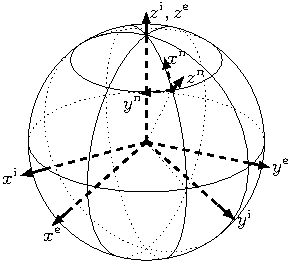
\includegraphics[scale = 1]{Coordinate systems.pdf}
    \caption{The $n$, $i$ and $e$ coordinate systems shown on the Earth.~\cite{Kok2017}}
\end{figure}

g is taken to be positive for the purposes of this paper.

The quaternion convention used is the Hamilton convention defined in~\cite{Sol2017}.

Axis angle is a parameterisation of \SO{3} which is defined as $[\m u\tran \ \phi]\tran$, where $\phi$ is the angle of rotation in radians and $\m u$ is a unit vector representing the axis of rotation.

\begin{figure}[h]
    \centering
    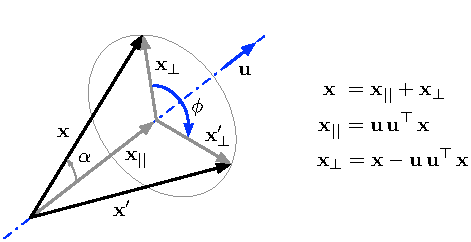
\includegraphics{rotation3d.pdf}
    \caption{The vector $\bf x$ rotated about $\bf u$ by $\phi$ gives vector $\bf x'$.\cite{Sol2017}}
\end{figure}

The skew symmetric matrix of a vector is defined as
\begin{align} \label{eq:crossProductMatrix}
    [\m{\omega}]_\times &\equiv \begin{bmatrix}
        0 & -\m{\omega}_z & \m{\omega}_y \\
        \m{\omega}_z & 0 & -\m{\omega}_x \\
        - \m{\omega}_y & \m{\omega}_x & 0
    \end{bmatrix}
\end{align}
\subsection{State Space}
\label{sec:StateSpace}

A state space representation is when a system is described using first order differential or difference equations. To express a continuous state space representation in matrix vector form the equations must be linear:
\begin{align}
    \dot{\m x}(t) &= \m A(t)\m x(t) + \m B(t) \m u(t) \\
    \m y(t) &= \m C(t)\m x(t) + \m D(t) \m u(t)
\end{align}
Most controllers require \gls{lti} systems which are described as such in a state space representation if described using differential equations:
\begin{align}
    \label{eq:ltistate}
    \dot{\m x}(t) &= \m A \m x(t) + \m B \m u(t) \\
    \label{eq:ltioutput}
    \m y(t) &= \m C \m x(t) + \m D \m u(t)
\end{align}
If the state space system is implemented on a digital system, if the actuators are discrete or difference equations are used the state space system may be described in a discrete representation.
The \gls{lti} discrete state space representation is expressed as such:
\begin{align}
    \m x_{k+1} &= \m A \m x_k + \m B \m u_k \\
    \m y_k &= \m C \m x_k + \m D \m u_k
\end{align}

To convert from a time varying state space representation to a time invariant representation, the representation at an operating point can be taken to hold for the entire range of values.
Typically, the equilibrium points are used as the system is likely to stabilize around that point~\cite{MITFEEDBACK}. This means the state will be close to the equilibrium point most of the time so the representation stays reasonably accurate. 
This has disadvantages, e.g. if the state deviates from the operating points for extended periods or for a short time if the plant is strongly non-linear the \gls{lti} representation will be inaccurate.

Many systems are non-linear, so to apply linear techniques such as \gls{lqr} non-linear models need to be linearised about operating points $\bar{\m x}, \bar{\m u}, \bar{\m y}$. 
We often wish to use linear techniques as they are simpler, linear control theory is more developed than non-linear control theory and control designers will have more knowledge about linear techniques.
Additionally, non-linear control techniques are typically only useful for certain non-linear systems whilst linear techniques can work for a wide range of systems.
A non-linear system expressed as:
\begin{align}
    \dot{\m x}(t) &= f(\m x(t), \m u(t), \bullet) \\
    \m y(t) &= g(\m x(t), \bullet)
\end{align}
Can be linearised as such~\cite{Bla2010}:
\begin{align}
    \tilde{\m x} &= \m x - \bar{\m x} \\
    \tilde{\m u} &= \m u - \bar{\m u} \\
    \tilde{\m y} &= \m y - \bar{\m y}
\end{align}
The taylor series expansion of $\dot{x}$ and $y$ are as follows:
\begin{align}
    \dot{\m x} &= f(\bar{\m x}, \bar{\m u}, \bar{\bullet}) + \frac{\partial f(\bar{\m x}, \bar{\m u}, \bar{\bullet})}{\partial \m x} \tilde{\m x} + \frac{\partial f(\bar{\m x}, \bar{\m u}, \bar{\bullet})}{\partial \m u} \tilde{\m u} \dots \\
    \m y &= g(\bar{\m y}, \bar{\bullet}) + \frac{\partial g(\bar{\m y}, \bar{\m u}, \bar{\bullet})}{\partial \m y} \tilde{\m y} + \frac{\partial g(\bar{\m y}, \bar{\bullet})}{\partial \m u} \tilde{\m u} \dots
\end{align}
To obtain a linear state system use only the first order terms.
\begin{align}
    \dot{\tilde{\m x}} &= \frac{\partial f(\bar{\m x}, \bar{\m u}, \bar{\bullet})}{\partial \m x} \tilde{\m x} + \frac{\partial f(\bar{\m x}, \bar{\m u}, \bar{\bullet})}{\partial \m u} \tilde{\m u} \\
    \tilde{\m y} &= \frac{\partial g(\bar{\m y}, \bar{\bullet})}{\partial \m y} \tilde{\m y} + \frac{\partial g(\bar{\m y}, \bar{\bullet})}{\partial \m u} \tilde{\m u}
\end{align}

In order to obtain better performance, gain scheduling can be used where multiple operating points are chosen to generate linear controllers.
Depending on the current state, controllers can be appropriately selected or interpolated between.

Time delays present in a system may be approximated using a padé approximation which may add additional states and so a state observer or estimator is also required.

A system is observable if the current state can be estimated using the output for all possible states and control vectors.
A state space system of the form \eqref{eq:ltistate}, \eqref{eq:ltioutput} is observable if the rank of $\m{\mathcal{O}}$ is the same as the number of state variables \cite{fri2005}.
\begin{align}
    \m{\mathcal{O}} = \begin{bmatrix}
        \m C \\
        \m C \m A \\
        \m C \m A^2 \\
        \vdots \\
        \m C \m A^{n-1}
    \end{bmatrix}
\end{align}

A system is controllable if any state can be achieved from any initial state in a finite time.
A state space system of the form \eqref{eq:ltistate}, \eqref{eq:ltioutput} is controllable if the rank of $\m \zeta$ is the same as the number of state variables \cite{fri2005}.
\begin{align}
    \m \zeta = \begin{bmatrix}
        \m B \\
        \m A \m B \\
        \m A^2 \m B \\
        \vdots \\
        \m A^{n-1} \m B
    \end{bmatrix}
\end{align}

A system can be controlled using \gls{lqr} or pole placement if the \gls{lti} state space representation is controllable.
Pole placement and \gls{lqr} are similar as they both set the eigenvalues of the system, which determines the system's dynamics and so stability. 
However, pole placement is given eigenvalues whilst \gls{lqr} determines the optimal eigenvalues and gain matrix, $\m K$, minimising the quadratic cost function, $J$, where $\m u = -\m K \m x$ and $\dot{ \m x } = (\m A - \m B \m K) \m x$~\cite{fri2005}.

The infinite-horizon, continuous-time \gls{lqr} defines the cost, $J$, as \begin{align}
    J = \int_{0}^{\infty} (\m x\tran \m Q \m x + \m u\tran \m R \m u + 2 \m x\tran \m N \m u) \,\mathrm{d}t.
\end{align}
The infinite-horizon, discrete-time \gls{lqr} defines the cost, $J$, as 
\begin{align}
    J = \sum_{k = 0}^{\infty} (\m x_k\tran \m Q \m x_k + \m u_k\tran \m R \m u_k + 2 \m x_k\tran \m N_k \m u).
\end{align}
$\m K$ can be found using the algebraic Riccati equation.

Additionally, more advanced controllers can be used that are designed for non-linear, time varying systems or that can account for constraints, such as iLQR or \gls{mpc}, can be designed using a state space model.
However, these are more computationally expensive than pole placement and \gls{lqr} and may be less robust.
%
\section{Dynamics}
\label{sec:Dynamics}

The dynamics of the rocket have to be derived in order to simulate the system (the rocket being controlled) so that the performance of each \gls{gnc} scheme can be compared. 
Additionally, the system dynamics are required to develop/ tune the \gls{gnc} schemes, which is where the simpler models will be used to deal with the limitation of different types of \gls{gnc} schemes.

A review of the dynamics used to model similar systems, such as quadcopters and other model rockets, revealed that the prominent differences between the different methods were: the reference frames and coordinate systems used; the rotation formalism used, commonly a choice between euler angles or quaternions; and the value of the aerodynamic coefficients.
Additionally, it shows that a common way to model a model rocket is to assume it is a rigid body, when the body does not deform under the action of applied forces, and to use 6DOF equations of motion.

The reference frames and coordinate systems used make no difference to the accuracy of the simulation and as such those which reduce the computational effort of the simulation and simplify the analysis of the model are being used.

It is shown in~\cite{Stu1964} that all three dimensional parameterisations of \SO{3} have singularities or discontinuities however, \glspl{mrp} have a singularity at $360\degree$ and so switching to the shortest rotation the singularity can be avoided.
Therefore the choice of rotation formalism used can affect the accuracy of the simulation if a singularity is encountered, which is present in the popular euler angle parameterisation.
Additionally, euler angles `are less accurate than quaternions when used to integrate incremental changes in \gls{attitude} over time'~\cite{Representing}.
Also, quaternions are more computationally efficient, which will be important when implemented on a microcontroller, and so will be used instead of euler angles even though they are arguably less intuitive.

There are many different methods to calculate aerodynamic coefficients, falling under three categories: \gls{cfd}; theoretical and empirical formulae; and wind tunnel testing.
The preliminary results obtained from SolidWorks Fluid Simulation were inaccurate as they did not fit with empirical data and so \gls{cfd} was deemed to be unsuitable for the calculation of aerodynamic coefficients.
Two common pieces of software used to calculate the aerodynamic coefficients using formulae are USAF Digital DATCOM and OpenRocket,~\cite{OR}.
A brief comparison of the coefficients produced by both software led me to believe that OpenRocket was more accurate as DATCOM used a linear relationship for the pitching moment coefficient, which would seem to be an oversimplification especially when compared to empirical data.
Also, OpenRocket's simulation was compared to empirical data from model rockets and was found to be reasonably accurate and its assumptions are mostly true for our case.
Wind tunnel testing was not available and so was not considered.
So OpenRocket will be used to calculate the aerodynamic coefficients which should be indicative of their real world performance allowing for comparison between different controllers.

The following dynamics are derived in the navigation frame and the earth is assumed to be flat.
\subsection{Actuator}

\begin{wrapfigure}{r}{0.4 \textwidth}
    \centering
    \includesvg[pretex=\tiny, width = 0.35 \textwidth]{Gimbaled_thrust_diagram}
    \caption{The gimbal rotates the thrust force in order to impart a torque and a horizontal force~\cite{NASATVC}.}
\end{wrapfigure}
%\begin{wrapfigure}{l}{0.1\textwidth}
%    \centering
%    \includesvg[width = 0.1 \textwidth]{RCS}
%    \caption{\cite{Kehl2015}}
%\end{wrapfigure}
There has been previous success~\cite{BPS} in controlling \gls{attitude} in model rockets using gimbaled thrust, where the thrust direction is controlled in order to impart moments and forces, and a reaction wheel, that will exert a moment about the roll axis.
Roll control is necessary because at high roll rates a corkscrew like flight will develop which could lead to instability, shown both in testing and in~\cite{Kehl2015}.
Also, high roll rates can lead to bad performance due to aerodynamics couplings~\cite{Dong2019}.
Additionally, roll control is desired to point the rocket in a certain direction, e.g. to deliver a payload.

Let $\m u(t)$ be the controller's output at time $t$, where $\m u(t) = \begin{bmatrix}
    u_x(t) & u_y(t) & u_z(t)
\end{bmatrix}\tran$.
The gimbal actuator lags by 0.07s and saturates at a $5 \degree$ angle, whilst the reaction wheel has a 0.01s lag time.
\begin{align}  \label{eq:Actuator1}
    \m f(t) &= \cotto\inv\begin{bmatrix}
        - u_y \big(\operatorname{round}(t - 0.07, 0.02)\big) \\
        u_x \big(\operatorname{round}(t - 0.07, 0.02)\big)
    \end{bmatrix}, 
    \intertext{where $\operatorname{round}(x, y)$ rounds $x$ to the nearest multiple of $y$}
    \label{eq:Actuator2}
    \aforce &= \begin{cases}
        \m f(t) & \norm{\m f(t)} \leq \mathrm{Thrust}(t) \sin(5 \degree) \\
        \mathrm{Thrust}(t) \sin(5 \degree) * \frac{\m f(t)}{\norm{\m f(t)}} & \text{otherwise.}
    \end{cases} \\ 
    \label{eq:Actuator3}
    \mathbf{Thrust}^b &= \begin{bmatrix} 
        \aforce \\
        \sqrt{\norm{\mathrm{Thrust}(t)}^2 - \norm{\aforce}^2}
    \end{bmatrix} \\
    \label{eq:Actuator4}
    \amom &= \begin{bmatrix}
        u_x \big(\operatorname{round}(t - 0.07, 0.02)\big) \\
        u_y \big(\operatorname{round}(t - 0.07, 0.02)\big) \\
        u_z(t - 0.01) 
    \end{bmatrix}
\end{align}
\newpage
\subsection{Translation}
%
\captionsetup[subfigure]{labelformat=empty}
\begin{figure}[h]
    \centering
    \begin{subfigure}[b]{0.6 \textwidth}
        The aerodynamic forces acting on the body are as follows, with $\mathbf{Rot}$ and the coefficients being defined in~\fullrefnocomma{subsec:Coefficients}.
        \begin{align}
            &\mathbf{AeroForces}^b = \frac{1}{2} \rho \norm{ \m v_\infty}^2 A_{ref} * \mathbf{Rot}
            \begin{bmatrix}
                -C_N \\
                -C_S \\
                -C_A
            \end{bmatrix}
            \intertext{The force is therefore the sum of the aerodynamic forces, the thrust force rotated by the \gls{tvc} gimbal and the weight force in the body coordinate system}
            &\m F^b = \mathbf{AeroForces}^b + \mathbf{Thrust}^b + \m R^{bn}
            \begin{bmatrix} 
                0 \\
                0 \\
                -mg
            \end{bmatrix} \\
            &[\m a^b]^{nn} = \frac{\m F_b}{m} \\
            &[\m a^n]^{nn} = \m R^{nb} [\m a^b]^{nn}
        \end{align}
    \end{subfigure}
    \hfill
    \begin{subfigure}[b]{0.35 \textwidth}
        \centering
        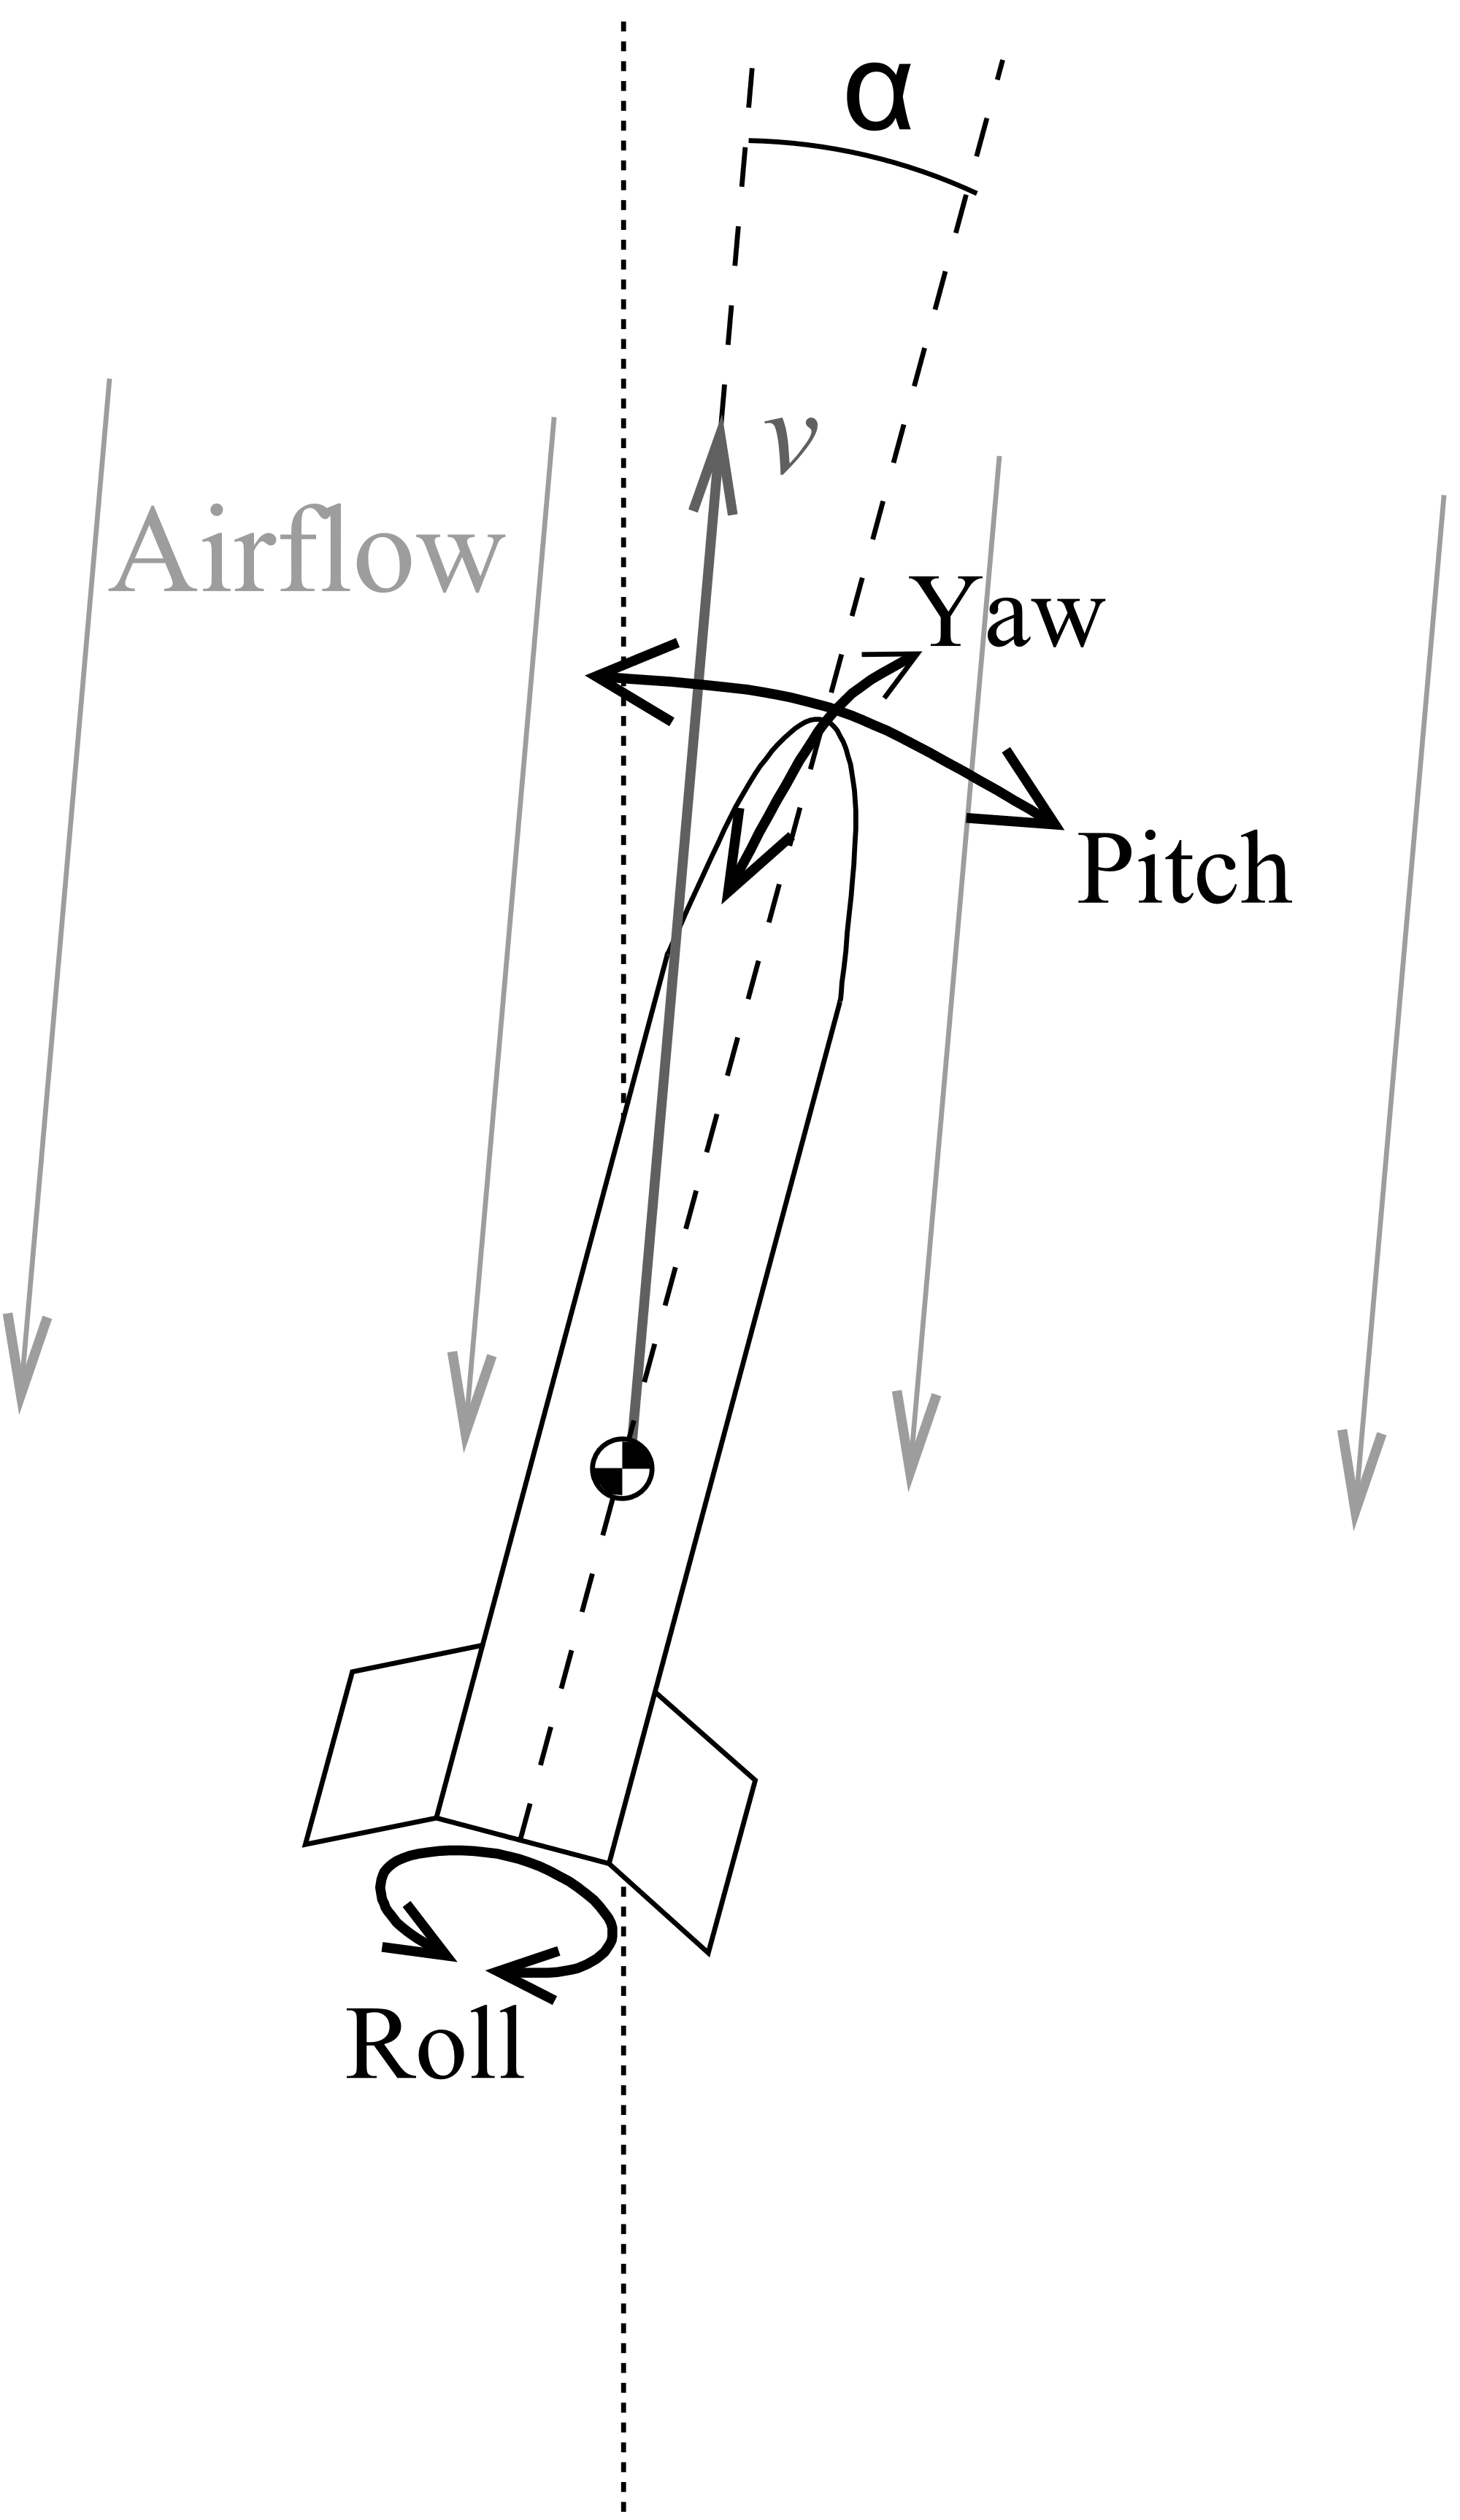
\includegraphics[scale = 0.06, trim={0 15cm 0 0},clip]{Rocket,pitch-yaw-roll}
        \caption{The pitch, yaw and roll directions in the $b$ frame.~\cite{OR}}
    \end{subfigure}
\end{figure}
%
\subsection{Attitude}
The aerodynamic moments acting on the body are as follows, with the coefficients again defined in~\fullrefnocomma{subsec:Coefficients}.
\begin{align}
    \mathbf{AeroMoments}^b &= \frac{1}{2} \rho \norm{\m v_\infty}^2 A_{ref} * d_{ref} * \mathbf{Rot} \begin{bmatrix}
    -C_y \\
    C_m \\
    C_l
    \end{bmatrix}
    \intertext{The net moment is the sum of the aerodynamic moments and the actuator moments from the \gls{tvc} gimbal and the reaction wheel}
    \m{\tau}^b &= \mathbf{AeroMoments}^b + \amom \\
    [\dot{\m \omega^b}]^{bn} &= (\m{I}^b)\inv ( \m{\tau}^b - [\m{\omega}^b]^{bn} \times \m{I}^b [\m{\omega}^b]^{bn} ) \\
    \dot{\q}^{nb} &= \frac{1}{2} \q^{nb}
    \begin{bmatrix}
        0 \\
        [\m{\omega}^b]^{bn}
    \end{bmatrix}
\end{align}
%
The dynamics derived in the section have been deemed to be sufficiently accurate and so indicative of real world performance, because the dynamics are similar to those found in existing literature where they have been shown to be accurate to the real world. This will allow for a fair comparison between different \gls{gnc} schemes and will show if \gls{vtvl} has been achieved.
%
\section{Models} \label{sec:Models}
%
In this section, different models of varying complexities will be proposed as applications, such as \gls{lqr}, require modifications of the model derived in the previous section,~\fullrefnocomma{sec:Dynamics}.
%
\subsection{First Model}
This is the most accurate model of the system which will be used in the simulation to evaluate the performance of a proposed \gls{gnc} scheme.
\begin{align}
    [\dot{\m \omega^b}]^{bn} &= (\m I^b)\inv ( \mathbf{AeroMoments} + \mathbf{Actuator\ Moments}(t) - [\m \omega^b]^{bn} \times \m I^b [\m \omega^b]^{bn} ) \\
    \label{eq:qdot}
    \dot{\q}^{bn} &=\frac{1}{2} \q^{bn}
    \begin{bmatrix}
        0 & [\m \omega^b]^{bn}
    \end{bmatrix}\tran \\
    [\dot{\m v}^n]^{nn} &= \m R^{nb} m\inv \left( \mathbf{AeroForces}^b + \mathbf{Thrust}^b \right) +
    \begin{bmatrix}
        0 & 0 & -g
    \end{bmatrix}\tran \\
    \label{eq:rdot}
    [\dot{\m r}^n]^n &= [\m v^n]^n 
\end{align}
%
\subsection{Second Model} 
\label{Position Model}
This model is for used for translational control using linear techniques such as \gls{lqr}.

As little translational control can be achieved in the z axis and it would be difficult to incorporate this into state space form, so the z axis is not included. 
Therefore, the weight force is omitted.
Additionally the quaternion error term, $\qv$ is used instead of $\q$. 
The choice of $\qv$ is explained in \fullref{subsec:ErrorTerms}.
\begin{align}
    \label{eq:alpha}
    [\dot{\m \omega^b}]^{bn} &= (\m I^b)\inv (\mathbf{Actuator\ Moments}(t) - [\m \omega^b]^{bn} \times \m I^b [\m \omega^b]^{bn} ) \\
    \label{eq:qdotv}
    \dot{\q}^{bn}_v &= \left( \frac{1}{2} \q^{bn}
    \begin{bmatrix}
        0 & [\m \omega^b]^{bn}
    \end{bmatrix}\tran\right)_v\\
    \label{eq:qintv}
    \frac{d}{dt} \int \q^{bn}_v &= \q^{bn}_v \\
    [\dot{\m v}^n_{x,y}]^{nn} &= \left( \m R^{nb} m\inv \mathbf{Thrust}^b \right)_{x,y}\\
    [\dot{\m r}^n_{x,y}]^n &= \m v^n_{x,y}
\end{align}
%
\subsection{Third Model} 
\label{Attitude Model}
This model is for used for \gls{attitude} control using linear techniques such as \gls{lqr} and is based on the previous model, \modelref{Position Model} so \crefrange{eq:alpha}{eq:qintv} are used.
%
\subsection{Fourth Model} 
\label{KF Model}
This model, in contrast to the \modelref{Position Model} includes the translation variables in the z axis and $\q_w$ so that it can be used to build a state estimator or observer.
Let the gyroscope bias be $\m \omega_b$ and the accelerometer bias $\m a_b$.

Using equations~\eqref{eq:qdot},~\eqref{eq:rdot},~\eqref{eq:alpha}
\begin{align}
    \dot{\m \omega^b}_b &= 0\\
    \dot{\m a}^b_b &= 0 \\
    [\dot{\m v}^n]^{nn} &= \m R^{nb} m\inv \mathbf{Thrust}^b + 
    \begin{bmatrix}
        0 & 0 & -g
    \end{bmatrix}\tran  \\
\end{align}
%
\subsection{Fifth Model} 
\label{Accurate Actuator}
Different actuator models are needed, e.g. for controllers which take into account the time delay in the actuator and those that don't. 

This model is the most accurate model of the system and will be used in the simulation to evaluate the performance of a proposed \gls{gnc} scheme.

\Crefrange{eq:Actuator1}{eq:Actuator4} describe this model.
%
\subsection{Sixth Model} 
\label{No Saturation Actuator}
This actuator model ignores the saturation and can be continuous or discrete with any sample time by appropriately modifying \eqref{eq:Actuator1} and \eqref{eq:Actuator4}.

This model is appropriate for controllers that cannot be tuned/ developed with models including saturation terms such as a \gls{lqr} or \gls{pid} controller.

Using equations~\eqref{eq:Actuator1},~\eqref{eq:Actuator3},~\eqref{eq:Actuator4} 
\begin{align}
    \label{eq:noSaturationActuator}
    \aforce &= \fm f(t)
\end{align}
%
\subsection{Seventh Model} 
\label{No Time Delay Actuator}
This actuator model additionally assumes that there is no time delay in the actuators compared to the~\modelrefnocomma{No Saturation Actuator}.

Using equations~\eqref{eq:noSaturationActuator} and~\eqref{eq:Actuator4}.
\begin{align}  
    \label{eq:ActuatorSimple1}
    \fm f(t) &= \cotto\inv\begin{bmatrix}
        - u_y(t) \\
         u_x(t)
    \end{bmatrix} \\
    \amom &= \m u(t)
\end{align}
%
\section{Guidance} 
\label{sec:Guidance}

Guidance refers to the generation of a trajectory in order to achieve a goal such as \gls{vtvl}, where a trajectory is useful in determining how to land safely.
This is necessary as without a trajectory the rocket would not know how to land safely or achieve any other goal and therefore would likely fail at achieving this goal.
There are existing guidance algorithms for \gls{vtvl} in rockets, such as GFOLD~\cite{Aci2007, Aci2013,Bla2010} or solutions to the moon soft landing problem, which generate an optimal trajectory to land a rocket whilst typically minimising fuel consumption.
However, these algorithms are unsuitable as a solid motor is going to be used so the fuel use is not a variable which can be optimised.
%
\subsection{Optimal Motor Ignition Time}

A novel algorithm is proposed, which can be used to determine an optimal motor ignition time that minimizes the impact velocity with the ground, ensuring the least damage to the rocket on landing, when a simple trajectory, which minimises horizontal velocity, is used.

During the powered portion of the flight, weight and thrust are taken to be the only forces acting on the rocket and thus the dynamics of the rocket are:
Let $x^n$ be the height of the rocket and $x^n = 0$ be when the rocket is touching the ground
\begin{align}
    [\ddot{x}^n]^{nn}(t) &= \mathrm{Thrust}(t - \gamma) m\inv -g \\
    t &\in \{a: 0 \leq a \leq b\} \text{ where } s(b) = 0
\end{align}

The optimisation problem to be solved is thus $\argmin\limits_\gamma \abs{[\dot{x}^n]^n(b)}$ subject to $b \geq \mathrm{burn\ time}$ (taken to be $3.45$), where the speed at which the rocket hits the ground is minimised with respect to $\gamma$ when the motor is expended.
When the rocket hits the ground before $\mathrm{burn\ time}$ the landing is considered a fail as the rocket's dynamics would be hard to model and could result in dangerous behaviour.
There are many different ways to solve this.

One method is to first sample $\abs{[\dot{x}^n]^n(b)}$ subject to $b \geq \mathrm{burn\ time}$ for a range of initial conditions, $[\dot{x}^n]^n(\gamma)$ and $x^n(\gamma)$. Then using nearest neighbour interpolation and extrapolation, as other methods such as linear, cubic, makima resulted in noisy data and curve fitting with polynomials and neural networks were not a close enough fit to the data, the optimisation problem can be solved for a range of initial conditions, $[\dot{x}^n]^n(0)$ and $x^n(0)$.

\setlength\fwidth{0.8\textwidth}
\setlength\fheight{0.4 \textheight}
\setlength\wwidth{0.7 \textwidth}
\setlength\wheight{0.3 \textheight}
%TC:ignore
%\begin{center}
%    % This file was created by matlab2tikz.
%
%The latest updates can be retrieved from
%  http://www.mathworks.com/matlabcentral/fileexchange/22022-matlab2tikz-matlab2tikz
%where you can also make suggestions and rate matlab2tikz.
%
\begin{tikzpicture}

\begin{axis}[%
width=0.951\fwidth,
height=\fheight,
at={(0\fwidth,0\fheight)},
scale only axis,
xmin=-100.00,
xmax=50.00,
tick align=outside,
xlabel style={font=\color{white!15!black}},
xlabel={Initial Velocity (m/s)},
ymin=0.00,
ymax=500.00,
ylabel style={font=\color{white!15!black}},
ylabel={Initial Height (m)},
zmin=0.00,
zmax=140.00,
zlabel style={font=\color{white!15!black}},
zlabel={Maximum Impact Velocity (m/s)},
view={70.45}{56.78},
axis background/.style={fill=white},
axis x line*=bottom,
axis y line*=left,
axis z line*=left,
xmajorgrids,
ymajorgrids,
zmajorgrids
]

\addplot3[%
surf,
shader=flat, z buffer=sort, colormap={mymap}{[1pt] rgb(0pt)=(0.2422,0.1504,0.6603); rgb(1pt)=(0.25039,0.164995,0.707614); rgb(2pt)=(0.257771,0.181781,0.751138); rgb(3pt)=(0.264729,0.197757,0.795214); rgb(4pt)=(0.270648,0.214676,0.836371); rgb(5pt)=(0.275114,0.234238,0.870986); rgb(6pt)=(0.2783,0.255871,0.899071); rgb(7pt)=(0.280333,0.278233,0.9221); rgb(8pt)=(0.281338,0.300595,0.941376); rgb(9pt)=(0.281014,0.322757,0.957886); rgb(10pt)=(0.279467,0.344671,0.971676); rgb(11pt)=(0.275971,0.366681,0.982905); rgb(12pt)=(0.269914,0.3892,0.9906); rgb(13pt)=(0.260243,0.412329,0.995157); rgb(14pt)=(0.244033,0.435833,0.998833); rgb(15pt)=(0.220643,0.460257,0.997286); rgb(16pt)=(0.196333,0.484719,0.989152); rgb(17pt)=(0.183405,0.507371,0.979795); rgb(18pt)=(0.178643,0.528857,0.968157); rgb(19pt)=(0.176438,0.549905,0.952019); rgb(20pt)=(0.168743,0.570262,0.935871); rgb(21pt)=(0.154,0.5902,0.9218); rgb(22pt)=(0.146029,0.609119,0.907857); rgb(23pt)=(0.138024,0.627629,0.89729); rgb(24pt)=(0.124814,0.645929,0.888343); rgb(25pt)=(0.111252,0.6635,0.876314); rgb(26pt)=(0.0952095,0.679829,0.859781); rgb(27pt)=(0.0688714,0.694771,0.839357); rgb(28pt)=(0.0296667,0.708167,0.816333); rgb(29pt)=(0.00357143,0.720267,0.7917); rgb(30pt)=(0.00665714,0.731214,0.766014); rgb(31pt)=(0.0433286,0.741095,0.73941); rgb(32pt)=(0.0963952,0.75,0.712038); rgb(33pt)=(0.140771,0.7584,0.684157); rgb(34pt)=(0.1717,0.766962,0.655443); rgb(35pt)=(0.193767,0.775767,0.6251); rgb(36pt)=(0.216086,0.7843,0.5923); rgb(37pt)=(0.246957,0.791795,0.556743); rgb(38pt)=(0.290614,0.79729,0.518829); rgb(39pt)=(0.340643,0.8008,0.478857); rgb(40pt)=(0.3909,0.802871,0.435448); rgb(41pt)=(0.445629,0.802419,0.390919); rgb(42pt)=(0.5044,0.7993,0.348); rgb(43pt)=(0.561562,0.794233,0.304481); rgb(44pt)=(0.617395,0.787619,0.261238); rgb(45pt)=(0.671986,0.779271,0.2227); rgb(46pt)=(0.7242,0.769843,0.191029); rgb(47pt)=(0.773833,0.759805,0.16461); rgb(48pt)=(0.820314,0.749814,0.153529); rgb(49pt)=(0.863433,0.7406,0.159633); rgb(50pt)=(0.903543,0.733029,0.177414); rgb(51pt)=(0.939257,0.728786,0.209957); rgb(52pt)=(0.972757,0.729771,0.239443); rgb(53pt)=(0.995648,0.743371,0.237148); rgb(54pt)=(0.996986,0.765857,0.219943); rgb(55pt)=(0.995205,0.789252,0.202762); rgb(56pt)=(0.9892,0.813567,0.188533); rgb(57pt)=(0.978629,0.838629,0.176557); rgb(58pt)=(0.967648,0.8639,0.16429); rgb(59pt)=(0.96101,0.889019,0.153676); rgb(60pt)=(0.959671,0.913457,0.142257); rgb(61pt)=(0.962795,0.937338,0.12651); rgb(62pt)=(0.969114,0.960629,0.106362); rgb(63pt)=(0.9769,0.9839,0.0805)}, mesh/rows=151]
table[row sep=crcr, point meta=\thisrow{c}] {%
%
x	y	z	c\\
50.00	1.00	88.40	88.40\\
50.00	2.00	88.53	88.53\\
50.00	3.00	88.64	88.64\\
50.00	4.00	88.75	88.75\\
50.00	5.00	88.86	88.86\\
50.00	6.00	88.97	88.97\\
50.00	7.00	89.08	89.08\\
50.00	8.00	89.19	89.19\\
50.00	9.00	89.30	89.30\\
50.00	10.00	89.41	89.41\\
50.00	11.00	89.52	89.52\\
50.00	12.00	89.63	89.63\\
50.00	13.00	89.74	89.74\\
50.00	14.00	89.85	89.85\\
50.00	15.00	89.96	89.96\\
50.00	16.00	90.07	90.07\\
50.00	17.00	90.18	90.18\\
50.00	18.00	90.28	90.28\\
50.00	19.00	90.39	90.39\\
50.00	20.00	90.47	90.47\\
50.00	21.00	90.60	90.60\\
50.00	22.00	90.72	90.72\\
50.00	23.00	90.83	90.83\\
50.00	24.00	90.93	90.93\\
50.00	25.00	91.04	91.04\\
50.00	26.00	91.15	91.15\\
50.00	27.00	91.25	91.25\\
50.00	28.00	91.36	91.36\\
50.00	29.00	91.47	91.47\\
50.00	30.00	91.58	91.58\\
50.00	31.00	91.68	91.68\\
50.00	32.00	91.79	91.79\\
50.00	33.00	91.89	91.89\\
50.00	34.00	92.01	92.01\\
50.00	35.00	92.11	92.11\\
50.00	36.00	92.22	92.22\\
50.00	37.00	92.33	92.33\\
50.00	38.00	92.43	92.43\\
50.00	39.00	92.54	92.54\\
50.00	40.00	92.64	92.64\\
50.00	41.00	92.75	92.75\\
50.00	42.00	92.85	92.85\\
50.00	43.00	92.96	92.96\\
50.00	44.00	93.06	93.06\\
50.00	45.00	93.17	93.17\\
50.00	46.00	93.27	93.27\\
50.00	47.00	93.38	93.38\\
50.00	48.00	93.48	93.48\\
50.00	49.00	93.59	93.59\\
50.00	50.00	93.70	93.70\\
50.00	51.00	93.77	93.77\\
50.00	52.00	93.90	93.90\\
50.00	53.00	93.98	93.98\\
50.00	54.00	94.11	94.11\\
50.00	55.00	94.22	94.22\\
50.00	56.00	94.33	94.33\\
50.00	57.00	94.43	94.43\\
50.00	58.00	94.53	94.53\\
50.00	59.00	94.63	94.63\\
50.00	60.00	94.74	94.74\\
50.00	61.00	94.84	94.84\\
50.00	62.00	94.95	94.95\\
50.00	63.00	95.05	95.05\\
50.00	64.00	95.15	95.15\\
50.00	65.00	95.25	95.25\\
50.00	66.00	95.35	95.35\\
50.00	67.00	95.46	95.46\\
50.00	68.00	95.56	95.56\\
50.00	69.00	95.66	95.66\\
50.00	70.00	95.76	95.76\\
50.00	71.00	95.87	95.87\\
50.00	72.00	95.96	95.96\\
50.00	73.00	96.07	96.07\\
50.00	74.00	96.17	96.17\\
50.00	75.00	96.27	96.27\\
50.00	76.00	96.37	96.37\\
50.00	77.00	96.48	96.48\\
50.00	78.00	96.58	96.58\\
50.00	79.00	96.68	96.68\\
50.00	80.00	96.78	96.78\\
50.00	81.00	96.89	96.89\\
50.00	82.00	96.98	96.98\\
50.00	83.00	97.09	97.09\\
50.00	84.00	97.19	97.19\\
50.00	85.00	97.29	97.29\\
50.00	86.00	97.39	97.39\\
50.00	87.00	97.49	97.49\\
50.00	88.00	97.59	97.59\\
50.00	89.00	97.67	97.67\\
50.00	90.00	97.79	97.79\\
50.00	91.00	97.89	97.89\\
50.00	92.00	97.99	97.99\\
50.00	93.00	98.09	98.09\\
50.00	94.00	98.19	98.19\\
50.00	95.00	98.29	98.29\\
50.00	96.00	98.39	98.39\\
50.00	97.00	98.49	98.49\\
50.00	98.00	98.59	98.59\\
50.00	99.00	98.69	98.69\\
50.00	100.00	98.79	98.79\\
50.00	101.00	98.89	98.89\\
50.00	102.00	98.99	98.99\\
50.00	103.00	99.09	99.09\\
50.00	104.00	99.18	99.18\\
50.00	105.00	99.28	99.28\\
50.00	106.00	99.39	99.39\\
50.00	107.00	99.48	99.48\\
50.00	108.00	99.58	99.58\\
50.00	109.00	99.68	99.68\\
50.00	110.00	99.78	99.78\\
50.00	111.00	99.86	99.86\\
50.00	112.00	99.97	99.97\\
50.00	113.00	100.07	100.07\\
50.00	114.00	100.17	100.17\\
50.00	115.00	100.27	100.27\\
50.00	116.00	100.36	100.36\\
50.00	117.00	100.46	100.46\\
50.00	118.00	100.56	100.56\\
50.00	119.00	100.66	100.66\\
50.00	120.00	100.76	100.76\\
50.00	121.00	100.85	100.85\\
50.00	122.00	100.95	100.95\\
50.00	123.00	101.04	101.04\\
50.00	124.00	101.15	101.15\\
50.00	125.00	101.24	101.24\\
50.00	126.00	101.34	101.34\\
50.00	127.00	101.44	101.44\\
50.00	128.00	101.53	101.53\\
50.00	129.00	101.63	101.63\\
50.00	130.00	101.72	101.72\\
50.00	131.00	101.82	101.82\\
50.00	132.00	101.91	101.91\\
50.00	133.00	102.01	102.01\\
50.00	134.00	102.11	102.11\\
50.00	135.00	102.18	102.18\\
50.00	136.00	102.30	102.30\\
50.00	137.00	102.39	102.39\\
50.00	138.00	102.50	102.50\\
50.00	139.00	102.59	102.59\\
50.00	140.00	102.68	102.68\\
50.00	141.00	102.78	102.78\\
50.00	142.00	102.87	102.87\\
50.00	143.00	102.96	102.96\\
50.00	144.00	103.07	103.07\\
50.00	145.00	103.16	103.16\\
50.00	146.00	103.25	103.25\\
50.00	147.00	103.35	103.35\\
50.00	148.00	103.45	103.45\\
50.00	149.00	103.54	103.54\\
50.00	150.00	103.63	103.63\\
50.00	151.00	103.73	103.73\\
50.00	152.00	103.83	103.83\\
50.00	153.00	103.92	103.92\\
50.00	154.00	104.01	104.01\\
50.00	155.00	104.11	104.11\\
50.00	156.00	104.20	104.20\\
50.00	157.00	104.30	104.30\\
50.00	158.00	104.39	104.39\\
50.00	159.00	104.48	104.48\\
50.00	160.00	104.58	104.58\\
50.00	161.00	104.67	104.67\\
50.00	162.00	104.74	104.74\\
50.00	163.00	104.86	104.86\\
50.00	164.00	104.95	104.95\\
50.00	165.00	105.04	105.04\\
50.00	166.00	105.13	105.13\\
50.00	167.00	105.23	105.23\\
50.00	168.00	105.32	105.32\\
50.00	169.00	105.41	105.41\\
50.00	170.00	105.51	105.51\\
50.00	171.00	105.61	105.61\\
50.00	172.00	105.69	105.69\\
50.00	173.00	105.79	105.79\\
50.00	174.00	105.88	105.88\\
50.00	175.00	105.97	105.97\\
50.00	176.00	106.06	106.06\\
50.00	177.00	106.16	106.16\\
50.00	178.00	106.25	106.25\\
50.00	179.00	106.34	106.34\\
50.00	180.00	106.44	106.44\\
50.00	181.00	106.53	106.53\\
50.00	182.00	106.62	106.62\\
50.00	183.00	106.70	106.70\\
50.00	184.00	106.80	106.80\\
50.00	185.00	106.90	106.90\\
50.00	186.00	106.98	106.98\\
50.00	187.00	107.08	107.08\\
50.00	188.00	107.16	107.16\\
50.00	189.00	107.26	107.26\\
50.00	190.00	107.35	107.35\\
50.00	191.00	107.42	107.42\\
50.00	192.00	107.53	107.53\\
50.00	193.00	107.62	107.62\\
50.00	194.00	107.72	107.72\\
50.00	195.00	107.81	107.81\\
50.00	196.00	107.90	107.90\\
50.00	197.00	107.99	107.99\\
50.00	198.00	108.08	108.08\\
50.00	199.00	108.17	108.17\\
50.00	200.00	108.26	108.26\\
50.00	201.00	108.35	108.35\\
50.00	202.00	108.44	108.44\\
50.00	203.00	108.53	108.53\\
50.00	204.00	108.62	108.62\\
50.00	205.00	108.72	108.72\\
50.00	206.00	108.80	108.80\\
50.00	207.00	108.89	108.89\\
50.00	208.00	108.98	108.98\\
50.00	209.00	109.07	109.07\\
50.00	210.00	109.16	109.16\\
50.00	211.00	109.25	109.25\\
50.00	212.00	109.35	109.35\\
50.00	213.00	109.44	109.44\\
50.00	214.00	109.52	109.52\\
50.00	215.00	109.61	109.61\\
50.00	216.00	109.70	109.70\\
50.00	217.00	109.79	109.79\\
50.00	218.00	109.88	109.88\\
50.00	219.00	109.97	109.97\\
50.00	220.00	110.06	110.06\\
50.00	221.00	110.15	110.15\\
50.00	222.00	110.24	110.24\\
50.00	223.00	110.33	110.33\\
50.00	224.00	110.41	110.41\\
50.00	225.00	110.51	110.51\\
50.00	226.00	110.59	110.59\\
50.00	227.00	110.68	110.68\\
50.00	228.00	110.77	110.77\\
50.00	229.00	110.85	110.85\\
50.00	230.00	110.95	110.95\\
50.00	231.00	111.03	111.03\\
50.00	232.00	111.12	111.12\\
50.00	233.00	111.21	111.21\\
50.00	234.00	111.30	111.30\\
50.00	235.00	111.39	111.39\\
50.00	236.00	111.48	111.48\\
50.00	237.00	111.56	111.56\\
50.00	238.00	111.65	111.65\\
50.00	239.00	111.74	111.74\\
50.00	240.00	111.83	111.83\\
50.00	241.00	111.91	111.91\\
50.00	242.00	112.00	112.00\\
50.00	243.00	112.09	112.09\\
50.00	244.00	112.18	112.18\\
50.00	245.00	112.26	112.26\\
50.00	246.00	112.35	112.35\\
50.00	247.00	112.44	112.44\\
50.00	248.00	112.53	112.53\\
50.00	249.00	112.61	112.61\\
50.00	250.00	112.69	112.69\\
50.00	251.00	112.79	112.79\\
50.00	252.00	112.88	112.88\\
50.00	253.00	112.96	112.96\\
50.00	254.00	113.05	113.05\\
50.00	255.00	113.13	113.13\\
50.00	256.00	113.22	113.22\\
50.00	257.00	113.31	113.31\\
50.00	258.00	113.39	113.39\\
50.00	259.00	113.48	113.48\\
50.00	260.00	113.57	113.57\\
50.00	261.00	113.65	113.65\\
50.00	262.00	113.74	113.74\\
50.00	263.00	113.82	113.82\\
50.00	264.00	113.91	113.91\\
50.00	265.00	114.00	114.00\\
50.00	266.00	114.08	114.08\\
50.00	267.00	114.17	114.17\\
50.00	268.00	114.25	114.25\\
50.00	269.00	114.34	114.34\\
50.00	270.00	114.43	114.43\\
50.00	271.00	114.51	114.51\\
50.00	272.00	114.60	114.60\\
50.00	273.00	114.68	114.68\\
50.00	274.00	114.77	114.77\\
50.00	275.00	114.85	114.85\\
50.00	276.00	114.94	114.94\\
50.00	277.00	115.02	115.02\\
50.00	278.00	115.11	115.11\\
50.00	279.00	115.19	115.19\\
50.00	280.00	115.28	115.28\\
50.00	281.00	115.36	115.36\\
50.00	282.00	115.45	115.45\\
50.00	283.00	115.53	115.53\\
50.00	284.00	115.62	115.62\\
50.00	285.00	115.70	115.70\\
50.00	286.00	115.79	115.79\\
50.00	287.00	115.87	115.87\\
50.00	288.00	115.96	115.96\\
50.00	289.00	116.04	116.04\\
50.00	290.00	116.13	116.13\\
50.00	291.00	116.21	116.21\\
50.00	292.00	116.30	116.30\\
50.00	293.00	116.38	116.38\\
50.00	294.00	116.46	116.46\\
50.00	295.00	116.55	116.55\\
50.00	296.00	116.63	116.63\\
50.00	297.00	116.72	116.72\\
50.00	298.00	116.80	116.80\\
50.00	299.00	116.88	116.88\\
50.00	300.00	116.97	116.97\\
50.00	301.00	117.05	117.05\\
50.00	302.00	117.14	117.14\\
50.00	303.00	117.22	117.22\\
50.00	304.00	117.30	117.30\\
50.00	305.00	117.39	117.39\\
50.00	306.00	117.47	117.47\\
50.00	307.00	117.55	117.55\\
50.00	308.00	117.64	117.64\\
50.00	309.00	117.72	117.72\\
50.00	310.00	117.80	117.80\\
50.00	311.00	117.89	117.89\\
50.00	312.00	117.97	117.97\\
50.00	313.00	118.05	118.05\\
50.00	314.00	118.14	118.14\\
50.00	315.00	118.22	118.22\\
50.00	316.00	118.30	118.30\\
50.00	317.00	118.39	118.39\\
50.00	318.00	118.47	118.47\\
50.00	319.00	118.55	118.55\\
50.00	320.00	118.63	118.63\\
50.00	321.00	118.72	118.72\\
50.00	322.00	118.80	118.80\\
50.00	323.00	118.88	118.88\\
50.00	324.00	118.96	118.96\\
50.00	325.00	119.05	119.05\\
50.00	326.00	119.13	119.13\\
50.00	327.00	119.21	119.21\\
50.00	328.00	119.29	119.29\\
50.00	329.00	119.38	119.38\\
50.00	330.00	119.46	119.46\\
50.00	331.00	119.54	119.54\\
50.00	332.00	119.62	119.62\\
50.00	333.00	119.70	119.70\\
50.00	334.00	119.79	119.79\\
50.00	335.00	119.87	119.87\\
50.00	336.00	119.95	119.95\\
50.00	337.00	120.03	120.03\\
50.00	338.00	120.11	120.11\\
50.00	339.00	120.19	120.19\\
50.00	340.00	120.28	120.28\\
50.00	341.00	120.36	120.36\\
50.00	342.00	120.44	120.44\\
50.00	343.00	120.52	120.52\\
50.00	344.00	120.60	120.60\\
50.00	345.00	120.68	120.68\\
50.00	346.00	120.76	120.76\\
50.00	347.00	120.84	120.84\\
50.00	348.00	120.93	120.93\\
50.00	349.00	121.01	121.01\\
50.00	350.00	121.09	121.09\\
50.00	351.00	121.17	121.17\\
50.00	352.00	121.25	121.25\\
50.00	353.00	121.33	121.33\\
50.00	354.00	121.41	121.41\\
50.00	355.00	121.49	121.49\\
50.00	356.00	121.57	121.57\\
50.00	357.00	121.65	121.65\\
50.00	358.00	121.73	121.73\\
50.00	359.00	121.81	121.81\\
50.00	360.00	121.90	121.90\\
50.00	361.00	121.98	121.98\\
50.00	362.00	122.06	122.06\\
50.00	363.00	122.14	122.14\\
50.00	364.00	122.22	122.22\\
50.00	365.00	122.30	122.30\\
50.00	366.00	122.38	122.38\\
50.00	367.00	122.46	122.46\\
50.00	368.00	122.54	122.54\\
50.00	369.00	122.62	122.62\\
50.00	370.00	122.70	122.70\\
50.00	371.00	122.78	122.78\\
50.00	372.00	122.86	122.86\\
50.00	373.00	122.94	122.94\\
50.00	374.00	123.02	123.02\\
50.00	375.00	123.10	123.10\\
50.00	376.00	123.18	123.18\\
50.00	377.00	123.26	123.26\\
50.00	378.00	123.33	123.33\\
50.00	379.00	123.41	123.41\\
50.00	380.00	123.49	123.49\\
50.00	381.00	123.57	123.57\\
50.00	382.00	123.65	123.65\\
50.00	383.00	123.73	123.73\\
50.00	384.00	123.81	123.81\\
50.00	385.00	123.89	123.89\\
50.00	386.00	123.97	123.97\\
50.00	387.00	124.05	124.05\\
50.00	388.00	124.13	124.13\\
50.00	389.00	124.21	124.21\\
50.00	390.00	124.29	124.29\\
50.00	391.00	124.36	124.36\\
50.00	392.00	124.44	124.44\\
50.00	393.00	124.52	124.52\\
50.00	394.00	124.60	124.60\\
50.00	395.00	124.68	124.68\\
50.00	396.00	124.76	124.76\\
50.00	397.00	124.84	124.84\\
50.00	398.00	124.92	124.92\\
50.00	399.00	124.99	124.99\\
50.00	400.00	125.07	125.07\\
50.00	401.00	125.15	125.15\\
50.00	402.00	125.23	125.23\\
50.00	403.00	125.31	125.31\\
50.00	404.00	125.39	125.39\\
50.00	405.00	125.46	125.46\\
50.00	406.00	125.54	125.54\\
50.00	407.00	125.62	125.62\\
50.00	408.00	125.70	125.70\\
50.00	409.00	125.78	125.78\\
50.00	410.00	125.85	125.85\\
50.00	411.00	125.93	125.93\\
50.00	412.00	126.01	126.01\\
50.00	413.00	126.09	126.09\\
50.00	414.00	126.16	126.16\\
50.00	415.00	126.24	126.24\\
50.00	416.00	126.32	126.32\\
50.00	417.00	126.40	126.40\\
50.00	418.00	126.48	126.48\\
50.00	419.00	126.55	126.55\\
50.00	420.00	126.63	126.63\\
50.00	421.00	126.71	126.71\\
50.00	422.00	126.79	126.79\\
50.00	423.00	126.86	126.86\\
50.00	424.00	126.94	126.94\\
50.00	425.00	127.02	127.02\\
50.00	426.00	127.09	127.09\\
50.00	427.00	127.17	127.17\\
50.00	428.00	127.25	127.25\\
50.00	429.00	127.33	127.33\\
50.00	430.00	127.40	127.40\\
50.00	431.00	127.48	127.48\\
50.00	432.00	127.56	127.56\\
50.00	433.00	127.63	127.63\\
50.00	434.00	127.71	127.71\\
50.00	435.00	127.79	127.79\\
50.00	436.00	127.86	127.86\\
50.00	437.00	127.94	127.94\\
50.00	438.00	128.02	128.02\\
50.00	439.00	128.09	128.09\\
50.00	440.00	128.17	128.17\\
50.00	441.00	128.25	128.25\\
50.00	442.00	128.32	128.32\\
50.00	443.00	128.40	128.40\\
50.00	444.00	128.48	128.48\\
50.00	445.00	128.55	128.55\\
50.00	446.00	128.63	128.63\\
50.00	447.00	128.70	128.70\\
50.00	448.00	128.78	128.78\\
50.00	449.00	128.86	128.86\\
50.00	450.00	128.93	128.93\\
50.00	451.00	129.01	129.01\\
50.00	452.00	129.08	129.08\\
50.00	453.00	129.16	129.16\\
50.00	454.00	129.24	129.24\\
50.00	455.00	129.31	129.31\\
50.00	456.00	129.39	129.39\\
50.00	457.00	129.46	129.46\\
50.00	458.00	129.54	129.54\\
50.00	459.00	129.62	129.62\\
50.00	460.00	129.69	129.69\\
50.00	461.00	129.77	129.77\\
50.00	462.00	129.84	129.84\\
50.00	463.00	129.92	129.92\\
50.00	464.00	129.99	129.99\\
50.00	465.00	130.07	130.07\\
50.00	466.00	130.14	130.14\\
50.00	467.00	130.22	130.22\\
50.00	468.00	130.29	130.29\\
50.00	469.00	130.37	130.37\\
50.00	470.00	130.45	130.45\\
50.00	471.00	130.52	130.52\\
50.00	472.00	130.60	130.60\\
50.00	473.00	130.67	130.67\\
50.00	474.00	130.75	130.75\\
50.00	475.00	130.82	130.82\\
50.00	476.00	130.90	130.90\\
50.00	477.00	130.97	130.97\\
50.00	478.00	131.05	131.05\\
50.00	479.00	131.12	131.12\\
50.00	480.00	131.19	131.19\\
50.00	481.00	131.27	131.27\\
50.00	482.00	131.34	131.34\\
50.00	483.00	131.42	131.42\\
50.00	484.00	131.49	131.49\\
50.00	485.00	131.57	131.57\\
50.00	486.00	131.64	131.64\\
50.00	487.00	131.72	131.72\\
50.00	488.00	131.79	131.79\\
50.00	489.00	131.87	131.87\\
50.00	490.00	131.94	131.94\\
50.00	491.00	132.01	132.01\\
50.00	492.00	132.09	132.09\\
50.00	493.00	132.16	132.16\\
50.00	494.00	132.24	132.24\\
50.00	495.00	132.31	132.31\\
50.00	496.00	132.39	132.39\\
50.00	497.00	132.46	132.46\\
50.00	498.00	132.53	132.53\\
50.00	499.00	132.61	132.61\\
50.00	500.00	132.68	132.68\\
49.00	1.00	87.32	87.32\\
49.00	2.00	87.43	87.43\\
49.00	3.00	87.54	87.54\\
49.00	4.00	87.66	87.66\\
49.00	5.00	87.77	87.77\\
49.00	6.00	87.88	87.88\\
49.00	7.00	88.00	88.00\\
49.00	8.00	88.11	88.11\\
49.00	9.00	88.22	88.22\\
49.00	10.00	88.33	88.33\\
49.00	11.00	88.44	88.44\\
49.00	12.00	88.55	88.55\\
49.00	13.00	88.66	88.66\\
49.00	14.00	88.77	88.77\\
49.00	15.00	88.88	88.88\\
49.00	16.00	88.99	88.99\\
49.00	17.00	89.06	89.06\\
49.00	18.00	89.21	89.21\\
49.00	19.00	89.32	89.32\\
49.00	20.00	89.43	89.43\\
49.00	21.00	89.54	89.54\\
49.00	22.00	89.65	89.65\\
49.00	23.00	89.76	89.76\\
49.00	24.00	89.87	89.87\\
49.00	25.00	89.99	89.99\\
49.00	26.00	90.09	90.09\\
49.00	27.00	90.19	90.19\\
49.00	28.00	90.30	90.30\\
49.00	29.00	90.41	90.41\\
49.00	30.00	90.52	90.52\\
49.00	31.00	90.63	90.63\\
49.00	32.00	90.73	90.73\\
49.00	33.00	90.85	90.85\\
49.00	34.00	90.95	90.95\\
49.00	35.00	91.06	91.06\\
49.00	36.00	91.17	91.17\\
49.00	37.00	91.27	91.27\\
49.00	38.00	91.38	91.38\\
49.00	39.00	91.49	91.49\\
49.00	40.00	91.60	91.60\\
49.00	41.00	91.71	91.71\\
49.00	42.00	91.81	91.81\\
49.00	43.00	91.89	91.89\\
49.00	44.00	92.02	92.02\\
49.00	45.00	92.13	92.13\\
49.00	46.00	92.24	92.24\\
49.00	47.00	92.35	92.35\\
49.00	48.00	92.45	92.45\\
49.00	49.00	92.56	92.56\\
49.00	50.00	92.66	92.66\\
49.00	51.00	92.77	92.77\\
49.00	52.00	92.87	92.87\\
49.00	53.00	92.98	92.98\\
49.00	54.00	93.09	93.09\\
49.00	55.00	93.19	93.19\\
49.00	56.00	93.28	93.28\\
49.00	57.00	93.40	93.40\\
49.00	58.00	93.50	93.50\\
49.00	59.00	93.61	93.61\\
49.00	60.00	93.72	93.72\\
49.00	61.00	93.82	93.82\\
49.00	62.00	93.93	93.93\\
49.00	63.00	94.04	94.04\\
49.00	64.00	94.14	94.14\\
49.00	65.00	94.24	94.24\\
49.00	66.00	94.34	94.34\\
49.00	67.00	94.45	94.45\\
49.00	68.00	94.55	94.55\\
49.00	69.00	94.66	94.66\\
49.00	70.00	94.73	94.73\\
49.00	71.00	94.86	94.86\\
49.00	72.00	94.96	94.96\\
49.00	73.00	95.07	95.07\\
49.00	74.00	95.18	95.18\\
49.00	75.00	95.27	95.27\\
49.00	76.00	95.37	95.37\\
49.00	77.00	95.47	95.47\\
49.00	78.00	95.59	95.59\\
49.00	79.00	95.68	95.68\\
49.00	80.00	95.78	95.78\\
49.00	81.00	95.89	95.89\\
49.00	82.00	95.99	95.99\\
49.00	83.00	96.09	96.09\\
49.00	84.00	96.18	96.18\\
49.00	85.00	96.30	96.30\\
49.00	86.00	96.40	96.40\\
49.00	87.00	96.51	96.51\\
49.00	88.00	96.60	96.60\\
49.00	89.00	96.70	96.70\\
49.00	90.00	96.80	96.80\\
49.00	91.00	96.90	96.90\\
49.00	92.00	97.01	97.01\\
49.00	93.00	97.10	97.10\\
49.00	94.00	97.21	97.21\\
49.00	95.00	97.31	97.31\\
49.00	96.00	97.41	97.41\\
49.00	97.00	97.51	97.51\\
49.00	98.00	97.61	97.61\\
49.00	99.00	97.71	97.71\\
49.00	100.00	97.81	97.81\\
49.00	101.00	97.91	97.91\\
49.00	102.00	98.01	98.01\\
49.00	103.00	98.11	98.11\\
49.00	104.00	98.21	98.21\\
49.00	105.00	98.31	98.31\\
49.00	106.00	98.40	98.40\\
49.00	107.00	98.51	98.51\\
49.00	108.00	98.61	98.61\\
49.00	109.00	98.71	98.71\\
49.00	110.00	98.80	98.80\\
49.00	111.00	98.91	98.91\\
49.00	112.00	99.01	99.01\\
49.00	113.00	99.11	99.11\\
49.00	114.00	99.18	99.18\\
49.00	115.00	99.31	99.31\\
49.00	116.00	99.40	99.40\\
49.00	117.00	99.50	99.50\\
49.00	118.00	99.59	99.59\\
49.00	119.00	99.70	99.70\\
49.00	120.00	99.80	99.80\\
49.00	121.00	99.90	99.90\\
49.00	122.00	100.00	100.00\\
49.00	123.00	100.09	100.09\\
49.00	124.00	100.18	100.18\\
49.00	125.00	100.28	100.28\\
49.00	126.00	100.38	100.38\\
49.00	127.00	100.48	100.48\\
49.00	128.00	100.58	100.58\\
49.00	129.00	100.64	100.64\\
49.00	130.00	100.78	100.78\\
49.00	131.00	100.87	100.87\\
49.00	132.00	100.97	100.97\\
49.00	133.00	101.06	101.06\\
49.00	134.00	101.17	101.17\\
49.00	135.00	101.26	101.26\\
49.00	136.00	101.36	101.36\\
49.00	137.00	101.45	101.45\\
49.00	138.00	101.55	101.55\\
49.00	139.00	101.65	101.65\\
49.00	140.00	101.74	101.74\\
49.00	141.00	101.84	101.84\\
49.00	142.00	101.93	101.93\\
49.00	143.00	102.04	102.04\\
49.00	144.00	102.13	102.13\\
49.00	145.00	102.22	102.22\\
49.00	146.00	102.32	102.32\\
49.00	147.00	102.39	102.39\\
49.00	148.00	102.51	102.51\\
49.00	149.00	102.61	102.61\\
49.00	150.00	102.70	102.70\\
49.00	151.00	102.80	102.80\\
49.00	152.00	102.89	102.89\\
49.00	153.00	102.99	102.99\\
49.00	154.00	103.08	103.08\\
49.00	155.00	103.18	103.18\\
49.00	156.00	103.27	103.27\\
49.00	157.00	103.36	103.36\\
49.00	158.00	103.46	103.46\\
49.00	159.00	103.56	103.56\\
49.00	160.00	103.66	103.66\\
49.00	161.00	103.74	103.74\\
49.00	162.00	103.84	103.84\\
49.00	163.00	103.94	103.94\\
49.00	164.00	104.03	104.03\\
49.00	165.00	104.13	104.13\\
49.00	166.00	104.22	104.22\\
49.00	167.00	104.31	104.31\\
49.00	168.00	104.41	104.41\\
49.00	169.00	104.51	104.51\\
49.00	170.00	104.60	104.60\\
49.00	171.00	104.69	104.69\\
49.00	172.00	104.78	104.78\\
49.00	173.00	104.87	104.87\\
49.00	174.00	104.97	104.97\\
49.00	175.00	105.06	105.06\\
49.00	176.00	105.15	105.15\\
49.00	177.00	105.25	105.25\\
49.00	178.00	105.34	105.34\\
49.00	179.00	105.44	105.44\\
49.00	180.00	105.53	105.53\\
49.00	181.00	105.62	105.62\\
49.00	182.00	105.72	105.72\\
49.00	183.00	105.80	105.80\\
49.00	184.00	105.90	105.90\\
49.00	185.00	105.99	105.99\\
49.00	186.00	106.09	106.09\\
49.00	187.00	106.18	106.18\\
49.00	188.00	106.27	106.27\\
49.00	189.00	106.36	106.36\\
49.00	190.00	106.45	106.45\\
49.00	191.00	106.55	106.55\\
49.00	192.00	106.64	106.64\\
49.00	193.00	106.73	106.73\\
49.00	194.00	106.82	106.82\\
49.00	195.00	106.91	106.91\\
49.00	196.00	107.00	107.00\\
49.00	197.00	107.09	107.09\\
49.00	198.00	107.20	107.20\\
49.00	199.00	107.28	107.28\\
49.00	200.00	107.37	107.37\\
49.00	201.00	107.46	107.46\\
49.00	202.00	107.55	107.55\\
49.00	203.00	107.64	107.64\\
49.00	204.00	107.73	107.73\\
49.00	205.00	107.83	107.83\\
49.00	206.00	107.92	107.92\\
49.00	207.00	108.01	108.01\\
49.00	208.00	108.10	108.10\\
49.00	209.00	108.19	108.19\\
49.00	210.00	108.28	108.28\\
49.00	211.00	108.37	108.37\\
49.00	212.00	108.46	108.46\\
49.00	213.00	108.55	108.55\\
49.00	214.00	108.64	108.64\\
49.00	215.00	108.73	108.73\\
49.00	216.00	108.82	108.82\\
49.00	217.00	108.92	108.92\\
49.00	218.00	109.00	109.00\\
49.00	219.00	109.10	109.10\\
49.00	220.00	109.18	109.18\\
49.00	221.00	109.27	109.27\\
49.00	222.00	109.36	109.36\\
49.00	223.00	109.41	109.41\\
49.00	224.00	109.53	109.53\\
49.00	225.00	109.63	109.63\\
49.00	226.00	109.72	109.72\\
49.00	227.00	109.79	109.79\\
49.00	228.00	109.90	109.90\\
49.00	229.00	109.99	109.99\\
49.00	230.00	110.08	110.08\\
49.00	231.00	110.17	110.17\\
49.00	232.00	110.25	110.25\\
49.00	233.00	110.35	110.35\\
49.00	234.00	110.43	110.43\\
49.00	235.00	110.52	110.52\\
49.00	236.00	110.61	110.61\\
49.00	237.00	110.69	110.69\\
49.00	238.00	110.79	110.79\\
49.00	239.00	110.88	110.88\\
49.00	240.00	110.96	110.96\\
49.00	241.00	111.05	111.05\\
49.00	242.00	111.14	111.14\\
49.00	243.00	111.23	111.23\\
49.00	244.00	111.32	111.32\\
49.00	245.00	111.40	111.40\\
49.00	246.00	111.49	111.49\\
49.00	247.00	111.58	111.58\\
49.00	248.00	111.67	111.67\\
49.00	249.00	111.76	111.76\\
49.00	250.00	111.84	111.84\\
49.00	251.00	111.93	111.93\\
49.00	252.00	112.02	112.02\\
49.00	253.00	112.11	112.11\\
49.00	254.00	112.19	112.19\\
49.00	255.00	112.28	112.28\\
49.00	256.00	112.37	112.37\\
49.00	257.00	112.46	112.46\\
49.00	258.00	112.54	112.54\\
49.00	259.00	112.63	112.63\\
49.00	260.00	112.72	112.72\\
49.00	261.00	112.80	112.80\\
49.00	262.00	112.89	112.89\\
49.00	263.00	112.98	112.98\\
49.00	264.00	113.06	113.06\\
49.00	265.00	113.15	113.15\\
49.00	266.00	113.24	113.24\\
49.00	267.00	113.32	113.32\\
49.00	268.00	113.41	113.41\\
49.00	269.00	113.50	113.50\\
49.00	270.00	113.58	113.58\\
49.00	271.00	113.67	113.67\\
49.00	272.00	113.76	113.76\\
49.00	273.00	113.84	113.84\\
49.00	274.00	113.93	113.93\\
49.00	275.00	114.01	114.01\\
49.00	276.00	114.10	114.10\\
49.00	277.00	114.19	114.19\\
49.00	278.00	114.27	114.27\\
49.00	279.00	114.36	114.36\\
49.00	280.00	114.44	114.44\\
49.00	281.00	114.53	114.53\\
49.00	282.00	114.61	114.61\\
49.00	283.00	114.70	114.70\\
49.00	284.00	114.79	114.79\\
49.00	285.00	114.87	114.87\\
49.00	286.00	114.96	114.96\\
49.00	287.00	115.04	115.04\\
49.00	288.00	115.13	115.13\\
49.00	289.00	115.21	115.21\\
49.00	290.00	115.30	115.30\\
49.00	291.00	115.38	115.38\\
49.00	292.00	115.47	115.47\\
49.00	293.00	115.55	115.55\\
49.00	294.00	115.64	115.64\\
49.00	295.00	115.72	115.72\\
49.00	296.00	115.81	115.81\\
49.00	297.00	115.89	115.89\\
49.00	298.00	115.98	115.98\\
49.00	299.00	116.06	116.06\\
49.00	300.00	116.14	116.14\\
49.00	301.00	116.23	116.23\\
49.00	302.00	116.31	116.31\\
49.00	303.00	116.40	116.40\\
49.00	304.00	116.48	116.48\\
49.00	305.00	116.57	116.57\\
49.00	306.00	116.65	116.65\\
49.00	307.00	116.73	116.73\\
49.00	308.00	116.82	116.82\\
49.00	309.00	116.90	116.90\\
49.00	310.00	116.99	116.99\\
49.00	311.00	117.07	117.07\\
49.00	312.00	117.15	117.15\\
49.00	313.00	117.24	117.24\\
49.00	314.00	117.32	117.32\\
49.00	315.00	117.40	117.40\\
49.00	316.00	117.49	117.49\\
49.00	317.00	117.57	117.57\\
49.00	318.00	117.65	117.65\\
49.00	319.00	117.74	117.74\\
49.00	320.00	117.82	117.82\\
49.00	321.00	117.90	117.90\\
49.00	322.00	117.99	117.99\\
49.00	323.00	118.07	118.07\\
49.00	324.00	118.15	118.15\\
49.00	325.00	118.24	118.24\\
49.00	326.00	118.32	118.32\\
49.00	327.00	118.40	118.40\\
49.00	328.00	118.49	118.49\\
49.00	329.00	118.57	118.57\\
49.00	330.00	118.65	118.65\\
49.00	331.00	118.73	118.73\\
49.00	332.00	118.82	118.82\\
49.00	333.00	118.90	118.90\\
49.00	334.00	118.98	118.98\\
49.00	335.00	119.06	119.06\\
49.00	336.00	119.15	119.15\\
49.00	337.00	119.23	119.23\\
49.00	338.00	119.31	119.31\\
49.00	339.00	119.39	119.39\\
49.00	340.00	119.47	119.47\\
49.00	341.00	119.56	119.56\\
49.00	342.00	119.64	119.64\\
49.00	343.00	119.72	119.72\\
49.00	344.00	119.80	119.80\\
49.00	345.00	119.88	119.88\\
49.00	346.00	119.97	119.97\\
49.00	347.00	120.05	120.05\\
49.00	348.00	120.13	120.13\\
49.00	349.00	120.21	120.21\\
49.00	350.00	120.29	120.29\\
49.00	351.00	120.37	120.37\\
49.00	352.00	120.46	120.46\\
49.00	353.00	120.54	120.54\\
49.00	354.00	120.62	120.62\\
49.00	355.00	120.70	120.70\\
49.00	356.00	120.78	120.78\\
49.00	357.00	120.86	120.86\\
49.00	358.00	120.94	120.94\\
49.00	359.00	121.02	121.02\\
49.00	360.00	121.10	121.10\\
49.00	361.00	121.19	121.19\\
49.00	362.00	121.27	121.27\\
49.00	363.00	121.35	121.35\\
49.00	364.00	121.43	121.43\\
49.00	365.00	121.51	121.51\\
49.00	366.00	121.59	121.59\\
49.00	367.00	121.67	121.67\\
49.00	368.00	121.75	121.75\\
49.00	369.00	121.83	121.83\\
49.00	370.00	121.91	121.91\\
49.00	371.00	121.99	121.99\\
49.00	372.00	122.07	122.07\\
49.00	373.00	122.15	122.15\\
49.00	374.00	122.23	122.23\\
49.00	375.00	122.31	122.31\\
49.00	376.00	122.39	122.39\\
49.00	377.00	122.47	122.47\\
49.00	378.00	122.55	122.55\\
49.00	379.00	122.63	122.63\\
49.00	380.00	122.71	122.71\\
49.00	381.00	122.79	122.79\\
49.00	382.00	122.87	122.87\\
49.00	383.00	122.95	122.95\\
49.00	384.00	123.03	123.03\\
49.00	385.00	123.11	123.11\\
49.00	386.00	123.19	123.19\\
49.00	387.00	123.27	123.27\\
49.00	388.00	123.35	123.35\\
49.00	389.00	123.43	123.43\\
49.00	390.00	123.51	123.51\\
49.00	391.00	123.59	123.59\\
49.00	392.00	123.67	123.67\\
49.00	393.00	123.75	123.75\\
49.00	394.00	123.83	123.83\\
49.00	395.00	123.91	123.91\\
49.00	396.00	123.99	123.99\\
49.00	397.00	124.06	124.06\\
49.00	398.00	124.14	124.14\\
49.00	399.00	124.22	124.22\\
49.00	400.00	124.30	124.30\\
49.00	401.00	124.38	124.38\\
49.00	402.00	124.46	124.46\\
49.00	403.00	124.54	124.54\\
49.00	404.00	124.62	124.62\\
49.00	405.00	124.70	124.70\\
49.00	406.00	124.77	124.77\\
49.00	407.00	124.85	124.85\\
49.00	408.00	124.93	124.93\\
49.00	409.00	125.01	125.01\\
49.00	410.00	125.09	125.09\\
49.00	411.00	125.17	125.17\\
49.00	412.00	125.24	125.24\\
49.00	413.00	125.32	125.32\\
49.00	414.00	125.40	125.40\\
49.00	415.00	125.48	125.48\\
49.00	416.00	125.56	125.56\\
49.00	417.00	125.64	125.64\\
49.00	418.00	125.71	125.71\\
49.00	419.00	125.79	125.79\\
49.00	420.00	125.87	125.87\\
49.00	421.00	125.95	125.95\\
49.00	422.00	126.03	126.03\\
49.00	423.00	126.10	126.10\\
49.00	424.00	126.18	126.18\\
49.00	425.00	126.26	126.26\\
49.00	426.00	126.34	126.34\\
49.00	427.00	126.41	126.41\\
49.00	428.00	126.49	126.49\\
49.00	429.00	126.57	126.57\\
49.00	430.00	126.65	126.65\\
49.00	431.00	126.72	126.72\\
49.00	432.00	126.80	126.80\\
49.00	433.00	126.88	126.88\\
49.00	434.00	126.96	126.96\\
49.00	435.00	127.03	127.03\\
49.00	436.00	127.11	127.11\\
49.00	437.00	127.19	127.19\\
49.00	438.00	127.26	127.26\\
49.00	439.00	127.34	127.34\\
49.00	440.00	127.42	127.42\\
49.00	441.00	127.50	127.50\\
49.00	442.00	127.57	127.57\\
49.00	443.00	127.65	127.65\\
49.00	444.00	127.73	127.73\\
49.00	445.00	127.80	127.80\\
49.00	446.00	127.88	127.88\\
49.00	447.00	127.96	127.96\\
49.00	448.00	128.03	128.03\\
49.00	449.00	128.11	128.11\\
49.00	450.00	128.19	128.19\\
49.00	451.00	128.26	128.26\\
49.00	452.00	128.34	128.34\\
49.00	453.00	128.41	128.41\\
49.00	454.00	128.49	128.49\\
49.00	455.00	128.57	128.57\\
49.00	456.00	128.64	128.64\\
49.00	457.00	128.72	128.72\\
49.00	458.00	128.80	128.80\\
49.00	459.00	128.87	128.87\\
49.00	460.00	128.95	128.95\\
49.00	461.00	129.02	129.02\\
49.00	462.00	129.10	129.10\\
49.00	463.00	129.18	129.18\\
49.00	464.00	129.25	129.25\\
49.00	465.00	129.33	129.33\\
49.00	466.00	129.40	129.40\\
49.00	467.00	129.48	129.48\\
49.00	468.00	129.56	129.56\\
49.00	469.00	129.63	129.63\\
49.00	470.00	129.71	129.71\\
49.00	471.00	129.78	129.78\\
49.00	472.00	129.86	129.86\\
49.00	473.00	129.93	129.93\\
49.00	474.00	130.01	130.01\\
49.00	475.00	130.08	130.08\\
49.00	476.00	130.16	130.16\\
49.00	477.00	130.23	130.23\\
49.00	478.00	130.31	130.31\\
49.00	479.00	130.39	130.39\\
49.00	480.00	130.46	130.46\\
49.00	481.00	130.54	130.54\\
49.00	482.00	130.61	130.61\\
49.00	483.00	130.69	130.69\\
49.00	484.00	130.76	130.76\\
49.00	485.00	130.84	130.84\\
49.00	486.00	130.91	130.91\\
49.00	487.00	130.99	130.99\\
49.00	488.00	131.06	131.06\\
49.00	489.00	131.14	131.14\\
49.00	490.00	131.21	131.21\\
49.00	491.00	131.28	131.28\\
49.00	492.00	131.36	131.36\\
49.00	493.00	131.43	131.43\\
49.00	494.00	131.51	131.51\\
49.00	495.00	131.58	131.58\\
49.00	496.00	131.66	131.66\\
49.00	497.00	131.73	131.73\\
49.00	498.00	131.81	131.81\\
49.00	499.00	131.88	131.88\\
49.00	500.00	131.96	131.96\\
48.00	1.00	86.23	86.23\\
48.00	2.00	86.34	86.34\\
48.00	3.00	86.46	86.46\\
48.00	4.00	86.57	86.57\\
48.00	5.00	86.68	86.68\\
48.00	6.00	86.80	86.80\\
48.00	7.00	86.91	86.91\\
48.00	8.00	87.02	87.02\\
48.00	9.00	87.14	87.14\\
48.00	10.00	87.25	87.25\\
48.00	11.00	87.36	87.36\\
48.00	12.00	87.47	87.47\\
48.00	13.00	87.58	87.58\\
48.00	14.00	87.69	87.69\\
48.00	15.00	87.80	87.80\\
48.00	16.00	87.92	87.92\\
48.00	17.00	88.03	88.03\\
48.00	18.00	88.14	88.14\\
48.00	19.00	88.25	88.25\\
48.00	20.00	88.36	88.36\\
48.00	21.00	88.48	88.48\\
48.00	22.00	88.58	88.58\\
48.00	23.00	88.69	88.69\\
48.00	24.00	88.81	88.81\\
48.00	25.00	88.92	88.92\\
48.00	26.00	89.02	89.02\\
48.00	27.00	89.13	89.13\\
48.00	28.00	89.25	89.25\\
48.00	29.00	89.35	89.35\\
48.00	30.00	89.47	89.47\\
48.00	31.00	89.57	89.57\\
48.00	32.00	89.68	89.68\\
48.00	33.00	89.79	89.79\\
48.00	34.00	89.90	89.90\\
48.00	35.00	90.01	90.01\\
48.00	36.00	90.12	90.12\\
48.00	37.00	90.23	90.23\\
48.00	38.00	90.33	90.33\\
48.00	39.00	90.45	90.45\\
48.00	40.00	90.56	90.56\\
48.00	41.00	90.66	90.66\\
48.00	42.00	90.77	90.77\\
48.00	43.00	90.88	90.88\\
48.00	44.00	90.99	90.99\\
48.00	45.00	91.10	91.10\\
48.00	46.00	91.21	91.21\\
48.00	47.00	91.31	91.31\\
48.00	48.00	91.41	91.41\\
48.00	49.00	91.52	91.52\\
48.00	50.00	91.63	91.63\\
48.00	51.00	91.74	91.74\\
48.00	52.00	91.84	91.84\\
48.00	53.00	91.95	91.95\\
48.00	54.00	92.06	92.06\\
48.00	55.00	92.16	92.16\\
48.00	56.00	92.27	92.27\\
48.00	57.00	92.38	92.38\\
48.00	58.00	92.48	92.48\\
48.00	59.00	92.59	92.59\\
48.00	60.00	92.69	92.69\\
48.00	61.00	92.80	92.80\\
48.00	62.00	92.90	92.90\\
48.00	63.00	93.01	93.01\\
48.00	64.00	93.12	93.12\\
48.00	65.00	93.23	93.23\\
48.00	66.00	93.33	93.33\\
48.00	67.00	93.43	93.43\\
48.00	68.00	93.54	93.54\\
48.00	69.00	93.64	93.64\\
48.00	70.00	93.75	93.75\\
48.00	71.00	93.86	93.86\\
48.00	72.00	93.96	93.96\\
48.00	73.00	94.06	94.06\\
48.00	74.00	94.17	94.17\\
48.00	75.00	94.27	94.27\\
48.00	76.00	94.37	94.37\\
48.00	77.00	94.48	94.48\\
48.00	78.00	94.58	94.58\\
48.00	79.00	94.68	94.68\\
48.00	80.00	94.79	94.79\\
48.00	81.00	94.89	94.89\\
48.00	82.00	94.99	94.99\\
48.00	83.00	95.10	95.10\\
48.00	84.00	95.20	95.20\\
48.00	85.00	95.31	95.31\\
48.00	86.00	95.37	95.37\\
48.00	87.00	95.50	95.50\\
48.00	88.00	95.61	95.61\\
48.00	89.00	95.71	95.71\\
48.00	90.00	95.82	95.82\\
48.00	91.00	95.92	95.92\\
48.00	92.00	96.02	96.02\\
48.00	93.00	96.12	96.12\\
48.00	94.00	96.23	96.23\\
48.00	95.00	96.33	96.33\\
48.00	96.00	96.43	96.43\\
48.00	97.00	96.53	96.53\\
48.00	98.00	96.63	96.63\\
48.00	99.00	96.73	96.73\\
48.00	100.00	96.83	96.83\\
48.00	101.00	96.93	96.93\\
48.00	102.00	97.03	97.03\\
48.00	103.00	97.14	97.14\\
48.00	104.00	97.24	97.24\\
48.00	105.00	97.34	97.34\\
48.00	106.00	97.44	97.44\\
48.00	107.00	97.54	97.54\\
48.00	108.00	97.64	97.64\\
48.00	109.00	97.74	97.74\\
48.00	110.00	97.84	97.84\\
48.00	111.00	97.94	97.94\\
48.00	112.00	98.04	98.04\\
48.00	113.00	98.14	98.14\\
48.00	114.00	98.24	98.24\\
48.00	115.00	98.35	98.35\\
48.00	116.00	98.44	98.44\\
48.00	117.00	98.54	98.54\\
48.00	118.00	98.64	98.64\\
48.00	119.00	98.74	98.74\\
48.00	120.00	98.84	98.84\\
48.00	121.00	98.94	98.94\\
48.00	122.00	99.04	99.04\\
48.00	123.00	99.14	99.14\\
48.00	124.00	99.24	99.24\\
48.00	125.00	99.33	99.33\\
48.00	126.00	99.44	99.44\\
48.00	127.00	99.53	99.53\\
48.00	128.00	99.63	99.63\\
48.00	129.00	99.73	99.73\\
48.00	130.00	99.82	99.82\\
48.00	131.00	99.94	99.94\\
48.00	132.00	100.03	100.03\\
48.00	133.00	100.12	100.12\\
48.00	134.00	100.22	100.22\\
48.00	135.00	100.31	100.31\\
48.00	136.00	100.41	100.41\\
48.00	137.00	100.51	100.51\\
48.00	138.00	100.61	100.61\\
48.00	139.00	100.70	100.70\\
48.00	140.00	100.80	100.80\\
48.00	141.00	100.90	100.90\\
48.00	142.00	100.99	100.99\\
48.00	143.00	101.10	101.10\\
48.00	144.00	101.19	101.19\\
48.00	145.00	101.28	101.28\\
48.00	146.00	101.38	101.38\\
48.00	147.00	101.48	101.48\\
48.00	148.00	101.57	101.57\\
48.00	149.00	101.67	101.67\\
48.00	150.00	101.77	101.77\\
48.00	151.00	101.86	101.86\\
48.00	152.00	101.97	101.97\\
48.00	153.00	102.05	102.05\\
48.00	154.00	102.15	102.15\\
48.00	155.00	102.25	102.25\\
48.00	156.00	102.35	102.35\\
48.00	157.00	102.44	102.44\\
48.00	158.00	102.54	102.54\\
48.00	159.00	102.64	102.64\\
48.00	160.00	102.73	102.73\\
48.00	161.00	102.83	102.83\\
48.00	162.00	102.92	102.92\\
48.00	163.00	103.02	103.02\\
48.00	164.00	103.11	103.11\\
48.00	165.00	103.21	103.21\\
48.00	166.00	103.30	103.30\\
48.00	167.00	103.37	103.37\\
48.00	168.00	103.49	103.49\\
48.00	169.00	103.58	103.58\\
48.00	170.00	103.68	103.68\\
48.00	171.00	103.77	103.77\\
48.00	172.00	103.87	103.87\\
48.00	173.00	103.97	103.97\\
48.00	174.00	104.06	104.06\\
48.00	175.00	104.15	104.15\\
48.00	176.00	104.25	104.25\\
48.00	177.00	104.34	104.34\\
48.00	178.00	104.44	104.44\\
48.00	179.00	104.53	104.53\\
48.00	180.00	104.63	104.63\\
48.00	181.00	104.72	104.72\\
48.00	182.00	104.80	104.80\\
48.00	183.00	104.91	104.91\\
48.00	184.00	105.00	105.00\\
48.00	185.00	105.09	105.09\\
48.00	186.00	105.18	105.18\\
48.00	187.00	105.28	105.28\\
48.00	188.00	105.37	105.37\\
48.00	189.00	105.46	105.46\\
48.00	190.00	105.56	105.56\\
48.00	191.00	105.65	105.65\\
48.00	192.00	105.74	105.74\\
48.00	193.00	105.82	105.82\\
48.00	194.00	105.93	105.93\\
48.00	195.00	106.02	106.02\\
48.00	196.00	106.11	106.11\\
48.00	197.00	106.20	106.20\\
48.00	198.00	106.30	106.30\\
48.00	199.00	106.39	106.39\\
48.00	200.00	106.48	106.48\\
48.00	201.00	106.57	106.57\\
48.00	202.00	106.66	106.66\\
48.00	203.00	106.76	106.76\\
48.00	204.00	106.85	106.85\\
48.00	205.00	106.94	106.94\\
48.00	206.00	107.03	107.03\\
48.00	207.00	107.13	107.13\\
48.00	208.00	107.22	107.22\\
48.00	209.00	107.31	107.31\\
48.00	210.00	107.40	107.40\\
48.00	211.00	107.49	107.49\\
48.00	212.00	107.58	107.58\\
48.00	213.00	107.67	107.67\\
48.00	214.00	107.76	107.76\\
48.00	215.00	107.85	107.85\\
48.00	216.00	107.94	107.94\\
48.00	217.00	108.02	108.02\\
48.00	218.00	108.12	108.12\\
48.00	219.00	108.21	108.21\\
48.00	220.00	108.30	108.30\\
48.00	221.00	108.40	108.40\\
48.00	222.00	108.49	108.49\\
48.00	223.00	108.58	108.58\\
48.00	224.00	108.67	108.67\\
48.00	225.00	108.76	108.76\\
48.00	226.00	108.86	108.86\\
48.00	227.00	108.94	108.94\\
48.00	228.00	109.03	109.03\\
48.00	229.00	109.12	109.12\\
48.00	230.00	109.21	109.21\\
48.00	231.00	109.30	109.30\\
48.00	232.00	109.39	109.39\\
48.00	233.00	109.48	109.48\\
48.00	234.00	109.57	109.57\\
48.00	235.00	109.66	109.66\\
48.00	236.00	109.75	109.75\\
48.00	237.00	109.84	109.84\\
48.00	238.00	109.93	109.93\\
48.00	239.00	110.02	110.02\\
48.00	240.00	110.11	110.11\\
48.00	241.00	110.20	110.20\\
48.00	242.00	110.29	110.29\\
48.00	243.00	110.38	110.38\\
48.00	244.00	110.47	110.47\\
48.00	245.00	110.56	110.56\\
48.00	246.00	110.64	110.64\\
48.00	247.00	110.73	110.73\\
48.00	248.00	110.82	110.82\\
48.00	249.00	110.91	110.91\\
48.00	250.00	111.00	111.00\\
48.00	251.00	111.09	111.09\\
48.00	252.00	111.17	111.17\\
48.00	253.00	111.26	111.26\\
48.00	254.00	111.35	111.35\\
48.00	255.00	111.44	111.44\\
48.00	256.00	111.53	111.53\\
48.00	257.00	111.61	111.61\\
48.00	258.00	111.70	111.70\\
48.00	259.00	111.79	111.79\\
48.00	260.00	111.88	111.88\\
48.00	261.00	111.97	111.97\\
48.00	262.00	112.05	112.05\\
48.00	263.00	112.14	112.14\\
48.00	264.00	112.23	112.23\\
48.00	265.00	112.32	112.32\\
48.00	266.00	112.40	112.40\\
48.00	267.00	112.49	112.49\\
48.00	268.00	112.58	112.58\\
48.00	269.00	112.66	112.66\\
48.00	270.00	112.75	112.75\\
48.00	271.00	112.84	112.84\\
48.00	272.00	112.92	112.92\\
48.00	273.00	113.01	113.01\\
48.00	274.00	113.10	113.10\\
48.00	275.00	113.19	113.19\\
48.00	276.00	113.27	113.27\\
48.00	277.00	113.36	113.36\\
48.00	278.00	113.44	113.44\\
48.00	279.00	113.53	113.53\\
48.00	280.00	113.62	113.62\\
48.00	281.00	113.70	113.70\\
48.00	282.00	113.79	113.79\\
48.00	283.00	113.88	113.88\\
48.00	284.00	113.96	113.96\\
48.00	285.00	114.05	114.05\\
48.00	286.00	114.13	114.13\\
48.00	287.00	114.22	114.22\\
48.00	288.00	114.31	114.31\\
48.00	289.00	114.39	114.39\\
48.00	290.00	114.48	114.48\\
48.00	291.00	114.56	114.56\\
48.00	292.00	114.65	114.65\\
48.00	293.00	114.73	114.73\\
48.00	294.00	114.82	114.82\\
48.00	295.00	114.90	114.90\\
48.00	296.00	114.99	114.99\\
48.00	297.00	115.08	115.08\\
48.00	298.00	115.16	115.16\\
48.00	299.00	115.25	115.25\\
48.00	300.00	115.33	115.33\\
48.00	301.00	115.42	115.42\\
48.00	302.00	115.50	115.50\\
48.00	303.00	115.59	115.59\\
48.00	304.00	115.67	115.67\\
48.00	305.00	115.76	115.76\\
48.00	306.00	115.84	115.84\\
48.00	307.00	115.92	115.92\\
48.00	308.00	116.01	116.01\\
48.00	309.00	116.09	116.09\\
48.00	310.00	116.18	116.18\\
48.00	311.00	116.26	116.26\\
48.00	312.00	116.35	116.35\\
48.00	313.00	116.43	116.43\\
48.00	314.00	116.52	116.52\\
48.00	315.00	116.60	116.60\\
48.00	316.00	116.68	116.68\\
48.00	317.00	116.77	116.77\\
48.00	318.00	116.85	116.85\\
48.00	319.00	116.94	116.94\\
48.00	320.00	117.02	117.02\\
48.00	321.00	117.10	117.10\\
48.00	322.00	117.19	117.19\\
48.00	323.00	117.27	117.27\\
48.00	324.00	117.35	117.35\\
48.00	325.00	117.44	117.44\\
48.00	326.00	117.52	117.52\\
48.00	327.00	117.60	117.60\\
48.00	328.00	117.69	117.69\\
48.00	329.00	117.77	117.77\\
48.00	330.00	117.85	117.85\\
48.00	331.00	117.94	117.94\\
48.00	332.00	118.02	118.02\\
48.00	333.00	118.10	118.10\\
48.00	334.00	118.19	118.19\\
48.00	335.00	118.27	118.27\\
48.00	336.00	118.35	118.35\\
48.00	337.00	118.44	118.44\\
48.00	338.00	118.52	118.52\\
48.00	339.00	118.60	118.60\\
48.00	340.00	118.68	118.68\\
48.00	341.00	118.77	118.77\\
48.00	342.00	118.85	118.85\\
48.00	343.00	118.93	118.93\\
48.00	344.00	119.01	119.01\\
48.00	345.00	119.10	119.10\\
48.00	346.00	119.18	119.18\\
48.00	347.00	119.26	119.26\\
48.00	348.00	119.34	119.34\\
48.00	349.00	119.42	119.42\\
48.00	350.00	119.51	119.51\\
48.00	351.00	119.59	119.59\\
48.00	352.00	119.67	119.67\\
48.00	353.00	119.75	119.75\\
48.00	354.00	119.83	119.83\\
48.00	355.00	119.92	119.92\\
48.00	356.00	120.00	120.00\\
48.00	357.00	120.08	120.08\\
48.00	358.00	120.16	120.16\\
48.00	359.00	120.24	120.24\\
48.00	360.00	120.32	120.32\\
48.00	361.00	120.41	120.41\\
48.00	362.00	120.49	120.49\\
48.00	363.00	120.57	120.57\\
48.00	364.00	120.65	120.65\\
48.00	365.00	120.73	120.73\\
48.00	366.00	120.81	120.81\\
48.00	367.00	120.89	120.89\\
48.00	368.00	120.97	120.97\\
48.00	369.00	121.06	121.06\\
48.00	370.00	121.14	121.14\\
48.00	371.00	121.22	121.22\\
48.00	372.00	121.30	121.30\\
48.00	373.00	121.38	121.38\\
48.00	374.00	121.46	121.46\\
48.00	375.00	121.54	121.54\\
48.00	376.00	121.62	121.62\\
48.00	377.00	121.70	121.70\\
48.00	378.00	121.78	121.78\\
48.00	379.00	121.86	121.86\\
48.00	380.00	121.94	121.94\\
48.00	381.00	122.02	122.02\\
48.00	382.00	122.10	122.10\\
48.00	383.00	122.18	122.18\\
48.00	384.00	122.26	122.26\\
48.00	385.00	122.35	122.35\\
48.00	386.00	122.43	122.43\\
48.00	387.00	122.51	122.51\\
48.00	388.00	122.59	122.59\\
48.00	389.00	122.67	122.67\\
48.00	390.00	122.75	122.75\\
48.00	391.00	122.83	122.83\\
48.00	392.00	122.90	122.90\\
48.00	393.00	122.98	122.98\\
48.00	394.00	123.06	123.06\\
48.00	395.00	123.14	123.14\\
48.00	396.00	123.22	123.22\\
48.00	397.00	123.30	123.30\\
48.00	398.00	123.38	123.38\\
48.00	399.00	123.46	123.46\\
48.00	400.00	123.54	123.54\\
48.00	401.00	123.62	123.62\\
48.00	402.00	123.70	123.70\\
48.00	403.00	123.78	123.78\\
48.00	404.00	123.86	123.86\\
48.00	405.00	123.94	123.94\\
48.00	406.00	124.02	124.02\\
48.00	407.00	124.10	124.10\\
48.00	408.00	124.17	124.17\\
48.00	409.00	124.25	124.25\\
48.00	410.00	124.33	124.33\\
48.00	411.00	124.41	124.41\\
48.00	412.00	124.49	124.49\\
48.00	413.00	124.57	124.57\\
48.00	414.00	124.65	124.65\\
48.00	415.00	124.73	124.73\\
48.00	416.00	124.81	124.81\\
48.00	417.00	124.88	124.88\\
48.00	418.00	124.96	124.96\\
48.00	419.00	125.04	125.04\\
48.00	420.00	125.12	125.12\\
48.00	421.00	125.20	125.20\\
48.00	422.00	125.28	125.28\\
48.00	423.00	125.35	125.35\\
48.00	424.00	125.43	125.43\\
48.00	425.00	125.51	125.51\\
48.00	426.00	125.59	125.59\\
48.00	427.00	125.67	125.67\\
48.00	428.00	125.74	125.74\\
48.00	429.00	125.82	125.82\\
48.00	430.00	125.90	125.90\\
48.00	431.00	125.98	125.98\\
48.00	432.00	126.06	126.06\\
48.00	433.00	126.13	126.13\\
48.00	434.00	126.21	126.21\\
48.00	435.00	126.29	126.29\\
48.00	436.00	126.37	126.37\\
48.00	437.00	126.44	126.44\\
48.00	438.00	126.52	126.52\\
48.00	439.00	126.60	126.60\\
48.00	440.00	126.68	126.68\\
48.00	441.00	126.75	126.75\\
48.00	442.00	126.83	126.83\\
48.00	443.00	126.91	126.91\\
48.00	444.00	126.99	126.99\\
48.00	445.00	127.06	127.06\\
48.00	446.00	127.14	127.14\\
48.00	447.00	127.22	127.22\\
48.00	448.00	127.29	127.29\\
48.00	449.00	127.37	127.37\\
48.00	450.00	127.45	127.45\\
48.00	451.00	127.53	127.53\\
48.00	452.00	127.60	127.60\\
48.00	453.00	127.68	127.68\\
48.00	454.00	127.76	127.76\\
48.00	455.00	127.83	127.83\\
48.00	456.00	127.91	127.91\\
48.00	457.00	127.99	127.99\\
48.00	458.00	128.06	128.06\\
48.00	459.00	128.14	128.14\\
48.00	460.00	128.22	128.22\\
48.00	461.00	128.29	128.29\\
48.00	462.00	128.37	128.37\\
48.00	463.00	128.45	128.45\\
48.00	464.00	128.52	128.52\\
48.00	465.00	128.60	128.60\\
48.00	466.00	128.67	128.67\\
48.00	467.00	128.75	128.75\\
48.00	468.00	128.83	128.83\\
48.00	469.00	128.90	128.90\\
48.00	470.00	128.98	128.98\\
48.00	471.00	129.05	129.05\\
48.00	472.00	129.13	129.13\\
48.00	473.00	129.21	129.21\\
48.00	474.00	129.28	129.28\\
48.00	475.00	129.36	129.36\\
48.00	476.00	129.43	129.43\\
48.00	477.00	129.51	129.51\\
48.00	478.00	129.59	129.59\\
48.00	479.00	129.66	129.66\\
48.00	480.00	129.74	129.74\\
48.00	481.00	129.81	129.81\\
48.00	482.00	129.89	129.89\\
48.00	483.00	129.96	129.96\\
48.00	484.00	130.04	130.04\\
48.00	485.00	130.11	130.11\\
48.00	486.00	130.19	130.19\\
48.00	487.00	130.26	130.26\\
48.00	488.00	130.34	130.34\\
48.00	489.00	130.42	130.42\\
48.00	490.00	130.49	130.49\\
48.00	491.00	130.57	130.57\\
48.00	492.00	130.64	130.64\\
48.00	493.00	130.72	130.72\\
48.00	494.00	130.79	130.79\\
48.00	495.00	130.87	130.87\\
48.00	496.00	130.94	130.94\\
48.00	497.00	131.02	131.02\\
48.00	498.00	131.09	131.09\\
48.00	499.00	131.16	131.16\\
48.00	500.00	131.24	131.24\\
47.00	1.00	85.13	85.13\\
47.00	2.00	85.24	85.24\\
47.00	3.00	85.36	85.36\\
47.00	4.00	85.47	85.47\\
47.00	5.00	85.59	85.59\\
47.00	6.00	85.71	85.71\\
47.00	7.00	85.82	85.82\\
47.00	8.00	85.93	85.93\\
47.00	9.00	86.05	86.05\\
47.00	10.00	86.17	86.17\\
47.00	11.00	86.27	86.27\\
47.00	12.00	86.39	86.39\\
47.00	13.00	86.50	86.50\\
47.00	14.00	86.61	86.61\\
47.00	15.00	86.73	86.73\\
47.00	16.00	86.84	86.84\\
47.00	17.00	86.95	86.95\\
47.00	18.00	87.07	87.07\\
47.00	19.00	87.18	87.18\\
47.00	20.00	87.29	87.29\\
47.00	21.00	87.40	87.40\\
47.00	22.00	87.51	87.51\\
47.00	23.00	87.63	87.63\\
47.00	24.00	87.74	87.74\\
47.00	25.00	87.85	87.85\\
47.00	26.00	87.96	87.96\\
47.00	27.00	88.07	88.07\\
47.00	28.00	88.19	88.19\\
47.00	29.00	88.30	88.30\\
47.00	30.00	88.40	88.40\\
47.00	31.00	88.52	88.52\\
47.00	32.00	88.63	88.63\\
47.00	33.00	88.74	88.74\\
47.00	34.00	88.85	88.85\\
47.00	35.00	88.96	88.96\\
47.00	36.00	89.07	89.07\\
47.00	37.00	89.18	89.18\\
47.00	38.00	89.29	89.29\\
47.00	39.00	89.40	89.40\\
47.00	40.00	89.51	89.51\\
47.00	41.00	89.62	89.62\\
47.00	42.00	89.73	89.73\\
47.00	43.00	89.84	89.84\\
47.00	44.00	89.94	89.94\\
47.00	45.00	90.06	90.06\\
47.00	46.00	90.17	90.17\\
47.00	47.00	90.25	90.25\\
47.00	48.00	90.38	90.38\\
47.00	49.00	90.49	90.49\\
47.00	50.00	90.60	90.60\\
47.00	51.00	90.71	90.71\\
47.00	52.00	90.81	90.81\\
47.00	53.00	90.92	90.92\\
47.00	54.00	91.03	91.03\\
47.00	55.00	91.14	91.14\\
47.00	56.00	91.24	91.24\\
47.00	57.00	91.35	91.35\\
47.00	58.00	91.46	91.46\\
47.00	59.00	91.57	91.57\\
47.00	60.00	91.67	91.67\\
47.00	61.00	91.79	91.79\\
47.00	62.00	91.89	91.89\\
47.00	63.00	91.99	91.99\\
47.00	64.00	92.10	92.10\\
47.00	65.00	92.21	92.21\\
47.00	66.00	92.31	92.31\\
47.00	67.00	92.42	92.42\\
47.00	68.00	92.53	92.53\\
47.00	69.00	92.63	92.63\\
47.00	70.00	92.73	92.73\\
47.00	71.00	92.85	92.85\\
47.00	72.00	92.95	92.95\\
47.00	73.00	93.05	93.05\\
47.00	74.00	93.16	93.16\\
47.00	75.00	93.27	93.27\\
47.00	76.00	93.37	93.37\\
47.00	77.00	93.48	93.48\\
47.00	78.00	93.58	93.58\\
47.00	79.00	93.67	93.67\\
47.00	80.00	93.79	93.79\\
47.00	81.00	93.89	93.89\\
47.00	82.00	94.00	94.00\\
47.00	83.00	94.10	94.10\\
47.00	84.00	94.20	94.20\\
47.00	85.00	94.31	94.31\\
47.00	86.00	94.42	94.42\\
47.00	87.00	94.53	94.53\\
47.00	88.00	94.62	94.62\\
47.00	89.00	94.73	94.73\\
47.00	90.00	94.84	94.84\\
47.00	91.00	94.93	94.93\\
47.00	92.00	95.03	95.03\\
47.00	93.00	95.14	95.14\\
47.00	94.00	95.24	95.24\\
47.00	95.00	95.35	95.35\\
47.00	96.00	95.42	95.42\\
47.00	97.00	95.53	95.53\\
47.00	98.00	95.65	95.65\\
47.00	99.00	95.76	95.76\\
47.00	100.00	95.85	95.85\\
47.00	101.00	95.96	95.96\\
47.00	102.00	96.06	96.06\\
47.00	103.00	96.16	96.16\\
47.00	104.00	96.27	96.27\\
47.00	105.00	96.37	96.37\\
47.00	106.00	96.47	96.47\\
47.00	107.00	96.57	96.57\\
47.00	108.00	96.67	96.67\\
47.00	109.00	96.78	96.78\\
47.00	110.00	96.89	96.89\\
47.00	111.00	96.98	96.98\\
47.00	112.00	97.08	97.08\\
47.00	113.00	97.17	97.17\\
47.00	114.00	97.28	97.28\\
47.00	115.00	97.38	97.38\\
47.00	116.00	97.48	97.48\\
47.00	117.00	97.59	97.59\\
47.00	118.00	97.69	97.69\\
47.00	119.00	97.78	97.78\\
47.00	120.00	97.88	97.88\\
47.00	121.00	97.99	97.99\\
47.00	122.00	98.09	98.09\\
47.00	123.00	98.18	98.18\\
47.00	124.00	98.29	98.29\\
47.00	125.00	98.38	98.38\\
47.00	126.00	98.48	98.48\\
47.00	127.00	98.58	98.58\\
47.00	128.00	98.68	98.68\\
47.00	129.00	98.78	98.78\\
47.00	130.00	98.88	98.88\\
47.00	131.00	98.96	98.96\\
47.00	132.00	99.08	99.08\\
47.00	133.00	99.18	99.18\\
47.00	134.00	99.27	99.27\\
47.00	135.00	99.37	99.37\\
47.00	136.00	99.47	99.47\\
47.00	137.00	99.57	99.57\\
47.00	138.00	99.67	99.67\\
47.00	139.00	99.78	99.78\\
47.00	140.00	99.87	99.87\\
47.00	141.00	99.96	99.96\\
47.00	142.00	100.06	100.06\\
47.00	143.00	100.16	100.16\\
47.00	144.00	100.26	100.26\\
47.00	145.00	100.35	100.35\\
47.00	146.00	100.45	100.45\\
47.00	147.00	100.55	100.55\\
47.00	148.00	100.65	100.65\\
47.00	149.00	100.74	100.74\\
47.00	150.00	100.84	100.84\\
47.00	151.00	100.94	100.94\\
47.00	152.00	101.04	101.04\\
47.00	153.00	101.13	101.13\\
47.00	154.00	101.23	101.23\\
47.00	155.00	101.33	101.33\\
47.00	156.00	101.43	101.43\\
47.00	157.00	101.52	101.52\\
47.00	158.00	101.62	101.62\\
47.00	159.00	101.72	101.72\\
47.00	160.00	101.81	101.81\\
47.00	161.00	101.91	101.91\\
47.00	162.00	102.00	102.00\\
47.00	163.00	102.10	102.10\\
47.00	164.00	102.20	102.20\\
47.00	165.00	102.29	102.29\\
47.00	166.00	102.39	102.39\\
47.00	167.00	102.48	102.48\\
47.00	168.00	102.58	102.58\\
47.00	169.00	102.67	102.67\\
47.00	170.00	102.77	102.77\\
47.00	171.00	102.87	102.87\\
47.00	172.00	102.96	102.96\\
47.00	173.00	103.06	103.06\\
47.00	174.00	103.15	103.15\\
47.00	175.00	103.25	103.25\\
47.00	176.00	103.34	103.34\\
47.00	177.00	103.44	103.44\\
47.00	178.00	103.53	103.53\\
47.00	179.00	103.63	103.63\\
47.00	180.00	103.72	103.72\\
47.00	181.00	103.82	103.82\\
47.00	182.00	103.91	103.91\\
47.00	183.00	104.00	104.00\\
47.00	184.00	104.10	104.10\\
47.00	185.00	104.19	104.19\\
47.00	186.00	104.29	104.29\\
47.00	187.00	104.38	104.38\\
47.00	188.00	104.47	104.47\\
47.00	189.00	104.57	104.57\\
47.00	190.00	104.66	104.66\\
47.00	191.00	104.76	104.76\\
47.00	192.00	104.85	104.85\\
47.00	193.00	104.94	104.94\\
47.00	194.00	105.04	105.04\\
47.00	195.00	105.13	105.13\\
47.00	196.00	105.22	105.22\\
47.00	197.00	105.32	105.32\\
47.00	198.00	105.41	105.41\\
47.00	199.00	105.50	105.50\\
47.00	200.00	105.60	105.60\\
47.00	201.00	105.68	105.68\\
47.00	202.00	105.78	105.78\\
47.00	203.00	105.87	105.87\\
47.00	204.00	105.96	105.96\\
47.00	205.00	106.06	106.06\\
47.00	206.00	106.15	106.15\\
47.00	207.00	106.24	106.24\\
47.00	208.00	106.34	106.34\\
47.00	209.00	106.43	106.43\\
47.00	210.00	106.52	106.52\\
47.00	211.00	106.61	106.61\\
47.00	212.00	106.71	106.71\\
47.00	213.00	106.79	106.79\\
47.00	214.00	106.88	106.88\\
47.00	215.00	106.98	106.98\\
47.00	216.00	107.07	107.07\\
47.00	217.00	107.16	107.16\\
47.00	218.00	107.25	107.25\\
47.00	219.00	107.34	107.34\\
47.00	220.00	107.43	107.43\\
47.00	221.00	107.53	107.53\\
47.00	222.00	107.62	107.62\\
47.00	223.00	107.71	107.71\\
47.00	224.00	107.80	107.80\\
47.00	225.00	107.89	107.89\\
47.00	226.00	107.98	107.98\\
47.00	227.00	108.07	108.07\\
47.00	228.00	108.16	108.16\\
47.00	229.00	108.25	108.25\\
47.00	230.00	108.34	108.34\\
47.00	231.00	108.43	108.43\\
47.00	232.00	108.52	108.52\\
47.00	233.00	108.62	108.62\\
47.00	234.00	108.70	108.70\\
47.00	235.00	108.80	108.80\\
47.00	236.00	108.88	108.88\\
47.00	237.00	108.97	108.97\\
47.00	238.00	109.06	109.06\\
47.00	239.00	109.15	109.15\\
47.00	240.00	109.24	109.24\\
47.00	241.00	109.33	109.33\\
47.00	242.00	109.42	109.42\\
47.00	243.00	109.51	109.51\\
47.00	244.00	109.60	109.60\\
47.00	245.00	109.69	109.69\\
47.00	246.00	109.78	109.78\\
47.00	247.00	109.87	109.87\\
47.00	248.00	109.96	109.96\\
47.00	249.00	110.05	110.05\\
47.00	250.00	110.14	110.14\\
47.00	251.00	110.23	110.23\\
47.00	252.00	110.32	110.32\\
47.00	253.00	110.40	110.40\\
47.00	254.00	110.49	110.49\\
47.00	255.00	110.58	110.58\\
47.00	256.00	110.67	110.67\\
47.00	257.00	110.76	110.76\\
47.00	258.00	110.85	110.85\\
47.00	259.00	110.94	110.94\\
47.00	260.00	111.02	111.02\\
47.00	261.00	111.12	111.12\\
47.00	262.00	111.20	111.20\\
47.00	263.00	111.29	111.29\\
47.00	264.00	111.38	111.38\\
47.00	265.00	111.46	111.46\\
47.00	266.00	111.55	111.55\\
47.00	267.00	111.64	111.64\\
47.00	268.00	111.73	111.73\\
47.00	269.00	111.82	111.82\\
47.00	270.00	111.91	111.91\\
47.00	271.00	111.99	111.99\\
47.00	272.00	112.08	112.08\\
47.00	273.00	112.17	112.17\\
47.00	274.00	112.25	112.25\\
47.00	275.00	112.34	112.34\\
47.00	276.00	112.43	112.43\\
47.00	277.00	112.52	112.52\\
47.00	278.00	112.60	112.60\\
47.00	279.00	112.69	112.69\\
47.00	280.00	112.78	112.78\\
47.00	281.00	112.86	112.86\\
47.00	282.00	112.95	112.95\\
47.00	283.00	113.04	113.04\\
47.00	284.00	113.13	113.13\\
47.00	285.00	113.21	113.21\\
47.00	286.00	113.30	113.30\\
47.00	287.00	113.38	113.38\\
47.00	288.00	113.47	113.47\\
47.00	289.00	113.56	113.56\\
47.00	290.00	113.64	113.64\\
47.00	291.00	113.73	113.73\\
47.00	292.00	113.82	113.82\\
47.00	293.00	113.90	113.90\\
47.00	294.00	113.99	113.99\\
47.00	295.00	114.07	114.07\\
47.00	296.00	114.16	114.16\\
47.00	297.00	114.25	114.25\\
47.00	298.00	114.33	114.33\\
47.00	299.00	114.42	114.42\\
47.00	300.00	114.50	114.50\\
47.00	301.00	114.59	114.59\\
47.00	302.00	114.67	114.67\\
47.00	303.00	114.76	114.76\\
47.00	304.00	114.85	114.85\\
47.00	305.00	114.93	114.93\\
47.00	306.00	115.02	115.02\\
47.00	307.00	115.10	115.10\\
47.00	308.00	115.19	115.19\\
47.00	309.00	115.27	115.27\\
47.00	310.00	115.36	115.36\\
47.00	311.00	115.44	115.44\\
47.00	312.00	115.53	115.53\\
47.00	313.00	115.61	115.61\\
47.00	314.00	115.70	115.70\\
47.00	315.00	115.78	115.78\\
47.00	316.00	115.87	115.87\\
47.00	317.00	115.95	115.95\\
47.00	318.00	116.04	116.04\\
47.00	319.00	116.12	116.12\\
47.00	320.00	116.20	116.20\\
47.00	321.00	116.29	116.29\\
47.00	322.00	116.37	116.37\\
47.00	323.00	116.46	116.46\\
47.00	324.00	116.54	116.54\\
47.00	325.00	116.63	116.63\\
47.00	326.00	116.71	116.71\\
47.00	327.00	116.79	116.79\\
47.00	328.00	116.88	116.88\\
47.00	329.00	116.96	116.96\\
47.00	330.00	117.04	117.04\\
47.00	331.00	117.13	117.13\\
47.00	332.00	117.21	117.21\\
47.00	333.00	117.30	117.30\\
47.00	334.00	117.38	117.38\\
47.00	335.00	117.46	117.46\\
47.00	336.00	117.55	117.55\\
47.00	337.00	117.63	117.63\\
47.00	338.00	117.71	117.71\\
47.00	339.00	117.80	117.80\\
47.00	340.00	117.88	117.88\\
47.00	341.00	117.96	117.96\\
47.00	342.00	118.05	118.05\\
47.00	343.00	118.13	118.13\\
47.00	344.00	118.21	118.21\\
47.00	345.00	118.29	118.29\\
47.00	346.00	118.38	118.38\\
47.00	347.00	118.46	118.46\\
47.00	348.00	118.54	118.54\\
47.00	349.00	118.63	118.63\\
47.00	350.00	118.71	118.71\\
47.00	351.00	118.79	118.79\\
47.00	352.00	118.87	118.87\\
47.00	353.00	118.96	118.96\\
47.00	354.00	119.04	119.04\\
47.00	355.00	119.12	119.12\\
47.00	356.00	119.20	119.20\\
47.00	357.00	119.29	119.29\\
47.00	358.00	119.37	119.37\\
47.00	359.00	119.45	119.45\\
47.00	360.00	119.53	119.53\\
47.00	361.00	119.61	119.61\\
47.00	362.00	119.70	119.70\\
47.00	363.00	119.78	119.78\\
47.00	364.00	119.86	119.86\\
47.00	365.00	119.94	119.94\\
47.00	366.00	120.02	120.02\\
47.00	367.00	120.10	120.10\\
47.00	368.00	120.19	120.19\\
47.00	369.00	120.27	120.27\\
47.00	370.00	120.35	120.35\\
47.00	371.00	120.43	120.43\\
47.00	372.00	120.51	120.51\\
47.00	373.00	120.59	120.59\\
47.00	374.00	120.68	120.68\\
47.00	375.00	120.76	120.76\\
47.00	376.00	120.84	120.84\\
47.00	377.00	120.92	120.92\\
47.00	378.00	121.00	121.00\\
47.00	379.00	121.08	121.08\\
47.00	380.00	121.16	121.16\\
47.00	381.00	121.24	121.24\\
47.00	382.00	121.32	121.32\\
47.00	383.00	121.40	121.40\\
47.00	384.00	121.49	121.49\\
47.00	385.00	121.57	121.57\\
47.00	386.00	121.65	121.65\\
47.00	387.00	121.73	121.73\\
47.00	388.00	121.81	121.81\\
47.00	389.00	121.89	121.89\\
47.00	390.00	121.97	121.97\\
47.00	391.00	122.05	122.05\\
47.00	392.00	122.13	122.13\\
47.00	393.00	122.21	122.21\\
47.00	394.00	122.29	122.29\\
47.00	395.00	122.37	122.37\\
47.00	396.00	122.45	122.45\\
47.00	397.00	122.53	122.53\\
47.00	398.00	122.61	122.61\\
47.00	399.00	122.69	122.69\\
47.00	400.00	122.77	122.77\\
47.00	401.00	122.85	122.85\\
47.00	402.00	122.93	122.93\\
47.00	403.00	123.01	123.01\\
47.00	404.00	123.09	123.09\\
47.00	405.00	123.17	123.17\\
47.00	406.00	123.25	123.25\\
47.00	407.00	123.33	123.33\\
47.00	408.00	123.41	123.41\\
47.00	409.00	123.49	123.49\\
47.00	410.00	123.57	123.57\\
47.00	411.00	123.65	123.65\\
47.00	412.00	123.72	123.72\\
47.00	413.00	123.80	123.80\\
47.00	414.00	123.88	123.88\\
47.00	415.00	123.96	123.96\\
47.00	416.00	124.04	124.04\\
47.00	417.00	124.12	124.12\\
47.00	418.00	124.20	124.20\\
47.00	419.00	124.28	124.28\\
47.00	420.00	124.36	124.36\\
47.00	421.00	124.44	124.44\\
47.00	422.00	124.51	124.51\\
47.00	423.00	124.59	124.59\\
47.00	424.00	124.67	124.67\\
47.00	425.00	124.75	124.75\\
47.00	426.00	124.83	124.83\\
47.00	427.00	124.91	124.91\\
47.00	428.00	124.99	124.99\\
47.00	429.00	125.06	125.06\\
47.00	430.00	125.14	125.14\\
47.00	431.00	125.22	125.22\\
47.00	432.00	125.30	125.30\\
47.00	433.00	125.38	125.38\\
47.00	434.00	125.46	125.46\\
47.00	435.00	125.53	125.53\\
47.00	436.00	125.61	125.61\\
47.00	437.00	125.69	125.69\\
47.00	438.00	125.77	125.77\\
47.00	439.00	125.85	125.85\\
47.00	440.00	125.92	125.92\\
47.00	441.00	126.00	126.00\\
47.00	442.00	126.08	126.08\\
47.00	443.00	126.16	126.16\\
47.00	444.00	126.24	126.24\\
47.00	445.00	126.31	126.31\\
47.00	446.00	126.39	126.39\\
47.00	447.00	126.47	126.47\\
47.00	448.00	126.55	126.55\\
47.00	449.00	126.62	126.62\\
47.00	450.00	126.70	126.70\\
47.00	451.00	126.78	126.78\\
47.00	452.00	126.86	126.86\\
47.00	453.00	126.93	126.93\\
47.00	454.00	127.01	127.01\\
47.00	455.00	127.09	127.09\\
47.00	456.00	127.16	127.16\\
47.00	457.00	127.24	127.24\\
47.00	458.00	127.32	127.32\\
47.00	459.00	127.40	127.40\\
47.00	460.00	127.47	127.47\\
47.00	461.00	127.55	127.55\\
47.00	462.00	127.63	127.63\\
47.00	463.00	127.70	127.70\\
47.00	464.00	127.78	127.78\\
47.00	465.00	127.86	127.86\\
47.00	466.00	127.93	127.93\\
47.00	467.00	128.01	128.01\\
47.00	468.00	128.09	128.09\\
47.00	469.00	128.16	128.16\\
47.00	470.00	128.24	128.24\\
47.00	471.00	128.32	128.32\\
47.00	472.00	128.39	128.39\\
47.00	473.00	128.47	128.47\\
47.00	474.00	128.54	128.54\\
47.00	475.00	128.62	128.62\\
47.00	476.00	128.70	128.70\\
47.00	477.00	128.77	128.77\\
47.00	478.00	128.85	128.85\\
47.00	479.00	128.93	128.93\\
47.00	480.00	129.00	129.00\\
47.00	481.00	129.08	129.08\\
47.00	482.00	129.15	129.15\\
47.00	483.00	129.23	129.23\\
47.00	484.00	129.31	129.31\\
47.00	485.00	129.38	129.38\\
47.00	486.00	129.46	129.46\\
47.00	487.00	129.53	129.53\\
47.00	488.00	129.61	129.61\\
47.00	489.00	129.68	129.68\\
47.00	490.00	129.76	129.76\\
47.00	491.00	129.84	129.84\\
47.00	492.00	129.91	129.91\\
47.00	493.00	129.99	129.99\\
47.00	494.00	130.06	130.06\\
47.00	495.00	130.14	130.14\\
47.00	496.00	130.21	130.21\\
47.00	497.00	130.29	130.29\\
47.00	498.00	130.36	130.36\\
47.00	499.00	130.44	130.44\\
47.00	500.00	130.51	130.51\\
46.00	1.00	84.03	84.03\\
46.00	2.00	84.12	84.12\\
46.00	3.00	84.26	84.26\\
46.00	4.00	84.38	84.38\\
46.00	5.00	84.49	84.49\\
46.00	6.00	84.61	84.61\\
46.00	7.00	84.72	84.72\\
46.00	8.00	84.84	84.84\\
46.00	9.00	84.96	84.96\\
46.00	10.00	85.07	85.07\\
46.00	11.00	85.19	85.19\\
46.00	12.00	85.30	85.30\\
46.00	13.00	85.42	85.42\\
46.00	14.00	85.53	85.53\\
46.00	15.00	85.65	85.65\\
46.00	16.00	85.76	85.76\\
46.00	17.00	85.88	85.88\\
46.00	18.00	85.99	85.99\\
46.00	19.00	86.10	86.10\\
46.00	20.00	86.22	86.22\\
46.00	21.00	86.33	86.33\\
46.00	22.00	86.45	86.45\\
46.00	23.00	86.56	86.56\\
46.00	24.00	86.67	86.67\\
46.00	25.00	86.79	86.79\\
46.00	26.00	86.90	86.90\\
46.00	27.00	87.01	87.01\\
46.00	28.00	87.12	87.12\\
46.00	29.00	87.24	87.24\\
46.00	30.00	87.35	87.35\\
46.00	31.00	87.46	87.46\\
46.00	32.00	87.57	87.57\\
46.00	33.00	87.68	87.68\\
46.00	34.00	87.80	87.80\\
46.00	35.00	87.90	87.90\\
46.00	36.00	88.02	88.02\\
46.00	37.00	88.13	88.13\\
46.00	38.00	88.24	88.24\\
46.00	39.00	88.35	88.35\\
46.00	40.00	88.46	88.46\\
46.00	41.00	88.57	88.57\\
46.00	42.00	88.69	88.69\\
46.00	43.00	88.79	88.79\\
46.00	44.00	88.90	88.90\\
46.00	45.00	89.01	89.01\\
46.00	46.00	89.13	89.13\\
46.00	47.00	89.23	89.23\\
46.00	48.00	89.35	89.35\\
46.00	49.00	89.45	89.45\\
46.00	50.00	89.56	89.56\\
46.00	51.00	89.67	89.67\\
46.00	52.00	89.78	89.78\\
46.00	53.00	89.89	89.89\\
46.00	54.00	90.00	90.00\\
46.00	55.00	90.11	90.11\\
46.00	56.00	90.22	90.22\\
46.00	57.00	90.32	90.32\\
46.00	58.00	90.44	90.44\\
46.00	59.00	90.54	90.54\\
46.00	60.00	90.65	90.65\\
46.00	61.00	90.76	90.76\\
46.00	62.00	90.87	90.87\\
46.00	63.00	90.98	90.98\\
46.00	64.00	91.09	91.09\\
46.00	65.00	91.19	91.19\\
46.00	66.00	91.30	91.30\\
46.00	67.00	91.41	91.41\\
46.00	68.00	91.50	91.50\\
46.00	69.00	91.62	91.62\\
46.00	70.00	91.73	91.73\\
46.00	71.00	91.84	91.84\\
46.00	72.00	91.94	91.94\\
46.00	73.00	92.04	92.04\\
46.00	74.00	92.15	92.15\\
46.00	75.00	92.27	92.27\\
46.00	76.00	92.37	92.37\\
46.00	77.00	92.47	92.47\\
46.00	78.00	92.58	92.58\\
46.00	79.00	92.69	92.69\\
46.00	80.00	92.79	92.79\\
46.00	81.00	92.90	92.90\\
46.00	82.00	93.01	93.01\\
46.00	83.00	93.11	93.11\\
46.00	84.00	93.21	93.21\\
46.00	85.00	93.33	93.33\\
46.00	86.00	93.43	93.43\\
46.00	87.00	93.53	93.53\\
46.00	88.00	93.64	93.64\\
46.00	89.00	93.74	93.74\\
46.00	90.00	93.85	93.85\\
46.00	91.00	93.95	93.95\\
46.00	92.00	94.05	94.05\\
46.00	93.00	94.16	94.16\\
46.00	94.00	94.26	94.26\\
46.00	95.00	94.36	94.36\\
46.00	96.00	94.47	94.47\\
46.00	97.00	94.57	94.57\\
46.00	98.00	94.68	94.68\\
46.00	99.00	94.78	94.78\\
46.00	100.00	94.88	94.88\\
46.00	101.00	94.99	94.99\\
46.00	102.00	95.09	95.09\\
46.00	103.00	95.19	95.19\\
46.00	104.00	95.29	95.29\\
46.00	105.00	95.39	95.39\\
46.00	106.00	95.50	95.50\\
46.00	107.00	95.61	95.61\\
46.00	108.00	95.71	95.71\\
46.00	109.00	95.81	95.81\\
46.00	110.00	95.91	95.91\\
46.00	111.00	96.01	96.01\\
46.00	112.00	96.11	96.11\\
46.00	113.00	96.22	96.22\\
46.00	114.00	96.32	96.32\\
46.00	115.00	96.42	96.42\\
46.00	116.00	96.52	96.52\\
46.00	117.00	96.62	96.62\\
46.00	118.00	96.73	96.73\\
46.00	119.00	96.82	96.82\\
46.00	120.00	96.92	96.92\\
46.00	121.00	97.03	97.03\\
46.00	122.00	97.12	97.12\\
46.00	123.00	97.21	97.21\\
46.00	124.00	97.33	97.33\\
46.00	125.00	97.43	97.43\\
46.00	126.00	97.53	97.53\\
46.00	127.00	97.63	97.63\\
46.00	128.00	97.73	97.73\\
46.00	129.00	97.83	97.83\\
46.00	130.00	97.93	97.93\\
46.00	131.00	98.04	98.04\\
46.00	132.00	98.14	98.14\\
46.00	133.00	98.23	98.23\\
46.00	134.00	98.33	98.33\\
46.00	135.00	98.44	98.44\\
46.00	136.00	98.53	98.53\\
46.00	137.00	98.63	98.63\\
46.00	138.00	98.73	98.73\\
46.00	139.00	98.83	98.83\\
46.00	140.00	98.93	98.93\\
46.00	141.00	99.03	99.03\\
46.00	142.00	99.13	99.13\\
46.00	143.00	99.22	99.22\\
46.00	144.00	99.33	99.33\\
46.00	145.00	99.43	99.43\\
46.00	146.00	99.53	99.53\\
46.00	147.00	99.62	99.62\\
46.00	148.00	99.71	99.71\\
46.00	149.00	99.82	99.82\\
46.00	150.00	99.92	99.92\\
46.00	151.00	100.01	100.01\\
46.00	152.00	100.11	100.11\\
46.00	153.00	100.21	100.21\\
46.00	154.00	100.31	100.31\\
46.00	155.00	100.41	100.41\\
46.00	156.00	100.51	100.51\\
46.00	157.00	100.61	100.61\\
46.00	158.00	100.70	100.70\\
46.00	159.00	100.80	100.80\\
46.00	160.00	100.89	100.89\\
46.00	161.00	101.00	101.00\\
46.00	162.00	101.08	101.08\\
46.00	163.00	101.18	101.18\\
46.00	164.00	101.28	101.28\\
46.00	165.00	101.38	101.38\\
46.00	166.00	101.47	101.47\\
46.00	167.00	101.57	101.57\\
46.00	168.00	101.67	101.67\\
46.00	169.00	101.76	101.76\\
46.00	170.00	101.86	101.86\\
46.00	171.00	101.95	101.95\\
46.00	172.00	102.05	102.05\\
46.00	173.00	102.15	102.15\\
46.00	174.00	102.25	102.25\\
46.00	175.00	102.34	102.34\\
46.00	176.00	102.43	102.43\\
46.00	177.00	102.53	102.53\\
46.00	178.00	102.63	102.63\\
46.00	179.00	102.73	102.73\\
46.00	180.00	102.82	102.82\\
46.00	181.00	102.91	102.91\\
46.00	182.00	103.01	103.01\\
46.00	183.00	103.10	103.10\\
46.00	184.00	103.20	103.20\\
46.00	185.00	103.29	103.29\\
46.00	186.00	103.39	103.39\\
46.00	187.00	103.49	103.49\\
46.00	188.00	103.56	103.56\\
46.00	189.00	103.68	103.68\\
46.00	190.00	103.77	103.77\\
46.00	191.00	103.86	103.86\\
46.00	192.00	103.96	103.96\\
46.00	193.00	104.05	104.05\\
46.00	194.00	104.15	104.15\\
46.00	195.00	104.24	104.24\\
46.00	196.00	104.33	104.33\\
46.00	197.00	104.42	104.42\\
46.00	198.00	104.52	104.52\\
46.00	199.00	104.61	104.61\\
46.00	200.00	104.71	104.71\\
46.00	201.00	104.80	104.80\\
46.00	202.00	104.90	104.90\\
46.00	203.00	104.99	104.99\\
46.00	204.00	105.08	105.08\\
46.00	205.00	105.17	105.17\\
46.00	206.00	105.27	105.27\\
46.00	207.00	105.36	105.36\\
46.00	208.00	105.46	105.46\\
46.00	209.00	105.55	105.55\\
46.00	210.00	105.64	105.64\\
46.00	211.00	105.74	105.74\\
46.00	212.00	105.83	105.83\\
46.00	213.00	105.92	105.92\\
46.00	214.00	106.01	106.01\\
46.00	215.00	106.11	106.11\\
46.00	216.00	106.20	106.20\\
46.00	217.00	106.29	106.29\\
46.00	218.00	106.38	106.38\\
46.00	219.00	106.47	106.47\\
46.00	220.00	106.57	106.57\\
46.00	221.00	106.66	106.66\\
46.00	222.00	106.75	106.75\\
46.00	223.00	106.84	106.84\\
46.00	224.00	106.93	106.93\\
46.00	225.00	107.02	107.02\\
46.00	226.00	107.12	107.12\\
46.00	227.00	107.21	107.21\\
46.00	228.00	107.30	107.30\\
46.00	229.00	107.39	107.39\\
46.00	230.00	107.48	107.48\\
46.00	231.00	107.57	107.57\\
46.00	232.00	107.66	107.66\\
46.00	233.00	107.76	107.76\\
46.00	234.00	107.85	107.85\\
46.00	235.00	107.94	107.94\\
46.00	236.00	108.03	108.03\\
46.00	237.00	108.12	108.12\\
46.00	238.00	108.21	108.21\\
46.00	239.00	108.30	108.30\\
46.00	240.00	108.39	108.39\\
46.00	241.00	108.48	108.48\\
46.00	242.00	108.57	108.57\\
46.00	243.00	108.66	108.66\\
46.00	244.00	108.75	108.75\\
46.00	245.00	108.84	108.84\\
46.00	246.00	108.93	108.93\\
46.00	247.00	109.02	109.02\\
46.00	248.00	109.11	109.11\\
46.00	249.00	109.20	109.20\\
46.00	250.00	109.29	109.29\\
46.00	251.00	109.38	109.38\\
46.00	252.00	109.47	109.47\\
46.00	253.00	109.56	109.56\\
46.00	254.00	109.65	109.65\\
46.00	255.00	109.74	109.74\\
46.00	256.00	109.83	109.83\\
46.00	257.00	109.92	109.92\\
46.00	258.00	110.01	110.01\\
46.00	259.00	110.10	110.10\\
46.00	260.00	110.19	110.19\\
46.00	261.00	110.27	110.27\\
46.00	262.00	110.36	110.36\\
46.00	263.00	110.45	110.45\\
46.00	264.00	110.54	110.54\\
46.00	265.00	110.63	110.63\\
46.00	266.00	110.72	110.72\\
46.00	267.00	110.81	110.81\\
46.00	268.00	110.89	110.89\\
46.00	269.00	110.98	110.98\\
46.00	270.00	111.07	111.07\\
46.00	271.00	111.16	111.16\\
46.00	272.00	111.25	111.25\\
46.00	273.00	111.34	111.34\\
46.00	274.00	111.42	111.42\\
46.00	275.00	111.51	111.51\\
46.00	276.00	111.60	111.60\\
46.00	277.00	111.69	111.69\\
46.00	278.00	111.78	111.78\\
46.00	279.00	111.86	111.86\\
46.00	280.00	111.95	111.95\\
46.00	281.00	112.04	112.04\\
46.00	282.00	112.13	112.13\\
46.00	283.00	112.21	112.21\\
46.00	284.00	112.30	112.30\\
46.00	285.00	112.39	112.39\\
46.00	286.00	112.48	112.48\\
46.00	287.00	112.56	112.56\\
46.00	288.00	112.65	112.65\\
46.00	289.00	112.74	112.74\\
46.00	290.00	112.82	112.82\\
46.00	291.00	112.91	112.91\\
46.00	292.00	113.00	113.00\\
46.00	293.00	113.08	113.08\\
46.00	294.00	113.17	113.17\\
46.00	295.00	113.26	113.26\\
46.00	296.00	113.34	113.34\\
46.00	297.00	113.43	113.43\\
46.00	298.00	113.52	113.52\\
46.00	299.00	113.60	113.60\\
46.00	300.00	113.69	113.69\\
46.00	301.00	113.78	113.78\\
46.00	302.00	113.86	113.86\\
46.00	303.00	113.95	113.95\\
46.00	304.00	114.03	114.03\\
46.00	305.00	114.12	114.12\\
46.00	306.00	114.21	114.21\\
46.00	307.00	114.29	114.29\\
46.00	308.00	114.38	114.38\\
46.00	309.00	114.46	114.46\\
46.00	310.00	114.55	114.55\\
46.00	311.00	114.63	114.63\\
46.00	312.00	114.72	114.72\\
46.00	313.00	114.81	114.81\\
46.00	314.00	114.89	114.89\\
46.00	315.00	114.98	114.98\\
46.00	316.00	115.06	115.06\\
46.00	317.00	115.15	115.15\\
46.00	318.00	115.23	115.23\\
46.00	319.00	115.32	115.32\\
46.00	320.00	115.40	115.40\\
46.00	321.00	115.49	115.49\\
46.00	322.00	115.57	115.57\\
46.00	323.00	115.66	115.66\\
46.00	324.00	115.74	115.74\\
46.00	325.00	115.83	115.83\\
46.00	326.00	115.91	115.91\\
46.00	327.00	116.00	116.00\\
46.00	328.00	116.08	116.08\\
46.00	329.00	116.16	116.16\\
46.00	330.00	116.25	116.25\\
46.00	331.00	116.33	116.33\\
46.00	332.00	116.42	116.42\\
46.00	333.00	116.50	116.50\\
46.00	334.00	116.59	116.59\\
46.00	335.00	116.67	116.67\\
46.00	336.00	116.75	116.75\\
46.00	337.00	116.84	116.84\\
46.00	338.00	116.92	116.92\\
46.00	339.00	117.01	117.01\\
46.00	340.00	117.09	117.09\\
46.00	341.00	117.17	117.17\\
46.00	342.00	117.26	117.26\\
46.00	343.00	117.34	117.34\\
46.00	344.00	117.42	117.42\\
46.00	345.00	117.51	117.51\\
46.00	346.00	117.59	117.59\\
46.00	347.00	117.67	117.67\\
46.00	348.00	117.76	117.76\\
46.00	349.00	117.84	117.84\\
46.00	350.00	117.92	117.92\\
46.00	351.00	118.01	118.01\\
46.00	352.00	118.09	118.09\\
46.00	353.00	118.17	118.17\\
46.00	354.00	118.26	118.26\\
46.00	355.00	118.34	118.34\\
46.00	356.00	118.42	118.42\\
46.00	357.00	118.50	118.50\\
46.00	358.00	118.59	118.59\\
46.00	359.00	118.67	118.67\\
46.00	360.00	118.75	118.75\\
46.00	361.00	118.83	118.83\\
46.00	362.00	118.92	118.92\\
46.00	363.00	119.00	119.00\\
46.00	364.00	119.08	119.08\\
46.00	365.00	119.16	119.16\\
46.00	366.00	119.25	119.25\\
46.00	367.00	119.33	119.33\\
46.00	368.00	119.41	119.41\\
46.00	369.00	119.49	119.49\\
46.00	370.00	119.58	119.58\\
46.00	371.00	119.66	119.66\\
46.00	372.00	119.74	119.74\\
46.00	373.00	119.82	119.82\\
46.00	374.00	119.90	119.90\\
46.00	375.00	119.98	119.98\\
46.00	376.00	120.07	120.07\\
46.00	377.00	120.15	120.15\\
46.00	378.00	120.23	120.23\\
46.00	379.00	120.31	120.31\\
46.00	380.00	120.39	120.39\\
46.00	381.00	120.47	120.47\\
46.00	382.00	120.56	120.56\\
46.00	383.00	120.64	120.64\\
46.00	384.00	120.72	120.72\\
46.00	385.00	120.80	120.80\\
46.00	386.00	120.88	120.88\\
46.00	387.00	120.96	120.96\\
46.00	388.00	121.04	121.04\\
46.00	389.00	121.12	121.12\\
46.00	390.00	121.20	121.20\\
46.00	391.00	121.29	121.29\\
46.00	392.00	121.37	121.37\\
46.00	393.00	121.45	121.45\\
46.00	394.00	121.53	121.53\\
46.00	395.00	121.61	121.61\\
46.00	396.00	121.69	121.69\\
46.00	397.00	121.77	121.77\\
46.00	398.00	121.85	121.85\\
46.00	399.00	121.93	121.93\\
46.00	400.00	122.01	122.01\\
46.00	401.00	122.09	122.09\\
46.00	402.00	122.17	122.17\\
46.00	403.00	122.25	122.25\\
46.00	404.00	122.33	122.33\\
46.00	405.00	122.41	122.41\\
46.00	406.00	122.49	122.49\\
46.00	407.00	122.57	122.57\\
46.00	408.00	122.65	122.65\\
46.00	409.00	122.73	122.73\\
46.00	410.00	122.81	122.81\\
46.00	411.00	122.89	122.89\\
46.00	412.00	122.97	122.97\\
46.00	413.00	123.05	123.05\\
46.00	414.00	123.13	123.13\\
46.00	415.00	123.21	123.21\\
46.00	416.00	123.29	123.29\\
46.00	417.00	123.37	123.37\\
46.00	418.00	123.45	123.45\\
46.00	419.00	123.53	123.53\\
46.00	420.00	123.61	123.61\\
46.00	421.00	123.69	123.69\\
46.00	422.00	123.77	123.77\\
46.00	423.00	123.85	123.85\\
46.00	424.00	123.92	123.92\\
46.00	425.00	124.00	124.00\\
46.00	426.00	124.08	124.08\\
46.00	427.00	124.16	124.16\\
46.00	428.00	124.24	124.24\\
46.00	429.00	124.32	124.32\\
46.00	430.00	124.40	124.40\\
46.00	431.00	124.48	124.48\\
46.00	432.00	124.56	124.56\\
46.00	433.00	124.63	124.63\\
46.00	434.00	124.71	124.71\\
46.00	435.00	124.79	124.79\\
46.00	436.00	124.87	124.87\\
46.00	437.00	124.95	124.95\\
46.00	438.00	125.03	125.03\\
46.00	439.00	125.11	125.11\\
46.00	440.00	125.18	125.18\\
46.00	441.00	125.26	125.26\\
46.00	442.00	125.34	125.34\\
46.00	443.00	125.42	125.42\\
46.00	444.00	125.50	125.50\\
46.00	445.00	125.58	125.58\\
46.00	446.00	125.65	125.65\\
46.00	447.00	125.73	125.73\\
46.00	448.00	125.81	125.81\\
46.00	449.00	125.89	125.89\\
46.00	450.00	125.97	125.97\\
46.00	451.00	126.04	126.04\\
46.00	452.00	126.12	126.12\\
46.00	453.00	126.20	126.20\\
46.00	454.00	126.28	126.28\\
46.00	455.00	126.35	126.35\\
46.00	456.00	126.43	126.43\\
46.00	457.00	126.51	126.51\\
46.00	458.00	126.59	126.59\\
46.00	459.00	126.66	126.66\\
46.00	460.00	126.74	126.74\\
46.00	461.00	126.82	126.82\\
46.00	462.00	126.90	126.90\\
46.00	463.00	126.97	126.97\\
46.00	464.00	127.05	127.05\\
46.00	465.00	127.13	127.13\\
46.00	466.00	127.20	127.20\\
46.00	467.00	127.28	127.28\\
46.00	468.00	127.36	127.36\\
46.00	469.00	127.44	127.44\\
46.00	470.00	127.51	127.51\\
46.00	471.00	127.59	127.59\\
46.00	472.00	127.67	127.67\\
46.00	473.00	127.74	127.74\\
46.00	474.00	127.82	127.82\\
46.00	475.00	127.90	127.90\\
46.00	476.00	127.97	127.97\\
46.00	477.00	128.05	128.05\\
46.00	478.00	128.13	128.13\\
46.00	479.00	128.20	128.20\\
46.00	480.00	128.28	128.28\\
46.00	481.00	128.36	128.36\\
46.00	482.00	128.43	128.43\\
46.00	483.00	128.51	128.51\\
46.00	484.00	128.59	128.59\\
46.00	485.00	128.66	128.66\\
46.00	486.00	128.74	128.74\\
46.00	487.00	128.81	128.81\\
46.00	488.00	128.89	128.89\\
46.00	489.00	128.97	128.97\\
46.00	490.00	129.04	129.04\\
46.00	491.00	129.12	129.12\\
46.00	492.00	129.19	129.19\\
46.00	493.00	129.27	129.27\\
46.00	494.00	129.35	129.35\\
46.00	495.00	129.42	129.42\\
46.00	496.00	129.50	129.50\\
46.00	497.00	129.57	129.57\\
46.00	498.00	129.65	129.65\\
46.00	499.00	129.72	129.72\\
46.00	500.00	129.80	129.80\\
45.00	1.00	82.92	82.92\\
45.00	2.00	83.04	83.04\\
45.00	3.00	83.16	83.16\\
45.00	4.00	83.28	83.28\\
45.00	5.00	83.40	83.40\\
45.00	6.00	83.52	83.52\\
45.00	7.00	83.63	83.63\\
45.00	8.00	83.75	83.75\\
45.00	9.00	83.87	83.87\\
45.00	10.00	83.98	83.98\\
45.00	11.00	84.10	84.10\\
45.00	12.00	84.22	84.22\\
45.00	13.00	84.34	84.34\\
45.00	14.00	84.45	84.45\\
45.00	15.00	84.56	84.56\\
45.00	16.00	84.68	84.68\\
45.00	17.00	84.80	84.80\\
45.00	18.00	84.91	84.91\\
45.00	19.00	85.03	85.03\\
45.00	20.00	85.14	85.14\\
45.00	21.00	85.26	85.26\\
45.00	22.00	85.36	85.36\\
45.00	23.00	85.49	85.49\\
45.00	24.00	85.60	85.60\\
45.00	25.00	85.71	85.71\\
45.00	26.00	85.83	85.83\\
45.00	27.00	85.95	85.95\\
45.00	28.00	86.06	86.06\\
45.00	29.00	86.17	86.17\\
45.00	30.00	86.29	86.29\\
45.00	31.00	86.40	86.40\\
45.00	32.00	86.51	86.51\\
45.00	33.00	86.63	86.63\\
45.00	34.00	86.74	86.74\\
45.00	35.00	86.83	86.83\\
45.00	36.00	86.97	86.97\\
45.00	37.00	87.08	87.08\\
45.00	38.00	87.19	87.19\\
45.00	39.00	87.31	87.31\\
45.00	40.00	87.42	87.42\\
45.00	41.00	87.50	87.50\\
45.00	42.00	87.64	87.64\\
45.00	43.00	87.75	87.75\\
45.00	44.00	87.86	87.86\\
45.00	45.00	87.98	87.98\\
45.00	46.00	88.08	88.08\\
45.00	47.00	88.20	88.20\\
45.00	48.00	88.31	88.31\\
45.00	49.00	88.42	88.42\\
45.00	50.00	88.53	88.53\\
45.00	51.00	88.64	88.64\\
45.00	52.00	88.75	88.75\\
45.00	53.00	88.86	88.86\\
45.00	54.00	88.97	88.97\\
45.00	55.00	89.08	89.08\\
45.00	56.00	89.19	89.19\\
45.00	57.00	89.30	89.30\\
45.00	58.00	89.41	89.41\\
45.00	59.00	89.52	89.52\\
45.00	60.00	89.63	89.63\\
45.00	61.00	89.72	89.72\\
45.00	62.00	89.85	89.85\\
45.00	63.00	89.96	89.96\\
45.00	64.00	90.07	90.07\\
45.00	65.00	90.18	90.18\\
45.00	66.00	90.29	90.29\\
45.00	67.00	90.39	90.39\\
45.00	68.00	90.51	90.51\\
45.00	69.00	90.61	90.61\\
45.00	70.00	90.72	90.72\\
45.00	71.00	90.83	90.83\\
45.00	72.00	90.93	90.93\\
45.00	73.00	91.04	91.04\\
45.00	74.00	91.16	91.16\\
45.00	75.00	91.26	91.26\\
45.00	76.00	91.37	91.37\\
45.00	77.00	91.47	91.47\\
45.00	78.00	91.58	91.58\\
45.00	79.00	91.69	91.69\\
45.00	80.00	91.79	91.79\\
45.00	81.00	91.90	91.90\\
45.00	82.00	92.01	92.01\\
45.00	83.00	92.11	92.11\\
45.00	84.00	92.22	92.22\\
45.00	85.00	92.33	92.33\\
45.00	86.00	92.43	92.43\\
45.00	87.00	92.54	92.54\\
45.00	88.00	92.64	92.64\\
45.00	89.00	92.75	92.75\\
45.00	90.00	92.86	92.86\\
45.00	91.00	92.97	92.97\\
45.00	92.00	93.07	93.07\\
45.00	93.00	93.17	93.17\\
45.00	94.00	93.28	93.28\\
45.00	95.00	93.38	93.38\\
45.00	96.00	93.49	93.49\\
45.00	97.00	93.59	93.59\\
45.00	98.00	93.69	93.69\\
45.00	99.00	93.80	93.80\\
45.00	100.00	93.91	93.91\\
45.00	101.00	94.01	94.01\\
45.00	102.00	94.11	94.11\\
45.00	103.00	94.22	94.22\\
45.00	104.00	94.32	94.32\\
45.00	105.00	94.43	94.43\\
45.00	106.00	94.53	94.53\\
45.00	107.00	94.63	94.63\\
45.00	108.00	94.74	94.74\\
45.00	109.00	94.84	94.84\\
45.00	110.00	94.95	94.95\\
45.00	111.00	95.05	95.05\\
45.00	112.00	95.15	95.15\\
45.00	113.00	95.25	95.25\\
45.00	114.00	95.35	95.35\\
45.00	115.00	95.46	95.46\\
45.00	116.00	95.56	95.56\\
45.00	117.00	95.67	95.67\\
45.00	118.00	95.77	95.77\\
45.00	119.00	95.87	95.87\\
45.00	120.00	95.97	95.97\\
45.00	121.00	96.08	96.08\\
45.00	122.00	96.18	96.18\\
45.00	123.00	96.28	96.28\\
45.00	124.00	96.38	96.38\\
45.00	125.00	96.48	96.48\\
45.00	126.00	96.59	96.59\\
45.00	127.00	96.69	96.69\\
45.00	128.00	96.79	96.79\\
45.00	129.00	96.89	96.89\\
45.00	130.00	96.99	96.99\\
45.00	131.00	97.09	97.09\\
45.00	132.00	97.19	97.19\\
45.00	133.00	97.30	97.30\\
45.00	134.00	97.39	97.39\\
45.00	135.00	97.49	97.49\\
45.00	136.00	97.59	97.59\\
45.00	137.00	97.69	97.69\\
45.00	138.00	97.79	97.79\\
45.00	139.00	97.90	97.90\\
45.00	140.00	98.00	98.00\\
45.00	141.00	98.10	98.10\\
45.00	142.00	98.19	98.19\\
45.00	143.00	98.29	98.29\\
45.00	144.00	98.40	98.40\\
45.00	145.00	98.49	98.49\\
45.00	146.00	98.56	98.56\\
45.00	147.00	98.70	98.70\\
45.00	148.00	98.79	98.79\\
45.00	149.00	98.89	98.89\\
45.00	150.00	98.99	98.99\\
45.00	151.00	99.09	99.09\\
45.00	152.00	99.19	99.19\\
45.00	153.00	99.29	99.29\\
45.00	154.00	99.39	99.39\\
45.00	155.00	99.48	99.48\\
45.00	156.00	99.58	99.58\\
45.00	157.00	99.68	99.68\\
45.00	158.00	99.78	99.78\\
45.00	159.00	99.88	99.88\\
45.00	160.00	99.96	99.96\\
45.00	161.00	100.08	100.08\\
45.00	162.00	100.17	100.17\\
45.00	163.00	100.27	100.27\\
45.00	164.00	100.37	100.37\\
45.00	165.00	100.47	100.47\\
45.00	166.00	100.57	100.57\\
45.00	167.00	100.66	100.66\\
45.00	168.00	100.76	100.76\\
45.00	169.00	100.85	100.85\\
45.00	170.00	100.95	100.95\\
45.00	171.00	101.05	101.05\\
45.00	172.00	101.13	101.13\\
45.00	173.00	101.24	101.24\\
45.00	174.00	101.34	101.34\\
45.00	175.00	101.43	101.43\\
45.00	176.00	101.53	101.53\\
45.00	177.00	101.63	101.63\\
45.00	178.00	101.73	101.73\\
45.00	179.00	101.82	101.82\\
45.00	180.00	101.92	101.92\\
45.00	181.00	102.01	102.01\\
45.00	182.00	102.11	102.11\\
45.00	183.00	102.21	102.21\\
45.00	184.00	102.31	102.31\\
45.00	185.00	102.40	102.40\\
45.00	186.00	102.49	102.49\\
45.00	187.00	102.59	102.59\\
45.00	188.00	102.71	102.71\\
45.00	189.00	102.78	102.78\\
45.00	190.00	102.87	102.87\\
45.00	191.00	102.97	102.97\\
45.00	192.00	103.06	103.06\\
45.00	193.00	103.16	103.16\\
45.00	194.00	103.26	103.26\\
45.00	195.00	103.35	103.35\\
45.00	196.00	103.44	103.44\\
45.00	197.00	103.54	103.54\\
45.00	198.00	103.64	103.64\\
45.00	199.00	103.73	103.73\\
45.00	200.00	103.83	103.83\\
45.00	201.00	103.92	103.92\\
45.00	202.00	104.02	104.02\\
45.00	203.00	104.11	104.11\\
45.00	204.00	104.20	104.20\\
45.00	205.00	104.30	104.30\\
45.00	206.00	104.39	104.39\\
45.00	207.00	104.49	104.49\\
45.00	208.00	104.58	104.58\\
45.00	209.00	104.68	104.68\\
45.00	210.00	104.77	104.77\\
45.00	211.00	104.86	104.86\\
45.00	212.00	104.96	104.96\\
45.00	213.00	105.05	105.05\\
45.00	214.00	105.14	105.14\\
45.00	215.00	105.24	105.24\\
45.00	216.00	105.33	105.33\\
45.00	217.00	105.42	105.42\\
45.00	218.00	105.52	105.52\\
45.00	219.00	105.61	105.61\\
45.00	220.00	105.70	105.70\\
45.00	221.00	105.79	105.79\\
45.00	222.00	105.89	105.89\\
45.00	223.00	105.98	105.98\\
45.00	224.00	106.07	106.07\\
45.00	225.00	106.16	106.16\\
45.00	226.00	106.26	106.26\\
45.00	227.00	106.35	106.35\\
45.00	228.00	106.44	106.44\\
45.00	229.00	106.53	106.53\\
45.00	230.00	106.63	106.63\\
45.00	231.00	106.72	106.72\\
45.00	232.00	106.81	106.81\\
45.00	233.00	106.90	106.90\\
45.00	234.00	106.99	106.99\\
45.00	235.00	107.08	107.08\\
45.00	236.00	107.18	107.18\\
45.00	237.00	107.27	107.27\\
45.00	238.00	107.36	107.36\\
45.00	239.00	107.45	107.45\\
45.00	240.00	107.54	107.54\\
45.00	241.00	107.63	107.63\\
45.00	242.00	107.72	107.72\\
45.00	243.00	107.81	107.81\\
45.00	244.00	107.91	107.91\\
45.00	245.00	108.00	108.00\\
45.00	246.00	108.09	108.09\\
45.00	247.00	108.18	108.18\\
45.00	248.00	108.27	108.27\\
45.00	249.00	108.36	108.36\\
45.00	250.00	108.45	108.45\\
45.00	251.00	108.54	108.54\\
45.00	252.00	108.63	108.63\\
45.00	253.00	108.72	108.72\\
45.00	254.00	108.81	108.81\\
45.00	255.00	108.90	108.90\\
45.00	256.00	108.99	108.99\\
45.00	257.00	109.08	109.08\\
45.00	258.00	109.17	109.17\\
45.00	259.00	109.26	109.26\\
45.00	260.00	109.35	109.35\\
45.00	261.00	109.44	109.44\\
45.00	262.00	109.53	109.53\\
45.00	263.00	109.62	109.62\\
45.00	264.00	109.71	109.71\\
45.00	265.00	109.80	109.80\\
45.00	266.00	109.89	109.89\\
45.00	267.00	109.98	109.98\\
45.00	268.00	110.07	110.07\\
45.00	269.00	110.15	110.15\\
45.00	270.00	110.24	110.24\\
45.00	271.00	110.33	110.33\\
45.00	272.00	110.42	110.42\\
45.00	273.00	110.51	110.51\\
45.00	274.00	110.60	110.60\\
45.00	275.00	110.69	110.69\\
45.00	276.00	110.78	110.78\\
45.00	277.00	110.86	110.86\\
45.00	278.00	110.95	110.95\\
45.00	279.00	111.04	111.04\\
45.00	280.00	111.13	111.13\\
45.00	281.00	111.22	111.22\\
45.00	282.00	111.31	111.31\\
45.00	283.00	111.39	111.39\\
45.00	284.00	111.48	111.48\\
45.00	285.00	111.57	111.57\\
45.00	286.00	111.66	111.66\\
45.00	287.00	111.75	111.75\\
45.00	288.00	111.83	111.83\\
45.00	289.00	111.92	111.92\\
45.00	290.00	112.01	112.01\\
45.00	291.00	112.10	112.10\\
45.00	292.00	112.18	112.18\\
45.00	293.00	112.27	112.27\\
45.00	294.00	112.36	112.36\\
45.00	295.00	112.45	112.45\\
45.00	296.00	112.53	112.53\\
45.00	297.00	112.62	112.62\\
45.00	298.00	112.71	112.71\\
45.00	299.00	112.79	112.79\\
45.00	300.00	112.88	112.88\\
45.00	301.00	112.97	112.97\\
45.00	302.00	113.05	113.05\\
45.00	303.00	113.14	113.14\\
45.00	304.00	113.23	113.23\\
45.00	305.00	113.31	113.31\\
45.00	306.00	113.40	113.40\\
45.00	307.00	113.49	113.49\\
45.00	308.00	113.57	113.57\\
45.00	309.00	113.66	113.66\\
45.00	310.00	113.75	113.75\\
45.00	311.00	113.83	113.83\\
45.00	312.00	113.92	113.92\\
45.00	313.00	114.00	114.00\\
45.00	314.00	114.09	114.09\\
45.00	315.00	114.18	114.18\\
45.00	316.00	114.26	114.26\\
45.00	317.00	114.35	114.35\\
45.00	318.00	114.43	114.43\\
45.00	319.00	114.52	114.52\\
45.00	320.00	114.60	114.60\\
45.00	321.00	114.69	114.69\\
45.00	322.00	114.78	114.78\\
45.00	323.00	114.86	114.86\\
45.00	324.00	114.95	114.95\\
45.00	325.00	115.03	115.03\\
45.00	326.00	115.12	115.12\\
45.00	327.00	115.20	115.20\\
45.00	328.00	115.29	115.29\\
45.00	329.00	115.37	115.37\\
45.00	330.00	115.46	115.46\\
45.00	331.00	115.54	115.54\\
45.00	332.00	115.63	115.63\\
45.00	333.00	115.71	115.71\\
45.00	334.00	115.80	115.80\\
45.00	335.00	115.88	115.88\\
45.00	336.00	115.97	115.97\\
45.00	337.00	116.05	116.05\\
45.00	338.00	116.13	116.13\\
45.00	339.00	116.22	116.22\\
45.00	340.00	116.30	116.30\\
45.00	341.00	116.39	116.39\\
45.00	342.00	116.47	116.47\\
45.00	343.00	116.56	116.56\\
45.00	344.00	116.64	116.64\\
45.00	345.00	116.72	116.72\\
45.00	346.00	116.81	116.81\\
45.00	347.00	116.89	116.89\\
45.00	348.00	116.98	116.98\\
45.00	349.00	117.06	117.06\\
45.00	350.00	117.14	117.14\\
45.00	351.00	117.23	117.23\\
45.00	352.00	117.31	117.31\\
45.00	353.00	117.39	117.39\\
45.00	354.00	117.48	117.48\\
45.00	355.00	117.56	117.56\\
45.00	356.00	117.64	117.64\\
45.00	357.00	117.73	117.73\\
45.00	358.00	117.81	117.81\\
45.00	359.00	117.89	117.89\\
45.00	360.00	117.98	117.98\\
45.00	361.00	118.06	118.06\\
45.00	362.00	118.14	118.14\\
45.00	363.00	118.23	118.23\\
45.00	364.00	118.31	118.31\\
45.00	365.00	118.39	118.39\\
45.00	366.00	118.48	118.48\\
45.00	367.00	118.56	118.56\\
45.00	368.00	118.64	118.64\\
45.00	369.00	118.72	118.72\\
45.00	370.00	118.81	118.81\\
45.00	371.00	118.89	118.89\\
45.00	372.00	118.97	118.97\\
45.00	373.00	119.05	119.05\\
45.00	374.00	119.14	119.14\\
45.00	375.00	119.22	119.22\\
45.00	376.00	119.30	119.30\\
45.00	377.00	119.38	119.38\\
45.00	378.00	119.46	119.46\\
45.00	379.00	119.55	119.55\\
45.00	380.00	119.63	119.63\\
45.00	381.00	119.71	119.71\\
45.00	382.00	119.79	119.79\\
45.00	383.00	119.87	119.87\\
45.00	384.00	119.96	119.96\\
45.00	385.00	120.04	120.04\\
45.00	386.00	120.12	120.12\\
45.00	387.00	120.20	120.20\\
45.00	388.00	120.28	120.28\\
45.00	389.00	120.36	120.36\\
45.00	390.00	120.45	120.45\\
45.00	391.00	120.53	120.53\\
45.00	392.00	120.61	120.61\\
45.00	393.00	120.69	120.69\\
45.00	394.00	120.77	120.77\\
45.00	395.00	120.85	120.85\\
45.00	396.00	120.93	120.93\\
45.00	397.00	121.01	121.01\\
45.00	398.00	121.10	121.10\\
45.00	399.00	121.18	121.18\\
45.00	400.00	121.26	121.26\\
45.00	401.00	121.34	121.34\\
45.00	402.00	121.42	121.42\\
45.00	403.00	121.50	121.50\\
45.00	404.00	121.58	121.58\\
45.00	405.00	121.66	121.66\\
45.00	406.00	121.74	121.74\\
45.00	407.00	121.82	121.82\\
45.00	408.00	121.90	121.90\\
45.00	409.00	121.98	121.98\\
45.00	410.00	122.06	122.06\\
45.00	411.00	122.14	122.14\\
45.00	412.00	122.22	122.22\\
45.00	413.00	122.30	122.30\\
45.00	414.00	122.38	122.38\\
45.00	415.00	122.46	122.46\\
45.00	416.00	122.54	122.54\\
45.00	417.00	122.62	122.62\\
45.00	418.00	122.70	122.70\\
45.00	419.00	122.78	122.78\\
45.00	420.00	122.86	122.86\\
45.00	421.00	122.94	122.94\\
45.00	422.00	123.02	123.02\\
45.00	423.00	123.10	123.10\\
45.00	424.00	123.18	123.18\\
45.00	425.00	123.26	123.26\\
45.00	426.00	123.34	123.34\\
45.00	427.00	123.42	123.42\\
45.00	428.00	123.50	123.50\\
45.00	429.00	123.58	123.58\\
45.00	430.00	123.66	123.66\\
45.00	431.00	123.74	123.74\\
45.00	432.00	123.82	123.82\\
45.00	433.00	123.90	123.90\\
45.00	434.00	123.98	123.98\\
45.00	435.00	124.06	124.06\\
45.00	436.00	124.13	124.13\\
45.00	437.00	124.21	124.21\\
45.00	438.00	124.29	124.29\\
45.00	439.00	124.37	124.37\\
45.00	440.00	124.45	124.45\\
45.00	441.00	124.53	124.53\\
45.00	442.00	124.61	124.61\\
45.00	443.00	124.69	124.69\\
45.00	444.00	124.76	124.76\\
45.00	445.00	124.84	124.84\\
45.00	446.00	124.92	124.92\\
45.00	447.00	125.00	125.00\\
45.00	448.00	125.08	125.08\\
45.00	449.00	125.16	125.16\\
45.00	450.00	125.24	125.24\\
45.00	451.00	125.31	125.31\\
45.00	452.00	125.39	125.39\\
45.00	453.00	125.47	125.47\\
45.00	454.00	125.55	125.55\\
45.00	455.00	125.63	125.63\\
45.00	456.00	125.70	125.70\\
45.00	457.00	125.78	125.78\\
45.00	458.00	125.86	125.86\\
45.00	459.00	125.94	125.94\\
45.00	460.00	126.02	126.02\\
45.00	461.00	126.09	126.09\\
45.00	462.00	126.17	126.17\\
45.00	463.00	126.25	126.25\\
45.00	464.00	126.33	126.33\\
45.00	465.00	126.40	126.40\\
45.00	466.00	126.48	126.48\\
45.00	467.00	126.56	126.56\\
45.00	468.00	126.64	126.64\\
45.00	469.00	126.71	126.71\\
45.00	470.00	126.79	126.79\\
45.00	471.00	126.87	126.87\\
45.00	472.00	126.95	126.95\\
45.00	473.00	127.02	127.02\\
45.00	474.00	127.10	127.10\\
45.00	475.00	127.18	127.18\\
45.00	476.00	127.26	127.26\\
45.00	477.00	127.33	127.33\\
45.00	478.00	127.41	127.41\\
45.00	479.00	127.49	127.49\\
45.00	480.00	127.56	127.56\\
45.00	481.00	127.64	127.64\\
45.00	482.00	127.72	127.72\\
45.00	483.00	127.79	127.79\\
45.00	484.00	127.87	127.87\\
45.00	485.00	127.95	127.95\\
45.00	486.00	128.02	128.02\\
45.00	487.00	128.10	128.10\\
45.00	488.00	128.18	128.18\\
45.00	489.00	128.25	128.25\\
45.00	490.00	128.33	128.33\\
45.00	491.00	128.41	128.41\\
45.00	492.00	128.48	128.48\\
45.00	493.00	128.56	128.56\\
45.00	494.00	128.63	128.63\\
45.00	495.00	128.71	128.71\\
45.00	496.00	128.79	128.79\\
45.00	497.00	128.86	128.86\\
45.00	498.00	128.94	128.94\\
45.00	499.00	129.02	129.02\\
45.00	500.00	129.09	129.09\\
44.00	1.00	81.82	81.82\\
44.00	2.00	81.94	81.94\\
44.00	3.00	82.06	82.06\\
44.00	4.00	82.18	82.18\\
44.00	5.00	82.29	82.29\\
44.00	6.00	82.42	82.42\\
44.00	7.00	82.53	82.53\\
44.00	8.00	82.66	82.66\\
44.00	9.00	82.77	82.77\\
44.00	10.00	82.89	82.89\\
44.00	11.00	83.01	83.01\\
44.00	12.00	83.13	83.13\\
44.00	13.00	83.25	83.25\\
44.00	14.00	83.36	83.36\\
44.00	15.00	83.48	83.48\\
44.00	16.00	83.60	83.60\\
44.00	17.00	83.71	83.71\\
44.00	18.00	83.83	83.83\\
44.00	19.00	83.95	83.95\\
44.00	20.00	84.07	84.07\\
44.00	21.00	84.18	84.18\\
44.00	22.00	84.30	84.30\\
44.00	23.00	84.42	84.42\\
44.00	24.00	84.53	84.53\\
44.00	25.00	84.65	84.65\\
44.00	26.00	84.77	84.77\\
44.00	27.00	84.88	84.88\\
44.00	28.00	84.99	84.99\\
44.00	29.00	85.11	85.11\\
44.00	30.00	85.22	85.22\\
44.00	31.00	85.34	85.34\\
44.00	32.00	85.46	85.46\\
44.00	33.00	85.57	85.57\\
44.00	34.00	85.69	85.69\\
44.00	35.00	85.80	85.80\\
44.00	36.00	85.91	85.91\\
44.00	37.00	86.03	86.03\\
44.00	38.00	86.14	86.14\\
44.00	39.00	86.26	86.26\\
44.00	40.00	86.37	86.37\\
44.00	41.00	86.48	86.48\\
44.00	42.00	86.60	86.60\\
44.00	43.00	86.71	86.71\\
44.00	44.00	86.82	86.82\\
44.00	45.00	86.93	86.93\\
44.00	46.00	87.05	87.05\\
44.00	47.00	87.16	87.16\\
44.00	48.00	87.27	87.27\\
44.00	49.00	87.39	87.39\\
44.00	50.00	87.50	87.50\\
44.00	51.00	87.61	87.61\\
44.00	52.00	87.72	87.72\\
44.00	53.00	87.83	87.83\\
44.00	54.00	87.94	87.94\\
44.00	55.00	88.05	88.05\\
44.00	56.00	88.16	88.16\\
44.00	57.00	88.28	88.28\\
44.00	58.00	88.39	88.39\\
44.00	59.00	88.50	88.50\\
44.00	60.00	88.61	88.61\\
44.00	61.00	88.72	88.72\\
44.00	62.00	88.83	88.83\\
44.00	63.00	88.94	88.94\\
44.00	64.00	89.05	89.05\\
44.00	65.00	89.16	89.16\\
44.00	66.00	89.27	89.27\\
44.00	67.00	89.38	89.38\\
44.00	68.00	89.49	89.49\\
44.00	69.00	89.60	89.60\\
44.00	70.00	89.71	89.71\\
44.00	71.00	89.82	89.82\\
44.00	72.00	89.93	89.93\\
44.00	73.00	90.03	90.03\\
44.00	74.00	90.15	90.15\\
44.00	75.00	90.25	90.25\\
44.00	76.00	90.36	90.36\\
44.00	77.00	90.47	90.47\\
44.00	78.00	90.58	90.58\\
44.00	79.00	90.69	90.69\\
44.00	80.00	90.80	90.80\\
44.00	81.00	90.90	90.90\\
44.00	82.00	91.01	91.01\\
44.00	83.00	91.11	91.11\\
44.00	84.00	91.24	91.24\\
44.00	85.00	91.34	91.34\\
44.00	86.00	91.44	91.44\\
44.00	87.00	91.55	91.55\\
44.00	88.00	91.66	91.66\\
44.00	89.00	91.76	91.76\\
44.00	90.00	91.86	91.86\\
44.00	91.00	91.98	91.98\\
44.00	92.00	92.09	92.09\\
44.00	93.00	92.19	92.19\\
44.00	94.00	92.29	92.29\\
44.00	95.00	92.40	92.40\\
44.00	96.00	92.51	92.51\\
44.00	97.00	92.62	92.62\\
44.00	98.00	92.72	92.72\\
44.00	99.00	92.82	92.82\\
44.00	100.00	92.93	92.93\\
44.00	101.00	93.04	93.04\\
44.00	102.00	93.14	93.14\\
44.00	103.00	93.25	93.25\\
44.00	104.00	93.35	93.35\\
44.00	105.00	93.46	93.46\\
44.00	106.00	93.56	93.56\\
44.00	107.00	93.67	93.67\\
44.00	108.00	93.77	93.77\\
44.00	109.00	93.87	93.87\\
44.00	110.00	93.98	93.98\\
44.00	111.00	94.08	94.08\\
44.00	112.00	94.19	94.19\\
44.00	113.00	94.29	94.29\\
44.00	114.00	94.40	94.40\\
44.00	115.00	94.50	94.50\\
44.00	116.00	94.60	94.60\\
44.00	117.00	94.71	94.71\\
44.00	118.00	94.81	94.81\\
44.00	119.00	94.91	94.91\\
44.00	120.00	95.02	95.02\\
44.00	121.00	95.12	95.12\\
44.00	122.00	95.23	95.23\\
44.00	123.00	95.33	95.33\\
44.00	124.00	95.43	95.43\\
44.00	125.00	95.53	95.53\\
44.00	126.00	95.64	95.64\\
44.00	127.00	95.74	95.74\\
44.00	128.00	95.84	95.84\\
44.00	129.00	95.94	95.94\\
44.00	130.00	96.04	96.04\\
44.00	131.00	96.15	96.15\\
44.00	132.00	96.25	96.25\\
44.00	133.00	96.35	96.35\\
44.00	134.00	96.45	96.45\\
44.00	135.00	96.55	96.55\\
44.00	136.00	96.65	96.65\\
44.00	137.00	96.76	96.76\\
44.00	138.00	96.86	96.86\\
44.00	139.00	96.96	96.96\\
44.00	140.00	97.06	97.06\\
44.00	141.00	97.16	97.16\\
44.00	142.00	97.26	97.26\\
44.00	143.00	97.36	97.36\\
44.00	144.00	97.46	97.46\\
44.00	145.00	97.56	97.56\\
44.00	146.00	97.67	97.67\\
44.00	147.00	97.76	97.76\\
44.00	148.00	97.87	97.87\\
44.00	149.00	97.97	97.97\\
44.00	150.00	98.07	98.07\\
44.00	151.00	98.16	98.16\\
44.00	152.00	98.27	98.27\\
44.00	153.00	98.36	98.36\\
44.00	154.00	98.46	98.46\\
44.00	155.00	98.56	98.56\\
44.00	156.00	98.67	98.67\\
44.00	157.00	98.76	98.76\\
44.00	158.00	98.86	98.86\\
44.00	159.00	98.96	98.96\\
44.00	160.00	99.06	99.06\\
44.00	161.00	99.15	99.15\\
44.00	162.00	99.26	99.26\\
44.00	163.00	99.36	99.36\\
44.00	164.00	99.46	99.46\\
44.00	165.00	99.56	99.56\\
44.00	166.00	99.65	99.65\\
44.00	167.00	99.75	99.75\\
44.00	168.00	99.85	99.85\\
44.00	169.00	99.95	99.95\\
44.00	170.00	100.03	100.03\\
44.00	171.00	100.14	100.14\\
44.00	172.00	100.24	100.24\\
44.00	173.00	100.34	100.34\\
44.00	174.00	100.44	100.44\\
44.00	175.00	100.54	100.54\\
44.00	176.00	100.63	100.63\\
44.00	177.00	100.73	100.73\\
44.00	178.00	100.83	100.83\\
44.00	179.00	100.92	100.92\\
44.00	180.00	101.02	101.02\\
44.00	181.00	101.12	101.12\\
44.00	182.00	101.21	101.21\\
44.00	183.00	101.31	101.31\\
44.00	184.00	101.41	101.41\\
44.00	185.00	101.50	101.50\\
44.00	186.00	101.60	101.60\\
44.00	187.00	101.70	101.70\\
44.00	188.00	101.79	101.79\\
44.00	189.00	101.89	101.89\\
44.00	190.00	101.99	101.99\\
44.00	191.00	102.08	102.08\\
44.00	192.00	102.18	102.18\\
44.00	193.00	102.28	102.28\\
44.00	194.00	102.37	102.37\\
44.00	195.00	102.46	102.46\\
44.00	196.00	102.56	102.56\\
44.00	197.00	102.66	102.66\\
44.00	198.00	102.75	102.75\\
44.00	199.00	102.85	102.85\\
44.00	200.00	102.94	102.94\\
44.00	201.00	103.04	103.04\\
44.00	202.00	103.13	103.13\\
44.00	203.00	103.23	103.23\\
44.00	204.00	103.32	103.32\\
44.00	205.00	103.42	103.42\\
44.00	206.00	103.51	103.51\\
44.00	207.00	103.61	103.61\\
44.00	208.00	103.70	103.70\\
44.00	209.00	103.80	103.80\\
44.00	210.00	103.89	103.89\\
44.00	211.00	103.98	103.98\\
44.00	212.00	104.08	104.08\\
44.00	213.00	104.17	104.17\\
44.00	214.00	104.26	104.26\\
44.00	215.00	104.36	104.36\\
44.00	216.00	104.46	104.46\\
44.00	217.00	104.55	104.55\\
44.00	218.00	104.65	104.65\\
44.00	219.00	104.74	104.74\\
44.00	220.00	104.84	104.84\\
44.00	221.00	104.93	104.93\\
44.00	222.00	105.02	105.02\\
44.00	223.00	105.11	105.11\\
44.00	224.00	105.20	105.20\\
44.00	225.00	105.30	105.30\\
44.00	226.00	105.39	105.39\\
44.00	227.00	105.48	105.48\\
44.00	228.00	105.58	105.58\\
44.00	229.00	105.67	105.67\\
44.00	230.00	105.76	105.76\\
44.00	231.00	105.86	105.86\\
44.00	232.00	105.95	105.95\\
44.00	233.00	106.04	106.04\\
44.00	234.00	106.13	106.13\\
44.00	235.00	106.23	106.23\\
44.00	236.00	106.32	106.32\\
44.00	237.00	106.41	106.41\\
44.00	238.00	106.50	106.50\\
44.00	239.00	106.59	106.59\\
44.00	240.00	106.69	106.69\\
44.00	241.00	106.78	106.78\\
44.00	242.00	106.87	106.87\\
44.00	243.00	106.96	106.96\\
44.00	244.00	107.05	107.05\\
44.00	245.00	107.15	107.15\\
44.00	246.00	107.23	107.23\\
44.00	247.00	107.33	107.33\\
44.00	248.00	107.42	107.42\\
44.00	249.00	107.51	107.51\\
44.00	250.00	107.60	107.60\\
44.00	251.00	107.69	107.69\\
44.00	252.00	107.78	107.78\\
44.00	253.00	107.87	107.87\\
44.00	254.00	107.96	107.96\\
44.00	255.00	108.06	108.06\\
44.00	256.00	108.15	108.15\\
44.00	257.00	108.24	108.24\\
44.00	258.00	108.33	108.33\\
44.00	259.00	108.42	108.42\\
44.00	260.00	108.51	108.51\\
44.00	261.00	108.60	108.60\\
44.00	262.00	108.69	108.69\\
44.00	263.00	108.78	108.78\\
44.00	264.00	108.87	108.87\\
44.00	265.00	108.95	108.95\\
44.00	266.00	109.05	109.05\\
44.00	267.00	109.14	109.14\\
44.00	268.00	109.23	109.23\\
44.00	269.00	109.32	109.32\\
44.00	270.00	109.41	109.41\\
44.00	271.00	109.50	109.50\\
44.00	272.00	109.59	109.59\\
44.00	273.00	109.68	109.68\\
44.00	274.00	109.77	109.77\\
44.00	275.00	109.85	109.85\\
44.00	276.00	109.94	109.94\\
44.00	277.00	110.03	110.03\\
44.00	278.00	110.12	110.12\\
44.00	279.00	110.21	110.21\\
44.00	280.00	110.30	110.30\\
44.00	281.00	110.39	110.39\\
44.00	282.00	110.48	110.48\\
44.00	283.00	110.57	110.57\\
44.00	284.00	110.66	110.66\\
44.00	285.00	110.74	110.74\\
44.00	286.00	110.83	110.83\\
44.00	287.00	110.92	110.92\\
44.00	288.00	111.01	111.01\\
44.00	289.00	111.10	111.10\\
44.00	290.00	111.19	111.19\\
44.00	291.00	111.27	111.27\\
44.00	292.00	111.36	111.36\\
44.00	293.00	111.45	111.45\\
44.00	294.00	111.54	111.54\\
44.00	295.00	111.63	111.63\\
44.00	296.00	111.71	111.71\\
44.00	297.00	111.80	111.80\\
44.00	298.00	111.89	111.89\\
44.00	299.00	111.98	111.98\\
44.00	300.00	112.06	112.06\\
44.00	301.00	112.15	112.15\\
44.00	302.00	112.24	112.24\\
44.00	303.00	112.33	112.33\\
44.00	304.00	112.41	112.41\\
44.00	305.00	112.50	112.50\\
44.00	306.00	112.56	112.56\\
44.00	307.00	112.68	112.68\\
44.00	308.00	112.76	112.76\\
44.00	309.00	112.85	112.85\\
44.00	310.00	112.94	112.94\\
44.00	311.00	113.02	113.02\\
44.00	312.00	113.11	113.11\\
44.00	313.00	113.20	113.20\\
44.00	314.00	113.28	113.28\\
44.00	315.00	113.37	113.37\\
44.00	316.00	113.46	113.46\\
44.00	317.00	113.54	113.54\\
44.00	318.00	113.62	113.62\\
44.00	319.00	113.72	113.72\\
44.00	320.00	113.80	113.80\\
44.00	321.00	113.89	113.89\\
44.00	322.00	113.97	113.97\\
44.00	323.00	114.06	114.06\\
44.00	324.00	114.15	114.15\\
44.00	325.00	114.23	114.23\\
44.00	326.00	114.32	114.32\\
44.00	327.00	114.40	114.40\\
44.00	328.00	114.49	114.49\\
44.00	329.00	114.58	114.58\\
44.00	330.00	114.66	114.66\\
44.00	331.00	114.75	114.75\\
44.00	332.00	114.83	114.83\\
44.00	333.00	114.92	114.92\\
44.00	334.00	115.00	115.00\\
44.00	335.00	115.09	115.09\\
44.00	336.00	115.17	115.17\\
44.00	337.00	115.25	115.25\\
44.00	338.00	115.34	115.34\\
44.00	339.00	115.43	115.43\\
44.00	340.00	115.51	115.51\\
44.00	341.00	115.60	115.60\\
44.00	342.00	115.68	115.68\\
44.00	343.00	115.77	115.77\\
44.00	344.00	115.85	115.85\\
44.00	345.00	115.93	115.93\\
44.00	346.00	116.02	116.02\\
44.00	347.00	116.10	116.10\\
44.00	348.00	116.19	116.19\\
44.00	349.00	116.27	116.27\\
44.00	350.00	116.36	116.36\\
44.00	351.00	116.44	116.44\\
44.00	352.00	116.53	116.53\\
44.00	353.00	116.61	116.61\\
44.00	354.00	116.69	116.69\\
44.00	355.00	116.78	116.78\\
44.00	356.00	116.86	116.86\\
44.00	357.00	116.95	116.95\\
44.00	358.00	117.03	117.03\\
44.00	359.00	117.11	117.11\\
44.00	360.00	117.20	117.20\\
44.00	361.00	117.28	117.28\\
44.00	362.00	117.36	117.36\\
44.00	363.00	117.45	117.45\\
44.00	364.00	117.53	117.53\\
44.00	365.00	117.62	117.62\\
44.00	366.00	117.70	117.70\\
44.00	367.00	117.78	117.78\\
44.00	368.00	117.86	117.86\\
44.00	369.00	117.95	117.95\\
44.00	370.00	118.03	118.03\\
44.00	371.00	118.11	118.11\\
44.00	372.00	118.20	118.20\\
44.00	373.00	118.28	118.28\\
44.00	374.00	118.36	118.36\\
44.00	375.00	118.44	118.44\\
44.00	376.00	118.53	118.53\\
44.00	377.00	118.61	118.61\\
44.00	378.00	118.69	118.69\\
44.00	379.00	118.78	118.78\\
44.00	380.00	118.86	118.86\\
44.00	381.00	118.94	118.94\\
44.00	382.00	119.02	119.02\\
44.00	383.00	119.11	119.11\\
44.00	384.00	119.19	119.19\\
44.00	385.00	119.27	119.27\\
44.00	386.00	119.35	119.35\\
44.00	387.00	119.44	119.44\\
44.00	388.00	119.52	119.52\\
44.00	389.00	119.60	119.60\\
44.00	390.00	119.68	119.68\\
44.00	391.00	119.76	119.76\\
44.00	392.00	119.84	119.84\\
44.00	393.00	119.93	119.93\\
44.00	394.00	120.01	120.01\\
44.00	395.00	120.09	120.09\\
44.00	396.00	120.17	120.17\\
44.00	397.00	120.25	120.25\\
44.00	398.00	120.33	120.33\\
44.00	399.00	120.42	120.42\\
44.00	400.00	120.50	120.50\\
44.00	401.00	120.58	120.58\\
44.00	402.00	120.66	120.66\\
44.00	403.00	120.74	120.74\\
44.00	404.00	120.82	120.82\\
44.00	405.00	120.90	120.90\\
44.00	406.00	120.99	120.99\\
44.00	407.00	121.07	121.07\\
44.00	408.00	121.15	121.15\\
44.00	409.00	121.23	121.23\\
44.00	410.00	121.31	121.31\\
44.00	411.00	121.39	121.39\\
44.00	412.00	121.47	121.47\\
44.00	413.00	121.51	121.51\\
44.00	414.00	121.63	121.63\\
44.00	415.00	121.71	121.71\\
44.00	416.00	121.79	121.79\\
44.00	417.00	121.87	121.87\\
44.00	418.00	121.95	121.95\\
44.00	419.00	122.03	122.03\\
44.00	420.00	122.11	122.11\\
44.00	421.00	122.19	122.19\\
44.00	422.00	122.27	122.27\\
44.00	423.00	122.36	122.36\\
44.00	424.00	122.43	122.43\\
44.00	425.00	122.51	122.51\\
44.00	426.00	122.60	122.60\\
44.00	427.00	122.68	122.68\\
44.00	428.00	122.75	122.75\\
44.00	429.00	122.84	122.84\\
44.00	430.00	122.91	122.91\\
44.00	431.00	123.00	123.00\\
44.00	432.00	123.07	123.07\\
44.00	433.00	123.15	123.15\\
44.00	434.00	123.23	123.23\\
44.00	435.00	123.31	123.31\\
44.00	436.00	123.39	123.39\\
44.00	437.00	123.47	123.47\\
44.00	438.00	123.55	123.55\\
44.00	439.00	123.63	123.63\\
44.00	440.00	123.71	123.71\\
44.00	441.00	123.79	123.79\\
44.00	442.00	123.87	123.87\\
44.00	443.00	123.95	123.95\\
44.00	444.00	124.03	124.03\\
44.00	445.00	124.11	124.11\\
44.00	446.00	124.18	124.18\\
44.00	447.00	124.26	124.26\\
44.00	448.00	124.34	124.34\\
44.00	449.00	124.42	124.42\\
44.00	450.00	124.50	124.50\\
44.00	451.00	124.58	124.58\\
44.00	452.00	124.66	124.66\\
44.00	453.00	124.74	124.74\\
44.00	454.00	124.82	124.82\\
44.00	455.00	124.89	124.89\\
44.00	456.00	124.97	124.97\\
44.00	457.00	125.05	125.05\\
44.00	458.00	125.13	125.13\\
44.00	459.00	125.21	125.21\\
44.00	460.00	125.29	125.29\\
44.00	461.00	125.36	125.36\\
44.00	462.00	125.44	125.44\\
44.00	463.00	125.52	125.52\\
44.00	464.00	125.60	125.60\\
44.00	465.00	125.68	125.68\\
44.00	466.00	125.75	125.75\\
44.00	467.00	125.83	125.83\\
44.00	468.00	125.91	125.91\\
44.00	469.00	125.99	125.99\\
44.00	470.00	126.07	126.07\\
44.00	471.00	126.14	126.14\\
44.00	472.00	126.22	126.22\\
44.00	473.00	126.30	126.30\\
44.00	474.00	126.38	126.38\\
44.00	475.00	126.45	126.45\\
44.00	476.00	126.53	126.53\\
44.00	477.00	126.61	126.61\\
44.00	478.00	126.69	126.69\\
44.00	479.00	126.76	126.76\\
44.00	480.00	126.84	126.84\\
44.00	481.00	126.92	126.92\\
44.00	482.00	127.00	127.00\\
44.00	483.00	127.07	127.07\\
44.00	484.00	127.15	127.15\\
44.00	485.00	127.23	127.23\\
44.00	486.00	127.30	127.30\\
44.00	487.00	127.38	127.38\\
44.00	488.00	127.46	127.46\\
44.00	489.00	127.54	127.54\\
44.00	490.00	127.61	127.61\\
44.00	491.00	127.69	127.69\\
44.00	492.00	127.77	127.77\\
44.00	493.00	127.84	127.84\\
44.00	494.00	127.92	127.92\\
44.00	495.00	128.00	128.00\\
44.00	496.00	128.07	128.07\\
44.00	497.00	128.15	128.15\\
44.00	498.00	128.23	128.23\\
44.00	499.00	128.30	128.30\\
44.00	500.00	128.38	128.38\\
43.00	1.00	80.71	80.71\\
43.00	2.00	80.83	80.83\\
43.00	3.00	80.95	80.95\\
43.00	4.00	81.07	81.07\\
43.00	5.00	81.19	81.19\\
43.00	6.00	81.32	81.32\\
43.00	7.00	81.43	81.43\\
43.00	8.00	81.56	81.56\\
43.00	9.00	81.68	81.68\\
43.00	10.00	81.80	81.80\\
43.00	11.00	81.92	81.92\\
43.00	12.00	82.03	82.03\\
43.00	13.00	82.15	82.15\\
43.00	14.00	82.28	82.28\\
43.00	15.00	82.39	82.39\\
43.00	16.00	82.51	82.51\\
43.00	17.00	82.63	82.63\\
43.00	18.00	82.76	82.76\\
43.00	19.00	82.86	82.86\\
43.00	20.00	82.99	82.99\\
43.00	21.00	83.11	83.11\\
43.00	22.00	83.23	83.23\\
43.00	23.00	83.34	83.34\\
43.00	24.00	83.46	83.46\\
43.00	25.00	83.58	83.58\\
43.00	26.00	83.70	83.70\\
43.00	27.00	83.81	83.81\\
43.00	28.00	83.93	83.93\\
43.00	29.00	84.05	84.05\\
43.00	30.00	84.16	84.16\\
43.00	31.00	84.28	84.28\\
43.00	32.00	84.39	84.39\\
43.00	33.00	84.51	84.51\\
43.00	34.00	84.62	84.62\\
43.00	35.00	84.74	84.74\\
43.00	36.00	84.86	84.86\\
43.00	37.00	84.98	84.98\\
43.00	38.00	85.09	85.09\\
43.00	39.00	85.21	85.21\\
43.00	40.00	85.32	85.32\\
43.00	41.00	85.44	85.44\\
43.00	42.00	85.55	85.55\\
43.00	43.00	85.66	85.66\\
43.00	44.00	85.79	85.79\\
43.00	45.00	85.89	85.89\\
43.00	46.00	86.00	86.00\\
43.00	47.00	86.12	86.12\\
43.00	48.00	86.23	86.23\\
43.00	49.00	86.36	86.36\\
43.00	50.00	86.46	86.46\\
43.00	51.00	86.57	86.57\\
43.00	52.00	86.69	86.69\\
43.00	53.00	86.80	86.80\\
43.00	54.00	86.91	86.91\\
43.00	55.00	87.02	87.02\\
43.00	56.00	87.14	87.14\\
43.00	57.00	87.25	87.25\\
43.00	58.00	87.36	87.36\\
43.00	59.00	87.48	87.48\\
43.00	60.00	87.58	87.58\\
43.00	61.00	87.70	87.70\\
43.00	62.00	87.82	87.82\\
43.00	63.00	87.92	87.92\\
43.00	64.00	88.04	88.04\\
43.00	65.00	88.14	88.14\\
43.00	66.00	88.26	88.26\\
43.00	67.00	88.37	88.37\\
43.00	68.00	88.47	88.47\\
43.00	69.00	88.59	88.59\\
43.00	70.00	88.70	88.70\\
43.00	71.00	88.81	88.81\\
43.00	72.00	88.92	88.92\\
43.00	73.00	89.03	89.03\\
43.00	74.00	89.14	89.14\\
43.00	75.00	89.26	89.26\\
43.00	76.00	89.35	89.35\\
43.00	77.00	89.47	89.47\\
43.00	78.00	89.58	89.58\\
43.00	79.00	89.69	89.69\\
43.00	80.00	89.80	89.80\\
43.00	81.00	89.90	89.90\\
43.00	82.00	90.02	90.02\\
43.00	83.00	90.13	90.13\\
43.00	84.00	90.23	90.23\\
43.00	85.00	90.34	90.34\\
43.00	86.00	90.45	90.45\\
43.00	87.00	90.56	90.56\\
43.00	88.00	90.67	90.67\\
43.00	89.00	90.78	90.78\\
43.00	90.00	90.89	90.89\\
43.00	91.00	90.97	90.97\\
43.00	92.00	91.10	91.10\\
43.00	93.00	91.21	91.21\\
43.00	94.00	91.32	91.32\\
43.00	95.00	91.42	91.42\\
43.00	96.00	91.53	91.53\\
43.00	97.00	91.63	91.63\\
43.00	98.00	91.75	91.75\\
43.00	99.00	91.86	91.86\\
43.00	100.00	91.96	91.96\\
43.00	101.00	92.07	92.07\\
43.00	102.00	92.17	92.17\\
43.00	103.00	92.28	92.28\\
43.00	104.00	92.38	92.38\\
43.00	105.00	92.49	92.49\\
43.00	106.00	92.59	92.59\\
43.00	107.00	92.69	92.69\\
43.00	108.00	92.81	92.81\\
43.00	109.00	92.91	92.91\\
43.00	110.00	93.02	93.02\\
43.00	111.00	93.12	93.12\\
43.00	112.00	93.20	93.20\\
43.00	113.00	93.33	93.33\\
43.00	114.00	93.44	93.44\\
43.00	115.00	93.54	93.54\\
43.00	116.00	93.64	93.64\\
43.00	117.00	93.75	93.75\\
43.00	118.00	93.86	93.86\\
43.00	119.00	93.96	93.96\\
43.00	120.00	94.06	94.06\\
43.00	121.00	94.17	94.17\\
43.00	122.00	94.27	94.27\\
43.00	123.00	94.38	94.38\\
43.00	124.00	94.48	94.48\\
43.00	125.00	94.59	94.59\\
43.00	126.00	94.66	94.66\\
43.00	127.00	94.79	94.79\\
43.00	128.00	94.89	94.89\\
43.00	129.00	95.00	95.00\\
43.00	130.00	95.10	95.10\\
43.00	131.00	95.21	95.21\\
43.00	132.00	95.31	95.31\\
43.00	133.00	95.41	95.41\\
43.00	134.00	95.51	95.51\\
43.00	135.00	95.62	95.62\\
43.00	136.00	95.72	95.72\\
43.00	137.00	95.82	95.82\\
43.00	138.00	95.92	95.92\\
43.00	139.00	96.03	96.03\\
43.00	140.00	96.13	96.13\\
43.00	141.00	96.23	96.23\\
43.00	142.00	96.33	96.33\\
43.00	143.00	96.41	96.41\\
43.00	144.00	96.54	96.54\\
43.00	145.00	96.64	96.64\\
43.00	146.00	96.73	96.73\\
43.00	147.00	96.84	96.84\\
43.00	148.00	96.94	96.94\\
43.00	149.00	97.04	97.04\\
43.00	150.00	97.14	97.14\\
43.00	151.00	97.25	97.25\\
43.00	152.00	97.34	97.34\\
43.00	153.00	97.45	97.45\\
43.00	154.00	97.55	97.55\\
43.00	155.00	97.65	97.65\\
43.00	156.00	97.74	97.74\\
43.00	157.00	97.85	97.85\\
43.00	158.00	97.95	97.95\\
43.00	159.00	98.06	98.06\\
43.00	160.00	98.15	98.15\\
43.00	161.00	98.25	98.25\\
43.00	162.00	98.35	98.35\\
43.00	163.00	98.45	98.45\\
43.00	164.00	98.55	98.55\\
43.00	165.00	98.65	98.65\\
43.00	166.00	98.74	98.74\\
43.00	167.00	98.84	98.84\\
43.00	168.00	98.94	98.94\\
43.00	169.00	99.04	99.04\\
43.00	170.00	99.14	99.14\\
43.00	171.00	99.24	99.24\\
43.00	172.00	99.34	99.34\\
43.00	173.00	99.44	99.44\\
43.00	174.00	99.54	99.54\\
43.00	175.00	99.64	99.64\\
43.00	176.00	99.73	99.73\\
43.00	177.00	99.83	99.83\\
43.00	178.00	99.93	99.93\\
43.00	179.00	100.03	100.03\\
43.00	180.00	100.12	100.12\\
43.00	181.00	100.22	100.22\\
43.00	182.00	100.33	100.33\\
43.00	183.00	100.42	100.42\\
43.00	184.00	100.51	100.51\\
43.00	185.00	100.62	100.62\\
43.00	186.00	100.69	100.69\\
43.00	187.00	100.81	100.81\\
43.00	188.00	100.91	100.91\\
43.00	189.00	101.00	101.00\\
43.00	190.00	101.10	101.10\\
43.00	191.00	101.19	101.19\\
43.00	192.00	101.29	101.29\\
43.00	193.00	101.39	101.39\\
43.00	194.00	101.48	101.48\\
43.00	195.00	101.59	101.59\\
43.00	196.00	101.68	101.68\\
43.00	197.00	101.77	101.77\\
43.00	198.00	101.87	101.87\\
43.00	199.00	101.96	101.96\\
43.00	200.00	102.06	102.06\\
43.00	201.00	102.16	102.16\\
43.00	202.00	102.25	102.25\\
43.00	203.00	102.35	102.35\\
43.00	204.00	102.44	102.44\\
43.00	205.00	102.54	102.54\\
43.00	206.00	102.64	102.64\\
43.00	207.00	102.73	102.73\\
43.00	208.00	102.83	102.83\\
43.00	209.00	102.92	102.92\\
43.00	210.00	103.02	103.02\\
43.00	211.00	103.11	103.11\\
43.00	212.00	103.21	103.21\\
43.00	213.00	103.31	103.31\\
43.00	214.00	103.40	103.40\\
43.00	215.00	103.49	103.49\\
43.00	216.00	103.59	103.59\\
43.00	217.00	103.69	103.69\\
43.00	218.00	103.78	103.78\\
43.00	219.00	103.87	103.87\\
43.00	220.00	103.97	103.97\\
43.00	221.00	104.06	104.06\\
43.00	222.00	104.15	104.15\\
43.00	223.00	104.25	104.25\\
43.00	224.00	104.34	104.34\\
43.00	225.00	104.44	104.44\\
43.00	226.00	104.53	104.53\\
43.00	227.00	104.62	104.62\\
43.00	228.00	104.72	104.72\\
43.00	229.00	104.81	104.81\\
43.00	230.00	104.90	104.90\\
43.00	231.00	105.00	105.00\\
43.00	232.00	105.09	105.09\\
43.00	233.00	105.18	105.18\\
43.00	234.00	105.28	105.28\\
43.00	235.00	105.37	105.37\\
43.00	236.00	105.46	105.46\\
43.00	237.00	105.56	105.56\\
43.00	238.00	105.65	105.65\\
43.00	239.00	105.74	105.74\\
43.00	240.00	105.84	105.84\\
43.00	241.00	105.93	105.93\\
43.00	242.00	106.02	106.02\\
43.00	243.00	106.11	106.11\\
43.00	244.00	106.21	106.21\\
43.00	245.00	106.30	106.30\\
43.00	246.00	106.39	106.39\\
43.00	247.00	106.48	106.48\\
43.00	248.00	106.57	106.57\\
43.00	249.00	106.67	106.67\\
43.00	250.00	106.76	106.76\\
43.00	251.00	106.85	106.85\\
43.00	252.00	106.94	106.94\\
43.00	253.00	107.03	107.03\\
43.00	254.00	107.12	107.12\\
43.00	255.00	107.22	107.22\\
43.00	256.00	107.31	107.31\\
43.00	257.00	107.40	107.40\\
43.00	258.00	107.49	107.49\\
43.00	259.00	107.58	107.58\\
43.00	260.00	107.68	107.68\\
43.00	261.00	107.76	107.76\\
43.00	262.00	107.86	107.86\\
43.00	263.00	107.95	107.95\\
43.00	264.00	108.04	108.04\\
43.00	265.00	108.13	108.13\\
43.00	266.00	108.22	108.22\\
43.00	267.00	108.31	108.31\\
43.00	268.00	108.40	108.40\\
43.00	269.00	108.49	108.49\\
43.00	270.00	108.58	108.58\\
43.00	271.00	108.67	108.67\\
43.00	272.00	108.76	108.76\\
43.00	273.00	108.85	108.85\\
43.00	274.00	108.94	108.94\\
43.00	275.00	109.03	109.03\\
43.00	276.00	109.12	109.12\\
43.00	277.00	109.21	109.21\\
43.00	278.00	109.30	109.30\\
43.00	279.00	109.39	109.39\\
43.00	280.00	109.48	109.48\\
43.00	281.00	109.57	109.57\\
43.00	282.00	109.66	109.66\\
43.00	283.00	109.75	109.75\\
43.00	284.00	109.84	109.84\\
43.00	285.00	109.93	109.93\\
43.00	286.00	110.02	110.02\\
43.00	287.00	110.10	110.10\\
43.00	288.00	110.19	110.19\\
43.00	289.00	110.28	110.28\\
43.00	290.00	110.37	110.37\\
43.00	291.00	110.46	110.46\\
43.00	292.00	110.55	110.55\\
43.00	293.00	110.64	110.64\\
43.00	294.00	110.73	110.73\\
43.00	295.00	110.81	110.81\\
43.00	296.00	110.90	110.90\\
43.00	297.00	110.99	110.99\\
43.00	298.00	111.08	111.08\\
43.00	299.00	111.17	111.17\\
43.00	300.00	111.27	111.27\\
43.00	301.00	111.35	111.35\\
43.00	302.00	111.43	111.43\\
43.00	303.00	111.52	111.52\\
43.00	304.00	111.61	111.61\\
43.00	305.00	111.70	111.70\\
43.00	306.00	111.78	111.78\\
43.00	307.00	111.87	111.87\\
43.00	308.00	111.96	111.96\\
43.00	309.00	112.05	112.05\\
43.00	310.00	112.13	112.13\\
43.00	311.00	112.22	112.22\\
43.00	312.00	112.31	112.31\\
43.00	313.00	112.40	112.40\\
43.00	314.00	112.48	112.48\\
43.00	315.00	112.57	112.57\\
43.00	316.00	112.66	112.66\\
43.00	317.00	112.74	112.74\\
43.00	318.00	112.83	112.83\\
43.00	319.00	112.92	112.92\\
43.00	320.00	113.01	113.01\\
43.00	321.00	113.09	113.09\\
43.00	322.00	113.18	113.18\\
43.00	323.00	113.27	113.27\\
43.00	324.00	113.35	113.35\\
43.00	325.00	113.44	113.44\\
43.00	326.00	113.52	113.52\\
43.00	327.00	113.61	113.61\\
43.00	328.00	113.70	113.70\\
43.00	329.00	113.78	113.78\\
43.00	330.00	113.87	113.87\\
43.00	331.00	113.96	113.96\\
43.00	332.00	114.04	114.04\\
43.00	333.00	114.13	114.13\\
43.00	334.00	114.21	114.21\\
43.00	335.00	114.30	114.30\\
43.00	336.00	114.39	114.39\\
43.00	337.00	114.47	114.47\\
43.00	338.00	114.56	114.56\\
43.00	339.00	114.64	114.64\\
43.00	340.00	114.73	114.73\\
43.00	341.00	114.81	114.81\\
43.00	342.00	114.90	114.90\\
43.00	343.00	114.98	114.98\\
43.00	344.00	115.07	115.07\\
43.00	345.00	115.15	115.15\\
43.00	346.00	115.24	115.24\\
43.00	347.00	115.32	115.32\\
43.00	348.00	115.41	115.41\\
43.00	349.00	115.49	115.49\\
43.00	350.00	115.58	115.58\\
43.00	351.00	115.67	115.67\\
43.00	352.00	115.75	115.75\\
43.00	353.00	115.83	115.83\\
43.00	354.00	115.92	115.92\\
43.00	355.00	116.00	116.00\\
43.00	356.00	116.09	116.09\\
43.00	357.00	116.17	116.17\\
43.00	358.00	116.26	116.26\\
43.00	359.00	116.34	116.34\\
43.00	360.00	116.43	116.43\\
43.00	361.00	116.51	116.51\\
43.00	362.00	116.59	116.59\\
43.00	363.00	116.68	116.68\\
43.00	364.00	116.76	116.76\\
43.00	365.00	116.85	116.85\\
43.00	366.00	116.93	116.93\\
43.00	367.00	117.01	117.01\\
43.00	368.00	117.10	117.10\\
43.00	369.00	117.18	117.18\\
43.00	370.00	117.26	117.26\\
43.00	371.00	117.35	117.35\\
43.00	372.00	117.43	117.43\\
43.00	373.00	117.51	117.51\\
43.00	374.00	117.62	117.62\\
43.00	375.00	117.68	117.68\\
43.00	376.00	117.76	117.76\\
43.00	377.00	117.85	117.85\\
43.00	378.00	117.93	117.93\\
43.00	379.00	118.01	118.01\\
43.00	380.00	118.10	118.10\\
43.00	381.00	118.18	118.18\\
43.00	382.00	118.26	118.26\\
43.00	383.00	118.34	118.34\\
43.00	384.00	118.43	118.43\\
43.00	385.00	118.51	118.51\\
43.00	386.00	118.59	118.59\\
43.00	387.00	118.68	118.68\\
43.00	388.00	118.76	118.76\\
43.00	389.00	118.84	118.84\\
43.00	390.00	118.92	118.92\\
43.00	391.00	119.01	119.01\\
43.00	392.00	119.09	119.09\\
43.00	393.00	119.17	119.17\\
43.00	394.00	119.25	119.25\\
43.00	395.00	119.34	119.34\\
43.00	396.00	119.42	119.42\\
43.00	397.00	119.50	119.50\\
43.00	398.00	119.58	119.58\\
43.00	399.00	119.67	119.67\\
43.00	400.00	119.75	119.75\\
43.00	401.00	119.83	119.83\\
43.00	402.00	119.91	119.91\\
43.00	403.00	119.99	119.99\\
43.00	404.00	120.07	120.07\\
43.00	405.00	120.15	120.15\\
43.00	406.00	120.24	120.24\\
43.00	407.00	120.32	120.32\\
43.00	408.00	120.40	120.40\\
43.00	409.00	120.48	120.48\\
43.00	410.00	120.56	120.56\\
43.00	411.00	120.64	120.64\\
43.00	412.00	120.72	120.72\\
43.00	413.00	120.81	120.81\\
43.00	414.00	120.89	120.89\\
43.00	415.00	120.97	120.97\\
43.00	416.00	121.05	121.05\\
43.00	417.00	121.13	121.13\\
43.00	418.00	121.21	121.21\\
43.00	419.00	121.29	121.29\\
43.00	420.00	121.37	121.37\\
43.00	421.00	121.45	121.45\\
43.00	422.00	121.54	121.54\\
43.00	423.00	121.62	121.62\\
43.00	424.00	121.70	121.70\\
43.00	425.00	121.78	121.78\\
43.00	426.00	121.85	121.85\\
43.00	427.00	121.94	121.94\\
43.00	428.00	122.02	122.02\\
43.00	429.00	122.10	122.10\\
43.00	430.00	122.18	122.18\\
43.00	431.00	122.26	122.26\\
43.00	432.00	122.34	122.34\\
43.00	433.00	122.42	122.42\\
43.00	434.00	122.46	122.46\\
43.00	435.00	122.58	122.58\\
43.00	436.00	122.66	122.66\\
43.00	437.00	122.74	122.74\\
43.00	438.00	122.82	122.82\\
43.00	439.00	122.90	122.90\\
43.00	440.00	122.98	122.98\\
43.00	441.00	123.06	123.06\\
43.00	442.00	123.14	123.14\\
43.00	443.00	123.22	123.22\\
43.00	444.00	123.30	123.30\\
43.00	445.00	123.38	123.38\\
43.00	446.00	123.46	123.46\\
43.00	447.00	123.54	123.54\\
43.00	448.00	123.62	123.62\\
43.00	449.00	123.70	123.70\\
43.00	450.00	123.77	123.77\\
43.00	451.00	123.85	123.85\\
43.00	452.00	123.93	123.93\\
43.00	453.00	124.01	124.01\\
43.00	454.00	124.09	124.09\\
43.00	455.00	124.17	124.17\\
43.00	456.00	124.25	124.25\\
43.00	457.00	124.33	124.33\\
43.00	458.00	124.41	124.41\\
43.00	459.00	124.49	124.49\\
43.00	460.00	124.56	124.56\\
43.00	461.00	124.64	124.64\\
43.00	462.00	124.72	124.72\\
43.00	463.00	124.80	124.80\\
43.00	464.00	124.88	124.88\\
43.00	465.00	124.96	124.96\\
43.00	466.00	125.03	125.03\\
43.00	467.00	125.11	125.11\\
43.00	468.00	125.19	125.19\\
43.00	469.00	125.27	125.27\\
43.00	470.00	125.35	125.35\\
43.00	471.00	125.43	125.43\\
43.00	472.00	125.51	125.51\\
43.00	473.00	125.58	125.58\\
43.00	474.00	125.66	125.66\\
43.00	475.00	125.73	125.73\\
43.00	476.00	125.82	125.82\\
43.00	477.00	125.89	125.89\\
43.00	478.00	125.98	125.98\\
43.00	479.00	126.05	126.05\\
43.00	480.00	126.13	126.13\\
43.00	481.00	126.21	126.21\\
43.00	482.00	126.28	126.28\\
43.00	483.00	126.36	126.36\\
43.00	484.00	126.44	126.44\\
43.00	485.00	126.52	126.52\\
43.00	486.00	126.59	126.59\\
43.00	487.00	126.67	126.67\\
43.00	488.00	126.75	126.75\\
43.00	489.00	126.83	126.83\\
43.00	490.00	126.90	126.90\\
43.00	491.00	126.98	126.98\\
43.00	492.00	127.06	127.06\\
43.00	493.00	127.13	127.13\\
43.00	494.00	127.21	127.21\\
43.00	495.00	127.29	127.29\\
43.00	496.00	127.37	127.37\\
43.00	497.00	127.44	127.44\\
43.00	498.00	127.52	127.52\\
43.00	499.00	127.60	127.60\\
43.00	500.00	127.67	127.67\\
42.00	1.00	79.60	79.60\\
42.00	2.00	79.73	79.73\\
42.00	3.00	79.84	79.84\\
42.00	4.00	79.97	79.97\\
42.00	5.00	80.09	80.09\\
42.00	6.00	80.22	80.22\\
42.00	7.00	80.33	80.33\\
42.00	8.00	80.46	80.46\\
42.00	9.00	80.58	80.58\\
42.00	10.00	80.70	80.70\\
42.00	11.00	80.82	80.82\\
42.00	12.00	80.94	80.94\\
42.00	13.00	81.06	81.06\\
42.00	14.00	81.19	81.19\\
42.00	15.00	81.28	81.28\\
42.00	16.00	81.43	81.43\\
42.00	17.00	81.55	81.55\\
42.00	18.00	81.67	81.67\\
42.00	19.00	81.79	81.79\\
42.00	20.00	81.91	81.91\\
42.00	21.00	82.03	82.03\\
42.00	22.00	82.15	82.15\\
42.00	23.00	82.27	82.27\\
42.00	24.00	82.38	82.38\\
42.00	25.00	82.51	82.51\\
42.00	26.00	82.62	82.62\\
42.00	27.00	82.74	82.74\\
42.00	28.00	82.86	82.86\\
42.00	29.00	82.98	82.98\\
42.00	30.00	83.10	83.10\\
42.00	31.00	83.21	83.21\\
42.00	32.00	83.33	83.33\\
42.00	33.00	83.45	83.45\\
42.00	34.00	83.57	83.57\\
42.00	35.00	83.68	83.68\\
42.00	36.00	83.80	83.80\\
42.00	37.00	83.92	83.92\\
42.00	38.00	84.03	84.03\\
42.00	39.00	84.15	84.15\\
42.00	40.00	84.26	84.26\\
42.00	41.00	84.38	84.38\\
42.00	42.00	84.51	84.51\\
42.00	43.00	84.61	84.61\\
42.00	44.00	84.73	84.73\\
42.00	45.00	84.85	84.85\\
42.00	46.00	84.96	84.96\\
42.00	47.00	85.08	85.08\\
42.00	48.00	85.20	85.20\\
42.00	49.00	85.31	85.31\\
42.00	50.00	85.42	85.42\\
42.00	51.00	85.54	85.54\\
42.00	52.00	85.65	85.65\\
42.00	53.00	85.77	85.77\\
42.00	54.00	85.89	85.89\\
42.00	55.00	86.00	86.00\\
42.00	56.00	86.11	86.11\\
42.00	57.00	86.23	86.23\\
42.00	58.00	86.34	86.34\\
42.00	59.00	86.45	86.45\\
42.00	60.00	86.56	86.56\\
42.00	61.00	86.68	86.68\\
42.00	62.00	86.79	86.79\\
42.00	63.00	86.90	86.90\\
42.00	64.00	87.02	87.02\\
42.00	65.00	87.13	87.13\\
42.00	66.00	87.24	87.24\\
42.00	67.00	87.35	87.35\\
42.00	68.00	87.47	87.47\\
42.00	69.00	87.58	87.58\\
42.00	70.00	87.69	87.69\\
42.00	71.00	87.80	87.80\\
42.00	72.00	87.91	87.91\\
42.00	73.00	88.02	88.02\\
42.00	74.00	88.13	88.13\\
42.00	75.00	88.25	88.25\\
42.00	76.00	88.36	88.36\\
42.00	77.00	88.47	88.47\\
42.00	78.00	88.58	88.58\\
42.00	79.00	88.69	88.69\\
42.00	80.00	88.80	88.80\\
42.00	81.00	88.92	88.92\\
42.00	82.00	89.02	89.02\\
42.00	83.00	89.14	89.14\\
42.00	84.00	89.24	89.24\\
42.00	85.00	89.35	89.35\\
42.00	86.00	89.46	89.46\\
42.00	87.00	89.57	89.57\\
42.00	88.00	89.68	89.68\\
42.00	89.00	89.79	89.79\\
42.00	90.00	89.87	89.87\\
42.00	91.00	90.01	90.01\\
42.00	92.00	90.12	90.12\\
42.00	93.00	90.23	90.23\\
42.00	94.00	90.34	90.34\\
42.00	95.00	90.44	90.44\\
42.00	96.00	90.55	90.55\\
42.00	97.00	90.66	90.66\\
42.00	98.00	90.76	90.76\\
42.00	99.00	90.87	90.87\\
42.00	100.00	90.99	90.99\\
42.00	101.00	91.09	91.09\\
42.00	102.00	91.17	91.17\\
42.00	103.00	91.30	91.30\\
42.00	104.00	91.41	91.41\\
42.00	105.00	91.52	91.52\\
42.00	106.00	91.63	91.63\\
42.00	107.00	91.74	91.74\\
42.00	108.00	91.84	91.84\\
42.00	109.00	91.95	91.95\\
42.00	110.00	92.05	92.05\\
42.00	111.00	92.16	92.16\\
42.00	112.00	92.27	92.27\\
42.00	113.00	92.38	92.38\\
42.00	114.00	92.48	92.48\\
42.00	115.00	92.58	92.58\\
42.00	116.00	92.69	92.69\\
42.00	117.00	92.79	92.79\\
42.00	118.00	92.90	92.90\\
42.00	119.00	93.01	93.01\\
42.00	120.00	93.11	93.11\\
42.00	121.00	93.22	93.22\\
42.00	122.00	93.32	93.32\\
42.00	123.00	93.42	93.42\\
42.00	124.00	93.54	93.54\\
42.00	125.00	93.62	93.62\\
42.00	126.00	93.74	93.74\\
42.00	127.00	93.84	93.84\\
42.00	128.00	93.95	93.95\\
42.00	129.00	94.06	94.06\\
42.00	130.00	94.16	94.16\\
42.00	131.00	94.27	94.27\\
42.00	132.00	94.37	94.37\\
42.00	133.00	94.47	94.47\\
42.00	134.00	94.57	94.57\\
42.00	135.00	94.68	94.68\\
42.00	136.00	94.79	94.79\\
42.00	137.00	94.89	94.89\\
42.00	138.00	94.99	94.99\\
42.00	139.00	95.09	95.09\\
42.00	140.00	95.20	95.20\\
42.00	141.00	95.30	95.30\\
42.00	142.00	95.40	95.40\\
42.00	143.00	95.51	95.51\\
42.00	144.00	95.61	95.61\\
42.00	145.00	95.71	95.71\\
42.00	146.00	95.82	95.82\\
42.00	147.00	95.91	95.91\\
42.00	148.00	96.01	96.01\\
42.00	149.00	96.12	96.12\\
42.00	150.00	96.22	96.22\\
42.00	151.00	96.32	96.32\\
42.00	152.00	96.43	96.43\\
42.00	153.00	96.52	96.52\\
42.00	154.00	96.63	96.63\\
42.00	155.00	96.73	96.73\\
42.00	156.00	96.83	96.83\\
42.00	157.00	96.90	96.90\\
42.00	158.00	97.02	97.02\\
42.00	159.00	97.13	97.13\\
42.00	160.00	97.23	97.23\\
42.00	161.00	97.34	97.34\\
42.00	162.00	97.43	97.43\\
42.00	163.00	97.54	97.54\\
42.00	164.00	97.64	97.64\\
42.00	165.00	97.74	97.74\\
42.00	166.00	97.84	97.84\\
42.00	167.00	97.96	97.96\\
42.00	168.00	98.04	98.04\\
42.00	169.00	98.14	98.14\\
42.00	170.00	98.24	98.24\\
42.00	171.00	98.33	98.33\\
42.00	172.00	98.44	98.44\\
42.00	173.00	98.53	98.53\\
42.00	174.00	98.64	98.64\\
42.00	175.00	98.74	98.74\\
42.00	176.00	98.84	98.84\\
42.00	177.00	98.93	98.93\\
42.00	178.00	99.03	99.03\\
42.00	179.00	99.13	99.13\\
42.00	180.00	99.23	99.23\\
42.00	181.00	99.33	99.33\\
42.00	182.00	99.43	99.43\\
42.00	183.00	99.53	99.53\\
42.00	184.00	99.63	99.63\\
42.00	185.00	99.73	99.73\\
42.00	186.00	99.82	99.82\\
42.00	187.00	99.92	99.92\\
42.00	188.00	100.02	100.02\\
42.00	189.00	100.12	100.12\\
42.00	190.00	100.22	100.22\\
42.00	191.00	100.31	100.31\\
42.00	192.00	100.41	100.41\\
42.00	193.00	100.51	100.51\\
42.00	194.00	100.61	100.61\\
42.00	195.00	100.70	100.70\\
42.00	196.00	100.80	100.80\\
42.00	197.00	100.90	100.90\\
42.00	198.00	101.00	101.00\\
42.00	199.00	101.09	101.09\\
42.00	200.00	101.19	101.19\\
42.00	201.00	101.29	101.29\\
42.00	202.00	101.38	101.38\\
42.00	203.00	101.48	101.48\\
42.00	204.00	101.58	101.58\\
42.00	205.00	101.67	101.67\\
42.00	206.00	101.77	101.77\\
42.00	207.00	101.87	101.87\\
42.00	208.00	101.96	101.96\\
42.00	209.00	102.06	102.06\\
42.00	210.00	102.16	102.16\\
42.00	211.00	102.25	102.25\\
42.00	212.00	102.35	102.35\\
42.00	213.00	102.44	102.44\\
42.00	214.00	102.54	102.54\\
42.00	215.00	102.63	102.63\\
42.00	216.00	102.73	102.73\\
42.00	217.00	102.82	102.82\\
42.00	218.00	102.92	102.92\\
42.00	219.00	103.02	103.02\\
42.00	220.00	103.11	103.11\\
42.00	221.00	103.21	103.21\\
42.00	222.00	103.30	103.30\\
42.00	223.00	103.40	103.40\\
42.00	224.00	103.49	103.49\\
42.00	225.00	103.59	103.59\\
42.00	226.00	103.68	103.68\\
42.00	227.00	103.77	103.77\\
42.00	228.00	103.87	103.87\\
42.00	229.00	103.96	103.96\\
42.00	230.00	104.06	104.06\\
42.00	231.00	104.15	104.15\\
42.00	232.00	104.25	104.25\\
42.00	233.00	104.34	104.34\\
42.00	234.00	104.43	104.43\\
42.00	235.00	104.53	104.53\\
42.00	236.00	104.62	104.62\\
42.00	237.00	104.71	104.71\\
42.00	238.00	104.81	104.81\\
42.00	239.00	104.90	104.90\\
42.00	240.00	105.00	105.00\\
42.00	241.00	105.09	105.09\\
42.00	242.00	105.18	105.18\\
42.00	243.00	105.28	105.28\\
42.00	244.00	105.37	105.37\\
42.00	245.00	105.46	105.46\\
42.00	246.00	105.55	105.55\\
42.00	247.00	105.65	105.65\\
42.00	248.00	105.74	105.74\\
42.00	249.00	105.83	105.83\\
42.00	250.00	105.93	105.93\\
42.00	251.00	106.02	106.02\\
42.00	252.00	106.11	106.11\\
42.00	253.00	106.20	106.20\\
42.00	254.00	106.30	106.30\\
42.00	255.00	106.39	106.39\\
42.00	256.00	106.48	106.48\\
42.00	257.00	106.57	106.57\\
42.00	258.00	106.66	106.66\\
42.00	259.00	106.76	106.76\\
42.00	260.00	106.85	106.85\\
42.00	261.00	106.94	106.94\\
42.00	262.00	107.03	107.03\\
42.00	263.00	107.12	107.12\\
42.00	264.00	107.21	107.21\\
42.00	265.00	107.31	107.31\\
42.00	266.00	107.40	107.40\\
42.00	267.00	107.49	107.49\\
42.00	268.00	107.58	107.58\\
42.00	269.00	107.67	107.67\\
42.00	270.00	107.76	107.76\\
42.00	271.00	107.85	107.85\\
42.00	272.00	107.94	107.94\\
42.00	273.00	108.03	108.03\\
42.00	274.00	108.12	108.12\\
42.00	275.00	108.22	108.22\\
42.00	276.00	108.31	108.31\\
42.00	277.00	108.40	108.40\\
42.00	278.00	108.49	108.49\\
42.00	279.00	108.58	108.58\\
42.00	280.00	108.67	108.67\\
42.00	281.00	108.76	108.76\\
42.00	282.00	108.85	108.85\\
42.00	283.00	108.94	108.94\\
42.00	284.00	109.03	109.03\\
42.00	285.00	109.12	109.12\\
42.00	286.00	109.21	109.21\\
42.00	287.00	109.30	109.30\\
42.00	288.00	109.39	109.39\\
42.00	289.00	109.48	109.48\\
42.00	290.00	109.57	109.57\\
42.00	291.00	109.66	109.66\\
42.00	292.00	109.74	109.74\\
42.00	293.00	109.83	109.83\\
42.00	294.00	109.92	109.92\\
42.00	295.00	110.01	110.01\\
42.00	296.00	110.10	110.10\\
42.00	297.00	110.19	110.19\\
42.00	298.00	110.28	110.28\\
42.00	299.00	110.37	110.37\\
42.00	300.00	110.46	110.46\\
42.00	301.00	110.55	110.55\\
42.00	302.00	110.63	110.63\\
42.00	303.00	110.72	110.72\\
42.00	304.00	110.81	110.81\\
42.00	305.00	110.90	110.90\\
42.00	306.00	110.99	110.99\\
42.00	307.00	111.08	111.08\\
42.00	308.00	111.17	111.17\\
42.00	309.00	111.25	111.25\\
42.00	310.00	111.34	111.34\\
42.00	311.00	111.43	111.43\\
42.00	312.00	111.52	111.52\\
42.00	313.00	111.61	111.61\\
42.00	314.00	111.69	111.69\\
42.00	315.00	111.78	111.78\\
42.00	316.00	111.87	111.87\\
42.00	317.00	111.96	111.96\\
42.00	318.00	112.04	112.04\\
42.00	319.00	112.13	112.13\\
42.00	320.00	112.22	112.22\\
42.00	321.00	112.31	112.31\\
42.00	322.00	112.39	112.39\\
42.00	323.00	112.48	112.48\\
42.00	324.00	112.57	112.57\\
42.00	325.00	112.66	112.66\\
42.00	326.00	112.74	112.74\\
42.00	327.00	112.83	112.83\\
42.00	328.00	112.92	112.92\\
42.00	329.00	113.00	113.00\\
42.00	330.00	113.09	113.09\\
42.00	331.00	113.18	113.18\\
42.00	332.00	113.26	113.26\\
42.00	333.00	113.35	113.35\\
42.00	334.00	113.44	113.44\\
42.00	335.00	113.52	113.52\\
42.00	336.00	113.61	113.61\\
42.00	337.00	113.69	113.69\\
42.00	338.00	113.78	113.78\\
42.00	339.00	113.87	113.87\\
42.00	340.00	113.95	113.95\\
42.00	341.00	114.04	114.04\\
42.00	342.00	114.13	114.13\\
42.00	343.00	114.21	114.21\\
42.00	344.00	114.30	114.30\\
42.00	345.00	114.38	114.38\\
42.00	346.00	114.47	114.47\\
42.00	347.00	114.55	114.55\\
42.00	348.00	114.64	114.64\\
42.00	349.00	114.73	114.73\\
42.00	350.00	114.81	114.81\\
42.00	351.00	114.90	114.90\\
42.00	352.00	114.98	114.98\\
42.00	353.00	115.07	115.07\\
42.00	354.00	115.15	115.15\\
42.00	355.00	115.24	115.24\\
42.00	356.00	115.32	115.32\\
42.00	357.00	115.41	115.41\\
42.00	358.00	115.49	115.49\\
42.00	359.00	115.58	115.58\\
42.00	360.00	115.66	115.66\\
42.00	361.00	115.75	115.75\\
42.00	362.00	115.83	115.83\\
42.00	363.00	115.92	115.92\\
42.00	364.00	116.00	116.00\\
42.00	365.00	116.08	116.08\\
42.00	366.00	116.17	116.17\\
42.00	367.00	116.25	116.25\\
42.00	368.00	116.34	116.34\\
42.00	369.00	116.42	116.42\\
42.00	370.00	116.51	116.51\\
42.00	371.00	116.59	116.59\\
42.00	372.00	116.67	116.67\\
42.00	373.00	116.76	116.76\\
42.00	374.00	116.84	116.84\\
42.00	375.00	116.93	116.93\\
42.00	376.00	117.01	117.01\\
42.00	377.00	117.09	117.09\\
42.00	378.00	117.18	117.18\\
42.00	379.00	117.26	117.26\\
42.00	380.00	117.35	117.35\\
42.00	381.00	117.43	117.43\\
42.00	382.00	117.51	117.51\\
42.00	383.00	117.60	117.60\\
42.00	384.00	117.68	117.68\\
42.00	385.00	117.76	117.76\\
42.00	386.00	117.85	117.85\\
42.00	387.00	117.93	117.93\\
42.00	388.00	118.01	118.01\\
42.00	389.00	118.09	118.09\\
42.00	390.00	118.18	118.18\\
42.00	391.00	118.26	118.26\\
42.00	392.00	118.34	118.34\\
42.00	393.00	118.43	118.43\\
42.00	394.00	118.51	118.51\\
42.00	395.00	118.59	118.59\\
42.00	396.00	118.67	118.67\\
42.00	397.00	118.76	118.76\\
42.00	398.00	118.84	118.84\\
42.00	399.00	118.92	118.92\\
42.00	400.00	119.00	119.00\\
42.00	401.00	119.09	119.09\\
42.00	402.00	119.17	119.17\\
42.00	403.00	119.25	119.25\\
42.00	404.00	119.33	119.33\\
42.00	405.00	119.42	119.42\\
42.00	406.00	119.50	119.50\\
42.00	407.00	119.58	119.58\\
42.00	408.00	119.66	119.66\\
42.00	409.00	119.74	119.74\\
42.00	410.00	119.83	119.83\\
42.00	411.00	119.91	119.91\\
42.00	412.00	119.99	119.99\\
42.00	413.00	120.07	120.07\\
42.00	414.00	120.15	120.15\\
42.00	415.00	120.23	120.23\\
42.00	416.00	120.32	120.32\\
42.00	417.00	120.40	120.40\\
42.00	418.00	120.48	120.48\\
42.00	419.00	120.56	120.56\\
42.00	420.00	120.64	120.64\\
42.00	421.00	120.72	120.72\\
42.00	422.00	120.80	120.80\\
42.00	423.00	120.89	120.89\\
42.00	424.00	120.97	120.97\\
42.00	425.00	121.05	121.05\\
42.00	426.00	121.13	121.13\\
42.00	427.00	121.21	121.21\\
42.00	428.00	121.29	121.29\\
42.00	429.00	121.37	121.37\\
42.00	430.00	121.45	121.45\\
42.00	431.00	121.53	121.53\\
42.00	432.00	121.61	121.61\\
42.00	433.00	121.69	121.69\\
42.00	434.00	121.77	121.77\\
42.00	435.00	121.85	121.85\\
42.00	436.00	121.94	121.94\\
42.00	437.00	122.02	122.02\\
42.00	438.00	122.10	122.10\\
42.00	439.00	122.18	122.18\\
42.00	440.00	122.26	122.26\\
42.00	441.00	122.34	122.34\\
42.00	442.00	122.42	122.42\\
42.00	443.00	122.50	122.50\\
42.00	444.00	122.58	122.58\\
42.00	445.00	122.66	122.66\\
42.00	446.00	122.74	122.74\\
42.00	447.00	122.82	122.82\\
42.00	448.00	122.90	122.90\\
42.00	449.00	122.98	122.98\\
42.00	450.00	123.06	123.06\\
42.00	451.00	123.14	123.14\\
42.00	452.00	123.22	123.22\\
42.00	453.00	123.29	123.29\\
42.00	454.00	123.37	123.37\\
42.00	455.00	123.45	123.45\\
42.00	456.00	123.53	123.53\\
42.00	457.00	123.61	123.61\\
42.00	458.00	123.69	123.69\\
42.00	459.00	123.77	123.77\\
42.00	460.00	123.85	123.85\\
42.00	461.00	123.93	123.93\\
42.00	462.00	124.01	124.01\\
42.00	463.00	124.09	124.09\\
42.00	464.00	124.17	124.17\\
42.00	465.00	124.25	124.25\\
42.00	466.00	124.32	124.32\\
42.00	467.00	124.40	124.40\\
42.00	468.00	124.48	124.48\\
42.00	469.00	124.56	124.56\\
42.00	470.00	124.64	124.64\\
42.00	471.00	124.72	124.72\\
42.00	472.00	124.80	124.80\\
42.00	473.00	124.88	124.88\\
42.00	474.00	124.95	124.95\\
42.00	475.00	125.03	125.03\\
42.00	476.00	125.11	125.11\\
42.00	477.00	125.19	125.19\\
42.00	478.00	125.27	125.27\\
42.00	479.00	125.35	125.35\\
42.00	480.00	125.42	125.42\\
42.00	481.00	125.50	125.50\\
42.00	482.00	125.58	125.58\\
42.00	483.00	125.66	125.66\\
42.00	484.00	125.74	125.74\\
42.00	485.00	125.81	125.81\\
42.00	486.00	125.89	125.89\\
42.00	487.00	125.97	125.97\\
42.00	488.00	126.05	126.05\\
42.00	489.00	126.13	126.13\\
42.00	490.00	126.20	126.20\\
42.00	491.00	126.28	126.28\\
42.00	492.00	126.36	126.36\\
42.00	493.00	126.44	126.44\\
42.00	494.00	126.51	126.51\\
42.00	495.00	126.59	126.59\\
42.00	496.00	126.67	126.67\\
42.00	497.00	126.75	126.75\\
42.00	498.00	126.82	126.82\\
42.00	499.00	126.90	126.90\\
42.00	500.00	126.98	126.98\\
41.00	1.00	78.49	78.49\\
41.00	2.00	78.61	78.61\\
41.00	3.00	78.73	78.73\\
41.00	4.00	78.86	78.86\\
41.00	5.00	78.98	78.98\\
41.00	6.00	79.11	79.11\\
41.00	7.00	79.23	79.23\\
41.00	8.00	79.35	79.35\\
41.00	9.00	79.48	79.48\\
41.00	10.00	79.60	79.60\\
41.00	11.00	79.73	79.73\\
41.00	12.00	79.85	79.85\\
41.00	13.00	79.98	79.98\\
41.00	14.00	80.10	80.10\\
41.00	15.00	80.22	80.22\\
41.00	16.00	80.33	80.33\\
41.00	17.00	80.46	80.46\\
41.00	18.00	80.58	80.58\\
41.00	19.00	80.70	80.70\\
41.00	20.00	80.82	80.82\\
41.00	21.00	80.94	80.94\\
41.00	22.00	81.07	81.07\\
41.00	23.00	81.19	81.19\\
41.00	24.00	81.31	81.31\\
41.00	25.00	81.43	81.43\\
41.00	26.00	81.55	81.55\\
41.00	27.00	81.67	81.67\\
41.00	28.00	81.79	81.79\\
41.00	29.00	81.91	81.91\\
41.00	30.00	82.03	82.03\\
41.00	31.00	82.15	82.15\\
41.00	32.00	82.27	82.27\\
41.00	33.00	82.39	82.39\\
41.00	34.00	82.51	82.51\\
41.00	35.00	82.62	82.62\\
41.00	36.00	82.74	82.74\\
41.00	37.00	82.87	82.87\\
41.00	38.00	82.98	82.98\\
41.00	39.00	83.10	83.10\\
41.00	40.00	83.22	83.22\\
41.00	41.00	83.33	83.33\\
41.00	42.00	83.45	83.45\\
41.00	43.00	83.57	83.57\\
41.00	44.00	83.69	83.69\\
41.00	45.00	83.80	83.80\\
41.00	46.00	83.92	83.92\\
41.00	47.00	84.04	84.04\\
41.00	48.00	84.15	84.15\\
41.00	49.00	84.27	84.27\\
41.00	50.00	84.39	84.39\\
41.00	51.00	84.51	84.51\\
41.00	52.00	84.62	84.62\\
41.00	53.00	84.73	84.73\\
41.00	54.00	84.85	84.85\\
41.00	55.00	84.96	84.96\\
41.00	56.00	85.08	85.08\\
41.00	57.00	85.19	85.19\\
41.00	58.00	85.31	85.31\\
41.00	59.00	85.43	85.43\\
41.00	60.00	85.54	85.54\\
41.00	61.00	85.66	85.66\\
41.00	62.00	85.77	85.77\\
41.00	63.00	85.89	85.89\\
41.00	64.00	85.99	85.99\\
41.00	65.00	86.11	86.11\\
41.00	66.00	86.22	86.22\\
41.00	67.00	86.34	86.34\\
41.00	68.00	86.44	86.44\\
41.00	69.00	86.57	86.57\\
41.00	70.00	86.68	86.68\\
41.00	71.00	86.79	86.79\\
41.00	72.00	86.90	86.90\\
41.00	73.00	87.02	87.02\\
41.00	74.00	87.13	87.13\\
41.00	75.00	87.26	87.26\\
41.00	76.00	87.36	87.36\\
41.00	77.00	87.47	87.47\\
41.00	78.00	87.58	87.58\\
41.00	79.00	87.69	87.69\\
41.00	80.00	87.80	87.80\\
41.00	81.00	87.92	87.92\\
41.00	82.00	88.02	88.02\\
41.00	83.00	88.14	88.14\\
41.00	84.00	88.25	88.25\\
41.00	85.00	88.36	88.36\\
41.00	86.00	88.47	88.47\\
41.00	87.00	88.58	88.58\\
41.00	88.00	88.69	88.69\\
41.00	89.00	88.80	88.80\\
41.00	90.00	88.91	88.91\\
41.00	91.00	89.02	89.02\\
41.00	92.00	89.14	89.14\\
41.00	93.00	89.25	89.25\\
41.00	94.00	89.35	89.35\\
41.00	95.00	89.46	89.46\\
41.00	96.00	89.57	89.57\\
41.00	97.00	89.68	89.68\\
41.00	98.00	89.79	89.79\\
41.00	99.00	89.90	89.90\\
41.00	100.00	90.00	90.00\\
41.00	101.00	90.12	90.12\\
41.00	102.00	90.23	90.23\\
41.00	103.00	90.34	90.34\\
41.00	104.00	90.45	90.45\\
41.00	105.00	90.55	90.55\\
41.00	106.00	90.66	90.66\\
41.00	107.00	90.77	90.77\\
41.00	108.00	90.88	90.88\\
41.00	109.00	90.99	90.99\\
41.00	110.00	91.09	91.09\\
41.00	111.00	91.20	91.20\\
41.00	112.00	91.30	91.30\\
41.00	113.00	91.42	91.42\\
41.00	114.00	91.51	91.51\\
41.00	115.00	91.63	91.63\\
41.00	116.00	91.73	91.73\\
41.00	117.00	91.85	91.85\\
41.00	118.00	91.95	91.95\\
41.00	119.00	92.05	92.05\\
41.00	120.00	92.16	92.16\\
41.00	121.00	92.27	92.27\\
41.00	122.00	92.38	92.38\\
41.00	123.00	92.48	92.48\\
41.00	124.00	92.59	92.59\\
41.00	125.00	92.69	92.69\\
41.00	126.00	92.80	92.80\\
41.00	127.00	92.90	92.90\\
41.00	128.00	93.01	93.01\\
41.00	129.00	93.12	93.12\\
41.00	130.00	93.22	93.22\\
41.00	131.00	93.33	93.33\\
41.00	132.00	93.43	93.43\\
41.00	133.00	93.53	93.53\\
41.00	134.00	93.64	93.64\\
41.00	135.00	93.74	93.74\\
41.00	136.00	93.85	93.85\\
41.00	137.00	93.96	93.96\\
41.00	138.00	94.06	94.06\\
41.00	139.00	94.13	94.13\\
41.00	140.00	94.27	94.27\\
41.00	141.00	94.37	94.37\\
41.00	142.00	94.48	94.48\\
41.00	143.00	94.58	94.58\\
41.00	144.00	94.68	94.68\\
41.00	145.00	94.78	94.78\\
41.00	146.00	94.89	94.89\\
41.00	147.00	94.99	94.99\\
41.00	148.00	95.09	95.09\\
41.00	149.00	95.20	95.20\\
41.00	150.00	95.29	95.29\\
41.00	151.00	95.40	95.40\\
41.00	152.00	95.51	95.51\\
41.00	153.00	95.61	95.61\\
41.00	154.00	95.71	95.71\\
41.00	155.00	95.82	95.82\\
41.00	156.00	95.92	95.92\\
41.00	157.00	96.02	96.02\\
41.00	158.00	96.12	96.12\\
41.00	159.00	96.22	96.22\\
41.00	160.00	96.32	96.32\\
41.00	161.00	96.42	96.42\\
41.00	162.00	96.53	96.53\\
41.00	163.00	96.63	96.63\\
41.00	164.00	96.73	96.73\\
41.00	165.00	96.84	96.84\\
41.00	166.00	96.93	96.93\\
41.00	167.00	97.04	97.04\\
41.00	168.00	97.14	97.14\\
41.00	169.00	97.24	97.24\\
41.00	170.00	97.33	97.33\\
41.00	171.00	97.44	97.44\\
41.00	172.00	97.54	97.54\\
41.00	173.00	97.64	97.64\\
41.00	174.00	97.74	97.74\\
41.00	175.00	97.84	97.84\\
41.00	176.00	97.94	97.94\\
41.00	177.00	98.04	98.04\\
41.00	178.00	98.14	98.14\\
41.00	179.00	98.24	98.24\\
41.00	180.00	98.34	98.34\\
41.00	181.00	98.44	98.44\\
41.00	182.00	98.54	98.54\\
41.00	183.00	98.64	98.64\\
41.00	184.00	98.74	98.74\\
41.00	185.00	98.84	98.84\\
41.00	186.00	98.94	98.94\\
41.00	187.00	99.03	99.03\\
41.00	188.00	99.13	99.13\\
41.00	189.00	99.23	99.23\\
41.00	190.00	99.33	99.33\\
41.00	191.00	99.43	99.43\\
41.00	192.00	99.53	99.53\\
41.00	193.00	99.63	99.63\\
41.00	194.00	99.73	99.73\\
41.00	195.00	99.82	99.82\\
41.00	196.00	99.92	99.92\\
41.00	197.00	100.02	100.02\\
41.00	198.00	100.12	100.12\\
41.00	199.00	100.22	100.22\\
41.00	200.00	100.31	100.31\\
41.00	201.00	100.41	100.41\\
41.00	202.00	100.51	100.51\\
41.00	203.00	100.61	100.61\\
41.00	204.00	100.70	100.70\\
41.00	205.00	100.80	100.80\\
41.00	206.00	100.90	100.90\\
41.00	207.00	101.00	101.00\\
41.00	208.00	101.09	101.09\\
41.00	209.00	101.19	101.19\\
41.00	210.00	101.29	101.29\\
41.00	211.00	101.38	101.38\\
41.00	212.00	101.48	101.48\\
41.00	213.00	101.58	101.58\\
41.00	214.00	101.67	101.67\\
41.00	215.00	101.77	101.77\\
41.00	216.00	101.87	101.87\\
41.00	217.00	101.96	101.96\\
41.00	218.00	102.06	102.06\\
41.00	219.00	102.15	102.15\\
41.00	220.00	102.25	102.25\\
41.00	221.00	102.35	102.35\\
41.00	222.00	102.44	102.44\\
41.00	223.00	102.54	102.54\\
41.00	224.00	102.63	102.63\\
41.00	225.00	102.73	102.73\\
41.00	226.00	102.82	102.82\\
41.00	227.00	102.92	102.92\\
41.00	228.00	103.01	103.01\\
41.00	229.00	103.11	103.11\\
41.00	230.00	103.21	103.21\\
41.00	231.00	103.30	103.30\\
41.00	232.00	103.39	103.39\\
41.00	233.00	103.49	103.49\\
41.00	234.00	103.58	103.58\\
41.00	235.00	103.68	103.68\\
41.00	236.00	103.77	103.77\\
41.00	237.00	103.87	103.87\\
41.00	238.00	103.96	103.96\\
41.00	239.00	104.06	104.06\\
41.00	240.00	104.15	104.15\\
41.00	241.00	104.25	104.25\\
41.00	242.00	104.34	104.34\\
41.00	243.00	104.43	104.43\\
41.00	244.00	104.53	104.53\\
41.00	245.00	104.62	104.62\\
41.00	246.00	104.71	104.71\\
41.00	247.00	104.81	104.81\\
41.00	248.00	104.90	104.90\\
41.00	249.00	104.99	104.99\\
41.00	250.00	105.09	105.09\\
41.00	251.00	105.18	105.18\\
41.00	252.00	105.27	105.27\\
41.00	253.00	105.37	105.37\\
41.00	254.00	105.46	105.46\\
41.00	255.00	105.55	105.55\\
41.00	256.00	105.65	105.65\\
41.00	257.00	105.74	105.74\\
41.00	258.00	105.83	105.83\\
41.00	259.00	105.92	105.92\\
41.00	260.00	106.02	106.02\\
41.00	261.00	106.11	106.11\\
41.00	262.00	106.20	106.20\\
41.00	263.00	106.29	106.29\\
41.00	264.00	106.39	106.39\\
41.00	265.00	106.48	106.48\\
41.00	266.00	106.57	106.57\\
41.00	267.00	106.66	106.66\\
41.00	268.00	106.75	106.75\\
41.00	269.00	106.85	106.85\\
41.00	270.00	106.94	106.94\\
41.00	271.00	107.03	107.03\\
41.00	272.00	107.12	107.12\\
41.00	273.00	107.21	107.21\\
41.00	274.00	107.30	107.30\\
41.00	275.00	107.40	107.40\\
41.00	276.00	107.49	107.49\\
41.00	277.00	107.58	107.58\\
41.00	278.00	107.67	107.67\\
41.00	279.00	107.76	107.76\\
41.00	280.00	107.85	107.85\\
41.00	281.00	107.94	107.94\\
41.00	282.00	108.03	108.03\\
41.00	283.00	108.12	108.12\\
41.00	284.00	108.21	108.21\\
41.00	285.00	108.31	108.31\\
41.00	286.00	108.40	108.40\\
41.00	287.00	108.49	108.49\\
41.00	288.00	108.58	108.58\\
41.00	289.00	108.67	108.67\\
41.00	290.00	108.76	108.76\\
41.00	291.00	108.85	108.85\\
41.00	292.00	108.94	108.94\\
41.00	293.00	109.03	109.03\\
41.00	294.00	109.12	109.12\\
41.00	295.00	109.21	109.21\\
41.00	296.00	109.30	109.30\\
41.00	297.00	109.39	109.39\\
41.00	298.00	109.48	109.48\\
41.00	299.00	109.57	109.57\\
41.00	300.00	109.65	109.65\\
41.00	301.00	109.74	109.74\\
41.00	302.00	109.83	109.83\\
41.00	303.00	109.92	109.92\\
41.00	304.00	110.01	110.01\\
41.00	305.00	110.10	110.10\\
41.00	306.00	110.19	110.19\\
41.00	307.00	110.28	110.28\\
41.00	308.00	110.37	110.37\\
41.00	309.00	110.46	110.46\\
41.00	310.00	110.55	110.55\\
41.00	311.00	110.63	110.63\\
41.00	312.00	110.72	110.72\\
41.00	313.00	110.81	110.81\\
41.00	314.00	110.90	110.90\\
41.00	315.00	110.99	110.99\\
41.00	316.00	111.08	111.08\\
41.00	317.00	111.16	111.16\\
41.00	318.00	111.25	111.25\\
41.00	319.00	111.34	111.34\\
41.00	320.00	111.43	111.43\\
41.00	321.00	111.52	111.52\\
41.00	322.00	111.61	111.61\\
41.00	323.00	111.69	111.69\\
41.00	324.00	111.78	111.78\\
41.00	325.00	111.87	111.87\\
41.00	326.00	111.96	111.96\\
41.00	327.00	112.04	112.04\\
41.00	328.00	112.13	112.13\\
41.00	329.00	112.22	112.22\\
41.00	330.00	112.31	112.31\\
41.00	331.00	112.39	112.39\\
41.00	332.00	112.48	112.48\\
41.00	333.00	112.57	112.57\\
41.00	334.00	112.65	112.65\\
41.00	335.00	112.74	112.74\\
41.00	336.00	112.83	112.83\\
41.00	337.00	112.92	112.92\\
41.00	338.00	113.00	113.00\\
41.00	339.00	113.09	113.09\\
41.00	340.00	113.18	113.18\\
41.00	341.00	113.26	113.26\\
41.00	342.00	113.35	113.35\\
41.00	343.00	113.44	113.44\\
41.00	344.00	113.52	113.52\\
41.00	345.00	113.61	113.61\\
41.00	346.00	113.69	113.69\\
41.00	347.00	113.78	113.78\\
41.00	348.00	113.87	113.87\\
41.00	349.00	113.95	113.95\\
41.00	350.00	114.04	114.04\\
41.00	351.00	114.12	114.12\\
41.00	352.00	114.21	114.21\\
41.00	353.00	114.30	114.30\\
41.00	354.00	114.38	114.38\\
41.00	355.00	114.47	114.47\\
41.00	356.00	114.55	114.55\\
41.00	357.00	114.64	114.64\\
41.00	358.00	114.72	114.72\\
41.00	359.00	114.81	114.81\\
41.00	360.00	114.90	114.90\\
41.00	361.00	114.98	114.98\\
41.00	362.00	115.07	115.07\\
41.00	363.00	115.15	115.15\\
41.00	364.00	115.24	115.24\\
41.00	365.00	115.32	115.32\\
41.00	366.00	115.41	115.41\\
41.00	367.00	115.49	115.49\\
41.00	368.00	115.58	115.58\\
41.00	369.00	115.66	115.66\\
41.00	370.00	115.75	115.75\\
41.00	371.00	115.83	115.83\\
41.00	372.00	115.92	115.92\\
41.00	373.00	116.00	116.00\\
41.00	374.00	116.08	116.08\\
41.00	375.00	116.17	116.17\\
41.00	376.00	116.25	116.25\\
41.00	377.00	116.34	116.34\\
41.00	378.00	116.42	116.42\\
41.00	379.00	116.51	116.51\\
41.00	380.00	116.59	116.59\\
41.00	381.00	116.67	116.67\\
41.00	382.00	116.76	116.76\\
41.00	383.00	116.84	116.84\\
41.00	384.00	116.93	116.93\\
41.00	385.00	117.01	117.01\\
41.00	386.00	117.09	117.09\\
41.00	387.00	117.18	117.18\\
41.00	388.00	117.26	117.26\\
41.00	389.00	117.34	117.34\\
41.00	390.00	117.43	117.43\\
41.00	391.00	117.51	117.51\\
41.00	392.00	117.60	117.60\\
41.00	393.00	117.68	117.68\\
41.00	394.00	117.76	117.76\\
41.00	395.00	117.85	117.85\\
41.00	396.00	117.93	117.93\\
41.00	397.00	118.01	118.01\\
41.00	398.00	118.09	118.09\\
41.00	399.00	118.18	118.18\\
41.00	400.00	118.26	118.26\\
41.00	401.00	118.34	118.34\\
41.00	402.00	118.43	118.43\\
41.00	403.00	118.51	118.51\\
41.00	404.00	118.59	118.59\\
41.00	405.00	118.67	118.67\\
41.00	406.00	118.76	118.76\\
41.00	407.00	118.84	118.84\\
41.00	408.00	118.92	118.92\\
41.00	409.00	119.00	119.00\\
41.00	410.00	119.09	119.09\\
41.00	411.00	119.17	119.17\\
41.00	412.00	119.25	119.25\\
41.00	413.00	119.33	119.33\\
41.00	414.00	119.42	119.42\\
41.00	415.00	119.50	119.50\\
41.00	416.00	119.58	119.58\\
41.00	417.00	119.66	119.66\\
41.00	418.00	119.74	119.74\\
41.00	419.00	119.83	119.83\\
41.00	420.00	119.91	119.91\\
41.00	421.00	119.99	119.99\\
41.00	422.00	120.07	120.07\\
41.00	423.00	120.15	120.15\\
41.00	424.00	120.23	120.23\\
41.00	425.00	120.32	120.32\\
41.00	426.00	120.40	120.40\\
41.00	427.00	120.48	120.48\\
41.00	428.00	120.56	120.56\\
41.00	429.00	120.64	120.64\\
41.00	430.00	120.72	120.72\\
41.00	431.00	120.80	120.80\\
41.00	432.00	120.88	120.88\\
41.00	433.00	120.97	120.97\\
41.00	434.00	121.05	121.05\\
41.00	435.00	121.13	121.13\\
41.00	436.00	121.21	121.21\\
41.00	437.00	121.29	121.29\\
41.00	438.00	121.37	121.37\\
41.00	439.00	121.45	121.45\\
41.00	440.00	121.53	121.53\\
41.00	441.00	121.61	121.61\\
41.00	442.00	121.69	121.69\\
41.00	443.00	121.77	121.77\\
41.00	444.00	121.85	121.85\\
41.00	445.00	121.93	121.93\\
41.00	446.00	122.02	122.02\\
41.00	447.00	122.10	122.10\\
41.00	448.00	122.18	122.18\\
41.00	449.00	122.26	122.26\\
41.00	450.00	122.34	122.34\\
41.00	451.00	122.42	122.42\\
41.00	452.00	122.50	122.50\\
41.00	453.00	122.58	122.58\\
41.00	454.00	122.66	122.66\\
41.00	455.00	122.74	122.74\\
41.00	456.00	122.82	122.82\\
41.00	457.00	122.90	122.90\\
41.00	458.00	122.98	122.98\\
41.00	459.00	123.06	123.06\\
41.00	460.00	123.14	123.14\\
41.00	461.00	123.21	123.21\\
41.00	462.00	123.29	123.29\\
41.00	463.00	123.37	123.37\\
41.00	464.00	123.45	123.45\\
41.00	465.00	123.53	123.53\\
41.00	466.00	123.61	123.61\\
41.00	467.00	123.69	123.69\\
41.00	468.00	123.77	123.77\\
41.00	469.00	123.85	123.85\\
41.00	470.00	123.93	123.93\\
41.00	471.00	124.01	124.01\\
41.00	472.00	124.09	124.09\\
41.00	473.00	124.17	124.17\\
41.00	474.00	124.25	124.25\\
41.00	475.00	124.32	124.32\\
41.00	476.00	124.40	124.40\\
41.00	477.00	124.48	124.48\\
41.00	478.00	124.56	124.56\\
41.00	479.00	124.64	124.64\\
41.00	480.00	124.72	124.72\\
41.00	481.00	124.80	124.80\\
41.00	482.00	124.88	124.88\\
41.00	483.00	124.95	124.95\\
41.00	484.00	125.03	125.03\\
41.00	485.00	125.11	125.11\\
41.00	486.00	125.19	125.19\\
41.00	487.00	125.27	125.27\\
41.00	488.00	125.35	125.35\\
41.00	489.00	125.42	125.42\\
41.00	490.00	125.50	125.50\\
41.00	491.00	125.58	125.58\\
41.00	492.00	125.66	125.66\\
41.00	493.00	125.74	125.74\\
41.00	494.00	125.81	125.81\\
41.00	495.00	125.89	125.89\\
41.00	496.00	125.97	125.97\\
41.00	497.00	126.05	126.05\\
41.00	498.00	126.13	126.13\\
41.00	499.00	126.20	126.20\\
41.00	500.00	126.28	126.28\\
40.00	1.00	77.37	77.37\\
40.00	2.00	77.49	77.49\\
40.00	3.00	77.62	77.62\\
40.00	4.00	77.75	77.75\\
40.00	5.00	77.88	77.88\\
40.00	6.00	78.00	78.00\\
40.00	7.00	78.13	78.13\\
40.00	8.00	78.25	78.25\\
40.00	9.00	78.38	78.38\\
40.00	10.00	78.50	78.50\\
40.00	11.00	78.62	78.62\\
40.00	12.00	78.75	78.75\\
40.00	13.00	78.88	78.88\\
40.00	14.00	79.00	79.00\\
40.00	15.00	79.12	79.12\\
40.00	16.00	79.24	79.24\\
40.00	17.00	79.37	79.37\\
40.00	18.00	79.49	79.49\\
40.00	19.00	79.62	79.62\\
40.00	20.00	79.74	79.74\\
40.00	21.00	79.86	79.86\\
40.00	22.00	79.98	79.98\\
40.00	23.00	80.11	80.11\\
40.00	24.00	80.23	80.23\\
40.00	25.00	80.35	80.35\\
40.00	26.00	80.48	80.48\\
40.00	27.00	80.60	80.60\\
40.00	28.00	80.72	80.72\\
40.00	29.00	80.84	80.84\\
40.00	30.00	80.96	80.96\\
40.00	31.00	81.05	81.05\\
40.00	32.00	81.20	81.20\\
40.00	33.00	81.33	81.33\\
40.00	34.00	81.44	81.44\\
40.00	35.00	81.56	81.56\\
40.00	36.00	81.68	81.68\\
40.00	37.00	81.80	81.80\\
40.00	38.00	81.93	81.93\\
40.00	39.00	82.04	82.04\\
40.00	40.00	82.16	82.16\\
40.00	41.00	82.28	82.28\\
40.00	42.00	82.40	82.40\\
40.00	43.00	82.52	82.52\\
40.00	44.00	82.64	82.64\\
40.00	45.00	82.76	82.76\\
40.00	46.00	82.88	82.88\\
40.00	47.00	83.00	83.00\\
40.00	48.00	83.11	83.11\\
40.00	49.00	83.23	83.23\\
40.00	50.00	83.35	83.35\\
40.00	51.00	83.46	83.46\\
40.00	52.00	83.58	83.58\\
40.00	53.00	83.70	83.70\\
40.00	54.00	83.81	83.81\\
40.00	55.00	83.94	83.94\\
40.00	56.00	84.05	84.05\\
40.00	57.00	84.17	84.17\\
40.00	58.00	84.29	84.29\\
40.00	59.00	84.40	84.40\\
40.00	60.00	84.52	84.52\\
40.00	61.00	84.63	84.63\\
40.00	62.00	84.75	84.75\\
40.00	63.00	84.87	84.87\\
40.00	64.00	84.98	84.98\\
40.00	65.00	85.10	85.10\\
40.00	66.00	85.21	85.21\\
40.00	67.00	85.33	85.33\\
40.00	68.00	85.44	85.44\\
40.00	69.00	85.56	85.56\\
40.00	70.00	85.67	85.67\\
40.00	71.00	85.78	85.78\\
40.00	72.00	85.89	85.89\\
40.00	73.00	86.01	86.01\\
40.00	74.00	86.13	86.13\\
40.00	75.00	86.24	86.24\\
40.00	76.00	86.35	86.35\\
40.00	77.00	86.47	86.47\\
40.00	78.00	86.58	86.58\\
40.00	79.00	86.69	86.69\\
40.00	80.00	86.80	86.80\\
40.00	81.00	86.92	86.92\\
40.00	82.00	87.03	87.03\\
40.00	83.00	87.14	87.14\\
40.00	84.00	87.26	87.26\\
40.00	85.00	87.37	87.37\\
40.00	86.00	87.48	87.48\\
40.00	87.00	87.59	87.59\\
40.00	88.00	87.70	87.70\\
40.00	89.00	87.82	87.82\\
40.00	90.00	87.93	87.93\\
40.00	91.00	88.04	88.04\\
40.00	92.00	88.12	88.12\\
40.00	93.00	88.25	88.25\\
40.00	94.00	88.38	88.38\\
40.00	95.00	88.48	88.48\\
40.00	96.00	88.60	88.60\\
40.00	97.00	88.71	88.71\\
40.00	98.00	88.82	88.82\\
40.00	99.00	88.93	88.93\\
40.00	100.00	89.03	89.03\\
40.00	101.00	89.15	89.15\\
40.00	102.00	89.26	89.26\\
40.00	103.00	89.37	89.37\\
40.00	104.00	89.48	89.48\\
40.00	105.00	89.59	89.59\\
40.00	106.00	89.69	89.69\\
40.00	107.00	89.81	89.81\\
40.00	108.00	89.92	89.92\\
40.00	109.00	90.02	90.02\\
40.00	110.00	90.13	90.13\\
40.00	111.00	90.24	90.24\\
40.00	112.00	90.35	90.35\\
40.00	113.00	90.46	90.46\\
40.00	114.00	90.57	90.57\\
40.00	115.00	90.67	90.67\\
40.00	116.00	90.78	90.78\\
40.00	117.00	90.89	90.89\\
40.00	118.00	91.00	91.00\\
40.00	119.00	91.10	91.10\\
40.00	120.00	91.21	91.21\\
40.00	121.00	91.32	91.32\\
40.00	122.00	91.42	91.42\\
40.00	123.00	91.54	91.54\\
40.00	124.00	91.64	91.64\\
40.00	125.00	91.75	91.75\\
40.00	126.00	91.86	91.86\\
40.00	127.00	91.96	91.96\\
40.00	128.00	92.07	92.07\\
40.00	129.00	92.18	92.18\\
40.00	130.00	92.28	92.28\\
40.00	131.00	92.39	92.39\\
40.00	132.00	92.49	92.49\\
40.00	133.00	92.60	92.60\\
40.00	134.00	92.71	92.71\\
40.00	135.00	92.81	92.81\\
40.00	136.00	92.92	92.92\\
40.00	137.00	93.02	93.02\\
40.00	138.00	93.13	93.13\\
40.00	139.00	93.23	93.23\\
40.00	140.00	93.34	93.34\\
40.00	141.00	93.42	93.42\\
40.00	142.00	93.55	93.55\\
40.00	143.00	93.65	93.65\\
40.00	144.00	93.76	93.76\\
40.00	145.00	93.87	93.87\\
40.00	146.00	93.97	93.97\\
40.00	147.00	94.07	94.07\\
40.00	148.00	94.17	94.17\\
40.00	149.00	94.27	94.27\\
40.00	150.00	94.38	94.38\\
40.00	151.00	94.48	94.48\\
40.00	152.00	94.59	94.59\\
40.00	153.00	94.69	94.69\\
40.00	154.00	94.80	94.80\\
40.00	155.00	94.90	94.90\\
40.00	156.00	95.00	95.00\\
40.00	157.00	95.11	95.11\\
40.00	158.00	95.21	95.21\\
40.00	159.00	95.31	95.31\\
40.00	160.00	95.42	95.42\\
40.00	161.00	95.52	95.52\\
40.00	162.00	95.62	95.62\\
40.00	163.00	95.73	95.73\\
40.00	164.00	95.83	95.83\\
40.00	165.00	95.93	95.93\\
40.00	166.00	96.03	96.03\\
40.00	167.00	96.13	96.13\\
40.00	168.00	96.24	96.24\\
40.00	169.00	96.34	96.34\\
40.00	170.00	96.44	96.44\\
40.00	171.00	96.54	96.54\\
40.00	172.00	96.64	96.64\\
40.00	173.00	96.74	96.74\\
40.00	174.00	96.85	96.85\\
40.00	175.00	96.95	96.95\\
40.00	176.00	97.05	97.05\\
40.00	177.00	97.15	97.15\\
40.00	178.00	97.25	97.25\\
40.00	179.00	97.35	97.35\\
40.00	180.00	97.45	97.45\\
40.00	181.00	97.55	97.55\\
40.00	182.00	97.65	97.65\\
40.00	183.00	97.75	97.75\\
40.00	184.00	97.85	97.85\\
40.00	185.00	97.95	97.95\\
40.00	186.00	98.05	98.05\\
40.00	187.00	98.15	98.15\\
40.00	188.00	98.25	98.25\\
40.00	189.00	98.35	98.35\\
40.00	190.00	98.45	98.45\\
40.00	191.00	98.55	98.55\\
40.00	192.00	98.65	98.65\\
40.00	193.00	98.75	98.75\\
40.00	194.00	98.85	98.85\\
40.00	195.00	98.95	98.95\\
40.00	196.00	99.05	99.05\\
40.00	197.00	99.15	99.15\\
40.00	198.00	99.25	99.25\\
40.00	199.00	99.34	99.34\\
40.00	200.00	99.44	99.44\\
40.00	201.00	99.54	99.54\\
40.00	202.00	99.64	99.64\\
40.00	203.00	99.74	99.74\\
40.00	204.00	99.84	99.84\\
40.00	205.00	99.94	99.94\\
40.00	206.00	100.03	100.03\\
40.00	207.00	100.13	100.13\\
40.00	208.00	100.23	100.23\\
40.00	209.00	100.33	100.33\\
40.00	210.00	100.42	100.42\\
40.00	211.00	100.52	100.52\\
40.00	212.00	100.62	100.62\\
40.00	213.00	100.72	100.72\\
40.00	214.00	100.81	100.81\\
40.00	215.00	100.91	100.91\\
40.00	216.00	101.01	101.01\\
40.00	217.00	101.11	101.11\\
40.00	218.00	101.20	101.20\\
40.00	219.00	101.30	101.30\\
40.00	220.00	101.40	101.40\\
40.00	221.00	101.49	101.49\\
40.00	222.00	101.59	101.59\\
40.00	223.00	101.69	101.69\\
40.00	224.00	101.78	101.78\\
40.00	225.00	101.88	101.88\\
40.00	226.00	101.97	101.97\\
40.00	227.00	102.07	102.07\\
40.00	228.00	102.17	102.17\\
40.00	229.00	102.26	102.26\\
40.00	230.00	102.36	102.36\\
40.00	231.00	102.45	102.45\\
40.00	232.00	102.55	102.55\\
40.00	233.00	102.65	102.65\\
40.00	234.00	102.74	102.74\\
40.00	235.00	102.84	102.84\\
40.00	236.00	102.93	102.93\\
40.00	237.00	103.03	103.03\\
40.00	238.00	103.12	103.12\\
40.00	239.00	103.22	103.22\\
40.00	240.00	103.31	103.31\\
40.00	241.00	103.41	103.41\\
40.00	242.00	103.50	103.50\\
40.00	243.00	103.60	103.60\\
40.00	244.00	103.69	103.69\\
40.00	245.00	103.79	103.79\\
40.00	246.00	103.88	103.88\\
40.00	247.00	103.97	103.97\\
40.00	248.00	104.07	104.07\\
40.00	249.00	104.16	104.16\\
40.00	250.00	104.26	104.26\\
40.00	251.00	104.35	104.35\\
40.00	252.00	104.45	104.45\\
40.00	253.00	104.54	104.54\\
40.00	254.00	104.63	104.63\\
40.00	255.00	104.73	104.73\\
40.00	256.00	104.82	104.82\\
40.00	257.00	104.91	104.91\\
40.00	258.00	105.01	105.01\\
40.00	259.00	105.10	105.10\\
40.00	260.00	105.19	105.19\\
40.00	261.00	105.29	105.29\\
40.00	262.00	105.38	105.38\\
40.00	263.00	105.47	105.47\\
40.00	264.00	105.57	105.57\\
40.00	265.00	105.66	105.66\\
40.00	266.00	105.75	105.75\\
40.00	267.00	105.84	105.84\\
40.00	268.00	105.94	105.94\\
40.00	269.00	106.03	106.03\\
40.00	270.00	106.12	106.12\\
40.00	271.00	106.21	106.21\\
40.00	272.00	106.31	106.31\\
40.00	273.00	106.40	106.40\\
40.00	274.00	106.49	106.49\\
40.00	275.00	106.58	106.58\\
40.00	276.00	106.67	106.67\\
40.00	277.00	106.77	106.77\\
40.00	278.00	106.86	106.86\\
40.00	279.00	106.95	106.95\\
40.00	280.00	107.04	107.04\\
40.00	281.00	107.13	107.13\\
40.00	282.00	107.23	107.23\\
40.00	283.00	107.32	107.32\\
40.00	284.00	107.41	107.41\\
40.00	285.00	107.50	107.50\\
40.00	286.00	107.59	107.59\\
40.00	287.00	107.68	107.68\\
40.00	288.00	107.77	107.77\\
40.00	289.00	107.86	107.86\\
40.00	290.00	107.95	107.95\\
40.00	291.00	108.05	108.05\\
40.00	292.00	108.14	108.14\\
40.00	293.00	108.23	108.23\\
40.00	294.00	108.32	108.32\\
40.00	295.00	108.41	108.41\\
40.00	296.00	108.50	108.50\\
40.00	297.00	108.59	108.59\\
40.00	298.00	108.68	108.68\\
40.00	299.00	108.77	108.77\\
40.00	300.00	108.86	108.86\\
40.00	301.00	108.95	108.95\\
40.00	302.00	109.04	109.04\\
40.00	303.00	109.13	109.13\\
40.00	304.00	109.22	109.22\\
40.00	305.00	109.31	109.31\\
40.00	306.00	109.40	109.40\\
40.00	307.00	109.49	109.49\\
40.00	308.00	109.58	109.58\\
40.00	309.00	109.67	109.67\\
40.00	310.00	109.76	109.76\\
40.00	311.00	109.85	109.85\\
40.00	312.00	109.93	109.93\\
40.00	313.00	110.02	110.02\\
40.00	314.00	110.11	110.11\\
40.00	315.00	110.20	110.20\\
40.00	316.00	110.29	110.29\\
40.00	317.00	110.38	110.38\\
40.00	318.00	110.47	110.47\\
40.00	319.00	110.56	110.56\\
40.00	320.00	110.65	110.65\\
40.00	321.00	110.73	110.73\\
40.00	322.00	110.82	110.82\\
40.00	323.00	110.91	110.91\\
40.00	324.00	111.00	111.00\\
40.00	325.00	111.09	111.09\\
40.00	326.00	111.18	111.18\\
40.00	327.00	111.26	111.26\\
40.00	328.00	111.35	111.35\\
40.00	329.00	111.44	111.44\\
40.00	330.00	111.53	111.53\\
40.00	331.00	111.62	111.62\\
40.00	332.00	111.70	111.70\\
40.00	333.00	111.79	111.79\\
40.00	334.00	111.88	111.88\\
40.00	335.00	111.97	111.97\\
40.00	336.00	112.06	112.06\\
40.00	337.00	112.14	112.14\\
40.00	338.00	112.23	112.23\\
40.00	339.00	112.32	112.32\\
40.00	340.00	112.40	112.40\\
40.00	341.00	112.49	112.49\\
40.00	342.00	112.58	112.58\\
40.00	343.00	112.67	112.67\\
40.00	344.00	112.75	112.75\\
40.00	345.00	112.84	112.84\\
40.00	346.00	112.93	112.93\\
40.00	347.00	113.01	113.01\\
40.00	348.00	113.10	113.10\\
40.00	349.00	113.19	113.19\\
40.00	350.00	113.27	113.27\\
40.00	351.00	113.36	113.36\\
40.00	352.00	113.45	113.45\\
40.00	353.00	113.53	113.53\\
40.00	354.00	113.62	113.62\\
40.00	355.00	113.71	113.71\\
40.00	356.00	113.79	113.79\\
40.00	357.00	113.88	113.88\\
40.00	358.00	113.96	113.96\\
40.00	359.00	114.05	114.05\\
40.00	360.00	114.14	114.14\\
40.00	361.00	114.22	114.22\\
40.00	362.00	114.31	114.31\\
40.00	363.00	114.39	114.39\\
40.00	364.00	114.48	114.48\\
40.00	365.00	114.56	114.56\\
40.00	366.00	114.65	114.65\\
40.00	367.00	114.74	114.74\\
40.00	368.00	114.82	114.82\\
40.00	369.00	114.91	114.91\\
40.00	370.00	114.99	114.99\\
40.00	371.00	115.08	115.08\\
40.00	372.00	115.16	115.16\\
40.00	373.00	115.25	115.25\\
40.00	374.00	115.33	115.33\\
40.00	375.00	115.42	115.42\\
40.00	376.00	115.50	115.50\\
40.00	377.00	115.59	115.59\\
40.00	378.00	115.67	115.67\\
40.00	379.00	115.76	115.76\\
40.00	380.00	115.84	115.84\\
40.00	381.00	115.93	115.93\\
40.00	382.00	116.01	116.01\\
40.00	383.00	116.10	116.10\\
40.00	384.00	116.18	116.18\\
40.00	385.00	116.26	116.26\\
40.00	386.00	116.35	116.35\\
40.00	387.00	116.43	116.43\\
40.00	388.00	116.52	116.52\\
40.00	389.00	116.60	116.60\\
40.00	390.00	116.69	116.69\\
40.00	391.00	116.77	116.77\\
40.00	392.00	116.85	116.85\\
40.00	393.00	116.94	116.94\\
40.00	394.00	117.02	117.02\\
40.00	395.00	117.10	117.10\\
40.00	396.00	117.19	117.19\\
40.00	397.00	117.27	117.27\\
40.00	398.00	117.36	117.36\\
40.00	399.00	117.44	117.44\\
40.00	400.00	117.52	117.52\\
40.00	401.00	117.61	117.61\\
40.00	402.00	117.69	117.69\\
40.00	403.00	117.77	117.77\\
40.00	404.00	117.86	117.86\\
40.00	405.00	117.94	117.94\\
40.00	406.00	118.02	118.02\\
40.00	407.00	118.11	118.11\\
40.00	408.00	118.19	118.19\\
40.00	409.00	118.27	118.27\\
40.00	410.00	118.35	118.35\\
40.00	411.00	118.44	118.44\\
40.00	412.00	118.52	118.52\\
40.00	413.00	118.60	118.60\\
40.00	414.00	118.69	118.69\\
40.00	415.00	118.77	118.77\\
40.00	416.00	118.85	118.85\\
40.00	417.00	118.93	118.93\\
40.00	418.00	119.02	119.02\\
40.00	419.00	119.10	119.10\\
40.00	420.00	119.18	119.18\\
40.00	421.00	119.26	119.26\\
40.00	422.00	119.34	119.34\\
40.00	423.00	119.43	119.43\\
40.00	424.00	119.51	119.51\\
40.00	425.00	119.59	119.59\\
40.00	426.00	119.67	119.67\\
40.00	427.00	119.75	119.75\\
40.00	428.00	119.84	119.84\\
40.00	429.00	119.92	119.92\\
40.00	430.00	120.00	120.00\\
40.00	431.00	120.08	120.08\\
40.00	432.00	120.16	120.16\\
40.00	433.00	120.24	120.24\\
40.00	434.00	120.33	120.33\\
40.00	435.00	120.41	120.41\\
40.00	436.00	120.49	120.49\\
40.00	437.00	120.57	120.57\\
40.00	438.00	120.65	120.65\\
40.00	439.00	120.73	120.73\\
40.00	440.00	120.81	120.81\\
40.00	441.00	120.90	120.90\\
40.00	442.00	120.98	120.98\\
40.00	443.00	121.06	121.06\\
40.00	444.00	121.14	121.14\\
40.00	445.00	121.22	121.22\\
40.00	446.00	121.30	121.30\\
40.00	447.00	121.38	121.38\\
40.00	448.00	121.46	121.46\\
40.00	449.00	121.54	121.54\\
40.00	450.00	121.62	121.62\\
40.00	451.00	121.70	121.70\\
40.00	452.00	121.78	121.78\\
40.00	453.00	121.86	121.86\\
40.00	454.00	121.95	121.95\\
40.00	455.00	122.03	122.03\\
40.00	456.00	122.11	122.11\\
40.00	457.00	122.19	122.19\\
40.00	458.00	122.27	122.27\\
40.00	459.00	122.35	122.35\\
40.00	460.00	122.43	122.43\\
40.00	461.00	122.51	122.51\\
40.00	462.00	122.59	122.59\\
40.00	463.00	122.67	122.67\\
40.00	464.00	122.75	122.75\\
40.00	465.00	122.83	122.83\\
40.00	466.00	122.91	122.91\\
40.00	467.00	122.99	122.99\\
40.00	468.00	123.07	123.07\\
40.00	469.00	123.15	123.15\\
40.00	470.00	123.23	123.23\\
40.00	471.00	123.30	123.30\\
40.00	472.00	123.38	123.38\\
40.00	473.00	123.46	123.46\\
40.00	474.00	123.54	123.54\\
40.00	475.00	123.62	123.62\\
40.00	476.00	123.70	123.70\\
40.00	477.00	123.78	123.78\\
40.00	478.00	123.86	123.86\\
40.00	479.00	123.94	123.94\\
40.00	480.00	124.02	124.02\\
40.00	481.00	124.10	124.10\\
40.00	482.00	124.18	124.18\\
40.00	483.00	124.26	124.26\\
40.00	484.00	124.33	124.33\\
40.00	485.00	124.41	124.41\\
40.00	486.00	124.49	124.49\\
40.00	487.00	124.57	124.57\\
40.00	488.00	124.65	124.65\\
40.00	489.00	124.73	124.73\\
40.00	490.00	124.81	124.81\\
40.00	491.00	124.89	124.89\\
40.00	492.00	124.96	124.96\\
40.00	493.00	125.04	125.04\\
40.00	494.00	125.12	125.12\\
40.00	495.00	125.20	125.20\\
40.00	496.00	125.28	125.28\\
40.00	497.00	125.36	125.36\\
40.00	498.00	125.43	125.43\\
40.00	499.00	125.51	125.51\\
40.00	500.00	125.59	125.59\\
39.00	1.00	76.25	76.25\\
39.00	2.00	76.38	76.38\\
39.00	3.00	76.50	76.50\\
39.00	4.00	76.63	76.63\\
39.00	5.00	76.76	76.76\\
39.00	6.00	76.89	76.89\\
39.00	7.00	77.02	77.02\\
39.00	8.00	77.15	77.15\\
39.00	9.00	77.27	77.27\\
39.00	10.00	77.40	77.40\\
39.00	11.00	77.52	77.52\\
39.00	12.00	77.65	77.65\\
39.00	13.00	77.77	77.77\\
39.00	14.00	77.90	77.90\\
39.00	15.00	78.03	78.03\\
39.00	16.00	78.16	78.16\\
39.00	17.00	78.28	78.28\\
39.00	18.00	78.41	78.41\\
39.00	19.00	78.53	78.53\\
39.00	20.00	78.66	78.66\\
39.00	21.00	78.78	78.78\\
39.00	22.00	78.90	78.90\\
39.00	23.00	79.02	79.02\\
39.00	24.00	79.15	79.15\\
39.00	25.00	79.27	79.27\\
39.00	26.00	79.40	79.40\\
39.00	27.00	79.52	79.52\\
39.00	28.00	79.64	79.64\\
39.00	29.00	79.76	79.76\\
39.00	30.00	79.89	79.89\\
39.00	31.00	80.01	80.01\\
39.00	32.00	80.13	80.13\\
39.00	33.00	80.26	80.26\\
39.00	34.00	80.38	80.38\\
39.00	35.00	80.50	80.50\\
39.00	36.00	80.62	80.62\\
39.00	37.00	80.75	80.75\\
39.00	38.00	80.87	80.87\\
39.00	39.00	80.99	80.99\\
39.00	40.00	81.11	81.11\\
39.00	41.00	81.23	81.23\\
39.00	42.00	81.35	81.35\\
39.00	43.00	81.48	81.48\\
39.00	44.00	81.59	81.59\\
39.00	45.00	81.71	81.71\\
39.00	46.00	81.83	81.83\\
39.00	47.00	81.95	81.95\\
39.00	48.00	82.07	82.07\\
39.00	49.00	82.19	82.19\\
39.00	50.00	82.28	82.28\\
39.00	51.00	82.43	82.43\\
39.00	52.00	82.55	82.55\\
39.00	53.00	82.67	82.67\\
39.00	54.00	82.78	82.78\\
39.00	55.00	82.90	82.90\\
39.00	56.00	83.03	83.03\\
39.00	57.00	83.14	83.14\\
39.00	58.00	83.26	83.26\\
39.00	59.00	83.37	83.37\\
39.00	60.00	83.49	83.49\\
39.00	61.00	83.62	83.62\\
39.00	62.00	83.72	83.72\\
39.00	63.00	83.84	83.84\\
39.00	64.00	83.96	83.96\\
39.00	65.00	84.08	84.08\\
39.00	66.00	84.19	84.19\\
39.00	67.00	84.31	84.31\\
39.00	68.00	84.43	84.43\\
39.00	69.00	84.54	84.54\\
39.00	70.00	84.66	84.66\\
39.00	71.00	84.77	84.77\\
39.00	72.00	84.89	84.89\\
39.00	73.00	85.00	85.00\\
39.00	74.00	85.12	85.12\\
39.00	75.00	85.23	85.23\\
39.00	76.00	85.35	85.35\\
39.00	77.00	85.46	85.46\\
39.00	78.00	85.58	85.58\\
39.00	79.00	85.69	85.69\\
39.00	80.00	85.81	85.81\\
39.00	81.00	85.92	85.92\\
39.00	82.00	86.04	86.04\\
39.00	83.00	86.15	86.15\\
39.00	84.00	86.27	86.27\\
39.00	85.00	86.38	86.38\\
39.00	86.00	86.49	86.49\\
39.00	87.00	86.60	86.60\\
39.00	88.00	86.72	86.72\\
39.00	89.00	86.83	86.83\\
39.00	90.00	86.95	86.95\\
39.00	91.00	87.06	87.06\\
39.00	92.00	87.17	87.17\\
39.00	93.00	87.28	87.28\\
39.00	94.00	87.37	87.37\\
39.00	95.00	87.51	87.51\\
39.00	96.00	87.62	87.62\\
39.00	97.00	87.73	87.73\\
39.00	98.00	87.84	87.84\\
39.00	99.00	87.95	87.95\\
39.00	100.00	88.06	88.06\\
39.00	101.00	88.18	88.18\\
39.00	102.00	88.29	88.29\\
39.00	103.00	88.39	88.39\\
39.00	104.00	88.51	88.51\\
39.00	105.00	88.62	88.62\\
39.00	106.00	88.73	88.73\\
39.00	107.00	88.84	88.84\\
39.00	108.00	88.95	88.95\\
39.00	109.00	89.06	89.06\\
39.00	110.00	89.15	89.15\\
39.00	111.00	89.28	89.28\\
39.00	112.00	89.39	89.39\\
39.00	113.00	89.50	89.50\\
39.00	114.00	89.61	89.61\\
39.00	115.00	89.72	89.72\\
39.00	116.00	89.83	89.83\\
39.00	117.00	89.94	89.94\\
39.00	118.00	90.05	90.05\\
39.00	119.00	90.15	90.15\\
39.00	120.00	90.27	90.27\\
39.00	121.00	90.37	90.37\\
39.00	122.00	90.48	90.48\\
39.00	123.00	90.59	90.59\\
39.00	124.00	90.70	90.70\\
39.00	125.00	90.81	90.81\\
39.00	126.00	90.92	90.92\\
39.00	127.00	91.02	91.02\\
39.00	128.00	91.13	91.13\\
39.00	129.00	91.23	91.23\\
39.00	130.00	91.35	91.35\\
39.00	131.00	91.45	91.45\\
39.00	132.00	91.56	91.56\\
39.00	133.00	91.66	91.66\\
39.00	134.00	91.77	91.77\\
39.00	135.00	91.88	91.88\\
39.00	136.00	91.99	91.99\\
39.00	137.00	92.09	92.09\\
39.00	138.00	92.20	92.20\\
39.00	139.00	92.31	92.31\\
39.00	140.00	92.41	92.41\\
39.00	141.00	92.52	92.52\\
39.00	142.00	92.62	92.62\\
39.00	143.00	92.73	92.73\\
39.00	144.00	92.83	92.83\\
39.00	145.00	92.94	92.94\\
39.00	146.00	93.05	93.05\\
39.00	147.00	93.15	93.15\\
39.00	148.00	93.25	93.25\\
39.00	149.00	93.36	93.36\\
39.00	150.00	93.45	93.45\\
39.00	151.00	93.57	93.57\\
39.00	152.00	93.68	93.68\\
39.00	153.00	93.78	93.78\\
39.00	154.00	93.88	93.88\\
39.00	155.00	93.99	93.99\\
39.00	156.00	94.10	94.10\\
39.00	157.00	94.20	94.20\\
39.00	158.00	94.31	94.31\\
39.00	159.00	94.41	94.41\\
39.00	160.00	94.52	94.52\\
39.00	161.00	94.62	94.62\\
39.00	162.00	94.72	94.72\\
39.00	163.00	94.83	94.83\\
39.00	164.00	94.93	94.93\\
39.00	165.00	95.03	95.03\\
39.00	166.00	95.14	95.14\\
39.00	167.00	95.24	95.24\\
39.00	168.00	95.34	95.34\\
39.00	169.00	95.45	95.45\\
39.00	170.00	95.55	95.55\\
39.00	171.00	95.65	95.65\\
39.00	172.00	95.75	95.75\\
39.00	173.00	95.86	95.86\\
39.00	174.00	95.96	95.96\\
39.00	175.00	96.06	96.06\\
39.00	176.00	96.16	96.16\\
39.00	177.00	96.26	96.26\\
39.00	178.00	96.37	96.37\\
39.00	179.00	96.47	96.47\\
39.00	180.00	96.57	96.57\\
39.00	181.00	96.67	96.67\\
39.00	182.00	96.77	96.77\\
39.00	183.00	96.87	96.87\\
39.00	184.00	96.97	96.97\\
39.00	185.00	97.08	97.08\\
39.00	186.00	97.18	97.18\\
39.00	187.00	97.28	97.28\\
39.00	188.00	97.38	97.38\\
39.00	189.00	97.48	97.48\\
39.00	190.00	97.58	97.58\\
39.00	191.00	97.68	97.68\\
39.00	192.00	97.78	97.78\\
39.00	193.00	97.88	97.88\\
39.00	194.00	97.98	97.98\\
39.00	195.00	98.08	98.08\\
39.00	196.00	98.18	98.18\\
39.00	197.00	98.28	98.28\\
39.00	198.00	98.38	98.38\\
39.00	199.00	98.48	98.48\\
39.00	200.00	98.58	98.58\\
39.00	201.00	98.68	98.68\\
39.00	202.00	98.78	98.78\\
39.00	203.00	98.88	98.88\\
39.00	204.00	98.98	98.98\\
39.00	205.00	99.08	99.08\\
39.00	206.00	99.17	99.17\\
39.00	207.00	99.27	99.27\\
39.00	208.00	99.37	99.37\\
39.00	209.00	99.47	99.47\\
39.00	210.00	99.57	99.57\\
39.00	211.00	99.67	99.67\\
39.00	212.00	99.77	99.77\\
39.00	213.00	99.86	99.86\\
39.00	214.00	99.96	99.96\\
39.00	215.00	100.06	100.06\\
39.00	216.00	100.16	100.16\\
39.00	217.00	100.26	100.26\\
39.00	218.00	100.35	100.35\\
39.00	219.00	100.45	100.45\\
39.00	220.00	100.55	100.55\\
39.00	221.00	100.65	100.65\\
39.00	222.00	100.74	100.74\\
39.00	223.00	100.84	100.84\\
39.00	224.00	100.94	100.94\\
39.00	225.00	101.04	101.04\\
39.00	226.00	101.13	101.13\\
39.00	227.00	101.23	101.23\\
39.00	228.00	101.33	101.33\\
39.00	229.00	101.42	101.42\\
39.00	230.00	101.52	101.52\\
39.00	231.00	101.62	101.62\\
39.00	232.00	101.71	101.71\\
39.00	233.00	101.81	101.81\\
39.00	234.00	101.91	101.91\\
39.00	235.00	102.00	102.00\\
39.00	236.00	102.10	102.10\\
39.00	237.00	102.19	102.19\\
39.00	238.00	102.29	102.29\\
39.00	239.00	102.39	102.39\\
39.00	240.00	102.48	102.48\\
39.00	241.00	102.58	102.58\\
39.00	242.00	102.67	102.67\\
39.00	243.00	102.77	102.77\\
39.00	244.00	102.86	102.86\\
39.00	245.00	102.96	102.96\\
39.00	246.00	103.05	103.05\\
39.00	247.00	103.15	103.15\\
39.00	248.00	103.24	103.24\\
39.00	249.00	103.34	103.34\\
39.00	250.00	103.43	103.43\\
39.00	251.00	103.53	103.53\\
39.00	252.00	103.62	103.62\\
39.00	253.00	103.72	103.72\\
39.00	254.00	103.81	103.81\\
39.00	255.00	103.91	103.91\\
39.00	256.00	104.00	104.00\\
39.00	257.00	104.10	104.10\\
39.00	258.00	104.19	104.19\\
39.00	259.00	104.28	104.28\\
39.00	260.00	104.38	104.38\\
39.00	261.00	104.47	104.47\\
39.00	262.00	104.56	104.56\\
39.00	263.00	104.66	104.66\\
39.00	264.00	104.75	104.75\\
39.00	265.00	104.85	104.85\\
39.00	266.00	104.94	104.94\\
39.00	267.00	105.03	105.03\\
39.00	268.00	105.13	105.13\\
39.00	269.00	105.22	105.22\\
39.00	270.00	105.31	105.31\\
39.00	271.00	105.41	105.41\\
39.00	272.00	105.50	105.50\\
39.00	273.00	105.59	105.59\\
39.00	274.00	105.68	105.68\\
39.00	275.00	105.78	105.78\\
39.00	276.00	105.87	105.87\\
39.00	277.00	105.96	105.96\\
39.00	278.00	106.05	106.05\\
39.00	279.00	106.15	106.15\\
39.00	280.00	106.24	106.24\\
39.00	281.00	106.33	106.33\\
39.00	282.00	106.42	106.42\\
39.00	283.00	106.52	106.52\\
39.00	284.00	106.61	106.61\\
39.00	285.00	106.70	106.70\\
39.00	286.00	106.79	106.79\\
39.00	287.00	106.88	106.88\\
39.00	288.00	106.98	106.98\\
39.00	289.00	107.07	107.07\\
39.00	290.00	107.16	107.16\\
39.00	291.00	107.25	107.25\\
39.00	292.00	107.34	107.34\\
39.00	293.00	107.43	107.43\\
39.00	294.00	107.52	107.52\\
39.00	295.00	107.62	107.62\\
39.00	296.00	107.71	107.71\\
39.00	297.00	107.80	107.80\\
39.00	298.00	107.89	107.89\\
39.00	299.00	107.98	107.98\\
39.00	300.00	108.07	108.07\\
39.00	301.00	108.16	108.16\\
39.00	302.00	108.25	108.25\\
39.00	303.00	108.34	108.34\\
39.00	304.00	108.43	108.43\\
39.00	305.00	108.52	108.52\\
39.00	306.00	108.61	108.61\\
39.00	307.00	108.70	108.70\\
39.00	308.00	108.79	108.79\\
39.00	309.00	108.88	108.88\\
39.00	310.00	108.97	108.97\\
39.00	311.00	109.06	109.06\\
39.00	312.00	109.15	109.15\\
39.00	313.00	109.24	109.24\\
39.00	314.00	109.33	109.33\\
39.00	315.00	109.42	109.42\\
39.00	316.00	109.51	109.51\\
39.00	317.00	109.60	109.60\\
39.00	318.00	109.69	109.69\\
39.00	319.00	109.78	109.78\\
39.00	320.00	109.87	109.87\\
39.00	321.00	109.96	109.96\\
39.00	322.00	110.05	110.05\\
39.00	323.00	110.14	110.14\\
39.00	324.00	110.23	110.23\\
39.00	325.00	110.32	110.32\\
39.00	326.00	110.40	110.40\\
39.00	327.00	110.49	110.49\\
39.00	328.00	110.58	110.58\\
39.00	329.00	110.67	110.67\\
39.00	330.00	110.76	110.76\\
39.00	331.00	110.85	110.85\\
39.00	332.00	110.94	110.94\\
39.00	333.00	111.02	111.02\\
39.00	334.00	111.11	111.11\\
39.00	335.00	111.20	111.20\\
39.00	336.00	111.29	111.29\\
39.00	337.00	111.38	111.38\\
39.00	338.00	111.46	111.46\\
39.00	339.00	111.55	111.55\\
39.00	340.00	111.64	111.64\\
39.00	341.00	111.73	111.73\\
39.00	342.00	111.82	111.82\\
39.00	343.00	111.90	111.90\\
39.00	344.00	111.99	111.99\\
39.00	345.00	112.08	112.08\\
39.00	346.00	112.17	112.17\\
39.00	347.00	112.25	112.25\\
39.00	348.00	112.34	112.34\\
39.00	349.00	112.43	112.43\\
39.00	350.00	112.52	112.52\\
39.00	351.00	112.60	112.60\\
39.00	352.00	112.69	112.69\\
39.00	353.00	112.78	112.78\\
39.00	354.00	112.86	112.86\\
39.00	355.00	112.95	112.95\\
39.00	356.00	113.04	113.04\\
39.00	357.00	113.12	113.12\\
39.00	358.00	113.21	113.21\\
39.00	359.00	113.30	113.30\\
39.00	360.00	113.38	113.38\\
39.00	361.00	113.47	113.47\\
39.00	362.00	113.56	113.56\\
39.00	363.00	113.64	113.64\\
39.00	364.00	113.73	113.73\\
39.00	365.00	113.82	113.82\\
39.00	366.00	113.90	113.90\\
39.00	367.00	113.99	113.99\\
39.00	368.00	114.07	114.07\\
39.00	369.00	114.16	114.16\\
39.00	370.00	114.25	114.25\\
39.00	371.00	114.33	114.33\\
39.00	372.00	114.42	114.42\\
39.00	373.00	114.50	114.50\\
39.00	374.00	114.59	114.59\\
39.00	375.00	114.67	114.67\\
39.00	376.00	114.76	114.76\\
39.00	377.00	114.84	114.84\\
39.00	378.00	114.93	114.93\\
39.00	379.00	115.02	115.02\\
39.00	380.00	115.10	115.10\\
39.00	381.00	115.19	115.19\\
39.00	382.00	115.27	115.27\\
39.00	383.00	115.36	115.36\\
39.00	384.00	115.44	115.44\\
39.00	385.00	115.53	115.53\\
39.00	386.00	115.61	115.61\\
39.00	387.00	115.70	115.70\\
39.00	388.00	115.78	115.78\\
39.00	389.00	115.87	115.87\\
39.00	390.00	115.95	115.95\\
39.00	391.00	116.03	116.03\\
39.00	392.00	116.12	116.12\\
39.00	393.00	116.20	116.20\\
39.00	394.00	116.29	116.29\\
39.00	395.00	116.37	116.37\\
39.00	396.00	116.46	116.46\\
39.00	397.00	116.54	116.54\\
39.00	398.00	116.62	116.62\\
39.00	399.00	116.71	116.71\\
39.00	400.00	116.79	116.79\\
39.00	401.00	116.88	116.88\\
39.00	402.00	116.96	116.96\\
39.00	403.00	117.04	117.04\\
39.00	404.00	117.13	117.13\\
39.00	405.00	117.21	117.21\\
39.00	406.00	117.30	117.30\\
39.00	407.00	117.38	117.38\\
39.00	408.00	117.46	117.46\\
39.00	409.00	117.55	117.55\\
39.00	410.00	117.63	117.63\\
39.00	411.00	117.71	117.71\\
39.00	412.00	117.80	117.80\\
39.00	413.00	117.88	117.88\\
39.00	414.00	117.96	117.96\\
39.00	415.00	118.05	118.05\\
39.00	416.00	118.13	118.13\\
39.00	417.00	118.21	118.21\\
39.00	418.00	118.29	118.29\\
39.00	419.00	118.38	118.38\\
39.00	420.00	118.46	118.46\\
39.00	421.00	118.54	118.54\\
39.00	422.00	118.63	118.63\\
39.00	423.00	118.71	118.71\\
39.00	424.00	118.79	118.79\\
39.00	425.00	118.87	118.87\\
39.00	426.00	118.96	118.96\\
39.00	427.00	119.04	119.04\\
39.00	428.00	119.12	119.12\\
39.00	429.00	119.20	119.20\\
39.00	430.00	119.28	119.28\\
39.00	431.00	119.37	119.37\\
39.00	432.00	119.45	119.45\\
39.00	433.00	119.53	119.53\\
39.00	434.00	119.61	119.61\\
39.00	435.00	119.70	119.70\\
39.00	436.00	119.78	119.78\\
39.00	437.00	119.86	119.86\\
39.00	438.00	119.94	119.94\\
39.00	439.00	120.02	120.02\\
39.00	440.00	120.10	120.10\\
39.00	441.00	120.19	120.19\\
39.00	442.00	120.27	120.27\\
39.00	443.00	120.35	120.35\\
39.00	444.00	120.43	120.43\\
39.00	445.00	120.51	120.51\\
39.00	446.00	120.59	120.59\\
39.00	447.00	120.67	120.67\\
39.00	448.00	120.76	120.76\\
39.00	449.00	120.84	120.84\\
39.00	450.00	120.92	120.92\\
39.00	451.00	121.00	121.00\\
39.00	452.00	121.08	121.08\\
39.00	453.00	121.16	121.16\\
39.00	454.00	121.24	121.24\\
39.00	455.00	121.32	121.32\\
39.00	456.00	121.40	121.40\\
39.00	457.00	121.48	121.48\\
39.00	458.00	121.56	121.56\\
39.00	459.00	121.65	121.65\\
39.00	460.00	121.73	121.73\\
39.00	461.00	121.81	121.81\\
39.00	462.00	121.89	121.89\\
39.00	463.00	121.97	121.97\\
39.00	464.00	122.05	122.05\\
39.00	465.00	122.13	122.13\\
39.00	466.00	122.21	122.21\\
39.00	467.00	122.29	122.29\\
39.00	468.00	122.37	122.37\\
39.00	469.00	122.45	122.45\\
39.00	470.00	122.53	122.53\\
39.00	471.00	122.61	122.61\\
39.00	472.00	122.69	122.69\\
39.00	473.00	122.77	122.77\\
39.00	474.00	122.85	122.85\\
39.00	475.00	122.93	122.93\\
39.00	476.00	123.01	123.01\\
39.00	477.00	123.09	123.09\\
39.00	478.00	123.17	123.17\\
39.00	479.00	123.25	123.25\\
39.00	480.00	123.33	123.33\\
39.00	481.00	123.41	123.41\\
39.00	482.00	123.49	123.49\\
39.00	483.00	123.57	123.57\\
39.00	484.00	123.64	123.64\\
39.00	485.00	123.72	123.72\\
39.00	486.00	123.80	123.80\\
39.00	487.00	123.88	123.88\\
39.00	488.00	123.96	123.96\\
39.00	489.00	124.04	124.04\\
39.00	490.00	124.12	124.12\\
39.00	491.00	124.20	124.20\\
39.00	492.00	124.28	124.28\\
39.00	493.00	124.36	124.36\\
39.00	494.00	124.44	124.44\\
39.00	495.00	124.51	124.51\\
39.00	496.00	124.59	124.59\\
39.00	497.00	124.67	124.67\\
39.00	498.00	124.75	124.75\\
39.00	499.00	124.83	124.83\\
39.00	500.00	124.91	124.91\\
38.00	1.00	75.12	75.12\\
38.00	2.00	75.25	75.25\\
38.00	3.00	75.38	75.38\\
38.00	4.00	75.51	75.51\\
38.00	5.00	75.64	75.64\\
38.00	6.00	75.78	75.78\\
38.00	7.00	75.90	75.90\\
38.00	8.00	76.03	76.03\\
38.00	9.00	76.16	76.16\\
38.00	10.00	76.29	76.29\\
38.00	11.00	76.42	76.42\\
38.00	12.00	76.54	76.54\\
38.00	13.00	76.67	76.67\\
38.00	14.00	76.80	76.80\\
38.00	15.00	76.93	76.93\\
38.00	16.00	77.05	77.05\\
38.00	17.00	77.18	77.18\\
38.00	18.00	77.31	77.31\\
38.00	19.00	77.44	77.44\\
38.00	20.00	77.56	77.56\\
38.00	21.00	77.69	77.69\\
38.00	22.00	77.81	77.81\\
38.00	23.00	77.94	77.94\\
38.00	24.00	78.07	78.07\\
38.00	25.00	78.20	78.20\\
38.00	26.00	78.32	78.32\\
38.00	27.00	78.45	78.45\\
38.00	28.00	78.57	78.57\\
38.00	29.00	78.69	78.69\\
38.00	30.00	78.82	78.82\\
38.00	31.00	78.95	78.95\\
38.00	32.00	79.04	79.04\\
38.00	33.00	79.18	79.18\\
38.00	34.00	79.32	79.32\\
38.00	35.00	79.44	79.44\\
38.00	36.00	79.57	79.57\\
38.00	37.00	79.68	79.68\\
38.00	38.00	79.81	79.81\\
38.00	39.00	79.93	79.93\\
38.00	40.00	80.05	80.05\\
38.00	41.00	80.18	80.18\\
38.00	42.00	80.30	80.30\\
38.00	43.00	80.42	80.42\\
38.00	44.00	80.54	80.54\\
38.00	45.00	80.66	80.66\\
38.00	46.00	80.78	80.78\\
38.00	47.00	80.91	80.91\\
38.00	48.00	81.03	81.03\\
38.00	49.00	81.15	81.15\\
38.00	50.00	81.26	81.26\\
38.00	51.00	81.39	81.39\\
38.00	52.00	81.51	81.51\\
38.00	53.00	81.63	81.63\\
38.00	54.00	81.76	81.76\\
38.00	55.00	81.87	81.87\\
38.00	56.00	81.99	81.99\\
38.00	57.00	82.11	82.11\\
38.00	58.00	82.23	82.23\\
38.00	59.00	82.34	82.34\\
38.00	60.00	82.47	82.47\\
38.00	61.00	82.59	82.59\\
38.00	62.00	82.71	82.71\\
38.00	63.00	82.82	82.82\\
38.00	64.00	82.93	82.93\\
38.00	65.00	83.06	83.06\\
38.00	66.00	83.18	83.18\\
38.00	67.00	83.30	83.30\\
38.00	68.00	83.41	83.41\\
38.00	69.00	83.53	83.53\\
38.00	70.00	83.65	83.65\\
38.00	71.00	83.77	83.77\\
38.00	72.00	83.88	83.88\\
38.00	73.00	84.00	84.00\\
38.00	74.00	84.11	84.11\\
38.00	75.00	84.23	84.23\\
38.00	76.00	84.34	84.34\\
38.00	77.00	84.46	84.46\\
38.00	78.00	84.58	84.58\\
38.00	79.00	84.69	84.69\\
38.00	80.00	84.79	84.79\\
38.00	81.00	84.93	84.93\\
38.00	82.00	85.04	85.04\\
38.00	83.00	85.16	85.16\\
38.00	84.00	85.27	85.27\\
38.00	85.00	85.39	85.39\\
38.00	86.00	85.50	85.50\\
38.00	87.00	85.62	85.62\\
38.00	88.00	85.73	85.73\\
38.00	89.00	85.84	85.84\\
38.00	90.00	85.96	85.96\\
38.00	91.00	86.07	86.07\\
38.00	92.00	86.19	86.19\\
38.00	93.00	86.30	86.30\\
38.00	94.00	86.41	86.41\\
38.00	95.00	86.53	86.53\\
38.00	96.00	86.64	86.64\\
38.00	97.00	86.76	86.76\\
38.00	98.00	86.87	86.87\\
38.00	99.00	86.98	86.98\\
38.00	100.00	87.09	87.09\\
38.00	101.00	87.20	87.20\\
38.00	102.00	87.31	87.31\\
38.00	103.00	87.43	87.43\\
38.00	104.00	87.54	87.54\\
38.00	105.00	87.65	87.65\\
38.00	106.00	87.76	87.76\\
38.00	107.00	87.88	87.88\\
38.00	108.00	87.99	87.99\\
38.00	109.00	88.10	88.10\\
38.00	110.00	88.21	88.21\\
38.00	111.00	88.32	88.32\\
38.00	112.00	88.44	88.44\\
38.00	113.00	88.54	88.54\\
38.00	114.00	88.65	88.65\\
38.00	115.00	88.77	88.77\\
38.00	116.00	88.88	88.88\\
38.00	117.00	88.99	88.99\\
38.00	118.00	89.10	89.10\\
38.00	119.00	89.21	89.21\\
38.00	120.00	89.32	89.32\\
38.00	121.00	89.42	89.42\\
38.00	122.00	89.54	89.54\\
38.00	123.00	89.64	89.64\\
38.00	124.00	89.76	89.76\\
38.00	125.00	89.86	89.86\\
38.00	126.00	89.97	89.97\\
38.00	127.00	90.08	90.08\\
38.00	128.00	90.19	90.19\\
38.00	129.00	90.30	90.30\\
38.00	130.00	90.41	90.41\\
38.00	131.00	90.52	90.52\\
38.00	132.00	90.62	90.62\\
38.00	133.00	90.73	90.73\\
38.00	134.00	90.83	90.83\\
38.00	135.00	90.95	90.95\\
38.00	136.00	91.05	91.05\\
38.00	137.00	91.16	91.16\\
38.00	138.00	91.29	91.29\\
38.00	139.00	91.38	91.38\\
38.00	140.00	91.49	91.49\\
38.00	141.00	91.60	91.60\\
38.00	142.00	91.70	91.70\\
38.00	143.00	91.81	91.81\\
38.00	144.00	91.91	91.91\\
38.00	145.00	92.02	92.02\\
38.00	146.00	92.12	92.12\\
38.00	147.00	92.24	92.24\\
38.00	148.00	92.34	92.34\\
38.00	149.00	92.45	92.45\\
38.00	150.00	92.55	92.55\\
38.00	151.00	92.66	92.66\\
38.00	152.00	92.76	92.76\\
38.00	153.00	92.87	92.87\\
38.00	154.00	92.98	92.98\\
38.00	155.00	93.08	93.08\\
38.00	156.00	93.19	93.19\\
38.00	157.00	93.29	93.29\\
38.00	158.00	93.40	93.40\\
38.00	159.00	93.50	93.50\\
38.00	160.00	93.61	93.61\\
38.00	161.00	93.71	93.71\\
38.00	162.00	93.82	93.82\\
38.00	163.00	93.92	93.92\\
38.00	164.00	94.02	94.02\\
38.00	165.00	94.13	94.13\\
38.00	166.00	94.23	94.23\\
38.00	167.00	94.34	94.34\\
38.00	168.00	94.44	94.44\\
38.00	169.00	94.54	94.54\\
38.00	170.00	94.65	94.65\\
38.00	171.00	94.75	94.75\\
38.00	172.00	94.85	94.85\\
38.00	173.00	94.96	94.96\\
38.00	174.00	95.06	95.06\\
38.00	175.00	95.16	95.16\\
38.00	176.00	95.27	95.27\\
38.00	177.00	95.37	95.37\\
38.00	178.00	95.47	95.47\\
38.00	179.00	95.58	95.58\\
38.00	180.00	95.68	95.68\\
38.00	181.00	95.78	95.78\\
38.00	182.00	95.88	95.88\\
38.00	183.00	95.99	95.99\\
38.00	184.00	96.09	96.09\\
38.00	185.00	96.19	96.19\\
38.00	186.00	96.29	96.29\\
38.00	187.00	96.39	96.39\\
38.00	188.00	96.49	96.49\\
38.00	189.00	96.60	96.60\\
38.00	190.00	96.70	96.70\\
38.00	191.00	96.80	96.80\\
38.00	192.00	96.90	96.90\\
38.00	193.00	97.00	97.00\\
38.00	194.00	97.10	97.10\\
38.00	195.00	97.20	97.20\\
38.00	196.00	97.30	97.30\\
38.00	197.00	97.41	97.41\\
38.00	198.00	97.51	97.51\\
38.00	199.00	97.61	97.61\\
38.00	200.00	97.71	97.71\\
38.00	201.00	97.81	97.81\\
38.00	202.00	97.91	97.91\\
38.00	203.00	98.01	98.01\\
38.00	204.00	98.11	98.11\\
38.00	205.00	98.21	98.21\\
38.00	206.00	98.31	98.31\\
38.00	207.00	98.41	98.41\\
38.00	208.00	98.51	98.51\\
38.00	209.00	98.61	98.61\\
38.00	210.00	98.71	98.71\\
38.00	211.00	98.80	98.80\\
38.00	212.00	98.90	98.90\\
38.00	213.00	99.00	99.00\\
38.00	214.00	99.10	99.10\\
38.00	215.00	99.20	99.20\\
38.00	216.00	99.30	99.30\\
38.00	217.00	99.40	99.40\\
38.00	218.00	99.50	99.50\\
38.00	219.00	99.60	99.60\\
38.00	220.00	99.69	99.69\\
38.00	221.00	99.79	99.79\\
38.00	222.00	99.89	99.89\\
38.00	223.00	99.99	99.99\\
38.00	224.00	100.09	100.09\\
38.00	225.00	100.18	100.18\\
38.00	226.00	100.28	100.28\\
38.00	227.00	100.38	100.38\\
38.00	228.00	100.48	100.48\\
38.00	229.00	100.58	100.58\\
38.00	230.00	100.67	100.67\\
38.00	231.00	100.77	100.77\\
38.00	232.00	100.87	100.87\\
38.00	233.00	100.96	100.96\\
38.00	234.00	101.06	101.06\\
38.00	235.00	101.16	101.16\\
38.00	236.00	101.26	101.26\\
38.00	237.00	101.35	101.35\\
38.00	238.00	101.45	101.45\\
38.00	239.00	101.55	101.55\\
38.00	240.00	101.64	101.64\\
38.00	241.00	101.74	101.74\\
38.00	242.00	101.84	101.84\\
38.00	243.00	101.93	101.93\\
38.00	244.00	102.03	102.03\\
38.00	245.00	102.12	102.12\\
38.00	246.00	102.22	102.22\\
38.00	247.00	102.32	102.32\\
38.00	248.00	102.41	102.41\\
38.00	249.00	102.51	102.51\\
38.00	250.00	102.60	102.60\\
38.00	251.00	102.70	102.70\\
38.00	252.00	102.79	102.79\\
38.00	253.00	102.89	102.89\\
38.00	254.00	102.98	102.98\\
38.00	255.00	103.08	103.08\\
38.00	256.00	103.17	103.17\\
38.00	257.00	103.27	103.27\\
38.00	258.00	103.36	103.36\\
38.00	259.00	103.46	103.46\\
38.00	260.00	103.55	103.55\\
38.00	261.00	103.65	103.65\\
38.00	262.00	103.74	103.74\\
38.00	263.00	103.84	103.84\\
38.00	264.00	103.93	103.93\\
38.00	265.00	104.03	104.03\\
38.00	266.00	104.12	104.12\\
38.00	267.00	104.21	104.21\\
38.00	268.00	104.31	104.31\\
38.00	269.00	104.40	104.40\\
38.00	270.00	104.50	104.50\\
38.00	271.00	104.59	104.59\\
38.00	272.00	104.68	104.68\\
38.00	273.00	104.78	104.78\\
38.00	274.00	104.87	104.87\\
38.00	275.00	104.96	104.96\\
38.00	276.00	105.06	105.06\\
38.00	277.00	105.15	105.15\\
38.00	278.00	105.24	105.24\\
38.00	279.00	105.34	105.34\\
38.00	280.00	105.43	105.43\\
38.00	281.00	105.52	105.52\\
38.00	282.00	105.62	105.62\\
38.00	283.00	105.71	105.71\\
38.00	284.00	105.80	105.80\\
38.00	285.00	105.89	105.89\\
38.00	286.00	105.99	105.99\\
38.00	287.00	106.08	106.08\\
38.00	288.00	106.17	106.17\\
38.00	289.00	106.26	106.26\\
38.00	290.00	106.36	106.36\\
38.00	291.00	106.45	106.45\\
38.00	292.00	106.54	106.54\\
38.00	293.00	106.63	106.63\\
38.00	294.00	106.73	106.73\\
38.00	295.00	106.82	106.82\\
38.00	296.00	106.91	106.91\\
38.00	297.00	107.00	107.00\\
38.00	298.00	107.09	107.09\\
38.00	299.00	107.18	107.18\\
38.00	300.00	107.28	107.28\\
38.00	301.00	107.37	107.37\\
38.00	302.00	107.46	107.46\\
38.00	303.00	107.55	107.55\\
38.00	304.00	107.64	107.64\\
38.00	305.00	107.73	107.73\\
38.00	306.00	107.82	107.82\\
38.00	307.00	107.91	107.91\\
38.00	308.00	108.00	108.00\\
38.00	309.00	108.09	108.09\\
38.00	310.00	108.19	108.19\\
38.00	311.00	108.28	108.28\\
38.00	312.00	108.37	108.37\\
38.00	313.00	108.46	108.46\\
38.00	314.00	108.55	108.55\\
38.00	315.00	108.64	108.64\\
38.00	316.00	108.73	108.73\\
38.00	317.00	108.82	108.82\\
38.00	318.00	108.91	108.91\\
38.00	319.00	109.00	109.00\\
38.00	320.00	109.09	109.09\\
38.00	321.00	109.18	109.18\\
38.00	322.00	109.27	109.27\\
38.00	323.00	109.36	109.36\\
38.00	324.00	109.45	109.45\\
38.00	325.00	109.54	109.54\\
38.00	326.00	109.63	109.63\\
38.00	327.00	109.72	109.72\\
38.00	328.00	109.80	109.80\\
38.00	329.00	109.89	109.89\\
38.00	330.00	109.98	109.98\\
38.00	331.00	110.07	110.07\\
38.00	332.00	110.16	110.16\\
38.00	333.00	110.25	110.25\\
38.00	334.00	110.34	110.34\\
38.00	335.00	110.43	110.43\\
38.00	336.00	110.52	110.52\\
38.00	337.00	110.61	110.61\\
38.00	338.00	110.69	110.69\\
38.00	339.00	110.78	110.78\\
38.00	340.00	110.87	110.87\\
38.00	341.00	110.96	110.96\\
38.00	342.00	111.05	111.05\\
38.00	343.00	111.14	111.14\\
38.00	344.00	111.22	111.22\\
38.00	345.00	111.31	111.31\\
38.00	346.00	111.40	111.40\\
38.00	347.00	111.49	111.49\\
38.00	348.00	111.58	111.58\\
38.00	349.00	111.66	111.66\\
38.00	350.00	111.75	111.75\\
38.00	351.00	111.84	111.84\\
38.00	352.00	111.93	111.93\\
38.00	353.00	112.02	112.02\\
38.00	354.00	112.10	112.10\\
38.00	355.00	112.19	112.19\\
38.00	356.00	112.28	112.28\\
38.00	357.00	112.36	112.36\\
38.00	358.00	112.45	112.45\\
38.00	359.00	112.54	112.54\\
38.00	360.00	112.63	112.63\\
38.00	361.00	112.71	112.71\\
38.00	362.00	112.80	112.80\\
38.00	363.00	112.89	112.89\\
38.00	364.00	112.97	112.97\\
38.00	365.00	113.06	113.06\\
38.00	366.00	113.15	113.15\\
38.00	367.00	113.23	113.23\\
38.00	368.00	113.32	113.32\\
38.00	369.00	113.41	113.41\\
38.00	370.00	113.49	113.49\\
38.00	371.00	113.58	113.58\\
38.00	372.00	113.67	113.67\\
38.00	373.00	113.75	113.75\\
38.00	374.00	113.84	113.84\\
38.00	375.00	113.93	113.93\\
38.00	376.00	114.01	114.01\\
38.00	377.00	114.10	114.10\\
38.00	378.00	114.18	114.18\\
38.00	379.00	114.27	114.27\\
38.00	380.00	114.35	114.35\\
38.00	381.00	114.44	114.44\\
38.00	382.00	114.53	114.53\\
38.00	383.00	114.61	114.61\\
38.00	384.00	114.70	114.70\\
38.00	385.00	114.78	114.78\\
38.00	386.00	114.87	114.87\\
38.00	387.00	114.95	114.95\\
38.00	388.00	115.04	115.04\\
38.00	389.00	115.12	115.12\\
38.00	390.00	115.21	115.21\\
38.00	391.00	115.29	115.29\\
38.00	392.00	115.38	115.38\\
38.00	393.00	115.46	115.46\\
38.00	394.00	115.55	115.55\\
38.00	395.00	115.63	115.63\\
38.00	396.00	115.72	115.72\\
38.00	397.00	115.80	115.80\\
38.00	398.00	115.89	115.89\\
38.00	399.00	115.97	115.97\\
38.00	400.00	116.06	116.06\\
38.00	401.00	116.14	116.14\\
38.00	402.00	116.23	116.23\\
38.00	403.00	116.31	116.31\\
38.00	404.00	116.39	116.39\\
38.00	405.00	116.48	116.48\\
38.00	406.00	116.56	116.56\\
38.00	407.00	116.65	116.65\\
38.00	408.00	116.73	116.73\\
38.00	409.00	116.82	116.82\\
38.00	410.00	116.90	116.90\\
38.00	411.00	116.98	116.98\\
38.00	412.00	117.07	117.07\\
38.00	413.00	117.15	117.15\\
38.00	414.00	117.23	117.23\\
38.00	415.00	117.32	117.32\\
38.00	416.00	117.40	117.40\\
38.00	417.00	117.48	117.48\\
38.00	418.00	117.57	117.57\\
38.00	419.00	117.65	117.65\\
38.00	420.00	117.73	117.73\\
38.00	421.00	117.82	117.82\\
38.00	422.00	117.90	117.90\\
38.00	423.00	117.98	117.98\\
38.00	424.00	118.07	118.07\\
38.00	425.00	118.15	118.15\\
38.00	426.00	118.23	118.23\\
38.00	427.00	118.32	118.32\\
38.00	428.00	118.40	118.40\\
38.00	429.00	118.48	118.48\\
38.00	430.00	118.56	118.56\\
38.00	431.00	118.65	118.65\\
38.00	432.00	118.73	118.73\\
38.00	433.00	118.81	118.81\\
38.00	434.00	118.90	118.90\\
38.00	435.00	118.98	118.98\\
38.00	436.00	119.06	119.06\\
38.00	437.00	119.14	119.14\\
38.00	438.00	119.22	119.22\\
38.00	439.00	119.31	119.31\\
38.00	440.00	119.39	119.39\\
38.00	441.00	119.47	119.47\\
38.00	442.00	119.55	119.55\\
38.00	443.00	119.64	119.64\\
38.00	444.00	119.72	119.72\\
38.00	445.00	119.80	119.80\\
38.00	446.00	119.88	119.88\\
38.00	447.00	119.96	119.96\\
38.00	448.00	120.04	120.04\\
38.00	449.00	120.13	120.13\\
38.00	450.00	120.21	120.21\\
38.00	451.00	120.29	120.29\\
38.00	452.00	120.37	120.37\\
38.00	453.00	120.45	120.45\\
38.00	454.00	120.53	120.53\\
38.00	455.00	120.61	120.61\\
38.00	456.00	120.70	120.70\\
38.00	457.00	120.78	120.78\\
38.00	458.00	120.86	120.86\\
38.00	459.00	120.94	120.94\\
38.00	460.00	121.02	121.02\\
38.00	461.00	121.10	121.10\\
38.00	462.00	121.18	121.18\\
38.00	463.00	121.26	121.26\\
38.00	464.00	121.34	121.34\\
38.00	465.00	121.43	121.43\\
38.00	466.00	121.51	121.51\\
38.00	467.00	121.59	121.59\\
38.00	468.00	121.67	121.67\\
38.00	469.00	121.75	121.75\\
38.00	470.00	121.83	121.83\\
38.00	471.00	121.91	121.91\\
38.00	472.00	121.99	121.99\\
38.00	473.00	122.07	122.07\\
38.00	474.00	122.15	122.15\\
38.00	475.00	122.23	122.23\\
38.00	476.00	122.31	122.31\\
38.00	477.00	122.39	122.39\\
38.00	478.00	122.47	122.47\\
38.00	479.00	122.55	122.55\\
38.00	480.00	122.63	122.63\\
38.00	481.00	122.71	122.71\\
38.00	482.00	122.79	122.79\\
38.00	483.00	122.87	122.87\\
38.00	484.00	122.95	122.95\\
38.00	485.00	123.03	123.03\\
38.00	486.00	123.11	123.11\\
38.00	487.00	123.19	123.19\\
38.00	488.00	123.27	123.27\\
38.00	489.00	123.35	123.35\\
38.00	490.00	123.43	123.43\\
38.00	491.00	123.51	123.51\\
38.00	492.00	123.59	123.59\\
38.00	493.00	123.67	123.67\\
38.00	494.00	123.75	123.75\\
38.00	495.00	123.82	123.82\\
38.00	496.00	123.90	123.90\\
38.00	497.00	123.98	123.98\\
38.00	498.00	124.06	124.06\\
38.00	499.00	124.14	124.14\\
38.00	500.00	124.22	124.22\\
37.00	1.00	74.00	74.00\\
37.00	2.00	74.13	74.13\\
37.00	3.00	74.26	74.26\\
37.00	4.00	74.39	74.39\\
37.00	5.00	74.52	74.52\\
37.00	6.00	74.66	74.66\\
37.00	7.00	74.78	74.78\\
37.00	8.00	74.92	74.92\\
37.00	9.00	75.05	75.05\\
37.00	10.00	75.18	75.18\\
37.00	11.00	75.31	75.31\\
37.00	12.00	75.44	75.44\\
37.00	13.00	75.57	75.57\\
37.00	14.00	75.70	75.70\\
37.00	15.00	75.82	75.82\\
37.00	16.00	75.96	75.96\\
37.00	17.00	76.08	76.08\\
37.00	18.00	76.22	76.22\\
37.00	19.00	76.35	76.35\\
37.00	20.00	76.47	76.47\\
37.00	21.00	76.60	76.60\\
37.00	22.00	76.73	76.73\\
37.00	23.00	76.85	76.85\\
37.00	24.00	76.98	76.98\\
37.00	25.00	77.11	77.11\\
37.00	26.00	77.24	77.24\\
37.00	27.00	77.36	77.36\\
37.00	28.00	77.49	77.49\\
37.00	29.00	77.62	77.62\\
37.00	30.00	77.75	77.75\\
37.00	31.00	77.86	77.86\\
37.00	32.00	78.00	78.00\\
37.00	33.00	78.13	78.13\\
37.00	34.00	78.25	78.25\\
37.00	35.00	78.37	78.37\\
37.00	36.00	78.49	78.49\\
37.00	37.00	78.62	78.62\\
37.00	38.00	78.75	78.75\\
37.00	39.00	78.87	78.87\\
37.00	40.00	79.00	79.00\\
37.00	41.00	79.12	79.12\\
37.00	42.00	79.25	79.25\\
37.00	43.00	79.36	79.36\\
37.00	44.00	79.49	79.49\\
37.00	45.00	79.61	79.61\\
37.00	46.00	79.73	79.73\\
37.00	47.00	79.86	79.86\\
37.00	48.00	79.98	79.98\\
37.00	49.00	80.11	80.11\\
37.00	50.00	80.23	80.23\\
37.00	51.00	80.35	80.35\\
37.00	52.00	80.47	80.47\\
37.00	53.00	80.59	80.59\\
37.00	54.00	80.72	80.72\\
37.00	55.00	80.83	80.83\\
37.00	56.00	80.95	80.95\\
37.00	57.00	81.07	81.07\\
37.00	58.00	81.20	81.20\\
37.00	59.00	81.32	81.32\\
37.00	60.00	81.44	81.44\\
37.00	61.00	81.56	81.56\\
37.00	62.00	81.68	81.68\\
37.00	63.00	81.80	81.80\\
37.00	64.00	81.92	81.92\\
37.00	65.00	82.04	82.04\\
37.00	66.00	82.16	82.16\\
37.00	67.00	82.28	82.28\\
37.00	68.00	82.40	82.40\\
37.00	69.00	82.52	82.52\\
37.00	70.00	82.63	82.63\\
37.00	71.00	82.75	82.75\\
37.00	72.00	82.87	82.87\\
37.00	73.00	82.99	82.99\\
37.00	74.00	83.10	83.10\\
37.00	75.00	83.23	83.23\\
37.00	76.00	83.35	83.35\\
37.00	77.00	83.46	83.46\\
37.00	78.00	83.57	83.57\\
37.00	79.00	83.70	83.70\\
37.00	80.00	83.81	83.81\\
37.00	81.00	83.93	83.93\\
37.00	82.00	84.05	84.05\\
37.00	83.00	84.16	84.16\\
37.00	84.00	84.28	84.28\\
37.00	85.00	84.40	84.40\\
37.00	86.00	84.51	84.51\\
37.00	87.00	84.63	84.63\\
37.00	88.00	84.75	84.75\\
37.00	89.00	84.86	84.86\\
37.00	90.00	84.98	84.98\\
37.00	91.00	85.09	85.09\\
37.00	92.00	85.21	85.21\\
37.00	93.00	85.32	85.32\\
37.00	94.00	85.44	85.44\\
37.00	95.00	85.55	85.55\\
37.00	96.00	85.66	85.66\\
37.00	97.00	85.78	85.78\\
37.00	98.00	85.89	85.89\\
37.00	99.00	86.01	86.01\\
37.00	100.00	86.12	86.12\\
37.00	101.00	86.23	86.23\\
37.00	102.00	86.35	86.35\\
37.00	103.00	86.46	86.46\\
37.00	104.00	86.58	86.58\\
37.00	105.00	86.69	86.69\\
37.00	106.00	86.80	86.80\\
37.00	107.00	86.92	86.92\\
37.00	108.00	87.03	87.03\\
37.00	109.00	87.14	87.14\\
37.00	110.00	87.25	87.25\\
37.00	111.00	87.37	87.37\\
37.00	112.00	87.48	87.48\\
37.00	113.00	87.58	87.58\\
37.00	114.00	87.70	87.70\\
37.00	115.00	87.82	87.82\\
37.00	116.00	87.93	87.93\\
37.00	117.00	88.04	88.04\\
37.00	118.00	88.14	88.14\\
37.00	119.00	88.26	88.26\\
37.00	120.00	88.37	88.37\\
37.00	121.00	88.48	88.48\\
37.00	122.00	88.59	88.59\\
37.00	123.00	88.71	88.71\\
37.00	124.00	88.81	88.81\\
37.00	125.00	88.92	88.92\\
37.00	126.00	89.04	89.04\\
37.00	127.00	89.15	89.15\\
37.00	128.00	89.27	89.27\\
37.00	129.00	89.36	89.36\\
37.00	130.00	89.47	89.47\\
37.00	131.00	89.58	89.58\\
37.00	132.00	89.67	89.67\\
37.00	133.00	89.80	89.80\\
37.00	134.00	89.91	89.91\\
37.00	135.00	90.02	90.02\\
37.00	136.00	90.13	90.13\\
37.00	137.00	90.24	90.24\\
37.00	138.00	90.35	90.35\\
37.00	139.00	90.45	90.45\\
37.00	140.00	90.56	90.56\\
37.00	141.00	90.67	90.67\\
37.00	142.00	90.78	90.78\\
37.00	143.00	90.89	90.89\\
37.00	144.00	90.99	90.99\\
37.00	145.00	91.10	91.10\\
37.00	146.00	91.21	91.21\\
37.00	147.00	91.32	91.32\\
37.00	148.00	91.42	91.42\\
37.00	149.00	91.53	91.53\\
37.00	150.00	91.64	91.64\\
37.00	151.00	91.74	91.74\\
37.00	152.00	91.85	91.85\\
37.00	153.00	91.96	91.96\\
37.00	154.00	92.07	92.07\\
37.00	155.00	92.17	92.17\\
37.00	156.00	92.28	92.28\\
37.00	157.00	92.38	92.38\\
37.00	158.00	92.49	92.49\\
37.00	159.00	92.60	92.60\\
37.00	160.00	92.70	92.70\\
37.00	161.00	92.81	92.81\\
37.00	162.00	92.91	92.91\\
37.00	163.00	93.02	93.02\\
37.00	164.00	93.12	93.12\\
37.00	165.00	93.23	93.23\\
37.00	166.00	93.34	93.34\\
37.00	167.00	93.44	93.44\\
37.00	168.00	93.56	93.56\\
37.00	169.00	93.65	93.65\\
37.00	170.00	93.75	93.75\\
37.00	171.00	93.86	93.86\\
37.00	172.00	93.96	93.96\\
37.00	173.00	94.07	94.07\\
37.00	174.00	94.17	94.17\\
37.00	175.00	94.28	94.28\\
37.00	176.00	94.38	94.38\\
37.00	177.00	94.48	94.48\\
37.00	178.00	94.59	94.59\\
37.00	179.00	94.69	94.69\\
37.00	180.00	94.80	94.80\\
37.00	181.00	94.89	94.89\\
37.00	182.00	95.00	95.00\\
37.00	183.00	95.10	95.10\\
37.00	184.00	95.21	95.21\\
37.00	185.00	95.31	95.31\\
37.00	186.00	95.41	95.41\\
37.00	187.00	95.51	95.51\\
37.00	188.00	95.62	95.62\\
37.00	189.00	95.72	95.72\\
37.00	190.00	95.82	95.82\\
37.00	191.00	95.93	95.93\\
37.00	192.00	96.03	96.03\\
37.00	193.00	96.14	96.14\\
37.00	194.00	96.23	96.23\\
37.00	195.00	96.33	96.33\\
37.00	196.00	96.44	96.44\\
37.00	197.00	96.54	96.54\\
37.00	198.00	96.64	96.64\\
37.00	199.00	96.74	96.74\\
37.00	200.00	96.84	96.84\\
37.00	201.00	96.94	96.94\\
37.00	202.00	97.04	97.04\\
37.00	203.00	97.14	97.14\\
37.00	204.00	97.25	97.25\\
37.00	205.00	97.35	97.35\\
37.00	206.00	97.45	97.45\\
37.00	207.00	97.55	97.55\\
37.00	208.00	97.65	97.65\\
37.00	209.00	97.75	97.75\\
37.00	210.00	97.85	97.85\\
37.00	211.00	97.95	97.95\\
37.00	212.00	98.05	98.05\\
37.00	213.00	98.15	98.15\\
37.00	214.00	98.25	98.25\\
37.00	215.00	98.35	98.35\\
37.00	216.00	98.45	98.45\\
37.00	217.00	98.55	98.55\\
37.00	218.00	98.65	98.65\\
37.00	219.00	98.75	98.75\\
37.00	220.00	98.84	98.84\\
37.00	221.00	98.95	98.95\\
37.00	222.00	99.05	99.05\\
37.00	223.00	99.14	99.14\\
37.00	224.00	99.24	99.24\\
37.00	225.00	99.34	99.34\\
37.00	226.00	99.44	99.44\\
37.00	227.00	99.54	99.54\\
37.00	228.00	99.64	99.64\\
37.00	229.00	99.74	99.74\\
37.00	230.00	99.83	99.83\\
37.00	231.00	99.93	99.93\\
37.00	232.00	100.03	100.03\\
37.00	233.00	100.13	100.13\\
37.00	234.00	100.22	100.22\\
37.00	235.00	100.32	100.32\\
37.00	236.00	100.42	100.42\\
37.00	237.00	100.52	100.52\\
37.00	238.00	100.62	100.62\\
37.00	239.00	100.71	100.71\\
37.00	240.00	100.81	100.81\\
37.00	241.00	100.91	100.91\\
37.00	242.00	101.01	101.01\\
37.00	243.00	101.10	101.10\\
37.00	244.00	101.20	101.20\\
37.00	245.00	101.30	101.30\\
37.00	246.00	101.39	101.39\\
37.00	247.00	101.49	101.49\\
37.00	248.00	101.59	101.59\\
37.00	249.00	101.68	101.68\\
37.00	250.00	101.78	101.78\\
37.00	251.00	101.88	101.88\\
37.00	252.00	101.97	101.97\\
37.00	253.00	102.07	102.07\\
37.00	254.00	102.16	102.16\\
37.00	255.00	102.26	102.26\\
37.00	256.00	102.36	102.36\\
37.00	257.00	102.45	102.45\\
37.00	258.00	102.55	102.55\\
37.00	259.00	102.64	102.64\\
37.00	260.00	102.74	102.74\\
37.00	261.00	102.83	102.83\\
37.00	262.00	102.93	102.93\\
37.00	263.00	103.02	103.02\\
37.00	264.00	103.12	103.12\\
37.00	265.00	103.21	103.21\\
37.00	266.00	103.31	103.31\\
37.00	267.00	103.40	103.40\\
37.00	268.00	103.50	103.50\\
37.00	269.00	103.59	103.59\\
37.00	270.00	103.69	103.69\\
37.00	271.00	103.78	103.78\\
37.00	272.00	103.88	103.88\\
37.00	273.00	103.97	103.97\\
37.00	274.00	104.07	104.07\\
37.00	275.00	104.16	104.16\\
37.00	276.00	104.25	104.25\\
37.00	277.00	104.35	104.35\\
37.00	278.00	104.44	104.44\\
37.00	279.00	104.54	104.54\\
37.00	280.00	104.63	104.63\\
37.00	281.00	104.72	104.72\\
37.00	282.00	104.82	104.82\\
37.00	283.00	104.91	104.91\\
37.00	284.00	105.00	105.00\\
37.00	285.00	105.10	105.10\\
37.00	286.00	105.19	105.19\\
37.00	287.00	105.28	105.28\\
37.00	288.00	105.38	105.38\\
37.00	289.00	105.47	105.47\\
37.00	290.00	105.56	105.56\\
37.00	291.00	105.66	105.66\\
37.00	292.00	105.75	105.75\\
37.00	293.00	105.84	105.84\\
37.00	294.00	105.93	105.93\\
37.00	295.00	106.03	106.03\\
37.00	296.00	106.12	106.12\\
37.00	297.00	106.21	106.21\\
37.00	298.00	106.30	106.30\\
37.00	299.00	106.40	106.40\\
37.00	300.00	106.49	106.49\\
37.00	301.00	106.58	106.58\\
37.00	302.00	106.67	106.67\\
37.00	303.00	106.76	106.76\\
37.00	304.00	106.85	106.85\\
37.00	305.00	106.95	106.95\\
37.00	306.00	107.04	107.04\\
37.00	307.00	107.13	107.13\\
37.00	308.00	107.22	107.22\\
37.00	309.00	107.31	107.31\\
37.00	310.00	107.40	107.40\\
37.00	311.00	107.50	107.50\\
37.00	312.00	107.59	107.59\\
37.00	313.00	107.68	107.68\\
37.00	314.00	107.77	107.77\\
37.00	315.00	107.86	107.86\\
37.00	316.00	107.95	107.95\\
37.00	317.00	108.04	108.04\\
37.00	318.00	108.13	108.13\\
37.00	319.00	108.22	108.22\\
37.00	320.00	108.31	108.31\\
37.00	321.00	108.40	108.40\\
37.00	322.00	108.49	108.49\\
37.00	323.00	108.58	108.58\\
37.00	324.00	108.67	108.67\\
37.00	325.00	108.77	108.77\\
37.00	326.00	108.86	108.86\\
37.00	327.00	108.95	108.95\\
37.00	328.00	109.04	109.04\\
37.00	329.00	109.13	109.13\\
37.00	330.00	109.22	109.22\\
37.00	331.00	109.30	109.30\\
37.00	332.00	109.39	109.39\\
37.00	333.00	109.48	109.48\\
37.00	334.00	109.57	109.57\\
37.00	335.00	109.66	109.66\\
37.00	336.00	109.75	109.75\\
37.00	337.00	109.84	109.84\\
37.00	338.00	109.93	109.93\\
37.00	339.00	110.02	110.02\\
37.00	340.00	110.11	110.11\\
37.00	341.00	110.20	110.20\\
37.00	342.00	110.29	110.29\\
37.00	343.00	110.38	110.38\\
37.00	344.00	110.46	110.46\\
37.00	345.00	110.55	110.55\\
37.00	346.00	110.64	110.64\\
37.00	347.00	110.73	110.73\\
37.00	348.00	110.82	110.82\\
37.00	349.00	110.91	110.91\\
37.00	350.00	111.00	111.00\\
37.00	351.00	111.08	111.08\\
37.00	352.00	111.17	111.17\\
37.00	353.00	111.26	111.26\\
37.00	354.00	111.35	111.35\\
37.00	355.00	111.44	111.44\\
37.00	356.00	111.53	111.53\\
37.00	357.00	111.61	111.61\\
37.00	358.00	111.70	111.70\\
37.00	359.00	111.79	111.79\\
37.00	360.00	111.88	111.88\\
37.00	361.00	111.96	111.96\\
37.00	362.00	112.05	112.05\\
37.00	363.00	112.14	112.14\\
37.00	364.00	112.23	112.23\\
37.00	365.00	112.31	112.31\\
37.00	366.00	112.40	112.40\\
37.00	367.00	112.49	112.49\\
37.00	368.00	112.58	112.58\\
37.00	369.00	112.66	112.66\\
37.00	370.00	112.75	112.75\\
37.00	371.00	112.84	112.84\\
37.00	372.00	112.92	112.92\\
37.00	373.00	113.01	113.01\\
37.00	374.00	113.10	113.10\\
37.00	375.00	113.18	113.18\\
37.00	376.00	113.27	113.27\\
37.00	377.00	113.36	113.36\\
37.00	378.00	113.44	113.44\\
37.00	379.00	113.53	113.53\\
37.00	380.00	113.62	113.62\\
37.00	381.00	113.70	113.70\\
37.00	382.00	113.79	113.79\\
37.00	383.00	113.87	113.87\\
37.00	384.00	113.96	113.96\\
37.00	385.00	114.05	114.05\\
37.00	386.00	114.13	114.13\\
37.00	387.00	114.22	114.22\\
37.00	388.00	114.30	114.30\\
37.00	389.00	114.39	114.39\\
37.00	390.00	114.48	114.48\\
37.00	391.00	114.56	114.56\\
37.00	392.00	114.65	114.65\\
37.00	393.00	114.73	114.73\\
37.00	394.00	114.82	114.82\\
37.00	395.00	114.90	114.90\\
37.00	396.00	114.99	114.99\\
37.00	397.00	115.07	115.07\\
37.00	398.00	115.16	115.16\\
37.00	399.00	115.24	115.24\\
37.00	400.00	115.33	115.33\\
37.00	401.00	115.41	115.41\\
37.00	402.00	115.50	115.50\\
37.00	403.00	115.58	115.58\\
37.00	404.00	115.67	115.67\\
37.00	405.00	115.75	115.75\\
37.00	406.00	115.84	115.84\\
37.00	407.00	115.92	115.92\\
37.00	408.00	116.01	116.01\\
37.00	409.00	116.09	116.09\\
37.00	410.00	116.18	116.18\\
37.00	411.00	116.26	116.26\\
37.00	412.00	116.35	116.35\\
37.00	413.00	116.43	116.43\\
37.00	414.00	116.51	116.51\\
37.00	415.00	116.60	116.60\\
37.00	416.00	116.68	116.68\\
37.00	417.00	116.77	116.77\\
37.00	418.00	116.85	116.85\\
37.00	419.00	116.93	116.93\\
37.00	420.00	117.02	117.02\\
37.00	421.00	117.10	117.10\\
37.00	422.00	117.18	117.18\\
37.00	423.00	117.27	117.27\\
37.00	424.00	117.35	117.35\\
37.00	425.00	117.44	117.44\\
37.00	426.00	117.52	117.52\\
37.00	427.00	117.60	117.60\\
37.00	428.00	117.69	117.69\\
37.00	429.00	117.77	117.77\\
37.00	430.00	117.85	117.85\\
37.00	431.00	117.94	117.94\\
37.00	432.00	118.02	118.02\\
37.00	433.00	118.10	118.10\\
37.00	434.00	118.18	118.18\\
37.00	435.00	118.27	118.27\\
37.00	436.00	118.35	118.35\\
37.00	437.00	118.43	118.43\\
37.00	438.00	118.52	118.52\\
37.00	439.00	118.60	118.60\\
37.00	440.00	118.68	118.68\\
37.00	441.00	118.76	118.76\\
37.00	442.00	118.85	118.85\\
37.00	443.00	118.93	118.93\\
37.00	444.00	119.01	119.01\\
37.00	445.00	119.09	119.09\\
37.00	446.00	119.18	119.18\\
37.00	447.00	119.26	119.26\\
37.00	448.00	119.34	119.34\\
37.00	449.00	119.42	119.42\\
37.00	450.00	119.51	119.51\\
37.00	451.00	119.59	119.59\\
37.00	452.00	119.67	119.67\\
37.00	453.00	119.75	119.75\\
37.00	454.00	119.83	119.83\\
37.00	455.00	119.91	119.91\\
37.00	456.00	120.00	120.00\\
37.00	457.00	120.08	120.08\\
37.00	458.00	120.16	120.16\\
37.00	459.00	120.24	120.24\\
37.00	460.00	120.32	120.32\\
37.00	461.00	120.40	120.40\\
37.00	462.00	120.49	120.49\\
37.00	463.00	120.57	120.57\\
37.00	464.00	120.65	120.65\\
37.00	465.00	120.73	120.73\\
37.00	466.00	120.81	120.81\\
37.00	467.00	120.89	120.89\\
37.00	468.00	120.97	120.97\\
37.00	469.00	121.05	121.05\\
37.00	470.00	121.14	121.14\\
37.00	471.00	121.22	121.22\\
37.00	472.00	121.30	121.30\\
37.00	473.00	121.38	121.38\\
37.00	474.00	121.46	121.46\\
37.00	475.00	121.54	121.54\\
37.00	476.00	121.62	121.62\\
37.00	477.00	121.70	121.70\\
37.00	478.00	121.78	121.78\\
37.00	479.00	121.86	121.86\\
37.00	480.00	121.94	121.94\\
37.00	481.00	122.02	122.02\\
37.00	482.00	122.10	122.10\\
37.00	483.00	122.18	122.18\\
37.00	484.00	122.26	122.26\\
37.00	485.00	122.34	122.34\\
37.00	486.00	122.42	122.42\\
37.00	487.00	122.50	122.50\\
37.00	488.00	122.58	122.58\\
37.00	489.00	122.66	122.66\\
37.00	490.00	122.74	122.74\\
37.00	491.00	122.82	122.82\\
37.00	492.00	122.90	122.90\\
37.00	493.00	122.98	122.98\\
37.00	494.00	123.06	123.06\\
37.00	495.00	123.14	123.14\\
37.00	496.00	123.22	123.22\\
37.00	497.00	123.30	123.30\\
37.00	498.00	123.38	123.38\\
37.00	499.00	123.46	123.46\\
37.00	500.00	123.54	123.54\\
36.00	1.00	72.86	72.86\\
36.00	2.00	73.00	73.00\\
36.00	3.00	73.14	73.14\\
36.00	4.00	73.27	73.27\\
36.00	5.00	73.40	73.40\\
36.00	6.00	73.51	73.51\\
36.00	7.00	73.67	73.67\\
36.00	8.00	73.80	73.80\\
36.00	9.00	73.93	73.93\\
36.00	10.00	74.07	74.07\\
36.00	11.00	74.19	74.19\\
36.00	12.00	74.34	74.34\\
36.00	13.00	74.46	74.46\\
36.00	14.00	74.59	74.59\\
36.00	15.00	74.73	74.73\\
36.00	16.00	74.86	74.86\\
36.00	17.00	74.98	74.98\\
36.00	18.00	75.12	75.12\\
36.00	19.00	75.25	75.25\\
36.00	20.00	75.38	75.38\\
36.00	21.00	75.51	75.51\\
36.00	22.00	75.64	75.64\\
36.00	23.00	75.77	75.77\\
36.00	24.00	75.90	75.90\\
36.00	25.00	76.02	76.02\\
36.00	26.00	76.16	76.16\\
36.00	27.00	76.28	76.28\\
36.00	28.00	76.41	76.41\\
36.00	29.00	76.54	76.54\\
36.00	30.00	76.66	76.66\\
36.00	31.00	76.79	76.79\\
36.00	32.00	76.92	76.92\\
36.00	33.00	77.05	77.05\\
36.00	34.00	77.18	77.18\\
36.00	35.00	77.30	77.30\\
36.00	36.00	77.43	77.43\\
36.00	37.00	77.56	77.56\\
36.00	38.00	77.68	77.68\\
36.00	39.00	77.81	77.81\\
36.00	40.00	77.94	77.94\\
36.00	41.00	78.03	78.03\\
36.00	42.00	78.19	78.19\\
36.00	43.00	78.31	78.31\\
36.00	44.00	78.44	78.44\\
36.00	45.00	78.56	78.56\\
36.00	46.00	78.68	78.68\\
36.00	47.00	78.81	78.81\\
36.00	48.00	78.93	78.93\\
36.00	49.00	79.06	79.06\\
36.00	50.00	79.18	79.18\\
36.00	51.00	79.31	79.31\\
36.00	52.00	79.41	79.41\\
36.00	53.00	79.55	79.55\\
36.00	54.00	79.68	79.68\\
36.00	55.00	79.80	79.80\\
36.00	56.00	79.92	79.92\\
36.00	57.00	80.05	80.05\\
36.00	58.00	80.16	80.16\\
36.00	59.00	80.28	80.28\\
36.00	60.00	80.41	80.41\\
36.00	61.00	80.53	80.53\\
36.00	62.00	80.66	80.66\\
36.00	63.00	80.78	80.78\\
36.00	64.00	80.90	80.90\\
36.00	65.00	81.02	81.02\\
36.00	66.00	81.14	81.14\\
36.00	67.00	81.26	81.26\\
36.00	68.00	81.38	81.38\\
36.00	69.00	81.50	81.50\\
36.00	70.00	81.63	81.63\\
36.00	71.00	81.74	81.74\\
36.00	72.00	81.86	81.86\\
36.00	73.00	81.99	81.99\\
36.00	74.00	82.10	82.10\\
36.00	75.00	82.22	82.22\\
36.00	76.00	82.34	82.34\\
36.00	77.00	82.46	82.46\\
36.00	78.00	82.58	82.58\\
36.00	79.00	82.70	82.70\\
36.00	80.00	82.82	82.82\\
36.00	81.00	82.93	82.93\\
36.00	82.00	83.05	83.05\\
36.00	83.00	83.17	83.17\\
36.00	84.00	83.29	83.29\\
36.00	85.00	83.41	83.41\\
36.00	86.00	83.52	83.52\\
36.00	87.00	83.64	83.64\\
36.00	88.00	83.76	83.76\\
36.00	89.00	83.88	83.88\\
36.00	90.00	83.99	83.99\\
36.00	91.00	84.11	84.11\\
36.00	92.00	84.23	84.23\\
36.00	93.00	84.34	84.34\\
36.00	94.00	84.46	84.46\\
36.00	95.00	84.58	84.58\\
36.00	96.00	84.69	84.69\\
36.00	97.00	84.81	84.81\\
36.00	98.00	84.92	84.92\\
36.00	99.00	85.04	85.04\\
36.00	100.00	85.15	85.15\\
36.00	101.00	85.27	85.27\\
36.00	102.00	85.37	85.37\\
36.00	103.00	85.49	85.49\\
36.00	104.00	85.61	85.61\\
36.00	105.00	85.72	85.72\\
36.00	106.00	85.84	85.84\\
36.00	107.00	85.96	85.96\\
36.00	108.00	86.07	86.07\\
36.00	109.00	86.18	86.18\\
36.00	110.00	86.30	86.30\\
36.00	111.00	86.41	86.41\\
36.00	112.00	86.52	86.52\\
36.00	113.00	86.64	86.64\\
36.00	114.00	86.74	86.74\\
36.00	115.00	86.86	86.86\\
36.00	116.00	86.98	86.98\\
36.00	117.00	87.09	87.09\\
36.00	118.00	87.20	87.20\\
36.00	119.00	87.31	87.31\\
36.00	120.00	87.42	87.42\\
36.00	121.00	87.54	87.54\\
36.00	122.00	87.65	87.65\\
36.00	123.00	87.76	87.76\\
36.00	124.00	87.87	87.87\\
36.00	125.00	87.98	87.98\\
36.00	126.00	88.08	88.08\\
36.00	127.00	88.20	88.20\\
36.00	128.00	88.32	88.32\\
36.00	129.00	88.43	88.43\\
36.00	130.00	88.54	88.54\\
36.00	131.00	88.64	88.64\\
36.00	132.00	88.76	88.76\\
36.00	133.00	88.87	88.87\\
36.00	134.00	88.98	88.98\\
36.00	135.00	89.09	89.09\\
36.00	136.00	89.20	89.20\\
36.00	137.00	89.31	89.31\\
36.00	138.00	89.42	89.42\\
36.00	139.00	89.53	89.53\\
36.00	140.00	89.64	89.64\\
36.00	141.00	89.75	89.75\\
36.00	142.00	89.86	89.86\\
36.00	143.00	89.97	89.97\\
36.00	144.00	90.07	90.07\\
36.00	145.00	90.18	90.18\\
36.00	146.00	90.29	90.29\\
36.00	147.00	90.40	90.40\\
36.00	148.00	90.51	90.51\\
36.00	149.00	90.62	90.62\\
36.00	150.00	90.73	90.73\\
36.00	151.00	90.83	90.83\\
36.00	152.00	90.94	90.94\\
36.00	153.00	91.05	91.05\\
36.00	154.00	91.16	91.16\\
36.00	155.00	91.26	91.26\\
36.00	156.00	91.37	91.37\\
36.00	157.00	91.48	91.48\\
36.00	158.00	91.59	91.59\\
36.00	159.00	91.69	91.69\\
36.00	160.00	91.80	91.80\\
36.00	161.00	91.91	91.91\\
36.00	162.00	92.01	92.01\\
36.00	163.00	92.12	92.12\\
36.00	164.00	92.23	92.23\\
36.00	165.00	92.33	92.33\\
36.00	166.00	92.44	92.44\\
36.00	167.00	92.54	92.54\\
36.00	168.00	92.65	92.65\\
36.00	169.00	92.76	92.76\\
36.00	170.00	92.86	92.86\\
36.00	171.00	92.97	92.97\\
36.00	172.00	93.07	93.07\\
36.00	173.00	93.18	93.18\\
36.00	174.00	93.28	93.28\\
36.00	175.00	93.39	93.39\\
36.00	176.00	93.49	93.49\\
36.00	177.00	93.60	93.60\\
36.00	178.00	93.70	93.70\\
36.00	179.00	93.81	93.81\\
36.00	180.00	93.91	93.91\\
36.00	181.00	94.02	94.02\\
36.00	182.00	94.12	94.12\\
36.00	183.00	94.23	94.23\\
36.00	184.00	94.33	94.33\\
36.00	185.00	94.43	94.43\\
36.00	186.00	94.54	94.54\\
36.00	187.00	94.64	94.64\\
36.00	188.00	94.74	94.74\\
36.00	189.00	94.85	94.85\\
36.00	190.00	94.95	94.95\\
36.00	191.00	95.05	95.05\\
36.00	192.00	95.16	95.16\\
36.00	193.00	95.26	95.26\\
36.00	194.00	95.36	95.36\\
36.00	195.00	95.47	95.47\\
36.00	196.00	95.57	95.57\\
36.00	197.00	95.67	95.67\\
36.00	198.00	95.77	95.77\\
36.00	199.00	95.88	95.88\\
36.00	200.00	95.98	95.98\\
36.00	201.00	96.08	96.08\\
36.00	202.00	96.18	96.18\\
36.00	203.00	96.28	96.28\\
36.00	204.00	96.39	96.39\\
36.00	205.00	96.49	96.49\\
36.00	206.00	96.59	96.59\\
36.00	207.00	96.69	96.69\\
36.00	208.00	96.79	96.79\\
36.00	209.00	96.89	96.89\\
36.00	210.00	96.99	96.99\\
36.00	211.00	97.10	97.10\\
36.00	212.00	97.20	97.20\\
36.00	213.00	97.30	97.30\\
36.00	214.00	97.40	97.40\\
36.00	215.00	97.50	97.50\\
36.00	216.00	97.60	97.60\\
36.00	217.00	97.70	97.70\\
36.00	218.00	97.80	97.80\\
36.00	219.00	97.90	97.90\\
36.00	220.00	98.00	98.00\\
36.00	221.00	98.10	98.10\\
36.00	222.00	98.20	98.20\\
36.00	223.00	98.30	98.30\\
36.00	224.00	98.40	98.40\\
36.00	225.00	98.50	98.50\\
36.00	226.00	98.60	98.60\\
36.00	227.00	98.70	98.70\\
36.00	228.00	98.80	98.80\\
36.00	229.00	98.90	98.90\\
36.00	230.00	99.00	99.00\\
36.00	231.00	99.09	99.09\\
36.00	232.00	99.19	99.19\\
36.00	233.00	99.29	99.29\\
36.00	234.00	99.39	99.39\\
36.00	235.00	99.49	99.49\\
36.00	236.00	99.59	99.59\\
36.00	237.00	99.69	99.69\\
36.00	238.00	99.79	99.79\\
36.00	239.00	99.88	99.88\\
36.00	240.00	99.98	99.98\\
36.00	241.00	100.08	100.08\\
36.00	242.00	100.18	100.18\\
36.00	243.00	100.28	100.28\\
36.00	244.00	100.37	100.37\\
36.00	245.00	100.47	100.47\\
36.00	246.00	100.57	100.57\\
36.00	247.00	100.67	100.67\\
36.00	248.00	100.76	100.76\\
36.00	249.00	100.86	100.86\\
36.00	250.00	100.96	100.96\\
36.00	251.00	101.05	101.05\\
36.00	252.00	101.15	101.15\\
36.00	253.00	101.25	101.25\\
36.00	254.00	101.35	101.35\\
36.00	255.00	101.44	101.44\\
36.00	256.00	101.54	101.54\\
36.00	257.00	101.64	101.64\\
36.00	258.00	101.73	101.73\\
36.00	259.00	101.83	101.83\\
36.00	260.00	101.92	101.92\\
36.00	261.00	102.02	102.02\\
36.00	262.00	102.12	102.12\\
36.00	263.00	102.21	102.21\\
36.00	264.00	102.31	102.31\\
36.00	265.00	102.40	102.40\\
36.00	266.00	102.50	102.50\\
36.00	267.00	102.60	102.60\\
36.00	268.00	102.69	102.69\\
36.00	269.00	102.79	102.79\\
36.00	270.00	102.88	102.88\\
36.00	271.00	102.98	102.98\\
36.00	272.00	103.07	103.07\\
36.00	273.00	103.17	103.17\\
36.00	274.00	103.26	103.26\\
36.00	275.00	103.36	103.36\\
36.00	276.00	103.45	103.45\\
36.00	277.00	103.55	103.55\\
36.00	278.00	103.64	103.64\\
36.00	279.00	103.74	103.74\\
36.00	280.00	103.83	103.83\\
36.00	281.00	103.93	103.93\\
36.00	282.00	104.02	104.02\\
36.00	283.00	104.11	104.11\\
36.00	284.00	104.21	104.21\\
36.00	285.00	104.30	104.30\\
36.00	286.00	104.40	104.40\\
36.00	287.00	104.49	104.49\\
36.00	288.00	104.58	104.58\\
36.00	289.00	104.68	104.68\\
36.00	290.00	104.77	104.77\\
36.00	291.00	104.86	104.86\\
36.00	292.00	104.96	104.96\\
36.00	293.00	105.05	105.05\\
36.00	294.00	105.14	105.14\\
36.00	295.00	105.24	105.24\\
36.00	296.00	105.33	105.33\\
36.00	297.00	105.42	105.42\\
36.00	298.00	105.52	105.52\\
36.00	299.00	105.61	105.61\\
36.00	300.00	105.70	105.70\\
36.00	301.00	105.80	105.80\\
36.00	302.00	105.89	105.89\\
36.00	303.00	105.98	105.98\\
36.00	304.00	106.07	106.07\\
36.00	305.00	106.17	106.17\\
36.00	306.00	106.26	106.26\\
36.00	307.00	106.35	106.35\\
36.00	308.00	106.44	106.44\\
36.00	309.00	106.53	106.53\\
36.00	310.00	106.63	106.63\\
36.00	311.00	106.72	106.72\\
36.00	312.00	106.81	106.81\\
36.00	313.00	106.90	106.90\\
36.00	314.00	106.99	106.99\\
36.00	315.00	107.09	107.09\\
36.00	316.00	107.18	107.18\\
36.00	317.00	107.27	107.27\\
36.00	318.00	107.36	107.36\\
36.00	319.00	107.45	107.45\\
36.00	320.00	107.54	107.54\\
36.00	321.00	107.63	107.63\\
36.00	322.00	107.72	107.72\\
36.00	323.00	107.82	107.82\\
36.00	324.00	107.91	107.91\\
36.00	325.00	108.00	108.00\\
36.00	326.00	108.09	108.09\\
36.00	327.00	108.18	108.18\\
36.00	328.00	108.27	108.27\\
36.00	329.00	108.36	108.36\\
36.00	330.00	108.45	108.45\\
36.00	331.00	108.54	108.54\\
36.00	332.00	108.63	108.63\\
36.00	333.00	108.72	108.72\\
36.00	334.00	108.81	108.81\\
36.00	335.00	108.90	108.90\\
36.00	336.00	108.99	108.99\\
36.00	337.00	109.08	109.08\\
36.00	338.00	109.17	109.17\\
36.00	339.00	109.26	109.26\\
36.00	340.00	109.35	109.35\\
36.00	341.00	109.44	109.44\\
36.00	342.00	109.53	109.53\\
36.00	343.00	109.62	109.62\\
36.00	344.00	109.71	109.71\\
36.00	345.00	109.80	109.80\\
36.00	346.00	109.89	109.89\\
36.00	347.00	109.98	109.98\\
36.00	348.00	110.07	110.07\\
36.00	349.00	110.16	110.16\\
36.00	350.00	110.24	110.24\\
36.00	351.00	110.33	110.33\\
36.00	352.00	110.42	110.42\\
36.00	353.00	110.51	110.51\\
36.00	354.00	110.60	110.60\\
36.00	355.00	110.69	110.69\\
36.00	356.00	110.78	110.78\\
36.00	357.00	110.87	110.87\\
36.00	358.00	110.95	110.95\\
36.00	359.00	111.04	111.04\\
36.00	360.00	111.13	111.13\\
36.00	361.00	111.22	111.22\\
36.00	362.00	111.31	111.31\\
36.00	363.00	111.39	111.39\\
36.00	364.00	111.48	111.48\\
36.00	365.00	111.57	111.57\\
36.00	366.00	111.66	111.66\\
36.00	367.00	111.75	111.75\\
36.00	368.00	111.83	111.83\\
36.00	369.00	111.92	111.92\\
36.00	370.00	112.01	112.01\\
36.00	371.00	112.10	112.10\\
36.00	372.00	112.18	112.18\\
36.00	373.00	112.27	112.27\\
36.00	374.00	112.36	112.36\\
36.00	375.00	112.45	112.45\\
36.00	376.00	112.53	112.53\\
36.00	377.00	112.62	112.62\\
36.00	378.00	112.71	112.71\\
36.00	379.00	112.79	112.79\\
36.00	380.00	112.88	112.88\\
36.00	381.00	112.97	112.97\\
36.00	382.00	113.05	113.05\\
36.00	383.00	113.14	113.14\\
36.00	384.00	113.23	113.23\\
36.00	385.00	113.31	113.31\\
36.00	386.00	113.40	113.40\\
36.00	387.00	113.49	113.49\\
36.00	388.00	113.57	113.57\\
36.00	389.00	113.66	113.66\\
36.00	390.00	113.75	113.75\\
36.00	391.00	113.83	113.83\\
36.00	392.00	113.92	113.92\\
36.00	393.00	114.00	114.00\\
36.00	394.00	114.09	114.09\\
36.00	395.00	114.18	114.18\\
36.00	396.00	114.26	114.26\\
36.00	397.00	114.35	114.35\\
36.00	398.00	114.43	114.43\\
36.00	399.00	114.52	114.52\\
36.00	400.00	114.61	114.61\\
36.00	401.00	114.69	114.69\\
36.00	402.00	114.78	114.78\\
36.00	403.00	114.86	114.86\\
36.00	404.00	114.95	114.95\\
36.00	405.00	115.03	115.03\\
36.00	406.00	115.12	115.12\\
36.00	407.00	115.20	115.20\\
36.00	408.00	115.29	115.29\\
36.00	409.00	115.37	115.37\\
36.00	410.00	115.46	115.46\\
36.00	411.00	115.54	115.54\\
36.00	412.00	115.63	115.63\\
36.00	413.00	115.71	115.71\\
36.00	414.00	115.80	115.80\\
36.00	415.00	115.88	115.88\\
36.00	416.00	115.97	115.97\\
36.00	417.00	116.05	116.05\\
36.00	418.00	116.14	116.14\\
36.00	419.00	116.22	116.22\\
36.00	420.00	116.30	116.30\\
36.00	421.00	116.39	116.39\\
36.00	422.00	116.47	116.47\\
36.00	423.00	116.56	116.56\\
36.00	424.00	116.64	116.64\\
36.00	425.00	116.73	116.73\\
36.00	426.00	116.81	116.81\\
36.00	427.00	116.89	116.89\\
36.00	428.00	116.98	116.98\\
36.00	429.00	117.06	117.06\\
36.00	430.00	117.14	117.14\\
36.00	431.00	117.23	117.23\\
36.00	432.00	117.31	117.31\\
36.00	433.00	117.40	117.40\\
36.00	434.00	117.48	117.48\\
36.00	435.00	117.56	117.56\\
36.00	436.00	117.65	117.65\\
36.00	437.00	117.73	117.73\\
36.00	438.00	117.81	117.81\\
36.00	439.00	117.90	117.90\\
36.00	440.00	117.98	117.98\\
36.00	441.00	118.06	118.06\\
36.00	442.00	118.14	118.14\\
36.00	443.00	118.23	118.23\\
36.00	444.00	118.31	118.31\\
36.00	445.00	118.39	118.39\\
36.00	446.00	118.48	118.48\\
36.00	447.00	118.56	118.56\\
36.00	448.00	118.64	118.64\\
36.00	449.00	118.72	118.72\\
36.00	450.00	118.81	118.81\\
36.00	451.00	118.89	118.89\\
36.00	452.00	118.97	118.97\\
36.00	453.00	119.05	119.05\\
36.00	454.00	119.14	119.14\\
36.00	455.00	119.22	119.22\\
36.00	456.00	119.30	119.30\\
36.00	457.00	119.38	119.38\\
36.00	458.00	119.47	119.47\\
36.00	459.00	119.55	119.55\\
36.00	460.00	119.63	119.63\\
36.00	461.00	119.71	119.71\\
36.00	462.00	119.79	119.79\\
36.00	463.00	119.88	119.88\\
36.00	464.00	119.96	119.96\\
36.00	465.00	120.04	120.04\\
36.00	466.00	120.12	120.12\\
36.00	467.00	120.20	120.20\\
36.00	468.00	120.28	120.28\\
36.00	469.00	120.36	120.36\\
36.00	470.00	120.45	120.45\\
36.00	471.00	120.53	120.53\\
36.00	472.00	120.61	120.61\\
36.00	473.00	120.69	120.69\\
36.00	474.00	120.77	120.77\\
36.00	475.00	120.85	120.85\\
36.00	476.00	120.93	120.93\\
36.00	477.00	121.01	121.01\\
36.00	478.00	121.10	121.10\\
36.00	479.00	121.18	121.18\\
36.00	480.00	121.26	121.26\\
36.00	481.00	121.34	121.34\\
36.00	482.00	121.42	121.42\\
36.00	483.00	121.50	121.50\\
36.00	484.00	121.58	121.58\\
36.00	485.00	121.66	121.66\\
36.00	486.00	121.74	121.74\\
36.00	487.00	121.82	121.82\\
36.00	488.00	121.90	121.90\\
36.00	489.00	121.98	121.98\\
36.00	490.00	122.06	122.06\\
36.00	491.00	122.14	122.14\\
36.00	492.00	122.22	122.22\\
36.00	493.00	122.30	122.30\\
36.00	494.00	122.38	122.38\\
36.00	495.00	122.46	122.46\\
36.00	496.00	122.54	122.54\\
36.00	497.00	122.62	122.62\\
36.00	498.00	122.70	122.70\\
36.00	499.00	122.78	122.78\\
36.00	500.00	122.86	122.86\\
35.00	1.00	71.73	71.73\\
35.00	2.00	71.87	71.87\\
35.00	3.00	72.00	72.00\\
35.00	4.00	72.14	72.14\\
35.00	5.00	72.27	72.27\\
35.00	6.00	72.41	72.41\\
35.00	7.00	72.54	72.54\\
35.00	8.00	72.68	72.68\\
35.00	9.00	72.81	72.81\\
35.00	10.00	72.95	72.95\\
35.00	11.00	73.08	73.08\\
35.00	12.00	73.22	73.22\\
35.00	13.00	73.35	73.35\\
35.00	14.00	73.48	73.48\\
35.00	15.00	73.62	73.62\\
35.00	16.00	73.75	73.75\\
35.00	17.00	73.88	73.88\\
35.00	18.00	74.02	74.02\\
35.00	19.00	74.15	74.15\\
35.00	20.00	74.28	74.28\\
35.00	21.00	74.42	74.42\\
35.00	22.00	74.54	74.54\\
35.00	23.00	74.68	74.68\\
35.00	24.00	74.82	74.82\\
35.00	25.00	74.94	74.94\\
35.00	26.00	75.07	75.07\\
35.00	27.00	75.20	75.20\\
35.00	28.00	75.33	75.33\\
35.00	29.00	75.46	75.46\\
35.00	30.00	75.59	75.59\\
35.00	31.00	75.72	75.72\\
35.00	32.00	75.85	75.85\\
35.00	33.00	75.98	75.98\\
35.00	34.00	76.11	76.11\\
35.00	35.00	76.24	76.24\\
35.00	36.00	76.36	76.36\\
35.00	37.00	76.50	76.50\\
35.00	38.00	76.62	76.62\\
35.00	39.00	76.75	76.75\\
35.00	40.00	76.88	76.88\\
35.00	41.00	77.00	77.00\\
35.00	42.00	77.13	77.13\\
35.00	43.00	77.26	77.26\\
35.00	44.00	77.38	77.38\\
35.00	45.00	77.51	77.51\\
35.00	46.00	77.64	77.64\\
35.00	47.00	77.76	77.76\\
35.00	48.00	77.89	77.89\\
35.00	49.00	78.01	78.01\\
35.00	50.00	78.14	78.14\\
35.00	51.00	78.26	78.26\\
35.00	52.00	78.39	78.39\\
35.00	53.00	78.52	78.52\\
35.00	54.00	78.64	78.64\\
35.00	55.00	78.77	78.77\\
35.00	56.00	78.89	78.89\\
35.00	57.00	79.02	79.02\\
35.00	58.00	79.14	79.14\\
35.00	59.00	79.28	79.28\\
35.00	60.00	79.38	79.38\\
35.00	61.00	79.51	79.51\\
35.00	62.00	79.63	79.63\\
35.00	63.00	79.76	79.76\\
35.00	64.00	79.88	79.88\\
35.00	65.00	80.00	80.00\\
35.00	66.00	80.12	80.12\\
35.00	67.00	80.25	80.25\\
35.00	68.00	80.37	80.37\\
35.00	69.00	80.49	80.49\\
35.00	70.00	80.59	80.59\\
35.00	71.00	80.73	80.73\\
35.00	72.00	80.85	80.85\\
35.00	73.00	80.98	80.98\\
35.00	74.00	81.10	81.10\\
35.00	75.00	81.22	81.22\\
35.00	76.00	81.34	81.34\\
35.00	77.00	81.46	81.46\\
35.00	78.00	81.58	81.58\\
35.00	79.00	81.70	81.70\\
35.00	80.00	81.82	81.82\\
35.00	81.00	81.94	81.94\\
35.00	82.00	82.06	82.06\\
35.00	83.00	82.18	82.18\\
35.00	84.00	82.29	82.29\\
35.00	85.00	82.42	82.42\\
35.00	86.00	82.53	82.53\\
35.00	87.00	82.65	82.65\\
35.00	88.00	82.77	82.77\\
35.00	89.00	82.86	82.86\\
35.00	90.00	83.01	83.01\\
35.00	91.00	83.13	83.13\\
35.00	92.00	83.25	83.25\\
35.00	93.00	83.36	83.36\\
35.00	94.00	83.48	83.48\\
35.00	95.00	83.60	83.60\\
35.00	96.00	83.72	83.72\\
35.00	97.00	83.84	83.84\\
35.00	98.00	83.95	83.95\\
35.00	99.00	84.06	84.06\\
35.00	100.00	84.18	84.18\\
35.00	101.00	84.30	84.30\\
35.00	102.00	84.42	84.42\\
35.00	103.00	84.53	84.53\\
35.00	104.00	84.66	84.66\\
35.00	105.00	84.77	84.77\\
35.00	106.00	84.88	84.88\\
35.00	107.00	84.99	84.99\\
35.00	108.00	85.11	85.11\\
35.00	109.00	85.23	85.23\\
35.00	110.00	85.34	85.34\\
35.00	111.00	85.45	85.45\\
35.00	112.00	85.57	85.57\\
35.00	113.00	85.68	85.68\\
35.00	114.00	85.80	85.80\\
35.00	115.00	85.91	85.91\\
35.00	116.00	86.02	86.02\\
35.00	117.00	86.14	86.14\\
35.00	118.00	86.25	86.25\\
35.00	119.00	86.37	86.37\\
35.00	120.00	86.48	86.48\\
35.00	121.00	86.59	86.59\\
35.00	122.00	86.71	86.71\\
35.00	123.00	86.82	86.82\\
35.00	124.00	86.94	86.94\\
35.00	125.00	87.04	87.04\\
35.00	126.00	87.15	87.15\\
35.00	127.00	87.27	87.27\\
35.00	128.00	87.38	87.38\\
35.00	129.00	87.49	87.49\\
35.00	130.00	87.60	87.60\\
35.00	131.00	87.72	87.72\\
35.00	132.00	87.83	87.83\\
35.00	133.00	87.94	87.94\\
35.00	134.00	88.05	88.05\\
35.00	135.00	88.16	88.16\\
35.00	136.00	88.27	88.27\\
35.00	137.00	88.38	88.38\\
35.00	138.00	88.49	88.49\\
35.00	139.00	88.61	88.61\\
35.00	140.00	88.72	88.72\\
35.00	141.00	88.83	88.83\\
35.00	142.00	88.94	88.94\\
35.00	143.00	89.05	89.05\\
35.00	144.00	89.16	89.16\\
35.00	145.00	89.27	89.27\\
35.00	146.00	89.38	89.38\\
35.00	147.00	89.49	89.49\\
35.00	148.00	89.60	89.60\\
35.00	149.00	89.71	89.71\\
35.00	150.00	89.81	89.81\\
35.00	151.00	89.92	89.92\\
35.00	152.00	90.03	90.03\\
35.00	153.00	90.14	90.14\\
35.00	154.00	90.25	90.25\\
35.00	155.00	90.36	90.36\\
35.00	156.00	90.47	90.47\\
35.00	157.00	90.58	90.58\\
35.00	158.00	90.68	90.68\\
35.00	159.00	90.79	90.79\\
35.00	160.00	90.90	90.90\\
35.00	161.00	91.01	91.01\\
35.00	162.00	91.12	91.12\\
35.00	163.00	91.22	91.22\\
35.00	164.00	91.33	91.33\\
35.00	165.00	91.44	91.44\\
35.00	166.00	91.54	91.54\\
35.00	167.00	91.65	91.65\\
35.00	168.00	91.76	91.76\\
35.00	169.00	91.87	91.87\\
35.00	170.00	91.97	91.97\\
35.00	171.00	92.08	92.08\\
35.00	172.00	92.19	92.19\\
35.00	173.00	92.29	92.29\\
35.00	174.00	92.40	92.40\\
35.00	175.00	92.50	92.50\\
35.00	176.00	92.61	92.61\\
35.00	177.00	92.72	92.72\\
35.00	178.00	92.82	92.82\\
35.00	179.00	92.93	92.93\\
35.00	180.00	93.03	93.03\\
35.00	181.00	93.14	93.14\\
35.00	182.00	93.24	93.24\\
35.00	183.00	93.35	93.35\\
35.00	184.00	93.45	93.45\\
35.00	185.00	93.56	93.56\\
35.00	186.00	93.66	93.66\\
35.00	187.00	93.77	93.77\\
35.00	188.00	93.87	93.87\\
35.00	189.00	93.98	93.98\\
35.00	190.00	94.08	94.08\\
35.00	191.00	94.18	94.18\\
35.00	192.00	94.29	94.29\\
35.00	193.00	94.39	94.39\\
35.00	194.00	94.50	94.50\\
35.00	195.00	94.60	94.60\\
35.00	196.00	94.70	94.70\\
35.00	197.00	94.81	94.81\\
35.00	198.00	94.91	94.91\\
35.00	199.00	95.01	95.01\\
35.00	200.00	95.12	95.12\\
35.00	201.00	95.22	95.22\\
35.00	202.00	95.32	95.32\\
35.00	203.00	95.43	95.43\\
35.00	204.00	95.53	95.53\\
35.00	205.00	95.63	95.63\\
35.00	206.00	95.73	95.73\\
35.00	207.00	95.84	95.84\\
35.00	208.00	95.94	95.94\\
35.00	209.00	96.04	96.04\\
35.00	210.00	96.14	96.14\\
35.00	211.00	96.24	96.24\\
35.00	212.00	96.35	96.35\\
35.00	213.00	96.45	96.45\\
35.00	214.00	96.55	96.55\\
35.00	215.00	96.65	96.65\\
35.00	216.00	96.75	96.75\\
35.00	217.00	96.85	96.85\\
35.00	218.00	96.96	96.96\\
35.00	219.00	97.06	97.06\\
35.00	220.00	97.16	97.16\\
35.00	221.00	97.26	97.26\\
35.00	222.00	97.36	97.36\\
35.00	223.00	97.46	97.46\\
35.00	224.00	97.56	97.56\\
35.00	225.00	97.66	97.66\\
35.00	226.00	97.76	97.76\\
35.00	227.00	97.86	97.86\\
35.00	228.00	97.96	97.96\\
35.00	229.00	98.06	98.06\\
35.00	230.00	98.16	98.16\\
35.00	231.00	98.26	98.26\\
35.00	232.00	98.36	98.36\\
35.00	233.00	98.46	98.46\\
35.00	234.00	98.56	98.56\\
35.00	235.00	98.66	98.66\\
35.00	236.00	98.76	98.76\\
35.00	237.00	98.86	98.86\\
35.00	238.00	98.96	98.96\\
35.00	239.00	99.06	99.06\\
35.00	240.00	99.16	99.16\\
35.00	241.00	99.25	99.25\\
35.00	242.00	99.35	99.35\\
35.00	243.00	99.45	99.45\\
35.00	244.00	99.55	99.55\\
35.00	245.00	99.65	99.65\\
35.00	246.00	99.75	99.75\\
35.00	247.00	99.85	99.85\\
35.00	248.00	99.94	99.94\\
35.00	249.00	100.04	100.04\\
35.00	250.00	100.14	100.14\\
35.00	251.00	100.24	100.24\\
35.00	252.00	100.34	100.34\\
35.00	253.00	100.43	100.43\\
35.00	254.00	100.53	100.53\\
35.00	255.00	100.63	100.63\\
35.00	256.00	100.73	100.73\\
35.00	257.00	100.82	100.82\\
35.00	258.00	100.92	100.92\\
35.00	259.00	101.02	101.02\\
35.00	260.00	101.11	101.11\\
35.00	261.00	101.21	101.21\\
35.00	262.00	101.31	101.31\\
35.00	263.00	101.40	101.40\\
35.00	264.00	101.50	101.50\\
35.00	265.00	101.60	101.60\\
35.00	266.00	101.69	101.69\\
35.00	267.00	101.79	101.79\\
35.00	268.00	101.89	101.89\\
35.00	269.00	101.98	101.98\\
35.00	270.00	102.08	102.08\\
35.00	271.00	102.18	102.18\\
35.00	272.00	102.27	102.27\\
35.00	273.00	102.37	102.37\\
35.00	274.00	102.46	102.46\\
35.00	275.00	102.56	102.56\\
35.00	276.00	102.65	102.65\\
35.00	277.00	102.75	102.75\\
35.00	278.00	102.85	102.85\\
35.00	279.00	102.94	102.94\\
35.00	280.00	103.04	103.04\\
35.00	281.00	103.13	103.13\\
35.00	282.00	103.23	103.23\\
35.00	283.00	103.32	103.32\\
35.00	284.00	103.42	103.42\\
35.00	285.00	103.51	103.51\\
35.00	286.00	103.61	103.61\\
35.00	287.00	103.70	103.70\\
35.00	288.00	103.79	103.79\\
35.00	289.00	103.89	103.89\\
35.00	290.00	103.98	103.98\\
35.00	291.00	104.08	104.08\\
35.00	292.00	104.17	104.17\\
35.00	293.00	104.27	104.27\\
35.00	294.00	104.36	104.36\\
35.00	295.00	104.45	104.45\\
35.00	296.00	104.55	104.55\\
35.00	297.00	104.64	104.64\\
35.00	298.00	104.73	104.73\\
35.00	299.00	104.83	104.83\\
35.00	300.00	104.92	104.92\\
35.00	301.00	105.02	105.02\\
35.00	302.00	105.11	105.11\\
35.00	303.00	105.20	105.20\\
35.00	304.00	105.30	105.30\\
35.00	305.00	105.39	105.39\\
35.00	306.00	105.48	105.48\\
35.00	307.00	105.57	105.57\\
35.00	308.00	105.67	105.67\\
35.00	309.00	105.76	105.76\\
35.00	310.00	105.85	105.85\\
35.00	311.00	105.94	105.94\\
35.00	312.00	106.04	106.04\\
35.00	313.00	106.13	106.13\\
35.00	314.00	106.22	106.22\\
35.00	315.00	106.31	106.31\\
35.00	316.00	106.41	106.41\\
35.00	317.00	106.50	106.50\\
35.00	318.00	106.59	106.59\\
35.00	319.00	106.68	106.68\\
35.00	320.00	106.77	106.77\\
35.00	321.00	106.87	106.87\\
35.00	322.00	106.96	106.96\\
35.00	323.00	107.05	107.05\\
35.00	324.00	107.14	107.14\\
35.00	325.00	107.23	107.23\\
35.00	326.00	107.32	107.32\\
35.00	327.00	107.42	107.42\\
35.00	328.00	107.51	107.51\\
35.00	329.00	107.60	107.60\\
35.00	330.00	107.69	107.69\\
35.00	331.00	107.78	107.78\\
35.00	332.00	107.87	107.87\\
35.00	333.00	107.96	107.96\\
35.00	334.00	108.05	108.05\\
35.00	335.00	108.14	108.14\\
35.00	336.00	108.23	108.23\\
35.00	337.00	108.32	108.32\\
35.00	338.00	108.42	108.42\\
35.00	339.00	108.51	108.51\\
35.00	340.00	108.60	108.60\\
35.00	341.00	108.69	108.69\\
35.00	342.00	108.78	108.78\\
35.00	343.00	108.87	108.87\\
35.00	344.00	108.96	108.96\\
35.00	345.00	109.05	109.05\\
35.00	346.00	109.14	109.14\\
35.00	347.00	109.23	109.23\\
35.00	348.00	109.32	109.32\\
35.00	349.00	109.41	109.41\\
35.00	350.00	109.50	109.50\\
35.00	351.00	109.58	109.58\\
35.00	352.00	109.67	109.67\\
35.00	353.00	109.76	109.76\\
35.00	354.00	109.85	109.85\\
35.00	355.00	109.94	109.94\\
35.00	356.00	110.03	110.03\\
35.00	357.00	110.12	110.12\\
35.00	358.00	110.21	110.21\\
35.00	359.00	110.30	110.30\\
35.00	360.00	110.39	110.39\\
35.00	361.00	110.48	110.48\\
35.00	362.00	110.56	110.56\\
35.00	363.00	110.65	110.65\\
35.00	364.00	110.74	110.74\\
35.00	365.00	110.83	110.83\\
35.00	366.00	110.92	110.92\\
35.00	367.00	111.01	111.01\\
35.00	368.00	111.10	111.10\\
35.00	369.00	111.18	111.18\\
35.00	370.00	111.27	111.27\\
35.00	371.00	111.36	111.36\\
35.00	372.00	111.45	111.45\\
35.00	373.00	111.54	111.54\\
35.00	374.00	111.62	111.62\\
35.00	375.00	111.71	111.71\\
35.00	376.00	111.80	111.80\\
35.00	377.00	111.89	111.89\\
35.00	378.00	111.98	111.98\\
35.00	379.00	112.06	112.06\\
35.00	380.00	112.15	112.15\\
35.00	381.00	112.24	112.24\\
35.00	382.00	112.32	112.32\\
35.00	383.00	112.41	112.41\\
35.00	384.00	112.50	112.50\\
35.00	385.00	112.59	112.59\\
35.00	386.00	112.67	112.67\\
35.00	387.00	112.76	112.76\\
35.00	388.00	112.85	112.85\\
35.00	389.00	112.93	112.93\\
35.00	390.00	113.02	113.02\\
35.00	391.00	113.11	113.11\\
35.00	392.00	113.19	113.19\\
35.00	393.00	113.28	113.28\\
35.00	394.00	113.37	113.37\\
35.00	395.00	113.45	113.45\\
35.00	396.00	113.54	113.54\\
35.00	397.00	113.63	113.63\\
35.00	398.00	113.71	113.71\\
35.00	399.00	113.80	113.80\\
35.00	400.00	113.89	113.89\\
35.00	401.00	113.97	113.97\\
35.00	402.00	114.06	114.06\\
35.00	403.00	114.14	114.14\\
35.00	404.00	114.23	114.23\\
35.00	405.00	114.32	114.32\\
35.00	406.00	114.40	114.40\\
35.00	407.00	114.49	114.49\\
35.00	408.00	114.57	114.57\\
35.00	409.00	114.66	114.66\\
35.00	410.00	114.74	114.74\\
35.00	411.00	114.83	114.83\\
35.00	412.00	114.91	114.91\\
35.00	413.00	115.00	115.00\\
35.00	414.00	115.08	115.08\\
35.00	415.00	115.17	115.17\\
35.00	416.00	115.25	115.25\\
35.00	417.00	115.34	115.34\\
35.00	418.00	115.43	115.43\\
35.00	419.00	115.51	115.51\\
35.00	420.00	115.59	115.59\\
35.00	421.00	115.68	115.68\\
35.00	422.00	115.76	115.76\\
35.00	423.00	115.85	115.85\\
35.00	424.00	115.93	115.93\\
35.00	425.00	116.02	116.02\\
35.00	426.00	116.10	116.10\\
35.00	427.00	116.19	116.19\\
35.00	428.00	116.27	116.27\\
35.00	429.00	116.36	116.36\\
35.00	430.00	116.44	116.44\\
35.00	431.00	116.52	116.52\\
35.00	432.00	116.61	116.61\\
35.00	433.00	116.69	116.69\\
35.00	434.00	116.78	116.78\\
35.00	435.00	116.86	116.86\\
35.00	436.00	116.94	116.94\\
35.00	437.00	117.03	117.03\\
35.00	438.00	117.11	117.11\\
35.00	439.00	117.20	117.20\\
35.00	440.00	117.28	117.28\\
35.00	441.00	117.36	117.36\\
35.00	442.00	117.45	117.45\\
35.00	443.00	117.53	117.53\\
35.00	444.00	117.61	117.61\\
35.00	445.00	117.70	117.70\\
35.00	446.00	117.78	117.78\\
35.00	447.00	117.86	117.86\\
35.00	448.00	117.95	117.95\\
35.00	449.00	118.03	118.03\\
35.00	450.00	118.11	118.11\\
35.00	451.00	118.20	118.20\\
35.00	452.00	118.28	118.28\\
35.00	453.00	118.36	118.36\\
35.00	454.00	118.44	118.44\\
35.00	455.00	118.53	118.53\\
35.00	456.00	118.61	118.61\\
35.00	457.00	118.69	118.69\\
35.00	458.00	118.77	118.77\\
35.00	459.00	118.86	118.86\\
35.00	460.00	118.94	118.94\\
35.00	461.00	119.02	119.02\\
35.00	462.00	119.10	119.10\\
35.00	463.00	119.19	119.19\\
35.00	464.00	119.27	119.27\\
35.00	465.00	119.35	119.35\\
35.00	466.00	119.43	119.43\\
35.00	467.00	119.52	119.52\\
35.00	468.00	119.60	119.60\\
35.00	469.00	119.68	119.68\\
35.00	470.00	119.76	119.76\\
35.00	471.00	119.84	119.84\\
35.00	472.00	119.93	119.93\\
35.00	473.00	120.01	120.01\\
35.00	474.00	120.09	120.09\\
35.00	475.00	120.17	120.17\\
35.00	476.00	120.25	120.25\\
35.00	477.00	120.33	120.33\\
35.00	478.00	120.41	120.41\\
35.00	479.00	120.50	120.50\\
35.00	480.00	120.58	120.58\\
35.00	481.00	120.66	120.66\\
35.00	482.00	120.74	120.74\\
35.00	483.00	120.82	120.82\\
35.00	484.00	120.90	120.90\\
35.00	485.00	120.98	120.98\\
35.00	486.00	121.06	121.06\\
35.00	487.00	121.15	121.15\\
35.00	488.00	121.23	121.23\\
35.00	489.00	121.31	121.31\\
35.00	490.00	121.39	121.39\\
35.00	491.00	121.47	121.47\\
35.00	492.00	121.55	121.55\\
35.00	493.00	121.63	121.63\\
35.00	494.00	121.71	121.71\\
35.00	495.00	121.79	121.79\\
35.00	496.00	121.87	121.87\\
35.00	497.00	121.95	121.95\\
35.00	498.00	122.03	122.03\\
35.00	499.00	122.11	122.11\\
35.00	500.00	122.19	122.19\\
34.00	1.00	70.59	70.59\\
34.00	2.00	70.73	70.73\\
34.00	3.00	70.87	70.87\\
34.00	4.00	71.00	71.00\\
34.00	5.00	71.14	71.14\\
34.00	6.00	71.28	71.28\\
34.00	7.00	71.42	71.42\\
34.00	8.00	71.56	71.56\\
34.00	9.00	71.69	71.69\\
34.00	10.00	71.82	71.82\\
34.00	11.00	71.96	71.96\\
34.00	12.00	72.10	72.10\\
34.00	13.00	72.24	72.24\\
34.00	14.00	72.37	72.37\\
34.00	15.00	72.51	72.51\\
34.00	16.00	72.65	72.65\\
34.00	17.00	72.78	72.78\\
34.00	18.00	72.91	72.91\\
34.00	19.00	73.05	73.05\\
34.00	20.00	73.19	73.19\\
34.00	21.00	73.32	73.32\\
34.00	22.00	73.45	73.45\\
34.00	23.00	73.58	73.58\\
34.00	24.00	73.71	73.71\\
34.00	25.00	73.85	73.85\\
34.00	26.00	73.99	73.99\\
34.00	27.00	74.12	74.12\\
34.00	28.00	74.25	74.25\\
34.00	29.00	74.38	74.38\\
34.00	30.00	74.51	74.51\\
34.00	31.00	74.64	74.64\\
34.00	32.00	74.77	74.77\\
34.00	33.00	74.90	74.90\\
34.00	34.00	75.03	75.03\\
34.00	35.00	75.16	75.16\\
34.00	36.00	75.29	75.29\\
34.00	37.00	75.43	75.43\\
34.00	38.00	75.55	75.55\\
34.00	39.00	75.68	75.68\\
34.00	40.00	75.82	75.82\\
34.00	41.00	75.94	75.94\\
34.00	42.00	76.07	76.07\\
34.00	43.00	76.20	76.20\\
34.00	44.00	76.33	76.33\\
34.00	45.00	76.45	76.45\\
34.00	46.00	76.58	76.58\\
34.00	47.00	76.71	76.71\\
34.00	48.00	76.84	76.84\\
34.00	49.00	76.97	76.97\\
34.00	50.00	77.10	77.10\\
34.00	51.00	77.22	77.22\\
34.00	52.00	77.35	77.35\\
34.00	53.00	77.48	77.48\\
34.00	54.00	77.60	77.60\\
34.00	55.00	77.72	77.72\\
34.00	56.00	77.85	77.85\\
34.00	57.00	77.99	77.99\\
34.00	58.00	78.11	78.11\\
34.00	59.00	78.23	78.23\\
34.00	60.00	78.36	78.36\\
34.00	61.00	78.48	78.48\\
34.00	62.00	78.61	78.61\\
34.00	63.00	78.73	78.73\\
34.00	64.00	78.86	78.86\\
34.00	65.00	78.98	78.98\\
34.00	66.00	79.10	79.10\\
34.00	67.00	79.23	79.23\\
34.00	68.00	79.36	79.36\\
34.00	69.00	79.48	79.48\\
34.00	70.00	79.60	79.60\\
34.00	71.00	79.72	79.72\\
34.00	72.00	79.84	79.84\\
34.00	73.00	79.97	79.97\\
34.00	74.00	80.09	80.09\\
34.00	75.00	80.21	80.21\\
34.00	76.00	80.34	80.34\\
34.00	77.00	80.46	80.46\\
34.00	78.00	80.58	80.58\\
34.00	79.00	80.70	80.70\\
34.00	80.00	80.82	80.82\\
34.00	81.00	80.94	80.94\\
34.00	82.00	81.06	81.06\\
34.00	83.00	81.19	81.19\\
34.00	84.00	81.31	81.31\\
34.00	85.00	81.43	81.43\\
34.00	86.00	81.54	81.54\\
34.00	87.00	81.67	81.67\\
34.00	88.00	81.79	81.79\\
34.00	89.00	81.91	81.91\\
34.00	90.00	82.03	82.03\\
34.00	91.00	82.15	82.15\\
34.00	92.00	82.27	82.27\\
34.00	93.00	82.39	82.39\\
34.00	94.00	82.50	82.50\\
34.00	95.00	82.62	82.62\\
34.00	96.00	82.74	82.74\\
34.00	97.00	82.85	82.85\\
34.00	98.00	82.97	82.97\\
34.00	99.00	83.09	83.09\\
34.00	100.00	83.21	83.21\\
34.00	101.00	83.33	83.33\\
34.00	102.00	83.45	83.45\\
34.00	103.00	83.57	83.57\\
34.00	104.00	83.68	83.68\\
34.00	105.00	83.80	83.80\\
34.00	106.00	83.91	83.91\\
34.00	107.00	84.04	84.04\\
34.00	108.00	84.15	84.15\\
34.00	109.00	84.27	84.27\\
34.00	110.00	84.38	84.38\\
34.00	111.00	84.50	84.50\\
34.00	112.00	84.61	84.61\\
34.00	113.00	84.74	84.74\\
34.00	114.00	84.85	84.85\\
34.00	115.00	84.96	84.96\\
34.00	116.00	85.08	85.08\\
34.00	117.00	85.20	85.20\\
34.00	118.00	85.31	85.31\\
34.00	119.00	85.42	85.42\\
34.00	120.00	85.54	85.54\\
34.00	121.00	85.65	85.65\\
34.00	122.00	85.77	85.77\\
34.00	123.00	85.88	85.88\\
34.00	124.00	86.00	86.00\\
34.00	125.00	86.11	86.11\\
34.00	126.00	86.22	86.22\\
34.00	127.00	86.34	86.34\\
34.00	128.00	86.45	86.45\\
34.00	129.00	86.56	86.56\\
34.00	130.00	86.68	86.68\\
34.00	131.00	86.78	86.78\\
34.00	132.00	86.90	86.90\\
34.00	133.00	87.02	87.02\\
34.00	134.00	87.13	87.13\\
34.00	135.00	87.24	87.24\\
34.00	136.00	87.35	87.35\\
34.00	137.00	87.46	87.46\\
34.00	138.00	87.58	87.58\\
34.00	139.00	87.69	87.69\\
34.00	140.00	87.80	87.80\\
34.00	141.00	87.91	87.91\\
34.00	142.00	88.02	88.02\\
34.00	143.00	88.14	88.14\\
34.00	144.00	88.25	88.25\\
34.00	145.00	88.36	88.36\\
34.00	146.00	88.47	88.47\\
34.00	147.00	88.58	88.58\\
34.00	148.00	88.69	88.69\\
34.00	149.00	88.80	88.80\\
34.00	150.00	88.91	88.91\\
34.00	151.00	89.02	89.02\\
34.00	152.00	89.13	89.13\\
34.00	153.00	89.24	89.24\\
34.00	154.00	89.35	89.35\\
34.00	155.00	89.46	89.46\\
34.00	156.00	89.57	89.57\\
34.00	157.00	89.68	89.68\\
34.00	158.00	89.79	89.79\\
34.00	159.00	89.90	89.90\\
34.00	160.00	90.01	90.01\\
34.00	161.00	90.12	90.12\\
34.00	162.00	90.22	90.22\\
34.00	163.00	90.33	90.33\\
34.00	164.00	90.43	90.43\\
34.00	165.00	90.55	90.55\\
34.00	166.00	90.66	90.66\\
34.00	167.00	90.77	90.77\\
34.00	168.00	90.87	90.87\\
34.00	169.00	90.98	90.98\\
34.00	170.00	91.09	91.09\\
34.00	171.00	91.20	91.20\\
34.00	172.00	91.30	91.30\\
34.00	173.00	91.41	91.41\\
34.00	174.00	91.52	91.52\\
34.00	175.00	91.63	91.63\\
34.00	176.00	91.73	91.73\\
34.00	177.00	91.84	91.84\\
34.00	178.00	91.95	91.95\\
34.00	179.00	92.05	92.05\\
34.00	180.00	92.16	92.16\\
34.00	181.00	92.27	92.27\\
34.00	182.00	92.37	92.37\\
34.00	183.00	92.48	92.48\\
34.00	184.00	92.58	92.58\\
34.00	185.00	92.69	92.69\\
34.00	186.00	92.80	92.80\\
34.00	187.00	92.90	92.90\\
34.00	188.00	93.01	93.01\\
34.00	189.00	93.11	93.11\\
34.00	190.00	93.22	93.22\\
34.00	191.00	93.32	93.32\\
34.00	192.00	93.43	93.43\\
34.00	193.00	93.53	93.53\\
34.00	194.00	93.64	93.64\\
34.00	195.00	93.74	93.74\\
34.00	196.00	93.85	93.85\\
34.00	197.00	93.95	93.95\\
34.00	198.00	94.06	94.06\\
34.00	199.00	94.16	94.16\\
34.00	200.00	94.26	94.26\\
34.00	201.00	94.37	94.37\\
34.00	202.00	94.47	94.47\\
34.00	203.00	94.58	94.58\\
34.00	204.00	94.68	94.68\\
34.00	205.00	94.78	94.78\\
34.00	206.00	94.89	94.89\\
34.00	207.00	94.99	94.99\\
34.00	208.00	95.09	95.09\\
34.00	209.00	95.20	95.20\\
34.00	210.00	95.30	95.30\\
34.00	211.00	95.40	95.40\\
34.00	212.00	95.50	95.50\\
34.00	213.00	95.61	95.61\\
34.00	214.00	95.71	95.71\\
34.00	215.00	95.81	95.81\\
34.00	216.00	95.91	95.91\\
34.00	217.00	96.02	96.02\\
34.00	218.00	96.12	96.12\\
34.00	219.00	96.22	96.22\\
34.00	220.00	96.32	96.32\\
34.00	221.00	96.42	96.42\\
34.00	222.00	96.53	96.53\\
34.00	223.00	96.63	96.63\\
34.00	224.00	96.73	96.73\\
34.00	225.00	96.83	96.83\\
34.00	226.00	96.93	96.93\\
34.00	227.00	97.03	97.03\\
34.00	228.00	97.13	97.13\\
34.00	229.00	97.23	97.23\\
34.00	230.00	97.34	97.34\\
34.00	231.00	97.44	97.44\\
34.00	232.00	97.54	97.54\\
34.00	233.00	97.64	97.64\\
34.00	234.00	97.74	97.74\\
34.00	235.00	97.84	97.84\\
34.00	236.00	97.94	97.94\\
34.00	237.00	98.04	98.04\\
34.00	238.00	98.14	98.14\\
34.00	239.00	98.24	98.24\\
34.00	240.00	98.34	98.34\\
34.00	241.00	98.44	98.44\\
34.00	242.00	98.54	98.54\\
34.00	243.00	98.64	98.64\\
34.00	244.00	98.74	98.74\\
34.00	245.00	98.83	98.83\\
34.00	246.00	98.93	98.93\\
34.00	247.00	99.03	99.03\\
34.00	248.00	99.13	99.13\\
34.00	249.00	99.23	99.23\\
34.00	250.00	99.33	99.33\\
34.00	251.00	99.43	99.43\\
34.00	252.00	99.53	99.53\\
34.00	253.00	99.63	99.63\\
34.00	254.00	99.72	99.72\\
34.00	255.00	99.82	99.82\\
34.00	256.00	99.92	99.92\\
34.00	257.00	100.02	100.02\\
34.00	258.00	100.12	100.12\\
34.00	259.00	100.21	100.21\\
34.00	260.00	100.31	100.31\\
34.00	261.00	100.41	100.41\\
34.00	262.00	100.51	100.51\\
34.00	263.00	100.60	100.60\\
34.00	264.00	100.70	100.70\\
34.00	265.00	100.80	100.80\\
34.00	266.00	100.90	100.90\\
34.00	267.00	100.99	100.99\\
34.00	268.00	101.09	101.09\\
34.00	269.00	101.19	101.19\\
34.00	270.00	101.28	101.28\\
34.00	271.00	101.38	101.38\\
34.00	272.00	101.48	101.48\\
34.00	273.00	101.57	101.57\\
34.00	274.00	101.67	101.67\\
34.00	275.00	101.77	101.77\\
34.00	276.00	101.86	101.86\\
34.00	277.00	101.96	101.96\\
34.00	278.00	102.06	102.06\\
34.00	279.00	102.15	102.15\\
34.00	280.00	102.25	102.25\\
34.00	281.00	102.34	102.34\\
34.00	282.00	102.44	102.44\\
34.00	283.00	102.54	102.54\\
34.00	284.00	102.63	102.63\\
34.00	285.00	102.73	102.73\\
34.00	286.00	102.82	102.82\\
34.00	287.00	102.92	102.92\\
34.00	288.00	103.01	103.01\\
34.00	289.00	103.11	103.11\\
34.00	290.00	103.20	103.20\\
34.00	291.00	103.30	103.30\\
34.00	292.00	103.39	103.39\\
34.00	293.00	103.49	103.49\\
34.00	294.00	103.58	103.58\\
34.00	295.00	103.68	103.68\\
34.00	296.00	103.77	103.77\\
34.00	297.00	103.87	103.87\\
34.00	298.00	103.96	103.96\\
34.00	299.00	104.05	104.05\\
34.00	300.00	104.15	104.15\\
34.00	301.00	104.24	104.24\\
34.00	302.00	104.34	104.34\\
34.00	303.00	104.43	104.43\\
34.00	304.00	104.53	104.53\\
34.00	305.00	104.62	104.62\\
34.00	306.00	104.71	104.71\\
34.00	307.00	104.81	104.81\\
34.00	308.00	104.90	104.90\\
34.00	309.00	104.99	104.99\\
34.00	310.00	105.09	105.09\\
34.00	311.00	105.18	105.18\\
34.00	312.00	105.27	105.27\\
34.00	313.00	105.37	105.37\\
34.00	314.00	105.46	105.46\\
34.00	315.00	105.55	105.55\\
34.00	316.00	105.64	105.64\\
34.00	317.00	105.74	105.74\\
34.00	318.00	105.83	105.83\\
34.00	319.00	105.92	105.92\\
34.00	320.00	106.02	106.02\\
34.00	321.00	106.11	106.11\\
34.00	322.00	106.20	106.20\\
34.00	323.00	106.29	106.29\\
34.00	324.00	106.38	106.38\\
34.00	325.00	106.48	106.48\\
34.00	326.00	106.57	106.57\\
34.00	327.00	106.66	106.66\\
34.00	328.00	106.75	106.75\\
34.00	329.00	106.84	106.84\\
34.00	330.00	106.94	106.94\\
34.00	331.00	107.03	107.03\\
34.00	332.00	107.12	107.12\\
34.00	333.00	107.21	107.21\\
34.00	334.00	107.30	107.30\\
34.00	335.00	107.39	107.39\\
34.00	336.00	107.49	107.49\\
34.00	337.00	107.58	107.58\\
34.00	338.00	107.67	107.67\\
34.00	339.00	107.76	107.76\\
34.00	340.00	107.85	107.85\\
34.00	341.00	107.94	107.94\\
34.00	342.00	108.03	108.03\\
34.00	343.00	108.12	108.12\\
34.00	344.00	108.21	108.21\\
34.00	345.00	108.30	108.30\\
34.00	346.00	108.39	108.39\\
34.00	347.00	108.48	108.48\\
34.00	348.00	108.57	108.57\\
34.00	349.00	108.66	108.66\\
34.00	350.00	108.76	108.76\\
34.00	351.00	108.85	108.85\\
34.00	352.00	108.94	108.94\\
34.00	353.00	109.03	109.03\\
34.00	354.00	109.12	109.12\\
34.00	355.00	109.21	109.21\\
34.00	356.00	109.29	109.29\\
34.00	357.00	109.38	109.38\\
34.00	358.00	109.47	109.47\\
34.00	359.00	109.56	109.56\\
34.00	360.00	109.65	109.65\\
34.00	361.00	109.74	109.74\\
34.00	362.00	109.83	109.83\\
34.00	363.00	109.92	109.92\\
34.00	364.00	110.01	110.01\\
34.00	365.00	110.10	110.10\\
34.00	366.00	110.19	110.19\\
34.00	367.00	110.28	110.28\\
34.00	368.00	110.37	110.37\\
34.00	369.00	110.46	110.46\\
34.00	370.00	110.54	110.54\\
34.00	371.00	110.63	110.63\\
34.00	372.00	110.72	110.72\\
34.00	373.00	110.81	110.81\\
34.00	374.00	110.90	110.90\\
34.00	375.00	110.99	110.99\\
34.00	376.00	111.07	111.07\\
34.00	377.00	111.16	111.16\\
34.00	378.00	111.25	111.25\\
34.00	379.00	111.34	111.34\\
34.00	380.00	111.43	111.43\\
34.00	381.00	111.52	111.52\\
34.00	382.00	111.60	111.60\\
34.00	383.00	111.69	111.69\\
34.00	384.00	111.78	111.78\\
34.00	385.00	111.87	111.87\\
34.00	386.00	111.95	111.95\\
34.00	387.00	112.04	112.04\\
34.00	388.00	112.13	112.13\\
34.00	389.00	112.22	112.22\\
34.00	390.00	112.30	112.30\\
34.00	391.00	112.39	112.39\\
34.00	392.00	112.48	112.48\\
34.00	393.00	112.57	112.57\\
34.00	394.00	112.65	112.65\\
34.00	395.00	112.74	112.74\\
34.00	396.00	112.83	112.83\\
34.00	397.00	112.91	112.91\\
34.00	398.00	113.00	113.00\\
34.00	399.00	113.09	113.09\\
34.00	400.00	113.17	113.17\\
34.00	401.00	113.26	113.26\\
34.00	402.00	113.35	113.35\\
34.00	403.00	113.43	113.43\\
34.00	404.00	113.52	113.52\\
34.00	405.00	113.61	113.61\\
34.00	406.00	113.69	113.69\\
34.00	407.00	113.78	113.78\\
34.00	408.00	113.87	113.87\\
34.00	409.00	113.95	113.95\\
34.00	410.00	114.04	114.04\\
34.00	411.00	114.12	114.12\\
34.00	412.00	114.21	114.21\\
34.00	413.00	114.29	114.29\\
34.00	414.00	114.38	114.38\\
34.00	415.00	114.47	114.47\\
34.00	416.00	114.55	114.55\\
34.00	417.00	114.64	114.64\\
34.00	418.00	114.72	114.72\\
34.00	419.00	114.81	114.81\\
34.00	420.00	114.89	114.89\\
34.00	421.00	114.98	114.98\\
34.00	422.00	115.06	115.06\\
34.00	423.00	115.15	115.15\\
34.00	424.00	115.23	115.23\\
34.00	425.00	115.32	115.32\\
34.00	426.00	115.40	115.40\\
34.00	427.00	115.49	115.49\\
34.00	428.00	115.57	115.57\\
34.00	429.00	115.66	115.66\\
34.00	430.00	115.74	115.74\\
34.00	431.00	115.83	115.83\\
34.00	432.00	115.91	115.91\\
34.00	433.00	116.00	116.00\\
34.00	434.00	116.08	116.08\\
34.00	435.00	116.17	116.17\\
34.00	436.00	116.25	116.25\\
34.00	437.00	116.34	116.34\\
34.00	438.00	116.42	116.42\\
34.00	439.00	116.50	116.50\\
34.00	440.00	116.59	116.59\\
34.00	441.00	116.67	116.67\\
34.00	442.00	116.76	116.76\\
34.00	443.00	116.84	116.84\\
34.00	444.00	116.92	116.92\\
34.00	445.00	117.01	117.01\\
34.00	446.00	117.09	117.09\\
34.00	447.00	117.18	117.18\\
34.00	448.00	117.26	117.26\\
34.00	449.00	117.34	117.34\\
34.00	450.00	117.43	117.43\\
34.00	451.00	117.51	117.51\\
34.00	452.00	117.59	117.59\\
34.00	453.00	117.68	117.68\\
34.00	454.00	117.76	117.76\\
34.00	455.00	117.84	117.84\\
34.00	456.00	117.93	117.93\\
34.00	457.00	118.01	118.01\\
34.00	458.00	118.09	118.09\\
34.00	459.00	118.18	118.18\\
34.00	460.00	118.26	118.26\\
34.00	461.00	118.34	118.34\\
34.00	462.00	118.42	118.42\\
34.00	463.00	118.51	118.51\\
34.00	464.00	118.59	118.59\\
34.00	465.00	118.67	118.67\\
34.00	466.00	118.76	118.76\\
34.00	467.00	118.84	118.84\\
34.00	468.00	118.92	118.92\\
34.00	469.00	119.00	119.00\\
34.00	470.00	119.09	119.09\\
34.00	471.00	119.17	119.17\\
34.00	472.00	119.25	119.25\\
34.00	473.00	119.33	119.33\\
34.00	474.00	119.41	119.41\\
34.00	475.00	119.50	119.50\\
34.00	476.00	119.58	119.58\\
34.00	477.00	119.66	119.66\\
34.00	478.00	119.74	119.74\\
34.00	479.00	119.82	119.82\\
34.00	480.00	119.91	119.91\\
34.00	481.00	119.99	119.99\\
34.00	482.00	120.07	120.07\\
34.00	483.00	120.15	120.15\\
34.00	484.00	120.23	120.23\\
34.00	485.00	120.31	120.31\\
34.00	486.00	120.40	120.40\\
34.00	487.00	120.48	120.48\\
34.00	488.00	120.56	120.56\\
34.00	489.00	120.64	120.64\\
34.00	490.00	120.72	120.72\\
34.00	491.00	120.80	120.80\\
34.00	492.00	120.88	120.88\\
34.00	493.00	120.96	120.96\\
34.00	494.00	121.05	121.05\\
34.00	495.00	121.13	121.13\\
34.00	496.00	121.21	121.21\\
34.00	497.00	121.29	121.29\\
34.00	498.00	121.37	121.37\\
34.00	499.00	121.45	121.45\\
34.00	500.00	121.53	121.53\\
33.00	1.00	69.44	69.44\\
33.00	2.00	69.59	69.59\\
33.00	3.00	69.73	69.73\\
33.00	4.00	69.87	69.87\\
33.00	5.00	70.01	70.01\\
33.00	6.00	70.15	70.15\\
33.00	7.00	70.28	70.28\\
33.00	8.00	70.43	70.43\\
33.00	9.00	70.56	70.56\\
33.00	10.00	70.71	70.71\\
33.00	11.00	70.84	70.84\\
33.00	12.00	70.98	70.98\\
33.00	13.00	71.12	71.12\\
33.00	14.00	71.26	71.26\\
33.00	15.00	71.40	71.40\\
33.00	16.00	71.54	71.54\\
33.00	17.00	71.67	71.67\\
33.00	18.00	71.80	71.80\\
33.00	19.00	71.94	71.94\\
33.00	20.00	72.08	72.08\\
33.00	21.00	72.22	72.22\\
33.00	22.00	72.32	72.32\\
33.00	23.00	72.49	72.49\\
33.00	24.00	72.62	72.62\\
33.00	25.00	72.75	72.75\\
33.00	26.00	72.89	72.89\\
33.00	27.00	73.02	73.02\\
33.00	28.00	73.16	73.16\\
33.00	29.00	73.29	73.29\\
33.00	30.00	73.43	73.43\\
33.00	31.00	73.56	73.56\\
33.00	32.00	73.69	73.69\\
33.00	33.00	73.83	73.83\\
33.00	34.00	73.96	73.96\\
33.00	35.00	74.09	74.09\\
33.00	36.00	74.22	74.22\\
33.00	37.00	74.36	74.36\\
33.00	38.00	74.49	74.49\\
33.00	39.00	74.62	74.62\\
33.00	40.00	74.75	74.75\\
33.00	41.00	74.88	74.88\\
33.00	42.00	75.01	75.01\\
33.00	43.00	75.14	75.14\\
33.00	44.00	75.27	75.27\\
33.00	45.00	75.41	75.41\\
33.00	46.00	75.53	75.53\\
33.00	47.00	75.66	75.66\\
33.00	48.00	75.79	75.79\\
33.00	49.00	75.92	75.92\\
33.00	50.00	76.05	76.05\\
33.00	51.00	76.18	76.18\\
33.00	52.00	76.32	76.32\\
33.00	53.00	76.44	76.44\\
33.00	54.00	76.57	76.57\\
33.00	55.00	76.69	76.69\\
33.00	56.00	76.82	76.82\\
33.00	57.00	76.95	76.95\\
33.00	58.00	77.07	77.07\\
33.00	59.00	77.20	77.20\\
33.00	60.00	77.33	77.33\\
33.00	61.00	77.46	77.46\\
33.00	62.00	77.58	77.58\\
33.00	63.00	77.71	77.71\\
33.00	64.00	77.84	77.84\\
33.00	65.00	77.96	77.96\\
33.00	66.00	78.09	78.09\\
33.00	67.00	78.23	78.23\\
33.00	68.00	78.34	78.34\\
33.00	69.00	78.46	78.46\\
33.00	70.00	78.59	78.59\\
33.00	71.00	78.71	78.71\\
33.00	72.00	78.84	78.84\\
33.00	73.00	78.96	78.96\\
33.00	74.00	79.09	79.09\\
33.00	75.00	79.20	79.20\\
33.00	76.00	79.33	79.33\\
33.00	77.00	79.45	79.45\\
33.00	78.00	79.58	79.58\\
33.00	79.00	79.71	79.71\\
33.00	80.00	79.83	79.83\\
33.00	81.00	79.95	79.95\\
33.00	82.00	80.07	80.07\\
33.00	83.00	80.19	80.19\\
33.00	84.00	80.31	80.31\\
33.00	85.00	80.44	80.44\\
33.00	86.00	80.56	80.56\\
33.00	87.00	80.68	80.68\\
33.00	88.00	80.80	80.80\\
33.00	89.00	80.93	80.93\\
33.00	90.00	81.04	81.04\\
33.00	91.00	81.17	81.17\\
33.00	92.00	81.29	81.29\\
33.00	93.00	81.41	81.41\\
33.00	94.00	81.53	81.53\\
33.00	95.00	81.65	81.65\\
33.00	96.00	81.77	81.77\\
33.00	97.00	81.89	81.89\\
33.00	98.00	82.00	82.00\\
33.00	99.00	82.13	82.13\\
33.00	100.00	82.25	82.25\\
33.00	101.00	82.36	82.36\\
33.00	102.00	82.48	82.48\\
33.00	103.00	82.60	82.60\\
33.00	104.00	82.72	82.72\\
33.00	105.00	82.84	82.84\\
33.00	106.00	82.96	82.96\\
33.00	107.00	83.07	83.07\\
33.00	108.00	83.19	83.19\\
33.00	109.00	83.31	83.31\\
33.00	110.00	83.43	83.43\\
33.00	111.00	83.55	83.55\\
33.00	112.00	83.67	83.67\\
33.00	113.00	83.78	83.78\\
33.00	114.00	83.90	83.90\\
33.00	115.00	84.02	84.02\\
33.00	116.00	84.14	84.14\\
33.00	117.00	84.25	84.25\\
33.00	118.00	84.37	84.37\\
33.00	119.00	84.48	84.48\\
33.00	120.00	84.60	84.60\\
33.00	121.00	84.72	84.72\\
33.00	122.00	84.83	84.83\\
33.00	123.00	84.95	84.95\\
33.00	124.00	85.06	85.06\\
33.00	125.00	85.18	85.18\\
33.00	126.00	85.29	85.29\\
33.00	127.00	85.41	85.41\\
33.00	128.00	85.52	85.52\\
33.00	129.00	85.64	85.64\\
33.00	130.00	85.75	85.75\\
33.00	131.00	85.87	85.87\\
33.00	132.00	85.98	85.98\\
33.00	133.00	86.09	86.09\\
33.00	134.00	86.20	86.20\\
33.00	135.00	86.32	86.32\\
33.00	136.00	86.43	86.43\\
33.00	137.00	86.55	86.55\\
33.00	138.00	86.66	86.66\\
33.00	139.00	86.77	86.77\\
33.00	140.00	86.89	86.89\\
33.00	141.00	87.00	87.00\\
33.00	142.00	87.11	87.11\\
33.00	143.00	87.22	87.22\\
33.00	144.00	87.34	87.34\\
33.00	145.00	87.45	87.45\\
33.00	146.00	87.56	87.56\\
33.00	147.00	87.67	87.67\\
33.00	148.00	87.79	87.79\\
33.00	149.00	87.90	87.90\\
33.00	150.00	88.01	88.01\\
33.00	151.00	88.12	88.12\\
33.00	152.00	88.23	88.23\\
33.00	153.00	88.34	88.34\\
33.00	154.00	88.45	88.45\\
33.00	155.00	88.56	88.56\\
33.00	156.00	88.67	88.67\\
33.00	157.00	88.79	88.79\\
33.00	158.00	88.89	88.89\\
33.00	159.00	89.01	89.01\\
33.00	160.00	89.12	89.12\\
33.00	161.00	89.23	89.23\\
33.00	162.00	89.34	89.34\\
33.00	163.00	89.44	89.44\\
33.00	164.00	89.55	89.55\\
33.00	165.00	89.66	89.66\\
33.00	166.00	89.77	89.77\\
33.00	167.00	89.88	89.88\\
33.00	168.00	89.99	89.99\\
33.00	169.00	90.10	90.10\\
33.00	170.00	90.21	90.21\\
33.00	171.00	90.32	90.32\\
33.00	172.00	90.43	90.43\\
33.00	173.00	90.53	90.53\\
33.00	174.00	90.64	90.64\\
33.00	175.00	90.75	90.75\\
33.00	176.00	90.86	90.86\\
33.00	177.00	90.97	90.97\\
33.00	178.00	91.08	91.08\\
33.00	179.00	91.18	91.18\\
33.00	180.00	91.29	91.29\\
33.00	181.00	91.40	91.40\\
33.00	182.00	91.50	91.50\\
33.00	183.00	91.61	91.61\\
33.00	184.00	91.72	91.72\\
33.00	185.00	91.83	91.83\\
33.00	186.00	91.93	91.93\\
33.00	187.00	92.04	92.04\\
33.00	188.00	92.15	92.15\\
33.00	189.00	92.25	92.25\\
33.00	190.00	92.36	92.36\\
33.00	191.00	92.46	92.46\\
33.00	192.00	92.57	92.57\\
33.00	193.00	92.68	92.68\\
33.00	194.00	92.78	92.78\\
33.00	195.00	92.89	92.89\\
33.00	196.00	92.99	92.99\\
33.00	197.00	93.10	93.10\\
33.00	198.00	93.20	93.20\\
33.00	199.00	93.31	93.31\\
33.00	200.00	93.41	93.41\\
33.00	201.00	93.52	93.52\\
33.00	202.00	93.62	93.62\\
33.00	203.00	93.73	93.73\\
33.00	204.00	93.84	93.84\\
33.00	205.00	93.94	93.94\\
33.00	206.00	94.04	94.04\\
33.00	207.00	94.15	94.15\\
33.00	208.00	94.25	94.25\\
33.00	209.00	94.35	94.35\\
33.00	210.00	94.46	94.46\\
33.00	211.00	94.56	94.56\\
33.00	212.00	94.66	94.66\\
33.00	213.00	94.77	94.77\\
33.00	214.00	94.87	94.87\\
33.00	215.00	94.97	94.97\\
33.00	216.00	95.08	95.08\\
33.00	217.00	95.18	95.18\\
33.00	218.00	95.28	95.28\\
33.00	219.00	95.39	95.39\\
33.00	220.00	95.49	95.49\\
33.00	221.00	95.59	95.59\\
33.00	222.00	95.69	95.69\\
33.00	223.00	95.80	95.80\\
33.00	224.00	95.90	95.90\\
33.00	225.00	96.00	96.00\\
33.00	226.00	96.10	96.10\\
33.00	227.00	96.21	96.21\\
33.00	228.00	96.31	96.31\\
33.00	229.00	96.41	96.41\\
33.00	230.00	96.51	96.51\\
33.00	231.00	96.61	96.61\\
33.00	232.00	96.71	96.71\\
33.00	233.00	96.81	96.81\\
33.00	234.00	96.92	96.92\\
33.00	235.00	97.02	97.02\\
33.00	236.00	97.12	97.12\\
33.00	237.00	97.22	97.22\\
33.00	238.00	97.32	97.32\\
33.00	239.00	97.42	97.42\\
33.00	240.00	97.52	97.52\\
33.00	241.00	97.62	97.62\\
33.00	242.00	97.72	97.72\\
33.00	243.00	97.82	97.82\\
33.00	244.00	97.92	97.92\\
33.00	245.00	98.02	98.02\\
33.00	246.00	98.12	98.12\\
33.00	247.00	98.22	98.22\\
33.00	248.00	98.32	98.32\\
33.00	249.00	98.42	98.42\\
33.00	250.00	98.52	98.52\\
33.00	251.00	98.62	98.62\\
33.00	252.00	98.72	98.72\\
33.00	253.00	98.82	98.82\\
33.00	254.00	98.92	98.92\\
33.00	255.00	99.02	99.02\\
33.00	256.00	99.12	99.12\\
33.00	257.00	99.22	99.22\\
33.00	258.00	99.31	99.31\\
33.00	259.00	99.41	99.41\\
33.00	260.00	99.51	99.51\\
33.00	261.00	99.61	99.61\\
33.00	262.00	99.71	99.71\\
33.00	263.00	99.81	99.81\\
33.00	264.00	99.91	99.91\\
33.00	265.00	100.00	100.00\\
33.00	266.00	100.10	100.10\\
33.00	267.00	100.20	100.20\\
33.00	268.00	100.30	100.30\\
33.00	269.00	100.40	100.40\\
33.00	270.00	100.49	100.49\\
33.00	271.00	100.59	100.59\\
33.00	272.00	100.69	100.69\\
33.00	273.00	100.79	100.79\\
33.00	274.00	100.88	100.88\\
33.00	275.00	100.98	100.98\\
33.00	276.00	101.08	101.08\\
33.00	277.00	101.17	101.17\\
33.00	278.00	101.27	101.27\\
33.00	279.00	101.37	101.37\\
33.00	280.00	101.46	101.46\\
33.00	281.00	101.56	101.56\\
33.00	282.00	101.66	101.66\\
33.00	283.00	101.75	101.75\\
33.00	284.00	101.85	101.85\\
33.00	285.00	101.95	101.95\\
33.00	286.00	102.04	102.04\\
33.00	287.00	102.14	102.14\\
33.00	288.00	102.23	102.23\\
33.00	289.00	102.33	102.33\\
33.00	290.00	102.43	102.43\\
33.00	291.00	102.52	102.52\\
33.00	292.00	102.62	102.62\\
33.00	293.00	102.71	102.71\\
33.00	294.00	102.81	102.81\\
33.00	295.00	102.90	102.90\\
33.00	296.00	103.00	103.00\\
33.00	297.00	103.09	103.09\\
33.00	298.00	103.19	103.19\\
33.00	299.00	103.28	103.28\\
33.00	300.00	103.38	103.38\\
33.00	301.00	103.47	103.47\\
33.00	302.00	103.57	103.57\\
33.00	303.00	103.66	103.66\\
33.00	304.00	103.76	103.76\\
33.00	305.00	103.85	103.85\\
33.00	306.00	103.95	103.95\\
33.00	307.00	104.04	104.04\\
33.00	308.00	104.13	104.13\\
33.00	309.00	104.23	104.23\\
33.00	310.00	104.32	104.32\\
33.00	311.00	104.42	104.42\\
33.00	312.00	104.51	104.51\\
33.00	313.00	104.60	104.60\\
33.00	314.00	104.70	104.70\\
33.00	315.00	104.79	104.79\\
33.00	316.00	104.89	104.89\\
33.00	317.00	104.98	104.98\\
33.00	318.00	105.07	105.07\\
33.00	319.00	105.17	105.17\\
33.00	320.00	105.26	105.26\\
33.00	321.00	105.35	105.35\\
33.00	322.00	105.45	105.45\\
33.00	323.00	105.54	105.54\\
33.00	324.00	105.63	105.63\\
33.00	325.00	105.72	105.72\\
33.00	326.00	105.82	105.82\\
33.00	327.00	105.91	105.91\\
33.00	328.00	106.00	106.00\\
33.00	329.00	106.09	106.09\\
33.00	330.00	106.19	106.19\\
33.00	331.00	106.28	106.28\\
33.00	332.00	106.37	106.37\\
33.00	333.00	106.46	106.46\\
33.00	334.00	106.56	106.56\\
33.00	335.00	106.65	106.65\\
33.00	336.00	106.74	106.74\\
33.00	337.00	106.83	106.83\\
33.00	338.00	106.92	106.92\\
33.00	339.00	107.01	107.01\\
33.00	340.00	107.11	107.11\\
33.00	341.00	107.20	107.20\\
33.00	342.00	107.29	107.29\\
33.00	343.00	107.38	107.38\\
33.00	344.00	107.47	107.47\\
33.00	345.00	107.56	107.56\\
33.00	346.00	107.65	107.65\\
33.00	347.00	107.75	107.75\\
33.00	348.00	107.84	107.84\\
33.00	349.00	107.93	107.93\\
33.00	350.00	108.02	108.02\\
33.00	351.00	108.11	108.11\\
33.00	352.00	108.20	108.20\\
33.00	353.00	108.29	108.29\\
33.00	354.00	108.38	108.38\\
33.00	355.00	108.47	108.47\\
33.00	356.00	108.56	108.56\\
33.00	357.00	108.65	108.65\\
33.00	358.00	108.74	108.74\\
33.00	359.00	108.83	108.83\\
33.00	360.00	108.92	108.92\\
33.00	361.00	109.01	109.01\\
33.00	362.00	109.10	109.10\\
33.00	363.00	109.19	109.19\\
33.00	364.00	109.28	109.28\\
33.00	365.00	109.37	109.37\\
33.00	366.00	109.46	109.46\\
33.00	367.00	109.55	109.55\\
33.00	368.00	109.64	109.64\\
33.00	369.00	109.73	109.73\\
33.00	370.00	109.82	109.82\\
33.00	371.00	109.91	109.91\\
33.00	372.00	110.00	110.00\\
33.00	373.00	110.09	110.09\\
33.00	374.00	110.18	110.18\\
33.00	375.00	110.26	110.26\\
33.00	376.00	110.35	110.35\\
33.00	377.00	110.44	110.44\\
33.00	378.00	110.53	110.53\\
33.00	379.00	110.62	110.62\\
33.00	380.00	110.71	110.71\\
33.00	381.00	110.80	110.80\\
33.00	382.00	110.88	110.88\\
33.00	383.00	110.97	110.97\\
33.00	384.00	111.06	111.06\\
33.00	385.00	111.15	111.15\\
33.00	386.00	111.24	111.24\\
33.00	387.00	111.33	111.33\\
33.00	388.00	111.41	111.41\\
33.00	389.00	111.50	111.50\\
33.00	390.00	111.59	111.59\\
33.00	391.00	111.68	111.68\\
33.00	392.00	111.77	111.77\\
33.00	393.00	111.85	111.85\\
33.00	394.00	111.94	111.94\\
33.00	395.00	112.03	112.03\\
33.00	396.00	112.12	112.12\\
33.00	397.00	112.20	112.20\\
33.00	398.00	112.29	112.29\\
33.00	399.00	112.38	112.38\\
33.00	400.00	112.47	112.47\\
33.00	401.00	112.55	112.55\\
33.00	402.00	112.64	112.64\\
33.00	403.00	112.73	112.73\\
33.00	404.00	112.81	112.81\\
33.00	405.00	112.90	112.90\\
33.00	406.00	112.99	112.99\\
33.00	407.00	113.07	113.07\\
33.00	408.00	113.16	113.16\\
33.00	409.00	113.25	113.25\\
33.00	410.00	113.33	113.33\\
33.00	411.00	113.42	113.42\\
33.00	412.00	113.51	113.51\\
33.00	413.00	113.59	113.59\\
33.00	414.00	113.68	113.68\\
33.00	415.00	113.77	113.77\\
33.00	416.00	113.85	113.85\\
33.00	417.00	113.94	113.94\\
33.00	418.00	114.02	114.02\\
33.00	419.00	114.11	114.11\\
33.00	420.00	114.20	114.20\\
33.00	421.00	114.28	114.28\\
33.00	422.00	114.37	114.37\\
33.00	423.00	114.45	114.45\\
33.00	424.00	114.54	114.54\\
33.00	425.00	114.62	114.62\\
33.00	426.00	114.71	114.71\\
33.00	427.00	114.80	114.80\\
33.00	428.00	114.88	114.88\\
33.00	429.00	114.97	114.97\\
33.00	430.00	115.05	115.05\\
33.00	431.00	115.14	115.14\\
33.00	432.00	115.22	115.22\\
33.00	433.00	115.31	115.31\\
33.00	434.00	115.39	115.39\\
33.00	435.00	115.48	115.48\\
33.00	436.00	115.56	115.56\\
33.00	437.00	115.65	115.65\\
33.00	438.00	115.73	115.73\\
33.00	439.00	115.82	115.82\\
33.00	440.00	115.90	115.90\\
33.00	441.00	115.99	115.99\\
33.00	442.00	116.07	116.07\\
33.00	443.00	116.15	116.15\\
33.00	444.00	116.24	116.24\\
33.00	445.00	116.32	116.32\\
33.00	446.00	116.41	116.41\\
33.00	447.00	116.49	116.49\\
33.00	448.00	116.58	116.58\\
33.00	449.00	116.66	116.66\\
33.00	450.00	116.74	116.74\\
33.00	451.00	116.83	116.83\\
33.00	452.00	116.91	116.91\\
33.00	453.00	117.00	117.00\\
33.00	454.00	117.08	117.08\\
33.00	455.00	117.16	117.16\\
33.00	456.00	117.25	117.25\\
33.00	457.00	117.33	117.33\\
33.00	458.00	117.41	117.41\\
33.00	459.00	117.50	117.50\\
33.00	460.00	117.58	117.58\\
33.00	461.00	117.66	117.66\\
33.00	462.00	117.75	117.75\\
33.00	463.00	117.83	117.83\\
33.00	464.00	117.91	117.91\\
33.00	465.00	118.00	118.00\\
33.00	466.00	118.08	118.08\\
33.00	467.00	118.16	118.16\\
33.00	468.00	118.25	118.25\\
33.00	469.00	118.33	118.33\\
33.00	470.00	118.41	118.41\\
33.00	471.00	118.49	118.49\\
33.00	472.00	118.58	118.58\\
33.00	473.00	118.66	118.66\\
33.00	474.00	118.74	118.74\\
33.00	475.00	118.83	118.83\\
33.00	476.00	118.91	118.91\\
33.00	477.00	118.99	118.99\\
33.00	478.00	119.07	119.07\\
33.00	479.00	119.16	119.16\\
33.00	480.00	119.24	119.24\\
33.00	481.00	119.32	119.32\\
33.00	482.00	119.40	119.40\\
33.00	483.00	119.48	119.48\\
33.00	484.00	119.57	119.57\\
33.00	485.00	119.65	119.65\\
33.00	486.00	119.73	119.73\\
33.00	487.00	119.81	119.81\\
33.00	488.00	119.89	119.89\\
33.00	489.00	119.98	119.98\\
33.00	490.00	120.06	120.06\\
33.00	491.00	120.14	120.14\\
33.00	492.00	120.22	120.22\\
33.00	493.00	120.30	120.30\\
33.00	494.00	120.38	120.38\\
33.00	495.00	120.46	120.46\\
33.00	496.00	120.55	120.55\\
33.00	497.00	120.63	120.63\\
33.00	498.00	120.71	120.71\\
33.00	499.00	120.79	120.79\\
33.00	500.00	120.87	120.87\\
32.00	1.00	68.30	68.30\\
32.00	2.00	68.44	68.44\\
32.00	3.00	68.58	68.58\\
32.00	4.00	68.73	68.73\\
32.00	5.00	68.87	68.87\\
32.00	6.00	69.01	69.01\\
32.00	7.00	69.16	69.16\\
32.00	8.00	69.29	69.29\\
32.00	9.00	69.44	69.44\\
32.00	10.00	69.58	69.58\\
32.00	11.00	69.72	69.72\\
32.00	12.00	69.86	69.86\\
32.00	13.00	70.00	70.00\\
32.00	14.00	70.14	70.14\\
32.00	15.00	70.28	70.28\\
32.00	16.00	70.42	70.42\\
32.00	17.00	70.56	70.56\\
32.00	18.00	70.70	70.70\\
32.00	19.00	70.83	70.83\\
32.00	20.00	70.97	70.97\\
32.00	21.00	71.11	71.11\\
32.00	22.00	71.25	71.25\\
32.00	23.00	71.39	71.39\\
32.00	24.00	71.53	71.53\\
32.00	25.00	71.66	71.66\\
32.00	26.00	71.77	71.77\\
32.00	27.00	71.93	71.93\\
32.00	28.00	72.06	72.06\\
32.00	29.00	72.18	72.18\\
32.00	30.00	72.34	72.34\\
32.00	31.00	72.48	72.48\\
32.00	32.00	72.61	72.61\\
32.00	33.00	72.75	72.75\\
32.00	34.00	72.88	72.88\\
32.00	35.00	73.01	73.01\\
32.00	36.00	73.15	73.15\\
32.00	37.00	73.29	73.29\\
32.00	38.00	73.42	73.42\\
32.00	39.00	73.56	73.56\\
32.00	40.00	73.68	73.68\\
32.00	41.00	73.82	73.82\\
32.00	42.00	73.95	73.95\\
32.00	43.00	74.08	74.08\\
32.00	44.00	74.22	74.22\\
32.00	45.00	74.35	74.35\\
32.00	46.00	74.48	74.48\\
32.00	47.00	74.61	74.61\\
32.00	48.00	74.74	74.74\\
32.00	49.00	74.88	74.88\\
32.00	50.00	75.00	75.00\\
32.00	51.00	75.13	75.13\\
32.00	52.00	75.27	75.27\\
32.00	53.00	75.40	75.40\\
32.00	54.00	75.52	75.52\\
32.00	55.00	75.65	75.65\\
32.00	56.00	75.79	75.79\\
32.00	57.00	75.92	75.92\\
32.00	58.00	76.04	76.04\\
32.00	59.00	76.17	76.17\\
32.00	60.00	76.27	76.27\\
32.00	61.00	76.43	76.43\\
32.00	62.00	76.56	76.56\\
32.00	63.00	76.69	76.69\\
32.00	64.00	76.81	76.81\\
32.00	65.00	76.94	76.94\\
32.00	66.00	77.07	77.07\\
32.00	67.00	77.20	77.20\\
32.00	68.00	77.32	77.32\\
32.00	69.00	77.46	77.46\\
32.00	70.00	77.58	77.58\\
32.00	71.00	77.70	77.70\\
32.00	72.00	77.82	77.82\\
32.00	73.00	77.96	77.96\\
32.00	74.00	78.08	78.08\\
32.00	75.00	78.21	78.21\\
32.00	76.00	78.33	78.33\\
32.00	77.00	78.45	78.45\\
32.00	78.00	78.58	78.58\\
32.00	79.00	78.71	78.71\\
32.00	80.00	78.83	78.83\\
32.00	81.00	78.93	78.93\\
32.00	82.00	79.08	79.08\\
32.00	83.00	79.21	79.21\\
32.00	84.00	79.33	79.33\\
32.00	85.00	79.44	79.44\\
32.00	86.00	79.57	79.57\\
32.00	87.00	79.69	79.69\\
32.00	88.00	79.82	79.82\\
32.00	89.00	79.94	79.94\\
32.00	90.00	80.06	80.06\\
32.00	91.00	80.19	80.19\\
32.00	92.00	80.31	80.31\\
32.00	93.00	80.43	80.43\\
32.00	94.00	80.55	80.55\\
32.00	95.00	80.67	80.67\\
32.00	96.00	80.79	80.79\\
32.00	97.00	80.91	80.91\\
32.00	98.00	81.04	81.04\\
32.00	99.00	81.16	81.16\\
32.00	100.00	81.28	81.28\\
32.00	101.00	81.40	81.40\\
32.00	102.00	81.52	81.52\\
32.00	103.00	81.64	81.64\\
32.00	104.00	81.76	81.76\\
32.00	105.00	81.88	81.88\\
32.00	106.00	82.00	82.00\\
32.00	107.00	82.12	82.12\\
32.00	108.00	82.24	82.24\\
32.00	109.00	82.36	82.36\\
32.00	110.00	82.48	82.48\\
32.00	111.00	82.59	82.59\\
32.00	112.00	82.72	82.72\\
32.00	113.00	82.84	82.84\\
32.00	114.00	82.95	82.95\\
32.00	115.00	83.07	83.07\\
32.00	116.00	83.19	83.19\\
32.00	117.00	83.31	83.31\\
32.00	118.00	83.42	83.42\\
32.00	119.00	83.54	83.54\\
32.00	120.00	83.66	83.66\\
32.00	121.00	83.78	83.78\\
32.00	122.00	83.89	83.89\\
32.00	123.00	84.01	84.01\\
32.00	124.00	84.13	84.13\\
32.00	125.00	84.24	84.24\\
32.00	126.00	84.36	84.36\\
32.00	127.00	84.48	84.48\\
32.00	128.00	84.59	84.59\\
32.00	129.00	84.71	84.71\\
32.00	130.00	84.82	84.82\\
32.00	131.00	84.94	84.94\\
32.00	132.00	85.05	85.05\\
32.00	133.00	85.17	85.17\\
32.00	134.00	85.28	85.28\\
32.00	135.00	85.40	85.40\\
32.00	136.00	85.51	85.51\\
32.00	137.00	85.63	85.63\\
32.00	138.00	85.74	85.74\\
32.00	139.00	85.86	85.86\\
32.00	140.00	85.97	85.97\\
32.00	141.00	86.08	86.08\\
32.00	142.00	86.20	86.20\\
32.00	143.00	86.31	86.31\\
32.00	144.00	86.43	86.43\\
32.00	145.00	86.54	86.54\\
32.00	146.00	86.65	86.65\\
32.00	147.00	86.77	86.77\\
32.00	148.00	86.88	86.88\\
32.00	149.00	86.99	86.99\\
32.00	150.00	87.10	87.10\\
32.00	151.00	87.22	87.22\\
32.00	152.00	87.33	87.33\\
32.00	153.00	87.44	87.44\\
32.00	154.00	87.55	87.55\\
32.00	155.00	87.67	87.67\\
32.00	156.00	87.78	87.78\\
32.00	157.00	87.89	87.89\\
32.00	158.00	88.00	88.00\\
32.00	159.00	88.11	88.11\\
32.00	160.00	88.22	88.22\\
32.00	161.00	88.33	88.33\\
32.00	162.00	88.44	88.44\\
32.00	163.00	88.56	88.56\\
32.00	164.00	88.67	88.67\\
32.00	165.00	88.78	88.78\\
32.00	166.00	88.89	88.89\\
32.00	167.00	89.00	89.00\\
32.00	168.00	89.12	89.12\\
32.00	169.00	89.22	89.22\\
32.00	170.00	89.33	89.33\\
32.00	171.00	89.44	89.44\\
32.00	172.00	89.55	89.55\\
32.00	173.00	89.66	89.66\\
32.00	174.00	89.77	89.77\\
32.00	175.00	89.88	89.88\\
32.00	176.00	89.98	89.98\\
32.00	177.00	90.09	90.09\\
32.00	178.00	90.20	90.20\\
32.00	179.00	90.31	90.31\\
32.00	180.00	90.42	90.42\\
32.00	181.00	90.53	90.53\\
32.00	182.00	90.64	90.64\\
32.00	183.00	90.74	90.74\\
32.00	184.00	90.85	90.85\\
32.00	185.00	90.96	90.96\\
32.00	186.00	91.07	91.07\\
32.00	187.00	91.18	91.18\\
32.00	188.00	91.28	91.28\\
32.00	189.00	91.39	91.39\\
32.00	190.00	91.50	91.50\\
32.00	191.00	91.61	91.61\\
32.00	192.00	91.71	91.71\\
32.00	193.00	91.82	91.82\\
32.00	194.00	91.92	91.92\\
32.00	195.00	92.03	92.03\\
32.00	196.00	92.13	92.13\\
32.00	197.00	92.25	92.25\\
32.00	198.00	92.35	92.35\\
32.00	199.00	92.46	92.46\\
32.00	200.00	92.56	92.56\\
32.00	201.00	92.67	92.67\\
32.00	202.00	92.78	92.78\\
32.00	203.00	92.88	92.88\\
32.00	204.00	92.99	92.99\\
32.00	205.00	93.09	93.09\\
32.00	206.00	93.20	93.20\\
32.00	207.00	93.30	93.30\\
32.00	208.00	93.41	93.41\\
32.00	209.00	93.51	93.51\\
32.00	210.00	93.62	93.62\\
32.00	211.00	93.72	93.72\\
32.00	212.00	93.82	93.82\\
32.00	213.00	93.93	93.93\\
32.00	214.00	94.03	94.03\\
32.00	215.00	94.14	94.14\\
32.00	216.00	94.24	94.24\\
32.00	217.00	94.35	94.35\\
32.00	218.00	94.45	94.45\\
32.00	219.00	94.55	94.55\\
32.00	220.00	94.66	94.66\\
32.00	221.00	94.76	94.76\\
32.00	222.00	94.87	94.87\\
32.00	223.00	94.97	94.97\\
32.00	224.00	95.07	95.07\\
32.00	225.00	95.17	95.17\\
32.00	226.00	95.28	95.28\\
32.00	227.00	95.38	95.38\\
32.00	228.00	95.48	95.48\\
32.00	229.00	95.58	95.58\\
32.00	230.00	95.69	95.69\\
32.00	231.00	95.79	95.79\\
32.00	232.00	95.89	95.89\\
32.00	233.00	96.00	96.00\\
32.00	234.00	96.10	96.10\\
32.00	235.00	96.20	96.20\\
32.00	236.00	96.30	96.30\\
32.00	237.00	96.41	96.41\\
32.00	238.00	96.50	96.50\\
32.00	239.00	96.61	96.61\\
32.00	240.00	96.71	96.71\\
32.00	241.00	96.81	96.81\\
32.00	242.00	96.91	96.91\\
32.00	243.00	97.01	97.01\\
32.00	244.00	97.11	97.11\\
32.00	245.00	97.21	97.21\\
32.00	246.00	97.31	97.31\\
32.00	247.00	97.41	97.41\\
32.00	248.00	97.52	97.52\\
32.00	249.00	97.62	97.62\\
32.00	250.00	97.72	97.72\\
32.00	251.00	97.82	97.82\\
32.00	252.00	97.92	97.92\\
32.00	253.00	98.02	98.02\\
32.00	254.00	98.12	98.12\\
32.00	255.00	98.22	98.22\\
32.00	256.00	98.32	98.32\\
32.00	257.00	98.42	98.42\\
32.00	258.00	98.52	98.52\\
32.00	259.00	98.62	98.62\\
32.00	260.00	98.72	98.72\\
32.00	261.00	98.82	98.82\\
32.00	262.00	98.91	98.91\\
32.00	263.00	99.01	99.01\\
32.00	264.00	99.11	99.11\\
32.00	265.00	99.21	99.21\\
32.00	266.00	99.31	99.31\\
32.00	267.00	99.40	99.40\\
32.00	268.00	99.51	99.51\\
32.00	269.00	99.60	99.60\\
32.00	270.00	99.70	99.70\\
32.00	271.00	99.80	99.80\\
32.00	272.00	99.90	99.90\\
32.00	273.00	100.00	100.00\\
32.00	274.00	100.10	100.10\\
32.00	275.00	100.19	100.19\\
32.00	276.00	100.29	100.29\\
32.00	277.00	100.39	100.39\\
32.00	278.00	100.49	100.49\\
32.00	279.00	100.58	100.58\\
32.00	280.00	100.68	100.68\\
32.00	281.00	100.78	100.78\\
32.00	282.00	100.88	100.88\\
32.00	283.00	100.97	100.97\\
32.00	284.00	101.07	101.07\\
32.00	285.00	101.17	101.17\\
32.00	286.00	101.26	101.26\\
32.00	287.00	101.36	101.36\\
32.00	288.00	101.46	101.46\\
32.00	289.00	101.55	101.55\\
32.00	290.00	101.65	101.65\\
32.00	291.00	101.75	101.75\\
32.00	292.00	101.84	101.84\\
32.00	293.00	101.94	101.94\\
32.00	294.00	102.04	102.04\\
32.00	295.00	102.13	102.13\\
32.00	296.00	102.23	102.23\\
32.00	297.00	102.33	102.33\\
32.00	298.00	102.42	102.42\\
32.00	299.00	102.52	102.52\\
32.00	300.00	102.61	102.61\\
32.00	301.00	102.71	102.71\\
32.00	302.00	102.80	102.80\\
32.00	303.00	102.90	102.90\\
32.00	304.00	102.99	102.99\\
32.00	305.00	103.09	103.09\\
32.00	306.00	103.18	103.18\\
32.00	307.00	103.28	103.28\\
32.00	308.00	103.37	103.37\\
32.00	309.00	103.47	103.47\\
32.00	310.00	103.56	103.56\\
32.00	311.00	103.66	103.66\\
32.00	312.00	103.75	103.75\\
32.00	313.00	103.85	103.85\\
32.00	314.00	103.94	103.94\\
32.00	315.00	104.04	104.04\\
32.00	316.00	104.13	104.13\\
32.00	317.00	104.22	104.22\\
32.00	318.00	104.32	104.32\\
32.00	319.00	104.41	104.41\\
32.00	320.00	104.51	104.51\\
32.00	321.00	104.60	104.60\\
32.00	322.00	104.69	104.69\\
32.00	323.00	104.79	104.79\\
32.00	324.00	104.88	104.88\\
32.00	325.00	104.97	104.97\\
32.00	326.00	105.07	105.07\\
32.00	327.00	105.16	105.16\\
32.00	328.00	105.25	105.25\\
32.00	329.00	105.35	105.35\\
32.00	330.00	105.44	105.44\\
32.00	331.00	105.53	105.53\\
32.00	332.00	105.63	105.63\\
32.00	333.00	105.72	105.72\\
32.00	334.00	105.81	105.81\\
32.00	335.00	105.90	105.90\\
32.00	336.00	106.00	106.00\\
32.00	337.00	106.09	106.09\\
32.00	338.00	106.18	106.18\\
32.00	339.00	106.27	106.27\\
32.00	340.00	106.37	106.37\\
32.00	341.00	106.46	106.46\\
32.00	342.00	106.55	106.55\\
32.00	343.00	106.64	106.64\\
32.00	344.00	106.72	106.72\\
32.00	345.00	106.83	106.83\\
32.00	346.00	106.92	106.92\\
32.00	347.00	107.01	107.01\\
32.00	348.00	107.10	107.10\\
32.00	349.00	107.19	107.19\\
32.00	350.00	107.28	107.28\\
32.00	351.00	107.38	107.38\\
32.00	352.00	107.47	107.47\\
32.00	353.00	107.56	107.56\\
32.00	354.00	107.65	107.65\\
32.00	355.00	107.74	107.74\\
32.00	356.00	107.83	107.83\\
32.00	357.00	107.92	107.92\\
32.00	358.00	108.01	108.01\\
32.00	359.00	108.10	108.10\\
32.00	360.00	108.20	108.20\\
32.00	361.00	108.28	108.28\\
32.00	362.00	108.38	108.38\\
32.00	363.00	108.47	108.47\\
32.00	364.00	108.56	108.56\\
32.00	365.00	108.65	108.65\\
32.00	366.00	108.74	108.74\\
32.00	367.00	108.83	108.83\\
32.00	368.00	108.92	108.92\\
32.00	369.00	109.01	109.01\\
32.00	370.00	109.10	109.10\\
32.00	371.00	109.19	109.19\\
32.00	372.00	109.28	109.28\\
32.00	373.00	109.37	109.37\\
32.00	374.00	109.45	109.45\\
32.00	375.00	109.53	109.53\\
32.00	376.00	109.64	109.64\\
32.00	377.00	109.72	109.72\\
32.00	378.00	109.81	109.81\\
32.00	379.00	109.90	109.90\\
32.00	380.00	109.99	109.99\\
32.00	381.00	110.08	110.08\\
32.00	382.00	110.17	110.17\\
32.00	383.00	110.26	110.26\\
32.00	384.00	110.36	110.36\\
32.00	385.00	110.44	110.44\\
32.00	386.00	110.52	110.52\\
32.00	387.00	110.61	110.61\\
32.00	388.00	110.70	110.70\\
32.00	389.00	110.79	110.79\\
32.00	390.00	110.88	110.88\\
32.00	391.00	110.97	110.97\\
32.00	392.00	111.06	111.06\\
32.00	393.00	111.14	111.14\\
32.00	394.00	111.23	111.23\\
32.00	395.00	111.32	111.32\\
32.00	396.00	111.41	111.41\\
32.00	397.00	111.50	111.50\\
32.00	398.00	111.58	111.58\\
32.00	399.00	111.67	111.67\\
32.00	400.00	111.76	111.76\\
32.00	401.00	111.85	111.85\\
32.00	402.00	111.94	111.94\\
32.00	403.00	112.02	112.02\\
32.00	404.00	112.11	112.11\\
32.00	405.00	112.20	112.20\\
32.00	406.00	112.29	112.29\\
32.00	407.00	112.37	112.37\\
32.00	408.00	112.46	112.46\\
32.00	409.00	112.55	112.55\\
32.00	410.00	112.63	112.63\\
32.00	411.00	112.72	112.72\\
32.00	412.00	112.81	112.81\\
32.00	413.00	112.89	112.89\\
32.00	414.00	112.98	112.98\\
32.00	415.00	113.07	113.07\\
32.00	416.00	113.16	113.16\\
32.00	417.00	113.24	113.24\\
32.00	418.00	113.33	113.33\\
32.00	419.00	113.41	113.41\\
32.00	420.00	113.50	113.50\\
32.00	421.00	113.59	113.59\\
32.00	422.00	113.67	113.67\\
32.00	423.00	113.76	113.76\\
32.00	424.00	113.85	113.85\\
32.00	425.00	113.93	113.93\\
32.00	426.00	114.02	114.02\\
32.00	427.00	114.10	114.10\\
32.00	428.00	114.19	114.19\\
32.00	429.00	114.28	114.28\\
32.00	430.00	114.36	114.36\\
32.00	431.00	114.45	114.45\\
32.00	432.00	114.53	114.53\\
32.00	433.00	114.62	114.62\\
32.00	434.00	114.70	114.70\\
32.00	435.00	114.79	114.79\\
32.00	436.00	114.88	114.88\\
32.00	437.00	114.96	114.96\\
32.00	438.00	115.05	115.05\\
32.00	439.00	115.13	115.13\\
32.00	440.00	115.22	115.22\\
32.00	441.00	115.30	115.30\\
32.00	442.00	115.39	115.39\\
32.00	443.00	115.47	115.47\\
32.00	444.00	115.56	115.56\\
32.00	445.00	115.64	115.64\\
32.00	446.00	115.73	115.73\\
32.00	447.00	115.81	115.81\\
32.00	448.00	115.90	115.90\\
32.00	449.00	115.98	115.98\\
32.00	450.00	116.06	116.06\\
32.00	451.00	116.15	116.15\\
32.00	452.00	116.23	116.23\\
32.00	453.00	116.32	116.32\\
32.00	454.00	116.40	116.40\\
32.00	455.00	116.49	116.49\\
32.00	456.00	116.57	116.57\\
32.00	457.00	116.65	116.65\\
32.00	458.00	116.74	116.74\\
32.00	459.00	116.82	116.82\\
32.00	460.00	116.91	116.91\\
32.00	461.00	116.99	116.99\\
32.00	462.00	117.07	117.07\\
32.00	463.00	117.16	117.16\\
32.00	464.00	117.24	117.24\\
32.00	465.00	117.32	117.32\\
32.00	466.00	117.41	117.41\\
32.00	467.00	117.49	117.49\\
32.00	468.00	117.58	117.58\\
32.00	469.00	117.66	117.66\\
32.00	470.00	117.74	117.74\\
32.00	471.00	117.83	117.83\\
32.00	472.00	117.91	117.91\\
32.00	473.00	117.99	117.99\\
32.00	474.00	118.07	118.07\\
32.00	475.00	118.16	118.16\\
32.00	476.00	118.24	118.24\\
32.00	477.00	118.32	118.32\\
32.00	478.00	118.41	118.41\\
32.00	479.00	118.49	118.49\\
32.00	480.00	118.57	118.57\\
32.00	481.00	118.65	118.65\\
32.00	482.00	118.74	118.74\\
32.00	483.00	118.82	118.82\\
32.00	484.00	118.90	118.90\\
32.00	485.00	118.98	118.98\\
32.00	486.00	119.07	119.07\\
32.00	487.00	119.15	119.15\\
32.00	488.00	119.23	119.23\\
32.00	489.00	119.31	119.31\\
32.00	490.00	119.40	119.40\\
32.00	491.00	119.48	119.48\\
32.00	492.00	119.56	119.56\\
32.00	493.00	119.64	119.64\\
32.00	494.00	119.72	119.72\\
32.00	495.00	119.81	119.81\\
32.00	496.00	119.89	119.89\\
32.00	497.00	119.97	119.97\\
32.00	498.00	120.05	120.05\\
32.00	499.00	120.13	120.13\\
32.00	500.00	120.21	120.21\\
31.00	1.00	67.15	67.15\\
31.00	2.00	67.29	67.29\\
31.00	3.00	67.43	67.43\\
31.00	4.00	67.58	67.58\\
31.00	5.00	67.73	67.73\\
31.00	6.00	67.87	67.87\\
31.00	7.00	68.02	68.02\\
31.00	8.00	68.15	68.15\\
31.00	9.00	68.30	68.30\\
31.00	10.00	68.45	68.45\\
31.00	11.00	68.59	68.59\\
31.00	12.00	68.73	68.73\\
31.00	13.00	68.87	68.87\\
31.00	14.00	69.02	69.02\\
31.00	15.00	69.16	69.16\\
31.00	16.00	69.30	69.30\\
31.00	17.00	69.44	69.44\\
31.00	18.00	69.58	69.58\\
31.00	19.00	69.71	69.71\\
31.00	20.00	69.86	69.86\\
31.00	21.00	70.01	70.01\\
31.00	22.00	70.15	70.15\\
31.00	23.00	70.29	70.29\\
31.00	24.00	70.43	70.43\\
31.00	25.00	70.56	70.56\\
31.00	26.00	70.70	70.70\\
31.00	27.00	70.84	70.84\\
31.00	28.00	70.98	70.98\\
31.00	29.00	71.10	71.10\\
31.00	30.00	71.26	71.26\\
31.00	31.00	71.39	71.39\\
31.00	32.00	71.53	71.53\\
31.00	33.00	71.66	71.66\\
31.00	34.00	71.80	71.80\\
31.00	35.00	71.94	71.94\\
31.00	36.00	72.08	72.08\\
31.00	37.00	72.21	72.21\\
31.00	38.00	72.34	72.34\\
31.00	39.00	72.48	72.48\\
31.00	40.00	72.62	72.62\\
31.00	41.00	72.75	72.75\\
31.00	42.00	72.89	72.89\\
31.00	43.00	73.02	73.02\\
31.00	44.00	73.16	73.16\\
31.00	45.00	73.29	73.29\\
31.00	46.00	73.42	73.42\\
31.00	47.00	73.56	73.56\\
31.00	48.00	73.69	73.69\\
31.00	49.00	73.82	73.82\\
31.00	50.00	73.96	73.96\\
31.00	51.00	74.09	74.09\\
31.00	52.00	74.22	74.22\\
31.00	53.00	74.35	74.35\\
31.00	54.00	74.48	74.48\\
31.00	55.00	74.62	74.62\\
31.00	56.00	74.74	74.74\\
31.00	57.00	74.88	74.88\\
31.00	58.00	75.01	75.01\\
31.00	59.00	75.14	75.14\\
31.00	60.00	75.27	75.27\\
31.00	61.00	75.40	75.40\\
31.00	62.00	75.53	75.53\\
31.00	63.00	75.66	75.66\\
31.00	64.00	75.79	75.79\\
31.00	65.00	75.92	75.92\\
31.00	66.00	76.05	76.05\\
31.00	67.00	76.18	76.18\\
31.00	68.00	76.31	76.31\\
31.00	69.00	76.43	76.43\\
31.00	70.00	76.56	76.56\\
31.00	71.00	76.69	76.69\\
31.00	72.00	76.82	76.82\\
31.00	73.00	76.95	76.95\\
31.00	74.00	77.07	77.07\\
31.00	75.00	77.20	77.20\\
31.00	76.00	77.32	77.32\\
31.00	77.00	77.45	77.45\\
31.00	78.00	77.58	77.58\\
31.00	79.00	77.71	77.71\\
31.00	80.00	77.83	77.83\\
31.00	81.00	77.96	77.96\\
31.00	82.00	78.08	78.08\\
31.00	83.00	78.21	78.21\\
31.00	84.00	78.33	78.33\\
31.00	85.00	78.46	78.46\\
31.00	86.00	78.58	78.58\\
31.00	87.00	78.71	78.71\\
31.00	88.00	78.84	78.84\\
31.00	89.00	78.96	78.96\\
31.00	90.00	79.08	79.08\\
31.00	91.00	79.20	79.20\\
31.00	92.00	79.33	79.33\\
31.00	93.00	79.45	79.45\\
31.00	94.00	79.58	79.58\\
31.00	95.00	79.70	79.70\\
31.00	96.00	79.82	79.82\\
31.00	97.00	79.95	79.95\\
31.00	98.00	80.07	80.07\\
31.00	99.00	80.19	80.19\\
31.00	100.00	80.31	80.31\\
31.00	101.00	80.43	80.43\\
31.00	102.00	80.56	80.56\\
31.00	103.00	80.68	80.68\\
31.00	104.00	80.80	80.80\\
31.00	105.00	80.92	80.92\\
31.00	106.00	81.04	81.04\\
31.00	107.00	81.16	81.16\\
31.00	108.00	81.28	81.28\\
31.00	109.00	81.40	81.40\\
31.00	110.00	81.52	81.52\\
31.00	111.00	81.64	81.64\\
31.00	112.00	81.76	81.76\\
31.00	113.00	81.88	81.88\\
31.00	114.00	82.00	82.00\\
31.00	115.00	82.12	82.12\\
31.00	116.00	82.24	82.24\\
31.00	117.00	82.36	82.36\\
31.00	118.00	82.48	82.48\\
31.00	119.00	82.60	82.60\\
31.00	120.00	82.72	82.72\\
31.00	121.00	82.84	82.84\\
31.00	122.00	82.96	82.96\\
31.00	123.00	83.07	83.07\\
31.00	124.00	83.19	83.19\\
31.00	125.00	83.31	83.31\\
31.00	126.00	83.43	83.43\\
31.00	127.00	83.54	83.54\\
31.00	128.00	83.66	83.66\\
31.00	129.00	83.78	83.78\\
31.00	130.00	83.90	83.90\\
31.00	131.00	84.01	84.01\\
31.00	132.00	84.13	84.13\\
31.00	133.00	84.25	84.25\\
31.00	134.00	84.36	84.36\\
31.00	135.00	84.48	84.48\\
31.00	136.00	84.59	84.59\\
31.00	137.00	84.71	84.71\\
31.00	138.00	84.83	84.83\\
31.00	139.00	84.94	84.94\\
31.00	140.00	85.06	85.06\\
31.00	141.00	85.17	85.17\\
31.00	142.00	85.29	85.29\\
31.00	143.00	85.40	85.40\\
31.00	144.00	85.52	85.52\\
31.00	145.00	85.63	85.63\\
31.00	146.00	85.75	85.75\\
31.00	147.00	85.86	85.86\\
31.00	148.00	85.97	85.97\\
31.00	149.00	86.09	86.09\\
31.00	150.00	86.20	86.20\\
31.00	151.00	86.32	86.32\\
31.00	152.00	86.43	86.43\\
31.00	153.00	86.54	86.54\\
31.00	154.00	86.66	86.66\\
31.00	155.00	86.77	86.77\\
31.00	156.00	86.88	86.88\\
31.00	157.00	86.99	86.99\\
31.00	158.00	87.11	87.11\\
31.00	159.00	87.22	87.22\\
31.00	160.00	87.33	87.33\\
31.00	161.00	87.44	87.44\\
31.00	162.00	87.56	87.56\\
31.00	163.00	87.67	87.67\\
31.00	164.00	87.78	87.78\\
31.00	165.00	87.89	87.89\\
31.00	166.00	88.00	88.00\\
31.00	167.00	88.11	88.11\\
31.00	168.00	88.23	88.23\\
31.00	169.00	88.34	88.34\\
31.00	170.00	88.45	88.45\\
31.00	171.00	88.56	88.56\\
31.00	172.00	88.67	88.67\\
31.00	173.00	88.78	88.78\\
31.00	174.00	88.89	88.89\\
31.00	175.00	89.00	89.00\\
31.00	176.00	89.11	89.11\\
31.00	177.00	89.22	89.22\\
31.00	178.00	89.33	89.33\\
31.00	179.00	89.44	89.44\\
31.00	180.00	89.55	89.55\\
31.00	181.00	89.66	89.66\\
31.00	182.00	89.77	89.77\\
31.00	183.00	89.88	89.88\\
31.00	184.00	89.99	89.99\\
31.00	185.00	90.10	90.10\\
31.00	186.00	90.20	90.20\\
31.00	187.00	90.31	90.31\\
31.00	188.00	90.42	90.42\\
31.00	189.00	90.53	90.53\\
31.00	190.00	90.64	90.64\\
31.00	191.00	90.75	90.75\\
31.00	192.00	90.85	90.85\\
31.00	193.00	90.96	90.96\\
31.00	194.00	91.07	91.07\\
31.00	195.00	91.18	91.18\\
31.00	196.00	91.29	91.29\\
31.00	197.00	91.39	91.39\\
31.00	198.00	91.50	91.50\\
31.00	199.00	91.61	91.61\\
31.00	200.00	91.71	91.71\\
31.00	201.00	91.82	91.82\\
31.00	202.00	91.93	91.93\\
31.00	203.00	92.03	92.03\\
31.00	204.00	92.14	92.14\\
31.00	205.00	92.25	92.25\\
31.00	206.00	92.35	92.35\\
31.00	207.00	92.46	92.46\\
31.00	208.00	92.57	92.57\\
31.00	209.00	92.67	92.67\\
31.00	210.00	92.78	92.78\\
31.00	211.00	92.88	92.88\\
31.00	212.00	92.99	92.99\\
31.00	213.00	93.09	93.09\\
31.00	214.00	93.20	93.20\\
31.00	215.00	93.30	93.30\\
31.00	216.00	93.41	93.41\\
31.00	217.00	93.51	93.51\\
31.00	218.00	93.62	93.62\\
31.00	219.00	93.72	93.72\\
31.00	220.00	93.83	93.83\\
31.00	221.00	93.93	93.93\\
31.00	222.00	94.04	94.04\\
31.00	223.00	94.14	94.14\\
31.00	224.00	94.25	94.25\\
31.00	225.00	94.35	94.35\\
31.00	226.00	94.45	94.45\\
31.00	227.00	94.56	94.56\\
31.00	228.00	94.66	94.66\\
31.00	229.00	94.76	94.76\\
31.00	230.00	94.87	94.87\\
31.00	231.00	94.97	94.97\\
31.00	232.00	95.07	95.07\\
31.00	233.00	95.18	95.18\\
31.00	234.00	95.28	95.28\\
31.00	235.00	95.38	95.38\\
31.00	236.00	95.49	95.49\\
31.00	237.00	95.59	95.59\\
31.00	238.00	95.69	95.69\\
31.00	239.00	95.79	95.79\\
31.00	240.00	95.90	95.90\\
31.00	241.00	96.00	96.00\\
31.00	242.00	96.10	96.10\\
31.00	243.00	96.20	96.20\\
31.00	244.00	96.30	96.30\\
31.00	245.00	96.41	96.41\\
31.00	246.00	96.51	96.51\\
31.00	247.00	96.61	96.61\\
31.00	248.00	96.71	96.71\\
31.00	249.00	96.81	96.81\\
31.00	250.00	96.91	96.91\\
31.00	251.00	97.01	97.01\\
31.00	252.00	97.11	97.11\\
31.00	253.00	97.22	97.22\\
31.00	254.00	97.32	97.32\\
31.00	255.00	97.42	97.42\\
31.00	256.00	97.52	97.52\\
31.00	257.00	97.62	97.62\\
31.00	258.00	97.72	97.72\\
31.00	259.00	97.82	97.82\\
31.00	260.00	97.92	97.92\\
31.00	261.00	98.02	98.02\\
31.00	262.00	98.12	98.12\\
31.00	263.00	98.22	98.22\\
31.00	264.00	98.32	98.32\\
31.00	265.00	98.42	98.42\\
31.00	266.00	98.52	98.52\\
31.00	267.00	98.62	98.62\\
31.00	268.00	98.72	98.72\\
31.00	269.00	98.82	98.82\\
31.00	270.00	98.92	98.92\\
31.00	271.00	99.01	99.01\\
31.00	272.00	99.11	99.11\\
31.00	273.00	99.21	99.21\\
31.00	274.00	99.31	99.31\\
31.00	275.00	99.41	99.41\\
31.00	276.00	99.51	99.51\\
31.00	277.00	99.61	99.61\\
31.00	278.00	99.71	99.71\\
31.00	279.00	99.80	99.80\\
31.00	280.00	99.90	99.90\\
31.00	281.00	100.00	100.00\\
31.00	282.00	100.10	100.10\\
31.00	283.00	100.20	100.20\\
31.00	284.00	100.29	100.29\\
31.00	285.00	100.39	100.39\\
31.00	286.00	100.49	100.49\\
31.00	287.00	100.59	100.59\\
31.00	288.00	100.68	100.68\\
31.00	289.00	100.78	100.78\\
31.00	290.00	100.88	100.88\\
31.00	291.00	100.98	100.98\\
31.00	292.00	101.07	101.07\\
31.00	293.00	101.17	101.17\\
31.00	294.00	101.27	101.27\\
31.00	295.00	101.36	101.36\\
31.00	296.00	101.46	101.46\\
31.00	297.00	101.56	101.56\\
31.00	298.00	101.65	101.65\\
31.00	299.00	101.75	101.75\\
31.00	300.00	101.85	101.85\\
31.00	301.00	101.94	101.94\\
31.00	302.00	102.04	102.04\\
31.00	303.00	102.14	102.14\\
31.00	304.00	102.23	102.23\\
31.00	305.00	102.33	102.33\\
31.00	306.00	102.42	102.42\\
31.00	307.00	102.52	102.52\\
31.00	308.00	102.61	102.61\\
31.00	309.00	102.71	102.71\\
31.00	310.00	102.81	102.81\\
31.00	311.00	102.90	102.90\\
31.00	312.00	103.00	103.00\\
31.00	313.00	103.09	103.09\\
31.00	314.00	103.19	103.19\\
31.00	315.00	103.28	103.28\\
31.00	316.00	103.38	103.38\\
31.00	317.00	103.47	103.47\\
31.00	318.00	103.57	103.57\\
31.00	319.00	103.66	103.66\\
31.00	320.00	103.75	103.75\\
31.00	321.00	103.85	103.85\\
31.00	322.00	103.94	103.94\\
31.00	323.00	104.04	104.04\\
31.00	324.00	104.13	104.13\\
31.00	325.00	104.23	104.23\\
31.00	326.00	104.32	104.32\\
31.00	327.00	104.41	104.41\\
31.00	328.00	104.51	104.51\\
31.00	329.00	104.60	104.60\\
31.00	330.00	104.70	104.70\\
31.00	331.00	104.79	104.79\\
31.00	332.00	104.88	104.88\\
31.00	333.00	104.98	104.98\\
31.00	334.00	105.07	105.07\\
31.00	335.00	105.16	105.16\\
31.00	336.00	105.26	105.26\\
31.00	337.00	105.35	105.35\\
31.00	338.00	105.44	105.44\\
31.00	339.00	105.54	105.54\\
31.00	340.00	105.63	105.63\\
31.00	341.00	105.72	105.72\\
31.00	342.00	105.81	105.81\\
31.00	343.00	105.91	105.91\\
31.00	344.00	106.00	106.00\\
31.00	345.00	106.09	106.09\\
31.00	346.00	106.18	106.18\\
31.00	347.00	106.28	106.28\\
31.00	348.00	106.37	106.37\\
31.00	349.00	106.46	106.46\\
31.00	350.00	106.55	106.55\\
31.00	351.00	106.64	106.64\\
31.00	352.00	106.74	106.74\\
31.00	353.00	106.83	106.83\\
31.00	354.00	106.92	106.92\\
31.00	355.00	107.01	107.01\\
31.00	356.00	107.10	107.10\\
31.00	357.00	107.19	107.19\\
31.00	358.00	107.29	107.29\\
31.00	359.00	107.38	107.38\\
31.00	360.00	107.47	107.47\\
31.00	361.00	107.56	107.56\\
31.00	362.00	107.65	107.65\\
31.00	363.00	107.74	107.74\\
31.00	364.00	107.83	107.83\\
31.00	365.00	107.92	107.92\\
31.00	366.00	108.01	108.01\\
31.00	367.00	108.11	108.11\\
31.00	368.00	108.20	108.20\\
31.00	369.00	108.29	108.29\\
31.00	370.00	108.38	108.38\\
31.00	371.00	108.47	108.47\\
31.00	372.00	108.56	108.56\\
31.00	373.00	108.65	108.65\\
31.00	374.00	108.74	108.74\\
31.00	375.00	108.83	108.83\\
31.00	376.00	108.92	108.92\\
31.00	377.00	109.01	109.01\\
31.00	378.00	109.10	109.10\\
31.00	379.00	109.19	109.19\\
31.00	380.00	109.28	109.28\\
31.00	381.00	109.37	109.37\\
31.00	382.00	109.46	109.46\\
31.00	383.00	109.55	109.55\\
31.00	384.00	109.64	109.64\\
31.00	385.00	109.73	109.73\\
31.00	386.00	109.82	109.82\\
31.00	387.00	109.90	109.90\\
31.00	388.00	109.99	109.99\\
31.00	389.00	110.08	110.08\\
31.00	390.00	110.17	110.17\\
31.00	391.00	110.26	110.26\\
31.00	392.00	110.35	110.35\\
31.00	393.00	110.44	110.44\\
31.00	394.00	110.53	110.53\\
31.00	395.00	110.62	110.62\\
31.00	396.00	110.70	110.70\\
31.00	397.00	110.79	110.79\\
31.00	398.00	110.88	110.88\\
31.00	399.00	110.97	110.97\\
31.00	400.00	111.06	111.06\\
31.00	401.00	111.15	111.15\\
31.00	402.00	111.24	111.24\\
31.00	403.00	111.32	111.32\\
31.00	404.00	111.41	111.41\\
31.00	405.00	111.50	111.50\\
31.00	406.00	111.59	111.59\\
31.00	407.00	111.68	111.68\\
31.00	408.00	111.76	111.76\\
31.00	409.00	111.85	111.85\\
31.00	410.00	111.94	111.94\\
31.00	411.00	112.03	112.03\\
31.00	412.00	112.11	112.11\\
31.00	413.00	112.20	112.20\\
31.00	414.00	112.29	112.29\\
31.00	415.00	112.38	112.38\\
31.00	416.00	112.46	112.46\\
31.00	417.00	112.55	112.55\\
31.00	418.00	112.64	112.64\\
31.00	419.00	112.72	112.72\\
31.00	420.00	112.81	112.81\\
31.00	421.00	112.90	112.90\\
31.00	422.00	112.98	112.98\\
31.00	423.00	113.07	113.07\\
31.00	424.00	113.16	113.16\\
31.00	425.00	113.24	113.24\\
31.00	426.00	113.33	113.33\\
31.00	427.00	113.42	113.42\\
31.00	428.00	113.50	113.50\\
31.00	429.00	113.59	113.59\\
31.00	430.00	113.68	113.68\\
31.00	431.00	113.76	113.76\\
31.00	432.00	113.85	113.85\\
31.00	433.00	113.94	113.94\\
31.00	434.00	114.02	114.02\\
31.00	435.00	114.11	114.11\\
31.00	436.00	114.19	114.19\\
31.00	437.00	114.28	114.28\\
31.00	438.00	114.36	114.36\\
31.00	439.00	114.45	114.45\\
31.00	440.00	114.54	114.54\\
31.00	441.00	114.62	114.62\\
31.00	442.00	114.71	114.71\\
31.00	443.00	114.79	114.79\\
31.00	444.00	114.88	114.88\\
31.00	445.00	114.96	114.96\\
31.00	446.00	115.05	115.05\\
31.00	447.00	115.13	115.13\\
31.00	448.00	115.22	115.22\\
31.00	449.00	115.30	115.30\\
31.00	450.00	115.39	115.39\\
31.00	451.00	115.47	115.47\\
31.00	452.00	115.56	115.56\\
31.00	453.00	115.64	115.64\\
31.00	454.00	115.73	115.73\\
31.00	455.00	115.81	115.81\\
31.00	456.00	115.90	115.90\\
31.00	457.00	115.98	115.98\\
31.00	458.00	116.07	116.07\\
31.00	459.00	116.15	116.15\\
31.00	460.00	116.24	116.24\\
31.00	461.00	116.32	116.32\\
31.00	462.00	116.40	116.40\\
31.00	463.00	116.49	116.49\\
31.00	464.00	116.57	116.57\\
31.00	465.00	116.66	116.66\\
31.00	466.00	116.74	116.74\\
31.00	467.00	116.83	116.83\\
31.00	468.00	116.91	116.91\\
31.00	469.00	116.99	116.99\\
31.00	470.00	117.08	117.08\\
31.00	471.00	117.16	117.16\\
31.00	472.00	117.24	117.24\\
31.00	473.00	117.33	117.33\\
31.00	474.00	117.41	117.41\\
31.00	475.00	117.49	117.49\\
31.00	476.00	117.58	117.58\\
31.00	477.00	117.66	117.66\\
31.00	478.00	117.74	117.74\\
31.00	479.00	117.83	117.83\\
31.00	480.00	117.91	117.91\\
31.00	481.00	117.99	117.99\\
31.00	482.00	118.08	118.08\\
31.00	483.00	118.16	118.16\\
31.00	484.00	118.24	118.24\\
31.00	485.00	118.33	118.33\\
31.00	486.00	118.41	118.41\\
31.00	487.00	118.49	118.49\\
31.00	488.00	118.57	118.57\\
31.00	489.00	118.66	118.66\\
31.00	490.00	118.74	118.74\\
31.00	491.00	118.82	118.82\\
31.00	492.00	118.91	118.91\\
31.00	493.00	118.99	118.99\\
31.00	494.00	119.07	119.07\\
31.00	495.00	119.15	119.15\\
31.00	496.00	119.23	119.23\\
31.00	497.00	119.32	119.32\\
31.00	498.00	119.40	119.40\\
31.00	499.00	119.48	119.48\\
31.00	500.00	119.56	119.56\\
30.00	1.00	65.99	65.99\\
30.00	2.00	66.14	66.14\\
30.00	3.00	66.28	66.28\\
30.00	4.00	66.43	66.43\\
30.00	5.00	66.58	66.58\\
30.00	6.00	66.73	66.73\\
30.00	7.00	66.87	66.87\\
30.00	8.00	67.02	67.02\\
30.00	9.00	67.17	67.17\\
30.00	10.00	67.31	67.31\\
30.00	11.00	67.46	67.46\\
30.00	12.00	67.60	67.60\\
30.00	13.00	67.75	67.75\\
30.00	14.00	67.89	67.89\\
30.00	15.00	68.04	68.04\\
30.00	16.00	68.18	68.18\\
30.00	17.00	68.32	68.32\\
30.00	18.00	68.46	68.46\\
30.00	19.00	68.61	68.61\\
30.00	20.00	68.75	68.75\\
30.00	21.00	68.90	68.90\\
30.00	22.00	69.04	69.04\\
30.00	23.00	69.18	69.18\\
30.00	24.00	69.32	69.32\\
30.00	25.00	69.46	69.46\\
30.00	26.00	69.60	69.60\\
30.00	27.00	69.74	69.74\\
30.00	28.00	69.88	69.88\\
30.00	29.00	70.00	70.00\\
30.00	30.00	70.16	70.16\\
30.00	31.00	70.31	70.31\\
30.00	32.00	70.44	70.44\\
30.00	33.00	70.58	70.58\\
30.00	34.00	70.72	70.72\\
30.00	35.00	70.86	70.86\\
30.00	36.00	71.00	71.00\\
30.00	37.00	71.14	71.14\\
30.00	38.00	71.28	71.28\\
30.00	39.00	71.42	71.42\\
30.00	40.00	71.55	71.55\\
30.00	41.00	71.69	71.69\\
30.00	42.00	71.82	71.82\\
30.00	43.00	71.96	71.96\\
30.00	44.00	72.09	72.09\\
30.00	45.00	72.23	72.23\\
30.00	46.00	72.36	72.36\\
30.00	47.00	72.50	72.50\\
30.00	48.00	72.63	72.63\\
30.00	49.00	72.77	72.77\\
30.00	50.00	72.91	72.91\\
30.00	51.00	73.04	73.04\\
30.00	52.00	73.17	73.17\\
30.00	53.00	73.31	73.31\\
30.00	54.00	73.44	73.44\\
30.00	55.00	73.57	73.57\\
30.00	56.00	73.71	73.71\\
30.00	57.00	73.84	73.84\\
30.00	58.00	73.97	73.97\\
30.00	59.00	74.10	74.10\\
30.00	60.00	74.24	74.24\\
30.00	61.00	74.37	74.37\\
30.00	62.00	74.50	74.50\\
30.00	63.00	74.64	74.64\\
30.00	64.00	74.77	74.77\\
30.00	65.00	74.90	74.90\\
30.00	66.00	75.03	75.03\\
30.00	67.00	75.16	75.16\\
30.00	68.00	75.29	75.29\\
30.00	69.00	75.42	75.42\\
30.00	70.00	75.55	75.55\\
30.00	71.00	75.68	75.68\\
30.00	72.00	75.81	75.81\\
30.00	73.00	75.94	75.94\\
30.00	74.00	76.06	76.06\\
30.00	75.00	76.17	76.17\\
30.00	76.00	76.32	76.32\\
30.00	77.00	76.45	76.45\\
30.00	78.00	76.58	76.58\\
30.00	79.00	76.71	76.71\\
30.00	80.00	76.84	76.84\\
30.00	81.00	76.97	76.97\\
30.00	82.00	77.09	77.09\\
30.00	83.00	77.22	77.22\\
30.00	84.00	77.34	77.34\\
30.00	85.00	77.47	77.47\\
30.00	86.00	77.60	77.60\\
30.00	87.00	77.72	77.72\\
30.00	88.00	77.85	77.85\\
30.00	89.00	77.98	77.98\\
30.00	90.00	78.10	78.10\\
30.00	91.00	78.22	78.22\\
30.00	92.00	78.36	78.36\\
30.00	93.00	78.48	78.48\\
30.00	94.00	78.61	78.61\\
30.00	95.00	78.73	78.73\\
30.00	96.00	78.86	78.86\\
30.00	97.00	78.98	78.98\\
30.00	98.00	79.10	79.10\\
30.00	99.00	79.23	79.23\\
30.00	100.00	79.35	79.35\\
30.00	101.00	79.48	79.48\\
30.00	102.00	79.60	79.60\\
30.00	103.00	79.72	79.72\\
30.00	104.00	79.85	79.85\\
30.00	105.00	79.97	79.97\\
30.00	106.00	80.09	80.09\\
30.00	107.00	80.21	80.21\\
30.00	108.00	80.34	80.34\\
30.00	109.00	80.46	80.46\\
30.00	110.00	80.58	80.58\\
30.00	111.00	80.70	80.70\\
30.00	112.00	80.82	80.82\\
30.00	113.00	80.94	80.94\\
30.00	114.00	81.06	81.06\\
30.00	115.00	81.18	81.18\\
30.00	116.00	81.31	81.31\\
30.00	117.00	81.43	81.43\\
30.00	118.00	81.55	81.55\\
30.00	119.00	81.67	81.67\\
30.00	120.00	81.79	81.79\\
30.00	121.00	81.91	81.91\\
30.00	122.00	82.03	82.03\\
30.00	123.00	82.14	82.14\\
30.00	124.00	82.26	82.26\\
30.00	125.00	82.38	82.38\\
30.00	126.00	82.50	82.50\\
30.00	127.00	82.62	82.62\\
30.00	128.00	82.74	82.74\\
30.00	129.00	82.86	82.86\\
30.00	130.00	82.98	82.98\\
30.00	131.00	83.09	83.09\\
30.00	132.00	83.21	83.21\\
30.00	133.00	83.33	83.33\\
30.00	134.00	83.45	83.45\\
30.00	135.00	83.57	83.57\\
30.00	136.00	83.68	83.68\\
30.00	137.00	83.80	83.80\\
30.00	138.00	83.92	83.92\\
30.00	139.00	84.03	84.03\\
30.00	140.00	84.15	84.15\\
30.00	141.00	84.27	84.27\\
30.00	142.00	84.38	84.38\\
30.00	143.00	84.50	84.50\\
30.00	144.00	84.62	84.62\\
30.00	145.00	84.73	84.73\\
30.00	146.00	84.85	84.85\\
30.00	147.00	84.96	84.96\\
30.00	148.00	85.08	85.08\\
30.00	149.00	85.19	85.19\\
30.00	150.00	85.31	85.31\\
30.00	151.00	85.42	85.42\\
30.00	152.00	85.54	85.54\\
30.00	153.00	85.65	85.65\\
30.00	154.00	85.77	85.77\\
30.00	155.00	85.88	85.88\\
30.00	156.00	86.00	86.00\\
30.00	157.00	86.11	86.11\\
30.00	158.00	86.22	86.22\\
30.00	159.00	86.34	86.34\\
30.00	160.00	86.45	86.45\\
30.00	161.00	86.56	86.56\\
30.00	162.00	86.68	86.68\\
30.00	163.00	86.79	86.79\\
30.00	164.00	86.90	86.90\\
30.00	165.00	87.02	87.02\\
30.00	166.00	87.13	87.13\\
30.00	167.00	87.24	87.24\\
30.00	168.00	87.35	87.35\\
30.00	169.00	87.47	87.47\\
30.00	170.00	87.58	87.58\\
30.00	171.00	87.69	87.69\\
30.00	172.00	87.80	87.80\\
30.00	173.00	87.91	87.91\\
30.00	174.00	88.02	88.02\\
30.00	175.00	88.14	88.14\\
30.00	176.00	88.25	88.25\\
30.00	177.00	88.36	88.36\\
30.00	178.00	88.47	88.47\\
30.00	179.00	88.58	88.58\\
30.00	180.00	88.69	88.69\\
30.00	181.00	88.80	88.80\\
30.00	182.00	88.91	88.91\\
30.00	183.00	89.02	89.02\\
30.00	184.00	89.13	89.13\\
30.00	185.00	89.24	89.24\\
30.00	186.00	89.35	89.35\\
30.00	187.00	89.46	89.46\\
30.00	188.00	89.57	89.57\\
30.00	189.00	89.68	89.68\\
30.00	190.00	89.79	89.79\\
30.00	191.00	89.90	89.90\\
30.00	192.00	90.01	90.01\\
30.00	193.00	90.12	90.12\\
30.00	194.00	90.22	90.22\\
30.00	195.00	90.33	90.33\\
30.00	196.00	90.44	90.44\\
30.00	197.00	90.55	90.55\\
30.00	198.00	90.66	90.66\\
30.00	199.00	90.77	90.77\\
30.00	200.00	90.87	90.87\\
30.00	201.00	90.98	90.98\\
30.00	202.00	91.09	91.09\\
30.00	203.00	91.20	91.20\\
30.00	204.00	91.31	91.31\\
30.00	205.00	91.41	91.41\\
30.00	206.00	91.52	91.52\\
30.00	207.00	91.63	91.63\\
30.00	208.00	91.73	91.73\\
30.00	209.00	91.84	91.84\\
30.00	210.00	91.95	91.95\\
30.00	211.00	92.05	92.05\\
30.00	212.00	92.16	92.16\\
30.00	213.00	92.27	92.27\\
30.00	214.00	92.37	92.37\\
30.00	215.00	92.48	92.48\\
30.00	216.00	92.59	92.59\\
30.00	217.00	92.69	92.69\\
30.00	218.00	92.80	92.80\\
30.00	219.00	92.90	92.90\\
30.00	220.00	93.01	93.01\\
30.00	221.00	93.11	93.11\\
30.00	222.00	93.22	93.22\\
30.00	223.00	93.32	93.32\\
30.00	224.00	93.43	93.43\\
30.00	225.00	93.53	93.53\\
30.00	226.00	93.64	93.64\\
30.00	227.00	93.74	93.74\\
30.00	228.00	93.85	93.85\\
30.00	229.00	93.95	93.95\\
30.00	230.00	94.06	94.06\\
30.00	231.00	94.16	94.16\\
30.00	232.00	94.26	94.26\\
30.00	233.00	94.37	94.37\\
30.00	234.00	94.47	94.47\\
30.00	235.00	94.58	94.58\\
30.00	236.00	94.68	94.68\\
30.00	237.00	94.78	94.78\\
30.00	238.00	94.89	94.89\\
30.00	239.00	94.99	94.99\\
30.00	240.00	95.09	95.09\\
30.00	241.00	95.20	95.20\\
30.00	242.00	95.30	95.30\\
30.00	243.00	95.40	95.40\\
30.00	244.00	95.50	95.50\\
30.00	245.00	95.61	95.61\\
30.00	246.00	95.71	95.71\\
30.00	247.00	95.81	95.81\\
30.00	248.00	95.91	95.91\\
30.00	249.00	96.02	96.02\\
30.00	250.00	96.12	96.12\\
30.00	251.00	96.22	96.22\\
30.00	252.00	96.32	96.32\\
30.00	253.00	96.42	96.42\\
30.00	254.00	96.53	96.53\\
30.00	255.00	96.63	96.63\\
30.00	256.00	96.73	96.73\\
30.00	257.00	96.83	96.83\\
30.00	258.00	96.93	96.93\\
30.00	259.00	97.03	97.03\\
30.00	260.00	97.13	97.13\\
30.00	261.00	97.23	97.23\\
30.00	262.00	97.34	97.34\\
30.00	263.00	97.44	97.44\\
30.00	264.00	97.54	97.54\\
30.00	265.00	97.64	97.64\\
30.00	266.00	97.74	97.74\\
30.00	267.00	97.84	97.84\\
30.00	268.00	97.94	97.94\\
30.00	269.00	98.04	98.04\\
30.00	270.00	98.14	98.14\\
30.00	271.00	98.24	98.24\\
30.00	272.00	98.34	98.34\\
30.00	273.00	98.44	98.44\\
30.00	274.00	98.54	98.54\\
30.00	275.00	98.64	98.64\\
30.00	276.00	98.74	98.74\\
30.00	277.00	98.84	98.84\\
30.00	278.00	98.93	98.93\\
30.00	279.00	99.03	99.03\\
30.00	280.00	99.13	99.13\\
30.00	281.00	99.23	99.23\\
30.00	282.00	99.33	99.33\\
30.00	283.00	99.43	99.43\\
30.00	284.00	99.53	99.53\\
30.00	285.00	99.63	99.63\\
30.00	286.00	99.72	99.72\\
30.00	287.00	99.82	99.82\\
30.00	288.00	99.92	99.92\\
30.00	289.00	100.02	100.02\\
30.00	290.00	100.12	100.12\\
30.00	291.00	100.21	100.21\\
30.00	292.00	100.31	100.31\\
30.00	293.00	100.41	100.41\\
30.00	294.00	100.51	100.51\\
30.00	295.00	100.61	100.61\\
30.00	296.00	100.70	100.70\\
30.00	297.00	100.80	100.80\\
30.00	298.00	100.90	100.90\\
30.00	299.00	100.99	100.99\\
30.00	300.00	101.09	101.09\\
30.00	301.00	101.19	101.19\\
30.00	302.00	101.29	101.29\\
30.00	303.00	101.38	101.38\\
30.00	304.00	101.48	101.48\\
30.00	305.00	101.58	101.58\\
30.00	306.00	101.67	101.67\\
30.00	307.00	101.77	101.77\\
30.00	308.00	101.86	101.86\\
30.00	309.00	101.96	101.96\\
30.00	310.00	102.06	102.06\\
30.00	311.00	102.15	102.15\\
30.00	312.00	102.25	102.25\\
30.00	313.00	102.34	102.34\\
30.00	314.00	102.44	102.44\\
30.00	315.00	102.54	102.54\\
30.00	316.00	102.63	102.63\\
30.00	317.00	102.73	102.73\\
30.00	318.00	102.82	102.82\\
30.00	319.00	102.92	102.92\\
30.00	320.00	103.01	103.01\\
30.00	321.00	103.11	103.11\\
30.00	322.00	103.20	103.20\\
30.00	323.00	103.30	103.30\\
30.00	324.00	103.39	103.39\\
30.00	325.00	103.49	103.49\\
30.00	326.00	103.58	103.58\\
30.00	327.00	103.68	103.68\\
30.00	328.00	103.77	103.77\\
30.00	329.00	103.87	103.87\\
30.00	330.00	103.96	103.96\\
30.00	331.00	104.06	104.06\\
30.00	332.00	104.15	104.15\\
30.00	333.00	104.24	104.24\\
30.00	334.00	104.34	104.34\\
30.00	335.00	104.43	104.43\\
30.00	336.00	104.53	104.53\\
30.00	337.00	104.62	104.62\\
30.00	338.00	104.71	104.71\\
30.00	339.00	104.81	104.81\\
30.00	340.00	104.90	104.90\\
30.00	341.00	104.99	104.99\\
30.00	342.00	105.09	105.09\\
30.00	343.00	105.18	105.18\\
30.00	344.00	105.27	105.27\\
30.00	345.00	105.37	105.37\\
30.00	346.00	105.46	105.46\\
30.00	347.00	105.55	105.55\\
30.00	348.00	105.65	105.65\\
30.00	349.00	105.74	105.74\\
30.00	350.00	105.83	105.83\\
30.00	351.00	105.92	105.92\\
30.00	352.00	106.02	106.02\\
30.00	353.00	106.11	106.11\\
30.00	354.00	106.20	106.20\\
30.00	355.00	106.29	106.29\\
30.00	356.00	106.39	106.39\\
30.00	357.00	106.48	106.48\\
30.00	358.00	106.57	106.57\\
30.00	359.00	106.66	106.66\\
30.00	360.00	106.75	106.75\\
30.00	361.00	106.85	106.85\\
30.00	362.00	106.94	106.94\\
30.00	363.00	107.03	107.03\\
30.00	364.00	107.12	107.12\\
30.00	365.00	107.21	107.21\\
30.00	366.00	107.30	107.30\\
30.00	367.00	107.39	107.39\\
30.00	368.00	107.49	107.49\\
30.00	369.00	107.58	107.58\\
30.00	370.00	107.67	107.67\\
30.00	371.00	107.76	107.76\\
30.00	372.00	107.85	107.85\\
30.00	373.00	107.94	107.94\\
30.00	374.00	108.03	108.03\\
30.00	375.00	108.12	108.12\\
30.00	376.00	108.21	108.21\\
30.00	377.00	108.30	108.30\\
30.00	378.00	108.39	108.39\\
30.00	379.00	108.48	108.48\\
30.00	380.00	108.58	108.58\\
30.00	381.00	108.67	108.67\\
30.00	382.00	108.76	108.76\\
30.00	383.00	108.85	108.85\\
30.00	384.00	108.94	108.94\\
30.00	385.00	109.03	109.03\\
30.00	386.00	109.12	109.12\\
30.00	387.00	109.21	109.21\\
30.00	388.00	109.30	109.30\\
30.00	389.00	109.38	109.38\\
30.00	390.00	109.47	109.47\\
30.00	391.00	109.56	109.56\\
30.00	392.00	109.65	109.65\\
30.00	393.00	109.74	109.74\\
30.00	394.00	109.83	109.83\\
30.00	395.00	109.92	109.92\\
30.00	396.00	110.01	110.01\\
30.00	397.00	110.10	110.10\\
30.00	398.00	110.19	110.19\\
30.00	399.00	110.28	110.28\\
30.00	400.00	110.37	110.37\\
30.00	401.00	110.46	110.46\\
30.00	402.00	110.54	110.54\\
30.00	403.00	110.63	110.63\\
30.00	404.00	110.72	110.72\\
30.00	405.00	110.81	110.81\\
30.00	406.00	110.90	110.90\\
30.00	407.00	110.99	110.99\\
30.00	408.00	111.08	111.08\\
30.00	409.00	111.16	111.16\\
30.00	410.00	111.25	111.25\\
30.00	411.00	111.34	111.34\\
30.00	412.00	111.43	111.43\\
30.00	413.00	111.52	111.52\\
30.00	414.00	111.60	111.60\\
30.00	415.00	111.69	111.69\\
30.00	416.00	111.78	111.78\\
30.00	417.00	111.87	111.87\\
30.00	418.00	111.95	111.95\\
30.00	419.00	112.04	112.04\\
30.00	420.00	112.13	112.13\\
30.00	421.00	112.22	112.22\\
30.00	422.00	112.30	112.30\\
30.00	423.00	112.39	112.39\\
30.00	424.00	112.48	112.48\\
30.00	425.00	112.57	112.57\\
30.00	426.00	112.65	112.65\\
30.00	427.00	112.74	112.74\\
30.00	428.00	112.83	112.83\\
30.00	429.00	112.91	112.91\\
30.00	430.00	113.00	113.00\\
30.00	431.00	113.09	113.09\\
30.00	432.00	113.17	113.17\\
30.00	433.00	113.26	113.26\\
30.00	434.00	113.35	113.35\\
30.00	435.00	113.43	113.43\\
30.00	436.00	113.52	113.52\\
30.00	437.00	113.61	113.61\\
30.00	438.00	113.69	113.69\\
30.00	439.00	113.78	113.78\\
30.00	440.00	113.87	113.87\\
30.00	441.00	113.95	113.95\\
30.00	442.00	114.04	114.04\\
30.00	443.00	114.12	114.12\\
30.00	444.00	114.21	114.21\\
30.00	445.00	114.30	114.30\\
30.00	446.00	114.38	114.38\\
30.00	447.00	114.47	114.47\\
30.00	448.00	114.55	114.55\\
30.00	449.00	114.64	114.64\\
30.00	450.00	114.72	114.72\\
30.00	451.00	114.81	114.81\\
30.00	452.00	114.89	114.89\\
30.00	453.00	114.98	114.98\\
30.00	454.00	115.06	115.06\\
30.00	455.00	115.15	115.15\\
30.00	456.00	115.24	115.24\\
30.00	457.00	115.32	115.32\\
30.00	458.00	115.41	115.41\\
30.00	459.00	115.49	115.49\\
30.00	460.00	115.58	115.58\\
30.00	461.00	115.66	115.66\\
30.00	462.00	115.74	115.74\\
30.00	463.00	115.83	115.83\\
30.00	464.00	115.91	115.91\\
30.00	465.00	116.00	116.00\\
30.00	466.00	116.08	116.08\\
30.00	467.00	116.17	116.17\\
30.00	468.00	116.25	116.25\\
30.00	469.00	116.34	116.34\\
30.00	470.00	116.42	116.42\\
30.00	471.00	116.50	116.50\\
30.00	472.00	116.59	116.59\\
30.00	473.00	116.67	116.67\\
30.00	474.00	116.76	116.76\\
30.00	475.00	116.84	116.84\\
30.00	476.00	116.92	116.92\\
30.00	477.00	117.01	117.01\\
30.00	478.00	117.09	117.09\\
30.00	479.00	117.18	117.18\\
30.00	480.00	117.26	117.26\\
30.00	481.00	117.34	117.34\\
30.00	482.00	117.43	117.43\\
30.00	483.00	117.51	117.51\\
30.00	484.00	117.59	117.59\\
30.00	485.00	117.68	117.68\\
30.00	486.00	117.76	117.76\\
30.00	487.00	117.84	117.84\\
30.00	488.00	117.93	117.93\\
30.00	489.00	118.01	118.01\\
30.00	490.00	118.09	118.09\\
30.00	491.00	118.18	118.18\\
30.00	492.00	118.26	118.26\\
30.00	493.00	118.34	118.34\\
30.00	494.00	118.42	118.42\\
30.00	495.00	118.51	118.51\\
30.00	496.00	118.59	118.59\\
30.00	497.00	118.67	118.67\\
30.00	498.00	118.76	118.76\\
30.00	499.00	118.84	118.84\\
30.00	500.00	118.92	118.92\\
29.00	1.00	64.82	64.82\\
29.00	2.00	64.98	64.98\\
29.00	3.00	65.12	65.12\\
29.00	4.00	65.28	65.28\\
29.00	5.00	65.43	65.43\\
29.00	6.00	65.58	65.58\\
29.00	7.00	65.73	65.73\\
29.00	8.00	65.87	65.87\\
29.00	9.00	66.02	66.02\\
29.00	10.00	66.17	66.17\\
29.00	11.00	66.32	66.32\\
29.00	12.00	66.47	66.47\\
29.00	13.00	66.61	66.61\\
29.00	14.00	66.76	66.76\\
29.00	15.00	66.91	66.91\\
29.00	16.00	67.06	67.06\\
29.00	17.00	67.20	67.20\\
29.00	18.00	67.35	67.35\\
29.00	19.00	67.49	67.49\\
29.00	20.00	67.64	67.64\\
29.00	21.00	67.78	67.78\\
29.00	22.00	67.92	67.92\\
29.00	23.00	68.07	68.07\\
29.00	24.00	68.22	68.22\\
29.00	25.00	68.36	68.36\\
29.00	26.00	68.50	68.50\\
29.00	27.00	68.64	68.64\\
29.00	28.00	68.79	68.79\\
29.00	29.00	68.93	68.93\\
29.00	30.00	69.07	69.07\\
29.00	31.00	69.21	69.21\\
29.00	32.00	69.35	69.35\\
29.00	33.00	69.50	69.50\\
29.00	34.00	69.64	69.64\\
29.00	35.00	69.78	69.78\\
29.00	36.00	69.92	69.92\\
29.00	37.00	70.06	70.06\\
29.00	38.00	70.20	70.20\\
29.00	39.00	70.34	70.34\\
29.00	40.00	70.48	70.48\\
29.00	41.00	70.61	70.61\\
29.00	42.00	70.76	70.76\\
29.00	43.00	70.89	70.89\\
29.00	44.00	71.03	71.03\\
29.00	45.00	71.17	71.17\\
29.00	46.00	71.28	71.28\\
29.00	47.00	71.45	71.45\\
29.00	48.00	71.58	71.58\\
29.00	49.00	71.72	71.72\\
29.00	50.00	71.86	71.86\\
29.00	51.00	71.99	71.99\\
29.00	52.00	72.13	72.13\\
29.00	53.00	72.26	72.26\\
29.00	54.00	72.40	72.40\\
29.00	55.00	72.53	72.53\\
29.00	56.00	72.67	72.67\\
29.00	57.00	72.80	72.80\\
29.00	58.00	72.94	72.94\\
29.00	59.00	73.07	73.07\\
29.00	60.00	73.21	73.21\\
29.00	61.00	73.34	73.34\\
29.00	62.00	73.48	73.48\\
29.00	63.00	73.61	73.61\\
29.00	64.00	73.74	73.74\\
29.00	65.00	73.87	73.87\\
29.00	66.00	74.00	74.00\\
29.00	67.00	74.14	74.14\\
29.00	68.00	74.27	74.27\\
29.00	69.00	74.40	74.40\\
29.00	70.00	74.54	74.54\\
29.00	71.00	74.67	74.67\\
29.00	72.00	74.80	74.80\\
29.00	73.00	74.93	74.93\\
29.00	74.00	75.06	75.06\\
29.00	75.00	75.19	75.19\\
29.00	76.00	75.32	75.32\\
29.00	77.00	75.45	75.45\\
29.00	78.00	75.58	75.58\\
29.00	79.00	75.70	75.70\\
29.00	80.00	75.84	75.84\\
29.00	81.00	75.97	75.97\\
29.00	82.00	76.10	76.10\\
29.00	83.00	76.22	76.22\\
29.00	84.00	76.35	76.35\\
29.00	85.00	76.48	76.48\\
29.00	86.00	76.61	76.61\\
29.00	87.00	76.74	76.74\\
29.00	88.00	76.87	76.87\\
29.00	89.00	77.00	77.00\\
29.00	90.00	77.12	77.12\\
29.00	91.00	77.25	77.25\\
29.00	92.00	77.38	77.38\\
29.00	93.00	77.50	77.50\\
29.00	94.00	77.63	77.63\\
29.00	95.00	77.76	77.76\\
29.00	96.00	77.88	77.88\\
29.00	97.00	78.01	78.01\\
29.00	98.00	78.13	78.13\\
29.00	99.00	78.26	78.26\\
29.00	100.00	78.38	78.38\\
29.00	101.00	78.51	78.51\\
29.00	102.00	78.63	78.63\\
29.00	103.00	78.76	78.76\\
29.00	104.00	78.88	78.88\\
29.00	105.00	79.01	79.01\\
29.00	106.00	79.13	79.13\\
29.00	107.00	79.26	79.26\\
29.00	108.00	79.38	79.38\\
29.00	109.00	79.50	79.50\\
29.00	110.00	79.63	79.63\\
29.00	111.00	79.75	79.75\\
29.00	112.00	79.87	79.87\\
29.00	113.00	79.99	79.99\\
29.00	114.00	80.12	80.12\\
29.00	115.00	80.24	80.24\\
29.00	116.00	80.36	80.36\\
29.00	117.00	80.48	80.48\\
29.00	118.00	80.61	80.61\\
29.00	119.00	80.73	80.73\\
29.00	120.00	80.85	80.85\\
29.00	121.00	80.97	80.97\\
29.00	122.00	81.09	81.09\\
29.00	123.00	81.21	81.21\\
29.00	124.00	81.33	81.33\\
29.00	125.00	81.45	81.45\\
29.00	126.00	81.57	81.57\\
29.00	127.00	81.69	81.69\\
29.00	128.00	81.81	81.81\\
29.00	129.00	81.93	81.93\\
29.00	130.00	82.05	82.05\\
29.00	131.00	82.17	82.17\\
29.00	132.00	82.29	82.29\\
29.00	133.00	82.41	82.41\\
29.00	134.00	82.53	82.53\\
29.00	135.00	82.65	82.65\\
29.00	136.00	82.77	82.77\\
29.00	137.00	82.88	82.88\\
29.00	138.00	83.00	83.00\\
29.00	139.00	83.12	83.12\\
29.00	140.00	83.24	83.24\\
29.00	141.00	83.36	83.36\\
29.00	142.00	83.47	83.47\\
29.00	143.00	83.59	83.59\\
29.00	144.00	83.71	83.71\\
29.00	145.00	83.83	83.83\\
29.00	146.00	83.94	83.94\\
29.00	147.00	84.06	84.06\\
29.00	148.00	84.18	84.18\\
29.00	149.00	84.29	84.29\\
29.00	150.00	84.41	84.41\\
29.00	151.00	84.52	84.52\\
29.00	152.00	84.64	84.64\\
29.00	153.00	84.76	84.76\\
29.00	154.00	84.87	84.87\\
29.00	155.00	84.99	84.99\\
29.00	156.00	85.10	85.10\\
29.00	157.00	85.22	85.22\\
29.00	158.00	85.33	85.33\\
29.00	159.00	85.45	85.45\\
29.00	160.00	85.56	85.56\\
29.00	161.00	85.68	85.68\\
29.00	162.00	85.79	85.79\\
29.00	163.00	85.91	85.91\\
29.00	164.00	86.02	86.02\\
29.00	165.00	86.13	86.13\\
29.00	166.00	86.25	86.25\\
29.00	167.00	86.36	86.36\\
29.00	168.00	86.47	86.47\\
29.00	169.00	86.59	86.59\\
29.00	170.00	86.70	86.70\\
29.00	171.00	86.81	86.81\\
29.00	172.00	86.93	86.93\\
29.00	173.00	87.04	87.04\\
29.00	174.00	87.15	87.15\\
29.00	175.00	87.26	87.26\\
29.00	176.00	87.38	87.38\\
29.00	177.00	87.49	87.49\\
29.00	178.00	87.60	87.60\\
29.00	179.00	87.71	87.71\\
29.00	180.00	87.83	87.83\\
29.00	181.00	87.94	87.94\\
29.00	182.00	88.05	88.05\\
29.00	183.00	88.16	88.16\\
29.00	184.00	88.27	88.27\\
29.00	185.00	88.38	88.38\\
29.00	186.00	88.49	88.49\\
29.00	187.00	88.60	88.60\\
29.00	188.00	88.71	88.71\\
29.00	189.00	88.82	88.82\\
29.00	190.00	88.93	88.93\\
29.00	191.00	89.04	89.04\\
29.00	192.00	89.15	89.15\\
29.00	193.00	89.26	89.26\\
29.00	194.00	89.37	89.37\\
29.00	195.00	89.48	89.48\\
29.00	196.00	89.59	89.59\\
29.00	197.00	89.70	89.70\\
29.00	198.00	89.81	89.81\\
29.00	199.00	89.92	89.92\\
29.00	200.00	90.03	90.03\\
29.00	201.00	90.14	90.14\\
29.00	202.00	90.25	90.25\\
29.00	203.00	90.36	90.36\\
29.00	204.00	90.47	90.47\\
29.00	205.00	90.57	90.57\\
29.00	206.00	90.68	90.68\\
29.00	207.00	90.79	90.79\\
29.00	208.00	90.90	90.90\\
29.00	209.00	91.01	91.01\\
29.00	210.00	91.11	91.11\\
29.00	211.00	91.22	91.22\\
29.00	212.00	91.33	91.33\\
29.00	213.00	91.44	91.44\\
29.00	214.00	91.54	91.54\\
29.00	215.00	91.65	91.65\\
29.00	216.00	91.76	91.76\\
29.00	217.00	91.86	91.86\\
29.00	218.00	91.97	91.97\\
29.00	219.00	92.08	92.08\\
29.00	220.00	92.18	92.18\\
29.00	221.00	92.29	92.29\\
29.00	222.00	92.40	92.40\\
29.00	223.00	92.50	92.50\\
29.00	224.00	92.61	92.61\\
29.00	225.00	92.71	92.71\\
29.00	226.00	92.82	92.82\\
29.00	227.00	92.92	92.92\\
29.00	228.00	93.03	93.03\\
29.00	229.00	93.14	93.14\\
29.00	230.00	93.24	93.24\\
29.00	231.00	93.35	93.35\\
29.00	232.00	93.45	93.45\\
29.00	233.00	93.56	93.56\\
29.00	234.00	93.66	93.66\\
29.00	235.00	93.77	93.77\\
29.00	236.00	93.87	93.87\\
29.00	237.00	93.97	93.97\\
29.00	238.00	94.08	94.08\\
29.00	239.00	94.18	94.18\\
29.00	240.00	94.29	94.29\\
29.00	241.00	94.39	94.39\\
29.00	242.00	94.49	94.49\\
29.00	243.00	94.60	94.60\\
29.00	244.00	94.70	94.70\\
29.00	245.00	94.81	94.81\\
29.00	246.00	94.91	94.91\\
29.00	247.00	95.01	95.01\\
29.00	248.00	95.12	95.12\\
29.00	249.00	95.22	95.22\\
29.00	250.00	95.32	95.32\\
29.00	251.00	95.42	95.42\\
29.00	252.00	95.53	95.53\\
29.00	253.00	95.63	95.63\\
29.00	254.00	95.73	95.73\\
29.00	255.00	95.83	95.83\\
29.00	256.00	95.94	95.94\\
29.00	257.00	96.04	96.04\\
29.00	258.00	96.14	96.14\\
29.00	259.00	96.24	96.24\\
29.00	260.00	96.34	96.34\\
29.00	261.00	96.45	96.45\\
29.00	262.00	96.55	96.55\\
29.00	263.00	96.65	96.65\\
29.00	264.00	96.75	96.75\\
29.00	265.00	96.85	96.85\\
29.00	266.00	96.95	96.95\\
29.00	267.00	97.05	97.05\\
29.00	268.00	97.16	97.16\\
29.00	269.00	97.26	97.26\\
29.00	270.00	97.36	97.36\\
29.00	271.00	97.46	97.46\\
29.00	272.00	97.56	97.56\\
29.00	273.00	97.66	97.66\\
29.00	274.00	97.76	97.76\\
29.00	275.00	97.86	97.86\\
29.00	276.00	97.96	97.96\\
29.00	277.00	98.06	98.06\\
29.00	278.00	98.16	98.16\\
29.00	279.00	98.26	98.26\\
29.00	280.00	98.36	98.36\\
29.00	281.00	98.46	98.46\\
29.00	282.00	98.56	98.56\\
29.00	283.00	98.66	98.66\\
29.00	284.00	98.76	98.76\\
29.00	285.00	98.86	98.86\\
29.00	286.00	98.96	98.96\\
29.00	287.00	99.05	99.05\\
29.00	288.00	99.15	99.15\\
29.00	289.00	99.25	99.25\\
29.00	290.00	99.35	99.35\\
29.00	291.00	99.45	99.45\\
29.00	292.00	99.55	99.55\\
29.00	293.00	99.65	99.65\\
29.00	294.00	99.75	99.75\\
29.00	295.00	99.84	99.84\\
29.00	296.00	99.94	99.94\\
29.00	297.00	100.04	100.04\\
29.00	298.00	100.14	100.14\\
29.00	299.00	100.24	100.24\\
29.00	300.00	100.33	100.33\\
29.00	301.00	100.43	100.43\\
29.00	302.00	100.53	100.53\\
29.00	303.00	100.63	100.63\\
29.00	304.00	100.72	100.72\\
29.00	305.00	100.82	100.82\\
29.00	306.00	100.92	100.92\\
29.00	307.00	101.02	101.02\\
29.00	308.00	101.11	101.11\\
29.00	309.00	101.21	101.21\\
29.00	310.00	101.31	101.31\\
29.00	311.00	101.40	101.40\\
29.00	312.00	101.50	101.50\\
29.00	313.00	101.60	101.60\\
29.00	314.00	101.69	101.69\\
29.00	315.00	101.79	101.79\\
29.00	316.00	101.89	101.89\\
29.00	317.00	101.98	101.98\\
29.00	318.00	102.08	102.08\\
29.00	319.00	102.17	102.17\\
29.00	320.00	102.27	102.27\\
29.00	321.00	102.37	102.37\\
29.00	322.00	102.46	102.46\\
29.00	323.00	102.56	102.56\\
29.00	324.00	102.65	102.65\\
29.00	325.00	102.75	102.75\\
29.00	326.00	102.84	102.84\\
29.00	327.00	102.94	102.94\\
29.00	328.00	103.03	103.03\\
29.00	329.00	103.13	103.13\\
29.00	330.00	103.22	103.22\\
29.00	331.00	103.32	103.32\\
29.00	332.00	103.41	103.41\\
29.00	333.00	103.51	103.51\\
29.00	334.00	103.60	103.60\\
29.00	335.00	103.70	103.70\\
29.00	336.00	103.79	103.79\\
29.00	337.00	103.89	103.89\\
29.00	338.00	103.98	103.98\\
29.00	339.00	104.08	104.08\\
29.00	340.00	104.17	104.17\\
29.00	341.00	104.26	104.26\\
29.00	342.00	104.36	104.36\\
29.00	343.00	104.45	104.45\\
29.00	344.00	104.55	104.55\\
29.00	345.00	104.64	104.64\\
29.00	346.00	104.73	104.73\\
29.00	347.00	104.83	104.83\\
29.00	348.00	104.92	104.92\\
29.00	349.00	105.01	105.01\\
29.00	350.00	105.11	105.11\\
29.00	351.00	105.20	105.20\\
29.00	352.00	105.29	105.29\\
29.00	353.00	105.39	105.39\\
29.00	354.00	105.48	105.48\\
29.00	355.00	105.57	105.57\\
29.00	356.00	105.67	105.67\\
29.00	357.00	105.76	105.76\\
29.00	358.00	105.85	105.85\\
29.00	359.00	105.94	105.94\\
29.00	360.00	106.04	106.04\\
29.00	361.00	106.13	106.13\\
29.00	362.00	106.22	106.22\\
29.00	363.00	106.31	106.31\\
29.00	364.00	106.41	106.41\\
29.00	365.00	106.50	106.50\\
29.00	366.00	106.59	106.59\\
29.00	367.00	106.68	106.68\\
29.00	368.00	106.77	106.77\\
29.00	369.00	106.86	106.86\\
29.00	370.00	106.96	106.96\\
29.00	371.00	107.05	107.05\\
29.00	372.00	107.14	107.14\\
29.00	373.00	107.23	107.23\\
29.00	374.00	107.32	107.32\\
29.00	375.00	107.41	107.41\\
29.00	376.00	107.51	107.51\\
29.00	377.00	107.60	107.60\\
29.00	378.00	107.69	107.69\\
29.00	379.00	107.78	107.78\\
29.00	380.00	107.87	107.87\\
29.00	381.00	107.96	107.96\\
29.00	382.00	108.05	108.05\\
29.00	383.00	108.14	108.14\\
29.00	384.00	108.23	108.23\\
29.00	385.00	108.32	108.32\\
29.00	386.00	108.41	108.41\\
29.00	387.00	108.50	108.50\\
29.00	388.00	108.59	108.59\\
29.00	389.00	108.68	108.68\\
29.00	390.00	108.77	108.77\\
29.00	391.00	108.87	108.87\\
29.00	392.00	108.96	108.96\\
29.00	393.00	109.05	109.05\\
29.00	394.00	109.13	109.13\\
29.00	395.00	109.22	109.22\\
29.00	396.00	109.31	109.31\\
29.00	397.00	109.40	109.40\\
29.00	398.00	109.49	109.49\\
29.00	399.00	109.58	109.58\\
29.00	400.00	109.67	109.67\\
29.00	401.00	109.76	109.76\\
29.00	402.00	109.85	109.85\\
29.00	403.00	109.94	109.94\\
29.00	404.00	110.03	110.03\\
29.00	405.00	110.12	110.12\\
29.00	406.00	110.21	110.21\\
29.00	407.00	110.30	110.30\\
29.00	408.00	110.39	110.39\\
29.00	409.00	110.47	110.47\\
29.00	410.00	110.56	110.56\\
29.00	411.00	110.65	110.65\\
29.00	412.00	110.74	110.74\\
29.00	413.00	110.83	110.83\\
29.00	414.00	110.92	110.92\\
29.00	415.00	111.01	111.01\\
29.00	416.00	111.09	111.09\\
29.00	417.00	111.18	111.18\\
29.00	418.00	111.27	111.27\\
29.00	419.00	111.36	111.36\\
29.00	420.00	111.45	111.45\\
29.00	421.00	111.53	111.53\\
29.00	422.00	111.62	111.62\\
29.00	423.00	111.71	111.71\\
29.00	424.00	111.80	111.80\\
29.00	425.00	111.89	111.89\\
29.00	426.00	111.97	111.97\\
29.00	427.00	112.06	112.06\\
29.00	428.00	112.15	112.15\\
29.00	429.00	112.24	112.24\\
29.00	430.00	112.32	112.32\\
29.00	431.00	112.41	112.41\\
29.00	432.00	112.50	112.50\\
29.00	433.00	112.58	112.58\\
29.00	434.00	112.67	112.67\\
29.00	435.00	112.76	112.76\\
29.00	436.00	112.85	112.85\\
29.00	437.00	112.93	112.93\\
29.00	438.00	113.02	113.02\\
29.00	439.00	113.11	113.11\\
29.00	440.00	113.19	113.19\\
29.00	441.00	113.28	113.28\\
29.00	442.00	113.37	113.37\\
29.00	443.00	113.45	113.45\\
29.00	444.00	113.54	113.54\\
29.00	445.00	113.63	113.63\\
29.00	446.00	113.71	113.71\\
29.00	447.00	113.80	113.80\\
29.00	448.00	113.88	113.88\\
29.00	449.00	113.97	113.97\\
29.00	450.00	114.06	114.06\\
29.00	451.00	114.14	114.14\\
29.00	452.00	114.23	114.23\\
29.00	453.00	114.31	114.31\\
29.00	454.00	114.40	114.40\\
29.00	455.00	114.49	114.49\\
29.00	456.00	114.57	114.57\\
29.00	457.00	114.66	114.66\\
29.00	458.00	114.74	114.74\\
29.00	459.00	114.83	114.83\\
29.00	460.00	114.91	114.91\\
29.00	461.00	115.00	115.00\\
29.00	462.00	115.08	115.08\\
29.00	463.00	115.17	115.17\\
29.00	464.00	115.25	115.25\\
29.00	465.00	115.34	115.34\\
29.00	466.00	115.42	115.42\\
29.00	467.00	115.51	115.51\\
29.00	468.00	115.59	115.59\\
29.00	469.00	115.68	115.68\\
29.00	470.00	115.76	115.76\\
29.00	471.00	115.85	115.85\\
29.00	472.00	115.93	115.93\\
29.00	473.00	116.02	116.02\\
29.00	474.00	116.10	116.10\\
29.00	475.00	116.19	116.19\\
29.00	476.00	116.27	116.27\\
29.00	477.00	116.35	116.35\\
29.00	478.00	116.44	116.44\\
29.00	479.00	116.52	116.52\\
29.00	480.00	116.61	116.61\\
29.00	481.00	116.69	116.69\\
29.00	482.00	116.77	116.77\\
29.00	483.00	116.86	116.86\\
29.00	484.00	116.94	116.94\\
29.00	485.00	117.03	117.03\\
29.00	486.00	117.11	117.11\\
29.00	487.00	117.19	117.19\\
29.00	488.00	117.28	117.28\\
29.00	489.00	117.36	117.36\\
29.00	490.00	117.44	117.44\\
29.00	491.00	117.53	117.53\\
29.00	492.00	117.61	117.61\\
29.00	493.00	117.70	117.70\\
29.00	494.00	117.78	117.78\\
29.00	495.00	117.86	117.86\\
29.00	496.00	117.94	117.94\\
29.00	497.00	118.03	118.03\\
29.00	498.00	118.11	118.11\\
29.00	499.00	118.19	118.19\\
29.00	500.00	118.28	118.28\\
28.00	1.00	63.65	63.65\\
28.00	2.00	63.81	63.81\\
28.00	3.00	63.96	63.96\\
28.00	4.00	64.12	64.12\\
28.00	5.00	64.27	64.27\\
28.00	6.00	64.42	64.42\\
28.00	7.00	64.57	64.57\\
28.00	8.00	64.72	64.72\\
28.00	9.00	64.87	64.87\\
28.00	10.00	65.03	65.03\\
28.00	11.00	65.18	65.18\\
28.00	12.00	65.33	65.33\\
28.00	13.00	65.48	65.48\\
28.00	14.00	65.62	65.62\\
28.00	15.00	65.78	65.78\\
28.00	16.00	65.93	65.93\\
28.00	17.00	66.08	66.08\\
28.00	18.00	66.22	66.22\\
28.00	19.00	66.37	66.37\\
28.00	20.00	66.51	66.51\\
28.00	21.00	66.66	66.66\\
28.00	22.00	66.81	66.81\\
28.00	23.00	66.96	66.96\\
28.00	24.00	67.10	67.10\\
28.00	25.00	67.25	67.25\\
28.00	26.00	67.40	67.40\\
28.00	27.00	67.54	67.54\\
28.00	28.00	67.69	67.69\\
28.00	29.00	67.83	67.83\\
28.00	30.00	67.97	67.97\\
28.00	31.00	68.12	68.12\\
28.00	32.00	68.26	68.26\\
28.00	33.00	68.41	68.41\\
28.00	34.00	68.55	68.55\\
28.00	35.00	68.69	68.69\\
28.00	36.00	68.83	68.83\\
28.00	37.00	68.98	68.98\\
28.00	38.00	69.12	69.12\\
28.00	39.00	69.26	69.26\\
28.00	40.00	69.40	69.40\\
28.00	41.00	69.55	69.55\\
28.00	42.00	69.69	69.69\\
28.00	43.00	69.83	69.83\\
28.00	44.00	69.97	69.97\\
28.00	45.00	70.10	70.10\\
28.00	46.00	70.25	70.25\\
28.00	47.00	70.38	70.38\\
28.00	48.00	70.52	70.52\\
28.00	49.00	70.66	70.66\\
28.00	50.00	70.80	70.80\\
28.00	51.00	70.94	70.94\\
28.00	52.00	71.08	71.08\\
28.00	53.00	71.22	71.22\\
28.00	54.00	71.35	71.35\\
28.00	55.00	71.49	71.49\\
28.00	56.00	71.63	71.63\\
28.00	57.00	71.76	71.76\\
28.00	58.00	71.90	71.90\\
28.00	59.00	72.04	72.04\\
28.00	60.00	72.18	72.18\\
28.00	61.00	72.31	72.31\\
28.00	62.00	72.44	72.44\\
28.00	63.00	72.58	72.58\\
28.00	64.00	72.72	72.72\\
28.00	65.00	72.85	72.85\\
28.00	66.00	72.98	72.98\\
28.00	67.00	73.12	73.12\\
28.00	68.00	73.25	73.25\\
28.00	69.00	73.38	73.38\\
28.00	70.00	73.52	73.52\\
28.00	71.00	73.65	73.65\\
28.00	72.00	73.79	73.79\\
28.00	73.00	73.92	73.92\\
28.00	74.00	74.05	74.05\\
28.00	75.00	74.19	74.19\\
28.00	76.00	74.32	74.32\\
28.00	77.00	74.45	74.45\\
28.00	78.00	74.56	74.56\\
28.00	79.00	74.71	74.71\\
28.00	80.00	74.84	74.84\\
28.00	81.00	74.97	74.97\\
28.00	82.00	75.10	75.10\\
28.00	83.00	75.23	75.23\\
28.00	84.00	75.36	75.36\\
28.00	85.00	75.49	75.49\\
28.00	86.00	75.62	75.62\\
28.00	87.00	75.75	75.75\\
28.00	88.00	75.88	75.88\\
28.00	89.00	76.01	76.01\\
28.00	90.00	76.14	76.14\\
28.00	91.00	76.27	76.27\\
28.00	92.00	76.40	76.40\\
28.00	93.00	76.53	76.53\\
28.00	94.00	76.65	76.65\\
28.00	95.00	76.78	76.78\\
28.00	96.00	76.91	76.91\\
28.00	97.00	77.04	77.04\\
28.00	98.00	77.16	77.16\\
28.00	99.00	77.29	77.29\\
28.00	100.00	77.42	77.42\\
28.00	101.00	77.54	77.54\\
28.00	102.00	77.67	77.67\\
28.00	103.00	77.80	77.80\\
28.00	104.00	77.92	77.92\\
28.00	105.00	78.05	78.05\\
28.00	106.00	78.17	78.17\\
28.00	107.00	78.30	78.30\\
28.00	108.00	78.42	78.42\\
28.00	109.00	78.55	78.55\\
28.00	110.00	78.67	78.67\\
28.00	111.00	78.80	78.80\\
28.00	112.00	78.92	78.92\\
28.00	113.00	79.05	79.05\\
28.00	114.00	79.17	79.17\\
28.00	115.00	79.29	79.29\\
28.00	116.00	79.42	79.42\\
28.00	117.00	79.54	79.54\\
28.00	118.00	79.66	79.66\\
28.00	119.00	79.79	79.79\\
28.00	120.00	79.91	79.91\\
28.00	121.00	80.03	80.03\\
28.00	122.00	80.16	80.16\\
28.00	123.00	80.28	80.28\\
28.00	124.00	80.40	80.40\\
28.00	125.00	80.52	80.52\\
28.00	126.00	80.64	80.64\\
28.00	127.00	80.77	80.77\\
28.00	128.00	80.89	80.89\\
28.00	129.00	81.01	81.01\\
28.00	130.00	81.13	81.13\\
28.00	131.00	81.25	81.25\\
28.00	132.00	81.37	81.37\\
28.00	133.00	81.49	81.49\\
28.00	134.00	81.61	81.61\\
28.00	135.00	81.73	81.73\\
28.00	136.00	81.85	81.85\\
28.00	137.00	81.97	81.97\\
28.00	138.00	82.09	82.09\\
28.00	139.00	82.21	82.21\\
28.00	140.00	82.33	82.33\\
28.00	141.00	82.45	82.45\\
28.00	142.00	82.57	82.57\\
28.00	143.00	82.69	82.69\\
28.00	144.00	82.80	82.80\\
28.00	145.00	82.92	82.92\\
28.00	146.00	83.04	83.04\\
28.00	147.00	83.16	83.16\\
28.00	148.00	83.28	83.28\\
28.00	149.00	83.39	83.39\\
28.00	150.00	83.51	83.51\\
28.00	151.00	83.63	83.63\\
28.00	152.00	83.75	83.75\\
28.00	153.00	83.86	83.86\\
28.00	154.00	83.98	83.98\\
28.00	155.00	84.10	84.10\\
28.00	156.00	84.21	84.21\\
28.00	157.00	84.33	84.33\\
28.00	158.00	84.45	84.45\\
28.00	159.00	84.56	84.56\\
28.00	160.00	84.68	84.68\\
28.00	161.00	84.79	84.79\\
28.00	162.00	84.91	84.91\\
28.00	163.00	85.02	85.02\\
28.00	164.00	85.14	85.14\\
28.00	165.00	85.25	85.25\\
28.00	166.00	85.37	85.37\\
28.00	167.00	85.48	85.48\\
28.00	168.00	85.60	85.60\\
28.00	169.00	85.71	85.71\\
28.00	170.00	85.83	85.83\\
28.00	171.00	85.94	85.94\\
28.00	172.00	86.06	86.06\\
28.00	173.00	86.17	86.17\\
28.00	174.00	86.28	86.28\\
28.00	175.00	86.40	86.40\\
28.00	176.00	86.51	86.51\\
28.00	177.00	86.62	86.62\\
28.00	178.00	86.74	86.74\\
28.00	179.00	86.85	86.85\\
28.00	180.00	86.96	86.96\\
28.00	181.00	87.08	87.08\\
28.00	182.00	87.19	87.19\\
28.00	183.00	87.30	87.30\\
28.00	184.00	87.41	87.41\\
28.00	185.00	87.52	87.52\\
28.00	186.00	87.64	87.64\\
28.00	187.00	87.75	87.75\\
28.00	188.00	87.86	87.86\\
28.00	189.00	87.97	87.97\\
28.00	190.00	88.08	88.08\\
28.00	191.00	88.19	88.19\\
28.00	192.00	88.31	88.31\\
28.00	193.00	88.42	88.42\\
28.00	194.00	88.53	88.53\\
28.00	195.00	88.64	88.64\\
28.00	196.00	88.75	88.75\\
28.00	197.00	88.86	88.86\\
28.00	198.00	88.97	88.97\\
28.00	199.00	89.08	89.08\\
28.00	200.00	89.19	89.19\\
28.00	201.00	89.30	89.30\\
28.00	202.00	89.41	89.41\\
28.00	203.00	89.52	89.52\\
28.00	204.00	89.63	89.63\\
28.00	205.00	89.74	89.74\\
28.00	206.00	89.85	89.85\\
28.00	207.00	89.96	89.96\\
28.00	208.00	90.06	90.06\\
28.00	209.00	90.17	90.17\\
28.00	210.00	90.28	90.28\\
28.00	211.00	90.39	90.39\\
28.00	212.00	90.50	90.50\\
28.00	213.00	90.61	90.61\\
28.00	214.00	90.72	90.72\\
28.00	215.00	90.82	90.82\\
28.00	216.00	90.93	90.93\\
28.00	217.00	91.04	91.04\\
28.00	218.00	91.15	91.15\\
28.00	219.00	91.25	91.25\\
28.00	220.00	91.36	91.36\\
28.00	221.00	91.47	91.47\\
28.00	222.00	91.58	91.58\\
28.00	223.00	91.68	91.68\\
28.00	224.00	91.79	91.79\\
28.00	225.00	91.90	91.90\\
28.00	226.00	92.00	92.00\\
28.00	227.00	92.11	92.11\\
28.00	228.00	92.22	92.22\\
28.00	229.00	92.32	92.32\\
28.00	230.00	92.43	92.43\\
28.00	231.00	92.54	92.54\\
28.00	232.00	92.64	92.64\\
28.00	233.00	92.75	92.75\\
28.00	234.00	92.85	92.85\\
28.00	235.00	92.96	92.96\\
28.00	236.00	93.06	93.06\\
28.00	237.00	93.17	93.17\\
28.00	238.00	93.27	93.27\\
28.00	239.00	93.38	93.38\\
28.00	240.00	93.48	93.48\\
28.00	241.00	93.59	93.59\\
28.00	242.00	93.69	93.69\\
28.00	243.00	93.80	93.80\\
28.00	244.00	93.90	93.90\\
28.00	245.00	94.01	94.01\\
28.00	246.00	94.11	94.11\\
28.00	247.00	94.22	94.22\\
28.00	248.00	94.32	94.32\\
28.00	249.00	94.42	94.42\\
28.00	250.00	94.53	94.53\\
28.00	251.00	94.63	94.63\\
28.00	252.00	94.73	94.73\\
28.00	253.00	94.84	94.84\\
28.00	254.00	94.94	94.94\\
28.00	255.00	95.04	95.04\\
28.00	256.00	95.15	95.15\\
28.00	257.00	95.25	95.25\\
28.00	258.00	95.35	95.35\\
28.00	259.00	95.46	95.46\\
28.00	260.00	95.56	95.56\\
28.00	261.00	95.66	95.66\\
28.00	262.00	95.76	95.76\\
28.00	263.00	95.87	95.87\\
28.00	264.00	95.97	95.97\\
28.00	265.00	96.07	96.07\\
28.00	266.00	96.17	96.17\\
28.00	267.00	96.27	96.27\\
28.00	268.00	96.38	96.38\\
28.00	269.00	96.48	96.48\\
28.00	270.00	96.58	96.58\\
28.00	271.00	96.68	96.68\\
28.00	272.00	96.78	96.78\\
28.00	273.00	96.88	96.88\\
28.00	274.00	96.99	96.99\\
28.00	275.00	97.09	97.09\\
28.00	276.00	97.19	97.19\\
28.00	277.00	97.29	97.29\\
28.00	278.00	97.39	97.39\\
28.00	279.00	97.49	97.49\\
28.00	280.00	97.59	97.59\\
28.00	281.00	97.69	97.69\\
28.00	282.00	97.79	97.79\\
28.00	283.00	97.89	97.89\\
28.00	284.00	97.99	97.99\\
28.00	285.00	98.09	98.09\\
28.00	286.00	98.19	98.19\\
28.00	287.00	98.29	98.29\\
28.00	288.00	98.39	98.39\\
28.00	289.00	98.49	98.49\\
28.00	290.00	98.59	98.59\\
28.00	291.00	98.69	98.69\\
28.00	292.00	98.79	98.79\\
28.00	293.00	98.89	98.89\\
28.00	294.00	98.99	98.99\\
28.00	295.00	99.09	99.09\\
28.00	296.00	99.18	99.18\\
28.00	297.00	99.28	99.28\\
28.00	298.00	99.38	99.38\\
28.00	299.00	99.48	99.48\\
28.00	300.00	99.58	99.58\\
28.00	301.00	99.68	99.68\\
28.00	302.00	99.78	99.78\\
28.00	303.00	99.87	99.87\\
28.00	304.00	99.97	99.97\\
28.00	305.00	100.07	100.07\\
28.00	306.00	100.17	100.17\\
28.00	307.00	100.27	100.27\\
28.00	308.00	100.36	100.36\\
28.00	309.00	100.46	100.46\\
28.00	310.00	100.56	100.56\\
28.00	311.00	100.66	100.66\\
28.00	312.00	100.75	100.75\\
28.00	313.00	100.85	100.85\\
28.00	314.00	100.95	100.95\\
28.00	315.00	101.05	101.05\\
28.00	316.00	101.14	101.14\\
28.00	317.00	101.24	101.24\\
28.00	318.00	101.34	101.34\\
28.00	319.00	101.43	101.43\\
28.00	320.00	101.53	101.53\\
28.00	321.00	101.63	101.63\\
28.00	322.00	101.72	101.72\\
28.00	323.00	101.82	101.82\\
28.00	324.00	101.92	101.92\\
28.00	325.00	102.01	102.01\\
28.00	326.00	102.11	102.11\\
28.00	327.00	102.20	102.20\\
28.00	328.00	102.30	102.30\\
28.00	329.00	102.40	102.40\\
28.00	330.00	102.49	102.49\\
28.00	331.00	102.59	102.59\\
28.00	332.00	102.68	102.68\\
28.00	333.00	102.78	102.78\\
28.00	334.00	102.87	102.87\\
28.00	335.00	102.97	102.97\\
28.00	336.00	103.06	103.06\\
28.00	337.00	103.16	103.16\\
28.00	338.00	103.25	103.25\\
28.00	339.00	103.35	103.35\\
28.00	340.00	103.44	103.44\\
28.00	341.00	103.54	103.54\\
28.00	342.00	103.63	103.63\\
28.00	343.00	103.73	103.73\\
28.00	344.00	103.82	103.82\\
28.00	345.00	103.92	103.92\\
28.00	346.00	104.01	104.01\\
28.00	347.00	104.11	104.11\\
28.00	348.00	104.20	104.20\\
28.00	349.00	104.29	104.29\\
28.00	350.00	104.39	104.39\\
28.00	351.00	104.48	104.48\\
28.00	352.00	104.58	104.58\\
28.00	353.00	104.67	104.67\\
28.00	354.00	104.76	104.76\\
28.00	355.00	104.86	104.86\\
28.00	356.00	104.95	104.95\\
28.00	357.00	105.04	105.04\\
28.00	358.00	105.14	105.14\\
28.00	359.00	105.23	105.23\\
28.00	360.00	105.32	105.32\\
28.00	361.00	105.42	105.42\\
28.00	362.00	105.51	105.51\\
28.00	363.00	105.60	105.60\\
28.00	364.00	105.69	105.69\\
28.00	365.00	105.79	105.79\\
28.00	366.00	105.88	105.88\\
28.00	367.00	105.97	105.97\\
28.00	368.00	106.06	106.06\\
28.00	369.00	106.16	106.16\\
28.00	370.00	106.25	106.25\\
28.00	371.00	106.34	106.34\\
28.00	372.00	106.43	106.43\\
28.00	373.00	106.53	106.53\\
28.00	374.00	106.62	106.62\\
28.00	375.00	106.71	106.71\\
28.00	376.00	106.80	106.80\\
28.00	377.00	106.89	106.89\\
28.00	378.00	106.99	106.99\\
28.00	379.00	107.08	107.08\\
28.00	380.00	107.17	107.17\\
28.00	381.00	107.26	107.26\\
28.00	382.00	107.35	107.35\\
28.00	383.00	107.44	107.44\\
28.00	384.00	107.53	107.53\\
28.00	385.00	107.63	107.63\\
28.00	386.00	107.72	107.72\\
28.00	387.00	107.81	107.81\\
28.00	388.00	107.90	107.90\\
28.00	389.00	107.99	107.99\\
28.00	390.00	108.08	108.08\\
28.00	391.00	108.17	108.17\\
28.00	392.00	108.26	108.26\\
28.00	393.00	108.35	108.35\\
28.00	394.00	108.44	108.44\\
28.00	395.00	108.53	108.53\\
28.00	396.00	108.62	108.62\\
28.00	397.00	108.71	108.71\\
28.00	398.00	108.80	108.80\\
28.00	399.00	108.89	108.89\\
28.00	400.00	108.98	108.98\\
28.00	401.00	109.07	109.07\\
28.00	402.00	109.16	109.16\\
28.00	403.00	109.25	109.25\\
28.00	404.00	109.34	109.34\\
28.00	405.00	109.43	109.43\\
28.00	406.00	109.52	109.52\\
28.00	407.00	109.61	109.61\\
28.00	408.00	109.70	109.70\\
28.00	409.00	109.79	109.79\\
28.00	410.00	109.88	109.88\\
28.00	411.00	109.97	109.97\\
28.00	412.00	110.06	110.06\\
28.00	413.00	110.15	110.15\\
28.00	414.00	110.24	110.24\\
28.00	415.00	110.32	110.32\\
28.00	416.00	110.41	110.41\\
28.00	417.00	110.50	110.50\\
28.00	418.00	110.59	110.59\\
28.00	419.00	110.68	110.68\\
28.00	420.00	110.77	110.77\\
28.00	421.00	110.86	110.86\\
28.00	422.00	110.95	110.95\\
28.00	423.00	111.03	111.03\\
28.00	424.00	111.12	111.12\\
28.00	425.00	111.21	111.21\\
28.00	426.00	111.30	111.30\\
28.00	427.00	111.39	111.39\\
28.00	428.00	111.47	111.47\\
28.00	429.00	111.56	111.56\\
28.00	430.00	111.65	111.65\\
28.00	431.00	111.74	111.74\\
28.00	432.00	111.83	111.83\\
28.00	433.00	111.91	111.91\\
28.00	434.00	112.00	112.00\\
28.00	435.00	112.09	112.09\\
28.00	436.00	112.18	112.18\\
28.00	437.00	112.26	112.26\\
28.00	438.00	112.35	112.35\\
28.00	439.00	112.44	112.44\\
28.00	440.00	112.53	112.53\\
28.00	441.00	112.61	112.61\\
28.00	442.00	112.70	112.70\\
28.00	443.00	112.79	112.79\\
28.00	444.00	112.87	112.87\\
28.00	445.00	112.96	112.96\\
28.00	446.00	113.05	113.05\\
28.00	447.00	113.13	113.13\\
28.00	448.00	113.22	113.22\\
28.00	449.00	113.31	113.31\\
28.00	450.00	113.39	113.39\\
28.00	451.00	113.48	113.48\\
28.00	452.00	113.57	113.57\\
28.00	453.00	113.65	113.65\\
28.00	454.00	113.74	113.74\\
28.00	455.00	113.82	113.82\\
28.00	456.00	113.91	113.91\\
28.00	457.00	114.00	114.00\\
28.00	458.00	114.08	114.08\\
28.00	459.00	114.17	114.17\\
28.00	460.00	114.25	114.25\\
28.00	461.00	114.34	114.34\\
28.00	462.00	114.43	114.43\\
28.00	463.00	114.51	114.51\\
28.00	464.00	114.60	114.60\\
28.00	465.00	114.68	114.68\\
28.00	466.00	114.77	114.77\\
28.00	467.00	114.85	114.85\\
28.00	468.00	114.94	114.94\\
28.00	469.00	115.02	115.02\\
28.00	470.00	115.11	115.11\\
28.00	471.00	115.20	115.20\\
28.00	472.00	115.28	115.28\\
28.00	473.00	115.37	115.37\\
28.00	474.00	115.45	115.45\\
28.00	475.00	115.54	115.54\\
28.00	476.00	115.62	115.62\\
28.00	477.00	115.70	115.70\\
28.00	478.00	115.79	115.79\\
28.00	479.00	115.87	115.87\\
28.00	480.00	115.96	115.96\\
28.00	481.00	116.04	116.04\\
28.00	482.00	116.13	116.13\\
28.00	483.00	116.21	116.21\\
28.00	484.00	116.30	116.30\\
28.00	485.00	116.38	116.38\\
28.00	486.00	116.47	116.47\\
28.00	487.00	116.55	116.55\\
28.00	488.00	116.63	116.63\\
28.00	489.00	116.72	116.72\\
28.00	490.00	116.80	116.80\\
28.00	491.00	116.89	116.89\\
28.00	492.00	116.97	116.97\\
28.00	493.00	117.05	117.05\\
28.00	494.00	117.14	117.14\\
28.00	495.00	117.22	117.22\\
28.00	496.00	117.30	117.30\\
28.00	497.00	117.39	117.39\\
28.00	498.00	117.47	117.47\\
28.00	499.00	117.55	117.55\\
28.00	500.00	117.64	117.64\\
27.00	1.00	62.48	62.48\\
27.00	2.00	62.63	62.63\\
27.00	3.00	62.79	62.79\\
27.00	4.00	62.95	62.95\\
27.00	5.00	63.10	63.10\\
27.00	6.00	63.26	63.26\\
27.00	7.00	63.41	63.41\\
27.00	8.00	63.57	63.57\\
27.00	9.00	63.72	63.72\\
27.00	10.00	63.88	63.88\\
27.00	11.00	64.03	64.03\\
27.00	12.00	64.18	64.18\\
27.00	13.00	64.33	64.33\\
27.00	14.00	64.49	64.49\\
27.00	15.00	64.64	64.64\\
27.00	16.00	64.79	64.79\\
27.00	17.00	64.94	64.94\\
27.00	18.00	65.09	65.09\\
27.00	19.00	65.24	65.24\\
27.00	20.00	65.39	65.39\\
27.00	21.00	65.54	65.54\\
27.00	22.00	65.69	65.69\\
27.00	23.00	65.84	65.84\\
27.00	24.00	65.99	65.99\\
27.00	25.00	66.13	66.13\\
27.00	26.00	66.29	66.29\\
27.00	27.00	66.43	66.43\\
27.00	28.00	66.58	66.58\\
27.00	29.00	66.73	66.73\\
27.00	30.00	66.88	66.88\\
27.00	31.00	67.02	67.02\\
27.00	32.00	67.17	67.17\\
27.00	33.00	67.31	67.31\\
27.00	34.00	67.46	67.46\\
27.00	35.00	67.61	67.61\\
27.00	36.00	67.75	67.75\\
27.00	37.00	67.90	67.90\\
27.00	38.00	68.04	68.04\\
27.00	39.00	68.18	68.18\\
27.00	40.00	68.32	68.32\\
27.00	41.00	68.47	68.47\\
27.00	42.00	68.62	68.62\\
27.00	43.00	68.76	68.76\\
27.00	44.00	68.90	68.90\\
27.00	45.00	69.04	69.04\\
27.00	46.00	69.18	69.18\\
27.00	47.00	69.33	69.33\\
27.00	48.00	69.46	69.46\\
27.00	49.00	69.60	69.60\\
27.00	50.00	69.75	69.75\\
27.00	51.00	69.89	69.89\\
27.00	52.00	70.03	70.03\\
27.00	53.00	70.17	70.17\\
27.00	54.00	70.31	70.31\\
27.00	55.00	70.45	70.45\\
27.00	56.00	70.59	70.59\\
27.00	57.00	70.72	70.72\\
27.00	58.00	70.86	70.86\\
27.00	59.00	71.00	71.00\\
27.00	60.00	71.14	71.14\\
27.00	61.00	71.28	71.28\\
27.00	62.00	71.41	71.41\\
27.00	63.00	71.55	71.55\\
27.00	64.00	71.69	71.69\\
27.00	65.00	71.83	71.83\\
27.00	66.00	71.96	71.96\\
27.00	67.00	72.10	72.10\\
27.00	68.00	72.23	72.23\\
27.00	69.00	72.37	72.37\\
27.00	70.00	72.51	72.51\\
27.00	71.00	72.64	72.64\\
27.00	72.00	72.77	72.77\\
27.00	73.00	72.91	72.91\\
27.00	74.00	73.05	73.05\\
27.00	75.00	73.18	73.18\\
27.00	76.00	73.31	73.31\\
27.00	77.00	73.44	73.44\\
27.00	78.00	73.58	73.58\\
27.00	79.00	73.71	73.71\\
27.00	80.00	73.84	73.84\\
27.00	81.00	73.98	73.98\\
27.00	82.00	74.11	74.11\\
27.00	83.00	74.24	74.24\\
27.00	84.00	74.37	74.37\\
27.00	85.00	74.51	74.51\\
27.00	86.00	74.64	74.64\\
27.00	87.00	74.77	74.77\\
27.00	88.00	74.90	74.90\\
27.00	89.00	75.03	75.03\\
27.00	90.00	75.16	75.16\\
27.00	91.00	75.29	75.29\\
27.00	92.00	75.42	75.42\\
27.00	93.00	75.55	75.55\\
27.00	94.00	75.68	75.68\\
27.00	95.00	75.81	75.81\\
27.00	96.00	75.94	75.94\\
27.00	97.00	76.07	76.07\\
27.00	98.00	76.20	76.20\\
27.00	99.00	76.33	76.33\\
27.00	100.00	76.45	76.45\\
27.00	101.00	76.58	76.58\\
27.00	102.00	76.71	76.71\\
27.00	103.00	76.84	76.84\\
27.00	104.00	76.97	76.97\\
27.00	105.00	77.09	77.09\\
27.00	106.00	77.22	77.22\\
27.00	107.00	77.35	77.35\\
27.00	108.00	77.47	77.47\\
27.00	109.00	77.60	77.60\\
27.00	110.00	77.73	77.73\\
27.00	111.00	77.85	77.85\\
27.00	112.00	77.98	77.98\\
27.00	113.00	78.10	78.10\\
27.00	114.00	78.23	78.23\\
27.00	115.00	78.35	78.35\\
27.00	116.00	78.48	78.48\\
27.00	117.00	78.60	78.60\\
27.00	118.00	78.73	78.73\\
27.00	119.00	78.85	78.85\\
27.00	120.00	78.98	78.98\\
27.00	121.00	79.10	79.10\\
27.00	122.00	79.23	79.23\\
27.00	123.00	79.35	79.35\\
27.00	124.00	79.47	79.47\\
27.00	125.00	79.60	79.60\\
27.00	126.00	79.72	79.72\\
27.00	127.00	79.84	79.84\\
27.00	128.00	79.96	79.96\\
27.00	129.00	80.09	80.09\\
27.00	130.00	80.21	80.21\\
27.00	131.00	80.33	80.33\\
27.00	132.00	80.45	80.45\\
27.00	133.00	80.58	80.58\\
27.00	134.00	80.70	80.70\\
27.00	135.00	80.82	80.82\\
27.00	136.00	80.94	80.94\\
27.00	137.00	81.06	81.06\\
27.00	138.00	81.18	81.18\\
27.00	139.00	81.30	81.30\\
27.00	140.00	81.42	81.42\\
27.00	141.00	81.54	81.54\\
27.00	142.00	81.66	81.66\\
27.00	143.00	81.78	81.78\\
27.00	144.00	81.90	81.90\\
27.00	145.00	82.02	82.02\\
27.00	146.00	82.14	82.14\\
27.00	147.00	82.26	82.26\\
27.00	148.00	82.38	82.38\\
27.00	149.00	82.50	82.50\\
27.00	150.00	82.62	82.62\\
27.00	151.00	82.74	82.74\\
27.00	152.00	82.86	82.86\\
27.00	153.00	82.97	82.97\\
27.00	154.00	83.09	83.09\\
27.00	155.00	83.21	83.21\\
27.00	156.00	83.33	83.33\\
27.00	157.00	83.45	83.45\\
27.00	158.00	83.56	83.56\\
27.00	159.00	83.68	83.68\\
27.00	160.00	83.80	83.80\\
27.00	161.00	83.91	83.91\\
27.00	162.00	84.03	84.03\\
27.00	163.00	84.15	84.15\\
27.00	164.00	84.26	84.26\\
27.00	165.00	84.38	84.38\\
27.00	166.00	84.50	84.50\\
27.00	167.00	84.61	84.61\\
27.00	168.00	84.73	84.73\\
27.00	169.00	84.84	84.84\\
27.00	170.00	84.96	84.96\\
27.00	171.00	85.07	85.07\\
27.00	172.00	85.19	85.19\\
27.00	173.00	85.31	85.31\\
27.00	174.00	85.42	85.42\\
27.00	175.00	85.53	85.53\\
27.00	176.00	85.65	85.65\\
27.00	177.00	85.76	85.76\\
27.00	178.00	85.88	85.88\\
27.00	179.00	85.99	85.99\\
27.00	180.00	86.11	86.11\\
27.00	181.00	86.22	86.22\\
27.00	182.00	86.33	86.33\\
27.00	183.00	86.45	86.45\\
27.00	184.00	86.56	86.56\\
27.00	185.00	86.67	86.67\\
27.00	186.00	86.79	86.79\\
27.00	187.00	86.90	86.90\\
27.00	188.00	87.01	87.01\\
27.00	189.00	87.13	87.13\\
27.00	190.00	87.24	87.24\\
27.00	191.00	87.35	87.35\\
27.00	192.00	87.46	87.46\\
27.00	193.00	87.57	87.57\\
27.00	194.00	87.69	87.69\\
27.00	195.00	87.80	87.80\\
27.00	196.00	87.91	87.91\\
27.00	197.00	88.02	88.02\\
27.00	198.00	88.13	88.13\\
27.00	199.00	88.24	88.24\\
27.00	200.00	88.35	88.35\\
27.00	201.00	88.47	88.47\\
27.00	202.00	88.58	88.58\\
27.00	203.00	88.69	88.69\\
27.00	204.00	88.80	88.80\\
27.00	205.00	88.91	88.91\\
27.00	206.00	89.02	89.02\\
27.00	207.00	89.13	89.13\\
27.00	208.00	89.24	89.24\\
27.00	209.00	89.35	89.35\\
27.00	210.00	89.46	89.46\\
27.00	211.00	89.57	89.57\\
27.00	212.00	89.68	89.68\\
27.00	213.00	89.79	89.79\\
27.00	214.00	89.89	89.89\\
27.00	215.00	90.00	90.00\\
27.00	216.00	90.11	90.11\\
27.00	217.00	90.22	90.22\\
27.00	218.00	90.33	90.33\\
27.00	219.00	90.44	90.44\\
27.00	220.00	90.55	90.55\\
27.00	221.00	90.66	90.66\\
27.00	222.00	90.76	90.76\\
27.00	223.00	90.87	90.87\\
27.00	224.00	90.98	90.98\\
27.00	225.00	91.09	91.09\\
27.00	226.00	91.19	91.19\\
27.00	227.00	91.30	91.30\\
27.00	228.00	91.41	91.41\\
27.00	229.00	91.52	91.52\\
27.00	230.00	91.62	91.62\\
27.00	231.00	91.73	91.73\\
27.00	232.00	91.84	91.84\\
27.00	233.00	91.94	91.94\\
27.00	234.00	92.05	92.05\\
27.00	235.00	92.16	92.16\\
27.00	236.00	92.26	92.26\\
27.00	237.00	92.37	92.37\\
27.00	238.00	92.48	92.48\\
27.00	239.00	92.58	92.58\\
27.00	240.00	92.69	92.69\\
27.00	241.00	92.79	92.79\\
27.00	242.00	92.90	92.90\\
27.00	243.00	93.00	93.00\\
27.00	244.00	93.11	93.11\\
27.00	245.00	93.22	93.22\\
27.00	246.00	93.32	93.32\\
27.00	247.00	93.43	93.43\\
27.00	248.00	93.53	93.53\\
27.00	249.00	93.64	93.64\\
27.00	250.00	93.74	93.74\\
27.00	251.00	93.84	93.84\\
27.00	252.00	93.95	93.95\\
27.00	253.00	94.05	94.05\\
27.00	254.00	94.16	94.16\\
27.00	255.00	94.26	94.26\\
27.00	256.00	94.37	94.37\\
27.00	257.00	94.47	94.47\\
27.00	258.00	94.57	94.57\\
27.00	259.00	94.68	94.68\\
27.00	260.00	94.78	94.78\\
27.00	261.00	94.88	94.88\\
27.00	262.00	94.99	94.99\\
27.00	263.00	95.09	95.09\\
27.00	264.00	95.19	95.19\\
27.00	265.00	95.30	95.30\\
27.00	266.00	95.40	95.40\\
27.00	267.00	95.50	95.50\\
27.00	268.00	95.60	95.60\\
27.00	269.00	95.71	95.71\\
27.00	270.00	95.81	95.81\\
27.00	271.00	95.91	95.91\\
27.00	272.00	96.01	96.01\\
27.00	273.00	96.12	96.12\\
27.00	274.00	96.22	96.22\\
27.00	275.00	96.32	96.32\\
27.00	276.00	96.42	96.42\\
27.00	277.00	96.52	96.52\\
27.00	278.00	96.62	96.62\\
27.00	279.00	96.73	96.73\\
27.00	280.00	96.83	96.83\\
27.00	281.00	96.93	96.93\\
27.00	282.00	97.03	97.03\\
27.00	283.00	97.13	97.13\\
27.00	284.00	97.23	97.23\\
27.00	285.00	97.33	97.33\\
27.00	286.00	97.43	97.43\\
27.00	287.00	97.53	97.53\\
27.00	288.00	97.63	97.63\\
27.00	289.00	97.73	97.73\\
27.00	290.00	97.84	97.84\\
27.00	291.00	97.94	97.94\\
27.00	292.00	98.04	98.04\\
27.00	293.00	98.14	98.14\\
27.00	294.00	98.24	98.24\\
27.00	295.00	98.33	98.33\\
27.00	296.00	98.43	98.43\\
27.00	297.00	98.53	98.53\\
27.00	298.00	98.63	98.63\\
27.00	299.00	98.73	98.73\\
27.00	300.00	98.83	98.83\\
27.00	301.00	98.93	98.93\\
27.00	302.00	99.03	99.03\\
27.00	303.00	99.13	99.13\\
27.00	304.00	99.23	99.23\\
27.00	305.00	99.33	99.33\\
27.00	306.00	99.43	99.43\\
27.00	307.00	99.52	99.52\\
27.00	308.00	99.62	99.62\\
27.00	309.00	99.72	99.72\\
27.00	310.00	99.82	99.82\\
27.00	311.00	99.92	99.92\\
27.00	312.00	100.02	100.02\\
27.00	313.00	100.11	100.11\\
27.00	314.00	100.21	100.21\\
27.00	315.00	100.31	100.31\\
27.00	316.00	100.41	100.41\\
27.00	317.00	100.51	100.51\\
27.00	318.00	100.60	100.60\\
27.00	319.00	100.70	100.70\\
27.00	320.00	100.80	100.80\\
27.00	321.00	100.89	100.89\\
27.00	322.00	100.99	100.99\\
27.00	323.00	101.09	101.09\\
27.00	324.00	101.19	101.19\\
27.00	325.00	101.28	101.28\\
27.00	326.00	101.38	101.38\\
27.00	327.00	101.48	101.48\\
27.00	328.00	101.57	101.57\\
27.00	329.00	101.67	101.67\\
27.00	330.00	101.77	101.77\\
27.00	331.00	101.86	101.86\\
27.00	332.00	101.96	101.96\\
27.00	333.00	102.05	102.05\\
27.00	334.00	102.15	102.15\\
27.00	335.00	102.25	102.25\\
27.00	336.00	102.34	102.34\\
27.00	337.00	102.44	102.44\\
27.00	338.00	102.53	102.53\\
27.00	339.00	102.63	102.63\\
27.00	340.00	102.72	102.72\\
27.00	341.00	102.82	102.82\\
27.00	342.00	102.92	102.92\\
27.00	343.00	103.01	103.01\\
27.00	344.00	103.11	103.11\\
27.00	345.00	103.20	103.20\\
27.00	346.00	103.30	103.30\\
27.00	347.00	103.39	103.39\\
27.00	348.00	103.49	103.49\\
27.00	349.00	103.58	103.58\\
27.00	350.00	103.67	103.67\\
27.00	351.00	103.77	103.77\\
27.00	352.00	103.86	103.86\\
27.00	353.00	103.96	103.96\\
27.00	354.00	104.05	104.05\\
27.00	355.00	104.15	104.15\\
27.00	356.00	104.24	104.24\\
27.00	357.00	104.33	104.33\\
27.00	358.00	104.43	104.43\\
27.00	359.00	104.52	104.52\\
27.00	360.00	104.62	104.62\\
27.00	361.00	104.71	104.71\\
27.00	362.00	104.80	104.80\\
27.00	363.00	104.90	104.90\\
27.00	364.00	104.99	104.99\\
27.00	365.00	105.08	105.08\\
27.00	366.00	105.18	105.18\\
27.00	367.00	105.27	105.27\\
27.00	368.00	105.36	105.36\\
27.00	369.00	105.46	105.46\\
27.00	370.00	105.55	105.55\\
27.00	371.00	105.64	105.64\\
27.00	372.00	105.74	105.74\\
27.00	373.00	105.83	105.83\\
27.00	374.00	105.92	105.92\\
27.00	375.00	106.01	106.01\\
27.00	376.00	106.11	106.11\\
27.00	377.00	106.20	106.20\\
27.00	378.00	106.29	106.29\\
27.00	379.00	106.38	106.38\\
27.00	380.00	106.47	106.47\\
27.00	381.00	106.57	106.57\\
27.00	382.00	106.66	106.66\\
27.00	383.00	106.75	106.75\\
27.00	384.00	106.84	106.84\\
27.00	385.00	106.93	106.93\\
27.00	386.00	107.03	107.03\\
27.00	387.00	107.12	107.12\\
27.00	388.00	107.21	107.21\\
27.00	389.00	107.30	107.30\\
27.00	390.00	107.39	107.39\\
27.00	391.00	107.48	107.48\\
27.00	392.00	107.57	107.57\\
27.00	393.00	107.67	107.67\\
27.00	394.00	107.76	107.76\\
27.00	395.00	107.85	107.85\\
27.00	396.00	107.94	107.94\\
27.00	397.00	108.03	108.03\\
27.00	398.00	108.12	108.12\\
27.00	399.00	108.21	108.21\\
27.00	400.00	108.30	108.30\\
27.00	401.00	108.39	108.39\\
27.00	402.00	108.48	108.48\\
27.00	403.00	108.57	108.57\\
27.00	404.00	108.66	108.66\\
27.00	405.00	108.75	108.75\\
27.00	406.00	108.84	108.84\\
27.00	407.00	108.93	108.93\\
27.00	408.00	109.02	109.02\\
27.00	409.00	109.11	109.11\\
27.00	410.00	109.20	109.20\\
27.00	411.00	109.29	109.29\\
27.00	412.00	109.38	109.38\\
27.00	413.00	109.47	109.47\\
27.00	414.00	109.56	109.56\\
27.00	415.00	109.65	109.65\\
27.00	416.00	109.74	109.74\\
27.00	417.00	109.83	109.83\\
27.00	418.00	109.92	109.92\\
27.00	419.00	110.01	110.01\\
27.00	420.00	110.10	110.10\\
27.00	421.00	110.19	110.19\\
27.00	422.00	110.28	110.28\\
27.00	423.00	110.36	110.36\\
27.00	424.00	110.45	110.45\\
27.00	425.00	110.54	110.54\\
27.00	426.00	110.63	110.63\\
27.00	427.00	110.72	110.72\\
27.00	428.00	110.81	110.81\\
27.00	429.00	110.90	110.90\\
27.00	430.00	110.98	110.98\\
27.00	431.00	111.07	111.07\\
27.00	432.00	111.16	111.16\\
27.00	433.00	111.25	111.25\\
27.00	434.00	111.34	111.34\\
27.00	435.00	111.43	111.43\\
27.00	436.00	111.51	111.51\\
27.00	437.00	111.60	111.60\\
27.00	438.00	111.69	111.69\\
27.00	439.00	111.78	111.78\\
27.00	440.00	111.86	111.86\\
27.00	441.00	111.95	111.95\\
27.00	442.00	112.04	112.04\\
27.00	443.00	112.13	112.13\\
27.00	444.00	112.21	112.21\\
27.00	445.00	112.30	112.30\\
27.00	446.00	112.39	112.39\\
27.00	447.00	112.48	112.48\\
27.00	448.00	112.56	112.56\\
27.00	449.00	112.65	112.65\\
27.00	450.00	112.74	112.74\\
27.00	451.00	112.82	112.82\\
27.00	452.00	112.91	112.91\\
27.00	453.00	113.00	113.00\\
27.00	454.00	113.09	113.09\\
27.00	455.00	113.17	113.17\\
27.00	456.00	113.26	113.26\\
27.00	457.00	113.35	113.35\\
27.00	458.00	113.43	113.43\\
27.00	459.00	113.52	113.52\\
27.00	460.00	113.60	113.60\\
27.00	461.00	113.69	113.69\\
27.00	462.00	113.78	113.78\\
27.00	463.00	113.86	113.86\\
27.00	464.00	113.95	113.95\\
27.00	465.00	114.04	114.04\\
27.00	466.00	114.12	114.12\\
27.00	467.00	114.21	114.21\\
27.00	468.00	114.29	114.29\\
27.00	469.00	114.38	114.38\\
27.00	470.00	114.46	114.46\\
27.00	471.00	114.55	114.55\\
27.00	472.00	114.64	114.64\\
27.00	473.00	114.72	114.72\\
27.00	474.00	114.81	114.81\\
27.00	475.00	114.89	114.89\\
27.00	476.00	114.98	114.98\\
27.00	477.00	115.06	115.06\\
27.00	478.00	115.15	115.15\\
27.00	479.00	115.23	115.23\\
27.00	480.00	115.32	115.32\\
27.00	481.00	115.40	115.40\\
27.00	482.00	115.49	115.49\\
27.00	483.00	115.57	115.57\\
27.00	484.00	115.66	115.66\\
27.00	485.00	115.74	115.74\\
27.00	486.00	115.83	115.83\\
27.00	487.00	115.91	115.91\\
27.00	488.00	116.00	116.00\\
27.00	489.00	116.08	116.08\\
27.00	490.00	116.17	116.17\\
27.00	491.00	116.25	116.25\\
27.00	492.00	116.33	116.33\\
27.00	493.00	116.42	116.42\\
27.00	494.00	116.50	116.50\\
27.00	495.00	116.59	116.59\\
27.00	496.00	116.67	116.67\\
27.00	497.00	116.75	116.75\\
27.00	498.00	116.84	116.84\\
27.00	499.00	116.92	116.92\\
27.00	500.00	117.01	117.01\\
26.00	1.00	61.30	61.30\\
26.00	2.00	61.46	61.46\\
26.00	3.00	61.62	61.62\\
26.00	4.00	61.78	61.78\\
26.00	5.00	61.93	61.93\\
26.00	6.00	62.09	62.09\\
26.00	7.00	62.25	62.25\\
26.00	8.00	62.41	62.41\\
26.00	9.00	62.56	62.56\\
26.00	10.00	62.72	62.72\\
26.00	11.00	62.88	62.88\\
26.00	12.00	63.03	63.03\\
26.00	13.00	63.19	63.19\\
26.00	14.00	63.34	63.34\\
26.00	15.00	63.50	63.50\\
26.00	16.00	63.65	63.65\\
26.00	17.00	63.81	63.81\\
26.00	18.00	63.96	63.96\\
26.00	19.00	64.11	64.11\\
26.00	20.00	64.27	64.27\\
26.00	21.00	64.42	64.42\\
26.00	22.00	64.57	64.57\\
26.00	23.00	64.72	64.72\\
26.00	24.00	64.87	64.87\\
26.00	25.00	65.02	65.02\\
26.00	26.00	65.18	65.18\\
26.00	27.00	65.33	65.33\\
26.00	28.00	65.47	65.47\\
26.00	29.00	65.62	65.62\\
26.00	30.00	65.78	65.78\\
26.00	31.00	65.93	65.93\\
26.00	32.00	66.07	66.07\\
26.00	33.00	66.22	66.22\\
26.00	34.00	66.37	66.37\\
26.00	35.00	66.52	66.52\\
26.00	36.00	66.66	66.66\\
26.00	37.00	66.81	66.81\\
26.00	38.00	66.96	66.96\\
26.00	39.00	67.10	67.10\\
26.00	40.00	67.25	67.25\\
26.00	41.00	67.39	67.39\\
26.00	42.00	67.54	67.54\\
26.00	43.00	67.68	67.68\\
26.00	44.00	67.83	67.83\\
26.00	45.00	67.98	67.98\\
26.00	46.00	68.12	68.12\\
26.00	47.00	68.26	68.26\\
26.00	48.00	68.41	68.41\\
26.00	49.00	68.55	68.55\\
26.00	50.00	68.69	68.69\\
26.00	51.00	68.84	68.84\\
26.00	52.00	68.98	68.98\\
26.00	53.00	69.12	69.12\\
26.00	54.00	69.26	69.26\\
26.00	55.00	69.40	69.40\\
26.00	56.00	69.54	69.54\\
26.00	57.00	69.68	69.68\\
26.00	58.00	69.83	69.83\\
26.00	59.00	69.97	69.97\\
26.00	60.00	70.10	70.10\\
26.00	61.00	70.25	70.25\\
26.00	62.00	70.38	70.38\\
26.00	63.00	70.52	70.52\\
26.00	64.00	70.66	70.66\\
26.00	65.00	70.80	70.80\\
26.00	66.00	70.94	70.94\\
26.00	67.00	71.07	71.07\\
26.00	68.00	71.21	71.21\\
26.00	69.00	71.35	71.35\\
26.00	70.00	71.49	71.49\\
26.00	71.00	71.63	71.63\\
26.00	72.00	71.77	71.77\\
26.00	73.00	71.90	71.90\\
26.00	74.00	72.04	72.04\\
26.00	75.00	72.17	72.17\\
26.00	76.00	72.31	72.31\\
26.00	77.00	72.44	72.44\\
26.00	78.00	72.58	72.58\\
26.00	79.00	72.71	72.71\\
26.00	80.00	72.85	72.85\\
26.00	81.00	72.99	72.99\\
26.00	82.00	73.12	73.12\\
26.00	83.00	73.25	73.25\\
26.00	84.00	73.39	73.39\\
26.00	85.00	73.52	73.52\\
26.00	86.00	73.65	73.65\\
26.00	87.00	73.79	73.79\\
26.00	88.00	73.92	73.92\\
26.00	89.00	74.05	74.05\\
26.00	90.00	74.18	74.18\\
26.00	91.00	74.31	74.31\\
26.00	92.00	74.45	74.45\\
26.00	93.00	74.58	74.58\\
26.00	94.00	74.71	74.71\\
26.00	95.00	74.84	74.84\\
26.00	96.00	74.97	74.97\\
26.00	97.00	75.10	75.10\\
26.00	98.00	75.23	75.23\\
26.00	99.00	75.36	75.36\\
26.00	100.00	75.49	75.49\\
26.00	101.00	75.62	75.62\\
26.00	102.00	75.75	75.75\\
26.00	103.00	75.88	75.88\\
26.00	104.00	76.01	76.01\\
26.00	105.00	76.14	76.14\\
26.00	106.00	76.27	76.27\\
26.00	107.00	76.40	76.40\\
26.00	108.00	76.53	76.53\\
26.00	109.00	76.65	76.65\\
26.00	110.00	76.78	76.78\\
26.00	111.00	76.91	76.91\\
26.00	112.00	77.04	77.04\\
26.00	113.00	77.16	77.16\\
26.00	114.00	77.29	77.29\\
26.00	115.00	77.42	77.42\\
26.00	116.00	77.55	77.55\\
26.00	117.00	77.67	77.67\\
26.00	118.00	77.80	77.80\\
26.00	119.00	77.92	77.92\\
26.00	120.00	78.05	78.05\\
26.00	121.00	78.17	78.17\\
26.00	122.00	78.30	78.30\\
26.00	123.00	78.42	78.42\\
26.00	124.00	78.55	78.55\\
26.00	125.00	78.67	78.67\\
26.00	126.00	78.80	78.80\\
26.00	127.00	78.92	78.92\\
26.00	128.00	79.05	79.05\\
26.00	129.00	79.17	79.17\\
26.00	130.00	79.30	79.30\\
26.00	131.00	79.42	79.42\\
26.00	132.00	79.54	79.54\\
26.00	133.00	79.66	79.66\\
26.00	134.00	79.79	79.79\\
26.00	135.00	79.91	79.91\\
26.00	136.00	80.03	80.03\\
26.00	137.00	80.16	80.16\\
26.00	138.00	80.28	80.28\\
26.00	139.00	80.40	80.40\\
26.00	140.00	80.52	80.52\\
26.00	141.00	80.64	80.64\\
26.00	142.00	80.77	80.77\\
26.00	143.00	80.89	80.89\\
26.00	144.00	81.01	81.01\\
26.00	145.00	81.12	81.12\\
26.00	146.00	81.25	81.25\\
26.00	147.00	81.37	81.37\\
26.00	148.00	81.49	81.49\\
26.00	149.00	81.61	81.61\\
26.00	150.00	81.73	81.73\\
26.00	151.00	81.85	81.85\\
26.00	152.00	81.97	81.97\\
26.00	153.00	82.09	82.09\\
26.00	154.00	82.21	82.21\\
26.00	155.00	82.33	82.33\\
26.00	156.00	82.45	82.45\\
26.00	157.00	82.57	82.57\\
26.00	158.00	82.69	82.69\\
26.00	159.00	82.80	82.80\\
26.00	160.00	82.92	82.92\\
26.00	161.00	83.04	83.04\\
26.00	162.00	83.16	83.16\\
26.00	163.00	83.28	83.28\\
26.00	164.00	83.39	83.39\\
26.00	165.00	83.51	83.51\\
26.00	166.00	83.63	83.63\\
26.00	167.00	83.75	83.75\\
26.00	168.00	83.86	83.86\\
26.00	169.00	83.98	83.98\\
26.00	170.00	84.10	84.10\\
26.00	171.00	84.21	84.21\\
26.00	172.00	84.33	84.33\\
26.00	173.00	84.44	84.44\\
26.00	174.00	84.56	84.56\\
26.00	175.00	84.68	84.68\\
26.00	176.00	84.79	84.79\\
26.00	177.00	84.91	84.91\\
26.00	178.00	85.02	85.02\\
26.00	179.00	85.14	85.14\\
26.00	180.00	85.25	85.25\\
26.00	181.00	85.37	85.37\\
26.00	182.00	85.48	85.48\\
26.00	183.00	85.60	85.60\\
26.00	184.00	85.71	85.71\\
26.00	185.00	85.83	85.83\\
26.00	186.00	85.94	85.94\\
26.00	187.00	86.06	86.06\\
26.00	188.00	86.17	86.17\\
26.00	189.00	86.28	86.28\\
26.00	190.00	86.40	86.40\\
26.00	191.00	86.51	86.51\\
26.00	192.00	86.63	86.63\\
26.00	193.00	86.74	86.74\\
26.00	194.00	86.85	86.85\\
26.00	195.00	86.96	86.96\\
26.00	196.00	87.07	87.07\\
26.00	197.00	87.19	87.19\\
26.00	198.00	87.30	87.30\\
26.00	199.00	87.41	87.41\\
26.00	200.00	87.52	87.52\\
26.00	201.00	87.64	87.64\\
26.00	202.00	87.75	87.75\\
26.00	203.00	87.86	87.86\\
26.00	204.00	87.97	87.97\\
26.00	205.00	88.08	88.08\\
26.00	206.00	88.19	88.19\\
26.00	207.00	88.31	88.31\\
26.00	208.00	88.42	88.42\\
26.00	209.00	88.53	88.53\\
26.00	210.00	88.64	88.64\\
26.00	211.00	88.75	88.75\\
26.00	212.00	88.86	88.86\\
26.00	213.00	88.97	88.97\\
26.00	214.00	89.08	89.08\\
26.00	215.00	89.19	89.19\\
26.00	216.00	89.30	89.30\\
26.00	217.00	89.41	89.41\\
26.00	218.00	89.52	89.52\\
26.00	219.00	89.63	89.63\\
26.00	220.00	89.74	89.74\\
26.00	221.00	89.85	89.85\\
26.00	222.00	89.96	89.96\\
26.00	223.00	90.07	90.07\\
26.00	224.00	90.18	90.18\\
26.00	225.00	90.29	90.29\\
26.00	226.00	90.40	90.40\\
26.00	227.00	90.51	90.51\\
26.00	228.00	90.61	90.61\\
26.00	229.00	90.72	90.72\\
26.00	230.00	90.82	90.82\\
26.00	231.00	90.93	90.93\\
26.00	232.00	91.04	91.04\\
26.00	233.00	91.15	91.15\\
26.00	234.00	91.26	91.26\\
26.00	235.00	91.36	91.36\\
26.00	236.00	91.47	91.47\\
26.00	237.00	91.58	91.58\\
26.00	238.00	91.68	91.68\\
26.00	239.00	91.79	91.79\\
26.00	240.00	91.90	91.90\\
26.00	241.00	92.00	92.00\\
26.00	242.00	92.11	92.11\\
26.00	243.00	92.22	92.22\\
26.00	244.00	92.32	92.32\\
26.00	245.00	92.43	92.43\\
26.00	246.00	92.53	92.53\\
26.00	247.00	92.64	92.64\\
26.00	248.00	92.75	92.75\\
26.00	249.00	92.85	92.85\\
26.00	250.00	92.96	92.96\\
26.00	251.00	93.07	93.07\\
26.00	252.00	93.18	93.18\\
26.00	253.00	93.28	93.28\\
26.00	254.00	93.39	93.39\\
26.00	255.00	93.49	93.49\\
26.00	256.00	93.60	93.60\\
26.00	257.00	93.70	93.70\\
26.00	258.00	93.80	93.80\\
26.00	259.00	93.90	93.90\\
26.00	260.00	94.01	94.01\\
26.00	261.00	94.11	94.11\\
26.00	262.00	94.22	94.22\\
26.00	263.00	94.32	94.32\\
26.00	264.00	94.42	94.42\\
26.00	265.00	94.53	94.53\\
26.00	266.00	94.63	94.63\\
26.00	267.00	94.73	94.73\\
26.00	268.00	94.84	94.84\\
26.00	269.00	94.94	94.94\\
26.00	270.00	95.04	95.04\\
26.00	271.00	95.15	95.15\\
26.00	272.00	95.25	95.25\\
26.00	273.00	95.35	95.35\\
26.00	274.00	95.46	95.46\\
26.00	275.00	95.56	95.56\\
26.00	276.00	95.66	95.66\\
26.00	277.00	95.76	95.76\\
26.00	278.00	95.87	95.87\\
26.00	279.00	95.97	95.97\\
26.00	280.00	96.07	96.07\\
26.00	281.00	96.17	96.17\\
26.00	282.00	96.27	96.27\\
26.00	283.00	96.38	96.38\\
26.00	284.00	96.48	96.48\\
26.00	285.00	96.59	96.59\\
26.00	286.00	96.69	96.69\\
26.00	287.00	96.79	96.79\\
26.00	288.00	96.89	96.89\\
26.00	289.00	96.99	96.99\\
26.00	290.00	97.09	97.09\\
26.00	291.00	97.19	97.19\\
26.00	292.00	97.29	97.29\\
26.00	293.00	97.39	97.39\\
26.00	294.00	97.49	97.49\\
26.00	295.00	97.59	97.59\\
26.00	296.00	97.69	97.69\\
26.00	297.00	97.79	97.79\\
26.00	298.00	97.89	97.89\\
26.00	299.00	97.99	97.99\\
26.00	300.00	98.09	98.09\\
26.00	301.00	98.19	98.19\\
26.00	302.00	98.29	98.29\\
26.00	303.00	98.39	98.39\\
26.00	304.00	98.49	98.49\\
26.00	305.00	98.59	98.59\\
26.00	306.00	98.69	98.69\\
26.00	307.00	98.79	98.79\\
26.00	308.00	98.89	98.89\\
26.00	309.00	98.99	98.99\\
26.00	310.00	99.09	99.09\\
26.00	311.00	99.18	99.18\\
26.00	312.00	99.28	99.28\\
26.00	313.00	99.38	99.38\\
26.00	314.00	99.48	99.48\\
26.00	315.00	99.58	99.58\\
26.00	316.00	99.68	99.68\\
26.00	317.00	99.78	99.78\\
26.00	318.00	99.87	99.87\\
26.00	319.00	99.97	99.97\\
26.00	320.00	100.07	100.07\\
26.00	321.00	100.17	100.17\\
26.00	322.00	100.27	100.27\\
26.00	323.00	100.37	100.37\\
26.00	324.00	100.47	100.47\\
26.00	325.00	100.56	100.56\\
26.00	326.00	100.66	100.66\\
26.00	327.00	100.76	100.76\\
26.00	328.00	100.86	100.86\\
26.00	329.00	100.95	100.95\\
26.00	330.00	101.05	101.05\\
26.00	331.00	101.15	101.15\\
26.00	332.00	101.24	101.24\\
26.00	333.00	101.34	101.34\\
26.00	334.00	101.44	101.44\\
26.00	335.00	101.53	101.53\\
26.00	336.00	101.63	101.63\\
26.00	337.00	101.73	101.73\\
26.00	338.00	101.82	101.82\\
26.00	339.00	101.92	101.92\\
26.00	340.00	102.02	102.02\\
26.00	341.00	102.11	102.11\\
26.00	342.00	102.21	102.21\\
26.00	343.00	102.30	102.30\\
26.00	344.00	102.40	102.40\\
26.00	345.00	102.50	102.50\\
26.00	346.00	102.59	102.59\\
26.00	347.00	102.69	102.69\\
26.00	348.00	102.78	102.78\\
26.00	349.00	102.87	102.87\\
26.00	350.00	102.97	102.97\\
26.00	351.00	103.06	103.06\\
26.00	352.00	103.16	103.16\\
26.00	353.00	103.25	103.25\\
26.00	354.00	103.35	103.35\\
26.00	355.00	103.44	103.44\\
26.00	356.00	103.54	103.54\\
26.00	357.00	103.63	103.63\\
26.00	358.00	103.73	103.73\\
26.00	359.00	103.82	103.82\\
26.00	360.00	103.92	103.92\\
26.00	361.00	104.01	104.01\\
26.00	362.00	104.10	104.10\\
26.00	363.00	104.20	104.20\\
26.00	364.00	104.29	104.29\\
26.00	365.00	104.39	104.39\\
26.00	366.00	104.48	104.48\\
26.00	367.00	104.58	104.58\\
26.00	368.00	104.67	104.67\\
26.00	369.00	104.76	104.76\\
26.00	370.00	104.86	104.86\\
26.00	371.00	104.95	104.95\\
26.00	372.00	105.04	105.04\\
26.00	373.00	105.14	105.14\\
26.00	374.00	105.23	105.23\\
26.00	375.00	105.32	105.32\\
26.00	376.00	105.42	105.42\\
26.00	377.00	105.51	105.51\\
26.00	378.00	105.60	105.60\\
26.00	379.00	105.69	105.69\\
26.00	380.00	105.79	105.79\\
26.00	381.00	105.88	105.88\\
26.00	382.00	105.97	105.97\\
26.00	383.00	106.06	106.06\\
26.00	384.00	106.16	106.16\\
26.00	385.00	106.25	106.25\\
26.00	386.00	106.34	106.34\\
26.00	387.00	106.43	106.43\\
26.00	388.00	106.53	106.53\\
26.00	389.00	106.62	106.62\\
26.00	390.00	106.71	106.71\\
26.00	391.00	106.80	106.80\\
26.00	392.00	106.89	106.89\\
26.00	393.00	106.98	106.98\\
26.00	394.00	107.08	107.08\\
26.00	395.00	107.17	107.17\\
26.00	396.00	107.26	107.26\\
26.00	397.00	107.35	107.35\\
26.00	398.00	107.44	107.44\\
26.00	399.00	107.53	107.53\\
26.00	400.00	107.62	107.62\\
26.00	401.00	107.72	107.72\\
26.00	402.00	107.81	107.81\\
26.00	403.00	107.90	107.90\\
26.00	404.00	107.99	107.99\\
26.00	405.00	108.08	108.08\\
26.00	406.00	108.17	108.17\\
26.00	407.00	108.26	108.26\\
26.00	408.00	108.35	108.35\\
26.00	409.00	108.44	108.44\\
26.00	410.00	108.53	108.53\\
26.00	411.00	108.62	108.62\\
26.00	412.00	108.71	108.71\\
26.00	413.00	108.80	108.80\\
26.00	414.00	108.89	108.89\\
26.00	415.00	108.98	108.98\\
26.00	416.00	109.07	109.07\\
26.00	417.00	109.16	109.16\\
26.00	418.00	109.25	109.25\\
26.00	419.00	109.34	109.34\\
26.00	420.00	109.43	109.43\\
26.00	421.00	109.52	109.52\\
26.00	422.00	109.61	109.61\\
26.00	423.00	109.70	109.70\\
26.00	424.00	109.79	109.79\\
26.00	425.00	109.88	109.88\\
26.00	426.00	109.97	109.97\\
26.00	427.00	110.06	110.06\\
26.00	428.00	110.15	110.15\\
26.00	429.00	110.24	110.24\\
26.00	430.00	110.32	110.32\\
26.00	431.00	110.41	110.41\\
26.00	432.00	110.50	110.50\\
26.00	433.00	110.59	110.59\\
26.00	434.00	110.68	110.68\\
26.00	435.00	110.77	110.77\\
26.00	436.00	110.86	110.86\\
26.00	437.00	110.95	110.95\\
26.00	438.00	111.03	111.03\\
26.00	439.00	111.12	111.12\\
26.00	440.00	111.21	111.21\\
26.00	441.00	111.30	111.30\\
26.00	442.00	111.39	111.39\\
26.00	443.00	111.47	111.47\\
26.00	444.00	111.56	111.56\\
26.00	445.00	111.65	111.65\\
26.00	446.00	111.74	111.74\\
26.00	447.00	111.83	111.83\\
26.00	448.00	111.92	111.92\\
26.00	449.00	112.00	112.00\\
26.00	450.00	112.09	112.09\\
26.00	451.00	112.18	112.18\\
26.00	452.00	112.26	112.26\\
26.00	453.00	112.35	112.35\\
26.00	454.00	112.44	112.44\\
26.00	455.00	112.53	112.53\\
26.00	456.00	112.61	112.61\\
26.00	457.00	112.70	112.70\\
26.00	458.00	112.79	112.79\\
26.00	459.00	112.87	112.87\\
26.00	460.00	112.96	112.96\\
26.00	461.00	113.05	113.05\\
26.00	462.00	113.13	113.13\\
26.00	463.00	113.22	113.22\\
26.00	464.00	113.31	113.31\\
26.00	465.00	113.39	113.39\\
26.00	466.00	113.48	113.48\\
26.00	467.00	113.57	113.57\\
26.00	468.00	113.65	113.65\\
26.00	469.00	113.74	113.74\\
26.00	470.00	113.83	113.83\\
26.00	471.00	113.91	113.91\\
26.00	472.00	114.00	114.00\\
26.00	473.00	114.08	114.08\\
26.00	474.00	114.17	114.17\\
26.00	475.00	114.25	114.25\\
26.00	476.00	114.34	114.34\\
26.00	477.00	114.43	114.43\\
26.00	478.00	114.51	114.51\\
26.00	479.00	114.60	114.60\\
26.00	480.00	114.68	114.68\\
26.00	481.00	114.77	114.77\\
26.00	482.00	114.85	114.85\\
26.00	483.00	114.94	114.94\\
26.00	484.00	115.03	115.03\\
26.00	485.00	115.11	115.11\\
26.00	486.00	115.19	115.19\\
26.00	487.00	115.28	115.28\\
26.00	488.00	115.36	115.36\\
26.00	489.00	115.45	115.45\\
26.00	490.00	115.53	115.53\\
26.00	491.00	115.62	115.62\\
26.00	492.00	115.70	115.70\\
26.00	493.00	115.79	115.79\\
26.00	494.00	115.87	115.87\\
26.00	495.00	115.96	115.96\\
26.00	496.00	116.04	116.04\\
26.00	497.00	116.13	116.13\\
26.00	498.00	116.21	116.21\\
26.00	499.00	116.30	116.30\\
26.00	500.00	116.38	116.38\\
25.00	1.00	60.11	60.11\\
25.00	2.00	60.27	60.27\\
25.00	3.00	60.43	60.43\\
25.00	4.00	60.60	60.60\\
25.00	5.00	60.76	60.76\\
25.00	6.00	60.92	60.92\\
25.00	7.00	61.08	61.08\\
25.00	8.00	61.24	61.24\\
25.00	9.00	61.40	61.40\\
25.00	10.00	61.56	61.56\\
25.00	11.00	61.72	61.72\\
25.00	12.00	61.88	61.88\\
25.00	13.00	62.04	62.04\\
25.00	14.00	62.20	62.20\\
25.00	15.00	62.35	62.35\\
25.00	16.00	62.51	62.51\\
25.00	17.00	62.67	62.67\\
25.00	18.00	62.82	62.82\\
25.00	19.00	62.98	62.98\\
25.00	20.00	63.13	63.13\\
25.00	21.00	63.29	63.29\\
25.00	22.00	63.45	63.45\\
25.00	23.00	63.60	63.60\\
25.00	24.00	63.75	63.75\\
25.00	25.00	63.91	63.91\\
25.00	26.00	64.06	64.06\\
25.00	27.00	64.21	64.21\\
25.00	28.00	64.37	64.37\\
25.00	29.00	64.52	64.52\\
25.00	30.00	64.67	64.67\\
25.00	31.00	64.82	64.82\\
25.00	32.00	64.97	64.97\\
25.00	33.00	65.12	65.12\\
25.00	34.00	65.27	65.27\\
25.00	35.00	65.43	65.43\\
25.00	36.00	65.57	65.57\\
25.00	37.00	65.72	65.72\\
25.00	38.00	65.87	65.87\\
25.00	39.00	66.02	66.02\\
25.00	40.00	66.17	66.17\\
25.00	41.00	66.32	66.32\\
25.00	42.00	66.47	66.47\\
25.00	43.00	66.61	66.61\\
25.00	44.00	66.76	66.76\\
25.00	45.00	66.90	66.90\\
25.00	46.00	67.05	67.05\\
25.00	47.00	67.20	67.20\\
25.00	48.00	67.34	67.34\\
25.00	49.00	67.49	67.49\\
25.00	50.00	67.63	67.63\\
25.00	51.00	67.79	67.79\\
25.00	52.00	67.93	67.93\\
25.00	53.00	68.07	68.07\\
25.00	54.00	68.21	68.21\\
25.00	55.00	68.36	68.36\\
25.00	56.00	68.50	68.50\\
25.00	57.00	68.64	68.64\\
25.00	58.00	68.78	68.78\\
25.00	59.00	68.93	68.93\\
25.00	60.00	69.07	69.07\\
25.00	61.00	69.21	69.21\\
25.00	62.00	69.36	69.36\\
25.00	63.00	69.49	69.49\\
25.00	64.00	69.64	69.64\\
25.00	65.00	69.78	69.78\\
25.00	66.00	69.92	69.92\\
25.00	67.00	70.06	70.06\\
25.00	68.00	70.20	70.20\\
25.00	69.00	70.34	70.34\\
25.00	70.00	70.47	70.47\\
25.00	71.00	70.61	70.61\\
25.00	72.00	70.75	70.75\\
25.00	73.00	70.89	70.89\\
25.00	74.00	71.03	71.03\\
25.00	75.00	71.17	71.17\\
25.00	76.00	71.30	71.30\\
25.00	77.00	71.44	71.44\\
25.00	78.00	71.58	71.58\\
25.00	79.00	71.72	71.72\\
25.00	80.00	71.85	71.85\\
25.00	81.00	71.99	71.99\\
25.00	82.00	72.13	72.13\\
25.00	83.00	72.26	72.26\\
25.00	84.00	72.40	72.40\\
25.00	85.00	72.53	72.53\\
25.00	86.00	72.67	72.67\\
25.00	87.00	72.80	72.80\\
25.00	88.00	72.94	72.94\\
25.00	89.00	73.07	73.07\\
25.00	90.00	73.21	73.21\\
25.00	91.00	73.34	73.34\\
25.00	92.00	73.47	73.47\\
25.00	93.00	73.61	73.61\\
25.00	94.00	73.74	73.74\\
25.00	95.00	73.87	73.87\\
25.00	96.00	74.00	74.00\\
25.00	97.00	74.14	74.14\\
25.00	98.00	74.27	74.27\\
25.00	99.00	74.40	74.40\\
25.00	100.00	74.53	74.53\\
25.00	101.00	74.66	74.66\\
25.00	102.00	74.80	74.80\\
25.00	103.00	74.93	74.93\\
25.00	104.00	75.06	75.06\\
25.00	105.00	75.19	75.19\\
25.00	106.00	75.32	75.32\\
25.00	107.00	75.45	75.45\\
25.00	108.00	75.58	75.58\\
25.00	109.00	75.71	75.71\\
25.00	110.00	75.84	75.84\\
25.00	111.00	75.97	75.97\\
25.00	112.00	76.10	76.10\\
25.00	113.00	76.22	76.22\\
25.00	114.00	76.35	76.35\\
25.00	115.00	76.48	76.48\\
25.00	116.00	76.61	76.61\\
25.00	117.00	76.74	76.74\\
25.00	118.00	76.86	76.86\\
25.00	119.00	76.99	76.99\\
25.00	120.00	77.12	77.12\\
25.00	121.00	77.25	77.25\\
25.00	122.00	77.37	77.37\\
25.00	123.00	77.50	77.50\\
25.00	124.00	77.63	77.63\\
25.00	125.00	77.75	77.75\\
25.00	126.00	77.88	77.88\\
25.00	127.00	78.00	78.00\\
25.00	128.00	78.13	78.13\\
25.00	129.00	78.26	78.26\\
25.00	130.00	78.38	78.38\\
25.00	131.00	78.51	78.51\\
25.00	132.00	78.63	78.63\\
25.00	133.00	78.75	78.75\\
25.00	134.00	78.88	78.88\\
25.00	135.00	79.00	79.00\\
25.00	136.00	79.13	79.13\\
25.00	137.00	79.25	79.25\\
25.00	138.00	79.38	79.38\\
25.00	139.00	79.50	79.50\\
25.00	140.00	79.62	79.62\\
25.00	141.00	79.74	79.74\\
25.00	142.00	79.87	79.87\\
25.00	143.00	79.99	79.99\\
25.00	144.00	80.11	80.11\\
25.00	145.00	80.24	80.24\\
25.00	146.00	80.36	80.36\\
25.00	147.00	80.48	80.48\\
25.00	148.00	80.60	80.60\\
25.00	149.00	80.72	80.72\\
25.00	150.00	80.84	80.84\\
25.00	151.00	80.97	80.97\\
25.00	152.00	81.09	81.09\\
25.00	153.00	81.21	81.21\\
25.00	154.00	81.33	81.33\\
25.00	155.00	81.45	81.45\\
25.00	156.00	81.57	81.57\\
25.00	157.00	81.69	81.69\\
25.00	158.00	81.81	81.81\\
25.00	159.00	81.93	81.93\\
25.00	160.00	82.05	82.05\\
25.00	161.00	82.17	82.17\\
25.00	162.00	82.29	82.29\\
25.00	163.00	82.41	82.41\\
25.00	164.00	82.52	82.52\\
25.00	165.00	82.64	82.64\\
25.00	166.00	82.76	82.76\\
25.00	167.00	82.88	82.88\\
25.00	168.00	83.00	83.00\\
25.00	169.00	83.12	83.12\\
25.00	170.00	83.23	83.23\\
25.00	171.00	83.35	83.35\\
25.00	172.00	83.47	83.47\\
25.00	173.00	83.59	83.59\\
25.00	174.00	83.70	83.70\\
25.00	175.00	83.82	83.82\\
25.00	176.00	83.94	83.94\\
25.00	177.00	84.06	84.06\\
25.00	178.00	84.17	84.17\\
25.00	179.00	84.29	84.29\\
25.00	180.00	84.40	84.40\\
25.00	181.00	84.52	84.52\\
25.00	182.00	84.64	84.64\\
25.00	183.00	84.75	84.75\\
25.00	184.00	84.87	84.87\\
25.00	185.00	84.98	84.98\\
25.00	186.00	85.10	85.10\\
25.00	187.00	85.21	85.21\\
25.00	188.00	85.33	85.33\\
25.00	189.00	85.44	85.44\\
25.00	190.00	85.56	85.56\\
25.00	191.00	85.67	85.67\\
25.00	192.00	85.79	85.79\\
25.00	193.00	85.90	85.90\\
25.00	194.00	86.02	86.02\\
25.00	195.00	86.13	86.13\\
25.00	196.00	86.24	86.24\\
25.00	197.00	86.36	86.36\\
25.00	198.00	86.47	86.47\\
25.00	199.00	86.58	86.58\\
25.00	200.00	86.70	86.70\\
25.00	201.00	86.81	86.81\\
25.00	202.00	86.92	86.92\\
25.00	203.00	87.04	87.04\\
25.00	204.00	87.15	87.15\\
25.00	205.00	87.26	87.26\\
25.00	206.00	87.37	87.37\\
25.00	207.00	87.49	87.49\\
25.00	208.00	87.60	87.60\\
25.00	209.00	87.71	87.71\\
25.00	210.00	87.82	87.82\\
25.00	211.00	87.93	87.93\\
25.00	212.00	88.04	88.04\\
25.00	213.00	88.16	88.16\\
25.00	214.00	88.27	88.27\\
25.00	215.00	88.38	88.38\\
25.00	216.00	88.49	88.49\\
25.00	217.00	88.60	88.60\\
25.00	218.00	88.71	88.71\\
25.00	219.00	88.82	88.82\\
25.00	220.00	88.93	88.93\\
25.00	221.00	89.04	89.04\\
25.00	222.00	89.15	89.15\\
25.00	223.00	89.26	89.26\\
25.00	224.00	89.37	89.37\\
25.00	225.00	89.48	89.48\\
25.00	226.00	89.59	89.59\\
25.00	227.00	89.70	89.70\\
25.00	228.00	89.81	89.81\\
25.00	229.00	89.92	89.92\\
25.00	230.00	90.03	90.03\\
25.00	231.00	90.14	90.14\\
25.00	232.00	90.24	90.24\\
25.00	233.00	90.35	90.35\\
25.00	234.00	90.46	90.46\\
25.00	235.00	90.57	90.57\\
25.00	236.00	90.68	90.68\\
25.00	237.00	90.79	90.79\\
25.00	238.00	90.89	90.89\\
25.00	239.00	91.00	91.00\\
25.00	240.00	91.11	91.11\\
25.00	241.00	91.22	91.22\\
25.00	242.00	91.32	91.32\\
25.00	243.00	91.43	91.43\\
25.00	244.00	91.54	91.54\\
25.00	245.00	91.65	91.65\\
25.00	246.00	91.75	91.75\\
25.00	247.00	91.86	91.86\\
25.00	248.00	91.97	91.97\\
25.00	249.00	92.07	92.07\\
25.00	250.00	92.18	92.18\\
25.00	251.00	92.29	92.29\\
25.00	252.00	92.39	92.39\\
25.00	253.00	92.50	92.50\\
25.00	254.00	92.60	92.60\\
25.00	255.00	92.71	92.71\\
25.00	256.00	92.82	92.82\\
25.00	257.00	92.92	92.92\\
25.00	258.00	93.03	93.03\\
25.00	259.00	93.13	93.13\\
25.00	260.00	93.24	93.24\\
25.00	261.00	93.34	93.34\\
25.00	262.00	93.45	93.45\\
25.00	263.00	93.55	93.55\\
25.00	264.00	93.66	93.66\\
25.00	265.00	93.76	93.76\\
25.00	266.00	93.87	93.87\\
25.00	267.00	93.97	93.97\\
25.00	268.00	94.08	94.08\\
25.00	269.00	94.18	94.18\\
25.00	270.00	94.28	94.28\\
25.00	271.00	94.39	94.39\\
25.00	272.00	94.49	94.49\\
25.00	273.00	94.59	94.59\\
25.00	274.00	94.70	94.70\\
25.00	275.00	94.80	94.80\\
25.00	276.00	94.91	94.91\\
25.00	277.00	95.01	95.01\\
25.00	278.00	95.11	95.11\\
25.00	279.00	95.21	95.21\\
25.00	280.00	95.32	95.32\\
25.00	281.00	95.42	95.42\\
25.00	282.00	95.52	95.52\\
25.00	283.00	95.63	95.63\\
25.00	284.00	95.73	95.73\\
25.00	285.00	95.83	95.83\\
25.00	286.00	95.93	95.93\\
25.00	287.00	96.04	96.04\\
25.00	288.00	96.14	96.14\\
25.00	289.00	96.24	96.24\\
25.00	290.00	96.34	96.34\\
25.00	291.00	96.44	96.44\\
25.00	292.00	96.54	96.54\\
25.00	293.00	96.65	96.65\\
25.00	294.00	96.75	96.75\\
25.00	295.00	96.85	96.85\\
25.00	296.00	96.95	96.95\\
25.00	297.00	97.05	97.05\\
25.00	298.00	97.15	97.15\\
25.00	299.00	97.25	97.25\\
25.00	300.00	97.35	97.35\\
25.00	301.00	97.45	97.45\\
25.00	302.00	97.55	97.55\\
25.00	303.00	97.66	97.66\\
25.00	304.00	97.76	97.76\\
25.00	305.00	97.86	97.86\\
25.00	306.00	97.96	97.96\\
25.00	307.00	98.06	98.06\\
25.00	308.00	98.16	98.16\\
25.00	309.00	98.26	98.26\\
25.00	310.00	98.36	98.36\\
25.00	311.00	98.46	98.46\\
25.00	312.00	98.55	98.55\\
25.00	313.00	98.65	98.65\\
25.00	314.00	98.75	98.75\\
25.00	315.00	98.85	98.85\\
25.00	316.00	98.95	98.95\\
25.00	317.00	99.05	99.05\\
25.00	318.00	99.15	99.15\\
25.00	319.00	99.25	99.25\\
25.00	320.00	99.35	99.35\\
25.00	321.00	99.45	99.45\\
25.00	322.00	99.55	99.55\\
25.00	323.00	99.64	99.64\\
25.00	324.00	99.74	99.74\\
25.00	325.00	99.84	99.84\\
25.00	326.00	99.94	99.94\\
25.00	327.00	100.04	100.04\\
25.00	328.00	100.13	100.13\\
25.00	329.00	100.23	100.23\\
25.00	330.00	100.33	100.33\\
25.00	331.00	100.43	100.43\\
25.00	332.00	100.53	100.53\\
25.00	333.00	100.62	100.62\\
25.00	334.00	100.72	100.72\\
25.00	335.00	100.82	100.82\\
25.00	336.00	100.91	100.91\\
25.00	337.00	101.01	101.01\\
25.00	338.00	101.11	101.11\\
25.00	339.00	101.21	101.21\\
25.00	340.00	101.30	101.30\\
25.00	341.00	101.40	101.40\\
25.00	342.00	101.50	101.50\\
25.00	343.00	101.59	101.59\\
25.00	344.00	101.69	101.69\\
25.00	345.00	101.79	101.79\\
25.00	346.00	101.88	101.88\\
25.00	347.00	101.98	101.98\\
25.00	348.00	102.07	102.07\\
25.00	349.00	102.17	102.17\\
25.00	350.00	102.27	102.27\\
25.00	351.00	102.36	102.36\\
25.00	352.00	102.46	102.46\\
25.00	353.00	102.55	102.55\\
25.00	354.00	102.65	102.65\\
25.00	355.00	102.74	102.74\\
25.00	356.00	102.84	102.84\\
25.00	357.00	102.94	102.94\\
25.00	358.00	103.03	103.03\\
25.00	359.00	103.13	103.13\\
25.00	360.00	103.22	103.22\\
25.00	361.00	103.32	103.32\\
25.00	362.00	103.41	103.41\\
25.00	363.00	103.51	103.51\\
25.00	364.00	103.60	103.60\\
25.00	365.00	103.69	103.69\\
25.00	366.00	103.79	103.79\\
25.00	367.00	103.88	103.88\\
25.00	368.00	103.98	103.98\\
25.00	369.00	104.07	104.07\\
25.00	370.00	104.17	104.17\\
25.00	371.00	104.26	104.26\\
25.00	372.00	104.35	104.35\\
25.00	373.00	104.45	104.45\\
25.00	374.00	104.54	104.54\\
25.00	375.00	104.64	104.64\\
25.00	376.00	104.73	104.73\\
25.00	377.00	104.82	104.82\\
25.00	378.00	104.92	104.92\\
25.00	379.00	105.01	105.01\\
25.00	380.00	105.10	105.10\\
25.00	381.00	105.20	105.20\\
25.00	382.00	105.29	105.29\\
25.00	383.00	105.38	105.38\\
25.00	384.00	105.48	105.48\\
25.00	385.00	105.57	105.57\\
25.00	386.00	105.66	105.66\\
25.00	387.00	105.75	105.75\\
25.00	388.00	105.85	105.85\\
25.00	389.00	105.94	105.94\\
25.00	390.00	106.03	106.03\\
25.00	391.00	106.13	106.13\\
25.00	392.00	106.22	106.22\\
25.00	393.00	106.31	106.31\\
25.00	394.00	106.40	106.40\\
25.00	395.00	106.49	106.49\\
25.00	396.00	106.59	106.59\\
25.00	397.00	106.68	106.68\\
25.00	398.00	106.77	106.77\\
25.00	399.00	106.86	106.86\\
25.00	400.00	106.95	106.95\\
25.00	401.00	107.05	107.05\\
25.00	402.00	107.14	107.14\\
25.00	403.00	107.23	107.23\\
25.00	404.00	107.32	107.32\\
25.00	405.00	107.41	107.41\\
25.00	406.00	107.50	107.50\\
25.00	407.00	107.59	107.59\\
25.00	408.00	107.68	107.68\\
25.00	409.00	107.78	107.78\\
25.00	410.00	107.87	107.87\\
25.00	411.00	107.96	107.96\\
25.00	412.00	108.05	108.05\\
25.00	413.00	108.14	108.14\\
25.00	414.00	108.23	108.23\\
25.00	415.00	108.32	108.32\\
25.00	416.00	108.41	108.41\\
25.00	417.00	108.50	108.50\\
25.00	418.00	108.59	108.59\\
25.00	419.00	108.68	108.68\\
25.00	420.00	108.77	108.77\\
25.00	421.00	108.86	108.86\\
25.00	422.00	108.95	108.95\\
25.00	423.00	109.04	109.04\\
25.00	424.00	109.13	109.13\\
25.00	425.00	109.22	109.22\\
25.00	426.00	109.31	109.31\\
25.00	427.00	109.40	109.40\\
25.00	428.00	109.49	109.49\\
25.00	429.00	109.58	109.58\\
25.00	430.00	109.67	109.67\\
25.00	431.00	109.76	109.76\\
25.00	432.00	109.85	109.85\\
25.00	433.00	109.94	109.94\\
25.00	434.00	110.03	110.03\\
25.00	435.00	110.12	110.12\\
25.00	436.00	110.20	110.20\\
25.00	437.00	110.29	110.29\\
25.00	438.00	110.38	110.38\\
25.00	439.00	110.47	110.47\\
25.00	440.00	110.56	110.56\\
25.00	441.00	110.65	110.65\\
25.00	442.00	110.74	110.74\\
25.00	443.00	110.83	110.83\\
25.00	444.00	110.91	110.91\\
25.00	445.00	111.00	111.00\\
25.00	446.00	111.09	111.09\\
25.00	447.00	111.18	111.18\\
25.00	448.00	111.27	111.27\\
25.00	449.00	111.36	111.36\\
25.00	450.00	111.44	111.44\\
25.00	451.00	111.53	111.53\\
25.00	452.00	111.62	111.62\\
25.00	453.00	111.71	111.71\\
25.00	454.00	111.80	111.80\\
25.00	455.00	111.88	111.88\\
25.00	456.00	111.97	111.97\\
25.00	457.00	112.06	112.06\\
25.00	458.00	112.15	112.15\\
25.00	459.00	112.23	112.23\\
25.00	460.00	112.32	112.32\\
25.00	461.00	112.41	112.41\\
25.00	462.00	112.49	112.49\\
25.00	463.00	112.58	112.58\\
25.00	464.00	112.67	112.67\\
25.00	465.00	112.76	112.76\\
25.00	466.00	112.84	112.84\\
25.00	467.00	112.93	112.93\\
25.00	468.00	113.02	113.02\\
25.00	469.00	113.10	113.10\\
25.00	470.00	113.19	113.19\\
25.00	471.00	113.28	113.28\\
25.00	472.00	113.36	113.36\\
25.00	473.00	113.45	113.45\\
25.00	474.00	113.54	113.54\\
25.00	475.00	113.62	113.62\\
25.00	476.00	113.71	113.71\\
25.00	477.00	113.79	113.79\\
25.00	478.00	113.88	113.88\\
25.00	479.00	113.97	113.97\\
25.00	480.00	114.05	114.05\\
25.00	481.00	114.14	114.14\\
25.00	482.00	114.22	114.22\\
25.00	483.00	114.31	114.31\\
25.00	484.00	114.40	114.40\\
25.00	485.00	114.48	114.48\\
25.00	486.00	114.57	114.57\\
25.00	487.00	114.65	114.65\\
25.00	488.00	114.74	114.74\\
25.00	489.00	114.82	114.82\\
25.00	490.00	114.91	114.91\\
25.00	491.00	114.99	114.99\\
25.00	492.00	115.08	115.08\\
25.00	493.00	115.17	115.17\\
25.00	494.00	115.25	115.25\\
25.00	495.00	115.34	115.34\\
25.00	496.00	115.42	115.42\\
25.00	497.00	115.51	115.51\\
25.00	498.00	115.59	115.59\\
25.00	499.00	115.68	115.68\\
25.00	500.00	115.76	115.76\\
24.00	1.00	58.91	58.91\\
24.00	2.00	59.08	59.08\\
24.00	3.00	59.25	59.25\\
24.00	4.00	59.41	59.41\\
24.00	5.00	59.58	59.58\\
24.00	6.00	59.75	59.75\\
24.00	7.00	59.90	59.90\\
24.00	8.00	60.07	60.07\\
24.00	9.00	60.23	60.23\\
24.00	10.00	60.40	60.40\\
24.00	11.00	60.56	60.56\\
24.00	12.00	60.72	60.72\\
24.00	13.00	60.88	60.88\\
24.00	14.00	61.04	61.04\\
24.00	15.00	61.20	61.20\\
24.00	16.00	61.36	61.36\\
24.00	17.00	61.52	61.52\\
24.00	18.00	61.68	61.68\\
24.00	19.00	61.84	61.84\\
24.00	20.00	62.00	62.00\\
24.00	21.00	62.15	62.15\\
24.00	22.00	62.31	62.31\\
24.00	23.00	62.47	62.47\\
24.00	24.00	62.63	62.63\\
24.00	25.00	62.78	62.78\\
24.00	26.00	62.94	62.94\\
24.00	27.00	63.09	63.09\\
24.00	28.00	63.25	63.25\\
24.00	29.00	63.41	63.41\\
24.00	30.00	63.56	63.56\\
24.00	31.00	63.71	63.71\\
24.00	32.00	63.87	63.87\\
24.00	33.00	64.02	64.02\\
24.00	34.00	64.18	64.18\\
24.00	35.00	64.33	64.33\\
24.00	36.00	64.48	64.48\\
24.00	37.00	64.63	64.63\\
24.00	38.00	64.78	64.78\\
24.00	39.00	64.94	64.94\\
24.00	40.00	65.09	65.09\\
24.00	41.00	65.24	65.24\\
24.00	42.00	65.38	65.38\\
24.00	43.00	65.53	65.53\\
24.00	44.00	65.69	65.69\\
24.00	45.00	65.83	65.83\\
24.00	46.00	65.98	65.98\\
24.00	47.00	66.13	66.13\\
24.00	48.00	66.28	66.28\\
24.00	49.00	66.43	66.43\\
24.00	50.00	66.57	66.57\\
24.00	51.00	66.72	66.72\\
24.00	52.00	66.87	66.87\\
24.00	53.00	67.02	67.02\\
24.00	54.00	67.16	67.16\\
24.00	55.00	67.31	67.31\\
24.00	56.00	67.45	67.45\\
24.00	57.00	67.60	67.60\\
24.00	58.00	67.74	67.74\\
24.00	59.00	67.88	67.88\\
24.00	60.00	68.03	68.03\\
24.00	61.00	68.17	68.17\\
24.00	62.00	68.32	68.32\\
24.00	63.00	68.46	68.46\\
24.00	64.00	68.60	68.60\\
24.00	65.00	68.75	68.75\\
24.00	66.00	68.89	68.89\\
24.00	67.00	69.03	69.03\\
24.00	68.00	69.17	69.17\\
24.00	69.00	69.31	69.31\\
24.00	70.00	69.46	69.46\\
24.00	71.00	69.60	69.60\\
24.00	72.00	69.74	69.74\\
24.00	73.00	69.88	69.88\\
24.00	74.00	70.02	70.02\\
24.00	75.00	70.16	70.16\\
24.00	76.00	70.30	70.30\\
24.00	77.00	70.44	70.44\\
24.00	78.00	70.58	70.58\\
24.00	79.00	70.72	70.72\\
24.00	80.00	70.85	70.85\\
24.00	81.00	70.99	70.99\\
24.00	82.00	71.13	71.13\\
24.00	83.00	71.27	71.27\\
24.00	84.00	71.41	71.41\\
24.00	85.00	71.54	71.54\\
24.00	86.00	71.68	71.68\\
24.00	87.00	71.82	71.82\\
24.00	88.00	71.95	71.95\\
24.00	89.00	72.09	72.09\\
24.00	90.00	72.22	72.22\\
24.00	91.00	72.36	72.36\\
24.00	92.00	72.50	72.50\\
24.00	93.00	72.63	72.63\\
24.00	94.00	72.77	72.77\\
24.00	95.00	72.90	72.90\\
24.00	96.00	73.03	73.03\\
24.00	97.00	73.17	73.17\\
24.00	98.00	73.30	73.30\\
24.00	99.00	73.44	73.44\\
24.00	100.00	73.57	73.57\\
24.00	101.00	73.70	73.70\\
24.00	102.00	73.84	73.84\\
24.00	103.00	73.97	73.97\\
24.00	104.00	74.10	74.10\\
24.00	105.00	74.23	74.23\\
24.00	106.00	74.37	74.37\\
24.00	107.00	74.50	74.50\\
24.00	108.00	74.63	74.63\\
24.00	109.00	74.76	74.76\\
24.00	110.00	74.89	74.89\\
24.00	111.00	75.02	75.02\\
24.00	112.00	75.15	75.15\\
24.00	113.00	75.28	75.28\\
24.00	114.00	75.41	75.41\\
24.00	115.00	75.54	75.54\\
24.00	116.00	75.67	75.67\\
24.00	117.00	75.80	75.80\\
24.00	118.00	75.93	75.93\\
24.00	119.00	76.06	76.06\\
24.00	120.00	76.19	76.19\\
24.00	121.00	76.32	76.32\\
24.00	122.00	76.45	76.45\\
24.00	123.00	76.57	76.57\\
24.00	124.00	76.70	76.70\\
24.00	125.00	76.83	76.83\\
24.00	126.00	76.96	76.96\\
24.00	127.00	77.08	77.08\\
24.00	128.00	77.21	77.21\\
24.00	129.00	77.34	77.34\\
24.00	130.00	77.47	77.47\\
24.00	131.00	77.59	77.59\\
24.00	132.00	77.72	77.72\\
24.00	133.00	77.84	77.84\\
24.00	134.00	77.97	77.97\\
24.00	135.00	78.10	78.10\\
24.00	136.00	78.22	78.22\\
24.00	137.00	78.35	78.35\\
24.00	138.00	78.47	78.47\\
24.00	139.00	78.60	78.60\\
24.00	140.00	78.72	78.72\\
24.00	141.00	78.85	78.85\\
24.00	142.00	78.97	78.97\\
24.00	143.00	79.09	79.09\\
24.00	144.00	79.22	79.22\\
24.00	145.00	79.34	79.34\\
24.00	146.00	79.47	79.47\\
24.00	147.00	79.59	79.59\\
24.00	148.00	79.71	79.71\\
24.00	149.00	79.83	79.83\\
24.00	150.00	79.96	79.96\\
24.00	151.00	80.08	80.08\\
24.00	152.00	80.20	80.20\\
24.00	153.00	80.32	80.32\\
24.00	154.00	80.45	80.45\\
24.00	155.00	80.57	80.57\\
24.00	156.00	80.69	80.69\\
24.00	157.00	80.81	80.81\\
24.00	158.00	80.93	80.93\\
24.00	159.00	81.05	81.05\\
24.00	160.00	81.17	81.17\\
24.00	161.00	81.30	81.30\\
24.00	162.00	81.42	81.42\\
24.00	163.00	81.54	81.54\\
24.00	164.00	81.66	81.66\\
24.00	165.00	81.78	81.78\\
24.00	166.00	81.90	81.90\\
24.00	167.00	82.02	82.02\\
24.00	168.00	82.14	82.14\\
24.00	169.00	82.25	82.25\\
24.00	170.00	82.37	82.37\\
24.00	171.00	82.49	82.49\\
24.00	172.00	82.61	82.61\\
24.00	173.00	82.73	82.73\\
24.00	174.00	82.85	82.85\\
24.00	175.00	82.97	82.97\\
24.00	176.00	83.08	83.08\\
24.00	177.00	83.20	83.20\\
24.00	178.00	83.32	83.32\\
24.00	179.00	83.44	83.44\\
24.00	180.00	83.56	83.56\\
24.00	181.00	83.67	83.67\\
24.00	182.00	83.79	83.79\\
24.00	183.00	83.91	83.91\\
24.00	184.00	84.02	84.02\\
24.00	185.00	84.14	84.14\\
24.00	186.00	84.26	84.26\\
24.00	187.00	84.37	84.37\\
24.00	188.00	84.49	84.49\\
24.00	189.00	84.61	84.61\\
24.00	190.00	84.72	84.72\\
24.00	191.00	84.84	84.84\\
24.00	192.00	84.95	84.95\\
24.00	193.00	85.07	85.07\\
24.00	194.00	85.18	85.18\\
24.00	195.00	85.30	85.30\\
24.00	196.00	85.41	85.41\\
24.00	197.00	85.53	85.53\\
24.00	198.00	85.64	85.64\\
24.00	199.00	85.76	85.76\\
24.00	200.00	85.87	85.87\\
24.00	201.00	85.99	85.99\\
24.00	202.00	86.10	86.10\\
24.00	203.00	86.21	86.21\\
24.00	204.00	86.33	86.33\\
24.00	205.00	86.44	86.44\\
24.00	206.00	86.55	86.55\\
24.00	207.00	86.67	86.67\\
24.00	208.00	86.78	86.78\\
24.00	209.00	86.89	86.89\\
24.00	210.00	87.01	87.01\\
24.00	211.00	87.12	87.12\\
24.00	212.00	87.23	87.23\\
24.00	213.00	87.34	87.34\\
24.00	214.00	87.46	87.46\\
24.00	215.00	87.57	87.57\\
24.00	216.00	87.68	87.68\\
24.00	217.00	87.79	87.79\\
24.00	218.00	87.90	87.90\\
24.00	219.00	88.01	88.01\\
24.00	220.00	88.13	88.13\\
24.00	221.00	88.24	88.24\\
24.00	222.00	88.35	88.35\\
24.00	223.00	88.46	88.46\\
24.00	224.00	88.57	88.57\\
24.00	225.00	88.68	88.68\\
24.00	226.00	88.79	88.79\\
24.00	227.00	88.90	88.90\\
24.00	228.00	89.01	89.01\\
24.00	229.00	89.12	89.12\\
24.00	230.00	89.23	89.23\\
24.00	231.00	89.34	89.34\\
24.00	232.00	89.45	89.45\\
24.00	233.00	89.56	89.56\\
24.00	234.00	89.67	89.67\\
24.00	235.00	89.78	89.78\\
24.00	236.00	89.89	89.89\\
24.00	237.00	90.00	90.00\\
24.00	238.00	90.11	90.11\\
24.00	239.00	90.21	90.21\\
24.00	240.00	90.32	90.32\\
24.00	241.00	90.43	90.43\\
24.00	242.00	90.54	90.54\\
24.00	243.00	90.65	90.65\\
24.00	244.00	90.76	90.76\\
24.00	245.00	90.86	90.86\\
24.00	246.00	90.97	90.97\\
24.00	247.00	91.08	91.08\\
24.00	248.00	91.19	91.19\\
24.00	249.00	91.30	91.30\\
24.00	250.00	91.40	91.40\\
24.00	251.00	91.51	91.51\\
24.00	252.00	91.62	91.62\\
24.00	253.00	91.72	91.72\\
24.00	254.00	91.83	91.83\\
24.00	255.00	91.94	91.94\\
24.00	256.00	92.04	92.04\\
24.00	257.00	92.15	92.15\\
24.00	258.00	92.26	92.26\\
24.00	259.00	92.36	92.36\\
24.00	260.00	92.47	92.47\\
24.00	261.00	92.58	92.58\\
24.00	262.00	92.68	92.68\\
24.00	263.00	92.79	92.79\\
24.00	264.00	92.89	92.89\\
24.00	265.00	93.00	93.00\\
24.00	266.00	93.10	93.10\\
24.00	267.00	93.21	93.21\\
24.00	268.00	93.31	93.31\\
24.00	269.00	93.42	93.42\\
24.00	270.00	93.52	93.52\\
24.00	271.00	93.63	93.63\\
24.00	272.00	93.73	93.73\\
24.00	273.00	93.84	93.84\\
24.00	274.00	93.94	93.94\\
24.00	275.00	94.05	94.05\\
24.00	276.00	94.15	94.15\\
24.00	277.00	94.26	94.26\\
24.00	278.00	94.36	94.36\\
24.00	279.00	94.46	94.46\\
24.00	280.00	94.57	94.57\\
24.00	281.00	94.67	94.67\\
24.00	282.00	94.77	94.77\\
24.00	283.00	94.88	94.88\\
24.00	284.00	94.98	94.98\\
24.00	285.00	95.08	95.08\\
24.00	286.00	95.19	95.19\\
24.00	287.00	95.29	95.29\\
24.00	288.00	95.39	95.39\\
24.00	289.00	95.50	95.50\\
24.00	290.00	95.60	95.60\\
24.00	291.00	95.70	95.70\\
24.00	292.00	95.80	95.80\\
24.00	293.00	95.91	95.91\\
24.00	294.00	96.01	96.01\\
24.00	295.00	96.11	96.11\\
24.00	296.00	96.21	96.21\\
24.00	297.00	96.31	96.31\\
24.00	298.00	96.42	96.42\\
24.00	299.00	96.52	96.52\\
24.00	300.00	96.62	96.62\\
24.00	301.00	96.72	96.72\\
24.00	302.00	96.82	96.82\\
24.00	303.00	96.92	96.92\\
24.00	304.00	97.02	97.02\\
24.00	305.00	97.12	97.12\\
24.00	306.00	97.23	97.23\\
24.00	307.00	97.33	97.33\\
24.00	308.00	97.43	97.43\\
24.00	309.00	97.53	97.53\\
24.00	310.00	97.63	97.63\\
24.00	311.00	97.73	97.73\\
24.00	312.00	97.83	97.83\\
24.00	313.00	97.93	97.93\\
24.00	314.00	98.03	98.03\\
24.00	315.00	98.13	98.13\\
24.00	316.00	98.23	98.23\\
24.00	317.00	98.33	98.33\\
24.00	318.00	98.43	98.43\\
24.00	319.00	98.53	98.53\\
24.00	320.00	98.63	98.63\\
24.00	321.00	98.73	98.73\\
24.00	322.00	98.83	98.83\\
24.00	323.00	98.93	98.93\\
24.00	324.00	99.02	99.02\\
24.00	325.00	99.12	99.12\\
24.00	326.00	99.22	99.22\\
24.00	327.00	99.32	99.32\\
24.00	328.00	99.42	99.42\\
24.00	329.00	99.52	99.52\\
24.00	330.00	99.62	99.62\\
24.00	331.00	99.72	99.72\\
24.00	332.00	99.81	99.81\\
24.00	333.00	99.91	99.91\\
24.00	334.00	100.01	100.01\\
24.00	335.00	100.11	100.11\\
24.00	336.00	100.21	100.21\\
24.00	337.00	100.30	100.30\\
24.00	338.00	100.40	100.40\\
24.00	339.00	100.50	100.50\\
24.00	340.00	100.60	100.60\\
24.00	341.00	100.69	100.69\\
24.00	342.00	100.79	100.79\\
24.00	343.00	100.89	100.89\\
24.00	344.00	100.99	100.99\\
24.00	345.00	101.08	101.08\\
24.00	346.00	101.18	101.18\\
24.00	347.00	101.28	101.28\\
24.00	348.00	101.37	101.37\\
24.00	349.00	101.47	101.47\\
24.00	350.00	101.57	101.57\\
24.00	351.00	101.66	101.66\\
24.00	352.00	101.76	101.76\\
24.00	353.00	101.86	101.86\\
24.00	354.00	101.95	101.95\\
24.00	355.00	102.05	102.05\\
24.00	356.00	102.14	102.14\\
24.00	357.00	102.24	102.24\\
24.00	358.00	102.34	102.34\\
24.00	359.00	102.43	102.43\\
24.00	360.00	102.53	102.53\\
24.00	361.00	102.62	102.62\\
24.00	362.00	102.72	102.72\\
24.00	363.00	102.81	102.81\\
24.00	364.00	102.91	102.91\\
24.00	365.00	103.00	103.00\\
24.00	366.00	103.10	103.10\\
24.00	367.00	103.19	103.19\\
24.00	368.00	103.29	103.29\\
24.00	369.00	103.38	103.38\\
24.00	370.00	103.48	103.48\\
24.00	371.00	103.57	103.57\\
24.00	372.00	103.67	103.67\\
24.00	373.00	103.76	103.76\\
24.00	374.00	103.86	103.86\\
24.00	375.00	103.95	103.95\\
24.00	376.00	104.05	104.05\\
24.00	377.00	104.14	104.14\\
24.00	378.00	104.24	104.24\\
24.00	379.00	104.33	104.33\\
24.00	380.00	104.42	104.42\\
24.00	381.00	104.52	104.52\\
24.00	382.00	104.61	104.61\\
24.00	383.00	104.70	104.70\\
24.00	384.00	104.80	104.80\\
24.00	385.00	104.89	104.89\\
24.00	386.00	104.98	104.98\\
24.00	387.00	105.08	105.08\\
24.00	388.00	105.17	105.17\\
24.00	389.00	105.26	105.26\\
24.00	390.00	105.36	105.36\\
24.00	391.00	105.45	105.45\\
24.00	392.00	105.54	105.54\\
24.00	393.00	105.64	105.64\\
24.00	394.00	105.73	105.73\\
24.00	395.00	105.82	105.82\\
24.00	396.00	105.91	105.91\\
24.00	397.00	106.01	106.01\\
24.00	398.00	106.10	106.10\\
24.00	399.00	106.19	106.19\\
24.00	400.00	106.28	106.28\\
24.00	401.00	106.38	106.38\\
24.00	402.00	106.47	106.47\\
24.00	403.00	106.56	106.56\\
24.00	404.00	106.65	106.65\\
24.00	405.00	106.75	106.75\\
24.00	406.00	106.84	106.84\\
24.00	407.00	106.93	106.93\\
24.00	408.00	107.02	107.02\\
24.00	409.00	107.11	107.11\\
24.00	410.00	107.20	107.20\\
24.00	411.00	107.29	107.29\\
24.00	412.00	107.39	107.39\\
24.00	413.00	107.48	107.48\\
24.00	414.00	107.57	107.57\\
24.00	415.00	107.66	107.66\\
24.00	416.00	107.75	107.75\\
24.00	417.00	107.84	107.84\\
24.00	418.00	107.93	107.93\\
24.00	419.00	108.02	108.02\\
24.00	420.00	108.11	108.11\\
24.00	421.00	108.20	108.20\\
24.00	422.00	108.30	108.30\\
24.00	423.00	108.39	108.39\\
24.00	424.00	108.48	108.48\\
24.00	425.00	108.57	108.57\\
24.00	426.00	108.66	108.66\\
24.00	427.00	108.75	108.75\\
24.00	428.00	108.84	108.84\\
24.00	429.00	108.93	108.93\\
24.00	430.00	109.02	109.02\\
24.00	431.00	109.11	109.11\\
24.00	432.00	109.20	109.20\\
24.00	433.00	109.29	109.29\\
24.00	434.00	109.38	109.38\\
24.00	435.00	109.47	109.47\\
24.00	436.00	109.56	109.56\\
24.00	437.00	109.65	109.65\\
24.00	438.00	109.73	109.73\\
24.00	439.00	109.82	109.82\\
24.00	440.00	109.91	109.91\\
24.00	441.00	110.00	110.00\\
24.00	442.00	110.09	110.09\\
24.00	443.00	110.18	110.18\\
24.00	444.00	110.27	110.27\\
24.00	445.00	110.36	110.36\\
24.00	446.00	110.45	110.45\\
24.00	447.00	110.54	110.54\\
24.00	448.00	110.62	110.62\\
24.00	449.00	110.71	110.71\\
24.00	450.00	110.80	110.80\\
24.00	451.00	110.89	110.89\\
24.00	452.00	110.98	110.98\\
24.00	453.00	111.07	111.07\\
24.00	454.00	111.16	111.16\\
24.00	455.00	111.24	111.24\\
24.00	456.00	111.33	111.33\\
24.00	457.00	111.42	111.42\\
24.00	458.00	111.51	111.51\\
24.00	459.00	111.60	111.60\\
24.00	460.00	111.68	111.68\\
24.00	461.00	111.77	111.77\\
24.00	462.00	111.86	111.86\\
24.00	463.00	111.95	111.95\\
24.00	464.00	112.03	112.03\\
24.00	465.00	112.12	112.12\\
24.00	466.00	112.21	112.21\\
24.00	467.00	112.30	112.30\\
24.00	468.00	112.38	112.38\\
24.00	469.00	112.47	112.47\\
24.00	470.00	112.56	112.56\\
24.00	471.00	112.65	112.65\\
24.00	472.00	112.73	112.73\\
24.00	473.00	112.82	112.82\\
24.00	474.00	112.91	112.91\\
24.00	475.00	112.99	112.99\\
24.00	476.00	113.08	113.08\\
24.00	477.00	113.17	113.17\\
24.00	478.00	113.25	113.25\\
24.00	479.00	113.34	113.34\\
24.00	480.00	113.43	113.43\\
24.00	481.00	113.51	113.51\\
24.00	482.00	113.60	113.60\\
24.00	483.00	113.69	113.69\\
24.00	484.00	113.77	113.77\\
24.00	485.00	113.86	113.86\\
24.00	486.00	113.94	113.94\\
24.00	487.00	114.03	114.03\\
24.00	488.00	114.12	114.12\\
24.00	489.00	114.20	114.20\\
24.00	490.00	114.29	114.29\\
24.00	491.00	114.37	114.37\\
24.00	492.00	114.46	114.46\\
24.00	493.00	114.54	114.54\\
24.00	494.00	114.63	114.63\\
24.00	495.00	114.72	114.72\\
24.00	496.00	114.80	114.80\\
24.00	497.00	114.89	114.89\\
24.00	498.00	114.97	114.97\\
24.00	499.00	115.06	115.06\\
24.00	500.00	115.14	115.14\\
23.00	1.00	57.71	57.71\\
23.00	2.00	57.85	57.85\\
23.00	3.00	58.06	58.06\\
23.00	4.00	58.22	58.22\\
23.00	5.00	58.39	58.39\\
23.00	6.00	58.56	58.56\\
23.00	7.00	58.73	58.73\\
23.00	8.00	58.89	58.89\\
23.00	9.00	59.06	59.06\\
23.00	10.00	59.23	59.23\\
23.00	11.00	59.39	59.39\\
23.00	12.00	59.55	59.55\\
23.00	13.00	59.72	59.72\\
23.00	14.00	59.88	59.88\\
23.00	15.00	60.05	60.05\\
23.00	16.00	60.21	60.21\\
23.00	17.00	60.37	60.37\\
23.00	18.00	60.53	60.53\\
23.00	19.00	60.70	60.70\\
23.00	20.00	60.85	60.85\\
23.00	21.00	61.03	61.03\\
23.00	22.00	61.18	61.18\\
23.00	23.00	61.34	61.34\\
23.00	24.00	61.50	61.50\\
23.00	25.00	61.66	61.66\\
23.00	26.00	61.82	61.82\\
23.00	27.00	61.98	61.98\\
23.00	28.00	62.13	62.13\\
23.00	29.00	62.29	62.29\\
23.00	30.00	62.45	62.45\\
23.00	31.00	62.61	62.61\\
23.00	32.00	62.76	62.76\\
23.00	33.00	62.92	62.92\\
23.00	34.00	63.07	63.07\\
23.00	35.00	63.23	63.23\\
23.00	36.00	63.38	63.38\\
23.00	37.00	63.54	63.54\\
23.00	38.00	63.70	63.70\\
23.00	39.00	63.85	63.85\\
23.00	40.00	64.00	64.00\\
23.00	41.00	64.15	64.15\\
23.00	42.00	64.31	64.31\\
23.00	43.00	64.46	64.46\\
23.00	44.00	64.61	64.61\\
23.00	45.00	64.76	64.76\\
23.00	46.00	64.91	64.91\\
23.00	47.00	65.06	65.06\\
23.00	48.00	65.21	65.21\\
23.00	49.00	65.36	65.36\\
23.00	50.00	65.52	65.52\\
23.00	51.00	65.66	65.66\\
23.00	52.00	65.81	65.81\\
23.00	53.00	65.96	65.96\\
23.00	54.00	66.11	66.11\\
23.00	55.00	66.26	66.26\\
23.00	56.00	66.41	66.41\\
23.00	57.00	66.55	66.55\\
23.00	58.00	66.70	66.70\\
23.00	59.00	66.85	66.85\\
23.00	60.00	66.99	66.99\\
23.00	61.00	67.14	67.14\\
23.00	62.00	67.29	67.29\\
23.00	63.00	67.43	67.43\\
23.00	64.00	67.58	67.58\\
23.00	65.00	67.72	67.72\\
23.00	66.00	67.87	67.87\\
23.00	67.00	68.01	68.01\\
23.00	68.00	68.16	68.16\\
23.00	69.00	68.30	68.30\\
23.00	70.00	68.44	68.44\\
23.00	71.00	68.59	68.59\\
23.00	72.00	68.73	68.73\\
23.00	73.00	68.87	68.87\\
23.00	74.00	69.01	69.01\\
23.00	75.00	69.16	69.16\\
23.00	76.00	69.29	69.29\\
23.00	77.00	69.44	69.44\\
23.00	78.00	69.58	69.58\\
23.00	79.00	69.73	69.73\\
23.00	80.00	69.86	69.86\\
23.00	81.00	70.00	70.00\\
23.00	82.00	70.14	70.14\\
23.00	83.00	70.28	70.28\\
23.00	84.00	70.42	70.42\\
23.00	85.00	70.56	70.56\\
23.00	86.00	70.70	70.70\\
23.00	87.00	70.83	70.83\\
23.00	88.00	70.97	70.97\\
23.00	89.00	71.11	71.11\\
23.00	90.00	71.25	71.25\\
23.00	91.00	71.39	71.39\\
23.00	92.00	71.52	71.52\\
23.00	93.00	71.66	71.66\\
23.00	94.00	71.80	71.80\\
23.00	95.00	71.94	71.94\\
23.00	96.00	72.07	72.07\\
23.00	97.00	72.21	72.21\\
23.00	98.00	72.34	72.34\\
23.00	99.00	72.48	72.48\\
23.00	100.00	72.61	72.61\\
23.00	101.00	72.75	72.75\\
23.00	102.00	72.88	72.88\\
23.00	103.00	73.02	73.02\\
23.00	104.00	73.15	73.15\\
23.00	105.00	73.29	73.29\\
23.00	106.00	73.42	73.42\\
23.00	107.00	73.55	73.55\\
23.00	108.00	73.69	73.69\\
23.00	109.00	73.82	73.82\\
23.00	110.00	73.95	73.95\\
23.00	111.00	74.08	74.08\\
23.00	112.00	74.22	74.22\\
23.00	113.00	74.35	74.35\\
23.00	114.00	74.48	74.48\\
23.00	115.00	74.61	74.61\\
23.00	116.00	74.74	74.74\\
23.00	117.00	74.87	74.87\\
23.00	118.00	75.00	75.00\\
23.00	119.00	75.14	75.14\\
23.00	120.00	75.27	75.27\\
23.00	121.00	75.40	75.40\\
23.00	122.00	75.53	75.53\\
23.00	123.00	75.66	75.66\\
23.00	124.00	75.78	75.78\\
23.00	125.00	75.92	75.92\\
23.00	126.00	76.04	76.04\\
23.00	127.00	76.17	76.17\\
23.00	128.00	76.30	76.30\\
23.00	129.00	76.43	76.43\\
23.00	130.00	76.56	76.56\\
23.00	131.00	76.69	76.69\\
23.00	132.00	76.81	76.81\\
23.00	133.00	76.94	76.94\\
23.00	134.00	77.07	77.07\\
23.00	135.00	77.20	77.20\\
23.00	136.00	77.32	77.32\\
23.00	137.00	77.45	77.45\\
23.00	138.00	77.57	77.57\\
23.00	139.00	77.70	77.70\\
23.00	140.00	77.83	77.83\\
23.00	141.00	77.95	77.95\\
23.00	142.00	78.08	78.08\\
23.00	143.00	78.20	78.20\\
23.00	144.00	78.33	78.33\\
23.00	145.00	78.46	78.46\\
23.00	146.00	78.58	78.58\\
23.00	147.00	78.70	78.70\\
23.00	148.00	78.83	78.83\\
23.00	149.00	78.96	78.96\\
23.00	150.00	79.08	79.08\\
23.00	151.00	79.20	79.20\\
23.00	152.00	79.33	79.33\\
23.00	153.00	79.45	79.45\\
23.00	154.00	79.57	79.57\\
23.00	155.00	79.70	79.70\\
23.00	156.00	79.82	79.82\\
23.00	157.00	79.94	79.94\\
23.00	158.00	80.06	80.06\\
23.00	159.00	80.19	80.19\\
23.00	160.00	80.31	80.31\\
23.00	161.00	80.43	80.43\\
23.00	162.00	80.55	80.55\\
23.00	163.00	80.67	80.67\\
23.00	164.00	80.80	80.80\\
23.00	165.00	80.92	80.92\\
23.00	166.00	81.04	81.04\\
23.00	167.00	81.16	81.16\\
23.00	168.00	81.28	81.28\\
23.00	169.00	81.40	81.40\\
23.00	170.00	81.52	81.52\\
23.00	171.00	81.64	81.64\\
23.00	172.00	81.76	81.76\\
23.00	173.00	81.88	81.88\\
23.00	174.00	82.00	82.00\\
23.00	175.00	82.12	82.12\\
23.00	176.00	82.24	82.24\\
23.00	177.00	82.36	82.36\\
23.00	178.00	82.48	82.48\\
23.00	179.00	82.60	82.60\\
23.00	180.00	82.71	82.71\\
23.00	181.00	82.83	82.83\\
23.00	182.00	82.95	82.95\\
23.00	183.00	83.07	83.07\\
23.00	184.00	83.19	83.19\\
23.00	185.00	83.31	83.31\\
23.00	186.00	83.42	83.42\\
23.00	187.00	83.54	83.54\\
23.00	188.00	83.66	83.66\\
23.00	189.00	83.78	83.78\\
23.00	190.00	83.89	83.89\\
23.00	191.00	84.01	84.01\\
23.00	192.00	84.13	84.13\\
23.00	193.00	84.24	84.24\\
23.00	194.00	84.36	84.36\\
23.00	195.00	84.47	84.47\\
23.00	196.00	84.59	84.59\\
23.00	197.00	84.71	84.71\\
23.00	198.00	84.82	84.82\\
23.00	199.00	84.94	84.94\\
23.00	200.00	85.05	85.05\\
23.00	201.00	85.17	85.17\\
23.00	202.00	85.28	85.28\\
23.00	203.00	85.40	85.40\\
23.00	204.00	85.51	85.51\\
23.00	205.00	85.63	85.63\\
23.00	206.00	85.74	85.74\\
23.00	207.00	85.85	85.85\\
23.00	208.00	85.97	85.97\\
23.00	209.00	86.08	86.08\\
23.00	210.00	86.20	86.20\\
23.00	211.00	86.31	86.31\\
23.00	212.00	86.43	86.43\\
23.00	213.00	86.54	86.54\\
23.00	214.00	86.64	86.64\\
23.00	215.00	86.77	86.77\\
23.00	216.00	86.87	86.87\\
23.00	217.00	86.99	86.99\\
23.00	218.00	87.10	87.10\\
23.00	219.00	87.22	87.22\\
23.00	220.00	87.33	87.33\\
23.00	221.00	87.44	87.44\\
23.00	222.00	87.55	87.55\\
23.00	223.00	87.66	87.66\\
23.00	224.00	87.78	87.78\\
23.00	225.00	87.89	87.89\\
23.00	226.00	88.00	88.00\\
23.00	227.00	88.11	88.11\\
23.00	228.00	88.22	88.22\\
23.00	229.00	88.33	88.33\\
23.00	230.00	88.44	88.44\\
23.00	231.00	88.55	88.55\\
23.00	232.00	88.67	88.67\\
23.00	233.00	88.78	88.78\\
23.00	234.00	88.89	88.89\\
23.00	235.00	89.00	89.00\\
23.00	236.00	89.11	89.11\\
23.00	237.00	89.22	89.22\\
23.00	238.00	89.33	89.33\\
23.00	239.00	89.44	89.44\\
23.00	240.00	89.55	89.55\\
23.00	241.00	89.66	89.66\\
23.00	242.00	89.77	89.77\\
23.00	243.00	89.88	89.88\\
23.00	244.00	89.98	89.98\\
23.00	245.00	90.09	90.09\\
23.00	246.00	90.20	90.20\\
23.00	247.00	90.31	90.31\\
23.00	248.00	90.42	90.42\\
23.00	249.00	90.53	90.53\\
23.00	250.00	90.64	90.64\\
23.00	251.00	90.74	90.74\\
23.00	252.00	90.85	90.85\\
23.00	253.00	90.96	90.96\\
23.00	254.00	91.07	91.07\\
23.00	255.00	91.17	91.17\\
23.00	256.00	91.28	91.28\\
23.00	257.00	91.39	91.39\\
23.00	258.00	91.50	91.50\\
23.00	259.00	91.60	91.60\\
23.00	260.00	91.71	91.71\\
23.00	261.00	91.82	91.82\\
23.00	262.00	91.92	91.92\\
23.00	263.00	92.03	92.03\\
23.00	264.00	92.14	92.14\\
23.00	265.00	92.24	92.24\\
23.00	266.00	92.35	92.35\\
23.00	267.00	92.46	92.46\\
23.00	268.00	92.56	92.56\\
23.00	269.00	92.67	92.67\\
23.00	270.00	92.77	92.77\\
23.00	271.00	92.88	92.88\\
23.00	272.00	92.99	92.99\\
23.00	273.00	93.09	93.09\\
23.00	274.00	93.20	93.20\\
23.00	275.00	93.30	93.30\\
23.00	276.00	93.41	93.41\\
23.00	277.00	93.51	93.51\\
23.00	278.00	93.61	93.61\\
23.00	279.00	93.72	93.72\\
23.00	280.00	93.82	93.82\\
23.00	281.00	93.94	93.94\\
23.00	282.00	94.03	94.03\\
23.00	283.00	94.14	94.14\\
23.00	284.00	94.24	94.24\\
23.00	285.00	94.35	94.35\\
23.00	286.00	94.45	94.45\\
23.00	287.00	94.55	94.55\\
23.00	288.00	94.66	94.66\\
23.00	289.00	94.76	94.76\\
23.00	290.00	94.86	94.86\\
23.00	291.00	94.97	94.97\\
23.00	292.00	95.07	95.07\\
23.00	293.00	95.17	95.17\\
23.00	294.00	95.28	95.28\\
23.00	295.00	95.38	95.38\\
23.00	296.00	95.48	95.48\\
23.00	297.00	95.59	95.59\\
23.00	298.00	95.69	95.69\\
23.00	299.00	95.79	95.79\\
23.00	300.00	95.89	95.89\\
23.00	301.00	95.99	95.99\\
23.00	302.00	96.10	96.10\\
23.00	303.00	96.20	96.20\\
23.00	304.00	96.30	96.30\\
23.00	305.00	96.40	96.40\\
23.00	306.00	96.51	96.51\\
23.00	307.00	96.60	96.60\\
23.00	308.00	96.71	96.71\\
23.00	309.00	96.81	96.81\\
23.00	310.00	96.91	96.91\\
23.00	311.00	97.01	97.01\\
23.00	312.00	97.11	97.11\\
23.00	313.00	97.21	97.21\\
23.00	314.00	97.31	97.31\\
23.00	315.00	97.42	97.42\\
23.00	316.00	97.51	97.51\\
23.00	317.00	97.61	97.61\\
23.00	318.00	97.72	97.72\\
23.00	319.00	97.82	97.82\\
23.00	320.00	97.92	97.92\\
23.00	321.00	98.02	98.02\\
23.00	322.00	98.12	98.12\\
23.00	323.00	98.21	98.21\\
23.00	324.00	98.31	98.31\\
23.00	325.00	98.42	98.42\\
23.00	326.00	98.51	98.51\\
23.00	327.00	98.61	98.61\\
23.00	328.00	98.71	98.71\\
23.00	329.00	98.81	98.81\\
23.00	330.00	98.91	98.91\\
23.00	331.00	99.01	99.01\\
23.00	332.00	99.11	99.11\\
23.00	333.00	99.21	99.21\\
23.00	334.00	99.31	99.31\\
23.00	335.00	99.41	99.41\\
23.00	336.00	99.51	99.51\\
23.00	337.00	99.60	99.60\\
23.00	338.00	99.70	99.70\\
23.00	339.00	99.80	99.80\\
23.00	340.00	99.90	99.90\\
23.00	341.00	100.00	100.00\\
23.00	342.00	100.10	100.10\\
23.00	343.00	100.19	100.19\\
23.00	344.00	100.29	100.29\\
23.00	345.00	100.39	100.39\\
23.00	346.00	100.49	100.49\\
23.00	347.00	100.58	100.58\\
23.00	348.00	100.68	100.68\\
23.00	349.00	100.78	100.78\\
23.00	350.00	100.88	100.88\\
23.00	351.00	100.97	100.97\\
23.00	352.00	101.07	101.07\\
23.00	353.00	101.17	101.17\\
23.00	354.00	101.26	101.26\\
23.00	355.00	101.36	101.36\\
23.00	356.00	101.46	101.46\\
23.00	357.00	101.55	101.55\\
23.00	358.00	101.65	101.65\\
23.00	359.00	101.74	101.74\\
23.00	360.00	101.84	101.84\\
23.00	361.00	101.94	101.94\\
23.00	362.00	102.03	102.03\\
23.00	363.00	102.13	102.13\\
23.00	364.00	102.23	102.23\\
23.00	365.00	102.32	102.32\\
23.00	366.00	102.42	102.42\\
23.00	367.00	102.51	102.51\\
23.00	368.00	102.61	102.61\\
23.00	369.00	102.71	102.71\\
23.00	370.00	102.80	102.80\\
23.00	371.00	102.90	102.90\\
23.00	372.00	102.99	102.99\\
23.00	373.00	103.09	103.09\\
23.00	374.00	103.18	103.18\\
23.00	375.00	103.26	103.26\\
23.00	376.00	103.37	103.37\\
23.00	377.00	103.47	103.47\\
23.00	378.00	103.56	103.56\\
23.00	379.00	103.66	103.66\\
23.00	380.00	103.75	103.75\\
23.00	381.00	103.84	103.84\\
23.00	382.00	103.94	103.94\\
23.00	383.00	104.03	104.03\\
23.00	384.00	104.13	104.13\\
23.00	385.00	104.22	104.22\\
23.00	386.00	104.32	104.32\\
23.00	387.00	104.41	104.41\\
23.00	388.00	104.50	104.50\\
23.00	389.00	104.60	104.60\\
23.00	390.00	104.69	104.69\\
23.00	391.00	104.79	104.79\\
23.00	392.00	104.88	104.88\\
23.00	393.00	104.97	104.97\\
23.00	394.00	105.07	105.07\\
23.00	395.00	105.16	105.16\\
23.00	396.00	105.25	105.25\\
23.00	397.00	105.35	105.35\\
23.00	398.00	105.44	105.44\\
23.00	399.00	105.53	105.53\\
23.00	400.00	105.62	105.62\\
23.00	401.00	105.72	105.72\\
23.00	402.00	105.81	105.81\\
23.00	403.00	105.90	105.90\\
23.00	404.00	106.00	106.00\\
23.00	405.00	106.09	106.09\\
23.00	406.00	106.18	106.18\\
23.00	407.00	106.27	106.27\\
23.00	408.00	106.36	106.36\\
23.00	409.00	106.46	106.46\\
23.00	410.00	106.55	106.55\\
23.00	411.00	106.64	106.64\\
23.00	412.00	106.73	106.73\\
23.00	413.00	106.82	106.82\\
23.00	414.00	106.92	106.92\\
23.00	415.00	107.01	107.01\\
23.00	416.00	107.10	107.10\\
23.00	417.00	107.19	107.19\\
23.00	418.00	107.28	107.28\\
23.00	419.00	107.37	107.37\\
23.00	420.00	107.47	107.47\\
23.00	421.00	107.56	107.56\\
23.00	422.00	107.65	107.65\\
23.00	423.00	107.74	107.74\\
23.00	424.00	107.83	107.83\\
23.00	425.00	107.92	107.92\\
23.00	426.00	108.01	108.01\\
23.00	427.00	108.10	108.10\\
23.00	428.00	108.19	108.19\\
23.00	429.00	108.28	108.28\\
23.00	430.00	108.37	108.37\\
23.00	431.00	108.46	108.46\\
23.00	432.00	108.55	108.55\\
23.00	433.00	108.65	108.65\\
23.00	434.00	108.74	108.74\\
23.00	435.00	108.82	108.82\\
23.00	436.00	108.92	108.92\\
23.00	437.00	109.01	109.01\\
23.00	438.00	109.09	109.09\\
23.00	439.00	109.19	109.19\\
23.00	440.00	109.28	109.28\\
23.00	441.00	109.36	109.36\\
23.00	442.00	109.45	109.45\\
23.00	443.00	109.54	109.54\\
23.00	444.00	109.63	109.63\\
23.00	445.00	109.72	109.72\\
23.00	446.00	109.81	109.81\\
23.00	447.00	109.90	109.90\\
23.00	448.00	109.99	109.99\\
23.00	449.00	110.08	110.08\\
23.00	450.00	110.17	110.17\\
23.00	451.00	110.26	110.26\\
23.00	452.00	110.35	110.35\\
23.00	453.00	110.43	110.43\\
23.00	454.00	110.52	110.52\\
23.00	455.00	110.61	110.61\\
23.00	456.00	110.70	110.70\\
23.00	457.00	110.79	110.79\\
23.00	458.00	110.88	110.88\\
23.00	459.00	110.97	110.97\\
23.00	460.00	111.06	111.06\\
23.00	461.00	111.14	111.14\\
23.00	462.00	111.23	111.23\\
23.00	463.00	111.32	111.32\\
23.00	464.00	111.41	111.41\\
23.00	465.00	111.50	111.50\\
23.00	466.00	111.58	111.58\\
23.00	467.00	111.67	111.67\\
23.00	468.00	111.76	111.76\\
23.00	469.00	111.85	111.85\\
23.00	470.00	111.94	111.94\\
23.00	471.00	112.02	112.02\\
23.00	472.00	112.11	112.11\\
23.00	473.00	112.20	112.20\\
23.00	474.00	112.28	112.28\\
23.00	475.00	112.37	112.37\\
23.00	476.00	112.46	112.46\\
23.00	477.00	112.55	112.55\\
23.00	478.00	112.63	112.63\\
23.00	479.00	112.72	112.72\\
23.00	480.00	112.81	112.81\\
23.00	481.00	112.89	112.89\\
23.00	482.00	112.98	112.98\\
23.00	483.00	113.07	113.07\\
23.00	484.00	113.15	113.15\\
23.00	485.00	113.24	113.24\\
23.00	486.00	113.33	113.33\\
23.00	487.00	113.41	113.41\\
23.00	488.00	113.50	113.50\\
23.00	489.00	113.59	113.59\\
23.00	490.00	113.67	113.67\\
23.00	491.00	113.76	113.76\\
23.00	492.00	113.85	113.85\\
23.00	493.00	113.93	113.93\\
23.00	494.00	114.02	114.02\\
23.00	495.00	114.10	114.10\\
23.00	496.00	114.19	114.19\\
23.00	497.00	114.28	114.28\\
23.00	498.00	114.36	114.36\\
23.00	499.00	114.45	114.45\\
23.00	500.00	114.53	114.53\\
22.00	1.00	56.51	56.51\\
22.00	2.00	56.68	56.68\\
22.00	3.00	56.85	56.85\\
22.00	4.00	57.02	57.02\\
22.00	5.00	57.20	57.20\\
22.00	6.00	57.37	57.37\\
22.00	7.00	57.54	57.54\\
22.00	8.00	57.71	57.71\\
22.00	9.00	57.88	57.88\\
22.00	10.00	58.05	58.05\\
22.00	11.00	58.22	58.22\\
22.00	12.00	58.38	58.38\\
22.00	13.00	58.55	58.55\\
22.00	14.00	58.72	58.72\\
22.00	15.00	58.89	58.89\\
22.00	16.00	59.05	59.05\\
22.00	17.00	59.22	59.22\\
22.00	18.00	59.39	59.39\\
22.00	19.00	59.55	59.55\\
22.00	20.00	59.71	59.71\\
22.00	21.00	59.88	59.88\\
22.00	22.00	60.04	60.04\\
22.00	23.00	60.20	60.20\\
22.00	24.00	60.37	60.37\\
22.00	25.00	60.53	60.53\\
22.00	26.00	60.69	60.69\\
22.00	27.00	60.85	60.85\\
22.00	28.00	61.01	61.01\\
22.00	29.00	61.17	61.17\\
22.00	30.00	61.33	61.33\\
22.00	31.00	61.49	61.49\\
22.00	32.00	61.65	61.65\\
22.00	33.00	61.81	61.81\\
22.00	34.00	61.97	61.97\\
22.00	35.00	62.13	62.13\\
22.00	36.00	62.29	62.29\\
22.00	37.00	62.44	62.44\\
22.00	38.00	62.60	62.60\\
22.00	39.00	62.76	62.76\\
22.00	40.00	62.91	62.91\\
22.00	41.00	63.07	63.07\\
22.00	42.00	63.22	63.22\\
22.00	43.00	63.38	63.38\\
22.00	44.00	63.53	63.53\\
22.00	45.00	63.69	63.69\\
22.00	46.00	63.84	63.84\\
22.00	47.00	63.99	63.99\\
22.00	48.00	64.15	64.15\\
22.00	49.00	64.30	64.30\\
22.00	50.00	64.45	64.45\\
22.00	51.00	64.60	64.60\\
22.00	52.00	64.75	64.75\\
22.00	53.00	64.90	64.90\\
22.00	54.00	65.05	65.05\\
22.00	55.00	65.21	65.21\\
22.00	56.00	65.36	65.36\\
22.00	57.00	65.51	65.51\\
22.00	58.00	65.65	65.65\\
22.00	59.00	65.80	65.80\\
22.00	60.00	65.95	65.95\\
22.00	61.00	66.10	66.10\\
22.00	62.00	66.25	66.25\\
22.00	63.00	66.40	66.40\\
22.00	64.00	66.55	66.55\\
22.00	65.00	66.69	66.69\\
22.00	66.00	66.84	66.84\\
22.00	67.00	66.99	66.99\\
22.00	68.00	67.13	67.13\\
22.00	69.00	67.28	67.28\\
22.00	70.00	67.42	67.42\\
22.00	71.00	67.57	67.57\\
22.00	72.00	67.71	67.71\\
22.00	73.00	67.86	67.86\\
22.00	74.00	68.00	68.00\\
22.00	75.00	68.15	68.15\\
22.00	76.00	68.29	68.29\\
22.00	77.00	68.43	68.43\\
22.00	78.00	68.58	68.58\\
22.00	79.00	68.72	68.72\\
22.00	80.00	68.86	68.86\\
22.00	81.00	69.00	69.00\\
22.00	82.00	69.15	69.15\\
22.00	83.00	69.29	69.29\\
22.00	84.00	69.43	69.43\\
22.00	85.00	69.57	69.57\\
22.00	86.00	69.71	69.71\\
22.00	87.00	69.85	69.85\\
22.00	88.00	69.99	69.99\\
22.00	89.00	70.13	70.13\\
22.00	90.00	70.27	70.27\\
22.00	91.00	70.41	70.41\\
22.00	92.00	70.55	70.55\\
22.00	93.00	70.69	70.69\\
22.00	94.00	70.83	70.83\\
22.00	95.00	70.97	70.97\\
22.00	96.00	71.10	71.10\\
22.00	97.00	71.24	71.24\\
22.00	98.00	71.38	71.38\\
22.00	99.00	71.52	71.52\\
22.00	100.00	71.65	71.65\\
22.00	101.00	71.79	71.79\\
22.00	102.00	71.93	71.93\\
22.00	103.00	72.06	72.06\\
22.00	104.00	72.20	72.20\\
22.00	105.00	72.34	72.34\\
22.00	106.00	72.47	72.47\\
22.00	107.00	72.61	72.61\\
22.00	108.00	72.74	72.74\\
22.00	109.00	72.88	72.88\\
22.00	110.00	73.01	73.01\\
22.00	111.00	73.14	73.14\\
22.00	112.00	73.28	73.28\\
22.00	113.00	73.41	73.41\\
22.00	114.00	73.55	73.55\\
22.00	115.00	73.68	73.68\\
22.00	116.00	73.81	73.81\\
22.00	117.00	73.94	73.94\\
22.00	118.00	74.08	74.08\\
22.00	119.00	74.21	74.21\\
22.00	120.00	74.34	74.34\\
22.00	121.00	74.47	74.47\\
22.00	122.00	74.60	74.60\\
22.00	123.00	74.74	74.74\\
22.00	124.00	74.87	74.87\\
22.00	125.00	75.00	75.00\\
22.00	126.00	75.13	75.13\\
22.00	127.00	75.26	75.26\\
22.00	128.00	75.39	75.39\\
22.00	129.00	75.52	75.52\\
22.00	130.00	75.65	75.65\\
22.00	131.00	75.78	75.78\\
22.00	132.00	75.91	75.91\\
22.00	133.00	76.04	76.04\\
22.00	134.00	76.17	76.17\\
22.00	135.00	76.29	76.29\\
22.00	136.00	76.42	76.42\\
22.00	137.00	76.55	76.55\\
22.00	138.00	76.68	76.68\\
22.00	139.00	76.81	76.81\\
22.00	140.00	76.93	76.93\\
22.00	141.00	77.06	77.06\\
22.00	142.00	77.19	77.19\\
22.00	143.00	77.32	77.32\\
22.00	144.00	77.44	77.44\\
22.00	145.00	77.57	77.57\\
22.00	146.00	77.70	77.70\\
22.00	147.00	77.82	77.82\\
22.00	148.00	77.95	77.95\\
22.00	149.00	78.07	78.07\\
22.00	150.00	78.20	78.20\\
22.00	151.00	78.32	78.32\\
22.00	152.00	78.45	78.45\\
22.00	153.00	78.57	78.57\\
22.00	154.00	78.70	78.70\\
22.00	155.00	78.82	78.82\\
22.00	156.00	78.95	78.95\\
22.00	157.00	79.07	79.07\\
22.00	158.00	79.20	79.20\\
22.00	159.00	79.32	79.32\\
22.00	160.00	79.44	79.44\\
22.00	161.00	79.57	79.57\\
22.00	162.00	79.69	79.69\\
22.00	163.00	79.81	79.81\\
22.00	164.00	79.93	79.93\\
22.00	165.00	80.06	80.06\\
22.00	166.00	80.18	80.18\\
22.00	167.00	80.30	80.30\\
22.00	168.00	80.42	80.42\\
22.00	169.00	80.55	80.55\\
22.00	170.00	80.67	80.67\\
22.00	171.00	80.79	80.79\\
22.00	172.00	80.91	80.91\\
22.00	173.00	81.03	81.03\\
22.00	174.00	81.15	81.15\\
22.00	175.00	81.27	81.27\\
22.00	176.00	81.39	81.39\\
22.00	177.00	81.51	81.51\\
22.00	178.00	81.63	81.63\\
22.00	179.00	81.75	81.75\\
22.00	180.00	81.87	81.87\\
22.00	181.00	81.99	81.99\\
22.00	182.00	82.11	82.11\\
22.00	183.00	82.23	82.23\\
22.00	184.00	82.35	82.35\\
22.00	185.00	82.47	82.47\\
22.00	186.00	82.59	82.59\\
22.00	187.00	82.71	82.71\\
22.00	188.00	82.83	82.83\\
22.00	189.00	82.95	82.95\\
22.00	190.00	83.06	83.06\\
22.00	191.00	83.18	83.18\\
22.00	192.00	83.30	83.30\\
22.00	193.00	83.42	83.42\\
22.00	194.00	83.53	83.53\\
22.00	195.00	83.65	83.65\\
22.00	196.00	83.77	83.77\\
22.00	197.00	83.89	83.89\\
22.00	198.00	84.00	84.00\\
22.00	199.00	84.12	84.12\\
22.00	200.00	84.24	84.24\\
22.00	201.00	84.35	84.35\\
22.00	202.00	84.47	84.47\\
22.00	203.00	84.58	84.58\\
22.00	204.00	84.70	84.70\\
22.00	205.00	84.82	84.82\\
22.00	206.00	84.93	84.93\\
22.00	207.00	85.05	85.05\\
22.00	208.00	85.16	85.16\\
22.00	209.00	85.28	85.28\\
22.00	210.00	85.39	85.39\\
22.00	211.00	85.51	85.51\\
22.00	212.00	85.62	85.62\\
22.00	213.00	85.74	85.74\\
22.00	214.00	85.85	85.85\\
22.00	215.00	85.96	85.96\\
22.00	216.00	86.08	86.08\\
22.00	217.00	86.19	86.19\\
22.00	218.00	86.31	86.31\\
22.00	219.00	86.42	86.42\\
22.00	220.00	86.53	86.53\\
22.00	221.00	86.65	86.65\\
22.00	222.00	86.76	86.76\\
22.00	223.00	86.87	86.87\\
22.00	224.00	86.98	86.98\\
22.00	225.00	87.10	87.10\\
22.00	226.00	87.21	87.21\\
22.00	227.00	87.32	87.32\\
22.00	228.00	87.43	87.43\\
22.00	229.00	87.55	87.55\\
22.00	230.00	87.66	87.66\\
22.00	231.00	87.77	87.77\\
22.00	232.00	87.88	87.88\\
22.00	233.00	87.99	87.99\\
22.00	234.00	88.10	88.10\\
22.00	235.00	88.22	88.22\\
22.00	236.00	88.33	88.33\\
22.00	237.00	88.44	88.44\\
22.00	238.00	88.55	88.55\\
22.00	239.00	88.66	88.66\\
22.00	240.00	88.77	88.77\\
22.00	241.00	88.88	88.88\\
22.00	242.00	88.99	88.99\\
22.00	243.00	89.10	89.10\\
22.00	244.00	89.21	89.21\\
22.00	245.00	89.32	89.32\\
22.00	246.00	89.43	89.43\\
22.00	247.00	89.54	89.54\\
22.00	248.00	89.65	89.65\\
22.00	249.00	89.76	89.76\\
22.00	250.00	89.87	89.87\\
22.00	251.00	89.98	89.98\\
22.00	252.00	90.09	90.09\\
22.00	253.00	90.19	90.19\\
22.00	254.00	90.30	90.30\\
22.00	255.00	90.41	90.41\\
22.00	256.00	90.52	90.52\\
22.00	257.00	90.63	90.63\\
22.00	258.00	90.74	90.74\\
22.00	259.00	90.84	90.84\\
22.00	260.00	90.95	90.95\\
22.00	261.00	91.06	91.06\\
22.00	262.00	91.17	91.17\\
22.00	263.00	91.28	91.28\\
22.00	264.00	91.38	91.38\\
22.00	265.00	91.49	91.49\\
22.00	266.00	91.60	91.60\\
22.00	267.00	91.70	91.70\\
22.00	268.00	91.81	91.81\\
22.00	269.00	91.92	91.92\\
22.00	270.00	92.02	92.02\\
22.00	271.00	92.13	92.13\\
22.00	272.00	92.24	92.24\\
22.00	273.00	92.34	92.34\\
22.00	274.00	92.45	92.45\\
22.00	275.00	92.56	92.56\\
22.00	276.00	92.66	92.66\\
22.00	277.00	92.77	92.77\\
22.00	278.00	92.87	92.87\\
22.00	279.00	92.98	92.98\\
22.00	280.00	93.08	93.08\\
22.00	281.00	93.19	93.19\\
22.00	282.00	93.29	93.29\\
22.00	283.00	93.40	93.40\\
22.00	284.00	93.50	93.50\\
22.00	285.00	93.61	93.61\\
22.00	286.00	93.71	93.71\\
22.00	287.00	93.82	93.82\\
22.00	288.00	93.92	93.92\\
22.00	289.00	94.03	94.03\\
22.00	290.00	94.13	94.13\\
22.00	291.00	94.24	94.24\\
22.00	292.00	94.34	94.34\\
22.00	293.00	94.44	94.44\\
22.00	294.00	94.55	94.55\\
22.00	295.00	94.65	94.65\\
22.00	296.00	94.75	94.75\\
22.00	297.00	94.86	94.86\\
22.00	298.00	94.96	94.96\\
22.00	299.00	95.06	95.06\\
22.00	300.00	95.17	95.17\\
22.00	301.00	95.27	95.27\\
22.00	302.00	95.37	95.37\\
22.00	303.00	95.48	95.48\\
22.00	304.00	95.58	95.58\\
22.00	305.00	95.68	95.68\\
22.00	306.00	95.78	95.78\\
22.00	307.00	95.89	95.89\\
22.00	308.00	95.99	95.99\\
22.00	309.00	96.09	96.09\\
22.00	310.00	96.19	96.19\\
22.00	311.00	96.29	96.29\\
22.00	312.00	96.40	96.40\\
22.00	313.00	96.50	96.50\\
22.00	314.00	96.60	96.60\\
22.00	315.00	96.70	96.70\\
22.00	316.00	96.80	96.80\\
22.00	317.00	96.90	96.90\\
22.00	318.00	97.01	97.01\\
22.00	319.00	97.11	97.11\\
22.00	320.00	97.21	97.21\\
22.00	321.00	97.31	97.31\\
22.00	322.00	97.41	97.41\\
22.00	323.00	97.51	97.51\\
22.00	324.00	97.61	97.61\\
22.00	325.00	97.71	97.71\\
22.00	326.00	97.81	97.81\\
22.00	327.00	97.91	97.91\\
22.00	328.00	98.01	98.01\\
22.00	329.00	98.11	98.11\\
22.00	330.00	98.21	98.21\\
22.00	331.00	98.31	98.31\\
22.00	332.00	98.41	98.41\\
22.00	333.00	98.51	98.51\\
22.00	334.00	98.61	98.61\\
22.00	335.00	98.71	98.71\\
22.00	336.00	98.81	98.81\\
22.00	337.00	98.91	98.91\\
22.00	338.00	99.01	99.01\\
22.00	339.00	99.11	99.11\\
22.00	340.00	99.20	99.20\\
22.00	341.00	99.30	99.30\\
22.00	342.00	99.40	99.40\\
22.00	343.00	99.50	99.50\\
22.00	344.00	99.60	99.60\\
22.00	345.00	99.70	99.70\\
22.00	346.00	99.80	99.80\\
22.00	347.00	99.89	99.89\\
22.00	348.00	99.99	99.99\\
22.00	349.00	100.09	100.09\\
22.00	350.00	100.19	100.19\\
22.00	351.00	100.29	100.29\\
22.00	352.00	100.38	100.38\\
22.00	353.00	100.48	100.48\\
22.00	354.00	100.58	100.58\\
22.00	355.00	100.68	100.68\\
22.00	356.00	100.77	100.77\\
22.00	357.00	100.87	100.87\\
22.00	358.00	100.97	100.97\\
22.00	359.00	101.06	101.06\\
22.00	360.00	101.16	101.16\\
22.00	361.00	101.26	101.26\\
22.00	362.00	101.36	101.36\\
22.00	363.00	101.45	101.45\\
22.00	364.00	101.55	101.55\\
22.00	365.00	101.65	101.65\\
22.00	366.00	101.74	101.74\\
22.00	367.00	101.84	101.84\\
22.00	368.00	101.93	101.93\\
22.00	369.00	102.03	102.03\\
22.00	370.00	102.13	102.13\\
22.00	371.00	102.22	102.22\\
22.00	372.00	102.32	102.32\\
22.00	373.00	102.41	102.41\\
22.00	374.00	102.51	102.51\\
22.00	375.00	102.61	102.61\\
22.00	376.00	102.70	102.70\\
22.00	377.00	102.80	102.80\\
22.00	378.00	102.89	102.89\\
22.00	379.00	102.99	102.99\\
22.00	380.00	103.08	103.08\\
22.00	381.00	103.18	103.18\\
22.00	382.00	103.27	103.27\\
22.00	383.00	103.37	103.37\\
22.00	384.00	103.46	103.46\\
22.00	385.00	103.56	103.56\\
22.00	386.00	103.65	103.65\\
22.00	387.00	103.75	103.75\\
22.00	388.00	103.84	103.84\\
22.00	389.00	103.94	103.94\\
22.00	390.00	104.03	104.03\\
22.00	391.00	104.12	104.12\\
22.00	392.00	104.22	104.22\\
22.00	393.00	104.31	104.31\\
22.00	394.00	104.41	104.41\\
22.00	395.00	104.50	104.50\\
22.00	396.00	104.59	104.59\\
22.00	397.00	104.69	104.69\\
22.00	398.00	104.78	104.78\\
22.00	399.00	104.87	104.87\\
22.00	400.00	104.97	104.97\\
22.00	401.00	105.06	105.06\\
22.00	402.00	105.15	105.15\\
22.00	403.00	105.25	105.25\\
22.00	404.00	105.34	105.34\\
22.00	405.00	105.43	105.43\\
22.00	406.00	105.53	105.53\\
22.00	407.00	105.62	105.62\\
22.00	408.00	105.71	105.71\\
22.00	409.00	105.81	105.81\\
22.00	410.00	105.90	105.90\\
22.00	411.00	105.99	105.99\\
22.00	412.00	106.08	106.08\\
22.00	413.00	106.18	106.18\\
22.00	414.00	106.27	106.27\\
22.00	415.00	106.36	106.36\\
22.00	416.00	106.45	106.45\\
22.00	417.00	106.54	106.54\\
22.00	418.00	106.64	106.64\\
22.00	419.00	106.73	106.73\\
22.00	420.00	106.82	106.82\\
22.00	421.00	106.91	106.91\\
22.00	422.00	107.00	107.00\\
22.00	423.00	107.10	107.10\\
22.00	424.00	107.19	107.19\\
22.00	425.00	107.28	107.28\\
22.00	426.00	107.37	107.37\\
22.00	427.00	107.46	107.46\\
22.00	428.00	107.55	107.55\\
22.00	429.00	107.64	107.64\\
22.00	430.00	107.73	107.73\\
22.00	431.00	107.83	107.83\\
22.00	432.00	107.92	107.92\\
22.00	433.00	108.01	108.01\\
22.00	434.00	108.10	108.10\\
22.00	435.00	108.19	108.19\\
22.00	436.00	108.28	108.28\\
22.00	437.00	108.37	108.37\\
22.00	438.00	108.46	108.46\\
22.00	439.00	108.55	108.55\\
22.00	440.00	108.64	108.64\\
22.00	441.00	108.73	108.73\\
22.00	442.00	108.82	108.82\\
22.00	443.00	108.91	108.91\\
22.00	444.00	109.00	109.00\\
22.00	445.00	109.09	109.09\\
22.00	446.00	109.18	109.18\\
22.00	447.00	109.27	109.27\\
22.00	448.00	109.36	109.36\\
22.00	449.00	109.45	109.45\\
22.00	450.00	109.54	109.54\\
22.00	451.00	109.63	109.63\\
22.00	452.00	109.72	109.72\\
22.00	453.00	109.81	109.81\\
22.00	454.00	109.90	109.90\\
22.00	455.00	109.99	109.99\\
22.00	456.00	110.08	110.08\\
22.00	457.00	110.16	110.16\\
22.00	458.00	110.25	110.25\\
22.00	459.00	110.34	110.34\\
22.00	460.00	110.43	110.43\\
22.00	461.00	110.52	110.52\\
22.00	462.00	110.61	110.61\\
22.00	463.00	110.70	110.70\\
22.00	464.00	110.79	110.79\\
22.00	465.00	110.87	110.87\\
22.00	466.00	110.96	110.96\\
22.00	467.00	111.05	111.05\\
22.00	468.00	111.14	111.14\\
22.00	469.00	111.23	111.23\\
22.00	470.00	111.32	111.32\\
22.00	471.00	111.40	111.40\\
22.00	472.00	111.49	111.49\\
22.00	473.00	111.58	111.58\\
22.00	474.00	111.67	111.67\\
22.00	475.00	111.76	111.76\\
22.00	476.00	111.84	111.84\\
22.00	477.00	111.93	111.93\\
22.00	478.00	112.02	112.02\\
22.00	479.00	112.11	112.11\\
22.00	480.00	112.19	112.19\\
22.00	481.00	112.28	112.28\\
22.00	482.00	112.37	112.37\\
22.00	483.00	112.46	112.46\\
22.00	484.00	112.54	112.54\\
22.00	485.00	112.63	112.63\\
22.00	486.00	112.72	112.72\\
22.00	487.00	112.80	112.80\\
22.00	488.00	112.89	112.89\\
22.00	489.00	112.98	112.98\\
22.00	490.00	113.06	113.06\\
22.00	491.00	113.15	113.15\\
22.00	492.00	113.24	113.24\\
22.00	493.00	113.32	113.32\\
22.00	494.00	113.41	113.41\\
22.00	495.00	113.50	113.50\\
22.00	496.00	113.58	113.58\\
22.00	497.00	113.67	113.67\\
22.00	498.00	113.76	113.76\\
22.00	499.00	113.84	113.84\\
22.00	500.00	113.93	113.93\\
21.00	1.00	55.29	55.29\\
21.00	2.00	55.46	55.46\\
21.00	3.00	55.64	55.64\\
21.00	4.00	55.82	55.82\\
21.00	5.00	55.99	55.99\\
21.00	6.00	56.17	56.17\\
21.00	7.00	56.34	56.34\\
21.00	8.00	56.52	56.52\\
21.00	9.00	56.69	56.69\\
21.00	10.00	56.86	56.86\\
21.00	11.00	57.03	57.03\\
21.00	12.00	57.21	57.21\\
21.00	13.00	57.37	57.37\\
21.00	14.00	57.54	57.54\\
21.00	15.00	57.72	57.72\\
21.00	16.00	57.89	57.89\\
21.00	17.00	58.05	58.05\\
21.00	18.00	58.22	58.22\\
21.00	19.00	58.39	58.39\\
21.00	20.00	58.56	58.56\\
21.00	21.00	58.73	58.73\\
21.00	22.00	58.89	58.89\\
21.00	23.00	59.06	59.06\\
21.00	24.00	59.23	59.23\\
21.00	25.00	59.38	59.38\\
21.00	26.00	59.56	59.56\\
21.00	27.00	59.72	59.72\\
21.00	28.00	59.87	59.87\\
21.00	29.00	60.05	60.05\\
21.00	30.00	60.21	60.21\\
21.00	31.00	60.38	60.38\\
21.00	32.00	60.54	60.54\\
21.00	33.00	60.70	60.70\\
21.00	34.00	60.86	60.86\\
21.00	35.00	61.02	61.02\\
21.00	36.00	61.18	61.18\\
21.00	37.00	61.34	61.34\\
21.00	38.00	61.50	61.50\\
21.00	39.00	61.66	61.66\\
21.00	40.00	61.82	61.82\\
21.00	41.00	61.98	61.98\\
21.00	42.00	62.14	62.14\\
21.00	43.00	62.29	62.29\\
21.00	44.00	62.45	62.45\\
21.00	45.00	62.61	62.61\\
21.00	46.00	62.76	62.76\\
21.00	47.00	62.92	62.92\\
21.00	48.00	63.08	63.08\\
21.00	49.00	63.23	63.23\\
21.00	50.00	63.39	63.39\\
21.00	51.00	63.54	63.54\\
21.00	52.00	63.69	63.69\\
21.00	53.00	63.85	63.85\\
21.00	54.00	64.00	64.00\\
21.00	55.00	64.15	64.15\\
21.00	56.00	64.31	64.31\\
21.00	57.00	64.46	64.46\\
21.00	58.00	64.61	64.61\\
21.00	59.00	64.76	64.76\\
21.00	60.00	64.91	64.91\\
21.00	61.00	65.07	65.07\\
21.00	62.00	65.22	65.22\\
21.00	63.00	65.37	65.37\\
21.00	64.00	65.52	65.52\\
21.00	65.00	65.67	65.67\\
21.00	66.00	65.81	65.81\\
21.00	67.00	65.96	65.96\\
21.00	68.00	66.11	66.11\\
21.00	69.00	66.26	66.26\\
21.00	70.00	66.41	66.41\\
21.00	71.00	66.56	66.56\\
21.00	72.00	66.70	66.70\\
21.00	73.00	66.85	66.85\\
21.00	74.00	67.00	67.00\\
21.00	75.00	67.14	67.14\\
21.00	76.00	67.29	67.29\\
21.00	77.00	67.43	67.43\\
21.00	78.00	67.58	67.58\\
21.00	79.00	67.72	67.72\\
21.00	80.00	67.87	67.87\\
21.00	81.00	68.01	68.01\\
21.00	82.00	68.16	68.16\\
21.00	83.00	68.30	68.30\\
21.00	84.00	68.44	68.44\\
21.00	85.00	68.59	68.59\\
21.00	86.00	68.73	68.73\\
21.00	87.00	68.87	68.87\\
21.00	88.00	69.02	69.02\\
21.00	89.00	69.16	69.16\\
21.00	90.00	69.30	69.30\\
21.00	91.00	69.44	69.44\\
21.00	92.00	69.58	69.58\\
21.00	93.00	69.72	69.72\\
21.00	94.00	69.86	69.86\\
21.00	95.00	70.00	70.00\\
21.00	96.00	70.14	70.14\\
21.00	97.00	70.28	70.28\\
21.00	98.00	70.42	70.42\\
21.00	99.00	70.56	70.56\\
21.00	100.00	70.70	70.70\\
21.00	101.00	70.84	70.84\\
21.00	102.00	70.98	70.98\\
21.00	103.00	71.11	71.11\\
21.00	104.00	71.25	71.25\\
21.00	105.00	71.39	71.39\\
21.00	106.00	71.53	71.53\\
21.00	107.00	71.66	71.66\\
21.00	108.00	71.80	71.80\\
21.00	109.00	71.94	71.94\\
21.00	110.00	72.07	72.07\\
21.00	111.00	72.21	72.21\\
21.00	112.00	72.35	72.35\\
21.00	113.00	72.48	72.48\\
21.00	114.00	72.62	72.62\\
21.00	115.00	72.75	72.75\\
21.00	116.00	72.89	72.89\\
21.00	117.00	73.02	73.02\\
21.00	118.00	73.15	73.15\\
21.00	119.00	73.29	73.29\\
21.00	120.00	73.42	73.42\\
21.00	121.00	73.55	73.55\\
21.00	122.00	73.69	73.69\\
21.00	123.00	73.82	73.82\\
21.00	124.00	73.95	73.95\\
21.00	125.00	74.09	74.09\\
21.00	126.00	74.22	74.22\\
21.00	127.00	74.35	74.35\\
21.00	128.00	74.48	74.48\\
21.00	129.00	74.61	74.61\\
21.00	130.00	74.75	74.75\\
21.00	131.00	74.88	74.88\\
21.00	132.00	75.01	75.01\\
21.00	133.00	75.14	75.14\\
21.00	134.00	75.27	75.27\\
21.00	135.00	75.40	75.40\\
21.00	136.00	75.53	75.53\\
21.00	137.00	75.66	75.66\\
21.00	138.00	75.79	75.79\\
21.00	139.00	75.92	75.92\\
21.00	140.00	76.05	76.05\\
21.00	141.00	76.17	76.17\\
21.00	142.00	76.30	76.30\\
21.00	143.00	76.43	76.43\\
21.00	144.00	76.56	76.56\\
21.00	145.00	76.69	76.69\\
21.00	146.00	76.82	76.82\\
21.00	147.00	76.94	76.94\\
21.00	148.00	77.07	77.07\\
21.00	149.00	77.20	77.20\\
21.00	150.00	77.32	77.32\\
21.00	151.00	77.45	77.45\\
21.00	152.00	77.58	77.58\\
21.00	153.00	77.70	77.70\\
21.00	154.00	77.83	77.83\\
21.00	155.00	77.96	77.96\\
21.00	156.00	78.08	78.08\\
21.00	157.00	78.21	78.21\\
21.00	158.00	78.33	78.33\\
21.00	159.00	78.46	78.46\\
21.00	160.00	78.58	78.58\\
21.00	161.00	78.71	78.71\\
21.00	162.00	78.83	78.83\\
21.00	163.00	78.96	78.96\\
21.00	164.00	79.08	79.08\\
21.00	165.00	79.20	79.20\\
21.00	166.00	79.33	79.33\\
21.00	167.00	79.45	79.45\\
21.00	168.00	79.57	79.57\\
21.00	169.00	79.70	79.70\\
21.00	170.00	79.82	79.82\\
21.00	171.00	79.94	79.94\\
21.00	172.00	80.07	80.07\\
21.00	173.00	80.19	80.19\\
21.00	174.00	80.31	80.31\\
21.00	175.00	80.43	80.43\\
21.00	176.00	80.55	80.55\\
21.00	177.00	80.68	80.68\\
21.00	178.00	80.80	80.80\\
21.00	179.00	80.92	80.92\\
21.00	180.00	81.04	81.04\\
21.00	181.00	81.16	81.16\\
21.00	182.00	81.28	81.28\\
21.00	183.00	81.40	81.40\\
21.00	184.00	81.52	81.52\\
21.00	185.00	81.64	81.64\\
21.00	186.00	81.76	81.76\\
21.00	187.00	81.88	81.88\\
21.00	188.00	82.00	82.00\\
21.00	189.00	82.12	82.12\\
21.00	190.00	82.24	82.24\\
21.00	191.00	82.36	82.36\\
21.00	192.00	82.48	82.48\\
21.00	193.00	82.60	82.60\\
21.00	194.00	82.72	82.72\\
21.00	195.00	82.84	82.84\\
21.00	196.00	82.95	82.95\\
21.00	197.00	83.07	83.07\\
21.00	198.00	83.19	83.19\\
21.00	199.00	83.31	83.31\\
21.00	200.00	83.43	83.43\\
21.00	201.00	83.54	83.54\\
21.00	202.00	83.66	83.66\\
21.00	203.00	83.78	83.78\\
21.00	204.00	83.89	83.89\\
21.00	205.00	84.01	84.01\\
21.00	206.00	84.13	84.13\\
21.00	207.00	84.24	84.24\\
21.00	208.00	84.36	84.36\\
21.00	209.00	84.48	84.48\\
21.00	210.00	84.59	84.59\\
21.00	211.00	84.71	84.71\\
21.00	212.00	84.82	84.82\\
21.00	213.00	84.94	84.94\\
21.00	214.00	85.05	85.05\\
21.00	215.00	85.17	85.17\\
21.00	216.00	85.29	85.29\\
21.00	217.00	85.40	85.40\\
21.00	218.00	85.51	85.51\\
21.00	219.00	85.63	85.63\\
21.00	220.00	85.74	85.74\\
21.00	221.00	85.86	85.86\\
21.00	222.00	85.97	85.97\\
21.00	223.00	86.09	86.09\\
21.00	224.00	86.20	86.20\\
21.00	225.00	86.31	86.31\\
21.00	226.00	86.43	86.43\\
21.00	227.00	86.54	86.54\\
21.00	228.00	86.65	86.65\\
21.00	229.00	86.77	86.77\\
21.00	230.00	86.88	86.88\\
21.00	231.00	86.99	86.99\\
21.00	232.00	87.11	87.11\\
21.00	233.00	87.22	87.22\\
21.00	234.00	87.33	87.33\\
21.00	235.00	87.44	87.44\\
21.00	236.00	87.55	87.55\\
21.00	237.00	87.67	87.67\\
21.00	238.00	87.78	87.78\\
21.00	239.00	87.89	87.89\\
21.00	240.00	88.00	88.00\\
21.00	241.00	88.11	88.11\\
21.00	242.00	88.22	88.22\\
21.00	243.00	88.34	88.34\\
21.00	244.00	88.45	88.45\\
21.00	245.00	88.56	88.56\\
21.00	246.00	88.67	88.67\\
21.00	247.00	88.78	88.78\\
21.00	248.00	88.89	88.89\\
21.00	249.00	89.00	89.00\\
21.00	250.00	89.11	89.11\\
21.00	251.00	89.22	89.22\\
21.00	252.00	89.33	89.33\\
21.00	253.00	89.44	89.44\\
21.00	254.00	89.55	89.55\\
21.00	255.00	89.66	89.66\\
21.00	256.00	89.77	89.77\\
21.00	257.00	89.88	89.88\\
21.00	258.00	89.99	89.99\\
21.00	259.00	90.09	90.09\\
21.00	260.00	90.20	90.20\\
21.00	261.00	90.31	90.31\\
21.00	262.00	90.42	90.42\\
21.00	263.00	90.53	90.53\\
21.00	264.00	90.64	90.64\\
21.00	265.00	90.74	90.74\\
21.00	266.00	90.85	90.85\\
21.00	267.00	90.96	90.96\\
21.00	268.00	91.07	91.07\\
21.00	269.00	91.18	91.18\\
21.00	270.00	91.28	91.28\\
21.00	271.00	91.39	91.39\\
21.00	272.00	91.50	91.50\\
21.00	273.00	91.61	91.61\\
21.00	274.00	91.71	91.71\\
21.00	275.00	91.82	91.82\\
21.00	276.00	91.93	91.93\\
21.00	277.00	92.03	92.03\\
21.00	278.00	92.14	92.14\\
21.00	279.00	92.25	92.25\\
21.00	280.00	92.35	92.35\\
21.00	281.00	92.46	92.46\\
21.00	282.00	92.56	92.56\\
21.00	283.00	92.67	92.67\\
21.00	284.00	92.78	92.78\\
21.00	285.00	92.88	92.88\\
21.00	286.00	92.99	92.99\\
21.00	287.00	93.09	93.09\\
21.00	288.00	93.20	93.20\\
21.00	289.00	93.30	93.30\\
21.00	290.00	93.41	93.41\\
21.00	291.00	93.51	93.51\\
21.00	292.00	93.62	93.62\\
21.00	293.00	93.72	93.72\\
21.00	294.00	93.83	93.83\\
21.00	295.00	93.93	93.93\\
21.00	296.00	94.04	94.04\\
21.00	297.00	94.14	94.14\\
21.00	298.00	94.24	94.24\\
21.00	299.00	94.35	94.35\\
21.00	300.00	94.45	94.45\\
21.00	301.00	94.56	94.56\\
21.00	302.00	94.66	94.66\\
21.00	303.00	94.76	94.76\\
21.00	304.00	94.87	94.87\\
21.00	305.00	94.97	94.97\\
21.00	306.00	95.07	95.07\\
21.00	307.00	95.18	95.18\\
21.00	308.00	95.28	95.28\\
21.00	309.00	95.38	95.38\\
21.00	310.00	95.48	95.48\\
21.00	311.00	95.59	95.59\\
21.00	312.00	95.69	95.69\\
21.00	313.00	95.79	95.79\\
21.00	314.00	95.89	95.89\\
21.00	315.00	96.00	96.00\\
21.00	316.00	96.10	96.10\\
21.00	317.00	96.20	96.20\\
21.00	318.00	96.30	96.30\\
21.00	319.00	96.40	96.40\\
21.00	320.00	96.51	96.51\\
21.00	321.00	96.61	96.61\\
21.00	322.00	96.71	96.71\\
21.00	323.00	96.81	96.81\\
21.00	324.00	96.91	96.91\\
21.00	325.00	97.01	97.01\\
21.00	326.00	97.11	97.11\\
21.00	327.00	97.21	97.21\\
21.00	328.00	97.32	97.32\\
21.00	329.00	97.42	97.42\\
21.00	330.00	97.52	97.52\\
21.00	331.00	97.62	97.62\\
21.00	332.00	97.72	97.72\\
21.00	333.00	97.82	97.82\\
21.00	334.00	97.92	97.92\\
21.00	335.00	98.02	98.02\\
21.00	336.00	98.12	98.12\\
21.00	337.00	98.22	98.22\\
21.00	338.00	98.32	98.32\\
21.00	339.00	98.42	98.42\\
21.00	340.00	98.52	98.52\\
21.00	341.00	98.62	98.62\\
21.00	342.00	98.72	98.72\\
21.00	343.00	98.82	98.82\\
21.00	344.00	98.91	98.91\\
21.00	345.00	99.01	99.01\\
21.00	346.00	99.11	99.11\\
21.00	347.00	99.21	99.21\\
21.00	348.00	99.31	99.31\\
21.00	349.00	99.41	99.41\\
21.00	350.00	99.51	99.51\\
21.00	351.00	99.61	99.61\\
21.00	352.00	99.70	99.70\\
21.00	353.00	99.80	99.80\\
21.00	354.00	99.90	99.90\\
21.00	355.00	100.00	100.00\\
21.00	356.00	100.10	100.10\\
21.00	357.00	100.19	100.19\\
21.00	358.00	100.29	100.29\\
21.00	359.00	100.39	100.39\\
21.00	360.00	100.49	100.49\\
21.00	361.00	100.59	100.59\\
21.00	362.00	100.68	100.68\\
21.00	363.00	100.78	100.78\\
21.00	364.00	100.88	100.88\\
21.00	365.00	100.97	100.97\\
21.00	366.00	101.07	101.07\\
21.00	367.00	101.17	101.17\\
21.00	368.00	101.27	101.27\\
21.00	369.00	101.36	101.36\\
21.00	370.00	101.46	101.46\\
21.00	371.00	101.56	101.56\\
21.00	372.00	101.65	101.65\\
21.00	373.00	101.75	101.75\\
21.00	374.00	101.85	101.85\\
21.00	375.00	101.94	101.94\\
21.00	376.00	102.04	102.04\\
21.00	377.00	102.13	102.13\\
21.00	378.00	102.23	102.23\\
21.00	379.00	102.33	102.33\\
21.00	380.00	102.42	102.42\\
21.00	381.00	102.52	102.52\\
21.00	382.00	102.61	102.61\\
21.00	383.00	102.71	102.71\\
21.00	384.00	102.80	102.80\\
21.00	385.00	102.90	102.90\\
21.00	386.00	102.99	102.99\\
21.00	387.00	103.09	103.09\\
21.00	388.00	103.18	103.18\\
21.00	389.00	103.28	103.28\\
21.00	390.00	103.37	103.37\\
21.00	391.00	103.47	103.47\\
21.00	392.00	103.56	103.56\\
21.00	393.00	103.66	103.66\\
21.00	394.00	103.75	103.75\\
21.00	395.00	103.85	103.85\\
21.00	396.00	103.94	103.94\\
21.00	397.00	104.04	104.04\\
21.00	398.00	104.13	104.13\\
21.00	399.00	104.22	104.22\\
21.00	400.00	104.32	104.32\\
21.00	401.00	104.41	104.41\\
21.00	402.00	104.51	104.51\\
21.00	403.00	104.60	104.60\\
21.00	404.00	104.69	104.69\\
21.00	405.00	104.79	104.79\\
21.00	406.00	104.88	104.88\\
21.00	407.00	104.97	104.97\\
21.00	408.00	105.07	105.07\\
21.00	409.00	105.16	105.16\\
21.00	410.00	105.25	105.25\\
21.00	411.00	105.35	105.35\\
21.00	412.00	105.44	105.44\\
21.00	413.00	105.53	105.53\\
21.00	414.00	105.63	105.63\\
21.00	415.00	105.72	105.72\\
21.00	416.00	105.81	105.81\\
21.00	417.00	105.90	105.90\\
21.00	418.00	106.00	106.00\\
21.00	419.00	106.09	106.09\\
21.00	420.00	106.18	106.18\\
21.00	421.00	106.27	106.27\\
21.00	422.00	106.37	106.37\\
21.00	423.00	106.46	106.46\\
21.00	424.00	106.55	106.55\\
21.00	425.00	106.64	106.64\\
21.00	426.00	106.73	106.73\\
21.00	427.00	106.83	106.83\\
21.00	428.00	106.92	106.92\\
21.00	429.00	107.01	107.01\\
21.00	430.00	107.10	107.10\\
21.00	431.00	107.19	107.19\\
21.00	432.00	107.28	107.28\\
21.00	433.00	107.38	107.38\\
21.00	434.00	107.47	107.47\\
21.00	435.00	107.56	107.56\\
21.00	436.00	107.65	107.65\\
21.00	437.00	107.74	107.74\\
21.00	438.00	107.83	107.83\\
21.00	439.00	107.92	107.92\\
21.00	440.00	108.01	108.01\\
21.00	441.00	108.10	108.10\\
21.00	442.00	108.19	108.19\\
21.00	443.00	108.29	108.29\\
21.00	444.00	108.38	108.38\\
21.00	445.00	108.47	108.47\\
21.00	446.00	108.56	108.56\\
21.00	447.00	108.65	108.65\\
21.00	448.00	108.74	108.74\\
21.00	449.00	108.83	108.83\\
21.00	450.00	108.92	108.92\\
21.00	451.00	109.01	109.01\\
21.00	452.00	109.10	109.10\\
21.00	453.00	109.19	109.19\\
21.00	454.00	109.28	109.28\\
21.00	455.00	109.37	109.37\\
21.00	456.00	109.46	109.46\\
21.00	457.00	109.55	109.55\\
21.00	458.00	109.64	109.64\\
21.00	459.00	109.72	109.72\\
21.00	460.00	109.81	109.81\\
21.00	461.00	109.90	109.90\\
21.00	462.00	109.99	109.99\\
21.00	463.00	110.08	110.08\\
21.00	464.00	110.17	110.17\\
21.00	465.00	110.26	110.26\\
21.00	466.00	110.35	110.35\\
21.00	467.00	110.44	110.44\\
21.00	468.00	110.53	110.53\\
21.00	469.00	110.62	110.62\\
21.00	470.00	110.70	110.70\\
21.00	471.00	110.79	110.79\\
21.00	472.00	110.88	110.88\\
21.00	473.00	110.97	110.97\\
21.00	474.00	111.06	111.06\\
21.00	475.00	111.15	111.15\\
21.00	476.00	111.23	111.23\\
21.00	477.00	111.32	111.32\\
21.00	478.00	111.41	111.41\\
21.00	479.00	111.50	111.50\\
21.00	480.00	111.59	111.59\\
21.00	481.00	111.67	111.67\\
21.00	482.00	111.76	111.76\\
21.00	483.00	111.85	111.85\\
21.00	484.00	111.94	111.94\\
21.00	485.00	112.02	112.02\\
21.00	486.00	112.11	112.11\\
21.00	487.00	112.20	112.20\\
21.00	488.00	112.29	112.29\\
21.00	489.00	112.37	112.37\\
21.00	490.00	112.46	112.46\\
21.00	491.00	112.55	112.55\\
21.00	492.00	112.64	112.64\\
21.00	493.00	112.72	112.72\\
21.00	494.00	112.81	112.81\\
21.00	495.00	112.90	112.90\\
21.00	496.00	112.98	112.98\\
21.00	497.00	113.07	113.07\\
21.00	498.00	113.16	113.16\\
21.00	499.00	113.24	113.24\\
21.00	500.00	113.33	113.33\\
20.00	1.00	54.06	54.06\\
20.00	2.00	54.24	54.24\\
20.00	3.00	54.42	54.42\\
20.00	4.00	54.60	54.60\\
20.00	5.00	54.78	54.78\\
20.00	6.00	54.96	54.96\\
20.00	7.00	55.14	55.14\\
20.00	8.00	55.31	55.31\\
20.00	9.00	55.49	55.49\\
20.00	10.00	55.67	55.67\\
20.00	11.00	55.85	55.85\\
20.00	12.00	56.02	56.02\\
20.00	13.00	56.20	56.20\\
20.00	14.00	56.37	56.37\\
20.00	15.00	56.54	56.54\\
20.00	16.00	56.72	56.72\\
20.00	17.00	56.89	56.89\\
20.00	18.00	57.06	57.06\\
20.00	19.00	57.23	57.23\\
20.00	20.00	57.41	57.41\\
20.00	21.00	57.57	57.57\\
20.00	22.00	57.74	57.74\\
20.00	23.00	57.91	57.91\\
20.00	24.00	58.08	58.08\\
20.00	25.00	58.25	58.25\\
20.00	26.00	58.42	58.42\\
20.00	27.00	58.59	58.59\\
20.00	28.00	58.75	58.75\\
20.00	29.00	58.92	58.92\\
20.00	30.00	59.09	59.09\\
20.00	31.00	59.25	59.25\\
20.00	32.00	59.42	59.42\\
20.00	33.00	59.58	59.58\\
20.00	34.00	59.75	59.75\\
20.00	35.00	59.91	59.91\\
20.00	36.00	60.07	60.07\\
20.00	37.00	60.24	60.24\\
20.00	38.00	60.40	60.40\\
20.00	39.00	60.56	60.56\\
20.00	40.00	60.72	60.72\\
20.00	41.00	60.89	60.89\\
20.00	42.00	61.05	61.05\\
20.00	43.00	61.21	61.21\\
20.00	44.00	61.37	61.37\\
20.00	45.00	61.53	61.53\\
20.00	46.00	61.69	61.69\\
20.00	47.00	61.85	61.85\\
20.00	48.00	62.00	62.00\\
20.00	49.00	62.16	62.16\\
20.00	50.00	62.32	62.32\\
20.00	51.00	62.48	62.48\\
20.00	52.00	62.63	62.63\\
20.00	53.00	62.79	62.79\\
20.00	54.00	62.95	62.95\\
20.00	55.00	63.10	63.10\\
20.00	56.00	63.26	63.26\\
20.00	57.00	63.41	63.41\\
20.00	58.00	63.57	63.57\\
20.00	59.00	63.72	63.72\\
20.00	60.00	63.87	63.87\\
20.00	61.00	64.03	64.03\\
20.00	62.00	64.18	64.18\\
20.00	63.00	64.33	64.33\\
20.00	64.00	64.48	64.48\\
20.00	65.00	64.64	64.64\\
20.00	66.00	64.79	64.79\\
20.00	67.00	64.94	64.94\\
20.00	68.00	65.09	65.09\\
20.00	69.00	65.24	65.24\\
20.00	70.00	65.39	65.39\\
20.00	71.00	65.54	65.54\\
20.00	72.00	65.69	65.69\\
20.00	73.00	65.84	65.84\\
20.00	74.00	65.99	65.99\\
20.00	75.00	66.13	66.13\\
20.00	76.00	66.28	66.28\\
20.00	77.00	66.43	66.43\\
20.00	78.00	66.58	66.58\\
20.00	79.00	66.73	66.73\\
20.00	80.00	66.87	66.87\\
20.00	81.00	67.02	67.02\\
20.00	82.00	67.17	67.17\\
20.00	83.00	67.31	67.31\\
20.00	84.00	67.46	67.46\\
20.00	85.00	67.60	67.60\\
20.00	86.00	67.75	67.75\\
20.00	87.00	67.89	67.89\\
20.00	88.00	68.04	68.04\\
20.00	89.00	68.18	68.18\\
20.00	90.00	68.32	68.32\\
20.00	91.00	68.47	68.47\\
20.00	92.00	68.61	68.61\\
20.00	93.00	68.75	68.75\\
20.00	94.00	68.89	68.89\\
20.00	95.00	69.04	69.04\\
20.00	96.00	69.18	69.18\\
20.00	97.00	69.32	69.32\\
20.00	98.00	69.46	69.46\\
20.00	99.00	69.60	69.60\\
20.00	100.00	69.75	69.75\\
20.00	101.00	69.89	69.89\\
20.00	102.00	70.02	70.02\\
20.00	103.00	70.17	70.17\\
20.00	104.00	70.30	70.30\\
20.00	105.00	70.44	70.44\\
20.00	106.00	70.58	70.58\\
20.00	107.00	70.72	70.72\\
20.00	108.00	70.86	70.86\\
20.00	109.00	71.00	71.00\\
20.00	110.00	71.14	71.14\\
20.00	111.00	71.27	71.27\\
20.00	112.00	71.41	71.41\\
20.00	113.00	71.55	71.55\\
20.00	114.00	71.69	71.69\\
20.00	115.00	71.82	71.82\\
20.00	116.00	71.96	71.96\\
20.00	117.00	72.09	72.09\\
20.00	118.00	72.23	72.23\\
20.00	119.00	72.37	72.37\\
20.00	120.00	72.50	72.50\\
20.00	121.00	72.64	72.64\\
20.00	122.00	72.77	72.77\\
20.00	123.00	72.91	72.91\\
20.00	124.00	73.04	73.04\\
20.00	125.00	73.18	73.18\\
20.00	126.00	73.31	73.31\\
20.00	127.00	73.44	73.44\\
20.00	128.00	73.58	73.58\\
20.00	129.00	73.71	73.71\\
20.00	130.00	73.84	73.84\\
20.00	131.00	73.97	73.97\\
20.00	132.00	74.11	74.11\\
20.00	133.00	74.24	74.24\\
20.00	134.00	74.37	74.37\\
20.00	135.00	74.50	74.50\\
20.00	136.00	74.63	74.63\\
20.00	137.00	74.76	74.76\\
20.00	138.00	74.90	74.90\\
20.00	139.00	75.03	75.03\\
20.00	140.00	75.16	75.16\\
20.00	141.00	75.29	75.29\\
20.00	142.00	75.42	75.42\\
20.00	143.00	75.55	75.55\\
20.00	144.00	75.68	75.68\\
20.00	145.00	75.81	75.81\\
20.00	146.00	75.94	75.94\\
20.00	147.00	76.07	76.07\\
20.00	148.00	76.19	76.19\\
20.00	149.00	76.32	76.32\\
20.00	150.00	76.45	76.45\\
20.00	151.00	76.58	76.58\\
20.00	152.00	76.71	76.71\\
20.00	153.00	76.83	76.83\\
20.00	154.00	76.96	76.96\\
20.00	155.00	77.09	77.09\\
20.00	156.00	77.22	77.22\\
20.00	157.00	77.34	77.34\\
20.00	158.00	77.47	77.47\\
20.00	159.00	77.60	77.60\\
20.00	160.00	77.72	77.72\\
20.00	161.00	77.85	77.85\\
20.00	162.00	77.98	77.98\\
20.00	163.00	78.10	78.10\\
20.00	164.00	78.23	78.23\\
20.00	165.00	78.35	78.35\\
20.00	166.00	78.48	78.48\\
20.00	167.00	78.60	78.60\\
20.00	168.00	78.73	78.73\\
20.00	169.00	78.85	78.85\\
20.00	170.00	78.98	78.98\\
20.00	171.00	79.10	79.10\\
20.00	172.00	79.22	79.22\\
20.00	173.00	79.35	79.35\\
20.00	174.00	79.47	79.47\\
20.00	175.00	79.59	79.59\\
20.00	176.00	79.72	79.72\\
20.00	177.00	79.84	79.84\\
20.00	178.00	79.96	79.96\\
20.00	179.00	80.09	80.09\\
20.00	180.00	80.21	80.21\\
20.00	181.00	80.33	80.33\\
20.00	182.00	80.45	80.45\\
20.00	183.00	80.57	80.57\\
20.00	184.00	80.69	80.69\\
20.00	185.00	80.82	80.82\\
20.00	186.00	80.94	80.94\\
20.00	187.00	81.06	81.06\\
20.00	188.00	81.18	81.18\\
20.00	189.00	81.30	81.30\\
20.00	190.00	81.42	81.42\\
20.00	191.00	81.54	81.54\\
20.00	192.00	81.66	81.66\\
20.00	193.00	81.78	81.78\\
20.00	194.00	81.90	81.90\\
20.00	195.00	82.02	82.02\\
20.00	196.00	82.14	82.14\\
20.00	197.00	82.26	82.26\\
20.00	198.00	82.38	82.38\\
20.00	199.00	82.50	82.50\\
20.00	200.00	82.62	82.62\\
20.00	201.00	82.74	82.74\\
20.00	202.00	82.85	82.85\\
20.00	203.00	82.97	82.97\\
20.00	204.00	83.09	83.09\\
20.00	205.00	83.21	83.21\\
20.00	206.00	83.33	83.33\\
20.00	207.00	83.44	83.44\\
20.00	208.00	83.56	83.56\\
20.00	209.00	83.68	83.68\\
20.00	210.00	83.79	83.79\\
20.00	211.00	83.91	83.91\\
20.00	212.00	84.03	84.03\\
20.00	213.00	84.15	84.15\\
20.00	214.00	84.26	84.26\\
20.00	215.00	84.38	84.38\\
20.00	216.00	84.49	84.49\\
20.00	217.00	84.61	84.61\\
20.00	218.00	84.73	84.73\\
20.00	219.00	84.84	84.84\\
20.00	220.00	84.96	84.96\\
20.00	221.00	85.07	85.07\\
20.00	222.00	85.19	85.19\\
20.00	223.00	85.30	85.30\\
20.00	224.00	85.42	85.42\\
20.00	225.00	85.53	85.53\\
20.00	226.00	85.65	85.65\\
20.00	227.00	85.76	85.76\\
20.00	228.00	85.88	85.88\\
20.00	229.00	85.99	85.99\\
20.00	230.00	86.10	86.10\\
20.00	231.00	86.22	86.22\\
20.00	232.00	86.33	86.33\\
20.00	233.00	86.45	86.45\\
20.00	234.00	86.56	86.56\\
20.00	235.00	86.67	86.67\\
20.00	236.00	86.78	86.78\\
20.00	237.00	86.90	86.90\\
20.00	238.00	87.01	87.01\\
20.00	239.00	87.12	87.12\\
20.00	240.00	87.24	87.24\\
20.00	241.00	87.35	87.35\\
20.00	242.00	87.46	87.46\\
20.00	243.00	87.57	87.57\\
20.00	244.00	87.68	87.68\\
20.00	245.00	87.80	87.80\\
20.00	246.00	87.91	87.91\\
20.00	247.00	88.02	88.02\\
20.00	248.00	88.13	88.13\\
20.00	249.00	88.24	88.24\\
20.00	250.00	88.35	88.35\\
20.00	251.00	88.46	88.46\\
20.00	252.00	88.58	88.58\\
20.00	253.00	88.69	88.69\\
20.00	254.00	88.79	88.79\\
20.00	255.00	88.91	88.91\\
20.00	256.00	89.01	89.01\\
20.00	257.00	89.13	89.13\\
20.00	258.00	89.24	89.24\\
20.00	259.00	89.35	89.35\\
20.00	260.00	89.46	89.46\\
20.00	261.00	89.57	89.57\\
20.00	262.00	89.67	89.67\\
20.00	263.00	89.78	89.78\\
20.00	264.00	89.89	89.89\\
20.00	265.00	90.00	90.00\\
20.00	266.00	90.11	90.11\\
20.00	267.00	90.22	90.22\\
20.00	268.00	90.33	90.33\\
20.00	269.00	90.44	90.44\\
20.00	270.00	90.54	90.54\\
20.00	271.00	90.65	90.65\\
20.00	272.00	90.76	90.76\\
20.00	273.00	90.87	90.87\\
20.00	274.00	90.98	90.98\\
20.00	275.00	91.08	91.08\\
20.00	276.00	91.19	91.19\\
20.00	277.00	91.30	91.30\\
20.00	278.00	91.41	91.41\\
20.00	279.00	91.51	91.51\\
20.00	280.00	91.62	91.62\\
20.00	281.00	91.73	91.73\\
20.00	282.00	91.84	91.84\\
20.00	283.00	91.94	91.94\\
20.00	284.00	92.05	92.05\\
20.00	285.00	92.16	92.16\\
20.00	286.00	92.26	92.26\\
20.00	287.00	92.37	92.37\\
20.00	288.00	92.47	92.47\\
20.00	289.00	92.58	92.58\\
20.00	290.00	92.69	92.69\\
20.00	291.00	92.79	92.79\\
20.00	292.00	92.90	92.90\\
20.00	293.00	93.00	93.00\\
20.00	294.00	93.11	93.11\\
20.00	295.00	93.21	93.21\\
20.00	296.00	93.32	93.32\\
20.00	297.00	93.42	93.42\\
20.00	298.00	93.53	93.53\\
20.00	299.00	93.63	93.63\\
20.00	300.00	93.74	93.74\\
20.00	301.00	93.84	93.84\\
20.00	302.00	93.95	93.95\\
20.00	303.00	94.05	94.05\\
20.00	304.00	94.16	94.16\\
20.00	305.00	94.26	94.26\\
20.00	306.00	94.36	94.36\\
20.00	307.00	94.47	94.47\\
20.00	308.00	94.57	94.57\\
20.00	309.00	94.68	94.68\\
20.00	310.00	94.78	94.78\\
20.00	311.00	94.88	94.88\\
20.00	312.00	94.99	94.99\\
20.00	313.00	95.09	95.09\\
20.00	314.00	95.19	95.19\\
20.00	315.00	95.30	95.30\\
20.00	316.00	95.40	95.40\\
20.00	317.00	95.50	95.50\\
20.00	318.00	95.60	95.60\\
20.00	319.00	95.71	95.71\\
20.00	320.00	95.81	95.81\\
20.00	321.00	95.91	95.91\\
20.00	322.00	96.01	96.01\\
20.00	323.00	96.11	96.11\\
20.00	324.00	96.22	96.22\\
20.00	325.00	96.32	96.32\\
20.00	326.00	96.42	96.42\\
20.00	327.00	96.52	96.52\\
20.00	328.00	96.62	96.62\\
20.00	329.00	96.72	96.72\\
20.00	330.00	96.83	96.83\\
20.00	331.00	96.93	96.93\\
20.00	332.00	97.03	97.03\\
20.00	333.00	97.13	97.13\\
20.00	334.00	97.23	97.23\\
20.00	335.00	97.33	97.33\\
20.00	336.00	97.43	97.43\\
20.00	337.00	97.53	97.53\\
20.00	338.00	97.63	97.63\\
20.00	339.00	97.73	97.73\\
20.00	340.00	97.83	97.83\\
20.00	341.00	97.93	97.93\\
20.00	342.00	98.03	98.03\\
20.00	343.00	98.13	98.13\\
20.00	344.00	98.24	98.24\\
20.00	345.00	98.33	98.33\\
20.00	346.00	98.43	98.43\\
20.00	347.00	98.53	98.53\\
20.00	348.00	98.63	98.63\\
20.00	349.00	98.73	98.73\\
20.00	350.00	98.83	98.83\\
20.00	351.00	98.93	98.93\\
20.00	352.00	99.03	99.03\\
20.00	353.00	99.13	99.13\\
20.00	354.00	99.23	99.23\\
20.00	355.00	99.33	99.33\\
20.00	356.00	99.42	99.42\\
20.00	357.00	99.52	99.52\\
20.00	358.00	99.62	99.62\\
20.00	359.00	99.72	99.72\\
20.00	360.00	99.82	99.82\\
20.00	361.00	99.92	99.92\\
20.00	362.00	100.01	100.01\\
20.00	363.00	100.11	100.11\\
20.00	364.00	100.21	100.21\\
20.00	365.00	100.31	100.31\\
20.00	366.00	100.41	100.41\\
20.00	367.00	100.50	100.50\\
20.00	368.00	100.60	100.60\\
20.00	369.00	100.70	100.70\\
20.00	370.00	100.80	100.80\\
20.00	371.00	100.89	100.89\\
20.00	372.00	100.99	100.99\\
20.00	373.00	101.09	101.09\\
20.00	374.00	101.18	101.18\\
20.00	375.00	101.28	101.28\\
20.00	376.00	101.38	101.38\\
20.00	377.00	101.47	101.47\\
20.00	378.00	101.57	101.57\\
20.00	379.00	101.67	101.67\\
20.00	380.00	101.76	101.76\\
20.00	381.00	101.86	101.86\\
20.00	382.00	101.96	101.96\\
20.00	383.00	102.05	102.05\\
20.00	384.00	102.15	102.15\\
20.00	385.00	102.24	102.24\\
20.00	386.00	102.34	102.34\\
20.00	387.00	102.44	102.44\\
20.00	388.00	102.53	102.53\\
20.00	389.00	102.63	102.63\\
20.00	390.00	102.72	102.72\\
20.00	391.00	102.82	102.82\\
20.00	392.00	102.91	102.91\\
20.00	393.00	103.01	103.01\\
20.00	394.00	103.10	103.10\\
20.00	395.00	103.20	103.20\\
20.00	396.00	103.29	103.29\\
20.00	397.00	103.39	103.39\\
20.00	398.00	103.48	103.48\\
20.00	399.00	103.58	103.58\\
20.00	400.00	103.67	103.67\\
20.00	401.00	103.77	103.77\\
20.00	402.00	103.86	103.86\\
20.00	403.00	103.96	103.96\\
20.00	404.00	104.05	104.05\\
20.00	405.00	104.14	104.14\\
20.00	406.00	104.24	104.24\\
20.00	407.00	104.33	104.33\\
20.00	408.00	104.43	104.43\\
20.00	409.00	104.52	104.52\\
20.00	410.00	104.61	104.61\\
20.00	411.00	104.71	104.71\\
20.00	412.00	104.80	104.80\\
20.00	413.00	104.90	104.90\\
20.00	414.00	104.99	104.99\\
20.00	415.00	105.08	105.08\\
20.00	416.00	105.18	105.18\\
20.00	417.00	105.27	105.27\\
20.00	418.00	105.36	105.36\\
20.00	419.00	105.45	105.45\\
20.00	420.00	105.55	105.55\\
20.00	421.00	105.64	105.64\\
20.00	422.00	105.73	105.73\\
20.00	423.00	105.83	105.83\\
20.00	424.00	105.92	105.92\\
20.00	425.00	106.01	106.01\\
20.00	426.00	106.10	106.10\\
20.00	427.00	106.20	106.20\\
20.00	428.00	106.29	106.29\\
20.00	429.00	106.38	106.38\\
20.00	430.00	106.47	106.47\\
20.00	431.00	106.56	106.56\\
20.00	432.00	106.66	106.66\\
20.00	433.00	106.75	106.75\\
20.00	434.00	106.84	106.84\\
20.00	435.00	106.93	106.93\\
20.00	436.00	107.02	107.02\\
20.00	437.00	107.12	107.12\\
20.00	438.00	107.21	107.21\\
20.00	439.00	107.30	107.30\\
20.00	440.00	107.39	107.39\\
20.00	441.00	107.48	107.48\\
20.00	442.00	107.57	107.57\\
20.00	443.00	107.66	107.66\\
20.00	444.00	107.75	107.75\\
20.00	445.00	107.85	107.85\\
20.00	446.00	107.94	107.94\\
20.00	447.00	108.03	108.03\\
20.00	448.00	108.12	108.12\\
20.00	449.00	108.21	108.21\\
20.00	450.00	108.30	108.30\\
20.00	451.00	108.39	108.39\\
20.00	452.00	108.48	108.48\\
20.00	453.00	108.57	108.57\\
20.00	454.00	108.66	108.66\\
20.00	455.00	108.75	108.75\\
20.00	456.00	108.84	108.84\\
20.00	457.00	108.93	108.93\\
20.00	458.00	109.02	109.02\\
20.00	459.00	109.11	109.11\\
20.00	460.00	109.20	109.20\\
20.00	461.00	109.29	109.29\\
20.00	462.00	109.38	109.38\\
20.00	463.00	109.47	109.47\\
20.00	464.00	109.56	109.56\\
20.00	465.00	109.65	109.65\\
20.00	466.00	109.74	109.74\\
20.00	467.00	109.83	109.83\\
20.00	468.00	109.92	109.92\\
20.00	469.00	110.01	110.01\\
20.00	470.00	110.10	110.10\\
20.00	471.00	110.18	110.18\\
20.00	472.00	110.27	110.27\\
20.00	473.00	110.36	110.36\\
20.00	474.00	110.45	110.45\\
20.00	475.00	110.54	110.54\\
20.00	476.00	110.63	110.63\\
20.00	477.00	110.72	110.72\\
20.00	478.00	110.81	110.81\\
20.00	479.00	110.89	110.89\\
20.00	480.00	110.98	110.98\\
20.00	481.00	111.07	111.07\\
20.00	482.00	111.16	111.16\\
20.00	483.00	111.25	111.25\\
20.00	484.00	111.34	111.34\\
20.00	485.00	111.42	111.42\\
20.00	486.00	111.51	111.51\\
20.00	487.00	111.60	111.60\\
20.00	488.00	111.69	111.69\\
20.00	489.00	111.77	111.77\\
20.00	490.00	111.86	111.86\\
20.00	491.00	111.95	111.95\\
20.00	492.00	112.04	112.04\\
20.00	493.00	112.13	112.13\\
20.00	494.00	112.21	112.21\\
20.00	495.00	112.30	112.30\\
20.00	496.00	112.39	112.39\\
20.00	497.00	112.47	112.47\\
20.00	498.00	112.56	112.56\\
20.00	499.00	112.65	112.65\\
20.00	500.00	112.74	112.74\\
19.00	1.00	52.82	52.82\\
19.00	2.00	53.01	53.01\\
19.00	3.00	53.19	53.19\\
19.00	4.00	53.38	53.38\\
19.00	5.00	53.56	53.56\\
19.00	6.00	53.74	53.74\\
19.00	7.00	53.92	53.92\\
19.00	8.00	54.11	54.11\\
19.00	9.00	54.29	54.29\\
19.00	10.00	54.47	54.47\\
19.00	11.00	54.65	54.65\\
19.00	12.00	54.83	54.83\\
19.00	13.00	55.01	55.01\\
19.00	14.00	55.18	55.18\\
19.00	15.00	55.37	55.37\\
19.00	16.00	55.54	55.54\\
19.00	17.00	55.72	55.72\\
19.00	18.00	55.89	55.89\\
19.00	19.00	56.06	56.06\\
19.00	20.00	56.24	56.24\\
19.00	21.00	56.41	56.41\\
19.00	22.00	56.59	56.59\\
19.00	23.00	56.76	56.76\\
19.00	24.00	56.93	56.93\\
19.00	25.00	57.11	57.11\\
19.00	26.00	57.28	57.28\\
19.00	27.00	57.45	57.45\\
19.00	28.00	57.62	57.62\\
19.00	29.00	57.79	57.79\\
19.00	30.00	57.96	57.96\\
19.00	31.00	58.13	58.13\\
19.00	32.00	58.29	58.29\\
19.00	33.00	58.46	58.46\\
19.00	34.00	58.63	58.63\\
19.00	35.00	58.80	58.80\\
19.00	36.00	58.97	58.97\\
19.00	37.00	59.13	59.13\\
19.00	38.00	59.30	59.30\\
19.00	39.00	59.46	59.46\\
19.00	40.00	59.63	59.63\\
19.00	41.00	59.79	59.79\\
19.00	42.00	59.95	59.95\\
19.00	43.00	60.12	60.12\\
19.00	44.00	60.28	60.28\\
19.00	45.00	60.44	60.44\\
19.00	46.00	60.60	60.60\\
19.00	47.00	60.77	60.77\\
19.00	48.00	60.93	60.93\\
19.00	49.00	61.09	61.09\\
19.00	50.00	61.25	61.25\\
19.00	51.00	61.41	61.41\\
19.00	52.00	61.57	61.57\\
19.00	53.00	61.73	61.73\\
19.00	54.00	61.89	61.89\\
19.00	55.00	62.04	62.04\\
19.00	56.00	62.20	62.20\\
19.00	57.00	62.36	62.36\\
19.00	58.00	62.52	62.52\\
19.00	59.00	62.67	62.67\\
19.00	60.00	62.83	62.83\\
19.00	61.00	62.99	62.99\\
19.00	62.00	63.14	63.14\\
19.00	63.00	63.30	63.30\\
19.00	64.00	63.45	63.45\\
19.00	65.00	63.61	63.61\\
19.00	66.00	63.76	63.76\\
19.00	67.00	63.91	63.91\\
19.00	68.00	64.07	64.07\\
19.00	69.00	64.22	64.22\\
19.00	70.00	64.37	64.37\\
19.00	71.00	64.52	64.52\\
19.00	72.00	64.68	64.68\\
19.00	73.00	64.83	64.83\\
19.00	74.00	64.98	64.98\\
19.00	75.00	65.13	65.13\\
19.00	76.00	65.28	65.28\\
19.00	77.00	65.43	65.43\\
19.00	78.00	65.58	65.58\\
19.00	79.00	65.73	65.73\\
19.00	80.00	65.88	65.88\\
19.00	81.00	66.03	66.03\\
19.00	82.00	66.17	66.17\\
19.00	83.00	66.32	66.32\\
19.00	84.00	66.47	66.47\\
19.00	85.00	66.62	66.62\\
19.00	86.00	66.76	66.76\\
19.00	87.00	66.91	66.91\\
19.00	88.00	67.06	67.06\\
19.00	89.00	67.20	67.20\\
19.00	90.00	67.35	67.35\\
19.00	91.00	67.49	67.49\\
19.00	92.00	67.64	67.64\\
19.00	93.00	67.78	67.78\\
19.00	94.00	67.93	67.93\\
19.00	95.00	68.07	68.07\\
19.00	96.00	68.22	68.22\\
19.00	97.00	68.36	68.36\\
19.00	98.00	68.50	68.50\\
19.00	99.00	68.65	68.65\\
19.00	100.00	68.79	68.79\\
19.00	101.00	68.93	68.93\\
19.00	102.00	69.07	69.07\\
19.00	103.00	69.22	69.22\\
19.00	104.00	69.36	69.36\\
19.00	105.00	69.50	69.50\\
19.00	106.00	69.64	69.64\\
19.00	107.00	69.78	69.78\\
19.00	108.00	69.92	69.92\\
19.00	109.00	70.06	70.06\\
19.00	110.00	70.20	70.20\\
19.00	111.00	70.34	70.34\\
19.00	112.00	70.48	70.48\\
19.00	113.00	70.62	70.62\\
19.00	114.00	70.76	70.76\\
19.00	115.00	70.90	70.90\\
19.00	116.00	71.03	71.03\\
19.00	117.00	71.17	71.17\\
19.00	118.00	71.31	71.31\\
19.00	119.00	71.45	71.45\\
19.00	120.00	71.58	71.58\\
19.00	121.00	71.72	71.72\\
19.00	122.00	71.86	71.86\\
19.00	123.00	71.99	71.99\\
19.00	124.00	72.13	72.13\\
19.00	125.00	72.27	72.27\\
19.00	126.00	72.40	72.40\\
19.00	127.00	72.54	72.54\\
19.00	128.00	72.67	72.67\\
19.00	129.00	72.81	72.81\\
19.00	130.00	72.94	72.94\\
19.00	131.00	73.08	73.08\\
19.00	132.00	73.21	73.21\\
19.00	133.00	73.34	73.34\\
19.00	134.00	73.48	73.48\\
19.00	135.00	73.61	73.61\\
19.00	136.00	73.74	73.74\\
19.00	137.00	73.88	73.88\\
19.00	138.00	74.01	74.01\\
19.00	139.00	74.14	74.14\\
19.00	140.00	74.27	74.27\\
19.00	141.00	74.41	74.41\\
19.00	142.00	74.54	74.54\\
19.00	143.00	74.67	74.67\\
19.00	144.00	74.80	74.80\\
19.00	145.00	74.93	74.93\\
19.00	146.00	75.06	75.06\\
19.00	147.00	75.19	75.19\\
19.00	148.00	75.32	75.32\\
19.00	149.00	75.45	75.45\\
19.00	150.00	75.58	75.58\\
19.00	151.00	75.71	75.71\\
19.00	152.00	75.84	75.84\\
19.00	153.00	75.97	75.97\\
19.00	154.00	76.10	76.10\\
19.00	155.00	76.23	76.23\\
19.00	156.00	76.36	76.36\\
19.00	157.00	76.49	76.49\\
19.00	158.00	76.61	76.61\\
19.00	159.00	76.74	76.74\\
19.00	160.00	76.87	76.87\\
19.00	161.00	77.00	77.00\\
19.00	162.00	77.12	77.12\\
19.00	163.00	77.25	77.25\\
19.00	164.00	77.38	77.38\\
19.00	165.00	77.50	77.50\\
19.00	166.00	77.63	77.63\\
19.00	167.00	77.76	77.76\\
19.00	168.00	77.88	77.88\\
19.00	169.00	78.01	78.01\\
19.00	170.00	78.13	78.13\\
19.00	171.00	78.26	78.26\\
19.00	172.00	78.39	78.39\\
19.00	173.00	78.51	78.51\\
19.00	174.00	78.63	78.63\\
19.00	175.00	78.76	78.76\\
19.00	176.00	78.88	78.88\\
19.00	177.00	79.01	79.01\\
19.00	178.00	79.13	79.13\\
19.00	179.00	79.26	79.26\\
19.00	180.00	79.38	79.38\\
19.00	181.00	79.50	79.50\\
19.00	182.00	79.63	79.63\\
19.00	183.00	79.75	79.75\\
19.00	184.00	79.87	79.87\\
19.00	185.00	79.99	79.99\\
19.00	186.00	80.12	80.12\\
19.00	187.00	80.24	80.24\\
19.00	188.00	80.36	80.36\\
19.00	189.00	80.48	80.48\\
19.00	190.00	80.61	80.61\\
19.00	191.00	80.73	80.73\\
19.00	192.00	80.85	80.85\\
19.00	193.00	80.97	80.97\\
19.00	194.00	81.09	81.09\\
19.00	195.00	81.21	81.21\\
19.00	196.00	81.33	81.33\\
19.00	197.00	81.45	81.45\\
19.00	198.00	81.57	81.57\\
19.00	199.00	81.69	81.69\\
19.00	200.00	81.81	81.81\\
19.00	201.00	81.93	81.93\\
19.00	202.00	82.05	82.05\\
19.00	203.00	82.17	82.17\\
19.00	204.00	82.29	82.29\\
19.00	205.00	82.41	82.41\\
19.00	206.00	82.53	82.53\\
19.00	207.00	82.65	82.65\\
19.00	208.00	82.77	82.77\\
19.00	209.00	82.88	82.88\\
19.00	210.00	83.00	83.00\\
19.00	211.00	83.12	83.12\\
19.00	212.00	83.24	83.24\\
19.00	213.00	83.36	83.36\\
19.00	214.00	83.47	83.47\\
19.00	215.00	83.59	83.59\\
19.00	216.00	83.71	83.71\\
19.00	217.00	83.83	83.83\\
19.00	218.00	83.94	83.94\\
19.00	219.00	84.06	84.06\\
19.00	220.00	84.18	84.18\\
19.00	221.00	84.29	84.29\\
19.00	222.00	84.41	84.41\\
19.00	223.00	84.53	84.53\\
19.00	224.00	84.64	84.64\\
19.00	225.00	84.76	84.76\\
19.00	226.00	84.87	84.87\\
19.00	227.00	84.99	84.99\\
19.00	228.00	85.10	85.10\\
19.00	229.00	85.22	85.22\\
19.00	230.00	85.33	85.33\\
19.00	231.00	85.45	85.45\\
19.00	232.00	85.56	85.56\\
19.00	233.00	85.68	85.68\\
19.00	234.00	85.79	85.79\\
19.00	235.00	85.91	85.91\\
19.00	236.00	86.02	86.02\\
19.00	237.00	86.13	86.13\\
19.00	238.00	86.25	86.25\\
19.00	239.00	86.36	86.36\\
19.00	240.00	86.47	86.47\\
19.00	241.00	86.59	86.59\\
19.00	242.00	86.70	86.70\\
19.00	243.00	86.81	86.81\\
19.00	244.00	86.93	86.93\\
19.00	245.00	87.04	87.04\\
19.00	246.00	87.15	87.15\\
19.00	247.00	87.27	87.27\\
19.00	248.00	87.38	87.38\\
19.00	249.00	87.49	87.49\\
19.00	250.00	87.60	87.60\\
19.00	251.00	87.71	87.71\\
19.00	252.00	87.83	87.83\\
19.00	253.00	87.94	87.94\\
19.00	254.00	88.05	88.05\\
19.00	255.00	88.16	88.16\\
19.00	256.00	88.27	88.27\\
19.00	257.00	88.38	88.38\\
19.00	258.00	88.49	88.49\\
19.00	259.00	88.60	88.60\\
19.00	260.00	88.71	88.71\\
19.00	261.00	88.82	88.82\\
19.00	262.00	88.93	88.93\\
19.00	263.00	89.04	89.04\\
19.00	264.00	89.16	89.16\\
19.00	265.00	89.26	89.26\\
19.00	266.00	89.37	89.37\\
19.00	267.00	89.48	89.48\\
19.00	268.00	89.59	89.59\\
19.00	269.00	89.70	89.70\\
19.00	270.00	89.81	89.81\\
19.00	271.00	89.92	89.92\\
19.00	272.00	90.03	90.03\\
19.00	273.00	90.14	90.14\\
19.00	274.00	90.25	90.25\\
19.00	275.00	90.36	90.36\\
19.00	276.00	90.47	90.47\\
19.00	277.00	90.57	90.57\\
19.00	278.00	90.68	90.68\\
19.00	279.00	90.79	90.79\\
19.00	280.00	90.90	90.90\\
19.00	281.00	91.01	91.01\\
19.00	282.00	91.11	91.11\\
19.00	283.00	91.22	91.22\\
19.00	284.00	91.33	91.33\\
19.00	285.00	91.44	91.44\\
19.00	286.00	91.54	91.54\\
19.00	287.00	91.65	91.65\\
19.00	288.00	91.76	91.76\\
19.00	289.00	91.86	91.86\\
19.00	290.00	91.97	91.97\\
19.00	291.00	92.08	92.08\\
19.00	292.00	92.18	92.18\\
19.00	293.00	92.29	92.29\\
19.00	294.00	92.40	92.40\\
19.00	295.00	92.50	92.50\\
19.00	296.00	92.61	92.61\\
19.00	297.00	92.71	92.71\\
19.00	298.00	92.82	92.82\\
19.00	299.00	92.93	92.93\\
19.00	300.00	93.03	93.03\\
19.00	301.00	93.14	93.14\\
19.00	302.00	93.24	93.24\\
19.00	303.00	93.35	93.35\\
19.00	304.00	93.45	93.45\\
19.00	305.00	93.56	93.56\\
19.00	306.00	93.66	93.66\\
19.00	307.00	93.77	93.77\\
19.00	308.00	93.87	93.87\\
19.00	309.00	93.97	93.97\\
19.00	310.00	94.08	94.08\\
19.00	311.00	94.18	94.18\\
19.00	312.00	94.29	94.29\\
19.00	313.00	94.39	94.39\\
19.00	314.00	94.49	94.49\\
19.00	315.00	94.60	94.60\\
19.00	316.00	94.70	94.70\\
19.00	317.00	94.81	94.81\\
19.00	318.00	94.91	94.91\\
19.00	319.00	95.01	95.01\\
19.00	320.00	95.12	95.12\\
19.00	321.00	95.22	95.22\\
19.00	322.00	95.32	95.32\\
19.00	323.00	95.42	95.42\\
19.00	324.00	95.53	95.53\\
19.00	325.00	95.63	95.63\\
19.00	326.00	95.73	95.73\\
19.00	327.00	95.83	95.83\\
19.00	328.00	95.94	95.94\\
19.00	329.00	96.04	96.04\\
19.00	330.00	96.14	96.14\\
19.00	331.00	96.24	96.24\\
19.00	332.00	96.34	96.34\\
19.00	333.00	96.45	96.45\\
19.00	334.00	96.55	96.55\\
19.00	335.00	96.65	96.65\\
19.00	336.00	96.75	96.75\\
19.00	337.00	96.85	96.85\\
19.00	338.00	96.95	96.95\\
19.00	339.00	97.05	97.05\\
19.00	340.00	97.16	97.16\\
19.00	341.00	97.26	97.26\\
19.00	342.00	97.36	97.36\\
19.00	343.00	97.46	97.46\\
19.00	344.00	97.56	97.56\\
19.00	345.00	97.66	97.66\\
19.00	346.00	97.76	97.76\\
19.00	347.00	97.86	97.86\\
19.00	348.00	97.96	97.96\\
19.00	349.00	98.06	98.06\\
19.00	350.00	98.16	98.16\\
19.00	351.00	98.26	98.26\\
19.00	352.00	98.36	98.36\\
19.00	353.00	98.46	98.46\\
19.00	354.00	98.56	98.56\\
19.00	355.00	98.66	98.66\\
19.00	356.00	98.76	98.76\\
19.00	357.00	98.86	98.86\\
19.00	358.00	98.96	98.96\\
19.00	359.00	99.05	99.05\\
19.00	360.00	99.15	99.15\\
19.00	361.00	99.25	99.25\\
19.00	362.00	99.35	99.35\\
19.00	363.00	99.45	99.45\\
19.00	364.00	99.55	99.55\\
19.00	365.00	99.65	99.65\\
19.00	366.00	99.75	99.75\\
19.00	367.00	99.84	99.84\\
19.00	368.00	99.94	99.94\\
19.00	369.00	100.04	100.04\\
19.00	370.00	100.14	100.14\\
19.00	371.00	100.24	100.24\\
19.00	372.00	100.33	100.33\\
19.00	373.00	100.43	100.43\\
19.00	374.00	100.53	100.53\\
19.00	375.00	100.63	100.63\\
19.00	376.00	100.72	100.72\\
19.00	377.00	100.82	100.82\\
19.00	378.00	100.92	100.92\\
19.00	379.00	101.02	101.02\\
19.00	380.00	101.11	101.11\\
19.00	381.00	101.21	101.21\\
19.00	382.00	101.31	101.31\\
19.00	383.00	101.40	101.40\\
19.00	384.00	101.50	101.50\\
19.00	385.00	101.60	101.60\\
19.00	386.00	101.69	101.69\\
19.00	387.00	101.79	101.79\\
19.00	388.00	101.89	101.89\\
19.00	389.00	101.98	101.98\\
19.00	390.00	102.08	102.08\\
19.00	391.00	102.17	102.17\\
19.00	392.00	102.27	102.27\\
19.00	393.00	102.37	102.37\\
19.00	394.00	102.46	102.46\\
19.00	395.00	102.56	102.56\\
19.00	396.00	102.65	102.65\\
19.00	397.00	102.75	102.75\\
19.00	398.00	102.84	102.84\\
19.00	399.00	102.94	102.94\\
19.00	400.00	103.03	103.03\\
19.00	401.00	103.13	103.13\\
19.00	402.00	103.22	103.22\\
19.00	403.00	103.32	103.32\\
19.00	404.00	103.41	103.41\\
19.00	405.00	103.51	103.51\\
19.00	406.00	103.60	103.60\\
19.00	407.00	103.70	103.70\\
19.00	408.00	103.79	103.79\\
19.00	409.00	103.89	103.89\\
19.00	410.00	103.98	103.98\\
19.00	411.00	104.08	104.08\\
19.00	412.00	104.17	104.17\\
19.00	413.00	104.26	104.26\\
19.00	414.00	104.36	104.36\\
19.00	415.00	104.45	104.45\\
19.00	416.00	104.55	104.55\\
19.00	417.00	104.64	104.64\\
19.00	418.00	104.73	104.73\\
19.00	419.00	104.83	104.83\\
19.00	420.00	104.92	104.92\\
19.00	421.00	105.01	105.01\\
19.00	422.00	105.11	105.11\\
19.00	423.00	105.20	105.20\\
19.00	424.00	105.29	105.29\\
19.00	425.00	105.39	105.39\\
19.00	426.00	105.48	105.48\\
19.00	427.00	105.57	105.57\\
19.00	428.00	105.67	105.67\\
19.00	429.00	105.76	105.76\\
19.00	430.00	105.85	105.85\\
19.00	431.00	105.94	105.94\\
19.00	432.00	106.04	106.04\\
19.00	433.00	106.13	106.13\\
19.00	434.00	106.22	106.22\\
19.00	435.00	106.31	106.31\\
19.00	436.00	106.41	106.41\\
19.00	437.00	106.50	106.50\\
19.00	438.00	106.59	106.59\\
19.00	439.00	106.68	106.68\\
19.00	440.00	106.77	106.77\\
19.00	441.00	106.87	106.87\\
19.00	442.00	106.96	106.96\\
19.00	443.00	107.05	107.05\\
19.00	444.00	107.14	107.14\\
19.00	445.00	107.23	107.23\\
19.00	446.00	107.32	107.32\\
19.00	447.00	107.41	107.41\\
19.00	448.00	107.51	107.51\\
19.00	449.00	107.60	107.60\\
19.00	450.00	107.69	107.69\\
19.00	451.00	107.78	107.78\\
19.00	452.00	107.87	107.87\\
19.00	453.00	107.96	107.96\\
19.00	454.00	108.05	108.05\\
19.00	455.00	108.14	108.14\\
19.00	456.00	108.23	108.23\\
19.00	457.00	108.32	108.32\\
19.00	458.00	108.41	108.41\\
19.00	459.00	108.50	108.50\\
19.00	460.00	108.59	108.59\\
19.00	461.00	108.68	108.68\\
19.00	462.00	108.78	108.78\\
19.00	463.00	108.87	108.87\\
19.00	464.00	108.96	108.96\\
19.00	465.00	109.05	109.05\\
19.00	466.00	109.14	109.14\\
19.00	467.00	109.22	109.22\\
19.00	468.00	109.31	109.31\\
19.00	469.00	109.40	109.40\\
19.00	470.00	109.49	109.49\\
19.00	471.00	109.58	109.58\\
19.00	472.00	109.67	109.67\\
19.00	473.00	109.76	109.76\\
19.00	474.00	109.85	109.85\\
19.00	475.00	109.94	109.94\\
19.00	476.00	110.03	110.03\\
19.00	477.00	110.12	110.12\\
19.00	478.00	110.21	110.21\\
19.00	479.00	110.30	110.30\\
19.00	480.00	110.39	110.39\\
19.00	481.00	110.47	110.47\\
19.00	482.00	110.56	110.56\\
19.00	483.00	110.65	110.65\\
19.00	484.00	110.74	110.74\\
19.00	485.00	110.83	110.83\\
19.00	486.00	110.92	110.92\\
19.00	487.00	111.01	111.01\\
19.00	488.00	111.09	111.09\\
19.00	489.00	111.18	111.18\\
19.00	490.00	111.27	111.27\\
19.00	491.00	111.36	111.36\\
19.00	492.00	111.45	111.45\\
19.00	493.00	111.53	111.53\\
19.00	494.00	111.62	111.62\\
19.00	495.00	111.71	111.71\\
19.00	496.00	111.80	111.80\\
19.00	497.00	111.89	111.89\\
19.00	498.00	111.97	111.97\\
19.00	499.00	112.06	112.06\\
19.00	500.00	112.15	112.15\\
18.00	1.00	51.58	51.58\\
18.00	2.00	51.77	51.77\\
18.00	3.00	51.95	51.95\\
18.00	4.00	52.14	52.14\\
18.00	5.00	52.33	52.33\\
18.00	6.00	52.52	52.52\\
18.00	7.00	52.71	52.71\\
18.00	8.00	52.89	52.89\\
18.00	9.00	53.08	53.08\\
18.00	10.00	53.26	53.26\\
18.00	11.00	53.44	53.44\\
18.00	12.00	53.63	53.63\\
18.00	13.00	53.81	53.81\\
18.00	14.00	54.00	54.00\\
18.00	15.00	54.17	54.17\\
18.00	16.00	54.36	54.36\\
18.00	17.00	54.53	54.53\\
18.00	18.00	54.71	54.71\\
18.00	19.00	54.89	54.89\\
18.00	20.00	55.07	55.07\\
18.00	21.00	55.25	55.25\\
18.00	22.00	55.43	55.43\\
18.00	23.00	55.60	55.60\\
18.00	24.00	55.78	55.78\\
18.00	25.00	55.96	55.96\\
18.00	26.00	56.13	56.13\\
18.00	27.00	56.30	56.30\\
18.00	28.00	56.48	56.48\\
18.00	29.00	56.65	56.65\\
18.00	30.00	56.82	56.82\\
18.00	31.00	57.00	57.00\\
18.00	32.00	57.17	57.17\\
18.00	33.00	57.34	57.34\\
18.00	34.00	57.51	57.51\\
18.00	35.00	57.68	57.68\\
18.00	36.00	57.85	57.85\\
18.00	37.00	58.02	58.02\\
18.00	38.00	58.19	58.19\\
18.00	39.00	58.36	58.36\\
18.00	40.00	58.53	58.53\\
18.00	41.00	58.69	58.69\\
18.00	42.00	58.86	58.86\\
18.00	43.00	59.03	59.03\\
18.00	44.00	59.19	59.19\\
18.00	45.00	59.36	59.36\\
18.00	46.00	59.52	59.52\\
18.00	47.00	59.69	59.69\\
18.00	48.00	59.85	59.85\\
18.00	49.00	60.01	60.01\\
18.00	50.00	60.18	60.18\\
18.00	51.00	60.34	60.34\\
18.00	52.00	60.50	60.50\\
18.00	53.00	60.66	60.66\\
18.00	54.00	60.83	60.83\\
18.00	55.00	60.99	60.99\\
18.00	56.00	61.15	61.15\\
18.00	57.00	61.31	61.31\\
18.00	58.00	61.47	61.47\\
18.00	59.00	61.63	61.63\\
18.00	60.00	61.78	61.78\\
18.00	61.00	61.94	61.94\\
18.00	62.00	62.10	62.10\\
18.00	63.00	62.26	62.26\\
18.00	64.00	62.42	62.42\\
18.00	65.00	62.57	62.57\\
18.00	66.00	62.73	62.73\\
18.00	67.00	62.89	62.89\\
18.00	68.00	63.04	63.04\\
18.00	69.00	63.20	63.20\\
18.00	70.00	63.35	63.35\\
18.00	71.00	63.51	63.51\\
18.00	72.00	63.66	63.66\\
18.00	73.00	63.82	63.82\\
18.00	74.00	63.97	63.97\\
18.00	75.00	64.12	64.12\\
18.00	76.00	64.27	64.27\\
18.00	77.00	64.43	64.43\\
18.00	78.00	64.58	64.58\\
18.00	79.00	64.73	64.73\\
18.00	80.00	64.88	64.88\\
18.00	81.00	65.03	65.03\\
18.00	82.00	65.18	65.18\\
18.00	83.00	65.33	65.33\\
18.00	84.00	65.49	65.49\\
18.00	85.00	65.63	65.63\\
18.00	86.00	65.78	65.78\\
18.00	87.00	65.93	65.93\\
18.00	88.00	66.08	66.08\\
18.00	89.00	66.23	66.23\\
18.00	90.00	66.38	66.38\\
18.00	91.00	66.52	66.52\\
18.00	92.00	66.67	66.67\\
18.00	93.00	66.82	66.82\\
18.00	94.00	66.96	66.96\\
18.00	95.00	67.11	67.11\\
18.00	96.00	67.26	67.26\\
18.00	97.00	67.40	67.40\\
18.00	98.00	67.55	67.55\\
18.00	99.00	67.69	67.69\\
18.00	100.00	67.84	67.84\\
18.00	101.00	67.98	67.98\\
18.00	102.00	68.13	68.13\\
18.00	103.00	68.27	68.27\\
18.00	104.00	68.41	68.41\\
18.00	105.00	68.56	68.56\\
18.00	106.00	68.70	68.70\\
18.00	107.00	68.84	68.84\\
18.00	108.00	68.99	68.99\\
18.00	109.00	69.13	69.13\\
18.00	110.00	69.27	69.27\\
18.00	111.00	69.41	69.41\\
18.00	112.00	69.55	69.55\\
18.00	113.00	69.69	69.69\\
18.00	114.00	69.83	69.83\\
18.00	115.00	69.97	69.97\\
18.00	116.00	70.11	70.11\\
18.00	117.00	70.25	70.25\\
18.00	118.00	70.39	70.39\\
18.00	119.00	70.53	70.53\\
18.00	120.00	70.67	70.67\\
18.00	121.00	70.81	70.81\\
18.00	122.00	70.95	70.95\\
18.00	123.00	71.09	71.09\\
18.00	124.00	71.22	71.22\\
18.00	125.00	71.36	71.36\\
18.00	126.00	71.50	71.50\\
18.00	127.00	71.63	71.63\\
18.00	128.00	71.77	71.77\\
18.00	129.00	71.91	71.91\\
18.00	130.00	72.04	72.04\\
18.00	131.00	72.18	72.18\\
18.00	132.00	72.32	72.32\\
18.00	133.00	72.45	72.45\\
18.00	134.00	72.59	72.59\\
18.00	135.00	72.72	72.72\\
18.00	136.00	72.86	72.86\\
18.00	137.00	72.99	72.99\\
18.00	138.00	73.13	73.13\\
18.00	139.00	73.26	73.26\\
18.00	140.00	73.39	73.39\\
18.00	141.00	73.53	73.53\\
18.00	142.00	73.66	73.66\\
18.00	143.00	73.79	73.79\\
18.00	144.00	73.93	73.93\\
18.00	145.00	74.06	74.06\\
18.00	146.00	74.19	74.19\\
18.00	147.00	74.32	74.32\\
18.00	148.00	74.45	74.45\\
18.00	149.00	74.59	74.59\\
18.00	150.00	74.72	74.72\\
18.00	151.00	74.85	74.85\\
18.00	152.00	74.98	74.98\\
18.00	153.00	75.11	75.11\\
18.00	154.00	75.24	75.24\\
18.00	155.00	75.37	75.37\\
18.00	156.00	75.50	75.50\\
18.00	157.00	75.63	75.63\\
18.00	158.00	75.76	75.76\\
18.00	159.00	75.89	75.89\\
18.00	160.00	76.02	76.02\\
18.00	161.00	76.15	76.15\\
18.00	162.00	76.28	76.28\\
18.00	163.00	76.40	76.40\\
18.00	164.00	76.53	76.53\\
18.00	165.00	76.66	76.66\\
18.00	166.00	76.79	76.79\\
18.00	167.00	76.92	76.92\\
18.00	168.00	77.04	77.04\\
18.00	169.00	77.17	77.17\\
18.00	170.00	77.30	77.30\\
18.00	171.00	77.42	77.42\\
18.00	172.00	77.55	77.55\\
18.00	173.00	77.68	77.68\\
18.00	174.00	77.80	77.80\\
18.00	175.00	77.93	77.93\\
18.00	176.00	78.06	78.06\\
18.00	177.00	78.18	78.18\\
18.00	178.00	78.31	78.31\\
18.00	179.00	78.43	78.43\\
18.00	180.00	78.56	78.56\\
18.00	181.00	78.68	78.68\\
18.00	182.00	78.81	78.81\\
18.00	183.00	78.93	78.93\\
18.00	184.00	79.05	79.05\\
18.00	185.00	79.18	79.18\\
18.00	186.00	79.30	79.30\\
18.00	187.00	79.42	79.42\\
18.00	188.00	79.55	79.55\\
18.00	189.00	79.67	79.67\\
18.00	190.00	79.79	79.79\\
18.00	191.00	79.92	79.92\\
18.00	192.00	80.04	80.04\\
18.00	193.00	80.16	80.16\\
18.00	194.00	80.28	80.28\\
18.00	195.00	80.41	80.41\\
18.00	196.00	80.53	80.53\\
18.00	197.00	80.65	80.65\\
18.00	198.00	80.77	80.77\\
18.00	199.00	80.89	80.89\\
18.00	200.00	81.01	81.01\\
18.00	201.00	81.14	81.14\\
18.00	202.00	81.26	81.26\\
18.00	203.00	81.38	81.38\\
18.00	204.00	81.50	81.50\\
18.00	205.00	81.62	81.62\\
18.00	206.00	81.74	81.74\\
18.00	207.00	81.86	81.86\\
18.00	208.00	81.98	81.98\\
18.00	209.00	82.10	82.10\\
18.00	210.00	82.22	82.22\\
18.00	211.00	82.34	82.34\\
18.00	212.00	82.45	82.45\\
18.00	213.00	82.57	82.57\\
18.00	214.00	82.69	82.69\\
18.00	215.00	82.81	82.81\\
18.00	216.00	82.93	82.93\\
18.00	217.00	83.05	83.05\\
18.00	218.00	83.16	83.16\\
18.00	219.00	83.28	83.28\\
18.00	220.00	83.40	83.40\\
18.00	221.00	83.52	83.52\\
18.00	222.00	83.63	83.63\\
18.00	223.00	83.75	83.75\\
18.00	224.00	83.87	83.87\\
18.00	225.00	83.99	83.99\\
18.00	226.00	84.10	84.10\\
18.00	227.00	84.22	84.22\\
18.00	228.00	84.34	84.34\\
18.00	229.00	84.45	84.45\\
18.00	230.00	84.57	84.57\\
18.00	231.00	84.68	84.68\\
18.00	232.00	84.80	84.80\\
18.00	233.00	84.91	84.91\\
18.00	234.00	85.03	85.03\\
18.00	235.00	85.15	85.15\\
18.00	236.00	85.26	85.26\\
18.00	237.00	85.38	85.38\\
18.00	238.00	85.49	85.49\\
18.00	239.00	85.61	85.61\\
18.00	240.00	85.72	85.72\\
18.00	241.00	85.83	85.83\\
18.00	242.00	85.95	85.95\\
18.00	243.00	86.06	86.06\\
18.00	244.00	86.18	86.18\\
18.00	245.00	86.29	86.29\\
18.00	246.00	86.40	86.40\\
18.00	247.00	86.52	86.52\\
18.00	248.00	86.63	86.63\\
18.00	249.00	86.74	86.74\\
18.00	250.00	86.86	86.86\\
18.00	251.00	86.97	86.97\\
18.00	252.00	87.08	87.08\\
18.00	253.00	87.19	87.19\\
18.00	254.00	87.31	87.31\\
18.00	255.00	87.42	87.42\\
18.00	256.00	87.53	87.53\\
18.00	257.00	87.64	87.64\\
18.00	258.00	87.76	87.76\\
18.00	259.00	87.87	87.87\\
18.00	260.00	87.98	87.98\\
18.00	261.00	88.09	88.09\\
18.00	262.00	88.20	88.20\\
18.00	263.00	88.31	88.31\\
18.00	264.00	88.42	88.42\\
18.00	265.00	88.53	88.53\\
18.00	266.00	88.64	88.64\\
18.00	267.00	88.75	88.75\\
18.00	268.00	88.87	88.87\\
18.00	269.00	88.98	88.98\\
18.00	270.00	89.09	89.09\\
18.00	271.00	89.20	89.20\\
18.00	272.00	89.31	89.31\\
18.00	273.00	89.41	89.41\\
18.00	274.00	89.52	89.52\\
18.00	275.00	89.63	89.63\\
18.00	276.00	89.74	89.74\\
18.00	277.00	89.85	89.85\\
18.00	278.00	89.96	89.96\\
18.00	279.00	90.07	90.07\\
18.00	280.00	90.18	90.18\\
18.00	281.00	90.29	90.29\\
18.00	282.00	90.40	90.40\\
18.00	283.00	90.50	90.50\\
18.00	284.00	90.61	90.61\\
18.00	285.00	90.72	90.72\\
18.00	286.00	90.83	90.83\\
18.00	287.00	90.94	90.94\\
18.00	288.00	91.05	91.05\\
18.00	289.00	91.15	91.15\\
18.00	290.00	91.26	91.26\\
18.00	291.00	91.37	91.37\\
18.00	292.00	91.48	91.48\\
18.00	293.00	91.58	91.58\\
18.00	294.00	91.69	91.69\\
18.00	295.00	91.80	91.80\\
18.00	296.00	91.91	91.91\\
18.00	297.00	92.01	92.01\\
18.00	298.00	92.12	92.12\\
18.00	299.00	92.22	92.22\\
18.00	300.00	92.33	92.33\\
18.00	301.00	92.43	92.43\\
18.00	302.00	92.54	92.54\\
18.00	303.00	92.65	92.65\\
18.00	304.00	92.75	92.75\\
18.00	305.00	92.86	92.86\\
18.00	306.00	92.96	92.96\\
18.00	307.00	93.07	93.07\\
18.00	308.00	93.18	93.18\\
18.00	309.00	93.28	93.28\\
18.00	310.00	93.39	93.39\\
18.00	311.00	93.49	93.49\\
18.00	312.00	93.59	93.59\\
18.00	313.00	93.70	93.70\\
18.00	314.00	93.80	93.80\\
18.00	315.00	93.91	93.91\\
18.00	316.00	94.01	94.01\\
18.00	317.00	94.12	94.12\\
18.00	318.00	94.22	94.22\\
18.00	319.00	94.33	94.33\\
18.00	320.00	94.43	94.43\\
18.00	321.00	94.53	94.53\\
18.00	322.00	94.64	94.64\\
18.00	323.00	94.74	94.74\\
18.00	324.00	94.84	94.84\\
18.00	325.00	94.95	94.95\\
18.00	326.00	95.05	95.05\\
18.00	327.00	95.15	95.15\\
18.00	328.00	95.26	95.26\\
18.00	329.00	95.36	95.36\\
18.00	330.00	95.46	95.46\\
18.00	331.00	95.57	95.57\\
18.00	332.00	95.67	95.67\\
18.00	333.00	95.77	95.77\\
18.00	334.00	95.87	95.87\\
18.00	335.00	95.97	95.97\\
18.00	336.00	96.08	96.08\\
18.00	337.00	96.18	96.18\\
18.00	338.00	96.28	96.28\\
18.00	339.00	96.38	96.38\\
18.00	340.00	96.48	96.48\\
18.00	341.00	96.59	96.59\\
18.00	342.00	96.69	96.69\\
18.00	343.00	96.79	96.79\\
18.00	344.00	96.89	96.89\\
18.00	345.00	96.99	96.99\\
18.00	346.00	97.09	97.09\\
18.00	347.00	97.19	97.19\\
18.00	348.00	97.29	97.29\\
18.00	349.00	97.39	97.39\\
18.00	350.00	97.50	97.50\\
18.00	351.00	97.60	97.60\\
18.00	352.00	97.70	97.70\\
18.00	353.00	97.80	97.80\\
18.00	354.00	97.90	97.90\\
18.00	355.00	98.00	98.00\\
18.00	356.00	98.10	98.10\\
18.00	357.00	98.20	98.20\\
18.00	358.00	98.30	98.30\\
18.00	359.00	98.40	98.40\\
18.00	360.00	98.50	98.50\\
18.00	361.00	98.60	98.60\\
18.00	362.00	98.69	98.69\\
18.00	363.00	98.79	98.79\\
18.00	364.00	98.89	98.89\\
18.00	365.00	98.99	98.99\\
18.00	366.00	99.09	99.09\\
18.00	367.00	99.19	99.19\\
18.00	368.00	99.29	99.29\\
18.00	369.00	99.39	99.39\\
18.00	370.00	99.49	99.49\\
18.00	371.00	99.59	99.59\\
18.00	372.00	99.68	99.68\\
18.00	373.00	99.78	99.78\\
18.00	374.00	99.88	99.88\\
18.00	375.00	99.98	99.98\\
18.00	376.00	100.08	100.08\\
18.00	377.00	100.17	100.17\\
18.00	378.00	100.27	100.27\\
18.00	379.00	100.37	100.37\\
18.00	380.00	100.47	100.47\\
18.00	381.00	100.57	100.57\\
18.00	382.00	100.66	100.66\\
18.00	383.00	100.76	100.76\\
18.00	384.00	100.86	100.86\\
18.00	385.00	100.95	100.95\\
18.00	386.00	101.05	101.05\\
18.00	387.00	101.15	101.15\\
18.00	388.00	101.25	101.25\\
18.00	389.00	101.34	101.34\\
18.00	390.00	101.44	101.44\\
18.00	391.00	101.53	101.53\\
18.00	392.00	101.63	101.63\\
18.00	393.00	101.73	101.73\\
18.00	394.00	101.82	101.82\\
18.00	395.00	101.92	101.92\\
18.00	396.00	102.02	102.02\\
18.00	397.00	102.11	102.11\\
18.00	398.00	102.21	102.21\\
18.00	399.00	102.30	102.30\\
18.00	400.00	102.40	102.40\\
18.00	401.00	102.50	102.50\\
18.00	402.00	102.59	102.59\\
18.00	403.00	102.69	102.69\\
18.00	404.00	102.78	102.78\\
18.00	405.00	102.88	102.88\\
18.00	406.00	102.97	102.97\\
18.00	407.00	103.07	103.07\\
18.00	408.00	103.16	103.16\\
18.00	409.00	103.26	103.26\\
18.00	410.00	103.35	103.35\\
18.00	411.00	103.45	103.45\\
18.00	412.00	103.54	103.54\\
18.00	413.00	103.64	103.64\\
18.00	414.00	103.73	103.73\\
18.00	415.00	103.83	103.83\\
18.00	416.00	103.92	103.92\\
18.00	417.00	104.02	104.02\\
18.00	418.00	104.11	104.11\\
18.00	419.00	104.20	104.20\\
18.00	420.00	104.30	104.30\\
18.00	421.00	104.39	104.39\\
18.00	422.00	104.49	104.49\\
18.00	423.00	104.58	104.58\\
18.00	424.00	104.67	104.67\\
18.00	425.00	104.77	104.77\\
18.00	426.00	104.86	104.86\\
18.00	427.00	104.95	104.95\\
18.00	428.00	105.05	105.05\\
18.00	429.00	105.14	105.14\\
18.00	430.00	105.24	105.24\\
18.00	431.00	105.33	105.33\\
18.00	432.00	105.42	105.42\\
18.00	433.00	105.51	105.51\\
18.00	434.00	105.61	105.61\\
18.00	435.00	105.70	105.70\\
18.00	436.00	105.79	105.79\\
18.00	437.00	105.88	105.88\\
18.00	438.00	105.98	105.98\\
18.00	439.00	106.07	106.07\\
18.00	440.00	106.16	106.16\\
18.00	441.00	106.25	106.25\\
18.00	442.00	106.35	106.35\\
18.00	443.00	106.44	106.44\\
18.00	444.00	106.53	106.53\\
18.00	445.00	106.62	106.62\\
18.00	446.00	106.72	106.72\\
18.00	447.00	106.81	106.81\\
18.00	448.00	106.90	106.90\\
18.00	449.00	106.99	106.99\\
18.00	450.00	107.08	107.08\\
18.00	451.00	107.17	107.17\\
18.00	452.00	107.27	107.27\\
18.00	453.00	107.36	107.36\\
18.00	454.00	107.45	107.45\\
18.00	455.00	107.54	107.54\\
18.00	456.00	107.63	107.63\\
18.00	457.00	107.72	107.72\\
18.00	458.00	107.81	107.81\\
18.00	459.00	107.90	107.90\\
18.00	460.00	107.99	107.99\\
18.00	461.00	108.08	108.08\\
18.00	462.00	108.18	108.18\\
18.00	463.00	108.27	108.27\\
18.00	464.00	108.36	108.36\\
18.00	465.00	108.45	108.45\\
18.00	466.00	108.54	108.54\\
18.00	467.00	108.63	108.63\\
18.00	468.00	108.72	108.72\\
18.00	469.00	108.81	108.81\\
18.00	470.00	108.90	108.90\\
18.00	471.00	108.99	108.99\\
18.00	472.00	109.08	109.08\\
18.00	473.00	109.17	109.17\\
18.00	474.00	109.26	109.26\\
18.00	475.00	109.35	109.35\\
18.00	476.00	109.44	109.44\\
18.00	477.00	109.53	109.53\\
18.00	478.00	109.62	109.62\\
18.00	479.00	109.71	109.71\\
18.00	480.00	109.80	109.80\\
18.00	481.00	109.88	109.88\\
18.00	482.00	109.97	109.97\\
18.00	483.00	110.06	110.06\\
18.00	484.00	110.15	110.15\\
18.00	485.00	110.24	110.24\\
18.00	486.00	110.33	110.33\\
18.00	487.00	110.42	110.42\\
18.00	488.00	110.51	110.51\\
18.00	489.00	110.60	110.60\\
18.00	490.00	110.68	110.68\\
18.00	491.00	110.77	110.77\\
18.00	492.00	110.86	110.86\\
18.00	493.00	110.95	110.95\\
18.00	494.00	111.04	111.04\\
18.00	495.00	111.13	111.13\\
18.00	496.00	111.22	111.22\\
18.00	497.00	111.30	111.30\\
18.00	498.00	111.39	111.39\\
18.00	499.00	111.48	111.48\\
18.00	500.00	111.57	111.57\\
17.00	1.00	50.32	50.32\\
17.00	2.00	50.51	50.51\\
17.00	3.00	50.71	50.71\\
17.00	4.00	50.90	50.90\\
17.00	5.00	51.09	51.09\\
17.00	6.00	51.28	51.28\\
17.00	7.00	51.48	51.48\\
17.00	8.00	51.67	51.67\\
17.00	9.00	51.85	51.85\\
17.00	10.00	52.05	52.05\\
17.00	11.00	52.23	52.23\\
17.00	12.00	52.42	52.42\\
17.00	13.00	52.61	52.61\\
17.00	14.00	52.79	52.79\\
17.00	15.00	52.98	52.98\\
17.00	16.00	53.16	53.16\\
17.00	17.00	53.35	53.35\\
17.00	18.00	53.53	53.53\\
17.00	19.00	53.72	53.72\\
17.00	20.00	53.89	53.89\\
17.00	21.00	54.07	54.07\\
17.00	22.00	54.26	54.26\\
17.00	23.00	54.43	54.43\\
17.00	24.00	54.62	54.62\\
17.00	25.00	54.80	54.80\\
17.00	26.00	54.97	54.97\\
17.00	27.00	55.15	55.15\\
17.00	28.00	55.33	55.33\\
17.00	29.00	55.51	55.51\\
17.00	30.00	55.68	55.68\\
17.00	31.00	55.86	55.86\\
17.00	32.00	56.03	56.03\\
17.00	33.00	56.21	56.21\\
17.00	34.00	56.38	56.38\\
17.00	35.00	56.56	56.56\\
17.00	36.00	56.73	56.73\\
17.00	37.00	56.90	56.90\\
17.00	38.00	57.07	57.07\\
17.00	39.00	57.25	57.25\\
17.00	40.00	57.42	57.42\\
17.00	41.00	57.59	57.59\\
17.00	42.00	57.76	57.76\\
17.00	43.00	57.93	57.93\\
17.00	44.00	58.10	58.10\\
17.00	45.00	58.26	58.26\\
17.00	46.00	58.43	58.43\\
17.00	47.00	58.60	58.60\\
17.00	48.00	58.77	58.77\\
17.00	49.00	58.93	58.93\\
17.00	50.00	59.10	59.10\\
17.00	51.00	59.27	59.27\\
17.00	52.00	59.43	59.43\\
17.00	53.00	59.60	59.60\\
17.00	54.00	59.76	59.76\\
17.00	55.00	59.92	59.92\\
17.00	56.00	60.09	60.09\\
17.00	57.00	60.25	60.25\\
17.00	58.00	60.41	60.41\\
17.00	59.00	60.58	60.58\\
17.00	60.00	60.74	60.74\\
17.00	61.00	60.90	60.90\\
17.00	62.00	61.06	61.06\\
17.00	63.00	61.22	61.22\\
17.00	64.00	61.38	61.38\\
17.00	65.00	61.54	61.54\\
17.00	66.00	61.70	61.70\\
17.00	67.00	61.86	61.86\\
17.00	68.00	62.02	62.02\\
17.00	69.00	62.17	62.17\\
17.00	70.00	62.33	62.33\\
17.00	71.00	62.49	62.49\\
17.00	72.00	62.64	62.64\\
17.00	73.00	62.80	62.80\\
17.00	74.00	62.96	62.96\\
17.00	75.00	63.11	63.11\\
17.00	76.00	63.27	63.27\\
17.00	77.00	63.42	63.42\\
17.00	78.00	63.58	63.58\\
17.00	79.00	63.73	63.73\\
17.00	80.00	63.88	63.88\\
17.00	81.00	64.04	64.04\\
17.00	82.00	64.19	64.19\\
17.00	83.00	64.34	64.34\\
17.00	84.00	64.50	64.50\\
17.00	85.00	64.65	64.65\\
17.00	86.00	64.80	64.80\\
17.00	87.00	64.95	64.95\\
17.00	88.00	65.10	65.10\\
17.00	89.00	65.25	65.25\\
17.00	90.00	65.40	65.40\\
17.00	91.00	65.55	65.55\\
17.00	92.00	65.70	65.70\\
17.00	93.00	65.85	65.85\\
17.00	94.00	66.00	66.00\\
17.00	95.00	66.15	66.15\\
17.00	96.00	66.30	66.30\\
17.00	97.00	66.44	66.44\\
17.00	98.00	66.59	66.59\\
17.00	99.00	66.74	66.74\\
17.00	100.00	66.88	66.88\\
17.00	101.00	67.03	67.03\\
17.00	102.00	67.18	67.18\\
17.00	103.00	67.32	67.32\\
17.00	104.00	67.47	67.47\\
17.00	105.00	67.61	67.61\\
17.00	106.00	67.76	67.76\\
17.00	107.00	67.90	67.90\\
17.00	108.00	68.05	68.05\\
17.00	109.00	68.19	68.19\\
17.00	110.00	68.33	68.33\\
17.00	111.00	68.48	68.48\\
17.00	112.00	68.62	68.62\\
17.00	113.00	68.76	68.76\\
17.00	114.00	68.91	68.91\\
17.00	115.00	69.05	69.05\\
17.00	116.00	69.19	69.19\\
17.00	117.00	69.33	69.33\\
17.00	118.00	69.47	69.47\\
17.00	119.00	69.61	69.61\\
17.00	120.00	69.76	69.76\\
17.00	121.00	69.90	69.90\\
17.00	122.00	70.04	70.04\\
17.00	123.00	70.18	70.18\\
17.00	124.00	70.32	70.32\\
17.00	125.00	70.45	70.45\\
17.00	126.00	70.59	70.59\\
17.00	127.00	70.73	70.73\\
17.00	128.00	70.87	70.87\\
17.00	129.00	71.01	71.01\\
17.00	130.00	71.15	71.15\\
17.00	131.00	71.28	71.28\\
17.00	132.00	71.42	71.42\\
17.00	133.00	71.56	71.56\\
17.00	134.00	71.70	71.70\\
17.00	135.00	71.83	71.83\\
17.00	136.00	71.97	71.97\\
17.00	137.00	72.11	72.11\\
17.00	138.00	72.24	72.24\\
17.00	139.00	72.38	72.38\\
17.00	140.00	72.51	72.51\\
17.00	141.00	72.65	72.65\\
17.00	142.00	72.78	72.78\\
17.00	143.00	72.92	72.92\\
17.00	144.00	73.05	73.05\\
17.00	145.00	73.19	73.19\\
17.00	146.00	73.32	73.32\\
17.00	147.00	73.45	73.45\\
17.00	148.00	73.59	73.59\\
17.00	149.00	73.72	73.72\\
17.00	150.00	73.85	73.85\\
17.00	151.00	73.98	73.98\\
17.00	152.00	74.12	74.12\\
17.00	153.00	74.25	74.25\\
17.00	154.00	74.38	74.38\\
17.00	155.00	74.51	74.51\\
17.00	156.00	74.64	74.64\\
17.00	157.00	74.78	74.78\\
17.00	158.00	74.91	74.91\\
17.00	159.00	75.04	75.04\\
17.00	160.00	75.17	75.17\\
17.00	161.00	75.30	75.30\\
17.00	162.00	75.43	75.43\\
17.00	163.00	75.56	75.56\\
17.00	164.00	75.69	75.69\\
17.00	165.00	75.82	75.82\\
17.00	166.00	75.95	75.95\\
17.00	167.00	76.08	76.08\\
17.00	168.00	76.20	76.20\\
17.00	169.00	76.33	76.33\\
17.00	170.00	76.46	76.46\\
17.00	171.00	76.59	76.59\\
17.00	172.00	76.72	76.72\\
17.00	173.00	76.85	76.85\\
17.00	174.00	76.97	76.97\\
17.00	175.00	77.10	77.10\\
17.00	176.00	77.23	77.23\\
17.00	177.00	77.35	77.35\\
17.00	178.00	77.48	77.48\\
17.00	179.00	77.61	77.61\\
17.00	180.00	77.73	77.73\\
17.00	181.00	77.86	77.86\\
17.00	182.00	77.99	77.99\\
17.00	183.00	78.11	78.11\\
17.00	184.00	78.24	78.24\\
17.00	185.00	78.36	78.36\\
17.00	186.00	78.49	78.49\\
17.00	187.00	78.61	78.61\\
17.00	188.00	78.74	78.74\\
17.00	189.00	78.86	78.86\\
17.00	190.00	78.99	78.99\\
17.00	191.00	79.11	79.11\\
17.00	192.00	79.23	79.23\\
17.00	193.00	79.36	79.36\\
17.00	194.00	79.48	79.48\\
17.00	195.00	79.60	79.60\\
17.00	196.00	79.73	79.73\\
17.00	197.00	79.85	79.85\\
17.00	198.00	79.97	79.97\\
17.00	199.00	80.09	80.09\\
17.00	200.00	80.22	80.22\\
17.00	201.00	80.34	80.34\\
17.00	202.00	80.46	80.46\\
17.00	203.00	80.58	80.58\\
17.00	204.00	80.70	80.70\\
17.00	205.00	80.83	80.83\\
17.00	206.00	80.95	80.95\\
17.00	207.00	81.07	81.07\\
17.00	208.00	81.19	81.19\\
17.00	209.00	81.31	81.31\\
17.00	210.00	81.43	81.43\\
17.00	211.00	81.55	81.55\\
17.00	212.00	81.67	81.67\\
17.00	213.00	81.79	81.79\\
17.00	214.00	81.91	81.91\\
17.00	215.00	82.03	82.03\\
17.00	216.00	82.15	82.15\\
17.00	217.00	82.27	82.27\\
17.00	218.00	82.39	82.39\\
17.00	219.00	82.51	82.51\\
17.00	220.00	82.63	82.63\\
17.00	221.00	82.74	82.74\\
17.00	222.00	82.86	82.86\\
17.00	223.00	82.98	82.98\\
17.00	224.00	83.10	83.10\\
17.00	225.00	83.22	83.22\\
17.00	226.00	83.34	83.34\\
17.00	227.00	83.45	83.45\\
17.00	228.00	83.57	83.57\\
17.00	229.00	83.69	83.69\\
17.00	230.00	83.80	83.80\\
17.00	231.00	83.92	83.92\\
17.00	232.00	84.04	84.04\\
17.00	233.00	84.15	84.15\\
17.00	234.00	84.27	84.27\\
17.00	235.00	84.39	84.39\\
17.00	236.00	84.50	84.50\\
17.00	237.00	84.62	84.62\\
17.00	238.00	84.74	84.74\\
17.00	239.00	84.85	84.85\\
17.00	240.00	84.97	84.97\\
17.00	241.00	85.08	85.08\\
17.00	242.00	85.20	85.20\\
17.00	243.00	85.31	85.31\\
17.00	244.00	85.43	85.43\\
17.00	245.00	85.54	85.54\\
17.00	246.00	85.66	85.66\\
17.00	247.00	85.77	85.77\\
17.00	248.00	85.89	85.89\\
17.00	249.00	86.00	86.00\\
17.00	250.00	86.11	86.11\\
17.00	251.00	86.23	86.23\\
17.00	252.00	86.34	86.34\\
17.00	253.00	86.45	86.45\\
17.00	254.00	86.57	86.57\\
17.00	255.00	86.68	86.68\\
17.00	256.00	86.79	86.79\\
17.00	257.00	86.91	86.91\\
17.00	258.00	87.02	87.02\\
17.00	259.00	87.13	87.13\\
17.00	260.00	87.24	87.24\\
17.00	261.00	87.36	87.36\\
17.00	262.00	87.47	87.47\\
17.00	263.00	87.58	87.58\\
17.00	264.00	87.69	87.69\\
17.00	265.00	87.80	87.80\\
17.00	266.00	87.92	87.92\\
17.00	267.00	88.03	88.03\\
17.00	268.00	88.14	88.14\\
17.00	269.00	88.25	88.25\\
17.00	270.00	88.36	88.36\\
17.00	271.00	88.47	88.47\\
17.00	272.00	88.58	88.58\\
17.00	273.00	88.69	88.69\\
17.00	274.00	88.80	88.80\\
17.00	275.00	88.91	88.91\\
17.00	276.00	89.02	89.02\\
17.00	277.00	89.13	89.13\\
17.00	278.00	89.24	89.24\\
17.00	279.00	89.35	89.35\\
17.00	280.00	89.46	89.46\\
17.00	281.00	89.57	89.57\\
17.00	282.00	89.68	89.68\\
17.00	283.00	89.79	89.79\\
17.00	284.00	89.90	89.90\\
17.00	285.00	90.01	90.01\\
17.00	286.00	90.12	90.12\\
17.00	287.00	90.23	90.23\\
17.00	288.00	90.34	90.34\\
17.00	289.00	90.45	90.45\\
17.00	290.00	90.55	90.55\\
17.00	291.00	90.66	90.66\\
17.00	292.00	90.77	90.77\\
17.00	293.00	90.88	90.88\\
17.00	294.00	90.99	90.99\\
17.00	295.00	91.09	91.09\\
17.00	296.00	91.20	91.20\\
17.00	297.00	91.31	91.31\\
17.00	298.00	91.42	91.42\\
17.00	299.00	91.52	91.52\\
17.00	300.00	91.63	91.63\\
17.00	301.00	91.74	91.74\\
17.00	302.00	91.84	91.84\\
17.00	303.00	91.95	91.95\\
17.00	304.00	92.06	92.06\\
17.00	305.00	92.16	92.16\\
17.00	306.00	92.27	92.27\\
17.00	307.00	92.38	92.38\\
17.00	308.00	92.48	92.48\\
17.00	309.00	92.59	92.59\\
17.00	310.00	92.69	92.69\\
17.00	311.00	92.80	92.80\\
17.00	312.00	92.91	92.91\\
17.00	313.00	93.01	93.01\\
17.00	314.00	93.12	93.12\\
17.00	315.00	93.22	93.22\\
17.00	316.00	93.33	93.33\\
17.00	317.00	93.43	93.43\\
17.00	318.00	93.54	93.54\\
17.00	319.00	93.64	93.64\\
17.00	320.00	93.75	93.75\\
17.00	321.00	93.85	93.85\\
17.00	322.00	93.96	93.96\\
17.00	323.00	94.06	94.06\\
17.00	324.00	94.16	94.16\\
17.00	325.00	94.27	94.27\\
17.00	326.00	94.37	94.37\\
17.00	327.00	94.48	94.48\\
17.00	328.00	94.58	94.58\\
17.00	329.00	94.68	94.68\\
17.00	330.00	94.79	94.79\\
17.00	331.00	94.89	94.89\\
17.00	332.00	94.99	94.99\\
17.00	333.00	95.10	95.10\\
17.00	334.00	95.20	95.20\\
17.00	335.00	95.30	95.30\\
17.00	336.00	95.41	95.41\\
17.00	337.00	95.51	95.51\\
17.00	338.00	95.61	95.61\\
17.00	339.00	95.71	95.71\\
17.00	340.00	95.82	95.82\\
17.00	341.00	95.92	95.92\\
17.00	342.00	96.02	96.02\\
17.00	343.00	96.12	96.12\\
17.00	344.00	96.22	96.22\\
17.00	345.00	96.33	96.33\\
17.00	346.00	96.43	96.43\\
17.00	347.00	96.53	96.53\\
17.00	348.00	96.63	96.63\\
17.00	349.00	96.73	96.73\\
17.00	350.00	96.83	96.83\\
17.00	351.00	96.94	96.94\\
17.00	352.00	97.04	97.04\\
17.00	353.00	97.14	97.14\\
17.00	354.00	97.24	97.24\\
17.00	355.00	97.34	97.34\\
17.00	356.00	97.44	97.44\\
17.00	357.00	97.54	97.54\\
17.00	358.00	97.64	97.64\\
17.00	359.00	97.74	97.74\\
17.00	360.00	97.84	97.84\\
17.00	361.00	97.94	97.94\\
17.00	362.00	98.04	98.04\\
17.00	363.00	98.14	98.14\\
17.00	364.00	98.24	98.24\\
17.00	365.00	98.34	98.34\\
17.00	366.00	98.44	98.44\\
17.00	367.00	98.54	98.54\\
17.00	368.00	98.64	98.64\\
17.00	369.00	98.74	98.74\\
17.00	370.00	98.84	98.84\\
17.00	371.00	98.94	98.94\\
17.00	372.00	99.04	99.04\\
17.00	373.00	99.14	99.14\\
17.00	374.00	99.23	99.23\\
17.00	375.00	99.33	99.33\\
17.00	376.00	99.43	99.43\\
17.00	377.00	99.53	99.53\\
17.00	378.00	99.63	99.63\\
17.00	379.00	99.73	99.73\\
17.00	380.00	99.83	99.83\\
17.00	381.00	99.92	99.92\\
17.00	382.00	100.02	100.02\\
17.00	383.00	100.12	100.12\\
17.00	384.00	100.22	100.22\\
17.00	385.00	100.32	100.32\\
17.00	386.00	100.41	100.41\\
17.00	387.00	100.51	100.51\\
17.00	388.00	100.61	100.61\\
17.00	389.00	100.71	100.71\\
17.00	390.00	100.80	100.80\\
17.00	391.00	100.90	100.90\\
17.00	392.00	101.00	101.00\\
17.00	393.00	101.09	101.09\\
17.00	394.00	101.19	101.19\\
17.00	395.00	101.29	101.29\\
17.00	396.00	101.39	101.39\\
17.00	397.00	101.48	101.48\\
17.00	398.00	101.58	101.58\\
17.00	399.00	101.68	101.68\\
17.00	400.00	101.77	101.77\\
17.00	401.00	101.87	101.87\\
17.00	402.00	101.96	101.96\\
17.00	403.00	102.06	102.06\\
17.00	404.00	102.16	102.16\\
17.00	405.00	102.25	102.25\\
17.00	406.00	102.35	102.35\\
17.00	407.00	102.44	102.44\\
17.00	408.00	102.54	102.54\\
17.00	409.00	102.64	102.64\\
17.00	410.00	102.73	102.73\\
17.00	411.00	102.83	102.83\\
17.00	412.00	102.92	102.92\\
17.00	413.00	103.02	103.02\\
17.00	414.00	103.11	103.11\\
17.00	415.00	103.21	103.21\\
17.00	416.00	103.30	103.30\\
17.00	417.00	103.40	103.40\\
17.00	418.00	103.49	103.49\\
17.00	419.00	103.59	103.59\\
17.00	420.00	103.68	103.68\\
17.00	421.00	103.78	103.78\\
17.00	422.00	103.87	103.87\\
17.00	423.00	103.96	103.96\\
17.00	424.00	104.06	104.06\\
17.00	425.00	104.15	104.15\\
17.00	426.00	104.25	104.25\\
17.00	427.00	104.34	104.34\\
17.00	428.00	104.43	104.43\\
17.00	429.00	104.53	104.53\\
17.00	430.00	104.62	104.62\\
17.00	431.00	104.72	104.72\\
17.00	432.00	104.81	104.81\\
17.00	433.00	104.90	104.90\\
17.00	434.00	105.00	105.00\\
17.00	435.00	105.09	105.09\\
17.00	436.00	105.18	105.18\\
17.00	437.00	105.28	105.28\\
17.00	438.00	105.37	105.37\\
17.00	439.00	105.46	105.46\\
17.00	440.00	105.56	105.56\\
17.00	441.00	105.65	105.65\\
17.00	442.00	105.74	105.74\\
17.00	443.00	105.83	105.83\\
17.00	444.00	105.93	105.93\\
17.00	445.00	106.02	106.02\\
17.00	446.00	106.11	106.11\\
17.00	447.00	106.20	106.20\\
17.00	448.00	106.30	106.30\\
17.00	449.00	106.39	106.39\\
17.00	450.00	106.48	106.48\\
17.00	451.00	106.57	106.57\\
17.00	452.00	106.66	106.66\\
17.00	453.00	106.76	106.76\\
17.00	454.00	106.85	106.85\\
17.00	455.00	106.94	106.94\\
17.00	456.00	107.03	107.03\\
17.00	457.00	107.12	107.12\\
17.00	458.00	107.21	107.21\\
17.00	459.00	107.31	107.31\\
17.00	460.00	107.40	107.40\\
17.00	461.00	107.49	107.49\\
17.00	462.00	107.58	107.58\\
17.00	463.00	107.67	107.67\\
17.00	464.00	107.76	107.76\\
17.00	465.00	107.85	107.85\\
17.00	466.00	107.94	107.94\\
17.00	467.00	108.03	108.03\\
17.00	468.00	108.13	108.13\\
17.00	469.00	108.22	108.22\\
17.00	470.00	108.31	108.31\\
17.00	471.00	108.40	108.40\\
17.00	472.00	108.49	108.49\\
17.00	473.00	108.58	108.58\\
17.00	474.00	108.67	108.67\\
17.00	475.00	108.76	108.76\\
17.00	476.00	108.85	108.85\\
17.00	477.00	108.94	108.94\\
17.00	478.00	109.03	109.03\\
17.00	479.00	109.12	109.12\\
17.00	480.00	109.21	109.21\\
17.00	481.00	109.30	109.30\\
17.00	482.00	109.39	109.39\\
17.00	483.00	109.48	109.48\\
17.00	484.00	109.57	109.57\\
17.00	485.00	109.66	109.66\\
17.00	486.00	109.75	109.75\\
17.00	487.00	109.84	109.84\\
17.00	488.00	109.92	109.92\\
17.00	489.00	110.01	110.01\\
17.00	490.00	110.10	110.10\\
17.00	491.00	110.19	110.19\\
17.00	492.00	110.28	110.28\\
17.00	493.00	110.37	110.37\\
17.00	494.00	110.46	110.46\\
17.00	495.00	110.55	110.55\\
17.00	496.00	110.64	110.64\\
17.00	497.00	110.72	110.72\\
17.00	498.00	110.81	110.81\\
17.00	499.00	110.90	110.90\\
17.00	500.00	110.99	110.99\\
16.00	1.00	49.05	49.05\\
16.00	2.00	49.25	49.25\\
16.00	3.00	49.44	49.44\\
16.00	4.00	49.65	49.65\\
16.00	5.00	49.84	49.84\\
16.00	6.00	50.04	50.04\\
16.00	7.00	50.23	50.23\\
16.00	8.00	50.43	50.43\\
16.00	9.00	50.62	50.62\\
16.00	10.00	50.81	50.81\\
16.00	11.00	51.01	51.01\\
16.00	12.00	51.20	51.20\\
16.00	13.00	51.39	51.39\\
16.00	14.00	51.58	51.58\\
16.00	15.00	51.77	51.77\\
16.00	16.00	51.96	51.96\\
16.00	17.00	52.15	52.15\\
16.00	18.00	52.34	52.34\\
16.00	19.00	52.52	52.52\\
16.00	20.00	52.71	52.71\\
16.00	21.00	52.90	52.90\\
16.00	22.00	53.08	53.08\\
16.00	23.00	53.26	53.26\\
16.00	24.00	53.45	53.45\\
16.00	25.00	53.63	53.63\\
16.00	26.00	53.82	53.82\\
16.00	27.00	54.00	54.00\\
16.00	28.00	54.18	54.18\\
16.00	29.00	54.36	54.36\\
16.00	30.00	54.54	54.54\\
16.00	31.00	54.72	54.72\\
16.00	32.00	54.90	54.90\\
16.00	33.00	55.08	55.08\\
16.00	34.00	55.26	55.26\\
16.00	35.00	55.43	55.43\\
16.00	36.00	55.61	55.61\\
16.00	37.00	55.79	55.79\\
16.00	38.00	55.96	55.96\\
16.00	39.00	56.14	56.14\\
16.00	40.00	56.31	56.31\\
16.00	41.00	56.48	56.48\\
16.00	42.00	56.66	56.66\\
16.00	43.00	56.83	56.83\\
16.00	44.00	57.00	57.00\\
16.00	45.00	57.17	57.17\\
16.00	46.00	57.35	57.35\\
16.00	47.00	57.52	57.52\\
16.00	48.00	57.69	57.69\\
16.00	49.00	57.86	57.86\\
16.00	50.00	58.03	58.03\\
16.00	51.00	58.19	58.19\\
16.00	52.00	58.36	58.36\\
16.00	53.00	58.53	58.53\\
16.00	54.00	58.70	58.70\\
16.00	55.00	58.86	58.86\\
16.00	56.00	59.03	59.03\\
16.00	57.00	59.20	59.20\\
16.00	58.00	59.36	59.36\\
16.00	59.00	59.53	59.53\\
16.00	60.00	59.69	59.69\\
16.00	61.00	59.86	59.86\\
16.00	62.00	60.02	60.02\\
16.00	63.00	60.18	60.18\\
16.00	64.00	60.35	60.35\\
16.00	65.00	60.51	60.51\\
16.00	66.00	60.67	60.67\\
16.00	67.00	60.83	60.83\\
16.00	68.00	60.99	60.99\\
16.00	69.00	61.15	61.15\\
16.00	70.00	61.31	61.31\\
16.00	71.00	61.47	61.47\\
16.00	72.00	61.63	61.63\\
16.00	73.00	61.79	61.79\\
16.00	74.00	61.95	61.95\\
16.00	75.00	62.11	62.11\\
16.00	76.00	62.27	62.27\\
16.00	77.00	62.42	62.42\\
16.00	78.00	62.58	62.58\\
16.00	79.00	62.74	62.74\\
16.00	80.00	62.89	62.89\\
16.00	81.00	63.05	63.05\\
16.00	82.00	63.20	63.20\\
16.00	83.00	63.36	63.36\\
16.00	84.00	63.51	63.51\\
16.00	85.00	63.67	63.67\\
16.00	86.00	63.82	63.82\\
16.00	87.00	63.97	63.97\\
16.00	88.00	64.13	64.13\\
16.00	89.00	64.28	64.28\\
16.00	90.00	64.43	64.43\\
16.00	91.00	64.58	64.58\\
16.00	92.00	64.74	64.74\\
16.00	93.00	64.89	64.89\\
16.00	94.00	65.04	65.04\\
16.00	95.00	65.19	65.19\\
16.00	96.00	65.34	65.34\\
16.00	97.00	65.49	65.49\\
16.00	98.00	65.64	65.64\\
16.00	99.00	65.79	65.79\\
16.00	100.00	65.94	65.94\\
16.00	101.00	66.09	66.09\\
16.00	102.00	66.23	66.23\\
16.00	103.00	66.38	66.38\\
16.00	104.00	66.53	66.53\\
16.00	105.00	66.68	66.68\\
16.00	106.00	66.82	66.82\\
16.00	107.00	66.97	66.97\\
16.00	108.00	67.12	67.12\\
16.00	109.00	67.26	67.26\\
16.00	110.00	67.41	67.41\\
16.00	111.00	67.55	67.55\\
16.00	112.00	67.70	67.70\\
16.00	113.00	67.84	67.84\\
16.00	114.00	67.99	67.99\\
16.00	115.00	68.13	68.13\\
16.00	116.00	68.28	68.28\\
16.00	117.00	68.42	68.42\\
16.00	118.00	68.56	68.56\\
16.00	119.00	68.70	68.70\\
16.00	120.00	68.85	68.85\\
16.00	121.00	68.99	68.99\\
16.00	122.00	69.13	69.13\\
16.00	123.00	69.27	69.27\\
16.00	124.00	69.41	69.41\\
16.00	125.00	69.56	69.56\\
16.00	126.00	69.70	69.70\\
16.00	127.00	69.84	69.84\\
16.00	128.00	69.98	69.98\\
16.00	129.00	70.12	70.12\\
16.00	130.00	70.26	70.26\\
16.00	131.00	70.40	70.40\\
16.00	132.00	70.54	70.54\\
16.00	133.00	70.67	70.67\\
16.00	134.00	70.81	70.81\\
16.00	135.00	70.95	70.95\\
16.00	136.00	71.09	71.09\\
16.00	137.00	71.23	71.23\\
16.00	138.00	71.37	71.37\\
16.00	139.00	71.50	71.50\\
16.00	140.00	71.64	71.64\\
16.00	141.00	71.78	71.78\\
16.00	142.00	71.91	71.91\\
16.00	143.00	72.05	72.05\\
16.00	144.00	72.18	72.18\\
16.00	145.00	72.32	72.32\\
16.00	146.00	72.46	72.46\\
16.00	147.00	72.59	72.59\\
16.00	148.00	72.73	72.73\\
16.00	149.00	72.86	72.86\\
16.00	150.00	73.00	73.00\\
16.00	151.00	73.13	73.13\\
16.00	152.00	73.26	73.26\\
16.00	153.00	73.40	73.40\\
16.00	154.00	73.53	73.53\\
16.00	155.00	73.66	73.66\\
16.00	156.00	73.80	73.80\\
16.00	157.00	73.93	73.93\\
16.00	158.00	74.06	74.06\\
16.00	159.00	74.19	74.19\\
16.00	160.00	74.33	74.33\\
16.00	161.00	74.46	74.46\\
16.00	162.00	74.59	74.59\\
16.00	163.00	74.72	74.72\\
16.00	164.00	74.85	74.85\\
16.00	165.00	74.98	74.98\\
16.00	166.00	75.11	75.11\\
16.00	167.00	75.24	75.24\\
16.00	168.00	75.37	75.37\\
16.00	169.00	75.50	75.50\\
16.00	170.00	75.63	75.63\\
16.00	171.00	75.76	75.76\\
16.00	172.00	75.89	75.89\\
16.00	173.00	76.02	76.02\\
16.00	174.00	76.15	76.15\\
16.00	175.00	76.28	76.28\\
16.00	176.00	76.41	76.41\\
16.00	177.00	76.54	76.54\\
16.00	178.00	76.66	76.66\\
16.00	179.00	76.79	76.79\\
16.00	180.00	76.92	76.92\\
16.00	181.00	77.05	77.05\\
16.00	182.00	77.17	77.17\\
16.00	183.00	77.30	77.30\\
16.00	184.00	77.43	77.43\\
16.00	185.00	77.56	77.56\\
16.00	186.00	77.68	77.68\\
16.00	187.00	77.81	77.81\\
16.00	188.00	77.93	77.93\\
16.00	189.00	78.06	78.06\\
16.00	190.00	78.18	78.18\\
16.00	191.00	78.31	78.31\\
16.00	192.00	78.44	78.44\\
16.00	193.00	78.56	78.56\\
16.00	194.00	78.68	78.68\\
16.00	195.00	78.81	78.81\\
16.00	196.00	78.93	78.93\\
16.00	197.00	79.06	79.06\\
16.00	198.00	79.18	79.18\\
16.00	199.00	79.31	79.31\\
16.00	200.00	79.43	79.43\\
16.00	201.00	79.55	79.55\\
16.00	202.00	79.68	79.68\\
16.00	203.00	79.80	79.80\\
16.00	204.00	79.92	79.92\\
16.00	205.00	80.04	80.04\\
16.00	206.00	80.17	80.17\\
16.00	207.00	80.29	80.29\\
16.00	208.00	80.41	80.41\\
16.00	209.00	80.53	80.53\\
16.00	210.00	80.65	80.65\\
16.00	211.00	80.78	80.78\\
16.00	212.00	80.90	80.90\\
16.00	213.00	81.02	81.02\\
16.00	214.00	81.14	81.14\\
16.00	215.00	81.26	81.26\\
16.00	216.00	81.38	81.38\\
16.00	217.00	81.50	81.50\\
16.00	218.00	81.62	81.62\\
16.00	219.00	81.74	81.74\\
16.00	220.00	81.86	81.86\\
16.00	221.00	81.98	81.98\\
16.00	222.00	82.10	82.10\\
16.00	223.00	82.22	82.22\\
16.00	224.00	82.34	82.34\\
16.00	225.00	82.46	82.46\\
16.00	226.00	82.58	82.58\\
16.00	227.00	82.70	82.70\\
16.00	228.00	82.81	82.81\\
16.00	229.00	82.93	82.93\\
16.00	230.00	83.05	83.05\\
16.00	231.00	83.17	83.17\\
16.00	232.00	83.29	83.29\\
16.00	233.00	83.40	83.40\\
16.00	234.00	83.52	83.52\\
16.00	235.00	83.64	83.64\\
16.00	236.00	83.76	83.76\\
16.00	237.00	83.87	83.87\\
16.00	238.00	83.99	83.99\\
16.00	239.00	84.11	84.11\\
16.00	240.00	84.22	84.22\\
16.00	241.00	84.34	84.34\\
16.00	242.00	84.46	84.46\\
16.00	243.00	84.57	84.57\\
16.00	244.00	84.69	84.69\\
16.00	245.00	84.80	84.80\\
16.00	246.00	84.92	84.92\\
16.00	247.00	85.03	85.03\\
16.00	248.00	85.15	85.15\\
16.00	249.00	85.26	85.26\\
16.00	250.00	85.38	85.38\\
16.00	251.00	85.49	85.49\\
16.00	252.00	85.61	85.61\\
16.00	253.00	85.72	85.72\\
16.00	254.00	85.84	85.84\\
16.00	255.00	85.95	85.95\\
16.00	256.00	86.07	86.07\\
16.00	257.00	86.18	86.18\\
16.00	258.00	86.29	86.29\\
16.00	259.00	86.41	86.41\\
16.00	260.00	86.52	86.52\\
16.00	261.00	86.63	86.63\\
16.00	262.00	86.75	86.75\\
16.00	263.00	86.86	86.86\\
16.00	264.00	86.97	86.97\\
16.00	265.00	87.09	87.09\\
16.00	266.00	87.20	87.20\\
16.00	267.00	87.31	87.31\\
16.00	268.00	87.42	87.42\\
16.00	269.00	87.53	87.53\\
16.00	270.00	87.65	87.65\\
16.00	271.00	87.76	87.76\\
16.00	272.00	87.87	87.87\\
16.00	273.00	87.98	87.98\\
16.00	274.00	88.09	88.09\\
16.00	275.00	88.20	88.20\\
16.00	276.00	88.32	88.32\\
16.00	277.00	88.43	88.43\\
16.00	278.00	88.54	88.54\\
16.00	279.00	88.65	88.65\\
16.00	280.00	88.76	88.76\\
16.00	281.00	88.87	88.87\\
16.00	282.00	88.98	88.98\\
16.00	283.00	89.09	89.09\\
16.00	284.00	89.20	89.20\\
16.00	285.00	89.31	89.31\\
16.00	286.00	89.42	89.42\\
16.00	287.00	89.53	89.53\\
16.00	288.00	89.64	89.64\\
16.00	289.00	89.75	89.75\\
16.00	290.00	89.86	89.86\\
16.00	291.00	89.97	89.97\\
16.00	292.00	90.07	90.07\\
16.00	293.00	90.18	90.18\\
16.00	294.00	90.29	90.29\\
16.00	295.00	90.40	90.40\\
16.00	296.00	90.51	90.51\\
16.00	297.00	90.62	90.62\\
16.00	298.00	90.73	90.73\\
16.00	299.00	90.83	90.83\\
16.00	300.00	90.94	90.94\\
16.00	301.00	91.05	91.05\\
16.00	302.00	91.16	91.16\\
16.00	303.00	91.26	91.26\\
16.00	304.00	91.37	91.37\\
16.00	305.00	91.48	91.48\\
16.00	306.00	91.59	91.59\\
16.00	307.00	91.69	91.69\\
16.00	308.00	91.80	91.80\\
16.00	309.00	91.91	91.91\\
16.00	310.00	92.01	92.01\\
16.00	311.00	92.12	92.12\\
16.00	312.00	92.23	92.23\\
16.00	313.00	92.33	92.33\\
16.00	314.00	92.44	92.44\\
16.00	315.00	92.54	92.54\\
16.00	316.00	92.65	92.65\\
16.00	317.00	92.76	92.76\\
16.00	318.00	92.86	92.86\\
16.00	319.00	92.97	92.97\\
16.00	320.00	93.07	93.07\\
16.00	321.00	93.18	93.18\\
16.00	322.00	93.28	93.28\\
16.00	323.00	93.39	93.39\\
16.00	324.00	93.49	93.49\\
16.00	325.00	93.60	93.60\\
16.00	326.00	93.70	93.70\\
16.00	327.00	93.81	93.81\\
16.00	328.00	93.91	93.91\\
16.00	329.00	94.02	94.02\\
16.00	330.00	94.12	94.12\\
16.00	331.00	94.22	94.22\\
16.00	332.00	94.33	94.33\\
16.00	333.00	94.43	94.43\\
16.00	334.00	94.54	94.54\\
16.00	335.00	94.64	94.64\\
16.00	336.00	94.74	94.74\\
16.00	337.00	94.85	94.85\\
16.00	338.00	94.95	94.95\\
16.00	339.00	95.05	95.05\\
16.00	340.00	95.16	95.16\\
16.00	341.00	95.26	95.26\\
16.00	342.00	95.36	95.36\\
16.00	343.00	95.47	95.47\\
16.00	344.00	95.57	95.57\\
16.00	345.00	95.67	95.67\\
16.00	346.00	95.77	95.77\\
16.00	347.00	95.88	95.88\\
16.00	348.00	95.98	95.98\\
16.00	349.00	96.08	96.08\\
16.00	350.00	96.18	96.18\\
16.00	351.00	96.28	96.28\\
16.00	352.00	96.39	96.39\\
16.00	353.00	96.49	96.49\\
16.00	354.00	96.59	96.59\\
16.00	355.00	96.69	96.69\\
16.00	356.00	96.79	96.79\\
16.00	357.00	96.89	96.89\\
16.00	358.00	96.99	96.99\\
16.00	359.00	97.10	97.10\\
16.00	360.00	97.20	97.20\\
16.00	361.00	97.30	97.30\\
16.00	362.00	97.40	97.40\\
16.00	363.00	97.50	97.50\\
16.00	364.00	97.60	97.60\\
16.00	365.00	97.70	97.70\\
16.00	366.00	97.80	97.80\\
16.00	367.00	97.90	97.90\\
16.00	368.00	98.00	98.00\\
16.00	369.00	98.10	98.10\\
16.00	370.00	98.20	98.20\\
16.00	371.00	98.30	98.30\\
16.00	372.00	98.40	98.40\\
16.00	373.00	98.50	98.50\\
16.00	374.00	98.60	98.60\\
16.00	375.00	98.70	98.70\\
16.00	376.00	98.80	98.80\\
16.00	377.00	98.90	98.90\\
16.00	378.00	99.00	99.00\\
16.00	379.00	99.09	99.09\\
16.00	380.00	99.19	99.19\\
16.00	381.00	99.29	99.29\\
16.00	382.00	99.39	99.39\\
16.00	383.00	99.49	99.49\\
16.00	384.00	99.59	99.59\\
16.00	385.00	99.69	99.69\\
16.00	386.00	99.78	99.78\\
16.00	387.00	99.88	99.88\\
16.00	388.00	99.98	99.98\\
16.00	389.00	100.08	100.08\\
16.00	390.00	100.18	100.18\\
16.00	391.00	100.28	100.28\\
16.00	392.00	100.37	100.37\\
16.00	393.00	100.47	100.47\\
16.00	394.00	100.57	100.57\\
16.00	395.00	100.67	100.67\\
16.00	396.00	100.76	100.76\\
16.00	397.00	100.86	100.86\\
16.00	398.00	100.96	100.96\\
16.00	399.00	101.05	101.05\\
16.00	400.00	101.15	101.15\\
16.00	401.00	101.25	101.25\\
16.00	402.00	101.35	101.35\\
16.00	403.00	101.44	101.44\\
16.00	404.00	101.54	101.54\\
16.00	405.00	101.63	101.63\\
16.00	406.00	101.73	101.73\\
16.00	407.00	101.83	101.83\\
16.00	408.00	101.92	101.92\\
16.00	409.00	102.02	102.02\\
16.00	410.00	102.12	102.12\\
16.00	411.00	102.21	102.21\\
16.00	412.00	102.31	102.31\\
16.00	413.00	102.40	102.40\\
16.00	414.00	102.50	102.50\\
16.00	415.00	102.60	102.60\\
16.00	416.00	102.69	102.69\\
16.00	417.00	102.79	102.79\\
16.00	418.00	102.88	102.88\\
16.00	419.00	102.98	102.98\\
16.00	420.00	103.07	103.07\\
16.00	421.00	103.17	103.17\\
16.00	422.00	103.26	103.26\\
16.00	423.00	103.36	103.36\\
16.00	424.00	103.45	103.45\\
16.00	425.00	103.55	103.55\\
16.00	426.00	103.64	103.64\\
16.00	427.00	103.74	103.74\\
16.00	428.00	103.83	103.83\\
16.00	429.00	103.92	103.92\\
16.00	430.00	104.02	104.02\\
16.00	431.00	104.11	104.11\\
16.00	432.00	104.21	104.21\\
16.00	433.00	104.30	104.30\\
16.00	434.00	104.40	104.40\\
16.00	435.00	104.49	104.49\\
16.00	436.00	104.58	104.58\\
16.00	437.00	104.68	104.68\\
16.00	438.00	104.77	104.77\\
16.00	439.00	104.86	104.86\\
16.00	440.00	104.96	104.96\\
16.00	441.00	105.05	105.05\\
16.00	442.00	105.14	105.14\\
16.00	443.00	105.24	105.24\\
16.00	444.00	105.33	105.33\\
16.00	445.00	105.42	105.42\\
16.00	446.00	105.52	105.52\\
16.00	447.00	105.61	105.61\\
16.00	448.00	105.70	105.70\\
16.00	449.00	105.80	105.80\\
16.00	450.00	105.89	105.89\\
16.00	451.00	105.98	105.98\\
16.00	452.00	106.07	106.07\\
16.00	453.00	106.17	106.17\\
16.00	454.00	106.26	106.26\\
16.00	455.00	106.35	106.35\\
16.00	456.00	106.44	106.44\\
16.00	457.00	106.53	106.53\\
16.00	458.00	106.63	106.63\\
16.00	459.00	106.72	106.72\\
16.00	460.00	106.81	106.81\\
16.00	461.00	106.90	106.90\\
16.00	462.00	106.99	106.99\\
16.00	463.00	107.09	107.09\\
16.00	464.00	107.18	107.18\\
16.00	465.00	107.27	107.27\\
16.00	466.00	107.36	107.36\\
16.00	467.00	107.45	107.45\\
16.00	468.00	107.54	107.54\\
16.00	469.00	107.63	107.63\\
16.00	470.00	107.72	107.72\\
16.00	471.00	107.82	107.82\\
16.00	472.00	107.91	107.91\\
16.00	473.00	108.00	108.00\\
16.00	474.00	108.09	108.09\\
16.00	475.00	108.18	108.18\\
16.00	476.00	108.27	108.27\\
16.00	477.00	108.36	108.36\\
16.00	478.00	108.45	108.45\\
16.00	479.00	108.54	108.54\\
16.00	480.00	108.63	108.63\\
16.00	481.00	108.72	108.72\\
16.00	482.00	108.81	108.81\\
16.00	483.00	108.90	108.90\\
16.00	484.00	108.99	108.99\\
16.00	485.00	109.08	109.08\\
16.00	486.00	109.17	109.17\\
16.00	487.00	109.26	109.26\\
16.00	488.00	109.35	109.35\\
16.00	489.00	109.44	109.44\\
16.00	490.00	109.53	109.53\\
16.00	491.00	109.62	109.62\\
16.00	492.00	109.71	109.71\\
16.00	493.00	109.80	109.80\\
16.00	494.00	109.89	109.89\\
16.00	495.00	109.98	109.98\\
16.00	496.00	110.07	110.07\\
16.00	497.00	110.15	110.15\\
16.00	498.00	110.24	110.24\\
16.00	499.00	110.33	110.33\\
16.00	500.00	110.42	110.42\\
15.00	1.00	47.76	47.76\\
15.00	2.00	47.97	47.97\\
15.00	3.00	48.18	48.18\\
15.00	4.00	48.38	48.38\\
15.00	5.00	48.58	48.58\\
15.00	6.00	48.78	48.78\\
15.00	7.00	48.98	48.98\\
15.00	8.00	49.18	49.18\\
15.00	9.00	49.38	49.38\\
15.00	10.00	49.58	49.58\\
15.00	11.00	49.78	49.78\\
15.00	12.00	49.97	49.97\\
15.00	13.00	50.17	50.17\\
15.00	14.00	50.36	50.36\\
15.00	15.00	50.56	50.56\\
15.00	16.00	50.75	50.75\\
15.00	17.00	50.95	50.95\\
15.00	18.00	51.14	51.14\\
15.00	19.00	51.33	51.33\\
15.00	20.00	51.52	51.52\\
15.00	21.00	51.71	51.71\\
15.00	22.00	51.90	51.90\\
15.00	23.00	52.09	52.09\\
15.00	24.00	52.28	52.28\\
15.00	25.00	52.46	52.46\\
15.00	26.00	52.65	52.65\\
15.00	27.00	52.84	52.84\\
15.00	28.00	53.02	53.02\\
15.00	29.00	53.21	53.21\\
15.00	30.00	53.39	53.39\\
15.00	31.00	53.57	53.57\\
15.00	32.00	53.76	53.76\\
15.00	33.00	53.94	53.94\\
15.00	34.00	54.12	54.12\\
15.00	35.00	54.30	54.30\\
15.00	36.00	54.48	54.48\\
15.00	37.00	54.66	54.66\\
15.00	38.00	54.84	54.84\\
15.00	39.00	55.02	55.02\\
15.00	40.00	55.20	55.20\\
15.00	41.00	55.37	55.37\\
15.00	42.00	55.55	55.55\\
15.00	43.00	55.73	55.73\\
15.00	44.00	55.90	55.90\\
15.00	45.00	56.08	56.08\\
15.00	46.00	56.25	56.25\\
15.00	47.00	56.43	56.43\\
15.00	48.00	56.60	56.60\\
15.00	49.00	56.77	56.77\\
15.00	50.00	56.95	56.95\\
15.00	51.00	57.12	57.12\\
15.00	52.00	57.29	57.29\\
15.00	53.00	57.46	57.46\\
15.00	54.00	57.63	57.63\\
15.00	55.00	57.80	57.80\\
15.00	56.00	57.97	57.97\\
15.00	57.00	58.14	58.14\\
15.00	58.00	58.31	58.31\\
15.00	59.00	58.47	58.47\\
15.00	60.00	58.64	58.64\\
15.00	61.00	58.81	58.81\\
15.00	62.00	58.98	58.98\\
15.00	63.00	59.14	59.14\\
15.00	64.00	59.31	59.31\\
15.00	65.00	59.47	59.47\\
15.00	66.00	59.64	59.64\\
15.00	67.00	59.80	59.80\\
15.00	68.00	59.97	59.97\\
15.00	69.00	60.13	60.13\\
15.00	70.00	60.29	60.29\\
15.00	71.00	60.45	60.45\\
15.00	72.00	60.62	60.62\\
15.00	73.00	60.78	60.78\\
15.00	74.00	60.94	60.94\\
15.00	75.00	61.10	61.10\\
15.00	76.00	61.26	61.26\\
15.00	77.00	61.42	61.42\\
15.00	78.00	61.58	61.58\\
15.00	79.00	61.74	61.74\\
15.00	80.00	61.90	61.90\\
15.00	81.00	62.05	62.05\\
15.00	82.00	62.21	62.21\\
15.00	83.00	62.37	62.37\\
15.00	84.00	62.53	62.53\\
15.00	85.00	62.68	62.68\\
15.00	86.00	62.84	62.84\\
15.00	87.00	63.00	63.00\\
15.00	88.00	63.15	63.15\\
15.00	89.00	63.31	63.31\\
15.00	90.00	63.46	63.46\\
15.00	91.00	63.62	63.62\\
15.00	92.00	63.77	63.77\\
15.00	93.00	63.92	63.92\\
15.00	94.00	64.08	64.08\\
15.00	95.00	64.23	64.23\\
15.00	96.00	64.38	64.38\\
15.00	97.00	64.53	64.53\\
15.00	98.00	64.69	64.69\\
15.00	99.00	64.84	64.84\\
15.00	100.00	64.99	64.99\\
15.00	101.00	65.14	65.14\\
15.00	102.00	65.29	65.29\\
15.00	103.00	65.44	65.44\\
15.00	104.00	65.59	65.59\\
15.00	105.00	65.74	65.74\\
15.00	106.00	65.89	65.89\\
15.00	107.00	66.04	66.04\\
15.00	108.00	66.18	66.18\\
15.00	109.00	66.33	66.33\\
15.00	110.00	66.48	66.48\\
15.00	111.00	66.63	66.63\\
15.00	112.00	66.77	66.77\\
15.00	113.00	66.92	66.92\\
15.00	114.00	67.07	67.07\\
15.00	115.00	67.21	67.21\\
15.00	116.00	67.36	67.36\\
15.00	117.00	67.50	67.50\\
15.00	118.00	67.65	67.65\\
15.00	119.00	67.79	67.79\\
15.00	120.00	67.94	67.94\\
15.00	121.00	68.08	68.08\\
15.00	122.00	68.23	68.23\\
15.00	123.00	68.37	68.37\\
15.00	124.00	68.51	68.51\\
15.00	125.00	68.66	68.66\\
15.00	126.00	68.80	68.80\\
15.00	127.00	68.94	68.94\\
15.00	128.00	69.08	69.08\\
15.00	129.00	69.23	69.23\\
15.00	130.00	69.37	69.37\\
15.00	131.00	69.51	69.51\\
15.00	132.00	69.65	69.65\\
15.00	133.00	69.79	69.79\\
15.00	134.00	69.93	69.93\\
15.00	135.00	70.07	70.07\\
15.00	136.00	70.21	70.21\\
15.00	137.00	70.35	70.35\\
15.00	138.00	70.49	70.49\\
15.00	139.00	70.63	70.63\\
15.00	140.00	70.77	70.77\\
15.00	141.00	70.91	70.91\\
15.00	142.00	71.04	71.04\\
15.00	143.00	71.18	71.18\\
15.00	144.00	71.32	71.32\\
15.00	145.00	71.46	71.46\\
15.00	146.00	71.59	71.59\\
15.00	147.00	71.73	71.73\\
15.00	148.00	71.87	71.87\\
15.00	149.00	72.00	72.00\\
15.00	150.00	72.14	72.14\\
15.00	151.00	72.28	72.28\\
15.00	152.00	72.41	72.41\\
15.00	153.00	72.55	72.55\\
15.00	154.00	72.68	72.68\\
15.00	155.00	72.82	72.82\\
15.00	156.00	72.95	72.95\\
15.00	157.00	73.08	73.08\\
15.00	158.00	73.22	73.22\\
15.00	159.00	73.35	73.35\\
15.00	160.00	73.49	73.49\\
15.00	161.00	73.62	73.62\\
15.00	162.00	73.75	73.75\\
15.00	163.00	73.89	73.89\\
15.00	164.00	74.02	74.02\\
15.00	165.00	74.15	74.15\\
15.00	166.00	74.28	74.28\\
15.00	167.00	74.41	74.41\\
15.00	168.00	74.55	74.55\\
15.00	169.00	74.68	74.68\\
15.00	170.00	74.81	74.81\\
15.00	171.00	74.94	74.94\\
15.00	172.00	75.07	75.07\\
15.00	173.00	75.20	75.20\\
15.00	174.00	75.33	75.33\\
15.00	175.00	75.46	75.46\\
15.00	176.00	75.59	75.59\\
15.00	177.00	75.72	75.72\\
15.00	178.00	75.85	75.85\\
15.00	179.00	75.98	75.98\\
15.00	180.00	76.11	76.11\\
15.00	181.00	76.24	76.24\\
15.00	182.00	76.37	76.37\\
15.00	183.00	76.49	76.49\\
15.00	184.00	76.62	76.62\\
15.00	185.00	76.75	76.75\\
15.00	186.00	76.88	76.88\\
15.00	187.00	77.01	77.01\\
15.00	188.00	77.13	77.13\\
15.00	189.00	77.26	77.26\\
15.00	190.00	77.39	77.39\\
15.00	191.00	77.51	77.51\\
15.00	192.00	77.64	77.64\\
15.00	193.00	77.77	77.77\\
15.00	194.00	77.89	77.89\\
15.00	195.00	78.02	78.02\\
15.00	196.00	78.14	78.14\\
15.00	197.00	78.27	78.27\\
15.00	198.00	78.39	78.39\\
15.00	199.00	78.52	78.52\\
15.00	200.00	78.64	78.64\\
15.00	201.00	78.77	78.77\\
15.00	202.00	78.89	78.89\\
15.00	203.00	79.02	79.02\\
15.00	204.00	79.14	79.14\\
15.00	205.00	79.26	79.26\\
15.00	206.00	79.39	79.39\\
15.00	207.00	79.51	79.51\\
15.00	208.00	79.63	79.63\\
15.00	209.00	79.76	79.76\\
15.00	210.00	79.88	79.88\\
15.00	211.00	80.00	80.00\\
15.00	212.00	80.13	80.13\\
15.00	213.00	80.25	80.25\\
15.00	214.00	80.37	80.37\\
15.00	215.00	80.49	80.49\\
15.00	216.00	80.61	80.61\\
15.00	217.00	80.74	80.74\\
15.00	218.00	80.86	80.86\\
15.00	219.00	80.98	80.98\\
15.00	220.00	81.10	81.10\\
15.00	221.00	81.22	81.22\\
15.00	222.00	81.34	81.34\\
15.00	223.00	81.46	81.46\\
15.00	224.00	81.58	81.58\\
15.00	225.00	81.70	81.70\\
15.00	226.00	81.82	81.82\\
15.00	227.00	81.94	81.94\\
15.00	228.00	82.06	82.06\\
15.00	229.00	82.18	82.18\\
15.00	230.00	82.30	82.30\\
15.00	231.00	82.42	82.42\\
15.00	232.00	82.54	82.54\\
15.00	233.00	82.66	82.66\\
15.00	234.00	82.77	82.77\\
15.00	235.00	82.89	82.89\\
15.00	236.00	83.01	83.01\\
15.00	237.00	83.13	83.13\\
15.00	238.00	83.25	83.25\\
15.00	239.00	83.36	83.36\\
15.00	240.00	83.48	83.48\\
15.00	241.00	83.60	83.60\\
15.00	242.00	83.72	83.72\\
15.00	243.00	83.83	83.83\\
15.00	244.00	83.95	83.95\\
15.00	245.00	84.07	84.07\\
15.00	246.00	84.18	84.18\\
15.00	247.00	84.30	84.30\\
15.00	248.00	84.42	84.42\\
15.00	249.00	84.53	84.53\\
15.00	250.00	84.65	84.65\\
15.00	251.00	84.76	84.76\\
15.00	252.00	84.88	84.88\\
15.00	253.00	85.00	85.00\\
15.00	254.00	85.11	85.11\\
15.00	255.00	85.23	85.23\\
15.00	256.00	85.34	85.34\\
15.00	257.00	85.46	85.46\\
15.00	258.00	85.57	85.57\\
15.00	259.00	85.69	85.69\\
15.00	260.00	85.80	85.80\\
15.00	261.00	85.91	85.91\\
15.00	262.00	86.03	86.03\\
15.00	263.00	86.14	86.14\\
15.00	264.00	86.26	86.26\\
15.00	265.00	86.37	86.37\\
15.00	266.00	86.48	86.48\\
15.00	267.00	86.60	86.60\\
15.00	268.00	86.71	86.71\\
15.00	269.00	86.82	86.82\\
15.00	270.00	86.93	86.93\\
15.00	271.00	87.05	87.05\\
15.00	272.00	87.16	87.16\\
15.00	273.00	87.27	87.27\\
15.00	274.00	87.38	87.38\\
15.00	275.00	87.50	87.50\\
15.00	276.00	87.61	87.61\\
15.00	277.00	87.72	87.72\\
15.00	278.00	87.83	87.83\\
15.00	279.00	87.94	87.94\\
15.00	280.00	88.06	88.06\\
15.00	281.00	88.17	88.17\\
15.00	282.00	88.28	88.28\\
15.00	283.00	88.39	88.39\\
15.00	284.00	88.50	88.50\\
15.00	285.00	88.61	88.61\\
15.00	286.00	88.72	88.72\\
15.00	287.00	88.83	88.83\\
15.00	288.00	88.94	88.94\\
15.00	289.00	89.05	89.05\\
15.00	290.00	89.16	89.16\\
15.00	291.00	89.27	89.27\\
15.00	292.00	89.38	89.38\\
15.00	293.00	89.49	89.49\\
15.00	294.00	89.60	89.60\\
15.00	295.00	89.71	89.71\\
15.00	296.00	89.82	89.82\\
15.00	297.00	89.93	89.93\\
15.00	298.00	90.04	90.04\\
15.00	299.00	90.15	90.15\\
15.00	300.00	90.26	90.26\\
15.00	301.00	90.36	90.36\\
15.00	302.00	90.47	90.47\\
15.00	303.00	90.58	90.58\\
15.00	304.00	90.69	90.69\\
15.00	305.00	90.80	90.80\\
15.00	306.00	90.91	90.91\\
15.00	307.00	91.01	91.01\\
15.00	308.00	91.12	91.12\\
15.00	309.00	91.23	91.23\\
15.00	310.00	91.34	91.34\\
15.00	311.00	91.44	91.44\\
15.00	312.00	91.55	91.55\\
15.00	313.00	91.66	91.66\\
15.00	314.00	91.76	91.76\\
15.00	315.00	91.87	91.87\\
15.00	316.00	91.98	91.98\\
15.00	317.00	92.08	92.08\\
15.00	318.00	92.19	92.19\\
15.00	319.00	92.30	92.30\\
15.00	320.00	92.40	92.40\\
15.00	321.00	92.51	92.51\\
15.00	322.00	92.62	92.62\\
15.00	323.00	92.72	92.72\\
15.00	324.00	92.83	92.83\\
15.00	325.00	92.93	92.93\\
15.00	326.00	93.04	93.04\\
15.00	327.00	93.14	93.14\\
15.00	328.00	93.25	93.25\\
15.00	329.00	93.35	93.35\\
15.00	330.00	93.46	93.46\\
15.00	331.00	93.56	93.56\\
15.00	332.00	93.67	93.67\\
15.00	333.00	93.77	93.77\\
15.00	334.00	93.88	93.88\\
15.00	335.00	93.98	93.98\\
15.00	336.00	94.09	94.09\\
15.00	337.00	94.19	94.19\\
15.00	338.00	94.29	94.29\\
15.00	339.00	94.40	94.40\\
15.00	340.00	94.50	94.50\\
15.00	341.00	94.61	94.61\\
15.00	342.00	94.71	94.71\\
15.00	343.00	94.81	94.81\\
15.00	344.00	94.92	94.92\\
15.00	345.00	95.02	95.02\\
15.00	346.00	95.12	95.12\\
15.00	347.00	95.23	95.23\\
15.00	348.00	95.33	95.33\\
15.00	349.00	95.43	95.43\\
15.00	350.00	95.53	95.53\\
15.00	351.00	95.64	95.64\\
15.00	352.00	95.74	95.74\\
15.00	353.00	95.84	95.84\\
15.00	354.00	95.94	95.94\\
15.00	355.00	96.05	96.05\\
15.00	356.00	96.15	96.15\\
15.00	357.00	96.25	96.25\\
15.00	358.00	96.35	96.35\\
15.00	359.00	96.45	96.45\\
15.00	360.00	96.55	96.55\\
15.00	361.00	96.66	96.66\\
15.00	362.00	96.76	96.76\\
15.00	363.00	96.86	96.86\\
15.00	364.00	96.96	96.96\\
15.00	365.00	97.06	97.06\\
15.00	366.00	97.16	97.16\\
15.00	367.00	97.26	97.26\\
15.00	368.00	97.36	97.36\\
15.00	369.00	97.46	97.46\\
15.00	370.00	97.57	97.57\\
15.00	371.00	97.67	97.67\\
15.00	372.00	97.77	97.77\\
15.00	373.00	97.87	97.87\\
15.00	374.00	97.97	97.97\\
15.00	375.00	98.07	98.07\\
15.00	376.00	98.17	98.17\\
15.00	377.00	98.27	98.27\\
15.00	378.00	98.37	98.37\\
15.00	379.00	98.47	98.47\\
15.00	380.00	98.57	98.57\\
15.00	381.00	98.66	98.66\\
15.00	382.00	98.76	98.76\\
15.00	383.00	98.86	98.86\\
15.00	384.00	98.96	98.96\\
15.00	385.00	99.06	99.06\\
15.00	386.00	99.16	99.16\\
15.00	387.00	99.26	99.26\\
15.00	388.00	99.36	99.36\\
15.00	389.00	99.46	99.46\\
15.00	390.00	99.56	99.56\\
15.00	391.00	99.65	99.65\\
15.00	392.00	99.75	99.75\\
15.00	393.00	99.85	99.85\\
15.00	394.00	99.95	99.95\\
15.00	395.00	100.05	100.05\\
15.00	396.00	100.14	100.14\\
15.00	397.00	100.24	100.24\\
15.00	398.00	100.34	100.34\\
15.00	399.00	100.44	100.44\\
15.00	400.00	100.54	100.54\\
15.00	401.00	100.63	100.63\\
15.00	402.00	100.73	100.73\\
15.00	403.00	100.83	100.83\\
15.00	404.00	100.92	100.92\\
15.00	405.00	101.02	101.02\\
15.00	406.00	101.12	101.12\\
15.00	407.00	101.22	101.22\\
15.00	408.00	101.31	101.31\\
15.00	409.00	101.41	101.41\\
15.00	410.00	101.51	101.51\\
15.00	411.00	101.60	101.60\\
15.00	412.00	101.70	101.70\\
15.00	413.00	101.80	101.80\\
15.00	414.00	101.89	101.89\\
15.00	415.00	101.99	101.99\\
15.00	416.00	102.08	102.08\\
15.00	417.00	102.18	102.18\\
15.00	418.00	102.28	102.28\\
15.00	419.00	102.37	102.37\\
15.00	420.00	102.47	102.47\\
15.00	421.00	102.56	102.56\\
15.00	422.00	102.66	102.66\\
15.00	423.00	102.75	102.75\\
15.00	424.00	102.85	102.85\\
15.00	425.00	102.95	102.95\\
15.00	426.00	103.04	103.04\\
15.00	427.00	103.14	103.14\\
15.00	428.00	103.23	103.23\\
15.00	429.00	103.33	103.33\\
15.00	430.00	103.42	103.42\\
15.00	431.00	103.52	103.52\\
15.00	432.00	103.61	103.61\\
15.00	433.00	103.70	103.70\\
15.00	434.00	103.80	103.80\\
15.00	435.00	103.89	103.89\\
15.00	436.00	103.99	103.99\\
15.00	437.00	104.08	104.08\\
15.00	438.00	104.18	104.18\\
15.00	439.00	104.27	104.27\\
15.00	440.00	104.36	104.36\\
15.00	441.00	104.46	104.46\\
15.00	442.00	104.55	104.55\\
15.00	443.00	104.65	104.65\\
15.00	444.00	104.74	104.74\\
15.00	445.00	104.83	104.83\\
15.00	446.00	104.93	104.93\\
15.00	447.00	105.02	105.02\\
15.00	448.00	105.11	105.11\\
15.00	449.00	105.21	105.21\\
15.00	450.00	105.30	105.30\\
15.00	451.00	105.39	105.39\\
15.00	452.00	105.49	105.49\\
15.00	453.00	105.58	105.58\\
15.00	454.00	105.67	105.67\\
15.00	455.00	105.76	105.76\\
15.00	456.00	105.86	105.86\\
15.00	457.00	105.95	105.95\\
15.00	458.00	106.04	106.04\\
15.00	459.00	106.13	106.13\\
15.00	460.00	106.23	106.23\\
15.00	461.00	106.32	106.32\\
15.00	462.00	106.41	106.41\\
15.00	463.00	106.50	106.50\\
15.00	464.00	106.60	106.60\\
15.00	465.00	106.69	106.69\\
15.00	466.00	106.78	106.78\\
15.00	467.00	106.87	106.87\\
15.00	468.00	106.96	106.96\\
15.00	469.00	107.05	107.05\\
15.00	470.00	107.15	107.15\\
15.00	471.00	107.24	107.24\\
15.00	472.00	107.33	107.33\\
15.00	473.00	107.42	107.42\\
15.00	474.00	107.51	107.51\\
15.00	475.00	107.60	107.60\\
15.00	476.00	107.69	107.69\\
15.00	477.00	107.78	107.78\\
15.00	478.00	107.88	107.88\\
15.00	479.00	107.97	107.97\\
15.00	480.00	108.06	108.06\\
15.00	481.00	108.15	108.15\\
15.00	482.00	108.24	108.24\\
15.00	483.00	108.33	108.33\\
15.00	484.00	108.42	108.42\\
15.00	485.00	108.51	108.51\\
15.00	486.00	108.60	108.60\\
15.00	487.00	108.69	108.69\\
15.00	488.00	108.78	108.78\\
15.00	489.00	108.87	108.87\\
15.00	490.00	108.96	108.96\\
15.00	491.00	109.05	109.05\\
15.00	492.00	109.14	109.14\\
15.00	493.00	109.23	109.23\\
15.00	494.00	109.32	109.32\\
15.00	495.00	109.41	109.41\\
15.00	496.00	109.50	109.50\\
15.00	497.00	109.59	109.59\\
15.00	498.00	109.68	109.68\\
15.00	499.00	109.77	109.77\\
15.00	500.00	109.86	109.86\\
14.00	1.00	46.47	46.47\\
14.00	2.00	46.68	46.68\\
14.00	3.00	46.89	46.89\\
14.00	4.00	47.10	47.10\\
14.00	5.00	47.31	47.31\\
14.00	6.00	47.51	47.51\\
14.00	7.00	47.72	47.72\\
14.00	8.00	47.92	47.92\\
14.00	9.00	48.13	48.13\\
14.00	10.00	48.33	48.33\\
14.00	11.00	48.53	48.53\\
14.00	12.00	48.74	48.74\\
14.00	13.00	48.94	48.94\\
14.00	14.00	49.14	49.14\\
14.00	15.00	49.34	49.34\\
14.00	16.00	49.53	49.53\\
14.00	17.00	49.73	49.73\\
14.00	18.00	49.93	49.93\\
14.00	19.00	50.12	50.12\\
14.00	20.00	50.32	50.32\\
14.00	21.00	50.52	50.52\\
14.00	22.00	50.71	50.71\\
14.00	23.00	50.90	50.90\\
14.00	24.00	51.09	51.09\\
14.00	25.00	51.29	51.29\\
14.00	26.00	51.48	51.48\\
14.00	27.00	51.67	51.67\\
14.00	28.00	51.86	51.86\\
14.00	29.00	52.05	52.05\\
14.00	30.00	52.23	52.23\\
14.00	31.00	52.42	52.42\\
14.00	32.00	52.61	52.61\\
14.00	33.00	52.79	52.79\\
14.00	34.00	52.98	52.98\\
14.00	35.00	53.16	53.16\\
14.00	36.00	53.35	53.35\\
14.00	37.00	53.53	53.53\\
14.00	38.00	53.71	53.71\\
14.00	39.00	53.90	53.90\\
14.00	40.00	54.08	54.08\\
14.00	41.00	54.26	54.26\\
14.00	42.00	54.44	54.44\\
14.00	43.00	54.62	54.62\\
14.00	44.00	54.80	54.80\\
14.00	45.00	54.98	54.98\\
14.00	46.00	55.16	55.16\\
14.00	47.00	55.33	55.33\\
14.00	48.00	55.51	55.51\\
14.00	49.00	55.69	55.69\\
14.00	50.00	55.86	55.86\\
14.00	51.00	56.04	56.04\\
14.00	52.00	56.21	56.21\\
14.00	53.00	56.39	56.39\\
14.00	54.00	56.56	56.56\\
14.00	55.00	56.73	56.73\\
14.00	56.00	56.91	56.91\\
14.00	57.00	57.08	57.08\\
14.00	58.00	57.25	57.25\\
14.00	59.00	57.42	57.42\\
14.00	60.00	57.59	57.59\\
14.00	61.00	57.76	57.76\\
14.00	62.00	57.93	57.93\\
14.00	63.00	58.10	58.10\\
14.00	64.00	58.27	58.27\\
14.00	65.00	58.44	58.44\\
14.00	66.00	58.60	58.60\\
14.00	67.00	58.77	58.77\\
14.00	68.00	58.94	58.94\\
14.00	69.00	59.10	59.10\\
14.00	70.00	59.27	59.27\\
14.00	71.00	59.43	59.43\\
14.00	72.00	59.60	59.60\\
14.00	73.00	59.76	59.76\\
14.00	74.00	59.93	59.93\\
14.00	75.00	60.09	60.09\\
14.00	76.00	60.25	60.25\\
14.00	77.00	60.42	60.42\\
14.00	78.00	60.58	60.58\\
14.00	79.00	60.74	60.74\\
14.00	80.00	60.90	60.90\\
14.00	81.00	61.06	61.06\\
14.00	82.00	61.22	61.22\\
14.00	83.00	61.38	61.38\\
14.00	84.00	61.54	61.54\\
14.00	85.00	61.70	61.70\\
14.00	86.00	61.86	61.86\\
14.00	87.00	62.02	62.02\\
14.00	88.00	62.18	62.18\\
14.00	89.00	62.33	62.33\\
14.00	90.00	62.49	62.49\\
14.00	91.00	62.65	62.65\\
14.00	92.00	62.80	62.80\\
14.00	93.00	62.96	62.96\\
14.00	94.00	63.12	63.12\\
14.00	95.00	63.27	63.27\\
14.00	96.00	63.43	63.43\\
14.00	97.00	63.58	63.58\\
14.00	98.00	63.73	63.73\\
14.00	99.00	63.89	63.89\\
14.00	100.00	64.04	64.04\\
14.00	101.00	64.19	64.19\\
14.00	102.00	64.35	64.35\\
14.00	103.00	64.50	64.50\\
14.00	104.00	64.65	64.65\\
14.00	105.00	64.80	64.80\\
14.00	106.00	64.95	64.95\\
14.00	107.00	65.10	65.10\\
14.00	108.00	65.25	65.25\\
14.00	109.00	65.40	65.40\\
14.00	110.00	65.55	65.55\\
14.00	111.00	65.70	65.70\\
14.00	112.00	65.85	65.85\\
14.00	113.00	66.00	66.00\\
14.00	114.00	66.15	66.15\\
14.00	115.00	66.30	66.30\\
14.00	116.00	66.45	66.45\\
14.00	117.00	66.59	66.59\\
14.00	118.00	66.74	66.74\\
14.00	119.00	66.89	66.89\\
14.00	120.00	67.03	67.03\\
14.00	121.00	67.18	67.18\\
14.00	122.00	67.33	67.33\\
14.00	123.00	67.47	67.47\\
14.00	124.00	67.62	67.62\\
14.00	125.00	67.76	67.76\\
14.00	126.00	67.91	67.91\\
14.00	127.00	68.05	68.05\\
14.00	128.00	68.19	68.19\\
14.00	129.00	68.34	68.34\\
14.00	130.00	68.48	68.48\\
14.00	131.00	68.62	68.62\\
14.00	132.00	68.77	68.77\\
14.00	133.00	68.91	68.91\\
14.00	134.00	69.05	69.05\\
14.00	135.00	69.19	69.19\\
14.00	136.00	69.34	69.34\\
14.00	137.00	69.48	69.48\\
14.00	138.00	69.62	69.62\\
14.00	139.00	69.76	69.76\\
14.00	140.00	69.90	69.90\\
14.00	141.00	70.04	70.04\\
14.00	142.00	70.18	70.18\\
14.00	143.00	70.32	70.32\\
14.00	144.00	70.46	70.46\\
14.00	145.00	70.60	70.60\\
14.00	146.00	70.74	70.74\\
14.00	147.00	70.87	70.87\\
14.00	148.00	71.01	71.01\\
14.00	149.00	71.15	71.15\\
14.00	150.00	71.29	71.29\\
14.00	151.00	71.43	71.43\\
14.00	152.00	71.56	71.56\\
14.00	153.00	71.70	71.70\\
14.00	154.00	71.84	71.84\\
14.00	155.00	71.97	71.97\\
14.00	156.00	72.11	72.11\\
14.00	157.00	72.24	72.24\\
14.00	158.00	72.38	72.38\\
14.00	159.00	72.52	72.52\\
14.00	160.00	72.65	72.65\\
14.00	161.00	72.79	72.79\\
14.00	162.00	72.92	72.92\\
14.00	163.00	73.05	73.05\\
14.00	164.00	73.19	73.19\\
14.00	165.00	73.32	73.32\\
14.00	166.00	73.46	73.46\\
14.00	167.00	73.59	73.59\\
14.00	168.00	73.72	73.72\\
14.00	169.00	73.86	73.86\\
14.00	170.00	73.99	73.99\\
14.00	171.00	74.12	74.12\\
14.00	172.00	74.25	74.25\\
14.00	173.00	74.38	74.38\\
14.00	174.00	74.52	74.52\\
14.00	175.00	74.65	74.65\\
14.00	176.00	74.78	74.78\\
14.00	177.00	74.91	74.91\\
14.00	178.00	75.04	75.04\\
14.00	179.00	75.17	75.17\\
14.00	180.00	75.30	75.30\\
14.00	181.00	75.43	75.43\\
14.00	182.00	75.56	75.56\\
14.00	183.00	75.69	75.69\\
14.00	184.00	75.82	75.82\\
14.00	185.00	75.95	75.95\\
14.00	186.00	76.08	76.08\\
14.00	187.00	76.21	76.21\\
14.00	188.00	76.34	76.34\\
14.00	189.00	76.46	76.46\\
14.00	190.00	76.59	76.59\\
14.00	191.00	76.72	76.72\\
14.00	192.00	76.85	76.85\\
14.00	193.00	76.98	76.98\\
14.00	194.00	77.10	77.10\\
14.00	195.00	77.23	77.23\\
14.00	196.00	77.36	77.36\\
14.00	197.00	77.48	77.48\\
14.00	198.00	77.61	77.61\\
14.00	199.00	77.74	77.74\\
14.00	200.00	77.86	77.86\\
14.00	201.00	77.99	77.99\\
14.00	202.00	78.11	78.11\\
14.00	203.00	78.24	78.24\\
14.00	204.00	78.36	78.36\\
14.00	205.00	78.49	78.49\\
14.00	206.00	78.61	78.61\\
14.00	207.00	78.74	78.74\\
14.00	208.00	78.86	78.86\\
14.00	209.00	78.99	78.99\\
14.00	210.00	79.11	79.11\\
14.00	211.00	79.24	79.24\\
14.00	212.00	79.36	79.36\\
14.00	213.00	79.48	79.48\\
14.00	214.00	79.61	79.61\\
14.00	215.00	79.73	79.73\\
14.00	216.00	79.85	79.85\\
14.00	217.00	79.98	79.98\\
14.00	218.00	80.10	80.10\\
14.00	219.00	80.22	80.22\\
14.00	220.00	80.34	80.34\\
14.00	221.00	80.46	80.46\\
14.00	222.00	80.59	80.59\\
14.00	223.00	80.71	80.71\\
14.00	224.00	80.83	80.83\\
14.00	225.00	80.95	80.95\\
14.00	226.00	81.07	81.07\\
14.00	227.00	81.19	81.19\\
14.00	228.00	81.31	81.31\\
14.00	229.00	81.43	81.43\\
14.00	230.00	81.55	81.55\\
14.00	231.00	81.67	81.67\\
14.00	232.00	81.79	81.79\\
14.00	233.00	81.91	81.91\\
14.00	234.00	82.03	82.03\\
14.00	235.00	82.15	82.15\\
14.00	236.00	82.27	82.27\\
14.00	237.00	82.39	82.39\\
14.00	238.00	82.51	82.51\\
14.00	239.00	82.63	82.63\\
14.00	240.00	82.75	82.75\\
14.00	241.00	82.87	82.87\\
14.00	242.00	82.98	82.98\\
14.00	243.00	83.10	83.10\\
14.00	244.00	83.22	83.22\\
14.00	245.00	83.34	83.34\\
14.00	246.00	83.46	83.46\\
14.00	247.00	83.57	83.57\\
14.00	248.00	83.69	83.69\\
14.00	249.00	83.81	83.81\\
14.00	250.00	83.92	83.92\\
14.00	251.00	84.04	84.04\\
14.00	252.00	84.16	84.16\\
14.00	253.00	84.27	84.27\\
14.00	254.00	84.39	84.39\\
14.00	255.00	84.51	84.51\\
14.00	256.00	84.62	84.62\\
14.00	257.00	84.74	84.74\\
14.00	258.00	84.85	84.85\\
14.00	259.00	84.97	84.97\\
14.00	260.00	85.08	85.08\\
14.00	261.00	85.20	85.20\\
14.00	262.00	85.31	85.31\\
14.00	263.00	85.43	85.43\\
14.00	264.00	85.54	85.54\\
14.00	265.00	85.66	85.66\\
14.00	266.00	85.77	85.77\\
14.00	267.00	85.89	85.89\\
14.00	268.00	86.00	86.00\\
14.00	269.00	86.12	86.12\\
14.00	270.00	86.23	86.23\\
14.00	271.00	86.34	86.34\\
14.00	272.00	86.46	86.46\\
14.00	273.00	86.57	86.57\\
14.00	274.00	86.68	86.68\\
14.00	275.00	86.80	86.80\\
14.00	276.00	86.91	86.91\\
14.00	277.00	87.02	87.02\\
14.00	278.00	87.13	87.13\\
14.00	279.00	87.25	87.25\\
14.00	280.00	87.36	87.36\\
14.00	281.00	87.47	87.47\\
14.00	282.00	87.58	87.58\\
14.00	283.00	87.70	87.70\\
14.00	284.00	87.81	87.81\\
14.00	285.00	87.92	87.92\\
14.00	286.00	88.03	88.03\\
14.00	287.00	88.14	88.14\\
14.00	288.00	88.25	88.25\\
14.00	289.00	88.36	88.36\\
14.00	290.00	88.47	88.47\\
14.00	291.00	88.59	88.59\\
14.00	292.00	88.70	88.70\\
14.00	293.00	88.81	88.81\\
14.00	294.00	88.92	88.92\\
14.00	295.00	89.03	89.03\\
14.00	296.00	89.14	89.14\\
14.00	297.00	89.25	89.25\\
14.00	298.00	89.36	89.36\\
14.00	299.00	89.47	89.47\\
14.00	300.00	89.58	89.58\\
14.00	301.00	89.69	89.69\\
14.00	302.00	89.79	89.79\\
14.00	303.00	89.90	89.90\\
14.00	304.00	90.01	90.01\\
14.00	305.00	90.12	90.12\\
14.00	306.00	90.23	90.23\\
14.00	307.00	90.34	90.34\\
14.00	308.00	90.45	90.45\\
14.00	309.00	90.56	90.56\\
14.00	310.00	90.66	90.66\\
14.00	311.00	90.77	90.77\\
14.00	312.00	90.88	90.88\\
14.00	313.00	90.99	90.99\\
14.00	314.00	91.10	91.10\\
14.00	315.00	91.20	91.20\\
14.00	316.00	91.31	91.31\\
14.00	317.00	91.42	91.42\\
14.00	318.00	91.53	91.53\\
14.00	319.00	91.63	91.63\\
14.00	320.00	91.74	91.74\\
14.00	321.00	91.85	91.85\\
14.00	322.00	91.95	91.95\\
14.00	323.00	92.06	92.06\\
14.00	324.00	92.17	92.17\\
14.00	325.00	92.27	92.27\\
14.00	326.00	92.38	92.38\\
14.00	327.00	92.48	92.48\\
14.00	328.00	92.59	92.59\\
14.00	329.00	92.70	92.70\\
14.00	330.00	92.80	92.80\\
14.00	331.00	92.91	92.91\\
14.00	332.00	93.01	93.01\\
14.00	333.00	93.12	93.12\\
14.00	334.00	93.22	93.22\\
14.00	335.00	93.33	93.33\\
14.00	336.00	93.43	93.43\\
14.00	337.00	93.54	93.54\\
14.00	338.00	93.64	93.64\\
14.00	339.00	93.75	93.75\\
14.00	340.00	93.85	93.85\\
14.00	341.00	93.96	93.96\\
14.00	342.00	94.06	94.06\\
14.00	343.00	94.17	94.17\\
14.00	344.00	94.27	94.27\\
14.00	345.00	94.37	94.37\\
14.00	346.00	94.48	94.48\\
14.00	347.00	94.58	94.58\\
14.00	348.00	94.69	94.69\\
14.00	349.00	94.79	94.79\\
14.00	350.00	94.89	94.89\\
14.00	351.00	95.00	95.00\\
14.00	352.00	95.10	95.10\\
14.00	353.00	95.20	95.20\\
14.00	354.00	95.30	95.30\\
14.00	355.00	95.41	95.41\\
14.00	356.00	95.51	95.51\\
14.00	357.00	95.61	95.61\\
14.00	358.00	95.72	95.72\\
14.00	359.00	95.82	95.82\\
14.00	360.00	95.92	95.92\\
14.00	361.00	96.02	96.02\\
14.00	362.00	96.12	96.12\\
14.00	363.00	96.23	96.23\\
14.00	364.00	96.33	96.33\\
14.00	365.00	96.43	96.43\\
14.00	366.00	96.53	96.53\\
14.00	367.00	96.63	96.63\\
14.00	368.00	96.73	96.73\\
14.00	369.00	96.84	96.84\\
14.00	370.00	96.94	96.94\\
14.00	371.00	97.04	97.04\\
14.00	372.00	97.14	97.14\\
14.00	373.00	97.24	97.24\\
14.00	374.00	97.34	97.34\\
14.00	375.00	97.44	97.44\\
14.00	376.00	97.54	97.54\\
14.00	377.00	97.64	97.64\\
14.00	378.00	97.74	97.74\\
14.00	379.00	97.84	97.84\\
14.00	380.00	97.94	97.94\\
14.00	381.00	98.04	98.04\\
14.00	382.00	98.14	98.14\\
14.00	383.00	98.24	98.24\\
14.00	384.00	98.34	98.34\\
14.00	385.00	98.44	98.44\\
14.00	386.00	98.54	98.54\\
14.00	387.00	98.64	98.64\\
14.00	388.00	98.74	98.74\\
14.00	389.00	98.84	98.84\\
14.00	390.00	98.94	98.94\\
14.00	391.00	99.04	99.04\\
14.00	392.00	99.14	99.14\\
14.00	393.00	99.24	99.24\\
14.00	394.00	99.34	99.34\\
14.00	395.00	99.43	99.43\\
14.00	396.00	99.53	99.53\\
14.00	397.00	99.63	99.63\\
14.00	398.00	99.73	99.73\\
14.00	399.00	99.83	99.83\\
14.00	400.00	99.93	99.93\\
14.00	401.00	100.02	100.02\\
14.00	402.00	100.12	100.12\\
14.00	403.00	100.22	100.22\\
14.00	404.00	100.32	100.32\\
14.00	405.00	100.42	100.42\\
14.00	406.00	100.51	100.51\\
14.00	407.00	100.61	100.61\\
14.00	408.00	100.71	100.71\\
14.00	409.00	100.81	100.81\\
14.00	410.00	100.90	100.90\\
14.00	411.00	101.00	101.00\\
14.00	412.00	101.10	101.10\\
14.00	413.00	101.19	101.19\\
14.00	414.00	101.29	101.29\\
14.00	415.00	101.39	101.39\\
14.00	416.00	101.48	101.48\\
14.00	417.00	101.58	101.58\\
14.00	418.00	101.68	101.68\\
14.00	419.00	101.77	101.77\\
14.00	420.00	101.87	101.87\\
14.00	421.00	101.97	101.97\\
14.00	422.00	102.06	102.06\\
14.00	423.00	102.16	102.16\\
14.00	424.00	102.25	102.25\\
14.00	425.00	102.35	102.35\\
14.00	426.00	102.45	102.45\\
14.00	427.00	102.54	102.54\\
14.00	428.00	102.64	102.64\\
14.00	429.00	102.73	102.73\\
14.00	430.00	102.83	102.83\\
14.00	431.00	102.92	102.92\\
14.00	432.00	103.02	103.02\\
14.00	433.00	103.11	103.11\\
14.00	434.00	103.21	103.21\\
14.00	435.00	103.30	103.30\\
14.00	436.00	103.40	103.40\\
14.00	437.00	103.49	103.49\\
14.00	438.00	103.59	103.59\\
14.00	439.00	103.68	103.68\\
14.00	440.00	103.78	103.78\\
14.00	441.00	103.87	103.87\\
14.00	442.00	103.97	103.97\\
14.00	443.00	104.06	104.06\\
14.00	444.00	104.15	104.15\\
14.00	445.00	104.25	104.25\\
14.00	446.00	104.34	104.34\\
14.00	447.00	104.44	104.44\\
14.00	448.00	104.53	104.53\\
14.00	449.00	104.62	104.62\\
14.00	450.00	104.72	104.72\\
14.00	451.00	104.81	104.81\\
14.00	452.00	104.91	104.91\\
14.00	453.00	105.00	105.00\\
14.00	454.00	105.09	105.09\\
14.00	455.00	105.19	105.19\\
14.00	456.00	105.28	105.28\\
14.00	457.00	105.37	105.37\\
14.00	458.00	105.46	105.46\\
14.00	459.00	105.56	105.56\\
14.00	460.00	105.65	105.65\\
14.00	461.00	105.74	105.74\\
14.00	462.00	105.84	105.84\\
14.00	463.00	105.93	105.93\\
14.00	464.00	106.02	106.02\\
14.00	465.00	106.11	106.11\\
14.00	466.00	106.21	106.21\\
14.00	467.00	106.30	106.30\\
14.00	468.00	106.39	106.39\\
14.00	469.00	106.48	106.48\\
14.00	470.00	106.57	106.57\\
14.00	471.00	106.67	106.67\\
14.00	472.00	106.76	106.76\\
14.00	473.00	106.85	106.85\\
14.00	474.00	106.94	106.94\\
14.00	475.00	107.03	107.03\\
14.00	476.00	107.13	107.13\\
14.00	477.00	107.22	107.22\\
14.00	478.00	107.31	107.31\\
14.00	479.00	107.40	107.40\\
14.00	480.00	107.49	107.49\\
14.00	481.00	107.58	107.58\\
14.00	482.00	107.67	107.67\\
14.00	483.00	107.76	107.76\\
14.00	484.00	107.86	107.86\\
14.00	485.00	107.95	107.95\\
14.00	486.00	108.04	108.04\\
14.00	487.00	108.13	108.13\\
14.00	488.00	108.22	108.22\\
14.00	489.00	108.31	108.31\\
14.00	490.00	108.40	108.40\\
14.00	491.00	108.49	108.49\\
14.00	492.00	108.58	108.58\\
14.00	493.00	108.67	108.67\\
14.00	494.00	108.76	108.76\\
14.00	495.00	108.85	108.85\\
14.00	496.00	108.94	108.94\\
14.00	497.00	109.03	109.03\\
14.00	498.00	109.12	109.12\\
14.00	499.00	109.21	109.21\\
14.00	500.00	109.30	109.30\\
13.00	1.00	45.16	45.16\\
13.00	2.00	45.38	45.38\\
13.00	3.00	45.59	45.59\\
13.00	4.00	45.81	45.81\\
13.00	5.00	46.02	46.02\\
13.00	6.00	46.23	46.23\\
13.00	7.00	46.45	46.45\\
13.00	8.00	46.65	46.65\\
13.00	9.00	46.86	46.86\\
13.00	10.00	47.07	47.07\\
13.00	11.00	47.28	47.28\\
13.00	12.00	47.49	47.49\\
13.00	13.00	47.69	47.69\\
13.00	14.00	47.90	47.90\\
13.00	15.00	48.10	48.10\\
13.00	16.00	48.31	48.31\\
13.00	17.00	48.51	48.51\\
13.00	18.00	48.71	48.71\\
13.00	19.00	48.91	48.91\\
13.00	20.00	49.11	49.11\\
13.00	21.00	49.31	49.31\\
13.00	22.00	49.51	49.51\\
13.00	23.00	49.71	49.71\\
13.00	24.00	49.91	49.91\\
13.00	25.00	50.10	50.10\\
13.00	26.00	50.30	50.30\\
13.00	27.00	50.49	50.49\\
13.00	28.00	50.69	50.69\\
13.00	29.00	50.88	50.88\\
13.00	30.00	51.07	51.07\\
13.00	31.00	51.26	51.26\\
13.00	32.00	51.45	51.45\\
13.00	33.00	51.64	51.64\\
13.00	34.00	51.83	51.83\\
13.00	35.00	52.02	52.02\\
13.00	36.00	52.21	52.21\\
13.00	37.00	52.40	52.40\\
13.00	38.00	52.58	52.58\\
13.00	39.00	52.77	52.77\\
13.00	40.00	52.96	52.96\\
13.00	41.00	53.14	53.14\\
13.00	42.00	53.33	53.33\\
13.00	43.00	53.51	53.51\\
13.00	44.00	53.69	53.69\\
13.00	45.00	53.87	53.87\\
13.00	46.00	54.06	54.06\\
13.00	47.00	54.24	54.24\\
13.00	48.00	54.42	54.42\\
13.00	49.00	54.60	54.60\\
13.00	50.00	54.78	54.78\\
13.00	51.00	54.96	54.96\\
13.00	52.00	55.13	55.13\\
13.00	53.00	55.31	55.31\\
13.00	54.00	55.49	55.49\\
13.00	55.00	55.66	55.66\\
13.00	56.00	55.84	55.84\\
13.00	57.00	56.02	56.02\\
13.00	58.00	56.19	56.19\\
13.00	59.00	56.36	56.36\\
13.00	60.00	56.54	56.54\\
13.00	61.00	56.71	56.71\\
13.00	62.00	56.88	56.88\\
13.00	63.00	57.06	57.06\\
13.00	64.00	57.23	57.23\\
13.00	65.00	57.40	57.40\\
13.00	66.00	57.57	57.57\\
13.00	67.00	57.74	57.74\\
13.00	68.00	57.91	57.91\\
13.00	69.00	58.08	58.08\\
13.00	70.00	58.25	58.25\\
13.00	71.00	58.42	58.42\\
13.00	72.00	58.58	58.58\\
13.00	73.00	58.75	58.75\\
13.00	74.00	58.92	58.92\\
13.00	75.00	59.08	59.08\\
13.00	76.00	59.25	59.25\\
13.00	77.00	59.41	59.41\\
13.00	78.00	59.58	59.58\\
13.00	79.00	59.74	59.74\\
13.00	80.00	59.91	59.91\\
13.00	81.00	60.07	60.07\\
13.00	82.00	60.23	60.23\\
13.00	83.00	60.40	60.40\\
13.00	84.00	60.56	60.56\\
13.00	85.00	60.72	60.72\\
13.00	86.00	60.88	60.88\\
13.00	87.00	61.04	61.04\\
13.00	88.00	61.20	61.20\\
13.00	89.00	61.36	61.36\\
13.00	90.00	61.52	61.52\\
13.00	91.00	61.68	61.68\\
13.00	92.00	61.84	61.84\\
13.00	93.00	62.00	62.00\\
13.00	94.00	62.16	62.16\\
13.00	95.00	62.31	62.31\\
13.00	96.00	62.47	62.47\\
13.00	97.00	62.63	62.63\\
13.00	98.00	62.78	62.78\\
13.00	99.00	62.94	62.94\\
13.00	100.00	63.10	63.10\\
13.00	101.00	63.25	63.25\\
13.00	102.00	63.41	63.41\\
13.00	103.00	63.56	63.56\\
13.00	104.00	63.71	63.71\\
13.00	105.00	63.87	63.87\\
13.00	106.00	64.02	64.02\\
13.00	107.00	64.17	64.17\\
13.00	108.00	64.33	64.33\\
13.00	109.00	64.48	64.48\\
13.00	110.00	64.63	64.63\\
13.00	111.00	64.78	64.78\\
13.00	112.00	64.93	64.93\\
13.00	113.00	65.09	65.09\\
13.00	114.00	65.24	65.24\\
13.00	115.00	65.39	65.39\\
13.00	116.00	65.54	65.54\\
13.00	117.00	65.69	65.69\\
13.00	118.00	65.83	65.83\\
13.00	119.00	65.98	65.98\\
13.00	120.00	66.13	66.13\\
13.00	121.00	66.28	66.28\\
13.00	122.00	66.43	66.43\\
13.00	123.00	66.57	66.57\\
13.00	124.00	66.72	66.72\\
13.00	125.00	66.87	66.87\\
13.00	126.00	67.02	67.02\\
13.00	127.00	67.16	67.16\\
13.00	128.00	67.31	67.31\\
13.00	129.00	67.45	67.45\\
13.00	130.00	67.60	67.60\\
13.00	131.00	67.74	67.74\\
13.00	132.00	67.89	67.89\\
13.00	133.00	68.03	68.03\\
13.00	134.00	68.18	68.18\\
13.00	135.00	68.32	68.32\\
13.00	136.00	68.46	68.46\\
13.00	137.00	68.61	68.61\\
13.00	138.00	68.75	68.75\\
13.00	139.00	68.89	68.89\\
13.00	140.00	69.03	69.03\\
13.00	141.00	69.18	69.18\\
13.00	142.00	69.32	69.32\\
13.00	143.00	69.46	69.46\\
13.00	144.00	69.60	69.60\\
13.00	145.00	69.74	69.74\\
13.00	146.00	69.88	69.88\\
13.00	147.00	70.02	70.02\\
13.00	148.00	70.16	70.16\\
13.00	149.00	70.30	70.30\\
13.00	150.00	70.44	70.44\\
13.00	151.00	70.58	70.58\\
13.00	152.00	70.72	70.72\\
13.00	153.00	70.86	70.86\\
13.00	154.00	70.99	70.99\\
13.00	155.00	71.13	71.13\\
13.00	156.00	71.27	71.27\\
13.00	157.00	71.41	71.41\\
13.00	158.00	71.54	71.54\\
13.00	159.00	71.68	71.68\\
13.00	160.00	71.82	71.82\\
13.00	161.00	71.96	71.96\\
13.00	162.00	72.09	72.09\\
13.00	163.00	72.23	72.23\\
13.00	164.00	72.36	72.36\\
13.00	165.00	72.50	72.50\\
13.00	166.00	72.63	72.63\\
13.00	167.00	72.77	72.77\\
13.00	168.00	72.90	72.90\\
13.00	169.00	73.04	73.04\\
13.00	170.00	73.17	73.17\\
13.00	171.00	73.31	73.31\\
13.00	172.00	73.44	73.44\\
13.00	173.00	73.57	73.57\\
13.00	174.00	73.71	73.71\\
13.00	175.00	73.84	73.84\\
13.00	176.00	73.97	73.97\\
13.00	177.00	74.10	74.10\\
13.00	178.00	74.24	74.24\\
13.00	179.00	74.37	74.37\\
13.00	180.00	74.50	74.50\\
13.00	181.00	74.63	74.63\\
13.00	182.00	74.76	74.76\\
13.00	183.00	74.89	74.89\\
13.00	184.00	75.02	75.02\\
13.00	185.00	75.15	75.15\\
13.00	186.00	75.29	75.29\\
13.00	187.00	75.42	75.42\\
13.00	188.00	75.55	75.55\\
13.00	189.00	75.67	75.67\\
13.00	190.00	75.80	75.80\\
13.00	191.00	75.93	75.93\\
13.00	192.00	76.06	76.06\\
13.00	193.00	76.19	76.19\\
13.00	194.00	76.32	76.32\\
13.00	195.00	76.45	76.45\\
13.00	196.00	76.58	76.58\\
13.00	197.00	76.70	76.70\\
13.00	198.00	76.83	76.83\\
13.00	199.00	76.96	76.96\\
13.00	200.00	77.09	77.09\\
13.00	201.00	77.21	77.21\\
13.00	202.00	77.34	77.34\\
13.00	203.00	77.47	77.47\\
13.00	204.00	77.59	77.59\\
13.00	205.00	77.72	77.72\\
13.00	206.00	77.85	77.85\\
13.00	207.00	77.97	77.97\\
13.00	208.00	78.10	78.10\\
13.00	209.00	78.22	78.22\\
13.00	210.00	78.35	78.35\\
13.00	211.00	78.47	78.47\\
13.00	212.00	78.60	78.60\\
13.00	213.00	78.72	78.72\\
13.00	214.00	78.85	78.85\\
13.00	215.00	78.97	78.97\\
13.00	216.00	79.10	79.10\\
13.00	217.00	79.22	79.22\\
13.00	218.00	79.34	79.34\\
13.00	219.00	79.47	79.47\\
13.00	220.00	79.59	79.59\\
13.00	221.00	79.71	79.71\\
13.00	222.00	79.84	79.84\\
13.00	223.00	79.96	79.96\\
13.00	224.00	80.08	80.08\\
13.00	225.00	80.20	80.20\\
13.00	226.00	80.33	80.33\\
13.00	227.00	80.45	80.45\\
13.00	228.00	80.57	80.57\\
13.00	229.00	80.69	80.69\\
13.00	230.00	80.81	80.81\\
13.00	231.00	80.93	80.93\\
13.00	232.00	81.06	81.06\\
13.00	233.00	81.18	81.18\\
13.00	234.00	81.30	81.30\\
13.00	235.00	81.42	81.42\\
13.00	236.00	81.54	81.54\\
13.00	237.00	81.66	81.66\\
13.00	238.00	81.78	81.78\\
13.00	239.00	81.90	81.90\\
13.00	240.00	82.02	82.02\\
13.00	241.00	82.14	82.14\\
13.00	242.00	82.26	82.26\\
13.00	243.00	82.38	82.38\\
13.00	244.00	82.49	82.49\\
13.00	245.00	82.61	82.61\\
13.00	246.00	82.73	82.73\\
13.00	247.00	82.85	82.85\\
13.00	248.00	82.97	82.97\\
13.00	249.00	83.09	83.09\\
13.00	250.00	83.21	83.21\\
13.00	251.00	83.32	83.32\\
13.00	252.00	83.44	83.44\\
13.00	253.00	83.56	83.56\\
13.00	254.00	83.68	83.68\\
13.00	255.00	83.79	83.79\\
13.00	256.00	83.91	83.91\\
13.00	257.00	84.03	84.03\\
13.00	258.00	84.14	84.14\\
13.00	259.00	84.26	84.26\\
13.00	260.00	84.38	84.38\\
13.00	261.00	84.49	84.49\\
13.00	262.00	84.61	84.61\\
13.00	263.00	84.72	84.72\\
13.00	264.00	84.84	84.84\\
13.00	265.00	84.95	84.95\\
13.00	266.00	85.07	85.07\\
13.00	267.00	85.19	85.19\\
13.00	268.00	85.30	85.30\\
13.00	269.00	85.42	85.42\\
13.00	270.00	85.53	85.53\\
13.00	271.00	85.64	85.64\\
13.00	272.00	85.76	85.76\\
13.00	273.00	85.87	85.87\\
13.00	274.00	85.99	85.99\\
13.00	275.00	86.10	86.10\\
13.00	276.00	86.22	86.22\\
13.00	277.00	86.33	86.33\\
13.00	278.00	86.44	86.44\\
13.00	279.00	86.56	86.56\\
13.00	280.00	86.67	86.67\\
13.00	281.00	86.78	86.78\\
13.00	282.00	86.89	86.89\\
13.00	283.00	87.01	87.01\\
13.00	284.00	87.12	87.12\\
13.00	285.00	87.23	87.23\\
13.00	286.00	87.35	87.35\\
13.00	287.00	87.46	87.46\\
13.00	288.00	87.57	87.57\\
13.00	289.00	87.68	87.68\\
13.00	290.00	87.79	87.79\\
13.00	291.00	87.90	87.90\\
13.00	292.00	88.02	88.02\\
13.00	293.00	88.13	88.13\\
13.00	294.00	88.24	88.24\\
13.00	295.00	88.35	88.35\\
13.00	296.00	88.46	88.46\\
13.00	297.00	88.57	88.57\\
13.00	298.00	88.68	88.68\\
13.00	299.00	88.79	88.79\\
13.00	300.00	88.90	88.90\\
13.00	301.00	89.01	89.01\\
13.00	302.00	89.12	89.12\\
13.00	303.00	89.23	89.23\\
13.00	304.00	89.34	89.34\\
13.00	305.00	89.45	89.45\\
13.00	306.00	89.56	89.56\\
13.00	307.00	89.67	89.67\\
13.00	308.00	89.78	89.78\\
13.00	309.00	89.89	89.89\\
13.00	310.00	90.00	90.00\\
13.00	311.00	90.11	90.11\\
13.00	312.00	90.22	90.22\\
13.00	313.00	90.33	90.33\\
13.00	314.00	90.43	90.43\\
13.00	315.00	90.54	90.54\\
13.00	316.00	90.65	90.65\\
13.00	317.00	90.76	90.76\\
13.00	318.00	90.87	90.87\\
13.00	319.00	90.97	90.97\\
13.00	320.00	91.08	91.08\\
13.00	321.00	91.19	91.19\\
13.00	322.00	91.30	91.30\\
13.00	323.00	91.40	91.40\\
13.00	324.00	91.51	91.51\\
13.00	325.00	91.62	91.62\\
13.00	326.00	91.73	91.73\\
13.00	327.00	91.83	91.83\\
13.00	328.00	91.94	91.94\\
13.00	329.00	92.05	92.05\\
13.00	330.00	92.15	92.15\\
13.00	331.00	92.26	92.26\\
13.00	332.00	92.37	92.37\\
13.00	333.00	92.47	92.47\\
13.00	334.00	92.58	92.58\\
13.00	335.00	92.68	92.68\\
13.00	336.00	92.79	92.79\\
13.00	337.00	92.89	92.89\\
13.00	338.00	93.00	93.00\\
13.00	339.00	93.11	93.11\\
13.00	340.00	93.21	93.21\\
13.00	341.00	93.32	93.32\\
13.00	342.00	93.42	93.42\\
13.00	343.00	93.53	93.53\\
13.00	344.00	93.63	93.63\\
13.00	345.00	93.74	93.74\\
13.00	346.00	93.84	93.84\\
13.00	347.00	93.94	93.94\\
13.00	348.00	94.05	94.05\\
13.00	349.00	94.15	94.15\\
13.00	350.00	94.26	94.26\\
13.00	351.00	94.36	94.36\\
13.00	352.00	94.46	94.46\\
13.00	353.00	94.57	94.57\\
13.00	354.00	94.67	94.67\\
13.00	355.00	94.78	94.78\\
13.00	356.00	94.88	94.88\\
13.00	357.00	94.98	94.98\\
13.00	358.00	95.09	95.09\\
13.00	359.00	95.19	95.19\\
13.00	360.00	95.29	95.29\\
13.00	361.00	95.39	95.39\\
13.00	362.00	95.50	95.50\\
13.00	363.00	95.60	95.60\\
13.00	364.00	95.70	95.70\\
13.00	365.00	95.81	95.81\\
13.00	366.00	95.91	95.91\\
13.00	367.00	96.01	96.01\\
13.00	368.00	96.11	96.11\\
13.00	369.00	96.21	96.21\\
13.00	370.00	96.32	96.32\\
13.00	371.00	96.42	96.42\\
13.00	372.00	96.52	96.52\\
13.00	373.00	96.62	96.62\\
13.00	374.00	96.72	96.72\\
13.00	375.00	96.82	96.82\\
13.00	376.00	96.92	96.92\\
13.00	377.00	97.03	97.03\\
13.00	378.00	97.13	97.13\\
13.00	379.00	97.23	97.23\\
13.00	380.00	97.33	97.33\\
13.00	381.00	97.43	97.43\\
13.00	382.00	97.53	97.53\\
13.00	383.00	97.63	97.63\\
13.00	384.00	97.73	97.73\\
13.00	385.00	97.83	97.83\\
13.00	386.00	97.93	97.93\\
13.00	387.00	98.03	98.03\\
13.00	388.00	98.13	98.13\\
13.00	389.00	98.23	98.23\\
13.00	390.00	98.33	98.33\\
13.00	391.00	98.43	98.43\\
13.00	392.00	98.53	98.53\\
13.00	393.00	98.63	98.63\\
13.00	394.00	98.73	98.73\\
13.00	395.00	98.83	98.83\\
13.00	396.00	98.93	98.93\\
13.00	397.00	99.03	99.03\\
13.00	398.00	99.13	99.13\\
13.00	399.00	99.22	99.22\\
13.00	400.00	99.32	99.32\\
13.00	401.00	99.42	99.42\\
13.00	402.00	99.52	99.52\\
13.00	403.00	99.62	99.62\\
13.00	404.00	99.72	99.72\\
13.00	405.00	99.82	99.82\\
13.00	406.00	99.91	99.91\\
13.00	407.00	100.01	100.01\\
13.00	408.00	100.11	100.11\\
13.00	409.00	100.21	100.21\\
13.00	410.00	100.31	100.31\\
13.00	411.00	100.40	100.40\\
13.00	412.00	100.50	100.50\\
13.00	413.00	100.60	100.60\\
13.00	414.00	100.70	100.70\\
13.00	415.00	100.79	100.79\\
13.00	416.00	100.89	100.89\\
13.00	417.00	100.99	100.99\\
13.00	418.00	101.08	101.08\\
13.00	419.00	101.18	101.18\\
13.00	420.00	101.28	101.28\\
13.00	421.00	101.38	101.38\\
13.00	422.00	101.47	101.47\\
13.00	423.00	101.57	101.57\\
13.00	424.00	101.66	101.66\\
13.00	425.00	101.76	101.76\\
13.00	426.00	101.86	101.86\\
13.00	427.00	101.95	101.95\\
13.00	428.00	102.05	102.05\\
13.00	429.00	102.15	102.15\\
13.00	430.00	102.24	102.24\\
13.00	431.00	102.34	102.34\\
13.00	432.00	102.43	102.43\\
13.00	433.00	102.53	102.53\\
13.00	434.00	102.63	102.63\\
13.00	435.00	102.72	102.72\\
13.00	436.00	102.82	102.82\\
13.00	437.00	102.91	102.91\\
13.00	438.00	103.01	103.01\\
13.00	439.00	103.10	103.10\\
13.00	440.00	103.20	103.20\\
13.00	441.00	103.29	103.29\\
13.00	442.00	103.39	103.39\\
13.00	443.00	103.48	103.48\\
13.00	444.00	103.58	103.58\\
13.00	445.00	103.67	103.67\\
13.00	446.00	103.77	103.77\\
13.00	447.00	103.86	103.86\\
13.00	448.00	103.95	103.95\\
13.00	449.00	104.05	104.05\\
13.00	450.00	104.14	104.14\\
13.00	451.00	104.24	104.24\\
13.00	452.00	104.33	104.33\\
13.00	453.00	104.42	104.42\\
13.00	454.00	104.52	104.52\\
13.00	455.00	104.61	104.61\\
13.00	456.00	104.71	104.71\\
13.00	457.00	104.80	104.80\\
13.00	458.00	104.89	104.89\\
13.00	459.00	104.99	104.99\\
13.00	460.00	105.08	105.08\\
13.00	461.00	105.17	105.17\\
13.00	462.00	105.27	105.27\\
13.00	463.00	105.36	105.36\\
13.00	464.00	105.45	105.45\\
13.00	465.00	105.55	105.55\\
13.00	466.00	105.64	105.64\\
13.00	467.00	105.73	105.73\\
13.00	468.00	105.82	105.82\\
13.00	469.00	105.92	105.92\\
13.00	470.00	106.01	106.01\\
13.00	471.00	106.10	106.10\\
13.00	472.00	106.19	106.19\\
13.00	473.00	106.29	106.29\\
13.00	474.00	106.38	106.38\\
13.00	475.00	106.47	106.47\\
13.00	476.00	106.56	106.56\\
13.00	477.00	106.65	106.65\\
13.00	478.00	106.75	106.75\\
13.00	479.00	106.84	106.84\\
13.00	480.00	106.93	106.93\\
13.00	481.00	107.02	107.02\\
13.00	482.00	107.11	107.11\\
13.00	483.00	107.21	107.21\\
13.00	484.00	107.30	107.30\\
13.00	485.00	107.39	107.39\\
13.00	486.00	107.48	107.48\\
13.00	487.00	107.57	107.57\\
13.00	488.00	107.66	107.66\\
13.00	489.00	107.75	107.75\\
13.00	490.00	107.84	107.84\\
13.00	491.00	107.93	107.93\\
13.00	492.00	108.03	108.03\\
13.00	493.00	108.12	108.12\\
13.00	494.00	108.21	108.21\\
13.00	495.00	108.30	108.30\\
13.00	496.00	108.39	108.39\\
13.00	497.00	108.48	108.48\\
13.00	498.00	108.57	108.57\\
13.00	499.00	108.66	108.66\\
13.00	500.00	108.75	108.75\\
12.00	1.00	43.83	43.83\\
12.00	2.00	44.05	44.05\\
12.00	3.00	44.28	44.28\\
12.00	4.00	44.50	44.50\\
12.00	5.00	44.72	44.72\\
12.00	6.00	44.94	44.94\\
12.00	7.00	45.15	45.15\\
12.00	8.00	45.37	45.37\\
12.00	9.00	45.58	45.58\\
12.00	10.00	45.80	45.80\\
12.00	11.00	46.02	46.02\\
12.00	12.00	46.23	46.23\\
12.00	13.00	46.44	46.44\\
12.00	14.00	46.65	46.65\\
12.00	15.00	46.86	46.86\\
12.00	16.00	47.07	47.07\\
12.00	17.00	47.27	47.27\\
12.00	18.00	47.48	47.48\\
12.00	19.00	47.69	47.69\\
12.00	20.00	47.89	47.89\\
12.00	21.00	48.10	48.10\\
12.00	22.00	48.30	48.30\\
12.00	23.00	48.50	48.50\\
12.00	24.00	48.70	48.70\\
12.00	25.00	48.91	48.91\\
12.00	26.00	49.11	49.11\\
12.00	27.00	49.30	49.30\\
12.00	28.00	49.50	49.50\\
12.00	29.00	49.70	49.70\\
12.00	30.00	49.90	49.90\\
12.00	31.00	50.09	50.09\\
12.00	32.00	50.29	50.29\\
12.00	33.00	50.48	50.48\\
12.00	34.00	50.68	50.68\\
12.00	35.00	50.87	50.87\\
12.00	36.00	51.06	51.06\\
12.00	37.00	51.26	51.26\\
12.00	38.00	51.45	51.45\\
12.00	39.00	51.64	51.64\\
12.00	40.00	51.83	51.83\\
12.00	41.00	52.01	52.01\\
12.00	42.00	52.20	52.20\\
12.00	43.00	52.39	52.39\\
12.00	44.00	52.58	52.58\\
12.00	45.00	52.76	52.76\\
12.00	46.00	52.95	52.95\\
12.00	47.00	53.13	53.13\\
12.00	48.00	53.32	53.32\\
12.00	49.00	53.50	53.50\\
12.00	50.00	53.68	53.68\\
12.00	51.00	53.87	53.87\\
12.00	52.00	54.05	54.05\\
12.00	53.00	54.23	54.23\\
12.00	54.00	54.41	54.41\\
12.00	55.00	54.59	54.59\\
12.00	56.00	54.77	54.77\\
12.00	57.00	54.95	54.95\\
12.00	58.00	55.13	55.13\\
12.00	59.00	55.30	55.30\\
12.00	60.00	55.48	55.48\\
12.00	61.00	55.66	55.66\\
12.00	62.00	55.83	55.83\\
12.00	63.00	56.01	56.01\\
12.00	64.00	56.18	56.18\\
12.00	65.00	56.36	56.36\\
12.00	66.00	56.53	56.53\\
12.00	67.00	56.71	56.71\\
12.00	68.00	56.88	56.88\\
12.00	69.00	57.05	57.05\\
12.00	70.00	57.22	57.22\\
12.00	71.00	57.39	57.39\\
12.00	72.00	57.56	57.56\\
12.00	73.00	57.73	57.73\\
12.00	74.00	57.90	57.90\\
12.00	75.00	58.07	58.07\\
12.00	76.00	58.24	58.24\\
12.00	77.00	58.41	58.41\\
12.00	78.00	58.58	58.58\\
12.00	79.00	58.74	58.74\\
12.00	80.00	58.91	58.91\\
12.00	81.00	59.08	59.08\\
12.00	82.00	59.24	59.24\\
12.00	83.00	59.41	59.41\\
12.00	84.00	59.57	59.57\\
12.00	85.00	59.74	59.74\\
12.00	86.00	59.90	59.90\\
12.00	87.00	60.06	60.06\\
12.00	88.00	60.23	60.23\\
12.00	89.00	60.39	60.39\\
12.00	90.00	60.55	60.55\\
12.00	91.00	60.71	60.71\\
12.00	92.00	60.88	60.88\\
12.00	93.00	61.04	61.04\\
12.00	94.00	61.20	61.20\\
12.00	95.00	61.36	61.36\\
12.00	96.00	61.52	61.52\\
12.00	97.00	61.68	61.68\\
12.00	98.00	61.83	61.83\\
12.00	99.00	61.99	61.99\\
12.00	100.00	62.15	62.15\\
12.00	101.00	62.31	62.31\\
12.00	102.00	62.47	62.47\\
12.00	103.00	62.62	62.62\\
12.00	104.00	62.78	62.78\\
12.00	105.00	62.93	62.93\\
12.00	106.00	63.09	63.09\\
12.00	107.00	63.25	63.25\\
12.00	108.00	63.40	63.40\\
12.00	109.00	63.55	63.55\\
12.00	110.00	63.71	63.71\\
12.00	111.00	63.86	63.86\\
12.00	112.00	64.02	64.02\\
12.00	113.00	64.17	64.17\\
12.00	114.00	64.32	64.32\\
12.00	115.00	64.47	64.47\\
12.00	116.00	64.63	64.63\\
12.00	117.00	64.78	64.78\\
12.00	118.00	64.93	64.93\\
12.00	119.00	65.08	65.08\\
12.00	120.00	65.23	65.23\\
12.00	121.00	65.38	65.38\\
12.00	122.00	65.53	65.53\\
12.00	123.00	65.68	65.68\\
12.00	124.00	65.83	65.83\\
12.00	125.00	65.98	65.98\\
12.00	126.00	66.13	66.13\\
12.00	127.00	66.27	66.27\\
12.00	128.00	66.42	66.42\\
12.00	129.00	66.57	66.57\\
12.00	130.00	66.72	66.72\\
12.00	131.00	66.86	66.86\\
12.00	132.00	67.01	67.01\\
12.00	133.00	67.16	67.16\\
12.00	134.00	67.30	67.30\\
12.00	135.00	67.45	67.45\\
12.00	136.00	67.59	67.59\\
12.00	137.00	67.74	67.74\\
12.00	138.00	67.88	67.88\\
12.00	139.00	68.03	68.03\\
12.00	140.00	68.17	68.17\\
12.00	141.00	68.31	68.31\\
12.00	142.00	68.46	68.46\\
12.00	143.00	68.60	68.60\\
12.00	144.00	68.74	68.74\\
12.00	145.00	68.89	68.89\\
12.00	146.00	69.03	69.03\\
12.00	147.00	69.17	69.17\\
12.00	148.00	69.31	69.31\\
12.00	149.00	69.45	69.45\\
12.00	150.00	69.59	69.59\\
12.00	151.00	69.74	69.74\\
12.00	152.00	69.88	69.88\\
12.00	153.00	70.02	70.02\\
12.00	154.00	70.16	70.16\\
12.00	155.00	70.30	70.30\\
12.00	156.00	70.43	70.43\\
12.00	157.00	70.57	70.57\\
12.00	158.00	70.71	70.71\\
12.00	159.00	70.85	70.85\\
12.00	160.00	70.99	70.99\\
12.00	161.00	71.13	71.13\\
12.00	162.00	71.27	71.27\\
12.00	163.00	71.40	71.40\\
12.00	164.00	71.54	71.54\\
12.00	165.00	71.68	71.68\\
12.00	166.00	71.81	71.81\\
12.00	167.00	71.95	71.95\\
12.00	168.00	72.09	72.09\\
12.00	169.00	72.22	72.22\\
12.00	170.00	72.36	72.36\\
12.00	171.00	72.49	72.49\\
12.00	172.00	72.63	72.63\\
12.00	173.00	72.76	72.76\\
12.00	174.00	72.90	72.90\\
12.00	175.00	73.03	73.03\\
12.00	176.00	73.17	73.17\\
12.00	177.00	73.30	73.30\\
12.00	178.00	73.43	73.43\\
12.00	179.00	73.57	73.57\\
12.00	180.00	73.70	73.70\\
12.00	181.00	73.83	73.83\\
12.00	182.00	73.97	73.97\\
12.00	183.00	74.10	74.10\\
12.00	184.00	74.23	74.23\\
12.00	185.00	74.36	74.36\\
12.00	186.00	74.49	74.49\\
12.00	187.00	74.63	74.63\\
12.00	188.00	74.76	74.76\\
12.00	189.00	74.89	74.89\\
12.00	190.00	75.02	75.02\\
12.00	191.00	75.15	75.15\\
12.00	192.00	75.28	75.28\\
12.00	193.00	75.41	75.41\\
12.00	194.00	75.54	75.54\\
12.00	195.00	75.67	75.67\\
12.00	196.00	75.80	75.80\\
12.00	197.00	75.93	75.93\\
12.00	198.00	76.06	76.06\\
12.00	199.00	76.19	76.19\\
12.00	200.00	76.32	76.32\\
12.00	201.00	76.44	76.44\\
12.00	202.00	76.57	76.57\\
12.00	203.00	76.70	76.70\\
12.00	204.00	76.83	76.83\\
12.00	205.00	76.96	76.96\\
12.00	206.00	77.08	77.08\\
12.00	207.00	77.21	77.21\\
12.00	208.00	77.34	77.34\\
12.00	209.00	77.46	77.46\\
12.00	210.00	77.59	77.59\\
12.00	211.00	77.72	77.72\\
12.00	212.00	77.84	77.84\\
12.00	213.00	77.97	77.97\\
12.00	214.00	78.09	78.09\\
12.00	215.00	78.22	78.22\\
12.00	216.00	78.34	78.34\\
12.00	217.00	78.47	78.47\\
12.00	218.00	78.59	78.59\\
12.00	219.00	78.72	78.72\\
12.00	220.00	78.84	78.84\\
12.00	221.00	78.97	78.97\\
12.00	222.00	79.09	79.09\\
12.00	223.00	79.22	79.22\\
12.00	224.00	79.34	79.34\\
12.00	225.00	79.46	79.46\\
12.00	226.00	79.59	79.59\\
12.00	227.00	79.71	79.71\\
12.00	228.00	79.83	79.83\\
12.00	229.00	79.95	79.95\\
12.00	230.00	80.08	80.08\\
12.00	231.00	80.20	80.20\\
12.00	232.00	80.32	80.32\\
12.00	233.00	80.44	80.44\\
12.00	234.00	80.57	80.57\\
12.00	235.00	80.69	80.69\\
12.00	236.00	80.81	80.81\\
12.00	237.00	80.93	80.93\\
12.00	238.00	81.05	81.05\\
12.00	239.00	81.17	81.17\\
12.00	240.00	81.29	81.29\\
12.00	241.00	81.41	81.41\\
12.00	242.00	81.53	81.53\\
12.00	243.00	81.65	81.65\\
12.00	244.00	81.77	81.77\\
12.00	245.00	81.89	81.89\\
12.00	246.00	82.01	82.01\\
12.00	247.00	82.13	82.13\\
12.00	248.00	82.25	82.25\\
12.00	249.00	82.37	82.37\\
12.00	250.00	82.49	82.49\\
12.00	251.00	82.61	82.61\\
12.00	252.00	82.73	82.73\\
12.00	253.00	82.85	82.85\\
12.00	254.00	82.96	82.96\\
12.00	255.00	83.08	83.08\\
12.00	256.00	83.20	83.20\\
12.00	257.00	83.32	83.32\\
12.00	258.00	83.44	83.44\\
12.00	259.00	83.55	83.55\\
12.00	260.00	83.67	83.67\\
12.00	261.00	83.79	83.79\\
12.00	262.00	83.90	83.90\\
12.00	263.00	84.02	84.02\\
12.00	264.00	84.14	84.14\\
12.00	265.00	84.25	84.25\\
12.00	266.00	84.37	84.37\\
12.00	267.00	84.49	84.49\\
12.00	268.00	84.60	84.60\\
12.00	269.00	84.72	84.72\\
12.00	270.00	84.83	84.83\\
12.00	271.00	84.95	84.95\\
12.00	272.00	85.07	85.07\\
12.00	273.00	85.18	85.18\\
12.00	274.00	85.30	85.30\\
12.00	275.00	85.41	85.41\\
12.00	276.00	85.53	85.53\\
12.00	277.00	85.64	85.64\\
12.00	278.00	85.75	85.75\\
12.00	279.00	85.87	85.87\\
12.00	280.00	85.98	85.98\\
12.00	281.00	86.10	86.10\\
12.00	282.00	86.21	86.21\\
12.00	283.00	86.32	86.32\\
12.00	284.00	86.44	86.44\\
12.00	285.00	86.55	86.55\\
12.00	286.00	86.66	86.66\\
12.00	287.00	86.78	86.78\\
12.00	288.00	86.89	86.89\\
12.00	289.00	87.00	87.00\\
12.00	290.00	87.12	87.12\\
12.00	291.00	87.23	87.23\\
12.00	292.00	87.34	87.34\\
12.00	293.00	87.45	87.45\\
12.00	294.00	87.57	87.57\\
12.00	295.00	87.68	87.68\\
12.00	296.00	87.79	87.79\\
12.00	297.00	87.90	87.90\\
12.00	298.00	88.01	88.01\\
12.00	299.00	88.12	88.12\\
12.00	300.00	88.23	88.23\\
12.00	301.00	88.35	88.35\\
12.00	302.00	88.46	88.46\\
12.00	303.00	88.57	88.57\\
12.00	304.00	88.68	88.68\\
12.00	305.00	88.79	88.79\\
12.00	306.00	88.90	88.90\\
12.00	307.00	89.01	89.01\\
12.00	308.00	89.12	89.12\\
12.00	309.00	89.23	89.23\\
12.00	310.00	89.34	89.34\\
12.00	311.00	89.45	89.45\\
12.00	312.00	89.56	89.56\\
12.00	313.00	89.67	89.67\\
12.00	314.00	89.78	89.78\\
12.00	315.00	89.89	89.89\\
12.00	316.00	90.00	90.00\\
12.00	317.00	90.10	90.10\\
12.00	318.00	90.21	90.21\\
12.00	319.00	90.32	90.32\\
12.00	320.00	90.43	90.43\\
12.00	321.00	90.54	90.54\\
12.00	322.00	90.65	90.65\\
12.00	323.00	90.75	90.75\\
12.00	324.00	90.86	90.86\\
12.00	325.00	90.97	90.97\\
12.00	326.00	91.08	91.08\\
12.00	327.00	91.19	91.19\\
12.00	328.00	91.29	91.29\\
12.00	329.00	91.40	91.40\\
12.00	330.00	91.51	91.51\\
12.00	331.00	91.62	91.62\\
12.00	332.00	91.72	91.72\\
12.00	333.00	91.83	91.83\\
12.00	334.00	91.94	91.94\\
12.00	335.00	92.04	92.04\\
12.00	336.00	92.15	92.15\\
12.00	337.00	92.26	92.26\\
12.00	338.00	92.36	92.36\\
12.00	339.00	92.47	92.47\\
12.00	340.00	92.57	92.57\\
12.00	341.00	92.68	92.68\\
12.00	342.00	92.79	92.79\\
12.00	343.00	92.89	92.89\\
12.00	344.00	93.00	93.00\\
12.00	345.00	93.10	93.10\\
12.00	346.00	93.21	93.21\\
12.00	347.00	93.31	93.31\\
12.00	348.00	93.42	93.42\\
12.00	349.00	93.52	93.52\\
12.00	350.00	93.63	93.63\\
12.00	351.00	93.73	93.73\\
12.00	352.00	93.84	93.84\\
12.00	353.00	93.94	93.94\\
12.00	354.00	94.04	94.04\\
12.00	355.00	94.15	94.15\\
12.00	356.00	94.25	94.25\\
12.00	357.00	94.36	94.36\\
12.00	358.00	94.46	94.46\\
12.00	359.00	94.56	94.56\\
12.00	360.00	94.67	94.67\\
12.00	361.00	94.77	94.77\\
12.00	362.00	94.88	94.88\\
12.00	363.00	94.98	94.98\\
12.00	364.00	95.08	95.08\\
12.00	365.00	95.18	95.18\\
12.00	366.00	95.29	95.29\\
12.00	367.00	95.39	95.39\\
12.00	368.00	95.49	95.49\\
12.00	369.00	95.60	95.60\\
12.00	370.00	95.70	95.70\\
12.00	371.00	95.80	95.80\\
12.00	372.00	95.90	95.90\\
12.00	373.00	96.01	96.01\\
12.00	374.00	96.11	96.11\\
12.00	375.00	96.21	96.21\\
12.00	376.00	96.31	96.31\\
12.00	377.00	96.41	96.41\\
12.00	378.00	96.52	96.52\\
12.00	379.00	96.62	96.62\\
12.00	380.00	96.72	96.72\\
12.00	381.00	96.82	96.82\\
12.00	382.00	96.92	96.92\\
12.00	383.00	97.02	97.02\\
12.00	384.00	97.12	97.12\\
12.00	385.00	97.22	97.22\\
12.00	386.00	97.32	97.32\\
12.00	387.00	97.43	97.43\\
12.00	388.00	97.53	97.53\\
12.00	389.00	97.63	97.63\\
12.00	390.00	97.73	97.73\\
12.00	391.00	97.83	97.83\\
12.00	392.00	97.93	97.93\\
12.00	393.00	98.03	98.03\\
12.00	394.00	98.13	98.13\\
12.00	395.00	98.23	98.23\\
12.00	396.00	98.33	98.33\\
12.00	397.00	98.43	98.43\\
12.00	398.00	98.53	98.53\\
12.00	399.00	98.63	98.63\\
12.00	400.00	98.73	98.73\\
12.00	401.00	98.82	98.82\\
12.00	402.00	98.92	98.92\\
12.00	403.00	99.02	99.02\\
12.00	404.00	99.12	99.12\\
12.00	405.00	99.22	99.22\\
12.00	406.00	99.32	99.32\\
12.00	407.00	99.42	99.42\\
12.00	408.00	99.52	99.52\\
12.00	409.00	99.62	99.62\\
12.00	410.00	99.71	99.71\\
12.00	411.00	99.81	99.81\\
12.00	412.00	99.91	99.91\\
12.00	413.00	100.01	100.01\\
12.00	414.00	100.11	100.11\\
12.00	415.00	100.20	100.20\\
12.00	416.00	100.30	100.30\\
12.00	417.00	100.40	100.40\\
12.00	418.00	100.50	100.50\\
12.00	419.00	100.59	100.59\\
12.00	420.00	100.69	100.69\\
12.00	421.00	100.79	100.79\\
12.00	422.00	100.89	100.89\\
12.00	423.00	100.98	100.98\\
12.00	424.00	101.08	101.08\\
12.00	425.00	101.18	101.18\\
12.00	426.00	101.27	101.27\\
12.00	427.00	101.37	101.37\\
12.00	428.00	101.47	101.47\\
12.00	429.00	101.56	101.56\\
12.00	430.00	101.66	101.66\\
12.00	431.00	101.76	101.76\\
12.00	432.00	101.85	101.85\\
12.00	433.00	101.95	101.95\\
12.00	434.00	102.05	102.05\\
12.00	435.00	102.14	102.14\\
12.00	436.00	102.24	102.24\\
12.00	437.00	102.33	102.33\\
12.00	438.00	102.43	102.43\\
12.00	439.00	102.53	102.53\\
12.00	440.00	102.62	102.62\\
12.00	441.00	102.72	102.72\\
12.00	442.00	102.81	102.81\\
12.00	443.00	102.91	102.91\\
12.00	444.00	103.00	103.00\\
12.00	445.00	103.10	103.10\\
12.00	446.00	103.19	103.19\\
12.00	447.00	103.29	103.29\\
12.00	448.00	103.38	103.38\\
12.00	449.00	103.48	103.48\\
12.00	450.00	103.57	103.57\\
12.00	451.00	103.67	103.67\\
12.00	452.00	103.76	103.76\\
12.00	453.00	103.86	103.86\\
12.00	454.00	103.95	103.95\\
12.00	455.00	104.04	104.04\\
12.00	456.00	104.14	104.14\\
12.00	457.00	104.23	104.23\\
12.00	458.00	104.33	104.33\\
12.00	459.00	104.42	104.42\\
12.00	460.00	104.52	104.52\\
12.00	461.00	104.61	104.61\\
12.00	462.00	104.70	104.70\\
12.00	463.00	104.80	104.80\\
12.00	464.00	104.89	104.89\\
12.00	465.00	104.98	104.98\\
12.00	466.00	105.08	105.08\\
12.00	467.00	105.17	105.17\\
12.00	468.00	105.26	105.26\\
12.00	469.00	105.36	105.36\\
12.00	470.00	105.45	105.45\\
12.00	471.00	105.54	105.54\\
12.00	472.00	105.64	105.64\\
12.00	473.00	105.73	105.73\\
12.00	474.00	105.82	105.82\\
12.00	475.00	105.91	105.91\\
12.00	476.00	106.01	106.01\\
12.00	477.00	106.10	106.10\\
12.00	478.00	106.19	106.19\\
12.00	479.00	106.28	106.28\\
12.00	480.00	106.38	106.38\\
12.00	481.00	106.47	106.47\\
12.00	482.00	106.56	106.56\\
12.00	483.00	106.65	106.65\\
12.00	484.00	106.74	106.74\\
12.00	485.00	106.84	106.84\\
12.00	486.00	106.93	106.93\\
12.00	487.00	107.02	107.02\\
12.00	488.00	107.11	107.11\\
12.00	489.00	107.20	107.20\\
12.00	490.00	107.29	107.29\\
12.00	491.00	107.38	107.38\\
12.00	492.00	107.48	107.48\\
12.00	493.00	107.57	107.57\\
12.00	494.00	107.66	107.66\\
12.00	495.00	107.75	107.75\\
12.00	496.00	107.84	107.84\\
12.00	497.00	107.93	107.93\\
12.00	498.00	108.02	108.02\\
12.00	499.00	108.11	108.11\\
12.00	500.00	108.20	108.20\\
11.00	1.00	42.48	42.48\\
11.00	2.00	42.72	42.72\\
11.00	3.00	42.95	42.95\\
11.00	4.00	43.17	43.17\\
11.00	5.00	43.40	43.40\\
11.00	6.00	43.63	43.63\\
11.00	7.00	43.85	43.85\\
11.00	8.00	44.07	44.07\\
11.00	9.00	44.29	44.29\\
11.00	10.00	44.51	44.51\\
11.00	11.00	44.73	44.73\\
11.00	12.00	44.95	44.95\\
11.00	13.00	45.17	45.17\\
11.00	14.00	45.39	45.39\\
11.00	15.00	45.60	45.60\\
11.00	16.00	45.82	45.82\\
11.00	17.00	46.03	46.03\\
11.00	18.00	46.24	46.24\\
11.00	19.00	46.45	46.45\\
11.00	20.00	46.67	46.67\\
11.00	21.00	46.88	46.88\\
11.00	22.00	47.08	47.08\\
11.00	23.00	47.29	47.29\\
11.00	24.00	47.50	47.50\\
11.00	25.00	47.71	47.71\\
11.00	26.00	47.91	47.91\\
11.00	27.00	48.11	48.11\\
11.00	28.00	48.32	48.32\\
11.00	29.00	48.52	48.52\\
11.00	30.00	48.72	48.72\\
11.00	31.00	48.92	48.92\\
11.00	32.00	49.12	49.12\\
11.00	33.00	49.32	49.32\\
11.00	34.00	49.52	49.52\\
11.00	35.00	49.72	49.72\\
11.00	36.00	49.91	49.91\\
11.00	37.00	50.11	50.11\\
11.00	38.00	50.31	50.31\\
11.00	39.00	50.50	50.50\\
11.00	40.00	50.69	50.69\\
11.00	41.00	50.89	50.89\\
11.00	42.00	51.08	51.08\\
11.00	43.00	51.27	51.27\\
11.00	44.00	51.46	51.46\\
11.00	45.00	51.65	51.65\\
11.00	46.00	51.84	51.84\\
11.00	47.00	52.03	52.03\\
11.00	48.00	52.22	52.22\\
11.00	49.00	52.41	52.41\\
11.00	50.00	52.59	52.59\\
11.00	51.00	52.78	52.78\\
11.00	52.00	52.96	52.96\\
11.00	53.00	53.15	53.15\\
11.00	54.00	53.33	53.33\\
11.00	55.00	53.52	53.52\\
11.00	56.00	53.70	53.70\\
11.00	57.00	53.88	53.88\\
11.00	58.00	54.06	54.06\\
11.00	59.00	54.25	54.25\\
11.00	60.00	54.43	54.43\\
11.00	61.00	54.61	54.61\\
11.00	62.00	54.79	54.79\\
11.00	63.00	54.96	54.96\\
11.00	64.00	55.14	55.14\\
11.00	65.00	55.32	55.32\\
11.00	66.00	55.50	55.50\\
11.00	67.00	55.67	55.67\\
11.00	68.00	55.85	55.85\\
11.00	69.00	56.02	56.02\\
11.00	70.00	56.20	56.20\\
11.00	71.00	56.37	56.37\\
11.00	72.00	56.55	56.55\\
11.00	73.00	56.72	56.72\\
11.00	74.00	56.89	56.89\\
11.00	75.00	57.06	57.06\\
11.00	76.00	57.24	57.24\\
11.00	77.00	57.41	57.41\\
11.00	78.00	57.58	57.58\\
11.00	79.00	57.75	57.75\\
11.00	80.00	57.92	57.92\\
11.00	81.00	58.09	58.09\\
11.00	82.00	58.26	58.26\\
11.00	83.00	58.42	58.42\\
11.00	84.00	58.59	58.59\\
11.00	85.00	58.76	58.76\\
11.00	86.00	58.92	58.92\\
11.00	87.00	59.09	59.09\\
11.00	88.00	59.26	59.26\\
11.00	89.00	59.42	59.42\\
11.00	90.00	59.59	59.59\\
11.00	91.00	59.75	59.75\\
11.00	92.00	59.91	59.91\\
11.00	93.00	60.08	60.08\\
11.00	94.00	60.24	60.24\\
11.00	95.00	60.40	60.40\\
11.00	96.00	60.57	60.57\\
11.00	97.00	60.73	60.73\\
11.00	98.00	60.89	60.89\\
11.00	99.00	61.05	61.05\\
11.00	100.00	61.21	61.21\\
11.00	101.00	61.37	61.37\\
11.00	102.00	61.53	61.53\\
11.00	103.00	61.69	61.69\\
11.00	104.00	61.85	61.85\\
11.00	105.00	62.01	62.01\\
11.00	106.00	62.16	62.16\\
11.00	107.00	62.32	62.32\\
11.00	108.00	62.48	62.48\\
11.00	109.00	62.64	62.64\\
11.00	110.00	62.79	62.79\\
11.00	111.00	62.95	62.95\\
11.00	112.00	63.10	63.10\\
11.00	113.00	63.26	63.26\\
11.00	114.00	63.41	63.41\\
11.00	115.00	63.57	63.57\\
11.00	116.00	63.72	63.72\\
11.00	117.00	63.88	63.88\\
11.00	118.00	64.03	64.03\\
11.00	119.00	64.18	64.18\\
11.00	120.00	64.33	64.33\\
11.00	121.00	64.49	64.49\\
11.00	122.00	64.64	64.64\\
11.00	123.00	64.79	64.79\\
11.00	124.00	64.94	64.94\\
11.00	125.00	65.09	65.09\\
11.00	126.00	65.24	65.24\\
11.00	127.00	65.39	65.39\\
11.00	128.00	65.54	65.54\\
11.00	129.00	65.69	65.69\\
11.00	130.00	65.84	65.84\\
11.00	131.00	65.99	65.99\\
11.00	132.00	66.14	66.14\\
11.00	133.00	66.29	66.29\\
11.00	134.00	66.43	66.43\\
11.00	135.00	66.58	66.58\\
11.00	136.00	66.73	66.73\\
11.00	137.00	66.88	66.88\\
11.00	138.00	67.02	67.02\\
11.00	139.00	67.17	67.17\\
11.00	140.00	67.31	67.31\\
11.00	141.00	67.46	67.46\\
11.00	142.00	67.61	67.61\\
11.00	143.00	67.75	67.75\\
11.00	144.00	67.89	67.89\\
11.00	145.00	68.04	68.04\\
11.00	146.00	68.18	68.18\\
11.00	147.00	68.33	68.33\\
11.00	148.00	68.47	68.47\\
11.00	149.00	68.61	68.61\\
11.00	150.00	68.76	68.76\\
11.00	151.00	68.90	68.90\\
11.00	152.00	69.04	69.04\\
11.00	153.00	69.18	69.18\\
11.00	154.00	69.32	69.32\\
11.00	155.00	69.47	69.47\\
11.00	156.00	69.61	69.61\\
11.00	157.00	69.75	69.75\\
11.00	158.00	69.89	69.89\\
11.00	159.00	70.03	70.03\\
11.00	160.00	70.17	70.17\\
11.00	161.00	70.31	70.31\\
11.00	162.00	70.45	70.45\\
11.00	163.00	70.59	70.59\\
11.00	164.00	70.72	70.72\\
11.00	165.00	70.86	70.86\\
11.00	166.00	71.00	71.00\\
11.00	167.00	71.14	71.14\\
11.00	168.00	71.28	71.28\\
11.00	169.00	71.41	71.41\\
11.00	170.00	71.55	71.55\\
11.00	171.00	71.69	71.69\\
11.00	172.00	71.83	71.83\\
11.00	173.00	71.96	71.96\\
11.00	174.00	72.10	72.10\\
11.00	175.00	72.23	72.23\\
11.00	176.00	72.37	72.37\\
11.00	177.00	72.50	72.50\\
11.00	178.00	72.64	72.64\\
11.00	179.00	72.77	72.77\\
11.00	180.00	72.91	72.91\\
11.00	181.00	73.04	73.04\\
11.00	182.00	73.18	73.18\\
11.00	183.00	73.31	73.31\\
11.00	184.00	73.45	73.45\\
11.00	185.00	73.58	73.58\\
11.00	186.00	73.71	73.71\\
11.00	187.00	73.84	73.84\\
11.00	188.00	73.98	73.98\\
11.00	189.00	74.11	74.11\\
11.00	190.00	74.24	74.24\\
11.00	191.00	74.37	74.37\\
11.00	192.00	74.51	74.51\\
11.00	193.00	74.64	74.64\\
11.00	194.00	74.77	74.77\\
11.00	195.00	74.90	74.90\\
11.00	196.00	75.03	75.03\\
11.00	197.00	75.16	75.16\\
11.00	198.00	75.29	75.29\\
11.00	199.00	75.42	75.42\\
11.00	200.00	75.55	75.55\\
11.00	201.00	75.68	75.68\\
11.00	202.00	75.81	75.81\\
11.00	203.00	75.94	75.94\\
11.00	204.00	76.07	76.07\\
11.00	205.00	76.20	76.20\\
11.00	206.00	76.33	76.33\\
11.00	207.00	76.45	76.45\\
11.00	208.00	76.58	76.58\\
11.00	209.00	76.71	76.71\\
11.00	210.00	76.84	76.84\\
11.00	211.00	76.97	76.97\\
11.00	212.00	77.09	77.09\\
11.00	213.00	77.22	77.22\\
11.00	214.00	77.35	77.35\\
11.00	215.00	77.47	77.47\\
11.00	216.00	77.60	77.60\\
11.00	217.00	77.73	77.73\\
11.00	218.00	77.85	77.85\\
11.00	219.00	77.98	77.98\\
11.00	220.00	78.10	78.10\\
11.00	221.00	78.23	78.23\\
11.00	222.00	78.35	78.35\\
11.00	223.00	78.48	78.48\\
11.00	224.00	78.60	78.60\\
11.00	225.00	78.73	78.73\\
11.00	226.00	78.85	78.85\\
11.00	227.00	78.98	78.98\\
11.00	228.00	79.10	79.10\\
11.00	229.00	79.23	79.23\\
11.00	230.00	79.35	79.35\\
11.00	231.00	79.47	79.47\\
11.00	232.00	79.60	79.60\\
11.00	233.00	79.72	79.72\\
11.00	234.00	79.84	79.84\\
11.00	235.00	79.97	79.97\\
11.00	236.00	80.09	80.09\\
11.00	237.00	80.21	80.21\\
11.00	238.00	80.33	80.33\\
11.00	239.00	80.45	80.45\\
11.00	240.00	80.58	80.58\\
11.00	241.00	80.70	80.70\\
11.00	242.00	80.82	80.82\\
11.00	243.00	80.94	80.94\\
11.00	244.00	81.06	81.06\\
11.00	245.00	81.18	81.18\\
11.00	246.00	81.30	81.30\\
11.00	247.00	81.42	81.42\\
11.00	248.00	81.54	81.54\\
11.00	249.00	81.66	81.66\\
11.00	250.00	81.78	81.78\\
11.00	251.00	81.90	81.90\\
11.00	252.00	82.02	82.02\\
11.00	253.00	82.14	82.14\\
11.00	254.00	82.26	82.26\\
11.00	255.00	82.38	82.38\\
11.00	256.00	82.50	82.50\\
11.00	257.00	82.62	82.62\\
11.00	258.00	82.74	82.74\\
11.00	259.00	82.86	82.86\\
11.00	260.00	82.97	82.97\\
11.00	261.00	83.09	83.09\\
11.00	262.00	83.21	83.21\\
11.00	263.00	83.33	83.33\\
11.00	264.00	83.45	83.45\\
11.00	265.00	83.56	83.56\\
11.00	266.00	83.68	83.68\\
11.00	267.00	83.80	83.80\\
11.00	268.00	83.91	83.91\\
11.00	269.00	84.03	84.03\\
11.00	270.00	84.15	84.15\\
11.00	271.00	84.26	84.26\\
11.00	272.00	84.38	84.38\\
11.00	273.00	84.50	84.50\\
11.00	274.00	84.61	84.61\\
11.00	275.00	84.73	84.73\\
11.00	276.00	84.84	84.84\\
11.00	277.00	84.96	84.96\\
11.00	278.00	85.08	85.08\\
11.00	279.00	85.19	85.19\\
11.00	280.00	85.31	85.31\\
11.00	281.00	85.42	85.42\\
11.00	282.00	85.54	85.54\\
11.00	283.00	85.65	85.65\\
11.00	284.00	85.76	85.76\\
11.00	285.00	85.88	85.88\\
11.00	286.00	85.99	85.99\\
11.00	287.00	86.11	86.11\\
11.00	288.00	86.22	86.22\\
11.00	289.00	86.33	86.33\\
11.00	290.00	86.45	86.45\\
11.00	291.00	86.56	86.56\\
11.00	292.00	86.67	86.67\\
11.00	293.00	86.79	86.79\\
11.00	294.00	86.90	86.90\\
11.00	295.00	87.01	87.01\\
11.00	296.00	87.13	87.13\\
11.00	297.00	87.24	87.24\\
11.00	298.00	87.35	87.35\\
11.00	299.00	87.46	87.46\\
11.00	300.00	87.57	87.57\\
11.00	301.00	87.69	87.69\\
11.00	302.00	87.80	87.80\\
11.00	303.00	87.91	87.91\\
11.00	304.00	88.02	88.02\\
11.00	305.00	88.13	88.13\\
11.00	306.00	88.24	88.24\\
11.00	307.00	88.36	88.36\\
11.00	308.00	88.47	88.47\\
11.00	309.00	88.58	88.58\\
11.00	310.00	88.69	88.69\\
11.00	311.00	88.80	88.80\\
11.00	312.00	88.91	88.91\\
11.00	313.00	89.02	89.02\\
11.00	314.00	89.13	89.13\\
11.00	315.00	89.24	89.24\\
11.00	316.00	89.35	89.35\\
11.00	317.00	89.46	89.46\\
11.00	318.00	89.57	89.57\\
11.00	319.00	89.68	89.68\\
11.00	320.00	89.79	89.79\\
11.00	321.00	89.90	89.90\\
11.00	322.00	90.00	90.00\\
11.00	323.00	90.11	90.11\\
11.00	324.00	90.22	90.22\\
11.00	325.00	90.33	90.33\\
11.00	326.00	90.44	90.44\\
11.00	327.00	90.55	90.55\\
11.00	328.00	90.66	90.66\\
11.00	329.00	90.76	90.76\\
11.00	330.00	90.87	90.87\\
11.00	331.00	90.98	90.98\\
11.00	332.00	91.09	91.09\\
11.00	333.00	91.20	91.20\\
11.00	334.00	91.30	91.30\\
11.00	335.00	91.41	91.41\\
11.00	336.00	91.52	91.52\\
11.00	337.00	91.62	91.62\\
11.00	338.00	91.73	91.73\\
11.00	339.00	91.84	91.84\\
11.00	340.00	91.94	91.94\\
11.00	341.00	92.05	92.05\\
11.00	342.00	92.16	92.16\\
11.00	343.00	92.26	92.26\\
11.00	344.00	92.37	92.37\\
11.00	345.00	92.48	92.48\\
11.00	346.00	92.58	92.58\\
11.00	347.00	92.69	92.69\\
11.00	348.00	92.79	92.79\\
11.00	349.00	92.90	92.90\\
11.00	350.00	93.01	93.01\\
11.00	351.00	93.11	93.11\\
11.00	352.00	93.22	93.22\\
11.00	353.00	93.32	93.32\\
11.00	354.00	93.43	93.43\\
11.00	355.00	93.53	93.53\\
11.00	356.00	93.64	93.64\\
11.00	357.00	93.74	93.74\\
11.00	358.00	93.84	93.84\\
11.00	359.00	93.95	93.95\\
11.00	360.00	94.05	94.05\\
11.00	361.00	94.16	94.16\\
11.00	362.00	94.26	94.26\\
11.00	363.00	94.37	94.37\\
11.00	364.00	94.47	94.47\\
11.00	365.00	94.57	94.57\\
11.00	366.00	94.68	94.68\\
11.00	367.00	94.78	94.78\\
11.00	368.00	94.88	94.88\\
11.00	369.00	94.99	94.99\\
11.00	370.00	95.09	95.09\\
11.00	371.00	95.19	95.19\\
11.00	372.00	95.30	95.30\\
11.00	373.00	95.40	95.40\\
11.00	374.00	95.50	95.50\\
11.00	375.00	95.60	95.60\\
11.00	376.00	95.71	95.71\\
11.00	377.00	95.81	95.81\\
11.00	378.00	95.91	95.91\\
11.00	379.00	96.01	96.01\\
11.00	380.00	96.12	96.12\\
11.00	381.00	96.22	96.22\\
11.00	382.00	96.32	96.32\\
11.00	383.00	96.42	96.42\\
11.00	384.00	96.52	96.52\\
11.00	385.00	96.63	96.63\\
11.00	386.00	96.73	96.73\\
11.00	387.00	96.83	96.83\\
11.00	388.00	96.93	96.93\\
11.00	389.00	97.03	97.03\\
11.00	390.00	97.13	97.13\\
11.00	391.00	97.23	97.23\\
11.00	392.00	97.33	97.33\\
11.00	393.00	97.43	97.43\\
11.00	394.00	97.53	97.53\\
11.00	395.00	97.63	97.63\\
11.00	396.00	97.74	97.74\\
11.00	397.00	97.84	97.84\\
11.00	398.00	97.94	97.94\\
11.00	399.00	98.04	98.04\\
11.00	400.00	98.14	98.14\\
11.00	401.00	98.24	98.24\\
11.00	402.00	98.34	98.34\\
11.00	403.00	98.44	98.44\\
11.00	404.00	98.53	98.53\\
11.00	405.00	98.63	98.63\\
11.00	406.00	98.73	98.73\\
11.00	407.00	98.83	98.83\\
11.00	408.00	98.93	98.93\\
11.00	409.00	99.03	99.03\\
11.00	410.00	99.13	99.13\\
11.00	411.00	99.23	99.23\\
11.00	412.00	99.33	99.33\\
11.00	413.00	99.43	99.43\\
11.00	414.00	99.52	99.52\\
11.00	415.00	99.62	99.62\\
11.00	416.00	99.72	99.72\\
11.00	417.00	99.82	99.82\\
11.00	418.00	99.92	99.92\\
11.00	419.00	100.02	100.02\\
11.00	420.00	100.11	100.11\\
11.00	421.00	100.21	100.21\\
11.00	422.00	100.31	100.31\\
11.00	423.00	100.41	100.41\\
11.00	424.00	100.51	100.51\\
11.00	425.00	100.60	100.60\\
11.00	426.00	100.70	100.70\\
11.00	427.00	100.80	100.80\\
11.00	428.00	100.89	100.89\\
11.00	429.00	100.99	100.99\\
11.00	430.00	101.09	101.09\\
11.00	431.00	101.19	101.19\\
11.00	432.00	101.28	101.28\\
11.00	433.00	101.38	101.38\\
11.00	434.00	101.48	101.48\\
11.00	435.00	101.57	101.57\\
11.00	436.00	101.67	101.67\\
11.00	437.00	101.77	101.77\\
11.00	438.00	101.86	101.86\\
11.00	439.00	101.96	101.96\\
11.00	440.00	102.05	102.05\\
11.00	441.00	102.15	102.15\\
11.00	442.00	102.25	102.25\\
11.00	443.00	102.34	102.34\\
11.00	444.00	102.44	102.44\\
11.00	445.00	102.53	102.53\\
11.00	446.00	102.63	102.63\\
11.00	447.00	102.73	102.73\\
11.00	448.00	102.82	102.82\\
11.00	449.00	102.92	102.92\\
11.00	450.00	103.01	103.01\\
11.00	451.00	103.11	103.11\\
11.00	452.00	103.20	103.20\\
11.00	453.00	103.30	103.30\\
11.00	454.00	103.39	103.39\\
11.00	455.00	103.49	103.49\\
11.00	456.00	103.58	103.58\\
11.00	457.00	103.68	103.68\\
11.00	458.00	103.77	103.77\\
11.00	459.00	103.86	103.86\\
11.00	460.00	103.96	103.96\\
11.00	461.00	104.05	104.05\\
11.00	462.00	104.15	104.15\\
11.00	463.00	104.24	104.24\\
11.00	464.00	104.34	104.34\\
11.00	465.00	104.43	104.43\\
11.00	466.00	104.52	104.52\\
11.00	467.00	104.62	104.62\\
11.00	468.00	104.71	104.71\\
11.00	469.00	104.80	104.80\\
11.00	470.00	104.90	104.90\\
11.00	471.00	104.99	104.99\\
11.00	472.00	105.08	105.08\\
11.00	473.00	105.18	105.18\\
11.00	474.00	105.27	105.27\\
11.00	475.00	105.36	105.36\\
11.00	476.00	105.46	105.46\\
11.00	477.00	105.55	105.55\\
11.00	478.00	105.64	105.64\\
11.00	479.00	105.74	105.74\\
11.00	480.00	105.83	105.83\\
11.00	481.00	105.92	105.92\\
11.00	482.00	106.01	106.01\\
11.00	483.00	106.11	106.11\\
11.00	484.00	106.20	106.20\\
11.00	485.00	106.29	106.29\\
11.00	486.00	106.38	106.38\\
11.00	487.00	106.48	106.48\\
11.00	488.00	106.57	106.57\\
11.00	489.00	106.66	106.66\\
11.00	490.00	106.75	106.75\\
11.00	491.00	106.84	106.84\\
11.00	492.00	106.93	106.93\\
11.00	493.00	107.03	107.03\\
11.00	494.00	107.12	107.12\\
11.00	495.00	107.21	107.21\\
11.00	496.00	107.30	107.30\\
11.00	497.00	107.39	107.39\\
11.00	498.00	107.48	107.48\\
11.00	499.00	107.57	107.57\\
11.00	500.00	107.67	107.67\\
10.00	1.00	41.12	41.12\\
10.00	2.00	41.36	41.36\\
10.00	3.00	41.60	41.60\\
10.00	4.00	41.83	41.83\\
10.00	5.00	42.06	42.06\\
10.00	6.00	42.30	42.30\\
10.00	7.00	42.53	42.53\\
10.00	8.00	42.76	42.76\\
10.00	9.00	42.99	42.99\\
10.00	10.00	43.21	43.21\\
10.00	11.00	43.44	43.44\\
10.00	12.00	43.67	43.67\\
10.00	13.00	43.89	43.89\\
10.00	14.00	44.11	44.11\\
10.00	15.00	44.33	44.33\\
10.00	16.00	44.56	44.56\\
10.00	17.00	44.77	44.77\\
10.00	18.00	44.99	44.99\\
10.00	19.00	45.21	45.21\\
10.00	20.00	45.43	45.43\\
10.00	21.00	45.64	45.64\\
10.00	22.00	45.86	45.86\\
10.00	23.00	46.07	46.07\\
10.00	24.00	46.28	46.28\\
10.00	25.00	46.49	46.49\\
10.00	26.00	46.70	46.70\\
10.00	27.00	46.91	46.91\\
10.00	28.00	47.12	47.12\\
10.00	29.00	47.33	47.33\\
10.00	30.00	47.54	47.54\\
10.00	31.00	47.74	47.74\\
10.00	32.00	47.95	47.95\\
10.00	33.00	48.15	48.15\\
10.00	34.00	48.35	48.35\\
10.00	35.00	48.56	48.56\\
10.00	36.00	48.76	48.76\\
10.00	37.00	48.96	48.96\\
10.00	38.00	49.16	49.16\\
10.00	39.00	49.36	49.36\\
10.00	40.00	49.56	49.56\\
10.00	41.00	49.75	49.75\\
10.00	42.00	49.95	49.95\\
10.00	43.00	50.15	50.15\\
10.00	44.00	50.34	50.34\\
10.00	45.00	50.54	50.54\\
10.00	46.00	50.73	50.73\\
10.00	47.00	50.92	50.92\\
10.00	48.00	51.12	51.12\\
10.00	49.00	51.31	51.31\\
10.00	50.00	51.50	51.50\\
10.00	51.00	51.69	51.69\\
10.00	52.00	51.88	51.88\\
10.00	53.00	52.07	52.07\\
10.00	54.00	52.25	52.25\\
10.00	55.00	52.44	52.44\\
10.00	56.00	52.63	52.63\\
10.00	57.00	52.81	52.81\\
10.00	58.00	53.00	53.00\\
10.00	59.00	53.18	53.18\\
10.00	60.00	53.37	53.37\\
10.00	61.00	53.55	53.55\\
10.00	62.00	53.73	53.73\\
10.00	63.00	53.92	53.92\\
10.00	64.00	54.10	54.10\\
10.00	65.00	54.28	54.28\\
10.00	66.00	54.46	54.46\\
10.00	67.00	54.64	54.64\\
10.00	68.00	54.82	54.82\\
10.00	69.00	55.00	55.00\\
10.00	70.00	55.17	55.17\\
10.00	71.00	55.35	55.35\\
10.00	72.00	55.53	55.53\\
10.00	73.00	55.71	55.71\\
10.00	74.00	55.88	55.88\\
10.00	75.00	56.06	56.06\\
10.00	76.00	56.23	56.23\\
10.00	77.00	56.41	56.41\\
10.00	78.00	56.58	56.58\\
10.00	79.00	56.75	56.75\\
10.00	80.00	56.92	56.92\\
10.00	81.00	57.10	57.10\\
10.00	82.00	57.27	57.27\\
10.00	83.00	57.44	57.44\\
10.00	84.00	57.61	57.61\\
10.00	85.00	57.78	57.78\\
10.00	86.00	57.95	57.95\\
10.00	87.00	58.12	58.12\\
10.00	88.00	58.29	58.29\\
10.00	89.00	58.45	58.45\\
10.00	90.00	58.62	58.62\\
10.00	91.00	58.79	58.79\\
10.00	92.00	58.96	58.96\\
10.00	93.00	59.12	59.12\\
10.00	94.00	59.29	59.29\\
10.00	95.00	59.45	59.45\\
10.00	96.00	59.62	59.62\\
10.00	97.00	59.78	59.78\\
10.00	98.00	59.95	59.95\\
10.00	99.00	60.11	60.11\\
10.00	100.00	60.27	60.27\\
10.00	101.00	60.43	60.43\\
10.00	102.00	60.60	60.60\\
10.00	103.00	60.76	60.76\\
10.00	104.00	60.92	60.92\\
10.00	105.00	61.08	61.08\\
10.00	106.00	61.24	61.24\\
10.00	107.00	61.40	61.40\\
10.00	108.00	61.56	61.56\\
10.00	109.00	61.72	61.72\\
10.00	110.00	61.88	61.88\\
10.00	111.00	62.04	62.04\\
10.00	112.00	62.19	62.19\\
10.00	113.00	62.35	62.35\\
10.00	114.00	62.51	62.51\\
10.00	115.00	62.66	62.66\\
10.00	116.00	62.82	62.82\\
10.00	117.00	62.98	62.98\\
10.00	118.00	63.13	63.13\\
10.00	119.00	63.29	63.29\\
10.00	120.00	63.44	63.44\\
10.00	121.00	63.60	63.60\\
10.00	122.00	63.75	63.75\\
10.00	123.00	63.90	63.90\\
10.00	124.00	64.06	64.06\\
10.00	125.00	64.21	64.21\\
10.00	126.00	64.36	64.36\\
10.00	127.00	64.52	64.52\\
10.00	128.00	64.67	64.67\\
10.00	129.00	64.82	64.82\\
10.00	130.00	64.97	64.97\\
10.00	131.00	65.12	65.12\\
10.00	132.00	65.27	65.27\\
10.00	133.00	65.42	65.42\\
10.00	134.00	65.57	65.57\\
10.00	135.00	65.72	65.72\\
10.00	136.00	65.87	65.87\\
10.00	137.00	66.02	66.02\\
10.00	138.00	66.17	66.17\\
10.00	139.00	66.31	66.31\\
10.00	140.00	66.46	66.46\\
10.00	141.00	66.61	66.61\\
10.00	142.00	66.76	66.76\\
10.00	143.00	66.90	66.90\\
10.00	144.00	67.05	67.05\\
10.00	145.00	67.20	67.20\\
10.00	146.00	67.34	67.34\\
10.00	147.00	67.49	67.49\\
10.00	148.00	67.63	67.63\\
10.00	149.00	67.78	67.78\\
10.00	150.00	67.92	67.92\\
10.00	151.00	68.07	68.07\\
10.00	152.00	68.21	68.21\\
10.00	153.00	68.35	68.35\\
10.00	154.00	68.50	68.50\\
10.00	155.00	68.64	68.64\\
10.00	156.00	68.78	68.78\\
10.00	157.00	68.92	68.92\\
10.00	158.00	69.07	69.07\\
10.00	159.00	69.21	69.21\\
10.00	160.00	69.35	69.35\\
10.00	161.00	69.49	69.49\\
10.00	162.00	69.63	69.63\\
10.00	163.00	69.77	69.77\\
10.00	164.00	69.91	69.91\\
10.00	165.00	70.05	70.05\\
10.00	166.00	70.19	70.19\\
10.00	167.00	70.33	70.33\\
10.00	168.00	70.47	70.47\\
10.00	169.00	70.61	70.61\\
10.00	170.00	70.75	70.75\\
10.00	171.00	70.89	70.89\\
10.00	172.00	71.03	71.03\\
10.00	173.00	71.16	71.16\\
10.00	174.00	71.30	71.30\\
10.00	175.00	71.44	71.44\\
10.00	176.00	71.58	71.58\\
10.00	177.00	71.71	71.71\\
10.00	178.00	71.85	71.85\\
10.00	179.00	71.99	71.99\\
10.00	180.00	72.12	72.12\\
10.00	181.00	72.26	72.26\\
10.00	182.00	72.39	72.39\\
10.00	183.00	72.53	72.53\\
10.00	184.00	72.66	72.66\\
10.00	185.00	72.80	72.80\\
10.00	186.00	72.93	72.93\\
10.00	187.00	73.07	73.07\\
10.00	188.00	73.20	73.20\\
10.00	189.00	73.34	73.34\\
10.00	190.00	73.47	73.47\\
10.00	191.00	73.60	73.60\\
10.00	192.00	73.74	73.74\\
10.00	193.00	73.87	73.87\\
10.00	194.00	74.00	74.00\\
10.00	195.00	74.13	74.13\\
10.00	196.00	74.27	74.27\\
10.00	197.00	74.40	74.40\\
10.00	198.00	74.53	74.53\\
10.00	199.00	74.66	74.66\\
10.00	200.00	74.79	74.79\\
10.00	201.00	74.92	74.92\\
10.00	202.00	75.05	75.05\\
10.00	203.00	75.19	75.19\\
10.00	204.00	75.32	75.32\\
10.00	205.00	75.45	75.45\\
10.00	206.00	75.58	75.58\\
10.00	207.00	75.71	75.71\\
10.00	208.00	75.83	75.83\\
10.00	209.00	75.96	75.96\\
10.00	210.00	76.09	76.09\\
10.00	211.00	76.22	76.22\\
10.00	212.00	76.35	76.35\\
10.00	213.00	76.48	76.48\\
10.00	214.00	76.61	76.61\\
10.00	215.00	76.73	76.73\\
10.00	216.00	76.86	76.86\\
10.00	217.00	76.99	76.99\\
10.00	218.00	77.12	77.12\\
10.00	219.00	77.24	77.24\\
10.00	220.00	77.37	77.37\\
10.00	221.00	77.50	77.50\\
10.00	222.00	77.62	77.62\\
10.00	223.00	77.75	77.75\\
10.00	224.00	77.88	77.88\\
10.00	225.00	78.00	78.00\\
10.00	226.00	78.13	78.13\\
10.00	227.00	78.25	78.25\\
10.00	228.00	78.38	78.38\\
10.00	229.00	78.50	78.50\\
10.00	230.00	78.63	78.63\\
10.00	231.00	78.75	78.75\\
10.00	232.00	78.88	78.88\\
10.00	233.00	79.00	79.00\\
10.00	234.00	79.13	79.13\\
10.00	235.00	79.25	79.25\\
10.00	236.00	79.37	79.37\\
10.00	237.00	79.50	79.50\\
10.00	238.00	79.62	79.62\\
10.00	239.00	79.74	79.74\\
10.00	240.00	79.87	79.87\\
10.00	241.00	79.99	79.99\\
10.00	242.00	80.11	80.11\\
10.00	243.00	80.23	80.23\\
10.00	244.00	80.36	80.36\\
10.00	245.00	80.48	80.48\\
10.00	246.00	80.60	80.60\\
10.00	247.00	80.72	80.72\\
10.00	248.00	80.84	80.84\\
10.00	249.00	80.96	80.96\\
10.00	250.00	81.08	81.08\\
10.00	251.00	81.20	81.20\\
10.00	252.00	81.33	81.33\\
10.00	253.00	81.45	81.45\\
10.00	254.00	81.57	81.57\\
10.00	255.00	81.69	81.69\\
10.00	256.00	81.81	81.81\\
10.00	257.00	81.93	81.93\\
10.00	258.00	82.05	82.05\\
10.00	259.00	82.17	82.17\\
10.00	260.00	82.28	82.28\\
10.00	261.00	82.40	82.40\\
10.00	262.00	82.52	82.52\\
10.00	263.00	82.64	82.64\\
10.00	264.00	82.76	82.76\\
10.00	265.00	82.88	82.88\\
10.00	266.00	83.00	83.00\\
10.00	267.00	83.11	83.11\\
10.00	268.00	83.23	83.23\\
10.00	269.00	83.35	83.35\\
10.00	270.00	83.47	83.47\\
10.00	271.00	83.59	83.59\\
10.00	272.00	83.70	83.70\\
10.00	273.00	83.82	83.82\\
10.00	274.00	83.94	83.94\\
10.00	275.00	84.05	84.05\\
10.00	276.00	84.17	84.17\\
10.00	277.00	84.29	84.29\\
10.00	278.00	84.40	84.40\\
10.00	279.00	84.52	84.52\\
10.00	280.00	84.63	84.63\\
10.00	281.00	84.75	84.75\\
10.00	282.00	84.87	84.87\\
10.00	283.00	84.98	84.98\\
10.00	284.00	85.10	85.10\\
10.00	285.00	85.21	85.21\\
10.00	286.00	85.33	85.33\\
10.00	287.00	85.44	85.44\\
10.00	288.00	85.56	85.56\\
10.00	289.00	85.67	85.67\\
10.00	290.00	85.79	85.79\\
10.00	291.00	85.90	85.90\\
10.00	292.00	86.01	86.01\\
10.00	293.00	86.13	86.13\\
10.00	294.00	86.24	86.24\\
10.00	295.00	86.36	86.36\\
10.00	296.00	86.47	86.47\\
10.00	297.00	86.58	86.58\\
10.00	298.00	86.70	86.70\\
10.00	299.00	86.81	86.81\\
10.00	300.00	86.92	86.92\\
10.00	301.00	87.03	87.03\\
10.00	302.00	87.15	87.15\\
10.00	303.00	87.26	87.26\\
10.00	304.00	87.37	87.37\\
10.00	305.00	87.48	87.48\\
10.00	306.00	87.60	87.60\\
10.00	307.00	87.71	87.71\\
10.00	308.00	87.82	87.82\\
10.00	309.00	87.93	87.93\\
10.00	310.00	88.04	88.04\\
10.00	311.00	88.15	88.15\\
10.00	312.00	88.26	88.26\\
10.00	313.00	88.38	88.38\\
10.00	314.00	88.49	88.49\\
10.00	315.00	88.60	88.60\\
10.00	316.00	88.71	88.71\\
10.00	317.00	88.82	88.82\\
10.00	318.00	88.93	88.93\\
10.00	319.00	89.04	89.04\\
10.00	320.00	89.15	89.15\\
10.00	321.00	89.26	89.26\\
10.00	322.00	89.37	89.37\\
10.00	323.00	89.48	89.48\\
10.00	324.00	89.59	89.59\\
10.00	325.00	89.70	89.70\\
10.00	326.00	89.81	89.81\\
10.00	327.00	89.92	89.92\\
10.00	328.00	90.02	90.02\\
10.00	329.00	90.13	90.13\\
10.00	330.00	90.24	90.24\\
10.00	331.00	90.35	90.35\\
10.00	332.00	90.46	90.46\\
10.00	333.00	90.57	90.57\\
10.00	334.00	90.68	90.68\\
10.00	335.00	90.78	90.78\\
10.00	336.00	90.89	90.89\\
10.00	337.00	91.00	91.00\\
10.00	338.00	91.11	91.11\\
10.00	339.00	91.22	91.22\\
10.00	340.00	91.32	91.32\\
10.00	341.00	91.43	91.43\\
10.00	342.00	91.54	91.54\\
10.00	343.00	91.64	91.64\\
10.00	344.00	91.75	91.75\\
10.00	345.00	91.86	91.86\\
10.00	346.00	91.96	91.96\\
10.00	347.00	92.07	92.07\\
10.00	348.00	92.18	92.18\\
10.00	349.00	92.28	92.28\\
10.00	350.00	92.39	92.39\\
10.00	351.00	92.50	92.50\\
10.00	352.00	92.60	92.60\\
10.00	353.00	92.71	92.71\\
10.00	354.00	92.81	92.81\\
10.00	355.00	92.92	92.92\\
10.00	356.00	93.02	93.02\\
10.00	357.00	93.13	93.13\\
10.00	358.00	93.24	93.24\\
10.00	359.00	93.34	93.34\\
10.00	360.00	93.45	93.45\\
10.00	361.00	93.55	93.55\\
10.00	362.00	93.66	93.66\\
10.00	363.00	93.76	93.76\\
10.00	364.00	93.86	93.86\\
10.00	365.00	93.97	93.97\\
10.00	366.00	94.07	94.07\\
10.00	367.00	94.18	94.18\\
10.00	368.00	94.28	94.28\\
10.00	369.00	94.39	94.39\\
10.00	370.00	94.49	94.49\\
10.00	371.00	94.59	94.59\\
10.00	372.00	94.70	94.70\\
10.00	373.00	94.80	94.80\\
10.00	374.00	94.90	94.90\\
10.00	375.00	95.01	95.01\\
10.00	376.00	95.11	95.11\\
10.00	377.00	95.21	95.21\\
10.00	378.00	95.32	95.32\\
10.00	379.00	95.42	95.42\\
10.00	380.00	95.52	95.52\\
10.00	381.00	95.62	95.62\\
10.00	382.00	95.73	95.73\\
10.00	383.00	95.83	95.83\\
10.00	384.00	95.93	95.93\\
10.00	385.00	96.03	96.03\\
10.00	386.00	96.14	96.14\\
10.00	387.00	96.24	96.24\\
10.00	388.00	96.34	96.34\\
10.00	389.00	96.44	96.44\\
10.00	390.00	96.54	96.54\\
10.00	391.00	96.64	96.64\\
10.00	392.00	96.75	96.75\\
10.00	393.00	96.85	96.85\\
10.00	394.00	96.95	96.95\\
10.00	395.00	97.05	97.05\\
10.00	396.00	97.15	97.15\\
10.00	397.00	97.25	97.25\\
10.00	398.00	97.35	97.35\\
10.00	399.00	97.45	97.45\\
10.00	400.00	97.55	97.55\\
10.00	401.00	97.65	97.65\\
10.00	402.00	97.75	97.75\\
10.00	403.00	97.85	97.85\\
10.00	404.00	97.95	97.95\\
10.00	405.00	98.05	98.05\\
10.00	406.00	98.15	98.15\\
10.00	407.00	98.25	98.25\\
10.00	408.00	98.35	98.35\\
10.00	409.00	98.45	98.45\\
10.00	410.00	98.55	98.55\\
10.00	411.00	98.65	98.65\\
10.00	412.00	98.75	98.75\\
10.00	413.00	98.85	98.85\\
10.00	414.00	98.95	98.95\\
10.00	415.00	99.05	99.05\\
10.00	416.00	99.15	99.15\\
10.00	417.00	99.25	99.25\\
10.00	418.00	99.35	99.35\\
10.00	419.00	99.44	99.44\\
10.00	420.00	99.54	99.54\\
10.00	421.00	99.64	99.64\\
10.00	422.00	99.74	99.74\\
10.00	423.00	99.84	99.84\\
10.00	424.00	99.94	99.94\\
10.00	425.00	100.03	100.03\\
10.00	426.00	100.13	100.13\\
10.00	427.00	100.23	100.23\\
10.00	428.00	100.33	100.33\\
10.00	429.00	100.43	100.43\\
10.00	430.00	100.52	100.52\\
10.00	431.00	100.62	100.62\\
10.00	432.00	100.72	100.72\\
10.00	433.00	100.82	100.82\\
10.00	434.00	100.91	100.91\\
10.00	435.00	101.01	101.01\\
10.00	436.00	101.11	101.11\\
10.00	437.00	101.20	101.20\\
10.00	438.00	101.30	101.30\\
10.00	439.00	101.40	101.40\\
10.00	440.00	101.49	101.49\\
10.00	441.00	101.59	101.59\\
10.00	442.00	101.69	101.69\\
10.00	443.00	101.78	101.78\\
10.00	444.00	101.88	101.88\\
10.00	445.00	101.98	101.98\\
10.00	446.00	102.07	102.07\\
10.00	447.00	102.17	102.17\\
10.00	448.00	102.26	102.26\\
10.00	449.00	102.36	102.36\\
10.00	450.00	102.46	102.46\\
10.00	451.00	102.55	102.55\\
10.00	452.00	102.65	102.65\\
10.00	453.00	102.74	102.74\\
10.00	454.00	102.84	102.84\\
10.00	455.00	102.93	102.93\\
10.00	456.00	103.03	103.03\\
10.00	457.00	103.12	103.12\\
10.00	458.00	103.22	103.22\\
10.00	459.00	103.31	103.31\\
10.00	460.00	103.41	103.41\\
10.00	461.00	103.50	103.50\\
10.00	462.00	103.60	103.60\\
10.00	463.00	103.69	103.69\\
10.00	464.00	103.79	103.79\\
10.00	465.00	103.88	103.88\\
10.00	466.00	103.98	103.98\\
10.00	467.00	104.07	104.07\\
10.00	468.00	104.16	104.16\\
10.00	469.00	104.26	104.26\\
10.00	470.00	104.35	104.35\\
10.00	471.00	104.45	104.45\\
10.00	472.00	104.54	104.54\\
10.00	473.00	104.63	104.63\\
10.00	474.00	104.73	104.73\\
10.00	475.00	104.82	104.82\\
10.00	476.00	104.92	104.92\\
10.00	477.00	105.01	105.01\\
10.00	478.00	105.10	105.10\\
10.00	479.00	105.20	105.20\\
10.00	480.00	105.29	105.29\\
10.00	481.00	105.38	105.38\\
10.00	482.00	105.47	105.47\\
10.00	483.00	105.57	105.57\\
10.00	484.00	105.66	105.66\\
10.00	485.00	105.75	105.75\\
10.00	486.00	105.85	105.85\\
10.00	487.00	105.94	105.94\\
10.00	488.00	106.03	106.03\\
10.00	489.00	106.12	106.12\\
10.00	490.00	106.22	106.22\\
10.00	491.00	106.31	106.31\\
10.00	492.00	106.40	106.40\\
10.00	493.00	106.49	106.49\\
10.00	494.00	106.58	106.58\\
10.00	495.00	106.68	106.68\\
10.00	496.00	106.77	106.77\\
10.00	497.00	106.86	106.86\\
10.00	498.00	106.95	106.95\\
10.00	499.00	107.04	107.04\\
10.00	500.00	107.13	107.13\\
9.00	1.00	39.73	39.73\\
9.00	2.00	39.98	39.98\\
9.00	3.00	40.23	40.23\\
9.00	4.00	40.47	40.47\\
9.00	5.00	40.71	40.71\\
9.00	6.00	40.95	40.95\\
9.00	7.00	41.19	41.19\\
9.00	8.00	41.42	41.42\\
9.00	9.00	41.66	41.66\\
9.00	10.00	41.90	41.90\\
9.00	11.00	42.13	42.13\\
9.00	12.00	42.36	42.36\\
9.00	13.00	42.59	42.59\\
9.00	14.00	42.82	42.82\\
9.00	15.00	43.05	43.05\\
9.00	16.00	43.28	43.28\\
9.00	17.00	43.50	43.50\\
9.00	18.00	43.73	43.73\\
9.00	19.00	43.95	43.95\\
9.00	20.00	44.18	44.18\\
9.00	21.00	44.40	44.40\\
9.00	22.00	44.62	44.62\\
9.00	23.00	44.84	44.84\\
9.00	24.00	45.06	45.06\\
9.00	25.00	45.27	45.27\\
9.00	26.00	45.49	45.49\\
9.00	27.00	45.70	45.70\\
9.00	28.00	45.92	45.92\\
9.00	29.00	46.13	46.13\\
9.00	30.00	46.34	46.34\\
9.00	31.00	46.55	46.55\\
9.00	32.00	46.76	46.76\\
9.00	33.00	46.97	46.97\\
9.00	34.00	47.18	47.18\\
9.00	35.00	47.39	47.39\\
9.00	36.00	47.60	47.60\\
9.00	37.00	47.80	47.80\\
9.00	38.00	48.01	48.01\\
9.00	39.00	48.21	48.21\\
9.00	40.00	48.41	48.41\\
9.00	41.00	48.61	48.61\\
9.00	42.00	48.82	48.82\\
9.00	43.00	49.02	49.02\\
9.00	44.00	49.22	49.22\\
9.00	45.00	49.41	49.41\\
9.00	46.00	49.61	49.61\\
9.00	47.00	49.81	49.81\\
9.00	48.00	50.01	50.01\\
9.00	49.00	50.20	50.20\\
9.00	50.00	50.40	50.40\\
9.00	51.00	50.59	50.59\\
9.00	52.00	50.79	50.79\\
9.00	53.00	50.98	50.98\\
9.00	54.00	51.17	51.17\\
9.00	55.00	51.36	51.36\\
9.00	56.00	51.55	51.55\\
9.00	57.00	51.74	51.74\\
9.00	58.00	51.93	51.93\\
9.00	59.00	52.12	52.12\\
9.00	60.00	52.31	52.31\\
9.00	61.00	52.49	52.49\\
9.00	62.00	52.68	52.68\\
9.00	63.00	52.87	52.87\\
9.00	64.00	53.05	53.05\\
9.00	65.00	53.24	53.24\\
9.00	66.00	53.42	53.42\\
9.00	67.00	53.60	53.60\\
9.00	68.00	53.79	53.79\\
9.00	69.00	53.97	53.97\\
9.00	70.00	54.15	54.15\\
9.00	71.00	54.33	54.33\\
9.00	72.00	54.51	54.51\\
9.00	73.00	54.69	54.69\\
9.00	74.00	54.87	54.87\\
9.00	75.00	55.05	55.05\\
9.00	76.00	55.23	55.23\\
9.00	77.00	55.40	55.40\\
9.00	78.00	55.58	55.58\\
9.00	79.00	55.76	55.76\\
9.00	80.00	55.93	55.93\\
9.00	81.00	56.11	56.11\\
9.00	82.00	56.28	56.28\\
9.00	83.00	56.45	56.45\\
9.00	84.00	56.63	56.63\\
9.00	85.00	56.80	56.80\\
9.00	86.00	56.97	56.97\\
9.00	87.00	57.15	57.15\\
9.00	88.00	57.32	57.32\\
9.00	89.00	57.49	57.49\\
9.00	90.00	57.66	57.66\\
9.00	91.00	57.83	57.83\\
9.00	92.00	58.00	58.00\\
9.00	93.00	58.17	58.17\\
9.00	94.00	58.33	58.33\\
9.00	95.00	58.50	58.50\\
9.00	96.00	58.67	58.67\\
9.00	97.00	58.84	58.84\\
9.00	98.00	59.00	59.00\\
9.00	99.00	59.17	59.17\\
9.00	100.00	59.33	59.33\\
9.00	101.00	59.50	59.50\\
9.00	102.00	59.66	59.66\\
9.00	103.00	59.83	59.83\\
9.00	104.00	59.99	59.99\\
9.00	105.00	60.15	60.15\\
9.00	106.00	60.32	60.32\\
9.00	107.00	60.48	60.48\\
9.00	108.00	60.64	60.64\\
9.00	109.00	60.80	60.80\\
9.00	110.00	60.96	60.96\\
9.00	111.00	61.13	61.13\\
9.00	112.00	61.29	61.29\\
9.00	113.00	61.45	61.45\\
9.00	114.00	61.60	61.60\\
9.00	115.00	61.76	61.76\\
9.00	116.00	61.92	61.92\\
9.00	117.00	62.08	62.08\\
9.00	118.00	62.24	62.24\\
9.00	119.00	62.40	62.40\\
9.00	120.00	62.55	62.55\\
9.00	121.00	62.71	62.71\\
9.00	122.00	62.87	62.87\\
9.00	123.00	63.02	63.02\\
9.00	124.00	63.18	63.18\\
9.00	125.00	63.33	63.33\\
9.00	126.00	63.49	63.49\\
9.00	127.00	63.64	63.64\\
9.00	128.00	63.79	63.79\\
9.00	129.00	63.95	63.95\\
9.00	130.00	64.10	64.10\\
9.00	131.00	64.25	64.25\\
9.00	132.00	64.41	64.41\\
9.00	133.00	64.56	64.56\\
9.00	134.00	64.71	64.71\\
9.00	135.00	64.86	64.86\\
9.00	136.00	65.01	65.01\\
9.00	137.00	65.16	65.16\\
9.00	138.00	65.31	65.31\\
9.00	139.00	65.46	65.46\\
9.00	140.00	65.61	65.61\\
9.00	141.00	65.76	65.76\\
9.00	142.00	65.91	65.91\\
9.00	143.00	66.06	66.06\\
9.00	144.00	66.21	66.21\\
9.00	145.00	66.36	66.36\\
9.00	146.00	66.50	66.50\\
9.00	147.00	66.65	66.65\\
9.00	148.00	66.80	66.80\\
9.00	149.00	66.94	66.94\\
9.00	150.00	67.09	67.09\\
9.00	151.00	67.24	67.24\\
9.00	152.00	67.38	67.38\\
9.00	153.00	67.53	67.53\\
9.00	154.00	67.67	67.67\\
9.00	155.00	67.82	67.82\\
9.00	156.00	67.96	67.96\\
9.00	157.00	68.11	68.11\\
9.00	158.00	68.25	68.25\\
9.00	159.00	68.39	68.39\\
9.00	160.00	68.54	68.54\\
9.00	161.00	68.68	68.68\\
9.00	162.00	68.82	68.82\\
9.00	163.00	68.97	68.97\\
9.00	164.00	69.11	69.11\\
9.00	165.00	69.25	69.25\\
9.00	166.00	69.39	69.39\\
9.00	167.00	69.53	69.53\\
9.00	168.00	69.67	69.67\\
9.00	169.00	69.81	69.81\\
9.00	170.00	69.95	69.95\\
9.00	171.00	70.09	70.09\\
9.00	172.00	70.23	70.23\\
9.00	173.00	70.37	70.37\\
9.00	174.00	70.51	70.51\\
9.00	175.00	70.65	70.65\\
9.00	176.00	70.79	70.79\\
9.00	177.00	70.93	70.93\\
9.00	178.00	71.07	71.07\\
9.00	179.00	71.20	71.20\\
9.00	180.00	71.34	71.34\\
9.00	181.00	71.48	71.48\\
9.00	182.00	71.62	71.62\\
9.00	183.00	71.75	71.75\\
9.00	184.00	71.89	71.89\\
9.00	185.00	72.03	72.03\\
9.00	186.00	72.16	72.16\\
9.00	187.00	72.30	72.30\\
9.00	188.00	72.43	72.43\\
9.00	189.00	72.57	72.57\\
9.00	190.00	72.70	72.70\\
9.00	191.00	72.84	72.84\\
9.00	192.00	72.97	72.97\\
9.00	193.00	73.11	73.11\\
9.00	194.00	73.24	73.24\\
9.00	195.00	73.37	73.37\\
9.00	196.00	73.51	73.51\\
9.00	197.00	73.64	73.64\\
9.00	198.00	73.77	73.77\\
9.00	199.00	73.91	73.91\\
9.00	200.00	74.04	74.04\\
9.00	201.00	74.17	74.17\\
9.00	202.00	74.30	74.30\\
9.00	203.00	74.44	74.44\\
9.00	204.00	74.57	74.57\\
9.00	205.00	74.70	74.70\\
9.00	206.00	74.83	74.83\\
9.00	207.00	74.96	74.96\\
9.00	208.00	75.09	75.09\\
9.00	209.00	75.22	75.22\\
9.00	210.00	75.35	75.35\\
9.00	211.00	75.48	75.48\\
9.00	212.00	75.61	75.61\\
9.00	213.00	75.74	75.74\\
9.00	214.00	75.87	75.87\\
9.00	215.00	76.00	76.00\\
9.00	216.00	76.13	76.13\\
9.00	217.00	76.26	76.26\\
9.00	218.00	76.39	76.39\\
9.00	219.00	76.51	76.51\\
9.00	220.00	76.64	76.64\\
9.00	221.00	76.77	76.77\\
9.00	222.00	76.90	76.90\\
9.00	223.00	77.03	77.03\\
9.00	224.00	77.15	77.15\\
9.00	225.00	77.28	77.28\\
9.00	226.00	77.41	77.41\\
9.00	227.00	77.53	77.53\\
9.00	228.00	77.66	77.66\\
9.00	229.00	77.79	77.79\\
9.00	230.00	77.91	77.91\\
9.00	231.00	78.04	78.04\\
9.00	232.00	78.16	78.16\\
9.00	233.00	78.29	78.29\\
9.00	234.00	78.41	78.41\\
9.00	235.00	78.54	78.54\\
9.00	236.00	78.66	78.66\\
9.00	237.00	78.79	78.79\\
9.00	238.00	78.91	78.91\\
9.00	239.00	79.04	79.04\\
9.00	240.00	79.16	79.16\\
9.00	241.00	79.28	79.28\\
9.00	242.00	79.41	79.41\\
9.00	243.00	79.53	79.53\\
9.00	244.00	79.65	79.65\\
9.00	245.00	79.78	79.78\\
9.00	246.00	79.90	79.90\\
9.00	247.00	80.02	80.02\\
9.00	248.00	80.15	80.15\\
9.00	249.00	80.27	80.27\\
9.00	250.00	80.39	80.39\\
9.00	251.00	80.51	80.51\\
9.00	252.00	80.63	80.63\\
9.00	253.00	80.75	80.75\\
9.00	254.00	80.88	80.88\\
9.00	255.00	81.00	81.00\\
9.00	256.00	81.12	81.12\\
9.00	257.00	81.24	81.24\\
9.00	258.00	81.36	81.36\\
9.00	259.00	81.48	81.48\\
9.00	260.00	81.60	81.60\\
9.00	261.00	81.72	81.72\\
9.00	262.00	81.84	81.84\\
9.00	263.00	81.96	81.96\\
9.00	264.00	82.08	82.08\\
9.00	265.00	82.20	82.20\\
9.00	266.00	82.32	82.32\\
9.00	267.00	82.44	82.44\\
9.00	268.00	82.56	82.56\\
9.00	269.00	82.68	82.68\\
9.00	270.00	82.79	82.79\\
9.00	271.00	82.91	82.91\\
9.00	272.00	83.03	83.03\\
9.00	273.00	83.15	83.15\\
9.00	274.00	83.27	83.27\\
9.00	275.00	83.38	83.38\\
9.00	276.00	83.50	83.50\\
9.00	277.00	83.62	83.62\\
9.00	278.00	83.74	83.74\\
9.00	279.00	83.85	83.85\\
9.00	280.00	83.97	83.97\\
9.00	281.00	84.09	84.09\\
9.00	282.00	84.20	84.20\\
9.00	283.00	84.32	84.32\\
9.00	284.00	84.44	84.44\\
9.00	285.00	84.55	84.55\\
9.00	286.00	84.67	84.67\\
9.00	287.00	84.78	84.78\\
9.00	288.00	84.90	84.90\\
9.00	289.00	85.01	85.01\\
9.00	290.00	85.13	85.13\\
9.00	291.00	85.24	85.24\\
9.00	292.00	85.36	85.36\\
9.00	293.00	85.47	85.47\\
9.00	294.00	85.59	85.59\\
9.00	295.00	85.70	85.70\\
9.00	296.00	85.82	85.82\\
9.00	297.00	85.93	85.93\\
9.00	298.00	86.05	86.05\\
9.00	299.00	86.16	86.16\\
9.00	300.00	86.27	86.27\\
9.00	301.00	86.39	86.39\\
9.00	302.00	86.50	86.50\\
9.00	303.00	86.61	86.61\\
9.00	304.00	86.73	86.73\\
9.00	305.00	86.84	86.84\\
9.00	306.00	86.95	86.95\\
9.00	307.00	87.07	87.07\\
9.00	308.00	87.18	87.18\\
9.00	309.00	87.29	87.29\\
9.00	310.00	87.40	87.40\\
9.00	311.00	87.52	87.52\\
9.00	312.00	87.63	87.63\\
9.00	313.00	87.74	87.74\\
9.00	314.00	87.85	87.85\\
9.00	315.00	87.96	87.96\\
9.00	316.00	88.07	88.07\\
9.00	317.00	88.19	88.19\\
9.00	318.00	88.30	88.30\\
9.00	319.00	88.41	88.41\\
9.00	320.00	88.52	88.52\\
9.00	321.00	88.63	88.63\\
9.00	322.00	88.74	88.74\\
9.00	323.00	88.85	88.85\\
9.00	324.00	88.96	88.96\\
9.00	325.00	89.07	89.07\\
9.00	326.00	89.18	89.18\\
9.00	327.00	89.29	89.29\\
9.00	328.00	89.40	89.40\\
9.00	329.00	89.51	89.51\\
9.00	330.00	89.62	89.62\\
9.00	331.00	89.73	89.73\\
9.00	332.00	89.84	89.84\\
9.00	333.00	89.95	89.95\\
9.00	334.00	90.06	90.06\\
9.00	335.00	90.16	90.16\\
9.00	336.00	90.27	90.27\\
9.00	337.00	90.38	90.38\\
9.00	338.00	90.49	90.49\\
9.00	339.00	90.60	90.60\\
9.00	340.00	90.71	90.71\\
9.00	341.00	90.81	90.81\\
9.00	342.00	90.92	90.92\\
9.00	343.00	91.03	91.03\\
9.00	344.00	91.14	91.14\\
9.00	345.00	91.25	91.25\\
9.00	346.00	91.35	91.35\\
9.00	347.00	91.46	91.46\\
9.00	348.00	91.57	91.57\\
9.00	349.00	91.67	91.67\\
9.00	350.00	91.78	91.78\\
9.00	351.00	91.89	91.89\\
9.00	352.00	91.99	91.99\\
9.00	353.00	92.10	92.10\\
9.00	354.00	92.21	92.21\\
9.00	355.00	92.31	92.31\\
9.00	356.00	92.42	92.42\\
9.00	357.00	92.53	92.53\\
9.00	358.00	92.63	92.63\\
9.00	359.00	92.74	92.74\\
9.00	360.00	92.84	92.84\\
9.00	361.00	92.95	92.95\\
9.00	362.00	93.05	93.05\\
9.00	363.00	93.16	93.16\\
9.00	364.00	93.27	93.27\\
9.00	365.00	93.37	93.37\\
9.00	366.00	93.48	93.48\\
9.00	367.00	93.58	93.58\\
9.00	368.00	93.68	93.68\\
9.00	369.00	93.79	93.79\\
9.00	370.00	93.89	93.89\\
9.00	371.00	94.00	94.00\\
9.00	372.00	94.10	94.10\\
9.00	373.00	94.21	94.21\\
9.00	374.00	94.31	94.31\\
9.00	375.00	94.41	94.41\\
9.00	376.00	94.52	94.52\\
9.00	377.00	94.62	94.62\\
9.00	378.00	94.73	94.73\\
9.00	379.00	94.83	94.83\\
9.00	380.00	94.93	94.93\\
9.00	381.00	95.04	95.04\\
9.00	382.00	95.14	95.14\\
9.00	383.00	95.24	95.24\\
9.00	384.00	95.35	95.35\\
9.00	385.00	95.45	95.45\\
9.00	386.00	95.55	95.55\\
9.00	387.00	95.65	95.65\\
9.00	388.00	95.76	95.76\\
9.00	389.00	95.86	95.86\\
9.00	390.00	95.96	95.96\\
9.00	391.00	96.06	96.06\\
9.00	392.00	96.16	96.16\\
9.00	393.00	96.27	96.27\\
9.00	394.00	96.37	96.37\\
9.00	395.00	96.47	96.47\\
9.00	396.00	96.57	96.57\\
9.00	397.00	96.67	96.67\\
9.00	398.00	96.77	96.77\\
9.00	399.00	96.88	96.88\\
9.00	400.00	96.98	96.98\\
9.00	401.00	97.08	97.08\\
9.00	402.00	97.18	97.18\\
9.00	403.00	97.28	97.28\\
9.00	404.00	97.38	97.38\\
9.00	405.00	97.48	97.48\\
9.00	406.00	97.58	97.58\\
9.00	407.00	97.68	97.68\\
9.00	408.00	97.78	97.78\\
9.00	409.00	97.88	97.88\\
9.00	410.00	97.98	97.98\\
9.00	411.00	98.08	98.08\\
9.00	412.00	98.18	98.18\\
9.00	413.00	98.28	98.28\\
9.00	414.00	98.38	98.38\\
9.00	415.00	98.48	98.48\\
9.00	416.00	98.58	98.58\\
9.00	417.00	98.68	98.68\\
9.00	418.00	98.78	98.78\\
9.00	419.00	98.88	98.88\\
9.00	420.00	98.98	98.98\\
9.00	421.00	99.08	99.08\\
9.00	422.00	99.18	99.18\\
9.00	423.00	99.28	99.28\\
9.00	424.00	99.37	99.37\\
9.00	425.00	99.47	99.47\\
9.00	426.00	99.57	99.57\\
9.00	427.00	99.67	99.67\\
9.00	428.00	99.77	99.77\\
9.00	429.00	99.87	99.87\\
9.00	430.00	99.96	99.96\\
9.00	431.00	100.06	100.06\\
9.00	432.00	100.16	100.16\\
9.00	433.00	100.26	100.26\\
9.00	434.00	100.36	100.36\\
9.00	435.00	100.45	100.45\\
9.00	436.00	100.55	100.55\\
9.00	437.00	100.65	100.65\\
9.00	438.00	100.75	100.75\\
9.00	439.00	100.84	100.84\\
9.00	440.00	100.94	100.94\\
9.00	441.00	101.04	101.04\\
9.00	442.00	101.13	101.13\\
9.00	443.00	101.23	101.23\\
9.00	444.00	101.33	101.33\\
9.00	445.00	101.43	101.43\\
9.00	446.00	101.52	101.52\\
9.00	447.00	101.62	101.62\\
9.00	448.00	101.71	101.71\\
9.00	449.00	101.81	101.81\\
9.00	450.00	101.91	101.91\\
9.00	451.00	102.00	102.00\\
9.00	452.00	102.10	102.10\\
9.00	453.00	102.20	102.20\\
9.00	454.00	102.29	102.29\\
9.00	455.00	102.39	102.39\\
9.00	456.00	102.48	102.48\\
9.00	457.00	102.58	102.58\\
9.00	458.00	102.67	102.67\\
9.00	459.00	102.77	102.77\\
9.00	460.00	102.87	102.87\\
9.00	461.00	102.96	102.96\\
9.00	462.00	103.06	103.06\\
9.00	463.00	103.15	103.15\\
9.00	464.00	103.25	103.25\\
9.00	465.00	103.34	103.34\\
9.00	466.00	103.44	103.44\\
9.00	467.00	103.53	103.53\\
9.00	468.00	103.63	103.63\\
9.00	469.00	103.72	103.72\\
9.00	470.00	103.81	103.81\\
9.00	471.00	103.91	103.91\\
9.00	472.00	104.00	104.00\\
9.00	473.00	104.10	104.10\\
9.00	474.00	104.19	104.19\\
9.00	475.00	104.29	104.29\\
9.00	476.00	104.38	104.38\\
9.00	477.00	104.47	104.47\\
9.00	478.00	104.57	104.57\\
9.00	479.00	104.66	104.66\\
9.00	480.00	104.75	104.75\\
9.00	481.00	104.85	104.85\\
9.00	482.00	104.94	104.94\\
9.00	483.00	105.04	105.04\\
9.00	484.00	105.13	105.13\\
9.00	485.00	105.22	105.22\\
9.00	486.00	105.31	105.31\\
9.00	487.00	105.41	105.41\\
9.00	488.00	105.50	105.50\\
9.00	489.00	105.59	105.59\\
9.00	490.00	105.69	105.69\\
9.00	491.00	105.78	105.78\\
9.00	492.00	105.87	105.87\\
9.00	493.00	105.96	105.96\\
9.00	494.00	106.06	106.06\\
9.00	495.00	106.15	106.15\\
9.00	496.00	106.24	106.24\\
9.00	497.00	106.33	106.33\\
9.00	498.00	106.43	106.43\\
9.00	499.00	106.52	106.52\\
9.00	500.00	106.61	106.61\\
8.00	1.00	38.32	38.32\\
8.00	2.00	38.57	38.57\\
8.00	3.00	38.83	38.83\\
8.00	4.00	39.08	39.08\\
8.00	5.00	39.33	39.33\\
8.00	6.00	39.58	39.58\\
8.00	7.00	39.83	39.83\\
8.00	8.00	40.07	40.07\\
8.00	9.00	40.32	40.32\\
8.00	10.00	40.56	40.56\\
8.00	11.00	40.80	40.80\\
8.00	12.00	41.04	41.04\\
8.00	13.00	41.28	41.28\\
8.00	14.00	41.51	41.51\\
8.00	15.00	41.75	41.75\\
8.00	16.00	41.98	41.98\\
8.00	17.00	42.22	42.22\\
8.00	18.00	42.45	42.45\\
8.00	19.00	42.68	42.68\\
8.00	20.00	42.91	42.91\\
8.00	21.00	43.14	43.14\\
8.00	22.00	43.36	43.36\\
8.00	23.00	43.59	43.59\\
8.00	24.00	43.81	43.81\\
8.00	25.00	44.04	44.04\\
8.00	26.00	44.26	44.26\\
8.00	27.00	44.48	44.48\\
8.00	28.00	44.70	44.70\\
8.00	29.00	44.92	44.92\\
8.00	30.00	45.14	45.14\\
8.00	31.00	45.35	45.35\\
8.00	32.00	45.57	45.57\\
8.00	33.00	45.78	45.78\\
8.00	34.00	46.00	46.00\\
8.00	35.00	46.21	46.21\\
8.00	36.00	46.42	46.42\\
8.00	37.00	46.63	46.63\\
8.00	38.00	46.84	46.84\\
8.00	39.00	47.05	47.05\\
8.00	40.00	47.26	47.26\\
8.00	41.00	47.47	47.47\\
8.00	42.00	47.67	47.67\\
8.00	43.00	47.88	47.88\\
8.00	44.00	48.08	48.08\\
8.00	45.00	48.29	48.29\\
8.00	46.00	48.49	48.49\\
8.00	47.00	48.69	48.69\\
8.00	48.00	48.89	48.89\\
8.00	49.00	49.09	49.09\\
8.00	50.00	49.29	49.29\\
8.00	51.00	49.49	49.49\\
8.00	52.00	49.69	49.69\\
8.00	53.00	49.88	49.88\\
8.00	54.00	50.08	50.08\\
8.00	55.00	50.28	50.28\\
8.00	56.00	50.47	50.47\\
8.00	57.00	50.66	50.66\\
8.00	58.00	50.86	50.86\\
8.00	59.00	51.05	51.05\\
8.00	60.00	51.24	51.24\\
8.00	61.00	51.43	51.43\\
8.00	62.00	51.62	51.62\\
8.00	63.00	51.81	51.81\\
8.00	64.00	52.00	52.00\\
8.00	65.00	52.19	52.19\\
8.00	66.00	52.38	52.38\\
8.00	67.00	52.56	52.56\\
8.00	68.00	52.75	52.75\\
8.00	69.00	52.94	52.94\\
8.00	70.00	53.12	53.12\\
8.00	71.00	53.30	53.30\\
8.00	72.00	53.49	53.49\\
8.00	73.00	53.67	53.67\\
8.00	74.00	53.85	53.85\\
8.00	75.00	54.04	54.04\\
8.00	76.00	54.22	54.22\\
8.00	77.00	54.40	54.40\\
8.00	78.00	54.58	54.58\\
8.00	79.00	54.76	54.76\\
8.00	80.00	54.94	54.94\\
8.00	81.00	55.11	55.11\\
8.00	82.00	55.29	55.29\\
8.00	83.00	55.47	55.47\\
8.00	84.00	55.65	55.65\\
8.00	85.00	55.82	55.82\\
8.00	86.00	56.00	56.00\\
8.00	87.00	56.17	56.17\\
8.00	88.00	56.35	56.35\\
8.00	89.00	56.52	56.52\\
8.00	90.00	56.69	56.69\\
8.00	91.00	56.87	56.87\\
8.00	92.00	57.04	57.04\\
8.00	93.00	57.21	57.21\\
8.00	94.00	57.38	57.38\\
8.00	95.00	57.55	57.55\\
8.00	96.00	57.72	57.72\\
8.00	97.00	57.89	57.89\\
8.00	98.00	58.06	58.06\\
8.00	99.00	58.23	58.23\\
8.00	100.00	58.40	58.40\\
8.00	101.00	58.56	58.56\\
8.00	102.00	58.73	58.73\\
8.00	103.00	58.90	58.90\\
8.00	104.00	59.06	59.06\\
8.00	105.00	59.23	59.23\\
8.00	106.00	59.40	59.40\\
8.00	107.00	59.56	59.56\\
8.00	108.00	59.73	59.73\\
8.00	109.00	59.89	59.89\\
8.00	110.00	60.05	60.05\\
8.00	111.00	60.22	60.22\\
8.00	112.00	60.38	60.38\\
8.00	113.00	60.54	60.54\\
8.00	114.00	60.70	60.70\\
8.00	115.00	60.86	60.86\\
8.00	116.00	61.02	61.02\\
8.00	117.00	61.19	61.19\\
8.00	118.00	61.35	61.35\\
8.00	119.00	61.50	61.50\\
8.00	120.00	61.66	61.66\\
8.00	121.00	61.82	61.82\\
8.00	122.00	61.98	61.98\\
8.00	123.00	62.14	62.14\\
8.00	124.00	62.30	62.30\\
8.00	125.00	62.45	62.45\\
8.00	126.00	62.61	62.61\\
8.00	127.00	62.77	62.77\\
8.00	128.00	62.92	62.92\\
8.00	129.00	63.08	63.08\\
8.00	130.00	63.23	63.23\\
8.00	131.00	63.39	63.39\\
8.00	132.00	63.54	63.54\\
8.00	133.00	63.70	63.70\\
8.00	134.00	63.85	63.85\\
8.00	135.00	64.01	64.01\\
8.00	136.00	64.16	64.16\\
8.00	137.00	64.31	64.31\\
8.00	138.00	64.46	64.46\\
8.00	139.00	64.61	64.61\\
8.00	140.00	64.77	64.77\\
8.00	141.00	64.92	64.92\\
8.00	142.00	65.07	65.07\\
8.00	143.00	65.22	65.22\\
8.00	144.00	65.37	65.37\\
8.00	145.00	65.52	65.52\\
8.00	146.00	65.67	65.67\\
8.00	147.00	65.82	65.82\\
8.00	148.00	65.97	65.97\\
8.00	149.00	66.12	66.12\\
8.00	150.00	66.26	66.26\\
8.00	151.00	66.41	66.41\\
8.00	152.00	66.56	66.56\\
8.00	153.00	66.71	66.71\\
8.00	154.00	66.85	66.85\\
8.00	155.00	67.00	67.00\\
8.00	156.00	67.15	67.15\\
8.00	157.00	67.29	67.29\\
8.00	158.00	67.44	67.44\\
8.00	159.00	67.58	67.58\\
8.00	160.00	67.73	67.73\\
8.00	161.00	67.87	67.87\\
8.00	162.00	68.02	68.02\\
8.00	163.00	68.16	68.16\\
8.00	164.00	68.30	68.30\\
8.00	165.00	68.45	68.45\\
8.00	166.00	68.59	68.59\\
8.00	167.00	68.73	68.73\\
8.00	168.00	68.88	68.88\\
8.00	169.00	69.02	69.02\\
8.00	170.00	69.16	69.16\\
8.00	171.00	69.30	69.30\\
8.00	172.00	69.44	69.44\\
8.00	173.00	69.58	69.58\\
8.00	174.00	69.72	69.72\\
8.00	175.00	69.87	69.87\\
8.00	176.00	70.01	70.01\\
8.00	177.00	70.15	70.15\\
8.00	178.00	70.29	70.29\\
8.00	179.00	70.42	70.42\\
8.00	180.00	70.56	70.56\\
8.00	181.00	70.70	70.70\\
8.00	182.00	70.84	70.84\\
8.00	183.00	70.98	70.98\\
8.00	184.00	71.12	71.12\\
8.00	185.00	71.26	71.26\\
8.00	186.00	71.39	71.39\\
8.00	187.00	71.53	71.53\\
8.00	188.00	71.67	71.67\\
8.00	189.00	71.80	71.80\\
8.00	190.00	71.94	71.94\\
8.00	191.00	72.08	72.08\\
8.00	192.00	72.21	72.21\\
8.00	193.00	72.35	72.35\\
8.00	194.00	72.48	72.48\\
8.00	195.00	72.62	72.62\\
8.00	196.00	72.75	72.75\\
8.00	197.00	72.89	72.89\\
8.00	198.00	73.02	73.02\\
8.00	199.00	73.16	73.16\\
8.00	200.00	73.29	73.29\\
8.00	201.00	73.42	73.42\\
8.00	202.00	73.56	73.56\\
8.00	203.00	73.69	73.69\\
8.00	204.00	73.82	73.82\\
8.00	205.00	73.96	73.96\\
8.00	206.00	74.09	74.09\\
8.00	207.00	74.22	74.22\\
8.00	208.00	74.35	74.35\\
8.00	209.00	74.48	74.48\\
8.00	210.00	74.62	74.62\\
8.00	211.00	74.75	74.75\\
8.00	212.00	74.88	74.88\\
8.00	213.00	75.01	75.01\\
8.00	214.00	75.14	75.14\\
8.00	215.00	75.27	75.27\\
8.00	216.00	75.40	75.40\\
8.00	217.00	75.53	75.53\\
8.00	218.00	75.66	75.66\\
8.00	219.00	75.79	75.79\\
8.00	220.00	75.92	75.92\\
8.00	221.00	76.05	76.05\\
8.00	222.00	76.18	76.18\\
8.00	223.00	76.31	76.31\\
8.00	224.00	76.43	76.43\\
8.00	225.00	76.56	76.56\\
8.00	226.00	76.69	76.69\\
8.00	227.00	76.82	76.82\\
8.00	228.00	76.95	76.95\\
8.00	229.00	77.07	77.07\\
8.00	230.00	77.20	77.20\\
8.00	231.00	77.33	77.33\\
8.00	232.00	77.45	77.45\\
8.00	233.00	77.58	77.58\\
8.00	234.00	77.71	77.71\\
8.00	235.00	77.83	77.83\\
8.00	236.00	77.96	77.96\\
8.00	237.00	78.08	78.08\\
8.00	238.00	78.21	78.21\\
8.00	239.00	78.34	78.34\\
8.00	240.00	78.46	78.46\\
8.00	241.00	78.59	78.59\\
8.00	242.00	78.71	78.71\\
8.00	243.00	78.83	78.83\\
8.00	244.00	78.96	78.96\\
8.00	245.00	79.08	79.08\\
8.00	246.00	79.21	79.21\\
8.00	247.00	79.33	79.33\\
8.00	248.00	79.45	79.45\\
8.00	249.00	79.58	79.58\\
8.00	250.00	79.70	79.70\\
8.00	251.00	79.82	79.82\\
8.00	252.00	79.95	79.95\\
8.00	253.00	80.07	80.07\\
8.00	254.00	80.19	80.19\\
8.00	255.00	80.31	80.31\\
8.00	256.00	80.44	80.44\\
8.00	257.00	80.56	80.56\\
8.00	258.00	80.68	80.68\\
8.00	259.00	80.80	80.80\\
8.00	260.00	80.92	80.92\\
8.00	261.00	81.04	81.04\\
8.00	262.00	81.16	81.16\\
8.00	263.00	81.28	81.28\\
8.00	264.00	81.40	81.40\\
8.00	265.00	81.53	81.53\\
8.00	266.00	81.65	81.65\\
8.00	267.00	81.77	81.77\\
8.00	268.00	81.89	81.89\\
8.00	269.00	82.00	82.00\\
8.00	270.00	82.12	82.12\\
8.00	271.00	82.24	82.24\\
8.00	272.00	82.36	82.36\\
8.00	273.00	82.48	82.48\\
8.00	274.00	82.60	82.60\\
8.00	275.00	82.72	82.72\\
8.00	276.00	82.84	82.84\\
8.00	277.00	82.96	82.96\\
8.00	278.00	83.07	83.07\\
8.00	279.00	83.19	83.19\\
8.00	280.00	83.31	83.31\\
8.00	281.00	83.43	83.43\\
8.00	282.00	83.55	83.55\\
8.00	283.00	83.66	83.66\\
8.00	284.00	83.78	83.78\\
8.00	285.00	83.90	83.90\\
8.00	286.00	84.01	84.01\\
8.00	287.00	84.13	84.13\\
8.00	288.00	84.25	84.25\\
8.00	289.00	84.36	84.36\\
8.00	290.00	84.48	84.48\\
8.00	291.00	84.59	84.59\\
8.00	292.00	84.71	84.71\\
8.00	293.00	84.83	84.83\\
8.00	294.00	84.94	84.94\\
8.00	295.00	85.06	85.06\\
8.00	296.00	85.17	85.17\\
8.00	297.00	85.29	85.29\\
8.00	298.00	85.40	85.40\\
8.00	299.00	85.52	85.52\\
8.00	300.00	85.63	85.63\\
8.00	301.00	85.75	85.75\\
8.00	302.00	85.86	85.86\\
8.00	303.00	85.97	85.97\\
8.00	304.00	86.09	86.09\\
8.00	305.00	86.20	86.20\\
8.00	306.00	86.32	86.32\\
8.00	307.00	86.43	86.43\\
8.00	308.00	86.54	86.54\\
8.00	309.00	86.66	86.66\\
8.00	310.00	86.77	86.77\\
8.00	311.00	86.88	86.88\\
8.00	312.00	87.00	87.00\\
8.00	313.00	87.11	87.11\\
8.00	314.00	87.22	87.22\\
8.00	315.00	87.33	87.33\\
8.00	316.00	87.44	87.44\\
8.00	317.00	87.56	87.56\\
8.00	318.00	87.67	87.67\\
8.00	319.00	87.78	87.78\\
8.00	320.00	87.89	87.89\\
8.00	321.00	88.00	88.00\\
8.00	322.00	88.12	88.12\\
8.00	323.00	88.23	88.23\\
8.00	324.00	88.34	88.34\\
8.00	325.00	88.45	88.45\\
8.00	326.00	88.56	88.56\\
8.00	327.00	88.67	88.67\\
8.00	328.00	88.78	88.78\\
8.00	329.00	88.89	88.89\\
8.00	330.00	89.00	89.00\\
8.00	331.00	89.11	89.11\\
8.00	332.00	89.22	89.22\\
8.00	333.00	89.33	89.33\\
8.00	334.00	89.44	89.44\\
8.00	335.00	89.55	89.55\\
8.00	336.00	89.66	89.66\\
8.00	337.00	89.77	89.77\\
8.00	338.00	89.88	89.88\\
8.00	339.00	89.99	89.99\\
8.00	340.00	90.10	90.10\\
8.00	341.00	90.20	90.20\\
8.00	342.00	90.31	90.31\\
8.00	343.00	90.42	90.42\\
8.00	344.00	90.53	90.53\\
8.00	345.00	90.64	90.64\\
8.00	346.00	90.75	90.75\\
8.00	347.00	90.85	90.85\\
8.00	348.00	90.96	90.96\\
8.00	349.00	91.07	91.07\\
8.00	350.00	91.18	91.18\\
8.00	351.00	91.29	91.29\\
8.00	352.00	91.39	91.39\\
8.00	353.00	91.50	91.50\\
8.00	354.00	91.61	91.61\\
8.00	355.00	91.71	91.71\\
8.00	356.00	91.82	91.82\\
8.00	357.00	91.93	91.93\\
8.00	358.00	92.03	92.03\\
8.00	359.00	92.14	92.14\\
8.00	360.00	92.25	92.25\\
8.00	361.00	92.35	92.35\\
8.00	362.00	92.46	92.46\\
8.00	363.00	92.57	92.57\\
8.00	364.00	92.67	92.67\\
8.00	365.00	92.78	92.78\\
8.00	366.00	92.88	92.88\\
8.00	367.00	92.99	92.99\\
8.00	368.00	93.09	93.09\\
8.00	369.00	93.20	93.20\\
8.00	370.00	93.30	93.30\\
8.00	371.00	93.41	93.41\\
8.00	372.00	93.51	93.51\\
8.00	373.00	93.62	93.62\\
8.00	374.00	93.72	93.72\\
8.00	375.00	93.83	93.83\\
8.00	376.00	93.93	93.93\\
8.00	377.00	94.04	94.04\\
8.00	378.00	94.14	94.14\\
8.00	379.00	94.25	94.25\\
8.00	380.00	94.35	94.35\\
8.00	381.00	94.45	94.45\\
8.00	382.00	94.56	94.56\\
8.00	383.00	94.66	94.66\\
8.00	384.00	94.76	94.76\\
8.00	385.00	94.87	94.87\\
8.00	386.00	94.97	94.97\\
8.00	387.00	95.07	95.07\\
8.00	388.00	95.18	95.18\\
8.00	389.00	95.28	95.28\\
8.00	390.00	95.38	95.38\\
8.00	391.00	95.49	95.49\\
8.00	392.00	95.59	95.59\\
8.00	393.00	95.69	95.69\\
8.00	394.00	95.79	95.79\\
8.00	395.00	95.90	95.90\\
8.00	396.00	96.00	96.00\\
8.00	397.00	96.10	96.10\\
8.00	398.00	96.20	96.20\\
8.00	399.00	96.30	96.30\\
8.00	400.00	96.41	96.41\\
8.00	401.00	96.51	96.51\\
8.00	402.00	96.61	96.61\\
8.00	403.00	96.71	96.71\\
8.00	404.00	96.81	96.81\\
8.00	405.00	96.91	96.91\\
8.00	406.00	97.01	97.01\\
8.00	407.00	97.12	97.12\\
8.00	408.00	97.22	97.22\\
8.00	409.00	97.32	97.32\\
8.00	410.00	97.42	97.42\\
8.00	411.00	97.52	97.52\\
8.00	412.00	97.62	97.62\\
8.00	413.00	97.72	97.72\\
8.00	414.00	97.82	97.82\\
8.00	415.00	97.92	97.92\\
8.00	416.00	98.02	98.02\\
8.00	417.00	98.12	98.12\\
8.00	418.00	98.22	98.22\\
8.00	419.00	98.32	98.32\\
8.00	420.00	98.42	98.42\\
8.00	421.00	98.52	98.52\\
8.00	422.00	98.62	98.62\\
8.00	423.00	98.72	98.72\\
8.00	424.00	98.82	98.82\\
8.00	425.00	98.92	98.92\\
8.00	426.00	99.02	99.02\\
8.00	427.00	99.11	99.11\\
8.00	428.00	99.21	99.21\\
8.00	429.00	99.31	99.31\\
8.00	430.00	99.41	99.41\\
8.00	431.00	99.51	99.51\\
8.00	432.00	99.61	99.61\\
8.00	433.00	99.71	99.71\\
8.00	434.00	99.80	99.80\\
8.00	435.00	99.90	99.90\\
8.00	436.00	100.00	100.00\\
8.00	437.00	100.10	100.10\\
8.00	438.00	100.20	100.20\\
8.00	439.00	100.29	100.29\\
8.00	440.00	100.39	100.39\\
8.00	441.00	100.49	100.49\\
8.00	442.00	100.59	100.59\\
8.00	443.00	100.69	100.69\\
8.00	444.00	100.78	100.78\\
8.00	445.00	100.88	100.88\\
8.00	446.00	100.98	100.98\\
8.00	447.00	101.07	101.07\\
8.00	448.00	101.17	101.17\\
8.00	449.00	101.27	101.27\\
8.00	450.00	101.36	101.36\\
8.00	451.00	101.46	101.46\\
8.00	452.00	101.56	101.56\\
8.00	453.00	101.65	101.65\\
8.00	454.00	101.75	101.75\\
8.00	455.00	101.85	101.85\\
8.00	456.00	101.94	101.94\\
8.00	457.00	102.04	102.04\\
8.00	458.00	102.14	102.14\\
8.00	459.00	102.23	102.23\\
8.00	460.00	102.33	102.33\\
8.00	461.00	102.42	102.42\\
8.00	462.00	102.52	102.52\\
8.00	463.00	102.61	102.61\\
8.00	464.00	102.71	102.71\\
8.00	465.00	102.81	102.81\\
8.00	466.00	102.90	102.90\\
8.00	467.00	103.00	103.00\\
8.00	468.00	103.09	103.09\\
8.00	469.00	103.19	103.19\\
8.00	470.00	103.28	103.28\\
8.00	471.00	103.38	103.38\\
8.00	472.00	103.47	103.47\\
8.00	473.00	103.57	103.57\\
8.00	474.00	103.66	103.66\\
8.00	475.00	103.75	103.75\\
8.00	476.00	103.85	103.85\\
8.00	477.00	103.94	103.94\\
8.00	478.00	104.04	104.04\\
8.00	479.00	104.13	104.13\\
8.00	480.00	104.23	104.23\\
8.00	481.00	104.32	104.32\\
8.00	482.00	104.41	104.41\\
8.00	483.00	104.51	104.51\\
8.00	484.00	104.60	104.60\\
8.00	485.00	104.70	104.70\\
8.00	486.00	104.79	104.79\\
8.00	487.00	104.88	104.88\\
8.00	488.00	104.98	104.98\\
8.00	489.00	105.07	105.07\\
8.00	490.00	105.16	105.16\\
8.00	491.00	105.26	105.26\\
8.00	492.00	105.35	105.35\\
8.00	493.00	105.44	105.44\\
8.00	494.00	105.54	105.54\\
8.00	495.00	105.63	105.63\\
8.00	496.00	105.72	105.72\\
8.00	497.00	105.81	105.81\\
8.00	498.00	105.91	105.91\\
8.00	499.00	106.00	106.00\\
8.00	500.00	106.09	106.09\\
7.00	1.00	36.88	36.88\\
7.00	2.00	37.15	37.15\\
7.00	3.00	37.41	37.41\\
7.00	4.00	37.67	37.67\\
7.00	5.00	37.93	37.93\\
7.00	6.00	38.19	38.19\\
7.00	7.00	38.44	38.44\\
7.00	8.00	38.70	38.70\\
7.00	9.00	38.95	38.95\\
7.00	10.00	39.20	39.20\\
7.00	11.00	39.45	39.45\\
7.00	12.00	39.70	39.70\\
7.00	13.00	39.94	39.94\\
7.00	14.00	40.19	40.19\\
7.00	15.00	40.44	40.44\\
7.00	16.00	40.68	40.68\\
7.00	17.00	40.92	40.92\\
7.00	18.00	41.15	41.15\\
7.00	19.00	41.39	41.39\\
7.00	20.00	41.63	41.63\\
7.00	21.00	41.86	41.86\\
7.00	22.00	42.10	42.10\\
7.00	23.00	42.33	42.33\\
7.00	24.00	42.56	42.56\\
7.00	25.00	42.79	42.79\\
7.00	26.00	43.02	43.02\\
7.00	27.00	43.25	43.25\\
7.00	28.00	43.47	43.47\\
7.00	29.00	43.70	43.70\\
7.00	30.00	43.92	43.92\\
7.00	31.00	44.14	44.14\\
7.00	32.00	44.37	44.37\\
7.00	33.00	44.59	44.59\\
7.00	34.00	44.81	44.81\\
7.00	35.00	45.02	45.02\\
7.00	36.00	45.24	45.24\\
7.00	37.00	45.46	45.46\\
7.00	38.00	45.67	45.67\\
7.00	39.00	45.89	45.89\\
7.00	40.00	46.10	46.10\\
7.00	41.00	46.31	46.31\\
7.00	42.00	46.52	46.52\\
7.00	43.00	46.73	46.73\\
7.00	44.00	46.94	46.94\\
7.00	45.00	47.15	47.15\\
7.00	46.00	47.36	47.36\\
7.00	47.00	47.57	47.57\\
7.00	48.00	47.77	47.77\\
7.00	49.00	47.98	47.98\\
7.00	50.00	48.18	48.18\\
7.00	51.00	48.38	48.38\\
7.00	52.00	48.59	48.59\\
7.00	53.00	48.79	48.79\\
7.00	54.00	48.99	48.99\\
7.00	55.00	49.19	49.19\\
7.00	56.00	49.39	49.39\\
7.00	57.00	49.58	49.58\\
7.00	58.00	49.78	49.78\\
7.00	59.00	49.98	49.98\\
7.00	60.00	50.17	50.17\\
7.00	61.00	50.37	50.37\\
7.00	62.00	50.56	50.56\\
7.00	63.00	50.76	50.76\\
7.00	64.00	50.95	50.95\\
7.00	65.00	51.14	51.14\\
7.00	66.00	51.33	51.33\\
7.00	67.00	51.52	51.52\\
7.00	68.00	51.71	51.71\\
7.00	69.00	51.90	51.90\\
7.00	70.00	52.09	52.09\\
7.00	71.00	52.28	52.28\\
7.00	72.00	52.47	52.47\\
7.00	73.00	52.65	52.65\\
7.00	74.00	52.84	52.84\\
7.00	75.00	53.03	53.03\\
7.00	76.00	53.21	53.21\\
7.00	77.00	53.39	53.39\\
7.00	78.00	53.58	53.58\\
7.00	79.00	53.76	53.76\\
7.00	80.00	53.94	53.94\\
7.00	81.00	54.12	54.12\\
7.00	82.00	54.30	54.30\\
7.00	83.00	54.48	54.48\\
7.00	84.00	54.66	54.66\\
7.00	85.00	54.84	54.84\\
7.00	86.00	55.02	55.02\\
7.00	87.00	55.20	55.20\\
7.00	88.00	55.38	55.38\\
7.00	89.00	55.55	55.55\\
7.00	90.00	55.73	55.73\\
7.00	91.00	55.91	55.91\\
7.00	92.00	56.08	56.08\\
7.00	93.00	56.26	56.26\\
7.00	94.00	56.43	56.43\\
7.00	95.00	56.60	56.60\\
7.00	96.00	56.78	56.78\\
7.00	97.00	56.95	56.95\\
7.00	98.00	57.12	57.12\\
7.00	99.00	57.29	57.29\\
7.00	100.00	57.46	57.46\\
7.00	101.00	57.63	57.63\\
7.00	102.00	57.80	57.80\\
7.00	103.00	57.97	57.97\\
7.00	104.00	58.14	58.14\\
7.00	105.00	58.31	58.31\\
7.00	106.00	58.48	58.48\\
7.00	107.00	58.65	58.65\\
7.00	108.00	58.81	58.81\\
7.00	109.00	58.98	58.98\\
7.00	110.00	59.15	59.15\\
7.00	111.00	59.31	59.31\\
7.00	112.00	59.48	59.48\\
7.00	113.00	59.64	59.64\\
7.00	114.00	59.80	59.80\\
7.00	115.00	59.97	59.97\\
7.00	116.00	60.13	60.13\\
7.00	117.00	60.29	60.29\\
7.00	118.00	60.46	60.46\\
7.00	119.00	60.62	60.62\\
7.00	120.00	60.78	60.78\\
7.00	121.00	60.94	60.94\\
7.00	122.00	61.10	61.10\\
7.00	123.00	61.26	61.26\\
7.00	124.00	61.42	61.42\\
7.00	125.00	61.58	61.58\\
7.00	126.00	61.74	61.74\\
7.00	127.00	61.90	61.90\\
7.00	128.00	62.06	62.06\\
7.00	129.00	62.22	62.22\\
7.00	130.00	62.37	62.37\\
7.00	131.00	62.53	62.53\\
7.00	132.00	62.69	62.69\\
7.00	133.00	62.84	62.84\\
7.00	134.00	63.00	63.00\\
7.00	135.00	63.15	63.15\\
7.00	136.00	63.31	63.31\\
7.00	137.00	63.46	63.46\\
7.00	138.00	63.62	63.62\\
7.00	139.00	63.77	63.77\\
7.00	140.00	63.93	63.93\\
7.00	141.00	64.08	64.08\\
7.00	142.00	64.23	64.23\\
7.00	143.00	64.38	64.38\\
7.00	144.00	64.54	64.54\\
7.00	145.00	64.69	64.69\\
7.00	146.00	64.84	64.84\\
7.00	147.00	64.99	64.99\\
7.00	148.00	65.14	65.14\\
7.00	149.00	65.29	65.29\\
7.00	150.00	65.44	65.44\\
7.00	151.00	65.59	65.59\\
7.00	152.00	65.74	65.74\\
7.00	153.00	65.89	65.89\\
7.00	154.00	66.04	66.04\\
7.00	155.00	66.19	66.19\\
7.00	156.00	66.34	66.34\\
7.00	157.00	66.48	66.48\\
7.00	158.00	66.63	66.63\\
7.00	159.00	66.78	66.78\\
7.00	160.00	66.92	66.92\\
7.00	161.00	67.07	67.07\\
7.00	162.00	67.22	67.22\\
7.00	163.00	67.36	67.36\\
7.00	164.00	67.51	67.51\\
7.00	165.00	67.65	67.65\\
7.00	166.00	67.80	67.80\\
7.00	167.00	67.94	67.94\\
7.00	168.00	68.09	68.09\\
7.00	169.00	68.23	68.23\\
7.00	170.00	68.37	68.37\\
7.00	171.00	68.52	68.52\\
7.00	172.00	68.66	68.66\\
7.00	173.00	68.80	68.80\\
7.00	174.00	68.94	68.94\\
7.00	175.00	69.09	69.09\\
7.00	176.00	69.23	69.23\\
7.00	177.00	69.37	69.37\\
7.00	178.00	69.51	69.51\\
7.00	179.00	69.65	69.65\\
7.00	180.00	69.79	69.79\\
7.00	181.00	69.93	69.93\\
7.00	182.00	70.07	70.07\\
7.00	183.00	70.21	70.21\\
7.00	184.00	70.35	70.35\\
7.00	185.00	70.49	70.49\\
7.00	186.00	70.63	70.63\\
7.00	187.00	70.77	70.77\\
7.00	188.00	70.91	70.91\\
7.00	189.00	71.05	71.05\\
7.00	190.00	71.18	71.18\\
7.00	191.00	71.32	71.32\\
7.00	192.00	71.46	71.46\\
7.00	193.00	71.60	71.60\\
7.00	194.00	71.73	71.73\\
7.00	195.00	71.87	71.87\\
7.00	196.00	72.01	72.01\\
7.00	197.00	72.14	72.14\\
7.00	198.00	72.28	72.28\\
7.00	199.00	72.41	72.41\\
7.00	200.00	72.55	72.55\\
7.00	201.00	72.68	72.68\\
7.00	202.00	72.82	72.82\\
7.00	203.00	72.95	72.95\\
7.00	204.00	73.09	73.09\\
7.00	205.00	73.22	73.22\\
7.00	206.00	73.36	73.36\\
7.00	207.00	73.49	73.49\\
7.00	208.00	73.62	73.62\\
7.00	209.00	73.76	73.76\\
7.00	210.00	73.89	73.89\\
7.00	211.00	74.02	74.02\\
7.00	212.00	74.15	74.15\\
7.00	213.00	74.29	74.29\\
7.00	214.00	74.42	74.42\\
7.00	215.00	74.55	74.55\\
7.00	216.00	74.68	74.68\\
7.00	217.00	74.81	74.81\\
7.00	218.00	74.94	74.94\\
7.00	219.00	75.07	75.07\\
7.00	220.00	75.20	75.20\\
7.00	221.00	75.33	75.33\\
7.00	222.00	75.46	75.46\\
7.00	223.00	75.59	75.59\\
7.00	224.00	75.72	75.72\\
7.00	225.00	75.85	75.85\\
7.00	226.00	75.98	75.98\\
7.00	227.00	76.11	76.11\\
7.00	228.00	76.24	76.24\\
7.00	229.00	76.37	76.37\\
7.00	230.00	76.50	76.50\\
7.00	231.00	76.62	76.62\\
7.00	232.00	76.75	76.75\\
7.00	233.00	76.88	76.88\\
7.00	234.00	77.01	77.01\\
7.00	235.00	77.13	77.13\\
7.00	236.00	77.26	77.26\\
7.00	237.00	77.39	77.39\\
7.00	238.00	77.52	77.52\\
7.00	239.00	77.64	77.64\\
7.00	240.00	77.77	77.77\\
7.00	241.00	77.89	77.89\\
7.00	242.00	78.02	78.02\\
7.00	243.00	78.15	78.15\\
7.00	244.00	78.27	78.27\\
7.00	245.00	78.40	78.40\\
7.00	246.00	78.52	78.52\\
7.00	247.00	78.65	78.65\\
7.00	248.00	78.77	78.77\\
7.00	249.00	78.89	78.89\\
7.00	250.00	79.02	79.02\\
7.00	251.00	79.14	79.14\\
7.00	252.00	79.27	79.27\\
7.00	253.00	79.39	79.39\\
7.00	254.00	79.51	79.51\\
7.00	255.00	79.64	79.64\\
7.00	256.00	79.76	79.76\\
7.00	257.00	79.88	79.88\\
7.00	258.00	80.01	80.01\\
7.00	259.00	80.13	80.13\\
7.00	260.00	80.25	80.25\\
7.00	261.00	80.37	80.37\\
7.00	262.00	80.49	80.49\\
7.00	263.00	80.62	80.62\\
7.00	264.00	80.74	80.74\\
7.00	265.00	80.86	80.86\\
7.00	266.00	80.98	80.98\\
7.00	267.00	81.10	81.10\\
7.00	268.00	81.22	81.22\\
7.00	269.00	81.34	81.34\\
7.00	270.00	81.46	81.46\\
7.00	271.00	81.58	81.58\\
7.00	272.00	81.70	81.70\\
7.00	273.00	81.82	81.82\\
7.00	274.00	81.94	81.94\\
7.00	275.00	82.06	82.06\\
7.00	276.00	82.18	82.18\\
7.00	277.00	82.30	82.30\\
7.00	278.00	82.42	82.42\\
7.00	279.00	82.54	82.54\\
7.00	280.00	82.66	82.66\\
7.00	281.00	82.78	82.78\\
7.00	282.00	82.90	82.90\\
7.00	283.00	83.01	83.01\\
7.00	284.00	83.13	83.13\\
7.00	285.00	83.25	83.25\\
7.00	286.00	83.37	83.37\\
7.00	287.00	83.48	83.48\\
7.00	288.00	83.60	83.60\\
7.00	289.00	83.72	83.72\\
7.00	290.00	83.84	83.84\\
7.00	291.00	83.95	83.95\\
7.00	292.00	84.07	84.07\\
7.00	293.00	84.19	84.19\\
7.00	294.00	84.30	84.30\\
7.00	295.00	84.42	84.42\\
7.00	296.00	84.54	84.54\\
7.00	297.00	84.65	84.65\\
7.00	298.00	84.77	84.77\\
7.00	299.00	84.88	84.88\\
7.00	300.00	85.00	85.00\\
7.00	301.00	85.11	85.11\\
7.00	302.00	85.23	85.23\\
7.00	303.00	85.34	85.34\\
7.00	304.00	85.46	85.46\\
7.00	305.00	85.57	85.57\\
7.00	306.00	85.69	85.69\\
7.00	307.00	85.80	85.80\\
7.00	308.00	85.92	85.92\\
7.00	309.00	86.03	86.03\\
7.00	310.00	86.14	86.14\\
7.00	311.00	86.26	86.26\\
7.00	312.00	86.37	86.37\\
7.00	313.00	86.48	86.48\\
7.00	314.00	86.60	86.60\\
7.00	315.00	86.71	86.71\\
7.00	316.00	86.82	86.82\\
7.00	317.00	86.94	86.94\\
7.00	318.00	87.05	87.05\\
7.00	319.00	87.16	87.16\\
7.00	320.00	87.27	87.27\\
7.00	321.00	87.39	87.39\\
7.00	322.00	87.50	87.50\\
7.00	323.00	87.61	87.61\\
7.00	324.00	87.72	87.72\\
7.00	325.00	87.83	87.83\\
7.00	326.00	87.95	87.95\\
7.00	327.00	88.06	88.06\\
7.00	328.00	88.17	88.17\\
7.00	329.00	88.28	88.28\\
7.00	330.00	88.39	88.39\\
7.00	331.00	88.50	88.50\\
7.00	332.00	88.61	88.61\\
7.00	333.00	88.72	88.72\\
7.00	334.00	88.83	88.83\\
7.00	335.00	88.94	88.94\\
7.00	336.00	89.05	89.05\\
7.00	337.00	89.16	89.16\\
7.00	338.00	89.27	89.27\\
7.00	339.00	89.38	89.38\\
7.00	340.00	89.49	89.49\\
7.00	341.00	89.60	89.60\\
7.00	342.00	89.71	89.71\\
7.00	343.00	89.82	89.82\\
7.00	344.00	89.93	89.93\\
7.00	345.00	90.04	90.04\\
7.00	346.00	90.15	90.15\\
7.00	347.00	90.26	90.26\\
7.00	348.00	90.37	90.37\\
7.00	349.00	90.47	90.47\\
7.00	350.00	90.58	90.58\\
7.00	351.00	90.69	90.69\\
7.00	352.00	90.80	90.80\\
7.00	353.00	90.91	90.91\\
7.00	354.00	91.02	91.02\\
7.00	355.00	91.12	91.12\\
7.00	356.00	91.23	91.23\\
7.00	357.00	91.34	91.34\\
7.00	358.00	91.44	91.44\\
7.00	359.00	91.55	91.55\\
7.00	360.00	91.66	91.66\\
7.00	361.00	91.77	91.77\\
7.00	362.00	91.87	91.87\\
7.00	363.00	91.98	91.98\\
7.00	364.00	92.09	92.09\\
7.00	365.00	92.19	92.19\\
7.00	366.00	92.30	92.30\\
7.00	367.00	92.41	92.41\\
7.00	368.00	92.51	92.51\\
7.00	369.00	92.62	92.62\\
7.00	370.00	92.72	92.72\\
7.00	371.00	92.83	92.83\\
7.00	372.00	92.93	92.93\\
7.00	373.00	93.04	93.04\\
7.00	374.00	93.15	93.15\\
7.00	375.00	93.25	93.25\\
7.00	376.00	93.36	93.36\\
7.00	377.00	93.46	93.46\\
7.00	378.00	93.57	93.57\\
7.00	379.00	93.67	93.67\\
7.00	380.00	93.77	93.77\\
7.00	381.00	93.88	93.88\\
7.00	382.00	93.98	93.98\\
7.00	383.00	94.09	94.09\\
7.00	384.00	94.19	94.19\\
7.00	385.00	94.30	94.30\\
7.00	386.00	94.40	94.40\\
7.00	387.00	94.50	94.50\\
7.00	388.00	94.61	94.61\\
7.00	389.00	94.71	94.71\\
7.00	390.00	94.81	94.81\\
7.00	391.00	94.92	94.92\\
7.00	392.00	95.02	95.02\\
7.00	393.00	95.12	95.12\\
7.00	394.00	95.23	95.23\\
7.00	395.00	95.33	95.33\\
7.00	396.00	95.43	95.43\\
7.00	397.00	95.54	95.54\\
7.00	398.00	95.64	95.64\\
7.00	399.00	95.74	95.74\\
7.00	400.00	95.84	95.84\\
7.00	401.00	95.95	95.95\\
7.00	402.00	96.05	96.05\\
7.00	403.00	96.15	96.15\\
7.00	404.00	96.25	96.25\\
7.00	405.00	96.35	96.35\\
7.00	406.00	96.46	96.46\\
7.00	407.00	96.56	96.56\\
7.00	408.00	96.66	96.66\\
7.00	409.00	96.76	96.76\\
7.00	410.00	96.86	96.86\\
7.00	411.00	96.96	96.96\\
7.00	412.00	97.06	97.06\\
7.00	413.00	97.16	97.16\\
7.00	414.00	97.27	97.27\\
7.00	415.00	97.37	97.37\\
7.00	416.00	97.47	97.47\\
7.00	417.00	97.57	97.57\\
7.00	418.00	97.67	97.67\\
7.00	419.00	97.77	97.77\\
7.00	420.00	97.87	97.87\\
7.00	421.00	97.97	97.97\\
7.00	422.00	98.07	98.07\\
7.00	423.00	98.17	98.17\\
7.00	424.00	98.27	98.27\\
7.00	425.00	98.37	98.37\\
7.00	426.00	98.47	98.47\\
7.00	427.00	98.57	98.57\\
7.00	428.00	98.67	98.67\\
7.00	429.00	98.77	98.77\\
7.00	430.00	98.87	98.87\\
7.00	431.00	98.96	98.96\\
7.00	432.00	99.06	99.06\\
7.00	433.00	99.16	99.16\\
7.00	434.00	99.26	99.26\\
7.00	435.00	99.36	99.36\\
7.00	436.00	99.46	99.46\\
7.00	437.00	99.56	99.56\\
7.00	438.00	99.66	99.66\\
7.00	439.00	99.75	99.75\\
7.00	440.00	99.85	99.85\\
7.00	441.00	99.95	99.95\\
7.00	442.00	100.05	100.05\\
7.00	443.00	100.15	100.15\\
7.00	444.00	100.24	100.24\\
7.00	445.00	100.34	100.34\\
7.00	446.00	100.44	100.44\\
7.00	447.00	100.54	100.54\\
7.00	448.00	100.63	100.63\\
7.00	449.00	100.73	100.73\\
7.00	450.00	100.83	100.83\\
7.00	451.00	100.93	100.93\\
7.00	452.00	101.02	101.02\\
7.00	453.00	101.12	101.12\\
7.00	454.00	101.22	101.22\\
7.00	455.00	101.31	101.31\\
7.00	456.00	101.41	101.41\\
7.00	457.00	101.51	101.51\\
7.00	458.00	101.60	101.60\\
7.00	459.00	101.70	101.70\\
7.00	460.00	101.80	101.80\\
7.00	461.00	101.89	101.89\\
7.00	462.00	101.99	101.99\\
7.00	463.00	102.09	102.09\\
7.00	464.00	102.18	102.18\\
7.00	465.00	102.28	102.28\\
7.00	466.00	102.37	102.37\\
7.00	467.00	102.47	102.47\\
7.00	468.00	102.57	102.57\\
7.00	469.00	102.66	102.66\\
7.00	470.00	102.76	102.76\\
7.00	471.00	102.85	102.85\\
7.00	472.00	102.95	102.95\\
7.00	473.00	103.04	103.04\\
7.00	474.00	103.14	103.14\\
7.00	475.00	103.23	103.23\\
7.00	476.00	103.33	103.33\\
7.00	477.00	103.42	103.42\\
7.00	478.00	103.52	103.52\\
7.00	479.00	103.61	103.61\\
7.00	480.00	103.71	103.71\\
7.00	481.00	103.80	103.80\\
7.00	482.00	103.90	103.90\\
7.00	483.00	103.99	103.99\\
7.00	484.00	104.08	104.08\\
7.00	485.00	104.18	104.18\\
7.00	486.00	104.27	104.27\\
7.00	487.00	104.37	104.37\\
7.00	488.00	104.46	104.46\\
7.00	489.00	104.55	104.55\\
7.00	490.00	104.65	104.65\\
7.00	491.00	104.74	104.74\\
7.00	492.00	104.83	104.83\\
7.00	493.00	104.93	104.93\\
7.00	494.00	105.02	105.02\\
7.00	495.00	105.12	105.12\\
7.00	496.00	105.21	105.21\\
7.00	497.00	105.30	105.30\\
7.00	498.00	105.39	105.39\\
7.00	499.00	105.49	105.49\\
7.00	500.00	105.58	105.58\\
6.00	1.00	35.41	35.41\\
6.00	2.00	35.69	35.69\\
6.00	3.00	35.96	35.96\\
6.00	4.00	36.23	36.23\\
6.00	5.00	36.50	36.50\\
6.00	6.00	36.77	36.77\\
6.00	7.00	37.04	37.04\\
6.00	8.00	37.30	37.30\\
6.00	9.00	37.56	37.56\\
6.00	10.00	37.82	37.82\\
6.00	11.00	38.08	38.08\\
6.00	12.00	38.34	38.34\\
6.00	13.00	38.59	38.59\\
6.00	14.00	38.85	38.85\\
6.00	15.00	39.10	39.10\\
6.00	16.00	39.35	39.35\\
6.00	17.00	39.60	39.60\\
6.00	18.00	39.84	39.84\\
6.00	19.00	40.09	40.09\\
6.00	20.00	40.33	40.33\\
6.00	21.00	40.57	40.57\\
6.00	22.00	40.81	40.81\\
6.00	23.00	41.05	41.05\\
6.00	24.00	41.29	41.29\\
6.00	25.00	41.53	41.53\\
6.00	26.00	41.76	41.76\\
6.00	27.00	42.00	42.00\\
6.00	28.00	42.23	42.23\\
6.00	29.00	42.46	42.46\\
6.00	30.00	42.69	42.69\\
6.00	31.00	42.92	42.92\\
6.00	32.00	43.15	43.15\\
6.00	33.00	43.38	43.38\\
6.00	34.00	43.60	43.60\\
6.00	35.00	43.83	43.83\\
6.00	36.00	44.05	44.05\\
6.00	37.00	44.27	44.27\\
6.00	38.00	44.49	44.49\\
6.00	39.00	44.71	44.71\\
6.00	40.00	44.93	44.93\\
6.00	41.00	45.15	45.15\\
6.00	42.00	45.37	45.37\\
6.00	43.00	45.58	45.58\\
6.00	44.00	45.80	45.80\\
6.00	45.00	46.01	46.01\\
6.00	46.00	46.22	46.22\\
6.00	47.00	46.43	46.43\\
6.00	48.00	46.65	46.65\\
6.00	49.00	46.86	46.86\\
6.00	50.00	47.06	47.06\\
6.00	51.00	47.27	47.27\\
6.00	52.00	47.48	47.48\\
6.00	53.00	47.69	47.69\\
6.00	54.00	47.89	47.89\\
6.00	55.00	48.09	48.09\\
6.00	56.00	48.30	48.30\\
6.00	57.00	48.50	48.50\\
6.00	58.00	48.70	48.70\\
6.00	59.00	48.90	48.90\\
6.00	60.00	49.10	49.10\\
6.00	61.00	49.30	49.30\\
6.00	62.00	49.50	49.50\\
6.00	63.00	49.70	49.70\\
6.00	64.00	49.90	49.90\\
6.00	65.00	50.09	50.09\\
6.00	66.00	50.29	50.29\\
6.00	67.00	50.48	50.48\\
6.00	68.00	50.68	50.68\\
6.00	69.00	50.87	50.87\\
6.00	70.00	51.06	51.06\\
6.00	71.00	51.25	51.25\\
6.00	72.00	51.44	51.44\\
6.00	73.00	51.63	51.63\\
6.00	74.00	51.82	51.82\\
6.00	75.00	52.01	52.01\\
6.00	76.00	52.20	52.20\\
6.00	77.00	52.39	52.39\\
6.00	78.00	52.58	52.58\\
6.00	79.00	52.76	52.76\\
6.00	80.00	52.95	52.95\\
6.00	81.00	53.13	53.13\\
6.00	82.00	53.32	53.32\\
6.00	83.00	53.50	53.50\\
6.00	84.00	53.68	53.68\\
6.00	85.00	53.87	53.87\\
6.00	86.00	54.05	54.05\\
6.00	87.00	54.23	54.23\\
6.00	88.00	54.41	54.41\\
6.00	89.00	54.59	54.59\\
6.00	90.00	54.77	54.77\\
6.00	91.00	54.95	54.95\\
6.00	92.00	55.13	55.13\\
6.00	93.00	55.30	55.30\\
6.00	94.00	55.48	55.48\\
6.00	95.00	55.66	55.66\\
6.00	96.00	55.83	55.83\\
6.00	97.00	56.01	56.01\\
6.00	98.00	56.18	56.18\\
6.00	99.00	56.36	56.36\\
6.00	100.00	56.53	56.53\\
6.00	101.00	56.70	56.70\\
6.00	102.00	56.88	56.88\\
6.00	103.00	57.05	57.05\\
6.00	104.00	57.22	57.22\\
6.00	105.00	57.39	57.39\\
6.00	106.00	57.56	57.56\\
6.00	107.00	57.73	57.73\\
6.00	108.00	57.90	57.90\\
6.00	109.00	58.07	58.07\\
6.00	110.00	58.24	58.24\\
6.00	111.00	58.41	58.41\\
6.00	112.00	58.58	58.58\\
6.00	113.00	58.74	58.74\\
6.00	114.00	58.91	58.91\\
6.00	115.00	59.08	59.08\\
6.00	116.00	59.24	59.24\\
6.00	117.00	59.41	59.41\\
6.00	118.00	59.57	59.57\\
6.00	119.00	59.74	59.74\\
6.00	120.00	59.90	59.90\\
6.00	121.00	60.06	60.06\\
6.00	122.00	60.23	60.23\\
6.00	123.00	60.39	60.39\\
6.00	124.00	60.55	60.55\\
6.00	125.00	60.71	60.71\\
6.00	126.00	60.87	60.87\\
6.00	127.00	61.03	61.03\\
6.00	128.00	61.20	61.20\\
6.00	129.00	61.36	61.36\\
6.00	130.00	61.51	61.51\\
6.00	131.00	61.67	61.67\\
6.00	132.00	61.83	61.83\\
6.00	133.00	61.99	61.99\\
6.00	134.00	62.15	62.15\\
6.00	135.00	62.31	62.31\\
6.00	136.00	62.46	62.46\\
6.00	137.00	62.62	62.62\\
6.00	138.00	62.78	62.78\\
6.00	139.00	62.93	62.93\\
6.00	140.00	63.09	63.09\\
6.00	141.00	63.24	63.24\\
6.00	142.00	63.40	63.40\\
6.00	143.00	63.55	63.55\\
6.00	144.00	63.71	63.71\\
6.00	145.00	63.86	63.86\\
6.00	146.00	64.01	64.01\\
6.00	147.00	64.17	64.17\\
6.00	148.00	64.32	64.32\\
6.00	149.00	64.47	64.47\\
6.00	150.00	64.62	64.62\\
6.00	151.00	64.78	64.78\\
6.00	152.00	64.93	64.93\\
6.00	153.00	65.08	65.08\\
6.00	154.00	65.23	65.23\\
6.00	155.00	65.38	65.38\\
6.00	156.00	65.53	65.53\\
6.00	157.00	65.68	65.68\\
6.00	158.00	65.83	65.83\\
6.00	159.00	65.98	65.98\\
6.00	160.00	66.12	66.12\\
6.00	161.00	66.27	66.27\\
6.00	162.00	66.42	66.42\\
6.00	163.00	66.57	66.57\\
6.00	164.00	66.72	66.72\\
6.00	165.00	66.86	66.86\\
6.00	166.00	67.01	67.01\\
6.00	167.00	67.15	67.15\\
6.00	168.00	67.30	67.30\\
6.00	169.00	67.45	67.45\\
6.00	170.00	67.59	67.59\\
6.00	171.00	67.74	67.74\\
6.00	172.00	67.88	67.88\\
6.00	173.00	68.03	68.03\\
6.00	174.00	68.17	68.17\\
6.00	175.00	68.31	68.31\\
6.00	176.00	68.46	68.46\\
6.00	177.00	68.60	68.60\\
6.00	178.00	68.74	68.74\\
6.00	179.00	68.88	68.88\\
6.00	180.00	69.03	69.03\\
6.00	181.00	69.17	69.17\\
6.00	182.00	69.31	69.31\\
6.00	183.00	69.45	69.45\\
6.00	184.00	69.59	69.59\\
6.00	185.00	69.73	69.73\\
6.00	186.00	69.87	69.87\\
6.00	187.00	70.01	70.01\\
6.00	188.00	70.15	70.15\\
6.00	189.00	70.29	70.29\\
6.00	190.00	70.43	70.43\\
6.00	191.00	70.57	70.57\\
6.00	192.00	70.71	70.71\\
6.00	193.00	70.85	70.85\\
6.00	194.00	70.99	70.99\\
6.00	195.00	71.13	71.13\\
6.00	196.00	71.26	71.26\\
6.00	197.00	71.40	71.40\\
6.00	198.00	71.54	71.54\\
6.00	199.00	71.68	71.68\\
6.00	200.00	71.81	71.81\\
6.00	201.00	71.95	71.95\\
6.00	202.00	72.08	72.08\\
6.00	203.00	72.22	72.22\\
6.00	204.00	72.36	72.36\\
6.00	205.00	72.49	72.49\\
6.00	206.00	72.63	72.63\\
6.00	207.00	72.76	72.76\\
6.00	208.00	72.90	72.90\\
6.00	209.00	73.03	73.03\\
6.00	210.00	73.17	73.17\\
6.00	211.00	73.30	73.30\\
6.00	212.00	73.43	73.43\\
6.00	213.00	73.57	73.57\\
6.00	214.00	73.70	73.70\\
6.00	215.00	73.83	73.83\\
6.00	216.00	73.96	73.96\\
6.00	217.00	74.10	74.10\\
6.00	218.00	74.23	74.23\\
6.00	219.00	74.36	74.36\\
6.00	220.00	74.49	74.49\\
6.00	221.00	74.62	74.62\\
6.00	222.00	74.76	74.76\\
6.00	223.00	74.89	74.89\\
6.00	224.00	75.02	75.02\\
6.00	225.00	75.15	75.15\\
6.00	226.00	75.28	75.28\\
6.00	227.00	75.41	75.41\\
6.00	228.00	75.54	75.54\\
6.00	229.00	75.67	75.67\\
6.00	230.00	75.80	75.80\\
6.00	231.00	75.93	75.93\\
6.00	232.00	76.06	76.06\\
6.00	233.00	76.19	76.19\\
6.00	234.00	76.31	76.31\\
6.00	235.00	76.44	76.44\\
6.00	236.00	76.57	76.57\\
6.00	237.00	76.70	76.70\\
6.00	238.00	76.83	76.83\\
6.00	239.00	76.95	76.95\\
6.00	240.00	77.08	77.08\\
6.00	241.00	77.21	77.21\\
6.00	242.00	77.34	77.34\\
6.00	243.00	77.46	77.46\\
6.00	244.00	77.59	77.59\\
6.00	245.00	77.71	77.71\\
6.00	246.00	77.84	77.84\\
6.00	247.00	77.97	77.97\\
6.00	248.00	78.09	78.09\\
6.00	249.00	78.22	78.22\\
6.00	250.00	78.34	78.34\\
6.00	251.00	78.47	78.47\\
6.00	252.00	78.59	78.59\\
6.00	253.00	78.72	78.72\\
6.00	254.00	78.84	78.84\\
6.00	255.00	78.97	78.97\\
6.00	256.00	79.09	79.09\\
6.00	257.00	79.21	79.21\\
6.00	258.00	79.34	79.34\\
6.00	259.00	79.46	79.46\\
6.00	260.00	79.59	79.59\\
6.00	261.00	79.71	79.71\\
6.00	262.00	79.83	79.83\\
6.00	263.00	79.95	79.95\\
6.00	264.00	80.08	80.08\\
6.00	265.00	80.20	80.20\\
6.00	266.00	80.32	80.32\\
6.00	267.00	80.44	80.44\\
6.00	268.00	80.56	80.56\\
6.00	269.00	80.69	80.69\\
6.00	270.00	80.81	80.81\\
6.00	271.00	80.93	80.93\\
6.00	272.00	81.05	81.05\\
6.00	273.00	81.17	81.17\\
6.00	274.00	81.29	81.29\\
6.00	275.00	81.41	81.41\\
6.00	276.00	81.53	81.53\\
6.00	277.00	81.65	81.65\\
6.00	278.00	81.77	81.77\\
6.00	279.00	81.89	81.89\\
6.00	280.00	82.01	82.01\\
6.00	281.00	82.13	82.13\\
6.00	282.00	82.25	82.25\\
6.00	283.00	82.37	82.37\\
6.00	284.00	82.49	82.49\\
6.00	285.00	82.61	82.61\\
6.00	286.00	82.73	82.73\\
6.00	287.00	82.85	82.85\\
6.00	288.00	82.96	82.96\\
6.00	289.00	83.08	83.08\\
6.00	290.00	83.20	83.20\\
6.00	291.00	83.32	83.32\\
6.00	292.00	83.43	83.43\\
6.00	293.00	83.55	83.55\\
6.00	294.00	83.67	83.67\\
6.00	295.00	83.79	83.79\\
6.00	296.00	83.90	83.90\\
6.00	297.00	84.02	84.02\\
6.00	298.00	84.14	84.14\\
6.00	299.00	84.25	84.25\\
6.00	300.00	84.37	84.37\\
6.00	301.00	84.49	84.49\\
6.00	302.00	84.60	84.60\\
6.00	303.00	84.72	84.72\\
6.00	304.00	84.83	84.83\\
6.00	305.00	84.95	84.95\\
6.00	306.00	85.06	85.06\\
6.00	307.00	85.18	85.18\\
6.00	308.00	85.29	85.29\\
6.00	309.00	85.41	85.41\\
6.00	310.00	85.52	85.52\\
6.00	311.00	85.64	85.64\\
6.00	312.00	85.75	85.75\\
6.00	313.00	85.87	85.87\\
6.00	314.00	85.98	85.98\\
6.00	315.00	86.10	86.10\\
6.00	316.00	86.21	86.21\\
6.00	317.00	86.32	86.32\\
6.00	318.00	86.44	86.44\\
6.00	319.00	86.55	86.55\\
6.00	320.00	86.66	86.66\\
6.00	321.00	86.78	86.78\\
6.00	322.00	86.89	86.89\\
6.00	323.00	87.00	87.00\\
6.00	324.00	87.11	87.11\\
6.00	325.00	87.23	87.23\\
6.00	326.00	87.34	87.34\\
6.00	327.00	87.45	87.45\\
6.00	328.00	87.56	87.56\\
6.00	329.00	87.68	87.68\\
6.00	330.00	87.79	87.79\\
6.00	331.00	87.90	87.90\\
6.00	332.00	88.01	88.01\\
6.00	333.00	88.12	88.12\\
6.00	334.00	88.23	88.23\\
6.00	335.00	88.34	88.34\\
6.00	336.00	88.46	88.46\\
6.00	337.00	88.57	88.57\\
6.00	338.00	88.68	88.68\\
6.00	339.00	88.79	88.79\\
6.00	340.00	88.90	88.90\\
6.00	341.00	89.01	89.01\\
6.00	342.00	89.12	89.12\\
6.00	343.00	89.23	89.23\\
6.00	344.00	89.34	89.34\\
6.00	345.00	89.45	89.45\\
6.00	346.00	89.56	89.56\\
6.00	347.00	89.67	89.67\\
6.00	348.00	89.78	89.78\\
6.00	349.00	89.89	89.89\\
6.00	350.00	89.99	89.99\\
6.00	351.00	90.10	90.10\\
6.00	352.00	90.21	90.21\\
6.00	353.00	90.32	90.32\\
6.00	354.00	90.43	90.43\\
6.00	355.00	90.54	90.54\\
6.00	356.00	90.65	90.65\\
6.00	357.00	90.75	90.75\\
6.00	358.00	90.86	90.86\\
6.00	359.00	90.97	90.97\\
6.00	360.00	91.08	91.08\\
6.00	361.00	91.18	91.18\\
6.00	362.00	91.29	91.29\\
6.00	363.00	91.40	91.40\\
6.00	364.00	91.51	91.51\\
6.00	365.00	91.61	91.61\\
6.00	366.00	91.72	91.72\\
6.00	367.00	91.83	91.83\\
6.00	368.00	91.93	91.93\\
6.00	369.00	92.04	92.04\\
6.00	370.00	92.15	92.15\\
6.00	371.00	92.25	92.25\\
6.00	372.00	92.36	92.36\\
6.00	373.00	92.47	92.47\\
6.00	374.00	92.57	92.57\\
6.00	375.00	92.68	92.68\\
6.00	376.00	92.78	92.78\\
6.00	377.00	92.89	92.89\\
6.00	378.00	93.00	93.00\\
6.00	379.00	93.10	93.10\\
6.00	380.00	93.21	93.21\\
6.00	381.00	93.31	93.31\\
6.00	382.00	93.42	93.42\\
6.00	383.00	93.52	93.52\\
6.00	384.00	93.63	93.63\\
6.00	385.00	93.73	93.73\\
6.00	386.00	93.84	93.84\\
6.00	387.00	93.94	93.94\\
6.00	388.00	94.04	94.04\\
6.00	389.00	94.15	94.15\\
6.00	390.00	94.25	94.25\\
6.00	391.00	94.36	94.36\\
6.00	392.00	94.46	94.46\\
6.00	393.00	94.56	94.56\\
6.00	394.00	94.67	94.67\\
6.00	395.00	94.77	94.77\\
6.00	396.00	94.87	94.87\\
6.00	397.00	94.98	94.98\\
6.00	398.00	95.08	95.08\\
6.00	399.00	95.18	95.18\\
6.00	400.00	95.29	95.29\\
6.00	401.00	95.39	95.39\\
6.00	402.00	95.49	95.49\\
6.00	403.00	95.60	95.60\\
6.00	404.00	95.70	95.70\\
6.00	405.00	95.80	95.80\\
6.00	406.00	95.90	95.90\\
6.00	407.00	96.00	96.00\\
6.00	408.00	96.11	96.11\\
6.00	409.00	96.21	96.21\\
6.00	410.00	96.31	96.31\\
6.00	411.00	96.41	96.41\\
6.00	412.00	96.51	96.51\\
6.00	413.00	96.62	96.62\\
6.00	414.00	96.72	96.72\\
6.00	415.00	96.82	96.82\\
6.00	416.00	96.92	96.92\\
6.00	417.00	97.02	97.02\\
6.00	418.00	97.12	97.12\\
6.00	419.00	97.22	97.22\\
6.00	420.00	97.32	97.32\\
6.00	421.00	97.42	97.42\\
6.00	422.00	97.52	97.52\\
6.00	423.00	97.63	97.63\\
6.00	424.00	97.73	97.73\\
6.00	425.00	97.83	97.83\\
6.00	426.00	97.93	97.93\\
6.00	427.00	98.03	98.03\\
6.00	428.00	98.13	98.13\\
6.00	429.00	98.23	98.23\\
6.00	430.00	98.33	98.33\\
6.00	431.00	98.43	98.43\\
6.00	432.00	98.53	98.53\\
6.00	433.00	98.62	98.62\\
6.00	434.00	98.72	98.72\\
6.00	435.00	98.82	98.82\\
6.00	436.00	98.92	98.92\\
6.00	437.00	99.02	99.02\\
6.00	438.00	99.12	99.12\\
6.00	439.00	99.22	99.22\\
6.00	440.00	99.32	99.32\\
6.00	441.00	99.42	99.42\\
6.00	442.00	99.52	99.52\\
6.00	443.00	99.61	99.61\\
6.00	444.00	99.71	99.71\\
6.00	445.00	99.81	99.81\\
6.00	446.00	99.91	99.91\\
6.00	447.00	100.01	100.01\\
6.00	448.00	100.11	100.11\\
6.00	449.00	100.20	100.20\\
6.00	450.00	100.30	100.30\\
6.00	451.00	100.40	100.40\\
6.00	452.00	100.50	100.50\\
6.00	453.00	100.59	100.59\\
6.00	454.00	100.69	100.69\\
6.00	455.00	100.79	100.79\\
6.00	456.00	100.89	100.89\\
6.00	457.00	100.98	100.98\\
6.00	458.00	101.08	101.08\\
6.00	459.00	101.18	101.18\\
6.00	460.00	101.27	101.27\\
6.00	461.00	101.37	101.37\\
6.00	462.00	101.47	101.47\\
6.00	463.00	101.56	101.56\\
6.00	464.00	101.66	101.66\\
6.00	465.00	101.76	101.76\\
6.00	466.00	101.85	101.85\\
6.00	467.00	101.95	101.95\\
6.00	468.00	102.05	102.05\\
6.00	469.00	102.14	102.14\\
6.00	470.00	102.24	102.24\\
6.00	471.00	102.33	102.33\\
6.00	472.00	102.43	102.43\\
6.00	473.00	102.52	102.52\\
6.00	474.00	102.62	102.62\\
6.00	475.00	102.72	102.72\\
6.00	476.00	102.81	102.81\\
6.00	477.00	102.91	102.91\\
6.00	478.00	103.00	103.00\\
6.00	479.00	103.10	103.10\\
6.00	480.00	103.19	103.19\\
6.00	481.00	103.29	103.29\\
6.00	482.00	103.38	103.38\\
6.00	483.00	103.48	103.48\\
6.00	484.00	103.57	103.57\\
6.00	485.00	103.67	103.67\\
6.00	486.00	103.76	103.76\\
6.00	487.00	103.86	103.86\\
6.00	488.00	103.95	103.95\\
6.00	489.00	104.04	104.04\\
6.00	490.00	104.14	104.14\\
6.00	491.00	104.23	104.23\\
6.00	492.00	104.33	104.33\\
6.00	493.00	104.42	104.42\\
6.00	494.00	104.51	104.51\\
6.00	495.00	104.61	104.61\\
6.00	496.00	104.70	104.70\\
6.00	497.00	104.80	104.80\\
6.00	498.00	104.89	104.89\\
6.00	499.00	104.98	104.98\\
6.00	500.00	105.08	105.08\\
5.00	1.00	33.91	33.91\\
5.00	2.00	34.20	34.20\\
5.00	3.00	34.48	34.48\\
5.00	4.00	34.77	34.77\\
5.00	5.00	35.05	35.05\\
5.00	6.00	35.33	35.33\\
5.00	7.00	35.60	35.60\\
5.00	8.00	35.88	35.88\\
5.00	9.00	36.15	36.15\\
5.00	10.00	36.42	36.42\\
5.00	11.00	36.69	36.69\\
5.00	12.00	36.96	36.96\\
5.00	13.00	37.22	37.22\\
5.00	14.00	37.48	37.48\\
5.00	15.00	37.74	37.74\\
5.00	16.00	38.00	38.00\\
5.00	17.00	38.26	38.26\\
5.00	18.00	38.51	38.51\\
5.00	19.00	38.77	38.77\\
5.00	20.00	39.02	39.02\\
5.00	21.00	39.27	39.27\\
5.00	22.00	39.52	39.52\\
5.00	23.00	39.77	39.77\\
5.00	24.00	40.01	40.01\\
5.00	25.00	40.26	40.26\\
5.00	26.00	40.50	40.50\\
5.00	27.00	40.74	40.74\\
5.00	28.00	40.98	40.98\\
5.00	29.00	41.22	41.22\\
5.00	30.00	41.46	41.46\\
5.00	31.00	41.69	41.69\\
5.00	32.00	41.93	41.93\\
5.00	33.00	42.16	42.16\\
5.00	34.00	42.39	42.39\\
5.00	35.00	42.62	42.62\\
5.00	36.00	42.85	42.85\\
5.00	37.00	43.08	43.08\\
5.00	38.00	43.31	43.31\\
5.00	39.00	43.53	43.53\\
5.00	40.00	43.76	43.76\\
5.00	41.00	43.98	43.98\\
5.00	42.00	44.21	44.21\\
5.00	43.00	44.43	44.43\\
5.00	44.00	44.65	44.65\\
5.00	45.00	44.86	44.86\\
5.00	46.00	45.08	45.08\\
5.00	47.00	45.30	45.30\\
5.00	48.00	45.52	45.52\\
5.00	49.00	45.73	45.73\\
5.00	50.00	45.94	45.94\\
5.00	51.00	46.16	46.16\\
5.00	52.00	46.37	46.37\\
5.00	53.00	46.58	46.58\\
5.00	54.00	46.79	46.79\\
5.00	55.00	47.00	47.00\\
5.00	56.00	47.21	47.21\\
5.00	57.00	47.42	47.42\\
5.00	58.00	47.62	47.62\\
5.00	59.00	47.83	47.83\\
5.00	60.00	48.03	48.03\\
5.00	61.00	48.24	48.24\\
5.00	62.00	48.44	48.44\\
5.00	63.00	48.64	48.64\\
5.00	64.00	48.84	48.84\\
5.00	65.00	49.04	49.04\\
5.00	66.00	49.24	49.24\\
5.00	67.00	49.44	49.44\\
5.00	68.00	49.64	49.64\\
5.00	69.00	49.84	49.84\\
5.00	70.00	50.03	50.03\\
5.00	71.00	50.23	50.23\\
5.00	72.00	50.42	50.42\\
5.00	73.00	50.62	50.62\\
5.00	74.00	50.81	50.81\\
5.00	75.00	51.00	51.00\\
5.00	76.00	51.19	51.19\\
5.00	77.00	51.39	51.39\\
5.00	78.00	51.57	51.57\\
5.00	79.00	51.77	51.77\\
5.00	80.00	51.95	51.95\\
5.00	81.00	52.14	52.14\\
5.00	82.00	52.33	52.33\\
5.00	83.00	52.52	52.52\\
5.00	84.00	52.70	52.70\\
5.00	85.00	52.89	52.89\\
5.00	86.00	53.08	53.08\\
5.00	87.00	53.26	53.26\\
5.00	88.00	53.44	53.44\\
5.00	89.00	53.63	53.63\\
5.00	90.00	53.81	53.81\\
5.00	91.00	53.99	53.99\\
5.00	92.00	54.17	54.17\\
5.00	93.00	54.35	54.35\\
5.00	94.00	54.53	54.53\\
5.00	95.00	54.71	54.71\\
5.00	96.00	54.89	54.89\\
5.00	97.00	55.07	55.07\\
5.00	98.00	55.25	55.25\\
5.00	99.00	55.43	55.43\\
5.00	100.00	55.60	55.60\\
5.00	101.00	55.78	55.78\\
5.00	102.00	55.95	55.95\\
5.00	103.00	56.13	56.13\\
5.00	104.00	56.30	56.30\\
5.00	105.00	56.48	56.48\\
5.00	106.00	56.65	56.65\\
5.00	107.00	56.82	56.82\\
5.00	108.00	57.00	57.00\\
5.00	109.00	57.17	57.17\\
5.00	110.00	57.34	57.34\\
5.00	111.00	57.51	57.51\\
5.00	112.00	57.68	57.68\\
5.00	113.00	57.85	57.85\\
5.00	114.00	58.02	58.02\\
5.00	115.00	58.19	58.19\\
5.00	116.00	58.36	58.36\\
5.00	117.00	58.52	58.52\\
5.00	118.00	58.69	58.69\\
5.00	119.00	58.86	58.86\\
5.00	120.00	59.02	59.02\\
5.00	121.00	59.19	59.19\\
5.00	122.00	59.36	59.36\\
5.00	123.00	59.52	59.52\\
5.00	124.00	59.69	59.69\\
5.00	125.00	59.85	59.85\\
5.00	126.00	60.01	60.01\\
5.00	127.00	60.18	60.18\\
5.00	128.00	60.34	60.34\\
5.00	129.00	60.50	60.50\\
5.00	130.00	60.66	60.66\\
5.00	131.00	60.82	60.82\\
5.00	132.00	60.99	60.99\\
5.00	133.00	61.15	61.15\\
5.00	134.00	61.31	61.31\\
5.00	135.00	61.47	61.47\\
5.00	136.00	61.63	61.63\\
5.00	137.00	61.78	61.78\\
5.00	138.00	61.94	61.94\\
5.00	139.00	62.10	62.10\\
5.00	140.00	62.26	62.26\\
5.00	141.00	62.42	62.42\\
5.00	142.00	62.57	62.57\\
5.00	143.00	62.73	62.73\\
5.00	144.00	62.89	62.89\\
5.00	145.00	63.04	63.04\\
5.00	146.00	63.20	63.20\\
5.00	147.00	63.35	63.35\\
5.00	148.00	63.51	63.51\\
5.00	149.00	63.66	63.66\\
5.00	150.00	63.81	63.81\\
5.00	151.00	63.97	63.97\\
5.00	152.00	64.12	64.12\\
5.00	153.00	64.27	64.27\\
5.00	154.00	64.43	64.43\\
5.00	155.00	64.58	64.58\\
5.00	156.00	64.73	64.73\\
5.00	157.00	64.88	64.88\\
5.00	158.00	65.03	65.03\\
5.00	159.00	65.18	65.18\\
5.00	160.00	65.33	65.33\\
5.00	161.00	65.48	65.48\\
5.00	162.00	65.63	65.63\\
5.00	163.00	65.78	65.78\\
5.00	164.00	65.93	65.93\\
5.00	165.00	66.08	66.08\\
5.00	166.00	66.23	66.23\\
5.00	167.00	66.38	66.38\\
5.00	168.00	66.52	66.52\\
5.00	169.00	66.67	66.67\\
5.00	170.00	66.82	66.82\\
5.00	171.00	66.96	66.96\\
5.00	172.00	67.11	67.11\\
5.00	173.00	67.26	67.26\\
5.00	174.00	67.40	67.40\\
5.00	175.00	67.55	67.55\\
5.00	176.00	67.69	67.69\\
5.00	177.00	67.84	67.84\\
5.00	178.00	67.98	67.98\\
5.00	179.00	68.13	68.13\\
5.00	180.00	68.27	68.27\\
5.00	181.00	68.41	68.41\\
5.00	182.00	68.56	68.56\\
5.00	183.00	68.70	68.70\\
5.00	184.00	68.84	68.84\\
5.00	185.00	68.98	68.98\\
5.00	186.00	69.13	69.13\\
5.00	187.00	69.27	69.27\\
5.00	188.00	69.41	69.41\\
5.00	189.00	69.55	69.55\\
5.00	190.00	69.69	69.69\\
5.00	191.00	69.83	69.83\\
5.00	192.00	69.97	69.97\\
5.00	193.00	70.11	70.11\\
5.00	194.00	70.25	70.25\\
5.00	195.00	70.39	70.39\\
5.00	196.00	70.53	70.53\\
5.00	197.00	70.67	70.67\\
5.00	198.00	70.81	70.81\\
5.00	199.00	70.95	70.95\\
5.00	200.00	71.08	71.08\\
5.00	201.00	71.22	71.22\\
5.00	202.00	71.36	71.36\\
5.00	203.00	71.50	71.50\\
5.00	204.00	71.63	71.63\\
5.00	205.00	71.77	71.77\\
5.00	206.00	71.91	71.91\\
5.00	207.00	72.04	72.04\\
5.00	208.00	72.18	72.18\\
5.00	209.00	72.31	72.31\\
5.00	210.00	72.45	72.45\\
5.00	211.00	72.59	72.59\\
5.00	212.00	72.72	72.72\\
5.00	213.00	72.86	72.86\\
5.00	214.00	72.99	72.99\\
5.00	215.00	73.12	73.12\\
5.00	216.00	73.26	73.26\\
5.00	217.00	73.39	73.39\\
5.00	218.00	73.53	73.53\\
5.00	219.00	73.66	73.66\\
5.00	220.00	73.79	73.79\\
5.00	221.00	73.92	73.92\\
5.00	222.00	74.06	74.06\\
5.00	223.00	74.19	74.19\\
5.00	224.00	74.32	74.32\\
5.00	225.00	74.45	74.45\\
5.00	226.00	74.58	74.58\\
5.00	227.00	74.72	74.72\\
5.00	228.00	74.85	74.85\\
5.00	229.00	74.98	74.98\\
5.00	230.00	75.11	75.11\\
5.00	231.00	75.24	75.24\\
5.00	232.00	75.37	75.37\\
5.00	233.00	75.50	75.50\\
5.00	234.00	75.63	75.63\\
5.00	235.00	75.76	75.76\\
5.00	236.00	75.89	75.89\\
5.00	237.00	76.02	76.02\\
5.00	238.00	76.15	76.15\\
5.00	239.00	76.27	76.27\\
5.00	240.00	76.40	76.40\\
5.00	241.00	76.53	76.53\\
5.00	242.00	76.66	76.66\\
5.00	243.00	76.79	76.79\\
5.00	244.00	76.91	76.91\\
5.00	245.00	77.04	77.04\\
5.00	246.00	77.17	77.17\\
5.00	247.00	77.30	77.30\\
5.00	248.00	77.42	77.42\\
5.00	249.00	77.55	77.55\\
5.00	250.00	77.68	77.68\\
5.00	251.00	77.80	77.80\\
5.00	252.00	77.93	77.93\\
5.00	253.00	78.05	78.05\\
5.00	254.00	78.18	78.18\\
5.00	255.00	78.30	78.30\\
5.00	256.00	78.43	78.43\\
5.00	257.00	78.55	78.55\\
5.00	258.00	78.68	78.68\\
5.00	259.00	78.80	78.80\\
5.00	260.00	78.93	78.93\\
5.00	261.00	79.05	79.05\\
5.00	262.00	79.18	79.18\\
5.00	263.00	79.30	79.30\\
5.00	264.00	79.42	79.42\\
5.00	265.00	79.55	79.55\\
5.00	266.00	79.67	79.67\\
5.00	267.00	79.79	79.79\\
5.00	268.00	79.92	79.92\\
5.00	269.00	80.04	80.04\\
5.00	270.00	80.16	80.16\\
5.00	271.00	80.28	80.28\\
5.00	272.00	80.41	80.41\\
5.00	273.00	80.53	80.53\\
5.00	274.00	80.65	80.65\\
5.00	275.00	80.77	80.77\\
5.00	276.00	80.89	80.89\\
5.00	277.00	81.01	81.01\\
5.00	278.00	81.13	81.13\\
5.00	279.00	81.25	81.25\\
5.00	280.00	81.38	81.38\\
5.00	281.00	81.50	81.50\\
5.00	282.00	81.62	81.62\\
5.00	283.00	81.74	81.74\\
5.00	284.00	81.86	81.86\\
5.00	285.00	81.98	81.98\\
5.00	286.00	82.10	82.10\\
5.00	287.00	82.21	82.21\\
5.00	288.00	82.33	82.33\\
5.00	289.00	82.45	82.45\\
5.00	290.00	82.57	82.57\\
5.00	291.00	82.69	82.69\\
5.00	292.00	82.81	82.81\\
5.00	293.00	82.93	82.93\\
5.00	294.00	83.05	83.05\\
5.00	295.00	83.16	83.16\\
5.00	296.00	83.28	83.28\\
5.00	297.00	83.40	83.40\\
5.00	298.00	83.52	83.52\\
5.00	299.00	83.63	83.63\\
5.00	300.00	83.75	83.75\\
5.00	301.00	83.87	83.87\\
5.00	302.00	83.98	83.98\\
5.00	303.00	84.10	84.10\\
5.00	304.00	84.22	84.22\\
5.00	305.00	84.33	84.33\\
5.00	306.00	84.45	84.45\\
5.00	307.00	84.57	84.57\\
5.00	308.00	84.68	84.68\\
5.00	309.00	84.80	84.80\\
5.00	310.00	84.91	84.91\\
5.00	311.00	85.03	85.03\\
5.00	312.00	85.14	85.14\\
5.00	313.00	85.26	85.26\\
5.00	314.00	85.37	85.37\\
5.00	315.00	85.49	85.49\\
5.00	316.00	85.60	85.60\\
5.00	317.00	85.72	85.72\\
5.00	318.00	85.83	85.83\\
5.00	319.00	85.95	85.95\\
5.00	320.00	86.06	86.06\\
5.00	321.00	86.17	86.17\\
5.00	322.00	86.29	86.29\\
5.00	323.00	86.40	86.40\\
5.00	324.00	86.52	86.52\\
5.00	325.00	86.63	86.63\\
5.00	326.00	86.74	86.74\\
5.00	327.00	86.85	86.85\\
5.00	328.00	86.97	86.97\\
5.00	329.00	87.08	87.08\\
5.00	330.00	87.19	87.19\\
5.00	331.00	87.31	87.31\\
5.00	332.00	87.42	87.42\\
5.00	333.00	87.53	87.53\\
5.00	334.00	87.64	87.64\\
5.00	335.00	87.75	87.75\\
5.00	336.00	87.87	87.87\\
5.00	337.00	87.98	87.98\\
5.00	338.00	88.09	88.09\\
5.00	339.00	88.20	88.20\\
5.00	340.00	88.31	88.31\\
5.00	341.00	88.42	88.42\\
5.00	342.00	88.53	88.53\\
5.00	343.00	88.64	88.64\\
5.00	344.00	88.75	88.75\\
5.00	345.00	88.86	88.86\\
5.00	346.00	88.97	88.97\\
5.00	347.00	89.08	89.08\\
5.00	348.00	89.19	89.19\\
5.00	349.00	89.30	89.30\\
5.00	350.00	89.41	89.41\\
5.00	351.00	89.52	89.52\\
5.00	352.00	89.63	89.63\\
5.00	353.00	89.74	89.74\\
5.00	354.00	89.85	89.85\\
5.00	355.00	89.96	89.96\\
5.00	356.00	90.07	90.07\\
5.00	357.00	90.18	90.18\\
5.00	358.00	90.29	90.29\\
5.00	359.00	90.40	90.40\\
5.00	360.00	90.50	90.50\\
5.00	361.00	90.61	90.61\\
5.00	362.00	90.72	90.72\\
5.00	363.00	90.83	90.83\\
5.00	364.00	90.94	90.94\\
5.00	365.00	91.04	91.04\\
5.00	366.00	91.15	91.15\\
5.00	367.00	91.26	91.26\\
5.00	368.00	91.37	91.37\\
5.00	369.00	91.47	91.47\\
5.00	370.00	91.58	91.58\\
5.00	371.00	91.69	91.69\\
5.00	372.00	91.80	91.80\\
5.00	373.00	91.90	91.90\\
5.00	374.00	92.01	92.01\\
5.00	375.00	92.12	92.12\\
5.00	376.00	92.22	92.22\\
5.00	377.00	92.33	92.33\\
5.00	378.00	92.43	92.43\\
5.00	379.00	92.54	92.54\\
5.00	380.00	92.65	92.65\\
5.00	381.00	92.75	92.75\\
5.00	382.00	92.86	92.86\\
5.00	383.00	92.96	92.96\\
5.00	384.00	93.07	93.07\\
5.00	385.00	93.17	93.17\\
5.00	386.00	93.28	93.28\\
5.00	387.00	93.38	93.38\\
5.00	388.00	93.49	93.49\\
5.00	389.00	93.59	93.59\\
5.00	390.00	93.70	93.70\\
5.00	391.00	93.80	93.80\\
5.00	392.00	93.91	93.91\\
5.00	393.00	94.01	94.01\\
5.00	394.00	94.12	94.12\\
5.00	395.00	94.22	94.22\\
5.00	396.00	94.32	94.32\\
5.00	397.00	94.43	94.43\\
5.00	398.00	94.53	94.53\\
5.00	399.00	94.64	94.64\\
5.00	400.00	94.74	94.74\\
5.00	401.00	94.84	94.84\\
5.00	402.00	94.95	94.95\\
5.00	403.00	95.05	95.05\\
5.00	404.00	95.15	95.15\\
5.00	405.00	95.26	95.26\\
5.00	406.00	95.36	95.36\\
5.00	407.00	95.46	95.46\\
5.00	408.00	95.56	95.56\\
5.00	409.00	95.67	95.67\\
5.00	410.00	95.77	95.77\\
5.00	411.00	95.87	95.87\\
5.00	412.00	95.97	95.97\\
5.00	413.00	96.08	96.08\\
5.00	414.00	96.18	96.18\\
5.00	415.00	96.28	96.28\\
5.00	416.00	96.38	96.38\\
5.00	417.00	96.48	96.48\\
5.00	418.00	96.58	96.58\\
5.00	419.00	96.69	96.69\\
5.00	420.00	96.79	96.79\\
5.00	421.00	96.89	96.89\\
5.00	422.00	96.99	96.99\\
5.00	423.00	97.09	97.09\\
5.00	424.00	97.19	97.19\\
5.00	425.00	97.29	97.29\\
5.00	426.00	97.39	97.39\\
5.00	427.00	97.49	97.49\\
5.00	428.00	97.59	97.59\\
5.00	429.00	97.70	97.70\\
5.00	430.00	97.80	97.80\\
5.00	431.00	97.90	97.90\\
5.00	432.00	98.00	98.00\\
5.00	433.00	98.10	98.10\\
5.00	434.00	98.20	98.20\\
5.00	435.00	98.30	98.30\\
5.00	436.00	98.40	98.40\\
5.00	437.00	98.49	98.49\\
5.00	438.00	98.59	98.59\\
5.00	439.00	98.69	98.69\\
5.00	440.00	98.79	98.79\\
5.00	441.00	98.89	98.89\\
5.00	442.00	98.99	98.99\\
5.00	443.00	99.09	99.09\\
5.00	444.00	99.19	99.19\\
5.00	445.00	99.29	99.29\\
5.00	446.00	99.39	99.39\\
5.00	447.00	99.49	99.49\\
5.00	448.00	99.58	99.58\\
5.00	449.00	99.68	99.68\\
5.00	450.00	99.78	99.78\\
5.00	451.00	99.88	99.88\\
5.00	452.00	99.98	99.98\\
5.00	453.00	100.08	100.08\\
5.00	454.00	100.17	100.17\\
5.00	455.00	100.27	100.27\\
5.00	456.00	100.37	100.37\\
5.00	457.00	100.47	100.47\\
5.00	458.00	100.56	100.56\\
5.00	459.00	100.66	100.66\\
5.00	460.00	100.76	100.76\\
5.00	461.00	100.86	100.86\\
5.00	462.00	100.95	100.95\\
5.00	463.00	101.05	101.05\\
5.00	464.00	101.15	101.15\\
5.00	465.00	101.24	101.24\\
5.00	466.00	101.34	101.34\\
5.00	467.00	101.44	101.44\\
5.00	468.00	101.53	101.53\\
5.00	469.00	101.63	101.63\\
5.00	470.00	101.73	101.73\\
5.00	471.00	101.82	101.82\\
5.00	472.00	101.92	101.92\\
5.00	473.00	102.02	102.02\\
5.00	474.00	102.11	102.11\\
5.00	475.00	102.21	102.21\\
5.00	476.00	102.30	102.30\\
5.00	477.00	102.40	102.40\\
5.00	478.00	102.50	102.50\\
5.00	479.00	102.59	102.59\\
5.00	480.00	102.69	102.69\\
5.00	481.00	102.78	102.78\\
5.00	482.00	102.88	102.88\\
5.00	483.00	102.97	102.97\\
5.00	484.00	103.07	103.07\\
5.00	485.00	103.16	103.16\\
5.00	486.00	103.26	103.26\\
5.00	487.00	103.35	103.35\\
5.00	488.00	103.45	103.45\\
5.00	489.00	103.54	103.54\\
5.00	490.00	103.64	103.64\\
5.00	491.00	103.73	103.73\\
5.00	492.00	103.83	103.83\\
5.00	493.00	103.92	103.92\\
5.00	494.00	104.02	104.02\\
5.00	495.00	104.11	104.11\\
5.00	496.00	104.20	104.20\\
5.00	497.00	104.30	104.30\\
5.00	498.00	104.39	104.39\\
5.00	499.00	104.49	104.49\\
5.00	500.00	104.58	104.58\\
4.00	1.00	32.37	32.37\\
4.00	2.00	32.67	32.67\\
4.00	3.00	32.97	32.97\\
4.00	4.00	33.27	33.27\\
4.00	5.00	33.56	33.56\\
4.00	6.00	33.85	33.85\\
4.00	7.00	34.14	34.14\\
4.00	8.00	34.43	34.43\\
4.00	9.00	34.71	34.71\\
4.00	10.00	34.99	34.99\\
4.00	11.00	35.27	35.27\\
4.00	12.00	35.55	35.55\\
4.00	13.00	35.82	35.82\\
4.00	14.00	36.09	36.09\\
4.00	15.00	36.36	36.36\\
4.00	16.00	36.63	36.63\\
4.00	17.00	36.90	36.90\\
4.00	18.00	37.17	37.17\\
4.00	19.00	37.43	37.43\\
4.00	20.00	37.69	37.69\\
4.00	21.00	37.95	37.95\\
4.00	22.00	38.21	38.21\\
4.00	23.00	38.46	38.46\\
4.00	24.00	38.72	38.72\\
4.00	25.00	38.97	38.97\\
4.00	26.00	39.22	39.22\\
4.00	27.00	39.47	39.47\\
4.00	28.00	39.72	39.72\\
4.00	29.00	39.96	39.96\\
4.00	30.00	40.21	40.21\\
4.00	31.00	40.45	40.45\\
4.00	32.00	40.69	40.69\\
4.00	33.00	40.93	40.93\\
4.00	34.00	41.17	41.17\\
4.00	35.00	41.41	41.41\\
4.00	36.00	41.64	41.64\\
4.00	37.00	41.88	41.88\\
4.00	38.00	42.11	42.11\\
4.00	39.00	42.35	42.35\\
4.00	40.00	42.58	42.58\\
4.00	41.00	42.81	42.81\\
4.00	42.00	43.03	43.03\\
4.00	43.00	43.26	43.26\\
4.00	44.00	43.49	43.49\\
4.00	45.00	43.71	43.71\\
4.00	46.00	43.94	43.94\\
4.00	47.00	44.16	44.16\\
4.00	48.00	44.38	44.38\\
4.00	49.00	44.60	44.60\\
4.00	50.00	44.82	44.82\\
4.00	51.00	45.04	45.04\\
4.00	52.00	45.26	45.26\\
4.00	53.00	45.47	45.47\\
4.00	54.00	45.69	45.69\\
4.00	55.00	45.90	45.90\\
4.00	56.00	46.11	46.11\\
4.00	57.00	46.33	46.33\\
4.00	58.00	46.54	46.54\\
4.00	59.00	46.75	46.75\\
4.00	60.00	46.96	46.96\\
4.00	61.00	47.17	47.17\\
4.00	62.00	47.37	47.37\\
4.00	63.00	47.58	47.58\\
4.00	64.00	47.79	47.79\\
4.00	65.00	47.99	47.99\\
4.00	66.00	48.19	48.19\\
4.00	67.00	48.40	48.40\\
4.00	68.00	48.60	48.60\\
4.00	69.00	48.80	48.80\\
4.00	70.00	49.00	49.00\\
4.00	71.00	49.20	49.20\\
4.00	72.00	49.40	49.40\\
4.00	73.00	49.60	49.60\\
4.00	74.00	49.80	49.80\\
4.00	75.00	49.99	49.99\\
4.00	76.00	50.19	50.19\\
4.00	77.00	50.38	50.38\\
4.00	78.00	50.58	50.58\\
4.00	79.00	50.77	50.77\\
4.00	80.00	50.96	50.96\\
4.00	81.00	51.16	51.16\\
4.00	82.00	51.35	51.35\\
4.00	83.00	51.54	51.54\\
4.00	84.00	51.73	51.73\\
4.00	85.00	51.92	51.92\\
4.00	86.00	52.10	52.10\\
4.00	87.00	52.29	52.29\\
4.00	88.00	52.48	52.48\\
4.00	89.00	52.67	52.67\\
4.00	90.00	52.85	52.85\\
4.00	91.00	53.04	53.04\\
4.00	92.00	53.22	53.22\\
4.00	93.00	53.41	53.41\\
4.00	94.00	53.59	53.59\\
4.00	95.00	53.77	53.77\\
4.00	96.00	53.95	53.95\\
4.00	97.00	54.14	54.14\\
4.00	98.00	54.32	54.32\\
4.00	99.00	54.50	54.50\\
4.00	100.00	54.68	54.68\\
4.00	101.00	54.86	54.86\\
4.00	102.00	55.03	55.03\\
4.00	103.00	55.21	55.21\\
4.00	104.00	55.39	55.39\\
4.00	105.00	55.57	55.57\\
4.00	106.00	55.74	55.74\\
4.00	107.00	55.92	55.92\\
4.00	108.00	56.09	56.09\\
4.00	109.00	56.27	56.27\\
4.00	110.00	56.44	56.44\\
4.00	111.00	56.61	56.61\\
4.00	112.00	56.79	56.79\\
4.00	113.00	56.96	56.96\\
4.00	114.00	57.13	57.13\\
4.00	115.00	57.30	57.30\\
4.00	116.00	57.47	57.47\\
4.00	117.00	57.64	57.64\\
4.00	118.00	57.81	57.81\\
4.00	119.00	57.98	57.98\\
4.00	120.00	58.15	58.15\\
4.00	121.00	58.32	58.32\\
4.00	122.00	58.49	58.49\\
4.00	123.00	58.66	58.66\\
4.00	124.00	58.82	58.82\\
4.00	125.00	58.99	58.99\\
4.00	126.00	59.16	59.16\\
4.00	127.00	59.32	59.32\\
4.00	128.00	59.49	59.49\\
4.00	129.00	59.65	59.65\\
4.00	130.00	59.82	59.82\\
4.00	131.00	59.98	59.98\\
4.00	132.00	60.14	60.14\\
4.00	133.00	60.31	60.31\\
4.00	134.00	60.47	60.47\\
4.00	135.00	60.63	60.63\\
4.00	136.00	60.79	60.79\\
4.00	137.00	60.95	60.95\\
4.00	138.00	61.11	61.11\\
4.00	139.00	61.27	61.27\\
4.00	140.00	61.43	61.43\\
4.00	141.00	61.59	61.59\\
4.00	142.00	61.75	61.75\\
4.00	143.00	61.91	61.91\\
4.00	144.00	62.07	62.07\\
4.00	145.00	62.23	62.23\\
4.00	146.00	62.38	62.38\\
4.00	147.00	62.54	62.54\\
4.00	148.00	62.70	62.70\\
4.00	149.00	62.85	62.85\\
4.00	150.00	63.01	63.01\\
4.00	151.00	63.16	63.16\\
4.00	152.00	63.32	63.32\\
4.00	153.00	63.47	63.47\\
4.00	154.00	63.63	63.63\\
4.00	155.00	63.78	63.78\\
4.00	156.00	63.94	63.94\\
4.00	157.00	64.09	64.09\\
4.00	158.00	64.24	64.24\\
4.00	159.00	64.39	64.39\\
4.00	160.00	64.55	64.55\\
4.00	161.00	64.70	64.70\\
4.00	162.00	64.85	64.85\\
4.00	163.00	65.00	65.00\\
4.00	164.00	65.15	65.15\\
4.00	165.00	65.30	65.30\\
4.00	166.00	65.45	65.45\\
4.00	167.00	65.60	65.60\\
4.00	168.00	65.75	65.75\\
4.00	169.00	65.90	65.90\\
4.00	170.00	66.05	66.05\\
4.00	171.00	66.20	66.20\\
4.00	172.00	66.34	66.34\\
4.00	173.00	66.49	66.49\\
4.00	174.00	66.64	66.64\\
4.00	175.00	66.79	66.79\\
4.00	176.00	66.93	66.93\\
4.00	177.00	67.08	67.08\\
4.00	178.00	67.23	67.23\\
4.00	179.00	67.37	67.37\\
4.00	180.00	67.52	67.52\\
4.00	181.00	67.66	67.66\\
4.00	182.00	67.81	67.81\\
4.00	183.00	67.95	67.95\\
4.00	184.00	68.10	68.10\\
4.00	185.00	68.24	68.24\\
4.00	186.00	68.38	68.38\\
4.00	187.00	68.53	68.53\\
4.00	188.00	68.67	68.67\\
4.00	189.00	68.81	68.81\\
4.00	190.00	68.95	68.95\\
4.00	191.00	69.10	69.10\\
4.00	192.00	69.24	69.24\\
4.00	193.00	69.38	69.38\\
4.00	194.00	69.52	69.52\\
4.00	195.00	69.66	69.66\\
4.00	196.00	69.80	69.80\\
4.00	197.00	69.94	69.94\\
4.00	198.00	70.08	70.08\\
4.00	199.00	70.22	70.22\\
4.00	200.00	70.36	70.36\\
4.00	201.00	70.50	70.50\\
4.00	202.00	70.64	70.64\\
4.00	203.00	70.78	70.78\\
4.00	204.00	70.92	70.92\\
4.00	205.00	71.06	71.06\\
4.00	206.00	71.19	71.19\\
4.00	207.00	71.33	71.33\\
4.00	208.00	71.47	71.47\\
4.00	209.00	71.61	71.61\\
4.00	210.00	71.74	71.74\\
4.00	211.00	71.88	71.88\\
4.00	212.00	72.02	72.02\\
4.00	213.00	72.15	72.15\\
4.00	214.00	72.29	72.29\\
4.00	215.00	72.42	72.42\\
4.00	216.00	72.56	72.56\\
4.00	217.00	72.69	72.69\\
4.00	218.00	72.83	72.83\\
4.00	219.00	72.96	72.96\\
4.00	220.00	73.10	73.10\\
4.00	221.00	73.23	73.23\\
4.00	222.00	73.36	73.36\\
4.00	223.00	73.50	73.50\\
4.00	224.00	73.63	73.63\\
4.00	225.00	73.76	73.76\\
4.00	226.00	73.90	73.90\\
4.00	227.00	74.03	74.03\\
4.00	228.00	74.16	74.16\\
4.00	229.00	74.29	74.29\\
4.00	230.00	74.43	74.43\\
4.00	231.00	74.56	74.56\\
4.00	232.00	74.69	74.69\\
4.00	233.00	74.82	74.82\\
4.00	234.00	74.95	74.95\\
4.00	235.00	75.08	75.08\\
4.00	236.00	75.21	75.21\\
4.00	237.00	75.34	75.34\\
4.00	238.00	75.47	75.47\\
4.00	239.00	75.60	75.60\\
4.00	240.00	75.73	75.73\\
4.00	241.00	75.86	75.86\\
4.00	242.00	75.99	75.99\\
4.00	243.00	76.12	76.12\\
4.00	244.00	76.25	76.25\\
4.00	245.00	76.38	76.38\\
4.00	246.00	76.50	76.50\\
4.00	247.00	76.63	76.63\\
4.00	248.00	76.76	76.76\\
4.00	249.00	76.89	76.89\\
4.00	250.00	77.02	77.02\\
4.00	251.00	77.14	77.14\\
4.00	252.00	77.27	77.27\\
4.00	253.00	77.40	77.40\\
4.00	254.00	77.52	77.52\\
4.00	255.00	77.65	77.65\\
4.00	256.00	77.78	77.78\\
4.00	257.00	77.90	77.90\\
4.00	258.00	78.03	78.03\\
4.00	259.00	78.15	78.15\\
4.00	260.00	78.28	78.28\\
4.00	261.00	78.40	78.40\\
4.00	262.00	78.53	78.53\\
4.00	263.00	78.65	78.65\\
4.00	264.00	78.78	78.78\\
4.00	265.00	78.90	78.90\\
4.00	266.00	79.03	79.03\\
4.00	267.00	79.15	79.15\\
4.00	268.00	79.27	79.27\\
4.00	269.00	79.40	79.40\\
4.00	270.00	79.52	79.52\\
4.00	271.00	79.65	79.65\\
4.00	272.00	79.77	79.77\\
4.00	273.00	79.89	79.89\\
4.00	274.00	80.01	80.01\\
4.00	275.00	80.14	80.14\\
4.00	276.00	80.26	80.26\\
4.00	277.00	80.38	80.38\\
4.00	278.00	80.50	80.50\\
4.00	279.00	80.62	80.62\\
4.00	280.00	80.75	80.75\\
4.00	281.00	80.87	80.87\\
4.00	282.00	80.99	80.99\\
4.00	283.00	81.11	81.11\\
4.00	284.00	81.23	81.23\\
4.00	285.00	81.35	81.35\\
4.00	286.00	81.47	81.47\\
4.00	287.00	81.59	81.59\\
4.00	288.00	81.71	81.71\\
4.00	289.00	81.83	81.83\\
4.00	290.00	81.95	81.95\\
4.00	291.00	82.07	82.07\\
4.00	292.00	82.19	82.19\\
4.00	293.00	82.31	82.31\\
4.00	294.00	82.43	82.43\\
4.00	295.00	82.55	82.55\\
4.00	296.00	82.67	82.67\\
4.00	297.00	82.78	82.78\\
4.00	298.00	82.90	82.90\\
4.00	299.00	83.02	83.02\\
4.00	300.00	83.14	83.14\\
4.00	301.00	83.26	83.26\\
4.00	302.00	83.37	83.37\\
4.00	303.00	83.49	83.49\\
4.00	304.00	83.61	83.61\\
4.00	305.00	83.73	83.73\\
4.00	306.00	83.84	83.84\\
4.00	307.00	83.96	83.96\\
4.00	308.00	84.08	84.08\\
4.00	309.00	84.19	84.19\\
4.00	310.00	84.31	84.31\\
4.00	311.00	84.43	84.43\\
4.00	312.00	84.54	84.54\\
4.00	313.00	84.66	84.66\\
4.00	314.00	84.77	84.77\\
4.00	315.00	84.89	84.89\\
4.00	316.00	85.01	85.01\\
4.00	317.00	85.12	85.12\\
4.00	318.00	85.24	85.24\\
4.00	319.00	85.35	85.35\\
4.00	320.00	85.47	85.47\\
4.00	321.00	85.58	85.58\\
4.00	322.00	85.69	85.69\\
4.00	323.00	85.81	85.81\\
4.00	324.00	85.92	85.92\\
4.00	325.00	86.04	86.04\\
4.00	326.00	86.15	86.15\\
4.00	327.00	86.27	86.27\\
4.00	328.00	86.38	86.38\\
4.00	329.00	86.49	86.49\\
4.00	330.00	86.61	86.61\\
4.00	331.00	86.72	86.72\\
4.00	332.00	86.83	86.83\\
4.00	333.00	86.94	86.94\\
4.00	334.00	87.06	87.06\\
4.00	335.00	87.17	87.17\\
4.00	336.00	87.28	87.28\\
4.00	337.00	87.39	87.39\\
4.00	338.00	87.51	87.51\\
4.00	339.00	87.62	87.62\\
4.00	340.00	87.73	87.73\\
4.00	341.00	87.84	87.84\\
4.00	342.00	87.95	87.95\\
4.00	343.00	88.07	88.07\\
4.00	344.00	88.18	88.18\\
4.00	345.00	88.29	88.29\\
4.00	346.00	88.40	88.40\\
4.00	347.00	88.51	88.51\\
4.00	348.00	88.62	88.62\\
4.00	349.00	88.73	88.73\\
4.00	350.00	88.84	88.84\\
4.00	351.00	88.95	88.95\\
4.00	352.00	89.06	89.06\\
4.00	353.00	89.17	89.17\\
4.00	354.00	89.28	89.28\\
4.00	355.00	89.39	89.39\\
4.00	356.00	89.50	89.50\\
4.00	357.00	89.61	89.61\\
4.00	358.00	89.72	89.72\\
4.00	359.00	89.83	89.83\\
4.00	360.00	89.94	89.94\\
4.00	361.00	90.05	90.05\\
4.00	362.00	90.16	90.16\\
4.00	363.00	90.26	90.26\\
4.00	364.00	90.37	90.37\\
4.00	365.00	90.48	90.48\\
4.00	366.00	90.59	90.59\\
4.00	367.00	90.70	90.70\\
4.00	368.00	90.81	90.81\\
4.00	369.00	90.91	90.91\\
4.00	370.00	91.02	91.02\\
4.00	371.00	91.13	91.13\\
4.00	372.00	91.24	91.24\\
4.00	373.00	91.34	91.34\\
4.00	374.00	91.45	91.45\\
4.00	375.00	91.56	91.56\\
4.00	376.00	91.67	91.67\\
4.00	377.00	91.77	91.77\\
4.00	378.00	91.88	91.88\\
4.00	379.00	91.99	91.99\\
4.00	380.00	92.09	92.09\\
4.00	381.00	92.20	92.20\\
4.00	382.00	92.31	92.31\\
4.00	383.00	92.41	92.41\\
4.00	384.00	92.52	92.52\\
4.00	385.00	92.62	92.62\\
4.00	386.00	92.73	92.73\\
4.00	387.00	92.84	92.84\\
4.00	388.00	92.94	92.94\\
4.00	389.00	93.05	93.05\\
4.00	390.00	93.15	93.15\\
4.00	391.00	93.26	93.26\\
4.00	392.00	93.36	93.36\\
4.00	393.00	93.47	93.47\\
4.00	394.00	93.57	93.57\\
4.00	395.00	93.68	93.68\\
4.00	396.00	93.78	93.78\\
4.00	397.00	93.89	93.89\\
4.00	398.00	93.99	93.99\\
4.00	399.00	94.09	94.09\\
4.00	400.00	94.20	94.20\\
4.00	401.00	94.30	94.30\\
4.00	402.00	94.41	94.41\\
4.00	403.00	94.51	94.51\\
4.00	404.00	94.61	94.61\\
4.00	405.00	94.72	94.72\\
4.00	406.00	94.82	94.82\\
4.00	407.00	94.92	94.92\\
4.00	408.00	95.03	95.03\\
4.00	409.00	95.13	95.13\\
4.00	410.00	95.23	95.23\\
4.00	411.00	95.34	95.34\\
4.00	412.00	95.44	95.44\\
4.00	413.00	95.54	95.54\\
4.00	414.00	95.65	95.65\\
4.00	415.00	95.75	95.75\\
4.00	416.00	95.85	95.85\\
4.00	417.00	95.95	95.95\\
4.00	418.00	96.05	96.05\\
4.00	419.00	96.16	96.16\\
4.00	420.00	96.26	96.26\\
4.00	421.00	96.36	96.36\\
4.00	422.00	96.46	96.46\\
4.00	423.00	96.56	96.56\\
4.00	424.00	96.67	96.67\\
4.00	425.00	96.77	96.77\\
4.00	426.00	96.87	96.87\\
4.00	427.00	96.97	96.97\\
4.00	428.00	97.07	97.07\\
4.00	429.00	97.17	97.17\\
4.00	430.00	97.27	97.27\\
4.00	431.00	97.37	97.37\\
4.00	432.00	97.47	97.47\\
4.00	433.00	97.57	97.57\\
4.00	434.00	97.67	97.67\\
4.00	435.00	97.77	97.77\\
4.00	436.00	97.87	97.87\\
4.00	437.00	97.98	97.98\\
4.00	438.00	98.08	98.08\\
4.00	439.00	98.18	98.18\\
4.00	440.00	98.27	98.27\\
4.00	441.00	98.37	98.37\\
4.00	442.00	98.47	98.47\\
4.00	443.00	98.57	98.57\\
4.00	444.00	98.67	98.67\\
4.00	445.00	98.77	98.77\\
4.00	446.00	98.87	98.87\\
4.00	447.00	98.97	98.97\\
4.00	448.00	99.07	99.07\\
4.00	449.00	99.17	99.17\\
4.00	450.00	99.27	99.27\\
4.00	451.00	99.37	99.37\\
4.00	452.00	99.47	99.47\\
4.00	453.00	99.56	99.56\\
4.00	454.00	99.66	99.66\\
4.00	455.00	99.76	99.76\\
4.00	456.00	99.86	99.86\\
4.00	457.00	99.96	99.96\\
4.00	458.00	100.05	100.05\\
4.00	459.00	100.15	100.15\\
4.00	460.00	100.25	100.25\\
4.00	461.00	100.35	100.35\\
4.00	462.00	100.45	100.45\\
4.00	463.00	100.54	100.54\\
4.00	464.00	100.64	100.64\\
4.00	465.00	100.74	100.74\\
4.00	466.00	100.84	100.84\\
4.00	467.00	100.93	100.93\\
4.00	468.00	101.03	101.03\\
4.00	469.00	101.13	101.13\\
4.00	470.00	101.22	101.22\\
4.00	471.00	101.32	101.32\\
4.00	472.00	101.42	101.42\\
4.00	473.00	101.51	101.51\\
4.00	474.00	101.61	101.61\\
4.00	475.00	101.71	101.71\\
4.00	476.00	101.80	101.80\\
4.00	477.00	101.90	101.90\\
4.00	478.00	102.00	102.00\\
4.00	479.00	102.09	102.09\\
4.00	480.00	102.19	102.19\\
4.00	481.00	102.28	102.28\\
4.00	482.00	102.38	102.38\\
4.00	483.00	102.48	102.48\\
4.00	484.00	102.57	102.57\\
4.00	485.00	102.67	102.67\\
4.00	486.00	102.76	102.76\\
4.00	487.00	102.86	102.86\\
4.00	488.00	102.95	102.95\\
4.00	489.00	103.05	103.05\\
4.00	490.00	103.14	103.14\\
4.00	491.00	103.24	103.24\\
4.00	492.00	103.33	103.33\\
4.00	493.00	103.43	103.43\\
4.00	494.00	103.52	103.52\\
4.00	495.00	103.62	103.62\\
4.00	496.00	103.71	103.71\\
4.00	497.00	103.81	103.81\\
4.00	498.00	103.90	103.90\\
4.00	499.00	104.00	104.00\\
4.00	500.00	104.09	104.09\\
3.00	1.00	30.79	30.79\\
3.00	2.00	31.10	31.10\\
3.00	3.00	31.42	31.42\\
3.00	4.00	31.73	31.73\\
3.00	5.00	32.04	32.04\\
3.00	6.00	32.34	32.34\\
3.00	7.00	32.64	32.64\\
3.00	8.00	32.94	32.94\\
3.00	9.00	33.24	33.24\\
3.00	10.00	33.53	33.53\\
3.00	11.00	33.82	33.82\\
3.00	12.00	34.11	34.11\\
3.00	13.00	34.40	34.40\\
3.00	14.00	34.68	34.68\\
3.00	15.00	34.96	34.96\\
3.00	16.00	35.24	35.24\\
3.00	17.00	35.52	35.52\\
3.00	18.00	35.80	35.80\\
3.00	19.00	36.07	36.07\\
3.00	20.00	36.34	36.34\\
3.00	21.00	36.61	36.61\\
3.00	22.00	36.87	36.87\\
3.00	23.00	37.14	37.14\\
3.00	24.00	37.40	37.40\\
3.00	25.00	37.66	37.66\\
3.00	26.00	37.92	37.92\\
3.00	27.00	38.18	38.18\\
3.00	28.00	38.44	38.44\\
3.00	29.00	38.69	38.69\\
3.00	30.00	38.94	38.94\\
3.00	31.00	39.20	39.20\\
3.00	32.00	39.44	39.44\\
3.00	33.00	39.69	39.69\\
3.00	34.00	39.94	39.94\\
3.00	35.00	40.18	40.18\\
3.00	36.00	40.43	40.43\\
3.00	37.00	40.67	40.67\\
3.00	38.00	40.91	40.91\\
3.00	39.00	41.15	41.15\\
3.00	40.00	41.39	41.39\\
3.00	41.00	41.62	41.62\\
3.00	42.00	41.86	41.86\\
3.00	43.00	42.09	42.09\\
3.00	44.00	42.32	42.32\\
3.00	45.00	42.55	42.55\\
3.00	46.00	42.78	42.78\\
3.00	47.00	43.01	43.01\\
3.00	48.00	43.24	43.24\\
3.00	49.00	43.47	43.47\\
3.00	50.00	43.69	43.69\\
3.00	51.00	43.92	43.92\\
3.00	52.00	44.14	44.14\\
3.00	53.00	44.36	44.36\\
3.00	54.00	44.58	44.58\\
3.00	55.00	44.80	44.80\\
3.00	56.00	45.02	45.02\\
3.00	57.00	45.24	45.24\\
3.00	58.00	45.45	45.45\\
3.00	59.00	45.67	45.67\\
3.00	60.00	45.88	45.88\\
3.00	61.00	46.09	46.09\\
3.00	62.00	46.31	46.31\\
3.00	63.00	46.52	46.52\\
3.00	64.00	46.73	46.73\\
3.00	65.00	46.94	46.94\\
3.00	66.00	47.15	47.15\\
3.00	67.00	47.35	47.35\\
3.00	68.00	47.56	47.56\\
3.00	69.00	47.77	47.77\\
3.00	70.00	47.97	47.97\\
3.00	71.00	48.17	48.17\\
3.00	72.00	48.38	48.38\\
3.00	73.00	48.58	48.58\\
3.00	74.00	48.78	48.78\\
3.00	75.00	48.98	48.98\\
3.00	76.00	49.18	49.18\\
3.00	77.00	49.38	49.38\\
3.00	78.00	49.58	49.58\\
3.00	79.00	49.78	49.78\\
3.00	80.00	49.97	49.97\\
3.00	81.00	50.17	50.17\\
3.00	82.00	50.36	50.36\\
3.00	83.00	50.56	50.56\\
3.00	84.00	50.75	50.75\\
3.00	85.00	50.94	50.94\\
3.00	86.00	51.14	51.14\\
3.00	87.00	51.33	51.33\\
3.00	88.00	51.52	51.52\\
3.00	89.00	51.71	51.71\\
3.00	90.00	51.90	51.90\\
3.00	91.00	52.09	52.09\\
3.00	92.00	52.27	52.27\\
3.00	93.00	52.46	52.46\\
3.00	94.00	52.65	52.65\\
3.00	95.00	52.83	52.83\\
3.00	96.00	53.02	53.02\\
3.00	97.00	53.20	53.20\\
3.00	98.00	53.39	53.39\\
3.00	99.00	53.57	53.57\\
3.00	100.00	53.75	53.75\\
3.00	101.00	53.94	53.94\\
3.00	102.00	54.12	54.12\\
3.00	103.00	54.30	54.30\\
3.00	104.00	54.48	54.48\\
3.00	105.00	54.66	54.66\\
3.00	106.00	54.84	54.84\\
3.00	107.00	55.02	55.02\\
3.00	108.00	55.19	55.19\\
3.00	109.00	55.37	55.37\\
3.00	110.00	55.55	55.55\\
3.00	111.00	55.73	55.73\\
3.00	112.00	55.90	55.90\\
3.00	113.00	56.08	56.08\\
3.00	114.00	56.25	56.25\\
3.00	115.00	56.42	56.42\\
3.00	116.00	56.60	56.60\\
3.00	117.00	56.77	56.77\\
3.00	118.00	56.94	56.94\\
3.00	119.00	57.12	57.12\\
3.00	120.00	57.29	57.29\\
3.00	121.00	57.46	57.46\\
3.00	122.00	57.63	57.63\\
3.00	123.00	57.80	57.80\\
3.00	124.00	57.97	57.97\\
3.00	125.00	58.14	58.14\\
3.00	126.00	58.31	58.31\\
3.00	127.00	58.47	58.47\\
3.00	128.00	58.64	58.64\\
3.00	129.00	58.81	58.81\\
3.00	130.00	58.97	58.97\\
3.00	131.00	59.14	59.14\\
3.00	132.00	59.31	59.31\\
3.00	133.00	59.47	59.47\\
3.00	134.00	59.64	59.64\\
3.00	135.00	59.80	59.80\\
3.00	136.00	59.96	59.96\\
3.00	137.00	60.13	60.13\\
3.00	138.00	60.29	60.29\\
3.00	139.00	60.45	60.45\\
3.00	140.00	60.61	60.61\\
3.00	141.00	60.78	60.78\\
3.00	142.00	60.94	60.94\\
3.00	143.00	61.10	61.10\\
3.00	144.00	61.26	61.26\\
3.00	145.00	61.42	61.42\\
3.00	146.00	61.58	61.58\\
3.00	147.00	61.74	61.74\\
3.00	148.00	61.90	61.90\\
3.00	149.00	62.05	62.05\\
3.00	150.00	62.21	62.21\\
3.00	151.00	62.37	62.37\\
3.00	152.00	62.53	62.53\\
3.00	153.00	62.68	62.68\\
3.00	154.00	62.84	62.84\\
3.00	155.00	62.99	62.99\\
3.00	156.00	63.15	63.15\\
3.00	157.00	63.31	63.31\\
3.00	158.00	63.46	63.46\\
3.00	159.00	63.61	63.61\\
3.00	160.00	63.77	63.77\\
3.00	161.00	63.92	63.92\\
3.00	162.00	64.07	64.07\\
3.00	163.00	64.23	64.23\\
3.00	164.00	64.38	64.38\\
3.00	165.00	64.53	64.53\\
3.00	166.00	64.68	64.68\\
3.00	167.00	64.84	64.84\\
3.00	168.00	64.99	64.99\\
3.00	169.00	65.14	65.14\\
3.00	170.00	65.29	65.29\\
3.00	171.00	65.44	65.44\\
3.00	172.00	65.59	65.59\\
3.00	173.00	65.74	65.74\\
3.00	174.00	65.89	65.89\\
3.00	175.00	66.03	66.03\\
3.00	176.00	66.18	66.18\\
3.00	177.00	66.33	66.33\\
3.00	178.00	66.48	66.48\\
3.00	179.00	66.63	66.63\\
3.00	180.00	66.77	66.77\\
3.00	181.00	66.92	66.92\\
3.00	182.00	67.07	67.07\\
3.00	183.00	67.21	67.21\\
3.00	184.00	67.36	67.36\\
3.00	185.00	67.50	67.50\\
3.00	186.00	67.65	67.65\\
3.00	187.00	67.79	67.79\\
3.00	188.00	67.94	67.94\\
3.00	189.00	68.08	68.08\\
3.00	190.00	68.23	68.23\\
3.00	191.00	68.37	68.37\\
3.00	192.00	68.51	68.51\\
3.00	193.00	68.66	68.66\\
3.00	194.00	68.80	68.80\\
3.00	195.00	68.94	68.94\\
3.00	196.00	69.08	69.08\\
3.00	197.00	69.22	69.22\\
3.00	198.00	69.37	69.37\\
3.00	199.00	69.51	69.51\\
3.00	200.00	69.65	69.65\\
3.00	201.00	69.79	69.79\\
3.00	202.00	69.93	69.93\\
3.00	203.00	70.07	70.07\\
3.00	204.00	70.21	70.21\\
3.00	205.00	70.35	70.35\\
3.00	206.00	70.49	70.49\\
3.00	207.00	70.63	70.63\\
3.00	208.00	70.77	70.77\\
3.00	209.00	70.90	70.90\\
3.00	210.00	71.04	71.04\\
3.00	211.00	71.18	71.18\\
3.00	212.00	71.32	71.32\\
3.00	213.00	71.46	71.46\\
3.00	214.00	71.59	71.59\\
3.00	215.00	71.73	71.73\\
3.00	216.00	71.87	71.87\\
3.00	217.00	72.00	72.00\\
3.00	218.00	72.14	72.14\\
3.00	219.00	72.27	72.27\\
3.00	220.00	72.41	72.41\\
3.00	221.00	72.54	72.54\\
3.00	222.00	72.68	72.68\\
3.00	223.00	72.81	72.81\\
3.00	224.00	72.95	72.95\\
3.00	225.00	73.08	73.08\\
3.00	226.00	73.22	73.22\\
3.00	227.00	73.35	73.35\\
3.00	228.00	73.49	73.49\\
3.00	229.00	73.62	73.62\\
3.00	230.00	73.75	73.75\\
3.00	231.00	73.88	73.88\\
3.00	232.00	74.02	74.02\\
3.00	233.00	74.15	74.15\\
3.00	234.00	74.28	74.28\\
3.00	235.00	74.41	74.41\\
3.00	236.00	74.55	74.55\\
3.00	237.00	74.68	74.68\\
3.00	238.00	74.81	74.81\\
3.00	239.00	74.94	74.94\\
3.00	240.00	75.07	75.07\\
3.00	241.00	75.20	75.20\\
3.00	242.00	75.33	75.33\\
3.00	243.00	75.46	75.46\\
3.00	244.00	75.59	75.59\\
3.00	245.00	75.72	75.72\\
3.00	246.00	75.85	75.85\\
3.00	247.00	75.98	75.98\\
3.00	248.00	76.11	76.11\\
3.00	249.00	76.24	76.24\\
3.00	250.00	76.36	76.36\\
3.00	251.00	76.49	76.49\\
3.00	252.00	76.62	76.62\\
3.00	253.00	76.75	76.75\\
3.00	254.00	76.88	76.88\\
3.00	255.00	77.00	77.00\\
3.00	256.00	77.13	77.13\\
3.00	257.00	77.26	77.26\\
3.00	258.00	77.39	77.39\\
3.00	259.00	77.51	77.51\\
3.00	260.00	77.64	77.64\\
3.00	261.00	77.76	77.76\\
3.00	262.00	77.89	77.89\\
3.00	263.00	78.02	78.02\\
3.00	264.00	78.14	78.14\\
3.00	265.00	78.27	78.27\\
3.00	266.00	78.39	78.39\\
3.00	267.00	78.52	78.52\\
3.00	268.00	78.64	78.64\\
3.00	269.00	78.77	78.77\\
3.00	270.00	78.89	78.89\\
3.00	271.00	79.02	79.02\\
3.00	272.00	79.14	79.14\\
3.00	273.00	79.26	79.26\\
3.00	274.00	79.39	79.39\\
3.00	275.00	79.51	79.51\\
3.00	276.00	79.63	79.63\\
3.00	277.00	79.76	79.76\\
3.00	278.00	79.88	79.88\\
3.00	279.00	80.00	80.00\\
3.00	280.00	80.12	80.12\\
3.00	281.00	80.25	80.25\\
3.00	282.00	80.37	80.37\\
3.00	283.00	80.49	80.49\\
3.00	284.00	80.61	80.61\\
3.00	285.00	80.73	80.73\\
3.00	286.00	80.86	80.86\\
3.00	287.00	80.98	80.98\\
3.00	288.00	81.10	81.10\\
3.00	289.00	81.22	81.22\\
3.00	290.00	81.34	81.34\\
3.00	291.00	81.46	81.46\\
3.00	292.00	81.58	81.58\\
3.00	293.00	81.70	81.70\\
3.00	294.00	81.82	81.82\\
3.00	295.00	81.94	81.94\\
3.00	296.00	82.06	82.06\\
3.00	297.00	82.18	82.18\\
3.00	298.00	82.30	82.30\\
3.00	299.00	82.42	82.42\\
3.00	300.00	82.54	82.54\\
3.00	301.00	82.65	82.65\\
3.00	302.00	82.77	82.77\\
3.00	303.00	82.89	82.89\\
3.00	304.00	83.01	83.01\\
3.00	305.00	83.13	83.13\\
3.00	306.00	83.25	83.25\\
3.00	307.00	83.36	83.36\\
3.00	308.00	83.48	83.48\\
3.00	309.00	83.60	83.60\\
3.00	310.00	83.72	83.72\\
3.00	311.00	83.83	83.83\\
3.00	312.00	83.95	83.95\\
3.00	313.00	84.07	84.07\\
3.00	314.00	84.18	84.18\\
3.00	315.00	84.30	84.30\\
3.00	316.00	84.42	84.42\\
3.00	317.00	84.53	84.53\\
3.00	318.00	84.65	84.65\\
3.00	319.00	84.76	84.76\\
3.00	320.00	84.88	84.88\\
3.00	321.00	84.99	84.99\\
3.00	322.00	85.11	85.11\\
3.00	323.00	85.22	85.22\\
3.00	324.00	85.34	85.34\\
3.00	325.00	85.45	85.45\\
3.00	326.00	85.57	85.57\\
3.00	327.00	85.68	85.68\\
3.00	328.00	85.80	85.80\\
3.00	329.00	85.91	85.91\\
3.00	330.00	86.03	86.03\\
3.00	331.00	86.14	86.14\\
3.00	332.00	86.25	86.25\\
3.00	333.00	86.37	86.37\\
3.00	334.00	86.48	86.48\\
3.00	335.00	86.59	86.59\\
3.00	336.00	86.71	86.71\\
3.00	337.00	86.82	86.82\\
3.00	338.00	86.93	86.93\\
3.00	339.00	87.05	87.05\\
3.00	340.00	87.16	87.16\\
3.00	341.00	87.27	87.27\\
3.00	342.00	87.38	87.38\\
3.00	343.00	87.50	87.50\\
3.00	344.00	87.61	87.61\\
3.00	345.00	87.72	87.72\\
3.00	346.00	87.83	87.83\\
3.00	347.00	87.94	87.94\\
3.00	348.00	88.05	88.05\\
3.00	349.00	88.17	88.17\\
3.00	350.00	88.28	88.28\\
3.00	351.00	88.39	88.39\\
3.00	352.00	88.50	88.50\\
3.00	353.00	88.61	88.61\\
3.00	354.00	88.72	88.72\\
3.00	355.00	88.83	88.83\\
3.00	356.00	88.94	88.94\\
3.00	357.00	89.05	89.05\\
3.00	358.00	89.16	89.16\\
3.00	359.00	89.27	89.27\\
3.00	360.00	89.38	89.38\\
3.00	361.00	89.49	89.49\\
3.00	362.00	89.60	89.60\\
3.00	363.00	89.71	89.71\\
3.00	364.00	89.82	89.82\\
3.00	365.00	89.93	89.93\\
3.00	366.00	90.04	90.04\\
3.00	367.00	90.15	90.15\\
3.00	368.00	90.25	90.25\\
3.00	369.00	90.36	90.36\\
3.00	370.00	90.47	90.47\\
3.00	371.00	90.58	90.58\\
3.00	372.00	90.69	90.69\\
3.00	373.00	90.80	90.80\\
3.00	374.00	90.90	90.90\\
3.00	375.00	91.01	91.01\\
3.00	376.00	91.12	91.12\\
3.00	377.00	91.23	91.23\\
3.00	378.00	91.33	91.33\\
3.00	379.00	91.44	91.44\\
3.00	380.00	91.55	91.55\\
3.00	381.00	91.66	91.66\\
3.00	382.00	91.76	91.76\\
3.00	383.00	91.87	91.87\\
3.00	384.00	91.98	91.98\\
3.00	385.00	92.08	92.08\\
3.00	386.00	92.19	92.19\\
3.00	387.00	92.30	92.30\\
3.00	388.00	92.40	92.40\\
3.00	389.00	92.51	92.51\\
3.00	390.00	92.61	92.61\\
3.00	391.00	92.72	92.72\\
3.00	392.00	92.83	92.83\\
3.00	393.00	92.93	92.93\\
3.00	394.00	93.04	93.04\\
3.00	395.00	93.14	93.14\\
3.00	396.00	93.25	93.25\\
3.00	397.00	93.35	93.35\\
3.00	398.00	93.46	93.46\\
3.00	399.00	93.56	93.56\\
3.00	400.00	93.67	93.67\\
3.00	401.00	93.77	93.77\\
3.00	402.00	93.88	93.88\\
3.00	403.00	93.98	93.98\\
3.00	404.00	94.08	94.08\\
3.00	405.00	94.19	94.19\\
3.00	406.00	94.29	94.29\\
3.00	407.00	94.40	94.40\\
3.00	408.00	94.50	94.50\\
3.00	409.00	94.60	94.60\\
3.00	410.00	94.71	94.71\\
3.00	411.00	94.81	94.81\\
3.00	412.00	94.92	94.92\\
3.00	413.00	95.02	95.02\\
3.00	414.00	95.12	95.12\\
3.00	415.00	95.22	95.22\\
3.00	416.00	95.33	95.33\\
3.00	417.00	95.43	95.43\\
3.00	418.00	95.53	95.53\\
3.00	419.00	95.64	95.64\\
3.00	420.00	95.74	95.74\\
3.00	421.00	95.84	95.84\\
3.00	422.00	95.94	95.94\\
3.00	423.00	96.04	96.04\\
3.00	424.00	96.15	96.15\\
3.00	425.00	96.25	96.25\\
3.00	426.00	96.35	96.35\\
3.00	427.00	96.45	96.45\\
3.00	428.00	96.55	96.55\\
3.00	429.00	96.66	96.66\\
3.00	430.00	96.76	96.76\\
3.00	431.00	96.86	96.86\\
3.00	432.00	96.96	96.96\\
3.00	433.00	97.06	97.06\\
3.00	434.00	97.16	97.16\\
3.00	435.00	97.26	97.26\\
3.00	436.00	97.36	97.36\\
3.00	437.00	97.46	97.46\\
3.00	438.00	97.56	97.56\\
3.00	439.00	97.66	97.66\\
3.00	440.00	97.77	97.77\\
3.00	441.00	97.87	97.87\\
3.00	442.00	97.97	97.97\\
3.00	443.00	98.07	98.07\\
3.00	444.00	98.17	98.17\\
3.00	445.00	98.27	98.27\\
3.00	446.00	98.37	98.37\\
3.00	447.00	98.46	98.46\\
3.00	448.00	98.56	98.56\\
3.00	449.00	98.66	98.66\\
3.00	450.00	98.76	98.76\\
3.00	451.00	98.86	98.86\\
3.00	452.00	98.96	98.96\\
3.00	453.00	99.06	99.06\\
3.00	454.00	99.16	99.16\\
3.00	455.00	99.26	99.26\\
3.00	456.00	99.36	99.36\\
3.00	457.00	99.46	99.46\\
3.00	458.00	99.55	99.55\\
3.00	459.00	99.65	99.65\\
3.00	460.00	99.75	99.75\\
3.00	461.00	99.85	99.85\\
3.00	462.00	99.95	99.95\\
3.00	463.00	100.05	100.05\\
3.00	464.00	100.14	100.14\\
3.00	465.00	100.24	100.24\\
3.00	466.00	100.34	100.34\\
3.00	467.00	100.44	100.44\\
3.00	468.00	100.53	100.53\\
3.00	469.00	100.63	100.63\\
3.00	470.00	100.73	100.73\\
3.00	471.00	100.83	100.83\\
3.00	472.00	100.92	100.92\\
3.00	473.00	101.02	101.02\\
3.00	474.00	101.12	101.12\\
3.00	475.00	101.22	101.22\\
3.00	476.00	101.31	101.31\\
3.00	477.00	101.41	101.41\\
3.00	478.00	101.51	101.51\\
3.00	479.00	101.60	101.60\\
3.00	480.00	101.70	101.70\\
3.00	481.00	101.79	101.79\\
3.00	482.00	101.89	101.89\\
3.00	483.00	101.99	101.99\\
3.00	484.00	102.08	102.08\\
3.00	485.00	102.18	102.18\\
3.00	486.00	102.28	102.28\\
3.00	487.00	102.37	102.37\\
3.00	488.00	102.47	102.47\\
3.00	489.00	102.56	102.56\\
3.00	490.00	102.66	102.66\\
3.00	491.00	102.75	102.75\\
3.00	492.00	102.85	102.85\\
3.00	493.00	102.94	102.94\\
3.00	494.00	103.04	103.04\\
3.00	495.00	103.13	103.13\\
3.00	496.00	103.23	103.23\\
3.00	497.00	103.32	103.32\\
3.00	498.00	103.42	103.42\\
3.00	499.00	103.51	103.51\\
3.00	500.00	103.61	103.61\\
2.00	1.00	29.15	29.15\\
2.00	2.00	29.49	29.49\\
2.00	3.00	29.82	29.82\\
2.00	4.00	30.14	30.14\\
2.00	5.00	30.47	30.47\\
2.00	6.00	30.79	30.79\\
2.00	7.00	31.10	31.10\\
2.00	8.00	31.42	31.42\\
2.00	9.00	31.73	31.73\\
2.00	10.00	32.04	32.04\\
2.00	11.00	32.34	32.34\\
2.00	12.00	32.64	32.64\\
2.00	13.00	32.94	32.94\\
2.00	14.00	33.24	33.24\\
2.00	15.00	33.53	33.53\\
2.00	16.00	33.82	33.82\\
2.00	17.00	34.11	34.11\\
2.00	18.00	34.40	34.40\\
2.00	19.00	34.68	34.68\\
2.00	20.00	34.96	34.96\\
2.00	21.00	35.24	35.24\\
2.00	22.00	35.52	35.52\\
2.00	23.00	35.79	35.79\\
2.00	24.00	36.07	36.07\\
2.00	25.00	36.34	36.34\\
2.00	26.00	36.61	36.61\\
2.00	27.00	36.87	36.87\\
2.00	28.00	37.14	37.14\\
2.00	29.00	37.40	37.40\\
2.00	30.00	37.66	37.66\\
2.00	31.00	37.92	37.92\\
2.00	32.00	38.18	38.18\\
2.00	33.00	38.44	38.44\\
2.00	34.00	38.69	38.69\\
2.00	35.00	38.94	38.94\\
2.00	36.00	39.19	39.19\\
2.00	37.00	39.44	39.44\\
2.00	38.00	39.69	39.69\\
2.00	39.00	39.94	39.94\\
2.00	40.00	40.18	40.18\\
2.00	41.00	40.43	40.43\\
2.00	42.00	40.67	40.67\\
2.00	43.00	40.91	40.91\\
2.00	44.00	41.15	41.15\\
2.00	45.00	41.39	41.39\\
2.00	46.00	41.62	41.62\\
2.00	47.00	41.86	41.86\\
2.00	48.00	42.09	42.09\\
2.00	49.00	42.32	42.32\\
2.00	50.00	42.55	42.55\\
2.00	51.00	42.78	42.78\\
2.00	52.00	43.01	43.01\\
2.00	53.00	43.24	43.24\\
2.00	54.00	43.47	43.47\\
2.00	55.00	43.69	43.69\\
2.00	56.00	43.91	43.91\\
2.00	57.00	44.14	44.14\\
2.00	58.00	44.36	44.36\\
2.00	59.00	44.58	44.58\\
2.00	60.00	44.80	44.80\\
2.00	61.00	45.02	45.02\\
2.00	62.00	45.23	45.23\\
2.00	63.00	45.45	45.45\\
2.00	64.00	45.67	45.67\\
2.00	65.00	45.88	45.88\\
2.00	66.00	46.09	46.09\\
2.00	67.00	46.31	46.31\\
2.00	68.00	46.52	46.52\\
2.00	69.00	46.73	46.73\\
2.00	70.00	46.94	46.94\\
2.00	71.00	47.15	47.15\\
2.00	72.00	47.35	47.35\\
2.00	73.00	47.56	47.56\\
2.00	74.00	47.77	47.77\\
2.00	75.00	47.97	47.97\\
2.00	76.00	48.17	48.17\\
2.00	77.00	48.38	48.38\\
2.00	78.00	48.58	48.58\\
2.00	79.00	48.78	48.78\\
2.00	80.00	48.98	48.98\\
2.00	81.00	49.18	49.18\\
2.00	82.00	49.38	49.38\\
2.00	83.00	49.58	49.58\\
2.00	84.00	49.78	49.78\\
2.00	85.00	49.97	49.97\\
2.00	86.00	50.17	50.17\\
2.00	87.00	50.36	50.36\\
2.00	88.00	50.56	50.56\\
2.00	89.00	50.75	50.75\\
2.00	90.00	50.94	50.94\\
2.00	91.00	51.14	51.14\\
2.00	92.00	51.33	51.33\\
2.00	93.00	51.52	51.52\\
2.00	94.00	51.71	51.71\\
2.00	95.00	51.90	51.90\\
2.00	96.00	52.09	52.09\\
2.00	97.00	52.27	52.27\\
2.00	98.00	52.46	52.46\\
2.00	99.00	52.65	52.65\\
2.00	100.00	52.83	52.83\\
2.00	101.00	53.02	53.02\\
2.00	102.00	53.20	53.20\\
2.00	103.00	53.39	53.39\\
2.00	104.00	53.57	53.57\\
2.00	105.00	53.75	53.75\\
2.00	106.00	53.94	53.94\\
2.00	107.00	54.12	54.12\\
2.00	108.00	54.30	54.30\\
2.00	109.00	54.48	54.48\\
2.00	110.00	54.66	54.66\\
2.00	111.00	54.84	54.84\\
2.00	112.00	55.02	55.02\\
2.00	113.00	55.19	55.19\\
2.00	114.00	55.37	55.37\\
2.00	115.00	55.55	55.55\\
2.00	116.00	55.73	55.73\\
2.00	117.00	55.90	55.90\\
2.00	118.00	56.08	56.08\\
2.00	119.00	56.25	56.25\\
2.00	120.00	56.42	56.42\\
2.00	121.00	56.60	56.60\\
2.00	122.00	56.77	56.77\\
2.00	123.00	56.94	56.94\\
2.00	124.00	57.12	57.12\\
2.00	125.00	57.29	57.29\\
2.00	126.00	57.46	57.46\\
2.00	127.00	57.63	57.63\\
2.00	128.00	57.80	57.80\\
2.00	129.00	57.97	57.97\\
2.00	130.00	58.14	58.14\\
2.00	131.00	58.31	58.31\\
2.00	132.00	58.47	58.47\\
2.00	133.00	58.64	58.64\\
2.00	134.00	58.81	58.81\\
2.00	135.00	58.97	58.97\\
2.00	136.00	59.14	59.14\\
2.00	137.00	59.31	59.31\\
2.00	138.00	59.47	59.47\\
2.00	139.00	59.64	59.64\\
2.00	140.00	59.80	59.80\\
2.00	141.00	59.96	59.96\\
2.00	142.00	60.13	60.13\\
2.00	143.00	60.29	60.29\\
2.00	144.00	60.45	60.45\\
2.00	145.00	60.61	60.61\\
2.00	146.00	60.78	60.78\\
2.00	147.00	60.94	60.94\\
2.00	148.00	61.10	61.10\\
2.00	149.00	61.26	61.26\\
2.00	150.00	61.42	61.42\\
2.00	151.00	61.58	61.58\\
2.00	152.00	61.74	61.74\\
2.00	153.00	61.89	61.89\\
2.00	154.00	62.05	62.05\\
2.00	155.00	62.21	62.21\\
2.00	156.00	62.37	62.37\\
2.00	157.00	62.53	62.53\\
2.00	158.00	62.68	62.68\\
2.00	159.00	62.84	62.84\\
2.00	160.00	62.99	62.99\\
2.00	161.00	63.15	63.15\\
2.00	162.00	63.30	63.30\\
2.00	163.00	63.46	63.46\\
2.00	164.00	63.61	63.61\\
2.00	165.00	63.77	63.77\\
2.00	166.00	63.92	63.92\\
2.00	167.00	64.07	64.07\\
2.00	168.00	64.23	64.23\\
2.00	169.00	64.38	64.38\\
2.00	170.00	64.53	64.53\\
2.00	171.00	64.68	64.68\\
2.00	172.00	64.84	64.84\\
2.00	173.00	64.99	64.99\\
2.00	174.00	65.14	65.14\\
2.00	175.00	65.29	65.29\\
2.00	176.00	65.44	65.44\\
2.00	177.00	65.59	65.59\\
2.00	178.00	65.74	65.74\\
2.00	179.00	65.89	65.89\\
2.00	180.00	66.03	66.03\\
2.00	181.00	66.18	66.18\\
2.00	182.00	66.33	66.33\\
2.00	183.00	66.48	66.48\\
2.00	184.00	66.63	66.63\\
2.00	185.00	66.77	66.77\\
2.00	186.00	66.92	66.92\\
2.00	187.00	67.07	67.07\\
2.00	188.00	67.21	67.21\\
2.00	189.00	67.36	67.36\\
2.00	190.00	67.50	67.50\\
2.00	191.00	67.65	67.65\\
2.00	192.00	67.79	67.79\\
2.00	193.00	67.94	67.94\\
2.00	194.00	68.08	68.08\\
2.00	195.00	68.23	68.23\\
2.00	196.00	68.37	68.37\\
2.00	197.00	68.51	68.51\\
2.00	198.00	68.66	68.66\\
2.00	199.00	68.80	68.80\\
2.00	200.00	68.94	68.94\\
2.00	201.00	69.08	69.08\\
2.00	202.00	69.22	69.22\\
2.00	203.00	69.37	69.37\\
2.00	204.00	69.51	69.51\\
2.00	205.00	69.65	69.65\\
2.00	206.00	69.79	69.79\\
2.00	207.00	69.93	69.93\\
2.00	208.00	70.07	70.07\\
2.00	209.00	70.21	70.21\\
2.00	210.00	70.35	70.35\\
2.00	211.00	70.49	70.49\\
2.00	212.00	70.63	70.63\\
2.00	213.00	70.77	70.77\\
2.00	214.00	70.90	70.90\\
2.00	215.00	71.04	71.04\\
2.00	216.00	71.18	71.18\\
2.00	217.00	71.32	71.32\\
2.00	218.00	71.46	71.46\\
2.00	219.00	71.59	71.59\\
2.00	220.00	71.73	71.73\\
2.00	221.00	71.87	71.87\\
2.00	222.00	72.00	72.00\\
2.00	223.00	72.14	72.14\\
2.00	224.00	72.27	72.27\\
2.00	225.00	72.41	72.41\\
2.00	226.00	72.54	72.54\\
2.00	227.00	72.68	72.68\\
2.00	228.00	72.81	72.81\\
2.00	229.00	72.95	72.95\\
2.00	230.00	73.08	73.08\\
2.00	231.00	73.22	73.22\\
2.00	232.00	73.35	73.35\\
2.00	233.00	73.48	73.48\\
2.00	234.00	73.62	73.62\\
2.00	235.00	73.75	73.75\\
2.00	236.00	73.88	73.88\\
2.00	237.00	74.02	74.02\\
2.00	238.00	74.15	74.15\\
2.00	239.00	74.28	74.28\\
2.00	240.00	74.41	74.41\\
2.00	241.00	74.54	74.54\\
2.00	242.00	74.68	74.68\\
2.00	243.00	74.81	74.81\\
2.00	244.00	74.94	74.94\\
2.00	245.00	75.07	75.07\\
2.00	246.00	75.20	75.20\\
2.00	247.00	75.33	75.33\\
2.00	248.00	75.46	75.46\\
2.00	249.00	75.59	75.59\\
2.00	250.00	75.72	75.72\\
2.00	251.00	75.85	75.85\\
2.00	252.00	75.98	75.98\\
2.00	253.00	76.11	76.11\\
2.00	254.00	76.24	76.24\\
2.00	255.00	76.36	76.36\\
2.00	256.00	76.49	76.49\\
2.00	257.00	76.62	76.62\\
2.00	258.00	76.75	76.75\\
2.00	259.00	76.88	76.88\\
2.00	260.00	77.00	77.00\\
2.00	261.00	77.13	77.13\\
2.00	262.00	77.26	77.26\\
2.00	263.00	77.38	77.38\\
2.00	264.00	77.51	77.51\\
2.00	265.00	77.64	77.64\\
2.00	266.00	77.76	77.76\\
2.00	267.00	77.89	77.89\\
2.00	268.00	78.02	78.02\\
2.00	269.00	78.14	78.14\\
2.00	270.00	78.27	78.27\\
2.00	271.00	78.39	78.39\\
2.00	272.00	78.52	78.52\\
2.00	273.00	78.64	78.64\\
2.00	274.00	78.77	78.77\\
2.00	275.00	78.89	78.89\\
2.00	276.00	79.02	79.02\\
2.00	277.00	79.14	79.14\\
2.00	278.00	79.26	79.26\\
2.00	279.00	79.39	79.39\\
2.00	280.00	79.51	79.51\\
2.00	281.00	79.63	79.63\\
2.00	282.00	79.76	79.76\\
2.00	283.00	79.88	79.88\\
2.00	284.00	80.00	80.00\\
2.00	285.00	80.12	80.12\\
2.00	286.00	80.25	80.25\\
2.00	287.00	80.37	80.37\\
2.00	288.00	80.49	80.49\\
2.00	289.00	80.61	80.61\\
2.00	290.00	80.73	80.73\\
2.00	291.00	80.86	80.86\\
2.00	292.00	80.98	80.98\\
2.00	293.00	81.10	81.10\\
2.00	294.00	81.22	81.22\\
2.00	295.00	81.34	81.34\\
2.00	296.00	81.46	81.46\\
2.00	297.00	81.58	81.58\\
2.00	298.00	81.70	81.70\\
2.00	299.00	81.82	81.82\\
2.00	300.00	81.94	81.94\\
2.00	301.00	82.06	82.06\\
2.00	302.00	82.18	82.18\\
2.00	303.00	82.30	82.30\\
2.00	304.00	82.42	82.42\\
2.00	305.00	82.54	82.54\\
2.00	306.00	82.65	82.65\\
2.00	307.00	82.77	82.77\\
2.00	308.00	82.89	82.89\\
2.00	309.00	83.01	83.01\\
2.00	310.00	83.13	83.13\\
2.00	311.00	83.25	83.25\\
2.00	312.00	83.36	83.36\\
2.00	313.00	83.48	83.48\\
2.00	314.00	83.60	83.60\\
2.00	315.00	83.72	83.72\\
2.00	316.00	83.83	83.83\\
2.00	317.00	83.95	83.95\\
2.00	318.00	84.07	84.07\\
2.00	319.00	84.18	84.18\\
2.00	320.00	84.30	84.30\\
2.00	321.00	84.42	84.42\\
2.00	322.00	84.53	84.53\\
2.00	323.00	84.65	84.65\\
2.00	324.00	84.76	84.76\\
2.00	325.00	84.88	84.88\\
2.00	326.00	84.99	84.99\\
2.00	327.00	85.11	85.11\\
2.00	328.00	85.22	85.22\\
2.00	329.00	85.34	85.34\\
2.00	330.00	85.45	85.45\\
2.00	331.00	85.57	85.57\\
2.00	332.00	85.68	85.68\\
2.00	333.00	85.80	85.80\\
2.00	334.00	85.91	85.91\\
2.00	335.00	86.03	86.03\\
2.00	336.00	86.14	86.14\\
2.00	337.00	86.25	86.25\\
2.00	338.00	86.37	86.37\\
2.00	339.00	86.48	86.48\\
2.00	340.00	86.59	86.59\\
2.00	341.00	86.71	86.71\\
2.00	342.00	86.82	86.82\\
2.00	343.00	86.93	86.93\\
2.00	344.00	87.05	87.05\\
2.00	345.00	87.16	87.16\\
2.00	346.00	87.27	87.27\\
2.00	347.00	87.38	87.38\\
2.00	348.00	87.50	87.50\\
2.00	349.00	87.61	87.61\\
2.00	350.00	87.72	87.72\\
2.00	351.00	87.83	87.83\\
2.00	352.00	87.94	87.94\\
2.00	353.00	88.05	88.05\\
2.00	354.00	88.17	88.17\\
2.00	355.00	88.28	88.28\\
2.00	356.00	88.39	88.39\\
2.00	357.00	88.50	88.50\\
2.00	358.00	88.61	88.61\\
2.00	359.00	88.72	88.72\\
2.00	360.00	88.83	88.83\\
2.00	361.00	88.94	88.94\\
2.00	362.00	89.05	89.05\\
2.00	363.00	89.16	89.16\\
2.00	364.00	89.27	89.27\\
2.00	365.00	89.38	89.38\\
2.00	366.00	89.49	89.49\\
2.00	367.00	89.60	89.60\\
2.00	368.00	89.71	89.71\\
2.00	369.00	89.82	89.82\\
2.00	370.00	89.93	89.93\\
2.00	371.00	90.04	90.04\\
2.00	372.00	90.15	90.15\\
2.00	373.00	90.25	90.25\\
2.00	374.00	90.36	90.36\\
2.00	375.00	90.47	90.47\\
2.00	376.00	90.58	90.58\\
2.00	377.00	90.69	90.69\\
2.00	378.00	90.80	90.80\\
2.00	379.00	90.90	90.90\\
2.00	380.00	91.01	91.01\\
2.00	381.00	91.12	91.12\\
2.00	382.00	91.23	91.23\\
2.00	383.00	91.33	91.33\\
2.00	384.00	91.44	91.44\\
2.00	385.00	91.55	91.55\\
2.00	386.00	91.66	91.66\\
2.00	387.00	91.76	91.76\\
2.00	388.00	91.87	91.87\\
2.00	389.00	91.98	91.98\\
2.00	390.00	92.08	92.08\\
2.00	391.00	92.19	92.19\\
2.00	392.00	92.30	92.30\\
2.00	393.00	92.40	92.40\\
2.00	394.00	92.51	92.51\\
2.00	395.00	92.61	92.61\\
2.00	396.00	92.72	92.72\\
2.00	397.00	92.83	92.83\\
2.00	398.00	92.93	92.93\\
2.00	399.00	93.04	93.04\\
2.00	400.00	93.14	93.14\\
2.00	401.00	93.25	93.25\\
2.00	402.00	93.35	93.35\\
2.00	403.00	93.46	93.46\\
2.00	404.00	93.56	93.56\\
2.00	405.00	93.67	93.67\\
2.00	406.00	93.77	93.77\\
2.00	407.00	93.88	93.88\\
2.00	408.00	93.98	93.98\\
2.00	409.00	94.08	94.08\\
2.00	410.00	94.19	94.19\\
2.00	411.00	94.29	94.29\\
2.00	412.00	94.40	94.40\\
2.00	413.00	94.50	94.50\\
2.00	414.00	94.60	94.60\\
2.00	415.00	94.71	94.71\\
2.00	416.00	94.81	94.81\\
2.00	417.00	94.91	94.91\\
2.00	418.00	95.02	95.02\\
2.00	419.00	95.12	95.12\\
2.00	420.00	95.22	95.22\\
2.00	421.00	95.33	95.33\\
2.00	422.00	95.43	95.43\\
2.00	423.00	95.53	95.53\\
2.00	424.00	95.64	95.64\\
2.00	425.00	95.74	95.74\\
2.00	426.00	95.84	95.84\\
2.00	427.00	95.94	95.94\\
2.00	428.00	96.04	96.04\\
2.00	429.00	96.15	96.15\\
2.00	430.00	96.25	96.25\\
2.00	431.00	96.35	96.35\\
2.00	432.00	96.45	96.45\\
2.00	433.00	96.55	96.55\\
2.00	434.00	96.66	96.66\\
2.00	435.00	96.76	96.76\\
2.00	436.00	96.86	96.86\\
2.00	437.00	96.96	96.96\\
2.00	438.00	97.06	97.06\\
2.00	439.00	97.16	97.16\\
2.00	440.00	97.26	97.26\\
2.00	441.00	97.36	97.36\\
2.00	442.00	97.46	97.46\\
2.00	443.00	97.56	97.56\\
2.00	444.00	97.66	97.66\\
2.00	445.00	97.76	97.76\\
2.00	446.00	97.87	97.87\\
2.00	447.00	97.97	97.97\\
2.00	448.00	98.07	98.07\\
2.00	449.00	98.17	98.17\\
2.00	450.00	98.27	98.27\\
2.00	451.00	98.36	98.36\\
2.00	452.00	98.46	98.46\\
2.00	453.00	98.56	98.56\\
2.00	454.00	98.66	98.66\\
2.00	455.00	98.76	98.76\\
2.00	456.00	98.86	98.86\\
2.00	457.00	98.96	98.96\\
2.00	458.00	99.06	99.06\\
2.00	459.00	99.16	99.16\\
2.00	460.00	99.26	99.26\\
2.00	461.00	99.36	99.36\\
2.00	462.00	99.46	99.46\\
2.00	463.00	99.55	99.55\\
2.00	464.00	99.65	99.65\\
2.00	465.00	99.75	99.75\\
2.00	466.00	99.85	99.85\\
2.00	467.00	99.95	99.95\\
2.00	468.00	100.05	100.05\\
2.00	469.00	100.14	100.14\\
2.00	470.00	100.24	100.24\\
2.00	471.00	100.34	100.34\\
2.00	472.00	100.44	100.44\\
2.00	473.00	100.53	100.53\\
2.00	474.00	100.63	100.63\\
2.00	475.00	100.73	100.73\\
2.00	476.00	100.83	100.83\\
2.00	477.00	100.92	100.92\\
2.00	478.00	101.02	101.02\\
2.00	479.00	101.12	101.12\\
2.00	480.00	101.21	101.21\\
2.00	481.00	101.31	101.31\\
2.00	482.00	101.41	101.41\\
2.00	483.00	101.51	101.51\\
2.00	484.00	101.60	101.60\\
2.00	485.00	101.70	101.70\\
2.00	486.00	101.79	101.79\\
2.00	487.00	101.89	101.89\\
2.00	488.00	101.99	101.99\\
2.00	489.00	102.08	102.08\\
2.00	490.00	102.18	102.18\\
2.00	491.00	102.28	102.28\\
2.00	492.00	102.37	102.37\\
2.00	493.00	102.47	102.47\\
2.00	494.00	102.56	102.56\\
2.00	495.00	102.66	102.66\\
2.00	496.00	102.75	102.75\\
2.00	497.00	102.85	102.85\\
2.00	498.00	102.94	102.94\\
2.00	499.00	103.04	103.04\\
2.00	500.00	103.13	103.13\\
1.00	1.00	27.45	27.45\\
1.00	2.00	27.80	27.80\\
1.00	3.00	28.15	28.15\\
1.00	4.00	28.50	28.50\\
1.00	5.00	28.84	28.84\\
1.00	6.00	29.18	29.18\\
1.00	7.00	29.51	29.51\\
1.00	8.00	29.84	29.84\\
1.00	9.00	30.17	30.17\\
1.00	10.00	30.49	30.49\\
1.00	11.00	30.81	30.81\\
1.00	12.00	31.13	31.13\\
1.00	13.00	31.44	31.44\\
1.00	14.00	31.75	31.75\\
1.00	15.00	32.06	32.06\\
1.00	16.00	32.36	32.36\\
1.00	17.00	32.67	32.67\\
1.00	18.00	32.96	32.96\\
1.00	19.00	33.26	33.26\\
1.00	20.00	33.55	33.55\\
1.00	21.00	33.85	33.85\\
1.00	22.00	34.13	34.13\\
1.00	23.00	34.42	34.42\\
1.00	24.00	34.70	34.70\\
1.00	25.00	34.99	34.99\\
1.00	26.00	35.26	35.26\\
1.00	27.00	35.54	35.54\\
1.00	28.00	35.82	35.82\\
1.00	29.00	36.09	36.09\\
1.00	30.00	36.36	36.36\\
1.00	31.00	36.63	36.63\\
1.00	32.00	36.90	36.90\\
1.00	33.00	37.16	37.16\\
1.00	34.00	37.42	37.42\\
1.00	35.00	37.68	37.68\\
1.00	36.00	37.94	37.94\\
1.00	37.00	38.20	38.20\\
1.00	38.00	38.46	38.46\\
1.00	39.00	38.71	38.71\\
1.00	40.00	38.96	38.96\\
1.00	41.00	39.21	39.21\\
1.00	42.00	39.46	39.46\\
1.00	43.00	39.71	39.71\\
1.00	44.00	39.96	39.96\\
1.00	45.00	40.20	40.20\\
1.00	46.00	40.45	40.45\\
1.00	47.00	40.69	40.69\\
1.00	48.00	40.93	40.93\\
1.00	49.00	41.17	41.17\\
1.00	50.00	41.40	41.40\\
1.00	51.00	41.64	41.64\\
1.00	52.00	41.88	41.88\\
1.00	53.00	42.11	42.11\\
1.00	54.00	42.34	42.34\\
1.00	55.00	42.57	42.57\\
1.00	56.00	42.80	42.80\\
1.00	57.00	43.03	43.03\\
1.00	58.00	43.26	43.26\\
1.00	59.00	43.48	43.48\\
1.00	60.00	43.71	43.71\\
1.00	61.00	43.93	43.93\\
1.00	62.00	44.16	44.16\\
1.00	63.00	44.38	44.38\\
1.00	64.00	44.60	44.60\\
1.00	65.00	44.82	44.82\\
1.00	66.00	45.03	45.03\\
1.00	67.00	45.25	45.25\\
1.00	68.00	45.47	45.47\\
1.00	69.00	45.68	45.68\\
1.00	70.00	45.90	45.90\\
1.00	71.00	46.11	46.11\\
1.00	72.00	46.32	46.32\\
1.00	73.00	46.53	46.53\\
1.00	74.00	46.74	46.74\\
1.00	75.00	46.95	46.95\\
1.00	76.00	47.16	47.16\\
1.00	77.00	47.37	47.37\\
1.00	78.00	47.58	47.58\\
1.00	79.00	47.78	47.78\\
1.00	80.00	47.99	47.99\\
1.00	81.00	48.19	48.19\\
1.00	82.00	48.39	48.39\\
1.00	83.00	48.60	48.60\\
1.00	84.00	48.80	48.80\\
1.00	85.00	49.00	49.00\\
1.00	86.00	49.20	49.20\\
1.00	87.00	49.40	49.40\\
1.00	88.00	49.59	49.59\\
1.00	89.00	49.79	49.79\\
1.00	90.00	49.99	49.99\\
1.00	91.00	50.18	50.18\\
1.00	92.00	50.38	50.38\\
1.00	93.00	50.57	50.57\\
1.00	94.00	50.77	50.77\\
1.00	95.00	50.96	50.96\\
1.00	96.00	51.15	51.15\\
1.00	97.00	51.34	51.34\\
1.00	98.00	51.53	51.53\\
1.00	99.00	51.72	51.72\\
1.00	100.00	51.91	51.91\\
1.00	101.00	52.10	52.10\\
1.00	102.00	52.29	52.29\\
1.00	103.00	52.48	52.48\\
1.00	104.00	52.66	52.66\\
1.00	105.00	52.85	52.85\\
1.00	106.00	53.03	53.03\\
1.00	107.00	53.22	53.22\\
1.00	108.00	53.40	53.40\\
1.00	109.00	53.59	53.59\\
1.00	110.00	53.77	53.77\\
1.00	111.00	53.95	53.95\\
1.00	112.00	54.13	54.13\\
1.00	113.00	54.31	54.31\\
1.00	114.00	54.49	54.49\\
1.00	115.00	54.67	54.67\\
1.00	116.00	54.85	54.85\\
1.00	117.00	55.03	55.03\\
1.00	118.00	55.21	55.21\\
1.00	119.00	55.39	55.39\\
1.00	120.00	55.56	55.56\\
1.00	121.00	55.74	55.74\\
1.00	122.00	55.91	55.91\\
1.00	123.00	56.09	56.09\\
1.00	124.00	56.26	56.26\\
1.00	125.00	56.44	56.44\\
1.00	126.00	56.61	56.61\\
1.00	127.00	56.78	56.78\\
1.00	128.00	56.96	56.96\\
1.00	129.00	57.13	57.13\\
1.00	130.00	57.30	57.30\\
1.00	131.00	57.47	57.47\\
1.00	132.00	57.64	57.64\\
1.00	133.00	57.81	57.81\\
1.00	134.00	57.98	57.98\\
1.00	135.00	58.15	58.15\\
1.00	136.00	58.32	58.32\\
1.00	137.00	58.49	58.49\\
1.00	138.00	58.65	58.65\\
1.00	139.00	58.82	58.82\\
1.00	140.00	58.99	58.99\\
1.00	141.00	59.15	59.15\\
1.00	142.00	59.32	59.32\\
1.00	143.00	59.48	59.48\\
1.00	144.00	59.65	59.65\\
1.00	145.00	59.81	59.81\\
1.00	146.00	59.98	59.98\\
1.00	147.00	60.14	60.14\\
1.00	148.00	60.30	60.30\\
1.00	149.00	60.46	60.46\\
1.00	150.00	60.63	60.63\\
1.00	151.00	60.79	60.79\\
1.00	152.00	60.95	60.95\\
1.00	153.00	61.11	61.11\\
1.00	154.00	61.27	61.27\\
1.00	155.00	61.43	61.43\\
1.00	156.00	61.59	61.59\\
1.00	157.00	61.75	61.75\\
1.00	158.00	61.91	61.91\\
1.00	159.00	62.07	62.07\\
1.00	160.00	62.22	62.22\\
1.00	161.00	62.38	62.38\\
1.00	162.00	62.54	62.54\\
1.00	163.00	62.69	62.69\\
1.00	164.00	62.85	62.85\\
1.00	165.00	63.01	63.01\\
1.00	166.00	63.16	63.16\\
1.00	167.00	63.32	63.32\\
1.00	168.00	63.47	63.47\\
1.00	169.00	63.63	63.63\\
1.00	170.00	63.78	63.78\\
1.00	171.00	63.93	63.93\\
1.00	172.00	64.09	64.09\\
1.00	173.00	64.24	64.24\\
1.00	174.00	64.39	64.39\\
1.00	175.00	64.54	64.54\\
1.00	176.00	64.70	64.70\\
1.00	177.00	64.85	64.85\\
1.00	178.00	65.00	65.00\\
1.00	179.00	65.15	65.15\\
1.00	180.00	65.30	65.30\\
1.00	181.00	65.45	65.45\\
1.00	182.00	65.60	65.60\\
1.00	183.00	65.75	65.75\\
1.00	184.00	65.90	65.90\\
1.00	185.00	66.05	66.05\\
1.00	186.00	66.19	66.19\\
1.00	187.00	66.34	66.34\\
1.00	188.00	66.49	66.49\\
1.00	189.00	66.64	66.64\\
1.00	190.00	66.78	66.78\\
1.00	191.00	66.93	66.93\\
1.00	192.00	67.08	67.08\\
1.00	193.00	67.22	67.22\\
1.00	194.00	67.37	67.37\\
1.00	195.00	67.51	67.51\\
1.00	196.00	67.66	67.66\\
1.00	197.00	67.80	67.80\\
1.00	198.00	67.95	67.95\\
1.00	199.00	68.09	68.09\\
1.00	200.00	68.24	68.24\\
1.00	201.00	68.38	68.38\\
1.00	202.00	68.52	68.52\\
1.00	203.00	68.67	68.67\\
1.00	204.00	68.81	68.81\\
1.00	205.00	68.95	68.95\\
1.00	206.00	69.09	69.09\\
1.00	207.00	69.24	69.24\\
1.00	208.00	69.38	69.38\\
1.00	209.00	69.52	69.52\\
1.00	210.00	69.66	69.66\\
1.00	211.00	69.80	69.80\\
1.00	212.00	69.94	69.94\\
1.00	213.00	70.08	70.08\\
1.00	214.00	70.22	70.22\\
1.00	215.00	70.36	70.36\\
1.00	216.00	70.50	70.50\\
1.00	217.00	70.64	70.64\\
1.00	218.00	70.78	70.78\\
1.00	219.00	70.91	70.91\\
1.00	220.00	71.05	71.05\\
1.00	221.00	71.19	71.19\\
1.00	222.00	71.33	71.33\\
1.00	223.00	71.47	71.47\\
1.00	224.00	71.60	71.60\\
1.00	225.00	71.74	71.74\\
1.00	226.00	71.88	71.88\\
1.00	227.00	72.01	72.01\\
1.00	228.00	72.15	72.15\\
1.00	229.00	72.28	72.28\\
1.00	230.00	72.42	72.42\\
1.00	231.00	72.56	72.56\\
1.00	232.00	72.69	72.69\\
1.00	233.00	72.83	72.83\\
1.00	234.00	72.96	72.96\\
1.00	235.00	73.09	73.09\\
1.00	236.00	73.23	73.23\\
1.00	237.00	73.36	73.36\\
1.00	238.00	73.50	73.50\\
1.00	239.00	73.63	73.63\\
1.00	240.00	73.76	73.76\\
1.00	241.00	73.89	73.89\\
1.00	242.00	74.03	74.03\\
1.00	243.00	74.16	74.16\\
1.00	244.00	74.29	74.29\\
1.00	245.00	74.42	74.42\\
1.00	246.00	74.56	74.56\\
1.00	247.00	74.69	74.69\\
1.00	248.00	74.82	74.82\\
1.00	249.00	74.95	74.95\\
1.00	250.00	75.08	75.08\\
1.00	251.00	75.21	75.21\\
1.00	252.00	75.34	75.34\\
1.00	253.00	75.47	75.47\\
1.00	254.00	75.60	75.60\\
1.00	255.00	75.73	75.73\\
1.00	256.00	75.86	75.86\\
1.00	257.00	75.99	75.99\\
1.00	258.00	76.12	76.12\\
1.00	259.00	76.25	76.25\\
1.00	260.00	76.37	76.37\\
1.00	261.00	76.50	76.50\\
1.00	262.00	76.63	76.63\\
1.00	263.00	76.76	76.76\\
1.00	264.00	76.89	76.89\\
1.00	265.00	77.01	77.01\\
1.00	266.00	77.14	77.14\\
1.00	267.00	77.27	77.27\\
1.00	268.00	77.39	77.39\\
1.00	269.00	77.52	77.52\\
1.00	270.00	77.65	77.65\\
1.00	271.00	77.77	77.77\\
1.00	272.00	77.90	77.90\\
1.00	273.00	78.03	78.03\\
1.00	274.00	78.15	78.15\\
1.00	275.00	78.28	78.28\\
1.00	276.00	78.40	78.40\\
1.00	277.00	78.53	78.53\\
1.00	278.00	78.65	78.65\\
1.00	279.00	78.78	78.78\\
1.00	280.00	78.90	78.90\\
1.00	281.00	79.02	79.02\\
1.00	282.00	79.15	79.15\\
1.00	283.00	79.27	79.27\\
1.00	284.00	79.40	79.40\\
1.00	285.00	79.52	79.52\\
1.00	286.00	79.64	79.64\\
1.00	287.00	79.77	79.77\\
1.00	288.00	79.89	79.89\\
1.00	289.00	80.01	80.01\\
1.00	290.00	80.13	80.13\\
1.00	291.00	80.26	80.26\\
1.00	292.00	80.38	80.38\\
1.00	293.00	80.50	80.50\\
1.00	294.00	80.62	80.62\\
1.00	295.00	80.74	80.74\\
1.00	296.00	80.86	80.86\\
1.00	297.00	80.99	80.99\\
1.00	298.00	81.11	81.11\\
1.00	299.00	81.23	81.23\\
1.00	300.00	81.35	81.35\\
1.00	301.00	81.47	81.47\\
1.00	302.00	81.59	81.59\\
1.00	303.00	81.71	81.71\\
1.00	304.00	81.83	81.83\\
1.00	305.00	81.95	81.95\\
1.00	306.00	82.07	82.07\\
1.00	307.00	82.19	82.19\\
1.00	308.00	82.31	82.31\\
1.00	309.00	82.43	82.43\\
1.00	310.00	82.55	82.55\\
1.00	311.00	82.66	82.66\\
1.00	312.00	82.78	82.78\\
1.00	313.00	82.90	82.90\\
1.00	314.00	83.02	83.02\\
1.00	315.00	83.14	83.14\\
1.00	316.00	83.25	83.25\\
1.00	317.00	83.37	83.37\\
1.00	318.00	83.49	83.49\\
1.00	319.00	83.61	83.61\\
1.00	320.00	83.72	83.72\\
1.00	321.00	83.84	83.84\\
1.00	322.00	83.96	83.96\\
1.00	323.00	84.08	84.08\\
1.00	324.00	84.19	84.19\\
1.00	325.00	84.31	84.31\\
1.00	326.00	84.42	84.42\\
1.00	327.00	84.54	84.54\\
1.00	328.00	84.66	84.66\\
1.00	329.00	84.77	84.77\\
1.00	330.00	84.89	84.89\\
1.00	331.00	85.00	85.00\\
1.00	332.00	85.12	85.12\\
1.00	333.00	85.23	85.23\\
1.00	334.00	85.35	85.35\\
1.00	335.00	85.46	85.46\\
1.00	336.00	85.58	85.58\\
1.00	337.00	85.69	85.69\\
1.00	338.00	85.81	85.81\\
1.00	339.00	85.92	85.92\\
1.00	340.00	86.04	86.04\\
1.00	341.00	86.15	86.15\\
1.00	342.00	86.26	86.26\\
1.00	343.00	86.38	86.38\\
1.00	344.00	86.49	86.49\\
1.00	345.00	86.60	86.60\\
1.00	346.00	86.72	86.72\\
1.00	347.00	86.83	86.83\\
1.00	348.00	86.94	86.94\\
1.00	349.00	87.06	87.06\\
1.00	350.00	87.17	87.17\\
1.00	351.00	87.28	87.28\\
1.00	352.00	87.39	87.39\\
1.00	353.00	87.50	87.50\\
1.00	354.00	87.62	87.62\\
1.00	355.00	87.73	87.73\\
1.00	356.00	87.84	87.84\\
1.00	357.00	87.95	87.95\\
1.00	358.00	88.06	88.06\\
1.00	359.00	88.17	88.17\\
1.00	360.00	88.29	88.29\\
1.00	361.00	88.40	88.40\\
1.00	362.00	88.51	88.51\\
1.00	363.00	88.62	88.62\\
1.00	364.00	88.73	88.73\\
1.00	365.00	88.84	88.84\\
1.00	366.00	88.95	88.95\\
1.00	367.00	89.06	89.06\\
1.00	368.00	89.17	89.17\\
1.00	369.00	89.28	89.28\\
1.00	370.00	89.39	89.39\\
1.00	371.00	89.50	89.50\\
1.00	372.00	89.61	89.61\\
1.00	373.00	89.72	89.72\\
1.00	374.00	89.83	89.83\\
1.00	375.00	89.94	89.94\\
1.00	376.00	90.05	90.05\\
1.00	377.00	90.15	90.15\\
1.00	378.00	90.26	90.26\\
1.00	379.00	90.37	90.37\\
1.00	380.00	90.48	90.48\\
1.00	381.00	90.59	90.59\\
1.00	382.00	90.70	90.70\\
1.00	383.00	90.80	90.80\\
1.00	384.00	90.91	90.91\\
1.00	385.00	91.02	91.02\\
1.00	386.00	91.13	91.13\\
1.00	387.00	91.24	91.24\\
1.00	388.00	91.34	91.34\\
1.00	389.00	91.45	91.45\\
1.00	390.00	91.56	91.56\\
1.00	391.00	91.66	91.66\\
1.00	392.00	91.77	91.77\\
1.00	393.00	91.88	91.88\\
1.00	394.00	91.98	91.98\\
1.00	395.00	92.09	92.09\\
1.00	396.00	92.20	92.20\\
1.00	397.00	92.30	92.30\\
1.00	398.00	92.41	92.41\\
1.00	399.00	92.52	92.52\\
1.00	400.00	92.62	92.62\\
1.00	401.00	92.73	92.73\\
1.00	402.00	92.83	92.83\\
1.00	403.00	92.94	92.94\\
1.00	404.00	93.04	93.04\\
1.00	405.00	93.15	93.15\\
1.00	406.00	93.26	93.26\\
1.00	407.00	93.36	93.36\\
1.00	408.00	93.47	93.47\\
1.00	409.00	93.57	93.57\\
1.00	410.00	93.68	93.68\\
1.00	411.00	93.78	93.78\\
1.00	412.00	93.88	93.88\\
1.00	413.00	93.99	93.99\\
1.00	414.00	94.09	94.09\\
1.00	415.00	94.20	94.20\\
1.00	416.00	94.30	94.30\\
1.00	417.00	94.41	94.41\\
1.00	418.00	94.51	94.51\\
1.00	419.00	94.61	94.61\\
1.00	420.00	94.72	94.72\\
1.00	421.00	94.82	94.82\\
1.00	422.00	94.92	94.92\\
1.00	423.00	95.03	95.03\\
1.00	424.00	95.13	95.13\\
1.00	425.00	95.23	95.23\\
1.00	426.00	95.34	95.34\\
1.00	427.00	95.44	95.44\\
1.00	428.00	95.54	95.54\\
1.00	429.00	95.64	95.64\\
1.00	430.00	95.75	95.75\\
1.00	431.00	95.85	95.85\\
1.00	432.00	95.95	95.95\\
1.00	433.00	96.05	96.05\\
1.00	434.00	96.15	96.15\\
1.00	435.00	96.26	96.26\\
1.00	436.00	96.36	96.36\\
1.00	437.00	96.46	96.46\\
1.00	438.00	96.56	96.56\\
1.00	439.00	96.66	96.66\\
1.00	440.00	96.76	96.76\\
1.00	441.00	96.87	96.87\\
1.00	442.00	96.97	96.97\\
1.00	443.00	97.07	97.07\\
1.00	444.00	97.17	97.17\\
1.00	445.00	97.27	97.27\\
1.00	446.00	97.37	97.37\\
1.00	447.00	97.47	97.47\\
1.00	448.00	97.57	97.57\\
1.00	449.00	97.67	97.67\\
1.00	450.00	97.77	97.77\\
1.00	451.00	97.87	97.87\\
1.00	452.00	97.97	97.97\\
1.00	453.00	98.07	98.07\\
1.00	454.00	98.17	98.17\\
1.00	455.00	98.27	98.27\\
1.00	456.00	98.37	98.37\\
1.00	457.00	98.47	98.47\\
1.00	458.00	98.57	98.57\\
1.00	459.00	98.67	98.67\\
1.00	460.00	98.77	98.77\\
1.00	461.00	98.87	98.87\\
1.00	462.00	98.97	98.97\\
1.00	463.00	99.07	99.07\\
1.00	464.00	99.17	99.17\\
1.00	465.00	99.27	99.27\\
1.00	466.00	99.36	99.36\\
1.00	467.00	99.46	99.46\\
1.00	468.00	99.56	99.56\\
1.00	469.00	99.66	99.66\\
1.00	470.00	99.76	99.76\\
1.00	471.00	99.86	99.86\\
1.00	472.00	99.96	99.96\\
1.00	473.00	100.05	100.05\\
1.00	474.00	100.15	100.15\\
1.00	475.00	100.25	100.25\\
1.00	476.00	100.35	100.35\\
1.00	477.00	100.44	100.44\\
1.00	478.00	100.54	100.54\\
1.00	479.00	100.64	100.64\\
1.00	480.00	100.74	100.74\\
1.00	481.00	100.83	100.83\\
1.00	482.00	100.93	100.93\\
1.00	483.00	101.03	101.03\\
1.00	484.00	101.13	101.13\\
1.00	485.00	101.22	101.22\\
1.00	486.00	101.32	101.32\\
1.00	487.00	101.42	101.42\\
1.00	488.00	101.51	101.51\\
1.00	489.00	101.61	101.61\\
1.00	490.00	101.71	101.71\\
1.00	491.00	101.80	101.80\\
1.00	492.00	101.90	101.90\\
1.00	493.00	101.99	101.99\\
1.00	494.00	102.09	102.09\\
1.00	495.00	102.19	102.19\\
1.00	496.00	102.28	102.28\\
1.00	497.00	102.38	102.38\\
1.00	498.00	102.47	102.47\\
1.00	499.00	102.57	102.57\\
1.00	500.00	102.67	102.67\\
0.00	1.00	25.67	25.67\\
0.00	2.00	26.05	26.05\\
0.00	3.00	26.43	26.43\\
0.00	4.00	26.80	26.80\\
0.00	5.00	27.16	27.16\\
0.00	6.00	27.52	27.52\\
0.00	7.00	27.87	27.87\\
0.00	8.00	28.22	28.22\\
0.00	9.00	28.57	28.57\\
0.00	10.00	28.91	28.91\\
0.00	11.00	29.24	29.24\\
0.00	12.00	29.58	29.58\\
0.00	13.00	29.91	29.91\\
0.00	14.00	30.23	30.23\\
0.00	15.00	30.56	30.56\\
0.00	16.00	30.88	30.88\\
0.00	17.00	31.19	31.19\\
0.00	18.00	31.50	31.50\\
0.00	19.00	31.81	31.81\\
0.00	20.00	32.12	32.12\\
0.00	21.00	32.42	32.42\\
0.00	22.00	32.73	32.73\\
0.00	23.00	33.02	33.02\\
0.00	24.00	33.32	33.32\\
0.00	25.00	33.61	33.61\\
0.00	26.00	33.90	33.90\\
0.00	27.00	34.19	34.19\\
0.00	28.00	34.48	34.48\\
0.00	29.00	34.76	34.76\\
0.00	30.00	35.04	35.04\\
0.00	31.00	35.32	35.32\\
0.00	32.00	35.60	35.60\\
0.00	33.00	35.87	35.87\\
0.00	34.00	36.14	36.14\\
0.00	35.00	36.41	36.41\\
0.00	36.00	36.68	36.68\\
0.00	37.00	36.95	36.95\\
0.00	38.00	37.21	37.21\\
0.00	39.00	37.48	37.48\\
0.00	40.00	37.74	37.74\\
0.00	41.00	38.00	38.00\\
0.00	42.00	38.25	38.25\\
0.00	43.00	38.51	38.51\\
0.00	44.00	38.76	38.76\\
0.00	45.00	39.01	39.01\\
0.00	46.00	39.26	39.26\\
0.00	47.00	39.51	39.51\\
0.00	48.00	39.76	39.76\\
0.00	49.00	40.01	40.01\\
0.00	50.00	40.25	40.25\\
0.00	51.00	40.49	40.49\\
0.00	52.00	40.74	40.74\\
0.00	53.00	40.98	40.98\\
0.00	54.00	41.21	41.21\\
0.00	55.00	41.45	41.45\\
0.00	56.00	41.69	41.69\\
0.00	57.00	41.92	41.92\\
0.00	58.00	42.16	42.16\\
0.00	59.00	42.39	42.39\\
0.00	60.00	42.62	42.62\\
0.00	61.00	42.85	42.85\\
0.00	62.00	43.08	43.08\\
0.00	63.00	43.30	43.30\\
0.00	64.00	43.53	43.53\\
0.00	65.00	43.75	43.75\\
0.00	66.00	43.98	43.98\\
0.00	67.00	44.20	44.20\\
0.00	68.00	44.42	44.42\\
0.00	69.00	44.64	44.64\\
0.00	70.00	44.86	44.86\\
0.00	71.00	45.08	45.08\\
0.00	72.00	45.29	45.29\\
0.00	73.00	45.51	45.51\\
0.00	74.00	45.73	45.73\\
0.00	75.00	45.94	45.94\\
0.00	76.00	46.15	46.15\\
0.00	77.00	46.36	46.36\\
0.00	78.00	46.58	46.58\\
0.00	79.00	46.79	46.79\\
0.00	80.00	47.00	47.00\\
0.00	81.00	47.20	47.20\\
0.00	82.00	47.41	47.41\\
0.00	83.00	47.62	47.62\\
0.00	84.00	47.82	47.82\\
0.00	85.00	48.03	48.03\\
0.00	86.00	48.23	48.23\\
0.00	87.00	48.43	48.43\\
0.00	88.00	48.64	48.64\\
0.00	89.00	48.84	48.84\\
0.00	90.00	49.04	49.04\\
0.00	91.00	49.24	49.24\\
0.00	92.00	49.44	49.44\\
0.00	93.00	49.63	49.63\\
0.00	94.00	49.83	49.83\\
0.00	95.00	50.03	50.03\\
0.00	96.00	50.22	50.22\\
0.00	97.00	50.42	50.42\\
0.00	98.00	50.61	50.61\\
0.00	99.00	50.81	50.81\\
0.00	100.00	51.00	51.00\\
0.00	101.00	51.19	51.19\\
0.00	102.00	51.38	51.38\\
0.00	103.00	51.57	51.57\\
0.00	104.00	51.76	51.76\\
0.00	105.00	51.95	51.95\\
0.00	106.00	52.14	52.14\\
0.00	107.00	52.33	52.33\\
0.00	108.00	52.51	52.51\\
0.00	109.00	52.70	52.70\\
0.00	110.00	52.89	52.89\\
0.00	111.00	53.07	53.07\\
0.00	112.00	53.26	53.26\\
0.00	113.00	53.44	53.44\\
0.00	114.00	53.62	53.62\\
0.00	115.00	53.81	53.81\\
0.00	116.00	53.99	53.99\\
0.00	117.00	54.17	54.17\\
0.00	118.00	54.35	54.35\\
0.00	119.00	54.53	54.53\\
0.00	120.00	54.71	54.71\\
0.00	121.00	54.89	54.89\\
0.00	122.00	55.07	55.07\\
0.00	123.00	55.24	55.24\\
0.00	124.00	55.42	55.42\\
0.00	125.00	55.60	55.60\\
0.00	126.00	55.77	55.77\\
0.00	127.00	55.95	55.95\\
0.00	128.00	56.12	56.12\\
0.00	129.00	56.30	56.30\\
0.00	130.00	56.47	56.47\\
0.00	131.00	56.65	56.65\\
0.00	132.00	56.82	56.82\\
0.00	133.00	56.99	56.99\\
0.00	134.00	57.16	57.16\\
0.00	135.00	57.33	57.33\\
0.00	136.00	57.51	57.51\\
0.00	137.00	57.68	57.68\\
0.00	138.00	57.85	57.85\\
0.00	139.00	58.01	58.01\\
0.00	140.00	58.18	58.18\\
0.00	141.00	58.35	58.35\\
0.00	142.00	58.52	58.52\\
0.00	143.00	58.69	58.69\\
0.00	144.00	58.85	58.85\\
0.00	145.00	59.02	59.02\\
0.00	146.00	59.19	59.19\\
0.00	147.00	59.35	59.35\\
0.00	148.00	59.52	59.52\\
0.00	149.00	59.68	59.68\\
0.00	150.00	59.85	59.85\\
0.00	151.00	60.01	60.01\\
0.00	152.00	60.17	60.17\\
0.00	153.00	60.33	60.33\\
0.00	154.00	60.50	60.50\\
0.00	155.00	60.66	60.66\\
0.00	156.00	60.82	60.82\\
0.00	157.00	60.98	60.98\\
0.00	158.00	61.14	61.14\\
0.00	159.00	61.30	61.30\\
0.00	160.00	61.46	61.46\\
0.00	161.00	61.62	61.62\\
0.00	162.00	61.78	61.78\\
0.00	163.00	61.94	61.94\\
0.00	164.00	62.10	62.10\\
0.00	165.00	62.25	62.25\\
0.00	166.00	62.41	62.41\\
0.00	167.00	62.57	62.57\\
0.00	168.00	62.73	62.73\\
0.00	169.00	62.88	62.88\\
0.00	170.00	63.04	63.04\\
0.00	171.00	63.19	63.19\\
0.00	172.00	63.35	63.35\\
0.00	173.00	63.50	63.50\\
0.00	174.00	63.66	63.66\\
0.00	175.00	63.81	63.81\\
0.00	176.00	63.96	63.96\\
0.00	177.00	64.12	64.12\\
0.00	178.00	64.27	64.27\\
0.00	179.00	64.42	64.42\\
0.00	180.00	64.57	64.57\\
0.00	181.00	64.73	64.73\\
0.00	182.00	64.88	64.88\\
0.00	183.00	65.03	65.03\\
0.00	184.00	65.18	65.18\\
0.00	185.00	65.33	65.33\\
0.00	186.00	65.48	65.48\\
0.00	187.00	65.63	65.63\\
0.00	188.00	65.78	65.78\\
0.00	189.00	65.93	65.93\\
0.00	190.00	66.08	66.08\\
0.00	191.00	66.22	66.22\\
0.00	192.00	66.37	66.37\\
0.00	193.00	66.52	66.52\\
0.00	194.00	66.67	66.67\\
0.00	195.00	66.81	66.81\\
0.00	196.00	66.96	66.96\\
0.00	197.00	67.11	67.11\\
0.00	198.00	67.25	67.25\\
0.00	199.00	67.40	67.40\\
0.00	200.00	67.54	67.54\\
0.00	201.00	67.69	67.69\\
0.00	202.00	67.83	67.83\\
0.00	203.00	67.98	67.98\\
0.00	204.00	68.12	68.12\\
0.00	205.00	68.27	68.27\\
0.00	206.00	68.41	68.41\\
0.00	207.00	68.55	68.55\\
0.00	208.00	68.70	68.70\\
0.00	209.00	68.84	68.84\\
0.00	210.00	68.98	68.98\\
0.00	211.00	69.12	69.12\\
0.00	212.00	69.26	69.26\\
0.00	213.00	69.41	69.41\\
0.00	214.00	69.55	69.55\\
0.00	215.00	69.69	69.69\\
0.00	216.00	69.83	69.83\\
0.00	217.00	69.97	69.97\\
0.00	218.00	70.11	70.11\\
0.00	219.00	70.25	70.25\\
0.00	220.00	70.39	70.39\\
0.00	221.00	70.53	70.53\\
0.00	222.00	70.67	70.67\\
0.00	223.00	70.80	70.80\\
0.00	224.00	70.94	70.94\\
0.00	225.00	71.08	71.08\\
0.00	226.00	71.22	71.22\\
0.00	227.00	71.36	71.36\\
0.00	228.00	71.49	71.49\\
0.00	229.00	71.63	71.63\\
0.00	230.00	71.77	71.77\\
0.00	231.00	71.90	71.90\\
0.00	232.00	72.04	72.04\\
0.00	233.00	72.18	72.18\\
0.00	234.00	72.31	72.31\\
0.00	235.00	72.45	72.45\\
0.00	236.00	72.58	72.58\\
0.00	237.00	72.72	72.72\\
0.00	238.00	72.85	72.85\\
0.00	239.00	72.99	72.99\\
0.00	240.00	73.12	73.12\\
0.00	241.00	73.25	73.25\\
0.00	242.00	73.39	73.39\\
0.00	243.00	73.52	73.52\\
0.00	244.00	73.66	73.66\\
0.00	245.00	73.79	73.79\\
0.00	246.00	73.92	73.92\\
0.00	247.00	74.05	74.05\\
0.00	248.00	74.19	74.19\\
0.00	249.00	74.32	74.32\\
0.00	250.00	74.45	74.45\\
0.00	251.00	74.58	74.58\\
0.00	252.00	74.71	74.71\\
0.00	253.00	74.84	74.84\\
0.00	254.00	74.97	74.97\\
0.00	255.00	75.11	75.11\\
0.00	256.00	75.24	75.24\\
0.00	257.00	75.37	75.37\\
0.00	258.00	75.50	75.50\\
0.00	259.00	75.63	75.63\\
0.00	260.00	75.76	75.76\\
0.00	261.00	75.88	75.88\\
0.00	262.00	76.01	76.01\\
0.00	263.00	76.14	76.14\\
0.00	264.00	76.27	76.27\\
0.00	265.00	76.40	76.40\\
0.00	266.00	76.53	76.53\\
0.00	267.00	76.66	76.66\\
0.00	268.00	76.78	76.78\\
0.00	269.00	76.91	76.91\\
0.00	270.00	77.04	77.04\\
0.00	271.00	77.17	77.17\\
0.00	272.00	77.29	77.29\\
0.00	273.00	77.42	77.42\\
0.00	274.00	77.55	77.55\\
0.00	275.00	77.67	77.67\\
0.00	276.00	77.80	77.80\\
0.00	277.00	77.93	77.93\\
0.00	278.00	78.05	78.05\\
0.00	279.00	78.18	78.18\\
0.00	280.00	78.30	78.30\\
0.00	281.00	78.43	78.43\\
0.00	282.00	78.55	78.55\\
0.00	283.00	78.68	78.68\\
0.00	284.00	78.80	78.80\\
0.00	285.00	78.93	78.93\\
0.00	286.00	79.05	79.05\\
0.00	287.00	79.17	79.17\\
0.00	288.00	79.30	79.30\\
0.00	289.00	79.42	79.42\\
0.00	290.00	79.54	79.54\\
0.00	291.00	79.67	79.67\\
0.00	292.00	79.79	79.79\\
0.00	293.00	79.91	79.91\\
0.00	294.00	80.04	80.04\\
0.00	295.00	80.16	80.16\\
0.00	296.00	80.28	80.28\\
0.00	297.00	80.40	80.40\\
0.00	298.00	80.52	80.52\\
0.00	299.00	80.65	80.65\\
0.00	300.00	80.77	80.77\\
0.00	301.00	80.89	80.89\\
0.00	302.00	81.01	81.01\\
0.00	303.00	81.13	81.13\\
0.00	304.00	81.25	81.25\\
0.00	305.00	81.37	81.37\\
0.00	306.00	81.49	81.49\\
0.00	307.00	81.61	81.61\\
0.00	308.00	81.73	81.73\\
0.00	309.00	81.85	81.85\\
0.00	310.00	81.97	81.97\\
0.00	311.00	82.09	82.09\\
0.00	312.00	82.21	82.21\\
0.00	313.00	82.33	82.33\\
0.00	314.00	82.45	82.45\\
0.00	315.00	82.57	82.57\\
0.00	316.00	82.69	82.69\\
0.00	317.00	82.81	82.81\\
0.00	318.00	82.92	82.92\\
0.00	319.00	83.04	83.04\\
0.00	320.00	83.16	83.16\\
0.00	321.00	83.28	83.28\\
0.00	322.00	83.40	83.40\\
0.00	323.00	83.51	83.51\\
0.00	324.00	83.63	83.63\\
0.00	325.00	83.75	83.75\\
0.00	326.00	83.87	83.87\\
0.00	327.00	83.98	83.98\\
0.00	328.00	84.10	84.10\\
0.00	329.00	84.22	84.22\\
0.00	330.00	84.33	84.33\\
0.00	331.00	84.45	84.45\\
0.00	332.00	84.56	84.56\\
0.00	333.00	84.68	84.68\\
0.00	334.00	84.80	84.80\\
0.00	335.00	84.91	84.91\\
0.00	336.00	85.03	85.03\\
0.00	337.00	85.14	85.14\\
0.00	338.00	85.26	85.26\\
0.00	339.00	85.37	85.37\\
0.00	340.00	85.49	85.49\\
0.00	341.00	85.60	85.60\\
0.00	342.00	85.72	85.72\\
0.00	343.00	85.83	85.83\\
0.00	344.00	85.94	85.94\\
0.00	345.00	86.06	86.06\\
0.00	346.00	86.17	86.17\\
0.00	347.00	86.29	86.29\\
0.00	348.00	86.40	86.40\\
0.00	349.00	86.51	86.51\\
0.00	350.00	86.63	86.63\\
0.00	351.00	86.74	86.74\\
0.00	352.00	86.85	86.85\\
0.00	353.00	86.97	86.97\\
0.00	354.00	87.08	87.08\\
0.00	355.00	87.19	87.19\\
0.00	356.00	87.30	87.30\\
0.00	357.00	87.41	87.41\\
0.00	358.00	87.53	87.53\\
0.00	359.00	87.64	87.64\\
0.00	360.00	87.75	87.75\\
0.00	361.00	87.86	87.86\\
0.00	362.00	87.97	87.97\\
0.00	363.00	88.09	88.09\\
0.00	364.00	88.20	88.20\\
0.00	365.00	88.31	88.31\\
0.00	366.00	88.42	88.42\\
0.00	367.00	88.53	88.53\\
0.00	368.00	88.64	88.64\\
0.00	369.00	88.75	88.75\\
0.00	370.00	88.86	88.86\\
0.00	371.00	88.97	88.97\\
0.00	372.00	89.08	89.08\\
0.00	373.00	89.19	89.19\\
0.00	374.00	89.30	89.30\\
0.00	375.00	89.41	89.41\\
0.00	376.00	89.52	89.52\\
0.00	377.00	89.63	89.63\\
0.00	378.00	89.74	89.74\\
0.00	379.00	89.85	89.85\\
0.00	380.00	89.96	89.96\\
0.00	381.00	90.07	90.07\\
0.00	382.00	90.18	90.18\\
0.00	383.00	90.28	90.28\\
0.00	384.00	90.39	90.39\\
0.00	385.00	90.50	90.50\\
0.00	386.00	90.61	90.61\\
0.00	387.00	90.72	90.72\\
0.00	388.00	90.83	90.83\\
0.00	389.00	90.93	90.93\\
0.00	390.00	91.04	91.04\\
0.00	391.00	91.15	91.15\\
0.00	392.00	91.26	91.26\\
0.00	393.00	91.36	91.36\\
0.00	394.00	91.47	91.47\\
0.00	395.00	91.58	91.58\\
0.00	396.00	91.69	91.69\\
0.00	397.00	91.79	91.79\\
0.00	398.00	91.90	91.90\\
0.00	399.00	92.01	92.01\\
0.00	400.00	92.11	92.11\\
0.00	401.00	92.22	92.22\\
0.00	402.00	92.33	92.33\\
0.00	403.00	92.43	92.43\\
0.00	404.00	92.54	92.54\\
0.00	405.00	92.64	92.64\\
0.00	406.00	92.75	92.75\\
0.00	407.00	92.85	92.85\\
0.00	408.00	92.96	92.96\\
0.00	409.00	93.07	93.07\\
0.00	410.00	93.17	93.17\\
0.00	411.00	93.28	93.28\\
0.00	412.00	93.38	93.38\\
0.00	413.00	93.49	93.49\\
0.00	414.00	93.59	93.59\\
0.00	415.00	93.70	93.70\\
0.00	416.00	93.80	93.80\\
0.00	417.00	93.91	93.91\\
0.00	418.00	94.01	94.01\\
0.00	419.00	94.11	94.11\\
0.00	420.00	94.22	94.22\\
0.00	421.00	94.32	94.32\\
0.00	422.00	94.43	94.43\\
0.00	423.00	94.53	94.53\\
0.00	424.00	94.63	94.63\\
0.00	425.00	94.74	94.74\\
0.00	426.00	94.84	94.84\\
0.00	427.00	94.94	94.94\\
0.00	428.00	95.05	95.05\\
0.00	429.00	95.15	95.15\\
0.00	430.00	95.25	95.25\\
0.00	431.00	95.36	95.36\\
0.00	432.00	95.46	95.46\\
0.00	433.00	95.56	95.56\\
0.00	434.00	95.66	95.66\\
0.00	435.00	95.77	95.77\\
0.00	436.00	95.87	95.87\\
0.00	437.00	95.97	95.97\\
0.00	438.00	96.07	96.07\\
0.00	439.00	96.18	96.18\\
0.00	440.00	96.28	96.28\\
0.00	441.00	96.38	96.38\\
0.00	442.00	96.48	96.48\\
0.00	443.00	96.58	96.58\\
0.00	444.00	96.68	96.68\\
0.00	445.00	96.78	96.78\\
0.00	446.00	96.89	96.89\\
0.00	447.00	96.99	96.99\\
0.00	448.00	97.09	97.09\\
0.00	449.00	97.19	97.19\\
0.00	450.00	97.29	97.29\\
0.00	451.00	97.39	97.39\\
0.00	452.00	97.49	97.49\\
0.00	453.00	97.59	97.59\\
0.00	454.00	97.69	97.69\\
0.00	455.00	97.79	97.79\\
0.00	456.00	97.89	97.89\\
0.00	457.00	97.99	97.99\\
0.00	458.00	98.09	98.09\\
0.00	459.00	98.19	98.19\\
0.00	460.00	98.29	98.29\\
0.00	461.00	98.39	98.39\\
0.00	462.00	98.49	98.49\\
0.00	463.00	98.59	98.59\\
0.00	464.00	98.69	98.69\\
0.00	465.00	98.79	98.79\\
0.00	466.00	98.89	98.89\\
0.00	467.00	98.99	98.99\\
0.00	468.00	99.09	99.09\\
0.00	469.00	99.19	99.19\\
0.00	470.00	99.29	99.29\\
0.00	471.00	99.38	99.38\\
0.00	472.00	99.48	99.48\\
0.00	473.00	99.58	99.58\\
0.00	474.00	99.68	99.68\\
0.00	475.00	99.78	99.78\\
0.00	476.00	99.88	99.88\\
0.00	477.00	99.97	99.97\\
0.00	478.00	100.07	100.07\\
0.00	479.00	100.17	100.17\\
0.00	480.00	100.27	100.27\\
0.00	481.00	100.37	100.37\\
0.00	482.00	100.46	100.46\\
0.00	483.00	100.56	100.56\\
0.00	484.00	100.66	100.66\\
0.00	485.00	100.76	100.76\\
0.00	486.00	100.85	100.85\\
0.00	487.00	100.95	100.95\\
0.00	488.00	101.05	101.05\\
0.00	489.00	101.14	101.14\\
0.00	490.00	101.24	101.24\\
0.00	491.00	101.34	101.34\\
0.00	492.00	101.44	101.44\\
0.00	493.00	101.53	101.53\\
0.00	494.00	101.63	101.63\\
0.00	495.00	101.73	101.73\\
0.00	496.00	101.82	101.82\\
0.00	497.00	101.92	101.92\\
0.00	498.00	102.01	102.01\\
0.00	499.00	102.11	102.11\\
0.00	500.00	102.21	102.21\\
-1.00	1.00	23.81	23.81\\
-1.00	2.00	24.22	24.22\\
-1.00	3.00	24.62	24.62\\
-1.00	4.00	25.02	25.02\\
-1.00	5.00	25.41	25.41\\
-1.00	6.00	25.79	25.79\\
-1.00	7.00	26.17	26.17\\
-1.00	8.00	26.54	26.54\\
-1.00	9.00	26.91	26.91\\
-1.00	10.00	27.27	27.27\\
-1.00	11.00	27.63	27.63\\
-1.00	12.00	27.98	27.98\\
-1.00	13.00	28.33	28.33\\
-1.00	14.00	28.67	28.67\\
-1.00	15.00	29.01	29.01\\
-1.00	16.00	29.35	29.35\\
-1.00	17.00	29.68	29.68\\
-1.00	18.00	30.01	30.01\\
-1.00	19.00	30.33	30.33\\
-1.00	20.00	30.66	30.66\\
-1.00	21.00	30.97	30.97\\
-1.00	22.00	31.29	31.29\\
-1.00	23.00	31.60	31.60\\
-1.00	24.00	31.91	31.91\\
-1.00	25.00	32.22	32.22\\
-1.00	26.00	32.52	32.52\\
-1.00	27.00	32.82	32.82\\
-1.00	28.00	33.12	33.12\\
-1.00	29.00	33.41	33.41\\
-1.00	30.00	33.70	33.70\\
-1.00	31.00	33.99	33.99\\
-1.00	32.00	34.28	34.28\\
-1.00	33.00	34.56	34.56\\
-1.00	34.00	34.85	34.85\\
-1.00	35.00	35.13	35.13\\
-1.00	36.00	35.41	35.41\\
-1.00	37.00	35.68	35.68\\
-1.00	38.00	35.96	35.96\\
-1.00	39.00	36.23	36.23\\
-1.00	40.00	36.50	36.50\\
-1.00	41.00	36.76	36.76\\
-1.00	42.00	37.03	37.03\\
-1.00	43.00	37.29	37.29\\
-1.00	44.00	37.56	37.56\\
-1.00	45.00	37.82	37.82\\
-1.00	46.00	38.08	38.08\\
-1.00	47.00	38.33	38.33\\
-1.00	48.00	38.59	38.59\\
-1.00	49.00	38.84	38.84\\
-1.00	50.00	39.09	39.09\\
-1.00	51.00	39.34	39.34\\
-1.00	52.00	39.59	39.59\\
-1.00	53.00	39.84	39.84\\
-1.00	54.00	40.08	40.08\\
-1.00	55.00	40.33	40.33\\
-1.00	56.00	40.57	40.57\\
-1.00	57.00	40.81	40.81\\
-1.00	58.00	41.05	41.05\\
-1.00	59.00	41.29	41.29\\
-1.00	60.00	41.52	41.52\\
-1.00	61.00	41.76	41.76\\
-1.00	62.00	41.99	41.99\\
-1.00	63.00	42.23	42.23\\
-1.00	64.00	42.46	42.46\\
-1.00	65.00	42.69	42.69\\
-1.00	66.00	42.92	42.92\\
-1.00	67.00	43.15	43.15\\
-1.00	68.00	43.37	43.37\\
-1.00	69.00	43.60	43.60\\
-1.00	70.00	43.82	43.82\\
-1.00	71.00	44.05	44.05\\
-1.00	72.00	44.27	44.27\\
-1.00	73.00	44.49	44.49\\
-1.00	74.00	44.71	44.71\\
-1.00	75.00	44.93	44.93\\
-1.00	76.00	45.15	45.15\\
-1.00	77.00	45.36	45.36\\
-1.00	78.00	45.58	45.58\\
-1.00	79.00	45.79	45.79\\
-1.00	80.00	46.01	46.01\\
-1.00	81.00	46.22	46.22\\
-1.00	82.00	46.43	46.43\\
-1.00	83.00	46.64	46.64\\
-1.00	84.00	46.85	46.85\\
-1.00	85.00	47.06	47.06\\
-1.00	86.00	47.27	47.27\\
-1.00	87.00	47.47	47.47\\
-1.00	88.00	47.68	47.68\\
-1.00	89.00	47.89	47.89\\
-1.00	90.00	48.09	48.09\\
-1.00	91.00	48.29	48.29\\
-1.00	92.00	48.50	48.50\\
-1.00	93.00	48.70	48.70\\
-1.00	94.00	48.90	48.90\\
-1.00	95.00	49.10	49.10\\
-1.00	96.00	49.30	49.30\\
-1.00	97.00	49.50	49.50\\
-1.00	98.00	49.69	49.69\\
-1.00	99.00	49.89	49.89\\
-1.00	100.00	50.09	50.09\\
-1.00	101.00	50.28	50.28\\
-1.00	102.00	50.48	50.48\\
-1.00	103.00	50.67	50.67\\
-1.00	104.00	50.87	50.87\\
-1.00	105.00	51.06	51.06\\
-1.00	106.00	51.25	51.25\\
-1.00	107.00	51.44	51.44\\
-1.00	108.00	51.63	51.63\\
-1.00	109.00	51.82	51.82\\
-1.00	110.00	52.01	52.01\\
-1.00	111.00	52.20	52.20\\
-1.00	112.00	52.38	52.38\\
-1.00	113.00	52.57	52.57\\
-1.00	114.00	52.76	52.76\\
-1.00	115.00	52.94	52.94\\
-1.00	116.00	53.13	53.13\\
-1.00	117.00	53.31	53.31\\
-1.00	118.00	53.50	53.50\\
-1.00	119.00	53.68	53.68\\
-1.00	120.00	53.86	53.86\\
-1.00	121.00	54.04	54.04\\
-1.00	122.00	54.22	54.22\\
-1.00	123.00	54.41	54.41\\
-1.00	124.00	54.59	54.59\\
-1.00	125.00	54.76	54.76\\
-1.00	126.00	54.94	54.94\\
-1.00	127.00	55.12	55.12\\
-1.00	128.00	55.30	55.30\\
-1.00	129.00	55.48	55.48\\
-1.00	130.00	55.65	55.65\\
-1.00	131.00	55.83	55.83\\
-1.00	132.00	56.00	56.00\\
-1.00	133.00	56.18	56.18\\
-1.00	134.00	56.35	56.35\\
-1.00	135.00	56.53	56.53\\
-1.00	136.00	56.70	56.70\\
-1.00	137.00	56.87	56.87\\
-1.00	138.00	57.04	57.04\\
-1.00	139.00	57.22	57.22\\
-1.00	140.00	57.39	57.39\\
-1.00	141.00	57.56	57.56\\
-1.00	142.00	57.73	57.73\\
-1.00	143.00	57.90	57.90\\
-1.00	144.00	58.07	58.07\\
-1.00	145.00	58.24	58.24\\
-1.00	146.00	58.40	58.40\\
-1.00	147.00	58.57	58.57\\
-1.00	148.00	58.74	58.74\\
-1.00	149.00	58.91	58.91\\
-1.00	150.00	59.07	59.07\\
-1.00	151.00	59.24	59.24\\
-1.00	152.00	59.40	59.40\\
-1.00	153.00	59.57	59.57\\
-1.00	154.00	59.73	59.73\\
-1.00	155.00	59.90	59.90\\
-1.00	156.00	60.06	60.06\\
-1.00	157.00	60.22	60.22\\
-1.00	158.00	60.39	60.39\\
-1.00	159.00	60.55	60.55\\
-1.00	160.00	60.71	60.71\\
-1.00	161.00	60.87	60.87\\
-1.00	162.00	61.03	61.03\\
-1.00	163.00	61.19	61.19\\
-1.00	164.00	61.35	61.35\\
-1.00	165.00	61.51	61.51\\
-1.00	166.00	61.67	61.67\\
-1.00	167.00	61.83	61.83\\
-1.00	168.00	61.99	61.99\\
-1.00	169.00	62.15	62.15\\
-1.00	170.00	62.30	62.30\\
-1.00	171.00	62.46	62.46\\
-1.00	172.00	62.62	62.62\\
-1.00	173.00	62.77	62.77\\
-1.00	174.00	62.93	62.93\\
-1.00	175.00	63.09	63.09\\
-1.00	176.00	63.24	63.24\\
-1.00	177.00	63.40	63.40\\
-1.00	178.00	63.55	63.55\\
-1.00	179.00	63.70	63.70\\
-1.00	180.00	63.86	63.86\\
-1.00	181.00	64.01	64.01\\
-1.00	182.00	64.16	64.16\\
-1.00	183.00	64.32	64.32\\
-1.00	184.00	64.47	64.47\\
-1.00	185.00	64.62	64.62\\
-1.00	186.00	64.77	64.77\\
-1.00	187.00	64.92	64.92\\
-1.00	188.00	65.08	65.08\\
-1.00	189.00	65.23	65.23\\
-1.00	190.00	65.38	65.38\\
-1.00	191.00	65.53	65.53\\
-1.00	192.00	65.68	65.68\\
-1.00	193.00	65.82	65.82\\
-1.00	194.00	65.97	65.97\\
-1.00	195.00	66.12	66.12\\
-1.00	196.00	66.27	66.27\\
-1.00	197.00	66.42	66.42\\
-1.00	198.00	66.56	66.56\\
-1.00	199.00	66.71	66.71\\
-1.00	200.00	66.86	66.86\\
-1.00	201.00	67.01	67.01\\
-1.00	202.00	67.15	67.15\\
-1.00	203.00	67.30	67.30\\
-1.00	204.00	67.44	67.44\\
-1.00	205.00	67.59	67.59\\
-1.00	206.00	67.73	67.73\\
-1.00	207.00	67.88	67.88\\
-1.00	208.00	68.02	68.02\\
-1.00	209.00	68.17	68.17\\
-1.00	210.00	68.31	68.31\\
-1.00	211.00	68.45	68.45\\
-1.00	212.00	68.60	68.60\\
-1.00	213.00	68.74	68.74\\
-1.00	214.00	68.88	68.88\\
-1.00	215.00	69.02	69.02\\
-1.00	216.00	69.17	69.17\\
-1.00	217.00	69.31	69.31\\
-1.00	218.00	69.45	69.45\\
-1.00	219.00	69.59	69.59\\
-1.00	220.00	69.73	69.73\\
-1.00	221.00	69.87	69.87\\
-1.00	222.00	70.01	70.01\\
-1.00	223.00	70.15	70.15\\
-1.00	224.00	70.29	70.29\\
-1.00	225.00	70.43	70.43\\
-1.00	226.00	70.57	70.57\\
-1.00	227.00	70.71	70.71\\
-1.00	228.00	70.85	70.85\\
-1.00	229.00	70.99	70.99\\
-1.00	230.00	71.12	71.12\\
-1.00	231.00	71.26	71.26\\
-1.00	232.00	71.40	71.40\\
-1.00	233.00	71.54	71.54\\
-1.00	234.00	71.67	71.67\\
-1.00	235.00	71.81	71.81\\
-1.00	236.00	71.95	71.95\\
-1.00	237.00	72.08	72.08\\
-1.00	238.00	72.22	72.22\\
-1.00	239.00	72.35	72.35\\
-1.00	240.00	72.49	72.49\\
-1.00	241.00	72.62	72.62\\
-1.00	242.00	72.76	72.76\\
-1.00	243.00	72.89	72.89\\
-1.00	244.00	73.03	73.03\\
-1.00	245.00	73.16	73.16\\
-1.00	246.00	73.30	73.30\\
-1.00	247.00	73.43	73.43\\
-1.00	248.00	73.56	73.56\\
-1.00	249.00	73.70	73.70\\
-1.00	250.00	73.83	73.83\\
-1.00	251.00	73.96	73.96\\
-1.00	252.00	74.09	74.09\\
-1.00	253.00	74.23	74.23\\
-1.00	254.00	74.36	74.36\\
-1.00	255.00	74.49	74.49\\
-1.00	256.00	74.62	74.62\\
-1.00	257.00	74.75	74.75\\
-1.00	258.00	74.88	74.88\\
-1.00	259.00	75.02	75.02\\
-1.00	260.00	75.15	75.15\\
-1.00	261.00	75.28	75.28\\
-1.00	262.00	75.41	75.41\\
-1.00	263.00	75.54	75.54\\
-1.00	264.00	75.67	75.67\\
-1.00	265.00	75.80	75.80\\
-1.00	266.00	75.92	75.92\\
-1.00	267.00	76.05	76.05\\
-1.00	268.00	76.18	76.18\\
-1.00	269.00	76.31	76.31\\
-1.00	270.00	76.44	76.44\\
-1.00	271.00	76.57	76.57\\
-1.00	272.00	76.70	76.70\\
-1.00	273.00	76.82	76.82\\
-1.00	274.00	76.95	76.95\\
-1.00	275.00	77.08	77.08\\
-1.00	276.00	77.21	77.21\\
-1.00	277.00	77.33	77.33\\
-1.00	278.00	77.46	77.46\\
-1.00	279.00	77.59	77.59\\
-1.00	280.00	77.71	77.71\\
-1.00	281.00	77.84	77.84\\
-1.00	282.00	77.96	77.96\\
-1.00	283.00	78.09	78.09\\
-1.00	284.00	78.22	78.22\\
-1.00	285.00	78.34	78.34\\
-1.00	286.00	78.47	78.47\\
-1.00	287.00	78.59	78.59\\
-1.00	288.00	78.72	78.72\\
-1.00	289.00	78.84	78.84\\
-1.00	290.00	78.96	78.96\\
-1.00	291.00	79.09	79.09\\
-1.00	292.00	79.21	79.21\\
-1.00	293.00	79.34	79.34\\
-1.00	294.00	79.46	79.46\\
-1.00	295.00	79.58	79.58\\
-1.00	296.00	79.71	79.71\\
-1.00	297.00	79.83	79.83\\
-1.00	298.00	79.95	79.95\\
-1.00	299.00	80.07	80.07\\
-1.00	300.00	80.20	80.20\\
-1.00	301.00	80.32	80.32\\
-1.00	302.00	80.44	80.44\\
-1.00	303.00	80.56	80.56\\
-1.00	304.00	80.68	80.68\\
-1.00	305.00	80.81	80.81\\
-1.00	306.00	80.93	80.93\\
-1.00	307.00	81.05	81.05\\
-1.00	308.00	81.17	81.17\\
-1.00	309.00	81.29	81.29\\
-1.00	310.00	81.41	81.41\\
-1.00	311.00	81.53	81.53\\
-1.00	312.00	81.65	81.65\\
-1.00	313.00	81.77	81.77\\
-1.00	314.00	81.89	81.89\\
-1.00	315.00	82.01	82.01\\
-1.00	316.00	82.13	82.13\\
-1.00	317.00	82.25	82.25\\
-1.00	318.00	82.37	82.37\\
-1.00	319.00	82.49	82.49\\
-1.00	320.00	82.61	82.61\\
-1.00	321.00	82.72	82.72\\
-1.00	322.00	82.84	82.84\\
-1.00	323.00	82.96	82.96\\
-1.00	324.00	83.08	83.08\\
-1.00	325.00	83.20	83.20\\
-1.00	326.00	83.31	83.31\\
-1.00	327.00	83.43	83.43\\
-1.00	328.00	83.55	83.55\\
-1.00	329.00	83.67	83.67\\
-1.00	330.00	83.78	83.78\\
-1.00	331.00	83.90	83.90\\
-1.00	332.00	84.02	84.02\\
-1.00	333.00	84.13	84.13\\
-1.00	334.00	84.25	84.25\\
-1.00	335.00	84.37	84.37\\
-1.00	336.00	84.48	84.48\\
-1.00	337.00	84.60	84.60\\
-1.00	338.00	84.72	84.72\\
-1.00	339.00	84.83	84.83\\
-1.00	340.00	84.95	84.95\\
-1.00	341.00	85.06	85.06\\
-1.00	342.00	85.18	85.18\\
-1.00	343.00	85.29	85.29\\
-1.00	344.00	85.41	85.41\\
-1.00	345.00	85.52	85.52\\
-1.00	346.00	85.64	85.64\\
-1.00	347.00	85.75	85.75\\
-1.00	348.00	85.87	85.87\\
-1.00	349.00	85.98	85.98\\
-1.00	350.00	86.09	86.09\\
-1.00	351.00	86.21	86.21\\
-1.00	352.00	86.32	86.32\\
-1.00	353.00	86.43	86.43\\
-1.00	354.00	86.55	86.55\\
-1.00	355.00	86.66	86.66\\
-1.00	356.00	86.77	86.77\\
-1.00	357.00	86.89	86.89\\
-1.00	358.00	87.00	87.00\\
-1.00	359.00	87.11	87.11\\
-1.00	360.00	87.23	87.23\\
-1.00	361.00	87.34	87.34\\
-1.00	362.00	87.45	87.45\\
-1.00	363.00	87.56	87.56\\
-1.00	364.00	87.67	87.67\\
-1.00	365.00	87.79	87.79\\
-1.00	366.00	87.90	87.90\\
-1.00	367.00	88.01	88.01\\
-1.00	368.00	88.12	88.12\\
-1.00	369.00	88.23	88.23\\
-1.00	370.00	88.34	88.34\\
-1.00	371.00	88.45	88.45\\
-1.00	372.00	88.56	88.56\\
-1.00	373.00	88.67	88.67\\
-1.00	374.00	88.79	88.79\\
-1.00	375.00	88.90	88.90\\
-1.00	376.00	89.01	89.01\\
-1.00	377.00	89.12	89.12\\
-1.00	378.00	89.23	89.23\\
-1.00	379.00	89.34	89.34\\
-1.00	380.00	89.45	89.45\\
-1.00	381.00	89.55	89.55\\
-1.00	382.00	89.66	89.66\\
-1.00	383.00	89.77	89.77\\
-1.00	384.00	89.88	89.88\\
-1.00	385.00	89.99	89.99\\
-1.00	386.00	90.10	90.10\\
-1.00	387.00	90.21	90.21\\
-1.00	388.00	90.32	90.32\\
-1.00	389.00	90.43	90.43\\
-1.00	390.00	90.54	90.54\\
-1.00	391.00	90.64	90.64\\
-1.00	392.00	90.75	90.75\\
-1.00	393.00	90.86	90.86\\
-1.00	394.00	90.97	90.97\\
-1.00	395.00	91.08	91.08\\
-1.00	396.00	91.18	91.18\\
-1.00	397.00	91.29	91.29\\
-1.00	398.00	91.40	91.40\\
-1.00	399.00	91.50	91.50\\
-1.00	400.00	91.61	91.61\\
-1.00	401.00	91.72	91.72\\
-1.00	402.00	91.83	91.83\\
-1.00	403.00	91.93	91.93\\
-1.00	404.00	92.04	92.04\\
-1.00	405.00	92.15	92.15\\
-1.00	406.00	92.25	92.25\\
-1.00	407.00	92.36	92.36\\
-1.00	408.00	92.46	92.46\\
-1.00	409.00	92.57	92.57\\
-1.00	410.00	92.68	92.68\\
-1.00	411.00	92.78	92.78\\
-1.00	412.00	92.89	92.89\\
-1.00	413.00	92.99	92.99\\
-1.00	414.00	93.10	93.10\\
-1.00	415.00	93.20	93.20\\
-1.00	416.00	93.31	93.31\\
-1.00	417.00	93.41	93.41\\
-1.00	418.00	93.52	93.52\\
-1.00	419.00	93.62	93.62\\
-1.00	420.00	93.73	93.73\\
-1.00	421.00	93.83	93.83\\
-1.00	422.00	93.94	93.94\\
-1.00	423.00	94.04	94.04\\
-1.00	424.00	94.15	94.15\\
-1.00	425.00	94.25	94.25\\
-1.00	426.00	94.35	94.35\\
-1.00	427.00	94.46	94.46\\
-1.00	428.00	94.56	94.56\\
-1.00	429.00	94.67	94.67\\
-1.00	430.00	94.77	94.77\\
-1.00	431.00	94.87	94.87\\
-1.00	432.00	94.98	94.98\\
-1.00	433.00	95.08	95.08\\
-1.00	434.00	95.18	95.18\\
-1.00	435.00	95.28	95.28\\
-1.00	436.00	95.39	95.39\\
-1.00	437.00	95.49	95.49\\
-1.00	438.00	95.59	95.59\\
-1.00	439.00	95.70	95.70\\
-1.00	440.00	95.80	95.80\\
-1.00	441.00	95.90	95.90\\
-1.00	442.00	96.00	96.00\\
-1.00	443.00	96.10	96.10\\
-1.00	444.00	96.21	96.21\\
-1.00	445.00	96.31	96.31\\
-1.00	446.00	96.41	96.41\\
-1.00	447.00	96.51	96.51\\
-1.00	448.00	96.61	96.61\\
-1.00	449.00	96.71	96.71\\
-1.00	450.00	96.82	96.82\\
-1.00	451.00	96.92	96.92\\
-1.00	452.00	97.02	97.02\\
-1.00	453.00	97.12	97.12\\
-1.00	454.00	97.22	97.22\\
-1.00	455.00	97.32	97.32\\
-1.00	456.00	97.42	97.42\\
-1.00	457.00	97.52	97.52\\
-1.00	458.00	97.62	97.62\\
-1.00	459.00	97.72	97.72\\
-1.00	460.00	97.82	97.82\\
-1.00	461.00	97.92	97.92\\
-1.00	462.00	98.02	98.02\\
-1.00	463.00	98.12	98.12\\
-1.00	464.00	98.22	98.22\\
-1.00	465.00	98.32	98.32\\
-1.00	466.00	98.42	98.42\\
-1.00	467.00	98.52	98.52\\
-1.00	468.00	98.62	98.62\\
-1.00	469.00	98.72	98.72\\
-1.00	470.00	98.82	98.82\\
-1.00	471.00	98.92	98.92\\
-1.00	472.00	99.02	99.02\\
-1.00	473.00	99.12	99.12\\
-1.00	474.00	99.22	99.22\\
-1.00	475.00	99.32	99.32\\
-1.00	476.00	99.41	99.41\\
-1.00	477.00	99.51	99.51\\
-1.00	478.00	99.61	99.61\\
-1.00	479.00	99.71	99.71\\
-1.00	480.00	99.81	99.81\\
-1.00	481.00	99.91	99.91\\
-1.00	482.00	100.01	100.01\\
-1.00	483.00	100.10	100.10\\
-1.00	484.00	100.20	100.20\\
-1.00	485.00	100.30	100.30\\
-1.00	486.00	100.40	100.40\\
-1.00	487.00	100.49	100.49\\
-1.00	488.00	100.59	100.59\\
-1.00	489.00	100.69	100.69\\
-1.00	490.00	100.79	100.79\\
-1.00	491.00	100.88	100.88\\
-1.00	492.00	100.98	100.98\\
-1.00	493.00	101.08	101.08\\
-1.00	494.00	101.17	101.17\\
-1.00	495.00	101.27	101.27\\
-1.00	496.00	101.37	101.37\\
-1.00	497.00	101.47	101.47\\
-1.00	498.00	101.56	101.56\\
-1.00	499.00	101.66	101.66\\
-1.00	500.00	101.75	101.75\\
-2.00	1.00	25.40	25.40\\
-2.00	2.00	22.29	22.29\\
-2.00	3.00	22.72	22.72\\
-2.00	4.00	23.15	23.15\\
-2.00	5.00	23.57	23.57\\
-2.00	6.00	23.98	23.98\\
-2.00	7.00	24.39	24.39\\
-2.00	8.00	24.79	24.79\\
-2.00	9.00	25.18	25.18\\
-2.00	10.00	25.57	25.57\\
-2.00	11.00	25.95	25.95\\
-2.00	12.00	26.32	26.32\\
-2.00	13.00	26.69	26.69\\
-2.00	14.00	27.06	27.06\\
-2.00	15.00	27.42	27.42\\
-2.00	16.00	27.77	27.77\\
-2.00	17.00	28.12	28.12\\
-2.00	18.00	28.47	28.47\\
-2.00	19.00	28.81	28.81\\
-2.00	20.00	29.15	29.15\\
-2.00	21.00	29.48	29.48\\
-2.00	22.00	29.81	29.81\\
-2.00	23.00	30.14	30.14\\
-2.00	24.00	30.47	30.47\\
-2.00	25.00	30.79	30.79\\
-2.00	26.00	31.10	31.10\\
-2.00	27.00	31.42	31.42\\
-2.00	28.00	31.73	31.73\\
-2.00	29.00	32.03	32.03\\
-2.00	30.00	32.34	32.34\\
-2.00	31.00	32.64	32.64\\
-2.00	32.00	32.94	32.94\\
-2.00	33.00	33.24	33.24\\
-2.00	34.00	33.53	33.53\\
-2.00	35.00	33.82	33.82\\
-2.00	36.00	34.11	34.11\\
-2.00	37.00	34.40	34.40\\
-2.00	38.00	34.68	34.68\\
-2.00	39.00	34.96	34.96\\
-2.00	40.00	35.24	35.24\\
-2.00	41.00	35.52	35.52\\
-2.00	42.00	35.79	35.79\\
-2.00	43.00	36.07	36.07\\
-2.00	44.00	36.34	36.34\\
-2.00	45.00	36.61	36.61\\
-2.00	46.00	36.87	36.87\\
-2.00	47.00	37.14	37.14\\
-2.00	48.00	37.40	37.40\\
-2.00	49.00	37.66	37.66\\
-2.00	50.00	37.92	37.92\\
-2.00	51.00	38.18	38.18\\
-2.00	52.00	38.44	38.44\\
-2.00	53.00	38.69	38.69\\
-2.00	54.00	38.94	38.94\\
-2.00	55.00	39.19	39.19\\
-2.00	56.00	39.44	39.44\\
-2.00	57.00	39.69	39.69\\
-2.00	58.00	39.94	39.94\\
-2.00	59.00	40.18	40.18\\
-2.00	60.00	40.43	40.43\\
-2.00	61.00	40.67	40.67\\
-2.00	62.00	40.91	40.91\\
-2.00	63.00	41.15	41.15\\
-2.00	64.00	41.38	41.38\\
-2.00	65.00	41.62	41.62\\
-2.00	66.00	41.86	41.86\\
-2.00	67.00	42.09	42.09\\
-2.00	68.00	42.32	42.32\\
-2.00	69.00	42.55	42.55\\
-2.00	70.00	42.78	42.78\\
-2.00	71.00	43.01	43.01\\
-2.00	72.00	43.24	43.24\\
-2.00	73.00	43.46	43.46\\
-2.00	74.00	43.69	43.69\\
-2.00	75.00	43.91	43.91\\
-2.00	76.00	44.14	44.14\\
-2.00	77.00	44.36	44.36\\
-2.00	78.00	44.58	44.58\\
-2.00	79.00	44.80	44.80\\
-2.00	80.00	45.02	45.02\\
-2.00	81.00	45.23	45.23\\
-2.00	82.00	45.45	45.45\\
-2.00	83.00	45.67	45.67\\
-2.00	84.00	45.88	45.88\\
-2.00	85.00	46.09	46.09\\
-2.00	86.00	46.31	46.31\\
-2.00	87.00	46.52	46.52\\
-2.00	88.00	46.73	46.73\\
-2.00	89.00	46.94	46.94\\
-2.00	90.00	47.14	47.14\\
-2.00	91.00	47.35	47.35\\
-2.00	92.00	47.56	47.56\\
-2.00	93.00	47.76	47.76\\
-2.00	94.00	47.97	47.97\\
-2.00	95.00	48.17	48.17\\
-2.00	96.00	48.38	48.38\\
-2.00	97.00	48.58	48.58\\
-2.00	98.00	48.78	48.78\\
-2.00	99.00	48.98	48.98\\
-2.00	100.00	49.18	49.18\\
-2.00	101.00	49.38	49.38\\
-2.00	102.00	49.58	49.58\\
-2.00	103.00	49.78	49.78\\
-2.00	104.00	49.97	49.97\\
-2.00	105.00	50.17	50.17\\
-2.00	106.00	50.36	50.36\\
-2.00	107.00	50.56	50.56\\
-2.00	108.00	50.75	50.75\\
-2.00	109.00	50.94	50.94\\
-2.00	110.00	51.14	51.14\\
-2.00	111.00	51.33	51.33\\
-2.00	112.00	51.52	51.52\\
-2.00	113.00	51.71	51.71\\
-2.00	114.00	51.90	51.90\\
-2.00	115.00	52.09	52.09\\
-2.00	116.00	52.27	52.27\\
-2.00	117.00	52.46	52.46\\
-2.00	118.00	52.65	52.65\\
-2.00	119.00	52.83	52.83\\
-2.00	120.00	53.02	53.02\\
-2.00	121.00	53.20	53.20\\
-2.00	122.00	53.39	53.39\\
-2.00	123.00	53.57	53.57\\
-2.00	124.00	53.75	53.75\\
-2.00	125.00	53.94	53.94\\
-2.00	126.00	54.12	54.12\\
-2.00	127.00	54.30	54.30\\
-2.00	128.00	54.48	54.48\\
-2.00	129.00	54.66	54.66\\
-2.00	130.00	54.84	54.84\\
-2.00	131.00	55.02	55.02\\
-2.00	132.00	55.19	55.19\\
-2.00	133.00	55.37	55.37\\
-2.00	134.00	55.55	55.55\\
-2.00	135.00	55.72	55.72\\
-2.00	136.00	55.90	55.90\\
-2.00	137.00	56.08	56.08\\
-2.00	138.00	56.25	56.25\\
-2.00	139.00	56.42	56.42\\
-2.00	140.00	56.60	56.60\\
-2.00	141.00	56.77	56.77\\
-2.00	142.00	56.94	56.94\\
-2.00	143.00	57.11	57.11\\
-2.00	144.00	57.29	57.29\\
-2.00	145.00	57.46	57.46\\
-2.00	146.00	57.63	57.63\\
-2.00	147.00	57.80	57.80\\
-2.00	148.00	57.97	57.97\\
-2.00	149.00	58.14	58.14\\
-2.00	150.00	58.30	58.30\\
-2.00	151.00	58.47	58.47\\
-2.00	152.00	58.64	58.64\\
-2.00	153.00	58.81	58.81\\
-2.00	154.00	58.97	58.97\\
-2.00	155.00	59.14	59.14\\
-2.00	156.00	59.31	59.31\\
-2.00	157.00	59.47	59.47\\
-2.00	158.00	59.63	59.63\\
-2.00	159.00	59.80	59.80\\
-2.00	160.00	59.96	59.96\\
-2.00	161.00	60.13	60.13\\
-2.00	162.00	60.29	60.29\\
-2.00	163.00	60.45	60.45\\
-2.00	164.00	60.61	60.61\\
-2.00	165.00	60.78	60.78\\
-2.00	166.00	60.94	60.94\\
-2.00	167.00	61.10	61.10\\
-2.00	168.00	61.26	61.26\\
-2.00	169.00	61.42	61.42\\
-2.00	170.00	61.58	61.58\\
-2.00	171.00	61.74	61.74\\
-2.00	172.00	61.89	61.89\\
-2.00	173.00	62.05	62.05\\
-2.00	174.00	62.21	62.21\\
-2.00	175.00	62.37	62.37\\
-2.00	176.00	62.52	62.52\\
-2.00	177.00	62.68	62.68\\
-2.00	178.00	62.84	62.84\\
-2.00	179.00	62.99	62.99\\
-2.00	180.00	63.15	63.15\\
-2.00	181.00	63.30	63.30\\
-2.00	182.00	63.46	63.46\\
-2.00	183.00	63.61	63.61\\
-2.00	184.00	63.77	63.77\\
-2.00	185.00	63.92	63.92\\
-2.00	186.00	64.07	64.07\\
-2.00	187.00	64.23	64.23\\
-2.00	188.00	64.38	64.38\\
-2.00	189.00	64.53	64.53\\
-2.00	190.00	64.68	64.68\\
-2.00	191.00	64.83	64.83\\
-2.00	192.00	64.99	64.99\\
-2.00	193.00	65.14	65.14\\
-2.00	194.00	65.29	65.29\\
-2.00	195.00	65.44	65.44\\
-2.00	196.00	65.59	65.59\\
-2.00	197.00	65.74	65.74\\
-2.00	198.00	65.89	65.89\\
-2.00	199.00	66.03	66.03\\
-2.00	200.00	66.18	66.18\\
-2.00	201.00	66.33	66.33\\
-2.00	202.00	66.48	66.48\\
-2.00	203.00	66.63	66.63\\
-2.00	204.00	66.77	66.77\\
-2.00	205.00	66.92	66.92\\
-2.00	206.00	67.07	67.07\\
-2.00	207.00	67.21	67.21\\
-2.00	208.00	67.36	67.36\\
-2.00	209.00	67.50	67.50\\
-2.00	210.00	67.65	67.65\\
-2.00	211.00	67.79	67.79\\
-2.00	212.00	67.94	67.94\\
-2.00	213.00	68.08	68.08\\
-2.00	214.00	68.22	68.22\\
-2.00	215.00	68.37	68.37\\
-2.00	216.00	68.51	68.51\\
-2.00	217.00	68.65	68.65\\
-2.00	218.00	68.80	68.80\\
-2.00	219.00	68.94	68.94\\
-2.00	220.00	69.08	69.08\\
-2.00	221.00	69.22	69.22\\
-2.00	222.00	69.37	69.37\\
-2.00	223.00	69.51	69.51\\
-2.00	224.00	69.65	69.65\\
-2.00	225.00	69.79	69.79\\
-2.00	226.00	69.93	69.93\\
-2.00	227.00	70.07	70.07\\
-2.00	228.00	70.21	70.21\\
-2.00	229.00	70.35	70.35\\
-2.00	230.00	70.49	70.49\\
-2.00	231.00	70.63	70.63\\
-2.00	232.00	70.76	70.76\\
-2.00	233.00	70.90	70.90\\
-2.00	234.00	71.04	71.04\\
-2.00	235.00	71.18	71.18\\
-2.00	236.00	71.32	71.32\\
-2.00	237.00	71.45	71.45\\
-2.00	238.00	71.59	71.59\\
-2.00	239.00	71.73	71.73\\
-2.00	240.00	71.87	71.87\\
-2.00	241.00	72.00	72.00\\
-2.00	242.00	72.14	72.14\\
-2.00	243.00	72.27	72.27\\
-2.00	244.00	72.41	72.41\\
-2.00	245.00	72.54	72.54\\
-2.00	246.00	72.68	72.68\\
-2.00	247.00	72.81	72.81\\
-2.00	248.00	72.95	72.95\\
-2.00	249.00	73.08	73.08\\
-2.00	250.00	73.22	73.22\\
-2.00	251.00	73.35	73.35\\
-2.00	252.00	73.48	73.48\\
-2.00	253.00	73.62	73.62\\
-2.00	254.00	73.75	73.75\\
-2.00	255.00	73.88	73.88\\
-2.00	256.00	74.02	74.02\\
-2.00	257.00	74.15	74.15\\
-2.00	258.00	74.28	74.28\\
-2.00	259.00	74.41	74.41\\
-2.00	260.00	74.54	74.54\\
-2.00	261.00	74.68	74.68\\
-2.00	262.00	74.81	74.81\\
-2.00	263.00	74.94	74.94\\
-2.00	264.00	75.07	75.07\\
-2.00	265.00	75.20	75.20\\
-2.00	266.00	75.33	75.33\\
-2.00	267.00	75.46	75.46\\
-2.00	268.00	75.59	75.59\\
-2.00	269.00	75.72	75.72\\
-2.00	270.00	75.85	75.85\\
-2.00	271.00	75.98	75.98\\
-2.00	272.00	76.11	76.11\\
-2.00	273.00	76.24	76.24\\
-2.00	274.00	76.36	76.36\\
-2.00	275.00	76.49	76.49\\
-2.00	276.00	76.62	76.62\\
-2.00	277.00	76.75	76.75\\
-2.00	278.00	76.88	76.88\\
-2.00	279.00	77.00	77.00\\
-2.00	280.00	77.13	77.13\\
-2.00	281.00	77.26	77.26\\
-2.00	282.00	77.38	77.38\\
-2.00	283.00	77.51	77.51\\
-2.00	284.00	77.64	77.64\\
-2.00	285.00	77.76	77.76\\
-2.00	286.00	77.89	77.89\\
-2.00	287.00	78.02	78.02\\
-2.00	288.00	78.14	78.14\\
-2.00	289.00	78.27	78.27\\
-2.00	290.00	78.39	78.39\\
-2.00	291.00	78.52	78.52\\
-2.00	292.00	78.64	78.64\\
-2.00	293.00	78.77	78.77\\
-2.00	294.00	78.89	78.89\\
-2.00	295.00	79.01	79.01\\
-2.00	296.00	79.14	79.14\\
-2.00	297.00	79.26	79.26\\
-2.00	298.00	79.39	79.39\\
-2.00	299.00	79.51	79.51\\
-2.00	300.00	79.63	79.63\\
-2.00	301.00	79.76	79.76\\
-2.00	302.00	79.88	79.88\\
-2.00	303.00	80.00	80.00\\
-2.00	304.00	80.12	80.12\\
-2.00	305.00	80.25	80.25\\
-2.00	306.00	80.37	80.37\\
-2.00	307.00	80.49	80.49\\
-2.00	308.00	80.61	80.61\\
-2.00	309.00	80.73	80.73\\
-2.00	310.00	80.85	80.85\\
-2.00	311.00	80.98	80.98\\
-2.00	312.00	81.10	81.10\\
-2.00	313.00	81.22	81.22\\
-2.00	314.00	81.34	81.34\\
-2.00	315.00	81.46	81.46\\
-2.00	316.00	81.58	81.58\\
-2.00	317.00	81.70	81.70\\
-2.00	318.00	81.82	81.82\\
-2.00	319.00	81.94	81.94\\
-2.00	320.00	82.06	82.06\\
-2.00	321.00	82.18	82.18\\
-2.00	322.00	82.30	82.30\\
-2.00	323.00	82.42	82.42\\
-2.00	324.00	82.54	82.54\\
-2.00	325.00	82.65	82.65\\
-2.00	326.00	82.77	82.77\\
-2.00	327.00	82.89	82.89\\
-2.00	328.00	83.01	83.01\\
-2.00	329.00	83.13	83.13\\
-2.00	330.00	83.25	83.25\\
-2.00	331.00	83.36	83.36\\
-2.00	332.00	83.48	83.48\\
-2.00	333.00	83.60	83.60\\
-2.00	334.00	83.72	83.72\\
-2.00	335.00	83.83	83.83\\
-2.00	336.00	83.95	83.95\\
-2.00	337.00	84.07	84.07\\
-2.00	338.00	84.18	84.18\\
-2.00	339.00	84.30	84.30\\
-2.00	340.00	84.42	84.42\\
-2.00	341.00	84.53	84.53\\
-2.00	342.00	84.65	84.65\\
-2.00	343.00	84.76	84.76\\
-2.00	344.00	84.88	84.88\\
-2.00	345.00	84.99	84.99\\
-2.00	346.00	85.11	85.11\\
-2.00	347.00	85.22	85.22\\
-2.00	348.00	85.34	85.34\\
-2.00	349.00	85.45	85.45\\
-2.00	350.00	85.57	85.57\\
-2.00	351.00	85.68	85.68\\
-2.00	352.00	85.80	85.80\\
-2.00	353.00	85.91	85.91\\
-2.00	354.00	86.03	86.03\\
-2.00	355.00	86.14	86.14\\
-2.00	356.00	86.25	86.25\\
-2.00	357.00	86.37	86.37\\
-2.00	358.00	86.48	86.48\\
-2.00	359.00	86.59	86.59\\
-2.00	360.00	86.71	86.71\\
-2.00	361.00	86.82	86.82\\
-2.00	362.00	86.93	86.93\\
-2.00	363.00	87.05	87.05\\
-2.00	364.00	87.16	87.16\\
-2.00	365.00	87.27	87.27\\
-2.00	366.00	87.38	87.38\\
-2.00	367.00	87.50	87.50\\
-2.00	368.00	87.61	87.61\\
-2.00	369.00	87.72	87.72\\
-2.00	370.00	87.83	87.83\\
-2.00	371.00	87.94	87.94\\
-2.00	372.00	88.05	88.05\\
-2.00	373.00	88.17	88.17\\
-2.00	374.00	88.28	88.28\\
-2.00	375.00	88.39	88.39\\
-2.00	376.00	88.50	88.50\\
-2.00	377.00	88.61	88.61\\
-2.00	378.00	88.72	88.72\\
-2.00	379.00	88.83	88.83\\
-2.00	380.00	88.94	88.94\\
-2.00	381.00	89.05	89.05\\
-2.00	382.00	89.16	89.16\\
-2.00	383.00	89.27	89.27\\
-2.00	384.00	89.38	89.38\\
-2.00	385.00	89.49	89.49\\
-2.00	386.00	89.60	89.60\\
-2.00	387.00	89.71	89.71\\
-2.00	388.00	89.82	89.82\\
-2.00	389.00	89.93	89.93\\
-2.00	390.00	90.04	90.04\\
-2.00	391.00	90.15	90.15\\
-2.00	392.00	90.25	90.25\\
-2.00	393.00	90.36	90.36\\
-2.00	394.00	90.47	90.47\\
-2.00	395.00	90.58	90.58\\
-2.00	396.00	90.69	90.69\\
-2.00	397.00	90.80	90.80\\
-2.00	398.00	90.90	90.90\\
-2.00	399.00	91.01	91.01\\
-2.00	400.00	91.12	91.12\\
-2.00	401.00	91.23	91.23\\
-2.00	402.00	91.33	91.33\\
-2.00	403.00	91.44	91.44\\
-2.00	404.00	91.55	91.55\\
-2.00	405.00	91.66	91.66\\
-2.00	406.00	91.76	91.76\\
-2.00	407.00	91.87	91.87\\
-2.00	408.00	91.98	91.98\\
-2.00	409.00	92.08	92.08\\
-2.00	410.00	92.19	92.19\\
-2.00	411.00	92.30	92.30\\
-2.00	412.00	92.40	92.40\\
-2.00	413.00	92.51	92.51\\
-2.00	414.00	92.61	92.61\\
-2.00	415.00	92.72	92.72\\
-2.00	416.00	92.83	92.83\\
-2.00	417.00	92.93	92.93\\
-2.00	418.00	93.04	93.04\\
-2.00	419.00	93.14	93.14\\
-2.00	420.00	93.25	93.25\\
-2.00	421.00	93.35	93.35\\
-2.00	422.00	93.46	93.46\\
-2.00	423.00	93.56	93.56\\
-2.00	424.00	93.67	93.67\\
-2.00	425.00	93.77	93.77\\
-2.00	426.00	93.88	93.88\\
-2.00	427.00	93.98	93.98\\
-2.00	428.00	94.08	94.08\\
-2.00	429.00	94.19	94.19\\
-2.00	430.00	94.29	94.29\\
-2.00	431.00	94.40	94.40\\
-2.00	432.00	94.50	94.50\\
-2.00	433.00	94.60	94.60\\
-2.00	434.00	94.71	94.71\\
-2.00	435.00	94.81	94.81\\
-2.00	436.00	94.91	94.91\\
-2.00	437.00	95.02	95.02\\
-2.00	438.00	95.12	95.12\\
-2.00	439.00	95.22	95.22\\
-2.00	440.00	95.33	95.33\\
-2.00	441.00	95.43	95.43\\
-2.00	442.00	95.53	95.53\\
-2.00	443.00	95.63	95.63\\
-2.00	444.00	95.74	95.74\\
-2.00	445.00	95.84	95.84\\
-2.00	446.00	95.94	95.94\\
-2.00	447.00	96.04	96.04\\
-2.00	448.00	96.15	96.15\\
-2.00	449.00	96.25	96.25\\
-2.00	450.00	96.35	96.35\\
-2.00	451.00	96.45	96.45\\
-2.00	452.00	96.55	96.55\\
-2.00	453.00	96.65	96.65\\
-2.00	454.00	96.76	96.76\\
-2.00	455.00	96.86	96.86\\
-2.00	456.00	96.96	96.96\\
-2.00	457.00	97.06	97.06\\
-2.00	458.00	97.16	97.16\\
-2.00	459.00	97.26	97.26\\
-2.00	460.00	97.36	97.36\\
-2.00	461.00	97.46	97.46\\
-2.00	462.00	97.56	97.56\\
-2.00	463.00	97.66	97.66\\
-2.00	464.00	97.76	97.76\\
-2.00	465.00	97.86	97.86\\
-2.00	466.00	97.97	97.97\\
-2.00	467.00	98.07	98.07\\
-2.00	468.00	98.17	98.17\\
-2.00	469.00	98.26	98.26\\
-2.00	470.00	98.36	98.36\\
-2.00	471.00	98.46	98.46\\
-2.00	472.00	98.56	98.56\\
-2.00	473.00	98.66	98.66\\
-2.00	474.00	98.76	98.76\\
-2.00	475.00	98.86	98.86\\
-2.00	476.00	98.96	98.96\\
-2.00	477.00	99.06	99.06\\
-2.00	478.00	99.16	99.16\\
-2.00	479.00	99.26	99.26\\
-2.00	480.00	99.36	99.36\\
-2.00	481.00	99.46	99.46\\
-2.00	482.00	99.55	99.55\\
-2.00	483.00	99.65	99.65\\
-2.00	484.00	99.75	99.75\\
-2.00	485.00	99.85	99.85\\
-2.00	486.00	99.95	99.95\\
-2.00	487.00	100.05	100.05\\
-2.00	488.00	100.14	100.14\\
-2.00	489.00	100.24	100.24\\
-2.00	490.00	100.34	100.34\\
-2.00	491.00	100.44	100.44\\
-2.00	492.00	100.53	100.53\\
-2.00	493.00	100.63	100.63\\
-2.00	494.00	100.73	100.73\\
-2.00	495.00	100.83	100.83\\
-2.00	496.00	100.92	100.92\\
-2.00	497.00	101.02	101.02\\
-2.00	498.00	101.12	101.12\\
-2.00	499.00	101.21	101.21\\
-2.00	500.00	101.31	101.31\\
-3.00	1.00	26.77	26.77\\
-3.00	2.00	20.20	20.20\\
-3.00	3.00	20.68	20.68\\
-3.00	4.00	21.15	21.15\\
-3.00	5.00	21.61	21.61\\
-3.00	6.00	22.06	22.06\\
-3.00	7.00	22.50	22.50\\
-3.00	8.00	22.93	22.93\\
-3.00	9.00	23.36	23.36\\
-3.00	10.00	23.77	23.77\\
-3.00	11.00	24.18	24.18\\
-3.00	12.00	24.58	24.58\\
-3.00	13.00	24.98	24.98\\
-3.00	14.00	25.37	25.37\\
-3.00	15.00	25.75	25.75\\
-3.00	16.00	26.13	26.13\\
-3.00	17.00	26.50	26.50\\
-3.00	18.00	26.87	26.87\\
-3.00	19.00	27.23	27.23\\
-3.00	20.00	27.59	27.59\\
-3.00	21.00	27.94	27.94\\
-3.00	22.00	28.29	28.29\\
-3.00	23.00	28.64	28.64\\
-3.00	24.00	28.98	28.98\\
-3.00	25.00	29.31	29.31\\
-3.00	26.00	29.65	29.65\\
-3.00	27.00	29.98	29.98\\
-3.00	28.00	30.30	30.30\\
-3.00	29.00	30.62	30.62\\
-3.00	30.00	30.94	30.94\\
-3.00	31.00	31.26	31.26\\
-3.00	32.00	31.57	31.57\\
-3.00	33.00	31.88	31.88\\
-3.00	34.00	32.18	32.18\\
-3.00	35.00	32.49	32.49\\
-3.00	36.00	32.79	32.79\\
-3.00	37.00	33.09	33.09\\
-3.00	38.00	33.38	33.38\\
-3.00	39.00	33.67	33.67\\
-3.00	40.00	33.96	33.96\\
-3.00	41.00	34.25	34.25\\
-3.00	42.00	34.54	34.54\\
-3.00	43.00	34.82	34.82\\
-3.00	44.00	35.10	35.10\\
-3.00	45.00	35.38	35.38\\
-3.00	46.00	35.65	35.65\\
-3.00	47.00	35.93	35.93\\
-3.00	48.00	36.20	36.20\\
-3.00	49.00	36.47	36.47\\
-3.00	50.00	36.74	36.74\\
-3.00	51.00	37.00	37.00\\
-3.00	52.00	37.27	37.27\\
-3.00	53.00	37.53	37.53\\
-3.00	54.00	37.79	37.79\\
-3.00	55.00	38.05	38.05\\
-3.00	56.00	38.31	38.31\\
-3.00	57.00	38.56	38.56\\
-3.00	58.00	38.81	38.81\\
-3.00	59.00	39.07	39.07\\
-3.00	60.00	39.32	39.32\\
-3.00	61.00	39.56	39.56\\
-3.00	62.00	39.81	39.81\\
-3.00	63.00	40.06	40.06\\
-3.00	64.00	40.30	40.30\\
-3.00	65.00	40.54	40.54\\
-3.00	66.00	40.79	40.79\\
-3.00	67.00	41.03	41.03\\
-3.00	68.00	41.26	41.26\\
-3.00	69.00	41.50	41.50\\
-3.00	70.00	41.74	41.74\\
-3.00	71.00	41.97	41.97\\
-3.00	72.00	42.20	42.20\\
-3.00	73.00	42.44	42.44\\
-3.00	74.00	42.67	42.67\\
-3.00	75.00	42.89	42.89\\
-3.00	76.00	43.12	43.12\\
-3.00	77.00	43.35	43.35\\
-3.00	78.00	43.58	43.58\\
-3.00	79.00	43.80	43.80\\
-3.00	80.00	44.02	44.02\\
-3.00	81.00	44.25	44.25\\
-3.00	82.00	44.47	44.47\\
-3.00	83.00	44.69	44.69\\
-3.00	84.00	44.91	44.91\\
-3.00	85.00	45.12	45.12\\
-3.00	86.00	45.34	45.34\\
-3.00	87.00	45.56	45.56\\
-3.00	88.00	45.77	45.77\\
-3.00	89.00	45.98	45.98\\
-3.00	90.00	46.20	46.20\\
-3.00	91.00	46.41	46.41\\
-3.00	92.00	46.62	46.62\\
-3.00	93.00	46.83	46.83\\
-3.00	94.00	47.04	47.04\\
-3.00	95.00	47.25	47.25\\
-3.00	96.00	47.45	47.45\\
-3.00	97.00	47.66	47.66\\
-3.00	98.00	47.87	47.87\\
-3.00	99.00	48.07	48.07\\
-3.00	100.00	48.27	48.27\\
-3.00	101.00	48.48	48.48\\
-3.00	102.00	48.68	48.68\\
-3.00	103.00	48.88	48.88\\
-3.00	104.00	49.08	49.08\\
-3.00	105.00	49.28	49.28\\
-3.00	106.00	49.48	49.48\\
-3.00	107.00	49.67	49.67\\
-3.00	108.00	49.87	49.87\\
-3.00	109.00	50.07	50.07\\
-3.00	110.00	50.26	50.26\\
-3.00	111.00	50.46	50.46\\
-3.00	112.00	50.65	50.65\\
-3.00	113.00	50.85	50.85\\
-3.00	114.00	51.04	51.04\\
-3.00	115.00	51.23	51.23\\
-3.00	116.00	51.42	51.42\\
-3.00	117.00	51.61	51.61\\
-3.00	118.00	51.80	51.80\\
-3.00	119.00	51.99	51.99\\
-3.00	120.00	52.18	52.18\\
-3.00	121.00	52.37	52.37\\
-3.00	122.00	52.55	52.55\\
-3.00	123.00	52.74	52.74\\
-3.00	124.00	52.92	52.92\\
-3.00	125.00	53.11	53.11\\
-3.00	126.00	53.29	53.29\\
-3.00	127.00	53.48	53.48\\
-3.00	128.00	53.66	53.66\\
-3.00	129.00	53.84	53.84\\
-3.00	130.00	54.02	54.02\\
-3.00	131.00	54.21	54.21\\
-3.00	132.00	54.39	54.39\\
-3.00	133.00	54.57	54.57\\
-3.00	134.00	54.75	54.75\\
-3.00	135.00	54.92	54.92\\
-3.00	136.00	55.10	55.10\\
-3.00	137.00	55.28	55.28\\
-3.00	138.00	55.46	55.46\\
-3.00	139.00	55.63	55.63\\
-3.00	140.00	55.81	55.81\\
-3.00	141.00	55.99	55.99\\
-3.00	142.00	56.16	56.16\\
-3.00	143.00	56.34	56.34\\
-3.00	144.00	56.51	56.51\\
-3.00	145.00	56.68	56.68\\
-3.00	146.00	56.86	56.86\\
-3.00	147.00	57.03	57.03\\
-3.00	148.00	57.20	57.20\\
-3.00	149.00	57.37	57.37\\
-3.00	150.00	57.54	57.54\\
-3.00	151.00	57.71	57.71\\
-3.00	152.00	57.88	57.88\\
-3.00	153.00	58.05	58.05\\
-3.00	154.00	58.22	58.22\\
-3.00	155.00	58.39	58.39\\
-3.00	156.00	58.55	58.55\\
-3.00	157.00	58.72	58.72\\
-3.00	158.00	58.89	58.89\\
-3.00	159.00	59.05	59.05\\
-3.00	160.00	59.22	59.22\\
-3.00	161.00	59.39	59.39\\
-3.00	162.00	59.55	59.55\\
-3.00	163.00	59.72	59.72\\
-3.00	164.00	59.88	59.88\\
-3.00	165.00	60.04	60.04\\
-3.00	166.00	60.21	60.21\\
-3.00	167.00	60.37	60.37\\
-3.00	168.00	60.53	60.53\\
-3.00	169.00	60.69	60.69\\
-3.00	170.00	60.85	60.85\\
-3.00	171.00	61.01	61.01\\
-3.00	172.00	61.18	61.18\\
-3.00	173.00	61.34	61.34\\
-3.00	174.00	61.50	61.50\\
-3.00	175.00	61.65	61.65\\
-3.00	176.00	61.81	61.81\\
-3.00	177.00	61.97	61.97\\
-3.00	178.00	62.13	62.13\\
-3.00	179.00	62.29	62.29\\
-3.00	180.00	62.44	62.44\\
-3.00	181.00	62.60	62.60\\
-3.00	182.00	62.76	62.76\\
-3.00	183.00	62.91	62.91\\
-3.00	184.00	63.07	63.07\\
-3.00	185.00	63.23	63.23\\
-3.00	186.00	63.38	63.38\\
-3.00	187.00	63.53	63.53\\
-3.00	188.00	63.69	63.69\\
-3.00	189.00	63.84	63.84\\
-3.00	190.00	64.00	64.00\\
-3.00	191.00	64.15	64.15\\
-3.00	192.00	64.30	64.30\\
-3.00	193.00	64.45	64.45\\
-3.00	194.00	64.61	64.61\\
-3.00	195.00	64.76	64.76\\
-3.00	196.00	64.91	64.91\\
-3.00	197.00	65.06	65.06\\
-3.00	198.00	65.21	65.21\\
-3.00	199.00	65.36	65.36\\
-3.00	200.00	65.51	65.51\\
-3.00	201.00	65.66	65.66\\
-3.00	202.00	65.81	65.81\\
-3.00	203.00	65.96	65.96\\
-3.00	204.00	66.11	66.11\\
-3.00	205.00	66.25	66.25\\
-3.00	206.00	66.40	66.40\\
-3.00	207.00	66.55	66.55\\
-3.00	208.00	66.70	66.70\\
-3.00	209.00	66.84	66.84\\
-3.00	210.00	66.99	66.99\\
-3.00	211.00	67.14	67.14\\
-3.00	212.00	67.28	67.28\\
-3.00	213.00	67.43	67.43\\
-3.00	214.00	67.57	67.57\\
-3.00	215.00	67.72	67.72\\
-3.00	216.00	67.86	67.86\\
-3.00	217.00	68.01	68.01\\
-3.00	218.00	68.15	68.15\\
-3.00	219.00	68.30	68.30\\
-3.00	220.00	68.44	68.44\\
-3.00	221.00	68.58	68.58\\
-3.00	222.00	68.72	68.72\\
-3.00	223.00	68.87	68.87\\
-3.00	224.00	69.01	69.01\\
-3.00	225.00	69.15	69.15\\
-3.00	226.00	69.29	69.29\\
-3.00	227.00	69.43	69.43\\
-3.00	228.00	69.58	69.58\\
-3.00	229.00	69.72	69.72\\
-3.00	230.00	69.86	69.86\\
-3.00	231.00	70.00	70.00\\
-3.00	232.00	70.14	70.14\\
-3.00	233.00	70.28	70.28\\
-3.00	234.00	70.42	70.42\\
-3.00	235.00	70.56	70.56\\
-3.00	236.00	70.69	70.69\\
-3.00	237.00	70.83	70.83\\
-3.00	238.00	70.97	70.97\\
-3.00	239.00	71.11	71.11\\
-3.00	240.00	71.25	71.25\\
-3.00	241.00	71.38	71.38\\
-3.00	242.00	71.52	71.52\\
-3.00	243.00	71.66	71.66\\
-3.00	244.00	71.80	71.80\\
-3.00	245.00	71.93	71.93\\
-3.00	246.00	72.07	72.07\\
-3.00	247.00	72.20	72.20\\
-3.00	248.00	72.34	72.34\\
-3.00	249.00	72.48	72.48\\
-3.00	250.00	72.61	72.61\\
-3.00	251.00	72.75	72.75\\
-3.00	252.00	72.88	72.88\\
-3.00	253.00	73.01	73.01\\
-3.00	254.00	73.15	73.15\\
-3.00	255.00	73.28	73.28\\
-3.00	256.00	73.42	73.42\\
-3.00	257.00	73.55	73.55\\
-3.00	258.00	73.68	73.68\\
-3.00	259.00	73.82	73.82\\
-3.00	260.00	73.95	73.95\\
-3.00	261.00	74.08	74.08\\
-3.00	262.00	74.21	74.21\\
-3.00	263.00	74.35	74.35\\
-3.00	264.00	74.48	74.48\\
-3.00	265.00	74.61	74.61\\
-3.00	266.00	74.74	74.74\\
-3.00	267.00	74.87	74.87\\
-3.00	268.00	75.00	75.00\\
-3.00	269.00	75.13	75.13\\
-3.00	270.00	75.26	75.26\\
-3.00	271.00	75.39	75.39\\
-3.00	272.00	75.52	75.52\\
-3.00	273.00	75.65	75.65\\
-3.00	274.00	75.78	75.78\\
-3.00	275.00	75.91	75.91\\
-3.00	276.00	76.04	76.04\\
-3.00	277.00	76.17	76.17\\
-3.00	278.00	76.30	76.30\\
-3.00	279.00	76.43	76.43\\
-3.00	280.00	76.55	76.55\\
-3.00	281.00	76.68	76.68\\
-3.00	282.00	76.81	76.81\\
-3.00	283.00	76.94	76.94\\
-3.00	284.00	77.07	77.07\\
-3.00	285.00	77.19	77.19\\
-3.00	286.00	77.32	77.32\\
-3.00	287.00	77.45	77.45\\
-3.00	288.00	77.57	77.57\\
-3.00	289.00	77.70	77.70\\
-3.00	290.00	77.83	77.83\\
-3.00	291.00	77.95	77.95\\
-3.00	292.00	78.08	78.08\\
-3.00	293.00	78.20	78.20\\
-3.00	294.00	78.33	78.33\\
-3.00	295.00	78.45	78.45\\
-3.00	296.00	78.58	78.58\\
-3.00	297.00	78.70	78.70\\
-3.00	298.00	78.83	78.83\\
-3.00	299.00	78.95	78.95\\
-3.00	300.00	79.08	79.08\\
-3.00	301.00	79.20	79.20\\
-3.00	302.00	79.32	79.32\\
-3.00	303.00	79.45	79.45\\
-3.00	304.00	79.57	79.57\\
-3.00	305.00	79.69	79.69\\
-3.00	306.00	79.82	79.82\\
-3.00	307.00	79.94	79.94\\
-3.00	308.00	80.06	80.06\\
-3.00	309.00	80.18	80.18\\
-3.00	310.00	80.31	80.31\\
-3.00	311.00	80.43	80.43\\
-3.00	312.00	80.55	80.55\\
-3.00	313.00	80.67	80.67\\
-3.00	314.00	80.79	80.79\\
-3.00	315.00	80.91	80.91\\
-3.00	316.00	81.04	81.04\\
-3.00	317.00	81.16	81.16\\
-3.00	318.00	81.28	81.28\\
-3.00	319.00	81.40	81.40\\
-3.00	320.00	81.52	81.52\\
-3.00	321.00	81.64	81.64\\
-3.00	322.00	81.76	81.76\\
-3.00	323.00	81.88	81.88\\
-3.00	324.00	82.00	82.00\\
-3.00	325.00	82.12	82.12\\
-3.00	326.00	82.24	82.24\\
-3.00	327.00	82.36	82.36\\
-3.00	328.00	82.47	82.47\\
-3.00	329.00	82.59	82.59\\
-3.00	330.00	82.71	82.71\\
-3.00	331.00	82.83	82.83\\
-3.00	332.00	82.95	82.95\\
-3.00	333.00	83.07	83.07\\
-3.00	334.00	83.19	83.19\\
-3.00	335.00	83.30	83.30\\
-3.00	336.00	83.42	83.42\\
-3.00	337.00	83.54	83.54\\
-3.00	338.00	83.66	83.66\\
-3.00	339.00	83.77	83.77\\
-3.00	340.00	83.89	83.89\\
-3.00	341.00	84.01	84.01\\
-3.00	342.00	84.12	84.12\\
-3.00	343.00	84.24	84.24\\
-3.00	344.00	84.36	84.36\\
-3.00	345.00	84.47	84.47\\
-3.00	346.00	84.59	84.59\\
-3.00	347.00	84.70	84.70\\
-3.00	348.00	84.82	84.82\\
-3.00	349.00	84.94	84.94\\
-3.00	350.00	85.05	85.05\\
-3.00	351.00	85.17	85.17\\
-3.00	352.00	85.28	85.28\\
-3.00	353.00	85.40	85.40\\
-3.00	354.00	85.51	85.51\\
-3.00	355.00	85.62	85.62\\
-3.00	356.00	85.74	85.74\\
-3.00	357.00	85.85	85.85\\
-3.00	358.00	85.97	85.97\\
-3.00	359.00	86.08	86.08\\
-3.00	360.00	86.20	86.20\\
-3.00	361.00	86.31	86.31\\
-3.00	362.00	86.42	86.42\\
-3.00	363.00	86.54	86.54\\
-3.00	364.00	86.65	86.65\\
-3.00	365.00	86.76	86.76\\
-3.00	366.00	86.88	86.88\\
-3.00	367.00	86.99	86.99\\
-3.00	368.00	87.10	87.10\\
-3.00	369.00	87.21	87.21\\
-3.00	370.00	87.33	87.33\\
-3.00	371.00	87.44	87.44\\
-3.00	372.00	87.55	87.55\\
-3.00	373.00	87.66	87.66\\
-3.00	374.00	87.77	87.77\\
-3.00	375.00	87.89	87.89\\
-3.00	376.00	88.00	88.00\\
-3.00	377.00	88.11	88.11\\
-3.00	378.00	88.22	88.22\\
-3.00	379.00	88.33	88.33\\
-3.00	380.00	88.44	88.44\\
-3.00	381.00	88.55	88.55\\
-3.00	382.00	88.66	88.66\\
-3.00	383.00	88.77	88.77\\
-3.00	384.00	88.88	88.88\\
-3.00	385.00	88.99	88.99\\
-3.00	386.00	89.10	89.10\\
-3.00	387.00	89.21	89.21\\
-3.00	388.00	89.32	89.32\\
-3.00	389.00	89.43	89.43\\
-3.00	390.00	89.54	89.54\\
-3.00	391.00	89.65	89.65\\
-3.00	392.00	89.76	89.76\\
-3.00	393.00	89.87	89.87\\
-3.00	394.00	89.98	89.98\\
-3.00	395.00	90.09	90.09\\
-3.00	396.00	90.20	90.20\\
-3.00	397.00	90.31	90.31\\
-3.00	398.00	90.42	90.42\\
-3.00	399.00	90.52	90.52\\
-3.00	400.00	90.63	90.63\\
-3.00	401.00	90.74	90.74\\
-3.00	402.00	90.85	90.85\\
-3.00	403.00	90.96	90.96\\
-3.00	404.00	91.06	91.06\\
-3.00	405.00	91.17	91.17\\
-3.00	406.00	91.28	91.28\\
-3.00	407.00	91.39	91.39\\
-3.00	408.00	91.49	91.49\\
-3.00	409.00	91.60	91.60\\
-3.00	410.00	91.71	91.71\\
-3.00	411.00	91.81	91.81\\
-3.00	412.00	91.92	91.92\\
-3.00	413.00	92.03	92.03\\
-3.00	414.00	92.13	92.13\\
-3.00	415.00	92.24	92.24\\
-3.00	416.00	92.35	92.35\\
-3.00	417.00	92.45	92.45\\
-3.00	418.00	92.56	92.56\\
-3.00	419.00	92.67	92.67\\
-3.00	420.00	92.77	92.77\\
-3.00	421.00	92.88	92.88\\
-3.00	422.00	92.98	92.98\\
-3.00	423.00	93.09	93.09\\
-3.00	424.00	93.19	93.19\\
-3.00	425.00	93.30	93.30\\
-3.00	426.00	93.40	93.40\\
-3.00	427.00	93.51	93.51\\
-3.00	428.00	93.61	93.61\\
-3.00	429.00	93.72	93.72\\
-3.00	430.00	93.82	93.82\\
-3.00	431.00	93.93	93.93\\
-3.00	432.00	94.03	94.03\\
-3.00	433.00	94.14	94.14\\
-3.00	434.00	94.24	94.24\\
-3.00	435.00	94.34	94.34\\
-3.00	436.00	94.45	94.45\\
-3.00	437.00	94.55	94.55\\
-3.00	438.00	94.65	94.65\\
-3.00	439.00	94.76	94.76\\
-3.00	440.00	94.86	94.86\\
-3.00	441.00	94.97	94.97\\
-3.00	442.00	95.07	95.07\\
-3.00	443.00	95.17	95.17\\
-3.00	444.00	95.27	95.27\\
-3.00	445.00	95.38	95.38\\
-3.00	446.00	95.48	95.48\\
-3.00	447.00	95.58	95.58\\
-3.00	448.00	95.69	95.69\\
-3.00	449.00	95.79	95.79\\
-3.00	450.00	95.89	95.89\\
-3.00	451.00	95.99	95.99\\
-3.00	452.00	96.09	96.09\\
-3.00	453.00	96.20	96.20\\
-3.00	454.00	96.30	96.30\\
-3.00	455.00	96.40	96.40\\
-3.00	456.00	96.50	96.50\\
-3.00	457.00	96.60	96.60\\
-3.00	458.00	96.70	96.70\\
-3.00	459.00	96.81	96.81\\
-3.00	460.00	96.91	96.91\\
-3.00	461.00	97.01	97.01\\
-3.00	462.00	97.11	97.11\\
-3.00	463.00	97.21	97.21\\
-3.00	464.00	97.31	97.31\\
-3.00	465.00	97.41	97.41\\
-3.00	466.00	97.51	97.51\\
-3.00	467.00	97.61	97.61\\
-3.00	468.00	97.71	97.71\\
-3.00	469.00	97.81	97.81\\
-3.00	470.00	97.91	97.91\\
-3.00	471.00	98.01	98.01\\
-3.00	472.00	98.11	98.11\\
-3.00	473.00	98.21	98.21\\
-3.00	474.00	98.31	98.31\\
-3.00	475.00	98.41	98.41\\
-3.00	476.00	98.51	98.51\\
-3.00	477.00	98.61	98.61\\
-3.00	478.00	98.71	98.71\\
-3.00	479.00	98.81	98.81\\
-3.00	480.00	98.91	98.91\\
-3.00	481.00	99.01	99.01\\
-3.00	482.00	99.11	99.11\\
-3.00	483.00	99.21	99.21\\
-3.00	484.00	99.31	99.31\\
-3.00	485.00	99.40	99.40\\
-3.00	486.00	99.50	99.50\\
-3.00	487.00	99.60	99.60\\
-3.00	488.00	99.70	99.70\\
-3.00	489.00	99.80	99.80\\
-3.00	490.00	99.90	99.90\\
-3.00	491.00	100.00	100.00\\
-3.00	492.00	100.09	100.09\\
-3.00	493.00	100.19	100.19\\
-3.00	494.00	100.29	100.29\\
-3.00	495.00	100.39	100.39\\
-3.00	496.00	100.48	100.48\\
-3.00	497.00	100.58	100.58\\
-3.00	498.00	100.68	100.68\\
-3.00	499.00	100.78	100.78\\
-3.00	500.00	100.87	100.87\\
-4.00	1.00	27.01	27.01\\
-4.00	2.00	23.86	23.86\\
-4.00	3.00	18.48	18.48\\
-4.00	4.00	19.01	19.01\\
-4.00	5.00	19.52	19.52\\
-4.00	6.00	20.01	20.01\\
-4.00	7.00	20.50	20.50\\
-4.00	8.00	20.97	20.97\\
-4.00	9.00	21.43	21.43\\
-4.00	10.00	21.88	21.88\\
-4.00	11.00	22.33	22.33\\
-4.00	12.00	22.76	22.76\\
-4.00	13.00	23.19	23.19\\
-4.00	14.00	23.61	23.61\\
-4.00	15.00	24.02	24.02\\
-4.00	16.00	24.43	24.43\\
-4.00	17.00	24.82	24.82\\
-4.00	18.00	25.22	25.22\\
-4.00	19.00	25.60	25.60\\
-4.00	20.00	25.98	25.98\\
-4.00	21.00	26.36	26.36\\
-4.00	22.00	26.73	26.73\\
-4.00	23.00	27.09	27.09\\
-4.00	24.00	27.45	27.45\\
-4.00	25.00	27.81	27.81\\
-4.00	26.00	28.16	28.16\\
-4.00	27.00	28.50	28.50\\
-4.00	28.00	28.84	28.84\\
-4.00	29.00	29.18	29.18\\
-4.00	30.00	29.52	29.52\\
-4.00	31.00	29.85	29.85\\
-4.00	32.00	30.17	30.17\\
-4.00	33.00	30.50	30.50\\
-4.00	34.00	30.82	30.82\\
-4.00	35.00	31.13	31.13\\
-4.00	36.00	31.45	31.45\\
-4.00	37.00	31.76	31.76\\
-4.00	38.00	32.06	32.06\\
-4.00	39.00	32.37	32.37\\
-4.00	40.00	32.67	32.67\\
-4.00	41.00	32.97	32.97\\
-4.00	42.00	33.26	33.26\\
-4.00	43.00	33.56	33.56\\
-4.00	44.00	33.85	33.85\\
-4.00	45.00	34.14	34.14\\
-4.00	46.00	34.42	34.42\\
-4.00	47.00	34.71	34.71\\
-4.00	48.00	34.99	34.99\\
-4.00	49.00	35.27	35.27\\
-4.00	50.00	35.55	35.55\\
-4.00	51.00	35.82	35.82\\
-4.00	52.00	36.09	36.09\\
-4.00	53.00	36.36	36.36\\
-4.00	54.00	36.63	36.63\\
-4.00	55.00	36.90	36.90\\
-4.00	56.00	37.16	37.16\\
-4.00	57.00	37.43	37.43\\
-4.00	58.00	37.69	37.69\\
-4.00	59.00	37.95	37.95\\
-4.00	60.00	38.20	38.20\\
-4.00	61.00	38.46	38.46\\
-4.00	62.00	38.71	38.71\\
-4.00	63.00	38.97	38.97\\
-4.00	64.00	39.22	39.22\\
-4.00	65.00	39.47	39.47\\
-4.00	66.00	39.71	39.71\\
-4.00	67.00	39.96	39.96\\
-4.00	68.00	40.21	40.21\\
-4.00	69.00	40.45	40.45\\
-4.00	70.00	40.69	40.69\\
-4.00	71.00	40.93	40.93\\
-4.00	72.00	41.17	41.17\\
-4.00	73.00	41.41	41.41\\
-4.00	74.00	41.64	41.64\\
-4.00	75.00	41.88	41.88\\
-4.00	76.00	42.11	42.11\\
-4.00	77.00	42.34	42.34\\
-4.00	78.00	42.57	42.57\\
-4.00	79.00	42.80	42.80\\
-4.00	80.00	43.03	43.03\\
-4.00	81.00	43.26	43.26\\
-4.00	82.00	43.49	43.49\\
-4.00	83.00	43.71	43.71\\
-4.00	84.00	43.94	43.94\\
-4.00	85.00	44.16	44.16\\
-4.00	86.00	44.38	44.38\\
-4.00	87.00	44.60	44.60\\
-4.00	88.00	44.82	44.82\\
-4.00	89.00	45.04	45.04\\
-4.00	90.00	45.25	45.25\\
-4.00	91.00	45.47	45.47\\
-4.00	92.00	45.69	45.69\\
-4.00	93.00	45.90	45.90\\
-4.00	94.00	46.11	46.11\\
-4.00	95.00	46.33	46.33\\
-4.00	96.00	46.54	46.54\\
-4.00	97.00	46.75	46.75\\
-4.00	98.00	46.96	46.96\\
-4.00	99.00	47.16	47.16\\
-4.00	100.00	47.37	47.37\\
-4.00	101.00	47.58	47.58\\
-4.00	102.00	47.78	47.78\\
-4.00	103.00	47.99	47.99\\
-4.00	104.00	48.19	48.19\\
-4.00	105.00	48.40	48.40\\
-4.00	106.00	48.60	48.60\\
-4.00	107.00	48.80	48.80\\
-4.00	108.00	49.00	49.00\\
-4.00	109.00	49.20	49.20\\
-4.00	110.00	49.40	49.40\\
-4.00	111.00	49.60	49.60\\
-4.00	112.00	49.79	49.79\\
-4.00	113.00	49.99	49.99\\
-4.00	114.00	50.19	50.19\\
-4.00	115.00	50.38	50.38\\
-4.00	116.00	50.58	50.58\\
-4.00	117.00	50.77	50.77\\
-4.00	118.00	50.96	50.96\\
-4.00	119.00	51.15	51.15\\
-4.00	120.00	51.35	51.35\\
-4.00	121.00	51.54	51.54\\
-4.00	122.00	51.73	51.73\\
-4.00	123.00	51.92	51.92\\
-4.00	124.00	52.10	52.10\\
-4.00	125.00	52.29	52.29\\
-4.00	126.00	52.48	52.48\\
-4.00	127.00	52.67	52.67\\
-4.00	128.00	52.85	52.85\\
-4.00	129.00	53.04	53.04\\
-4.00	130.00	53.22	53.22\\
-4.00	131.00	53.41	53.41\\
-4.00	132.00	53.59	53.59\\
-4.00	133.00	53.77	53.77\\
-4.00	134.00	53.95	53.95\\
-4.00	135.00	54.13	54.13\\
-4.00	136.00	54.32	54.32\\
-4.00	137.00	54.50	54.50\\
-4.00	138.00	54.68	54.68\\
-4.00	139.00	54.85	54.85\\
-4.00	140.00	55.03	55.03\\
-4.00	141.00	55.21	55.21\\
-4.00	142.00	55.39	55.39\\
-4.00	143.00	55.56	55.56\\
-4.00	144.00	55.74	55.74\\
-4.00	145.00	55.92	55.92\\
-4.00	146.00	56.09	56.09\\
-4.00	147.00	56.27	56.27\\
-4.00	148.00	56.44	56.44\\
-4.00	149.00	56.61	56.61\\
-4.00	150.00	56.79	56.79\\
-4.00	151.00	56.96	56.96\\
-4.00	152.00	57.13	57.13\\
-4.00	153.00	57.30	57.30\\
-4.00	154.00	57.47	57.47\\
-4.00	155.00	57.64	57.64\\
-4.00	156.00	57.81	57.81\\
-4.00	157.00	57.98	57.98\\
-4.00	158.00	58.15	58.15\\
-4.00	159.00	58.32	58.32\\
-4.00	160.00	58.49	58.49\\
-4.00	161.00	58.66	58.66\\
-4.00	162.00	58.82	58.82\\
-4.00	163.00	58.99	58.99\\
-4.00	164.00	59.16	59.16\\
-4.00	165.00	59.32	59.32\\
-4.00	166.00	59.49	59.49\\
-4.00	167.00	59.65	59.65\\
-4.00	168.00	59.81	59.81\\
-4.00	169.00	59.98	59.98\\
-4.00	170.00	60.14	60.14\\
-4.00	171.00	60.30	60.30\\
-4.00	172.00	60.47	60.47\\
-4.00	173.00	60.63	60.63\\
-4.00	174.00	60.79	60.79\\
-4.00	175.00	60.95	60.95\\
-4.00	176.00	61.11	61.11\\
-4.00	177.00	61.27	61.27\\
-4.00	178.00	61.43	61.43\\
-4.00	179.00	61.59	61.59\\
-4.00	180.00	61.75	61.75\\
-4.00	181.00	61.91	61.91\\
-4.00	182.00	62.07	62.07\\
-4.00	183.00	62.23	62.23\\
-4.00	184.00	62.38	62.38\\
-4.00	185.00	62.54	62.54\\
-4.00	186.00	62.70	62.70\\
-4.00	187.00	62.85	62.85\\
-4.00	188.00	63.01	63.01\\
-4.00	189.00	63.16	63.16\\
-4.00	190.00	63.32	63.32\\
-4.00	191.00	63.47	63.47\\
-4.00	192.00	63.63	63.63\\
-4.00	193.00	63.78	63.78\\
-4.00	194.00	63.94	63.94\\
-4.00	195.00	64.09	64.09\\
-4.00	196.00	64.24	64.24\\
-4.00	197.00	64.39	64.39\\
-4.00	198.00	64.55	64.55\\
-4.00	199.00	64.70	64.70\\
-4.00	200.00	64.85	64.85\\
-4.00	201.00	65.00	65.00\\
-4.00	202.00	65.15	65.15\\
-4.00	203.00	65.30	65.30\\
-4.00	204.00	65.45	65.45\\
-4.00	205.00	65.60	65.60\\
-4.00	206.00	65.75	65.75\\
-4.00	207.00	65.90	65.90\\
-4.00	208.00	66.05	66.05\\
-4.00	209.00	66.20	66.20\\
-4.00	210.00	66.34	66.34\\
-4.00	211.00	66.49	66.49\\
-4.00	212.00	66.64	66.64\\
-4.00	213.00	66.79	66.79\\
-4.00	214.00	66.93	66.93\\
-4.00	215.00	67.08	67.08\\
-4.00	216.00	67.23	67.23\\
-4.00	217.00	67.37	67.37\\
-4.00	218.00	67.52	67.52\\
-4.00	219.00	67.66	67.66\\
-4.00	220.00	67.81	67.81\\
-4.00	221.00	67.95	67.95\\
-4.00	222.00	68.09	68.09\\
-4.00	223.00	68.24	68.24\\
-4.00	224.00	68.38	68.38\\
-4.00	225.00	68.53	68.53\\
-4.00	226.00	68.67	68.67\\
-4.00	227.00	68.81	68.81\\
-4.00	228.00	68.95	68.95\\
-4.00	229.00	69.10	69.10\\
-4.00	230.00	69.24	69.24\\
-4.00	231.00	69.38	69.38\\
-4.00	232.00	69.52	69.52\\
-4.00	233.00	69.66	69.66\\
-4.00	234.00	69.80	69.80\\
-4.00	235.00	69.94	69.94\\
-4.00	236.00	70.08	70.08\\
-4.00	237.00	70.22	70.22\\
-4.00	238.00	70.36	70.36\\
-4.00	239.00	70.50	70.50\\
-4.00	240.00	70.64	70.64\\
-4.00	241.00	70.78	70.78\\
-4.00	242.00	70.92	70.92\\
-4.00	243.00	71.05	71.05\\
-4.00	244.00	71.19	71.19\\
-4.00	245.00	71.33	71.33\\
-4.00	246.00	71.47	71.47\\
-4.00	247.00	71.60	71.60\\
-4.00	248.00	71.74	71.74\\
-4.00	249.00	71.88	71.88\\
-4.00	250.00	72.01	72.01\\
-4.00	251.00	72.15	72.15\\
-4.00	252.00	72.29	72.29\\
-4.00	253.00	72.42	72.42\\
-4.00	254.00	72.56	72.56\\
-4.00	255.00	72.69	72.69\\
-4.00	256.00	72.83	72.83\\
-4.00	257.00	72.96	72.96\\
-4.00	258.00	73.10	73.10\\
-4.00	259.00	73.23	73.23\\
-4.00	260.00	73.36	73.36\\
-4.00	261.00	73.50	73.50\\
-4.00	262.00	73.63	73.63\\
-4.00	263.00	73.76	73.76\\
-4.00	264.00	73.90	73.90\\
-4.00	265.00	74.03	74.03\\
-4.00	266.00	74.16	74.16\\
-4.00	267.00	74.29	74.29\\
-4.00	268.00	74.43	74.43\\
-4.00	269.00	74.56	74.56\\
-4.00	270.00	74.69	74.69\\
-4.00	271.00	74.82	74.82\\
-4.00	272.00	74.95	74.95\\
-4.00	273.00	75.08	75.08\\
-4.00	274.00	75.21	75.21\\
-4.00	275.00	75.34	75.34\\
-4.00	276.00	75.47	75.47\\
-4.00	277.00	75.60	75.60\\
-4.00	278.00	75.73	75.73\\
-4.00	279.00	75.86	75.86\\
-4.00	280.00	75.99	75.99\\
-4.00	281.00	76.12	76.12\\
-4.00	282.00	76.25	76.25\\
-4.00	283.00	76.38	76.38\\
-4.00	284.00	76.50	76.50\\
-4.00	285.00	76.63	76.63\\
-4.00	286.00	76.76	76.76\\
-4.00	287.00	76.89	76.89\\
-4.00	288.00	77.02	77.02\\
-4.00	289.00	77.14	77.14\\
-4.00	290.00	77.27	77.27\\
-4.00	291.00	77.40	77.40\\
-4.00	292.00	77.52	77.52\\
-4.00	293.00	77.65	77.65\\
-4.00	294.00	77.78	77.78\\
-4.00	295.00	77.90	77.90\\
-4.00	296.00	78.03	78.03\\
-4.00	297.00	78.15	78.15\\
-4.00	298.00	78.28	78.28\\
-4.00	299.00	78.40	78.40\\
-4.00	300.00	78.53	78.53\\
-4.00	301.00	78.65	78.65\\
-4.00	302.00	78.78	78.78\\
-4.00	303.00	78.90	78.90\\
-4.00	304.00	79.03	79.03\\
-4.00	305.00	79.15	79.15\\
-4.00	306.00	79.27	79.27\\
-4.00	307.00	79.40	79.40\\
-4.00	308.00	79.52	79.52\\
-4.00	309.00	79.64	79.64\\
-4.00	310.00	79.77	79.77\\
-4.00	311.00	79.89	79.89\\
-4.00	312.00	80.01	80.01\\
-4.00	313.00	80.14	80.14\\
-4.00	314.00	80.26	80.26\\
-4.00	315.00	80.38	80.38\\
-4.00	316.00	80.50	80.50\\
-4.00	317.00	80.62	80.62\\
-4.00	318.00	80.75	80.75\\
-4.00	319.00	80.87	80.87\\
-4.00	320.00	80.99	80.99\\
-4.00	321.00	81.11	81.11\\
-4.00	322.00	81.23	81.23\\
-4.00	323.00	81.35	81.35\\
-4.00	324.00	81.47	81.47\\
-4.00	325.00	81.59	81.59\\
-4.00	326.00	81.71	81.71\\
-4.00	327.00	81.83	81.83\\
-4.00	328.00	81.95	81.95\\
-4.00	329.00	82.07	82.07\\
-4.00	330.00	82.19	82.19\\
-4.00	331.00	82.31	82.31\\
-4.00	332.00	82.43	82.43\\
-4.00	333.00	82.55	82.55\\
-4.00	334.00	82.67	82.67\\
-4.00	335.00	82.78	82.78\\
-4.00	336.00	82.90	82.90\\
-4.00	337.00	83.02	83.02\\
-4.00	338.00	83.14	83.14\\
-4.00	339.00	83.26	83.26\\
-4.00	340.00	83.37	83.37\\
-4.00	341.00	83.49	83.49\\
-4.00	342.00	83.61	83.61\\
-4.00	343.00	83.73	83.73\\
-4.00	344.00	83.84	83.84\\
-4.00	345.00	83.96	83.96\\
-4.00	346.00	84.08	84.08\\
-4.00	347.00	84.19	84.19\\
-4.00	348.00	84.31	84.31\\
-4.00	349.00	84.43	84.43\\
-4.00	350.00	84.54	84.54\\
-4.00	351.00	84.66	84.66\\
-4.00	352.00	84.77	84.77\\
-4.00	353.00	84.89	84.89\\
-4.00	354.00	85.00	85.00\\
-4.00	355.00	85.12	85.12\\
-4.00	356.00	85.24	85.24\\
-4.00	357.00	85.35	85.35\\
-4.00	358.00	85.47	85.47\\
-4.00	359.00	85.58	85.58\\
-4.00	360.00	85.69	85.69\\
-4.00	361.00	85.81	85.81\\
-4.00	362.00	85.92	85.92\\
-4.00	363.00	86.04	86.04\\
-4.00	364.00	86.15	86.15\\
-4.00	365.00	86.26	86.26\\
-4.00	366.00	86.38	86.38\\
-4.00	367.00	86.49	86.49\\
-4.00	368.00	86.60	86.60\\
-4.00	369.00	86.72	86.72\\
-4.00	370.00	86.83	86.83\\
-4.00	371.00	86.94	86.94\\
-4.00	372.00	87.06	87.06\\
-4.00	373.00	87.17	87.17\\
-4.00	374.00	87.28	87.28\\
-4.00	375.00	87.39	87.39\\
-4.00	376.00	87.51	87.51\\
-4.00	377.00	87.62	87.62\\
-4.00	378.00	87.73	87.73\\
-4.00	379.00	87.84	87.84\\
-4.00	380.00	87.95	87.95\\
-4.00	381.00	88.06	88.06\\
-4.00	382.00	88.18	88.18\\
-4.00	383.00	88.29	88.29\\
-4.00	384.00	88.40	88.40\\
-4.00	385.00	88.51	88.51\\
-4.00	386.00	88.62	88.62\\
-4.00	387.00	88.73	88.73\\
-4.00	388.00	88.84	88.84\\
-4.00	389.00	88.95	88.95\\
-4.00	390.00	89.06	89.06\\
-4.00	391.00	89.17	89.17\\
-4.00	392.00	89.28	89.28\\
-4.00	393.00	89.39	89.39\\
-4.00	394.00	89.50	89.50\\
-4.00	395.00	89.61	89.61\\
-4.00	396.00	89.72	89.72\\
-4.00	397.00	89.83	89.83\\
-4.00	398.00	89.94	89.94\\
-4.00	399.00	90.05	90.05\\
-4.00	400.00	90.16	90.16\\
-4.00	401.00	90.26	90.26\\
-4.00	402.00	90.37	90.37\\
-4.00	403.00	90.48	90.48\\
-4.00	404.00	90.59	90.59\\
-4.00	405.00	90.70	90.70\\
-4.00	406.00	90.81	90.81\\
-4.00	407.00	90.91	90.91\\
-4.00	408.00	91.02	91.02\\
-4.00	409.00	91.13	91.13\\
-4.00	410.00	91.24	91.24\\
-4.00	411.00	91.34	91.34\\
-4.00	412.00	91.45	91.45\\
-4.00	413.00	91.56	91.56\\
-4.00	414.00	91.67	91.67\\
-4.00	415.00	91.77	91.77\\
-4.00	416.00	91.88	91.88\\
-4.00	417.00	91.99	91.99\\
-4.00	418.00	92.09	92.09\\
-4.00	419.00	92.20	92.20\\
-4.00	420.00	92.31	92.31\\
-4.00	421.00	92.41	92.41\\
-4.00	422.00	92.52	92.52\\
-4.00	423.00	92.62	92.62\\
-4.00	424.00	92.73	92.73\\
-4.00	425.00	92.84	92.84\\
-4.00	426.00	92.94	92.94\\
-4.00	427.00	93.05	93.05\\
-4.00	428.00	93.15	93.15\\
-4.00	429.00	93.26	93.26\\
-4.00	430.00	93.36	93.36\\
-4.00	431.00	93.47	93.47\\
-4.00	432.00	93.57	93.57\\
-4.00	433.00	93.68	93.68\\
-4.00	434.00	93.78	93.78\\
-4.00	435.00	93.89	93.89\\
-4.00	436.00	93.99	93.99\\
-4.00	437.00	94.09	94.09\\
-4.00	438.00	94.20	94.20\\
-4.00	439.00	94.30	94.30\\
-4.00	440.00	94.41	94.41\\
-4.00	441.00	94.51	94.51\\
-4.00	442.00	94.61	94.61\\
-4.00	443.00	94.72	94.72\\
-4.00	444.00	94.82	94.82\\
-4.00	445.00	94.92	94.92\\
-4.00	446.00	95.03	95.03\\
-4.00	447.00	95.13	95.13\\
-4.00	448.00	95.23	95.23\\
-4.00	449.00	95.34	95.34\\
-4.00	450.00	95.44	95.44\\
-4.00	451.00	95.54	95.54\\
-4.00	452.00	95.64	95.64\\
-4.00	453.00	95.75	95.75\\
-4.00	454.00	95.85	95.85\\
-4.00	455.00	95.95	95.95\\
-4.00	456.00	96.05	96.05\\
-4.00	457.00	96.16	96.16\\
-4.00	458.00	96.26	96.26\\
-4.00	459.00	96.36	96.36\\
-4.00	460.00	96.46	96.46\\
-4.00	461.00	96.56	96.56\\
-4.00	462.00	96.66	96.66\\
-4.00	463.00	96.77	96.77\\
-4.00	464.00	96.87	96.87\\
-4.00	465.00	96.97	96.97\\
-4.00	466.00	97.07	97.07\\
-4.00	467.00	97.17	97.17\\
-4.00	468.00	97.27	97.27\\
-4.00	469.00	97.37	97.37\\
-4.00	470.00	97.47	97.47\\
-4.00	471.00	97.57	97.57\\
-4.00	472.00	97.67	97.67\\
-4.00	473.00	97.77	97.77\\
-4.00	474.00	97.87	97.87\\
-4.00	475.00	97.97	97.97\\
-4.00	476.00	98.07	98.07\\
-4.00	477.00	98.17	98.17\\
-4.00	478.00	98.27	98.27\\
-4.00	479.00	98.37	98.37\\
-4.00	480.00	98.47	98.47\\
-4.00	481.00	98.57	98.57\\
-4.00	482.00	98.67	98.67\\
-4.00	483.00	98.77	98.77\\
-4.00	484.00	98.87	98.87\\
-4.00	485.00	98.97	98.97\\
-4.00	486.00	99.07	99.07\\
-4.00	487.00	99.17	99.17\\
-4.00	488.00	99.27	99.27\\
-4.00	489.00	99.37	99.37\\
-4.00	490.00	99.46	99.46\\
-4.00	491.00	99.56	99.56\\
-4.00	492.00	99.66	99.66\\
-4.00	493.00	99.76	99.76\\
-4.00	494.00	99.86	99.86\\
-4.00	495.00	99.96	99.96\\
-4.00	496.00	100.05	100.05\\
-4.00	497.00	100.15	100.15\\
-4.00	498.00	100.25	100.25\\
-4.00	499.00	100.35	100.35\\
-4.00	500.00	100.45	100.45\\
-5.00	1.00	27.02	27.02\\
-5.00	2.00	25.84	25.84\\
-5.00	3.00	20.75	20.75\\
-5.00	4.00	16.65	16.65\\
-5.00	5.00	17.23	17.23\\
-5.00	6.00	17.79	17.79\\
-5.00	7.00	18.33	18.33\\
-5.00	8.00	18.86	18.86\\
-5.00	9.00	19.37	19.37\\
-5.00	10.00	19.87	19.87\\
-5.00	11.00	20.36	20.36\\
-5.00	12.00	20.83	20.83\\
-5.00	13.00	21.30	21.30\\
-5.00	14.00	21.75	21.75\\
-5.00	15.00	22.20	22.20\\
-5.00	16.00	22.64	22.64\\
-5.00	17.00	23.07	23.07\\
-5.00	18.00	23.49	23.49\\
-5.00	19.00	23.90	23.90\\
-5.00	20.00	24.31	24.31\\
-5.00	21.00	24.71	24.71\\
-5.00	22.00	25.10	25.10\\
-5.00	23.00	25.49	25.49\\
-5.00	24.00	25.87	25.87\\
-5.00	25.00	26.25	26.25\\
-5.00	26.00	26.62	26.62\\
-5.00	27.00	26.99	26.99\\
-5.00	28.00	27.35	27.35\\
-5.00	29.00	27.70	27.70\\
-5.00	30.00	28.05	28.05\\
-5.00	31.00	28.40	28.40\\
-5.00	32.00	28.75	28.75\\
-5.00	33.00	29.08	29.08\\
-5.00	34.00	29.42	29.42\\
-5.00	35.00	29.75	29.75\\
-5.00	36.00	30.08	30.08\\
-5.00	37.00	30.40	30.40\\
-5.00	38.00	30.72	30.72\\
-5.00	39.00	31.04	31.04\\
-5.00	40.00	31.36	31.36\\
-5.00	41.00	31.67	31.67\\
-5.00	42.00	31.98	31.98\\
-5.00	43.00	32.28	32.28\\
-5.00	44.00	32.58	32.58\\
-5.00	45.00	32.88	32.88\\
-5.00	46.00	33.18	33.18\\
-5.00	47.00	33.47	33.47\\
-5.00	48.00	33.77	33.77\\
-5.00	49.00	34.05	34.05\\
-5.00	50.00	34.34	34.34\\
-5.00	51.00	34.63	34.63\\
-5.00	52.00	34.91	34.91\\
-5.00	53.00	35.19	35.19\\
-5.00	54.00	35.47	35.47\\
-5.00	55.00	35.74	35.74\\
-5.00	56.00	36.01	36.01\\
-5.00	57.00	36.29	36.29\\
-5.00	58.00	36.55	36.55\\
-5.00	59.00	36.82	36.82\\
-5.00	60.00	37.09	37.09\\
-5.00	61.00	37.35	37.35\\
-5.00	62.00	37.61	37.61\\
-5.00	63.00	37.87	37.87\\
-5.00	64.00	38.13	38.13\\
-5.00	65.00	38.39	38.39\\
-5.00	66.00	38.64	38.64\\
-5.00	67.00	38.89	38.89\\
-5.00	68.00	39.15	39.15\\
-5.00	69.00	39.40	39.40\\
-5.00	70.00	39.64	39.64\\
-5.00	71.00	39.89	39.89\\
-5.00	72.00	40.13	40.13\\
-5.00	73.00	40.38	40.38\\
-5.00	74.00	40.62	40.62\\
-5.00	75.00	40.86	40.86\\
-5.00	76.00	41.10	41.10\\
-5.00	77.00	41.34	41.34\\
-5.00	78.00	41.58	41.58\\
-5.00	79.00	41.81	41.81\\
-5.00	80.00	42.04	42.04\\
-5.00	81.00	42.28	42.28\\
-5.00	82.00	42.51	42.51\\
-5.00	83.00	42.74	42.74\\
-5.00	84.00	42.97	42.97\\
-5.00	85.00	43.19	43.19\\
-5.00	86.00	43.42	43.42\\
-5.00	87.00	43.65	43.65\\
-5.00	88.00	43.87	43.87\\
-5.00	89.00	44.09	44.09\\
-5.00	90.00	44.32	44.32\\
-5.00	91.00	44.54	44.54\\
-5.00	92.00	44.76	44.76\\
-5.00	93.00	44.97	44.97\\
-5.00	94.00	45.19	45.19\\
-5.00	95.00	45.41	45.41\\
-5.00	96.00	45.62	45.62\\
-5.00	97.00	45.84	45.84\\
-5.00	98.00	46.05	46.05\\
-5.00	99.00	46.26	46.26\\
-5.00	100.00	46.48	46.48\\
-5.00	101.00	46.69	46.69\\
-5.00	102.00	46.90	46.90\\
-5.00	103.00	47.10	47.10\\
-5.00	104.00	47.31	47.31\\
-5.00	105.00	47.52	47.52\\
-5.00	106.00	47.72	47.72\\
-5.00	107.00	47.93	47.93\\
-5.00	108.00	48.13	48.13\\
-5.00	109.00	48.34	48.34\\
-5.00	110.00	48.54	48.54\\
-5.00	111.00	48.74	48.74\\
-5.00	112.00	48.94	48.94\\
-5.00	113.00	49.14	49.14\\
-5.00	114.00	49.34	49.34\\
-5.00	115.00	49.54	49.54\\
-5.00	116.00	49.74	49.74\\
-5.00	117.00	49.93	49.93\\
-5.00	118.00	50.13	50.13\\
-5.00	119.00	50.33	50.33\\
-5.00	120.00	50.52	50.52\\
-5.00	121.00	50.71	50.71\\
-5.00	122.00	50.91	50.91\\
-5.00	123.00	51.10	51.10\\
-5.00	124.00	51.29	51.29\\
-5.00	125.00	51.48	51.48\\
-5.00	126.00	51.67	51.67\\
-5.00	127.00	51.86	51.86\\
-5.00	128.00	52.05	52.05\\
-5.00	129.00	52.24	52.24\\
-5.00	130.00	52.42	52.42\\
-5.00	131.00	52.61	52.61\\
-5.00	132.00	52.80	52.80\\
-5.00	133.00	52.98	52.98\\
-5.00	134.00	53.17	53.17\\
-5.00	135.00	53.35	53.35\\
-5.00	136.00	53.54	53.54\\
-5.00	137.00	53.72	53.72\\
-5.00	138.00	53.90	53.90\\
-5.00	139.00	54.08	54.08\\
-5.00	140.00	54.26	54.26\\
-5.00	141.00	54.44	54.44\\
-5.00	142.00	54.62	54.62\\
-5.00	143.00	54.80	54.80\\
-5.00	144.00	54.98	54.98\\
-5.00	145.00	55.16	55.16\\
-5.00	146.00	55.34	55.34\\
-5.00	147.00	55.51	55.51\\
-5.00	148.00	55.69	55.69\\
-5.00	149.00	55.87	55.87\\
-5.00	150.00	56.04	56.04\\
-5.00	151.00	56.22	56.22\\
-5.00	152.00	56.39	56.39\\
-5.00	153.00	56.56	56.56\\
-5.00	154.00	56.74	56.74\\
-5.00	155.00	56.91	56.91\\
-5.00	156.00	57.08	57.08\\
-5.00	157.00	57.25	57.25\\
-5.00	158.00	57.42	57.42\\
-5.00	159.00	57.59	57.59\\
-5.00	160.00	57.76	57.76\\
-5.00	161.00	57.93	57.93\\
-5.00	162.00	58.10	58.10\\
-5.00	163.00	58.27	58.27\\
-5.00	164.00	58.44	58.44\\
-5.00	165.00	58.61	58.61\\
-5.00	166.00	58.77	58.77\\
-5.00	167.00	58.94	58.94\\
-5.00	168.00	59.11	59.11\\
-5.00	169.00	59.27	59.27\\
-5.00	170.00	59.44	59.44\\
-5.00	171.00	59.60	59.60\\
-5.00	172.00	59.77	59.77\\
-5.00	173.00	59.93	59.93\\
-5.00	174.00	60.09	60.09\\
-5.00	175.00	60.26	60.26\\
-5.00	176.00	60.42	60.42\\
-5.00	177.00	60.58	60.58\\
-5.00	178.00	60.74	60.74\\
-5.00	179.00	60.90	60.90\\
-5.00	180.00	61.07	61.07\\
-5.00	181.00	61.23	61.23\\
-5.00	182.00	61.39	61.39\\
-5.00	183.00	61.55	61.55\\
-5.00	184.00	61.70	61.70\\
-5.00	185.00	61.86	61.86\\
-5.00	186.00	62.02	62.02\\
-5.00	187.00	62.18	62.18\\
-5.00	188.00	62.34	62.34\\
-5.00	189.00	62.49	62.49\\
-5.00	190.00	62.65	62.65\\
-5.00	191.00	62.81	62.81\\
-5.00	192.00	62.96	62.96\\
-5.00	193.00	63.12	63.12\\
-5.00	194.00	63.27	63.27\\
-5.00	195.00	63.43	63.43\\
-5.00	196.00	63.58	63.58\\
-5.00	197.00	63.74	63.74\\
-5.00	198.00	63.89	63.89\\
-5.00	199.00	64.04	64.04\\
-5.00	200.00	64.20	64.20\\
-5.00	201.00	64.35	64.35\\
-5.00	202.00	64.50	64.50\\
-5.00	203.00	64.65	64.65\\
-5.00	204.00	64.81	64.81\\
-5.00	205.00	64.96	64.96\\
-5.00	206.00	65.11	65.11\\
-5.00	207.00	65.26	65.26\\
-5.00	208.00	65.41	65.41\\
-5.00	209.00	65.56	65.56\\
-5.00	210.00	65.71	65.71\\
-5.00	211.00	65.86	65.86\\
-5.00	212.00	66.00	66.00\\
-5.00	213.00	66.15	66.15\\
-5.00	214.00	66.30	66.30\\
-5.00	215.00	66.45	66.45\\
-5.00	216.00	66.60	66.60\\
-5.00	217.00	66.74	66.74\\
-5.00	218.00	66.89	66.89\\
-5.00	219.00	67.04	67.04\\
-5.00	220.00	67.18	67.18\\
-5.00	221.00	67.33	67.33\\
-5.00	222.00	67.47	67.47\\
-5.00	223.00	67.62	67.62\\
-5.00	224.00	67.76	67.76\\
-5.00	225.00	67.91	67.91\\
-5.00	226.00	68.05	68.05\\
-5.00	227.00	68.20	68.20\\
-5.00	228.00	68.34	68.34\\
-5.00	229.00	68.48	68.48\\
-5.00	230.00	68.63	68.63\\
-5.00	231.00	68.77	68.77\\
-5.00	232.00	68.91	68.91\\
-5.00	233.00	69.05	69.05\\
-5.00	234.00	69.20	69.20\\
-5.00	235.00	69.34	69.34\\
-5.00	236.00	69.48	69.48\\
-5.00	237.00	69.62	69.62\\
-5.00	238.00	69.76	69.76\\
-5.00	239.00	69.90	69.90\\
-5.00	240.00	70.04	70.04\\
-5.00	241.00	70.18	70.18\\
-5.00	242.00	70.32	70.32\\
-5.00	243.00	70.46	70.46\\
-5.00	244.00	70.60	70.60\\
-5.00	245.00	70.74	70.74\\
-5.00	246.00	70.88	70.88\\
-5.00	247.00	71.01	71.01\\
-5.00	248.00	71.15	71.15\\
-5.00	249.00	71.29	71.29\\
-5.00	250.00	71.43	71.43\\
-5.00	251.00	71.57	71.57\\
-5.00	252.00	71.70	71.70\\
-5.00	253.00	71.84	71.84\\
-5.00	254.00	71.97	71.97\\
-5.00	255.00	72.11	72.11\\
-5.00	256.00	72.25	72.25\\
-5.00	257.00	72.38	72.38\\
-5.00	258.00	72.52	72.52\\
-5.00	259.00	72.65	72.65\\
-5.00	260.00	72.79	72.79\\
-5.00	261.00	72.92	72.92\\
-5.00	262.00	73.06	73.06\\
-5.00	263.00	73.19	73.19\\
-5.00	264.00	73.32	73.32\\
-5.00	265.00	73.46	73.46\\
-5.00	266.00	73.59	73.59\\
-5.00	267.00	73.72	73.72\\
-5.00	268.00	73.86	73.86\\
-5.00	269.00	73.99	73.99\\
-5.00	270.00	74.12	74.12\\
-5.00	271.00	74.26	74.26\\
-5.00	272.00	74.39	74.39\\
-5.00	273.00	74.52	74.52\\
-5.00	274.00	74.65	74.65\\
-5.00	275.00	74.78	74.78\\
-5.00	276.00	74.91	74.91\\
-5.00	277.00	75.04	75.04\\
-5.00	278.00	75.17	75.17\\
-5.00	279.00	75.30	75.30\\
-5.00	280.00	75.43	75.43\\
-5.00	281.00	75.56	75.56\\
-5.00	282.00	75.69	75.69\\
-5.00	283.00	75.82	75.82\\
-5.00	284.00	75.95	75.95\\
-5.00	285.00	76.08	76.08\\
-5.00	286.00	76.21	76.21\\
-5.00	287.00	76.34	76.34\\
-5.00	288.00	76.47	76.47\\
-5.00	289.00	76.60	76.60\\
-5.00	290.00	76.72	76.72\\
-5.00	291.00	76.85	76.85\\
-5.00	292.00	76.98	76.98\\
-5.00	293.00	77.11	77.11\\
-5.00	294.00	77.23	77.23\\
-5.00	295.00	77.36	77.36\\
-5.00	296.00	77.49	77.49\\
-5.00	297.00	77.61	77.61\\
-5.00	298.00	77.74	77.74\\
-5.00	299.00	77.87	77.87\\
-5.00	300.00	77.99	77.99\\
-5.00	301.00	78.12	78.12\\
-5.00	302.00	78.24	78.24\\
-5.00	303.00	78.37	78.37\\
-5.00	304.00	78.49	78.49\\
-5.00	305.00	78.62	78.62\\
-5.00	306.00	78.74	78.74\\
-5.00	307.00	78.87	78.87\\
-5.00	308.00	78.99	78.99\\
-5.00	309.00	79.11	79.11\\
-5.00	310.00	79.24	79.24\\
-5.00	311.00	79.36	79.36\\
-5.00	312.00	79.49	79.49\\
-5.00	313.00	79.61	79.61\\
-5.00	314.00	79.73	79.73\\
-5.00	315.00	79.85	79.85\\
-5.00	316.00	79.98	79.98\\
-5.00	317.00	80.10	80.10\\
-5.00	318.00	80.22	80.22\\
-5.00	319.00	80.34	80.34\\
-5.00	320.00	80.47	80.47\\
-5.00	321.00	80.59	80.59\\
-5.00	322.00	80.71	80.71\\
-5.00	323.00	80.83	80.83\\
-5.00	324.00	80.95	80.95\\
-5.00	325.00	81.07	81.07\\
-5.00	326.00	81.19	81.19\\
-5.00	327.00	81.32	81.32\\
-5.00	328.00	81.44	81.44\\
-5.00	329.00	81.56	81.56\\
-5.00	330.00	81.68	81.68\\
-5.00	331.00	81.80	81.80\\
-5.00	332.00	81.92	81.92\\
-5.00	333.00	82.04	82.04\\
-5.00	334.00	82.15	82.15\\
-5.00	335.00	82.27	82.27\\
-5.00	336.00	82.39	82.39\\
-5.00	337.00	82.51	82.51\\
-5.00	338.00	82.63	82.63\\
-5.00	339.00	82.75	82.75\\
-5.00	340.00	82.87	82.87\\
-5.00	341.00	82.99	82.99\\
-5.00	342.00	83.10	83.10\\
-5.00	343.00	83.22	83.22\\
-5.00	344.00	83.34	83.34\\
-5.00	345.00	83.46	83.46\\
-5.00	346.00	83.58	83.58\\
-5.00	347.00	83.69	83.69\\
-5.00	348.00	83.81	83.81\\
-5.00	349.00	83.93	83.93\\
-5.00	350.00	84.04	84.04\\
-5.00	351.00	84.16	84.16\\
-5.00	352.00	84.28	84.28\\
-5.00	353.00	84.39	84.39\\
-5.00	354.00	84.51	84.51\\
-5.00	355.00	84.62	84.62\\
-5.00	356.00	84.74	84.74\\
-5.00	357.00	84.86	84.86\\
-5.00	358.00	84.97	84.97\\
-5.00	359.00	85.09	85.09\\
-5.00	360.00	85.20	85.20\\
-5.00	361.00	85.32	85.32\\
-5.00	362.00	85.43	85.43\\
-5.00	363.00	85.55	85.55\\
-5.00	364.00	85.66	85.66\\
-5.00	365.00	85.78	85.78\\
-5.00	366.00	85.89	85.89\\
-5.00	367.00	86.00	86.00\\
-5.00	368.00	86.12	86.12\\
-5.00	369.00	86.23	86.23\\
-5.00	370.00	86.35	86.35\\
-5.00	371.00	86.46	86.46\\
-5.00	372.00	86.57	86.57\\
-5.00	373.00	86.69	86.69\\
-5.00	374.00	86.80	86.80\\
-5.00	375.00	86.91	86.91\\
-5.00	376.00	87.02	87.02\\
-5.00	377.00	87.14	87.14\\
-5.00	378.00	87.25	87.25\\
-5.00	379.00	87.36	87.36\\
-5.00	380.00	87.47	87.47\\
-5.00	381.00	87.59	87.59\\
-5.00	382.00	87.70	87.70\\
-5.00	383.00	87.81	87.81\\
-5.00	384.00	87.92	87.92\\
-5.00	385.00	88.03	88.03\\
-5.00	386.00	88.14	88.14\\
-5.00	387.00	88.25	88.25\\
-5.00	388.00	88.37	88.37\\
-5.00	389.00	88.48	88.48\\
-5.00	390.00	88.59	88.59\\
-5.00	391.00	88.70	88.70\\
-5.00	392.00	88.81	88.81\\
-5.00	393.00	88.92	88.92\\
-5.00	394.00	89.03	89.03\\
-5.00	395.00	89.14	89.14\\
-5.00	396.00	89.25	89.25\\
-5.00	397.00	89.36	89.36\\
-5.00	398.00	89.47	89.47\\
-5.00	399.00	89.58	89.58\\
-5.00	400.00	89.69	89.69\\
-5.00	401.00	89.80	89.80\\
-5.00	402.00	89.91	89.91\\
-5.00	403.00	90.02	90.02\\
-5.00	404.00	90.12	90.12\\
-5.00	405.00	90.23	90.23\\
-5.00	406.00	90.34	90.34\\
-5.00	407.00	90.45	90.45\\
-5.00	408.00	90.56	90.56\\
-5.00	409.00	90.67	90.67\\
-5.00	410.00	90.77	90.77\\
-5.00	411.00	90.88	90.88\\
-5.00	412.00	90.99	90.99\\
-5.00	413.00	91.10	91.10\\
-5.00	414.00	91.21	91.21\\
-5.00	415.00	91.31	91.31\\
-5.00	416.00	91.42	91.42\\
-5.00	417.00	91.53	91.53\\
-5.00	418.00	91.63	91.63\\
-5.00	419.00	91.74	91.74\\
-5.00	420.00	91.85	91.85\\
-5.00	421.00	91.96	91.96\\
-5.00	422.00	92.06	92.06\\
-5.00	423.00	92.17	92.17\\
-5.00	424.00	92.27	92.27\\
-5.00	425.00	92.38	92.38\\
-5.00	426.00	92.49	92.49\\
-5.00	427.00	92.59	92.59\\
-5.00	428.00	92.70	92.70\\
-5.00	429.00	92.80	92.80\\
-5.00	430.00	92.91	92.91\\
-5.00	431.00	93.02	93.02\\
-5.00	432.00	93.12	93.12\\
-5.00	433.00	93.23	93.23\\
-5.00	434.00	93.33	93.33\\
-5.00	435.00	93.44	93.44\\
-5.00	436.00	93.54	93.54\\
-5.00	437.00	93.65	93.65\\
-5.00	438.00	93.75	93.75\\
-5.00	439.00	93.86	93.86\\
-5.00	440.00	93.96	93.96\\
-5.00	441.00	94.06	94.06\\
-5.00	442.00	94.17	94.17\\
-5.00	443.00	94.27	94.27\\
-5.00	444.00	94.38	94.38\\
-5.00	445.00	94.48	94.48\\
-5.00	446.00	94.58	94.58\\
-5.00	447.00	94.69	94.69\\
-5.00	448.00	94.79	94.79\\
-5.00	449.00	94.89	94.89\\
-5.00	450.00	95.00	95.00\\
-5.00	451.00	95.10	95.10\\
-5.00	452.00	95.20	95.20\\
-5.00	453.00	95.31	95.31\\
-5.00	454.00	95.41	95.41\\
-5.00	455.00	95.51	95.51\\
-5.00	456.00	95.62	95.62\\
-5.00	457.00	95.72	95.72\\
-5.00	458.00	95.82	95.82\\
-5.00	459.00	95.92	95.92\\
-5.00	460.00	96.02	96.02\\
-5.00	461.00	96.13	96.13\\
-5.00	462.00	96.23	96.23\\
-5.00	463.00	96.33	96.33\\
-5.00	464.00	96.43	96.43\\
-5.00	465.00	96.53	96.53\\
-5.00	466.00	96.64	96.64\\
-5.00	467.00	96.74	96.74\\
-5.00	468.00	96.84	96.84\\
-5.00	469.00	96.94	96.94\\
-5.00	470.00	97.04	97.04\\
-5.00	471.00	97.14	97.14\\
-5.00	472.00	97.24	97.24\\
-5.00	473.00	97.34	97.34\\
-5.00	474.00	97.44	97.44\\
-5.00	475.00	97.54	97.54\\
-5.00	476.00	97.64	97.64\\
-5.00	477.00	97.75	97.75\\
-5.00	478.00	97.85	97.85\\
-5.00	479.00	97.95	97.95\\
-5.00	480.00	98.05	98.05\\
-5.00	481.00	98.15	98.15\\
-5.00	482.00	98.25	98.25\\
-5.00	483.00	98.35	98.35\\
-5.00	484.00	98.44	98.44\\
-5.00	485.00	98.54	98.54\\
-5.00	486.00	98.64	98.64\\
-5.00	487.00	98.74	98.74\\
-5.00	488.00	98.84	98.84\\
-5.00	489.00	98.94	98.94\\
-5.00	490.00	99.04	99.04\\
-5.00	491.00	99.14	99.14\\
-5.00	492.00	99.24	99.24\\
-5.00	493.00	99.34	99.34\\
-5.00	494.00	99.44	99.44\\
-5.00	495.00	99.53	99.53\\
-5.00	496.00	99.63	99.63\\
-5.00	497.00	99.73	99.73\\
-5.00	498.00	99.83	99.83\\
-5.00	499.00	99.93	99.93\\
-5.00	500.00	100.03	100.03\\
-6.00	1.00	27.02	27.02\\
-6.00	2.00	26.53	26.53\\
-6.00	3.00	23.38	23.38\\
-6.00	4.00	19.64	19.64\\
-6.00	5.00	14.65	14.65\\
-6.00	6.00	15.30	15.30\\
-6.00	7.00	15.93	15.93\\
-6.00	8.00	16.53	16.53\\
-6.00	9.00	17.12	17.12\\
-6.00	10.00	17.68	17.68\\
-6.00	11.00	18.23	18.23\\
-6.00	12.00	18.76	18.76\\
-6.00	13.00	19.27	19.27\\
-6.00	14.00	19.78	19.78\\
-6.00	15.00	20.27	20.27\\
-6.00	16.00	20.74	20.74\\
-6.00	17.00	21.21	21.21\\
-6.00	18.00	21.67	21.67\\
-6.00	19.00	22.12	22.12\\
-6.00	20.00	22.56	22.56\\
-6.00	21.00	22.99	22.99\\
-6.00	22.00	23.41	23.41\\
-6.00	23.00	23.82	23.82\\
-6.00	24.00	24.23	24.23\\
-6.00	25.00	24.63	24.63\\
-6.00	26.00	25.03	25.03\\
-6.00	27.00	25.42	25.42\\
-6.00	28.00	25.80	25.80\\
-6.00	29.00	26.18	26.18\\
-6.00	30.00	26.55	26.55\\
-6.00	31.00	26.92	26.92\\
-6.00	32.00	27.28	27.28\\
-6.00	33.00	27.64	27.64\\
-6.00	34.00	27.99	27.99\\
-6.00	35.00	28.34	28.34\\
-6.00	36.00	28.68	28.68\\
-6.00	37.00	29.02	29.02\\
-6.00	38.00	29.36	29.36\\
-6.00	39.00	29.69	29.69\\
-6.00	40.00	30.02	30.02\\
-6.00	41.00	30.34	30.34\\
-6.00	42.00	30.66	30.66\\
-6.00	43.00	30.98	30.98\\
-6.00	44.00	31.30	31.30\\
-6.00	45.00	31.61	31.61\\
-6.00	46.00	31.92	31.92\\
-6.00	47.00	32.22	32.22\\
-6.00	48.00	32.53	32.53\\
-6.00	49.00	32.83	32.83\\
-6.00	50.00	33.12	33.12\\
-6.00	51.00	33.42	33.42\\
-6.00	52.00	33.71	33.71\\
-6.00	53.00	34.00	34.00\\
-6.00	54.00	34.29	34.29\\
-6.00	55.00	34.57	34.57\\
-6.00	56.00	34.85	34.85\\
-6.00	57.00	35.13	35.13\\
-6.00	58.00	35.41	35.41\\
-6.00	59.00	35.69	35.69\\
-6.00	60.00	35.96	35.96\\
-6.00	61.00	36.23	36.23\\
-6.00	62.00	36.50	36.50\\
-6.00	63.00	36.77	36.77\\
-6.00	64.00	37.04	37.04\\
-6.00	65.00	37.30	37.30\\
-6.00	66.00	37.56	37.56\\
-6.00	67.00	37.82	37.82\\
-6.00	68.00	38.08	38.08\\
-6.00	69.00	38.34	38.34\\
-6.00	70.00	38.59	38.59\\
-6.00	71.00	38.85	38.85\\
-6.00	72.00	39.10	39.10\\
-6.00	73.00	39.35	39.35\\
-6.00	74.00	39.60	39.60\\
-6.00	75.00	39.84	39.84\\
-6.00	76.00	40.09	40.09\\
-6.00	77.00	40.33	40.33\\
-6.00	78.00	40.57	40.57\\
-6.00	79.00	40.82	40.82\\
-6.00	80.00	41.06	41.06\\
-6.00	81.00	41.29	41.29\\
-6.00	82.00	41.53	41.53\\
-6.00	83.00	41.77	41.77\\
-6.00	84.00	42.00	42.00\\
-6.00	85.00	42.23	42.23\\
-6.00	86.00	42.46	42.46\\
-6.00	87.00	42.69	42.69\\
-6.00	88.00	42.92	42.92\\
-6.00	89.00	43.15	43.15\\
-6.00	90.00	43.38	43.38\\
-6.00	91.00	43.60	43.60\\
-6.00	92.00	43.83	43.83\\
-6.00	93.00	44.05	44.05\\
-6.00	94.00	44.27	44.27\\
-6.00	95.00	44.49	44.49\\
-6.00	96.00	44.71	44.71\\
-6.00	97.00	44.93	44.93\\
-6.00	98.00	45.15	45.15\\
-6.00	99.00	45.37	45.37\\
-6.00	100.00	45.58	45.58\\
-6.00	101.00	45.80	45.80\\
-6.00	102.00	46.01	46.01\\
-6.00	103.00	46.22	46.22\\
-6.00	104.00	46.44	46.44\\
-6.00	105.00	46.65	46.65\\
-6.00	106.00	46.86	46.86\\
-6.00	107.00	47.06	47.06\\
-6.00	108.00	47.27	47.27\\
-6.00	109.00	47.48	47.48\\
-6.00	110.00	47.69	47.69\\
-6.00	111.00	47.89	47.89\\
-6.00	112.00	48.10	48.10\\
-6.00	113.00	48.30	48.30\\
-6.00	114.00	48.50	48.50\\
-6.00	115.00	48.70	48.70\\
-6.00	116.00	48.90	48.90\\
-6.00	117.00	49.10	49.10\\
-6.00	118.00	49.30	49.30\\
-6.00	119.00	49.50	49.50\\
-6.00	120.00	49.70	49.70\\
-6.00	121.00	49.90	49.90\\
-6.00	122.00	50.09	50.09\\
-6.00	123.00	50.29	50.29\\
-6.00	124.00	50.48	50.48\\
-6.00	125.00	50.68	50.68\\
-6.00	126.00	50.87	50.87\\
-6.00	127.00	51.06	51.06\\
-6.00	128.00	51.25	51.25\\
-6.00	129.00	51.44	51.44\\
-6.00	130.00	51.64	51.64\\
-6.00	131.00	51.82	51.82\\
-6.00	132.00	52.01	52.01\\
-6.00	133.00	52.20	52.20\\
-6.00	134.00	52.39	52.39\\
-6.00	135.00	52.58	52.58\\
-6.00	136.00	52.76	52.76\\
-6.00	137.00	52.95	52.95\\
-6.00	138.00	53.13	53.13\\
-6.00	139.00	53.32	53.32\\
-6.00	140.00	53.50	53.50\\
-6.00	141.00	53.68	53.68\\
-6.00	142.00	53.87	53.87\\
-6.00	143.00	54.05	54.05\\
-6.00	144.00	54.23	54.23\\
-6.00	145.00	54.41	54.41\\
-6.00	146.00	54.59	54.59\\
-6.00	147.00	54.77	54.77\\
-6.00	148.00	54.95	54.95\\
-6.00	149.00	55.13	55.13\\
-6.00	150.00	55.30	55.30\\
-6.00	151.00	55.48	55.48\\
-6.00	152.00	55.66	55.66\\
-6.00	153.00	55.83	55.83\\
-6.00	154.00	56.01	56.01\\
-6.00	155.00	56.18	56.18\\
-6.00	156.00	56.36	56.36\\
-6.00	157.00	56.53	56.53\\
-6.00	158.00	56.70	56.70\\
-6.00	159.00	56.88	56.88\\
-6.00	160.00	57.05	57.05\\
-6.00	161.00	57.22	57.22\\
-6.00	162.00	57.39	57.39\\
-6.00	163.00	57.56	57.56\\
-6.00	164.00	57.73	57.73\\
-6.00	165.00	57.90	57.90\\
-6.00	166.00	58.07	58.07\\
-6.00	167.00	58.24	58.24\\
-6.00	168.00	58.41	58.41\\
-6.00	169.00	58.58	58.58\\
-6.00	170.00	58.74	58.74\\
-6.00	171.00	58.91	58.91\\
-6.00	172.00	59.08	59.08\\
-6.00	173.00	59.24	59.24\\
-6.00	174.00	59.41	59.41\\
-6.00	175.00	59.57	59.57\\
-6.00	176.00	59.74	59.74\\
-6.00	177.00	59.90	59.90\\
-6.00	178.00	60.06	60.06\\
-6.00	179.00	60.23	60.23\\
-6.00	180.00	60.39	60.39\\
-6.00	181.00	60.55	60.55\\
-6.00	182.00	60.71	60.71\\
-6.00	183.00	60.87	60.87\\
-6.00	184.00	61.04	61.04\\
-6.00	185.00	61.20	61.20\\
-6.00	186.00	61.36	61.36\\
-6.00	187.00	61.52	61.52\\
-6.00	188.00	61.67	61.67\\
-6.00	189.00	61.83	61.83\\
-6.00	190.00	61.99	61.99\\
-6.00	191.00	62.15	62.15\\
-6.00	192.00	62.31	62.31\\
-6.00	193.00	62.46	62.46\\
-6.00	194.00	62.62	62.62\\
-6.00	195.00	62.78	62.78\\
-6.00	196.00	62.93	62.93\\
-6.00	197.00	63.09	63.09\\
-6.00	198.00	63.24	63.24\\
-6.00	199.00	63.40	63.40\\
-6.00	200.00	63.55	63.55\\
-6.00	201.00	63.71	63.71\\
-6.00	202.00	63.86	63.86\\
-6.00	203.00	64.02	64.02\\
-6.00	204.00	64.17	64.17\\
-6.00	205.00	64.32	64.32\\
-6.00	206.00	64.47	64.47\\
-6.00	207.00	64.63	64.63\\
-6.00	208.00	64.78	64.78\\
-6.00	209.00	64.93	64.93\\
-6.00	210.00	65.08	65.08\\
-6.00	211.00	65.23	65.23\\
-6.00	212.00	65.38	65.38\\
-6.00	213.00	65.53	65.53\\
-6.00	214.00	65.68	65.68\\
-6.00	215.00	65.83	65.83\\
-6.00	216.00	65.98	65.98\\
-6.00	217.00	66.13	66.13\\
-6.00	218.00	66.27	66.27\\
-6.00	219.00	66.42	66.42\\
-6.00	220.00	66.57	66.57\\
-6.00	221.00	66.72	66.72\\
-6.00	222.00	66.86	66.86\\
-6.00	223.00	67.01	67.01\\
-6.00	224.00	67.16	67.16\\
-6.00	225.00	67.30	67.30\\
-6.00	226.00	67.45	67.45\\
-6.00	227.00	67.59	67.59\\
-6.00	228.00	67.74	67.74\\
-6.00	229.00	67.88	67.88\\
-6.00	230.00	68.03	68.03\\
-6.00	231.00	68.17	68.17\\
-6.00	232.00	68.31	68.31\\
-6.00	233.00	68.46	68.46\\
-6.00	234.00	68.60	68.60\\
-6.00	235.00	68.74	68.74\\
-6.00	236.00	68.89	68.89\\
-6.00	237.00	69.03	69.03\\
-6.00	238.00	69.17	69.17\\
-6.00	239.00	69.31	69.31\\
-6.00	240.00	69.45	69.45\\
-6.00	241.00	69.59	69.59\\
-6.00	242.00	69.73	69.73\\
-6.00	243.00	69.87	69.87\\
-6.00	244.00	70.01	70.01\\
-6.00	245.00	70.15	70.15\\
-6.00	246.00	70.29	70.29\\
-6.00	247.00	70.43	70.43\\
-6.00	248.00	70.57	70.57\\
-6.00	249.00	70.71	70.71\\
-6.00	250.00	70.85	70.85\\
-6.00	251.00	70.99	70.99\\
-6.00	252.00	71.13	71.13\\
-6.00	253.00	71.26	71.26\\
-6.00	254.00	71.40	71.40\\
-6.00	255.00	71.54	71.54\\
-6.00	256.00	71.68	71.68\\
-6.00	257.00	71.81	71.81\\
-6.00	258.00	71.95	71.95\\
-6.00	259.00	72.09	72.09\\
-6.00	260.00	72.22	72.22\\
-6.00	261.00	72.36	72.36\\
-6.00	262.00	72.49	72.49\\
-6.00	263.00	72.63	72.63\\
-6.00	264.00	72.76	72.76\\
-6.00	265.00	72.90	72.90\\
-6.00	266.00	73.03	73.03\\
-6.00	267.00	73.17	73.17\\
-6.00	268.00	73.30	73.30\\
-6.00	269.00	73.43	73.43\\
-6.00	270.00	73.57	73.57\\
-6.00	271.00	73.70	73.70\\
-6.00	272.00	73.83	73.83\\
-6.00	273.00	73.97	73.97\\
-6.00	274.00	74.10	74.10\\
-6.00	275.00	74.23	74.23\\
-6.00	276.00	74.36	74.36\\
-6.00	277.00	74.49	74.49\\
-6.00	278.00	74.63	74.63\\
-6.00	279.00	74.76	74.76\\
-6.00	280.00	74.89	74.89\\
-6.00	281.00	75.02	75.02\\
-6.00	282.00	75.15	75.15\\
-6.00	283.00	75.28	75.28\\
-6.00	284.00	75.41	75.41\\
-6.00	285.00	75.54	75.54\\
-6.00	286.00	75.67	75.67\\
-6.00	287.00	75.80	75.80\\
-6.00	288.00	75.93	75.93\\
-6.00	289.00	76.06	76.06\\
-6.00	290.00	76.19	76.19\\
-6.00	291.00	76.31	76.31\\
-6.00	292.00	76.44	76.44\\
-6.00	293.00	76.57	76.57\\
-6.00	294.00	76.70	76.70\\
-6.00	295.00	76.83	76.83\\
-6.00	296.00	76.95	76.95\\
-6.00	297.00	77.08	77.08\\
-6.00	298.00	77.21	77.21\\
-6.00	299.00	77.34	77.34\\
-6.00	300.00	77.46	77.46\\
-6.00	301.00	77.59	77.59\\
-6.00	302.00	77.72	77.72\\
-6.00	303.00	77.84	77.84\\
-6.00	304.00	77.97	77.97\\
-6.00	305.00	78.09	78.09\\
-6.00	306.00	78.22	78.22\\
-6.00	307.00	78.34	78.34\\
-6.00	308.00	78.47	78.47\\
-6.00	309.00	78.59	78.59\\
-6.00	310.00	78.72	78.72\\
-6.00	311.00	78.84	78.84\\
-6.00	312.00	78.97	78.97\\
-6.00	313.00	79.09	79.09\\
-6.00	314.00	79.21	79.21\\
-6.00	315.00	79.34	79.34\\
-6.00	316.00	79.46	79.46\\
-6.00	317.00	79.59	79.59\\
-6.00	318.00	79.71	79.71\\
-6.00	319.00	79.83	79.83\\
-6.00	320.00	79.95	79.95\\
-6.00	321.00	80.08	80.08\\
-6.00	322.00	80.20	80.20\\
-6.00	323.00	80.32	80.32\\
-6.00	324.00	80.44	80.44\\
-6.00	325.00	80.57	80.57\\
-6.00	326.00	80.69	80.69\\
-6.00	327.00	80.81	80.81\\
-6.00	328.00	80.93	80.93\\
-6.00	329.00	81.05	81.05\\
-6.00	330.00	81.17	81.17\\
-6.00	331.00	81.29	81.29\\
-6.00	332.00	81.41	81.41\\
-6.00	333.00	81.53	81.53\\
-6.00	334.00	81.65	81.65\\
-6.00	335.00	81.77	81.77\\
-6.00	336.00	81.89	81.89\\
-6.00	337.00	82.01	82.01\\
-6.00	338.00	82.13	82.13\\
-6.00	339.00	82.25	82.25\\
-6.00	340.00	82.37	82.37\\
-6.00	341.00	82.49	82.49\\
-6.00	342.00	82.61	82.61\\
-6.00	343.00	82.73	82.73\\
-6.00	344.00	82.85	82.85\\
-6.00	345.00	82.96	82.96\\
-6.00	346.00	83.08	83.08\\
-6.00	347.00	83.20	83.20\\
-6.00	348.00	83.32	83.32\\
-6.00	349.00	83.44	83.44\\
-6.00	350.00	83.55	83.55\\
-6.00	351.00	83.67	83.67\\
-6.00	352.00	83.79	83.79\\
-6.00	353.00	83.90	83.90\\
-6.00	354.00	84.02	84.02\\
-6.00	355.00	84.14	84.14\\
-6.00	356.00	84.25	84.25\\
-6.00	357.00	84.37	84.37\\
-6.00	358.00	84.49	84.49\\
-6.00	359.00	84.60	84.60\\
-6.00	360.00	84.72	84.72\\
-6.00	361.00	84.83	84.83\\
-6.00	362.00	84.95	84.95\\
-6.00	363.00	85.06	85.06\\
-6.00	364.00	85.18	85.18\\
-6.00	365.00	85.30	85.30\\
-6.00	366.00	85.41	85.41\\
-6.00	367.00	85.52	85.52\\
-6.00	368.00	85.64	85.64\\
-6.00	369.00	85.75	85.75\\
-6.00	370.00	85.87	85.87\\
-6.00	371.00	85.98	85.98\\
-6.00	372.00	86.10	86.10\\
-6.00	373.00	86.21	86.21\\
-6.00	374.00	86.32	86.32\\
-6.00	375.00	86.44	86.44\\
-6.00	376.00	86.55	86.55\\
-6.00	377.00	86.66	86.66\\
-6.00	378.00	86.78	86.78\\
-6.00	379.00	86.89	86.89\\
-6.00	380.00	87.00	87.00\\
-6.00	381.00	87.12	87.12\\
-6.00	382.00	87.23	87.23\\
-6.00	383.00	87.34	87.34\\
-6.00	384.00	87.45	87.45\\
-6.00	385.00	87.56	87.56\\
-6.00	386.00	87.68	87.68\\
-6.00	387.00	87.79	87.79\\
-6.00	388.00	87.90	87.90\\
-6.00	389.00	88.01	88.01\\
-6.00	390.00	88.12	88.12\\
-6.00	391.00	88.23	88.23\\
-6.00	392.00	88.34	88.34\\
-6.00	393.00	88.46	88.46\\
-6.00	394.00	88.57	88.57\\
-6.00	395.00	88.68	88.68\\
-6.00	396.00	88.79	88.79\\
-6.00	397.00	88.90	88.90\\
-6.00	398.00	89.01	89.01\\
-6.00	399.00	89.12	89.12\\
-6.00	400.00	89.23	89.23\\
-6.00	401.00	89.34	89.34\\
-6.00	402.00	89.45	89.45\\
-6.00	403.00	89.56	89.56\\
-6.00	404.00	89.67	89.67\\
-6.00	405.00	89.78	89.78\\
-6.00	406.00	89.89	89.89\\
-6.00	407.00	89.99	89.99\\
-6.00	408.00	90.10	90.10\\
-6.00	409.00	90.21	90.21\\
-6.00	410.00	90.32	90.32\\
-6.00	411.00	90.43	90.43\\
-6.00	412.00	90.54	90.54\\
-6.00	413.00	90.65	90.65\\
-6.00	414.00	90.75	90.75\\
-6.00	415.00	90.86	90.86\\
-6.00	416.00	90.97	90.97\\
-6.00	417.00	91.08	91.08\\
-6.00	418.00	91.19	91.19\\
-6.00	419.00	91.29	91.29\\
-6.00	420.00	91.40	91.40\\
-6.00	421.00	91.51	91.51\\
-6.00	422.00	91.61	91.61\\
-6.00	423.00	91.72	91.72\\
-6.00	424.00	91.83	91.83\\
-6.00	425.00	91.94	91.94\\
-6.00	426.00	92.04	92.04\\
-6.00	427.00	92.15	92.15\\
-6.00	428.00	92.25	92.25\\
-6.00	429.00	92.36	92.36\\
-6.00	430.00	92.47	92.47\\
-6.00	431.00	92.57	92.57\\
-6.00	432.00	92.68	92.68\\
-6.00	433.00	92.78	92.78\\
-6.00	434.00	92.89	92.89\\
-6.00	435.00	93.00	93.00\\
-6.00	436.00	93.10	93.10\\
-6.00	437.00	93.21	93.21\\
-6.00	438.00	93.31	93.31\\
-6.00	439.00	93.42	93.42\\
-6.00	440.00	93.52	93.52\\
-6.00	441.00	93.63	93.63\\
-6.00	442.00	93.73	93.73\\
-6.00	443.00	93.84	93.84\\
-6.00	444.00	93.94	93.94\\
-6.00	445.00	94.04	94.04\\
-6.00	446.00	94.15	94.15\\
-6.00	447.00	94.25	94.25\\
-6.00	448.00	94.36	94.36\\
-6.00	449.00	94.46	94.46\\
-6.00	450.00	94.56	94.56\\
-6.00	451.00	94.67	94.67\\
-6.00	452.00	94.77	94.77\\
-6.00	453.00	94.87	94.87\\
-6.00	454.00	94.98	94.98\\
-6.00	455.00	95.08	95.08\\
-6.00	456.00	95.18	95.18\\
-6.00	457.00	95.29	95.29\\
-6.00	458.00	95.39	95.39\\
-6.00	459.00	95.49	95.49\\
-6.00	460.00	95.60	95.60\\
-6.00	461.00	95.70	95.70\\
-6.00	462.00	95.80	95.80\\
-6.00	463.00	95.90	95.90\\
-6.00	464.00	96.01	96.01\\
-6.00	465.00	96.11	96.11\\
-6.00	466.00	96.21	96.21\\
-6.00	467.00	96.31	96.31\\
-6.00	468.00	96.41	96.41\\
-6.00	469.00	96.51	96.51\\
-6.00	470.00	96.62	96.62\\
-6.00	471.00	96.72	96.72\\
-6.00	472.00	96.82	96.82\\
-6.00	473.00	96.92	96.92\\
-6.00	474.00	97.02	97.02\\
-6.00	475.00	97.12	97.12\\
-6.00	476.00	97.22	97.22\\
-6.00	477.00	97.32	97.32\\
-6.00	478.00	97.42	97.42\\
-6.00	479.00	97.53	97.53\\
-6.00	480.00	97.63	97.63\\
-6.00	481.00	97.73	97.73\\
-6.00	482.00	97.83	97.83\\
-6.00	483.00	97.93	97.93\\
-6.00	484.00	98.03	98.03\\
-6.00	485.00	98.13	98.13\\
-6.00	486.00	98.23	98.23\\
-6.00	487.00	98.33	98.33\\
-6.00	488.00	98.43	98.43\\
-6.00	489.00	98.53	98.53\\
-6.00	490.00	98.63	98.63\\
-6.00	491.00	98.72	98.72\\
-6.00	492.00	98.82	98.82\\
-6.00	493.00	98.92	98.92\\
-6.00	494.00	99.02	99.02\\
-6.00	495.00	99.12	99.12\\
-6.00	496.00	99.22	99.22\\
-6.00	497.00	99.32	99.32\\
-6.00	498.00	99.42	99.42\\
-6.00	499.00	99.52	99.52\\
-6.00	500.00	99.61	99.61\\
-7.00	1.00	27.02	27.02\\
-7.00	2.00	26.83	26.83\\
-7.00	3.00	25.06	25.06\\
-7.00	4.00	21.53	21.53\\
-7.00	5.00	19.01	19.01\\
-7.00	6.00	15.07	15.07\\
-7.00	7.00	13.18	13.18\\
-7.00	8.00	13.91	13.91\\
-7.00	9.00	14.59	14.59\\
-7.00	10.00	15.25	15.25\\
-7.00	11.00	15.88	15.88\\
-7.00	12.00	16.49	16.49\\
-7.00	13.00	17.07	17.07\\
-7.00	14.00	17.64	17.64\\
-7.00	15.00	18.18	18.18\\
-7.00	16.00	18.72	18.72\\
-7.00	17.00	19.23	19.23\\
-7.00	18.00	19.74	19.74\\
-7.00	19.00	20.23	20.23\\
-7.00	20.00	20.71	20.71\\
-7.00	21.00	21.17	21.17\\
-7.00	22.00	21.63	21.63\\
-7.00	23.00	22.08	22.08\\
-7.00	24.00	22.52	22.52\\
-7.00	25.00	22.95	22.95\\
-7.00	26.00	23.37	23.37\\
-7.00	27.00	23.79	23.79\\
-7.00	28.00	24.20	24.20\\
-7.00	29.00	24.60	24.60\\
-7.00	30.00	25.00	25.00\\
-7.00	31.00	25.39	25.39\\
-7.00	32.00	25.77	25.77\\
-7.00	33.00	26.15	26.15\\
-7.00	34.00	26.52	26.52\\
-7.00	35.00	26.89	26.89\\
-7.00	36.00	27.25	27.25\\
-7.00	37.00	27.61	27.61\\
-7.00	38.00	27.96	27.96\\
-7.00	39.00	28.31	28.31\\
-7.00	40.00	28.65	28.65\\
-7.00	41.00	28.99	28.99\\
-7.00	42.00	29.33	29.33\\
-7.00	43.00	29.66	29.66\\
-7.00	44.00	29.99	29.99\\
-7.00	45.00	30.32	30.32\\
-7.00	46.00	30.64	30.64\\
-7.00	47.00	30.96	30.96\\
-7.00	48.00	31.27	31.27\\
-7.00	49.00	31.58	31.58\\
-7.00	50.00	31.89	31.89\\
-7.00	51.00	32.20	32.20\\
-7.00	52.00	32.50	32.50\\
-7.00	53.00	32.80	32.80\\
-7.00	54.00	33.10	33.10\\
-7.00	55.00	33.39	33.39\\
-7.00	56.00	33.69	33.69\\
-7.00	57.00	33.98	33.98\\
-7.00	58.00	34.26	34.26\\
-7.00	59.00	34.55	34.55\\
-7.00	60.00	34.83	34.83\\
-7.00	61.00	35.11	35.11\\
-7.00	62.00	35.39	35.39\\
-7.00	63.00	35.67	35.67\\
-7.00	64.00	35.94	35.94\\
-7.00	65.00	36.21	36.21\\
-7.00	66.00	36.48	36.48\\
-7.00	67.00	36.75	36.75\\
-7.00	68.00	37.02	37.02\\
-7.00	69.00	37.28	37.28\\
-7.00	70.00	37.54	37.54\\
-7.00	71.00	37.80	37.80\\
-7.00	72.00	38.06	38.06\\
-7.00	73.00	38.32	38.32\\
-7.00	74.00	38.57	38.57\\
-7.00	75.00	38.83	38.83\\
-7.00	76.00	39.08	39.08\\
-7.00	77.00	39.33	39.33\\
-7.00	78.00	39.58	39.58\\
-7.00	79.00	39.82	39.82\\
-7.00	80.00	40.07	40.07\\
-7.00	81.00	40.31	40.31\\
-7.00	82.00	40.56	40.56\\
-7.00	83.00	40.80	40.80\\
-7.00	84.00	41.04	41.04\\
-7.00	85.00	41.27	41.27\\
-7.00	86.00	41.51	41.51\\
-7.00	87.00	41.75	41.75\\
-7.00	88.00	41.98	41.98\\
-7.00	89.00	42.21	42.21\\
-7.00	90.00	42.45	42.45\\
-7.00	91.00	42.68	42.68\\
-7.00	92.00	42.91	42.91\\
-7.00	93.00	43.13	43.13\\
-7.00	94.00	43.36	43.36\\
-7.00	95.00	43.59	43.59\\
-7.00	96.00	43.81	43.81\\
-7.00	97.00	44.03	44.03\\
-7.00	98.00	44.26	44.26\\
-7.00	99.00	44.48	44.48\\
-7.00	100.00	44.70	44.70\\
-7.00	101.00	44.92	44.92\\
-7.00	102.00	45.13	45.13\\
-7.00	103.00	45.35	45.35\\
-7.00	104.00	45.57	45.57\\
-7.00	105.00	45.78	45.78\\
-7.00	106.00	45.99	45.99\\
-7.00	107.00	46.21	46.21\\
-7.00	108.00	46.42	46.42\\
-7.00	109.00	46.63	46.63\\
-7.00	110.00	46.84	46.84\\
-7.00	111.00	47.05	47.05\\
-7.00	112.00	47.26	47.26\\
-7.00	113.00	47.46	47.46\\
-7.00	114.00	47.67	47.67\\
-7.00	115.00	47.87	47.87\\
-7.00	116.00	48.08	48.08\\
-7.00	117.00	48.28	48.28\\
-7.00	118.00	48.48	48.48\\
-7.00	119.00	48.69	48.69\\
-7.00	120.00	48.89	48.89\\
-7.00	121.00	49.09	49.09\\
-7.00	122.00	49.29	49.29\\
-7.00	123.00	49.49	49.49\\
-7.00	124.00	49.68	49.68\\
-7.00	125.00	49.88	49.88\\
-7.00	126.00	50.08	50.08\\
-7.00	127.00	50.27	50.27\\
-7.00	128.00	50.47	50.47\\
-7.00	129.00	50.66	50.66\\
-7.00	130.00	50.85	50.85\\
-7.00	131.00	51.05	51.05\\
-7.00	132.00	51.24	51.24\\
-7.00	133.00	51.43	51.43\\
-7.00	134.00	51.62	51.62\\
-7.00	135.00	51.81	51.81\\
-7.00	136.00	52.00	52.00\\
-7.00	137.00	52.19	52.19\\
-7.00	138.00	52.37	52.37\\
-7.00	139.00	52.56	52.56\\
-7.00	140.00	52.75	52.75\\
-7.00	141.00	52.93	52.93\\
-7.00	142.00	53.12	53.12\\
-7.00	143.00	53.30	53.30\\
-7.00	144.00	53.49	53.49\\
-7.00	145.00	53.67	53.67\\
-7.00	146.00	53.85	53.85\\
-7.00	147.00	54.03	54.03\\
-7.00	148.00	54.21	54.21\\
-7.00	149.00	54.39	54.39\\
-7.00	150.00	54.57	54.57\\
-7.00	151.00	54.75	54.75\\
-7.00	152.00	54.93	54.93\\
-7.00	153.00	55.11	55.11\\
-7.00	154.00	55.29	55.29\\
-7.00	155.00	55.47	55.47\\
-7.00	156.00	55.64	55.64\\
-7.00	157.00	55.82	55.82\\
-7.00	158.00	55.99	55.99\\
-7.00	159.00	56.17	56.17\\
-7.00	160.00	56.34	56.34\\
-7.00	161.00	56.52	56.52\\
-7.00	162.00	56.69	56.69\\
-7.00	163.00	56.86	56.86\\
-7.00	164.00	57.04	57.04\\
-7.00	165.00	57.21	57.21\\
-7.00	166.00	57.38	57.38\\
-7.00	167.00	57.55	57.55\\
-7.00	168.00	57.72	57.72\\
-7.00	169.00	57.89	57.89\\
-7.00	170.00	58.06	58.06\\
-7.00	171.00	58.23	58.23\\
-7.00	172.00	58.39	58.39\\
-7.00	173.00	58.56	58.56\\
-7.00	174.00	58.73	58.73\\
-7.00	175.00	58.90	58.90\\
-7.00	176.00	59.06	59.06\\
-7.00	177.00	59.23	59.23\\
-7.00	178.00	59.39	59.39\\
-7.00	179.00	59.56	59.56\\
-7.00	180.00	59.72	59.72\\
-7.00	181.00	59.89	59.89\\
-7.00	182.00	60.05	60.05\\
-7.00	183.00	60.21	60.21\\
-7.00	184.00	60.38	60.38\\
-7.00	185.00	60.54	60.54\\
-7.00	186.00	60.70	60.70\\
-7.00	187.00	60.86	60.86\\
-7.00	188.00	61.02	61.02\\
-7.00	189.00	61.18	61.18\\
-7.00	190.00	61.34	61.34\\
-7.00	191.00	61.50	61.50\\
-7.00	192.00	61.66	61.66\\
-7.00	193.00	61.82	61.82\\
-7.00	194.00	61.98	61.98\\
-7.00	195.00	62.14	62.14\\
-7.00	196.00	62.29	62.29\\
-7.00	197.00	62.45	62.45\\
-7.00	198.00	62.61	62.61\\
-7.00	199.00	62.77	62.77\\
-7.00	200.00	62.92	62.92\\
-7.00	201.00	63.08	63.08\\
-7.00	202.00	63.23	63.23\\
-7.00	203.00	63.39	63.39\\
-7.00	204.00	63.54	63.54\\
-7.00	205.00	63.70	63.70\\
-7.00	206.00	63.85	63.85\\
-7.00	207.00	64.00	64.00\\
-7.00	208.00	64.16	64.16\\
-7.00	209.00	64.31	64.31\\
-7.00	210.00	64.46	64.46\\
-7.00	211.00	64.61	64.61\\
-7.00	212.00	64.76	64.76\\
-7.00	213.00	64.92	64.92\\
-7.00	214.00	65.07	65.07\\
-7.00	215.00	65.22	65.22\\
-7.00	216.00	65.37	65.37\\
-7.00	217.00	65.52	65.52\\
-7.00	218.00	65.67	65.67\\
-7.00	219.00	65.82	65.82\\
-7.00	220.00	65.96	65.96\\
-7.00	221.00	66.11	66.11\\
-7.00	222.00	66.26	66.26\\
-7.00	223.00	66.41	66.41\\
-7.00	224.00	66.56	66.56\\
-7.00	225.00	66.70	66.70\\
-7.00	226.00	66.85	66.85\\
-7.00	227.00	67.00	67.00\\
-7.00	228.00	67.14	67.14\\
-7.00	229.00	67.29	67.29\\
-7.00	230.00	67.43	67.43\\
-7.00	231.00	67.58	67.58\\
-7.00	232.00	67.73	67.73\\
-7.00	233.00	67.87	67.87\\
-7.00	234.00	68.01	68.01\\
-7.00	235.00	68.16	68.16\\
-7.00	236.00	68.30	68.30\\
-7.00	237.00	68.45	68.45\\
-7.00	238.00	68.59	68.59\\
-7.00	239.00	68.73	68.73\\
-7.00	240.00	68.87	68.87\\
-7.00	241.00	69.02	69.02\\
-7.00	242.00	69.16	69.16\\
-7.00	243.00	69.30	69.30\\
-7.00	244.00	69.44	69.44\\
-7.00	245.00	69.58	69.58\\
-7.00	246.00	69.72	69.72\\
-7.00	247.00	69.86	69.86\\
-7.00	248.00	70.00	70.00\\
-7.00	249.00	70.14	70.14\\
-7.00	250.00	70.28	70.28\\
-7.00	251.00	70.42	70.42\\
-7.00	252.00	70.56	70.56\\
-7.00	253.00	70.70	70.70\\
-7.00	254.00	70.84	70.84\\
-7.00	255.00	70.98	70.98\\
-7.00	256.00	71.12	71.12\\
-7.00	257.00	71.25	71.25\\
-7.00	258.00	71.39	71.39\\
-7.00	259.00	71.53	71.53\\
-7.00	260.00	71.66	71.66\\
-7.00	261.00	71.80	71.80\\
-7.00	262.00	71.94	71.94\\
-7.00	263.00	72.07	72.07\\
-7.00	264.00	72.21	72.21\\
-7.00	265.00	72.35	72.35\\
-7.00	266.00	72.48	72.48\\
-7.00	267.00	72.62	72.62\\
-7.00	268.00	72.75	72.75\\
-7.00	269.00	72.89	72.89\\
-7.00	270.00	73.02	73.02\\
-7.00	271.00	73.15	73.15\\
-7.00	272.00	73.29	73.29\\
-7.00	273.00	73.42	73.42\\
-7.00	274.00	73.56	73.56\\
-7.00	275.00	73.69	73.69\\
-7.00	276.00	73.82	73.82\\
-7.00	277.00	73.95	73.95\\
-7.00	278.00	74.09	74.09\\
-7.00	279.00	74.22	74.22\\
-7.00	280.00	74.35	74.35\\
-7.00	281.00	74.48	74.48\\
-7.00	282.00	74.61	74.61\\
-7.00	283.00	74.75	74.75\\
-7.00	284.00	74.88	74.88\\
-7.00	285.00	75.01	75.01\\
-7.00	286.00	75.14	75.14\\
-7.00	287.00	75.27	75.27\\
-7.00	288.00	75.40	75.40\\
-7.00	289.00	75.53	75.53\\
-7.00	290.00	75.66	75.66\\
-7.00	291.00	75.79	75.79\\
-7.00	292.00	75.92	75.92\\
-7.00	293.00	76.05	76.05\\
-7.00	294.00	76.18	76.18\\
-7.00	295.00	76.30	76.30\\
-7.00	296.00	76.43	76.43\\
-7.00	297.00	76.56	76.56\\
-7.00	298.00	76.69	76.69\\
-7.00	299.00	76.82	76.82\\
-7.00	300.00	76.94	76.94\\
-7.00	301.00	77.07	77.07\\
-7.00	302.00	77.20	77.20\\
-7.00	303.00	77.33	77.33\\
-7.00	304.00	77.45	77.45\\
-7.00	305.00	77.58	77.58\\
-7.00	306.00	77.70	77.70\\
-7.00	307.00	77.83	77.83\\
-7.00	308.00	77.96	77.96\\
-7.00	309.00	78.08	78.08\\
-7.00	310.00	78.21	78.21\\
-7.00	311.00	78.33	78.33\\
-7.00	312.00	78.46	78.46\\
-7.00	313.00	78.58	78.58\\
-7.00	314.00	78.71	78.71\\
-7.00	315.00	78.83	78.83\\
-7.00	316.00	78.96	78.96\\
-7.00	317.00	79.08	79.08\\
-7.00	318.00	79.20	79.20\\
-7.00	319.00	79.33	79.33\\
-7.00	320.00	79.45	79.45\\
-7.00	321.00	79.58	79.58\\
-7.00	322.00	79.70	79.70\\
-7.00	323.00	79.82	79.82\\
-7.00	324.00	79.94	79.94\\
-7.00	325.00	80.07	80.07\\
-7.00	326.00	80.19	80.19\\
-7.00	327.00	80.31	80.31\\
-7.00	328.00	80.43	80.43\\
-7.00	329.00	80.56	80.56\\
-7.00	330.00	80.68	80.68\\
-7.00	331.00	80.80	80.80\\
-7.00	332.00	80.92	80.92\\
-7.00	333.00	81.04	81.04\\
-7.00	334.00	81.16	81.16\\
-7.00	335.00	81.28	81.28\\
-7.00	336.00	81.40	81.40\\
-7.00	337.00	81.52	81.52\\
-7.00	338.00	81.64	81.64\\
-7.00	339.00	81.76	81.76\\
-7.00	340.00	81.88	81.88\\
-7.00	341.00	82.00	82.00\\
-7.00	342.00	82.12	82.12\\
-7.00	343.00	82.24	82.24\\
-7.00	344.00	82.36	82.36\\
-7.00	345.00	82.48	82.48\\
-7.00	346.00	82.60	82.60\\
-7.00	347.00	82.72	82.72\\
-7.00	348.00	82.84	82.84\\
-7.00	349.00	82.95	82.95\\
-7.00	350.00	83.07	83.07\\
-7.00	351.00	83.19	83.19\\
-7.00	352.00	83.31	83.31\\
-7.00	353.00	83.43	83.43\\
-7.00	354.00	83.54	83.54\\
-7.00	355.00	83.66	83.66\\
-7.00	356.00	83.78	83.78\\
-7.00	357.00	83.89	83.89\\
-7.00	358.00	84.01	84.01\\
-7.00	359.00	84.13	84.13\\
-7.00	360.00	84.24	84.24\\
-7.00	361.00	84.36	84.36\\
-7.00	362.00	84.48	84.48\\
-7.00	363.00	84.59	84.59\\
-7.00	364.00	84.71	84.71\\
-7.00	365.00	84.82	84.82\\
-7.00	366.00	84.94	84.94\\
-7.00	367.00	85.06	85.06\\
-7.00	368.00	85.17	85.17\\
-7.00	369.00	85.29	85.29\\
-7.00	370.00	85.40	85.40\\
-7.00	371.00	85.52	85.52\\
-7.00	372.00	85.63	85.63\\
-7.00	373.00	85.74	85.74\\
-7.00	374.00	85.86	85.86\\
-7.00	375.00	85.97	85.97\\
-7.00	376.00	86.09	86.09\\
-7.00	377.00	86.20	86.20\\
-7.00	378.00	86.31	86.31\\
-7.00	379.00	86.43	86.43\\
-7.00	380.00	86.54	86.54\\
-7.00	381.00	86.65	86.65\\
-7.00	382.00	86.77	86.77\\
-7.00	383.00	86.88	86.88\\
-7.00	384.00	86.99	86.99\\
-7.00	385.00	87.11	87.11\\
-7.00	386.00	87.22	87.22\\
-7.00	387.00	87.33	87.33\\
-7.00	388.00	87.44	87.44\\
-7.00	389.00	87.56	87.56\\
-7.00	390.00	87.67	87.67\\
-7.00	391.00	87.78	87.78\\
-7.00	392.00	87.89	87.89\\
-7.00	393.00	88.00	88.00\\
-7.00	394.00	88.11	88.11\\
-7.00	395.00	88.22	88.22\\
-7.00	396.00	88.34	88.34\\
-7.00	397.00	88.45	88.45\\
-7.00	398.00	88.56	88.56\\
-7.00	399.00	88.67	88.67\\
-7.00	400.00	88.78	88.78\\
-7.00	401.00	88.89	88.89\\
-7.00	402.00	89.00	89.00\\
-7.00	403.00	89.11	89.11\\
-7.00	404.00	89.22	89.22\\
-7.00	405.00	89.33	89.33\\
-7.00	406.00	89.44	89.44\\
-7.00	407.00	89.55	89.55\\
-7.00	408.00	89.66	89.66\\
-7.00	409.00	89.77	89.77\\
-7.00	410.00	89.88	89.88\\
-7.00	411.00	89.99	89.99\\
-7.00	412.00	90.09	90.09\\
-7.00	413.00	90.20	90.20\\
-7.00	414.00	90.31	90.31\\
-7.00	415.00	90.42	90.42\\
-7.00	416.00	90.53	90.53\\
-7.00	417.00	90.64	90.64\\
-7.00	418.00	90.75	90.75\\
-7.00	419.00	90.85	90.85\\
-7.00	420.00	90.96	90.96\\
-7.00	421.00	91.07	91.07\\
-7.00	422.00	91.18	91.18\\
-7.00	423.00	91.28	91.28\\
-7.00	424.00	91.39	91.39\\
-7.00	425.00	91.50	91.50\\
-7.00	426.00	91.61	91.61\\
-7.00	427.00	91.71	91.71\\
-7.00	428.00	91.82	91.82\\
-7.00	429.00	91.93	91.93\\
-7.00	430.00	92.03	92.03\\
-7.00	431.00	92.14	92.14\\
-7.00	432.00	92.25	92.25\\
-7.00	433.00	92.35	92.35\\
-7.00	434.00	92.46	92.46\\
-7.00	435.00	92.56	92.56\\
-7.00	436.00	92.67	92.67\\
-7.00	437.00	92.78	92.78\\
-7.00	438.00	92.88	92.88\\
-7.00	439.00	92.99	92.99\\
-7.00	440.00	93.09	93.09\\
-7.00	441.00	93.20	93.20\\
-7.00	442.00	93.30	93.30\\
-7.00	443.00	93.41	93.41\\
-7.00	444.00	93.51	93.51\\
-7.00	445.00	93.62	93.62\\
-7.00	446.00	93.72	93.72\\
-7.00	447.00	93.83	93.83\\
-7.00	448.00	93.93	93.93\\
-7.00	449.00	94.04	94.04\\
-7.00	450.00	94.14	94.14\\
-7.00	451.00	94.24	94.24\\
-7.00	452.00	94.35	94.35\\
-7.00	453.00	94.45	94.45\\
-7.00	454.00	94.56	94.56\\
-7.00	455.00	94.66	94.66\\
-7.00	456.00	94.76	94.76\\
-7.00	457.00	94.87	94.87\\
-7.00	458.00	94.97	94.97\\
-7.00	459.00	95.07	95.07\\
-7.00	460.00	95.18	95.18\\
-7.00	461.00	95.28	95.28\\
-7.00	462.00	95.38	95.38\\
-7.00	463.00	95.48	95.48\\
-7.00	464.00	95.59	95.59\\
-7.00	465.00	95.69	95.69\\
-7.00	466.00	95.79	95.79\\
-7.00	467.00	95.89	95.89\\
-7.00	468.00	96.00	96.00\\
-7.00	469.00	96.10	96.10\\
-7.00	470.00	96.20	96.20\\
-7.00	471.00	96.30	96.30\\
-7.00	472.00	96.40	96.40\\
-7.00	473.00	96.51	96.51\\
-7.00	474.00	96.61	96.61\\
-7.00	475.00	96.71	96.71\\
-7.00	476.00	96.81	96.81\\
-7.00	477.00	96.91	96.91\\
-7.00	478.00	97.01	97.01\\
-7.00	479.00	97.11	97.11\\
-7.00	480.00	97.21	97.21\\
-7.00	481.00	97.32	97.32\\
-7.00	482.00	97.42	97.42\\
-7.00	483.00	97.52	97.52\\
-7.00	484.00	97.62	97.62\\
-7.00	485.00	97.72	97.72\\
-7.00	486.00	97.82	97.82\\
-7.00	487.00	97.92	97.92\\
-7.00	488.00	98.02	98.02\\
-7.00	489.00	98.12	98.12\\
-7.00	490.00	98.22	98.22\\
-7.00	491.00	98.32	98.32\\
-7.00	492.00	98.42	98.42\\
-7.00	493.00	98.52	98.52\\
-7.00	494.00	98.62	98.62\\
-7.00	495.00	98.72	98.72\\
-7.00	496.00	98.82	98.82\\
-7.00	497.00	98.91	98.91\\
-7.00	498.00	99.01	99.01\\
-7.00	499.00	99.11	99.11\\
-7.00	500.00	99.21	99.21\\
-8.00	1.00	27.02	27.02\\
-8.00	2.00	26.97	26.97\\
-8.00	3.00	25.94	25.94\\
-8.00	4.00	23.17	23.17\\
-8.00	5.00	20.46	20.46\\
-8.00	6.00	18.59	18.59\\
-8.00	7.00	15.89	15.89\\
-8.00	8.00	10.73	10.73\\
-8.00	9.00	11.61	11.61\\
-8.00	10.00	12.43	12.43\\
-8.00	11.00	13.19	13.19\\
-8.00	12.00	13.92	13.92\\
-8.00	13.00	14.60	14.60\\
-8.00	14.00	15.26	15.26\\
-8.00	15.00	15.89	15.89\\
-8.00	16.00	16.50	16.50\\
-8.00	17.00	17.08	17.08\\
-8.00	18.00	17.65	17.65\\
-8.00	19.00	18.19	18.19\\
-8.00	20.00	18.72	18.72\\
-8.00	21.00	19.24	19.24\\
-8.00	22.00	19.74	19.74\\
-8.00	23.00	20.23	20.23\\
-8.00	24.00	20.71	20.71\\
-8.00	25.00	21.18	21.18\\
-8.00	26.00	21.64	21.64\\
-8.00	27.00	22.09	22.09\\
-8.00	28.00	22.53	22.53\\
-8.00	29.00	22.96	22.96\\
-8.00	30.00	23.38	23.38\\
-8.00	31.00	23.80	23.80\\
-8.00	32.00	24.21	24.21\\
-8.00	33.00	24.61	24.61\\
-8.00	34.00	25.00	25.00\\
-8.00	35.00	25.39	25.39\\
-8.00	36.00	25.78	25.78\\
-8.00	37.00	26.15	26.15\\
-8.00	38.00	26.53	26.53\\
-8.00	39.00	26.89	26.89\\
-8.00	40.00	27.26	27.26\\
-8.00	41.00	27.61	27.61\\
-8.00	42.00	27.97	27.97\\
-8.00	43.00	28.31	28.31\\
-8.00	44.00	28.66	28.66\\
-8.00	45.00	29.00	29.00\\
-8.00	46.00	29.33	29.33\\
-8.00	47.00	29.67	29.67\\
-8.00	48.00	30.00	30.00\\
-8.00	49.00	30.32	30.32\\
-8.00	50.00	30.64	30.64\\
-8.00	51.00	30.96	30.96\\
-8.00	52.00	31.28	31.28\\
-8.00	53.00	31.59	31.59\\
-8.00	54.00	31.90	31.90\\
-8.00	55.00	32.20	32.20\\
-8.00	56.00	32.51	32.51\\
-8.00	57.00	32.81	32.81\\
-8.00	58.00	33.10	33.10\\
-8.00	59.00	33.40	33.40\\
-8.00	60.00	33.69	33.69\\
-8.00	61.00	33.98	33.98\\
-8.00	62.00	34.27	34.27\\
-8.00	63.00	34.55	34.55\\
-8.00	64.00	34.84	34.84\\
-8.00	65.00	35.12	35.12\\
-8.00	66.00	35.39	35.39\\
-8.00	67.00	35.67	35.67\\
-8.00	68.00	35.94	35.94\\
-8.00	69.00	36.22	36.22\\
-8.00	70.00	36.49	36.49\\
-8.00	71.00	36.75	36.75\\
-8.00	72.00	37.02	37.02\\
-8.00	73.00	37.28	37.28\\
-8.00	74.00	37.55	37.55\\
-8.00	75.00	37.81	37.81\\
-8.00	76.00	38.06	38.06\\
-8.00	77.00	38.32	38.32\\
-8.00	78.00	38.58	38.58\\
-8.00	79.00	38.83	38.83\\
-8.00	80.00	39.08	39.08\\
-8.00	81.00	39.33	39.33\\
-8.00	82.00	39.58	39.58\\
-8.00	83.00	39.83	39.83\\
-8.00	84.00	40.07	40.07\\
-8.00	85.00	40.32	40.32\\
-8.00	86.00	40.56	40.56\\
-8.00	87.00	40.80	40.80\\
-8.00	88.00	41.04	41.04\\
-8.00	89.00	41.28	41.28\\
-8.00	90.00	41.52	41.52\\
-8.00	91.00	41.75	41.75\\
-8.00	92.00	41.98	41.98\\
-8.00	93.00	42.22	42.22\\
-8.00	94.00	42.45	42.45\\
-8.00	95.00	42.68	42.68\\
-8.00	96.00	42.91	42.91\\
-8.00	97.00	43.14	43.14\\
-8.00	98.00	43.36	43.36\\
-8.00	99.00	43.59	43.59\\
-8.00	100.00	43.81	43.81\\
-8.00	101.00	44.04	44.04\\
-8.00	102.00	44.26	44.26\\
-8.00	103.00	44.48	44.48\\
-8.00	104.00	44.70	44.70\\
-8.00	105.00	44.92	44.92\\
-8.00	106.00	45.14	45.14\\
-8.00	107.00	45.35	45.35\\
-8.00	108.00	45.57	45.57\\
-8.00	109.00	45.78	45.78\\
-8.00	110.00	46.00	46.00\\
-8.00	111.00	46.21	46.21\\
-8.00	112.00	46.42	46.42\\
-8.00	113.00	46.63	46.63\\
-8.00	114.00	46.84	46.84\\
-8.00	115.00	47.05	47.05\\
-8.00	116.00	47.26	47.26\\
-8.00	117.00	47.47	47.47\\
-8.00	118.00	47.67	47.67\\
-8.00	119.00	47.88	47.88\\
-8.00	120.00	48.08	48.08\\
-8.00	121.00	48.29	48.29\\
-8.00	122.00	48.49	48.49\\
-8.00	123.00	48.69	48.69\\
-8.00	124.00	48.89	48.89\\
-8.00	125.00	49.09	49.09\\
-8.00	126.00	49.29	49.29\\
-8.00	127.00	49.49	49.49\\
-8.00	128.00	49.69	49.69\\
-8.00	129.00	49.88	49.88\\
-8.00	130.00	50.08	50.08\\
-8.00	131.00	50.28	50.28\\
-8.00	132.00	50.47	50.47\\
-8.00	133.00	50.66	50.66\\
-8.00	134.00	50.86	50.86\\
-8.00	135.00	51.05	51.05\\
-8.00	136.00	51.24	51.24\\
-8.00	137.00	51.43	51.43\\
-8.00	138.00	51.62	51.62\\
-8.00	139.00	51.81	51.81\\
-8.00	140.00	52.00	52.00\\
-8.00	141.00	52.19	52.19\\
-8.00	142.00	52.38	52.38\\
-8.00	143.00	52.56	52.56\\
-8.00	144.00	52.75	52.75\\
-8.00	145.00	52.94	52.94\\
-8.00	146.00	53.12	53.12\\
-8.00	147.00	53.31	53.31\\
-8.00	148.00	53.49	53.49\\
-8.00	149.00	53.67	53.67\\
-8.00	150.00	53.85	53.85\\
-8.00	151.00	54.04	54.04\\
-8.00	152.00	54.22	54.22\\
-8.00	153.00	54.40	54.40\\
-8.00	154.00	54.58	54.58\\
-8.00	155.00	54.76	54.76\\
-8.00	156.00	54.94	54.94\\
-8.00	157.00	55.11	55.11\\
-8.00	158.00	55.29	55.29\\
-8.00	159.00	55.47	55.47\\
-8.00	160.00	55.65	55.65\\
-8.00	161.00	55.82	55.82\\
-8.00	162.00	56.00	56.00\\
-8.00	163.00	56.17	56.17\\
-8.00	164.00	56.35	56.35\\
-8.00	165.00	56.52	56.52\\
-8.00	166.00	56.69	56.69\\
-8.00	167.00	56.87	56.87\\
-8.00	168.00	57.04	57.04\\
-8.00	169.00	57.21	57.21\\
-8.00	170.00	57.38	57.38\\
-8.00	171.00	57.55	57.55\\
-8.00	172.00	57.72	57.72\\
-8.00	173.00	57.89	57.89\\
-8.00	174.00	58.06	58.06\\
-8.00	175.00	58.23	58.23\\
-8.00	176.00	58.40	58.40\\
-8.00	177.00	58.56	58.56\\
-8.00	178.00	58.73	58.73\\
-8.00	179.00	58.90	58.90\\
-8.00	180.00	59.07	59.07\\
-8.00	181.00	59.23	59.23\\
-8.00	182.00	59.40	59.40\\
-8.00	183.00	59.56	59.56\\
-8.00	184.00	59.73	59.73\\
-8.00	185.00	59.89	59.89\\
-8.00	186.00	60.05	60.05\\
-8.00	187.00	60.22	60.22\\
-8.00	188.00	60.38	60.38\\
-8.00	189.00	60.54	60.54\\
-8.00	190.00	60.70	60.70\\
-8.00	191.00	60.86	60.86\\
-8.00	192.00	61.02	61.02\\
-8.00	193.00	61.19	61.19\\
-8.00	194.00	61.35	61.35\\
-8.00	195.00	61.51	61.51\\
-8.00	196.00	61.66	61.66\\
-8.00	197.00	61.82	61.82\\
-8.00	198.00	61.98	61.98\\
-8.00	199.00	62.14	62.14\\
-8.00	200.00	62.30	62.30\\
-8.00	201.00	62.45	62.45\\
-8.00	202.00	62.61	62.61\\
-8.00	203.00	62.77	62.77\\
-8.00	204.00	62.92	62.92\\
-8.00	205.00	63.08	63.08\\
-8.00	206.00	63.23	63.23\\
-8.00	207.00	63.39	63.39\\
-8.00	208.00	63.54	63.54\\
-8.00	209.00	63.70	63.70\\
-8.00	210.00	63.85	63.85\\
-8.00	211.00	64.01	64.01\\
-8.00	212.00	64.16	64.16\\
-8.00	213.00	64.31	64.31\\
-8.00	214.00	64.46	64.46\\
-8.00	215.00	64.62	64.62\\
-8.00	216.00	64.77	64.77\\
-8.00	217.00	64.92	64.92\\
-8.00	218.00	65.07	65.07\\
-8.00	219.00	65.22	65.22\\
-8.00	220.00	65.37	65.37\\
-8.00	221.00	65.52	65.52\\
-8.00	222.00	65.67	65.67\\
-8.00	223.00	65.82	65.82\\
-8.00	224.00	65.97	65.97\\
-8.00	225.00	66.12	66.12\\
-8.00	226.00	66.26	66.26\\
-8.00	227.00	66.41	66.41\\
-8.00	228.00	66.56	66.56\\
-8.00	229.00	66.71	66.71\\
-8.00	230.00	66.85	66.85\\
-8.00	231.00	67.00	67.00\\
-8.00	232.00	67.15	67.15\\
-8.00	233.00	67.29	67.29\\
-8.00	234.00	67.44	67.44\\
-8.00	235.00	67.58	67.58\\
-8.00	236.00	67.73	67.73\\
-8.00	237.00	67.87	67.87\\
-8.00	238.00	68.02	68.02\\
-8.00	239.00	68.16	68.16\\
-8.00	240.00	68.30	68.30\\
-8.00	241.00	68.45	68.45\\
-8.00	242.00	68.59	68.59\\
-8.00	243.00	68.73	68.73\\
-8.00	244.00	68.88	68.88\\
-8.00	245.00	69.02	69.02\\
-8.00	246.00	69.16	69.16\\
-8.00	247.00	69.30	69.30\\
-8.00	248.00	69.44	69.44\\
-8.00	249.00	69.58	69.58\\
-8.00	250.00	69.73	69.73\\
-8.00	251.00	69.87	69.87\\
-8.00	252.00	70.01	70.01\\
-8.00	253.00	70.15	70.15\\
-8.00	254.00	70.29	70.29\\
-8.00	255.00	70.42	70.42\\
-8.00	256.00	70.56	70.56\\
-8.00	257.00	70.70	70.70\\
-8.00	258.00	70.84	70.84\\
-8.00	259.00	70.98	70.98\\
-8.00	260.00	71.12	71.12\\
-8.00	261.00	71.26	71.26\\
-8.00	262.00	71.39	71.39\\
-8.00	263.00	71.53	71.53\\
-8.00	264.00	71.67	71.67\\
-8.00	265.00	71.80	71.80\\
-8.00	266.00	71.94	71.94\\
-8.00	267.00	72.08	72.08\\
-8.00	268.00	72.21	72.21\\
-8.00	269.00	72.35	72.35\\
-8.00	270.00	72.48	72.48\\
-8.00	271.00	72.62	72.62\\
-8.00	272.00	72.75	72.75\\
-8.00	273.00	72.89	72.89\\
-8.00	274.00	73.02	73.02\\
-8.00	275.00	73.16	73.16\\
-8.00	276.00	73.29	73.29\\
-8.00	277.00	73.42	73.42\\
-8.00	278.00	73.56	73.56\\
-8.00	279.00	73.69	73.69\\
-8.00	280.00	73.82	73.82\\
-8.00	281.00	73.96	73.96\\
-8.00	282.00	74.09	74.09\\
-8.00	283.00	74.22	74.22\\
-8.00	284.00	74.35	74.35\\
-8.00	285.00	74.49	74.49\\
-8.00	286.00	74.62	74.62\\
-8.00	287.00	74.75	74.75\\
-8.00	288.00	74.88	74.88\\
-8.00	289.00	75.01	75.01\\
-8.00	290.00	75.14	75.14\\
-8.00	291.00	75.27	75.27\\
-8.00	292.00	75.40	75.40\\
-8.00	293.00	75.53	75.53\\
-8.00	294.00	75.66	75.66\\
-8.00	295.00	75.79	75.79\\
-8.00	296.00	75.92	75.92\\
-8.00	297.00	76.05	76.05\\
-8.00	298.00	76.18	76.18\\
-8.00	299.00	76.31	76.31\\
-8.00	300.00	76.43	76.43\\
-8.00	301.00	76.56	76.56\\
-8.00	302.00	76.69	76.69\\
-8.00	303.00	76.82	76.82\\
-8.00	304.00	76.95	76.95\\
-8.00	305.00	77.07	77.07\\
-8.00	306.00	77.20	77.20\\
-8.00	307.00	77.33	77.33\\
-8.00	308.00	77.45	77.45\\
-8.00	309.00	77.58	77.58\\
-8.00	310.00	77.71	77.71\\
-8.00	311.00	77.83	77.83\\
-8.00	312.00	77.96	77.96\\
-8.00	313.00	78.08	78.08\\
-8.00	314.00	78.21	78.21\\
-8.00	315.00	78.34	78.34\\
-8.00	316.00	78.46	78.46\\
-8.00	317.00	78.59	78.59\\
-8.00	318.00	78.71	78.71\\
-8.00	319.00	78.83	78.83\\
-8.00	320.00	78.96	78.96\\
-8.00	321.00	79.08	79.08\\
-8.00	322.00	79.21	79.21\\
-8.00	323.00	79.33	79.33\\
-8.00	324.00	79.45	79.45\\
-8.00	325.00	79.58	79.58\\
-8.00	326.00	79.70	79.70\\
-8.00	327.00	79.82	79.82\\
-8.00	328.00	79.95	79.95\\
-8.00	329.00	80.07	80.07\\
-8.00	330.00	80.19	80.19\\
-8.00	331.00	80.31	80.31\\
-8.00	332.00	80.44	80.44\\
-8.00	333.00	80.56	80.56\\
-8.00	334.00	80.68	80.68\\
-8.00	335.00	80.80	80.80\\
-8.00	336.00	80.92	80.92\\
-8.00	337.00	81.04	81.04\\
-8.00	338.00	81.16	81.16\\
-8.00	339.00	81.28	81.28\\
-8.00	340.00	81.41	81.41\\
-8.00	341.00	81.53	81.53\\
-8.00	342.00	81.65	81.65\\
-8.00	343.00	81.77	81.77\\
-8.00	344.00	81.89	81.89\\
-8.00	345.00	82.01	82.01\\
-8.00	346.00	82.12	82.12\\
-8.00	347.00	82.24	82.24\\
-8.00	348.00	82.36	82.36\\
-8.00	349.00	82.48	82.48\\
-8.00	350.00	82.60	82.60\\
-8.00	351.00	82.72	82.72\\
-8.00	352.00	82.84	82.84\\
-8.00	353.00	82.96	82.96\\
-8.00	354.00	83.07	83.07\\
-8.00	355.00	83.19	83.19\\
-8.00	356.00	83.31	83.31\\
-8.00	357.00	83.43	83.43\\
-8.00	358.00	83.55	83.55\\
-8.00	359.00	83.66	83.66\\
-8.00	360.00	83.78	83.78\\
-8.00	361.00	83.90	83.90\\
-8.00	362.00	84.01	84.01\\
-8.00	363.00	84.13	84.13\\
-8.00	364.00	84.25	84.25\\
-8.00	365.00	84.36	84.36\\
-8.00	366.00	84.48	84.48\\
-8.00	367.00	84.60	84.60\\
-8.00	368.00	84.71	84.71\\
-8.00	369.00	84.83	84.83\\
-8.00	370.00	84.94	84.94\\
-8.00	371.00	85.06	85.06\\
-8.00	372.00	85.17	85.17\\
-8.00	373.00	85.29	85.29\\
-8.00	374.00	85.40	85.40\\
-8.00	375.00	85.52	85.52\\
-8.00	376.00	85.63	85.63\\
-8.00	377.00	85.75	85.75\\
-8.00	378.00	85.86	85.86\\
-8.00	379.00	85.97	85.97\\
-8.00	380.00	86.09	86.09\\
-8.00	381.00	86.20	86.20\\
-8.00	382.00	86.32	86.32\\
-8.00	383.00	86.43	86.43\\
-8.00	384.00	86.54	86.54\\
-8.00	385.00	86.66	86.66\\
-8.00	386.00	86.77	86.77\\
-8.00	387.00	86.88	86.88\\
-8.00	388.00	87.00	87.00\\
-8.00	389.00	87.11	87.11\\
-8.00	390.00	87.22	87.22\\
-8.00	391.00	87.33	87.33\\
-8.00	392.00	87.45	87.45\\
-8.00	393.00	87.56	87.56\\
-8.00	394.00	87.67	87.67\\
-8.00	395.00	87.78	87.78\\
-8.00	396.00	87.89	87.89\\
-8.00	397.00	88.00	88.00\\
-8.00	398.00	88.12	88.12\\
-8.00	399.00	88.23	88.23\\
-8.00	400.00	88.34	88.34\\
-8.00	401.00	88.45	88.45\\
-8.00	402.00	88.56	88.56\\
-8.00	403.00	88.67	88.67\\
-8.00	404.00	88.78	88.78\\
-8.00	405.00	88.89	88.89\\
-8.00	406.00	89.00	89.00\\
-8.00	407.00	89.11	89.11\\
-8.00	408.00	89.22	89.22\\
-8.00	409.00	89.33	89.33\\
-8.00	410.00	89.44	89.44\\
-8.00	411.00	89.55	89.55\\
-8.00	412.00	89.66	89.66\\
-8.00	413.00	89.77	89.77\\
-8.00	414.00	89.88	89.88\\
-8.00	415.00	89.99	89.99\\
-8.00	416.00	90.10	90.10\\
-8.00	417.00	90.21	90.21\\
-8.00	418.00	90.31	90.31\\
-8.00	419.00	90.42	90.42\\
-8.00	420.00	90.53	90.53\\
-8.00	421.00	90.64	90.64\\
-8.00	422.00	90.75	90.75\\
-8.00	423.00	90.86	90.86\\
-8.00	424.00	90.96	90.96\\
-8.00	425.00	91.07	91.07\\
-8.00	426.00	91.18	91.18\\
-8.00	427.00	91.29	91.29\\
-8.00	428.00	91.39	91.39\\
-8.00	429.00	91.50	91.50\\
-8.00	430.00	91.61	91.61\\
-8.00	431.00	91.71	91.71\\
-8.00	432.00	91.82	91.82\\
-8.00	433.00	91.93	91.93\\
-8.00	434.00	92.03	92.03\\
-8.00	435.00	92.14	92.14\\
-8.00	436.00	92.25	92.25\\
-8.00	437.00	92.35	92.35\\
-8.00	438.00	92.46	92.46\\
-8.00	439.00	92.57	92.57\\
-8.00	440.00	92.67	92.67\\
-8.00	441.00	92.78	92.78\\
-8.00	442.00	92.88	92.88\\
-8.00	443.00	92.99	92.99\\
-8.00	444.00	93.09	93.09\\
-8.00	445.00	93.20	93.20\\
-8.00	446.00	93.30	93.30\\
-8.00	447.00	93.41	93.41\\
-8.00	448.00	93.51	93.51\\
-8.00	449.00	93.62	93.62\\
-8.00	450.00	93.72	93.72\\
-8.00	451.00	93.83	93.83\\
-8.00	452.00	93.93	93.93\\
-8.00	453.00	94.04	94.04\\
-8.00	454.00	94.14	94.14\\
-8.00	455.00	94.25	94.25\\
-8.00	456.00	94.35	94.35\\
-8.00	457.00	94.45	94.45\\
-8.00	458.00	94.56	94.56\\
-8.00	459.00	94.66	94.66\\
-8.00	460.00	94.76	94.76\\
-8.00	461.00	94.87	94.87\\
-8.00	462.00	94.97	94.97\\
-8.00	463.00	95.07	95.07\\
-8.00	464.00	95.18	95.18\\
-8.00	465.00	95.28	95.28\\
-8.00	466.00	95.38	95.38\\
-8.00	467.00	95.49	95.49\\
-8.00	468.00	95.59	95.59\\
-8.00	469.00	95.69	95.69\\
-8.00	470.00	95.79	95.79\\
-8.00	471.00	95.90	95.90\\
-8.00	472.00	96.00	96.00\\
-8.00	473.00	96.10	96.10\\
-8.00	474.00	96.20	96.20\\
-8.00	475.00	96.30	96.30\\
-8.00	476.00	96.41	96.41\\
-8.00	477.00	96.51	96.51\\
-8.00	478.00	96.61	96.61\\
-8.00	479.00	96.71	96.71\\
-8.00	480.00	96.81	96.81\\
-8.00	481.00	96.91	96.91\\
-8.00	482.00	97.01	97.01\\
-8.00	483.00	97.12	97.12\\
-8.00	484.00	97.22	97.22\\
-8.00	485.00	97.32	97.32\\
-8.00	486.00	97.42	97.42\\
-8.00	487.00	97.52	97.52\\
-8.00	488.00	97.62	97.62\\
-8.00	489.00	97.72	97.72\\
-8.00	490.00	97.82	97.82\\
-8.00	491.00	97.92	97.92\\
-8.00	492.00	98.02	98.02\\
-8.00	493.00	98.12	98.12\\
-8.00	494.00	98.22	98.22\\
-8.00	495.00	98.32	98.32\\
-8.00	496.00	98.42	98.42\\
-8.00	497.00	98.52	98.52\\
-8.00	498.00	98.62	98.62\\
-8.00	499.00	98.72	98.72\\
-8.00	500.00	98.82	98.82\\
-9.00	1.00	27.02	27.02\\
-9.00	2.00	27.02	27.02\\
-9.00	3.00	26.41	26.41\\
-9.00	4.00	24.51	24.51\\
-9.00	5.00	21.85	21.85\\
-9.00	6.00	19.96	19.96\\
-9.00	7.00	18.31	18.31\\
-9.00	8.00	16.23	16.23\\
-9.00	9.00	13.73	13.73\\
-9.00	10.00	8.84	8.84\\
-9.00	11.00	9.89	9.89\\
-9.00	12.00	10.83	10.83\\
-9.00	13.00	11.70	11.70\\
-9.00	14.00	12.51	12.51\\
-9.00	15.00	13.27	13.27\\
-9.00	16.00	13.99	13.99\\
-9.00	17.00	14.68	14.68\\
-9.00	18.00	15.33	15.33\\
-9.00	19.00	15.96	15.96\\
-9.00	20.00	16.56	16.56\\
-9.00	21.00	17.14	17.14\\
-9.00	22.00	17.71	17.71\\
-9.00	23.00	18.25	18.25\\
-9.00	24.00	18.78	18.78\\
-9.00	25.00	19.30	19.30\\
-9.00	26.00	19.80	19.80\\
-9.00	27.00	20.29	20.29\\
-9.00	28.00	20.77	20.77\\
-9.00	29.00	21.23	21.23\\
-9.00	30.00	21.69	21.69\\
-9.00	31.00	22.14	22.14\\
-9.00	32.00	22.58	22.58\\
-9.00	33.00	23.01	23.01\\
-9.00	34.00	23.43	23.43\\
-9.00	35.00	23.84	23.84\\
-9.00	36.00	24.25	24.25\\
-9.00	37.00	24.65	24.65\\
-9.00	38.00	25.05	25.05\\
-9.00	39.00	25.43	25.43\\
-9.00	40.00	25.82	25.82\\
-9.00	41.00	26.19	26.19\\
-9.00	42.00	26.57	26.57\\
-9.00	43.00	26.93	26.93\\
-9.00	44.00	27.29	27.29\\
-9.00	45.00	27.65	27.65\\
-9.00	46.00	28.00	28.00\\
-9.00	47.00	28.35	28.35\\
-9.00	48.00	28.70	28.70\\
-9.00	49.00	29.04	29.04\\
-9.00	50.00	29.37	29.37\\
-9.00	51.00	29.70	29.70\\
-9.00	52.00	30.03	30.03\\
-9.00	53.00	30.36	30.36\\
-9.00	54.00	30.68	30.68\\
-9.00	55.00	31.00	31.00\\
-9.00	56.00	31.31	31.31\\
-9.00	57.00	31.62	31.62\\
-9.00	58.00	31.93	31.93\\
-9.00	59.00	32.24	32.24\\
-9.00	60.00	32.54	32.54\\
-9.00	61.00	32.84	32.84\\
-9.00	62.00	33.14	33.14\\
-9.00	63.00	33.43	33.43\\
-9.00	64.00	33.72	33.72\\
-9.00	65.00	34.01	34.01\\
-9.00	66.00	34.30	34.30\\
-9.00	67.00	34.58	34.58\\
-9.00	68.00	34.87	34.87\\
-9.00	69.00	35.15	35.15\\
-9.00	70.00	35.43	35.43\\
-9.00	71.00	35.70	35.70\\
-9.00	72.00	35.97	35.97\\
-9.00	73.00	36.25	36.25\\
-9.00	74.00	36.52	36.52\\
-9.00	75.00	36.78	36.78\\
-9.00	76.00	37.05	37.05\\
-9.00	77.00	37.31	37.31\\
-9.00	78.00	37.57	37.57\\
-9.00	79.00	37.83	37.83\\
-9.00	80.00	38.09	38.09\\
-9.00	81.00	38.35	38.35\\
-9.00	82.00	38.60	38.60\\
-9.00	83.00	38.86	38.86\\
-9.00	84.00	39.11	39.11\\
-9.00	85.00	39.36	39.36\\
-9.00	86.00	39.61	39.61\\
-9.00	87.00	39.85	39.85\\
-9.00	88.00	40.10	40.10\\
-9.00	89.00	40.34	40.34\\
-9.00	90.00	40.59	40.59\\
-9.00	91.00	40.83	40.83\\
-9.00	92.00	41.07	41.07\\
-9.00	93.00	41.30	41.30\\
-9.00	94.00	41.54	41.54\\
-9.00	95.00	41.78	41.78\\
-9.00	96.00	42.01	42.01\\
-9.00	97.00	42.24	42.24\\
-9.00	98.00	42.47	42.47\\
-9.00	99.00	42.71	42.71\\
-9.00	100.00	42.93	42.93\\
-9.00	101.00	43.16	43.16\\
-9.00	102.00	43.39	43.39\\
-9.00	103.00	43.61	43.61\\
-9.00	104.00	43.84	43.84\\
-9.00	105.00	44.06	44.06\\
-9.00	106.00	44.28	44.28\\
-9.00	107.00	44.50	44.50\\
-9.00	108.00	44.72	44.72\\
-9.00	109.00	44.94	44.94\\
-9.00	110.00	45.16	45.16\\
-9.00	111.00	45.38	45.38\\
-9.00	112.00	45.59	45.59\\
-9.00	113.00	45.81	45.81\\
-9.00	114.00	46.02	46.02\\
-9.00	115.00	46.23	46.23\\
-9.00	116.00	46.45	46.45\\
-9.00	117.00	46.66	46.66\\
-9.00	118.00	46.87	46.87\\
-9.00	119.00	47.07	47.07\\
-9.00	120.00	47.28	47.28\\
-9.00	121.00	47.49	47.49\\
-9.00	122.00	47.70	47.70\\
-9.00	123.00	47.90	47.90\\
-9.00	124.00	48.10	48.10\\
-9.00	125.00	48.31	48.31\\
-9.00	126.00	48.51	48.51\\
-9.00	127.00	48.71	48.71\\
-9.00	128.00	48.91	48.91\\
-9.00	129.00	49.11	49.11\\
-9.00	130.00	49.31	49.31\\
-9.00	131.00	49.51	49.51\\
-9.00	132.00	49.71	49.71\\
-9.00	133.00	49.91	49.91\\
-9.00	134.00	50.10	50.10\\
-9.00	135.00	50.30	50.30\\
-9.00	136.00	50.49	50.49\\
-9.00	137.00	50.69	50.69\\
-9.00	138.00	50.88	50.88\\
-9.00	139.00	51.07	51.07\\
-9.00	140.00	51.26	51.26\\
-9.00	141.00	51.45	51.45\\
-9.00	142.00	51.64	51.64\\
-9.00	143.00	51.83	51.83\\
-9.00	144.00	52.02	52.02\\
-9.00	145.00	52.21	52.21\\
-9.00	146.00	52.40	52.40\\
-9.00	147.00	52.58	52.58\\
-9.00	148.00	52.77	52.77\\
-9.00	149.00	52.96	52.96\\
-9.00	150.00	53.14	53.14\\
-9.00	151.00	53.33	53.33\\
-9.00	152.00	53.51	53.51\\
-9.00	153.00	53.69	53.69\\
-9.00	154.00	53.87	53.87\\
-9.00	155.00	54.06	54.06\\
-9.00	156.00	54.24	54.24\\
-9.00	157.00	54.42	54.42\\
-9.00	158.00	54.60	54.60\\
-9.00	159.00	54.78	54.78\\
-9.00	160.00	54.96	54.96\\
-9.00	161.00	55.13	55.13\\
-9.00	162.00	55.31	55.31\\
-9.00	163.00	55.49	55.49\\
-9.00	164.00	55.66	55.66\\
-9.00	165.00	55.84	55.84\\
-9.00	166.00	56.02	56.02\\
-9.00	167.00	56.19	56.19\\
-9.00	168.00	56.37	56.37\\
-9.00	169.00	56.54	56.54\\
-9.00	170.00	56.71	56.71\\
-9.00	171.00	56.88	56.88\\
-9.00	172.00	57.06	57.06\\
-9.00	173.00	57.23	57.23\\
-9.00	174.00	57.40	57.40\\
-9.00	175.00	57.57	57.57\\
-9.00	176.00	57.74	57.74\\
-9.00	177.00	57.91	57.91\\
-9.00	178.00	58.08	58.08\\
-9.00	179.00	58.25	58.25\\
-9.00	180.00	58.42	58.42\\
-9.00	181.00	58.58	58.58\\
-9.00	182.00	58.75	58.75\\
-9.00	183.00	58.92	58.92\\
-9.00	184.00	59.08	59.08\\
-9.00	185.00	59.25	59.25\\
-9.00	186.00	59.41	59.41\\
-9.00	187.00	59.58	59.58\\
-9.00	188.00	59.74	59.74\\
-9.00	189.00	59.91	59.91\\
-9.00	190.00	60.07	60.07\\
-9.00	191.00	60.23	60.23\\
-9.00	192.00	60.40	60.40\\
-9.00	193.00	60.56	60.56\\
-9.00	194.00	60.72	60.72\\
-9.00	195.00	60.88	60.88\\
-9.00	196.00	61.04	61.04\\
-9.00	197.00	61.20	61.20\\
-9.00	198.00	61.36	61.36\\
-9.00	199.00	61.52	61.52\\
-9.00	200.00	61.68	61.68\\
-9.00	201.00	61.84	61.84\\
-9.00	202.00	62.00	62.00\\
-9.00	203.00	62.16	62.16\\
-9.00	204.00	62.31	62.31\\
-9.00	205.00	62.47	62.47\\
-9.00	206.00	62.63	62.63\\
-9.00	207.00	62.78	62.78\\
-9.00	208.00	62.94	62.94\\
-9.00	209.00	63.10	63.10\\
-9.00	210.00	63.25	63.25\\
-9.00	211.00	63.41	63.41\\
-9.00	212.00	63.56	63.56\\
-9.00	213.00	63.72	63.72\\
-9.00	214.00	63.87	63.87\\
-9.00	215.00	64.02	64.02\\
-9.00	216.00	64.18	64.18\\
-9.00	217.00	64.33	64.33\\
-9.00	218.00	64.48	64.48\\
-9.00	219.00	64.63	64.63\\
-9.00	220.00	64.78	64.78\\
-9.00	221.00	64.93	64.93\\
-9.00	222.00	65.09	65.09\\
-9.00	223.00	65.24	65.24\\
-9.00	224.00	65.39	65.39\\
-9.00	225.00	65.54	65.54\\
-9.00	226.00	65.69	65.69\\
-9.00	227.00	65.83	65.83\\
-9.00	228.00	65.98	65.98\\
-9.00	229.00	66.13	66.13\\
-9.00	230.00	66.28	66.28\\
-9.00	231.00	66.43	66.43\\
-9.00	232.00	66.58	66.58\\
-9.00	233.00	66.72	66.72\\
-9.00	234.00	66.87	66.87\\
-9.00	235.00	67.02	67.02\\
-9.00	236.00	67.16	67.16\\
-9.00	237.00	67.31	67.31\\
-9.00	238.00	67.45	67.45\\
-9.00	239.00	67.60	67.60\\
-9.00	240.00	67.74	67.74\\
-9.00	241.00	67.89	67.89\\
-9.00	242.00	68.03	68.03\\
-9.00	243.00	68.18	68.18\\
-9.00	244.00	68.32	68.32\\
-9.00	245.00	68.46	68.46\\
-9.00	246.00	68.61	68.61\\
-9.00	247.00	68.75	68.75\\
-9.00	248.00	68.89	68.89\\
-9.00	249.00	69.03	69.03\\
-9.00	250.00	69.18	69.18\\
-9.00	251.00	69.32	69.32\\
-9.00	252.00	69.46	69.46\\
-9.00	253.00	69.60	69.60\\
-9.00	254.00	69.74	69.74\\
-9.00	255.00	69.88	69.88\\
-9.00	256.00	70.02	70.02\\
-9.00	257.00	70.16	70.16\\
-9.00	258.00	70.30	70.30\\
-9.00	259.00	70.44	70.44\\
-9.00	260.00	70.58	70.58\\
-9.00	261.00	70.72	70.72\\
-9.00	262.00	70.86	70.86\\
-9.00	263.00	70.99	70.99\\
-9.00	264.00	71.13	71.13\\
-9.00	265.00	71.27	71.27\\
-9.00	266.00	71.41	71.41\\
-9.00	267.00	71.55	71.55\\
-9.00	268.00	71.68	71.68\\
-9.00	269.00	71.82	71.82\\
-9.00	270.00	71.96	71.96\\
-9.00	271.00	72.09	72.09\\
-9.00	272.00	72.23	72.23\\
-9.00	273.00	72.36	72.36\\
-9.00	274.00	72.50	72.50\\
-9.00	275.00	72.63	72.63\\
-9.00	276.00	72.77	72.77\\
-9.00	277.00	72.90	72.90\\
-9.00	278.00	73.04	73.04\\
-9.00	279.00	73.17	73.17\\
-9.00	280.00	73.31	73.31\\
-9.00	281.00	73.44	73.44\\
-9.00	282.00	73.57	73.57\\
-9.00	283.00	73.71	73.71\\
-9.00	284.00	73.84	73.84\\
-9.00	285.00	73.97	73.97\\
-9.00	286.00	74.10	74.10\\
-9.00	287.00	74.24	74.24\\
-9.00	288.00	74.37	74.37\\
-9.00	289.00	74.50	74.50\\
-9.00	290.00	74.63	74.63\\
-9.00	291.00	74.76	74.76\\
-9.00	292.00	74.89	74.89\\
-9.00	293.00	75.02	75.02\\
-9.00	294.00	75.16	75.16\\
-9.00	295.00	75.29	75.29\\
-9.00	296.00	75.42	75.42\\
-9.00	297.00	75.55	75.55\\
-9.00	298.00	75.68	75.68\\
-9.00	299.00	75.80	75.80\\
-9.00	300.00	75.93	75.93\\
-9.00	301.00	76.06	76.06\\
-9.00	302.00	76.19	76.19\\
-9.00	303.00	76.32	76.32\\
-9.00	304.00	76.45	76.45\\
-9.00	305.00	76.58	76.58\\
-9.00	306.00	76.70	76.70\\
-9.00	307.00	76.83	76.83\\
-9.00	308.00	76.96	76.96\\
-9.00	309.00	77.09	77.09\\
-9.00	310.00	77.21	77.21\\
-9.00	311.00	77.34	77.34\\
-9.00	312.00	77.47	77.47\\
-9.00	313.00	77.59	77.59\\
-9.00	314.00	77.72	77.72\\
-9.00	315.00	77.85	77.85\\
-9.00	316.00	77.97	77.97\\
-9.00	317.00	78.10	78.10\\
-9.00	318.00	78.22	78.22\\
-9.00	319.00	78.35	78.35\\
-9.00	320.00	78.47	78.47\\
-9.00	321.00	78.60	78.60\\
-9.00	322.00	78.72	78.72\\
-9.00	323.00	78.85	78.85\\
-9.00	324.00	78.97	78.97\\
-9.00	325.00	79.10	79.10\\
-9.00	326.00	79.22	79.22\\
-9.00	327.00	79.34	79.34\\
-9.00	328.00	79.47	79.47\\
-9.00	329.00	79.59	79.59\\
-9.00	330.00	79.71	79.71\\
-9.00	331.00	79.84	79.84\\
-9.00	332.00	79.96	79.96\\
-9.00	333.00	80.08	80.08\\
-9.00	334.00	80.20	80.20\\
-9.00	335.00	80.33	80.33\\
-9.00	336.00	80.45	80.45\\
-9.00	337.00	80.57	80.57\\
-9.00	338.00	80.69	80.69\\
-9.00	339.00	80.81	80.81\\
-9.00	340.00	80.94	80.94\\
-9.00	341.00	81.06	81.06\\
-9.00	342.00	81.18	81.18\\
-9.00	343.00	81.30	81.30\\
-9.00	344.00	81.42	81.42\\
-9.00	345.00	81.54	81.54\\
-9.00	346.00	81.66	81.66\\
-9.00	347.00	81.78	81.78\\
-9.00	348.00	81.90	81.90\\
-9.00	349.00	82.02	82.02\\
-9.00	350.00	82.14	82.14\\
-9.00	351.00	82.26	82.26\\
-9.00	352.00	82.38	82.38\\
-9.00	353.00	82.50	82.50\\
-9.00	354.00	82.61	82.61\\
-9.00	355.00	82.73	82.73\\
-9.00	356.00	82.85	82.85\\
-9.00	357.00	82.97	82.97\\
-9.00	358.00	83.09	83.09\\
-9.00	359.00	83.21	83.21\\
-9.00	360.00	83.32	83.32\\
-9.00	361.00	83.44	83.44\\
-9.00	362.00	83.56	83.56\\
-9.00	363.00	83.68	83.68\\
-9.00	364.00	83.79	83.79\\
-9.00	365.00	83.91	83.91\\
-9.00	366.00	84.03	84.03\\
-9.00	367.00	84.14	84.14\\
-9.00	368.00	84.26	84.26\\
-9.00	369.00	84.38	84.38\\
-9.00	370.00	84.49	84.49\\
-9.00	371.00	84.61	84.61\\
-9.00	372.00	84.72	84.72\\
-9.00	373.00	84.84	84.84\\
-9.00	374.00	84.95	84.95\\
-9.00	375.00	85.07	85.07\\
-9.00	376.00	85.19	85.19\\
-9.00	377.00	85.30	85.30\\
-9.00	378.00	85.42	85.42\\
-9.00	379.00	85.53	85.53\\
-9.00	380.00	85.64	85.64\\
-9.00	381.00	85.76	85.76\\
-9.00	382.00	85.87	85.87\\
-9.00	383.00	85.99	85.99\\
-9.00	384.00	86.10	86.10\\
-9.00	385.00	86.22	86.22\\
-9.00	386.00	86.33	86.33\\
-9.00	387.00	86.44	86.44\\
-9.00	388.00	86.56	86.56\\
-9.00	389.00	86.67	86.67\\
-9.00	390.00	86.78	86.78\\
-9.00	391.00	86.90	86.90\\
-9.00	392.00	87.01	87.01\\
-9.00	393.00	87.12	87.12\\
-9.00	394.00	87.23	87.23\\
-9.00	395.00	87.35	87.35\\
-9.00	396.00	87.46	87.46\\
-9.00	397.00	87.57	87.57\\
-9.00	398.00	87.68	87.68\\
-9.00	399.00	87.79	87.79\\
-9.00	400.00	87.90	87.90\\
-9.00	401.00	88.02	88.02\\
-9.00	402.00	88.13	88.13\\
-9.00	403.00	88.24	88.24\\
-9.00	404.00	88.35	88.35\\
-9.00	405.00	88.46	88.46\\
-9.00	406.00	88.57	88.57\\
-9.00	407.00	88.68	88.68\\
-9.00	408.00	88.79	88.79\\
-9.00	409.00	88.90	88.90\\
-9.00	410.00	89.01	89.01\\
-9.00	411.00	89.12	89.12\\
-9.00	412.00	89.23	89.23\\
-9.00	413.00	89.34	89.34\\
-9.00	414.00	89.45	89.45\\
-9.00	415.00	89.56	89.56\\
-9.00	416.00	89.67	89.67\\
-9.00	417.00	89.78	89.78\\
-9.00	418.00	89.89	89.89\\
-9.00	419.00	90.00	90.00\\
-9.00	420.00	90.11	90.11\\
-9.00	421.00	90.22	90.22\\
-9.00	422.00	90.33	90.33\\
-9.00	423.00	90.43	90.43\\
-9.00	424.00	90.54	90.54\\
-9.00	425.00	90.65	90.65\\
-9.00	426.00	90.76	90.76\\
-9.00	427.00	90.87	90.87\\
-9.00	428.00	90.97	90.97\\
-9.00	429.00	91.08	91.08\\
-9.00	430.00	91.19	91.19\\
-9.00	431.00	91.30	91.30\\
-9.00	432.00	91.41	91.41\\
-9.00	433.00	91.51	91.51\\
-9.00	434.00	91.62	91.62\\
-9.00	435.00	91.73	91.73\\
-9.00	436.00	91.83	91.83\\
-9.00	437.00	91.94	91.94\\
-9.00	438.00	92.05	92.05\\
-9.00	439.00	92.15	92.15\\
-9.00	440.00	92.26	92.26\\
-9.00	441.00	92.37	92.37\\
-9.00	442.00	92.47	92.47\\
-9.00	443.00	92.58	92.58\\
-9.00	444.00	92.68	92.68\\
-9.00	445.00	92.79	92.79\\
-9.00	446.00	92.89	92.89\\
-9.00	447.00	93.00	93.00\\
-9.00	448.00	93.11	93.11\\
-9.00	449.00	93.21	93.21\\
-9.00	450.00	93.32	93.32\\
-9.00	451.00	93.42	93.42\\
-9.00	452.00	93.53	93.53\\
-9.00	453.00	93.63	93.63\\
-9.00	454.00	93.74	93.74\\
-9.00	455.00	93.84	93.84\\
-9.00	456.00	93.94	93.94\\
-9.00	457.00	94.05	94.05\\
-9.00	458.00	94.15	94.15\\
-9.00	459.00	94.26	94.26\\
-9.00	460.00	94.36	94.36\\
-9.00	461.00	94.47	94.47\\
-9.00	462.00	94.57	94.57\\
-9.00	463.00	94.67	94.67\\
-9.00	464.00	94.78	94.78\\
-9.00	465.00	94.88	94.88\\
-9.00	466.00	94.98	94.98\\
-9.00	467.00	95.09	95.09\\
-9.00	468.00	95.19	95.19\\
-9.00	469.00	95.29	95.29\\
-9.00	470.00	95.39	95.39\\
-9.00	471.00	95.50	95.50\\
-9.00	472.00	95.60	95.60\\
-9.00	473.00	95.70	95.70\\
-9.00	474.00	95.81	95.81\\
-9.00	475.00	95.91	95.91\\
-9.00	476.00	96.01	96.01\\
-9.00	477.00	96.11	96.11\\
-9.00	478.00	96.21	96.21\\
-9.00	479.00	96.32	96.32\\
-9.00	480.00	96.42	96.42\\
-9.00	481.00	96.52	96.52\\
-9.00	482.00	96.62	96.62\\
-9.00	483.00	96.72	96.72\\
-9.00	484.00	96.82	96.82\\
-9.00	485.00	96.92	96.92\\
-9.00	486.00	97.03	97.03\\
-9.00	487.00	97.13	97.13\\
-9.00	488.00	97.23	97.23\\
-9.00	489.00	97.33	97.33\\
-9.00	490.00	97.43	97.43\\
-9.00	491.00	97.53	97.53\\
-9.00	492.00	97.63	97.63\\
-9.00	493.00	97.73	97.73\\
-9.00	494.00	97.83	97.83\\
-9.00	495.00	97.93	97.93\\
-9.00	496.00	98.03	98.03\\
-9.00	497.00	98.13	98.13\\
-9.00	498.00	98.23	98.23\\
-9.00	499.00	98.33	98.33\\
-9.00	500.00	98.43	98.43\\
-10.00	1.00	27.02	27.02\\
-10.00	2.00	27.02	27.02\\
-10.00	3.00	26.69	26.69\\
-10.00	4.00	25.43	25.43\\
-10.00	5.00	23.06	23.06\\
-10.00	6.00	20.95	20.95\\
-10.00	7.00	19.63	19.63\\
-10.00	8.00	18.13	18.13\\
-10.00	9.00	16.43	16.43\\
-10.00	10.00	14.59	14.59\\
-10.00	11.00	12.20	12.20\\
-10.00	12.00	7.20	7.20\\
-10.00	13.00	7.93	7.93\\
-10.00	14.00	9.09	9.09\\
-10.00	15.00	10.11	10.11\\
-10.00	16.00	11.04	11.04\\
-10.00	17.00	11.89	11.89\\
-10.00	18.00	12.69	12.69\\
-10.00	19.00	13.44	13.44\\
-10.00	20.00	14.15	14.15\\
-10.00	21.00	14.83	14.83\\
-10.00	22.00	15.47	15.47\\
-10.00	23.00	16.10	16.10\\
-10.00	24.00	16.69	16.69\\
-10.00	25.00	17.27	17.27\\
-10.00	26.00	17.83	17.83\\
-10.00	27.00	18.37	18.37\\
-10.00	28.00	18.90	18.90\\
-10.00	29.00	19.41	19.41\\
-10.00	30.00	19.91	19.91\\
-10.00	31.00	20.40	20.40\\
-10.00	32.00	20.87	20.87\\
-10.00	33.00	21.34	21.34\\
-10.00	34.00	21.79	21.79\\
-10.00	35.00	22.24	22.24\\
-10.00	36.00	22.67	22.67\\
-10.00	37.00	23.10	23.10\\
-10.00	38.00	23.52	23.52\\
-10.00	39.00	23.94	23.94\\
-10.00	40.00	24.34	24.34\\
-10.00	41.00	24.74	24.74\\
-10.00	42.00	25.13	25.13\\
-10.00	43.00	25.52	25.52\\
-10.00	44.00	25.90	25.90\\
-10.00	45.00	26.28	26.28\\
-10.00	46.00	26.65	26.65\\
-10.00	47.00	27.01	27.01\\
-10.00	48.00	27.38	27.38\\
-10.00	49.00	27.73	27.73\\
-10.00	50.00	28.08	28.08\\
-10.00	51.00	28.43	28.43\\
-10.00	52.00	28.77	28.77\\
-10.00	53.00	29.11	29.11\\
-10.00	54.00	29.45	29.45\\
-10.00	55.00	29.78	29.78\\
-10.00	56.00	30.10	30.10\\
-10.00	57.00	30.43	30.43\\
-10.00	58.00	30.75	30.75\\
-10.00	59.00	31.07	31.07\\
-10.00	60.00	31.38	31.38\\
-10.00	61.00	31.69	31.69\\
-10.00	62.00	32.00	32.00\\
-10.00	63.00	32.30	32.30\\
-10.00	64.00	32.61	32.61\\
-10.00	65.00	32.91	32.91\\
-10.00	66.00	33.20	33.20\\
-10.00	67.00	33.50	33.50\\
-10.00	68.00	33.79	33.79\\
-10.00	69.00	34.08	34.08\\
-10.00	70.00	34.36	34.36\\
-10.00	71.00	34.65	34.65\\
-10.00	72.00	34.93	34.93\\
-10.00	73.00	35.21	35.21\\
-10.00	74.00	35.49	35.49\\
-10.00	75.00	35.76	35.76\\
-10.00	76.00	36.04	36.04\\
-10.00	77.00	36.31	36.31\\
-10.00	78.00	36.58	36.58\\
-10.00	79.00	36.84	36.84\\
-10.00	80.00	37.11	37.11\\
-10.00	81.00	37.37	37.37\\
-10.00	82.00	37.63	37.63\\
-10.00	83.00	37.89	37.89\\
-10.00	84.00	38.15	38.15\\
-10.00	85.00	38.41	38.41\\
-10.00	86.00	38.66	38.66\\
-10.00	87.00	38.91	38.91\\
-10.00	88.00	39.17	39.17\\
-10.00	89.00	39.41	39.41\\
-10.00	90.00	39.66	39.66\\
-10.00	91.00	39.91	39.91\\
-10.00	92.00	40.15	40.15\\
-10.00	93.00	40.40	40.40\\
-10.00	94.00	40.64	40.64\\
-10.00	95.00	40.88	40.88\\
-10.00	96.00	41.12	41.12\\
-10.00	97.00	41.36	41.36\\
-10.00	98.00	41.59	41.59\\
-10.00	99.00	41.83	41.83\\
-10.00	100.00	42.06	42.06\\
-10.00	101.00	42.30	42.30\\
-10.00	102.00	42.53	42.53\\
-10.00	103.00	42.76	42.76\\
-10.00	104.00	42.99	42.99\\
-10.00	105.00	43.21	43.21\\
-10.00	106.00	43.44	43.44\\
-10.00	107.00	43.66	43.66\\
-10.00	108.00	43.89	43.89\\
-10.00	109.00	44.11	44.11\\
-10.00	110.00	44.33	44.33\\
-10.00	111.00	44.55	44.55\\
-10.00	112.00	44.77	44.77\\
-10.00	113.00	44.99	44.99\\
-10.00	114.00	45.21	45.21\\
-10.00	115.00	45.43	45.43\\
-10.00	116.00	45.64	45.64\\
-10.00	117.00	45.86	45.86\\
-10.00	118.00	46.07	46.07\\
-10.00	119.00	46.28	46.28\\
-10.00	120.00	46.49	46.49\\
-10.00	121.00	46.70	46.70\\
-10.00	122.00	46.91	46.91\\
-10.00	123.00	47.12	47.12\\
-10.00	124.00	47.33	47.33\\
-10.00	125.00	47.54	47.54\\
-10.00	126.00	47.74	47.74\\
-10.00	127.00	47.95	47.95\\
-10.00	128.00	48.15	48.15\\
-10.00	129.00	48.35	48.35\\
-10.00	130.00	48.56	48.56\\
-10.00	131.00	48.76	48.76\\
-10.00	132.00	48.96	48.96\\
-10.00	133.00	49.16	49.16\\
-10.00	134.00	49.36	49.36\\
-10.00	135.00	49.56	49.56\\
-10.00	136.00	49.75	49.75\\
-10.00	137.00	49.95	49.95\\
-10.00	138.00	50.15	50.15\\
-10.00	139.00	50.34	50.34\\
-10.00	140.00	50.54	50.54\\
-10.00	141.00	50.73	50.73\\
-10.00	142.00	50.92	50.92\\
-10.00	143.00	51.11	51.11\\
-10.00	144.00	51.31	51.31\\
-10.00	145.00	51.50	51.50\\
-10.00	146.00	51.69	51.69\\
-10.00	147.00	51.88	51.88\\
-10.00	148.00	52.06	52.06\\
-10.00	149.00	52.25	52.25\\
-10.00	150.00	52.44	52.44\\
-10.00	151.00	52.63	52.63\\
-10.00	152.00	52.81	52.81\\
-10.00	153.00	53.00	53.00\\
-10.00	154.00	53.18	53.18\\
-10.00	155.00	53.37	53.37\\
-10.00	156.00	53.55	53.55\\
-10.00	157.00	53.73	53.73\\
-10.00	158.00	53.92	53.92\\
-10.00	159.00	54.10	54.10\\
-10.00	160.00	54.28	54.28\\
-10.00	161.00	54.46	54.46\\
-10.00	162.00	54.64	54.64\\
-10.00	163.00	54.82	54.82\\
-10.00	164.00	55.00	55.00\\
-10.00	165.00	55.17	55.17\\
-10.00	166.00	55.35	55.35\\
-10.00	167.00	55.53	55.53\\
-10.00	168.00	55.70	55.70\\
-10.00	169.00	55.88	55.88\\
-10.00	170.00	56.06	56.06\\
-10.00	171.00	56.23	56.23\\
-10.00	172.00	56.40	56.40\\
-10.00	173.00	56.58	56.58\\
-10.00	174.00	56.75	56.75\\
-10.00	175.00	56.92	56.92\\
-10.00	176.00	57.10	57.10\\
-10.00	177.00	57.27	57.27\\
-10.00	178.00	57.44	57.44\\
-10.00	179.00	57.61	57.61\\
-10.00	180.00	57.78	57.78\\
-10.00	181.00	57.95	57.95\\
-10.00	182.00	58.12	58.12\\
-10.00	183.00	58.29	58.29\\
-10.00	184.00	58.45	58.45\\
-10.00	185.00	58.62	58.62\\
-10.00	186.00	58.79	58.79\\
-10.00	187.00	58.95	58.95\\
-10.00	188.00	59.12	59.12\\
-10.00	189.00	59.29	59.29\\
-10.00	190.00	59.45	59.45\\
-10.00	191.00	59.62	59.62\\
-10.00	192.00	59.78	59.78\\
-10.00	193.00	59.94	59.94\\
-10.00	194.00	60.11	60.11\\
-10.00	195.00	60.27	60.27\\
-10.00	196.00	60.43	60.43\\
-10.00	197.00	60.60	60.60\\
-10.00	198.00	60.76	60.76\\
-10.00	199.00	60.92	60.92\\
-10.00	200.00	61.08	61.08\\
-10.00	201.00	61.24	61.24\\
-10.00	202.00	61.40	61.40\\
-10.00	203.00	61.56	61.56\\
-10.00	204.00	61.72	61.72\\
-10.00	205.00	61.88	61.88\\
-10.00	206.00	62.03	62.03\\
-10.00	207.00	62.19	62.19\\
-10.00	208.00	62.35	62.35\\
-10.00	209.00	62.51	62.51\\
-10.00	210.00	62.66	62.66\\
-10.00	211.00	62.82	62.82\\
-10.00	212.00	62.98	62.98\\
-10.00	213.00	63.13	63.13\\
-10.00	214.00	63.29	63.29\\
-10.00	215.00	63.44	63.44\\
-10.00	216.00	63.60	63.60\\
-10.00	217.00	63.75	63.75\\
-10.00	218.00	63.90	63.90\\
-10.00	219.00	64.06	64.06\\
-10.00	220.00	64.21	64.21\\
-10.00	221.00	64.36	64.36\\
-10.00	222.00	64.51	64.51\\
-10.00	223.00	64.67	64.67\\
-10.00	224.00	64.82	64.82\\
-10.00	225.00	64.97	64.97\\
-10.00	226.00	65.12	65.12\\
-10.00	227.00	65.27	65.27\\
-10.00	228.00	65.42	65.42\\
-10.00	229.00	65.57	65.57\\
-10.00	230.00	65.72	65.72\\
-10.00	231.00	65.87	65.87\\
-10.00	232.00	66.02	66.02\\
-10.00	233.00	66.17	66.17\\
-10.00	234.00	66.31	66.31\\
-10.00	235.00	66.46	66.46\\
-10.00	236.00	66.61	66.61\\
-10.00	237.00	66.76	66.76\\
-10.00	238.00	66.90	66.90\\
-10.00	239.00	67.05	67.05\\
-10.00	240.00	67.19	67.19\\
-10.00	241.00	67.34	67.34\\
-10.00	242.00	67.49	67.49\\
-10.00	243.00	67.63	67.63\\
-10.00	244.00	67.78	67.78\\
-10.00	245.00	67.92	67.92\\
-10.00	246.00	68.06	68.06\\
-10.00	247.00	68.21	68.21\\
-10.00	248.00	68.35	68.35\\
-10.00	249.00	68.50	68.50\\
-10.00	250.00	68.64	68.64\\
-10.00	251.00	68.78	68.78\\
-10.00	252.00	68.92	68.92\\
-10.00	253.00	69.07	69.07\\
-10.00	254.00	69.21	69.21\\
-10.00	255.00	69.35	69.35\\
-10.00	256.00	69.49	69.49\\
-10.00	257.00	69.63	69.63\\
-10.00	258.00	69.77	69.77\\
-10.00	259.00	69.91	69.91\\
-10.00	260.00	70.05	70.05\\
-10.00	261.00	70.19	70.19\\
-10.00	262.00	70.33	70.33\\
-10.00	263.00	70.47	70.47\\
-10.00	264.00	70.61	70.61\\
-10.00	265.00	70.75	70.75\\
-10.00	266.00	70.89	70.89\\
-10.00	267.00	71.03	71.03\\
-10.00	268.00	71.16	71.16\\
-10.00	269.00	71.30	71.30\\
-10.00	270.00	71.44	71.44\\
-10.00	271.00	71.58	71.58\\
-10.00	272.00	71.71	71.71\\
-10.00	273.00	71.85	71.85\\
-10.00	274.00	71.99	71.99\\
-10.00	275.00	72.12	72.12\\
-10.00	276.00	72.26	72.26\\
-10.00	277.00	72.39	72.39\\
-10.00	278.00	72.53	72.53\\
-10.00	279.00	72.66	72.66\\
-10.00	280.00	72.80	72.80\\
-10.00	281.00	72.93	72.93\\
-10.00	282.00	73.07	73.07\\
-10.00	283.00	73.20	73.20\\
-10.00	284.00	73.34	73.34\\
-10.00	285.00	73.47	73.47\\
-10.00	286.00	73.60	73.60\\
-10.00	287.00	73.74	73.74\\
-10.00	288.00	73.87	73.87\\
-10.00	289.00	74.00	74.00\\
-10.00	290.00	74.13	74.13\\
-10.00	291.00	74.27	74.27\\
-10.00	292.00	74.40	74.40\\
-10.00	293.00	74.53	74.53\\
-10.00	294.00	74.66	74.66\\
-10.00	295.00	74.79	74.79\\
-10.00	296.00	74.92	74.92\\
-10.00	297.00	75.05	75.05\\
-10.00	298.00	75.18	75.18\\
-10.00	299.00	75.31	75.31\\
-10.00	300.00	75.44	75.44\\
-10.00	301.00	75.57	75.57\\
-10.00	302.00	75.70	75.70\\
-10.00	303.00	75.83	75.83\\
-10.00	304.00	75.96	75.96\\
-10.00	305.00	76.09	76.09\\
-10.00	306.00	76.22	76.22\\
-10.00	307.00	76.35	76.35\\
-10.00	308.00	76.48	76.48\\
-10.00	309.00	76.61	76.61\\
-10.00	310.00	76.73	76.73\\
-10.00	311.00	76.86	76.86\\
-10.00	312.00	76.99	76.99\\
-10.00	313.00	77.12	77.12\\
-10.00	314.00	77.24	77.24\\
-10.00	315.00	77.37	77.37\\
-10.00	316.00	77.50	77.50\\
-10.00	317.00	77.62	77.62\\
-10.00	318.00	77.75	77.75\\
-10.00	319.00	77.88	77.88\\
-10.00	320.00	78.00	78.00\\
-10.00	321.00	78.13	78.13\\
-10.00	322.00	78.25	78.25\\
-10.00	323.00	78.38	78.38\\
-10.00	324.00	78.50	78.50\\
-10.00	325.00	78.63	78.63\\
-10.00	326.00	78.75	78.75\\
-10.00	327.00	78.88	78.88\\
-10.00	328.00	79.00	79.00\\
-10.00	329.00	79.12	79.12\\
-10.00	330.00	79.25	79.25\\
-10.00	331.00	79.37	79.37\\
-10.00	332.00	79.50	79.50\\
-10.00	333.00	79.62	79.62\\
-10.00	334.00	79.74	79.74\\
-10.00	335.00	79.86	79.86\\
-10.00	336.00	79.99	79.99\\
-10.00	337.00	80.11	80.11\\
-10.00	338.00	80.23	80.23\\
-10.00	339.00	80.35	80.35\\
-10.00	340.00	80.48	80.48\\
-10.00	341.00	80.60	80.60\\
-10.00	342.00	80.72	80.72\\
-10.00	343.00	80.84	80.84\\
-10.00	344.00	80.96	80.96\\
-10.00	345.00	81.08	81.08\\
-10.00	346.00	81.20	81.20\\
-10.00	347.00	81.32	81.32\\
-10.00	348.00	81.45	81.45\\
-10.00	349.00	81.57	81.57\\
-10.00	350.00	81.69	81.69\\
-10.00	351.00	81.81	81.81\\
-10.00	352.00	81.93	81.93\\
-10.00	353.00	82.05	82.05\\
-10.00	354.00	82.16	82.16\\
-10.00	355.00	82.28	82.28\\
-10.00	356.00	82.40	82.40\\
-10.00	357.00	82.52	82.52\\
-10.00	358.00	82.64	82.64\\
-10.00	359.00	82.76	82.76\\
-10.00	360.00	82.88	82.88\\
-10.00	361.00	83.00	83.00\\
-10.00	362.00	83.11	83.11\\
-10.00	363.00	83.23	83.23\\
-10.00	364.00	83.35	83.35\\
-10.00	365.00	83.47	83.47\\
-10.00	366.00	83.58	83.58\\
-10.00	367.00	83.70	83.70\\
-10.00	368.00	83.82	83.82\\
-10.00	369.00	83.94	83.94\\
-10.00	370.00	84.05	84.05\\
-10.00	371.00	84.17	84.17\\
-10.00	372.00	84.29	84.29\\
-10.00	373.00	84.40	84.40\\
-10.00	374.00	84.52	84.52\\
-10.00	375.00	84.63	84.63\\
-10.00	376.00	84.75	84.75\\
-10.00	377.00	84.87	84.87\\
-10.00	378.00	84.98	84.98\\
-10.00	379.00	85.10	85.10\\
-10.00	380.00	85.21	85.21\\
-10.00	381.00	85.33	85.33\\
-10.00	382.00	85.44	85.44\\
-10.00	383.00	85.56	85.56\\
-10.00	384.00	85.67	85.67\\
-10.00	385.00	85.78	85.78\\
-10.00	386.00	85.90	85.90\\
-10.00	387.00	86.01	86.01\\
-10.00	388.00	86.13	86.13\\
-10.00	389.00	86.24	86.24\\
-10.00	390.00	86.35	86.35\\
-10.00	391.00	86.47	86.47\\
-10.00	392.00	86.58	86.58\\
-10.00	393.00	86.69	86.69\\
-10.00	394.00	86.81	86.81\\
-10.00	395.00	86.92	86.92\\
-10.00	396.00	87.03	87.03\\
-10.00	397.00	87.15	87.15\\
-10.00	398.00	87.26	87.26\\
-10.00	399.00	87.37	87.37\\
-10.00	400.00	87.48	87.48\\
-10.00	401.00	87.59	87.59\\
-10.00	402.00	87.71	87.71\\
-10.00	403.00	87.82	87.82\\
-10.00	404.00	87.93	87.93\\
-10.00	405.00	88.04	88.04\\
-10.00	406.00	88.15	88.15\\
-10.00	407.00	88.26	88.26\\
-10.00	408.00	88.37	88.37\\
-10.00	409.00	88.49	88.49\\
-10.00	410.00	88.60	88.60\\
-10.00	411.00	88.71	88.71\\
-10.00	412.00	88.82	88.82\\
-10.00	413.00	88.93	88.93\\
-10.00	414.00	89.04	89.04\\
-10.00	415.00	89.15	89.15\\
-10.00	416.00	89.26	89.26\\
-10.00	417.00	89.37	89.37\\
-10.00	418.00	89.48	89.48\\
-10.00	419.00	89.59	89.59\\
-10.00	420.00	89.70	89.70\\
-10.00	421.00	89.81	89.81\\
-10.00	422.00	89.91	89.91\\
-10.00	423.00	90.02	90.02\\
-10.00	424.00	90.13	90.13\\
-10.00	425.00	90.24	90.24\\
-10.00	426.00	90.35	90.35\\
-10.00	427.00	90.46	90.46\\
-10.00	428.00	90.57	90.57\\
-10.00	429.00	90.68	90.68\\
-10.00	430.00	90.78	90.78\\
-10.00	431.00	90.89	90.89\\
-10.00	432.00	91.00	91.00\\
-10.00	433.00	91.11	91.11\\
-10.00	434.00	91.21	91.21\\
-10.00	435.00	91.32	91.32\\
-10.00	436.00	91.43	91.43\\
-10.00	437.00	91.54	91.54\\
-10.00	438.00	91.64	91.64\\
-10.00	439.00	91.75	91.75\\
-10.00	440.00	91.86	91.86\\
-10.00	441.00	91.96	91.96\\
-10.00	442.00	92.07	92.07\\
-10.00	443.00	92.18	92.18\\
-10.00	444.00	92.28	92.28\\
-10.00	445.00	92.39	92.39\\
-10.00	446.00	92.50	92.50\\
-10.00	447.00	92.60	92.60\\
-10.00	448.00	92.71	92.71\\
-10.00	449.00	92.81	92.81\\
-10.00	450.00	92.92	92.92\\
-10.00	451.00	93.02	93.02\\
-10.00	452.00	93.13	93.13\\
-10.00	453.00	93.23	93.23\\
-10.00	454.00	93.34	93.34\\
-10.00	455.00	93.44	93.44\\
-10.00	456.00	93.55	93.55\\
-10.00	457.00	93.65	93.65\\
-10.00	458.00	93.76	93.76\\
-10.00	459.00	93.86	93.86\\
-10.00	460.00	93.97	93.97\\
-10.00	461.00	94.07	94.07\\
-10.00	462.00	94.18	94.18\\
-10.00	463.00	94.28	94.28\\
-10.00	464.00	94.38	94.38\\
-10.00	465.00	94.49	94.49\\
-10.00	466.00	94.59	94.59\\
-10.00	467.00	94.70	94.70\\
-10.00	468.00	94.80	94.80\\
-10.00	469.00	94.90	94.90\\
-10.00	470.00	95.01	95.01\\
-10.00	471.00	95.11	95.11\\
-10.00	472.00	95.21	95.21\\
-10.00	473.00	95.32	95.32\\
-10.00	474.00	95.42	95.42\\
-10.00	475.00	95.52	95.52\\
-10.00	476.00	95.62	95.62\\
-10.00	477.00	95.73	95.73\\
-10.00	478.00	95.83	95.83\\
-10.00	479.00	95.93	95.93\\
-10.00	480.00	96.03	96.03\\
-10.00	481.00	96.13	96.13\\
-10.00	482.00	96.24	96.24\\
-10.00	483.00	96.34	96.34\\
-10.00	484.00	96.44	96.44\\
-10.00	485.00	96.54	96.54\\
-10.00	486.00	96.64	96.64\\
-10.00	487.00	96.74	96.74\\
-10.00	488.00	96.85	96.85\\
-10.00	489.00	96.95	96.95\\
-10.00	490.00	97.05	97.05\\
-10.00	491.00	97.15	97.15\\
-10.00	492.00	97.25	97.25\\
-10.00	493.00	97.35	97.35\\
-10.00	494.00	97.45	97.45\\
-10.00	495.00	97.55	97.55\\
-10.00	496.00	97.65	97.65\\
-10.00	497.00	97.75	97.75\\
-10.00	498.00	97.85	97.85\\
-10.00	499.00	97.95	97.95\\
-10.00	500.00	98.05	98.05\\
-11.00	1.00	27.02	27.02\\
-11.00	2.00	27.02	27.02\\
-11.00	3.00	26.85	26.85\\
-11.00	4.00	25.98	25.98\\
-11.00	5.00	24.13	24.13\\
-11.00	6.00	22.03	22.03\\
-11.00	7.00	20.38	20.38\\
-11.00	8.00	19.34	19.34\\
-11.00	9.00	17.99	17.99\\
-11.00	10.00	16.55	16.55\\
-11.00	11.00	15.07	15.07\\
-11.00	12.00	13.42	13.42\\
-11.00	13.00	11.32	11.32\\
-11.00	14.00	8.42	8.42\\
-11.00	15.00	5.46	5.46\\
-11.00	16.00	7.03	7.03\\
-11.00	17.00	8.31	8.31\\
-11.00	18.00	9.41	9.41\\
-11.00	19.00	10.40	10.40\\
-11.00	20.00	11.31	11.31\\
-11.00	21.00	12.14	12.14\\
-11.00	22.00	12.93	12.93\\
-11.00	23.00	13.66	13.66\\
-11.00	24.00	14.36	14.36\\
-11.00	25.00	15.03	15.03\\
-11.00	26.00	15.67	15.67\\
-11.00	27.00	16.28	16.28\\
-11.00	28.00	16.88	16.88\\
-11.00	29.00	17.45	17.45\\
-11.00	30.00	18.00	18.00\\
-11.00	31.00	18.54	18.54\\
-11.00	32.00	19.06	19.06\\
-11.00	33.00	19.57	19.57\\
-11.00	34.00	20.06	20.06\\
-11.00	35.00	20.54	20.54\\
-11.00	36.00	21.02	21.02\\
-11.00	37.00	21.48	21.48\\
-11.00	38.00	21.93	21.93\\
-11.00	39.00	22.37	22.37\\
-11.00	40.00	22.81	22.81\\
-11.00	41.00	23.23	23.23\\
-11.00	42.00	23.65	23.65\\
-11.00	43.00	24.06	24.06\\
-11.00	44.00	24.47	24.47\\
-11.00	45.00	24.86	24.86\\
-11.00	46.00	25.25	25.25\\
-11.00	47.00	25.64	25.64\\
-11.00	48.00	26.02	26.02\\
-11.00	49.00	26.39	26.39\\
-11.00	50.00	26.76	26.76\\
-11.00	51.00	27.13	27.13\\
-11.00	52.00	27.49	27.49\\
-11.00	53.00	27.84	27.84\\
-11.00	54.00	28.19	28.19\\
-11.00	55.00	28.54	28.54\\
-11.00	56.00	28.88	28.88\\
-11.00	57.00	29.22	29.22\\
-11.00	58.00	29.55	29.55\\
-11.00	59.00	29.88	29.88\\
-11.00	60.00	30.21	30.21\\
-11.00	61.00	30.53	30.53\\
-11.00	62.00	30.85	30.85\\
-11.00	63.00	31.16	31.16\\
-11.00	64.00	31.48	31.48\\
-11.00	65.00	31.79	31.79\\
-11.00	66.00	32.09	32.09\\
-11.00	67.00	32.40	32.40\\
-11.00	68.00	32.70	32.70\\
-11.00	69.00	33.00	33.00\\
-11.00	70.00	33.29	33.29\\
-11.00	71.00	33.59	33.59\\
-11.00	72.00	33.88	33.88\\
-11.00	73.00	34.17	34.17\\
-11.00	74.00	34.45	34.45\\
-11.00	75.00	34.74	34.74\\
-11.00	76.00	35.02	35.02\\
-11.00	77.00	35.30	35.30\\
-11.00	78.00	35.57	35.57\\
-11.00	79.00	35.85	35.85\\
-11.00	80.00	36.12	36.12\\
-11.00	81.00	36.39	36.39\\
-11.00	82.00	36.66	36.66\\
-11.00	83.00	36.93	36.93\\
-11.00	84.00	37.19	37.19\\
-11.00	85.00	37.45	37.45\\
-11.00	86.00	37.71	37.71\\
-11.00	87.00	37.97	37.97\\
-11.00	88.00	38.23	38.23\\
-11.00	89.00	38.49	38.49\\
-11.00	90.00	38.74	38.74\\
-11.00	91.00	38.99	38.99\\
-11.00	92.00	39.24	39.24\\
-11.00	93.00	39.49	39.49\\
-11.00	94.00	39.74	39.74\\
-11.00	95.00	39.99	39.99\\
-11.00	96.00	40.23	40.23\\
-11.00	97.00	40.47	40.47\\
-11.00	98.00	40.71	40.71\\
-11.00	99.00	40.95	40.95\\
-11.00	100.00	41.19	41.19\\
-11.00	101.00	41.43	41.43\\
-11.00	102.00	41.67	41.67\\
-11.00	103.00	41.90	41.90\\
-11.00	104.00	42.14	42.14\\
-11.00	105.00	42.37	42.37\\
-11.00	106.00	42.60	42.60\\
-11.00	107.00	42.83	42.83\\
-11.00	108.00	43.06	43.06\\
-11.00	109.00	43.28	43.28\\
-11.00	110.00	43.51	43.51\\
-11.00	111.00	43.73	43.73\\
-11.00	112.00	43.96	43.96\\
-11.00	113.00	44.18	44.18\\
-11.00	114.00	44.40	44.40\\
-11.00	115.00	44.62	44.62\\
-11.00	116.00	44.84	44.84\\
-11.00	117.00	45.06	45.06\\
-11.00	118.00	45.28	45.28\\
-11.00	119.00	45.49	45.49\\
-11.00	120.00	45.71	45.71\\
-11.00	121.00	45.92	45.92\\
-11.00	122.00	46.13	46.13\\
-11.00	123.00	46.35	46.35\\
-11.00	124.00	46.56	46.56\\
-11.00	125.00	46.77	46.77\\
-11.00	126.00	46.98	46.98\\
-11.00	127.00	47.19	47.19\\
-11.00	128.00	47.39	47.39\\
-11.00	129.00	47.60	47.60\\
-11.00	130.00	47.80	47.80\\
-11.00	131.00	48.01	48.01\\
-11.00	132.00	48.21	48.21\\
-11.00	133.00	48.42	48.42\\
-11.00	134.00	48.62	48.62\\
-11.00	135.00	48.82	48.82\\
-11.00	136.00	49.02	49.02\\
-11.00	137.00	49.22	49.22\\
-11.00	138.00	49.42	49.42\\
-11.00	139.00	49.62	49.62\\
-11.00	140.00	49.81	49.81\\
-11.00	141.00	50.01	50.01\\
-11.00	142.00	50.21	50.21\\
-11.00	143.00	50.40	50.40\\
-11.00	144.00	50.60	50.60\\
-11.00	145.00	50.79	50.79\\
-11.00	146.00	50.98	50.98\\
-11.00	147.00	51.17	51.17\\
-11.00	148.00	51.36	51.36\\
-11.00	149.00	51.56	51.56\\
-11.00	150.00	51.75	51.75\\
-11.00	151.00	51.93	51.93\\
-11.00	152.00	52.12	52.12\\
-11.00	153.00	52.31	52.31\\
-11.00	154.00	52.50	52.50\\
-11.00	155.00	52.68	52.68\\
-11.00	156.00	52.87	52.87\\
-11.00	157.00	53.06	53.06\\
-11.00	158.00	53.24	53.24\\
-11.00	159.00	53.42	53.42\\
-11.00	160.00	53.61	53.61\\
-11.00	161.00	53.79	53.79\\
-11.00	162.00	53.97	53.97\\
-11.00	163.00	54.15	54.15\\
-11.00	164.00	54.33	54.33\\
-11.00	165.00	54.51	54.51\\
-11.00	166.00	54.69	54.69\\
-11.00	167.00	54.87	54.87\\
-11.00	168.00	55.05	55.05\\
-11.00	169.00	55.23	55.23\\
-11.00	170.00	55.41	55.41\\
-11.00	171.00	55.58	55.58\\
-11.00	172.00	55.76	55.76\\
-11.00	173.00	55.93	55.93\\
-11.00	174.00	56.11	56.11\\
-11.00	175.00	56.28	56.28\\
-11.00	176.00	56.46	56.46\\
-11.00	177.00	56.63	56.63\\
-11.00	178.00	56.80	56.80\\
-11.00	179.00	56.98	56.98\\
-11.00	180.00	57.15	57.15\\
-11.00	181.00	57.32	57.32\\
-11.00	182.00	57.49	57.49\\
-11.00	183.00	57.66	57.66\\
-11.00	184.00	57.83	57.83\\
-11.00	185.00	58.00	58.00\\
-11.00	186.00	58.17	58.17\\
-11.00	187.00	58.34	58.34\\
-11.00	188.00	58.51	58.51\\
-11.00	189.00	58.67	58.67\\
-11.00	190.00	58.84	58.84\\
-11.00	191.00	59.01	59.01\\
-11.00	192.00	59.17	59.17\\
-11.00	193.00	59.34	59.34\\
-11.00	194.00	59.50	59.50\\
-11.00	195.00	59.67	59.67\\
-11.00	196.00	59.83	59.83\\
-11.00	197.00	59.99	59.99\\
-11.00	198.00	60.16	60.16\\
-11.00	199.00	60.32	60.32\\
-11.00	200.00	60.48	60.48\\
-11.00	201.00	60.65	60.65\\
-11.00	202.00	60.81	60.81\\
-11.00	203.00	60.97	60.97\\
-11.00	204.00	61.13	61.13\\
-11.00	205.00	61.29	61.29\\
-11.00	206.00	61.45	61.45\\
-11.00	207.00	61.61	61.61\\
-11.00	208.00	61.77	61.77\\
-11.00	209.00	61.93	61.93\\
-11.00	210.00	62.08	62.08\\
-11.00	211.00	62.24	62.24\\
-11.00	212.00	62.40	62.40\\
-11.00	213.00	62.56	62.56\\
-11.00	214.00	62.71	62.71\\
-11.00	215.00	62.87	62.87\\
-11.00	216.00	63.02	63.02\\
-11.00	217.00	63.18	63.18\\
-11.00	218.00	63.33	63.33\\
-11.00	219.00	63.49	63.49\\
-11.00	220.00	63.64	63.64\\
-11.00	221.00	63.80	63.80\\
-11.00	222.00	63.95	63.95\\
-11.00	223.00	64.10	64.10\\
-11.00	224.00	64.26	64.26\\
-11.00	225.00	64.41	64.41\\
-11.00	226.00	64.56	64.56\\
-11.00	227.00	64.71	64.71\\
-11.00	228.00	64.86	64.86\\
-11.00	229.00	65.02	65.02\\
-11.00	230.00	65.17	65.17\\
-11.00	231.00	65.32	65.32\\
-11.00	232.00	65.47	65.47\\
-11.00	233.00	65.62	65.62\\
-11.00	234.00	65.77	65.77\\
-11.00	235.00	65.91	65.91\\
-11.00	236.00	66.06	66.06\\
-11.00	237.00	66.21	66.21\\
-11.00	238.00	66.36	66.36\\
-11.00	239.00	66.51	66.51\\
-11.00	240.00	66.65	66.65\\
-11.00	241.00	66.80	66.80\\
-11.00	242.00	66.95	66.95\\
-11.00	243.00	67.09	67.09\\
-11.00	244.00	67.24	67.24\\
-11.00	245.00	67.39	67.39\\
-11.00	246.00	67.53	67.53\\
-11.00	247.00	67.68	67.68\\
-11.00	248.00	67.82	67.82\\
-11.00	249.00	67.97	67.97\\
-11.00	250.00	68.11	68.11\\
-11.00	251.00	68.25	68.25\\
-11.00	252.00	68.40	68.40\\
-11.00	253.00	68.54	68.54\\
-11.00	254.00	68.68	68.68\\
-11.00	255.00	68.83	68.83\\
-11.00	256.00	68.97	68.97\\
-11.00	257.00	69.11	69.11\\
-11.00	258.00	69.25	69.25\\
-11.00	259.00	69.39	69.39\\
-11.00	260.00	69.53	69.53\\
-11.00	261.00	69.68	69.68\\
-11.00	262.00	69.82	69.82\\
-11.00	263.00	69.96	69.96\\
-11.00	264.00	70.10	70.10\\
-11.00	265.00	70.24	70.24\\
-11.00	266.00	70.38	70.38\\
-11.00	267.00	70.51	70.51\\
-11.00	268.00	70.65	70.65\\
-11.00	269.00	70.79	70.79\\
-11.00	270.00	70.93	70.93\\
-11.00	271.00	71.07	71.07\\
-11.00	272.00	71.21	71.21\\
-11.00	273.00	71.34	71.34\\
-11.00	274.00	71.48	71.48\\
-11.00	275.00	71.62	71.62\\
-11.00	276.00	71.76	71.76\\
-11.00	277.00	71.89	71.89\\
-11.00	278.00	72.03	72.03\\
-11.00	279.00	72.16	72.16\\
-11.00	280.00	72.30	72.30\\
-11.00	281.00	72.44	72.44\\
-11.00	282.00	72.57	72.57\\
-11.00	283.00	72.71	72.71\\
-11.00	284.00	72.84	72.84\\
-11.00	285.00	72.97	72.97\\
-11.00	286.00	73.11	73.11\\
-11.00	287.00	73.24	73.24\\
-11.00	288.00	73.38	73.38\\
-11.00	289.00	73.51	73.51\\
-11.00	290.00	73.64	73.64\\
-11.00	291.00	73.78	73.78\\
-11.00	292.00	73.91	73.91\\
-11.00	293.00	74.04	74.04\\
-11.00	294.00	74.17	74.17\\
-11.00	295.00	74.31	74.31\\
-11.00	296.00	74.44	74.44\\
-11.00	297.00	74.57	74.57\\
-11.00	298.00	74.70	74.70\\
-11.00	299.00	74.83	74.83\\
-11.00	300.00	74.96	74.96\\
-11.00	301.00	75.09	75.09\\
-11.00	302.00	75.22	75.22\\
-11.00	303.00	75.35	75.35\\
-11.00	304.00	75.49	75.49\\
-11.00	305.00	75.61	75.61\\
-11.00	306.00	75.74	75.74\\
-11.00	307.00	75.87	75.87\\
-11.00	308.00	76.00	76.00\\
-11.00	309.00	76.13	76.13\\
-11.00	310.00	76.26	76.26\\
-11.00	311.00	76.39	76.39\\
-11.00	312.00	76.52	76.52\\
-11.00	313.00	76.65	76.65\\
-11.00	314.00	76.77	76.77\\
-11.00	315.00	76.90	76.90\\
-11.00	316.00	77.03	77.03\\
-11.00	317.00	77.16	77.16\\
-11.00	318.00	77.28	77.28\\
-11.00	319.00	77.41	77.41\\
-11.00	320.00	77.54	77.54\\
-11.00	321.00	77.66	77.66\\
-11.00	322.00	77.79	77.79\\
-11.00	323.00	77.91	77.91\\
-11.00	324.00	78.04	78.04\\
-11.00	325.00	78.17	78.17\\
-11.00	326.00	78.29	78.29\\
-11.00	327.00	78.42	78.42\\
-11.00	328.00	78.54	78.54\\
-11.00	329.00	78.67	78.67\\
-11.00	330.00	78.79	78.79\\
-11.00	331.00	78.91	78.91\\
-11.00	332.00	79.04	79.04\\
-11.00	333.00	79.16	79.16\\
-11.00	334.00	79.29	79.29\\
-11.00	335.00	79.41	79.41\\
-11.00	336.00	79.53	79.53\\
-11.00	337.00	79.66	79.66\\
-11.00	338.00	79.78	79.78\\
-11.00	339.00	79.90	79.90\\
-11.00	340.00	80.03	80.03\\
-11.00	341.00	80.15	80.15\\
-11.00	342.00	80.27	80.27\\
-11.00	343.00	80.39	80.39\\
-11.00	344.00	80.51	80.51\\
-11.00	345.00	80.64	80.64\\
-11.00	346.00	80.76	80.76\\
-11.00	347.00	80.88	80.88\\
-11.00	348.00	81.00	81.00\\
-11.00	349.00	81.12	81.12\\
-11.00	350.00	81.24	81.24\\
-11.00	351.00	81.36	81.36\\
-11.00	352.00	81.48	81.48\\
-11.00	353.00	81.60	81.60\\
-11.00	354.00	81.72	81.72\\
-11.00	355.00	81.84	81.84\\
-11.00	356.00	81.96	81.96\\
-11.00	357.00	82.08	82.08\\
-11.00	358.00	82.20	82.20\\
-11.00	359.00	82.32	82.32\\
-11.00	360.00	82.44	82.44\\
-11.00	361.00	82.56	82.56\\
-11.00	362.00	82.68	82.68\\
-11.00	363.00	82.80	82.80\\
-11.00	364.00	82.91	82.91\\
-11.00	365.00	83.03	83.03\\
-11.00	366.00	83.15	83.15\\
-11.00	367.00	83.27	83.27\\
-11.00	368.00	83.39	83.39\\
-11.00	369.00	83.50	83.50\\
-11.00	370.00	83.62	83.62\\
-11.00	371.00	83.74	83.74\\
-11.00	372.00	83.86	83.86\\
-11.00	373.00	83.97	83.97\\
-11.00	374.00	84.09	84.09\\
-11.00	375.00	84.21	84.21\\
-11.00	376.00	84.32	84.32\\
-11.00	377.00	84.44	84.44\\
-11.00	378.00	84.55	84.55\\
-11.00	379.00	84.67	84.67\\
-11.00	380.00	84.79	84.79\\
-11.00	381.00	84.90	84.90\\
-11.00	382.00	85.02	85.02\\
-11.00	383.00	85.13	85.13\\
-11.00	384.00	85.25	85.25\\
-11.00	385.00	85.36	85.36\\
-11.00	386.00	85.48	85.48\\
-11.00	387.00	85.59	85.59\\
-11.00	388.00	85.71	85.71\\
-11.00	389.00	85.82	85.82\\
-11.00	390.00	85.93	85.93\\
-11.00	391.00	86.05	86.05\\
-11.00	392.00	86.16	86.16\\
-11.00	393.00	86.28	86.28\\
-11.00	394.00	86.39	86.39\\
-11.00	395.00	86.50	86.50\\
-11.00	396.00	86.62	86.62\\
-11.00	397.00	86.73	86.73\\
-11.00	398.00	86.84	86.84\\
-11.00	399.00	86.96	86.96\\
-11.00	400.00	87.07	87.07\\
-11.00	401.00	87.18	87.18\\
-11.00	402.00	87.29	87.29\\
-11.00	403.00	87.41	87.41\\
-11.00	404.00	87.52	87.52\\
-11.00	405.00	87.63	87.63\\
-11.00	406.00	87.74	87.74\\
-11.00	407.00	87.85	87.85\\
-11.00	408.00	87.96	87.96\\
-11.00	409.00	88.08	88.08\\
-11.00	410.00	88.19	88.19\\
-11.00	411.00	88.30	88.30\\
-11.00	412.00	88.41	88.41\\
-11.00	413.00	88.52	88.52\\
-11.00	414.00	88.63	88.63\\
-11.00	415.00	88.74	88.74\\
-11.00	416.00	88.85	88.85\\
-11.00	417.00	88.96	88.96\\
-11.00	418.00	89.07	89.07\\
-11.00	419.00	89.18	89.18\\
-11.00	420.00	89.29	89.29\\
-11.00	421.00	89.40	89.40\\
-11.00	422.00	89.51	89.51\\
-11.00	423.00	89.62	89.62\\
-11.00	424.00	89.73	89.73\\
-11.00	425.00	89.84	89.84\\
-11.00	426.00	89.95	89.95\\
-11.00	427.00	90.06	90.06\\
-11.00	428.00	90.17	90.17\\
-11.00	429.00	90.28	90.28\\
-11.00	430.00	90.38	90.38\\
-11.00	431.00	90.49	90.49\\
-11.00	432.00	90.60	90.60\\
-11.00	433.00	90.71	90.71\\
-11.00	434.00	90.82	90.82\\
-11.00	435.00	90.92	90.92\\
-11.00	436.00	91.03	91.03\\
-11.00	437.00	91.14	91.14\\
-11.00	438.00	91.25	91.25\\
-11.00	439.00	91.36	91.36\\
-11.00	440.00	91.46	91.46\\
-11.00	441.00	91.57	91.57\\
-11.00	442.00	91.68	91.68\\
-11.00	443.00	91.78	91.78\\
-11.00	444.00	91.89	91.89\\
-11.00	445.00	92.00	92.00\\
-11.00	446.00	92.10	92.10\\
-11.00	447.00	92.21	92.21\\
-11.00	448.00	92.32	92.32\\
-11.00	449.00	92.42	92.42\\
-11.00	450.00	92.53	92.53\\
-11.00	451.00	92.63	92.63\\
-11.00	452.00	92.74	92.74\\
-11.00	453.00	92.85	92.85\\
-11.00	454.00	92.95	92.95\\
-11.00	455.00	93.06	93.06\\
-11.00	456.00	93.16	93.16\\
-11.00	457.00	93.27	93.27\\
-11.00	458.00	93.37	93.37\\
-11.00	459.00	93.48	93.48\\
-11.00	460.00	93.58	93.58\\
-11.00	461.00	93.69	93.69\\
-11.00	462.00	93.79	93.79\\
-11.00	463.00	93.90	93.90\\
-11.00	464.00	94.00	94.00\\
-11.00	465.00	94.10	94.10\\
-11.00	466.00	94.21	94.21\\
-11.00	467.00	94.31	94.31\\
-11.00	468.00	94.42	94.42\\
-11.00	469.00	94.52	94.52\\
-11.00	470.00	94.62	94.62\\
-11.00	471.00	94.73	94.73\\
-11.00	472.00	94.83	94.83\\
-11.00	473.00	94.93	94.93\\
-11.00	474.00	95.04	95.04\\
-11.00	475.00	95.14	95.14\\
-11.00	476.00	95.24	95.24\\
-11.00	477.00	95.35	95.35\\
-11.00	478.00	95.45	95.45\\
-11.00	479.00	95.55	95.55\\
-11.00	480.00	95.66	95.66\\
-11.00	481.00	95.76	95.76\\
-11.00	482.00	95.86	95.86\\
-11.00	483.00	95.96	95.96\\
-11.00	484.00	96.06	96.06\\
-11.00	485.00	96.17	96.17\\
-11.00	486.00	96.27	96.27\\
-11.00	487.00	96.37	96.37\\
-11.00	488.00	96.47	96.47\\
-11.00	489.00	96.57	96.57\\
-11.00	490.00	96.67	96.67\\
-11.00	491.00	96.78	96.78\\
-11.00	492.00	96.88	96.88\\
-11.00	493.00	96.98	96.98\\
-11.00	494.00	97.08	97.08\\
-11.00	495.00	97.18	97.18\\
-11.00	496.00	97.28	97.28\\
-11.00	497.00	97.38	97.38\\
-11.00	498.00	97.48	97.48\\
-11.00	499.00	97.58	97.58\\
-11.00	500.00	97.68	97.68\\
-12.00	1.00	27.02	27.02\\
-12.00	2.00	27.02	27.02\\
-12.00	3.00	26.95	26.95\\
-12.00	4.00	26.34	26.34\\
-12.00	5.00	25.01	25.01\\
-12.00	6.00	22.99	22.99\\
-12.00	7.00	21.28	21.28\\
-12.00	8.00	20.06	20.06\\
-12.00	9.00	19.11	19.11\\
-12.00	10.00	17.89	17.89\\
-12.00	11.00	16.65	16.65\\
-12.00	12.00	15.39	15.39\\
-12.00	13.00	14.08	14.08\\
-12.00	14.00	12.54	12.54\\
-12.00	15.00	10.78	10.78\\
-12.00	16.00	8.65	8.65\\
-12.00	17.00	5.41	5.41\\
-12.00	18.00	4.32	4.32\\
-12.00	19.00	6.18	6.18\\
-12.00	20.00	7.61	7.61\\
-12.00	21.00	8.80	8.80\\
-12.00	22.00	9.85	9.85\\
-12.00	23.00	10.80	10.80\\
-12.00	24.00	11.67	11.67\\
-12.00	25.00	12.49	12.49\\
-12.00	26.00	13.25	13.25\\
-12.00	27.00	13.97	13.97\\
-12.00	28.00	14.65	14.65\\
-12.00	29.00	15.31	15.31\\
-12.00	30.00	15.94	15.94\\
-12.00	31.00	16.52	16.52\\
-12.00	32.00	17.10	17.10\\
-12.00	33.00	17.66	17.66\\
-12.00	34.00	18.21	18.21\\
-12.00	35.00	18.74	18.74\\
-12.00	36.00	19.26	19.26\\
-12.00	37.00	19.76	19.76\\
-12.00	38.00	20.25	20.25\\
-12.00	39.00	20.73	20.73\\
-12.00	40.00	21.20	21.20\\
-12.00	41.00	21.65	21.65\\
-12.00	42.00	22.10	22.10\\
-12.00	43.00	22.54	22.54\\
-12.00	44.00	22.97	22.97\\
-12.00	45.00	23.40	23.40\\
-12.00	46.00	23.81	23.81\\
-12.00	47.00	24.22	24.22\\
-12.00	48.00	24.62	24.62\\
-12.00	49.00	25.02	25.02\\
-12.00	50.00	25.41	25.41\\
-12.00	51.00	25.79	25.79\\
-12.00	52.00	26.17	26.17\\
-12.00	53.00	26.54	26.54\\
-12.00	54.00	26.91	26.91\\
-12.00	55.00	27.27	27.27\\
-12.00	56.00	27.62	27.62\\
-12.00	57.00	27.98	27.98\\
-12.00	58.00	28.33	28.33\\
-12.00	59.00	28.67	28.67\\
-12.00	60.00	29.01	29.01\\
-12.00	61.00	29.35	29.35\\
-12.00	62.00	29.68	29.68\\
-12.00	63.00	30.01	30.01\\
-12.00	64.00	30.33	30.33\\
-12.00	65.00	30.65	30.65\\
-12.00	66.00	30.97	30.97\\
-12.00	67.00	31.29	31.29\\
-12.00	68.00	31.60	31.60\\
-12.00	69.00	31.91	31.91\\
-12.00	70.00	32.21	32.21\\
-12.00	71.00	32.52	32.52\\
-12.00	72.00	32.82	32.82\\
-12.00	73.00	33.11	33.11\\
-12.00	74.00	33.41	33.41\\
-12.00	75.00	33.70	33.70\\
-12.00	76.00	33.99	33.99\\
-12.00	77.00	34.28	34.28\\
-12.00	78.00	34.56	34.56\\
-12.00	79.00	34.85	34.85\\
-12.00	80.00	35.13	35.13\\
-12.00	81.00	35.40	35.40\\
-12.00	82.00	35.68	35.68\\
-12.00	83.00	35.95	35.95\\
-12.00	84.00	36.23	36.23\\
-12.00	85.00	36.50	36.50\\
-12.00	86.00	36.76	36.76\\
-12.00	87.00	37.03	37.03\\
-12.00	88.00	37.29	37.29\\
-12.00	89.00	37.55	37.55\\
-12.00	90.00	37.81	37.81\\
-12.00	91.00	38.07	38.07\\
-12.00	92.00	38.33	38.33\\
-12.00	93.00	38.59	38.59\\
-12.00	94.00	38.84	38.84\\
-12.00	95.00	39.09	39.09\\
-12.00	96.00	39.34	39.34\\
-12.00	97.00	39.59	39.59\\
-12.00	98.00	39.84	39.84\\
-12.00	99.00	40.08	40.08\\
-12.00	100.00	40.32	40.32\\
-12.00	101.00	40.57	40.57\\
-12.00	102.00	40.81	40.81\\
-12.00	103.00	41.05	41.05\\
-12.00	104.00	41.29	41.29\\
-12.00	105.00	41.52	41.52\\
-12.00	106.00	41.76	41.76\\
-12.00	107.00	41.99	41.99\\
-12.00	108.00	42.23	42.23\\
-12.00	109.00	42.46	42.46\\
-12.00	110.00	42.69	42.69\\
-12.00	111.00	42.92	42.92\\
-12.00	112.00	43.14	43.14\\
-12.00	113.00	43.37	43.37\\
-12.00	114.00	43.60	43.60\\
-12.00	115.00	43.82	43.82\\
-12.00	116.00	44.04	44.04\\
-12.00	117.00	44.27	44.27\\
-12.00	118.00	44.49	44.49\\
-12.00	119.00	44.71	44.71\\
-12.00	120.00	44.93	44.93\\
-12.00	121.00	45.14	45.14\\
-12.00	122.00	45.36	45.36\\
-12.00	123.00	45.58	45.58\\
-12.00	124.00	45.79	45.79\\
-12.00	125.00	46.00	46.00\\
-12.00	126.00	46.22	46.22\\
-12.00	127.00	46.43	46.43\\
-12.00	128.00	46.64	46.64\\
-12.00	129.00	46.85	46.85\\
-12.00	130.00	47.06	47.06\\
-12.00	131.00	47.27	47.27\\
-12.00	132.00	47.47	47.47\\
-12.00	133.00	47.68	47.68\\
-12.00	134.00	47.88	47.88\\
-12.00	135.00	48.09	48.09\\
-12.00	136.00	48.29	48.29\\
-12.00	137.00	48.50	48.50\\
-12.00	138.00	48.70	48.70\\
-12.00	139.00	48.90	48.90\\
-12.00	140.00	49.10	49.10\\
-12.00	141.00	49.30	49.30\\
-12.00	142.00	49.50	49.50\\
-12.00	143.00	49.69	49.69\\
-12.00	144.00	49.89	49.89\\
-12.00	145.00	50.09	50.09\\
-12.00	146.00	50.28	50.28\\
-12.00	147.00	50.48	50.48\\
-12.00	148.00	50.67	50.67\\
-12.00	149.00	50.86	50.86\\
-12.00	150.00	51.06	51.06\\
-12.00	151.00	51.25	51.25\\
-12.00	152.00	51.44	51.44\\
-12.00	153.00	51.63	51.63\\
-12.00	154.00	51.82	51.82\\
-12.00	155.00	52.01	52.01\\
-12.00	156.00	52.20	52.20\\
-12.00	157.00	52.38	52.38\\
-12.00	158.00	52.57	52.57\\
-12.00	159.00	52.76	52.76\\
-12.00	160.00	52.94	52.94\\
-12.00	161.00	53.13	53.13\\
-12.00	162.00	53.31	53.31\\
-12.00	163.00	53.50	53.50\\
-12.00	164.00	53.68	53.68\\
-12.00	165.00	53.86	53.86\\
-12.00	166.00	54.04	54.04\\
-12.00	167.00	54.22	54.22\\
-12.00	168.00	54.40	54.40\\
-12.00	169.00	54.58	54.58\\
-12.00	170.00	54.76	54.76\\
-12.00	171.00	54.94	54.94\\
-12.00	172.00	55.12	55.12\\
-12.00	173.00	55.30	55.30\\
-12.00	174.00	55.47	55.47\\
-12.00	175.00	55.65	55.65\\
-12.00	176.00	55.83	55.83\\
-12.00	177.00	56.00	56.00\\
-12.00	178.00	56.18	56.18\\
-12.00	179.00	56.35	56.35\\
-12.00	180.00	56.53	56.53\\
-12.00	181.00	56.70	56.70\\
-12.00	182.00	56.87	56.87\\
-12.00	183.00	57.04	57.04\\
-12.00	184.00	57.22	57.22\\
-12.00	185.00	57.39	57.39\\
-12.00	186.00	57.56	57.56\\
-12.00	187.00	57.73	57.73\\
-12.00	188.00	57.90	57.90\\
-12.00	189.00	58.07	58.07\\
-12.00	190.00	58.23	58.23\\
-12.00	191.00	58.40	58.40\\
-12.00	192.00	58.57	58.57\\
-12.00	193.00	58.74	58.74\\
-12.00	194.00	58.90	58.90\\
-12.00	195.00	59.07	59.07\\
-12.00	196.00	59.24	59.24\\
-12.00	197.00	59.40	59.40\\
-12.00	198.00	59.57	59.57\\
-12.00	199.00	59.73	59.73\\
-12.00	200.00	59.89	59.89\\
-12.00	201.00	60.06	60.06\\
-12.00	202.00	60.22	60.22\\
-12.00	203.00	60.38	60.38\\
-12.00	204.00	60.55	60.55\\
-12.00	205.00	60.71	60.71\\
-12.00	206.00	60.87	60.87\\
-12.00	207.00	61.03	61.03\\
-12.00	208.00	61.19	61.19\\
-12.00	209.00	61.35	61.35\\
-12.00	210.00	61.51	61.51\\
-12.00	211.00	61.67	61.67\\
-12.00	212.00	61.83	61.83\\
-12.00	213.00	61.99	61.99\\
-12.00	214.00	62.14	62.14\\
-12.00	215.00	62.30	62.30\\
-12.00	216.00	62.46	62.46\\
-12.00	217.00	62.62	62.62\\
-12.00	218.00	62.77	62.77\\
-12.00	219.00	62.93	62.93\\
-12.00	220.00	63.08	63.08\\
-12.00	221.00	63.24	63.24\\
-12.00	222.00	63.39	63.39\\
-12.00	223.00	63.55	63.55\\
-12.00	224.00	63.70	63.70\\
-12.00	225.00	63.86	63.86\\
-12.00	226.00	64.01	64.01\\
-12.00	227.00	64.16	64.16\\
-12.00	228.00	64.32	64.32\\
-12.00	229.00	64.47	64.47\\
-12.00	230.00	64.62	64.62\\
-12.00	231.00	64.77	64.77\\
-12.00	232.00	64.92	64.92\\
-12.00	233.00	65.07	65.07\\
-12.00	234.00	65.22	65.22\\
-12.00	235.00	65.37	65.37\\
-12.00	236.00	65.52	65.52\\
-12.00	237.00	65.67	65.67\\
-12.00	238.00	65.82	65.82\\
-12.00	239.00	65.97	65.97\\
-12.00	240.00	66.12	66.12\\
-12.00	241.00	66.27	66.27\\
-12.00	242.00	66.42	66.42\\
-12.00	243.00	66.56	66.56\\
-12.00	244.00	66.71	66.71\\
-12.00	245.00	66.86	66.86\\
-12.00	246.00	67.00	67.00\\
-12.00	247.00	67.15	67.15\\
-12.00	248.00	67.30	67.30\\
-12.00	249.00	67.44	67.44\\
-12.00	250.00	67.59	67.59\\
-12.00	251.00	67.73	67.73\\
-12.00	252.00	67.88	67.88\\
-12.00	253.00	68.02	68.02\\
-12.00	254.00	68.17	68.17\\
-12.00	255.00	68.31	68.31\\
-12.00	256.00	68.45	68.45\\
-12.00	257.00	68.60	68.60\\
-12.00	258.00	68.74	68.74\\
-12.00	259.00	68.88	68.88\\
-12.00	260.00	69.02	69.02\\
-12.00	261.00	69.17	69.17\\
-12.00	262.00	69.31	69.31\\
-12.00	263.00	69.45	69.45\\
-12.00	264.00	69.59	69.59\\
-12.00	265.00	69.73	69.73\\
-12.00	266.00	69.87	69.87\\
-12.00	267.00	70.01	70.01\\
-12.00	268.00	70.15	70.15\\
-12.00	269.00	70.29	70.29\\
-12.00	270.00	70.43	70.43\\
-12.00	271.00	70.57	70.57\\
-12.00	272.00	70.71	70.71\\
-12.00	273.00	70.85	70.85\\
-12.00	274.00	70.98	70.98\\
-12.00	275.00	71.12	71.12\\
-12.00	276.00	71.26	71.26\\
-12.00	277.00	71.40	71.40\\
-12.00	278.00	71.53	71.53\\
-12.00	279.00	71.67	71.67\\
-12.00	280.00	71.81	71.81\\
-12.00	281.00	71.94	71.94\\
-12.00	282.00	72.08	72.08\\
-12.00	283.00	72.22	72.22\\
-12.00	284.00	72.35	72.35\\
-12.00	285.00	72.49	72.49\\
-12.00	286.00	72.62	72.62\\
-12.00	287.00	72.76	72.76\\
-12.00	288.00	72.89	72.89\\
-12.00	289.00	73.03	73.03\\
-12.00	290.00	73.16	73.16\\
-12.00	291.00	73.30	73.30\\
-12.00	292.00	73.43	73.43\\
-12.00	293.00	73.56	73.56\\
-12.00	294.00	73.70	73.70\\
-12.00	295.00	73.83	73.83\\
-12.00	296.00	73.96	73.96\\
-12.00	297.00	74.09	74.09\\
-12.00	298.00	74.23	74.23\\
-12.00	299.00	74.36	74.36\\
-12.00	300.00	74.49	74.49\\
-12.00	301.00	74.62	74.62\\
-12.00	302.00	74.75	74.75\\
-12.00	303.00	74.88	74.88\\
-12.00	304.00	75.01	75.01\\
-12.00	305.00	75.15	75.15\\
-12.00	306.00	75.28	75.28\\
-12.00	307.00	75.41	75.41\\
-12.00	308.00	75.54	75.54\\
-12.00	309.00	75.67	75.67\\
-12.00	310.00	75.79	75.79\\
-12.00	311.00	75.92	75.92\\
-12.00	312.00	76.05	76.05\\
-12.00	313.00	76.18	76.18\\
-12.00	314.00	76.31	76.31\\
-12.00	315.00	76.44	76.44\\
-12.00	316.00	76.57	76.57\\
-12.00	317.00	76.70	76.70\\
-12.00	318.00	76.82	76.82\\
-12.00	319.00	76.95	76.95\\
-12.00	320.00	77.08	77.08\\
-12.00	321.00	77.20	77.20\\
-12.00	322.00	77.33	77.33\\
-12.00	323.00	77.46	77.46\\
-12.00	324.00	77.58	77.58\\
-12.00	325.00	77.71	77.71\\
-12.00	326.00	77.84	77.84\\
-12.00	327.00	77.96	77.96\\
-12.00	328.00	78.09	78.09\\
-12.00	329.00	78.21	78.21\\
-12.00	330.00	78.34	78.34\\
-12.00	331.00	78.46	78.46\\
-12.00	332.00	78.59	78.59\\
-12.00	333.00	78.71	78.71\\
-12.00	334.00	78.84	78.84\\
-12.00	335.00	78.96	78.96\\
-12.00	336.00	79.09	79.09\\
-12.00	337.00	79.21	79.21\\
-12.00	338.00	79.33	79.33\\
-12.00	339.00	79.46	79.46\\
-12.00	340.00	79.58	79.58\\
-12.00	341.00	79.70	79.70\\
-12.00	342.00	79.83	79.83\\
-12.00	343.00	79.95	79.95\\
-12.00	344.00	80.07	80.07\\
-12.00	345.00	80.20	80.20\\
-12.00	346.00	80.32	80.32\\
-12.00	347.00	80.44	80.44\\
-12.00	348.00	80.56	80.56\\
-12.00	349.00	80.68	80.68\\
-12.00	350.00	80.80	80.80\\
-12.00	351.00	80.93	80.93\\
-12.00	352.00	81.05	81.05\\
-12.00	353.00	81.17	81.17\\
-12.00	354.00	81.29	81.29\\
-12.00	355.00	81.41	81.41\\
-12.00	356.00	81.53	81.53\\
-12.00	357.00	81.65	81.65\\
-12.00	358.00	81.77	81.77\\
-12.00	359.00	81.89	81.89\\
-12.00	360.00	82.01	82.01\\
-12.00	361.00	82.13	82.13\\
-12.00	362.00	82.25	82.25\\
-12.00	363.00	82.37	82.37\\
-12.00	364.00	82.49	82.49\\
-12.00	365.00	82.60	82.60\\
-12.00	366.00	82.72	82.72\\
-12.00	367.00	82.84	82.84\\
-12.00	368.00	82.96	82.96\\
-12.00	369.00	83.08	83.08\\
-12.00	370.00	83.20	83.20\\
-12.00	371.00	83.31	83.31\\
-12.00	372.00	83.43	83.43\\
-12.00	373.00	83.55	83.55\\
-12.00	374.00	83.67	83.67\\
-12.00	375.00	83.78	83.78\\
-12.00	376.00	83.90	83.90\\
-12.00	377.00	84.02	84.02\\
-12.00	378.00	84.13	84.13\\
-12.00	379.00	84.25	84.25\\
-12.00	380.00	84.37	84.37\\
-12.00	381.00	84.48	84.48\\
-12.00	382.00	84.60	84.60\\
-12.00	383.00	84.71	84.71\\
-12.00	384.00	84.83	84.83\\
-12.00	385.00	84.95	84.95\\
-12.00	386.00	85.06	85.06\\
-12.00	387.00	85.18	85.18\\
-12.00	388.00	85.29	85.29\\
-12.00	389.00	85.41	85.41\\
-12.00	390.00	85.52	85.52\\
-12.00	391.00	85.64	85.64\\
-12.00	392.00	85.75	85.75\\
-12.00	393.00	85.86	85.86\\
-12.00	394.00	85.98	85.98\\
-12.00	395.00	86.09	86.09\\
-12.00	396.00	86.21	86.21\\
-12.00	397.00	86.32	86.32\\
-12.00	398.00	86.43	86.43\\
-12.00	399.00	86.55	86.55\\
-12.00	400.00	86.66	86.66\\
-12.00	401.00	86.77	86.77\\
-12.00	402.00	86.89	86.89\\
-12.00	403.00	87.00	87.00\\
-12.00	404.00	87.11	87.11\\
-12.00	405.00	87.22	87.22\\
-12.00	406.00	87.34	87.34\\
-12.00	407.00	87.45	87.45\\
-12.00	408.00	87.56	87.56\\
-12.00	409.00	87.67	87.67\\
-12.00	410.00	87.78	87.78\\
-12.00	411.00	87.90	87.90\\
-12.00	412.00	88.01	88.01\\
-12.00	413.00	88.12	88.12\\
-12.00	414.00	88.23	88.23\\
-12.00	415.00	88.34	88.34\\
-12.00	416.00	88.45	88.45\\
-12.00	417.00	88.56	88.56\\
-12.00	418.00	88.67	88.67\\
-12.00	419.00	88.78	88.78\\
-12.00	420.00	88.89	88.89\\
-12.00	421.00	89.01	89.01\\
-12.00	422.00	89.12	89.12\\
-12.00	423.00	89.23	89.23\\
-12.00	424.00	89.33	89.33\\
-12.00	425.00	89.44	89.44\\
-12.00	426.00	89.55	89.55\\
-12.00	427.00	89.66	89.66\\
-12.00	428.00	89.77	89.77\\
-12.00	429.00	89.88	89.88\\
-12.00	430.00	89.99	89.99\\
-12.00	431.00	90.10	90.10\\
-12.00	432.00	90.21	90.21\\
-12.00	433.00	90.32	90.32\\
-12.00	434.00	90.43	90.43\\
-12.00	435.00	90.53	90.53\\
-12.00	436.00	90.64	90.64\\
-12.00	437.00	90.75	90.75\\
-12.00	438.00	90.86	90.86\\
-12.00	439.00	90.97	90.97\\
-12.00	440.00	91.07	91.07\\
-12.00	441.00	91.18	91.18\\
-12.00	442.00	91.29	91.29\\
-12.00	443.00	91.40	91.40\\
-12.00	444.00	91.50	91.50\\
-12.00	445.00	91.61	91.61\\
-12.00	446.00	91.72	91.72\\
-12.00	447.00	91.83	91.83\\
-12.00	448.00	91.93	91.93\\
-12.00	449.00	92.04	92.04\\
-12.00	450.00	92.14	92.14\\
-12.00	451.00	92.25	92.25\\
-12.00	452.00	92.36	92.36\\
-12.00	453.00	92.46	92.46\\
-12.00	454.00	92.57	92.57\\
-12.00	455.00	92.68	92.68\\
-12.00	456.00	92.78	92.78\\
-12.00	457.00	92.89	92.89\\
-12.00	458.00	92.99	92.99\\
-12.00	459.00	93.10	93.10\\
-12.00	460.00	93.20	93.20\\
-12.00	461.00	93.31	93.31\\
-12.00	462.00	93.41	93.41\\
-12.00	463.00	93.52	93.52\\
-12.00	464.00	93.62	93.62\\
-12.00	465.00	93.73	93.73\\
-12.00	466.00	93.83	93.83\\
-12.00	467.00	93.94	93.94\\
-12.00	468.00	94.04	94.04\\
-12.00	469.00	94.15	94.15\\
-12.00	470.00	94.25	94.25\\
-12.00	471.00	94.35	94.35\\
-12.00	472.00	94.46	94.46\\
-12.00	473.00	94.56	94.56\\
-12.00	474.00	94.66	94.66\\
-12.00	475.00	94.77	94.77\\
-12.00	476.00	94.87	94.87\\
-12.00	477.00	94.97	94.97\\
-12.00	478.00	95.08	95.08\\
-12.00	479.00	95.18	95.18\\
-12.00	480.00	95.28	95.28\\
-12.00	481.00	95.39	95.39\\
-12.00	482.00	95.49	95.49\\
-12.00	483.00	95.59	95.59\\
-12.00	484.00	95.69	95.69\\
-12.00	485.00	95.80	95.80\\
-12.00	486.00	95.90	95.90\\
-12.00	487.00	96.00	96.00\\
-12.00	488.00	96.10	96.10\\
-12.00	489.00	96.21	96.21\\
-12.00	490.00	96.31	96.31\\
-12.00	491.00	96.41	96.41\\
-12.00	492.00	96.51	96.51\\
-12.00	493.00	96.61	96.61\\
-12.00	494.00	96.71	96.71\\
-12.00	495.00	96.82	96.82\\
-12.00	496.00	96.92	96.92\\
-12.00	497.00	97.02	97.02\\
-12.00	498.00	97.12	97.12\\
-12.00	499.00	97.22	97.22\\
-12.00	500.00	97.32	97.32\\
-13.00	1.00	27.02	27.02\\
-13.00	2.00	27.02	27.02\\
-13.00	3.00	27.00	27.00\\
-13.00	4.00	26.58	26.58\\
-13.00	5.00	25.60	25.60\\
-13.00	6.00	23.88	23.88\\
-13.00	7.00	22.15	22.15\\
-13.00	8.00	20.72	20.72\\
-13.00	9.00	19.83	19.83\\
-13.00	10.00	18.91	18.91\\
-13.00	11.00	17.81	17.81\\
-13.00	12.00	16.72	16.72\\
-13.00	13.00	15.62	15.62\\
-13.00	14.00	14.51	14.51\\
-13.00	15.00	13.29	13.29\\
-13.00	16.00	11.93	11.93\\
-13.00	17.00	10.44	10.44\\
-13.00	18.00	8.76	8.76\\
-13.00	19.00	6.72	6.72\\
-13.00	20.00	3.92	3.92\\
-13.00	21.00	3.04	3.04\\
-13.00	22.00	5.37	5.37\\
-13.00	23.00	6.96	6.96\\
-13.00	24.00	8.25	8.25\\
-13.00	25.00	9.37	9.37\\
-13.00	26.00	10.36	10.36\\
-13.00	27.00	11.27	11.27\\
-13.00	28.00	12.11	12.11\\
-13.00	29.00	12.89	12.89\\
-13.00	30.00	13.63	13.63\\
-13.00	31.00	14.33	14.33\\
-13.00	32.00	15.00	15.00\\
-13.00	33.00	15.64	15.64\\
-13.00	34.00	16.26	16.26\\
-13.00	35.00	16.85	16.85\\
-13.00	36.00	17.42	17.42\\
-13.00	37.00	17.97	17.97\\
-13.00	38.00	18.51	18.51\\
-13.00	39.00	19.03	19.03\\
-13.00	40.00	19.54	19.54\\
-13.00	41.00	20.04	20.04\\
-13.00	42.00	20.52	20.52\\
-13.00	43.00	20.99	20.99\\
-13.00	44.00	21.46	21.46\\
-13.00	45.00	21.91	21.91\\
-13.00	46.00	22.35	22.35\\
-13.00	47.00	22.79	22.79\\
-13.00	48.00	23.21	23.21\\
-13.00	49.00	23.63	23.63\\
-13.00	50.00	24.04	24.04\\
-13.00	51.00	24.45	24.45\\
-13.00	52.00	24.84	24.84\\
-13.00	53.00	25.24	25.24\\
-13.00	54.00	25.62	25.62\\
-13.00	55.00	26.00	26.00\\
-13.00	56.00	26.38	26.38\\
-13.00	57.00	26.75	26.75\\
-13.00	58.00	27.11	27.11\\
-13.00	59.00	27.47	27.47\\
-13.00	60.00	27.82	27.82\\
-13.00	61.00	28.17	28.17\\
-13.00	62.00	28.52	28.52\\
-13.00	63.00	28.86	28.86\\
-13.00	64.00	29.20	29.20\\
-13.00	65.00	29.53	29.53\\
-13.00	66.00	29.86	29.86\\
-13.00	67.00	30.19	30.19\\
-13.00	68.00	30.51	30.51\\
-13.00	69.00	30.83	30.83\\
-13.00	70.00	31.15	31.15\\
-13.00	71.00	31.46	31.46\\
-13.00	72.00	31.77	31.77\\
-13.00	73.00	32.08	32.08\\
-13.00	74.00	32.38	32.38\\
-13.00	75.00	32.69	32.69\\
-13.00	76.00	32.98	32.98\\
-13.00	77.00	33.28	33.28\\
-13.00	78.00	33.57	33.57\\
-13.00	79.00	33.86	33.86\\
-13.00	80.00	34.15	34.15\\
-13.00	81.00	34.44	34.44\\
-13.00	82.00	34.72	34.72\\
-13.00	83.00	35.00	35.00\\
-13.00	84.00	35.28	35.28\\
-13.00	85.00	35.56	35.56\\
-13.00	86.00	35.83	35.83\\
-13.00	87.00	36.11	36.11\\
-13.00	88.00	36.38	36.38\\
-13.00	89.00	36.65	36.65\\
-13.00	90.00	36.91	36.91\\
-13.00	91.00	37.18	37.18\\
-13.00	92.00	37.44	37.44\\
-13.00	93.00	37.70	37.70\\
-13.00	94.00	37.96	37.96\\
-13.00	95.00	38.22	38.22\\
-13.00	96.00	38.47	38.47\\
-13.00	97.00	38.73	38.73\\
-13.00	98.00	38.98	38.98\\
-13.00	99.00	39.23	39.23\\
-13.00	100.00	39.48	39.48\\
-13.00	101.00	39.73	39.73\\
-13.00	102.00	39.97	39.97\\
-13.00	103.00	40.22	40.22\\
-13.00	104.00	40.46	40.46\\
-13.00	105.00	40.70	40.70\\
-13.00	106.00	40.94	40.94\\
-13.00	107.00	41.18	41.18\\
-13.00	108.00	41.42	41.42\\
-13.00	109.00	41.66	41.66\\
-13.00	110.00	41.89	41.89\\
-13.00	111.00	42.12	42.12\\
-13.00	112.00	42.36	42.36\\
-13.00	113.00	42.59	42.59\\
-13.00	114.00	42.82	42.82\\
-13.00	115.00	43.05	43.05\\
-13.00	116.00	43.27	43.27\\
-13.00	117.00	43.50	43.50\\
-13.00	118.00	43.72	43.72\\
-13.00	119.00	43.95	43.95\\
-13.00	120.00	44.17	44.17\\
-13.00	121.00	44.39	44.39\\
-13.00	122.00	44.61	44.61\\
-13.00	123.00	44.83	44.83\\
-13.00	124.00	45.05	45.05\\
-13.00	125.00	45.27	45.27\\
-13.00	126.00	45.48	45.48\\
-13.00	127.00	45.70	45.70\\
-13.00	128.00	45.91	45.91\\
-13.00	129.00	46.12	46.12\\
-13.00	130.00	46.34	46.34\\
-13.00	131.00	46.55	46.55\\
-13.00	132.00	46.76	46.76\\
-13.00	133.00	46.97	46.97\\
-13.00	134.00	47.18	47.18\\
-13.00	135.00	47.38	47.38\\
-13.00	136.00	47.59	47.59\\
-13.00	137.00	47.80	47.80\\
-13.00	138.00	48.00	48.00\\
-13.00	139.00	48.20	48.20\\
-13.00	140.00	48.41	48.41\\
-13.00	141.00	48.61	48.61\\
-13.00	142.00	48.81	48.81\\
-13.00	143.00	49.01	49.01\\
-13.00	144.00	49.21	49.21\\
-13.00	145.00	49.41	49.41\\
-13.00	146.00	49.61	49.61\\
-13.00	147.00	49.80	49.80\\
-13.00	148.00	50.00	50.00\\
-13.00	149.00	50.20	50.20\\
-13.00	150.00	50.39	50.39\\
-13.00	151.00	50.59	50.59\\
-13.00	152.00	50.78	50.78\\
-13.00	153.00	50.97	50.97\\
-13.00	154.00	51.16	51.16\\
-13.00	155.00	51.36	51.36\\
-13.00	156.00	51.55	51.55\\
-13.00	157.00	51.74	51.74\\
-13.00	158.00	51.93	51.93\\
-13.00	159.00	52.11	52.11\\
-13.00	160.00	52.30	52.30\\
-13.00	161.00	52.49	52.49\\
-13.00	162.00	52.68	52.68\\
-13.00	163.00	52.86	52.86\\
-13.00	164.00	53.05	53.05\\
-13.00	165.00	53.23	53.23\\
-13.00	166.00	53.41	53.41\\
-13.00	167.00	53.60	53.60\\
-13.00	168.00	53.78	53.78\\
-13.00	169.00	53.96	53.96\\
-13.00	170.00	54.14	54.14\\
-13.00	171.00	54.33	54.33\\
-13.00	172.00	54.51	54.51\\
-13.00	173.00	54.69	54.69\\
-13.00	174.00	54.86	54.86\\
-13.00	175.00	55.04	55.04\\
-13.00	176.00	55.22	55.22\\
-13.00	177.00	55.40	55.40\\
-13.00	178.00	55.57	55.57\\
-13.00	179.00	55.75	55.75\\
-13.00	180.00	55.93	55.93\\
-13.00	181.00	56.10	56.10\\
-13.00	182.00	56.28	56.28\\
-13.00	183.00	56.45	56.45\\
-13.00	184.00	56.62	56.62\\
-13.00	185.00	56.80	56.80\\
-13.00	186.00	56.97	56.97\\
-13.00	187.00	57.14	57.14\\
-13.00	188.00	57.31	57.31\\
-13.00	189.00	57.48	57.48\\
-13.00	190.00	57.65	57.65\\
-13.00	191.00	57.82	57.82\\
-13.00	192.00	57.99	57.99\\
-13.00	193.00	58.16	58.16\\
-13.00	194.00	58.33	58.33\\
-13.00	195.00	58.50	58.50\\
-13.00	196.00	58.66	58.66\\
-13.00	197.00	58.83	58.83\\
-13.00	198.00	59.00	59.00\\
-13.00	199.00	59.16	59.16\\
-13.00	200.00	59.33	59.33\\
-13.00	201.00	59.49	59.49\\
-13.00	202.00	59.66	59.66\\
-13.00	203.00	59.82	59.82\\
-13.00	204.00	59.99	59.99\\
-13.00	205.00	60.15	60.15\\
-13.00	206.00	60.31	60.31\\
-13.00	207.00	60.48	60.48\\
-13.00	208.00	60.64	60.64\\
-13.00	209.00	60.80	60.80\\
-13.00	210.00	60.96	60.96\\
-13.00	211.00	61.12	61.12\\
-13.00	212.00	61.28	61.28\\
-13.00	213.00	61.44	61.44\\
-13.00	214.00	61.60	61.60\\
-13.00	215.00	61.76	61.76\\
-13.00	216.00	61.92	61.92\\
-13.00	217.00	62.08	62.08\\
-13.00	218.00	62.23	62.23\\
-13.00	219.00	62.39	62.39\\
-13.00	220.00	62.55	62.55\\
-13.00	221.00	62.70	62.70\\
-13.00	222.00	62.86	62.86\\
-13.00	223.00	63.02	63.02\\
-13.00	224.00	63.17	63.17\\
-13.00	225.00	63.33	63.33\\
-13.00	226.00	63.48	63.48\\
-13.00	227.00	63.64	63.64\\
-13.00	228.00	63.79	63.79\\
-13.00	229.00	63.94	63.94\\
-13.00	230.00	64.10	64.10\\
-13.00	231.00	64.25	64.25\\
-13.00	232.00	64.40	64.40\\
-13.00	233.00	64.55	64.55\\
-13.00	234.00	64.71	64.71\\
-13.00	235.00	64.86	64.86\\
-13.00	236.00	65.01	65.01\\
-13.00	237.00	65.16	65.16\\
-13.00	238.00	65.31	65.31\\
-13.00	239.00	65.46	65.46\\
-13.00	240.00	65.61	65.61\\
-13.00	241.00	65.76	65.76\\
-13.00	242.00	65.91	65.91\\
-13.00	243.00	66.06	66.06\\
-13.00	244.00	66.20	66.20\\
-13.00	245.00	66.35	66.35\\
-13.00	246.00	66.50	66.50\\
-13.00	247.00	66.65	66.65\\
-13.00	248.00	66.79	66.79\\
-13.00	249.00	66.94	66.94\\
-13.00	250.00	67.09	67.09\\
-13.00	251.00	67.23	67.23\\
-13.00	252.00	67.38	67.38\\
-13.00	253.00	67.52	67.52\\
-13.00	254.00	67.67	67.67\\
-13.00	255.00	67.81	67.81\\
-13.00	256.00	67.96	67.96\\
-13.00	257.00	68.10	68.10\\
-13.00	258.00	68.25	68.25\\
-13.00	259.00	68.39	68.39\\
-13.00	260.00	68.53	68.53\\
-13.00	261.00	68.68	68.68\\
-13.00	262.00	68.82	68.82\\
-13.00	263.00	68.96	68.96\\
-13.00	264.00	69.10	69.10\\
-13.00	265.00	69.24	69.24\\
-13.00	266.00	69.39	69.39\\
-13.00	267.00	69.53	69.53\\
-13.00	268.00	69.67	69.67\\
-13.00	269.00	69.81	69.81\\
-13.00	270.00	69.95	69.95\\
-13.00	271.00	70.09	70.09\\
-13.00	272.00	70.23	70.23\\
-13.00	273.00	70.37	70.37\\
-13.00	274.00	70.51	70.51\\
-13.00	275.00	70.65	70.65\\
-13.00	276.00	70.79	70.79\\
-13.00	277.00	70.92	70.92\\
-13.00	278.00	71.06	71.06\\
-13.00	279.00	71.20	71.20\\
-13.00	280.00	71.34	71.34\\
-13.00	281.00	71.47	71.47\\
-13.00	282.00	71.61	71.61\\
-13.00	283.00	71.75	71.75\\
-13.00	284.00	71.89	71.89\\
-13.00	285.00	72.02	72.02\\
-13.00	286.00	72.16	72.16\\
-13.00	287.00	72.29	72.29\\
-13.00	288.00	72.43	72.43\\
-13.00	289.00	72.56	72.56\\
-13.00	290.00	72.70	72.70\\
-13.00	291.00	72.83	72.83\\
-13.00	292.00	72.97	72.97\\
-13.00	293.00	73.10	73.10\\
-13.00	294.00	73.24	73.24\\
-13.00	295.00	73.37	73.37\\
-13.00	296.00	73.50	73.50\\
-13.00	297.00	73.64	73.64\\
-13.00	298.00	73.77	73.77\\
-13.00	299.00	73.90	73.90\\
-13.00	300.00	74.04	74.04\\
-13.00	301.00	74.17	74.17\\
-13.00	302.00	74.30	74.30\\
-13.00	303.00	74.43	74.43\\
-13.00	304.00	74.56	74.56\\
-13.00	305.00	74.70	74.70\\
-13.00	306.00	74.83	74.83\\
-13.00	307.00	74.96	74.96\\
-13.00	308.00	75.09	75.09\\
-13.00	309.00	75.22	75.22\\
-13.00	310.00	75.35	75.35\\
-13.00	311.00	75.48	75.48\\
-13.00	312.00	75.61	75.61\\
-13.00	313.00	75.74	75.74\\
-13.00	314.00	75.87	75.87\\
-13.00	315.00	76.00	76.00\\
-13.00	316.00	76.13	76.13\\
-13.00	317.00	76.25	76.25\\
-13.00	318.00	76.38	76.38\\
-13.00	319.00	76.51	76.51\\
-13.00	320.00	76.64	76.64\\
-13.00	321.00	76.77	76.77\\
-13.00	322.00	76.89	76.89\\
-13.00	323.00	77.02	77.02\\
-13.00	324.00	77.15	77.15\\
-13.00	325.00	77.28	77.28\\
-13.00	326.00	77.40	77.40\\
-13.00	327.00	77.53	77.53\\
-13.00	328.00	77.66	77.66\\
-13.00	329.00	77.78	77.78\\
-13.00	330.00	77.91	77.91\\
-13.00	331.00	78.03	78.03\\
-13.00	332.00	78.16	78.16\\
-13.00	333.00	78.29	78.29\\
-13.00	334.00	78.41	78.41\\
-13.00	335.00	78.54	78.54\\
-13.00	336.00	78.66	78.66\\
-13.00	337.00	78.78	78.78\\
-13.00	338.00	78.91	78.91\\
-13.00	339.00	79.03	79.03\\
-13.00	340.00	79.16	79.16\\
-13.00	341.00	79.28	79.28\\
-13.00	342.00	79.40	79.40\\
-13.00	343.00	79.53	79.53\\
-13.00	344.00	79.65	79.65\\
-13.00	345.00	79.77	79.77\\
-13.00	346.00	79.90	79.90\\
-13.00	347.00	80.02	80.02\\
-13.00	348.00	80.14	80.14\\
-13.00	349.00	80.26	80.26\\
-13.00	350.00	80.39	80.39\\
-13.00	351.00	80.51	80.51\\
-13.00	352.00	80.63	80.63\\
-13.00	353.00	80.75	80.75\\
-13.00	354.00	80.87	80.87\\
-13.00	355.00	80.99	80.99\\
-13.00	356.00	81.12	81.12\\
-13.00	357.00	81.24	81.24\\
-13.00	358.00	81.36	81.36\\
-13.00	359.00	81.48	81.48\\
-13.00	360.00	81.60	81.60\\
-13.00	361.00	81.72	81.72\\
-13.00	362.00	81.84	81.84\\
-13.00	363.00	81.96	81.96\\
-13.00	364.00	82.08	82.08\\
-13.00	365.00	82.20	82.20\\
-13.00	366.00	82.32	82.32\\
-13.00	367.00	82.43	82.43\\
-13.00	368.00	82.55	82.55\\
-13.00	369.00	82.67	82.67\\
-13.00	370.00	82.79	82.79\\
-13.00	371.00	82.91	82.91\\
-13.00	372.00	83.03	83.03\\
-13.00	373.00	83.14	83.14\\
-13.00	374.00	83.26	83.26\\
-13.00	375.00	83.38	83.38\\
-13.00	376.00	83.50	83.50\\
-13.00	377.00	83.62	83.62\\
-13.00	378.00	83.73	83.73\\
-13.00	379.00	83.85	83.85\\
-13.00	380.00	83.97	83.97\\
-13.00	381.00	84.08	84.08\\
-13.00	382.00	84.20	84.20\\
-13.00	383.00	84.32	84.32\\
-13.00	384.00	84.43	84.43\\
-13.00	385.00	84.55	84.55\\
-13.00	386.00	84.66	84.66\\
-13.00	387.00	84.78	84.78\\
-13.00	388.00	84.90	84.90\\
-13.00	389.00	85.01	85.01\\
-13.00	390.00	85.13	85.13\\
-13.00	391.00	85.24	85.24\\
-13.00	392.00	85.36	85.36\\
-13.00	393.00	85.47	85.47\\
-13.00	394.00	85.59	85.59\\
-13.00	395.00	85.70	85.70\\
-13.00	396.00	85.81	85.81\\
-13.00	397.00	85.93	85.93\\
-13.00	398.00	86.04	86.04\\
-13.00	399.00	86.16	86.16\\
-13.00	400.00	86.27	86.27\\
-13.00	401.00	86.38	86.38\\
-13.00	402.00	86.50	86.50\\
-13.00	403.00	86.61	86.61\\
-13.00	404.00	86.72	86.72\\
-13.00	405.00	86.84	86.84\\
-13.00	406.00	86.95	86.95\\
-13.00	407.00	87.06	87.06\\
-13.00	408.00	87.18	87.18\\
-13.00	409.00	87.29	87.29\\
-13.00	410.00	87.40	87.40\\
-13.00	411.00	87.51	87.51\\
-13.00	412.00	87.62	87.62\\
-13.00	413.00	87.74	87.74\\
-13.00	414.00	87.85	87.85\\
-13.00	415.00	87.96	87.96\\
-13.00	416.00	88.07	88.07\\
-13.00	417.00	88.18	88.18\\
-13.00	418.00	88.29	88.29\\
-13.00	419.00	88.40	88.40\\
-13.00	420.00	88.51	88.51\\
-13.00	421.00	88.63	88.63\\
-13.00	422.00	88.74	88.74\\
-13.00	423.00	88.85	88.85\\
-13.00	424.00	88.96	88.96\\
-13.00	425.00	89.07	89.07\\
-13.00	426.00	89.18	89.18\\
-13.00	427.00	89.29	89.29\\
-13.00	428.00	89.40	89.40\\
-13.00	429.00	89.51	89.51\\
-13.00	430.00	89.62	89.62\\
-13.00	431.00	89.73	89.73\\
-13.00	432.00	89.83	89.83\\
-13.00	433.00	89.94	89.94\\
-13.00	434.00	90.05	90.05\\
-13.00	435.00	90.16	90.16\\
-13.00	436.00	90.27	90.27\\
-13.00	437.00	90.38	90.38\\
-13.00	438.00	90.49	90.49\\
-13.00	439.00	90.60	90.60\\
-13.00	440.00	90.70	90.70\\
-13.00	441.00	90.81	90.81\\
-13.00	442.00	90.92	90.92\\
-13.00	443.00	91.03	91.03\\
-13.00	444.00	91.14	91.14\\
-13.00	445.00	91.24	91.24\\
-13.00	446.00	91.35	91.35\\
-13.00	447.00	91.46	91.46\\
-13.00	448.00	91.56	91.56\\
-13.00	449.00	91.67	91.67\\
-13.00	450.00	91.78	91.78\\
-13.00	451.00	91.89	91.89\\
-13.00	452.00	91.99	91.99\\
-13.00	453.00	92.10	92.10\\
-13.00	454.00	92.20	92.20\\
-13.00	455.00	92.31	92.31\\
-13.00	456.00	92.42	92.42\\
-13.00	457.00	92.52	92.52\\
-13.00	458.00	92.63	92.63\\
-13.00	459.00	92.74	92.74\\
-13.00	460.00	92.84	92.84\\
-13.00	461.00	92.95	92.95\\
-13.00	462.00	93.05	93.05\\
-13.00	463.00	93.16	93.16\\
-13.00	464.00	93.26	93.26\\
-13.00	465.00	93.37	93.37\\
-13.00	466.00	93.47	93.47\\
-13.00	467.00	93.58	93.58\\
-13.00	468.00	93.68	93.68\\
-13.00	469.00	93.79	93.79\\
-13.00	470.00	93.89	93.89\\
-13.00	471.00	94.00	94.00\\
-13.00	472.00	94.10	94.10\\
-13.00	473.00	94.20	94.20\\
-13.00	474.00	94.31	94.31\\
-13.00	475.00	94.41	94.41\\
-13.00	476.00	94.52	94.52\\
-13.00	477.00	94.62	94.62\\
-13.00	478.00	94.72	94.72\\
-13.00	479.00	94.83	94.83\\
-13.00	480.00	94.93	94.93\\
-13.00	481.00	95.03	95.03\\
-13.00	482.00	95.14	95.14\\
-13.00	483.00	95.24	95.24\\
-13.00	484.00	95.34	95.34\\
-13.00	485.00	95.44	95.44\\
-13.00	486.00	95.55	95.55\\
-13.00	487.00	95.65	95.65\\
-13.00	488.00	95.75	95.75\\
-13.00	489.00	95.86	95.86\\
-13.00	490.00	95.96	95.96\\
-13.00	491.00	96.06	96.06\\
-13.00	492.00	96.16	96.16\\
-13.00	493.00	96.26	96.26\\
-13.00	494.00	96.37	96.37\\
-13.00	495.00	96.47	96.47\\
-13.00	496.00	96.57	96.57\\
-13.00	497.00	96.67	96.67\\
-13.00	498.00	96.77	96.77\\
-13.00	499.00	96.87	96.87\\
-13.00	500.00	96.97	96.97\\
-14.00	1.00	27.02	27.02\\
-14.00	2.00	27.02	27.02\\
-14.00	3.00	27.02	27.02\\
-14.00	4.00	26.75	26.75\\
-14.00	5.00	26.01	26.01\\
-14.00	6.00	24.67	24.67\\
-14.00	7.00	22.95	22.95\\
-14.00	8.00	21.50	21.50\\
-14.00	9.00	20.35	20.35\\
-14.00	10.00	19.62	19.62\\
-14.00	11.00	18.75	18.75\\
-14.00	12.00	17.75	17.75\\
-14.00	13.00	16.77	16.77\\
-14.00	14.00	15.80	15.80\\
-14.00	15.00	14.83	14.83\\
-14.00	16.00	13.83	13.83\\
-14.00	17.00	12.67	12.67\\
-14.00	18.00	11.49	11.49\\
-14.00	19.00	10.21	10.21\\
-14.00	20.00	8.83	8.83\\
-14.00	21.00	7.28	7.28\\
-14.00	22.00	5.48	5.48\\
-14.00	23.00	3.34	3.34\\
-14.00	24.00	1.39	1.39\\
-14.00	25.00	4.64	4.64\\
-14.00	26.00	6.42	6.42\\
-14.00	27.00	7.80	7.80\\
-14.00	28.00	8.97	8.97\\
-14.00	29.00	10.00	10.00\\
-14.00	30.00	10.94	10.94\\
-14.00	31.00	11.80	11.80\\
-14.00	32.00	12.60	12.60\\
-14.00	33.00	13.36	13.36\\
-14.00	34.00	14.07	14.07\\
-14.00	35.00	14.75	14.75\\
-14.00	36.00	15.40	15.40\\
-14.00	37.00	16.03	16.03\\
-14.00	38.00	16.63	16.63\\
-14.00	39.00	17.21	17.21\\
-14.00	40.00	17.77	17.77\\
-14.00	41.00	18.31	18.31\\
-14.00	42.00	18.84	18.84\\
-14.00	43.00	19.35	19.35\\
-14.00	44.00	19.85	19.85\\
-14.00	45.00	20.34	20.34\\
-14.00	46.00	20.82	20.82\\
-14.00	47.00	21.28	21.28\\
-14.00	48.00	21.74	21.74\\
-14.00	49.00	22.19	22.19\\
-14.00	50.00	22.62	22.62\\
-14.00	51.00	23.05	23.05\\
-14.00	52.00	23.48	23.48\\
-14.00	53.00	23.89	23.89\\
-14.00	54.00	24.30	24.30\\
-14.00	55.00	24.70	24.70\\
-14.00	56.00	25.09	25.09\\
-14.00	57.00	25.48	25.48\\
-14.00	58.00	25.86	25.86\\
-14.00	59.00	26.24	26.24\\
-14.00	60.00	26.61	26.61\\
-14.00	61.00	26.97	26.97\\
-14.00	62.00	27.34	27.34\\
-14.00	63.00	27.69	27.69\\
-14.00	64.00	28.04	28.04\\
-14.00	65.00	28.39	28.39\\
-14.00	66.00	28.73	28.73\\
-14.00	67.00	29.07	29.07\\
-14.00	68.00	29.41	29.41\\
-14.00	69.00	29.74	29.74\\
-14.00	70.00	30.07	30.07\\
-14.00	71.00	30.39	30.39\\
-14.00	72.00	30.71	30.71\\
-14.00	73.00	31.03	31.03\\
-14.00	74.00	31.35	31.35\\
-14.00	75.00	31.66	31.66\\
-14.00	76.00	31.97	31.97\\
-14.00	77.00	32.27	32.27\\
-14.00	78.00	32.57	32.57\\
-14.00	79.00	32.87	32.87\\
-14.00	80.00	33.17	33.17\\
-14.00	81.00	33.46	33.46\\
-14.00	82.00	33.76	33.76\\
-14.00	83.00	34.05	34.05\\
-14.00	84.00	34.33	34.33\\
-14.00	85.00	34.62	34.62\\
-14.00	86.00	34.90	34.90\\
-14.00	87.00	35.18	35.18\\
-14.00	88.00	35.46	35.46\\
-14.00	89.00	35.73	35.73\\
-14.00	90.00	36.01	36.01\\
-14.00	91.00	36.28	36.28\\
-14.00	92.00	36.55	36.55\\
-14.00	93.00	36.81	36.81\\
-14.00	94.00	37.08	37.08\\
-14.00	95.00	37.34	37.34\\
-14.00	96.00	37.60	37.60\\
-14.00	97.00	37.86	37.86\\
-14.00	98.00	38.12	38.12\\
-14.00	99.00	38.38	38.38\\
-14.00	100.00	38.63	38.63\\
-14.00	101.00	38.89	38.89\\
-14.00	102.00	39.14	39.14\\
-14.00	103.00	39.39	39.39\\
-14.00	104.00	39.64	39.64\\
-14.00	105.00	39.88	39.88\\
-14.00	106.00	40.13	40.13\\
-14.00	107.00	40.37	40.37\\
-14.00	108.00	40.61	40.61\\
-14.00	109.00	40.85	40.85\\
-14.00	110.00	41.09	41.09\\
-14.00	111.00	41.33	41.33\\
-14.00	112.00	41.57	41.57\\
-14.00	113.00	41.80	41.80\\
-14.00	114.00	42.04	42.04\\
-14.00	115.00	42.27	42.27\\
-14.00	116.00	42.50	42.50\\
-14.00	117.00	42.73	42.73\\
-14.00	118.00	42.96	42.96\\
-14.00	119.00	43.19	43.19\\
-14.00	120.00	43.41	43.41\\
-14.00	121.00	43.64	43.64\\
-14.00	122.00	43.86	43.86\\
-14.00	123.00	44.09	44.09\\
-14.00	124.00	44.31	44.31\\
-14.00	125.00	44.53	44.53\\
-14.00	126.00	44.75	44.75\\
-14.00	127.00	44.97	44.97\\
-14.00	128.00	45.19	45.19\\
-14.00	129.00	45.40	45.40\\
-14.00	130.00	45.62	45.62\\
-14.00	131.00	45.83	45.83\\
-14.00	132.00	46.05	46.05\\
-14.00	133.00	46.26	46.26\\
-14.00	134.00	46.47	46.47\\
-14.00	135.00	46.68	46.68\\
-14.00	136.00	46.89	46.89\\
-14.00	137.00	47.10	47.10\\
-14.00	138.00	47.31	47.31\\
-14.00	139.00	47.51	47.51\\
-14.00	140.00	47.72	47.72\\
-14.00	141.00	47.92	47.92\\
-14.00	142.00	48.13	48.13\\
-14.00	143.00	48.33	48.33\\
-14.00	144.00	48.53	48.53\\
-14.00	145.00	48.74	48.74\\
-14.00	146.00	48.94	48.94\\
-14.00	147.00	49.14	49.14\\
-14.00	148.00	49.34	49.34\\
-14.00	149.00	49.53	49.53\\
-14.00	150.00	49.73	49.73\\
-14.00	151.00	49.93	49.93\\
-14.00	152.00	50.12	50.12\\
-14.00	153.00	50.32	50.32\\
-14.00	154.00	50.51	50.51\\
-14.00	155.00	50.71	50.71\\
-14.00	156.00	50.90	50.90\\
-14.00	157.00	51.09	51.09\\
-14.00	158.00	51.28	51.28\\
-14.00	159.00	51.48	51.48\\
-14.00	160.00	51.67	51.67\\
-14.00	161.00	51.85	51.85\\
-14.00	162.00	52.04	52.04\\
-14.00	163.00	52.23	52.23\\
-14.00	164.00	52.42	52.42\\
-14.00	165.00	52.61	52.61\\
-14.00	166.00	52.79	52.79\\
-14.00	167.00	52.98	52.98\\
-14.00	168.00	53.16	53.16\\
-14.00	169.00	53.35	53.35\\
-14.00	170.00	53.53	53.53\\
-14.00	171.00	53.71	53.71\\
-14.00	172.00	53.90	53.90\\
-14.00	173.00	54.08	54.08\\
-14.00	174.00	54.26	54.26\\
-14.00	175.00	54.44	54.44\\
-14.00	176.00	54.62	54.62\\
-14.00	177.00	54.80	54.80\\
-14.00	178.00	54.98	54.98\\
-14.00	179.00	55.15	55.15\\
-14.00	180.00	55.33	55.33\\
-14.00	181.00	55.51	55.51\\
-14.00	182.00	55.68	55.68\\
-14.00	183.00	55.86	55.86\\
-14.00	184.00	56.04	56.04\\
-14.00	185.00	56.21	56.21\\
-14.00	186.00	56.38	56.38\\
-14.00	187.00	56.56	56.56\\
-14.00	188.00	56.73	56.73\\
-14.00	189.00	56.90	56.90\\
-14.00	190.00	57.08	57.08\\
-14.00	191.00	57.25	57.25\\
-14.00	192.00	57.42	57.42\\
-14.00	193.00	57.59	57.59\\
-14.00	194.00	57.76	57.76\\
-14.00	195.00	57.93	57.93\\
-14.00	196.00	58.10	58.10\\
-14.00	197.00	58.27	58.27\\
-14.00	198.00	58.43	58.43\\
-14.00	199.00	58.60	58.60\\
-14.00	200.00	58.77	58.77\\
-14.00	201.00	58.94	58.94\\
-14.00	202.00	59.10	59.10\\
-14.00	203.00	59.27	59.27\\
-14.00	204.00	59.43	59.43\\
-14.00	205.00	59.60	59.60\\
-14.00	206.00	59.76	59.76\\
-14.00	207.00	59.93	59.93\\
-14.00	208.00	60.09	60.09\\
-14.00	209.00	60.25	60.25\\
-14.00	210.00	60.42	60.42\\
-14.00	211.00	60.58	60.58\\
-14.00	212.00	60.74	60.74\\
-14.00	213.00	60.90	60.90\\
-14.00	214.00	61.06	61.06\\
-14.00	215.00	61.22	61.22\\
-14.00	216.00	61.38	61.38\\
-14.00	217.00	61.54	61.54\\
-14.00	218.00	61.70	61.70\\
-14.00	219.00	61.86	61.86\\
-14.00	220.00	62.02	62.02\\
-14.00	221.00	62.17	62.17\\
-14.00	222.00	62.33	62.33\\
-14.00	223.00	62.49	62.49\\
-14.00	224.00	62.65	62.65\\
-14.00	225.00	62.80	62.80\\
-14.00	226.00	62.96	62.96\\
-14.00	227.00	63.11	63.11\\
-14.00	228.00	63.27	63.27\\
-14.00	229.00	63.42	63.42\\
-14.00	230.00	63.58	63.58\\
-14.00	231.00	63.73	63.73\\
-14.00	232.00	63.89	63.89\\
-14.00	233.00	64.04	64.04\\
-14.00	234.00	64.19	64.19\\
-14.00	235.00	64.35	64.35\\
-14.00	236.00	64.50	64.50\\
-14.00	237.00	64.65	64.65\\
-14.00	238.00	64.80	64.80\\
-14.00	239.00	64.95	64.95\\
-14.00	240.00	65.10	65.10\\
-14.00	241.00	65.25	65.25\\
-14.00	242.00	65.40	65.40\\
-14.00	243.00	65.55	65.55\\
-14.00	244.00	65.70	65.70\\
-14.00	245.00	65.85	65.85\\
-14.00	246.00	66.00	66.00\\
-14.00	247.00	66.15	66.15\\
-14.00	248.00	66.30	66.30\\
-14.00	249.00	66.44	66.44\\
-14.00	250.00	66.59	66.59\\
-14.00	251.00	66.74	66.74\\
-14.00	252.00	66.89	66.89\\
-14.00	253.00	67.03	67.03\\
-14.00	254.00	67.18	67.18\\
-14.00	255.00	67.32	67.32\\
-14.00	256.00	67.47	67.47\\
-14.00	257.00	67.62	67.62\\
-14.00	258.00	67.76	67.76\\
-14.00	259.00	67.90	67.90\\
-14.00	260.00	68.05	68.05\\
-14.00	261.00	68.19	68.19\\
-14.00	262.00	68.34	68.34\\
-14.00	263.00	68.48	68.48\\
-14.00	264.00	68.62	68.62\\
-14.00	265.00	68.77	68.77\\
-14.00	266.00	68.91	68.91\\
-14.00	267.00	69.05	69.05\\
-14.00	268.00	69.19	69.19\\
-14.00	269.00	69.33	69.33\\
-14.00	270.00	69.47	69.47\\
-14.00	271.00	69.62	69.62\\
-14.00	272.00	69.76	69.76\\
-14.00	273.00	69.90	69.90\\
-14.00	274.00	70.04	70.04\\
-14.00	275.00	70.18	70.18\\
-14.00	276.00	70.32	70.32\\
-14.00	277.00	70.46	70.46\\
-14.00	278.00	70.60	70.60\\
-14.00	279.00	70.73	70.73\\
-14.00	280.00	70.87	70.87\\
-14.00	281.00	71.01	71.01\\
-14.00	282.00	71.15	71.15\\
-14.00	283.00	71.29	71.29\\
-14.00	284.00	71.42	71.42\\
-14.00	285.00	71.56	71.56\\
-14.00	286.00	71.70	71.70\\
-14.00	287.00	71.83	71.83\\
-14.00	288.00	71.97	71.97\\
-14.00	289.00	72.11	72.11\\
-14.00	290.00	72.24	72.24\\
-14.00	291.00	72.38	72.38\\
-14.00	292.00	72.51	72.51\\
-14.00	293.00	72.65	72.65\\
-14.00	294.00	72.78	72.78\\
-14.00	295.00	72.92	72.92\\
-14.00	296.00	73.05	73.05\\
-14.00	297.00	73.19	73.19\\
-14.00	298.00	73.32	73.32\\
-14.00	299.00	73.45	73.45\\
-14.00	300.00	73.59	73.59\\
-14.00	301.00	73.72	73.72\\
-14.00	302.00	73.85	73.85\\
-14.00	303.00	73.99	73.99\\
-14.00	304.00	74.12	74.12\\
-14.00	305.00	74.25	74.25\\
-14.00	306.00	74.38	74.38\\
-14.00	307.00	74.51	74.51\\
-14.00	308.00	74.65	74.65\\
-14.00	309.00	74.78	74.78\\
-14.00	310.00	74.91	74.91\\
-14.00	311.00	75.04	75.04\\
-14.00	312.00	75.17	75.17\\
-14.00	313.00	75.30	75.30\\
-14.00	314.00	75.43	75.43\\
-14.00	315.00	75.56	75.56\\
-14.00	316.00	75.69	75.69\\
-14.00	317.00	75.82	75.82\\
-14.00	318.00	75.95	75.95\\
-14.00	319.00	76.08	76.08\\
-14.00	320.00	76.21	76.21\\
-14.00	321.00	76.33	76.33\\
-14.00	322.00	76.46	76.46\\
-14.00	323.00	76.59	76.59\\
-14.00	324.00	76.72	76.72\\
-14.00	325.00	76.85	76.85\\
-14.00	326.00	76.97	76.97\\
-14.00	327.00	77.10	77.10\\
-14.00	328.00	77.23	77.23\\
-14.00	329.00	77.36	77.36\\
-14.00	330.00	77.48	77.48\\
-14.00	331.00	77.61	77.61\\
-14.00	332.00	77.74	77.74\\
-14.00	333.00	77.86	77.86\\
-14.00	334.00	77.99	77.99\\
-14.00	335.00	78.11	78.11\\
-14.00	336.00	78.24	78.24\\
-14.00	337.00	78.36	78.36\\
-14.00	338.00	78.49	78.49\\
-14.00	339.00	78.61	78.61\\
-14.00	340.00	78.74	78.74\\
-14.00	341.00	78.86	78.86\\
-14.00	342.00	78.99	78.99\\
-14.00	343.00	79.11	79.11\\
-14.00	344.00	79.23	79.23\\
-14.00	345.00	79.36	79.36\\
-14.00	346.00	79.48	79.48\\
-14.00	347.00	79.61	79.61\\
-14.00	348.00	79.73	79.73\\
-14.00	349.00	79.85	79.85\\
-14.00	350.00	79.97	79.97\\
-14.00	351.00	80.10	80.10\\
-14.00	352.00	80.22	80.22\\
-14.00	353.00	80.34	80.34\\
-14.00	354.00	80.46	80.46\\
-14.00	355.00	80.58	80.58\\
-14.00	356.00	80.71	80.71\\
-14.00	357.00	80.83	80.83\\
-14.00	358.00	80.95	80.95\\
-14.00	359.00	81.07	81.07\\
-14.00	360.00	81.19	81.19\\
-14.00	361.00	81.31	81.31\\
-14.00	362.00	81.43	81.43\\
-14.00	363.00	81.55	81.55\\
-14.00	364.00	81.67	81.67\\
-14.00	365.00	81.79	81.79\\
-14.00	366.00	81.91	81.91\\
-14.00	367.00	82.03	82.03\\
-14.00	368.00	82.15	82.15\\
-14.00	369.00	82.27	82.27\\
-14.00	370.00	82.39	82.39\\
-14.00	371.00	82.51	82.51\\
-14.00	372.00	82.63	82.63\\
-14.00	373.00	82.75	82.75\\
-14.00	374.00	82.86	82.86\\
-14.00	375.00	82.98	82.98\\
-14.00	376.00	83.10	83.10\\
-14.00	377.00	83.22	83.22\\
-14.00	378.00	83.34	83.34\\
-14.00	379.00	83.45	83.45\\
-14.00	380.00	83.57	83.57\\
-14.00	381.00	83.69	83.69\\
-14.00	382.00	83.81	83.81\\
-14.00	383.00	83.92	83.92\\
-14.00	384.00	84.04	84.04\\
-14.00	385.00	84.16	84.16\\
-14.00	386.00	84.27	84.27\\
-14.00	387.00	84.39	84.39\\
-14.00	388.00	84.51	84.51\\
-14.00	389.00	84.62	84.62\\
-14.00	390.00	84.74	84.74\\
-14.00	391.00	84.85	84.85\\
-14.00	392.00	84.97	84.97\\
-14.00	393.00	85.08	85.08\\
-14.00	394.00	85.20	85.20\\
-14.00	395.00	85.31	85.31\\
-14.00	396.00	85.43	85.43\\
-14.00	397.00	85.54	85.54\\
-14.00	398.00	85.66	85.66\\
-14.00	399.00	85.77	85.77\\
-14.00	400.00	85.89	85.89\\
-14.00	401.00	86.00	86.00\\
-14.00	402.00	86.11	86.11\\
-14.00	403.00	86.23	86.23\\
-14.00	404.00	86.34	86.34\\
-14.00	405.00	86.46	86.46\\
-14.00	406.00	86.57	86.57\\
-14.00	407.00	86.68	86.68\\
-14.00	408.00	86.79	86.79\\
-14.00	409.00	86.91	86.91\\
-14.00	410.00	87.02	87.02\\
-14.00	411.00	87.13	87.13\\
-14.00	412.00	87.25	87.25\\
-14.00	413.00	87.36	87.36\\
-14.00	414.00	87.47	87.47\\
-14.00	415.00	87.58	87.58\\
-14.00	416.00	87.69	87.69\\
-14.00	417.00	87.81	87.81\\
-14.00	418.00	87.92	87.92\\
-14.00	419.00	88.03	88.03\\
-14.00	420.00	88.14	88.14\\
-14.00	421.00	88.25	88.25\\
-14.00	422.00	88.36	88.36\\
-14.00	423.00	88.47	88.47\\
-14.00	424.00	88.58	88.58\\
-14.00	425.00	88.69	88.69\\
-14.00	426.00	88.81	88.81\\
-14.00	427.00	88.92	88.92\\
-14.00	428.00	89.03	89.03\\
-14.00	429.00	89.14	89.14\\
-14.00	430.00	89.25	89.25\\
-14.00	431.00	89.36	89.36\\
-14.00	432.00	89.47	89.47\\
-14.00	433.00	89.58	89.58\\
-14.00	434.00	89.68	89.68\\
-14.00	435.00	89.79	89.79\\
-14.00	436.00	89.90	89.90\\
-14.00	437.00	90.01	90.01\\
-14.00	438.00	90.12	90.12\\
-14.00	439.00	90.23	90.23\\
-14.00	440.00	90.34	90.34\\
-14.00	441.00	90.45	90.45\\
-14.00	442.00	90.56	90.56\\
-14.00	443.00	90.66	90.66\\
-14.00	444.00	90.77	90.77\\
-14.00	445.00	90.88	90.88\\
-14.00	446.00	90.99	90.99\\
-14.00	447.00	91.09	91.09\\
-14.00	448.00	91.20	91.20\\
-14.00	449.00	91.31	91.31\\
-14.00	450.00	91.42	91.42\\
-14.00	451.00	91.52	91.52\\
-14.00	452.00	91.63	91.63\\
-14.00	453.00	91.74	91.74\\
-14.00	454.00	91.85	91.85\\
-14.00	455.00	91.95	91.95\\
-14.00	456.00	92.06	92.06\\
-14.00	457.00	92.17	92.17\\
-14.00	458.00	92.27	92.27\\
-14.00	459.00	92.38	92.38\\
-14.00	460.00	92.48	92.48\\
-14.00	461.00	92.59	92.59\\
-14.00	462.00	92.70	92.70\\
-14.00	463.00	92.80	92.80\\
-14.00	464.00	92.91	92.91\\
-14.00	465.00	93.01	93.01\\
-14.00	466.00	93.12	93.12\\
-14.00	467.00	93.22	93.22\\
-14.00	468.00	93.33	93.33\\
-14.00	469.00	93.43	93.43\\
-14.00	470.00	93.54	93.54\\
-14.00	471.00	93.64	93.64\\
-14.00	472.00	93.75	93.75\\
-14.00	473.00	93.85	93.85\\
-14.00	474.00	93.96	93.96\\
-14.00	475.00	94.06	94.06\\
-14.00	476.00	94.17	94.17\\
-14.00	477.00	94.27	94.27\\
-14.00	478.00	94.37	94.37\\
-14.00	479.00	94.48	94.48\\
-14.00	480.00	94.58	94.58\\
-14.00	481.00	94.68	94.68\\
-14.00	482.00	94.79	94.79\\
-14.00	483.00	94.89	94.89\\
-14.00	484.00	94.99	94.99\\
-14.00	485.00	95.10	95.10\\
-14.00	486.00	95.20	95.20\\
-14.00	487.00	95.30	95.30\\
-14.00	488.00	95.41	95.41\\
-14.00	489.00	95.51	95.51\\
-14.00	490.00	95.61	95.61\\
-14.00	491.00	95.71	95.71\\
-14.00	492.00	95.82	95.82\\
-14.00	493.00	95.92	95.92\\
-14.00	494.00	96.02	96.02\\
-14.00	495.00	96.12	96.12\\
-14.00	496.00	96.23	96.23\\
-14.00	497.00	96.33	96.33\\
-14.00	498.00	96.43	96.43\\
-14.00	499.00	96.53	96.53\\
-14.00	500.00	96.63	96.63\\
-15.00	1.00	27.02	27.02\\
-15.00	2.00	27.02	27.02\\
-15.00	3.00	27.02	27.02\\
-15.00	4.00	26.86	26.86\\
-15.00	5.00	26.30	26.30\\
-15.00	6.00	25.27	25.27\\
-15.00	7.00	23.70	23.70\\
-15.00	8.00	22.23	22.23\\
-15.00	9.00	20.98	20.98\\
-15.00	10.00	20.11	20.11\\
-15.00	11.00	19.44	19.44\\
-15.00	12.00	18.61	18.61\\
-15.00	13.00	17.70	17.70\\
-15.00	14.00	16.82	16.82\\
-15.00	15.00	15.94	15.94\\
-15.00	16.00	15.07	15.07\\
-15.00	17.00	14.19	14.19\\
-15.00	18.00	13.22	13.22\\
-15.00	19.00	12.21	12.21\\
-15.00	20.00	11.15	11.15\\
-15.00	21.00	10.05	10.05\\
-15.00	22.00	8.88	8.88\\
-15.00	23.00	7.62	7.62\\
-15.00	24.00	6.24	6.24\\
-15.00	25.00	4.72	4.72\\
-15.00	26.00	3.32	3.32\\
-15.00	27.00	2.33	2.33\\
-15.00	28.00	4.03	4.03\\
-15.00	29.00	5.99	5.99\\
-15.00	30.00	7.45	7.45\\
-15.00	31.00	8.66	8.66\\
-15.00	32.00	9.73	9.73\\
-15.00	33.00	10.69	10.69\\
-15.00	34.00	11.57	11.57\\
-15.00	35.00	12.39	12.39\\
-15.00	36.00	13.16	13.16\\
-15.00	37.00	13.88	13.88\\
-15.00	38.00	14.57	14.57\\
-15.00	39.00	15.23	15.23\\
-15.00	40.00	15.86	15.86\\
-15.00	41.00	16.47	16.47\\
-15.00	42.00	17.05	17.05\\
-15.00	43.00	17.62	17.62\\
-15.00	44.00	18.17	18.17\\
-15.00	45.00	18.70	18.70\\
-15.00	46.00	19.22	19.22\\
-15.00	47.00	19.72	19.72\\
-15.00	48.00	20.21	20.21\\
-15.00	49.00	20.69	20.69\\
-15.00	50.00	21.16	21.16\\
-15.00	51.00	21.62	21.62\\
-15.00	52.00	22.07	22.07\\
-15.00	53.00	22.51	22.51\\
-15.00	54.00	22.94	22.94\\
-15.00	55.00	23.36	23.36\\
-15.00	56.00	23.78	23.78\\
-15.00	57.00	24.19	24.19\\
-15.00	58.00	24.59	24.59\\
-15.00	59.00	24.98	24.98\\
-15.00	60.00	25.37	25.37\\
-15.00	61.00	25.76	25.76\\
-15.00	62.00	26.14	26.14\\
-15.00	63.00	26.51	26.51\\
-15.00	64.00	26.88	26.88\\
-15.00	65.00	27.24	27.24\\
-15.00	66.00	27.60	27.60\\
-15.00	67.00	27.95	27.95\\
-15.00	68.00	28.30	28.30\\
-15.00	69.00	28.64	28.64\\
-15.00	70.00	28.98	28.98\\
-15.00	71.00	29.32	29.32\\
-15.00	72.00	29.65	29.65\\
-15.00	73.00	29.98	29.98\\
-15.00	74.00	30.31	30.31\\
-15.00	75.00	30.63	30.63\\
-15.00	76.00	30.95	30.95\\
-15.00	77.00	31.26	31.26\\
-15.00	78.00	31.57	31.57\\
-15.00	79.00	31.88	31.88\\
-15.00	80.00	32.19	32.19\\
-15.00	81.00	32.49	32.49\\
-15.00	82.00	32.79	32.79\\
-15.00	83.00	33.09	33.09\\
-15.00	84.00	33.38	33.38\\
-15.00	85.00	33.68	33.68\\
-15.00	86.00	33.97	33.97\\
-15.00	87.00	34.25	34.25\\
-15.00	88.00	34.54	34.54\\
-15.00	89.00	34.82	34.82\\
-15.00	90.00	35.10	35.10\\
-15.00	91.00	35.38	35.38\\
-15.00	92.00	35.66	35.66\\
-15.00	93.00	35.93	35.93\\
-15.00	94.00	36.20	36.20\\
-15.00	95.00	36.47	36.47\\
-15.00	96.00	36.74	36.74\\
-15.00	97.00	37.01	37.01\\
-15.00	98.00	37.27	37.27\\
-15.00	99.00	37.53	37.53\\
-15.00	100.00	37.79	37.79\\
-15.00	101.00	38.05	38.05\\
-15.00	102.00	38.31	38.31\\
-15.00	103.00	38.56	38.56\\
-15.00	104.00	38.82	38.82\\
-15.00	105.00	39.07	39.07\\
-15.00	106.00	39.32	39.32\\
-15.00	107.00	39.57	39.57\\
-15.00	108.00	39.82	39.82\\
-15.00	109.00	40.06	40.06\\
-15.00	110.00	40.31	40.31\\
-15.00	111.00	40.55	40.55\\
-15.00	112.00	40.79	40.79\\
-15.00	113.00	41.03	41.03\\
-15.00	114.00	41.27	41.27\\
-15.00	115.00	41.50	41.50\\
-15.00	116.00	41.74	41.74\\
-15.00	117.00	41.97	41.97\\
-15.00	118.00	42.21	42.21\\
-15.00	119.00	42.44	42.44\\
-15.00	120.00	42.67	42.67\\
-15.00	121.00	42.90	42.90\\
-15.00	122.00	43.13	43.13\\
-15.00	123.00	43.35	43.35\\
-15.00	124.00	43.58	43.58\\
-15.00	125.00	43.80	43.80\\
-15.00	126.00	44.03	44.03\\
-15.00	127.00	44.25	44.25\\
-15.00	128.00	44.47	44.47\\
-15.00	129.00	44.69	44.69\\
-15.00	130.00	44.91	44.91\\
-15.00	131.00	45.13	45.13\\
-15.00	132.00	45.34	45.34\\
-15.00	133.00	45.56	45.56\\
-15.00	134.00	45.77	45.77\\
-15.00	135.00	45.99	45.99\\
-15.00	136.00	46.20	46.20\\
-15.00	137.00	46.41	46.41\\
-15.00	138.00	46.62	46.62\\
-15.00	139.00	46.83	46.83\\
-15.00	140.00	47.04	47.04\\
-15.00	141.00	47.25	47.25\\
-15.00	142.00	47.46	47.46\\
-15.00	143.00	47.66	47.66\\
-15.00	144.00	47.87	47.87\\
-15.00	145.00	48.07	48.07\\
-15.00	146.00	48.28	48.28\\
-15.00	147.00	48.48	48.48\\
-15.00	148.00	48.68	48.68\\
-15.00	149.00	48.88	48.88\\
-15.00	150.00	49.08	49.08\\
-15.00	151.00	49.28	49.28\\
-15.00	152.00	49.48	49.48\\
-15.00	153.00	49.68	49.68\\
-15.00	154.00	49.87	49.87\\
-15.00	155.00	50.07	50.07\\
-15.00	156.00	50.27	50.27\\
-15.00	157.00	50.46	50.46\\
-15.00	158.00	50.65	50.65\\
-15.00	159.00	50.85	50.85\\
-15.00	160.00	51.04	51.04\\
-15.00	161.00	51.23	51.23\\
-15.00	162.00	51.42	51.42\\
-15.00	163.00	51.61	51.61\\
-15.00	164.00	51.80	51.80\\
-15.00	165.00	51.99	51.99\\
-15.00	166.00	52.18	52.18\\
-15.00	167.00	52.37	52.37\\
-15.00	168.00	52.56	52.56\\
-15.00	169.00	52.74	52.74\\
-15.00	170.00	52.93	52.93\\
-15.00	171.00	53.11	53.11\\
-15.00	172.00	53.30	53.30\\
-15.00	173.00	53.48	53.48\\
-15.00	174.00	53.66	53.66\\
-15.00	175.00	53.85	53.85\\
-15.00	176.00	54.03	54.03\\
-15.00	177.00	54.21	54.21\\
-15.00	178.00	54.39	54.39\\
-15.00	179.00	54.57	54.57\\
-15.00	180.00	54.75	54.75\\
-15.00	181.00	54.93	54.93\\
-15.00	182.00	55.11	55.11\\
-15.00	183.00	55.28	55.28\\
-15.00	184.00	55.46	55.46\\
-15.00	185.00	55.64	55.64\\
-15.00	186.00	55.81	55.81\\
-15.00	187.00	55.99	55.99\\
-15.00	188.00	56.16	56.16\\
-15.00	189.00	56.34	56.34\\
-15.00	190.00	56.51	56.51\\
-15.00	191.00	56.68	56.68\\
-15.00	192.00	56.86	56.86\\
-15.00	193.00	57.03	57.03\\
-15.00	194.00	57.20	57.20\\
-15.00	195.00	57.37	57.37\\
-15.00	196.00	57.54	57.54\\
-15.00	197.00	57.71	57.71\\
-15.00	198.00	57.88	57.88\\
-15.00	199.00	58.05	58.05\\
-15.00	200.00	58.22	58.22\\
-15.00	201.00	58.39	58.39\\
-15.00	202.00	58.56	58.56\\
-15.00	203.00	58.72	58.72\\
-15.00	204.00	58.89	58.89\\
-15.00	205.00	59.06	59.06\\
-15.00	206.00	59.22	59.22\\
-15.00	207.00	59.39	59.39\\
-15.00	208.00	59.55	59.55\\
-15.00	209.00	59.72	59.72\\
-15.00	210.00	59.88	59.88\\
-15.00	211.00	60.05	60.05\\
-15.00	212.00	60.21	60.21\\
-15.00	213.00	60.37	60.37\\
-15.00	214.00	60.53	60.53\\
-15.00	215.00	60.69	60.69\\
-15.00	216.00	60.86	60.86\\
-15.00	217.00	61.02	61.02\\
-15.00	218.00	61.18	61.18\\
-15.00	219.00	61.34	61.34\\
-15.00	220.00	61.50	61.50\\
-15.00	221.00	61.66	61.66\\
-15.00	222.00	61.82	61.82\\
-15.00	223.00	61.97	61.97\\
-15.00	224.00	62.13	62.13\\
-15.00	225.00	62.29	62.29\\
-15.00	226.00	62.45	62.45\\
-15.00	227.00	62.60	62.60\\
-15.00	228.00	62.76	62.76\\
-15.00	229.00	62.92	62.92\\
-15.00	230.00	63.07	63.07\\
-15.00	231.00	63.23	63.23\\
-15.00	232.00	63.38	63.38\\
-15.00	233.00	63.54	63.54\\
-15.00	234.00	63.69	63.69\\
-15.00	235.00	63.84	63.84\\
-15.00	236.00	64.00	64.00\\
-15.00	237.00	64.15	64.15\\
-15.00	238.00	64.30	64.30\\
-15.00	239.00	64.46	64.46\\
-15.00	240.00	64.61	64.61\\
-15.00	241.00	64.76	64.76\\
-15.00	242.00	64.91	64.91\\
-15.00	243.00	65.06	65.06\\
-15.00	244.00	65.21	65.21\\
-15.00	245.00	65.36	65.36\\
-15.00	246.00	65.51	65.51\\
-15.00	247.00	65.66	65.66\\
-15.00	248.00	65.81	65.81\\
-15.00	249.00	65.96	65.96\\
-15.00	250.00	66.11	66.11\\
-15.00	251.00	66.26	66.26\\
-15.00	252.00	66.40	66.40\\
-15.00	253.00	66.55	66.55\\
-15.00	254.00	66.70	66.70\\
-15.00	255.00	66.85	66.85\\
-15.00	256.00	66.99	66.99\\
-15.00	257.00	67.14	67.14\\
-15.00	258.00	67.28	67.28\\
-15.00	259.00	67.43	67.43\\
-15.00	260.00	67.58	67.58\\
-15.00	261.00	67.72	67.72\\
-15.00	262.00	67.87	67.87\\
-15.00	263.00	68.01	68.01\\
-15.00	264.00	68.15	68.15\\
-15.00	265.00	68.30	68.30\\
-15.00	266.00	68.44	68.44\\
-15.00	267.00	68.58	68.58\\
-15.00	268.00	68.73	68.73\\
-15.00	269.00	68.87	68.87\\
-15.00	270.00	69.01	69.01\\
-15.00	271.00	69.15	69.15\\
-15.00	272.00	69.30	69.30\\
-15.00	273.00	69.44	69.44\\
-15.00	274.00	69.58	69.58\\
-15.00	275.00	69.72	69.72\\
-15.00	276.00	69.86	69.86\\
-15.00	277.00	70.00	70.00\\
-15.00	278.00	70.14	70.14\\
-15.00	279.00	70.28	70.28\\
-15.00	280.00	70.42	70.42\\
-15.00	281.00	70.56	70.56\\
-15.00	282.00	70.70	70.70\\
-15.00	283.00	70.83	70.83\\
-15.00	284.00	70.97	70.97\\
-15.00	285.00	71.11	71.11\\
-15.00	286.00	71.25	71.25\\
-15.00	287.00	71.39	71.39\\
-15.00	288.00	71.52	71.52\\
-15.00	289.00	71.66	71.66\\
-15.00	290.00	71.80	71.80\\
-15.00	291.00	71.93	71.93\\
-15.00	292.00	72.07	72.07\\
-15.00	293.00	72.21	72.21\\
-15.00	294.00	72.34	72.34\\
-15.00	295.00	72.48	72.48\\
-15.00	296.00	72.61	72.61\\
-15.00	297.00	72.75	72.75\\
-15.00	298.00	72.88	72.88\\
-15.00	299.00	73.02	73.02\\
-15.00	300.00	73.15	73.15\\
-15.00	301.00	73.28	73.28\\
-15.00	302.00	73.42	73.42\\
-15.00	303.00	73.55	73.55\\
-15.00	304.00	73.68	73.68\\
-15.00	305.00	73.82	73.82\\
-15.00	306.00	73.95	73.95\\
-15.00	307.00	74.08	74.08\\
-15.00	308.00	74.22	74.22\\
-15.00	309.00	74.35	74.35\\
-15.00	310.00	74.48	74.48\\
-15.00	311.00	74.61	74.61\\
-15.00	312.00	74.74	74.74\\
-15.00	313.00	74.87	74.87\\
-15.00	314.00	75.00	75.00\\
-15.00	315.00	75.13	75.13\\
-15.00	316.00	75.26	75.26\\
-15.00	317.00	75.40	75.40\\
-15.00	318.00	75.52	75.52\\
-15.00	319.00	75.65	75.65\\
-15.00	320.00	75.78	75.78\\
-15.00	321.00	75.91	75.91\\
-15.00	322.00	76.04	76.04\\
-15.00	323.00	76.17	76.17\\
-15.00	324.00	76.30	76.30\\
-15.00	325.00	76.43	76.43\\
-15.00	326.00	76.56	76.56\\
-15.00	327.00	76.68	76.68\\
-15.00	328.00	76.81	76.81\\
-15.00	329.00	76.94	76.94\\
-15.00	330.00	77.07	77.07\\
-15.00	331.00	77.19	77.19\\
-15.00	332.00	77.32	77.32\\
-15.00	333.00	77.45	77.45\\
-15.00	334.00	77.57	77.57\\
-15.00	335.00	77.70	77.70\\
-15.00	336.00	77.83	77.83\\
-15.00	337.00	77.95	77.95\\
-15.00	338.00	78.08	78.08\\
-15.00	339.00	78.20	78.20\\
-15.00	340.00	78.33	78.33\\
-15.00	341.00	78.45	78.45\\
-15.00	342.00	78.58	78.58\\
-15.00	343.00	78.70	78.70\\
-15.00	344.00	78.83	78.83\\
-15.00	345.00	78.95	78.95\\
-15.00	346.00	79.08	79.08\\
-15.00	347.00	79.20	79.20\\
-15.00	348.00	79.32	79.32\\
-15.00	349.00	79.45	79.45\\
-15.00	350.00	79.57	79.57\\
-15.00	351.00	79.69	79.69\\
-15.00	352.00	79.82	79.82\\
-15.00	353.00	79.94	79.94\\
-15.00	354.00	80.06	80.06\\
-15.00	355.00	80.19	80.19\\
-15.00	356.00	80.31	80.31\\
-15.00	357.00	80.43	80.43\\
-15.00	358.00	80.55	80.55\\
-15.00	359.00	80.67	80.67\\
-15.00	360.00	80.79	80.79\\
-15.00	361.00	80.92	80.92\\
-15.00	362.00	81.04	81.04\\
-15.00	363.00	81.16	81.16\\
-15.00	364.00	81.28	81.28\\
-15.00	365.00	81.40	81.40\\
-15.00	366.00	81.52	81.52\\
-15.00	367.00	81.64	81.64\\
-15.00	368.00	81.76	81.76\\
-15.00	369.00	81.88	81.88\\
-15.00	370.00	82.00	82.00\\
-15.00	371.00	82.12	82.12\\
-15.00	372.00	82.24	82.24\\
-15.00	373.00	82.36	82.36\\
-15.00	374.00	82.48	82.48\\
-15.00	375.00	82.60	82.60\\
-15.00	376.00	82.71	82.71\\
-15.00	377.00	82.83	82.83\\
-15.00	378.00	82.95	82.95\\
-15.00	379.00	83.07	83.07\\
-15.00	380.00	83.19	83.19\\
-15.00	381.00	83.30	83.30\\
-15.00	382.00	83.42	83.42\\
-15.00	383.00	83.54	83.54\\
-15.00	384.00	83.66	83.66\\
-15.00	385.00	83.77	83.77\\
-15.00	386.00	83.89	83.89\\
-15.00	387.00	84.01	84.01\\
-15.00	388.00	84.12	84.12\\
-15.00	389.00	84.24	84.24\\
-15.00	390.00	84.36	84.36\\
-15.00	391.00	84.47	84.47\\
-15.00	392.00	84.59	84.59\\
-15.00	393.00	84.71	84.71\\
-15.00	394.00	84.82	84.82\\
-15.00	395.00	84.94	84.94\\
-15.00	396.00	85.05	85.05\\
-15.00	397.00	85.17	85.17\\
-15.00	398.00	85.28	85.28\\
-15.00	399.00	85.40	85.40\\
-15.00	400.00	85.51	85.51\\
-15.00	401.00	85.63	85.63\\
-15.00	402.00	85.74	85.74\\
-15.00	403.00	85.86	85.86\\
-15.00	404.00	85.97	85.97\\
-15.00	405.00	86.08	86.08\\
-15.00	406.00	86.20	86.20\\
-15.00	407.00	86.31	86.31\\
-15.00	408.00	86.42	86.42\\
-15.00	409.00	86.54	86.54\\
-15.00	410.00	86.65	86.65\\
-15.00	411.00	86.76	86.76\\
-15.00	412.00	86.88	86.88\\
-15.00	413.00	86.99	86.99\\
-15.00	414.00	87.10	87.10\\
-15.00	415.00	87.22	87.22\\
-15.00	416.00	87.33	87.33\\
-15.00	417.00	87.44	87.44\\
-15.00	418.00	87.55	87.55\\
-15.00	419.00	87.66	87.66\\
-15.00	420.00	87.78	87.78\\
-15.00	421.00	87.89	87.89\\
-15.00	422.00	88.00	88.00\\
-15.00	423.00	88.11	88.11\\
-15.00	424.00	88.22	88.22\\
-15.00	425.00	88.33	88.33\\
-15.00	426.00	88.44	88.44\\
-15.00	427.00	88.55	88.55\\
-15.00	428.00	88.66	88.66\\
-15.00	429.00	88.78	88.78\\
-15.00	430.00	88.89	88.89\\
-15.00	431.00	89.00	89.00\\
-15.00	432.00	89.11	89.11\\
-15.00	433.00	89.22	89.22\\
-15.00	434.00	89.33	89.33\\
-15.00	435.00	89.44	89.44\\
-15.00	436.00	89.55	89.55\\
-15.00	437.00	89.65	89.65\\
-15.00	438.00	89.76	89.76\\
-15.00	439.00	89.87	89.87\\
-15.00	440.00	89.98	89.98\\
-15.00	441.00	90.09	90.09\\
-15.00	442.00	90.20	90.20\\
-15.00	443.00	90.31	90.31\\
-15.00	444.00	90.42	90.42\\
-15.00	445.00	90.53	90.53\\
-15.00	446.00	90.63	90.63\\
-15.00	447.00	90.74	90.74\\
-15.00	448.00	90.85	90.85\\
-15.00	449.00	90.96	90.96\\
-15.00	450.00	91.07	91.07\\
-15.00	451.00	91.17	91.17\\
-15.00	452.00	91.28	91.28\\
-15.00	453.00	91.39	91.39\\
-15.00	454.00	91.50	91.50\\
-15.00	455.00	91.60	91.60\\
-15.00	456.00	91.71	91.71\\
-15.00	457.00	91.82	91.82\\
-15.00	458.00	91.92	91.92\\
-15.00	459.00	92.03	92.03\\
-15.00	460.00	92.14	92.14\\
-15.00	461.00	92.24	92.24\\
-15.00	462.00	92.35	92.35\\
-15.00	463.00	92.45	92.45\\
-15.00	464.00	92.56	92.56\\
-15.00	465.00	92.67	92.67\\
-15.00	466.00	92.77	92.77\\
-15.00	467.00	92.88	92.88\\
-15.00	468.00	92.98	92.98\\
-15.00	469.00	93.09	93.09\\
-15.00	470.00	93.19	93.19\\
-15.00	471.00	93.30	93.30\\
-15.00	472.00	93.40	93.40\\
-15.00	473.00	93.51	93.51\\
-15.00	474.00	93.61	93.61\\
-15.00	475.00	93.72	93.72\\
-15.00	476.00	93.82	93.82\\
-15.00	477.00	93.93	93.93\\
-15.00	478.00	94.03	94.03\\
-15.00	479.00	94.14	94.14\\
-15.00	480.00	94.24	94.24\\
-15.00	481.00	94.34	94.34\\
-15.00	482.00	94.45	94.45\\
-15.00	483.00	94.55	94.55\\
-15.00	484.00	94.66	94.66\\
-15.00	485.00	94.76	94.76\\
-15.00	486.00	94.86	94.86\\
-15.00	487.00	94.97	94.97\\
-15.00	488.00	95.07	95.07\\
-15.00	489.00	95.17	95.17\\
-15.00	490.00	95.28	95.28\\
-15.00	491.00	95.38	95.38\\
-15.00	492.00	95.48	95.48\\
-15.00	493.00	95.58	95.58\\
-15.00	494.00	95.69	95.69\\
-15.00	495.00	95.79	95.79\\
-15.00	496.00	95.89	95.89\\
-15.00	497.00	95.99	95.99\\
-15.00	498.00	96.10	96.10\\
-15.00	499.00	96.20	96.20\\
-15.00	500.00	96.30	96.30\\
-16.00	1.00	27.02	27.02\\
-16.00	2.00	27.02	27.02\\
-16.00	3.00	27.02	27.02\\
-16.00	4.00	26.93	26.93\\
-16.00	5.00	26.51	26.51\\
-16.00	6.00	25.71	25.71\\
-16.00	7.00	24.39	24.39\\
-16.00	8.00	22.91	22.91\\
-16.00	9.00	21.66	21.66\\
-16.00	10.00	20.61	20.61\\
-16.00	11.00	19.93	19.93\\
-16.00	12.00	19.28	19.28\\
-16.00	13.00	18.49	18.49\\
-16.00	14.00	17.66	17.66\\
-16.00	15.00	16.85	16.85\\
-16.00	16.00	16.06	16.06\\
-16.00	17.00	15.27	15.27\\
-16.00	18.00	14.48	14.48\\
-16.00	19.00	13.68	13.68\\
-16.00	20.00	12.75	12.75\\
-16.00	21.00	11.84	11.84\\
-16.00	22.00	10.90	10.90\\
-16.00	23.00	9.92	9.92\\
-16.00	24.00	8.91	8.91\\
-16.00	25.00	7.84	7.84\\
-16.00	26.00	6.70	6.70\\
-16.00	27.00	5.50	5.50\\
-16.00	28.00	4.87	4.87\\
-16.00	29.00	4.25	4.25\\
-16.00	30.00	3.53	3.53\\
-16.00	31.00	3.59	3.59\\
-16.00	32.00	5.70	5.70\\
-16.00	33.00	7.22	7.22\\
-16.00	34.00	8.47	8.47\\
-16.00	35.00	9.56	9.56\\
-16.00	36.00	10.53	10.53\\
-16.00	37.00	11.43	11.43\\
-16.00	38.00	12.26	12.26\\
-16.00	39.00	13.03	13.03\\
-16.00	40.00	13.76	13.76\\
-16.00	41.00	14.46	14.46\\
-16.00	42.00	15.12	15.12\\
-16.00	43.00	15.76	15.76\\
-16.00	44.00	16.37	16.37\\
-16.00	45.00	16.96	16.96\\
-16.00	46.00	17.52	17.52\\
-16.00	47.00	18.08	18.08\\
-16.00	48.00	18.61	18.61\\
-16.00	49.00	19.13	19.13\\
-16.00	50.00	19.64	19.64\\
-16.00	51.00	20.13	20.13\\
-16.00	52.00	20.61	20.61\\
-16.00	53.00	21.08	21.08\\
-16.00	54.00	21.54	21.54\\
-16.00	55.00	21.99	21.99\\
-16.00	56.00	22.43	22.43\\
-16.00	57.00	22.87	22.87\\
-16.00	58.00	23.29	23.29\\
-16.00	59.00	23.71	23.71\\
-16.00	60.00	24.12	24.12\\
-16.00	61.00	24.52	24.52\\
-16.00	62.00	24.92	24.92\\
-16.00	63.00	25.31	25.31\\
-16.00	64.00	25.69	25.69\\
-16.00	65.00	26.07	26.07\\
-16.00	66.00	26.45	26.45\\
-16.00	67.00	26.81	26.81\\
-16.00	68.00	27.18	27.18\\
-16.00	69.00	27.54	27.54\\
-16.00	70.00	27.89	27.89\\
-16.00	71.00	28.24	28.24\\
-16.00	72.00	28.58	28.58\\
-16.00	73.00	28.92	28.92\\
-16.00	74.00	29.26	29.26\\
-16.00	75.00	29.60	29.60\\
-16.00	76.00	29.92	29.92\\
-16.00	77.00	30.25	30.25\\
-16.00	78.00	30.57	30.57\\
-16.00	79.00	30.89	30.89\\
-16.00	80.00	31.21	31.21\\
-16.00	81.00	31.52	31.52\\
-16.00	82.00	31.83	31.83\\
-16.00	83.00	32.14	32.14\\
-16.00	84.00	32.44	32.44\\
-16.00	85.00	32.74	32.74\\
-16.00	86.00	33.04	33.04\\
-16.00	87.00	33.34	33.34\\
-16.00	88.00	33.63	33.63\\
-16.00	89.00	33.92	33.92\\
-16.00	90.00	34.21	34.21\\
-16.00	91.00	34.49	34.49\\
-16.00	92.00	34.78	34.78\\
-16.00	93.00	35.06	35.06\\
-16.00	94.00	35.33	35.33\\
-16.00	95.00	35.61	35.61\\
-16.00	96.00	35.89	35.89\\
-16.00	97.00	36.16	36.16\\
-16.00	98.00	36.43	36.43\\
-16.00	99.00	36.70	36.70\\
-16.00	100.00	36.96	36.96\\
-16.00	101.00	37.23	37.23\\
-16.00	102.00	37.49	37.49\\
-16.00	103.00	37.75	37.75\\
-16.00	104.00	38.01	38.01\\
-16.00	105.00	38.27	38.27\\
-16.00	106.00	38.52	38.52\\
-16.00	107.00	38.77	38.77\\
-16.00	108.00	39.03	39.03\\
-16.00	109.00	39.28	39.28\\
-16.00	110.00	39.53	39.53\\
-16.00	111.00	39.77	39.77\\
-16.00	112.00	40.02	40.02\\
-16.00	113.00	40.26	40.26\\
-16.00	114.00	40.51	40.51\\
-16.00	115.00	40.75	40.75\\
-16.00	116.00	40.99	40.99\\
-16.00	117.00	41.23	41.23\\
-16.00	118.00	41.46	41.46\\
-16.00	119.00	41.70	41.70\\
-16.00	120.00	41.93	41.93\\
-16.00	121.00	42.17	42.17\\
-16.00	122.00	42.40	42.40\\
-16.00	123.00	42.63	42.63\\
-16.00	124.00	42.86	42.86\\
-16.00	125.00	43.09	43.09\\
-16.00	126.00	43.31	43.31\\
-16.00	127.00	43.54	43.54\\
-16.00	128.00	43.76	43.76\\
-16.00	129.00	43.99	43.99\\
-16.00	130.00	44.21	44.21\\
-16.00	131.00	44.43	44.43\\
-16.00	132.00	44.65	44.65\\
-16.00	133.00	44.87	44.87\\
-16.00	134.00	45.09	45.09\\
-16.00	135.00	45.31	45.31\\
-16.00	136.00	45.52	45.52\\
-16.00	137.00	45.74	45.74\\
-16.00	138.00	45.95	45.95\\
-16.00	139.00	46.16	46.16\\
-16.00	140.00	46.38	46.38\\
-16.00	141.00	46.59	46.59\\
-16.00	142.00	46.80	46.80\\
-16.00	143.00	47.01	47.01\\
-16.00	144.00	47.21	47.21\\
-16.00	145.00	47.42	47.42\\
-16.00	146.00	47.63	47.63\\
-16.00	147.00	47.83	47.83\\
-16.00	148.00	48.04	48.04\\
-16.00	149.00	48.24	48.24\\
-16.00	150.00	48.44	48.44\\
-16.00	151.00	48.65	48.65\\
-16.00	152.00	48.85	48.85\\
-16.00	153.00	49.05	49.05\\
-16.00	154.00	49.25	49.25\\
-16.00	155.00	49.45	49.45\\
-16.00	156.00	49.64	49.64\\
-16.00	157.00	49.84	49.84\\
-16.00	158.00	50.04	50.04\\
-16.00	159.00	50.23	50.23\\
-16.00	160.00	50.43	50.43\\
-16.00	161.00	50.62	50.62\\
-16.00	162.00	50.82	50.82\\
-16.00	163.00	51.01	51.01\\
-16.00	164.00	51.20	51.20\\
-16.00	165.00	51.39	51.39\\
-16.00	166.00	51.58	51.58\\
-16.00	167.00	51.77	51.77\\
-16.00	168.00	51.96	51.96\\
-16.00	169.00	52.15	52.15\\
-16.00	170.00	52.34	52.34\\
-16.00	171.00	52.52	52.52\\
-16.00	172.00	52.71	52.71\\
-16.00	173.00	52.90	52.90\\
-16.00	174.00	53.08	53.08\\
-16.00	175.00	53.27	53.27\\
-16.00	176.00	53.45	53.45\\
-16.00	177.00	53.63	53.63\\
-16.00	178.00	53.81	53.81\\
-16.00	179.00	54.00	54.00\\
-16.00	180.00	54.18	54.18\\
-16.00	181.00	54.36	54.36\\
-16.00	182.00	54.54	54.54\\
-16.00	183.00	54.72	54.72\\
-16.00	184.00	54.90	54.90\\
-16.00	185.00	55.08	55.08\\
-16.00	186.00	55.25	55.25\\
-16.00	187.00	55.43	55.43\\
-16.00	188.00	55.61	55.61\\
-16.00	189.00	55.78	55.78\\
-16.00	190.00	55.96	55.96\\
-16.00	191.00	56.13	56.13\\
-16.00	192.00	56.31	56.31\\
-16.00	193.00	56.48	56.48\\
-16.00	194.00	56.66	56.66\\
-16.00	195.00	56.83	56.83\\
-16.00	196.00	57.00	57.00\\
-16.00	197.00	57.17	57.17\\
-16.00	198.00	57.34	57.34\\
-16.00	199.00	57.51	57.51\\
-16.00	200.00	57.68	57.68\\
-16.00	201.00	57.85	57.85\\
-16.00	202.00	58.02	58.02\\
-16.00	203.00	58.19	58.19\\
-16.00	204.00	58.36	58.36\\
-16.00	205.00	58.53	58.53\\
-16.00	206.00	58.70	58.70\\
-16.00	207.00	58.86	58.86\\
-16.00	208.00	59.03	59.03\\
-16.00	209.00	59.19	59.19\\
-16.00	210.00	59.36	59.36\\
-16.00	211.00	59.53	59.53\\
-16.00	212.00	59.69	59.69\\
-16.00	213.00	59.85	59.85\\
-16.00	214.00	60.02	60.02\\
-16.00	215.00	60.18	60.18\\
-16.00	216.00	60.34	60.34\\
-16.00	217.00	60.51	60.51\\
-16.00	218.00	60.67	60.67\\
-16.00	219.00	60.83	60.83\\
-16.00	220.00	60.99	60.99\\
-16.00	221.00	61.15	61.15\\
-16.00	222.00	61.31	61.31\\
-16.00	223.00	61.47	61.47\\
-16.00	224.00	61.63	61.63\\
-16.00	225.00	61.79	61.79\\
-16.00	226.00	61.95	61.95\\
-16.00	227.00	62.11	62.11\\
-16.00	228.00	62.26	62.26\\
-16.00	229.00	62.42	62.42\\
-16.00	230.00	62.58	62.58\\
-16.00	231.00	62.73	62.73\\
-16.00	232.00	62.89	62.89\\
-16.00	233.00	63.05	63.05\\
-16.00	234.00	63.20	63.20\\
-16.00	235.00	63.36	63.36\\
-16.00	236.00	63.51	63.51\\
-16.00	237.00	63.66	63.66\\
-16.00	238.00	63.82	63.82\\
-16.00	239.00	63.97	63.97\\
-16.00	240.00	64.13	64.13\\
-16.00	241.00	64.28	64.28\\
-16.00	242.00	64.43	64.43\\
-16.00	243.00	64.58	64.58\\
-16.00	244.00	64.73	64.73\\
-16.00	245.00	64.89	64.89\\
-16.00	246.00	65.04	65.04\\
-16.00	247.00	65.19	65.19\\
-16.00	248.00	65.34	65.34\\
-16.00	249.00	65.49	65.49\\
-16.00	250.00	65.64	65.64\\
-16.00	251.00	65.79	65.79\\
-16.00	252.00	65.93	65.93\\
-16.00	253.00	66.08	66.08\\
-16.00	254.00	66.23	66.23\\
-16.00	255.00	66.38	66.38\\
-16.00	256.00	66.53	66.53\\
-16.00	257.00	66.67	66.67\\
-16.00	258.00	66.82	66.82\\
-16.00	259.00	66.97	66.97\\
-16.00	260.00	67.11	67.11\\
-16.00	261.00	67.26	67.26\\
-16.00	262.00	67.41	67.41\\
-16.00	263.00	67.55	67.55\\
-16.00	264.00	67.70	67.70\\
-16.00	265.00	67.84	67.84\\
-16.00	266.00	67.99	67.99\\
-16.00	267.00	68.13	68.13\\
-16.00	268.00	68.27	68.27\\
-16.00	269.00	68.42	68.42\\
-16.00	270.00	68.56	68.56\\
-16.00	271.00	68.70	68.70\\
-16.00	272.00	68.85	68.85\\
-16.00	273.00	68.99	68.99\\
-16.00	274.00	69.13	69.13\\
-16.00	275.00	69.27	69.27\\
-16.00	276.00	69.41	69.41\\
-16.00	277.00	69.55	69.55\\
-16.00	278.00	69.69	69.69\\
-16.00	279.00	69.84	69.84\\
-16.00	280.00	69.98	69.98\\
-16.00	281.00	70.12	70.12\\
-16.00	282.00	70.26	70.26\\
-16.00	283.00	70.39	70.39\\
-16.00	284.00	70.53	70.53\\
-16.00	285.00	70.67	70.67\\
-16.00	286.00	70.81	70.81\\
-16.00	287.00	70.95	70.95\\
-16.00	288.00	71.09	71.09\\
-16.00	289.00	71.23	71.23\\
-16.00	290.00	71.36	71.36\\
-16.00	291.00	71.50	71.50\\
-16.00	292.00	71.64	71.64\\
-16.00	293.00	71.77	71.77\\
-16.00	294.00	71.91	71.91\\
-16.00	295.00	72.05	72.05\\
-16.00	296.00	72.18	72.18\\
-16.00	297.00	72.32	72.32\\
-16.00	298.00	72.45	72.45\\
-16.00	299.00	72.59	72.59\\
-16.00	300.00	72.72	72.72\\
-16.00	301.00	72.86	72.86\\
-16.00	302.00	72.99	72.99\\
-16.00	303.00	73.13	73.13\\
-16.00	304.00	73.26	73.26\\
-16.00	305.00	73.40	73.40\\
-16.00	306.00	73.53	73.53\\
-16.00	307.00	73.66	73.66\\
-16.00	308.00	73.80	73.80\\
-16.00	309.00	73.93	73.93\\
-16.00	310.00	74.06	74.06\\
-16.00	311.00	74.19	74.19\\
-16.00	312.00	74.32	74.32\\
-16.00	313.00	74.46	74.46\\
-16.00	314.00	74.59	74.59\\
-16.00	315.00	74.72	74.72\\
-16.00	316.00	74.85	74.85\\
-16.00	317.00	74.98	74.98\\
-16.00	318.00	75.11	75.11\\
-16.00	319.00	75.24	75.24\\
-16.00	320.00	75.37	75.37\\
-16.00	321.00	75.50	75.50\\
-16.00	322.00	75.63	75.63\\
-16.00	323.00	75.76	75.76\\
-16.00	324.00	75.89	75.89\\
-16.00	325.00	76.02	76.02\\
-16.00	326.00	76.15	76.15\\
-16.00	327.00	76.28	76.28\\
-16.00	328.00	76.41	76.41\\
-16.00	329.00	76.54	76.54\\
-16.00	330.00	76.66	76.66\\
-16.00	331.00	76.79	76.79\\
-16.00	332.00	76.92	76.92\\
-16.00	333.00	77.05	77.05\\
-16.00	334.00	77.17	77.17\\
-16.00	335.00	77.30	77.30\\
-16.00	336.00	77.43	77.43\\
-16.00	337.00	77.55	77.55\\
-16.00	338.00	77.68	77.68\\
-16.00	339.00	77.81	77.81\\
-16.00	340.00	77.93	77.93\\
-16.00	341.00	78.06	78.06\\
-16.00	342.00	78.18	78.18\\
-16.00	343.00	78.31	78.31\\
-16.00	344.00	78.43	78.43\\
-16.00	345.00	78.56	78.56\\
-16.00	346.00	78.68	78.68\\
-16.00	347.00	78.81	78.81\\
-16.00	348.00	78.93	78.93\\
-16.00	349.00	79.06	79.06\\
-16.00	350.00	79.18	79.18\\
-16.00	351.00	79.30	79.30\\
-16.00	352.00	79.43	79.43\\
-16.00	353.00	79.55	79.55\\
-16.00	354.00	79.67	79.67\\
-16.00	355.00	79.80	79.80\\
-16.00	356.00	79.92	79.92\\
-16.00	357.00	80.04	80.04\\
-16.00	358.00	80.16	80.16\\
-16.00	359.00	80.29	80.29\\
-16.00	360.00	80.41	80.41\\
-16.00	361.00	80.53	80.53\\
-16.00	362.00	80.65	80.65\\
-16.00	363.00	80.77	80.77\\
-16.00	364.00	80.90	80.90\\
-16.00	365.00	81.02	81.02\\
-16.00	366.00	81.14	81.14\\
-16.00	367.00	81.26	81.26\\
-16.00	368.00	81.38	81.38\\
-16.00	369.00	81.50	81.50\\
-16.00	370.00	81.62	81.62\\
-16.00	371.00	81.74	81.74\\
-16.00	372.00	81.86	81.86\\
-16.00	373.00	81.98	81.98\\
-16.00	374.00	82.10	82.10\\
-16.00	375.00	82.22	82.22\\
-16.00	376.00	82.34	82.34\\
-16.00	377.00	82.46	82.46\\
-16.00	378.00	82.58	82.58\\
-16.00	379.00	82.69	82.69\\
-16.00	380.00	82.81	82.81\\
-16.00	381.00	82.93	82.93\\
-16.00	382.00	83.05	83.05\\
-16.00	383.00	83.17	83.17\\
-16.00	384.00	83.28	83.28\\
-16.00	385.00	83.40	83.40\\
-16.00	386.00	83.52	83.52\\
-16.00	387.00	83.64	83.64\\
-16.00	388.00	83.75	83.75\\
-16.00	389.00	83.87	83.87\\
-16.00	390.00	83.99	83.99\\
-16.00	391.00	84.10	84.10\\
-16.00	392.00	84.22	84.22\\
-16.00	393.00	84.34	84.34\\
-16.00	394.00	84.45	84.45\\
-16.00	395.00	84.57	84.57\\
-16.00	396.00	84.69	84.69\\
-16.00	397.00	84.80	84.80\\
-16.00	398.00	84.92	84.92\\
-16.00	399.00	85.03	85.03\\
-16.00	400.00	85.15	85.15\\
-16.00	401.00	85.26	85.26\\
-16.00	402.00	85.38	85.38\\
-16.00	403.00	85.49	85.49\\
-16.00	404.00	85.61	85.61\\
-16.00	405.00	85.72	85.72\\
-16.00	406.00	85.84	85.84\\
-16.00	407.00	85.95	85.95\\
-16.00	408.00	86.06	86.06\\
-16.00	409.00	86.18	86.18\\
-16.00	410.00	86.29	86.29\\
-16.00	411.00	86.41	86.41\\
-16.00	412.00	86.52	86.52\\
-16.00	413.00	86.63	86.63\\
-16.00	414.00	86.75	86.75\\
-16.00	415.00	86.86	86.86\\
-16.00	416.00	86.97	86.97\\
-16.00	417.00	87.08	87.08\\
-16.00	418.00	87.20	87.20\\
-16.00	419.00	87.31	87.31\\
-16.00	420.00	87.42	87.42\\
-16.00	421.00	87.53	87.53\\
-16.00	422.00	87.64	87.64\\
-16.00	423.00	87.76	87.76\\
-16.00	424.00	87.87	87.87\\
-16.00	425.00	87.98	87.98\\
-16.00	426.00	88.09	88.09\\
-16.00	427.00	88.20	88.20\\
-16.00	428.00	88.31	88.31\\
-16.00	429.00	88.42	88.42\\
-16.00	430.00	88.54	88.54\\
-16.00	431.00	88.65	88.65\\
-16.00	432.00	88.76	88.76\\
-16.00	433.00	88.87	88.87\\
-16.00	434.00	88.98	88.98\\
-16.00	435.00	89.09	89.09\\
-16.00	436.00	89.20	89.20\\
-16.00	437.00	89.31	89.31\\
-16.00	438.00	89.42	89.42\\
-16.00	439.00	89.53	89.53\\
-16.00	440.00	89.64	89.64\\
-16.00	441.00	89.75	89.75\\
-16.00	442.00	89.85	89.85\\
-16.00	443.00	89.96	89.96\\
-16.00	444.00	90.07	90.07\\
-16.00	445.00	90.18	90.18\\
-16.00	446.00	90.29	90.29\\
-16.00	447.00	90.40	90.40\\
-16.00	448.00	90.51	90.51\\
-16.00	449.00	90.62	90.62\\
-16.00	450.00	90.72	90.72\\
-16.00	451.00	90.83	90.83\\
-16.00	452.00	90.94	90.94\\
-16.00	453.00	91.05	91.05\\
-16.00	454.00	91.16	91.16\\
-16.00	455.00	91.26	91.26\\
-16.00	456.00	91.37	91.37\\
-16.00	457.00	91.48	91.48\\
-16.00	458.00	91.58	91.58\\
-16.00	459.00	91.69	91.69\\
-16.00	460.00	91.80	91.80\\
-16.00	461.00	91.91	91.91\\
-16.00	462.00	92.01	92.01\\
-16.00	463.00	92.12	92.12\\
-16.00	464.00	92.22	92.22\\
-16.00	465.00	92.33	92.33\\
-16.00	466.00	92.44	92.44\\
-16.00	467.00	92.54	92.54\\
-16.00	468.00	92.65	92.65\\
-16.00	469.00	92.75	92.75\\
-16.00	470.00	92.86	92.86\\
-16.00	471.00	92.97	92.97\\
-16.00	472.00	93.07	93.07\\
-16.00	473.00	93.18	93.18\\
-16.00	474.00	93.28	93.28\\
-16.00	475.00	93.39	93.39\\
-16.00	476.00	93.49	93.49\\
-16.00	477.00	93.60	93.60\\
-16.00	478.00	93.70	93.70\\
-16.00	479.00	93.81	93.81\\
-16.00	480.00	93.91	93.91\\
-16.00	481.00	94.01	94.01\\
-16.00	482.00	94.12	94.12\\
-16.00	483.00	94.22	94.22\\
-16.00	484.00	94.33	94.33\\
-16.00	485.00	94.43	94.43\\
-16.00	486.00	94.53	94.53\\
-16.00	487.00	94.64	94.64\\
-16.00	488.00	94.74	94.74\\
-16.00	489.00	94.85	94.85\\
-16.00	490.00	94.95	94.95\\
-16.00	491.00	95.05	95.05\\
-16.00	492.00	95.16	95.16\\
-16.00	493.00	95.26	95.26\\
-16.00	494.00	95.36	95.36\\
-16.00	495.00	95.46	95.46\\
-16.00	496.00	95.57	95.57\\
-16.00	497.00	95.67	95.67\\
-16.00	498.00	95.77	95.77\\
-16.00	499.00	95.87	95.87\\
-16.00	500.00	95.98	95.98\\
-17.00	1.00	27.02	27.02\\
-17.00	2.00	27.02	27.02\\
-17.00	3.00	27.02	27.02\\
-17.00	4.00	26.98	26.98\\
-17.00	5.00	26.67	26.67\\
-17.00	6.00	26.03	26.03\\
-17.00	7.00	24.98	24.98\\
-17.00	8.00	23.57	23.57\\
-17.00	9.00	22.29	22.29\\
-17.00	10.00	21.20	21.20\\
-17.00	11.00	20.33	20.33\\
-17.00	12.00	19.77	19.77\\
-17.00	13.00	19.13	19.13\\
-17.00	14.00	18.39	18.39\\
-17.00	15.00	17.63	17.63\\
-17.00	16.00	16.88	16.88\\
-17.00	17.00	16.15	16.15\\
-17.00	18.00	15.43	15.43\\
-17.00	19.00	14.71	14.71\\
-17.00	20.00	13.99	13.99\\
-17.00	21.00	13.18	13.18\\
-17.00	22.00	12.37	12.37\\
-17.00	23.00	11.55	11.55\\
-17.00	24.00	10.70	10.70\\
-17.00	25.00	9.82	9.82\\
-17.00	26.00	8.94	8.94\\
-17.00	27.00	8.01	8.01\\
-17.00	28.00	7.22	7.22\\
-17.00	29.00	6.73	6.73\\
-17.00	30.00	6.22	6.22\\
-17.00	31.00	5.73	5.73\\
-17.00	32.00	5.21	5.21\\
-17.00	33.00	4.64	4.64\\
-17.00	34.00	4.02	4.02\\
-17.00	35.00	5.58	5.58\\
-17.00	36.00	7.12	7.12\\
-17.00	37.00	8.39	8.39\\
-17.00	38.00	9.48	9.48\\
-17.00	39.00	10.47	10.47\\
-17.00	40.00	11.36	11.36\\
-17.00	41.00	12.20	12.20\\
-17.00	42.00	12.98	12.98\\
-17.00	43.00	13.71	13.71\\
-17.00	44.00	14.41	14.41\\
-17.00	45.00	15.07	15.07\\
-17.00	46.00	15.71	15.71\\
-17.00	47.00	16.32	16.32\\
-17.00	48.00	16.91	16.91\\
-17.00	49.00	17.48	17.48\\
-17.00	50.00	18.04	18.04\\
-17.00	51.00	18.57	18.57\\
-17.00	52.00	19.09	19.09\\
-17.00	53.00	19.60	19.60\\
-17.00	54.00	20.09	20.09\\
-17.00	55.00	20.58	20.58\\
-17.00	56.00	21.05	21.05\\
-17.00	57.00	21.51	21.51\\
-17.00	58.00	21.96	21.96\\
-17.00	59.00	22.40	22.40\\
-17.00	60.00	22.83	22.83\\
-17.00	61.00	23.26	23.26\\
-17.00	62.00	23.68	23.68\\
-17.00	63.00	24.09	24.09\\
-17.00	64.00	24.49	24.49\\
-17.00	65.00	24.89	24.89\\
-17.00	66.00	25.28	25.28\\
-17.00	67.00	25.67	25.67\\
-17.00	68.00	26.04	26.04\\
-17.00	69.00	26.42	26.42\\
-17.00	70.00	26.79	26.79\\
-17.00	71.00	27.15	27.15\\
-17.00	72.00	27.51	27.51\\
-17.00	73.00	27.86	27.86\\
-17.00	74.00	28.21	28.21\\
-17.00	75.00	28.56	28.56\\
-17.00	76.00	28.90	28.90\\
-17.00	77.00	29.24	29.24\\
-17.00	78.00	29.57	29.57\\
-17.00	79.00	29.90	29.90\\
-17.00	80.00	30.23	30.23\\
-17.00	81.00	30.55	30.55\\
-17.00	82.00	30.87	30.87\\
-17.00	83.00	31.19	31.19\\
-17.00	84.00	31.50	31.50\\
-17.00	85.00	31.81	31.81\\
-17.00	86.00	32.11	32.11\\
-17.00	87.00	32.42	32.42\\
-17.00	88.00	32.72	32.72\\
-17.00	89.00	33.02	33.02\\
-17.00	90.00	33.31	33.31\\
-17.00	91.00	33.61	33.61\\
-17.00	92.00	33.90	33.90\\
-17.00	93.00	34.19	34.19\\
-17.00	94.00	34.47	34.47\\
-17.00	95.00	34.75	34.75\\
-17.00	96.00	35.04	35.04\\
-17.00	97.00	35.31	35.31\\
-17.00	98.00	35.59	35.59\\
-17.00	99.00	35.87	35.87\\
-17.00	100.00	36.14	36.14\\
-17.00	101.00	36.41	36.41\\
-17.00	102.00	36.68	36.68\\
-17.00	103.00	36.94	36.94\\
-17.00	104.00	37.21	37.21\\
-17.00	105.00	37.47	37.47\\
-17.00	106.00	37.73	37.73\\
-17.00	107.00	37.99	37.99\\
-17.00	108.00	38.25	38.25\\
-17.00	109.00	38.50	38.50\\
-17.00	110.00	38.76	38.76\\
-17.00	111.00	39.01	39.01\\
-17.00	112.00	39.26	39.26\\
-17.00	113.00	39.51	39.51\\
-17.00	114.00	39.76	39.76\\
-17.00	115.00	40.00	40.00\\
-17.00	116.00	40.25	40.25\\
-17.00	117.00	40.49	40.49\\
-17.00	118.00	40.73	40.73\\
-17.00	119.00	40.97	40.97\\
-17.00	120.00	41.21	41.21\\
-17.00	121.00	41.45	41.45\\
-17.00	122.00	41.68	41.68\\
-17.00	123.00	41.92	41.92\\
-17.00	124.00	42.15	42.15\\
-17.00	125.00	42.38	42.38\\
-17.00	126.00	42.61	42.61\\
-17.00	127.00	42.84	42.84\\
-17.00	128.00	43.07	43.07\\
-17.00	129.00	43.30	43.30\\
-17.00	130.00	43.52	43.52\\
-17.00	131.00	43.75	43.75\\
-17.00	132.00	43.97	43.97\\
-17.00	133.00	44.19	44.19\\
-17.00	134.00	44.42	44.42\\
-17.00	135.00	44.64	44.64\\
-17.00	136.00	44.86	44.86\\
-17.00	137.00	45.07	45.07\\
-17.00	138.00	45.29	45.29\\
-17.00	139.00	45.51	45.51\\
-17.00	140.00	45.72	45.72\\
-17.00	141.00	45.94	45.94\\
-17.00	142.00	46.15	46.15\\
-17.00	143.00	46.36	46.36\\
-17.00	144.00	46.57	46.57\\
-17.00	145.00	46.78	46.78\\
-17.00	146.00	46.99	46.99\\
-17.00	147.00	47.20	47.20\\
-17.00	148.00	47.41	47.41\\
-17.00	149.00	47.61	47.61\\
-17.00	150.00	47.82	47.82\\
-17.00	151.00	48.02	48.02\\
-17.00	152.00	48.23	48.23\\
-17.00	153.00	48.43	48.43\\
-17.00	154.00	48.63	48.63\\
-17.00	155.00	48.83	48.83\\
-17.00	156.00	49.03	49.03\\
-17.00	157.00	49.23	49.23\\
-17.00	158.00	49.43	49.43\\
-17.00	159.00	49.63	49.63\\
-17.00	160.00	49.83	49.83\\
-17.00	161.00	50.02	50.02\\
-17.00	162.00	50.22	50.22\\
-17.00	163.00	50.41	50.41\\
-17.00	164.00	50.61	50.61\\
-17.00	165.00	50.80	50.80\\
-17.00	166.00	50.99	50.99\\
-17.00	167.00	51.19	51.19\\
-17.00	168.00	51.38	51.38\\
-17.00	169.00	51.57	51.57\\
-17.00	170.00	51.76	51.76\\
-17.00	171.00	51.95	51.95\\
-17.00	172.00	52.14	52.14\\
-17.00	173.00	52.32	52.32\\
-17.00	174.00	52.51	52.51\\
-17.00	175.00	52.70	52.70\\
-17.00	176.00	52.88	52.88\\
-17.00	177.00	53.07	53.07\\
-17.00	178.00	53.25	53.25\\
-17.00	179.00	53.44	53.44\\
-17.00	180.00	53.62	53.62\\
-17.00	181.00	53.80	53.80\\
-17.00	182.00	53.98	53.98\\
-17.00	183.00	54.16	54.16\\
-17.00	184.00	54.35	54.35\\
-17.00	185.00	54.53	54.53\\
-17.00	186.00	54.71	54.71\\
-17.00	187.00	54.88	54.88\\
-17.00	188.00	55.06	55.06\\
-17.00	189.00	55.24	55.24\\
-17.00	190.00	55.42	55.42\\
-17.00	191.00	55.59	55.59\\
-17.00	192.00	55.77	55.77\\
-17.00	193.00	55.95	55.95\\
-17.00	194.00	56.12	56.12\\
-17.00	195.00	56.30	56.30\\
-17.00	196.00	56.47	56.47\\
-17.00	197.00	56.64	56.64\\
-17.00	198.00	56.82	56.82\\
-17.00	199.00	56.99	56.99\\
-17.00	200.00	57.16	57.16\\
-17.00	201.00	57.33	57.33\\
-17.00	202.00	57.50	57.50\\
-17.00	203.00	57.67	57.67\\
-17.00	204.00	57.84	57.84\\
-17.00	205.00	58.01	58.01\\
-17.00	206.00	58.18	58.18\\
-17.00	207.00	58.35	58.35\\
-17.00	208.00	58.52	58.52\\
-17.00	209.00	58.68	58.68\\
-17.00	210.00	58.85	58.85\\
-17.00	211.00	59.02	59.02\\
-17.00	212.00	59.18	59.18\\
-17.00	213.00	59.35	59.35\\
-17.00	214.00	59.51	59.51\\
-17.00	215.00	59.68	59.68\\
-17.00	216.00	59.84	59.84\\
-17.00	217.00	60.01	60.01\\
-17.00	218.00	60.17	60.17\\
-17.00	219.00	60.33	60.33\\
-17.00	220.00	60.49	60.49\\
-17.00	221.00	60.66	60.66\\
-17.00	222.00	60.82	60.82\\
-17.00	223.00	60.98	60.98\\
-17.00	224.00	61.14	61.14\\
-17.00	225.00	61.30	61.30\\
-17.00	226.00	61.46	61.46\\
-17.00	227.00	61.62	61.62\\
-17.00	228.00	61.78	61.78\\
-17.00	229.00	61.94	61.94\\
-17.00	230.00	62.09	62.09\\
-17.00	231.00	62.25	62.25\\
-17.00	232.00	62.41	62.41\\
-17.00	233.00	62.57	62.57\\
-17.00	234.00	62.72	62.72\\
-17.00	235.00	62.88	62.88\\
-17.00	236.00	63.03	63.03\\
-17.00	237.00	63.19	63.19\\
-17.00	238.00	63.34	63.34\\
-17.00	239.00	63.50	63.50\\
-17.00	240.00	63.65	63.65\\
-17.00	241.00	63.81	63.81\\
-17.00	242.00	63.96	63.96\\
-17.00	243.00	64.11	64.11\\
-17.00	244.00	64.27	64.27\\
-17.00	245.00	64.42	64.42\\
-17.00	246.00	64.57	64.57\\
-17.00	247.00	64.72	64.72\\
-17.00	248.00	64.87	64.87\\
-17.00	249.00	65.03	65.03\\
-17.00	250.00	65.18	65.18\\
-17.00	251.00	65.33	65.33\\
-17.00	252.00	65.48	65.48\\
-17.00	253.00	65.63	65.63\\
-17.00	254.00	65.78	65.78\\
-17.00	255.00	65.92	65.92\\
-17.00	256.00	66.07	66.07\\
-17.00	257.00	66.22	66.22\\
-17.00	258.00	66.37	66.37\\
-17.00	259.00	66.52	66.52\\
-17.00	260.00	66.66	66.66\\
-17.00	261.00	66.81	66.81\\
-17.00	262.00	66.96	66.96\\
-17.00	263.00	67.10	67.10\\
-17.00	264.00	67.25	67.25\\
-17.00	265.00	67.40	67.40\\
-17.00	266.00	67.54	67.54\\
-17.00	267.00	67.69	67.69\\
-17.00	268.00	67.83	67.83\\
-17.00	269.00	67.97	67.97\\
-17.00	270.00	68.12	68.12\\
-17.00	271.00	68.26	68.26\\
-17.00	272.00	68.41	68.41\\
-17.00	273.00	68.55	68.55\\
-17.00	274.00	68.69	68.69\\
-17.00	275.00	68.83	68.83\\
-17.00	276.00	68.98	68.98\\
-17.00	277.00	69.12	69.12\\
-17.00	278.00	69.26	69.26\\
-17.00	279.00	69.40	69.40\\
-17.00	280.00	69.54	69.54\\
-17.00	281.00	69.68	69.68\\
-17.00	282.00	69.82	69.82\\
-17.00	283.00	69.97	69.97\\
-17.00	284.00	70.11	70.11\\
-17.00	285.00	70.25	70.25\\
-17.00	286.00	70.38	70.38\\
-17.00	287.00	70.52	70.52\\
-17.00	288.00	70.66	70.66\\
-17.00	289.00	70.80	70.80\\
-17.00	290.00	70.94	70.94\\
-17.00	291.00	71.08	71.08\\
-17.00	292.00	71.22	71.22\\
-17.00	293.00	71.35	71.35\\
-17.00	294.00	71.49	71.49\\
-17.00	295.00	71.63	71.63\\
-17.00	296.00	71.76	71.76\\
-17.00	297.00	71.90	71.90\\
-17.00	298.00	72.04	72.04\\
-17.00	299.00	72.17	72.17\\
-17.00	300.00	72.31	72.31\\
-17.00	301.00	72.44	72.44\\
-17.00	302.00	72.58	72.58\\
-17.00	303.00	72.71	72.71\\
-17.00	304.00	72.85	72.85\\
-17.00	305.00	72.98	72.98\\
-17.00	306.00	73.12	73.12\\
-17.00	307.00	73.25	73.25\\
-17.00	308.00	73.39	73.39\\
-17.00	309.00	73.52	73.52\\
-17.00	310.00	73.65	73.65\\
-17.00	311.00	73.79	73.79\\
-17.00	312.00	73.92	73.92\\
-17.00	313.00	74.05	74.05\\
-17.00	314.00	74.18	74.18\\
-17.00	315.00	74.32	74.32\\
-17.00	316.00	74.45	74.45\\
-17.00	317.00	74.58	74.58\\
-17.00	318.00	74.71	74.71\\
-17.00	319.00	74.84	74.84\\
-17.00	320.00	74.97	74.97\\
-17.00	321.00	75.10	75.10\\
-17.00	322.00	75.23	75.23\\
-17.00	323.00	75.36	75.36\\
-17.00	324.00	75.49	75.49\\
-17.00	325.00	75.62	75.62\\
-17.00	326.00	75.75	75.75\\
-17.00	327.00	75.88	75.88\\
-17.00	328.00	76.01	76.01\\
-17.00	329.00	76.14	76.14\\
-17.00	330.00	76.27	76.27\\
-17.00	331.00	76.40	76.40\\
-17.00	332.00	76.53	76.53\\
-17.00	333.00	76.65	76.65\\
-17.00	334.00	76.78	76.78\\
-17.00	335.00	76.91	76.91\\
-17.00	336.00	77.04	77.04\\
-17.00	337.00	77.16	77.16\\
-17.00	338.00	77.29	77.29\\
-17.00	339.00	77.42	77.42\\
-17.00	340.00	77.54	77.54\\
-17.00	341.00	77.67	77.67\\
-17.00	342.00	77.80	77.80\\
-17.00	343.00	77.92	77.92\\
-17.00	344.00	78.05	78.05\\
-17.00	345.00	78.17	78.17\\
-17.00	346.00	78.30	78.30\\
-17.00	347.00	78.42	78.42\\
-17.00	348.00	78.55	78.55\\
-17.00	349.00	78.67	78.67\\
-17.00	350.00	78.80	78.80\\
-17.00	351.00	78.92	78.92\\
-17.00	352.00	79.05	79.05\\
-17.00	353.00	79.17	79.17\\
-17.00	354.00	79.29	79.29\\
-17.00	355.00	79.42	79.42\\
-17.00	356.00	79.54	79.54\\
-17.00	357.00	79.66	79.66\\
-17.00	358.00	79.79	79.79\\
-17.00	359.00	79.91	79.91\\
-17.00	360.00	80.03	80.03\\
-17.00	361.00	80.16	80.16\\
-17.00	362.00	80.28	80.28\\
-17.00	363.00	80.40	80.40\\
-17.00	364.00	80.52	80.52\\
-17.00	365.00	80.64	80.64\\
-17.00	366.00	80.77	80.77\\
-17.00	367.00	80.89	80.89\\
-17.00	368.00	81.01	81.01\\
-17.00	369.00	81.13	81.13\\
-17.00	370.00	81.25	81.25\\
-17.00	371.00	81.37	81.37\\
-17.00	372.00	81.49	81.49\\
-17.00	373.00	81.61	81.61\\
-17.00	374.00	81.73	81.73\\
-17.00	375.00	81.85	81.85\\
-17.00	376.00	81.97	81.97\\
-17.00	377.00	82.09	82.09\\
-17.00	378.00	82.21	82.21\\
-17.00	379.00	82.33	82.33\\
-17.00	380.00	82.45	82.45\\
-17.00	381.00	82.57	82.57\\
-17.00	382.00	82.69	82.69\\
-17.00	383.00	82.80	82.80\\
-17.00	384.00	82.92	82.92\\
-17.00	385.00	83.04	83.04\\
-17.00	386.00	83.16	83.16\\
-17.00	387.00	83.28	83.28\\
-17.00	388.00	83.39	83.39\\
-17.00	389.00	83.51	83.51\\
-17.00	390.00	83.63	83.63\\
-17.00	391.00	83.75	83.75\\
-17.00	392.00	83.86	83.86\\
-17.00	393.00	83.98	83.98\\
-17.00	394.00	84.10	84.10\\
-17.00	395.00	84.21	84.21\\
-17.00	396.00	84.33	84.33\\
-17.00	397.00	84.45	84.45\\
-17.00	398.00	84.56	84.56\\
-17.00	399.00	84.68	84.68\\
-17.00	400.00	84.79	84.79\\
-17.00	401.00	84.91	84.91\\
-17.00	402.00	85.02	85.02\\
-17.00	403.00	85.14	85.14\\
-17.00	404.00	85.25	85.25\\
-17.00	405.00	85.37	85.37\\
-17.00	406.00	85.48	85.48\\
-17.00	407.00	85.60	85.60\\
-17.00	408.00	85.71	85.71\\
-17.00	409.00	85.83	85.83\\
-17.00	410.00	85.94	85.94\\
-17.00	411.00	86.06	86.06\\
-17.00	412.00	86.17	86.17\\
-17.00	413.00	86.28	86.28\\
-17.00	414.00	86.40	86.40\\
-17.00	415.00	86.51	86.51\\
-17.00	416.00	86.62	86.62\\
-17.00	417.00	86.74	86.74\\
-17.00	418.00	86.85	86.85\\
-17.00	419.00	86.96	86.96\\
-17.00	420.00	87.08	87.08\\
-17.00	421.00	87.19	87.19\\
-17.00	422.00	87.30	87.30\\
-17.00	423.00	87.41	87.41\\
-17.00	424.00	87.52	87.52\\
-17.00	425.00	87.64	87.64\\
-17.00	426.00	87.75	87.75\\
-17.00	427.00	87.86	87.86\\
-17.00	428.00	87.97	87.97\\
-17.00	429.00	88.08	88.08\\
-17.00	430.00	88.19	88.19\\
-17.00	431.00	88.31	88.31\\
-17.00	432.00	88.42	88.42\\
-17.00	433.00	88.53	88.53\\
-17.00	434.00	88.64	88.64\\
-17.00	435.00	88.75	88.75\\
-17.00	436.00	88.86	88.86\\
-17.00	437.00	88.97	88.97\\
-17.00	438.00	89.08	89.08\\
-17.00	439.00	89.19	89.19\\
-17.00	440.00	89.30	89.30\\
-17.00	441.00	89.41	89.41\\
-17.00	442.00	89.52	89.52\\
-17.00	443.00	89.63	89.63\\
-17.00	444.00	89.74	89.74\\
-17.00	445.00	89.85	89.85\\
-17.00	446.00	89.96	89.96\\
-17.00	447.00	90.06	90.06\\
-17.00	448.00	90.17	90.17\\
-17.00	449.00	90.28	90.28\\
-17.00	450.00	90.39	90.39\\
-17.00	451.00	90.50	90.50\\
-17.00	452.00	90.61	90.61\\
-17.00	453.00	90.72	90.72\\
-17.00	454.00	90.82	90.82\\
-17.00	455.00	90.93	90.93\\
-17.00	456.00	91.04	91.04\\
-17.00	457.00	91.15	91.15\\
-17.00	458.00	91.25	91.25\\
-17.00	459.00	91.36	91.36\\
-17.00	460.00	91.47	91.47\\
-17.00	461.00	91.58	91.58\\
-17.00	462.00	91.68	91.68\\
-17.00	463.00	91.79	91.79\\
-17.00	464.00	91.90	91.90\\
-17.00	465.00	92.00	92.00\\
-17.00	466.00	92.11	92.11\\
-17.00	467.00	92.22	92.22\\
-17.00	468.00	92.32	92.32\\
-17.00	469.00	92.43	92.43\\
-17.00	470.00	92.54	92.54\\
-17.00	471.00	92.64	92.64\\
-17.00	472.00	92.75	92.75\\
-17.00	473.00	92.85	92.85\\
-17.00	474.00	92.96	92.96\\
-17.00	475.00	93.06	93.06\\
-17.00	476.00	93.17	93.17\\
-17.00	477.00	93.27	93.27\\
-17.00	478.00	93.38	93.38\\
-17.00	479.00	93.48	93.48\\
-17.00	480.00	93.59	93.59\\
-17.00	481.00	93.69	93.69\\
-17.00	482.00	93.80	93.80\\
-17.00	483.00	93.90	93.90\\
-17.00	484.00	94.01	94.01\\
-17.00	485.00	94.11	94.11\\
-17.00	486.00	94.22	94.22\\
-17.00	487.00	94.32	94.32\\
-17.00	488.00	94.42	94.42\\
-17.00	489.00	94.53	94.53\\
-17.00	490.00	94.63	94.63\\
-17.00	491.00	94.73	94.73\\
-17.00	492.00	94.84	94.84\\
-17.00	493.00	94.94	94.94\\
-17.00	494.00	95.04	95.04\\
-17.00	495.00	95.15	95.15\\
-17.00	496.00	95.25	95.25\\
-17.00	497.00	95.35	95.35\\
-17.00	498.00	95.46	95.46\\
-17.00	499.00	95.56	95.56\\
-17.00	500.00	95.66	95.66\\
-18.00	1.00	27.02	27.02\\
-18.00	2.00	27.02	27.02\\
-18.00	3.00	27.02	27.02\\
-18.00	4.00	27.01	27.01\\
-18.00	5.00	26.78	26.78\\
-18.00	6.00	26.27	26.27\\
-18.00	7.00	25.43	25.43\\
-18.00	8.00	24.18	24.18\\
-18.00	9.00	22.89	22.89\\
-18.00	10.00	21.79	21.79\\
-18.00	11.00	20.82	20.82\\
-18.00	12.00	20.14	20.14\\
-18.00	13.00	19.62	19.62\\
-18.00	14.00	19.01	19.01\\
-18.00	15.00	18.30	18.30\\
-18.00	16.00	17.60	17.60\\
-18.00	17.00	16.91	16.91\\
-18.00	18.00	16.23	16.23\\
-18.00	19.00	15.57	15.57\\
-18.00	20.00	14.91	14.91\\
-18.00	21.00	14.24	14.24\\
-18.00	22.00	13.57	13.57\\
-18.00	23.00	12.80	12.80\\
-18.00	24.00	12.06	12.06\\
-18.00	25.00	11.30	11.30\\
-18.00	26.00	10.54	10.54\\
-18.00	27.00	9.75	9.75\\
-18.00	28.00	9.16	9.16\\
-18.00	29.00	8.76	8.76\\
-18.00	30.00	8.34	8.34\\
-18.00	31.00	7.91	7.91\\
-18.00	32.00	7.48	7.48\\
-18.00	33.00	7.04	7.04\\
-18.00	34.00	6.62	6.62\\
-18.00	35.00	6.18	6.18\\
-18.00	36.00	5.70	5.70\\
-18.00	37.00	5.21	5.21\\
-18.00	38.00	5.64	5.64\\
-18.00	39.00	7.17	7.17\\
-18.00	40.00	8.43	8.43\\
-18.00	41.00	9.52	9.52\\
-18.00	42.00	10.50	10.50\\
-18.00	43.00	11.40	11.40\\
-18.00	44.00	12.23	12.23\\
-18.00	45.00	13.00	13.00\\
-18.00	46.00	13.74	13.74\\
-18.00	47.00	14.43	14.43\\
-18.00	48.00	15.10	15.10\\
-18.00	49.00	15.73	15.73\\
-18.00	50.00	16.34	16.34\\
-18.00	51.00	16.93	16.93\\
-18.00	52.00	17.50	17.50\\
-18.00	53.00	18.06	18.06\\
-18.00	54.00	18.59	18.59\\
-18.00	55.00	19.11	19.11\\
-18.00	56.00	19.62	19.62\\
-18.00	57.00	20.11	20.11\\
-18.00	58.00	20.59	20.59\\
-18.00	59.00	21.06	21.06\\
-18.00	60.00	21.52	21.52\\
-18.00	61.00	21.97	21.97\\
-18.00	62.00	22.42	22.42\\
-18.00	63.00	22.85	22.85\\
-18.00	64.00	23.28	23.28\\
-18.00	65.00	23.69	23.69\\
-18.00	66.00	24.10	24.10\\
-18.00	67.00	24.51	24.51\\
-18.00	68.00	24.90	24.90\\
-18.00	69.00	25.29	25.29\\
-18.00	70.00	25.68	25.68\\
-18.00	71.00	26.06	26.06\\
-18.00	72.00	26.43	26.43\\
-18.00	73.00	26.80	26.80\\
-18.00	74.00	27.16	27.16\\
-18.00	75.00	27.52	27.52\\
-18.00	76.00	27.88	27.88\\
-18.00	77.00	28.23	28.23\\
-18.00	78.00	28.57	28.57\\
-18.00	79.00	28.91	28.91\\
-18.00	80.00	29.25	29.25\\
-18.00	81.00	29.58	29.58\\
-18.00	82.00	29.91	29.91\\
-18.00	83.00	30.24	30.24\\
-18.00	84.00	30.56	30.56\\
-18.00	85.00	30.88	30.88\\
-18.00	86.00	31.20	31.20\\
-18.00	87.00	31.51	31.51\\
-18.00	88.00	31.82	31.82\\
-18.00	89.00	32.13	32.13\\
-18.00	90.00	32.43	32.43\\
-18.00	91.00	32.73	32.73\\
-18.00	92.00	33.03	33.03\\
-18.00	93.00	33.32	33.32\\
-18.00	94.00	33.62	33.62\\
-18.00	95.00	33.91	33.91\\
-18.00	96.00	34.20	34.20\\
-18.00	97.00	34.48	34.48\\
-18.00	98.00	34.76	34.76\\
-18.00	99.00	35.05	35.05\\
-18.00	100.00	35.32	35.32\\
-18.00	101.00	35.60	35.60\\
-18.00	102.00	35.88	35.88\\
-18.00	103.00	36.15	36.15\\
-18.00	104.00	36.42	36.42\\
-18.00	105.00	36.69	36.69\\
-18.00	106.00	36.95	36.95\\
-18.00	107.00	37.22	37.22\\
-18.00	108.00	37.48	37.48\\
-18.00	109.00	37.74	37.74\\
-18.00	110.00	38.00	38.00\\
-18.00	111.00	38.26	38.26\\
-18.00	112.00	38.51	38.51\\
-18.00	113.00	38.77	38.77\\
-18.00	114.00	39.02	39.02\\
-18.00	115.00	39.27	39.27\\
-18.00	116.00	39.52	39.52\\
-18.00	117.00	39.76	39.76\\
-18.00	118.00	40.01	40.01\\
-18.00	119.00	40.25	40.25\\
-18.00	120.00	40.50	40.50\\
-18.00	121.00	40.74	40.74\\
-18.00	122.00	40.98	40.98\\
-18.00	123.00	41.22	41.22\\
-18.00	124.00	41.45	41.45\\
-18.00	125.00	41.69	41.69\\
-18.00	126.00	41.93	41.93\\
-18.00	127.00	42.16	42.16\\
-18.00	128.00	42.39	42.39\\
-18.00	129.00	42.62	42.62\\
-18.00	130.00	42.85	42.85\\
-18.00	131.00	43.08	43.08\\
-18.00	132.00	43.31	43.31\\
-18.00	133.00	43.53	43.53\\
-18.00	134.00	43.76	43.76\\
-18.00	135.00	43.98	43.98\\
-18.00	136.00	44.20	44.20\\
-18.00	137.00	44.42	44.42\\
-18.00	138.00	44.64	44.64\\
-18.00	139.00	44.86	44.86\\
-18.00	140.00	45.08	45.08\\
-18.00	141.00	45.30	45.30\\
-18.00	142.00	45.51	45.51\\
-18.00	143.00	45.73	45.73\\
-18.00	144.00	45.94	45.94\\
-18.00	145.00	46.16	46.16\\
-18.00	146.00	46.37	46.37\\
-18.00	147.00	46.58	46.58\\
-18.00	148.00	46.79	46.79\\
-18.00	149.00	47.00	47.00\\
-18.00	150.00	47.21	47.21\\
-18.00	151.00	47.41	47.41\\
-18.00	152.00	47.62	47.62\\
-18.00	153.00	47.83	47.83\\
-18.00	154.00	48.03	48.03\\
-18.00	155.00	48.23	48.23\\
-18.00	156.00	48.44	48.44\\
-18.00	157.00	48.64	48.64\\
-18.00	158.00	48.84	48.84\\
-18.00	159.00	49.04	49.04\\
-18.00	160.00	49.24	49.24\\
-18.00	161.00	49.44	49.44\\
-18.00	162.00	49.64	49.64\\
-18.00	163.00	49.83	49.83\\
-18.00	164.00	50.03	50.03\\
-18.00	165.00	50.23	50.23\\
-18.00	166.00	50.42	50.42\\
-18.00	167.00	50.61	50.61\\
-18.00	168.00	50.81	50.81\\
-18.00	169.00	51.00	51.00\\
-18.00	170.00	51.19	51.19\\
-18.00	171.00	51.38	51.38\\
-18.00	172.00	51.57	51.57\\
-18.00	173.00	51.76	51.76\\
-18.00	174.00	51.95	51.95\\
-18.00	175.00	52.14	52.14\\
-18.00	176.00	52.33	52.33\\
-18.00	177.00	52.52	52.52\\
-18.00	178.00	52.70	52.70\\
-18.00	179.00	52.89	52.89\\
-18.00	180.00	53.07	53.07\\
-18.00	181.00	53.26	53.26\\
-18.00	182.00	53.44	53.44\\
-18.00	183.00	53.63	53.63\\
-18.00	184.00	53.81	53.81\\
-18.00	185.00	53.99	53.99\\
-18.00	186.00	54.17	54.17\\
-18.00	187.00	54.35	54.35\\
-18.00	188.00	54.53	54.53\\
-18.00	189.00	54.71	54.71\\
-18.00	190.00	54.89	54.89\\
-18.00	191.00	55.07	55.07\\
-18.00	192.00	55.25	55.25\\
-18.00	193.00	55.42	55.42\\
-18.00	194.00	55.60	55.60\\
-18.00	195.00	55.78	55.78\\
-18.00	196.00	55.95	55.95\\
-18.00	197.00	56.13	56.13\\
-18.00	198.00	56.30	56.30\\
-18.00	199.00	56.48	56.48\\
-18.00	200.00	56.65	56.65\\
-18.00	201.00	56.82	56.82\\
-18.00	202.00	56.99	56.99\\
-18.00	203.00	57.17	57.17\\
-18.00	204.00	57.34	57.34\\
-18.00	205.00	57.51	57.51\\
-18.00	206.00	57.68	57.68\\
-18.00	207.00	57.85	57.85\\
-18.00	208.00	58.02	58.02\\
-18.00	209.00	58.19	58.19\\
-18.00	210.00	58.35	58.35\\
-18.00	211.00	58.52	58.52\\
-18.00	212.00	58.69	58.69\\
-18.00	213.00	58.86	58.86\\
-18.00	214.00	59.02	59.02\\
-18.00	215.00	59.19	59.19\\
-18.00	216.00	59.35	59.35\\
-18.00	217.00	59.52	59.52\\
-18.00	218.00	59.68	59.68\\
-18.00	219.00	59.85	59.85\\
-18.00	220.00	60.01	60.01\\
-18.00	221.00	60.17	60.17\\
-18.00	222.00	60.34	60.34\\
-18.00	223.00	60.50	60.50\\
-18.00	224.00	60.66	60.66\\
-18.00	225.00	60.82	60.82\\
-18.00	226.00	60.98	60.98\\
-18.00	227.00	61.14	61.14\\
-18.00	228.00	61.30	61.30\\
-18.00	229.00	61.46	61.46\\
-18.00	230.00	61.62	61.62\\
-18.00	231.00	61.78	61.78\\
-18.00	232.00	61.94	61.94\\
-18.00	233.00	62.10	62.10\\
-18.00	234.00	62.26	62.26\\
-18.00	235.00	62.41	62.41\\
-18.00	236.00	62.57	62.57\\
-18.00	237.00	62.73	62.73\\
-18.00	238.00	62.88	62.88\\
-18.00	239.00	63.04	63.04\\
-18.00	240.00	63.20	63.20\\
-18.00	241.00	63.35	63.35\\
-18.00	242.00	63.50	63.50\\
-18.00	243.00	63.66	63.66\\
-18.00	244.00	63.81	63.81\\
-18.00	245.00	63.97	63.97\\
-18.00	246.00	64.12	64.12\\
-18.00	247.00	64.27	64.27\\
-18.00	248.00	64.42	64.42\\
-18.00	249.00	64.58	64.58\\
-18.00	250.00	64.73	64.73\\
-18.00	251.00	64.88	64.88\\
-18.00	252.00	65.03	65.03\\
-18.00	253.00	65.18	65.18\\
-18.00	254.00	65.33	65.33\\
-18.00	255.00	65.48	65.48\\
-18.00	256.00	65.63	65.63\\
-18.00	257.00	65.78	65.78\\
-18.00	258.00	65.93	65.93\\
-18.00	259.00	66.08	66.08\\
-18.00	260.00	66.23	66.23\\
-18.00	261.00	66.37	66.37\\
-18.00	262.00	66.52	66.52\\
-18.00	263.00	66.67	66.67\\
-18.00	264.00	66.82	66.82\\
-18.00	265.00	66.96	66.96\\
-18.00	266.00	67.11	67.11\\
-18.00	267.00	67.25	67.25\\
-18.00	268.00	67.40	67.40\\
-18.00	269.00	67.55	67.55\\
-18.00	270.00	67.69	67.69\\
-18.00	271.00	67.84	67.84\\
-18.00	272.00	67.98	67.98\\
-18.00	273.00	68.12	68.12\\
-18.00	274.00	68.27	68.27\\
-18.00	275.00	68.41	68.41\\
-18.00	276.00	68.55	68.55\\
-18.00	277.00	68.70	68.70\\
-18.00	278.00	68.84	68.84\\
-18.00	279.00	68.98	68.98\\
-18.00	280.00	69.12	69.12\\
-18.00	281.00	69.27	69.27\\
-18.00	282.00	69.41	69.41\\
-18.00	283.00	69.55	69.55\\
-18.00	284.00	69.69	69.69\\
-18.00	285.00	69.83	69.83\\
-18.00	286.00	69.97	69.97\\
-18.00	287.00	70.11	70.11\\
-18.00	288.00	70.25	70.25\\
-18.00	289.00	70.39	70.39\\
-18.00	290.00	70.53	70.53\\
-18.00	291.00	70.67	70.67\\
-18.00	292.00	70.81	70.81\\
-18.00	293.00	70.94	70.94\\
-18.00	294.00	71.08	71.08\\
-18.00	295.00	71.22	71.22\\
-18.00	296.00	71.36	71.36\\
-18.00	297.00	71.50	71.50\\
-18.00	298.00	71.63	71.63\\
-18.00	299.00	71.77	71.77\\
-18.00	300.00	71.91	71.91\\
-18.00	301.00	72.04	72.04\\
-18.00	302.00	72.18	72.18\\
-18.00	303.00	72.31	72.31\\
-18.00	304.00	72.45	72.45\\
-18.00	305.00	72.58	72.58\\
-18.00	306.00	72.72	72.72\\
-18.00	307.00	72.85	72.85\\
-18.00	308.00	72.99	72.99\\
-18.00	309.00	73.12	73.12\\
-18.00	310.00	73.26	73.26\\
-18.00	311.00	73.39	73.39\\
-18.00	312.00	73.52	73.52\\
-18.00	313.00	73.66	73.66\\
-18.00	314.00	73.79	73.79\\
-18.00	315.00	73.92	73.92\\
-18.00	316.00	74.06	74.06\\
-18.00	317.00	74.19	74.19\\
-18.00	318.00	74.32	74.32\\
-18.00	319.00	74.45	74.45\\
-18.00	320.00	74.58	74.58\\
-18.00	321.00	74.71	74.71\\
-18.00	322.00	74.85	74.85\\
-18.00	323.00	74.98	74.98\\
-18.00	324.00	75.11	75.11\\
-18.00	325.00	75.24	75.24\\
-18.00	326.00	75.37	75.37\\
-18.00	327.00	75.50	75.50\\
-18.00	328.00	75.63	75.63\\
-18.00	329.00	75.76	75.76\\
-18.00	330.00	75.89	75.89\\
-18.00	331.00	76.02	76.02\\
-18.00	332.00	76.14	76.14\\
-18.00	333.00	76.27	76.27\\
-18.00	334.00	76.40	76.40\\
-18.00	335.00	76.53	76.53\\
-18.00	336.00	76.66	76.66\\
-18.00	337.00	76.79	76.79\\
-18.00	338.00	76.91	76.91\\
-18.00	339.00	77.04	77.04\\
-18.00	340.00	77.17	77.17\\
-18.00	341.00	77.30	77.30\\
-18.00	342.00	77.42	77.42\\
-18.00	343.00	77.55	77.55\\
-18.00	344.00	77.67	77.67\\
-18.00	345.00	77.80	77.80\\
-18.00	346.00	77.93	77.93\\
-18.00	347.00	78.05	78.05\\
-18.00	348.00	78.18	78.18\\
-18.00	349.00	78.30	78.30\\
-18.00	350.00	78.43	78.43\\
-18.00	351.00	78.55	78.55\\
-18.00	352.00	78.68	78.68\\
-18.00	353.00	78.80	78.80\\
-18.00	354.00	78.93	78.93\\
-18.00	355.00	79.05	79.05\\
-18.00	356.00	79.18	79.18\\
-18.00	357.00	79.30	79.30\\
-18.00	358.00	79.42	79.42\\
-18.00	359.00	79.55	79.55\\
-18.00	360.00	79.67	79.67\\
-18.00	361.00	79.79	79.79\\
-18.00	362.00	79.92	79.92\\
-18.00	363.00	80.04	80.04\\
-18.00	364.00	80.16	80.16\\
-18.00	365.00	80.28	80.28\\
-18.00	366.00	80.40	80.40\\
-18.00	367.00	80.53	80.53\\
-18.00	368.00	80.65	80.65\\
-18.00	369.00	80.77	80.77\\
-18.00	370.00	80.89	80.89\\
-18.00	371.00	81.01	81.01\\
-18.00	372.00	81.13	81.13\\
-18.00	373.00	81.25	81.25\\
-18.00	374.00	81.37	81.37\\
-18.00	375.00	81.49	81.49\\
-18.00	376.00	81.62	81.62\\
-18.00	377.00	81.74	81.74\\
-18.00	378.00	81.86	81.86\\
-18.00	379.00	81.97	81.97\\
-18.00	380.00	82.09	82.09\\
-18.00	381.00	82.21	82.21\\
-18.00	382.00	82.33	82.33\\
-18.00	383.00	82.45	82.45\\
-18.00	384.00	82.57	82.57\\
-18.00	385.00	82.69	82.69\\
-18.00	386.00	82.81	82.81\\
-18.00	387.00	82.93	82.93\\
-18.00	388.00	83.04	83.04\\
-18.00	389.00	83.16	83.16\\
-18.00	390.00	83.28	83.28\\
-18.00	391.00	83.40	83.40\\
-18.00	392.00	83.52	83.52\\
-18.00	393.00	83.63	83.63\\
-18.00	394.00	83.75	83.75\\
-18.00	395.00	83.87	83.87\\
-18.00	396.00	83.98	83.98\\
-18.00	397.00	84.10	84.10\\
-18.00	398.00	84.22	84.22\\
-18.00	399.00	84.33	84.33\\
-18.00	400.00	84.45	84.45\\
-18.00	401.00	84.57	84.57\\
-18.00	402.00	84.68	84.68\\
-18.00	403.00	84.80	84.80\\
-18.00	404.00	84.91	84.91\\
-18.00	405.00	85.03	85.03\\
-18.00	406.00	85.14	85.14\\
-18.00	407.00	85.26	85.26\\
-18.00	408.00	85.37	85.37\\
-18.00	409.00	85.49	85.49\\
-18.00	410.00	85.60	85.60\\
-18.00	411.00	85.72	85.72\\
-18.00	412.00	85.83	85.83\\
-18.00	413.00	85.95	85.95\\
-18.00	414.00	86.06	86.06\\
-18.00	415.00	86.17	86.17\\
-18.00	416.00	86.29	86.29\\
-18.00	417.00	86.40	86.40\\
-18.00	418.00	86.51	86.51\\
-18.00	419.00	86.63	86.63\\
-18.00	420.00	86.74	86.74\\
-18.00	421.00	86.85	86.85\\
-18.00	422.00	86.97	86.97\\
-18.00	423.00	87.08	87.08\\
-18.00	424.00	87.19	87.19\\
-18.00	425.00	87.30	87.30\\
-18.00	426.00	87.42	87.42\\
-18.00	427.00	87.53	87.53\\
-18.00	428.00	87.64	87.64\\
-18.00	429.00	87.75	87.75\\
-18.00	430.00	87.86	87.86\\
-18.00	431.00	87.98	87.98\\
-18.00	432.00	88.09	88.09\\
-18.00	433.00	88.20	88.20\\
-18.00	434.00	88.31	88.31\\
-18.00	435.00	88.42	88.42\\
-18.00	436.00	88.53	88.53\\
-18.00	437.00	88.64	88.64\\
-18.00	438.00	88.75	88.75\\
-18.00	439.00	88.86	88.86\\
-18.00	440.00	88.97	88.97\\
-18.00	441.00	89.08	89.08\\
-18.00	442.00	89.19	89.19\\
-18.00	443.00	89.30	89.30\\
-18.00	444.00	89.41	89.41\\
-18.00	445.00	89.52	89.52\\
-18.00	446.00	89.63	89.63\\
-18.00	447.00	89.74	89.74\\
-18.00	448.00	89.85	89.85\\
-18.00	449.00	89.96	89.96\\
-18.00	450.00	90.07	90.07\\
-18.00	451.00	90.18	90.18\\
-18.00	452.00	90.29	90.29\\
-18.00	453.00	90.39	90.39\\
-18.00	454.00	90.50	90.50\\
-18.00	455.00	90.61	90.61\\
-18.00	456.00	90.72	90.72\\
-18.00	457.00	90.83	90.83\\
-18.00	458.00	90.94	90.94\\
-18.00	459.00	91.04	91.04\\
-18.00	460.00	91.15	91.15\\
-18.00	461.00	91.26	91.26\\
-18.00	462.00	91.37	91.37\\
-18.00	463.00	91.47	91.47\\
-18.00	464.00	91.58	91.58\\
-18.00	465.00	91.69	91.69\\
-18.00	466.00	91.79	91.79\\
-18.00	467.00	91.90	91.90\\
-18.00	468.00	92.01	92.01\\
-18.00	469.00	92.11	92.11\\
-18.00	470.00	92.22	92.22\\
-18.00	471.00	92.33	92.33\\
-18.00	472.00	92.43	92.43\\
-18.00	473.00	92.54	92.54\\
-18.00	474.00	92.65	92.65\\
-18.00	475.00	92.75	92.75\\
-18.00	476.00	92.86	92.86\\
-18.00	477.00	92.96	92.96\\
-18.00	478.00	93.07	93.07\\
-18.00	479.00	93.17	93.17\\
-18.00	480.00	93.28	93.28\\
-18.00	481.00	93.38	93.38\\
-18.00	482.00	93.49	93.49\\
-18.00	483.00	93.59	93.59\\
-18.00	484.00	93.70	93.70\\
-18.00	485.00	93.80	93.80\\
-18.00	486.00	93.91	93.91\\
-18.00	487.00	94.01	94.01\\
-18.00	488.00	94.12	94.12\\
-18.00	489.00	94.22	94.22\\
-18.00	490.00	94.32	94.32\\
-18.00	491.00	94.43	94.43\\
-18.00	492.00	94.53	94.53\\
-18.00	493.00	94.63	94.63\\
-18.00	494.00	94.74	94.74\\
-18.00	495.00	94.84	94.84\\
-18.00	496.00	94.95	94.95\\
-18.00	497.00	95.05	95.05\\
-18.00	498.00	95.15	95.15\\
-18.00	499.00	95.25	95.25\\
-18.00	500.00	95.36	95.36\\
-19.00	1.00	27.02	27.02\\
-19.00	2.00	27.02	27.02\\
-19.00	3.00	27.02	27.02\\
-19.00	4.00	27.02	27.02\\
-19.00	5.00	26.86	26.86\\
-19.00	6.00	26.46	26.46\\
-19.00	7.00	25.77	25.77\\
-19.00	8.00	24.74	24.74\\
-19.00	9.00	23.47	23.47\\
-19.00	10.00	22.34	22.34\\
-19.00	11.00	21.36	21.36\\
-19.00	12.00	20.54	20.54\\
-19.00	13.00	19.99	19.99\\
-19.00	14.00	19.48	19.48\\
-19.00	15.00	18.89	18.89\\
-19.00	16.00	18.23	18.23\\
-19.00	17.00	17.57	17.57\\
-19.00	18.00	16.93	16.93\\
-19.00	19.00	16.30	16.30\\
-19.00	20.00	15.68	15.68\\
-19.00	21.00	15.07	15.07\\
-19.00	22.00	14.46	14.46\\
-19.00	23.00	13.85	13.85\\
-19.00	24.00	13.15	13.15\\
-19.00	25.00	12.48	12.48\\
-19.00	26.00	11.80	11.80\\
-19.00	27.00	11.25	11.25\\
-19.00	28.00	10.89	10.89\\
-19.00	29.00	10.53	10.53\\
-19.00	30.00	10.17	10.17\\
-19.00	31.00	9.80	9.80\\
-19.00	32.00	9.43	9.43\\
-19.00	33.00	9.05	9.05\\
-19.00	34.00	8.67	8.67\\
-19.00	35.00	8.28	8.28\\
-19.00	36.00	7.91	7.91\\
-19.00	37.00	7.54	7.54\\
-19.00	38.00	7.16	7.16\\
-19.00	39.00	6.75	6.75\\
-19.00	40.00	6.33	6.33\\
-19.00	41.00	5.98	5.98\\
-19.00	42.00	7.36	7.36\\
-19.00	43.00	8.59	8.59\\
-19.00	44.00	9.66	9.66\\
-19.00	45.00	10.63	10.63\\
-19.00	46.00	11.51	11.51\\
-19.00	47.00	12.34	12.34\\
-19.00	48.00	13.11	13.11\\
-19.00	49.00	13.84	13.84\\
-19.00	50.00	14.53	14.53\\
-19.00	51.00	15.19	15.19\\
-19.00	52.00	15.82	15.82\\
-19.00	53.00	16.43	16.43\\
-19.00	54.00	17.01	17.01\\
-19.00	55.00	17.58	17.58\\
-19.00	56.00	18.13	18.13\\
-19.00	57.00	18.66	18.66\\
-19.00	58.00	19.18	19.18\\
-19.00	59.00	19.69	19.69\\
-19.00	60.00	20.18	20.18\\
-19.00	61.00	20.66	20.66\\
-19.00	62.00	21.13	21.13\\
-19.00	63.00	21.59	21.59\\
-19.00	64.00	22.04	22.04\\
-19.00	65.00	22.48	22.48\\
-19.00	66.00	22.91	22.91\\
-19.00	67.00	23.33	23.33\\
-19.00	68.00	23.75	23.75\\
-19.00	69.00	24.16	24.16\\
-19.00	70.00	24.56	24.56\\
-19.00	71.00	24.96	24.96\\
-19.00	72.00	25.35	25.35\\
-19.00	73.00	25.73	25.73\\
-19.00	74.00	26.11	26.11\\
-19.00	75.00	26.48	26.48\\
-19.00	76.00	26.85	26.85\\
-19.00	77.00	27.21	27.21\\
-19.00	78.00	27.57	27.57\\
-19.00	79.00	27.93	27.93\\
-19.00	80.00	28.27	28.27\\
-19.00	81.00	28.62	28.62\\
-19.00	82.00	28.96	28.96\\
-19.00	83.00	29.30	29.30\\
-19.00	84.00	29.63	29.63\\
-19.00	85.00	29.96	29.96\\
-19.00	86.00	30.28	30.28\\
-19.00	87.00	30.61	30.61\\
-19.00	88.00	30.92	30.92\\
-19.00	89.00	31.24	31.24\\
-19.00	90.00	31.55	31.55\\
-19.00	91.00	31.86	31.86\\
-19.00	92.00	32.17	32.17\\
-19.00	93.00	32.47	32.47\\
-19.00	94.00	32.77	32.77\\
-19.00	95.00	33.07	33.07\\
-19.00	96.00	33.37	33.37\\
-19.00	97.00	33.66	33.66\\
-19.00	98.00	33.95	33.95\\
-19.00	99.00	34.24	34.24\\
-19.00	100.00	34.52	34.52\\
-19.00	101.00	34.80	34.80\\
-19.00	102.00	35.08	35.08\\
-19.00	103.00	35.36	35.36\\
-19.00	104.00	35.64	35.64\\
-19.00	105.00	35.91	35.91\\
-19.00	106.00	36.19	36.19\\
-19.00	107.00	36.46	36.46\\
-19.00	108.00	36.72	36.72\\
-19.00	109.00	36.99	36.99\\
-19.00	110.00	37.25	37.25\\
-19.00	111.00	37.52	37.52\\
-19.00	112.00	37.78	37.78\\
-19.00	113.00	38.04	38.04\\
-19.00	114.00	38.29	38.29\\
-19.00	115.00	38.55	38.55\\
-19.00	116.00	38.80	38.80\\
-19.00	117.00	39.05	39.05\\
-19.00	118.00	39.30	39.30\\
-19.00	119.00	39.55	39.55\\
-19.00	120.00	39.80	39.80\\
-19.00	121.00	40.04	40.04\\
-19.00	122.00	40.29	40.29\\
-19.00	123.00	40.53	40.53\\
-19.00	124.00	40.77	40.77\\
-19.00	125.00	41.01	41.01\\
-19.00	126.00	41.25	41.25\\
-19.00	127.00	41.49	41.49\\
-19.00	128.00	41.72	41.72\\
-19.00	129.00	41.96	41.96\\
-19.00	130.00	42.19	42.19\\
-19.00	131.00	42.42	42.42\\
-19.00	132.00	42.65	42.65\\
-19.00	133.00	42.88	42.88\\
-19.00	134.00	43.11	43.11\\
-19.00	135.00	43.34	43.34\\
-19.00	136.00	43.56	43.56\\
-19.00	137.00	43.79	43.79\\
-19.00	138.00	44.01	44.01\\
-19.00	139.00	44.23	44.23\\
-19.00	140.00	44.45	44.45\\
-19.00	141.00	44.67	44.67\\
-19.00	142.00	44.89	44.89\\
-19.00	143.00	45.11	45.11\\
-19.00	144.00	45.33	45.33\\
-19.00	145.00	45.54	45.54\\
-19.00	146.00	45.76	45.76\\
-19.00	147.00	45.97	45.97\\
-19.00	148.00	46.19	46.19\\
-19.00	149.00	46.40	46.40\\
-19.00	150.00	46.61	46.61\\
-19.00	151.00	46.82	46.82\\
-19.00	152.00	47.03	47.03\\
-19.00	153.00	47.24	47.24\\
-19.00	154.00	47.44	47.44\\
-19.00	155.00	47.65	47.65\\
-19.00	156.00	47.85	47.85\\
-19.00	157.00	48.06	48.06\\
-19.00	158.00	48.26	48.26\\
-19.00	159.00	48.47	48.47\\
-19.00	160.00	48.67	48.67\\
-19.00	161.00	48.87	48.87\\
-19.00	162.00	49.07	49.07\\
-19.00	163.00	49.27	49.27\\
-19.00	164.00	49.47	49.47\\
-19.00	165.00	49.66	49.66\\
-19.00	166.00	49.86	49.86\\
-19.00	167.00	50.06	50.06\\
-19.00	168.00	50.25	50.25\\
-19.00	169.00	50.45	50.45\\
-19.00	170.00	50.64	50.64\\
-19.00	171.00	50.84	50.84\\
-19.00	172.00	51.03	51.03\\
-19.00	173.00	51.22	51.22\\
-19.00	174.00	51.41	51.41\\
-19.00	175.00	51.60	51.60\\
-19.00	176.00	51.79	51.79\\
-19.00	177.00	51.98	51.98\\
-19.00	178.00	52.17	52.17\\
-19.00	179.00	52.36	52.36\\
-19.00	180.00	52.54	52.54\\
-19.00	181.00	52.73	52.73\\
-19.00	182.00	52.91	52.91\\
-19.00	183.00	53.10	53.10\\
-19.00	184.00	53.28	53.28\\
-19.00	185.00	53.47	53.47\\
-19.00	186.00	53.65	53.65\\
-19.00	187.00	53.83	53.83\\
-19.00	188.00	54.02	54.02\\
-19.00	189.00	54.20	54.20\\
-19.00	190.00	54.38	54.38\\
-19.00	191.00	54.56	54.56\\
-19.00	192.00	54.74	54.74\\
-19.00	193.00	54.92	54.92\\
-19.00	194.00	55.09	55.09\\
-19.00	195.00	55.27	55.27\\
-19.00	196.00	55.45	55.45\\
-19.00	197.00	55.63	55.63\\
-19.00	198.00	55.80	55.80\\
-19.00	199.00	55.98	55.98\\
-19.00	200.00	56.15	56.15\\
-19.00	201.00	56.33	56.33\\
-19.00	202.00	56.50	56.50\\
-19.00	203.00	56.67	56.67\\
-19.00	204.00	56.85	56.85\\
-19.00	205.00	57.02	57.02\\
-19.00	206.00	57.19	57.19\\
-19.00	207.00	57.36	57.36\\
-19.00	208.00	57.53	57.53\\
-19.00	209.00	57.70	57.70\\
-19.00	210.00	57.87	57.87\\
-19.00	211.00	58.04	58.04\\
-19.00	212.00	58.21	58.21\\
-19.00	213.00	58.38	58.38\\
-19.00	214.00	58.55	58.55\\
-19.00	215.00	58.71	58.71\\
-19.00	216.00	58.88	58.88\\
-19.00	217.00	59.05	59.05\\
-19.00	218.00	59.21	59.21\\
-19.00	219.00	59.38	59.38\\
-19.00	220.00	59.54	59.54\\
-19.00	221.00	59.71	59.71\\
-19.00	222.00	59.87	59.87\\
-19.00	223.00	60.03	60.03\\
-19.00	224.00	60.20	60.20\\
-19.00	225.00	60.36	60.36\\
-19.00	226.00	60.52	60.52\\
-19.00	227.00	60.68	60.68\\
-19.00	228.00	60.85	60.85\\
-19.00	229.00	61.01	61.01\\
-19.00	230.00	61.17	61.17\\
-19.00	231.00	61.33	61.33\\
-19.00	232.00	61.49	61.49\\
-19.00	233.00	61.65	61.65\\
-19.00	234.00	61.80	61.80\\
-19.00	235.00	61.96	61.96\\
-19.00	236.00	62.12	62.12\\
-19.00	237.00	62.28	62.28\\
-19.00	238.00	62.44	62.44\\
-19.00	239.00	62.59	62.59\\
-19.00	240.00	62.75	62.75\\
-19.00	241.00	62.91	62.91\\
-19.00	242.00	63.06	63.06\\
-19.00	243.00	63.22	63.22\\
-19.00	244.00	63.37	63.37\\
-19.00	245.00	63.53	63.53\\
-19.00	246.00	63.68	63.68\\
-19.00	247.00	63.83	63.83\\
-19.00	248.00	63.99	63.99\\
-19.00	249.00	64.14	64.14\\
-19.00	250.00	64.29	64.29\\
-19.00	251.00	64.45	64.45\\
-19.00	252.00	64.60	64.60\\
-19.00	253.00	64.75	64.75\\
-19.00	254.00	64.90	64.90\\
-19.00	255.00	65.05	65.05\\
-19.00	256.00	65.20	65.20\\
-19.00	257.00	65.35	65.35\\
-19.00	258.00	65.50	65.50\\
-19.00	259.00	65.65	65.65\\
-19.00	260.00	65.80	65.80\\
-19.00	261.00	65.95	65.95\\
-19.00	262.00	66.10	66.10\\
-19.00	263.00	66.25	66.25\\
-19.00	264.00	66.39	66.39\\
-19.00	265.00	66.54	66.54\\
-19.00	266.00	66.69	66.69\\
-19.00	267.00	66.84	66.84\\
-19.00	268.00	66.98	66.98\\
-19.00	269.00	67.13	67.13\\
-19.00	270.00	67.27	67.27\\
-19.00	271.00	67.42	67.42\\
-19.00	272.00	67.57	67.57\\
-19.00	273.00	67.71	67.71\\
-19.00	274.00	67.86	67.86\\
-19.00	275.00	68.00	68.00\\
-19.00	276.00	68.14	68.14\\
-19.00	277.00	68.29	68.29\\
-19.00	278.00	68.43	68.43\\
-19.00	279.00	68.57	68.57\\
-19.00	280.00	68.72	68.72\\
-19.00	281.00	68.86	68.86\\
-19.00	282.00	69.00	69.00\\
-19.00	283.00	69.14	69.14\\
-19.00	284.00	69.29	69.29\\
-19.00	285.00	69.43	69.43\\
-19.00	286.00	69.57	69.57\\
-19.00	287.00	69.71	69.71\\
-19.00	288.00	69.85	69.85\\
-19.00	289.00	69.99	69.99\\
-19.00	290.00	70.13	70.13\\
-19.00	291.00	70.27	70.27\\
-19.00	292.00	70.41	70.41\\
-19.00	293.00	70.55	70.55\\
-19.00	294.00	70.69	70.69\\
-19.00	295.00	70.83	70.83\\
-19.00	296.00	70.96	70.96\\
-19.00	297.00	71.10	71.10\\
-19.00	298.00	71.24	71.24\\
-19.00	299.00	71.38	71.38\\
-19.00	300.00	71.51	71.51\\
-19.00	301.00	71.65	71.65\\
-19.00	302.00	71.79	71.79\\
-19.00	303.00	71.92	71.92\\
-19.00	304.00	72.06	72.06\\
-19.00	305.00	72.20	72.20\\
-19.00	306.00	72.33	72.33\\
-19.00	307.00	72.47	72.47\\
-19.00	308.00	72.60	72.60\\
-19.00	309.00	72.74	72.74\\
-19.00	310.00	72.87	72.87\\
-19.00	311.00	73.01	73.01\\
-19.00	312.00	73.14	73.14\\
-19.00	313.00	73.28	73.28\\
-19.00	314.00	73.41	73.41\\
-19.00	315.00	73.54	73.54\\
-19.00	316.00	73.68	73.68\\
-19.00	317.00	73.81	73.81\\
-19.00	318.00	73.94	73.94\\
-19.00	319.00	74.07	74.07\\
-19.00	320.00	74.21	74.21\\
-19.00	321.00	74.34	74.34\\
-19.00	322.00	74.47	74.47\\
-19.00	323.00	74.60	74.60\\
-19.00	324.00	74.73	74.73\\
-19.00	325.00	74.86	74.86\\
-19.00	326.00	75.00	75.00\\
-19.00	327.00	75.13	75.13\\
-19.00	328.00	75.26	75.26\\
-19.00	329.00	75.39	75.39\\
-19.00	330.00	75.52	75.52\\
-19.00	331.00	75.65	75.65\\
-19.00	332.00	75.78	75.78\\
-19.00	333.00	75.90	75.90\\
-19.00	334.00	76.03	76.03\\
-19.00	335.00	76.16	76.16\\
-19.00	336.00	76.29	76.29\\
-19.00	337.00	76.42	76.42\\
-19.00	338.00	76.55	76.55\\
-19.00	339.00	76.68	76.68\\
-19.00	340.00	76.80	76.80\\
-19.00	341.00	76.93	76.93\\
-19.00	342.00	77.06	77.06\\
-19.00	343.00	77.19	77.19\\
-19.00	344.00	77.31	77.31\\
-19.00	345.00	77.44	77.44\\
-19.00	346.00	77.57	77.57\\
-19.00	347.00	77.69	77.69\\
-19.00	348.00	77.82	77.82\\
-19.00	349.00	77.94	77.94\\
-19.00	350.00	78.07	78.07\\
-19.00	351.00	78.20	78.20\\
-19.00	352.00	78.32	78.32\\
-19.00	353.00	78.45	78.45\\
-19.00	354.00	78.57	78.57\\
-19.00	355.00	78.70	78.70\\
-19.00	356.00	78.82	78.82\\
-19.00	357.00	78.94	78.94\\
-19.00	358.00	79.07	79.07\\
-19.00	359.00	79.19	79.19\\
-19.00	360.00	79.32	79.32\\
-19.00	361.00	79.44	79.44\\
-19.00	362.00	79.56	79.56\\
-19.00	363.00	79.69	79.69\\
-19.00	364.00	79.81	79.81\\
-19.00	365.00	79.93	79.93\\
-19.00	366.00	80.05	80.05\\
-19.00	367.00	80.18	80.18\\
-19.00	368.00	80.30	80.30\\
-19.00	369.00	80.42	80.42\\
-19.00	370.00	80.54	80.54\\
-19.00	371.00	80.66	80.66\\
-19.00	372.00	80.79	80.79\\
-19.00	373.00	80.91	80.91\\
-19.00	374.00	81.03	81.03\\
-19.00	375.00	81.15	81.15\\
-19.00	376.00	81.27	81.27\\
-19.00	377.00	81.39	81.39\\
-19.00	378.00	81.51	81.51\\
-19.00	379.00	81.63	81.63\\
-19.00	380.00	81.75	81.75\\
-19.00	381.00	81.87	81.87\\
-19.00	382.00	81.99	81.99\\
-19.00	383.00	82.11	82.11\\
-19.00	384.00	82.23	82.23\\
-19.00	385.00	82.35	82.35\\
-19.00	386.00	82.47	82.47\\
-19.00	387.00	82.59	82.59\\
-19.00	388.00	82.71	82.71\\
-19.00	389.00	82.82	82.82\\
-19.00	390.00	82.94	82.94\\
-19.00	391.00	83.06	83.06\\
-19.00	392.00	83.18	83.18\\
-19.00	393.00	83.30	83.30\\
-19.00	394.00	83.41	83.41\\
-19.00	395.00	83.53	83.53\\
-19.00	396.00	83.65	83.65\\
-19.00	397.00	83.77	83.77\\
-19.00	398.00	83.88	83.88\\
-19.00	399.00	84.00	84.00\\
-19.00	400.00	84.12	84.12\\
-19.00	401.00	84.23	84.23\\
-19.00	402.00	84.35	84.35\\
-19.00	403.00	84.47	84.47\\
-19.00	404.00	84.58	84.58\\
-19.00	405.00	84.70	84.70\\
-19.00	406.00	84.81	84.81\\
-19.00	407.00	84.93	84.93\\
-19.00	408.00	85.04	85.04\\
-19.00	409.00	85.16	85.16\\
-19.00	410.00	85.27	85.27\\
-19.00	411.00	85.39	85.39\\
-19.00	412.00	85.50	85.50\\
-19.00	413.00	85.62	85.62\\
-19.00	414.00	85.73	85.73\\
-19.00	415.00	85.85	85.85\\
-19.00	416.00	85.96	85.96\\
-19.00	417.00	86.08	86.08\\
-19.00	418.00	86.19	86.19\\
-19.00	419.00	86.30	86.30\\
-19.00	420.00	86.42	86.42\\
-19.00	421.00	86.53	86.53\\
-19.00	422.00	86.64	86.64\\
-19.00	423.00	86.76	86.76\\
-19.00	424.00	86.87	86.87\\
-19.00	425.00	86.98	86.98\\
-19.00	426.00	87.10	87.10\\
-19.00	427.00	87.21	87.21\\
-19.00	428.00	87.32	87.32\\
-19.00	429.00	87.43	87.43\\
-19.00	430.00	87.54	87.54\\
-19.00	431.00	87.66	87.66\\
-19.00	432.00	87.77	87.77\\
-19.00	433.00	87.88	87.88\\
-19.00	434.00	87.99	87.99\\
-19.00	435.00	88.10	88.10\\
-19.00	436.00	88.21	88.21\\
-19.00	437.00	88.33	88.33\\
-19.00	438.00	88.44	88.44\\
-19.00	439.00	88.55	88.55\\
-19.00	440.00	88.66	88.66\\
-19.00	441.00	88.77	88.77\\
-19.00	442.00	88.88	88.88\\
-19.00	443.00	88.99	88.99\\
-19.00	444.00	89.10	89.10\\
-19.00	445.00	89.21	89.21\\
-19.00	446.00	89.32	89.32\\
-19.00	447.00	89.43	89.43\\
-19.00	448.00	89.54	89.54\\
-19.00	449.00	89.65	89.65\\
-19.00	450.00	89.76	89.76\\
-19.00	451.00	89.87	89.87\\
-19.00	452.00	89.98	89.98\\
-19.00	453.00	90.08	90.08\\
-19.00	454.00	90.19	90.19\\
-19.00	455.00	90.30	90.30\\
-19.00	456.00	90.41	90.41\\
-19.00	457.00	90.52	90.52\\
-19.00	458.00	90.63	90.63\\
-19.00	459.00	90.73	90.73\\
-19.00	460.00	90.84	90.84\\
-19.00	461.00	90.95	90.95\\
-19.00	462.00	91.06	91.06\\
-19.00	463.00	91.17	91.17\\
-19.00	464.00	91.27	91.27\\
-19.00	465.00	91.38	91.38\\
-19.00	466.00	91.49	91.49\\
-19.00	467.00	91.60	91.60\\
-19.00	468.00	91.70	91.70\\
-19.00	469.00	91.81	91.81\\
-19.00	470.00	91.92	91.92\\
-19.00	471.00	92.02	92.02\\
-19.00	472.00	92.13	92.13\\
-19.00	473.00	92.24	92.24\\
-19.00	474.00	92.34	92.34\\
-19.00	475.00	92.45	92.45\\
-19.00	476.00	92.55	92.55\\
-19.00	477.00	92.66	92.66\\
-19.00	478.00	92.77	92.77\\
-19.00	479.00	92.87	92.87\\
-19.00	480.00	92.98	92.98\\
-19.00	481.00	93.08	93.08\\
-19.00	482.00	93.19	93.19\\
-19.00	483.00	93.29	93.29\\
-19.00	484.00	93.40	93.40\\
-19.00	485.00	93.50	93.50\\
-19.00	486.00	93.61	93.61\\
-19.00	487.00	93.71	93.71\\
-19.00	488.00	93.82	93.82\\
-19.00	489.00	93.92	93.92\\
-19.00	490.00	94.03	94.03\\
-19.00	491.00	94.13	94.13\\
-19.00	492.00	94.23	94.23\\
-19.00	493.00	94.34	94.34\\
-19.00	494.00	94.44	94.44\\
-19.00	495.00	94.55	94.55\\
-19.00	496.00	94.65	94.65\\
-19.00	497.00	94.75	94.75\\
-19.00	498.00	94.86	94.86\\
-19.00	499.00	94.96	94.96\\
-19.00	500.00	95.06	95.06\\
-20.00	1.00	27.02	27.02\\
-20.00	2.00	27.02	27.02\\
-20.00	3.00	27.02	27.02\\
-20.00	4.00	27.02	27.02\\
-20.00	5.00	26.93	26.93\\
-20.00	6.00	26.60	26.60\\
-20.00	7.00	26.04	26.04\\
-20.00	8.00	25.19	25.19\\
-20.00	9.00	24.02	24.02\\
-20.00	10.00	22.87	22.87\\
-20.00	11.00	21.88	21.88\\
-20.00	12.00	21.00	21.00\\
-20.00	13.00	20.32	20.32\\
-20.00	14.00	19.86	19.86\\
-20.00	15.00	19.36	19.36\\
-20.00	16.00	18.79	18.79\\
-20.00	17.00	18.16	18.16\\
-20.00	18.00	17.55	17.55\\
-20.00	19.00	16.95	16.95\\
-20.00	20.00	16.36	16.36\\
-20.00	21.00	15.78	15.78\\
-20.00	22.00	15.21	15.21\\
-20.00	23.00	14.65	14.65\\
-20.00	24.00	14.08	14.08\\
-20.00	25.00	13.49	13.49\\
-20.00	26.00	13.13	13.13\\
-20.00	27.00	12.82	12.82\\
-20.00	28.00	12.49	12.49\\
-20.00	29.00	12.16	12.16\\
-20.00	30.00	11.84	11.84\\
-20.00	31.00	11.50	11.50\\
-20.00	32.00	11.18	11.18\\
-20.00	33.00	10.84	10.84\\
-20.00	34.00	10.51	10.51\\
-20.00	35.00	10.17	10.17\\
-20.00	36.00	9.82	9.82\\
-20.00	37.00	9.48	9.48\\
-20.00	38.00	9.14	9.14\\
-20.00	39.00	8.80	8.80\\
-20.00	40.00	8.48	8.48\\
-20.00	41.00	8.14	8.14\\
-20.00	42.00	7.78	7.78\\
-20.00	43.00	7.42	7.42\\
-20.00	44.00	7.06	7.06\\
-20.00	45.00	7.67	7.67\\
-20.00	46.00	8.85	8.85\\
-20.00	47.00	9.90	9.90\\
-20.00	48.00	10.85	10.85\\
-20.00	49.00	11.72	11.72\\
-20.00	50.00	12.52	12.52\\
-20.00	51.00	13.28	13.28\\
-20.00	52.00	14.00	14.00\\
-20.00	53.00	14.69	14.69\\
-20.00	54.00	15.34	15.34\\
-20.00	55.00	15.97	15.97\\
-20.00	56.00	16.57	16.57\\
-20.00	57.00	17.15	17.15\\
-20.00	58.00	17.71	17.71\\
-20.00	59.00	18.26	18.26\\
-20.00	60.00	18.79	18.79\\
-20.00	61.00	19.30	19.30\\
-20.00	62.00	19.80	19.80\\
-20.00	63.00	20.29	20.29\\
-20.00	64.00	20.77	20.77\\
-20.00	65.00	21.24	21.24\\
-20.00	66.00	21.69	21.69\\
-20.00	67.00	22.14	22.14\\
-20.00	68.00	22.58	22.58\\
-20.00	69.00	23.01	23.01\\
-20.00	70.00	23.43	23.43\\
-20.00	71.00	23.85	23.85\\
-20.00	72.00	24.26	24.26\\
-20.00	73.00	24.66	24.66\\
-20.00	74.00	25.05	25.05\\
-20.00	75.00	25.44	25.44\\
-20.00	76.00	25.82	25.82\\
-20.00	77.00	26.20	26.20\\
-20.00	78.00	26.57	26.57\\
-20.00	79.00	26.94	26.94\\
-20.00	80.00	27.30	27.30\\
-20.00	81.00	27.66	27.66\\
-20.00	82.00	28.01	28.01\\
-20.00	83.00	28.36	28.36\\
-20.00	84.00	28.70	28.70\\
-20.00	85.00	29.04	29.04\\
-20.00	86.00	29.38	29.38\\
-20.00	87.00	29.71	29.71\\
-20.00	88.00	30.04	30.04\\
-20.00	89.00	30.36	30.36\\
-20.00	90.00	30.68	30.68\\
-20.00	91.00	31.00	31.00\\
-20.00	92.00	31.31	31.31\\
-20.00	93.00	31.63	31.63\\
-20.00	94.00	31.93	31.93\\
-20.00	95.00	32.24	32.24\\
-20.00	96.00	32.54	32.54\\
-20.00	97.00	32.84	32.84\\
-20.00	98.00	33.14	33.14\\
-20.00	99.00	33.43	33.43\\
-20.00	100.00	33.73	33.73\\
-20.00	101.00	34.02	34.02\\
-20.00	102.00	34.30	34.30\\
-20.00	103.00	34.59	34.59\\
-20.00	104.00	34.87	34.87\\
-20.00	105.00	35.15	35.15\\
-20.00	106.00	35.43	35.43\\
-20.00	107.00	35.70	35.70\\
-20.00	108.00	35.98	35.98\\
-20.00	109.00	36.25	36.25\\
-20.00	110.00	36.52	36.52\\
-20.00	111.00	36.79	36.79\\
-20.00	112.00	37.05	37.05\\
-20.00	113.00	37.32	37.32\\
-20.00	114.00	37.58	37.58\\
-20.00	115.00	37.84	37.84\\
-20.00	116.00	38.10	38.10\\
-20.00	117.00	38.35	38.35\\
-20.00	118.00	38.61	38.61\\
-20.00	119.00	38.86	38.86\\
-20.00	120.00	39.11	39.11\\
-20.00	121.00	39.36	39.36\\
-20.00	122.00	39.61	39.61\\
-20.00	123.00	39.86	39.86\\
-20.00	124.00	40.10	40.10\\
-20.00	125.00	40.35	40.35\\
-20.00	126.00	40.59	40.59\\
-20.00	127.00	40.83	40.83\\
-20.00	128.00	41.07	41.07\\
-20.00	129.00	41.31	41.31\\
-20.00	130.00	41.54	41.54\\
-20.00	131.00	41.78	41.78\\
-20.00	132.00	42.01	42.01\\
-20.00	133.00	42.25	42.25\\
-20.00	134.00	42.48	42.48\\
-20.00	135.00	42.71	42.71\\
-20.00	136.00	42.94	42.94\\
-20.00	137.00	43.16	43.16\\
-20.00	138.00	43.39	43.39\\
-20.00	139.00	43.62	43.62\\
-20.00	140.00	43.84	43.84\\
-20.00	141.00	44.06	44.06\\
-20.00	142.00	44.29	44.29\\
-20.00	143.00	44.51	44.51\\
-20.00	144.00	44.73	44.73\\
-20.00	145.00	44.95	44.95\\
-20.00	146.00	45.16	45.16\\
-20.00	147.00	45.38	45.38\\
-20.00	148.00	45.60	45.60\\
-20.00	149.00	45.81	45.81\\
-20.00	150.00	46.02	46.02\\
-20.00	151.00	46.24	46.24\\
-20.00	152.00	46.45	46.45\\
-20.00	153.00	46.66	46.66\\
-20.00	154.00	46.87	46.87\\
-20.00	155.00	47.08	47.08\\
-20.00	156.00	47.28	47.28\\
-20.00	157.00	47.49	47.49\\
-20.00	158.00	47.70	47.70\\
-20.00	159.00	47.90	47.90\\
-20.00	160.00	48.11	48.11\\
-20.00	161.00	48.31	48.31\\
-20.00	162.00	48.51	48.51\\
-20.00	163.00	48.71	48.71\\
-20.00	164.00	48.92	48.92\\
-20.00	165.00	49.12	49.12\\
-20.00	166.00	49.32	49.32\\
-20.00	167.00	49.51	49.51\\
-20.00	168.00	49.71	49.71\\
-20.00	169.00	49.91	49.91\\
-20.00	170.00	50.10	50.10\\
-20.00	171.00	50.30	50.30\\
-20.00	172.00	50.49	50.49\\
-20.00	173.00	50.69	50.69\\
-20.00	174.00	50.88	50.88\\
-20.00	175.00	51.07	51.07\\
-20.00	176.00	51.27	51.27\\
-20.00	177.00	51.46	51.46\\
-20.00	178.00	51.65	51.65\\
-20.00	179.00	51.84	51.84\\
-20.00	180.00	52.02	52.02\\
-20.00	181.00	52.21	52.21\\
-20.00	182.00	52.40	52.40\\
-20.00	183.00	52.59	52.59\\
-20.00	184.00	52.77	52.77\\
-20.00	185.00	52.96	52.96\\
-20.00	186.00	53.14	53.14\\
-20.00	187.00	53.33	53.33\\
-20.00	188.00	53.51	53.51\\
-20.00	189.00	53.69	53.69\\
-20.00	190.00	53.88	53.88\\
-20.00	191.00	54.06	54.06\\
-20.00	192.00	54.24	54.24\\
-20.00	193.00	54.42	54.42\\
-20.00	194.00	54.60	54.60\\
-20.00	195.00	54.78	54.78\\
-20.00	196.00	54.96	54.96\\
-20.00	197.00	55.14	55.14\\
-20.00	198.00	55.31	55.31\\
-20.00	199.00	55.49	55.49\\
-20.00	200.00	55.67	55.67\\
-20.00	201.00	55.84	55.84\\
-20.00	202.00	56.02	56.02\\
-20.00	203.00	56.19	56.19\\
-20.00	204.00	56.37	56.37\\
-20.00	205.00	56.54	56.54\\
-20.00	206.00	56.71	56.71\\
-20.00	207.00	56.89	56.89\\
-20.00	208.00	57.06	57.06\\
-20.00	209.00	57.23	57.23\\
-20.00	210.00	57.40	57.40\\
-20.00	211.00	57.57	57.57\\
-20.00	212.00	57.74	57.74\\
-20.00	213.00	57.91	57.91\\
-20.00	214.00	58.08	58.08\\
-20.00	215.00	58.25	58.25\\
-20.00	216.00	58.42	58.42\\
-20.00	217.00	58.59	58.59\\
-20.00	218.00	58.75	58.75\\
-20.00	219.00	58.92	58.92\\
-20.00	220.00	59.09	59.09\\
-20.00	221.00	59.25	59.25\\
-20.00	222.00	59.42	59.42\\
-20.00	223.00	59.58	59.58\\
-20.00	224.00	59.75	59.75\\
-20.00	225.00	59.91	59.91\\
-20.00	226.00	60.07	60.07\\
-20.00	227.00	60.24	60.24\\
-20.00	228.00	60.40	60.40\\
-20.00	229.00	60.56	60.56\\
-20.00	230.00	60.72	60.72\\
-20.00	231.00	60.88	60.88\\
-20.00	232.00	61.04	61.04\\
-20.00	233.00	61.20	61.20\\
-20.00	234.00	61.37	61.37\\
-20.00	235.00	61.52	61.52\\
-20.00	236.00	61.68	61.68\\
-20.00	237.00	61.84	61.84\\
-20.00	238.00	62.00	62.00\\
-20.00	239.00	62.16	62.16\\
-20.00	240.00	62.32	62.32\\
-20.00	241.00	62.47	62.47\\
-20.00	242.00	62.63	62.63\\
-20.00	243.00	62.79	62.79\\
-20.00	244.00	62.94	62.94\\
-20.00	245.00	63.10	63.10\\
-20.00	246.00	63.25	63.25\\
-20.00	247.00	63.41	63.41\\
-20.00	248.00	63.56	63.56\\
-20.00	249.00	63.72	63.72\\
-20.00	250.00	63.87	63.87\\
-20.00	251.00	64.02	64.02\\
-20.00	252.00	64.18	64.18\\
-20.00	253.00	64.33	64.33\\
-20.00	254.00	64.48	64.48\\
-20.00	255.00	64.63	64.63\\
-20.00	256.00	64.79	64.79\\
-20.00	257.00	64.94	64.94\\
-20.00	258.00	65.09	65.09\\
-20.00	259.00	65.24	65.24\\
-20.00	260.00	65.39	65.39\\
-20.00	261.00	65.54	65.54\\
-20.00	262.00	65.69	65.69\\
-20.00	263.00	65.84	65.84\\
-20.00	264.00	65.99	65.99\\
-20.00	265.00	66.13	66.13\\
-20.00	266.00	66.28	66.28\\
-20.00	267.00	66.43	66.43\\
-20.00	268.00	66.58	66.58\\
-20.00	269.00	66.72	66.72\\
-20.00	270.00	66.87	66.87\\
-20.00	271.00	67.02	67.02\\
-20.00	272.00	67.16	67.16\\
-20.00	273.00	67.31	67.31\\
-20.00	274.00	67.46	67.46\\
-20.00	275.00	67.60	67.60\\
-20.00	276.00	67.75	67.75\\
-20.00	277.00	67.89	67.89\\
-20.00	278.00	68.03	68.03\\
-20.00	279.00	68.18	68.18\\
-20.00	280.00	68.32	68.32\\
-20.00	281.00	68.47	68.47\\
-20.00	282.00	68.61	68.61\\
-20.00	283.00	68.75	68.75\\
-20.00	284.00	68.89	68.89\\
-20.00	285.00	69.04	69.04\\
-20.00	286.00	69.18	69.18\\
-20.00	287.00	69.32	69.32\\
-20.00	288.00	69.46	69.46\\
-20.00	289.00	69.60	69.60\\
-20.00	290.00	69.74	69.74\\
-20.00	291.00	69.88	69.88\\
-20.00	292.00	70.02	70.02\\
-20.00	293.00	70.16	70.16\\
-20.00	294.00	70.30	70.30\\
-20.00	295.00	70.44	70.44\\
-20.00	296.00	70.58	70.58\\
-20.00	297.00	70.72	70.72\\
-20.00	298.00	70.86	70.86\\
-20.00	299.00	71.00	71.00\\
-20.00	300.00	71.13	71.13\\
-20.00	301.00	71.27	71.27\\
-20.00	302.00	71.41	71.41\\
-20.00	303.00	71.55	71.55\\
-20.00	304.00	71.68	71.68\\
-20.00	305.00	71.82	71.82\\
-20.00	306.00	71.96	71.96\\
-20.00	307.00	72.09	72.09\\
-20.00	308.00	72.23	72.23\\
-20.00	309.00	72.36	72.36\\
-20.00	310.00	72.50	72.50\\
-20.00	311.00	72.64	72.64\\
-20.00	312.00	72.77	72.77\\
-20.00	313.00	72.90	72.90\\
-20.00	314.00	73.04	73.04\\
-20.00	315.00	73.17	73.17\\
-20.00	316.00	73.31	73.31\\
-20.00	317.00	73.44	73.44\\
-20.00	318.00	73.57	73.57\\
-20.00	319.00	73.71	73.71\\
-20.00	320.00	73.84	73.84\\
-20.00	321.00	73.97	73.97\\
-20.00	322.00	74.11	74.11\\
-20.00	323.00	74.24	74.24\\
-20.00	324.00	74.37	74.37\\
-20.00	325.00	74.50	74.50\\
-20.00	326.00	74.63	74.63\\
-20.00	327.00	74.76	74.76\\
-20.00	328.00	74.90	74.90\\
-20.00	329.00	75.03	75.03\\
-20.00	330.00	75.16	75.16\\
-20.00	331.00	75.29	75.29\\
-20.00	332.00	75.42	75.42\\
-20.00	333.00	75.55	75.55\\
-20.00	334.00	75.68	75.68\\
-20.00	335.00	75.81	75.81\\
-20.00	336.00	75.94	75.94\\
-20.00	337.00	76.06	76.06\\
-20.00	338.00	76.19	76.19\\
-20.00	339.00	76.32	76.32\\
-20.00	340.00	76.45	76.45\\
-20.00	341.00	76.58	76.58\\
-20.00	342.00	76.71	76.71\\
-20.00	343.00	76.83	76.83\\
-20.00	344.00	76.96	76.96\\
-20.00	345.00	77.09	77.09\\
-20.00	346.00	77.22	77.22\\
-20.00	347.00	77.34	77.34\\
-20.00	348.00	77.47	77.47\\
-20.00	349.00	77.60	77.60\\
-20.00	350.00	77.72	77.72\\
-20.00	351.00	77.85	77.85\\
-20.00	352.00	77.97	77.97\\
-20.00	353.00	78.10	78.10\\
-20.00	354.00	78.23	78.23\\
-20.00	355.00	78.35	78.35\\
-20.00	356.00	78.48	78.48\\
-20.00	357.00	78.60	78.60\\
-20.00	358.00	78.73	78.73\\
-20.00	359.00	78.85	78.85\\
-20.00	360.00	78.97	78.97\\
-20.00	361.00	79.10	79.10\\
-20.00	362.00	79.22	79.22\\
-20.00	363.00	79.35	79.35\\
-20.00	364.00	79.47	79.47\\
-20.00	365.00	79.59	79.59\\
-20.00	366.00	79.72	79.72\\
-20.00	367.00	79.84	79.84\\
-20.00	368.00	79.96	79.96\\
-20.00	369.00	80.08	80.08\\
-20.00	370.00	80.21	80.21\\
-20.00	371.00	80.33	80.33\\
-20.00	372.00	80.45	80.45\\
-20.00	373.00	80.57	80.57\\
-20.00	374.00	80.69	80.69\\
-20.00	375.00	80.82	80.82\\
-20.00	376.00	80.94	80.94\\
-20.00	377.00	81.06	81.06\\
-20.00	378.00	81.18	81.18\\
-20.00	379.00	81.30	81.30\\
-20.00	380.00	81.42	81.42\\
-20.00	381.00	81.54	81.54\\
-20.00	382.00	81.66	81.66\\
-20.00	383.00	81.78	81.78\\
-20.00	384.00	81.90	81.90\\
-20.00	385.00	82.02	82.02\\
-20.00	386.00	82.14	82.14\\
-20.00	387.00	82.26	82.26\\
-20.00	388.00	82.38	82.38\\
-20.00	389.00	82.50	82.50\\
-20.00	390.00	82.62	82.62\\
-20.00	391.00	82.73	82.73\\
-20.00	392.00	82.85	82.85\\
-20.00	393.00	82.97	82.97\\
-20.00	394.00	83.09	83.09\\
-20.00	395.00	83.21	83.21\\
-20.00	396.00	83.32	83.32\\
-20.00	397.00	83.44	83.44\\
-20.00	398.00	83.56	83.56\\
-20.00	399.00	83.68	83.68\\
-20.00	400.00	83.79	83.79\\
-20.00	401.00	83.91	83.91\\
-20.00	402.00	84.03	84.03\\
-20.00	403.00	84.14	84.14\\
-20.00	404.00	84.26	84.26\\
-20.00	405.00	84.38	84.38\\
-20.00	406.00	84.49	84.49\\
-20.00	407.00	84.61	84.61\\
-20.00	408.00	84.73	84.73\\
-20.00	409.00	84.84	84.84\\
-20.00	410.00	84.96	84.96\\
-20.00	411.00	85.07	85.07\\
-20.00	412.00	85.19	85.19\\
-20.00	413.00	85.30	85.30\\
-20.00	414.00	85.42	85.42\\
-20.00	415.00	85.53	85.53\\
-20.00	416.00	85.65	85.65\\
-20.00	417.00	85.76	85.76\\
-20.00	418.00	85.87	85.87\\
-20.00	419.00	85.99	85.99\\
-20.00	420.00	86.10	86.10\\
-20.00	421.00	86.22	86.22\\
-20.00	422.00	86.33	86.33\\
-20.00	423.00	86.44	86.44\\
-20.00	424.00	86.56	86.56\\
-20.00	425.00	86.67	86.67\\
-20.00	426.00	86.78	86.78\\
-20.00	427.00	86.90	86.90\\
-20.00	428.00	87.01	87.01\\
-20.00	429.00	87.12	87.12\\
-20.00	430.00	87.23	87.23\\
-20.00	431.00	87.35	87.35\\
-20.00	432.00	87.46	87.46\\
-20.00	433.00	87.57	87.57\\
-20.00	434.00	87.68	87.68\\
-20.00	435.00	87.79	87.79\\
-20.00	436.00	87.91	87.91\\
-20.00	437.00	88.02	88.02\\
-20.00	438.00	88.13	88.13\\
-20.00	439.00	88.24	88.24\\
-20.00	440.00	88.35	88.35\\
-20.00	441.00	88.46	88.46\\
-20.00	442.00	88.57	88.57\\
-20.00	443.00	88.68	88.68\\
-20.00	444.00	88.79	88.79\\
-20.00	445.00	88.90	88.90\\
-20.00	446.00	89.01	89.01\\
-20.00	447.00	89.12	89.12\\
-20.00	448.00	89.23	89.23\\
-20.00	449.00	89.34	89.34\\
-20.00	450.00	89.45	89.45\\
-20.00	451.00	89.56	89.56\\
-20.00	452.00	89.67	89.67\\
-20.00	453.00	89.78	89.78\\
-20.00	454.00	89.89	89.89\\
-20.00	455.00	90.00	90.00\\
-20.00	456.00	90.11	90.11\\
-20.00	457.00	90.22	90.22\\
-20.00	458.00	90.33	90.33\\
-20.00	459.00	90.44	90.44\\
-20.00	460.00	90.54	90.54\\
-20.00	461.00	90.65	90.65\\
-20.00	462.00	90.76	90.76\\
-20.00	463.00	90.87	90.87\\
-20.00	464.00	90.98	90.98\\
-20.00	465.00	91.08	91.08\\
-20.00	466.00	91.19	91.19\\
-20.00	467.00	91.30	91.30\\
-20.00	468.00	91.41	91.41\\
-20.00	469.00	91.51	91.51\\
-20.00	470.00	91.62	91.62\\
-20.00	471.00	91.73	91.73\\
-20.00	472.00	91.83	91.83\\
-20.00	473.00	91.94	91.94\\
-20.00	474.00	92.05	92.05\\
-20.00	475.00	92.15	92.15\\
-20.00	476.00	92.26	92.26\\
-20.00	477.00	92.37	92.37\\
-20.00	478.00	92.47	92.47\\
-20.00	479.00	92.58	92.58\\
-20.00	480.00	92.68	92.68\\
-20.00	481.00	92.79	92.79\\
-20.00	482.00	92.90	92.90\\
-20.00	483.00	93.00	93.00\\
-20.00	484.00	93.11	93.11\\
-20.00	485.00	93.21	93.21\\
-20.00	486.00	93.32	93.32\\
-20.00	487.00	93.42	93.42\\
-20.00	488.00	93.53	93.53\\
-20.00	489.00	93.63	93.63\\
-20.00	490.00	93.74	93.74\\
-20.00	491.00	93.84	93.84\\
-20.00	492.00	93.95	93.95\\
-20.00	493.00	94.05	94.05\\
-20.00	494.00	94.15	94.15\\
-20.00	495.00	94.26	94.26\\
-20.00	496.00	94.36	94.36\\
-20.00	497.00	94.47	94.47\\
-20.00	498.00	94.57	94.57\\
-20.00	499.00	94.67	94.67\\
-20.00	500.00	94.78	94.78\\
-21.00	1.00	27.02	27.02\\
-21.00	2.00	27.03	27.03\\
-21.00	3.00	27.02	27.02\\
-21.00	4.00	27.02	27.02\\
-21.00	5.00	26.97	26.97\\
-21.00	6.00	26.71	26.71\\
-21.00	7.00	26.25	26.25\\
-21.00	8.00	25.54	25.54\\
-21.00	9.00	24.53	24.53\\
-21.00	10.00	23.39	23.39\\
-21.00	11.00	22.37	22.37\\
-21.00	12.00	21.49	21.49\\
-21.00	13.00	20.72	20.72\\
-21.00	14.00	20.16	20.16\\
-21.00	15.00	19.73	19.73\\
-21.00	16.00	19.25	19.25\\
-21.00	17.00	18.70	18.70\\
-21.00	18.00	18.11	18.11\\
-21.00	19.00	17.53	17.53\\
-21.00	20.00	16.97	16.97\\
-21.00	21.00	16.41	16.41\\
-21.00	22.00	15.87	15.87\\
-21.00	23.00	15.45	15.45\\
-21.00	24.00	15.17	15.17\\
-21.00	25.00	14.89	14.89\\
-21.00	26.00	14.61	14.61\\
-21.00	27.00	14.29	14.29\\
-21.00	28.00	13.99	13.99\\
-21.00	29.00	13.69	13.69\\
-21.00	30.00	13.40	13.40\\
-21.00	31.00	13.09	13.09\\
-21.00	32.00	12.79	12.79\\
-21.00	33.00	12.49	12.49\\
-21.00	34.00	12.18	12.18\\
-21.00	35.00	11.88	11.88\\
-21.00	36.00	11.57	11.57\\
-21.00	37.00	11.26	11.26\\
-21.00	38.00	10.95	10.95\\
-21.00	39.00	10.63	10.63\\
-21.00	40.00	10.32	10.32\\
-21.00	41.00	10.02	10.02\\
-21.00	42.00	9.72	9.72\\
-21.00	43.00	9.43	9.43\\
-21.00	44.00	9.12	9.12\\
-21.00	45.00	8.81	8.81\\
-21.00	46.00	8.49	8.49\\
-21.00	47.00	8.17	8.17\\
-21.00	48.00	8.11	8.11\\
-21.00	49.00	9.23	9.23\\
-21.00	50.00	10.23	10.23\\
-21.00	51.00	11.15	11.15\\
-21.00	52.00	12.00	12.00\\
-21.00	53.00	12.79	12.79\\
-21.00	54.00	13.53	13.53\\
-21.00	55.00	14.24	14.24\\
-21.00	56.00	14.91	14.91\\
-21.00	57.00	15.56	15.56\\
-21.00	58.00	16.17	16.17\\
-21.00	59.00	16.77	16.77\\
-21.00	60.00	17.35	17.35\\
-21.00	61.00	17.90	17.90\\
-21.00	62.00	18.44	18.44\\
-21.00	63.00	18.97	18.97\\
-21.00	64.00	19.48	19.48\\
-21.00	65.00	19.97	19.97\\
-21.00	66.00	20.46	20.46\\
-21.00	67.00	20.93	20.93\\
-21.00	68.00	21.40	21.40\\
-21.00	69.00	21.85	21.85\\
-21.00	70.00	22.29	22.29\\
-21.00	71.00	22.73	22.73\\
-21.00	72.00	23.16	23.16\\
-21.00	73.00	23.58	23.58\\
-21.00	74.00	23.99	23.99\\
-21.00	75.00	24.39	24.39\\
-21.00	76.00	24.79	24.79\\
-21.00	77.00	25.18	25.18\\
-21.00	78.00	25.57	25.57\\
-21.00	79.00	25.95	25.95\\
-21.00	80.00	26.33	26.33\\
-21.00	81.00	26.70	26.70\\
-21.00	82.00	27.06	27.06\\
-21.00	83.00	27.42	27.42\\
-21.00	84.00	27.78	27.78\\
-21.00	85.00	28.13	28.13\\
-21.00	86.00	28.47	28.47\\
-21.00	87.00	28.82	28.82\\
-21.00	88.00	29.16	29.16\\
-21.00	89.00	29.49	29.49\\
-21.00	90.00	29.82	29.82\\
-21.00	91.00	30.15	30.15\\
-21.00	92.00	30.47	30.47\\
-21.00	93.00	30.79	30.79\\
-21.00	94.00	31.11	31.11\\
-21.00	95.00	31.42	31.42\\
-21.00	96.00	31.73	31.73\\
-21.00	97.00	32.04	32.04\\
-21.00	98.00	32.34	32.34\\
-21.00	99.00	32.65	32.65\\
-21.00	100.00	32.95	32.95\\
-21.00	101.00	33.24	33.24\\
-21.00	102.00	33.54	33.54\\
-21.00	103.00	33.83	33.83\\
-21.00	104.00	34.11	34.11\\
-21.00	105.00	34.40	34.40\\
-21.00	106.00	34.69	34.69\\
-21.00	107.00	34.97	34.97\\
-21.00	108.00	35.25	35.25\\
-21.00	109.00	35.52	35.52\\
-21.00	110.00	35.80	35.80\\
-21.00	111.00	36.07	36.07\\
-21.00	112.00	36.34	36.34\\
-21.00	113.00	36.61	36.61\\
-21.00	114.00	36.88	36.88\\
-21.00	115.00	37.14	37.14\\
-21.00	116.00	37.41	37.41\\
-21.00	117.00	37.67	37.67\\
-21.00	118.00	37.93	37.93\\
-21.00	119.00	38.18	38.18\\
-21.00	120.00	38.44	38.44\\
-21.00	121.00	38.69	38.69\\
-21.00	122.00	38.95	38.95\\
-21.00	123.00	39.20	39.20\\
-21.00	124.00	39.45	39.45\\
-21.00	125.00	39.70	39.70\\
-21.00	126.00	39.94	39.94\\
-21.00	127.00	40.19	40.19\\
-21.00	128.00	40.43	40.43\\
-21.00	129.00	40.67	40.67\\
-21.00	130.00	40.91	40.91\\
-21.00	131.00	41.15	41.15\\
-21.00	132.00	41.39	41.39\\
-21.00	133.00	41.62	41.62\\
-21.00	134.00	41.86	41.86\\
-21.00	135.00	42.09	42.09\\
-21.00	136.00	42.33	42.33\\
-21.00	137.00	42.56	42.56\\
-21.00	138.00	42.79	42.79\\
-21.00	139.00	43.02	43.02\\
-21.00	140.00	43.24	43.24\\
-21.00	141.00	43.47	43.47\\
-21.00	142.00	43.69	43.69\\
-21.00	143.00	43.92	43.92\\
-21.00	144.00	44.14	44.14\\
-21.00	145.00	44.36	44.36\\
-21.00	146.00	44.58	44.58\\
-21.00	147.00	44.80	44.80\\
-21.00	148.00	45.02	45.02\\
-21.00	149.00	45.24	45.24\\
-21.00	150.00	45.45	45.45\\
-21.00	151.00	45.67	45.67\\
-21.00	152.00	45.88	45.88\\
-21.00	153.00	46.10	46.10\\
-21.00	154.00	46.31	46.31\\
-21.00	155.00	46.52	46.52\\
-21.00	156.00	46.73	46.73\\
-21.00	157.00	46.94	46.94\\
-21.00	158.00	47.15	47.15\\
-21.00	159.00	47.36	47.36\\
-21.00	160.00	47.56	47.56\\
-21.00	161.00	47.77	47.77\\
-21.00	162.00	47.97	47.97\\
-21.00	163.00	48.18	48.18\\
-21.00	164.00	48.38	48.38\\
-21.00	165.00	48.58	48.58\\
-21.00	166.00	48.78	48.78\\
-21.00	167.00	48.98	48.98\\
-21.00	168.00	49.18	49.18\\
-21.00	169.00	49.38	49.38\\
-21.00	170.00	49.58	49.58\\
-21.00	171.00	49.78	49.78\\
-21.00	172.00	49.98	49.98\\
-21.00	173.00	50.17	50.17\\
-21.00	174.00	50.37	50.37\\
-21.00	175.00	50.56	50.56\\
-21.00	176.00	50.75	50.75\\
-21.00	177.00	50.95	50.95\\
-21.00	178.00	51.14	51.14\\
-21.00	179.00	51.33	51.33\\
-21.00	180.00	51.52	51.52\\
-21.00	181.00	51.71	51.71\\
-21.00	182.00	51.90	51.90\\
-21.00	183.00	52.09	52.09\\
-21.00	184.00	52.28	52.28\\
-21.00	185.00	52.46	52.46\\
-21.00	186.00	52.65	52.65\\
-21.00	187.00	52.84	52.84\\
-21.00	188.00	53.02	53.02\\
-21.00	189.00	53.21	53.21\\
-21.00	190.00	53.39	53.39\\
-21.00	191.00	53.57	53.57\\
-21.00	192.00	53.76	53.76\\
-21.00	193.00	53.94	53.94\\
-21.00	194.00	54.12	54.12\\
-21.00	195.00	54.30	54.30\\
-21.00	196.00	54.48	54.48\\
-21.00	197.00	54.66	54.66\\
-21.00	198.00	54.84	54.84\\
-21.00	199.00	55.02	55.02\\
-21.00	200.00	55.20	55.20\\
-21.00	201.00	55.37	55.37\\
-21.00	202.00	55.55	55.55\\
-21.00	203.00	55.73	55.73\\
-21.00	204.00	55.90	55.90\\
-21.00	205.00	56.08	56.08\\
-21.00	206.00	56.25	56.25\\
-21.00	207.00	56.43	56.43\\
-21.00	208.00	56.60	56.60\\
-21.00	209.00	56.77	56.77\\
-21.00	210.00	56.95	56.95\\
-21.00	211.00	57.12	57.12\\
-21.00	212.00	57.29	57.29\\
-21.00	213.00	57.46	57.46\\
-21.00	214.00	57.63	57.63\\
-21.00	215.00	57.80	57.80\\
-21.00	216.00	57.97	57.97\\
-21.00	217.00	58.14	58.14\\
-21.00	218.00	58.31	58.31\\
-21.00	219.00	58.48	58.48\\
-21.00	220.00	58.64	58.64\\
-21.00	221.00	58.81	58.81\\
-21.00	222.00	58.98	58.98\\
-21.00	223.00	59.14	59.14\\
-21.00	224.00	59.31	59.31\\
-21.00	225.00	59.47	59.47\\
-21.00	226.00	59.64	59.64\\
-21.00	227.00	59.80	59.80\\
-21.00	228.00	59.97	59.97\\
-21.00	229.00	60.13	60.13\\
-21.00	230.00	60.29	60.29\\
-21.00	231.00	60.45	60.45\\
-21.00	232.00	60.62	60.62\\
-21.00	233.00	60.78	60.78\\
-21.00	234.00	60.94	60.94\\
-21.00	235.00	61.10	61.10\\
-21.00	236.00	61.26	61.26\\
-21.00	237.00	61.42	61.42\\
-21.00	238.00	61.58	61.58\\
-21.00	239.00	61.74	61.74\\
-21.00	240.00	61.90	61.90\\
-21.00	241.00	62.06	62.06\\
-21.00	242.00	62.21	62.21\\
-21.00	243.00	62.37	62.37\\
-21.00	244.00	62.53	62.53\\
-21.00	245.00	62.68	62.68\\
-21.00	246.00	62.84	62.84\\
-21.00	247.00	63.00	63.00\\
-21.00	248.00	63.15	63.15\\
-21.00	249.00	63.31	63.31\\
-21.00	250.00	63.46	63.46\\
-21.00	251.00	63.62	63.62\\
-21.00	252.00	63.77	63.77\\
-21.00	253.00	63.92	63.92\\
-21.00	254.00	64.08	64.08\\
-21.00	255.00	64.23	64.23\\
-21.00	256.00	64.38	64.38\\
-21.00	257.00	64.53	64.53\\
-21.00	258.00	64.69	64.69\\
-21.00	259.00	64.84	64.84\\
-21.00	260.00	64.99	64.99\\
-21.00	261.00	65.14	65.14\\
-21.00	262.00	65.29	65.29\\
-21.00	263.00	65.44	65.44\\
-21.00	264.00	65.59	65.59\\
-21.00	265.00	65.74	65.74\\
-21.00	266.00	65.89	65.89\\
-21.00	267.00	66.04	66.04\\
-21.00	268.00	66.18	66.18\\
-21.00	269.00	66.33	66.33\\
-21.00	270.00	66.48	66.48\\
-21.00	271.00	66.63	66.63\\
-21.00	272.00	66.77	66.77\\
-21.00	273.00	66.92	66.92\\
-21.00	274.00	67.07	67.07\\
-21.00	275.00	67.21	67.21\\
-21.00	276.00	67.36	67.36\\
-21.00	277.00	67.50	67.50\\
-21.00	278.00	67.65	67.65\\
-21.00	279.00	67.79	67.79\\
-21.00	280.00	67.94	67.94\\
-21.00	281.00	68.08	68.08\\
-21.00	282.00	68.23	68.23\\
-21.00	283.00	68.37	68.37\\
-21.00	284.00	68.51	68.51\\
-21.00	285.00	68.66	68.66\\
-21.00	286.00	68.80	68.80\\
-21.00	287.00	68.94	68.94\\
-21.00	288.00	69.08	69.08\\
-21.00	289.00	69.23	69.23\\
-21.00	290.00	69.37	69.37\\
-21.00	291.00	69.51	69.51\\
-21.00	292.00	69.65	69.65\\
-21.00	293.00	69.79	69.79\\
-21.00	294.00	69.93	69.93\\
-21.00	295.00	70.07	70.07\\
-21.00	296.00	70.21	70.21\\
-21.00	297.00	70.35	70.35\\
-21.00	298.00	70.49	70.49\\
-21.00	299.00	70.63	70.63\\
-21.00	300.00	70.77	70.77\\
-21.00	301.00	70.91	70.91\\
-21.00	302.00	71.04	71.04\\
-21.00	303.00	71.18	71.18\\
-21.00	304.00	71.32	71.32\\
-21.00	305.00	71.46	71.46\\
-21.00	306.00	71.59	71.59\\
-21.00	307.00	71.73	71.73\\
-21.00	308.00	71.87	71.87\\
-21.00	309.00	72.00	72.00\\
-21.00	310.00	72.14	72.14\\
-21.00	311.00	72.28	72.28\\
-21.00	312.00	72.41	72.41\\
-21.00	313.00	72.55	72.55\\
-21.00	314.00	72.68	72.68\\
-21.00	315.00	72.82	72.82\\
-21.00	316.00	72.95	72.95\\
-21.00	317.00	73.09	73.09\\
-21.00	318.00	73.22	73.22\\
-21.00	319.00	73.35	73.35\\
-21.00	320.00	73.49	73.49\\
-21.00	321.00	73.62	73.62\\
-21.00	322.00	73.75	73.75\\
-21.00	323.00	73.89	73.89\\
-21.00	324.00	74.02	74.02\\
-21.00	325.00	74.15	74.15\\
-21.00	326.00	74.28	74.28\\
-21.00	327.00	74.41	74.41\\
-21.00	328.00	74.55	74.55\\
-21.00	329.00	74.68	74.68\\
-21.00	330.00	74.81	74.81\\
-21.00	331.00	74.94	74.94\\
-21.00	332.00	75.07	75.07\\
-21.00	333.00	75.20	75.20\\
-21.00	334.00	75.33	75.33\\
-21.00	335.00	75.46	75.46\\
-21.00	336.00	75.59	75.59\\
-21.00	337.00	75.72	75.72\\
-21.00	338.00	75.85	75.85\\
-21.00	339.00	75.98	75.98\\
-21.00	340.00	76.11	76.11\\
-21.00	341.00	76.24	76.24\\
-21.00	342.00	76.37	76.37\\
-21.00	343.00	76.49	76.49\\
-21.00	344.00	76.62	76.62\\
-21.00	345.00	76.75	76.75\\
-21.00	346.00	76.88	76.88\\
-21.00	347.00	77.01	77.01\\
-21.00	348.00	77.13	77.13\\
-21.00	349.00	77.26	77.26\\
-21.00	350.00	77.39	77.39\\
-21.00	351.00	77.51	77.51\\
-21.00	352.00	77.64	77.64\\
-21.00	353.00	77.77	77.77\\
-21.00	354.00	77.89	77.89\\
-21.00	355.00	78.02	78.02\\
-21.00	356.00	78.14	78.14\\
-21.00	357.00	78.27	78.27\\
-21.00	358.00	78.39	78.39\\
-21.00	359.00	78.52	78.52\\
-21.00	360.00	78.64	78.64\\
-21.00	361.00	78.77	78.77\\
-21.00	362.00	78.89	78.89\\
-21.00	363.00	79.02	79.02\\
-21.00	364.00	79.14	79.14\\
-21.00	365.00	79.26	79.26\\
-21.00	366.00	79.39	79.39\\
-21.00	367.00	79.51	79.51\\
-21.00	368.00	79.63	79.63\\
-21.00	369.00	79.76	79.76\\
-21.00	370.00	79.88	79.88\\
-21.00	371.00	80.00	80.00\\
-21.00	372.00	80.13	80.13\\
-21.00	373.00	80.25	80.25\\
-21.00	374.00	80.37	80.37\\
-21.00	375.00	80.49	80.49\\
-21.00	376.00	80.61	80.61\\
-21.00	377.00	80.74	80.74\\
-21.00	378.00	80.86	80.86\\
-21.00	379.00	80.98	80.98\\
-21.00	380.00	81.10	81.10\\
-21.00	381.00	81.22	81.22\\
-21.00	382.00	81.34	81.34\\
-21.00	383.00	81.46	81.46\\
-21.00	384.00	81.58	81.58\\
-21.00	385.00	81.70	81.70\\
-21.00	386.00	81.82	81.82\\
-21.00	387.00	81.94	81.94\\
-21.00	388.00	82.06	82.06\\
-21.00	389.00	82.18	82.18\\
-21.00	390.00	82.30	82.30\\
-21.00	391.00	82.42	82.42\\
-21.00	392.00	82.54	82.54\\
-21.00	393.00	82.66	82.66\\
-21.00	394.00	82.77	82.77\\
-21.00	395.00	82.89	82.89\\
-21.00	396.00	83.01	83.01\\
-21.00	397.00	83.13	83.13\\
-21.00	398.00	83.25	83.25\\
-21.00	399.00	83.36	83.36\\
-21.00	400.00	83.48	83.48\\
-21.00	401.00	83.60	83.60\\
-21.00	402.00	83.72	83.72\\
-21.00	403.00	83.83	83.83\\
-21.00	404.00	83.95	83.95\\
-21.00	405.00	84.07	84.07\\
-21.00	406.00	84.18	84.18\\
-21.00	407.00	84.30	84.30\\
-21.00	408.00	84.42	84.42\\
-21.00	409.00	84.53	84.53\\
-21.00	410.00	84.65	84.65\\
-21.00	411.00	84.76	84.76\\
-21.00	412.00	84.88	84.88\\
-21.00	413.00	85.00	85.00\\
-21.00	414.00	85.11	85.11\\
-21.00	415.00	85.23	85.23\\
-21.00	416.00	85.34	85.34\\
-21.00	417.00	85.46	85.46\\
-21.00	418.00	85.57	85.57\\
-21.00	419.00	85.69	85.69\\
-21.00	420.00	85.80	85.80\\
-21.00	421.00	85.91	85.91\\
-21.00	422.00	86.03	86.03\\
-21.00	423.00	86.14	86.14\\
-21.00	424.00	86.26	86.26\\
-21.00	425.00	86.37	86.37\\
-21.00	426.00	86.48	86.48\\
-21.00	427.00	86.60	86.60\\
-21.00	428.00	86.71	86.71\\
-21.00	429.00	86.82	86.82\\
-21.00	430.00	86.94	86.94\\
-21.00	431.00	87.05	87.05\\
-21.00	432.00	87.16	87.16\\
-21.00	433.00	87.27	87.27\\
-21.00	434.00	87.39	87.39\\
-21.00	435.00	87.50	87.50\\
-21.00	436.00	87.61	87.61\\
-21.00	437.00	87.72	87.72\\
-21.00	438.00	87.83	87.83\\
-21.00	439.00	87.94	87.94\\
-21.00	440.00	88.06	88.06\\
-21.00	441.00	88.17	88.17\\
-21.00	442.00	88.28	88.28\\
-21.00	443.00	88.39	88.39\\
-21.00	444.00	88.50	88.50\\
-21.00	445.00	88.61	88.61\\
-21.00	446.00	88.72	88.72\\
-21.00	447.00	88.83	88.83\\
-21.00	448.00	88.94	88.94\\
-21.00	449.00	89.05	89.05\\
-21.00	450.00	89.16	89.16\\
-21.00	451.00	89.27	89.27\\
-21.00	452.00	89.38	89.38\\
-21.00	453.00	89.49	89.49\\
-21.00	454.00	89.60	89.60\\
-21.00	455.00	89.71	89.71\\
-21.00	456.00	89.82	89.82\\
-21.00	457.00	89.93	89.93\\
-21.00	458.00	90.04	90.04\\
-21.00	459.00	90.15	90.15\\
-21.00	460.00	90.26	90.26\\
-21.00	461.00	90.36	90.36\\
-21.00	462.00	90.47	90.47\\
-21.00	463.00	90.58	90.58\\
-21.00	464.00	90.69	90.69\\
-21.00	465.00	90.80	90.80\\
-21.00	466.00	90.91	90.91\\
-21.00	467.00	91.01	91.01\\
-21.00	468.00	91.12	91.12\\
-21.00	469.00	91.23	91.23\\
-21.00	470.00	91.34	91.34\\
-21.00	471.00	91.44	91.44\\
-21.00	472.00	91.55	91.55\\
-21.00	473.00	91.66	91.66\\
-21.00	474.00	91.76	91.76\\
-21.00	475.00	91.87	91.87\\
-21.00	476.00	91.98	91.98\\
-21.00	477.00	92.08	92.08\\
-21.00	478.00	92.19	92.19\\
-21.00	479.00	92.30	92.30\\
-21.00	480.00	92.40	92.40\\
-21.00	481.00	92.51	92.51\\
-21.00	482.00	92.62	92.62\\
-21.00	483.00	92.72	92.72\\
-21.00	484.00	92.83	92.83\\
-21.00	485.00	92.93	92.93\\
-21.00	486.00	93.04	93.04\\
-21.00	487.00	93.14	93.14\\
-21.00	488.00	93.25	93.25\\
-21.00	489.00	93.35	93.35\\
-21.00	490.00	93.46	93.46\\
-21.00	491.00	93.56	93.56\\
-21.00	492.00	93.67	93.67\\
-21.00	493.00	93.77	93.77\\
-21.00	494.00	93.88	93.88\\
-21.00	495.00	93.98	93.98\\
-21.00	496.00	94.09	94.09\\
-21.00	497.00	94.19	94.19\\
-21.00	498.00	94.29	94.29\\
-21.00	499.00	94.40	94.40\\
-21.00	500.00	94.50	94.50\\
-22.00	1.00	27.02	27.02\\
-22.00	2.00	27.02	27.02\\
-22.00	3.00	27.02	27.02\\
-22.00	4.00	27.02	27.02\\
-22.00	5.00	27.00	27.00\\
-22.00	6.00	26.80	26.80\\
-22.00	7.00	26.41	26.41\\
-22.00	8.00	25.82	25.82\\
-22.00	9.00	24.97	24.97\\
-22.00	10.00	23.88	23.88\\
-22.00	11.00	22.85	22.85\\
-22.00	12.00	21.96	21.96\\
-22.00	13.00	21.16	21.16\\
-22.00	14.00	20.49	20.49\\
-22.00	15.00	20.03	20.03\\
-22.00	16.00	19.62	19.62\\
-22.00	17.00	19.15	19.15\\
-22.00	18.00	18.61	18.61\\
-22.00	19.00	18.06	18.06\\
-22.00	20.00	17.60	17.60\\
-22.00	21.00	17.32	17.32\\
-22.00	22.00	17.04	17.04\\
-22.00	23.00	16.77	16.77\\
-22.00	24.00	16.51	16.51\\
-22.00	25.00	16.24	16.24\\
-22.00	26.00	15.98	15.98\\
-22.00	27.00	15.72	15.72\\
-22.00	28.00	15.44	15.44\\
-22.00	29.00	15.15	15.15\\
-22.00	30.00	14.87	14.87\\
-22.00	31.00	14.59	14.59\\
-22.00	32.00	14.31	14.31\\
-22.00	33.00	14.03	14.03\\
-22.00	34.00	13.75	13.75\\
-22.00	35.00	13.47	13.47\\
-22.00	36.00	13.19	13.19\\
-22.00	37.00	12.90	12.90\\
-22.00	38.00	12.62	12.62\\
-22.00	39.00	12.34	12.34\\
-22.00	40.00	12.05	12.05\\
-22.00	41.00	11.76	11.76\\
-22.00	42.00	11.48	11.48\\
-22.00	43.00	11.20	11.20\\
-22.00	44.00	10.92	10.92\\
-22.00	45.00	10.65	10.65\\
-22.00	46.00	10.39	10.39\\
-22.00	47.00	10.12	10.12\\
-22.00	48.00	9.83	9.83\\
-22.00	49.00	9.54	9.54\\
-22.00	50.00	9.26	9.26\\
-22.00	51.00	8.97	8.97\\
-22.00	52.00	9.68	9.68\\
-22.00	53.00	10.65	10.65\\
-22.00	54.00	11.53	11.53\\
-22.00	55.00	12.35	12.35\\
-22.00	56.00	13.12	13.12\\
-22.00	57.00	13.85	13.85\\
-22.00	58.00	14.54	14.54\\
-22.00	59.00	15.20	15.20\\
-22.00	60.00	15.83	15.83\\
-22.00	61.00	16.44	16.44\\
-22.00	62.00	17.03	17.03\\
-22.00	63.00	17.59	17.59\\
-22.00	64.00	18.14	18.14\\
-22.00	65.00	18.67	18.67\\
-22.00	66.00	19.19	19.19\\
-22.00	67.00	19.70	19.70\\
-22.00	68.00	20.19	20.19\\
-22.00	69.00	20.66	20.66\\
-22.00	70.00	21.14	21.14\\
-22.00	71.00	21.60	21.60\\
-22.00	72.00	22.05	22.05\\
-22.00	73.00	22.49	22.49\\
-22.00	74.00	22.92	22.92\\
-22.00	75.00	23.34	23.34\\
-22.00	76.00	23.76	23.76\\
-22.00	77.00	24.17	24.17\\
-22.00	78.00	24.57	24.57\\
-22.00	79.00	24.97	24.97\\
-22.00	80.00	25.36	25.36\\
-22.00	81.00	25.74	25.74\\
-22.00	82.00	26.12	26.12\\
-22.00	83.00	26.49	26.49\\
-22.00	84.00	26.86	26.86\\
-22.00	85.00	27.22	27.22\\
-22.00	86.00	27.58	27.58\\
-22.00	87.00	27.93	27.93\\
-22.00	88.00	28.28	28.28\\
-22.00	89.00	28.63	28.63\\
-22.00	90.00	28.97	28.97\\
-22.00	91.00	29.30	29.30\\
-22.00	92.00	29.64	29.64\\
-22.00	93.00	29.96	29.96\\
-22.00	94.00	30.29	30.29\\
-22.00	95.00	30.61	30.61\\
-22.00	96.00	30.93	30.93\\
-22.00	97.00	31.25	31.25\\
-22.00	98.00	31.56	31.56\\
-22.00	99.00	31.87	31.87\\
-22.00	100.00	32.17	32.17\\
-22.00	101.00	32.48	32.48\\
-22.00	102.00	32.78	32.78\\
-22.00	103.00	33.08	33.08\\
-22.00	104.00	33.37	33.37\\
-22.00	105.00	33.66	33.66\\
-22.00	106.00	33.95	33.95\\
-22.00	107.00	34.24	34.24\\
-22.00	108.00	34.53	34.53\\
-22.00	109.00	34.81	34.81\\
-22.00	110.00	35.09	35.09\\
-22.00	111.00	35.37	35.37\\
-22.00	112.00	35.64	35.64\\
-22.00	113.00	35.92	35.92\\
-22.00	114.00	36.19	36.19\\
-22.00	115.00	36.46	36.46\\
-22.00	116.00	36.73	36.73\\
-22.00	117.00	36.99	36.99\\
-22.00	118.00	37.26	37.26\\
-22.00	119.00	37.52	37.52\\
-22.00	120.00	37.78	37.78\\
-22.00	121.00	38.04	38.04\\
-22.00	122.00	38.30	38.30\\
-22.00	123.00	38.55	38.55\\
-22.00	124.00	38.81	38.81\\
-22.00	125.00	39.06	39.06\\
-22.00	126.00	39.31	39.31\\
-22.00	127.00	39.56	39.56\\
-22.00	128.00	39.80	39.80\\
-22.00	129.00	40.05	40.05\\
-22.00	130.00	40.29	40.29\\
-22.00	131.00	40.54	40.54\\
-22.00	132.00	40.78	40.78\\
-22.00	133.00	41.02	41.02\\
-22.00	134.00	41.26	41.26\\
-22.00	135.00	41.49	41.49\\
-22.00	136.00	41.73	41.73\\
-22.00	137.00	41.96	41.96\\
-22.00	138.00	42.20	42.20\\
-22.00	139.00	42.43	42.43\\
-22.00	140.00	42.66	42.66\\
-22.00	141.00	42.89	42.89\\
-22.00	142.00	43.12	43.12\\
-22.00	143.00	43.34	43.34\\
-22.00	144.00	43.57	43.57\\
-22.00	145.00	43.79	43.79\\
-22.00	146.00	44.02	44.02\\
-22.00	147.00	44.24	44.24\\
-22.00	148.00	44.46	44.46\\
-22.00	149.00	44.68	44.68\\
-22.00	150.00	44.90	44.90\\
-22.00	151.00	45.12	45.12\\
-22.00	152.00	45.33	45.33\\
-22.00	153.00	45.55	45.55\\
-22.00	154.00	45.76	45.76\\
-22.00	155.00	45.98	45.98\\
-22.00	156.00	46.19	46.19\\
-22.00	157.00	46.40	46.40\\
-22.00	158.00	46.61	46.61\\
-22.00	159.00	46.82	46.82\\
-22.00	160.00	47.03	47.03\\
-22.00	161.00	47.24	47.24\\
-22.00	162.00	47.45	47.45\\
-22.00	163.00	47.65	47.65\\
-22.00	164.00	47.86	47.86\\
-22.00	165.00	48.06	48.06\\
-22.00	166.00	48.27	48.27\\
-22.00	167.00	48.47	48.47\\
-22.00	168.00	48.67	48.67\\
-22.00	169.00	48.87	48.87\\
-22.00	170.00	49.07	49.07\\
-22.00	171.00	49.27	49.27\\
-22.00	172.00	49.47	49.47\\
-22.00	173.00	49.67	49.67\\
-22.00	174.00	49.87	49.87\\
-22.00	175.00	50.06	50.06\\
-22.00	176.00	50.26	50.26\\
-22.00	177.00	50.45	50.45\\
-22.00	178.00	50.65	50.65\\
-22.00	179.00	50.84	50.84\\
-22.00	180.00	51.03	51.03\\
-22.00	181.00	51.22	51.22\\
-22.00	182.00	51.41	51.41\\
-22.00	183.00	51.60	51.60\\
-22.00	184.00	51.79	51.79\\
-22.00	185.00	51.98	51.98\\
-22.00	186.00	52.17	52.17\\
-22.00	187.00	52.36	52.36\\
-22.00	188.00	52.55	52.55\\
-22.00	189.00	52.73	52.73\\
-22.00	190.00	52.92	52.92\\
-22.00	191.00	53.10	53.10\\
-22.00	192.00	53.29	53.29\\
-22.00	193.00	53.47	53.47\\
-22.00	194.00	53.65	53.65\\
-22.00	195.00	53.84	53.84\\
-22.00	196.00	54.02	54.02\\
-22.00	197.00	54.20	54.20\\
-22.00	198.00	54.38	54.38\\
-22.00	199.00	54.56	54.56\\
-22.00	200.00	54.74	54.74\\
-22.00	201.00	54.92	54.92\\
-22.00	202.00	55.10	55.10\\
-22.00	203.00	55.28	55.28\\
-22.00	204.00	55.45	55.45\\
-22.00	205.00	55.63	55.63\\
-22.00	206.00	55.80	55.80\\
-22.00	207.00	55.98	55.98\\
-22.00	208.00	56.15	56.15\\
-22.00	209.00	56.33	56.33\\
-22.00	210.00	56.50	56.50\\
-22.00	211.00	56.68	56.68\\
-22.00	212.00	56.85	56.85\\
-22.00	213.00	57.02	57.02\\
-22.00	214.00	57.19	57.19\\
-22.00	215.00	57.36	57.36\\
-22.00	216.00	57.54	57.54\\
-22.00	217.00	57.71	57.71\\
-22.00	218.00	57.87	57.87\\
-22.00	219.00	58.04	58.04\\
-22.00	220.00	58.21	58.21\\
-22.00	221.00	58.38	58.38\\
-22.00	222.00	58.55	58.55\\
-22.00	223.00	58.72	58.72\\
-22.00	224.00	58.88	58.88\\
-22.00	225.00	59.05	59.05\\
-22.00	226.00	59.22	59.22\\
-22.00	227.00	59.38	59.38\\
-22.00	228.00	59.55	59.55\\
-22.00	229.00	59.71	59.71\\
-22.00	230.00	59.87	59.87\\
-22.00	231.00	60.04	60.04\\
-22.00	232.00	60.20	60.20\\
-22.00	233.00	60.36	60.36\\
-22.00	234.00	60.53	60.53\\
-22.00	235.00	60.69	60.69\\
-22.00	236.00	60.85	60.85\\
-22.00	237.00	61.01	61.01\\
-22.00	238.00	61.17	61.17\\
-22.00	239.00	61.33	61.33\\
-22.00	240.00	61.49	61.49\\
-22.00	241.00	61.65	61.65\\
-22.00	242.00	61.81	61.81\\
-22.00	243.00	61.97	61.97\\
-22.00	244.00	62.12	62.12\\
-22.00	245.00	62.28	62.28\\
-22.00	246.00	62.44	62.44\\
-22.00	247.00	62.60	62.60\\
-22.00	248.00	62.75	62.75\\
-22.00	249.00	62.91	62.91\\
-22.00	250.00	63.06	63.06\\
-22.00	251.00	63.22	63.22\\
-22.00	252.00	63.37	63.37\\
-22.00	253.00	63.53	63.53\\
-22.00	254.00	63.68	63.68\\
-22.00	255.00	63.84	63.84\\
-22.00	256.00	63.99	63.99\\
-22.00	257.00	64.14	64.14\\
-22.00	258.00	64.30	64.30\\
-22.00	259.00	64.45	64.45\\
-22.00	260.00	64.60	64.60\\
-22.00	261.00	64.75	64.75\\
-22.00	262.00	64.90	64.90\\
-22.00	263.00	65.05	65.05\\
-22.00	264.00	65.21	65.21\\
-22.00	265.00	65.36	65.36\\
-22.00	266.00	65.51	65.51\\
-22.00	267.00	65.65	65.65\\
-22.00	268.00	65.80	65.80\\
-22.00	269.00	65.95	65.95\\
-22.00	270.00	66.10	66.10\\
-22.00	271.00	66.25	66.25\\
-22.00	272.00	66.40	66.40\\
-22.00	273.00	66.55	66.55\\
-22.00	274.00	66.69	66.69\\
-22.00	275.00	66.84	66.84\\
-22.00	276.00	66.99	66.99\\
-22.00	277.00	67.13	67.13\\
-22.00	278.00	67.28	67.28\\
-22.00	279.00	67.42	67.42\\
-22.00	280.00	67.57	67.57\\
-22.00	281.00	67.71	67.71\\
-22.00	282.00	67.86	67.86\\
-22.00	283.00	68.00	68.00\\
-22.00	284.00	68.15	68.15\\
-22.00	285.00	68.29	68.29\\
-22.00	286.00	68.43	68.43\\
-22.00	287.00	68.58	68.58\\
-22.00	288.00	68.72	68.72\\
-22.00	289.00	68.86	68.86\\
-22.00	290.00	69.00	69.00\\
-22.00	291.00	69.15	69.15\\
-22.00	292.00	69.29	69.29\\
-22.00	293.00	69.43	69.43\\
-22.00	294.00	69.57	69.57\\
-22.00	295.00	69.71	69.71\\
-22.00	296.00	69.85	69.85\\
-22.00	297.00	69.99	69.99\\
-22.00	298.00	70.13	70.13\\
-22.00	299.00	70.27	70.27\\
-22.00	300.00	70.41	70.41\\
-22.00	301.00	70.55	70.55\\
-22.00	302.00	70.69	70.69\\
-22.00	303.00	70.83	70.83\\
-22.00	304.00	70.97	70.97\\
-22.00	305.00	71.10	71.10\\
-22.00	306.00	71.24	71.24\\
-22.00	307.00	71.38	71.38\\
-22.00	308.00	71.52	71.52\\
-22.00	309.00	71.65	71.65\\
-22.00	310.00	71.79	71.79\\
-22.00	311.00	71.93	71.93\\
-22.00	312.00	72.06	72.06\\
-22.00	313.00	72.20	72.20\\
-22.00	314.00	72.34	72.34\\
-22.00	315.00	72.47	72.47\\
-22.00	316.00	72.61	72.61\\
-22.00	317.00	72.74	72.74\\
-22.00	318.00	72.88	72.88\\
-22.00	319.00	73.01	73.01\\
-22.00	320.00	73.14	73.14\\
-22.00	321.00	73.28	73.28\\
-22.00	322.00	73.41	73.41\\
-22.00	323.00	73.55	73.55\\
-22.00	324.00	73.68	73.68\\
-22.00	325.00	73.81	73.81\\
-22.00	326.00	73.94	73.94\\
-22.00	327.00	74.08	74.08\\
-22.00	328.00	74.21	74.21\\
-22.00	329.00	74.34	74.34\\
-22.00	330.00	74.47	74.47\\
-22.00	331.00	74.60	74.60\\
-22.00	332.00	74.74	74.74\\
-22.00	333.00	74.87	74.87\\
-22.00	334.00	75.00	75.00\\
-22.00	335.00	75.13	75.13\\
-22.00	336.00	75.26	75.26\\
-22.00	337.00	75.39	75.39\\
-22.00	338.00	75.52	75.52\\
-22.00	339.00	75.65	75.65\\
-22.00	340.00	75.78	75.78\\
-22.00	341.00	75.91	75.91\\
-22.00	342.00	76.04	76.04\\
-22.00	343.00	76.17	76.17\\
-22.00	344.00	76.29	76.29\\
-22.00	345.00	76.42	76.42\\
-22.00	346.00	76.55	76.55\\
-22.00	347.00	76.68	76.68\\
-22.00	348.00	76.81	76.81\\
-22.00	349.00	76.93	76.93\\
-22.00	350.00	77.06	77.06\\
-22.00	351.00	77.19	77.19\\
-22.00	352.00	77.32	77.32\\
-22.00	353.00	77.44	77.44\\
-22.00	354.00	77.57	77.57\\
-22.00	355.00	77.70	77.70\\
-22.00	356.00	77.82	77.82\\
-22.00	357.00	77.95	77.95\\
-22.00	358.00	78.07	78.07\\
-22.00	359.00	78.20	78.20\\
-22.00	360.00	78.32	78.32\\
-22.00	361.00	78.45	78.45\\
-22.00	362.00	78.57	78.57\\
-22.00	363.00	78.70	78.70\\
-22.00	364.00	78.82	78.82\\
-22.00	365.00	78.95	78.95\\
-22.00	366.00	79.07	79.07\\
-22.00	367.00	79.20	79.20\\
-22.00	368.00	79.32	79.32\\
-22.00	369.00	79.44	79.44\\
-22.00	370.00	79.57	79.57\\
-22.00	371.00	79.69	79.69\\
-22.00	372.00	79.81	79.81\\
-22.00	373.00	79.93	79.93\\
-22.00	374.00	80.06	80.06\\
-22.00	375.00	80.18	80.18\\
-22.00	376.00	80.30	80.30\\
-22.00	377.00	80.42	80.42\\
-22.00	378.00	80.55	80.55\\
-22.00	379.00	80.67	80.67\\
-22.00	380.00	80.79	80.79\\
-22.00	381.00	80.91	80.91\\
-22.00	382.00	81.03	81.03\\
-22.00	383.00	81.15	81.15\\
-22.00	384.00	81.27	81.27\\
-22.00	385.00	81.39	81.39\\
-22.00	386.00	81.51	81.51\\
-22.00	387.00	81.63	81.63\\
-22.00	388.00	81.75	81.75\\
-22.00	389.00	81.87	81.87\\
-22.00	390.00	81.99	81.99\\
-22.00	391.00	82.11	82.11\\
-22.00	392.00	82.23	82.23\\
-22.00	393.00	82.35	82.35\\
-22.00	394.00	82.47	82.47\\
-22.00	395.00	82.59	82.59\\
-22.00	396.00	82.71	82.71\\
-22.00	397.00	82.83	82.83\\
-22.00	398.00	82.95	82.95\\
-22.00	399.00	83.06	83.06\\
-22.00	400.00	83.18	83.18\\
-22.00	401.00	83.30	83.30\\
-22.00	402.00	83.42	83.42\\
-22.00	403.00	83.53	83.53\\
-22.00	404.00	83.65	83.65\\
-22.00	405.00	83.77	83.77\\
-22.00	406.00	83.89	83.89\\
-22.00	407.00	84.00	84.00\\
-22.00	408.00	84.12	84.12\\
-22.00	409.00	84.24	84.24\\
-22.00	410.00	84.35	84.35\\
-22.00	411.00	84.47	84.47\\
-22.00	412.00	84.58	84.58\\
-22.00	413.00	84.70	84.70\\
-22.00	414.00	84.82	84.82\\
-22.00	415.00	84.93	84.93\\
-22.00	416.00	85.05	85.05\\
-22.00	417.00	85.16	85.16\\
-22.00	418.00	85.28	85.28\\
-22.00	419.00	85.39	85.39\\
-22.00	420.00	85.51	85.51\\
-22.00	421.00	85.62	85.62\\
-22.00	422.00	85.74	85.74\\
-22.00	423.00	85.85	85.85\\
-22.00	424.00	85.96	85.96\\
-22.00	425.00	86.08	86.08\\
-22.00	426.00	86.19	86.19\\
-22.00	427.00	86.31	86.31\\
-22.00	428.00	86.42	86.42\\
-22.00	429.00	86.53	86.53\\
-22.00	430.00	86.65	86.65\\
-22.00	431.00	86.76	86.76\\
-22.00	432.00	86.87	86.87\\
-22.00	433.00	86.98	86.98\\
-22.00	434.00	87.10	87.10\\
-22.00	435.00	87.21	87.21\\
-22.00	436.00	87.32	87.32\\
-22.00	437.00	87.43	87.43\\
-22.00	438.00	87.55	87.55\\
-22.00	439.00	87.66	87.66\\
-22.00	440.00	87.77	87.77\\
-22.00	441.00	87.88	87.88\\
-22.00	442.00	87.99	87.99\\
-22.00	443.00	88.10	88.10\\
-22.00	444.00	88.22	88.22\\
-22.00	445.00	88.33	88.33\\
-22.00	446.00	88.44	88.44\\
-22.00	447.00	88.55	88.55\\
-22.00	448.00	88.66	88.66\\
-22.00	449.00	88.77	88.77\\
-22.00	450.00	88.88	88.88\\
-22.00	451.00	88.99	88.99\\
-22.00	452.00	89.10	89.10\\
-22.00	453.00	89.21	89.21\\
-22.00	454.00	89.32	89.32\\
-22.00	455.00	89.43	89.43\\
-22.00	456.00	89.54	89.54\\
-22.00	457.00	89.65	89.65\\
-22.00	458.00	89.76	89.76\\
-22.00	459.00	89.87	89.87\\
-22.00	460.00	89.98	89.98\\
-22.00	461.00	90.09	90.09\\
-22.00	462.00	90.19	90.19\\
-22.00	463.00	90.30	90.30\\
-22.00	464.00	90.41	90.41\\
-22.00	465.00	90.52	90.52\\
-22.00	466.00	90.63	90.63\\
-22.00	467.00	90.74	90.74\\
-22.00	468.00	90.84	90.84\\
-22.00	469.00	90.95	90.95\\
-22.00	470.00	91.06	91.06\\
-22.00	471.00	91.17	91.17\\
-22.00	472.00	91.28	91.28\\
-22.00	473.00	91.38	91.38\\
-22.00	474.00	91.49	91.49\\
-22.00	475.00	91.60	91.60\\
-22.00	476.00	91.70	91.70\\
-22.00	477.00	91.81	91.81\\
-22.00	478.00	91.92	91.92\\
-22.00	479.00	92.02	92.02\\
-22.00	480.00	92.13	92.13\\
-22.00	481.00	92.24	92.24\\
-22.00	482.00	92.34	92.34\\
-22.00	483.00	92.45	92.45\\
-22.00	484.00	92.56	92.56\\
-22.00	485.00	92.66	92.66\\
-22.00	486.00	92.77	92.77\\
-22.00	487.00	92.87	92.87\\
-22.00	488.00	92.98	92.98\\
-22.00	489.00	93.08	93.08\\
-22.00	490.00	93.19	93.19\\
-22.00	491.00	93.29	93.29\\
-22.00	492.00	93.40	93.40\\
-22.00	493.00	93.50	93.50\\
-22.00	494.00	93.61	93.61\\
-22.00	495.00	93.71	93.71\\
-22.00	496.00	93.82	93.82\\
-22.00	497.00	93.92	93.92\\
-22.00	498.00	94.03	94.03\\
-22.00	499.00	94.13	94.13\\
-22.00	500.00	94.24	94.24\\
-23.00	1.00	27.02	27.02\\
-23.00	2.00	27.02	27.02\\
-23.00	3.00	27.02	27.02\\
-23.00	4.00	27.02	27.02\\
-23.00	5.00	27.01	27.01\\
-23.00	6.00	26.87	26.87\\
-23.00	7.00	26.55	26.55\\
-23.00	8.00	26.05	26.05\\
-23.00	9.00	25.33	25.33\\
-23.00	10.00	24.35	24.35\\
-23.00	11.00	23.32	23.32\\
-23.00	12.00	22.40	22.40\\
-23.00	13.00	21.60	21.60\\
-23.00	14.00	20.87	20.87\\
-23.00	15.00	20.31	20.31\\
-23.00	16.00	19.92	19.92\\
-23.00	17.00	19.68	19.68\\
-23.00	18.00	19.43	19.43\\
-23.00	19.00	19.15	19.15\\
-23.00	20.00	18.87	18.87\\
-23.00	21.00	18.59	18.59\\
-23.00	22.00	18.33	18.33\\
-23.00	23.00	18.06	18.06\\
-23.00	24.00	17.81	17.81\\
-23.00	25.00	17.56	17.56\\
-23.00	26.00	17.31	17.31\\
-23.00	27.00	17.06	17.06\\
-23.00	28.00	16.82	16.82\\
-23.00	29.00	16.57	16.57\\
-23.00	30.00	16.28	16.28\\
-23.00	31.00	16.02	16.02\\
-23.00	32.00	15.76	15.76\\
-23.00	33.00	15.50	15.50\\
-23.00	34.00	15.24	15.24\\
-23.00	35.00	14.97	14.97\\
-23.00	36.00	14.71	14.71\\
-23.00	37.00	14.45	14.45\\
-23.00	38.00	14.19	14.19\\
-23.00	39.00	13.93	13.93\\
-23.00	40.00	13.67	13.67\\
-23.00	41.00	13.40	13.40\\
-23.00	42.00	13.14	13.14\\
-23.00	43.00	12.87	12.87\\
-23.00	44.00	12.61	12.61\\
-23.00	45.00	12.35	12.35\\
-23.00	46.00	12.09	12.09\\
-23.00	47.00	11.84	11.84\\
-23.00	48.00	11.60	11.60\\
-23.00	49.00	11.36	11.36\\
-23.00	50.00	11.11	11.11\\
-23.00	51.00	10.85	10.85\\
-23.00	52.00	10.59	10.59\\
-23.00	53.00	10.33	10.33\\
-23.00	54.00	10.07	10.07\\
-23.00	55.00	10.22	10.22\\
-23.00	56.00	11.14	11.14\\
-23.00	57.00	11.99	11.99\\
-23.00	58.00	12.78	12.78\\
-23.00	59.00	13.53	13.53\\
-23.00	60.00	14.23	14.23\\
-23.00	61.00	14.91	14.91\\
-23.00	62.00	15.55	15.55\\
-23.00	63.00	16.17	16.17\\
-23.00	64.00	16.76	16.76\\
-23.00	65.00	17.34	17.34\\
-23.00	66.00	17.90	17.90\\
-23.00	67.00	18.44	18.44\\
-23.00	68.00	18.96	18.96\\
-23.00	69.00	19.47	19.47\\
-23.00	70.00	19.97	19.97\\
-23.00	71.00	20.45	20.45\\
-23.00	72.00	20.93	20.93\\
-23.00	73.00	21.39	21.39\\
-23.00	74.00	21.84	21.84\\
-23.00	75.00	22.29	22.29\\
-23.00	76.00	22.72	22.72\\
-23.00	77.00	23.15	23.15\\
-23.00	78.00	23.57	23.57\\
-23.00	79.00	23.98	23.98\\
-23.00	80.00	24.39	24.39\\
-23.00	81.00	24.79	24.79\\
-23.00	82.00	25.18	25.18\\
-23.00	83.00	25.57	25.57\\
-23.00	84.00	25.95	25.95\\
-23.00	85.00	26.32	26.32\\
-23.00	86.00	26.69	26.69\\
-23.00	87.00	27.06	27.06\\
-23.00	88.00	27.42	27.42\\
-23.00	89.00	27.77	27.77\\
-23.00	90.00	28.12	28.12\\
-23.00	91.00	28.47	28.47\\
-23.00	92.00	28.81	28.81\\
-23.00	93.00	29.15	29.15\\
-23.00	94.00	29.49	29.49\\
-23.00	95.00	29.82	29.82\\
-23.00	96.00	30.14	30.14\\
-23.00	97.00	30.47	30.47\\
-23.00	98.00	30.79	30.79\\
-23.00	99.00	31.10	31.10\\
-23.00	100.00	31.42	31.42\\
-23.00	101.00	31.73	31.73\\
-23.00	102.00	32.04	32.04\\
-23.00	103.00	32.34	32.34\\
-23.00	104.00	32.64	32.64\\
-23.00	105.00	32.94	32.94\\
-23.00	106.00	33.24	33.24\\
-23.00	107.00	33.53	33.53\\
-23.00	108.00	33.82	33.82\\
-23.00	109.00	34.11	34.11\\
-23.00	110.00	34.40	34.40\\
-23.00	111.00	34.68	34.68\\
-23.00	112.00	34.96	34.96\\
-23.00	113.00	35.24	35.24\\
-23.00	114.00	35.52	35.52\\
-23.00	115.00	35.80	35.80\\
-23.00	116.00	36.07	36.07\\
-23.00	117.00	36.34	36.34\\
-23.00	118.00	36.61	36.61\\
-23.00	119.00	36.87	36.87\\
-23.00	120.00	37.14	37.14\\
-23.00	121.00	37.40	37.40\\
-23.00	122.00	37.66	37.66\\
-23.00	123.00	37.92	37.92\\
-23.00	124.00	38.18	38.18\\
-23.00	125.00	38.44	38.44\\
-23.00	126.00	38.69	38.69\\
-23.00	127.00	38.94	38.94\\
-23.00	128.00	39.20	39.20\\
-23.00	129.00	39.44	39.44\\
-23.00	130.00	39.69	39.69\\
-23.00	131.00	39.94	39.94\\
-23.00	132.00	40.18	40.18\\
-23.00	133.00	40.43	40.43\\
-23.00	134.00	40.67	40.67\\
-23.00	135.00	40.91	40.91\\
-23.00	136.00	41.15	41.15\\
-23.00	137.00	41.39	41.39\\
-23.00	138.00	41.62	41.62\\
-23.00	139.00	41.86	41.86\\
-23.00	140.00	42.09	42.09\\
-23.00	141.00	42.32	42.32\\
-23.00	142.00	42.55	42.55\\
-23.00	143.00	42.78	42.78\\
-23.00	144.00	43.01	43.01\\
-23.00	145.00	43.24	43.24\\
-23.00	146.00	43.47	43.47\\
-23.00	147.00	43.69	43.69\\
-23.00	148.00	43.91	43.91\\
-23.00	149.00	44.14	44.14\\
-23.00	150.00	44.36	44.36\\
-23.00	151.00	44.58	44.58\\
-23.00	152.00	44.80	44.80\\
-23.00	153.00	45.02	45.02\\
-23.00	154.00	45.23	45.23\\
-23.00	155.00	45.45	45.45\\
-23.00	156.00	45.67	45.67\\
-23.00	157.00	45.88	45.88\\
-23.00	158.00	46.09	46.09\\
-23.00	159.00	46.31	46.31\\
-23.00	160.00	46.52	46.52\\
-23.00	161.00	46.73	46.73\\
-23.00	162.00	46.94	46.94\\
-23.00	163.00	47.15	47.15\\
-23.00	164.00	47.35	47.35\\
-23.00	165.00	47.56	47.56\\
-23.00	166.00	47.77	47.77\\
-23.00	167.00	47.97	47.97\\
-23.00	168.00	48.17	48.17\\
-23.00	169.00	48.38	48.38\\
-23.00	170.00	48.58	48.58\\
-23.00	171.00	48.78	48.78\\
-23.00	172.00	48.98	48.98\\
-23.00	173.00	49.18	49.18\\
-23.00	174.00	49.38	49.38\\
-23.00	175.00	49.58	49.58\\
-23.00	176.00	49.78	49.78\\
-23.00	177.00	49.97	49.97\\
-23.00	178.00	50.17	50.17\\
-23.00	179.00	50.36	50.36\\
-23.00	180.00	50.56	50.56\\
-23.00	181.00	50.75	50.75\\
-23.00	182.00	50.94	50.94\\
-23.00	183.00	51.14	51.14\\
-23.00	184.00	51.33	51.33\\
-23.00	185.00	51.52	51.52\\
-23.00	186.00	51.71	51.71\\
-23.00	187.00	51.90	51.90\\
-23.00	188.00	52.09	52.09\\
-23.00	189.00	52.27	52.27\\
-23.00	190.00	52.46	52.46\\
-23.00	191.00	52.65	52.65\\
-23.00	192.00	52.83	52.83\\
-23.00	193.00	53.02	53.02\\
-23.00	194.00	53.20	53.20\\
-23.00	195.00	53.39	53.39\\
-23.00	196.00	53.57	53.57\\
-23.00	197.00	53.75	53.75\\
-23.00	198.00	53.94	53.94\\
-23.00	199.00	54.12	54.12\\
-23.00	200.00	54.30	54.30\\
-23.00	201.00	54.48	54.48\\
-23.00	202.00	54.66	54.66\\
-23.00	203.00	54.84	54.84\\
-23.00	204.00	55.02	55.02\\
-23.00	205.00	55.19	55.19\\
-23.00	206.00	55.37	55.37\\
-23.00	207.00	55.55	55.55\\
-23.00	208.00	55.73	55.73\\
-23.00	209.00	55.90	55.90\\
-23.00	210.00	56.08	56.08\\
-23.00	211.00	56.25	56.25\\
-23.00	212.00	56.42	56.42\\
-23.00	213.00	56.60	56.60\\
-23.00	214.00	56.77	56.77\\
-23.00	215.00	56.94	56.94\\
-23.00	216.00	57.12	57.12\\
-23.00	217.00	57.29	57.29\\
-23.00	218.00	57.46	57.46\\
-23.00	219.00	57.63	57.63\\
-23.00	220.00	57.80	57.80\\
-23.00	221.00	57.97	57.97\\
-23.00	222.00	58.14	58.14\\
-23.00	223.00	58.31	58.31\\
-23.00	224.00	58.47	58.47\\
-23.00	225.00	58.64	58.64\\
-23.00	226.00	58.81	58.81\\
-23.00	227.00	58.97	58.97\\
-23.00	228.00	59.14	59.14\\
-23.00	229.00	59.31	59.31\\
-23.00	230.00	59.47	59.47\\
-23.00	231.00	59.64	59.64\\
-23.00	232.00	59.80	59.80\\
-23.00	233.00	59.96	59.96\\
-23.00	234.00	60.13	60.13\\
-23.00	235.00	60.29	60.29\\
-23.00	236.00	60.45	60.45\\
-23.00	237.00	60.61	60.61\\
-23.00	238.00	60.78	60.78\\
-23.00	239.00	60.94	60.94\\
-23.00	240.00	61.10	61.10\\
-23.00	241.00	61.26	61.26\\
-23.00	242.00	61.42	61.42\\
-23.00	243.00	61.58	61.58\\
-23.00	244.00	61.74	61.74\\
-23.00	245.00	61.90	61.90\\
-23.00	246.00	62.05	62.05\\
-23.00	247.00	62.21	62.21\\
-23.00	248.00	62.37	62.37\\
-23.00	249.00	62.53	62.53\\
-23.00	250.00	62.68	62.68\\
-23.00	251.00	62.84	62.84\\
-23.00	252.00	62.99	62.99\\
-23.00	253.00	63.15	63.15\\
-23.00	254.00	63.30	63.30\\
-23.00	255.00	63.46	63.46\\
-23.00	256.00	63.61	63.61\\
-23.00	257.00	63.77	63.77\\
-23.00	258.00	63.92	63.92\\
-23.00	259.00	64.07	64.07\\
-23.00	260.00	64.23	64.23\\
-23.00	261.00	64.38	64.38\\
-23.00	262.00	64.53	64.53\\
-23.00	263.00	64.68	64.68\\
-23.00	264.00	64.84	64.84\\
-23.00	265.00	64.99	64.99\\
-23.00	266.00	65.14	65.14\\
-23.00	267.00	65.29	65.29\\
-23.00	268.00	65.44	65.44\\
-23.00	269.00	65.59	65.59\\
-23.00	270.00	65.74	65.74\\
-23.00	271.00	65.89	65.89\\
-23.00	272.00	66.03	66.03\\
-23.00	273.00	66.18	66.18\\
-23.00	274.00	66.33	66.33\\
-23.00	275.00	66.48	66.48\\
-23.00	276.00	66.63	66.63\\
-23.00	277.00	66.77	66.77\\
-23.00	278.00	66.92	66.92\\
-23.00	279.00	67.07	67.07\\
-23.00	280.00	67.21	67.21\\
-23.00	281.00	67.36	67.36\\
-23.00	282.00	67.50	67.50\\
-23.00	283.00	67.65	67.65\\
-23.00	284.00	67.79	67.79\\
-23.00	285.00	67.94	67.94\\
-23.00	286.00	68.08	68.08\\
-23.00	287.00	68.23	68.23\\
-23.00	288.00	68.37	68.37\\
-23.00	289.00	68.51	68.51\\
-23.00	290.00	68.66	68.66\\
-23.00	291.00	68.80	68.80\\
-23.00	292.00	68.94	68.94\\
-23.00	293.00	69.08	69.08\\
-23.00	294.00	69.22	69.22\\
-23.00	295.00	69.37	69.37\\
-23.00	296.00	69.51	69.51\\
-23.00	297.00	69.65	69.65\\
-23.00	298.00	69.79	69.79\\
-23.00	299.00	69.93	69.93\\
-23.00	300.00	70.07	70.07\\
-23.00	301.00	70.21	70.21\\
-23.00	302.00	70.35	70.35\\
-23.00	303.00	70.49	70.49\\
-23.00	304.00	70.63	70.63\\
-23.00	305.00	70.77	70.77\\
-23.00	306.00	70.90	70.90\\
-23.00	307.00	71.04	71.04\\
-23.00	308.00	71.18	71.18\\
-23.00	309.00	71.32	71.32\\
-23.00	310.00	71.46	71.46\\
-23.00	311.00	71.59	71.59\\
-23.00	312.00	71.73	71.73\\
-23.00	313.00	71.87	71.87\\
-23.00	314.00	72.00	72.00\\
-23.00	315.00	72.14	72.14\\
-23.00	316.00	72.27	72.27\\
-23.00	317.00	72.41	72.41\\
-23.00	318.00	72.54	72.54\\
-23.00	319.00	72.68	72.68\\
-23.00	320.00	72.81	72.81\\
-23.00	321.00	72.95	72.95\\
-23.00	322.00	73.08	73.08\\
-23.00	323.00	73.22	73.22\\
-23.00	324.00	73.35	73.35\\
-23.00	325.00	73.48	73.48\\
-23.00	326.00	73.62	73.62\\
-23.00	327.00	73.75	73.75\\
-23.00	328.00	73.88	73.88\\
-23.00	329.00	74.02	74.02\\
-23.00	330.00	74.15	74.15\\
-23.00	331.00	74.28	74.28\\
-23.00	332.00	74.41	74.41\\
-23.00	333.00	74.54	74.54\\
-23.00	334.00	74.68	74.68\\
-23.00	335.00	74.81	74.81\\
-23.00	336.00	74.94	74.94\\
-23.00	337.00	75.07	75.07\\
-23.00	338.00	75.20	75.20\\
-23.00	339.00	75.33	75.33\\
-23.00	340.00	75.46	75.46\\
-23.00	341.00	75.59	75.59\\
-23.00	342.00	75.72	75.72\\
-23.00	343.00	75.85	75.85\\
-23.00	344.00	75.98	75.98\\
-23.00	345.00	76.11	76.11\\
-23.00	346.00	76.24	76.24\\
-23.00	347.00	76.36	76.36\\
-23.00	348.00	76.49	76.49\\
-23.00	349.00	76.62	76.62\\
-23.00	350.00	76.75	76.75\\
-23.00	351.00	76.88	76.88\\
-23.00	352.00	77.00	77.00\\
-23.00	353.00	77.13	77.13\\
-23.00	354.00	77.26	77.26\\
-23.00	355.00	77.38	77.38\\
-23.00	356.00	77.51	77.51\\
-23.00	357.00	77.64	77.64\\
-23.00	358.00	77.76	77.76\\
-23.00	359.00	77.89	77.89\\
-23.00	360.00	78.02	78.02\\
-23.00	361.00	78.14	78.14\\
-23.00	362.00	78.27	78.27\\
-23.00	363.00	78.39	78.39\\
-23.00	364.00	78.52	78.52\\
-23.00	365.00	78.64	78.64\\
-23.00	366.00	78.77	78.77\\
-23.00	367.00	78.89	78.89\\
-23.00	368.00	79.02	79.02\\
-23.00	369.00	79.14	79.14\\
-23.00	370.00	79.26	79.26\\
-23.00	371.00	79.39	79.39\\
-23.00	372.00	79.51	79.51\\
-23.00	373.00	79.63	79.63\\
-23.00	374.00	79.76	79.76\\
-23.00	375.00	79.88	79.88\\
-23.00	376.00	80.00	80.00\\
-23.00	377.00	80.12	80.12\\
-23.00	378.00	80.25	80.25\\
-23.00	379.00	80.37	80.37\\
-23.00	380.00	80.49	80.49\\
-23.00	381.00	80.61	80.61\\
-23.00	382.00	80.73	80.73\\
-23.00	383.00	80.86	80.86\\
-23.00	384.00	80.98	80.98\\
-23.00	385.00	81.10	81.10\\
-23.00	386.00	81.22	81.22\\
-23.00	387.00	81.34	81.34\\
-23.00	388.00	81.46	81.46\\
-23.00	389.00	81.58	81.58\\
-23.00	390.00	81.70	81.70\\
-23.00	391.00	81.82	81.82\\
-23.00	392.00	81.94	81.94\\
-23.00	393.00	82.06	82.06\\
-23.00	394.00	82.18	82.18\\
-23.00	395.00	82.30	82.30\\
-23.00	396.00	82.42	82.42\\
-23.00	397.00	82.54	82.54\\
-23.00	398.00	82.65	82.65\\
-23.00	399.00	82.77	82.77\\
-23.00	400.00	82.89	82.89\\
-23.00	401.00	83.01	83.01\\
-23.00	402.00	83.13	83.13\\
-23.00	403.00	83.25	83.25\\
-23.00	404.00	83.36	83.36\\
-23.00	405.00	83.48	83.48\\
-23.00	406.00	83.60	83.60\\
-23.00	407.00	83.72	83.72\\
-23.00	408.00	83.83	83.83\\
-23.00	409.00	83.95	83.95\\
-23.00	410.00	84.07	84.07\\
-23.00	411.00	84.18	84.18\\
-23.00	412.00	84.30	84.30\\
-23.00	413.00	84.42	84.42\\
-23.00	414.00	84.53	84.53\\
-23.00	415.00	84.65	84.65\\
-23.00	416.00	84.76	84.76\\
-23.00	417.00	84.88	84.88\\
-23.00	418.00	84.99	84.99\\
-23.00	419.00	85.11	85.11\\
-23.00	420.00	85.22	85.22\\
-23.00	421.00	85.34	85.34\\
-23.00	422.00	85.45	85.45\\
-23.00	423.00	85.57	85.57\\
-23.00	424.00	85.68	85.68\\
-23.00	425.00	85.80	85.80\\
-23.00	426.00	85.91	85.91\\
-23.00	427.00	86.03	86.03\\
-23.00	428.00	86.14	86.14\\
-23.00	429.00	86.25	86.25\\
-23.00	430.00	86.37	86.37\\
-23.00	431.00	86.48	86.48\\
-23.00	432.00	86.59	86.59\\
-23.00	433.00	86.71	86.71\\
-23.00	434.00	86.82	86.82\\
-23.00	435.00	86.93	86.93\\
-23.00	436.00	87.05	87.05\\
-23.00	437.00	87.16	87.16\\
-23.00	438.00	87.27	87.27\\
-23.00	439.00	87.38	87.38\\
-23.00	440.00	87.50	87.50\\
-23.00	441.00	87.61	87.61\\
-23.00	442.00	87.72	87.72\\
-23.00	443.00	87.83	87.83\\
-23.00	444.00	87.94	87.94\\
-23.00	445.00	88.05	88.05\\
-23.00	446.00	88.17	88.17\\
-23.00	447.00	88.28	88.28\\
-23.00	448.00	88.39	88.39\\
-23.00	449.00	88.50	88.50\\
-23.00	450.00	88.61	88.61\\
-23.00	451.00	88.72	88.72\\
-23.00	452.00	88.83	88.83\\
-23.00	453.00	88.94	88.94\\
-23.00	454.00	89.05	89.05\\
-23.00	455.00	89.16	89.16\\
-23.00	456.00	89.27	89.27\\
-23.00	457.00	89.38	89.38\\
-23.00	458.00	89.49	89.49\\
-23.00	459.00	89.60	89.60\\
-23.00	460.00	89.71	89.71\\
-23.00	461.00	89.82	89.82\\
-23.00	462.00	89.93	89.93\\
-23.00	463.00	90.04	90.04\\
-23.00	464.00	90.15	90.15\\
-23.00	465.00	90.25	90.25\\
-23.00	466.00	90.36	90.36\\
-23.00	467.00	90.47	90.47\\
-23.00	468.00	90.58	90.58\\
-23.00	469.00	90.69	90.69\\
-23.00	470.00	90.80	90.80\\
-23.00	471.00	90.90	90.90\\
-23.00	472.00	91.01	91.01\\
-23.00	473.00	91.12	91.12\\
-23.00	474.00	91.23	91.23\\
-23.00	475.00	91.33	91.33\\
-23.00	476.00	91.44	91.44\\
-23.00	477.00	91.55	91.55\\
-23.00	478.00	91.66	91.66\\
-23.00	479.00	91.76	91.76\\
-23.00	480.00	91.87	91.87\\
-23.00	481.00	91.98	91.98\\
-23.00	482.00	92.08	92.08\\
-23.00	483.00	92.19	92.19\\
-23.00	484.00	92.30	92.30\\
-23.00	485.00	92.40	92.40\\
-23.00	486.00	92.51	92.51\\
-23.00	487.00	92.61	92.61\\
-23.00	488.00	92.72	92.72\\
-23.00	489.00	92.83	92.83\\
-23.00	490.00	92.93	92.93\\
-23.00	491.00	93.04	93.04\\
-23.00	492.00	93.14	93.14\\
-23.00	493.00	93.25	93.25\\
-23.00	494.00	93.35	93.35\\
-23.00	495.00	93.46	93.46\\
-23.00	496.00	93.56	93.56\\
-23.00	497.00	93.67	93.67\\
-23.00	498.00	93.77	93.77\\
-23.00	499.00	93.88	93.88\\
-23.00	500.00	93.98	93.98\\
-24.00	1.00	27.02	27.02\\
-24.00	2.00	27.02	27.02\\
-24.00	3.00	27.02	27.02\\
-24.00	4.00	27.02	27.02\\
-24.00	5.00	27.02	27.02\\
-24.00	6.00	26.92	26.92\\
-24.00	7.00	26.66	26.66\\
-24.00	8.00	26.23	26.23\\
-24.00	9.00	25.62	25.62\\
-24.00	10.00	24.78	24.78\\
-24.00	11.00	23.78	23.78\\
-24.00	12.00	22.84	22.84\\
-24.00	13.00	22.07	22.07\\
-24.00	14.00	21.66	21.66\\
-24.00	15.00	21.30	21.30\\
-24.00	16.00	21.04	21.04\\
-24.00	17.00	20.85	20.85\\
-24.00	18.00	20.63	20.63\\
-24.00	19.00	20.39	20.39\\
-24.00	20.00	20.12	20.12\\
-24.00	21.00	19.85	19.85\\
-24.00	22.00	19.58	19.58\\
-24.00	23.00	19.33	19.33\\
-24.00	24.00	19.08	19.08\\
-24.00	25.00	18.84	18.84\\
-24.00	26.00	18.60	18.60\\
-24.00	27.00	18.36	18.36\\
-24.00	28.00	18.13	18.13\\
-24.00	29.00	17.90	17.90\\
-24.00	30.00	17.67	17.67\\
-24.00	31.00	17.42	17.42\\
-24.00	32.00	17.16	17.16\\
-24.00	33.00	16.91	16.91\\
-24.00	34.00	16.67	16.67\\
-24.00	35.00	16.42	16.42\\
-24.00	36.00	16.18	16.18\\
-24.00	37.00	15.93	15.93\\
-24.00	38.00	15.68	15.68\\
-24.00	39.00	15.44	15.44\\
-24.00	40.00	15.20	15.20\\
-24.00	41.00	14.95	14.95\\
-24.00	42.00	14.70	14.70\\
-24.00	43.00	14.46	14.46\\
-24.00	44.00	14.21	14.21\\
-24.00	45.00	13.97	13.97\\
-24.00	46.00	13.72	13.72\\
-24.00	47.00	13.48	13.48\\
-24.00	48.00	13.24	13.24\\
-24.00	49.00	13.01	13.01\\
-24.00	50.00	12.78	12.78\\
-24.00	51.00	12.56	12.56\\
-24.00	52.00	12.33	12.33\\
-24.00	53.00	12.10	12.10\\
-24.00	54.00	11.86	11.86\\
-24.00	55.00	11.63	11.63\\
-24.00	56.00	11.39	11.39\\
-24.00	57.00	11.15	11.15\\
-24.00	58.00	10.97	10.97\\
-24.00	59.00	11.69	11.69\\
-24.00	60.00	12.50	12.50\\
-24.00	61.00	13.26	13.26\\
-24.00	62.00	13.98	13.98\\
-24.00	63.00	14.67	14.67\\
-24.00	64.00	15.32	15.32\\
-24.00	65.00	15.95	15.95\\
-24.00	66.00	16.55	16.55\\
-24.00	67.00	17.13	17.13\\
-24.00	68.00	17.70	17.70\\
-24.00	69.00	18.24	18.24\\
-24.00	70.00	18.77	18.77\\
-24.00	71.00	19.29	19.29\\
-24.00	72.00	19.79	19.79\\
-24.00	73.00	20.28	20.28\\
-24.00	74.00	20.76	20.76\\
-24.00	75.00	21.22	21.22\\
-24.00	76.00	21.68	21.68\\
-24.00	77.00	22.13	22.13\\
-24.00	78.00	22.57	22.57\\
-24.00	79.00	23.00	23.00\\
-24.00	80.00	23.42	23.42\\
-24.00	81.00	23.84	23.84\\
-24.00	82.00	24.24	24.24\\
-24.00	83.00	24.64	24.64\\
-24.00	84.00	25.04	25.04\\
-24.00	85.00	25.43	25.43\\
-24.00	86.00	25.81	25.81\\
-24.00	87.00	26.19	26.19\\
-24.00	88.00	26.56	26.56\\
-24.00	89.00	26.93	26.93\\
-24.00	90.00	27.29	27.29\\
-24.00	91.00	27.64	27.64\\
-24.00	92.00	28.00	28.00\\
-24.00	93.00	28.35	28.35\\
-24.00	94.00	28.69	28.69\\
-24.00	95.00	29.03	29.03\\
-24.00	96.00	29.36	29.36\\
-24.00	97.00	29.70	29.70\\
-24.00	98.00	30.03	30.03\\
-24.00	99.00	30.35	30.35\\
-24.00	100.00	30.67	30.67\\
-24.00	101.00	30.99	30.99\\
-24.00	102.00	31.30	31.30\\
-24.00	103.00	31.62	31.62\\
-24.00	104.00	31.93	31.93\\
-24.00	105.00	32.23	32.23\\
-24.00	106.00	32.53	32.53\\
-24.00	107.00	32.83	32.83\\
-24.00	108.00	33.13	33.13\\
-24.00	109.00	33.43	33.43\\
-24.00	110.00	33.72	33.72\\
-24.00	111.00	34.01	34.01\\
-24.00	112.00	34.29	34.29\\
-24.00	113.00	34.58	34.58\\
-24.00	114.00	34.86	34.86\\
-24.00	115.00	35.14	35.14\\
-24.00	116.00	35.42	35.42\\
-24.00	117.00	35.70	35.70\\
-24.00	118.00	35.97	35.97\\
-24.00	119.00	36.24	36.24\\
-24.00	120.00	36.51	36.51\\
-24.00	121.00	36.78	36.78\\
-24.00	122.00	37.04	37.04\\
-24.00	123.00	37.31	37.31\\
-24.00	124.00	37.57	37.57\\
-24.00	125.00	37.83	37.83\\
-24.00	126.00	38.09	38.09\\
-24.00	127.00	38.34	38.34\\
-24.00	128.00	38.60	38.60\\
-24.00	129.00	38.85	38.85\\
-24.00	130.00	39.10	39.10\\
-24.00	131.00	39.35	39.35\\
-24.00	132.00	39.60	39.60\\
-24.00	133.00	39.85	39.85\\
-24.00	134.00	40.10	40.10\\
-24.00	135.00	40.34	40.34\\
-24.00	136.00	40.58	40.58\\
-24.00	137.00	40.82	40.82\\
-24.00	138.00	41.06	41.06\\
-24.00	139.00	41.30	41.30\\
-24.00	140.00	41.54	41.54\\
-24.00	141.00	41.77	41.77\\
-24.00	142.00	42.01	42.01\\
-24.00	143.00	42.24	42.24\\
-24.00	144.00	42.47	42.47\\
-24.00	145.00	42.70	42.70\\
-24.00	146.00	42.93	42.93\\
-24.00	147.00	43.16	43.16\\
-24.00	148.00	43.38	43.38\\
-24.00	149.00	43.61	43.61\\
-24.00	150.00	43.83	43.83\\
-24.00	151.00	44.06	44.06\\
-24.00	152.00	44.28	44.28\\
-24.00	153.00	44.50	44.50\\
-24.00	154.00	44.72	44.72\\
-24.00	155.00	44.94	44.94\\
-24.00	156.00	45.16	45.16\\
-24.00	157.00	45.37	45.37\\
-24.00	158.00	45.59	45.59\\
-24.00	159.00	45.80	45.80\\
-24.00	160.00	46.02	46.02\\
-24.00	161.00	46.23	46.23\\
-24.00	162.00	46.44	46.44\\
-24.00	163.00	46.65	46.65\\
-24.00	164.00	46.86	46.86\\
-24.00	165.00	47.07	47.07\\
-24.00	166.00	47.28	47.28\\
-24.00	167.00	47.49	47.49\\
-24.00	168.00	47.69	47.69\\
-24.00	169.00	47.90	47.90\\
-24.00	170.00	48.10	48.10\\
-24.00	171.00	48.30	48.30\\
-24.00	172.00	48.51	48.51\\
-24.00	173.00	48.71	48.71\\
-24.00	174.00	48.91	48.91\\
-24.00	175.00	49.11	49.11\\
-24.00	176.00	49.31	49.31\\
-24.00	177.00	49.51	49.51\\
-24.00	178.00	49.70	49.70\\
-24.00	179.00	49.90	49.90\\
-24.00	180.00	50.10	50.10\\
-24.00	181.00	50.29	50.29\\
-24.00	182.00	50.49	50.49\\
-24.00	183.00	50.68	50.68\\
-24.00	184.00	50.87	50.87\\
-24.00	185.00	51.07	51.07\\
-24.00	186.00	51.26	51.26\\
-24.00	187.00	51.45	51.45\\
-24.00	188.00	51.64	51.64\\
-24.00	189.00	51.83	51.83\\
-24.00	190.00	52.02	52.02\\
-24.00	191.00	52.21	52.21\\
-24.00	192.00	52.39	52.39\\
-24.00	193.00	52.58	52.58\\
-24.00	194.00	52.77	52.77\\
-24.00	195.00	52.95	52.95\\
-24.00	196.00	53.14	53.14\\
-24.00	197.00	53.32	53.32\\
-24.00	198.00	53.51	53.51\\
-24.00	199.00	53.69	53.69\\
-24.00	200.00	53.87	53.87\\
-24.00	201.00	54.05	54.05\\
-24.00	202.00	54.23	54.23\\
-24.00	203.00	54.41	54.41\\
-24.00	204.00	54.59	54.59\\
-24.00	205.00	54.77	54.77\\
-24.00	206.00	54.95	54.95\\
-24.00	207.00	55.13	55.13\\
-24.00	208.00	55.31	55.31\\
-24.00	209.00	55.48	55.48\\
-24.00	210.00	55.66	55.66\\
-24.00	211.00	55.84	55.84\\
-24.00	212.00	56.01	56.01\\
-24.00	213.00	56.19	56.19\\
-24.00	214.00	56.36	56.36\\
-24.00	215.00	56.54	56.54\\
-24.00	216.00	56.71	56.71\\
-24.00	217.00	56.88	56.88\\
-24.00	218.00	57.05	57.05\\
-24.00	219.00	57.23	57.23\\
-24.00	220.00	57.40	57.40\\
-24.00	221.00	57.57	57.57\\
-24.00	222.00	57.74	57.74\\
-24.00	223.00	57.91	57.91\\
-24.00	224.00	58.08	58.08\\
-24.00	225.00	58.24	58.24\\
-24.00	226.00	58.41	58.41\\
-24.00	227.00	58.58	58.58\\
-24.00	228.00	58.75	58.75\\
-24.00	229.00	58.91	58.91\\
-24.00	230.00	59.08	59.08\\
-24.00	231.00	59.25	59.25\\
-24.00	232.00	59.41	59.41\\
-24.00	233.00	59.58	59.58\\
-24.00	234.00	59.74	59.74\\
-24.00	235.00	59.90	59.90\\
-24.00	236.00	60.07	60.07\\
-24.00	237.00	60.23	60.23\\
-24.00	238.00	60.39	60.39\\
-24.00	239.00	60.56	60.56\\
-24.00	240.00	60.72	60.72\\
-24.00	241.00	60.88	60.88\\
-24.00	242.00	61.04	61.04\\
-24.00	243.00	61.20	61.20\\
-24.00	244.00	61.36	61.36\\
-24.00	245.00	61.52	61.52\\
-24.00	246.00	61.68	61.68\\
-24.00	247.00	61.84	61.84\\
-24.00	248.00	62.00	62.00\\
-24.00	249.00	62.15	62.15\\
-24.00	250.00	62.31	62.31\\
-24.00	251.00	62.47	62.47\\
-24.00	252.00	62.63	62.63\\
-24.00	253.00	62.78	62.78\\
-24.00	254.00	62.94	62.94\\
-24.00	255.00	63.09	63.09\\
-24.00	256.00	63.25	63.25\\
-24.00	257.00	63.40	63.40\\
-24.00	258.00	63.56	63.56\\
-24.00	259.00	63.71	63.71\\
-24.00	260.00	63.87	63.87\\
-24.00	261.00	64.02	64.02\\
-24.00	262.00	64.17	64.17\\
-24.00	263.00	64.32	64.32\\
-24.00	264.00	64.48	64.48\\
-24.00	265.00	64.63	64.63\\
-24.00	266.00	64.78	64.78\\
-24.00	267.00	64.93	64.93\\
-24.00	268.00	65.08	65.08\\
-24.00	269.00	65.23	65.23\\
-24.00	270.00	65.38	65.38\\
-24.00	271.00	65.53	65.53\\
-24.00	272.00	65.68	65.68\\
-24.00	273.00	65.83	65.83\\
-24.00	274.00	65.98	65.98\\
-24.00	275.00	66.13	66.13\\
-24.00	276.00	66.28	66.28\\
-24.00	277.00	66.42	66.42\\
-24.00	278.00	66.57	66.57\\
-24.00	279.00	66.72	66.72\\
-24.00	280.00	66.87	66.87\\
-24.00	281.00	67.01	67.01\\
-24.00	282.00	67.16	67.16\\
-24.00	283.00	67.30	67.30\\
-24.00	284.00	67.45	67.45\\
-24.00	285.00	67.60	67.60\\
-24.00	286.00	67.74	67.74\\
-24.00	287.00	67.89	67.89\\
-24.00	288.00	68.03	68.03\\
-24.00	289.00	68.17	68.17\\
-24.00	290.00	68.32	68.32\\
-24.00	291.00	68.46	68.46\\
-24.00	292.00	68.60	68.60\\
-24.00	293.00	68.75	68.75\\
-24.00	294.00	68.89	68.89\\
-24.00	295.00	69.03	69.03\\
-24.00	296.00	69.17	69.17\\
-24.00	297.00	69.31	69.31\\
-24.00	298.00	69.46	69.46\\
-24.00	299.00	69.60	69.60\\
-24.00	300.00	69.74	69.74\\
-24.00	301.00	69.88	69.88\\
-24.00	302.00	70.02	70.02\\
-24.00	303.00	70.16	70.16\\
-24.00	304.00	70.30	70.30\\
-24.00	305.00	70.44	70.44\\
-24.00	306.00	70.58	70.58\\
-24.00	307.00	70.72	70.72\\
-24.00	308.00	70.85	70.85\\
-24.00	309.00	70.99	70.99\\
-24.00	310.00	71.13	71.13\\
-24.00	311.00	71.27	71.27\\
-24.00	312.00	71.41	71.41\\
-24.00	313.00	71.54	71.54\\
-24.00	314.00	71.68	71.68\\
-24.00	315.00	71.82	71.82\\
-24.00	316.00	71.95	71.95\\
-24.00	317.00	72.09	72.09\\
-24.00	318.00	72.22	72.22\\
-24.00	319.00	72.36	72.36\\
-24.00	320.00	72.50	72.50\\
-24.00	321.00	72.63	72.63\\
-24.00	322.00	72.77	72.77\\
-24.00	323.00	72.90	72.90\\
-24.00	324.00	73.03	73.03\\
-24.00	325.00	73.17	73.17\\
-24.00	326.00	73.30	73.30\\
-24.00	327.00	73.44	73.44\\
-24.00	328.00	73.57	73.57\\
-24.00	329.00	73.70	73.70\\
-24.00	330.00	73.84	73.84\\
-24.00	331.00	73.97	73.97\\
-24.00	332.00	74.10	74.10\\
-24.00	333.00	74.23	74.23\\
-24.00	334.00	74.37	74.37\\
-24.00	335.00	74.50	74.50\\
-24.00	336.00	74.63	74.63\\
-24.00	337.00	74.76	74.76\\
-24.00	338.00	74.89	74.89\\
-24.00	339.00	75.02	75.02\\
-24.00	340.00	75.15	75.15\\
-24.00	341.00	75.28	75.28\\
-24.00	342.00	75.41	75.41\\
-24.00	343.00	75.54	75.54\\
-24.00	344.00	75.67	75.67\\
-24.00	345.00	75.80	75.80\\
-24.00	346.00	75.93	75.93\\
-24.00	347.00	76.06	76.06\\
-24.00	348.00	76.19	76.19\\
-24.00	349.00	76.32	76.32\\
-24.00	350.00	76.45	76.45\\
-24.00	351.00	76.57	76.57\\
-24.00	352.00	76.70	76.70\\
-24.00	353.00	76.83	76.83\\
-24.00	354.00	76.96	76.96\\
-24.00	355.00	77.08	77.08\\
-24.00	356.00	77.21	77.21\\
-24.00	357.00	77.34	77.34\\
-24.00	358.00	77.47	77.47\\
-24.00	359.00	77.59	77.59\\
-24.00	360.00	77.72	77.72\\
-24.00	361.00	77.84	77.84\\
-24.00	362.00	77.97	77.97\\
-24.00	363.00	78.10	78.10\\
-24.00	364.00	78.22	78.22\\
-24.00	365.00	78.35	78.35\\
-24.00	366.00	78.47	78.47\\
-24.00	367.00	78.60	78.60\\
-24.00	368.00	78.72	78.72\\
-24.00	369.00	78.85	78.85\\
-24.00	370.00	78.97	78.97\\
-24.00	371.00	79.09	79.09\\
-24.00	372.00	79.22	79.22\\
-24.00	373.00	79.34	79.34\\
-24.00	374.00	79.47	79.47\\
-24.00	375.00	79.59	79.59\\
-24.00	376.00	79.71	79.71\\
-24.00	377.00	79.83	79.83\\
-24.00	378.00	79.96	79.96\\
-24.00	379.00	80.08	80.08\\
-24.00	380.00	80.20	80.20\\
-24.00	381.00	80.32	80.32\\
-24.00	382.00	80.45	80.45\\
-24.00	383.00	80.57	80.57\\
-24.00	384.00	80.69	80.69\\
-24.00	385.00	80.81	80.81\\
-24.00	386.00	80.93	80.93\\
-24.00	387.00	81.05	81.05\\
-24.00	388.00	81.17	81.17\\
-24.00	389.00	81.30	81.30\\
-24.00	390.00	81.42	81.42\\
-24.00	391.00	81.54	81.54\\
-24.00	392.00	81.66	81.66\\
-24.00	393.00	81.78	81.78\\
-24.00	394.00	81.90	81.90\\
-24.00	395.00	82.02	82.02\\
-24.00	396.00	82.14	82.14\\
-24.00	397.00	82.25	82.25\\
-24.00	398.00	82.37	82.37\\
-24.00	399.00	82.49	82.49\\
-24.00	400.00	82.61	82.61\\
-24.00	401.00	82.73	82.73\\
-24.00	402.00	82.85	82.85\\
-24.00	403.00	82.97	82.97\\
-24.00	404.00	83.09	83.09\\
-24.00	405.00	83.20	83.20\\
-24.00	406.00	83.32	83.32\\
-24.00	407.00	83.44	83.44\\
-24.00	408.00	83.56	83.56\\
-24.00	409.00	83.67	83.67\\
-24.00	410.00	83.79	83.79\\
-24.00	411.00	83.91	83.91\\
-24.00	412.00	84.02	84.02\\
-24.00	413.00	84.14	84.14\\
-24.00	414.00	84.26	84.26\\
-24.00	415.00	84.37	84.37\\
-24.00	416.00	84.49	84.49\\
-24.00	417.00	84.61	84.61\\
-24.00	418.00	84.72	84.72\\
-24.00	419.00	84.84	84.84\\
-24.00	420.00	84.95	84.95\\
-24.00	421.00	85.07	85.07\\
-24.00	422.00	85.18	85.18\\
-24.00	423.00	85.30	85.30\\
-24.00	424.00	85.41	85.41\\
-24.00	425.00	85.53	85.53\\
-24.00	426.00	85.64	85.64\\
-24.00	427.00	85.76	85.76\\
-24.00	428.00	85.87	85.87\\
-24.00	429.00	85.99	85.99\\
-24.00	430.00	86.10	86.10\\
-24.00	431.00	86.21	86.21\\
-24.00	432.00	86.33	86.33\\
-24.00	433.00	86.44	86.44\\
-24.00	434.00	86.55	86.55\\
-24.00	435.00	86.67	86.67\\
-24.00	436.00	86.78	86.78\\
-24.00	437.00	86.89	86.89\\
-24.00	438.00	87.01	87.01\\
-24.00	439.00	87.12	87.12\\
-24.00	440.00	87.23	87.23\\
-24.00	441.00	87.34	87.34\\
-24.00	442.00	87.46	87.46\\
-24.00	443.00	87.57	87.57\\
-24.00	444.00	87.68	87.68\\
-24.00	445.00	87.79	87.79\\
-24.00	446.00	87.90	87.90\\
-24.00	447.00	88.01	88.01\\
-24.00	448.00	88.13	88.13\\
-24.00	449.00	88.24	88.24\\
-24.00	450.00	88.35	88.35\\
-24.00	451.00	88.46	88.46\\
-24.00	452.00	88.57	88.57\\
-24.00	453.00	88.68	88.68\\
-24.00	454.00	88.79	88.79\\
-24.00	455.00	88.90	88.90\\
-24.00	456.00	89.01	89.01\\
-24.00	457.00	89.12	89.12\\
-24.00	458.00	89.23	89.23\\
-24.00	459.00	89.34	89.34\\
-24.00	460.00	89.45	89.45\\
-24.00	461.00	89.56	89.56\\
-24.00	462.00	89.67	89.67\\
-24.00	463.00	89.78	89.78\\
-24.00	464.00	89.89	89.89\\
-24.00	465.00	90.00	90.00\\
-24.00	466.00	90.11	90.11\\
-24.00	467.00	90.21	90.21\\
-24.00	468.00	90.32	90.32\\
-24.00	469.00	90.43	90.43\\
-24.00	470.00	90.54	90.54\\
-24.00	471.00	90.65	90.65\\
-24.00	472.00	90.76	90.76\\
-24.00	473.00	90.86	90.86\\
-24.00	474.00	90.97	90.97\\
-24.00	475.00	91.08	91.08\\
-24.00	476.00	91.19	91.19\\
-24.00	477.00	91.30	91.30\\
-24.00	478.00	91.40	91.40\\
-24.00	479.00	91.51	91.51\\
-24.00	480.00	91.62	91.62\\
-24.00	481.00	91.72	91.72\\
-24.00	482.00	91.83	91.83\\
-24.00	483.00	91.94	91.94\\
-24.00	484.00	92.04	92.04\\
-24.00	485.00	92.15	92.15\\
-24.00	486.00	92.26	92.26\\
-24.00	487.00	92.36	92.36\\
-24.00	488.00	92.47	92.47\\
-24.00	489.00	92.58	92.58\\
-24.00	490.00	92.68	92.68\\
-24.00	491.00	92.79	92.79\\
-24.00	492.00	92.89	92.89\\
-24.00	493.00	93.00	93.00\\
-24.00	494.00	93.10	93.10\\
-24.00	495.00	93.21	93.21\\
-24.00	496.00	93.31	93.31\\
-24.00	497.00	93.42	93.42\\
-24.00	498.00	93.52	93.52\\
-24.00	499.00	93.63	93.63\\
-24.00	500.00	93.73	93.73\\
-25.00	1.00	27.02	27.02\\
-25.00	2.00	27.02	27.02\\
-25.00	3.00	27.02	27.02\\
-25.00	4.00	27.02	27.02\\
-25.00	5.00	27.02	27.02\\
-25.00	6.00	26.96	26.96\\
-25.00	7.00	26.75	26.75\\
-25.00	8.00	26.38	26.38\\
-25.00	9.00	25.86	25.86\\
-25.00	10.00	25.13	25.13\\
-25.00	11.00	24.31	24.31\\
-25.00	12.00	23.77	23.77\\
-25.00	13.00	23.29	23.29\\
-25.00	14.00	22.88	22.88\\
-25.00	15.00	22.50	22.50\\
-25.00	16.00	22.20	22.20\\
-25.00	17.00	21.98	21.98\\
-25.00	18.00	21.79	21.79\\
-25.00	19.00	21.58	21.58\\
-25.00	20.00	21.34	21.34\\
-25.00	21.00	21.08	21.08\\
-25.00	22.00	20.83	20.83\\
-25.00	23.00	20.58	20.58\\
-25.00	24.00	20.34	20.34\\
-25.00	25.00	20.10	20.10\\
-25.00	26.00	19.87	19.87\\
-25.00	27.00	19.64	19.64\\
-25.00	28.00	19.42	19.42\\
-25.00	29.00	19.19	19.19\\
-25.00	30.00	18.97	18.97\\
-25.00	31.00	18.76	18.76\\
-25.00	32.00	18.54	18.54\\
-25.00	33.00	18.28	18.28\\
-25.00	34.00	18.04	18.04\\
-25.00	35.00	17.81	17.81\\
-25.00	36.00	17.58	17.58\\
-25.00	37.00	17.35	17.35\\
-25.00	38.00	17.12	17.12\\
-25.00	39.00	16.88	16.88\\
-25.00	40.00	16.65	16.65\\
-25.00	41.00	16.43	16.43\\
-25.00	42.00	16.20	16.20\\
-25.00	43.00	15.97	15.97\\
-25.00	44.00	15.74	15.74\\
-25.00	45.00	15.51	15.51\\
-25.00	46.00	15.28	15.28\\
-25.00	47.00	15.05	15.05\\
-25.00	48.00	14.82	14.82\\
-25.00	49.00	14.59	14.59\\
-25.00	50.00	14.37	14.37\\
-25.00	51.00	14.15	14.15\\
-25.00	52.00	13.93	13.93\\
-25.00	53.00	13.72	13.72\\
-25.00	54.00	13.51	13.51\\
-25.00	55.00	13.31	13.31\\
-25.00	56.00	13.10	13.10\\
-25.00	57.00	12.87	12.87\\
-25.00	58.00	12.66	12.66\\
-25.00	59.00	12.43	12.43\\
-25.00	60.00	12.22	12.22\\
-25.00	61.00	12.01	12.01\\
-25.00	62.00	12.31	12.31\\
-25.00	63.00	13.08	13.08\\
-25.00	64.00	13.81	13.81\\
-25.00	65.00	14.50	14.50\\
-25.00	66.00	15.16	15.16\\
-25.00	67.00	15.80	15.80\\
-25.00	68.00	16.40	16.40\\
-25.00	69.00	16.99	16.99\\
-25.00	70.00	17.56	17.56\\
-25.00	71.00	18.11	18.11\\
-25.00	72.00	18.64	18.64\\
-25.00	73.00	19.16	19.16\\
-25.00	74.00	19.67	19.67\\
-25.00	75.00	20.16	20.16\\
-25.00	76.00	20.64	20.64\\
-25.00	77.00	21.11	21.11\\
-25.00	78.00	21.57	21.57\\
-25.00	79.00	22.02	22.02\\
-25.00	80.00	22.46	22.46\\
-25.00	81.00	22.89	22.89\\
-25.00	82.00	23.32	23.32\\
-25.00	83.00	23.73	23.73\\
-25.00	84.00	24.14	24.14\\
-25.00	85.00	24.55	24.55\\
-25.00	86.00	24.94	24.94\\
-25.00	87.00	25.33	25.33\\
-25.00	88.00	25.72	25.72\\
-25.00	89.00	26.10	26.10\\
-25.00	90.00	26.47	26.47\\
-25.00	91.00	26.84	26.84\\
-25.00	92.00	27.20	27.20\\
-25.00	93.00	27.56	27.56\\
-25.00	94.00	27.91	27.91\\
-25.00	95.00	28.26	28.26\\
-25.00	96.00	28.61	28.61\\
-25.00	97.00	28.95	28.95\\
-25.00	98.00	29.28	29.28\\
-25.00	99.00	29.62	29.62\\
-25.00	100.00	29.95	29.95\\
-25.00	101.00	30.27	30.27\\
-25.00	102.00	30.59	30.59\\
-25.00	103.00	30.91	30.91\\
-25.00	104.00	31.23	31.23\\
-25.00	105.00	31.54	31.54\\
-25.00	106.00	31.85	31.85\\
-25.00	107.00	32.16	32.16\\
-25.00	108.00	32.46	32.46\\
-25.00	109.00	32.76	32.76\\
-25.00	110.00	33.06	33.06\\
-25.00	111.00	33.35	33.35\\
-25.00	112.00	33.65	33.65\\
-25.00	113.00	33.94	33.94\\
-25.00	114.00	34.22	34.22\\
-25.00	115.00	34.51	34.51\\
-25.00	116.00	34.79	34.79\\
-25.00	117.00	35.07	35.07\\
-25.00	118.00	35.35	35.35\\
-25.00	119.00	35.63	35.63\\
-25.00	120.00	35.90	35.90\\
-25.00	121.00	36.18	36.18\\
-25.00	122.00	36.45	36.45\\
-25.00	123.00	36.71	36.71\\
-25.00	124.00	36.98	36.98\\
-25.00	125.00	37.24	37.24\\
-25.00	126.00	37.51	37.51\\
-25.00	127.00	37.77	37.77\\
-25.00	128.00	38.03	38.03\\
-25.00	129.00	38.28	38.28\\
-25.00	130.00	38.54	38.54\\
-25.00	131.00	38.79	38.79\\
-25.00	132.00	39.04	39.04\\
-25.00	133.00	39.29	39.29\\
-25.00	134.00	39.54	39.54\\
-25.00	135.00	39.79	39.79\\
-25.00	136.00	40.04	40.04\\
-25.00	137.00	40.28	40.28\\
-25.00	138.00	40.52	40.52\\
-25.00	139.00	40.76	40.76\\
-25.00	140.00	41.00	41.00\\
-25.00	141.00	41.24	41.24\\
-25.00	142.00	41.48	41.48\\
-25.00	143.00	41.71	41.71\\
-25.00	144.00	41.95	41.95\\
-25.00	145.00	42.18	42.18\\
-25.00	146.00	42.41	42.41\\
-25.00	147.00	42.65	42.65\\
-25.00	148.00	42.87	42.87\\
-25.00	149.00	43.10	43.10\\
-25.00	150.00	43.33	43.33\\
-25.00	151.00	43.55	43.55\\
-25.00	152.00	43.78	43.78\\
-25.00	153.00	44.00	44.00\\
-25.00	154.00	44.23	44.23\\
-25.00	155.00	44.45	44.45\\
-25.00	156.00	44.67	44.67\\
-25.00	157.00	44.89	44.89\\
-25.00	158.00	45.10	45.10\\
-25.00	159.00	45.32	45.32\\
-25.00	160.00	45.54	45.54\\
-25.00	161.00	45.75	45.75\\
-25.00	162.00	45.96	45.96\\
-25.00	163.00	46.18	46.18\\
-25.00	164.00	46.39	46.39\\
-25.00	165.00	46.60	46.60\\
-25.00	166.00	46.81	46.81\\
-25.00	167.00	47.02	47.02\\
-25.00	168.00	47.23	47.23\\
-25.00	169.00	47.43	47.43\\
-25.00	170.00	47.64	47.64\\
-25.00	171.00	47.84	47.84\\
-25.00	172.00	48.05	48.05\\
-25.00	173.00	48.25	48.25\\
-25.00	174.00	48.46	48.46\\
-25.00	175.00	48.66	48.66\\
-25.00	176.00	48.86	48.86\\
-25.00	177.00	49.06	49.06\\
-25.00	178.00	49.26	49.26\\
-25.00	179.00	49.46	49.46\\
-25.00	180.00	49.66	49.66\\
-25.00	181.00	49.85	49.85\\
-25.00	182.00	50.05	50.05\\
-25.00	183.00	50.25	50.25\\
-25.00	184.00	50.44	50.44\\
-25.00	185.00	50.63	50.63\\
-25.00	186.00	50.83	50.83\\
-25.00	187.00	51.02	51.02\\
-25.00	188.00	51.21	51.21\\
-25.00	189.00	51.40	51.40\\
-25.00	190.00	51.59	51.59\\
-25.00	191.00	51.78	51.78\\
-25.00	192.00	51.97	51.97\\
-25.00	193.00	52.16	52.16\\
-25.00	194.00	52.35	52.35\\
-25.00	195.00	52.54	52.54\\
-25.00	196.00	52.72	52.72\\
-25.00	197.00	52.91	52.91\\
-25.00	198.00	53.09	53.09\\
-25.00	199.00	53.28	53.28\\
-25.00	200.00	53.46	53.46\\
-25.00	201.00	53.64	53.64\\
-25.00	202.00	53.83	53.83\\
-25.00	203.00	54.01	54.01\\
-25.00	204.00	54.19	54.19\\
-25.00	205.00	54.37	54.37\\
-25.00	206.00	54.55	54.55\\
-25.00	207.00	54.73	54.73\\
-25.00	208.00	54.91	54.91\\
-25.00	209.00	55.09	55.09\\
-25.00	210.00	55.27	55.27\\
-25.00	211.00	55.44	55.44\\
-25.00	212.00	55.62	55.62\\
-25.00	213.00	55.79	55.79\\
-25.00	214.00	55.97	55.97\\
-25.00	215.00	56.15	56.15\\
-25.00	216.00	56.32	56.32\\
-25.00	217.00	56.49	56.49\\
-25.00	218.00	56.67	56.67\\
-25.00	219.00	56.84	56.84\\
-25.00	220.00	57.01	57.01\\
-25.00	221.00	57.18	57.18\\
-25.00	222.00	57.35	57.35\\
-25.00	223.00	57.53	57.53\\
-25.00	224.00	57.70	57.70\\
-25.00	225.00	57.87	57.87\\
-25.00	226.00	58.03	58.03\\
-25.00	227.00	58.20	58.20\\
-25.00	228.00	58.37	58.37\\
-25.00	229.00	58.54	58.54\\
-25.00	230.00	58.71	58.71\\
-25.00	231.00	58.87	58.87\\
-25.00	232.00	59.04	59.04\\
-25.00	233.00	59.21	59.21\\
-25.00	234.00	59.37	59.37\\
-25.00	235.00	59.54	59.54\\
-25.00	236.00	59.70	59.70\\
-25.00	237.00	59.86	59.86\\
-25.00	238.00	60.03	60.03\\
-25.00	239.00	60.19	60.19\\
-25.00	240.00	60.35	60.35\\
-25.00	241.00	60.52	60.52\\
-25.00	242.00	60.68	60.68\\
-25.00	243.00	60.84	60.84\\
-25.00	244.00	61.00	61.00\\
-25.00	245.00	61.16	61.16\\
-25.00	246.00	61.32	61.32\\
-25.00	247.00	61.48	61.48\\
-25.00	248.00	61.64	61.64\\
-25.00	249.00	61.80	61.80\\
-25.00	250.00	61.96	61.96\\
-25.00	251.00	62.12	62.12\\
-25.00	252.00	62.27	62.27\\
-25.00	253.00	62.43	62.43\\
-25.00	254.00	62.59	62.59\\
-25.00	255.00	62.74	62.74\\
-25.00	256.00	62.90	62.90\\
-25.00	257.00	63.06	63.06\\
-25.00	258.00	63.21	63.21\\
-25.00	259.00	63.37	63.37\\
-25.00	260.00	63.52	63.52\\
-25.00	261.00	63.67	63.67\\
-25.00	262.00	63.83	63.83\\
-25.00	263.00	63.98	63.98\\
-25.00	264.00	64.13	64.13\\
-25.00	265.00	64.29	64.29\\
-25.00	266.00	64.44	64.44\\
-25.00	267.00	64.59	64.59\\
-25.00	268.00	64.74	64.74\\
-25.00	269.00	64.90	64.90\\
-25.00	270.00	65.05	65.05\\
-25.00	271.00	65.20	65.20\\
-25.00	272.00	65.35	65.35\\
-25.00	273.00	65.50	65.50\\
-25.00	274.00	65.65	65.65\\
-25.00	275.00	65.80	65.80\\
-25.00	276.00	65.94	65.94\\
-25.00	277.00	66.09	66.09\\
-25.00	278.00	66.24	66.24\\
-25.00	279.00	66.39	66.39\\
-25.00	280.00	66.54	66.54\\
-25.00	281.00	66.68	66.68\\
-25.00	282.00	66.83	66.83\\
-25.00	283.00	66.98	66.98\\
-25.00	284.00	67.12	67.12\\
-25.00	285.00	67.27	67.27\\
-25.00	286.00	67.42	67.42\\
-25.00	287.00	67.56	67.56\\
-25.00	288.00	67.71	67.71\\
-25.00	289.00	67.85	67.85\\
-25.00	290.00	67.99	67.99\\
-25.00	291.00	68.14	68.14\\
-25.00	292.00	68.28	68.28\\
-25.00	293.00	68.43	68.43\\
-25.00	294.00	68.57	68.57\\
-25.00	295.00	68.71	68.71\\
-25.00	296.00	68.85	68.85\\
-25.00	297.00	69.00	69.00\\
-25.00	298.00	69.14	69.14\\
-25.00	299.00	69.28	69.28\\
-25.00	300.00	69.42	69.42\\
-25.00	301.00	69.56	69.56\\
-25.00	302.00	69.70	69.70\\
-25.00	303.00	69.84	69.84\\
-25.00	304.00	69.98	69.98\\
-25.00	305.00	70.12	70.12\\
-25.00	306.00	70.26	70.26\\
-25.00	307.00	70.40	70.40\\
-25.00	308.00	70.54	70.54\\
-25.00	309.00	70.68	70.68\\
-25.00	310.00	70.82	70.82\\
-25.00	311.00	70.96	70.96\\
-25.00	312.00	71.10	71.10\\
-25.00	313.00	71.23	71.23\\
-25.00	314.00	71.37	71.37\\
-25.00	315.00	71.51	71.51\\
-25.00	316.00	71.65	71.65\\
-25.00	317.00	71.78	71.78\\
-25.00	318.00	71.92	71.92\\
-25.00	319.00	72.06	72.06\\
-25.00	320.00	72.19	72.19\\
-25.00	321.00	72.33	72.33\\
-25.00	322.00	72.46	72.46\\
-25.00	323.00	72.60	72.60\\
-25.00	324.00	72.73	72.73\\
-25.00	325.00	72.87	72.87\\
-25.00	326.00	73.00	73.00\\
-25.00	327.00	73.14	73.14\\
-25.00	328.00	73.27	73.27\\
-25.00	329.00	73.40	73.40\\
-25.00	330.00	73.54	73.54\\
-25.00	331.00	73.67	73.67\\
-25.00	332.00	73.80	73.80\\
-25.00	333.00	73.94	73.94\\
-25.00	334.00	74.07	74.07\\
-25.00	335.00	74.20	74.20\\
-25.00	336.00	74.33	74.33\\
-25.00	337.00	74.47	74.47\\
-25.00	338.00	74.60	74.60\\
-25.00	339.00	74.73	74.73\\
-25.00	340.00	74.86	74.86\\
-25.00	341.00	74.99	74.99\\
-25.00	342.00	75.12	75.12\\
-25.00	343.00	75.25	75.25\\
-25.00	344.00	75.38	75.38\\
-25.00	345.00	75.51	75.51\\
-25.00	346.00	75.64	75.64\\
-25.00	347.00	75.77	75.77\\
-25.00	348.00	75.90	75.90\\
-25.00	349.00	76.03	76.03\\
-25.00	350.00	76.16	76.16\\
-25.00	351.00	76.29	76.29\\
-25.00	352.00	76.41	76.41\\
-25.00	353.00	76.54	76.54\\
-25.00	354.00	76.67	76.67\\
-25.00	355.00	76.80	76.80\\
-25.00	356.00	76.93	76.93\\
-25.00	357.00	77.05	77.05\\
-25.00	358.00	77.18	77.18\\
-25.00	359.00	77.31	77.31\\
-25.00	360.00	77.43	77.43\\
-25.00	361.00	77.56	77.56\\
-25.00	362.00	77.69	77.69\\
-25.00	363.00	77.81	77.81\\
-25.00	364.00	77.94	77.94\\
-25.00	365.00	78.07	78.07\\
-25.00	366.00	78.19	78.19\\
-25.00	367.00	78.32	78.32\\
-25.00	368.00	78.44	78.44\\
-25.00	369.00	78.57	78.57\\
-25.00	370.00	78.69	78.69\\
-25.00	371.00	78.82	78.82\\
-25.00	372.00	78.94	78.94\\
-25.00	373.00	79.06	79.06\\
-25.00	374.00	79.19	79.19\\
-25.00	375.00	79.31	79.31\\
-25.00	376.00	79.44	79.44\\
-25.00	377.00	79.56	79.56\\
-25.00	378.00	79.68	79.68\\
-25.00	379.00	79.80	79.80\\
-25.00	380.00	79.93	79.93\\
-25.00	381.00	80.05	80.05\\
-25.00	382.00	80.17	80.17\\
-25.00	383.00	80.29	80.29\\
-25.00	384.00	80.42	80.42\\
-25.00	385.00	80.54	80.54\\
-25.00	386.00	80.66	80.66\\
-25.00	387.00	80.78	80.78\\
-25.00	388.00	80.90	80.90\\
-25.00	389.00	81.02	81.02\\
-25.00	390.00	81.15	81.15\\
-25.00	391.00	81.27	81.27\\
-25.00	392.00	81.39	81.39\\
-25.00	393.00	81.51	81.51\\
-25.00	394.00	81.63	81.63\\
-25.00	395.00	81.75	81.75\\
-25.00	396.00	81.87	81.87\\
-25.00	397.00	81.99	81.99\\
-25.00	398.00	82.11	82.11\\
-25.00	399.00	82.23	82.23\\
-25.00	400.00	82.34	82.34\\
-25.00	401.00	82.46	82.46\\
-25.00	402.00	82.58	82.58\\
-25.00	403.00	82.70	82.70\\
-25.00	404.00	82.82	82.82\\
-25.00	405.00	82.94	82.94\\
-25.00	406.00	83.06	83.06\\
-25.00	407.00	83.17	83.17\\
-25.00	408.00	83.29	83.29\\
-25.00	409.00	83.41	83.41\\
-25.00	410.00	83.53	83.53\\
-25.00	411.00	83.64	83.64\\
-25.00	412.00	83.76	83.76\\
-25.00	413.00	83.88	83.88\\
-25.00	414.00	84.00	84.00\\
-25.00	415.00	84.11	84.11\\
-25.00	416.00	84.23	84.23\\
-25.00	417.00	84.35	84.35\\
-25.00	418.00	84.46	84.46\\
-25.00	419.00	84.58	84.58\\
-25.00	420.00	84.69	84.69\\
-25.00	421.00	84.81	84.81\\
-25.00	422.00	84.92	84.92\\
-25.00	423.00	85.04	85.04\\
-25.00	424.00	85.16	85.16\\
-25.00	425.00	85.27	85.27\\
-25.00	426.00	85.39	85.39\\
-25.00	427.00	85.50	85.50\\
-25.00	428.00	85.61	85.61\\
-25.00	429.00	85.73	85.73\\
-25.00	430.00	85.84	85.84\\
-25.00	431.00	85.96	85.96\\
-25.00	432.00	86.07	86.07\\
-25.00	433.00	86.19	86.19\\
-25.00	434.00	86.30	86.30\\
-25.00	435.00	86.41	86.41\\
-25.00	436.00	86.53	86.53\\
-25.00	437.00	86.64	86.64\\
-25.00	438.00	86.75	86.75\\
-25.00	439.00	86.87	86.87\\
-25.00	440.00	86.98	86.98\\
-25.00	441.00	87.09	87.09\\
-25.00	442.00	87.20	87.20\\
-25.00	443.00	87.32	87.32\\
-25.00	444.00	87.43	87.43\\
-25.00	445.00	87.54	87.54\\
-25.00	446.00	87.65	87.65\\
-25.00	447.00	87.76	87.76\\
-25.00	448.00	87.88	87.88\\
-25.00	449.00	87.99	87.99\\
-25.00	450.00	88.10	88.10\\
-25.00	451.00	88.21	88.21\\
-25.00	452.00	88.32	88.32\\
-25.00	453.00	88.43	88.43\\
-25.00	454.00	88.54	88.54\\
-25.00	455.00	88.65	88.65\\
-25.00	456.00	88.76	88.76\\
-25.00	457.00	88.87	88.87\\
-25.00	458.00	88.98	88.98\\
-25.00	459.00	89.09	89.09\\
-25.00	460.00	89.20	89.20\\
-25.00	461.00	89.31	89.31\\
-25.00	462.00	89.42	89.42\\
-25.00	463.00	89.53	89.53\\
-25.00	464.00	89.64	89.64\\
-25.00	465.00	89.75	89.75\\
-25.00	466.00	89.86	89.86\\
-25.00	467.00	89.97	89.97\\
-25.00	468.00	90.08	90.08\\
-25.00	469.00	90.19	90.19\\
-25.00	470.00	90.30	90.30\\
-25.00	471.00	90.41	90.41\\
-25.00	472.00	90.51	90.51\\
-25.00	473.00	90.62	90.62\\
-25.00	474.00	90.73	90.73\\
-25.00	475.00	90.84	90.84\\
-25.00	476.00	90.95	90.95\\
-25.00	477.00	91.05	91.05\\
-25.00	478.00	91.16	91.16\\
-25.00	479.00	91.27	91.27\\
-25.00	480.00	91.38	91.38\\
-25.00	481.00	91.48	91.48\\
-25.00	482.00	91.59	91.59\\
-25.00	483.00	91.70	91.70\\
-25.00	484.00	91.81	91.81\\
-25.00	485.00	91.91	91.91\\
-25.00	486.00	92.02	92.02\\
-25.00	487.00	92.13	92.13\\
-25.00	488.00	92.23	92.23\\
-25.00	489.00	92.34	92.34\\
-25.00	490.00	92.44	92.44\\
-25.00	491.00	92.55	92.55\\
-25.00	492.00	92.66	92.66\\
-25.00	493.00	92.76	92.76\\
-25.00	494.00	92.87	92.87\\
-25.00	495.00	92.97	92.97\\
-25.00	496.00	93.08	93.08\\
-25.00	497.00	93.18	93.18\\
-25.00	498.00	93.29	93.29\\
-25.00	499.00	93.39	93.39\\
-25.00	500.00	93.50	93.50\\
-26.00	1.00	27.02	27.02\\
-26.00	2.00	27.02	27.02\\
-26.00	3.00	27.02	27.02\\
-26.00	4.00	27.02	27.02\\
-26.00	5.00	27.02	27.02\\
-26.00	6.00	26.98	26.98\\
-26.00	7.00	26.85	26.85\\
-26.00	8.00	26.67	26.67\\
-26.00	9.00	26.40	26.40\\
-26.00	10.00	26.03	26.03\\
-26.00	11.00	25.54	25.54\\
-26.00	12.00	25.01	25.01\\
-26.00	13.00	24.52	24.52\\
-26.00	14.00	24.09	24.09\\
-26.00	15.00	23.71	23.71\\
-26.00	16.00	23.38	23.38\\
-26.00	17.00	23.12	23.12\\
-26.00	18.00	22.93	22.93\\
-26.00	19.00	22.74	22.74\\
-26.00	20.00	22.53	22.53\\
-26.00	21.00	22.30	22.30\\
-26.00	22.00	22.05	22.05\\
-26.00	23.00	21.81	21.81\\
-26.00	24.00	21.58	21.58\\
-26.00	25.00	21.34	21.34\\
-26.00	26.00	21.12	21.12\\
-26.00	27.00	20.90	20.90\\
-26.00	28.00	20.68	20.68\\
-26.00	29.00	20.47	20.47\\
-26.00	30.00	20.25	20.25\\
-26.00	31.00	20.05	20.05\\
-26.00	32.00	19.84	19.84\\
-26.00	33.00	19.63	19.63\\
-26.00	34.00	19.40	19.40\\
-26.00	35.00	19.16	19.16\\
-26.00	36.00	18.94	18.94\\
-26.00	37.00	18.73	18.73\\
-26.00	38.00	18.50	18.50\\
-26.00	39.00	18.29	18.29\\
-26.00	40.00	18.07	18.07\\
-26.00	41.00	17.84	17.84\\
-26.00	42.00	17.63	17.63\\
-26.00	43.00	17.41	17.41\\
-26.00	44.00	17.20	17.20\\
-26.00	45.00	16.98	16.98\\
-26.00	46.00	16.77	16.77\\
-26.00	47.00	16.56	16.56\\
-26.00	48.00	16.34	16.34\\
-26.00	49.00	16.12	16.12\\
-26.00	50.00	15.90	15.90\\
-26.00	51.00	15.69	15.69\\
-26.00	52.00	15.48	15.48\\
-26.00	53.00	15.27	15.27\\
-26.00	54.00	15.07	15.07\\
-26.00	55.00	14.87	14.87\\
-26.00	56.00	14.67	14.67\\
-26.00	57.00	14.48	14.48\\
-26.00	58.00	14.29	14.29\\
-26.00	59.00	14.08	14.08\\
-26.00	60.00	13.89	13.89\\
-26.00	61.00	13.68	13.68\\
-26.00	62.00	13.48	13.48\\
-26.00	63.00	13.28	13.28\\
-26.00	64.00	13.08	13.08\\
-26.00	65.00	13.02	13.02\\
-26.00	66.00	13.70	13.70\\
-26.00	67.00	14.40	14.40\\
-26.00	68.00	15.06	15.06\\
-26.00	69.00	15.70	15.70\\
-26.00	70.00	16.31	16.31\\
-26.00	71.00	16.90	16.90\\
-26.00	72.00	17.47	17.47\\
-26.00	73.00	18.02	18.02\\
-26.00	74.00	18.56	18.56\\
-26.00	75.00	19.08	19.08\\
-26.00	76.00	19.59	19.59\\
-26.00	77.00	20.08	20.08\\
-26.00	78.00	20.57	20.57\\
-26.00	79.00	21.04	21.04\\
-26.00	80.00	21.50	21.50\\
-26.00	81.00	21.95	21.95\\
-26.00	82.00	22.39	22.39\\
-26.00	83.00	22.83	22.83\\
-26.00	84.00	23.25	23.25\\
-26.00	85.00	23.67	23.67\\
-26.00	86.00	24.08	24.08\\
-26.00	87.00	24.48	24.48\\
-26.00	88.00	24.88	24.88\\
-26.00	89.00	25.27	25.27\\
-26.00	90.00	25.66	25.66\\
-26.00	91.00	26.04	26.04\\
-26.00	92.00	26.41	26.41\\
-26.00	93.00	26.78	26.78\\
-26.00	94.00	27.14	27.14\\
-26.00	95.00	27.50	27.50\\
-26.00	96.00	27.86	27.86\\
-26.00	97.00	28.21	28.21\\
-26.00	98.00	28.55	28.55\\
-26.00	99.00	28.89	28.89\\
-26.00	100.00	29.23	29.23\\
-26.00	101.00	29.56	29.56\\
-26.00	102.00	29.89	29.89\\
-26.00	103.00	30.22	30.22\\
-26.00	104.00	30.54	30.54\\
-26.00	105.00	30.86	30.86\\
-26.00	106.00	31.18	31.18\\
-26.00	107.00	31.49	31.49\\
-26.00	108.00	31.80	31.80\\
-26.00	109.00	32.11	32.11\\
-26.00	110.00	32.41	32.41\\
-26.00	111.00	32.71	32.71\\
-26.00	112.00	33.01	33.01\\
-26.00	113.00	33.31	33.31\\
-26.00	114.00	33.60	33.60\\
-26.00	115.00	33.89	33.89\\
-26.00	116.00	34.18	34.18\\
-26.00	117.00	34.47	34.47\\
-26.00	118.00	34.75	34.75\\
-26.00	119.00	35.03	35.03\\
-26.00	120.00	35.31	35.31\\
-26.00	121.00	35.59	35.59\\
-26.00	122.00	35.86	35.86\\
-26.00	123.00	36.13	36.13\\
-26.00	124.00	36.40	36.40\\
-26.00	125.00	36.67	36.67\\
-26.00	126.00	36.94	36.94\\
-26.00	127.00	37.20	37.20\\
-26.00	128.00	37.46	37.46\\
-26.00	129.00	37.73	37.73\\
-26.00	130.00	37.98	37.98\\
-26.00	131.00	38.24	38.24\\
-26.00	132.00	38.50	38.50\\
-26.00	133.00	38.75	38.75\\
-26.00	134.00	39.00	39.00\\
-26.00	135.00	39.25	39.25\\
-26.00	136.00	39.50	39.50\\
-26.00	137.00	39.75	39.75\\
-26.00	138.00	40.00	40.00\\
-26.00	139.00	40.24	40.24\\
-26.00	140.00	40.48	40.48\\
-26.00	141.00	40.73	40.73\\
-26.00	142.00	40.97	40.97\\
-26.00	143.00	41.20	41.20\\
-26.00	144.00	41.44	41.44\\
-26.00	145.00	41.68	41.68\\
-26.00	146.00	41.91	41.91\\
-26.00	147.00	42.15	42.15\\
-26.00	148.00	42.38	42.38\\
-26.00	149.00	42.61	42.61\\
-26.00	150.00	42.84	42.84\\
-26.00	151.00	43.07	43.07\\
-26.00	152.00	43.29	43.29\\
-26.00	153.00	43.52	43.52\\
-26.00	154.00	43.74	43.74\\
-26.00	155.00	43.97	43.97\\
-26.00	156.00	44.19	44.19\\
-26.00	157.00	44.41	44.41\\
-26.00	158.00	44.63	44.63\\
-26.00	159.00	44.85	44.85\\
-26.00	160.00	45.07	45.07\\
-26.00	161.00	45.29	45.29\\
-26.00	162.00	45.50	45.50\\
-26.00	163.00	45.72	45.72\\
-26.00	164.00	45.93	45.93\\
-26.00	165.00	46.14	46.14\\
-26.00	166.00	46.36	46.36\\
-26.00	167.00	46.57	46.57\\
-26.00	168.00	46.78	46.78\\
-26.00	169.00	46.99	46.99\\
-26.00	170.00	47.20	47.20\\
-26.00	171.00	47.40	47.40\\
-26.00	172.00	47.61	47.61\\
-26.00	173.00	47.81	47.81\\
-26.00	174.00	48.02	48.02\\
-26.00	175.00	48.22	48.22\\
-26.00	176.00	48.43	48.43\\
-26.00	177.00	48.63	48.63\\
-26.00	178.00	48.83	48.83\\
-26.00	179.00	49.03	49.03\\
-26.00	180.00	49.23	49.23\\
-26.00	181.00	49.43	49.43\\
-26.00	182.00	49.63	49.63\\
-26.00	183.00	49.82	49.82\\
-26.00	184.00	50.02	50.02\\
-26.00	185.00	50.22	50.22\\
-26.00	186.00	50.41	50.41\\
-26.00	187.00	50.60	50.60\\
-26.00	188.00	50.80	50.80\\
-26.00	189.00	50.99	50.99\\
-26.00	190.00	51.18	51.18\\
-26.00	191.00	51.37	51.37\\
-26.00	192.00	51.56	51.56\\
-26.00	193.00	51.75	51.75\\
-26.00	194.00	51.94	51.94\\
-26.00	195.00	52.13	52.13\\
-26.00	196.00	52.32	52.32\\
-26.00	197.00	52.51	52.51\\
-26.00	198.00	52.69	52.69\\
-26.00	199.00	52.88	52.88\\
-26.00	200.00	53.06	53.06\\
-26.00	201.00	53.25	53.25\\
-26.00	202.00	53.43	53.43\\
-26.00	203.00	53.62	53.62\\
-26.00	204.00	53.80	53.80\\
-26.00	205.00	53.98	53.98\\
-26.00	206.00	54.16	54.16\\
-26.00	207.00	54.34	54.34\\
-26.00	208.00	54.52	54.52\\
-26.00	209.00	54.70	54.70\\
-26.00	210.00	54.88	54.88\\
-26.00	211.00	55.06	55.06\\
-26.00	212.00	55.24	55.24\\
-26.00	213.00	55.41	55.41\\
-26.00	214.00	55.59	55.59\\
-26.00	215.00	55.77	55.77\\
-26.00	216.00	55.94	55.94\\
-26.00	217.00	56.12	56.12\\
-26.00	218.00	56.29	56.29\\
-26.00	219.00	56.47	56.47\\
-26.00	220.00	56.64	56.64\\
-26.00	221.00	56.81	56.81\\
-26.00	222.00	56.98	56.98\\
-26.00	223.00	57.16	57.16\\
-26.00	224.00	57.33	57.33\\
-26.00	225.00	57.50	57.50\\
-26.00	226.00	57.67	57.67\\
-26.00	227.00	57.84	57.84\\
-26.00	228.00	58.01	58.01\\
-26.00	229.00	58.18	58.18\\
-26.00	230.00	58.35	58.35\\
-26.00	231.00	58.51	58.51\\
-26.00	232.00	58.68	58.68\\
-26.00	233.00	58.85	58.85\\
-26.00	234.00	59.01	59.01\\
-26.00	235.00	59.18	59.18\\
-26.00	236.00	59.35	59.35\\
-26.00	237.00	59.51	59.51\\
-26.00	238.00	59.67	59.67\\
-26.00	239.00	59.84	59.84\\
-26.00	240.00	60.00	60.00\\
-26.00	241.00	60.17	60.17\\
-26.00	242.00	60.33	60.33\\
-26.00	243.00	60.49	60.49\\
-26.00	244.00	60.65	60.65\\
-26.00	245.00	60.81	60.81\\
-26.00	246.00	60.98	60.98\\
-26.00	247.00	61.14	61.14\\
-26.00	248.00	61.30	61.30\\
-26.00	249.00	61.46	61.46\\
-26.00	250.00	61.62	61.62\\
-26.00	251.00	61.77	61.77\\
-26.00	252.00	61.93	61.93\\
-26.00	253.00	62.09	62.09\\
-26.00	254.00	62.25	62.25\\
-26.00	255.00	62.41	62.41\\
-26.00	256.00	62.56	62.56\\
-26.00	257.00	62.72	62.72\\
-26.00	258.00	62.88	62.88\\
-26.00	259.00	63.03	63.03\\
-26.00	260.00	63.19	63.19\\
-26.00	261.00	63.34	63.34\\
-26.00	262.00	63.50	63.50\\
-26.00	263.00	63.65	63.65\\
-26.00	264.00	63.80	63.80\\
-26.00	265.00	63.96	63.96\\
-26.00	266.00	64.11	64.11\\
-26.00	267.00	64.26	64.26\\
-26.00	268.00	64.42	64.42\\
-26.00	269.00	64.57	64.57\\
-26.00	270.00	64.72	64.72\\
-26.00	271.00	64.87	64.87\\
-26.00	272.00	65.02	65.02\\
-26.00	273.00	65.17	65.17\\
-26.00	274.00	65.32	65.32\\
-26.00	275.00	65.47	65.47\\
-26.00	276.00	65.62	65.62\\
-26.00	277.00	65.77	65.77\\
-26.00	278.00	65.92	65.92\\
-26.00	279.00	66.07	66.07\\
-26.00	280.00	66.22	66.22\\
-26.00	281.00	66.37	66.37\\
-26.00	282.00	66.51	66.51\\
-26.00	283.00	66.66	66.66\\
-26.00	284.00	66.81	66.81\\
-26.00	285.00	66.95	66.95\\
-26.00	286.00	67.10	67.10\\
-26.00	287.00	67.25	67.25\\
-26.00	288.00	67.39	67.39\\
-26.00	289.00	67.54	67.54\\
-26.00	290.00	67.68	67.68\\
-26.00	291.00	67.83	67.83\\
-26.00	292.00	67.97	67.97\\
-26.00	293.00	68.12	68.12\\
-26.00	294.00	68.26	68.26\\
-26.00	295.00	68.40	68.40\\
-26.00	296.00	68.55	68.55\\
-26.00	297.00	68.69	68.69\\
-26.00	298.00	68.83	68.83\\
-26.00	299.00	68.97	68.97\\
-26.00	300.00	69.12	69.12\\
-26.00	301.00	69.26	69.26\\
-26.00	302.00	69.40	69.40\\
-26.00	303.00	69.54	69.54\\
-26.00	304.00	69.68	69.68\\
-26.00	305.00	69.82	69.82\\
-26.00	306.00	69.96	69.96\\
-26.00	307.00	70.10	70.10\\
-26.00	308.00	70.24	70.24\\
-26.00	309.00	70.38	70.38\\
-26.00	310.00	70.52	70.52\\
-26.00	311.00	70.66	70.66\\
-26.00	312.00	70.80	70.80\\
-26.00	313.00	70.94	70.94\\
-26.00	314.00	71.08	71.08\\
-26.00	315.00	71.21	71.21\\
-26.00	316.00	71.35	71.35\\
-26.00	317.00	71.49	71.49\\
-26.00	318.00	71.62	71.62\\
-26.00	319.00	71.76	71.76\\
-26.00	320.00	71.90	71.90\\
-26.00	321.00	72.03	72.03\\
-26.00	322.00	72.17	72.17\\
-26.00	323.00	72.31	72.31\\
-26.00	324.00	72.44	72.44\\
-26.00	325.00	72.58	72.58\\
-26.00	326.00	72.71	72.71\\
-26.00	327.00	72.85	72.85\\
-26.00	328.00	72.98	72.98\\
-26.00	329.00	73.12	73.12\\
-26.00	330.00	73.25	73.25\\
-26.00	331.00	73.38	73.38\\
-26.00	332.00	73.52	73.52\\
-26.00	333.00	73.65	73.65\\
-26.00	334.00	73.78	73.78\\
-26.00	335.00	73.92	73.92\\
-26.00	336.00	74.05	74.05\\
-26.00	337.00	74.18	74.18\\
-26.00	338.00	74.31	74.31\\
-26.00	339.00	74.44	74.44\\
-26.00	340.00	74.58	74.58\\
-26.00	341.00	74.71	74.71\\
-26.00	342.00	74.84	74.84\\
-26.00	343.00	74.97	74.97\\
-26.00	344.00	75.10	75.10\\
-26.00	345.00	75.23	75.23\\
-26.00	346.00	75.36	75.36\\
-26.00	347.00	75.49	75.49\\
-26.00	348.00	75.62	75.62\\
-26.00	349.00	75.75	75.75\\
-26.00	350.00	75.88	75.88\\
-26.00	351.00	76.01	76.01\\
-26.00	352.00	76.14	76.14\\
-26.00	353.00	76.27	76.27\\
-26.00	354.00	76.39	76.39\\
-26.00	355.00	76.52	76.52\\
-26.00	356.00	76.65	76.65\\
-26.00	357.00	76.78	76.78\\
-26.00	358.00	76.91	76.91\\
-26.00	359.00	77.03	77.03\\
-26.00	360.00	77.16	77.16\\
-26.00	361.00	77.29	77.29\\
-26.00	362.00	77.42	77.42\\
-26.00	363.00	77.54	77.54\\
-26.00	364.00	77.67	77.67\\
-26.00	365.00	77.79	77.79\\
-26.00	366.00	77.92	77.92\\
-26.00	367.00	78.05	78.05\\
-26.00	368.00	78.17	78.17\\
-26.00	369.00	78.30	78.30\\
-26.00	370.00	78.42	78.42\\
-26.00	371.00	78.55	78.55\\
-26.00	372.00	78.67	78.67\\
-26.00	373.00	78.80	78.80\\
-26.00	374.00	78.92	78.92\\
-26.00	375.00	79.04	79.04\\
-26.00	376.00	79.17	79.17\\
-26.00	377.00	79.29	79.29\\
-26.00	378.00	79.42	79.42\\
-26.00	379.00	79.54	79.54\\
-26.00	380.00	79.66	79.66\\
-26.00	381.00	79.79	79.79\\
-26.00	382.00	79.91	79.91\\
-26.00	383.00	80.03	80.03\\
-26.00	384.00	80.15	80.15\\
-26.00	385.00	80.28	80.28\\
-26.00	386.00	80.40	80.40\\
-26.00	387.00	80.52	80.52\\
-26.00	388.00	80.64	80.64\\
-26.00	389.00	80.76	80.76\\
-26.00	390.00	80.88	80.88\\
-26.00	391.00	81.01	81.01\\
-26.00	392.00	81.13	81.13\\
-26.00	393.00	81.25	81.25\\
-26.00	394.00	81.37	81.37\\
-26.00	395.00	81.49	81.49\\
-26.00	396.00	81.61	81.61\\
-26.00	397.00	81.73	81.73\\
-26.00	398.00	81.85	81.85\\
-26.00	399.00	81.97	81.97\\
-26.00	400.00	82.09	82.09\\
-26.00	401.00	82.21	82.21\\
-26.00	402.00	82.33	82.33\\
-26.00	403.00	82.45	82.45\\
-26.00	404.00	82.56	82.56\\
-26.00	405.00	82.68	82.68\\
-26.00	406.00	82.80	82.80\\
-26.00	407.00	82.92	82.92\\
-26.00	408.00	83.04	83.04\\
-26.00	409.00	83.16	83.16\\
-26.00	410.00	83.27	83.27\\
-26.00	411.00	83.39	83.39\\
-26.00	412.00	83.51	83.51\\
-26.00	413.00	83.63	83.63\\
-26.00	414.00	83.74	83.74\\
-26.00	415.00	83.86	83.86\\
-26.00	416.00	83.98	83.98\\
-26.00	417.00	84.09	84.09\\
-26.00	418.00	84.21	84.21\\
-26.00	419.00	84.33	84.33\\
-26.00	420.00	84.44	84.44\\
-26.00	421.00	84.56	84.56\\
-26.00	422.00	84.68	84.68\\
-26.00	423.00	84.79	84.79\\
-26.00	424.00	84.91	84.91\\
-26.00	425.00	85.02	85.02\\
-26.00	426.00	85.14	85.14\\
-26.00	427.00	85.25	85.25\\
-26.00	428.00	85.37	85.37\\
-26.00	429.00	85.48	85.48\\
-26.00	430.00	85.60	85.60\\
-26.00	431.00	85.71	85.71\\
-26.00	432.00	85.83	85.83\\
-26.00	433.00	85.94	85.94\\
-26.00	434.00	86.05	86.05\\
-26.00	435.00	86.17	86.17\\
-26.00	436.00	86.28	86.28\\
-26.00	437.00	86.39	86.39\\
-26.00	438.00	86.51	86.51\\
-26.00	439.00	86.62	86.62\\
-26.00	440.00	86.73	86.73\\
-26.00	441.00	86.85	86.85\\
-26.00	442.00	86.96	86.96\\
-26.00	443.00	87.07	87.07\\
-26.00	444.00	87.19	87.19\\
-26.00	445.00	87.30	87.30\\
-26.00	446.00	87.41	87.41\\
-26.00	447.00	87.52	87.52\\
-26.00	448.00	87.63	87.63\\
-26.00	449.00	87.75	87.75\\
-26.00	450.00	87.86	87.86\\
-26.00	451.00	87.97	87.97\\
-26.00	452.00	88.08	88.08\\
-26.00	453.00	88.19	88.19\\
-26.00	454.00	88.30	88.30\\
-26.00	455.00	88.41	88.41\\
-26.00	456.00	88.53	88.53\\
-26.00	457.00	88.64	88.64\\
-26.00	458.00	88.75	88.75\\
-26.00	459.00	88.86	88.86\\
-26.00	460.00	88.97	88.97\\
-26.00	461.00	89.08	89.08\\
-26.00	462.00	89.19	89.19\\
-26.00	463.00	89.30	89.30\\
-26.00	464.00	89.41	89.41\\
-26.00	465.00	89.52	89.52\\
-26.00	466.00	89.63	89.63\\
-26.00	467.00	89.74	89.74\\
-26.00	468.00	89.84	89.84\\
-26.00	469.00	89.95	89.95\\
-26.00	470.00	90.06	90.06\\
-26.00	471.00	90.17	90.17\\
-26.00	472.00	90.28	90.28\\
-26.00	473.00	90.39	90.39\\
-26.00	474.00	90.50	90.50\\
-26.00	475.00	90.61	90.61\\
-26.00	476.00	90.71	90.71\\
-26.00	477.00	90.82	90.82\\
-26.00	478.00	90.93	90.93\\
-26.00	479.00	91.04	91.04\\
-26.00	480.00	91.15	91.15\\
-26.00	481.00	91.25	91.25\\
-26.00	482.00	91.36	91.36\\
-26.00	483.00	91.47	91.47\\
-26.00	484.00	91.57	91.57\\
-26.00	485.00	91.68	91.68\\
-26.00	486.00	91.79	91.79\\
-26.00	487.00	91.90	91.90\\
-26.00	488.00	92.00	92.00\\
-26.00	489.00	92.11	92.11\\
-26.00	490.00	92.21	92.21\\
-26.00	491.00	92.32	92.32\\
-26.00	492.00	92.43	92.43\\
-26.00	493.00	92.53	92.53\\
-26.00	494.00	92.64	92.64\\
-26.00	495.00	92.74	92.74\\
-26.00	496.00	92.85	92.85\\
-26.00	497.00	92.96	92.96\\
-26.00	498.00	93.06	93.06\\
-26.00	499.00	93.17	93.17\\
-26.00	500.00	93.27	93.27\\
-27.00	1.00	27.33	27.33\\
-27.00	2.00	27.59	27.59\\
-27.00	3.00	27.78	27.78\\
-27.00	4.00	27.91	27.91\\
-27.00	5.00	27.97	27.97\\
-27.00	6.00	27.96	27.96\\
-27.00	7.00	27.89	27.89\\
-27.00	8.00	27.73	27.73\\
-27.00	9.00	27.50	27.50\\
-27.00	10.00	27.18	27.18\\
-27.00	11.00	26.75	26.75\\
-27.00	12.00	26.24	26.24\\
-27.00	13.00	25.74	25.74\\
-27.00	14.00	25.31	25.31\\
-27.00	15.00	24.92	24.92\\
-27.00	16.00	24.57	24.57\\
-27.00	17.00	24.27	24.27\\
-27.00	18.00	24.05	24.05\\
-27.00	19.00	23.88	23.88\\
-27.00	20.00	23.69	23.69\\
-27.00	21.00	23.49	23.49\\
-27.00	22.00	23.26	23.26\\
-27.00	23.00	23.03	23.03\\
-27.00	24.00	22.79	22.79\\
-27.00	25.00	22.57	22.57\\
-27.00	26.00	22.35	22.35\\
-27.00	27.00	22.13	22.13\\
-27.00	28.00	21.92	21.92\\
-27.00	29.00	21.72	21.72\\
-27.00	30.00	21.51	21.51\\
-27.00	31.00	21.31	21.31\\
-27.00	32.00	21.11	21.11\\
-27.00	33.00	20.91	20.91\\
-27.00	34.00	20.71	20.71\\
-27.00	35.00	20.51	20.51\\
-27.00	36.00	20.28	20.28\\
-27.00	37.00	20.06	20.06\\
-27.00	38.00	19.86	19.86\\
-27.00	39.00	19.65	19.65\\
-27.00	40.00	19.44	19.44\\
-27.00	41.00	19.23	19.23\\
-27.00	42.00	19.02	19.02\\
-27.00	43.00	18.81	18.81\\
-27.00	44.00	18.61	18.61\\
-27.00	45.00	18.40	18.40\\
-27.00	46.00	18.20	18.20\\
-27.00	47.00	18.00	18.00\\
-27.00	48.00	17.79	17.79\\
-27.00	49.00	17.59	17.59\\
-27.00	50.00	17.39	17.39\\
-27.00	51.00	17.18	17.18\\
-27.00	52.00	16.98	16.98\\
-27.00	53.00	16.78	16.78\\
-27.00	54.00	16.58	16.58\\
-27.00	55.00	16.38	16.38\\
-27.00	56.00	16.19	16.19\\
-27.00	57.00	16.00	16.00\\
-27.00	58.00	15.81	15.81\\
-27.00	59.00	15.63	15.63\\
-27.00	60.00	15.45	15.45\\
-27.00	61.00	15.27	15.27\\
-27.00	62.00	15.08	15.08\\
-27.00	63.00	14.90	14.90\\
-27.00	64.00	14.70	14.70\\
-27.00	65.00	14.52	14.52\\
-27.00	66.00	14.33	14.33\\
-27.00	67.00	14.14	14.14\\
-27.00	68.00	13.97	13.97\\
-27.00	69.00	14.36	14.36\\
-27.00	70.00	15.03	15.03\\
-27.00	71.00	15.67	15.67\\
-27.00	72.00	16.28	16.28\\
-27.00	73.00	16.88	16.88\\
-27.00	74.00	17.45	17.45\\
-27.00	75.00	18.00	18.00\\
-27.00	76.00	18.54	18.54\\
-27.00	77.00	19.06	19.06\\
-27.00	78.00	19.57	19.57\\
-27.00	79.00	20.06	20.06\\
-27.00	80.00	20.55	20.55\\
-27.00	81.00	21.02	21.02\\
-27.00	82.00	21.48	21.48\\
-27.00	83.00	21.93	21.93\\
-27.00	84.00	22.37	22.37\\
-27.00	85.00	22.81	22.81\\
-27.00	86.00	23.23	23.23\\
-27.00	87.00	23.65	23.65\\
-27.00	88.00	24.06	24.06\\
-27.00	89.00	24.47	24.47\\
-27.00	90.00	24.86	24.86\\
-27.00	91.00	25.26	25.26\\
-27.00	92.00	25.64	25.64\\
-27.00	93.00	26.02	26.02\\
-27.00	94.00	26.39	26.39\\
-27.00	95.00	26.76	26.76\\
-27.00	96.00	27.13	27.13\\
-27.00	97.00	27.49	27.49\\
-27.00	98.00	27.84	27.84\\
-27.00	99.00	28.19	28.19\\
-27.00	100.00	28.54	28.54\\
-27.00	101.00	28.88	28.88\\
-27.00	102.00	29.22	29.22\\
-27.00	103.00	29.55	29.55\\
-27.00	104.00	29.88	29.88\\
-27.00	105.00	30.21	30.21\\
-27.00	106.00	30.53	30.53\\
-27.00	107.00	30.85	30.85\\
-27.00	108.00	31.17	31.17\\
-27.00	109.00	31.48	31.48\\
-27.00	110.00	31.79	31.79\\
-27.00	111.00	32.10	32.10\\
-27.00	112.00	32.40	32.40\\
-27.00	113.00	32.70	32.70\\
-27.00	114.00	33.00	33.00\\
-27.00	115.00	33.30	33.30\\
-27.00	116.00	33.59	33.59\\
-27.00	117.00	33.88	33.88\\
-27.00	118.00	34.17	34.17\\
-27.00	119.00	34.45	34.45\\
-27.00	120.00	34.74	34.74\\
-27.00	121.00	35.02	35.02\\
-27.00	122.00	35.30	35.30\\
-27.00	123.00	35.57	35.57\\
-27.00	124.00	35.85	35.85\\
-27.00	125.00	36.12	36.12\\
-27.00	126.00	36.39	36.39\\
-27.00	127.00	36.66	36.66\\
-27.00	128.00	36.93	36.93\\
-27.00	129.00	37.19	37.19\\
-27.00	130.00	37.45	37.45\\
-27.00	131.00	37.71	37.71\\
-27.00	132.00	37.97	37.97\\
-27.00	133.00	38.23	38.23\\
-27.00	134.00	38.49	38.49\\
-27.00	135.00	38.74	38.74\\
-27.00	136.00	38.99	38.99\\
-27.00	137.00	39.24	39.24\\
-27.00	138.00	39.49	39.49\\
-27.00	139.00	39.74	39.74\\
-27.00	140.00	39.99	39.99\\
-27.00	141.00	40.23	40.23\\
-27.00	142.00	40.47	40.47\\
-27.00	143.00	40.72	40.72\\
-27.00	144.00	40.96	40.96\\
-27.00	145.00	41.19	41.19\\
-27.00	146.00	41.43	41.43\\
-27.00	147.00	41.67	41.67\\
-27.00	148.00	41.90	41.90\\
-27.00	149.00	42.14	42.14\\
-27.00	150.00	42.37	42.37\\
-27.00	151.00	42.60	42.60\\
-27.00	152.00	42.83	42.83\\
-27.00	153.00	43.06	43.06\\
-27.00	154.00	43.28	43.28\\
-27.00	155.00	43.51	43.51\\
-27.00	156.00	43.73	43.73\\
-27.00	157.00	43.96	43.96\\
-27.00	158.00	44.18	44.18\\
-27.00	159.00	44.40	44.40\\
-27.00	160.00	44.62	44.62\\
-27.00	161.00	44.84	44.84\\
-27.00	162.00	45.06	45.06\\
-27.00	163.00	45.28	45.28\\
-27.00	164.00	45.49	45.49\\
-27.00	165.00	45.71	45.71\\
-27.00	166.00	45.92	45.92\\
-27.00	167.00	46.14	46.14\\
-27.00	168.00	46.35	46.35\\
-27.00	169.00	46.56	46.56\\
-27.00	170.00	46.77	46.77\\
-27.00	171.00	46.98	46.98\\
-27.00	172.00	47.19	47.19\\
-27.00	173.00	47.39	47.39\\
-27.00	174.00	47.60	47.60\\
-27.00	175.00	47.81	47.81\\
-27.00	176.00	48.01	48.01\\
-27.00	177.00	48.21	48.21\\
-27.00	178.00	48.42	48.42\\
-27.00	179.00	48.62	48.62\\
-27.00	180.00	48.82	48.82\\
-27.00	181.00	49.02	49.02\\
-27.00	182.00	49.22	49.22\\
-27.00	183.00	49.42	49.42\\
-27.00	184.00	49.62	49.62\\
-27.00	185.00	49.81	49.81\\
-27.00	186.00	50.01	50.01\\
-27.00	187.00	50.21	50.21\\
-27.00	188.00	50.40	50.40\\
-27.00	189.00	50.60	50.60\\
-27.00	190.00	50.79	50.79\\
-27.00	191.00	50.98	50.98\\
-27.00	192.00	51.17	51.17\\
-27.00	193.00	51.37	51.37\\
-27.00	194.00	51.56	51.56\\
-27.00	195.00	51.75	51.75\\
-27.00	196.00	51.93	51.93\\
-27.00	197.00	52.12	52.12\\
-27.00	198.00	52.31	52.31\\
-27.00	199.00	52.50	52.50\\
-27.00	200.00	52.68	52.68\\
-27.00	201.00	52.87	52.87\\
-27.00	202.00	53.06	53.06\\
-27.00	203.00	53.24	53.24\\
-27.00	204.00	53.42	53.42\\
-27.00	205.00	53.61	53.61\\
-27.00	206.00	53.79	53.79\\
-27.00	207.00	53.97	53.97\\
-27.00	208.00	54.15	54.15\\
-27.00	209.00	54.33	54.33\\
-27.00	210.00	54.51	54.51\\
-27.00	211.00	54.69	54.69\\
-27.00	212.00	54.87	54.87\\
-27.00	213.00	55.05	55.05\\
-27.00	214.00	55.23	55.23\\
-27.00	215.00	55.41	55.41\\
-27.00	216.00	55.58	55.58\\
-27.00	217.00	55.76	55.76\\
-27.00	218.00	55.93	55.93\\
-27.00	219.00	56.11	56.11\\
-27.00	220.00	56.28	56.28\\
-27.00	221.00	56.46	56.46\\
-27.00	222.00	56.63	56.63\\
-27.00	223.00	56.80	56.80\\
-27.00	224.00	56.98	56.98\\
-27.00	225.00	57.15	57.15\\
-27.00	226.00	57.32	57.32\\
-27.00	227.00	57.49	57.49\\
-27.00	228.00	57.66	57.66\\
-27.00	229.00	57.83	57.83\\
-27.00	230.00	58.00	58.00\\
-27.00	231.00	58.17	58.17\\
-27.00	232.00	58.34	58.34\\
-27.00	233.00	58.51	58.51\\
-27.00	234.00	58.67	58.67\\
-27.00	235.00	58.84	58.84\\
-27.00	236.00	59.01	59.01\\
-27.00	237.00	59.17	59.17\\
-27.00	238.00	59.34	59.34\\
-27.00	239.00	59.50	59.50\\
-27.00	240.00	59.67	59.67\\
-27.00	241.00	59.83	59.83\\
-27.00	242.00	60.00	60.00\\
-27.00	243.00	60.16	60.16\\
-27.00	244.00	60.32	60.32\\
-27.00	245.00	60.48	60.48\\
-27.00	246.00	60.65	60.65\\
-27.00	247.00	60.81	60.81\\
-27.00	248.00	60.97	60.97\\
-27.00	249.00	61.13	61.13\\
-27.00	250.00	61.29	61.29\\
-27.00	251.00	61.45	61.45\\
-27.00	252.00	61.61	61.61\\
-27.00	253.00	61.77	61.77\\
-27.00	254.00	61.93	61.93\\
-27.00	255.00	62.08	62.08\\
-27.00	256.00	62.24	62.24\\
-27.00	257.00	62.40	62.40\\
-27.00	258.00	62.56	62.56\\
-27.00	259.00	62.71	62.71\\
-27.00	260.00	62.87	62.87\\
-27.00	261.00	63.02	63.02\\
-27.00	262.00	63.18	63.18\\
-27.00	263.00	63.33	63.33\\
-27.00	264.00	63.49	63.49\\
-27.00	265.00	63.64	63.64\\
-27.00	266.00	63.80	63.80\\
-27.00	267.00	63.95	63.95\\
-27.00	268.00	64.10	64.10\\
-27.00	269.00	64.26	64.26\\
-27.00	270.00	64.41	64.41\\
-27.00	271.00	64.56	64.56\\
-27.00	272.00	64.71	64.71\\
-27.00	273.00	64.86	64.86\\
-27.00	274.00	65.02	65.02\\
-27.00	275.00	65.17	65.17\\
-27.00	276.00	65.32	65.32\\
-27.00	277.00	65.47	65.47\\
-27.00	278.00	65.62	65.62\\
-27.00	279.00	65.77	65.77\\
-27.00	280.00	65.91	65.91\\
-27.00	281.00	66.06	66.06\\
-27.00	282.00	66.21	66.21\\
-27.00	283.00	66.36	66.36\\
-27.00	284.00	66.51	66.51\\
-27.00	285.00	66.65	66.65\\
-27.00	286.00	66.80	66.80\\
-27.00	287.00	66.95	66.95\\
-27.00	288.00	67.09	67.09\\
-27.00	289.00	67.24	67.24\\
-27.00	290.00	67.39	67.39\\
-27.00	291.00	67.53	67.53\\
-27.00	292.00	67.68	67.68\\
-27.00	293.00	67.82	67.82\\
-27.00	294.00	67.97	67.97\\
-27.00	295.00	68.11	68.11\\
-27.00	296.00	68.25	68.25\\
-27.00	297.00	68.40	68.40\\
-27.00	298.00	68.54	68.54\\
-27.00	299.00	68.68	68.68\\
-27.00	300.00	68.83	68.83\\
-27.00	301.00	68.97	68.97\\
-27.00	302.00	69.11	69.11\\
-27.00	303.00	69.25	69.25\\
-27.00	304.00	69.39	69.39\\
-27.00	305.00	69.53	69.53\\
-27.00	306.00	69.68	69.68\\
-27.00	307.00	69.82	69.82\\
-27.00	308.00	69.96	69.96\\
-27.00	309.00	70.10	70.10\\
-27.00	310.00	70.24	70.24\\
-27.00	311.00	70.38	70.38\\
-27.00	312.00	70.51	70.51\\
-27.00	313.00	70.65	70.65\\
-27.00	314.00	70.79	70.79\\
-27.00	315.00	70.93	70.93\\
-27.00	316.00	71.07	71.07\\
-27.00	317.00	71.21	71.21\\
-27.00	318.00	71.34	71.34\\
-27.00	319.00	71.48	71.48\\
-27.00	320.00	71.62	71.62\\
-27.00	321.00	71.76	71.76\\
-27.00	322.00	71.89	71.89\\
-27.00	323.00	72.03	72.03\\
-27.00	324.00	72.16	72.16\\
-27.00	325.00	72.30	72.30\\
-27.00	326.00	72.44	72.44\\
-27.00	327.00	72.57	72.57\\
-27.00	328.00	72.71	72.71\\
-27.00	329.00	72.84	72.84\\
-27.00	330.00	72.98	72.98\\
-27.00	331.00	73.11	73.11\\
-27.00	332.00	73.24	73.24\\
-27.00	333.00	73.38	73.38\\
-27.00	334.00	73.51	73.51\\
-27.00	335.00	73.64	73.64\\
-27.00	336.00	73.78	73.78\\
-27.00	337.00	73.91	73.91\\
-27.00	338.00	74.04	74.04\\
-27.00	339.00	74.17	74.17\\
-27.00	340.00	74.31	74.31\\
-27.00	341.00	74.44	74.44\\
-27.00	342.00	74.57	74.57\\
-27.00	343.00	74.70	74.70\\
-27.00	344.00	74.83	74.83\\
-27.00	345.00	74.96	74.96\\
-27.00	346.00	75.09	75.09\\
-27.00	347.00	75.23	75.23\\
-27.00	348.00	75.36	75.36\\
-27.00	349.00	75.49	75.49\\
-27.00	350.00	75.62	75.62\\
-27.00	351.00	75.74	75.74\\
-27.00	352.00	75.87	75.87\\
-27.00	353.00	76.00	76.00\\
-27.00	354.00	76.13	76.13\\
-27.00	355.00	76.26	76.26\\
-27.00	356.00	76.39	76.39\\
-27.00	357.00	76.52	76.52\\
-27.00	358.00	76.65	76.65\\
-27.00	359.00	76.77	76.77\\
-27.00	360.00	76.90	76.90\\
-27.00	361.00	77.03	77.03\\
-27.00	362.00	77.16	77.16\\
-27.00	363.00	77.28	77.28\\
-27.00	364.00	77.41	77.41\\
-27.00	365.00	77.54	77.54\\
-27.00	366.00	77.66	77.66\\
-27.00	367.00	77.79	77.79\\
-27.00	368.00	77.91	77.91\\
-27.00	369.00	78.04	78.04\\
-27.00	370.00	78.17	78.17\\
-27.00	371.00	78.29	78.29\\
-27.00	372.00	78.42	78.42\\
-27.00	373.00	78.54	78.54\\
-27.00	374.00	78.67	78.67\\
-27.00	375.00	78.79	78.79\\
-27.00	376.00	78.92	78.92\\
-27.00	377.00	79.04	79.04\\
-27.00	378.00	79.16	79.16\\
-27.00	379.00	79.29	79.29\\
-27.00	380.00	79.41	79.41\\
-27.00	381.00	79.53	79.53\\
-27.00	382.00	79.66	79.66\\
-27.00	383.00	79.78	79.78\\
-27.00	384.00	79.90	79.90\\
-27.00	385.00	80.03	80.03\\
-27.00	386.00	80.15	80.15\\
-27.00	387.00	80.27	80.27\\
-27.00	388.00	80.39	80.39\\
-27.00	389.00	80.51	80.51\\
-27.00	390.00	80.64	80.64\\
-27.00	391.00	80.76	80.76\\
-27.00	392.00	80.88	80.88\\
-27.00	393.00	81.00	81.00\\
-27.00	394.00	81.12	81.12\\
-27.00	395.00	81.24	81.24\\
-27.00	396.00	81.36	81.36\\
-27.00	397.00	81.48	81.48\\
-27.00	398.00	81.60	81.60\\
-27.00	399.00	81.72	81.72\\
-27.00	400.00	81.84	81.84\\
-27.00	401.00	81.96	81.96\\
-27.00	402.00	82.08	82.08\\
-27.00	403.00	82.20	82.20\\
-27.00	404.00	82.32	82.32\\
-27.00	405.00	82.44	82.44\\
-27.00	406.00	82.56	82.56\\
-27.00	407.00	82.68	82.68\\
-27.00	408.00	82.80	82.80\\
-27.00	409.00	82.91	82.91\\
-27.00	410.00	83.03	83.03\\
-27.00	411.00	83.15	83.15\\
-27.00	412.00	83.27	83.27\\
-27.00	413.00	83.39	83.39\\
-27.00	414.00	83.50	83.50\\
-27.00	415.00	83.62	83.62\\
-27.00	416.00	83.74	83.74\\
-27.00	417.00	83.86	83.86\\
-27.00	418.00	83.97	83.97\\
-27.00	419.00	84.09	84.09\\
-27.00	420.00	84.21	84.21\\
-27.00	421.00	84.32	84.32\\
-27.00	422.00	84.44	84.44\\
-27.00	423.00	84.55	84.55\\
-27.00	424.00	84.67	84.67\\
-27.00	425.00	84.79	84.79\\
-27.00	426.00	84.90	84.90\\
-27.00	427.00	85.02	85.02\\
-27.00	428.00	85.13	85.13\\
-27.00	429.00	85.25	85.25\\
-27.00	430.00	85.36	85.36\\
-27.00	431.00	85.48	85.48\\
-27.00	432.00	85.59	85.59\\
-27.00	433.00	85.71	85.71\\
-27.00	434.00	85.82	85.82\\
-27.00	435.00	85.93	85.93\\
-27.00	436.00	86.05	86.05\\
-27.00	437.00	86.16	86.16\\
-27.00	438.00	86.28	86.28\\
-27.00	439.00	86.39	86.39\\
-27.00	440.00	86.50	86.50\\
-27.00	441.00	86.62	86.62\\
-27.00	442.00	86.73	86.73\\
-27.00	443.00	86.84	86.84\\
-27.00	444.00	86.96	86.96\\
-27.00	445.00	87.07	87.07\\
-27.00	446.00	87.18	87.18\\
-27.00	447.00	87.29	87.29\\
-27.00	448.00	87.41	87.41\\
-27.00	449.00	87.52	87.52\\
-27.00	450.00	87.63	87.63\\
-27.00	451.00	87.74	87.74\\
-27.00	452.00	87.85	87.85\\
-27.00	453.00	87.96	87.96\\
-27.00	454.00	88.08	88.08\\
-27.00	455.00	88.19	88.19\\
-27.00	456.00	88.30	88.30\\
-27.00	457.00	88.41	88.41\\
-27.00	458.00	88.52	88.52\\
-27.00	459.00	88.63	88.63\\
-27.00	460.00	88.74	88.74\\
-27.00	461.00	88.85	88.85\\
-27.00	462.00	88.96	88.96\\
-27.00	463.00	89.07	89.07\\
-27.00	464.00	89.18	89.18\\
-27.00	465.00	89.29	89.29\\
-27.00	466.00	89.40	89.40\\
-27.00	467.00	89.51	89.51\\
-27.00	468.00	89.62	89.62\\
-27.00	469.00	89.73	89.73\\
-27.00	470.00	89.84	89.84\\
-27.00	471.00	89.95	89.95\\
-27.00	472.00	90.06	90.06\\
-27.00	473.00	90.17	90.17\\
-27.00	474.00	90.28	90.28\\
-27.00	475.00	90.38	90.38\\
-27.00	476.00	90.49	90.49\\
-27.00	477.00	90.60	90.60\\
-27.00	478.00	90.71	90.71\\
-27.00	479.00	90.82	90.82\\
-27.00	480.00	90.92	90.92\\
-27.00	481.00	91.03	91.03\\
-27.00	482.00	91.14	91.14\\
-27.00	483.00	91.25	91.25\\
-27.00	484.00	91.36	91.36\\
-27.00	485.00	91.46	91.46\\
-27.00	486.00	91.57	91.57\\
-27.00	487.00	91.68	91.68\\
-27.00	488.00	91.78	91.78\\
-27.00	489.00	91.89	91.89\\
-27.00	490.00	92.00	92.00\\
-27.00	491.00	92.10	92.10\\
-27.00	492.00	92.21	92.21\\
-27.00	493.00	92.32	92.32\\
-27.00	494.00	92.42	92.42\\
-27.00	495.00	92.53	92.53\\
-27.00	496.00	92.63	92.63\\
-27.00	497.00	92.74	92.74\\
-27.00	498.00	92.85	92.85\\
-27.00	499.00	92.95	92.95\\
-27.00	500.00	93.06	93.06\\
-28.00	1.00	28.32	28.32\\
-28.00	2.00	28.57	28.57\\
-28.00	3.00	28.76	28.76\\
-28.00	4.00	28.89	28.89\\
-28.00	5.00	28.97	28.97\\
-28.00	6.00	28.97	28.97\\
-28.00	7.00	28.91	28.91\\
-28.00	8.00	28.78	28.78\\
-28.00	9.00	28.58	28.58\\
-28.00	10.00	28.30	28.30\\
-28.00	11.00	27.93	27.93\\
-28.00	12.00	27.46	27.46\\
-28.00	13.00	26.96	26.96\\
-28.00	14.00	26.51	26.51\\
-28.00	15.00	26.12	26.12\\
-28.00	16.00	25.77	25.77\\
-28.00	17.00	25.45	25.45\\
-28.00	18.00	25.19	25.19\\
-28.00	19.00	24.99	24.99\\
-28.00	20.00	24.83	24.83\\
-28.00	21.00	24.65	24.65\\
-28.00	22.00	24.45	24.45\\
-28.00	23.00	24.23	24.23\\
-28.00	24.00	24.00	24.00\\
-28.00	25.00	23.78	23.78\\
-28.00	26.00	23.56	23.56\\
-28.00	27.00	23.35	23.35\\
-28.00	28.00	23.15	23.15\\
-28.00	29.00	22.94	22.94\\
-28.00	30.00	22.74	22.74\\
-28.00	31.00	22.55	22.55\\
-28.00	32.00	22.36	22.36\\
-28.00	33.00	22.16	22.16\\
-28.00	34.00	21.98	21.98\\
-28.00	35.00	21.79	21.79\\
-28.00	36.00	21.60	21.60\\
-28.00	37.00	21.38	21.38\\
-28.00	38.00	21.17	21.17\\
-28.00	39.00	20.97	20.97\\
-28.00	40.00	20.78	20.78\\
-28.00	41.00	20.57	20.57\\
-28.00	42.00	20.38	20.38\\
-28.00	43.00	20.18	20.18\\
-28.00	44.00	19.98	19.98\\
-28.00	45.00	19.79	19.79\\
-28.00	46.00	19.59	19.59\\
-28.00	47.00	19.40	19.40\\
-28.00	48.00	19.21	19.21\\
-28.00	49.00	19.01	19.01\\
-28.00	50.00	18.82	18.82\\
-28.00	51.00	18.63	18.63\\
-28.00	52.00	18.43	18.43\\
-28.00	53.00	18.24	18.24\\
-28.00	54.00	18.05	18.05\\
-28.00	55.00	17.86	17.86\\
-28.00	56.00	17.66	17.66\\
-28.00	57.00	17.48	17.48\\
-28.00	58.00	17.30	17.30\\
-28.00	59.00	17.12	17.12\\
-28.00	60.00	16.94	16.94\\
-28.00	61.00	16.77	16.77\\
-28.00	62.00	16.60	16.60\\
-28.00	63.00	16.43	16.43\\
-28.00	64.00	16.25	16.25\\
-28.00	65.00	16.08	16.08\\
-28.00	66.00	15.90	15.90\\
-28.00	67.00	15.73	15.73\\
-28.00	68.00	15.54	15.54\\
-28.00	69.00	15.37	15.37\\
-28.00	70.00	15.20	15.20\\
-28.00	71.00	15.02	15.02\\
-28.00	72.00	15.09	15.09\\
-28.00	73.00	15.70	15.70\\
-28.00	74.00	16.31	16.31\\
-28.00	75.00	16.90	16.90\\
-28.00	76.00	17.48	17.48\\
-28.00	77.00	18.03	18.03\\
-28.00	78.00	18.57	18.57\\
-28.00	79.00	19.09	19.09\\
-28.00	80.00	19.59	19.59\\
-28.00	81.00	20.09	20.09\\
-28.00	82.00	20.57	20.57\\
-28.00	83.00	21.04	21.04\\
-28.00	84.00	21.50	21.50\\
-28.00	85.00	21.95	21.95\\
-28.00	86.00	22.40	22.40\\
-28.00	87.00	22.83	22.83\\
-28.00	88.00	23.26	23.26\\
-28.00	89.00	23.67	23.67\\
-28.00	90.00	24.08	24.08\\
-28.00	91.00	24.49	24.49\\
-28.00	92.00	24.89	24.89\\
-28.00	93.00	25.28	25.28\\
-28.00	94.00	25.66	25.66\\
-28.00	95.00	26.04	26.04\\
-28.00	96.00	26.41	26.41\\
-28.00	97.00	26.78	26.78\\
-28.00	98.00	27.15	27.15\\
-28.00	99.00	27.51	27.51\\
-28.00	100.00	27.86	27.86\\
-28.00	101.00	28.21	28.21\\
-28.00	102.00	28.56	28.56\\
-28.00	103.00	28.90	28.90\\
-28.00	104.00	29.23	29.23\\
-28.00	105.00	29.57	29.57\\
-28.00	106.00	29.90	29.90\\
-28.00	107.00	30.22	30.22\\
-28.00	108.00	30.55	30.55\\
-28.00	109.00	30.87	30.87\\
-28.00	110.00	31.18	31.18\\
-28.00	111.00	31.49	31.49\\
-28.00	112.00	31.80	31.80\\
-28.00	113.00	32.11	32.11\\
-28.00	114.00	32.42	32.42\\
-28.00	115.00	32.72	32.72\\
-28.00	116.00	33.02	33.02\\
-28.00	117.00	33.31	33.31\\
-28.00	118.00	33.60	33.60\\
-28.00	119.00	33.89	33.89\\
-28.00	120.00	34.18	34.18\\
-28.00	121.00	34.47	34.47\\
-28.00	122.00	34.75	34.75\\
-28.00	123.00	35.03	35.03\\
-28.00	124.00	35.31	35.31\\
-28.00	125.00	35.59	35.59\\
-28.00	126.00	35.86	35.86\\
-28.00	127.00	36.14	36.14\\
-28.00	128.00	36.41	36.41\\
-28.00	129.00	36.67	36.67\\
-28.00	130.00	36.94	36.94\\
-28.00	131.00	37.20	37.20\\
-28.00	132.00	37.47	37.47\\
-28.00	133.00	37.73	37.73\\
-28.00	134.00	37.99	37.99\\
-28.00	135.00	38.24	38.24\\
-28.00	136.00	38.50	38.50\\
-28.00	137.00	38.75	38.75\\
-28.00	138.00	39.01	39.01\\
-28.00	139.00	39.26	39.26\\
-28.00	140.00	39.51	39.51\\
-28.00	141.00	39.75	39.75\\
-28.00	142.00	40.00	40.00\\
-28.00	143.00	40.24	40.24\\
-28.00	144.00	40.49	40.49\\
-28.00	145.00	40.73	40.73\\
-28.00	146.00	40.97	40.97\\
-28.00	147.00	41.21	41.21\\
-28.00	148.00	41.44	41.44\\
-28.00	149.00	41.68	41.68\\
-28.00	150.00	41.91	41.91\\
-28.00	151.00	42.15	42.15\\
-28.00	152.00	42.38	42.38\\
-28.00	153.00	42.61	42.61\\
-28.00	154.00	42.84	42.84\\
-28.00	155.00	43.07	43.07\\
-28.00	156.00	43.30	43.30\\
-28.00	157.00	43.52	43.52\\
-28.00	158.00	43.75	43.75\\
-28.00	159.00	43.97	43.97\\
-28.00	160.00	44.19	44.19\\
-28.00	161.00	44.41	44.41\\
-28.00	162.00	44.63	44.63\\
-28.00	163.00	44.85	44.85\\
-28.00	164.00	45.07	45.07\\
-28.00	165.00	45.29	45.29\\
-28.00	166.00	45.50	45.50\\
-28.00	167.00	45.72	45.72\\
-28.00	168.00	45.93	45.93\\
-28.00	169.00	46.15	46.15\\
-28.00	170.00	46.36	46.36\\
-28.00	171.00	46.57	46.57\\
-28.00	172.00	46.78	46.78\\
-28.00	173.00	46.99	46.99\\
-28.00	174.00	47.20	47.20\\
-28.00	175.00	47.40	47.40\\
-28.00	176.00	47.61	47.61\\
-28.00	177.00	47.82	47.82\\
-28.00	178.00	48.02	48.02\\
-28.00	179.00	48.22	48.22\\
-28.00	180.00	48.43	48.43\\
-28.00	181.00	48.63	48.63\\
-28.00	182.00	48.83	48.83\\
-28.00	183.00	49.03	49.03\\
-28.00	184.00	49.23	49.23\\
-28.00	185.00	49.43	49.43\\
-28.00	186.00	49.63	49.63\\
-28.00	187.00	49.82	49.82\\
-28.00	188.00	50.02	50.02\\
-28.00	189.00	50.22	50.22\\
-28.00	190.00	50.41	50.41\\
-28.00	191.00	50.61	50.61\\
-28.00	192.00	50.80	50.80\\
-28.00	193.00	50.99	50.99\\
-28.00	194.00	51.18	51.18\\
-28.00	195.00	51.38	51.38\\
-28.00	196.00	51.57	51.57\\
-28.00	197.00	51.76	51.76\\
-28.00	198.00	51.94	51.94\\
-28.00	199.00	52.13	52.13\\
-28.00	200.00	52.32	52.32\\
-28.00	201.00	52.51	52.51\\
-28.00	202.00	52.69	52.69\\
-28.00	203.00	52.88	52.88\\
-28.00	204.00	53.07	53.07\\
-28.00	205.00	53.25	53.25\\
-28.00	206.00	53.43	53.43\\
-28.00	207.00	53.62	53.62\\
-28.00	208.00	53.80	53.80\\
-28.00	209.00	53.98	53.98\\
-28.00	210.00	54.16	54.16\\
-28.00	211.00	54.34	54.34\\
-28.00	212.00	54.52	54.52\\
-28.00	213.00	54.70	54.70\\
-28.00	214.00	54.88	54.88\\
-28.00	215.00	55.06	55.06\\
-28.00	216.00	55.24	55.24\\
-28.00	217.00	55.42	55.42\\
-28.00	218.00	55.59	55.59\\
-28.00	219.00	55.77	55.77\\
-28.00	220.00	55.94	55.94\\
-28.00	221.00	56.12	56.12\\
-28.00	222.00	56.29	56.29\\
-28.00	223.00	56.47	56.47\\
-28.00	224.00	56.64	56.64\\
-28.00	225.00	56.81	56.81\\
-28.00	226.00	56.99	56.99\\
-28.00	227.00	57.16	57.16\\
-28.00	228.00	57.33	57.33\\
-28.00	229.00	57.50	57.50\\
-28.00	230.00	57.67	57.67\\
-28.00	231.00	57.84	57.84\\
-28.00	232.00	58.01	58.01\\
-28.00	233.00	58.18	58.18\\
-28.00	234.00	58.35	58.35\\
-28.00	235.00	58.51	58.51\\
-28.00	236.00	58.68	58.68\\
-28.00	237.00	58.85	58.85\\
-28.00	238.00	59.02	59.02\\
-28.00	239.00	59.18	59.18\\
-28.00	240.00	59.35	59.35\\
-28.00	241.00	59.51	59.51\\
-28.00	242.00	59.68	59.68\\
-28.00	243.00	59.84	59.84\\
-28.00	244.00	60.00	60.00\\
-28.00	245.00	60.17	60.17\\
-28.00	246.00	60.33	60.33\\
-28.00	247.00	60.49	60.49\\
-28.00	248.00	60.65	60.65\\
-28.00	249.00	60.82	60.82\\
-28.00	250.00	60.98	60.98\\
-28.00	251.00	61.14	61.14\\
-28.00	252.00	61.30	61.30\\
-28.00	253.00	61.46	61.46\\
-28.00	254.00	61.62	61.62\\
-28.00	255.00	61.78	61.78\\
-28.00	256.00	61.93	61.93\\
-28.00	257.00	62.09	62.09\\
-28.00	258.00	62.25	62.25\\
-28.00	259.00	62.41	62.41\\
-28.00	260.00	62.56	62.56\\
-28.00	261.00	62.72	62.72\\
-28.00	262.00	62.88	62.88\\
-28.00	263.00	63.03	63.03\\
-28.00	264.00	63.19	63.19\\
-28.00	265.00	63.34	63.34\\
-28.00	266.00	63.50	63.50\\
-28.00	267.00	63.65	63.65\\
-28.00	268.00	63.81	63.81\\
-28.00	269.00	63.96	63.96\\
-28.00	270.00	64.11	64.11\\
-28.00	271.00	64.27	64.27\\
-28.00	272.00	64.42	64.42\\
-28.00	273.00	64.57	64.57\\
-28.00	274.00	64.72	64.72\\
-28.00	275.00	64.87	64.87\\
-28.00	276.00	65.02	65.02\\
-28.00	277.00	65.17	65.17\\
-28.00	278.00	65.32	65.32\\
-28.00	279.00	65.47	65.47\\
-28.00	280.00	65.62	65.62\\
-28.00	281.00	65.77	65.77\\
-28.00	282.00	65.92	65.92\\
-28.00	283.00	66.07	66.07\\
-28.00	284.00	66.22	66.22\\
-28.00	285.00	66.37	66.37\\
-28.00	286.00	66.51	66.51\\
-28.00	287.00	66.66	66.66\\
-28.00	288.00	66.81	66.81\\
-28.00	289.00	66.96	66.96\\
-28.00	290.00	67.10	67.10\\
-28.00	291.00	67.25	67.25\\
-28.00	292.00	67.39	67.39\\
-28.00	293.00	67.54	67.54\\
-28.00	294.00	67.68	67.68\\
-28.00	295.00	67.83	67.83\\
-28.00	296.00	67.97	67.97\\
-28.00	297.00	68.12	68.12\\
-28.00	298.00	68.26	68.26\\
-28.00	299.00	68.40	68.40\\
-28.00	300.00	68.55	68.55\\
-28.00	301.00	68.69	68.69\\
-28.00	302.00	68.83	68.83\\
-28.00	303.00	68.98	68.98\\
-28.00	304.00	69.12	69.12\\
-28.00	305.00	69.26	69.26\\
-28.00	306.00	69.40	69.40\\
-28.00	307.00	69.54	69.54\\
-28.00	308.00	69.68	69.68\\
-28.00	309.00	69.82	69.82\\
-28.00	310.00	69.96	69.96\\
-28.00	311.00	70.10	70.10\\
-28.00	312.00	70.24	70.24\\
-28.00	313.00	70.38	70.38\\
-28.00	314.00	70.52	70.52\\
-28.00	315.00	70.66	70.66\\
-28.00	316.00	70.80	70.80\\
-28.00	317.00	70.94	70.94\\
-28.00	318.00	71.08	71.08\\
-28.00	319.00	71.21	71.21\\
-28.00	320.00	71.35	71.35\\
-28.00	321.00	71.49	71.49\\
-28.00	322.00	71.63	71.63\\
-28.00	323.00	71.76	71.76\\
-28.00	324.00	71.90	71.90\\
-28.00	325.00	72.04	72.04\\
-28.00	326.00	72.17	72.17\\
-28.00	327.00	72.31	72.31\\
-28.00	328.00	72.44	72.44\\
-28.00	329.00	72.58	72.58\\
-28.00	330.00	72.71	72.71\\
-28.00	331.00	72.85	72.85\\
-28.00	332.00	72.98	72.98\\
-28.00	333.00	73.12	73.12\\
-28.00	334.00	73.25	73.25\\
-28.00	335.00	73.38	73.38\\
-28.00	336.00	73.52	73.52\\
-28.00	337.00	73.65	73.65\\
-28.00	338.00	73.78	73.78\\
-28.00	339.00	73.92	73.92\\
-28.00	340.00	74.05	74.05\\
-28.00	341.00	74.18	74.18\\
-28.00	342.00	74.31	74.31\\
-28.00	343.00	74.45	74.45\\
-28.00	344.00	74.58	74.58\\
-28.00	345.00	74.71	74.71\\
-28.00	346.00	74.84	74.84\\
-28.00	347.00	74.97	74.97\\
-28.00	348.00	75.10	75.10\\
-28.00	349.00	75.23	75.23\\
-28.00	350.00	75.36	75.36\\
-28.00	351.00	75.49	75.49\\
-28.00	352.00	75.62	75.62\\
-28.00	353.00	75.75	75.75\\
-28.00	354.00	75.88	75.88\\
-28.00	355.00	76.01	76.01\\
-28.00	356.00	76.14	76.14\\
-28.00	357.00	76.27	76.27\\
-28.00	358.00	76.40	76.40\\
-28.00	359.00	76.52	76.52\\
-28.00	360.00	76.65	76.65\\
-28.00	361.00	76.78	76.78\\
-28.00	362.00	76.91	76.91\\
-28.00	363.00	77.04	77.04\\
-28.00	364.00	77.16	77.16\\
-28.00	365.00	77.29	77.29\\
-28.00	366.00	77.42	77.42\\
-28.00	367.00	77.54	77.54\\
-28.00	368.00	77.67	77.67\\
-28.00	369.00	77.80	77.80\\
-28.00	370.00	77.92	77.92\\
-28.00	371.00	78.05	78.05\\
-28.00	372.00	78.17	78.17\\
-28.00	373.00	78.30	78.30\\
-28.00	374.00	78.42	78.42\\
-28.00	375.00	78.55	78.55\\
-28.00	376.00	78.67	78.67\\
-28.00	377.00	78.80	78.80\\
-28.00	378.00	78.92	78.92\\
-28.00	379.00	79.05	79.05\\
-28.00	380.00	79.17	79.17\\
-28.00	381.00	79.29	79.29\\
-28.00	382.00	79.42	79.42\\
-28.00	383.00	79.54	79.54\\
-28.00	384.00	79.66	79.66\\
-28.00	385.00	79.79	79.79\\
-28.00	386.00	79.91	79.91\\
-28.00	387.00	80.03	80.03\\
-28.00	388.00	80.15	80.15\\
-28.00	389.00	80.28	80.28\\
-28.00	390.00	80.40	80.40\\
-28.00	391.00	80.52	80.52\\
-28.00	392.00	80.64	80.64\\
-28.00	393.00	80.76	80.76\\
-28.00	394.00	80.89	80.89\\
-28.00	395.00	81.01	81.01\\
-28.00	396.00	81.13	81.13\\
-28.00	397.00	81.25	81.25\\
-28.00	398.00	81.37	81.37\\
-28.00	399.00	81.49	81.49\\
-28.00	400.00	81.61	81.61\\
-28.00	401.00	81.73	81.73\\
-28.00	402.00	81.85	81.85\\
-28.00	403.00	81.97	81.97\\
-28.00	404.00	82.09	82.09\\
-28.00	405.00	82.21	82.21\\
-28.00	406.00	82.33	82.33\\
-28.00	407.00	82.45	82.45\\
-28.00	408.00	82.57	82.57\\
-28.00	409.00	82.68	82.68\\
-28.00	410.00	82.80	82.80\\
-28.00	411.00	82.92	82.92\\
-28.00	412.00	83.04	83.04\\
-28.00	413.00	83.16	83.16\\
-28.00	414.00	83.27	83.27\\
-28.00	415.00	83.39	83.39\\
-28.00	416.00	83.51	83.51\\
-28.00	417.00	83.63	83.63\\
-28.00	418.00	83.74	83.74\\
-28.00	419.00	83.86	83.86\\
-28.00	420.00	83.98	83.98\\
-28.00	421.00	84.10	84.10\\
-28.00	422.00	84.21	84.21\\
-28.00	423.00	84.33	84.33\\
-28.00	424.00	84.44	84.44\\
-28.00	425.00	84.56	84.56\\
-28.00	426.00	84.68	84.68\\
-28.00	427.00	84.79	84.79\\
-28.00	428.00	84.91	84.91\\
-28.00	429.00	85.02	85.02\\
-28.00	430.00	85.14	85.14\\
-28.00	431.00	85.25	85.25\\
-28.00	432.00	85.37	85.37\\
-28.00	433.00	85.48	85.48\\
-28.00	434.00	85.60	85.60\\
-28.00	435.00	85.71	85.71\\
-28.00	436.00	85.83	85.83\\
-28.00	437.00	85.94	85.94\\
-28.00	438.00	86.05	86.05\\
-28.00	439.00	86.17	86.17\\
-28.00	440.00	86.28	86.28\\
-28.00	441.00	86.40	86.40\\
-28.00	442.00	86.51	86.51\\
-28.00	443.00	86.62	86.62\\
-28.00	444.00	86.74	86.74\\
-28.00	445.00	86.85	86.85\\
-28.00	446.00	86.96	86.96\\
-28.00	447.00	87.07	87.07\\
-28.00	448.00	87.19	87.19\\
-28.00	449.00	87.30	87.30\\
-28.00	450.00	87.41	87.41\\
-28.00	451.00	87.52	87.52\\
-28.00	452.00	87.64	87.64\\
-28.00	453.00	87.75	87.75\\
-28.00	454.00	87.86	87.86\\
-28.00	455.00	87.97	87.97\\
-28.00	456.00	88.08	88.08\\
-28.00	457.00	88.19	88.19\\
-28.00	458.00	88.30	88.30\\
-28.00	459.00	88.42	88.42\\
-28.00	460.00	88.53	88.53\\
-28.00	461.00	88.64	88.64\\
-28.00	462.00	88.75	88.75\\
-28.00	463.00	88.86	88.86\\
-28.00	464.00	88.97	88.97\\
-28.00	465.00	89.08	89.08\\
-28.00	466.00	89.19	89.19\\
-28.00	467.00	89.30	89.30\\
-28.00	468.00	89.41	89.41\\
-28.00	469.00	89.52	89.52\\
-28.00	470.00	89.63	89.63\\
-28.00	471.00	89.74	89.74\\
-28.00	472.00	89.85	89.85\\
-28.00	473.00	89.95	89.95\\
-28.00	474.00	90.06	90.06\\
-28.00	475.00	90.17	90.17\\
-28.00	476.00	90.28	90.28\\
-28.00	477.00	90.39	90.39\\
-28.00	478.00	90.50	90.50\\
-28.00	479.00	90.61	90.61\\
-28.00	480.00	90.71	90.71\\
-28.00	481.00	90.82	90.82\\
-28.00	482.00	90.93	90.93\\
-28.00	483.00	91.04	91.04\\
-28.00	484.00	91.15	91.15\\
-28.00	485.00	91.25	91.25\\
-28.00	486.00	91.36	91.36\\
-28.00	487.00	91.47	91.47\\
-28.00	488.00	91.58	91.58\\
-28.00	489.00	91.68	91.68\\
-28.00	490.00	91.79	91.79\\
-28.00	491.00	91.90	91.90\\
-28.00	492.00	92.00	92.00\\
-28.00	493.00	92.11	92.11\\
-28.00	494.00	92.22	92.22\\
-28.00	495.00	92.32	92.32\\
-28.00	496.00	92.43	92.43\\
-28.00	497.00	92.53	92.53\\
-28.00	498.00	92.64	92.64\\
-28.00	499.00	92.75	92.75\\
-28.00	500.00	92.85	92.85\\
-29.00	1.00	29.31	29.31\\
-29.00	2.00	29.56	29.56\\
-29.00	3.00	29.75	29.75\\
-29.00	4.00	29.88	29.88\\
-29.00	5.00	29.96	29.96\\
-29.00	6.00	29.98	29.98\\
-29.00	7.00	29.93	29.93\\
-29.00	8.00	29.82	29.82\\
-29.00	9.00	29.65	29.65\\
-29.00	10.00	29.40	29.40\\
-29.00	11.00	29.08	29.08\\
-29.00	12.00	28.66	28.66\\
-29.00	13.00	28.18	28.18\\
-29.00	14.00	27.72	27.72\\
-29.00	15.00	27.32	27.32\\
-29.00	16.00	26.96	26.96\\
-29.00	17.00	26.63	26.63\\
-29.00	18.00	26.34	26.34\\
-29.00	19.00	26.11	26.11\\
-29.00	20.00	25.95	25.95\\
-29.00	21.00	25.78	25.78\\
-29.00	22.00	25.60	25.60\\
-29.00	23.00	25.41	25.41\\
-29.00	24.00	25.20	25.20\\
-29.00	25.00	24.98	24.98\\
-29.00	26.00	24.77	24.77\\
-29.00	27.00	24.56	24.56\\
-29.00	28.00	24.35	24.35\\
-29.00	29.00	24.16	24.16\\
-29.00	30.00	23.96	23.96\\
-29.00	31.00	23.77	23.77\\
-29.00	32.00	23.58	23.58\\
-29.00	33.00	23.40	23.40\\
-29.00	34.00	23.21	23.21\\
-29.00	35.00	23.04	23.04\\
-29.00	36.00	22.85	22.85\\
-29.00	37.00	22.67	22.67\\
-29.00	38.00	22.48	22.48\\
-29.00	39.00	22.27	22.27\\
-29.00	40.00	22.08	22.08\\
-29.00	41.00	21.89	21.89\\
-29.00	42.00	21.70	21.70\\
-29.00	43.00	21.52	21.52\\
-29.00	44.00	21.32	21.32\\
-29.00	45.00	21.13	21.13\\
-29.00	46.00	20.94	20.94\\
-29.00	47.00	20.76	20.76\\
-29.00	48.00	20.57	20.57\\
-29.00	49.00	20.39	20.39\\
-29.00	50.00	20.21	20.21\\
-29.00	51.00	20.02	20.02\\
-29.00	52.00	19.84	19.84\\
-29.00	53.00	19.65	19.65\\
-29.00	54.00	19.47	19.47\\
-29.00	55.00	19.29	19.29\\
-29.00	56.00	19.11	19.11\\
-29.00	57.00	18.93	18.93\\
-29.00	58.00	18.75	18.75\\
-29.00	59.00	18.57	18.57\\
-29.00	60.00	18.40	18.40\\
-29.00	61.00	18.22	18.22\\
-29.00	62.00	18.05	18.05\\
-29.00	63.00	17.88	17.88\\
-29.00	64.00	17.73	17.73\\
-29.00	65.00	17.57	17.57\\
-29.00	66.00	17.40	17.40\\
-29.00	67.00	17.24	17.24\\
-29.00	68.00	17.07	17.07\\
-29.00	69.00	16.91	16.91\\
-29.00	70.00	16.74	16.74\\
-29.00	71.00	16.57	16.57\\
-29.00	72.00	16.41	16.41\\
-29.00	73.00	16.25	16.25\\
-29.00	74.00	16.09	16.09\\
-29.00	75.00	15.97	15.97\\
-29.00	76.00	16.41	16.41\\
-29.00	77.00	17.00	17.00\\
-29.00	78.00	17.57	17.57\\
-29.00	79.00	18.12	18.12\\
-29.00	80.00	18.65	18.65\\
-29.00	81.00	19.17	19.17\\
-29.00	82.00	19.67	19.67\\
-29.00	83.00	20.16	20.16\\
-29.00	84.00	20.64	20.64\\
-29.00	85.00	21.12	21.12\\
-29.00	86.00	21.57	21.57\\
-29.00	87.00	22.02	22.02\\
-29.00	88.00	22.46	22.46\\
-29.00	89.00	22.90	22.90\\
-29.00	90.00	23.32	23.32\\
-29.00	91.00	23.74	23.74\\
-29.00	92.00	24.15	24.15\\
-29.00	93.00	24.55	24.55\\
-29.00	94.00	24.95	24.95\\
-29.00	95.00	25.34	25.34\\
-29.00	96.00	25.72	25.72\\
-29.00	97.00	26.10	26.10\\
-29.00	98.00	26.47	26.47\\
-29.00	99.00	26.84	26.84\\
-29.00	100.00	27.20	27.20\\
-29.00	101.00	27.56	27.56\\
-29.00	102.00	27.91	27.91\\
-29.00	103.00	28.26	28.26\\
-29.00	104.00	28.61	28.61\\
-29.00	105.00	28.95	28.95\\
-29.00	106.00	29.29	29.29\\
-29.00	107.00	29.62	29.62\\
-29.00	108.00	29.95	29.95\\
-29.00	109.00	30.27	30.27\\
-29.00	110.00	30.59	30.59\\
-29.00	111.00	30.91	30.91\\
-29.00	112.00	31.23	31.23\\
-29.00	113.00	31.54	31.54\\
-29.00	114.00	31.85	31.85\\
-29.00	115.00	32.16	32.16\\
-29.00	116.00	32.46	32.46\\
-29.00	117.00	32.76	32.76\\
-29.00	118.00	33.06	33.06\\
-29.00	119.00	33.35	33.35\\
-29.00	120.00	33.65	33.65\\
-29.00	121.00	33.94	33.94\\
-29.00	122.00	34.22	34.22\\
-29.00	123.00	34.51	34.51\\
-29.00	124.00	34.79	34.79\\
-29.00	125.00	35.07	35.07\\
-29.00	126.00	35.35	35.35\\
-29.00	127.00	35.63	35.63\\
-29.00	128.00	35.90	35.90\\
-29.00	129.00	36.17	36.17\\
-29.00	130.00	36.44	36.44\\
-29.00	131.00	36.71	36.71\\
-29.00	132.00	36.98	36.98\\
-29.00	133.00	37.24	37.24\\
-29.00	134.00	37.51	37.51\\
-29.00	135.00	37.77	37.77\\
-29.00	136.00	38.02	38.02\\
-29.00	137.00	38.28	38.28\\
-29.00	138.00	38.54	38.54\\
-29.00	139.00	38.79	38.79\\
-29.00	140.00	39.04	39.04\\
-29.00	141.00	39.29	39.29\\
-29.00	142.00	39.54	39.54\\
-29.00	143.00	39.79	39.79\\
-29.00	144.00	40.03	40.03\\
-29.00	145.00	40.28	40.28\\
-29.00	146.00	40.52	40.52\\
-29.00	147.00	40.76	40.76\\
-29.00	148.00	41.00	41.00\\
-29.00	149.00	41.24	41.24\\
-29.00	150.00	41.48	41.48\\
-29.00	151.00	41.71	41.71\\
-29.00	152.00	41.95	41.95\\
-29.00	153.00	42.18	42.18\\
-29.00	154.00	42.41	42.41\\
-29.00	155.00	42.64	42.64\\
-29.00	156.00	42.87	42.87\\
-29.00	157.00	43.10	43.10\\
-29.00	158.00	43.33	43.33\\
-29.00	159.00	43.55	43.55\\
-29.00	160.00	43.78	43.78\\
-29.00	161.00	44.00	44.00\\
-29.00	162.00	44.22	44.22\\
-29.00	163.00	44.45	44.45\\
-29.00	164.00	44.67	44.67\\
-29.00	165.00	44.88	44.88\\
-29.00	166.00	45.10	45.10\\
-29.00	167.00	45.32	45.32\\
-29.00	168.00	45.54	45.54\\
-29.00	169.00	45.75	45.75\\
-29.00	170.00	45.96	45.96\\
-29.00	171.00	46.18	46.18\\
-29.00	172.00	46.39	46.39\\
-29.00	173.00	46.60	46.60\\
-29.00	174.00	46.81	46.81\\
-29.00	175.00	47.02	47.02\\
-29.00	176.00	47.23	47.23\\
-29.00	177.00	47.43	47.43\\
-29.00	178.00	47.64	47.64\\
-29.00	179.00	47.85	47.85\\
-29.00	180.00	48.05	48.05\\
-29.00	181.00	48.25	48.25\\
-29.00	182.00	48.46	48.46\\
-29.00	183.00	48.66	48.66\\
-29.00	184.00	48.86	48.86\\
-29.00	185.00	49.06	49.06\\
-29.00	186.00	49.26	49.26\\
-29.00	187.00	49.46	49.46\\
-29.00	188.00	49.66	49.66\\
-29.00	189.00	49.85	49.85\\
-29.00	190.00	50.05	50.05\\
-29.00	191.00	50.25	50.25\\
-29.00	192.00	50.44	50.44\\
-29.00	193.00	50.63	50.63\\
-29.00	194.00	50.83	50.83\\
-29.00	195.00	51.02	51.02\\
-29.00	196.00	51.21	51.21\\
-29.00	197.00	51.40	51.40\\
-29.00	198.00	51.59	51.59\\
-29.00	199.00	51.78	51.78\\
-29.00	200.00	51.97	51.97\\
-29.00	201.00	52.16	52.16\\
-29.00	202.00	52.35	52.35\\
-29.00	203.00	52.54	52.54\\
-29.00	204.00	52.72	52.72\\
-29.00	205.00	52.91	52.91\\
-29.00	206.00	53.09	53.09\\
-29.00	207.00	53.28	53.28\\
-29.00	208.00	53.46	53.46\\
-29.00	209.00	53.64	53.64\\
-29.00	210.00	53.83	53.83\\
-29.00	211.00	54.01	54.01\\
-29.00	212.00	54.19	54.19\\
-29.00	213.00	54.37	54.37\\
-29.00	214.00	54.55	54.55\\
-29.00	215.00	54.73	54.73\\
-29.00	216.00	54.91	54.91\\
-29.00	217.00	55.09	55.09\\
-29.00	218.00	55.26	55.26\\
-29.00	219.00	55.44	55.44\\
-29.00	220.00	55.62	55.62\\
-29.00	221.00	55.79	55.79\\
-29.00	222.00	55.97	55.97\\
-29.00	223.00	56.14	56.14\\
-29.00	224.00	56.32	56.32\\
-29.00	225.00	56.49	56.49\\
-29.00	226.00	56.67	56.67\\
-29.00	227.00	56.84	56.84\\
-29.00	228.00	57.01	57.01\\
-29.00	229.00	57.18	57.18\\
-29.00	230.00	57.35	57.35\\
-29.00	231.00	57.52	57.52\\
-29.00	232.00	57.70	57.70\\
-29.00	233.00	57.86	57.86\\
-29.00	234.00	58.03	58.03\\
-29.00	235.00	58.20	58.20\\
-29.00	236.00	58.37	58.37\\
-29.00	237.00	58.54	58.54\\
-29.00	238.00	58.71	58.71\\
-29.00	239.00	58.87	58.87\\
-29.00	240.00	59.04	59.04\\
-29.00	241.00	59.21	59.21\\
-29.00	242.00	59.37	59.37\\
-29.00	243.00	59.54	59.54\\
-29.00	244.00	59.70	59.70\\
-29.00	245.00	59.86	59.86\\
-29.00	246.00	60.03	60.03\\
-29.00	247.00	60.19	60.19\\
-29.00	248.00	60.35	60.35\\
-29.00	249.00	60.52	60.52\\
-29.00	250.00	60.68	60.68\\
-29.00	251.00	60.84	60.84\\
-29.00	252.00	61.00	61.00\\
-29.00	253.00	61.16	61.16\\
-29.00	254.00	61.32	61.32\\
-29.00	255.00	61.48	61.48\\
-29.00	256.00	61.64	61.64\\
-29.00	257.00	61.80	61.80\\
-29.00	258.00	61.96	61.96\\
-29.00	259.00	62.11	62.11\\
-29.00	260.00	62.27	62.27\\
-29.00	261.00	62.43	62.43\\
-29.00	262.00	62.59	62.59\\
-29.00	263.00	62.74	62.74\\
-29.00	264.00	62.90	62.90\\
-29.00	265.00	63.06	63.06\\
-29.00	266.00	63.21	63.21\\
-29.00	267.00	63.37	63.37\\
-29.00	268.00	63.52	63.52\\
-29.00	269.00	63.67	63.67\\
-29.00	270.00	63.83	63.83\\
-29.00	271.00	63.98	63.98\\
-29.00	272.00	64.13	64.13\\
-29.00	273.00	64.29	64.29\\
-29.00	274.00	64.44	64.44\\
-29.00	275.00	64.59	64.59\\
-29.00	276.00	64.74	64.74\\
-29.00	277.00	64.89	64.89\\
-29.00	278.00	65.05	65.05\\
-29.00	279.00	65.20	65.20\\
-29.00	280.00	65.35	65.35\\
-29.00	281.00	65.50	65.50\\
-29.00	282.00	65.65	65.65\\
-29.00	283.00	65.80	65.80\\
-29.00	284.00	65.94	65.94\\
-29.00	285.00	66.09	66.09\\
-29.00	286.00	66.24	66.24\\
-29.00	287.00	66.39	66.39\\
-29.00	288.00	66.54	66.54\\
-29.00	289.00	66.68	66.68\\
-29.00	290.00	66.83	66.83\\
-29.00	291.00	66.98	66.98\\
-29.00	292.00	67.12	67.12\\
-29.00	293.00	67.27	67.27\\
-29.00	294.00	67.41	67.41\\
-29.00	295.00	67.56	67.56\\
-29.00	296.00	67.70	67.70\\
-29.00	297.00	67.85	67.85\\
-29.00	298.00	67.99	67.99\\
-29.00	299.00	68.14	68.14\\
-29.00	300.00	68.28	68.28\\
-29.00	301.00	68.43	68.43\\
-29.00	302.00	68.57	68.57\\
-29.00	303.00	68.71	68.71\\
-29.00	304.00	68.85	68.85\\
-29.00	305.00	69.00	69.00\\
-29.00	306.00	69.14	69.14\\
-29.00	307.00	69.28	69.28\\
-29.00	308.00	69.42	69.42\\
-29.00	309.00	69.56	69.56\\
-29.00	310.00	69.70	69.70\\
-29.00	311.00	69.84	69.84\\
-29.00	312.00	69.98	69.98\\
-29.00	313.00	70.12	70.12\\
-29.00	314.00	70.26	70.26\\
-29.00	315.00	70.40	70.40\\
-29.00	316.00	70.54	70.54\\
-29.00	317.00	70.68	70.68\\
-29.00	318.00	70.82	70.82\\
-29.00	319.00	70.96	70.96\\
-29.00	320.00	71.10	71.10\\
-29.00	321.00	71.23	71.23\\
-29.00	322.00	71.37	71.37\\
-29.00	323.00	71.51	71.51\\
-29.00	324.00	71.65	71.65\\
-29.00	325.00	71.78	71.78\\
-29.00	326.00	71.92	71.92\\
-29.00	327.00	72.06	72.06\\
-29.00	328.00	72.19	72.19\\
-29.00	329.00	72.33	72.33\\
-29.00	330.00	72.46	72.46\\
-29.00	331.00	72.60	72.60\\
-29.00	332.00	72.73	72.73\\
-29.00	333.00	72.87	72.87\\
-29.00	334.00	73.00	73.00\\
-29.00	335.00	73.14	73.14\\
-29.00	336.00	73.27	73.27\\
-29.00	337.00	73.40	73.40\\
-29.00	338.00	73.54	73.54\\
-29.00	339.00	73.67	73.67\\
-29.00	340.00	73.80	73.80\\
-29.00	341.00	73.94	73.94\\
-29.00	342.00	74.07	74.07\\
-29.00	343.00	74.20	74.20\\
-29.00	344.00	74.33	74.33\\
-29.00	345.00	74.46	74.46\\
-29.00	346.00	74.60	74.60\\
-29.00	347.00	74.73	74.73\\
-29.00	348.00	74.86	74.86\\
-29.00	349.00	74.99	74.99\\
-29.00	350.00	75.12	75.12\\
-29.00	351.00	75.25	75.25\\
-29.00	352.00	75.38	75.38\\
-29.00	353.00	75.51	75.51\\
-29.00	354.00	75.64	75.64\\
-29.00	355.00	75.77	75.77\\
-29.00	356.00	75.90	75.90\\
-29.00	357.00	76.03	76.03\\
-29.00	358.00	76.16	76.16\\
-29.00	359.00	76.29	76.29\\
-29.00	360.00	76.41	76.41\\
-29.00	361.00	76.54	76.54\\
-29.00	362.00	76.67	76.67\\
-29.00	363.00	76.80	76.80\\
-29.00	364.00	76.93	76.93\\
-29.00	365.00	77.05	77.05\\
-29.00	366.00	77.18	77.18\\
-29.00	367.00	77.31	77.31\\
-29.00	368.00	77.43	77.43\\
-29.00	369.00	77.56	77.56\\
-29.00	370.00	77.69	77.69\\
-29.00	371.00	77.81	77.81\\
-29.00	372.00	77.94	77.94\\
-29.00	373.00	78.07	78.07\\
-29.00	374.00	78.19	78.19\\
-29.00	375.00	78.32	78.32\\
-29.00	376.00	78.44	78.44\\
-29.00	377.00	78.57	78.57\\
-29.00	378.00	78.69	78.69\\
-29.00	379.00	78.82	78.82\\
-29.00	380.00	78.94	78.94\\
-29.00	381.00	79.06	79.06\\
-29.00	382.00	79.19	79.19\\
-29.00	383.00	79.31	79.31\\
-29.00	384.00	79.43	79.43\\
-29.00	385.00	79.56	79.56\\
-29.00	386.00	79.68	79.68\\
-29.00	387.00	79.80	79.80\\
-29.00	388.00	79.93	79.93\\
-29.00	389.00	80.05	80.05\\
-29.00	390.00	80.17	80.17\\
-29.00	391.00	80.29	80.29\\
-29.00	392.00	80.42	80.42\\
-29.00	393.00	80.54	80.54\\
-29.00	394.00	80.66	80.66\\
-29.00	395.00	80.78	80.78\\
-29.00	396.00	80.90	80.90\\
-29.00	397.00	81.02	81.02\\
-29.00	398.00	81.14	81.14\\
-29.00	399.00	81.27	81.27\\
-29.00	400.00	81.39	81.39\\
-29.00	401.00	81.51	81.51\\
-29.00	402.00	81.63	81.63\\
-29.00	403.00	81.75	81.75\\
-29.00	404.00	81.87	81.87\\
-29.00	405.00	81.99	81.99\\
-29.00	406.00	82.11	82.11\\
-29.00	407.00	82.23	82.23\\
-29.00	408.00	82.34	82.34\\
-29.00	409.00	82.46	82.46\\
-29.00	410.00	82.58	82.58\\
-29.00	411.00	82.70	82.70\\
-29.00	412.00	82.82	82.82\\
-29.00	413.00	82.94	82.94\\
-29.00	414.00	83.06	83.06\\
-29.00	415.00	83.17	83.17\\
-29.00	416.00	83.29	83.29\\
-29.00	417.00	83.41	83.41\\
-29.00	418.00	83.53	83.53\\
-29.00	419.00	83.64	83.64\\
-29.00	420.00	83.76	83.76\\
-29.00	421.00	83.88	83.88\\
-29.00	422.00	84.00	84.00\\
-29.00	423.00	84.11	84.11\\
-29.00	424.00	84.23	84.23\\
-29.00	425.00	84.34	84.34\\
-29.00	426.00	84.46	84.46\\
-29.00	427.00	84.58	84.58\\
-29.00	428.00	84.69	84.69\\
-29.00	429.00	84.81	84.81\\
-29.00	430.00	84.92	84.92\\
-29.00	431.00	85.04	85.04\\
-29.00	432.00	85.15	85.15\\
-29.00	433.00	85.27	85.27\\
-29.00	434.00	85.38	85.38\\
-29.00	435.00	85.50	85.50\\
-29.00	436.00	85.61	85.61\\
-29.00	437.00	85.73	85.73\\
-29.00	438.00	85.84	85.84\\
-29.00	439.00	85.96	85.96\\
-29.00	440.00	86.07	86.07\\
-29.00	441.00	86.18	86.18\\
-29.00	442.00	86.30	86.30\\
-29.00	443.00	86.41	86.41\\
-29.00	444.00	86.53	86.53\\
-29.00	445.00	86.64	86.64\\
-29.00	446.00	86.75	86.75\\
-29.00	447.00	86.87	86.87\\
-29.00	448.00	86.98	86.98\\
-29.00	449.00	87.09	87.09\\
-29.00	450.00	87.20	87.20\\
-29.00	451.00	87.32	87.32\\
-29.00	452.00	87.43	87.43\\
-29.00	453.00	87.54	87.54\\
-29.00	454.00	87.65	87.65\\
-29.00	455.00	87.76	87.76\\
-29.00	456.00	87.88	87.88\\
-29.00	457.00	87.99	87.99\\
-29.00	458.00	88.10	88.10\\
-29.00	459.00	88.21	88.21\\
-29.00	460.00	88.32	88.32\\
-29.00	461.00	88.43	88.43\\
-29.00	462.00	88.54	88.54\\
-29.00	463.00	88.65	88.65\\
-29.00	464.00	88.76	88.76\\
-29.00	465.00	88.87	88.87\\
-29.00	466.00	88.98	88.98\\
-29.00	467.00	89.09	89.09\\
-29.00	468.00	89.20	89.20\\
-29.00	469.00	89.31	89.31\\
-29.00	470.00	89.42	89.42\\
-29.00	471.00	89.53	89.53\\
-29.00	472.00	89.64	89.64\\
-29.00	473.00	89.75	89.75\\
-29.00	474.00	89.86	89.86\\
-29.00	475.00	89.97	89.97\\
-29.00	476.00	90.08	90.08\\
-29.00	477.00	90.19	90.19\\
-29.00	478.00	90.30	90.30\\
-29.00	479.00	90.41	90.41\\
-29.00	480.00	90.51	90.51\\
-29.00	481.00	90.62	90.62\\
-29.00	482.00	90.73	90.73\\
-29.00	483.00	90.84	90.84\\
-29.00	484.00	90.95	90.95\\
-29.00	485.00	91.05	91.05\\
-29.00	486.00	91.16	91.16\\
-29.00	487.00	91.27	91.27\\
-29.00	488.00	91.38	91.38\\
-29.00	489.00	91.48	91.48\\
-29.00	490.00	91.59	91.59\\
-29.00	491.00	91.70	91.70\\
-29.00	492.00	91.80	91.80\\
-29.00	493.00	91.91	91.91\\
-29.00	494.00	92.02	92.02\\
-29.00	495.00	92.12	92.12\\
-29.00	496.00	92.23	92.23\\
-29.00	497.00	92.34	92.34\\
-29.00	498.00	92.44	92.44\\
-29.00	499.00	92.55	92.55\\
-29.00	500.00	92.66	92.66\\
-30.00	1.00	30.30	30.30\\
-30.00	2.00	30.54	30.54\\
-30.00	3.00	30.73	30.73\\
-30.00	4.00	30.87	30.87\\
-30.00	5.00	30.95	30.95\\
-30.00	6.00	30.98	30.98\\
-30.00	7.00	30.95	30.95\\
-30.00	8.00	30.86	30.86\\
-30.00	9.00	30.70	30.70\\
-30.00	10.00	30.49	30.49\\
-30.00	11.00	30.20	30.20\\
-30.00	12.00	29.83	29.83\\
-30.00	13.00	29.38	29.38\\
-30.00	14.00	28.92	28.92\\
-30.00	15.00	28.51	28.51\\
-30.00	16.00	28.14	28.14\\
-30.00	17.00	27.81	27.81\\
-30.00	18.00	27.51	27.51\\
-30.00	19.00	27.25	27.25\\
-30.00	20.00	27.05	27.05\\
-30.00	21.00	26.90	26.90\\
-30.00	22.00	26.74	26.74\\
-30.00	23.00	26.56	26.56\\
-30.00	24.00	26.37	26.37\\
-30.00	25.00	26.17	26.17\\
-30.00	26.00	25.96	25.96\\
-30.00	27.00	25.75	25.75\\
-30.00	28.00	25.55	25.55\\
-30.00	29.00	25.36	25.36\\
-30.00	30.00	25.17	25.17\\
-30.00	31.00	24.98	24.98\\
-30.00	32.00	24.80	24.80\\
-30.00	33.00	24.62	24.62\\
-30.00	34.00	24.44	24.44\\
-30.00	35.00	24.26	24.26\\
-30.00	36.00	24.09	24.09\\
-30.00	37.00	23.91	23.91\\
-30.00	38.00	23.74	23.74\\
-30.00	39.00	23.57	23.57\\
-30.00	40.00	23.37	23.37\\
-30.00	41.00	23.18	23.18\\
-30.00	42.00	22.99	22.99\\
-30.00	43.00	22.82	22.82\\
-30.00	44.00	22.64	22.64\\
-30.00	45.00	22.45	22.45\\
-30.00	46.00	22.27	22.27\\
-30.00	47.00	22.10	22.10\\
-30.00	48.00	21.91	21.91\\
-30.00	49.00	21.74	21.74\\
-30.00	50.00	21.56	21.56\\
-30.00	51.00	21.38	21.38\\
-30.00	52.00	21.21	21.21\\
-30.00	53.00	21.04	21.04\\
-30.00	54.00	20.86	20.86\\
-30.00	55.00	20.69	20.69\\
-30.00	56.00	20.51	20.51\\
-30.00	57.00	20.33	20.33\\
-30.00	58.00	20.16	20.16\\
-30.00	59.00	19.99	19.99\\
-30.00	60.00	19.82	19.82\\
-30.00	61.00	19.65	19.65\\
-30.00	62.00	19.48	19.48\\
-30.00	63.00	19.32	19.32\\
-30.00	64.00	19.15	19.15\\
-30.00	65.00	18.99	18.99\\
-30.00	66.00	18.84	18.84\\
-30.00	67.00	18.68	18.68\\
-30.00	68.00	18.54	18.54\\
-30.00	69.00	18.38	18.38\\
-30.00	70.00	18.23	18.23\\
-30.00	71.00	18.07	18.07\\
-30.00	72.00	17.92	17.92\\
-30.00	73.00	17.76	17.76\\
-30.00	74.00	17.60	17.60\\
-30.00	75.00	17.44	17.44\\
-30.00	76.00	17.29	17.29\\
-30.00	77.00	17.13	17.13\\
-30.00	78.00	16.99	16.99\\
-30.00	79.00	17.15	17.15\\
-30.00	80.00	17.71	17.71\\
-30.00	81.00	18.25	18.25\\
-30.00	82.00	18.78	18.78\\
-30.00	83.00	19.29	19.29\\
-30.00	84.00	19.80	19.80\\
-30.00	85.00	20.29	20.29\\
-30.00	86.00	20.77	20.77\\
-30.00	87.00	21.23	21.23\\
-30.00	88.00	21.69	21.69\\
-30.00	89.00	22.14	22.14\\
-30.00	90.00	22.58	22.58\\
-30.00	91.00	23.01	23.01\\
-30.00	92.00	23.43	23.43\\
-30.00	93.00	23.84	23.84\\
-30.00	94.00	24.25	24.25\\
-30.00	95.00	24.65	24.65\\
-30.00	96.00	25.05	25.05\\
-30.00	97.00	25.44	25.44\\
-30.00	98.00	25.82	25.82\\
-30.00	99.00	26.20	26.20\\
-30.00	100.00	26.57	26.57\\
-30.00	101.00	26.93	26.93\\
-30.00	102.00	27.30	27.30\\
-30.00	103.00	27.65	27.65\\
-30.00	104.00	28.00	28.00\\
-30.00	105.00	28.35	28.35\\
-30.00	106.00	28.70	28.70\\
-30.00	107.00	29.04	29.04\\
-30.00	108.00	29.37	29.37\\
-30.00	109.00	29.70	29.70\\
-30.00	110.00	30.03	30.03\\
-30.00	111.00	30.36	30.36\\
-30.00	112.00	30.68	30.68\\
-30.00	113.00	31.00	31.00\\
-30.00	114.00	31.31	31.31\\
-30.00	115.00	31.62	31.62\\
-30.00	116.00	31.93	31.93\\
-30.00	117.00	32.24	32.24\\
-30.00	118.00	32.54	32.54\\
-30.00	119.00	32.84	32.84\\
-30.00	120.00	33.14	33.14\\
-30.00	121.00	33.43	33.43\\
-30.00	122.00	33.72	33.72\\
-30.00	123.00	34.01	34.01\\
-30.00	124.00	34.30	34.30\\
-30.00	125.00	34.59	34.59\\
-30.00	126.00	34.87	34.87\\
-30.00	127.00	35.15	35.15\\
-30.00	128.00	35.43	35.43\\
-30.00	129.00	35.70	35.70\\
-30.00	130.00	35.98	35.98\\
-30.00	131.00	36.25	36.25\\
-30.00	132.00	36.52	36.52\\
-30.00	133.00	36.78	36.78\\
-30.00	134.00	37.05	37.05\\
-30.00	135.00	37.31	37.31\\
-30.00	136.00	37.58	37.58\\
-30.00	137.00	37.84	37.84\\
-30.00	138.00	38.09	38.09\\
-30.00	139.00	38.35	38.35\\
-30.00	140.00	38.60	38.60\\
-30.00	141.00	38.86	38.86\\
-30.00	142.00	39.11	39.11\\
-30.00	143.00	39.36	39.36\\
-30.00	144.00	39.61	39.61\\
-30.00	145.00	39.85	39.85\\
-30.00	146.00	40.10	40.10\\
-30.00	147.00	40.34	40.34\\
-30.00	148.00	40.59	40.59\\
-30.00	149.00	40.83	40.83\\
-30.00	150.00	41.07	41.07\\
-30.00	151.00	41.30	41.30\\
-30.00	152.00	41.54	41.54\\
-30.00	153.00	41.78	41.78\\
-30.00	154.00	42.01	42.01\\
-30.00	155.00	42.24	42.24\\
-30.00	156.00	42.48	42.48\\
-30.00	157.00	42.71	42.71\\
-30.00	158.00	42.93	42.93\\
-30.00	159.00	43.16	43.16\\
-30.00	160.00	43.39	43.39\\
-30.00	161.00	43.61	43.61\\
-30.00	162.00	43.84	43.84\\
-30.00	163.00	44.06	44.06\\
-30.00	164.00	44.28	44.28\\
-30.00	165.00	44.50	44.50\\
-30.00	166.00	44.72	44.72\\
-30.00	167.00	44.94	44.94\\
-30.00	168.00	45.16	45.16\\
-30.00	169.00	45.38	45.38\\
-30.00	170.00	45.59	45.59\\
-30.00	171.00	45.81	45.81\\
-30.00	172.00	46.02	46.02\\
-30.00	173.00	46.23	46.23\\
-30.00	174.00	46.45	46.45\\
-30.00	175.00	46.66	46.66\\
-30.00	176.00	46.87	46.87\\
-30.00	177.00	47.07	47.07\\
-30.00	178.00	47.28	47.28\\
-30.00	179.00	47.49	47.49\\
-30.00	180.00	47.70	47.70\\
-30.00	181.00	47.90	47.90\\
-30.00	182.00	48.10	48.10\\
-30.00	183.00	48.31	48.31\\
-30.00	184.00	48.51	48.51\\
-30.00	185.00	48.71	48.71\\
-30.00	186.00	48.91	48.91\\
-30.00	187.00	49.11	49.11\\
-30.00	188.00	49.31	49.31\\
-30.00	189.00	49.51	49.51\\
-30.00	190.00	49.71	49.71\\
-30.00	191.00	49.91	49.91\\
-30.00	192.00	50.10	50.10\\
-30.00	193.00	50.30	50.30\\
-30.00	194.00	50.49	50.49\\
-30.00	195.00	50.69	50.69\\
-30.00	196.00	50.88	50.88\\
-30.00	197.00	51.07	51.07\\
-30.00	198.00	51.26	51.26\\
-30.00	199.00	51.45	51.45\\
-30.00	200.00	51.64	51.64\\
-30.00	201.00	51.83	51.83\\
-30.00	202.00	52.02	52.02\\
-30.00	203.00	52.21	52.21\\
-30.00	204.00	52.40	52.40\\
-30.00	205.00	52.59	52.59\\
-30.00	206.00	52.77	52.77\\
-30.00	207.00	52.96	52.96\\
-30.00	208.00	53.14	53.14\\
-30.00	209.00	53.33	53.33\\
-30.00	210.00	53.51	53.51\\
-30.00	211.00	53.69	53.69\\
-30.00	212.00	53.87	53.87\\
-30.00	213.00	54.06	54.06\\
-30.00	214.00	54.24	54.24\\
-30.00	215.00	54.42	54.42\\
-30.00	216.00	54.60	54.60\\
-30.00	217.00	54.78	54.78\\
-30.00	218.00	54.96	54.96\\
-30.00	219.00	55.13	55.13\\
-30.00	220.00	55.31	55.31\\
-30.00	221.00	55.49	55.49\\
-30.00	222.00	55.67	55.67\\
-30.00	223.00	55.84	55.84\\
-30.00	224.00	56.02	56.02\\
-30.00	225.00	56.19	56.19\\
-30.00	226.00	56.37	56.37\\
-30.00	227.00	56.54	56.54\\
-30.00	228.00	56.71	56.71\\
-30.00	229.00	56.88	56.88\\
-30.00	230.00	57.06	57.06\\
-30.00	231.00	57.23	57.23\\
-30.00	232.00	57.40	57.40\\
-30.00	233.00	57.57	57.57\\
-30.00	234.00	57.74	57.74\\
-30.00	235.00	57.91	57.91\\
-30.00	236.00	58.08	58.08\\
-30.00	237.00	58.25	58.25\\
-30.00	238.00	58.42	58.42\\
-30.00	239.00	58.58	58.58\\
-30.00	240.00	58.75	58.75\\
-30.00	241.00	58.92	58.92\\
-30.00	242.00	59.08	59.08\\
-30.00	243.00	59.25	59.25\\
-30.00	244.00	59.41	59.41\\
-30.00	245.00	59.58	59.58\\
-30.00	246.00	59.74	59.74\\
-30.00	247.00	59.91	59.91\\
-30.00	248.00	60.07	60.07\\
-30.00	249.00	60.23	60.23\\
-30.00	250.00	60.40	60.40\\
-30.00	251.00	60.56	60.56\\
-30.00	252.00	60.72	60.72\\
-30.00	253.00	60.88	60.88\\
-30.00	254.00	61.04	61.04\\
-30.00	255.00	61.20	61.20\\
-30.00	256.00	61.36	61.36\\
-30.00	257.00	61.52	61.52\\
-30.00	258.00	61.68	61.68\\
-30.00	259.00	61.84	61.84\\
-30.00	260.00	62.00	62.00\\
-30.00	261.00	62.16	62.16\\
-30.00	262.00	62.31	62.31\\
-30.00	263.00	62.47	62.47\\
-30.00	264.00	62.63	62.63\\
-30.00	265.00	62.79	62.79\\
-30.00	266.00	62.94	62.94\\
-30.00	267.00	63.10	63.10\\
-30.00	268.00	63.25	63.25\\
-30.00	269.00	63.41	63.41\\
-30.00	270.00	63.56	63.56\\
-30.00	271.00	63.72	63.72\\
-30.00	272.00	63.87	63.87\\
-30.00	273.00	64.02	64.02\\
-30.00	274.00	64.18	64.18\\
-30.00	275.00	64.33	64.33\\
-30.00	276.00	64.48	64.48\\
-30.00	277.00	64.63	64.63\\
-30.00	278.00	64.78	64.78\\
-30.00	279.00	64.94	64.94\\
-30.00	280.00	65.09	65.09\\
-30.00	281.00	65.24	65.24\\
-30.00	282.00	65.39	65.39\\
-30.00	283.00	65.54	65.54\\
-30.00	284.00	65.69	65.69\\
-30.00	285.00	65.83	65.83\\
-30.00	286.00	65.98	65.98\\
-30.00	287.00	66.13	66.13\\
-30.00	288.00	66.28	66.28\\
-30.00	289.00	66.43	66.43\\
-30.00	290.00	66.58	66.58\\
-30.00	291.00	66.72	66.72\\
-30.00	292.00	66.87	66.87\\
-30.00	293.00	67.02	67.02\\
-30.00	294.00	67.16	67.16\\
-30.00	295.00	67.31	67.31\\
-30.00	296.00	67.45	67.45\\
-30.00	297.00	67.60	67.60\\
-30.00	298.00	67.74	67.74\\
-30.00	299.00	67.89	67.89\\
-30.00	300.00	68.03	68.03\\
-30.00	301.00	68.18	68.18\\
-30.00	302.00	68.32	68.32\\
-30.00	303.00	68.46	68.46\\
-30.00	304.00	68.61	68.61\\
-30.00	305.00	68.75	68.75\\
-30.00	306.00	68.89	68.89\\
-30.00	307.00	69.03	69.03\\
-30.00	308.00	69.18	69.18\\
-30.00	309.00	69.32	69.32\\
-30.00	310.00	69.46	69.46\\
-30.00	311.00	69.60	69.60\\
-30.00	312.00	69.74	69.74\\
-30.00	313.00	69.88	69.88\\
-30.00	314.00	70.02	70.02\\
-30.00	315.00	70.16	70.16\\
-30.00	316.00	70.30	70.30\\
-30.00	317.00	70.44	70.44\\
-30.00	318.00	70.58	70.58\\
-30.00	319.00	70.72	70.72\\
-30.00	320.00	70.86	70.86\\
-30.00	321.00	71.00	71.00\\
-30.00	322.00	71.13	71.13\\
-30.00	323.00	71.27	71.27\\
-30.00	324.00	71.41	71.41\\
-30.00	325.00	71.55	71.55\\
-30.00	326.00	71.68	71.68\\
-30.00	327.00	71.82	71.82\\
-30.00	328.00	71.96	71.96\\
-30.00	329.00	72.09	72.09\\
-30.00	330.00	72.23	72.23\\
-30.00	331.00	72.36	72.36\\
-30.00	332.00	72.50	72.50\\
-30.00	333.00	72.63	72.63\\
-30.00	334.00	72.77	72.77\\
-30.00	335.00	72.90	72.90\\
-30.00	336.00	73.04	73.04\\
-30.00	337.00	73.17	73.17\\
-30.00	338.00	73.31	73.31\\
-30.00	339.00	73.44	73.44\\
-30.00	340.00	73.57	73.57\\
-30.00	341.00	73.71	73.71\\
-30.00	342.00	73.84	73.84\\
-30.00	343.00	73.97	73.97\\
-30.00	344.00	74.10	74.10\\
-30.00	345.00	74.24	74.24\\
-30.00	346.00	74.37	74.37\\
-30.00	347.00	74.50	74.50\\
-30.00	348.00	74.63	74.63\\
-30.00	349.00	74.76	74.76\\
-30.00	350.00	74.89	74.89\\
-30.00	351.00	75.02	75.02\\
-30.00	352.00	75.16	75.16\\
-30.00	353.00	75.29	75.29\\
-30.00	354.00	75.42	75.42\\
-30.00	355.00	75.55	75.55\\
-30.00	356.00	75.68	75.68\\
-30.00	357.00	75.80	75.80\\
-30.00	358.00	75.93	75.93\\
-30.00	359.00	76.06	76.06\\
-30.00	360.00	76.19	76.19\\
-30.00	361.00	76.32	76.32\\
-30.00	362.00	76.45	76.45\\
-30.00	363.00	76.58	76.58\\
-30.00	364.00	76.71	76.71\\
-30.00	365.00	76.83	76.83\\
-30.00	366.00	76.96	76.96\\
-30.00	367.00	77.09	77.09\\
-30.00	368.00	77.21	77.21\\
-30.00	369.00	77.34	77.34\\
-30.00	370.00	77.47	77.47\\
-30.00	371.00	77.59	77.59\\
-30.00	372.00	77.72	77.72\\
-30.00	373.00	77.85	77.85\\
-30.00	374.00	77.97	77.97\\
-30.00	375.00	78.10	78.10\\
-30.00	376.00	78.22	78.22\\
-30.00	377.00	78.35	78.35\\
-30.00	378.00	78.47	78.47\\
-30.00	379.00	78.60	78.60\\
-30.00	380.00	78.72	78.72\\
-30.00	381.00	78.85	78.85\\
-30.00	382.00	78.97	78.97\\
-30.00	383.00	79.10	79.10\\
-30.00	384.00	79.22	79.22\\
-30.00	385.00	79.34	79.34\\
-30.00	386.00	79.47	79.47\\
-30.00	387.00	79.59	79.59\\
-30.00	388.00	79.71	79.71\\
-30.00	389.00	79.84	79.84\\
-30.00	390.00	79.96	79.96\\
-30.00	391.00	80.08	80.08\\
-30.00	392.00	80.20	80.20\\
-30.00	393.00	80.33	80.33\\
-30.00	394.00	80.45	80.45\\
-30.00	395.00	80.57	80.57\\
-30.00	396.00	80.69	80.69\\
-30.00	397.00	80.81	80.81\\
-30.00	398.00	80.94	80.94\\
-30.00	399.00	81.06	81.06\\
-30.00	400.00	81.18	81.18\\
-30.00	401.00	81.30	81.30\\
-30.00	402.00	81.42	81.42\\
-30.00	403.00	81.54	81.54\\
-30.00	404.00	81.66	81.66\\
-30.00	405.00	81.78	81.78\\
-30.00	406.00	81.90	81.90\\
-30.00	407.00	82.02	82.02\\
-30.00	408.00	82.14	82.14\\
-30.00	409.00	82.26	82.26\\
-30.00	410.00	82.38	82.38\\
-30.00	411.00	82.50	82.50\\
-30.00	412.00	82.61	82.61\\
-30.00	413.00	82.73	82.73\\
-30.00	414.00	82.85	82.85\\
-30.00	415.00	82.97	82.97\\
-30.00	416.00	83.09	83.09\\
-30.00	417.00	83.21	83.21\\
-30.00	418.00	83.32	83.32\\
-30.00	419.00	83.44	83.44\\
-30.00	420.00	83.56	83.56\\
-30.00	421.00	83.68	83.68\\
-30.00	422.00	83.79	83.79\\
-30.00	423.00	83.91	83.91\\
-30.00	424.00	84.03	84.03\\
-30.00	425.00	84.14	84.14\\
-30.00	426.00	84.26	84.26\\
-30.00	427.00	84.38	84.38\\
-30.00	428.00	84.49	84.49\\
-30.00	429.00	84.61	84.61\\
-30.00	430.00	84.72	84.72\\
-30.00	431.00	84.84	84.84\\
-30.00	432.00	84.96	84.96\\
-30.00	433.00	85.07	85.07\\
-30.00	434.00	85.19	85.19\\
-30.00	435.00	85.30	85.30\\
-30.00	436.00	85.42	85.42\\
-30.00	437.00	85.53	85.53\\
-30.00	438.00	85.64	85.64\\
-30.00	439.00	85.76	85.76\\
-30.00	440.00	85.87	85.87\\
-30.00	441.00	85.99	85.99\\
-30.00	442.00	86.10	86.10\\
-30.00	443.00	86.22	86.22\\
-30.00	444.00	86.33	86.33\\
-30.00	445.00	86.44	86.44\\
-30.00	446.00	86.56	86.56\\
-30.00	447.00	86.67	86.67\\
-30.00	448.00	86.78	86.78\\
-30.00	449.00	86.90	86.90\\
-30.00	450.00	87.01	87.01\\
-30.00	451.00	87.12	87.12\\
-30.00	452.00	87.23	87.23\\
-30.00	453.00	87.35	87.35\\
-30.00	454.00	87.46	87.46\\
-30.00	455.00	87.57	87.57\\
-30.00	456.00	87.68	87.68\\
-30.00	457.00	87.79	87.79\\
-30.00	458.00	87.91	87.91\\
-30.00	459.00	88.02	88.02\\
-30.00	460.00	88.13	88.13\\
-30.00	461.00	88.24	88.24\\
-30.00	462.00	88.35	88.35\\
-30.00	463.00	88.46	88.46\\
-30.00	464.00	88.57	88.57\\
-30.00	465.00	88.68	88.68\\
-30.00	466.00	88.79	88.79\\
-30.00	467.00	88.90	88.90\\
-30.00	468.00	89.01	89.01\\
-30.00	469.00	89.12	89.12\\
-30.00	470.00	89.23	89.23\\
-30.00	471.00	89.34	89.34\\
-30.00	472.00	89.45	89.45\\
-30.00	473.00	89.56	89.56\\
-30.00	474.00	89.67	89.67\\
-30.00	475.00	89.78	89.78\\
-30.00	476.00	89.89	89.89\\
-30.00	477.00	90.00	90.00\\
-30.00	478.00	90.11	90.11\\
-30.00	479.00	90.22	90.22\\
-30.00	480.00	90.33	90.33\\
-30.00	481.00	90.43	90.43\\
-30.00	482.00	90.54	90.54\\
-30.00	483.00	90.65	90.65\\
-30.00	484.00	90.76	90.76\\
-30.00	485.00	90.87	90.87\\
-30.00	486.00	90.98	90.98\\
-30.00	487.00	91.08	91.08\\
-30.00	488.00	91.19	91.19\\
-30.00	489.00	91.30	91.30\\
-30.00	490.00	91.41	91.41\\
-30.00	491.00	91.51	91.51\\
-30.00	492.00	91.62	91.62\\
-30.00	493.00	91.73	91.73\\
-30.00	494.00	91.83	91.83\\
-30.00	495.00	91.94	91.94\\
-30.00	496.00	92.05	92.05\\
-30.00	497.00	92.15	92.15\\
-30.00	498.00	92.26	92.26\\
-30.00	499.00	92.37	92.37\\
-30.00	500.00	92.47	92.47\\
-31.00	1.00	31.29	31.29\\
-31.00	2.00	31.53	31.53\\
-31.00	3.00	31.71	31.71\\
-31.00	4.00	31.85	31.85\\
-31.00	5.00	31.94	31.94\\
-31.00	6.00	31.98	31.98\\
-31.00	7.00	31.96	31.96\\
-31.00	8.00	31.89	31.89\\
-31.00	9.00	31.76	31.76\\
-31.00	10.00	31.56	31.56\\
-31.00	11.00	31.31	31.31\\
-31.00	12.00	30.98	30.98\\
-31.00	13.00	30.57	30.57\\
-31.00	14.00	30.12	30.12\\
-31.00	15.00	29.70	29.70\\
-31.00	16.00	29.33	29.33\\
-31.00	17.00	28.99	28.99\\
-31.00	18.00	28.68	28.68\\
-31.00	19.00	28.40	28.40\\
-31.00	20.00	28.18	28.18\\
-31.00	21.00	28.00	28.00\\
-31.00	22.00	27.86	27.86\\
-31.00	23.00	27.70	27.70\\
-31.00	24.00	27.52	27.52\\
-31.00	25.00	27.34	27.34\\
-31.00	26.00	27.14	27.14\\
-31.00	27.00	26.94	26.94\\
-31.00	28.00	26.74	26.74\\
-31.00	29.00	26.55	26.55\\
-31.00	30.00	26.36	26.36\\
-31.00	31.00	26.18	26.18\\
-31.00	32.00	26.00	26.00\\
-31.00	33.00	25.82	25.82\\
-31.00	34.00	25.65	25.65\\
-31.00	35.00	25.48	25.48\\
-31.00	36.00	25.31	25.31\\
-31.00	37.00	25.14	25.14\\
-31.00	38.00	24.97	24.97\\
-31.00	39.00	24.80	24.80\\
-31.00	40.00	24.64	24.64\\
-31.00	41.00	24.46	24.46\\
-31.00	42.00	24.26	24.26\\
-31.00	43.00	24.09	24.09\\
-31.00	44.00	23.92	23.92\\
-31.00	45.00	23.74	23.74\\
-31.00	46.00	23.57	23.57\\
-31.00	47.00	23.40	23.40\\
-31.00	48.00	23.22	23.22\\
-31.00	49.00	23.05	23.05\\
-31.00	50.00	22.88	22.88\\
-31.00	51.00	22.71	22.71\\
-31.00	52.00	22.54	22.54\\
-31.00	53.00	22.37	22.37\\
-31.00	54.00	22.21	22.21\\
-31.00	55.00	22.04	22.04\\
-31.00	56.00	21.88	21.88\\
-31.00	57.00	21.71	21.71\\
-31.00	58.00	21.54	21.54\\
-31.00	59.00	21.38	21.38\\
-31.00	60.00	21.21	21.21\\
-31.00	61.00	21.05	21.05\\
-31.00	62.00	20.89	20.89\\
-31.00	63.00	20.72	20.72\\
-31.00	64.00	20.56	20.56\\
-31.00	65.00	20.40	20.40\\
-31.00	66.00	20.25	20.25\\
-31.00	67.00	20.09	20.09\\
-31.00	68.00	19.94	19.94\\
-31.00	69.00	19.80	19.80\\
-31.00	70.00	19.65	19.65\\
-31.00	71.00	19.51	19.51\\
-31.00	72.00	19.36	19.36\\
-31.00	73.00	19.21	19.21\\
-31.00	74.00	19.07	19.07\\
-31.00	75.00	18.92	18.92\\
-31.00	76.00	18.77	18.77\\
-31.00	77.00	18.62	18.62\\
-31.00	78.00	18.47	18.47\\
-31.00	79.00	18.33	18.33\\
-31.00	80.00	18.18	18.18\\
-31.00	81.00	18.04	18.04\\
-31.00	82.00	17.99	17.99\\
-31.00	83.00	18.45	18.45\\
-31.00	84.00	18.97	18.97\\
-31.00	85.00	19.48	19.48\\
-31.00	86.00	19.98	19.98\\
-31.00	87.00	20.46	20.46\\
-31.00	88.00	20.94	20.94\\
-31.00	89.00	21.40	21.40\\
-31.00	90.00	21.85	21.85\\
-31.00	91.00	22.30	22.30\\
-31.00	92.00	22.73	22.73\\
-31.00	93.00	23.16	23.16\\
-31.00	94.00	23.58	23.58\\
-31.00	95.00	23.99	23.99\\
-31.00	96.00	24.40	24.40\\
-31.00	97.00	24.80	24.80\\
-31.00	98.00	25.19	25.19\\
-31.00	99.00	25.58	25.58\\
-31.00	100.00	25.96	25.96\\
-31.00	101.00	26.33	26.33\\
-31.00	102.00	26.70	26.70\\
-31.00	103.00	27.07	27.07\\
-31.00	104.00	27.43	27.43\\
-31.00	105.00	27.78	27.78\\
-31.00	106.00	28.13	28.13\\
-31.00	107.00	28.48	28.48\\
-31.00	108.00	28.82	28.82\\
-31.00	109.00	29.16	29.16\\
-31.00	110.00	29.49	29.49\\
-31.00	111.00	29.82	29.82\\
-31.00	112.00	30.15	30.15\\
-31.00	113.00	30.47	30.47\\
-31.00	114.00	30.79	30.79\\
-31.00	115.00	31.11	31.11\\
-31.00	116.00	31.42	31.42\\
-31.00	117.00	31.74	31.74\\
-31.00	118.00	32.04	32.04\\
-31.00	119.00	32.35	32.35\\
-31.00	120.00	32.65	32.65\\
-31.00	121.00	32.95	32.95\\
-31.00	122.00	33.24	33.24\\
-31.00	123.00	33.54	33.54\\
-31.00	124.00	33.83	33.83\\
-31.00	125.00	34.12	34.12\\
-31.00	126.00	34.40	34.40\\
-31.00	127.00	34.69	34.69\\
-31.00	128.00	34.97	34.97\\
-31.00	129.00	35.25	35.25\\
-31.00	130.00	35.53	35.53\\
-31.00	131.00	35.80	35.80\\
-31.00	132.00	36.07	36.07\\
-31.00	133.00	36.34	36.34\\
-31.00	134.00	36.61	36.61\\
-31.00	135.00	36.88	36.88\\
-31.00	136.00	37.15	37.15\\
-31.00	137.00	37.41	37.41\\
-31.00	138.00	37.67	37.67\\
-31.00	139.00	37.93	37.93\\
-31.00	140.00	38.19	38.19\\
-31.00	141.00	38.44	38.44\\
-31.00	142.00	38.70	38.70\\
-31.00	143.00	38.95	38.95\\
-31.00	144.00	39.20	39.20\\
-31.00	145.00	39.45	39.45\\
-31.00	146.00	39.70	39.70\\
-31.00	147.00	39.94	39.94\\
-31.00	148.00	40.19	40.19\\
-31.00	149.00	40.43	40.43\\
-31.00	150.00	40.67	40.67\\
-31.00	151.00	40.91	40.91\\
-31.00	152.00	41.15	41.15\\
-31.00	153.00	41.39	41.39\\
-31.00	154.00	41.63	41.63\\
-31.00	155.00	41.86	41.86\\
-31.00	156.00	42.10	42.10\\
-31.00	157.00	42.33	42.33\\
-31.00	158.00	42.56	42.56\\
-31.00	159.00	42.79	42.79\\
-31.00	160.00	43.02	43.02\\
-31.00	161.00	43.24	43.24\\
-31.00	162.00	43.47	43.47\\
-31.00	163.00	43.70	43.70\\
-31.00	164.00	43.92	43.92\\
-31.00	165.00	44.14	44.14\\
-31.00	166.00	44.36	44.36\\
-31.00	167.00	44.58	44.58\\
-31.00	168.00	44.80	44.80\\
-31.00	169.00	45.02	45.02\\
-31.00	170.00	45.24	45.24\\
-31.00	171.00	45.46	45.46\\
-31.00	172.00	45.67	45.67\\
-31.00	173.00	45.89	45.89\\
-31.00	174.00	46.10	46.10\\
-31.00	175.00	46.31	46.31\\
-31.00	176.00	46.52	46.52\\
-31.00	177.00	46.73	46.73\\
-31.00	178.00	46.94	46.94\\
-31.00	179.00	47.15	47.15\\
-31.00	180.00	47.36	47.36\\
-31.00	181.00	47.56	47.56\\
-31.00	182.00	47.77	47.77\\
-31.00	183.00	47.98	47.98\\
-31.00	184.00	48.18	48.18\\
-31.00	185.00	48.38	48.38\\
-31.00	186.00	48.58	48.58\\
-31.00	187.00	48.79	48.79\\
-31.00	188.00	48.99	48.99\\
-31.00	189.00	49.19	49.19\\
-31.00	190.00	49.39	49.39\\
-31.00	191.00	49.58	49.58\\
-31.00	192.00	49.78	49.78\\
-31.00	193.00	49.98	49.98\\
-31.00	194.00	50.17	50.17\\
-31.00	195.00	50.37	50.37\\
-31.00	196.00	50.56	50.56\\
-31.00	197.00	50.76	50.76\\
-31.00	198.00	50.95	50.95\\
-31.00	199.00	51.14	51.14\\
-31.00	200.00	51.33	51.33\\
-31.00	201.00	51.52	51.52\\
-31.00	202.00	51.71	51.71\\
-31.00	203.00	51.90	51.90\\
-31.00	204.00	52.09	52.09\\
-31.00	205.00	52.28	52.28\\
-31.00	206.00	52.47	52.47\\
-31.00	207.00	52.65	52.65\\
-31.00	208.00	52.84	52.84\\
-31.00	209.00	53.02	53.02\\
-31.00	210.00	53.21	53.21\\
-31.00	211.00	53.39	53.39\\
-31.00	212.00	53.58	53.58\\
-31.00	213.00	53.76	53.76\\
-31.00	214.00	53.94	53.94\\
-31.00	215.00	54.12	54.12\\
-31.00	216.00	54.30	54.30\\
-31.00	217.00	54.48	54.48\\
-31.00	218.00	54.66	54.66\\
-31.00	219.00	54.84	54.84\\
-31.00	220.00	55.02	55.02\\
-31.00	221.00	55.20	55.20\\
-31.00	222.00	55.38	55.38\\
-31.00	223.00	55.55	55.55\\
-31.00	224.00	55.73	55.73\\
-31.00	225.00	55.90	55.90\\
-31.00	226.00	56.08	56.08\\
-31.00	227.00	56.25	56.25\\
-31.00	228.00	56.43	56.43\\
-31.00	229.00	56.60	56.60\\
-31.00	230.00	56.78	56.78\\
-31.00	231.00	56.95	56.95\\
-31.00	232.00	57.12	57.12\\
-31.00	233.00	57.29	57.29\\
-31.00	234.00	57.46	57.46\\
-31.00	235.00	57.63	57.63\\
-31.00	236.00	57.80	57.80\\
-31.00	237.00	57.97	57.97\\
-31.00	238.00	58.14	58.14\\
-31.00	239.00	58.31	58.31\\
-31.00	240.00	58.48	58.48\\
-31.00	241.00	58.64	58.64\\
-31.00	242.00	58.81	58.81\\
-31.00	243.00	58.98	58.98\\
-31.00	244.00	59.14	59.14\\
-31.00	245.00	59.31	59.31\\
-31.00	246.00	59.47	59.47\\
-31.00	247.00	59.64	59.64\\
-31.00	248.00	59.80	59.80\\
-31.00	249.00	59.97	59.97\\
-31.00	250.00	60.13	60.13\\
-31.00	251.00	60.29	60.29\\
-31.00	252.00	60.46	60.46\\
-31.00	253.00	60.62	60.62\\
-31.00	254.00	60.78	60.78\\
-31.00	255.00	60.94	60.94\\
-31.00	256.00	61.10	61.10\\
-31.00	257.00	61.26	61.26\\
-31.00	258.00	61.42	61.42\\
-31.00	259.00	61.58	61.58\\
-31.00	260.00	61.74	61.74\\
-31.00	261.00	61.90	61.90\\
-31.00	262.00	62.06	62.06\\
-31.00	263.00	62.21	62.21\\
-31.00	264.00	62.37	62.37\\
-31.00	265.00	62.53	62.53\\
-31.00	266.00	62.69	62.69\\
-31.00	267.00	62.84	62.84\\
-31.00	268.00	63.00	63.00\\
-31.00	269.00	63.15	63.15\\
-31.00	270.00	63.31	63.31\\
-31.00	271.00	63.46	63.46\\
-31.00	272.00	63.62	63.62\\
-31.00	273.00	63.77	63.77\\
-31.00	274.00	63.92	63.92\\
-31.00	275.00	64.08	64.08\\
-31.00	276.00	64.23	64.23\\
-31.00	277.00	64.38	64.38\\
-31.00	278.00	64.54	64.54\\
-31.00	279.00	64.69	64.69\\
-31.00	280.00	64.84	64.84\\
-31.00	281.00	64.99	64.99\\
-31.00	282.00	65.14	65.14\\
-31.00	283.00	65.29	65.29\\
-31.00	284.00	65.44	65.44\\
-31.00	285.00	65.59	65.59\\
-31.00	286.00	65.74	65.74\\
-31.00	287.00	65.89	65.89\\
-31.00	288.00	66.04	66.04\\
-31.00	289.00	66.19	66.19\\
-31.00	290.00	66.33	66.33\\
-31.00	291.00	66.48	66.48\\
-31.00	292.00	66.63	66.63\\
-31.00	293.00	66.78	66.78\\
-31.00	294.00	66.92	66.92\\
-31.00	295.00	67.07	67.07\\
-31.00	296.00	67.22	67.22\\
-31.00	297.00	67.36	67.36\\
-31.00	298.00	67.51	67.51\\
-31.00	299.00	67.65	67.65\\
-31.00	300.00	67.80	67.80\\
-31.00	301.00	67.94	67.94\\
-31.00	302.00	68.08	68.08\\
-31.00	303.00	68.23	68.23\\
-31.00	304.00	68.37	68.37\\
-31.00	305.00	68.52	68.52\\
-31.00	306.00	68.66	68.66\\
-31.00	307.00	68.80	68.80\\
-31.00	308.00	68.94	68.94\\
-31.00	309.00	69.09	69.09\\
-31.00	310.00	69.23	69.23\\
-31.00	311.00	69.37	69.37\\
-31.00	312.00	69.51	69.51\\
-31.00	313.00	69.65	69.65\\
-31.00	314.00	69.79	69.79\\
-31.00	315.00	69.93	69.93\\
-31.00	316.00	70.07	70.07\\
-31.00	317.00	70.21	70.21\\
-31.00	318.00	70.35	70.35\\
-31.00	319.00	70.49	70.49\\
-31.00	320.00	70.63	70.63\\
-31.00	321.00	70.77	70.77\\
-31.00	322.00	70.91	70.91\\
-31.00	323.00	71.05	71.05\\
-31.00	324.00	71.18	71.18\\
-31.00	325.00	71.32	71.32\\
-31.00	326.00	71.46	71.46\\
-31.00	327.00	71.60	71.60\\
-31.00	328.00	71.73	71.73\\
-31.00	329.00	71.87	71.87\\
-31.00	330.00	72.01	72.01\\
-31.00	331.00	72.14	72.14\\
-31.00	332.00	72.28	72.28\\
-31.00	333.00	72.41	72.41\\
-31.00	334.00	72.55	72.55\\
-31.00	335.00	72.68	72.68\\
-31.00	336.00	72.82	72.82\\
-31.00	337.00	72.95	72.95\\
-31.00	338.00	73.09	73.09\\
-31.00	339.00	73.22	73.22\\
-31.00	340.00	73.35	73.35\\
-31.00	341.00	73.49	73.49\\
-31.00	342.00	73.62	73.62\\
-31.00	343.00	73.75	73.75\\
-31.00	344.00	73.89	73.89\\
-31.00	345.00	74.02	74.02\\
-31.00	346.00	74.15	74.15\\
-31.00	347.00	74.28	74.28\\
-31.00	348.00	74.42	74.42\\
-31.00	349.00	74.55	74.55\\
-31.00	350.00	74.68	74.68\\
-31.00	351.00	74.81	74.81\\
-31.00	352.00	74.94	74.94\\
-31.00	353.00	75.07	75.07\\
-31.00	354.00	75.20	75.20\\
-31.00	355.00	75.33	75.33\\
-31.00	356.00	75.46	75.46\\
-31.00	357.00	75.59	75.59\\
-31.00	358.00	75.72	75.72\\
-31.00	359.00	75.85	75.85\\
-31.00	360.00	75.98	75.98\\
-31.00	361.00	76.11	76.11\\
-31.00	362.00	76.24	76.24\\
-31.00	363.00	76.37	76.37\\
-31.00	364.00	76.50	76.50\\
-31.00	365.00	76.62	76.62\\
-31.00	366.00	76.75	76.75\\
-31.00	367.00	76.88	76.88\\
-31.00	368.00	77.01	77.01\\
-31.00	369.00	77.13	77.13\\
-31.00	370.00	77.26	77.26\\
-31.00	371.00	77.39	77.39\\
-31.00	372.00	77.51	77.51\\
-31.00	373.00	77.64	77.64\\
-31.00	374.00	77.77	77.77\\
-31.00	375.00	77.89	77.89\\
-31.00	376.00	78.02	78.02\\
-31.00	377.00	78.14	78.14\\
-31.00	378.00	78.27	78.27\\
-31.00	379.00	78.39	78.39\\
-31.00	380.00	78.52	78.52\\
-31.00	381.00	78.64	78.64\\
-31.00	382.00	78.77	78.77\\
-31.00	383.00	78.89	78.89\\
-31.00	384.00	79.02	79.02\\
-31.00	385.00	79.14	79.14\\
-31.00	386.00	79.27	79.27\\
-31.00	387.00	79.39	79.39\\
-31.00	388.00	79.51	79.51\\
-31.00	389.00	79.64	79.64\\
-31.00	390.00	79.76	79.76\\
-31.00	391.00	79.88	79.88\\
-31.00	392.00	80.00	80.00\\
-31.00	393.00	80.13	80.13\\
-31.00	394.00	80.25	80.25\\
-31.00	395.00	80.37	80.37\\
-31.00	396.00	80.49	80.49\\
-31.00	397.00	80.62	80.62\\
-31.00	398.00	80.74	80.74\\
-31.00	399.00	80.86	80.86\\
-31.00	400.00	80.98	80.98\\
-31.00	401.00	81.10	81.10\\
-31.00	402.00	81.22	81.22\\
-31.00	403.00	81.34	81.34\\
-31.00	404.00	81.46	81.46\\
-31.00	405.00	81.58	81.58\\
-31.00	406.00	81.70	81.70\\
-31.00	407.00	81.82	81.82\\
-31.00	408.00	81.94	81.94\\
-31.00	409.00	82.06	82.06\\
-31.00	410.00	82.18	82.18\\
-31.00	411.00	82.30	82.30\\
-31.00	412.00	82.42	82.42\\
-31.00	413.00	82.54	82.54\\
-31.00	414.00	82.66	82.66\\
-31.00	415.00	82.78	82.78\\
-31.00	416.00	82.89	82.89\\
-31.00	417.00	83.01	83.01\\
-31.00	418.00	83.13	83.13\\
-31.00	419.00	83.25	83.25\\
-31.00	420.00	83.37	83.37\\
-31.00	421.00	83.48	83.48\\
-31.00	422.00	83.60	83.60\\
-31.00	423.00	83.72	83.72\\
-31.00	424.00	83.84	83.84\\
-31.00	425.00	83.95	83.95\\
-31.00	426.00	84.07	84.07\\
-31.00	427.00	84.19	84.19\\
-31.00	428.00	84.30	84.30\\
-31.00	429.00	84.42	84.42\\
-31.00	430.00	84.53	84.53\\
-31.00	431.00	84.65	84.65\\
-31.00	432.00	84.77	84.77\\
-31.00	433.00	84.88	84.88\\
-31.00	434.00	85.00	85.00\\
-31.00	435.00	85.11	85.11\\
-31.00	436.00	85.23	85.23\\
-31.00	437.00	85.34	85.34\\
-31.00	438.00	85.46	85.46\\
-31.00	439.00	85.57	85.57\\
-31.00	440.00	85.69	85.69\\
-31.00	441.00	85.80	85.80\\
-31.00	442.00	85.92	85.92\\
-31.00	443.00	86.03	86.03\\
-31.00	444.00	86.14	86.14\\
-31.00	445.00	86.26	86.26\\
-31.00	446.00	86.37	86.37\\
-31.00	447.00	86.48	86.48\\
-31.00	448.00	86.60	86.60\\
-31.00	449.00	86.71	86.71\\
-31.00	450.00	86.82	86.82\\
-31.00	451.00	86.94	86.94\\
-31.00	452.00	87.05	87.05\\
-31.00	453.00	87.16	87.16\\
-31.00	454.00	87.27	87.27\\
-31.00	455.00	87.39	87.39\\
-31.00	456.00	87.50	87.50\\
-31.00	457.00	87.61	87.61\\
-31.00	458.00	87.72	87.72\\
-31.00	459.00	87.83	87.83\\
-31.00	460.00	87.95	87.95\\
-31.00	461.00	88.06	88.06\\
-31.00	462.00	88.17	88.17\\
-31.00	463.00	88.28	88.28\\
-31.00	464.00	88.39	88.39\\
-31.00	465.00	88.50	88.50\\
-31.00	466.00	88.61	88.61\\
-31.00	467.00	88.72	88.72\\
-31.00	468.00	88.83	88.83\\
-31.00	469.00	88.94	88.94\\
-31.00	470.00	89.05	89.05\\
-31.00	471.00	89.16	89.16\\
-31.00	472.00	89.27	89.27\\
-31.00	473.00	89.38	89.38\\
-31.00	474.00	89.49	89.49\\
-31.00	475.00	89.60	89.60\\
-31.00	476.00	89.71	89.71\\
-31.00	477.00	89.82	89.82\\
-31.00	478.00	89.93	89.93\\
-31.00	479.00	90.04	90.04\\
-31.00	480.00	90.15	90.15\\
-31.00	481.00	90.26	90.26\\
-31.00	482.00	90.37	90.37\\
-31.00	483.00	90.47	90.47\\
-31.00	484.00	90.58	90.58\\
-31.00	485.00	90.69	90.69\\
-31.00	486.00	90.80	90.80\\
-31.00	487.00	90.91	90.91\\
-31.00	488.00	91.01	91.01\\
-31.00	489.00	91.12	91.12\\
-31.00	490.00	91.23	91.23\\
-31.00	491.00	91.34	91.34\\
-31.00	492.00	91.44	91.44\\
-31.00	493.00	91.55	91.55\\
-31.00	494.00	91.66	91.66\\
-31.00	495.00	91.77	91.77\\
-31.00	496.00	91.87	91.87\\
-31.00	497.00	91.98	91.98\\
-31.00	498.00	92.09	92.09\\
-31.00	499.00	92.19	92.19\\
-31.00	500.00	92.30	92.30\\
-32.00	1.00	32.28	32.28\\
-32.00	2.00	32.51	32.51\\
-32.00	3.00	32.70	32.70\\
-32.00	4.00	32.84	32.84\\
-32.00	5.00	32.93	32.93\\
-32.00	6.00	32.97	32.97\\
-32.00	7.00	32.97	32.97\\
-32.00	8.00	32.91	32.91\\
-32.00	9.00	32.80	32.80\\
-32.00	10.00	32.63	32.63\\
-32.00	11.00	32.40	32.40\\
-32.00	12.00	32.12	32.12\\
-32.00	13.00	31.75	31.75\\
-32.00	14.00	31.31	31.31\\
-32.00	15.00	30.89	30.89\\
-32.00	16.00	30.51	30.51\\
-32.00	17.00	30.16	30.16\\
-32.00	18.00	29.85	29.85\\
-32.00	19.00	29.56	29.56\\
-32.00	20.00	29.31	29.31\\
-32.00	21.00	29.11	29.11\\
-32.00	22.00	28.96	28.96\\
-32.00	23.00	28.82	28.82\\
-32.00	24.00	28.66	28.66\\
-32.00	25.00	28.49	28.49\\
-32.00	26.00	28.31	28.31\\
-32.00	27.00	28.11	28.11\\
-32.00	28.00	27.92	27.92\\
-32.00	29.00	27.73	27.73\\
-32.00	30.00	27.54	27.54\\
-32.00	31.00	27.37	27.37\\
-32.00	32.00	27.19	27.19\\
-32.00	33.00	27.01	27.01\\
-32.00	34.00	26.85	26.85\\
-32.00	35.00	26.68	26.68\\
-32.00	36.00	26.51	26.51\\
-32.00	37.00	26.35	26.35\\
-32.00	38.00	26.19	26.19\\
-32.00	39.00	26.02	26.02\\
-32.00	40.00	25.87	25.87\\
-32.00	41.00	25.71	25.71\\
-32.00	42.00	25.54	25.54\\
-32.00	43.00	25.36	25.36\\
-32.00	44.00	25.18	25.18\\
-32.00	45.00	25.01	25.01\\
-32.00	46.00	24.85	24.85\\
-32.00	47.00	24.68	24.68\\
-32.00	48.00	24.51	24.51\\
-32.00	49.00	24.35	24.35\\
-32.00	50.00	24.18	24.18\\
-32.00	51.00	24.02	24.02\\
-32.00	52.00	23.85	23.85\\
-32.00	53.00	23.69	23.69\\
-32.00	54.00	23.54	23.54\\
-32.00	55.00	23.37	23.37\\
-32.00	56.00	23.21	23.21\\
-32.00	57.00	23.05	23.05\\
-32.00	58.00	22.90	22.90\\
-32.00	59.00	22.73	22.73\\
-32.00	60.00	22.57	22.57\\
-32.00	61.00	22.42	22.42\\
-32.00	62.00	22.25	22.25\\
-32.00	63.00	22.10	22.10\\
-32.00	64.00	21.94	21.94\\
-32.00	65.00	21.79	21.79\\
-32.00	66.00	21.63	21.63\\
-32.00	67.00	21.48	21.48\\
-32.00	68.00	21.33	21.33\\
-32.00	69.00	21.19	21.19\\
-32.00	70.00	21.04	21.04\\
-32.00	71.00	20.90	20.90\\
-32.00	72.00	20.76	20.76\\
-32.00	73.00	20.62	20.62\\
-32.00	74.00	20.48	20.48\\
-32.00	75.00	20.34	20.34\\
-32.00	76.00	20.21	20.21\\
-32.00	77.00	20.07	20.07\\
-32.00	78.00	19.93	19.93\\
-32.00	79.00	19.79	19.79\\
-32.00	80.00	19.64	19.64\\
-32.00	81.00	19.50	19.50\\
-32.00	82.00	19.36	19.36\\
-32.00	83.00	19.22	19.22\\
-32.00	84.00	19.09	19.09\\
-32.00	85.00	18.97	18.97\\
-32.00	86.00	19.21	19.21\\
-32.00	87.00	19.71	19.71\\
-32.00	88.00	20.20	20.20\\
-32.00	89.00	20.68	20.68\\
-32.00	90.00	21.15	21.15\\
-32.00	91.00	21.61	21.61\\
-32.00	92.00	22.06	22.06\\
-32.00	93.00	22.50	22.50\\
-32.00	94.00	22.93	22.93\\
-32.00	95.00	23.35	23.35\\
-32.00	96.00	23.77	23.77\\
-32.00	97.00	24.18	24.18\\
-32.00	98.00	24.58	24.58\\
-32.00	99.00	24.98	24.98\\
-32.00	100.00	25.37	25.37\\
-32.00	101.00	25.75	25.75\\
-32.00	102.00	26.13	26.13\\
-32.00	103.00	26.50	26.50\\
-32.00	104.00	26.87	26.87\\
-32.00	105.00	27.23	27.23\\
-32.00	106.00	27.59	27.59\\
-32.00	107.00	27.94	27.94\\
-32.00	108.00	28.29	28.29\\
-32.00	109.00	28.64	28.64\\
-32.00	110.00	28.98	28.98\\
-32.00	111.00	29.31	29.31\\
-32.00	112.00	29.64	29.64\\
-32.00	113.00	29.97	29.97\\
-32.00	114.00	30.30	30.30\\
-32.00	115.00	30.62	30.62\\
-32.00	116.00	30.94	30.94\\
-32.00	117.00	31.25	31.25\\
-32.00	118.00	31.57	31.57\\
-32.00	119.00	31.88	31.88\\
-32.00	120.00	32.18	32.18\\
-32.00	121.00	32.49	32.49\\
-32.00	122.00	32.79	32.79\\
-32.00	123.00	33.08	33.08\\
-32.00	124.00	33.38	33.38\\
-32.00	125.00	33.67	33.67\\
-32.00	126.00	33.96	33.96\\
-32.00	127.00	34.25	34.25\\
-32.00	128.00	34.54	34.54\\
-32.00	129.00	34.82	34.82\\
-32.00	130.00	35.10	35.10\\
-32.00	131.00	35.38	35.38\\
-32.00	132.00	35.65	35.65\\
-32.00	133.00	35.93	35.93\\
-32.00	134.00	36.20	36.20\\
-32.00	135.00	36.47	36.47\\
-32.00	136.00	36.74	36.74\\
-32.00	137.00	37.00	37.00\\
-32.00	138.00	37.27	37.27\\
-32.00	139.00	37.53	37.53\\
-32.00	140.00	37.79	37.79\\
-32.00	141.00	38.05	38.05\\
-32.00	142.00	38.30	38.30\\
-32.00	143.00	38.56	38.56\\
-32.00	144.00	38.81	38.81\\
-32.00	145.00	39.07	39.07\\
-32.00	146.00	39.32	39.32\\
-32.00	147.00	39.56	39.56\\
-32.00	148.00	39.81	39.81\\
-32.00	149.00	40.06	40.06\\
-32.00	150.00	40.30	40.30\\
-32.00	151.00	40.54	40.54\\
-32.00	152.00	40.79	40.79\\
-32.00	153.00	41.02	41.02\\
-32.00	154.00	41.26	41.26\\
-32.00	155.00	41.50	41.50\\
-32.00	156.00	41.73	41.73\\
-32.00	157.00	41.97	41.97\\
-32.00	158.00	42.20	42.20\\
-32.00	159.00	42.43	42.43\\
-32.00	160.00	42.67	42.67\\
-32.00	161.00	42.89	42.89\\
-32.00	162.00	43.12	43.12\\
-32.00	163.00	43.35	43.35\\
-32.00	164.00	43.58	43.58\\
-32.00	165.00	43.80	43.80\\
-32.00	166.00	44.02	44.02\\
-32.00	167.00	44.25	44.25\\
-32.00	168.00	44.46	44.46\\
-32.00	169.00	44.69	44.69\\
-32.00	170.00	44.90	44.90\\
-32.00	171.00	45.12	45.12\\
-32.00	172.00	45.34	45.34\\
-32.00	173.00	45.55	45.55\\
-32.00	174.00	45.77	45.77\\
-32.00	175.00	45.98	45.98\\
-32.00	176.00	46.20	46.20\\
-32.00	177.00	46.41	46.41\\
-32.00	178.00	46.62	46.62\\
-32.00	179.00	46.83	46.83\\
-32.00	180.00	47.04	47.04\\
-32.00	181.00	47.25	47.25\\
-32.00	182.00	47.45	47.45\\
-32.00	183.00	47.66	47.66\\
-32.00	184.00	47.86	47.86\\
-32.00	185.00	48.07	48.07\\
-32.00	186.00	48.27	48.27\\
-32.00	187.00	48.48	48.48\\
-32.00	188.00	48.68	48.68\\
-32.00	189.00	48.88	48.88\\
-32.00	190.00	49.08	49.08\\
-32.00	191.00	49.28	49.28\\
-32.00	192.00	49.48	49.48\\
-32.00	193.00	49.67	49.67\\
-32.00	194.00	49.87	49.87\\
-32.00	195.00	50.07	50.07\\
-32.00	196.00	50.26	50.26\\
-32.00	197.00	50.46	50.46\\
-32.00	198.00	50.65	50.65\\
-32.00	199.00	50.84	50.84\\
-32.00	200.00	51.04	51.04\\
-32.00	201.00	51.23	51.23\\
-32.00	202.00	51.42	51.42\\
-32.00	203.00	51.61	51.61\\
-32.00	204.00	51.80	51.80\\
-32.00	205.00	51.99	51.99\\
-32.00	206.00	52.18	52.18\\
-32.00	207.00	52.36	52.36\\
-32.00	208.00	52.55	52.55\\
-32.00	209.00	52.74	52.74\\
-32.00	210.00	52.92	52.92\\
-32.00	211.00	53.11	53.11\\
-32.00	212.00	53.29	53.29\\
-32.00	213.00	53.48	53.48\\
-32.00	214.00	53.66	53.66\\
-32.00	215.00	53.84	53.84\\
-32.00	216.00	54.02	54.02\\
-32.00	217.00	54.21	54.21\\
-32.00	218.00	54.39	54.39\\
-32.00	219.00	54.57	54.57\\
-32.00	220.00	54.75	54.75\\
-32.00	221.00	54.92	54.92\\
-32.00	222.00	55.10	55.10\\
-32.00	223.00	55.28	55.28\\
-32.00	224.00	55.46	55.46\\
-32.00	225.00	55.63	55.63\\
-32.00	226.00	55.81	55.81\\
-32.00	227.00	55.98	55.98\\
-32.00	228.00	56.16	56.16\\
-32.00	229.00	56.33	56.33\\
-32.00	230.00	56.51	56.51\\
-32.00	231.00	56.68	56.68\\
-32.00	232.00	56.85	56.85\\
-32.00	233.00	57.03	57.03\\
-32.00	234.00	57.20	57.20\\
-32.00	235.00	57.37	57.37\\
-32.00	236.00	57.54	57.54\\
-32.00	237.00	57.71	57.71\\
-32.00	238.00	57.88	57.88\\
-32.00	239.00	58.05	58.05\\
-32.00	240.00	58.22	58.22\\
-32.00	241.00	58.39	58.39\\
-32.00	242.00	58.55	58.55\\
-32.00	243.00	58.72	58.72\\
-32.00	244.00	58.89	58.89\\
-32.00	245.00	59.05	59.05\\
-32.00	246.00	59.22	59.22\\
-32.00	247.00	59.38	59.38\\
-32.00	248.00	59.55	59.55\\
-32.00	249.00	59.71	59.71\\
-32.00	250.00	59.88	59.88\\
-32.00	251.00	60.04	60.04\\
-32.00	252.00	60.20	60.20\\
-32.00	253.00	60.37	60.37\\
-32.00	254.00	60.53	60.53\\
-32.00	255.00	60.69	60.69\\
-32.00	256.00	60.85	60.85\\
-32.00	257.00	61.01	61.01\\
-32.00	258.00	61.17	61.17\\
-32.00	259.00	61.33	61.33\\
-32.00	260.00	61.49	61.49\\
-32.00	261.00	61.65	61.65\\
-32.00	262.00	61.81	61.81\\
-32.00	263.00	61.97	61.97\\
-32.00	264.00	62.13	62.13\\
-32.00	265.00	62.29	62.29\\
-32.00	266.00	62.44	62.44\\
-32.00	267.00	62.60	62.60\\
-32.00	268.00	62.76	62.76\\
-32.00	269.00	62.91	62.91\\
-32.00	270.00	63.07	63.07\\
-32.00	271.00	63.22	63.22\\
-32.00	272.00	63.38	63.38\\
-32.00	273.00	63.53	63.53\\
-32.00	274.00	63.69	63.69\\
-32.00	275.00	63.84	63.84\\
-32.00	276.00	63.99	63.99\\
-32.00	277.00	64.15	64.15\\
-32.00	278.00	64.30	64.30\\
-32.00	279.00	64.45	64.45\\
-32.00	280.00	64.60	64.60\\
-32.00	281.00	64.76	64.76\\
-32.00	282.00	64.91	64.91\\
-32.00	283.00	65.06	65.06\\
-32.00	284.00	65.21	65.21\\
-32.00	285.00	65.36	65.36\\
-32.00	286.00	65.51	65.51\\
-32.00	287.00	65.66	65.66\\
-32.00	288.00	65.81	65.81\\
-32.00	289.00	65.96	65.96\\
-32.00	290.00	66.11	66.11\\
-32.00	291.00	66.25	66.25\\
-32.00	292.00	66.40	66.40\\
-32.00	293.00	66.55	66.55\\
-32.00	294.00	66.70	66.70\\
-32.00	295.00	66.84	66.84\\
-32.00	296.00	66.99	66.99\\
-32.00	297.00	67.14	67.14\\
-32.00	298.00	67.28	67.28\\
-32.00	299.00	67.43	67.43\\
-32.00	300.00	67.57	67.57\\
-32.00	301.00	67.72	67.72\\
-32.00	302.00	67.86	67.86\\
-32.00	303.00	68.01	68.01\\
-32.00	304.00	68.15	68.15\\
-32.00	305.00	68.29	68.29\\
-32.00	306.00	68.44	68.44\\
-32.00	307.00	68.58	68.58\\
-32.00	308.00	68.72	68.72\\
-32.00	309.00	68.87	68.87\\
-32.00	310.00	69.01	69.01\\
-32.00	311.00	69.15	69.15\\
-32.00	312.00	69.29	69.29\\
-32.00	313.00	69.43	69.43\\
-32.00	314.00	69.57	69.57\\
-32.00	315.00	69.72	69.72\\
-32.00	316.00	69.86	69.86\\
-32.00	317.00	70.00	70.00\\
-32.00	318.00	70.14	70.14\\
-32.00	319.00	70.28	70.28\\
-32.00	320.00	70.42	70.42\\
-32.00	321.00	70.55	70.55\\
-32.00	322.00	70.69	70.69\\
-32.00	323.00	70.83	70.83\\
-32.00	324.00	70.97	70.97\\
-32.00	325.00	71.11	71.11\\
-32.00	326.00	71.25	71.25\\
-32.00	327.00	71.38	71.38\\
-32.00	328.00	71.52	71.52\\
-32.00	329.00	71.66	71.66\\
-32.00	330.00	71.79	71.79\\
-32.00	331.00	71.93	71.93\\
-32.00	332.00	72.07	72.07\\
-32.00	333.00	72.20	72.20\\
-32.00	334.00	72.34	72.34\\
-32.00	335.00	72.47	72.47\\
-32.00	336.00	72.61	72.61\\
-32.00	337.00	72.74	72.74\\
-32.00	338.00	72.88	72.88\\
-32.00	339.00	73.01	73.01\\
-32.00	340.00	73.15	73.15\\
-32.00	341.00	73.28	73.28\\
-32.00	342.00	73.42	73.42\\
-32.00	343.00	73.55	73.55\\
-32.00	344.00	73.68	73.68\\
-32.00	345.00	73.82	73.82\\
-32.00	346.00	73.95	73.95\\
-32.00	347.00	74.08	74.08\\
-32.00	348.00	74.21	74.21\\
-32.00	349.00	74.34	74.34\\
-32.00	350.00	74.48	74.48\\
-32.00	351.00	74.61	74.61\\
-32.00	352.00	74.74	74.74\\
-32.00	353.00	74.87	74.87\\
-32.00	354.00	75.00	75.00\\
-32.00	355.00	75.13	75.13\\
-32.00	356.00	75.26	75.26\\
-32.00	357.00	75.39	75.39\\
-32.00	358.00	75.52	75.52\\
-32.00	359.00	75.65	75.65\\
-32.00	360.00	75.78	75.78\\
-32.00	361.00	75.91	75.91\\
-32.00	362.00	76.04	76.04\\
-32.00	363.00	76.17	76.17\\
-32.00	364.00	76.30	76.30\\
-32.00	365.00	76.43	76.43\\
-32.00	366.00	76.55	76.55\\
-32.00	367.00	76.68	76.68\\
-32.00	368.00	76.81	76.81\\
-32.00	369.00	76.94	76.94\\
-32.00	370.00	77.06	77.06\\
-32.00	371.00	77.19	77.19\\
-32.00	372.00	77.32	77.32\\
-32.00	373.00	77.45	77.45\\
-32.00	374.00	77.57	77.57\\
-32.00	375.00	77.70	77.70\\
-32.00	376.00	77.82	77.82\\
-32.00	377.00	77.95	77.95\\
-32.00	378.00	78.08	78.08\\
-32.00	379.00	78.20	78.20\\
-32.00	380.00	78.33	78.33\\
-32.00	381.00	78.45	78.45\\
-32.00	382.00	78.58	78.58\\
-32.00	383.00	78.70	78.70\\
-32.00	384.00	78.83	78.83\\
-32.00	385.00	78.95	78.95\\
-32.00	386.00	79.07	79.07\\
-32.00	387.00	79.20	79.20\\
-32.00	388.00	79.32	79.32\\
-32.00	389.00	79.45	79.45\\
-32.00	390.00	79.57	79.57\\
-32.00	391.00	79.69	79.69\\
-32.00	392.00	79.82	79.82\\
-32.00	393.00	79.94	79.94\\
-32.00	394.00	80.06	80.06\\
-32.00	395.00	80.18	80.18\\
-32.00	396.00	80.31	80.31\\
-32.00	397.00	80.43	80.43\\
-32.00	398.00	80.55	80.55\\
-32.00	399.00	80.67	80.67\\
-32.00	400.00	80.79	80.79\\
-32.00	401.00	80.91	80.91\\
-32.00	402.00	81.03	81.03\\
-32.00	403.00	81.16	81.16\\
-32.00	404.00	81.28	81.28\\
-32.00	405.00	81.40	81.40\\
-32.00	406.00	81.52	81.52\\
-32.00	407.00	81.64	81.64\\
-32.00	408.00	81.76	81.76\\
-32.00	409.00	81.88	81.88\\
-32.00	410.00	82.00	82.00\\
-32.00	411.00	82.12	82.12\\
-32.00	412.00	82.24	82.24\\
-32.00	413.00	82.36	82.36\\
-32.00	414.00	82.47	82.47\\
-32.00	415.00	82.59	82.59\\
-32.00	416.00	82.71	82.71\\
-32.00	417.00	82.83	82.83\\
-32.00	418.00	82.95	82.95\\
-32.00	419.00	83.07	83.07\\
-32.00	420.00	83.18	83.18\\
-32.00	421.00	83.30	83.30\\
-32.00	422.00	83.42	83.42\\
-32.00	423.00	83.54	83.54\\
-32.00	424.00	83.65	83.65\\
-32.00	425.00	83.77	83.77\\
-32.00	426.00	83.89	83.89\\
-32.00	427.00	84.01	84.01\\
-32.00	428.00	84.12	84.12\\
-32.00	429.00	84.24	84.24\\
-32.00	430.00	84.36	84.36\\
-32.00	431.00	84.47	84.47\\
-32.00	432.00	84.59	84.59\\
-32.00	433.00	84.70	84.70\\
-32.00	434.00	84.82	84.82\\
-32.00	435.00	84.93	84.93\\
-32.00	436.00	85.05	85.05\\
-32.00	437.00	85.16	85.16\\
-32.00	438.00	85.28	85.28\\
-32.00	439.00	85.39	85.39\\
-32.00	440.00	85.51	85.51\\
-32.00	441.00	85.62	85.62\\
-32.00	442.00	85.74	85.74\\
-32.00	443.00	85.85	85.85\\
-32.00	444.00	85.97	85.97\\
-32.00	445.00	86.08	86.08\\
-32.00	446.00	86.20	86.20\\
-32.00	447.00	86.31	86.31\\
-32.00	448.00	86.42	86.42\\
-32.00	449.00	86.54	86.54\\
-32.00	450.00	86.65	86.65\\
-32.00	451.00	86.76	86.76\\
-32.00	452.00	86.87	86.87\\
-32.00	453.00	86.99	86.99\\
-32.00	454.00	87.10	87.10\\
-32.00	455.00	87.21	87.21\\
-32.00	456.00	87.33	87.33\\
-32.00	457.00	87.44	87.44\\
-32.00	458.00	87.55	87.55\\
-32.00	459.00	87.66	87.66\\
-32.00	460.00	87.77	87.77\\
-32.00	461.00	87.89	87.89\\
-32.00	462.00	88.00	88.00\\
-32.00	463.00	88.11	88.11\\
-32.00	464.00	88.22	88.22\\
-32.00	465.00	88.33	88.33\\
-32.00	466.00	88.44	88.44\\
-32.00	467.00	88.55	88.55\\
-32.00	468.00	88.66	88.66\\
-32.00	469.00	88.77	88.77\\
-32.00	470.00	88.88	88.88\\
-32.00	471.00	88.99	88.99\\
-32.00	472.00	89.10	89.10\\
-32.00	473.00	89.21	89.21\\
-32.00	474.00	89.32	89.32\\
-32.00	475.00	89.43	89.43\\
-32.00	476.00	89.54	89.54\\
-32.00	477.00	89.65	89.65\\
-32.00	478.00	89.76	89.76\\
-32.00	479.00	89.87	89.87\\
-32.00	480.00	89.98	89.98\\
-32.00	481.00	90.09	90.09\\
-32.00	482.00	90.20	90.20\\
-32.00	483.00	90.31	90.31\\
-32.00	484.00	90.42	90.42\\
-32.00	485.00	90.52	90.52\\
-32.00	486.00	90.63	90.63\\
-32.00	487.00	90.74	90.74\\
-32.00	488.00	90.85	90.85\\
-32.00	489.00	90.96	90.96\\
-32.00	490.00	91.06	91.06\\
-32.00	491.00	91.17	91.17\\
-32.00	492.00	91.28	91.28\\
-32.00	493.00	91.39	91.39\\
-32.00	494.00	91.49	91.49\\
-32.00	495.00	91.60	91.60\\
-32.00	496.00	91.71	91.71\\
-32.00	497.00	91.81	91.81\\
-32.00	498.00	91.92	91.92\\
-32.00	499.00	92.03	92.03\\
-32.00	500.00	92.13	92.13\\
-33.00	1.00	33.27	33.27\\
-33.00	2.00	33.50	33.50\\
-33.00	3.00	33.68	33.68\\
-33.00	4.00	33.82	33.82\\
-33.00	5.00	33.92	33.92\\
-33.00	6.00	33.97	33.97\\
-33.00	7.00	33.97	33.97\\
-33.00	8.00	33.93	33.93\\
-33.00	9.00	33.83	33.83\\
-33.00	10.00	33.69	33.69\\
-33.00	11.00	33.48	33.48\\
-33.00	12.00	33.23	33.23\\
-33.00	13.00	32.90	32.90\\
-33.00	14.00	32.50	32.50\\
-33.00	15.00	32.08	32.08\\
-33.00	16.00	31.69	31.69\\
-33.00	17.00	31.33	31.33\\
-33.00	18.00	31.02	31.02\\
-33.00	19.00	30.73	30.73\\
-33.00	20.00	30.46	30.46\\
-33.00	21.00	30.23	30.23\\
-33.00	22.00	30.06	30.06\\
-33.00	23.00	29.92	29.92\\
-33.00	24.00	29.78	29.78\\
-33.00	25.00	29.62	29.62\\
-33.00	26.00	29.46	29.46\\
-33.00	27.00	29.28	29.28\\
-33.00	28.00	29.09	29.09\\
-33.00	29.00	28.90	28.90\\
-33.00	30.00	28.72	28.72\\
-33.00	31.00	28.54	28.54\\
-33.00	32.00	28.37	28.37\\
-33.00	33.00	28.20	28.20\\
-33.00	34.00	28.03	28.03\\
-33.00	35.00	27.87	27.87\\
-33.00	36.00	27.70	27.70\\
-33.00	37.00	27.54	27.54\\
-33.00	38.00	27.39	27.39\\
-33.00	39.00	27.23	27.23\\
-33.00	40.00	27.08	27.08\\
-33.00	41.00	26.92	26.92\\
-33.00	42.00	26.76	26.76\\
-33.00	43.00	26.61	26.61\\
-33.00	44.00	26.44	26.44\\
-33.00	45.00	26.26	26.26\\
-33.00	46.00	26.10	26.10\\
-33.00	47.00	25.94	25.94\\
-33.00	48.00	25.78	25.78\\
-33.00	49.00	25.62	25.62\\
-33.00	50.00	25.46	25.46\\
-33.00	51.00	25.30	25.30\\
-33.00	52.00	25.14	25.14\\
-33.00	53.00	24.99	24.99\\
-33.00	54.00	24.83	24.83\\
-33.00	55.00	24.67	24.67\\
-33.00	56.00	24.52	24.52\\
-33.00	57.00	24.37	24.37\\
-33.00	58.00	24.21	24.21\\
-33.00	59.00	24.06	24.06\\
-33.00	60.00	23.91	23.91\\
-33.00	61.00	23.75	23.75\\
-33.00	62.00	23.60	23.60\\
-33.00	63.00	23.45	23.45\\
-33.00	64.00	23.30	23.30\\
-33.00	65.00	23.15	23.15\\
-33.00	66.00	22.99	22.99\\
-33.00	67.00	22.85	22.85\\
-33.00	68.00	22.70	22.70\\
-33.00	69.00	22.55	22.55\\
-33.00	70.00	22.41	22.41\\
-33.00	71.00	22.27	22.27\\
-33.00	72.00	22.13	22.13\\
-33.00	73.00	21.99	21.99\\
-33.00	74.00	21.85	21.85\\
-33.00	75.00	21.72	21.72\\
-33.00	76.00	21.59	21.59\\
-33.00	77.00	21.46	21.46\\
-33.00	78.00	21.33	21.33\\
-33.00	79.00	21.19	21.19\\
-33.00	80.00	21.06	21.06\\
-33.00	81.00	20.93	20.93\\
-33.00	82.00	20.80	20.80\\
-33.00	83.00	20.65	20.65\\
-33.00	84.00	20.52	20.52\\
-33.00	85.00	20.40	20.40\\
-33.00	86.00	20.27	20.27\\
-33.00	87.00	20.13	20.13\\
-33.00	88.00	20.01	20.01\\
-33.00	89.00	20.04	20.04\\
-33.00	90.00	20.47	20.47\\
-33.00	91.00	20.95	20.95\\
-33.00	92.00	21.41	21.41\\
-33.00	93.00	21.87	21.87\\
-33.00	94.00	22.31	22.31\\
-33.00	95.00	22.74	22.74\\
-33.00	96.00	23.17	23.17\\
-33.00	97.00	23.59	23.59\\
-33.00	98.00	24.00	24.00\\
-33.00	99.00	24.41	24.41\\
-33.00	100.00	24.81	24.81\\
-33.00	101.00	25.20	25.20\\
-33.00	102.00	25.58	25.58\\
-33.00	103.00	25.96	25.96\\
-33.00	104.00	26.34	26.34\\
-33.00	105.00	26.71	26.71\\
-33.00	106.00	27.07	27.07\\
-33.00	107.00	27.43	27.43\\
-33.00	108.00	27.79	27.79\\
-33.00	109.00	28.14	28.14\\
-33.00	110.00	28.48	28.48\\
-33.00	111.00	28.83	28.83\\
-33.00	112.00	29.17	29.17\\
-33.00	113.00	29.50	29.50\\
-33.00	114.00	29.83	29.83\\
-33.00	115.00	30.16	30.16\\
-33.00	116.00	30.48	30.48\\
-33.00	117.00	30.80	30.80\\
-33.00	118.00	31.12	31.12\\
-33.00	119.00	31.43	31.43\\
-33.00	120.00	31.74	31.74\\
-33.00	121.00	32.05	32.05\\
-33.00	122.00	32.36	32.36\\
-33.00	123.00	32.66	32.66\\
-33.00	124.00	32.96	32.96\\
-33.00	125.00	33.25	33.25\\
-33.00	126.00	33.54	33.54\\
-33.00	127.00	33.84	33.84\\
-33.00	128.00	34.13	34.13\\
-33.00	129.00	34.41	34.41\\
-33.00	130.00	34.70	34.70\\
-33.00	131.00	34.98	34.98\\
-33.00	132.00	35.26	35.26\\
-33.00	133.00	35.53	35.53\\
-33.00	134.00	35.81	35.81\\
-33.00	135.00	36.08	36.08\\
-33.00	136.00	36.35	36.35\\
-33.00	137.00	36.62	36.62\\
-33.00	138.00	36.89	36.89\\
-33.00	139.00	37.15	37.15\\
-33.00	140.00	37.41	37.41\\
-33.00	141.00	37.68	37.68\\
-33.00	142.00	37.94	37.94\\
-33.00	143.00	38.19	38.19\\
-33.00	144.00	38.45	38.45\\
-33.00	145.00	38.70	38.70\\
-33.00	146.00	38.96	38.96\\
-33.00	147.00	39.21	39.21\\
-33.00	148.00	39.46	39.46\\
-33.00	149.00	39.70	39.70\\
-33.00	150.00	39.95	39.95\\
-33.00	151.00	40.19	40.19\\
-33.00	152.00	40.44	40.44\\
-33.00	153.00	40.68	40.68\\
-33.00	154.00	40.92	40.92\\
-33.00	155.00	41.16	41.16\\
-33.00	156.00	41.40	41.40\\
-33.00	157.00	41.63	41.63\\
-33.00	158.00	41.87	41.87\\
-33.00	159.00	42.10	42.10\\
-33.00	160.00	42.33	42.33\\
-33.00	161.00	42.56	42.56\\
-33.00	162.00	42.79	42.79\\
-33.00	163.00	43.02	43.02\\
-33.00	164.00	43.25	43.25\\
-33.00	165.00	43.48	43.48\\
-33.00	166.00	43.70	43.70\\
-33.00	167.00	43.93	43.93\\
-33.00	168.00	44.15	44.15\\
-33.00	169.00	44.37	44.37\\
-33.00	170.00	44.59	44.59\\
-33.00	171.00	44.81	44.81\\
-33.00	172.00	45.03	45.03\\
-33.00	173.00	45.25	45.25\\
-33.00	174.00	45.46	45.46\\
-33.00	175.00	45.68	45.68\\
-33.00	176.00	45.89	45.89\\
-33.00	177.00	46.10	46.10\\
-33.00	178.00	46.31	46.31\\
-33.00	179.00	46.53	46.53\\
-33.00	180.00	46.74	46.74\\
-33.00	181.00	46.95	46.95\\
-33.00	182.00	47.15	47.15\\
-33.00	183.00	47.36	47.36\\
-33.00	184.00	47.57	47.57\\
-33.00	185.00	47.78	47.78\\
-33.00	186.00	47.98	47.98\\
-33.00	187.00	48.18	48.18\\
-33.00	188.00	48.39	48.39\\
-33.00	189.00	48.59	48.59\\
-33.00	190.00	48.79	48.79\\
-33.00	191.00	48.99	48.99\\
-33.00	192.00	49.19	49.19\\
-33.00	193.00	49.39	49.39\\
-33.00	194.00	49.59	49.59\\
-33.00	195.00	49.79	49.79\\
-33.00	196.00	49.98	49.98\\
-33.00	197.00	50.18	50.18\\
-33.00	198.00	50.37	50.37\\
-33.00	199.00	50.57	50.57\\
-33.00	200.00	50.76	50.76\\
-33.00	201.00	50.95	50.95\\
-33.00	202.00	51.15	51.15\\
-33.00	203.00	51.34	51.34\\
-33.00	204.00	51.53	51.53\\
-33.00	205.00	51.72	51.72\\
-33.00	206.00	51.91	51.91\\
-33.00	207.00	52.10	52.10\\
-33.00	208.00	52.28	52.28\\
-33.00	209.00	52.47	52.47\\
-33.00	210.00	52.66	52.66\\
-33.00	211.00	52.84	52.84\\
-33.00	212.00	53.03	53.03\\
-33.00	213.00	53.21	53.21\\
-33.00	214.00	53.40	53.40\\
-33.00	215.00	53.58	53.58\\
-33.00	216.00	53.76	53.76\\
-33.00	217.00	53.95	53.95\\
-33.00	218.00	54.13	54.13\\
-33.00	219.00	54.31	54.31\\
-33.00	220.00	54.49	54.49\\
-33.00	221.00	54.67	54.67\\
-33.00	222.00	54.85	54.85\\
-33.00	223.00	55.02	55.02\\
-33.00	224.00	55.20	55.20\\
-33.00	225.00	55.38	55.38\\
-33.00	226.00	55.56	55.56\\
-33.00	227.00	55.73	55.73\\
-33.00	228.00	55.91	55.91\\
-33.00	229.00	56.08	56.08\\
-33.00	230.00	56.26	56.26\\
-33.00	231.00	56.43	56.43\\
-33.00	232.00	56.61	56.61\\
-33.00	233.00	56.78	56.78\\
-33.00	234.00	56.95	56.95\\
-33.00	235.00	57.12	57.12\\
-33.00	236.00	57.29	57.29\\
-33.00	237.00	57.47	57.47\\
-33.00	238.00	57.64	57.64\\
-33.00	239.00	57.81	57.81\\
-33.00	240.00	57.98	57.98\\
-33.00	241.00	58.14	58.14\\
-33.00	242.00	58.31	58.31\\
-33.00	243.00	58.48	58.48\\
-33.00	244.00	58.65	58.65\\
-33.00	245.00	58.81	58.81\\
-33.00	246.00	58.98	58.98\\
-33.00	247.00	59.15	59.15\\
-33.00	248.00	59.31	59.31\\
-33.00	249.00	59.48	59.48\\
-33.00	250.00	59.64	59.64\\
-33.00	251.00	59.81	59.81\\
-33.00	252.00	59.97	59.97\\
-33.00	253.00	60.13	60.13\\
-33.00	254.00	60.30	60.30\\
-33.00	255.00	60.46	60.46\\
-33.00	256.00	60.62	60.62\\
-33.00	257.00	60.78	60.78\\
-33.00	258.00	60.94	60.94\\
-33.00	259.00	61.10	61.10\\
-33.00	260.00	61.26	61.26\\
-33.00	261.00	61.42	61.42\\
-33.00	262.00	61.58	61.58\\
-33.00	263.00	61.74	61.74\\
-33.00	264.00	61.90	61.90\\
-33.00	265.00	62.06	62.06\\
-33.00	266.00	62.22	62.22\\
-33.00	267.00	62.38	62.38\\
-33.00	268.00	62.53	62.53\\
-33.00	269.00	62.69	62.69\\
-33.00	270.00	62.85	62.85\\
-33.00	271.00	63.00	63.00\\
-33.00	272.00	63.16	63.16\\
-33.00	273.00	63.31	63.31\\
-33.00	274.00	63.47	63.47\\
-33.00	275.00	63.62	63.62\\
-33.00	276.00	63.77	63.77\\
-33.00	277.00	63.93	63.93\\
-33.00	278.00	64.08	64.08\\
-33.00	279.00	64.23	64.23\\
-33.00	280.00	64.39	64.39\\
-33.00	281.00	64.54	64.54\\
-33.00	282.00	64.69	64.69\\
-33.00	283.00	64.84	64.84\\
-33.00	284.00	64.99	64.99\\
-33.00	285.00	65.14	65.14\\
-33.00	286.00	65.29	65.29\\
-33.00	287.00	65.44	65.44\\
-33.00	288.00	65.59	65.59\\
-33.00	289.00	65.74	65.74\\
-33.00	290.00	65.89	65.89\\
-33.00	291.00	66.04	66.04\\
-33.00	292.00	66.19	66.19\\
-33.00	293.00	66.34	66.34\\
-33.00	294.00	66.48	66.48\\
-33.00	295.00	66.63	66.63\\
-33.00	296.00	66.78	66.78\\
-33.00	297.00	66.93	66.93\\
-33.00	298.00	67.07	67.07\\
-33.00	299.00	67.22	67.22\\
-33.00	300.00	67.36	67.36\\
-33.00	301.00	67.51	67.51\\
-33.00	302.00	67.65	67.65\\
-33.00	303.00	67.80	67.80\\
-33.00	304.00	67.94	67.94\\
-33.00	305.00	68.09	68.09\\
-33.00	306.00	68.23	68.23\\
-33.00	307.00	68.38	68.38\\
-33.00	308.00	68.52	68.52\\
-33.00	309.00	68.66	68.66\\
-33.00	310.00	68.80	68.80\\
-33.00	311.00	68.95	68.95\\
-33.00	312.00	69.09	69.09\\
-33.00	313.00	69.23	69.23\\
-33.00	314.00	69.37	69.37\\
-33.00	315.00	69.51	69.51\\
-33.00	316.00	69.65	69.65\\
-33.00	317.00	69.79	69.79\\
-33.00	318.00	69.94	69.94\\
-33.00	319.00	70.08	70.08\\
-33.00	320.00	70.22	70.22\\
-33.00	321.00	70.35	70.35\\
-33.00	322.00	70.49	70.49\\
-33.00	323.00	70.63	70.63\\
-33.00	324.00	70.77	70.77\\
-33.00	325.00	70.91	70.91\\
-33.00	326.00	71.05	71.05\\
-33.00	327.00	71.19	71.19\\
-33.00	328.00	71.32	71.32\\
-33.00	329.00	71.46	71.46\\
-33.00	330.00	71.60	71.60\\
-33.00	331.00	71.74	71.74\\
-33.00	332.00	71.87	71.87\\
-33.00	333.00	72.01	72.01\\
-33.00	334.00	72.14	72.14\\
-33.00	335.00	72.28	72.28\\
-33.00	336.00	72.42	72.42\\
-33.00	337.00	72.55	72.55\\
-33.00	338.00	72.69	72.69\\
-33.00	339.00	72.82	72.82\\
-33.00	340.00	72.96	72.96\\
-33.00	341.00	73.09	73.09\\
-33.00	342.00	73.22	73.22\\
-33.00	343.00	73.36	73.36\\
-33.00	344.00	73.49	73.49\\
-33.00	345.00	73.62	73.62\\
-33.00	346.00	73.76	73.76\\
-33.00	347.00	73.89	73.89\\
-33.00	348.00	74.02	74.02\\
-33.00	349.00	74.15	74.15\\
-33.00	350.00	74.29	74.29\\
-33.00	351.00	74.42	74.42\\
-33.00	352.00	74.55	74.55\\
-33.00	353.00	74.68	74.68\\
-33.00	354.00	74.81	74.81\\
-33.00	355.00	74.94	74.94\\
-33.00	356.00	75.07	75.07\\
-33.00	357.00	75.21	75.21\\
-33.00	358.00	75.34	75.34\\
-33.00	359.00	75.47	75.47\\
-33.00	360.00	75.60	75.60\\
-33.00	361.00	75.73	75.73\\
-33.00	362.00	75.85	75.85\\
-33.00	363.00	75.98	75.98\\
-33.00	364.00	76.11	76.11\\
-33.00	365.00	76.24	76.24\\
-33.00	366.00	76.37	76.37\\
-33.00	367.00	76.50	76.50\\
-33.00	368.00	76.63	76.63\\
-33.00	369.00	76.75	76.75\\
-33.00	370.00	76.88	76.88\\
-33.00	371.00	77.01	77.01\\
-33.00	372.00	77.14	77.14\\
-33.00	373.00	77.26	77.26\\
-33.00	374.00	77.39	77.39\\
-33.00	375.00	77.52	77.52\\
-33.00	376.00	77.64	77.64\\
-33.00	377.00	77.77	77.77\\
-33.00	378.00	77.90	77.90\\
-33.00	379.00	78.02	78.02\\
-33.00	380.00	78.15	78.15\\
-33.00	381.00	78.27	78.27\\
-33.00	382.00	78.40	78.40\\
-33.00	383.00	78.52	78.52\\
-33.00	384.00	78.65	78.65\\
-33.00	385.00	78.77	78.77\\
-33.00	386.00	78.90	78.90\\
-33.00	387.00	79.02	79.02\\
-33.00	388.00	79.14	79.14\\
-33.00	389.00	79.27	79.27\\
-33.00	390.00	79.39	79.39\\
-33.00	391.00	79.52	79.52\\
-33.00	392.00	79.64	79.64\\
-33.00	393.00	79.76	79.76\\
-33.00	394.00	79.88	79.88\\
-33.00	395.00	80.01	80.01\\
-33.00	396.00	80.13	80.13\\
-33.00	397.00	80.25	80.25\\
-33.00	398.00	80.37	80.37\\
-33.00	399.00	80.50	80.50\\
-33.00	400.00	80.62	80.62\\
-33.00	401.00	80.74	80.74\\
-33.00	402.00	80.86	80.86\\
-33.00	403.00	80.98	80.98\\
-33.00	404.00	81.10	81.10\\
-33.00	405.00	81.22	81.22\\
-33.00	406.00	81.34	81.34\\
-33.00	407.00	81.46	81.46\\
-33.00	408.00	81.59	81.59\\
-33.00	409.00	81.71	81.71\\
-33.00	410.00	81.83	81.83\\
-33.00	411.00	81.94	81.94\\
-33.00	412.00	82.06	82.06\\
-33.00	413.00	82.18	82.18\\
-33.00	414.00	82.30	82.30\\
-33.00	415.00	82.42	82.42\\
-33.00	416.00	82.54	82.54\\
-33.00	417.00	82.66	82.66\\
-33.00	418.00	82.78	82.78\\
-33.00	419.00	82.90	82.90\\
-33.00	420.00	83.01	83.01\\
-33.00	421.00	83.13	83.13\\
-33.00	422.00	83.25	83.25\\
-33.00	423.00	83.37	83.37\\
-33.00	424.00	83.49	83.49\\
-33.00	425.00	83.60	83.60\\
-33.00	426.00	83.72	83.72\\
-33.00	427.00	83.84	83.84\\
-33.00	428.00	83.95	83.95\\
-33.00	429.00	84.07	84.07\\
-33.00	430.00	84.19	84.19\\
-33.00	431.00	84.30	84.30\\
-33.00	432.00	84.42	84.42\\
-33.00	433.00	84.54	84.54\\
-33.00	434.00	84.65	84.65\\
-33.00	435.00	84.77	84.77\\
-33.00	436.00	84.88	84.88\\
-33.00	437.00	85.00	85.00\\
-33.00	438.00	85.11	85.11\\
-33.00	439.00	85.23	85.23\\
-33.00	440.00	85.34	85.34\\
-33.00	441.00	85.46	85.46\\
-33.00	442.00	85.57	85.57\\
-33.00	443.00	85.69	85.69\\
-33.00	444.00	85.80	85.80\\
-33.00	445.00	85.92	85.92\\
-33.00	446.00	86.03	86.03\\
-33.00	447.00	86.15	86.15\\
-33.00	448.00	86.26	86.26\\
-33.00	449.00	86.37	86.37\\
-33.00	450.00	86.49	86.49\\
-33.00	451.00	86.60	86.60\\
-33.00	452.00	86.71	86.71\\
-33.00	453.00	86.83	86.83\\
-33.00	454.00	86.94	86.94\\
-33.00	455.00	87.05	87.05\\
-33.00	456.00	87.16	87.16\\
-33.00	457.00	87.28	87.28\\
-33.00	458.00	87.39	87.39\\
-33.00	459.00	87.50	87.50\\
-33.00	460.00	87.61	87.61\\
-33.00	461.00	87.72	87.72\\
-33.00	462.00	87.84	87.84\\
-33.00	463.00	87.95	87.95\\
-33.00	464.00	88.06	88.06\\
-33.00	465.00	88.17	88.17\\
-33.00	466.00	88.28	88.28\\
-33.00	467.00	88.39	88.39\\
-33.00	468.00	88.50	88.50\\
-33.00	469.00	88.61	88.61\\
-33.00	470.00	88.73	88.73\\
-33.00	471.00	88.84	88.84\\
-33.00	472.00	88.95	88.95\\
-33.00	473.00	89.06	89.06\\
-33.00	474.00	89.17	89.17\\
-33.00	475.00	89.28	89.28\\
-33.00	476.00	89.39	89.39\\
-33.00	477.00	89.50	89.50\\
-33.00	478.00	89.60	89.60\\
-33.00	479.00	89.71	89.71\\
-33.00	480.00	89.82	89.82\\
-33.00	481.00	89.93	89.93\\
-33.00	482.00	90.04	90.04\\
-33.00	483.00	90.15	90.15\\
-33.00	484.00	90.26	90.26\\
-33.00	485.00	90.37	90.37\\
-33.00	486.00	90.48	90.48\\
-33.00	487.00	90.58	90.58\\
-33.00	488.00	90.69	90.69\\
-33.00	489.00	90.80	90.80\\
-33.00	490.00	90.91	90.91\\
-33.00	491.00	91.02	91.02\\
-33.00	492.00	91.12	91.12\\
-33.00	493.00	91.23	91.23\\
-33.00	494.00	91.34	91.34\\
-33.00	495.00	91.45	91.45\\
-33.00	496.00	91.55	91.55\\
-33.00	497.00	91.66	91.66\\
-33.00	498.00	91.77	91.77\\
-33.00	499.00	91.87	91.87\\
-33.00	500.00	91.98	91.98\\
-34.00	1.00	34.27	34.27\\
-34.00	2.00	34.49	34.49\\
-34.00	3.00	34.67	34.67\\
-34.00	4.00	34.81	34.81\\
-34.00	5.00	34.91	34.91\\
-34.00	6.00	34.96	34.96\\
-34.00	7.00	34.98	34.98\\
-34.00	8.00	34.94	34.94\\
-34.00	9.00	34.86	34.86\\
-34.00	10.00	34.73	34.73\\
-34.00	11.00	34.55	34.55\\
-34.00	12.00	34.32	34.32\\
-34.00	13.00	34.03	34.03\\
-34.00	14.00	33.67	33.67\\
-34.00	15.00	33.26	33.26\\
-34.00	16.00	32.86	32.86\\
-34.00	17.00	32.50	32.50\\
-34.00	18.00	32.18	32.18\\
-34.00	19.00	31.89	31.89\\
-34.00	20.00	31.61	31.61\\
-34.00	21.00	31.37	31.37\\
-34.00	22.00	31.17	31.17\\
-34.00	23.00	31.01	31.01\\
-34.00	24.00	30.88	30.88\\
-34.00	25.00	30.74	30.74\\
-34.00	26.00	30.59	30.59\\
-34.00	27.00	30.42	30.42\\
-34.00	28.00	30.25	30.25\\
-34.00	29.00	30.07	30.07\\
-34.00	30.00	29.89	29.89\\
-34.00	31.00	29.71	29.71\\
-34.00	32.00	29.54	29.54\\
-34.00	33.00	29.37	29.37\\
-34.00	34.00	29.21	29.21\\
-34.00	35.00	29.05	29.05\\
-34.00	36.00	28.89	28.89\\
-34.00	37.00	28.73	28.73\\
-34.00	38.00	28.57	28.57\\
-34.00	39.00	28.42	28.42\\
-34.00	40.00	28.27	28.27\\
-34.00	41.00	28.12	28.12\\
-34.00	42.00	27.97	27.97\\
-34.00	43.00	27.82	27.82\\
-34.00	44.00	27.67	27.67\\
-34.00	45.00	27.52	27.52\\
-34.00	46.00	27.35	27.35\\
-34.00	47.00	27.19	27.19\\
-34.00	48.00	27.03	27.03\\
-34.00	49.00	26.88	26.88\\
-34.00	50.00	26.72	26.72\\
-34.00	51.00	26.57	26.57\\
-34.00	52.00	26.42	26.42\\
-34.00	53.00	26.26	26.26\\
-34.00	54.00	26.11	26.11\\
-34.00	55.00	25.96	25.96\\
-34.00	56.00	25.80	25.80\\
-34.00	57.00	25.66	25.66\\
-34.00	58.00	25.51	25.51\\
-34.00	59.00	25.36	25.36\\
-34.00	60.00	25.21	25.21\\
-34.00	61.00	25.07	25.07\\
-34.00	62.00	24.92	24.92\\
-34.00	63.00	24.77	24.77\\
-34.00	64.00	24.63	24.63\\
-34.00	65.00	24.48	24.48\\
-34.00	66.00	24.34	24.34\\
-34.00	67.00	24.19	24.19\\
-34.00	68.00	24.05	24.05\\
-34.00	69.00	23.90	23.90\\
-34.00	70.00	23.76	23.76\\
-34.00	71.00	23.62	23.62\\
-34.00	72.00	23.48	23.48\\
-34.00	73.00	23.35	23.35\\
-34.00	74.00	23.21	23.21\\
-34.00	75.00	23.08	23.08\\
-34.00	76.00	22.95	22.95\\
-34.00	77.00	22.82	22.82\\
-34.00	78.00	22.69	22.69\\
-34.00	79.00	22.57	22.57\\
-34.00	80.00	22.44	22.44\\
-34.00	81.00	22.32	22.32\\
-34.00	82.00	22.19	22.19\\
-34.00	83.00	22.06	22.06\\
-34.00	84.00	21.93	21.93\\
-34.00	85.00	21.80	21.80\\
-34.00	86.00	21.68	21.68\\
-34.00	87.00	21.55	21.55\\
-34.00	88.00	21.42	21.42\\
-34.00	89.00	21.30	21.30\\
-34.00	90.00	21.17	21.17\\
-34.00	91.00	21.05	21.05\\
-34.00	92.00	20.97	20.97\\
-34.00	93.00	21.26	21.26\\
-34.00	94.00	21.71	21.71\\
-34.00	95.00	22.16	22.16\\
-34.00	96.00	22.60	22.60\\
-34.00	97.00	23.03	23.03\\
-34.00	98.00	23.45	23.45\\
-34.00	99.00	23.87	23.87\\
-34.00	100.00	24.27	24.27\\
-34.00	101.00	24.67	24.67\\
-34.00	102.00	25.06	25.06\\
-34.00	103.00	25.46	25.46\\
-34.00	104.00	25.84	25.84\\
-34.00	105.00	26.22	26.22\\
-34.00	106.00	26.59	26.59\\
-34.00	107.00	26.95	26.95\\
-34.00	108.00	27.31	27.31\\
-34.00	109.00	27.67	27.67\\
-34.00	110.00	28.02	28.02\\
-34.00	111.00	28.37	28.37\\
-34.00	112.00	28.71	28.71\\
-34.00	113.00	29.05	29.05\\
-34.00	114.00	29.39	29.39\\
-34.00	115.00	29.72	29.72\\
-34.00	116.00	30.05	30.05\\
-34.00	117.00	30.37	30.37\\
-34.00	118.00	30.69	30.69\\
-34.00	119.00	31.01	31.01\\
-34.00	120.00	31.33	31.33\\
-34.00	121.00	31.64	31.64\\
-34.00	122.00	31.95	31.95\\
-34.00	123.00	32.25	32.25\\
-34.00	124.00	32.55	32.55\\
-34.00	125.00	32.85	32.85\\
-34.00	126.00	33.15	33.15\\
-34.00	127.00	33.45	33.45\\
-34.00	128.00	33.74	33.74\\
-34.00	129.00	34.03	34.03\\
-34.00	130.00	34.31	34.31\\
-34.00	131.00	34.60	34.60\\
-34.00	132.00	34.88	34.88\\
-34.00	133.00	35.16	35.16\\
-34.00	134.00	35.44	35.44\\
-34.00	135.00	35.71	35.71\\
-34.00	136.00	35.99	35.99\\
-34.00	137.00	36.26	36.26\\
-34.00	138.00	36.53	36.53\\
-34.00	139.00	36.80	36.80\\
-34.00	140.00	37.06	37.06\\
-34.00	141.00	37.33	37.33\\
-34.00	142.00	37.59	37.59\\
-34.00	143.00	37.85	37.85\\
-34.00	144.00	38.11	38.11\\
-34.00	145.00	38.36	38.36\\
-34.00	146.00	38.62	38.62\\
-34.00	147.00	38.87	38.87\\
-34.00	148.00	39.12	39.12\\
-34.00	149.00	39.38	39.38\\
-34.00	150.00	39.62	39.62\\
-34.00	151.00	39.87	39.87\\
-34.00	152.00	40.11	40.11\\
-34.00	153.00	40.36	40.36\\
-34.00	154.00	40.60	40.60\\
-34.00	155.00	40.84	40.84\\
-34.00	156.00	41.08	41.08\\
-34.00	157.00	41.32	41.32\\
-34.00	158.00	41.55	41.55\\
-34.00	159.00	41.79	41.79\\
-34.00	160.00	42.02	42.02\\
-34.00	161.00	42.26	42.26\\
-34.00	162.00	42.49	42.49\\
-34.00	163.00	42.72	42.72\\
-34.00	164.00	42.95	42.95\\
-34.00	165.00	43.17	43.17\\
-34.00	166.00	43.40	43.40\\
-34.00	167.00	43.63	43.63\\
-34.00	168.00	43.85	43.85\\
-34.00	169.00	44.07	44.07\\
-34.00	170.00	44.30	44.30\\
-34.00	171.00	44.52	44.52\\
-34.00	172.00	44.74	44.74\\
-34.00	173.00	44.95	44.95\\
-34.00	174.00	45.17	45.17\\
-34.00	175.00	45.39	45.39\\
-34.00	176.00	45.60	45.60\\
-34.00	177.00	45.82	45.82\\
-34.00	178.00	46.03	46.03\\
-34.00	179.00	46.25	46.25\\
-34.00	180.00	46.46	46.46\\
-34.00	181.00	46.67	46.67\\
-34.00	182.00	46.88	46.88\\
-34.00	183.00	47.09	47.09\\
-34.00	184.00	47.29	47.29\\
-34.00	185.00	47.50	47.50\\
-34.00	186.00	47.71	47.71\\
-34.00	187.00	47.91	47.91\\
-34.00	188.00	48.11	48.11\\
-34.00	189.00	48.32	48.32\\
-34.00	190.00	48.52	48.52\\
-34.00	191.00	48.72	48.72\\
-34.00	192.00	48.92	48.92\\
-34.00	193.00	49.12	49.12\\
-34.00	194.00	49.32	49.32\\
-34.00	195.00	49.52	49.52\\
-34.00	196.00	49.72	49.72\\
-34.00	197.00	49.92	49.92\\
-34.00	198.00	50.11	50.11\\
-34.00	199.00	50.31	50.31\\
-34.00	200.00	50.50	50.50\\
-34.00	201.00	50.70	50.70\\
-34.00	202.00	50.89	50.89\\
-34.00	203.00	51.08	51.08\\
-34.00	204.00	51.27	51.27\\
-34.00	205.00	51.46	51.46\\
-34.00	206.00	51.65	51.65\\
-34.00	207.00	51.84	51.84\\
-34.00	208.00	52.03	52.03\\
-34.00	209.00	52.22	52.22\\
-34.00	210.00	52.41	52.41\\
-34.00	211.00	52.59	52.59\\
-34.00	212.00	52.78	52.78\\
-34.00	213.00	52.97	52.97\\
-34.00	214.00	53.15	53.15\\
-34.00	215.00	53.34	53.34\\
-34.00	216.00	53.52	53.52\\
-34.00	217.00	53.70	53.70\\
-34.00	218.00	53.88	53.88\\
-34.00	219.00	54.07	54.07\\
-34.00	220.00	54.25	54.25\\
-34.00	221.00	54.43	54.43\\
-34.00	222.00	54.61	54.61\\
-34.00	223.00	54.79	54.79\\
-34.00	224.00	54.97	54.97\\
-34.00	225.00	55.14	55.14\\
-34.00	226.00	55.32	55.32\\
-34.00	227.00	55.50	55.50\\
-34.00	228.00	55.67	55.67\\
-34.00	229.00	55.85	55.85\\
-34.00	230.00	56.03	56.03\\
-34.00	231.00	56.20	56.20\\
-34.00	232.00	56.37	56.37\\
-34.00	233.00	56.55	56.55\\
-34.00	234.00	56.72	56.72\\
-34.00	235.00	56.89	56.89\\
-34.00	236.00	57.07	57.07\\
-34.00	237.00	57.24	57.24\\
-34.00	238.00	57.41	57.41\\
-34.00	239.00	57.58	57.58\\
-34.00	240.00	57.75	57.75\\
-34.00	241.00	57.92	57.92\\
-34.00	242.00	58.09	58.09\\
-34.00	243.00	58.26	58.26\\
-34.00	244.00	58.42	58.42\\
-34.00	245.00	58.59	58.59\\
-34.00	246.00	58.76	58.76\\
-34.00	247.00	58.93	58.93\\
-34.00	248.00	59.09	59.09\\
-34.00	249.00	59.26	59.26\\
-34.00	250.00	59.42	59.42\\
-34.00	251.00	59.59	59.59\\
-34.00	252.00	59.75	59.75\\
-34.00	253.00	59.92	59.92\\
-34.00	254.00	60.08	60.08\\
-34.00	255.00	60.24	60.24\\
-34.00	256.00	60.41	60.41\\
-34.00	257.00	60.57	60.57\\
-34.00	258.00	60.73	60.73\\
-34.00	259.00	60.89	60.89\\
-34.00	260.00	61.05	61.05\\
-34.00	261.00	61.21	61.21\\
-34.00	262.00	61.37	61.37\\
-34.00	263.00	61.53	61.53\\
-34.00	264.00	61.69	61.69\\
-34.00	265.00	61.85	61.85\\
-34.00	266.00	62.01	62.01\\
-34.00	267.00	62.17	62.17\\
-34.00	268.00	62.32	62.32\\
-34.00	269.00	62.48	62.48\\
-34.00	270.00	62.64	62.64\\
-34.00	271.00	62.79	62.79\\
-34.00	272.00	62.95	62.95\\
-34.00	273.00	63.10	63.10\\
-34.00	274.00	63.26	63.26\\
-34.00	275.00	63.41	63.41\\
-34.00	276.00	63.57	63.57\\
-34.00	277.00	63.72	63.72\\
-34.00	278.00	63.88	63.88\\
-34.00	279.00	64.03	64.03\\
-34.00	280.00	64.18	64.18\\
-34.00	281.00	64.34	64.34\\
-34.00	282.00	64.49	64.49\\
-34.00	283.00	64.64	64.64\\
-34.00	284.00	64.79	64.79\\
-34.00	285.00	64.94	64.94\\
-34.00	286.00	65.09	65.09\\
-34.00	287.00	65.24	65.24\\
-34.00	288.00	65.39	65.39\\
-34.00	289.00	65.54	65.54\\
-34.00	290.00	65.69	65.69\\
-34.00	291.00	65.84	65.84\\
-34.00	292.00	65.99	65.99\\
-34.00	293.00	66.14	66.14\\
-34.00	294.00	66.29	66.29\\
-34.00	295.00	66.44	66.44\\
-34.00	296.00	66.58	66.58\\
-34.00	297.00	66.73	66.73\\
-34.00	298.00	66.88	66.88\\
-34.00	299.00	67.02	67.02\\
-34.00	300.00	67.17	67.17\\
-34.00	301.00	67.32	67.32\\
-34.00	302.00	67.46	67.46\\
-34.00	303.00	67.61	67.61\\
-34.00	304.00	67.75	67.75\\
-34.00	305.00	67.90	67.90\\
-34.00	306.00	68.04	68.04\\
-34.00	307.00	68.18	68.18\\
-34.00	308.00	68.33	68.33\\
-34.00	309.00	68.47	68.47\\
-34.00	310.00	68.61	68.61\\
-34.00	311.00	68.76	68.76\\
-34.00	312.00	68.90	68.90\\
-34.00	313.00	69.04	69.04\\
-34.00	314.00	69.18	69.18\\
-34.00	315.00	69.33	69.33\\
-34.00	316.00	69.47	69.47\\
-34.00	317.00	69.61	69.61\\
-34.00	318.00	69.75	69.75\\
-34.00	319.00	69.89	69.89\\
-34.00	320.00	70.03	70.03\\
-34.00	321.00	70.17	70.17\\
-34.00	322.00	70.31	70.31\\
-34.00	323.00	70.45	70.45\\
-34.00	324.00	70.59	70.59\\
-34.00	325.00	70.73	70.73\\
-34.00	326.00	70.86	70.86\\
-34.00	327.00	71.00	71.00\\
-34.00	328.00	71.14	71.14\\
-34.00	329.00	71.28	71.28\\
-34.00	330.00	71.42	71.42\\
-34.00	331.00	71.55	71.55\\
-34.00	332.00	71.69	71.69\\
-34.00	333.00	71.83	71.83\\
-34.00	334.00	71.96	71.96\\
-34.00	335.00	72.10	72.10\\
-34.00	336.00	72.23	72.23\\
-34.00	337.00	72.37	72.37\\
-34.00	338.00	72.51	72.51\\
-34.00	339.00	72.64	72.64\\
-34.00	340.00	72.78	72.78\\
-34.00	341.00	72.91	72.91\\
-34.00	342.00	73.04	73.04\\
-34.00	343.00	73.18	73.18\\
-34.00	344.00	73.31	73.31\\
-34.00	345.00	73.45	73.45\\
-34.00	346.00	73.58	73.58\\
-34.00	347.00	73.71	73.71\\
-34.00	348.00	73.85	73.85\\
-34.00	349.00	73.98	73.98\\
-34.00	350.00	74.11	74.11\\
-34.00	351.00	74.24	74.24\\
-34.00	352.00	74.38	74.38\\
-34.00	353.00	74.51	74.51\\
-34.00	354.00	74.64	74.64\\
-34.00	355.00	74.77	74.77\\
-34.00	356.00	74.90	74.90\\
-34.00	357.00	75.03	75.03\\
-34.00	358.00	75.16	75.16\\
-34.00	359.00	75.29	75.29\\
-34.00	360.00	75.42	75.42\\
-34.00	361.00	75.55	75.55\\
-34.00	362.00	75.68	75.68\\
-34.00	363.00	75.81	75.81\\
-34.00	364.00	75.94	75.94\\
-34.00	365.00	76.07	76.07\\
-34.00	366.00	76.20	76.20\\
-34.00	367.00	76.33	76.33\\
-34.00	368.00	76.46	76.46\\
-34.00	369.00	76.58	76.58\\
-34.00	370.00	76.71	76.71\\
-34.00	371.00	76.84	76.84\\
-34.00	372.00	76.97	76.97\\
-34.00	373.00	77.09	77.09\\
-34.00	374.00	77.22	77.22\\
-34.00	375.00	77.35	77.35\\
-34.00	376.00	77.47	77.47\\
-34.00	377.00	77.60	77.60\\
-34.00	378.00	77.73	77.73\\
-34.00	379.00	77.85	77.85\\
-34.00	380.00	77.98	77.98\\
-34.00	381.00	78.11	78.11\\
-34.00	382.00	78.23	78.23\\
-34.00	383.00	78.36	78.36\\
-34.00	384.00	78.48	78.48\\
-34.00	385.00	78.61	78.61\\
-34.00	386.00	78.73	78.73\\
-34.00	387.00	78.85	78.85\\
-34.00	388.00	78.98	78.98\\
-34.00	389.00	79.10	79.10\\
-34.00	390.00	79.23	79.23\\
-34.00	391.00	79.35	79.35\\
-34.00	392.00	79.47	79.47\\
-34.00	393.00	79.60	79.60\\
-34.00	394.00	79.72	79.72\\
-34.00	395.00	79.84	79.84\\
-34.00	396.00	79.97	79.97\\
-34.00	397.00	80.09	80.09\\
-34.00	398.00	80.21	80.21\\
-34.00	399.00	80.33	80.33\\
-34.00	400.00	80.46	80.46\\
-34.00	401.00	80.58	80.58\\
-34.00	402.00	80.70	80.70\\
-34.00	403.00	80.82	80.82\\
-34.00	404.00	80.94	80.94\\
-34.00	405.00	81.06	81.06\\
-34.00	406.00	81.18	81.18\\
-34.00	407.00	81.30	81.30\\
-34.00	408.00	81.42	81.42\\
-34.00	409.00	81.55	81.55\\
-34.00	410.00	81.67	81.67\\
-34.00	411.00	81.79	81.79\\
-34.00	412.00	81.91	81.91\\
-34.00	413.00	82.02	82.02\\
-34.00	414.00	82.14	82.14\\
-34.00	415.00	82.26	82.26\\
-34.00	416.00	82.38	82.38\\
-34.00	417.00	82.50	82.50\\
-34.00	418.00	82.62	82.62\\
-34.00	419.00	82.74	82.74\\
-34.00	420.00	82.86	82.86\\
-34.00	421.00	82.98	82.98\\
-34.00	422.00	83.09	83.09\\
-34.00	423.00	83.21	83.21\\
-34.00	424.00	83.33	83.33\\
-34.00	425.00	83.45	83.45\\
-34.00	426.00	83.56	83.56\\
-34.00	427.00	83.68	83.68\\
-34.00	428.00	83.80	83.80\\
-34.00	429.00	83.92	83.92\\
-34.00	430.00	84.03	84.03\\
-34.00	431.00	84.15	84.15\\
-34.00	432.00	84.27	84.27\\
-34.00	433.00	84.38	84.38\\
-34.00	434.00	84.50	84.50\\
-34.00	435.00	84.61	84.61\\
-34.00	436.00	84.73	84.73\\
-34.00	437.00	84.85	84.85\\
-34.00	438.00	84.96	84.96\\
-34.00	439.00	85.08	85.08\\
-34.00	440.00	85.19	85.19\\
-34.00	441.00	85.31	85.31\\
-34.00	442.00	85.42	85.42\\
-34.00	443.00	85.54	85.54\\
-34.00	444.00	85.65	85.65\\
-34.00	445.00	85.77	85.77\\
-34.00	446.00	85.88	85.88\\
-34.00	447.00	85.99	85.99\\
-34.00	448.00	86.11	86.11\\
-34.00	449.00	86.22	86.22\\
-34.00	450.00	86.34	86.34\\
-34.00	451.00	86.45	86.45\\
-34.00	452.00	86.56	86.56\\
-34.00	453.00	86.68	86.68\\
-34.00	454.00	86.79	86.79\\
-34.00	455.00	86.90	86.90\\
-34.00	456.00	87.01	87.01\\
-34.00	457.00	87.13	87.13\\
-34.00	458.00	87.24	87.24\\
-34.00	459.00	87.35	87.35\\
-34.00	460.00	87.46	87.46\\
-34.00	461.00	87.58	87.58\\
-34.00	462.00	87.69	87.69\\
-34.00	463.00	87.80	87.80\\
-34.00	464.00	87.91	87.91\\
-34.00	465.00	88.02	88.02\\
-34.00	466.00	88.13	88.13\\
-34.00	467.00	88.24	88.24\\
-34.00	468.00	88.36	88.36\\
-34.00	469.00	88.47	88.47\\
-34.00	470.00	88.58	88.58\\
-34.00	471.00	88.69	88.69\\
-34.00	472.00	88.80	88.80\\
-34.00	473.00	88.91	88.91\\
-34.00	474.00	89.02	89.02\\
-34.00	475.00	89.13	89.13\\
-34.00	476.00	89.24	89.24\\
-34.00	477.00	89.35	89.35\\
-34.00	478.00	89.46	89.46\\
-34.00	479.00	89.57	89.57\\
-34.00	480.00	89.68	89.68\\
-34.00	481.00	89.79	89.79\\
-34.00	482.00	89.90	89.90\\
-34.00	483.00	90.01	90.01\\
-34.00	484.00	90.11	90.11\\
-34.00	485.00	90.22	90.22\\
-34.00	486.00	90.33	90.33\\
-34.00	487.00	90.44	90.44\\
-34.00	488.00	90.55	90.55\\
-34.00	489.00	90.66	90.66\\
-34.00	490.00	90.76	90.76\\
-34.00	491.00	90.87	90.87\\
-34.00	492.00	90.98	90.98\\
-34.00	493.00	91.09	91.09\\
-34.00	494.00	91.20	91.20\\
-34.00	495.00	91.30	91.30\\
-34.00	496.00	91.41	91.41\\
-34.00	497.00	91.52	91.52\\
-34.00	498.00	91.63	91.63\\
-34.00	499.00	91.73	91.73\\
-34.00	500.00	91.84	91.84\\
-35.00	1.00	35.26	35.26\\
-35.00	2.00	35.48	35.48\\
-35.00	3.00	35.66	35.66\\
-35.00	4.00	35.79	35.79\\
-35.00	5.00	35.90	35.90\\
-35.00	6.00	35.96	35.96\\
-35.00	7.00	35.98	35.98\\
-35.00	8.00	35.96	35.96\\
-35.00	9.00	35.89	35.89\\
-35.00	10.00	35.77	35.77\\
-35.00	11.00	35.61	35.61\\
-35.00	12.00	35.41	35.41\\
-35.00	13.00	35.14	35.14\\
-35.00	14.00	34.82	34.82\\
-35.00	15.00	34.43	34.43\\
-35.00	16.00	34.04	34.04\\
-35.00	17.00	33.67	33.67\\
-35.00	18.00	33.34	33.34\\
-35.00	19.00	33.04	33.04\\
-35.00	20.00	32.77	32.77\\
-35.00	21.00	32.51	32.51\\
-35.00	22.00	32.29	32.29\\
-35.00	23.00	32.11	32.11\\
-35.00	24.00	31.97	31.97\\
-35.00	25.00	31.84	31.84\\
-35.00	26.00	31.71	31.71\\
-35.00	27.00	31.55	31.55\\
-35.00	28.00	31.40	31.40\\
-35.00	29.00	31.22	31.22\\
-35.00	30.00	31.04	31.04\\
-35.00	31.00	30.87	30.87\\
-35.00	32.00	30.70	30.70\\
-35.00	33.00	30.53	30.53\\
-35.00	34.00	30.37	30.37\\
-35.00	35.00	30.21	30.21\\
-35.00	36.00	30.06	30.06\\
-35.00	37.00	29.91	29.91\\
-35.00	38.00	29.75	29.75\\
-35.00	39.00	29.60	29.60\\
-35.00	40.00	29.45	29.45\\
-35.00	41.00	29.31	29.31\\
-35.00	42.00	29.16	29.16\\
-35.00	43.00	29.02	29.02\\
-35.00	44.00	28.87	28.87\\
-35.00	45.00	28.73	28.73\\
-35.00	46.00	28.59	28.59\\
-35.00	47.00	28.43	28.43\\
-35.00	48.00	28.26	28.26\\
-35.00	49.00	28.12	28.12\\
-35.00	50.00	27.96	27.96\\
-35.00	51.00	27.81	27.81\\
-35.00	52.00	27.67	27.67\\
-35.00	53.00	27.52	27.52\\
-35.00	54.00	27.37	27.37\\
-35.00	55.00	27.22	27.22\\
-35.00	56.00	27.08	27.08\\
-35.00	57.00	26.93	26.93\\
-35.00	58.00	26.79	26.79\\
-35.00	59.00	26.64	26.64\\
-35.00	60.00	26.50	26.50\\
-35.00	61.00	26.36	26.36\\
-35.00	62.00	26.22	26.22\\
-35.00	63.00	26.07	26.07\\
-35.00	64.00	25.93	25.93\\
-35.00	65.00	25.79	25.79\\
-35.00	66.00	25.65	25.65\\
-35.00	67.00	25.51	25.51\\
-35.00	68.00	25.37	25.37\\
-35.00	69.00	25.23	25.23\\
-35.00	70.00	25.09	25.09\\
-35.00	71.00	24.95	24.95\\
-35.00	72.00	24.82	24.82\\
-35.00	73.00	24.69	24.69\\
-35.00	74.00	24.55	24.55\\
-35.00	75.00	24.42	24.42\\
-35.00	76.00	24.29	24.29\\
-35.00	77.00	24.16	24.16\\
-35.00	78.00	24.03	24.03\\
-35.00	79.00	23.91	23.91\\
-35.00	80.00	23.78	23.78\\
-35.00	81.00	23.66	23.66\\
-35.00	82.00	23.54	23.54\\
-35.00	83.00	23.43	23.43\\
-35.00	84.00	23.30	23.30\\
-35.00	85.00	23.19	23.19\\
-35.00	86.00	23.06	23.06\\
-35.00	87.00	22.94	22.94\\
-35.00	88.00	22.82	22.82\\
-35.00	89.00	22.69	22.69\\
-35.00	90.00	22.57	22.57\\
-35.00	91.00	22.45	22.45\\
-35.00	92.00	22.32	22.32\\
-35.00	93.00	22.21	22.21\\
-35.00	94.00	22.09	22.09\\
-35.00	95.00	21.98	21.98\\
-35.00	96.00	22.09	22.09\\
-35.00	97.00	22.50	22.50\\
-35.00	98.00	22.93	22.93\\
-35.00	99.00	23.35	23.35\\
-35.00	100.00	23.77	23.77\\
-35.00	101.00	24.18	24.18\\
-35.00	102.00	24.58	24.58\\
-35.00	103.00	24.98	24.98\\
-35.00	104.00	25.37	25.37\\
-35.00	105.00	25.75	25.75\\
-35.00	106.00	26.13	26.13\\
-35.00	107.00	26.50	26.50\\
-35.00	108.00	26.87	26.87\\
-35.00	109.00	27.23	27.23\\
-35.00	110.00	27.59	27.59\\
-35.00	111.00	27.94	27.94\\
-35.00	112.00	28.29	28.29\\
-35.00	113.00	28.64	28.64\\
-35.00	114.00	28.97	28.97\\
-35.00	115.00	29.31	29.31\\
-35.00	116.00	29.64	29.64\\
-35.00	117.00	29.97	29.97\\
-35.00	118.00	30.30	30.30\\
-35.00	119.00	30.62	30.62\\
-35.00	120.00	30.94	30.94\\
-35.00	121.00	31.25	31.25\\
-35.00	122.00	31.57	31.57\\
-35.00	123.00	31.88	31.88\\
-35.00	124.00	32.18	32.18\\
-35.00	125.00	32.49	32.49\\
-35.00	126.00	32.78	32.78\\
-35.00	127.00	33.08	33.08\\
-35.00	128.00	33.38	33.38\\
-35.00	129.00	33.67	33.67\\
-35.00	130.00	33.96	33.96\\
-35.00	131.00	34.25	34.25\\
-35.00	132.00	34.53	34.53\\
-35.00	133.00	34.82	34.82\\
-35.00	134.00	35.10	35.10\\
-35.00	135.00	35.38	35.38\\
-35.00	136.00	35.65	35.65\\
-35.00	137.00	35.92	35.92\\
-35.00	138.00	36.20	36.20\\
-35.00	139.00	36.47	36.47\\
-35.00	140.00	36.74	36.74\\
-35.00	141.00	37.00	37.00\\
-35.00	142.00	37.26	37.26\\
-35.00	143.00	37.53	37.53\\
-35.00	144.00	37.79	37.79\\
-35.00	145.00	38.05	38.05\\
-35.00	146.00	38.30	38.30\\
-35.00	147.00	38.56	38.56\\
-35.00	148.00	38.81	38.81\\
-35.00	149.00	39.06	39.06\\
-35.00	150.00	39.31	39.31\\
-35.00	151.00	39.56	39.56\\
-35.00	152.00	39.81	39.81\\
-35.00	153.00	40.05	40.05\\
-35.00	154.00	40.30	40.30\\
-35.00	155.00	40.54	40.54\\
-35.00	156.00	40.78	40.78\\
-35.00	157.00	41.02	41.02\\
-35.00	158.00	41.26	41.26\\
-35.00	159.00	41.50	41.50\\
-35.00	160.00	41.73	41.73\\
-35.00	161.00	41.97	41.97\\
-35.00	162.00	42.20	42.20\\
-35.00	163.00	42.43	42.43\\
-35.00	164.00	42.66	42.66\\
-35.00	165.00	42.89	42.89\\
-35.00	166.00	43.12	43.12\\
-35.00	167.00	43.35	43.35\\
-35.00	168.00	43.57	43.57\\
-35.00	169.00	43.80	43.80\\
-35.00	170.00	44.02	44.02\\
-35.00	171.00	44.25	44.25\\
-35.00	172.00	44.46	44.46\\
-35.00	173.00	44.69	44.69\\
-35.00	174.00	44.90	44.90\\
-35.00	175.00	45.12	45.12\\
-35.00	176.00	45.34	45.34\\
-35.00	177.00	45.55	45.55\\
-35.00	178.00	45.77	45.77\\
-35.00	179.00	45.98	45.98\\
-35.00	180.00	46.19	46.19\\
-35.00	181.00	46.41	46.41\\
-35.00	182.00	46.62	46.62\\
-35.00	183.00	46.83	46.83\\
-35.00	184.00	47.04	47.04\\
-35.00	185.00	47.24	47.24\\
-35.00	186.00	47.45	47.45\\
-35.00	187.00	47.66	47.66\\
-35.00	188.00	47.86	47.86\\
-35.00	189.00	48.07	48.07\\
-35.00	190.00	48.27	48.27\\
-35.00	191.00	48.48	48.48\\
-35.00	192.00	48.68	48.68\\
-35.00	193.00	48.88	48.88\\
-35.00	194.00	49.08	49.08\\
-35.00	195.00	49.28	49.28\\
-35.00	196.00	49.47	49.47\\
-35.00	197.00	49.67	49.67\\
-35.00	198.00	49.87	49.87\\
-35.00	199.00	50.07	50.07\\
-35.00	200.00	50.26	50.26\\
-35.00	201.00	50.46	50.46\\
-35.00	202.00	50.65	50.65\\
-35.00	203.00	50.84	50.84\\
-35.00	204.00	51.04	51.04\\
-35.00	205.00	51.23	51.23\\
-35.00	206.00	51.42	51.42\\
-35.00	207.00	51.61	51.61\\
-35.00	208.00	51.80	51.80\\
-35.00	209.00	51.99	51.99\\
-35.00	210.00	52.18	52.18\\
-35.00	211.00	52.36	52.36\\
-35.00	212.00	52.55	52.55\\
-35.00	213.00	52.74	52.74\\
-35.00	214.00	52.92	52.92\\
-35.00	215.00	53.11	53.11\\
-35.00	216.00	53.29	53.29\\
-35.00	217.00	53.48	53.48\\
-35.00	218.00	53.66	53.66\\
-35.00	219.00	53.84	53.84\\
-35.00	220.00	54.02	54.02\\
-35.00	221.00	54.20	54.20\\
-35.00	222.00	54.39	54.39\\
-35.00	223.00	54.57	54.57\\
-35.00	224.00	54.75	54.75\\
-35.00	225.00	54.92	54.92\\
-35.00	226.00	55.10	55.10\\
-35.00	227.00	55.28	55.28\\
-35.00	228.00	55.46	55.46\\
-35.00	229.00	55.63	55.63\\
-35.00	230.00	55.81	55.81\\
-35.00	231.00	55.99	55.99\\
-35.00	232.00	56.16	56.16\\
-35.00	233.00	56.33	56.33\\
-35.00	234.00	56.51	56.51\\
-35.00	235.00	56.68	56.68\\
-35.00	236.00	56.85	56.85\\
-35.00	237.00	57.03	57.03\\
-35.00	238.00	57.20	57.20\\
-35.00	239.00	57.37	57.37\\
-35.00	240.00	57.54	57.54\\
-35.00	241.00	57.71	57.71\\
-35.00	242.00	57.88	57.88\\
-35.00	243.00	58.05	58.05\\
-35.00	244.00	58.22	58.22\\
-35.00	245.00	58.39	58.39\\
-35.00	246.00	58.55	58.55\\
-35.00	247.00	58.72	58.72\\
-35.00	248.00	58.89	58.89\\
-35.00	249.00	59.05	59.05\\
-35.00	250.00	59.22	59.22\\
-35.00	251.00	59.38	59.38\\
-35.00	252.00	59.55	59.55\\
-35.00	253.00	59.71	59.71\\
-35.00	254.00	59.88	59.88\\
-35.00	255.00	60.04	60.04\\
-35.00	256.00	60.21	60.21\\
-35.00	257.00	60.37	60.37\\
-35.00	258.00	60.53	60.53\\
-35.00	259.00	60.69	60.69\\
-35.00	260.00	60.85	60.85\\
-35.00	261.00	61.01	61.01\\
-35.00	262.00	61.17	61.17\\
-35.00	263.00	61.33	61.33\\
-35.00	264.00	61.49	61.49\\
-35.00	265.00	61.65	61.65\\
-35.00	266.00	61.81	61.81\\
-35.00	267.00	61.97	61.97\\
-35.00	268.00	62.13	62.13\\
-35.00	269.00	62.29	62.29\\
-35.00	270.00	62.44	62.44\\
-35.00	271.00	62.60	62.60\\
-35.00	272.00	62.76	62.76\\
-35.00	273.00	62.91	62.91\\
-35.00	274.00	63.07	63.07\\
-35.00	275.00	63.22	63.22\\
-35.00	276.00	63.38	63.38\\
-35.00	277.00	63.53	63.53\\
-35.00	278.00	63.69	63.69\\
-35.00	279.00	63.84	63.84\\
-35.00	280.00	63.99	63.99\\
-35.00	281.00	64.15	64.15\\
-35.00	282.00	64.30	64.30\\
-35.00	283.00	64.45	64.45\\
-35.00	284.00	64.60	64.60\\
-35.00	285.00	64.76	64.76\\
-35.00	286.00	64.91	64.91\\
-35.00	287.00	65.06	65.06\\
-35.00	288.00	65.21	65.21\\
-35.00	289.00	65.36	65.36\\
-35.00	290.00	65.51	65.51\\
-35.00	291.00	65.66	65.66\\
-35.00	292.00	65.81	65.81\\
-35.00	293.00	65.96	65.96\\
-35.00	294.00	66.11	66.11\\
-35.00	295.00	66.25	66.25\\
-35.00	296.00	66.40	66.40\\
-35.00	297.00	66.55	66.55\\
-35.00	298.00	66.70	66.70\\
-35.00	299.00	66.84	66.84\\
-35.00	300.00	66.99	66.99\\
-35.00	301.00	67.14	67.14\\
-35.00	302.00	67.28	67.28\\
-35.00	303.00	67.43	67.43\\
-35.00	304.00	67.57	67.57\\
-35.00	305.00	67.72	67.72\\
-35.00	306.00	67.86	67.86\\
-35.00	307.00	68.01	68.01\\
-35.00	308.00	68.15	68.15\\
-35.00	309.00	68.29	68.29\\
-35.00	310.00	68.44	68.44\\
-35.00	311.00	68.58	68.58\\
-35.00	312.00	68.72	68.72\\
-35.00	313.00	68.87	68.87\\
-35.00	314.00	69.01	69.01\\
-35.00	315.00	69.15	69.15\\
-35.00	316.00	69.29	69.29\\
-35.00	317.00	69.43	69.43\\
-35.00	318.00	69.57	69.57\\
-35.00	319.00	69.72	69.72\\
-35.00	320.00	69.86	69.86\\
-35.00	321.00	70.00	70.00\\
-35.00	322.00	70.14	70.14\\
-35.00	323.00	70.28	70.28\\
-35.00	324.00	70.42	70.42\\
-35.00	325.00	70.55	70.55\\
-35.00	326.00	70.69	70.69\\
-35.00	327.00	70.83	70.83\\
-35.00	328.00	70.97	70.97\\
-35.00	329.00	71.11	71.11\\
-35.00	330.00	71.25	71.25\\
-35.00	331.00	71.38	71.38\\
-35.00	332.00	71.52	71.52\\
-35.00	333.00	71.66	71.66\\
-35.00	334.00	71.79	71.79\\
-35.00	335.00	71.93	71.93\\
-35.00	336.00	72.07	72.07\\
-35.00	337.00	72.20	72.20\\
-35.00	338.00	72.34	72.34\\
-35.00	339.00	72.47	72.47\\
-35.00	340.00	72.61	72.61\\
-35.00	341.00	72.74	72.74\\
-35.00	342.00	72.88	72.88\\
-35.00	343.00	73.01	73.01\\
-35.00	344.00	73.15	73.15\\
-35.00	345.00	73.28	73.28\\
-35.00	346.00	73.42	73.42\\
-35.00	347.00	73.55	73.55\\
-35.00	348.00	73.68	73.68\\
-35.00	349.00	73.81	73.81\\
-35.00	350.00	73.95	73.95\\
-35.00	351.00	74.08	74.08\\
-35.00	352.00	74.21	74.21\\
-35.00	353.00	74.34	74.34\\
-35.00	354.00	74.48	74.48\\
-35.00	355.00	74.61	74.61\\
-35.00	356.00	74.74	74.74\\
-35.00	357.00	74.87	74.87\\
-35.00	358.00	75.00	75.00\\
-35.00	359.00	75.13	75.13\\
-35.00	360.00	75.26	75.26\\
-35.00	361.00	75.39	75.39\\
-35.00	362.00	75.52	75.52\\
-35.00	363.00	75.65	75.65\\
-35.00	364.00	75.78	75.78\\
-35.00	365.00	75.91	75.91\\
-35.00	366.00	76.04	76.04\\
-35.00	367.00	76.17	76.17\\
-35.00	368.00	76.30	76.30\\
-35.00	369.00	76.43	76.43\\
-35.00	370.00	76.55	76.55\\
-35.00	371.00	76.68	76.68\\
-35.00	372.00	76.81	76.81\\
-35.00	373.00	76.94	76.94\\
-35.00	374.00	77.06	77.06\\
-35.00	375.00	77.19	77.19\\
-35.00	376.00	77.32	77.32\\
-35.00	377.00	77.45	77.45\\
-35.00	378.00	77.57	77.57\\
-35.00	379.00	77.70	77.70\\
-35.00	380.00	77.82	77.82\\
-35.00	381.00	77.95	77.95\\
-35.00	382.00	78.08	78.08\\
-35.00	383.00	78.20	78.20\\
-35.00	384.00	78.33	78.33\\
-35.00	385.00	78.45	78.45\\
-35.00	386.00	78.58	78.58\\
-35.00	387.00	78.70	78.70\\
-35.00	388.00	78.83	78.83\\
-35.00	389.00	78.95	78.95\\
-35.00	390.00	79.07	79.07\\
-35.00	391.00	79.20	79.20\\
-35.00	392.00	79.32	79.32\\
-35.00	393.00	79.45	79.45\\
-35.00	394.00	79.57	79.57\\
-35.00	395.00	79.69	79.69\\
-35.00	396.00	79.82	79.82\\
-35.00	397.00	79.94	79.94\\
-35.00	398.00	80.06	80.06\\
-35.00	399.00	80.18	80.18\\
-35.00	400.00	80.30	80.30\\
-35.00	401.00	80.43	80.43\\
-35.00	402.00	80.55	80.55\\
-35.00	403.00	80.67	80.67\\
-35.00	404.00	80.79	80.79\\
-35.00	405.00	80.91	80.91\\
-35.00	406.00	81.03	81.03\\
-35.00	407.00	81.16	81.16\\
-35.00	408.00	81.28	81.28\\
-35.00	409.00	81.40	81.40\\
-35.00	410.00	81.52	81.52\\
-35.00	411.00	81.64	81.64\\
-35.00	412.00	81.76	81.76\\
-35.00	413.00	81.88	81.88\\
-35.00	414.00	82.00	82.00\\
-35.00	415.00	82.12	82.12\\
-35.00	416.00	82.24	82.24\\
-35.00	417.00	82.35	82.35\\
-35.00	418.00	82.47	82.47\\
-35.00	419.00	82.59	82.59\\
-35.00	420.00	82.71	82.71\\
-35.00	421.00	82.83	82.83\\
-35.00	422.00	82.95	82.95\\
-35.00	423.00	83.07	83.07\\
-35.00	424.00	83.18	83.18\\
-35.00	425.00	83.30	83.30\\
-35.00	426.00	83.42	83.42\\
-35.00	427.00	83.54	83.54\\
-35.00	428.00	83.65	83.65\\
-35.00	429.00	83.77	83.77\\
-35.00	430.00	83.89	83.89\\
-35.00	431.00	84.01	84.01\\
-35.00	432.00	84.12	84.12\\
-35.00	433.00	84.24	84.24\\
-35.00	434.00	84.35	84.35\\
-35.00	435.00	84.47	84.47\\
-35.00	436.00	84.59	84.59\\
-35.00	437.00	84.70	84.70\\
-35.00	438.00	84.82	84.82\\
-35.00	439.00	84.93	84.93\\
-35.00	440.00	85.05	85.05\\
-35.00	441.00	85.16	85.16\\
-35.00	442.00	85.28	85.28\\
-35.00	443.00	85.39	85.39\\
-35.00	444.00	85.51	85.51\\
-35.00	445.00	85.62	85.62\\
-35.00	446.00	85.74	85.74\\
-35.00	447.00	85.85	85.85\\
-35.00	448.00	85.97	85.97\\
-35.00	449.00	86.08	86.08\\
-35.00	450.00	86.19	86.19\\
-35.00	451.00	86.31	86.31\\
-35.00	452.00	86.42	86.42\\
-35.00	453.00	86.54	86.54\\
-35.00	454.00	86.65	86.65\\
-35.00	455.00	86.76	86.76\\
-35.00	456.00	86.87	86.87\\
-35.00	457.00	86.99	86.99\\
-35.00	458.00	87.10	87.10\\
-35.00	459.00	87.21	87.21\\
-35.00	460.00	87.33	87.33\\
-35.00	461.00	87.44	87.44\\
-35.00	462.00	87.55	87.55\\
-35.00	463.00	87.66	87.66\\
-35.00	464.00	87.77	87.77\\
-35.00	465.00	87.88	87.88\\
-35.00	466.00	88.00	88.00\\
-35.00	467.00	88.11	88.11\\
-35.00	468.00	88.22	88.22\\
-35.00	469.00	88.33	88.33\\
-35.00	470.00	88.44	88.44\\
-35.00	471.00	88.55	88.55\\
-35.00	472.00	88.66	88.66\\
-35.00	473.00	88.77	88.77\\
-35.00	474.00	88.88	88.88\\
-35.00	475.00	88.99	88.99\\
-35.00	476.00	89.10	89.10\\
-35.00	477.00	89.21	89.21\\
-35.00	478.00	89.32	89.32\\
-35.00	479.00	89.43	89.43\\
-35.00	480.00	89.54	89.54\\
-35.00	481.00	89.65	89.65\\
-35.00	482.00	89.76	89.76\\
-35.00	483.00	89.87	89.87\\
-35.00	484.00	89.98	89.98\\
-35.00	485.00	90.09	90.09\\
-35.00	486.00	90.20	90.20\\
-35.00	487.00	90.31	90.31\\
-35.00	488.00	90.41	90.41\\
-35.00	489.00	90.52	90.52\\
-35.00	490.00	90.63	90.63\\
-35.00	491.00	90.74	90.74\\
-35.00	492.00	90.85	90.85\\
-35.00	493.00	90.96	90.96\\
-35.00	494.00	91.06	91.06\\
-35.00	495.00	91.17	91.17\\
-35.00	496.00	91.28	91.28\\
-35.00	497.00	91.39	91.39\\
-35.00	498.00	91.49	91.49\\
-35.00	499.00	91.60	91.60\\
-35.00	500.00	91.71	91.71\\
-36.00	1.00	36.25	36.25\\
-36.00	2.00	36.47	36.47\\
-36.00	3.00	36.64	36.64\\
-36.00	4.00	36.78	36.78\\
-36.00	5.00	36.88	36.88\\
-36.00	6.00	36.95	36.95\\
-36.00	7.00	36.98	36.98\\
-36.00	8.00	36.96	36.96\\
-36.00	9.00	36.91	36.91\\
-36.00	10.00	36.81	36.81\\
-36.00	11.00	36.67	36.67\\
-36.00	12.00	36.48	36.48\\
-36.00	13.00	36.25	36.25\\
-36.00	14.00	35.95	35.95\\
-36.00	15.00	35.60	35.60\\
-36.00	16.00	35.21	35.21\\
-36.00	17.00	34.84	34.84\\
-36.00	18.00	34.50	34.50\\
-36.00	19.00	34.19	34.19\\
-36.00	20.00	33.92	33.92\\
-36.00	21.00	33.66	33.66\\
-36.00	22.00	33.42	33.42\\
-36.00	23.00	33.22	33.22\\
-36.00	24.00	33.06	33.06\\
-36.00	25.00	32.94	32.94\\
-36.00	26.00	32.81	32.81\\
-36.00	27.00	32.67	32.67\\
-36.00	28.00	32.52	32.52\\
-36.00	29.00	32.36	32.36\\
-36.00	30.00	32.20	32.20\\
-36.00	31.00	32.02	32.02\\
-36.00	32.00	31.86	31.86\\
-36.00	33.00	31.70	31.70\\
-36.00	34.00	31.54	31.54\\
-36.00	35.00	31.38	31.38\\
-36.00	36.00	31.22	31.22\\
-36.00	37.00	31.07	31.07\\
-36.00	38.00	30.92	30.92\\
-36.00	39.00	30.77	30.77\\
-36.00	40.00	30.63	30.63\\
-36.00	41.00	30.49	30.49\\
-36.00	42.00	30.34	30.34\\
-36.00	43.00	30.20	30.20\\
-36.00	44.00	30.06	30.06\\
-36.00	45.00	29.92	29.92\\
-36.00	46.00	29.78	29.78\\
-36.00	47.00	29.64	29.64\\
-36.00	48.00	29.50	29.50\\
-36.00	49.00	29.33	29.33\\
-36.00	50.00	29.19	29.19\\
-36.00	51.00	29.05	29.05\\
-36.00	52.00	28.90	28.90\\
-36.00	53.00	28.76	28.76\\
-36.00	54.00	28.62	28.62\\
-36.00	55.00	28.47	28.47\\
-36.00	56.00	28.33	28.33\\
-36.00	57.00	28.19	28.19\\
-36.00	58.00	28.05	28.05\\
-36.00	59.00	27.90	27.90\\
-36.00	60.00	27.76	27.76\\
-36.00	61.00	27.63	27.63\\
-36.00	62.00	27.49	27.49\\
-36.00	63.00	27.36	27.36\\
-36.00	64.00	27.21	27.21\\
-36.00	65.00	27.08	27.08\\
-36.00	66.00	26.95	26.95\\
-36.00	67.00	26.81	26.81\\
-36.00	68.00	26.68	26.68\\
-36.00	69.00	26.54	26.54\\
-36.00	70.00	26.40	26.40\\
-36.00	71.00	26.27	26.27\\
-36.00	72.00	26.13	26.13\\
-36.00	73.00	26.00	26.00\\
-36.00	74.00	25.87	25.87\\
-36.00	75.00	25.74	25.74\\
-36.00	76.00	25.61	25.61\\
-36.00	77.00	25.48	25.48\\
-36.00	78.00	25.36	25.36\\
-36.00	79.00	25.23	25.23\\
-36.00	80.00	25.11	25.11\\
-36.00	81.00	24.99	24.99\\
-36.00	82.00	24.87	24.87\\
-36.00	83.00	24.75	24.75\\
-36.00	84.00	24.64	24.64\\
-36.00	85.00	24.52	24.52\\
-36.00	86.00	24.41	24.41\\
-36.00	87.00	24.29	24.29\\
-36.00	88.00	24.18	24.18\\
-36.00	89.00	24.06	24.06\\
-36.00	90.00	23.94	23.94\\
-36.00	91.00	23.82	23.82\\
-36.00	92.00	23.71	23.71\\
-36.00	93.00	23.59	23.59\\
-36.00	94.00	23.47	23.47\\
-36.00	95.00	23.35	23.35\\
-36.00	96.00	23.24	23.24\\
-36.00	97.00	23.13	23.13\\
-36.00	98.00	23.02	23.02\\
-36.00	99.00	22.98	22.98\\
-36.00	100.00	23.30	23.30\\
-36.00	101.00	23.72	23.72\\
-36.00	102.00	24.13	24.13\\
-36.00	103.00	24.53	24.53\\
-36.00	104.00	24.93	24.93\\
-36.00	105.00	25.32	25.32\\
-36.00	106.00	25.70	25.70\\
-36.00	107.00	26.08	26.08\\
-36.00	108.00	26.45	26.45\\
-36.00	109.00	26.82	26.82\\
-36.00	110.00	27.18	27.18\\
-36.00	111.00	27.54	27.54\\
-36.00	112.00	27.90	27.90\\
-36.00	113.00	28.25	28.25\\
-36.00	114.00	28.59	28.59\\
-36.00	115.00	28.93	28.93\\
-36.00	116.00	29.27	29.27\\
-36.00	117.00	29.60	29.60\\
-36.00	118.00	29.93	29.93\\
-36.00	119.00	30.26	30.26\\
-36.00	120.00	30.58	30.58\\
-36.00	121.00	30.90	30.90\\
-36.00	122.00	31.21	31.21\\
-36.00	123.00	31.53	31.53\\
-36.00	124.00	31.84	31.84\\
-36.00	125.00	32.14	32.14\\
-36.00	126.00	32.45	32.45\\
-36.00	127.00	32.75	32.75\\
-36.00	128.00	33.05	33.05\\
-36.00	129.00	33.34	33.34\\
-36.00	130.00	33.63	33.63\\
-36.00	131.00	33.92	33.92\\
-36.00	132.00	34.21	34.21\\
-36.00	133.00	34.50	34.50\\
-36.00	134.00	34.78	34.78\\
-36.00	135.00	35.06	35.06\\
-36.00	136.00	35.34	35.34\\
-36.00	137.00	35.62	35.62\\
-36.00	138.00	35.89	35.89\\
-36.00	139.00	36.16	36.16\\
-36.00	140.00	36.43	36.43\\
-36.00	141.00	36.70	36.70\\
-36.00	142.00	36.97	36.97\\
-36.00	143.00	37.23	37.23\\
-36.00	144.00	37.49	37.49\\
-36.00	145.00	37.76	37.76\\
-36.00	146.00	38.01	38.01\\
-36.00	147.00	38.27	38.27\\
-36.00	148.00	38.53	38.53\\
-36.00	149.00	38.78	38.78\\
-36.00	150.00	39.03	39.03\\
-36.00	151.00	39.28	39.28\\
-36.00	152.00	39.53	39.53\\
-36.00	153.00	39.78	39.78\\
-36.00	154.00	40.03	40.03\\
-36.00	155.00	40.27	40.27\\
-36.00	156.00	40.51	40.51\\
-36.00	157.00	40.75	40.75\\
-36.00	158.00	40.99	40.99\\
-36.00	159.00	41.23	41.23\\
-36.00	160.00	41.47	41.47\\
-36.00	161.00	41.70	41.70\\
-36.00	162.00	41.94	41.94\\
-36.00	163.00	42.17	42.17\\
-36.00	164.00	42.40	42.40\\
-36.00	165.00	42.63	42.63\\
-36.00	166.00	42.86	42.86\\
-36.00	167.00	43.09	43.09\\
-36.00	168.00	43.32	43.32\\
-36.00	169.00	43.55	43.55\\
-36.00	170.00	43.77	43.77\\
-36.00	171.00	43.99	43.99\\
-36.00	172.00	44.22	44.22\\
-36.00	173.00	44.44	44.44\\
-36.00	174.00	44.66	44.66\\
-36.00	175.00	44.88	44.88\\
-36.00	176.00	45.09	45.09\\
-36.00	177.00	45.31	45.31\\
-36.00	178.00	45.53	45.53\\
-36.00	179.00	45.74	45.74\\
-36.00	180.00	45.96	45.96\\
-36.00	181.00	46.17	46.17\\
-36.00	182.00	46.38	46.38\\
-36.00	183.00	46.59	46.59\\
-36.00	184.00	46.80	46.80\\
-36.00	185.00	47.01	47.01\\
-36.00	186.00	47.22	47.22\\
-36.00	187.00	47.43	47.43\\
-36.00	188.00	47.63	47.63\\
-36.00	189.00	47.84	47.84\\
-36.00	190.00	48.04	48.04\\
-36.00	191.00	48.24	48.24\\
-36.00	192.00	48.45	48.45\\
-36.00	193.00	48.65	48.65\\
-36.00	194.00	48.85	48.85\\
-36.00	195.00	49.05	49.05\\
-36.00	196.00	49.25	49.25\\
-36.00	197.00	49.45	49.45\\
-36.00	198.00	49.65	49.65\\
-36.00	199.00	49.85	49.85\\
-36.00	200.00	50.04	50.04\\
-36.00	201.00	50.24	50.24\\
-36.00	202.00	50.43	50.43\\
-36.00	203.00	50.63	50.63\\
-36.00	204.00	50.82	50.82\\
-36.00	205.00	51.01	51.01\\
-36.00	206.00	51.20	51.20\\
-36.00	207.00	51.40	51.40\\
-36.00	208.00	51.59	51.59\\
-36.00	209.00	51.78	51.78\\
-36.00	210.00	51.96	51.96\\
-36.00	211.00	52.15	52.15\\
-36.00	212.00	52.34	52.34\\
-36.00	213.00	52.53	52.53\\
-36.00	214.00	52.71	52.71\\
-36.00	215.00	52.90	52.90\\
-36.00	216.00	53.08	53.08\\
-36.00	217.00	53.27	53.27\\
-36.00	218.00	53.45	53.45\\
-36.00	219.00	53.64	53.64\\
-36.00	220.00	53.82	53.82\\
-36.00	221.00	54.00	54.00\\
-36.00	222.00	54.18	54.18\\
-36.00	223.00	54.36	54.36\\
-36.00	224.00	54.54	54.54\\
-36.00	225.00	54.72	54.72\\
-36.00	226.00	54.90	54.90\\
-36.00	227.00	55.08	55.08\\
-36.00	228.00	55.26	55.26\\
-36.00	229.00	55.43	55.43\\
-36.00	230.00	55.61	55.61\\
-36.00	231.00	55.79	55.79\\
-36.00	232.00	55.96	55.96\\
-36.00	233.00	56.14	56.14\\
-36.00	234.00	56.31	56.31\\
-36.00	235.00	56.49	56.49\\
-36.00	236.00	56.66	56.66\\
-36.00	237.00	56.83	56.83\\
-36.00	238.00	57.00	57.00\\
-36.00	239.00	57.18	57.18\\
-36.00	240.00	57.35	57.35\\
-36.00	241.00	57.52	57.52\\
-36.00	242.00	57.69	57.69\\
-36.00	243.00	57.86	57.86\\
-36.00	244.00	58.03	58.03\\
-36.00	245.00	58.20	58.20\\
-36.00	246.00	58.36	58.36\\
-36.00	247.00	58.53	58.53\\
-36.00	248.00	58.70	58.70\\
-36.00	249.00	58.87	58.87\\
-36.00	250.00	59.03	59.03\\
-36.00	251.00	59.20	59.20\\
-36.00	252.00	59.36	59.36\\
-36.00	253.00	59.53	59.53\\
-36.00	254.00	59.69	59.69\\
-36.00	255.00	59.86	59.86\\
-36.00	256.00	60.02	60.02\\
-36.00	257.00	60.18	60.18\\
-36.00	258.00	60.35	60.35\\
-36.00	259.00	60.51	60.51\\
-36.00	260.00	60.67	60.67\\
-36.00	261.00	60.83	60.83\\
-36.00	262.00	60.99	60.99\\
-36.00	263.00	61.15	61.15\\
-36.00	264.00	61.31	61.31\\
-36.00	265.00	61.47	61.47\\
-36.00	266.00	61.63	61.63\\
-36.00	267.00	61.79	61.79\\
-36.00	268.00	61.95	61.95\\
-36.00	269.00	62.11	62.11\\
-36.00	270.00	62.27	62.27\\
-36.00	271.00	62.42	62.42\\
-36.00	272.00	62.58	62.58\\
-36.00	273.00	62.74	62.74\\
-36.00	274.00	62.89	62.89\\
-36.00	275.00	63.05	63.05\\
-36.00	276.00	63.20	63.20\\
-36.00	277.00	63.36	63.36\\
-36.00	278.00	63.51	63.51\\
-36.00	279.00	63.67	63.67\\
-36.00	280.00	63.82	63.82\\
-36.00	281.00	63.98	63.98\\
-36.00	282.00	64.13	64.13\\
-36.00	283.00	64.28	64.28\\
-36.00	284.00	64.43	64.43\\
-36.00	285.00	64.59	64.59\\
-36.00	286.00	64.74	64.74\\
-36.00	287.00	64.89	64.89\\
-36.00	288.00	65.04	65.04\\
-36.00	289.00	65.19	65.19\\
-36.00	290.00	65.34	65.34\\
-36.00	291.00	65.49	65.49\\
-36.00	292.00	65.64	65.64\\
-36.00	293.00	65.79	65.79\\
-36.00	294.00	65.94	65.94\\
-36.00	295.00	66.09	66.09\\
-36.00	296.00	66.24	66.24\\
-36.00	297.00	66.38	66.38\\
-36.00	298.00	66.53	66.53\\
-36.00	299.00	66.68	66.68\\
-36.00	300.00	66.82	66.82\\
-36.00	301.00	66.97	66.97\\
-36.00	302.00	67.12	67.12\\
-36.00	303.00	67.26	67.26\\
-36.00	304.00	67.41	67.41\\
-36.00	305.00	67.55	67.55\\
-36.00	306.00	67.70	67.70\\
-36.00	307.00	67.84	67.84\\
-36.00	308.00	67.99	67.99\\
-36.00	309.00	68.13	68.13\\
-36.00	310.00	68.28	68.28\\
-36.00	311.00	68.42	68.42\\
-36.00	312.00	68.56	68.56\\
-36.00	313.00	68.71	68.71\\
-36.00	314.00	68.85	68.85\\
-36.00	315.00	68.99	68.99\\
-36.00	316.00	69.13	69.13\\
-36.00	317.00	69.27	69.27\\
-36.00	318.00	69.42	69.42\\
-36.00	319.00	69.56	69.56\\
-36.00	320.00	69.70	69.70\\
-36.00	321.00	69.84	69.84\\
-36.00	322.00	69.98	69.98\\
-36.00	323.00	70.12	70.12\\
-36.00	324.00	70.26	70.26\\
-36.00	325.00	70.40	70.40\\
-36.00	326.00	70.54	70.54\\
-36.00	327.00	70.68	70.68\\
-36.00	328.00	70.81	70.81\\
-36.00	329.00	70.95	70.95\\
-36.00	330.00	71.09	71.09\\
-36.00	331.00	71.23	71.23\\
-36.00	332.00	71.37	71.37\\
-36.00	333.00	71.50	71.50\\
-36.00	334.00	71.64	71.64\\
-36.00	335.00	71.78	71.78\\
-36.00	336.00	71.91	71.91\\
-36.00	337.00	72.05	72.05\\
-36.00	338.00	72.19	72.19\\
-36.00	339.00	72.32	72.32\\
-36.00	340.00	72.46	72.46\\
-36.00	341.00	72.59	72.59\\
-36.00	342.00	72.73	72.73\\
-36.00	343.00	72.86	72.86\\
-36.00	344.00	73.00	73.00\\
-36.00	345.00	73.13	73.13\\
-36.00	346.00	73.26	73.26\\
-36.00	347.00	73.40	73.40\\
-36.00	348.00	73.53	73.53\\
-36.00	349.00	73.67	73.67\\
-36.00	350.00	73.80	73.80\\
-36.00	351.00	73.93	73.93\\
-36.00	352.00	74.06	74.06\\
-36.00	353.00	74.20	74.20\\
-36.00	354.00	74.33	74.33\\
-36.00	355.00	74.46	74.46\\
-36.00	356.00	74.59	74.59\\
-36.00	357.00	74.72	74.72\\
-36.00	358.00	74.85	74.85\\
-36.00	359.00	74.98	74.98\\
-36.00	360.00	75.12	75.12\\
-36.00	361.00	75.25	75.25\\
-36.00	362.00	75.38	75.38\\
-36.00	363.00	75.51	75.51\\
-36.00	364.00	75.64	75.64\\
-36.00	365.00	75.77	75.77\\
-36.00	366.00	75.89	75.89\\
-36.00	367.00	76.02	76.02\\
-36.00	368.00	76.15	76.15\\
-36.00	369.00	76.28	76.28\\
-36.00	370.00	76.41	76.41\\
-36.00	371.00	76.54	76.54\\
-36.00	372.00	76.67	76.67\\
-36.00	373.00	76.79	76.79\\
-36.00	374.00	76.92	76.92\\
-36.00	375.00	77.05	77.05\\
-36.00	376.00	77.18	77.18\\
-36.00	377.00	77.30	77.30\\
-36.00	378.00	77.43	77.43\\
-36.00	379.00	77.56	77.56\\
-36.00	380.00	77.68	77.68\\
-36.00	381.00	77.81	77.81\\
-36.00	382.00	77.93	77.93\\
-36.00	383.00	78.06	78.06\\
-36.00	384.00	78.19	78.19\\
-36.00	385.00	78.31	78.31\\
-36.00	386.00	78.44	78.44\\
-36.00	387.00	78.56	78.56\\
-36.00	388.00	78.69	78.69\\
-36.00	389.00	78.81	78.81\\
-36.00	390.00	78.93	78.93\\
-36.00	391.00	79.06	79.06\\
-36.00	392.00	79.18	79.18\\
-36.00	393.00	79.31	79.31\\
-36.00	394.00	79.43	79.43\\
-36.00	395.00	79.55	79.55\\
-36.00	396.00	79.68	79.68\\
-36.00	397.00	79.80	79.80\\
-36.00	398.00	79.92	79.92\\
-36.00	399.00	80.05	80.05\\
-36.00	400.00	80.17	80.17\\
-36.00	401.00	80.29	80.29\\
-36.00	402.00	80.41	80.41\\
-36.00	403.00	80.53	80.53\\
-36.00	404.00	80.66	80.66\\
-36.00	405.00	80.78	80.78\\
-36.00	406.00	80.90	80.90\\
-36.00	407.00	81.02	81.02\\
-36.00	408.00	81.14	81.14\\
-36.00	409.00	81.26	81.26\\
-36.00	410.00	81.38	81.38\\
-36.00	411.00	81.50	81.50\\
-36.00	412.00	81.62	81.62\\
-36.00	413.00	81.74	81.74\\
-36.00	414.00	81.86	81.86\\
-36.00	415.00	81.98	81.98\\
-36.00	416.00	82.10	82.10\\
-36.00	417.00	82.22	82.22\\
-36.00	418.00	82.34	82.34\\
-36.00	419.00	82.46	82.46\\
-36.00	420.00	82.58	82.58\\
-36.00	421.00	82.70	82.70\\
-36.00	422.00	82.82	82.82\\
-36.00	423.00	82.93	82.93\\
-36.00	424.00	83.05	83.05\\
-36.00	425.00	83.17	83.17\\
-36.00	426.00	83.29	83.29\\
-36.00	427.00	83.41	83.41\\
-36.00	428.00	83.52	83.52\\
-36.00	429.00	83.64	83.64\\
-36.00	430.00	83.76	83.76\\
-36.00	431.00	83.87	83.87\\
-36.00	432.00	83.99	83.99\\
-36.00	433.00	84.11	84.11\\
-36.00	434.00	84.22	84.22\\
-36.00	435.00	84.34	84.34\\
-36.00	436.00	84.46	84.46\\
-36.00	437.00	84.57	84.57\\
-36.00	438.00	84.69	84.69\\
-36.00	439.00	84.80	84.80\\
-36.00	440.00	84.92	84.92\\
-36.00	441.00	85.04	85.04\\
-36.00	442.00	85.15	85.15\\
-36.00	443.00	85.27	85.27\\
-36.00	444.00	85.38	85.38\\
-36.00	445.00	85.50	85.50\\
-36.00	446.00	85.61	85.61\\
-36.00	447.00	85.72	85.72\\
-36.00	448.00	85.84	85.84\\
-36.00	449.00	85.95	85.95\\
-36.00	450.00	86.07	86.07\\
-36.00	451.00	86.18	86.18\\
-36.00	452.00	86.29	86.29\\
-36.00	453.00	86.41	86.41\\
-36.00	454.00	86.52	86.52\\
-36.00	455.00	86.63	86.63\\
-36.00	456.00	86.75	86.75\\
-36.00	457.00	86.86	86.86\\
-36.00	458.00	86.97	86.97\\
-36.00	459.00	87.09	87.09\\
-36.00	460.00	87.20	87.20\\
-36.00	461.00	87.31	87.31\\
-36.00	462.00	87.42	87.42\\
-36.00	463.00	87.54	87.54\\
-36.00	464.00	87.65	87.65\\
-36.00	465.00	87.76	87.76\\
-36.00	466.00	87.87	87.87\\
-36.00	467.00	87.98	87.98\\
-36.00	468.00	88.09	88.09\\
-36.00	469.00	88.21	88.21\\
-36.00	470.00	88.32	88.32\\
-36.00	471.00	88.43	88.43\\
-36.00	472.00	88.54	88.54\\
-36.00	473.00	88.65	88.65\\
-36.00	474.00	88.76	88.76\\
-36.00	475.00	88.87	88.87\\
-36.00	476.00	88.98	88.98\\
-36.00	477.00	89.09	89.09\\
-36.00	478.00	89.20	89.20\\
-36.00	479.00	89.31	89.31\\
-36.00	480.00	89.42	89.42\\
-36.00	481.00	89.53	89.53\\
-36.00	482.00	89.64	89.64\\
-36.00	483.00	89.75	89.75\\
-36.00	484.00	89.86	89.86\\
-36.00	485.00	89.97	89.97\\
-36.00	486.00	90.08	90.08\\
-36.00	487.00	90.18	90.18\\
-36.00	488.00	90.29	90.29\\
-36.00	489.00	90.40	90.40\\
-36.00	490.00	90.51	90.51\\
-36.00	491.00	90.62	90.62\\
-36.00	492.00	90.73	90.73\\
-36.00	493.00	90.83	90.83\\
-36.00	494.00	90.94	90.94\\
-36.00	495.00	91.05	91.05\\
-36.00	496.00	91.16	91.16\\
-36.00	497.00	91.27	91.27\\
-36.00	498.00	91.37	91.37\\
-36.00	499.00	91.48	91.48\\
-36.00	500.00	91.59	91.59\\
-37.00	1.00	37.25	37.25\\
-37.00	2.00	37.46	37.46\\
-37.00	3.00	37.63	37.63\\
-37.00	4.00	37.77	37.77\\
-37.00	5.00	37.87	37.87\\
-37.00	6.00	37.94	37.94\\
-37.00	7.00	37.98	37.98\\
-37.00	8.00	37.97	37.97\\
-37.00	9.00	37.92	37.92\\
-37.00	10.00	37.84	37.84\\
-37.00	11.00	37.71	37.71\\
-37.00	12.00	37.54	37.54\\
-37.00	13.00	37.33	37.33\\
-37.00	14.00	37.07	37.07\\
-37.00	15.00	36.74	36.74\\
-37.00	16.00	36.37	36.37\\
-37.00	17.00	36.00	36.00\\
-37.00	18.00	35.66	35.66\\
-37.00	19.00	35.34	35.34\\
-37.00	20.00	35.06	35.06\\
-37.00	21.00	34.80	34.80\\
-37.00	22.00	34.56	34.56\\
-37.00	23.00	34.34	34.34\\
-37.00	24.00	34.16	34.16\\
-37.00	25.00	34.02	34.02\\
-37.00	26.00	33.90	33.90\\
-37.00	27.00	33.77	33.77\\
-37.00	28.00	33.64	33.64\\
-37.00	29.00	33.49	33.49\\
-37.00	30.00	33.33	33.33\\
-37.00	31.00	33.17	33.17\\
-37.00	32.00	33.01	33.01\\
-37.00	33.00	32.84	32.84\\
-37.00	34.00	32.68	32.68\\
-37.00	35.00	32.53	32.53\\
-37.00	36.00	32.38	32.38\\
-37.00	37.00	32.23	32.23\\
-37.00	38.00	32.08	32.08\\
-37.00	39.00	31.93	31.93\\
-37.00	40.00	31.79	31.79\\
-37.00	41.00	31.65	31.65\\
-37.00	42.00	31.52	31.52\\
-37.00	43.00	31.38	31.38\\
-37.00	44.00	31.24	31.24\\
-37.00	45.00	31.10	31.10\\
-37.00	46.00	30.97	30.97\\
-37.00	47.00	30.83	30.83\\
-37.00	48.00	30.70	30.70\\
-37.00	49.00	30.57	30.57\\
-37.00	50.00	30.42	30.42\\
-37.00	51.00	30.26	30.26\\
-37.00	52.00	30.12	30.12\\
-37.00	53.00	29.98	29.98\\
-37.00	54.00	29.84	29.84\\
-37.00	55.00	29.71	29.71\\
-37.00	56.00	29.57	29.57\\
-37.00	57.00	29.43	29.43\\
-37.00	58.00	29.29	29.29\\
-37.00	59.00	29.15	29.15\\
-37.00	60.00	29.01	29.01\\
-37.00	61.00	28.89	28.89\\
-37.00	62.00	28.75	28.75\\
-37.00	63.00	28.61	28.61\\
-37.00	64.00	28.48	28.48\\
-37.00	65.00	28.35	28.35\\
-37.00	66.00	28.22	28.22\\
-37.00	67.00	28.09	28.09\\
-37.00	68.00	27.96	27.96\\
-37.00	69.00	27.82	27.82\\
-37.00	70.00	27.69	27.69\\
-37.00	71.00	27.56	27.56\\
-37.00	72.00	27.43	27.43\\
-37.00	73.00	27.30	27.30\\
-37.00	74.00	27.17	27.17\\
-37.00	75.00	27.05	27.05\\
-37.00	76.00	26.92	26.92\\
-37.00	77.00	26.80	26.80\\
-37.00	78.00	26.67	26.67\\
-37.00	79.00	26.55	26.55\\
-37.00	80.00	26.42	26.42\\
-37.00	81.00	26.30	26.30\\
-37.00	82.00	26.18	26.18\\
-37.00	83.00	26.06	26.06\\
-37.00	84.00	25.95	25.95\\
-37.00	85.00	25.84	25.84\\
-37.00	86.00	25.72	25.72\\
-37.00	87.00	25.61	25.61\\
-37.00	88.00	25.50	25.50\\
-37.00	89.00	25.40	25.40\\
-37.00	90.00	25.28	25.28\\
-37.00	91.00	25.17	25.17\\
-37.00	92.00	25.06	25.06\\
-37.00	93.00	24.94	24.94\\
-37.00	94.00	24.83	24.83\\
-37.00	95.00	24.72	24.72\\
-37.00	96.00	24.60	24.60\\
-37.00	97.00	24.49	24.49\\
-37.00	98.00	24.38	24.38\\
-37.00	99.00	24.27	24.27\\
-37.00	100.00	24.17	24.17\\
-37.00	101.00	24.06	24.06\\
-37.00	102.00	23.97	23.97\\
-37.00	103.00	24.13	24.13\\
-37.00	104.00	24.52	24.52\\
-37.00	105.00	24.91	24.91\\
-37.00	106.00	25.30	25.30\\
-37.00	107.00	25.69	25.69\\
-37.00	108.00	26.07	26.07\\
-37.00	109.00	26.44	26.44\\
-37.00	110.00	26.81	26.81\\
-37.00	111.00	27.17	27.17\\
-37.00	112.00	27.54	27.54\\
-37.00	113.00	27.89	27.89\\
-37.00	114.00	28.24	28.24\\
-37.00	115.00	28.58	28.58\\
-37.00	116.00	28.92	28.92\\
-37.00	117.00	29.26	29.26\\
-37.00	118.00	29.59	29.59\\
-37.00	119.00	29.92	29.92\\
-37.00	120.00	30.25	30.25\\
-37.00	121.00	30.57	30.57\\
-37.00	122.00	30.89	30.89\\
-37.00	123.00	31.20	31.20\\
-37.00	124.00	31.52	31.52\\
-37.00	125.00	31.83	31.83\\
-37.00	126.00	32.13	32.13\\
-37.00	127.00	32.44	32.44\\
-37.00	128.00	32.74	32.74\\
-37.00	129.00	33.04	33.04\\
-37.00	130.00	33.33	33.33\\
-37.00	131.00	33.63	33.63\\
-37.00	132.00	33.91	33.91\\
-37.00	133.00	34.20	34.20\\
-37.00	134.00	34.49	34.49\\
-37.00	135.00	34.77	34.77\\
-37.00	136.00	35.05	35.05\\
-37.00	137.00	35.33	35.33\\
-37.00	138.00	35.61	35.61\\
-37.00	139.00	35.88	35.88\\
-37.00	140.00	36.15	36.15\\
-37.00	141.00	36.43	36.43\\
-37.00	142.00	36.69	36.69\\
-37.00	143.00	36.96	36.96\\
-37.00	144.00	37.22	37.22\\
-37.00	145.00	37.49	37.49\\
-37.00	146.00	37.75	37.75\\
-37.00	147.00	38.01	38.01\\
-37.00	148.00	38.26	38.26\\
-37.00	149.00	38.52	38.52\\
-37.00	150.00	38.77	38.77\\
-37.00	151.00	39.02	39.02\\
-37.00	152.00	39.28	39.28\\
-37.00	153.00	39.52	39.52\\
-37.00	154.00	39.77	39.77\\
-37.00	155.00	40.02	40.02\\
-37.00	156.00	40.26	40.26\\
-37.00	157.00	40.50	40.50\\
-37.00	158.00	40.75	40.75\\
-37.00	159.00	40.99	40.99\\
-37.00	160.00	41.22	41.22\\
-37.00	161.00	41.46	41.46\\
-37.00	162.00	41.70	41.70\\
-37.00	163.00	41.93	41.93\\
-37.00	164.00	42.17	42.17\\
-37.00	165.00	42.40	42.40\\
-37.00	166.00	42.63	42.63\\
-37.00	167.00	42.86	42.86\\
-37.00	168.00	43.09	43.09\\
-37.00	169.00	43.31	43.31\\
-37.00	170.00	43.54	43.54\\
-37.00	171.00	43.76	43.76\\
-37.00	172.00	43.99	43.99\\
-37.00	173.00	44.21	44.21\\
-37.00	174.00	44.43	44.43\\
-37.00	175.00	44.65	44.65\\
-37.00	176.00	44.87	44.87\\
-37.00	177.00	45.09	45.09\\
-37.00	178.00	45.30	45.30\\
-37.00	179.00	45.52	45.52\\
-37.00	180.00	45.74	45.74\\
-37.00	181.00	45.95	45.95\\
-37.00	182.00	46.16	46.16\\
-37.00	183.00	46.37	46.37\\
-37.00	184.00	46.58	46.58\\
-37.00	185.00	46.79	46.79\\
-37.00	186.00	47.00	47.00\\
-37.00	187.00	47.21	47.21\\
-37.00	188.00	47.42	47.42\\
-37.00	189.00	47.63	47.63\\
-37.00	190.00	47.83	47.83\\
-37.00	191.00	48.04	48.04\\
-37.00	192.00	48.24	48.24\\
-37.00	193.00	48.44	48.44\\
-37.00	194.00	48.64	48.64\\
-37.00	195.00	48.85	48.85\\
-37.00	196.00	49.05	49.05\\
-37.00	197.00	49.25	49.25\\
-37.00	198.00	49.44	49.44\\
-37.00	199.00	49.64	49.64\\
-37.00	200.00	49.84	49.84\\
-37.00	201.00	50.04	50.04\\
-37.00	202.00	50.23	50.23\\
-37.00	203.00	50.43	50.43\\
-37.00	204.00	50.62	50.62\\
-37.00	205.00	50.81	50.81\\
-37.00	206.00	51.01	51.01\\
-37.00	207.00	51.20	51.20\\
-37.00	208.00	51.39	51.39\\
-37.00	209.00	51.58	51.58\\
-37.00	210.00	51.77	51.77\\
-37.00	211.00	51.96	51.96\\
-37.00	212.00	52.15	52.15\\
-37.00	213.00	52.33	52.33\\
-37.00	214.00	52.52	52.52\\
-37.00	215.00	52.71	52.71\\
-37.00	216.00	52.89	52.89\\
-37.00	217.00	53.08	53.08\\
-37.00	218.00	53.26	53.26\\
-37.00	219.00	53.45	53.45\\
-37.00	220.00	53.63	53.63\\
-37.00	221.00	53.81	53.81\\
-37.00	222.00	53.99	53.99\\
-37.00	223.00	54.18	54.18\\
-37.00	224.00	54.36	54.36\\
-37.00	225.00	54.54	54.54\\
-37.00	226.00	54.72	54.72\\
-37.00	227.00	54.90	54.90\\
-37.00	228.00	55.07	55.07\\
-37.00	229.00	55.25	55.25\\
-37.00	230.00	55.43	55.43\\
-37.00	231.00	55.61	55.61\\
-37.00	232.00	55.78	55.78\\
-37.00	233.00	55.96	55.96\\
-37.00	234.00	56.13	56.13\\
-37.00	235.00	56.31	56.31\\
-37.00	236.00	56.48	56.48\\
-37.00	237.00	56.65	56.65\\
-37.00	238.00	56.83	56.83\\
-37.00	239.00	57.00	57.00\\
-37.00	240.00	57.17	57.17\\
-37.00	241.00	57.34	57.34\\
-37.00	242.00	57.51	57.51\\
-37.00	243.00	57.68	57.68\\
-37.00	244.00	57.85	57.85\\
-37.00	245.00	58.02	58.02\\
-37.00	246.00	58.19	58.19\\
-37.00	247.00	58.36	58.36\\
-37.00	248.00	58.53	58.53\\
-37.00	249.00	58.69	58.69\\
-37.00	250.00	58.86	58.86\\
-37.00	251.00	59.03	59.03\\
-37.00	252.00	59.19	59.19\\
-37.00	253.00	59.36	59.36\\
-37.00	254.00	59.52	59.52\\
-37.00	255.00	59.69	59.69\\
-37.00	256.00	59.85	59.85\\
-37.00	257.00	60.02	60.02\\
-37.00	258.00	60.18	60.18\\
-37.00	259.00	60.34	60.34\\
-37.00	260.00	60.50	60.50\\
-37.00	261.00	60.67	60.67\\
-37.00	262.00	60.83	60.83\\
-37.00	263.00	60.99	60.99\\
-37.00	264.00	61.15	61.15\\
-37.00	265.00	61.31	61.31\\
-37.00	266.00	61.47	61.47\\
-37.00	267.00	61.63	61.63\\
-37.00	268.00	61.79	61.79\\
-37.00	269.00	61.95	61.95\\
-37.00	270.00	62.10	62.10\\
-37.00	271.00	62.26	62.26\\
-37.00	272.00	62.42	62.42\\
-37.00	273.00	62.58	62.58\\
-37.00	274.00	62.73	62.73\\
-37.00	275.00	62.89	62.89\\
-37.00	276.00	63.04	63.04\\
-37.00	277.00	63.20	63.20\\
-37.00	278.00	63.35	63.35\\
-37.00	279.00	63.51	63.51\\
-37.00	280.00	63.66	63.66\\
-37.00	281.00	63.82	63.82\\
-37.00	282.00	63.97	63.97\\
-37.00	283.00	64.12	64.12\\
-37.00	284.00	64.28	64.28\\
-37.00	285.00	64.43	64.43\\
-37.00	286.00	64.58	64.58\\
-37.00	287.00	64.73	64.73\\
-37.00	288.00	64.88	64.88\\
-37.00	289.00	65.03	65.03\\
-37.00	290.00	65.19	65.19\\
-37.00	291.00	65.34	65.34\\
-37.00	292.00	65.49	65.49\\
-37.00	293.00	65.64	65.64\\
-37.00	294.00	65.78	65.78\\
-37.00	295.00	65.93	65.93\\
-37.00	296.00	66.08	66.08\\
-37.00	297.00	66.23	66.23\\
-37.00	298.00	66.38	66.38\\
-37.00	299.00	66.53	66.53\\
-37.00	300.00	66.67	66.67\\
-37.00	301.00	66.82	66.82\\
-37.00	302.00	66.97	66.97\\
-37.00	303.00	67.11	67.11\\
-37.00	304.00	67.26	67.26\\
-37.00	305.00	67.40	67.40\\
-37.00	306.00	67.55	67.55\\
-37.00	307.00	67.69	67.69\\
-37.00	308.00	67.84	67.84\\
-37.00	309.00	67.98	67.98\\
-37.00	310.00	68.13	68.13\\
-37.00	311.00	68.27	68.27\\
-37.00	312.00	68.42	68.42\\
-37.00	313.00	68.56	68.56\\
-37.00	314.00	68.70	68.70\\
-37.00	315.00	68.84	68.84\\
-37.00	316.00	68.99	68.99\\
-37.00	317.00	69.13	69.13\\
-37.00	318.00	69.27	69.27\\
-37.00	319.00	69.41	69.41\\
-37.00	320.00	69.55	69.55\\
-37.00	321.00	69.69	69.69\\
-37.00	322.00	69.83	69.83\\
-37.00	323.00	69.97	69.97\\
-37.00	324.00	70.11	70.11\\
-37.00	325.00	70.25	70.25\\
-37.00	326.00	70.39	70.39\\
-37.00	327.00	70.53	70.53\\
-37.00	328.00	70.67	70.67\\
-37.00	329.00	70.81	70.81\\
-37.00	330.00	70.95	70.95\\
-37.00	331.00	71.09	71.09\\
-37.00	332.00	71.22	71.22\\
-37.00	333.00	71.36	71.36\\
-37.00	334.00	71.50	71.50\\
-37.00	335.00	71.64	71.64\\
-37.00	336.00	71.77	71.77\\
-37.00	337.00	71.91	71.91\\
-37.00	338.00	72.05	72.05\\
-37.00	339.00	72.18	72.18\\
-37.00	340.00	72.32	72.32\\
-37.00	341.00	72.45	72.45\\
-37.00	342.00	72.59	72.59\\
-37.00	343.00	72.72	72.72\\
-37.00	344.00	72.86	72.86\\
-37.00	345.00	72.99	72.99\\
-37.00	346.00	73.13	73.13\\
-37.00	347.00	73.26	73.26\\
-37.00	348.00	73.39	73.39\\
-37.00	349.00	73.53	73.53\\
-37.00	350.00	73.66	73.66\\
-37.00	351.00	73.79	73.79\\
-37.00	352.00	73.93	73.93\\
-37.00	353.00	74.06	74.06\\
-37.00	354.00	74.19	74.19\\
-37.00	355.00	74.32	74.32\\
-37.00	356.00	74.46	74.46\\
-37.00	357.00	74.59	74.59\\
-37.00	358.00	74.72	74.72\\
-37.00	359.00	74.85	74.85\\
-37.00	360.00	74.98	74.98\\
-37.00	361.00	75.11	75.11\\
-37.00	362.00	75.24	75.24\\
-37.00	363.00	75.37	75.37\\
-37.00	364.00	75.50	75.50\\
-37.00	365.00	75.63	75.63\\
-37.00	366.00	75.76	75.76\\
-37.00	367.00	75.89	75.89\\
-37.00	368.00	76.02	76.02\\
-37.00	369.00	76.15	76.15\\
-37.00	370.00	76.28	76.28\\
-37.00	371.00	76.41	76.41\\
-37.00	372.00	76.53	76.53\\
-37.00	373.00	76.66	76.66\\
-37.00	374.00	76.79	76.79\\
-37.00	375.00	76.92	76.92\\
-37.00	376.00	77.04	77.04\\
-37.00	377.00	77.17	77.17\\
-37.00	378.00	77.30	77.30\\
-37.00	379.00	77.43	77.43\\
-37.00	380.00	77.55	77.55\\
-37.00	381.00	77.68	77.68\\
-37.00	382.00	77.80	77.80\\
-37.00	383.00	77.93	77.93\\
-37.00	384.00	78.06	78.06\\
-37.00	385.00	78.18	78.18\\
-37.00	386.00	78.31	78.31\\
-37.00	387.00	78.43	78.43\\
-37.00	388.00	78.56	78.56\\
-37.00	389.00	78.68	78.68\\
-37.00	390.00	78.81	78.81\\
-37.00	391.00	78.93	78.93\\
-37.00	392.00	79.05	79.05\\
-37.00	393.00	79.18	79.18\\
-37.00	394.00	79.30	79.30\\
-37.00	395.00	79.43	79.43\\
-37.00	396.00	79.55	79.55\\
-37.00	397.00	79.67	79.67\\
-37.00	398.00	79.80	79.80\\
-37.00	399.00	79.92	79.92\\
-37.00	400.00	80.04	80.04\\
-37.00	401.00	80.16	80.16\\
-37.00	402.00	80.29	80.29\\
-37.00	403.00	80.41	80.41\\
-37.00	404.00	80.53	80.53\\
-37.00	405.00	80.65	80.65\\
-37.00	406.00	80.77	80.77\\
-37.00	407.00	80.89	80.89\\
-37.00	408.00	81.02	81.02\\
-37.00	409.00	81.14	81.14\\
-37.00	410.00	81.26	81.26\\
-37.00	411.00	81.38	81.38\\
-37.00	412.00	81.50	81.50\\
-37.00	413.00	81.62	81.62\\
-37.00	414.00	81.74	81.74\\
-37.00	415.00	81.86	81.86\\
-37.00	416.00	81.98	81.98\\
-37.00	417.00	82.10	82.10\\
-37.00	418.00	82.22	82.22\\
-37.00	419.00	82.34	82.34\\
-37.00	420.00	82.46	82.46\\
-37.00	421.00	82.57	82.57\\
-37.00	422.00	82.69	82.69\\
-37.00	423.00	82.81	82.81\\
-37.00	424.00	82.93	82.93\\
-37.00	425.00	83.05	83.05\\
-37.00	426.00	83.17	83.17\\
-37.00	427.00	83.28	83.28\\
-37.00	428.00	83.40	83.40\\
-37.00	429.00	83.52	83.52\\
-37.00	430.00	83.64	83.64\\
-37.00	431.00	83.75	83.75\\
-37.00	432.00	83.87	83.87\\
-37.00	433.00	83.99	83.99\\
-37.00	434.00	84.10	84.10\\
-37.00	435.00	84.22	84.22\\
-37.00	436.00	84.34	84.34\\
-37.00	437.00	84.45	84.45\\
-37.00	438.00	84.57	84.57\\
-37.00	439.00	84.68	84.68\\
-37.00	440.00	84.80	84.80\\
-37.00	441.00	84.92	84.92\\
-37.00	442.00	85.03	85.03\\
-37.00	443.00	85.15	85.15\\
-37.00	444.00	85.26	85.26\\
-37.00	445.00	85.38	85.38\\
-37.00	446.00	85.49	85.49\\
-37.00	447.00	85.61	85.61\\
-37.00	448.00	85.72	85.72\\
-37.00	449.00	85.83	85.83\\
-37.00	450.00	85.95	85.95\\
-37.00	451.00	86.06	86.06\\
-37.00	452.00	86.18	86.18\\
-37.00	453.00	86.29	86.29\\
-37.00	454.00	86.40	86.40\\
-37.00	455.00	86.52	86.52\\
-37.00	456.00	86.63	86.63\\
-37.00	457.00	86.74	86.74\\
-37.00	458.00	86.86	86.86\\
-37.00	459.00	86.97	86.97\\
-37.00	460.00	87.08	87.08\\
-37.00	461.00	87.20	87.20\\
-37.00	462.00	87.31	87.31\\
-37.00	463.00	87.42	87.42\\
-37.00	464.00	87.53	87.53\\
-37.00	465.00	87.64	87.64\\
-37.00	466.00	87.76	87.76\\
-37.00	467.00	87.87	87.87\\
-37.00	468.00	87.98	87.98\\
-37.00	469.00	88.09	88.09\\
-37.00	470.00	88.20	88.20\\
-37.00	471.00	88.31	88.31\\
-37.00	472.00	88.42	88.42\\
-37.00	473.00	88.53	88.53\\
-37.00	474.00	88.65	88.65\\
-37.00	475.00	88.76	88.76\\
-37.00	476.00	88.87	88.87\\
-37.00	477.00	88.98	88.98\\
-37.00	478.00	89.09	89.09\\
-37.00	479.00	89.20	89.20\\
-37.00	480.00	89.31	89.31\\
-37.00	481.00	89.42	89.42\\
-37.00	482.00	89.53	89.53\\
-37.00	483.00	89.64	89.64\\
-37.00	484.00	89.74	89.74\\
-37.00	485.00	89.85	89.85\\
-37.00	486.00	89.96	89.96\\
-37.00	487.00	90.07	90.07\\
-37.00	488.00	90.18	90.18\\
-37.00	489.00	90.29	90.29\\
-37.00	490.00	90.40	90.40\\
-37.00	491.00	90.51	90.51\\
-37.00	492.00	90.61	90.61\\
-37.00	493.00	90.72	90.72\\
-37.00	494.00	90.83	90.83\\
-37.00	495.00	90.94	90.94\\
-37.00	496.00	91.05	91.05\\
-37.00	497.00	91.15	91.15\\
-37.00	498.00	91.26	91.26\\
-37.00	499.00	91.37	91.37\\
-37.00	500.00	91.48	91.48\\
-38.00	1.00	38.24	38.24\\
-38.00	2.00	38.45	38.45\\
-38.00	3.00	38.62	38.62\\
-38.00	4.00	38.76	38.76\\
-38.00	5.00	38.86	38.86\\
-38.00	6.00	38.94	38.94\\
-38.00	7.00	38.97	38.97\\
-38.00	8.00	38.97	38.97\\
-38.00	9.00	38.94	38.94\\
-38.00	10.00	38.87	38.87\\
-38.00	11.00	38.76	38.76\\
-38.00	12.00	38.60	38.60\\
-38.00	13.00	38.41	38.41\\
-38.00	14.00	38.17	38.17\\
-38.00	15.00	37.88	37.88\\
-38.00	16.00	37.53	37.53\\
-38.00	17.00	37.17	37.17\\
-38.00	18.00	36.81	36.81\\
-38.00	19.00	36.50	36.50\\
-38.00	20.00	36.21	36.21\\
-38.00	21.00	35.94	35.94\\
-38.00	22.00	35.70	35.70\\
-38.00	23.00	35.47	35.47\\
-38.00	24.00	35.27	35.27\\
-38.00	25.00	35.11	35.11\\
-38.00	26.00	34.98	34.98\\
-38.00	27.00	34.86	34.86\\
-38.00	28.00	34.74	34.74\\
-38.00	29.00	34.61	34.61\\
-38.00	30.00	34.46	34.46\\
-38.00	31.00	34.31	34.31\\
-38.00	32.00	34.15	34.15\\
-38.00	33.00	33.99	33.99\\
-38.00	34.00	33.83	33.83\\
-38.00	35.00	33.68	33.68\\
-38.00	36.00	33.53	33.53\\
-38.00	37.00	33.38	33.38\\
-38.00	38.00	33.23	33.23\\
-38.00	39.00	33.09	33.09\\
-38.00	40.00	32.95	32.95\\
-38.00	41.00	32.81	32.81\\
-38.00	42.00	32.67	32.67\\
-38.00	43.00	32.54	32.54\\
-38.00	44.00	32.41	32.41\\
-38.00	45.00	32.27	32.27\\
-38.00	46.00	32.14	32.14\\
-38.00	47.00	32.01	32.01\\
-38.00	48.00	31.88	31.88\\
-38.00	49.00	31.75	31.75\\
-38.00	50.00	31.62	31.62\\
-38.00	51.00	31.49	31.49\\
-38.00	52.00	31.33	31.33\\
-38.00	53.00	31.19	31.19\\
-38.00	54.00	31.06	31.06\\
-38.00	55.00	30.92	30.92\\
-38.00	56.00	30.79	30.79\\
-38.00	57.00	30.66	30.66\\
-38.00	58.00	30.52	30.52\\
-38.00	59.00	30.39	30.39\\
-38.00	60.00	30.26	30.26\\
-38.00	61.00	30.12	30.12\\
-38.00	62.00	29.99	29.99\\
-38.00	63.00	29.86	29.86\\
-38.00	64.00	29.73	29.73\\
-38.00	65.00	29.60	29.60\\
-38.00	66.00	29.47	29.47\\
-38.00	67.00	29.34	29.34\\
-38.00	68.00	29.22	29.22\\
-38.00	69.00	29.09	29.09\\
-38.00	70.00	28.96	28.96\\
-38.00	71.00	28.83	28.83\\
-38.00	72.00	28.71	28.71\\
-38.00	73.00	28.59	28.59\\
-38.00	74.00	28.47	28.47\\
-38.00	75.00	28.33	28.33\\
-38.00	76.00	28.21	28.21\\
-38.00	77.00	28.09	28.09\\
-38.00	78.00	27.96	27.96\\
-38.00	79.00	27.84	27.84\\
-38.00	80.00	27.72	27.72\\
-38.00	81.00	27.61	27.61\\
-38.00	82.00	27.48	27.48\\
-38.00	83.00	27.37	27.37\\
-38.00	84.00	27.25	27.25\\
-38.00	85.00	27.14	27.14\\
-38.00	86.00	27.02	27.02\\
-38.00	87.00	26.91	26.91\\
-38.00	88.00	26.80	26.80\\
-38.00	89.00	26.69	26.69\\
-38.00	90.00	26.59	26.59\\
-38.00	91.00	26.49	26.49\\
-38.00	92.00	26.38	26.38\\
-38.00	93.00	26.27	26.27\\
-38.00	94.00	26.16	26.16\\
-38.00	95.00	26.05	26.05\\
-38.00	96.00	25.95	25.95\\
-38.00	97.00	25.84	25.84\\
-38.00	98.00	25.73	25.73\\
-38.00	99.00	25.62	25.62\\
-38.00	100.00	25.52	25.52\\
-38.00	101.00	25.41	25.41\\
-38.00	102.00	25.30	25.30\\
-38.00	103.00	25.19	25.19\\
-38.00	104.00	25.09	25.09\\
-38.00	105.00	24.99	24.99\\
-38.00	106.00	25.01	25.01\\
-38.00	107.00	25.33	25.33\\
-38.00	108.00	25.72	25.72\\
-38.00	109.00	26.09	26.09\\
-38.00	110.00	26.47	26.47\\
-38.00	111.00	26.84	26.84\\
-38.00	112.00	27.20	27.20\\
-38.00	113.00	27.56	27.56\\
-38.00	114.00	27.91	27.91\\
-38.00	115.00	28.26	28.26\\
-38.00	116.00	28.61	28.61\\
-38.00	117.00	28.95	28.95\\
-38.00	118.00	29.28	29.28\\
-38.00	119.00	29.62	29.62\\
-38.00	120.00	29.95	29.95\\
-38.00	121.00	30.27	30.27\\
-38.00	122.00	30.59	30.59\\
-38.00	123.00	30.91	30.91\\
-38.00	124.00	31.23	31.23\\
-38.00	125.00	31.54	31.54\\
-38.00	126.00	31.85	31.85\\
-38.00	127.00	32.16	32.16\\
-38.00	128.00	32.46	32.46\\
-38.00	129.00	32.76	32.76\\
-38.00	130.00	33.06	33.06\\
-38.00	131.00	33.35	33.35\\
-38.00	132.00	33.65	33.65\\
-38.00	133.00	33.94	33.94\\
-38.00	134.00	34.22	34.22\\
-38.00	135.00	34.51	34.51\\
-38.00	136.00	34.79	34.79\\
-38.00	137.00	35.07	35.07\\
-38.00	138.00	35.35	35.35\\
-38.00	139.00	35.63	35.63\\
-38.00	140.00	35.90	35.90\\
-38.00	141.00	36.18	36.18\\
-38.00	142.00	36.44	36.44\\
-38.00	143.00	36.71	36.71\\
-38.00	144.00	36.98	36.98\\
-38.00	145.00	37.24	37.24\\
-38.00	146.00	37.51	37.51\\
-38.00	147.00	37.77	37.77\\
-38.00	148.00	38.03	38.03\\
-38.00	149.00	38.28	38.28\\
-38.00	150.00	38.54	38.54\\
-38.00	151.00	38.79	38.79\\
-38.00	152.00	39.04	39.04\\
-38.00	153.00	39.29	39.29\\
-38.00	154.00	39.54	39.54\\
-38.00	155.00	39.79	39.79\\
-38.00	156.00	40.04	40.04\\
-38.00	157.00	40.28	40.28\\
-38.00	158.00	40.52	40.52\\
-38.00	159.00	40.76	40.76\\
-38.00	160.00	41.00	41.00\\
-38.00	161.00	41.24	41.24\\
-38.00	162.00	41.48	41.48\\
-38.00	163.00	41.72	41.72\\
-38.00	164.00	41.95	41.95\\
-38.00	165.00	42.18	42.18\\
-38.00	166.00	42.41	42.41\\
-38.00	167.00	42.65	42.65\\
-38.00	168.00	42.87	42.87\\
-38.00	169.00	43.10	43.10\\
-38.00	170.00	43.33	43.33\\
-38.00	171.00	43.56	43.56\\
-38.00	172.00	43.78	43.78\\
-38.00	173.00	44.00	44.00\\
-38.00	174.00	44.23	44.23\\
-38.00	175.00	44.45	44.45\\
-38.00	176.00	44.67	44.67\\
-38.00	177.00	44.89	44.89\\
-38.00	178.00	45.10	45.10\\
-38.00	179.00	45.32	45.32\\
-38.00	180.00	45.54	45.54\\
-38.00	181.00	45.75	45.75\\
-38.00	182.00	45.97	45.97\\
-38.00	183.00	46.18	46.18\\
-38.00	184.00	46.39	46.39\\
-38.00	185.00	46.60	46.60\\
-38.00	186.00	46.81	46.81\\
-38.00	187.00	47.02	47.02\\
-38.00	188.00	47.23	47.23\\
-38.00	189.00	47.44	47.44\\
-38.00	190.00	47.64	47.64\\
-38.00	191.00	47.85	47.85\\
-38.00	192.00	48.05	48.05\\
-38.00	193.00	48.26	48.26\\
-38.00	194.00	48.46	48.46\\
-38.00	195.00	48.66	48.66\\
-38.00	196.00	48.86	48.86\\
-38.00	197.00	49.06	49.06\\
-38.00	198.00	49.26	49.26\\
-38.00	199.00	49.46	49.46\\
-38.00	200.00	49.66	49.66\\
-38.00	201.00	49.85	49.85\\
-38.00	202.00	50.05	50.05\\
-38.00	203.00	50.25	50.25\\
-38.00	204.00	50.44	50.44\\
-38.00	205.00	50.64	50.64\\
-38.00	206.00	50.83	50.83\\
-38.00	207.00	51.02	51.02\\
-38.00	208.00	51.21	51.21\\
-38.00	209.00	51.40	51.40\\
-38.00	210.00	51.59	51.59\\
-38.00	211.00	51.78	51.78\\
-38.00	212.00	51.97	51.97\\
-38.00	213.00	52.16	52.16\\
-38.00	214.00	52.35	52.35\\
-38.00	215.00	52.54	52.54\\
-38.00	216.00	52.72	52.72\\
-38.00	217.00	52.91	52.91\\
-38.00	218.00	53.09	53.09\\
-38.00	219.00	53.28	53.28\\
-38.00	220.00	53.46	53.46\\
-38.00	221.00	53.64	53.64\\
-38.00	222.00	53.83	53.83\\
-38.00	223.00	54.01	54.01\\
-38.00	224.00	54.19	54.19\\
-38.00	225.00	54.37	54.37\\
-38.00	226.00	54.55	54.55\\
-38.00	227.00	54.73	54.73\\
-38.00	228.00	54.91	54.91\\
-38.00	229.00	55.09	55.09\\
-38.00	230.00	55.27	55.27\\
-38.00	231.00	55.44	55.44\\
-38.00	232.00	55.62	55.62\\
-38.00	233.00	55.79	55.79\\
-38.00	234.00	55.97	55.97\\
-38.00	235.00	56.15	56.15\\
-38.00	236.00	56.32	56.32\\
-38.00	237.00	56.49	56.49\\
-38.00	238.00	56.67	56.67\\
-38.00	239.00	56.84	56.84\\
-38.00	240.00	57.01	57.01\\
-38.00	241.00	57.18	57.18\\
-38.00	242.00	57.35	57.35\\
-38.00	243.00	57.53	57.53\\
-38.00	244.00	57.70	57.70\\
-38.00	245.00	57.87	57.87\\
-38.00	246.00	58.03	58.03\\
-38.00	247.00	58.20	58.20\\
-38.00	248.00	58.37	58.37\\
-38.00	249.00	58.54	58.54\\
-38.00	250.00	58.71	58.71\\
-38.00	251.00	58.87	58.87\\
-38.00	252.00	59.04	59.04\\
-38.00	253.00	59.21	59.21\\
-38.00	254.00	59.37	59.37\\
-38.00	255.00	59.54	59.54\\
-38.00	256.00	59.70	59.70\\
-38.00	257.00	59.86	59.86\\
-38.00	258.00	60.03	60.03\\
-38.00	259.00	60.19	60.19\\
-38.00	260.00	60.35	60.35\\
-38.00	261.00	60.52	60.52\\
-38.00	262.00	60.68	60.68\\
-38.00	263.00	60.84	60.84\\
-38.00	264.00	61.00	61.00\\
-38.00	265.00	61.16	61.16\\
-38.00	266.00	61.32	61.32\\
-38.00	267.00	61.48	61.48\\
-38.00	268.00	61.64	61.64\\
-38.00	269.00	61.80	61.80\\
-38.00	270.00	61.96	61.96\\
-38.00	271.00	62.12	62.12\\
-38.00	272.00	62.27	62.27\\
-38.00	273.00	62.43	62.43\\
-38.00	274.00	62.59	62.59\\
-38.00	275.00	62.74	62.74\\
-38.00	276.00	62.90	62.90\\
-38.00	277.00	63.06	63.06\\
-38.00	278.00	63.21	63.21\\
-38.00	279.00	63.37	63.37\\
-38.00	280.00	63.52	63.52\\
-38.00	281.00	63.67	63.67\\
-38.00	282.00	63.83	63.83\\
-38.00	283.00	63.98	63.98\\
-38.00	284.00	64.14	64.14\\
-38.00	285.00	64.29	64.29\\
-38.00	286.00	64.44	64.44\\
-38.00	287.00	64.59	64.59\\
-38.00	288.00	64.74	64.74\\
-38.00	289.00	64.90	64.90\\
-38.00	290.00	65.05	65.05\\
-38.00	291.00	65.20	65.20\\
-38.00	292.00	65.35	65.35\\
-38.00	293.00	65.50	65.50\\
-38.00	294.00	65.65	65.65\\
-38.00	295.00	65.80	65.80\\
-38.00	296.00	65.94	65.94\\
-38.00	297.00	66.09	66.09\\
-38.00	298.00	66.24	66.24\\
-38.00	299.00	66.39	66.39\\
-38.00	300.00	66.54	66.54\\
-38.00	301.00	66.68	66.68\\
-38.00	302.00	66.83	66.83\\
-38.00	303.00	66.98	66.98\\
-38.00	304.00	67.12	67.12\\
-38.00	305.00	67.27	67.27\\
-38.00	306.00	67.42	67.42\\
-38.00	307.00	67.56	67.56\\
-38.00	308.00	67.71	67.71\\
-38.00	309.00	67.85	67.85\\
-38.00	310.00	67.99	67.99\\
-38.00	311.00	68.14	68.14\\
-38.00	312.00	68.28	68.28\\
-38.00	313.00	68.43	68.43\\
-38.00	314.00	68.57	68.57\\
-38.00	315.00	68.71	68.71\\
-38.00	316.00	68.85	68.85\\
-38.00	317.00	69.00	69.00\\
-38.00	318.00	69.14	69.14\\
-38.00	319.00	69.28	69.28\\
-38.00	320.00	69.42	69.42\\
-38.00	321.00	69.56	69.56\\
-38.00	322.00	69.70	69.70\\
-38.00	323.00	69.84	69.84\\
-38.00	324.00	69.98	69.98\\
-38.00	325.00	70.12	70.12\\
-38.00	326.00	70.26	70.26\\
-38.00	327.00	70.40	70.40\\
-38.00	328.00	70.54	70.54\\
-38.00	329.00	70.68	70.68\\
-38.00	330.00	70.82	70.82\\
-38.00	331.00	70.96	70.96\\
-38.00	332.00	71.10	71.10\\
-38.00	333.00	71.23	71.23\\
-38.00	334.00	71.37	71.37\\
-38.00	335.00	71.51	71.51\\
-38.00	336.00	71.65	71.65\\
-38.00	337.00	71.78	71.78\\
-38.00	338.00	71.92	71.92\\
-38.00	339.00	72.06	72.06\\
-38.00	340.00	72.19	72.19\\
-38.00	341.00	72.33	72.33\\
-38.00	342.00	72.46	72.46\\
-38.00	343.00	72.60	72.60\\
-38.00	344.00	72.73	72.73\\
-38.00	345.00	72.87	72.87\\
-38.00	346.00	73.00	73.00\\
-38.00	347.00	73.14	73.14\\
-38.00	348.00	73.27	73.27\\
-38.00	349.00	73.40	73.40\\
-38.00	350.00	73.54	73.54\\
-38.00	351.00	73.67	73.67\\
-38.00	352.00	73.80	73.80\\
-38.00	353.00	73.94	73.94\\
-38.00	354.00	74.07	74.07\\
-38.00	355.00	74.20	74.20\\
-38.00	356.00	74.33	74.33\\
-38.00	357.00	74.47	74.47\\
-38.00	358.00	74.60	74.60\\
-38.00	359.00	74.73	74.73\\
-38.00	360.00	74.86	74.86\\
-38.00	361.00	74.99	74.99\\
-38.00	362.00	75.12	75.12\\
-38.00	363.00	75.25	75.25\\
-38.00	364.00	75.38	75.38\\
-38.00	365.00	75.51	75.51\\
-38.00	366.00	75.64	75.64\\
-38.00	367.00	75.77	75.77\\
-38.00	368.00	75.90	75.90\\
-38.00	369.00	76.03	76.03\\
-38.00	370.00	76.16	76.16\\
-38.00	371.00	76.29	76.29\\
-38.00	372.00	76.42	76.42\\
-38.00	373.00	76.54	76.54\\
-38.00	374.00	76.67	76.67\\
-38.00	375.00	76.80	76.80\\
-38.00	376.00	76.93	76.93\\
-38.00	377.00	77.05	77.05\\
-38.00	378.00	77.18	77.18\\
-38.00	379.00	77.31	77.31\\
-38.00	380.00	77.44	77.44\\
-38.00	381.00	77.56	77.56\\
-38.00	382.00	77.69	77.69\\
-38.00	383.00	77.81	77.81\\
-38.00	384.00	77.94	77.94\\
-38.00	385.00	78.07	78.07\\
-38.00	386.00	78.19	78.19\\
-38.00	387.00	78.32	78.32\\
-38.00	388.00	78.44	78.44\\
-38.00	389.00	78.57	78.57\\
-38.00	390.00	78.69	78.69\\
-38.00	391.00	78.82	78.82\\
-38.00	392.00	78.94	78.94\\
-38.00	393.00	79.06	79.06\\
-38.00	394.00	79.19	79.19\\
-38.00	395.00	79.31	79.31\\
-38.00	396.00	79.44	79.44\\
-38.00	397.00	79.56	79.56\\
-38.00	398.00	79.68	79.68\\
-38.00	399.00	79.81	79.81\\
-38.00	400.00	79.93	79.93\\
-38.00	401.00	80.05	80.05\\
-38.00	402.00	80.17	80.17\\
-38.00	403.00	80.30	80.30\\
-38.00	404.00	80.42	80.42\\
-38.00	405.00	80.54	80.54\\
-38.00	406.00	80.66	80.66\\
-38.00	407.00	80.78	80.78\\
-38.00	408.00	80.90	80.90\\
-38.00	409.00	81.02	81.02\\
-38.00	410.00	81.15	81.15\\
-38.00	411.00	81.27	81.27\\
-38.00	412.00	81.39	81.39\\
-38.00	413.00	81.51	81.51\\
-38.00	414.00	81.63	81.63\\
-38.00	415.00	81.75	81.75\\
-38.00	416.00	81.87	81.87\\
-38.00	417.00	81.99	81.99\\
-38.00	418.00	82.11	82.11\\
-38.00	419.00	82.23	82.23\\
-38.00	420.00	82.35	82.35\\
-38.00	421.00	82.46	82.46\\
-38.00	422.00	82.58	82.58\\
-38.00	423.00	82.70	82.70\\
-38.00	424.00	82.82	82.82\\
-38.00	425.00	82.94	82.94\\
-38.00	426.00	83.06	83.06\\
-38.00	427.00	83.17	83.17\\
-38.00	428.00	83.29	83.29\\
-38.00	429.00	83.41	83.41\\
-38.00	430.00	83.53	83.53\\
-38.00	431.00	83.64	83.64\\
-38.00	432.00	83.76	83.76\\
-38.00	433.00	83.88	83.88\\
-38.00	434.00	84.00	84.00\\
-38.00	435.00	84.11	84.11\\
-38.00	436.00	84.23	84.23\\
-38.00	437.00	84.35	84.35\\
-38.00	438.00	84.46	84.46\\
-38.00	439.00	84.58	84.58\\
-38.00	440.00	84.69	84.69\\
-38.00	441.00	84.81	84.81\\
-38.00	442.00	84.92	84.92\\
-38.00	443.00	85.04	85.04\\
-38.00	444.00	85.16	85.16\\
-38.00	445.00	85.27	85.27\\
-38.00	446.00	85.39	85.39\\
-38.00	447.00	85.50	85.50\\
-38.00	448.00	85.61	85.61\\
-38.00	449.00	85.73	85.73\\
-38.00	450.00	85.84	85.84\\
-38.00	451.00	85.96	85.96\\
-38.00	452.00	86.07	86.07\\
-38.00	453.00	86.19	86.19\\
-38.00	454.00	86.30	86.30\\
-38.00	455.00	86.41	86.41\\
-38.00	456.00	86.53	86.53\\
-38.00	457.00	86.64	86.64\\
-38.00	458.00	86.75	86.75\\
-38.00	459.00	86.87	86.87\\
-38.00	460.00	86.98	86.98\\
-38.00	461.00	87.09	87.09\\
-38.00	462.00	87.20	87.20\\
-38.00	463.00	87.32	87.32\\
-38.00	464.00	87.43	87.43\\
-38.00	465.00	87.54	87.54\\
-38.00	466.00	87.65	87.65\\
-38.00	467.00	87.76	87.76\\
-38.00	468.00	87.88	87.88\\
-38.00	469.00	87.99	87.99\\
-38.00	470.00	88.10	88.10\\
-38.00	471.00	88.21	88.21\\
-38.00	472.00	88.32	88.32\\
-38.00	473.00	88.43	88.43\\
-38.00	474.00	88.54	88.54\\
-38.00	475.00	88.65	88.65\\
-38.00	476.00	88.76	88.76\\
-38.00	477.00	88.87	88.87\\
-38.00	478.00	88.98	88.98\\
-38.00	479.00	89.09	89.09\\
-38.00	480.00	89.20	89.20\\
-38.00	481.00	89.31	89.31\\
-38.00	482.00	89.42	89.42\\
-38.00	483.00	89.53	89.53\\
-38.00	484.00	89.64	89.64\\
-38.00	485.00	89.75	89.75\\
-38.00	486.00	89.86	89.86\\
-38.00	487.00	89.97	89.97\\
-38.00	488.00	90.08	90.08\\
-38.00	489.00	90.19	90.19\\
-38.00	490.00	90.30	90.30\\
-38.00	491.00	90.41	90.41\\
-38.00	492.00	90.51	90.51\\
-38.00	493.00	90.62	90.62\\
-38.00	494.00	90.73	90.73\\
-38.00	495.00	90.84	90.84\\
-38.00	496.00	90.95	90.95\\
-38.00	497.00	91.05	91.05\\
-38.00	498.00	91.16	91.16\\
-38.00	499.00	91.27	91.27\\
-38.00	500.00	91.38	91.38\\
-39.00	1.00	39.23	39.23\\
-39.00	2.00	39.44	39.44\\
-39.00	3.00	39.61	39.61\\
-39.00	4.00	39.74	39.74\\
-39.00	5.00	39.85	39.85\\
-39.00	6.00	39.93	39.93\\
-39.00	7.00	39.97	39.97\\
-39.00	8.00	39.98	39.98\\
-39.00	9.00	39.95	39.95\\
-39.00	10.00	39.89	39.89\\
-39.00	11.00	39.79	39.79\\
-39.00	12.00	39.65	39.65\\
-39.00	13.00	39.48	39.48\\
-39.00	14.00	39.26	39.26\\
-39.00	15.00	38.99	38.99\\
-39.00	16.00	38.68	38.68\\
-39.00	17.00	38.32	38.32\\
-39.00	18.00	37.97	37.97\\
-39.00	19.00	37.65	37.65\\
-39.00	20.00	37.35	37.35\\
-39.00	21.00	37.08	37.08\\
-39.00	22.00	36.84	36.84\\
-39.00	23.00	36.60	36.60\\
-39.00	24.00	36.39	36.39\\
-39.00	25.00	36.21	36.21\\
-39.00	26.00	36.07	36.07\\
-39.00	27.00	35.95	35.95\\
-39.00	28.00	35.83	35.83\\
-39.00	29.00	35.71	35.71\\
-39.00	30.00	35.58	35.58\\
-39.00	31.00	35.44	35.44\\
-39.00	32.00	35.29	35.29\\
-39.00	33.00	35.13	35.13\\
-39.00	34.00	34.98	34.98\\
-39.00	35.00	34.82	34.82\\
-39.00	36.00	34.67	34.67\\
-39.00	37.00	34.53	34.53\\
-39.00	38.00	34.38	34.38\\
-39.00	39.00	34.24	34.24\\
-39.00	40.00	34.10	34.10\\
-39.00	41.00	33.97	33.97\\
-39.00	42.00	33.83	33.83\\
-39.00	43.00	33.70	33.70\\
-39.00	44.00	33.57	33.57\\
-39.00	45.00	33.43	33.43\\
-39.00	46.00	33.31	33.31\\
-39.00	47.00	33.18	33.18\\
-39.00	48.00	33.05	33.05\\
-39.00	49.00	32.92	32.92\\
-39.00	50.00	32.80	32.80\\
-39.00	51.00	32.67	32.67\\
-39.00	52.00	32.55	32.55\\
-39.00	53.00	32.40	32.40\\
-39.00	54.00	32.25	32.25\\
-39.00	55.00	32.13	32.13\\
-39.00	56.00	32.00	32.00\\
-39.00	57.00	31.86	31.86\\
-39.00	58.00	31.74	31.74\\
-39.00	59.00	31.61	31.61\\
-39.00	60.00	31.48	31.48\\
-39.00	61.00	31.35	31.35\\
-39.00	62.00	31.22	31.22\\
-39.00	63.00	31.09	31.09\\
-39.00	64.00	30.97	30.97\\
-39.00	65.00	30.83	30.83\\
-39.00	66.00	30.71	30.71\\
-39.00	67.00	30.59	30.59\\
-39.00	68.00	30.47	30.47\\
-39.00	69.00	30.35	30.35\\
-39.00	70.00	30.22	30.22\\
-39.00	71.00	30.09	30.09\\
-39.00	72.00	29.97	29.97\\
-39.00	73.00	29.85	29.85\\
-39.00	74.00	29.73	29.73\\
-39.00	75.00	29.61	29.61\\
-39.00	76.00	29.49	29.49\\
-39.00	77.00	29.37	29.37\\
-39.00	78.00	29.25	29.25\\
-39.00	79.00	29.12	29.12\\
-39.00	80.00	29.01	29.01\\
-39.00	81.00	28.89	28.89\\
-39.00	82.00	28.80	28.80\\
-39.00	83.00	28.66	28.66\\
-39.00	84.00	28.54	28.54\\
-39.00	85.00	28.42	28.42\\
-39.00	86.00	28.31	28.31\\
-39.00	87.00	28.20	28.20\\
-39.00	88.00	28.09	28.09\\
-39.00	89.00	27.99	27.99\\
-39.00	90.00	27.88	27.88\\
-39.00	91.00	27.78	27.78\\
-39.00	92.00	27.67	27.67\\
-39.00	93.00	27.57	27.57\\
-39.00	94.00	27.47	27.47\\
-39.00	95.00	27.36	27.36\\
-39.00	96.00	27.27	27.27\\
-39.00	97.00	27.16	27.16\\
-39.00	98.00	27.05	27.05\\
-39.00	99.00	26.95	26.95\\
-39.00	100.00	26.84	26.84\\
-39.00	101.00	26.74	26.74\\
-39.00	102.00	26.63	26.63\\
-39.00	103.00	26.53	26.53\\
-39.00	104.00	26.43	26.43\\
-39.00	105.00	26.32	26.32\\
-39.00	106.00	26.23	26.23\\
-39.00	107.00	26.13	26.13\\
-39.00	108.00	26.03	26.03\\
-39.00	109.00	25.96	25.96\\
-39.00	110.00	26.17	26.17\\
-39.00	111.00	26.53	26.53\\
-39.00	112.00	26.90	26.90\\
-39.00	113.00	27.26	27.26\\
-39.00	114.00	27.62	27.62\\
-39.00	115.00	27.97	27.97\\
-39.00	116.00	28.32	28.32\\
-39.00	117.00	28.67	28.67\\
-39.00	118.00	29.01	29.01\\
-39.00	119.00	29.34	29.34\\
-39.00	120.00	29.67	29.67\\
-39.00	121.00	30.01	30.01\\
-39.00	122.00	30.33	30.33\\
-39.00	123.00	30.65	30.65\\
-39.00	124.00	30.97	30.97\\
-39.00	125.00	31.28	31.28\\
-39.00	126.00	31.59	31.59\\
-39.00	127.00	31.90	31.90\\
-39.00	128.00	32.21	32.21\\
-39.00	129.00	32.51	32.51\\
-39.00	130.00	32.81	32.81\\
-39.00	131.00	33.11	33.11\\
-39.00	132.00	33.40	33.40\\
-39.00	133.00	33.70	33.70\\
-39.00	134.00	33.99	33.99\\
-39.00	135.00	34.27	34.27\\
-39.00	136.00	34.56	34.56\\
-39.00	137.00	34.84	34.84\\
-39.00	138.00	35.12	35.12\\
-39.00	139.00	35.40	35.40\\
-39.00	140.00	35.68	35.68\\
-39.00	141.00	35.95	35.95\\
-39.00	142.00	36.22	36.22\\
-39.00	143.00	36.49	36.49\\
-39.00	144.00	36.76	36.76\\
-39.00	145.00	37.03	37.03\\
-39.00	146.00	37.29	37.29\\
-39.00	147.00	37.55	37.55\\
-39.00	148.00	37.81	37.81\\
-39.00	149.00	38.07	38.07\\
-39.00	150.00	38.33	38.33\\
-39.00	151.00	38.58	38.58\\
-39.00	152.00	38.84	38.84\\
-39.00	153.00	39.09	39.09\\
-39.00	154.00	39.34	39.34\\
-39.00	155.00	39.59	39.59\\
-39.00	156.00	39.83	39.83\\
-39.00	157.00	40.08	40.08\\
-39.00	158.00	40.32	40.32\\
-39.00	159.00	40.57	40.57\\
-39.00	160.00	40.81	40.81\\
-39.00	161.00	41.05	41.05\\
-39.00	162.00	41.28	41.28\\
-39.00	163.00	41.52	41.52\\
-39.00	164.00	41.76	41.76\\
-39.00	165.00	41.99	41.99\\
-39.00	166.00	42.22	42.22\\
-39.00	167.00	42.46	42.46\\
-39.00	168.00	42.69	42.69\\
-39.00	169.00	42.91	42.91\\
-39.00	170.00	43.14	43.14\\
-39.00	171.00	43.37	43.37\\
-39.00	172.00	43.59	43.59\\
-39.00	173.00	43.82	43.82\\
-39.00	174.00	44.04	44.04\\
-39.00	175.00	44.26	44.26\\
-39.00	176.00	44.49	44.49\\
-39.00	177.00	44.71	44.71\\
-39.00	178.00	44.92	44.92\\
-39.00	179.00	45.14	45.14\\
-39.00	180.00	45.36	45.36\\
-39.00	181.00	45.57	45.57\\
-39.00	182.00	45.79	45.79\\
-39.00	183.00	46.00	46.00\\
-39.00	184.00	46.22	46.22\\
-39.00	185.00	46.43	46.43\\
-39.00	186.00	46.64	46.64\\
-39.00	187.00	46.85	46.85\\
-39.00	188.00	47.06	47.06\\
-39.00	189.00	47.26	47.26\\
-39.00	190.00	47.47	47.47\\
-39.00	191.00	47.68	47.68\\
-39.00	192.00	47.88	47.88\\
-39.00	193.00	48.09	48.09\\
-39.00	194.00	48.29	48.29\\
-39.00	195.00	48.49	48.49\\
-39.00	196.00	48.70	48.70\\
-39.00	197.00	48.90	48.90\\
-39.00	198.00	49.10	49.10\\
-39.00	199.00	49.30	49.30\\
-39.00	200.00	49.49	49.49\\
-39.00	201.00	49.69	49.69\\
-39.00	202.00	49.89	49.89\\
-39.00	203.00	50.09	50.09\\
-39.00	204.00	50.28	50.28\\
-39.00	205.00	50.48	50.48\\
-39.00	206.00	50.67	50.67\\
-39.00	207.00	50.86	50.86\\
-39.00	208.00	51.05	51.05\\
-39.00	209.00	51.25	51.25\\
-39.00	210.00	51.44	51.44\\
-39.00	211.00	51.63	51.63\\
-39.00	212.00	51.82	51.82\\
-39.00	213.00	52.01	52.01\\
-39.00	214.00	52.19	52.19\\
-39.00	215.00	52.38	52.38\\
-39.00	216.00	52.57	52.57\\
-39.00	217.00	52.76	52.76\\
-39.00	218.00	52.94	52.94\\
-39.00	219.00	53.13	53.13\\
-39.00	220.00	53.31	53.31\\
-39.00	221.00	53.49	53.49\\
-39.00	222.00	53.68	53.68\\
-39.00	223.00	53.86	53.86\\
-39.00	224.00	54.04	54.04\\
-39.00	225.00	54.22	54.22\\
-39.00	226.00	54.40	54.40\\
-39.00	227.00	54.58	54.58\\
-39.00	228.00	54.76	54.76\\
-39.00	229.00	54.94	54.94\\
-39.00	230.00	55.12	55.12\\
-39.00	231.00	55.30	55.30\\
-39.00	232.00	55.47	55.47\\
-39.00	233.00	55.65	55.65\\
-39.00	234.00	55.83	55.83\\
-39.00	235.00	56.00	56.00\\
-39.00	236.00	56.18	56.18\\
-39.00	237.00	56.35	56.35\\
-39.00	238.00	56.52	56.52\\
-39.00	239.00	56.70	56.70\\
-39.00	240.00	56.87	56.87\\
-39.00	241.00	57.04	57.04\\
-39.00	242.00	57.21	57.21\\
-39.00	243.00	57.38	57.38\\
-39.00	244.00	57.56	57.56\\
-39.00	245.00	57.73	57.73\\
-39.00	246.00	57.90	57.90\\
-39.00	247.00	58.06	58.06\\
-39.00	248.00	58.23	58.23\\
-39.00	249.00	58.40	58.40\\
-39.00	250.00	58.57	58.57\\
-39.00	251.00	58.74	58.74\\
-39.00	252.00	58.90	58.90\\
-39.00	253.00	59.07	59.07\\
-39.00	254.00	59.23	59.23\\
-39.00	255.00	59.40	59.40\\
-39.00	256.00	59.57	59.57\\
-39.00	257.00	59.73	59.73\\
-39.00	258.00	59.89	59.89\\
-39.00	259.00	60.06	60.06\\
-39.00	260.00	60.22	60.22\\
-39.00	261.00	60.38	60.38\\
-39.00	262.00	60.54	60.54\\
-39.00	263.00	60.71	60.71\\
-39.00	264.00	60.87	60.87\\
-39.00	265.00	61.03	61.03\\
-39.00	266.00	61.19	61.19\\
-39.00	267.00	61.35	61.35\\
-39.00	268.00	61.51	61.51\\
-39.00	269.00	61.67	61.67\\
-39.00	270.00	61.83	61.83\\
-39.00	271.00	61.99	61.99\\
-39.00	272.00	62.14	62.14\\
-39.00	273.00	62.30	62.30\\
-39.00	274.00	62.46	62.46\\
-39.00	275.00	62.62	62.62\\
-39.00	276.00	62.77	62.77\\
-39.00	277.00	62.93	62.93\\
-39.00	278.00	63.08	63.08\\
-39.00	279.00	63.24	63.24\\
-39.00	280.00	63.39	63.39\\
-39.00	281.00	63.55	63.55\\
-39.00	282.00	63.70	63.70\\
-39.00	283.00	63.86	63.86\\
-39.00	284.00	64.01	64.01\\
-39.00	285.00	64.16	64.16\\
-39.00	286.00	64.31	64.31\\
-39.00	287.00	64.47	64.47\\
-39.00	288.00	64.62	64.62\\
-39.00	289.00	64.77	64.77\\
-39.00	290.00	64.92	64.92\\
-39.00	291.00	65.07	65.07\\
-39.00	292.00	65.22	65.22\\
-39.00	293.00	65.37	65.37\\
-39.00	294.00	65.52	65.52\\
-39.00	295.00	65.67	65.67\\
-39.00	296.00	65.82	65.82\\
-39.00	297.00	65.97	65.97\\
-39.00	298.00	66.12	66.12\\
-39.00	299.00	66.27	66.27\\
-39.00	300.00	66.42	66.42\\
-39.00	301.00	66.56	66.56\\
-39.00	302.00	66.71	66.71\\
-39.00	303.00	66.86	66.86\\
-39.00	304.00	67.00	67.00\\
-39.00	305.00	67.15	67.15\\
-39.00	306.00	67.30	67.30\\
-39.00	307.00	67.44	67.44\\
-39.00	308.00	67.59	67.59\\
-39.00	309.00	67.73	67.73\\
-39.00	310.00	67.88	67.88\\
-39.00	311.00	68.02	68.02\\
-39.00	312.00	68.16	68.16\\
-39.00	313.00	68.31	68.31\\
-39.00	314.00	68.45	68.45\\
-39.00	315.00	68.59	68.59\\
-39.00	316.00	68.74	68.74\\
-39.00	317.00	68.88	68.88\\
-39.00	318.00	69.02	69.02\\
-39.00	319.00	69.16	69.16\\
-39.00	320.00	69.31	69.31\\
-39.00	321.00	69.45	69.45\\
-39.00	322.00	69.59	69.59\\
-39.00	323.00	69.73	69.73\\
-39.00	324.00	69.87	69.87\\
-39.00	325.00	70.01	70.01\\
-39.00	326.00	70.15	70.15\\
-39.00	327.00	70.29	70.29\\
-39.00	328.00	70.43	70.43\\
-39.00	329.00	70.57	70.57\\
-39.00	330.00	70.71	70.71\\
-39.00	331.00	70.84	70.84\\
-39.00	332.00	70.98	70.98\\
-39.00	333.00	71.12	71.12\\
-39.00	334.00	71.26	71.26\\
-39.00	335.00	71.40	71.40\\
-39.00	336.00	71.53	71.53\\
-39.00	337.00	71.67	71.67\\
-39.00	338.00	71.81	71.81\\
-39.00	339.00	71.94	71.94\\
-39.00	340.00	72.08	72.08\\
-39.00	341.00	72.22	72.22\\
-39.00	342.00	72.35	72.35\\
-39.00	343.00	72.49	72.49\\
-39.00	344.00	72.62	72.62\\
-39.00	345.00	72.76	72.76\\
-39.00	346.00	72.89	72.89\\
-39.00	347.00	73.03	73.03\\
-39.00	348.00	73.16	73.16\\
-39.00	349.00	73.29	73.29\\
-39.00	350.00	73.43	73.43\\
-39.00	351.00	73.56	73.56\\
-39.00	352.00	73.69	73.69\\
-39.00	353.00	73.83	73.83\\
-39.00	354.00	73.96	73.96\\
-39.00	355.00	74.09	74.09\\
-39.00	356.00	74.22	74.22\\
-39.00	357.00	74.36	74.36\\
-39.00	358.00	74.49	74.49\\
-39.00	359.00	74.62	74.62\\
-39.00	360.00	74.75	74.75\\
-39.00	361.00	74.88	74.88\\
-39.00	362.00	75.01	75.01\\
-39.00	363.00	75.14	75.14\\
-39.00	364.00	75.27	75.27\\
-39.00	365.00	75.40	75.40\\
-39.00	366.00	75.53	75.53\\
-39.00	367.00	75.66	75.66\\
-39.00	368.00	75.79	75.79\\
-39.00	369.00	75.92	75.92\\
-39.00	370.00	76.05	76.05\\
-39.00	371.00	76.18	76.18\\
-39.00	372.00	76.31	76.31\\
-39.00	373.00	76.44	76.44\\
-39.00	374.00	76.57	76.57\\
-39.00	375.00	76.69	76.69\\
-39.00	376.00	76.82	76.82\\
-39.00	377.00	76.95	76.95\\
-39.00	378.00	77.08	77.08\\
-39.00	379.00	77.20	77.20\\
-39.00	380.00	77.33	77.33\\
-39.00	381.00	77.46	77.46\\
-39.00	382.00	77.58	77.58\\
-39.00	383.00	77.71	77.71\\
-39.00	384.00	77.84	77.84\\
-39.00	385.00	77.96	77.96\\
-39.00	386.00	78.09	78.09\\
-39.00	387.00	78.21	78.21\\
-39.00	388.00	78.34	78.34\\
-39.00	389.00	78.46	78.46\\
-39.00	390.00	78.59	78.59\\
-39.00	391.00	78.71	78.71\\
-39.00	392.00	78.84	78.84\\
-39.00	393.00	78.96	78.96\\
-39.00	394.00	79.09	79.09\\
-39.00	395.00	79.21	79.21\\
-39.00	396.00	79.33	79.33\\
-39.00	397.00	79.46	79.46\\
-39.00	398.00	79.58	79.58\\
-39.00	399.00	79.70	79.70\\
-39.00	400.00	79.83	79.83\\
-39.00	401.00	79.95	79.95\\
-39.00	402.00	80.07	80.07\\
-39.00	403.00	80.19	80.19\\
-39.00	404.00	80.32	80.32\\
-39.00	405.00	80.44	80.44\\
-39.00	406.00	80.56	80.56\\
-39.00	407.00	80.68	80.68\\
-39.00	408.00	80.80	80.80\\
-39.00	409.00	80.92	80.92\\
-39.00	410.00	81.05	81.05\\
-39.00	411.00	81.17	81.17\\
-39.00	412.00	81.29	81.29\\
-39.00	413.00	81.41	81.41\\
-39.00	414.00	81.53	81.53\\
-39.00	415.00	81.65	81.65\\
-39.00	416.00	81.77	81.77\\
-39.00	417.00	81.89	81.89\\
-39.00	418.00	82.01	82.01\\
-39.00	419.00	82.13	82.13\\
-39.00	420.00	82.25	82.25\\
-39.00	421.00	82.37	82.37\\
-39.00	422.00	82.49	82.49\\
-39.00	423.00	82.60	82.60\\
-39.00	424.00	82.72	82.72\\
-39.00	425.00	82.84	82.84\\
-39.00	426.00	82.96	82.96\\
-39.00	427.00	83.08	83.08\\
-39.00	428.00	83.20	83.20\\
-39.00	429.00	83.31	83.31\\
-39.00	430.00	83.43	83.43\\
-39.00	431.00	83.55	83.55\\
-39.00	432.00	83.67	83.67\\
-39.00	433.00	83.78	83.78\\
-39.00	434.00	83.90	83.90\\
-39.00	435.00	84.02	84.02\\
-39.00	436.00	84.13	84.13\\
-39.00	437.00	84.25	84.25\\
-39.00	438.00	84.37	84.37\\
-39.00	439.00	84.48	84.48\\
-39.00	440.00	84.60	84.60\\
-39.00	441.00	84.71	84.71\\
-39.00	442.00	84.83	84.83\\
-39.00	443.00	84.95	84.95\\
-39.00	444.00	85.06	85.06\\
-39.00	445.00	85.18	85.18\\
-39.00	446.00	85.29	85.29\\
-39.00	447.00	85.41	85.41\\
-39.00	448.00	85.52	85.52\\
-39.00	449.00	85.63	85.63\\
-39.00	450.00	85.75	85.75\\
-39.00	451.00	85.86	85.86\\
-39.00	452.00	85.98	85.98\\
-39.00	453.00	86.09	86.09\\
-39.00	454.00	86.21	86.21\\
-39.00	455.00	86.32	86.32\\
-39.00	456.00	86.43	86.43\\
-39.00	457.00	86.55	86.55\\
-39.00	458.00	86.66	86.66\\
-39.00	459.00	86.77	86.77\\
-39.00	460.00	86.89	86.89\\
-39.00	461.00	87.00	87.00\\
-39.00	462.00	87.11	87.11\\
-39.00	463.00	87.22	87.22\\
-39.00	464.00	87.34	87.34\\
-39.00	465.00	87.45	87.45\\
-39.00	466.00	87.56	87.56\\
-39.00	467.00	87.67	87.67\\
-39.00	468.00	87.78	87.78\\
-39.00	469.00	87.90	87.90\\
-39.00	470.00	88.01	88.01\\
-39.00	471.00	88.12	88.12\\
-39.00	472.00	88.23	88.23\\
-39.00	473.00	88.34	88.34\\
-39.00	474.00	88.45	88.45\\
-39.00	475.00	88.56	88.56\\
-39.00	476.00	88.67	88.67\\
-39.00	477.00	88.78	88.78\\
-39.00	478.00	88.89	88.89\\
-39.00	479.00	89.00	89.00\\
-39.00	480.00	89.11	89.11\\
-39.00	481.00	89.22	89.22\\
-39.00	482.00	89.33	89.33\\
-39.00	483.00	89.44	89.44\\
-39.00	484.00	89.55	89.55\\
-39.00	485.00	89.66	89.66\\
-39.00	486.00	89.77	89.77\\
-39.00	487.00	89.88	89.88\\
-39.00	488.00	89.99	89.99\\
-39.00	489.00	90.10	90.10\\
-39.00	490.00	90.21	90.21\\
-39.00	491.00	90.32	90.32\\
-39.00	492.00	90.43	90.43\\
-39.00	493.00	90.53	90.53\\
-39.00	494.00	90.64	90.64\\
-39.00	495.00	90.75	90.75\\
-39.00	496.00	90.86	90.86\\
-39.00	497.00	90.97	90.97\\
-39.00	498.00	91.07	91.07\\
-39.00	499.00	91.18	91.18\\
-39.00	500.00	91.29	91.29\\
-40.00	1.00	40.23	40.23\\
-40.00	2.00	40.43	40.43\\
-40.00	3.00	40.59	40.59\\
-40.00	4.00	40.73	40.73\\
-40.00	5.00	40.84	40.84\\
-40.00	6.00	40.92	40.92\\
-40.00	7.00	40.96	40.96\\
-40.00	8.00	40.98	40.98\\
-40.00	9.00	40.96	40.96\\
-40.00	10.00	40.91	40.91\\
-40.00	11.00	40.82	40.82\\
-40.00	12.00	40.70	40.70\\
-40.00	13.00	40.54	40.54\\
-40.00	14.00	40.34	40.34\\
-40.00	15.00	40.10	40.10\\
-40.00	16.00	39.81	39.81\\
-40.00	17.00	39.47	39.47\\
-40.00	18.00	39.12	39.12\\
-40.00	19.00	38.80	38.80\\
-40.00	20.00	38.49	38.49\\
-40.00	21.00	38.22	38.22\\
-40.00	22.00	37.97	37.97\\
-40.00	23.00	37.73	37.73\\
-40.00	24.00	37.51	37.51\\
-40.00	25.00	37.32	37.32\\
-40.00	26.00	37.15	37.15\\
-40.00	27.00	37.02	37.02\\
-40.00	28.00	36.92	36.92\\
-40.00	29.00	36.80	36.80\\
-40.00	30.00	36.68	36.68\\
-40.00	31.00	36.55	36.55\\
-40.00	32.00	36.41	36.41\\
-40.00	33.00	36.26	36.26\\
-40.00	34.00	36.11	36.11\\
-40.00	35.00	35.96	35.96\\
-40.00	36.00	35.81	35.81\\
-40.00	37.00	35.67	35.67\\
-40.00	38.00	35.52	35.52\\
-40.00	39.00	35.38	35.38\\
-40.00	40.00	35.25	35.25\\
-40.00	41.00	35.11	35.11\\
-40.00	42.00	34.98	34.98\\
-40.00	43.00	34.85	34.85\\
-40.00	44.00	34.72	34.72\\
-40.00	45.00	34.59	34.59\\
-40.00	46.00	34.47	34.47\\
-40.00	47.00	34.34	34.34\\
-40.00	48.00	34.21	34.21\\
-40.00	49.00	34.09	34.09\\
-40.00	50.00	33.97	33.97\\
-40.00	51.00	33.84	33.84\\
-40.00	52.00	33.72	33.72\\
-40.00	53.00	33.61	33.61\\
-40.00	54.00	33.47	33.47\\
-40.00	55.00	33.32	33.32\\
-40.00	56.00	33.19	33.19\\
-40.00	57.00	33.07	33.07\\
-40.00	58.00	32.94	32.94\\
-40.00	59.00	32.81	32.81\\
-40.00	60.00	32.69	32.69\\
-40.00	61.00	32.56	32.56\\
-40.00	62.00	32.44	32.44\\
-40.00	63.00	32.31	32.31\\
-40.00	64.00	32.22	32.22\\
-40.00	65.00	32.06	32.06\\
-40.00	66.00	31.94	31.94\\
-40.00	67.00	31.82	31.82\\
-40.00	68.00	31.70	31.70\\
-40.00	69.00	31.57	31.57\\
-40.00	70.00	31.46	31.46\\
-40.00	71.00	31.34	31.34\\
-40.00	72.00	31.22	31.22\\
-40.00	73.00	31.10	31.10\\
-40.00	74.00	30.98	30.98\\
-40.00	75.00	30.86	30.86\\
-40.00	76.00	30.75	30.75\\
-40.00	77.00	30.63	30.63\\
-40.00	78.00	30.51	30.51\\
-40.00	79.00	30.39	30.39\\
-40.00	80.00	30.28	30.28\\
-40.00	81.00	30.16	30.16\\
-40.00	82.00	30.05	30.05\\
-40.00	83.00	29.93	29.93\\
-40.00	84.00	29.82	29.82\\
-40.00	85.00	29.71	29.71\\
-40.00	86.00	29.60	29.60\\
-40.00	87.00	29.49	29.49\\
-40.00	88.00	29.37	29.37\\
-40.00	89.00	29.26	29.26\\
-40.00	90.00	29.15	29.15\\
-40.00	91.00	29.05	29.05\\
-40.00	92.00	28.95	28.95\\
-40.00	93.00	28.85	28.85\\
-40.00	94.00	28.75	28.75\\
-40.00	95.00	28.65	28.65\\
-40.00	96.00	28.55	28.55\\
-40.00	97.00	28.44	28.44\\
-40.00	98.00	28.35	28.35\\
-40.00	99.00	28.25	28.25\\
-40.00	100.00	28.15	28.15\\
-40.00	101.00	28.05	28.05\\
-40.00	102.00	27.96	27.96\\
-40.00	103.00	27.85	27.85\\
-40.00	104.00	27.75	27.75\\
-40.00	105.00	27.65	27.65\\
-40.00	106.00	27.55	27.55\\
-40.00	107.00	27.45	27.45\\
-40.00	108.00	27.35	27.35\\
-40.00	109.00	27.25	27.25\\
-40.00	110.00	27.16	27.16\\
-40.00	111.00	27.06	27.06\\
-40.00	112.00	26.97	26.97\\
-40.00	113.00	27.05	27.05\\
-40.00	114.00	27.36	27.36\\
-40.00	115.00	27.72	27.72\\
-40.00	116.00	28.07	28.07\\
-40.00	117.00	28.42	28.42\\
-40.00	118.00	28.76	28.76\\
-40.00	119.00	29.10	29.10\\
-40.00	120.00	29.43	29.43\\
-40.00	121.00	29.77	29.77\\
-40.00	122.00	30.09	30.09\\
-40.00	123.00	30.42	30.42\\
-40.00	124.00	30.74	30.74\\
-40.00	125.00	31.06	31.06\\
-40.00	126.00	31.37	31.37\\
-40.00	127.00	31.68	31.68\\
-40.00	128.00	31.99	31.99\\
-40.00	129.00	32.29	32.29\\
-40.00	130.00	32.60	32.60\\
-40.00	131.00	32.89	32.89\\
-40.00	132.00	33.19	33.19\\
-40.00	133.00	33.49	33.49\\
-40.00	134.00	33.78	33.78\\
-40.00	135.00	34.07	34.07\\
-40.00	136.00	34.35	34.35\\
-40.00	137.00	34.64	34.64\\
-40.00	138.00	34.92	34.92\\
-40.00	139.00	35.20	35.20\\
-40.00	140.00	35.48	35.48\\
-40.00	141.00	35.75	35.75\\
-40.00	142.00	36.03	36.03\\
-40.00	143.00	36.30	36.30\\
-40.00	144.00	36.57	36.57\\
-40.00	145.00	36.84	36.84\\
-40.00	146.00	37.10	37.10\\
-40.00	147.00	37.37	37.37\\
-40.00	148.00	37.62	37.62\\
-40.00	149.00	37.89	37.89\\
-40.00	150.00	38.14	38.14\\
-40.00	151.00	38.40	38.40\\
-40.00	152.00	38.65	38.65\\
-40.00	153.00	38.90	38.90\\
-40.00	154.00	39.16	39.16\\
-40.00	155.00	39.41	39.41\\
-40.00	156.00	39.66	39.66\\
-40.00	157.00	39.90	39.90\\
-40.00	158.00	40.15	40.15\\
-40.00	159.00	40.39	40.39\\
-40.00	160.00	40.63	40.63\\
-40.00	161.00	40.87	40.87\\
-40.00	162.00	41.11	41.11\\
-40.00	163.00	41.35	41.35\\
-40.00	164.00	41.59	41.59\\
-40.00	165.00	41.82	41.82\\
-40.00	166.00	42.06	42.06\\
-40.00	167.00	42.29	42.29\\
-40.00	168.00	42.52	42.52\\
-40.00	169.00	42.75	42.75\\
-40.00	170.00	42.98	42.98\\
-40.00	171.00	43.21	43.21\\
-40.00	172.00	43.43	43.43\\
-40.00	173.00	43.66	43.66\\
-40.00	174.00	43.88	43.88\\
-40.00	175.00	44.10	44.10\\
-40.00	176.00	44.33	44.33\\
-40.00	177.00	44.55	44.55\\
-40.00	178.00	44.77	44.77\\
-40.00	179.00	44.99	44.99\\
-40.00	180.00	45.20	45.20\\
-40.00	181.00	45.42	45.42\\
-40.00	182.00	45.63	45.63\\
-40.00	183.00	45.85	45.85\\
-40.00	184.00	46.06	46.06\\
-40.00	185.00	46.27	46.27\\
-40.00	186.00	46.49	46.49\\
-40.00	187.00	46.70	46.70\\
-40.00	188.00	46.91	46.91\\
-40.00	189.00	47.11	47.11\\
-40.00	190.00	47.32	47.32\\
-40.00	191.00	47.53	47.53\\
-40.00	192.00	47.73	47.73\\
-40.00	193.00	47.94	47.94\\
-40.00	194.00	48.14	48.14\\
-40.00	195.00	48.35	48.35\\
-40.00	196.00	48.55	48.55\\
-40.00	197.00	48.75	48.75\\
-40.00	198.00	48.95	48.95\\
-40.00	199.00	49.15	49.15\\
-40.00	200.00	49.35	49.35\\
-40.00	201.00	49.55	49.55\\
-40.00	202.00	49.75	49.75\\
-40.00	203.00	49.94	49.94\\
-40.00	204.00	50.14	50.14\\
-40.00	205.00	50.33	50.33\\
-40.00	206.00	50.53	50.53\\
-40.00	207.00	50.72	50.72\\
-40.00	208.00	50.92	50.92\\
-40.00	209.00	51.11	51.11\\
-40.00	210.00	51.30	51.30\\
-40.00	211.00	51.49	51.49\\
-40.00	212.00	51.68	51.68\\
-40.00	213.00	51.87	51.87\\
-40.00	214.00	52.06	52.06\\
-40.00	215.00	52.25	52.25\\
-40.00	216.00	52.43	52.43\\
-40.00	217.00	52.62	52.62\\
-40.00	218.00	52.81	52.81\\
-40.00	219.00	52.99	52.99\\
-40.00	220.00	53.18	53.18\\
-40.00	221.00	53.36	53.36\\
-40.00	222.00	53.54	53.54\\
-40.00	223.00	53.73	53.73\\
-40.00	224.00	53.91	53.91\\
-40.00	225.00	54.09	54.09\\
-40.00	226.00	54.27	54.27\\
-40.00	227.00	54.45	54.45\\
-40.00	228.00	54.63	54.63\\
-40.00	229.00	54.81	54.81\\
-40.00	230.00	54.99	54.99\\
-40.00	231.00	55.17	55.17\\
-40.00	232.00	55.35	55.35\\
-40.00	233.00	55.52	55.52\\
-40.00	234.00	55.70	55.70\\
-40.00	235.00	55.87	55.87\\
-40.00	236.00	56.05	56.05\\
-40.00	237.00	56.22	56.22\\
-40.00	238.00	56.40	56.40\\
-40.00	239.00	56.57	56.57\\
-40.00	240.00	56.75	56.75\\
-40.00	241.00	56.92	56.92\\
-40.00	242.00	57.09	57.09\\
-40.00	243.00	57.26	57.26\\
-40.00	244.00	57.43	57.43\\
-40.00	245.00	57.60	57.60\\
-40.00	246.00	57.77	57.77\\
-40.00	247.00	57.94	57.94\\
-40.00	248.00	58.11	58.11\\
-40.00	249.00	58.28	58.28\\
-40.00	250.00	58.45	58.45\\
-40.00	251.00	58.62	58.62\\
-40.00	252.00	58.78	58.78\\
-40.00	253.00	58.95	58.95\\
-40.00	254.00	59.12	59.12\\
-40.00	255.00	59.28	59.28\\
-40.00	256.00	59.45	59.45\\
-40.00	257.00	59.61	59.61\\
-40.00	258.00	59.78	59.78\\
-40.00	259.00	59.94	59.94\\
-40.00	260.00	60.10	60.10\\
-40.00	261.00	60.27	60.27\\
-40.00	262.00	60.43	60.43\\
-40.00	263.00	60.59	60.59\\
-40.00	264.00	60.75	60.75\\
-40.00	265.00	60.91	60.91\\
-40.00	266.00	61.07	61.07\\
-40.00	267.00	61.23	61.23\\
-40.00	268.00	61.39	61.39\\
-40.00	269.00	61.55	61.55\\
-40.00	270.00	61.71	61.71\\
-40.00	271.00	61.87	61.87\\
-40.00	272.00	62.03	62.03\\
-40.00	273.00	62.19	62.19\\
-40.00	274.00	62.35	62.35\\
-40.00	275.00	62.50	62.50\\
-40.00	276.00	62.66	62.66\\
-40.00	277.00	62.82	62.82\\
-40.00	278.00	62.97	62.97\\
-40.00	279.00	63.13	63.13\\
-40.00	280.00	63.28	63.28\\
-40.00	281.00	63.44	63.44\\
-40.00	282.00	63.59	63.59\\
-40.00	283.00	63.74	63.74\\
-40.00	284.00	63.90	63.90\\
-40.00	285.00	64.05	64.05\\
-40.00	286.00	64.20	64.20\\
-40.00	287.00	64.36	64.36\\
-40.00	288.00	64.51	64.51\\
-40.00	289.00	64.66	64.66\\
-40.00	290.00	64.81	64.81\\
-40.00	291.00	64.96	64.96\\
-40.00	292.00	65.11	65.11\\
-40.00	293.00	65.27	65.27\\
-40.00	294.00	65.42	65.42\\
-40.00	295.00	65.57	65.57\\
-40.00	296.00	65.71	65.71\\
-40.00	297.00	65.86	65.86\\
-40.00	298.00	66.01	66.01\\
-40.00	299.00	66.16	66.16\\
-40.00	300.00	66.31	66.31\\
-40.00	301.00	66.46	66.46\\
-40.00	302.00	66.60	66.60\\
-40.00	303.00	66.75	66.75\\
-40.00	304.00	66.90	66.90\\
-40.00	305.00	67.04	67.04\\
-40.00	306.00	67.19	67.19\\
-40.00	307.00	67.34	67.34\\
-40.00	308.00	67.48	67.48\\
-40.00	309.00	67.63	67.63\\
-40.00	310.00	67.77	67.77\\
-40.00	311.00	67.92	67.92\\
-40.00	312.00	68.06	68.06\\
-40.00	313.00	68.20	68.20\\
-40.00	314.00	68.35	68.35\\
-40.00	315.00	68.49	68.49\\
-40.00	316.00	68.63	68.63\\
-40.00	317.00	68.78	68.78\\
-40.00	318.00	68.92	68.92\\
-40.00	319.00	69.06	69.06\\
-40.00	320.00	69.20	69.20\\
-40.00	321.00	69.34	69.34\\
-40.00	322.00	69.49	69.49\\
-40.00	323.00	69.63	69.63\\
-40.00	324.00	69.77	69.77\\
-40.00	325.00	69.91	69.91\\
-40.00	326.00	70.05	70.05\\
-40.00	327.00	70.19	70.19\\
-40.00	328.00	70.33	70.33\\
-40.00	329.00	70.47	70.47\\
-40.00	330.00	70.61	70.61\\
-40.00	331.00	70.74	70.74\\
-40.00	332.00	70.88	70.88\\
-40.00	333.00	71.02	71.02\\
-40.00	334.00	71.16	71.16\\
-40.00	335.00	71.30	71.30\\
-40.00	336.00	71.43	71.43\\
-40.00	337.00	71.57	71.57\\
-40.00	338.00	71.71	71.71\\
-40.00	339.00	71.85	71.85\\
-40.00	340.00	71.98	71.98\\
-40.00	341.00	72.12	72.12\\
-40.00	342.00	72.25	72.25\\
-40.00	343.00	72.39	72.39\\
-40.00	344.00	72.52	72.52\\
-40.00	345.00	72.66	72.66\\
-40.00	346.00	72.79	72.79\\
-40.00	347.00	72.93	72.93\\
-40.00	348.00	73.06	73.06\\
-40.00	349.00	73.20	73.20\\
-40.00	350.00	73.33	73.33\\
-40.00	351.00	73.47	73.47\\
-40.00	352.00	73.60	73.60\\
-40.00	353.00	73.73	73.73\\
-40.00	354.00	73.86	73.86\\
-40.00	355.00	74.00	74.00\\
-40.00	356.00	74.13	74.13\\
-40.00	357.00	74.26	74.26\\
-40.00	358.00	74.39	74.39\\
-40.00	359.00	74.53	74.53\\
-40.00	360.00	74.66	74.66\\
-40.00	361.00	74.79	74.79\\
-40.00	362.00	74.92	74.92\\
-40.00	363.00	75.05	75.05\\
-40.00	364.00	75.18	75.18\\
-40.00	365.00	75.31	75.31\\
-40.00	366.00	75.44	75.44\\
-40.00	367.00	75.57	75.57\\
-40.00	368.00	75.70	75.70\\
-40.00	369.00	75.83	75.83\\
-40.00	370.00	75.96	75.96\\
-40.00	371.00	76.09	76.09\\
-40.00	372.00	76.22	76.22\\
-40.00	373.00	76.35	76.35\\
-40.00	374.00	76.47	76.47\\
-40.00	375.00	76.60	76.60\\
-40.00	376.00	76.73	76.73\\
-40.00	377.00	76.86	76.86\\
-40.00	378.00	76.98	76.98\\
-40.00	379.00	77.11	77.11\\
-40.00	380.00	77.24	77.24\\
-40.00	381.00	77.37	77.37\\
-40.00	382.00	77.49	77.49\\
-40.00	383.00	77.62	77.62\\
-40.00	384.00	77.75	77.75\\
-40.00	385.00	77.87	77.87\\
-40.00	386.00	78.00	78.00\\
-40.00	387.00	78.12	78.12\\
-40.00	388.00	78.25	78.25\\
-40.00	389.00	78.37	78.37\\
-40.00	390.00	78.50	78.50\\
-40.00	391.00	78.62	78.62\\
-40.00	392.00	78.75	78.75\\
-40.00	393.00	78.87	78.87\\
-40.00	394.00	79.00	79.00\\
-40.00	395.00	79.12	79.12\\
-40.00	396.00	79.24	79.24\\
-40.00	397.00	79.37	79.37\\
-40.00	398.00	79.49	79.49\\
-40.00	399.00	79.61	79.61\\
-40.00	400.00	79.74	79.74\\
-40.00	401.00	79.86	79.86\\
-40.00	402.00	79.98	79.98\\
-40.00	403.00	80.11	80.11\\
-40.00	404.00	80.23	80.23\\
-40.00	405.00	80.35	80.35\\
-40.00	406.00	80.47	80.47\\
-40.00	407.00	80.59	80.59\\
-40.00	408.00	80.72	80.72\\
-40.00	409.00	80.84	80.84\\
-40.00	410.00	80.96	80.96\\
-40.00	411.00	81.08	81.08\\
-40.00	412.00	81.20	81.20\\
-40.00	413.00	81.32	81.32\\
-40.00	414.00	81.44	81.44\\
-40.00	415.00	81.56	81.56\\
-40.00	416.00	81.68	81.68\\
-40.00	417.00	81.80	81.80\\
-40.00	418.00	81.92	81.92\\
-40.00	419.00	82.04	82.04\\
-40.00	420.00	82.16	82.16\\
-40.00	421.00	82.28	82.28\\
-40.00	422.00	82.40	82.40\\
-40.00	423.00	82.52	82.52\\
-40.00	424.00	82.64	82.64\\
-40.00	425.00	82.76	82.76\\
-40.00	426.00	82.87	82.87\\
-40.00	427.00	82.99	82.99\\
-40.00	428.00	83.11	83.11\\
-40.00	429.00	83.23	83.23\\
-40.00	430.00	83.35	83.35\\
-40.00	431.00	83.46	83.46\\
-40.00	432.00	83.58	83.58\\
-40.00	433.00	83.70	83.70\\
-40.00	434.00	83.82	83.82\\
-40.00	435.00	83.93	83.93\\
-40.00	436.00	84.05	84.05\\
-40.00	437.00	84.17	84.17\\
-40.00	438.00	84.28	84.28\\
-40.00	439.00	84.40	84.40\\
-40.00	440.00	84.51	84.51\\
-40.00	441.00	84.63	84.63\\
-40.00	442.00	84.75	84.75\\
-40.00	443.00	84.86	84.86\\
-40.00	444.00	84.98	84.98\\
-40.00	445.00	85.09	85.09\\
-40.00	446.00	85.21	85.21\\
-40.00	447.00	85.32	85.32\\
-40.00	448.00	85.44	85.44\\
-40.00	449.00	85.55	85.55\\
-40.00	450.00	85.67	85.67\\
-40.00	451.00	85.78	85.78\\
-40.00	452.00	85.90	85.90\\
-40.00	453.00	86.01	86.01\\
-40.00	454.00	86.12	86.12\\
-40.00	455.00	86.24	86.24\\
-40.00	456.00	86.35	86.35\\
-40.00	457.00	86.46	86.46\\
-40.00	458.00	86.58	86.58\\
-40.00	459.00	86.69	86.69\\
-40.00	460.00	86.80	86.80\\
-40.00	461.00	86.92	86.92\\
-40.00	462.00	87.03	87.03\\
-40.00	463.00	87.14	87.14\\
-40.00	464.00	87.25	87.25\\
-40.00	465.00	87.37	87.37\\
-40.00	466.00	87.48	87.48\\
-40.00	467.00	87.59	87.59\\
-40.00	468.00	87.70	87.70\\
-40.00	469.00	87.81	87.81\\
-40.00	470.00	87.93	87.93\\
-40.00	471.00	88.04	88.04\\
-40.00	472.00	88.15	88.15\\
-40.00	473.00	88.26	88.26\\
-40.00	474.00	88.37	88.37\\
-40.00	475.00	88.48	88.48\\
-40.00	476.00	88.59	88.59\\
-40.00	477.00	88.70	88.70\\
-40.00	478.00	88.81	88.81\\
-40.00	479.00	88.92	88.92\\
-40.00	480.00	89.03	89.03\\
-40.00	481.00	89.14	89.14\\
-40.00	482.00	89.25	89.25\\
-40.00	483.00	89.36	89.36\\
-40.00	484.00	89.47	89.47\\
-40.00	485.00	89.58	89.58\\
-40.00	486.00	89.69	89.69\\
-40.00	487.00	89.80	89.80\\
-40.00	488.00	89.91	89.91\\
-40.00	489.00	90.02	90.02\\
-40.00	490.00	90.13	90.13\\
-40.00	491.00	90.24	90.24\\
-40.00	492.00	90.35	90.35\\
-40.00	493.00	90.46	90.46\\
-40.00	494.00	90.56	90.56\\
-40.00	495.00	90.67	90.67\\
-40.00	496.00	90.78	90.78\\
-40.00	497.00	90.89	90.89\\
-40.00	498.00	91.00	91.00\\
-40.00	499.00	91.10	91.10\\
-40.00	500.00	91.21	91.21\\
-41.00	1.00	41.22	41.22\\
-41.00	2.00	41.42	41.42\\
-41.00	3.00	41.58	41.58\\
-41.00	4.00	41.72	41.72\\
-41.00	5.00	41.83	41.83\\
-41.00	6.00	41.91	41.91\\
-41.00	7.00	41.96	41.96\\
-41.00	8.00	41.98	41.98\\
-41.00	9.00	41.97	41.97\\
-41.00	10.00	41.92	41.92\\
-41.00	11.00	41.84	41.84\\
-41.00	12.00	41.74	41.74\\
-41.00	13.00	41.59	41.59\\
-41.00	14.00	41.41	41.41\\
-41.00	15.00	41.19	41.19\\
-41.00	16.00	40.92	40.92\\
-41.00	17.00	40.62	40.62\\
-41.00	18.00	40.27	40.27\\
-41.00	19.00	39.94	39.94\\
-41.00	20.00	39.64	39.64\\
-41.00	21.00	39.35	39.35\\
-41.00	22.00	39.10	39.10\\
-41.00	23.00	38.86	38.86\\
-41.00	24.00	38.64	38.64\\
-41.00	25.00	38.43	38.43\\
-41.00	26.00	38.26	38.26\\
-41.00	27.00	38.11	38.11\\
-41.00	28.00	37.99	37.99\\
-41.00	29.00	37.88	37.88\\
-41.00	30.00	37.77	37.77\\
-41.00	31.00	37.65	37.65\\
-41.00	32.00	37.52	37.52\\
-41.00	33.00	37.39	37.39\\
-41.00	34.00	37.24	37.24\\
-41.00	35.00	37.09	37.09\\
-41.00	36.00	36.94	36.94\\
-41.00	37.00	36.80	36.80\\
-41.00	38.00	36.66	36.66\\
-41.00	39.00	36.52	36.52\\
-41.00	40.00	36.39	36.39\\
-41.00	41.00	36.25	36.25\\
-41.00	42.00	36.12	36.12\\
-41.00	43.00	35.99	35.99\\
-41.00	44.00	35.87	35.87\\
-41.00	45.00	35.74	35.74\\
-41.00	46.00	35.61	35.61\\
-41.00	47.00	35.49	35.49\\
-41.00	48.00	35.37	35.37\\
-41.00	49.00	35.25	35.25\\
-41.00	50.00	35.12	35.12\\
-41.00	51.00	35.01	35.01\\
-41.00	52.00	34.89	34.89\\
-41.00	53.00	34.77	34.77\\
-41.00	54.00	34.66	34.66\\
-41.00	55.00	34.53	34.53\\
-41.00	56.00	34.39	34.39\\
-41.00	57.00	34.26	34.26\\
-41.00	58.00	34.13	34.13\\
-41.00	59.00	34.01	34.01\\
-41.00	60.00	33.89	33.89\\
-41.00	61.00	33.77	33.77\\
-41.00	62.00	33.64	33.64\\
-41.00	63.00	33.52	33.52\\
-41.00	64.00	33.40	33.40\\
-41.00	65.00	33.28	33.28\\
-41.00	66.00	33.16	33.16\\
-41.00	67.00	33.04	33.04\\
-41.00	68.00	32.92	32.92\\
-41.00	69.00	32.80	32.80\\
-41.00	70.00	32.68	32.68\\
-41.00	71.00	32.57	32.57\\
-41.00	72.00	32.45	32.45\\
-41.00	73.00	32.34	32.34\\
-41.00	74.00	32.22	32.22\\
-41.00	75.00	32.10	32.10\\
-41.00	76.00	31.99	31.99\\
-41.00	77.00	31.88	31.88\\
-41.00	78.00	31.77	31.77\\
-41.00	79.00	31.65	31.65\\
-41.00	80.00	31.53	31.53\\
-41.00	81.00	31.42	31.42\\
-41.00	82.00	31.30	31.30\\
-41.00	83.00	31.20	31.20\\
-41.00	84.00	31.08	31.08\\
-41.00	85.00	30.97	30.97\\
-41.00	86.00	30.86	30.86\\
-41.00	87.00	30.75	30.75\\
-41.00	88.00	30.65	30.65\\
-41.00	89.00	30.54	30.54\\
-41.00	90.00	30.43	30.43\\
-41.00	91.00	30.32	30.32\\
-41.00	92.00	30.22	30.22\\
-41.00	93.00	30.12	30.12\\
-41.00	94.00	30.02	30.02\\
-41.00	95.00	29.92	29.92\\
-41.00	96.00	29.82	29.82\\
-41.00	97.00	29.72	29.72\\
-41.00	98.00	29.62	29.62\\
-41.00	99.00	29.53	29.53\\
-41.00	100.00	29.44	29.44\\
-41.00	101.00	29.35	29.35\\
-41.00	102.00	29.25	29.25\\
-41.00	103.00	29.15	29.15\\
-41.00	104.00	29.05	29.05\\
-41.00	105.00	28.95	28.95\\
-41.00	106.00	28.86	28.86\\
-41.00	107.00	28.76	28.76\\
-41.00	108.00	28.66	28.66\\
-41.00	109.00	28.57	28.57\\
-41.00	110.00	28.47	28.47\\
-41.00	111.00	28.37	28.37\\
-41.00	112.00	28.28	28.28\\
-41.00	113.00	28.19	28.19\\
-41.00	114.00	28.10	28.10\\
-41.00	115.00	28.00	28.00\\
-41.00	116.00	27.97	27.97\\
-41.00	117.00	28.20	28.20\\
-41.00	118.00	28.55	28.55\\
-41.00	119.00	28.89	28.89\\
-41.00	120.00	29.23	29.23\\
-41.00	121.00	29.56	29.56\\
-41.00	122.00	29.89	29.89\\
-41.00	123.00	30.22	30.22\\
-41.00	124.00	30.54	30.54\\
-41.00	125.00	30.86	30.86\\
-41.00	126.00	31.17	31.17\\
-41.00	127.00	31.49	31.49\\
-41.00	128.00	31.80	31.80\\
-41.00	129.00	32.10	32.10\\
-41.00	130.00	32.41	32.41\\
-41.00	131.00	32.71	32.71\\
-41.00	132.00	33.01	33.01\\
-41.00	133.00	33.30	33.30\\
-41.00	134.00	33.60	33.60\\
-41.00	135.00	33.89	33.89\\
-41.00	136.00	34.18	34.18\\
-41.00	137.00	34.46	34.46\\
-41.00	138.00	34.74	34.74\\
-41.00	139.00	35.03	35.03\\
-41.00	140.00	35.30	35.30\\
-41.00	141.00	35.58	35.58\\
-41.00	142.00	35.86	35.86\\
-41.00	143.00	36.13	36.13\\
-41.00	144.00	36.39	36.39\\
-41.00	145.00	36.67	36.67\\
-41.00	146.00	36.93	36.93\\
-41.00	147.00	37.20	37.20\\
-41.00	148.00	37.46	37.46\\
-41.00	149.00	37.72	37.72\\
-41.00	150.00	37.98	37.98\\
-41.00	151.00	38.24	38.24\\
-41.00	152.00	38.50	38.50\\
-41.00	153.00	38.75	38.75\\
-41.00	154.00	39.00	39.00\\
-41.00	155.00	39.25	39.25\\
-41.00	156.00	39.50	39.50\\
-41.00	157.00	39.75	39.75\\
-41.00	158.00	39.99	39.99\\
-41.00	159.00	40.24	40.24\\
-41.00	160.00	40.48	40.48\\
-41.00	161.00	40.72	40.72\\
-41.00	162.00	40.96	40.96\\
-41.00	163.00	41.20	41.20\\
-41.00	164.00	41.44	41.44\\
-41.00	165.00	41.68	41.68\\
-41.00	166.00	41.91	41.91\\
-41.00	167.00	42.14	42.14\\
-41.00	168.00	42.38	42.38\\
-41.00	169.00	42.61	42.61\\
-41.00	170.00	42.84	42.84\\
-41.00	171.00	43.06	43.06\\
-41.00	172.00	43.29	43.29\\
-41.00	173.00	43.52	43.52\\
-41.00	174.00	43.74	43.74\\
-41.00	175.00	43.96	43.96\\
-41.00	176.00	44.19	44.19\\
-41.00	177.00	44.41	44.41\\
-41.00	178.00	44.63	44.63\\
-41.00	179.00	44.85	44.85\\
-41.00	180.00	45.07	45.07\\
-41.00	181.00	45.28	45.28\\
-41.00	182.00	45.50	45.50\\
-41.00	183.00	45.71	45.71\\
-41.00	184.00	45.93	45.93\\
-41.00	185.00	46.14	46.14\\
-41.00	186.00	46.35	46.35\\
-41.00	187.00	46.56	46.56\\
-41.00	188.00	46.77	46.77\\
-41.00	189.00	46.98	46.98\\
-41.00	190.00	47.19	47.19\\
-41.00	191.00	47.40	47.40\\
-41.00	192.00	47.61	47.61\\
-41.00	193.00	47.81	47.81\\
-41.00	194.00	48.02	48.02\\
-41.00	195.00	48.22	48.22\\
-41.00	196.00	48.42	48.42\\
-41.00	197.00	48.62	48.62\\
-41.00	198.00	48.83	48.83\\
-41.00	199.00	49.03	49.03\\
-41.00	200.00	49.23	49.23\\
-41.00	201.00	49.42	49.42\\
-41.00	202.00	49.62	49.62\\
-41.00	203.00	49.82	49.82\\
-41.00	204.00	50.02	50.02\\
-41.00	205.00	50.21	50.21\\
-41.00	206.00	50.41	50.41\\
-41.00	207.00	50.60	50.60\\
-41.00	208.00	50.79	50.79\\
-41.00	209.00	50.99	50.99\\
-41.00	210.00	51.18	51.18\\
-41.00	211.00	51.37	51.37\\
-41.00	212.00	51.56	51.56\\
-41.00	213.00	51.75	51.75\\
-41.00	214.00	51.94	51.94\\
-41.00	215.00	52.13	52.13\\
-41.00	216.00	52.32	52.32\\
-41.00	217.00	52.50	52.50\\
-41.00	218.00	52.69	52.69\\
-41.00	219.00	52.88	52.88\\
-41.00	220.00	53.06	53.06\\
-41.00	221.00	53.24	53.24\\
-41.00	222.00	53.43	53.43\\
-41.00	223.00	53.61	53.61\\
-41.00	224.00	53.79	53.79\\
-41.00	225.00	53.98	53.98\\
-41.00	226.00	54.16	54.16\\
-41.00	227.00	54.34	54.34\\
-41.00	228.00	54.52	54.52\\
-41.00	229.00	54.70	54.70\\
-41.00	230.00	54.88	54.88\\
-41.00	231.00	55.06	55.06\\
-41.00	232.00	55.23	55.23\\
-41.00	233.00	55.41	55.41\\
-41.00	234.00	55.59	55.59\\
-41.00	235.00	55.76	55.76\\
-41.00	236.00	55.94	55.94\\
-41.00	237.00	56.11	56.11\\
-41.00	238.00	56.29	56.29\\
-41.00	239.00	56.46	56.46\\
-41.00	240.00	56.64	56.64\\
-41.00	241.00	56.81	56.81\\
-41.00	242.00	56.98	56.98\\
-41.00	243.00	57.15	57.15\\
-41.00	244.00	57.32	57.32\\
-41.00	245.00	57.50	57.50\\
-41.00	246.00	57.67	57.67\\
-41.00	247.00	57.84	57.84\\
-41.00	248.00	58.00	58.00\\
-41.00	249.00	58.17	58.17\\
-41.00	250.00	58.34	58.34\\
-41.00	251.00	58.51	58.51\\
-41.00	252.00	58.68	58.68\\
-41.00	253.00	58.84	58.84\\
-41.00	254.00	59.01	59.01\\
-41.00	255.00	59.18	59.18\\
-41.00	256.00	59.34	59.34\\
-41.00	257.00	59.51	59.51\\
-41.00	258.00	59.67	59.67\\
-41.00	259.00	59.84	59.84\\
-41.00	260.00	60.00	60.00\\
-41.00	261.00	60.16	60.16\\
-41.00	262.00	60.33	60.33\\
-41.00	263.00	60.49	60.49\\
-41.00	264.00	60.65	60.65\\
-41.00	265.00	60.81	60.81\\
-41.00	266.00	60.97	60.97\\
-41.00	267.00	61.13	61.13\\
-41.00	268.00	61.29	61.29\\
-41.00	269.00	61.45	61.45\\
-41.00	270.00	61.61	61.61\\
-41.00	271.00	61.77	61.77\\
-41.00	272.00	61.93	61.93\\
-41.00	273.00	62.09	62.09\\
-41.00	274.00	62.25	62.25\\
-41.00	275.00	62.40	62.40\\
-41.00	276.00	62.56	62.56\\
-41.00	277.00	62.72	62.72\\
-41.00	278.00	62.87	62.87\\
-41.00	279.00	63.03	63.03\\
-41.00	280.00	63.18	63.18\\
-41.00	281.00	63.34	63.34\\
-41.00	282.00	63.49	63.49\\
-41.00	283.00	63.65	63.65\\
-41.00	284.00	63.80	63.80\\
-41.00	285.00	63.96	63.96\\
-41.00	286.00	64.11	64.11\\
-41.00	287.00	64.26	64.26\\
-41.00	288.00	64.41	64.41\\
-41.00	289.00	64.57	64.57\\
-41.00	290.00	64.72	64.72\\
-41.00	291.00	64.87	64.87\\
-41.00	292.00	65.02	65.02\\
-41.00	293.00	65.17	65.17\\
-41.00	294.00	65.32	65.32\\
-41.00	295.00	65.47	65.47\\
-41.00	296.00	65.62	65.62\\
-41.00	297.00	65.77	65.77\\
-41.00	298.00	65.92	65.92\\
-41.00	299.00	66.07	66.07\\
-41.00	300.00	66.22	66.22\\
-41.00	301.00	66.36	66.36\\
-41.00	302.00	66.51	66.51\\
-41.00	303.00	66.66	66.66\\
-41.00	304.00	66.80	66.80\\
-41.00	305.00	66.95	66.95\\
-41.00	306.00	67.10	67.10\\
-41.00	307.00	67.24	67.24\\
-41.00	308.00	67.39	67.39\\
-41.00	309.00	67.53	67.53\\
-41.00	310.00	67.68	67.68\\
-41.00	311.00	67.82	67.82\\
-41.00	312.00	67.97	67.97\\
-41.00	313.00	68.11	68.11\\
-41.00	314.00	68.26	68.26\\
-41.00	315.00	68.40	68.40\\
-41.00	316.00	68.54	68.54\\
-41.00	317.00	68.69	68.69\\
-41.00	318.00	68.83	68.83\\
-41.00	319.00	68.97	68.97\\
-41.00	320.00	69.11	69.11\\
-41.00	321.00	69.26	69.26\\
-41.00	322.00	69.40	69.40\\
-41.00	323.00	69.54	69.54\\
-41.00	324.00	69.68	69.68\\
-41.00	325.00	69.82	69.82\\
-41.00	326.00	69.96	69.96\\
-41.00	327.00	70.10	70.10\\
-41.00	328.00	70.24	70.24\\
-41.00	329.00	70.38	70.38\\
-41.00	330.00	70.52	70.52\\
-41.00	331.00	70.66	70.66\\
-41.00	332.00	70.80	70.80\\
-41.00	333.00	70.93	70.93\\
-41.00	334.00	71.07	71.07\\
-41.00	335.00	71.21	71.21\\
-41.00	336.00	71.35	71.35\\
-41.00	337.00	71.49	71.49\\
-41.00	338.00	71.62	71.62\\
-41.00	339.00	71.76	71.76\\
-41.00	340.00	71.90	71.90\\
-41.00	341.00	72.03	72.03\\
-41.00	342.00	72.17	72.17\\
-41.00	343.00	72.30	72.30\\
-41.00	344.00	72.44	72.44\\
-41.00	345.00	72.57	72.57\\
-41.00	346.00	72.71	72.71\\
-41.00	347.00	72.84	72.84\\
-41.00	348.00	72.98	72.98\\
-41.00	349.00	73.11	73.11\\
-41.00	350.00	73.25	73.25\\
-41.00	351.00	73.38	73.38\\
-41.00	352.00	73.51	73.51\\
-41.00	353.00	73.65	73.65\\
-41.00	354.00	73.78	73.78\\
-41.00	355.00	73.91	73.91\\
-41.00	356.00	74.05	74.05\\
-41.00	357.00	74.18	74.18\\
-41.00	358.00	74.31	74.31\\
-41.00	359.00	74.44	74.44\\
-41.00	360.00	74.57	74.57\\
-41.00	361.00	74.71	74.71\\
-41.00	362.00	74.84	74.84\\
-41.00	363.00	74.97	74.97\\
-41.00	364.00	75.10	75.10\\
-41.00	365.00	75.23	75.23\\
-41.00	366.00	75.36	75.36\\
-41.00	367.00	75.49	75.49\\
-41.00	368.00	75.62	75.62\\
-41.00	369.00	75.75	75.75\\
-41.00	370.00	75.88	75.88\\
-41.00	371.00	76.01	76.01\\
-41.00	372.00	76.14	76.14\\
-41.00	373.00	76.26	76.26\\
-41.00	374.00	76.39	76.39\\
-41.00	375.00	76.52	76.52\\
-41.00	376.00	76.65	76.65\\
-41.00	377.00	76.78	76.78\\
-41.00	378.00	76.90	76.90\\
-41.00	379.00	77.03	77.03\\
-41.00	380.00	77.16	77.16\\
-41.00	381.00	77.29	77.29\\
-41.00	382.00	77.41	77.41\\
-41.00	383.00	77.54	77.54\\
-41.00	384.00	77.67	77.67\\
-41.00	385.00	77.79	77.79\\
-41.00	386.00	77.92	77.92\\
-41.00	387.00	78.04	78.04\\
-41.00	388.00	78.17	78.17\\
-41.00	389.00	78.29	78.29\\
-41.00	390.00	78.42	78.42\\
-41.00	391.00	78.54	78.54\\
-41.00	392.00	78.67	78.67\\
-41.00	393.00	78.79	78.79\\
-41.00	394.00	78.92	78.92\\
-41.00	395.00	79.04	79.04\\
-41.00	396.00	79.17	79.17\\
-41.00	397.00	79.29	79.29\\
-41.00	398.00	79.41	79.41\\
-41.00	399.00	79.54	79.54\\
-41.00	400.00	79.66	79.66\\
-41.00	401.00	79.78	79.78\\
-41.00	402.00	79.91	79.91\\
-41.00	403.00	80.03	80.03\\
-41.00	404.00	80.15	80.15\\
-41.00	405.00	80.27	80.27\\
-41.00	406.00	80.40	80.40\\
-41.00	407.00	80.52	80.52\\
-41.00	408.00	80.64	80.64\\
-41.00	409.00	80.76	80.76\\
-41.00	410.00	80.88	80.88\\
-41.00	411.00	81.00	81.00\\
-41.00	412.00	81.12	81.12\\
-41.00	413.00	81.24	81.24\\
-41.00	414.00	81.37	81.37\\
-41.00	415.00	81.49	81.49\\
-41.00	416.00	81.61	81.61\\
-41.00	417.00	81.73	81.73\\
-41.00	418.00	81.85	81.85\\
-41.00	419.00	81.97	81.97\\
-41.00	420.00	82.09	82.09\\
-41.00	421.00	82.20	82.20\\
-41.00	422.00	82.32	82.32\\
-41.00	423.00	82.44	82.44\\
-41.00	424.00	82.56	82.56\\
-41.00	425.00	82.68	82.68\\
-41.00	426.00	82.80	82.80\\
-41.00	427.00	82.92	82.92\\
-41.00	428.00	83.04	83.04\\
-41.00	429.00	83.15	83.15\\
-41.00	430.00	83.27	83.27\\
-41.00	431.00	83.39	83.39\\
-41.00	432.00	83.51	83.51\\
-41.00	433.00	83.62	83.62\\
-41.00	434.00	83.74	83.74\\
-41.00	435.00	83.86	83.86\\
-41.00	436.00	83.98	83.98\\
-41.00	437.00	84.09	84.09\\
-41.00	438.00	84.21	84.21\\
-41.00	439.00	84.32	84.32\\
-41.00	440.00	84.44	84.44\\
-41.00	441.00	84.56	84.56\\
-41.00	442.00	84.67	84.67\\
-41.00	443.00	84.79	84.79\\
-41.00	444.00	84.90	84.90\\
-41.00	445.00	85.02	85.02\\
-41.00	446.00	85.13	85.13\\
-41.00	447.00	85.25	85.25\\
-41.00	448.00	85.37	85.37\\
-41.00	449.00	85.48	85.48\\
-41.00	450.00	85.59	85.59\\
-41.00	451.00	85.71	85.71\\
-41.00	452.00	85.82	85.82\\
-41.00	453.00	85.94	85.94\\
-41.00	454.00	86.05	86.05\\
-41.00	455.00	86.17	86.17\\
-41.00	456.00	86.28	86.28\\
-41.00	457.00	86.39	86.39\\
-41.00	458.00	86.51	86.51\\
-41.00	459.00	86.62	86.62\\
-41.00	460.00	86.73	86.73\\
-41.00	461.00	86.85	86.85\\
-41.00	462.00	86.96	86.96\\
-41.00	463.00	87.07	87.07\\
-41.00	464.00	87.18	87.18\\
-41.00	465.00	87.30	87.30\\
-41.00	466.00	87.41	87.41\\
-41.00	467.00	87.52	87.52\\
-41.00	468.00	87.63	87.63\\
-41.00	469.00	87.74	87.74\\
-41.00	470.00	87.86	87.86\\
-41.00	471.00	87.97	87.97\\
-41.00	472.00	88.08	88.08\\
-41.00	473.00	88.19	88.19\\
-41.00	474.00	88.30	88.30\\
-41.00	475.00	88.41	88.41\\
-41.00	476.00	88.52	88.52\\
-41.00	477.00	88.63	88.63\\
-41.00	478.00	88.74	88.74\\
-41.00	479.00	88.85	88.85\\
-41.00	480.00	88.97	88.97\\
-41.00	481.00	89.08	89.08\\
-41.00	482.00	89.19	89.19\\
-41.00	483.00	89.30	89.30\\
-41.00	484.00	89.41	89.41\\
-41.00	485.00	89.51	89.51\\
-41.00	486.00	89.62	89.62\\
-41.00	487.00	89.73	89.73\\
-41.00	488.00	89.84	89.84\\
-41.00	489.00	89.95	89.95\\
-41.00	490.00	90.06	90.06\\
-41.00	491.00	90.17	90.17\\
-41.00	492.00	90.28	90.28\\
-41.00	493.00	90.39	90.39\\
-41.00	494.00	90.50	90.50\\
-41.00	495.00	90.60	90.60\\
-41.00	496.00	90.71	90.71\\
-41.00	497.00	90.82	90.82\\
-41.00	498.00	90.93	90.93\\
-41.00	499.00	91.04	91.04\\
-41.00	500.00	91.14	91.14\\
-42.00	1.00	42.22	42.22\\
-42.00	2.00	42.41	42.41\\
-42.00	3.00	42.57	42.57\\
-42.00	4.00	42.71	42.71\\
-42.00	5.00	42.82	42.82\\
-42.00	6.00	42.90	42.90\\
-42.00	7.00	42.95	42.95\\
-42.00	8.00	42.98	42.98\\
-42.00	9.00	42.97	42.97\\
-42.00	10.00	42.94	42.94\\
-42.00	11.00	42.87	42.87\\
-42.00	12.00	42.77	42.77\\
-42.00	13.00	42.64	42.64\\
-42.00	14.00	42.47	42.47\\
-42.00	15.00	42.27	42.27\\
-42.00	16.00	42.03	42.03\\
-42.00	17.00	41.74	41.74\\
-42.00	18.00	41.42	41.42\\
-42.00	19.00	41.09	41.09\\
-42.00	20.00	40.78	40.78\\
-42.00	21.00	40.49	40.49\\
-42.00	22.00	40.23	40.23\\
-42.00	23.00	39.99	39.99\\
-42.00	24.00	39.76	39.76\\
-42.00	25.00	39.55	39.55\\
-42.00	26.00	39.36	39.36\\
-42.00	27.00	39.20	39.20\\
-42.00	28.00	39.06	39.06\\
-42.00	29.00	38.96	38.96\\
-42.00	30.00	38.86	38.86\\
-42.00	31.00	38.74	38.74\\
-42.00	32.00	38.62	38.62\\
-42.00	33.00	38.49	38.49\\
-42.00	34.00	38.36	38.36\\
-42.00	35.00	38.22	38.22\\
-42.00	36.00	38.07	38.07\\
-42.00	37.00	37.93	37.93\\
-42.00	38.00	37.79	37.79\\
-42.00	39.00	37.66	37.66\\
-42.00	40.00	37.52	37.52\\
-42.00	41.00	37.39	37.39\\
-42.00	42.00	37.26	37.26\\
-42.00	43.00	37.13	37.13\\
-42.00	44.00	37.01	37.01\\
-42.00	45.00	36.88	36.88\\
-42.00	46.00	36.75	36.75\\
-42.00	47.00	36.63	36.63\\
-42.00	48.00	36.51	36.51\\
-42.00	49.00	36.39	36.39\\
-42.00	50.00	36.28	36.28\\
-42.00	51.00	36.16	36.16\\
-42.00	52.00	36.04	36.04\\
-42.00	53.00	35.93	35.93\\
-42.00	54.00	35.81	35.81\\
-42.00	55.00	35.70	35.70\\
-42.00	56.00	35.59	35.59\\
-42.00	57.00	35.45	35.45\\
-42.00	58.00	35.32	35.32\\
-42.00	59.00	35.19	35.19\\
-42.00	60.00	35.07	35.07\\
-42.00	61.00	34.96	34.96\\
-42.00	62.00	34.84	34.84\\
-42.00	63.00	34.72	34.72\\
-42.00	64.00	34.60	34.60\\
-42.00	65.00	34.49	34.49\\
-42.00	66.00	34.36	34.36\\
-42.00	67.00	34.25	34.25\\
-42.00	68.00	34.13	34.13\\
-42.00	69.00	34.01	34.01\\
-42.00	70.00	33.90	33.90\\
-42.00	71.00	33.78	33.78\\
-42.00	72.00	33.67	33.67\\
-42.00	73.00	33.56	33.56\\
-42.00	74.00	33.44	33.44\\
-42.00	75.00	33.36	33.36\\
-42.00	76.00	33.22	33.22\\
-42.00	77.00	33.11	33.11\\
-42.00	78.00	33.00	33.00\\
-42.00	79.00	32.89	32.89\\
-42.00	80.00	32.78	32.78\\
-42.00	81.00	32.67	32.67\\
-42.00	82.00	32.55	32.55\\
-42.00	83.00	32.44	32.44\\
-42.00	84.00	32.34	32.34\\
-42.00	85.00	32.23	32.23\\
-42.00	86.00	32.12	32.12\\
-42.00	87.00	32.01	32.01\\
-42.00	88.00	31.90	31.90\\
-42.00	89.00	31.80	31.80\\
-42.00	90.00	31.69	31.69\\
-42.00	91.00	31.59	31.59\\
-42.00	92.00	31.49	31.49\\
-42.00	93.00	31.39	31.39\\
-42.00	94.00	31.28	31.28\\
-42.00	95.00	31.18	31.18\\
-42.00	96.00	31.08	31.08\\
-42.00	97.00	30.98	30.98\\
-42.00	98.00	30.89	30.89\\
-42.00	99.00	30.80	30.80\\
-42.00	100.00	30.70	30.70\\
-42.00	101.00	30.61	30.61\\
-42.00	102.00	30.52	30.52\\
-42.00	103.00	30.42	30.42\\
-42.00	104.00	30.34	30.34\\
-42.00	105.00	30.24	30.24\\
-42.00	106.00	30.14	30.14\\
-42.00	107.00	30.05	30.05\\
-42.00	108.00	29.96	29.96\\
-42.00	109.00	29.86	29.86\\
-42.00	110.00	29.77	29.77\\
-42.00	111.00	29.68	29.68\\
-42.00	112.00	29.58	29.58\\
-42.00	113.00	29.48	29.48\\
-42.00	114.00	29.39	29.39\\
-42.00	115.00	29.31	29.31\\
-42.00	116.00	29.21	29.21\\
-42.00	117.00	29.12	29.12\\
-42.00	118.00	29.07	29.07\\
-42.00	119.00	28.96	28.96\\
-42.00	120.00	29.08	29.08\\
-42.00	121.00	29.39	29.39\\
-42.00	122.00	29.72	29.72\\
-42.00	123.00	30.05	30.05\\
-42.00	124.00	30.37	30.37\\
-42.00	125.00	30.69	30.69\\
-42.00	126.00	31.01	31.01\\
-42.00	127.00	31.33	31.33\\
-42.00	128.00	31.64	31.64\\
-42.00	129.00	31.95	31.95\\
-42.00	130.00	32.25	32.25\\
-42.00	131.00	32.56	32.56\\
-42.00	132.00	32.86	32.86\\
-42.00	133.00	33.15	33.15\\
-42.00	134.00	33.44	33.44\\
-42.00	135.00	33.74	33.74\\
-42.00	136.00	34.03	34.03\\
-42.00	137.00	34.31	34.31\\
-42.00	138.00	34.60	34.60\\
-42.00	139.00	34.88	34.88\\
-42.00	140.00	35.16	35.16\\
-42.00	141.00	35.44	35.44\\
-42.00	142.00	35.72	35.72\\
-42.00	143.00	35.99	35.99\\
-42.00	144.00	36.26	36.26\\
-42.00	145.00	36.53	36.53\\
-42.00	146.00	36.80	36.80\\
-42.00	147.00	37.06	37.06\\
-42.00	148.00	37.32	37.32\\
-42.00	149.00	37.59	37.59\\
-42.00	150.00	37.85	37.85\\
-42.00	151.00	38.11	38.11\\
-42.00	152.00	38.37	38.37\\
-42.00	153.00	38.62	38.62\\
-42.00	154.00	38.87	38.87\\
-42.00	155.00	39.12	39.12\\
-42.00	156.00	39.37	39.37\\
-42.00	157.00	39.62	39.62\\
-42.00	158.00	39.87	39.87\\
-42.00	159.00	40.11	40.11\\
-42.00	160.00	40.36	40.36\\
-42.00	161.00	40.60	40.60\\
-42.00	162.00	40.84	40.84\\
-42.00	163.00	41.09	41.09\\
-42.00	164.00	41.32	41.32\\
-42.00	165.00	41.55	41.55\\
-42.00	166.00	41.79	41.79\\
-42.00	167.00	42.02	42.02\\
-42.00	168.00	42.25	42.25\\
-42.00	169.00	42.49	42.49\\
-42.00	170.00	42.72	42.72\\
-42.00	171.00	42.94	42.94\\
-42.00	172.00	43.17	43.17\\
-42.00	173.00	43.40	43.40\\
-42.00	174.00	43.63	43.63\\
-42.00	175.00	43.85	43.85\\
-42.00	176.00	44.07	44.07\\
-42.00	177.00	44.30	44.30\\
-42.00	178.00	44.51	44.51\\
-42.00	179.00	44.73	44.73\\
-42.00	180.00	44.95	44.95\\
-42.00	181.00	45.17	45.17\\
-42.00	182.00	45.39	45.39\\
-42.00	183.00	45.61	45.61\\
-42.00	184.00	45.82	45.82\\
-42.00	185.00	46.03	46.03\\
-42.00	186.00	46.25	46.25\\
-42.00	187.00	46.46	46.46\\
-42.00	188.00	46.67	46.67\\
-42.00	189.00	46.88	46.88\\
-42.00	190.00	47.09	47.09\\
-42.00	191.00	47.29	47.29\\
-42.00	192.00	47.50	47.50\\
-42.00	193.00	47.71	47.71\\
-42.00	194.00	47.91	47.91\\
-42.00	195.00	48.12	48.12\\
-42.00	196.00	48.32	48.32\\
-42.00	197.00	48.52	48.52\\
-42.00	198.00	48.72	48.72\\
-42.00	199.00	48.92	48.92\\
-42.00	200.00	49.12	49.12\\
-42.00	201.00	49.32	49.32\\
-42.00	202.00	49.52	49.52\\
-42.00	203.00	49.72	49.72\\
-42.00	204.00	49.92	49.92\\
-42.00	205.00	50.11	50.11\\
-42.00	206.00	50.31	50.31\\
-42.00	207.00	50.50	50.50\\
-42.00	208.00	50.70	50.70\\
-42.00	209.00	50.89	50.89\\
-42.00	210.00	51.08	51.08\\
-42.00	211.00	51.27	51.27\\
-42.00	212.00	51.46	51.46\\
-42.00	213.00	51.65	51.65\\
-42.00	214.00	51.84	51.84\\
-42.00	215.00	52.03	52.03\\
-42.00	216.00	52.22	52.22\\
-42.00	217.00	52.41	52.41\\
-42.00	218.00	52.60	52.60\\
-42.00	219.00	52.78	52.78\\
-42.00	220.00	52.97	52.97\\
-42.00	221.00	53.15	53.15\\
-42.00	222.00	53.34	53.34\\
-42.00	223.00	53.52	53.52\\
-42.00	224.00	53.70	53.70\\
-42.00	225.00	53.88	53.88\\
-42.00	226.00	54.07	54.07\\
-42.00	227.00	54.25	54.25\\
-42.00	228.00	54.43	54.43\\
-42.00	229.00	54.61	54.61\\
-42.00	230.00	54.79	54.79\\
-42.00	231.00	54.97	54.97\\
-42.00	232.00	55.14	55.14\\
-42.00	233.00	55.32	55.32\\
-42.00	234.00	55.50	55.50\\
-42.00	235.00	55.68	55.68\\
-42.00	236.00	55.85	55.85\\
-42.00	237.00	56.03	56.03\\
-42.00	238.00	56.20	56.20\\
-42.00	239.00	56.38	56.38\\
-42.00	240.00	56.55	56.55\\
-42.00	241.00	56.72	56.72\\
-42.00	242.00	56.89	56.89\\
-42.00	243.00	57.07	57.07\\
-42.00	244.00	57.24	57.24\\
-42.00	245.00	57.41	57.41\\
-42.00	246.00	57.58	57.58\\
-42.00	247.00	57.75	57.75\\
-42.00	248.00	57.92	57.92\\
-42.00	249.00	58.09	58.09\\
-42.00	250.00	58.26	58.26\\
-42.00	251.00	58.43	58.43\\
-42.00	252.00	58.59	58.59\\
-42.00	253.00	58.76	58.76\\
-42.00	254.00	58.93	58.93\\
-42.00	255.00	59.09	59.09\\
-42.00	256.00	59.26	59.26\\
-42.00	257.00	59.42	59.42\\
-42.00	258.00	59.59	59.59\\
-42.00	259.00	59.75	59.75\\
-42.00	260.00	59.92	59.92\\
-42.00	261.00	60.08	60.08\\
-42.00	262.00	60.24	60.24\\
-42.00	263.00	60.41	60.41\\
-42.00	264.00	60.57	60.57\\
-42.00	265.00	60.73	60.73\\
-42.00	266.00	60.89	60.89\\
-42.00	267.00	61.05	61.05\\
-42.00	268.00	61.21	61.21\\
-42.00	269.00	61.37	61.37\\
-42.00	270.00	61.53	61.53\\
-42.00	271.00	61.69	61.69\\
-42.00	272.00	61.85	61.85\\
-42.00	273.00	62.01	62.01\\
-42.00	274.00	62.17	62.17\\
-42.00	275.00	62.32	62.32\\
-42.00	276.00	62.48	62.48\\
-42.00	277.00	62.64	62.64\\
-42.00	278.00	62.79	62.79\\
-42.00	279.00	62.95	62.95\\
-42.00	280.00	63.11	63.11\\
-42.00	281.00	63.26	63.26\\
-42.00	282.00	63.42	63.42\\
-42.00	283.00	63.57	63.57\\
-42.00	284.00	63.72	63.72\\
-42.00	285.00	63.88	63.88\\
-42.00	286.00	64.03	64.03\\
-42.00	287.00	64.18	64.18\\
-42.00	288.00	64.34	64.34\\
-42.00	289.00	64.49	64.49\\
-42.00	290.00	64.64	64.64\\
-42.00	291.00	64.79	64.79\\
-42.00	292.00	64.94	64.94\\
-42.00	293.00	65.09	65.09\\
-42.00	294.00	65.24	65.24\\
-42.00	295.00	65.40	65.40\\
-42.00	296.00	65.54	65.54\\
-42.00	297.00	65.69	65.69\\
-42.00	298.00	65.84	65.84\\
-42.00	299.00	65.99	65.99\\
-42.00	300.00	66.14	66.14\\
-42.00	301.00	66.29	66.29\\
-42.00	302.00	66.44	66.44\\
-42.00	303.00	66.58	66.58\\
-42.00	304.00	66.73	66.73\\
-42.00	305.00	66.88	66.88\\
-42.00	306.00	67.02	67.02\\
-42.00	307.00	67.17	67.17\\
-42.00	308.00	67.32	67.32\\
-42.00	309.00	67.46	67.46\\
-42.00	310.00	67.61	67.61\\
-42.00	311.00	67.75	67.75\\
-42.00	312.00	67.90	67.90\\
-42.00	313.00	68.04	68.04\\
-42.00	314.00	68.18	68.18\\
-42.00	315.00	68.33	68.33\\
-42.00	316.00	68.47	68.47\\
-42.00	317.00	68.61	68.61\\
-42.00	318.00	68.76	68.76\\
-42.00	319.00	68.90	68.90\\
-42.00	320.00	69.04	69.04\\
-42.00	321.00	69.18	69.18\\
-42.00	322.00	69.33	69.33\\
-42.00	323.00	69.47	69.47\\
-42.00	324.00	69.61	69.61\\
-42.00	325.00	69.75	69.75\\
-42.00	326.00	69.89	69.89\\
-42.00	327.00	70.03	70.03\\
-42.00	328.00	70.17	70.17\\
-42.00	329.00	70.31	70.31\\
-42.00	330.00	70.45	70.45\\
-42.00	331.00	70.59	70.59\\
-42.00	332.00	70.73	70.73\\
-42.00	333.00	70.86	70.86\\
-42.00	334.00	71.00	71.00\\
-42.00	335.00	71.14	71.14\\
-42.00	336.00	71.28	71.28\\
-42.00	337.00	71.42	71.42\\
-42.00	338.00	71.55	71.55\\
-42.00	339.00	71.69	71.69\\
-42.00	340.00	71.83	71.83\\
-42.00	341.00	71.96	71.96\\
-42.00	342.00	72.10	72.10\\
-42.00	343.00	72.24	72.24\\
-42.00	344.00	72.37	72.37\\
-42.00	345.00	72.51	72.51\\
-42.00	346.00	72.64	72.64\\
-42.00	347.00	72.78	72.78\\
-42.00	348.00	72.91	72.91\\
-42.00	349.00	73.05	73.05\\
-42.00	350.00	73.18	73.18\\
-42.00	351.00	73.31	73.31\\
-42.00	352.00	73.45	73.45\\
-42.00	353.00	73.58	73.58\\
-42.00	354.00	73.71	73.71\\
-42.00	355.00	73.85	73.85\\
-42.00	356.00	73.98	73.98\\
-42.00	357.00	74.11	74.11\\
-42.00	358.00	74.24	74.24\\
-42.00	359.00	74.38	74.38\\
-42.00	360.00	74.51	74.51\\
-42.00	361.00	74.64	74.64\\
-42.00	362.00	74.77	74.77\\
-42.00	363.00	74.90	74.90\\
-42.00	364.00	75.03	75.03\\
-42.00	365.00	75.16	75.16\\
-42.00	366.00	75.29	75.29\\
-42.00	367.00	75.42	75.42\\
-42.00	368.00	75.55	75.55\\
-42.00	369.00	75.68	75.68\\
-42.00	370.00	75.81	75.81\\
-42.00	371.00	75.94	75.94\\
-42.00	372.00	76.07	76.07\\
-42.00	373.00	76.20	76.20\\
-42.00	374.00	76.33	76.33\\
-42.00	375.00	76.46	76.46\\
-42.00	376.00	76.58	76.58\\
-42.00	377.00	76.71	76.71\\
-42.00	378.00	76.84	76.84\\
-42.00	379.00	76.97	76.97\\
-42.00	380.00	77.09	77.09\\
-42.00	381.00	77.22	77.22\\
-42.00	382.00	77.35	77.35\\
-42.00	383.00	77.48	77.48\\
-42.00	384.00	77.60	77.60\\
-42.00	385.00	77.73	77.73\\
-42.00	386.00	77.85	77.85\\
-42.00	387.00	77.98	77.98\\
-42.00	388.00	78.11	78.11\\
-42.00	389.00	78.23	78.23\\
-42.00	390.00	78.36	78.36\\
-42.00	391.00	78.48	78.48\\
-42.00	392.00	78.61	78.61\\
-42.00	393.00	78.73	78.73\\
-42.00	394.00	78.86	78.86\\
-42.00	395.00	78.98	78.98\\
-42.00	396.00	79.10	79.10\\
-42.00	397.00	79.23	79.23\\
-42.00	398.00	79.35	79.35\\
-42.00	399.00	79.47	79.47\\
-42.00	400.00	79.60	79.60\\
-42.00	401.00	79.72	79.72\\
-42.00	402.00	79.84	79.84\\
-42.00	403.00	79.97	79.97\\
-42.00	404.00	80.09	80.09\\
-42.00	405.00	80.21	80.21\\
-42.00	406.00	80.33	80.33\\
-42.00	407.00	80.46	80.46\\
-42.00	408.00	80.58	80.58\\
-42.00	409.00	80.70	80.70\\
-42.00	410.00	80.82	80.82\\
-42.00	411.00	80.94	80.94\\
-42.00	412.00	81.06	81.06\\
-42.00	413.00	81.18	81.18\\
-42.00	414.00	81.30	81.30\\
-42.00	415.00	81.43	81.43\\
-42.00	416.00	81.55	81.55\\
-42.00	417.00	81.67	81.67\\
-42.00	418.00	81.79	81.79\\
-42.00	419.00	81.91	81.91\\
-42.00	420.00	82.03	82.03\\
-42.00	421.00	82.14	82.14\\
-42.00	422.00	82.26	82.26\\
-42.00	423.00	82.38	82.38\\
-42.00	424.00	82.50	82.50\\
-42.00	425.00	82.62	82.62\\
-42.00	426.00	82.74	82.74\\
-42.00	427.00	82.86	82.86\\
-42.00	428.00	82.98	82.98\\
-42.00	429.00	83.09	83.09\\
-42.00	430.00	83.21	83.21\\
-42.00	431.00	83.33	83.33\\
-42.00	432.00	83.45	83.45\\
-42.00	433.00	83.57	83.57\\
-42.00	434.00	83.68	83.68\\
-42.00	435.00	83.80	83.80\\
-42.00	436.00	83.92	83.92\\
-42.00	437.00	84.03	84.03\\
-42.00	438.00	84.15	84.15\\
-42.00	439.00	84.27	84.27\\
-42.00	440.00	84.38	84.38\\
-42.00	441.00	84.50	84.50\\
-42.00	442.00	84.61	84.61\\
-42.00	443.00	84.73	84.73\\
-42.00	444.00	84.85	84.85\\
-42.00	445.00	84.96	84.96\\
-42.00	446.00	85.08	85.08\\
-42.00	447.00	85.19	85.19\\
-42.00	448.00	85.31	85.31\\
-42.00	449.00	85.42	85.42\\
-42.00	450.00	85.54	85.54\\
-42.00	451.00	85.65	85.65\\
-42.00	452.00	85.77	85.77\\
-42.00	453.00	85.88	85.88\\
-42.00	454.00	85.99	85.99\\
-42.00	455.00	86.11	86.11\\
-42.00	456.00	86.22	86.22\\
-42.00	457.00	86.34	86.34\\
-42.00	458.00	86.45	86.45\\
-42.00	459.00	86.56	86.56\\
-42.00	460.00	86.68	86.68\\
-42.00	461.00	86.79	86.79\\
-42.00	462.00	86.90	86.90\\
-42.00	463.00	87.01	87.01\\
-42.00	464.00	87.13	87.13\\
-42.00	465.00	87.24	87.24\\
-42.00	466.00	87.35	87.35\\
-42.00	467.00	87.46	87.46\\
-42.00	468.00	87.58	87.58\\
-42.00	469.00	87.69	87.69\\
-42.00	470.00	87.80	87.80\\
-42.00	471.00	87.91	87.91\\
-42.00	472.00	88.02	88.02\\
-42.00	473.00	88.13	88.13\\
-42.00	474.00	88.25	88.25\\
-42.00	475.00	88.36	88.36\\
-42.00	476.00	88.47	88.47\\
-42.00	477.00	88.58	88.58\\
-42.00	478.00	88.69	88.69\\
-42.00	479.00	88.80	88.80\\
-42.00	480.00	88.91	88.91\\
-42.00	481.00	89.02	89.02\\
-42.00	482.00	89.13	89.13\\
-42.00	483.00	89.24	89.24\\
-42.00	484.00	89.35	89.35\\
-42.00	485.00	89.46	89.46\\
-42.00	486.00	89.57	89.57\\
-42.00	487.00	89.68	89.68\\
-42.00	488.00	89.79	89.79\\
-42.00	489.00	89.90	89.90\\
-42.00	490.00	90.01	90.01\\
-42.00	491.00	90.11	90.11\\
-42.00	492.00	90.22	90.22\\
-42.00	493.00	90.33	90.33\\
-42.00	494.00	90.44	90.44\\
-42.00	495.00	90.55	90.55\\
-42.00	496.00	90.66	90.66\\
-42.00	497.00	90.77	90.77\\
-42.00	498.00	90.87	90.87\\
-42.00	499.00	90.98	90.98\\
-42.00	500.00	91.09	91.09\\
-43.00	1.00	43.21	43.21\\
-43.00	2.00	43.40	43.40\\
-43.00	3.00	43.56	43.56\\
-43.00	4.00	43.70	43.70\\
-43.00	5.00	43.80	43.80\\
-43.00	6.00	43.89	43.89\\
-43.00	7.00	43.95	43.95\\
-43.00	8.00	43.97	43.97\\
-43.00	9.00	43.97	43.97\\
-43.00	10.00	43.95	43.95\\
-43.00	11.00	43.89	43.89\\
-43.00	12.00	43.80	43.80\\
-43.00	13.00	43.68	43.68\\
-43.00	14.00	43.53	43.53\\
-43.00	15.00	43.34	43.34\\
-43.00	16.00	43.13	43.13\\
-43.00	17.00	42.86	42.86\\
-43.00	18.00	42.56	42.56\\
-43.00	19.00	42.23	42.23\\
-43.00	20.00	41.92	41.92\\
-43.00	21.00	41.63	41.63\\
-43.00	22.00	41.36	41.36\\
-43.00	23.00	41.12	41.12\\
-43.00	24.00	40.89	40.89\\
-43.00	25.00	40.67	40.67\\
-43.00	26.00	40.47	40.47\\
-43.00	27.00	40.30	40.30\\
-43.00	28.00	40.15	40.15\\
-43.00	29.00	40.03	40.03\\
-43.00	30.00	39.93	39.93\\
-43.00	31.00	39.82	39.82\\
-43.00	32.00	39.71	39.71\\
-43.00	33.00	39.59	39.59\\
-43.00	34.00	39.47	39.47\\
-43.00	35.00	39.33	39.33\\
-43.00	36.00	39.20	39.20\\
-43.00	37.00	39.06	39.06\\
-43.00	38.00	38.92	38.92\\
-43.00	39.00	38.78	38.78\\
-43.00	40.00	38.65	38.65\\
-43.00	41.00	38.52	38.52\\
-43.00	42.00	38.39	38.39\\
-43.00	43.00	38.26	38.26\\
-43.00	44.00	38.14	38.14\\
-43.00	45.00	38.01	38.01\\
-43.00	46.00	37.89	37.89\\
-43.00	47.00	37.77	37.77\\
-43.00	48.00	37.66	37.66\\
-43.00	49.00	37.54	37.54\\
-43.00	50.00	37.42	37.42\\
-43.00	51.00	37.30	37.30\\
-43.00	52.00	37.19	37.19\\
-43.00	53.00	37.08	37.08\\
-43.00	54.00	36.97	36.97\\
-43.00	55.00	36.86	36.86\\
-43.00	56.00	36.74	36.74\\
-43.00	57.00	36.63	36.63\\
-43.00	58.00	36.51	36.51\\
-43.00	59.00	36.38	36.38\\
-43.00	60.00	36.25	36.25\\
-43.00	61.00	36.14	36.14\\
-43.00	62.00	36.02	36.02\\
-43.00	63.00	35.91	35.91\\
-43.00	64.00	35.80	35.80\\
-43.00	65.00	35.68	35.68\\
-43.00	66.00	35.56	35.56\\
-43.00	67.00	35.44	35.44\\
-43.00	68.00	35.33	35.33\\
-43.00	69.00	35.22	35.22\\
-43.00	70.00	35.10	35.10\\
-43.00	71.00	34.99	34.99\\
-43.00	72.00	34.88	34.88\\
-43.00	73.00	34.76	34.76\\
-43.00	74.00	34.66	34.66\\
-43.00	75.00	34.55	34.55\\
-43.00	76.00	34.44	34.44\\
-43.00	77.00	34.33	34.33\\
-43.00	78.00	34.22	34.22\\
-43.00	79.00	34.12	34.12\\
-43.00	80.00	34.00	34.00\\
-43.00	81.00	33.90	33.90\\
-43.00	82.00	33.79	33.79\\
-43.00	83.00	33.69	33.69\\
-43.00	84.00	33.58	33.58\\
-43.00	85.00	33.47	33.47\\
-43.00	86.00	33.36	33.36\\
-43.00	87.00	33.25	33.25\\
-43.00	88.00	33.15	33.15\\
-43.00	89.00	33.04	33.04\\
-43.00	90.00	32.94	32.94\\
-43.00	91.00	32.84	32.84\\
-43.00	92.00	32.73	32.73\\
-43.00	93.00	32.63	32.63\\
-43.00	94.00	32.54	32.54\\
-43.00	95.00	32.43	32.43\\
-43.00	96.00	32.33	32.33\\
-43.00	97.00	32.24	32.24\\
-43.00	98.00	32.14	32.14\\
-43.00	99.00	32.05	32.05\\
-43.00	100.00	31.95	31.95\\
-43.00	101.00	31.86	31.86\\
-43.00	102.00	31.76	31.76\\
-43.00	103.00	31.67	31.67\\
-43.00	104.00	31.59	31.59\\
-43.00	105.00	31.50	31.50\\
-43.00	106.00	31.41	31.41\\
-43.00	107.00	31.32	31.32\\
-43.00	108.00	31.23	31.23\\
-43.00	109.00	31.14	31.14\\
-43.00	110.00	31.05	31.05\\
-43.00	111.00	30.96	30.96\\
-43.00	112.00	30.87	30.87\\
-43.00	113.00	30.78	30.78\\
-43.00	114.00	30.69	30.69\\
-43.00	115.00	30.60	30.60\\
-43.00	116.00	30.50	30.50\\
-43.00	117.00	30.42	30.42\\
-43.00	118.00	30.33	30.33\\
-43.00	119.00	30.24	30.24\\
-43.00	120.00	30.15	30.15\\
-43.00	121.00	30.07	30.07\\
-43.00	122.00	29.98	29.98\\
-43.00	123.00	30.00	30.00\\
-43.00	124.00	30.24	30.24\\
-43.00	125.00	30.56	30.56\\
-43.00	126.00	30.88	30.88\\
-43.00	127.00	31.20	31.20\\
-43.00	128.00	31.51	31.51\\
-43.00	129.00	31.82	31.82\\
-43.00	130.00	32.13	32.13\\
-43.00	131.00	32.43	32.43\\
-43.00	132.00	32.73	32.73\\
-43.00	133.00	33.03	33.03\\
-43.00	134.00	33.32	33.32\\
-43.00	135.00	33.62	33.62\\
-43.00	136.00	33.91	33.91\\
-43.00	137.00	34.20	34.20\\
-43.00	138.00	34.48	34.48\\
-43.00	139.00	34.77	34.77\\
-43.00	140.00	35.05	35.05\\
-43.00	141.00	35.32	35.32\\
-43.00	142.00	35.60	35.60\\
-43.00	143.00	35.87	35.87\\
-43.00	144.00	36.15	36.15\\
-43.00	145.00	36.42	36.42\\
-43.00	146.00	36.69	36.69\\
-43.00	147.00	36.95	36.95\\
-43.00	148.00	37.22	37.22\\
-43.00	149.00	37.48	37.48\\
-43.00	150.00	37.74	37.74\\
-43.00	151.00	38.00	38.00\\
-43.00	152.00	38.26	38.26\\
-43.00	153.00	38.51	38.51\\
-43.00	154.00	38.76	38.76\\
-43.00	155.00	39.02	39.02\\
-43.00	156.00	39.27	39.27\\
-43.00	157.00	39.52	39.52\\
-43.00	158.00	39.76	39.76\\
-43.00	159.00	40.01	40.01\\
-43.00	160.00	40.25	40.25\\
-43.00	161.00	40.49	40.49\\
-43.00	162.00	40.74	40.74\\
-43.00	163.00	40.98	40.98\\
-43.00	164.00	41.22	41.22\\
-43.00	165.00	41.45	41.45\\
-43.00	166.00	41.69	41.69\\
-43.00	167.00	41.92	41.92\\
-43.00	168.00	42.16	42.16\\
-43.00	169.00	42.39	42.39\\
-43.00	170.00	42.62	42.62\\
-43.00	171.00	42.85	42.85\\
-43.00	172.00	43.08	43.08\\
-43.00	173.00	43.31	43.31\\
-43.00	174.00	43.53	43.53\\
-43.00	175.00	43.76	43.76\\
-43.00	176.00	43.98	43.98\\
-43.00	177.00	44.20	44.20\\
-43.00	178.00	44.42	44.42\\
-43.00	179.00	44.64	44.64\\
-43.00	180.00	44.86	44.86\\
-43.00	181.00	45.08	45.08\\
-43.00	182.00	45.30	45.30\\
-43.00	183.00	45.52	45.52\\
-43.00	184.00	45.73	45.73\\
-43.00	185.00	45.94	45.94\\
-43.00	186.00	46.16	46.16\\
-43.00	187.00	46.37	46.37\\
-43.00	188.00	46.58	46.58\\
-43.00	189.00	46.79	46.79\\
-43.00	190.00	47.00	47.00\\
-43.00	191.00	47.21	47.21\\
-43.00	192.00	47.41	47.41\\
-43.00	193.00	47.62	47.62\\
-43.00	194.00	47.83	47.83\\
-43.00	195.00	48.03	48.03\\
-43.00	196.00	48.23	48.23\\
-43.00	197.00	48.44	48.44\\
-43.00	198.00	48.64	48.64\\
-43.00	199.00	48.84	48.84\\
-43.00	200.00	49.04	49.04\\
-43.00	201.00	49.24	49.24\\
-43.00	202.00	49.44	49.44\\
-43.00	203.00	49.64	49.64\\
-43.00	204.00	49.83	49.83\\
-43.00	205.00	50.03	50.03\\
-43.00	206.00	50.23	50.23\\
-43.00	207.00	50.42	50.42\\
-43.00	208.00	50.61	50.61\\
-43.00	209.00	50.81	50.81\\
-43.00	210.00	51.00	51.00\\
-43.00	211.00	51.19	51.19\\
-43.00	212.00	51.38	51.38\\
-43.00	213.00	51.57	51.57\\
-43.00	214.00	51.76	51.76\\
-43.00	215.00	51.95	51.95\\
-43.00	216.00	52.14	52.14\\
-43.00	217.00	52.33	52.33\\
-43.00	218.00	52.52	52.52\\
-43.00	219.00	52.70	52.70\\
-43.00	220.00	52.89	52.89\\
-43.00	221.00	53.07	53.07\\
-43.00	222.00	53.26	53.26\\
-43.00	223.00	53.44	53.44\\
-43.00	224.00	53.62	53.62\\
-43.00	225.00	53.81	53.81\\
-43.00	226.00	53.99	53.99\\
-43.00	227.00	54.17	54.17\\
-43.00	228.00	54.35	54.35\\
-43.00	229.00	54.53	54.53\\
-43.00	230.00	54.71	54.71\\
-43.00	231.00	54.89	54.89\\
-43.00	232.00	55.07	55.07\\
-43.00	233.00	55.25	55.25\\
-43.00	234.00	55.42	55.42\\
-43.00	235.00	55.60	55.60\\
-43.00	236.00	55.78	55.78\\
-43.00	237.00	55.95	55.95\\
-43.00	238.00	56.13	56.13\\
-43.00	239.00	56.30	56.30\\
-43.00	240.00	56.48	56.48\\
-43.00	241.00	56.65	56.65\\
-43.00	242.00	56.82	56.82\\
-43.00	243.00	56.99	56.99\\
-43.00	244.00	57.17	57.17\\
-43.00	245.00	57.34	57.34\\
-43.00	246.00	57.51	57.51\\
-43.00	247.00	57.68	57.68\\
-43.00	248.00	57.85	57.85\\
-43.00	249.00	58.02	58.02\\
-43.00	250.00	58.19	58.19\\
-43.00	251.00	58.35	58.35\\
-43.00	252.00	58.52	58.52\\
-43.00	253.00	58.69	58.69\\
-43.00	254.00	58.86	58.86\\
-43.00	255.00	59.02	59.02\\
-43.00	256.00	59.19	59.19\\
-43.00	257.00	59.35	59.35\\
-43.00	258.00	59.52	59.52\\
-43.00	259.00	59.68	59.68\\
-43.00	260.00	59.85	59.85\\
-43.00	261.00	60.01	60.01\\
-43.00	262.00	60.17	60.17\\
-43.00	263.00	60.34	60.34\\
-43.00	264.00	60.50	60.50\\
-43.00	265.00	60.66	60.66\\
-43.00	266.00	60.82	60.82\\
-43.00	267.00	60.98	60.98\\
-43.00	268.00	61.14	61.14\\
-43.00	269.00	61.30	61.30\\
-43.00	270.00	61.46	61.46\\
-43.00	271.00	61.62	61.62\\
-43.00	272.00	61.78	61.78\\
-43.00	273.00	61.94	61.94\\
-43.00	274.00	62.10	62.10\\
-43.00	275.00	62.26	62.26\\
-43.00	276.00	62.41	62.41\\
-43.00	277.00	62.57	62.57\\
-43.00	278.00	62.73	62.73\\
-43.00	279.00	62.88	62.88\\
-43.00	280.00	63.04	63.04\\
-43.00	281.00	63.19	63.19\\
-43.00	282.00	63.35	63.35\\
-43.00	283.00	63.50	63.50\\
-43.00	284.00	63.66	63.66\\
-43.00	285.00	63.81	63.81\\
-43.00	286.00	63.97	63.97\\
-43.00	287.00	64.12	64.12\\
-43.00	288.00	64.27	64.27\\
-43.00	289.00	64.42	64.42\\
-43.00	290.00	64.58	64.58\\
-43.00	291.00	64.73	64.73\\
-43.00	292.00	64.88	64.88\\
-43.00	293.00	65.03	65.03\\
-43.00	294.00	65.18	65.18\\
-43.00	295.00	65.33	65.33\\
-43.00	296.00	65.48	65.48\\
-43.00	297.00	65.63	65.63\\
-43.00	298.00	65.78	65.78\\
-43.00	299.00	65.93	65.93\\
-43.00	300.00	66.08	66.08\\
-43.00	301.00	66.23	66.23\\
-43.00	302.00	66.37	66.37\\
-43.00	303.00	66.52	66.52\\
-43.00	304.00	66.67	66.67\\
-43.00	305.00	66.82	66.82\\
-43.00	306.00	66.96	66.96\\
-43.00	307.00	67.11	67.11\\
-43.00	308.00	67.25	67.25\\
-43.00	309.00	67.40	67.40\\
-43.00	310.00	67.55	67.55\\
-43.00	311.00	67.69	67.69\\
-43.00	312.00	67.83	67.83\\
-43.00	313.00	67.98	67.98\\
-43.00	314.00	68.12	68.12\\
-43.00	315.00	68.27	68.27\\
-43.00	316.00	68.41	68.41\\
-43.00	317.00	68.55	68.55\\
-43.00	318.00	68.70	68.70\\
-43.00	319.00	68.84	68.84\\
-43.00	320.00	68.98	68.98\\
-43.00	321.00	69.12	69.12\\
-43.00	322.00	69.27	69.27\\
-43.00	323.00	69.41	69.41\\
-43.00	324.00	69.55	69.55\\
-43.00	325.00	69.69	69.69\\
-43.00	326.00	69.83	69.83\\
-43.00	327.00	69.97	69.97\\
-43.00	328.00	70.11	70.11\\
-43.00	329.00	70.25	70.25\\
-43.00	330.00	70.39	70.39\\
-43.00	331.00	70.53	70.53\\
-43.00	332.00	70.67	70.67\\
-43.00	333.00	70.81	70.81\\
-43.00	334.00	70.94	70.94\\
-43.00	335.00	71.08	71.08\\
-43.00	336.00	71.22	71.22\\
-43.00	337.00	71.36	71.36\\
-43.00	338.00	71.49	71.49\\
-43.00	339.00	71.63	71.63\\
-43.00	340.00	71.77	71.77\\
-43.00	341.00	71.91	71.91\\
-43.00	342.00	72.04	72.04\\
-43.00	343.00	72.18	72.18\\
-43.00	344.00	72.31	72.31\\
-43.00	345.00	72.45	72.45\\
-43.00	346.00	72.58	72.58\\
-43.00	347.00	72.72	72.72\\
-43.00	348.00	72.85	72.85\\
-43.00	349.00	72.99	72.99\\
-43.00	350.00	73.12	73.12\\
-43.00	351.00	73.26	73.26\\
-43.00	352.00	73.39	73.39\\
-43.00	353.00	73.52	73.52\\
-43.00	354.00	73.66	73.66\\
-43.00	355.00	73.79	73.79\\
-43.00	356.00	73.92	73.92\\
-43.00	357.00	74.06	74.06\\
-43.00	358.00	74.19	74.19\\
-43.00	359.00	74.32	74.32\\
-43.00	360.00	74.45	74.45\\
-43.00	361.00	74.58	74.58\\
-43.00	362.00	74.71	74.71\\
-43.00	363.00	74.85	74.85\\
-43.00	364.00	74.98	74.98\\
-43.00	365.00	75.11	75.11\\
-43.00	366.00	75.24	75.24\\
-43.00	367.00	75.37	75.37\\
-43.00	368.00	75.50	75.50\\
-43.00	369.00	75.63	75.63\\
-43.00	370.00	75.76	75.76\\
-43.00	371.00	75.89	75.89\\
-43.00	372.00	76.02	76.02\\
-43.00	373.00	76.14	76.14\\
-43.00	374.00	76.27	76.27\\
-43.00	375.00	76.40	76.40\\
-43.00	376.00	76.53	76.53\\
-43.00	377.00	76.66	76.66\\
-43.00	378.00	76.79	76.79\\
-43.00	379.00	76.91	76.91\\
-43.00	380.00	77.04	77.04\\
-43.00	381.00	77.17	77.17\\
-43.00	382.00	77.29	77.29\\
-43.00	383.00	77.42	77.42\\
-43.00	384.00	77.55	77.55\\
-43.00	385.00	77.67	77.67\\
-43.00	386.00	77.80	77.80\\
-43.00	387.00	77.93	77.93\\
-43.00	388.00	78.05	78.05\\
-43.00	389.00	78.18	78.18\\
-43.00	390.00	78.30	78.30\\
-43.00	391.00	78.43	78.43\\
-43.00	392.00	78.55	78.55\\
-43.00	393.00	78.68	78.68\\
-43.00	394.00	78.80	78.80\\
-43.00	395.00	78.93	78.93\\
-43.00	396.00	79.05	79.05\\
-43.00	397.00	79.18	79.18\\
-43.00	398.00	79.30	79.30\\
-43.00	399.00	79.42	79.42\\
-43.00	400.00	79.55	79.55\\
-43.00	401.00	79.67	79.67\\
-43.00	402.00	79.79	79.79\\
-43.00	403.00	79.91	79.91\\
-43.00	404.00	80.04	80.04\\
-43.00	405.00	80.16	80.16\\
-43.00	406.00	80.28	80.28\\
-43.00	407.00	80.40	80.40\\
-43.00	408.00	80.53	80.53\\
-43.00	409.00	80.65	80.65\\
-43.00	410.00	80.77	80.77\\
-43.00	411.00	80.89	80.89\\
-43.00	412.00	81.01	81.01\\
-43.00	413.00	81.13	81.13\\
-43.00	414.00	81.25	81.25\\
-43.00	415.00	81.37	81.37\\
-43.00	416.00	81.49	81.49\\
-43.00	417.00	81.61	81.61\\
-43.00	418.00	81.73	81.73\\
-43.00	419.00	81.85	81.85\\
-43.00	420.00	81.97	81.97\\
-43.00	421.00	82.09	82.09\\
-43.00	422.00	82.21	82.21\\
-43.00	423.00	82.33	82.33\\
-43.00	424.00	82.45	82.45\\
-43.00	425.00	82.57	82.57\\
-43.00	426.00	82.69	82.69\\
-43.00	427.00	82.81	82.81\\
-43.00	428.00	82.93	82.93\\
-43.00	429.00	83.04	83.04\\
-43.00	430.00	83.16	83.16\\
-43.00	431.00	83.28	83.28\\
-43.00	432.00	83.40	83.40\\
-43.00	433.00	83.52	83.52\\
-43.00	434.00	83.63	83.63\\
-43.00	435.00	83.75	83.75\\
-43.00	436.00	83.87	83.87\\
-43.00	437.00	83.98	83.98\\
-43.00	438.00	84.10	84.10\\
-43.00	439.00	84.22	84.22\\
-43.00	440.00	84.33	84.33\\
-43.00	441.00	84.45	84.45\\
-43.00	442.00	84.57	84.57\\
-43.00	443.00	84.68	84.68\\
-43.00	444.00	84.80	84.80\\
-43.00	445.00	84.91	84.91\\
-43.00	446.00	85.03	85.03\\
-43.00	447.00	85.14	85.14\\
-43.00	448.00	85.26	85.26\\
-43.00	449.00	85.37	85.37\\
-43.00	450.00	85.49	85.49\\
-43.00	451.00	85.60	85.60\\
-43.00	452.00	85.72	85.72\\
-43.00	453.00	85.83	85.83\\
-43.00	454.00	85.95	85.95\\
-43.00	455.00	86.06	86.06\\
-43.00	456.00	86.17	86.17\\
-43.00	457.00	86.29	86.29\\
-43.00	458.00	86.40	86.40\\
-43.00	459.00	86.51	86.51\\
-43.00	460.00	86.63	86.63\\
-43.00	461.00	86.74	86.74\\
-43.00	462.00	86.85	86.85\\
-43.00	463.00	86.97	86.97\\
-43.00	464.00	87.08	87.08\\
-43.00	465.00	87.19	87.19\\
-43.00	466.00	87.30	87.30\\
-43.00	467.00	87.42	87.42\\
-43.00	468.00	87.53	87.53\\
-43.00	469.00	87.64	87.64\\
-43.00	470.00	87.75	87.75\\
-43.00	471.00	87.86	87.86\\
-43.00	472.00	87.98	87.98\\
-43.00	473.00	88.09	88.09\\
-43.00	474.00	88.20	88.20\\
-43.00	475.00	88.31	88.31\\
-43.00	476.00	88.42	88.42\\
-43.00	477.00	88.53	88.53\\
-43.00	478.00	88.64	88.64\\
-43.00	479.00	88.75	88.75\\
-43.00	480.00	88.86	88.86\\
-43.00	481.00	88.97	88.97\\
-43.00	482.00	89.08	89.08\\
-43.00	483.00	89.19	89.19\\
-43.00	484.00	89.30	89.30\\
-43.00	485.00	89.41	89.41\\
-43.00	486.00	89.52	89.52\\
-43.00	487.00	89.63	89.63\\
-43.00	488.00	89.74	89.74\\
-43.00	489.00	89.85	89.85\\
-43.00	490.00	89.96	89.96\\
-43.00	491.00	90.07	90.07\\
-43.00	492.00	90.18	90.18\\
-43.00	493.00	90.29	90.29\\
-43.00	494.00	90.39	90.39\\
-43.00	495.00	90.50	90.50\\
-43.00	496.00	90.61	90.61\\
-43.00	497.00	90.72	90.72\\
-43.00	498.00	90.83	90.83\\
-43.00	499.00	90.94	90.94\\
-43.00	500.00	91.04	91.04\\
-44.00	1.00	44.21	44.21\\
-44.00	2.00	44.39	44.39\\
-44.00	3.00	44.55	44.55\\
-44.00	4.00	44.69	44.69\\
-44.00	5.00	44.79	44.79\\
-44.00	6.00	44.88	44.88\\
-44.00	7.00	44.94	44.94\\
-44.00	8.00	44.97	44.97\\
-44.00	9.00	44.98	44.98\\
-44.00	10.00	44.96	44.96\\
-44.00	11.00	44.90	44.90\\
-44.00	12.00	44.83	44.83\\
-44.00	13.00	44.72	44.72\\
-44.00	14.00	44.58	44.58\\
-44.00	15.00	44.41	44.41\\
-44.00	16.00	44.21	44.21\\
-44.00	17.00	43.97	43.97\\
-44.00	18.00	43.68	43.68\\
-44.00	19.00	43.37	43.37\\
-44.00	20.00	43.06	43.06\\
-44.00	21.00	42.77	42.77\\
-44.00	22.00	42.49	42.49\\
-44.00	23.00	42.24	42.24\\
-44.00	24.00	42.01	42.01\\
-44.00	25.00	41.80	41.80\\
-44.00	26.00	41.59	41.59\\
-44.00	27.00	41.40	41.40\\
-44.00	28.00	41.24	41.24\\
-44.00	29.00	41.11	41.11\\
-44.00	30.00	41.00	41.00\\
-44.00	31.00	40.90	40.90\\
-44.00	32.00	40.79	40.79\\
-44.00	33.00	40.69	40.69\\
-44.00	34.00	40.57	40.57\\
-44.00	35.00	40.45	40.45\\
-44.00	36.00	40.31	40.31\\
-44.00	37.00	40.18	40.18\\
-44.00	38.00	40.04	40.04\\
-44.00	39.00	39.90	39.90\\
-44.00	40.00	39.77	39.77\\
-44.00	41.00	39.64	39.64\\
-44.00	42.00	39.52	39.52\\
-44.00	43.00	39.39	39.39\\
-44.00	44.00	39.26	39.26\\
-44.00	45.00	39.15	39.15\\
-44.00	46.00	39.03	39.03\\
-44.00	47.00	38.91	38.91\\
-44.00	48.00	38.79	38.79\\
-44.00	49.00	38.68	38.68\\
-44.00	50.00	38.56	38.56\\
-44.00	51.00	38.45	38.45\\
-44.00	52.00	38.34	38.34\\
-44.00	53.00	38.22	38.22\\
-44.00	54.00	38.11	38.11\\
-44.00	55.00	38.00	38.00\\
-44.00	56.00	37.89	37.89\\
-44.00	57.00	37.78	37.78\\
-44.00	58.00	37.68	37.68\\
-44.00	59.00	37.56	37.56\\
-44.00	60.00	37.44	37.44\\
-44.00	61.00	37.31	37.31\\
-44.00	62.00	37.20	37.20\\
-44.00	63.00	37.09	37.09\\
-44.00	64.00	36.97	36.97\\
-44.00	65.00	36.86	36.86\\
-44.00	66.00	36.75	36.75\\
-44.00	67.00	36.64	36.64\\
-44.00	68.00	36.53	36.53\\
-44.00	69.00	36.42	36.42\\
-44.00	70.00	36.30	36.30\\
-44.00	71.00	36.19	36.19\\
-44.00	72.00	36.08	36.08\\
-44.00	73.00	35.97	35.97\\
-44.00	74.00	35.86	35.86\\
-44.00	75.00	35.75	35.75\\
-44.00	76.00	35.65	35.65\\
-44.00	77.00	35.54	35.54\\
-44.00	78.00	35.44	35.44\\
-44.00	79.00	35.32	35.32\\
-44.00	80.00	35.22	35.22\\
-44.00	81.00	35.12	35.12\\
-44.00	82.00	35.01	35.01\\
-44.00	83.00	34.91	34.91\\
-44.00	84.00	34.80	34.80\\
-44.00	85.00	34.70	34.70\\
-44.00	86.00	34.59	34.59\\
-44.00	87.00	34.49	34.49\\
-44.00	88.00	34.39	34.39\\
-44.00	89.00	34.28	34.28\\
-44.00	90.00	34.18	34.18\\
-44.00	91.00	34.08	34.08\\
-44.00	92.00	33.98	33.98\\
-44.00	93.00	33.88	33.88\\
-44.00	94.00	33.78	33.78\\
-44.00	95.00	33.68	33.68\\
-44.00	96.00	33.58	33.58\\
-44.00	97.00	33.48	33.48\\
-44.00	98.00	33.39	33.39\\
-44.00	99.00	33.29	33.29\\
-44.00	100.00	33.20	33.20\\
-44.00	101.00	33.10	33.10\\
-44.00	102.00	33.01	33.01\\
-44.00	103.00	32.92	32.92\\
-44.00	104.00	32.83	32.83\\
-44.00	105.00	32.74	32.74\\
-44.00	106.00	32.66	32.66\\
-44.00	107.00	32.57	32.57\\
-44.00	108.00	32.48	32.48\\
-44.00	109.00	32.40	32.40\\
-44.00	110.00	32.31	32.31\\
-44.00	111.00	32.22	32.22\\
-44.00	112.00	32.14	32.14\\
-44.00	113.00	32.05	32.05\\
-44.00	114.00	31.96	31.96\\
-44.00	115.00	31.87	31.87\\
-44.00	116.00	31.78	31.78\\
-44.00	117.00	31.70	31.70\\
-44.00	118.00	31.61	31.61\\
-44.00	119.00	31.52	31.52\\
-44.00	120.00	31.44	31.44\\
-44.00	121.00	31.35	31.35\\
-44.00	122.00	31.27	31.27\\
-44.00	123.00	31.18	31.18\\
-44.00	124.00	31.10	31.10\\
-44.00	125.00	31.02	31.02\\
-44.00	126.00	30.97	30.97\\
-44.00	127.00	31.12	31.12\\
-44.00	128.00	31.41	31.41\\
-44.00	129.00	31.72	31.72\\
-44.00	130.00	32.03	32.03\\
-44.00	131.00	32.34	32.34\\
-44.00	132.00	32.64	32.64\\
-44.00	133.00	32.93	32.93\\
-44.00	134.00	33.23	33.23\\
-44.00	135.00	33.52	33.52\\
-44.00	136.00	33.82	33.82\\
-44.00	137.00	34.10	34.10\\
-44.00	138.00	34.39	34.39\\
-44.00	139.00	34.67	34.67\\
-44.00	140.00	34.96	34.96\\
-44.00	141.00	35.24	35.24\\
-44.00	142.00	35.52	35.52\\
-44.00	143.00	35.79	35.79\\
-44.00	144.00	36.06	36.06\\
-44.00	145.00	36.33	36.33\\
-44.00	146.00	36.60	36.60\\
-44.00	147.00	36.87	36.87\\
-44.00	148.00	37.13	37.13\\
-44.00	149.00	37.40	37.40\\
-44.00	150.00	37.66	37.66\\
-44.00	151.00	37.92	37.92\\
-44.00	152.00	38.18	38.18\\
-44.00	153.00	38.43	38.43\\
-44.00	154.00	38.68	38.68\\
-44.00	155.00	38.94	38.94\\
-44.00	156.00	39.19	39.19\\
-44.00	157.00	39.44	39.44\\
-44.00	158.00	39.69	39.69\\
-44.00	159.00	39.93	39.93\\
-44.00	160.00	40.18	40.18\\
-44.00	161.00	40.42	40.42\\
-44.00	162.00	40.66	40.66\\
-44.00	163.00	40.90	40.90\\
-44.00	164.00	41.14	41.14\\
-44.00	165.00	41.38	41.38\\
-44.00	166.00	41.62	41.62\\
-44.00	167.00	41.85	41.85\\
-44.00	168.00	42.09	42.09\\
-44.00	169.00	42.32	42.32\\
-44.00	170.00	42.55	42.55\\
-44.00	171.00	42.78	42.78\\
-44.00	172.00	43.01	43.01\\
-44.00	173.00	43.23	43.23\\
-44.00	174.00	43.46	43.46\\
-44.00	175.00	43.69	43.69\\
-44.00	176.00	43.91	43.91\\
-44.00	177.00	44.13	44.13\\
-44.00	178.00	44.35	44.35\\
-44.00	179.00	44.58	44.58\\
-44.00	180.00	44.79	44.79\\
-44.00	181.00	45.01	45.01\\
-44.00	182.00	45.24	45.24\\
-44.00	183.00	45.45	45.45\\
-44.00	184.00	45.67	45.67\\
-44.00	185.00	45.88	45.88\\
-44.00	186.00	46.09	46.09\\
-44.00	187.00	46.30	46.30\\
-44.00	188.00	46.51	46.51\\
-44.00	189.00	46.72	46.72\\
-44.00	190.00	46.93	46.93\\
-44.00	191.00	47.14	47.14\\
-44.00	192.00	47.35	47.35\\
-44.00	193.00	47.56	47.56\\
-44.00	194.00	47.76	47.76\\
-44.00	195.00	47.97	47.97\\
-44.00	196.00	48.17	48.17\\
-44.00	197.00	48.38	48.38\\
-44.00	198.00	48.58	48.58\\
-44.00	199.00	48.78	48.78\\
-44.00	200.00	48.98	48.98\\
-44.00	201.00	49.18	49.18\\
-44.00	202.00	49.38	49.38\\
-44.00	203.00	49.57	49.57\\
-44.00	204.00	49.77	49.77\\
-44.00	205.00	49.97	49.97\\
-44.00	206.00	50.16	50.16\\
-44.00	207.00	50.36	50.36\\
-44.00	208.00	50.55	50.55\\
-44.00	209.00	50.75	50.75\\
-44.00	210.00	50.94	50.94\\
-44.00	211.00	51.13	51.13\\
-44.00	212.00	51.32	51.32\\
-44.00	213.00	51.51	51.51\\
-44.00	214.00	51.70	51.70\\
-44.00	215.00	51.89	51.89\\
-44.00	216.00	52.08	52.08\\
-44.00	217.00	52.27	52.27\\
-44.00	218.00	52.46	52.46\\
-44.00	219.00	52.64	52.64\\
-44.00	220.00	52.83	52.83\\
-44.00	221.00	53.02	53.02\\
-44.00	222.00	53.20	53.20\\
-44.00	223.00	53.38	53.38\\
-44.00	224.00	53.57	53.57\\
-44.00	225.00	53.75	53.75\\
-44.00	226.00	53.93	53.93\\
-44.00	227.00	54.11	54.11\\
-44.00	228.00	54.30	54.30\\
-44.00	229.00	54.48	54.48\\
-44.00	230.00	54.66	54.66\\
-44.00	231.00	54.83	54.83\\
-44.00	232.00	55.01	55.01\\
-44.00	233.00	55.19	55.19\\
-44.00	234.00	55.37	55.37\\
-44.00	235.00	55.55	55.55\\
-44.00	236.00	55.72	55.72\\
-44.00	237.00	55.90	55.90\\
-44.00	238.00	56.07	56.07\\
-44.00	239.00	56.25	56.25\\
-44.00	240.00	56.42	56.42\\
-44.00	241.00	56.59	56.59\\
-44.00	242.00	56.77	56.77\\
-44.00	243.00	56.94	56.94\\
-44.00	244.00	57.11	57.11\\
-44.00	245.00	57.28	57.28\\
-44.00	246.00	57.45	57.45\\
-44.00	247.00	57.62	57.62\\
-44.00	248.00	57.79	57.79\\
-44.00	249.00	57.96	57.96\\
-44.00	250.00	58.13	58.13\\
-44.00	251.00	58.30	58.30\\
-44.00	252.00	58.47	58.47\\
-44.00	253.00	58.64	58.64\\
-44.00	254.00	58.80	58.80\\
-44.00	255.00	58.97	58.97\\
-44.00	256.00	59.14	59.14\\
-44.00	257.00	59.30	59.30\\
-44.00	258.00	59.47	59.47\\
-44.00	259.00	59.63	59.63\\
-44.00	260.00	59.80	59.80\\
-44.00	261.00	59.96	59.96\\
-44.00	262.00	60.12	60.12\\
-44.00	263.00	60.29	60.29\\
-44.00	264.00	60.45	60.45\\
-44.00	265.00	60.61	60.61\\
-44.00	266.00	60.77	60.77\\
-44.00	267.00	60.93	60.93\\
-44.00	268.00	61.09	61.09\\
-44.00	269.00	61.25	61.25\\
-44.00	270.00	61.41	61.41\\
-44.00	271.00	61.57	61.57\\
-44.00	272.00	61.73	61.73\\
-44.00	273.00	61.89	61.89\\
-44.00	274.00	62.05	62.05\\
-44.00	275.00	62.21	62.21\\
-44.00	276.00	62.37	62.37\\
-44.00	277.00	62.52	62.52\\
-44.00	278.00	62.68	62.68\\
-44.00	279.00	62.83	62.83\\
-44.00	280.00	62.99	62.99\\
-44.00	281.00	63.15	63.15\\
-44.00	282.00	63.30	63.30\\
-44.00	283.00	63.46	63.46\\
-44.00	284.00	63.61	63.61\\
-44.00	285.00	63.76	63.76\\
-44.00	286.00	63.92	63.92\\
-44.00	287.00	64.07	64.07\\
-44.00	288.00	64.22	64.22\\
-44.00	289.00	64.38	64.38\\
-44.00	290.00	64.53	64.53\\
-44.00	291.00	64.68	64.68\\
-44.00	292.00	64.83	64.83\\
-44.00	293.00	64.98	64.98\\
-44.00	294.00	65.13	65.13\\
-44.00	295.00	65.28	65.28\\
-44.00	296.00	65.43	65.43\\
-44.00	297.00	65.58	65.58\\
-44.00	298.00	65.73	65.73\\
-44.00	299.00	65.88	65.88\\
-44.00	300.00	66.03	66.03\\
-44.00	301.00	66.18	66.18\\
-44.00	302.00	66.33	66.33\\
-44.00	303.00	66.48	66.48\\
-44.00	304.00	66.62	66.62\\
-44.00	305.00	66.77	66.77\\
-44.00	306.00	66.92	66.92\\
-44.00	307.00	67.06	67.06\\
-44.00	308.00	67.21	67.21\\
-44.00	309.00	67.35	67.35\\
-44.00	310.00	67.50	67.50\\
-44.00	311.00	67.65	67.65\\
-44.00	312.00	67.79	67.79\\
-44.00	313.00	67.93	67.93\\
-44.00	314.00	68.08	68.08\\
-44.00	315.00	68.22	68.22\\
-44.00	316.00	68.37	68.37\\
-44.00	317.00	68.51	68.51\\
-44.00	318.00	68.65	68.65\\
-44.00	319.00	68.80	68.80\\
-44.00	320.00	68.94	68.94\\
-44.00	321.00	69.08	69.08\\
-44.00	322.00	69.22	69.22\\
-44.00	323.00	69.36	69.36\\
-44.00	324.00	69.50	69.50\\
-44.00	325.00	69.65	69.65\\
-44.00	326.00	69.79	69.79\\
-44.00	327.00	69.93	69.93\\
-44.00	328.00	70.07	70.07\\
-44.00	329.00	70.21	70.21\\
-44.00	330.00	70.35	70.35\\
-44.00	331.00	70.48	70.48\\
-44.00	332.00	70.62	70.62\\
-44.00	333.00	70.76	70.76\\
-44.00	334.00	70.90	70.90\\
-44.00	335.00	71.04	71.04\\
-44.00	336.00	71.18	71.18\\
-44.00	337.00	71.31	71.31\\
-44.00	338.00	71.45	71.45\\
-44.00	339.00	71.59	71.59\\
-44.00	340.00	71.73	71.73\\
-44.00	341.00	71.86	71.86\\
-44.00	342.00	72.00	72.00\\
-44.00	343.00	72.14	72.14\\
-44.00	344.00	72.27	72.27\\
-44.00	345.00	72.41	72.41\\
-44.00	346.00	72.54	72.54\\
-44.00	347.00	72.68	72.68\\
-44.00	348.00	72.81	72.81\\
-44.00	349.00	72.95	72.95\\
-44.00	350.00	73.08	73.08\\
-44.00	351.00	73.21	73.21\\
-44.00	352.00	73.35	73.35\\
-44.00	353.00	73.48	73.48\\
-44.00	354.00	73.62	73.62\\
-44.00	355.00	73.75	73.75\\
-44.00	356.00	73.88	73.88\\
-44.00	357.00	74.01	74.01\\
-44.00	358.00	74.15	74.15\\
-44.00	359.00	74.28	74.28\\
-44.00	360.00	74.41	74.41\\
-44.00	361.00	74.54	74.54\\
-44.00	362.00	74.67	74.67\\
-44.00	363.00	74.80	74.80\\
-44.00	364.00	74.94	74.94\\
-44.00	365.00	75.07	75.07\\
-44.00	366.00	75.20	75.20\\
-44.00	367.00	75.33	75.33\\
-44.00	368.00	75.46	75.46\\
-44.00	369.00	75.59	75.59\\
-44.00	370.00	75.72	75.72\\
-44.00	371.00	75.85	75.85\\
-44.00	372.00	75.98	75.98\\
-44.00	373.00	76.10	76.10\\
-44.00	374.00	76.23	76.23\\
-44.00	375.00	76.36	76.36\\
-44.00	376.00	76.49	76.49\\
-44.00	377.00	76.62	76.62\\
-44.00	378.00	76.75	76.75\\
-44.00	379.00	76.87	76.87\\
-44.00	380.00	77.00	77.00\\
-44.00	381.00	77.13	77.13\\
-44.00	382.00	77.26	77.26\\
-44.00	383.00	77.38	77.38\\
-44.00	384.00	77.51	77.51\\
-44.00	385.00	77.64	77.64\\
-44.00	386.00	77.76	77.76\\
-44.00	387.00	77.89	77.89\\
-44.00	388.00	78.01	78.01\\
-44.00	389.00	78.14	78.14\\
-44.00	390.00	78.26	78.26\\
-44.00	391.00	78.39	78.39\\
-44.00	392.00	78.51	78.51\\
-44.00	393.00	78.64	78.64\\
-44.00	394.00	78.76	78.76\\
-44.00	395.00	78.89	78.89\\
-44.00	396.00	79.01	79.01\\
-44.00	397.00	79.14	79.14\\
-44.00	398.00	79.26	79.26\\
-44.00	399.00	79.38	79.38\\
-44.00	400.00	79.51	79.51\\
-44.00	401.00	79.63	79.63\\
-44.00	402.00	79.75	79.75\\
-44.00	403.00	79.88	79.88\\
-44.00	404.00	80.00	80.00\\
-44.00	405.00	80.12	80.12\\
-44.00	406.00	80.24	80.24\\
-44.00	407.00	80.37	80.37\\
-44.00	408.00	80.49	80.49\\
-44.00	409.00	80.61	80.61\\
-44.00	410.00	80.73	80.73\\
-44.00	411.00	80.85	80.85\\
-44.00	412.00	80.97	80.97\\
-44.00	413.00	81.09	81.09\\
-44.00	414.00	81.22	81.22\\
-44.00	415.00	81.34	81.34\\
-44.00	416.00	81.46	81.46\\
-44.00	417.00	81.58	81.58\\
-44.00	418.00	81.70	81.70\\
-44.00	419.00	81.82	81.82\\
-44.00	420.00	81.94	81.94\\
-44.00	421.00	82.06	82.06\\
-44.00	422.00	82.18	82.18\\
-44.00	423.00	82.30	82.30\\
-44.00	424.00	82.41	82.41\\
-44.00	425.00	82.53	82.53\\
-44.00	426.00	82.65	82.65\\
-44.00	427.00	82.77	82.77\\
-44.00	428.00	82.89	82.89\\
-44.00	429.00	83.01	83.01\\
-44.00	430.00	83.13	83.13\\
-44.00	431.00	83.24	83.24\\
-44.00	432.00	83.36	83.36\\
-44.00	433.00	83.48	83.48\\
-44.00	434.00	83.60	83.60\\
-44.00	435.00	83.71	83.71\\
-44.00	436.00	83.83	83.83\\
-44.00	437.00	83.95	83.95\\
-44.00	438.00	84.06	84.06\\
-44.00	439.00	84.18	84.18\\
-44.00	440.00	84.30	84.30\\
-44.00	441.00	84.41	84.41\\
-44.00	442.00	84.53	84.53\\
-44.00	443.00	84.65	84.65\\
-44.00	444.00	84.76	84.76\\
-44.00	445.00	84.88	84.88\\
-44.00	446.00	84.99	84.99\\
-44.00	447.00	85.11	85.11\\
-44.00	448.00	85.22	85.22\\
-44.00	449.00	85.34	85.34\\
-44.00	450.00	85.45	85.45\\
-44.00	451.00	85.57	85.57\\
-44.00	452.00	85.68	85.68\\
-44.00	453.00	85.80	85.80\\
-44.00	454.00	85.91	85.91\\
-44.00	455.00	86.02	86.02\\
-44.00	456.00	86.14	86.14\\
-44.00	457.00	86.25	86.25\\
-44.00	458.00	86.37	86.37\\
-44.00	459.00	86.48	86.48\\
-44.00	460.00	86.59	86.59\\
-44.00	461.00	86.71	86.71\\
-44.00	462.00	86.82	86.82\\
-44.00	463.00	86.93	86.93\\
-44.00	464.00	87.04	87.04\\
-44.00	465.00	87.16	87.16\\
-44.00	466.00	87.27	87.27\\
-44.00	467.00	87.38	87.38\\
-44.00	468.00	87.49	87.49\\
-44.00	469.00	87.61	87.61\\
-44.00	470.00	87.72	87.72\\
-44.00	471.00	87.83	87.83\\
-44.00	472.00	87.94	87.94\\
-44.00	473.00	88.05	88.05\\
-44.00	474.00	88.16	88.16\\
-44.00	475.00	88.27	88.27\\
-44.00	476.00	88.39	88.39\\
-44.00	477.00	88.50	88.50\\
-44.00	478.00	88.61	88.61\\
-44.00	479.00	88.72	88.72\\
-44.00	480.00	88.83	88.83\\
-44.00	481.00	88.94	88.94\\
-44.00	482.00	89.05	89.05\\
-44.00	483.00	89.16	89.16\\
-44.00	484.00	89.27	89.27\\
-44.00	485.00	89.38	89.38\\
-44.00	486.00	89.49	89.49\\
-44.00	487.00	89.60	89.60\\
-44.00	488.00	89.71	89.71\\
-44.00	489.00	89.82	89.82\\
-44.00	490.00	89.93	89.93\\
-44.00	491.00	90.03	90.03\\
-44.00	492.00	90.14	90.14\\
-44.00	493.00	90.25	90.25\\
-44.00	494.00	90.36	90.36\\
-44.00	495.00	90.47	90.47\\
-44.00	496.00	90.58	90.58\\
-44.00	497.00	90.69	90.69\\
-44.00	498.00	90.79	90.79\\
-44.00	499.00	90.90	90.90\\
-44.00	500.00	91.01	91.01\\
-45.00	1.00	45.21	45.21\\
-45.00	2.00	45.39	45.39\\
-45.00	3.00	45.54	45.54\\
-45.00	4.00	45.67	45.67\\
-45.00	5.00	45.78	45.78\\
-45.00	6.00	45.87	45.87\\
-45.00	7.00	45.93	45.93\\
-45.00	8.00	45.97	45.97\\
-45.00	9.00	45.98	45.98\\
-45.00	10.00	45.96	45.96\\
-45.00	11.00	45.92	45.92\\
-45.00	12.00	45.85	45.85\\
-45.00	13.00	45.75	45.75\\
-45.00	14.00	45.63	45.63\\
-45.00	15.00	45.47	45.47\\
-45.00	16.00	45.28	45.28\\
-45.00	17.00	45.06	45.06\\
-45.00	18.00	44.80	44.80\\
-45.00	19.00	44.50	44.50\\
-45.00	20.00	44.19	44.19\\
-45.00	21.00	43.90	43.90\\
-45.00	22.00	43.62	43.62\\
-45.00	23.00	43.36	43.36\\
-45.00	24.00	43.13	43.13\\
-45.00	25.00	42.92	42.92\\
-45.00	26.00	42.71	42.71\\
-45.00	27.00	42.51	42.51\\
-45.00	28.00	42.34	42.34\\
-45.00	29.00	42.19	42.19\\
-45.00	30.00	42.07	42.07\\
-45.00	31.00	41.97	41.97\\
-45.00	32.00	41.87	41.87\\
-45.00	33.00	41.77	41.77\\
-45.00	34.00	41.66	41.66\\
-45.00	35.00	41.54	41.54\\
-45.00	36.00	41.42	41.42\\
-45.00	37.00	41.29	41.29\\
-45.00	38.00	41.16	41.16\\
-45.00	39.00	41.03	41.03\\
-45.00	40.00	40.89	40.89\\
-45.00	41.00	40.76	40.76\\
-45.00	42.00	40.64	40.64\\
-45.00	43.00	40.52	40.52\\
-45.00	44.00	40.39	40.39\\
-45.00	45.00	40.27	40.27\\
-45.00	46.00	40.16	40.16\\
-45.00	47.00	40.04	40.04\\
-45.00	48.00	39.92	39.92\\
-45.00	49.00	39.81	39.81\\
-45.00	50.00	39.69	39.69\\
-45.00	51.00	39.58	39.58\\
-45.00	52.00	39.47	39.47\\
-45.00	53.00	39.36	39.36\\
-45.00	54.00	39.25	39.25\\
-45.00	55.00	39.14	39.14\\
-45.00	56.00	39.04	39.04\\
-45.00	57.00	38.93	38.93\\
-45.00	58.00	38.82	38.82\\
-45.00	59.00	38.72	38.72\\
-45.00	60.00	38.61	38.61\\
-45.00	61.00	38.50	38.50\\
-45.00	62.00	38.37	38.37\\
-45.00	63.00	38.26	38.26\\
-45.00	64.00	38.14	38.14\\
-45.00	65.00	38.03	38.03\\
-45.00	66.00	37.93	37.93\\
-45.00	67.00	37.82	37.82\\
-45.00	68.00	37.71	37.71\\
-45.00	69.00	37.60	37.60\\
-45.00	70.00	37.49	37.49\\
-45.00	71.00	37.38	37.38\\
-45.00	72.00	37.27	37.27\\
-45.00	73.00	37.16	37.16\\
-45.00	74.00	37.08	37.08\\
-45.00	75.00	36.95	36.95\\
-45.00	76.00	36.84	36.84\\
-45.00	77.00	36.74	36.74\\
-45.00	78.00	36.64	36.64\\
-45.00	79.00	36.53	36.53\\
-45.00	80.00	36.43	36.43\\
-45.00	81.00	36.32	36.32\\
-45.00	82.00	36.22	36.22\\
-45.00	83.00	36.12	36.12\\
-45.00	84.00	36.02	36.02\\
-45.00	85.00	35.92	35.92\\
-45.00	86.00	35.81	35.81\\
-45.00	87.00	35.71	35.71\\
-45.00	88.00	35.61	35.61\\
-45.00	89.00	35.51	35.51\\
-45.00	90.00	35.41	35.41\\
-45.00	91.00	35.31	35.31\\
-45.00	92.00	35.21	35.21\\
-45.00	93.00	35.11	35.11\\
-45.00	94.00	35.02	35.02\\
-45.00	95.00	34.92	34.92\\
-45.00	96.00	34.82	34.82\\
-45.00	97.00	34.72	34.72\\
-45.00	98.00	34.63	34.63\\
-45.00	99.00	34.53	34.53\\
-45.00	100.00	34.44	34.44\\
-45.00	101.00	34.38	34.38\\
-45.00	102.00	34.25	34.25\\
-45.00	103.00	34.16	34.16\\
-45.00	104.00	34.07	34.07\\
-45.00	105.00	33.98	33.98\\
-45.00	106.00	33.90	33.90\\
-45.00	107.00	33.81	33.81\\
-45.00	108.00	33.73	33.73\\
-45.00	109.00	33.64	33.64\\
-45.00	110.00	33.55	33.55\\
-45.00	111.00	33.47	33.47\\
-45.00	112.00	33.38	33.38\\
-45.00	113.00	33.30	33.30\\
-45.00	114.00	33.22	33.22\\
-45.00	115.00	33.13	33.13\\
-45.00	116.00	33.05	33.05\\
-45.00	117.00	32.97	32.97\\
-45.00	118.00	32.88	32.88\\
-45.00	119.00	32.78	32.78\\
-45.00	120.00	32.70	32.70\\
-45.00	121.00	32.62	32.62\\
-45.00	122.00	32.54	32.54\\
-45.00	123.00	32.45	32.45\\
-45.00	124.00	32.37	32.37\\
-45.00	125.00	32.28	32.28\\
-45.00	126.00	32.20	32.20\\
-45.00	127.00	32.12	32.12\\
-45.00	128.00	32.04	32.04\\
-45.00	129.00	31.97	31.97\\
-45.00	130.00	32.02	32.02\\
-45.00	131.00	32.27	32.27\\
-45.00	132.00	32.57	32.57\\
-45.00	133.00	32.87	32.87\\
-45.00	134.00	33.17	33.17\\
-45.00	135.00	33.46	33.46\\
-45.00	136.00	33.75	33.75\\
-45.00	137.00	34.04	34.04\\
-45.00	138.00	34.33	34.33\\
-45.00	139.00	34.61	34.61\\
-45.00	140.00	34.90	34.90\\
-45.00	141.00	35.18	35.18\\
-45.00	142.00	35.46	35.46\\
-45.00	143.00	35.73	35.73\\
-45.00	144.00	36.00	36.00\\
-45.00	145.00	36.28	36.28\\
-45.00	146.00	36.54	36.54\\
-45.00	147.00	36.81	36.81\\
-45.00	148.00	37.08	37.08\\
-45.00	149.00	37.34	37.34\\
-45.00	150.00	37.60	37.60\\
-45.00	151.00	37.86	37.86\\
-45.00	152.00	38.12	38.12\\
-45.00	153.00	38.38	38.38\\
-45.00	154.00	38.63	38.63\\
-45.00	155.00	38.88	38.88\\
-45.00	156.00	39.14	39.14\\
-45.00	157.00	39.39	39.39\\
-45.00	158.00	39.63	39.63\\
-45.00	159.00	39.88	39.88\\
-45.00	160.00	40.13	40.13\\
-45.00	161.00	40.38	40.38\\
-45.00	162.00	40.61	40.61\\
-45.00	163.00	40.85	40.85\\
-45.00	164.00	41.09	41.09\\
-45.00	165.00	41.33	41.33\\
-45.00	166.00	41.57	41.57\\
-45.00	167.00	41.80	41.80\\
-45.00	168.00	42.04	42.04\\
-45.00	169.00	42.27	42.27\\
-45.00	170.00	42.49	42.49\\
-45.00	171.00	42.73	42.73\\
-45.00	172.00	42.96	42.96\\
-45.00	173.00	43.19	43.19\\
-45.00	174.00	43.41	43.41\\
-45.00	175.00	43.64	43.64\\
-45.00	176.00	43.86	43.86\\
-45.00	177.00	44.09	44.09\\
-45.00	178.00	44.31	44.31\\
-45.00	179.00	44.53	44.53\\
-45.00	180.00	44.75	44.75\\
-45.00	181.00	44.97	44.97\\
-45.00	182.00	45.18	45.18\\
-45.00	183.00	45.40	45.40\\
-45.00	184.00	45.62	45.62\\
-45.00	185.00	45.83	45.83\\
-45.00	186.00	46.04	46.04\\
-45.00	187.00	46.26	46.26\\
-45.00	188.00	46.47	46.47\\
-45.00	189.00	46.68	46.68\\
-45.00	190.00	46.89	46.89\\
-45.00	191.00	47.10	47.10\\
-45.00	192.00	47.30	47.30\\
-45.00	193.00	47.51	47.51\\
-45.00	194.00	47.70	47.70\\
-45.00	195.00	47.92	47.92\\
-45.00	196.00	48.12	48.12\\
-45.00	197.00	48.33	48.33\\
-45.00	198.00	48.53	48.53\\
-45.00	199.00	48.73	48.73\\
-45.00	200.00	48.94	48.94\\
-45.00	201.00	49.13	49.13\\
-45.00	202.00	49.34	49.34\\
-45.00	203.00	49.53	49.53\\
-45.00	204.00	49.73	49.73\\
-45.00	205.00	49.93	49.93\\
-45.00	206.00	50.12	50.12\\
-45.00	207.00	50.32	50.32\\
-45.00	208.00	50.51	50.51\\
-45.00	209.00	50.71	50.71\\
-45.00	210.00	50.90	50.90\\
-45.00	211.00	51.09	51.09\\
-45.00	212.00	51.29	51.29\\
-45.00	213.00	51.48	51.48\\
-45.00	214.00	51.67	51.67\\
-45.00	215.00	51.86	51.86\\
-45.00	216.00	52.04	52.04\\
-45.00	217.00	52.23	52.23\\
-45.00	218.00	52.42	52.42\\
-45.00	219.00	52.61	52.61\\
-45.00	220.00	52.79	52.79\\
-45.00	221.00	52.98	52.98\\
-45.00	222.00	53.16	53.16\\
-45.00	223.00	53.35	53.35\\
-45.00	224.00	53.53	53.53\\
-45.00	225.00	53.71	53.71\\
-45.00	226.00	53.90	53.90\\
-45.00	227.00	54.08	54.08\\
-45.00	228.00	54.26	54.26\\
-45.00	229.00	54.44	54.44\\
-45.00	230.00	54.62	54.62\\
-45.00	231.00	54.80	54.80\\
-45.00	232.00	54.98	54.98\\
-45.00	233.00	55.15	55.15\\
-45.00	234.00	55.33	55.33\\
-45.00	235.00	55.51	55.51\\
-45.00	236.00	55.69	55.69\\
-45.00	237.00	55.86	55.86\\
-45.00	238.00	56.04	56.04\\
-45.00	239.00	56.21	56.21\\
-45.00	240.00	56.39	56.39\\
-45.00	241.00	56.56	56.56\\
-45.00	242.00	56.73	56.73\\
-45.00	243.00	56.91	56.91\\
-45.00	244.00	57.08	57.08\\
-45.00	245.00	57.25	57.25\\
-45.00	246.00	57.42	57.42\\
-45.00	247.00	57.59	57.59\\
-45.00	248.00	57.76	57.76\\
-45.00	249.00	57.93	57.93\\
-45.00	250.00	58.10	58.10\\
-45.00	251.00	58.27	58.27\\
-45.00	252.00	58.44	58.44\\
-45.00	253.00	58.60	58.60\\
-45.00	254.00	58.77	58.77\\
-45.00	255.00	58.94	58.94\\
-45.00	256.00	59.10	59.10\\
-45.00	257.00	59.27	59.27\\
-45.00	258.00	59.43	59.43\\
-45.00	259.00	59.60	59.60\\
-45.00	260.00	59.76	59.76\\
-45.00	261.00	59.93	59.93\\
-45.00	262.00	60.09	60.09\\
-45.00	263.00	60.25	60.25\\
-45.00	264.00	60.42	60.42\\
-45.00	265.00	60.58	60.58\\
-45.00	266.00	60.74	60.74\\
-45.00	267.00	60.90	60.90\\
-45.00	268.00	61.06	61.06\\
-45.00	269.00	61.22	61.22\\
-45.00	270.00	61.38	61.38\\
-45.00	271.00	61.54	61.54\\
-45.00	272.00	61.70	61.70\\
-45.00	273.00	61.86	61.86\\
-45.00	274.00	62.02	62.02\\
-45.00	275.00	62.18	62.18\\
-45.00	276.00	62.33	62.33\\
-45.00	277.00	62.49	62.49\\
-45.00	278.00	62.65	62.65\\
-45.00	279.00	62.80	62.80\\
-45.00	280.00	62.96	62.96\\
-45.00	281.00	63.11	63.11\\
-45.00	282.00	63.27	63.27\\
-45.00	283.00	63.42	63.42\\
-45.00	284.00	63.58	63.58\\
-45.00	285.00	63.73	63.73\\
-45.00	286.00	63.89	63.89\\
-45.00	287.00	64.04	64.04\\
-45.00	288.00	64.19	64.19\\
-45.00	289.00	64.35	64.35\\
-45.00	290.00	64.50	64.50\\
-45.00	291.00	64.65	64.65\\
-45.00	292.00	64.80	64.80\\
-45.00	293.00	64.95	64.95\\
-45.00	294.00	65.10	65.10\\
-45.00	295.00	65.25	65.25\\
-45.00	296.00	65.40	65.40\\
-45.00	297.00	65.55	65.55\\
-45.00	298.00	65.70	65.70\\
-45.00	299.00	65.85	65.85\\
-45.00	300.00	66.00	66.00\\
-45.00	301.00	66.15	66.15\\
-45.00	302.00	66.30	66.30\\
-45.00	303.00	66.45	66.45\\
-45.00	304.00	66.59	66.59\\
-45.00	305.00	66.74	66.74\\
-45.00	306.00	66.89	66.89\\
-45.00	307.00	67.03	67.03\\
-45.00	308.00	67.18	67.18\\
-45.00	309.00	67.33	67.33\\
-45.00	310.00	67.47	67.47\\
-45.00	311.00	67.62	67.62\\
-45.00	312.00	67.76	67.76\\
-45.00	313.00	67.91	67.91\\
-45.00	314.00	68.05	68.05\\
-45.00	315.00	68.19	68.19\\
-45.00	316.00	68.34	68.34\\
-45.00	317.00	68.48	68.48\\
-45.00	318.00	68.62	68.62\\
-45.00	319.00	68.77	68.77\\
-45.00	320.00	68.91	68.91\\
-45.00	321.00	69.05	69.05\\
-45.00	322.00	69.19	69.19\\
-45.00	323.00	69.33	69.33\\
-45.00	324.00	69.48	69.48\\
-45.00	325.00	69.62	69.62\\
-45.00	326.00	69.76	69.76\\
-45.00	327.00	69.90	69.90\\
-45.00	328.00	70.04	70.04\\
-45.00	329.00	70.18	70.18\\
-45.00	330.00	70.32	70.32\\
-45.00	331.00	70.46	70.46\\
-45.00	332.00	70.60	70.60\\
-45.00	333.00	70.73	70.73\\
-45.00	334.00	70.87	70.87\\
-45.00	335.00	71.01	71.01\\
-45.00	336.00	71.15	71.15\\
-45.00	337.00	71.29	71.29\\
-45.00	338.00	71.42	71.42\\
-45.00	339.00	71.56	71.56\\
-45.00	340.00	71.70	71.70\\
-45.00	341.00	71.84	71.84\\
-45.00	342.00	71.97	71.97\\
-45.00	343.00	72.11	72.11\\
-45.00	344.00	72.24	72.24\\
-45.00	345.00	72.38	72.38\\
-45.00	346.00	72.51	72.51\\
-45.00	347.00	72.65	72.65\\
-45.00	348.00	72.78	72.78\\
-45.00	349.00	72.92	72.92\\
-45.00	350.00	73.05	73.05\\
-45.00	351.00	73.19	73.19\\
-45.00	352.00	73.32	73.32\\
-45.00	353.00	73.45	73.45\\
-45.00	354.00	73.59	73.59\\
-45.00	355.00	73.72	73.72\\
-45.00	356.00	73.85	73.85\\
-45.00	357.00	73.99	73.99\\
-45.00	358.00	74.12	74.12\\
-45.00	359.00	74.25	74.25\\
-45.00	360.00	74.38	74.38\\
-45.00	361.00	74.52	74.52\\
-45.00	362.00	74.65	74.65\\
-45.00	363.00	74.78	74.78\\
-45.00	364.00	74.91	74.91\\
-45.00	365.00	75.04	75.04\\
-45.00	366.00	75.17	75.17\\
-45.00	367.00	75.30	75.30\\
-45.00	368.00	75.43	75.43\\
-45.00	369.00	75.56	75.56\\
-45.00	370.00	75.69	75.69\\
-45.00	371.00	75.82	75.82\\
-45.00	372.00	75.95	75.95\\
-45.00	373.00	76.08	76.08\\
-45.00	374.00	76.21	76.21\\
-45.00	375.00	76.34	76.34\\
-45.00	376.00	76.46	76.46\\
-45.00	377.00	76.59	76.59\\
-45.00	378.00	76.72	76.72\\
-45.00	379.00	76.85	76.85\\
-45.00	380.00	76.98	76.98\\
-45.00	381.00	77.10	77.10\\
-45.00	382.00	77.23	77.23\\
-45.00	383.00	77.36	77.36\\
-45.00	384.00	77.48	77.48\\
-45.00	385.00	77.61	77.61\\
-45.00	386.00	77.74	77.74\\
-45.00	387.00	77.86	77.86\\
-45.00	388.00	77.99	77.99\\
-45.00	389.00	78.11	78.11\\
-45.00	390.00	78.24	78.24\\
-45.00	391.00	78.36	78.36\\
-45.00	392.00	78.49	78.49\\
-45.00	393.00	78.61	78.61\\
-45.00	394.00	78.74	78.74\\
-45.00	395.00	78.86	78.86\\
-45.00	396.00	78.99	78.99\\
-45.00	397.00	79.11	79.11\\
-45.00	398.00	79.24	79.24\\
-45.00	399.00	79.36	79.36\\
-45.00	400.00	79.48	79.48\\
-45.00	401.00	79.61	79.61\\
-45.00	402.00	79.73	79.73\\
-45.00	403.00	79.85	79.85\\
-45.00	404.00	79.97	79.97\\
-45.00	405.00	80.10	80.10\\
-45.00	406.00	80.22	80.22\\
-45.00	407.00	80.34	80.34\\
-45.00	408.00	80.46	80.46\\
-45.00	409.00	80.59	80.59\\
-45.00	410.00	80.71	80.71\\
-45.00	411.00	80.83	80.83\\
-45.00	412.00	80.95	80.95\\
-45.00	413.00	81.07	81.07\\
-45.00	414.00	81.19	81.19\\
-45.00	415.00	81.31	81.31\\
-45.00	416.00	81.43	81.43\\
-45.00	417.00	81.55	81.55\\
-45.00	418.00	81.67	81.67\\
-45.00	419.00	81.79	81.79\\
-45.00	420.00	81.91	81.91\\
-45.00	421.00	82.03	82.03\\
-45.00	422.00	82.15	82.15\\
-45.00	423.00	82.27	82.27\\
-45.00	424.00	82.39	82.39\\
-45.00	425.00	82.51	82.51\\
-45.00	426.00	82.63	82.63\\
-45.00	427.00	82.75	82.75\\
-45.00	428.00	82.87	82.87\\
-45.00	429.00	82.98	82.98\\
-45.00	430.00	83.10	83.10\\
-45.00	431.00	83.22	83.22\\
-45.00	432.00	83.34	83.34\\
-45.00	433.00	83.45	83.45\\
-45.00	434.00	83.57	83.57\\
-45.00	435.00	83.69	83.69\\
-45.00	436.00	83.81	83.81\\
-45.00	437.00	83.92	83.92\\
-45.00	438.00	84.04	84.04\\
-45.00	439.00	84.16	84.16\\
-45.00	440.00	84.27	84.27\\
-45.00	441.00	84.39	84.39\\
-45.00	442.00	84.51	84.51\\
-45.00	443.00	84.62	84.62\\
-45.00	444.00	84.74	84.74\\
-45.00	445.00	84.85	84.85\\
-45.00	446.00	84.97	84.97\\
-45.00	447.00	85.08	85.08\\
-45.00	448.00	85.20	85.20\\
-45.00	449.00	85.31	85.31\\
-45.00	450.00	85.43	85.43\\
-45.00	451.00	85.54	85.54\\
-45.00	452.00	85.66	85.66\\
-45.00	453.00	85.77	85.77\\
-45.00	454.00	85.89	85.89\\
-45.00	455.00	86.00	86.00\\
-45.00	456.00	86.11	86.11\\
-45.00	457.00	86.23	86.23\\
-45.00	458.00	86.34	86.34\\
-45.00	459.00	86.46	86.46\\
-45.00	460.00	86.57	86.57\\
-45.00	461.00	86.68	86.68\\
-45.00	462.00	86.80	86.80\\
-45.00	463.00	86.91	86.91\\
-45.00	464.00	87.02	87.02\\
-45.00	465.00	87.13	87.13\\
-45.00	466.00	87.25	87.25\\
-45.00	467.00	87.36	87.36\\
-45.00	468.00	87.47	87.47\\
-45.00	469.00	87.58	87.58\\
-45.00	470.00	87.69	87.69\\
-45.00	471.00	87.81	87.81\\
-45.00	472.00	87.92	87.92\\
-45.00	473.00	88.03	88.03\\
-45.00	474.00	88.14	88.14\\
-45.00	475.00	88.25	88.25\\
-45.00	476.00	88.36	88.36\\
-45.00	477.00	88.47	88.47\\
-45.00	478.00	88.58	88.58\\
-45.00	479.00	88.70	88.70\\
-45.00	480.00	88.81	88.81\\
-45.00	481.00	88.92	88.92\\
-45.00	482.00	89.03	89.03\\
-45.00	483.00	89.14	89.14\\
-45.00	484.00	89.25	89.25\\
-45.00	485.00	89.36	89.36\\
-45.00	486.00	89.47	89.47\\
-45.00	487.00	89.58	89.58\\
-45.00	488.00	89.69	89.69\\
-45.00	489.00	89.79	89.79\\
-45.00	490.00	89.90	89.90\\
-45.00	491.00	90.01	90.01\\
-45.00	492.00	90.12	90.12\\
-45.00	493.00	90.23	90.23\\
-45.00	494.00	90.34	90.34\\
-45.00	495.00	90.45	90.45\\
-45.00	496.00	90.56	90.56\\
-45.00	497.00	90.66	90.66\\
-45.00	498.00	90.77	90.77\\
-45.00	499.00	90.88	90.88\\
-45.00	500.00	90.99	90.99\\
-46.00	1.00	46.20	46.20\\
-46.00	2.00	46.38	46.38\\
-46.00	3.00	46.53	46.53\\
-46.00	4.00	46.66	46.66\\
-46.00	5.00	46.77	46.77\\
-46.00	6.00	46.86	46.86\\
-46.00	7.00	46.92	46.92\\
-46.00	8.00	46.96	46.96\\
-46.00	9.00	46.98	46.98\\
-46.00	10.00	46.97	46.97\\
-46.00	11.00	46.93	46.93\\
-46.00	12.00	46.87	46.87\\
-46.00	13.00	46.78	46.78\\
-46.00	14.00	46.67	46.67\\
-46.00	15.00	46.52	46.52\\
-46.00	16.00	46.35	46.35\\
-46.00	17.00	46.14	46.14\\
-46.00	18.00	45.91	45.91\\
-46.00	19.00	45.63	45.63\\
-46.00	20.00	45.32	45.32\\
-46.00	21.00	45.03	45.03\\
-46.00	22.00	44.75	44.75\\
-46.00	23.00	44.49	44.49\\
-46.00	24.00	44.25	44.25\\
-46.00	25.00	44.03	44.03\\
-46.00	26.00	43.82	43.82\\
-46.00	27.00	43.63	43.63\\
-46.00	28.00	43.44	43.44\\
-46.00	29.00	43.28	43.28\\
-46.00	30.00	43.14	43.14\\
-46.00	31.00	43.03	43.03\\
-46.00	32.00	42.94	42.94\\
-46.00	33.00	42.84	42.84\\
-46.00	34.00	42.74	42.74\\
-46.00	35.00	42.63	42.63\\
-46.00	36.00	42.52	42.52\\
-46.00	37.00	42.40	42.40\\
-46.00	38.00	42.27	42.27\\
-46.00	39.00	42.14	42.14\\
-46.00	40.00	42.01	42.01\\
-46.00	41.00	41.88	41.88\\
-46.00	42.00	41.76	41.76\\
-46.00	43.00	41.63	41.63\\
-46.00	44.00	41.51	41.51\\
-46.00	45.00	41.39	41.39\\
-46.00	46.00	41.28	41.28\\
-46.00	47.00	41.16	41.16\\
-46.00	48.00	41.05	41.05\\
-46.00	49.00	40.93	40.93\\
-46.00	50.00	40.82	40.82\\
-46.00	51.00	40.72	40.72\\
-46.00	52.00	40.60	40.60\\
-46.00	53.00	40.50	40.50\\
-46.00	54.00	40.39	40.39\\
-46.00	55.00	40.28	40.28\\
-46.00	56.00	40.17	40.17\\
-46.00	57.00	40.07	40.07\\
-46.00	58.00	39.97	39.97\\
-46.00	59.00	39.86	39.86\\
-46.00	60.00	39.76	39.76\\
-46.00	61.00	39.65	39.65\\
-46.00	62.00	39.55	39.55\\
-46.00	63.00	39.43	39.43\\
-46.00	64.00	39.31	39.31\\
-46.00	65.00	39.20	39.20\\
-46.00	66.00	39.09	39.09\\
-46.00	67.00	38.99	38.99\\
-46.00	68.00	38.88	38.88\\
-46.00	69.00	38.77	38.77\\
-46.00	70.00	38.67	38.67\\
-46.00	71.00	38.56	38.56\\
-46.00	72.00	38.45	38.45\\
-46.00	73.00	38.35	38.35\\
-46.00	74.00	38.24	38.24\\
-46.00	75.00	38.14	38.14\\
-46.00	76.00	38.03	38.03\\
-46.00	77.00	37.93	37.93\\
-46.00	78.00	37.83	37.83\\
-46.00	79.00	37.72	37.72\\
-46.00	80.00	37.62	37.62\\
-46.00	81.00	37.52	37.52\\
-46.00	82.00	37.42	37.42\\
-46.00	83.00	37.32	37.32\\
-46.00	84.00	37.22	37.22\\
-46.00	85.00	37.12	37.12\\
-46.00	86.00	37.02	37.02\\
-46.00	87.00	36.93	36.93\\
-46.00	88.00	36.83	36.83\\
-46.00	89.00	36.73	36.73\\
-46.00	90.00	36.63	36.63\\
-46.00	91.00	36.53	36.53\\
-46.00	92.00	36.43	36.43\\
-46.00	93.00	36.33	36.33\\
-46.00	94.00	36.24	36.24\\
-46.00	95.00	36.14	36.14\\
-46.00	96.00	36.05	36.05\\
-46.00	97.00	35.96	35.96\\
-46.00	98.00	35.86	35.86\\
-46.00	99.00	35.76	35.76\\
-46.00	100.00	35.66	35.66\\
-46.00	101.00	35.58	35.58\\
-46.00	102.00	35.49	35.49\\
-46.00	103.00	35.39	35.39\\
-46.00	104.00	35.30	35.30\\
-46.00	105.00	35.21	35.21\\
-46.00	106.00	35.12	35.12\\
-46.00	107.00	35.04	35.04\\
-46.00	108.00	34.95	34.95\\
-46.00	109.00	34.86	34.86\\
-46.00	110.00	34.79	34.79\\
-46.00	111.00	34.70	34.70\\
-46.00	112.00	34.63	34.63\\
-46.00	113.00	34.55	34.55\\
-46.00	114.00	34.45	34.45\\
-46.00	115.00	34.38	34.38\\
-46.00	116.00	34.29	34.29\\
-46.00	117.00	34.21	34.21\\
-46.00	118.00	34.13	34.13\\
-46.00	119.00	34.05	34.05\\
-46.00	120.00	33.97	33.97\\
-46.00	121.00	33.88	33.88\\
-46.00	122.00	33.79	33.79\\
-46.00	123.00	33.72	33.72\\
-46.00	124.00	33.63	33.63\\
-46.00	125.00	33.55	33.55\\
-46.00	126.00	33.47	33.47\\
-46.00	127.00	33.38	33.38\\
-46.00	128.00	33.30	33.30\\
-46.00	129.00	33.23	33.23\\
-46.00	130.00	33.15	33.15\\
-46.00	131.00	33.07	33.07\\
-46.00	132.00	33.00	33.00\\
-46.00	133.00	32.97	32.97\\
-46.00	134.00	33.15	33.15\\
-46.00	135.00	33.43	33.43\\
-46.00	136.00	33.72	33.72\\
-46.00	137.00	34.01	34.01\\
-46.00	138.00	34.30	34.30\\
-46.00	139.00	34.58	34.58\\
-46.00	140.00	34.87	34.87\\
-46.00	141.00	35.15	35.15\\
-46.00	142.00	35.42	35.42\\
-46.00	143.00	35.70	35.70\\
-46.00	144.00	35.97	35.97\\
-46.00	145.00	36.25	36.25\\
-46.00	146.00	36.51	36.51\\
-46.00	147.00	36.78	36.78\\
-46.00	148.00	37.05	37.05\\
-46.00	149.00	37.31	37.31\\
-46.00	150.00	37.57	37.57\\
-46.00	151.00	37.84	37.84\\
-46.00	152.00	38.09	38.09\\
-46.00	153.00	38.35	38.35\\
-46.00	154.00	38.60	38.60\\
-46.00	155.00	38.86	38.86\\
-46.00	156.00	39.11	39.11\\
-46.00	157.00	39.36	39.36\\
-46.00	158.00	39.61	39.61\\
-46.00	159.00	39.85	39.85\\
-46.00	160.00	40.10	40.10\\
-46.00	161.00	40.34	40.34\\
-46.00	162.00	40.59	40.59\\
-46.00	163.00	40.83	40.83\\
-46.00	164.00	41.06	41.06\\
-46.00	165.00	41.30	41.30\\
-46.00	166.00	41.54	41.54\\
-46.00	167.00	41.77	41.77\\
-46.00	168.00	42.01	42.01\\
-46.00	169.00	42.24	42.24\\
-46.00	170.00	42.48	42.48\\
-46.00	171.00	42.70	42.70\\
-46.00	172.00	42.93	42.93\\
-46.00	173.00	43.16	43.16\\
-46.00	174.00	43.39	43.39\\
-46.00	175.00	43.61	43.61\\
-46.00	176.00	43.84	43.84\\
-46.00	177.00	44.06	44.06\\
-46.00	178.00	44.28	44.28\\
-46.00	179.00	44.50	44.50\\
-46.00	180.00	44.72	44.72\\
-46.00	181.00	44.95	44.95\\
-46.00	182.00	45.16	45.16\\
-46.00	183.00	45.38	45.38\\
-46.00	184.00	45.59	45.59\\
-46.00	185.00	45.80	45.80\\
-46.00	186.00	46.02	46.02\\
-46.00	187.00	46.23	46.23\\
-46.00	188.00	46.45	46.45\\
-46.00	189.00	46.66	46.66\\
-46.00	190.00	46.86	46.86\\
-46.00	191.00	47.07	47.07\\
-46.00	192.00	47.28	47.28\\
-46.00	193.00	47.49	47.49\\
-46.00	194.00	47.70	47.70\\
-46.00	195.00	47.90	47.90\\
-46.00	196.00	48.10	48.10\\
-46.00	197.00	48.31	48.31\\
-46.00	198.00	48.51	48.51\\
-46.00	199.00	48.71	48.71\\
-46.00	200.00	48.91	48.91\\
-46.00	201.00	49.11	49.11\\
-46.00	202.00	49.31	49.31\\
-46.00	203.00	49.51	49.51\\
-46.00	204.00	49.71	49.71\\
-46.00	205.00	49.90	49.90\\
-46.00	206.00	50.11	50.11\\
-46.00	207.00	50.30	50.30\\
-46.00	208.00	50.49	50.49\\
-46.00	209.00	50.69	50.69\\
-46.00	210.00	50.88	50.88\\
-46.00	211.00	51.07	51.07\\
-46.00	212.00	51.26	51.26\\
-46.00	213.00	51.45	51.45\\
-46.00	214.00	51.64	51.64\\
-46.00	215.00	51.83	51.83\\
-46.00	216.00	52.02	52.02\\
-46.00	217.00	52.21	52.21\\
-46.00	218.00	52.40	52.40\\
-46.00	219.00	52.58	52.58\\
-46.00	220.00	52.77	52.77\\
-46.00	221.00	52.96	52.96\\
-46.00	222.00	53.14	53.14\\
-46.00	223.00	53.33	53.33\\
-46.00	224.00	53.51	53.51\\
-46.00	225.00	53.69	53.69\\
-46.00	226.00	53.87	53.87\\
-46.00	227.00	54.06	54.06\\
-46.00	228.00	54.24	54.24\\
-46.00	229.00	54.42	54.42\\
-46.00	230.00	54.60	54.60\\
-46.00	231.00	54.78	54.78\\
-46.00	232.00	54.96	54.96\\
-46.00	233.00	55.13	55.13\\
-46.00	234.00	55.31	55.31\\
-46.00	235.00	55.49	55.49\\
-46.00	236.00	55.66	55.66\\
-46.00	237.00	55.84	55.84\\
-46.00	238.00	56.02	56.02\\
-46.00	239.00	56.19	56.19\\
-46.00	240.00	56.36	56.36\\
-46.00	241.00	56.54	56.54\\
-46.00	242.00	56.71	56.71\\
-46.00	243.00	56.88	56.88\\
-46.00	244.00	57.06	57.06\\
-46.00	245.00	57.23	57.23\\
-46.00	246.00	57.40	57.40\\
-46.00	247.00	57.57	57.57\\
-46.00	248.00	57.74	57.74\\
-46.00	249.00	57.91	57.91\\
-46.00	250.00	58.08	58.08\\
-46.00	251.00	58.25	58.25\\
-46.00	252.00	58.42	58.42\\
-46.00	253.00	58.58	58.58\\
-46.00	254.00	58.75	58.75\\
-46.00	255.00	58.92	58.92\\
-46.00	256.00	59.08	59.08\\
-46.00	257.00	59.25	59.25\\
-46.00	258.00	59.41	59.41\\
-46.00	259.00	59.58	59.58\\
-46.00	260.00	59.74	59.74\\
-46.00	261.00	59.91	59.91\\
-46.00	262.00	60.07	60.07\\
-46.00	263.00	60.23	60.23\\
-46.00	264.00	60.40	60.40\\
-46.00	265.00	60.56	60.56\\
-46.00	266.00	60.72	60.72\\
-46.00	267.00	60.88	60.88\\
-46.00	268.00	61.04	61.04\\
-46.00	269.00	61.20	61.20\\
-46.00	270.00	61.36	61.36\\
-46.00	271.00	61.52	61.52\\
-46.00	272.00	61.68	61.68\\
-46.00	273.00	61.84	61.84\\
-46.00	274.00	62.00	62.00\\
-46.00	275.00	62.16	62.16\\
-46.00	276.00	62.31	62.31\\
-46.00	277.00	62.47	62.47\\
-46.00	278.00	62.63	62.63\\
-46.00	279.00	62.78	62.78\\
-46.00	280.00	62.94	62.94\\
-46.00	281.00	63.10	63.10\\
-46.00	282.00	63.25	63.25\\
-46.00	283.00	63.41	63.41\\
-46.00	284.00	63.56	63.56\\
-46.00	285.00	63.71	63.71\\
-46.00	286.00	63.87	63.87\\
-46.00	287.00	64.02	64.02\\
-46.00	288.00	64.18	64.18\\
-46.00	289.00	64.33	64.33\\
-46.00	290.00	64.48	64.48\\
-46.00	291.00	64.63	64.63\\
-46.00	292.00	64.78	64.78\\
-46.00	293.00	64.93	64.93\\
-46.00	294.00	65.09	65.09\\
-46.00	295.00	65.24	65.24\\
-46.00	296.00	65.39	65.39\\
-46.00	297.00	65.54	65.54\\
-46.00	298.00	65.69	65.69\\
-46.00	299.00	65.83	65.83\\
-46.00	300.00	65.98	65.98\\
-46.00	301.00	66.13	66.13\\
-46.00	302.00	66.28	66.28\\
-46.00	303.00	66.43	66.43\\
-46.00	304.00	66.58	66.58\\
-46.00	305.00	66.72	66.72\\
-46.00	306.00	66.87	66.87\\
-46.00	307.00	67.02	67.02\\
-46.00	308.00	67.16	67.16\\
-46.00	309.00	67.31	67.31\\
-46.00	310.00	67.45	67.45\\
-46.00	311.00	67.60	67.60\\
-46.00	312.00	67.74	67.74\\
-46.00	313.00	67.89	67.89\\
-46.00	314.00	68.03	68.03\\
-46.00	315.00	68.18	68.18\\
-46.00	316.00	68.32	68.32\\
-46.00	317.00	68.46	68.46\\
-46.00	318.00	68.61	68.61\\
-46.00	319.00	68.75	68.75\\
-46.00	320.00	68.89	68.89\\
-46.00	321.00	69.03	69.03\\
-46.00	322.00	69.18	69.18\\
-46.00	323.00	69.32	69.32\\
-46.00	324.00	69.46	69.46\\
-46.00	325.00	69.60	69.60\\
-46.00	326.00	69.74	69.74\\
-46.00	327.00	69.88	69.88\\
-46.00	328.00	70.02	70.02\\
-46.00	329.00	70.16	70.16\\
-46.00	330.00	70.30	70.30\\
-46.00	331.00	70.44	70.44\\
-46.00	332.00	70.58	70.58\\
-46.00	333.00	70.72	70.72\\
-46.00	334.00	70.86	70.86\\
-46.00	335.00	70.99	70.99\\
-46.00	336.00	71.13	71.13\\
-46.00	337.00	71.27	71.27\\
-46.00	338.00	71.41	71.41\\
-46.00	339.00	71.55	71.55\\
-46.00	340.00	71.68	71.68\\
-46.00	341.00	71.82	71.82\\
-46.00	342.00	71.96	71.96\\
-46.00	343.00	72.09	72.09\\
-46.00	344.00	72.23	72.23\\
-46.00	345.00	72.36	72.36\\
-46.00	346.00	72.50	72.50\\
-46.00	347.00	72.63	72.63\\
-46.00	348.00	72.77	72.77\\
-46.00	349.00	72.90	72.90\\
-46.00	350.00	73.04	73.04\\
-46.00	351.00	73.17	73.17\\
-46.00	352.00	73.31	73.31\\
-46.00	353.00	73.44	73.44\\
-46.00	354.00	73.57	73.57\\
-46.00	355.00	73.71	73.71\\
-46.00	356.00	73.84	73.84\\
-46.00	357.00	73.97	73.97\\
-46.00	358.00	74.10	74.10\\
-46.00	359.00	74.24	74.24\\
-46.00	360.00	74.37	74.37\\
-46.00	361.00	74.50	74.50\\
-46.00	362.00	74.63	74.63\\
-46.00	363.00	74.76	74.76\\
-46.00	364.00	74.89	74.89\\
-46.00	365.00	75.02	75.02\\
-46.00	366.00	75.15	75.15\\
-46.00	367.00	75.29	75.29\\
-46.00	368.00	75.42	75.42\\
-46.00	369.00	75.55	75.55\\
-46.00	370.00	75.68	75.68\\
-46.00	371.00	75.80	75.80\\
-46.00	372.00	75.93	75.93\\
-46.00	373.00	76.06	76.06\\
-46.00	374.00	76.19	76.19\\
-46.00	375.00	76.32	76.32\\
-46.00	376.00	76.45	76.45\\
-46.00	377.00	76.58	76.58\\
-46.00	378.00	76.70	76.70\\
-46.00	379.00	76.83	76.83\\
-46.00	380.00	76.96	76.96\\
-46.00	381.00	77.09	77.09\\
-46.00	382.00	77.21	77.21\\
-46.00	383.00	77.34	77.34\\
-46.00	384.00	77.47	77.47\\
-46.00	385.00	77.59	77.59\\
-46.00	386.00	77.72	77.72\\
-46.00	387.00	77.85	77.85\\
-46.00	388.00	77.97	77.97\\
-46.00	389.00	78.10	78.10\\
-46.00	390.00	78.22	78.22\\
-46.00	391.00	78.35	78.35\\
-46.00	392.00	78.47	78.47\\
-46.00	393.00	78.60	78.60\\
-46.00	394.00	78.72	78.72\\
-46.00	395.00	78.85	78.85\\
-46.00	396.00	78.97	78.97\\
-46.00	397.00	79.10	79.10\\
-46.00	398.00	79.22	79.22\\
-46.00	399.00	79.34	79.34\\
-46.00	400.00	79.47	79.47\\
-46.00	401.00	79.59	79.59\\
-46.00	402.00	79.71	79.71\\
-46.00	403.00	79.84	79.84\\
-46.00	404.00	79.96	79.96\\
-46.00	405.00	80.08	80.08\\
-46.00	406.00	80.20	80.20\\
-46.00	407.00	80.33	80.33\\
-46.00	408.00	80.45	80.45\\
-46.00	409.00	80.57	80.57\\
-46.00	410.00	80.69	80.69\\
-46.00	411.00	80.81	80.81\\
-46.00	412.00	80.93	80.93\\
-46.00	413.00	81.06	81.06\\
-46.00	414.00	81.18	81.18\\
-46.00	415.00	81.30	81.30\\
-46.00	416.00	81.42	81.42\\
-46.00	417.00	81.54	81.54\\
-46.00	418.00	81.66	81.66\\
-46.00	419.00	81.78	81.78\\
-46.00	420.00	81.90	81.90\\
-46.00	421.00	82.02	82.02\\
-46.00	422.00	82.14	82.14\\
-46.00	423.00	82.26	82.26\\
-46.00	424.00	82.38	82.38\\
-46.00	425.00	82.50	82.50\\
-46.00	426.00	82.61	82.61\\
-46.00	427.00	82.73	82.73\\
-46.00	428.00	82.85	82.85\\
-46.00	429.00	82.97	82.97\\
-46.00	430.00	83.09	83.09\\
-46.00	431.00	83.21	83.21\\
-46.00	432.00	83.32	83.32\\
-46.00	433.00	83.44	83.44\\
-46.00	434.00	83.56	83.56\\
-46.00	435.00	83.68	83.68\\
-46.00	436.00	83.79	83.79\\
-46.00	437.00	83.91	83.91\\
-46.00	438.00	84.03	84.03\\
-46.00	439.00	84.14	84.14\\
-46.00	440.00	84.26	84.26\\
-46.00	441.00	84.38	84.38\\
-46.00	442.00	84.49	84.49\\
-46.00	443.00	84.61	84.61\\
-46.00	444.00	84.72	84.72\\
-46.00	445.00	84.84	84.84\\
-46.00	446.00	84.95	84.95\\
-46.00	447.00	85.07	85.07\\
-46.00	448.00	85.19	85.19\\
-46.00	449.00	85.30	85.30\\
-46.00	450.00	85.42	85.42\\
-46.00	451.00	85.53	85.53\\
-46.00	452.00	85.64	85.64\\
-46.00	453.00	85.76	85.76\\
-46.00	454.00	85.87	85.87\\
-46.00	455.00	85.99	85.99\\
-46.00	456.00	86.10	86.10\\
-46.00	457.00	86.22	86.22\\
-46.00	458.00	86.33	86.33\\
-46.00	459.00	86.44	86.44\\
-46.00	460.00	86.56	86.56\\
-46.00	461.00	86.67	86.67\\
-46.00	462.00	86.78	86.78\\
-46.00	463.00	86.89	86.89\\
-46.00	464.00	87.01	87.01\\
-46.00	465.00	87.12	87.12\\
-46.00	466.00	87.23	87.23\\
-46.00	467.00	87.35	87.35\\
-46.00	468.00	87.46	87.46\\
-46.00	469.00	87.57	87.57\\
-46.00	470.00	87.68	87.68\\
-46.00	471.00	87.79	87.79\\
-46.00	472.00	87.90	87.90\\
-46.00	473.00	88.02	88.02\\
-46.00	474.00	88.13	88.13\\
-46.00	475.00	88.24	88.24\\
-46.00	476.00	88.35	88.35\\
-46.00	477.00	88.46	88.46\\
-46.00	478.00	88.57	88.57\\
-46.00	479.00	88.68	88.68\\
-46.00	480.00	88.79	88.79\\
-46.00	481.00	88.90	88.90\\
-46.00	482.00	89.01	89.01\\
-46.00	483.00	89.12	89.12\\
-46.00	484.00	89.23	89.23\\
-46.00	485.00	89.34	89.34\\
-46.00	486.00	89.45	89.45\\
-46.00	487.00	89.56	89.56\\
-46.00	488.00	89.67	89.67\\
-46.00	489.00	89.78	89.78\\
-46.00	490.00	89.89	89.89\\
-46.00	491.00	90.00	90.00\\
-46.00	492.00	90.11	90.11\\
-46.00	493.00	90.22	90.22\\
-46.00	494.00	90.33	90.33\\
-46.00	495.00	90.43	90.43\\
-46.00	496.00	90.54	90.54\\
-46.00	497.00	90.65	90.65\\
-46.00	498.00	90.76	90.76\\
-46.00	499.00	90.87	90.87\\
-46.00	500.00	90.97	90.97\\
-47.00	1.00	47.20	47.20\\
-47.00	2.00	47.37	47.37\\
-47.00	3.00	47.52	47.52\\
-47.00	4.00	47.65	47.65\\
-47.00	5.00	47.76	47.76\\
-47.00	6.00	47.85	47.85\\
-47.00	7.00	47.91	47.91\\
-47.00	8.00	47.96	47.96\\
-47.00	9.00	47.98	47.98\\
-47.00	10.00	47.97	47.97\\
-47.00	11.00	47.94	47.94\\
-47.00	12.00	47.89	47.89\\
-47.00	13.00	47.81	47.81\\
-47.00	14.00	47.70	47.70\\
-47.00	15.00	47.57	47.57\\
-47.00	16.00	47.41	47.41\\
-47.00	17.00	47.22	47.22\\
-47.00	18.00	47.00	47.00\\
-47.00	19.00	46.74	46.74\\
-47.00	20.00	46.45	46.45\\
-47.00	21.00	46.16	46.16\\
-47.00	22.00	45.87	45.87\\
-47.00	23.00	45.61	45.61\\
-47.00	24.00	45.37	45.37\\
-47.00	25.00	45.15	45.15\\
-47.00	26.00	44.94	44.94\\
-47.00	27.00	44.74	44.74\\
-47.00	28.00	44.55	44.55\\
-47.00	29.00	44.38	44.38\\
-47.00	30.00	44.23	44.23\\
-47.00	31.00	44.11	44.11\\
-47.00	32.00	44.01	44.01\\
-47.00	33.00	43.91	43.91\\
-47.00	34.00	43.82	43.82\\
-47.00	35.00	43.71	43.71\\
-47.00	36.00	43.61	43.61\\
-47.00	37.00	43.49	43.49\\
-47.00	38.00	43.38	43.38\\
-47.00	39.00	43.25	43.25\\
-47.00	40.00	43.12	43.12\\
-47.00	41.00	43.00	43.00\\
-47.00	42.00	42.88	42.88\\
-47.00	43.00	42.75	42.75\\
-47.00	44.00	42.63	42.63\\
-47.00	45.00	42.51	42.51\\
-47.00	46.00	42.39	42.39\\
-47.00	47.00	42.28	42.28\\
-47.00	48.00	42.17	42.17\\
-47.00	49.00	42.06	42.06\\
-47.00	50.00	41.95	41.95\\
-47.00	51.00	41.83	41.83\\
-47.00	52.00	41.73	41.73\\
-47.00	53.00	41.62	41.62\\
-47.00	54.00	41.52	41.52\\
-47.00	55.00	41.41	41.41\\
-47.00	56.00	41.31	41.31\\
-47.00	57.00	41.20	41.20\\
-47.00	58.00	41.10	41.10\\
-47.00	59.00	41.00	41.00\\
-47.00	60.00	40.90	40.90\\
-47.00	61.00	40.79	40.79\\
-47.00	62.00	40.70	40.70\\
-47.00	63.00	40.59	40.59\\
-47.00	64.00	40.49	40.49\\
-47.00	65.00	40.36	40.36\\
-47.00	66.00	40.25	40.25\\
-47.00	67.00	40.14	40.14\\
-47.00	68.00	40.05	40.05\\
-47.00	69.00	39.94	39.94\\
-47.00	70.00	39.84	39.84\\
-47.00	71.00	39.73	39.73\\
-47.00	72.00	39.63	39.63\\
-47.00	73.00	39.53	39.53\\
-47.00	74.00	39.43	39.43\\
-47.00	75.00	39.32	39.32\\
-47.00	76.00	39.22	39.22\\
-47.00	77.00	39.12	39.12\\
-47.00	78.00	39.02	39.02\\
-47.00	79.00	38.91	38.91\\
-47.00	80.00	38.81	38.81\\
-47.00	81.00	38.71	38.71\\
-47.00	82.00	38.61	38.61\\
-47.00	83.00	38.52	38.52\\
-47.00	84.00	38.42	38.42\\
-47.00	85.00	38.32	38.32\\
-47.00	86.00	38.22	38.22\\
-47.00	87.00	38.13	38.13\\
-47.00	88.00	38.03	38.03\\
-47.00	89.00	37.93	37.93\\
-47.00	90.00	37.84	37.84\\
-47.00	91.00	37.74	37.74\\
-47.00	92.00	37.64	37.64\\
-47.00	93.00	37.55	37.55\\
-47.00	94.00	37.45	37.45\\
-47.00	95.00	37.36	37.36\\
-47.00	96.00	37.26	37.26\\
-47.00	97.00	37.18	37.18\\
-47.00	98.00	37.08	37.08\\
-47.00	99.00	36.99	36.99\\
-47.00	100.00	36.89	36.89\\
-47.00	101.00	36.80	36.80\\
-47.00	102.00	36.71	36.71\\
-47.00	103.00	36.62	36.62\\
-47.00	104.00	36.53	36.53\\
-47.00	105.00	36.44	36.44\\
-47.00	106.00	36.36	36.36\\
-47.00	107.00	36.26	36.26\\
-47.00	108.00	36.18	36.18\\
-47.00	109.00	36.09	36.09\\
-47.00	110.00	36.01	36.01\\
-47.00	111.00	35.93	35.93\\
-47.00	112.00	35.84	35.84\\
-47.00	113.00	35.76	35.76\\
-47.00	114.00	35.68	35.68\\
-47.00	115.00	35.61	35.61\\
-47.00	116.00	35.52	35.52\\
-47.00	117.00	35.45	35.45\\
-47.00	118.00	35.36	35.36\\
-47.00	119.00	35.29	35.29\\
-47.00	120.00	35.20	35.20\\
-47.00	121.00	35.13	35.13\\
-47.00	122.00	35.04	35.04\\
-47.00	123.00	34.97	34.97\\
-47.00	124.00	34.88	34.88\\
-47.00	125.00	34.80	34.80\\
-47.00	126.00	34.72	34.72\\
-47.00	127.00	34.64	34.64\\
-47.00	128.00	34.56	34.56\\
-47.00	129.00	34.48	34.48\\
-47.00	130.00	34.40	34.40\\
-47.00	131.00	34.32	34.32\\
-47.00	132.00	34.25	34.25\\
-47.00	133.00	34.17	34.17\\
-47.00	134.00	34.09	34.09\\
-47.00	135.00	34.02	34.02\\
-47.00	136.00	33.96	33.96\\
-47.00	137.00	34.05	34.05\\
-47.00	138.00	34.29	34.29\\
-47.00	139.00	34.58	34.58\\
-47.00	140.00	34.86	34.86\\
-47.00	141.00	35.14	35.14\\
-47.00	142.00	35.42	35.42\\
-47.00	143.00	35.70	35.70\\
-47.00	144.00	35.97	35.97\\
-47.00	145.00	36.24	36.24\\
-47.00	146.00	36.51	36.51\\
-47.00	147.00	36.78	36.78\\
-47.00	148.00	37.05	37.05\\
-47.00	149.00	37.31	37.31\\
-47.00	150.00	37.57	37.57\\
-47.00	151.00	37.83	37.83\\
-47.00	152.00	38.09	38.09\\
-47.00	153.00	38.35	38.35\\
-47.00	154.00	38.60	38.60\\
-47.00	155.00	38.85	38.85\\
-47.00	156.00	39.11	39.11\\
-47.00	157.00	39.36	39.36\\
-47.00	158.00	39.61	39.61\\
-47.00	159.00	39.85	39.85\\
-47.00	160.00	40.10	40.10\\
-47.00	161.00	40.34	40.34\\
-47.00	162.00	40.58	40.58\\
-47.00	163.00	40.82	40.82\\
-47.00	164.00	41.06	41.06\\
-47.00	165.00	41.30	41.30\\
-47.00	166.00	41.54	41.54\\
-47.00	167.00	41.78	41.78\\
-47.00	168.00	42.01	42.01\\
-47.00	169.00	42.24	42.24\\
-47.00	170.00	42.47	42.47\\
-47.00	171.00	42.70	42.70\\
-47.00	172.00	42.93	42.93\\
-47.00	173.00	43.16	43.16\\
-47.00	174.00	43.39	43.39\\
-47.00	175.00	43.61	43.61\\
-47.00	176.00	43.84	43.84\\
-47.00	177.00	44.06	44.06\\
-47.00	178.00	44.28	44.28\\
-47.00	179.00	44.50	44.50\\
-47.00	180.00	44.72	44.72\\
-47.00	181.00	44.94	44.94\\
-47.00	182.00	45.16	45.16\\
-47.00	183.00	45.38	45.38\\
-47.00	184.00	45.59	45.59\\
-47.00	185.00	45.81	45.81\\
-47.00	186.00	46.02	46.02\\
-47.00	187.00	46.23	46.23\\
-47.00	188.00	46.44	46.44\\
-47.00	189.00	46.65	46.65\\
-47.00	190.00	46.86	46.86\\
-47.00	191.00	47.07	47.07\\
-47.00	192.00	47.28	47.28\\
-47.00	193.00	47.49	47.49\\
-47.00	194.00	47.69	47.69\\
-47.00	195.00	47.90	47.90\\
-47.00	196.00	48.11	48.11\\
-47.00	197.00	48.30	48.30\\
-47.00	198.00	48.51	48.51\\
-47.00	199.00	48.71	48.71\\
-47.00	200.00	48.91	48.91\\
-47.00	201.00	49.11	49.11\\
-47.00	202.00	49.31	49.31\\
-47.00	203.00	49.51	49.51\\
-47.00	204.00	49.71	49.71\\
-47.00	205.00	49.90	49.90\\
-47.00	206.00	50.10	50.10\\
-47.00	207.00	50.29	50.29\\
-47.00	208.00	50.49	50.49\\
-47.00	209.00	50.68	50.68\\
-47.00	210.00	50.88	50.88\\
-47.00	211.00	51.07	51.07\\
-47.00	212.00	51.26	51.26\\
-47.00	213.00	51.45	51.45\\
-47.00	214.00	51.64	51.64\\
-47.00	215.00	51.83	51.83\\
-47.00	216.00	52.02	52.02\\
-47.00	217.00	52.21	52.21\\
-47.00	218.00	52.39	52.39\\
-47.00	219.00	52.59	52.59\\
-47.00	220.00	52.77	52.77\\
-47.00	221.00	52.96	52.96\\
-47.00	222.00	53.14	53.14\\
-47.00	223.00	53.32	53.32\\
-47.00	224.00	53.51	53.51\\
-47.00	225.00	53.69	53.69\\
-47.00	226.00	53.87	53.87\\
-47.00	227.00	54.05	54.05\\
-47.00	228.00	54.24	54.24\\
-47.00	229.00	54.42	54.42\\
-47.00	230.00	54.60	54.60\\
-47.00	231.00	54.78	54.78\\
-47.00	232.00	54.95	54.95\\
-47.00	233.00	55.13	55.13\\
-47.00	234.00	55.31	55.31\\
-47.00	235.00	55.49	55.49\\
-47.00	236.00	55.66	55.66\\
-47.00	237.00	55.84	55.84\\
-47.00	238.00	56.01	56.01\\
-47.00	239.00	56.19	56.19\\
-47.00	240.00	56.36	56.36\\
-47.00	241.00	56.54	56.54\\
-47.00	242.00	56.71	56.71\\
-47.00	243.00	56.88	56.88\\
-47.00	244.00	57.06	57.06\\
-47.00	245.00	57.23	57.23\\
-47.00	246.00	57.40	57.40\\
-47.00	247.00	57.57	57.57\\
-47.00	248.00	57.74	57.74\\
-47.00	249.00	57.91	57.91\\
-47.00	250.00	58.08	58.08\\
-47.00	251.00	58.25	58.25\\
-47.00	252.00	58.41	58.41\\
-47.00	253.00	58.58	58.58\\
-47.00	254.00	58.75	58.75\\
-47.00	255.00	58.92	58.92\\
-47.00	256.00	59.08	59.08\\
-47.00	257.00	59.25	59.25\\
-47.00	258.00	59.41	59.41\\
-47.00	259.00	59.58	59.58\\
-47.00	260.00	59.74	59.74\\
-47.00	261.00	59.91	59.91\\
-47.00	262.00	60.07	60.07\\
-47.00	263.00	60.23	60.23\\
-47.00	264.00	60.39	60.39\\
-47.00	265.00	60.56	60.56\\
-47.00	266.00	60.72	60.72\\
-47.00	267.00	60.88	60.88\\
-47.00	268.00	61.04	61.04\\
-47.00	269.00	61.20	61.20\\
-47.00	270.00	61.36	61.36\\
-47.00	271.00	61.52	61.52\\
-47.00	272.00	61.68	61.68\\
-47.00	273.00	61.84	61.84\\
-47.00	274.00	62.00	62.00\\
-47.00	275.00	62.16	62.16\\
-47.00	276.00	62.31	62.31\\
-47.00	277.00	62.47	62.47\\
-47.00	278.00	62.63	62.63\\
-47.00	279.00	62.78	62.78\\
-47.00	280.00	62.94	62.94\\
-47.00	281.00	63.09	63.09\\
-47.00	282.00	63.25	63.25\\
-47.00	283.00	63.40	63.40\\
-47.00	284.00	63.56	63.56\\
-47.00	285.00	63.71	63.71\\
-47.00	286.00	63.87	63.87\\
-47.00	287.00	64.02	64.02\\
-47.00	288.00	64.17	64.17\\
-47.00	289.00	64.33	64.33\\
-47.00	290.00	64.48	64.48\\
-47.00	291.00	64.63	64.63\\
-47.00	292.00	64.78	64.78\\
-47.00	293.00	64.93	64.93\\
-47.00	294.00	65.08	65.08\\
-47.00	295.00	65.23	65.23\\
-47.00	296.00	65.38	65.38\\
-47.00	297.00	65.53	65.53\\
-47.00	298.00	65.68	65.68\\
-47.00	299.00	65.83	65.83\\
-47.00	300.00	65.98	65.98\\
-47.00	301.00	66.13	66.13\\
-47.00	302.00	66.28	66.28\\
-47.00	303.00	66.43	66.43\\
-47.00	304.00	66.57	66.57\\
-47.00	305.00	66.72	66.72\\
-47.00	306.00	66.87	66.87\\
-47.00	307.00	67.01	67.01\\
-47.00	308.00	67.16	67.16\\
-47.00	309.00	67.31	67.31\\
-47.00	310.00	67.45	67.45\\
-47.00	311.00	67.60	67.60\\
-47.00	312.00	67.74	67.74\\
-47.00	313.00	67.89	67.89\\
-47.00	314.00	68.03	68.03\\
-47.00	315.00	68.17	68.17\\
-47.00	316.00	68.32	68.32\\
-47.00	317.00	68.46	68.46\\
-47.00	318.00	68.61	68.61\\
-47.00	319.00	68.75	68.75\\
-47.00	320.00	68.89	68.89\\
-47.00	321.00	69.03	69.03\\
-47.00	322.00	69.17	69.17\\
-47.00	323.00	69.32	69.32\\
-47.00	324.00	69.46	69.46\\
-47.00	325.00	69.60	69.60\\
-47.00	326.00	69.74	69.74\\
-47.00	327.00	69.88	69.88\\
-47.00	328.00	70.02	70.02\\
-47.00	329.00	70.16	70.16\\
-47.00	330.00	70.30	70.30\\
-47.00	331.00	70.44	70.44\\
-47.00	332.00	70.58	70.58\\
-47.00	333.00	70.72	70.72\\
-47.00	334.00	70.86	70.86\\
-47.00	335.00	70.99	70.99\\
-47.00	336.00	71.13	71.13\\
-47.00	337.00	71.27	71.27\\
-47.00	338.00	71.41	71.41\\
-47.00	339.00	71.54	71.54\\
-47.00	340.00	71.68	71.68\\
-47.00	341.00	71.82	71.82\\
-47.00	342.00	71.95	71.95\\
-47.00	343.00	72.09	72.09\\
-47.00	344.00	72.23	72.23\\
-47.00	345.00	72.36	72.36\\
-47.00	346.00	72.50	72.50\\
-47.00	347.00	72.63	72.63\\
-47.00	348.00	72.77	72.77\\
-47.00	349.00	72.90	72.90\\
-47.00	350.00	73.04	73.04\\
-47.00	351.00	73.17	73.17\\
-47.00	352.00	73.30	73.30\\
-47.00	353.00	73.44	73.44\\
-47.00	354.00	73.57	73.57\\
-47.00	355.00	73.70	73.70\\
-47.00	356.00	73.84	73.84\\
-47.00	357.00	73.97	73.97\\
-47.00	358.00	74.10	74.10\\
-47.00	359.00	74.23	74.23\\
-47.00	360.00	74.37	74.37\\
-47.00	361.00	74.50	74.50\\
-47.00	362.00	74.63	74.63\\
-47.00	363.00	74.76	74.76\\
-47.00	364.00	74.89	74.89\\
-47.00	365.00	75.02	75.02\\
-47.00	366.00	75.15	75.15\\
-47.00	367.00	75.28	75.28\\
-47.00	368.00	75.41	75.41\\
-47.00	369.00	75.54	75.54\\
-47.00	370.00	75.67	75.67\\
-47.00	371.00	75.80	75.80\\
-47.00	372.00	75.93	75.93\\
-47.00	373.00	76.06	76.06\\
-47.00	374.00	76.19	76.19\\
-47.00	375.00	76.32	76.32\\
-47.00	376.00	76.45	76.45\\
-47.00	377.00	76.58	76.58\\
-47.00	378.00	76.70	76.70\\
-47.00	379.00	76.83	76.83\\
-47.00	380.00	76.96	76.96\\
-47.00	381.00	77.09	77.09\\
-47.00	382.00	77.21	77.21\\
-47.00	383.00	77.34	77.34\\
-47.00	384.00	77.47	77.47\\
-47.00	385.00	77.59	77.59\\
-47.00	386.00	77.72	77.72\\
-47.00	387.00	77.85	77.85\\
-47.00	388.00	77.97	77.97\\
-47.00	389.00	78.10	78.10\\
-47.00	390.00	78.22	78.22\\
-47.00	391.00	78.35	78.35\\
-47.00	392.00	78.47	78.47\\
-47.00	393.00	78.60	78.60\\
-47.00	394.00	78.72	78.72\\
-47.00	395.00	78.85	78.85\\
-47.00	396.00	78.97	78.97\\
-47.00	397.00	79.10	79.10\\
-47.00	398.00	79.22	79.22\\
-47.00	399.00	79.34	79.34\\
-47.00	400.00	79.47	79.47\\
-47.00	401.00	79.59	79.59\\
-47.00	402.00	79.71	79.71\\
-47.00	403.00	79.84	79.84\\
-47.00	404.00	79.96	79.96\\
-47.00	405.00	80.08	80.08\\
-47.00	406.00	80.20	80.20\\
-47.00	407.00	80.33	80.33\\
-47.00	408.00	80.45	80.45\\
-47.00	409.00	80.57	80.57\\
-47.00	410.00	80.69	80.69\\
-47.00	411.00	80.81	80.81\\
-47.00	412.00	80.93	80.93\\
-47.00	413.00	81.05	81.05\\
-47.00	414.00	81.18	81.18\\
-47.00	415.00	81.30	81.30\\
-47.00	416.00	81.42	81.42\\
-47.00	417.00	81.54	81.54\\
-47.00	418.00	81.66	81.66\\
-47.00	419.00	81.78	81.78\\
-47.00	420.00	81.90	81.90\\
-47.00	421.00	82.02	82.02\\
-47.00	422.00	82.14	82.14\\
-47.00	423.00	82.26	82.26\\
-47.00	424.00	82.37	82.37\\
-47.00	425.00	82.49	82.49\\
-47.00	426.00	82.61	82.61\\
-47.00	427.00	82.73	82.73\\
-47.00	428.00	82.85	82.85\\
-47.00	429.00	82.97	82.97\\
-47.00	430.00	83.09	83.09\\
-47.00	431.00	83.20	83.20\\
-47.00	432.00	83.32	83.32\\
-47.00	433.00	83.44	83.44\\
-47.00	434.00	83.56	83.56\\
-47.00	435.00	83.67	83.67\\
-47.00	436.00	83.79	83.79\\
-47.00	437.00	83.91	83.91\\
-47.00	438.00	84.03	84.03\\
-47.00	439.00	84.14	84.14\\
-47.00	440.00	84.26	84.26\\
-47.00	441.00	84.37	84.37\\
-47.00	442.00	84.49	84.49\\
-47.00	443.00	84.61	84.61\\
-47.00	444.00	84.72	84.72\\
-47.00	445.00	84.84	84.84\\
-47.00	446.00	84.95	84.95\\
-47.00	447.00	85.07	85.07\\
-47.00	448.00	85.18	85.18\\
-47.00	449.00	85.30	85.30\\
-47.00	450.00	85.41	85.41\\
-47.00	451.00	85.53	85.53\\
-47.00	452.00	85.64	85.64\\
-47.00	453.00	85.76	85.76\\
-47.00	454.00	85.87	85.87\\
-47.00	455.00	85.99	85.99\\
-47.00	456.00	86.10	86.10\\
-47.00	457.00	86.21	86.21\\
-47.00	458.00	86.33	86.33\\
-47.00	459.00	86.44	86.44\\
-47.00	460.00	86.55	86.55\\
-47.00	461.00	86.67	86.67\\
-47.00	462.00	86.78	86.78\\
-47.00	463.00	86.89	86.89\\
-47.00	464.00	87.01	87.01\\
-47.00	465.00	87.12	87.12\\
-47.00	466.00	87.23	87.23\\
-47.00	467.00	87.34	87.34\\
-47.00	468.00	87.46	87.46\\
-47.00	469.00	87.57	87.57\\
-47.00	470.00	87.68	87.68\\
-47.00	471.00	87.79	87.79\\
-47.00	472.00	87.90	87.90\\
-47.00	473.00	88.02	88.02\\
-47.00	474.00	88.13	88.13\\
-47.00	475.00	88.24	88.24\\
-47.00	476.00	88.35	88.35\\
-47.00	477.00	88.46	88.46\\
-47.00	478.00	88.57	88.57\\
-47.00	479.00	88.68	88.68\\
-47.00	480.00	88.79	88.79\\
-47.00	481.00	88.90	88.90\\
-47.00	482.00	89.01	89.01\\
-47.00	483.00	89.12	89.12\\
-47.00	484.00	89.23	89.23\\
-47.00	485.00	89.34	89.34\\
-47.00	486.00	89.45	89.45\\
-47.00	487.00	89.56	89.56\\
-47.00	488.00	89.67	89.67\\
-47.00	489.00	89.78	89.78\\
-47.00	490.00	89.89	89.89\\
-47.00	491.00	90.00	90.00\\
-47.00	492.00	90.11	90.11\\
-47.00	493.00	90.22	90.22\\
-47.00	494.00	90.32	90.32\\
-47.00	495.00	90.43	90.43\\
-47.00	496.00	90.54	90.54\\
-47.00	497.00	90.65	90.65\\
-47.00	498.00	90.76	90.76\\
-47.00	499.00	90.87	90.87\\
-47.00	500.00	90.97	90.97\\
-48.00	1.00	48.19	48.19\\
-48.00	2.00	48.36	48.36\\
-48.00	3.00	48.52	48.52\\
-48.00	4.00	48.64	48.64\\
-48.00	5.00	48.75	48.75\\
-48.00	6.00	48.84	48.84\\
-48.00	7.00	48.91	48.91\\
-48.00	8.00	48.95	48.95\\
-48.00	9.00	48.98	48.98\\
-48.00	10.00	48.97	48.97\\
-48.00	11.00	48.95	48.95\\
-48.00	12.00	48.91	48.91\\
-48.00	13.00	48.83	48.83\\
-48.00	14.00	48.74	48.74\\
-48.00	15.00	48.62	48.62\\
-48.00	16.00	48.47	48.47\\
-48.00	17.00	48.29	48.29\\
-48.00	18.00	48.09	48.09\\
-48.00	19.00	47.85	47.85\\
-48.00	20.00	47.57	47.57\\
-48.00	21.00	47.28	47.28\\
-48.00	22.00	47.00	47.00\\
-48.00	23.00	46.74	46.74\\
-48.00	24.00	46.49	46.49\\
-48.00	25.00	46.26	46.26\\
-48.00	26.00	46.05	46.05\\
-48.00	27.00	45.85	45.85\\
-48.00	28.00	45.66	45.66\\
-48.00	29.00	45.48	45.48\\
-48.00	30.00	45.32	45.32\\
-48.00	31.00	45.18	45.18\\
-48.00	32.00	45.07	45.07\\
-48.00	33.00	44.98	44.98\\
-48.00	34.00	44.89	44.89\\
-48.00	35.00	44.79	44.79\\
-48.00	36.00	44.69	44.69\\
-48.00	37.00	44.58	44.58\\
-48.00	38.00	44.47	44.47\\
-48.00	39.00	44.35	44.35\\
-48.00	40.00	44.23	44.23\\
-48.00	41.00	44.11	44.11\\
-48.00	42.00	43.99	43.99\\
-48.00	43.00	43.86	43.86\\
-48.00	44.00	43.74	43.74\\
-48.00	45.00	43.62	43.62\\
-48.00	46.00	43.51	43.51\\
-48.00	47.00	43.39	43.39\\
-48.00	48.00	43.28	43.28\\
-48.00	49.00	43.18	43.18\\
-48.00	50.00	43.06	43.06\\
-48.00	51.00	42.96	42.96\\
-48.00	52.00	42.85	42.85\\
-48.00	53.00	42.74	42.74\\
-48.00	54.00	42.64	42.64\\
-48.00	55.00	42.53	42.53\\
-48.00	56.00	42.43	42.43\\
-48.00	57.00	42.33	42.33\\
-48.00	58.00	42.23	42.23\\
-48.00	59.00	42.13	42.13\\
-48.00	60.00	42.03	42.03\\
-48.00	61.00	41.93	41.93\\
-48.00	62.00	41.83	41.83\\
-48.00	63.00	41.73	41.73\\
-48.00	64.00	41.63	41.63\\
-48.00	65.00	41.54	41.54\\
-48.00	66.00	41.42	41.42\\
-48.00	67.00	41.30	41.30\\
-48.00	68.00	41.20	41.20\\
-48.00	69.00	41.10	41.10\\
-48.00	70.00	41.00	41.00\\
-48.00	71.00	40.89	40.89\\
-48.00	72.00	40.79	40.79\\
-48.00	73.00	40.70	40.70\\
-48.00	74.00	40.60	40.60\\
-48.00	75.00	40.50	40.50\\
-48.00	76.00	40.39	40.39\\
-48.00	77.00	40.30	40.30\\
-48.00	78.00	40.19	40.19\\
-48.00	79.00	40.09	40.09\\
-48.00	80.00	39.99	39.99\\
-48.00	81.00	39.90	39.90\\
-48.00	82.00	39.79	39.79\\
-48.00	83.00	39.70	39.70\\
-48.00	84.00	39.60	39.60\\
-48.00	85.00	39.51	39.51\\
-48.00	86.00	39.41	39.41\\
-48.00	87.00	39.32	39.32\\
-48.00	88.00	39.23	39.23\\
-48.00	89.00	39.13	39.13\\
-48.00	90.00	39.04	39.04\\
-48.00	91.00	38.94	38.94\\
-48.00	92.00	38.85	38.85\\
-48.00	93.00	38.75	38.75\\
-48.00	94.00	38.66	38.66\\
-48.00	95.00	38.56	38.56\\
-48.00	96.00	38.48	38.48\\
-48.00	97.00	38.38	38.38\\
-48.00	98.00	38.29	38.29\\
-48.00	99.00	38.20	38.20\\
-48.00	100.00	38.11	38.11\\
-48.00	101.00	38.02	38.02\\
-48.00	102.00	37.93	37.93\\
-48.00	103.00	37.84	37.84\\
-48.00	104.00	37.75	37.75\\
-48.00	105.00	37.66	37.66\\
-48.00	106.00	37.57	37.57\\
-48.00	107.00	37.48	37.48\\
-48.00	108.00	37.40	37.40\\
-48.00	109.00	37.31	37.31\\
-48.00	110.00	37.22	37.22\\
-48.00	111.00	37.14	37.14\\
-48.00	112.00	37.06	37.06\\
-48.00	113.00	36.98	36.98\\
-48.00	114.00	36.90	36.90\\
-48.00	115.00	36.83	36.83\\
-48.00	116.00	36.74	36.74\\
-48.00	117.00	36.67	36.67\\
-48.00	118.00	36.59	36.59\\
-48.00	119.00	36.51	36.51\\
-48.00	120.00	36.43	36.43\\
-48.00	121.00	36.36	36.36\\
-48.00	122.00	36.28	36.28\\
-48.00	123.00	36.20	36.20\\
-48.00	124.00	36.12	36.12\\
-48.00	125.00	36.04	36.04\\
-48.00	126.00	35.97	35.97\\
-48.00	127.00	35.89	35.89\\
-48.00	128.00	35.81	35.81\\
-48.00	129.00	35.73	35.73\\
-48.00	130.00	35.65	35.65\\
-48.00	131.00	35.57	35.57\\
-48.00	132.00	35.49	35.49\\
-48.00	133.00	35.42	35.42\\
-48.00	134.00	35.35	35.35\\
-48.00	135.00	35.27	35.27\\
-48.00	136.00	35.19	35.19\\
-48.00	137.00	35.12	35.12\\
-48.00	138.00	35.05	35.05\\
-48.00	139.00	34.97	34.97\\
-48.00	140.00	34.99	34.99\\
-48.00	141.00	35.19	35.19\\
-48.00	142.00	35.45	35.45\\
-48.00	143.00	35.73	35.73\\
-48.00	144.00	36.00	36.00\\
-48.00	145.00	36.27	36.27\\
-48.00	146.00	36.54	36.54\\
-48.00	147.00	36.80	36.80\\
-48.00	148.00	37.07	37.07\\
-48.00	149.00	37.34	37.34\\
-48.00	150.00	37.60	37.60\\
-48.00	151.00	37.86	37.86\\
-48.00	152.00	38.11	38.11\\
-48.00	153.00	38.37	38.37\\
-48.00	154.00	38.63	38.63\\
-48.00	155.00	38.88	38.88\\
-48.00	156.00	39.13	39.13\\
-48.00	157.00	39.38	39.38\\
-48.00	158.00	39.63	39.63\\
-48.00	159.00	39.88	39.88\\
-48.00	160.00	40.12	40.12\\
-48.00	161.00	40.36	40.36\\
-48.00	162.00	40.60	40.60\\
-48.00	163.00	40.85	40.85\\
-48.00	164.00	41.09	41.09\\
-48.00	165.00	41.32	41.32\\
-48.00	166.00	41.56	41.56\\
-48.00	167.00	41.80	41.80\\
-48.00	168.00	42.03	42.03\\
-48.00	169.00	42.26	42.26\\
-48.00	170.00	42.49	42.49\\
-48.00	171.00	42.72	42.72\\
-48.00	172.00	42.95	42.95\\
-48.00	173.00	43.18	43.18\\
-48.00	174.00	43.41	43.41\\
-48.00	175.00	43.63	43.63\\
-48.00	176.00	43.85	43.85\\
-48.00	177.00	44.08	44.08\\
-48.00	178.00	44.30	44.30\\
-48.00	179.00	44.52	44.52\\
-48.00	180.00	44.74	44.74\\
-48.00	181.00	44.96	44.96\\
-48.00	182.00	45.18	45.18\\
-48.00	183.00	45.40	45.40\\
-48.00	184.00	45.62	45.62\\
-48.00	185.00	45.83	45.83\\
-48.00	186.00	46.04	46.04\\
-48.00	187.00	46.25	46.25\\
-48.00	188.00	46.46	46.46\\
-48.00	189.00	46.67	46.67\\
-48.00	190.00	46.88	46.88\\
-48.00	191.00	47.09	47.09\\
-48.00	192.00	47.30	47.30\\
-48.00	193.00	47.51	47.51\\
-48.00	194.00	47.71	47.71\\
-48.00	195.00	47.92	47.92\\
-48.00	196.00	48.12	48.12\\
-48.00	197.00	48.32	48.32\\
-48.00	198.00	48.53	48.53\\
-48.00	199.00	48.73	48.73\\
-48.00	200.00	48.93	48.93\\
-48.00	201.00	49.13	49.13\\
-48.00	202.00	49.33	49.33\\
-48.00	203.00	49.53	49.53\\
-48.00	204.00	49.73	49.73\\
-48.00	205.00	49.92	49.92\\
-48.00	206.00	50.12	50.12\\
-48.00	207.00	50.31	50.31\\
-48.00	208.00	50.51	50.51\\
-48.00	209.00	50.71	50.71\\
-48.00	210.00	50.89	50.89\\
-48.00	211.00	51.09	51.09\\
-48.00	212.00	51.28	51.28\\
-48.00	213.00	51.47	51.47\\
-48.00	214.00	51.66	51.66\\
-48.00	215.00	51.85	51.85\\
-48.00	216.00	52.04	52.04\\
-48.00	217.00	52.23	52.23\\
-48.00	218.00	52.40	52.40\\
-48.00	219.00	52.60	52.60\\
-48.00	220.00	52.80	52.80\\
-48.00	221.00	52.97	52.97\\
-48.00	222.00	53.16	53.16\\
-48.00	223.00	53.34	53.34\\
-48.00	224.00	53.52	53.52\\
-48.00	225.00	53.71	53.71\\
-48.00	226.00	53.89	53.89\\
-48.00	227.00	54.07	54.07\\
-48.00	228.00	54.25	54.25\\
-48.00	229.00	54.43	54.43\\
-48.00	230.00	54.61	54.61\\
-48.00	231.00	54.79	54.79\\
-48.00	232.00	54.97	54.97\\
-48.00	233.00	55.15	55.15\\
-48.00	234.00	55.33	55.33\\
-48.00	235.00	55.50	55.50\\
-48.00	236.00	55.68	55.68\\
-48.00	237.00	55.86	55.86\\
-48.00	238.00	56.03	56.03\\
-48.00	239.00	56.21	56.21\\
-48.00	240.00	56.38	56.38\\
-48.00	241.00	56.55	56.55\\
-48.00	242.00	56.73	56.73\\
-48.00	243.00	56.90	56.90\\
-48.00	244.00	57.07	57.07\\
-48.00	245.00	57.24	57.24\\
-48.00	246.00	57.42	57.42\\
-48.00	247.00	57.58	57.58\\
-48.00	248.00	57.76	57.76\\
-48.00	249.00	57.93	57.93\\
-48.00	250.00	58.09	58.09\\
-48.00	251.00	58.26	58.26\\
-48.00	252.00	58.43	58.43\\
-48.00	253.00	58.60	58.60\\
-48.00	254.00	58.77	58.77\\
-48.00	255.00	58.93	58.93\\
-48.00	256.00	59.10	59.10\\
-48.00	257.00	59.26	59.26\\
-48.00	258.00	59.43	59.43\\
-48.00	259.00	59.59	59.59\\
-48.00	260.00	59.76	59.76\\
-48.00	261.00	59.92	59.92\\
-48.00	262.00	60.08	60.08\\
-48.00	263.00	60.25	60.25\\
-48.00	264.00	60.41	60.41\\
-48.00	265.00	60.57	60.57\\
-48.00	266.00	60.74	60.74\\
-48.00	267.00	60.90	60.90\\
-48.00	268.00	61.06	61.06\\
-48.00	269.00	61.22	61.22\\
-48.00	270.00	61.38	61.38\\
-48.00	271.00	61.54	61.54\\
-48.00	272.00	61.70	61.70\\
-48.00	273.00	61.85	61.85\\
-48.00	274.00	62.01	62.01\\
-48.00	275.00	62.17	62.17\\
-48.00	276.00	62.33	62.33\\
-48.00	277.00	62.49	62.49\\
-48.00	278.00	62.64	62.64\\
-48.00	279.00	62.80	62.80\\
-48.00	280.00	62.95	62.95\\
-48.00	281.00	63.11	63.11\\
-48.00	282.00	63.26	63.26\\
-48.00	283.00	63.42	63.42\\
-48.00	284.00	63.57	63.57\\
-48.00	285.00	63.73	63.73\\
-48.00	286.00	63.88	63.88\\
-48.00	287.00	64.03	64.03\\
-48.00	288.00	64.19	64.19\\
-48.00	289.00	64.34	64.34\\
-48.00	290.00	64.49	64.49\\
-48.00	291.00	64.65	64.65\\
-48.00	292.00	64.80	64.80\\
-48.00	293.00	64.95	64.95\\
-48.00	294.00	65.10	65.10\\
-48.00	295.00	65.25	65.25\\
-48.00	296.00	65.40	65.40\\
-48.00	297.00	65.55	65.55\\
-48.00	298.00	65.70	65.70\\
-48.00	299.00	65.85	65.85\\
-48.00	300.00	66.00	66.00\\
-48.00	301.00	66.14	66.14\\
-48.00	302.00	66.29	66.29\\
-48.00	303.00	66.44	66.44\\
-48.00	304.00	66.59	66.59\\
-48.00	305.00	66.74	66.74\\
-48.00	306.00	66.88	66.88\\
-48.00	307.00	67.03	67.03\\
-48.00	308.00	67.17	67.17\\
-48.00	309.00	67.32	67.32\\
-48.00	310.00	67.47	67.47\\
-48.00	311.00	67.61	67.61\\
-48.00	312.00	67.76	67.76\\
-48.00	313.00	67.90	67.90\\
-48.00	314.00	68.04	68.04\\
-48.00	315.00	68.19	68.19\\
-48.00	316.00	68.33	68.33\\
-48.00	317.00	68.48	68.48\\
-48.00	318.00	68.62	68.62\\
-48.00	319.00	68.76	68.76\\
-48.00	320.00	68.90	68.90\\
-48.00	321.00	69.05	69.05\\
-48.00	322.00	69.19	69.19\\
-48.00	323.00	69.33	69.33\\
-48.00	324.00	69.47	69.47\\
-48.00	325.00	69.61	69.61\\
-48.00	326.00	69.75	69.75\\
-48.00	327.00	69.89	69.89\\
-48.00	328.00	70.03	70.03\\
-48.00	329.00	70.17	70.17\\
-48.00	330.00	70.31	70.31\\
-48.00	331.00	70.45	70.45\\
-48.00	332.00	70.59	70.59\\
-48.00	333.00	70.73	70.73\\
-48.00	334.00	70.87	70.87\\
-48.00	335.00	71.01	71.01\\
-48.00	336.00	71.14	71.14\\
-48.00	337.00	71.28	71.28\\
-48.00	338.00	71.42	71.42\\
-48.00	339.00	71.56	71.56\\
-48.00	340.00	71.69	71.69\\
-48.00	341.00	71.83	71.83\\
-48.00	342.00	71.96	71.96\\
-48.00	343.00	72.10	72.10\\
-48.00	344.00	72.24	72.24\\
-48.00	345.00	72.37	72.37\\
-48.00	346.00	72.51	72.51\\
-48.00	347.00	72.64	72.64\\
-48.00	348.00	72.78	72.78\\
-48.00	349.00	72.91	72.91\\
-48.00	350.00	73.05	73.05\\
-48.00	351.00	73.18	73.18\\
-48.00	352.00	73.32	73.32\\
-48.00	353.00	73.45	73.45\\
-48.00	354.00	73.59	73.59\\
-48.00	355.00	73.72	73.72\\
-48.00	356.00	73.85	73.85\\
-48.00	357.00	73.98	73.98\\
-48.00	358.00	74.11	74.11\\
-48.00	359.00	74.25	74.25\\
-48.00	360.00	74.38	74.38\\
-48.00	361.00	74.51	74.51\\
-48.00	362.00	74.64	74.64\\
-48.00	363.00	74.78	74.78\\
-48.00	364.00	74.90	74.90\\
-48.00	365.00	75.03	75.03\\
-48.00	366.00	75.17	75.17\\
-48.00	367.00	75.30	75.30\\
-48.00	368.00	75.43	75.43\\
-48.00	369.00	75.56	75.56\\
-48.00	370.00	75.69	75.69\\
-48.00	371.00	75.82	75.82\\
-48.00	372.00	75.94	75.94\\
-48.00	373.00	76.07	76.07\\
-48.00	374.00	76.20	76.20\\
-48.00	375.00	76.33	76.33\\
-48.00	376.00	76.46	76.46\\
-48.00	377.00	76.59	76.59\\
-48.00	378.00	76.72	76.72\\
-48.00	379.00	76.84	76.84\\
-48.00	380.00	76.97	76.97\\
-48.00	381.00	77.10	77.10\\
-48.00	382.00	77.22	77.22\\
-48.00	383.00	77.35	77.35\\
-48.00	384.00	77.48	77.48\\
-48.00	385.00	77.61	77.61\\
-48.00	386.00	77.73	77.73\\
-48.00	387.00	77.86	77.86\\
-48.00	388.00	77.98	77.98\\
-48.00	389.00	78.11	78.11\\
-48.00	390.00	78.23	78.23\\
-48.00	391.00	78.36	78.36\\
-48.00	392.00	78.48	78.48\\
-48.00	393.00	78.61	78.61\\
-48.00	394.00	78.73	78.73\\
-48.00	395.00	78.86	78.86\\
-48.00	396.00	78.98	78.98\\
-48.00	397.00	79.11	79.11\\
-48.00	398.00	79.23	79.23\\
-48.00	399.00	79.35	79.35\\
-48.00	400.00	79.48	79.48\\
-48.00	401.00	79.60	79.60\\
-48.00	402.00	79.73	79.73\\
-48.00	403.00	79.85	79.85\\
-48.00	404.00	79.97	79.97\\
-48.00	405.00	80.09	80.09\\
-48.00	406.00	80.21	80.21\\
-48.00	407.00	80.34	80.34\\
-48.00	408.00	80.46	80.46\\
-48.00	409.00	80.58	80.58\\
-48.00	410.00	80.70	80.70\\
-48.00	411.00	80.82	80.82\\
-48.00	412.00	80.95	80.95\\
-48.00	413.00	81.07	81.07\\
-48.00	414.00	81.19	81.19\\
-48.00	415.00	81.31	81.31\\
-48.00	416.00	81.43	81.43\\
-48.00	417.00	81.55	81.55\\
-48.00	418.00	81.67	81.67\\
-48.00	419.00	81.79	81.79\\
-48.00	420.00	81.91	81.91\\
-48.00	421.00	82.03	82.03\\
-48.00	422.00	82.15	82.15\\
-48.00	423.00	82.27	82.27\\
-48.00	424.00	82.39	82.39\\
-48.00	425.00	82.50	82.50\\
-48.00	426.00	82.62	82.62\\
-48.00	427.00	82.74	82.74\\
-48.00	428.00	82.86	82.86\\
-48.00	429.00	82.98	82.98\\
-48.00	430.00	83.10	83.10\\
-48.00	431.00	83.22	83.22\\
-48.00	432.00	83.33	83.33\\
-48.00	433.00	83.45	83.45\\
-48.00	434.00	83.57	83.57\\
-48.00	435.00	83.69	83.69\\
-48.00	436.00	83.80	83.80\\
-48.00	437.00	83.92	83.92\\
-48.00	438.00	84.04	84.04\\
-48.00	439.00	84.15	84.15\\
-48.00	440.00	84.27	84.27\\
-48.00	441.00	84.39	84.39\\
-48.00	442.00	84.50	84.50\\
-48.00	443.00	84.62	84.62\\
-48.00	444.00	84.73	84.73\\
-48.00	445.00	84.85	84.85\\
-48.00	446.00	84.96	84.96\\
-48.00	447.00	85.08	85.08\\
-48.00	448.00	85.20	85.20\\
-48.00	449.00	85.31	85.31\\
-48.00	450.00	85.42	85.42\\
-48.00	451.00	85.54	85.54\\
-48.00	452.00	85.65	85.65\\
-48.00	453.00	85.77	85.77\\
-48.00	454.00	85.88	85.88\\
-48.00	455.00	86.00	86.00\\
-48.00	456.00	86.11	86.11\\
-48.00	457.00	86.23	86.23\\
-48.00	458.00	86.34	86.34\\
-48.00	459.00	86.45	86.45\\
-48.00	460.00	86.56	86.56\\
-48.00	461.00	86.68	86.68\\
-48.00	462.00	86.79	86.79\\
-48.00	463.00	86.91	86.91\\
-48.00	464.00	87.02	87.02\\
-48.00	465.00	87.13	87.13\\
-48.00	466.00	87.24	87.24\\
-48.00	467.00	87.35	87.35\\
-48.00	468.00	87.47	87.47\\
-48.00	469.00	87.58	87.58\\
-48.00	470.00	87.69	87.69\\
-48.00	471.00	87.80	87.80\\
-48.00	472.00	87.91	87.91\\
-48.00	473.00	88.03	88.03\\
-48.00	474.00	88.14	88.14\\
-48.00	475.00	88.25	88.25\\
-48.00	476.00	88.36	88.36\\
-48.00	477.00	88.47	88.47\\
-48.00	478.00	88.58	88.58\\
-48.00	479.00	88.69	88.69\\
-48.00	480.00	88.80	88.80\\
-48.00	481.00	88.91	88.91\\
-48.00	482.00	89.02	89.02\\
-48.00	483.00	89.13	89.13\\
-48.00	484.00	89.24	89.24\\
-48.00	485.00	89.35	89.35\\
-48.00	486.00	89.46	89.46\\
-48.00	487.00	89.57	89.57\\
-48.00	488.00	89.68	89.68\\
-48.00	489.00	89.79	89.79\\
-48.00	490.00	89.90	89.90\\
-48.00	491.00	90.01	90.01\\
-48.00	492.00	90.12	90.12\\
-48.00	493.00	90.23	90.23\\
-48.00	494.00	90.34	90.34\\
-48.00	495.00	90.44	90.44\\
-48.00	496.00	90.55	90.55\\
-48.00	497.00	90.66	90.66\\
-48.00	498.00	90.77	90.77\\
-48.00	499.00	90.88	90.88\\
-48.00	500.00	90.98	90.98\\
-49.00	1.00	49.19	49.19\\
-49.00	2.00	49.36	49.36\\
-49.00	3.00	49.51	49.51\\
-49.00	4.00	49.64	49.64\\
-49.00	5.00	49.74	49.74\\
-49.00	6.00	49.83	49.83\\
-49.00	7.00	49.90	49.90\\
-49.00	8.00	49.95	49.95\\
-49.00	9.00	49.97	49.97\\
-49.00	10.00	49.97	49.97\\
-49.00	11.00	49.96	49.96\\
-49.00	12.00	49.92	49.92\\
-49.00	13.00	49.85	49.85\\
-49.00	14.00	49.77	49.77\\
-49.00	15.00	49.65	49.65\\
-49.00	16.00	49.52	49.52\\
-49.00	17.00	49.35	49.35\\
-49.00	18.00	49.17	49.17\\
-49.00	19.00	48.94	48.94\\
-49.00	20.00	48.69	48.69\\
-49.00	21.00	48.41	48.41\\
-49.00	22.00	48.13	48.13\\
-49.00	23.00	47.86	47.86\\
-49.00	24.00	47.61	47.61\\
-49.00	25.00	47.37	47.37\\
-49.00	26.00	47.16	47.16\\
-49.00	27.00	46.96	46.96\\
-49.00	28.00	46.76	46.76\\
-49.00	29.00	46.58	46.58\\
-49.00	30.00	46.42	46.42\\
-49.00	31.00	46.27	46.27\\
-49.00	32.00	46.14	46.14\\
-49.00	33.00	46.04	46.04\\
-49.00	34.00	45.95	45.95\\
-49.00	35.00	45.86	45.86\\
-49.00	36.00	45.77	45.77\\
-49.00	37.00	45.66	45.66\\
-49.00	38.00	45.56	45.56\\
-49.00	39.00	45.45	45.45\\
-49.00	40.00	45.33	45.33\\
-49.00	41.00	45.21	45.21\\
-49.00	42.00	45.09	45.09\\
-49.00	43.00	44.97	44.97\\
-49.00	44.00	44.85	44.85\\
-49.00	45.00	44.74	44.74\\
-49.00	46.00	44.62	44.62\\
-49.00	47.00	44.51	44.51\\
-49.00	48.00	44.40	44.40\\
-49.00	49.00	44.29	44.29\\
-49.00	50.00	44.18	44.18\\
-49.00	51.00	44.08	44.08\\
-49.00	52.00	43.97	43.97\\
-49.00	53.00	43.86	43.86\\
-49.00	54.00	43.76	43.76\\
-49.00	55.00	43.66	43.66\\
-49.00	56.00	43.56	43.56\\
-49.00	57.00	43.46	43.46\\
-49.00	58.00	43.35	43.35\\
-49.00	59.00	43.26	43.26\\
-49.00	60.00	43.16	43.16\\
-49.00	61.00	43.06	43.06\\
-49.00	62.00	42.97	42.97\\
-49.00	63.00	42.86	42.86\\
-49.00	64.00	42.77	42.77\\
-49.00	65.00	42.67	42.67\\
-49.00	66.00	42.58	42.58\\
-49.00	67.00	42.47	42.47\\
-49.00	68.00	42.36	42.36\\
-49.00	69.00	42.25	42.25\\
-49.00	70.00	42.15	42.15\\
-49.00	71.00	42.05	42.05\\
-49.00	72.00	41.95	41.95\\
-49.00	73.00	41.85	41.85\\
-49.00	74.00	41.76	41.76\\
-49.00	75.00	41.66	41.66\\
-49.00	76.00	41.56	41.56\\
-49.00	77.00	41.46	41.46\\
-49.00	78.00	41.36	41.36\\
-49.00	79.00	41.26	41.26\\
-49.00	80.00	41.17	41.17\\
-49.00	81.00	41.07	41.07\\
-49.00	82.00	40.98	40.98\\
-49.00	83.00	40.88	40.88\\
-49.00	84.00	40.79	40.79\\
-49.00	85.00	40.69	40.69\\
-49.00	86.00	40.60	40.60\\
-49.00	87.00	40.50	40.50\\
-49.00	88.00	40.41	40.41\\
-49.00	89.00	40.32	40.32\\
-49.00	90.00	40.22	40.22\\
-49.00	91.00	40.13	40.13\\
-49.00	92.00	40.04	40.04\\
-49.00	93.00	39.95	39.95\\
-49.00	94.00	39.86	39.86\\
-49.00	95.00	39.77	39.77\\
-49.00	96.00	39.68	39.68\\
-49.00	97.00	39.58	39.58\\
-49.00	98.00	39.49	39.49\\
-49.00	99.00	39.41	39.41\\
-49.00	100.00	39.31	39.31\\
-49.00	101.00	39.22	39.22\\
-49.00	102.00	39.14	39.14\\
-49.00	103.00	39.05	39.05\\
-49.00	104.00	38.96	38.96\\
-49.00	105.00	38.87	38.87\\
-49.00	106.00	38.79	38.79\\
-49.00	107.00	38.70	38.70\\
-49.00	108.00	38.62	38.62\\
-49.00	109.00	38.52	38.52\\
-49.00	110.00	38.44	38.44\\
-49.00	111.00	38.36	38.36\\
-49.00	112.00	38.28	38.28\\
-49.00	113.00	38.19	38.19\\
-49.00	114.00	38.11	38.11\\
-49.00	115.00	38.03	38.03\\
-49.00	116.00	37.95	37.95\\
-49.00	117.00	37.88	37.88\\
-49.00	118.00	37.80	37.80\\
-49.00	119.00	37.72	37.72\\
-49.00	120.00	37.65	37.65\\
-49.00	121.00	37.58	37.58\\
-49.00	122.00	37.49	37.49\\
-49.00	123.00	37.43	37.43\\
-49.00	124.00	37.34	37.34\\
-49.00	125.00	37.27	37.27\\
-49.00	126.00	37.20	37.20\\
-49.00	127.00	37.12	37.12\\
-49.00	128.00	37.05	37.05\\
-49.00	129.00	36.97	36.97\\
-49.00	130.00	36.89	36.89\\
-49.00	131.00	36.82	36.82\\
-49.00	132.00	36.74	36.74\\
-49.00	133.00	36.66	36.66\\
-49.00	134.00	36.58	36.58\\
-49.00	135.00	36.51	36.51\\
-49.00	136.00	36.44	36.44\\
-49.00	137.00	36.36	36.36\\
-49.00	138.00	36.29	36.29\\
-49.00	139.00	36.22	36.22\\
-49.00	140.00	36.15	36.15\\
-49.00	141.00	36.08	36.08\\
-49.00	142.00	36.01	36.01\\
-49.00	143.00	35.97	35.97\\
-49.00	144.00	36.08	36.08\\
-49.00	145.00	36.32	36.32\\
-49.00	146.00	36.59	36.59\\
-49.00	147.00	36.86	36.86\\
-49.00	148.00	37.12	37.12\\
-49.00	149.00	37.39	37.39\\
-49.00	150.00	37.65	37.65\\
-49.00	151.00	37.90	37.90\\
-49.00	152.00	38.16	38.16\\
-49.00	153.00	38.42	38.42\\
-49.00	154.00	38.67	38.67\\
-49.00	155.00	38.93	38.93\\
-49.00	156.00	39.18	39.18\\
-49.00	157.00	39.43	39.43\\
-49.00	158.00	39.68	39.68\\
-49.00	159.00	39.92	39.92\\
-49.00	160.00	40.17	40.17\\
-49.00	161.00	40.41	40.41\\
-49.00	162.00	40.65	40.65\\
-49.00	163.00	40.89	40.89\\
-49.00	164.00	41.13	41.13\\
-49.00	165.00	41.37	41.37\\
-49.00	166.00	41.61	41.61\\
-49.00	167.00	41.84	41.84\\
-49.00	168.00	42.08	42.08\\
-49.00	169.00	42.31	42.31\\
-49.00	170.00	42.54	42.54\\
-49.00	171.00	42.77	42.77\\
-49.00	172.00	43.00	43.00\\
-49.00	173.00	43.23	43.23\\
-49.00	174.00	43.45	43.45\\
-49.00	175.00	43.67	43.67\\
-49.00	176.00	43.90	43.90\\
-49.00	177.00	44.12	44.12\\
-49.00	178.00	44.35	44.35\\
-49.00	179.00	44.57	44.57\\
-49.00	180.00	44.78	44.78\\
-49.00	181.00	45.00	45.00\\
-49.00	182.00	45.22	45.22\\
-49.00	183.00	45.44	45.44\\
-49.00	184.00	45.65	45.65\\
-49.00	185.00	45.87	45.87\\
-49.00	186.00	46.08	46.08\\
-49.00	187.00	46.29	46.29\\
-49.00	188.00	46.50	46.50\\
-49.00	189.00	46.71	46.71\\
-49.00	190.00	46.93	46.93\\
-49.00	191.00	47.12	47.12\\
-49.00	192.00	47.34	47.34\\
-49.00	193.00	47.55	47.55\\
-49.00	194.00	47.75	47.75\\
-49.00	195.00	47.96	47.96\\
-49.00	196.00	48.16	48.16\\
-49.00	197.00	48.36	48.36\\
-49.00	198.00	48.57	48.57\\
-49.00	199.00	48.77	48.77\\
-49.00	200.00	48.97	48.97\\
-49.00	201.00	49.18	49.18\\
-49.00	202.00	49.37	49.37\\
-49.00	203.00	49.57	49.57\\
-49.00	204.00	49.76	49.76\\
-49.00	205.00	49.96	49.96\\
-49.00	206.00	50.15	50.15\\
-49.00	207.00	50.35	50.35\\
-49.00	208.00	50.55	50.55\\
-49.00	209.00	50.74	50.74\\
-49.00	210.00	50.93	50.93\\
-49.00	211.00	51.12	51.12\\
-49.00	212.00	51.32	51.32\\
-49.00	213.00	51.51	51.51\\
-49.00	214.00	51.70	51.70\\
-49.00	215.00	51.89	51.89\\
-49.00	216.00	52.07	52.07\\
-49.00	217.00	52.26	52.26\\
-49.00	218.00	52.45	52.45\\
-49.00	219.00	52.64	52.64\\
-49.00	220.00	52.82	52.82\\
-49.00	221.00	53.01	53.01\\
-49.00	222.00	53.20	53.20\\
-49.00	223.00	53.38	53.38\\
-49.00	224.00	53.56	53.56\\
-49.00	225.00	53.74	53.74\\
-49.00	226.00	53.92	53.92\\
-49.00	227.00	54.11	54.11\\
-49.00	228.00	54.29	54.29\\
-49.00	229.00	54.47	54.47\\
-49.00	230.00	54.65	54.65\\
-49.00	231.00	54.83	54.83\\
-49.00	232.00	55.00	55.00\\
-49.00	233.00	55.18	55.18\\
-49.00	234.00	55.36	55.36\\
-49.00	235.00	55.54	55.54\\
-49.00	236.00	55.71	55.71\\
-49.00	237.00	55.89	55.89\\
-49.00	238.00	56.06	56.06\\
-49.00	239.00	56.24	56.24\\
-49.00	240.00	56.42	56.42\\
-49.00	241.00	56.59	56.59\\
-49.00	242.00	56.76	56.76\\
-49.00	243.00	56.93	56.93\\
-49.00	244.00	57.10	57.10\\
-49.00	245.00	57.28	57.28\\
-49.00	246.00	57.45	57.45\\
-49.00	247.00	57.62	57.62\\
-49.00	248.00	57.79	57.79\\
-49.00	249.00	57.96	57.96\\
-49.00	250.00	58.13	58.13\\
-49.00	251.00	58.29	58.29\\
-49.00	252.00	58.46	58.46\\
-49.00	253.00	58.63	58.63\\
-49.00	254.00	58.80	58.80\\
-49.00	255.00	58.96	58.96\\
-49.00	256.00	59.13	59.13\\
-49.00	257.00	59.29	59.29\\
-49.00	258.00	59.46	59.46\\
-49.00	259.00	59.62	59.62\\
-49.00	260.00	59.79	59.79\\
-49.00	261.00	59.95	59.95\\
-49.00	262.00	60.12	60.12\\
-49.00	263.00	60.28	60.28\\
-49.00	264.00	60.44	60.44\\
-49.00	265.00	60.60	60.60\\
-49.00	266.00	60.76	60.76\\
-49.00	267.00	60.93	60.93\\
-49.00	268.00	61.09	61.09\\
-49.00	269.00	61.25	61.25\\
-49.00	270.00	61.41	61.41\\
-49.00	271.00	61.57	61.57\\
-49.00	272.00	61.73	61.73\\
-49.00	273.00	61.88	61.88\\
-49.00	274.00	62.04	62.04\\
-49.00	275.00	62.20	62.20\\
-49.00	276.00	62.36	62.36\\
-49.00	277.00	62.51	62.51\\
-49.00	278.00	62.67	62.67\\
-49.00	279.00	62.83	62.83\\
-49.00	280.00	62.98	62.98\\
-49.00	281.00	63.14	63.14\\
-49.00	282.00	63.29	63.29\\
-49.00	283.00	63.45	63.45\\
-49.00	284.00	63.60	63.60\\
-49.00	285.00	63.76	63.76\\
-49.00	286.00	63.91	63.91\\
-49.00	287.00	64.06	64.06\\
-49.00	288.00	64.22	64.22\\
-49.00	289.00	64.37	64.37\\
-49.00	290.00	64.52	64.52\\
-49.00	291.00	64.67	64.67\\
-49.00	292.00	64.83	64.83\\
-49.00	293.00	64.98	64.98\\
-49.00	294.00	65.13	65.13\\
-49.00	295.00	65.28	65.28\\
-49.00	296.00	65.43	65.43\\
-49.00	297.00	65.58	65.58\\
-49.00	298.00	65.73	65.73\\
-49.00	299.00	65.88	65.88\\
-49.00	300.00	66.02	66.02\\
-49.00	301.00	66.17	66.17\\
-49.00	302.00	66.32	66.32\\
-49.00	303.00	66.47	66.47\\
-49.00	304.00	66.62	66.62\\
-49.00	305.00	66.76	66.76\\
-49.00	306.00	66.91	66.91\\
-49.00	307.00	67.06	67.06\\
-49.00	308.00	67.20	67.20\\
-49.00	309.00	67.35	67.35\\
-49.00	310.00	67.49	67.49\\
-49.00	311.00	67.64	67.64\\
-49.00	312.00	67.78	67.78\\
-49.00	313.00	67.93	67.93\\
-49.00	314.00	68.07	68.07\\
-49.00	315.00	68.22	68.22\\
-49.00	316.00	68.36	68.36\\
-49.00	317.00	68.50	68.50\\
-49.00	318.00	68.65	68.65\\
-49.00	319.00	68.79	68.79\\
-49.00	320.00	68.93	68.93\\
-49.00	321.00	69.07	69.07\\
-49.00	322.00	69.21	69.21\\
-49.00	323.00	69.36	69.36\\
-49.00	324.00	69.50	69.50\\
-49.00	325.00	69.64	69.64\\
-49.00	326.00	69.78	69.78\\
-49.00	327.00	69.92	69.92\\
-49.00	328.00	70.06	70.06\\
-49.00	329.00	70.20	70.20\\
-49.00	330.00	70.34	70.34\\
-49.00	331.00	70.48	70.48\\
-49.00	332.00	70.62	70.62\\
-49.00	333.00	70.76	70.76\\
-49.00	334.00	70.89	70.89\\
-49.00	335.00	71.03	71.03\\
-49.00	336.00	71.17	71.17\\
-49.00	337.00	71.31	71.31\\
-49.00	338.00	71.45	71.45\\
-49.00	339.00	71.58	71.58\\
-49.00	340.00	71.72	71.72\\
-49.00	341.00	71.86	71.86\\
-49.00	342.00	71.99	71.99\\
-49.00	343.00	72.13	72.13\\
-49.00	344.00	72.26	72.26\\
-49.00	345.00	72.40	72.40\\
-49.00	346.00	72.54	72.54\\
-49.00	347.00	72.67	72.67\\
-49.00	348.00	72.81	72.81\\
-49.00	349.00	72.94	72.94\\
-49.00	350.00	73.07	73.07\\
-49.00	351.00	73.21	73.21\\
-49.00	352.00	73.34	73.34\\
-49.00	353.00	73.48	73.48\\
-49.00	354.00	73.61	73.61\\
-49.00	355.00	73.74	73.74\\
-49.00	356.00	73.88	73.88\\
-49.00	357.00	74.01	74.01\\
-49.00	358.00	74.14	74.14\\
-49.00	359.00	74.27	74.27\\
-49.00	360.00	74.40	74.40\\
-49.00	361.00	74.54	74.54\\
-49.00	362.00	74.67	74.67\\
-49.00	363.00	74.80	74.80\\
-49.00	364.00	74.93	74.93\\
-49.00	365.00	75.06	75.06\\
-49.00	366.00	75.19	75.19\\
-49.00	367.00	75.32	75.32\\
-49.00	368.00	75.45	75.45\\
-49.00	369.00	75.58	75.58\\
-49.00	370.00	75.71	75.71\\
-49.00	371.00	75.84	75.84\\
-49.00	372.00	75.97	75.97\\
-49.00	373.00	76.10	76.10\\
-49.00	374.00	76.23	76.23\\
-49.00	375.00	76.36	76.36\\
-49.00	376.00	76.48	76.48\\
-49.00	377.00	76.61	76.61\\
-49.00	378.00	76.74	76.74\\
-49.00	379.00	76.87	76.87\\
-49.00	380.00	77.00	77.00\\
-49.00	381.00	77.12	77.12\\
-49.00	382.00	77.25	77.25\\
-49.00	383.00	77.38	77.38\\
-49.00	384.00	77.50	77.50\\
-49.00	385.00	77.63	77.63\\
-49.00	386.00	77.76	77.76\\
-49.00	387.00	77.88	77.88\\
-49.00	388.00	78.01	78.01\\
-49.00	389.00	78.13	78.13\\
-49.00	390.00	78.26	78.26\\
-49.00	391.00	78.38	78.38\\
-49.00	392.00	78.51	78.51\\
-49.00	393.00	78.63	78.63\\
-49.00	394.00	78.76	78.76\\
-49.00	395.00	78.88	78.88\\
-49.00	396.00	79.01	79.01\\
-49.00	397.00	79.13	79.13\\
-49.00	398.00	79.25	79.25\\
-49.00	399.00	79.38	79.38\\
-49.00	400.00	79.50	79.50\\
-49.00	401.00	79.62	79.62\\
-49.00	402.00	79.75	79.75\\
-49.00	403.00	79.87	79.87\\
-49.00	404.00	79.99	79.99\\
-49.00	405.00	80.12	80.12\\
-49.00	406.00	80.24	80.24\\
-49.00	407.00	80.36	80.36\\
-49.00	408.00	80.48	80.48\\
-49.00	409.00	80.60	80.60\\
-49.00	410.00	80.73	80.73\\
-49.00	411.00	80.85	80.85\\
-49.00	412.00	80.97	80.97\\
-49.00	413.00	81.09	81.09\\
-49.00	414.00	81.21	81.21\\
-49.00	415.00	81.33	81.33\\
-49.00	416.00	81.45	81.45\\
-49.00	417.00	81.57	81.57\\
-49.00	418.00	81.69	81.69\\
-49.00	419.00	81.81	81.81\\
-49.00	420.00	81.93	81.93\\
-49.00	421.00	82.05	82.05\\
-49.00	422.00	82.17	82.17\\
-49.00	423.00	82.29	82.29\\
-49.00	424.00	82.41	82.41\\
-49.00	425.00	82.53	82.53\\
-49.00	426.00	82.65	82.65\\
-49.00	427.00	82.77	82.77\\
-49.00	428.00	82.88	82.88\\
-49.00	429.00	83.00	83.00\\
-49.00	430.00	83.12	83.12\\
-49.00	431.00	83.24	83.24\\
-49.00	432.00	83.36	83.36\\
-49.00	433.00	83.47	83.47\\
-49.00	434.00	83.59	83.59\\
-49.00	435.00	83.71	83.71\\
-49.00	436.00	83.82	83.82\\
-49.00	437.00	83.94	83.94\\
-49.00	438.00	84.06	84.06\\
-49.00	439.00	84.17	84.17\\
-49.00	440.00	84.29	84.29\\
-49.00	441.00	84.41	84.41\\
-49.00	442.00	84.52	84.52\\
-49.00	443.00	84.64	84.64\\
-49.00	444.00	84.76	84.76\\
-49.00	445.00	84.87	84.87\\
-49.00	446.00	84.99	84.99\\
-49.00	447.00	85.10	85.10\\
-49.00	448.00	85.22	85.22\\
-49.00	449.00	85.33	85.33\\
-49.00	450.00	85.45	85.45\\
-49.00	451.00	85.56	85.56\\
-49.00	452.00	85.68	85.68\\
-49.00	453.00	85.79	85.79\\
-49.00	454.00	85.90	85.90\\
-49.00	455.00	86.02	86.02\\
-49.00	456.00	86.13	86.13\\
-49.00	457.00	86.25	86.25\\
-49.00	458.00	86.36	86.36\\
-49.00	459.00	86.47	86.47\\
-49.00	460.00	86.59	86.59\\
-49.00	461.00	86.70	86.70\\
-49.00	462.00	86.81	86.81\\
-49.00	463.00	86.93	86.93\\
-49.00	464.00	87.04	87.04\\
-49.00	465.00	87.15	87.15\\
-49.00	466.00	87.26	87.26\\
-49.00	467.00	87.38	87.38\\
-49.00	468.00	87.49	87.49\\
-49.00	469.00	87.60	87.60\\
-49.00	470.00	87.71	87.71\\
-49.00	471.00	87.82	87.82\\
-49.00	472.00	87.94	87.94\\
-49.00	473.00	88.05	88.05\\
-49.00	474.00	88.16	88.16\\
-49.00	475.00	88.27	88.27\\
-49.00	476.00	88.38	88.38\\
-49.00	477.00	88.49	88.49\\
-49.00	478.00	88.60	88.60\\
-49.00	479.00	88.71	88.71\\
-49.00	480.00	88.82	88.82\\
-49.00	481.00	88.93	88.93\\
-49.00	482.00	89.04	89.04\\
-49.00	483.00	89.15	89.15\\
-49.00	484.00	89.26	89.26\\
-49.00	485.00	89.37	89.37\\
-49.00	486.00	89.48	89.48\\
-49.00	487.00	89.59	89.59\\
-49.00	488.00	89.70	89.70\\
-49.00	489.00	89.81	89.81\\
-49.00	490.00	89.92	89.92\\
-49.00	491.00	90.03	90.03\\
-49.00	492.00	90.14	90.14\\
-49.00	493.00	90.25	90.25\\
-49.00	494.00	90.36	90.36\\
-49.00	495.00	90.46	90.46\\
-49.00	496.00	90.57	90.57\\
-49.00	497.00	90.68	90.68\\
-49.00	498.00	90.79	90.79\\
-49.00	499.00	90.90	90.90\\
-49.00	500.00	91.00	91.00\\
-50.00	1.00	50.19	50.19\\
-50.00	2.00	50.35	50.35\\
-50.00	3.00	50.50	50.50\\
-50.00	4.00	50.62	50.62\\
-50.00	5.00	50.73	50.73\\
-50.00	6.00	50.82	50.82\\
-50.00	7.00	50.89	50.89\\
-50.00	8.00	50.94	50.94\\
-50.00	9.00	50.97	50.97\\
-50.00	10.00	50.98	50.98\\
-50.00	11.00	50.96	50.96\\
-50.00	12.00	50.93	50.93\\
-50.00	13.00	50.87	50.87\\
-50.00	14.00	50.79	50.79\\
-50.00	15.00	50.69	50.69\\
-50.00	16.00	50.57	50.57\\
-50.00	17.00	50.41	50.41\\
-50.00	18.00	50.24	50.24\\
-50.00	19.00	50.03	50.03\\
-50.00	20.00	49.79	49.79\\
-50.00	21.00	49.53	49.53\\
-50.00	22.00	49.25	49.25\\
-50.00	23.00	48.98	48.98\\
-50.00	24.00	48.73	48.73\\
-50.00	25.00	48.49	48.49\\
-50.00	26.00	48.27	48.27\\
-50.00	27.00	48.06	48.06\\
-50.00	28.00	47.87	47.87\\
-50.00	29.00	47.69	47.69\\
-50.00	30.00	47.51	47.51\\
-50.00	31.00	47.36	47.36\\
-50.00	32.00	47.22	47.22\\
-50.00	33.00	47.11	47.11\\
-50.00	34.00	47.01	47.01\\
-50.00	35.00	46.93	46.93\\
-50.00	36.00	46.84	46.84\\
-50.00	37.00	46.74	46.74\\
-50.00	38.00	46.64	46.64\\
-50.00	39.00	46.54	46.54\\
-50.00	40.00	46.43	46.43\\
-50.00	41.00	46.32	46.32\\
-50.00	42.00	46.20	46.20\\
-50.00	43.00	46.08	46.08\\
-50.00	44.00	45.96	45.96\\
-50.00	45.00	45.85	45.85\\
-50.00	46.00	45.73	45.73\\
-50.00	47.00	45.62	45.62\\
-50.00	48.00	45.51	45.51\\
-50.00	49.00	45.40	45.40\\
-50.00	50.00	45.29	45.29\\
-50.00	51.00	45.18	45.18\\
-50.00	52.00	45.08	45.08\\
-50.00	53.00	44.98	44.98\\
-50.00	54.00	44.88	44.88\\
-50.00	55.00	44.77	44.77\\
-50.00	56.00	44.67	44.67\\
-50.00	57.00	44.57	44.57\\
-50.00	58.00	44.47	44.47\\
-50.00	59.00	44.38	44.38\\
-50.00	60.00	44.28	44.28\\
-50.00	61.00	44.19	44.19\\
-50.00	62.00	44.09	44.09\\
-50.00	63.00	44.00	44.00\\
-50.00	64.00	43.90	43.90\\
-50.00	65.00	43.81	43.81\\
-50.00	66.00	43.71	43.71\\
-50.00	67.00	43.62	43.62\\
-50.00	68.00	43.52	43.52\\
-50.00	69.00	43.41	43.41\\
-50.00	70.00	43.30	43.30\\
-50.00	71.00	43.20	43.20\\
-50.00	72.00	43.11	43.11\\
-50.00	73.00	43.01	43.01\\
-50.00	74.00	42.91	42.91\\
-50.00	75.00	42.82	42.82\\
-50.00	76.00	42.72	42.72\\
-50.00	77.00	42.63	42.63\\
-50.00	78.00	42.52	42.52\\
-50.00	79.00	42.43	42.43\\
-50.00	80.00	42.34	42.34\\
-50.00	81.00	42.24	42.24\\
-50.00	82.00	42.14	42.14\\
-50.00	83.00	42.05	42.05\\
-50.00	84.00	41.95	41.95\\
-50.00	85.00	41.86	41.86\\
-50.00	86.00	41.77	41.77\\
-50.00	87.00	41.68	41.68\\
-50.00	88.00	41.58	41.58\\
-50.00	89.00	41.49	41.49\\
-50.00	90.00	41.41	41.41\\
-50.00	91.00	41.31	41.31\\
-50.00	92.00	41.22	41.22\\
-50.00	93.00	41.13	41.13\\
-50.00	94.00	41.04	41.04\\
-50.00	95.00	40.96	40.96\\
-50.00	96.00	40.86	40.86\\
-50.00	97.00	40.78	40.78\\
-50.00	98.00	40.69	40.69\\
-50.00	99.00	40.60	40.60\\
-50.00	100.00	40.51	40.51\\
-50.00	101.00	40.42	40.42\\
-50.00	102.00	40.34	40.34\\
-50.00	103.00	40.25	40.25\\
-50.00	104.00	40.16	40.16\\
-50.00	105.00	40.07	40.07\\
-50.00	106.00	39.99	39.99\\
-50.00	107.00	39.91	39.91\\
-50.00	108.00	39.82	39.82\\
-50.00	109.00	39.74	39.74\\
-50.00	110.00	39.66	39.66\\
-50.00	111.00	39.57	39.57\\
-50.00	112.00	39.48	39.48\\
-50.00	113.00	39.40	39.40\\
-50.00	114.00	39.32	39.32\\
-50.00	115.00	39.24	39.24\\
-50.00	116.00	39.16	39.16\\
-50.00	117.00	39.09	39.09\\
-50.00	118.00	39.00	39.00\\
-50.00	119.00	38.93	38.93\\
-50.00	120.00	38.86	38.86\\
-50.00	121.00	38.78	38.78\\
-50.00	122.00	38.70	38.70\\
-50.00	123.00	38.63	38.63\\
-50.00	124.00	38.56	38.56\\
-50.00	125.00	38.49	38.49\\
-50.00	126.00	38.41	38.41\\
-50.00	127.00	38.34	38.34\\
-50.00	128.00	38.27	38.27\\
-50.00	129.00	38.19	38.19\\
-50.00	130.00	38.11	38.11\\
-50.00	131.00	38.04	38.04\\
-50.00	132.00	37.97	37.97\\
-50.00	133.00	37.90	37.90\\
-50.00	134.00	37.82	37.82\\
-50.00	135.00	37.74	37.74\\
-50.00	136.00	37.66	37.66\\
-50.00	137.00	37.61	37.61\\
-50.00	138.00	37.52	37.52\\
-50.00	139.00	37.45	37.45\\
-50.00	140.00	37.38	37.38\\
-50.00	141.00	37.31	37.31\\
-50.00	142.00	37.24	37.24\\
-50.00	143.00	37.17	37.17\\
-50.00	144.00	37.09	37.09\\
-50.00	145.00	37.03	37.03\\
-50.00	146.00	36.97	36.97\\
-50.00	147.00	37.01	37.01\\
-50.00	148.00	37.20	37.20\\
-50.00	149.00	37.46	37.46\\
-50.00	150.00	37.73	37.73\\
-50.00	151.00	37.98	37.98\\
-50.00	152.00	38.24	38.24\\
-50.00	153.00	38.50	38.50\\
-50.00	154.00	38.75	38.75\\
-50.00	155.00	39.00	39.00\\
-50.00	156.00	39.25	39.25\\
-50.00	157.00	39.50	39.50\\
-50.00	158.00	39.75	39.75\\
-50.00	159.00	40.00	40.00\\
-50.00	160.00	40.24	40.24\\
-50.00	161.00	40.48	40.48\\
-50.00	162.00	40.73	40.73\\
-50.00	163.00	40.97	40.97\\
-50.00	164.00	41.20	41.20\\
-50.00	165.00	41.44	41.44\\
-50.00	166.00	41.68	41.68\\
-50.00	167.00	41.91	41.91\\
-50.00	168.00	42.15	42.15\\
-50.00	169.00	42.38	42.38\\
-50.00	170.00	42.61	42.61\\
-50.00	171.00	42.84	42.84\\
-50.00	172.00	43.07	43.07\\
-50.00	173.00	43.29	43.29\\
-50.00	174.00	43.52	43.52\\
-50.00	175.00	43.74	43.74\\
-50.00	176.00	43.96	43.96\\
-50.00	177.00	44.19	44.19\\
-50.00	178.00	44.41	44.41\\
-50.00	179.00	44.63	44.63\\
-50.00	180.00	44.85	44.85\\
-50.00	181.00	45.07	45.07\\
-50.00	182.00	45.29	45.29\\
-50.00	183.00	45.50	45.50\\
-50.00	184.00	45.72	45.72\\
-50.00	185.00	45.93	45.93\\
-50.00	186.00	46.14	46.14\\
-50.00	187.00	46.35	46.35\\
-50.00	188.00	46.57	46.57\\
-50.00	189.00	46.78	46.78\\
-50.00	190.00	46.98	46.98\\
-50.00	191.00	47.19	47.19\\
-50.00	192.00	47.40	47.40\\
-50.00	193.00	47.61	47.61\\
-50.00	194.00	47.81	47.81\\
-50.00	195.00	48.02	48.02\\
-50.00	196.00	48.22	48.22\\
-50.00	197.00	48.42	48.42\\
-50.00	198.00	48.63	48.63\\
-50.00	199.00	48.83	48.83\\
-50.00	200.00	49.03	49.03\\
-50.00	201.00	49.23	49.23\\
-50.00	202.00	49.42	49.42\\
-50.00	203.00	49.63	49.63\\
-50.00	204.00	49.82	49.82\\
-50.00	205.00	50.02	50.02\\
-50.00	206.00	50.21	50.21\\
-50.00	207.00	50.41	50.41\\
-50.00	208.00	50.60	50.60\\
-50.00	209.00	50.80	50.80\\
-50.00	210.00	50.99	50.99\\
-50.00	211.00	51.18	51.18\\
-50.00	212.00	51.37	51.37\\
-50.00	213.00	51.56	51.56\\
-50.00	214.00	51.75	51.75\\
-50.00	215.00	51.94	51.94\\
-50.00	216.00	52.13	52.13\\
-50.00	217.00	52.32	52.32\\
-50.00	218.00	52.51	52.51\\
-50.00	219.00	52.69	52.69\\
-50.00	220.00	52.88	52.88\\
-50.00	221.00	53.06	53.06\\
-50.00	222.00	53.25	53.25\\
-50.00	223.00	53.43	53.43\\
-50.00	224.00	53.61	53.61\\
-50.00	225.00	53.80	53.80\\
-50.00	226.00	53.98	53.98\\
-50.00	227.00	54.16	54.16\\
-50.00	228.00	54.34	54.34\\
-50.00	229.00	54.52	54.52\\
-50.00	230.00	54.70	54.70\\
-50.00	231.00	54.88	54.88\\
-50.00	232.00	55.06	55.06\\
-50.00	233.00	55.23	55.23\\
-50.00	234.00	55.41	55.41\\
-50.00	235.00	55.59	55.59\\
-50.00	236.00	55.77	55.77\\
-50.00	237.00	55.94	55.94\\
-50.00	238.00	56.12	56.12\\
-50.00	239.00	56.29	56.29\\
-50.00	240.00	56.46	56.46\\
-50.00	241.00	56.64	56.64\\
-50.00	242.00	56.81	56.81\\
-50.00	243.00	56.98	56.98\\
-50.00	244.00	57.15	57.15\\
-50.00	245.00	57.33	57.33\\
-50.00	246.00	57.50	57.50\\
-50.00	247.00	57.67	57.67\\
-50.00	248.00	57.84	57.84\\
-50.00	249.00	58.01	58.01\\
-50.00	250.00	58.18	58.18\\
-50.00	251.00	58.34	58.34\\
-50.00	252.00	58.51	58.51\\
-50.00	253.00	58.68	58.68\\
-50.00	254.00	58.85	58.85\\
-50.00	255.00	59.01	59.01\\
-50.00	256.00	59.18	59.18\\
-50.00	257.00	59.34	59.34\\
-50.00	258.00	59.51	59.51\\
-50.00	259.00	59.67	59.67\\
-50.00	260.00	59.84	59.84\\
-50.00	261.00	60.00	60.00\\
-50.00	262.00	60.17	60.17\\
-50.00	263.00	60.33	60.33\\
-50.00	264.00	60.49	60.49\\
-50.00	265.00	60.65	60.65\\
-50.00	266.00	60.81	60.81\\
-50.00	267.00	60.97	60.97\\
-50.00	268.00	61.14	61.14\\
-50.00	269.00	61.30	61.30\\
-50.00	270.00	61.46	61.46\\
-50.00	271.00	61.61	61.61\\
-50.00	272.00	61.77	61.77\\
-50.00	273.00	61.93	61.93\\
-50.00	274.00	62.09	62.09\\
-50.00	275.00	62.25	62.25\\
-50.00	276.00	62.41	62.41\\
-50.00	277.00	62.56	62.56\\
-50.00	278.00	62.72	62.72\\
-50.00	279.00	62.87	62.87\\
-50.00	280.00	63.03	63.03\\
-50.00	281.00	63.19	63.19\\
-50.00	282.00	63.34	63.34\\
-50.00	283.00	63.49	63.49\\
-50.00	284.00	63.65	63.65\\
-50.00	285.00	63.80	63.80\\
-50.00	286.00	63.96	63.96\\
-50.00	287.00	64.11	64.11\\
-50.00	288.00	64.26	64.26\\
-50.00	289.00	64.41	64.41\\
-50.00	290.00	64.57	64.57\\
-50.00	291.00	64.72	64.72\\
-50.00	292.00	64.87	64.87\\
-50.00	293.00	65.02	65.02\\
-50.00	294.00	65.17	65.17\\
-50.00	295.00	65.32	65.32\\
-50.00	296.00	65.47	65.47\\
-50.00	297.00	65.62	65.62\\
-50.00	298.00	65.77	65.77\\
-50.00	299.00	65.92	65.92\\
-50.00	300.00	66.07	66.07\\
-50.00	301.00	66.22	66.22\\
-50.00	302.00	66.36	66.36\\
-50.00	303.00	66.51	66.51\\
-50.00	304.00	66.66	66.66\\
-50.00	305.00	66.81	66.81\\
-50.00	306.00	66.95	66.95\\
-50.00	307.00	67.10	67.10\\
-50.00	308.00	67.25	67.25\\
-50.00	309.00	67.39	67.39\\
-50.00	310.00	67.54	67.54\\
-50.00	311.00	67.68	67.68\\
-50.00	312.00	67.83	67.83\\
-50.00	313.00	67.97	67.97\\
-50.00	314.00	68.12	68.12\\
-50.00	315.00	68.26	68.26\\
-50.00	316.00	68.40	68.40\\
-50.00	317.00	68.54	68.54\\
-50.00	318.00	68.69	68.69\\
-50.00	319.00	68.83	68.83\\
-50.00	320.00	68.97	68.97\\
-50.00	321.00	69.12	69.12\\
-50.00	322.00	69.26	69.26\\
-50.00	323.00	69.40	69.40\\
-50.00	324.00	69.54	69.54\\
-50.00	325.00	69.68	69.68\\
-50.00	326.00	69.82	69.82\\
-50.00	327.00	69.96	69.96\\
-50.00	328.00	70.10	70.10\\
-50.00	329.00	70.24	70.24\\
-50.00	330.00	70.38	70.38\\
-50.00	331.00	70.52	70.52\\
-50.00	332.00	70.66	70.66\\
-50.00	333.00	70.80	70.80\\
-50.00	334.00	70.94	70.94\\
-50.00	335.00	71.07	71.07\\
-50.00	336.00	71.21	71.21\\
-50.00	337.00	71.35	71.35\\
-50.00	338.00	71.49	71.49\\
-50.00	339.00	71.62	71.62\\
-50.00	340.00	71.76	71.76\\
-50.00	341.00	71.90	71.90\\
-50.00	342.00	72.03	72.03\\
-50.00	343.00	72.17	72.17\\
-50.00	344.00	72.31	72.31\\
-50.00	345.00	72.44	72.44\\
-50.00	346.00	72.58	72.58\\
-50.00	347.00	72.71	72.71\\
-50.00	348.00	72.85	72.85\\
-50.00	349.00	72.98	72.98\\
-50.00	350.00	73.11	73.11\\
-50.00	351.00	73.25	73.25\\
-50.00	352.00	73.38	73.38\\
-50.00	353.00	73.52	73.52\\
-50.00	354.00	73.65	73.65\\
-50.00	355.00	73.78	73.78\\
-50.00	356.00	73.92	73.92\\
-50.00	357.00	74.05	74.05\\
-50.00	358.00	74.18	74.18\\
-50.00	359.00	74.31	74.31\\
-50.00	360.00	74.45	74.45\\
-50.00	361.00	74.58	74.58\\
-50.00	362.00	74.71	74.71\\
-50.00	363.00	74.84	74.84\\
-50.00	364.00	74.97	74.97\\
-50.00	365.00	75.10	75.10\\
-50.00	366.00	75.23	75.23\\
-50.00	367.00	75.36	75.36\\
-50.00	368.00	75.49	75.49\\
-50.00	369.00	75.62	75.62\\
-50.00	370.00	75.75	75.75\\
-50.00	371.00	75.88	75.88\\
-50.00	372.00	76.01	76.01\\
-50.00	373.00	76.14	76.14\\
-50.00	374.00	76.27	76.27\\
-50.00	375.00	76.40	76.40\\
-50.00	376.00	76.52	76.52\\
-50.00	377.00	76.65	76.65\\
-50.00	378.00	76.78	76.78\\
-50.00	379.00	76.91	76.91\\
-50.00	380.00	77.03	77.03\\
-50.00	381.00	77.16	77.16\\
-50.00	382.00	77.29	77.29\\
-50.00	383.00	77.42	77.42\\
-50.00	384.00	77.54	77.54\\
-50.00	385.00	77.67	77.67\\
-50.00	386.00	77.79	77.79\\
-50.00	387.00	77.92	77.92\\
-50.00	388.00	78.05	78.05\\
-50.00	389.00	78.17	78.17\\
-50.00	390.00	78.30	78.30\\
-50.00	391.00	78.42	78.42\\
-50.00	392.00	78.55	78.55\\
-50.00	393.00	78.67	78.67\\
-50.00	394.00	78.80	78.80\\
-50.00	395.00	78.92	78.92\\
-50.00	396.00	79.05	79.05\\
-50.00	397.00	79.17	79.17\\
-50.00	398.00	79.29	79.29\\
-50.00	399.00	79.42	79.42\\
-50.00	400.00	79.54	79.54\\
-50.00	401.00	79.66	79.66\\
-50.00	402.00	79.79	79.79\\
-50.00	403.00	79.91	79.91\\
-50.00	404.00	80.03	80.03\\
-50.00	405.00	80.15	80.15\\
-50.00	406.00	80.28	80.28\\
-50.00	407.00	80.40	80.40\\
-50.00	408.00	80.52	80.52\\
-50.00	409.00	80.64	80.64\\
-50.00	410.00	80.76	80.76\\
-50.00	411.00	80.88	80.88\\
-50.00	412.00	81.01	81.01\\
-50.00	413.00	81.13	81.13\\
-50.00	414.00	81.25	81.25\\
-50.00	415.00	81.37	81.37\\
-50.00	416.00	81.49	81.49\\
-50.00	417.00	81.61	81.61\\
-50.00	418.00	81.73	81.73\\
-50.00	419.00	81.85	81.85\\
-50.00	420.00	81.97	81.97\\
-50.00	421.00	82.09	82.09\\
-50.00	422.00	82.21	82.21\\
-50.00	423.00	82.33	82.33\\
-50.00	424.00	82.45	82.45\\
-50.00	425.00	82.56	82.56\\
-50.00	426.00	82.68	82.68\\
-50.00	427.00	82.80	82.80\\
-50.00	428.00	82.92	82.92\\
-50.00	429.00	83.04	83.04\\
-50.00	430.00	83.16	83.16\\
-50.00	431.00	83.27	83.27\\
-50.00	432.00	83.39	83.39\\
-50.00	433.00	83.51	83.51\\
-50.00	434.00	83.63	83.63\\
-50.00	435.00	83.74	83.74\\
-50.00	436.00	83.86	83.86\\
-50.00	437.00	83.98	83.98\\
-50.00	438.00	84.09	84.09\\
-50.00	439.00	84.21	84.21\\
-50.00	440.00	84.33	84.33\\
-50.00	441.00	84.44	84.44\\
-50.00	442.00	84.56	84.56\\
-50.00	443.00	84.68	84.68\\
-50.00	444.00	84.79	84.79\\
-50.00	445.00	84.91	84.91\\
-50.00	446.00	85.02	85.02\\
-50.00	447.00	85.14	85.14\\
-50.00	448.00	85.25	85.25\\
-50.00	449.00	85.37	85.37\\
-50.00	450.00	85.48	85.48\\
-50.00	451.00	85.60	85.60\\
-50.00	452.00	85.71	85.71\\
-50.00	453.00	85.83	85.83\\
-50.00	454.00	85.94	85.94\\
-50.00	455.00	86.05	86.05\\
-50.00	456.00	86.17	86.17\\
-50.00	457.00	86.28	86.28\\
-50.00	458.00	86.40	86.40\\
-50.00	459.00	86.51	86.51\\
-50.00	460.00	86.62	86.62\\
-50.00	461.00	86.74	86.74\\
-50.00	462.00	86.85	86.85\\
-50.00	463.00	86.96	86.96\\
-50.00	464.00	87.07	87.07\\
-50.00	465.00	87.19	87.19\\
-50.00	466.00	87.30	87.30\\
-50.00	467.00	87.41	87.41\\
-50.00	468.00	87.52	87.52\\
-50.00	469.00	87.64	87.64\\
-50.00	470.00	87.75	87.75\\
-50.00	471.00	87.86	87.86\\
-50.00	472.00	87.97	87.97\\
-50.00	473.00	88.08	88.08\\
-50.00	474.00	88.19	88.19\\
-50.00	475.00	88.30	88.30\\
-50.00	476.00	88.41	88.41\\
-50.00	477.00	88.53	88.53\\
-50.00	478.00	88.64	88.64\\
-50.00	479.00	88.75	88.75\\
-50.00	480.00	88.86	88.86\\
-50.00	481.00	88.97	88.97\\
-50.00	482.00	89.08	89.08\\
-50.00	483.00	89.19	89.19\\
-50.00	484.00	89.30	89.30\\
-50.00	485.00	89.41	89.41\\
-50.00	486.00	89.52	89.52\\
-50.00	487.00	89.63	89.63\\
-50.00	488.00	89.74	89.74\\
-50.00	489.00	89.85	89.85\\
-50.00	490.00	89.95	89.95\\
-50.00	491.00	90.06	90.06\\
-50.00	492.00	90.17	90.17\\
-50.00	493.00	90.28	90.28\\
-50.00	494.00	90.39	90.39\\
-50.00	495.00	90.50	90.50\\
-50.00	496.00	90.61	90.61\\
-50.00	497.00	90.71	90.71\\
-50.00	498.00	90.82	90.82\\
-50.00	499.00	90.93	90.93\\
-50.00	500.00	91.04	91.04\\
-51.00	1.00	51.18	51.18\\
-51.00	2.00	51.35	51.35\\
-51.00	3.00	51.49	51.49\\
-51.00	4.00	51.62	51.62\\
-51.00	5.00	51.72	51.72\\
-51.00	6.00	51.81	51.81\\
-51.00	7.00	51.88	51.88\\
-51.00	8.00	51.93	51.93\\
-51.00	9.00	51.96	51.96\\
-51.00	10.00	51.98	51.98\\
-51.00	11.00	51.97	51.97\\
-51.00	12.00	51.94	51.94\\
-51.00	13.00	51.89	51.89\\
-51.00	14.00	51.82	51.82\\
-51.00	15.00	51.72	51.72\\
-51.00	16.00	51.61	51.61\\
-51.00	17.00	51.47	51.47\\
-51.00	18.00	51.30	51.30\\
-51.00	19.00	51.11	51.11\\
-51.00	20.00	50.89	50.89\\
-51.00	21.00	50.64	50.64\\
-51.00	22.00	50.36	50.36\\
-51.00	23.00	50.10	50.10\\
-51.00	24.00	49.84	49.84\\
-51.00	25.00	49.60	49.60\\
-51.00	26.00	49.37	49.37\\
-51.00	27.00	49.18	49.18\\
-51.00	28.00	48.97	48.97\\
-51.00	29.00	48.79	48.79\\
-51.00	30.00	48.61	48.61\\
-51.00	31.00	48.45	48.45\\
-51.00	32.00	48.30	48.30\\
-51.00	33.00	48.18	48.18\\
-51.00	34.00	48.07	48.07\\
-51.00	35.00	47.99	47.99\\
-51.00	36.00	47.90	47.90\\
-51.00	37.00	47.81	47.81\\
-51.00	38.00	47.72	47.72\\
-51.00	39.00	47.62	47.62\\
-51.00	40.00	47.51	47.51\\
-51.00	41.00	47.41	47.41\\
-51.00	42.00	47.30	47.30\\
-51.00	43.00	47.18	47.18\\
-51.00	44.00	47.06	47.06\\
-51.00	45.00	46.95	46.95\\
-51.00	46.00	46.84	46.84\\
-51.00	47.00	46.73	46.73\\
-51.00	48.00	46.61	46.61\\
-51.00	49.00	46.51	46.51\\
-51.00	50.00	46.40	46.40\\
-51.00	51.00	46.30	46.30\\
-51.00	52.00	46.19	46.19\\
-51.00	53.00	46.09	46.09\\
-51.00	54.00	45.99	45.99\\
-51.00	55.00	45.89	45.89\\
-51.00	56.00	45.79	45.79\\
-51.00	57.00	45.69	45.69\\
-51.00	58.00	45.60	45.60\\
-51.00	59.00	45.49	45.49\\
-51.00	60.00	45.40	45.40\\
-51.00	61.00	45.31	45.31\\
-51.00	62.00	45.21	45.21\\
-51.00	63.00	45.11	45.11\\
-51.00	64.00	45.03	45.03\\
-51.00	65.00	44.94	44.94\\
-51.00	66.00	44.84	44.84\\
-51.00	67.00	44.75	44.75\\
-51.00	68.00	44.66	44.66\\
-51.00	69.00	44.56	44.56\\
-51.00	70.00	44.46	44.46\\
-51.00	71.00	44.35	44.35\\
-51.00	72.00	44.26	44.26\\
-51.00	73.00	44.15	44.15\\
-51.00	74.00	44.06	44.06\\
-51.00	75.00	43.97	43.97\\
-51.00	76.00	43.87	43.87\\
-51.00	77.00	43.78	43.78\\
-51.00	78.00	43.68	43.68\\
-51.00	79.00	43.59	43.59\\
-51.00	80.00	43.50	43.50\\
-51.00	81.00	43.40	43.40\\
-51.00	82.00	43.31	43.31\\
-51.00	83.00	43.22	43.22\\
-51.00	84.00	43.13	43.13\\
-51.00	85.00	43.03	43.03\\
-51.00	86.00	42.94	42.94\\
-51.00	87.00	42.85	42.85\\
-51.00	88.00	42.76	42.76\\
-51.00	89.00	42.67	42.67\\
-51.00	90.00	42.58	42.58\\
-51.00	91.00	42.52	42.52\\
-51.00	92.00	42.40	42.40\\
-51.00	93.00	42.31	42.31\\
-51.00	94.00	42.23	42.23\\
-51.00	95.00	42.14	42.14\\
-51.00	96.00	42.05	42.05\\
-51.00	97.00	41.96	41.96\\
-51.00	98.00	41.88	41.88\\
-51.00	99.00	41.79	41.79\\
-51.00	100.00	41.71	41.71\\
-51.00	101.00	41.62	41.62\\
-51.00	102.00	41.53	41.53\\
-51.00	103.00	41.44	41.44\\
-51.00	104.00	41.35	41.35\\
-51.00	105.00	41.28	41.28\\
-51.00	106.00	41.18	41.18\\
-51.00	107.00	41.11	41.11\\
-51.00	108.00	41.02	41.02\\
-51.00	109.00	40.94	40.94\\
-51.00	110.00	40.85	40.85\\
-51.00	111.00	40.77	40.77\\
-51.00	112.00	40.69	40.69\\
-51.00	113.00	40.61	40.61\\
-51.00	114.00	40.52	40.52\\
-51.00	115.00	40.45	40.45\\
-51.00	116.00	40.37	40.37\\
-51.00	117.00	40.29	40.29\\
-51.00	118.00	40.21	40.21\\
-51.00	119.00	40.13	40.13\\
-51.00	120.00	40.05	40.05\\
-51.00	121.00	39.98	39.98\\
-51.00	122.00	39.90	39.90\\
-51.00	123.00	39.83	39.83\\
-51.00	124.00	39.76	39.76\\
-51.00	125.00	39.68	39.68\\
-51.00	126.00	39.61	39.61\\
-51.00	127.00	39.54	39.54\\
-51.00	128.00	39.47	39.47\\
-51.00	129.00	39.40	39.40\\
-51.00	130.00	39.33	39.33\\
-51.00	131.00	39.29	39.29\\
-51.00	132.00	39.19	39.19\\
-51.00	133.00	39.11	39.11\\
-51.00	134.00	39.04	39.04\\
-51.00	135.00	38.97	38.97\\
-51.00	136.00	38.90	38.90\\
-51.00	137.00	38.83	38.83\\
-51.00	138.00	38.76	38.76\\
-51.00	139.00	38.68	38.68\\
-51.00	140.00	38.61	38.61\\
-51.00	141.00	38.53	38.53\\
-51.00	142.00	38.47	38.47\\
-51.00	143.00	38.40	38.40\\
-51.00	144.00	38.32	38.32\\
-51.00	145.00	38.26	38.26\\
-51.00	146.00	38.19	38.19\\
-51.00	147.00	38.12	38.12\\
-51.00	148.00	38.05	38.05\\
-51.00	149.00	37.99	37.99\\
-51.00	150.00	37.97	37.97\\
-51.00	151.00	38.11	38.11\\
-51.00	152.00	38.35	38.35\\
-51.00	153.00	38.60	38.60\\
-51.00	154.00	38.85	38.85\\
-51.00	155.00	39.10	39.10\\
-51.00	156.00	39.35	39.35\\
-51.00	157.00	39.60	39.60\\
-51.00	158.00	39.85	39.85\\
-51.00	159.00	40.10	40.10\\
-51.00	160.00	40.34	40.34\\
-51.00	161.00	40.58	40.58\\
-51.00	162.00	40.82	40.82\\
-51.00	163.00	41.06	41.06\\
-51.00	164.00	41.30	41.30\\
-51.00	165.00	41.53	41.53\\
-51.00	166.00	41.77	41.77\\
-51.00	167.00	42.00	42.00\\
-51.00	168.00	42.24	42.24\\
-51.00	169.00	42.47	42.47\\
-51.00	170.00	42.70	42.70\\
-51.00	171.00	42.93	42.93\\
-51.00	172.00	43.16	43.16\\
-51.00	173.00	43.38	43.38\\
-51.00	174.00	43.62	43.62\\
-51.00	175.00	43.83	43.83\\
-51.00	176.00	44.06	44.06\\
-51.00	177.00	44.28	44.28\\
-51.00	178.00	44.50	44.50\\
-51.00	179.00	44.72	44.72\\
-51.00	180.00	44.94	44.94\\
-51.00	181.00	45.15	45.15\\
-51.00	182.00	45.38	45.38\\
-51.00	183.00	45.59	45.59\\
-51.00	184.00	45.80	45.80\\
-51.00	185.00	46.02	46.02\\
-51.00	186.00	46.23	46.23\\
-51.00	187.00	46.44	46.44\\
-51.00	188.00	46.65	46.65\\
-51.00	189.00	46.86	46.86\\
-51.00	190.00	47.07	47.07\\
-51.00	191.00	47.28	47.28\\
-51.00	192.00	47.48	47.48\\
-51.00	193.00	47.69	47.69\\
-51.00	194.00	47.90	47.90\\
-51.00	195.00	48.10	48.10\\
-51.00	196.00	48.30	48.30\\
-51.00	197.00	48.50	48.50\\
-51.00	198.00	48.70	48.70\\
-51.00	199.00	48.91	48.91\\
-51.00	200.00	49.11	49.11\\
-51.00	201.00	49.31	49.31\\
-51.00	202.00	49.51	49.51\\
-51.00	203.00	49.70	49.70\\
-51.00	204.00	49.90	49.90\\
-51.00	205.00	50.10	50.10\\
-51.00	206.00	50.29	50.29\\
-51.00	207.00	50.49	50.49\\
-51.00	208.00	50.68	50.68\\
-51.00	209.00	50.87	50.87\\
-51.00	210.00	51.06	51.06\\
-51.00	211.00	51.27	51.27\\
-51.00	212.00	51.46	51.46\\
-51.00	213.00	51.64	51.64\\
-51.00	214.00	51.83	51.83\\
-51.00	215.00	52.00	52.00\\
-51.00	216.00	52.21	52.21\\
-51.00	217.00	52.39	52.39\\
-51.00	218.00	52.58	52.58\\
-51.00	219.00	52.77	52.77\\
-51.00	220.00	52.95	52.95\\
-51.00	221.00	53.14	53.14\\
-51.00	222.00	53.32	53.32\\
-51.00	223.00	53.50	53.50\\
-51.00	224.00	53.69	53.69\\
-51.00	225.00	53.87	53.87\\
-51.00	226.00	54.05	54.05\\
-51.00	227.00	54.23	54.23\\
-51.00	228.00	54.41	54.41\\
-51.00	229.00	54.59	54.59\\
-51.00	230.00	54.77	54.77\\
-51.00	231.00	54.95	54.95\\
-51.00	232.00	55.13	55.13\\
-51.00	233.00	55.31	55.31\\
-51.00	234.00	55.48	55.48\\
-51.00	235.00	55.66	55.66\\
-51.00	236.00	55.83	55.83\\
-51.00	237.00	56.01	56.01\\
-51.00	238.00	56.19	56.19\\
-51.00	239.00	56.36	56.36\\
-51.00	240.00	56.53	56.53\\
-51.00	241.00	56.71	56.71\\
-51.00	242.00	56.88	56.88\\
-51.00	243.00	57.05	57.05\\
-51.00	244.00	57.23	57.23\\
-51.00	245.00	57.39	57.39\\
-51.00	246.00	57.57	57.57\\
-51.00	247.00	57.74	57.74\\
-51.00	248.00	57.90	57.90\\
-51.00	249.00	58.07	58.07\\
-51.00	250.00	58.25	58.25\\
-51.00	251.00	58.41	58.41\\
-51.00	252.00	58.58	58.58\\
-51.00	253.00	58.74	58.74\\
-51.00	254.00	58.91	58.91\\
-51.00	255.00	59.08	59.08\\
-51.00	256.00	59.25	59.25\\
-51.00	257.00	59.41	59.41\\
-51.00	258.00	59.57	59.57\\
-51.00	259.00	59.73	59.73\\
-51.00	260.00	59.90	59.90\\
-51.00	261.00	60.07	60.07\\
-51.00	262.00	60.23	60.23\\
-51.00	263.00	60.39	60.39\\
-51.00	264.00	60.55	60.55\\
-51.00	265.00	60.72	60.72\\
-51.00	266.00	60.88	60.88\\
-51.00	267.00	61.04	61.04\\
-51.00	268.00	61.20	61.20\\
-51.00	269.00	61.36	61.36\\
-51.00	270.00	61.52	61.52\\
-51.00	271.00	61.68	61.68\\
-51.00	272.00	61.84	61.84\\
-51.00	273.00	61.99	61.99\\
-51.00	274.00	62.15	62.15\\
-51.00	275.00	62.31	62.31\\
-51.00	276.00	62.47	62.47\\
-51.00	277.00	62.62	62.62\\
-51.00	278.00	62.78	62.78\\
-51.00	279.00	62.94	62.94\\
-51.00	280.00	63.09	63.09\\
-51.00	281.00	63.25	63.25\\
-51.00	282.00	63.40	63.40\\
-51.00	283.00	63.56	63.56\\
-51.00	284.00	63.71	63.71\\
-51.00	285.00	63.86	63.86\\
-51.00	286.00	64.02	64.02\\
-51.00	287.00	64.17	64.17\\
-51.00	288.00	64.32	64.32\\
-51.00	289.00	64.48	64.48\\
-51.00	290.00	64.63	64.63\\
-51.00	291.00	64.78	64.78\\
-51.00	292.00	64.93	64.93\\
-51.00	293.00	65.08	65.08\\
-51.00	294.00	65.23	65.23\\
-51.00	295.00	65.38	65.38\\
-51.00	296.00	65.53	65.53\\
-51.00	297.00	65.68	65.68\\
-51.00	298.00	65.83	65.83\\
-51.00	299.00	65.98	65.98\\
-51.00	300.00	66.13	66.13\\
-51.00	301.00	66.28	66.28\\
-51.00	302.00	66.42	66.42\\
-51.00	303.00	66.57	66.57\\
-51.00	304.00	66.72	66.72\\
-51.00	305.00	66.86	66.86\\
-51.00	306.00	67.01	67.01\\
-51.00	307.00	67.16	67.16\\
-51.00	308.00	67.30	67.30\\
-51.00	309.00	67.45	67.45\\
-51.00	310.00	67.59	67.59\\
-51.00	311.00	67.74	67.74\\
-51.00	312.00	67.88	67.88\\
-51.00	313.00	68.03	68.03\\
-51.00	314.00	68.17	68.17\\
-51.00	315.00	68.32	68.32\\
-51.00	316.00	68.46	68.46\\
-51.00	317.00	68.60	68.60\\
-51.00	318.00	68.74	68.74\\
-51.00	319.00	68.89	68.89\\
-51.00	320.00	69.03	69.03\\
-51.00	321.00	69.17	69.17\\
-51.00	322.00	69.31	69.31\\
-51.00	323.00	69.45	69.45\\
-51.00	324.00	69.60	69.60\\
-51.00	325.00	69.74	69.74\\
-51.00	326.00	69.88	69.88\\
-51.00	327.00	70.02	70.02\\
-51.00	328.00	70.16	70.16\\
-51.00	329.00	70.30	70.30\\
-51.00	330.00	70.44	70.44\\
-51.00	331.00	70.57	70.57\\
-51.00	332.00	70.71	70.71\\
-51.00	333.00	70.85	70.85\\
-51.00	334.00	70.99	70.99\\
-51.00	335.00	71.13	71.13\\
-51.00	336.00	71.27	71.27\\
-51.00	337.00	71.40	71.40\\
-51.00	338.00	71.54	71.54\\
-51.00	339.00	71.68	71.68\\
-51.00	340.00	71.81	71.81\\
-51.00	341.00	71.95	71.95\\
-51.00	342.00	72.09	72.09\\
-51.00	343.00	72.22	72.22\\
-51.00	344.00	72.36	72.36\\
-51.00	345.00	72.49	72.49\\
-51.00	346.00	72.63	72.63\\
-51.00	347.00	72.76	72.76\\
-51.00	348.00	72.90	72.90\\
-51.00	349.00	73.03	73.03\\
-51.00	350.00	73.17	73.17\\
-51.00	351.00	73.30	73.30\\
-51.00	352.00	73.43	73.43\\
-51.00	353.00	73.57	73.57\\
-51.00	354.00	73.70	73.70\\
-51.00	355.00	73.83	73.83\\
-51.00	356.00	73.97	73.97\\
-51.00	357.00	74.10	74.10\\
-51.00	358.00	74.23	74.23\\
-51.00	359.00	74.36	74.36\\
-51.00	360.00	74.50	74.50\\
-51.00	361.00	74.63	74.63\\
-51.00	362.00	74.76	74.76\\
-51.00	363.00	74.89	74.89\\
-51.00	364.00	75.02	75.02\\
-51.00	365.00	75.15	75.15\\
-51.00	366.00	75.28	75.28\\
-51.00	367.00	75.41	75.41\\
-51.00	368.00	75.54	75.54\\
-51.00	369.00	75.67	75.67\\
-51.00	370.00	75.80	75.80\\
-51.00	371.00	75.93	75.93\\
-51.00	372.00	76.06	76.06\\
-51.00	373.00	76.19	76.19\\
-51.00	374.00	76.32	76.32\\
-51.00	375.00	76.44	76.44\\
-51.00	376.00	76.57	76.57\\
-51.00	377.00	76.70	76.70\\
-51.00	378.00	76.83	76.83\\
-51.00	379.00	76.96	76.96\\
-51.00	380.00	77.08	77.08\\
-51.00	381.00	77.21	77.21\\
-51.00	382.00	77.34	77.34\\
-51.00	383.00	77.46	77.46\\
-51.00	384.00	77.59	77.59\\
-51.00	385.00	77.72	77.72\\
-51.00	386.00	77.84	77.84\\
-51.00	387.00	77.97	77.97\\
-51.00	388.00	78.09	78.09\\
-51.00	389.00	78.22	78.22\\
-51.00	390.00	78.35	78.35\\
-51.00	391.00	78.47	78.47\\
-51.00	392.00	78.60	78.60\\
-51.00	393.00	78.72	78.72\\
-51.00	394.00	78.84	78.84\\
-51.00	395.00	78.97	78.97\\
-51.00	396.00	79.09	79.09\\
-51.00	397.00	79.22	79.22\\
-51.00	398.00	79.34	79.34\\
-51.00	399.00	79.46	79.46\\
-51.00	400.00	79.59	79.59\\
-51.00	401.00	79.71	79.71\\
-51.00	402.00	79.83	79.83\\
-51.00	403.00	79.96	79.96\\
-51.00	404.00	80.08	80.08\\
-51.00	405.00	80.20	80.20\\
-51.00	406.00	80.32	80.32\\
-51.00	407.00	80.45	80.45\\
-51.00	408.00	80.57	80.57\\
-51.00	409.00	80.69	80.69\\
-51.00	410.00	80.81	80.81\\
-51.00	411.00	80.93	80.93\\
-51.00	412.00	81.05	81.05\\
-51.00	413.00	81.17	81.17\\
-51.00	414.00	81.29	81.29\\
-51.00	415.00	81.41	81.41\\
-51.00	416.00	81.53	81.53\\
-51.00	417.00	81.65	81.65\\
-51.00	418.00	81.77	81.77\\
-51.00	419.00	81.89	81.89\\
-51.00	420.00	82.01	82.01\\
-51.00	421.00	82.13	82.13\\
-51.00	422.00	82.25	82.25\\
-51.00	423.00	82.37	82.37\\
-51.00	424.00	82.49	82.49\\
-51.00	425.00	82.61	82.61\\
-51.00	426.00	82.73	82.73\\
-51.00	427.00	82.85	82.85\\
-51.00	428.00	82.97	82.97\\
-51.00	429.00	83.08	83.08\\
-51.00	430.00	83.20	83.20\\
-51.00	431.00	83.32	83.32\\
-51.00	432.00	83.44	83.44\\
-51.00	433.00	83.55	83.55\\
-51.00	434.00	83.67	83.67\\
-51.00	435.00	83.79	83.79\\
-51.00	436.00	83.91	83.91\\
-51.00	437.00	84.02	84.02\\
-51.00	438.00	84.14	84.14\\
-51.00	439.00	84.26	84.26\\
-51.00	440.00	84.37	84.37\\
-51.00	441.00	84.49	84.49\\
-51.00	442.00	84.60	84.60\\
-51.00	443.00	84.72	84.72\\
-51.00	444.00	84.84	84.84\\
-51.00	445.00	84.95	84.95\\
-51.00	446.00	85.07	85.07\\
-51.00	447.00	85.18	85.18\\
-51.00	448.00	85.30	85.30\\
-51.00	449.00	85.41	85.41\\
-51.00	450.00	85.53	85.53\\
-51.00	451.00	85.64	85.64\\
-51.00	452.00	85.76	85.76\\
-51.00	453.00	85.87	85.87\\
-51.00	454.00	85.98	85.98\\
-51.00	455.00	86.10	86.10\\
-51.00	456.00	86.21	86.21\\
-51.00	457.00	86.33	86.33\\
-51.00	458.00	86.44	86.44\\
-51.00	459.00	86.55	86.55\\
-51.00	460.00	86.67	86.67\\
-51.00	461.00	86.78	86.78\\
-51.00	462.00	86.89	86.89\\
-51.00	463.00	87.00	87.00\\
-51.00	464.00	87.12	87.12\\
-51.00	465.00	87.23	87.23\\
-51.00	466.00	87.34	87.34\\
-51.00	467.00	87.45	87.45\\
-51.00	468.00	87.57	87.57\\
-51.00	469.00	87.68	87.68\\
-51.00	470.00	87.79	87.79\\
-51.00	471.00	87.90	87.90\\
-51.00	472.00	88.01	88.01\\
-51.00	473.00	88.12	88.12\\
-51.00	474.00	88.24	88.24\\
-51.00	475.00	88.35	88.35\\
-51.00	476.00	88.46	88.46\\
-51.00	477.00	88.57	88.57\\
-51.00	478.00	88.68	88.68\\
-51.00	479.00	88.79	88.79\\
-51.00	480.00	88.90	88.90\\
-51.00	481.00	89.01	89.01\\
-51.00	482.00	89.12	89.12\\
-51.00	483.00	89.23	89.23\\
-51.00	484.00	89.34	89.34\\
-51.00	485.00	89.45	89.45\\
-51.00	486.00	89.56	89.56\\
-51.00	487.00	89.67	89.67\\
-51.00	488.00	89.78	89.78\\
-51.00	489.00	89.89	89.89\\
-51.00	490.00	90.00	90.00\\
-51.00	491.00	90.10	90.10\\
-51.00	492.00	90.21	90.21\\
-51.00	493.00	90.32	90.32\\
-51.00	494.00	90.43	90.43\\
-51.00	495.00	90.54	90.54\\
-51.00	496.00	90.65	90.65\\
-51.00	497.00	90.76	90.76\\
-51.00	498.00	90.86	90.86\\
-51.00	499.00	90.97	90.97\\
-51.00	500.00	91.08	91.08\\
-52.00	1.00	52.18	52.18\\
-52.00	2.00	52.34	52.34\\
-52.00	3.00	52.48	52.48\\
-52.00	4.00	52.61	52.61\\
-52.00	5.00	52.71	52.71\\
-52.00	6.00	52.80	52.80\\
-52.00	7.00	52.87	52.87\\
-52.00	8.00	52.93	52.93\\
-52.00	9.00	52.96	52.96\\
-52.00	10.00	52.98	52.98\\
-52.00	11.00	52.97	52.97\\
-52.00	12.00	52.95	52.95\\
-52.00	13.00	52.90	52.90\\
-52.00	14.00	52.84	52.84\\
-52.00	15.00	52.75	52.75\\
-52.00	16.00	52.64	52.64\\
-52.00	17.00	52.51	52.51\\
-52.00	18.00	52.36	52.36\\
-52.00	19.00	52.18	52.18\\
-52.00	20.00	51.98	51.98\\
-52.00	21.00	51.74	51.74\\
-52.00	22.00	51.48	51.48\\
-52.00	23.00	51.21	51.21\\
-52.00	24.00	50.96	50.96\\
-52.00	25.00	50.71	50.71\\
-52.00	26.00	50.48	50.48\\
-52.00	27.00	50.27	50.27\\
-52.00	28.00	50.08	50.08\\
-52.00	29.00	49.89	49.89\\
-52.00	30.00	49.72	49.72\\
-52.00	31.00	49.55	49.55\\
-52.00	32.00	49.39	49.39\\
-52.00	33.00	49.26	49.26\\
-52.00	34.00	49.14	49.14\\
-52.00	35.00	49.04	49.04\\
-52.00	36.00	48.96	48.96\\
-52.00	37.00	48.87	48.87\\
-52.00	38.00	48.78	48.78\\
-52.00	39.00	48.70	48.70\\
-52.00	40.00	48.60	48.60\\
-52.00	41.00	48.49	48.49\\
-52.00	42.00	48.39	48.39\\
-52.00	43.00	48.28	48.28\\
-52.00	44.00	48.16	48.16\\
-52.00	45.00	48.05	48.05\\
-52.00	46.00	47.94	47.94\\
-52.00	47.00	47.83	47.83\\
-52.00	48.00	47.72	47.72\\
-52.00	49.00	47.61	47.61\\
-52.00	50.00	47.50	47.50\\
-52.00	51.00	47.40	47.40\\
-52.00	52.00	47.30	47.30\\
-52.00	53.00	47.20	47.20\\
-52.00	54.00	47.10	47.10\\
-52.00	55.00	46.99	46.99\\
-52.00	56.00	46.90	46.90\\
-52.00	57.00	46.80	46.80\\
-52.00	58.00	46.70	46.70\\
-52.00	59.00	46.61	46.61\\
-52.00	60.00	46.51	46.51\\
-52.00	61.00	46.42	46.42\\
-52.00	62.00	46.33	46.33\\
-52.00	63.00	46.24	46.24\\
-52.00	64.00	46.15	46.15\\
-52.00	65.00	46.06	46.06\\
-52.00	66.00	45.97	45.97\\
-52.00	67.00	45.87	45.87\\
-52.00	68.00	45.78	45.78\\
-52.00	69.00	45.69	45.69\\
-52.00	70.00	45.60	45.60\\
-52.00	71.00	45.51	45.51\\
-52.00	72.00	45.40	45.40\\
-52.00	73.00	45.30	45.30\\
-52.00	74.00	45.20	45.20\\
-52.00	75.00	45.11	45.11\\
-52.00	76.00	45.02	45.02\\
-52.00	77.00	44.92	44.92\\
-52.00	78.00	44.83	44.83\\
-52.00	79.00	44.74	44.74\\
-52.00	80.00	44.65	44.65\\
-52.00	81.00	44.55	44.55\\
-52.00	82.00	44.47	44.47\\
-52.00	83.00	44.37	44.37\\
-52.00	84.00	44.29	44.29\\
-52.00	85.00	44.19	44.19\\
-52.00	86.00	44.10	44.10\\
-52.00	87.00	44.01	44.01\\
-52.00	88.00	43.92	43.92\\
-52.00	89.00	43.83	43.83\\
-52.00	90.00	43.75	43.75\\
-52.00	91.00	43.66	43.66\\
-52.00	92.00	43.57	43.57\\
-52.00	93.00	43.48	43.48\\
-52.00	94.00	43.39	43.39\\
-52.00	95.00	43.31	43.31\\
-52.00	96.00	43.23	43.23\\
-52.00	97.00	43.14	43.14\\
-52.00	98.00	43.06	43.06\\
-52.00	99.00	42.97	42.97\\
-52.00	100.00	42.89	42.89\\
-52.00	101.00	42.80	42.80\\
-52.00	102.00	42.71	42.71\\
-52.00	103.00	42.63	42.63\\
-52.00	104.00	42.55	42.55\\
-52.00	105.00	42.46	42.46\\
-52.00	106.00	42.38	42.38\\
-52.00	107.00	42.30	42.30\\
-52.00	108.00	42.22	42.22\\
-52.00	109.00	42.13	42.13\\
-52.00	110.00	42.05	42.05\\
-52.00	111.00	41.96	41.96\\
-52.00	112.00	41.88	41.88\\
-52.00	113.00	41.80	41.80\\
-52.00	114.00	41.72	41.72\\
-52.00	115.00	41.65	41.65\\
-52.00	116.00	41.56	41.56\\
-52.00	117.00	41.49	41.49\\
-52.00	118.00	41.40	41.40\\
-52.00	119.00	41.33	41.33\\
-52.00	120.00	41.25	41.25\\
-52.00	121.00	41.18	41.18\\
-52.00	122.00	41.10	41.10\\
-52.00	123.00	41.03	41.03\\
-52.00	124.00	40.96	40.96\\
-52.00	125.00	40.88	40.88\\
-52.00	126.00	40.81	40.81\\
-52.00	127.00	40.74	40.74\\
-52.00	128.00	40.67	40.67\\
-52.00	129.00	40.60	40.60\\
-52.00	130.00	40.53	40.53\\
-52.00	131.00	40.46	40.46\\
-52.00	132.00	40.39	40.39\\
-52.00	133.00	40.32	40.32\\
-52.00	134.00	40.26	40.26\\
-52.00	135.00	40.18	40.18\\
-52.00	136.00	40.11	40.11\\
-52.00	137.00	40.04	40.04\\
-52.00	138.00	39.97	39.97\\
-52.00	139.00	39.91	39.91\\
-52.00	140.00	39.83	39.83\\
-52.00	141.00	39.76	39.76\\
-52.00	142.00	39.69	39.69\\
-52.00	143.00	39.62	39.62\\
-52.00	144.00	39.55	39.55\\
-52.00	145.00	39.47	39.47\\
-52.00	146.00	39.41	39.41\\
-52.00	147.00	39.34	39.34\\
-52.00	148.00	39.28	39.28\\
-52.00	149.00	39.21	39.21\\
-52.00	150.00	39.14	39.14\\
-52.00	151.00	39.08	39.08\\
-52.00	152.00	39.01	39.01\\
-52.00	153.00	38.96	38.96\\
-52.00	154.00	39.03	39.03\\
-52.00	155.00	39.23	39.23\\
-52.00	156.00	39.47	39.47\\
-52.00	157.00	39.73	39.73\\
-52.00	158.00	39.97	39.97\\
-52.00	159.00	40.22	40.22\\
-52.00	160.00	40.46	40.46\\
-52.00	161.00	40.70	40.70\\
-52.00	162.00	40.94	40.94\\
-52.00	163.00	41.18	41.18\\
-52.00	164.00	41.42	41.42\\
-52.00	165.00	41.65	41.65\\
-52.00	166.00	41.89	41.89\\
-52.00	167.00	42.12	42.12\\
-52.00	168.00	42.35	42.35\\
-52.00	169.00	42.58	42.58\\
-52.00	170.00	42.83	42.83\\
-52.00	171.00	43.04	43.04\\
-52.00	172.00	43.27	43.27\\
-52.00	173.00	43.50	43.50\\
-52.00	174.00	43.72	43.72\\
-52.00	175.00	43.95	43.95\\
-52.00	176.00	44.17	44.17\\
-52.00	177.00	44.39	44.39\\
-52.00	178.00	44.61	44.61\\
-52.00	179.00	44.83	44.83\\
-52.00	180.00	45.05	45.05\\
-52.00	181.00	45.26	45.26\\
-52.00	182.00	45.48	45.48\\
-52.00	183.00	45.69	45.69\\
-52.00	184.00	45.91	45.91\\
-52.00	185.00	46.12	46.12\\
-52.00	186.00	46.33	46.33\\
-52.00	187.00	46.54	46.54\\
-52.00	188.00	46.76	46.76\\
-52.00	189.00	46.97	46.97\\
-52.00	190.00	47.17	47.17\\
-52.00	191.00	47.38	47.38\\
-52.00	192.00	47.59	47.59\\
-52.00	193.00	47.79	47.79\\
-52.00	194.00	48.00	48.00\\
-52.00	195.00	48.20	48.20\\
-52.00	196.00	48.40	48.40\\
-52.00	197.00	48.61	48.61\\
-52.00	198.00	48.82	48.82\\
-52.00	199.00	49.01	49.01\\
-52.00	200.00	49.21	49.21\\
-52.00	201.00	49.41	49.41\\
-52.00	202.00	49.61	49.61\\
-52.00	203.00	49.80	49.80\\
-52.00	204.00	50.00	50.00\\
-52.00	205.00	50.20	50.20\\
-52.00	206.00	50.39	50.39\\
-52.00	207.00	50.58	50.58\\
-52.00	208.00	50.78	50.78\\
-52.00	209.00	50.97	50.97\\
-52.00	210.00	51.17	51.17\\
-52.00	211.00	51.35	51.35\\
-52.00	212.00	51.54	51.54\\
-52.00	213.00	51.73	51.73\\
-52.00	214.00	51.92	51.92\\
-52.00	215.00	52.11	52.11\\
-52.00	216.00	52.30	52.30\\
-52.00	217.00	52.49	52.49\\
-52.00	218.00	52.67	52.67\\
-52.00	219.00	52.86	52.86\\
-52.00	220.00	53.05	53.05\\
-52.00	221.00	53.23	53.23\\
-52.00	222.00	53.41	53.41\\
-52.00	223.00	53.59	53.59\\
-52.00	224.00	53.78	53.78\\
-52.00	225.00	53.96	53.96\\
-52.00	226.00	54.14	54.14\\
-52.00	227.00	54.32	54.32\\
-52.00	228.00	54.50	54.50\\
-52.00	229.00	54.68	54.68\\
-52.00	230.00	54.86	54.86\\
-52.00	231.00	55.04	55.04\\
-52.00	232.00	55.22	55.22\\
-52.00	233.00	55.39	55.39\\
-52.00	234.00	55.57	55.57\\
-52.00	235.00	55.75	55.75\\
-52.00	236.00	55.92	55.92\\
-52.00	237.00	56.10	56.10\\
-52.00	238.00	56.27	56.27\\
-52.00	239.00	56.45	56.45\\
-52.00	240.00	56.62	56.62\\
-52.00	241.00	56.79	56.79\\
-52.00	242.00	56.97	56.97\\
-52.00	243.00	57.14	57.14\\
-52.00	244.00	57.32	57.32\\
-52.00	245.00	57.48	57.48\\
-52.00	246.00	57.65	57.65\\
-52.00	247.00	57.82	57.82\\
-52.00	248.00	57.99	57.99\\
-52.00	249.00	58.16	58.16\\
-52.00	250.00	58.33	58.33\\
-52.00	251.00	58.49	58.49\\
-52.00	252.00	58.66	58.66\\
-52.00	253.00	58.83	58.83\\
-52.00	254.00	59.00	59.00\\
-52.00	255.00	59.16	59.16\\
-52.00	256.00	59.33	59.33\\
-52.00	257.00	59.49	59.49\\
-52.00	258.00	59.66	59.66\\
-52.00	259.00	59.82	59.82\\
-52.00	260.00	59.99	59.99\\
-52.00	261.00	60.15	60.15\\
-52.00	262.00	60.31	60.31\\
-52.00	263.00	60.47	60.47\\
-52.00	264.00	60.64	60.64\\
-52.00	265.00	60.80	60.80\\
-52.00	266.00	60.96	60.96\\
-52.00	267.00	61.13	61.13\\
-52.00	268.00	61.29	61.29\\
-52.00	269.00	61.44	61.44\\
-52.00	270.00	61.60	61.60\\
-52.00	271.00	61.76	61.76\\
-52.00	272.00	61.92	61.92\\
-52.00	273.00	62.07	62.07\\
-52.00	274.00	62.23	62.23\\
-52.00	275.00	62.39	62.39\\
-52.00	276.00	62.55	62.55\\
-52.00	277.00	62.70	62.70\\
-52.00	278.00	62.86	62.86\\
-52.00	279.00	63.02	63.02\\
-52.00	280.00	63.17	63.17\\
-52.00	281.00	63.33	63.33\\
-52.00	282.00	63.48	63.48\\
-52.00	283.00	63.64	63.64\\
-52.00	284.00	63.79	63.79\\
-52.00	285.00	63.94	63.94\\
-52.00	286.00	64.10	64.10\\
-52.00	287.00	64.25	64.25\\
-52.00	288.00	64.40	64.40\\
-52.00	289.00	64.55	64.55\\
-52.00	290.00	64.71	64.71\\
-52.00	291.00	64.86	64.86\\
-52.00	292.00	65.01	65.01\\
-52.00	293.00	65.16	65.16\\
-52.00	294.00	65.31	65.31\\
-52.00	295.00	65.46	65.46\\
-52.00	296.00	65.61	65.61\\
-52.00	297.00	65.76	65.76\\
-52.00	298.00	65.91	65.91\\
-52.00	299.00	66.06	66.06\\
-52.00	300.00	66.20	66.20\\
-52.00	301.00	66.35	66.35\\
-52.00	302.00	66.50	66.50\\
-52.00	303.00	66.65	66.65\\
-52.00	304.00	66.79	66.79\\
-52.00	305.00	66.94	66.94\\
-52.00	306.00	67.09	67.09\\
-52.00	307.00	67.23	67.23\\
-52.00	308.00	67.38	67.38\\
-52.00	309.00	67.52	67.52\\
-52.00	310.00	67.67	67.67\\
-52.00	311.00	67.81	67.81\\
-52.00	312.00	67.96	67.96\\
-52.00	313.00	68.10	68.10\\
-52.00	314.00	68.25	68.25\\
-52.00	315.00	68.39	68.39\\
-52.00	316.00	68.53	68.53\\
-52.00	317.00	68.68	68.68\\
-52.00	318.00	68.82	68.82\\
-52.00	319.00	68.96	68.96\\
-52.00	320.00	69.10	69.10\\
-52.00	321.00	69.24	69.24\\
-52.00	322.00	69.39	69.39\\
-52.00	323.00	69.53	69.53\\
-52.00	324.00	69.67	69.67\\
-52.00	325.00	69.81	69.81\\
-52.00	326.00	69.95	69.95\\
-52.00	327.00	70.09	70.09\\
-52.00	328.00	70.23	70.23\\
-52.00	329.00	70.37	70.37\\
-52.00	330.00	70.51	70.51\\
-52.00	331.00	70.65	70.65\\
-52.00	332.00	70.79	70.79\\
-52.00	333.00	70.92	70.92\\
-52.00	334.00	71.06	71.06\\
-52.00	335.00	71.20	71.20\\
-52.00	336.00	71.34	71.34\\
-52.00	337.00	71.47	71.47\\
-52.00	338.00	71.61	71.61\\
-52.00	339.00	71.75	71.75\\
-52.00	340.00	71.88	71.88\\
-52.00	341.00	72.02	72.02\\
-52.00	342.00	72.16	72.16\\
-52.00	343.00	72.29	72.29\\
-52.00	344.00	72.43	72.43\\
-52.00	345.00	72.56	72.56\\
-52.00	346.00	72.70	72.70\\
-52.00	347.00	72.83	72.83\\
-52.00	348.00	72.97	72.97\\
-52.00	349.00	73.10	73.10\\
-52.00	350.00	73.24	73.24\\
-52.00	351.00	73.37	73.37\\
-52.00	352.00	73.50	73.50\\
-52.00	353.00	73.64	73.64\\
-52.00	354.00	73.77	73.77\\
-52.00	355.00	73.90	73.90\\
-52.00	356.00	74.04	74.04\\
-52.00	357.00	74.17	74.17\\
-52.00	358.00	74.30	74.30\\
-52.00	359.00	74.43	74.43\\
-52.00	360.00	74.56	74.56\\
-52.00	361.00	74.69	74.69\\
-52.00	362.00	74.83	74.83\\
-52.00	363.00	74.96	74.96\\
-52.00	364.00	75.09	75.09\\
-52.00	365.00	75.22	75.22\\
-52.00	366.00	75.35	75.35\\
-52.00	367.00	75.48	75.48\\
-52.00	368.00	75.61	75.61\\
-52.00	369.00	75.74	75.74\\
-52.00	370.00	75.87	75.87\\
-52.00	371.00	76.00	76.00\\
-52.00	372.00	76.13	76.13\\
-52.00	373.00	76.25	76.25\\
-52.00	374.00	76.38	76.38\\
-52.00	375.00	76.51	76.51\\
-52.00	376.00	76.64	76.64\\
-52.00	377.00	76.77	76.77\\
-52.00	378.00	76.89	76.89\\
-52.00	379.00	77.02	77.02\\
-52.00	380.00	77.15	77.15\\
-52.00	381.00	77.28	77.28\\
-52.00	382.00	77.40	77.40\\
-52.00	383.00	77.53	77.53\\
-52.00	384.00	77.66	77.66\\
-52.00	385.00	77.78	77.78\\
-52.00	386.00	77.91	77.91\\
-52.00	387.00	78.03	78.03\\
-52.00	388.00	78.16	78.16\\
-52.00	389.00	78.28	78.28\\
-52.00	390.00	78.41	78.41\\
-52.00	391.00	78.53	78.53\\
-52.00	392.00	78.66	78.66\\
-52.00	393.00	78.78	78.78\\
-52.00	394.00	78.91	78.91\\
-52.00	395.00	79.03	79.03\\
-52.00	396.00	79.16	79.16\\
-52.00	397.00	79.28	79.28\\
-52.00	398.00	79.40	79.40\\
-52.00	399.00	79.53	79.53\\
-52.00	400.00	79.65	79.65\\
-52.00	401.00	79.77	79.77\\
-52.00	402.00	79.90	79.90\\
-52.00	403.00	80.02	80.02\\
-52.00	404.00	80.14	80.14\\
-52.00	405.00	80.26	80.26\\
-52.00	406.00	80.39	80.39\\
-52.00	407.00	80.51	80.51\\
-52.00	408.00	80.63	80.63\\
-52.00	409.00	80.75	80.75\\
-52.00	410.00	80.87	80.87\\
-52.00	411.00	80.99	80.99\\
-52.00	412.00	81.11	81.11\\
-52.00	413.00	81.24	81.24\\
-52.00	414.00	81.36	81.36\\
-52.00	415.00	81.48	81.48\\
-52.00	416.00	81.60	81.60\\
-52.00	417.00	81.72	81.72\\
-52.00	418.00	81.84	81.84\\
-52.00	419.00	81.96	81.96\\
-52.00	420.00	82.08	82.08\\
-52.00	421.00	82.20	82.20\\
-52.00	422.00	82.31	82.31\\
-52.00	423.00	82.43	82.43\\
-52.00	424.00	82.55	82.55\\
-52.00	425.00	82.67	82.67\\
-52.00	426.00	82.79	82.79\\
-52.00	427.00	82.91	82.91\\
-52.00	428.00	83.03	83.03\\
-52.00	429.00	83.14	83.14\\
-52.00	430.00	83.26	83.26\\
-52.00	431.00	83.38	83.38\\
-52.00	432.00	83.50	83.50\\
-52.00	433.00	83.61	83.61\\
-52.00	434.00	83.73	83.73\\
-52.00	435.00	83.85	83.85\\
-52.00	436.00	83.97	83.97\\
-52.00	437.00	84.08	84.08\\
-52.00	438.00	84.20	84.20\\
-52.00	439.00	84.32	84.32\\
-52.00	440.00	84.43	84.43\\
-52.00	441.00	84.55	84.55\\
-52.00	442.00	84.66	84.66\\
-52.00	443.00	84.78	84.78\\
-52.00	444.00	84.90	84.90\\
-52.00	445.00	85.01	85.01\\
-52.00	446.00	85.13	85.13\\
-52.00	447.00	85.24	85.24\\
-52.00	448.00	85.36	85.36\\
-52.00	449.00	85.47	85.47\\
-52.00	450.00	85.59	85.59\\
-52.00	451.00	85.70	85.70\\
-52.00	452.00	85.81	85.81\\
-52.00	453.00	85.93	85.93\\
-52.00	454.00	86.04	86.04\\
-52.00	455.00	86.16	86.16\\
-52.00	456.00	86.27	86.27\\
-52.00	457.00	86.38	86.38\\
-52.00	458.00	86.50	86.50\\
-52.00	459.00	86.61	86.61\\
-52.00	460.00	86.72	86.72\\
-52.00	461.00	86.84	86.84\\
-52.00	462.00	86.95	86.95\\
-52.00	463.00	87.06	87.06\\
-52.00	464.00	87.17	87.17\\
-52.00	465.00	87.29	87.29\\
-52.00	466.00	87.40	87.40\\
-52.00	467.00	87.51	87.51\\
-52.00	468.00	87.62	87.62\\
-52.00	469.00	87.74	87.74\\
-52.00	470.00	87.85	87.85\\
-52.00	471.00	87.96	87.96\\
-52.00	472.00	88.07	88.07\\
-52.00	473.00	88.18	88.18\\
-52.00	474.00	88.29	88.29\\
-52.00	475.00	88.40	88.40\\
-52.00	476.00	88.51	88.51\\
-52.00	477.00	88.63	88.63\\
-52.00	478.00	88.74	88.74\\
-52.00	479.00	88.85	88.85\\
-52.00	480.00	88.96	88.96\\
-52.00	481.00	89.07	89.07\\
-52.00	482.00	89.18	89.18\\
-52.00	483.00	89.29	89.29\\
-52.00	484.00	89.40	89.40\\
-52.00	485.00	89.51	89.51\\
-52.00	486.00	89.62	89.62\\
-52.00	487.00	89.72	89.72\\
-52.00	488.00	89.83	89.83\\
-52.00	489.00	89.94	89.94\\
-52.00	490.00	90.05	90.05\\
-52.00	491.00	90.16	90.16\\
-52.00	492.00	90.27	90.27\\
-52.00	493.00	90.38	90.38\\
-52.00	494.00	90.49	90.49\\
-52.00	495.00	90.60	90.60\\
-52.00	496.00	90.70	90.70\\
-52.00	497.00	90.81	90.81\\
-52.00	498.00	90.92	90.92\\
-52.00	499.00	91.03	91.03\\
-52.00	500.00	91.13	91.13\\
-53.00	1.00	53.18	53.18\\
-53.00	2.00	53.33	53.33\\
-53.00	3.00	53.47	53.47\\
-53.00	4.00	53.60	53.60\\
-53.00	5.00	53.70	53.70\\
-53.00	6.00	53.79	53.79\\
-53.00	7.00	53.87	53.87\\
-53.00	8.00	53.92	53.92\\
-53.00	9.00	53.96	53.96\\
-53.00	10.00	53.98	53.98\\
-53.00	11.00	53.97	53.97\\
-53.00	12.00	53.96	53.96\\
-53.00	13.00	53.92	53.92\\
-53.00	14.00	53.86	53.86\\
-53.00	15.00	53.78	53.78\\
-53.00	16.00	53.68	53.68\\
-53.00	17.00	53.55	53.55\\
-53.00	18.00	53.41	53.41\\
-53.00	19.00	53.25	53.25\\
-53.00	20.00	53.05	53.05\\
-53.00	21.00	52.83	52.83\\
-53.00	22.00	52.59	52.59\\
-53.00	23.00	52.33	52.33\\
-53.00	24.00	52.07	52.07\\
-53.00	25.00	51.82	51.82\\
-53.00	26.00	51.59	51.59\\
-53.00	27.00	51.38	51.38\\
-53.00	28.00	51.18	51.18\\
-53.00	29.00	51.00	51.00\\
-53.00	30.00	50.81	50.81\\
-53.00	31.00	50.64	50.64\\
-53.00	32.00	50.48	50.48\\
-53.00	33.00	50.34	50.34\\
-53.00	34.00	50.21	50.21\\
-53.00	35.00	50.11	50.11\\
-53.00	36.00	50.02	50.02\\
-53.00	37.00	49.94	49.94\\
-53.00	38.00	49.85	49.85\\
-53.00	39.00	49.76	49.76\\
-53.00	40.00	49.67	49.67\\
-53.00	41.00	49.58	49.58\\
-53.00	42.00	49.48	49.48\\
-53.00	43.00	49.37	49.37\\
-53.00	44.00	49.26	49.26\\
-53.00	45.00	49.15	49.15\\
-53.00	46.00	49.04	49.04\\
-53.00	47.00	48.93	48.93\\
-53.00	48.00	48.82	48.82\\
-53.00	49.00	48.71	48.71\\
-53.00	50.00	48.60	48.60\\
-53.00	51.00	48.50	48.50\\
-53.00	52.00	48.40	48.40\\
-53.00	53.00	48.30	48.30\\
-53.00	54.00	48.20	48.20\\
-53.00	55.00	48.10	48.10\\
-53.00	56.00	48.01	48.01\\
-53.00	57.00	47.91	47.91\\
-53.00	58.00	47.81	47.81\\
-53.00	59.00	47.72	47.72\\
-53.00	60.00	47.63	47.63\\
-53.00	61.00	47.53	47.53\\
-53.00	62.00	47.44	47.44\\
-53.00	63.00	47.35	47.35\\
-53.00	64.00	47.26	47.26\\
-53.00	65.00	47.17	47.17\\
-53.00	66.00	47.09	47.09\\
-53.00	67.00	47.00	47.00\\
-53.00	68.00	46.91	46.91\\
-53.00	69.00	46.82	46.82\\
-53.00	70.00	46.73	46.73\\
-53.00	71.00	46.64	46.64\\
-53.00	72.00	46.55	46.55\\
-53.00	73.00	46.45	46.45\\
-53.00	74.00	46.35	46.35\\
-53.00	75.00	46.28	46.28\\
-53.00	76.00	46.16	46.16\\
-53.00	77.00	46.06	46.06\\
-53.00	78.00	45.98	45.98\\
-53.00	79.00	45.89	45.89\\
-53.00	80.00	45.79	45.79\\
-53.00	81.00	45.71	45.71\\
-53.00	82.00	45.62	45.62\\
-53.00	83.00	45.53	45.53\\
-53.00	84.00	45.44	45.44\\
-53.00	85.00	45.35	45.35\\
-53.00	86.00	45.26	45.26\\
-53.00	87.00	45.17	45.17\\
-53.00	88.00	45.08	45.08\\
-53.00	89.00	45.00	45.00\\
-53.00	90.00	44.90	44.90\\
-53.00	91.00	44.82	44.82\\
-53.00	92.00	44.74	44.74\\
-53.00	93.00	44.65	44.65\\
-53.00	94.00	44.56	44.56\\
-53.00	95.00	44.48	44.48\\
-53.00	96.00	44.40	44.40\\
-53.00	97.00	44.31	44.31\\
-53.00	98.00	44.23	44.23\\
-53.00	99.00	44.14	44.14\\
-53.00	100.00	44.06	44.06\\
-53.00	101.00	43.98	43.98\\
-53.00	102.00	43.89	43.89\\
-53.00	103.00	43.81	43.81\\
-53.00	104.00	43.73	43.73\\
-53.00	105.00	43.64	43.64\\
-53.00	106.00	43.56	43.56\\
-53.00	107.00	43.48	43.48\\
-53.00	108.00	43.39	43.39\\
-53.00	109.00	43.32	43.32\\
-53.00	110.00	43.23	43.23\\
-53.00	111.00	43.16	43.16\\
-53.00	112.00	43.07	43.07\\
-53.00	113.00	42.99	42.99\\
-53.00	114.00	42.92	42.92\\
-53.00	115.00	42.84	42.84\\
-53.00	116.00	42.76	42.76\\
-53.00	117.00	42.68	42.68\\
-53.00	118.00	42.60	42.60\\
-53.00	119.00	42.52	42.52\\
-53.00	120.00	42.45	42.45\\
-53.00	121.00	42.36	42.36\\
-53.00	122.00	42.29	42.29\\
-53.00	123.00	42.22	42.22\\
-53.00	124.00	42.14	42.14\\
-53.00	125.00	42.07	42.07\\
-53.00	126.00	42.00	42.00\\
-53.00	127.00	41.92	41.92\\
-53.00	128.00	41.86	41.86\\
-53.00	129.00	41.79	41.79\\
-53.00	130.00	41.73	41.73\\
-53.00	131.00	41.66	41.66\\
-53.00	132.00	41.59	41.59\\
-53.00	133.00	41.52	41.52\\
-53.00	134.00	41.45	41.45\\
-53.00	135.00	41.38	41.38\\
-53.00	136.00	41.31	41.31\\
-53.00	137.00	41.24	41.24\\
-53.00	138.00	41.18	41.18\\
-53.00	139.00	41.11	41.11\\
-53.00	140.00	41.04	41.04\\
-53.00	141.00	40.97	40.97\\
-53.00	142.00	40.90	40.90\\
-53.00	143.00	40.83	40.83\\
-53.00	144.00	40.77	40.77\\
-53.00	145.00	40.70	40.70\\
-53.00	146.00	40.63	40.63\\
-53.00	147.00	40.56	40.56\\
-53.00	148.00	40.50	40.50\\
-53.00	149.00	40.43	40.43\\
-53.00	150.00	40.36	40.36\\
-53.00	151.00	40.29	40.29\\
-53.00	152.00	40.23	40.23\\
-53.00	153.00	40.20	40.20\\
-53.00	154.00	40.09	40.09\\
-53.00	155.00	40.02	40.02\\
-53.00	156.00	39.97	39.97\\
-53.00	157.00	39.98	39.98\\
-53.00	158.00	40.13	40.13\\
-53.00	159.00	40.36	40.36\\
-53.00	160.00	40.60	40.60\\
-53.00	161.00	40.85	40.85\\
-53.00	162.00	41.08	41.08\\
-53.00	163.00	41.32	41.32\\
-53.00	164.00	41.56	41.56\\
-53.00	165.00	41.79	41.79\\
-53.00	166.00	42.03	42.03\\
-53.00	167.00	42.26	42.26\\
-53.00	168.00	42.50	42.50\\
-53.00	169.00	42.72	42.72\\
-53.00	170.00	42.95	42.95\\
-53.00	171.00	43.18	43.18\\
-53.00	172.00	43.41	43.41\\
-53.00	173.00	43.63	43.63\\
-53.00	174.00	43.85	43.85\\
-53.00	175.00	44.08	44.08\\
-53.00	176.00	44.30	44.30\\
-53.00	177.00	44.52	44.52\\
-53.00	178.00	44.74	44.74\\
-53.00	179.00	44.96	44.96\\
-53.00	180.00	45.19	45.19\\
-53.00	181.00	45.39	45.39\\
-53.00	182.00	45.61	45.61\\
-53.00	183.00	45.82	45.82\\
-53.00	184.00	46.04	46.04\\
-53.00	185.00	46.25	46.25\\
-53.00	186.00	46.46	46.46\\
-53.00	187.00	46.67	46.67\\
-53.00	188.00	46.90	46.90\\
-53.00	189.00	47.09	47.09\\
-53.00	190.00	47.30	47.30\\
-53.00	191.00	47.51	47.51\\
-53.00	192.00	47.71	47.71\\
-53.00	193.00	47.92	47.92\\
-53.00	194.00	48.12	48.12\\
-53.00	195.00	48.33	48.33\\
-53.00	196.00	48.53	48.53\\
-53.00	197.00	48.73	48.73\\
-53.00	198.00	48.93	48.93\\
-53.00	199.00	49.13	49.13\\
-53.00	200.00	49.32	49.32\\
-53.00	201.00	49.52	49.52\\
-53.00	202.00	49.73	49.73\\
-53.00	203.00	49.92	49.92\\
-53.00	204.00	50.12	50.12\\
-53.00	205.00	50.31	50.31\\
-53.00	206.00	50.51	50.51\\
-53.00	207.00	50.70	50.70\\
-53.00	208.00	50.90	50.90\\
-53.00	209.00	51.09	51.09\\
-53.00	210.00	51.28	51.28\\
-53.00	211.00	51.47	51.47\\
-53.00	212.00	51.67	51.67\\
-53.00	213.00	51.85	51.85\\
-53.00	214.00	52.04	52.04\\
-53.00	215.00	52.23	52.23\\
-53.00	216.00	52.41	52.41\\
-53.00	217.00	52.60	52.60\\
-53.00	218.00	52.78	52.78\\
-53.00	219.00	52.97	52.97\\
-53.00	220.00	53.16	53.16\\
-53.00	221.00	53.34	53.34\\
-53.00	222.00	53.52	53.52\\
-53.00	223.00	53.71	53.71\\
-53.00	224.00	53.89	53.89\\
-53.00	225.00	54.07	54.07\\
-53.00	226.00	54.25	54.25\\
-53.00	227.00	54.43	54.43\\
-53.00	228.00	54.61	54.61\\
-53.00	229.00	54.79	54.79\\
-53.00	230.00	54.97	54.97\\
-53.00	231.00	55.15	55.15\\
-53.00	232.00	55.32	55.32\\
-53.00	233.00	55.50	55.50\\
-53.00	234.00	55.68	55.68\\
-53.00	235.00	55.85	55.85\\
-53.00	236.00	56.03	56.03\\
-53.00	237.00	56.20	56.20\\
-53.00	238.00	56.38	56.38\\
-53.00	239.00	56.55	56.55\\
-53.00	240.00	56.72	56.72\\
-53.00	241.00	56.90	56.90\\
-53.00	242.00	57.07	57.07\\
-53.00	243.00	57.24	57.24\\
-53.00	244.00	57.41	57.41\\
-53.00	245.00	57.58	57.58\\
-53.00	246.00	57.75	57.75\\
-53.00	247.00	57.92	57.92\\
-53.00	248.00	58.09	58.09\\
-53.00	249.00	58.26	58.26\\
-53.00	250.00	58.43	58.43\\
-53.00	251.00	58.60	58.60\\
-53.00	252.00	58.76	58.76\\
-53.00	253.00	58.93	58.93\\
-53.00	254.00	59.10	59.10\\
-53.00	255.00	59.26	59.26\\
-53.00	256.00	59.42	59.42\\
-53.00	257.00	59.59	59.59\\
-53.00	258.00	59.76	59.76\\
-53.00	259.00	59.92	59.92\\
-53.00	260.00	60.08	60.08\\
-53.00	261.00	60.25	60.25\\
-53.00	262.00	60.41	60.41\\
-53.00	263.00	60.57	60.57\\
-53.00	264.00	60.73	60.73\\
-53.00	265.00	60.90	60.90\\
-53.00	266.00	61.06	61.06\\
-53.00	267.00	61.21	61.21\\
-53.00	268.00	61.38	61.38\\
-53.00	269.00	61.53	61.53\\
-53.00	270.00	61.70	61.70\\
-53.00	271.00	61.85	61.85\\
-53.00	272.00	62.01	62.01\\
-53.00	273.00	62.17	62.17\\
-53.00	274.00	62.33	62.33\\
-53.00	275.00	62.48	62.48\\
-53.00	276.00	62.64	62.64\\
-53.00	277.00	62.80	62.80\\
-53.00	278.00	62.95	62.95\\
-53.00	279.00	63.11	63.11\\
-53.00	280.00	63.26	63.26\\
-53.00	281.00	63.42	63.42\\
-53.00	282.00	63.57	63.57\\
-53.00	283.00	63.73	63.73\\
-53.00	284.00	63.88	63.88\\
-53.00	285.00	64.04	64.04\\
-53.00	286.00	64.19	64.19\\
-53.00	287.00	64.34	64.34\\
-53.00	288.00	64.49	64.49\\
-53.00	289.00	64.64	64.64\\
-53.00	290.00	64.80	64.80\\
-53.00	291.00	64.95	64.95\\
-53.00	292.00	65.10	65.10\\
-53.00	293.00	65.25	65.25\\
-53.00	294.00	65.40	65.40\\
-53.00	295.00	65.55	65.55\\
-53.00	296.00	65.70	65.70\\
-53.00	297.00	65.85	65.85\\
-53.00	298.00	66.00	66.00\\
-53.00	299.00	66.14	66.14\\
-53.00	300.00	66.29	66.29\\
-53.00	301.00	66.44	66.44\\
-53.00	302.00	66.59	66.59\\
-53.00	303.00	66.73	66.73\\
-53.00	304.00	66.88	66.88\\
-53.00	305.00	67.03	67.03\\
-53.00	306.00	67.17	67.17\\
-53.00	307.00	67.32	67.32\\
-53.00	308.00	67.47	67.47\\
-53.00	309.00	67.61	67.61\\
-53.00	310.00	67.76	67.76\\
-53.00	311.00	67.90	67.90\\
-53.00	312.00	68.04	68.04\\
-53.00	313.00	68.19	68.19\\
-53.00	314.00	68.33	68.33\\
-53.00	315.00	68.48	68.48\\
-53.00	316.00	68.62	68.62\\
-53.00	317.00	68.76	68.76\\
-53.00	318.00	68.90	68.90\\
-53.00	319.00	69.05	69.05\\
-53.00	320.00	69.19	69.19\\
-53.00	321.00	69.33	69.33\\
-53.00	322.00	69.47	69.47\\
-53.00	323.00	69.61	69.61\\
-53.00	324.00	69.75	69.75\\
-53.00	325.00	69.89	69.89\\
-53.00	326.00	70.03	70.03\\
-53.00	327.00	70.17	70.17\\
-53.00	328.00	70.31	70.31\\
-53.00	329.00	70.45	70.45\\
-53.00	330.00	70.59	70.59\\
-53.00	331.00	70.73	70.73\\
-53.00	332.00	70.87	70.87\\
-53.00	333.00	71.01	71.01\\
-53.00	334.00	71.14	71.14\\
-53.00	335.00	71.28	71.28\\
-53.00	336.00	71.42	71.42\\
-53.00	337.00	71.56	71.56\\
-53.00	338.00	71.69	71.69\\
-53.00	339.00	71.83	71.83\\
-53.00	340.00	71.97	71.97\\
-53.00	341.00	72.10	72.10\\
-53.00	342.00	72.24	72.24\\
-53.00	343.00	72.37	72.37\\
-53.00	344.00	72.51	72.51\\
-53.00	345.00	72.65	72.65\\
-53.00	346.00	72.78	72.78\\
-53.00	347.00	72.91	72.91\\
-53.00	348.00	73.05	73.05\\
-53.00	349.00	73.18	73.18\\
-53.00	350.00	73.32	73.32\\
-53.00	351.00	73.45	73.45\\
-53.00	352.00	73.58	73.58\\
-53.00	353.00	73.72	73.72\\
-53.00	354.00	73.85	73.85\\
-53.00	355.00	73.98	73.98\\
-53.00	356.00	74.12	74.12\\
-53.00	357.00	74.25	74.25\\
-53.00	358.00	74.38	74.38\\
-53.00	359.00	74.51	74.51\\
-53.00	360.00	74.64	74.64\\
-53.00	361.00	74.77	74.77\\
-53.00	362.00	74.90	74.90\\
-53.00	363.00	75.04	75.04\\
-53.00	364.00	75.17	75.17\\
-53.00	365.00	75.30	75.30\\
-53.00	366.00	75.43	75.43\\
-53.00	367.00	75.56	75.56\\
-53.00	368.00	75.69	75.69\\
-53.00	369.00	75.82	75.82\\
-53.00	370.00	75.94	75.94\\
-53.00	371.00	76.07	76.07\\
-53.00	372.00	76.20	76.20\\
-53.00	373.00	76.33	76.33\\
-53.00	374.00	76.46	76.46\\
-53.00	375.00	76.59	76.59\\
-53.00	376.00	76.72	76.72\\
-53.00	377.00	76.84	76.84\\
-53.00	378.00	76.97	76.97\\
-53.00	379.00	77.10	77.10\\
-53.00	380.00	77.23	77.23\\
-53.00	381.00	77.35	77.35\\
-53.00	382.00	77.48	77.48\\
-53.00	383.00	77.61	77.61\\
-53.00	384.00	77.73	77.73\\
-53.00	385.00	77.86	77.86\\
-53.00	386.00	77.98	77.98\\
-53.00	387.00	78.11	78.11\\
-53.00	388.00	78.23	78.23\\
-53.00	389.00	78.36	78.36\\
-53.00	390.00	78.48	78.48\\
-53.00	391.00	78.61	78.61\\
-53.00	392.00	78.73	78.73\\
-53.00	393.00	78.86	78.86\\
-53.00	394.00	78.98	78.98\\
-53.00	395.00	79.11	79.11\\
-53.00	396.00	79.23	79.23\\
-53.00	397.00	79.35	79.35\\
-53.00	398.00	79.48	79.48\\
-53.00	399.00	79.60	79.60\\
-53.00	400.00	79.72	79.72\\
-53.00	401.00	79.85	79.85\\
-53.00	402.00	79.97	79.97\\
-53.00	403.00	80.09	80.09\\
-53.00	404.00	80.22	80.22\\
-53.00	405.00	80.34	80.34\\
-53.00	406.00	80.46	80.46\\
-53.00	407.00	80.58	80.58\\
-53.00	408.00	80.70	80.70\\
-53.00	409.00	80.82	80.82\\
-53.00	410.00	80.95	80.95\\
-53.00	411.00	81.07	81.07\\
-53.00	412.00	81.19	81.19\\
-53.00	413.00	81.31	81.31\\
-53.00	414.00	81.43	81.43\\
-53.00	415.00	81.55	81.55\\
-53.00	416.00	81.67	81.67\\
-53.00	417.00	81.79	81.79\\
-53.00	418.00	81.91	81.91\\
-53.00	419.00	82.03	82.03\\
-53.00	420.00	82.15	82.15\\
-53.00	421.00	82.27	82.27\\
-53.00	422.00	82.39	82.39\\
-53.00	423.00	82.51	82.51\\
-53.00	424.00	82.62	82.62\\
-53.00	425.00	82.74	82.74\\
-53.00	426.00	82.86	82.86\\
-53.00	427.00	82.98	82.98\\
-53.00	428.00	83.10	83.10\\
-53.00	429.00	83.22	83.22\\
-53.00	430.00	83.33	83.33\\
-53.00	431.00	83.45	83.45\\
-53.00	432.00	83.57	83.57\\
-53.00	433.00	83.69	83.69\\
-53.00	434.00	83.80	83.80\\
-53.00	435.00	83.92	83.92\\
-53.00	436.00	84.04	84.04\\
-53.00	437.00	84.15	84.15\\
-53.00	438.00	84.27	84.27\\
-53.00	439.00	84.39	84.39\\
-53.00	440.00	84.50	84.50\\
-53.00	441.00	84.62	84.62\\
-53.00	442.00	84.73	84.73\\
-53.00	443.00	84.85	84.85\\
-53.00	444.00	84.96	84.96\\
-53.00	445.00	85.08	85.08\\
-53.00	446.00	85.20	85.20\\
-53.00	447.00	85.31	85.31\\
-53.00	448.00	85.43	85.43\\
-53.00	449.00	85.54	85.54\\
-53.00	450.00	85.65	85.65\\
-53.00	451.00	85.77	85.77\\
-53.00	452.00	85.88	85.88\\
-53.00	453.00	86.00	86.00\\
-53.00	454.00	86.11	86.11\\
-53.00	455.00	86.22	86.22\\
-53.00	456.00	86.34	86.34\\
-53.00	457.00	86.45	86.45\\
-53.00	458.00	86.57	86.57\\
-53.00	459.00	86.68	86.68\\
-53.00	460.00	86.79	86.79\\
-53.00	461.00	86.90	86.90\\
-53.00	462.00	87.02	87.02\\
-53.00	463.00	87.13	87.13\\
-53.00	464.00	87.24	87.24\\
-53.00	465.00	87.35	87.35\\
-53.00	466.00	87.47	87.47\\
-53.00	467.00	87.58	87.58\\
-53.00	468.00	87.69	87.69\\
-53.00	469.00	87.80	87.80\\
-53.00	470.00	87.91	87.91\\
-53.00	471.00	88.03	88.03\\
-53.00	472.00	88.14	88.14\\
-53.00	473.00	88.25	88.25\\
-53.00	474.00	88.36	88.36\\
-53.00	475.00	88.47	88.47\\
-53.00	476.00	88.58	88.58\\
-53.00	477.00	88.69	88.69\\
-53.00	478.00	88.80	88.80\\
-53.00	479.00	88.91	88.91\\
-53.00	480.00	89.02	89.02\\
-53.00	481.00	89.13	89.13\\
-53.00	482.00	89.24	89.24\\
-53.00	483.00	89.35	89.35\\
-53.00	484.00	89.46	89.46\\
-53.00	485.00	89.57	89.57\\
-53.00	486.00	89.68	89.68\\
-53.00	487.00	89.79	89.79\\
-53.00	488.00	89.90	89.90\\
-53.00	489.00	90.01	90.01\\
-53.00	490.00	90.12	90.12\\
-53.00	491.00	90.23	90.23\\
-53.00	492.00	90.34	90.34\\
-53.00	493.00	90.44	90.44\\
-53.00	494.00	90.55	90.55\\
-53.00	495.00	90.66	90.66\\
-53.00	496.00	90.77	90.77\\
-53.00	497.00	90.88	90.88\\
-53.00	498.00	90.98	90.98\\
-53.00	499.00	91.09	91.09\\
-53.00	500.00	91.20	91.20\\
-54.00	1.00	54.17	54.17\\
-54.00	2.00	54.33	54.33\\
-54.00	3.00	54.47	54.47\\
-54.00	4.00	54.59	54.59\\
-54.00	5.00	54.70	54.70\\
-54.00	6.00	54.78	54.78\\
-54.00	7.00	54.86	54.86\\
-54.00	8.00	54.91	54.91\\
-54.00	9.00	54.95	54.95\\
-54.00	10.00	54.97	54.97\\
-54.00	11.00	54.98	54.98\\
-54.00	12.00	54.96	54.96\\
-54.00	13.00	54.93	54.93\\
-54.00	14.00	54.87	54.87\\
-54.00	15.00	54.80	54.80\\
-54.00	16.00	54.71	54.71\\
-54.00	17.00	54.60	54.60\\
-54.00	18.00	54.46	54.46\\
-54.00	19.00	54.31	54.31\\
-54.00	20.00	54.13	54.13\\
-54.00	21.00	53.92	53.92\\
-54.00	22.00	53.69	53.69\\
-54.00	23.00	53.44	53.44\\
-54.00	24.00	53.18	53.18\\
-54.00	25.00	52.94	52.94\\
-54.00	26.00	52.70	52.70\\
-54.00	27.00	52.48	52.48\\
-54.00	28.00	52.28	52.28\\
-54.00	29.00	52.09	52.09\\
-54.00	30.00	51.91	51.91\\
-54.00	31.00	51.74	51.74\\
-54.00	32.00	51.58	51.58\\
-54.00	33.00	51.43	51.43\\
-54.00	34.00	51.29	51.29\\
-54.00	35.00	51.18	51.18\\
-54.00	36.00	51.07	51.07\\
-54.00	37.00	50.99	50.99\\
-54.00	38.00	50.91	50.91\\
-54.00	39.00	50.83	50.83\\
-54.00	40.00	50.74	50.74\\
-54.00	41.00	50.65	50.65\\
-54.00	42.00	50.55	50.55\\
-54.00	43.00	50.46	50.46\\
-54.00	44.00	50.35	50.35\\
-54.00	45.00	50.25	50.25\\
-54.00	46.00	50.14	50.14\\
-54.00	47.00	50.03	50.03\\
-54.00	48.00	49.92	49.92\\
-54.00	49.00	49.81	49.81\\
-54.00	50.00	49.70	49.70\\
-54.00	51.00	49.60	49.60\\
-54.00	52.00	49.50	49.50\\
-54.00	53.00	49.40	49.40\\
-54.00	54.00	49.30	49.30\\
-54.00	55.00	49.21	49.21\\
-54.00	56.00	49.11	49.11\\
-54.00	57.00	49.02	49.02\\
-54.00	58.00	48.92	48.92\\
-54.00	59.00	48.82	48.82\\
-54.00	60.00	48.73	48.73\\
-54.00	61.00	48.64	48.64\\
-54.00	62.00	48.55	48.55\\
-54.00	63.00	48.46	48.46\\
-54.00	64.00	48.37	48.37\\
-54.00	65.00	48.28	48.28\\
-54.00	66.00	48.20	48.20\\
-54.00	67.00	48.11	48.11\\
-54.00	68.00	48.02	48.02\\
-54.00	69.00	47.94	47.94\\
-54.00	70.00	47.85	47.85\\
-54.00	71.00	47.76	47.76\\
-54.00	72.00	47.68	47.68\\
-54.00	73.00	47.59	47.59\\
-54.00	74.00	47.50	47.50\\
-54.00	75.00	47.40	47.40\\
-54.00	76.00	47.29	47.29\\
-54.00	77.00	47.20	47.20\\
-54.00	78.00	47.12	47.12\\
-54.00	79.00	47.03	47.03\\
-54.00	80.00	46.94	46.94\\
-54.00	81.00	46.85	46.85\\
-54.00	82.00	46.77	46.77\\
-54.00	83.00	46.68	46.68\\
-54.00	84.00	46.58	46.58\\
-54.00	85.00	46.50	46.50\\
-54.00	86.00	46.41	46.41\\
-54.00	87.00	46.33	46.33\\
-54.00	88.00	46.23	46.23\\
-54.00	89.00	46.15	46.15\\
-54.00	90.00	46.06	46.06\\
-54.00	91.00	45.98	45.98\\
-54.00	92.00	45.89	45.89\\
-54.00	93.00	45.81	45.81\\
-54.00	94.00	45.73	45.73\\
-54.00	95.00	45.64	45.64\\
-54.00	96.00	45.56	45.56\\
-54.00	97.00	45.47	45.47\\
-54.00	98.00	45.39	45.39\\
-54.00	99.00	45.31	45.31\\
-54.00	100.00	45.23	45.23\\
-54.00	101.00	45.15	45.15\\
-54.00	102.00	45.06	45.06\\
-54.00	103.00	44.98	44.98\\
-54.00	104.00	44.90	44.90\\
-54.00	105.00	44.82	44.82\\
-54.00	106.00	44.74	44.74\\
-54.00	107.00	44.66	44.66\\
-54.00	108.00	44.58	44.58\\
-54.00	109.00	44.50	44.50\\
-54.00	110.00	44.42	44.42\\
-54.00	111.00	44.34	44.34\\
-54.00	112.00	44.25	44.25\\
-54.00	113.00	44.18	44.18\\
-54.00	114.00	44.10	44.10\\
-54.00	115.00	44.02	44.02\\
-54.00	116.00	43.94	43.94\\
-54.00	117.00	43.86	43.86\\
-54.00	118.00	43.79	43.79\\
-54.00	119.00	43.71	43.71\\
-54.00	120.00	43.63	43.63\\
-54.00	121.00	43.56	43.56\\
-54.00	122.00	43.49	43.49\\
-54.00	123.00	43.40	43.40\\
-54.00	124.00	43.34	43.34\\
-54.00	125.00	43.26	43.26\\
-54.00	126.00	43.19	43.19\\
-54.00	127.00	43.12	43.12\\
-54.00	128.00	43.04	43.04\\
-54.00	129.00	42.98	42.98\\
-54.00	130.00	42.92	42.92\\
-54.00	131.00	42.84	42.84\\
-54.00	132.00	42.77	42.77\\
-54.00	133.00	42.71	42.71\\
-54.00	134.00	42.64	42.64\\
-54.00	135.00	42.57	42.57\\
-54.00	136.00	42.51	42.51\\
-54.00	137.00	42.44	42.44\\
-54.00	138.00	42.37	42.37\\
-54.00	139.00	42.31	42.31\\
-54.00	140.00	42.24	42.24\\
-54.00	141.00	42.18	42.18\\
-54.00	142.00	42.10	42.10\\
-54.00	143.00	42.04	42.04\\
-54.00	144.00	42.01	42.01\\
-54.00	145.00	41.91	41.91\\
-54.00	146.00	41.84	41.84\\
-54.00	147.00	41.78	41.78\\
-54.00	148.00	41.70	41.70\\
-54.00	149.00	41.64	41.64\\
-54.00	150.00	41.57	41.57\\
-54.00	151.00	41.51	41.51\\
-54.00	152.00	41.44	41.44\\
-54.00	153.00	41.37	41.37\\
-54.00	154.00	41.31	41.31\\
-54.00	155.00	41.25	41.25\\
-54.00	156.00	41.19	41.19\\
-54.00	157.00	41.12	41.12\\
-54.00	158.00	41.06	41.06\\
-54.00	159.00	40.99	40.99\\
-54.00	160.00	40.96	40.96\\
-54.00	161.00	41.05	41.05\\
-54.00	162.00	41.25	41.25\\
-54.00	163.00	41.49	41.49\\
-54.00	164.00	41.73	41.73\\
-54.00	165.00	41.96	41.96\\
-54.00	166.00	42.20	42.20\\
-54.00	167.00	42.42	42.42\\
-54.00	168.00	42.65	42.65\\
-54.00	169.00	42.88	42.88\\
-54.00	170.00	43.11	43.11\\
-54.00	171.00	43.34	43.34\\
-54.00	172.00	43.57	43.57\\
-54.00	173.00	43.79	43.79\\
-54.00	174.00	44.01	44.01\\
-54.00	175.00	44.24	44.24\\
-54.00	176.00	44.46	44.46\\
-54.00	177.00	44.68	44.68\\
-54.00	178.00	44.90	44.90\\
-54.00	179.00	45.12	45.12\\
-54.00	180.00	45.33	45.33\\
-54.00	181.00	45.54	45.54\\
-54.00	182.00	45.76	45.76\\
-54.00	183.00	45.97	45.97\\
-54.00	184.00	46.19	46.19\\
-54.00	185.00	46.40	46.40\\
-54.00	186.00	46.61	46.61\\
-54.00	187.00	46.82	46.82\\
-54.00	188.00	47.03	47.03\\
-54.00	189.00	47.24	47.24\\
-54.00	190.00	47.44	47.44\\
-54.00	191.00	47.65	47.65\\
-54.00	192.00	47.86	47.86\\
-54.00	193.00	48.06	48.06\\
-54.00	194.00	48.26	48.26\\
-54.00	195.00	48.47	48.47\\
-54.00	196.00	48.67	48.67\\
-54.00	197.00	48.87	48.87\\
-54.00	198.00	49.07	49.07\\
-54.00	199.00	49.27	49.27\\
-54.00	200.00	49.47	49.47\\
-54.00	201.00	49.67	49.67\\
-54.00	202.00	49.86	49.86\\
-54.00	203.00	50.07	50.07\\
-54.00	204.00	50.26	50.26\\
-54.00	205.00	50.45	50.45\\
-54.00	206.00	50.64	50.64\\
-54.00	207.00	50.84	50.84\\
-54.00	208.00	51.03	51.03\\
-54.00	209.00	51.22	51.22\\
-54.00	210.00	51.42	51.42\\
-54.00	211.00	51.60	51.60\\
-54.00	212.00	51.79	51.79\\
-54.00	213.00	51.98	51.98\\
-54.00	214.00	52.17	52.17\\
-54.00	215.00	52.36	52.36\\
-54.00	216.00	52.54	52.54\\
-54.00	217.00	52.73	52.73\\
-54.00	218.00	52.92	52.92\\
-54.00	219.00	53.10	53.10\\
-54.00	220.00	53.29	53.29\\
-54.00	221.00	53.47	53.47\\
-54.00	222.00	53.65	53.65\\
-54.00	223.00	53.84	53.84\\
-54.00	224.00	54.02	54.02\\
-54.00	225.00	54.20	54.20\\
-54.00	226.00	54.38	54.38\\
-54.00	227.00	54.56	54.56\\
-54.00	228.00	54.74	54.74\\
-54.00	229.00	54.92	54.92\\
-54.00	230.00	55.09	55.09\\
-54.00	231.00	55.27	55.27\\
-54.00	232.00	55.45	55.45\\
-54.00	233.00	55.63	55.63\\
-54.00	234.00	55.80	55.80\\
-54.00	235.00	55.98	55.98\\
-54.00	236.00	56.15	56.15\\
-54.00	237.00	56.33	56.33\\
-54.00	238.00	56.50	56.50\\
-54.00	239.00	56.68	56.68\\
-54.00	240.00	56.85	56.85\\
-54.00	241.00	57.02	57.02\\
-54.00	242.00	57.19	57.19\\
-54.00	243.00	57.36	57.36\\
-54.00	244.00	57.53	57.53\\
-54.00	245.00	57.70	57.70\\
-54.00	246.00	57.87	57.87\\
-54.00	247.00	58.04	58.04\\
-54.00	248.00	58.21	58.21\\
-54.00	249.00	58.38	58.38\\
-54.00	250.00	58.55	58.55\\
-54.00	251.00	58.72	58.72\\
-54.00	252.00	58.88	58.88\\
-54.00	253.00	59.05	59.05\\
-54.00	254.00	59.21	59.21\\
-54.00	255.00	59.38	59.38\\
-54.00	256.00	59.54	59.54\\
-54.00	257.00	59.71	59.71\\
-54.00	258.00	59.87	59.87\\
-54.00	259.00	60.03	60.03\\
-54.00	260.00	60.20	60.20\\
-54.00	261.00	60.36	60.36\\
-54.00	262.00	60.52	60.52\\
-54.00	263.00	60.68	60.68\\
-54.00	264.00	60.85	60.85\\
-54.00	265.00	61.01	61.01\\
-54.00	266.00	61.17	61.17\\
-54.00	267.00	61.33	61.33\\
-54.00	268.00	61.49	61.49\\
-54.00	269.00	61.65	61.65\\
-54.00	270.00	61.81	61.81\\
-54.00	271.00	61.97	61.97\\
-54.00	272.00	62.12	62.12\\
-54.00	273.00	62.28	62.28\\
-54.00	274.00	62.44	62.44\\
-54.00	275.00	62.59	62.59\\
-54.00	276.00	62.75	62.75\\
-54.00	277.00	62.90	62.90\\
-54.00	278.00	63.07	63.07\\
-54.00	279.00	63.22	63.22\\
-54.00	280.00	63.38	63.38\\
-54.00	281.00	63.53	63.53\\
-54.00	282.00	63.68	63.68\\
-54.00	283.00	63.84	63.84\\
-54.00	284.00	63.99	63.99\\
-54.00	285.00	64.14	64.14\\
-54.00	286.00	64.30	64.30\\
-54.00	287.00	64.45	64.45\\
-54.00	288.00	64.60	64.60\\
-54.00	289.00	64.75	64.75\\
-54.00	290.00	64.90	64.90\\
-54.00	291.00	65.05	65.05\\
-54.00	292.00	65.21	65.21\\
-54.00	293.00	65.35	65.35\\
-54.00	294.00	65.50	65.50\\
-54.00	295.00	65.65	65.65\\
-54.00	296.00	65.80	65.80\\
-54.00	297.00	65.95	65.95\\
-54.00	298.00	66.10	66.10\\
-54.00	299.00	66.25	66.25\\
-54.00	300.00	66.40	66.40\\
-54.00	301.00	66.54	66.54\\
-54.00	302.00	66.69	66.69\\
-54.00	303.00	66.84	66.84\\
-54.00	304.00	66.98	66.98\\
-54.00	305.00	67.13	67.13\\
-54.00	306.00	67.28	67.28\\
-54.00	307.00	67.42	67.42\\
-54.00	308.00	67.57	67.57\\
-54.00	309.00	67.71	67.71\\
-54.00	310.00	67.86	67.86\\
-54.00	311.00	68.00	68.00\\
-54.00	312.00	68.14	68.14\\
-54.00	313.00	68.29	68.29\\
-54.00	314.00	68.43	68.43\\
-54.00	315.00	68.57	68.57\\
-54.00	316.00	68.72	68.72\\
-54.00	317.00	68.86	68.86\\
-54.00	318.00	69.00	69.00\\
-54.00	319.00	69.14	69.14\\
-54.00	320.00	69.29	69.29\\
-54.00	321.00	69.43	69.43\\
-54.00	322.00	69.57	69.57\\
-54.00	323.00	69.71	69.71\\
-54.00	324.00	69.85	69.85\\
-54.00	325.00	69.99	69.99\\
-54.00	326.00	70.13	70.13\\
-54.00	327.00	70.27	70.27\\
-54.00	328.00	70.41	70.41\\
-54.00	329.00	70.55	70.55\\
-54.00	330.00	70.69	70.69\\
-54.00	331.00	70.83	70.83\\
-54.00	332.00	70.96	70.96\\
-54.00	333.00	71.10	71.10\\
-54.00	334.00	71.24	71.24\\
-54.00	335.00	71.38	71.38\\
-54.00	336.00	71.51	71.51\\
-54.00	337.00	71.65	71.65\\
-54.00	338.00	71.79	71.79\\
-54.00	339.00	71.93	71.93\\
-54.00	340.00	72.06	72.06\\
-54.00	341.00	72.20	72.20\\
-54.00	342.00	72.33	72.33\\
-54.00	343.00	72.47	72.47\\
-54.00	344.00	72.60	72.60\\
-54.00	345.00	72.74	72.74\\
-54.00	346.00	72.87	72.87\\
-54.00	347.00	73.01	73.01\\
-54.00	348.00	73.14	73.14\\
-54.00	349.00	73.28	73.28\\
-54.00	350.00	73.41	73.41\\
-54.00	351.00	73.54	73.54\\
-54.00	352.00	73.68	73.68\\
-54.00	353.00	73.81	73.81\\
-54.00	354.00	73.94	73.94\\
-54.00	355.00	74.07	74.07\\
-54.00	356.00	74.21	74.21\\
-54.00	357.00	74.34	74.34\\
-54.00	358.00	74.47	74.47\\
-54.00	359.00	74.60	74.60\\
-54.00	360.00	74.73	74.73\\
-54.00	361.00	74.86	74.86\\
-54.00	362.00	75.00	75.00\\
-54.00	363.00	75.13	75.13\\
-54.00	364.00	75.26	75.26\\
-54.00	365.00	75.39	75.39\\
-54.00	366.00	75.52	75.52\\
-54.00	367.00	75.65	75.65\\
-54.00	368.00	75.78	75.78\\
-54.00	369.00	75.91	75.91\\
-54.00	370.00	76.03	76.03\\
-54.00	371.00	76.16	76.16\\
-54.00	372.00	76.29	76.29\\
-54.00	373.00	76.42	76.42\\
-54.00	374.00	76.55	76.55\\
-54.00	375.00	76.68	76.68\\
-54.00	376.00	76.80	76.80\\
-54.00	377.00	76.93	76.93\\
-54.00	378.00	77.06	77.06\\
-54.00	379.00	77.19	77.19\\
-54.00	380.00	77.31	77.31\\
-54.00	381.00	77.44	77.44\\
-54.00	382.00	77.57	77.57\\
-54.00	383.00	77.69	77.69\\
-54.00	384.00	77.82	77.82\\
-54.00	385.00	77.94	77.94\\
-54.00	386.00	78.07	78.07\\
-54.00	387.00	78.20	78.20\\
-54.00	388.00	78.32	78.32\\
-54.00	389.00	78.45	78.45\\
-54.00	390.00	78.57	78.57\\
-54.00	391.00	78.70	78.70\\
-54.00	392.00	78.82	78.82\\
-54.00	393.00	78.95	78.95\\
-54.00	394.00	79.07	79.07\\
-54.00	395.00	79.19	79.19\\
-54.00	396.00	79.32	79.32\\
-54.00	397.00	79.44	79.44\\
-54.00	398.00	79.56	79.56\\
-54.00	399.00	79.69	79.69\\
-54.00	400.00	79.81	79.81\\
-54.00	401.00	79.93	79.93\\
-54.00	402.00	80.06	80.06\\
-54.00	403.00	80.18	80.18\\
-54.00	404.00	80.30	80.30\\
-54.00	405.00	80.42	80.42\\
-54.00	406.00	80.54	80.54\\
-54.00	407.00	80.67	80.67\\
-54.00	408.00	80.79	80.79\\
-54.00	409.00	80.91	80.91\\
-54.00	410.00	81.03	81.03\\
-54.00	411.00	81.15	81.15\\
-54.00	412.00	81.27	81.27\\
-54.00	413.00	81.39	81.39\\
-54.00	414.00	81.51	81.51\\
-54.00	415.00	81.63	81.63\\
-54.00	416.00	81.75	81.75\\
-54.00	417.00	81.87	81.87\\
-54.00	418.00	81.99	81.99\\
-54.00	419.00	82.11	82.11\\
-54.00	420.00	82.23	82.23\\
-54.00	421.00	82.35	82.35\\
-54.00	422.00	82.47	82.47\\
-54.00	423.00	82.59	82.59\\
-54.00	424.00	82.71	82.71\\
-54.00	425.00	82.82	82.82\\
-54.00	426.00	82.94	82.94\\
-54.00	427.00	83.06	83.06\\
-54.00	428.00	83.18	83.18\\
-54.00	429.00	83.30	83.30\\
-54.00	430.00	83.41	83.41\\
-54.00	431.00	83.53	83.53\\
-54.00	432.00	83.65	83.65\\
-54.00	433.00	83.77	83.77\\
-54.00	434.00	83.88	83.88\\
-54.00	435.00	84.00	84.00\\
-54.00	436.00	84.12	84.12\\
-54.00	437.00	84.23	84.23\\
-54.00	438.00	84.35	84.35\\
-54.00	439.00	84.47	84.47\\
-54.00	440.00	84.58	84.58\\
-54.00	441.00	84.70	84.70\\
-54.00	442.00	84.81	84.81\\
-54.00	443.00	84.93	84.93\\
-54.00	444.00	85.04	85.04\\
-54.00	445.00	85.16	85.16\\
-54.00	446.00	85.27	85.27\\
-54.00	447.00	85.39	85.39\\
-54.00	448.00	85.50	85.50\\
-54.00	449.00	85.62	85.62\\
-54.00	450.00	85.73	85.73\\
-54.00	451.00	85.85	85.85\\
-54.00	452.00	85.96	85.96\\
-54.00	453.00	86.08	86.08\\
-54.00	454.00	86.19	86.19\\
-54.00	455.00	86.30	86.30\\
-54.00	456.00	86.42	86.42\\
-54.00	457.00	86.53	86.53\\
-54.00	458.00	86.64	86.64\\
-54.00	459.00	86.76	86.76\\
-54.00	460.00	86.87	86.87\\
-54.00	461.00	86.98	86.98\\
-54.00	462.00	87.10	87.10\\
-54.00	463.00	87.21	87.21\\
-54.00	464.00	87.32	87.32\\
-54.00	465.00	87.43	87.43\\
-54.00	466.00	87.54	87.54\\
-54.00	467.00	87.66	87.66\\
-54.00	468.00	87.77	87.77\\
-54.00	469.00	87.88	87.88\\
-54.00	470.00	87.99	87.99\\
-54.00	471.00	88.10	88.10\\
-54.00	472.00	88.21	88.21\\
-54.00	473.00	88.33	88.33\\
-54.00	474.00	88.44	88.44\\
-54.00	475.00	88.55	88.55\\
-54.00	476.00	88.66	88.66\\
-54.00	477.00	88.77	88.77\\
-54.00	478.00	88.88	88.88\\
-54.00	479.00	88.99	88.99\\
-54.00	480.00	89.10	89.10\\
-54.00	481.00	89.21	89.21\\
-54.00	482.00	89.32	89.32\\
-54.00	483.00	89.43	89.43\\
-54.00	484.00	89.54	89.54\\
-54.00	485.00	89.65	89.65\\
-54.00	486.00	89.76	89.76\\
-54.00	487.00	89.87	89.87\\
-54.00	488.00	89.98	89.98\\
-54.00	489.00	90.08	90.08\\
-54.00	490.00	90.19	90.19\\
-54.00	491.00	90.30	90.30\\
-54.00	492.00	90.41	90.41\\
-54.00	493.00	90.52	90.52\\
-54.00	494.00	90.63	90.63\\
-54.00	495.00	90.74	90.74\\
-54.00	496.00	90.84	90.84\\
-54.00	497.00	90.95	90.95\\
-54.00	498.00	91.06	91.06\\
-54.00	499.00	91.17	91.17\\
-54.00	500.00	91.27	91.27\\
-55.00	1.00	55.17	55.17\\
-55.00	2.00	55.32	55.32\\
-55.00	3.00	55.46	55.46\\
-55.00	4.00	55.58	55.58\\
-55.00	5.00	55.69	55.69\\
-55.00	6.00	55.78	55.78\\
-55.00	7.00	55.85	55.85\\
-55.00	8.00	55.91	55.91\\
-55.00	9.00	55.95	55.95\\
-55.00	10.00	55.97	55.97\\
-55.00	11.00	55.98	55.98\\
-55.00	12.00	55.96	55.96\\
-55.00	13.00	55.94	55.94\\
-55.00	14.00	55.89	55.89\\
-55.00	15.00	55.82	55.82\\
-55.00	16.00	55.74	55.74\\
-55.00	17.00	55.63	55.63\\
-55.00	18.00	55.51	55.51\\
-55.00	19.00	55.36	55.36\\
-55.00	20.00	55.20	55.20\\
-55.00	21.00	55.00	55.00\\
-55.00	22.00	54.79	54.79\\
-55.00	23.00	54.54	54.54\\
-55.00	24.00	54.29	54.29\\
-55.00	25.00	54.04	54.04\\
-55.00	26.00	53.81	53.81\\
-55.00	27.00	53.59	53.59\\
-55.00	28.00	53.38	53.38\\
-55.00	29.00	53.19	53.19\\
-55.00	30.00	53.01	53.01\\
-55.00	31.00	52.84	52.84\\
-55.00	32.00	52.67	52.67\\
-55.00	33.00	52.52	52.52\\
-55.00	34.00	52.37	52.37\\
-55.00	35.00	52.25	52.25\\
-55.00	36.00	52.14	52.14\\
-55.00	37.00	52.05	52.05\\
-55.00	38.00	51.97	51.97\\
-55.00	39.00	51.88	51.88\\
-55.00	40.00	51.80	51.80\\
-55.00	41.00	51.72	51.72\\
-55.00	42.00	51.63	51.63\\
-55.00	43.00	51.53	51.53\\
-55.00	44.00	51.44	51.44\\
-55.00	45.00	51.33	51.33\\
-55.00	46.00	51.23	51.23\\
-55.00	47.00	51.12	51.12\\
-55.00	48.00	51.01	51.01\\
-55.00	49.00	50.91	50.91\\
-55.00	50.00	50.80	50.80\\
-55.00	51.00	50.70	50.70\\
-55.00	52.00	50.60	50.60\\
-55.00	53.00	50.50	50.50\\
-55.00	54.00	50.40	50.40\\
-55.00	55.00	50.31	50.31\\
-55.00	56.00	50.21	50.21\\
-55.00	57.00	50.12	50.12\\
-55.00	58.00	50.03	50.03\\
-55.00	59.00	49.93	49.93\\
-55.00	60.00	49.84	49.84\\
-55.00	61.00	49.75	49.75\\
-55.00	62.00	49.66	49.66\\
-55.00	63.00	49.57	49.57\\
-55.00	64.00	49.48	49.48\\
-55.00	65.00	49.39	49.39\\
-55.00	66.00	49.31	49.31\\
-55.00	67.00	49.22	49.22\\
-55.00	68.00	49.13	49.13\\
-55.00	69.00	49.05	49.05\\
-55.00	70.00	48.97	48.97\\
-55.00	71.00	48.88	48.88\\
-55.00	72.00	48.79	48.79\\
-55.00	73.00	48.71	48.71\\
-55.00	74.00	48.63	48.63\\
-55.00	75.00	48.54	48.54\\
-55.00	76.00	48.44	48.44\\
-55.00	77.00	48.34	48.34\\
-55.00	78.00	48.25	48.25\\
-55.00	79.00	48.16	48.16\\
-55.00	80.00	48.07	48.07\\
-55.00	81.00	47.99	47.99\\
-55.00	82.00	47.91	47.91\\
-55.00	83.00	47.81	47.81\\
-55.00	84.00	47.73	47.73\\
-55.00	85.00	47.64	47.64\\
-55.00	86.00	47.56	47.56\\
-55.00	87.00	47.47	47.47\\
-55.00	88.00	47.38	47.38\\
-55.00	89.00	47.29	47.29\\
-55.00	90.00	47.21	47.21\\
-55.00	91.00	47.13	47.13\\
-55.00	92.00	47.05	47.05\\
-55.00	93.00	46.96	46.96\\
-55.00	94.00	46.88	46.88\\
-55.00	95.00	46.80	46.80\\
-55.00	96.00	46.71	46.71\\
-55.00	97.00	46.62	46.62\\
-55.00	98.00	46.55	46.55\\
-55.00	99.00	46.47	46.47\\
-55.00	100.00	46.39	46.39\\
-55.00	101.00	46.31	46.31\\
-55.00	102.00	46.23	46.23\\
-55.00	103.00	46.15	46.15\\
-55.00	104.00	46.06	46.06\\
-55.00	105.00	45.99	45.99\\
-55.00	106.00	45.91	45.91\\
-55.00	107.00	45.83	45.83\\
-55.00	108.00	45.75	45.75\\
-55.00	109.00	45.67	45.67\\
-55.00	110.00	45.60	45.60\\
-55.00	111.00	45.51	45.51\\
-55.00	112.00	45.43	45.43\\
-55.00	113.00	45.35	45.35\\
-55.00	114.00	45.28	45.28\\
-55.00	115.00	45.20	45.20\\
-55.00	116.00	45.13	45.13\\
-55.00	117.00	45.05	45.05\\
-55.00	118.00	44.97	44.97\\
-55.00	119.00	44.89	44.89\\
-55.00	120.00	44.82	44.82\\
-55.00	121.00	44.74	44.74\\
-55.00	122.00	44.67	44.67\\
-55.00	123.00	44.59	44.59\\
-55.00	124.00	44.52	44.52\\
-55.00	125.00	44.45	44.45\\
-55.00	126.00	44.38	44.38\\
-55.00	127.00	44.30	44.30\\
-55.00	128.00	44.23	44.23\\
-55.00	129.00	44.16	44.16\\
-55.00	130.00	44.10	44.10\\
-55.00	131.00	44.02	44.02\\
-55.00	132.00	43.95	43.95\\
-55.00	133.00	43.89	43.89\\
-55.00	134.00	43.83	43.83\\
-55.00	135.00	43.76	43.76\\
-55.00	136.00	43.69	43.69\\
-55.00	137.00	43.62	43.62\\
-55.00	138.00	43.57	43.57\\
-55.00	139.00	43.50	43.50\\
-55.00	140.00	43.43	43.43\\
-55.00	141.00	43.37	43.37\\
-55.00	142.00	43.30	43.30\\
-55.00	143.00	43.24	43.24\\
-55.00	144.00	43.17	43.17\\
-55.00	145.00	43.11	43.11\\
-55.00	146.00	43.04	43.04\\
-55.00	147.00	42.98	42.98\\
-55.00	148.00	42.91	42.91\\
-55.00	149.00	42.85	42.85\\
-55.00	150.00	42.78	42.78\\
-55.00	151.00	42.71	42.71\\
-55.00	152.00	42.65	42.65\\
-55.00	153.00	42.58	42.58\\
-55.00	154.00	42.52	42.52\\
-55.00	155.00	42.45	42.45\\
-55.00	156.00	42.39	42.39\\
-55.00	157.00	42.32	42.32\\
-55.00	158.00	42.27	42.27\\
-55.00	159.00	42.20	42.20\\
-55.00	160.00	42.14	42.14\\
-55.00	161.00	42.08	42.08\\
-55.00	162.00	42.02	42.02\\
-55.00	163.00	41.97	41.97\\
-55.00	164.00	42.00	42.00\\
-55.00	165.00	42.17	42.17\\
-55.00	166.00	42.38	42.38\\
-55.00	167.00	42.61	42.61\\
-55.00	168.00	42.84	42.84\\
-55.00	169.00	43.07	43.07\\
-55.00	170.00	43.30	43.30\\
-55.00	171.00	43.52	43.52\\
-55.00	172.00	43.76	43.76\\
-55.00	173.00	43.97	43.97\\
-55.00	174.00	44.19	44.19\\
-55.00	175.00	44.42	44.42\\
-55.00	176.00	44.63	44.63\\
-55.00	177.00	44.85	44.85\\
-55.00	178.00	45.07	45.07\\
-55.00	179.00	45.29	45.29\\
-55.00	180.00	45.50	45.50\\
-55.00	181.00	45.72	45.72\\
-55.00	182.00	45.93	45.93\\
-55.00	183.00	46.14	46.14\\
-55.00	184.00	46.36	46.36\\
-55.00	185.00	46.57	46.57\\
-55.00	186.00	46.78	46.78\\
-55.00	187.00	46.99	46.99\\
-55.00	188.00	47.20	47.20\\
-55.00	189.00	47.41	47.41\\
-55.00	190.00	47.61	47.61\\
-55.00	191.00	47.82	47.82\\
-55.00	192.00	48.03	48.03\\
-55.00	193.00	48.23	48.23\\
-55.00	194.00	48.44	48.44\\
-55.00	195.00	48.63	48.63\\
-55.00	196.00	48.83	48.83\\
-55.00	197.00	49.03	49.03\\
-55.00	198.00	49.23	49.23\\
-55.00	199.00	49.43	49.43\\
-55.00	200.00	49.63	49.63\\
-55.00	201.00	49.83	49.83\\
-55.00	202.00	50.02	50.02\\
-55.00	203.00	50.22	50.22\\
-55.00	204.00	50.41	50.41\\
-55.00	205.00	50.61	50.61\\
-55.00	206.00	50.80	50.80\\
-55.00	207.00	50.99	50.99\\
-55.00	208.00	51.19	51.19\\
-55.00	209.00	51.38	51.38\\
-55.00	210.00	51.56	51.56\\
-55.00	211.00	51.75	51.75\\
-55.00	212.00	51.95	51.95\\
-55.00	213.00	52.13	52.13\\
-55.00	214.00	52.32	52.32\\
-55.00	215.00	52.51	52.51\\
-55.00	216.00	52.69	52.69\\
-55.00	217.00	52.88	52.88\\
-55.00	218.00	53.07	53.07\\
-55.00	219.00	53.25	53.25\\
-55.00	220.00	53.43	53.43\\
-55.00	221.00	53.62	53.62\\
-55.00	222.00	53.80	53.80\\
-55.00	223.00	53.98	53.98\\
-55.00	224.00	54.16	54.16\\
-55.00	225.00	54.35	54.35\\
-55.00	226.00	54.52	54.52\\
-55.00	227.00	54.70	54.70\\
-55.00	228.00	54.88	54.88\\
-55.00	229.00	55.06	55.06\\
-55.00	230.00	55.24	55.24\\
-55.00	231.00	55.42	55.42\\
-55.00	232.00	55.59	55.59\\
-55.00	233.00	55.77	55.77\\
-55.00	234.00	55.94	55.94\\
-55.00	235.00	56.12	56.12\\
-55.00	236.00	56.29	56.29\\
-55.00	237.00	56.47	56.47\\
-55.00	238.00	56.64	56.64\\
-55.00	239.00	56.81	56.81\\
-55.00	240.00	56.99	56.99\\
-55.00	241.00	57.16	57.16\\
-55.00	242.00	57.33	57.33\\
-55.00	243.00	57.50	57.50\\
-55.00	244.00	57.67	57.67\\
-55.00	245.00	57.84	57.84\\
-55.00	246.00	58.01	58.01\\
-55.00	247.00	58.18	58.18\\
-55.00	248.00	58.35	58.35\\
-55.00	249.00	58.53	58.53\\
-55.00	250.00	58.68	58.68\\
-55.00	251.00	58.85	58.85\\
-55.00	252.00	59.02	59.02\\
-55.00	253.00	59.18	59.18\\
-55.00	254.00	59.35	59.35\\
-55.00	255.00	59.51	59.51\\
-55.00	256.00	59.68	59.68\\
-55.00	257.00	59.84	59.84\\
-55.00	258.00	60.00	60.00\\
-55.00	259.00	60.17	60.17\\
-55.00	260.00	60.33	60.33\\
-55.00	261.00	60.49	60.49\\
-55.00	262.00	60.65	60.65\\
-55.00	263.00	60.82	60.82\\
-55.00	264.00	60.98	60.98\\
-55.00	265.00	61.14	61.14\\
-55.00	266.00	61.30	61.30\\
-55.00	267.00	61.46	61.46\\
-55.00	268.00	61.62	61.62\\
-55.00	269.00	61.77	61.77\\
-55.00	270.00	61.93	61.93\\
-55.00	271.00	62.09	62.09\\
-55.00	272.00	62.25	62.25\\
-55.00	273.00	62.41	62.41\\
-55.00	274.00	62.56	62.56\\
-55.00	275.00	62.71	62.71\\
-55.00	276.00	62.88	62.88\\
-55.00	277.00	63.03	63.03\\
-55.00	278.00	63.19	63.19\\
-55.00	279.00	63.34	63.34\\
-55.00	280.00	63.50	63.50\\
-55.00	281.00	63.65	63.65\\
-55.00	282.00	63.81	63.81\\
-55.00	283.00	63.96	63.96\\
-55.00	284.00	64.11	64.11\\
-55.00	285.00	64.27	64.27\\
-55.00	286.00	64.42	64.42\\
-55.00	287.00	64.57	64.57\\
-55.00	288.00	64.73	64.73\\
-55.00	289.00	64.87	64.87\\
-55.00	290.00	65.02	65.02\\
-55.00	291.00	65.17	65.17\\
-55.00	292.00	65.33	65.33\\
-55.00	293.00	65.47	65.47\\
-55.00	294.00	65.63	65.63\\
-55.00	295.00	65.77	65.77\\
-55.00	296.00	65.92	65.92\\
-55.00	297.00	66.07	66.07\\
-55.00	298.00	66.22	66.22\\
-55.00	299.00	66.37	66.37\\
-55.00	300.00	66.51	66.51\\
-55.00	301.00	66.66	66.66\\
-55.00	302.00	66.81	66.81\\
-55.00	303.00	66.96	66.96\\
-55.00	304.00	67.10	67.10\\
-55.00	305.00	67.25	67.25\\
-55.00	306.00	67.39	67.39\\
-55.00	307.00	67.54	67.54\\
-55.00	308.00	67.69	67.69\\
-55.00	309.00	67.83	67.83\\
-55.00	310.00	67.97	67.97\\
-55.00	311.00	68.12	68.12\\
-55.00	312.00	68.26	68.26\\
-55.00	313.00	68.40	68.40\\
-55.00	314.00	68.55	68.55\\
-55.00	315.00	68.69	68.69\\
-55.00	316.00	68.83	68.83\\
-55.00	317.00	68.98	68.98\\
-55.00	318.00	69.12	69.12\\
-55.00	319.00	69.26	69.26\\
-55.00	320.00	69.40	69.40\\
-55.00	321.00	69.54	69.54\\
-55.00	322.00	69.68	69.68\\
-55.00	323.00	69.82	69.82\\
-55.00	324.00	69.96	69.96\\
-55.00	325.00	70.10	70.10\\
-55.00	326.00	70.24	70.24\\
-55.00	327.00	70.38	70.38\\
-55.00	328.00	70.52	70.52\\
-55.00	329.00	70.66	70.66\\
-55.00	330.00	70.80	70.80\\
-55.00	331.00	70.94	70.94\\
-55.00	332.00	71.08	71.08\\
-55.00	333.00	71.21	71.21\\
-55.00	334.00	71.35	71.35\\
-55.00	335.00	71.49	71.49\\
-55.00	336.00	71.63	71.63\\
-55.00	337.00	71.76	71.76\\
-55.00	338.00	71.90	71.90\\
-55.00	339.00	72.04	72.04\\
-55.00	340.00	72.17	72.17\\
-55.00	341.00	72.31	72.31\\
-55.00	342.00	72.44	72.44\\
-55.00	343.00	72.58	72.58\\
-55.00	344.00	72.71	72.71\\
-55.00	345.00	72.85	72.85\\
-55.00	346.00	72.98	72.98\\
-55.00	347.00	73.12	73.12\\
-55.00	348.00	73.25	73.25\\
-55.00	349.00	73.38	73.38\\
-55.00	350.00	73.52	73.52\\
-55.00	351.00	73.65	73.65\\
-55.00	352.00	73.78	73.78\\
-55.00	353.00	73.92	73.92\\
-55.00	354.00	74.05	74.05\\
-55.00	355.00	74.18	74.18\\
-55.00	356.00	74.31	74.31\\
-55.00	357.00	74.45	74.45\\
-55.00	358.00	74.58	74.58\\
-55.00	359.00	74.71	74.71\\
-55.00	360.00	74.84	74.84\\
-55.00	361.00	74.97	74.97\\
-55.00	362.00	75.10	75.10\\
-55.00	363.00	75.23	75.23\\
-55.00	364.00	75.36	75.36\\
-55.00	365.00	75.49	75.49\\
-55.00	366.00	75.62	75.62\\
-55.00	367.00	75.75	75.75\\
-55.00	368.00	75.88	75.88\\
-55.00	369.00	76.01	76.01\\
-55.00	370.00	76.14	76.14\\
-55.00	371.00	76.27	76.27\\
-55.00	372.00	76.40	76.40\\
-55.00	373.00	76.52	76.52\\
-55.00	374.00	76.65	76.65\\
-55.00	375.00	76.78	76.78\\
-55.00	376.00	76.91	76.91\\
-55.00	377.00	77.03	77.03\\
-55.00	378.00	77.16	77.16\\
-55.00	379.00	77.29	77.29\\
-55.00	380.00	77.42	77.42\\
-55.00	381.00	77.54	77.54\\
-55.00	382.00	77.67	77.67\\
-55.00	383.00	77.79	77.79\\
-55.00	384.00	77.92	77.92\\
-55.00	385.00	78.05	78.05\\
-55.00	386.00	78.17	78.17\\
-55.00	387.00	78.30	78.30\\
-55.00	388.00	78.42	78.42\\
-55.00	389.00	78.55	78.55\\
-55.00	390.00	78.67	78.67\\
-55.00	391.00	78.80	78.80\\
-55.00	392.00	78.92	78.92\\
-55.00	393.00	79.05	79.05\\
-55.00	394.00	79.17	79.17\\
-55.00	395.00	79.29	79.29\\
-55.00	396.00	79.42	79.42\\
-55.00	397.00	79.54	79.54\\
-55.00	398.00	79.66	79.66\\
-55.00	399.00	79.79	79.79\\
-55.00	400.00	79.91	79.91\\
-55.00	401.00	80.03	80.03\\
-55.00	402.00	80.15	80.15\\
-55.00	403.00	80.28	80.28\\
-55.00	404.00	80.40	80.40\\
-55.00	405.00	80.52	80.52\\
-55.00	406.00	80.64	80.64\\
-55.00	407.00	80.76	80.76\\
-55.00	408.00	80.88	80.88\\
-55.00	409.00	81.01	81.01\\
-55.00	410.00	81.13	81.13\\
-55.00	411.00	81.25	81.25\\
-55.00	412.00	81.37	81.37\\
-55.00	413.00	81.49	81.49\\
-55.00	414.00	81.61	81.61\\
-55.00	415.00	81.73	81.73\\
-55.00	416.00	81.85	81.85\\
-55.00	417.00	81.97	81.97\\
-55.00	418.00	82.09	82.09\\
-55.00	419.00	82.21	82.21\\
-55.00	420.00	82.33	82.33\\
-55.00	421.00	82.45	82.45\\
-55.00	422.00	82.56	82.56\\
-55.00	423.00	82.68	82.68\\
-55.00	424.00	82.80	82.80\\
-55.00	425.00	82.92	82.92\\
-55.00	426.00	83.04	83.04\\
-55.00	427.00	83.16	83.16\\
-55.00	428.00	83.27	83.27\\
-55.00	429.00	83.39	83.39\\
-55.00	430.00	83.51	83.51\\
-55.00	431.00	83.63	83.63\\
-55.00	432.00	83.74	83.74\\
-55.00	433.00	83.86	83.86\\
-55.00	434.00	83.98	83.98\\
-55.00	435.00	84.09	84.09\\
-55.00	436.00	84.21	84.21\\
-55.00	437.00	84.33	84.33\\
-55.00	438.00	84.44	84.44\\
-55.00	439.00	84.56	84.56\\
-55.00	440.00	84.68	84.68\\
-55.00	441.00	84.79	84.79\\
-55.00	442.00	84.91	84.91\\
-55.00	443.00	85.02	85.02\\
-55.00	444.00	85.14	85.14\\
-55.00	445.00	85.25	85.25\\
-55.00	446.00	85.37	85.37\\
-55.00	447.00	85.48	85.48\\
-55.00	448.00	85.60	85.60\\
-55.00	449.00	85.71	85.71\\
-55.00	450.00	85.83	85.83\\
-55.00	451.00	85.94	85.94\\
-55.00	452.00	86.05	86.05\\
-55.00	453.00	86.17	86.17\\
-55.00	454.00	86.28	86.28\\
-55.00	455.00	86.40	86.40\\
-55.00	456.00	86.51	86.51\\
-55.00	457.00	86.62	86.62\\
-55.00	458.00	86.74	86.74\\
-55.00	459.00	86.85	86.85\\
-55.00	460.00	86.96	86.96\\
-55.00	461.00	87.07	87.07\\
-55.00	462.00	87.19	87.19\\
-55.00	463.00	87.30	87.30\\
-55.00	464.00	87.41	87.41\\
-55.00	465.00	87.52	87.52\\
-55.00	466.00	87.64	87.64\\
-55.00	467.00	87.75	87.75\\
-55.00	468.00	87.86	87.86\\
-55.00	469.00	87.97	87.97\\
-55.00	470.00	88.08	88.08\\
-55.00	471.00	88.19	88.19\\
-55.00	472.00	88.30	88.30\\
-55.00	473.00	88.42	88.42\\
-55.00	474.00	88.53	88.53\\
-55.00	475.00	88.64	88.64\\
-55.00	476.00	88.75	88.75\\
-55.00	477.00	88.86	88.86\\
-55.00	478.00	88.97	88.97\\
-55.00	479.00	89.08	89.08\\
-55.00	480.00	89.19	89.19\\
-55.00	481.00	89.30	89.30\\
-55.00	482.00	89.41	89.41\\
-55.00	483.00	89.52	89.52\\
-55.00	484.00	89.63	89.63\\
-55.00	485.00	89.74	89.74\\
-55.00	486.00	89.85	89.85\\
-55.00	487.00	89.95	89.95\\
-55.00	488.00	90.06	90.06\\
-55.00	489.00	90.17	90.17\\
-55.00	490.00	90.28	90.28\\
-55.00	491.00	90.39	90.39\\
-55.00	492.00	90.50	90.50\\
-55.00	493.00	90.61	90.61\\
-55.00	494.00	90.71	90.71\\
-55.00	495.00	90.82	90.82\\
-55.00	496.00	90.93	90.93\\
-55.00	497.00	91.04	91.04\\
-55.00	498.00	91.15	91.15\\
-55.00	499.00	91.25	91.25\\
-55.00	500.00	91.36	91.36\\
-56.00	1.00	56.17	56.17\\
-56.00	2.00	56.32	56.32\\
-56.00	3.00	56.45	56.45\\
-56.00	4.00	56.57	56.57\\
-56.00	5.00	56.68	56.68\\
-56.00	6.00	56.77	56.77\\
-56.00	7.00	56.84	56.84\\
-56.00	8.00	56.90	56.90\\
-56.00	9.00	56.94	56.94\\
-56.00	10.00	56.97	56.97\\
-56.00	11.00	56.98	56.98\\
-56.00	12.00	56.97	56.97\\
-56.00	13.00	56.94	56.94\\
-56.00	14.00	56.90	56.90\\
-56.00	15.00	56.84	56.84\\
-56.00	16.00	56.77	56.77\\
-56.00	17.00	56.67	56.67\\
-56.00	18.00	56.55	56.55\\
-56.00	19.00	56.41	56.41\\
-56.00	20.00	56.26	56.26\\
-56.00	21.00	56.08	56.08\\
-56.00	22.00	55.88	55.88\\
-56.00	23.00	55.64	55.64\\
-56.00	24.00	55.40	55.40\\
-56.00	25.00	55.15	55.15\\
-56.00	26.00	54.91	54.91\\
-56.00	27.00	54.69	54.69\\
-56.00	28.00	54.48	54.48\\
-56.00	29.00	54.29	54.29\\
-56.00	30.00	54.11	54.11\\
-56.00	31.00	53.93	53.93\\
-56.00	32.00	53.76	53.76\\
-56.00	33.00	53.61	53.61\\
-56.00	34.00	53.46	53.46\\
-56.00	35.00	53.32	53.32\\
-56.00	36.00	53.21	53.21\\
-56.00	37.00	53.10	53.10\\
-56.00	38.00	53.02	53.02\\
-56.00	39.00	52.94	52.94\\
-56.00	40.00	52.87	52.87\\
-56.00	41.00	52.78	52.78\\
-56.00	42.00	52.70	52.70\\
-56.00	43.00	52.61	52.61\\
-56.00	44.00	52.51	52.51\\
-56.00	45.00	52.42	52.42\\
-56.00	46.00	52.32	52.32\\
-56.00	47.00	52.21	52.21\\
-56.00	48.00	52.11	52.11\\
-56.00	49.00	52.00	52.00\\
-56.00	50.00	51.90	51.90\\
-56.00	51.00	51.80	51.80\\
-56.00	52.00	51.70	51.70\\
-56.00	53.00	51.60	51.60\\
-56.00	54.00	51.50	51.50\\
-56.00	55.00	51.40	51.40\\
-56.00	56.00	51.31	51.31\\
-56.00	57.00	51.22	51.22\\
-56.00	58.00	51.12	51.12\\
-56.00	59.00	51.03	51.03\\
-56.00	60.00	50.94	50.94\\
-56.00	61.00	50.85	50.85\\
-56.00	62.00	50.76	50.76\\
-56.00	63.00	50.67	50.67\\
-56.00	64.00	50.58	50.58\\
-56.00	65.00	50.50	50.50\\
-56.00	66.00	50.41	50.41\\
-56.00	67.00	50.33	50.33\\
-56.00	68.00	50.24	50.24\\
-56.00	69.00	50.16	50.16\\
-56.00	70.00	50.07	50.07\\
-56.00	71.00	49.99	49.99\\
-56.00	72.00	49.91	49.91\\
-56.00	73.00	49.82	49.82\\
-56.00	74.00	49.74	49.74\\
-56.00	75.00	49.66	49.66\\
-56.00	76.00	49.58	49.58\\
-56.00	77.00	49.49	49.49\\
-56.00	78.00	49.39	49.39\\
-56.00	79.00	49.29	49.29\\
-56.00	80.00	49.20	49.20\\
-56.00	81.00	49.12	49.12\\
-56.00	82.00	49.03	49.03\\
-56.00	83.00	48.95	48.95\\
-56.00	84.00	48.87	48.87\\
-56.00	85.00	48.78	48.78\\
-56.00	86.00	48.70	48.70\\
-56.00	87.00	48.62	48.62\\
-56.00	88.00	48.53	48.53\\
-56.00	89.00	48.44	48.44\\
-56.00	90.00	48.36	48.36\\
-56.00	91.00	48.28	48.28\\
-56.00	92.00	48.19	48.19\\
-56.00	93.00	48.11	48.11\\
-56.00	94.00	48.06	48.06\\
-56.00	95.00	47.95	47.95\\
-56.00	96.00	47.86	47.86\\
-56.00	97.00	47.79	47.79\\
-56.00	98.00	47.70	47.70\\
-56.00	99.00	47.62	47.62\\
-56.00	100.00	47.54	47.54\\
-56.00	101.00	47.46	47.46\\
-56.00	102.00	47.38	47.38\\
-56.00	103.00	47.31	47.31\\
-56.00	104.00	47.23	47.23\\
-56.00	105.00	47.15	47.15\\
-56.00	106.00	47.07	47.07\\
-56.00	107.00	47.00	47.00\\
-56.00	108.00	46.91	46.91\\
-56.00	109.00	46.84	46.84\\
-56.00	110.00	46.76	46.76\\
-56.00	111.00	46.68	46.68\\
-56.00	112.00	46.61	46.61\\
-56.00	113.00	46.53	46.53\\
-56.00	114.00	46.45	46.45\\
-56.00	115.00	46.37	46.37\\
-56.00	116.00	46.30	46.30\\
-56.00	117.00	46.22	46.22\\
-56.00	118.00	46.15	46.15\\
-56.00	119.00	46.07	46.07\\
-56.00	120.00	46.00	46.00\\
-56.00	121.00	45.92	45.92\\
-56.00	122.00	45.85	45.85\\
-56.00	123.00	45.78	45.78\\
-56.00	124.00	45.70	45.70\\
-56.00	125.00	45.63	45.63\\
-56.00	126.00	45.56	45.56\\
-56.00	127.00	45.49	45.49\\
-56.00	128.00	45.42	45.42\\
-56.00	129.00	45.34	45.34\\
-56.00	130.00	45.27	45.27\\
-56.00	131.00	45.20	45.20\\
-56.00	132.00	45.13	45.13\\
-56.00	133.00	45.07	45.07\\
-56.00	134.00	45.00	45.00\\
-56.00	135.00	44.93	44.93\\
-56.00	136.00	44.86	44.86\\
-56.00	137.00	44.80	44.80\\
-56.00	138.00	44.74	44.74\\
-56.00	139.00	44.68	44.68\\
-56.00	140.00	44.61	44.61\\
-56.00	141.00	44.55	44.55\\
-56.00	142.00	44.48	44.48\\
-56.00	143.00	44.43	44.43\\
-56.00	144.00	44.36	44.36\\
-56.00	145.00	44.30	44.30\\
-56.00	146.00	44.23	44.23\\
-56.00	147.00	44.17	44.17\\
-56.00	148.00	44.11	44.11\\
-56.00	149.00	44.05	44.05\\
-56.00	150.00	43.97	43.97\\
-56.00	151.00	43.91	43.91\\
-56.00	152.00	43.85	43.85\\
-56.00	153.00	43.78	43.78\\
-56.00	154.00	43.72	43.72\\
-56.00	155.00	43.66	43.66\\
-56.00	156.00	43.59	43.59\\
-56.00	157.00	43.53	43.53\\
-56.00	158.00	43.46	43.46\\
-56.00	159.00	43.40	43.40\\
-56.00	160.00	43.33	43.33\\
-56.00	161.00	43.28	43.28\\
-56.00	162.00	43.22	43.22\\
-56.00	163.00	43.16	43.16\\
-56.00	164.00	43.10	43.10\\
-56.00	165.00	43.04	43.04\\
-56.00	166.00	42.98	42.98\\
-56.00	167.00	42.97	42.97\\
-56.00	168.00	43.08	43.08\\
-56.00	169.00	43.27	43.27\\
-56.00	170.00	43.50	43.50\\
-56.00	171.00	43.73	43.73\\
-56.00	172.00	43.95	43.95\\
-56.00	173.00	44.17	44.17\\
-56.00	174.00	44.39	44.39\\
-56.00	175.00	44.62	44.62\\
-56.00	176.00	44.83	44.83\\
-56.00	177.00	45.05	45.05\\
-56.00	178.00	45.27	45.27\\
-56.00	179.00	45.48	45.48\\
-56.00	180.00	45.70	45.70\\
-56.00	181.00	45.91	45.91\\
-56.00	182.00	46.13	46.13\\
-56.00	183.00	46.34	46.34\\
-56.00	184.00	46.55	46.55\\
-56.00	185.00	46.76	46.76\\
-56.00	186.00	46.97	46.97\\
-56.00	187.00	47.18	47.18\\
-56.00	188.00	47.38	47.38\\
-56.00	189.00	47.59	47.59\\
-56.00	190.00	47.80	47.80\\
-56.00	191.00	48.00	48.00\\
-56.00	192.00	48.21	48.21\\
-56.00	193.00	48.41	48.41\\
-56.00	194.00	48.61	48.61\\
-56.00	195.00	48.81	48.81\\
-56.00	196.00	49.01	49.01\\
-56.00	197.00	49.22	49.22\\
-56.00	198.00	49.41	49.41\\
-56.00	199.00	49.61	49.61\\
-56.00	200.00	49.81	49.81\\
-56.00	201.00	50.00	50.00\\
-56.00	202.00	50.21	50.21\\
-56.00	203.00	50.40	50.40\\
-56.00	204.00	50.59	50.59\\
-56.00	205.00	50.78	50.78\\
-56.00	206.00	50.98	50.98\\
-56.00	207.00	51.17	51.17\\
-56.00	208.00	51.36	51.36\\
-56.00	209.00	51.55	51.55\\
-56.00	210.00	51.73	51.73\\
-56.00	211.00	51.93	51.93\\
-56.00	212.00	52.12	52.12\\
-56.00	213.00	52.31	52.31\\
-56.00	214.00	52.49	52.49\\
-56.00	215.00	52.68	52.68\\
-56.00	216.00	52.86	52.86\\
-56.00	217.00	53.05	53.05\\
-56.00	218.00	53.23	53.23\\
-56.00	219.00	53.41	53.41\\
-56.00	220.00	53.60	53.60\\
-56.00	221.00	53.78	53.78\\
-56.00	222.00	53.97	53.97\\
-56.00	223.00	54.15	54.15\\
-56.00	224.00	54.33	54.33\\
-56.00	225.00	54.51	54.51\\
-56.00	226.00	54.69	54.69\\
-56.00	227.00	54.86	54.86\\
-56.00	228.00	55.05	55.05\\
-56.00	229.00	55.22	55.22\\
-56.00	230.00	55.40	55.40\\
-56.00	231.00	55.58	55.58\\
-56.00	232.00	55.75	55.75\\
-56.00	233.00	55.93	55.93\\
-56.00	234.00	56.10	56.10\\
-56.00	235.00	56.28	56.28\\
-56.00	236.00	56.45	56.45\\
-56.00	237.00	56.62	56.62\\
-56.00	238.00	56.80	56.80\\
-56.00	239.00	56.97	56.97\\
-56.00	240.00	57.14	57.14\\
-56.00	241.00	57.31	57.31\\
-56.00	242.00	57.48	57.48\\
-56.00	243.00	57.65	57.65\\
-56.00	244.00	57.83	57.83\\
-56.00	245.00	57.99	57.99\\
-56.00	246.00	58.16	58.16\\
-56.00	247.00	58.33	58.33\\
-56.00	248.00	58.50	58.50\\
-56.00	249.00	58.67	58.67\\
-56.00	250.00	58.84	58.84\\
-56.00	251.00	59.00	59.00\\
-56.00	252.00	59.16	59.16\\
-56.00	253.00	59.33	59.33\\
-56.00	254.00	59.50	59.50\\
-56.00	255.00	59.66	59.66\\
-56.00	256.00	59.83	59.83\\
-56.00	257.00	59.99	59.99\\
-56.00	258.00	60.15	60.15\\
-56.00	259.00	60.31	60.31\\
-56.00	260.00	60.48	60.48\\
-56.00	261.00	60.64	60.64\\
-56.00	262.00	60.80	60.80\\
-56.00	263.00	60.96	60.96\\
-56.00	264.00	61.13	61.13\\
-56.00	265.00	61.28	61.28\\
-56.00	266.00	61.44	61.44\\
-56.00	267.00	61.60	61.60\\
-56.00	268.00	61.76	61.76\\
-56.00	269.00	61.92	61.92\\
-56.00	270.00	62.08	62.08\\
-56.00	271.00	62.24	62.24\\
-56.00	272.00	62.39	62.39\\
-56.00	273.00	62.55	62.55\\
-56.00	274.00	62.70	62.70\\
-56.00	275.00	62.86	62.86\\
-56.00	276.00	63.02	63.02\\
-56.00	277.00	63.17	63.17\\
-56.00	278.00	63.33	63.33\\
-56.00	279.00	63.48	63.48\\
-56.00	280.00	63.64	63.64\\
-56.00	281.00	63.79	63.79\\
-56.00	282.00	63.95	63.95\\
-56.00	283.00	64.10	64.10\\
-56.00	284.00	64.25	64.25\\
-56.00	285.00	64.40	64.40\\
-56.00	286.00	64.56	64.56\\
-56.00	287.00	64.71	64.71\\
-56.00	288.00	64.86	64.86\\
-56.00	289.00	65.01	65.01\\
-56.00	290.00	65.16	65.16\\
-56.00	291.00	65.31	65.31\\
-56.00	292.00	65.46	65.46\\
-56.00	293.00	65.61	65.61\\
-56.00	294.00	65.76	65.76\\
-56.00	295.00	65.91	65.91\\
-56.00	296.00	66.06	66.06\\
-56.00	297.00	66.21	66.21\\
-56.00	298.00	66.35	66.35\\
-56.00	299.00	66.50	66.50\\
-56.00	300.00	66.65	66.65\\
-56.00	301.00	66.79	66.79\\
-56.00	302.00	66.94	66.94\\
-56.00	303.00	67.09	67.09\\
-56.00	304.00	67.23	67.23\\
-56.00	305.00	67.38	67.38\\
-56.00	306.00	67.53	67.53\\
-56.00	307.00	67.67	67.67\\
-56.00	308.00	67.81	67.81\\
-56.00	309.00	67.96	67.96\\
-56.00	310.00	68.10	68.10\\
-56.00	311.00	68.26	68.26\\
-56.00	312.00	68.39	68.39\\
-56.00	313.00	68.54	68.54\\
-56.00	314.00	68.68	68.68\\
-56.00	315.00	68.82	68.82\\
-56.00	316.00	68.96	68.96\\
-56.00	317.00	69.10	69.10\\
-56.00	318.00	69.25	69.25\\
-56.00	319.00	69.39	69.39\\
-56.00	320.00	69.53	69.53\\
-56.00	321.00	69.67	69.67\\
-56.00	322.00	69.81	69.81\\
-56.00	323.00	69.95	69.95\\
-56.00	324.00	70.09	70.09\\
-56.00	325.00	70.23	70.23\\
-56.00	326.00	70.37	70.37\\
-56.00	327.00	70.51	70.51\\
-56.00	328.00	70.65	70.65\\
-56.00	329.00	70.79	70.79\\
-56.00	330.00	70.93	70.93\\
-56.00	331.00	71.07	71.07\\
-56.00	332.00	71.20	71.20\\
-56.00	333.00	71.34	71.34\\
-56.00	334.00	71.48	71.48\\
-56.00	335.00	71.61	71.61\\
-56.00	336.00	71.75	71.75\\
-56.00	337.00	71.89	71.89\\
-56.00	338.00	72.02	72.02\\
-56.00	339.00	72.16	72.16\\
-56.00	340.00	72.30	72.30\\
-56.00	341.00	72.43	72.43\\
-56.00	342.00	72.57	72.57\\
-56.00	343.00	72.70	72.70\\
-56.00	344.00	72.84	72.84\\
-56.00	345.00	72.97	72.97\\
-56.00	346.00	73.11	73.11\\
-56.00	347.00	73.24	73.24\\
-56.00	348.00	73.37	73.37\\
-56.00	349.00	73.51	73.51\\
-56.00	350.00	73.64	73.64\\
-56.00	351.00	73.77	73.77\\
-56.00	352.00	73.91	73.91\\
-56.00	353.00	74.04	74.04\\
-56.00	354.00	74.17	74.17\\
-56.00	355.00	74.30	74.30\\
-56.00	356.00	74.44	74.44\\
-56.00	357.00	74.57	74.57\\
-56.00	358.00	74.70	74.70\\
-56.00	359.00	74.83	74.83\\
-56.00	360.00	74.96	74.96\\
-56.00	361.00	75.09	75.09\\
-56.00	362.00	75.22	75.22\\
-56.00	363.00	75.35	75.35\\
-56.00	364.00	75.48	75.48\\
-56.00	365.00	75.61	75.61\\
-56.00	366.00	75.74	75.74\\
-56.00	367.00	75.87	75.87\\
-56.00	368.00	76.00	76.00\\
-56.00	369.00	76.13	76.13\\
-56.00	370.00	76.26	76.26\\
-56.00	371.00	76.39	76.39\\
-56.00	372.00	76.51	76.51\\
-56.00	373.00	76.64	76.64\\
-56.00	374.00	76.77	76.77\\
-56.00	375.00	76.90	76.90\\
-56.00	376.00	77.02	77.02\\
-56.00	377.00	77.15	77.15\\
-56.00	378.00	77.28	77.28\\
-56.00	379.00	77.41	77.41\\
-56.00	380.00	77.53	77.53\\
-56.00	381.00	77.66	77.66\\
-56.00	382.00	77.79	77.79\\
-56.00	383.00	77.91	77.91\\
-56.00	384.00	78.04	78.04\\
-56.00	385.00	78.16	78.16\\
-56.00	386.00	78.29	78.29\\
-56.00	387.00	78.41	78.41\\
-56.00	388.00	78.54	78.54\\
-56.00	389.00	78.66	78.66\\
-56.00	390.00	78.79	78.79\\
-56.00	391.00	78.91	78.91\\
-56.00	392.00	79.04	79.04\\
-56.00	393.00	79.16	79.16\\
-56.00	394.00	79.28	79.28\\
-56.00	395.00	79.41	79.41\\
-56.00	396.00	79.53	79.53\\
-56.00	397.00	79.65	79.65\\
-56.00	398.00	79.78	79.78\\
-56.00	399.00	79.90	79.90\\
-56.00	400.00	80.02	80.02\\
-56.00	401.00	80.14	80.14\\
-56.00	402.00	80.27	80.27\\
-56.00	403.00	80.39	80.39\\
-56.00	404.00	80.51	80.51\\
-56.00	405.00	80.63	80.63\\
-56.00	406.00	80.75	80.75\\
-56.00	407.00	80.88	80.88\\
-56.00	408.00	81.00	81.00\\
-56.00	409.00	81.12	81.12\\
-56.00	410.00	81.24	81.24\\
-56.00	411.00	81.36	81.36\\
-56.00	412.00	81.48	81.48\\
-56.00	413.00	81.60	81.60\\
-56.00	414.00	81.72	81.72\\
-56.00	415.00	81.84	81.84\\
-56.00	416.00	81.96	81.96\\
-56.00	417.00	82.08	82.08\\
-56.00	418.00	82.20	82.20\\
-56.00	419.00	82.32	82.32\\
-56.00	420.00	82.44	82.44\\
-56.00	421.00	82.56	82.56\\
-56.00	422.00	82.67	82.67\\
-56.00	423.00	82.79	82.79\\
-56.00	424.00	82.91	82.91\\
-56.00	425.00	83.03	83.03\\
-56.00	426.00	83.15	83.15\\
-56.00	427.00	83.27	83.27\\
-56.00	428.00	83.38	83.38\\
-56.00	429.00	83.50	83.50\\
-56.00	430.00	83.62	83.62\\
-56.00	431.00	83.74	83.74\\
-56.00	432.00	83.85	83.85\\
-56.00	433.00	83.97	83.97\\
-56.00	434.00	84.09	84.09\\
-56.00	435.00	84.20	84.20\\
-56.00	436.00	84.32	84.32\\
-56.00	437.00	84.43	84.43\\
-56.00	438.00	84.55	84.55\\
-56.00	439.00	84.67	84.67\\
-56.00	440.00	84.78	84.78\\
-56.00	441.00	84.90	84.90\\
-56.00	442.00	85.01	85.01\\
-56.00	443.00	85.13	85.13\\
-56.00	444.00	85.24	85.24\\
-56.00	445.00	85.36	85.36\\
-56.00	446.00	85.47	85.47\\
-56.00	447.00	85.59	85.59\\
-56.00	448.00	85.70	85.70\\
-56.00	449.00	85.82	85.82\\
-56.00	450.00	85.93	85.93\\
-56.00	451.00	86.05	86.05\\
-56.00	452.00	86.16	86.16\\
-56.00	453.00	86.27	86.27\\
-56.00	454.00	86.39	86.39\\
-56.00	455.00	86.50	86.50\\
-56.00	456.00	86.61	86.61\\
-56.00	457.00	86.73	86.73\\
-56.00	458.00	86.84	86.84\\
-56.00	459.00	86.95	86.95\\
-56.00	460.00	87.07	87.07\\
-56.00	461.00	87.18	87.18\\
-56.00	462.00	87.29	87.29\\
-56.00	463.00	87.40	87.40\\
-56.00	464.00	87.51	87.51\\
-56.00	465.00	87.63	87.63\\
-56.00	466.00	87.74	87.74\\
-56.00	467.00	87.85	87.85\\
-56.00	468.00	87.96	87.96\\
-56.00	469.00	88.07	88.07\\
-56.00	470.00	88.18	88.18\\
-56.00	471.00	88.30	88.30\\
-56.00	472.00	88.41	88.41\\
-56.00	473.00	88.52	88.52\\
-56.00	474.00	88.63	88.63\\
-56.00	475.00	88.74	88.74\\
-56.00	476.00	88.85	88.85\\
-56.00	477.00	88.96	88.96\\
-56.00	478.00	89.07	89.07\\
-56.00	479.00	89.18	89.18\\
-56.00	480.00	89.29	89.29\\
-56.00	481.00	89.40	89.40\\
-56.00	482.00	89.51	89.51\\
-56.00	483.00	89.62	89.62\\
-56.00	484.00	89.73	89.73\\
-56.00	485.00	89.84	89.84\\
-56.00	486.00	89.95	89.95\\
-56.00	487.00	90.05	90.05\\
-56.00	488.00	90.16	90.16\\
-56.00	489.00	90.27	90.27\\
-56.00	490.00	90.38	90.38\\
-56.00	491.00	90.49	90.49\\
-56.00	492.00	90.60	90.60\\
-56.00	493.00	90.71	90.71\\
-56.00	494.00	90.81	90.81\\
-56.00	495.00	90.92	90.92\\
-56.00	496.00	91.03	91.03\\
-56.00	497.00	91.14	91.14\\
-56.00	498.00	91.24	91.24\\
-56.00	499.00	91.35	91.35\\
-56.00	500.00	91.46	91.46\\
-57.00	1.00	57.16	57.16\\
-57.00	2.00	57.31	57.31\\
-57.00	3.00	57.45	57.45\\
-57.00	4.00	57.57	57.57\\
-57.00	5.00	57.67	57.67\\
-57.00	6.00	57.76	57.76\\
-57.00	7.00	57.83	57.83\\
-57.00	8.00	57.89	57.89\\
-57.00	9.00	57.94	57.94\\
-57.00	10.00	57.96	57.96\\
-57.00	11.00	57.98	57.98\\
-57.00	12.00	57.97	57.97\\
-57.00	13.00	57.95	57.95\\
-57.00	14.00	57.92	57.92\\
-57.00	15.00	57.86	57.86\\
-57.00	16.00	57.79	57.79\\
-57.00	17.00	57.70	57.70\\
-57.00	18.00	57.59	57.59\\
-57.00	19.00	57.46	57.46\\
-57.00	20.00	57.32	57.32\\
-57.00	21.00	57.15	57.15\\
-57.00	22.00	56.95	56.95\\
-57.00	23.00	56.74	56.74\\
-57.00	24.00	56.50	56.50\\
-57.00	25.00	56.26	56.26\\
-57.00	26.00	56.02	56.02\\
-57.00	27.00	55.80	55.80\\
-57.00	28.00	55.58	55.58\\
-57.00	29.00	55.38	55.38\\
-57.00	30.00	55.20	55.20\\
-57.00	31.00	55.03	55.03\\
-57.00	32.00	54.86	54.86\\
-57.00	33.00	54.70	54.70\\
-57.00	34.00	54.54	54.54\\
-57.00	35.00	54.40	54.40\\
-57.00	36.00	54.28	54.28\\
-57.00	37.00	54.17	54.17\\
-57.00	38.00	54.07	54.07\\
-57.00	39.00	53.99	53.99\\
-57.00	40.00	53.92	53.92\\
-57.00	41.00	53.84	53.84\\
-57.00	42.00	53.76	53.76\\
-57.00	43.00	53.67	53.67\\
-57.00	44.00	53.59	53.59\\
-57.00	45.00	53.49	53.49\\
-57.00	46.00	53.40	53.40\\
-57.00	47.00	53.30	53.30\\
-57.00	48.00	53.20	53.20\\
-57.00	49.00	53.09	53.09\\
-57.00	50.00	52.99	52.99\\
-57.00	51.00	52.89	52.89\\
-57.00	52.00	52.79	52.79\\
-57.00	53.00	52.69	52.69\\
-57.00	54.00	52.60	52.60\\
-57.00	55.00	52.50	52.50\\
-57.00	56.00	52.40	52.40\\
-57.00	57.00	52.31	52.31\\
-57.00	58.00	52.22	52.22\\
-57.00	59.00	52.13	52.13\\
-57.00	60.00	52.04	52.04\\
-57.00	61.00	51.95	51.95\\
-57.00	62.00	51.86	51.86\\
-57.00	63.00	51.77	51.77\\
-57.00	64.00	51.69	51.69\\
-57.00	65.00	51.60	51.60\\
-57.00	66.00	51.51	51.51\\
-57.00	67.00	51.43	51.43\\
-57.00	68.00	51.35	51.35\\
-57.00	69.00	51.27	51.27\\
-57.00	70.00	51.18	51.18\\
-57.00	71.00	51.10	51.10\\
-57.00	72.00	51.02	51.02\\
-57.00	73.00	50.94	50.94\\
-57.00	74.00	50.85	50.85\\
-57.00	75.00	50.77	50.77\\
-57.00	76.00	50.70	50.70\\
-57.00	77.00	50.61	50.61\\
-57.00	78.00	50.53	50.53\\
-57.00	79.00	50.43	50.43\\
-57.00	80.00	50.33	50.33\\
-57.00	81.00	50.25	50.25\\
-57.00	82.00	50.16	50.16\\
-57.00	83.00	50.08	50.08\\
-57.00	84.00	50.00	50.00\\
-57.00	85.00	49.92	49.92\\
-57.00	86.00	49.84	49.84\\
-57.00	87.00	49.75	49.75\\
-57.00	88.00	49.67	49.67\\
-57.00	89.00	49.58	49.58\\
-57.00	90.00	49.53	49.53\\
-57.00	91.00	49.42	49.42\\
-57.00	92.00	49.34	49.34\\
-57.00	93.00	49.26	49.26\\
-57.00	94.00	49.17	49.17\\
-57.00	95.00	49.09	49.09\\
-57.00	96.00	49.01	49.01\\
-57.00	97.00	48.93	48.93\\
-57.00	98.00	48.85	48.85\\
-57.00	99.00	48.77	48.77\\
-57.00	100.00	48.69	48.69\\
-57.00	101.00	48.61	48.61\\
-57.00	102.00	48.53	48.53\\
-57.00	103.00	48.46	48.46\\
-57.00	104.00	48.38	48.38\\
-57.00	105.00	48.31	48.31\\
-57.00	106.00	48.23	48.23\\
-57.00	107.00	48.15	48.15\\
-57.00	108.00	48.07	48.07\\
-57.00	109.00	48.00	48.00\\
-57.00	110.00	47.92	47.92\\
-57.00	111.00	47.84	47.84\\
-57.00	112.00	47.77	47.77\\
-57.00	113.00	47.70	47.70\\
-57.00	114.00	47.62	47.62\\
-57.00	115.00	47.54	47.54\\
-57.00	116.00	47.47	47.47\\
-57.00	117.00	47.39	47.39\\
-57.00	118.00	47.32	47.32\\
-57.00	119.00	47.24	47.24\\
-57.00	120.00	47.17	47.17\\
-57.00	121.00	47.10	47.10\\
-57.00	122.00	47.02	47.02\\
-57.00	123.00	46.95	46.95\\
-57.00	124.00	46.88	46.88\\
-57.00	125.00	46.81	46.81\\
-57.00	126.00	46.73	46.73\\
-57.00	127.00	46.66	46.66\\
-57.00	128.00	46.59	46.59\\
-57.00	129.00	46.52	46.52\\
-57.00	130.00	46.45	46.45\\
-57.00	131.00	46.38	46.38\\
-57.00	132.00	46.31	46.31\\
-57.00	133.00	46.23	46.23\\
-57.00	134.00	46.18	46.18\\
-57.00	135.00	46.14	46.14\\
-57.00	136.00	46.04	46.04\\
-57.00	137.00	45.98	45.98\\
-57.00	138.00	45.91	45.91\\
-57.00	139.00	45.85	45.85\\
-57.00	140.00	45.79	45.79\\
-57.00	141.00	45.72	45.72\\
-57.00	142.00	45.66	45.66\\
-57.00	143.00	45.60	45.60\\
-57.00	144.00	45.54	45.54\\
-57.00	145.00	45.47	45.47\\
-57.00	146.00	45.41	45.41\\
-57.00	147.00	45.35	45.35\\
-57.00	148.00	45.29	45.29\\
-57.00	149.00	45.23	45.23\\
-57.00	150.00	45.17	45.17\\
-57.00	151.00	45.10	45.10\\
-57.00	152.00	45.04	45.04\\
-57.00	153.00	44.98	44.98\\
-57.00	154.00	44.91	44.91\\
-57.00	155.00	44.85	44.85\\
-57.00	156.00	44.78	44.78\\
-57.00	157.00	44.73	44.73\\
-57.00	158.00	44.66	44.66\\
-57.00	159.00	44.60	44.60\\
-57.00	160.00	44.54	44.54\\
-57.00	161.00	44.48	44.48\\
-57.00	162.00	44.41	44.41\\
-57.00	163.00	44.36	44.36\\
-57.00	164.00	44.30	44.30\\
-57.00	165.00	44.24	44.24\\
-57.00	166.00	44.18	44.18\\
-57.00	167.00	44.12	44.12\\
-57.00	168.00	44.06	44.06\\
-57.00	169.00	44.00	44.00\\
-57.00	170.00	43.96	43.96\\
-57.00	171.00	44.02	44.02\\
-57.00	172.00	44.18	44.18\\
-57.00	173.00	44.40	44.40\\
-57.00	174.00	44.62	44.62\\
-57.00	175.00	44.83	44.83\\
-57.00	176.00	45.05	45.05\\
-57.00	177.00	45.27	45.27\\
-57.00	178.00	45.49	45.49\\
-57.00	179.00	45.70	45.70\\
-57.00	180.00	45.92	45.92\\
-57.00	181.00	46.13	46.13\\
-57.00	182.00	46.34	46.34\\
-57.00	183.00	46.55	46.55\\
-57.00	184.00	46.76	46.76\\
-57.00	185.00	46.97	46.97\\
-57.00	186.00	47.18	47.18\\
-57.00	187.00	47.39	47.39\\
-57.00	188.00	47.59	47.59\\
-57.00	189.00	47.80	47.80\\
-57.00	190.00	48.00	48.00\\
-57.00	191.00	48.21	48.21\\
-57.00	192.00	48.41	48.41\\
-57.00	193.00	48.61	48.61\\
-57.00	194.00	48.81	48.81\\
-57.00	195.00	49.02	49.02\\
-57.00	196.00	49.22	49.22\\
-57.00	197.00	49.42	49.42\\
-57.00	198.00	49.61	49.61\\
-57.00	199.00	49.81	49.81\\
-57.00	200.00	50.00	50.00\\
-57.00	201.00	50.21	50.21\\
-57.00	202.00	50.40	50.40\\
-57.00	203.00	50.59	50.59\\
-57.00	204.00	50.78	50.78\\
-57.00	205.00	50.98	50.98\\
-57.00	206.00	51.17	51.17\\
-57.00	207.00	51.36	51.36\\
-57.00	208.00	51.55	51.55\\
-57.00	209.00	51.74	51.74\\
-57.00	210.00	51.93	51.93\\
-57.00	211.00	52.12	52.12\\
-57.00	212.00	52.31	52.31\\
-57.00	213.00	52.49	52.49\\
-57.00	214.00	52.68	52.68\\
-57.00	215.00	52.87	52.87\\
-57.00	216.00	53.05	53.05\\
-57.00	217.00	53.23	53.23\\
-57.00	218.00	53.42	53.42\\
-57.00	219.00	53.61	53.61\\
-57.00	220.00	53.79	53.79\\
-57.00	221.00	53.97	53.97\\
-57.00	222.00	54.15	54.15\\
-57.00	223.00	54.33	54.33\\
-57.00	224.00	54.51	54.51\\
-57.00	225.00	54.69	54.69\\
-57.00	226.00	54.87	54.87\\
-57.00	227.00	55.05	55.05\\
-57.00	228.00	55.23	55.23\\
-57.00	229.00	55.40	55.40\\
-57.00	230.00	55.58	55.58\\
-57.00	231.00	55.76	55.76\\
-57.00	232.00	55.93	55.93\\
-57.00	233.00	56.11	56.11\\
-57.00	234.00	56.28	56.28\\
-57.00	235.00	56.45	56.45\\
-57.00	236.00	56.63	56.63\\
-57.00	237.00	56.80	56.80\\
-57.00	238.00	56.97	56.97\\
-57.00	239.00	57.15	57.15\\
-57.00	240.00	57.32	57.32\\
-57.00	241.00	57.49	57.49\\
-57.00	242.00	57.66	57.66\\
-57.00	243.00	57.83	57.83\\
-57.00	244.00	58.00	58.00\\
-57.00	245.00	58.17	58.17\\
-57.00	246.00	58.33	58.33\\
-57.00	247.00	58.50	58.50\\
-57.00	248.00	58.67	58.67\\
-57.00	249.00	58.84	58.84\\
-57.00	250.00	59.00	59.00\\
-57.00	251.00	59.17	59.17\\
-57.00	252.00	59.34	59.34\\
-57.00	253.00	59.50	59.50\\
-57.00	254.00	59.66	59.66\\
-57.00	255.00	59.83	59.83\\
-57.00	256.00	59.99	59.99\\
-57.00	257.00	60.16	60.16\\
-57.00	258.00	60.32	60.32\\
-57.00	259.00	60.48	60.48\\
-57.00	260.00	60.64	60.64\\
-57.00	261.00	60.80	60.80\\
-57.00	262.00	60.96	60.96\\
-57.00	263.00	61.13	61.13\\
-57.00	264.00	61.29	61.29\\
-57.00	265.00	61.44	61.44\\
-57.00	266.00	61.60	61.60\\
-57.00	267.00	61.76	61.76\\
-57.00	268.00	61.92	61.92\\
-57.00	269.00	62.08	62.08\\
-57.00	270.00	62.24	62.24\\
-57.00	271.00	62.39	62.39\\
-57.00	272.00	62.55	62.55\\
-57.00	273.00	62.71	62.71\\
-57.00	274.00	62.86	62.86\\
-57.00	275.00	63.02	63.02\\
-57.00	276.00	63.17	63.17\\
-57.00	277.00	63.33	63.33\\
-57.00	278.00	63.48	63.48\\
-57.00	279.00	63.64	63.64\\
-57.00	280.00	63.79	63.79\\
-57.00	281.00	63.95	63.95\\
-57.00	282.00	64.10	64.10\\
-57.00	283.00	64.25	64.25\\
-57.00	284.00	64.40	64.40\\
-57.00	285.00	64.56	64.56\\
-57.00	286.00	64.71	64.71\\
-57.00	287.00	64.86	64.86\\
-57.00	288.00	65.01	65.01\\
-57.00	289.00	65.17	65.17\\
-57.00	290.00	65.31	65.31\\
-57.00	291.00	65.46	65.46\\
-57.00	292.00	65.62	65.62\\
-57.00	293.00	65.76	65.76\\
-57.00	294.00	65.91	65.91\\
-57.00	295.00	66.06	66.06\\
-57.00	296.00	66.21	66.21\\
-57.00	297.00	66.36	66.36\\
-57.00	298.00	66.50	66.50\\
-57.00	299.00	66.65	66.65\\
-57.00	300.00	66.80	66.80\\
-57.00	301.00	66.94	66.94\\
-57.00	302.00	67.09	67.09\\
-57.00	303.00	67.24	67.24\\
-57.00	304.00	67.38	67.38\\
-57.00	305.00	67.53	67.53\\
-57.00	306.00	67.67	67.67\\
-57.00	307.00	67.82	67.82\\
-57.00	308.00	67.96	67.96\\
-57.00	309.00	68.10	68.10\\
-57.00	310.00	68.25	68.25\\
-57.00	311.00	68.39	68.39\\
-57.00	312.00	68.54	68.54\\
-57.00	313.00	68.68	68.68\\
-57.00	314.00	68.82	68.82\\
-57.00	315.00	68.97	68.97\\
-57.00	316.00	69.11	69.11\\
-57.00	317.00	69.25	69.25\\
-57.00	318.00	69.39	69.39\\
-57.00	319.00	69.53	69.53\\
-57.00	320.00	69.67	69.67\\
-57.00	321.00	69.81	69.81\\
-57.00	322.00	69.95	69.95\\
-57.00	323.00	70.09	70.09\\
-57.00	324.00	70.23	70.23\\
-57.00	325.00	70.37	70.37\\
-57.00	326.00	70.51	70.51\\
-57.00	327.00	70.65	70.65\\
-57.00	328.00	70.79	70.79\\
-57.00	329.00	70.93	70.93\\
-57.00	330.00	71.07	71.07\\
-57.00	331.00	71.20	71.20\\
-57.00	332.00	71.34	71.34\\
-57.00	333.00	71.48	71.48\\
-57.00	334.00	71.62	71.62\\
-57.00	335.00	71.75	71.75\\
-57.00	336.00	71.89	71.89\\
-57.00	337.00	72.03	72.03\\
-57.00	338.00	72.16	72.16\\
-57.00	339.00	72.30	72.30\\
-57.00	340.00	72.43	72.43\\
-57.00	341.00	72.57	72.57\\
-57.00	342.00	72.70	72.70\\
-57.00	343.00	72.84	72.84\\
-57.00	344.00	72.97	72.97\\
-57.00	345.00	73.11	73.11\\
-57.00	346.00	73.24	73.24\\
-57.00	347.00	73.38	73.38\\
-57.00	348.00	73.51	73.51\\
-57.00	349.00	73.64	73.64\\
-57.00	350.00	73.78	73.78\\
-57.00	351.00	73.91	73.91\\
-57.00	352.00	74.04	74.04\\
-57.00	353.00	74.17	74.17\\
-57.00	354.00	74.31	74.31\\
-57.00	355.00	74.44	74.44\\
-57.00	356.00	74.57	74.57\\
-57.00	357.00	74.70	74.70\\
-57.00	358.00	74.83	74.83\\
-57.00	359.00	74.96	74.96\\
-57.00	360.00	75.09	75.09\\
-57.00	361.00	75.22	75.22\\
-57.00	362.00	75.35	75.35\\
-57.00	363.00	75.48	75.48\\
-57.00	364.00	75.61	75.61\\
-57.00	365.00	75.74	75.74\\
-57.00	366.00	75.87	75.87\\
-57.00	367.00	76.00	76.00\\
-57.00	368.00	76.13	76.13\\
-57.00	369.00	76.26	76.26\\
-57.00	370.00	76.39	76.39\\
-57.00	371.00	76.52	76.52\\
-57.00	372.00	76.64	76.64\\
-57.00	373.00	76.77	76.77\\
-57.00	374.00	76.90	76.90\\
-57.00	375.00	77.03	77.03\\
-57.00	376.00	77.15	77.15\\
-57.00	377.00	77.28	77.28\\
-57.00	378.00	77.41	77.41\\
-57.00	379.00	77.53	77.53\\
-57.00	380.00	77.66	77.66\\
-57.00	381.00	77.79	77.79\\
-57.00	382.00	77.91	77.91\\
-57.00	383.00	78.04	78.04\\
-57.00	384.00	78.16	78.16\\
-57.00	385.00	78.29	78.29\\
-57.00	386.00	78.41	78.41\\
-57.00	387.00	78.54	78.54\\
-57.00	388.00	78.66	78.66\\
-57.00	389.00	78.79	78.79\\
-57.00	390.00	78.91	78.91\\
-57.00	391.00	79.04	79.04\\
-57.00	392.00	79.16	79.16\\
-57.00	393.00	79.29	79.29\\
-57.00	394.00	79.41	79.41\\
-57.00	395.00	79.53	79.53\\
-57.00	396.00	79.66	79.66\\
-57.00	397.00	79.78	79.78\\
-57.00	398.00	79.90	79.90\\
-57.00	399.00	80.02	80.02\\
-57.00	400.00	80.15	80.15\\
-57.00	401.00	80.27	80.27\\
-57.00	402.00	80.39	80.39\\
-57.00	403.00	80.51	80.51\\
-57.00	404.00	80.63	80.63\\
-57.00	405.00	80.76	80.76\\
-57.00	406.00	80.88	80.88\\
-57.00	407.00	81.00	81.00\\
-57.00	408.00	81.12	81.12\\
-57.00	409.00	81.24	81.24\\
-57.00	410.00	81.36	81.36\\
-57.00	411.00	81.48	81.48\\
-57.00	412.00	81.60	81.60\\
-57.00	413.00	81.72	81.72\\
-57.00	414.00	81.84	81.84\\
-57.00	415.00	81.96	81.96\\
-57.00	416.00	82.08	82.08\\
-57.00	417.00	82.20	82.20\\
-57.00	418.00	82.32	82.32\\
-57.00	419.00	82.44	82.44\\
-57.00	420.00	82.56	82.56\\
-57.00	421.00	82.68	82.68\\
-57.00	422.00	82.79	82.79\\
-57.00	423.00	82.91	82.91\\
-57.00	424.00	83.03	83.03\\
-57.00	425.00	83.15	83.15\\
-57.00	426.00	83.27	83.27\\
-57.00	427.00	83.38	83.38\\
-57.00	428.00	83.50	83.50\\
-57.00	429.00	83.62	83.62\\
-57.00	430.00	83.74	83.74\\
-57.00	431.00	83.85	83.85\\
-57.00	432.00	83.97	83.97\\
-57.00	433.00	84.09	84.09\\
-57.00	434.00	84.20	84.20\\
-57.00	435.00	84.32	84.32\\
-57.00	436.00	84.44	84.44\\
-57.00	437.00	84.55	84.55\\
-57.00	438.00	84.67	84.67\\
-57.00	439.00	84.78	84.78\\
-57.00	440.00	84.90	84.90\\
-57.00	441.00	85.02	85.02\\
-57.00	442.00	85.13	85.13\\
-57.00	443.00	85.25	85.25\\
-57.00	444.00	85.36	85.36\\
-57.00	445.00	85.48	85.48\\
-57.00	446.00	85.59	85.59\\
-57.00	447.00	85.70	85.70\\
-57.00	448.00	85.82	85.82\\
-57.00	449.00	85.93	85.93\\
-57.00	450.00	86.05	86.05\\
-57.00	451.00	86.16	86.16\\
-57.00	452.00	86.27	86.27\\
-57.00	453.00	86.39	86.39\\
-57.00	454.00	86.50	86.50\\
-57.00	455.00	86.62	86.62\\
-57.00	456.00	86.73	86.73\\
-57.00	457.00	86.84	86.84\\
-57.00	458.00	86.95	86.95\\
-57.00	459.00	87.07	87.07\\
-57.00	460.00	87.18	87.18\\
-57.00	461.00	87.29	87.29\\
-57.00	462.00	87.40	87.40\\
-57.00	463.00	87.52	87.52\\
-57.00	464.00	87.63	87.63\\
-57.00	465.00	87.74	87.74\\
-57.00	466.00	87.85	87.85\\
-57.00	467.00	87.96	87.96\\
-57.00	468.00	88.07	88.07\\
-57.00	469.00	88.19	88.19\\
-57.00	470.00	88.30	88.30\\
-57.00	471.00	88.41	88.41\\
-57.00	472.00	88.52	88.52\\
-57.00	473.00	88.63	88.63\\
-57.00	474.00	88.74	88.74\\
-57.00	475.00	88.85	88.85\\
-57.00	476.00	88.96	88.96\\
-57.00	477.00	89.07	89.07\\
-57.00	478.00	89.18	89.18\\
-57.00	479.00	89.29	89.29\\
-57.00	480.00	89.40	89.40\\
-57.00	481.00	89.51	89.51\\
-57.00	482.00	89.62	89.62\\
-57.00	483.00	89.73	89.73\\
-57.00	484.00	89.84	89.84\\
-57.00	485.00	89.95	89.95\\
-57.00	486.00	90.06	90.06\\
-57.00	487.00	90.17	90.17\\
-57.00	488.00	90.27	90.27\\
-57.00	489.00	90.38	90.38\\
-57.00	490.00	90.49	90.49\\
-57.00	491.00	90.60	90.60\\
-57.00	492.00	90.71	90.71\\
-57.00	493.00	90.82	90.82\\
-57.00	494.00	90.92	90.92\\
-57.00	495.00	91.03	91.03\\
-57.00	496.00	91.14	91.14\\
-57.00	497.00	91.25	91.25\\
-57.00	498.00	91.35	91.35\\
-57.00	499.00	91.46	91.46\\
-57.00	500.00	91.57	91.57\\
-58.00	1.00	58.16	58.16\\
-58.00	2.00	58.31	58.31\\
-58.00	3.00	58.44	58.44\\
-58.00	4.00	58.56	58.56\\
-58.00	5.00	58.66	58.66\\
-58.00	6.00	58.75	58.75\\
-58.00	7.00	58.82	58.82\\
-58.00	8.00	58.88	58.88\\
-58.00	9.00	58.93	58.93\\
-58.00	10.00	58.96	58.96\\
-58.00	11.00	58.97	58.97\\
-58.00	12.00	58.97	58.97\\
-58.00	13.00	58.96	58.96\\
-58.00	14.00	58.93	58.93\\
-58.00	15.00	58.88	58.88\\
-58.00	16.00	58.81	58.81\\
-58.00	17.00	58.73	58.73\\
-58.00	18.00	58.62	58.62\\
-58.00	19.00	58.50	58.50\\
-58.00	20.00	58.37	58.37\\
-58.00	21.00	58.21	58.21\\
-58.00	22.00	58.03	58.03\\
-58.00	23.00	57.82	57.82\\
-58.00	24.00	57.60	57.60\\
-58.00	25.00	57.36	57.36\\
-58.00	26.00	57.13	57.13\\
-58.00	27.00	56.90	56.90\\
-58.00	28.00	56.68	56.68\\
-58.00	29.00	56.48	56.48\\
-58.00	30.00	56.29	56.29\\
-58.00	31.00	56.12	56.12\\
-58.00	32.00	55.95	55.95\\
-58.00	33.00	55.79	55.79\\
-58.00	34.00	55.63	55.63\\
-58.00	35.00	55.48	55.48\\
-58.00	36.00	55.35	55.35\\
-58.00	37.00	55.24	55.24\\
-58.00	38.00	55.13	55.13\\
-58.00	39.00	55.05	55.05\\
-58.00	40.00	54.97	54.97\\
-58.00	41.00	54.90	54.90\\
-58.00	42.00	54.82	54.82\\
-58.00	43.00	54.74	54.74\\
-58.00	44.00	54.66	54.66\\
-58.00	45.00	54.57	54.57\\
-58.00	46.00	54.47	54.47\\
-58.00	47.00	54.38	54.38\\
-58.00	48.00	54.28	54.28\\
-58.00	49.00	54.19	54.19\\
-58.00	50.00	54.08	54.08\\
-58.00	51.00	53.98	53.98\\
-58.00	52.00	53.88	53.88\\
-58.00	53.00	53.78	53.78\\
-58.00	54.00	53.69	53.69\\
-58.00	55.00	53.59	53.59\\
-58.00	56.00	53.50	53.50\\
-58.00	57.00	53.41	53.41\\
-58.00	58.00	53.32	53.32\\
-58.00	59.00	53.22	53.22\\
-58.00	60.00	53.14	53.14\\
-58.00	61.00	53.05	53.05\\
-58.00	62.00	52.96	52.96\\
-58.00	63.00	52.88	52.88\\
-58.00	64.00	52.78	52.78\\
-58.00	65.00	52.70	52.70\\
-58.00	66.00	52.62	52.62\\
-58.00	67.00	52.54	52.54\\
-58.00	68.00	52.45	52.45\\
-58.00	69.00	52.37	52.37\\
-58.00	70.00	52.28	52.28\\
-58.00	71.00	52.21	52.21\\
-58.00	72.00	52.12	52.12\\
-58.00	73.00	52.05	52.05\\
-58.00	74.00	51.96	51.96\\
-58.00	75.00	51.88	51.88\\
-58.00	76.00	51.80	51.80\\
-58.00	77.00	51.73	51.73\\
-58.00	78.00	51.65	51.65\\
-58.00	79.00	51.57	51.57\\
-58.00	80.00	51.48	51.48\\
-58.00	81.00	51.38	51.38\\
-58.00	82.00	51.29	51.29\\
-58.00	83.00	51.20	51.20\\
-58.00	84.00	51.13	51.13\\
-58.00	85.00	51.04	51.04\\
-58.00	86.00	50.97	50.97\\
-58.00	87.00	50.88	50.88\\
-58.00	88.00	50.80	50.80\\
-58.00	89.00	50.72	50.72\\
-58.00	90.00	50.64	50.64\\
-58.00	91.00	50.56	50.56\\
-58.00	92.00	50.47	50.47\\
-58.00	93.00	50.40	50.40\\
-58.00	94.00	50.32	50.32\\
-58.00	95.00	50.24	50.24\\
-58.00	96.00	50.15	50.15\\
-58.00	97.00	50.08	50.08\\
-58.00	98.00	50.00	50.00\\
-58.00	99.00	49.92	49.92\\
-58.00	100.00	49.84	49.84\\
-58.00	101.00	49.77	49.77\\
-58.00	102.00	49.68	49.68\\
-58.00	103.00	49.61	49.61\\
-58.00	104.00	49.53	49.53\\
-58.00	105.00	49.46	49.46\\
-58.00	106.00	49.38	49.38\\
-58.00	107.00	49.30	49.30\\
-58.00	108.00	49.23	49.23\\
-58.00	109.00	49.16	49.16\\
-58.00	110.00	49.08	49.08\\
-58.00	111.00	49.00	49.00\\
-58.00	112.00	48.93	48.93\\
-58.00	113.00	48.85	48.85\\
-58.00	114.00	48.78	48.78\\
-58.00	115.00	48.70	48.70\\
-58.00	116.00	48.63	48.63\\
-58.00	117.00	48.56	48.56\\
-58.00	118.00	48.48	48.48\\
-58.00	119.00	48.41	48.41\\
-58.00	120.00	48.33	48.33\\
-58.00	121.00	48.26	48.26\\
-58.00	122.00	48.19	48.19\\
-58.00	123.00	48.12	48.12\\
-58.00	124.00	48.05	48.05\\
-58.00	125.00	47.98	47.98\\
-58.00	126.00	47.90	47.90\\
-58.00	127.00	47.83	47.83\\
-58.00	128.00	47.76	47.76\\
-58.00	129.00	47.70	47.70\\
-58.00	130.00	47.62	47.62\\
-58.00	131.00	47.56	47.56\\
-58.00	132.00	47.48	47.48\\
-58.00	133.00	47.42	47.42\\
-58.00	134.00	47.35	47.35\\
-58.00	135.00	47.29	47.29\\
-58.00	136.00	47.21	47.21\\
-58.00	137.00	47.15	47.15\\
-58.00	138.00	47.08	47.08\\
-58.00	139.00	47.02	47.02\\
-58.00	140.00	46.96	46.96\\
-58.00	141.00	46.89	46.89\\
-58.00	142.00	46.83	46.83\\
-58.00	143.00	46.77	46.77\\
-58.00	144.00	46.71	46.71\\
-58.00	145.00	46.65	46.65\\
-58.00	146.00	46.59	46.59\\
-58.00	147.00	46.52	46.52\\
-58.00	148.00	46.47	46.47\\
-58.00	149.00	46.41	46.41\\
-58.00	150.00	46.35	46.35\\
-58.00	151.00	46.28	46.28\\
-58.00	152.00	46.22	46.22\\
-58.00	153.00	46.16	46.16\\
-58.00	154.00	46.10	46.10\\
-58.00	155.00	46.04	46.04\\
-58.00	156.00	45.98	45.98\\
-58.00	157.00	45.92	45.92\\
-58.00	158.00	45.85	45.85\\
-58.00	159.00	45.79	45.79\\
-58.00	160.00	45.74	45.74\\
-58.00	161.00	45.70	45.70\\
-58.00	162.00	45.61	45.61\\
-58.00	163.00	45.55	45.55\\
-58.00	164.00	45.49	45.49\\
-58.00	165.00	45.43	45.43\\
-58.00	166.00	45.37	45.37\\
-58.00	167.00	45.31	45.31\\
-58.00	168.00	45.25	45.25\\
-58.00	169.00	45.19	45.19\\
-58.00	170.00	45.14	45.14\\
-58.00	171.00	45.08	45.08\\
-58.00	172.00	45.02	45.02\\
-58.00	173.00	44.97	44.97\\
-58.00	174.00	44.98	44.98\\
-58.00	175.00	45.10	45.10\\
-58.00	176.00	45.31	45.31\\
-58.00	177.00	45.51	45.51\\
-58.00	178.00	45.73	45.73\\
-58.00	179.00	45.94	45.94\\
-58.00	180.00	46.15	46.15\\
-58.00	181.00	46.36	46.36\\
-58.00	182.00	46.58	46.58\\
-58.00	183.00	46.79	46.79\\
-58.00	184.00	47.00	47.00\\
-58.00	185.00	47.20	47.20\\
-58.00	186.00	47.41	47.41\\
-58.00	187.00	47.62	47.62\\
-58.00	188.00	47.82	47.82\\
-58.00	189.00	48.03	48.03\\
-58.00	190.00	48.23	48.23\\
-58.00	191.00	48.44	48.44\\
-58.00	192.00	48.64	48.64\\
-58.00	193.00	48.84	48.84\\
-58.00	194.00	49.04	49.04\\
-58.00	195.00	49.24	49.24\\
-58.00	196.00	49.43	49.43\\
-58.00	197.00	49.63	49.63\\
-58.00	198.00	49.83	49.83\\
-58.00	199.00	50.03	50.03\\
-58.00	200.00	50.22	50.22\\
-58.00	201.00	50.42	50.42\\
-58.00	202.00	50.61	50.61\\
-58.00	203.00	50.81	50.81\\
-58.00	204.00	51.00	51.00\\
-58.00	205.00	51.19	51.19\\
-58.00	206.00	51.38	51.38\\
-58.00	207.00	51.57	51.57\\
-58.00	208.00	51.76	51.76\\
-58.00	209.00	51.95	51.95\\
-58.00	210.00	52.14	52.14\\
-58.00	211.00	52.33	52.33\\
-58.00	212.00	52.52	52.52\\
-58.00	213.00	52.70	52.70\\
-58.00	214.00	52.90	52.90\\
-58.00	215.00	53.07	53.07\\
-58.00	216.00	53.26	53.26\\
-58.00	217.00	53.44	53.44\\
-58.00	218.00	53.63	53.63\\
-58.00	219.00	53.80	53.80\\
-58.00	220.00	53.99	53.99\\
-58.00	221.00	54.17	54.17\\
-58.00	222.00	54.35	54.35\\
-58.00	223.00	54.53	54.53\\
-58.00	224.00	54.71	54.71\\
-58.00	225.00	54.89	54.89\\
-58.00	226.00	55.07	55.07\\
-58.00	227.00	55.24	55.24\\
-58.00	228.00	55.42	55.42\\
-58.00	229.00	55.60	55.60\\
-58.00	230.00	55.78	55.78\\
-58.00	231.00	55.95	55.95\\
-58.00	232.00	56.13	56.13\\
-58.00	233.00	56.30	56.30\\
-58.00	234.00	56.48	56.48\\
-58.00	235.00	56.65	56.65\\
-58.00	236.00	56.82	56.82\\
-58.00	237.00	56.99	56.99\\
-58.00	238.00	57.16	57.16\\
-58.00	239.00	57.34	57.34\\
-58.00	240.00	57.51	57.51\\
-58.00	241.00	57.68	57.68\\
-58.00	242.00	57.84	57.84\\
-58.00	243.00	58.02	58.02\\
-58.00	244.00	58.18	58.18\\
-58.00	245.00	58.35	58.35\\
-58.00	246.00	58.52	58.52\\
-58.00	247.00	58.69	58.69\\
-58.00	248.00	58.85	58.85\\
-58.00	249.00	59.02	59.02\\
-58.00	250.00	59.19	59.19\\
-58.00	251.00	59.35	59.35\\
-58.00	252.00	59.52	59.52\\
-58.00	253.00	59.68	59.68\\
-58.00	254.00	59.85	59.85\\
-58.00	255.00	60.00	60.00\\
-58.00	256.00	60.18	60.18\\
-58.00	257.00	60.33	60.33\\
-58.00	258.00	60.50	60.50\\
-58.00	259.00	60.66	60.66\\
-58.00	260.00	60.82	60.82\\
-58.00	261.00	60.98	60.98\\
-58.00	262.00	61.15	61.15\\
-58.00	263.00	61.30	61.30\\
-58.00	264.00	61.46	61.46\\
-58.00	265.00	61.62	61.62\\
-58.00	266.00	61.78	61.78\\
-58.00	267.00	61.93	61.93\\
-58.00	268.00	62.10	62.10\\
-58.00	269.00	62.25	62.25\\
-58.00	270.00	62.41	62.41\\
-58.00	271.00	62.57	62.57\\
-58.00	272.00	62.72	62.72\\
-58.00	273.00	62.88	62.88\\
-58.00	274.00	63.04	63.04\\
-58.00	275.00	63.19	63.19\\
-58.00	276.00	63.35	63.35\\
-58.00	277.00	63.50	63.50\\
-58.00	278.00	63.66	63.66\\
-58.00	279.00	63.81	63.81\\
-58.00	280.00	63.97	63.97\\
-58.00	281.00	64.12	64.12\\
-58.00	282.00	64.27	64.27\\
-58.00	283.00	64.42	64.42\\
-58.00	284.00	64.57	64.57\\
-58.00	285.00	64.73	64.73\\
-58.00	286.00	64.88	64.88\\
-58.00	287.00	65.03	65.03\\
-58.00	288.00	65.18	65.18\\
-58.00	289.00	65.33	65.33\\
-58.00	290.00	65.48	65.48\\
-58.00	291.00	65.63	65.63\\
-58.00	292.00	65.78	65.78\\
-58.00	293.00	65.93	65.93\\
-58.00	294.00	66.08	66.08\\
-58.00	295.00	66.22	66.22\\
-58.00	296.00	66.37	66.37\\
-58.00	297.00	66.52	66.52\\
-58.00	298.00	66.67	66.67\\
-58.00	299.00	66.82	66.82\\
-58.00	300.00	66.96	66.96\\
-58.00	301.00	67.11	67.11\\
-58.00	302.00	67.26	67.26\\
-58.00	303.00	67.40	67.40\\
-58.00	304.00	67.54	67.54\\
-58.00	305.00	67.69	67.69\\
-58.00	306.00	67.83	67.83\\
-58.00	307.00	67.98	67.98\\
-58.00	308.00	68.12	68.12\\
-58.00	309.00	68.26	68.26\\
-58.00	310.00	68.41	68.41\\
-58.00	311.00	68.55	68.55\\
-58.00	312.00	68.70	68.70\\
-58.00	313.00	68.84	68.84\\
-58.00	314.00	68.98	68.98\\
-58.00	315.00	69.12	69.12\\
-58.00	316.00	69.27	69.27\\
-58.00	317.00	69.41	69.41\\
-58.00	318.00	69.54	69.54\\
-58.00	319.00	69.69	69.69\\
-58.00	320.00	69.83	69.83\\
-58.00	321.00	69.97	69.97\\
-58.00	322.00	70.11	70.11\\
-58.00	323.00	70.25	70.25\\
-58.00	324.00	70.39	70.39\\
-58.00	325.00	70.53	70.53\\
-58.00	326.00	70.66	70.66\\
-58.00	327.00	70.81	70.81\\
-58.00	328.00	70.94	70.94\\
-58.00	329.00	71.08	71.08\\
-58.00	330.00	71.22	71.22\\
-58.00	331.00	71.36	71.36\\
-58.00	332.00	71.49	71.49\\
-58.00	333.00	71.63	71.63\\
-58.00	334.00	71.77	71.77\\
-58.00	335.00	71.90	71.90\\
-58.00	336.00	72.04	72.04\\
-58.00	337.00	72.18	72.18\\
-58.00	338.00	72.31	72.31\\
-58.00	339.00	72.45	72.45\\
-58.00	340.00	72.58	72.58\\
-58.00	341.00	72.72	72.72\\
-58.00	342.00	72.85	72.85\\
-58.00	343.00	72.98	72.98\\
-58.00	344.00	73.12	73.12\\
-58.00	345.00	73.25	73.25\\
-58.00	346.00	73.39	73.39\\
-58.00	347.00	73.52	73.52\\
-58.00	348.00	73.65	73.65\\
-58.00	349.00	73.79	73.79\\
-58.00	350.00	73.92	73.92\\
-58.00	351.00	74.05	74.05\\
-58.00	352.00	74.19	74.19\\
-58.00	353.00	74.32	74.32\\
-58.00	354.00	74.45	74.45\\
-58.00	355.00	74.58	74.58\\
-58.00	356.00	74.71	74.71\\
-58.00	357.00	74.84	74.84\\
-58.00	358.00	74.97	74.97\\
-58.00	359.00	75.10	75.10\\
-58.00	360.00	75.24	75.24\\
-58.00	361.00	75.37	75.37\\
-58.00	362.00	75.50	75.50\\
-58.00	363.00	75.63	75.63\\
-58.00	364.00	75.75	75.75\\
-58.00	365.00	75.88	75.88\\
-58.00	366.00	76.01	76.01\\
-58.00	367.00	76.14	76.14\\
-58.00	368.00	76.27	76.27\\
-58.00	369.00	76.40	76.40\\
-58.00	370.00	76.53	76.53\\
-58.00	371.00	76.66	76.66\\
-58.00	372.00	76.78	76.78\\
-58.00	373.00	76.91	76.91\\
-58.00	374.00	77.04	77.04\\
-58.00	375.00	77.17	77.17\\
-58.00	376.00	77.29	77.29\\
-58.00	377.00	77.42	77.42\\
-58.00	378.00	77.55	77.55\\
-58.00	379.00	77.67	77.67\\
-58.00	380.00	77.80	77.80\\
-58.00	381.00	77.92	77.92\\
-58.00	382.00	78.05	78.05\\
-58.00	383.00	78.18	78.18\\
-58.00	384.00	78.30	78.30\\
-58.00	385.00	78.43	78.43\\
-58.00	386.00	78.55	78.55\\
-58.00	387.00	78.68	78.68\\
-58.00	388.00	78.80	78.80\\
-58.00	389.00	78.92	78.92\\
-58.00	390.00	79.05	79.05\\
-58.00	391.00	79.17	79.17\\
-58.00	392.00	79.30	79.30\\
-58.00	393.00	79.42	79.42\\
-58.00	394.00	79.54	79.54\\
-58.00	395.00	79.67	79.67\\
-58.00	396.00	79.79	79.79\\
-58.00	397.00	79.91	79.91\\
-58.00	398.00	80.04	80.04\\
-58.00	399.00	80.16	80.16\\
-58.00	400.00	80.28	80.28\\
-58.00	401.00	80.40	80.40\\
-58.00	402.00	80.52	80.52\\
-58.00	403.00	80.65	80.65\\
-58.00	404.00	80.77	80.77\\
-58.00	405.00	80.89	80.89\\
-58.00	406.00	81.01	81.01\\
-58.00	407.00	81.13	81.13\\
-58.00	408.00	81.25	81.25\\
-58.00	409.00	81.37	81.37\\
-58.00	410.00	81.49	81.49\\
-58.00	411.00	81.61	81.61\\
-58.00	412.00	81.73	81.73\\
-58.00	413.00	81.85	81.85\\
-58.00	414.00	81.97	81.97\\
-58.00	415.00	82.09	82.09\\
-58.00	416.00	82.21	82.21\\
-58.00	417.00	82.33	82.33\\
-58.00	418.00	82.45	82.45\\
-58.00	419.00	82.57	82.57\\
-58.00	420.00	82.69	82.69\\
-58.00	421.00	82.81	82.81\\
-58.00	422.00	82.92	82.92\\
-58.00	423.00	83.04	83.04\\
-58.00	424.00	83.16	83.16\\
-58.00	425.00	83.28	83.28\\
-58.00	426.00	83.40	83.40\\
-58.00	427.00	83.51	83.51\\
-58.00	428.00	83.63	83.63\\
-58.00	429.00	83.75	83.75\\
-58.00	430.00	83.86	83.86\\
-58.00	431.00	83.98	83.98\\
-58.00	432.00	84.10	84.10\\
-58.00	433.00	84.21	84.21\\
-58.00	434.00	84.33	84.33\\
-58.00	435.00	84.45	84.45\\
-58.00	436.00	84.56	84.56\\
-58.00	437.00	84.68	84.68\\
-58.00	438.00	84.79	84.79\\
-58.00	439.00	84.91	84.91\\
-58.00	440.00	85.03	85.03\\
-58.00	441.00	85.14	85.14\\
-58.00	442.00	85.26	85.26\\
-58.00	443.00	85.37	85.37\\
-58.00	444.00	85.49	85.49\\
-58.00	445.00	85.60	85.60\\
-58.00	446.00	85.72	85.72\\
-58.00	447.00	85.83	85.83\\
-58.00	448.00	85.94	85.94\\
-58.00	449.00	86.06	86.06\\
-58.00	450.00	86.17	86.17\\
-58.00	451.00	86.29	86.29\\
-58.00	452.00	86.40	86.40\\
-58.00	453.00	86.51	86.51\\
-58.00	454.00	86.63	86.63\\
-58.00	455.00	86.74	86.74\\
-58.00	456.00	86.85	86.85\\
-58.00	457.00	86.96	86.96\\
-58.00	458.00	87.08	87.08\\
-58.00	459.00	87.19	87.19\\
-58.00	460.00	87.30	87.30\\
-58.00	461.00	87.41	87.41\\
-58.00	462.00	87.53	87.53\\
-58.00	463.00	87.64	87.64\\
-58.00	464.00	87.75	87.75\\
-58.00	465.00	87.86	87.86\\
-58.00	466.00	87.97	87.97\\
-58.00	467.00	88.08	88.08\\
-58.00	468.00	88.20	88.20\\
-58.00	469.00	88.31	88.31\\
-58.00	470.00	88.42	88.42\\
-58.00	471.00	88.53	88.53\\
-58.00	472.00	88.64	88.64\\
-58.00	473.00	88.75	88.75\\
-58.00	474.00	88.86	88.86\\
-58.00	475.00	88.97	88.97\\
-58.00	476.00	89.08	89.08\\
-58.00	477.00	89.19	89.19\\
-58.00	478.00	89.30	89.30\\
-58.00	479.00	89.41	89.41\\
-58.00	480.00	89.52	89.52\\
-58.00	481.00	89.63	89.63\\
-58.00	482.00	89.74	89.74\\
-58.00	483.00	89.85	89.85\\
-58.00	484.00	89.96	89.96\\
-58.00	485.00	90.07	90.07\\
-58.00	486.00	90.18	90.18\\
-58.00	487.00	90.28	90.28\\
-58.00	488.00	90.39	90.39\\
-58.00	489.00	90.50	90.50\\
-58.00	490.00	90.61	90.61\\
-58.00	491.00	90.72	90.72\\
-58.00	492.00	90.83	90.83\\
-58.00	493.00	90.93	90.93\\
-58.00	494.00	91.04	91.04\\
-58.00	495.00	91.15	91.15\\
-58.00	496.00	91.26	91.26\\
-58.00	497.00	91.36	91.36\\
-58.00	498.00	91.47	91.47\\
-58.00	499.00	91.58	91.58\\
-58.00	500.00	91.69	91.69\\
-59.00	1.00	59.16	59.16\\
-59.00	2.00	59.30	59.30\\
-59.00	3.00	59.43	59.43\\
-59.00	4.00	59.55	59.55\\
-59.00	5.00	59.65	59.65\\
-59.00	6.00	59.74	59.74\\
-59.00	7.00	59.81	59.81\\
-59.00	8.00	59.88	59.88\\
-59.00	9.00	59.92	59.92\\
-59.00	10.00	59.96	59.96\\
-59.00	11.00	59.97	59.97\\
-59.00	12.00	59.98	59.98\\
-59.00	13.00	59.96	59.96\\
-59.00	14.00	59.93	59.93\\
-59.00	15.00	59.89	59.89\\
-59.00	16.00	59.83	59.83\\
-59.00	17.00	59.75	59.75\\
-59.00	18.00	59.66	59.66\\
-59.00	19.00	59.54	59.54\\
-59.00	20.00	59.42	59.42\\
-59.00	21.00	59.27	59.27\\
-59.00	22.00	59.10	59.10\\
-59.00	23.00	58.91	58.91\\
-59.00	24.00	58.69	58.69\\
-59.00	25.00	58.46	58.46\\
-59.00	26.00	58.23	58.23\\
-59.00	27.00	58.00	58.00\\
-59.00	28.00	57.78	57.78\\
-59.00	29.00	57.58	57.58\\
-59.00	30.00	57.38	57.38\\
-59.00	31.00	57.21	57.21\\
-59.00	32.00	57.04	57.04\\
-59.00	33.00	56.88	56.88\\
-59.00	34.00	56.72	56.72\\
-59.00	35.00	56.57	56.57\\
-59.00	36.00	56.43	56.43\\
-59.00	37.00	56.31	56.31\\
-59.00	38.00	56.20	56.20\\
-59.00	39.00	56.10	56.10\\
-59.00	40.00	56.02	56.02\\
-59.00	41.00	55.95	55.95\\
-59.00	42.00	55.88	55.88\\
-59.00	43.00	55.80	55.80\\
-59.00	44.00	55.72	55.72\\
-59.00	45.00	55.63	55.63\\
-59.00	46.00	55.55	55.55\\
-59.00	47.00	55.46	55.46\\
-59.00	48.00	55.36	55.36\\
-59.00	49.00	55.27	55.27\\
-59.00	50.00	55.17	55.17\\
-59.00	51.00	55.07	55.07\\
-59.00	52.00	54.97	54.97\\
-59.00	53.00	54.87	54.87\\
-59.00	54.00	54.78	54.78\\
-59.00	55.00	54.68	54.68\\
-59.00	56.00	54.59	54.59\\
-59.00	57.00	54.50	54.50\\
-59.00	58.00	54.40	54.40\\
-59.00	59.00	54.32	54.32\\
-59.00	60.00	54.23	54.23\\
-59.00	61.00	54.15	54.15\\
-59.00	62.00	54.06	54.06\\
-59.00	63.00	53.97	53.97\\
-59.00	64.00	53.88	53.88\\
-59.00	65.00	53.80	53.80\\
-59.00	66.00	53.71	53.71\\
-59.00	67.00	53.63	53.63\\
-59.00	68.00	53.55	53.55\\
-59.00	69.00	53.47	53.47\\
-59.00	70.00	53.39	53.39\\
-59.00	71.00	53.31	53.31\\
-59.00	72.00	53.23	53.23\\
-59.00	73.00	53.15	53.15\\
-59.00	74.00	53.07	53.07\\
-59.00	75.00	52.99	52.99\\
-59.00	76.00	52.91	52.91\\
-59.00	77.00	52.83	52.83\\
-59.00	78.00	52.76	52.76\\
-59.00	79.00	52.68	52.68\\
-59.00	80.00	52.60	52.60\\
-59.00	81.00	52.52	52.52\\
-59.00	82.00	52.43	52.43\\
-59.00	83.00	52.33	52.33\\
-59.00	84.00	52.25	52.25\\
-59.00	85.00	52.17	52.17\\
-59.00	86.00	52.09	52.09\\
-59.00	87.00	52.01	52.01\\
-59.00	88.00	51.93	51.93\\
-59.00	89.00	51.85	51.85\\
-59.00	90.00	51.77	51.77\\
-59.00	91.00	51.69	51.69\\
-59.00	92.00	51.61	51.61\\
-59.00	93.00	51.53	51.53\\
-59.00	94.00	51.48	51.48\\
-59.00	95.00	51.38	51.38\\
-59.00	96.00	51.29	51.29\\
-59.00	97.00	51.21	51.21\\
-59.00	98.00	51.13	51.13\\
-59.00	99.00	51.06	51.06\\
-59.00	100.00	50.98	50.98\\
-59.00	101.00	50.90	50.90\\
-59.00	102.00	50.83	50.83\\
-59.00	103.00	50.75	50.75\\
-59.00	104.00	50.68	50.68\\
-59.00	105.00	50.60	50.60\\
-59.00	106.00	50.56	50.56\\
-59.00	107.00	50.45	50.45\\
-59.00	108.00	50.38	50.38\\
-59.00	109.00	50.31	50.31\\
-59.00	110.00	50.23	50.23\\
-59.00	111.00	50.15	50.15\\
-59.00	112.00	50.08	50.08\\
-59.00	113.00	50.01	50.01\\
-59.00	114.00	49.93	49.93\\
-59.00	115.00	49.86	49.86\\
-59.00	116.00	49.79	49.79\\
-59.00	117.00	49.72	49.72\\
-59.00	118.00	49.64	49.64\\
-59.00	119.00	49.57	49.57\\
-59.00	120.00	49.50	49.50\\
-59.00	121.00	49.43	49.43\\
-59.00	122.00	49.36	49.36\\
-59.00	123.00	49.28	49.28\\
-59.00	124.00	49.21	49.21\\
-59.00	125.00	49.14	49.14\\
-59.00	126.00	49.07	49.07\\
-59.00	127.00	49.00	49.00\\
-59.00	128.00	48.94	48.94\\
-59.00	129.00	48.86	48.86\\
-59.00	130.00	48.79	48.79\\
-59.00	131.00	48.72	48.72\\
-59.00	132.00	48.66	48.66\\
-59.00	133.00	48.59	48.59\\
-59.00	134.00	48.52	48.52\\
-59.00	135.00	48.45	48.45\\
-59.00	136.00	48.39	48.39\\
-59.00	137.00	48.32	48.32\\
-59.00	138.00	48.25	48.25\\
-59.00	139.00	48.18	48.18\\
-59.00	140.00	48.12	48.12\\
-59.00	141.00	48.06	48.06\\
-59.00	142.00	47.99	47.99\\
-59.00	143.00	47.94	47.94\\
-59.00	144.00	47.87	47.87\\
-59.00	145.00	47.81	47.81\\
-59.00	146.00	47.76	47.76\\
-59.00	147.00	47.69	47.69\\
-59.00	148.00	47.63	47.63\\
-59.00	149.00	47.57	47.57\\
-59.00	150.00	47.51	47.51\\
-59.00	151.00	47.46	47.46\\
-59.00	152.00	47.40	47.40\\
-59.00	153.00	47.37	47.37\\
-59.00	154.00	47.28	47.28\\
-59.00	155.00	47.22	47.22\\
-59.00	156.00	47.16	47.16\\
-59.00	157.00	47.11	47.11\\
-59.00	158.00	47.04	47.04\\
-59.00	159.00	46.98	46.98\\
-59.00	160.00	46.92	46.92\\
-59.00	161.00	46.86	46.86\\
-59.00	162.00	46.80	46.80\\
-59.00	163.00	46.74	46.74\\
-59.00	164.00	46.68	46.68\\
-59.00	165.00	46.62	46.62\\
-59.00	166.00	46.56	46.56\\
-59.00	167.00	46.50	46.50\\
-59.00	168.00	46.44	46.44\\
-59.00	169.00	46.38	46.38\\
-59.00	170.00	46.33	46.33\\
-59.00	171.00	46.27	46.27\\
-59.00	172.00	46.21	46.21\\
-59.00	173.00	46.15	46.15\\
-59.00	174.00	46.10	46.10\\
-59.00	175.00	46.05	46.05\\
-59.00	176.00	45.99	45.99\\
-59.00	177.00	45.96	45.96\\
-59.00	178.00	46.04	46.04\\
-59.00	179.00	46.20	46.20\\
-59.00	180.00	46.41	46.41\\
-59.00	181.00	46.62	46.62\\
-59.00	182.00	46.83	46.83\\
-59.00	183.00	47.04	47.04\\
-59.00	184.00	47.25	47.25\\
-59.00	185.00	47.45	47.45\\
-59.00	186.00	47.66	47.66\\
-59.00	187.00	47.87	47.87\\
-59.00	188.00	48.07	48.07\\
-59.00	189.00	48.27	48.27\\
-59.00	190.00	48.48	48.48\\
-59.00	191.00	48.68	48.68\\
-59.00	192.00	48.88	48.88\\
-59.00	193.00	49.08	49.08\\
-59.00	194.00	49.28	49.28\\
-59.00	195.00	49.48	49.48\\
-59.00	196.00	49.68	49.68\\
-59.00	197.00	49.87	49.87\\
-59.00	198.00	50.07	50.07\\
-59.00	199.00	50.26	50.26\\
-59.00	200.00	50.46	50.46\\
-59.00	201.00	50.65	50.65\\
-59.00	202.00	50.85	50.85\\
-59.00	203.00	51.04	51.04\\
-59.00	204.00	51.23	51.23\\
-59.00	205.00	51.42	51.42\\
-59.00	206.00	51.61	51.61\\
-59.00	207.00	51.81	51.81\\
-59.00	208.00	51.99	51.99\\
-59.00	209.00	52.18	52.18\\
-59.00	210.00	52.37	52.37\\
-59.00	211.00	52.56	52.56\\
-59.00	212.00	52.74	52.74\\
-59.00	213.00	52.92	52.92\\
-59.00	214.00	53.12	53.12\\
-59.00	215.00	53.30	53.30\\
-59.00	216.00	53.48	53.48\\
-59.00	217.00	53.66	53.66\\
-59.00	218.00	53.85	53.85\\
-59.00	219.00	54.03	54.03\\
-59.00	220.00	54.22	54.22\\
-59.00	221.00	54.39	54.39\\
-59.00	222.00	54.57	54.57\\
-59.00	223.00	54.75	54.75\\
-59.00	224.00	54.93	54.93\\
-59.00	225.00	55.11	55.11\\
-59.00	226.00	55.28	55.28\\
-59.00	227.00	55.46	55.46\\
-59.00	228.00	55.64	55.64\\
-59.00	229.00	55.81	55.81\\
-59.00	230.00	55.99	55.99\\
-59.00	231.00	56.16	56.16\\
-59.00	232.00	56.34	56.34\\
-59.00	233.00	56.51	56.51\\
-59.00	234.00	56.68	56.68\\
-59.00	235.00	56.86	56.86\\
-59.00	236.00	57.02	57.02\\
-59.00	237.00	57.21	57.21\\
-59.00	238.00	57.37	57.37\\
-59.00	239.00	57.54	57.54\\
-59.00	240.00	57.71	57.71\\
-59.00	241.00	57.88	57.88\\
-59.00	242.00	58.05	58.05\\
-59.00	243.00	58.22	58.22\\
-59.00	244.00	58.39	58.39\\
-59.00	245.00	58.55	58.55\\
-59.00	246.00	58.72	58.72\\
-59.00	247.00	58.89	58.89\\
-59.00	248.00	59.06	59.06\\
-59.00	249.00	59.22	59.22\\
-59.00	250.00	59.39	59.39\\
-59.00	251.00	59.55	59.55\\
-59.00	252.00	59.71	59.71\\
-59.00	253.00	59.88	59.88\\
-59.00	254.00	60.04	60.04\\
-59.00	255.00	60.21	60.21\\
-59.00	256.00	60.37	60.37\\
-59.00	257.00	60.53	60.53\\
-59.00	258.00	60.69	60.69\\
-59.00	259.00	60.85	60.85\\
-59.00	260.00	61.01	61.01\\
-59.00	261.00	61.18	61.18\\
-59.00	262.00	61.34	61.34\\
-59.00	263.00	61.49	61.49\\
-59.00	264.00	61.66	61.66\\
-59.00	265.00	61.82	61.82\\
-59.00	266.00	61.97	61.97\\
-59.00	267.00	62.13	62.13\\
-59.00	268.00	62.29	62.29\\
-59.00	269.00	62.44	62.44\\
-59.00	270.00	62.60	62.60\\
-59.00	271.00	62.76	62.76\\
-59.00	272.00	62.91	62.91\\
-59.00	273.00	63.07	63.07\\
-59.00	274.00	63.23	63.23\\
-59.00	275.00	63.38	63.38\\
-59.00	276.00	63.54	63.54\\
-59.00	277.00	63.69	63.69\\
-59.00	278.00	63.84	63.84\\
-59.00	279.00	64.00	64.00\\
-59.00	280.00	64.15	64.15\\
-59.00	281.00	64.31	64.31\\
-59.00	282.00	64.46	64.46\\
-59.00	283.00	64.61	64.61\\
-59.00	284.00	64.76	64.76\\
-59.00	285.00	64.91	64.91\\
-59.00	286.00	65.06	65.06\\
-59.00	287.00	65.21	65.21\\
-59.00	288.00	65.36	65.36\\
-59.00	289.00	65.51	65.51\\
-59.00	290.00	65.66	65.66\\
-59.00	291.00	65.81	65.81\\
-59.00	292.00	65.96	65.96\\
-59.00	293.00	66.11	66.11\\
-59.00	294.00	66.25	66.25\\
-59.00	295.00	66.41	66.41\\
-59.00	296.00	66.55	66.55\\
-59.00	297.00	66.70	66.70\\
-59.00	298.00	66.84	66.84\\
-59.00	299.00	66.99	66.99\\
-59.00	300.00	67.14	67.14\\
-59.00	301.00	67.29	67.29\\
-59.00	302.00	67.43	67.43\\
-59.00	303.00	67.57	67.57\\
-59.00	304.00	67.72	67.72\\
-59.00	305.00	67.86	67.86\\
-59.00	306.00	68.01	68.01\\
-59.00	307.00	68.15	68.15\\
-59.00	308.00	68.30	68.30\\
-59.00	309.00	68.44	68.44\\
-59.00	310.00	68.59	68.59\\
-59.00	311.00	68.72	68.72\\
-59.00	312.00	68.87	68.87\\
-59.00	313.00	69.01	69.01\\
-59.00	314.00	69.17	69.17\\
-59.00	315.00	69.29	69.29\\
-59.00	316.00	69.44	69.44\\
-59.00	317.00	69.58	69.58\\
-59.00	318.00	69.72	69.72\\
-59.00	319.00	69.86	69.86\\
-59.00	320.00	70.00	70.00\\
-59.00	321.00	70.14	70.14\\
-59.00	322.00	70.28	70.28\\
-59.00	323.00	70.42	70.42\\
-59.00	324.00	70.56	70.56\\
-59.00	325.00	70.70	70.70\\
-59.00	326.00	70.83	70.83\\
-59.00	327.00	70.97	70.97\\
-59.00	328.00	71.11	71.11\\
-59.00	329.00	71.25	71.25\\
-59.00	330.00	71.39	71.39\\
-59.00	331.00	71.52	71.52\\
-59.00	332.00	71.66	71.66\\
-59.00	333.00	71.80	71.80\\
-59.00	334.00	71.93	71.93\\
-59.00	335.00	72.07	72.07\\
-59.00	336.00	72.21	72.21\\
-59.00	337.00	72.34	72.34\\
-59.00	338.00	72.48	72.48\\
-59.00	339.00	72.61	72.61\\
-59.00	340.00	72.75	72.75\\
-59.00	341.00	72.88	72.88\\
-59.00	342.00	73.02	73.02\\
-59.00	343.00	73.15	73.15\\
-59.00	344.00	73.28	73.28\\
-59.00	345.00	73.42	73.42\\
-59.00	346.00	73.55	73.55\\
-59.00	347.00	73.68	73.68\\
-59.00	348.00	73.82	73.82\\
-59.00	349.00	73.95	73.95\\
-59.00	350.00	74.08	74.08\\
-59.00	351.00	74.21	74.21\\
-59.00	352.00	74.35	74.35\\
-59.00	353.00	74.48	74.48\\
-59.00	354.00	74.61	74.61\\
-59.00	355.00	74.74	74.74\\
-59.00	356.00	74.87	74.87\\
-59.00	357.00	75.00	75.00\\
-59.00	358.00	75.13	75.13\\
-59.00	359.00	75.26	75.26\\
-59.00	360.00	75.39	75.39\\
-59.00	361.00	75.52	75.52\\
-59.00	362.00	75.65	75.65\\
-59.00	363.00	75.78	75.78\\
-59.00	364.00	75.91	75.91\\
-59.00	365.00	76.04	76.04\\
-59.00	366.00	76.17	76.17\\
-59.00	367.00	76.30	76.30\\
-59.00	368.00	76.43	76.43\\
-59.00	369.00	76.56	76.56\\
-59.00	370.00	76.68	76.68\\
-59.00	371.00	76.81	76.81\\
-59.00	372.00	76.94	76.94\\
-59.00	373.00	77.07	77.07\\
-59.00	374.00	77.19	77.19\\
-59.00	375.00	77.32	77.32\\
-59.00	376.00	77.45	77.45\\
-59.00	377.00	77.57	77.57\\
-59.00	378.00	77.70	77.70\\
-59.00	379.00	77.83	77.83\\
-59.00	380.00	77.95	77.95\\
-59.00	381.00	78.08	78.08\\
-59.00	382.00	78.20	78.20\\
-59.00	383.00	78.33	78.33\\
-59.00	384.00	78.45	78.45\\
-59.00	385.00	78.58	78.58\\
-59.00	386.00	78.70	78.70\\
-59.00	387.00	78.83	78.83\\
-59.00	388.00	78.95	78.95\\
-59.00	389.00	79.08	79.08\\
-59.00	390.00	79.20	79.20\\
-59.00	391.00	79.32	79.32\\
-59.00	392.00	79.45	79.45\\
-59.00	393.00	79.57	79.57\\
-59.00	394.00	79.69	79.69\\
-59.00	395.00	79.82	79.82\\
-59.00	396.00	79.94	79.94\\
-59.00	397.00	80.06	80.06\\
-59.00	398.00	80.18	80.18\\
-59.00	399.00	80.31	80.31\\
-59.00	400.00	80.43	80.43\\
-59.00	401.00	80.55	80.55\\
-59.00	402.00	80.67	80.67\\
-59.00	403.00	80.79	80.79\\
-59.00	404.00	80.91	80.91\\
-59.00	405.00	81.04	81.04\\
-59.00	406.00	81.16	81.16\\
-59.00	407.00	81.28	81.28\\
-59.00	408.00	81.40	81.40\\
-59.00	409.00	81.52	81.52\\
-59.00	410.00	81.64	81.64\\
-59.00	411.00	81.76	81.76\\
-59.00	412.00	81.88	81.88\\
-59.00	413.00	82.00	82.00\\
-59.00	414.00	82.12	82.12\\
-59.00	415.00	82.24	82.24\\
-59.00	416.00	82.36	82.36\\
-59.00	417.00	82.48	82.48\\
-59.00	418.00	82.59	82.59\\
-59.00	419.00	82.71	82.71\\
-59.00	420.00	82.83	82.83\\
-59.00	421.00	82.95	82.95\\
-59.00	422.00	83.07	83.07\\
-59.00	423.00	83.19	83.19\\
-59.00	424.00	83.30	83.30\\
-59.00	425.00	83.42	83.42\\
-59.00	426.00	83.54	83.54\\
-59.00	427.00	83.66	83.66\\
-59.00	428.00	83.77	83.77\\
-59.00	429.00	83.89	83.89\\
-59.00	430.00	84.01	84.01\\
-59.00	431.00	84.12	84.12\\
-59.00	432.00	84.24	84.24\\
-59.00	433.00	84.36	84.36\\
-59.00	434.00	84.47	84.47\\
-59.00	435.00	84.59	84.59\\
-59.00	436.00	84.70	84.70\\
-59.00	437.00	84.82	84.82\\
-59.00	438.00	84.94	84.94\\
-59.00	439.00	85.05	85.05\\
-59.00	440.00	85.17	85.17\\
-59.00	441.00	85.28	85.28\\
-59.00	442.00	85.40	85.40\\
-59.00	443.00	85.51	85.51\\
-59.00	444.00	85.63	85.63\\
-59.00	445.00	85.74	85.74\\
-59.00	446.00	85.85	85.85\\
-59.00	447.00	85.97	85.97\\
-59.00	448.00	86.08	86.08\\
-59.00	449.00	86.20	86.20\\
-59.00	450.00	86.31	86.31\\
-59.00	451.00	86.42	86.42\\
-59.00	452.00	86.54	86.54\\
-59.00	453.00	86.65	86.65\\
-59.00	454.00	86.76	86.76\\
-59.00	455.00	86.88	86.88\\
-59.00	456.00	86.99	86.99\\
-59.00	457.00	87.10	87.10\\
-59.00	458.00	87.21	87.21\\
-59.00	459.00	87.33	87.33\\
-59.00	460.00	87.44	87.44\\
-59.00	461.00	87.55	87.55\\
-59.00	462.00	87.66	87.66\\
-59.00	463.00	87.77	87.77\\
-59.00	464.00	87.89	87.89\\
-59.00	465.00	88.00	88.00\\
-59.00	466.00	88.11	88.11\\
-59.00	467.00	88.22	88.22\\
-59.00	468.00	88.33	88.33\\
-59.00	469.00	88.44	88.44\\
-59.00	470.00	88.55	88.55\\
-59.00	471.00	88.66	88.66\\
-59.00	472.00	88.77	88.77\\
-59.00	473.00	88.88	88.88\\
-59.00	474.00	89.00	89.00\\
-59.00	475.00	89.11	89.11\\
-59.00	476.00	89.22	89.22\\
-59.00	477.00	89.33	89.33\\
-59.00	478.00	89.43	89.43\\
-59.00	479.00	89.54	89.54\\
-59.00	480.00	89.65	89.65\\
-59.00	481.00	89.76	89.76\\
-59.00	482.00	89.87	89.87\\
-59.00	483.00	89.98	89.98\\
-59.00	484.00	90.09	90.09\\
-59.00	485.00	90.20	90.20\\
-59.00	486.00	90.31	90.31\\
-59.00	487.00	90.42	90.42\\
-59.00	488.00	90.52	90.52\\
-59.00	489.00	90.63	90.63\\
-59.00	490.00	90.74	90.74\\
-59.00	491.00	90.85	90.85\\
-59.00	492.00	90.96	90.96\\
-59.00	493.00	91.06	91.06\\
-59.00	494.00	91.17	91.17\\
-59.00	495.00	91.28	91.28\\
-59.00	496.00	91.39	91.39\\
-59.00	497.00	91.49	91.49\\
-59.00	498.00	91.60	91.60\\
-59.00	499.00	91.71	91.71\\
-59.00	500.00	91.82	91.82\\
-60.00	1.00	60.16	60.16\\
-60.00	2.00	60.30	60.30\\
-60.00	3.00	60.43	60.43\\
-60.00	4.00	60.54	60.54\\
-60.00	5.00	60.64	60.64\\
-60.00	6.00	60.73	60.73\\
-60.00	7.00	60.81	60.81\\
-60.00	8.00	60.87	60.87\\
-60.00	9.00	60.92	60.92\\
-60.00	10.00	60.95	60.95\\
-60.00	11.00	60.97	60.97\\
-60.00	12.00	60.98	60.98\\
-60.00	13.00	60.97	60.97\\
-60.00	14.00	60.94	60.94\\
-60.00	15.00	60.90	60.90\\
-60.00	16.00	60.85	60.85\\
-60.00	17.00	60.77	60.77\\
-60.00	18.00	60.69	60.69\\
-60.00	19.00	60.58	60.58\\
-60.00	20.00	60.46	60.46\\
-60.00	21.00	60.32	60.32\\
-60.00	22.00	60.16	60.16\\
-60.00	23.00	59.98	59.98\\
-60.00	24.00	59.78	59.78\\
-60.00	25.00	59.56	59.56\\
-60.00	26.00	59.33	59.33\\
-60.00	27.00	59.10	59.10\\
-60.00	28.00	58.88	58.88\\
-60.00	29.00	58.67	58.67\\
-60.00	30.00	58.48	58.48\\
-60.00	31.00	58.30	58.30\\
-60.00	32.00	58.13	58.13\\
-60.00	33.00	57.97	57.97\\
-60.00	34.00	57.81	57.81\\
-60.00	35.00	57.66	57.66\\
-60.00	36.00	57.52	57.52\\
-60.00	37.00	57.38	57.38\\
-60.00	38.00	57.27	57.27\\
-60.00	39.00	57.17	57.17\\
-60.00	40.00	57.07	57.07\\
-60.00	41.00	57.00	57.00\\
-60.00	42.00	56.93	56.93\\
-60.00	43.00	56.86	56.86\\
-60.00	44.00	56.78	56.78\\
-60.00	45.00	56.70	56.70\\
-60.00	46.00	56.62	56.62\\
-60.00	47.00	56.53	56.53\\
-60.00	48.00	56.44	56.44\\
-60.00	49.00	56.35	56.35\\
-60.00	50.00	56.25	56.25\\
-60.00	51.00	56.16	56.16\\
-60.00	52.00	56.06	56.06\\
-60.00	53.00	55.96	55.96\\
-60.00	54.00	55.86	55.86\\
-60.00	55.00	55.77	55.77\\
-60.00	56.00	55.68	55.68\\
-60.00	57.00	55.59	55.59\\
-60.00	58.00	55.50	55.50\\
-60.00	59.00	55.41	55.41\\
-60.00	60.00	55.32	55.32\\
-60.00	61.00	55.23	55.23\\
-60.00	62.00	55.15	55.15\\
-60.00	63.00	55.06	55.06\\
-60.00	64.00	54.98	54.98\\
-60.00	65.00	54.89	54.89\\
-60.00	66.00	54.81	54.81\\
-60.00	67.00	54.72	54.72\\
-60.00	68.00	54.64	54.64\\
-60.00	69.00	54.56	54.56\\
-60.00	70.00	54.49	54.49\\
-60.00	71.00	54.41	54.41\\
-60.00	72.00	54.33	54.33\\
-60.00	73.00	54.25	54.25\\
-60.00	74.00	54.17	54.17\\
-60.00	75.00	54.10	54.10\\
-60.00	76.00	54.02	54.02\\
-60.00	77.00	53.94	53.94\\
-60.00	78.00	53.86	53.86\\
-60.00	79.00	53.79	53.79\\
-60.00	80.00	53.71	53.71\\
-60.00	81.00	53.63	53.63\\
-60.00	82.00	53.56	53.56\\
-60.00	83.00	53.46	53.46\\
-60.00	84.00	53.37	53.37\\
-60.00	85.00	53.29	53.29\\
-60.00	86.00	53.24	53.24\\
-60.00	87.00	53.13	53.13\\
-60.00	88.00	53.05	53.05\\
-60.00	89.00	52.97	52.97\\
-60.00	90.00	52.89	52.89\\
-60.00	91.00	52.82	52.82\\
-60.00	92.00	52.74	52.74\\
-60.00	93.00	52.66	52.66\\
-60.00	94.00	52.59	52.59\\
-60.00	95.00	52.50	52.50\\
-60.00	96.00	52.43	52.43\\
-60.00	97.00	52.35	52.35\\
-60.00	98.00	52.27	52.27\\
-60.00	99.00	52.19	52.19\\
-60.00	100.00	52.12	52.12\\
-60.00	101.00	52.04	52.04\\
-60.00	102.00	51.97	51.97\\
-60.00	103.00	51.89	51.89\\
-60.00	104.00	51.82	51.82\\
-60.00	105.00	51.74	51.74\\
-60.00	106.00	51.67	51.67\\
-60.00	107.00	51.59	51.59\\
-60.00	108.00	51.52	51.52\\
-60.00	109.00	51.45	51.45\\
-60.00	110.00	51.38	51.38\\
-60.00	111.00	51.30	51.30\\
-60.00	112.00	51.23	51.23\\
-60.00	113.00	51.16	51.16\\
-60.00	114.00	51.09	51.09\\
-60.00	115.00	51.01	51.01\\
-60.00	116.00	50.95	50.95\\
-60.00	117.00	50.86	50.86\\
-60.00	118.00	50.79	50.79\\
-60.00	119.00	50.73	50.73\\
-60.00	120.00	50.66	50.66\\
-60.00	121.00	50.59	50.59\\
-60.00	122.00	50.51	50.51\\
-60.00	123.00	50.44	50.44\\
-60.00	124.00	50.37	50.37\\
-60.00	125.00	50.30	50.30\\
-60.00	126.00	50.23	50.23\\
-60.00	127.00	50.16	50.16\\
-60.00	128.00	50.09	50.09\\
-60.00	129.00	50.03	50.03\\
-60.00	130.00	49.95	49.95\\
-60.00	131.00	49.89	49.89\\
-60.00	132.00	49.82	49.82\\
-60.00	133.00	49.75	49.75\\
-60.00	134.00	49.69	49.69\\
-60.00	135.00	49.62	49.62\\
-60.00	136.00	49.55	49.55\\
-60.00	137.00	49.48	49.48\\
-60.00	138.00	49.42	49.42\\
-60.00	139.00	49.35	49.35\\
-60.00	140.00	49.28	49.28\\
-60.00	141.00	49.22	49.22\\
-60.00	142.00	49.16	49.16\\
-60.00	143.00	49.10	49.10\\
-60.00	144.00	49.04	49.04\\
-60.00	145.00	48.98	48.98\\
-60.00	146.00	48.91	48.91\\
-60.00	147.00	48.86	48.86\\
-60.00	148.00	48.80	48.80\\
-60.00	149.00	48.74	48.74\\
-60.00	150.00	48.68	48.68\\
-60.00	151.00	48.62	48.62\\
-60.00	152.00	48.56	48.56\\
-60.00	153.00	48.50	48.50\\
-60.00	154.00	48.45	48.45\\
-60.00	155.00	48.39	48.39\\
-60.00	156.00	48.33	48.33\\
-60.00	157.00	48.28	48.28\\
-60.00	158.00	48.21	48.21\\
-60.00	159.00	48.16	48.16\\
-60.00	160.00	48.13	48.13\\
-60.00	161.00	48.04	48.04\\
-60.00	162.00	47.98	47.98\\
-60.00	163.00	47.92	47.92\\
-60.00	164.00	47.87	47.87\\
-60.00	165.00	47.80	47.80\\
-60.00	166.00	47.74	47.74\\
-60.00	167.00	47.68	47.68\\
-60.00	168.00	47.63	47.63\\
-60.00	169.00	47.57	47.57\\
-60.00	170.00	47.51	47.51\\
-60.00	171.00	47.45	47.45\\
-60.00	172.00	47.40	47.40\\
-60.00	173.00	47.34	47.34\\
-60.00	174.00	47.27	47.27\\
-60.00	175.00	47.23	47.23\\
-60.00	176.00	47.18	47.18\\
-60.00	177.00	47.12	47.12\\
-60.00	178.00	47.06	47.06\\
-60.00	179.00	47.01	47.01\\
-60.00	180.00	46.96	46.96\\
-60.00	181.00	46.99	46.99\\
-60.00	182.00	47.12	47.12\\
-60.00	183.00	47.31	47.31\\
-60.00	184.00	47.52	47.52\\
-60.00	185.00	47.73	47.73\\
-60.00	186.00	47.93	47.93\\
-60.00	187.00	48.14	48.14\\
-60.00	188.00	48.36	48.36\\
-60.00	189.00	48.54	48.54\\
-60.00	190.00	48.74	48.74\\
-60.00	191.00	48.94	48.94\\
-60.00	192.00	49.14	49.14\\
-60.00	193.00	49.34	49.34\\
-60.00	194.00	49.54	49.54\\
-60.00	195.00	49.74	49.74\\
-60.00	196.00	49.94	49.94\\
-60.00	197.00	50.13	50.13\\
-60.00	198.00	50.33	50.33\\
-60.00	199.00	50.52	50.52\\
-60.00	200.00	50.72	50.72\\
-60.00	201.00	50.91	50.91\\
-60.00	202.00	51.10	51.10\\
-60.00	203.00	51.29	51.29\\
-60.00	204.00	51.48	51.48\\
-60.00	205.00	51.68	51.68\\
-60.00	206.00	51.86	51.86\\
-60.00	207.00	52.05	52.05\\
-60.00	208.00	52.24	52.24\\
-60.00	209.00	52.43	52.43\\
-60.00	210.00	52.62	52.62\\
-60.00	211.00	52.80	52.80\\
-60.00	212.00	52.99	52.99\\
-60.00	213.00	53.17	53.17\\
-60.00	214.00	53.35	53.35\\
-60.00	215.00	53.54	53.54\\
-60.00	216.00	53.72	53.72\\
-60.00	217.00	53.90	53.90\\
-60.00	218.00	54.11	54.11\\
-60.00	219.00	54.26	54.26\\
-60.00	220.00	54.46	54.46\\
-60.00	221.00	54.63	54.63\\
-60.00	222.00	54.80	54.80\\
-60.00	223.00	54.98	54.98\\
-60.00	224.00	55.16	55.16\\
-60.00	225.00	55.34	55.34\\
-60.00	226.00	55.51	55.51\\
-60.00	227.00	55.69	55.69\\
-60.00	228.00	55.87	55.87\\
-60.00	229.00	56.04	56.04\\
-60.00	230.00	56.22	56.22\\
-60.00	231.00	56.39	56.39\\
-60.00	232.00	56.57	56.57\\
-60.00	233.00	56.74	56.74\\
-60.00	234.00	56.91	56.91\\
-60.00	235.00	57.08	57.08\\
-60.00	236.00	57.25	57.25\\
-60.00	237.00	57.43	57.43\\
-60.00	238.00	57.60	57.60\\
-60.00	239.00	57.77	57.77\\
-60.00	240.00	57.93	57.93\\
-60.00	241.00	58.11	58.11\\
-60.00	242.00	58.28	58.28\\
-60.00	243.00	58.44	58.44\\
-60.00	244.00	58.61	58.61\\
-60.00	245.00	58.77	58.77\\
-60.00	246.00	58.94	58.94\\
-60.00	247.00	59.11	59.11\\
-60.00	248.00	59.28	59.28\\
-60.00	249.00	59.44	59.44\\
-60.00	250.00	59.60	59.60\\
-60.00	251.00	59.77	59.77\\
-60.00	252.00	59.93	59.93\\
-60.00	253.00	60.10	60.10\\
-60.00	254.00	60.26	60.26\\
-60.00	255.00	60.43	60.43\\
-60.00	256.00	60.58	60.58\\
-60.00	257.00	60.74	60.74\\
-60.00	258.00	60.91	60.91\\
-60.00	259.00	61.07	61.07\\
-60.00	260.00	61.23	61.23\\
-60.00	261.00	61.39	61.39\\
-60.00	262.00	61.54	61.54\\
-60.00	263.00	61.70	61.70\\
-60.00	264.00	61.87	61.87\\
-60.00	265.00	62.02	62.02\\
-60.00	266.00	62.18	62.18\\
-60.00	267.00	62.34	62.34\\
-60.00	268.00	62.49	62.49\\
-60.00	269.00	62.65	62.65\\
-60.00	270.00	62.81	62.81\\
-60.00	271.00	62.97	62.97\\
-60.00	272.00	63.12	63.12\\
-60.00	273.00	63.29	63.29\\
-60.00	274.00	63.43	63.43\\
-60.00	275.00	63.58	63.58\\
-60.00	276.00	63.74	63.74\\
-60.00	277.00	63.89	63.89\\
-60.00	278.00	64.05	64.05\\
-60.00	279.00	64.20	64.20\\
-60.00	280.00	64.35	64.35\\
-60.00	281.00	64.51	64.51\\
-60.00	282.00	64.66	64.66\\
-60.00	283.00	64.81	64.81\\
-60.00	284.00	64.96	64.96\\
-60.00	285.00	65.11	65.11\\
-60.00	286.00	65.26	65.26\\
-60.00	287.00	65.40	65.40\\
-60.00	288.00	65.56	65.56\\
-60.00	289.00	65.71	65.71\\
-60.00	290.00	65.86	65.86\\
-60.00	291.00	66.01	66.01\\
-60.00	292.00	66.16	66.16\\
-60.00	293.00	66.30	66.30\\
-60.00	294.00	66.45	66.45\\
-60.00	295.00	66.60	66.60\\
-60.00	296.00	66.75	66.75\\
-60.00	297.00	66.89	66.89\\
-60.00	298.00	67.04	67.04\\
-60.00	299.00	67.18	67.18\\
-60.00	300.00	67.33	67.33\\
-60.00	301.00	67.48	67.48\\
-60.00	302.00	67.62	67.62\\
-60.00	303.00	67.77	67.77\\
-60.00	304.00	67.91	67.91\\
-60.00	305.00	68.06	68.06\\
-60.00	306.00	68.20	68.20\\
-60.00	307.00	68.34	68.34\\
-60.00	308.00	68.48	68.48\\
-60.00	309.00	68.63	68.63\\
-60.00	310.00	68.77	68.77\\
-60.00	311.00	68.92	68.92\\
-60.00	312.00	69.06	69.06\\
-60.00	313.00	69.20	69.20\\
-60.00	314.00	69.34	69.34\\
-60.00	315.00	69.48	69.48\\
-60.00	316.00	69.62	69.62\\
-60.00	317.00	69.76	69.76\\
-60.00	318.00	69.90	69.90\\
-60.00	319.00	70.04	70.04\\
-60.00	320.00	70.18	70.18\\
-60.00	321.00	70.32	70.32\\
-60.00	322.00	70.46	70.46\\
-60.00	323.00	70.60	70.60\\
-60.00	324.00	70.74	70.74\\
-60.00	325.00	70.88	70.88\\
-60.00	326.00	71.01	71.01\\
-60.00	327.00	71.16	71.16\\
-60.00	328.00	71.29	71.29\\
-60.00	329.00	71.44	71.44\\
-60.00	330.00	71.57	71.57\\
-60.00	331.00	71.70	71.70\\
-60.00	332.00	71.84	71.84\\
-60.00	333.00	71.98	71.98\\
-60.00	334.00	72.11	72.11\\
-60.00	335.00	72.25	72.25\\
-60.00	336.00	72.38	72.38\\
-60.00	337.00	72.52	72.52\\
-60.00	338.00	72.65	72.65\\
-60.00	339.00	72.80	72.80\\
-60.00	340.00	72.92	72.92\\
-60.00	341.00	73.06	73.06\\
-60.00	342.00	73.19	73.19\\
-60.00	343.00	73.33	73.33\\
-60.00	344.00	73.46	73.46\\
-60.00	345.00	73.59	73.59\\
-60.00	346.00	73.72	73.72\\
-60.00	347.00	73.86	73.86\\
-60.00	348.00	73.99	73.99\\
-60.00	349.00	74.13	74.13\\
-60.00	350.00	74.26	74.26\\
-60.00	351.00	74.39	74.39\\
-60.00	352.00	74.52	74.52\\
-60.00	353.00	74.65	74.65\\
-60.00	354.00	74.78	74.78\\
-60.00	355.00	74.91	74.91\\
-60.00	356.00	75.04	75.04\\
-60.00	357.00	75.18	75.18\\
-60.00	358.00	75.30	75.30\\
-60.00	359.00	75.43	75.43\\
-60.00	360.00	75.57	75.57\\
-60.00	361.00	75.69	75.69\\
-60.00	362.00	75.84	75.84\\
-60.00	363.00	75.96	75.96\\
-60.00	364.00	76.08	76.08\\
-60.00	365.00	76.21	76.21\\
-60.00	366.00	76.33	76.33\\
-60.00	367.00	76.47	76.47\\
-60.00	368.00	76.60	76.60\\
-60.00	369.00	76.72	76.72\\
-60.00	370.00	76.85	76.85\\
-60.00	371.00	76.98	76.98\\
-60.00	372.00	77.11	77.11\\
-60.00	373.00	77.23	77.23\\
-60.00	374.00	77.36	77.36\\
-60.00	375.00	77.49	77.49\\
-60.00	376.00	77.61	77.61\\
-60.00	377.00	77.74	77.74\\
-60.00	378.00	77.87	77.87\\
-60.00	379.00	77.99	77.99\\
-60.00	380.00	78.12	78.12\\
-60.00	381.00	78.24	78.24\\
-60.00	382.00	78.37	78.37\\
-60.00	383.00	78.49	78.49\\
-60.00	384.00	78.62	78.62\\
-60.00	385.00	78.74	78.74\\
-60.00	386.00	78.87	78.87\\
-60.00	387.00	78.99	78.99\\
-60.00	388.00	79.12	79.12\\
-60.00	389.00	79.24	79.24\\
-60.00	390.00	79.36	79.36\\
-60.00	391.00	79.49	79.49\\
-60.00	392.00	79.61	79.61\\
-60.00	393.00	79.73	79.73\\
-60.00	394.00	79.86	79.86\\
-60.00	395.00	79.98	79.98\\
-60.00	396.00	80.10	80.10\\
-60.00	397.00	80.22	80.22\\
-60.00	398.00	80.35	80.35\\
-60.00	399.00	80.47	80.47\\
-60.00	400.00	80.59	80.59\\
-60.00	401.00	80.71	80.71\\
-60.00	402.00	80.83	80.83\\
-60.00	403.00	80.95	80.95\\
-60.00	404.00	81.07	81.07\\
-60.00	405.00	81.20	81.20\\
-60.00	406.00	81.32	81.32\\
-60.00	407.00	81.44	81.44\\
-60.00	408.00	81.56	81.56\\
-60.00	409.00	81.68	81.68\\
-60.00	410.00	81.80	81.80\\
-60.00	411.00	81.92	81.92\\
-60.00	412.00	82.04	82.04\\
-60.00	413.00	82.16	82.16\\
-60.00	414.00	82.27	82.27\\
-60.00	415.00	82.39	82.39\\
-60.00	416.00	82.51	82.51\\
-60.00	417.00	82.63	82.63\\
-60.00	418.00	82.75	82.75\\
-60.00	419.00	82.87	82.87\\
-60.00	420.00	82.99	82.99\\
-60.00	421.00	83.11	83.11\\
-60.00	422.00	83.22	83.22\\
-60.00	423.00	83.34	83.34\\
-60.00	424.00	83.46	83.46\\
-60.00	425.00	83.58	83.58\\
-60.00	426.00	83.69	83.69\\
-60.00	427.00	83.81	83.81\\
-60.00	428.00	83.93	83.93\\
-60.00	429.00	84.04	84.04\\
-60.00	430.00	84.16	84.16\\
-60.00	431.00	84.28	84.28\\
-60.00	432.00	84.39	84.39\\
-60.00	433.00	84.51	84.51\\
-60.00	434.00	84.63	84.63\\
-60.00	435.00	84.74	84.74\\
-60.00	436.00	84.86	84.86\\
-60.00	437.00	84.97	84.97\\
-60.00	438.00	85.09	85.09\\
-60.00	439.00	85.20	85.20\\
-60.00	440.00	85.32	85.32\\
-60.00	441.00	85.43	85.43\\
-60.00	442.00	85.55	85.55\\
-60.00	443.00	85.66	85.66\\
-60.00	444.00	85.78	85.78\\
-60.00	445.00	85.89	85.89\\
-60.00	446.00	86.00	86.00\\
-60.00	447.00	86.12	86.12\\
-60.00	448.00	86.23	86.23\\
-60.00	449.00	86.35	86.35\\
-60.00	450.00	86.46	86.46\\
-60.00	451.00	86.57	86.57\\
-60.00	452.00	86.69	86.69\\
-60.00	453.00	86.80	86.80\\
-60.00	454.00	86.91	86.91\\
-60.00	455.00	87.02	87.02\\
-60.00	456.00	87.14	87.14\\
-60.00	457.00	87.25	87.25\\
-60.00	458.00	87.36	87.36\\
-60.00	459.00	87.47	87.47\\
-60.00	460.00	87.59	87.59\\
-60.00	461.00	87.70	87.70\\
-60.00	462.00	87.81	87.81\\
-60.00	463.00	87.92	87.92\\
-60.00	464.00	88.03	88.03\\
-60.00	465.00	88.14	88.14\\
-60.00	466.00	88.26	88.26\\
-60.00	467.00	88.37	88.37\\
-60.00	468.00	88.48	88.48\\
-60.00	469.00	88.59	88.59\\
-60.00	470.00	88.70	88.70\\
-60.00	471.00	88.81	88.81\\
-60.00	472.00	88.92	88.92\\
-60.00	473.00	89.03	89.03\\
-60.00	474.00	89.14	89.14\\
-60.00	475.00	89.25	89.25\\
-60.00	476.00	89.36	89.36\\
-60.00	477.00	89.47	89.47\\
-60.00	478.00	89.58	89.58\\
-60.00	479.00	89.69	89.69\\
-60.00	480.00	89.80	89.80\\
-60.00	481.00	89.91	89.91\\
-60.00	482.00	90.02	90.02\\
-60.00	483.00	90.12	90.12\\
-60.00	484.00	90.23	90.23\\
-60.00	485.00	90.34	90.34\\
-60.00	486.00	90.45	90.45\\
-60.00	487.00	90.56	90.56\\
-60.00	488.00	90.67	90.67\\
-60.00	489.00	90.78	90.78\\
-60.00	490.00	90.88	90.88\\
-60.00	491.00	90.99	90.99\\
-60.00	492.00	91.10	91.10\\
-60.00	493.00	91.21	91.21\\
-60.00	494.00	91.31	91.31\\
-60.00	495.00	91.42	91.42\\
-60.00	496.00	91.53	91.53\\
-60.00	497.00	91.64	91.64\\
-60.00	498.00	91.74	91.74\\
-60.00	499.00	91.85	91.85\\
-60.00	500.00	91.96	91.96\\
-61.00	1.00	61.15	61.15\\
-61.00	2.00	61.29	61.29\\
-61.00	3.00	61.42	61.42\\
-61.00	4.00	61.54	61.54\\
-61.00	5.00	61.64	61.64\\
-61.00	6.00	61.72	61.72\\
-61.00	7.00	61.80	61.80\\
-61.00	8.00	61.86	61.86\\
-61.00	9.00	61.91	61.91\\
-61.00	10.00	61.95	61.95\\
-61.00	11.00	61.97	61.97\\
-61.00	12.00	61.98	61.98\\
-61.00	13.00	61.97	61.97\\
-61.00	14.00	61.95	61.95\\
-61.00	15.00	61.91	61.91\\
-61.00	16.00	61.86	61.86\\
-61.00	17.00	61.80	61.80\\
-61.00	18.00	61.71	61.71\\
-61.00	19.00	61.62	61.62\\
-61.00	20.00	61.50	61.50\\
-61.00	21.00	61.37	61.37\\
-61.00	22.00	61.22	61.22\\
-61.00	23.00	61.05	61.05\\
-61.00	24.00	60.86	60.86\\
-61.00	25.00	60.65	60.65\\
-61.00	26.00	60.43	60.43\\
-61.00	27.00	60.20	60.20\\
-61.00	28.00	59.98	59.98\\
-61.00	29.00	59.77	59.77\\
-61.00	30.00	59.57	59.57\\
-61.00	31.00	59.39	59.39\\
-61.00	32.00	59.22	59.22\\
-61.00	33.00	59.05	59.05\\
-61.00	34.00	58.90	58.90\\
-61.00	35.00	58.74	58.74\\
-61.00	36.00	58.60	58.60\\
-61.00	37.00	58.46	58.46\\
-61.00	38.00	58.34	58.34\\
-61.00	39.00	58.23	58.23\\
-61.00	40.00	58.13	58.13\\
-61.00	41.00	58.05	58.05\\
-61.00	42.00	57.98	57.98\\
-61.00	43.00	57.91	57.91\\
-61.00	44.00	57.84	57.84\\
-61.00	45.00	57.76	57.76\\
-61.00	46.00	57.68	57.68\\
-61.00	47.00	57.60	57.60\\
-61.00	48.00	57.51	57.51\\
-61.00	49.00	57.43	57.43\\
-61.00	50.00	57.34	57.34\\
-61.00	51.00	57.24	57.24\\
-61.00	52.00	57.14	57.14\\
-61.00	53.00	57.05	57.05\\
-61.00	54.00	56.95	56.95\\
-61.00	55.00	56.86	56.86\\
-61.00	56.00	56.77	56.77\\
-61.00	57.00	56.67	56.67\\
-61.00	58.00	56.59	56.59\\
-61.00	59.00	56.49	56.49\\
-61.00	60.00	56.41	56.41\\
-61.00	61.00	56.32	56.32\\
-61.00	62.00	56.23	56.23\\
-61.00	63.00	56.16	56.16\\
-61.00	64.00	56.07	56.07\\
-61.00	65.00	55.99	55.99\\
-61.00	66.00	55.90	55.90\\
-61.00	67.00	55.82	55.82\\
-61.00	68.00	55.74	55.74\\
-61.00	69.00	55.66	55.66\\
-61.00	70.00	55.58	55.58\\
-61.00	71.00	55.50	55.50\\
-61.00	72.00	55.42	55.42\\
-61.00	73.00	55.35	55.35\\
-61.00	74.00	55.27	55.27\\
-61.00	75.00	55.19	55.19\\
-61.00	76.00	55.12	55.12\\
-61.00	77.00	55.04	55.04\\
-61.00	78.00	54.97	54.97\\
-61.00	79.00	54.89	54.89\\
-61.00	80.00	54.81	54.81\\
-61.00	81.00	54.74	54.74\\
-61.00	82.00	54.67	54.67\\
-61.00	83.00	54.59	54.59\\
-61.00	84.00	54.51	54.51\\
-61.00	85.00	54.42	54.42\\
-61.00	86.00	54.33	54.33\\
-61.00	87.00	54.25	54.25\\
-61.00	88.00	54.17	54.17\\
-61.00	89.00	54.09	54.09\\
-61.00	90.00	54.01	54.01\\
-61.00	91.00	53.94	53.94\\
-61.00	92.00	53.87	53.87\\
-61.00	93.00	53.81	53.81\\
-61.00	94.00	53.71	53.71\\
-61.00	95.00	53.63	53.63\\
-61.00	96.00	53.56	53.56\\
-61.00	97.00	53.48	53.48\\
-61.00	98.00	53.40	53.40\\
-61.00	99.00	53.32	53.32\\
-61.00	100.00	53.25	53.25\\
-61.00	101.00	53.18	53.18\\
-61.00	102.00	53.10	53.10\\
-61.00	103.00	53.03	53.03\\
-61.00	104.00	52.95	52.95\\
-61.00	105.00	52.88	52.88\\
-61.00	106.00	52.81	52.81\\
-61.00	107.00	52.73	52.73\\
-61.00	108.00	52.66	52.66\\
-61.00	109.00	52.59	52.59\\
-61.00	110.00	52.52	52.52\\
-61.00	111.00	52.44	52.44\\
-61.00	112.00	52.38	52.38\\
-61.00	113.00	52.31	52.31\\
-61.00	114.00	52.23	52.23\\
-61.00	115.00	52.16	52.16\\
-61.00	116.00	52.13	52.13\\
-61.00	117.00	52.02	52.02\\
-61.00	118.00	51.95	51.95\\
-61.00	119.00	51.88	51.88\\
-61.00	120.00	51.81	51.81\\
-61.00	121.00	51.74	51.74\\
-61.00	122.00	51.67	51.67\\
-61.00	123.00	51.60	51.60\\
-61.00	124.00	51.53	51.53\\
-61.00	125.00	51.45	51.45\\
-61.00	126.00	51.38	51.38\\
-61.00	127.00	51.32	51.32\\
-61.00	128.00	51.25	51.25\\
-61.00	129.00	51.19	51.19\\
-61.00	130.00	51.11	51.11\\
-61.00	131.00	51.05	51.05\\
-61.00	132.00	50.98	50.98\\
-61.00	133.00	50.91	50.91\\
-61.00	134.00	50.84	50.84\\
-61.00	135.00	50.78	50.78\\
-61.00	136.00	50.71	50.71\\
-61.00	137.00	50.65	50.65\\
-61.00	138.00	50.58	50.58\\
-61.00	139.00	50.52	50.52\\
-61.00	140.00	50.45	50.45\\
-61.00	141.00	50.39	50.39\\
-61.00	142.00	50.33	50.33\\
-61.00	143.00	50.27	50.27\\
-61.00	144.00	50.20	50.20\\
-61.00	145.00	50.14	50.14\\
-61.00	146.00	50.07	50.07\\
-61.00	147.00	50.02	50.02\\
-61.00	148.00	49.95	49.95\\
-61.00	149.00	49.90	49.90\\
-61.00	150.00	49.84	49.84\\
-61.00	151.00	49.78	49.78\\
-61.00	152.00	49.72	49.72\\
-61.00	153.00	49.67	49.67\\
-61.00	154.00	49.61	49.61\\
-61.00	155.00	49.55	49.55\\
-61.00	156.00	49.50	49.50\\
-61.00	157.00	49.44	49.44\\
-61.00	158.00	49.38	49.38\\
-61.00	159.00	49.33	49.33\\
-61.00	160.00	49.27	49.27\\
-61.00	161.00	49.21	49.21\\
-61.00	162.00	49.15	49.15\\
-61.00	163.00	49.09	49.09\\
-61.00	164.00	49.04	49.04\\
-61.00	165.00	49.01	49.01\\
-61.00	166.00	48.93	48.93\\
-61.00	167.00	48.87	48.87\\
-61.00	168.00	48.81	48.81\\
-61.00	169.00	48.75	48.75\\
-61.00	170.00	48.73	48.73\\
-61.00	171.00	48.63	48.63\\
-61.00	172.00	48.58	48.58\\
-61.00	173.00	48.53	48.53\\
-61.00	174.00	48.47	48.47\\
-61.00	175.00	48.41	48.41\\
-61.00	176.00	48.36	48.36\\
-61.00	177.00	48.30	48.30\\
-61.00	178.00	48.25	48.25\\
-61.00	179.00	48.18	48.18\\
-61.00	180.00	48.13	48.13\\
-61.00	181.00	48.09	48.09\\
-61.00	182.00	48.03	48.03\\
-61.00	183.00	47.98	47.98\\
-61.00	184.00	47.97	47.97\\
-61.00	185.00	48.06	48.06\\
-61.00	186.00	48.22	48.22\\
-61.00	187.00	48.43	48.43\\
-61.00	188.00	48.63	48.63\\
-61.00	189.00	48.83	48.83\\
-61.00	190.00	49.03	49.03\\
-61.00	191.00	49.23	49.23\\
-61.00	192.00	49.42	49.42\\
-61.00	193.00	49.63	49.63\\
-61.00	194.00	49.82	49.82\\
-61.00	195.00	50.02	50.02\\
-61.00	196.00	50.21	50.21\\
-61.00	197.00	50.41	50.41\\
-61.00	198.00	50.60	50.60\\
-61.00	199.00	50.80	50.80\\
-61.00	200.00	50.99	50.99\\
-61.00	201.00	51.18	51.18\\
-61.00	202.00	51.37	51.37\\
-61.00	203.00	51.57	51.57\\
-61.00	204.00	51.75	51.75\\
-61.00	205.00	51.94	51.94\\
-61.00	206.00	52.13	52.13\\
-61.00	207.00	52.32	52.32\\
-61.00	208.00	52.51	52.51\\
-61.00	209.00	52.69	52.69\\
-61.00	210.00	52.88	52.88\\
-61.00	211.00	53.06	53.06\\
-61.00	212.00	53.25	53.25\\
-61.00	213.00	53.43	53.43\\
-61.00	214.00	53.61	53.61\\
-61.00	215.00	53.80	53.80\\
-61.00	216.00	53.98	53.98\\
-61.00	217.00	54.16	54.16\\
-61.00	218.00	54.34	54.34\\
-61.00	219.00	54.52	54.52\\
-61.00	220.00	54.70	54.70\\
-61.00	221.00	54.88	54.88\\
-61.00	222.00	55.06	55.06\\
-61.00	223.00	55.24	55.24\\
-61.00	224.00	55.41	55.41\\
-61.00	225.00	55.60	55.60\\
-61.00	226.00	55.77	55.77\\
-61.00	227.00	55.96	55.96\\
-61.00	228.00	56.12	56.12\\
-61.00	229.00	56.29	56.29\\
-61.00	230.00	56.47	56.47\\
-61.00	231.00	56.64	56.64\\
-61.00	232.00	56.81	56.81\\
-61.00	233.00	56.99	56.99\\
-61.00	234.00	57.15	57.15\\
-61.00	235.00	57.33	57.33\\
-61.00	236.00	57.50	57.50\\
-61.00	237.00	57.67	57.67\\
-61.00	238.00	57.84	57.84\\
-61.00	239.00	58.01	58.01\\
-61.00	240.00	58.17	58.17\\
-61.00	241.00	58.34	58.34\\
-61.00	242.00	58.51	58.51\\
-61.00	243.00	58.68	58.68\\
-61.00	244.00	58.85	58.85\\
-61.00	245.00	59.01	59.01\\
-61.00	246.00	59.18	59.18\\
-61.00	247.00	59.35	59.35\\
-61.00	248.00	59.51	59.51\\
-61.00	249.00	59.67	59.67\\
-61.00	250.00	59.84	59.84\\
-61.00	251.00	60.00	60.00\\
-61.00	252.00	60.16	60.16\\
-61.00	253.00	60.33	60.33\\
-61.00	254.00	60.49	60.49\\
-61.00	255.00	60.65	60.65\\
-61.00	256.00	60.82	60.82\\
-61.00	257.00	60.97	60.97\\
-61.00	258.00	61.14	61.14\\
-61.00	259.00	61.29	61.29\\
-61.00	260.00	61.47	61.47\\
-61.00	261.00	61.61	61.61\\
-61.00	262.00	61.77	61.77\\
-61.00	263.00	61.93	61.93\\
-61.00	264.00	62.09	62.09\\
-61.00	265.00	62.25	62.25\\
-61.00	266.00	62.41	62.41\\
-61.00	267.00	62.56	62.56\\
-61.00	268.00	62.72	62.72\\
-61.00	269.00	62.87	62.87\\
-61.00	270.00	63.03	63.03\\
-61.00	271.00	63.19	63.19\\
-61.00	272.00	63.34	63.34\\
-61.00	273.00	63.50	63.50\\
-61.00	274.00	63.65	63.65\\
-61.00	275.00	63.80	63.80\\
-61.00	276.00	63.96	63.96\\
-61.00	277.00	64.11	64.11\\
-61.00	278.00	64.27	64.27\\
-61.00	279.00	64.41	64.41\\
-61.00	280.00	64.57	64.57\\
-61.00	281.00	64.72	64.72\\
-61.00	282.00	64.87	64.87\\
-61.00	283.00	65.02	65.02\\
-61.00	284.00	65.17	65.17\\
-61.00	285.00	65.32	65.32\\
-61.00	286.00	65.48	65.48\\
-61.00	287.00	65.62	65.62\\
-61.00	288.00	65.77	65.77\\
-61.00	289.00	65.92	65.92\\
-61.00	290.00	66.07	66.07\\
-61.00	291.00	66.22	66.22\\
-61.00	292.00	66.37	66.37\\
-61.00	293.00	66.52	66.52\\
-61.00	294.00	66.67	66.67\\
-61.00	295.00	66.81	66.81\\
-61.00	296.00	66.95	66.95\\
-61.00	297.00	67.10	67.10\\
-61.00	298.00	67.25	67.25\\
-61.00	299.00	67.39	67.39\\
-61.00	300.00	67.54	67.54\\
-61.00	301.00	67.68	67.68\\
-61.00	302.00	67.83	67.83\\
-61.00	303.00	67.97	67.97\\
-61.00	304.00	68.11	68.11\\
-61.00	305.00	68.26	68.26\\
-61.00	306.00	68.40	68.40\\
-61.00	307.00	68.55	68.55\\
-61.00	308.00	68.69	68.69\\
-61.00	309.00	68.83	68.83\\
-61.00	310.00	68.97	68.97\\
-61.00	311.00	69.12	69.12\\
-61.00	312.00	69.27	69.27\\
-61.00	313.00	69.40	69.40\\
-61.00	314.00	69.54	69.54\\
-61.00	315.00	69.68	69.68\\
-61.00	316.00	69.82	69.82\\
-61.00	317.00	69.96	69.96\\
-61.00	318.00	70.10	70.10\\
-61.00	319.00	70.24	70.24\\
-61.00	320.00	70.38	70.38\\
-61.00	321.00	70.52	70.52\\
-61.00	322.00	70.66	70.66\\
-61.00	323.00	70.80	70.80\\
-61.00	324.00	70.94	70.94\\
-61.00	325.00	71.08	71.08\\
-61.00	326.00	71.21	71.21\\
-61.00	327.00	71.35	71.35\\
-61.00	328.00	71.49	71.49\\
-61.00	329.00	71.63	71.63\\
-61.00	330.00	71.76	71.76\\
-61.00	331.00	71.90	71.90\\
-61.00	332.00	72.03	72.03\\
-61.00	333.00	72.17	72.17\\
-61.00	334.00	72.30	72.30\\
-61.00	335.00	72.44	72.44\\
-61.00	336.00	72.58	72.58\\
-61.00	337.00	72.71	72.71\\
-61.00	338.00	72.86	72.86\\
-61.00	339.00	72.98	72.98\\
-61.00	340.00	73.11	73.11\\
-61.00	341.00	73.25	73.25\\
-61.00	342.00	73.38	73.38\\
-61.00	343.00	73.51	73.51\\
-61.00	344.00	73.65	73.65\\
-61.00	345.00	73.78	73.78\\
-61.00	346.00	73.92	73.92\\
-61.00	347.00	74.05	74.05\\
-61.00	348.00	74.18	74.18\\
-61.00	349.00	74.31	74.31\\
-61.00	350.00	74.44	74.44\\
-61.00	351.00	74.58	74.58\\
-61.00	352.00	74.71	74.71\\
-61.00	353.00	74.84	74.84\\
-61.00	354.00	74.97	74.97\\
-61.00	355.00	75.10	75.10\\
-61.00	356.00	75.23	75.23\\
-61.00	357.00	75.36	75.36\\
-61.00	358.00	75.49	75.49\\
-61.00	359.00	75.62	75.62\\
-61.00	360.00	75.75	75.75\\
-61.00	361.00	75.88	75.88\\
-61.00	362.00	76.01	76.01\\
-61.00	363.00	76.14	76.14\\
-61.00	364.00	76.27	76.27\\
-61.00	365.00	76.39	76.39\\
-61.00	366.00	76.52	76.52\\
-61.00	367.00	76.65	76.65\\
-61.00	368.00	76.78	76.78\\
-61.00	369.00	76.91	76.91\\
-61.00	370.00	77.03	77.03\\
-61.00	371.00	77.16	77.16\\
-61.00	372.00	77.29	77.29\\
-61.00	373.00	77.41	77.41\\
-61.00	374.00	77.54	77.54\\
-61.00	375.00	77.67	77.67\\
-61.00	376.00	77.79	77.79\\
-61.00	377.00	77.92	77.92\\
-61.00	378.00	78.04	78.04\\
-61.00	379.00	78.17	78.17\\
-61.00	380.00	78.30	78.30\\
-61.00	381.00	78.42	78.42\\
-61.00	382.00	78.54	78.54\\
-61.00	383.00	78.67	78.67\\
-61.00	384.00	78.80	78.80\\
-61.00	385.00	78.92	78.92\\
-61.00	386.00	79.04	79.04\\
-61.00	387.00	79.17	79.17\\
-61.00	388.00	79.29	79.29\\
-61.00	389.00	79.42	79.42\\
-61.00	390.00	79.54	79.54\\
-61.00	391.00	79.66	79.66\\
-61.00	392.00	79.79	79.79\\
-61.00	393.00	79.91	79.91\\
-61.00	394.00	80.03	80.03\\
-61.00	395.00	80.15	80.15\\
-61.00	396.00	80.28	80.28\\
-61.00	397.00	80.39	80.39\\
-61.00	398.00	80.52	80.52\\
-61.00	399.00	80.64	80.64\\
-61.00	400.00	80.77	80.77\\
-61.00	401.00	80.88	80.88\\
-61.00	402.00	81.03	81.03\\
-61.00	403.00	81.12	81.12\\
-61.00	404.00	81.25	81.25\\
-61.00	405.00	81.37	81.37\\
-61.00	406.00	81.49	81.49\\
-61.00	407.00	81.61	81.61\\
-61.00	408.00	81.73	81.73\\
-61.00	409.00	81.85	81.85\\
-61.00	410.00	81.97	81.97\\
-61.00	411.00	82.09	82.09\\
-61.00	412.00	82.21	82.21\\
-61.00	413.00	82.33	82.33\\
-61.00	414.00	82.45	82.45\\
-61.00	415.00	82.56	82.56\\
-61.00	416.00	82.68	82.68\\
-61.00	417.00	82.80	82.80\\
-61.00	418.00	82.92	82.92\\
-61.00	419.00	83.04	83.04\\
-61.00	420.00	83.15	83.15\\
-61.00	421.00	83.27	83.27\\
-61.00	422.00	83.39	83.39\\
-61.00	423.00	83.51	83.51\\
-61.00	424.00	83.63	83.63\\
-61.00	425.00	83.74	83.74\\
-61.00	426.00	83.86	83.86\\
-61.00	427.00	83.98	83.98\\
-61.00	428.00	84.09	84.09\\
-61.00	429.00	84.21	84.21\\
-61.00	430.00	84.33	84.33\\
-61.00	431.00	84.45	84.45\\
-61.00	432.00	84.56	84.56\\
-61.00	433.00	84.67	84.67\\
-61.00	434.00	84.79	84.79\\
-61.00	435.00	84.91	84.91\\
-61.00	436.00	85.02	85.02\\
-61.00	437.00	85.13	85.13\\
-61.00	438.00	85.25	85.25\\
-61.00	439.00	85.37	85.37\\
-61.00	440.00	85.48	85.48\\
-61.00	441.00	85.60	85.60\\
-61.00	442.00	85.71	85.71\\
-61.00	443.00	85.82	85.82\\
-61.00	444.00	85.94	85.94\\
-61.00	445.00	86.05	86.05\\
-61.00	446.00	86.17	86.17\\
-61.00	447.00	86.28	86.28\\
-61.00	448.00	86.39	86.39\\
-61.00	449.00	86.51	86.51\\
-61.00	450.00	86.62	86.62\\
-61.00	451.00	86.73	86.73\\
-61.00	452.00	86.85	86.85\\
-61.00	453.00	86.96	86.96\\
-61.00	454.00	87.07	87.07\\
-61.00	455.00	87.18	87.18\\
-61.00	456.00	87.30	87.30\\
-61.00	457.00	87.41	87.41\\
-61.00	458.00	87.52	87.52\\
-61.00	459.00	87.63	87.63\\
-61.00	460.00	87.75	87.75\\
-61.00	461.00	87.86	87.86\\
-61.00	462.00	87.97	87.97\\
-61.00	463.00	88.08	88.08\\
-61.00	464.00	88.19	88.19\\
-61.00	465.00	88.30	88.30\\
-61.00	466.00	88.41	88.41\\
-61.00	467.00	88.52	88.52\\
-61.00	468.00	88.64	88.64\\
-61.00	469.00	88.75	88.75\\
-61.00	470.00	88.86	88.86\\
-61.00	471.00	88.97	88.97\\
-61.00	472.00	89.08	89.08\\
-61.00	473.00	89.19	89.19\\
-61.00	474.00	89.30	89.30\\
-61.00	475.00	89.41	89.41\\
-61.00	476.00	89.52	89.52\\
-61.00	477.00	89.63	89.63\\
-61.00	478.00	89.73	89.73\\
-61.00	479.00	89.84	89.84\\
-61.00	480.00	89.95	89.95\\
-61.00	481.00	90.06	90.06\\
-61.00	482.00	90.17	90.17\\
-61.00	483.00	90.28	90.28\\
-61.00	484.00	90.39	90.39\\
-61.00	485.00	90.50	90.50\\
-61.00	486.00	90.60	90.60\\
-61.00	487.00	90.71	90.71\\
-61.00	488.00	90.82	90.82\\
-61.00	489.00	90.93	90.93\\
-61.00	490.00	91.04	91.04\\
-61.00	491.00	91.15	91.15\\
-61.00	492.00	91.25	91.25\\
-61.00	493.00	91.37	91.37\\
-61.00	494.00	91.47	91.47\\
-61.00	495.00	91.57	91.57\\
-61.00	496.00	91.68	91.68\\
-61.00	497.00	91.79	91.79\\
-61.00	498.00	91.90	91.90\\
-61.00	499.00	92.00	92.00\\
-61.00	500.00	92.11	92.11\\
-62.00	1.00	62.15	62.15\\
-62.00	2.00	62.29	62.29\\
-62.00	3.00	62.42	62.42\\
-62.00	4.00	62.53	62.53\\
-62.00	5.00	62.63	62.63\\
-62.00	6.00	62.72	62.72\\
-62.00	7.00	62.79	62.79\\
-62.00	8.00	62.85	62.85\\
-62.00	9.00	62.90	62.90\\
-62.00	10.00	62.94	62.94\\
-62.00	11.00	62.97	62.97\\
-62.00	12.00	62.98	62.98\\
-62.00	13.00	62.97	62.97\\
-62.00	14.00	62.96	62.96\\
-62.00	15.00	62.92	62.92\\
-62.00	16.00	62.88	62.88\\
-62.00	17.00	62.81	62.81\\
-62.00	18.00	62.74	62.74\\
-62.00	19.00	62.65	62.65\\
-62.00	20.00	62.54	62.54\\
-62.00	21.00	62.41	62.41\\
-62.00	22.00	62.27	62.27\\
-62.00	23.00	62.12	62.12\\
-62.00	24.00	61.94	61.94\\
-62.00	25.00	61.74	61.74\\
-62.00	26.00	61.52	61.52\\
-62.00	27.00	61.29	61.29\\
-62.00	28.00	61.08	61.08\\
-62.00	29.00	60.87	60.87\\
-62.00	30.00	60.67	60.67\\
-62.00	31.00	60.48	60.48\\
-62.00	32.00	60.30	60.30\\
-62.00	33.00	60.14	60.14\\
-62.00	34.00	59.98	59.98\\
-62.00	35.00	59.83	59.83\\
-62.00	36.00	59.68	59.68\\
-62.00	37.00	59.54	59.54\\
-62.00	38.00	59.41	59.41\\
-62.00	39.00	59.30	59.30\\
-62.00	40.00	59.19	59.19\\
-62.00	41.00	59.11	59.11\\
-62.00	42.00	59.02	59.02\\
-62.00	43.00	58.96	58.96\\
-62.00	44.00	58.89	58.89\\
-62.00	45.00	58.82	58.82\\
-62.00	46.00	58.74	58.74\\
-62.00	47.00	58.66	58.66\\
-62.00	48.00	58.58	58.58\\
-62.00	49.00	58.50	58.50\\
-62.00	50.00	58.41	58.41\\
-62.00	51.00	58.32	58.32\\
-62.00	52.00	58.22	58.22\\
-62.00	53.00	58.13	58.13\\
-62.00	54.00	58.04	58.04\\
-62.00	55.00	57.95	57.95\\
-62.00	56.00	57.85	57.85\\
-62.00	57.00	57.76	57.76\\
-62.00	58.00	57.67	57.67\\
-62.00	59.00	57.58	57.58\\
-62.00	60.00	57.50	57.50\\
-62.00	61.00	57.41	57.41\\
-62.00	62.00	57.33	57.33\\
-62.00	63.00	57.24	57.24\\
-62.00	64.00	57.16	57.16\\
-62.00	65.00	57.08	57.08\\
-62.00	66.00	57.00	57.00\\
-62.00	67.00	56.91	56.91\\
-62.00	68.00	56.83	56.83\\
-62.00	69.00	56.75	56.75\\
-62.00	70.00	56.67	56.67\\
-62.00	71.00	56.60	56.60\\
-62.00	72.00	56.52	56.52\\
-62.00	73.00	56.44	56.44\\
-62.00	74.00	56.37	56.37\\
-62.00	75.00	56.29	56.29\\
-62.00	76.00	56.22	56.22\\
-62.00	77.00	56.14	56.14\\
-62.00	78.00	56.07	56.07\\
-62.00	79.00	55.99	55.99\\
-62.00	80.00	55.91	55.91\\
-62.00	81.00	55.84	55.84\\
-62.00	82.00	55.77	55.77\\
-62.00	83.00	55.69	55.69\\
-62.00	84.00	55.62	55.62\\
-62.00	85.00	55.54	55.54\\
-62.00	86.00	55.46	55.46\\
-62.00	87.00	55.37	55.37\\
-62.00	88.00	55.29	55.29\\
-62.00	89.00	55.21	55.21\\
-62.00	90.00	55.13	55.13\\
-62.00	91.00	55.05	55.05\\
-62.00	92.00	54.99	54.99\\
-62.00	93.00	54.91	54.91\\
-62.00	94.00	54.83	54.83\\
-62.00	95.00	54.76	54.76\\
-62.00	96.00	54.68	54.68\\
-62.00	97.00	54.60	54.60\\
-62.00	98.00	54.53	54.53\\
-62.00	99.00	54.45	54.45\\
-62.00	100.00	54.38	54.38\\
-62.00	101.00	54.31	54.31\\
-62.00	102.00	54.23	54.23\\
-62.00	103.00	54.16	54.16\\
-62.00	104.00	54.08	54.08\\
-62.00	105.00	54.01	54.01\\
-62.00	106.00	53.94	53.94\\
-62.00	107.00	53.86	53.86\\
-62.00	108.00	53.79	53.79\\
-62.00	109.00	53.75	53.75\\
-62.00	110.00	53.65	53.65\\
-62.00	111.00	53.58	53.58\\
-62.00	112.00	53.51	53.51\\
-62.00	113.00	53.44	53.44\\
-62.00	114.00	53.36	53.36\\
-62.00	115.00	53.30	53.30\\
-62.00	116.00	53.23	53.23\\
-62.00	117.00	53.16	53.16\\
-62.00	118.00	53.09	53.09\\
-62.00	119.00	53.03	53.03\\
-62.00	120.00	52.95	52.95\\
-62.00	121.00	52.88	52.88\\
-62.00	122.00	52.81	52.81\\
-62.00	123.00	52.75	52.75\\
-62.00	124.00	52.68	52.68\\
-62.00	125.00	52.61	52.61\\
-62.00	126.00	52.54	52.54\\
-62.00	127.00	52.48	52.48\\
-62.00	128.00	52.40	52.40\\
-62.00	129.00	52.33	52.33\\
-62.00	130.00	52.27	52.27\\
-62.00	131.00	52.21	52.21\\
-62.00	132.00	52.13	52.13\\
-62.00	133.00	52.07	52.07\\
-62.00	134.00	52.00	52.00\\
-62.00	135.00	51.93	51.93\\
-62.00	136.00	51.87	51.87\\
-62.00	137.00	51.81	51.81\\
-62.00	138.00	51.74	51.74\\
-62.00	139.00	51.71	51.71\\
-62.00	140.00	51.61	51.61\\
-62.00	141.00	51.55	51.55\\
-62.00	142.00	51.48	51.48\\
-62.00	143.00	51.42	51.42\\
-62.00	144.00	51.36	51.36\\
-62.00	145.00	51.30	51.30\\
-62.00	146.00	51.23	51.23\\
-62.00	147.00	51.17	51.17\\
-62.00	148.00	51.11	51.11\\
-62.00	149.00	51.05	51.05\\
-62.00	150.00	50.99	50.99\\
-62.00	151.00	50.93	50.93\\
-62.00	152.00	50.88	50.88\\
-62.00	153.00	50.82	50.82\\
-62.00	154.00	50.77	50.77\\
-62.00	155.00	50.71	50.71\\
-62.00	156.00	50.65	50.65\\
-62.00	157.00	50.60	50.60\\
-62.00	158.00	50.55	50.55\\
-62.00	159.00	50.49	50.49\\
-62.00	160.00	50.43	50.43\\
-62.00	161.00	50.37	50.37\\
-62.00	162.00	50.32	50.32\\
-62.00	163.00	50.26	50.26\\
-62.00	164.00	50.21	50.21\\
-62.00	165.00	50.15	50.15\\
-62.00	166.00	50.10	50.10\\
-62.00	167.00	50.04	50.04\\
-62.00	168.00	49.98	49.98\\
-62.00	169.00	49.92	49.92\\
-62.00	170.00	49.86	49.86\\
-62.00	171.00	49.81	49.81\\
-62.00	172.00	49.76	49.76\\
-62.00	173.00	49.70	49.70\\
-62.00	174.00	49.64	49.64\\
-62.00	175.00	49.58	49.58\\
-62.00	176.00	49.53	49.53\\
-62.00	177.00	49.47	49.47\\
-62.00	178.00	49.42	49.42\\
-62.00	179.00	49.36	49.36\\
-62.00	180.00	49.32	49.32\\
-62.00	181.00	49.26	49.26\\
-62.00	182.00	49.20	49.20\\
-62.00	183.00	49.15	49.15\\
-62.00	184.00	49.10	49.10\\
-62.00	185.00	49.05	49.05\\
-62.00	186.00	49.00	49.00\\
-62.00	187.00	48.96	48.96\\
-62.00	188.00	49.01	49.01\\
-62.00	189.00	49.14	49.14\\
-62.00	190.00	49.33	49.33\\
-62.00	191.00	49.53	49.53\\
-62.00	192.00	49.73	49.73\\
-62.00	193.00	49.92	49.92\\
-62.00	194.00	50.12	50.12\\
-62.00	195.00	50.32	50.32\\
-62.00	196.00	50.51	50.51\\
-62.00	197.00	50.70	50.70\\
-62.00	198.00	50.90	50.90\\
-62.00	199.00	51.09	51.09\\
-62.00	200.00	51.28	51.28\\
-62.00	201.00	51.47	51.47\\
-62.00	202.00	51.66	51.66\\
-62.00	203.00	51.85	51.85\\
-62.00	204.00	52.04	52.04\\
-62.00	205.00	52.23	52.23\\
-62.00	206.00	52.42	52.42\\
-62.00	207.00	52.60	52.60\\
-62.00	208.00	52.79	52.79\\
-62.00	209.00	52.97	52.97\\
-62.00	210.00	53.16	53.16\\
-62.00	211.00	53.34	53.34\\
-62.00	212.00	53.53	53.53\\
-62.00	213.00	53.71	53.71\\
-62.00	214.00	53.89	53.89\\
-62.00	215.00	54.07	54.07\\
-62.00	216.00	54.25	54.25\\
-62.00	217.00	54.44	54.44\\
-62.00	218.00	54.62	54.62\\
-62.00	219.00	54.79	54.79\\
-62.00	220.00	54.97	54.97\\
-62.00	221.00	55.15	55.15\\
-62.00	222.00	55.33	55.33\\
-62.00	223.00	55.51	55.51\\
-62.00	224.00	55.68	55.68\\
-62.00	225.00	55.86	55.86\\
-62.00	226.00	56.03	56.03\\
-62.00	227.00	56.21	56.21\\
-62.00	228.00	56.38	56.38\\
-62.00	229.00	56.56	56.56\\
-62.00	230.00	56.73	56.73\\
-62.00	231.00	56.90	56.90\\
-62.00	232.00	57.07	57.07\\
-62.00	233.00	57.24	57.24\\
-62.00	234.00	57.41	57.41\\
-62.00	235.00	57.59	57.59\\
-62.00	236.00	57.76	57.76\\
-62.00	237.00	57.93	57.93\\
-62.00	238.00	58.10	58.10\\
-62.00	239.00	58.27	58.27\\
-62.00	240.00	58.43	58.43\\
-62.00	241.00	58.61	58.61\\
-62.00	242.00	58.77	58.77\\
-62.00	243.00	58.94	58.94\\
-62.00	244.00	59.10	59.10\\
-62.00	245.00	59.27	59.27\\
-62.00	246.00	59.43	59.43\\
-62.00	247.00	59.59	59.59\\
-62.00	248.00	59.76	59.76\\
-62.00	249.00	59.92	59.92\\
-62.00	250.00	60.08	60.08\\
-62.00	251.00	60.25	60.25\\
-62.00	252.00	60.41	60.41\\
-62.00	253.00	60.58	60.58\\
-62.00	254.00	60.74	60.74\\
-62.00	255.00	60.90	60.90\\
-62.00	256.00	61.06	61.06\\
-62.00	257.00	61.22	61.22\\
-62.00	258.00	61.38	61.38\\
-62.00	259.00	61.54	61.54\\
-62.00	260.00	61.70	61.70\\
-62.00	261.00	61.86	61.86\\
-62.00	262.00	62.01	62.01\\
-62.00	263.00	62.17	62.17\\
-62.00	264.00	62.33	62.33\\
-62.00	265.00	62.49	62.49\\
-62.00	266.00	62.64	62.64\\
-62.00	267.00	62.80	62.80\\
-62.00	268.00	62.96	62.96\\
-62.00	269.00	63.11	63.11\\
-62.00	270.00	63.27	63.27\\
-62.00	271.00	63.42	63.42\\
-62.00	272.00	63.58	63.58\\
-62.00	273.00	63.73	63.73\\
-62.00	274.00	63.89	63.89\\
-62.00	275.00	64.04	64.04\\
-62.00	276.00	64.19	64.19\\
-62.00	277.00	64.34	64.34\\
-62.00	278.00	64.50	64.50\\
-62.00	279.00	64.65	64.65\\
-62.00	280.00	64.80	64.80\\
-62.00	281.00	64.95	64.95\\
-62.00	282.00	65.10	65.10\\
-62.00	283.00	65.25	65.25\\
-62.00	284.00	65.40	65.40\\
-62.00	285.00	65.55	65.55\\
-62.00	286.00	65.70	65.70\\
-62.00	287.00	65.85	65.85\\
-62.00	288.00	66.00	66.00\\
-62.00	289.00	66.15	66.15\\
-62.00	290.00	66.29	66.29\\
-62.00	291.00	66.44	66.44\\
-62.00	292.00	66.59	66.59\\
-62.00	293.00	66.73	66.73\\
-62.00	294.00	66.89	66.89\\
-62.00	295.00	67.03	67.03\\
-62.00	296.00	67.18	67.18\\
-62.00	297.00	67.32	67.32\\
-62.00	298.00	67.47	67.47\\
-62.00	299.00	67.61	67.61\\
-62.00	300.00	67.76	67.76\\
-62.00	301.00	67.90	67.90\\
-62.00	302.00	68.04	68.04\\
-62.00	303.00	68.19	68.19\\
-62.00	304.00	68.33	68.33\\
-62.00	305.00	68.48	68.48\\
-62.00	306.00	68.62	68.62\\
-62.00	307.00	68.76	68.76\\
-62.00	308.00	68.91	68.91\\
-62.00	309.00	69.05	69.05\\
-62.00	310.00	69.19	69.19\\
-62.00	311.00	69.33	69.33\\
-62.00	312.00	69.47	69.47\\
-62.00	313.00	69.61	69.61\\
-62.00	314.00	69.75	69.75\\
-62.00	315.00	69.90	69.90\\
-62.00	316.00	70.04	70.04\\
-62.00	317.00	70.18	70.18\\
-62.00	318.00	70.33	70.33\\
-62.00	319.00	70.45	70.45\\
-62.00	320.00	70.59	70.59\\
-62.00	321.00	70.73	70.73\\
-62.00	322.00	70.87	70.87\\
-62.00	323.00	71.01	71.01\\
-62.00	324.00	71.15	71.15\\
-62.00	325.00	71.28	71.28\\
-62.00	326.00	71.42	71.42\\
-62.00	327.00	71.56	71.56\\
-62.00	328.00	71.69	71.69\\
-62.00	329.00	71.84	71.84\\
-62.00	330.00	71.97	71.97\\
-62.00	331.00	72.10	72.10\\
-62.00	332.00	72.24	72.24\\
-62.00	333.00	72.38	72.38\\
-62.00	334.00	72.51	72.51\\
-62.00	335.00	72.64	72.64\\
-62.00	336.00	72.78	72.78\\
-62.00	337.00	72.92	72.92\\
-62.00	338.00	73.05	73.05\\
-62.00	339.00	73.18	73.18\\
-62.00	340.00	73.32	73.32\\
-62.00	341.00	73.45	73.45\\
-62.00	342.00	73.58	73.58\\
-62.00	343.00	73.71	73.71\\
-62.00	344.00	73.85	73.85\\
-62.00	345.00	73.98	73.98\\
-62.00	346.00	74.12	74.12\\
-62.00	347.00	74.25	74.25\\
-62.00	348.00	74.38	74.38\\
-62.00	349.00	74.51	74.51\\
-62.00	350.00	74.65	74.65\\
-62.00	351.00	74.78	74.78\\
-62.00	352.00	74.91	74.91\\
-62.00	353.00	75.04	75.04\\
-62.00	354.00	75.17	75.17\\
-62.00	355.00	75.30	75.30\\
-62.00	356.00	75.43	75.43\\
-62.00	357.00	75.56	75.56\\
-62.00	358.00	75.69	75.69\\
-62.00	359.00	75.82	75.82\\
-62.00	360.00	75.95	75.95\\
-62.00	361.00	76.07	76.07\\
-62.00	362.00	76.21	76.21\\
-62.00	363.00	76.33	76.33\\
-62.00	364.00	76.46	76.46\\
-62.00	365.00	76.59	76.59\\
-62.00	366.00	76.72	76.72\\
-62.00	367.00	76.84	76.84\\
-62.00	368.00	76.97	76.97\\
-62.00	369.00	77.10	77.10\\
-62.00	370.00	77.23	77.23\\
-62.00	371.00	77.36	77.36\\
-62.00	372.00	77.48	77.48\\
-62.00	373.00	77.61	77.61\\
-62.00	374.00	77.73	77.73\\
-62.00	375.00	77.86	77.86\\
-62.00	376.00	77.98	77.98\\
-62.00	377.00	78.11	78.11\\
-62.00	378.00	78.24	78.24\\
-62.00	379.00	78.36	78.36\\
-62.00	380.00	78.49	78.49\\
-62.00	381.00	78.61	78.61\\
-62.00	382.00	78.74	78.74\\
-62.00	383.00	78.86	78.86\\
-62.00	384.00	78.98	78.98\\
-62.00	385.00	79.11	79.11\\
-62.00	386.00	79.23	79.23\\
-62.00	387.00	79.36	79.36\\
-62.00	388.00	79.48	79.48\\
-62.00	389.00	79.60	79.60\\
-62.00	390.00	79.73	79.73\\
-62.00	391.00	79.85	79.85\\
-62.00	392.00	79.97	79.97\\
-62.00	393.00	80.09	80.09\\
-62.00	394.00	80.22	80.22\\
-62.00	395.00	80.34	80.34\\
-62.00	396.00	80.46	80.46\\
-62.00	397.00	80.58	80.58\\
-62.00	398.00	80.70	80.70\\
-62.00	399.00	80.83	80.83\\
-62.00	400.00	80.95	80.95\\
-62.00	401.00	81.07	81.07\\
-62.00	402.00	81.19	81.19\\
-62.00	403.00	81.31	81.31\\
-62.00	404.00	81.43	81.43\\
-62.00	405.00	81.55	81.55\\
-62.00	406.00	81.67	81.67\\
-62.00	407.00	81.79	81.79\\
-62.00	408.00	81.91	81.91\\
-62.00	409.00	82.03	82.03\\
-62.00	410.00	82.15	82.15\\
-62.00	411.00	82.27	82.27\\
-62.00	412.00	82.39	82.39\\
-62.00	413.00	82.51	82.51\\
-62.00	414.00	82.62	82.62\\
-62.00	415.00	82.74	82.74\\
-62.00	416.00	82.86	82.86\\
-62.00	417.00	82.98	82.98\\
-62.00	418.00	83.10	83.10\\
-62.00	419.00	83.22	83.22\\
-62.00	420.00	83.33	83.33\\
-62.00	421.00	83.45	83.45\\
-62.00	422.00	83.57	83.57\\
-62.00	423.00	83.69	83.69\\
-62.00	424.00	83.80	83.80\\
-62.00	425.00	83.92	83.92\\
-62.00	426.00	84.04	84.04\\
-62.00	427.00	84.15	84.15\\
-62.00	428.00	84.27	84.27\\
-62.00	429.00	84.39	84.39\\
-62.00	430.00	84.50	84.50\\
-62.00	431.00	84.62	84.62\\
-62.00	432.00	84.73	84.73\\
-62.00	433.00	84.85	84.85\\
-62.00	434.00	84.97	84.97\\
-62.00	435.00	85.08	85.08\\
-62.00	436.00	85.20	85.20\\
-62.00	437.00	85.31	85.31\\
-62.00	438.00	85.43	85.43\\
-62.00	439.00	85.54	85.54\\
-62.00	440.00	85.66	85.66\\
-62.00	441.00	85.77	85.77\\
-62.00	442.00	85.88	85.88\\
-62.00	443.00	86.00	86.00\\
-62.00	444.00	86.11	86.11\\
-62.00	445.00	86.23	86.23\\
-62.00	446.00	86.34	86.34\\
-62.00	447.00	86.45	86.45\\
-62.00	448.00	86.57	86.57\\
-62.00	449.00	86.68	86.68\\
-62.00	450.00	86.79	86.79\\
-62.00	451.00	86.91	86.91\\
-62.00	452.00	87.02	87.02\\
-62.00	453.00	87.13	87.13\\
-62.00	454.00	87.24	87.24\\
-62.00	455.00	87.36	87.36\\
-62.00	456.00	87.47	87.47\\
-62.00	457.00	87.58	87.58\\
-62.00	458.00	87.69	87.69\\
-62.00	459.00	87.80	87.80\\
-62.00	460.00	87.92	87.92\\
-62.00	461.00	88.03	88.03\\
-62.00	462.00	88.14	88.14\\
-62.00	463.00	88.25	88.25\\
-62.00	464.00	88.36	88.36\\
-62.00	465.00	88.47	88.47\\
-62.00	466.00	88.58	88.58\\
-62.00	467.00	88.69	88.69\\
-62.00	468.00	88.80	88.80\\
-62.00	469.00	88.91	88.91\\
-62.00	470.00	89.02	89.02\\
-62.00	471.00	89.13	89.13\\
-62.00	472.00	89.24	89.24\\
-62.00	473.00	89.35	89.35\\
-62.00	474.00	89.46	89.46\\
-62.00	475.00	89.57	89.57\\
-62.00	476.00	89.68	89.68\\
-62.00	477.00	89.79	89.79\\
-62.00	478.00	89.90	89.90\\
-62.00	479.00	90.01	90.01\\
-62.00	480.00	90.12	90.12\\
-62.00	481.00	90.23	90.23\\
-62.00	482.00	90.34	90.34\\
-62.00	483.00	90.44	90.44\\
-62.00	484.00	90.55	90.55\\
-62.00	485.00	90.66	90.66\\
-62.00	486.00	90.77	90.77\\
-62.00	487.00	90.88	90.88\\
-62.00	488.00	90.98	90.98\\
-62.00	489.00	91.09	91.09\\
-62.00	490.00	91.20	91.20\\
-62.00	491.00	91.31	91.31\\
-62.00	492.00	91.42	91.42\\
-62.00	493.00	91.52	91.52\\
-62.00	494.00	91.63	91.63\\
-62.00	495.00	91.74	91.74\\
-62.00	496.00	91.84	91.84\\
-62.00	497.00	91.95	91.95\\
-62.00	498.00	92.06	92.06\\
-62.00	499.00	92.16	92.16\\
-62.00	500.00	92.27	92.27\\
-63.00	1.00	63.15	63.15\\
-63.00	2.00	63.29	63.29\\
-63.00	3.00	63.41	63.41\\
-63.00	4.00	63.52	63.52\\
-63.00	5.00	63.62	63.62\\
-63.00	6.00	63.71	63.71\\
-63.00	7.00	63.78	63.78\\
-63.00	8.00	63.85	63.85\\
-63.00	9.00	63.90	63.90\\
-63.00	10.00	63.94	63.94\\
-63.00	11.00	63.96	63.96\\
-63.00	12.00	63.98	63.98\\
-63.00	13.00	63.97	63.97\\
-63.00	14.00	63.96	63.96\\
-63.00	15.00	63.93	63.93\\
-63.00	16.00	63.89	63.89\\
-63.00	17.00	63.83	63.83\\
-63.00	18.00	63.76	63.76\\
-63.00	19.00	63.68	63.68\\
-63.00	20.00	63.58	63.58\\
-63.00	21.00	63.46	63.46\\
-63.00	22.00	63.32	63.32\\
-63.00	23.00	63.18	63.18\\
-63.00	24.00	63.01	63.01\\
-63.00	25.00	62.82	62.82\\
-63.00	26.00	62.61	62.61\\
-63.00	27.00	62.39	62.39\\
-63.00	28.00	62.17	62.17\\
-63.00	29.00	61.97	61.97\\
-63.00	30.00	61.76	61.76\\
-63.00	31.00	61.57	61.57\\
-63.00	32.00	61.39	61.39\\
-63.00	33.00	61.22	61.22\\
-63.00	34.00	61.07	61.07\\
-63.00	35.00	60.91	60.91\\
-63.00	36.00	60.77	60.77\\
-63.00	37.00	60.62	60.62\\
-63.00	38.00	60.49	60.49\\
-63.00	39.00	60.37	60.37\\
-63.00	40.00	60.25	60.25\\
-63.00	41.00	60.16	60.16\\
-63.00	42.00	60.08	60.08\\
-63.00	43.00	60.01	60.01\\
-63.00	44.00	59.93	59.93\\
-63.00	45.00	59.87	59.87\\
-63.00	46.00	59.80	59.80\\
-63.00	47.00	59.72	59.72\\
-63.00	48.00	59.64	59.64\\
-63.00	49.00	59.56	59.56\\
-63.00	50.00	59.48	59.48\\
-63.00	51.00	59.39	59.39\\
-63.00	52.00	59.31	59.31\\
-63.00	53.00	59.21	59.21\\
-63.00	54.00	59.12	59.12\\
-63.00	55.00	59.03	59.03\\
-63.00	56.00	58.94	58.94\\
-63.00	57.00	58.84	58.84\\
-63.00	58.00	58.75	58.75\\
-63.00	59.00	58.67	58.67\\
-63.00	60.00	58.58	58.58\\
-63.00	61.00	58.50	58.50\\
-63.00	62.00	58.41	58.41\\
-63.00	63.00	58.33	58.33\\
-63.00	64.00	58.24	58.24\\
-63.00	65.00	58.16	58.16\\
-63.00	66.00	58.08	58.08\\
-63.00	67.00	58.00	58.00\\
-63.00	68.00	57.92	57.92\\
-63.00	69.00	57.84	57.84\\
-63.00	70.00	57.77	57.77\\
-63.00	71.00	57.68	57.68\\
-63.00	72.00	57.61	57.61\\
-63.00	73.00	57.53	57.53\\
-63.00	74.00	57.46	57.46\\
-63.00	75.00	57.38	57.38\\
-63.00	76.00	57.31	57.31\\
-63.00	77.00	57.23	57.23\\
-63.00	78.00	57.16	57.16\\
-63.00	79.00	57.08	57.08\\
-63.00	80.00	57.01	57.01\\
-63.00	81.00	56.94	56.94\\
-63.00	82.00	56.87	56.87\\
-63.00	83.00	56.79	56.79\\
-63.00	84.00	56.72	56.72\\
-63.00	85.00	56.65	56.65\\
-63.00	86.00	56.58	56.58\\
-63.00	87.00	56.50	56.50\\
-63.00	88.00	56.41	56.41\\
-63.00	89.00	56.33	56.33\\
-63.00	90.00	56.25	56.25\\
-63.00	91.00	56.17	56.17\\
-63.00	92.00	56.10	56.10\\
-63.00	93.00	56.02	56.02\\
-63.00	94.00	55.95	55.95\\
-63.00	95.00	55.87	55.87\\
-63.00	96.00	55.80	55.80\\
-63.00	97.00	55.73	55.73\\
-63.00	98.00	55.65	55.65\\
-63.00	99.00	55.58	55.58\\
-63.00	100.00	55.50	55.50\\
-63.00	101.00	55.43	55.43\\
-63.00	102.00	55.36	55.36\\
-63.00	103.00	55.28	55.28\\
-63.00	104.00	55.21	55.21\\
-63.00	105.00	55.14	55.14\\
-63.00	106.00	55.07	55.07\\
-63.00	107.00	55.00	55.00\\
-63.00	108.00	54.93	54.93\\
-63.00	109.00	54.85	54.85\\
-63.00	110.00	54.78	54.78\\
-63.00	111.00	54.71	54.71\\
-63.00	112.00	54.64	54.64\\
-63.00	113.00	54.57	54.57\\
-63.00	114.00	54.50	54.50\\
-63.00	115.00	54.43	54.43\\
-63.00	116.00	54.37	54.37\\
-63.00	117.00	54.30	54.30\\
-63.00	118.00	54.23	54.23\\
-63.00	119.00	54.16	54.16\\
-63.00	120.00	54.10	54.10\\
-63.00	121.00	54.03	54.03\\
-63.00	122.00	53.96	53.96\\
-63.00	123.00	53.89	53.89\\
-63.00	124.00	53.83	53.83\\
-63.00	125.00	53.76	53.76\\
-63.00	126.00	53.68	53.68\\
-63.00	127.00	53.62	53.62\\
-63.00	128.00	53.55	53.55\\
-63.00	129.00	53.49	53.49\\
-63.00	130.00	53.42	53.42\\
-63.00	131.00	53.36	53.36\\
-63.00	132.00	53.29	53.29\\
-63.00	133.00	53.22	53.22\\
-63.00	134.00	53.15	53.15\\
-63.00	135.00	53.09	53.09\\
-63.00	136.00	53.02	53.02\\
-63.00	137.00	52.96	52.96\\
-63.00	138.00	52.89	52.89\\
-63.00	139.00	52.83	52.83\\
-63.00	140.00	52.77	52.77\\
-63.00	141.00	52.70	52.70\\
-63.00	142.00	52.64	52.64\\
-63.00	143.00	52.58	52.58\\
-63.00	144.00	52.52	52.52\\
-63.00	145.00	52.45	52.45\\
-63.00	146.00	52.40	52.40\\
-63.00	147.00	52.33	52.33\\
-63.00	148.00	52.27	52.27\\
-63.00	149.00	52.21	52.21\\
-63.00	150.00	52.15	52.15\\
-63.00	151.00	52.09	52.09\\
-63.00	152.00	52.03	52.03\\
-63.00	153.00	51.97	51.97\\
-63.00	154.00	51.91	51.91\\
-63.00	155.00	51.86	51.86\\
-63.00	156.00	51.80	51.80\\
-63.00	157.00	51.75	51.75\\
-63.00	158.00	51.69	51.69\\
-63.00	159.00	51.64	51.64\\
-63.00	160.00	51.59	51.59\\
-63.00	161.00	51.53	51.53\\
-63.00	162.00	51.48	51.48\\
-63.00	163.00	51.42	51.42\\
-63.00	164.00	51.37	51.37\\
-63.00	165.00	51.32	51.32\\
-63.00	166.00	51.27	51.27\\
-63.00	167.00	51.23	51.23\\
-63.00	168.00	51.15	51.15\\
-63.00	169.00	51.09	51.09\\
-63.00	170.00	51.04	51.04\\
-63.00	171.00	51.02	51.02\\
-63.00	172.00	50.93	50.93\\
-63.00	173.00	50.87	50.87\\
-63.00	174.00	50.81	50.81\\
-63.00	175.00	50.76	50.76\\
-63.00	176.00	50.70	50.70\\
-63.00	177.00	50.65	50.65\\
-63.00	178.00	50.60	50.60\\
-63.00	179.00	50.54	50.54\\
-63.00	180.00	50.49	50.49\\
-63.00	181.00	50.44	50.44\\
-63.00	182.00	50.37	50.37\\
-63.00	183.00	50.33	50.33\\
-63.00	184.00	50.28	50.28\\
-63.00	185.00	50.25	50.25\\
-63.00	186.00	50.17	50.17\\
-63.00	187.00	50.12	50.12\\
-63.00	188.00	50.07	50.07\\
-63.00	189.00	50.02	50.02\\
-63.00	190.00	49.96	49.96\\
-63.00	191.00	49.97	49.97\\
-63.00	192.00	50.08	50.08\\
-63.00	193.00	50.24	50.24\\
-63.00	194.00	50.44	50.44\\
-63.00	195.00	50.63	50.63\\
-63.00	196.00	50.82	50.82\\
-63.00	197.00	51.02	51.02\\
-63.00	198.00	51.21	51.21\\
-63.00	199.00	51.40	51.40\\
-63.00	200.00	51.61	51.61\\
-63.00	201.00	51.78	51.78\\
-63.00	202.00	51.97	51.97\\
-63.00	203.00	52.16	52.16\\
-63.00	204.00	52.35	52.35\\
-63.00	205.00	52.53	52.53\\
-63.00	206.00	52.72	52.72\\
-63.00	207.00	52.91	52.91\\
-63.00	208.00	53.09	53.09\\
-63.00	209.00	53.28	53.28\\
-63.00	210.00	53.46	53.46\\
-63.00	211.00	53.64	53.64\\
-63.00	212.00	53.82	53.82\\
-63.00	213.00	54.01	54.01\\
-63.00	214.00	54.19	54.19\\
-63.00	215.00	54.37	54.37\\
-63.00	216.00	54.55	54.55\\
-63.00	217.00	54.73	54.73\\
-63.00	218.00	54.90	54.90\\
-63.00	219.00	55.09	55.09\\
-63.00	220.00	55.26	55.26\\
-63.00	221.00	55.44	55.44\\
-63.00	222.00	55.62	55.62\\
-63.00	223.00	55.79	55.79\\
-63.00	224.00	55.97	55.97\\
-63.00	225.00	56.14	56.14\\
-63.00	226.00	56.32	56.32\\
-63.00	227.00	56.49	56.49\\
-63.00	228.00	56.66	56.66\\
-63.00	229.00	56.84	56.84\\
-63.00	230.00	57.01	57.01\\
-63.00	231.00	57.18	57.18\\
-63.00	232.00	57.35	57.35\\
-63.00	233.00	57.52	57.52\\
-63.00	234.00	57.69	57.69\\
-63.00	235.00	57.86	57.86\\
-63.00	236.00	58.03	58.03\\
-63.00	237.00	58.21	58.21\\
-63.00	238.00	58.37	58.37\\
-63.00	239.00	58.54	58.54\\
-63.00	240.00	58.70	58.70\\
-63.00	241.00	58.87	58.87\\
-63.00	242.00	59.04	59.04\\
-63.00	243.00	59.21	59.21\\
-63.00	244.00	59.37	59.37\\
-63.00	245.00	59.54	59.54\\
-63.00	246.00	59.70	59.70\\
-63.00	247.00	59.86	59.86\\
-63.00	248.00	60.03	60.03\\
-63.00	249.00	60.19	60.19\\
-63.00	250.00	60.35	60.35\\
-63.00	251.00	60.51	60.51\\
-63.00	252.00	60.68	60.68\\
-63.00	253.00	60.84	60.84\\
-63.00	254.00	61.00	61.00\\
-63.00	255.00	61.16	61.16\\
-63.00	256.00	61.32	61.32\\
-63.00	257.00	61.48	61.48\\
-63.00	258.00	61.64	61.64\\
-63.00	259.00	61.80	61.80\\
-63.00	260.00	61.96	61.96\\
-63.00	261.00	62.12	62.12\\
-63.00	262.00	62.27	62.27\\
-63.00	263.00	62.43	62.43\\
-63.00	264.00	62.58	62.58\\
-63.00	265.00	62.74	62.74\\
-63.00	266.00	62.90	62.90\\
-63.00	267.00	63.05	63.05\\
-63.00	268.00	63.21	63.21\\
-63.00	269.00	63.37	63.37\\
-63.00	270.00	63.53	63.53\\
-63.00	271.00	63.67	63.67\\
-63.00	272.00	63.83	63.83\\
-63.00	273.00	63.98	63.98\\
-63.00	274.00	64.13	64.13\\
-63.00	275.00	64.29	64.29\\
-63.00	276.00	64.44	64.44\\
-63.00	277.00	64.59	64.59\\
-63.00	278.00	64.74	64.74\\
-63.00	279.00	64.91	64.91\\
-63.00	280.00	65.04	65.04\\
-63.00	281.00	65.19	65.19\\
-63.00	282.00	65.34	65.34\\
-63.00	283.00	65.50	65.50\\
-63.00	284.00	65.64	65.64\\
-63.00	285.00	65.79	65.79\\
-63.00	286.00	65.94	65.94\\
-63.00	287.00	66.09	66.09\\
-63.00	288.00	66.24	66.24\\
-63.00	289.00	66.39	66.39\\
-63.00	290.00	66.53	66.53\\
-63.00	291.00	66.68	66.68\\
-63.00	292.00	66.83	66.83\\
-63.00	293.00	66.97	66.97\\
-63.00	294.00	67.12	67.12\\
-63.00	295.00	67.27	67.27\\
-63.00	296.00	67.41	67.41\\
-63.00	297.00	67.56	67.56\\
-63.00	298.00	67.70	67.70\\
-63.00	299.00	67.85	67.85\\
-63.00	300.00	67.99	67.99\\
-63.00	301.00	68.13	68.13\\
-63.00	302.00	68.28	68.28\\
-63.00	303.00	68.42	68.42\\
-63.00	304.00	68.56	68.56\\
-63.00	305.00	68.71	68.71\\
-63.00	306.00	68.85	68.85\\
-63.00	307.00	68.99	68.99\\
-63.00	308.00	69.14	69.14\\
-63.00	309.00	69.28	69.28\\
-63.00	310.00	69.42	69.42\\
-63.00	311.00	69.56	69.56\\
-63.00	312.00	69.70	69.70\\
-63.00	313.00	69.84	69.84\\
-63.00	314.00	69.98	69.98\\
-63.00	315.00	70.12	70.12\\
-63.00	316.00	70.26	70.26\\
-63.00	317.00	70.40	70.40\\
-63.00	318.00	70.54	70.54\\
-63.00	319.00	70.68	70.68\\
-63.00	320.00	70.83	70.83\\
-63.00	321.00	70.96	70.96\\
-63.00	322.00	71.09	71.09\\
-63.00	323.00	71.24	71.24\\
-63.00	324.00	71.37	71.37\\
-63.00	325.00	71.51	71.51\\
-63.00	326.00	71.64	71.64\\
-63.00	327.00	71.78	71.78\\
-63.00	328.00	71.92	71.92\\
-63.00	329.00	72.05	72.05\\
-63.00	330.00	72.19	72.19\\
-63.00	331.00	72.33	72.33\\
-63.00	332.00	72.46	72.46\\
-63.00	333.00	72.59	72.59\\
-63.00	334.00	72.73	72.73\\
-63.00	335.00	72.86	72.86\\
-63.00	336.00	73.00	73.00\\
-63.00	337.00	73.14	73.14\\
-63.00	338.00	73.27	73.27\\
-63.00	339.00	73.40	73.40\\
-63.00	340.00	73.54	73.54\\
-63.00	341.00	73.67	73.67\\
-63.00	342.00	73.80	73.80\\
-63.00	343.00	73.94	73.94\\
-63.00	344.00	74.08	74.08\\
-63.00	345.00	74.20	74.20\\
-63.00	346.00	74.33	74.33\\
-63.00	347.00	74.46	74.46\\
-63.00	348.00	74.60	74.60\\
-63.00	349.00	74.73	74.73\\
-63.00	350.00	74.86	74.86\\
-63.00	351.00	74.99	74.99\\
-63.00	352.00	75.12	75.12\\
-63.00	353.00	75.25	75.25\\
-63.00	354.00	75.38	75.38\\
-63.00	355.00	75.51	75.51\\
-63.00	356.00	75.64	75.64\\
-63.00	357.00	75.77	75.77\\
-63.00	358.00	75.90	75.90\\
-63.00	359.00	76.03	76.03\\
-63.00	360.00	76.16	76.16\\
-63.00	361.00	76.28	76.28\\
-63.00	362.00	76.42	76.42\\
-63.00	363.00	76.54	76.54\\
-63.00	364.00	76.68	76.68\\
-63.00	365.00	76.80	76.80\\
-63.00	366.00	76.92	76.92\\
-63.00	367.00	77.05	77.05\\
-63.00	368.00	77.18	77.18\\
-63.00	369.00	77.31	77.31\\
-63.00	370.00	77.43	77.43\\
-63.00	371.00	77.56	77.56\\
-63.00	372.00	77.69	77.69\\
-63.00	373.00	77.81	77.81\\
-63.00	374.00	77.94	77.94\\
-63.00	375.00	78.06	78.06\\
-63.00	376.00	78.19	78.19\\
-63.00	377.00	78.31	78.31\\
-63.00	378.00	78.44	78.44\\
-63.00	379.00	78.56	78.56\\
-63.00	380.00	78.69	78.69\\
-63.00	381.00	78.81	78.81\\
-63.00	382.00	78.94	78.94\\
-63.00	383.00	79.06	79.06\\
-63.00	384.00	79.19	79.19\\
-63.00	385.00	79.32	79.32\\
-63.00	386.00	79.43	79.43\\
-63.00	387.00	79.56	79.56\\
-63.00	388.00	79.68	79.68\\
-63.00	389.00	79.80	79.80\\
-63.00	390.00	79.93	79.93\\
-63.00	391.00	80.05	80.05\\
-63.00	392.00	80.17	80.17\\
-63.00	393.00	80.29	80.29\\
-63.00	394.00	80.42	80.42\\
-63.00	395.00	80.53	80.53\\
-63.00	396.00	80.66	80.66\\
-63.00	397.00	80.78	80.78\\
-63.00	398.00	80.90	80.90\\
-63.00	399.00	81.03	81.03\\
-63.00	400.00	81.14	81.14\\
-63.00	401.00	81.27	81.27\\
-63.00	402.00	81.39	81.39\\
-63.00	403.00	81.50	81.50\\
-63.00	404.00	81.63	81.63\\
-63.00	405.00	81.74	81.74\\
-63.00	406.00	81.86	81.86\\
-63.00	407.00	81.98	81.98\\
-63.00	408.00	82.10	82.10\\
-63.00	409.00	82.22	82.22\\
-63.00	410.00	82.34	82.34\\
-63.00	411.00	82.46	82.46\\
-63.00	412.00	82.58	82.58\\
-63.00	413.00	82.70	82.70\\
-63.00	414.00	82.82	82.82\\
-63.00	415.00	82.94	82.94\\
-63.00	416.00	83.05	83.05\\
-63.00	417.00	83.17	83.17\\
-63.00	418.00	83.29	83.29\\
-63.00	419.00	83.41	83.41\\
-63.00	420.00	83.52	83.52\\
-63.00	421.00	83.64	83.64\\
-63.00	422.00	83.76	83.76\\
-63.00	423.00	83.88	83.88\\
-63.00	424.00	83.99	83.99\\
-63.00	425.00	84.11	84.11\\
-63.00	426.00	84.23	84.23\\
-63.00	427.00	84.34	84.34\\
-63.00	428.00	84.46	84.46\\
-63.00	429.00	84.57	84.57\\
-63.00	430.00	84.69	84.69\\
-63.00	431.00	84.81	84.81\\
-63.00	432.00	84.92	84.92\\
-63.00	433.00	85.04	85.04\\
-63.00	434.00	85.15	85.15\\
-63.00	435.00	85.27	85.27\\
-63.00	436.00	85.38	85.38\\
-63.00	437.00	85.50	85.50\\
-63.00	438.00	85.61	85.61\\
-63.00	439.00	85.73	85.73\\
-63.00	440.00	85.84	85.84\\
-63.00	441.00	85.95	85.95\\
-63.00	442.00	86.07	86.07\\
-63.00	443.00	86.18	86.18\\
-63.00	444.00	86.30	86.30\\
-63.00	445.00	86.41	86.41\\
-63.00	446.00	86.52	86.52\\
-63.00	447.00	86.64	86.64\\
-63.00	448.00	86.75	86.75\\
-63.00	449.00	86.86	86.86\\
-63.00	450.00	86.98	86.98\\
-63.00	451.00	87.09	87.09\\
-63.00	452.00	87.20	87.20\\
-63.00	453.00	87.31	87.31\\
-63.00	454.00	87.43	87.43\\
-63.00	455.00	87.54	87.54\\
-63.00	456.00	87.65	87.65\\
-63.00	457.00	87.76	87.76\\
-63.00	458.00	87.87	87.87\\
-63.00	459.00	87.98	87.98\\
-63.00	460.00	88.10	88.10\\
-63.00	461.00	88.21	88.21\\
-63.00	462.00	88.32	88.32\\
-63.00	463.00	88.43	88.43\\
-63.00	464.00	88.54	88.54\\
-63.00	465.00	88.65	88.65\\
-63.00	466.00	88.76	88.76\\
-63.00	467.00	88.87	88.87\\
-63.00	468.00	88.98	88.98\\
-63.00	469.00	89.09	89.09\\
-63.00	470.00	89.20	89.20\\
-63.00	471.00	89.31	89.31\\
-63.00	472.00	89.42	89.42\\
-63.00	473.00	89.53	89.53\\
-63.00	474.00	89.64	89.64\\
-63.00	475.00	89.75	89.75\\
-63.00	476.00	89.86	89.86\\
-63.00	477.00	89.97	89.97\\
-63.00	478.00	90.08	90.08\\
-63.00	479.00	90.19	90.19\\
-63.00	480.00	90.29	90.29\\
-63.00	481.00	90.40	90.40\\
-63.00	482.00	90.51	90.51\\
-63.00	483.00	90.62	90.62\\
-63.00	484.00	90.73	90.73\\
-63.00	485.00	90.84	90.84\\
-63.00	486.00	90.94	90.94\\
-63.00	487.00	91.05	91.05\\
-63.00	488.00	91.16	91.16\\
-63.00	489.00	91.27	91.27\\
-63.00	490.00	91.37	91.37\\
-63.00	491.00	91.48	91.48\\
-63.00	492.00	91.59	91.59\\
-63.00	493.00	91.70	91.70\\
-63.00	494.00	91.80	91.80\\
-63.00	495.00	91.91	91.91\\
-63.00	496.00	92.02	92.02\\
-63.00	497.00	92.12	92.12\\
-63.00	498.00	92.23	92.23\\
-63.00	499.00	92.33	92.33\\
-63.00	500.00	92.44	92.44\\
-64.00	1.00	64.15	64.15\\
-64.00	2.00	64.28	64.28\\
-64.00	3.00	64.40	64.40\\
-64.00	4.00	64.52	64.52\\
-64.00	5.00	64.62	64.62\\
-64.00	6.00	64.70	64.70\\
-64.00	7.00	64.78	64.78\\
-64.00	8.00	64.84	64.84\\
-64.00	9.00	64.89	64.89\\
-64.00	10.00	64.93	64.93\\
-64.00	11.00	64.96	64.96\\
-64.00	12.00	64.97	64.97\\
-64.00	13.00	64.97	64.97\\
-64.00	14.00	64.96	64.96\\
-64.00	15.00	64.94	64.94\\
-64.00	16.00	64.90	64.90\\
-64.00	17.00	64.85	64.85\\
-64.00	18.00	64.78	64.78\\
-64.00	19.00	64.70	64.70\\
-64.00	20.00	64.61	64.61\\
-64.00	21.00	64.50	64.50\\
-64.00	22.00	64.37	64.37\\
-64.00	23.00	64.23	64.23\\
-64.00	24.00	64.07	64.07\\
-64.00	25.00	63.90	63.90\\
-64.00	26.00	63.69	63.69\\
-64.00	27.00	63.48	63.48\\
-64.00	28.00	63.27	63.27\\
-64.00	29.00	63.05	63.05\\
-64.00	30.00	62.85	62.85\\
-64.00	31.00	62.66	62.66\\
-64.00	32.00	62.48	62.48\\
-64.00	33.00	62.31	62.31\\
-64.00	34.00	62.15	62.15\\
-64.00	35.00	62.00	62.00\\
-64.00	36.00	61.85	61.85\\
-64.00	37.00	61.70	61.70\\
-64.00	38.00	61.57	61.57\\
-64.00	39.00	61.44	61.44\\
-64.00	40.00	61.32	61.32\\
-64.00	41.00	61.22	61.22\\
-64.00	42.00	61.13	61.13\\
-64.00	43.00	61.05	61.05\\
-64.00	44.00	60.98	60.98\\
-64.00	45.00	60.92	60.92\\
-64.00	46.00	60.85	60.85\\
-64.00	47.00	60.76	60.76\\
-64.00	48.00	60.70	60.70\\
-64.00	49.00	60.63	60.63\\
-64.00	50.00	60.54	60.54\\
-64.00	51.00	60.46	60.46\\
-64.00	52.00	60.38	60.38\\
-64.00	53.00	60.29	60.29\\
-64.00	54.00	60.20	60.20\\
-64.00	55.00	60.11	60.11\\
-64.00	56.00	60.01	60.01\\
-64.00	57.00	59.92	59.92\\
-64.00	58.00	59.84	59.84\\
-64.00	59.00	59.75	59.75\\
-64.00	60.00	59.67	59.67\\
-64.00	61.00	59.58	59.58\\
-64.00	62.00	59.49	59.49\\
-64.00	63.00	59.41	59.41\\
-64.00	64.00	59.32	59.32\\
-64.00	65.00	59.25	59.25\\
-64.00	66.00	59.17	59.17\\
-64.00	67.00	59.09	59.09\\
-64.00	68.00	59.01	59.01\\
-64.00	69.00	58.93	58.93\\
-64.00	70.00	58.85	58.85\\
-64.00	71.00	58.77	58.77\\
-64.00	72.00	58.70	58.70\\
-64.00	73.00	58.63	58.63\\
-64.00	74.00	58.55	58.55\\
-64.00	75.00	58.48	58.48\\
-64.00	76.00	58.40	58.40\\
-64.00	77.00	58.32	58.32\\
-64.00	78.00	58.25	58.25\\
-64.00	79.00	58.18	58.18\\
-64.00	80.00	58.11	58.11\\
-64.00	81.00	58.03	58.03\\
-64.00	82.00	57.96	57.96\\
-64.00	83.00	57.89	57.89\\
-64.00	84.00	57.82	57.82\\
-64.00	85.00	57.75	57.75\\
-64.00	86.00	57.67	57.67\\
-64.00	87.00	57.61	57.61\\
-64.00	88.00	57.54	57.54\\
-64.00	89.00	57.45	57.45\\
-64.00	90.00	57.37	57.37\\
-64.00	91.00	57.28	57.28\\
-64.00	92.00	57.21	57.21\\
-64.00	93.00	57.13	57.13\\
-64.00	94.00	57.06	57.06\\
-64.00	95.00	56.99	56.99\\
-64.00	96.00	56.92	56.92\\
-64.00	97.00	56.84	56.84\\
-64.00	98.00	56.77	56.77\\
-64.00	99.00	56.70	56.70\\
-64.00	100.00	56.63	56.63\\
-64.00	101.00	56.55	56.55\\
-64.00	102.00	56.48	56.48\\
-64.00	103.00	56.41	56.41\\
-64.00	104.00	56.34	56.34\\
-64.00	105.00	56.26	56.26\\
-64.00	106.00	56.19	56.19\\
-64.00	107.00	56.12	56.12\\
-64.00	108.00	56.05	56.05\\
-64.00	109.00	56.02	56.02\\
-64.00	110.00	55.91	55.91\\
-64.00	111.00	55.84	55.84\\
-64.00	112.00	55.80	55.80\\
-64.00	113.00	55.70	55.70\\
-64.00	114.00	55.64	55.64\\
-64.00	115.00	55.57	55.57\\
-64.00	116.00	55.50	55.50\\
-64.00	117.00	55.44	55.44\\
-64.00	118.00	55.36	55.36\\
-64.00	119.00	55.29	55.29\\
-64.00	120.00	55.23	55.23\\
-64.00	121.00	55.16	55.16\\
-64.00	122.00	55.10	55.10\\
-64.00	123.00	55.03	55.03\\
-64.00	124.00	54.96	54.96\\
-64.00	125.00	54.90	54.90\\
-64.00	126.00	54.83	54.83\\
-64.00	127.00	54.76	54.76\\
-64.00	128.00	54.70	54.70\\
-64.00	129.00	54.63	54.63\\
-64.00	130.00	54.56	54.56\\
-64.00	131.00	54.50	54.50\\
-64.00	132.00	54.44	54.44\\
-64.00	133.00	54.40	54.40\\
-64.00	134.00	54.30	54.30\\
-64.00	135.00	54.23	54.23\\
-64.00	136.00	54.18	54.18\\
-64.00	137.00	54.12	54.12\\
-64.00	138.00	54.05	54.05\\
-64.00	139.00	54.02	54.02\\
-64.00	140.00	53.92	53.92\\
-64.00	141.00	53.86	53.86\\
-64.00	142.00	53.79	53.79\\
-64.00	143.00	53.73	53.73\\
-64.00	144.00	53.67	53.67\\
-64.00	145.00	53.60	53.60\\
-64.00	146.00	53.55	53.55\\
-64.00	147.00	53.48	53.48\\
-64.00	148.00	53.42	53.42\\
-64.00	149.00	53.36	53.36\\
-64.00	150.00	53.31	53.31\\
-64.00	151.00	53.25	53.25\\
-64.00	152.00	53.19	53.19\\
-64.00	153.00	53.13	53.13\\
-64.00	154.00	53.07	53.07\\
-64.00	155.00	53.01	53.01\\
-64.00	156.00	52.96	52.96\\
-64.00	157.00	52.90	52.90\\
-64.00	158.00	52.84	52.84\\
-64.00	159.00	52.79	52.79\\
-64.00	160.00	52.77	52.77\\
-64.00	161.00	52.68	52.68\\
-64.00	162.00	52.63	52.63\\
-64.00	163.00	52.57	52.57\\
-64.00	164.00	52.52	52.52\\
-64.00	165.00	52.46	52.46\\
-64.00	166.00	52.41	52.41\\
-64.00	167.00	52.36	52.36\\
-64.00	168.00	52.29	52.29\\
-64.00	169.00	52.26	52.26\\
-64.00	170.00	52.20	52.20\\
-64.00	171.00	52.15	52.15\\
-64.00	172.00	52.09	52.09\\
-64.00	173.00	52.03	52.03\\
-64.00	174.00	51.98	51.98\\
-64.00	175.00	51.93	51.93\\
-64.00	176.00	51.88	51.88\\
-64.00	177.00	51.82	51.82\\
-64.00	178.00	51.77	51.77\\
-64.00	179.00	51.72	51.72\\
-64.00	180.00	51.66	51.66\\
-64.00	181.00	51.59	51.59\\
-64.00	182.00	51.54	51.54\\
-64.00	183.00	51.50	51.50\\
-64.00	184.00	51.44	51.44\\
-64.00	185.00	51.39	51.39\\
-64.00	186.00	51.34	51.34\\
-64.00	187.00	51.29	51.29\\
-64.00	188.00	51.24	51.24\\
-64.00	189.00	51.18	51.18\\
-64.00	190.00	51.14	51.14\\
-64.00	191.00	51.08	51.08\\
-64.00	192.00	51.03	51.03\\
-64.00	193.00	50.98	50.98\\
-64.00	194.00	50.96	50.96\\
-64.00	195.00	51.02	51.02\\
-64.00	196.00	51.16	51.16\\
-64.00	197.00	51.35	51.35\\
-64.00	198.00	51.54	51.54\\
-64.00	199.00	51.73	51.73\\
-64.00	200.00	51.92	51.92\\
-64.00	201.00	52.11	52.11\\
-64.00	202.00	52.29	52.29\\
-64.00	203.00	52.50	52.50\\
-64.00	204.00	52.67	52.67\\
-64.00	205.00	52.86	52.86\\
-64.00	206.00	53.04	53.04\\
-64.00	207.00	53.22	53.22\\
-64.00	208.00	53.41	53.41\\
-64.00	209.00	53.59	53.59\\
-64.00	210.00	53.78	53.78\\
-64.00	211.00	53.95	53.95\\
-64.00	212.00	54.14	54.14\\
-64.00	213.00	54.32	54.32\\
-64.00	214.00	54.50	54.50\\
-64.00	215.00	54.68	54.68\\
-64.00	216.00	54.85	54.85\\
-64.00	217.00	55.03	55.03\\
-64.00	218.00	55.21	55.21\\
-64.00	219.00	55.39	55.39\\
-64.00	220.00	55.57	55.57\\
-64.00	221.00	55.75	55.75\\
-64.00	222.00	55.91	55.91\\
-64.00	223.00	56.09	56.09\\
-64.00	224.00	56.28	56.28\\
-64.00	225.00	56.44	56.44\\
-64.00	226.00	56.62	56.62\\
-64.00	227.00	56.79	56.79\\
-64.00	228.00	56.97	56.97\\
-64.00	229.00	57.14	57.14\\
-64.00	230.00	57.31	57.31\\
-64.00	231.00	57.48	57.48\\
-64.00	232.00	57.64	57.64\\
-64.00	233.00	57.82	57.82\\
-64.00	234.00	57.99	57.99\\
-64.00	235.00	58.16	58.16\\
-64.00	236.00	58.32	58.32\\
-64.00	237.00	58.49	58.49\\
-64.00	238.00	58.66	58.66\\
-64.00	239.00	58.82	58.82\\
-64.00	240.00	58.99	58.99\\
-64.00	241.00	59.16	59.16\\
-64.00	242.00	59.32	59.32\\
-64.00	243.00	59.49	59.49\\
-64.00	244.00	59.65	59.65\\
-64.00	245.00	59.82	59.82\\
-64.00	246.00	59.98	59.98\\
-64.00	247.00	60.15	60.15\\
-64.00	248.00	60.31	60.31\\
-64.00	249.00	60.47	60.47\\
-64.00	250.00	60.63	60.63\\
-64.00	251.00	60.79	60.79\\
-64.00	252.00	60.96	60.96\\
-64.00	253.00	61.12	61.12\\
-64.00	254.00	61.27	61.27\\
-64.00	255.00	61.44	61.44\\
-64.00	256.00	61.60	61.60\\
-64.00	257.00	61.75	61.75\\
-64.00	258.00	61.91	61.91\\
-64.00	259.00	62.07	62.07\\
-64.00	260.00	62.22	62.22\\
-64.00	261.00	62.38	62.38\\
-64.00	262.00	62.54	62.54\\
-64.00	263.00	62.70	62.70\\
-64.00	264.00	62.85	62.85\\
-64.00	265.00	63.02	63.02\\
-64.00	266.00	63.16	63.16\\
-64.00	267.00	63.32	63.32\\
-64.00	268.00	63.48	63.48\\
-64.00	269.00	63.63	63.63\\
-64.00	270.00	63.78	63.78\\
-64.00	271.00	63.93	63.93\\
-64.00	272.00	64.09	64.09\\
-64.00	273.00	64.25	64.25\\
-64.00	274.00	64.40	64.40\\
-64.00	275.00	64.55	64.55\\
-64.00	276.00	64.70	64.70\\
-64.00	277.00	64.85	64.85\\
-64.00	278.00	65.00	65.00\\
-64.00	279.00	65.15	65.15\\
-64.00	280.00	65.30	65.30\\
-64.00	281.00	65.47	65.47\\
-64.00	282.00	65.60	65.60\\
-64.00	283.00	65.75	65.75\\
-64.00	284.00	65.90	65.90\\
-64.00	285.00	66.05	66.05\\
-64.00	286.00	66.20	66.20\\
-64.00	287.00	66.35	66.35\\
-64.00	288.00	66.49	66.49\\
-64.00	289.00	66.64	66.64\\
-64.00	290.00	66.79	66.79\\
-64.00	291.00	66.94	66.94\\
-64.00	292.00	67.08	67.08\\
-64.00	293.00	67.23	67.23\\
-64.00	294.00	67.37	67.37\\
-64.00	295.00	67.52	67.52\\
-64.00	296.00	67.66	67.66\\
-64.00	297.00	67.81	67.81\\
-64.00	298.00	67.95	67.95\\
-64.00	299.00	68.10	68.10\\
-64.00	300.00	68.24	68.24\\
-64.00	301.00	68.38	68.38\\
-64.00	302.00	68.52	68.52\\
-64.00	303.00	68.67	68.67\\
-64.00	304.00	68.81	68.81\\
-64.00	305.00	68.96	68.96\\
-64.00	306.00	69.10	69.10\\
-64.00	307.00	69.24	69.24\\
-64.00	308.00	69.38	69.38\\
-64.00	309.00	69.52	69.52\\
-64.00	310.00	69.66	69.66\\
-64.00	311.00	69.80	69.80\\
-64.00	312.00	69.94	69.94\\
-64.00	313.00	70.08	70.08\\
-64.00	314.00	70.22	70.22\\
-64.00	315.00	70.37	70.37\\
-64.00	316.00	70.50	70.50\\
-64.00	317.00	70.64	70.64\\
-64.00	318.00	70.78	70.78\\
-64.00	319.00	70.92	70.92\\
-64.00	320.00	71.06	71.06\\
-64.00	321.00	71.19	71.19\\
-64.00	322.00	71.33	71.33\\
-64.00	323.00	71.47	71.47\\
-64.00	324.00	71.61	71.61\\
-64.00	325.00	71.74	71.74\\
-64.00	326.00	71.88	71.88\\
-64.00	327.00	72.01	72.01\\
-64.00	328.00	72.15	72.15\\
-64.00	329.00	72.29	72.29\\
-64.00	330.00	72.42	72.42\\
-64.00	331.00	72.56	72.56\\
-64.00	332.00	72.69	72.69\\
-64.00	333.00	72.83	72.83\\
-64.00	334.00	72.96	72.96\\
-64.00	335.00	73.10	73.10\\
-64.00	336.00	73.23	73.23\\
-64.00	337.00	73.36	73.36\\
-64.00	338.00	73.50	73.50\\
-64.00	339.00	73.63	73.63\\
-64.00	340.00	73.77	73.77\\
-64.00	341.00	73.90	73.90\\
-64.00	342.00	74.03	74.03\\
-64.00	343.00	74.16	74.16\\
-64.00	344.00	74.30	74.30\\
-64.00	345.00	74.43	74.43\\
-64.00	346.00	74.56	74.56\\
-64.00	347.00	74.69	74.69\\
-64.00	348.00	74.82	74.82\\
-64.00	349.00	74.95	74.95\\
-64.00	350.00	75.08	75.08\\
-64.00	351.00	75.21	75.21\\
-64.00	352.00	75.34	75.34\\
-64.00	353.00	75.48	75.48\\
-64.00	354.00	75.61	75.61\\
-64.00	355.00	75.73	75.73\\
-64.00	356.00	75.86	75.86\\
-64.00	357.00	75.99	75.99\\
-64.00	358.00	76.12	76.12\\
-64.00	359.00	76.25	76.25\\
-64.00	360.00	76.38	76.38\\
-64.00	361.00	76.50	76.50\\
-64.00	362.00	76.63	76.63\\
-64.00	363.00	76.76	76.76\\
-64.00	364.00	76.89	76.89\\
-64.00	365.00	77.02	77.02\\
-64.00	366.00	77.14	77.14\\
-64.00	367.00	77.27	77.27\\
-64.00	368.00	77.40	77.40\\
-64.00	369.00	77.52	77.52\\
-64.00	370.00	77.65	77.65\\
-64.00	371.00	77.78	77.78\\
-64.00	372.00	77.90	77.90\\
-64.00	373.00	78.03	78.03\\
-64.00	374.00	78.16	78.16\\
-64.00	375.00	78.28	78.28\\
-64.00	376.00	78.40	78.40\\
-64.00	377.00	78.53	78.53\\
-64.00	378.00	78.65	78.65\\
-64.00	379.00	78.78	78.78\\
-64.00	380.00	78.90	78.90\\
-64.00	381.00	79.03	79.03\\
-64.00	382.00	79.15	79.15\\
-64.00	383.00	79.28	79.28\\
-64.00	384.00	79.40	79.40\\
-64.00	385.00	79.52	79.52\\
-64.00	386.00	79.65	79.65\\
-64.00	387.00	79.77	79.77\\
-64.00	388.00	79.90	79.90\\
-64.00	389.00	80.01	80.01\\
-64.00	390.00	80.14	80.14\\
-64.00	391.00	80.27	80.27\\
-64.00	392.00	80.38	80.38\\
-64.00	393.00	80.50	80.50\\
-64.00	394.00	80.63	80.63\\
-64.00	395.00	80.75	80.75\\
-64.00	396.00	80.87	80.87\\
-64.00	397.00	81.00	81.00\\
-64.00	398.00	81.11	81.11\\
-64.00	399.00	81.23	81.23\\
-64.00	400.00	81.35	81.35\\
-64.00	401.00	81.48	81.48\\
-64.00	402.00	81.59	81.59\\
-64.00	403.00	81.71	81.71\\
-64.00	404.00	81.83	81.83\\
-64.00	405.00	81.95	81.95\\
-64.00	406.00	82.07	82.07\\
-64.00	407.00	82.19	82.19\\
-64.00	408.00	82.31	82.31\\
-64.00	409.00	82.43	82.43\\
-64.00	410.00	82.55	82.55\\
-64.00	411.00	82.67	82.67\\
-64.00	412.00	82.78	82.78\\
-64.00	413.00	82.91	82.91\\
-64.00	414.00	83.02	83.02\\
-64.00	415.00	83.14	83.14\\
-64.00	416.00	83.26	83.26\\
-64.00	417.00	83.38	83.38\\
-64.00	418.00	83.49	83.49\\
-64.00	419.00	83.61	83.61\\
-64.00	420.00	83.73	83.73\\
-64.00	421.00	83.84	83.84\\
-64.00	422.00	83.96	83.96\\
-64.00	423.00	84.08	84.08\\
-64.00	424.00	84.19	84.19\\
-64.00	425.00	84.31	84.31\\
-64.00	426.00	84.43	84.43\\
-64.00	427.00	84.54	84.54\\
-64.00	428.00	84.66	84.66\\
-64.00	429.00	84.77	84.77\\
-64.00	430.00	84.89	84.89\\
-64.00	431.00	85.01	85.01\\
-64.00	432.00	85.12	85.12\\
-64.00	433.00	85.24	85.24\\
-64.00	434.00	85.35	85.35\\
-64.00	435.00	85.47	85.47\\
-64.00	436.00	85.58	85.58\\
-64.00	437.00	85.69	85.69\\
-64.00	438.00	85.81	85.81\\
-64.00	439.00	85.92	85.92\\
-64.00	440.00	86.04	86.04\\
-64.00	441.00	86.15	86.15\\
-64.00	442.00	86.27	86.27\\
-64.00	443.00	86.38	86.38\\
-64.00	444.00	86.49	86.49\\
-64.00	445.00	86.61	86.61\\
-64.00	446.00	86.72	86.72\\
-64.00	447.00	86.83	86.83\\
-64.00	448.00	86.94	86.94\\
-64.00	449.00	87.06	87.06\\
-64.00	450.00	87.17	87.17\\
-64.00	451.00	87.28	87.28\\
-64.00	452.00	87.39	87.39\\
-64.00	453.00	87.51	87.51\\
-64.00	454.00	87.62	87.62\\
-64.00	455.00	87.73	87.73\\
-64.00	456.00	87.84	87.84\\
-64.00	457.00	87.95	87.95\\
-64.00	458.00	88.07	88.07\\
-64.00	459.00	88.18	88.18\\
-64.00	460.00	88.29	88.29\\
-64.00	461.00	88.40	88.40\\
-64.00	462.00	88.51	88.51\\
-64.00	463.00	88.62	88.62\\
-64.00	464.00	88.73	88.73\\
-64.00	465.00	88.84	88.84\\
-64.00	466.00	88.95	88.95\\
-64.00	467.00	89.06	89.06\\
-64.00	468.00	89.17	89.17\\
-64.00	469.00	89.28	89.28\\
-64.00	470.00	89.39	89.39\\
-64.00	471.00	89.50	89.50\\
-64.00	472.00	89.61	89.61\\
-64.00	473.00	89.72	89.72\\
-64.00	474.00	89.83	89.83\\
-64.00	475.00	89.94	89.94\\
-64.00	476.00	90.05	90.05\\
-64.00	477.00	90.16	90.16\\
-64.00	478.00	90.26	90.26\\
-64.00	479.00	90.37	90.37\\
-64.00	480.00	90.48	90.48\\
-64.00	481.00	90.59	90.59\\
-64.00	482.00	90.70	90.70\\
-64.00	483.00	90.81	90.81\\
-64.00	484.00	90.91	90.91\\
-64.00	485.00	91.02	91.02\\
-64.00	486.00	91.13	91.13\\
-64.00	487.00	91.24	91.24\\
-64.00	488.00	91.34	91.34\\
-64.00	489.00	91.45	91.45\\
-64.00	490.00	91.56	91.56\\
-64.00	491.00	91.67	91.67\\
-64.00	492.00	91.77	91.77\\
-64.00	493.00	91.88	91.88\\
-64.00	494.00	91.99	91.99\\
-64.00	495.00	92.09	92.09\\
-64.00	496.00	92.20	92.20\\
-64.00	497.00	92.31	92.31\\
-64.00	498.00	92.41	92.41\\
-64.00	499.00	92.52	92.52\\
-64.00	500.00	92.62	92.62\\
-65.00	1.00	65.14	65.14\\
-65.00	2.00	65.28	65.28\\
-65.00	3.00	65.40	65.40\\
-65.00	4.00	65.51	65.51\\
-65.00	5.00	65.61	65.61\\
-65.00	6.00	65.69	65.69\\
-65.00	7.00	65.77	65.77\\
-65.00	8.00	65.83	65.83\\
-65.00	9.00	65.88	65.88\\
-65.00	10.00	65.93	65.93\\
-65.00	11.00	65.96	65.96\\
-65.00	12.00	65.97	65.97\\
-65.00	13.00	65.98	65.98\\
-65.00	14.00	65.97	65.97\\
-65.00	15.00	65.95	65.95\\
-65.00	16.00	65.91	65.91\\
-65.00	17.00	65.86	65.86\\
-65.00	18.00	65.80	65.80\\
-65.00	19.00	65.73	65.73\\
-65.00	20.00	65.64	65.64\\
-65.00	21.00	65.53	65.53\\
-65.00	22.00	65.42	65.42\\
-65.00	23.00	65.28	65.28\\
-65.00	24.00	65.13	65.13\\
-65.00	25.00	64.96	64.96\\
-65.00	26.00	64.78	64.78\\
-65.00	27.00	64.58	64.58\\
-65.00	28.00	64.36	64.36\\
-65.00	29.00	64.15	64.15\\
-65.00	30.00	63.95	63.95\\
-65.00	31.00	63.75	63.75\\
-65.00	32.00	63.56	63.56\\
-65.00	33.00	63.40	63.40\\
-65.00	34.00	63.23	63.23\\
-65.00	35.00	63.08	63.08\\
-65.00	36.00	62.93	62.93\\
-65.00	37.00	62.79	62.79\\
-65.00	38.00	62.65	62.65\\
-65.00	39.00	62.51	62.51\\
-65.00	40.00	62.40	62.40\\
-65.00	41.00	62.29	62.29\\
-65.00	42.00	62.19	62.19\\
-65.00	43.00	62.10	62.10\\
-65.00	44.00	62.03	62.03\\
-65.00	45.00	61.97	61.97\\
-65.00	46.00	61.90	61.90\\
-65.00	47.00	61.83	61.83\\
-65.00	48.00	61.76	61.76\\
-65.00	49.00	61.68	61.68\\
-65.00	50.00	61.61	61.61\\
-65.00	51.00	61.53	61.53\\
-65.00	52.00	61.45	61.45\\
-65.00	53.00	61.37	61.37\\
-65.00	54.00	61.28	61.28\\
-65.00	55.00	61.19	61.19\\
-65.00	56.00	61.09	61.09\\
-65.00	57.00	61.00	61.00\\
-65.00	58.00	60.92	60.92\\
-65.00	59.00	60.83	60.83\\
-65.00	60.00	60.74	60.74\\
-65.00	61.00	60.66	60.66\\
-65.00	62.00	60.58	60.58\\
-65.00	63.00	60.50	60.50\\
-65.00	64.00	60.41	60.41\\
-65.00	65.00	60.32	60.32\\
-65.00	66.00	60.25	60.25\\
-65.00	67.00	60.17	60.17\\
-65.00	68.00	60.09	60.09\\
-65.00	69.00	60.02	60.02\\
-65.00	70.00	59.94	59.94\\
-65.00	71.00	59.86	59.86\\
-65.00	72.00	59.79	59.79\\
-65.00	73.00	59.71	59.71\\
-65.00	74.00	59.64	59.64\\
-65.00	75.00	59.56	59.56\\
-65.00	76.00	59.49	59.49\\
-65.00	77.00	59.41	59.41\\
-65.00	78.00	59.34	59.34\\
-65.00	79.00	59.27	59.27\\
-65.00	80.00	59.20	59.20\\
-65.00	81.00	59.13	59.13\\
-65.00	82.00	59.06	59.06\\
-65.00	83.00	58.98	58.98\\
-65.00	84.00	58.92	58.92\\
-65.00	85.00	58.84	58.84\\
-65.00	86.00	58.78	58.78\\
-65.00	87.00	58.71	58.71\\
-65.00	88.00	58.64	58.64\\
-65.00	89.00	58.57	58.57\\
-65.00	90.00	58.49	58.49\\
-65.00	91.00	58.40	58.40\\
-65.00	92.00	58.32	58.32\\
-65.00	93.00	58.25	58.25\\
-65.00	94.00	58.17	58.17\\
-65.00	95.00	58.11	58.11\\
-65.00	96.00	58.03	58.03\\
-65.00	97.00	57.96	57.96\\
-65.00	98.00	57.89	57.89\\
-65.00	99.00	57.82	57.82\\
-65.00	100.00	57.74	57.74\\
-65.00	101.00	57.67	57.67\\
-65.00	102.00	57.60	57.60\\
-65.00	103.00	57.53	57.53\\
-65.00	104.00	57.46	57.46\\
-65.00	105.00	57.39	57.39\\
-65.00	106.00	57.32	57.32\\
-65.00	107.00	57.25	57.25\\
-65.00	108.00	57.18	57.18\\
-65.00	109.00	57.11	57.11\\
-65.00	110.00	57.04	57.04\\
-65.00	111.00	56.97	56.97\\
-65.00	112.00	56.90	56.90\\
-65.00	113.00	56.83	56.83\\
-65.00	114.00	56.76	56.76\\
-65.00	115.00	56.70	56.70\\
-65.00	116.00	56.63	56.63\\
-65.00	117.00	56.56	56.56\\
-65.00	118.00	56.49	56.49\\
-65.00	119.00	56.42	56.42\\
-65.00	120.00	56.36	56.36\\
-65.00	121.00	56.30	56.30\\
-65.00	122.00	56.23	56.23\\
-65.00	123.00	56.16	56.16\\
-65.00	124.00	56.10	56.10\\
-65.00	125.00	56.06	56.06\\
-65.00	126.00	55.97	55.97\\
-65.00	127.00	55.90	55.90\\
-65.00	128.00	55.83	55.83\\
-65.00	129.00	55.77	55.77\\
-65.00	130.00	55.71	55.71\\
-65.00	131.00	55.64	55.64\\
-65.00	132.00	55.57	55.57\\
-65.00	133.00	55.51	55.51\\
-65.00	134.00	55.45	55.45\\
-65.00	135.00	55.38	55.38\\
-65.00	136.00	55.32	55.32\\
-65.00	137.00	55.24	55.24\\
-65.00	138.00	55.19	55.19\\
-65.00	139.00	55.13	55.13\\
-65.00	140.00	55.06	55.06\\
-65.00	141.00	55.01	55.01\\
-65.00	142.00	54.94	54.94\\
-65.00	143.00	54.88	54.88\\
-65.00	144.00	54.82	54.82\\
-65.00	145.00	54.76	54.76\\
-65.00	146.00	54.69	54.69\\
-65.00	147.00	54.63	54.63\\
-65.00	148.00	54.58	54.58\\
-65.00	149.00	54.51	54.51\\
-65.00	150.00	54.46	54.46\\
-65.00	151.00	54.40	54.40\\
-65.00	152.00	54.34	54.34\\
-65.00	153.00	54.28	54.28\\
-65.00	154.00	54.22	54.22\\
-65.00	155.00	54.16	54.16\\
-65.00	156.00	54.11	54.11\\
-65.00	157.00	54.05	54.05\\
-65.00	158.00	53.99	53.99\\
-65.00	159.00	53.95	53.95\\
-65.00	160.00	53.89	53.89\\
-65.00	161.00	53.83	53.83\\
-65.00	162.00	53.77	53.77\\
-65.00	163.00	53.72	53.72\\
-65.00	164.00	53.67	53.67\\
-65.00	165.00	53.61	53.61\\
-65.00	166.00	53.57	53.57\\
-65.00	167.00	53.51	53.51\\
-65.00	168.00	53.46	53.46\\
-65.00	169.00	53.40	53.40\\
-65.00	170.00	53.35	53.35\\
-65.00	171.00	53.31	53.31\\
-65.00	172.00	53.28	53.28\\
-65.00	173.00	53.20	53.20\\
-65.00	174.00	53.14	53.14\\
-65.00	175.00	53.09	53.09\\
-65.00	176.00	53.04	53.04\\
-65.00	177.00	52.98	52.98\\
-65.00	178.00	52.93	52.93\\
-65.00	179.00	52.88	52.88\\
-65.00	180.00	52.82	52.82\\
-65.00	181.00	52.78	52.78\\
-65.00	182.00	52.71	52.71\\
-65.00	183.00	52.67	52.67\\
-65.00	184.00	52.61	52.61\\
-65.00	185.00	52.56	52.56\\
-65.00	186.00	52.51	52.51\\
-65.00	187.00	52.45	52.45\\
-65.00	188.00	52.40	52.40\\
-65.00	189.00	52.36	52.36\\
-65.00	190.00	52.31	52.31\\
-65.00	191.00	52.25	52.25\\
-65.00	192.00	52.20	52.20\\
-65.00	193.00	52.14	52.14\\
-65.00	194.00	52.10	52.10\\
-65.00	195.00	52.05	52.05\\
-65.00	196.00	52.00	52.00\\
-65.00	197.00	51.96	51.96\\
-65.00	198.00	51.99	51.99\\
-65.00	199.00	52.10	52.10\\
-65.00	200.00	52.26	52.26\\
-65.00	201.00	52.45	52.45\\
-65.00	202.00	52.63	52.63\\
-65.00	203.00	52.82	52.82\\
-65.00	204.00	53.01	53.01\\
-65.00	205.00	53.19	53.19\\
-65.00	206.00	53.38	53.38\\
-65.00	207.00	53.56	53.56\\
-65.00	208.00	53.75	53.75\\
-65.00	209.00	53.92	53.92\\
-65.00	210.00	54.11	54.11\\
-65.00	211.00	54.29	54.29\\
-65.00	212.00	54.47	54.47\\
-65.00	213.00	54.65	54.65\\
-65.00	214.00	54.83	54.83\\
-65.00	215.00	55.02	55.02\\
-65.00	216.00	55.18	55.18\\
-65.00	217.00	55.36	55.36\\
-65.00	218.00	55.53	55.53\\
-65.00	219.00	55.71	55.71\\
-65.00	220.00	55.89	55.89\\
-65.00	221.00	56.06	56.06\\
-65.00	222.00	56.24	56.24\\
-65.00	223.00	56.41	56.41\\
-65.00	224.00	56.59	56.59\\
-65.00	225.00	56.76	56.76\\
-65.00	226.00	56.93	56.93\\
-65.00	227.00	57.10	57.10\\
-65.00	228.00	57.27	57.27\\
-65.00	229.00	57.45	57.45\\
-65.00	230.00	57.62	57.62\\
-65.00	231.00	57.79	57.79\\
-65.00	232.00	57.97	57.97\\
-65.00	233.00	58.13	58.13\\
-65.00	234.00	58.29	58.29\\
-65.00	235.00	58.46	58.46\\
-65.00	236.00	58.63	58.63\\
-65.00	237.00	58.80	58.80\\
-65.00	238.00	58.96	58.96\\
-65.00	239.00	59.13	59.13\\
-65.00	240.00	59.30	59.30\\
-65.00	241.00	59.46	59.46\\
-65.00	242.00	59.62	59.62\\
-65.00	243.00	59.79	59.79\\
-65.00	244.00	59.95	59.95\\
-65.00	245.00	60.12	60.12\\
-65.00	246.00	60.30	60.30\\
-65.00	247.00	60.44	60.44\\
-65.00	248.00	60.61	60.61\\
-65.00	249.00	60.77	60.77\\
-65.00	250.00	60.93	60.93\\
-65.00	251.00	61.09	61.09\\
-65.00	252.00	61.24	61.24\\
-65.00	253.00	61.41	61.41\\
-65.00	254.00	61.56	61.56\\
-65.00	255.00	61.72	61.72\\
-65.00	256.00	61.89	61.89\\
-65.00	257.00	62.04	62.04\\
-65.00	258.00	62.20	62.20\\
-65.00	259.00	62.36	62.36\\
-65.00	260.00	62.52	62.52\\
-65.00	261.00	62.67	62.67\\
-65.00	262.00	62.83	62.83\\
-65.00	263.00	62.98	62.98\\
-65.00	264.00	63.14	63.14\\
-65.00	265.00	63.30	63.30\\
-65.00	266.00	63.45	63.45\\
-65.00	267.00	63.60	63.60\\
-65.00	268.00	63.76	63.76\\
-65.00	269.00	63.91	63.91\\
-65.00	270.00	64.06	64.06\\
-65.00	271.00	64.22	64.22\\
-65.00	272.00	64.37	64.37\\
-65.00	273.00	64.52	64.52\\
-65.00	274.00	64.67	64.67\\
-65.00	275.00	64.82	64.82\\
-65.00	276.00	64.98	64.98\\
-65.00	277.00	65.13	65.13\\
-65.00	278.00	65.29	65.29\\
-65.00	279.00	65.42	65.42\\
-65.00	280.00	65.58	65.58\\
-65.00	281.00	65.73	65.73\\
-65.00	282.00	65.88	65.88\\
-65.00	283.00	66.03	66.03\\
-65.00	284.00	66.17	66.17\\
-65.00	285.00	66.32	66.32\\
-65.00	286.00	66.47	66.47\\
-65.00	287.00	66.61	66.61\\
-65.00	288.00	66.76	66.76\\
-65.00	289.00	66.91	66.91\\
-65.00	290.00	67.06	67.06\\
-65.00	291.00	67.20	67.20\\
-65.00	292.00	67.36	67.36\\
-65.00	293.00	67.49	67.49\\
-65.00	294.00	67.64	67.64\\
-65.00	295.00	67.78	67.78\\
-65.00	296.00	67.93	67.93\\
-65.00	297.00	68.07	68.07\\
-65.00	298.00	68.22	68.22\\
-65.00	299.00	68.36	68.36\\
-65.00	300.00	68.50	68.50\\
-65.00	301.00	68.65	68.65\\
-65.00	302.00	68.78	68.78\\
-65.00	303.00	68.94	68.94\\
-65.00	304.00	69.07	69.07\\
-65.00	305.00	69.21	69.21\\
-65.00	306.00	69.35	69.35\\
-65.00	307.00	69.50	69.50\\
-65.00	308.00	69.63	69.63\\
-65.00	309.00	69.78	69.78\\
-65.00	310.00	69.91	69.91\\
-65.00	311.00	70.06	70.06\\
-65.00	312.00	70.20	70.20\\
-65.00	313.00	70.34	70.34\\
-65.00	314.00	70.47	70.47\\
-65.00	315.00	70.61	70.61\\
-65.00	316.00	70.76	70.76\\
-65.00	317.00	70.89	70.89\\
-65.00	318.00	71.03	71.03\\
-65.00	319.00	71.17	71.17\\
-65.00	320.00	71.31	71.31\\
-65.00	321.00	71.44	71.44\\
-65.00	322.00	71.59	71.59\\
-65.00	323.00	71.72	71.72\\
-65.00	324.00	71.86	71.86\\
-65.00	325.00	71.99	71.99\\
-65.00	326.00	72.13	72.13\\
-65.00	327.00	72.26	72.26\\
-65.00	328.00	72.40	72.40\\
-65.00	329.00	72.55	72.55\\
-65.00	330.00	72.67	72.67\\
-65.00	331.00	72.81	72.81\\
-65.00	332.00	72.94	72.94\\
-65.00	333.00	73.08	73.08\\
-65.00	334.00	73.21	73.21\\
-65.00	335.00	73.34	73.34\\
-65.00	336.00	73.47	73.47\\
-65.00	337.00	73.61	73.61\\
-65.00	338.00	73.74	73.74\\
-65.00	339.00	73.88	73.88\\
-65.00	340.00	74.01	74.01\\
-65.00	341.00	74.14	74.14\\
-65.00	342.00	74.27	74.27\\
-65.00	343.00	74.40	74.40\\
-65.00	344.00	74.53	74.53\\
-65.00	345.00	74.67	74.67\\
-65.00	346.00	74.80	74.80\\
-65.00	347.00	74.93	74.93\\
-65.00	348.00	75.06	75.06\\
-65.00	349.00	75.19	75.19\\
-65.00	350.00	75.32	75.32\\
-65.00	351.00	75.45	75.45\\
-65.00	352.00	75.58	75.58\\
-65.00	353.00	75.71	75.71\\
-65.00	354.00	75.84	75.84\\
-65.00	355.00	75.97	75.97\\
-65.00	356.00	76.10	76.10\\
-65.00	357.00	76.22	76.22\\
-65.00	358.00	76.36	76.36\\
-65.00	359.00	76.48	76.48\\
-65.00	360.00	76.61	76.61\\
-65.00	361.00	76.74	76.74\\
-65.00	362.00	76.87	76.87\\
-65.00	363.00	77.00	77.00\\
-65.00	364.00	77.12	77.12\\
-65.00	365.00	77.25	77.25\\
-65.00	366.00	77.38	77.38\\
-65.00	367.00	77.51	77.51\\
-65.00	368.00	77.63	77.63\\
-65.00	369.00	77.75	77.75\\
-65.00	370.00	77.90	77.90\\
-65.00	371.00	78.00	78.00\\
-65.00	372.00	78.15	78.15\\
-65.00	373.00	78.26	78.26\\
-65.00	374.00	78.38	78.38\\
-65.00	375.00	78.51	78.51\\
-65.00	376.00	78.63	78.63\\
-65.00	377.00	78.76	78.76\\
-65.00	378.00	78.88	78.88\\
-65.00	379.00	79.00	79.00\\
-65.00	380.00	79.13	79.13\\
-65.00	381.00	79.25	79.25\\
-65.00	382.00	79.38	79.38\\
-65.00	383.00	79.50	79.50\\
-65.00	384.00	79.62	79.62\\
-65.00	385.00	79.75	79.75\\
-65.00	386.00	79.87	79.87\\
-65.00	387.00	80.00	80.00\\
-65.00	388.00	80.11	80.11\\
-65.00	389.00	80.24	80.24\\
-65.00	390.00	80.36	80.36\\
-65.00	391.00	80.48	80.48\\
-65.00	392.00	80.60	80.60\\
-65.00	393.00	80.72	80.72\\
-65.00	394.00	80.85	80.85\\
-65.00	395.00	80.97	80.97\\
-65.00	396.00	81.09	81.09\\
-65.00	397.00	81.21	81.21\\
-65.00	398.00	81.33	81.33\\
-65.00	399.00	81.45	81.45\\
-65.00	400.00	81.57	81.57\\
-65.00	401.00	81.69	81.69\\
-65.00	402.00	81.81	81.81\\
-65.00	403.00	81.93	81.93\\
-65.00	404.00	82.05	82.05\\
-65.00	405.00	82.17	82.17\\
-65.00	406.00	82.29	82.29\\
-65.00	407.00	82.41	82.41\\
-65.00	408.00	82.53	82.53\\
-65.00	409.00	82.65	82.65\\
-65.00	410.00	82.76	82.76\\
-65.00	411.00	82.88	82.88\\
-65.00	412.00	83.00	83.00\\
-65.00	413.00	83.12	83.12\\
-65.00	414.00	83.24	83.24\\
-65.00	415.00	83.36	83.36\\
-65.00	416.00	83.48	83.48\\
-65.00	417.00	83.59	83.59\\
-65.00	418.00	83.71	83.71\\
-65.00	419.00	83.82	83.82\\
-65.00	420.00	83.94	83.94\\
-65.00	421.00	84.06	84.06\\
-65.00	422.00	84.18	84.18\\
-65.00	423.00	84.29	84.29\\
-65.00	424.00	84.41	84.41\\
-65.00	425.00	84.53	84.53\\
-65.00	426.00	84.64	84.64\\
-65.00	427.00	84.75	84.75\\
-65.00	428.00	84.87	84.87\\
-65.00	429.00	84.99	84.99\\
-65.00	430.00	85.10	85.10\\
-65.00	431.00	85.22	85.22\\
-65.00	432.00	85.33	85.33\\
-65.00	433.00	85.45	85.45\\
-65.00	434.00	85.56	85.56\\
-65.00	435.00	85.67	85.67\\
-65.00	436.00	85.79	85.79\\
-65.00	437.00	85.90	85.90\\
-65.00	438.00	86.02	86.02\\
-65.00	439.00	86.13	86.13\\
-65.00	440.00	86.25	86.25\\
-65.00	441.00	86.36	86.36\\
-65.00	442.00	86.47	86.47\\
-65.00	443.00	86.59	86.59\\
-65.00	444.00	86.70	86.70\\
-65.00	445.00	86.81	86.81\\
-65.00	446.00	86.92	86.92\\
-65.00	447.00	87.04	87.04\\
-65.00	448.00	87.15	87.15\\
-65.00	449.00	87.26	87.26\\
-65.00	450.00	87.38	87.38\\
-65.00	451.00	87.49	87.49\\
-65.00	452.00	87.60	87.60\\
-65.00	453.00	87.71	87.71\\
-65.00	454.00	87.82	87.82\\
-65.00	455.00	87.93	87.93\\
-65.00	456.00	88.05	88.05\\
-65.00	457.00	88.16	88.16\\
-65.00	458.00	88.27	88.27\\
-65.00	459.00	88.38	88.38\\
-65.00	460.00	88.49	88.49\\
-65.00	461.00	88.60	88.60\\
-65.00	462.00	88.71	88.71\\
-65.00	463.00	88.82	88.82\\
-65.00	464.00	88.93	88.93\\
-65.00	465.00	89.04	89.04\\
-65.00	466.00	89.15	89.15\\
-65.00	467.00	89.26	89.26\\
-65.00	468.00	89.37	89.37\\
-65.00	469.00	89.48	89.48\\
-65.00	470.00	89.59	89.59\\
-65.00	471.00	89.70	89.70\\
-65.00	472.00	89.81	89.81\\
-65.00	473.00	89.92	89.92\\
-65.00	474.00	90.03	90.03\\
-65.00	475.00	90.14	90.14\\
-65.00	476.00	90.25	90.25\\
-65.00	477.00	90.35	90.35\\
-65.00	478.00	90.46	90.46\\
-65.00	479.00	90.57	90.57\\
-65.00	480.00	90.68	90.68\\
-65.00	481.00	90.79	90.79\\
-65.00	482.00	90.90	90.90\\
-65.00	483.00	91.00	91.00\\
-65.00	484.00	91.11	91.11\\
-65.00	485.00	91.22	91.22\\
-65.00	486.00	91.33	91.33\\
-65.00	487.00	91.43	91.43\\
-65.00	488.00	91.54	91.54\\
-65.00	489.00	91.65	91.65\\
-65.00	490.00	91.75	91.75\\
-65.00	491.00	91.86	91.86\\
-65.00	492.00	91.97	91.97\\
-65.00	493.00	92.07	92.07\\
-65.00	494.00	92.18	92.18\\
-65.00	495.00	92.29	92.29\\
-65.00	496.00	92.39	92.39\\
-65.00	497.00	92.50	92.50\\
-65.00	498.00	92.61	92.61\\
-65.00	499.00	92.71	92.71\\
-65.00	500.00	92.82	92.82\\
-66.00	1.00	66.14	66.14\\
-66.00	2.00	66.27	66.27\\
-66.00	3.00	66.39	66.39\\
-66.00	4.00	66.50	66.50\\
-66.00	5.00	66.60	66.60\\
-66.00	6.00	66.69	66.69\\
-66.00	7.00	66.76	66.76\\
-66.00	8.00	66.83	66.83\\
-66.00	9.00	66.88	66.88\\
-66.00	10.00	66.92	66.92\\
-66.00	11.00	66.95	66.95\\
-66.00	12.00	66.97	66.97\\
-66.00	13.00	66.98	66.98\\
-66.00	14.00	66.97	66.97\\
-66.00	15.00	66.95	66.95\\
-66.00	16.00	66.92	66.92\\
-66.00	17.00	66.88	66.88\\
-66.00	18.00	66.82	66.82\\
-66.00	19.00	66.75	66.75\\
-66.00	20.00	66.67	66.67\\
-66.00	21.00	66.57	66.57\\
-66.00	22.00	66.46	66.46\\
-66.00	23.00	66.33	66.33\\
-66.00	24.00	66.19	66.19\\
-66.00	25.00	66.03	66.03\\
-66.00	26.00	65.85	65.85\\
-66.00	27.00	65.66	65.66\\
-66.00	28.00	65.45	65.45\\
-66.00	29.00	65.24	65.24\\
-66.00	30.00	65.04	65.04\\
-66.00	31.00	64.84	64.84\\
-66.00	32.00	64.65	64.65\\
-66.00	33.00	64.47	64.47\\
-66.00	34.00	64.31	64.31\\
-66.00	35.00	64.16	64.16\\
-66.00	36.00	64.01	64.01\\
-66.00	37.00	63.87	63.87\\
-66.00	38.00	63.73	63.73\\
-66.00	39.00	63.59	63.59\\
-66.00	40.00	63.47	63.47\\
-66.00	41.00	63.35	63.35\\
-66.00	42.00	63.25	63.25\\
-66.00	43.00	63.15	63.15\\
-66.00	44.00	63.08	63.08\\
-66.00	45.00	63.01	63.01\\
-66.00	46.00	62.94	62.94\\
-66.00	47.00	62.88	62.88\\
-66.00	48.00	62.81	62.81\\
-66.00	49.00	62.74	62.74\\
-66.00	50.00	62.67	62.67\\
-66.00	51.00	62.59	62.59\\
-66.00	52.00	62.51	62.51\\
-66.00	53.00	62.43	62.43\\
-66.00	54.00	62.35	62.35\\
-66.00	55.00	62.26	62.26\\
-66.00	56.00	62.18	62.18\\
-66.00	57.00	62.08	62.08\\
-66.00	58.00	61.99	61.99\\
-66.00	59.00	61.91	61.91\\
-66.00	60.00	61.83	61.83\\
-66.00	61.00	61.74	61.74\\
-66.00	62.00	61.66	61.66\\
-66.00	63.00	61.58	61.58\\
-66.00	64.00	61.50	61.50\\
-66.00	65.00	61.41	61.41\\
-66.00	66.00	61.33	61.33\\
-66.00	67.00	61.26	61.26\\
-66.00	68.00	61.17	61.17\\
-66.00	69.00	61.10	61.10\\
-66.00	70.00	61.02	61.02\\
-66.00	71.00	60.94	60.94\\
-66.00	72.00	60.87	60.87\\
-66.00	73.00	60.79	60.79\\
-66.00	74.00	60.73	60.73\\
-66.00	75.00	60.64	60.64\\
-66.00	76.00	60.58	60.58\\
-66.00	77.00	60.50	60.50\\
-66.00	78.00	60.43	60.43\\
-66.00	79.00	60.36	60.36\\
-66.00	80.00	60.29	60.29\\
-66.00	81.00	60.22	60.22\\
-66.00	82.00	60.14	60.14\\
-66.00	83.00	60.08	60.08\\
-66.00	84.00	60.01	60.01\\
-66.00	85.00	59.94	59.94\\
-66.00	86.00	59.87	59.87\\
-66.00	87.00	59.80	59.80\\
-66.00	88.00	59.73	59.73\\
-66.00	89.00	59.67	59.67\\
-66.00	90.00	59.60	59.60\\
-66.00	91.00	59.53	59.53\\
-66.00	92.00	59.44	59.44\\
-66.00	93.00	59.36	59.36\\
-66.00	94.00	59.28	59.28\\
-66.00	95.00	59.21	59.21\\
-66.00	96.00	59.14	59.14\\
-66.00	97.00	59.07	59.07\\
-66.00	98.00	59.00	59.00\\
-66.00	99.00	58.93	58.93\\
-66.00	100.00	58.86	58.86\\
-66.00	101.00	58.79	58.79\\
-66.00	102.00	58.72	58.72\\
-66.00	103.00	58.65	58.65\\
-66.00	104.00	58.58	58.58\\
-66.00	105.00	58.51	58.51\\
-66.00	106.00	58.44	58.44\\
-66.00	107.00	58.37	58.37\\
-66.00	108.00	58.30	58.30\\
-66.00	109.00	58.23	58.23\\
-66.00	110.00	58.16	58.16\\
-66.00	111.00	58.10	58.10\\
-66.00	112.00	58.03	58.03\\
-66.00	113.00	57.96	57.96\\
-66.00	114.00	57.89	57.89\\
-66.00	115.00	57.83	57.83\\
-66.00	116.00	57.76	57.76\\
-66.00	117.00	57.69	57.69\\
-66.00	118.00	57.62	57.62\\
-66.00	119.00	57.56	57.56\\
-66.00	120.00	57.49	57.49\\
-66.00	121.00	57.43	57.43\\
-66.00	122.00	57.36	57.36\\
-66.00	123.00	57.29	57.29\\
-66.00	124.00	57.23	57.23\\
-66.00	125.00	57.17	57.17\\
-66.00	126.00	57.10	57.10\\
-66.00	127.00	57.04	57.04\\
-66.00	128.00	56.98	56.98\\
-66.00	129.00	56.91	56.91\\
-66.00	130.00	56.84	56.84\\
-66.00	131.00	56.77	56.77\\
-66.00	132.00	56.71	56.71\\
-66.00	133.00	56.65	56.65\\
-66.00	134.00	56.59	56.59\\
-66.00	135.00	56.52	56.52\\
-66.00	136.00	56.46	56.46\\
-66.00	137.00	56.41	56.41\\
-66.00	138.00	56.34	56.34\\
-66.00	139.00	56.27	56.27\\
-66.00	140.00	56.21	56.21\\
-66.00	141.00	56.15	56.15\\
-66.00	142.00	56.09	56.09\\
-66.00	143.00	56.03	56.03\\
-66.00	144.00	55.97	55.97\\
-66.00	145.00	55.90	55.90\\
-66.00	146.00	55.84	55.84\\
-66.00	147.00	55.78	55.78\\
-66.00	148.00	55.72	55.72\\
-66.00	149.00	55.66	55.66\\
-66.00	150.00	55.60	55.60\\
-66.00	151.00	55.54	55.54\\
-66.00	152.00	55.48	55.48\\
-66.00	153.00	55.42	55.42\\
-66.00	154.00	55.37	55.37\\
-66.00	155.00	55.31	55.31\\
-66.00	156.00	55.25	55.25\\
-66.00	157.00	55.20	55.20\\
-66.00	158.00	55.14	55.14\\
-66.00	159.00	55.09	55.09\\
-66.00	160.00	55.03	55.03\\
-66.00	161.00	54.98	54.98\\
-66.00	162.00	54.92	54.92\\
-66.00	163.00	54.87	54.87\\
-66.00	164.00	54.82	54.82\\
-66.00	165.00	54.76	54.76\\
-66.00	166.00	54.71	54.71\\
-66.00	167.00	54.66	54.66\\
-66.00	168.00	54.60	54.60\\
-66.00	169.00	54.55	54.55\\
-66.00	170.00	54.50	54.50\\
-66.00	171.00	54.45	54.45\\
-66.00	172.00	54.41	54.41\\
-66.00	173.00	54.34	54.34\\
-66.00	174.00	54.30	54.30\\
-66.00	175.00	54.24	54.24\\
-66.00	176.00	54.19	54.19\\
-66.00	177.00	54.14	54.14\\
-66.00	178.00	54.09	54.09\\
-66.00	179.00	54.04	54.04\\
-66.00	180.00	53.98	53.98\\
-66.00	181.00	53.92	53.92\\
-66.00	182.00	53.87	53.87\\
-66.00	183.00	53.82	53.82\\
-66.00	184.00	53.78	53.78\\
-66.00	185.00	53.72	53.72\\
-66.00	186.00	53.67	53.67\\
-66.00	187.00	53.62	53.62\\
-66.00	188.00	53.56	53.56\\
-66.00	189.00	53.51	53.51\\
-66.00	190.00	53.46	53.46\\
-66.00	191.00	53.41	53.41\\
-66.00	192.00	53.37	53.37\\
-66.00	193.00	53.31	53.31\\
-66.00	194.00	53.26	53.26\\
-66.00	195.00	53.21	53.21\\
-66.00	196.00	53.16	53.16\\
-66.00	197.00	53.12	53.12\\
-66.00	198.00	53.07	53.07\\
-66.00	199.00	53.03	53.03\\
-66.00	200.00	52.97	52.97\\
-66.00	201.00	52.96	52.96\\
-66.00	202.00	53.05	53.05\\
-66.00	203.00	53.18	53.18\\
-66.00	204.00	53.36	53.36\\
-66.00	205.00	53.54	53.54\\
-66.00	206.00	53.73	53.73\\
-66.00	207.00	53.91	53.91\\
-66.00	208.00	54.09	54.09\\
-66.00	209.00	54.27	54.27\\
-66.00	210.00	54.45	54.45\\
-66.00	211.00	54.64	54.64\\
-66.00	212.00	54.82	54.82\\
-66.00	213.00	54.99	54.99\\
-66.00	214.00	55.17	55.17\\
-66.00	215.00	55.35	55.35\\
-66.00	216.00	55.52	55.52\\
-66.00	217.00	55.70	55.70\\
-66.00	218.00	55.88	55.88\\
-66.00	219.00	56.05	56.05\\
-66.00	220.00	56.22	56.22\\
-66.00	221.00	56.40	56.40\\
-66.00	222.00	56.58	56.58\\
-66.00	223.00	56.75	56.75\\
-66.00	224.00	56.92	56.92\\
-66.00	225.00	57.09	57.09\\
-66.00	226.00	57.26	57.26\\
-66.00	227.00	57.43	57.43\\
-66.00	228.00	57.60	57.60\\
-66.00	229.00	57.77	57.77\\
-66.00	230.00	57.94	57.94\\
-66.00	231.00	58.11	58.11\\
-66.00	232.00	58.28	58.28\\
-66.00	233.00	58.47	58.47\\
-66.00	234.00	58.62	58.62\\
-66.00	235.00	58.78	58.78\\
-66.00	236.00	58.95	58.95\\
-66.00	237.00	59.12	59.12\\
-66.00	238.00	59.28	59.28\\
-66.00	239.00	59.44	59.44\\
-66.00	240.00	59.63	59.63\\
-66.00	241.00	59.77	59.77\\
-66.00	242.00	59.94	59.94\\
-66.00	243.00	60.11	60.11\\
-66.00	244.00	60.29	60.29\\
-66.00	245.00	60.43	60.43\\
-66.00	246.00	60.59	60.59\\
-66.00	247.00	60.75	60.75\\
-66.00	248.00	60.92	60.92\\
-66.00	249.00	61.07	61.07\\
-66.00	250.00	61.23	61.23\\
-66.00	251.00	61.40	61.40\\
-66.00	252.00	61.56	61.56\\
-66.00	253.00	61.72	61.72\\
-66.00	254.00	61.87	61.87\\
-66.00	255.00	62.03	62.03\\
-66.00	256.00	62.19	62.19\\
-66.00	257.00	62.34	62.34\\
-66.00	258.00	62.52	62.52\\
-66.00	259.00	62.66	62.66\\
-66.00	260.00	62.82	62.82\\
-66.00	261.00	62.97	62.97\\
-66.00	262.00	63.13	63.13\\
-66.00	263.00	63.28	63.28\\
-66.00	264.00	63.43	63.43\\
-66.00	265.00	63.59	63.59\\
-66.00	266.00	63.75	63.75\\
-66.00	267.00	63.90	63.90\\
-66.00	268.00	64.05	64.05\\
-66.00	269.00	64.21	64.21\\
-66.00	270.00	64.36	64.36\\
-66.00	271.00	64.51	64.51\\
-66.00	272.00	64.66	64.66\\
-66.00	273.00	64.81	64.81\\
-66.00	274.00	64.97	64.97\\
-66.00	275.00	65.11	65.11\\
-66.00	276.00	65.27	65.27\\
-66.00	277.00	65.42	65.42\\
-66.00	278.00	65.59	65.59\\
-66.00	279.00	65.71	65.71\\
-66.00	280.00	65.87	65.87\\
-66.00	281.00	66.01	66.01\\
-66.00	282.00	66.16	66.16\\
-66.00	283.00	66.33	66.33\\
-66.00	284.00	66.46	66.46\\
-66.00	285.00	66.60	66.60\\
-66.00	286.00	66.75	66.75\\
-66.00	287.00	66.90	66.90\\
-66.00	288.00	67.06	67.06\\
-66.00	289.00	67.19	67.19\\
-66.00	290.00	67.34	67.34\\
-66.00	291.00	67.48	67.48\\
-66.00	292.00	67.63	67.63\\
-66.00	293.00	67.77	67.77\\
-66.00	294.00	67.91	67.91\\
-66.00	295.00	68.06	68.06\\
-66.00	296.00	68.21	68.21\\
-66.00	297.00	68.35	68.35\\
-66.00	298.00	68.49	68.49\\
-66.00	299.00	68.64	68.64\\
-66.00	300.00	68.78	68.78\\
-66.00	301.00	68.92	68.92\\
-66.00	302.00	69.06	69.06\\
-66.00	303.00	69.21	69.21\\
-66.00	304.00	69.34	69.34\\
-66.00	305.00	69.49	69.49\\
-66.00	306.00	69.63	69.63\\
-66.00	307.00	69.77	69.77\\
-66.00	308.00	69.91	69.91\\
-66.00	309.00	70.05	70.05\\
-66.00	310.00	70.19	70.19\\
-66.00	311.00	70.33	70.33\\
-66.00	312.00	70.47	70.47\\
-66.00	313.00	70.61	70.61\\
-66.00	314.00	70.75	70.75\\
-66.00	315.00	70.88	70.88\\
-66.00	316.00	71.02	71.02\\
-66.00	317.00	71.16	71.16\\
-66.00	318.00	71.30	71.30\\
-66.00	319.00	71.44	71.44\\
-66.00	320.00	71.57	71.57\\
-66.00	321.00	71.71	71.71\\
-66.00	322.00	71.85	71.85\\
-66.00	323.00	71.98	71.98\\
-66.00	324.00	72.12	72.12\\
-66.00	325.00	72.26	72.26\\
-66.00	326.00	72.39	72.39\\
-66.00	327.00	72.53	72.53\\
-66.00	328.00	72.66	72.66\\
-66.00	329.00	72.80	72.80\\
-66.00	330.00	72.93	72.93\\
-66.00	331.00	73.07	73.07\\
-66.00	332.00	73.20	73.20\\
-66.00	333.00	73.33	73.33\\
-66.00	334.00	73.46	73.46\\
-66.00	335.00	73.60	73.60\\
-66.00	336.00	73.73	73.73\\
-66.00	337.00	73.87	73.87\\
-66.00	338.00	74.00	74.00\\
-66.00	339.00	74.13	74.13\\
-66.00	340.00	74.26	74.26\\
-66.00	341.00	74.40	74.40\\
-66.00	342.00	74.53	74.53\\
-66.00	343.00	74.66	74.66\\
-66.00	344.00	74.79	74.79\\
-66.00	345.00	74.93	74.93\\
-66.00	346.00	75.06	75.06\\
-66.00	347.00	75.18	75.18\\
-66.00	348.00	75.31	75.31\\
-66.00	349.00	75.44	75.44\\
-66.00	350.00	75.57	75.57\\
-66.00	351.00	75.70	75.70\\
-66.00	352.00	75.83	75.83\\
-66.00	353.00	75.96	75.96\\
-66.00	354.00	76.09	76.09\\
-66.00	355.00	76.22	76.22\\
-66.00	356.00	76.34	76.34\\
-66.00	357.00	76.47	76.47\\
-66.00	358.00	76.61	76.61\\
-66.00	359.00	76.73	76.73\\
-66.00	360.00	76.86	76.86\\
-66.00	361.00	76.99	76.99\\
-66.00	362.00	77.11	77.11\\
-66.00	363.00	77.24	77.24\\
-66.00	364.00	77.37	77.37\\
-66.00	365.00	77.50	77.50\\
-66.00	366.00	77.62	77.62\\
-66.00	367.00	77.73	77.73\\
-66.00	368.00	77.87	77.87\\
-66.00	369.00	78.00	78.00\\
-66.00	370.00	78.12	78.12\\
-66.00	371.00	78.25	78.25\\
-66.00	372.00	78.37	78.37\\
-66.00	373.00	78.50	78.50\\
-66.00	374.00	78.62	78.62\\
-66.00	375.00	78.75	78.75\\
-66.00	376.00	78.87	78.87\\
-66.00	377.00	78.99	78.99\\
-66.00	378.00	79.13	79.13\\
-66.00	379.00	79.25	79.25\\
-66.00	380.00	79.37	79.37\\
-66.00	381.00	79.49	79.49\\
-66.00	382.00	79.61	79.61\\
-66.00	383.00	79.74	79.74\\
-66.00	384.00	79.87	79.87\\
-66.00	385.00	79.98	79.98\\
-66.00	386.00	80.11	80.11\\
-66.00	387.00	80.23	80.23\\
-66.00	388.00	80.35	80.35\\
-66.00	389.00	80.47	80.47\\
-66.00	390.00	80.60	80.60\\
-66.00	391.00	80.71	80.71\\
-66.00	392.00	80.85	80.85\\
-66.00	393.00	80.96	80.96\\
-66.00	394.00	81.08	81.08\\
-66.00	395.00	81.21	81.21\\
-66.00	396.00	81.32	81.32\\
-66.00	397.00	81.44	81.44\\
-66.00	398.00	81.56	81.56\\
-66.00	399.00	81.68	81.68\\
-66.00	400.00	81.80	81.80\\
-66.00	401.00	81.92	81.92\\
-66.00	402.00	82.04	82.04\\
-66.00	403.00	82.16	82.16\\
-66.00	404.00	82.28	82.28\\
-66.00	405.00	82.40	82.40\\
-66.00	406.00	82.52	82.52\\
-66.00	407.00	82.64	82.64\\
-66.00	408.00	82.76	82.76\\
-66.00	409.00	82.88	82.88\\
-66.00	410.00	82.99	82.99\\
-66.00	411.00	83.11	83.11\\
-66.00	412.00	83.23	83.23\\
-66.00	413.00	83.35	83.35\\
-66.00	414.00	83.46	83.46\\
-66.00	415.00	83.58	83.58\\
-66.00	416.00	83.70	83.70\\
-66.00	417.00	83.82	83.82\\
-66.00	418.00	83.93	83.93\\
-66.00	419.00	84.05	84.05\\
-66.00	420.00	84.17	84.17\\
-66.00	421.00	84.28	84.28\\
-66.00	422.00	84.40	84.40\\
-66.00	423.00	84.51	84.51\\
-66.00	424.00	84.63	84.63\\
-66.00	425.00	84.75	84.75\\
-66.00	426.00	84.86	84.86\\
-66.00	427.00	84.98	84.98\\
-66.00	428.00	85.09	85.09\\
-66.00	429.00	85.21	85.21\\
-66.00	430.00	85.33	85.33\\
-66.00	431.00	85.44	85.44\\
-66.00	432.00	85.55	85.55\\
-66.00	433.00	85.67	85.67\\
-66.00	434.00	85.78	85.78\\
-66.00	435.00	85.90	85.90\\
-66.00	436.00	86.01	86.01\\
-66.00	437.00	86.12	86.12\\
-66.00	438.00	86.24	86.24\\
-66.00	439.00	86.35	86.35\\
-66.00	440.00	86.46	86.46\\
-66.00	441.00	86.58	86.58\\
-66.00	442.00	86.69	86.69\\
-66.00	443.00	86.80	86.80\\
-66.00	444.00	86.92	86.92\\
-66.00	445.00	87.03	87.03\\
-66.00	446.00	87.14	87.14\\
-66.00	447.00	87.26	87.26\\
-66.00	448.00	87.37	87.37\\
-66.00	449.00	87.48	87.48\\
-66.00	450.00	87.59	87.59\\
-66.00	451.00	87.70	87.70\\
-66.00	452.00	87.82	87.82\\
-66.00	453.00	87.93	87.93\\
-66.00	454.00	88.04	88.04\\
-66.00	455.00	88.15	88.15\\
-66.00	456.00	88.26	88.26\\
-66.00	457.00	88.37	88.37\\
-66.00	458.00	88.48	88.48\\
-66.00	459.00	88.59	88.59\\
-66.00	460.00	88.70	88.70\\
-66.00	461.00	88.82	88.82\\
-66.00	462.00	88.93	88.93\\
-66.00	463.00	89.04	89.04\\
-66.00	464.00	89.15	89.15\\
-66.00	465.00	89.26	89.26\\
-66.00	466.00	89.37	89.37\\
-66.00	467.00	89.48	89.48\\
-66.00	468.00	89.58	89.58\\
-66.00	469.00	89.69	89.69\\
-66.00	470.00	89.80	89.80\\
-66.00	471.00	89.91	89.91\\
-66.00	472.00	90.02	90.02\\
-66.00	473.00	90.13	90.13\\
-66.00	474.00	90.24	90.24\\
-66.00	475.00	90.35	90.35\\
-66.00	476.00	90.46	90.46\\
-66.00	477.00	90.56	90.56\\
-66.00	478.00	90.67	90.67\\
-66.00	479.00	90.78	90.78\\
-66.00	480.00	90.89	90.89\\
-66.00	481.00	91.00	91.00\\
-66.00	482.00	91.10	91.10\\
-66.00	483.00	91.21	91.21\\
-66.00	484.00	91.32	91.32\\
-66.00	485.00	91.43	91.43\\
-66.00	486.00	91.53	91.53\\
-66.00	487.00	91.64	91.64\\
-66.00	488.00	91.75	91.75\\
-66.00	489.00	91.85	91.85\\
-66.00	490.00	91.96	91.96\\
-66.00	491.00	92.07	92.07\\
-66.00	492.00	92.17	92.17\\
-66.00	493.00	92.28	92.28\\
-66.00	494.00	92.39	92.39\\
-66.00	495.00	92.49	92.49\\
-66.00	496.00	92.60	92.60\\
-66.00	497.00	92.70	92.70\\
-66.00	498.00	92.81	92.81\\
-66.00	499.00	92.92	92.92\\
-66.00	500.00	93.02	93.02\\
-67.00	1.00	67.14	67.14\\
-67.00	2.00	67.27	67.27\\
-67.00	3.00	67.39	67.39\\
-67.00	4.00	67.50	67.50\\
-67.00	5.00	67.59	67.59\\
-67.00	6.00	67.68	67.68\\
-67.00	7.00	67.76	67.76\\
-67.00	8.00	67.82	67.82\\
-67.00	9.00	67.87	67.87\\
-67.00	10.00	67.92	67.92\\
-67.00	11.00	67.95	67.95\\
-67.00	12.00	67.97	67.97\\
-67.00	13.00	67.98	67.98\\
-67.00	14.00	67.97	67.97\\
-67.00	15.00	67.96	67.96\\
-67.00	16.00	67.93	67.93\\
-67.00	17.00	67.89	67.89\\
-67.00	18.00	67.84	67.84\\
-67.00	19.00	67.77	67.77\\
-67.00	20.00	67.69	67.69\\
-67.00	21.00	67.60	67.60\\
-67.00	22.00	67.49	67.49\\
-67.00	23.00	67.37	67.37\\
-67.00	24.00	67.24	67.24\\
-67.00	25.00	67.09	67.09\\
-67.00	26.00	66.92	66.92\\
-67.00	27.00	66.74	66.74\\
-67.00	28.00	66.54	66.54\\
-67.00	29.00	66.33	66.33\\
-67.00	30.00	66.12	66.12\\
-67.00	31.00	65.93	65.93\\
-67.00	32.00	65.74	65.74\\
-67.00	33.00	65.56	65.56\\
-67.00	34.00	65.40	65.40\\
-67.00	35.00	65.24	65.24\\
-67.00	36.00	65.09	65.09\\
-67.00	37.00	64.94	64.94\\
-67.00	38.00	64.80	64.80\\
-67.00	39.00	64.67	64.67\\
-67.00	40.00	64.54	64.54\\
-67.00	41.00	64.42	64.42\\
-67.00	42.00	64.31	64.31\\
-67.00	43.00	64.21	64.21\\
-67.00	44.00	64.13	64.13\\
-67.00	45.00	64.06	64.06\\
-67.00	46.00	63.99	63.99\\
-67.00	47.00	63.93	63.93\\
-67.00	48.00	63.86	63.86\\
-67.00	49.00	63.79	63.79\\
-67.00	50.00	63.72	63.72\\
-67.00	51.00	63.64	63.64\\
-67.00	52.00	63.57	63.57\\
-67.00	53.00	63.49	63.49\\
-67.00	54.00	63.41	63.41\\
-67.00	55.00	63.34	63.34\\
-67.00	56.00	63.25	63.25\\
-67.00	57.00	63.17	63.17\\
-67.00	58.00	63.07	63.07\\
-67.00	59.00	62.99	62.99\\
-67.00	60.00	62.90	62.90\\
-67.00	61.00	62.82	62.82\\
-67.00	62.00	62.73	62.73\\
-67.00	63.00	62.65	62.65\\
-67.00	64.00	62.57	62.57\\
-67.00	65.00	62.49	62.49\\
-67.00	66.00	62.41	62.41\\
-67.00	67.00	62.34	62.34\\
-67.00	68.00	62.25	62.25\\
-67.00	69.00	62.18	62.18\\
-67.00	70.00	62.10	62.10\\
-67.00	71.00	62.03	62.03\\
-67.00	72.00	61.96	61.96\\
-67.00	73.00	61.88	61.88\\
-67.00	74.00	61.81	61.81\\
-67.00	75.00	61.73	61.73\\
-67.00	76.00	61.66	61.66\\
-67.00	77.00	61.59	61.59\\
-67.00	78.00	61.52	61.52\\
-67.00	79.00	61.45	61.45\\
-67.00	80.00	61.38	61.38\\
-67.00	81.00	61.30	61.30\\
-67.00	82.00	61.24	61.24\\
-67.00	83.00	61.17	61.17\\
-67.00	84.00	61.10	61.10\\
-67.00	85.00	61.03	61.03\\
-67.00	86.00	60.96	60.96\\
-67.00	87.00	60.89	60.89\\
-67.00	88.00	60.83	60.83\\
-67.00	89.00	60.76	60.76\\
-67.00	90.00	60.69	60.69\\
-67.00	91.00	60.62	60.62\\
-67.00	92.00	60.56	60.56\\
-67.00	93.00	60.48	60.48\\
-67.00	94.00	60.39	60.39\\
-67.00	95.00	60.31	60.31\\
-67.00	96.00	60.25	60.25\\
-67.00	97.00	60.18	60.18\\
-67.00	98.00	60.11	60.11\\
-67.00	99.00	60.04	60.04\\
-67.00	100.00	59.97	59.97\\
-67.00	101.00	59.90	59.90\\
-67.00	102.00	59.83	59.83\\
-67.00	103.00	59.77	59.77\\
-67.00	104.00	59.69	59.69\\
-67.00	105.00	59.62	59.62\\
-67.00	106.00	59.56	59.56\\
-67.00	107.00	59.49	59.49\\
-67.00	108.00	59.42	59.42\\
-67.00	109.00	59.35	59.35\\
-67.00	110.00	59.28	59.28\\
-67.00	111.00	59.22	59.22\\
-67.00	112.00	59.14	59.14\\
-67.00	113.00	59.08	59.08\\
-67.00	114.00	59.01	59.01\\
-67.00	115.00	58.95	58.95\\
-67.00	116.00	58.88	58.88\\
-67.00	117.00	58.81	58.81\\
-67.00	118.00	58.74	58.74\\
-67.00	119.00	58.68	58.68\\
-67.00	120.00	58.61	58.61\\
-67.00	121.00	58.55	58.55\\
-67.00	122.00	58.48	58.48\\
-67.00	123.00	58.42	58.42\\
-67.00	124.00	58.36	58.36\\
-67.00	125.00	58.29	58.29\\
-67.00	126.00	58.23	58.23\\
-67.00	127.00	58.17	58.17\\
-67.00	128.00	58.11	58.11\\
-67.00	129.00	58.04	58.04\\
-67.00	130.00	57.98	57.98\\
-67.00	131.00	57.91	57.91\\
-67.00	132.00	57.85	57.85\\
-67.00	133.00	57.79	57.79\\
-67.00	134.00	57.74	57.74\\
-67.00	135.00	57.66	57.66\\
-67.00	136.00	57.60	57.60\\
-67.00	137.00	57.54	57.54\\
-67.00	138.00	57.48	57.48\\
-67.00	139.00	57.42	57.42\\
-67.00	140.00	57.35	57.35\\
-67.00	141.00	57.29	57.29\\
-67.00	142.00	57.23	57.23\\
-67.00	143.00	57.17	57.17\\
-67.00	144.00	57.11	57.11\\
-67.00	145.00	57.05	57.05\\
-67.00	146.00	56.99	56.99\\
-67.00	147.00	56.93	56.93\\
-67.00	148.00	56.87	56.87\\
-67.00	149.00	56.80	56.80\\
-67.00	150.00	56.75	56.75\\
-67.00	151.00	56.69	56.69\\
-67.00	152.00	56.62	56.62\\
-67.00	153.00	56.57	56.57\\
-67.00	154.00	56.51	56.51\\
-67.00	155.00	56.46	56.46\\
-67.00	156.00	56.40	56.40\\
-67.00	157.00	56.34	56.34\\
-67.00	158.00	56.28	56.28\\
-67.00	159.00	56.23	56.23\\
-67.00	160.00	56.18	56.18\\
-67.00	161.00	56.12	56.12\\
-67.00	162.00	56.07	56.07\\
-67.00	163.00	56.02	56.02\\
-67.00	164.00	55.95	55.95\\
-67.00	165.00	55.90	55.90\\
-67.00	166.00	55.85	55.85\\
-67.00	167.00	55.80	55.80\\
-67.00	168.00	55.75	55.75\\
-67.00	169.00	55.69	55.69\\
-67.00	170.00	55.65	55.65\\
-67.00	171.00	55.59	55.59\\
-67.00	172.00	55.55	55.55\\
-67.00	173.00	55.49	55.49\\
-67.00	174.00	55.44	55.44\\
-67.00	175.00	55.40	55.40\\
-67.00	176.00	55.34	55.34\\
-67.00	177.00	55.29	55.29\\
-67.00	178.00	55.24	55.24\\
-67.00	179.00	55.22	55.22\\
-67.00	180.00	55.14	55.14\\
-67.00	181.00	55.09	55.09\\
-67.00	182.00	55.03	55.03\\
-67.00	183.00	54.99	54.99\\
-67.00	184.00	54.93	54.93\\
-67.00	185.00	54.88	54.88\\
-67.00	186.00	54.84	54.84\\
-67.00	187.00	54.78	54.78\\
-67.00	188.00	54.73	54.73\\
-67.00	189.00	54.68	54.68\\
-67.00	190.00	54.63	54.63\\
-67.00	191.00	54.57	54.57\\
-67.00	192.00	54.52	54.52\\
-67.00	193.00	54.48	54.48\\
-67.00	194.00	54.42	54.42\\
-67.00	195.00	54.42	54.42\\
-67.00	196.00	54.33	54.33\\
-67.00	197.00	54.28	54.28\\
-67.00	198.00	54.23	54.23\\
-67.00	199.00	54.18	54.18\\
-67.00	200.00	54.14	54.14\\
-67.00	201.00	54.09	54.09\\
-67.00	202.00	54.04	54.04\\
-67.00	203.00	53.99	53.99\\
-67.00	204.00	53.96	53.96\\
-67.00	205.00	54.00	54.00\\
-67.00	206.00	54.12	54.12\\
-67.00	207.00	54.28	54.28\\
-67.00	208.00	54.46	54.46\\
-67.00	209.00	54.64	54.64\\
-67.00	210.00	54.82	54.82\\
-67.00	211.00	55.00	55.00\\
-67.00	212.00	55.18	55.18\\
-67.00	213.00	55.35	55.35\\
-67.00	214.00	55.53	55.53\\
-67.00	215.00	55.71	55.71\\
-67.00	216.00	55.88	55.88\\
-67.00	217.00	56.05	56.05\\
-67.00	218.00	56.23	56.23\\
-67.00	219.00	56.41	56.41\\
-67.00	220.00	56.58	56.58\\
-67.00	221.00	56.75	56.75\\
-67.00	222.00	56.92	56.92\\
-67.00	223.00	57.10	57.10\\
-67.00	224.00	57.26	57.26\\
-67.00	225.00	57.43	57.43\\
-67.00	226.00	57.61	57.61\\
-67.00	227.00	57.78	57.78\\
-67.00	228.00	57.95	57.95\\
-67.00	229.00	58.12	58.12\\
-67.00	230.00	58.29	58.29\\
-67.00	231.00	58.45	58.45\\
-67.00	232.00	58.62	58.62\\
-67.00	233.00	58.79	58.79\\
-67.00	234.00	58.95	58.95\\
-67.00	235.00	59.12	59.12\\
-67.00	236.00	59.29	59.29\\
-67.00	237.00	59.45	59.45\\
-67.00	238.00	59.62	59.62\\
-67.00	239.00	59.78	59.78\\
-67.00	240.00	59.95	59.95\\
-67.00	241.00	60.11	60.11\\
-67.00	242.00	60.27	60.27\\
-67.00	243.00	60.44	60.44\\
-67.00	244.00	60.60	60.60\\
-67.00	245.00	60.76	60.76\\
-67.00	246.00	60.92	60.92\\
-67.00	247.00	61.09	61.09\\
-67.00	248.00	61.24	61.24\\
-67.00	249.00	61.40	61.40\\
-67.00	250.00	61.56	61.56\\
-67.00	251.00	61.72	61.72\\
-67.00	252.00	61.88	61.88\\
-67.00	253.00	62.03	62.03\\
-67.00	254.00	62.20	62.20\\
-67.00	255.00	62.35	62.35\\
-67.00	256.00	62.51	62.51\\
-67.00	257.00	62.66	62.66\\
-67.00	258.00	62.82	62.82\\
-67.00	259.00	62.97	62.97\\
-67.00	260.00	63.13	63.13\\
-67.00	261.00	63.29	63.29\\
-67.00	262.00	63.44	63.44\\
-67.00	263.00	63.60	63.60\\
-67.00	264.00	63.75	63.75\\
-67.00	265.00	63.92	63.92\\
-67.00	266.00	64.06	64.06\\
-67.00	267.00	64.21	64.21\\
-67.00	268.00	64.36	64.36\\
-67.00	269.00	64.52	64.52\\
-67.00	270.00	64.67	64.67\\
-67.00	271.00	64.82	64.82\\
-67.00	272.00	64.97	64.97\\
-67.00	273.00	65.12	65.12\\
-67.00	274.00	65.27	65.27\\
-67.00	275.00	65.42	65.42\\
-67.00	276.00	65.57	65.57\\
-67.00	277.00	65.72	65.72\\
-67.00	278.00	65.87	65.87\\
-67.00	279.00	66.02	66.02\\
-67.00	280.00	66.17	66.17\\
-67.00	281.00	66.32	66.32\\
-67.00	282.00	66.47	66.47\\
-67.00	283.00	66.62	66.62\\
-67.00	284.00	66.76	66.76\\
-67.00	285.00	66.90	66.90\\
-67.00	286.00	67.05	67.05\\
-67.00	287.00	67.20	67.20\\
-67.00	288.00	67.34	67.34\\
-67.00	289.00	67.49	67.49\\
-67.00	290.00	67.63	67.63\\
-67.00	291.00	67.77	67.77\\
-67.00	292.00	67.92	67.92\\
-67.00	293.00	68.07	68.07\\
-67.00	294.00	68.21	68.21\\
-67.00	295.00	68.36	68.36\\
-67.00	296.00	68.48	68.48\\
-67.00	297.00	68.64	68.64\\
-67.00	298.00	68.78	68.78\\
-67.00	299.00	68.92	68.92\\
-67.00	300.00	69.07	69.07\\
-67.00	301.00	69.22	69.22\\
-67.00	302.00	69.35	69.35\\
-67.00	303.00	69.49	69.49\\
-67.00	304.00	69.63	69.63\\
-67.00	305.00	69.77	69.77\\
-67.00	306.00	69.92	69.92\\
-67.00	307.00	70.05	70.05\\
-67.00	308.00	70.19	70.19\\
-67.00	309.00	70.33	70.33\\
-67.00	310.00	70.47	70.47\\
-67.00	311.00	70.61	70.61\\
-67.00	312.00	70.75	70.75\\
-67.00	313.00	70.89	70.89\\
-67.00	314.00	71.03	71.03\\
-67.00	315.00	71.16	71.16\\
-67.00	316.00	71.31	71.31\\
-67.00	317.00	71.44	71.44\\
-67.00	318.00	71.58	71.58\\
-67.00	319.00	71.71	71.71\\
-67.00	320.00	71.85	71.85\\
-67.00	321.00	71.99	71.99\\
-67.00	322.00	72.13	72.13\\
-67.00	323.00	72.25	72.25\\
-67.00	324.00	72.40	72.40\\
-67.00	325.00	72.52	72.52\\
-67.00	326.00	72.66	72.66\\
-67.00	327.00	72.80	72.80\\
-67.00	328.00	72.95	72.95\\
-67.00	329.00	73.07	73.07\\
-67.00	330.00	73.20	73.20\\
-67.00	331.00	73.35	73.35\\
-67.00	332.00	73.47	73.47\\
-67.00	333.00	73.61	73.61\\
-67.00	334.00	73.74	73.74\\
-67.00	335.00	73.87	73.87\\
-67.00	336.00	74.00	74.00\\
-67.00	337.00	74.13	74.13\\
-67.00	338.00	74.27	74.27\\
-67.00	339.00	74.40	74.40\\
-67.00	340.00	74.53	74.53\\
-67.00	341.00	74.66	74.66\\
-67.00	342.00	74.81	74.81\\
-67.00	343.00	74.92	74.92\\
-67.00	344.00	75.06	75.06\\
-67.00	345.00	75.18	75.18\\
-67.00	346.00	75.31	75.31\\
-67.00	347.00	75.44	75.44\\
-67.00	348.00	75.58	75.58\\
-67.00	349.00	75.70	75.70\\
-67.00	350.00	75.83	75.83\\
-67.00	351.00	75.97	75.97\\
-67.00	352.00	76.09	76.09\\
-67.00	353.00	76.22	76.22\\
-67.00	354.00	76.35	76.35\\
-67.00	355.00	76.48	76.48\\
-67.00	356.00	76.62	76.62\\
-67.00	357.00	76.73	76.73\\
-67.00	358.00	76.86	76.86\\
-67.00	359.00	76.99	76.99\\
-67.00	360.00	77.12	77.12\\
-67.00	361.00	77.24	77.24\\
-67.00	362.00	77.37	77.37\\
-67.00	363.00	77.50	77.50\\
-67.00	364.00	77.62	77.62\\
-67.00	365.00	77.75	77.75\\
-67.00	366.00	77.88	77.88\\
-67.00	367.00	78.01	78.01\\
-67.00	368.00	78.13	78.13\\
-67.00	369.00	78.25	78.25\\
-67.00	370.00	78.38	78.38\\
-67.00	371.00	78.50	78.50\\
-67.00	372.00	78.63	78.63\\
-67.00	373.00	78.76	78.76\\
-67.00	374.00	78.88	78.88\\
-67.00	375.00	79.01	79.01\\
-67.00	376.00	79.13	79.13\\
-67.00	377.00	79.25	79.25\\
-67.00	378.00	79.39	79.39\\
-67.00	379.00	79.50	79.50\\
-67.00	380.00	79.62	79.62\\
-67.00	381.00	79.74	79.74\\
-67.00	382.00	79.87	79.87\\
-67.00	383.00	80.00	80.00\\
-67.00	384.00	80.11	80.11\\
-67.00	385.00	80.25	80.25\\
-67.00	386.00	80.36	80.36\\
-67.00	387.00	80.48	80.48\\
-67.00	388.00	80.60	80.60\\
-67.00	389.00	80.72	80.72\\
-67.00	390.00	80.84	80.84\\
-67.00	391.00	80.96	80.96\\
-67.00	392.00	81.08	81.08\\
-67.00	393.00	81.21	81.21\\
-67.00	394.00	81.33	81.33\\
-67.00	395.00	81.45	81.45\\
-67.00	396.00	81.56	81.56\\
-67.00	397.00	81.69	81.69\\
-67.00	398.00	81.81	81.81\\
-67.00	399.00	81.93	81.93\\
-67.00	400.00	82.05	82.05\\
-67.00	401.00	82.17	82.17\\
-67.00	402.00	82.30	82.30\\
-67.00	403.00	82.41	82.41\\
-67.00	404.00	82.53	82.53\\
-67.00	405.00	82.64	82.64\\
-67.00	406.00	82.75	82.75\\
-67.00	407.00	82.88	82.88\\
-67.00	408.00	83.00	83.00\\
-67.00	409.00	83.12	83.12\\
-67.00	410.00	83.23	83.23\\
-67.00	411.00	83.35	83.35\\
-67.00	412.00	83.47	83.47\\
-67.00	413.00	83.59	83.59\\
-67.00	414.00	83.70	83.70\\
-67.00	415.00	83.82	83.82\\
-67.00	416.00	83.94	83.94\\
-67.00	417.00	84.06	84.06\\
-67.00	418.00	84.20	84.20\\
-67.00	419.00	84.29	84.29\\
-67.00	420.00	84.40	84.40\\
-67.00	421.00	84.52	84.52\\
-67.00	422.00	84.64	84.64\\
-67.00	423.00	84.75	84.75\\
-67.00	424.00	84.87	84.87\\
-67.00	425.00	84.98	84.98\\
-67.00	426.00	85.09	85.09\\
-67.00	427.00	85.21	85.21\\
-67.00	428.00	85.33	85.33\\
-67.00	429.00	85.44	85.44\\
-67.00	430.00	85.56	85.56\\
-67.00	431.00	85.67	85.67\\
-67.00	432.00	85.78	85.78\\
-67.00	433.00	85.90	85.90\\
-67.00	434.00	86.01	86.01\\
-67.00	435.00	86.13	86.13\\
-67.00	436.00	86.24	86.24\\
-67.00	437.00	86.36	86.36\\
-67.00	438.00	86.47	86.47\\
-67.00	439.00	86.58	86.58\\
-67.00	440.00	86.70	86.70\\
-67.00	441.00	86.81	86.81\\
-67.00	442.00	86.92	86.92\\
-67.00	443.00	87.04	87.04\\
-67.00	444.00	87.15	87.15\\
-67.00	445.00	87.26	87.26\\
-67.00	446.00	87.37	87.37\\
-67.00	447.00	87.48	87.48\\
-67.00	448.00	87.59	87.59\\
-67.00	449.00	87.71	87.71\\
-67.00	450.00	87.82	87.82\\
-67.00	451.00	87.93	87.93\\
-67.00	452.00	88.05	88.05\\
-67.00	453.00	88.15	88.15\\
-67.00	454.00	88.26	88.26\\
-67.00	455.00	88.38	88.38\\
-67.00	456.00	88.48	88.48\\
-67.00	457.00	88.60	88.60\\
-67.00	458.00	88.71	88.71\\
-67.00	459.00	88.82	88.82\\
-67.00	460.00	88.93	88.93\\
-67.00	461.00	89.04	89.04\\
-67.00	462.00	89.15	89.15\\
-67.00	463.00	89.26	89.26\\
-67.00	464.00	89.37	89.37\\
-67.00	465.00	89.48	89.48\\
-67.00	466.00	89.59	89.59\\
-67.00	467.00	89.70	89.70\\
-67.00	468.00	89.81	89.81\\
-67.00	469.00	89.92	89.92\\
-67.00	470.00	90.03	90.03\\
-67.00	471.00	90.13	90.13\\
-67.00	472.00	90.24	90.24\\
-67.00	473.00	90.35	90.35\\
-67.00	474.00	90.46	90.46\\
-67.00	475.00	90.57	90.57\\
-67.00	476.00	90.68	90.68\\
-67.00	477.00	90.79	90.79\\
-67.00	478.00	90.89	90.89\\
-67.00	479.00	91.00	91.00\\
-67.00	480.00	91.11	91.11\\
-67.00	481.00	91.22	91.22\\
-67.00	482.00	91.32	91.32\\
-67.00	483.00	91.43	91.43\\
-67.00	484.00	91.54	91.54\\
-67.00	485.00	91.65	91.65\\
-67.00	486.00	91.75	91.75\\
-67.00	487.00	91.86	91.86\\
-67.00	488.00	91.97	91.97\\
-67.00	489.00	92.07	92.07\\
-67.00	490.00	92.18	92.18\\
-67.00	491.00	92.29	92.29\\
-67.00	492.00	92.39	92.39\\
-67.00	493.00	92.50	92.50\\
-67.00	494.00	92.60	92.60\\
-67.00	495.00	92.71	92.71\\
-67.00	496.00	92.81	92.81\\
-67.00	497.00	92.92	92.92\\
-67.00	498.00	93.03	93.03\\
-67.00	499.00	93.13	93.13\\
-67.00	500.00	93.24	93.24\\
-68.00	1.00	68.14	68.14\\
-68.00	2.00	68.27	68.27\\
-68.00	3.00	68.38	68.38\\
-68.00	4.00	68.49	68.49\\
-68.00	5.00	68.59	68.59\\
-68.00	6.00	68.67	68.67\\
-68.00	7.00	68.75	68.75\\
-68.00	8.00	68.81	68.81\\
-68.00	9.00	68.87	68.87\\
-68.00	10.00	68.91	68.91\\
-68.00	11.00	68.94	68.94\\
-68.00	12.00	68.97	68.97\\
-68.00	13.00	68.98	68.98\\
-68.00	14.00	68.97	68.97\\
-68.00	15.00	68.96	68.96\\
-68.00	16.00	68.94	68.94\\
-68.00	17.00	68.90	68.90\\
-68.00	18.00	68.85	68.85\\
-68.00	19.00	68.79	68.79\\
-68.00	20.00	68.71	68.71\\
-68.00	21.00	68.63	68.63\\
-68.00	22.00	68.53	68.53\\
-68.00	23.00	68.42	68.42\\
-68.00	24.00	68.29	68.29\\
-68.00	25.00	68.15	68.15\\
-68.00	26.00	67.99	67.99\\
-68.00	27.00	67.81	67.81\\
-68.00	28.00	67.62	67.62\\
-68.00	29.00	67.42	67.42\\
-68.00	30.00	67.21	67.21\\
-68.00	31.00	67.02	67.02\\
-68.00	32.00	66.83	66.83\\
-68.00	33.00	66.65	66.65\\
-68.00	34.00	66.48	66.48\\
-68.00	35.00	66.32	66.32\\
-68.00	36.00	66.17	66.17\\
-68.00	37.00	66.02	66.02\\
-68.00	38.00	65.88	65.88\\
-68.00	39.00	65.75	65.75\\
-68.00	40.00	65.61	65.61\\
-68.00	41.00	65.49	65.49\\
-68.00	42.00	65.38	65.38\\
-68.00	43.00	65.27	65.27\\
-68.00	44.00	65.18	65.18\\
-68.00	45.00	65.10	65.10\\
-68.00	46.00	65.03	65.03\\
-68.00	47.00	64.97	64.97\\
-68.00	48.00	64.91	64.91\\
-68.00	49.00	64.84	64.84\\
-68.00	50.00	64.77	64.77\\
-68.00	51.00	64.70	64.70\\
-68.00	52.00	64.63	64.63\\
-68.00	53.00	64.56	64.56\\
-68.00	54.00	64.48	64.48\\
-68.00	55.00	64.40	64.40\\
-68.00	56.00	64.32	64.32\\
-68.00	57.00	64.23	64.23\\
-68.00	58.00	64.15	64.15\\
-68.00	59.00	64.06	64.06\\
-68.00	60.00	63.98	63.98\\
-68.00	61.00	63.89	63.89\\
-68.00	62.00	63.81	63.81\\
-68.00	63.00	63.73	63.73\\
-68.00	64.00	63.65	63.65\\
-68.00	65.00	63.57	63.57\\
-68.00	66.00	63.49	63.49\\
-68.00	67.00	63.41	63.41\\
-68.00	68.00	63.34	63.34\\
-68.00	69.00	63.26	63.26\\
-68.00	70.00	63.18	63.18\\
-68.00	71.00	63.11	63.11\\
-68.00	72.00	63.03	63.03\\
-68.00	73.00	62.97	62.97\\
-68.00	74.00	62.89	62.89\\
-68.00	75.00	62.81	62.81\\
-68.00	76.00	62.74	62.74\\
-68.00	77.00	62.68	62.68\\
-68.00	78.00	62.60	62.60\\
-68.00	79.00	62.53	62.53\\
-68.00	80.00	62.46	62.46\\
-68.00	81.00	62.40	62.40\\
-68.00	82.00	62.33	62.33\\
-68.00	83.00	62.25	62.25\\
-68.00	84.00	62.19	62.19\\
-68.00	85.00	62.12	62.12\\
-68.00	86.00	62.05	62.05\\
-68.00	87.00	61.99	61.99\\
-68.00	88.00	61.92	61.92\\
-68.00	89.00	61.84	61.84\\
-68.00	90.00	61.79	61.79\\
-68.00	91.00	61.72	61.72\\
-68.00	92.00	61.65	61.65\\
-68.00	93.00	61.59	61.59\\
-68.00	94.00	61.52	61.52\\
-68.00	95.00	61.43	61.43\\
-68.00	96.00	61.36	61.36\\
-68.00	97.00	61.28	61.28\\
-68.00	98.00	61.21	61.21\\
-68.00	99.00	61.14	61.14\\
-68.00	100.00	61.08	61.08\\
-68.00	101.00	61.01	61.01\\
-68.00	102.00	60.94	60.94\\
-68.00	103.00	60.88	60.88\\
-68.00	104.00	60.80	60.80\\
-68.00	105.00	60.74	60.74\\
-68.00	106.00	60.66	60.66\\
-68.00	107.00	60.60	60.60\\
-68.00	108.00	60.53	60.53\\
-68.00	109.00	60.46	60.46\\
-68.00	110.00	60.40	60.40\\
-68.00	111.00	60.33	60.33\\
-68.00	112.00	60.26	60.26\\
-68.00	113.00	60.20	60.20\\
-68.00	114.00	60.13	60.13\\
-68.00	115.00	60.07	60.07\\
-68.00	116.00	60.00	60.00\\
-68.00	117.00	59.94	59.94\\
-68.00	118.00	59.87	59.87\\
-68.00	119.00	59.81	59.81\\
-68.00	120.00	59.74	59.74\\
-68.00	121.00	59.67	59.67\\
-68.00	122.00	59.61	59.61\\
-68.00	123.00	59.55	59.55\\
-68.00	124.00	59.48	59.48\\
-68.00	125.00	59.42	59.42\\
-68.00	126.00	59.35	59.35\\
-68.00	127.00	59.30	59.30\\
-68.00	128.00	59.23	59.23\\
-68.00	129.00	59.17	59.17\\
-68.00	130.00	59.11	59.11\\
-68.00	131.00	59.04	59.04\\
-68.00	132.00	58.99	58.99\\
-68.00	133.00	58.92	58.92\\
-68.00	134.00	58.86	58.86\\
-68.00	135.00	58.79	58.79\\
-68.00	136.00	58.73	58.73\\
-68.00	137.00	58.67	58.67\\
-68.00	138.00	58.61	58.61\\
-68.00	139.00	58.55	58.55\\
-68.00	140.00	58.49	58.49\\
-68.00	141.00	58.43	58.43\\
-68.00	142.00	58.37	58.37\\
-68.00	143.00	58.31	58.31\\
-68.00	144.00	58.25	58.25\\
-68.00	145.00	58.19	58.19\\
-68.00	146.00	58.12	58.12\\
-68.00	147.00	58.07	58.07\\
-68.00	148.00	58.01	58.01\\
-68.00	149.00	57.95	57.95\\
-68.00	150.00	57.89	57.89\\
-68.00	151.00	57.83	57.83\\
-68.00	152.00	57.77	57.77\\
-68.00	153.00	57.71	57.71\\
-68.00	154.00	57.65	57.65\\
-68.00	155.00	57.59	57.59\\
-68.00	156.00	57.54	57.54\\
-68.00	157.00	57.49	57.49\\
-68.00	158.00	57.43	57.43\\
-68.00	159.00	57.38	57.38\\
-68.00	160.00	57.32	57.32\\
-68.00	161.00	57.26	57.26\\
-68.00	162.00	57.21	57.21\\
-68.00	163.00	57.15	57.15\\
-68.00	164.00	57.10	57.10\\
-68.00	165.00	57.05	57.05\\
-68.00	166.00	56.99	56.99\\
-68.00	167.00	56.95	56.95\\
-68.00	168.00	56.89	56.89\\
-68.00	169.00	56.83	56.83\\
-68.00	170.00	56.79	56.79\\
-68.00	171.00	56.73	56.73\\
-68.00	172.00	56.68	56.68\\
-68.00	173.00	56.64	56.64\\
-68.00	174.00	56.59	56.59\\
-68.00	175.00	56.54	56.54\\
-68.00	176.00	56.49	56.49\\
-68.00	177.00	56.43	56.43\\
-68.00	178.00	56.39	56.39\\
-68.00	179.00	56.34	56.34\\
-68.00	180.00	56.29	56.29\\
-68.00	181.00	56.24	56.24\\
-68.00	182.00	56.19	56.19\\
-68.00	183.00	56.13	56.13\\
-68.00	184.00	56.09	56.09\\
-68.00	185.00	56.04	56.04\\
-68.00	186.00	55.98	55.98\\
-68.00	187.00	55.93	55.93\\
-68.00	188.00	55.89	55.89\\
-68.00	189.00	55.83	55.83\\
-68.00	190.00	55.79	55.79\\
-68.00	191.00	55.74	55.74\\
-68.00	192.00	55.69	55.69\\
-68.00	193.00	55.63	55.63\\
-68.00	194.00	55.58	55.58\\
-68.00	195.00	55.54	55.54\\
-68.00	196.00	55.48	55.48\\
-68.00	197.00	55.43	55.43\\
-68.00	198.00	55.38	55.38\\
-68.00	199.00	55.33	55.33\\
-68.00	200.00	55.29	55.29\\
-68.00	201.00	55.24	55.24\\
-68.00	202.00	55.19	55.19\\
-68.00	203.00	55.14	55.14\\
-68.00	204.00	55.10	55.10\\
-68.00	205.00	55.06	55.06\\
-68.00	206.00	55.01	55.01\\
-68.00	207.00	54.97	54.97\\
-68.00	208.00	54.97	54.97\\
-68.00	209.00	55.06	55.06\\
-68.00	210.00	55.20	55.20\\
-68.00	211.00	55.38	55.38\\
-68.00	212.00	55.55	55.55\\
-68.00	213.00	55.73	55.73\\
-68.00	214.00	55.90	55.90\\
-68.00	215.00	56.08	56.08\\
-68.00	216.00	56.25	56.25\\
-68.00	217.00	56.43	56.43\\
-68.00	218.00	56.60	56.60\\
-68.00	219.00	56.78	56.78\\
-68.00	220.00	56.94	56.94\\
-68.00	221.00	57.12	57.12\\
-68.00	222.00	57.29	57.29\\
-68.00	223.00	57.46	57.46\\
-68.00	224.00	57.63	57.63\\
-68.00	225.00	57.81	57.81\\
-68.00	226.00	57.97	57.97\\
-68.00	227.00	58.14	58.14\\
-68.00	228.00	58.31	58.31\\
-68.00	229.00	58.48	58.48\\
-68.00	230.00	58.65	58.65\\
-68.00	231.00	58.81	58.81\\
-68.00	232.00	58.98	58.98\\
-68.00	233.00	59.14	59.14\\
-68.00	234.00	59.30	59.30\\
-68.00	235.00	59.47	59.47\\
-68.00	236.00	59.64	59.64\\
-68.00	237.00	59.82	59.82\\
-68.00	238.00	59.97	59.97\\
-68.00	239.00	60.13	60.13\\
-68.00	240.00	60.30	60.30\\
-68.00	241.00	60.46	60.46\\
-68.00	242.00	60.61	60.61\\
-68.00	243.00	60.78	60.78\\
-68.00	244.00	60.94	60.94\\
-68.00	245.00	61.10	61.10\\
-68.00	246.00	61.26	61.26\\
-68.00	247.00	61.42	61.42\\
-68.00	248.00	61.58	61.58\\
-68.00	249.00	61.74	61.74\\
-68.00	250.00	61.90	61.90\\
-68.00	251.00	62.06	62.06\\
-68.00	252.00	62.22	62.22\\
-68.00	253.00	62.37	62.37\\
-68.00	254.00	62.53	62.53\\
-68.00	255.00	62.69	62.69\\
-68.00	256.00	62.84	62.84\\
-68.00	257.00	63.01	63.01\\
-68.00	258.00	63.15	63.15\\
-68.00	259.00	63.31	63.31\\
-68.00	260.00	63.46	63.46\\
-68.00	261.00	63.62	63.62\\
-68.00	262.00	63.77	63.77\\
-68.00	263.00	63.93	63.93\\
-68.00	264.00	64.08	64.08\\
-68.00	265.00	64.23	64.23\\
-68.00	266.00	64.38	64.38\\
-68.00	267.00	64.54	64.54\\
-68.00	268.00	64.69	64.69\\
-68.00	269.00	64.84	64.84\\
-68.00	270.00	65.00	65.00\\
-68.00	271.00	65.14	65.14\\
-68.00	272.00	65.29	65.29\\
-68.00	273.00	65.44	65.44\\
-68.00	274.00	65.59	65.59\\
-68.00	275.00	65.74	65.74\\
-68.00	276.00	65.89	65.89\\
-68.00	277.00	66.04	66.04\\
-68.00	278.00	66.19	66.19\\
-68.00	279.00	66.33	66.33\\
-68.00	280.00	66.48	66.48\\
-68.00	281.00	66.63	66.63\\
-68.00	282.00	66.78	66.78\\
-68.00	283.00	66.93	66.93\\
-68.00	284.00	67.07	67.07\\
-68.00	285.00	67.21	67.21\\
-68.00	286.00	67.36	67.36\\
-68.00	287.00	67.51	67.51\\
-68.00	288.00	67.65	67.65\\
-68.00	289.00	67.80	67.80\\
-68.00	290.00	67.94	67.94\\
-68.00	291.00	68.09	68.09\\
-68.00	292.00	68.23	68.23\\
-68.00	293.00	68.37	68.37\\
-68.00	294.00	68.52	68.52\\
-68.00	295.00	68.66	68.66\\
-68.00	296.00	68.80	68.80\\
-68.00	297.00	68.95	68.95\\
-68.00	298.00	69.09	69.09\\
-68.00	299.00	69.23	69.23\\
-68.00	300.00	69.37	69.37\\
-68.00	301.00	69.51	69.51\\
-68.00	302.00	69.65	69.65\\
-68.00	303.00	69.79	69.79\\
-68.00	304.00	69.93	69.93\\
-68.00	305.00	70.07	70.07\\
-68.00	306.00	70.21	70.21\\
-68.00	307.00	70.35	70.35\\
-68.00	308.00	70.49	70.49\\
-68.00	309.00	70.63	70.63\\
-68.00	310.00	70.77	70.77\\
-68.00	311.00	70.91	70.91\\
-68.00	312.00	71.06	71.06\\
-68.00	313.00	71.19	71.19\\
-68.00	314.00	71.32	71.32\\
-68.00	315.00	71.46	71.46\\
-68.00	316.00	71.60	71.60\\
-68.00	317.00	71.73	71.73\\
-68.00	318.00	71.87	71.87\\
-68.00	319.00	72.01	72.01\\
-68.00	320.00	72.14	72.14\\
-68.00	321.00	72.28	72.28\\
-68.00	322.00	72.41	72.41\\
-68.00	323.00	72.55	72.55\\
-68.00	324.00	72.68	72.68\\
-68.00	325.00	72.82	72.82\\
-68.00	326.00	72.95	72.95\\
-68.00	327.00	73.08	73.08\\
-68.00	328.00	73.22	73.22\\
-68.00	329.00	73.36	73.36\\
-68.00	330.00	73.49	73.49\\
-68.00	331.00	73.62	73.62\\
-68.00	332.00	73.75	73.75\\
-68.00	333.00	73.89	73.89\\
-68.00	334.00	74.02	74.02\\
-68.00	335.00	74.15	74.15\\
-68.00	336.00	74.28	74.28\\
-68.00	337.00	74.43	74.43\\
-68.00	338.00	74.55	74.55\\
-68.00	339.00	74.68	74.68\\
-68.00	340.00	74.81	74.81\\
-68.00	341.00	74.94	74.94\\
-68.00	342.00	75.07	75.07\\
-68.00	343.00	75.20	75.20\\
-68.00	344.00	75.33	75.33\\
-68.00	345.00	75.47	75.47\\
-68.00	346.00	75.59	75.59\\
-68.00	347.00	75.72	75.72\\
-68.00	348.00	75.86	75.86\\
-68.00	349.00	75.98	75.98\\
-68.00	350.00	76.11	76.11\\
-68.00	351.00	76.24	76.24\\
-68.00	352.00	76.37	76.37\\
-68.00	353.00	76.50	76.50\\
-68.00	354.00	76.62	76.62\\
-68.00	355.00	76.75	76.75\\
-68.00	356.00	76.88	76.88\\
-68.00	357.00	77.01	77.01\\
-68.00	358.00	77.14	77.14\\
-68.00	359.00	77.26	77.26\\
-68.00	360.00	77.39	77.39\\
-68.00	361.00	77.52	77.52\\
-68.00	362.00	77.63	77.63\\
-68.00	363.00	77.77	77.77\\
-68.00	364.00	77.89	77.89\\
-68.00	365.00	78.02	78.02\\
-68.00	366.00	78.14	78.14\\
-68.00	367.00	78.27	78.27\\
-68.00	368.00	78.39	78.39\\
-68.00	369.00	78.52	78.52\\
-68.00	370.00	78.65	78.65\\
-68.00	371.00	78.77	78.77\\
-68.00	372.00	78.90	78.90\\
-68.00	373.00	79.02	79.02\\
-68.00	374.00	79.14	79.14\\
-68.00	375.00	79.27	79.27\\
-68.00	376.00	79.39	79.39\\
-68.00	377.00	79.51	79.51\\
-68.00	378.00	79.64	79.64\\
-68.00	379.00	79.76	79.76\\
-68.00	380.00	79.88	79.88\\
-68.00	381.00	80.01	80.01\\
-68.00	382.00	80.13	80.13\\
-68.00	383.00	80.25	80.25\\
-68.00	384.00	80.37	80.37\\
-68.00	385.00	80.49	80.49\\
-68.00	386.00	80.62	80.62\\
-68.00	387.00	80.74	80.74\\
-68.00	388.00	80.86	80.86\\
-68.00	389.00	80.98	80.98\\
-68.00	390.00	81.10	81.10\\
-68.00	391.00	81.22	81.22\\
-68.00	392.00	81.34	81.34\\
-68.00	393.00	81.46	81.46\\
-68.00	394.00	81.58	81.58\\
-68.00	395.00	81.70	81.70\\
-68.00	396.00	81.83	81.83\\
-68.00	397.00	81.94	81.94\\
-68.00	398.00	82.06	82.06\\
-68.00	399.00	82.18	82.18\\
-68.00	400.00	82.30	82.30\\
-68.00	401.00	82.42	82.42\\
-68.00	402.00	82.54	82.54\\
-68.00	403.00	82.65	82.65\\
-68.00	404.00	82.77	82.77\\
-68.00	405.00	82.90	82.90\\
-68.00	406.00	83.01	83.01\\
-68.00	407.00	83.13	83.13\\
-68.00	408.00	83.25	83.25\\
-68.00	409.00	83.36	83.36\\
-68.00	410.00	83.48	83.48\\
-68.00	411.00	83.60	83.60\\
-68.00	412.00	83.72	83.72\\
-68.00	413.00	83.83	83.83\\
-68.00	414.00	83.95	83.95\\
-68.00	415.00	84.07	84.07\\
-68.00	416.00	84.20	84.20\\
-68.00	417.00	84.30	84.30\\
-68.00	418.00	84.42	84.42\\
-68.00	419.00	84.54	84.54\\
-68.00	420.00	84.65	84.65\\
-68.00	421.00	84.77	84.77\\
-68.00	422.00	84.88	84.88\\
-68.00	423.00	85.00	85.00\\
-68.00	424.00	85.11	85.11\\
-68.00	425.00	85.23	85.23\\
-68.00	426.00	85.35	85.35\\
-68.00	427.00	85.46	85.46\\
-68.00	428.00	85.57	85.57\\
-68.00	429.00	85.69	85.69\\
-68.00	430.00	85.80	85.80\\
-68.00	431.00	85.92	85.92\\
-68.00	432.00	86.02	86.02\\
-68.00	433.00	86.14	86.14\\
-68.00	434.00	86.26	86.26\\
-68.00	435.00	86.37	86.37\\
-68.00	436.00	86.48	86.48\\
-68.00	437.00	86.60	86.60\\
-68.00	438.00	86.71	86.71\\
-68.00	439.00	86.82	86.82\\
-68.00	440.00	86.93	86.93\\
-68.00	441.00	87.05	87.05\\
-68.00	442.00	87.16	87.16\\
-68.00	443.00	87.27	87.27\\
-68.00	444.00	87.40	87.40\\
-68.00	445.00	87.50	87.50\\
-68.00	446.00	87.61	87.61\\
-68.00	447.00	87.73	87.73\\
-68.00	448.00	87.84	87.84\\
-68.00	449.00	87.94	87.94\\
-68.00	450.00	88.06	88.06\\
-68.00	451.00	88.17	88.17\\
-68.00	452.00	88.28	88.28\\
-68.00	453.00	88.39	88.39\\
-68.00	454.00	88.51	88.51\\
-68.00	455.00	88.61	88.61\\
-68.00	456.00	88.72	88.72\\
-68.00	457.00	88.84	88.84\\
-68.00	458.00	88.94	88.94\\
-68.00	459.00	89.05	89.05\\
-68.00	460.00	89.16	89.16\\
-68.00	461.00	89.27	89.27\\
-68.00	462.00	89.39	89.39\\
-68.00	463.00	89.49	89.49\\
-68.00	464.00	89.60	89.60\\
-68.00	465.00	89.71	89.71\\
-68.00	466.00	89.82	89.82\\
-68.00	467.00	89.93	89.93\\
-68.00	468.00	90.04	90.04\\
-68.00	469.00	90.15	90.15\\
-68.00	470.00	90.26	90.26\\
-68.00	471.00	90.36	90.36\\
-68.00	472.00	90.47	90.47\\
-68.00	473.00	90.58	90.58\\
-68.00	474.00	90.69	90.69\\
-68.00	475.00	90.80	90.80\\
-68.00	476.00	90.91	90.91\\
-68.00	477.00	91.01	91.01\\
-68.00	478.00	91.12	91.12\\
-68.00	479.00	91.23	91.23\\
-68.00	480.00	91.34	91.34\\
-68.00	481.00	91.44	91.44\\
-68.00	482.00	91.55	91.55\\
-68.00	483.00	91.66	91.66\\
-68.00	484.00	91.76	91.76\\
-68.00	485.00	91.87	91.87\\
-68.00	486.00	91.98	91.98\\
-68.00	487.00	92.08	92.08\\
-68.00	488.00	92.19	92.19\\
-68.00	489.00	92.30	92.30\\
-68.00	490.00	92.40	92.40\\
-68.00	491.00	92.51	92.51\\
-68.00	492.00	92.62	92.62\\
-68.00	493.00	92.72	92.72\\
-68.00	494.00	92.83	92.83\\
-68.00	495.00	92.93	92.93\\
-68.00	496.00	93.04	93.04\\
-68.00	497.00	93.14	93.14\\
-68.00	498.00	93.25	93.25\\
-68.00	499.00	93.35	93.35\\
-68.00	500.00	93.46	93.46\\
-69.00	1.00	69.14	69.14\\
-69.00	2.00	69.26	69.26\\
-69.00	3.00	69.38	69.38\\
-69.00	4.00	69.48	69.48\\
-69.00	5.00	69.58	69.58\\
-69.00	6.00	69.66	69.66\\
-69.00	7.00	69.74	69.74\\
-69.00	8.00	69.81	69.81\\
-69.00	9.00	69.86	69.86\\
-69.00	10.00	69.91	69.91\\
-69.00	11.00	69.94	69.94\\
-69.00	12.00	69.96	69.96\\
-69.00	13.00	69.97	69.97\\
-69.00	14.00	69.98	69.98\\
-69.00	15.00	69.97	69.97\\
-69.00	16.00	69.95	69.95\\
-69.00	17.00	69.91	69.91\\
-69.00	18.00	69.87	69.87\\
-69.00	19.00	69.81	69.81\\
-69.00	20.00	69.74	69.74\\
-69.00	21.00	69.66	69.66\\
-69.00	22.00	69.56	69.56\\
-69.00	23.00	69.46	69.46\\
-69.00	24.00	69.33	69.33\\
-69.00	25.00	69.20	69.20\\
-69.00	26.00	69.05	69.05\\
-69.00	27.00	68.88	68.88\\
-69.00	28.00	68.70	68.70\\
-69.00	29.00	68.50	68.50\\
-69.00	30.00	68.30	68.30\\
-69.00	31.00	68.10	68.10\\
-69.00	32.00	67.91	67.91\\
-69.00	33.00	67.73	67.73\\
-69.00	34.00	67.56	67.56\\
-69.00	35.00	67.40	67.40\\
-69.00	36.00	67.24	67.24\\
-69.00	37.00	67.10	67.10\\
-69.00	38.00	66.96	66.96\\
-69.00	39.00	66.82	66.82\\
-69.00	40.00	66.69	66.69\\
-69.00	41.00	66.57	66.57\\
-69.00	42.00	66.45	66.45\\
-69.00	43.00	66.34	66.34\\
-69.00	44.00	66.24	66.24\\
-69.00	45.00	66.15	66.15\\
-69.00	46.00	66.08	66.08\\
-69.00	47.00	66.01	66.01\\
-69.00	48.00	65.95	65.95\\
-69.00	49.00	65.88	65.88\\
-69.00	50.00	65.82	65.82\\
-69.00	51.00	65.75	65.75\\
-69.00	52.00	65.69	65.69\\
-69.00	53.00	65.61	65.61\\
-69.00	54.00	65.54	65.54\\
-69.00	55.00	65.46	65.46\\
-69.00	56.00	65.38	65.38\\
-69.00	57.00	65.31	65.31\\
-69.00	58.00	65.22	65.22\\
-69.00	59.00	65.13	65.13\\
-69.00	60.00	65.05	65.05\\
-69.00	61.00	64.97	64.97\\
-69.00	62.00	64.89	64.89\\
-69.00	63.00	64.81	64.81\\
-69.00	64.00	64.73	64.73\\
-69.00	65.00	64.65	64.65\\
-69.00	66.00	64.56	64.56\\
-69.00	67.00	64.49	64.49\\
-69.00	68.00	64.41	64.41\\
-69.00	69.00	64.34	64.34\\
-69.00	70.00	64.26	64.26\\
-69.00	71.00	64.19	64.19\\
-69.00	72.00	64.11	64.11\\
-69.00	73.00	64.04	64.04\\
-69.00	74.00	63.97	63.97\\
-69.00	75.00	63.90	63.90\\
-69.00	76.00	63.83	63.83\\
-69.00	77.00	63.76	63.76\\
-69.00	78.00	63.69	63.69\\
-69.00	79.00	63.61	63.61\\
-69.00	80.00	63.55	63.55\\
-69.00	81.00	63.48	63.48\\
-69.00	82.00	63.41	63.41\\
-69.00	83.00	63.34	63.34\\
-69.00	84.00	63.27	63.27\\
-69.00	85.00	63.20	63.20\\
-69.00	86.00	63.14	63.14\\
-69.00	87.00	63.07	63.07\\
-69.00	88.00	63.00	63.00\\
-69.00	89.00	62.94	62.94\\
-69.00	90.00	62.87	62.87\\
-69.00	91.00	62.81	62.81\\
-69.00	92.00	62.74	62.74\\
-69.00	93.00	62.68	62.68\\
-69.00	94.00	62.62	62.62\\
-69.00	95.00	62.55	62.55\\
-69.00	96.00	62.47	62.47\\
-69.00	97.00	62.39	62.39\\
-69.00	98.00	62.32	62.32\\
-69.00	99.00	62.25	62.25\\
-69.00	100.00	62.17	62.17\\
-69.00	101.00	62.11	62.11\\
-69.00	102.00	62.05	62.05\\
-69.00	103.00	61.97	61.97\\
-69.00	104.00	61.91	61.91\\
-69.00	105.00	61.84	61.84\\
-69.00	106.00	61.78	61.78\\
-69.00	107.00	61.71	61.71\\
-69.00	108.00	61.64	61.64\\
-69.00	109.00	61.57	61.57\\
-69.00	110.00	61.51	61.51\\
-69.00	111.00	61.44	61.44\\
-69.00	112.00	61.38	61.38\\
-69.00	113.00	61.31	61.31\\
-69.00	114.00	61.24	61.24\\
-69.00	115.00	61.18	61.18\\
-69.00	116.00	61.12	61.12\\
-69.00	117.00	61.05	61.05\\
-69.00	118.00	60.99	60.99\\
-69.00	119.00	60.95	60.95\\
-69.00	120.00	60.85	60.85\\
-69.00	121.00	60.79	60.79\\
-69.00	122.00	60.73	60.73\\
-69.00	123.00	60.68	60.68\\
-69.00	124.00	60.60	60.60\\
-69.00	125.00	60.54	60.54\\
-69.00	126.00	60.47	60.47\\
-69.00	127.00	60.41	60.41\\
-69.00	128.00	60.35	60.35\\
-69.00	129.00	60.29	60.29\\
-69.00	130.00	60.23	60.23\\
-69.00	131.00	60.17	60.17\\
-69.00	132.00	60.11	60.11\\
-69.00	133.00	60.05	60.05\\
-69.00	134.00	59.99	59.99\\
-69.00	135.00	59.93	59.93\\
-69.00	136.00	59.87	59.87\\
-69.00	137.00	59.81	59.81\\
-69.00	138.00	59.75	59.75\\
-69.00	139.00	59.69	59.69\\
-69.00	140.00	59.62	59.62\\
-69.00	141.00	59.56	59.56\\
-69.00	142.00	59.50	59.50\\
-69.00	143.00	59.44	59.44\\
-69.00	144.00	59.39	59.39\\
-69.00	145.00	59.32	59.32\\
-69.00	146.00	59.26	59.26\\
-69.00	147.00	59.20	59.20\\
-69.00	148.00	59.14	59.14\\
-69.00	149.00	59.08	59.08\\
-69.00	150.00	59.03	59.03\\
-69.00	151.00	58.97	58.97\\
-69.00	152.00	58.91	58.91\\
-69.00	153.00	58.86	58.86\\
-69.00	154.00	58.83	58.83\\
-69.00	155.00	58.74	58.74\\
-69.00	156.00	58.68	58.68\\
-69.00	157.00	58.62	58.62\\
-69.00	158.00	58.57	58.57\\
-69.00	159.00	58.52	58.52\\
-69.00	160.00	58.46	58.46\\
-69.00	161.00	58.40	58.40\\
-69.00	162.00	58.35	58.35\\
-69.00	163.00	58.29	58.29\\
-69.00	164.00	58.24	58.24\\
-69.00	165.00	58.17	58.17\\
-69.00	166.00	58.13	58.13\\
-69.00	167.00	58.08	58.08\\
-69.00	168.00	58.03	58.03\\
-69.00	169.00	57.98	57.98\\
-69.00	170.00	57.92	57.92\\
-69.00	171.00	57.87	57.87\\
-69.00	172.00	57.82	57.82\\
-69.00	173.00	57.77	57.77\\
-69.00	174.00	57.72	57.72\\
-69.00	175.00	57.68	57.68\\
-69.00	176.00	57.63	57.63\\
-69.00	177.00	57.58	57.58\\
-69.00	178.00	57.53	57.53\\
-69.00	179.00	57.48	57.48\\
-69.00	180.00	57.47	57.47\\
-69.00	181.00	57.39	57.39\\
-69.00	182.00	57.33	57.33\\
-69.00	183.00	57.28	57.28\\
-69.00	184.00	57.24	57.24\\
-69.00	185.00	57.19	57.19\\
-69.00	186.00	57.13	57.13\\
-69.00	187.00	57.09	57.09\\
-69.00	188.00	57.07	57.07\\
-69.00	189.00	56.99	56.99\\
-69.00	190.00	56.94	56.94\\
-69.00	191.00	56.88	56.88\\
-69.00	192.00	56.84	56.84\\
-69.00	193.00	56.79	56.79\\
-69.00	194.00	56.74	56.74\\
-69.00	195.00	56.68	56.68\\
-69.00	196.00	56.64	56.64\\
-69.00	197.00	56.59	56.59\\
-69.00	198.00	56.55	56.55\\
-69.00	199.00	56.50	56.50\\
-69.00	200.00	56.44	56.44\\
-69.00	201.00	56.39	56.39\\
-69.00	202.00	56.39	56.39\\
-69.00	203.00	56.30	56.30\\
-69.00	204.00	56.26	56.26\\
-69.00	205.00	56.21	56.21\\
-69.00	206.00	56.16	56.16\\
-69.00	207.00	56.11	56.11\\
-69.00	208.00	56.07	56.07\\
-69.00	209.00	56.03	56.03\\
-69.00	210.00	55.98	55.98\\
-69.00	211.00	55.97	55.97\\
-69.00	212.00	56.02	56.02\\
-69.00	213.00	56.13	56.13\\
-69.00	214.00	56.29	56.29\\
-69.00	215.00	56.47	56.47\\
-69.00	216.00	56.64	56.64\\
-69.00	217.00	56.81	56.81\\
-69.00	218.00	56.99	56.99\\
-69.00	219.00	57.16	57.16\\
-69.00	220.00	57.33	57.33\\
-69.00	221.00	57.50	57.50\\
-69.00	222.00	57.67	57.67\\
-69.00	223.00	57.84	57.84\\
-69.00	224.00	58.02	58.02\\
-69.00	225.00	58.18	58.18\\
-69.00	226.00	58.35	58.35\\
-69.00	227.00	58.52	58.52\\
-69.00	228.00	58.68	58.68\\
-69.00	229.00	58.85	58.85\\
-69.00	230.00	59.01	59.01\\
-69.00	231.00	59.18	59.18\\
-69.00	232.00	59.35	59.35\\
-69.00	233.00	59.51	59.51\\
-69.00	234.00	59.68	59.68\\
-69.00	235.00	59.85	59.85\\
-69.00	236.00	60.00	60.00\\
-69.00	237.00	60.17	60.17\\
-69.00	238.00	60.33	60.33\\
-69.00	239.00	60.50	60.50\\
-69.00	240.00	60.66	60.66\\
-69.00	241.00	60.82	60.82\\
-69.00	242.00	60.98	60.98\\
-69.00	243.00	61.14	61.14\\
-69.00	244.00	61.30	61.30\\
-69.00	245.00	61.46	61.46\\
-69.00	246.00	61.62	61.62\\
-69.00	247.00	61.78	61.78\\
-69.00	248.00	61.93	61.93\\
-69.00	249.00	62.10	62.10\\
-69.00	250.00	62.25	62.25\\
-69.00	251.00	62.41	62.41\\
-69.00	252.00	62.57	62.57\\
-69.00	253.00	62.72	62.72\\
-69.00	254.00	62.88	62.88\\
-69.00	255.00	63.03	63.03\\
-69.00	256.00	63.19	63.19\\
-69.00	257.00	63.35	63.35\\
-69.00	258.00	63.50	63.50\\
-69.00	259.00	63.66	63.66\\
-69.00	260.00	63.80	63.80\\
-69.00	261.00	63.96	63.96\\
-69.00	262.00	64.12	64.12\\
-69.00	263.00	64.27	64.27\\
-69.00	264.00	64.42	64.42\\
-69.00	265.00	64.57	64.57\\
-69.00	266.00	64.73	64.73\\
-69.00	267.00	64.88	64.88\\
-69.00	268.00	65.03	65.03\\
-69.00	269.00	65.18	65.18\\
-69.00	270.00	65.32	65.32\\
-69.00	271.00	65.47	65.47\\
-69.00	272.00	65.62	65.62\\
-69.00	273.00	65.78	65.78\\
-69.00	274.00	65.92	65.92\\
-69.00	275.00	66.07	66.07\\
-69.00	276.00	66.22	66.22\\
-69.00	277.00	66.37	66.37\\
-69.00	278.00	66.52	66.52\\
-69.00	279.00	66.66	66.66\\
-69.00	280.00	66.81	66.81\\
-69.00	281.00	66.96	66.96\\
-69.00	282.00	67.10	67.10\\
-69.00	283.00	67.26	67.26\\
-69.00	284.00	67.40	67.40\\
-69.00	285.00	67.54	67.54\\
-69.00	286.00	67.69	67.69\\
-69.00	287.00	67.83	67.83\\
-69.00	288.00	67.98	67.98\\
-69.00	289.00	68.12	68.12\\
-69.00	290.00	68.26	68.26\\
-69.00	291.00	68.41	68.41\\
-69.00	292.00	68.55	68.55\\
-69.00	293.00	68.69	68.69\\
-69.00	294.00	68.85	68.85\\
-69.00	295.00	68.98	68.98\\
-69.00	296.00	69.12	69.12\\
-69.00	297.00	69.26	69.26\\
-69.00	298.00	69.40	69.40\\
-69.00	299.00	69.54	69.54\\
-69.00	300.00	69.68	69.68\\
-69.00	301.00	69.82	69.82\\
-69.00	302.00	69.97	69.97\\
-69.00	303.00	70.11	70.11\\
-69.00	304.00	70.25	70.25\\
-69.00	305.00	70.38	70.38\\
-69.00	306.00	70.52	70.52\\
-69.00	307.00	70.66	70.66\\
-69.00	308.00	70.80	70.80\\
-69.00	309.00	70.94	70.94\\
-69.00	310.00	71.08	71.08\\
-69.00	311.00	71.22	71.22\\
-69.00	312.00	71.35	71.35\\
-69.00	313.00	71.49	71.49\\
-69.00	314.00	71.63	71.63\\
-69.00	315.00	71.76	71.76\\
-69.00	316.00	71.90	71.90\\
-69.00	317.00	72.04	72.04\\
-69.00	318.00	72.17	72.17\\
-69.00	319.00	72.31	72.31\\
-69.00	320.00	72.44	72.44\\
-69.00	321.00	72.58	72.58\\
-69.00	322.00	72.71	72.71\\
-69.00	323.00	72.85	72.85\\
-69.00	324.00	72.99	72.99\\
-69.00	325.00	73.12	73.12\\
-69.00	326.00	73.25	73.25\\
-69.00	327.00	73.39	73.39\\
-69.00	328.00	73.53	73.53\\
-69.00	329.00	73.66	73.66\\
-69.00	330.00	73.79	73.79\\
-69.00	331.00	73.92	73.92\\
-69.00	332.00	74.05	74.05\\
-69.00	333.00	74.18	74.18\\
-69.00	334.00	74.32	74.32\\
-69.00	335.00	74.45	74.45\\
-69.00	336.00	74.58	74.58\\
-69.00	337.00	74.71	74.71\\
-69.00	338.00	74.84	74.84\\
-69.00	339.00	74.97	74.97\\
-69.00	340.00	75.10	75.10\\
-69.00	341.00	75.23	75.23\\
-69.00	342.00	75.37	75.37\\
-69.00	343.00	75.50	75.50\\
-69.00	344.00	75.63	75.63\\
-69.00	345.00	75.76	75.76\\
-69.00	346.00	75.88	75.88\\
-69.00	347.00	76.01	76.01\\
-69.00	348.00	76.14	76.14\\
-69.00	349.00	76.27	76.27\\
-69.00	350.00	76.40	76.40\\
-69.00	351.00	76.53	76.53\\
-69.00	352.00	76.65	76.65\\
-69.00	353.00	76.78	76.78\\
-69.00	354.00	76.91	76.91\\
-69.00	355.00	77.04	77.04\\
-69.00	356.00	77.16	77.16\\
-69.00	357.00	77.29	77.29\\
-69.00	358.00	77.42	77.42\\
-69.00	359.00	77.54	77.54\\
-69.00	360.00	77.67	77.67\\
-69.00	361.00	77.80	77.80\\
-69.00	362.00	77.92	77.92\\
-69.00	363.00	78.05	78.05\\
-69.00	364.00	78.18	78.18\\
-69.00	365.00	78.30	78.30\\
-69.00	366.00	78.42	78.42\\
-69.00	367.00	78.55	78.55\\
-69.00	368.00	78.67	78.67\\
-69.00	369.00	78.81	78.81\\
-69.00	370.00	78.92	78.92\\
-69.00	371.00	79.05	79.05\\
-69.00	372.00	79.17	79.17\\
-69.00	373.00	79.30	79.30\\
-69.00	374.00	79.42	79.42\\
-69.00	375.00	79.54	79.54\\
-69.00	376.00	79.67	79.67\\
-69.00	377.00	79.79	79.79\\
-69.00	378.00	79.91	79.91\\
-69.00	379.00	80.03	80.03\\
-69.00	380.00	80.17	80.17\\
-69.00	381.00	80.28	80.28\\
-69.00	382.00	80.40	80.40\\
-69.00	383.00	80.52	80.52\\
-69.00	384.00	80.64	80.64\\
-69.00	385.00	80.76	80.76\\
-69.00	386.00	80.89	80.89\\
-69.00	387.00	81.00	81.00\\
-69.00	388.00	81.13	81.13\\
-69.00	389.00	81.25	81.25\\
-69.00	390.00	81.37	81.37\\
-69.00	391.00	81.49	81.49\\
-69.00	392.00	81.61	81.61\\
-69.00	393.00	81.73	81.73\\
-69.00	394.00	81.87	81.87\\
-69.00	395.00	81.97	81.97\\
-69.00	396.00	82.09	82.09\\
-69.00	397.00	82.21	82.21\\
-69.00	398.00	82.33	82.33\\
-69.00	399.00	82.45	82.45\\
-69.00	400.00	82.57	82.57\\
-69.00	401.00	82.69	82.69\\
-69.00	402.00	82.80	82.80\\
-69.00	403.00	82.92	82.92\\
-69.00	404.00	83.04	83.04\\
-69.00	405.00	83.16	83.16\\
-69.00	406.00	83.28	83.28\\
-69.00	407.00	83.39	83.39\\
-69.00	408.00	83.51	83.51\\
-69.00	409.00	83.63	83.63\\
-69.00	410.00	83.75	83.75\\
-69.00	411.00	83.87	83.87\\
-69.00	412.00	83.98	83.98\\
-69.00	413.00	84.10	84.10\\
-69.00	414.00	84.21	84.21\\
-69.00	415.00	84.33	84.33\\
-69.00	416.00	84.45	84.45\\
-69.00	417.00	84.56	84.56\\
-69.00	418.00	84.68	84.68\\
-69.00	419.00	84.79	84.79\\
-69.00	420.00	84.91	84.91\\
-69.00	421.00	85.02	85.02\\
-69.00	422.00	85.14	85.14\\
-69.00	423.00	85.26	85.26\\
-69.00	424.00	85.37	85.37\\
-69.00	425.00	85.49	85.49\\
-69.00	426.00	85.60	85.60\\
-69.00	427.00	85.71	85.71\\
-69.00	428.00	85.83	85.83\\
-69.00	429.00	85.94	85.94\\
-69.00	430.00	86.05	86.05\\
-69.00	431.00	86.17	86.17\\
-69.00	432.00	86.28	86.28\\
-69.00	433.00	86.40	86.40\\
-69.00	434.00	86.51	86.51\\
-69.00	435.00	86.62	86.62\\
-69.00	436.00	86.74	86.74\\
-69.00	437.00	86.85	86.85\\
-69.00	438.00	86.96	86.96\\
-69.00	439.00	87.07	87.07\\
-69.00	440.00	87.19	87.19\\
-69.00	441.00	87.30	87.30\\
-69.00	442.00	87.41	87.41\\
-69.00	443.00	87.53	87.53\\
-69.00	444.00	87.64	87.64\\
-69.00	445.00	87.75	87.75\\
-69.00	446.00	87.87	87.87\\
-69.00	447.00	87.97	87.97\\
-69.00	448.00	88.08	88.08\\
-69.00	449.00	88.19	88.19\\
-69.00	450.00	88.30	88.30\\
-69.00	451.00	88.42	88.42\\
-69.00	452.00	88.53	88.53\\
-69.00	453.00	88.64	88.64\\
-69.00	454.00	88.75	88.75\\
-69.00	455.00	88.87	88.87\\
-69.00	456.00	88.97	88.97\\
-69.00	457.00	89.08	89.08\\
-69.00	458.00	89.19	89.19\\
-69.00	459.00	89.30	89.30\\
-69.00	460.00	89.41	89.41\\
-69.00	461.00	89.52	89.52\\
-69.00	462.00	89.63	89.63\\
-69.00	463.00	89.73	89.73\\
-69.00	464.00	89.84	89.84\\
-69.00	465.00	89.95	89.95\\
-69.00	466.00	90.06	90.06\\
-69.00	467.00	90.17	90.17\\
-69.00	468.00	90.29	90.29\\
-69.00	469.00	90.39	90.39\\
-69.00	470.00	90.50	90.50\\
-69.00	471.00	90.61	90.61\\
-69.00	472.00	90.72	90.72\\
-69.00	473.00	90.83	90.83\\
-69.00	474.00	90.93	90.93\\
-69.00	475.00	91.04	91.04\\
-69.00	476.00	91.15	91.15\\
-69.00	477.00	91.25	91.25\\
-69.00	478.00	91.36	91.36\\
-69.00	479.00	91.47	91.47\\
-69.00	480.00	91.58	91.58\\
-69.00	481.00	91.68	91.68\\
-69.00	482.00	91.79	91.79\\
-69.00	483.00	91.90	91.90\\
-69.00	484.00	92.00	92.00\\
-69.00	485.00	92.11	92.11\\
-69.00	486.00	92.22	92.22\\
-69.00	487.00	92.32	92.32\\
-69.00	488.00	92.43	92.43\\
-69.00	489.00	92.54	92.54\\
-69.00	490.00	92.64	92.64\\
-69.00	491.00	92.75	92.75\\
-69.00	492.00	92.85	92.85\\
-69.00	493.00	92.96	92.96\\
-69.00	494.00	93.07	93.07\\
-69.00	495.00	93.17	93.17\\
-69.00	496.00	93.28	93.28\\
-69.00	497.00	93.38	93.38\\
-69.00	498.00	93.49	93.49\\
-69.00	499.00	93.59	93.59\\
-69.00	500.00	93.70	93.70\\
-70.00	1.00	70.14	70.14\\
-70.00	2.00	70.26	70.26\\
-70.00	3.00	70.37	70.37\\
-70.00	4.00	70.48	70.48\\
-70.00	5.00	70.57	70.57\\
-70.00	6.00	70.66	70.66\\
-70.00	7.00	70.73	70.73\\
-70.00	8.00	70.80	70.80\\
-70.00	9.00	70.85	70.85\\
-70.00	10.00	70.90	70.90\\
-70.00	11.00	70.93	70.93\\
-70.00	12.00	70.96	70.96\\
-70.00	13.00	70.98	70.98\\
-70.00	14.00	70.98	70.98\\
-70.00	15.00	70.97	70.97\\
-70.00	16.00	70.95	70.95\\
-70.00	17.00	70.92	70.92\\
-70.00	18.00	70.88	70.88\\
-70.00	19.00	70.83	70.83\\
-70.00	20.00	70.76	70.76\\
-70.00	21.00	70.68	70.68\\
-70.00	22.00	70.59	70.59\\
-70.00	23.00	70.49	70.49\\
-70.00	24.00	70.38	70.38\\
-70.00	25.00	70.25	70.25\\
-70.00	26.00	70.11	70.11\\
-70.00	27.00	69.95	69.95\\
-70.00	28.00	69.78	69.78\\
-70.00	29.00	69.58	69.58\\
-70.00	30.00	69.39	69.39\\
-70.00	31.00	69.19	69.19\\
-70.00	32.00	69.00	69.00\\
-70.00	33.00	68.82	68.82\\
-70.00	34.00	68.64	68.64\\
-70.00	35.00	68.48	68.48\\
-70.00	36.00	68.32	68.32\\
-70.00	37.00	68.17	68.17\\
-70.00	38.00	68.03	68.03\\
-70.00	39.00	67.90	67.90\\
-70.00	40.00	67.77	67.77\\
-70.00	41.00	67.64	67.64\\
-70.00	42.00	67.52	67.52\\
-70.00	43.00	67.41	67.41\\
-70.00	44.00	67.30	67.30\\
-70.00	45.00	67.21	67.21\\
-70.00	46.00	67.13	67.13\\
-70.00	47.00	67.06	67.06\\
-70.00	48.00	66.99	66.99\\
-70.00	49.00	66.93	66.93\\
-70.00	50.00	66.87	66.87\\
-70.00	51.00	66.81	66.81\\
-70.00	52.00	66.74	66.74\\
-70.00	53.00	66.67	66.67\\
-70.00	54.00	66.60	66.60\\
-70.00	55.00	66.53	66.53\\
-70.00	56.00	66.45	66.45\\
-70.00	57.00	66.38	66.38\\
-70.00	58.00	66.29	66.29\\
-70.00	59.00	66.21	66.21\\
-70.00	60.00	66.13	66.13\\
-70.00	61.00	66.04	66.04\\
-70.00	62.00	65.96	65.96\\
-70.00	63.00	65.88	65.88\\
-70.00	64.00	65.81	65.81\\
-70.00	65.00	65.72	65.72\\
-70.00	66.00	65.64	65.64\\
-70.00	67.00	65.56	65.56\\
-70.00	68.00	65.49	65.49\\
-70.00	69.00	65.42	65.42\\
-70.00	70.00	65.34	65.34\\
-70.00	71.00	65.27	65.27\\
-70.00	72.00	65.19	65.19\\
-70.00	73.00	65.12	65.12\\
-70.00	74.00	65.04	65.04\\
-70.00	75.00	64.98	64.98\\
-70.00	76.00	64.91	64.91\\
-70.00	77.00	64.83	64.83\\
-70.00	78.00	64.76	64.76\\
-70.00	79.00	64.70	64.70\\
-70.00	80.00	64.63	64.63\\
-70.00	81.00	64.56	64.56\\
-70.00	82.00	64.49	64.49\\
-70.00	83.00	64.43	64.43\\
-70.00	84.00	64.36	64.36\\
-70.00	85.00	64.29	64.29\\
-70.00	86.00	64.22	64.22\\
-70.00	87.00	64.16	64.16\\
-70.00	88.00	64.09	64.09\\
-70.00	89.00	64.03	64.03\\
-70.00	90.00	63.96	63.96\\
-70.00	91.00	63.90	63.90\\
-70.00	92.00	63.83	63.83\\
-70.00	93.00	63.77	63.77\\
-70.00	94.00	63.70	63.70\\
-70.00	95.00	63.64	63.64\\
-70.00	96.00	63.57	63.57\\
-70.00	97.00	63.50	63.50\\
-70.00	98.00	63.43	63.43\\
-70.00	99.00	63.35	63.35\\
-70.00	100.00	63.28	63.28\\
-70.00	101.00	63.21	63.21\\
-70.00	102.00	63.15	63.15\\
-70.00	103.00	63.08	63.08\\
-70.00	104.00	63.01	63.01\\
-70.00	105.00	62.95	62.95\\
-70.00	106.00	62.88	62.88\\
-70.00	107.00	62.81	62.81\\
-70.00	108.00	62.75	62.75\\
-70.00	109.00	62.68	62.68\\
-70.00	110.00	62.64	62.64\\
-70.00	111.00	62.57	62.57\\
-70.00	112.00	62.49	62.49\\
-70.00	113.00	62.42	62.42\\
-70.00	114.00	62.36	62.36\\
-70.00	115.00	62.30	62.30\\
-70.00	116.00	62.23	62.23\\
-70.00	117.00	62.16	62.16\\
-70.00	118.00	62.10	62.10\\
-70.00	119.00	62.03	62.03\\
-70.00	120.00	61.97	61.97\\
-70.00	121.00	61.91	61.91\\
-70.00	122.00	61.85	61.85\\
-70.00	123.00	61.78	61.78\\
-70.00	124.00	61.72	61.72\\
-70.00	125.00	61.68	61.68\\
-70.00	126.00	61.60	61.60\\
-70.00	127.00	61.53	61.53\\
-70.00	128.00	61.47	61.47\\
-70.00	129.00	61.41	61.41\\
-70.00	130.00	61.35	61.35\\
-70.00	131.00	61.29	61.29\\
-70.00	132.00	61.23	61.23\\
-70.00	133.00	61.17	61.17\\
-70.00	134.00	61.11	61.11\\
-70.00	135.00	61.05	61.05\\
-70.00	136.00	60.99	60.99\\
-70.00	137.00	60.93	60.93\\
-70.00	138.00	60.88	60.88\\
-70.00	139.00	60.81	60.81\\
-70.00	140.00	60.76	60.76\\
-70.00	141.00	60.69	60.69\\
-70.00	142.00	60.64	60.64\\
-70.00	143.00	60.57	60.57\\
-70.00	144.00	60.51	60.51\\
-70.00	145.00	60.45	60.45\\
-70.00	146.00	60.40	60.40\\
-70.00	147.00	60.34	60.34\\
-70.00	148.00	60.28	60.28\\
-70.00	149.00	60.22	60.22\\
-70.00	150.00	60.16	60.16\\
-70.00	151.00	60.11	60.11\\
-70.00	152.00	60.05	60.05\\
-70.00	153.00	59.99	59.99\\
-70.00	154.00	59.93	59.93\\
-70.00	155.00	59.88	59.88\\
-70.00	156.00	59.81	59.81\\
-70.00	157.00	59.76	59.76\\
-70.00	158.00	59.71	59.71\\
-70.00	159.00	59.65	59.65\\
-70.00	160.00	59.59	59.59\\
-70.00	161.00	59.54	59.54\\
-70.00	162.00	59.49	59.49\\
-70.00	163.00	59.43	59.43\\
-70.00	164.00	59.38	59.38\\
-70.00	165.00	59.32	59.32\\
-70.00	166.00	59.27	59.27\\
-70.00	167.00	59.21	59.21\\
-70.00	168.00	59.19	59.19\\
-70.00	169.00	59.10	59.10\\
-70.00	170.00	59.06	59.06\\
-70.00	171.00	59.01	59.01\\
-70.00	172.00	58.96	58.96\\
-70.00	173.00	58.91	58.91\\
-70.00	174.00	58.86	58.86\\
-70.00	175.00	58.81	58.81\\
-70.00	176.00	58.76	58.76\\
-70.00	177.00	58.70	58.70\\
-70.00	178.00	58.66	58.66\\
-70.00	179.00	58.65	58.65\\
-70.00	180.00	58.56	58.56\\
-70.00	181.00	58.51	58.51\\
-70.00	182.00	58.47	58.47\\
-70.00	183.00	58.42	58.42\\
-70.00	184.00	58.37	58.37\\
-70.00	185.00	58.33	58.33\\
-70.00	186.00	58.28	58.28\\
-70.00	187.00	58.23	58.23\\
-70.00	188.00	58.18	58.18\\
-70.00	189.00	58.13	58.13\\
-70.00	190.00	58.09	58.09\\
-70.00	191.00	58.06	58.06\\
-70.00	192.00	57.98	57.98\\
-70.00	193.00	57.94	57.94\\
-70.00	194.00	57.92	57.92\\
-70.00	195.00	57.84	57.84\\
-70.00	196.00	57.79	57.79\\
-70.00	197.00	57.74	57.74\\
-70.00	198.00	57.70	57.70\\
-70.00	199.00	57.64	57.64\\
-70.00	200.00	57.59	57.59\\
-70.00	201.00	57.55	57.55\\
-70.00	202.00	57.50	57.50\\
-70.00	203.00	57.45	57.45\\
-70.00	204.00	57.41	57.41\\
-70.00	205.00	57.39	57.39\\
-70.00	206.00	57.31	57.31\\
-70.00	207.00	57.26	57.26\\
-70.00	208.00	57.22	57.22\\
-70.00	209.00	57.17	57.17\\
-70.00	210.00	57.14	57.14\\
-70.00	211.00	57.09	57.09\\
-70.00	212.00	57.04	57.04\\
-70.00	213.00	57.00	57.00\\
-70.00	214.00	56.97	56.97\\
-70.00	215.00	57.02	57.02\\
-70.00	216.00	57.08	57.08\\
-70.00	217.00	57.22	57.22\\
-70.00	218.00	57.39	57.39\\
-70.00	219.00	57.56	57.56\\
-70.00	220.00	57.73	57.73\\
-70.00	221.00	57.90	57.90\\
-70.00	222.00	58.07	58.07\\
-70.00	223.00	58.24	58.24\\
-70.00	224.00	58.41	58.41\\
-70.00	225.00	58.57	58.57\\
-70.00	226.00	58.74	58.74\\
-70.00	227.00	58.91	58.91\\
-70.00	228.00	59.09	59.09\\
-70.00	229.00	59.24	59.24\\
-70.00	230.00	59.40	59.40\\
-70.00	231.00	59.57	59.57\\
-70.00	232.00	59.73	59.73\\
-70.00	233.00	59.90	59.90\\
-70.00	234.00	60.06	60.06\\
-70.00	235.00	60.22	60.22\\
-70.00	236.00	60.39	60.39\\
-70.00	237.00	60.55	60.55\\
-70.00	238.00	60.71	60.71\\
-70.00	239.00	60.87	60.87\\
-70.00	240.00	61.03	61.03\\
-70.00	241.00	61.19	61.19\\
-70.00	242.00	61.35	61.35\\
-70.00	243.00	61.51	61.51\\
-70.00	244.00	61.67	61.67\\
-70.00	245.00	61.83	61.83\\
-70.00	246.00	61.98	61.98\\
-70.00	247.00	62.15	62.15\\
-70.00	248.00	62.31	62.31\\
-70.00	249.00	62.46	62.46\\
-70.00	250.00	62.62	62.62\\
-70.00	251.00	62.78	62.78\\
-70.00	252.00	62.93	62.93\\
-70.00	253.00	63.09	63.09\\
-70.00	254.00	63.24	63.24\\
-70.00	255.00	63.40	63.40\\
-70.00	256.00	63.55	63.55\\
-70.00	257.00	63.70	63.70\\
-70.00	258.00	63.86	63.86\\
-70.00	259.00	64.01	64.01\\
-70.00	260.00	64.17	64.17\\
-70.00	261.00	64.32	64.32\\
-70.00	262.00	64.47	64.47\\
-70.00	263.00	64.62	64.62\\
-70.00	264.00	64.77	64.77\\
-70.00	265.00	64.93	64.93\\
-70.00	266.00	65.08	65.08\\
-70.00	267.00	65.22	65.22\\
-70.00	268.00	65.38	65.38\\
-70.00	269.00	65.53	65.53\\
-70.00	270.00	65.68	65.68\\
-70.00	271.00	65.83	65.83\\
-70.00	272.00	65.98	65.98\\
-70.00	273.00	66.12	66.12\\
-70.00	274.00	66.27	66.27\\
-70.00	275.00	66.42	66.42\\
-70.00	276.00	66.57	66.57\\
-70.00	277.00	66.71	66.71\\
-70.00	278.00	66.86	66.86\\
-70.00	279.00	67.00	67.00\\
-70.00	280.00	67.16	67.16\\
-70.00	281.00	67.30	67.30\\
-70.00	282.00	67.44	67.44\\
-70.00	283.00	67.59	67.59\\
-70.00	284.00	67.73	67.73\\
-70.00	285.00	67.88	67.88\\
-70.00	286.00	68.02	68.02\\
-70.00	287.00	68.17	68.17\\
-70.00	288.00	68.31	68.31\\
-70.00	289.00	68.45	68.45\\
-70.00	290.00	68.60	68.60\\
-70.00	291.00	68.74	68.74\\
-70.00	292.00	68.88	68.88\\
-70.00	293.00	69.03	69.03\\
-70.00	294.00	69.17	69.17\\
-70.00	295.00	69.31	69.31\\
-70.00	296.00	69.45	69.45\\
-70.00	297.00	69.61	69.61\\
-70.00	298.00	69.73	69.73\\
-70.00	299.00	69.87	69.87\\
-70.00	300.00	70.01	70.01\\
-70.00	301.00	70.15	70.15\\
-70.00	302.00	70.29	70.29\\
-70.00	303.00	70.43	70.43\\
-70.00	304.00	70.57	70.57\\
-70.00	305.00	70.71	70.71\\
-70.00	306.00	70.85	70.85\\
-70.00	307.00	70.98	70.98\\
-70.00	308.00	71.13	71.13\\
-70.00	309.00	71.26	71.26\\
-70.00	310.00	71.40	71.40\\
-70.00	311.00	71.54	71.54\\
-70.00	312.00	71.68	71.68\\
-70.00	313.00	71.81	71.81\\
-70.00	314.00	71.95	71.95\\
-70.00	315.00	72.08	72.08\\
-70.00	316.00	72.22	72.22\\
-70.00	317.00	72.35	72.35\\
-70.00	318.00	72.49	72.49\\
-70.00	319.00	72.63	72.63\\
-70.00	320.00	72.76	72.76\\
-70.00	321.00	72.90	72.90\\
-70.00	322.00	73.03	73.03\\
-70.00	323.00	73.16	73.16\\
-70.00	324.00	73.30	73.30\\
-70.00	325.00	73.43	73.43\\
-70.00	326.00	73.56	73.56\\
-70.00	327.00	73.70	73.70\\
-70.00	328.00	73.83	73.83\\
-70.00	329.00	73.96	73.96\\
-70.00	330.00	74.09	74.09\\
-70.00	331.00	74.22	74.22\\
-70.00	332.00	74.35	74.35\\
-70.00	333.00	74.49	74.49\\
-70.00	334.00	74.62	74.62\\
-70.00	335.00	74.75	74.75\\
-70.00	336.00	74.89	74.89\\
-70.00	337.00	75.04	75.04\\
-70.00	338.00	75.15	75.15\\
-70.00	339.00	75.28	75.28\\
-70.00	340.00	75.40	75.40\\
-70.00	341.00	75.54	75.54\\
-70.00	342.00	75.67	75.67\\
-70.00	343.00	75.79	75.79\\
-70.00	344.00	75.93	75.93\\
-70.00	345.00	76.06	76.06\\
-70.00	346.00	76.18	76.18\\
-70.00	347.00	76.31	76.31\\
-70.00	348.00	76.44	76.44\\
-70.00	349.00	76.57	76.57\\
-70.00	350.00	76.68	76.68\\
-70.00	351.00	76.82	76.82\\
-70.00	352.00	76.95	76.95\\
-70.00	353.00	77.08	77.08\\
-70.00	354.00	77.21	77.21\\
-70.00	355.00	77.33	77.33\\
-70.00	356.00	77.46	77.46\\
-70.00	357.00	77.59	77.59\\
-70.00	358.00	77.71	77.71\\
-70.00	359.00	77.84	77.84\\
-70.00	360.00	77.97	77.97\\
-70.00	361.00	78.09	78.09\\
-70.00	362.00	78.21	78.21\\
-70.00	363.00	78.34	78.34\\
-70.00	364.00	78.47	78.47\\
-70.00	365.00	78.59	78.59\\
-70.00	366.00	78.72	78.72\\
-70.00	367.00	78.84	78.84\\
-70.00	368.00	78.96	78.96\\
-70.00	369.00	79.09	79.09\\
-70.00	370.00	79.21	79.21\\
-70.00	371.00	79.34	79.34\\
-70.00	372.00	79.46	79.46\\
-70.00	373.00	79.58	79.58\\
-70.00	374.00	79.69	79.69\\
-70.00	375.00	79.82	79.82\\
-70.00	376.00	79.95	79.95\\
-70.00	377.00	80.08	80.08\\
-70.00	378.00	80.20	80.20\\
-70.00	379.00	80.32	80.32\\
-70.00	380.00	80.44	80.44\\
-70.00	381.00	80.56	80.56\\
-70.00	382.00	80.69	80.69\\
-70.00	383.00	80.81	80.81\\
-70.00	384.00	80.93	80.93\\
-70.00	385.00	81.05	81.05\\
-70.00	386.00	81.17	81.17\\
-70.00	387.00	81.30	81.30\\
-70.00	388.00	81.41	81.41\\
-70.00	389.00	81.53	81.53\\
-70.00	390.00	81.65	81.65\\
-70.00	391.00	81.77	81.77\\
-70.00	392.00	81.89	81.89\\
-70.00	393.00	82.01	82.01\\
-70.00	394.00	82.13	82.13\\
-70.00	395.00	82.27	82.27\\
-70.00	396.00	82.37	82.37\\
-70.00	397.00	82.49	82.49\\
-70.00	398.00	82.61	82.61\\
-70.00	399.00	82.73	82.73\\
-70.00	400.00	82.84	82.84\\
-70.00	401.00	82.96	82.96\\
-70.00	402.00	83.08	83.08\\
-70.00	403.00	83.20	83.20\\
-70.00	404.00	83.32	83.32\\
-70.00	405.00	83.43	83.43\\
-70.00	406.00	83.55	83.55\\
-70.00	407.00	83.67	83.67\\
-70.00	408.00	83.79	83.79\\
-70.00	409.00	83.90	83.90\\
-70.00	410.00	84.02	84.02\\
-70.00	411.00	84.14	84.14\\
-70.00	412.00	84.26	84.26\\
-70.00	413.00	84.37	84.37\\
-70.00	414.00	84.48	84.48\\
-70.00	415.00	84.61	84.61\\
-70.00	416.00	84.71	84.71\\
-70.00	417.00	84.83	84.83\\
-70.00	418.00	84.95	84.95\\
-70.00	419.00	85.06	85.06\\
-70.00	420.00	85.18	85.18\\
-70.00	421.00	85.29	85.29\\
-70.00	422.00	85.41	85.41\\
-70.00	423.00	85.52	85.52\\
-70.00	424.00	85.64	85.64\\
-70.00	425.00	85.75	85.75\\
-70.00	426.00	85.87	85.87\\
-70.00	427.00	85.98	85.98\\
-70.00	428.00	86.09	86.09\\
-70.00	429.00	86.21	86.21\\
-70.00	430.00	86.32	86.32\\
-70.00	431.00	86.44	86.44\\
-70.00	432.00	86.57	86.57\\
-70.00	433.00	86.66	86.66\\
-70.00	434.00	86.77	86.77\\
-70.00	435.00	86.89	86.89\\
-70.00	436.00	87.00	87.00\\
-70.00	437.00	87.11	87.11\\
-70.00	438.00	87.23	87.23\\
-70.00	439.00	87.34	87.34\\
-70.00	440.00	87.45	87.45\\
-70.00	441.00	87.56	87.56\\
-70.00	442.00	87.68	87.68\\
-70.00	443.00	87.79	87.79\\
-70.00	444.00	87.90	87.90\\
-70.00	445.00	88.01	88.01\\
-70.00	446.00	88.12	88.12\\
-70.00	447.00	88.23	88.23\\
-70.00	448.00	88.34	88.34\\
-70.00	449.00	88.45	88.45\\
-70.00	450.00	88.56	88.56\\
-70.00	451.00	88.68	88.68\\
-70.00	452.00	88.78	88.78\\
-70.00	453.00	88.90	88.90\\
-70.00	454.00	89.01	89.01\\
-70.00	455.00	89.12	89.12\\
-70.00	456.00	89.23	89.23\\
-70.00	457.00	89.34	89.34\\
-70.00	458.00	89.45	89.45\\
-70.00	459.00	89.56	89.56\\
-70.00	460.00	89.66	89.66\\
-70.00	461.00	89.78	89.78\\
-70.00	462.00	89.88	89.88\\
-70.00	463.00	89.99	89.99\\
-70.00	464.00	90.10	90.10\\
-70.00	465.00	90.21	90.21\\
-70.00	466.00	90.32	90.32\\
-70.00	467.00	90.43	90.43\\
-70.00	468.00	90.53	90.53\\
-70.00	469.00	90.65	90.65\\
-70.00	470.00	90.75	90.75\\
-70.00	471.00	90.86	90.86\\
-70.00	472.00	90.97	90.97\\
-70.00	473.00	91.09	91.09\\
-70.00	474.00	91.18	91.18\\
-70.00	475.00	91.30	91.30\\
-70.00	476.00	91.40	91.40\\
-70.00	477.00	91.51	91.51\\
-70.00	478.00	91.61	91.61\\
-70.00	479.00	91.72	91.72\\
-70.00	480.00	91.84	91.84\\
-70.00	481.00	91.93	91.93\\
-70.00	482.00	92.04	92.04\\
-70.00	483.00	92.15	92.15\\
-70.00	484.00	92.25	92.25\\
-70.00	485.00	92.36	92.36\\
-70.00	486.00	92.46	92.46\\
-70.00	487.00	92.57	92.57\\
-70.00	488.00	92.68	92.68\\
-70.00	489.00	92.78	92.78\\
-70.00	490.00	92.90	92.90\\
-70.00	491.00	92.99	92.99\\
-70.00	492.00	93.10	93.10\\
-70.00	493.00	93.21	93.21\\
-70.00	494.00	93.31	93.31\\
-70.00	495.00	93.41	93.41\\
-70.00	496.00	93.53	93.53\\
-70.00	497.00	93.63	93.63\\
-70.00	498.00	93.73	93.73\\
-70.00	499.00	93.83	93.83\\
-70.00	500.00	93.94	93.94\\
-71.00	1.00	71.13	71.13\\
-71.00	2.00	71.26	71.26\\
-71.00	3.00	71.37	71.37\\
-71.00	4.00	71.47	71.47\\
-71.00	5.00	71.57	71.57\\
-71.00	6.00	71.65	71.65\\
-71.00	7.00	71.73	71.73\\
-71.00	8.00	71.79	71.79\\
-71.00	9.00	71.85	71.85\\
-71.00	10.00	71.89	71.89\\
-71.00	11.00	71.93	71.93\\
-71.00	12.00	71.96	71.96\\
-71.00	13.00	71.97	71.97\\
-71.00	14.00	71.98	71.98\\
-71.00	15.00	71.97	71.97\\
-71.00	16.00	71.96	71.96\\
-71.00	17.00	71.93	71.93\\
-71.00	18.00	71.89	71.89\\
-71.00	19.00	71.84	71.84\\
-71.00	20.00	71.78	71.78\\
-71.00	21.00	71.71	71.71\\
-71.00	22.00	71.62	71.62\\
-71.00	23.00	71.53	71.53\\
-71.00	24.00	71.42	71.42\\
-71.00	25.00	71.30	71.30\\
-71.00	26.00	71.16	71.16\\
-71.00	27.00	71.01	71.01\\
-71.00	28.00	70.85	70.85\\
-71.00	29.00	70.66	70.66\\
-71.00	30.00	70.47	70.47\\
-71.00	31.00	70.27	70.27\\
-71.00	32.00	70.08	70.08\\
-71.00	33.00	69.90	69.90\\
-71.00	34.00	69.72	69.72\\
-71.00	35.00	69.56	69.56\\
-71.00	36.00	69.39	69.39\\
-71.00	37.00	69.25	69.25\\
-71.00	38.00	69.11	69.11\\
-71.00	39.00	68.97	68.97\\
-71.00	40.00	68.84	68.84\\
-71.00	41.00	68.71	68.71\\
-71.00	42.00	68.59	68.59\\
-71.00	43.00	68.48	68.48\\
-71.00	44.00	68.37	68.37\\
-71.00	45.00	68.26	68.26\\
-71.00	46.00	68.18	68.18\\
-71.00	47.00	68.10	68.10\\
-71.00	48.00	68.04	68.04\\
-71.00	49.00	67.97	67.97\\
-71.00	50.00	67.91	67.91\\
-71.00	51.00	67.85	67.85\\
-71.00	52.00	67.79	67.79\\
-71.00	53.00	67.72	67.72\\
-71.00	54.00	67.65	67.65\\
-71.00	55.00	67.58	67.58\\
-71.00	56.00	67.51	67.51\\
-71.00	57.00	67.44	67.44\\
-71.00	58.00	67.36	67.36\\
-71.00	59.00	67.28	67.28\\
-71.00	60.00	67.20	67.20\\
-71.00	61.00	67.11	67.11\\
-71.00	62.00	67.04	67.04\\
-71.00	63.00	66.95	66.95\\
-71.00	64.00	66.88	66.88\\
-71.00	65.00	66.80	66.80\\
-71.00	66.00	66.72	66.72\\
-71.00	67.00	66.64	66.64\\
-71.00	68.00	66.56	66.56\\
-71.00	69.00	66.49	66.49\\
-71.00	70.00	66.41	66.41\\
-71.00	71.00	66.34	66.34\\
-71.00	72.00	66.27	66.27\\
-71.00	73.00	66.19	66.19\\
-71.00	74.00	66.12	66.12\\
-71.00	75.00	66.05	66.05\\
-71.00	76.00	65.99	65.99\\
-71.00	77.00	65.92	65.92\\
-71.00	78.00	65.84	65.84\\
-71.00	79.00	65.77	65.77\\
-71.00	80.00	65.71	65.71\\
-71.00	81.00	65.64	65.64\\
-71.00	82.00	65.57	65.57\\
-71.00	83.00	65.50	65.50\\
-71.00	84.00	65.44	65.44\\
-71.00	85.00	65.37	65.37\\
-71.00	86.00	65.31	65.31\\
-71.00	87.00	65.24	65.24\\
-71.00	88.00	65.17	65.17\\
-71.00	89.00	65.11	65.11\\
-71.00	90.00	65.05	65.05\\
-71.00	91.00	64.98	64.98\\
-71.00	92.00	64.92	64.92\\
-71.00	93.00	64.86	64.86\\
-71.00	94.00	64.80	64.80\\
-71.00	95.00	64.73	64.73\\
-71.00	96.00	64.67	64.67\\
-71.00	97.00	64.60	64.60\\
-71.00	98.00	64.54	64.54\\
-71.00	99.00	64.46	64.46\\
-71.00	100.00	64.39	64.39\\
-71.00	101.00	64.31	64.31\\
-71.00	102.00	64.25	64.25\\
-71.00	103.00	64.18	64.18\\
-71.00	104.00	64.12	64.12\\
-71.00	105.00	64.05	64.05\\
-71.00	106.00	63.99	63.99\\
-71.00	107.00	63.92	63.92\\
-71.00	108.00	63.86	63.86\\
-71.00	109.00	63.79	63.79\\
-71.00	110.00	63.73	63.73\\
-71.00	111.00	63.66	63.66\\
-71.00	112.00	63.59	63.59\\
-71.00	113.00	63.54	63.54\\
-71.00	114.00	63.47	63.47\\
-71.00	115.00	63.41	63.41\\
-71.00	116.00	63.33	63.33\\
-71.00	117.00	63.28	63.28\\
-71.00	118.00	63.21	63.21\\
-71.00	119.00	63.15	63.15\\
-71.00	120.00	63.08	63.08\\
-71.00	121.00	63.06	63.06\\
-71.00	122.00	62.96	62.96\\
-71.00	123.00	62.90	62.90\\
-71.00	124.00	62.83	62.83\\
-71.00	125.00	62.77	62.77\\
-71.00	126.00	62.71	62.71\\
-71.00	127.00	62.65	62.65\\
-71.00	128.00	62.59	62.59\\
-71.00	129.00	62.53	62.53\\
-71.00	130.00	62.47	62.47\\
-71.00	131.00	62.41	62.41\\
-71.00	132.00	62.35	62.35\\
-71.00	133.00	62.29	62.29\\
-71.00	134.00	62.22	62.22\\
-71.00	135.00	62.17	62.17\\
-71.00	136.00	62.11	62.11\\
-71.00	137.00	62.05	62.05\\
-71.00	138.00	62.02	62.02\\
-71.00	139.00	61.93	61.93\\
-71.00	140.00	61.88	61.88\\
-71.00	141.00	61.82	61.82\\
-71.00	142.00	61.79	61.79\\
-71.00	143.00	61.70	61.70\\
-71.00	144.00	61.64	61.64\\
-71.00	145.00	61.59	61.59\\
-71.00	146.00	61.52	61.52\\
-71.00	147.00	61.46	61.46\\
-71.00	148.00	61.41	61.41\\
-71.00	149.00	61.35	61.35\\
-71.00	150.00	61.29	61.29\\
-71.00	151.00	61.23	61.23\\
-71.00	152.00	61.18	61.18\\
-71.00	153.00	61.12	61.12\\
-71.00	154.00	61.07	61.07\\
-71.00	155.00	61.01	61.01\\
-71.00	156.00	60.96	60.96\\
-71.00	157.00	60.90	60.90\\
-71.00	158.00	60.84	60.84\\
-71.00	159.00	60.79	60.79\\
-71.00	160.00	60.73	60.73\\
-71.00	161.00	60.67	60.67\\
-71.00	162.00	60.63	60.63\\
-71.00	163.00	60.57	60.57\\
-71.00	164.00	60.51	60.51\\
-71.00	165.00	60.46	60.46\\
-71.00	166.00	60.40	60.40\\
-71.00	167.00	60.35	60.35\\
-71.00	168.00	60.30	60.30\\
-71.00	169.00	60.25	60.25\\
-71.00	170.00	60.19	60.19\\
-71.00	171.00	60.15	60.15\\
-71.00	172.00	60.09	60.09\\
-71.00	173.00	60.04	60.04\\
-71.00	174.00	59.99	59.99\\
-71.00	175.00	59.94	59.94\\
-71.00	176.00	59.90	59.90\\
-71.00	177.00	59.84	59.84\\
-71.00	178.00	59.80	59.80\\
-71.00	179.00	59.75	59.75\\
-71.00	180.00	59.70	59.70\\
-71.00	181.00	59.65	59.65\\
-71.00	182.00	59.60	59.60\\
-71.00	183.00	59.56	59.56\\
-71.00	184.00	59.51	59.51\\
-71.00	185.00	59.46	59.46\\
-71.00	186.00	59.41	59.41\\
-71.00	187.00	59.37	59.37\\
-71.00	188.00	59.32	59.32\\
-71.00	189.00	59.27	59.27\\
-71.00	190.00	59.22	59.22\\
-71.00	191.00	59.17	59.17\\
-71.00	192.00	59.13	59.13\\
-71.00	193.00	59.08	59.08\\
-71.00	194.00	59.03	59.03\\
-71.00	195.00	59.00	59.00\\
-71.00	196.00	58.94	58.94\\
-71.00	197.00	58.93	58.93\\
-71.00	198.00	58.84	58.84\\
-71.00	199.00	58.80	58.80\\
-71.00	200.00	58.74	58.74\\
-71.00	201.00	58.71	58.71\\
-71.00	202.00	58.65	58.65\\
-71.00	203.00	58.61	58.61\\
-71.00	204.00	58.56	58.56\\
-71.00	205.00	58.51	58.51\\
-71.00	206.00	58.46	58.46\\
-71.00	207.00	58.42	58.42\\
-71.00	208.00	58.37	58.37\\
-71.00	209.00	58.32	58.32\\
-71.00	210.00	58.28	58.28\\
-71.00	211.00	58.23	58.23\\
-71.00	212.00	58.19	58.19\\
-71.00	213.00	58.15	58.15\\
-71.00	214.00	58.10	58.10\\
-71.00	215.00	58.06	58.06\\
-71.00	216.00	58.01	58.01\\
-71.00	217.00	57.98	57.98\\
-71.00	218.00	57.97	57.97\\
-71.00	219.00	58.03	58.03\\
-71.00	220.00	58.15	58.15\\
-71.00	221.00	58.31	58.31\\
-71.00	222.00	58.48	58.48\\
-71.00	223.00	58.65	58.65\\
-71.00	224.00	58.81	58.81\\
-71.00	225.00	58.98	58.98\\
-71.00	226.00	59.14	59.14\\
-71.00	227.00	59.31	59.31\\
-71.00	228.00	59.48	59.48\\
-71.00	229.00	59.64	59.64\\
-71.00	230.00	59.81	59.81\\
-71.00	231.00	59.97	59.97\\
-71.00	232.00	60.13	60.13\\
-71.00	233.00	60.29	60.29\\
-71.00	234.00	60.46	60.46\\
-71.00	235.00	60.62	60.62\\
-71.00	236.00	60.78	60.78\\
-71.00	237.00	60.94	60.94\\
-71.00	238.00	61.10	61.10\\
-71.00	239.00	61.26	61.26\\
-71.00	240.00	61.43	61.43\\
-71.00	241.00	61.58	61.58\\
-71.00	242.00	61.74	61.74\\
-71.00	243.00	61.90	61.90\\
-71.00	244.00	62.06	62.06\\
-71.00	245.00	62.22	62.22\\
-71.00	246.00	62.37	62.37\\
-71.00	247.00	62.53	62.53\\
-71.00	248.00	62.69	62.69\\
-71.00	249.00	62.84	62.84\\
-71.00	250.00	63.00	63.00\\
-71.00	251.00	63.16	63.16\\
-71.00	252.00	63.31	63.31\\
-71.00	253.00	63.47	63.47\\
-71.00	254.00	63.62	63.62\\
-71.00	255.00	63.77	63.77\\
-71.00	256.00	63.93	63.93\\
-71.00	257.00	64.08	64.08\\
-71.00	258.00	64.24	64.24\\
-71.00	259.00	64.39	64.39\\
-71.00	260.00	64.54	64.54\\
-71.00	261.00	64.69	64.69\\
-71.00	262.00	64.84	64.84\\
-71.00	263.00	64.99	64.99\\
-71.00	264.00	65.14	65.14\\
-71.00	265.00	65.29	65.29\\
-71.00	266.00	65.44	65.44\\
-71.00	267.00	65.60	65.60\\
-71.00	268.00	65.74	65.74\\
-71.00	269.00	65.91	65.91\\
-71.00	270.00	66.04	66.04\\
-71.00	271.00	66.19	66.19\\
-71.00	272.00	66.33	66.33\\
-71.00	273.00	66.48	66.48\\
-71.00	274.00	66.63	66.63\\
-71.00	275.00	66.78	66.78\\
-71.00	276.00	66.94	66.94\\
-71.00	277.00	67.07	67.07\\
-71.00	278.00	67.22	67.22\\
-71.00	279.00	67.36	67.36\\
-71.00	280.00	67.51	67.51\\
-71.00	281.00	67.66	67.66\\
-71.00	282.00	67.80	67.80\\
-71.00	283.00	67.96	67.96\\
-71.00	284.00	68.09	68.09\\
-71.00	285.00	68.23	68.23\\
-71.00	286.00	68.38	68.38\\
-71.00	287.00	68.51	68.51\\
-71.00	288.00	68.66	68.66\\
-71.00	289.00	68.80	68.80\\
-71.00	290.00	68.94	68.94\\
-71.00	291.00	69.09	69.09\\
-71.00	292.00	69.23	69.23\\
-71.00	293.00	69.38	69.38\\
-71.00	294.00	69.51	69.51\\
-71.00	295.00	69.65	69.65\\
-71.00	296.00	69.79	69.79\\
-71.00	297.00	69.93	69.93\\
-71.00	298.00	70.07	70.07\\
-71.00	299.00	70.22	70.22\\
-71.00	300.00	70.35	70.35\\
-71.00	301.00	70.50	70.50\\
-71.00	302.00	70.65	70.65\\
-71.00	303.00	70.77	70.77\\
-71.00	304.00	70.91	70.91\\
-71.00	305.00	71.05	71.05\\
-71.00	306.00	71.18	71.18\\
-71.00	307.00	71.32	71.32\\
-71.00	308.00	71.46	71.46\\
-71.00	309.00	71.60	71.60\\
-71.00	310.00	71.73	71.73\\
-71.00	311.00	71.87	71.87\\
-71.00	312.00	72.01	72.01\\
-71.00	313.00	72.14	72.14\\
-71.00	314.00	72.28	72.28\\
-71.00	315.00	72.41	72.41\\
-71.00	316.00	72.55	72.55\\
-71.00	317.00	72.68	72.68\\
-71.00	318.00	72.82	72.82\\
-71.00	319.00	72.95	72.95\\
-71.00	320.00	73.09	73.09\\
-71.00	321.00	73.22	73.22\\
-71.00	322.00	73.36	73.36\\
-71.00	323.00	73.49	73.49\\
-71.00	324.00	73.62	73.62\\
-71.00	325.00	73.76	73.76\\
-71.00	326.00	73.89	73.89\\
-71.00	327.00	74.03	74.03\\
-71.00	328.00	74.15	74.15\\
-71.00	329.00	74.28	74.28\\
-71.00	330.00	74.42	74.42\\
-71.00	331.00	74.55	74.55\\
-71.00	332.00	74.68	74.68\\
-71.00	333.00	74.81	74.81\\
-71.00	334.00	74.96	74.96\\
-71.00	335.00	75.07	75.07\\
-71.00	336.00	75.20	75.20\\
-71.00	337.00	75.33	75.33\\
-71.00	338.00	75.47	75.47\\
-71.00	339.00	75.59	75.59\\
-71.00	340.00	75.73	75.73\\
-71.00	341.00	75.85	75.85\\
-71.00	342.00	75.98	75.98\\
-71.00	343.00	76.11	76.11\\
-71.00	344.00	76.24	76.24\\
-71.00	345.00	76.37	76.37\\
-71.00	346.00	76.49	76.49\\
-71.00	347.00	76.63	76.63\\
-71.00	348.00	76.75	76.75\\
-71.00	349.00	76.88	76.88\\
-71.00	350.00	77.01	77.01\\
-71.00	351.00	77.14	77.14\\
-71.00	352.00	77.26	77.26\\
-71.00	353.00	77.39	77.39\\
-71.00	354.00	77.51	77.51\\
-71.00	355.00	77.64	77.64\\
-71.00	356.00	77.77	77.77\\
-71.00	357.00	77.90	77.90\\
-71.00	358.00	78.02	78.02\\
-71.00	359.00	78.15	78.15\\
-71.00	360.00	78.27	78.27\\
-71.00	361.00	78.41	78.41\\
-71.00	362.00	78.52	78.52\\
-71.00	363.00	78.65	78.65\\
-71.00	364.00	78.77	78.77\\
-71.00	365.00	78.89	78.89\\
-71.00	366.00	79.02	79.02\\
-71.00	367.00	79.14	79.14\\
-71.00	368.00	79.27	79.27\\
-71.00	369.00	79.39	79.39\\
-71.00	370.00	79.51	79.51\\
-71.00	371.00	79.65	79.65\\
-71.00	372.00	79.76	79.76\\
-71.00	373.00	79.88	79.88\\
-71.00	374.00	80.01	80.01\\
-71.00	375.00	80.13	80.13\\
-71.00	376.00	80.25	80.25\\
-71.00	377.00	80.37	80.37\\
-71.00	378.00	80.49	80.49\\
-71.00	379.00	80.61	80.61\\
-71.00	380.00	80.75	80.75\\
-71.00	381.00	80.86	80.86\\
-71.00	382.00	80.99	80.99\\
-71.00	383.00	81.11	81.11\\
-71.00	384.00	81.22	81.22\\
-71.00	385.00	81.34	81.34\\
-71.00	386.00	81.46	81.46\\
-71.00	387.00	81.58	81.58\\
-71.00	388.00	81.70	81.70\\
-71.00	389.00	81.82	81.82\\
-71.00	390.00	81.94	81.94\\
-71.00	391.00	82.06	82.06\\
-71.00	392.00	82.19	82.19\\
-71.00	393.00	82.30	82.30\\
-71.00	394.00	82.42	82.42\\
-71.00	395.00	82.54	82.54\\
-71.00	396.00	82.66	82.66\\
-71.00	397.00	82.76	82.76\\
-71.00	398.00	82.89	82.89\\
-71.00	399.00	83.01	83.01\\
-71.00	400.00	83.13	83.13\\
-71.00	401.00	83.25	83.25\\
-71.00	402.00	83.38	83.38\\
-71.00	403.00	83.49	83.49\\
-71.00	404.00	83.60	83.60\\
-71.00	405.00	83.72	83.72\\
-71.00	406.00	83.85	83.85\\
-71.00	407.00	83.95	83.95\\
-71.00	408.00	84.07	84.07\\
-71.00	409.00	84.18	84.18\\
-71.00	410.00	84.32	84.32\\
-71.00	411.00	84.42	84.42\\
-71.00	412.00	84.54	84.54\\
-71.00	413.00	84.65	84.65\\
-71.00	414.00	84.77	84.77\\
-71.00	415.00	84.88	84.88\\
-71.00	416.00	85.00	85.00\\
-71.00	417.00	85.11	85.11\\
-71.00	418.00	85.23	85.23\\
-71.00	419.00	85.34	85.34\\
-71.00	420.00	85.46	85.46\\
-71.00	421.00	85.59	85.59\\
-71.00	422.00	85.69	85.69\\
-71.00	423.00	85.80	85.80\\
-71.00	424.00	85.92	85.92\\
-71.00	425.00	86.03	86.03\\
-71.00	426.00	86.14	86.14\\
-71.00	427.00	86.28	86.28\\
-71.00	428.00	86.37	86.37\\
-71.00	429.00	86.49	86.49\\
-71.00	430.00	86.60	86.60\\
-71.00	431.00	86.71	86.71\\
-71.00	432.00	86.83	86.83\\
-71.00	433.00	86.95	86.95\\
-71.00	434.00	87.05	87.05\\
-71.00	435.00	87.16	87.16\\
-71.00	436.00	87.28	87.28\\
-71.00	437.00	87.40	87.40\\
-71.00	438.00	87.50	87.50\\
-71.00	439.00	87.61	87.61\\
-71.00	440.00	87.72	87.72\\
-71.00	441.00	87.83	87.83\\
-71.00	442.00	87.95	87.95\\
-71.00	443.00	88.06	88.06\\
-71.00	444.00	88.17	88.17\\
-71.00	445.00	88.28	88.28\\
-71.00	446.00	88.39	88.39\\
-71.00	447.00	88.50	88.50\\
-71.00	448.00	88.61	88.61\\
-71.00	449.00	88.72	88.72\\
-71.00	450.00	88.84	88.84\\
-71.00	451.00	88.94	88.94\\
-71.00	452.00	89.05	89.05\\
-71.00	453.00	89.16	89.16\\
-71.00	454.00	89.27	89.27\\
-71.00	455.00	89.38	89.38\\
-71.00	456.00	89.49	89.49\\
-71.00	457.00	89.60	89.60\\
-71.00	458.00	89.71	89.71\\
-71.00	459.00	89.82	89.82\\
-71.00	460.00	89.93	89.93\\
-71.00	461.00	90.04	90.04\\
-71.00	462.00	90.15	90.15\\
-71.00	463.00	90.25	90.25\\
-71.00	464.00	90.37	90.37\\
-71.00	465.00	90.47	90.47\\
-71.00	466.00	90.58	90.58\\
-71.00	467.00	90.69	90.69\\
-71.00	468.00	90.80	90.80\\
-71.00	469.00	90.91	90.91\\
-71.00	470.00	91.02	91.02\\
-71.00	471.00	91.12	91.12\\
-71.00	472.00	91.23	91.23\\
-71.00	473.00	91.34	91.34\\
-71.00	474.00	91.44	91.44\\
-71.00	475.00	91.55	91.55\\
-71.00	476.00	91.66	91.66\\
-71.00	477.00	91.76	91.76\\
-71.00	478.00	91.87	91.87\\
-71.00	479.00	91.98	91.98\\
-71.00	480.00	92.08	92.08\\
-71.00	481.00	92.19	92.19\\
-71.00	482.00	92.30	92.30\\
-71.00	483.00	92.41	92.41\\
-71.00	484.00	92.52	92.52\\
-71.00	485.00	92.62	92.62\\
-71.00	486.00	92.72	92.72\\
-71.00	487.00	92.83	92.83\\
-71.00	488.00	92.93	92.93\\
-71.00	489.00	93.04	93.04\\
-71.00	490.00	93.15	93.15\\
-71.00	491.00	93.25	93.25\\
-71.00	492.00	93.36	93.36\\
-71.00	493.00	93.46	93.46\\
-71.00	494.00	93.56	93.56\\
-71.00	495.00	93.67	93.67\\
-71.00	496.00	93.77	93.77\\
-71.00	497.00	93.88	93.88\\
-71.00	498.00	93.98	93.98\\
-71.00	499.00	94.09	94.09\\
-71.00	500.00	94.19	94.19\\
-72.00	1.00	72.13	72.13\\
-72.00	2.00	72.25	72.25\\
-72.00	3.00	72.37	72.37\\
-72.00	4.00	72.47	72.47\\
-72.00	5.00	72.56	72.56\\
-72.00	6.00	72.65	72.65\\
-72.00	7.00	72.72	72.72\\
-72.00	8.00	72.79	72.79\\
-72.00	9.00	72.84	72.84\\
-72.00	10.00	72.89	72.89\\
-72.00	11.00	72.93	72.93\\
-72.00	12.00	72.95	72.95\\
-72.00	13.00	72.97	72.97\\
-72.00	14.00	72.98	72.98\\
-72.00	15.00	72.98	72.98\\
-72.00	16.00	72.96	72.96\\
-72.00	17.00	72.94	72.94\\
-72.00	18.00	72.90	72.90\\
-72.00	19.00	72.85	72.85\\
-72.00	20.00	72.80	72.80\\
-72.00	21.00	72.73	72.73\\
-72.00	22.00	72.65	72.65\\
-72.00	23.00	72.56	72.56\\
-72.00	24.00	72.46	72.46\\
-72.00	25.00	72.34	72.34\\
-72.00	26.00	72.21	72.21\\
-72.00	27.00	72.07	72.07\\
-72.00	28.00	71.91	71.91\\
-72.00	29.00	71.74	71.74\\
-72.00	30.00	71.55	71.55\\
-72.00	31.00	71.36	71.36\\
-72.00	32.00	71.17	71.17\\
-72.00	33.00	70.98	70.98\\
-72.00	34.00	70.81	70.81\\
-72.00	35.00	70.64	70.64\\
-72.00	36.00	70.48	70.48\\
-72.00	37.00	70.32	70.32\\
-72.00	38.00	70.18	70.18\\
-72.00	39.00	70.04	70.04\\
-72.00	40.00	69.91	69.91\\
-72.00	41.00	69.78	69.78\\
-72.00	42.00	69.66	69.66\\
-72.00	43.00	69.54	69.54\\
-72.00	44.00	69.43	69.43\\
-72.00	45.00	69.33	69.33\\
-72.00	46.00	69.24	69.24\\
-72.00	47.00	69.15	69.15\\
-72.00	48.00	69.08	69.08\\
-72.00	49.00	69.01	69.01\\
-72.00	50.00	68.95	68.95\\
-72.00	51.00	68.90	68.90\\
-72.00	52.00	68.84	68.84\\
-72.00	53.00	68.77	68.77\\
-72.00	54.00	68.71	68.71\\
-72.00	55.00	68.64	68.64\\
-72.00	56.00	68.57	68.57\\
-72.00	57.00	68.50	68.50\\
-72.00	58.00	68.42	68.42\\
-72.00	59.00	68.35	68.35\\
-72.00	60.00	68.27	68.27\\
-72.00	61.00	68.19	68.19\\
-72.00	62.00	68.11	68.11\\
-72.00	63.00	68.03	68.03\\
-72.00	64.00	67.94	67.94\\
-72.00	65.00	67.87	67.87\\
-72.00	66.00	67.80	67.80\\
-72.00	67.00	67.72	67.72\\
-72.00	68.00	67.64	67.64\\
-72.00	69.00	67.56	67.56\\
-72.00	70.00	67.50	67.50\\
-72.00	71.00	67.42	67.42\\
-72.00	72.00	67.35	67.35\\
-72.00	73.00	67.27	67.27\\
-72.00	74.00	67.20	67.20\\
-72.00	75.00	67.13	67.13\\
-72.00	76.00	67.06	67.06\\
-72.00	77.00	66.99	66.99\\
-72.00	78.00	66.93	66.93\\
-72.00	79.00	66.85	66.85\\
-72.00	80.00	66.78	66.78\\
-72.00	81.00	66.71	66.71\\
-72.00	82.00	66.65	66.65\\
-72.00	83.00	66.59	66.59\\
-72.00	84.00	66.52	66.52\\
-72.00	85.00	66.45	66.45\\
-72.00	86.00	66.39	66.39\\
-72.00	87.00	66.32	66.32\\
-72.00	88.00	66.26	66.26\\
-72.00	89.00	66.20	66.20\\
-72.00	90.00	66.13	66.13\\
-72.00	91.00	66.07	66.07\\
-72.00	92.00	66.01	66.01\\
-72.00	93.00	65.94	65.94\\
-72.00	94.00	65.88	65.88\\
-72.00	95.00	65.82	65.82\\
-72.00	96.00	65.76	65.76\\
-72.00	97.00	65.70	65.70\\
-72.00	98.00	65.63	65.63\\
-72.00	99.00	65.56	65.56\\
-72.00	100.00	65.50	65.50\\
-72.00	101.00	65.42	65.42\\
-72.00	102.00	65.35	65.35\\
-72.00	103.00	65.28	65.28\\
-72.00	104.00	65.21	65.21\\
-72.00	105.00	65.15	65.15\\
-72.00	106.00	65.09	65.09\\
-72.00	107.00	65.02	65.02\\
-72.00	108.00	64.95	64.95\\
-72.00	109.00	64.89	64.89\\
-72.00	110.00	64.83	64.83\\
-72.00	111.00	64.77	64.77\\
-72.00	112.00	64.70	64.70\\
-72.00	113.00	64.64	64.64\\
-72.00	114.00	64.58	64.58\\
-72.00	115.00	64.51	64.51\\
-72.00	116.00	64.45	64.45\\
-72.00	117.00	64.39	64.39\\
-72.00	118.00	64.32	64.32\\
-72.00	119.00	64.29	64.29\\
-72.00	120.00	64.20	64.20\\
-72.00	121.00	64.13	64.13\\
-72.00	122.00	64.07	64.07\\
-72.00	123.00	64.01	64.01\\
-72.00	124.00	63.95	63.95\\
-72.00	125.00	63.89	63.89\\
-72.00	126.00	63.83	63.83\\
-72.00	127.00	63.77	63.77\\
-72.00	128.00	63.70	63.70\\
-72.00	129.00	63.65	63.65\\
-72.00	130.00	63.61	63.61\\
-72.00	131.00	63.53	63.53\\
-72.00	132.00	63.46	63.46\\
-72.00	133.00	63.40	63.40\\
-72.00	134.00	63.35	63.35\\
-72.00	135.00	63.29	63.29\\
-72.00	136.00	63.22	63.22\\
-72.00	137.00	63.17	63.17\\
-72.00	138.00	63.11	63.11\\
-72.00	139.00	63.05	63.05\\
-72.00	140.00	63.00	63.00\\
-72.00	141.00	62.94	62.94\\
-72.00	142.00	62.88	62.88\\
-72.00	143.00	62.82	62.82\\
-72.00	144.00	62.77	62.77\\
-72.00	145.00	62.71	62.71\\
-72.00	146.00	62.65	62.65\\
-72.00	147.00	62.60	62.60\\
-72.00	148.00	62.53	62.53\\
-72.00	149.00	62.48	62.48\\
-72.00	150.00	62.42	62.42\\
-72.00	151.00	62.37	62.37\\
-72.00	152.00	62.31	62.31\\
-72.00	153.00	62.26	62.26\\
-72.00	154.00	62.20	62.20\\
-72.00	155.00	62.14	62.14\\
-72.00	156.00	62.08	62.08\\
-72.00	157.00	62.03	62.03\\
-72.00	158.00	61.97	61.97\\
-72.00	159.00	61.92	61.92\\
-72.00	160.00	61.86	61.86\\
-72.00	161.00	61.81	61.81\\
-72.00	162.00	61.75	61.75\\
-72.00	163.00	61.71	61.71\\
-72.00	164.00	61.64	61.64\\
-72.00	165.00	61.60	61.60\\
-72.00	166.00	61.56	61.56\\
-72.00	167.00	61.49	61.49\\
-72.00	168.00	61.43	61.43\\
-72.00	169.00	61.38	61.38\\
-72.00	170.00	61.32	61.32\\
-72.00	171.00	61.27	61.27\\
-72.00	172.00	61.22	61.22\\
-72.00	173.00	61.17	61.17\\
-72.00	174.00	61.12	61.12\\
-72.00	175.00	61.07	61.07\\
-72.00	176.00	61.02	61.02\\
-72.00	177.00	60.97	60.97\\
-72.00	178.00	60.93	60.93\\
-72.00	179.00	60.87	60.87\\
-72.00	180.00	60.83	60.83\\
-72.00	181.00	60.77	60.77\\
-72.00	182.00	60.74	60.74\\
-72.00	183.00	60.69	60.69\\
-72.00	184.00	60.64	60.64\\
-72.00	185.00	60.60	60.60\\
-72.00	186.00	60.55	60.55\\
-72.00	187.00	60.50	60.50\\
-72.00	188.00	60.46	60.46\\
-72.00	189.00	60.41	60.41\\
-72.00	190.00	60.37	60.37\\
-72.00	191.00	60.31	60.31\\
-72.00	192.00	60.27	60.27\\
-72.00	193.00	60.22	60.22\\
-72.00	194.00	60.17	60.17\\
-72.00	195.00	60.13	60.13\\
-72.00	196.00	60.08	60.08\\
-72.00	197.00	60.03	60.03\\
-72.00	198.00	59.99	59.99\\
-72.00	199.00	59.95	59.95\\
-72.00	200.00	59.89	59.89\\
-72.00	201.00	59.85	59.85\\
-72.00	202.00	59.80	59.80\\
-72.00	203.00	59.75	59.75\\
-72.00	204.00	59.71	59.71\\
-72.00	205.00	59.65	59.65\\
-72.00	206.00	59.61	59.61\\
-72.00	207.00	59.57	59.57\\
-72.00	208.00	59.51	59.51\\
-72.00	209.00	59.47	59.47\\
-72.00	210.00	59.43	59.43\\
-72.00	211.00	59.39	59.39\\
-72.00	212.00	59.34	59.34\\
-72.00	213.00	59.29	59.29\\
-72.00	214.00	59.25	59.25\\
-72.00	215.00	59.20	59.20\\
-72.00	216.00	59.16	59.16\\
-72.00	217.00	59.11	59.11\\
-72.00	218.00	59.06	59.06\\
-72.00	219.00	59.03	59.03\\
-72.00	220.00	58.99	58.99\\
-72.00	221.00	58.97	58.97\\
-72.00	222.00	59.00	59.00\\
-72.00	223.00	59.09	59.09\\
-72.00	224.00	59.23	59.23\\
-72.00	225.00	59.40	59.40\\
-72.00	226.00	59.57	59.57\\
-72.00	227.00	59.73	59.73\\
-72.00	228.00	59.89	59.89\\
-72.00	229.00	60.06	60.06\\
-72.00	230.00	60.22	60.22\\
-72.00	231.00	60.38	60.38\\
-72.00	232.00	60.54	60.54\\
-72.00	233.00	60.70	60.70\\
-72.00	234.00	60.89	60.89\\
-72.00	235.00	61.02	61.02\\
-72.00	236.00	61.19	61.19\\
-72.00	237.00	61.36	61.36\\
-72.00	238.00	61.51	61.51\\
-72.00	239.00	61.67	61.67\\
-72.00	240.00	61.83	61.83\\
-72.00	241.00	61.99	61.99\\
-72.00	242.00	62.15	62.15\\
-72.00	243.00	62.30	62.30\\
-72.00	244.00	62.46	62.46\\
-72.00	245.00	62.61	62.61\\
-72.00	246.00	62.77	62.77\\
-72.00	247.00	62.93	62.93\\
-72.00	248.00	63.08	63.08\\
-72.00	249.00	63.24	63.24\\
-72.00	250.00	63.40	63.40\\
-72.00	251.00	63.55	63.55\\
-72.00	252.00	63.71	63.71\\
-72.00	253.00	63.86	63.86\\
-72.00	254.00	64.01	64.01\\
-72.00	255.00	64.16	64.16\\
-72.00	256.00	64.32	64.32\\
-72.00	257.00	64.47	64.47\\
-72.00	258.00	64.62	64.62\\
-72.00	259.00	64.77	64.77\\
-72.00	260.00	64.92	64.92\\
-72.00	261.00	65.07	65.07\\
-72.00	262.00	65.22	65.22\\
-72.00	263.00	65.38	65.38\\
-72.00	264.00	65.53	65.53\\
-72.00	265.00	65.68	65.68\\
-72.00	266.00	65.82	65.82\\
-72.00	267.00	65.97	65.97\\
-72.00	268.00	66.12	66.12\\
-72.00	269.00	66.27	66.27\\
-72.00	270.00	66.43	66.43\\
-72.00	271.00	66.58	66.58\\
-72.00	272.00	66.71	66.71\\
-72.00	273.00	66.85	66.85\\
-72.00	274.00	67.00	67.00\\
-72.00	275.00	67.15	67.15\\
-72.00	276.00	67.29	67.29\\
-72.00	277.00	67.44	67.44\\
-72.00	278.00	67.59	67.59\\
-72.00	279.00	67.73	67.73\\
-72.00	280.00	67.88	67.88\\
-72.00	281.00	68.02	68.02\\
-72.00	282.00	68.17	68.17\\
-72.00	283.00	68.31	68.31\\
-72.00	284.00	68.45	68.45\\
-72.00	285.00	68.60	68.60\\
-72.00	286.00	68.74	68.74\\
-72.00	287.00	68.87	68.87\\
-72.00	288.00	69.02	69.02\\
-72.00	289.00	69.16	69.16\\
-72.00	290.00	69.31	69.31\\
-72.00	291.00	69.45	69.45\\
-72.00	292.00	69.59	69.59\\
-72.00	293.00	69.75	69.75\\
-72.00	294.00	69.87	69.87\\
-72.00	295.00	70.01	70.01\\
-72.00	296.00	70.15	70.15\\
-72.00	297.00	70.29	70.29\\
-72.00	298.00	70.43	70.43\\
-72.00	299.00	70.57	70.57\\
-72.00	300.00	70.71	70.71\\
-72.00	301.00	70.84	70.84\\
-72.00	302.00	70.98	70.98\\
-72.00	303.00	71.13	71.13\\
-72.00	304.00	71.26	71.26\\
-72.00	305.00	71.40	71.40\\
-72.00	306.00	71.54	71.54\\
-72.00	307.00	71.67	71.67\\
-72.00	308.00	71.81	71.81\\
-72.00	309.00	71.94	71.94\\
-72.00	310.00	72.08	72.08\\
-72.00	311.00	72.22	72.22\\
-72.00	312.00	72.36	72.36\\
-72.00	313.00	72.49	72.49\\
-72.00	314.00	72.62	72.62\\
-72.00	315.00	72.76	72.76\\
-72.00	316.00	72.89	72.89\\
-72.00	317.00	73.03	73.03\\
-72.00	318.00	73.16	73.16\\
-72.00	319.00	73.30	73.30\\
-72.00	320.00	73.43	73.43\\
-72.00	321.00	73.56	73.56\\
-72.00	322.00	73.70	73.70\\
-72.00	323.00	73.83	73.83\\
-72.00	324.00	73.96	73.96\\
-72.00	325.00	74.09	74.09\\
-72.00	326.00	74.22	74.22\\
-72.00	327.00	74.36	74.36\\
-72.00	328.00	74.49	74.49\\
-72.00	329.00	74.62	74.62\\
-72.00	330.00	74.75	74.75\\
-72.00	331.00	74.88	74.88\\
-72.00	332.00	75.01	75.01\\
-72.00	333.00	75.15	75.15\\
-72.00	334.00	75.27	75.27\\
-72.00	335.00	75.40	75.40\\
-72.00	336.00	75.53	75.53\\
-72.00	337.00	75.67	75.67\\
-72.00	338.00	75.79	75.79\\
-72.00	339.00	75.93	75.93\\
-72.00	340.00	76.05	76.05\\
-72.00	341.00	76.20	76.20\\
-72.00	342.00	76.30	76.30\\
-72.00	343.00	76.44	76.44\\
-72.00	344.00	76.57	76.57\\
-72.00	345.00	76.71	76.71\\
-72.00	346.00	76.82	76.82\\
-72.00	347.00	76.95	76.95\\
-72.00	348.00	77.08	77.08\\
-72.00	349.00	77.21	77.21\\
-72.00	350.00	77.33	77.33\\
-72.00	351.00	77.45	77.45\\
-72.00	352.00	77.59	77.59\\
-72.00	353.00	77.72	77.72\\
-72.00	354.00	77.84	77.84\\
-72.00	355.00	77.96	77.96\\
-72.00	356.00	78.09	78.09\\
-72.00	357.00	78.22	78.22\\
-72.00	358.00	78.34	78.34\\
-72.00	359.00	78.46	78.46\\
-72.00	360.00	78.59	78.59\\
-72.00	361.00	78.71	78.71\\
-72.00	362.00	78.84	78.84\\
-72.00	363.00	78.96	78.96\\
-72.00	364.00	79.08	79.08\\
-72.00	365.00	79.21	79.21\\
-72.00	366.00	79.33	79.33\\
-72.00	367.00	79.46	79.46\\
-72.00	368.00	79.58	79.58\\
-72.00	369.00	79.70	79.70\\
-72.00	370.00	79.83	79.83\\
-72.00	371.00	79.95	79.95\\
-72.00	372.00	80.07	80.07\\
-72.00	373.00	80.20	80.20\\
-72.00	374.00	80.32	80.32\\
-72.00	375.00	80.46	80.46\\
-72.00	376.00	80.56	80.56\\
-72.00	377.00	80.68	80.68\\
-72.00	378.00	80.80	80.80\\
-72.00	379.00	80.92	80.92\\
-72.00	380.00	81.05	81.05\\
-72.00	381.00	81.17	81.17\\
-72.00	382.00	81.29	81.29\\
-72.00	383.00	81.40	81.40\\
-72.00	384.00	81.53	81.53\\
-72.00	385.00	81.65	81.65\\
-72.00	386.00	81.77	81.77\\
-72.00	387.00	81.89	81.89\\
-72.00	388.00	82.01	82.01\\
-72.00	389.00	82.13	82.13\\
-72.00	390.00	82.25	82.25\\
-72.00	391.00	82.37	82.37\\
-72.00	392.00	82.48	82.48\\
-72.00	393.00	82.60	82.60\\
-72.00	394.00	82.73	82.73\\
-72.00	395.00	82.84	82.84\\
-72.00	396.00	82.96	82.96\\
-72.00	397.00	83.08	83.08\\
-72.00	398.00	83.19	83.19\\
-72.00	399.00	83.31	83.31\\
-72.00	400.00	83.43	83.43\\
-72.00	401.00	83.55	83.55\\
-72.00	402.00	83.66	83.66\\
-72.00	403.00	83.78	83.78\\
-72.00	404.00	83.90	83.90\\
-72.00	405.00	84.02	84.02\\
-72.00	406.00	84.13	84.13\\
-72.00	407.00	84.25	84.25\\
-72.00	408.00	84.37	84.37\\
-72.00	409.00	84.48	84.48\\
-72.00	410.00	84.60	84.60\\
-72.00	411.00	84.71	84.71\\
-72.00	412.00	84.83	84.83\\
-72.00	413.00	84.95	84.95\\
-72.00	414.00	85.06	85.06\\
-72.00	415.00	85.18	85.18\\
-72.00	416.00	85.29	85.29\\
-72.00	417.00	85.40	85.40\\
-72.00	418.00	85.52	85.52\\
-72.00	419.00	85.64	85.64\\
-72.00	420.00	85.75	85.75\\
-72.00	421.00	85.88	85.88\\
-72.00	422.00	85.98	85.98\\
-72.00	423.00	86.09	86.09\\
-72.00	424.00	86.20	86.20\\
-72.00	425.00	86.32	86.32\\
-72.00	426.00	86.43	86.43\\
-72.00	427.00	86.55	86.55\\
-72.00	428.00	86.66	86.66\\
-72.00	429.00	86.77	86.77\\
-72.00	430.00	86.89	86.89\\
-72.00	431.00	87.00	87.00\\
-72.00	432.00	87.11	87.11\\
-72.00	433.00	87.23	87.23\\
-72.00	434.00	87.34	87.34\\
-72.00	435.00	87.44	87.44\\
-72.00	436.00	87.56	87.56\\
-72.00	437.00	87.67	87.67\\
-72.00	438.00	87.78	87.78\\
-72.00	439.00	87.89	87.89\\
-72.00	440.00	88.01	88.01\\
-72.00	441.00	88.12	88.12\\
-72.00	442.00	88.23	88.23\\
-72.00	443.00	88.34	88.34\\
-72.00	444.00	88.46	88.46\\
-72.00	445.00	88.56	88.56\\
-72.00	446.00	88.69	88.69\\
-72.00	447.00	88.78	88.78\\
-72.00	448.00	88.89	88.89\\
-72.00	449.00	89.01	89.01\\
-72.00	450.00	89.12	89.12\\
-72.00	451.00	89.23	89.23\\
-72.00	452.00	89.35	89.35\\
-72.00	453.00	89.45	89.45\\
-72.00	454.00	89.55	89.55\\
-72.00	455.00	89.65	89.65\\
-72.00	456.00	89.77	89.77\\
-72.00	457.00	89.88	89.88\\
-72.00	458.00	89.99	89.99\\
-72.00	459.00	90.11	90.11\\
-72.00	460.00	90.21	90.21\\
-72.00	461.00	90.31	90.31\\
-72.00	462.00	90.43	90.43\\
-72.00	463.00	90.53	90.53\\
-72.00	464.00	90.64	90.64\\
-72.00	465.00	90.75	90.75\\
-72.00	466.00	90.86	90.86\\
-72.00	467.00	90.97	90.97\\
-72.00	468.00	91.08	91.08\\
-72.00	469.00	91.18	91.18\\
-72.00	470.00	91.29	91.29\\
-72.00	471.00	91.40	91.40\\
-72.00	472.00	91.50	91.50\\
-72.00	473.00	91.61	91.61\\
-72.00	474.00	91.72	91.72\\
-72.00	475.00	91.82	91.82\\
-72.00	476.00	91.93	91.93\\
-72.00	477.00	92.04	92.04\\
-72.00	478.00	92.14	92.14\\
-72.00	479.00	92.25	92.25\\
-72.00	480.00	92.36	92.36\\
-72.00	481.00	92.46	92.46\\
-72.00	482.00	92.57	92.57\\
-72.00	483.00	92.67	92.67\\
-72.00	484.00	92.80	92.80\\
-72.00	485.00	92.88	92.88\\
-72.00	486.00	92.99	92.99\\
-72.00	487.00	93.09	93.09\\
-72.00	488.00	93.20	93.20\\
-72.00	489.00	93.31	93.31\\
-72.00	490.00	93.41	93.41\\
-72.00	491.00	93.52	93.52\\
-72.00	492.00	93.62	93.62\\
-72.00	493.00	93.73	93.73\\
-72.00	494.00	93.83	93.83\\
-72.00	495.00	93.94	93.94\\
-72.00	496.00	94.04	94.04\\
-72.00	497.00	94.14	94.14\\
-72.00	498.00	94.25	94.25\\
-72.00	499.00	94.35	94.35\\
-72.00	500.00	94.46	94.46\\
-73.00	1.00	73.13	73.13\\
-73.00	2.00	73.25	73.25\\
-73.00	3.00	73.36	73.36\\
-73.00	4.00	73.46	73.46\\
-73.00	5.00	73.56	73.56\\
-73.00	6.00	73.64	73.64\\
-73.00	7.00	73.71	73.71\\
-73.00	8.00	73.78	73.78\\
-73.00	9.00	73.83	73.83\\
-73.00	10.00	73.88	73.88\\
-73.00	11.00	73.92	73.92\\
-73.00	12.00	73.95	73.95\\
-73.00	13.00	73.97	73.97\\
-73.00	14.00	73.98	73.98\\
-73.00	15.00	73.97	73.97\\
-73.00	16.00	73.96	73.96\\
-73.00	17.00	73.94	73.94\\
-73.00	18.00	73.91	73.91\\
-73.00	19.00	73.87	73.87\\
-73.00	20.00	73.81	73.81\\
-73.00	21.00	73.75	73.75\\
-73.00	22.00	73.67	73.67\\
-73.00	23.00	73.59	73.59\\
-73.00	24.00	73.49	73.49\\
-73.00	25.00	73.38	73.38\\
-73.00	26.00	73.26	73.26\\
-73.00	27.00	73.12	73.12\\
-73.00	28.00	72.97	72.97\\
-73.00	29.00	72.81	72.81\\
-73.00	30.00	72.63	72.63\\
-73.00	31.00	72.44	72.44\\
-73.00	32.00	72.25	72.25\\
-73.00	33.00	72.07	72.07\\
-73.00	34.00	71.89	71.89\\
-73.00	35.00	71.72	71.72\\
-73.00	36.00	71.55	71.55\\
-73.00	37.00	71.40	71.40\\
-73.00	38.00	71.25	71.25\\
-73.00	39.00	71.12	71.12\\
-73.00	40.00	70.98	70.98\\
-73.00	41.00	70.85	70.85\\
-73.00	42.00	70.73	70.73\\
-73.00	43.00	70.61	70.61\\
-73.00	44.00	70.49	70.49\\
-73.00	45.00	70.39	70.39\\
-73.00	46.00	70.29	70.29\\
-73.00	47.00	70.21	70.21\\
-73.00	48.00	70.13	70.13\\
-73.00	49.00	70.06	70.06\\
-73.00	50.00	70.00	70.00\\
-73.00	51.00	69.94	69.94\\
-73.00	52.00	69.88	69.88\\
-73.00	53.00	69.82	69.82\\
-73.00	54.00	69.76	69.76\\
-73.00	55.00	69.69	69.69\\
-73.00	56.00	69.63	69.63\\
-73.00	57.00	69.55	69.55\\
-73.00	58.00	69.48	69.48\\
-73.00	59.00	69.41	69.41\\
-73.00	60.00	69.34	69.34\\
-73.00	61.00	69.26	69.26\\
-73.00	62.00	69.18	69.18\\
-73.00	63.00	69.10	69.10\\
-73.00	64.00	69.02	69.02\\
-73.00	65.00	68.94	68.94\\
-73.00	66.00	68.86	68.86\\
-73.00	67.00	68.79	68.79\\
-73.00	68.00	68.71	68.71\\
-73.00	69.00	68.64	68.64\\
-73.00	70.00	68.56	68.56\\
-73.00	71.00	68.49	68.49\\
-73.00	72.00	68.41	68.41\\
-73.00	73.00	68.35	68.35\\
-73.00	74.00	68.28	68.28\\
-73.00	75.00	68.21	68.21\\
-73.00	76.00	68.13	68.13\\
-73.00	77.00	68.06	68.06\\
-73.00	78.00	67.99	67.99\\
-73.00	79.00	67.93	67.93\\
-73.00	80.00	67.86	67.86\\
-73.00	81.00	67.79	67.79\\
-73.00	82.00	67.73	67.73\\
-73.00	83.00	67.66	67.66\\
-73.00	84.00	67.60	67.60\\
-73.00	85.00	67.53	67.53\\
-73.00	86.00	67.47	67.47\\
-73.00	87.00	67.40	67.40\\
-73.00	88.00	67.34	67.34\\
-73.00	89.00	67.28	67.28\\
-73.00	90.00	67.21	67.21\\
-73.00	91.00	67.14	67.14\\
-73.00	92.00	67.09	67.09\\
-73.00	93.00	67.03	67.03\\
-73.00	94.00	66.96	66.96\\
-73.00	95.00	66.90	66.90\\
-73.00	96.00	66.84	66.84\\
-73.00	97.00	66.78	66.78\\
-73.00	98.00	66.72	66.72\\
-73.00	99.00	66.65	66.65\\
-73.00	100.00	66.59	66.59\\
-73.00	101.00	66.53	66.53\\
-73.00	102.00	66.46	66.46\\
-73.00	103.00	66.39	66.39\\
-73.00	104.00	66.31	66.31\\
-73.00	105.00	66.25	66.25\\
-73.00	106.00	66.17	66.17\\
-73.00	107.00	66.12	66.12\\
-73.00	108.00	66.05	66.05\\
-73.00	109.00	65.99	65.99\\
-73.00	110.00	65.93	65.93\\
-73.00	111.00	65.86	65.86\\
-73.00	112.00	65.80	65.80\\
-73.00	113.00	65.74	65.74\\
-73.00	114.00	65.67	65.67\\
-73.00	115.00	65.62	65.62\\
-73.00	116.00	65.56	65.56\\
-73.00	117.00	65.49	65.49\\
-73.00	118.00	65.43	65.43\\
-73.00	119.00	65.37	65.37\\
-73.00	120.00	65.31	65.31\\
-73.00	121.00	65.25	65.25\\
-73.00	122.00	65.18	65.18\\
-73.00	123.00	65.11	65.11\\
-73.00	124.00	65.06	65.06\\
-73.00	125.00	65.00	65.00\\
-73.00	126.00	64.93	64.93\\
-73.00	127.00	64.88	64.88\\
-73.00	128.00	64.82	64.82\\
-73.00	129.00	64.75	64.75\\
-73.00	130.00	64.69	64.69\\
-73.00	131.00	64.64	64.64\\
-73.00	132.00	64.58	64.58\\
-73.00	133.00	64.52	64.52\\
-73.00	134.00	64.47	64.47\\
-73.00	135.00	64.40	64.40\\
-73.00	136.00	64.35	64.35\\
-73.00	137.00	64.29	64.29\\
-73.00	138.00	64.23	64.23\\
-73.00	139.00	64.17	64.17\\
-73.00	140.00	64.12	64.12\\
-73.00	141.00	64.06	64.06\\
-73.00	142.00	64.00	64.00\\
-73.00	143.00	63.94	63.94\\
-73.00	144.00	63.88	63.88\\
-73.00	145.00	63.83	63.83\\
-73.00	146.00	63.77	63.77\\
-73.00	147.00	63.72	63.72\\
-73.00	148.00	63.66	63.66\\
-73.00	149.00	63.60	63.60\\
-73.00	150.00	63.54	63.54\\
-73.00	151.00	63.49	63.49\\
-73.00	152.00	63.44	63.44\\
-73.00	153.00	63.37	63.37\\
-73.00	154.00	63.32	63.32\\
-73.00	155.00	63.27	63.27\\
-73.00	156.00	63.22	63.22\\
-73.00	157.00	63.16	63.16\\
-73.00	158.00	63.10	63.10\\
-73.00	159.00	63.05	63.05\\
-73.00	160.00	62.99	62.99\\
-73.00	161.00	62.94	62.94\\
-73.00	162.00	62.88	62.88\\
-73.00	163.00	62.83	62.83\\
-73.00	164.00	62.77	62.77\\
-73.00	165.00	62.72	62.72\\
-73.00	166.00	62.66	62.66\\
-73.00	167.00	62.62	62.62\\
-73.00	168.00	62.56	62.56\\
-73.00	169.00	62.51	62.51\\
-73.00	170.00	62.46	62.46\\
-73.00	171.00	62.42	62.42\\
-73.00	172.00	62.36	62.36\\
-73.00	173.00	62.31	62.31\\
-73.00	174.00	62.25	62.25\\
-73.00	175.00	62.20	62.20\\
-73.00	176.00	62.15	62.15\\
-73.00	177.00	62.10	62.10\\
-73.00	178.00	62.06	62.06\\
-73.00	179.00	62.01	62.01\\
-73.00	180.00	61.96	61.96\\
-73.00	181.00	61.90	61.90\\
-73.00	182.00	61.88	61.88\\
-73.00	183.00	61.82	61.82\\
-73.00	184.00	61.77	61.77\\
-73.00	185.00	61.72	61.72\\
-73.00	186.00	61.68	61.68\\
-73.00	187.00	61.63	61.63\\
-73.00	188.00	61.59	61.59\\
-73.00	189.00	61.55	61.55\\
-73.00	190.00	61.50	61.50\\
-73.00	191.00	61.45	61.45\\
-73.00	192.00	61.41	61.41\\
-73.00	193.00	61.35	61.35\\
-73.00	194.00	61.32	61.32\\
-73.00	195.00	61.26	61.26\\
-73.00	196.00	61.22	61.22\\
-73.00	197.00	61.17	61.17\\
-73.00	198.00	61.12	61.12\\
-73.00	199.00	61.08	61.08\\
-73.00	200.00	61.03	61.03\\
-73.00	201.00	60.99	60.99\\
-73.00	202.00	60.95	60.95\\
-73.00	203.00	60.90	60.90\\
-73.00	204.00	60.85	60.85\\
-73.00	205.00	60.80	60.80\\
-73.00	206.00	60.75	60.75\\
-73.00	207.00	60.71	60.71\\
-73.00	208.00	60.66	60.66\\
-73.00	209.00	60.62	60.62\\
-73.00	210.00	60.57	60.57\\
-73.00	211.00	60.53	60.53\\
-73.00	212.00	60.48	60.48\\
-73.00	213.00	60.44	60.44\\
-73.00	214.00	60.39	60.39\\
-73.00	215.00	60.35	60.35\\
-73.00	216.00	60.30	60.30\\
-73.00	217.00	60.26	60.26\\
-73.00	218.00	60.21	60.21\\
-73.00	219.00	60.18	60.18\\
-73.00	220.00	60.13	60.13\\
-73.00	221.00	60.09	60.09\\
-73.00	222.00	60.04	60.04\\
-73.00	223.00	60.01	60.01\\
-73.00	224.00	59.97	59.97\\
-73.00	225.00	59.97	59.97\\
-73.00	226.00	60.05	60.05\\
-73.00	227.00	60.17	60.17\\
-73.00	228.00	60.33	60.33\\
-73.00	229.00	60.48	60.48\\
-73.00	230.00	60.65	60.65\\
-73.00	231.00	60.81	60.81\\
-73.00	232.00	60.99	60.99\\
-73.00	233.00	61.13	61.13\\
-73.00	234.00	61.29	61.29\\
-73.00	235.00	61.45	61.45\\
-73.00	236.00	61.61	61.61\\
-73.00	237.00	61.77	61.77\\
-73.00	238.00	61.95	61.95\\
-73.00	239.00	62.08	62.08\\
-73.00	240.00	62.25	62.25\\
-73.00	241.00	62.42	62.42\\
-73.00	242.00	62.56	62.56\\
-73.00	243.00	62.71	62.71\\
-73.00	244.00	62.87	62.87\\
-73.00	245.00	63.03	63.03\\
-73.00	246.00	63.18	63.18\\
-73.00	247.00	63.34	63.34\\
-73.00	248.00	63.50	63.50\\
-73.00	249.00	63.65	63.65\\
-73.00	250.00	63.80	63.80\\
-73.00	251.00	63.96	63.96\\
-73.00	252.00	64.11	64.11\\
-73.00	253.00	64.26	64.26\\
-73.00	254.00	64.41	64.41\\
-73.00	255.00	64.56	64.56\\
-73.00	256.00	64.72	64.72\\
-73.00	257.00	64.87	64.87\\
-73.00	258.00	65.02	65.02\\
-73.00	259.00	65.17	65.17\\
-73.00	260.00	65.32	65.32\\
-73.00	261.00	65.49	65.49\\
-73.00	262.00	65.62	65.62\\
-73.00	263.00	65.77	65.77\\
-73.00	264.00	65.92	65.92\\
-73.00	265.00	66.07	66.07\\
-73.00	266.00	66.22	66.22\\
-73.00	267.00	66.36	66.36\\
-73.00	268.00	66.51	66.51\\
-73.00	269.00	66.66	66.66\\
-73.00	270.00	66.80	66.80\\
-73.00	271.00	66.95	66.95\\
-73.00	272.00	67.10	67.10\\
-73.00	273.00	67.24	67.24\\
-73.00	274.00	67.39	67.39\\
-73.00	275.00	67.54	67.54\\
-73.00	276.00	67.68	67.68\\
-73.00	277.00	67.83	67.83\\
-73.00	278.00	67.97	67.97\\
-73.00	279.00	68.11	68.11\\
-73.00	280.00	68.26	68.26\\
-73.00	281.00	68.40	68.40\\
-73.00	282.00	68.55	68.55\\
-73.00	283.00	68.69	68.69\\
-73.00	284.00	68.83	68.83\\
-73.00	285.00	68.97	68.97\\
-73.00	286.00	69.11	69.11\\
-73.00	287.00	69.25	69.25\\
-73.00	288.00	69.39	69.39\\
-73.00	289.00	69.54	69.54\\
-73.00	290.00	69.68	69.68\\
-73.00	291.00	69.82	69.82\\
-73.00	292.00	69.96	69.96\\
-73.00	293.00	70.10	70.10\\
-73.00	294.00	70.24	70.24\\
-73.00	295.00	70.38	70.38\\
-73.00	296.00	70.52	70.52\\
-73.00	297.00	70.66	70.66\\
-73.00	298.00	70.80	70.80\\
-73.00	299.00	70.93	70.93\\
-73.00	300.00	71.07	71.07\\
-73.00	301.00	71.21	71.21\\
-73.00	302.00	71.35	71.35\\
-73.00	303.00	71.49	71.49\\
-73.00	304.00	71.62	71.62\\
-73.00	305.00	71.76	71.76\\
-73.00	306.00	71.90	71.90\\
-73.00	307.00	72.03	72.03\\
-73.00	308.00	72.17	72.17\\
-73.00	309.00	72.30	72.30\\
-73.00	310.00	72.44	72.44\\
-73.00	311.00	72.57	72.57\\
-73.00	312.00	72.71	72.71\\
-73.00	313.00	72.84	72.84\\
-73.00	314.00	72.98	72.98\\
-73.00	315.00	73.13	73.13\\
-73.00	316.00	73.25	73.25\\
-73.00	317.00	73.38	73.38\\
-73.00	318.00	73.51	73.51\\
-73.00	319.00	73.65	73.65\\
-73.00	320.00	73.78	73.78\\
-73.00	321.00	73.91	73.91\\
-73.00	322.00	74.04	74.04\\
-73.00	323.00	74.18	74.18\\
-73.00	324.00	74.31	74.31\\
-73.00	325.00	74.44	74.44\\
-73.00	326.00	74.58	74.58\\
-73.00	327.00	74.71	74.71\\
-73.00	328.00	74.84	74.84\\
-73.00	329.00	74.97	74.97\\
-73.00	330.00	75.10	75.10\\
-73.00	331.00	75.22	75.22\\
-73.00	332.00	75.36	75.36\\
-73.00	333.00	75.49	75.49\\
-73.00	334.00	75.62	75.62\\
-73.00	335.00	75.74	75.74\\
-73.00	336.00	75.89	75.89\\
-73.00	337.00	76.00	76.00\\
-73.00	338.00	76.14	76.14\\
-73.00	339.00	76.26	76.26\\
-73.00	340.00	76.39	76.39\\
-73.00	341.00	76.52	76.52\\
-73.00	342.00	76.66	76.66\\
-73.00	343.00	76.79	76.79\\
-73.00	344.00	76.90	76.90\\
-73.00	345.00	77.04	77.04\\
-73.00	346.00	77.16	77.16\\
-73.00	347.00	77.29	77.29\\
-73.00	348.00	77.41	77.41\\
-73.00	349.00	77.54	77.54\\
-73.00	350.00	77.67	77.67\\
-73.00	351.00	77.79	77.79\\
-73.00	352.00	77.92	77.92\\
-73.00	353.00	78.04	78.04\\
-73.00	354.00	78.16	78.16\\
-73.00	355.00	78.29	78.29\\
-73.00	356.00	78.41	78.41\\
-73.00	357.00	78.55	78.55\\
-73.00	358.00	78.67	78.67\\
-73.00	359.00	78.79	78.79\\
-73.00	360.00	78.93	78.93\\
-73.00	361.00	79.04	79.04\\
-73.00	362.00	79.16	79.16\\
-73.00	363.00	79.29	79.29\\
-73.00	364.00	79.42	79.42\\
-73.00	365.00	79.54	79.54\\
-73.00	366.00	79.67	79.67\\
-73.00	367.00	79.78	79.78\\
-73.00	368.00	79.91	79.91\\
-73.00	369.00	80.03	80.03\\
-73.00	370.00	80.17	80.17\\
-73.00	371.00	80.29	80.29\\
-73.00	372.00	80.39	80.39\\
-73.00	373.00	80.52	80.52\\
-73.00	374.00	80.64	80.64\\
-73.00	375.00	80.76	80.76\\
-73.00	376.00	80.88	80.88\\
-73.00	377.00	81.00	81.00\\
-73.00	378.00	81.13	81.13\\
-73.00	379.00	81.25	81.25\\
-73.00	380.00	81.36	81.36\\
-73.00	381.00	81.48	81.48\\
-73.00	382.00	81.60	81.60\\
-73.00	383.00	81.73	81.73\\
-73.00	384.00	81.84	81.84\\
-73.00	385.00	81.97	81.97\\
-73.00	386.00	82.09	82.09\\
-73.00	387.00	82.20	82.20\\
-73.00	388.00	82.32	82.32\\
-73.00	389.00	82.44	82.44\\
-73.00	390.00	82.56	82.56\\
-73.00	391.00	82.68	82.68\\
-73.00	392.00	82.80	82.80\\
-73.00	393.00	82.92	82.92\\
-73.00	394.00	83.04	83.04\\
-73.00	395.00	83.15	83.15\\
-73.00	396.00	83.27	83.27\\
-73.00	397.00	83.39	83.39\\
-73.00	398.00	83.51	83.51\\
-73.00	399.00	83.62	83.62\\
-73.00	400.00	83.74	83.74\\
-73.00	401.00	83.87	83.87\\
-73.00	402.00	83.98	83.98\\
-73.00	403.00	84.10	84.10\\
-73.00	404.00	84.20	84.20\\
-73.00	405.00	84.32	84.32\\
-73.00	406.00	84.44	84.44\\
-73.00	407.00	84.56	84.56\\
-73.00	408.00	84.67	84.67\\
-73.00	409.00	84.79	84.79\\
-73.00	410.00	84.90	84.90\\
-73.00	411.00	85.02	85.02\\
-73.00	412.00	85.13	85.13\\
-73.00	413.00	85.25	85.25\\
-73.00	414.00	85.37	85.37\\
-73.00	415.00	85.48	85.48\\
-73.00	416.00	85.59	85.59\\
-73.00	417.00	85.71	85.71\\
-73.00	418.00	85.83	85.83\\
-73.00	419.00	85.94	85.94\\
-73.00	420.00	86.05	86.05\\
-73.00	421.00	86.17	86.17\\
-73.00	422.00	86.28	86.28\\
-73.00	423.00	86.39	86.39\\
-73.00	424.00	86.51	86.51\\
-73.00	425.00	86.62	86.62\\
-73.00	426.00	86.74	86.74\\
-73.00	427.00	86.84	86.84\\
-73.00	428.00	86.96	86.96\\
-73.00	429.00	87.09	87.09\\
-73.00	430.00	87.18	87.18\\
-73.00	431.00	87.30	87.30\\
-73.00	432.00	87.41	87.41\\
-73.00	433.00	87.52	87.52\\
-73.00	434.00	87.63	87.63\\
-73.00	435.00	87.75	87.75\\
-73.00	436.00	87.86	87.86\\
-73.00	437.00	87.97	87.97\\
-73.00	438.00	88.09	88.09\\
-73.00	439.00	88.20	88.20\\
-73.00	440.00	88.30	88.30\\
-73.00	441.00	88.41	88.41\\
-73.00	442.00	88.52	88.52\\
-73.00	443.00	88.63	88.63\\
-73.00	444.00	88.76	88.76\\
-73.00	445.00	88.85	88.85\\
-73.00	446.00	88.97	88.97\\
-73.00	447.00	89.08	89.08\\
-73.00	448.00	89.19	89.19\\
-73.00	449.00	89.30	89.30\\
-73.00	450.00	89.41	89.41\\
-73.00	451.00	89.52	89.52\\
-73.00	452.00	89.62	89.62\\
-73.00	453.00	89.74	89.74\\
-73.00	454.00	89.84	89.84\\
-73.00	455.00	89.95	89.95\\
-73.00	456.00	90.06	90.06\\
-73.00	457.00	90.17	90.17\\
-73.00	458.00	90.28	90.28\\
-73.00	459.00	90.38	90.38\\
-73.00	460.00	90.50	90.50\\
-73.00	461.00	90.60	90.60\\
-73.00	462.00	90.71	90.71\\
-73.00	463.00	90.82	90.82\\
-73.00	464.00	90.93	90.93\\
-73.00	465.00	91.04	91.04\\
-73.00	466.00	91.14	91.14\\
-73.00	467.00	91.25	91.25\\
-73.00	468.00	91.36	91.36\\
-73.00	469.00	91.46	91.46\\
-73.00	470.00	91.58	91.58\\
-73.00	471.00	91.68	91.68\\
-73.00	472.00	91.79	91.79\\
-73.00	473.00	91.89	91.89\\
-73.00	474.00	92.00	92.00\\
-73.00	475.00	92.10	92.10\\
-73.00	476.00	92.21	92.21\\
-73.00	477.00	92.32	92.32\\
-73.00	478.00	92.42	92.42\\
-73.00	479.00	92.53	92.53\\
-73.00	480.00	92.64	92.64\\
-73.00	481.00	92.74	92.74\\
-73.00	482.00	92.84	92.84\\
-73.00	483.00	92.96	92.96\\
-73.00	484.00	93.06	93.06\\
-73.00	485.00	93.17	93.17\\
-73.00	486.00	93.27	93.27\\
-73.00	487.00	93.38	93.38\\
-73.00	488.00	93.50	93.50\\
-73.00	489.00	93.58	93.58\\
-73.00	490.00	93.69	93.69\\
-73.00	491.00	93.79	93.79\\
-73.00	492.00	93.90	93.90\\
-73.00	493.00	94.00	94.00\\
-73.00	494.00	94.12	94.12\\
-73.00	495.00	94.21	94.21\\
-73.00	496.00	94.32	94.32\\
-73.00	497.00	94.42	94.42\\
-73.00	498.00	94.52	94.52\\
-73.00	499.00	94.64	94.64\\
-73.00	500.00	94.73	94.73\\
-74.00	1.00	74.13	74.13\\
-74.00	2.00	74.25	74.25\\
-74.00	3.00	74.36	74.36\\
-74.00	4.00	74.46	74.46\\
-74.00	5.00	74.55	74.55\\
-74.00	6.00	74.63	74.63\\
-74.00	7.00	74.71	74.71\\
-74.00	8.00	74.77	74.77\\
-74.00	9.00	74.83	74.83\\
-74.00	10.00	74.88	74.88\\
-74.00	11.00	74.92	74.92\\
-74.00	12.00	74.94	74.94\\
-74.00	13.00	74.96	74.96\\
-74.00	14.00	74.98	74.98\\
-74.00	15.00	74.98	74.98\\
-74.00	16.00	74.97	74.97\\
-74.00	17.00	74.95	74.95\\
-74.00	18.00	74.92	74.92\\
-74.00	19.00	74.88	74.88\\
-74.00	20.00	74.83	74.83\\
-74.00	21.00	74.77	74.77\\
-74.00	22.00	74.70	74.70\\
-74.00	23.00	74.62	74.62\\
-74.00	24.00	74.52	74.52\\
-74.00	25.00	74.42	74.42\\
-74.00	26.00	74.30	74.30\\
-74.00	27.00	74.17	74.17\\
-74.00	28.00	74.03	74.03\\
-74.00	29.00	73.87	73.87\\
-74.00	30.00	73.70	73.70\\
-74.00	31.00	73.52	73.52\\
-74.00	32.00	73.33	73.33\\
-74.00	33.00	73.15	73.15\\
-74.00	34.00	72.97	72.97\\
-74.00	35.00	72.79	72.79\\
-74.00	36.00	72.63	72.63\\
-74.00	37.00	72.47	72.47\\
-74.00	38.00	72.33	72.33\\
-74.00	39.00	72.19	72.19\\
-74.00	40.00	72.05	72.05\\
-74.00	41.00	71.93	71.93\\
-74.00	42.00	71.80	71.80\\
-74.00	43.00	71.68	71.68\\
-74.00	44.00	71.56	71.56\\
-74.00	45.00	71.45	71.45\\
-74.00	46.00	71.35	71.35\\
-74.00	47.00	71.26	71.26\\
-74.00	48.00	71.18	71.18\\
-74.00	49.00	71.10	71.10\\
-74.00	50.00	71.03	71.03\\
-74.00	51.00	70.98	70.98\\
-74.00	52.00	70.92	70.92\\
-74.00	53.00	70.87	70.87\\
-74.00	54.00	70.80	70.80\\
-74.00	55.00	70.74	70.74\\
-74.00	56.00	70.68	70.68\\
-74.00	57.00	70.61	70.61\\
-74.00	58.00	70.54	70.54\\
-74.00	59.00	70.47	70.47\\
-74.00	60.00	70.40	70.40\\
-74.00	61.00	70.32	70.32\\
-74.00	62.00	70.24	70.24\\
-74.00	63.00	70.17	70.17\\
-74.00	64.00	70.09	70.09\\
-74.00	65.00	70.01	70.01\\
-74.00	66.00	69.93	69.93\\
-74.00	67.00	69.86	69.86\\
-74.00	68.00	69.79	69.79\\
-74.00	69.00	69.71	69.71\\
-74.00	70.00	69.63	69.63\\
-74.00	71.00	69.56	69.56\\
-74.00	72.00	69.49	69.49\\
-74.00	73.00	69.42	69.42\\
-74.00	74.00	69.34	69.34\\
-74.00	75.00	69.27	69.27\\
-74.00	76.00	69.21	69.21\\
-74.00	77.00	69.14	69.14\\
-74.00	78.00	69.07	69.07\\
-74.00	79.00	69.01	69.01\\
-74.00	80.00	68.94	68.94\\
-74.00	81.00	68.87	68.87\\
-74.00	82.00	68.81	68.81\\
-74.00	83.00	68.74	68.74\\
-74.00	84.00	68.67	68.67\\
-74.00	85.00	68.61	68.61\\
-74.00	86.00	68.54	68.54\\
-74.00	87.00	68.49	68.49\\
-74.00	88.00	68.42	68.42\\
-74.00	89.00	68.36	68.36\\
-74.00	90.00	68.29	68.29\\
-74.00	91.00	68.24	68.24\\
-74.00	92.00	68.16	68.16\\
-74.00	93.00	68.11	68.11\\
-74.00	94.00	68.04	68.04\\
-74.00	95.00	67.98	67.98\\
-74.00	96.00	67.93	67.93\\
-74.00	97.00	67.86	67.86\\
-74.00	98.00	67.80	67.80\\
-74.00	99.00	67.74	67.74\\
-74.00	100.00	67.68	67.68\\
-74.00	101.00	67.62	67.62\\
-74.00	102.00	67.56	67.56\\
-74.00	103.00	67.49	67.49\\
-74.00	104.00	67.42	67.42\\
-74.00	105.00	67.35	67.35\\
-74.00	106.00	67.28	67.28\\
-74.00	107.00	67.21	67.21\\
-74.00	108.00	67.15	67.15\\
-74.00	109.00	67.09	67.09\\
-74.00	110.00	67.03	67.03\\
-74.00	111.00	66.97	66.97\\
-74.00	112.00	66.90	66.90\\
-74.00	113.00	66.85	66.85\\
-74.00	114.00	66.78	66.78\\
-74.00	115.00	66.72	66.72\\
-74.00	116.00	66.66	66.66\\
-74.00	117.00	66.59	66.59\\
-74.00	118.00	66.53	66.53\\
-74.00	119.00	66.47	66.47\\
-74.00	120.00	66.41	66.41\\
-74.00	121.00	66.35	66.35\\
-74.00	122.00	66.29	66.29\\
-74.00	123.00	66.23	66.23\\
-74.00	124.00	66.17	66.17\\
-74.00	125.00	66.11	66.11\\
-74.00	126.00	66.05	66.05\\
-74.00	127.00	65.99	65.99\\
-74.00	128.00	65.92	65.92\\
-74.00	129.00	65.87	65.87\\
-74.00	130.00	65.81	65.81\\
-74.00	131.00	65.75	65.75\\
-74.00	132.00	65.68	65.68\\
-74.00	133.00	65.63	65.63\\
-74.00	134.00	65.60	65.60\\
-74.00	135.00	65.51	65.51\\
-74.00	136.00	65.46	65.46\\
-74.00	137.00	65.40	65.40\\
-74.00	138.00	65.35	65.35\\
-74.00	139.00	65.29	65.29\\
-74.00	140.00	65.23	65.23\\
-74.00	141.00	65.18	65.18\\
-74.00	142.00	65.12	65.12\\
-74.00	143.00	65.06	65.06\\
-74.00	144.00	65.01	65.01\\
-74.00	145.00	64.95	64.95\\
-74.00	146.00	64.89	64.89\\
-74.00	147.00	64.83	64.83\\
-74.00	148.00	64.78	64.78\\
-74.00	149.00	64.73	64.73\\
-74.00	150.00	64.67	64.67\\
-74.00	151.00	64.61	64.61\\
-74.00	152.00	64.56	64.56\\
-74.00	153.00	64.50	64.50\\
-74.00	154.00	64.45	64.45\\
-74.00	155.00	64.39	64.39\\
-74.00	156.00	64.33	64.33\\
-74.00	157.00	64.28	64.28\\
-74.00	158.00	64.23	64.23\\
-74.00	159.00	64.17	64.17\\
-74.00	160.00	64.12	64.12\\
-74.00	161.00	64.06	64.06\\
-74.00	162.00	64.01	64.01\\
-74.00	163.00	63.96	63.96\\
-74.00	164.00	63.90	63.90\\
-74.00	165.00	63.85	63.85\\
-74.00	166.00	63.80	63.80\\
-74.00	167.00	63.74	63.74\\
-74.00	168.00	63.69	63.69\\
-74.00	169.00	63.64	63.64\\
-74.00	170.00	63.59	63.59\\
-74.00	171.00	63.54	63.54\\
-74.00	172.00	63.49	63.49\\
-74.00	173.00	63.44	63.44\\
-74.00	174.00	63.38	63.38\\
-74.00	175.00	63.33	63.33\\
-74.00	176.00	63.28	63.28\\
-74.00	177.00	63.23	63.23\\
-74.00	178.00	63.18	63.18\\
-74.00	179.00	63.14	63.14\\
-74.00	180.00	63.09	63.09\\
-74.00	181.00	63.04	63.04\\
-74.00	182.00	62.99	62.99\\
-74.00	183.00	62.95	62.95\\
-74.00	184.00	62.90	62.90\\
-74.00	185.00	62.85	62.85\\
-74.00	186.00	62.81	62.81\\
-74.00	187.00	62.75	62.75\\
-74.00	188.00	62.71	62.71\\
-74.00	189.00	62.67	62.67\\
-74.00	190.00	62.62	62.62\\
-74.00	191.00	62.58	62.58\\
-74.00	192.00	62.53	62.53\\
-74.00	193.00	62.49	62.49\\
-74.00	194.00	62.45	62.45\\
-74.00	195.00	62.40	62.40\\
-74.00	196.00	62.35	62.35\\
-74.00	197.00	62.33	62.33\\
-74.00	198.00	62.26	62.26\\
-74.00	199.00	62.21	62.21\\
-74.00	200.00	62.16	62.16\\
-74.00	201.00	62.13	62.13\\
-74.00	202.00	62.07	62.07\\
-74.00	203.00	62.03	62.03\\
-74.00	204.00	61.99	61.99\\
-74.00	205.00	61.95	61.95\\
-74.00	206.00	61.90	61.90\\
-74.00	207.00	61.85	61.85\\
-74.00	208.00	61.81	61.81\\
-74.00	209.00	61.76	61.76\\
-74.00	210.00	61.72	61.72\\
-74.00	211.00	61.67	61.67\\
-74.00	212.00	61.63	61.63\\
-74.00	213.00	61.59	61.59\\
-74.00	214.00	61.53	61.53\\
-74.00	215.00	61.49	61.49\\
-74.00	216.00	61.44	61.44\\
-74.00	217.00	61.40	61.40\\
-74.00	218.00	61.39	61.39\\
-74.00	219.00	61.31	61.31\\
-74.00	220.00	61.27	61.27\\
-74.00	221.00	61.23	61.23\\
-74.00	222.00	61.19	61.19\\
-74.00	223.00	61.14	61.14\\
-74.00	224.00	61.10	61.10\\
-74.00	225.00	61.06	61.06\\
-74.00	226.00	61.02	61.02\\
-74.00	227.00	60.97	60.97\\
-74.00	228.00	60.97	60.97\\
-74.00	229.00	61.01	61.01\\
-74.00	230.00	61.11	61.11\\
-74.00	231.00	61.25	61.25\\
-74.00	232.00	61.41	61.41\\
-74.00	233.00	61.57	61.57\\
-74.00	234.00	61.73	61.73\\
-74.00	235.00	61.89	61.89\\
-74.00	236.00	62.07	62.07\\
-74.00	237.00	62.21	62.21\\
-74.00	238.00	62.36	62.36\\
-74.00	239.00	62.52	62.52\\
-74.00	240.00	62.68	62.68\\
-74.00	241.00	62.83	62.83\\
-74.00	242.00	62.99	62.99\\
-74.00	243.00	63.14	63.14\\
-74.00	244.00	63.30	63.30\\
-74.00	245.00	63.45	63.45\\
-74.00	246.00	63.61	63.61\\
-74.00	247.00	63.76	63.76\\
-74.00	248.00	63.92	63.92\\
-74.00	249.00	64.07	64.07\\
-74.00	250.00	64.23	64.23\\
-74.00	251.00	64.38	64.38\\
-74.00	252.00	64.52	64.52\\
-74.00	253.00	64.68	64.68\\
-74.00	254.00	64.83	64.83\\
-74.00	255.00	64.98	64.98\\
-74.00	256.00	65.13	65.13\\
-74.00	257.00	65.28	65.28\\
-74.00	258.00	65.43	65.43\\
-74.00	259.00	65.58	65.58\\
-74.00	260.00	65.73	65.73\\
-74.00	261.00	65.89	65.89\\
-74.00	262.00	66.03	66.03\\
-74.00	263.00	66.18	66.18\\
-74.00	264.00	66.32	66.32\\
-74.00	265.00	66.47	66.47\\
-74.00	266.00	66.62	66.62\\
-74.00	267.00	66.78	66.78\\
-74.00	268.00	66.91	66.91\\
-74.00	269.00	67.06	67.06\\
-74.00	270.00	67.21	67.21\\
-74.00	271.00	67.35	67.35\\
-74.00	272.00	67.50	67.50\\
-74.00	273.00	67.64	67.64\\
-74.00	274.00	67.79	67.79\\
-74.00	275.00	67.93	67.93\\
-74.00	276.00	68.07	68.07\\
-74.00	277.00	68.22	68.22\\
-74.00	278.00	68.36	68.36\\
-74.00	279.00	68.51	68.51\\
-74.00	280.00	68.65	68.65\\
-74.00	281.00	68.79	68.79\\
-74.00	282.00	68.94	68.94\\
-74.00	283.00	69.08	69.08\\
-74.00	284.00	69.22	69.22\\
-74.00	285.00	69.36	69.36\\
-74.00	286.00	69.50	69.50\\
-74.00	287.00	69.64	69.64\\
-74.00	288.00	69.79	69.79\\
-74.00	289.00	69.92	69.92\\
-74.00	290.00	70.06	70.06\\
-74.00	291.00	70.20	70.20\\
-74.00	292.00	70.34	70.34\\
-74.00	293.00	70.48	70.48\\
-74.00	294.00	70.62	70.62\\
-74.00	295.00	70.76	70.76\\
-74.00	296.00	70.90	70.90\\
-74.00	297.00	71.03	71.03\\
-74.00	298.00	71.17	71.17\\
-74.00	299.00	71.31	71.31\\
-74.00	300.00	71.45	71.45\\
-74.00	301.00	71.59	71.59\\
-74.00	302.00	71.72	71.72\\
-74.00	303.00	71.87	71.87\\
-74.00	304.00	72.00	72.00\\
-74.00	305.00	72.13	72.13\\
-74.00	306.00	72.27	72.27\\
-74.00	307.00	72.40	72.40\\
-74.00	308.00	72.54	72.54\\
-74.00	309.00	72.67	72.67\\
-74.00	310.00	72.81	72.81\\
-74.00	311.00	72.94	72.94\\
-74.00	312.00	73.08	73.08\\
-74.00	313.00	73.21	73.21\\
-74.00	314.00	73.35	73.35\\
-74.00	315.00	73.48	73.48\\
-74.00	316.00	73.61	73.61\\
-74.00	317.00	73.75	73.75\\
-74.00	318.00	73.88	73.88\\
-74.00	319.00	74.01	74.01\\
-74.00	320.00	74.14	74.14\\
-74.00	321.00	74.27	74.27\\
-74.00	322.00	74.41	74.41\\
-74.00	323.00	74.54	74.54\\
-74.00	324.00	74.67	74.67\\
-74.00	325.00	74.80	74.80\\
-74.00	326.00	74.94	74.94\\
-74.00	327.00	75.06	75.06\\
-74.00	328.00	75.19	75.19\\
-74.00	329.00	75.33	75.33\\
-74.00	330.00	75.46	75.46\\
-74.00	331.00	75.59	75.59\\
-74.00	332.00	75.71	75.71\\
-74.00	333.00	75.84	75.84\\
-74.00	334.00	75.98	75.98\\
-74.00	335.00	76.09	76.09\\
-74.00	336.00	76.23	76.23\\
-74.00	337.00	76.36	76.36\\
-74.00	338.00	76.49	76.49\\
-74.00	339.00	76.62	76.62\\
-74.00	340.00	76.74	76.74\\
-74.00	341.00	76.87	76.87\\
-74.00	342.00	77.00	77.00\\
-74.00	343.00	77.13	77.13\\
-74.00	344.00	77.25	77.25\\
-74.00	345.00	77.38	77.38\\
-74.00	346.00	77.50	77.50\\
-74.00	347.00	77.64	77.64\\
-74.00	348.00	77.76	77.76\\
-74.00	349.00	77.89	77.89\\
-74.00	350.00	78.01	78.01\\
-74.00	351.00	78.13	78.13\\
-74.00	352.00	78.26	78.26\\
-74.00	353.00	78.39	78.39\\
-74.00	354.00	78.51	78.51\\
-74.00	355.00	78.64	78.64\\
-74.00	356.00	78.76	78.76\\
-74.00	357.00	78.89	78.89\\
-74.00	358.00	79.01	79.01\\
-74.00	359.00	79.13	79.13\\
-74.00	360.00	79.26	79.26\\
-74.00	361.00	79.38	79.38\\
-74.00	362.00	79.51	79.51\\
-74.00	363.00	79.63	79.63\\
-74.00	364.00	79.75	79.75\\
-74.00	365.00	79.87	79.87\\
-74.00	366.00	80.00	80.00\\
-74.00	367.00	80.12	80.12\\
-74.00	368.00	80.24	80.24\\
-74.00	369.00	80.36	80.36\\
-74.00	370.00	80.48	80.48\\
-74.00	371.00	80.60	80.60\\
-74.00	372.00	80.73	80.73\\
-74.00	373.00	80.85	80.85\\
-74.00	374.00	80.98	80.98\\
-74.00	375.00	81.09	81.09\\
-74.00	376.00	81.21	81.21\\
-74.00	377.00	81.33	81.33\\
-74.00	378.00	81.46	81.46\\
-74.00	379.00	81.58	81.58\\
-74.00	380.00	81.69	81.69\\
-74.00	381.00	81.82	81.82\\
-74.00	382.00	81.94	81.94\\
-74.00	383.00	82.05	82.05\\
-74.00	384.00	82.17	82.17\\
-74.00	385.00	82.29	82.29\\
-74.00	386.00	82.41	82.41\\
-74.00	387.00	82.53	82.53\\
-74.00	388.00	82.65	82.65\\
-74.00	389.00	82.77	82.77\\
-74.00	390.00	82.89	82.89\\
-74.00	391.00	83.01	83.01\\
-74.00	392.00	83.12	83.12\\
-74.00	393.00	83.24	83.24\\
-74.00	394.00	83.36	83.36\\
-74.00	395.00	83.48	83.48\\
-74.00	396.00	83.60	83.60\\
-74.00	397.00	83.71	83.71\\
-74.00	398.00	83.86	83.86\\
-74.00	399.00	83.95	83.95\\
-74.00	400.00	84.06	84.06\\
-74.00	401.00	84.18	84.18\\
-74.00	402.00	84.30	84.30\\
-74.00	403.00	84.41	84.41\\
-74.00	404.00	84.52	84.52\\
-74.00	405.00	84.64	84.64\\
-74.00	406.00	84.76	84.76\\
-74.00	407.00	84.88	84.88\\
-74.00	408.00	84.99	84.99\\
-74.00	409.00	85.11	85.11\\
-74.00	410.00	85.22	85.22\\
-74.00	411.00	85.34	85.34\\
-74.00	412.00	85.45	85.45\\
-74.00	413.00	85.57	85.57\\
-74.00	414.00	85.69	85.69\\
-74.00	415.00	85.80	85.80\\
-74.00	416.00	85.93	85.93\\
-74.00	417.00	86.02	86.02\\
-74.00	418.00	86.14	86.14\\
-74.00	419.00	86.25	86.25\\
-74.00	420.00	86.36	86.36\\
-74.00	421.00	86.48	86.48\\
-74.00	422.00	86.59	86.59\\
-74.00	423.00	86.70	86.70\\
-74.00	424.00	86.82	86.82\\
-74.00	425.00	86.93	86.93\\
-74.00	426.00	87.04	87.04\\
-74.00	427.00	87.16	87.16\\
-74.00	428.00	87.27	87.27\\
-74.00	429.00	87.38	87.38\\
-74.00	430.00	87.50	87.50\\
-74.00	431.00	87.61	87.61\\
-74.00	432.00	87.72	87.72\\
-74.00	433.00	87.83	87.83\\
-74.00	434.00	87.94	87.94\\
-74.00	435.00	88.05	88.05\\
-74.00	436.00	88.16	88.16\\
-74.00	437.00	88.27	88.27\\
-74.00	438.00	88.38	88.38\\
-74.00	439.00	88.49	88.49\\
-74.00	440.00	88.60	88.60\\
-74.00	441.00	88.72	88.72\\
-74.00	442.00	88.83	88.83\\
-74.00	443.00	88.94	88.94\\
-74.00	444.00	89.05	89.05\\
-74.00	445.00	89.16	89.16\\
-74.00	446.00	89.27	89.27\\
-74.00	447.00	89.38	89.38\\
-74.00	448.00	89.48	89.48\\
-74.00	449.00	89.60	89.60\\
-74.00	450.00	89.70	89.70\\
-74.00	451.00	89.82	89.82\\
-74.00	452.00	89.93	89.93\\
-74.00	453.00	90.04	90.04\\
-74.00	454.00	90.14	90.14\\
-74.00	455.00	90.25	90.25\\
-74.00	456.00	90.37	90.37\\
-74.00	457.00	90.47	90.47\\
-74.00	458.00	90.58	90.58\\
-74.00	459.00	90.69	90.69\\
-74.00	460.00	90.79	90.79\\
-74.00	461.00	90.90	90.90\\
-74.00	462.00	91.01	91.01\\
-74.00	463.00	91.11	91.11\\
-74.00	464.00	91.22	91.22\\
-74.00	465.00	91.34	91.34\\
-74.00	466.00	91.44	91.44\\
-74.00	467.00	91.55	91.55\\
-74.00	468.00	91.65	91.65\\
-74.00	469.00	91.76	91.76\\
-74.00	470.00	91.87	91.87\\
-74.00	471.00	91.97	91.97\\
-74.00	472.00	92.08	92.08\\
-74.00	473.00	92.19	92.19\\
-74.00	474.00	92.29	92.29\\
-74.00	475.00	92.40	92.40\\
-74.00	476.00	92.50	92.50\\
-74.00	477.00	92.61	92.61\\
-74.00	478.00	92.72	92.72\\
-74.00	479.00	92.82	92.82\\
-74.00	480.00	92.93	92.93\\
-74.00	481.00	93.03	93.03\\
-74.00	482.00	93.14	93.14\\
-74.00	483.00	93.24	93.24\\
-74.00	484.00	93.35	93.35\\
-74.00	485.00	93.45	93.45\\
-74.00	486.00	93.56	93.56\\
-74.00	487.00	93.66	93.66\\
-74.00	488.00	93.77	93.77\\
-74.00	489.00	93.89	93.89\\
-74.00	490.00	93.98	93.98\\
-74.00	491.00	94.08	94.08\\
-74.00	492.00	94.18	94.18\\
-74.00	493.00	94.29	94.29\\
-74.00	494.00	94.39	94.39\\
-74.00	495.00	94.49	94.49\\
-74.00	496.00	94.60	94.60\\
-74.00	497.00	94.70	94.70\\
-74.00	498.00	94.80	94.80\\
-74.00	499.00	94.91	94.91\\
-74.00	500.00	95.01	95.01\\
-75.00	1.00	75.13	75.13\\
-75.00	2.00	75.24	75.24\\
-75.00	3.00	75.35	75.35\\
-75.00	4.00	75.45	75.45\\
-75.00	5.00	75.54	75.54\\
-75.00	6.00	75.63	75.63\\
-75.00	7.00	75.70	75.70\\
-75.00	8.00	75.76	75.76\\
-75.00	9.00	75.82	75.82\\
-75.00	10.00	75.87	75.87\\
-75.00	11.00	75.91	75.91\\
-75.00	12.00	75.94	75.94\\
-75.00	13.00	75.96	75.96\\
-75.00	14.00	75.97	75.97\\
-75.00	15.00	75.98	75.98\\
-75.00	16.00	75.97	75.97\\
-75.00	17.00	75.95	75.95\\
-75.00	18.00	75.93	75.93\\
-75.00	19.00	75.89	75.89\\
-75.00	20.00	75.84	75.84\\
-75.00	21.00	75.79	75.79\\
-75.00	22.00	75.72	75.72\\
-75.00	23.00	75.64	75.64\\
-75.00	24.00	75.55	75.55\\
-75.00	25.00	75.46	75.46\\
-75.00	26.00	75.34	75.34\\
-75.00	27.00	75.22	75.22\\
-75.00	28.00	75.09	75.09\\
-75.00	29.00	74.93	74.93\\
-75.00	30.00	74.77	74.77\\
-75.00	31.00	74.59	74.59\\
-75.00	32.00	74.41	74.41\\
-75.00	33.00	74.22	74.22\\
-75.00	34.00	74.05	74.05\\
-75.00	35.00	73.88	73.88\\
-75.00	36.00	73.71	73.71\\
-75.00	37.00	73.55	73.55\\
-75.00	38.00	73.40	73.40\\
-75.00	39.00	73.26	73.26\\
-75.00	40.00	73.13	73.13\\
-75.00	41.00	72.99	72.99\\
-75.00	42.00	72.87	72.87\\
-75.00	43.00	72.75	72.75\\
-75.00	44.00	72.63	72.63\\
-75.00	45.00	72.52	72.52\\
-75.00	46.00	72.41	72.41\\
-75.00	47.00	72.32	72.32\\
-75.00	48.00	72.23	72.23\\
-75.00	49.00	72.15	72.15\\
-75.00	50.00	72.08	72.08\\
-75.00	51.00	72.02	72.02\\
-75.00	52.00	71.96	71.96\\
-75.00	53.00	71.91	71.91\\
-75.00	54.00	71.84	71.84\\
-75.00	55.00	71.79	71.79\\
-75.00	56.00	71.73	71.73\\
-75.00	57.00	71.66	71.66\\
-75.00	58.00	71.59	71.59\\
-75.00	59.00	71.53	71.53\\
-75.00	60.00	71.46	71.46\\
-75.00	61.00	71.38	71.38\\
-75.00	62.00	71.31	71.31\\
-75.00	63.00	71.22	71.22\\
-75.00	64.00	71.15	71.15\\
-75.00	65.00	71.08	71.08\\
-75.00	66.00	71.00	71.00\\
-75.00	67.00	70.92	70.92\\
-75.00	68.00	70.85	70.85\\
-75.00	69.00	70.78	70.78\\
-75.00	70.00	70.70	70.70\\
-75.00	71.00	70.63	70.63\\
-75.00	72.00	70.56	70.56\\
-75.00	73.00	70.49	70.49\\
-75.00	74.00	70.41	70.41\\
-75.00	75.00	70.35	70.35\\
-75.00	76.00	70.28	70.28\\
-75.00	77.00	70.21	70.21\\
-75.00	78.00	70.14	70.14\\
-75.00	79.00	70.07	70.07\\
-75.00	80.00	70.01	70.01\\
-75.00	81.00	69.94	69.94\\
-75.00	82.00	69.88	69.88\\
-75.00	83.00	69.81	69.81\\
-75.00	84.00	69.74	69.74\\
-75.00	85.00	69.68	69.68\\
-75.00	86.00	69.62	69.62\\
-75.00	87.00	69.55	69.55\\
-75.00	88.00	69.49	69.49\\
-75.00	89.00	69.43	69.43\\
-75.00	90.00	69.37	69.37\\
-75.00	91.00	69.31	69.31\\
-75.00	92.00	69.25	69.25\\
-75.00	93.00	69.18	69.18\\
-75.00	94.00	69.12	69.12\\
-75.00	95.00	69.06	69.06\\
-75.00	96.00	69.00	69.00\\
-75.00	97.00	68.94	68.94\\
-75.00	98.00	68.87	68.87\\
-75.00	99.00	68.82	68.82\\
-75.00	100.00	68.76	68.76\\
-75.00	101.00	68.71	68.71\\
-75.00	102.00	68.64	68.64\\
-75.00	103.00	68.58	68.58\\
-75.00	104.00	68.52	68.52\\
-75.00	105.00	68.45	68.45\\
-75.00	106.00	68.38	68.38\\
-75.00	107.00	68.31	68.31\\
-75.00	108.00	68.24	68.24\\
-75.00	109.00	68.18	68.18\\
-75.00	110.00	68.12	68.12\\
-75.00	111.00	68.05	68.05\\
-75.00	112.00	68.00	68.00\\
-75.00	113.00	67.94	67.94\\
-75.00	114.00	67.88	67.88\\
-75.00	115.00	67.85	67.85\\
-75.00	116.00	67.76	67.76\\
-75.00	117.00	67.70	67.70\\
-75.00	118.00	67.63	67.63\\
-75.00	119.00	67.58	67.58\\
-75.00	120.00	67.52	67.52\\
-75.00	121.00	67.45	67.45\\
-75.00	122.00	67.39	67.39\\
-75.00	123.00	67.34	67.34\\
-75.00	124.00	67.27	67.27\\
-75.00	125.00	67.21	67.21\\
-75.00	126.00	67.16	67.16\\
-75.00	127.00	67.10	67.10\\
-75.00	128.00	67.04	67.04\\
-75.00	129.00	66.98	66.98\\
-75.00	130.00	66.92	66.92\\
-75.00	131.00	66.88	66.88\\
-75.00	132.00	66.80	66.80\\
-75.00	133.00	66.74	66.74\\
-75.00	134.00	66.68	66.68\\
-75.00	135.00	66.62	66.62\\
-75.00	136.00	66.57	66.57\\
-75.00	137.00	66.51	66.51\\
-75.00	138.00	66.45	66.45\\
-75.00	139.00	66.40	66.40\\
-75.00	140.00	66.34	66.34\\
-75.00	141.00	66.32	66.32\\
-75.00	142.00	66.24	66.24\\
-75.00	143.00	66.18	66.18\\
-75.00	144.00	66.13	66.13\\
-75.00	145.00	66.07	66.07\\
-75.00	146.00	66.00	66.00\\
-75.00	147.00	65.95	65.95\\
-75.00	148.00	65.90	65.90\\
-75.00	149.00	65.85	65.85\\
-75.00	150.00	65.79	65.79\\
-75.00	151.00	65.73	65.73\\
-75.00	152.00	65.68	65.68\\
-75.00	153.00	65.65	65.65\\
-75.00	154.00	65.57	65.57\\
-75.00	155.00	65.52	65.52\\
-75.00	156.00	65.45	65.45\\
-75.00	157.00	65.40	65.40\\
-75.00	158.00	65.35	65.35\\
-75.00	159.00	65.30	65.30\\
-75.00	160.00	65.24	65.24\\
-75.00	161.00	65.19	65.19\\
-75.00	162.00	65.13	65.13\\
-75.00	163.00	65.08	65.08\\
-75.00	164.00	65.03	65.03\\
-75.00	165.00	64.98	64.98\\
-75.00	166.00	64.92	64.92\\
-75.00	167.00	64.87	64.87\\
-75.00	168.00	64.82	64.82\\
-75.00	169.00	64.77	64.77\\
-75.00	170.00	64.71	64.71\\
-75.00	171.00	64.66	64.66\\
-75.00	172.00	64.61	64.61\\
-75.00	173.00	64.57	64.57\\
-75.00	174.00	64.51	64.51\\
-75.00	175.00	64.46	64.46\\
-75.00	176.00	64.41	64.41\\
-75.00	177.00	64.36	64.36\\
-75.00	178.00	64.32	64.32\\
-75.00	179.00	64.26	64.26\\
-75.00	180.00	64.21	64.21\\
-75.00	181.00	64.16	64.16\\
-75.00	182.00	64.12	64.12\\
-75.00	183.00	64.07	64.07\\
-75.00	184.00	64.02	64.02\\
-75.00	185.00	63.97	63.97\\
-75.00	186.00	63.93	63.93\\
-75.00	187.00	63.88	63.88\\
-75.00	188.00	63.84	63.84\\
-75.00	189.00	63.79	63.79\\
-75.00	190.00	63.74	63.74\\
-75.00	191.00	63.70	63.70\\
-75.00	192.00	63.66	63.66\\
-75.00	193.00	63.61	63.61\\
-75.00	194.00	63.57	63.57\\
-75.00	195.00	63.52	63.52\\
-75.00	196.00	63.48	63.48\\
-75.00	197.00	63.43	63.43\\
-75.00	198.00	63.39	63.39\\
-75.00	199.00	63.34	63.34\\
-75.00	200.00	63.30	63.30\\
-75.00	201.00	63.26	63.26\\
-75.00	202.00	63.21	63.21\\
-75.00	203.00	63.17	63.17\\
-75.00	204.00	63.13	63.13\\
-75.00	205.00	63.08	63.08\\
-75.00	206.00	63.02	63.02\\
-75.00	207.00	62.99	62.99\\
-75.00	208.00	62.94	62.94\\
-75.00	209.00	62.90	62.90\\
-75.00	210.00	62.85	62.85\\
-75.00	211.00	62.82	62.82\\
-75.00	212.00	62.76	62.76\\
-75.00	213.00	62.72	62.72\\
-75.00	214.00	62.67	62.67\\
-75.00	215.00	62.63	62.63\\
-75.00	216.00	62.59	62.59\\
-75.00	217.00	62.54	62.54\\
-75.00	218.00	62.49	62.49\\
-75.00	219.00	62.45	62.45\\
-75.00	220.00	62.42	62.42\\
-75.00	221.00	62.37	62.37\\
-75.00	222.00	62.32	62.32\\
-75.00	223.00	62.30	62.30\\
-75.00	224.00	62.25	62.25\\
-75.00	225.00	62.20	62.20\\
-75.00	226.00	62.15	62.15\\
-75.00	227.00	62.14	62.14\\
-75.00	228.00	62.07	62.07\\
-75.00	229.00	62.07	62.07\\
-75.00	230.00	61.98	61.98\\
-75.00	231.00	61.97	61.97\\
-75.00	232.00	61.98	61.98\\
-75.00	233.00	62.09	62.09\\
-75.00	234.00	62.18	62.18\\
-75.00	235.00	62.34	62.34\\
-75.00	236.00	62.50	62.50\\
-75.00	237.00	62.65	62.65\\
-75.00	238.00	62.81	62.81\\
-75.00	239.00	62.97	62.97\\
-75.00	240.00	63.12	63.12\\
-75.00	241.00	63.28	63.28\\
-75.00	242.00	63.43	63.43\\
-75.00	243.00	63.58	63.58\\
-75.00	244.00	63.74	63.74\\
-75.00	245.00	63.89	63.89\\
-75.00	246.00	64.04	64.04\\
-75.00	247.00	64.20	64.20\\
-75.00	248.00	64.35	64.35\\
-75.00	249.00	64.50	64.50\\
-75.00	250.00	64.65	64.65\\
-75.00	251.00	64.80	64.80\\
-75.00	252.00	64.96	64.96\\
-75.00	253.00	65.11	65.11\\
-75.00	254.00	65.26	65.26\\
-75.00	255.00	65.41	65.41\\
-75.00	256.00	65.56	65.56\\
-75.00	257.00	65.71	65.71\\
-75.00	258.00	65.86	65.86\\
-75.00	259.00	66.00	66.00\\
-75.00	260.00	66.16	66.16\\
-75.00	261.00	66.30	66.30\\
-75.00	262.00	66.45	66.45\\
-75.00	263.00	66.60	66.60\\
-75.00	264.00	66.74	66.74\\
-75.00	265.00	66.89	66.89\\
-75.00	266.00	67.04	67.04\\
-75.00	267.00	67.18	67.18\\
-75.00	268.00	67.33	67.33\\
-75.00	269.00	67.49	67.49\\
-75.00	270.00	67.62	67.62\\
-75.00	271.00	67.77	67.77\\
-75.00	272.00	67.91	67.91\\
-75.00	273.00	68.06	68.06\\
-75.00	274.00	68.20	68.20\\
-75.00	275.00	68.34	68.34\\
-75.00	276.00	68.48	68.48\\
-75.00	277.00	68.63	68.63\\
-75.00	278.00	68.77	68.77\\
-75.00	279.00	68.91	68.91\\
-75.00	280.00	69.05	69.05\\
-75.00	281.00	69.20	69.20\\
-75.00	282.00	69.34	69.34\\
-75.00	283.00	69.48	69.48\\
-75.00	284.00	69.62	69.62\\
-75.00	285.00	69.76	69.76\\
-75.00	286.00	69.90	69.90\\
-75.00	287.00	70.04	70.04\\
-75.00	288.00	70.18	70.18\\
-75.00	289.00	70.32	70.32\\
-75.00	290.00	70.46	70.46\\
-75.00	291.00	70.60	70.60\\
-75.00	292.00	70.74	70.74\\
-75.00	293.00	70.88	70.88\\
-75.00	294.00	71.02	71.02\\
-75.00	295.00	71.16	71.16\\
-75.00	296.00	71.30	71.30\\
-75.00	297.00	71.42	71.42\\
-75.00	298.00	71.56	71.56\\
-75.00	299.00	71.70	71.70\\
-75.00	300.00	71.84	71.84\\
-75.00	301.00	71.97	71.97\\
-75.00	302.00	72.13	72.13\\
-75.00	303.00	72.25	72.25\\
-75.00	304.00	72.38	72.38\\
-75.00	305.00	72.52	72.52\\
-75.00	306.00	72.66	72.66\\
-75.00	307.00	72.79	72.79\\
-75.00	308.00	72.92	72.92\\
-75.00	309.00	73.06	73.06\\
-75.00	310.00	73.19	73.19\\
-75.00	311.00	73.32	73.32\\
-75.00	312.00	73.46	73.46\\
-75.00	313.00	73.59	73.59\\
-75.00	314.00	73.73	73.73\\
-75.00	315.00	73.86	73.86\\
-75.00	316.00	73.99	73.99\\
-75.00	317.00	74.12	74.12\\
-75.00	318.00	74.27	74.27\\
-75.00	319.00	74.39	74.39\\
-75.00	320.00	74.52	74.52\\
-75.00	321.00	74.65	74.65\\
-75.00	322.00	74.78	74.78\\
-75.00	323.00	74.91	74.91\\
-75.00	324.00	75.04	75.04\\
-75.00	325.00	75.16	75.16\\
-75.00	326.00	75.31	75.31\\
-75.00	327.00	75.44	75.44\\
-75.00	328.00	75.57	75.57\\
-75.00	329.00	75.69	75.69\\
-75.00	330.00	75.83	75.83\\
-75.00	331.00	75.96	75.96\\
-75.00	332.00	76.08	76.08\\
-75.00	333.00	76.21	76.21\\
-75.00	334.00	76.34	76.34\\
-75.00	335.00	76.46	76.46\\
-75.00	336.00	76.60	76.60\\
-75.00	337.00	76.75	76.75\\
-75.00	338.00	76.85	76.85\\
-75.00	339.00	76.98	76.98\\
-75.00	340.00	77.11	77.11\\
-75.00	341.00	77.23	77.23\\
-75.00	342.00	77.36	77.36\\
-75.00	343.00	77.49	77.49\\
-75.00	344.00	77.62	77.62\\
-75.00	345.00	77.74	77.74\\
-75.00	346.00	77.87	77.87\\
-75.00	347.00	77.99	77.99\\
-75.00	348.00	78.12	78.12\\
-75.00	349.00	78.24	78.24\\
-75.00	350.00	78.36	78.36\\
-75.00	351.00	78.50	78.50\\
-75.00	352.00	78.61	78.61\\
-75.00	353.00	78.74	78.74\\
-75.00	354.00	78.86	78.86\\
-75.00	355.00	78.99	78.99\\
-75.00	356.00	79.12	79.12\\
-75.00	357.00	79.24	79.24\\
-75.00	358.00	79.36	79.36\\
-75.00	359.00	79.49	79.49\\
-75.00	360.00	79.61	79.61\\
-75.00	361.00	79.73	79.73\\
-75.00	362.00	79.85	79.85\\
-75.00	363.00	79.98	79.98\\
-75.00	364.00	80.10	80.10\\
-75.00	365.00	80.21	80.21\\
-75.00	366.00	80.34	80.34\\
-75.00	367.00	80.47	80.47\\
-75.00	368.00	80.59	80.59\\
-75.00	369.00	80.71	80.71\\
-75.00	370.00	80.83	80.83\\
-75.00	371.00	80.96	80.96\\
-75.00	372.00	81.09	81.09\\
-75.00	373.00	81.21	81.21\\
-75.00	374.00	81.31	81.31\\
-75.00	375.00	81.44	81.44\\
-75.00	376.00	81.56	81.56\\
-75.00	377.00	81.68	81.68\\
-75.00	378.00	81.80	81.80\\
-75.00	379.00	81.92	81.92\\
-75.00	380.00	82.03	82.03\\
-75.00	381.00	82.17	82.17\\
-75.00	382.00	82.28	82.28\\
-75.00	383.00	82.40	82.40\\
-75.00	384.00	82.51	82.51\\
-75.00	385.00	82.64	82.64\\
-75.00	386.00	82.75	82.75\\
-75.00	387.00	82.87	82.87\\
-75.00	388.00	82.99	82.99\\
-75.00	389.00	83.10	83.10\\
-75.00	390.00	83.23	83.23\\
-75.00	391.00	83.34	83.34\\
-75.00	392.00	83.46	83.46\\
-75.00	393.00	83.58	83.58\\
-75.00	394.00	83.69	83.69\\
-75.00	395.00	83.81	83.81\\
-75.00	396.00	83.93	83.93\\
-75.00	397.00	84.04	84.04\\
-75.00	398.00	84.16	84.16\\
-75.00	399.00	84.28	84.28\\
-75.00	400.00	84.39	84.39\\
-75.00	401.00	84.51	84.51\\
-75.00	402.00	84.63	84.63\\
-75.00	403.00	84.74	84.74\\
-75.00	404.00	84.86	84.86\\
-75.00	405.00	84.97	84.97\\
-75.00	406.00	85.09	85.09\\
-75.00	407.00	85.21	85.21\\
-75.00	408.00	85.32	85.32\\
-75.00	409.00	85.43	85.43\\
-75.00	410.00	85.55	85.55\\
-75.00	411.00	85.66	85.66\\
-75.00	412.00	85.78	85.78\\
-75.00	413.00	85.90	85.90\\
-75.00	414.00	86.01	86.01\\
-75.00	415.00	86.12	86.12\\
-75.00	416.00	86.23	86.23\\
-75.00	417.00	86.34	86.34\\
-75.00	418.00	86.46	86.46\\
-75.00	419.00	86.57	86.57\\
-75.00	420.00	86.68	86.68\\
-75.00	421.00	86.80	86.80\\
-75.00	422.00	86.91	86.91\\
-75.00	423.00	87.03	87.03\\
-75.00	424.00	87.14	87.14\\
-75.00	425.00	87.25	87.25\\
-75.00	426.00	87.36	87.36\\
-75.00	427.00	87.47	87.47\\
-75.00	428.00	87.59	87.59\\
-75.00	429.00	87.70	87.70\\
-75.00	430.00	87.81	87.81\\
-75.00	431.00	87.92	87.92\\
-75.00	432.00	88.03	88.03\\
-75.00	433.00	88.15	88.15\\
-75.00	434.00	88.26	88.26\\
-75.00	435.00	88.37	88.37\\
-75.00	436.00	88.48	88.48\\
-75.00	437.00	88.59	88.59\\
-75.00	438.00	88.70	88.70\\
-75.00	439.00	88.81	88.81\\
-75.00	440.00	88.92	88.92\\
-75.00	441.00	89.03	89.03\\
-75.00	442.00	89.14	89.14\\
-75.00	443.00	89.25	89.25\\
-75.00	444.00	89.36	89.36\\
-75.00	445.00	89.47	89.47\\
-75.00	446.00	89.58	89.58\\
-75.00	447.00	89.69	89.69\\
-75.00	448.00	89.79	89.79\\
-75.00	449.00	89.91	89.91\\
-75.00	450.00	90.02	90.02\\
-75.00	451.00	90.13	90.13\\
-75.00	452.00	90.24	90.24\\
-75.00	453.00	90.34	90.34\\
-75.00	454.00	90.45	90.45\\
-75.00	455.00	90.56	90.56\\
-75.00	456.00	90.67	90.67\\
-75.00	457.00	90.77	90.77\\
-75.00	458.00	90.88	90.88\\
-75.00	459.00	90.99	90.99\\
-75.00	460.00	91.10	91.10\\
-75.00	461.00	91.21	91.21\\
-75.00	462.00	91.31	91.31\\
-75.00	463.00	91.42	91.42\\
-75.00	464.00	91.53	91.53\\
-75.00	465.00	91.64	91.64\\
-75.00	466.00	91.74	91.74\\
-75.00	467.00	91.86	91.86\\
-75.00	468.00	91.96	91.96\\
-75.00	469.00	92.07	92.07\\
-75.00	470.00	92.17	92.17\\
-75.00	471.00	92.28	92.28\\
-75.00	472.00	92.38	92.38\\
-75.00	473.00	92.49	92.49\\
-75.00	474.00	92.59	92.59\\
-75.00	475.00	92.70	92.70\\
-75.00	476.00	92.81	92.81\\
-75.00	477.00	92.91	92.91\\
-75.00	478.00	93.02	93.02\\
-75.00	479.00	93.12	93.12\\
-75.00	480.00	93.23	93.23\\
-75.00	481.00	93.33	93.33\\
-75.00	482.00	93.44	93.44\\
-75.00	483.00	93.54	93.54\\
-75.00	484.00	93.65	93.65\\
-75.00	485.00	93.75	93.75\\
-75.00	486.00	93.87	93.87\\
-75.00	487.00	93.96	93.96\\
-75.00	488.00	94.06	94.06\\
-75.00	489.00	94.17	94.17\\
-75.00	490.00	94.27	94.27\\
-75.00	491.00	94.38	94.38\\
-75.00	492.00	94.48	94.48\\
-75.00	493.00	94.58	94.58\\
-75.00	494.00	94.69	94.69\\
-75.00	495.00	94.79	94.79\\
-75.00	496.00	94.89	94.89\\
-75.00	497.00	95.00	95.00\\
-75.00	498.00	95.12	95.12\\
-75.00	499.00	95.20	95.20\\
-75.00	500.00	95.31	95.31\\
-76.00	1.00	76.12	76.12\\
-76.00	2.00	76.24	76.24\\
-76.00	3.00	76.35	76.35\\
-76.00	4.00	76.45	76.45\\
-76.00	5.00	76.54	76.54\\
-76.00	6.00	76.62	76.62\\
-76.00	7.00	76.69	76.69\\
-76.00	8.00	76.76	76.76\\
-76.00	9.00	76.82	76.82\\
-76.00	10.00	76.86	76.86\\
-76.00	11.00	76.90	76.90\\
-76.00	12.00	76.94	76.94\\
-76.00	13.00	76.96	76.96\\
-76.00	14.00	76.97	76.97\\
-76.00	15.00	76.98	76.98\\
-76.00	16.00	76.97	76.97\\
-76.00	17.00	76.96	76.96\\
-76.00	18.00	76.93	76.93\\
-76.00	19.00	76.90	76.90\\
-76.00	20.00	76.86	76.86\\
-76.00	21.00	76.80	76.80\\
-76.00	22.00	76.74	76.74\\
-76.00	23.00	76.67	76.67\\
-76.00	24.00	76.58	76.58\\
-76.00	25.00	76.49	76.49\\
-76.00	26.00	76.38	76.38\\
-76.00	27.00	76.27	76.27\\
-76.00	28.00	76.14	76.14\\
-76.00	29.00	75.99	75.99\\
-76.00	30.00	75.84	75.84\\
-76.00	31.00	75.67	75.67\\
-76.00	32.00	75.49	75.49\\
-76.00	33.00	75.30	75.30\\
-76.00	34.00	75.13	75.13\\
-76.00	35.00	74.95	74.95\\
-76.00	36.00	74.79	74.79\\
-76.00	37.00	74.63	74.63\\
-76.00	38.00	74.47	74.47\\
-76.00	39.00	74.33	74.33\\
-76.00	40.00	74.19	74.19\\
-76.00	41.00	74.07	74.07\\
-76.00	42.00	73.94	73.94\\
-76.00	43.00	73.82	73.82\\
-76.00	44.00	73.70	73.70\\
-76.00	45.00	73.58	73.58\\
-76.00	46.00	73.47	73.47\\
-76.00	47.00	73.38	73.38\\
-76.00	48.00	73.28	73.28\\
-76.00	49.00	73.20	73.20\\
-76.00	50.00	73.12	73.12\\
-76.00	51.00	73.06	73.06\\
-76.00	52.00	73.00	73.00\\
-76.00	53.00	72.95	72.95\\
-76.00	54.00	72.89	72.89\\
-76.00	55.00	72.83	72.83\\
-76.00	56.00	72.77	72.77\\
-76.00	57.00	72.70	72.70\\
-76.00	58.00	72.65	72.65\\
-76.00	59.00	72.58	72.58\\
-76.00	60.00	72.51	72.51\\
-76.00	61.00	72.44	72.44\\
-76.00	62.00	72.37	72.37\\
-76.00	63.00	72.30	72.30\\
-76.00	64.00	72.22	72.22\\
-76.00	65.00	72.14	72.14\\
-76.00	66.00	72.07	72.07\\
-76.00	67.00	71.99	71.99\\
-76.00	68.00	71.92	71.92\\
-76.00	69.00	71.85	71.85\\
-76.00	70.00	71.77	71.77\\
-76.00	71.00	71.70	71.70\\
-76.00	72.00	71.63	71.63\\
-76.00	73.00	71.55	71.55\\
-76.00	74.00	71.48	71.48\\
-76.00	75.00	71.42	71.42\\
-76.00	76.00	71.35	71.35\\
-76.00	77.00	71.29	71.29\\
-76.00	78.00	71.21	71.21\\
-76.00	79.00	71.14	71.14\\
-76.00	80.00	71.08	71.08\\
-76.00	81.00	71.01	71.01\\
-76.00	82.00	70.95	70.95\\
-76.00	83.00	70.89	70.89\\
-76.00	84.00	70.82	70.82\\
-76.00	85.00	70.76	70.76\\
-76.00	86.00	70.69	70.69\\
-76.00	87.00	70.63	70.63\\
-76.00	88.00	70.56	70.56\\
-76.00	89.00	70.50	70.50\\
-76.00	90.00	70.44	70.44\\
-76.00	91.00	70.38	70.38\\
-76.00	92.00	70.32	70.32\\
-76.00	93.00	70.26	70.26\\
-76.00	94.00	70.20	70.20\\
-76.00	95.00	70.14	70.14\\
-76.00	96.00	70.09	70.09\\
-76.00	97.00	70.02	70.02\\
-76.00	98.00	69.96	69.96\\
-76.00	99.00	69.90	69.90\\
-76.00	100.00	69.85	69.85\\
-76.00	101.00	69.78	69.78\\
-76.00	102.00	69.73	69.73\\
-76.00	103.00	69.66	69.66\\
-76.00	104.00	69.61	69.61\\
-76.00	105.00	69.55	69.55\\
-76.00	106.00	69.48	69.48\\
-76.00	107.00	69.41	69.41\\
-76.00	108.00	69.34	69.34\\
-76.00	109.00	69.28	69.28\\
-76.00	110.00	69.22	69.22\\
-76.00	111.00	69.15	69.15\\
-76.00	112.00	69.09	69.09\\
-76.00	113.00	69.03	69.03\\
-76.00	114.00	68.97	68.97\\
-76.00	115.00	68.91	68.91\\
-76.00	116.00	68.86	68.86\\
-76.00	117.00	68.79	68.79\\
-76.00	118.00	68.73	68.73\\
-76.00	119.00	68.67	68.67\\
-76.00	120.00	68.61	68.61\\
-76.00	121.00	68.55	68.55\\
-76.00	122.00	68.49	68.49\\
-76.00	123.00	68.43	68.43\\
-76.00	124.00	68.38	68.38\\
-76.00	125.00	68.31	68.31\\
-76.00	126.00	68.26	68.26\\
-76.00	127.00	68.20	68.20\\
-76.00	128.00	68.14	68.14\\
-76.00	129.00	68.08	68.08\\
-76.00	130.00	68.02	68.02\\
-76.00	131.00	67.96	67.96\\
-76.00	132.00	67.91	67.91\\
-76.00	133.00	67.85	67.85\\
-76.00	134.00	67.79	67.79\\
-76.00	135.00	67.74	67.74\\
-76.00	136.00	67.68	67.68\\
-76.00	137.00	67.62	67.62\\
-76.00	138.00	67.57	67.57\\
-76.00	139.00	67.51	67.51\\
-76.00	140.00	67.46	67.46\\
-76.00	141.00	67.40	67.40\\
-76.00	142.00	67.34	67.34\\
-76.00	143.00	67.28	67.28\\
-76.00	144.00	67.23	67.23\\
-76.00	145.00	67.18	67.18\\
-76.00	146.00	67.13	67.13\\
-76.00	147.00	67.07	67.07\\
-76.00	148.00	67.01	67.01\\
-76.00	149.00	66.96	66.96\\
-76.00	150.00	66.90	66.90\\
-76.00	151.00	66.85	66.85\\
-76.00	152.00	66.79	66.79\\
-76.00	153.00	66.74	66.74\\
-76.00	154.00	66.69	66.69\\
-76.00	155.00	66.62	66.62\\
-76.00	156.00	66.58	66.58\\
-76.00	157.00	66.52	66.52\\
-76.00	158.00	66.47	66.47\\
-76.00	159.00	66.42	66.42\\
-76.00	160.00	66.36	66.36\\
-76.00	161.00	66.30	66.30\\
-76.00	162.00	66.26	66.26\\
-76.00	163.00	66.20	66.20\\
-76.00	164.00	66.15	66.15\\
-76.00	165.00	66.10	66.10\\
-76.00	166.00	66.05	66.05\\
-76.00	167.00	65.99	65.99\\
-76.00	168.00	65.94	65.94\\
-76.00	169.00	65.89	65.89\\
-76.00	170.00	65.84	65.84\\
-76.00	171.00	65.78	65.78\\
-76.00	172.00	65.75	65.75\\
-76.00	173.00	65.69	65.69\\
-76.00	174.00	65.63	65.63\\
-76.00	175.00	65.59	65.59\\
-76.00	176.00	65.54	65.54\\
-76.00	177.00	65.48	65.48\\
-76.00	178.00	65.43	65.43\\
-76.00	179.00	65.42	65.42\\
-76.00	180.00	65.33	65.33\\
-76.00	181.00	65.29	65.29\\
-76.00	182.00	65.24	65.24\\
-76.00	183.00	65.19	65.19\\
-76.00	184.00	65.15	65.15\\
-76.00	185.00	65.10	65.10\\
-76.00	186.00	65.05	65.05\\
-76.00	187.00	65.01	65.01\\
-76.00	188.00	64.96	64.96\\
-76.00	189.00	64.90	64.90\\
-76.00	190.00	64.87	64.87\\
-76.00	191.00	64.83	64.83\\
-76.00	192.00	64.78	64.78\\
-76.00	193.00	64.76	64.76\\
-76.00	194.00	64.69	64.69\\
-76.00	195.00	64.64	64.64\\
-76.00	196.00	64.60	64.60\\
-76.00	197.00	64.56	64.56\\
-76.00	198.00	64.52	64.52\\
-76.00	199.00	64.47	64.47\\
-76.00	200.00	64.42	64.42\\
-76.00	201.00	64.39	64.39\\
-76.00	202.00	64.35	64.35\\
-76.00	203.00	64.30	64.30\\
-76.00	204.00	64.26	64.26\\
-76.00	205.00	64.21	64.21\\
-76.00	206.00	64.16	64.16\\
-76.00	207.00	64.11	64.11\\
-76.00	208.00	64.08	64.08\\
-76.00	209.00	64.03	64.03\\
-76.00	210.00	63.98	63.98\\
-76.00	211.00	63.95	63.95\\
-76.00	212.00	63.90	63.90\\
-76.00	213.00	63.86	63.86\\
-76.00	214.00	63.81	63.81\\
-76.00	215.00	63.77	63.77\\
-76.00	216.00	63.72	63.72\\
-76.00	217.00	63.68	63.68\\
-76.00	218.00	63.63	63.63\\
-76.00	219.00	63.59	63.59\\
-76.00	220.00	63.55	63.55\\
-76.00	221.00	63.51	63.51\\
-76.00	222.00	63.47	63.47\\
-76.00	223.00	63.42	63.42\\
-76.00	224.00	63.38	63.38\\
-76.00	225.00	63.33	63.33\\
-76.00	226.00	63.29	63.29\\
-76.00	227.00	63.25	63.25\\
-76.00	228.00	63.21	63.21\\
-76.00	229.00	63.20	63.20\\
-76.00	230.00	63.13	63.13\\
-76.00	231.00	63.08	63.08\\
-76.00	232.00	63.05	63.05\\
-76.00	233.00	63.02	63.02\\
-76.00	234.00	62.97	62.97\\
-76.00	235.00	62.97	62.97\\
-76.00	236.00	63.02	63.02\\
-76.00	237.00	63.13	63.13\\
-76.00	238.00	63.27	63.27\\
-76.00	239.00	63.42	63.42\\
-76.00	240.00	63.59	63.59\\
-76.00	241.00	63.73	63.73\\
-76.00	242.00	63.89	63.89\\
-76.00	243.00	64.04	64.04\\
-76.00	244.00	64.19	64.19\\
-76.00	245.00	64.34	64.34\\
-76.00	246.00	64.50	64.50\\
-76.00	247.00	64.65	64.65\\
-76.00	248.00	64.80	64.80\\
-76.00	249.00	64.95	64.95\\
-76.00	250.00	65.10	65.10\\
-76.00	251.00	65.25	65.25\\
-76.00	252.00	65.40	65.40\\
-76.00	253.00	65.55	65.55\\
-76.00	254.00	65.70	65.70\\
-76.00	255.00	65.85	65.85\\
-76.00	256.00	65.99	65.99\\
-76.00	257.00	66.15	66.15\\
-76.00	258.00	66.29	66.29\\
-76.00	259.00	66.44	66.44\\
-76.00	260.00	66.60	66.60\\
-76.00	261.00	66.74	66.74\\
-76.00	262.00	66.89	66.89\\
-76.00	263.00	67.03	67.03\\
-76.00	264.00	67.18	67.18\\
-76.00	265.00	67.32	67.32\\
-76.00	266.00	67.47	67.47\\
-76.00	267.00	67.61	67.61\\
-76.00	268.00	67.76	67.76\\
-76.00	269.00	67.91	67.91\\
-76.00	270.00	68.04	68.04\\
-76.00	271.00	68.19	68.19\\
-76.00	272.00	68.34	68.34\\
-76.00	273.00	68.48	68.48\\
-76.00	274.00	68.62	68.62\\
-76.00	275.00	68.77	68.77\\
-76.00	276.00	68.91	68.91\\
-76.00	277.00	69.05	69.05\\
-76.00	278.00	69.19	69.19\\
-76.00	279.00	69.33	69.33\\
-76.00	280.00	69.47	69.47\\
-76.00	281.00	69.61	69.61\\
-76.00	282.00	69.75	69.75\\
-76.00	283.00	69.89	69.89\\
-76.00	284.00	70.03	70.03\\
-76.00	285.00	70.17	70.17\\
-76.00	286.00	70.32	70.32\\
-76.00	287.00	70.46	70.46\\
-76.00	288.00	70.60	70.60\\
-76.00	289.00	70.73	70.73\\
-76.00	290.00	70.87	70.87\\
-76.00	291.00	71.01	71.01\\
-76.00	292.00	71.15	71.15\\
-76.00	293.00	71.29	71.29\\
-76.00	294.00	71.42	71.42\\
-76.00	295.00	71.56	71.56\\
-76.00	296.00	71.71	71.71\\
-76.00	297.00	71.83	71.83\\
-76.00	298.00	71.97	71.97\\
-76.00	299.00	72.10	72.10\\
-76.00	300.00	72.26	72.26\\
-76.00	301.00	72.38	72.38\\
-76.00	302.00	72.51	72.51\\
-76.00	303.00	72.65	72.65\\
-76.00	304.00	72.78	72.78\\
-76.00	305.00	72.92	72.92\\
-76.00	306.00	73.05	73.05\\
-76.00	307.00	73.19	73.19\\
-76.00	308.00	73.32	73.32\\
-76.00	309.00	73.45	73.45\\
-76.00	310.00	73.59	73.59\\
-76.00	311.00	73.74	73.74\\
-76.00	312.00	73.85	73.85\\
-76.00	313.00	73.98	73.98\\
-76.00	314.00	74.13	74.13\\
-76.00	315.00	74.25	74.25\\
-76.00	316.00	74.37	74.37\\
-76.00	317.00	74.51	74.51\\
-76.00	318.00	74.65	74.65\\
-76.00	319.00	74.77	74.77\\
-76.00	320.00	74.91	74.91\\
-76.00	321.00	75.06	75.06\\
-76.00	322.00	75.17	75.17\\
-76.00	323.00	75.32	75.32\\
-76.00	324.00	75.43	75.43\\
-76.00	325.00	75.56	75.56\\
-76.00	326.00	75.69	75.69\\
-76.00	327.00	75.82	75.82\\
-76.00	328.00	75.95	75.95\\
-76.00	329.00	76.08	76.08\\
-76.00	330.00	76.20	76.20\\
-76.00	331.00	76.33	76.33\\
-76.00	332.00	76.46	76.46\\
-76.00	333.00	76.59	76.59\\
-76.00	334.00	76.72	76.72\\
-76.00	335.00	76.85	76.85\\
-76.00	336.00	76.98	76.98\\
-76.00	337.00	77.10	77.10\\
-76.00	338.00	77.23	77.23\\
-76.00	339.00	77.35	77.35\\
-76.00	340.00	77.48	77.48\\
-76.00	341.00	77.62	77.62\\
-76.00	342.00	77.73	77.73\\
-76.00	343.00	77.86	77.86\\
-76.00	344.00	77.99	77.99\\
-76.00	345.00	78.11	78.11\\
-76.00	346.00	78.24	78.24\\
-76.00	347.00	78.36	78.36\\
-76.00	348.00	78.48	78.48\\
-76.00	349.00	78.61	78.61\\
-76.00	350.00	78.74	78.74\\
-76.00	351.00	78.86	78.86\\
-76.00	352.00	78.99	78.99\\
-76.00	353.00	79.11	79.11\\
-76.00	354.00	79.23	79.23\\
-76.00	355.00	79.36	79.36\\
-76.00	356.00	79.48	79.48\\
-76.00	357.00	79.60	79.60\\
-76.00	358.00	79.73	79.73\\
-76.00	359.00	79.85	79.85\\
-76.00	360.00	79.97	79.97\\
-76.00	361.00	80.09	80.09\\
-76.00	362.00	80.21	80.21\\
-76.00	363.00	80.34	80.34\\
-76.00	364.00	80.46	80.46\\
-76.00	365.00	80.58	80.58\\
-76.00	366.00	80.70	80.70\\
-76.00	367.00	80.83	80.83\\
-76.00	368.00	80.95	80.95\\
-76.00	369.00	81.06	81.06\\
-76.00	370.00	81.19	81.19\\
-76.00	371.00	81.31	81.31\\
-76.00	372.00	81.43	81.43\\
-76.00	373.00	81.55	81.55\\
-76.00	374.00	81.68	81.68\\
-76.00	375.00	81.79	81.79\\
-76.00	376.00	81.91	81.91\\
-76.00	377.00	82.03	82.03\\
-76.00	378.00	82.15	82.15\\
-76.00	379.00	82.28	82.28\\
-76.00	380.00	82.39	82.39\\
-76.00	381.00	82.51	82.51\\
-76.00	382.00	82.62	82.62\\
-76.00	383.00	82.74	82.74\\
-76.00	384.00	82.86	82.86\\
-76.00	385.00	82.98	82.98\\
-76.00	386.00	83.10	83.10\\
-76.00	387.00	83.22	83.22\\
-76.00	388.00	83.34	83.34\\
-76.00	389.00	83.45	83.45\\
-76.00	390.00	83.57	83.57\\
-76.00	391.00	83.69	83.69\\
-76.00	392.00	83.80	83.80\\
-76.00	393.00	83.92	83.92\\
-76.00	394.00	84.04	84.04\\
-76.00	395.00	84.15	84.15\\
-76.00	396.00	84.27	84.27\\
-76.00	397.00	84.38	84.38\\
-76.00	398.00	84.50	84.50\\
-76.00	399.00	84.62	84.62\\
-76.00	400.00	84.76	84.76\\
-76.00	401.00	84.85	84.85\\
-76.00	402.00	84.97	84.97\\
-76.00	403.00	85.08	85.08\\
-76.00	404.00	85.20	85.20\\
-76.00	405.00	85.31	85.31\\
-76.00	406.00	85.44	85.44\\
-76.00	407.00	85.54	85.54\\
-76.00	408.00	85.65	85.65\\
-76.00	409.00	85.77	85.77\\
-76.00	410.00	85.89	85.89\\
-76.00	411.00	86.00	86.00\\
-76.00	412.00	86.11	86.11\\
-76.00	413.00	86.22	86.22\\
-76.00	414.00	86.34	86.34\\
-76.00	415.00	86.46	86.46\\
-76.00	416.00	86.57	86.57\\
-76.00	417.00	86.68	86.68\\
-76.00	418.00	86.79	86.79\\
-76.00	419.00	86.90	86.90\\
-76.00	420.00	87.02	87.02\\
-76.00	421.00	87.13	87.13\\
-76.00	422.00	87.24	87.24\\
-76.00	423.00	87.36	87.36\\
-76.00	424.00	87.47	87.47\\
-76.00	425.00	87.58	87.58\\
-76.00	426.00	87.70	87.70\\
-76.00	427.00	87.82	87.82\\
-76.00	428.00	87.91	87.91\\
-76.00	429.00	88.03	88.03\\
-76.00	430.00	88.14	88.14\\
-76.00	431.00	88.25	88.25\\
-76.00	432.00	88.36	88.36\\
-76.00	433.00	88.48	88.48\\
-76.00	434.00	88.58	88.58\\
-76.00	435.00	88.69	88.69\\
-76.00	436.00	88.81	88.81\\
-76.00	437.00	88.91	88.91\\
-76.00	438.00	89.03	89.03\\
-76.00	439.00	89.14	89.14\\
-76.00	440.00	89.24	89.24\\
-76.00	441.00	89.36	89.36\\
-76.00	442.00	89.47	89.47\\
-76.00	443.00	89.59	89.59\\
-76.00	444.00	89.68	89.68\\
-76.00	445.00	89.79	89.79\\
-76.00	446.00	89.90	89.90\\
-76.00	447.00	90.01	90.01\\
-76.00	448.00	90.12	90.12\\
-76.00	449.00	90.23	90.23\\
-76.00	450.00	90.34	90.34\\
-76.00	451.00	90.45	90.45\\
-76.00	452.00	90.55	90.55\\
-76.00	453.00	90.66	90.66\\
-76.00	454.00	90.77	90.77\\
-76.00	455.00	90.88	90.88\\
-76.00	456.00	90.99	90.99\\
-76.00	457.00	91.09	91.09\\
-76.00	458.00	91.20	91.20\\
-76.00	459.00	91.31	91.31\\
-76.00	460.00	91.42	91.42\\
-76.00	461.00	91.52	91.52\\
-76.00	462.00	91.63	91.63\\
-76.00	463.00	91.74	91.74\\
-76.00	464.00	91.84	91.84\\
-76.00	465.00	91.95	91.95\\
-76.00	466.00	92.06	92.06\\
-76.00	467.00	92.16	92.16\\
-76.00	468.00	92.27	92.27\\
-76.00	469.00	92.38	92.38\\
-76.00	470.00	92.48	92.48\\
-76.00	471.00	92.59	92.59\\
-76.00	472.00	92.70	92.70\\
-76.00	473.00	92.80	92.80\\
-76.00	474.00	92.91	92.91\\
-76.00	475.00	93.01	93.01\\
-76.00	476.00	93.11	93.11\\
-76.00	477.00	93.22	93.22\\
-76.00	478.00	93.32	93.32\\
-76.00	479.00	93.43	93.43\\
-76.00	480.00	93.54	93.54\\
-76.00	481.00	93.64	93.64\\
-76.00	482.00	93.75	93.75\\
-76.00	483.00	93.85	93.85\\
-76.00	484.00	93.95	93.95\\
-76.00	485.00	94.06	94.06\\
-76.00	486.00	94.16	94.16\\
-76.00	487.00	94.27	94.27\\
-76.00	488.00	94.37	94.37\\
-76.00	489.00	94.47	94.47\\
-76.00	490.00	94.58	94.58\\
-76.00	491.00	94.68	94.68\\
-76.00	492.00	94.79	94.79\\
-76.00	493.00	94.89	94.89\\
-76.00	494.00	94.99	94.99\\
-76.00	495.00	95.10	95.10\\
-76.00	496.00	95.20	95.20\\
-76.00	497.00	95.30	95.30\\
-76.00	498.00	95.40	95.40\\
-76.00	499.00	95.51	95.51\\
-76.00	500.00	95.61	95.61\\
-77.00	1.00	77.12	77.12\\
-77.00	2.00	77.24	77.24\\
-77.00	3.00	77.34	77.34\\
-77.00	4.00	77.44	77.44\\
-77.00	5.00	77.53	77.53\\
-77.00	6.00	77.61	77.61\\
-77.00	7.00	77.69	77.69\\
-77.00	8.00	77.75	77.75\\
-77.00	9.00	77.81	77.81\\
-77.00	10.00	77.86	77.86\\
-77.00	11.00	77.90	77.90\\
-77.00	12.00	77.93	77.93\\
-77.00	13.00	77.96	77.96\\
-77.00	14.00	77.97	77.97\\
-77.00	15.00	77.98	77.98\\
-77.00	16.00	77.97	77.97\\
-77.00	17.00	77.96	77.96\\
-77.00	18.00	77.94	77.94\\
-77.00	19.00	77.91	77.91\\
-77.00	20.00	77.87	77.87\\
-77.00	21.00	77.82	77.82\\
-77.00	22.00	77.76	77.76\\
-77.00	23.00	77.69	77.69\\
-77.00	24.00	77.61	77.61\\
-77.00	25.00	77.52	77.52\\
-77.00	26.00	77.42	77.42\\
-77.00	27.00	77.31	77.31\\
-77.00	28.00	77.19	77.19\\
-77.00	29.00	77.05	77.05\\
-77.00	30.00	76.90	76.90\\
-77.00	31.00	76.74	76.74\\
-77.00	32.00	76.56	76.56\\
-77.00	33.00	76.39	76.39\\
-77.00	34.00	76.21	76.21\\
-77.00	35.00	76.03	76.03\\
-77.00	36.00	75.86	75.86\\
-77.00	37.00	75.70	75.70\\
-77.00	38.00	75.55	75.55\\
-77.00	39.00	75.40	75.40\\
-77.00	40.00	75.27	75.27\\
-77.00	41.00	75.13	75.13\\
-77.00	42.00	75.00	75.00\\
-77.00	43.00	74.89	74.89\\
-77.00	44.00	74.77	74.77\\
-77.00	45.00	74.65	74.65\\
-77.00	46.00	74.54	74.54\\
-77.00	47.00	74.44	74.44\\
-77.00	48.00	74.34	74.34\\
-77.00	49.00	74.25	74.25\\
-77.00	50.00	74.17	74.17\\
-77.00	51.00	74.10	74.10\\
-77.00	52.00	74.04	74.04\\
-77.00	53.00	73.99	73.99\\
-77.00	54.00	73.93	73.93\\
-77.00	55.00	73.87	73.87\\
-77.00	56.00	73.82	73.82\\
-77.00	57.00	73.75	73.75\\
-77.00	58.00	73.69	73.69\\
-77.00	59.00	73.63	73.63\\
-77.00	60.00	73.56	73.56\\
-77.00	61.00	73.50	73.50\\
-77.00	62.00	73.42	73.42\\
-77.00	63.00	73.35	73.35\\
-77.00	64.00	73.28	73.28\\
-77.00	65.00	73.21	73.21\\
-77.00	66.00	73.13	73.13\\
-77.00	67.00	73.06	73.06\\
-77.00	68.00	72.99	72.99\\
-77.00	69.00	72.91	72.91\\
-77.00	70.00	72.84	72.84\\
-77.00	71.00	72.77	72.77\\
-77.00	72.00	72.69	72.69\\
-77.00	73.00	72.62	72.62\\
-77.00	74.00	72.55	72.55\\
-77.00	75.00	72.48	72.48\\
-77.00	76.00	72.42	72.42\\
-77.00	77.00	72.35	72.35\\
-77.00	78.00	72.29	72.29\\
-77.00	79.00	72.21	72.21\\
-77.00	80.00	72.16	72.16\\
-77.00	81.00	72.09	72.09\\
-77.00	82.00	72.02	72.02\\
-77.00	83.00	71.96	71.96\\
-77.00	84.00	71.89	71.89\\
-77.00	85.00	71.83	71.83\\
-77.00	86.00	71.77	71.77\\
-77.00	87.00	71.70	71.70\\
-77.00	88.00	71.65	71.65\\
-77.00	89.00	71.58	71.58\\
-77.00	90.00	71.52	71.52\\
-77.00	91.00	71.46	71.46\\
-77.00	92.00	71.40	71.40\\
-77.00	93.00	71.34	71.34\\
-77.00	94.00	71.28	71.28\\
-77.00	95.00	71.22	71.22\\
-77.00	96.00	71.16	71.16\\
-77.00	97.00	71.10	71.10\\
-77.00	98.00	71.04	71.04\\
-77.00	99.00	70.98	70.98\\
-77.00	100.00	70.92	70.92\\
-77.00	101.00	70.87	70.87\\
-77.00	102.00	70.80	70.80\\
-77.00	103.00	70.75	70.75\\
-77.00	104.00	70.69	70.69\\
-77.00	105.00	70.63	70.63\\
-77.00	106.00	70.58	70.58\\
-77.00	107.00	70.51	70.51\\
-77.00	108.00	70.44	70.44\\
-77.00	109.00	70.37	70.37\\
-77.00	110.00	70.31	70.31\\
-77.00	111.00	70.25	70.25\\
-77.00	112.00	70.18	70.18\\
-77.00	113.00	70.13	70.13\\
-77.00	114.00	70.07	70.07\\
-77.00	115.00	70.00	70.00\\
-77.00	116.00	69.95	69.95\\
-77.00	117.00	69.89	69.89\\
-77.00	118.00	69.83	69.83\\
-77.00	119.00	69.77	69.77\\
-77.00	120.00	69.71	69.71\\
-77.00	121.00	69.65	69.65\\
-77.00	122.00	69.59	69.59\\
-77.00	123.00	69.54	69.54\\
-77.00	124.00	69.48	69.48\\
-77.00	125.00	69.41	69.41\\
-77.00	126.00	69.36	69.36\\
-77.00	127.00	69.30	69.30\\
-77.00	128.00	69.24	69.24\\
-77.00	129.00	69.19	69.19\\
-77.00	130.00	69.13	69.13\\
-77.00	131.00	69.07	69.07\\
-77.00	132.00	69.01	69.01\\
-77.00	133.00	68.95	68.95\\
-77.00	134.00	68.90	68.90\\
-77.00	135.00	68.84	68.84\\
-77.00	136.00	68.79	68.79\\
-77.00	137.00	68.73	68.73\\
-77.00	138.00	68.67	68.67\\
-77.00	139.00	68.62	68.62\\
-77.00	140.00	68.56	68.56\\
-77.00	141.00	68.50	68.50\\
-77.00	142.00	68.46	68.46\\
-77.00	143.00	68.40	68.40\\
-77.00	144.00	68.34	68.34\\
-77.00	145.00	68.29	68.29\\
-77.00	146.00	68.23	68.23\\
-77.00	147.00	68.18	68.18\\
-77.00	148.00	68.12	68.12\\
-77.00	149.00	68.08	68.08\\
-77.00	150.00	68.01	68.01\\
-77.00	151.00	67.96	67.96\\
-77.00	152.00	67.91	67.91\\
-77.00	153.00	67.85	67.85\\
-77.00	154.00	67.80	67.80\\
-77.00	155.00	67.75	67.75\\
-77.00	156.00	67.70	67.70\\
-77.00	157.00	67.64	67.64\\
-77.00	158.00	67.59	67.59\\
-77.00	159.00	67.54	67.54\\
-77.00	160.00	67.48	67.48\\
-77.00	161.00	67.43	67.43\\
-77.00	162.00	67.38	67.38\\
-77.00	163.00	67.32	67.32\\
-77.00	164.00	67.27	67.27\\
-77.00	165.00	67.22	67.22\\
-77.00	166.00	67.17	67.17\\
-77.00	167.00	67.12	67.12\\
-77.00	168.00	67.06	67.06\\
-77.00	169.00	67.01	67.01\\
-77.00	170.00	66.96	66.96\\
-77.00	171.00	66.91	66.91\\
-77.00	172.00	66.85	66.85\\
-77.00	173.00	66.80	66.80\\
-77.00	174.00	66.77	66.77\\
-77.00	175.00	66.71	66.71\\
-77.00	176.00	66.69	66.69\\
-77.00	177.00	66.61	66.61\\
-77.00	178.00	66.56	66.56\\
-77.00	179.00	66.50	66.50\\
-77.00	180.00	66.46	66.46\\
-77.00	181.00	66.42	66.42\\
-77.00	182.00	66.36	66.36\\
-77.00	183.00	66.32	66.32\\
-77.00	184.00	66.27	66.27\\
-77.00	185.00	66.23	66.23\\
-77.00	186.00	66.17	66.17\\
-77.00	187.00	66.12	66.12\\
-77.00	188.00	66.08	66.08\\
-77.00	189.00	66.04	66.04\\
-77.00	190.00	65.99	65.99\\
-77.00	191.00	65.94	65.94\\
-77.00	192.00	65.89	65.89\\
-77.00	193.00	65.86	65.86\\
-77.00	194.00	65.81	65.81\\
-77.00	195.00	65.77	65.77\\
-77.00	196.00	65.75	65.75\\
-77.00	197.00	65.68	65.68\\
-77.00	198.00	65.64	65.64\\
-77.00	199.00	65.59	65.59\\
-77.00	200.00	65.53	65.53\\
-77.00	201.00	65.51	65.51\\
-77.00	202.00	65.46	65.46\\
-77.00	203.00	65.43	65.43\\
-77.00	204.00	65.37	65.37\\
-77.00	205.00	65.33	65.33\\
-77.00	206.00	65.29	65.29\\
-77.00	207.00	65.28	65.28\\
-77.00	208.00	65.21	65.21\\
-77.00	209.00	65.16	65.16\\
-77.00	210.00	65.12	65.12\\
-77.00	211.00	65.08	65.08\\
-77.00	212.00	65.04	65.04\\
-77.00	213.00	64.99	64.99\\
-77.00	214.00	64.95	64.95\\
-77.00	215.00	64.90	64.90\\
-77.00	216.00	64.86	64.86\\
-77.00	217.00	64.81	64.81\\
-77.00	218.00	64.77	64.77\\
-77.00	219.00	64.73	64.73\\
-77.00	220.00	64.69	64.69\\
-77.00	221.00	64.64	64.64\\
-77.00	222.00	64.60	64.60\\
-77.00	223.00	64.55	64.55\\
-77.00	224.00	64.52	64.52\\
-77.00	225.00	64.47	64.47\\
-77.00	226.00	64.42	64.42\\
-77.00	227.00	64.39	64.39\\
-77.00	228.00	64.35	64.35\\
-77.00	229.00	64.30	64.30\\
-77.00	230.00	64.26	64.26\\
-77.00	231.00	64.22	64.22\\
-77.00	232.00	64.18	64.18\\
-77.00	233.00	64.15	64.15\\
-77.00	234.00	64.10	64.10\\
-77.00	235.00	64.06	64.06\\
-77.00	236.00	64.02	64.02\\
-77.00	237.00	63.98	63.98\\
-77.00	238.00	63.97	63.97\\
-77.00	239.00	64.00	64.00\\
-77.00	240.00	64.08	64.08\\
-77.00	241.00	64.20	64.20\\
-77.00	242.00	64.35	64.35\\
-77.00	243.00	64.50	64.50\\
-77.00	244.00	64.68	64.68\\
-77.00	245.00	64.81	64.81\\
-77.00	246.00	64.95	64.95\\
-77.00	247.00	65.11	65.11\\
-77.00	248.00	65.26	65.26\\
-77.00	249.00	65.41	65.41\\
-77.00	250.00	65.56	65.56\\
-77.00	251.00	65.71	65.71\\
-77.00	252.00	65.86	65.86\\
-77.00	253.00	66.03	66.03\\
-77.00	254.00	66.15	66.15\\
-77.00	255.00	66.32	66.32\\
-77.00	256.00	66.45	66.45\\
-77.00	257.00	66.60	66.60\\
-77.00	258.00	66.75	66.75\\
-77.00	259.00	66.89	66.89\\
-77.00	260.00	67.04	67.04\\
-77.00	261.00	67.18	67.18\\
-77.00	262.00	67.32	67.32\\
-77.00	263.00	67.48	67.48\\
-77.00	264.00	67.62	67.62\\
-77.00	265.00	67.77	67.77\\
-77.00	266.00	67.91	67.91\\
-77.00	267.00	68.05	68.05\\
-77.00	268.00	68.19	68.19\\
-77.00	269.00	68.34	68.34\\
-77.00	270.00	68.48	68.48\\
-77.00	271.00	68.62	68.62\\
-77.00	272.00	68.77	68.77\\
-77.00	273.00	68.92	68.92\\
-77.00	274.00	69.05	69.05\\
-77.00	275.00	69.20	69.20\\
-77.00	276.00	69.34	69.34\\
-77.00	277.00	69.48	69.48\\
-77.00	278.00	69.62	69.62\\
-77.00	279.00	69.76	69.76\\
-77.00	280.00	69.90	69.90\\
-77.00	281.00	70.04	70.04\\
-77.00	282.00	70.19	70.19\\
-77.00	283.00	70.32	70.32\\
-77.00	284.00	70.46	70.46\\
-77.00	285.00	70.60	70.60\\
-77.00	286.00	70.74	70.74\\
-77.00	287.00	70.88	70.88\\
-77.00	288.00	71.02	71.02\\
-77.00	289.00	71.15	71.15\\
-77.00	290.00	71.29	71.29\\
-77.00	291.00	71.43	71.43\\
-77.00	292.00	71.56	71.56\\
-77.00	293.00	71.70	71.70\\
-77.00	294.00	71.84	71.84\\
-77.00	295.00	71.97	71.97\\
-77.00	296.00	72.11	72.11\\
-77.00	297.00	72.25	72.25\\
-77.00	298.00	72.39	72.39\\
-77.00	299.00	72.52	72.52\\
-77.00	300.00	72.66	72.66\\
-77.00	301.00	72.79	72.79\\
-77.00	302.00	72.92	72.92\\
-77.00	303.00	73.06	73.06\\
-77.00	304.00	73.19	73.19\\
-77.00	305.00	73.33	73.33\\
-77.00	306.00	73.46	73.46\\
-77.00	307.00	73.59	73.59\\
-77.00	308.00	73.72	73.72\\
-77.00	309.00	73.86	73.86\\
-77.00	310.00	74.00	74.00\\
-77.00	311.00	74.12	74.12\\
-77.00	312.00	74.26	74.26\\
-77.00	313.00	74.39	74.39\\
-77.00	314.00	74.53	74.53\\
-77.00	315.00	74.65	74.65\\
-77.00	316.00	74.78	74.78\\
-77.00	317.00	74.91	74.91\\
-77.00	318.00	75.04	75.04\\
-77.00	319.00	75.18	75.18\\
-77.00	320.00	75.31	75.31\\
-77.00	321.00	75.44	75.44\\
-77.00	322.00	75.56	75.56\\
-77.00	323.00	75.70	75.70\\
-77.00	324.00	75.82	75.82\\
-77.00	325.00	75.95	75.95\\
-77.00	326.00	76.08	76.08\\
-77.00	327.00	76.21	76.21\\
-77.00	328.00	76.34	76.34\\
-77.00	329.00	76.47	76.47\\
-77.00	330.00	76.60	76.60\\
-77.00	331.00	76.72	76.72\\
-77.00	332.00	76.85	76.85\\
-77.00	333.00	76.98	76.98\\
-77.00	334.00	77.11	77.11\\
-77.00	335.00	77.24	77.24\\
-77.00	336.00	77.36	77.36\\
-77.00	337.00	77.49	77.49\\
-77.00	338.00	77.61	77.61\\
-77.00	339.00	77.74	77.74\\
-77.00	340.00	77.87	77.87\\
-77.00	341.00	77.99	77.99\\
-77.00	342.00	78.12	78.12\\
-77.00	343.00	78.24	78.24\\
-77.00	344.00	78.37	78.37\\
-77.00	345.00	78.49	78.49\\
-77.00	346.00	78.62	78.62\\
-77.00	347.00	78.74	78.74\\
-77.00	348.00	78.87	78.87\\
-77.00	349.00	79.00	79.00\\
-77.00	350.00	79.11	79.11\\
-77.00	351.00	79.24	79.24\\
-77.00	352.00	79.36	79.36\\
-77.00	353.00	79.49	79.49\\
-77.00	354.00	79.61	79.61\\
-77.00	355.00	79.75	79.75\\
-77.00	356.00	79.86	79.86\\
-77.00	357.00	79.98	79.98\\
-77.00	358.00	80.10	80.10\\
-77.00	359.00	80.23	80.23\\
-77.00	360.00	80.35	80.35\\
-77.00	361.00	80.46	80.46\\
-77.00	362.00	80.58	80.58\\
-77.00	363.00	80.71	80.71\\
-77.00	364.00	80.85	80.85\\
-77.00	365.00	80.95	80.95\\
-77.00	366.00	81.06	81.06\\
-77.00	367.00	81.19	81.19\\
-77.00	368.00	81.32	81.32\\
-77.00	369.00	81.44	81.44\\
-77.00	370.00	81.55	81.55\\
-77.00	371.00	81.69	81.69\\
-77.00	372.00	81.80	81.80\\
-77.00	373.00	81.92	81.92\\
-77.00	374.00	82.03	82.03\\
-77.00	375.00	82.16	82.16\\
-77.00	376.00	82.27	82.27\\
-77.00	377.00	82.39	82.39\\
-77.00	378.00	82.51	82.51\\
-77.00	379.00	82.63	82.63\\
-77.00	380.00	82.75	82.75\\
-77.00	381.00	82.87	82.87\\
-77.00	382.00	82.99	82.99\\
-77.00	383.00	83.10	83.10\\
-77.00	384.00	83.22	83.22\\
-77.00	385.00	83.34	83.34\\
-77.00	386.00	83.46	83.46\\
-77.00	387.00	83.58	83.58\\
-77.00	388.00	83.69	83.69\\
-77.00	389.00	83.82	83.82\\
-77.00	390.00	83.93	83.93\\
-77.00	391.00	84.05	84.05\\
-77.00	392.00	84.16	84.16\\
-77.00	393.00	84.28	84.28\\
-77.00	394.00	84.40	84.40\\
-77.00	395.00	84.51	84.51\\
-77.00	396.00	84.62	84.62\\
-77.00	397.00	84.74	84.74\\
-77.00	398.00	84.86	84.86\\
-77.00	399.00	84.97	84.97\\
-77.00	400.00	85.09	85.09\\
-77.00	401.00	85.20	85.20\\
-77.00	402.00	85.32	85.32\\
-77.00	403.00	85.45	85.45\\
-77.00	404.00	85.55	85.55\\
-77.00	405.00	85.68	85.68\\
-77.00	406.00	85.78	85.78\\
-77.00	407.00	85.89	85.89\\
-77.00	408.00	86.01	86.01\\
-77.00	409.00	86.12	86.12\\
-77.00	410.00	86.23	86.23\\
-77.00	411.00	86.35	86.35\\
-77.00	412.00	86.46	86.46\\
-77.00	413.00	86.57	86.57\\
-77.00	414.00	86.68	86.68\\
-77.00	415.00	86.80	86.80\\
-77.00	416.00	86.91	86.91\\
-77.00	417.00	87.04	87.04\\
-77.00	418.00	87.14	87.14\\
-77.00	419.00	87.25	87.25\\
-77.00	420.00	87.36	87.36\\
-77.00	421.00	87.47	87.47\\
-77.00	422.00	87.59	87.59\\
-77.00	423.00	87.70	87.70\\
-77.00	424.00	87.81	87.81\\
-77.00	425.00	87.92	87.92\\
-77.00	426.00	88.04	88.04\\
-77.00	427.00	88.15	88.15\\
-77.00	428.00	88.26	88.26\\
-77.00	429.00	88.37	88.37\\
-77.00	430.00	88.47	88.47\\
-77.00	431.00	88.58	88.58\\
-77.00	432.00	88.70	88.70\\
-77.00	433.00	88.81	88.81\\
-77.00	434.00	88.92	88.92\\
-77.00	435.00	89.03	89.03\\
-77.00	436.00	89.14	89.14\\
-77.00	437.00	89.25	89.25\\
-77.00	438.00	89.35	89.35\\
-77.00	439.00	89.49	89.49\\
-77.00	440.00	89.58	89.58\\
-77.00	441.00	89.69	89.69\\
-77.00	442.00	89.80	89.80\\
-77.00	443.00	89.91	89.91\\
-77.00	444.00	90.03	90.03\\
-77.00	445.00	90.12	90.12\\
-77.00	446.00	90.23	90.23\\
-77.00	447.00	90.34	90.34\\
-77.00	448.00	90.45	90.45\\
-77.00	449.00	90.56	90.56\\
-77.00	450.00	90.67	90.67\\
-77.00	451.00	90.77	90.77\\
-77.00	452.00	90.88	90.88\\
-77.00	453.00	90.99	90.99\\
-77.00	454.00	91.09	91.09\\
-77.00	455.00	91.21	91.21\\
-77.00	456.00	91.31	91.31\\
-77.00	457.00	91.42	91.42\\
-77.00	458.00	91.53	91.53\\
-77.00	459.00	91.63	91.63\\
-77.00	460.00	91.74	91.74\\
-77.00	461.00	91.85	91.85\\
-77.00	462.00	91.96	91.96\\
-77.00	463.00	92.07	92.07\\
-77.00	464.00	92.17	92.17\\
-77.00	465.00	92.28	92.28\\
-77.00	466.00	92.38	92.38\\
-77.00	467.00	92.49	92.49\\
-77.00	468.00	92.59	92.59\\
-77.00	469.00	92.70	92.70\\
-77.00	470.00	92.80	92.80\\
-77.00	471.00	92.91	92.91\\
-77.00	472.00	93.02	93.02\\
-77.00	473.00	93.12	93.12\\
-77.00	474.00	93.23	93.23\\
-77.00	475.00	93.33	93.33\\
-77.00	476.00	93.44	93.44\\
-77.00	477.00	93.54	93.54\\
-77.00	478.00	93.65	93.65\\
-77.00	479.00	93.75	93.75\\
-77.00	480.00	93.86	93.86\\
-77.00	481.00	93.96	93.96\\
-77.00	482.00	94.06	94.06\\
-77.00	483.00	94.17	94.17\\
-77.00	484.00	94.27	94.27\\
-77.00	485.00	94.38	94.38\\
-77.00	486.00	94.48	94.48\\
-77.00	487.00	94.58	94.58\\
-77.00	488.00	94.69	94.69\\
-77.00	489.00	94.79	94.79\\
-77.00	490.00	94.90	94.90\\
-77.00	491.00	95.00	95.00\\
-77.00	492.00	95.10	95.10\\
-77.00	493.00	95.20	95.20\\
-77.00	494.00	95.31	95.31\\
-77.00	495.00	95.41	95.41\\
-77.00	496.00	95.51	95.51\\
-77.00	497.00	95.62	95.62\\
-77.00	498.00	95.72	95.72\\
-77.00	499.00	95.82	95.82\\
-77.00	500.00	95.92	95.92\\
-78.00	1.00	78.12	78.12\\
-78.00	2.00	78.24	78.24\\
-78.00	3.00	78.34	78.34\\
-78.00	4.00	78.44	78.44\\
-78.00	5.00	78.53	78.53\\
-78.00	6.00	78.61	78.61\\
-78.00	7.00	78.68	78.68\\
-78.00	8.00	78.75	78.75\\
-78.00	9.00	78.80	78.80\\
-78.00	10.00	78.85	78.85\\
-78.00	11.00	78.90	78.90\\
-78.00	12.00	78.93	78.93\\
-78.00	13.00	78.95	78.95\\
-78.00	14.00	78.97	78.97\\
-78.00	15.00	78.98	78.98\\
-78.00	16.00	78.98	78.98\\
-78.00	17.00	78.97	78.97\\
-78.00	18.00	78.95	78.95\\
-78.00	19.00	78.92	78.92\\
-78.00	20.00	78.88	78.88\\
-78.00	21.00	78.83	78.83\\
-78.00	22.00	78.78	78.78\\
-78.00	23.00	78.71	78.71\\
-78.00	24.00	78.63	78.63\\
-78.00	25.00	78.55	78.55\\
-78.00	26.00	78.45	78.45\\
-78.00	27.00	78.35	78.35\\
-78.00	28.00	78.23	78.23\\
-78.00	29.00	78.10	78.10\\
-78.00	30.00	77.96	77.96\\
-78.00	31.00	77.80	77.80\\
-78.00	32.00	77.64	77.64\\
-78.00	33.00	77.46	77.46\\
-78.00	34.00	77.28	77.28\\
-78.00	35.00	77.11	77.11\\
-78.00	36.00	76.94	76.94\\
-78.00	37.00	76.78	76.78\\
-78.00	38.00	76.62	76.62\\
-78.00	39.00	76.48	76.48\\
-78.00	40.00	76.33	76.33\\
-78.00	41.00	76.20	76.20\\
-78.00	42.00	76.08	76.08\\
-78.00	43.00	75.95	75.95\\
-78.00	44.00	75.83	75.83\\
-78.00	45.00	75.72	75.72\\
-78.00	46.00	75.60	75.60\\
-78.00	47.00	75.49	75.49\\
-78.00	48.00	75.40	75.40\\
-78.00	49.00	75.30	75.30\\
-78.00	50.00	75.23	75.23\\
-78.00	51.00	75.15	75.15\\
-78.00	52.00	75.08	75.08\\
-78.00	53.00	75.02	75.02\\
-78.00	54.00	74.97	74.97\\
-78.00	55.00	74.91	74.91\\
-78.00	56.00	74.86	74.86\\
-78.00	57.00	74.80	74.80\\
-78.00	58.00	74.74	74.74\\
-78.00	59.00	74.68	74.68\\
-78.00	60.00	74.62	74.62\\
-78.00	61.00	74.55	74.55\\
-78.00	62.00	74.48	74.48\\
-78.00	63.00	74.41	74.41\\
-78.00	64.00	74.35	74.35\\
-78.00	65.00	74.27	74.27\\
-78.00	66.00	74.20	74.20\\
-78.00	67.00	74.13	74.13\\
-78.00	68.00	74.05	74.05\\
-78.00	69.00	73.98	73.98\\
-78.00	70.00	73.90	73.90\\
-78.00	71.00	73.83	73.83\\
-78.00	72.00	73.76	73.76\\
-78.00	73.00	73.69	73.69\\
-78.00	74.00	73.62	73.62\\
-78.00	75.00	73.55	73.55\\
-78.00	76.00	73.48	73.48\\
-78.00	77.00	73.41	73.41\\
-78.00	78.00	73.35	73.35\\
-78.00	79.00	73.28	73.28\\
-78.00	80.00	73.22	73.22\\
-78.00	81.00	73.16	73.16\\
-78.00	82.00	73.09	73.09\\
-78.00	83.00	73.02	73.02\\
-78.00	84.00	72.96	72.96\\
-78.00	85.00	72.90	72.90\\
-78.00	86.00	72.84	72.84\\
-78.00	87.00	72.77	72.77\\
-78.00	88.00	72.71	72.71\\
-78.00	89.00	72.65	72.65\\
-78.00	90.00	72.59	72.59\\
-78.00	91.00	72.53	72.53\\
-78.00	92.00	72.47	72.47\\
-78.00	93.00	72.41	72.41\\
-78.00	94.00	72.35	72.35\\
-78.00	95.00	72.29	72.29\\
-78.00	96.00	72.23	72.23\\
-78.00	97.00	72.17	72.17\\
-78.00	98.00	72.12	72.12\\
-78.00	99.00	72.06	72.06\\
-78.00	100.00	72.00	72.00\\
-78.00	101.00	71.94	71.94\\
-78.00	102.00	71.88	71.88\\
-78.00	103.00	71.83	71.83\\
-78.00	104.00	71.77	71.77\\
-78.00	105.00	71.71	71.71\\
-78.00	106.00	71.65	71.65\\
-78.00	107.00	71.60	71.60\\
-78.00	108.00	71.54	71.54\\
-78.00	109.00	71.48	71.48\\
-78.00	110.00	71.41	71.41\\
-78.00	111.00	71.34	71.34\\
-78.00	112.00	71.27	71.27\\
-78.00	113.00	71.21	71.21\\
-78.00	114.00	71.16	71.16\\
-78.00	115.00	71.10	71.10\\
-78.00	116.00	71.04	71.04\\
-78.00	117.00	70.98	70.98\\
-78.00	118.00	70.92	70.92\\
-78.00	119.00	70.86	70.86\\
-78.00	120.00	70.80	70.80\\
-78.00	121.00	70.75	70.75\\
-78.00	122.00	70.68	70.68\\
-78.00	123.00	70.63	70.63\\
-78.00	124.00	70.57	70.57\\
-78.00	125.00	70.51	70.51\\
-78.00	126.00	70.45	70.45\\
-78.00	127.00	70.40	70.40\\
-78.00	128.00	70.34	70.34\\
-78.00	129.00	70.28	70.28\\
-78.00	130.00	70.23	70.23\\
-78.00	131.00	70.17	70.17\\
-78.00	132.00	70.11	70.11\\
-78.00	133.00	70.06	70.06\\
-78.00	134.00	70.00	70.00\\
-78.00	135.00	69.94	69.94\\
-78.00	136.00	69.89	69.89\\
-78.00	137.00	69.83	69.83\\
-78.00	138.00	69.78	69.78\\
-78.00	139.00	69.72	69.72\\
-78.00	140.00	69.66	69.66\\
-78.00	141.00	69.61	69.61\\
-78.00	142.00	69.55	69.55\\
-78.00	143.00	69.50	69.50\\
-78.00	144.00	69.45	69.45\\
-78.00	145.00	69.40	69.40\\
-78.00	146.00	69.34	69.34\\
-78.00	147.00	69.29	69.29\\
-78.00	148.00	69.23	69.23\\
-78.00	149.00	69.18	69.18\\
-78.00	150.00	69.13	69.13\\
-78.00	151.00	69.08	69.08\\
-78.00	152.00	69.02	69.02\\
-78.00	153.00	68.96	68.96\\
-78.00	154.00	68.92	68.92\\
-78.00	155.00	68.86	68.86\\
-78.00	156.00	68.80	68.80\\
-78.00	157.00	68.75	68.75\\
-78.00	158.00	68.70	68.70\\
-78.00	159.00	68.65	68.65\\
-78.00	160.00	68.60	68.60\\
-78.00	161.00	68.54	68.54\\
-78.00	162.00	68.50	68.50\\
-78.00	163.00	68.45	68.45\\
-78.00	164.00	68.39	68.39\\
-78.00	165.00	68.34	68.34\\
-78.00	166.00	68.29	68.29\\
-78.00	167.00	68.24	68.24\\
-78.00	168.00	68.18	68.18\\
-78.00	169.00	68.13	68.13\\
-78.00	170.00	68.08	68.08\\
-78.00	171.00	68.03	68.03\\
-78.00	172.00	67.98	67.98\\
-78.00	173.00	67.93	67.93\\
-78.00	174.00	67.87	67.87\\
-78.00	175.00	67.84	67.84\\
-78.00	176.00	67.78	67.78\\
-78.00	177.00	67.73	67.73\\
-78.00	178.00	67.69	67.69\\
-78.00	179.00	67.63	67.63\\
-78.00	180.00	67.59	67.59\\
-78.00	181.00	67.54	67.54\\
-78.00	182.00	67.48	67.48\\
-78.00	183.00	67.44	67.44\\
-78.00	184.00	67.39	67.39\\
-78.00	185.00	67.34	67.34\\
-78.00	186.00	67.30	67.30\\
-78.00	187.00	67.24	67.24\\
-78.00	188.00	67.21	67.21\\
-78.00	189.00	67.15	67.15\\
-78.00	190.00	67.11	67.11\\
-78.00	191.00	67.06	67.06\\
-78.00	192.00	67.02	67.02\\
-78.00	193.00	66.97	66.97\\
-78.00	194.00	66.93	66.93\\
-78.00	195.00	66.89	66.89\\
-78.00	196.00	66.84	66.84\\
-78.00	197.00	66.80	66.80\\
-78.00	198.00	66.76	66.76\\
-78.00	199.00	66.72	66.72\\
-78.00	200.00	66.66	66.66\\
-78.00	201.00	66.63	66.63\\
-78.00	202.00	66.58	66.58\\
-78.00	203.00	66.54	66.54\\
-78.00	204.00	66.53	66.53\\
-78.00	205.00	66.46	66.46\\
-78.00	206.00	66.41	66.41\\
-78.00	207.00	66.37	66.37\\
-78.00	208.00	66.33	66.33\\
-78.00	209.00	66.28	66.28\\
-78.00	210.00	66.24	66.24\\
-78.00	211.00	66.21	66.21\\
-78.00	212.00	66.15	66.15\\
-78.00	213.00	66.12	66.12\\
-78.00	214.00	66.08	66.08\\
-78.00	215.00	66.03	66.03\\
-78.00	216.00	66.03	66.03\\
-78.00	217.00	65.95	65.95\\
-78.00	218.00	65.91	65.91\\
-78.00	219.00	65.86	65.86\\
-78.00	220.00	65.82	65.82\\
-78.00	221.00	65.77	65.77\\
-78.00	222.00	65.73	65.73\\
-78.00	223.00	65.69	65.69\\
-78.00	224.00	65.68	65.68\\
-78.00	225.00	65.64	65.64\\
-78.00	226.00	65.56	65.56\\
-78.00	227.00	65.52	65.52\\
-78.00	228.00	65.48	65.48\\
-78.00	229.00	65.44	65.44\\
-78.00	230.00	65.40	65.40\\
-78.00	231.00	65.36	65.36\\
-78.00	232.00	65.31	65.31\\
-78.00	233.00	65.28	65.28\\
-78.00	234.00	65.24	65.24\\
-78.00	235.00	65.19	65.19\\
-78.00	236.00	65.15	65.15\\
-78.00	237.00	65.11	65.11\\
-78.00	238.00	65.08	65.08\\
-78.00	239.00	65.03	65.03\\
-78.00	240.00	65.00	65.00\\
-78.00	241.00	64.96	64.96\\
-78.00	242.00	64.97	64.97\\
-78.00	243.00	65.03	65.03\\
-78.00	244.00	65.14	65.14\\
-78.00	245.00	65.28	65.28\\
-78.00	246.00	65.43	65.43\\
-78.00	247.00	65.58	65.58\\
-78.00	248.00	65.73	65.73\\
-78.00	249.00	65.88	65.88\\
-78.00	250.00	66.02	66.02\\
-78.00	251.00	66.18	66.18\\
-78.00	252.00	66.33	66.33\\
-78.00	253.00	66.48	66.48\\
-78.00	254.00	66.62	66.62\\
-78.00	255.00	66.77	66.77\\
-78.00	256.00	66.92	66.92\\
-78.00	257.00	67.06	67.06\\
-78.00	258.00	67.21	67.21\\
-78.00	259.00	67.35	67.35\\
-78.00	260.00	67.50	67.50\\
-78.00	261.00	67.64	67.64\\
-78.00	262.00	67.78	67.78\\
-78.00	263.00	67.93	67.93\\
-78.00	264.00	68.07	68.07\\
-78.00	265.00	68.22	68.22\\
-78.00	266.00	68.36	68.36\\
-78.00	267.00	68.51	68.51\\
-78.00	268.00	68.65	68.65\\
-78.00	269.00	68.79	68.79\\
-78.00	270.00	68.94	68.94\\
-78.00	271.00	69.08	69.08\\
-78.00	272.00	69.22	69.22\\
-78.00	273.00	69.36	69.36\\
-78.00	274.00	69.50	69.50\\
-78.00	275.00	69.64	69.64\\
-78.00	276.00	69.79	69.79\\
-78.00	277.00	69.92	69.92\\
-78.00	278.00	70.06	70.06\\
-78.00	279.00	70.20	70.20\\
-78.00	280.00	70.35	70.35\\
-78.00	281.00	70.48	70.48\\
-78.00	282.00	70.63	70.63\\
-78.00	283.00	70.76	70.76\\
-78.00	284.00	70.90	70.90\\
-78.00	285.00	71.04	71.04\\
-78.00	286.00	71.17	71.17\\
-78.00	287.00	71.31	71.31\\
-78.00	288.00	71.45	71.45\\
-78.00	289.00	71.59	71.59\\
-78.00	290.00	71.72	71.72\\
-78.00	291.00	71.86	71.86\\
-78.00	292.00	71.99	71.99\\
-78.00	293.00	72.13	72.13\\
-78.00	294.00	72.27	72.27\\
-78.00	295.00	72.40	72.40\\
-78.00	296.00	72.54	72.54\\
-78.00	297.00	72.68	72.68\\
-78.00	298.00	72.81	72.81\\
-78.00	299.00	72.95	72.95\\
-78.00	300.00	73.07	73.07\\
-78.00	301.00	73.21	73.21\\
-78.00	302.00	73.35	73.35\\
-78.00	303.00	73.48	73.48\\
-78.00	304.00	73.61	73.61\\
-78.00	305.00	73.74	73.74\\
-78.00	306.00	73.88	73.88\\
-78.00	307.00	74.01	74.01\\
-78.00	308.00	74.14	74.14\\
-78.00	309.00	74.28	74.28\\
-78.00	310.00	74.41	74.41\\
-78.00	311.00	74.54	74.54\\
-78.00	312.00	74.67	74.67\\
-78.00	313.00	74.80	74.80\\
-78.00	314.00	74.93	74.93\\
-78.00	315.00	75.06	75.06\\
-78.00	316.00	75.20	75.20\\
-78.00	317.00	75.32	75.32\\
-78.00	318.00	75.46	75.46\\
-78.00	319.00	75.60	75.60\\
-78.00	320.00	75.74	75.74\\
-78.00	321.00	75.84	75.84\\
-78.00	322.00	75.97	75.97\\
-78.00	323.00	76.11	76.11\\
-78.00	324.00	76.23	76.23\\
-78.00	325.00	76.36	76.36\\
-78.00	326.00	76.49	76.49\\
-78.00	327.00	76.62	76.62\\
-78.00	328.00	76.74	76.74\\
-78.00	329.00	76.87	76.87\\
-78.00	330.00	77.00	77.00\\
-78.00	331.00	77.13	77.13\\
-78.00	332.00	77.25	77.25\\
-78.00	333.00	77.38	77.38\\
-78.00	334.00	77.50	77.50\\
-78.00	335.00	77.63	77.63\\
-78.00	336.00	77.76	77.76\\
-78.00	337.00	77.89	77.89\\
-78.00	338.00	78.02	78.02\\
-78.00	339.00	78.14	78.14\\
-78.00	340.00	78.26	78.26\\
-78.00	341.00	78.39	78.39\\
-78.00	342.00	78.51	78.51\\
-78.00	343.00	78.64	78.64\\
-78.00	344.00	78.76	78.76\\
-78.00	345.00	78.89	78.89\\
-78.00	346.00	79.02	79.02\\
-78.00	347.00	79.14	79.14\\
-78.00	348.00	79.26	79.26\\
-78.00	349.00	79.38	79.38\\
-78.00	350.00	79.51	79.51\\
-78.00	351.00	79.63	79.63\\
-78.00	352.00	79.75	79.75\\
-78.00	353.00	79.87	79.87\\
-78.00	354.00	80.00	80.00\\
-78.00	355.00	80.12	80.12\\
-78.00	356.00	80.24	80.24\\
-78.00	357.00	80.36	80.36\\
-78.00	358.00	80.51	80.51\\
-78.00	359.00	80.61	80.61\\
-78.00	360.00	80.73	80.73\\
-78.00	361.00	80.85	80.85\\
-78.00	362.00	80.97	80.97\\
-78.00	363.00	81.09	81.09\\
-78.00	364.00	81.23	81.23\\
-78.00	365.00	81.33	81.33\\
-78.00	366.00	81.45	81.45\\
-78.00	367.00	81.57	81.57\\
-78.00	368.00	81.69	81.69\\
-78.00	369.00	81.81	81.81\\
-78.00	370.00	81.93	81.93\\
-78.00	371.00	82.06	82.06\\
-78.00	372.00	82.17	82.17\\
-78.00	373.00	82.30	82.30\\
-78.00	374.00	82.41	82.41\\
-78.00	375.00	82.53	82.53\\
-78.00	376.00	82.65	82.65\\
-78.00	377.00	82.77	82.77\\
-78.00	378.00	82.88	82.88\\
-78.00	379.00	83.00	83.00\\
-78.00	380.00	83.12	83.12\\
-78.00	381.00	83.24	83.24\\
-78.00	382.00	83.36	83.36\\
-78.00	383.00	83.48	83.48\\
-78.00	384.00	83.60	83.60\\
-78.00	385.00	83.71	83.71\\
-78.00	386.00	83.85	83.85\\
-78.00	387.00	83.95	83.95\\
-78.00	388.00	84.06	84.06\\
-78.00	389.00	84.17	84.17\\
-78.00	390.00	84.29	84.29\\
-78.00	391.00	84.41	84.41\\
-78.00	392.00	84.53	84.53\\
-78.00	393.00	84.64	84.64\\
-78.00	394.00	84.76	84.76\\
-78.00	395.00	84.87	84.87\\
-78.00	396.00	84.99	84.99\\
-78.00	397.00	85.11	85.11\\
-78.00	398.00	85.22	85.22\\
-78.00	399.00	85.33	85.33\\
-78.00	400.00	85.45	85.45\\
-78.00	401.00	85.57	85.57\\
-78.00	402.00	85.70	85.70\\
-78.00	403.00	85.79	85.79\\
-78.00	404.00	85.91	85.91\\
-78.00	405.00	86.02	86.02\\
-78.00	406.00	86.14	86.14\\
-78.00	407.00	86.25	86.25\\
-78.00	408.00	86.37	86.37\\
-78.00	409.00	86.48	86.48\\
-78.00	410.00	86.59	86.59\\
-78.00	411.00	86.70	86.70\\
-78.00	412.00	86.82	86.82\\
-78.00	413.00	86.93	86.93\\
-78.00	414.00	87.05	87.05\\
-78.00	415.00	87.16	87.16\\
-78.00	416.00	87.27	87.27\\
-78.00	417.00	87.38	87.38\\
-78.00	418.00	87.49	87.49\\
-78.00	419.00	87.62	87.62\\
-78.00	420.00	87.72	87.72\\
-78.00	421.00	87.83	87.83\\
-78.00	422.00	87.94	87.94\\
-78.00	423.00	88.05	88.05\\
-78.00	424.00	88.16	88.16\\
-78.00	425.00	88.27	88.27\\
-78.00	426.00	88.38	88.38\\
-78.00	427.00	88.49	88.49\\
-78.00	428.00	88.61	88.61\\
-78.00	429.00	88.72	88.72\\
-78.00	430.00	88.83	88.83\\
-78.00	431.00	88.94	88.94\\
-78.00	432.00	89.05	89.05\\
-78.00	433.00	89.16	89.16\\
-78.00	434.00	89.27	89.27\\
-78.00	435.00	89.37	89.37\\
-78.00	436.00	89.49	89.49\\
-78.00	437.00	89.59	89.59\\
-78.00	438.00	89.70	89.70\\
-78.00	439.00	89.82	89.82\\
-78.00	440.00	89.93	89.93\\
-78.00	441.00	90.03	90.03\\
-78.00	442.00	90.14	90.14\\
-78.00	443.00	90.25	90.25\\
-78.00	444.00	90.36	90.36\\
-78.00	445.00	90.49	90.49\\
-78.00	446.00	90.58	90.58\\
-78.00	447.00	90.68	90.68\\
-78.00	448.00	90.79	90.79\\
-78.00	449.00	90.90	90.90\\
-78.00	450.00	91.01	91.01\\
-78.00	451.00	91.12	91.12\\
-78.00	452.00	91.22	91.22\\
-78.00	453.00	91.33	91.33\\
-78.00	454.00	91.44	91.44\\
-78.00	455.00	91.55	91.55\\
-78.00	456.00	91.64	91.64\\
-78.00	457.00	91.76	91.76\\
-78.00	458.00	91.87	91.87\\
-78.00	459.00	91.97	91.97\\
-78.00	460.00	92.10	92.10\\
-78.00	461.00	92.19	92.19\\
-78.00	462.00	92.29	92.29\\
-78.00	463.00	92.41	92.41\\
-78.00	464.00	92.51	92.51\\
-78.00	465.00	92.60	92.60\\
-78.00	466.00	92.71	92.71\\
-78.00	467.00	92.82	92.82\\
-78.00	468.00	92.93	92.93\\
-78.00	469.00	93.03	93.03\\
-78.00	470.00	93.14	93.14\\
-78.00	471.00	93.24	93.24\\
-78.00	472.00	93.35	93.35\\
-78.00	473.00	93.45	93.45\\
-78.00	474.00	93.56	93.56\\
-78.00	475.00	93.66	93.66\\
-78.00	476.00	93.77	93.77\\
-78.00	477.00	93.87	93.87\\
-78.00	478.00	93.98	93.98\\
-78.00	479.00	94.08	94.08\\
-78.00	480.00	94.19	94.19\\
-78.00	481.00	94.29	94.29\\
-78.00	482.00	94.39	94.39\\
-78.00	483.00	94.50	94.50\\
-78.00	484.00	94.60	94.60\\
-78.00	485.00	94.70	94.70\\
-78.00	486.00	94.81	94.81\\
-78.00	487.00	94.91	94.91\\
-78.00	488.00	95.01	95.01\\
-78.00	489.00	95.12	95.12\\
-78.00	490.00	95.22	95.22\\
-78.00	491.00	95.32	95.32\\
-78.00	492.00	95.43	95.43\\
-78.00	493.00	95.53	95.53\\
-78.00	494.00	95.63	95.63\\
-78.00	495.00	95.75	95.75\\
-78.00	496.00	95.84	95.84\\
-78.00	497.00	95.94	95.94\\
-78.00	498.00	96.04	96.04\\
-78.00	499.00	96.14	96.14\\
-78.00	500.00	96.24	96.24\\
-79.00	1.00	79.12	79.12\\
-79.00	2.00	79.23	79.23\\
-79.00	3.00	79.34	79.34\\
-79.00	4.00	79.43	79.43\\
-79.00	5.00	79.52	79.52\\
-79.00	6.00	79.60	79.60\\
-79.00	7.00	79.67	79.67\\
-79.00	8.00	79.74	79.74\\
-79.00	9.00	79.80	79.80\\
-79.00	10.00	79.85	79.85\\
-79.00	11.00	79.89	79.89\\
-79.00	12.00	79.92	79.92\\
-79.00	13.00	79.95	79.95\\
-79.00	14.00	79.97	79.97\\
-79.00	15.00	79.98	79.98\\
-79.00	16.00	79.98	79.98\\
-79.00	17.00	79.97	79.97\\
-79.00	18.00	79.95	79.95\\
-79.00	19.00	79.93	79.93\\
-79.00	20.00	79.89	79.89\\
-79.00	21.00	79.84	79.84\\
-79.00	22.00	79.80	79.80\\
-79.00	23.00	79.73	79.73\\
-79.00	24.00	79.66	79.66\\
-79.00	25.00	79.58	79.58\\
-79.00	26.00	79.48	79.48\\
-79.00	27.00	79.38	79.38\\
-79.00	28.00	79.27	79.27\\
-79.00	29.00	79.15	79.15\\
-79.00	30.00	79.01	79.01\\
-79.00	31.00	78.86	78.86\\
-79.00	32.00	78.71	78.71\\
-79.00	33.00	78.53	78.53\\
-79.00	34.00	78.36	78.36\\
-79.00	35.00	78.18	78.18\\
-79.00	36.00	78.01	78.01\\
-79.00	37.00	77.85	77.85\\
-79.00	38.00	77.69	77.69\\
-79.00	39.00	77.55	77.55\\
-79.00	40.00	77.40	77.40\\
-79.00	41.00	77.27	77.27\\
-79.00	42.00	77.14	77.14\\
-79.00	43.00	77.02	77.02\\
-79.00	44.00	76.90	76.90\\
-79.00	45.00	76.78	76.78\\
-79.00	46.00	76.67	76.67\\
-79.00	47.00	76.56	76.56\\
-79.00	48.00	76.46	76.46\\
-79.00	49.00	76.36	76.36\\
-79.00	50.00	76.27	76.27\\
-79.00	51.00	76.19	76.19\\
-79.00	52.00	76.12	76.12\\
-79.00	53.00	76.06	76.06\\
-79.00	54.00	76.00	76.00\\
-79.00	55.00	75.95	75.95\\
-79.00	56.00	75.90	75.90\\
-79.00	57.00	75.85	75.85\\
-79.00	58.00	75.79	75.79\\
-79.00	59.00	75.72	75.72\\
-79.00	60.00	75.66	75.66\\
-79.00	61.00	75.60	75.60\\
-79.00	62.00	75.54	75.54\\
-79.00	63.00	75.47	75.47\\
-79.00	64.00	75.40	75.40\\
-79.00	65.00	75.33	75.33\\
-79.00	66.00	75.26	75.26\\
-79.00	67.00	75.19	75.19\\
-79.00	68.00	75.11	75.11\\
-79.00	69.00	75.05	75.05\\
-79.00	70.00	74.97	74.97\\
-79.00	71.00	74.90	74.90\\
-79.00	72.00	74.83	74.83\\
-79.00	73.00	74.76	74.76\\
-79.00	74.00	74.69	74.69\\
-79.00	75.00	74.62	74.62\\
-79.00	76.00	74.55	74.55\\
-79.00	77.00	74.49	74.49\\
-79.00	78.00	74.42	74.42\\
-79.00	79.00	74.35	74.35\\
-79.00	80.00	74.29	74.29\\
-79.00	81.00	74.22	74.22\\
-79.00	82.00	74.16	74.16\\
-79.00	83.00	74.10	74.10\\
-79.00	84.00	74.03	74.03\\
-79.00	85.00	73.97	73.97\\
-79.00	86.00	73.91	73.91\\
-79.00	87.00	73.85	73.85\\
-79.00	88.00	73.79	73.79\\
-79.00	89.00	73.73	73.73\\
-79.00	90.00	73.67	73.67\\
-79.00	91.00	73.60	73.60\\
-79.00	92.00	73.54	73.54\\
-79.00	93.00	73.48	73.48\\
-79.00	94.00	73.43	73.43\\
-79.00	95.00	73.37	73.37\\
-79.00	96.00	73.30	73.30\\
-79.00	97.00	73.25	73.25\\
-79.00	98.00	73.19	73.19\\
-79.00	99.00	73.13	73.13\\
-79.00	100.00	73.08	73.08\\
-79.00	101.00	73.02	73.02\\
-79.00	102.00	72.96	72.96\\
-79.00	103.00	72.90	72.90\\
-79.00	104.00	72.85	72.85\\
-79.00	105.00	72.79	72.79\\
-79.00	106.00	72.74	72.74\\
-79.00	107.00	72.68	72.68\\
-79.00	108.00	72.62	72.62\\
-79.00	109.00	72.57	72.57\\
-79.00	110.00	72.51	72.51\\
-79.00	111.00	72.44	72.44\\
-79.00	112.00	72.37	72.37\\
-79.00	113.00	72.30	72.30\\
-79.00	114.00	72.25	72.25\\
-79.00	115.00	72.18	72.18\\
-79.00	116.00	72.13	72.13\\
-79.00	117.00	72.07	72.07\\
-79.00	118.00	72.01	72.01\\
-79.00	119.00	71.95	71.95\\
-79.00	120.00	71.90	71.90\\
-79.00	121.00	71.84	71.84\\
-79.00	122.00	71.78	71.78\\
-79.00	123.00	71.72	71.72\\
-79.00	124.00	71.67	71.67\\
-79.00	125.00	71.61	71.61\\
-79.00	126.00	71.55	71.55\\
-79.00	127.00	71.50	71.50\\
-79.00	128.00	71.44	71.44\\
-79.00	129.00	71.38	71.38\\
-79.00	130.00	71.32	71.32\\
-79.00	131.00	71.27	71.27\\
-79.00	132.00	71.21	71.21\\
-79.00	133.00	71.16	71.16\\
-79.00	134.00	71.09	71.09\\
-79.00	135.00	71.05	71.05\\
-79.00	136.00	70.99	70.99\\
-79.00	137.00	70.93	70.93\\
-79.00	138.00	70.87	70.87\\
-79.00	139.00	70.82	70.82\\
-79.00	140.00	70.76	70.76\\
-79.00	141.00	70.71	70.71\\
-79.00	142.00	70.69	70.69\\
-79.00	143.00	70.60	70.60\\
-79.00	144.00	70.55	70.55\\
-79.00	145.00	70.50	70.50\\
-79.00	146.00	70.44	70.44\\
-79.00	147.00	70.39	70.39\\
-79.00	148.00	70.37	70.37\\
-79.00	149.00	70.29	70.29\\
-79.00	150.00	70.24	70.24\\
-79.00	151.00	70.18	70.18\\
-79.00	152.00	70.12	70.12\\
-79.00	153.00	70.08	70.08\\
-79.00	154.00	70.02	70.02\\
-79.00	155.00	69.97	69.97\\
-79.00	156.00	69.92	69.92\\
-79.00	157.00	69.87	69.87\\
-79.00	158.00	69.82	69.82\\
-79.00	159.00	69.76	69.76\\
-79.00	160.00	69.70	69.70\\
-79.00	161.00	69.66	69.66\\
-79.00	162.00	69.61	69.61\\
-79.00	163.00	69.56	69.56\\
-79.00	164.00	69.51	69.51\\
-79.00	165.00	69.45	69.45\\
-79.00	166.00	69.40	69.40\\
-79.00	167.00	69.35	69.35\\
-79.00	168.00	69.30	69.30\\
-79.00	169.00	69.25	69.25\\
-79.00	170.00	69.19	69.19\\
-79.00	171.00	69.15	69.15\\
-79.00	172.00	69.09	69.09\\
-79.00	173.00	69.05	69.05\\
-79.00	174.00	69.01	69.01\\
-79.00	175.00	68.94	68.94\\
-79.00	176.00	68.90	68.90\\
-79.00	177.00	68.84	68.84\\
-79.00	178.00	68.80	68.80\\
-79.00	179.00	68.75	68.75\\
-79.00	180.00	68.70	68.70\\
-79.00	181.00	68.65	68.65\\
-79.00	182.00	68.61	68.61\\
-79.00	183.00	68.55	68.55\\
-79.00	184.00	68.51	68.51\\
-79.00	185.00	68.47	68.47\\
-79.00	186.00	68.41	68.41\\
-79.00	187.00	68.39	68.39\\
-79.00	188.00	68.31	68.31\\
-79.00	189.00	68.27	68.27\\
-79.00	190.00	68.23	68.23\\
-79.00	191.00	68.19	68.19\\
-79.00	192.00	68.14	68.14\\
-79.00	193.00	68.10	68.10\\
-79.00	194.00	68.05	68.05\\
-79.00	195.00	68.00	68.00\\
-79.00	196.00	67.96	67.96\\
-79.00	197.00	67.92	67.92\\
-79.00	198.00	67.87	67.87\\
-79.00	199.00	67.83	67.83\\
-79.00	200.00	67.78	67.78\\
-79.00	201.00	67.77	67.77\\
-79.00	202.00	67.70	67.70\\
-79.00	203.00	67.66	67.66\\
-79.00	204.00	67.64	67.64\\
-79.00	205.00	67.57	67.57\\
-79.00	206.00	67.53	67.53\\
-79.00	207.00	67.49	67.49\\
-79.00	208.00	67.46	67.46\\
-79.00	209.00	67.41	67.41\\
-79.00	210.00	67.36	67.36\\
-79.00	211.00	67.34	67.34\\
-79.00	212.00	67.29	67.29\\
-79.00	213.00	67.24	67.24\\
-79.00	214.00	67.19	67.19\\
-79.00	215.00	67.15	67.15\\
-79.00	216.00	67.12	67.12\\
-79.00	217.00	67.08	67.08\\
-79.00	218.00	67.03	67.03\\
-79.00	219.00	66.99	66.99\\
-79.00	220.00	66.95	66.95\\
-79.00	221.00	66.91	66.91\\
-79.00	222.00	66.87	66.87\\
-79.00	223.00	66.83	66.83\\
-79.00	224.00	66.78	66.78\\
-79.00	225.00	66.74	66.74\\
-79.00	226.00	66.70	66.70\\
-79.00	227.00	66.65	66.65\\
-79.00	228.00	66.61	66.61\\
-79.00	229.00	66.57	66.57\\
-79.00	230.00	66.53	66.53\\
-79.00	231.00	66.49	66.49\\
-79.00	232.00	66.45	66.45\\
-79.00	233.00	66.41	66.41\\
-79.00	234.00	66.36	66.36\\
-79.00	235.00	66.32	66.32\\
-79.00	236.00	66.31	66.31\\
-79.00	237.00	66.24	66.24\\
-79.00	238.00	66.21	66.21\\
-79.00	239.00	66.17	66.17\\
-79.00	240.00	66.13	66.13\\
-79.00	241.00	66.09	66.09\\
-79.00	242.00	66.05	66.05\\
-79.00	243.00	66.02	66.02\\
-79.00	244.00	65.97	65.97\\
-79.00	245.00	65.97	65.97\\
-79.00	246.00	66.00	66.00\\
-79.00	247.00	66.09	66.09\\
-79.00	248.00	66.21	66.21\\
-79.00	249.00	66.36	66.36\\
-79.00	250.00	66.51	66.51\\
-79.00	251.00	66.65	66.65\\
-79.00	252.00	66.81	66.81\\
-79.00	253.00	66.96	66.96\\
-79.00	254.00	67.10	67.10\\
-79.00	255.00	67.25	67.25\\
-79.00	256.00	67.38	67.38\\
-79.00	257.00	67.54	67.54\\
-79.00	258.00	67.68	67.68\\
-79.00	259.00	67.84	67.84\\
-79.00	260.00	67.97	67.97\\
-79.00	261.00	68.12	68.12\\
-79.00	262.00	68.26	68.26\\
-79.00	263.00	68.40	68.40\\
-79.00	264.00	68.55	68.55\\
-79.00	265.00	68.69	68.69\\
-79.00	266.00	68.83	68.83\\
-79.00	267.00	68.97	68.97\\
-79.00	268.00	69.11	69.11\\
-79.00	269.00	69.25	69.25\\
-79.00	270.00	69.40	69.40\\
-79.00	271.00	69.54	69.54\\
-79.00	272.00	69.68	69.68\\
-79.00	273.00	69.82	69.82\\
-79.00	274.00	69.96	69.96\\
-79.00	275.00	70.10	70.10\\
-79.00	276.00	70.25	70.25\\
-79.00	277.00	70.38	70.38\\
-79.00	278.00	70.52	70.52\\
-79.00	279.00	70.66	70.66\\
-79.00	280.00	70.80	70.80\\
-79.00	281.00	70.94	70.94\\
-79.00	282.00	71.08	71.08\\
-79.00	283.00	71.21	71.21\\
-79.00	284.00	71.35	71.35\\
-79.00	285.00	71.48	71.48\\
-79.00	286.00	71.62	71.62\\
-79.00	287.00	71.76	71.76\\
-79.00	288.00	71.90	71.90\\
-79.00	289.00	72.05	72.05\\
-79.00	290.00	72.17	72.17\\
-79.00	291.00	72.31	72.31\\
-79.00	292.00	72.44	72.44\\
-79.00	293.00	72.58	72.58\\
-79.00	294.00	72.71	72.71\\
-79.00	295.00	72.84	72.84\\
-79.00	296.00	72.98	72.98\\
-79.00	297.00	73.12	73.12\\
-79.00	298.00	73.24	73.24\\
-79.00	299.00	73.38	73.38\\
-79.00	300.00	73.52	73.52\\
-79.00	301.00	73.65	73.65\\
-79.00	302.00	73.78	73.78\\
-79.00	303.00	73.92	73.92\\
-79.00	304.00	74.06	74.06\\
-79.00	305.00	74.18	74.18\\
-79.00	306.00	74.32	74.32\\
-79.00	307.00	74.44	74.44\\
-79.00	308.00	74.57	74.57\\
-79.00	309.00	74.70	74.70\\
-79.00	310.00	74.83	74.83\\
-79.00	311.00	74.97	74.97\\
-79.00	312.00	75.10	75.10\\
-79.00	313.00	75.23	75.23\\
-79.00	314.00	75.35	75.35\\
-79.00	315.00	75.49	75.49\\
-79.00	316.00	75.63	75.63\\
-79.00	317.00	75.75	75.75\\
-79.00	318.00	75.87	75.87\\
-79.00	319.00	76.01	76.01\\
-79.00	320.00	76.14	76.14\\
-79.00	321.00	76.26	76.26\\
-79.00	322.00	76.40	76.40\\
-79.00	323.00	76.52	76.52\\
-79.00	324.00	76.64	76.64\\
-79.00	325.00	76.78	76.78\\
-79.00	326.00	76.91	76.91\\
-79.00	327.00	77.03	77.03\\
-79.00	328.00	77.17	77.17\\
-79.00	329.00	77.29	77.29\\
-79.00	330.00	77.41	77.41\\
-79.00	331.00	77.54	77.54\\
-79.00	332.00	77.66	77.66\\
-79.00	333.00	77.79	77.79\\
-79.00	334.00	77.92	77.92\\
-79.00	335.00	78.04	78.04\\
-79.00	336.00	78.16	78.16\\
-79.00	337.00	78.29	78.29\\
-79.00	338.00	78.42	78.42\\
-79.00	339.00	78.54	78.54\\
-79.00	340.00	78.66	78.66\\
-79.00	341.00	78.80	78.80\\
-79.00	342.00	78.92	78.92\\
-79.00	343.00	79.07	79.07\\
-79.00	344.00	79.17	79.17\\
-79.00	345.00	79.29	79.29\\
-79.00	346.00	79.41	79.41\\
-79.00	347.00	79.54	79.54\\
-79.00	348.00	79.66	79.66\\
-79.00	349.00	79.79	79.79\\
-79.00	350.00	79.91	79.91\\
-79.00	351.00	80.03	80.03\\
-79.00	352.00	80.15	80.15\\
-79.00	353.00	80.27	80.27\\
-79.00	354.00	80.40	80.40\\
-79.00	355.00	80.51	80.51\\
-79.00	356.00	80.64	80.64\\
-79.00	357.00	80.77	80.77\\
-79.00	358.00	80.88	80.88\\
-79.00	359.00	81.00	81.00\\
-79.00	360.00	81.12	81.12\\
-79.00	361.00	81.24	81.24\\
-79.00	362.00	81.37	81.37\\
-79.00	363.00	81.48	81.48\\
-79.00	364.00	81.61	81.61\\
-79.00	365.00	81.72	81.72\\
-79.00	366.00	81.85	81.85\\
-79.00	367.00	81.98	81.98\\
-79.00	368.00	82.08	82.08\\
-79.00	369.00	82.21	82.21\\
-79.00	370.00	82.33	82.33\\
-79.00	371.00	82.44	82.44\\
-79.00	372.00	82.56	82.56\\
-79.00	373.00	82.68	82.68\\
-79.00	374.00	82.80	82.80\\
-79.00	375.00	82.92	82.92\\
-79.00	376.00	83.03	83.03\\
-79.00	377.00	83.15	83.15\\
-79.00	378.00	83.27	83.27\\
-79.00	379.00	83.38	83.38\\
-79.00	380.00	83.51	83.51\\
-79.00	381.00	83.62	83.62\\
-79.00	382.00	83.74	83.74\\
-79.00	383.00	83.86	83.86\\
-79.00	384.00	83.97	83.97\\
-79.00	385.00	84.09	84.09\\
-79.00	386.00	84.21	84.21\\
-79.00	387.00	84.32	84.32\\
-79.00	388.00	84.44	84.44\\
-79.00	389.00	84.56	84.56\\
-79.00	390.00	84.66	84.66\\
-79.00	391.00	84.80	84.80\\
-79.00	392.00	84.90	84.90\\
-79.00	393.00	85.02	85.02\\
-79.00	394.00	85.14	85.14\\
-79.00	395.00	85.25	85.25\\
-79.00	396.00	85.37	85.37\\
-79.00	397.00	85.48	85.48\\
-79.00	398.00	85.59	85.59\\
-79.00	399.00	85.71	85.71\\
-79.00	400.00	85.82	85.82\\
-79.00	401.00	85.94	85.94\\
-79.00	402.00	86.06	86.06\\
-79.00	403.00	86.16	86.16\\
-79.00	404.00	86.28	86.28\\
-79.00	405.00	86.39	86.39\\
-79.00	406.00	86.51	86.51\\
-79.00	407.00	86.62	86.62\\
-79.00	408.00	86.73	86.73\\
-79.00	409.00	86.84	86.84\\
-79.00	410.00	86.96	86.96\\
-79.00	411.00	87.07	87.07\\
-79.00	412.00	87.18	87.18\\
-79.00	413.00	87.29	87.29\\
-79.00	414.00	87.40	87.40\\
-79.00	415.00	87.52	87.52\\
-79.00	416.00	87.63	87.63\\
-79.00	417.00	87.75	87.75\\
-79.00	418.00	87.86	87.86\\
-79.00	419.00	87.97	87.97\\
-79.00	420.00	88.08	88.08\\
-79.00	421.00	88.19	88.19\\
-79.00	422.00	88.30	88.30\\
-79.00	423.00	88.41	88.41\\
-79.00	424.00	88.52	88.52\\
-79.00	425.00	88.64	88.64\\
-79.00	426.00	88.74	88.74\\
-79.00	427.00	88.86	88.86\\
-79.00	428.00	88.97	88.97\\
-79.00	429.00	89.07	89.07\\
-79.00	430.00	89.19	89.19\\
-79.00	431.00	89.30	89.30\\
-79.00	432.00	89.40	89.40\\
-79.00	433.00	89.52	89.52\\
-79.00	434.00	89.62	89.62\\
-79.00	435.00	89.73	89.73\\
-79.00	436.00	89.84	89.84\\
-79.00	437.00	89.95	89.95\\
-79.00	438.00	90.06	90.06\\
-79.00	439.00	90.17	90.17\\
-79.00	440.00	90.28	90.28\\
-79.00	441.00	90.39	90.39\\
-79.00	442.00	90.50	90.50\\
-79.00	443.00	90.60	90.60\\
-79.00	444.00	90.71	90.71\\
-79.00	445.00	90.82	90.82\\
-79.00	446.00	90.92	90.92\\
-79.00	447.00	91.04	91.04\\
-79.00	448.00	91.14	91.14\\
-79.00	449.00	91.25	91.25\\
-79.00	450.00	91.36	91.36\\
-79.00	451.00	91.46	91.46\\
-79.00	452.00	91.57	91.57\\
-79.00	453.00	91.68	91.68\\
-79.00	454.00	91.79	91.79\\
-79.00	455.00	91.89	91.89\\
-79.00	456.00	92.00	92.00\\
-79.00	457.00	92.11	92.11\\
-79.00	458.00	92.21	92.21\\
-79.00	459.00	92.32	92.32\\
-79.00	460.00	92.43	92.43\\
-79.00	461.00	92.53	92.53\\
-79.00	462.00	92.63	92.63\\
-79.00	463.00	92.74	92.74\\
-79.00	464.00	92.85	92.85\\
-79.00	465.00	92.95	92.95\\
-79.00	466.00	93.06	93.06\\
-79.00	467.00	93.17	93.17\\
-79.00	468.00	93.27	93.27\\
-79.00	469.00	93.37	93.37\\
-79.00	470.00	93.48	93.48\\
-79.00	471.00	93.59	93.59\\
-79.00	472.00	93.69	93.69\\
-79.00	473.00	93.79	93.79\\
-79.00	474.00	93.90	93.90\\
-79.00	475.00	94.01	94.01\\
-79.00	476.00	94.11	94.11\\
-79.00	477.00	94.21	94.21\\
-79.00	478.00	94.31	94.31\\
-79.00	479.00	94.42	94.42\\
-79.00	480.00	94.53	94.53\\
-79.00	481.00	94.62	94.62\\
-79.00	482.00	94.73	94.73\\
-79.00	483.00	94.83	94.83\\
-79.00	484.00	94.94	94.94\\
-79.00	485.00	95.04	95.04\\
-79.00	486.00	95.14	95.14\\
-79.00	487.00	95.26	95.26\\
-79.00	488.00	95.35	95.35\\
-79.00	489.00	95.45	95.45\\
-79.00	490.00	95.55	95.55\\
-79.00	491.00	95.66	95.66\\
-79.00	492.00	95.77	95.77\\
-79.00	493.00	95.87	95.87\\
-79.00	494.00	95.96	95.96\\
-79.00	495.00	96.07	96.07\\
-79.00	496.00	96.17	96.17\\
-79.00	497.00	96.27	96.27\\
-79.00	498.00	96.39	96.39\\
-79.00	499.00	96.47	96.47\\
-79.00	500.00	96.57	96.57\\
-80.00	1.00	80.12	80.12\\
-80.00	2.00	80.23	80.23\\
-80.00	3.00	80.33	80.33\\
-80.00	4.00	80.43	80.43\\
-80.00	5.00	80.52	80.52\\
-80.00	6.00	80.60	80.60\\
-80.00	7.00	80.67	80.67\\
-80.00	8.00	80.73	80.73\\
-80.00	9.00	80.79	80.79\\
-80.00	10.00	80.84	80.84\\
-80.00	11.00	80.88	80.88\\
-80.00	12.00	80.92	80.92\\
-80.00	13.00	80.95	80.95\\
-80.00	14.00	80.96	80.96\\
-80.00	15.00	80.98	80.98\\
-80.00	16.00	80.98	80.98\\
-80.00	17.00	80.97	80.97\\
-80.00	18.00	80.96	80.96\\
-80.00	19.00	80.93	80.93\\
-80.00	20.00	80.90	80.90\\
-80.00	21.00	80.86	80.86\\
-80.00	22.00	80.81	80.81\\
-80.00	23.00	80.75	80.75\\
-80.00	24.00	80.68	80.68\\
-80.00	25.00	80.60	80.60\\
-80.00	26.00	80.51	80.51\\
-80.00	27.00	80.42	80.42\\
-80.00	28.00	80.31	80.31\\
-80.00	29.00	80.20	80.20\\
-80.00	30.00	80.07	80.07\\
-80.00	31.00	79.92	79.92\\
-80.00	32.00	79.77	79.77\\
-80.00	33.00	79.61	79.61\\
-80.00	34.00	79.43	79.43\\
-80.00	35.00	79.26	79.26\\
-80.00	36.00	79.09	79.09\\
-80.00	37.00	78.93	78.93\\
-80.00	38.00	78.77	78.77\\
-80.00	39.00	78.61	78.61\\
-80.00	40.00	78.47	78.47\\
-80.00	41.00	78.33	78.33\\
-80.00	42.00	78.21	78.21\\
-80.00	43.00	78.09	78.09\\
-80.00	44.00	77.96	77.96\\
-80.00	45.00	77.85	77.85\\
-80.00	46.00	77.73	77.73\\
-80.00	47.00	77.62	77.62\\
-80.00	48.00	77.52	77.52\\
-80.00	49.00	77.42	77.42\\
-80.00	50.00	77.33	77.33\\
-80.00	51.00	77.25	77.25\\
-80.00	52.00	77.17	77.17\\
-80.00	53.00	77.10	77.10\\
-80.00	54.00	77.04	77.04\\
-80.00	55.00	76.98	76.98\\
-80.00	56.00	76.93	76.93\\
-80.00	57.00	76.88	76.88\\
-80.00	58.00	76.83	76.83\\
-80.00	59.00	76.77	76.77\\
-80.00	60.00	76.71	76.71\\
-80.00	61.00	76.65	76.65\\
-80.00	62.00	76.59	76.59\\
-80.00	63.00	76.52	76.52\\
-80.00	64.00	76.46	76.46\\
-80.00	65.00	76.39	76.39\\
-80.00	66.00	76.32	76.32\\
-80.00	67.00	76.25	76.25\\
-80.00	68.00	76.18	76.18\\
-80.00	69.00	76.10	76.10\\
-80.00	70.00	76.04	76.04\\
-80.00	71.00	75.96	75.96\\
-80.00	72.00	75.90	75.90\\
-80.00	73.00	75.82	75.82\\
-80.00	74.00	75.75	75.75\\
-80.00	75.00	75.69	75.69\\
-80.00	76.00	75.62	75.62\\
-80.00	77.00	75.55	75.55\\
-80.00	78.00	75.49	75.49\\
-80.00	79.00	75.42	75.42\\
-80.00	80.00	75.35	75.35\\
-80.00	81.00	75.29	75.29\\
-80.00	82.00	75.23	75.23\\
-80.00	83.00	75.16	75.16\\
-80.00	84.00	75.10	75.10\\
-80.00	85.00	75.03	75.03\\
-80.00	86.00	74.98	74.98\\
-80.00	87.00	74.91	74.91\\
-80.00	88.00	74.85	74.85\\
-80.00	89.00	74.79	74.79\\
-80.00	90.00	74.73	74.73\\
-80.00	91.00	74.66	74.66\\
-80.00	92.00	74.62	74.62\\
-80.00	93.00	74.55	74.55\\
-80.00	94.00	74.50	74.50\\
-80.00	95.00	74.43	74.43\\
-80.00	96.00	74.38	74.38\\
-80.00	97.00	74.32	74.32\\
-80.00	98.00	74.26	74.26\\
-80.00	99.00	74.21	74.21\\
-80.00	100.00	74.15	74.15\\
-80.00	101.00	74.09	74.09\\
-80.00	102.00	74.04	74.04\\
-80.00	103.00	73.98	73.98\\
-80.00	104.00	73.92	73.92\\
-80.00	105.00	73.87	73.87\\
-80.00	106.00	73.82	73.82\\
-80.00	107.00	73.76	73.76\\
-80.00	108.00	73.70	73.70\\
-80.00	109.00	73.64	73.64\\
-80.00	110.00	73.59	73.59\\
-80.00	111.00	73.53	73.53\\
-80.00	112.00	73.47	73.47\\
-80.00	113.00	73.40	73.40\\
-80.00	114.00	73.34	73.34\\
-80.00	115.00	73.27	73.27\\
-80.00	116.00	73.21	73.21\\
-80.00	117.00	73.16	73.16\\
-80.00	118.00	73.10	73.10\\
-80.00	119.00	73.05	73.05\\
-80.00	120.00	72.99	72.99\\
-80.00	121.00	72.93	72.93\\
-80.00	122.00	72.87	72.87\\
-80.00	123.00	72.82	72.82\\
-80.00	124.00	72.76	72.76\\
-80.00	125.00	72.71	72.71\\
-80.00	126.00	72.64	72.64\\
-80.00	127.00	72.58	72.58\\
-80.00	128.00	72.53	72.53\\
-80.00	129.00	72.48	72.48\\
-80.00	130.00	72.42	72.42\\
-80.00	131.00	72.36	72.36\\
-80.00	132.00	72.31	72.31\\
-80.00	133.00	72.26	72.26\\
-80.00	134.00	72.21	72.21\\
-80.00	135.00	72.15	72.15\\
-80.00	136.00	72.08	72.08\\
-80.00	137.00	72.03	72.03\\
-80.00	138.00	71.97	71.97\\
-80.00	139.00	71.92	71.92\\
-80.00	140.00	71.87	71.87\\
-80.00	141.00	71.81	71.81\\
-80.00	142.00	71.76	71.76\\
-80.00	143.00	71.70	71.70\\
-80.00	144.00	71.65	71.65\\
-80.00	145.00	71.60	71.60\\
-80.00	146.00	71.57	71.57\\
-80.00	147.00	71.49	71.49\\
-80.00	148.00	71.44	71.44\\
-80.00	149.00	71.40	71.40\\
-80.00	150.00	71.34	71.34\\
-80.00	151.00	71.29	71.29\\
-80.00	152.00	71.22	71.22\\
-80.00	153.00	71.18	71.18\\
-80.00	154.00	71.13	71.13\\
-80.00	155.00	71.08	71.08\\
-80.00	156.00	71.03	71.03\\
-80.00	157.00	70.97	70.97\\
-80.00	158.00	70.92	70.92\\
-80.00	159.00	70.87	70.87\\
-80.00	160.00	70.82	70.82\\
-80.00	161.00	70.79	70.79\\
-80.00	162.00	70.71	70.71\\
-80.00	163.00	70.66	70.66\\
-80.00	164.00	70.62	70.62\\
-80.00	165.00	70.56	70.56\\
-80.00	166.00	70.51	70.51\\
-80.00	167.00	70.46	70.46\\
-80.00	168.00	70.41	70.41\\
-80.00	169.00	70.36	70.36\\
-80.00	170.00	70.31	70.31\\
-80.00	171.00	70.27	70.27\\
-80.00	172.00	70.21	70.21\\
-80.00	173.00	70.16	70.16\\
-80.00	174.00	70.11	70.11\\
-80.00	175.00	70.07	70.07\\
-80.00	176.00	70.02	70.02\\
-80.00	177.00	69.97	69.97\\
-80.00	178.00	69.91	69.91\\
-80.00	179.00	69.87	69.87\\
-80.00	180.00	69.85	69.85\\
-80.00	181.00	69.77	69.77\\
-80.00	182.00	69.72	69.72\\
-80.00	183.00	69.68	69.68\\
-80.00	184.00	69.63	69.63\\
-80.00	185.00	69.58	69.58\\
-80.00	186.00	69.54	69.54\\
-80.00	187.00	69.48	69.48\\
-80.00	188.00	69.44	69.44\\
-80.00	189.00	69.39	69.39\\
-80.00	190.00	69.34	69.34\\
-80.00	191.00	69.34	69.34\\
-80.00	192.00	69.25	69.25\\
-80.00	193.00	69.21	69.21\\
-80.00	194.00	69.16	69.16\\
-80.00	195.00	69.12	69.12\\
-80.00	196.00	69.07	69.07\\
-80.00	197.00	69.04	69.04\\
-80.00	198.00	68.99	68.99\\
-80.00	199.00	68.95	68.95\\
-80.00	200.00	68.90	68.90\\
-80.00	201.00	68.86	68.86\\
-80.00	202.00	68.81	68.81\\
-80.00	203.00	68.81	68.81\\
-80.00	204.00	68.73	68.73\\
-80.00	205.00	68.69	68.69\\
-80.00	206.00	68.65	68.65\\
-80.00	207.00	68.61	68.61\\
-80.00	208.00	68.57	68.57\\
-80.00	209.00	68.53	68.53\\
-80.00	210.00	68.49	68.49\\
-80.00	211.00	68.44	68.44\\
-80.00	212.00	68.40	68.40\\
-80.00	213.00	68.36	68.36\\
-80.00	214.00	68.32	68.32\\
-80.00	215.00	68.28	68.28\\
-80.00	216.00	68.24	68.24\\
-80.00	217.00	68.19	68.19\\
-80.00	218.00	68.15	68.15\\
-80.00	219.00	68.11	68.11\\
-80.00	220.00	68.07	68.07\\
-80.00	221.00	68.03	68.03\\
-80.00	222.00	67.99	67.99\\
-80.00	223.00	67.98	67.98\\
-80.00	224.00	67.91	67.91\\
-80.00	225.00	67.87	67.87\\
-80.00	226.00	67.82	67.82\\
-80.00	227.00	67.79	67.79\\
-80.00	228.00	67.74	67.74\\
-80.00	229.00	67.70	67.70\\
-80.00	230.00	67.65	67.65\\
-80.00	231.00	67.61	67.61\\
-80.00	232.00	67.58	67.58\\
-80.00	233.00	67.53	67.53\\
-80.00	234.00	67.50	67.50\\
-80.00	235.00	67.46	67.46\\
-80.00	236.00	67.42	67.42\\
-80.00	237.00	67.37	67.37\\
-80.00	238.00	67.34	67.34\\
-80.00	239.00	67.30	67.30\\
-80.00	240.00	67.25	67.25\\
-80.00	241.00	67.22	67.22\\
-80.00	242.00	67.18	67.18\\
-80.00	243.00	67.14	67.14\\
-80.00	244.00	67.11	67.11\\
-80.00	245.00	67.07	67.07\\
-80.00	246.00	67.02	67.02\\
-80.00	247.00	66.98	66.98\\
-80.00	248.00	66.96	66.96\\
-80.00	249.00	66.98	66.98\\
-80.00	250.00	67.05	67.05\\
-80.00	251.00	67.16	67.16\\
-80.00	252.00	67.30	67.30\\
-80.00	253.00	67.43	67.43\\
-80.00	254.00	67.58	67.58\\
-80.00	255.00	67.73	67.73\\
-80.00	256.00	67.88	67.88\\
-80.00	257.00	68.02	68.02\\
-80.00	258.00	68.17	68.17\\
-80.00	259.00	68.31	68.31\\
-80.00	260.00	68.45	68.45\\
-80.00	261.00	68.59	68.59\\
-80.00	262.00	68.74	68.74\\
-80.00	263.00	68.88	68.88\\
-80.00	264.00	69.02	69.02\\
-80.00	265.00	69.16	69.16\\
-80.00	266.00	69.31	69.31\\
-80.00	267.00	69.45	69.45\\
-80.00	268.00	69.59	69.59\\
-80.00	269.00	69.72	69.72\\
-80.00	270.00	69.87	69.87\\
-80.00	271.00	70.01	70.01\\
-80.00	272.00	70.15	70.15\\
-80.00	273.00	70.29	70.29\\
-80.00	274.00	70.43	70.43\\
-80.00	275.00	70.56	70.56\\
-80.00	276.00	70.71	70.71\\
-80.00	277.00	70.85	70.85\\
-80.00	278.00	70.98	70.98\\
-80.00	279.00	71.12	71.12\\
-80.00	280.00	71.26	71.26\\
-80.00	281.00	71.40	71.40\\
-80.00	282.00	71.54	71.54\\
-80.00	283.00	71.67	71.67\\
-80.00	284.00	71.81	71.81\\
-80.00	285.00	71.94	71.94\\
-80.00	286.00	72.08	72.08\\
-80.00	287.00	72.21	72.21\\
-80.00	288.00	72.35	72.35\\
-80.00	289.00	72.49	72.49\\
-80.00	290.00	72.62	72.62\\
-80.00	291.00	72.76	72.76\\
-80.00	292.00	72.89	72.89\\
-80.00	293.00	73.03	73.03\\
-80.00	294.00	73.18	73.18\\
-80.00	295.00	73.30	73.30\\
-80.00	296.00	73.42	73.42\\
-80.00	297.00	73.56	73.56\\
-80.00	298.00	73.69	73.69\\
-80.00	299.00	73.82	73.82\\
-80.00	300.00	73.96	73.96\\
-80.00	301.00	74.09	74.09\\
-80.00	302.00	74.23	74.23\\
-80.00	303.00	74.36	74.36\\
-80.00	304.00	74.49	74.49\\
-80.00	305.00	74.63	74.63\\
-80.00	306.00	74.75	74.75\\
-80.00	307.00	74.89	74.89\\
-80.00	308.00	75.01	75.01\\
-80.00	309.00	75.14	75.14\\
-80.00	310.00	75.28	75.28\\
-80.00	311.00	75.40	75.40\\
-80.00	312.00	75.54	75.54\\
-80.00	313.00	75.66	75.66\\
-80.00	314.00	75.80	75.80\\
-80.00	315.00	75.92	75.92\\
-80.00	316.00	76.05	76.05\\
-80.00	317.00	76.18	76.18\\
-80.00	318.00	76.31	76.31\\
-80.00	319.00	76.44	76.44\\
-80.00	320.00	76.56	76.56\\
-80.00	321.00	76.70	76.70\\
-80.00	322.00	76.82	76.82\\
-80.00	323.00	76.95	76.95\\
-80.00	324.00	77.08	77.08\\
-80.00	325.00	77.20	77.20\\
-80.00	326.00	77.33	77.33\\
-80.00	327.00	77.46	77.46\\
-80.00	328.00	77.58	77.58\\
-80.00	329.00	77.71	77.71\\
-80.00	330.00	77.83	77.83\\
-80.00	331.00	77.96	77.96\\
-80.00	332.00	78.09	78.09\\
-80.00	333.00	78.21	78.21\\
-80.00	334.00	78.34	78.34\\
-80.00	335.00	78.47	78.47\\
-80.00	336.00	78.59	78.59\\
-80.00	337.00	78.71	78.71\\
-80.00	338.00	78.84	78.84\\
-80.00	339.00	78.96	78.96\\
-80.00	340.00	79.08	79.08\\
-80.00	341.00	79.21	79.21\\
-80.00	342.00	79.33	79.33\\
-80.00	343.00	79.45	79.45\\
-80.00	344.00	79.58	79.58\\
-80.00	345.00	79.71	79.71\\
-80.00	346.00	79.83	79.83\\
-80.00	347.00	79.95	79.95\\
-80.00	348.00	80.07	80.07\\
-80.00	349.00	80.19	80.19\\
-80.00	350.00	80.32	80.32\\
-80.00	351.00	80.42	80.42\\
-80.00	352.00	80.56	80.56\\
-80.00	353.00	80.68	80.68\\
-80.00	354.00	80.81	80.81\\
-80.00	355.00	80.93	80.93\\
-80.00	356.00	81.05	81.05\\
-80.00	357.00	81.17	81.17\\
-80.00	358.00	81.29	81.29\\
-80.00	359.00	81.41	81.41\\
-80.00	360.00	81.53	81.53\\
-80.00	361.00	81.65	81.65\\
-80.00	362.00	81.77	81.77\\
-80.00	363.00	81.89	81.89\\
-80.00	364.00	82.02	82.02\\
-80.00	365.00	82.15	82.15\\
-80.00	366.00	82.24	82.24\\
-80.00	367.00	82.37	82.37\\
-80.00	368.00	82.48	82.48\\
-80.00	369.00	82.60	82.60\\
-80.00	370.00	82.72	82.72\\
-80.00	371.00	82.84	82.84\\
-80.00	372.00	82.96	82.96\\
-80.00	373.00	83.08	83.08\\
-80.00	374.00	83.20	83.20\\
-80.00	375.00	83.31	83.31\\
-80.00	376.00	83.43	83.43\\
-80.00	377.00	83.55	83.55\\
-80.00	378.00	83.69	83.69\\
-80.00	379.00	83.78	83.78\\
-80.00	380.00	83.90	83.90\\
-80.00	381.00	84.01	84.01\\
-80.00	382.00	84.13	84.13\\
-80.00	383.00	84.25	84.25\\
-80.00	384.00	84.37	84.37\\
-80.00	385.00	84.48	84.48\\
-80.00	386.00	84.60	84.60\\
-80.00	387.00	84.72	84.72\\
-80.00	388.00	84.83	84.83\\
-80.00	389.00	84.95	84.95\\
-80.00	390.00	85.05	85.05\\
-80.00	391.00	85.18	85.18\\
-80.00	392.00	85.29	85.29\\
-80.00	393.00	85.43	85.43\\
-80.00	394.00	85.52	85.52\\
-80.00	395.00	85.64	85.64\\
-80.00	396.00	85.75	85.75\\
-80.00	397.00	85.87	85.87\\
-80.00	398.00	85.98	85.98\\
-80.00	399.00	86.09	86.09\\
-80.00	400.00	86.21	86.21\\
-80.00	401.00	86.32	86.32\\
-80.00	402.00	86.43	86.43\\
-80.00	403.00	86.55	86.55\\
-80.00	404.00	86.66	86.66\\
-80.00	405.00	86.77	86.77\\
-80.00	406.00	86.89	86.89\\
-80.00	407.00	87.00	87.00\\
-80.00	408.00	87.11	87.11\\
-80.00	409.00	87.22	87.22\\
-80.00	410.00	87.34	87.34\\
-80.00	411.00	87.47	87.47\\
-80.00	412.00	87.56	87.56\\
-80.00	413.00	87.67	87.67\\
-80.00	414.00	87.78	87.78\\
-80.00	415.00	87.89	87.89\\
-80.00	416.00	88.00	88.00\\
-80.00	417.00	88.12	88.12\\
-80.00	418.00	88.23	88.23\\
-80.00	419.00	88.34	88.34\\
-80.00	420.00	88.45	88.45\\
-80.00	421.00	88.56	88.56\\
-80.00	422.00	88.68	88.68\\
-80.00	423.00	88.78	88.78\\
-80.00	424.00	88.89	88.89\\
-80.00	425.00	89.02	89.02\\
-80.00	426.00	89.11	89.11\\
-80.00	427.00	89.23	89.23\\
-80.00	428.00	89.33	89.33\\
-80.00	429.00	89.44	89.44\\
-80.00	430.00	89.55	89.55\\
-80.00	431.00	89.68	89.68\\
-80.00	432.00	89.77	89.77\\
-80.00	433.00	89.88	89.88\\
-80.00	434.00	89.99	89.99\\
-80.00	435.00	90.10	90.10\\
-80.00	436.00	90.21	90.21\\
-80.00	437.00	90.32	90.32\\
-80.00	438.00	90.42	90.42\\
-80.00	439.00	90.53	90.53\\
-80.00	440.00	90.64	90.64\\
-80.00	441.00	90.75	90.75\\
-80.00	442.00	90.87	90.87\\
-80.00	443.00	90.96	90.96\\
-80.00	444.00	91.08	91.08\\
-80.00	445.00	91.18	91.18\\
-80.00	446.00	91.29	91.29\\
-80.00	447.00	91.40	91.40\\
-80.00	448.00	91.51	91.51\\
-80.00	449.00	91.61	91.61\\
-80.00	450.00	91.72	91.72\\
-80.00	451.00	91.83	91.83\\
-80.00	452.00	91.94	91.94\\
-80.00	453.00	92.04	92.04\\
-80.00	454.00	92.14	92.14\\
-80.00	455.00	92.25	92.25\\
-80.00	456.00	92.36	92.36\\
-80.00	457.00	92.47	92.47\\
-80.00	458.00	92.57	92.57\\
-80.00	459.00	92.67	92.67\\
-80.00	460.00	92.78	92.78\\
-80.00	461.00	92.88	92.88\\
-80.00	462.00	92.99	92.99\\
-80.00	463.00	93.10	93.10\\
-80.00	464.00	93.20	93.20\\
-80.00	465.00	93.31	93.31\\
-80.00	466.00	93.41	93.41\\
-80.00	467.00	93.52	93.52\\
-80.00	468.00	93.62	93.62\\
-80.00	469.00	93.74	93.74\\
-80.00	470.00	93.83	93.83\\
-80.00	471.00	93.94	93.94\\
-80.00	472.00	94.04	94.04\\
-80.00	473.00	94.14	94.14\\
-80.00	474.00	94.25	94.25\\
-80.00	475.00	94.36	94.36\\
-80.00	476.00	94.45	94.45\\
-80.00	477.00	94.56	94.56\\
-80.00	478.00	94.66	94.66\\
-80.00	479.00	94.77	94.77\\
-80.00	480.00	94.87	94.87\\
-80.00	481.00	94.98	94.98\\
-80.00	482.00	95.08	95.08\\
-80.00	483.00	95.18	95.18\\
-80.00	484.00	95.28	95.28\\
-80.00	485.00	95.39	95.39\\
-80.00	486.00	95.49	95.49\\
-80.00	487.00	95.59	95.59\\
-80.00	488.00	95.69	95.69\\
-80.00	489.00	95.80	95.80\\
-80.00	490.00	95.91	95.91\\
-80.00	491.00	96.02	96.02\\
-80.00	492.00	96.10	96.10\\
-80.00	493.00	96.21	96.21\\
-80.00	494.00	96.31	96.31\\
-80.00	495.00	96.41	96.41\\
-80.00	496.00	96.51	96.51\\
-80.00	497.00	96.62	96.62\\
-80.00	498.00	96.71	96.71\\
-80.00	499.00	96.81	96.81\\
-80.00	500.00	96.90	96.90\\
-81.00	1.00	81.12	81.12\\
-81.00	2.00	81.23	81.23\\
-81.00	3.00	81.33	81.33\\
-81.00	4.00	81.42	81.42\\
-81.00	5.00	81.51	81.51\\
-81.00	6.00	81.59	81.59\\
-81.00	7.00	81.66	81.66\\
-81.00	8.00	81.73	81.73\\
-81.00	9.00	81.78	81.78\\
-81.00	10.00	81.84	81.84\\
-81.00	11.00	81.88	81.88\\
-81.00	12.00	81.92	81.92\\
-81.00	13.00	81.94	81.94\\
-81.00	14.00	81.96	81.96\\
-81.00	15.00	81.97	81.97\\
-81.00	16.00	81.98	81.98\\
-81.00	17.00	81.97	81.97\\
-81.00	18.00	81.96	81.96\\
-81.00	19.00	81.94	81.94\\
-81.00	20.00	81.91	81.91\\
-81.00	21.00	81.87	81.87\\
-81.00	22.00	81.82	81.82\\
-81.00	23.00	81.77	81.77\\
-81.00	24.00	81.70	81.70\\
-81.00	25.00	81.63	81.63\\
-81.00	26.00	81.54	81.54\\
-81.00	27.00	81.45	81.45\\
-81.00	28.00	81.35	81.35\\
-81.00	29.00	81.24	81.24\\
-81.00	30.00	81.11	81.11\\
-81.00	31.00	80.98	80.98\\
-81.00	32.00	80.83	80.83\\
-81.00	33.00	80.68	80.68\\
-81.00	34.00	80.50	80.50\\
-81.00	35.00	80.33	80.33\\
-81.00	36.00	80.16	80.16\\
-81.00	37.00	80.00	80.00\\
-81.00	38.00	79.84	79.84\\
-81.00	39.00	79.69	79.69\\
-81.00	40.00	79.54	79.54\\
-81.00	41.00	79.41	79.41\\
-81.00	42.00	79.28	79.28\\
-81.00	43.00	79.15	79.15\\
-81.00	44.00	79.03	79.03\\
-81.00	45.00	78.91	78.91\\
-81.00	46.00	78.80	78.80\\
-81.00	47.00	78.69	78.69\\
-81.00	48.00	78.58	78.58\\
-81.00	49.00	78.47	78.47\\
-81.00	50.00	78.38	78.38\\
-81.00	51.00	78.30	78.30\\
-81.00	52.00	78.22	78.22\\
-81.00	53.00	78.14	78.14\\
-81.00	54.00	78.08	78.08\\
-81.00	55.00	78.03	78.03\\
-81.00	56.00	77.97	77.97\\
-81.00	57.00	77.92	77.92\\
-81.00	58.00	77.87	77.87\\
-81.00	59.00	77.81	77.81\\
-81.00	60.00	77.76	77.76\\
-81.00	61.00	77.70	77.70\\
-81.00	62.00	77.64	77.64\\
-81.00	63.00	77.57	77.57\\
-81.00	64.00	77.51	77.51\\
-81.00	65.00	77.44	77.44\\
-81.00	66.00	77.38	77.38\\
-81.00	67.00	77.30	77.30\\
-81.00	68.00	77.23	77.23\\
-81.00	69.00	77.17	77.17\\
-81.00	70.00	77.10	77.10\\
-81.00	71.00	77.02	77.02\\
-81.00	72.00	76.96	76.96\\
-81.00	73.00	76.89	76.89\\
-81.00	74.00	76.82	76.82\\
-81.00	75.00	76.75	76.75\\
-81.00	76.00	76.69	76.69\\
-81.00	77.00	76.62	76.62\\
-81.00	78.00	76.55	76.55\\
-81.00	79.00	76.48	76.48\\
-81.00	80.00	76.41	76.41\\
-81.00	81.00	76.35	76.35\\
-81.00	82.00	76.29	76.29\\
-81.00	83.00	76.23	76.23\\
-81.00	84.00	76.16	76.16\\
-81.00	85.00	76.10	76.10\\
-81.00	86.00	76.05	76.05\\
-81.00	87.00	75.98	75.98\\
-81.00	88.00	75.92	75.92\\
-81.00	89.00	75.86	75.86\\
-81.00	90.00	75.80	75.80\\
-81.00	91.00	75.74	75.74\\
-81.00	92.00	75.68	75.68\\
-81.00	93.00	75.62	75.62\\
-81.00	94.00	75.56	75.56\\
-81.00	95.00	75.51	75.51\\
-81.00	96.00	75.45	75.45\\
-81.00	97.00	75.40	75.40\\
-81.00	98.00	75.34	75.34\\
-81.00	99.00	75.29	75.29\\
-81.00	100.00	75.22	75.22\\
-81.00	101.00	75.17	75.17\\
-81.00	102.00	75.11	75.11\\
-81.00	103.00	75.06	75.06\\
-81.00	104.00	74.99	74.99\\
-81.00	105.00	74.94	74.94\\
-81.00	106.00	74.89	74.89\\
-81.00	107.00	74.83	74.83\\
-81.00	108.00	74.78	74.78\\
-81.00	109.00	74.72	74.72\\
-81.00	110.00	74.67	74.67\\
-81.00	111.00	74.62	74.62\\
-81.00	112.00	74.56	74.56\\
-81.00	113.00	74.50	74.50\\
-81.00	114.00	74.43	74.43\\
-81.00	115.00	74.37	74.37\\
-81.00	116.00	74.30	74.30\\
-81.00	117.00	74.24	74.24\\
-81.00	118.00	74.18	74.18\\
-81.00	119.00	74.13	74.13\\
-81.00	120.00	74.08	74.08\\
-81.00	121.00	74.02	74.02\\
-81.00	122.00	73.95	73.95\\
-81.00	123.00	73.90	73.90\\
-81.00	124.00	73.85	73.85\\
-81.00	125.00	73.79	73.79\\
-81.00	126.00	73.73	73.73\\
-81.00	127.00	73.68	73.68\\
-81.00	128.00	73.62	73.62\\
-81.00	129.00	73.57	73.57\\
-81.00	130.00	73.51	73.51\\
-81.00	131.00	73.46	73.46\\
-81.00	132.00	73.40	73.40\\
-81.00	133.00	73.35	73.35\\
-81.00	134.00	73.30	73.30\\
-81.00	135.00	73.23	73.23\\
-81.00	136.00	73.19	73.19\\
-81.00	137.00	73.13	73.13\\
-81.00	138.00	73.07	73.07\\
-81.00	139.00	73.02	73.02\\
-81.00	140.00	72.97	72.97\\
-81.00	141.00	72.92	72.92\\
-81.00	142.00	72.86	72.86\\
-81.00	143.00	72.81	72.81\\
-81.00	144.00	72.75	72.75\\
-81.00	145.00	72.70	72.70\\
-81.00	146.00	72.65	72.65\\
-81.00	147.00	72.59	72.59\\
-81.00	148.00	72.54	72.54\\
-81.00	149.00	72.49	72.49\\
-81.00	150.00	72.44	72.44\\
-81.00	151.00	72.38	72.38\\
-81.00	152.00	72.37	72.37\\
-81.00	153.00	72.28	72.28\\
-81.00	154.00	72.23	72.23\\
-81.00	155.00	72.19	72.19\\
-81.00	156.00	72.14	72.14\\
-81.00	157.00	72.08	72.08\\
-81.00	158.00	72.02	72.02\\
-81.00	159.00	71.97	71.97\\
-81.00	160.00	71.92	71.92\\
-81.00	161.00	71.88	71.88\\
-81.00	162.00	71.82	71.82\\
-81.00	163.00	71.77	71.77\\
-81.00	164.00	71.72	71.72\\
-81.00	165.00	71.67	71.67\\
-81.00	166.00	71.62	71.62\\
-81.00	167.00	71.60	71.60\\
-81.00	168.00	71.52	71.52\\
-81.00	169.00	71.47	71.47\\
-81.00	170.00	71.43	71.43\\
-81.00	171.00	71.37	71.37\\
-81.00	172.00	71.33	71.33\\
-81.00	173.00	71.28	71.28\\
-81.00	174.00	71.22	71.22\\
-81.00	175.00	71.17	71.17\\
-81.00	176.00	71.12	71.12\\
-81.00	177.00	71.11	71.11\\
-81.00	178.00	71.07	71.07\\
-81.00	179.00	70.98	70.98\\
-81.00	180.00	70.93	70.93\\
-81.00	181.00	70.88	70.88\\
-81.00	182.00	70.84	70.84\\
-81.00	183.00	70.80	70.80\\
-81.00	184.00	70.77	70.77\\
-81.00	185.00	70.70	70.70\\
-81.00	186.00	70.64	70.64\\
-81.00	187.00	70.60	70.60\\
-81.00	188.00	70.55	70.55\\
-81.00	189.00	70.52	70.52\\
-81.00	190.00	70.46	70.46\\
-81.00	191.00	70.42	70.42\\
-81.00	192.00	70.37	70.37\\
-81.00	193.00	70.33	70.33\\
-81.00	194.00	70.28	70.28\\
-81.00	195.00	70.25	70.25\\
-81.00	196.00	70.19	70.19\\
-81.00	197.00	70.15	70.15\\
-81.00	198.00	70.10	70.10\\
-81.00	199.00	70.07	70.07\\
-81.00	200.00	70.01	70.01\\
-81.00	201.00	69.97	69.97\\
-81.00	202.00	69.94	69.94\\
-81.00	203.00	69.88	69.88\\
-81.00	204.00	69.84	69.84\\
-81.00	205.00	69.81	69.81\\
-81.00	206.00	69.76	69.76\\
-81.00	207.00	69.73	69.73\\
-81.00	208.00	69.68	69.68\\
-81.00	209.00	69.64	69.64\\
-81.00	210.00	69.60	69.60\\
-81.00	211.00	69.56	69.56\\
-81.00	212.00	69.54	69.54\\
-81.00	213.00	69.48	69.48\\
-81.00	214.00	69.44	69.44\\
-81.00	215.00	69.40	69.40\\
-81.00	216.00	69.37	69.37\\
-81.00	217.00	69.31	69.31\\
-81.00	218.00	69.28	69.28\\
-81.00	219.00	69.24	69.24\\
-81.00	220.00	69.19	69.19\\
-81.00	221.00	69.16	69.16\\
-81.00	222.00	69.11	69.11\\
-81.00	223.00	69.08	69.08\\
-81.00	224.00	69.03	69.03\\
-81.00	225.00	68.99	68.99\\
-81.00	226.00	68.95	68.95\\
-81.00	227.00	68.91	68.91\\
-81.00	228.00	68.87	68.87\\
-81.00	229.00	68.83	68.83\\
-81.00	230.00	68.79	68.79\\
-81.00	231.00	68.75	68.75\\
-81.00	232.00	68.71	68.71\\
-81.00	233.00	68.67	68.67\\
-81.00	234.00	68.62	68.62\\
-81.00	235.00	68.58	68.58\\
-81.00	236.00	68.54	68.54\\
-81.00	237.00	68.51	68.51\\
-81.00	238.00	68.47	68.47\\
-81.00	239.00	68.42	68.42\\
-81.00	240.00	68.38	68.38\\
-81.00	241.00	68.34	68.34\\
-81.00	242.00	68.31	68.31\\
-81.00	243.00	68.27	68.27\\
-81.00	244.00	68.23	68.23\\
-81.00	245.00	68.19	68.19\\
-81.00	246.00	68.15	68.15\\
-81.00	247.00	68.12	68.12\\
-81.00	248.00	68.08	68.08\\
-81.00	249.00	68.04	68.04\\
-81.00	250.00	68.00	68.00\\
-81.00	251.00	67.97	67.97\\
-81.00	252.00	67.96	67.96\\
-81.00	253.00	68.01	68.01\\
-81.00	254.00	68.11	68.11\\
-81.00	255.00	68.23	68.23\\
-81.00	256.00	68.37	68.37\\
-81.00	257.00	68.53	68.53\\
-81.00	258.00	68.66	68.66\\
-81.00	259.00	68.80	68.80\\
-81.00	260.00	68.94	68.94\\
-81.00	261.00	69.09	69.09\\
-81.00	262.00	69.26	69.26\\
-81.00	263.00	69.37	69.37\\
-81.00	264.00	69.53	69.53\\
-81.00	265.00	69.65	69.65\\
-81.00	266.00	69.79	69.79\\
-81.00	267.00	69.94	69.94\\
-81.00	268.00	70.07	70.07\\
-81.00	269.00	70.21	70.21\\
-81.00	270.00	70.35	70.35\\
-81.00	271.00	70.49	70.49\\
-81.00	272.00	70.63	70.63\\
-81.00	273.00	70.77	70.77\\
-81.00	274.00	70.90	70.90\\
-81.00	275.00	71.05	71.05\\
-81.00	276.00	71.18	71.18\\
-81.00	277.00	71.32	71.32\\
-81.00	278.00	71.46	71.46\\
-81.00	279.00	71.60	71.60\\
-81.00	280.00	71.74	71.74\\
-81.00	281.00	71.87	71.87\\
-81.00	282.00	72.00	72.00\\
-81.00	283.00	72.14	72.14\\
-81.00	284.00	72.27	72.27\\
-81.00	285.00	72.41	72.41\\
-81.00	286.00	72.55	72.55\\
-81.00	287.00	72.69	72.69\\
-81.00	288.00	72.81	72.81\\
-81.00	289.00	72.95	72.95\\
-81.00	290.00	73.09	73.09\\
-81.00	291.00	73.22	73.22\\
-81.00	292.00	73.35	73.35\\
-81.00	293.00	73.49	73.49\\
-81.00	294.00	73.62	73.62\\
-81.00	295.00	73.76	73.76\\
-81.00	296.00	73.89	73.89\\
-81.00	297.00	74.02	74.02\\
-81.00	298.00	74.16	74.16\\
-81.00	299.00	74.29	74.29\\
-81.00	300.00	74.42	74.42\\
-81.00	301.00	74.55	74.55\\
-81.00	302.00	74.68	74.68\\
-81.00	303.00	74.81	74.81\\
-81.00	304.00	74.94	74.94\\
-81.00	305.00	75.07	75.07\\
-81.00	306.00	75.20	75.20\\
-81.00	307.00	75.33	75.33\\
-81.00	308.00	75.46	75.46\\
-81.00	309.00	75.59	75.59\\
-81.00	310.00	75.72	75.72\\
-81.00	311.00	75.86	75.86\\
-81.00	312.00	75.98	75.98\\
-81.00	313.00	76.12	76.12\\
-81.00	314.00	76.24	76.24\\
-81.00	315.00	76.37	76.37\\
-81.00	316.00	76.50	76.50\\
-81.00	317.00	76.63	76.63\\
-81.00	318.00	76.77	76.77\\
-81.00	319.00	76.88	76.88\\
-81.00	320.00	77.00	77.00\\
-81.00	321.00	77.14	77.14\\
-81.00	322.00	77.26	77.26\\
-81.00	323.00	77.39	77.39\\
-81.00	324.00	77.52	77.52\\
-81.00	325.00	77.64	77.64\\
-81.00	326.00	77.77	77.77\\
-81.00	327.00	77.90	77.90\\
-81.00	328.00	78.02	78.02\\
-81.00	329.00	78.14	78.14\\
-81.00	330.00	78.27	78.27\\
-81.00	331.00	78.40	78.40\\
-81.00	332.00	78.52	78.52\\
-81.00	333.00	78.65	78.65\\
-81.00	334.00	78.77	78.77\\
-81.00	335.00	78.90	78.90\\
-81.00	336.00	79.02	79.02\\
-81.00	337.00	79.14	79.14\\
-81.00	338.00	79.27	79.27\\
-81.00	339.00	79.39	79.39\\
-81.00	340.00	79.52	79.52\\
-81.00	341.00	79.64	79.64\\
-81.00	342.00	79.76	79.76\\
-81.00	343.00	79.88	79.88\\
-81.00	344.00	80.01	80.01\\
-81.00	345.00	80.13	80.13\\
-81.00	346.00	80.25	80.25\\
-81.00	347.00	80.37	80.37\\
-81.00	348.00	80.49	80.49\\
-81.00	349.00	80.61	80.61\\
-81.00	350.00	80.74	80.74\\
-81.00	351.00	80.86	80.86\\
-81.00	352.00	80.98	80.98\\
-81.00	353.00	81.12	81.12\\
-81.00	354.00	81.22	81.22\\
-81.00	355.00	81.34	81.34\\
-81.00	356.00	81.46	81.46\\
-81.00	357.00	81.58	81.58\\
-81.00	358.00	81.70	81.70\\
-81.00	359.00	81.82	81.82\\
-81.00	360.00	81.95	81.95\\
-81.00	361.00	82.06	82.06\\
-81.00	362.00	82.19	82.19\\
-81.00	363.00	82.30	82.30\\
-81.00	364.00	82.42	82.42\\
-81.00	365.00	82.54	82.54\\
-81.00	366.00	82.65	82.65\\
-81.00	367.00	82.77	82.77\\
-81.00	368.00	82.90	82.90\\
-81.00	369.00	83.01	83.01\\
-81.00	370.00	83.13	83.13\\
-81.00	371.00	83.25	83.25\\
-81.00	372.00	83.36	83.36\\
-81.00	373.00	83.49	83.49\\
-81.00	374.00	83.59	83.59\\
-81.00	375.00	83.72	83.72\\
-81.00	376.00	83.84	83.84\\
-81.00	377.00	83.95	83.95\\
-81.00	378.00	84.07	84.07\\
-81.00	379.00	84.19	84.19\\
-81.00	380.00	84.30	84.30\\
-81.00	381.00	84.42	84.42\\
-81.00	382.00	84.56	84.56\\
-81.00	383.00	84.65	84.65\\
-81.00	384.00	84.77	84.77\\
-81.00	385.00	84.88	84.88\\
-81.00	386.00	84.99	84.99\\
-81.00	387.00	85.11	85.11\\
-81.00	388.00	85.23	85.23\\
-81.00	389.00	85.35	85.35\\
-81.00	390.00	85.46	85.46\\
-81.00	391.00	85.57	85.57\\
-81.00	392.00	85.69	85.69\\
-81.00	393.00	85.80	85.80\\
-81.00	394.00	85.92	85.92\\
-81.00	395.00	86.03	86.03\\
-81.00	396.00	86.14	86.14\\
-81.00	397.00	86.26	86.26\\
-81.00	398.00	86.38	86.38\\
-81.00	399.00	86.49	86.49\\
-81.00	400.00	86.60	86.60\\
-81.00	401.00	86.73	86.73\\
-81.00	402.00	86.83	86.83\\
-81.00	403.00	86.93	86.93\\
-81.00	404.00	87.05	87.05\\
-81.00	405.00	87.16	87.16\\
-81.00	406.00	87.28	87.28\\
-81.00	407.00	87.39	87.39\\
-81.00	408.00	87.50	87.50\\
-81.00	409.00	87.61	87.61\\
-81.00	410.00	87.73	87.73\\
-81.00	411.00	87.84	87.84\\
-81.00	412.00	87.95	87.95\\
-81.00	413.00	88.06	88.06\\
-81.00	414.00	88.17	88.17\\
-81.00	415.00	88.28	88.28\\
-81.00	416.00	88.39	88.39\\
-81.00	417.00	88.50	88.50\\
-81.00	418.00	88.61	88.61\\
-81.00	419.00	88.72	88.72\\
-81.00	420.00	88.83	88.83\\
-81.00	421.00	88.94	88.94\\
-81.00	422.00	89.05	89.05\\
-81.00	423.00	89.16	89.16\\
-81.00	424.00	89.28	89.28\\
-81.00	425.00	89.39	89.39\\
-81.00	426.00	89.49	89.49\\
-81.00	427.00	89.60	89.60\\
-81.00	428.00	89.71	89.71\\
-81.00	429.00	89.82	89.82\\
-81.00	430.00	89.93	89.93\\
-81.00	431.00	90.04	90.04\\
-81.00	432.00	90.15	90.15\\
-81.00	433.00	90.26	90.26\\
-81.00	434.00	90.36	90.36\\
-81.00	435.00	90.47	90.47\\
-81.00	436.00	90.59	90.59\\
-81.00	437.00	90.69	90.69\\
-81.00	438.00	90.80	90.80\\
-81.00	439.00	90.91	90.91\\
-81.00	440.00	91.02	91.02\\
-81.00	441.00	91.12	91.12\\
-81.00	442.00	91.23	91.23\\
-81.00	443.00	91.33	91.33\\
-81.00	444.00	91.45	91.45\\
-81.00	445.00	91.55	91.55\\
-81.00	446.00	91.66	91.66\\
-81.00	447.00	91.77	91.77\\
-81.00	448.00	91.88	91.88\\
-81.00	449.00	91.98	91.98\\
-81.00	450.00	92.08	92.08\\
-81.00	451.00	92.19	92.19\\
-81.00	452.00	92.30	92.30\\
-81.00	453.00	92.40	92.40\\
-81.00	454.00	92.51	92.51\\
-81.00	455.00	92.62	92.62\\
-81.00	456.00	92.73	92.73\\
-81.00	457.00	92.84	92.84\\
-81.00	458.00	92.93	92.93\\
-81.00	459.00	93.04	93.04\\
-81.00	460.00	93.14	93.14\\
-81.00	461.00	93.25	93.25\\
-81.00	462.00	93.37	93.37\\
-81.00	463.00	93.46	93.46\\
-81.00	464.00	93.56	93.56\\
-81.00	465.00	93.67	93.67\\
-81.00	466.00	93.77	93.77\\
-81.00	467.00	93.88	93.88\\
-81.00	468.00	93.98	93.98\\
-81.00	469.00	94.09	94.09\\
-81.00	470.00	94.19	94.19\\
-81.00	471.00	94.30	94.30\\
-81.00	472.00	94.40	94.40\\
-81.00	473.00	94.50	94.50\\
-81.00	474.00	94.61	94.61\\
-81.00	475.00	94.72	94.72\\
-81.00	476.00	94.81	94.81\\
-81.00	477.00	94.92	94.92\\
-81.00	478.00	95.02	95.02\\
-81.00	479.00	95.13	95.13\\
-81.00	480.00	95.23	95.23\\
-81.00	481.00	95.33	95.33\\
-81.00	482.00	95.43	95.43\\
-81.00	483.00	95.53	95.53\\
-81.00	484.00	95.64	95.64\\
-81.00	485.00	95.74	95.74\\
-81.00	486.00	95.84	95.84\\
-81.00	487.00	95.95	95.95\\
-81.00	488.00	96.05	96.05\\
-81.00	489.00	96.15	96.15\\
-81.00	490.00	96.25	96.25\\
-81.00	491.00	96.35	96.35\\
-81.00	492.00	96.45	96.45\\
-81.00	493.00	96.56	96.56\\
-81.00	494.00	96.66	96.66\\
-81.00	495.00	96.76	96.76\\
-81.00	496.00	96.86	96.86\\
-81.00	497.00	96.96	96.96\\
-81.00	498.00	97.06	97.06\\
-81.00	499.00	97.17	97.17\\
-81.00	500.00	97.26	97.26\\
-82.00	1.00	82.12	82.12\\
-82.00	2.00	82.22	82.22\\
-82.00	3.00	82.33	82.33\\
-82.00	4.00	82.42	82.42\\
-82.00	5.00	82.51	82.51\\
-82.00	6.00	82.59	82.59\\
-82.00	7.00	82.66	82.66\\
-82.00	8.00	82.72	82.72\\
-82.00	9.00	82.78	82.78\\
-82.00	10.00	82.83	82.83\\
-82.00	11.00	82.87	82.87\\
-82.00	12.00	82.91	82.91\\
-82.00	13.00	82.94	82.94\\
-82.00	14.00	82.96	82.96\\
-82.00	15.00	82.97	82.97\\
-82.00	16.00	82.98	82.98\\
-82.00	17.00	82.98	82.98\\
-82.00	18.00	82.96	82.96\\
-82.00	19.00	82.94	82.94\\
-82.00	20.00	82.92	82.92\\
-82.00	21.00	82.88	82.88\\
-82.00	22.00	82.84	82.84\\
-82.00	23.00	82.78	82.78\\
-82.00	24.00	82.72	82.72\\
-82.00	25.00	82.65	82.65\\
-82.00	26.00	82.57	82.57\\
-82.00	27.00	82.48	82.48\\
-82.00	28.00	82.38	82.38\\
-82.00	29.00	82.28	82.28\\
-82.00	30.00	82.16	82.16\\
-82.00	31.00	82.03	82.03\\
-82.00	32.00	81.89	81.89\\
-82.00	33.00	81.74	81.74\\
-82.00	34.00	81.57	81.57\\
-82.00	35.00	81.41	81.41\\
-82.00	36.00	81.23	81.23\\
-82.00	37.00	81.07	81.07\\
-82.00	38.00	80.91	80.91\\
-82.00	39.00	80.76	80.76\\
-82.00	40.00	80.61	80.61\\
-82.00	41.00	80.47	80.47\\
-82.00	42.00	80.34	80.34\\
-82.00	43.00	80.21	80.21\\
-82.00	44.00	80.09	80.09\\
-82.00	45.00	79.98	79.98\\
-82.00	46.00	79.86	79.86\\
-82.00	47.00	79.75	79.75\\
-82.00	48.00	79.64	79.64\\
-82.00	49.00	79.54	79.54\\
-82.00	50.00	79.44	79.44\\
-82.00	51.00	79.35	79.35\\
-82.00	52.00	79.27	79.27\\
-82.00	53.00	79.19	79.19\\
-82.00	54.00	79.12	79.12\\
-82.00	55.00	79.06	79.06\\
-82.00	56.00	79.01	79.01\\
-82.00	57.00	78.95	78.95\\
-82.00	58.00	78.91	78.91\\
-82.00	59.00	78.85	78.85\\
-82.00	60.00	78.79	78.79\\
-82.00	61.00	78.74	78.74\\
-82.00	62.00	78.68	78.68\\
-82.00	63.00	78.62	78.62\\
-82.00	64.00	78.56	78.56\\
-82.00	65.00	78.50	78.50\\
-82.00	66.00	78.43	78.43\\
-82.00	67.00	78.37	78.37\\
-82.00	68.00	78.30	78.30\\
-82.00	69.00	78.23	78.23\\
-82.00	70.00	78.16	78.16\\
-82.00	71.00	78.08	78.08\\
-82.00	72.00	78.02	78.02\\
-82.00	73.00	77.95	77.95\\
-82.00	74.00	77.88	77.88\\
-82.00	75.00	77.81	77.81\\
-82.00	76.00	77.75	77.75\\
-82.00	77.00	77.68	77.68\\
-82.00	78.00	77.61	77.61\\
-82.00	79.00	77.54	77.54\\
-82.00	80.00	77.49	77.49\\
-82.00	81.00	77.42	77.42\\
-82.00	82.00	77.36	77.36\\
-82.00	83.00	77.29	77.29\\
-82.00	84.00	77.23	77.23\\
-82.00	85.00	77.17	77.17\\
-82.00	86.00	77.11	77.11\\
-82.00	87.00	77.04	77.04\\
-82.00	88.00	76.99	76.99\\
-82.00	89.00	76.93	76.93\\
-82.00	90.00	76.87	76.87\\
-82.00	91.00	76.81	76.81\\
-82.00	92.00	76.75	76.75\\
-82.00	93.00	76.69	76.69\\
-82.00	94.00	76.63	76.63\\
-82.00	95.00	76.58	76.58\\
-82.00	96.00	76.52	76.52\\
-82.00	97.00	76.46	76.46\\
-82.00	98.00	76.40	76.40\\
-82.00	99.00	76.35	76.35\\
-82.00	100.00	76.29	76.29\\
-82.00	101.00	76.24	76.24\\
-82.00	102.00	76.18	76.18\\
-82.00	103.00	76.13	76.13\\
-82.00	104.00	76.07	76.07\\
-82.00	105.00	76.01	76.01\\
-82.00	106.00	75.96	75.96\\
-82.00	107.00	75.90	75.90\\
-82.00	108.00	75.85	75.85\\
-82.00	109.00	75.80	75.80\\
-82.00	110.00	75.74	75.74\\
-82.00	111.00	75.69	75.69\\
-82.00	112.00	75.63	75.63\\
-82.00	113.00	75.58	75.58\\
-82.00	114.00	75.52	75.52\\
-82.00	115.00	75.46	75.46\\
-82.00	116.00	75.39	75.39\\
-82.00	117.00	75.33	75.33\\
-82.00	118.00	75.27	75.27\\
-82.00	119.00	75.21	75.21\\
-82.00	120.00	75.16	75.16\\
-82.00	121.00	75.10	75.10\\
-82.00	122.00	75.05	75.05\\
-82.00	123.00	74.99	74.99\\
-82.00	124.00	74.94	74.94\\
-82.00	125.00	74.88	74.88\\
-82.00	126.00	74.82	74.82\\
-82.00	127.00	74.77	74.77\\
-82.00	128.00	74.71	74.71\\
-82.00	129.00	74.66	74.66\\
-82.00	130.00	74.60	74.60\\
-82.00	131.00	74.55	74.55\\
-82.00	132.00	74.50	74.50\\
-82.00	133.00	74.44	74.44\\
-82.00	134.00	74.38	74.38\\
-82.00	135.00	74.33	74.33\\
-82.00	136.00	74.28	74.28\\
-82.00	137.00	74.23	74.23\\
-82.00	138.00	74.17	74.17\\
-82.00	139.00	74.11	74.11\\
-82.00	140.00	74.06	74.06\\
-82.00	141.00	74.01	74.01\\
-82.00	142.00	73.96	73.96\\
-82.00	143.00	73.90	73.90\\
-82.00	144.00	73.84	73.84\\
-82.00	145.00	73.80	73.80\\
-82.00	146.00	73.74	73.74\\
-82.00	147.00	73.70	73.70\\
-82.00	148.00	73.64	73.64\\
-82.00	149.00	73.59	73.59\\
-82.00	150.00	73.54	73.54\\
-82.00	151.00	73.49	73.49\\
-82.00	152.00	73.43	73.43\\
-82.00	153.00	73.38	73.38\\
-82.00	154.00	73.33	73.33\\
-82.00	155.00	73.28	73.28\\
-82.00	156.00	73.24	73.24\\
-82.00	157.00	73.19	73.19\\
-82.00	158.00	73.13	73.13\\
-82.00	159.00	73.08	73.08\\
-82.00	160.00	73.04	73.04\\
-82.00	161.00	72.98	72.98\\
-82.00	162.00	72.93	72.93\\
-82.00	163.00	72.88	72.88\\
-82.00	164.00	72.84	72.84\\
-82.00	165.00	72.78	72.78\\
-82.00	166.00	72.73	72.73\\
-82.00	167.00	72.68	72.68\\
-82.00	168.00	72.63	72.63\\
-82.00	169.00	72.59	72.59\\
-82.00	170.00	72.54	72.54\\
-82.00	171.00	72.48	72.48\\
-82.00	172.00	72.44	72.44\\
-82.00	173.00	72.39	72.39\\
-82.00	174.00	72.34	72.34\\
-82.00	175.00	72.28	72.28\\
-82.00	176.00	72.23	72.23\\
-82.00	177.00	72.19	72.19\\
-82.00	178.00	72.13	72.13\\
-82.00	179.00	72.10	72.10\\
-82.00	180.00	72.05	72.05\\
-82.00	181.00	72.02	72.02\\
-82.00	182.00	71.95	71.95\\
-82.00	183.00	71.90	71.90\\
-82.00	184.00	71.86	71.86\\
-82.00	185.00	71.81	71.81\\
-82.00	186.00	71.79	71.79\\
-82.00	187.00	71.72	71.72\\
-82.00	188.00	71.66	71.66\\
-82.00	189.00	71.63	71.63\\
-82.00	190.00	71.58	71.58\\
-82.00	191.00	71.53	71.53\\
-82.00	192.00	71.48	71.48\\
-82.00	193.00	71.44	71.44\\
-82.00	194.00	71.39	71.39\\
-82.00	195.00	71.35	71.35\\
-82.00	196.00	71.30	71.30\\
-82.00	197.00	71.26	71.26\\
-82.00	198.00	71.22	71.22\\
-82.00	199.00	71.17	71.17\\
-82.00	200.00	71.14	71.14\\
-82.00	201.00	71.09	71.09\\
-82.00	202.00	71.05	71.05\\
-82.00	203.00	71.00	71.00\\
-82.00	204.00	70.96	70.96\\
-82.00	205.00	70.92	70.92\\
-82.00	206.00	70.88	70.88\\
-82.00	207.00	70.83	70.83\\
-82.00	208.00	70.79	70.79\\
-82.00	209.00	70.75	70.75\\
-82.00	210.00	70.71	70.71\\
-82.00	211.00	70.68	70.68\\
-82.00	212.00	70.64	70.64\\
-82.00	213.00	70.59	70.59\\
-82.00	214.00	70.55	70.55\\
-82.00	215.00	70.51	70.51\\
-82.00	216.00	70.48	70.48\\
-82.00	217.00	70.43	70.43\\
-82.00	218.00	70.39	70.39\\
-82.00	219.00	70.36	70.36\\
-82.00	220.00	70.31	70.31\\
-82.00	221.00	70.27	70.27\\
-82.00	222.00	70.24	70.24\\
-82.00	223.00	70.19	70.19\\
-82.00	224.00	70.15	70.15\\
-82.00	225.00	70.11	70.11\\
-82.00	226.00	70.07	70.07\\
-82.00	227.00	70.03	70.03\\
-82.00	228.00	70.00	70.00\\
-82.00	229.00	69.96	69.96\\
-82.00	230.00	69.91	69.91\\
-82.00	231.00	69.87	69.87\\
-82.00	232.00	69.84	69.84\\
-82.00	233.00	69.79	69.79\\
-82.00	234.00	69.76	69.76\\
-82.00	235.00	69.71	69.71\\
-82.00	236.00	69.67	69.67\\
-82.00	237.00	69.61	69.61\\
-82.00	238.00	69.59	69.59\\
-82.00	239.00	69.55	69.55\\
-82.00	240.00	69.51	69.51\\
-82.00	241.00	69.47	69.47\\
-82.00	242.00	69.44	69.44\\
-82.00	243.00	69.40	69.40\\
-82.00	244.00	69.35	69.35\\
-82.00	245.00	69.31	69.31\\
-82.00	246.00	69.28	69.28\\
-82.00	247.00	69.27	69.27\\
-82.00	248.00	69.20	69.20\\
-82.00	249.00	69.16	69.16\\
-82.00	250.00	69.13	69.13\\
-82.00	251.00	69.09	69.09\\
-82.00	252.00	69.05	69.05\\
-82.00	253.00	69.02	69.02\\
-82.00	254.00	68.98	68.98\\
-82.00	255.00	68.96	68.96\\
-82.00	256.00	68.99	68.99\\
-82.00	257.00	69.07	69.07\\
-82.00	258.00	69.17	69.17\\
-82.00	259.00	69.31	69.31\\
-82.00	260.00	69.45	69.45\\
-82.00	261.00	69.59	69.59\\
-82.00	262.00	69.73	69.73\\
-82.00	263.00	69.87	69.87\\
-82.00	264.00	70.01	70.01\\
-82.00	265.00	70.16	70.16\\
-82.00	266.00	70.29	70.29\\
-82.00	267.00	70.43	70.43\\
-82.00	268.00	70.57	70.57\\
-82.00	269.00	70.71	70.71\\
-82.00	270.00	70.84	70.84\\
-82.00	271.00	70.98	70.98\\
-82.00	272.00	71.12	71.12\\
-82.00	273.00	71.26	71.26\\
-82.00	274.00	71.40	71.40\\
-82.00	275.00	71.54	71.54\\
-82.00	276.00	71.68	71.68\\
-82.00	277.00	71.81	71.81\\
-82.00	278.00	71.94	71.94\\
-82.00	279.00	72.08	72.08\\
-82.00	280.00	72.22	72.22\\
-82.00	281.00	72.36	72.36\\
-82.00	282.00	72.50	72.50\\
-82.00	283.00	72.63	72.63\\
-82.00	284.00	72.76	72.76\\
-82.00	285.00	72.89	72.89\\
-82.00	286.00	73.03	73.03\\
-82.00	287.00	73.16	73.16\\
-82.00	288.00	73.29	73.29\\
-82.00	289.00	73.44	73.44\\
-82.00	290.00	73.56	73.56\\
-82.00	291.00	73.70	73.70\\
-82.00	292.00	73.83	73.83\\
-82.00	293.00	73.96	73.96\\
-82.00	294.00	74.10	74.10\\
-82.00	295.00	74.23	74.23\\
-82.00	296.00	74.36	74.36\\
-82.00	297.00	74.49	74.49\\
-82.00	298.00	74.62	74.62\\
-82.00	299.00	74.75	74.75\\
-82.00	300.00	74.89	74.89\\
-82.00	301.00	75.02	75.02\\
-82.00	302.00	75.15	75.15\\
-82.00	303.00	75.28	75.28\\
-82.00	304.00	75.41	75.41\\
-82.00	305.00	75.54	75.54\\
-82.00	306.00	75.67	75.67\\
-82.00	307.00	75.79	75.79\\
-82.00	308.00	75.92	75.92\\
-82.00	309.00	76.05	76.05\\
-82.00	310.00	76.18	76.18\\
-82.00	311.00	76.31	76.31\\
-82.00	312.00	76.44	76.44\\
-82.00	313.00	76.57	76.57\\
-82.00	314.00	76.69	76.69\\
-82.00	315.00	76.82	76.82\\
-82.00	316.00	76.95	76.95\\
-82.00	317.00	77.08	77.08\\
-82.00	318.00	77.20	77.20\\
-82.00	319.00	77.36	77.36\\
-82.00	320.00	77.46	77.46\\
-82.00	321.00	77.59	77.59\\
-82.00	322.00	77.72	77.72\\
-82.00	323.00	77.84	77.84\\
-82.00	324.00	77.96	77.96\\
-82.00	325.00	78.09	78.09\\
-82.00	326.00	78.21	78.21\\
-82.00	327.00	78.34	78.34\\
-82.00	328.00	78.47	78.47\\
-82.00	329.00	78.59	78.59\\
-82.00	330.00	78.72	78.72\\
-82.00	331.00	78.84	78.84\\
-82.00	332.00	78.96	78.96\\
-82.00	333.00	79.09	79.09\\
-82.00	334.00	79.21	79.21\\
-82.00	335.00	79.34	79.34\\
-82.00	336.00	79.46	79.46\\
-82.00	337.00	79.58	79.58\\
-82.00	338.00	79.72	79.72\\
-82.00	339.00	79.83	79.83\\
-82.00	340.00	79.97	79.97\\
-82.00	341.00	80.07	80.07\\
-82.00	342.00	80.19	80.19\\
-82.00	343.00	80.33	80.33\\
-82.00	344.00	80.44	80.44\\
-82.00	345.00	80.57	80.57\\
-82.00	346.00	80.68	80.68\\
-82.00	347.00	80.80	80.80\\
-82.00	348.00	80.93	80.93\\
-82.00	349.00	81.07	81.07\\
-82.00	350.00	81.17	81.17\\
-82.00	351.00	81.29	81.29\\
-82.00	352.00	81.41	81.41\\
-82.00	353.00	81.53	81.53\\
-82.00	354.00	81.65	81.65\\
-82.00	355.00	81.78	81.78\\
-82.00	356.00	81.89	81.89\\
-82.00	357.00	82.01	82.01\\
-82.00	358.00	82.13	82.13\\
-82.00	359.00	82.25	82.25\\
-82.00	360.00	82.37	82.37\\
-82.00	361.00	82.49	82.49\\
-82.00	362.00	82.60	82.60\\
-82.00	363.00	82.73	82.73\\
-82.00	364.00	82.84	82.84\\
-82.00	365.00	82.96	82.96\\
-82.00	366.00	83.07	83.07\\
-82.00	367.00	83.20	83.20\\
-82.00	368.00	83.31	83.31\\
-82.00	369.00	83.44	83.44\\
-82.00	370.00	83.55	83.55\\
-82.00	371.00	83.67	83.67\\
-82.00	372.00	83.79	83.79\\
-82.00	373.00	83.90	83.90\\
-82.00	374.00	84.02	84.02\\
-82.00	375.00	84.13	84.13\\
-82.00	376.00	84.26	84.26\\
-82.00	377.00	84.37	84.37\\
-82.00	378.00	84.48	84.48\\
-82.00	379.00	84.60	84.60\\
-82.00	380.00	84.72	84.72\\
-82.00	381.00	84.83	84.83\\
-82.00	382.00	84.94	84.94\\
-82.00	383.00	85.06	85.06\\
-82.00	384.00	85.18	85.18\\
-82.00	385.00	85.29	85.29\\
-82.00	386.00	85.41	85.41\\
-82.00	387.00	85.52	85.52\\
-82.00	388.00	85.64	85.64\\
-82.00	389.00	85.75	85.75\\
-82.00	390.00	85.87	85.87\\
-82.00	391.00	85.98	85.98\\
-82.00	392.00	86.09	86.09\\
-82.00	393.00	86.20	86.20\\
-82.00	394.00	86.32	86.32\\
-82.00	395.00	86.43	86.43\\
-82.00	396.00	86.55	86.55\\
-82.00	397.00	86.66	86.66\\
-82.00	398.00	86.77	86.77\\
-82.00	399.00	86.89	86.89\\
-82.00	400.00	87.00	87.00\\
-82.00	401.00	87.11	87.11\\
-82.00	402.00	87.23	87.23\\
-82.00	403.00	87.34	87.34\\
-82.00	404.00	87.45	87.45\\
-82.00	405.00	87.56	87.56\\
-82.00	406.00	87.68	87.68\\
-82.00	407.00	87.78	87.78\\
-82.00	408.00	87.90	87.90\\
-82.00	409.00	88.01	88.01\\
-82.00	410.00	88.12	88.12\\
-82.00	411.00	88.23	88.23\\
-82.00	412.00	88.34	88.34\\
-82.00	413.00	88.46	88.46\\
-82.00	414.00	88.56	88.56\\
-82.00	415.00	88.67	88.67\\
-82.00	416.00	88.79	88.79\\
-82.00	417.00	88.90	88.90\\
-82.00	418.00	89.01	89.01\\
-82.00	419.00	89.14	89.14\\
-82.00	420.00	89.23	89.23\\
-82.00	421.00	89.34	89.34\\
-82.00	422.00	89.44	89.44\\
-82.00	423.00	89.55	89.55\\
-82.00	424.00	89.67	89.67\\
-82.00	425.00	89.77	89.77\\
-82.00	426.00	89.89	89.89\\
-82.00	427.00	89.99	89.99\\
-82.00	428.00	90.10	90.10\\
-82.00	429.00	90.21	90.21\\
-82.00	430.00	90.32	90.32\\
-82.00	431.00	90.42	90.42\\
-82.00	432.00	90.53	90.53\\
-82.00	433.00	90.64	90.64\\
-82.00	434.00	90.75	90.75\\
-82.00	435.00	90.86	90.86\\
-82.00	436.00	90.97	90.97\\
-82.00	437.00	91.08	91.08\\
-82.00	438.00	91.18	91.18\\
-82.00	439.00	91.29	91.29\\
-82.00	440.00	91.40	91.40\\
-82.00	441.00	91.50	91.50\\
-82.00	442.00	91.61	91.61\\
-82.00	443.00	91.72	91.72\\
-82.00	444.00	91.83	91.83\\
-82.00	445.00	91.93	91.93\\
-82.00	446.00	92.03	92.03\\
-82.00	447.00	92.15	92.15\\
-82.00	448.00	92.25	92.25\\
-82.00	449.00	92.36	92.36\\
-82.00	450.00	92.46	92.46\\
-82.00	451.00	92.57	92.57\\
-82.00	452.00	92.67	92.67\\
-82.00	453.00	92.78	92.78\\
-82.00	454.00	92.88	92.88\\
-82.00	455.00	93.01	93.01\\
-82.00	456.00	93.10	93.10\\
-82.00	457.00	93.21	93.21\\
-82.00	458.00	93.31	93.31\\
-82.00	459.00	93.42	93.42\\
-82.00	460.00	93.52	93.52\\
-82.00	461.00	93.62	93.62\\
-82.00	462.00	93.72	93.72\\
-82.00	463.00	93.85	93.85\\
-82.00	464.00	93.94	93.94\\
-82.00	465.00	94.04	94.04\\
-82.00	466.00	94.15	94.15\\
-82.00	467.00	94.25	94.25\\
-82.00	468.00	94.35	94.35\\
-82.00	469.00	94.46	94.46\\
-82.00	470.00	94.56	94.56\\
-82.00	471.00	94.67	94.67\\
-82.00	472.00	94.77	94.77\\
-82.00	473.00	94.88	94.88\\
-82.00	474.00	94.97	94.97\\
-82.00	475.00	95.09	95.09\\
-82.00	476.00	95.18	95.18\\
-82.00	477.00	95.29	95.29\\
-82.00	478.00	95.39	95.39\\
-82.00	479.00	95.49	95.49\\
-82.00	480.00	95.59	95.59\\
-82.00	481.00	95.70	95.70\\
-82.00	482.00	95.80	95.80\\
-82.00	483.00	95.90	95.90\\
-82.00	484.00	96.00	96.00\\
-82.00	485.00	96.11	96.11\\
-82.00	486.00	96.22	96.22\\
-82.00	487.00	96.31	96.31\\
-82.00	488.00	96.41	96.41\\
-82.00	489.00	96.51	96.51\\
-82.00	490.00	96.61	96.61\\
-82.00	491.00	96.71	96.71\\
-82.00	492.00	96.82	96.82\\
-82.00	493.00	96.92	96.92\\
-82.00	494.00	97.02	97.02\\
-82.00	495.00	97.12	97.12\\
-82.00	496.00	97.22	97.22\\
-82.00	497.00	97.32	97.32\\
-82.00	498.00	97.42	97.42\\
-82.00	499.00	97.52	97.52\\
-82.00	500.00	97.64	97.64\\
-83.00	1.00	83.11	83.11\\
-83.00	2.00	83.22	83.22\\
-83.00	3.00	83.32	83.32\\
-83.00	4.00	83.41	83.41\\
-83.00	5.00	83.50	83.50\\
-83.00	6.00	83.58	83.58\\
-83.00	7.00	83.65	83.65\\
-83.00	8.00	83.72	83.72\\
-83.00	9.00	83.77	83.77\\
-83.00	10.00	83.82	83.82\\
-83.00	11.00	83.87	83.87\\
-83.00	12.00	83.90	83.90\\
-83.00	13.00	83.93	83.93\\
-83.00	14.00	83.96	83.96\\
-83.00	15.00	83.97	83.97\\
-83.00	16.00	83.98	83.98\\
-83.00	17.00	83.98	83.98\\
-83.00	18.00	83.97	83.97\\
-83.00	19.00	83.95	83.95\\
-83.00	20.00	83.92	83.92\\
-83.00	21.00	83.89	83.89\\
-83.00	22.00	83.85	83.85\\
-83.00	23.00	83.80	83.80\\
-83.00	24.00	83.74	83.74\\
-83.00	25.00	83.67	83.67\\
-83.00	26.00	83.60	83.60\\
-83.00	27.00	83.51	83.51\\
-83.00	28.00	83.42	83.42\\
-83.00	29.00	83.32	83.32\\
-83.00	30.00	83.20	83.20\\
-83.00	31.00	83.08	83.08\\
-83.00	32.00	82.95	82.95\\
-83.00	33.00	82.80	82.80\\
-83.00	34.00	82.64	82.64\\
-83.00	35.00	82.48	82.48\\
-83.00	36.00	82.31	82.31\\
-83.00	37.00	82.14	82.14\\
-83.00	38.00	81.99	81.99\\
-83.00	39.00	81.83	81.83\\
-83.00	40.00	81.69	81.69\\
-83.00	41.00	81.54	81.54\\
-83.00	42.00	81.41	81.41\\
-83.00	43.00	81.28	81.28\\
-83.00	44.00	81.16	81.16\\
-83.00	45.00	81.04	81.04\\
-83.00	46.00	80.93	80.93\\
-83.00	47.00	80.81	80.81\\
-83.00	48.00	80.71	80.71\\
-83.00	49.00	80.60	80.60\\
-83.00	50.00	80.50	80.50\\
-83.00	51.00	80.41	80.41\\
-83.00	52.00	80.32	80.32\\
-83.00	53.00	80.24	80.24\\
-83.00	54.00	80.17	80.17\\
-83.00	55.00	80.10	80.10\\
-83.00	56.00	80.04	80.04\\
-83.00	57.00	79.99	79.99\\
-83.00	58.00	79.94	79.94\\
-83.00	59.00	79.88	79.88\\
-83.00	60.00	79.84	79.84\\
-83.00	61.00	79.79	79.79\\
-83.00	62.00	79.72	79.72\\
-83.00	63.00	79.67	79.67\\
-83.00	64.00	79.61	79.61\\
-83.00	65.00	79.55	79.55\\
-83.00	66.00	79.48	79.48\\
-83.00	67.00	79.42	79.42\\
-83.00	68.00	79.36	79.36\\
-83.00	69.00	79.29	79.29\\
-83.00	70.00	79.22	79.22\\
-83.00	71.00	79.15	79.15\\
-83.00	72.00	79.07	79.07\\
-83.00	73.00	79.01	79.01\\
-83.00	74.00	78.94	78.94\\
-83.00	75.00	78.88	78.88\\
-83.00	76.00	78.81	78.81\\
-83.00	77.00	78.74	78.74\\
-83.00	78.00	78.67	78.67\\
-83.00	79.00	78.61	78.61\\
-83.00	80.00	78.54	78.54\\
-83.00	81.00	78.49	78.49\\
-83.00	82.00	78.42	78.42\\
-83.00	83.00	78.36	78.36\\
-83.00	84.00	78.30	78.30\\
-83.00	85.00	78.24	78.24\\
-83.00	86.00	78.17	78.17\\
-83.00	87.00	78.11	78.11\\
-83.00	88.00	78.06	78.06\\
-83.00	89.00	77.99	77.99\\
-83.00	90.00	77.94	77.94\\
-83.00	91.00	77.87	77.87\\
-83.00	92.00	77.81	77.81\\
-83.00	93.00	77.76	77.76\\
-83.00	94.00	77.70	77.70\\
-83.00	95.00	77.64	77.64\\
-83.00	96.00	77.59	77.59\\
-83.00	97.00	77.53	77.53\\
-83.00	98.00	77.47	77.47\\
-83.00	99.00	77.42	77.42\\
-83.00	100.00	77.37	77.37\\
-83.00	101.00	77.31	77.31\\
-83.00	102.00	77.25	77.25\\
-83.00	103.00	77.20	77.20\\
-83.00	104.00	77.14	77.14\\
-83.00	105.00	77.09	77.09\\
-83.00	106.00	77.04	77.04\\
-83.00	107.00	76.97	76.97\\
-83.00	108.00	76.92	76.92\\
-83.00	109.00	76.87	76.87\\
-83.00	110.00	76.82	76.82\\
-83.00	111.00	76.76	76.76\\
-83.00	112.00	76.71	76.71\\
-83.00	113.00	76.66	76.66\\
-83.00	114.00	76.60	76.60\\
-83.00	115.00	76.55	76.55\\
-83.00	116.00	76.49	76.49\\
-83.00	117.00	76.43	76.43\\
-83.00	118.00	76.36	76.36\\
-83.00	119.00	76.30	76.30\\
-83.00	120.00	76.24	76.24\\
-83.00	121.00	76.18	76.18\\
-83.00	122.00	76.13	76.13\\
-83.00	123.00	76.11	76.11\\
-83.00	124.00	76.03	76.03\\
-83.00	125.00	75.96	75.96\\
-83.00	126.00	75.92	75.92\\
-83.00	127.00	75.86	75.86\\
-83.00	128.00	75.81	75.81\\
-83.00	129.00	75.75	75.75\\
-83.00	130.00	75.70	75.70\\
-83.00	131.00	75.65	75.65\\
-83.00	132.00	75.58	75.58\\
-83.00	133.00	75.53	75.53\\
-83.00	134.00	75.48	75.48\\
-83.00	135.00	75.42	75.42\\
-83.00	136.00	75.38	75.38\\
-83.00	137.00	75.32	75.32\\
-83.00	138.00	75.27	75.27\\
-83.00	139.00	75.21	75.21\\
-83.00	140.00	75.15	75.15\\
-83.00	141.00	75.10	75.10\\
-83.00	142.00	75.05	75.05\\
-83.00	143.00	74.99	74.99\\
-83.00	144.00	74.94	74.94\\
-83.00	145.00	74.89	74.89\\
-83.00	146.00	74.84	74.84\\
-83.00	147.00	74.79	74.79\\
-83.00	148.00	74.74	74.74\\
-83.00	149.00	74.71	74.71\\
-83.00	150.00	74.64	74.64\\
-83.00	151.00	74.61	74.61\\
-83.00	152.00	74.53	74.53\\
-83.00	153.00	74.48	74.48\\
-83.00	154.00	74.44	74.44\\
-83.00	155.00	74.38	74.38\\
-83.00	156.00	74.33	74.33\\
-83.00	157.00	74.28	74.28\\
-83.00	158.00	74.24	74.24\\
-83.00	159.00	74.19	74.19\\
-83.00	160.00	74.13	74.13\\
-83.00	161.00	74.12	74.12\\
-83.00	162.00	74.06	74.06\\
-83.00	163.00	73.99	73.99\\
-83.00	164.00	73.94	73.94\\
-83.00	165.00	73.89	73.89\\
-83.00	166.00	73.84	73.84\\
-83.00	167.00	73.79	73.79\\
-83.00	168.00	73.74	73.74\\
-83.00	169.00	73.69	73.69\\
-83.00	170.00	73.67	73.67\\
-83.00	171.00	73.59	73.59\\
-83.00	172.00	73.54	73.54\\
-83.00	173.00	73.49	73.49\\
-83.00	174.00	73.44	73.44\\
-83.00	175.00	73.40	73.40\\
-83.00	176.00	73.35	73.35\\
-83.00	177.00	73.30	73.30\\
-83.00	178.00	73.25	73.25\\
-83.00	179.00	73.20	73.20\\
-83.00	180.00	73.19	73.19\\
-83.00	181.00	73.11	73.11\\
-83.00	182.00	73.06	73.06\\
-83.00	183.00	73.01	73.01\\
-83.00	184.00	72.97	72.97\\
-83.00	185.00	72.92	72.92\\
-83.00	186.00	72.87	72.87\\
-83.00	187.00	72.83	72.83\\
-83.00	188.00	72.78	72.78\\
-83.00	189.00	72.77	72.77\\
-83.00	190.00	72.69	72.69\\
-83.00	191.00	72.65	72.65\\
-83.00	192.00	72.63	72.63\\
-83.00	193.00	72.55	72.55\\
-83.00	194.00	72.51	72.51\\
-83.00	195.00	72.46	72.46\\
-83.00	196.00	72.42	72.42\\
-83.00	197.00	72.37	72.37\\
-83.00	198.00	72.33	72.33\\
-83.00	199.00	72.28	72.28\\
-83.00	200.00	72.25	72.25\\
-83.00	201.00	72.20	72.20\\
-83.00	202.00	72.15	72.15\\
-83.00	203.00	72.11	72.11\\
-83.00	204.00	72.07	72.07\\
-83.00	205.00	72.03	72.03\\
-83.00	206.00	71.98	71.98\\
-83.00	207.00	71.95	71.95\\
-83.00	208.00	71.90	71.90\\
-83.00	209.00	71.86	71.86\\
-83.00	210.00	71.82	71.82\\
-83.00	211.00	71.78	71.78\\
-83.00	212.00	71.74	71.74\\
-83.00	213.00	71.71	71.71\\
-83.00	214.00	71.66	71.66\\
-83.00	215.00	71.62	71.62\\
-83.00	216.00	71.58	71.58\\
-83.00	217.00	71.56	71.56\\
-83.00	218.00	71.51	71.51\\
-83.00	219.00	71.47	71.47\\
-83.00	220.00	71.43	71.43\\
-83.00	221.00	71.39	71.39\\
-83.00	222.00	71.35	71.35\\
-83.00	223.00	71.31	71.31\\
-83.00	224.00	71.27	71.27\\
-83.00	225.00	71.23	71.23\\
-83.00	226.00	71.19	71.19\\
-83.00	227.00	71.15	71.15\\
-83.00	228.00	71.11	71.11\\
-83.00	229.00	71.07	71.07\\
-83.00	230.00	71.07	71.07\\
-83.00	231.00	71.00	71.00\\
-83.00	232.00	70.96	70.96\\
-83.00	233.00	70.92	70.92\\
-83.00	234.00	70.87	70.87\\
-83.00	235.00	70.83	70.83\\
-83.00	236.00	70.79	70.79\\
-83.00	237.00	70.75	70.75\\
-83.00	238.00	70.71	70.71\\
-83.00	239.00	70.67	70.67\\
-83.00	240.00	70.64	70.64\\
-83.00	241.00	70.59	70.59\\
-83.00	242.00	70.55	70.55\\
-83.00	243.00	70.52	70.52\\
-83.00	244.00	70.47	70.47\\
-83.00	245.00	70.44	70.44\\
-83.00	246.00	70.40	70.40\\
-83.00	247.00	70.37	70.37\\
-83.00	248.00	70.32	70.32\\
-83.00	249.00	70.28	70.28\\
-83.00	250.00	70.24	70.24\\
-83.00	251.00	70.21	70.21\\
-83.00	252.00	70.17	70.17\\
-83.00	253.00	70.14	70.14\\
-83.00	254.00	70.11	70.11\\
-83.00	255.00	70.07	70.07\\
-83.00	256.00	70.03	70.03\\
-83.00	257.00	69.99	69.99\\
-83.00	258.00	69.97	69.97\\
-83.00	259.00	69.96	69.96\\
-83.00	260.00	70.03	70.03\\
-83.00	261.00	70.12	70.12\\
-83.00	262.00	70.24	70.24\\
-83.00	263.00	70.39	70.39\\
-83.00	264.00	70.52	70.52\\
-83.00	265.00	70.66	70.66\\
-83.00	266.00	70.80	70.80\\
-83.00	267.00	70.94	70.94\\
-83.00	268.00	71.08	71.08\\
-83.00	269.00	71.22	71.22\\
-83.00	270.00	71.35	71.35\\
-83.00	271.00	71.49	71.49\\
-83.00	272.00	71.63	71.63\\
-83.00	273.00	71.76	71.76\\
-83.00	274.00	71.90	71.90\\
-83.00	275.00	72.05	72.05\\
-83.00	276.00	72.18	72.18\\
-83.00	277.00	72.31	72.31\\
-83.00	278.00	72.44	72.44\\
-83.00	279.00	72.58	72.58\\
-83.00	280.00	72.74	72.74\\
-83.00	281.00	72.85	72.85\\
-83.00	282.00	72.98	72.98\\
-83.00	283.00	73.12	73.12\\
-83.00	284.00	73.25	73.25\\
-83.00	285.00	73.39	73.39\\
-83.00	286.00	73.52	73.52\\
-83.00	287.00	73.65	73.65\\
-83.00	288.00	73.79	73.79\\
-83.00	289.00	73.91	73.91\\
-83.00	290.00	74.07	74.07\\
-83.00	291.00	74.18	74.18\\
-83.00	292.00	74.32	74.32\\
-83.00	293.00	74.45	74.45\\
-83.00	294.00	74.58	74.58\\
-83.00	295.00	74.71	74.71\\
-83.00	296.00	74.84	74.84\\
-83.00	297.00	74.97	74.97\\
-83.00	298.00	75.11	75.11\\
-83.00	299.00	75.24	75.24\\
-83.00	300.00	75.36	75.36\\
-83.00	301.00	75.49	75.49\\
-83.00	302.00	75.62	75.62\\
-83.00	303.00	75.75	75.75\\
-83.00	304.00	75.89	75.89\\
-83.00	305.00	76.01	76.01\\
-83.00	306.00	76.14	76.14\\
-83.00	307.00	76.27	76.27\\
-83.00	308.00	76.40	76.40\\
-83.00	309.00	76.53	76.53\\
-83.00	310.00	76.65	76.65\\
-83.00	311.00	76.79	76.79\\
-83.00	312.00	76.91	76.91\\
-83.00	313.00	77.04	77.04\\
-83.00	314.00	77.16	77.16\\
-83.00	315.00	77.29	77.29\\
-83.00	316.00	77.42	77.42\\
-83.00	317.00	77.54	77.54\\
-83.00	318.00	77.67	77.67\\
-83.00	319.00	77.80	77.80\\
-83.00	320.00	77.92	77.92\\
-83.00	321.00	78.05	78.05\\
-83.00	322.00	78.17	78.17\\
-83.00	323.00	78.30	78.30\\
-83.00	324.00	78.42	78.42\\
-83.00	325.00	78.55	78.55\\
-83.00	326.00	78.67	78.67\\
-83.00	327.00	78.80	78.80\\
-83.00	328.00	78.95	78.95\\
-83.00	329.00	79.05	79.05\\
-83.00	330.00	79.17	79.17\\
-83.00	331.00	79.29	79.29\\
-83.00	332.00	79.42	79.42\\
-83.00	333.00	79.54	79.54\\
-83.00	334.00	79.66	79.66\\
-83.00	335.00	79.79	79.79\\
-83.00	336.00	79.91	79.91\\
-83.00	337.00	80.03	80.03\\
-83.00	338.00	80.16	80.16\\
-83.00	339.00	80.27	80.27\\
-83.00	340.00	80.40	80.40\\
-83.00	341.00	80.52	80.52\\
-83.00	342.00	80.64	80.64\\
-83.00	343.00	80.77	80.77\\
-83.00	344.00	80.88	80.88\\
-83.00	345.00	81.00	81.00\\
-83.00	346.00	81.13	81.13\\
-83.00	347.00	81.25	81.25\\
-83.00	348.00	81.37	81.37\\
-83.00	349.00	81.49	81.49\\
-83.00	350.00	81.61	81.61\\
-83.00	351.00	81.73	81.73\\
-83.00	352.00	81.85	81.85\\
-83.00	353.00	81.97	81.97\\
-83.00	354.00	82.09	82.09\\
-83.00	355.00	82.21	82.21\\
-83.00	356.00	82.33	82.33\\
-83.00	357.00	82.45	82.45\\
-83.00	358.00	82.56	82.56\\
-83.00	359.00	82.69	82.69\\
-83.00	360.00	82.81	82.81\\
-83.00	361.00	82.92	82.92\\
-83.00	362.00	83.04	83.04\\
-83.00	363.00	83.16	83.16\\
-83.00	364.00	83.27	83.27\\
-83.00	365.00	83.40	83.40\\
-83.00	366.00	83.51	83.51\\
-83.00	367.00	83.62	83.62\\
-83.00	368.00	83.75	83.75\\
-83.00	369.00	83.86	83.86\\
-83.00	370.00	84.00	84.00\\
-83.00	371.00	84.10	84.10\\
-83.00	372.00	84.21	84.21\\
-83.00	373.00	84.34	84.34\\
-83.00	374.00	84.45	84.45\\
-83.00	375.00	84.57	84.57\\
-83.00	376.00	84.68	84.68\\
-83.00	377.00	84.79	84.79\\
-83.00	378.00	84.91	84.91\\
-83.00	379.00	85.05	85.05\\
-83.00	380.00	85.14	85.14\\
-83.00	381.00	85.25	85.25\\
-83.00	382.00	85.37	85.37\\
-83.00	383.00	85.49	85.49\\
-83.00	384.00	85.60	85.60\\
-83.00	385.00	85.72	85.72\\
-83.00	386.00	85.83	85.83\\
-83.00	387.00	85.94	85.94\\
-83.00	388.00	86.06	86.06\\
-83.00	389.00	86.17	86.17\\
-83.00	390.00	86.28	86.28\\
-83.00	391.00	86.39	86.39\\
-83.00	392.00	86.51	86.51\\
-83.00	393.00	86.62	86.62\\
-83.00	394.00	86.74	86.74\\
-83.00	395.00	86.85	86.85\\
-83.00	396.00	86.97	86.97\\
-83.00	397.00	87.07	87.07\\
-83.00	398.00	87.19	87.19\\
-83.00	399.00	87.30	87.30\\
-83.00	400.00	87.41	87.41\\
-83.00	401.00	87.52	87.52\\
-83.00	402.00	87.63	87.63\\
-83.00	403.00	87.75	87.75\\
-83.00	404.00	87.86	87.86\\
-83.00	405.00	87.97	87.97\\
-83.00	406.00	88.08	88.08\\
-83.00	407.00	88.20	88.20\\
-83.00	408.00	88.31	88.31\\
-83.00	409.00	88.41	88.41\\
-83.00	410.00	88.53	88.53\\
-83.00	411.00	88.64	88.64\\
-83.00	412.00	88.76	88.76\\
-83.00	413.00	88.86	88.86\\
-83.00	414.00	88.97	88.97\\
-83.00	415.00	89.08	89.08\\
-83.00	416.00	89.19	89.19\\
-83.00	417.00	89.30	89.30\\
-83.00	418.00	89.41	89.41\\
-83.00	419.00	89.52	89.52\\
-83.00	420.00	89.63	89.63\\
-83.00	421.00	89.74	89.74\\
-83.00	422.00	89.85	89.85\\
-83.00	423.00	89.96	89.96\\
-83.00	424.00	90.06	90.06\\
-83.00	425.00	90.18	90.18\\
-83.00	426.00	90.28	90.28\\
-83.00	427.00	90.40	90.40\\
-83.00	428.00	90.50	90.50\\
-83.00	429.00	90.61	90.61\\
-83.00	430.00	90.72	90.72\\
-83.00	431.00	90.82	90.82\\
-83.00	432.00	90.93	90.93\\
-83.00	433.00	91.04	91.04\\
-83.00	434.00	91.15	91.15\\
-83.00	435.00	91.26	91.26\\
-83.00	436.00	91.36	91.36\\
-83.00	437.00	91.47	91.47\\
-83.00	438.00	91.58	91.58\\
-83.00	439.00	91.68	91.68\\
-83.00	440.00	91.79	91.79\\
-83.00	441.00	91.90	91.90\\
-83.00	442.00	92.00	92.00\\
-83.00	443.00	92.11	92.11\\
-83.00	444.00	92.21	92.21\\
-83.00	445.00	92.32	92.32\\
-83.00	446.00	92.43	92.43\\
-83.00	447.00	92.54	92.54\\
-83.00	448.00	92.64	92.64\\
-83.00	449.00	92.75	92.75\\
-83.00	450.00	92.85	92.85\\
-83.00	451.00	92.96	92.96\\
-83.00	452.00	93.07	93.07\\
-83.00	453.00	93.17	93.17\\
-83.00	454.00	93.28	93.28\\
-83.00	455.00	93.38	93.38\\
-83.00	456.00	93.48	93.48\\
-83.00	457.00	93.59	93.59\\
-83.00	458.00	93.69	93.69\\
-83.00	459.00	93.79	93.79\\
-83.00	460.00	93.90	93.90\\
-83.00	461.00	94.01	94.01\\
-83.00	462.00	94.11	94.11\\
-83.00	463.00	94.22	94.22\\
-83.00	464.00	94.32	94.32\\
-83.00	465.00	94.43	94.43\\
-83.00	466.00	94.53	94.53\\
-83.00	467.00	94.63	94.63\\
-83.00	468.00	94.73	94.73\\
-83.00	469.00	94.84	94.84\\
-83.00	470.00	94.95	94.95\\
-83.00	471.00	95.04	95.04\\
-83.00	472.00	95.14	95.14\\
-83.00	473.00	95.25	95.25\\
-83.00	474.00	95.35	95.35\\
-83.00	475.00	95.46	95.46\\
-83.00	476.00	95.56	95.56\\
-83.00	477.00	95.66	95.66\\
-83.00	478.00	95.76	95.76\\
-83.00	479.00	95.87	95.87\\
-83.00	480.00	95.99	95.99\\
-83.00	481.00	96.07	96.07\\
-83.00	482.00	96.17	96.17\\
-83.00	483.00	96.28	96.28\\
-83.00	484.00	96.38	96.38\\
-83.00	485.00	96.48	96.48\\
-83.00	486.00	96.58	96.58\\
-83.00	487.00	96.69	96.69\\
-83.00	488.00	96.79	96.79\\
-83.00	489.00	96.88	96.88\\
-83.00	490.00	96.99	96.99\\
-83.00	491.00	97.10	97.10\\
-83.00	492.00	97.18	97.18\\
-83.00	493.00	97.29	97.29\\
-83.00	494.00	97.39	97.39\\
-83.00	495.00	97.49	97.49\\
-83.00	496.00	97.59	97.59\\
-83.00	497.00	97.69	97.69\\
-83.00	498.00	97.79	97.79\\
-83.00	499.00	97.89	97.89\\
-83.00	500.00	97.99	97.99\\
-84.00	1.00	84.11	84.11\\
-84.00	2.00	84.22	84.22\\
-84.00	3.00	84.32	84.32\\
-84.00	4.00	84.41	84.41\\
-84.00	5.00	84.50	84.50\\
-84.00	6.00	84.57	84.57\\
-84.00	7.00	84.65	84.65\\
-84.00	8.00	84.71	84.71\\
-84.00	9.00	84.77	84.77\\
-84.00	10.00	84.82	84.82\\
-84.00	11.00	84.86	84.86\\
-84.00	12.00	84.90	84.90\\
-84.00	13.00	84.93	84.93\\
-84.00	14.00	84.95	84.95\\
-84.00	15.00	84.97	84.97\\
-84.00	16.00	84.98	84.98\\
-84.00	17.00	84.98	84.98\\
-84.00	18.00	84.97	84.97\\
-84.00	19.00	84.95	84.95\\
-84.00	20.00	84.93	84.93\\
-84.00	21.00	84.90	84.90\\
-84.00	22.00	84.86	84.86\\
-84.00	23.00	84.81	84.81\\
-84.00	24.00	84.76	84.76\\
-84.00	25.00	84.69	84.69\\
-84.00	26.00	84.62	84.62\\
-84.00	27.00	84.54	84.54\\
-84.00	28.00	84.45	84.45\\
-84.00	29.00	84.35	84.35\\
-84.00	30.00	84.25	84.25\\
-84.00	31.00	84.13	84.13\\
-84.00	32.00	84.00	84.00\\
-84.00	33.00	83.86	83.86\\
-84.00	34.00	83.71	83.71\\
-84.00	35.00	83.55	83.55\\
-84.00	36.00	83.38	83.38\\
-84.00	37.00	83.21	83.21\\
-84.00	38.00	83.06	83.06\\
-84.00	39.00	82.90	82.90\\
-84.00	40.00	82.75	82.75\\
-84.00	41.00	82.61	82.61\\
-84.00	42.00	82.47	82.47\\
-84.00	43.00	82.34	82.34\\
-84.00	44.00	82.22	82.22\\
-84.00	45.00	82.10	82.10\\
-84.00	46.00	81.98	81.98\\
-84.00	47.00	81.88	81.88\\
-84.00	48.00	81.77	81.77\\
-84.00	49.00	81.66	81.66\\
-84.00	50.00	81.56	81.56\\
-84.00	51.00	81.46	81.46\\
-84.00	52.00	81.37	81.37\\
-84.00	53.00	81.29	81.29\\
-84.00	54.00	81.21	81.21\\
-84.00	55.00	81.14	81.14\\
-84.00	56.00	81.08	81.08\\
-84.00	57.00	81.03	81.03\\
-84.00	58.00	80.98	80.98\\
-84.00	59.00	80.93	80.93\\
-84.00	60.00	80.87	80.87\\
-84.00	61.00	80.82	80.82\\
-84.00	62.00	80.77	80.77\\
-84.00	63.00	80.72	80.72\\
-84.00	64.00	80.65	80.65\\
-84.00	65.00	80.59	80.59\\
-84.00	66.00	80.54	80.54\\
-84.00	67.00	80.47	80.47\\
-84.00	68.00	80.41	80.41\\
-84.00	69.00	80.34	80.34\\
-84.00	70.00	80.27	80.27\\
-84.00	71.00	80.21	80.21\\
-84.00	72.00	80.14	80.14\\
-84.00	73.00	80.07	80.07\\
-84.00	74.00	80.01	80.01\\
-84.00	75.00	79.94	79.94\\
-84.00	76.00	79.87	79.87\\
-84.00	77.00	79.80	79.80\\
-84.00	78.00	79.74	79.74\\
-84.00	79.00	79.68	79.68\\
-84.00	80.00	79.61	79.61\\
-84.00	81.00	79.54	79.54\\
-84.00	82.00	79.48	79.48\\
-84.00	83.00	79.42	79.42\\
-84.00	84.00	79.36	79.36\\
-84.00	85.00	79.30	79.30\\
-84.00	86.00	79.23	79.23\\
-84.00	87.00	79.18	79.18\\
-84.00	88.00	79.12	79.12\\
-84.00	89.00	79.06	79.06\\
-84.00	90.00	79.00	79.00\\
-84.00	91.00	78.94	78.94\\
-84.00	92.00	78.89	78.89\\
-84.00	93.00	78.83	78.83\\
-84.00	94.00	78.77	78.77\\
-84.00	95.00	78.71	78.71\\
-84.00	96.00	78.65	78.65\\
-84.00	97.00	78.60	78.60\\
-84.00	98.00	78.54	78.54\\
-84.00	99.00	78.50	78.50\\
-84.00	100.00	78.42	78.42\\
-84.00	101.00	78.38	78.38\\
-84.00	102.00	78.32	78.32\\
-84.00	103.00	78.26	78.26\\
-84.00	104.00	78.21	78.21\\
-84.00	105.00	78.16	78.16\\
-84.00	106.00	78.10	78.10\\
-84.00	107.00	78.05	78.05\\
-84.00	108.00	78.01	78.01\\
-84.00	109.00	77.95	77.95\\
-84.00	110.00	77.89	77.89\\
-84.00	111.00	77.84	77.84\\
-84.00	112.00	77.79	77.79\\
-84.00	113.00	77.73	77.73\\
-84.00	114.00	77.67	77.67\\
-84.00	115.00	77.62	77.62\\
-84.00	116.00	77.57	77.57\\
-84.00	117.00	77.52	77.52\\
-84.00	118.00	77.45	77.45\\
-84.00	119.00	77.40	77.40\\
-84.00	120.00	77.33	77.33\\
-84.00	121.00	77.27	77.27\\
-84.00	122.00	77.21	77.21\\
-84.00	123.00	77.16	77.16\\
-84.00	124.00	77.12	77.12\\
-84.00	125.00	77.05	77.05\\
-84.00	126.00	76.99	76.99\\
-84.00	127.00	76.95	76.95\\
-84.00	128.00	76.89	76.89\\
-84.00	129.00	76.84	76.84\\
-84.00	130.00	76.79	76.79\\
-84.00	131.00	76.73	76.73\\
-84.00	132.00	76.68	76.68\\
-84.00	133.00	76.62	76.62\\
-84.00	134.00	76.57	76.57\\
-84.00	135.00	76.51	76.51\\
-84.00	136.00	76.46	76.46\\
-84.00	137.00	76.41	76.41\\
-84.00	138.00	76.36	76.36\\
-84.00	139.00	76.30	76.30\\
-84.00	140.00	76.25	76.25\\
-84.00	141.00	76.20	76.20\\
-84.00	142.00	76.15	76.15\\
-84.00	143.00	76.09	76.09\\
-84.00	144.00	76.04	76.04\\
-84.00	145.00	75.99	75.99\\
-84.00	146.00	75.93	75.93\\
-84.00	147.00	75.89	75.89\\
-84.00	148.00	75.83	75.83\\
-84.00	149.00	75.79	75.79\\
-84.00	150.00	75.73	75.73\\
-84.00	151.00	75.68	75.68\\
-84.00	152.00	75.62	75.62\\
-84.00	153.00	75.58	75.58\\
-84.00	154.00	75.53	75.53\\
-84.00	155.00	75.48	75.48\\
-84.00	156.00	75.43	75.43\\
-84.00	157.00	75.38	75.38\\
-84.00	158.00	75.34	75.34\\
-84.00	159.00	75.28	75.28\\
-84.00	160.00	75.24	75.24\\
-84.00	161.00	75.19	75.19\\
-84.00	162.00	75.13	75.13\\
-84.00	163.00	75.09	75.09\\
-84.00	164.00	75.07	75.07\\
-84.00	165.00	74.99	74.99\\
-84.00	166.00	74.94	74.94\\
-84.00	167.00	74.90	74.90\\
-84.00	168.00	74.84	74.84\\
-84.00	169.00	74.79	74.79\\
-84.00	170.00	74.74	74.74\\
-84.00	171.00	74.70	74.70\\
-84.00	172.00	74.65	74.65\\
-84.00	173.00	74.60	74.60\\
-84.00	174.00	74.56	74.56\\
-84.00	175.00	74.50	74.50\\
-84.00	176.00	74.46	74.46\\
-84.00	177.00	74.40	74.40\\
-84.00	178.00	74.36	74.36\\
-84.00	179.00	74.32	74.32\\
-84.00	180.00	74.26	74.26\\
-84.00	181.00	74.21	74.21\\
-84.00	182.00	74.17	74.17\\
-84.00	183.00	74.12	74.12\\
-84.00	184.00	74.08	74.08\\
-84.00	185.00	74.03	74.03\\
-84.00	186.00	73.98	73.98\\
-84.00	187.00	73.93	73.93\\
-84.00	188.00	73.90	73.90\\
-84.00	189.00	73.85	73.85\\
-84.00	190.00	73.80	73.80\\
-84.00	191.00	73.76	73.76\\
-84.00	192.00	73.71	73.71\\
-84.00	193.00	73.67	73.67\\
-84.00	194.00	73.62	73.62\\
-84.00	195.00	73.58	73.58\\
-84.00	196.00	73.53	73.53\\
-84.00	197.00	73.48	73.48\\
-84.00	198.00	73.44	73.44\\
-84.00	199.00	73.40	73.40\\
-84.00	200.00	73.35	73.35\\
-84.00	201.00	73.35	73.35\\
-84.00	202.00	73.27	73.27\\
-84.00	203.00	73.22	73.22\\
-84.00	204.00	73.18	73.18\\
-84.00	205.00	73.14	73.14\\
-84.00	206.00	73.09	73.09\\
-84.00	207.00	73.08	73.08\\
-84.00	208.00	73.02	73.02\\
-84.00	209.00	72.97	72.97\\
-84.00	210.00	72.93	72.93\\
-84.00	211.00	72.90	72.90\\
-84.00	212.00	72.85	72.85\\
-84.00	213.00	72.82	72.82\\
-84.00	214.00	72.78	72.78\\
-84.00	215.00	72.72	72.72\\
-84.00	216.00	72.68	72.68\\
-84.00	217.00	72.69	72.69\\
-84.00	218.00	72.62	72.62\\
-84.00	219.00	72.58	72.58\\
-84.00	220.00	72.54	72.54\\
-84.00	221.00	72.51	72.51\\
-84.00	222.00	72.46	72.46\\
-84.00	223.00	72.43	72.43\\
-84.00	224.00	72.38	72.38\\
-84.00	225.00	72.35	72.35\\
-84.00	226.00	72.31	72.31\\
-84.00	227.00	72.29	72.29\\
-84.00	228.00	72.23	72.23\\
-84.00	229.00	72.19	72.19\\
-84.00	230.00	72.15	72.15\\
-84.00	231.00	72.10	72.10\\
-84.00	232.00	72.07	72.07\\
-84.00	233.00	72.04	72.04\\
-84.00	234.00	71.99	71.99\\
-84.00	235.00	71.96	71.96\\
-84.00	236.00	71.91	71.91\\
-84.00	237.00	71.88	71.88\\
-84.00	238.00	71.83	71.83\\
-84.00	239.00	71.79	71.79\\
-84.00	240.00	71.76	71.76\\
-84.00	241.00	71.72	71.72\\
-84.00	242.00	71.68	71.68\\
-84.00	243.00	71.64	71.64\\
-84.00	244.00	71.60	71.60\\
-84.00	245.00	71.57	71.57\\
-84.00	246.00	71.53	71.53\\
-84.00	247.00	71.49	71.49\\
-84.00	248.00	71.44	71.44\\
-84.00	249.00	71.40	71.40\\
-84.00	250.00	71.40	71.40\\
-84.00	251.00	71.33	71.33\\
-84.00	252.00	71.30	71.30\\
-84.00	253.00	71.26	71.26\\
-84.00	254.00	71.22	71.22\\
-84.00	255.00	71.18	71.18\\
-84.00	256.00	71.19	71.19\\
-84.00	257.00	71.11	71.11\\
-84.00	258.00	71.08	71.08\\
-84.00	259.00	71.04	71.04\\
-84.00	260.00	71.00	71.00\\
-84.00	261.00	70.99	70.99\\
-84.00	262.00	71.00	71.00\\
-84.00	263.00	70.99	70.99\\
-84.00	264.00	71.08	71.08\\
-84.00	265.00	71.18	71.18\\
-84.00	266.00	71.32	71.32\\
-84.00	267.00	71.46	71.46\\
-84.00	268.00	71.60	71.60\\
-84.00	269.00	71.73	71.73\\
-84.00	270.00	71.89	71.89\\
-84.00	271.00	72.01	72.01\\
-84.00	272.00	72.14	72.14\\
-84.00	273.00	72.28	72.28\\
-84.00	274.00	72.41	72.41\\
-84.00	275.00	72.55	72.55\\
-84.00	276.00	72.68	72.68\\
-84.00	277.00	72.82	72.82\\
-84.00	278.00	72.95	72.95\\
-84.00	279.00	73.09	73.09\\
-84.00	280.00	73.22	73.22\\
-84.00	281.00	73.35	73.35\\
-84.00	282.00	73.49	73.49\\
-84.00	283.00	73.63	73.63\\
-84.00	284.00	73.75	73.75\\
-84.00	285.00	73.88	73.88\\
-84.00	286.00	74.02	74.02\\
-84.00	287.00	74.15	74.15\\
-84.00	288.00	74.29	74.29\\
-84.00	289.00	74.41	74.41\\
-84.00	290.00	74.55	74.55\\
-84.00	291.00	74.68	74.68\\
-84.00	292.00	74.81	74.81\\
-84.00	293.00	74.94	74.94\\
-84.00	294.00	75.07	75.07\\
-84.00	295.00	75.20	75.20\\
-84.00	296.00	75.34	75.34\\
-84.00	297.00	75.46	75.46\\
-84.00	298.00	75.60	75.60\\
-84.00	299.00	75.72	75.72\\
-84.00	300.00	75.85	75.85\\
-84.00	301.00	75.99	75.99\\
-84.00	302.00	76.12	76.12\\
-84.00	303.00	76.24	76.24\\
-84.00	304.00	76.36	76.36\\
-84.00	305.00	76.50	76.50\\
-84.00	306.00	76.63	76.63\\
-84.00	307.00	76.75	76.75\\
-84.00	308.00	76.88	76.88\\
-84.00	309.00	77.01	77.01\\
-84.00	310.00	77.14	77.14\\
-84.00	311.00	77.26	77.26\\
-84.00	312.00	77.39	77.39\\
-84.00	313.00	77.51	77.51\\
-84.00	314.00	77.64	77.64\\
-84.00	315.00	77.76	77.76\\
-84.00	316.00	77.89	77.89\\
-84.00	317.00	78.02	78.02\\
-84.00	318.00	78.15	78.15\\
-84.00	319.00	78.26	78.26\\
-84.00	320.00	78.39	78.39\\
-84.00	321.00	78.52	78.52\\
-84.00	322.00	78.65	78.65\\
-84.00	323.00	78.77	78.77\\
-84.00	324.00	78.89	78.89\\
-84.00	325.00	79.02	79.02\\
-84.00	326.00	79.14	79.14\\
-84.00	327.00	79.26	79.26\\
-84.00	328.00	79.39	79.39\\
-84.00	329.00	79.51	79.51\\
-84.00	330.00	79.64	79.64\\
-84.00	331.00	79.76	79.76\\
-84.00	332.00	79.89	79.89\\
-84.00	333.00	80.00	80.00\\
-84.00	334.00	80.13	80.13\\
-84.00	335.00	80.25	80.25\\
-84.00	336.00	80.37	80.37\\
-84.00	337.00	80.49	80.49\\
-84.00	338.00	80.61	80.61\\
-84.00	339.00	80.73	80.73\\
-84.00	340.00	80.86	80.86\\
-84.00	341.00	80.98	80.98\\
-84.00	342.00	81.10	81.10\\
-84.00	343.00	81.25	81.25\\
-84.00	344.00	81.34	81.34\\
-84.00	345.00	81.46	81.46\\
-84.00	346.00	81.59	81.59\\
-84.00	347.00	81.71	81.71\\
-84.00	348.00	81.82	81.82\\
-84.00	349.00	81.97	81.97\\
-84.00	350.00	82.06	82.06\\
-84.00	351.00	82.18	82.18\\
-84.00	352.00	82.30	82.30\\
-84.00	353.00	82.42	82.42\\
-84.00	354.00	82.54	82.54\\
-84.00	355.00	82.65	82.65\\
-84.00	356.00	82.78	82.78\\
-84.00	357.00	82.89	82.89\\
-84.00	358.00	83.01	83.01\\
-84.00	359.00	83.16	83.16\\
-84.00	360.00	83.25	83.25\\
-84.00	361.00	83.36	83.36\\
-84.00	362.00	83.48	83.48\\
-84.00	363.00	83.59	83.59\\
-84.00	364.00	83.72	83.72\\
-84.00	365.00	83.85	83.85\\
-84.00	366.00	83.96	83.96\\
-84.00	367.00	84.06	84.06\\
-84.00	368.00	84.19	84.19\\
-84.00	369.00	84.30	84.30\\
-84.00	370.00	84.44	84.44\\
-84.00	371.00	84.53	84.53\\
-84.00	372.00	84.68	84.68\\
-84.00	373.00	84.76	84.76\\
-84.00	374.00	84.91	84.91\\
-84.00	375.00	85.00	85.00\\
-84.00	376.00	85.11	85.11\\
-84.00	377.00	85.23	85.23\\
-84.00	378.00	85.34	85.34\\
-84.00	379.00	85.46	85.46\\
-84.00	380.00	85.57	85.57\\
-84.00	381.00	85.69	85.69\\
-84.00	382.00	85.80	85.80\\
-84.00	383.00	85.92	85.92\\
-84.00	384.00	86.03	86.03\\
-84.00	385.00	86.14	86.14\\
-84.00	386.00	86.26	86.26\\
-84.00	387.00	86.39	86.39\\
-84.00	388.00	86.49	86.49\\
-84.00	389.00	86.60	86.60\\
-84.00	390.00	86.71	86.71\\
-84.00	391.00	86.83	86.83\\
-84.00	392.00	86.93	86.93\\
-84.00	393.00	87.05	87.05\\
-84.00	394.00	87.16	87.16\\
-84.00	395.00	87.27	87.27\\
-84.00	396.00	87.38	87.38\\
-84.00	397.00	87.50	87.50\\
-84.00	398.00	87.61	87.61\\
-84.00	399.00	87.72	87.72\\
-84.00	400.00	87.84	87.84\\
-84.00	401.00	87.94	87.94\\
-84.00	402.00	88.04	88.04\\
-84.00	403.00	88.17	88.17\\
-84.00	404.00	88.28	88.28\\
-84.00	405.00	88.39	88.39\\
-84.00	406.00	88.50	88.50\\
-84.00	407.00	88.63	88.63\\
-84.00	408.00	88.72	88.72\\
-84.00	409.00	88.83	88.83\\
-84.00	410.00	88.96	88.96\\
-84.00	411.00	89.05	89.05\\
-84.00	412.00	89.16	89.16\\
-84.00	413.00	89.27	89.27\\
-84.00	414.00	89.38	89.38\\
-84.00	415.00	89.50	89.50\\
-84.00	416.00	89.60	89.60\\
-84.00	417.00	89.72	89.72\\
-84.00	418.00	89.82	89.82\\
-84.00	419.00	89.92	89.92\\
-84.00	420.00	90.04	90.04\\
-84.00	421.00	90.14	90.14\\
-84.00	422.00	90.26	90.26\\
-84.00	423.00	90.36	90.36\\
-84.00	424.00	90.48	90.48\\
-84.00	425.00	90.58	90.58\\
-84.00	426.00	90.70	90.70\\
-84.00	427.00	90.80	90.80\\
-84.00	428.00	90.91	90.91\\
-84.00	429.00	91.01	91.01\\
-84.00	430.00	91.12	91.12\\
-84.00	431.00	91.23	91.23\\
-84.00	432.00	91.33	91.33\\
-84.00	433.00	91.44	91.44\\
-84.00	434.00	91.55	91.55\\
-84.00	435.00	91.66	91.66\\
-84.00	436.00	91.77	91.77\\
-84.00	437.00	91.87	91.87\\
-84.00	438.00	91.98	91.98\\
-84.00	439.00	92.09	92.09\\
-84.00	440.00	92.19	92.19\\
-84.00	441.00	92.31	92.31\\
-84.00	442.00	92.41	92.41\\
-84.00	443.00	92.51	92.51\\
-84.00	444.00	92.62	92.62\\
-84.00	445.00	92.72	92.72\\
-84.00	446.00	92.83	92.83\\
-84.00	447.00	92.93	92.93\\
-84.00	448.00	93.04	93.04\\
-84.00	449.00	93.14	93.14\\
-84.00	450.00	93.25	93.25\\
-84.00	451.00	93.35	93.35\\
-84.00	452.00	93.46	93.46\\
-84.00	453.00	93.57	93.57\\
-84.00	454.00	93.67	93.67\\
-84.00	455.00	93.77	93.77\\
-84.00	456.00	93.88	93.88\\
-84.00	457.00	93.98	93.98\\
-84.00	458.00	94.09	94.09\\
-84.00	459.00	94.19	94.19\\
-84.00	460.00	94.29	94.29\\
-84.00	461.00	94.39	94.39\\
-84.00	462.00	94.50	94.50\\
-84.00	463.00	94.61	94.61\\
-84.00	464.00	94.71	94.71\\
-84.00	465.00	94.81	94.81\\
-84.00	466.00	94.92	94.92\\
-84.00	467.00	95.02	95.02\\
-84.00	468.00	95.13	95.13\\
-84.00	469.00	95.23	95.23\\
-84.00	470.00	95.33	95.33\\
-84.00	471.00	95.43	95.43\\
-84.00	472.00	95.55	95.55\\
-84.00	473.00	95.64	95.64\\
-84.00	474.00	95.74	95.74\\
-84.00	475.00	95.84	95.84\\
-84.00	476.00	95.94	95.94\\
-84.00	477.00	96.05	96.05\\
-84.00	478.00	96.15	96.15\\
-84.00	479.00	96.25	96.25\\
-84.00	480.00	96.35	96.35\\
-84.00	481.00	96.45	96.45\\
-84.00	482.00	96.55	96.55\\
-84.00	483.00	96.66	96.66\\
-84.00	484.00	96.76	96.76\\
-84.00	485.00	96.88	96.88\\
-84.00	486.00	96.96	96.96\\
-84.00	487.00	97.06	97.06\\
-84.00	488.00	97.17	97.17\\
-84.00	489.00	97.26	97.26\\
-84.00	490.00	97.36	97.36\\
-84.00	491.00	97.46	97.46\\
-84.00	492.00	97.57	97.57\\
-84.00	493.00	97.66	97.66\\
-84.00	494.00	97.77	97.77\\
-84.00	495.00	97.87	97.87\\
-84.00	496.00	97.97	97.97\\
-84.00	497.00	98.08	98.08\\
-84.00	498.00	98.17	98.17\\
-84.00	499.00	98.27	98.27\\
-84.00	500.00	98.36	98.36\\
-85.00	1.00	85.11	85.11\\
-85.00	2.00	85.22	85.22\\
-85.00	3.00	85.32	85.32\\
-85.00	4.00	85.41	85.41\\
-85.00	5.00	85.49	85.49\\
-85.00	6.00	85.57	85.57\\
-85.00	7.00	85.64	85.64\\
-85.00	8.00	85.70	85.70\\
-85.00	9.00	85.76	85.76\\
-85.00	10.00	85.81	85.81\\
-85.00	11.00	85.86	85.86\\
-85.00	12.00	85.90	85.90\\
-85.00	13.00	85.93	85.93\\
-85.00	14.00	85.95	85.95\\
-85.00	15.00	85.97	85.97\\
-85.00	16.00	85.98	85.98\\
-85.00	17.00	85.98	85.98\\
-85.00	18.00	85.97	85.97\\
-85.00	19.00	85.96	85.96\\
-85.00	20.00	85.94	85.94\\
-85.00	21.00	85.91	85.91\\
-85.00	22.00	85.87	85.87\\
-85.00	23.00	85.83	85.83\\
-85.00	24.00	85.77	85.77\\
-85.00	25.00	85.71	85.71\\
-85.00	26.00	85.65	85.65\\
-85.00	27.00	85.57	85.57\\
-85.00	28.00	85.48	85.48\\
-85.00	29.00	85.39	85.39\\
-85.00	30.00	85.28	85.28\\
-85.00	31.00	85.17	85.17\\
-85.00	32.00	85.05	85.05\\
-85.00	33.00	84.91	84.91\\
-85.00	34.00	84.77	84.77\\
-85.00	35.00	84.61	84.61\\
-85.00	36.00	84.45	84.45\\
-85.00	37.00	84.28	84.28\\
-85.00	38.00	84.12	84.12\\
-85.00	39.00	83.97	83.97\\
-85.00	40.00	83.82	83.82\\
-85.00	41.00	83.68	83.68\\
-85.00	42.00	83.54	83.54\\
-85.00	43.00	83.41	83.41\\
-85.00	44.00	83.28	83.28\\
-85.00	45.00	83.16	83.16\\
-85.00	46.00	83.04	83.04\\
-85.00	47.00	82.93	82.93\\
-85.00	48.00	82.83	82.83\\
-85.00	49.00	82.72	82.72\\
-85.00	50.00	82.61	82.61\\
-85.00	51.00	82.52	82.52\\
-85.00	52.00	82.43	82.43\\
-85.00	53.00	82.34	82.34\\
-85.00	54.00	82.26	82.26\\
-85.00	55.00	82.19	82.19\\
-85.00	56.00	82.12	82.12\\
-85.00	57.00	82.06	82.06\\
-85.00	58.00	82.01	82.01\\
-85.00	59.00	81.96	81.96\\
-85.00	60.00	81.91	81.91\\
-85.00	61.00	81.86	81.86\\
-85.00	62.00	81.81	81.81\\
-85.00	63.00	81.75	81.75\\
-85.00	64.00	81.70	81.70\\
-85.00	65.00	81.64	81.64\\
-85.00	66.00	81.58	81.58\\
-85.00	67.00	81.52	81.52\\
-85.00	68.00	81.46	81.46\\
-85.00	69.00	81.40	81.40\\
-85.00	70.00	81.33	81.33\\
-85.00	71.00	81.26	81.26\\
-85.00	72.00	81.20	81.20\\
-85.00	73.00	81.13	81.13\\
-85.00	74.00	81.07	81.07\\
-85.00	75.00	80.99	80.99\\
-85.00	76.00	80.93	80.93\\
-85.00	77.00	80.87	80.87\\
-85.00	78.00	80.80	80.80\\
-85.00	79.00	80.73	80.73\\
-85.00	80.00	80.67	80.67\\
-85.00	81.00	80.61	80.61\\
-85.00	82.00	80.54	80.54\\
-85.00	83.00	80.48	80.48\\
-85.00	84.00	80.42	80.42\\
-85.00	85.00	80.36	80.36\\
-85.00	86.00	80.30	80.30\\
-85.00	87.00	80.24	80.24\\
-85.00	88.00	80.18	80.18\\
-85.00	89.00	80.12	80.12\\
-85.00	90.00	80.07	80.07\\
-85.00	91.00	80.00	80.00\\
-85.00	92.00	79.95	79.95\\
-85.00	93.00	79.89	79.89\\
-85.00	94.00	79.83	79.83\\
-85.00	95.00	79.78	79.78\\
-85.00	96.00	79.72	79.72\\
-85.00	97.00	79.66	79.66\\
-85.00	98.00	79.61	79.61\\
-85.00	99.00	79.55	79.55\\
-85.00	100.00	79.50	79.50\\
-85.00	101.00	79.44	79.44\\
-85.00	102.00	79.39	79.39\\
-85.00	103.00	79.33	79.33\\
-85.00	104.00	79.28	79.28\\
-85.00	105.00	79.22	79.22\\
-85.00	106.00	79.17	79.17\\
-85.00	107.00	79.12	79.12\\
-85.00	108.00	79.07	79.07\\
-85.00	109.00	79.01	79.01\\
-85.00	110.00	78.96	78.96\\
-85.00	111.00	78.91	78.91\\
-85.00	112.00	78.85	78.85\\
-85.00	113.00	78.80	78.80\\
-85.00	114.00	78.76	78.76\\
-85.00	115.00	78.70	78.70\\
-85.00	116.00	78.64	78.64\\
-85.00	117.00	78.59	78.59\\
-85.00	118.00	78.54	78.54\\
-85.00	119.00	78.48	78.48\\
-85.00	120.00	78.42	78.42\\
-85.00	121.00	78.36	78.36\\
-85.00	122.00	78.30	78.30\\
-85.00	123.00	78.25	78.25\\
-85.00	124.00	78.19	78.19\\
-85.00	125.00	78.13	78.13\\
-85.00	126.00	78.08	78.08\\
-85.00	127.00	78.03	78.03\\
-85.00	128.00	77.98	77.98\\
-85.00	129.00	77.92	77.92\\
-85.00	130.00	77.87	77.87\\
-85.00	131.00	77.84	77.84\\
-85.00	132.00	77.76	77.76\\
-85.00	133.00	77.71	77.71\\
-85.00	134.00	77.65	77.65\\
-85.00	135.00	77.61	77.61\\
-85.00	136.00	77.55	77.55\\
-85.00	137.00	77.50	77.50\\
-85.00	138.00	77.45	77.45\\
-85.00	139.00	77.39	77.39\\
-85.00	140.00	77.34	77.34\\
-85.00	141.00	77.30	77.30\\
-85.00	142.00	77.24	77.24\\
-85.00	143.00	77.18	77.18\\
-85.00	144.00	77.13	77.13\\
-85.00	145.00	77.09	77.09\\
-85.00	146.00	77.03	77.03\\
-85.00	147.00	76.98	76.98\\
-85.00	148.00	76.93	76.93\\
-85.00	149.00	76.87	76.87\\
-85.00	150.00	76.83	76.83\\
-85.00	151.00	76.78	76.78\\
-85.00	152.00	76.72	76.72\\
-85.00	153.00	76.67	76.67\\
-85.00	154.00	76.63	76.63\\
-85.00	155.00	76.57	76.57\\
-85.00	156.00	76.53	76.53\\
-85.00	157.00	76.48	76.48\\
-85.00	158.00	76.43	76.43\\
-85.00	159.00	76.38	76.38\\
-85.00	160.00	76.33	76.33\\
-85.00	161.00	76.30	76.30\\
-85.00	162.00	76.23	76.23\\
-85.00	163.00	76.19	76.19\\
-85.00	164.00	76.13	76.13\\
-85.00	165.00	76.09	76.09\\
-85.00	166.00	76.04	76.04\\
-85.00	167.00	75.99	75.99\\
-85.00	168.00	75.94	75.94\\
-85.00	169.00	75.90	75.90\\
-85.00	170.00	75.83	75.83\\
-85.00	171.00	75.80	75.80\\
-85.00	172.00	75.75	75.75\\
-85.00	173.00	75.70	75.70\\
-85.00	174.00	75.66	75.66\\
-85.00	175.00	75.60	75.60\\
-85.00	176.00	75.56	75.56\\
-85.00	177.00	75.51	75.51\\
-85.00	178.00	75.47	75.47\\
-85.00	179.00	75.42	75.42\\
-85.00	180.00	75.37	75.37\\
-85.00	181.00	75.34	75.34\\
-85.00	182.00	75.28	75.28\\
-85.00	183.00	75.24	75.24\\
-85.00	184.00	75.18	75.18\\
-85.00	185.00	75.14	75.14\\
-85.00	186.00	75.10	75.10\\
-85.00	187.00	75.05	75.05\\
-85.00	188.00	75.00	75.00\\
-85.00	189.00	74.95	74.95\\
-85.00	190.00	74.91	74.91\\
-85.00	191.00	74.86	74.86\\
-85.00	192.00	74.81	74.81\\
-85.00	193.00	74.77	74.77\\
-85.00	194.00	74.73	74.73\\
-85.00	195.00	74.68	74.68\\
-85.00	196.00	74.64	74.64\\
-85.00	197.00	74.59	74.59\\
-85.00	198.00	74.55	74.55\\
-85.00	199.00	74.50	74.50\\
-85.00	200.00	74.46	74.46\\
-85.00	201.00	74.41	74.41\\
-85.00	202.00	74.38	74.38\\
-85.00	203.00	74.33	74.33\\
-85.00	204.00	74.30	74.30\\
-85.00	205.00	74.25	74.25\\
-85.00	206.00	74.20	74.20\\
-85.00	207.00	74.17	74.17\\
-85.00	208.00	74.12	74.12\\
-85.00	209.00	74.09	74.09\\
-85.00	210.00	74.04	74.04\\
-85.00	211.00	74.00	74.00\\
-85.00	212.00	73.96	73.96\\
-85.00	213.00	73.92	73.92\\
-85.00	214.00	73.88	73.88\\
-85.00	215.00	73.84	73.84\\
-85.00	216.00	73.80	73.80\\
-85.00	217.00	73.76	73.76\\
-85.00	218.00	73.71	73.71\\
-85.00	219.00	73.70	73.70\\
-85.00	220.00	73.65	73.65\\
-85.00	221.00	73.60	73.60\\
-85.00	222.00	73.57	73.57\\
-85.00	223.00	73.55	73.55\\
-85.00	224.00	73.50	73.50\\
-85.00	225.00	73.46	73.46\\
-85.00	226.00	73.45	73.45\\
-85.00	227.00	73.39	73.39\\
-85.00	228.00	73.34	73.34\\
-85.00	229.00	73.30	73.30\\
-85.00	230.00	73.26	73.26\\
-85.00	231.00	73.22	73.22\\
-85.00	232.00	73.19	73.19\\
-85.00	233.00	73.14	73.14\\
-85.00	234.00	73.11	73.11\\
-85.00	235.00	73.07	73.07\\
-85.00	236.00	73.03	73.03\\
-85.00	237.00	73.00	73.00\\
-85.00	238.00	72.95	72.95\\
-85.00	239.00	72.91	72.91\\
-85.00	240.00	72.87	72.87\\
-85.00	241.00	72.84	72.84\\
-85.00	242.00	72.79	72.79\\
-85.00	243.00	72.76	72.76\\
-85.00	244.00	72.72	72.72\\
-85.00	245.00	72.68	72.68\\
-85.00	246.00	72.64	72.64\\
-85.00	247.00	72.61	72.61\\
-85.00	248.00	72.57	72.57\\
-85.00	249.00	72.54	72.54\\
-85.00	250.00	72.50	72.50\\
-85.00	251.00	72.46	72.46\\
-85.00	252.00	72.41	72.41\\
-85.00	253.00	72.41	72.41\\
-85.00	254.00	72.34	72.34\\
-85.00	255.00	72.31	72.31\\
-85.00	256.00	72.27	72.27\\
-85.00	257.00	72.23	72.23\\
-85.00	258.00	72.20	72.20\\
-85.00	259.00	72.16	72.16\\
-85.00	260.00	72.13	72.13\\
-85.00	261.00	72.09	72.09\\
-85.00	262.00	72.06	72.06\\
-85.00	263.00	72.02	72.02\\
-85.00	264.00	71.98	71.98\\
-85.00	265.00	71.96	71.96\\
-85.00	266.00	71.98	71.98\\
-85.00	267.00	72.03	72.03\\
-85.00	268.00	72.14	72.14\\
-85.00	269.00	72.26	72.26\\
-85.00	270.00	72.39	72.39\\
-85.00	271.00	72.53	72.53\\
-85.00	272.00	72.66	72.66\\
-85.00	273.00	72.80	72.80\\
-85.00	274.00	72.93	72.93\\
-85.00	275.00	73.07	73.07\\
-85.00	276.00	73.20	73.20\\
-85.00	277.00	73.33	73.33\\
-85.00	278.00	73.46	73.46\\
-85.00	279.00	73.61	73.61\\
-85.00	280.00	73.74	73.74\\
-85.00	281.00	73.87	73.87\\
-85.00	282.00	74.00	74.00\\
-85.00	283.00	74.13	74.13\\
-85.00	284.00	74.26	74.26\\
-85.00	285.00	74.40	74.40\\
-85.00	286.00	74.52	74.52\\
-85.00	287.00	74.68	74.68\\
-85.00	288.00	74.80	74.80\\
-85.00	289.00	74.92	74.92\\
-85.00	290.00	75.05	75.05\\
-85.00	291.00	75.19	75.19\\
-85.00	292.00	75.32	75.32\\
-85.00	293.00	75.44	75.44\\
-85.00	294.00	75.58	75.58\\
-85.00	295.00	75.71	75.71\\
-85.00	296.00	75.84	75.84\\
-85.00	297.00	75.97	75.97\\
-85.00	298.00	76.09	76.09\\
-85.00	299.00	76.23	76.23\\
-85.00	300.00	76.35	76.35\\
-85.00	301.00	76.48	76.48\\
-85.00	302.00	76.61	76.61\\
-85.00	303.00	76.73	76.73\\
-85.00	304.00	76.86	76.86\\
-85.00	305.00	76.99	76.99\\
-85.00	306.00	77.12	77.12\\
-85.00	307.00	77.24	77.24\\
-85.00	308.00	77.37	77.37\\
-85.00	309.00	77.50	77.50\\
-85.00	310.00	77.62	77.62\\
-85.00	311.00	77.75	77.75\\
-85.00	312.00	77.88	77.88\\
-85.00	313.00	78.00	78.00\\
-85.00	314.00	78.16	78.16\\
-85.00	315.00	78.25	78.25\\
-85.00	316.00	78.37	78.37\\
-85.00	317.00	78.50	78.50\\
-85.00	318.00	78.63	78.63\\
-85.00	319.00	78.75	78.75\\
-85.00	320.00	78.88	78.88\\
-85.00	321.00	79.00	79.00\\
-85.00	322.00	79.13	79.13\\
-85.00	323.00	79.25	79.25\\
-85.00	324.00	79.37	79.37\\
-85.00	325.00	79.49	79.49\\
-85.00	326.00	79.64	79.64\\
-85.00	327.00	79.74	79.74\\
-85.00	328.00	79.87	79.87\\
-85.00	329.00	80.00	80.00\\
-85.00	330.00	80.11	80.11\\
-85.00	331.00	80.23	80.23\\
-85.00	332.00	80.35	80.35\\
-85.00	333.00	80.48	80.48\\
-85.00	334.00	80.60	80.60\\
-85.00	335.00	80.72	80.72\\
-85.00	336.00	80.85	80.85\\
-85.00	337.00	80.96	80.96\\
-85.00	338.00	81.08	81.08\\
-85.00	339.00	81.23	81.23\\
-85.00	340.00	81.33	81.33\\
-85.00	341.00	81.44	81.44\\
-85.00	342.00	81.57	81.57\\
-85.00	343.00	81.68	81.68\\
-85.00	344.00	81.81	81.81\\
-85.00	345.00	81.93	81.93\\
-85.00	346.00	82.05	82.05\\
-85.00	347.00	82.16	82.16\\
-85.00	348.00	82.28	82.28\\
-85.00	349.00	82.40	82.40\\
-85.00	350.00	82.52	82.52\\
-85.00	351.00	82.64	82.64\\
-85.00	352.00	82.76	82.76\\
-85.00	353.00	82.87	82.87\\
-85.00	354.00	82.99	82.99\\
-85.00	355.00	83.12	83.12\\
-85.00	356.00	83.24	83.24\\
-85.00	357.00	83.35	83.35\\
-85.00	358.00	83.48	83.48\\
-85.00	359.00	83.58	83.58\\
-85.00	360.00	83.70	83.70\\
-85.00	361.00	83.82	83.82\\
-85.00	362.00	83.94	83.94\\
-85.00	363.00	84.05	84.05\\
-85.00	364.00	84.17	84.17\\
-85.00	365.00	84.29	84.29\\
-85.00	366.00	84.39	84.39\\
-85.00	367.00	84.53	84.53\\
-85.00	368.00	84.63	84.63\\
-85.00	369.00	84.75	84.75\\
-85.00	370.00	84.87	84.87\\
-85.00	371.00	84.98	84.98\\
-85.00	372.00	85.10	85.10\\
-85.00	373.00	85.21	85.21\\
-85.00	374.00	85.33	85.33\\
-85.00	375.00	85.44	85.44\\
-85.00	376.00	85.55	85.55\\
-85.00	377.00	85.69	85.69\\
-85.00	378.00	85.79	85.79\\
-85.00	379.00	85.90	85.90\\
-85.00	380.00	86.01	86.01\\
-85.00	381.00	86.13	86.13\\
-85.00	382.00	86.24	86.24\\
-85.00	383.00	86.35	86.35\\
-85.00	384.00	86.47	86.47\\
-85.00	385.00	86.58	86.58\\
-85.00	386.00	86.69	86.69\\
-85.00	387.00	86.81	86.81\\
-85.00	388.00	86.93	86.93\\
-85.00	389.00	87.04	87.04\\
-85.00	390.00	87.15	87.15\\
-85.00	391.00	87.26	87.26\\
-85.00	392.00	87.37	87.37\\
-85.00	393.00	87.49	87.49\\
-85.00	394.00	87.62	87.62\\
-85.00	395.00	87.71	87.71\\
-85.00	396.00	87.82	87.82\\
-85.00	397.00	87.93	87.93\\
-85.00	398.00	88.05	88.05\\
-85.00	399.00	88.15	88.15\\
-85.00	400.00	88.26	88.26\\
-85.00	401.00	88.38	88.38\\
-85.00	402.00	88.48	88.48\\
-85.00	403.00	88.59	88.59\\
-85.00	404.00	88.71	88.71\\
-85.00	405.00	88.82	88.82\\
-85.00	406.00	88.93	88.93\\
-85.00	407.00	89.04	89.04\\
-85.00	408.00	89.15	89.15\\
-85.00	409.00	89.26	89.26\\
-85.00	410.00	89.39	89.39\\
-85.00	411.00	89.47	89.47\\
-85.00	412.00	89.59	89.59\\
-85.00	413.00	89.70	89.70\\
-85.00	414.00	89.81	89.81\\
-85.00	415.00	89.91	89.91\\
-85.00	416.00	90.02	90.02\\
-85.00	417.00	90.13	90.13\\
-85.00	418.00	90.25	90.25\\
-85.00	419.00	90.35	90.35\\
-85.00	420.00	90.46	90.46\\
-85.00	421.00	90.57	90.57\\
-85.00	422.00	90.68	90.68\\
-85.00	423.00	90.78	90.78\\
-85.00	424.00	90.89	90.89\\
-85.00	425.00	91.01	91.01\\
-85.00	426.00	91.10	91.10\\
-85.00	427.00	91.22	91.22\\
-85.00	428.00	91.32	91.32\\
-85.00	429.00	91.42	91.42\\
-85.00	430.00	91.54	91.54\\
-85.00	431.00	91.65	91.65\\
-85.00	432.00	91.76	91.76\\
-85.00	433.00	91.86	91.86\\
-85.00	434.00	91.96	91.96\\
-85.00	435.00	92.07	92.07\\
-85.00	436.00	92.18	92.18\\
-85.00	437.00	92.28	92.28\\
-85.00	438.00	92.41	92.41\\
-85.00	439.00	92.50	92.50\\
-85.00	440.00	92.61	92.61\\
-85.00	441.00	92.71	92.71\\
-85.00	442.00	92.81	92.81\\
-85.00	443.00	92.92	92.92\\
-85.00	444.00	93.03	93.03\\
-85.00	445.00	93.13	93.13\\
-85.00	446.00	93.24	93.24\\
-85.00	447.00	93.35	93.35\\
-85.00	448.00	93.45	93.45\\
-85.00	449.00	93.55	93.55\\
-85.00	450.00	93.65	93.65\\
-85.00	451.00	93.76	93.76\\
-85.00	452.00	93.89	93.89\\
-85.00	453.00	93.97	93.97\\
-85.00	454.00	94.07	94.07\\
-85.00	455.00	94.18	94.18\\
-85.00	456.00	94.27	94.27\\
-85.00	457.00	94.38	94.38\\
-85.00	458.00	94.49	94.49\\
-85.00	459.00	94.59	94.59\\
-85.00	460.00	94.70	94.70\\
-85.00	461.00	94.80	94.80\\
-85.00	462.00	94.91	94.91\\
-85.00	463.00	95.01	95.01\\
-85.00	464.00	95.11	95.11\\
-85.00	465.00	95.21	95.21\\
-85.00	466.00	95.32	95.32\\
-85.00	467.00	95.41	95.41\\
-85.00	468.00	95.52	95.52\\
-85.00	469.00	95.64	95.64\\
-85.00	470.00	95.73	95.73\\
-85.00	471.00	95.83	95.83\\
-85.00	472.00	95.93	95.93\\
-85.00	473.00	96.03	96.03\\
-85.00	474.00	96.14	96.14\\
-85.00	475.00	96.24	96.24\\
-85.00	476.00	96.34	96.34\\
-85.00	477.00	96.44	96.44\\
-85.00	478.00	96.55	96.55\\
-85.00	479.00	96.66	96.66\\
-85.00	480.00	96.75	96.75\\
-85.00	481.00	96.85	96.85\\
-85.00	482.00	96.95	96.95\\
-85.00	483.00	97.05	97.05\\
-85.00	484.00	97.15	97.15\\
-85.00	485.00	97.25	97.25\\
-85.00	486.00	97.34	97.34\\
-85.00	487.00	97.45	97.45\\
-85.00	488.00	97.55	97.55\\
-85.00	489.00	97.65	97.65\\
-85.00	490.00	97.75	97.75\\
-85.00	491.00	97.86	97.86\\
-85.00	492.00	97.96	97.96\\
-85.00	493.00	98.06	98.06\\
-85.00	494.00	98.15	98.15\\
-85.00	495.00	98.26	98.26\\
-85.00	496.00	98.36	98.36\\
-85.00	497.00	98.45	98.45\\
-85.00	498.00	98.55	98.55\\
-85.00	499.00	98.65	98.65\\
-85.00	500.00	98.75	98.75\\
-86.00	1.00	86.11	86.11\\
-86.00	2.00	86.21	86.21\\
-86.00	3.00	86.31	86.31\\
-86.00	4.00	86.40	86.40\\
-86.00	5.00	86.49	86.49\\
-86.00	6.00	86.56	86.56\\
-86.00	7.00	86.63	86.63\\
-86.00	8.00	86.70	86.70\\
-86.00	9.00	86.76	86.76\\
-86.00	10.00	86.81	86.81\\
-86.00	11.00	86.85	86.85\\
-86.00	12.00	86.89	86.89\\
-86.00	13.00	86.92	86.92\\
-86.00	14.00	86.95	86.95\\
-86.00	15.00	86.96	86.96\\
-86.00	16.00	86.97	86.97\\
-86.00	17.00	86.98	86.98\\
-86.00	18.00	86.97	86.97\\
-86.00	19.00	86.96	86.96\\
-86.00	20.00	86.94	86.94\\
-86.00	21.00	86.92	86.92\\
-86.00	22.00	86.88	86.88\\
-86.00	23.00	86.84	86.84\\
-86.00	24.00	86.79	86.79\\
-86.00	25.00	86.73	86.73\\
-86.00	26.00	86.67	86.67\\
-86.00	27.00	86.59	86.59\\
-86.00	28.00	86.51	86.51\\
-86.00	29.00	86.42	86.42\\
-86.00	30.00	86.32	86.32\\
-86.00	31.00	86.21	86.21\\
-86.00	32.00	86.09	86.09\\
-86.00	33.00	85.97	85.97\\
-86.00	34.00	85.82	85.82\\
-86.00	35.00	85.68	85.68\\
-86.00	36.00	85.52	85.52\\
-86.00	37.00	85.36	85.36\\
-86.00	38.00	85.20	85.20\\
-86.00	39.00	85.04	85.04\\
-86.00	40.00	84.89	84.89\\
-86.00	41.00	84.75	84.75\\
-86.00	42.00	84.60	84.60\\
-86.00	43.00	84.47	84.47\\
-86.00	44.00	84.35	84.35\\
-86.00	45.00	84.22	84.22\\
-86.00	46.00	84.11	84.11\\
-86.00	47.00	84.00	84.00\\
-86.00	48.00	83.89	83.89\\
-86.00	49.00	83.78	83.78\\
-86.00	50.00	83.67	83.67\\
-86.00	51.00	83.58	83.58\\
-86.00	52.00	83.48	83.48\\
-86.00	53.00	83.39	83.39\\
-86.00	54.00	83.31	83.31\\
-86.00	55.00	83.23	83.23\\
-86.00	56.00	83.17	83.17\\
-86.00	57.00	83.10	83.10\\
-86.00	58.00	83.04	83.04\\
-86.00	59.00	82.99	82.99\\
-86.00	60.00	82.94	82.94\\
-86.00	61.00	82.90	82.90\\
-86.00	62.00	82.85	82.85\\
-86.00	63.00	82.80	82.80\\
-86.00	64.00	82.74	82.74\\
-86.00	65.00	82.68	82.68\\
-86.00	66.00	82.62	82.62\\
-86.00	67.00	82.57	82.57\\
-86.00	68.00	82.51	82.51\\
-86.00	69.00	82.45	82.45\\
-86.00	70.00	82.38	82.38\\
-86.00	71.00	82.32	82.32\\
-86.00	72.00	82.25	82.25\\
-86.00	73.00	82.19	82.19\\
-86.00	74.00	82.12	82.12\\
-86.00	75.00	82.06	82.06\\
-86.00	76.00	81.99	81.99\\
-86.00	77.00	81.92	81.92\\
-86.00	78.00	81.86	81.86\\
-86.00	79.00	81.80	81.80\\
-86.00	80.00	81.73	81.73\\
-86.00	81.00	81.67	81.67\\
-86.00	82.00	81.60	81.60\\
-86.00	83.00	81.54	81.54\\
-86.00	84.00	81.48	81.48\\
-86.00	85.00	81.42	81.42\\
-86.00	86.00	81.36	81.36\\
-86.00	87.00	81.30	81.30\\
-86.00	88.00	81.24	81.24\\
-86.00	89.00	81.18	81.18\\
-86.00	90.00	81.13	81.13\\
-86.00	91.00	81.06	81.06\\
-86.00	92.00	81.01	81.01\\
-86.00	93.00	80.95	80.95\\
-86.00	94.00	80.89	80.89\\
-86.00	95.00	80.84	80.84\\
-86.00	96.00	80.79	80.79\\
-86.00	97.00	80.73	80.73\\
-86.00	98.00	80.67	80.67\\
-86.00	99.00	80.61	80.61\\
-86.00	100.00	80.56	80.56\\
-86.00	101.00	80.51	80.51\\
-86.00	102.00	80.45	80.45\\
-86.00	103.00	80.40	80.40\\
-86.00	104.00	80.34	80.34\\
-86.00	105.00	80.29	80.29\\
-86.00	106.00	80.23	80.23\\
-86.00	107.00	80.19	80.19\\
-86.00	108.00	80.13	80.13\\
-86.00	109.00	80.08	80.08\\
-86.00	110.00	80.03	80.03\\
-86.00	111.00	79.98	79.98\\
-86.00	112.00	79.93	79.93\\
-86.00	113.00	79.87	79.87\\
-86.00	114.00	79.82	79.82\\
-86.00	115.00	79.77	79.77\\
-86.00	116.00	79.72	79.72\\
-86.00	117.00	79.67	79.67\\
-86.00	118.00	79.61	79.61\\
-86.00	119.00	79.56	79.56\\
-86.00	120.00	79.51	79.51\\
-86.00	121.00	79.45	79.45\\
-86.00	122.00	79.38	79.38\\
-86.00	123.00	79.32	79.32\\
-86.00	124.00	79.27	79.27\\
-86.00	125.00	79.21	79.21\\
-86.00	126.00	79.17	79.17\\
-86.00	127.00	79.12	79.12\\
-86.00	128.00	79.05	79.05\\
-86.00	129.00	79.00	79.00\\
-86.00	130.00	78.95	78.95\\
-86.00	131.00	78.90	78.90\\
-86.00	132.00	78.85	78.85\\
-86.00	133.00	78.80	78.80\\
-86.00	134.00	78.75	78.75\\
-86.00	135.00	78.69	78.69\\
-86.00	136.00	78.64	78.64\\
-86.00	137.00	78.58	78.58\\
-86.00	138.00	78.53	78.53\\
-86.00	139.00	78.48	78.48\\
-86.00	140.00	78.43	78.43\\
-86.00	141.00	78.38	78.38\\
-86.00	142.00	78.33	78.33\\
-86.00	143.00	78.27	78.27\\
-86.00	144.00	78.22	78.22\\
-86.00	145.00	78.17	78.17\\
-86.00	146.00	78.12	78.12\\
-86.00	147.00	78.07	78.07\\
-86.00	148.00	78.02	78.02\\
-86.00	149.00	77.97	77.97\\
-86.00	150.00	77.92	77.92\\
-86.00	151.00	77.88	77.88\\
-86.00	152.00	77.82	77.82\\
-86.00	153.00	77.77	77.77\\
-86.00	154.00	77.72	77.72\\
-86.00	155.00	77.66	77.66\\
-86.00	156.00	77.62	77.62\\
-86.00	157.00	77.57	77.57\\
-86.00	158.00	77.52	77.52\\
-86.00	159.00	77.47	77.47\\
-86.00	160.00	77.46	77.46\\
-86.00	161.00	77.38	77.38\\
-86.00	162.00	77.33	77.33\\
-86.00	163.00	77.29	77.29\\
-86.00	164.00	77.23	77.23\\
-86.00	165.00	77.19	77.19\\
-86.00	166.00	77.14	77.14\\
-86.00	167.00	77.09	77.09\\
-86.00	168.00	77.05	77.05\\
-86.00	169.00	77.00	77.00\\
-86.00	170.00	76.94	76.94\\
-86.00	171.00	76.92	76.92\\
-86.00	172.00	76.85	76.85\\
-86.00	173.00	76.81	76.81\\
-86.00	174.00	76.76	76.76\\
-86.00	175.00	76.71	76.71\\
-86.00	176.00	76.65	76.65\\
-86.00	177.00	76.62	76.62\\
-86.00	178.00	76.57	76.57\\
-86.00	179.00	76.52	76.52\\
-86.00	180.00	76.47	76.47\\
-86.00	181.00	76.43	76.43\\
-86.00	182.00	76.38	76.38\\
-86.00	183.00	76.33	76.33\\
-86.00	184.00	76.29	76.29\\
-86.00	185.00	76.24	76.24\\
-86.00	186.00	76.20	76.20\\
-86.00	187.00	76.15	76.15\\
-86.00	188.00	76.12	76.12\\
-86.00	189.00	76.06	76.06\\
-86.00	190.00	76.02	76.02\\
-86.00	191.00	75.97	75.97\\
-86.00	192.00	75.93	75.93\\
-86.00	193.00	75.88	75.88\\
-86.00	194.00	75.84	75.84\\
-86.00	195.00	75.79	75.79\\
-86.00	196.00	75.74	75.74\\
-86.00	197.00	75.73	75.73\\
-86.00	198.00	75.66	75.66\\
-86.00	199.00	75.62	75.62\\
-86.00	200.00	75.58	75.58\\
-86.00	201.00	75.53	75.53\\
-86.00	202.00	75.48	75.48\\
-86.00	203.00	75.45	75.45\\
-86.00	204.00	75.44	75.44\\
-86.00	205.00	75.36	75.36\\
-86.00	206.00	75.32	75.32\\
-86.00	207.00	75.27	75.27\\
-86.00	208.00	75.23	75.23\\
-86.00	209.00	75.19	75.19\\
-86.00	210.00	75.15	75.15\\
-86.00	211.00	75.10	75.10\\
-86.00	212.00	75.07	75.07\\
-86.00	213.00	75.02	75.02\\
-86.00	214.00	74.99	74.99\\
-86.00	215.00	74.94	74.94\\
-86.00	216.00	74.91	74.91\\
-86.00	217.00	74.88	74.88\\
-86.00	218.00	74.87	74.87\\
-86.00	219.00	74.80	74.80\\
-86.00	220.00	74.75	74.75\\
-86.00	221.00	74.71	74.71\\
-86.00	222.00	74.68	74.68\\
-86.00	223.00	74.64	74.64\\
-86.00	224.00	74.61	74.61\\
-86.00	225.00	74.56	74.56\\
-86.00	226.00	74.53	74.53\\
-86.00	227.00	74.48	74.48\\
-86.00	228.00	74.45	74.45\\
-86.00	229.00	74.42	74.42\\
-86.00	230.00	74.37	74.37\\
-86.00	231.00	74.33	74.33\\
-86.00	232.00	74.29	74.29\\
-86.00	233.00	74.26	74.26\\
-86.00	234.00	74.25	74.25\\
-86.00	235.00	74.18	74.18\\
-86.00	236.00	74.14	74.14\\
-86.00	237.00	74.11	74.11\\
-86.00	238.00	74.06	74.06\\
-86.00	239.00	74.03	74.03\\
-86.00	240.00	74.00	74.00\\
-86.00	241.00	73.96	73.96\\
-86.00	242.00	73.92	73.92\\
-86.00	243.00	73.87	73.87\\
-86.00	244.00	73.84	73.84\\
-86.00	245.00	73.81	73.81\\
-86.00	246.00	73.76	73.76\\
-86.00	247.00	73.73	73.73\\
-86.00	248.00	73.69	73.69\\
-86.00	249.00	73.69	73.69\\
-86.00	250.00	73.61	73.61\\
-86.00	251.00	73.58	73.58\\
-86.00	252.00	73.54	73.54\\
-86.00	253.00	73.49	73.49\\
-86.00	254.00	73.47	73.47\\
-86.00	255.00	73.47	73.47\\
-86.00	256.00	73.39	73.39\\
-86.00	257.00	73.39	73.39\\
-86.00	258.00	73.31	73.31\\
-86.00	259.00	73.28	73.28\\
-86.00	260.00	73.24	73.24\\
-86.00	261.00	73.21	73.21\\
-86.00	262.00	73.17	73.17\\
-86.00	263.00	73.13	73.13\\
-86.00	264.00	73.11	73.11\\
-86.00	265.00	73.06	73.06\\
-86.00	266.00	73.03	73.03\\
-86.00	267.00	73.00	73.00\\
-86.00	268.00	72.96	72.96\\
-86.00	269.00	73.00	73.00\\
-86.00	270.00	73.00	73.00\\
-86.00	271.00	73.09	73.09\\
-86.00	272.00	73.20	73.20\\
-86.00	273.00	73.33	73.33\\
-86.00	274.00	73.46	73.46\\
-86.00	275.00	73.60	73.60\\
-86.00	276.00	73.73	73.73\\
-86.00	277.00	73.87	73.87\\
-86.00	278.00	74.00	74.00\\
-86.00	279.00	74.13	74.13\\
-86.00	280.00	74.27	74.27\\
-86.00	281.00	74.39	74.39\\
-86.00	282.00	74.55	74.55\\
-86.00	283.00	74.66	74.66\\
-86.00	284.00	74.79	74.79\\
-86.00	285.00	74.92	74.92\\
-86.00	286.00	75.05	75.05\\
-86.00	287.00	75.17	75.17\\
-86.00	288.00	75.30	75.30\\
-86.00	289.00	75.44	75.44\\
-86.00	290.00	75.57	75.57\\
-86.00	291.00	75.70	75.70\\
-86.00	292.00	75.83	75.83\\
-86.00	293.00	75.96	75.96\\
-86.00	294.00	76.09	76.09\\
-86.00	295.00	76.22	76.22\\
-86.00	296.00	76.34	76.34\\
-86.00	297.00	76.47	76.47\\
-86.00	298.00	76.61	76.61\\
-86.00	299.00	76.73	76.73\\
-86.00	300.00	76.86	76.86\\
-86.00	301.00	76.99	76.99\\
-86.00	302.00	77.12	77.12\\
-86.00	303.00	77.24	77.24\\
-86.00	304.00	77.37	77.37\\
-86.00	305.00	77.49	77.49\\
-86.00	306.00	77.62	77.62\\
-86.00	307.00	77.75	77.75\\
-86.00	308.00	77.87	77.87\\
-86.00	309.00	78.00	78.00\\
-86.00	310.00	78.12	78.12\\
-86.00	311.00	78.25	78.25\\
-86.00	312.00	78.37	78.37\\
-86.00	313.00	78.50	78.50\\
-86.00	314.00	78.62	78.62\\
-86.00	315.00	78.77	78.77\\
-86.00	316.00	78.87	78.87\\
-86.00	317.00	79.00	79.00\\
-86.00	318.00	79.14	79.14\\
-86.00	319.00	79.24	79.24\\
-86.00	320.00	79.36	79.36\\
-86.00	321.00	79.49	79.49\\
-86.00	322.00	79.61	79.61\\
-86.00	323.00	79.74	79.74\\
-86.00	324.00	79.86	79.86\\
-86.00	325.00	79.98	79.98\\
-86.00	326.00	80.12	80.12\\
-86.00	327.00	80.23	80.23\\
-86.00	328.00	80.35	80.35\\
-86.00	329.00	80.49	80.49\\
-86.00	330.00	80.60	80.60\\
-86.00	331.00	80.72	80.72\\
-86.00	332.00	80.84	80.84\\
-86.00	333.00	80.96	80.96\\
-86.00	334.00	81.09	81.09\\
-86.00	335.00	81.20	81.20\\
-86.00	336.00	81.31	81.31\\
-86.00	337.00	81.44	81.44\\
-86.00	338.00	81.56	81.56\\
-86.00	339.00	81.68	81.68\\
-86.00	340.00	81.80	81.80\\
-86.00	341.00	81.92	81.92\\
-86.00	342.00	82.04	82.04\\
-86.00	343.00	82.16	82.16\\
-86.00	344.00	82.28	82.28\\
-86.00	345.00	82.40	82.40\\
-86.00	346.00	82.52	82.52\\
-86.00	347.00	82.64	82.64\\
-86.00	348.00	82.75	82.75\\
-86.00	349.00	82.88	82.88\\
-86.00	350.00	82.99	82.99\\
-86.00	351.00	83.11	83.11\\
-86.00	352.00	83.25	83.25\\
-86.00	353.00	83.35	83.35\\
-86.00	354.00	83.47	83.47\\
-86.00	355.00	83.58	83.58\\
-86.00	356.00	83.72	83.72\\
-86.00	357.00	83.82	83.82\\
-86.00	358.00	83.93	83.93\\
-86.00	359.00	84.05	84.05\\
-86.00	360.00	84.16	84.16\\
-86.00	361.00	84.28	84.28\\
-86.00	362.00	84.40	84.40\\
-86.00	363.00	84.51	84.51\\
-86.00	364.00	84.63	84.63\\
-86.00	365.00	84.75	84.75\\
-86.00	366.00	84.86	84.86\\
-86.00	367.00	84.97	84.97\\
-86.00	368.00	85.09	85.09\\
-86.00	369.00	85.22	85.22\\
-86.00	370.00	85.32	85.32\\
-86.00	371.00	85.44	85.44\\
-86.00	372.00	85.55	85.55\\
-86.00	373.00	85.67	85.67\\
-86.00	374.00	85.78	85.78\\
-86.00	375.00	85.90	85.90\\
-86.00	376.00	86.01	86.01\\
-86.00	377.00	86.13	86.13\\
-86.00	378.00	86.24	86.24\\
-86.00	379.00	86.36	86.36\\
-86.00	380.00	86.46	86.46\\
-86.00	381.00	86.58	86.58\\
-86.00	382.00	86.69	86.69\\
-86.00	383.00	86.80	86.80\\
-86.00	384.00	86.93	86.93\\
-86.00	385.00	87.04	87.04\\
-86.00	386.00	87.14	87.14\\
-86.00	387.00	87.26	87.26\\
-86.00	388.00	87.38	87.38\\
-86.00	389.00	87.48	87.48\\
-86.00	390.00	87.59	87.59\\
-86.00	391.00	87.70	87.70\\
-86.00	392.00	87.82	87.82\\
-86.00	393.00	87.93	87.93\\
-86.00	394.00	88.04	88.04\\
-86.00	395.00	88.15	88.15\\
-86.00	396.00	88.26	88.26\\
-86.00	397.00	88.37	88.37\\
-86.00	398.00	88.48	88.48\\
-86.00	399.00	88.61	88.61\\
-86.00	400.00	88.70	88.70\\
-86.00	401.00	88.82	88.82\\
-86.00	402.00	88.93	88.93\\
-86.00	403.00	89.04	89.04\\
-86.00	404.00	89.15	89.15\\
-86.00	405.00	89.26	89.26\\
-86.00	406.00	89.37	89.37\\
-86.00	407.00	89.48	89.48\\
-86.00	408.00	89.58	89.58\\
-86.00	409.00	89.71	89.71\\
-86.00	410.00	89.80	89.80\\
-86.00	411.00	89.91	89.91\\
-86.00	412.00	90.02	90.02\\
-86.00	413.00	90.13	90.13\\
-86.00	414.00	90.24	90.24\\
-86.00	415.00	90.34	90.34\\
-86.00	416.00	90.46	90.46\\
-86.00	417.00	90.56	90.56\\
-86.00	418.00	90.67	90.67\\
-86.00	419.00	90.78	90.78\\
-86.00	420.00	90.89	90.89\\
-86.00	421.00	90.99	90.99\\
-86.00	422.00	91.11	91.11\\
-86.00	423.00	91.22	91.22\\
-86.00	424.00	91.32	91.32\\
-86.00	425.00	91.43	91.43\\
-86.00	426.00	91.53	91.53\\
-86.00	427.00	91.64	91.64\\
-86.00	428.00	91.75	91.75\\
-86.00	429.00	91.85	91.85\\
-86.00	430.00	91.96	91.96\\
-86.00	431.00	92.08	92.08\\
-86.00	432.00	92.17	92.17\\
-86.00	433.00	92.30	92.30\\
-86.00	434.00	92.41	92.41\\
-86.00	435.00	92.51	92.51\\
-86.00	436.00	92.60	92.60\\
-86.00	437.00	92.70	92.70\\
-86.00	438.00	92.81	92.81\\
-86.00	439.00	92.91	92.91\\
-86.00	440.00	93.02	93.02\\
-86.00	441.00	93.12	93.12\\
-86.00	442.00	93.23	93.23\\
-86.00	443.00	93.34	93.34\\
-86.00	444.00	93.45	93.45\\
-86.00	445.00	93.54	93.54\\
-86.00	446.00	93.65	93.65\\
-86.00	447.00	93.76	93.76\\
-86.00	448.00	93.88	93.88\\
-86.00	449.00	93.96	93.96\\
-86.00	450.00	94.07	94.07\\
-86.00	451.00	94.17	94.17\\
-86.00	452.00	94.29	94.29\\
-86.00	453.00	94.38	94.38\\
-86.00	454.00	94.50	94.50\\
-86.00	455.00	94.59	94.59\\
-86.00	456.00	94.69	94.69\\
-86.00	457.00	94.80	94.80\\
-86.00	458.00	94.90	94.90\\
-86.00	459.00	95.01	95.01\\
-86.00	460.00	95.11	95.11\\
-86.00	461.00	95.21	95.21\\
-86.00	462.00	95.31	95.31\\
-86.00	463.00	95.42	95.42\\
-86.00	464.00	95.51	95.51\\
-86.00	465.00	95.62	95.62\\
-86.00	466.00	95.73	95.73\\
-86.00	467.00	95.82	95.82\\
-86.00	468.00	95.92	95.92\\
-86.00	469.00	96.02	96.02\\
-86.00	470.00	96.13	96.13\\
-86.00	471.00	96.23	96.23\\
-86.00	472.00	96.34	96.34\\
-86.00	473.00	96.44	96.44\\
-86.00	474.00	96.54	96.54\\
-86.00	475.00	96.64	96.64\\
-86.00	476.00	96.74	96.74\\
-86.00	477.00	96.85	96.85\\
-86.00	478.00	96.95	96.95\\
-86.00	479.00	97.05	97.05\\
-86.00	480.00	97.15	97.15\\
-86.00	481.00	97.25	97.25\\
-86.00	482.00	97.35	97.35\\
-86.00	483.00	97.45	97.45\\
-86.00	484.00	97.55	97.55\\
-86.00	485.00	97.65	97.65\\
-86.00	486.00	97.75	97.75\\
-86.00	487.00	97.87	97.87\\
-86.00	488.00	97.95	97.95\\
-86.00	489.00	98.06	98.06\\
-86.00	490.00	98.15	98.15\\
-86.00	491.00	98.25	98.25\\
-86.00	492.00	98.35	98.35\\
-86.00	493.00	98.45	98.45\\
-86.00	494.00	98.55	98.55\\
-86.00	495.00	98.65	98.65\\
-86.00	496.00	98.74	98.74\\
-86.00	497.00	98.85	98.85\\
-86.00	498.00	98.94	98.94\\
-86.00	499.00	99.05	99.05\\
-86.00	500.00	99.14	99.14\\
-87.00	1.00	87.11	87.11\\
-87.00	2.00	87.21	87.21\\
-87.00	3.00	87.31	87.31\\
-87.00	4.00	87.40	87.40\\
-87.00	5.00	87.48	87.48\\
-87.00	6.00	87.56	87.56\\
-87.00	7.00	87.63	87.63\\
-87.00	8.00	87.69	87.69\\
-87.00	9.00	87.75	87.75\\
-87.00	10.00	87.80	87.80\\
-87.00	11.00	87.85	87.85\\
-87.00	12.00	87.89	87.89\\
-87.00	13.00	87.92	87.92\\
-87.00	14.00	87.94	87.94\\
-87.00	15.00	87.96	87.96\\
-87.00	16.00	87.97	87.97\\
-87.00	17.00	87.98	87.98\\
-87.00	18.00	87.97	87.97\\
-87.00	19.00	87.96	87.96\\
-87.00	20.00	87.95	87.95\\
-87.00	21.00	87.92	87.92\\
-87.00	22.00	87.89	87.89\\
-87.00	23.00	87.85	87.85\\
-87.00	24.00	87.80	87.80\\
-87.00	25.00	87.75	87.75\\
-87.00	26.00	87.69	87.69\\
-87.00	27.00	87.62	87.62\\
-87.00	28.00	87.54	87.54\\
-87.00	29.00	87.45	87.45\\
-87.00	30.00	87.36	87.36\\
-87.00	31.00	87.25	87.25\\
-87.00	32.00	87.14	87.14\\
-87.00	33.00	87.02	87.02\\
-87.00	34.00	86.88	86.88\\
-87.00	35.00	86.73	86.73\\
-87.00	36.00	86.58	86.58\\
-87.00	37.00	86.42	86.42\\
-87.00	38.00	86.26	86.26\\
-87.00	39.00	86.11	86.11\\
-87.00	40.00	85.96	85.96\\
-87.00	41.00	85.81	85.81\\
-87.00	42.00	85.67	85.67\\
-87.00	43.00	85.53	85.53\\
-87.00	44.00	85.41	85.41\\
-87.00	45.00	85.28	85.28\\
-87.00	46.00	85.17	85.17\\
-87.00	47.00	85.06	85.06\\
-87.00	48.00	84.95	84.95\\
-87.00	49.00	84.84	84.84\\
-87.00	50.00	84.74	84.74\\
-87.00	51.00	84.63	84.63\\
-87.00	52.00	84.53	84.53\\
-87.00	53.00	84.45	84.45\\
-87.00	54.00	84.36	84.36\\
-87.00	55.00	84.28	84.28\\
-87.00	56.00	84.21	84.21\\
-87.00	57.00	84.14	84.14\\
-87.00	58.00	84.08	84.08\\
-87.00	59.00	84.03	84.03\\
-87.00	60.00	83.98	83.98\\
-87.00	61.00	83.93	83.93\\
-87.00	62.00	83.88	83.88\\
-87.00	63.00	83.83	83.83\\
-87.00	64.00	83.78	83.78\\
-87.00	65.00	83.72	83.72\\
-87.00	66.00	83.67	83.67\\
-87.00	67.00	83.61	83.61\\
-87.00	68.00	83.56	83.56\\
-87.00	69.00	83.49	83.49\\
-87.00	70.00	83.44	83.44\\
-87.00	71.00	83.37	83.37\\
-87.00	72.00	83.31	83.31\\
-87.00	73.00	83.24	83.24\\
-87.00	74.00	83.18	83.18\\
-87.00	75.00	83.12	83.12\\
-87.00	76.00	83.05	83.05\\
-87.00	77.00	82.98	82.98\\
-87.00	78.00	82.92	82.92\\
-87.00	79.00	82.86	82.86\\
-87.00	80.00	82.79	82.79\\
-87.00	81.00	82.73	82.73\\
-87.00	82.00	82.66	82.66\\
-87.00	83.00	82.61	82.61\\
-87.00	84.00	82.54	82.54\\
-87.00	85.00	82.48	82.48\\
-87.00	86.00	82.42	82.42\\
-87.00	87.00	82.36	82.36\\
-87.00	88.00	82.31	82.31\\
-87.00	89.00	82.24	82.24\\
-87.00	90.00	82.19	82.19\\
-87.00	91.00	82.13	82.13\\
-87.00	92.00	82.07	82.07\\
-87.00	93.00	82.01	82.01\\
-87.00	94.00	81.96	81.96\\
-87.00	95.00	81.90	81.90\\
-87.00	96.00	81.84	81.84\\
-87.00	97.00	81.79	81.79\\
-87.00	98.00	81.74	81.74\\
-87.00	99.00	81.68	81.68\\
-87.00	100.00	81.62	81.62\\
-87.00	101.00	81.57	81.57\\
-87.00	102.00	81.52	81.52\\
-87.00	103.00	81.46	81.46\\
-87.00	104.00	81.41	81.41\\
-87.00	105.00	81.36	81.36\\
-87.00	106.00	81.31	81.31\\
-87.00	107.00	81.26	81.26\\
-87.00	108.00	81.20	81.20\\
-87.00	109.00	81.15	81.15\\
-87.00	110.00	81.10	81.10\\
-87.00	111.00	81.05	81.05\\
-87.00	112.00	81.00	81.00\\
-87.00	113.00	80.94	80.94\\
-87.00	114.00	80.89	80.89\\
-87.00	115.00	80.84	80.84\\
-87.00	116.00	80.79	80.79\\
-87.00	117.00	80.74	80.74\\
-87.00	118.00	80.69	80.69\\
-87.00	119.00	80.64	80.64\\
-87.00	120.00	80.59	80.59\\
-87.00	121.00	80.53	80.53\\
-87.00	122.00	80.48	80.48\\
-87.00	123.00	80.41	80.41\\
-87.00	124.00	80.35	80.35\\
-87.00	125.00	80.29	80.29\\
-87.00	126.00	80.24	80.24\\
-87.00	127.00	80.19	80.19\\
-87.00	128.00	80.14	80.14\\
-87.00	129.00	80.09	80.09\\
-87.00	130.00	80.03	80.03\\
-87.00	131.00	79.98	79.98\\
-87.00	132.00	79.93	79.93\\
-87.00	133.00	79.88	79.88\\
-87.00	134.00	79.83	79.83\\
-87.00	135.00	79.77	79.77\\
-87.00	136.00	79.73	79.73\\
-87.00	137.00	79.67	79.67\\
-87.00	138.00	79.62	79.62\\
-87.00	139.00	79.56	79.56\\
-87.00	140.00	79.51	79.51\\
-87.00	141.00	79.46	79.46\\
-87.00	142.00	79.41	79.41\\
-87.00	143.00	79.37	79.37\\
-87.00	144.00	79.31	79.31\\
-87.00	145.00	79.26	79.26\\
-87.00	146.00	79.21	79.21\\
-87.00	147.00	79.16	79.16\\
-87.00	148.00	79.11	79.11\\
-87.00	149.00	79.06	79.06\\
-87.00	150.00	79.01	79.01\\
-87.00	151.00	78.96	78.96\\
-87.00	152.00	78.94	78.94\\
-87.00	153.00	78.86	78.86\\
-87.00	154.00	78.83	78.83\\
-87.00	155.00	78.76	78.76\\
-87.00	156.00	78.71	78.71\\
-87.00	157.00	78.66	78.66\\
-87.00	158.00	78.64	78.64\\
-87.00	159.00	78.57	78.57\\
-87.00	160.00	78.52	78.52\\
-87.00	161.00	78.47	78.47\\
-87.00	162.00	78.43	78.43\\
-87.00	163.00	78.37	78.37\\
-87.00	164.00	78.33	78.33\\
-87.00	165.00	78.28	78.28\\
-87.00	166.00	78.23	78.23\\
-87.00	167.00	78.19	78.19\\
-87.00	168.00	78.14	78.14\\
-87.00	169.00	78.10	78.10\\
-87.00	170.00	78.04	78.04\\
-87.00	171.00	78.00	78.00\\
-87.00	172.00	77.96	77.96\\
-87.00	173.00	77.95	77.95\\
-87.00	174.00	77.86	77.86\\
-87.00	175.00	77.81	77.81\\
-87.00	176.00	77.76	77.76\\
-87.00	177.00	77.72	77.72\\
-87.00	178.00	77.67	77.67\\
-87.00	179.00	77.62	77.62\\
-87.00	180.00	77.58	77.58\\
-87.00	181.00	77.52	77.52\\
-87.00	182.00	77.48	77.48\\
-87.00	183.00	77.44	77.44\\
-87.00	184.00	77.39	77.39\\
-87.00	185.00	77.35	77.35\\
-87.00	186.00	77.31	77.31\\
-87.00	187.00	77.25	77.25\\
-87.00	188.00	77.22	77.22\\
-87.00	189.00	77.17	77.17\\
-87.00	190.00	77.12	77.12\\
-87.00	191.00	77.07	77.07\\
-87.00	192.00	77.03	77.03\\
-87.00	193.00	76.99	76.99\\
-87.00	194.00	76.95	76.95\\
-87.00	195.00	76.90	76.90\\
-87.00	196.00	76.86	76.86\\
-87.00	197.00	76.81	76.81\\
-87.00	198.00	76.76	76.76\\
-87.00	199.00	76.72	76.72\\
-87.00	200.00	76.68	76.68\\
-87.00	201.00	76.63	76.63\\
-87.00	202.00	76.60	76.60\\
-87.00	203.00	76.55	76.55\\
-87.00	204.00	76.51	76.51\\
-87.00	205.00	76.46	76.46\\
-87.00	206.00	76.42	76.42\\
-87.00	207.00	76.38	76.38\\
-87.00	208.00	76.34	76.34\\
-87.00	209.00	76.29	76.29\\
-87.00	210.00	76.25	76.25\\
-87.00	211.00	76.21	76.21\\
-87.00	212.00	76.17	76.17\\
-87.00	213.00	76.15	76.15\\
-87.00	214.00	76.10	76.10\\
-87.00	215.00	76.05	76.05\\
-87.00	216.00	76.01	76.01\\
-87.00	217.00	75.97	75.97\\
-87.00	218.00	75.94	75.94\\
-87.00	219.00	75.89	75.89\\
-87.00	220.00	75.85	75.85\\
-87.00	221.00	75.82	75.82\\
-87.00	222.00	75.78	75.78\\
-87.00	223.00	75.75	75.75\\
-87.00	224.00	75.71	75.71\\
-87.00	225.00	75.68	75.68\\
-87.00	226.00	75.63	75.63\\
-87.00	227.00	75.59	75.59\\
-87.00	228.00	75.56	75.56\\
-87.00	229.00	75.51	75.51\\
-87.00	230.00	75.48	75.48\\
-87.00	231.00	75.45	75.45\\
-87.00	232.00	75.40	75.40\\
-87.00	233.00	75.37	75.37\\
-87.00	234.00	75.33	75.33\\
-87.00	235.00	75.29	75.29\\
-87.00	236.00	75.24	75.24\\
-87.00	237.00	75.23	75.23\\
-87.00	238.00	75.18	75.18\\
-87.00	239.00	75.14	75.14\\
-87.00	240.00	75.11	75.11\\
-87.00	241.00	75.07	75.07\\
-87.00	242.00	75.03	75.03\\
-87.00	243.00	74.99	74.99\\
-87.00	244.00	74.96	74.96\\
-87.00	245.00	74.91	74.91\\
-87.00	246.00	74.88	74.88\\
-87.00	247.00	74.87	74.87\\
-87.00	248.00	74.81	74.81\\
-87.00	249.00	74.77	74.77\\
-87.00	250.00	74.73	74.73\\
-87.00	251.00	74.70	74.70\\
-87.00	252.00	74.66	74.66\\
-87.00	253.00	74.62	74.62\\
-87.00	254.00	74.57	74.57\\
-87.00	255.00	74.58	74.58\\
-87.00	256.00	74.50	74.50\\
-87.00	257.00	74.47	74.47\\
-87.00	258.00	74.43	74.43\\
-87.00	259.00	74.39	74.39\\
-87.00	260.00	74.36	74.36\\
-87.00	261.00	74.33	74.33\\
-87.00	262.00	74.29	74.29\\
-87.00	263.00	74.25	74.25\\
-87.00	264.00	74.21	74.21\\
-87.00	265.00	74.18	74.18\\
-87.00	266.00	74.14	74.14\\
-87.00	267.00	74.12	74.12\\
-87.00	268.00	74.08	74.08\\
-87.00	269.00	74.04	74.04\\
-87.00	270.00	74.02	74.02\\
-87.00	271.00	73.97	73.97\\
-87.00	272.00	73.96	73.96\\
-87.00	273.00	73.98	73.98\\
-87.00	274.00	74.05	74.05\\
-87.00	275.00	74.15	74.15\\
-87.00	276.00	74.26	74.26\\
-87.00	277.00	74.41	74.41\\
-87.00	278.00	74.54	74.54\\
-87.00	279.00	74.67	74.67\\
-87.00	280.00	74.80	74.80\\
-87.00	281.00	74.93	74.93\\
-87.00	282.00	75.07	75.07\\
-87.00	283.00	75.19	75.19\\
-87.00	284.00	75.32	75.32\\
-87.00	285.00	75.43	75.43\\
-87.00	286.00	75.60	75.60\\
-87.00	287.00	75.71	75.71\\
-87.00	288.00	75.84	75.84\\
-87.00	289.00	75.97	75.97\\
-87.00	290.00	76.09	76.09\\
-87.00	291.00	76.23	76.23\\
-87.00	292.00	76.35	76.35\\
-87.00	293.00	76.48	76.48\\
-87.00	294.00	76.62	76.62\\
-87.00	295.00	76.74	76.74\\
-87.00	296.00	76.87	76.87\\
-87.00	297.00	76.99	76.99\\
-87.00	298.00	77.12	77.12\\
-87.00	299.00	77.25	77.25\\
-87.00	300.00	77.37	77.37\\
-87.00	301.00	77.50	77.50\\
-87.00	302.00	77.63	77.63\\
-87.00	303.00	77.76	77.76\\
-87.00	304.00	77.88	77.88\\
-87.00	305.00	78.00	78.00\\
-87.00	306.00	78.13	78.13\\
-87.00	307.00	78.26	78.26\\
-87.00	308.00	78.38	78.38\\
-87.00	309.00	78.51	78.51\\
-87.00	310.00	78.63	78.63\\
-87.00	311.00	78.79	78.79\\
-87.00	312.00	78.88	78.88\\
-87.00	313.00	79.01	79.01\\
-87.00	314.00	79.13	79.13\\
-87.00	315.00	79.25	79.25\\
-87.00	316.00	79.38	79.38\\
-87.00	317.00	79.53	79.53\\
-87.00	318.00	79.62	79.62\\
-87.00	319.00	79.75	79.75\\
-87.00	320.00	79.87	79.87\\
-87.00	321.00	79.99	79.99\\
-87.00	322.00	80.12	80.12\\
-87.00	323.00	80.24	80.24\\
-87.00	324.00	80.36	80.36\\
-87.00	325.00	80.47	80.47\\
-87.00	326.00	80.60	80.60\\
-87.00	327.00	80.72	80.72\\
-87.00	328.00	80.85	80.85\\
-87.00	329.00	80.97	80.97\\
-87.00	330.00	81.09	81.09\\
-87.00	331.00	81.21	81.21\\
-87.00	332.00	81.33	81.33\\
-87.00	333.00	81.45	81.45\\
-87.00	334.00	81.58	81.58\\
-87.00	335.00	81.69	81.69\\
-87.00	336.00	81.83	81.83\\
-87.00	337.00	81.93	81.93\\
-87.00	338.00	82.05	82.05\\
-87.00	339.00	82.17	82.17\\
-87.00	340.00	82.29	82.29\\
-87.00	341.00	82.41	82.41\\
-87.00	342.00	82.52	82.52\\
-87.00	343.00	82.64	82.64\\
-87.00	344.00	82.77	82.77\\
-87.00	345.00	82.88	82.88\\
-87.00	346.00	83.02	83.02\\
-87.00	347.00	83.12	83.12\\
-87.00	348.00	83.24	83.24\\
-87.00	349.00	83.36	83.36\\
-87.00	350.00	83.47	83.47\\
-87.00	351.00	83.59	83.59\\
-87.00	352.00	83.73	83.73\\
-87.00	353.00	83.82	83.82\\
-87.00	354.00	83.94	83.94\\
-87.00	355.00	84.05	84.05\\
-87.00	356.00	84.17	84.17\\
-87.00	357.00	84.29	84.29\\
-87.00	358.00	84.40	84.40\\
-87.00	359.00	84.52	84.52\\
-87.00	360.00	84.64	84.64\\
-87.00	361.00	84.76	84.76\\
-87.00	362.00	84.87	84.87\\
-87.00	363.00	84.99	84.99\\
-87.00	364.00	85.11	85.11\\
-87.00	365.00	85.22	85.22\\
-87.00	366.00	85.33	85.33\\
-87.00	367.00	85.45	85.45\\
-87.00	368.00	85.56	85.56\\
-87.00	369.00	85.68	85.68\\
-87.00	370.00	85.81	85.81\\
-87.00	371.00	85.90	85.90\\
-87.00	372.00	86.02	86.02\\
-87.00	373.00	86.13	86.13\\
-87.00	374.00	86.24	86.24\\
-87.00	375.00	86.36	86.36\\
-87.00	376.00	86.47	86.47\\
-87.00	377.00	86.59	86.59\\
-87.00	378.00	86.70	86.70\\
-87.00	379.00	86.81	86.81\\
-87.00	380.00	86.93	86.93\\
-87.00	381.00	87.03	87.03\\
-87.00	382.00	87.15	87.15\\
-87.00	383.00	87.26	87.26\\
-87.00	384.00	87.38	87.38\\
-87.00	385.00	87.49	87.49\\
-87.00	386.00	87.60	87.60\\
-87.00	387.00	87.74	87.74\\
-87.00	388.00	87.83	87.83\\
-87.00	389.00	87.95	87.95\\
-87.00	390.00	88.04	88.04\\
-87.00	391.00	88.16	88.16\\
-87.00	392.00	88.27	88.27\\
-87.00	393.00	88.38	88.38\\
-87.00	394.00	88.49	88.49\\
-87.00	395.00	88.60	88.60\\
-87.00	396.00	88.71	88.71\\
-87.00	397.00	88.82	88.82\\
-87.00	398.00	88.93	88.93\\
-87.00	399.00	89.04	89.04\\
-87.00	400.00	89.17	89.17\\
-87.00	401.00	89.26	89.26\\
-87.00	402.00	89.37	89.37\\
-87.00	403.00	89.48	89.48\\
-87.00	404.00	89.60	89.60\\
-87.00	405.00	89.70	89.70\\
-87.00	406.00	89.83	89.83\\
-87.00	407.00	89.92	89.92\\
-87.00	408.00	90.03	90.03\\
-87.00	409.00	90.14	90.14\\
-87.00	410.00	90.26	90.26\\
-87.00	411.00	90.35	90.35\\
-87.00	412.00	90.46	90.46\\
-87.00	413.00	90.57	90.57\\
-87.00	414.00	90.68	90.68\\
-87.00	415.00	90.79	90.79\\
-87.00	416.00	90.90	90.90\\
-87.00	417.00	91.00	91.00\\
-87.00	418.00	91.11	91.11\\
-87.00	419.00	91.22	91.22\\
-87.00	420.00	91.33	91.33\\
-87.00	421.00	91.45	91.45\\
-87.00	422.00	91.54	91.54\\
-87.00	423.00	91.64	91.64\\
-87.00	424.00	91.75	91.75\\
-87.00	425.00	91.86	91.86\\
-87.00	426.00	91.97	91.97\\
-87.00	427.00	92.08	92.08\\
-87.00	428.00	92.18	92.18\\
-87.00	429.00	92.29	92.29\\
-87.00	430.00	92.40	92.40\\
-87.00	431.00	92.50	92.50\\
-87.00	432.00	92.61	92.61\\
-87.00	433.00	92.71	92.71\\
-87.00	434.00	92.82	92.82\\
-87.00	435.00	92.92	92.92\\
-87.00	436.00	93.03	93.03\\
-87.00	437.00	93.13	93.13\\
-87.00	438.00	93.24	93.24\\
-87.00	439.00	93.34	93.34\\
-87.00	440.00	93.47	93.47\\
-87.00	441.00	93.55	93.55\\
-87.00	442.00	93.66	93.66\\
-87.00	443.00	93.76	93.76\\
-87.00	444.00	93.87	93.87\\
-87.00	445.00	93.98	93.98\\
-87.00	446.00	94.08	94.08\\
-87.00	447.00	94.18	94.18\\
-87.00	448.00	94.31	94.31\\
-87.00	449.00	94.39	94.39\\
-87.00	450.00	94.51	94.51\\
-87.00	451.00	94.60	94.60\\
-87.00	452.00	94.70	94.70\\
-87.00	453.00	94.81	94.81\\
-87.00	454.00	94.90	94.90\\
-87.00	455.00	95.01	95.01\\
-87.00	456.00	95.12	95.12\\
-87.00	457.00	95.24	95.24\\
-87.00	458.00	95.32	95.32\\
-87.00	459.00	95.43	95.43\\
-87.00	460.00	95.53	95.53\\
-87.00	461.00	95.63	95.63\\
-87.00	462.00	95.73	95.73\\
-87.00	463.00	95.81	95.81\\
-87.00	464.00	95.94	95.94\\
-87.00	465.00	96.04	96.04\\
-87.00	466.00	96.14	96.14\\
-87.00	467.00	96.24	96.24\\
-87.00	468.00	96.35	96.35\\
-87.00	469.00	96.44	96.44\\
-87.00	470.00	96.55	96.55\\
-87.00	471.00	96.65	96.65\\
-87.00	472.00	96.75	96.75\\
-87.00	473.00	96.85	96.85\\
-87.00	474.00	96.95	96.95\\
-87.00	475.00	97.07	97.07\\
-87.00	476.00	97.16	97.16\\
-87.00	477.00	97.25	97.25\\
-87.00	478.00	97.36	97.36\\
-87.00	479.00	97.46	97.46\\
-87.00	480.00	97.56	97.56\\
-87.00	481.00	97.68	97.68\\
-87.00	482.00	97.75	97.75\\
-87.00	483.00	97.86	97.86\\
-87.00	484.00	97.96	97.96\\
-87.00	485.00	98.06	98.06\\
-87.00	486.00	98.16	98.16\\
-87.00	487.00	98.26	98.26\\
-87.00	488.00	98.35	98.35\\
-87.00	489.00	98.46	98.46\\
-87.00	490.00	98.56	98.56\\
-87.00	491.00	98.66	98.66\\
-87.00	492.00	98.75	98.75\\
-87.00	493.00	98.86	98.86\\
-87.00	494.00	98.95	98.95\\
-87.00	495.00	99.05	99.05\\
-87.00	496.00	99.15	99.15\\
-87.00	497.00	99.26	99.26\\
-87.00	498.00	99.35	99.35\\
-87.00	499.00	99.45	99.45\\
-87.00	500.00	99.54	99.54\\
-88.00	1.00	88.11	88.11\\
-88.00	2.00	88.21	88.21\\
-88.00	3.00	88.31	88.31\\
-88.00	4.00	88.39	88.39\\
-88.00	5.00	88.48	88.48\\
-88.00	6.00	88.55	88.55\\
-88.00	7.00	88.62	88.62\\
-88.00	8.00	88.69	88.69\\
-88.00	9.00	88.75	88.75\\
-88.00	10.00	88.80	88.80\\
-88.00	11.00	88.84	88.84\\
-88.00	12.00	88.88	88.88\\
-88.00	13.00	88.91	88.91\\
-88.00	14.00	88.94	88.94\\
-88.00	15.00	88.96	88.96\\
-88.00	16.00	88.97	88.97\\
-88.00	17.00	88.98	88.98\\
-88.00	18.00	88.98	88.98\\
-88.00	19.00	88.97	88.97\\
-88.00	20.00	88.95	88.95\\
-88.00	21.00	88.93	88.93\\
-88.00	22.00	88.90	88.90\\
-88.00	23.00	88.86	88.86\\
-88.00	24.00	88.82	88.82\\
-88.00	25.00	88.77	88.77\\
-88.00	26.00	88.70	88.70\\
-88.00	27.00	88.64	88.64\\
-88.00	28.00	88.56	88.56\\
-88.00	29.00	88.48	88.48\\
-88.00	30.00	88.39	88.39\\
-88.00	31.00	88.29	88.29\\
-88.00	32.00	88.18	88.18\\
-88.00	33.00	88.06	88.06\\
-88.00	34.00	87.93	87.93\\
-88.00	35.00	87.80	87.80\\
-88.00	36.00	87.65	87.65\\
-88.00	37.00	87.49	87.49\\
-88.00	38.00	87.33	87.33\\
-88.00	39.00	87.17	87.17\\
-88.00	40.00	87.02	87.02\\
-88.00	41.00	86.88	86.88\\
-88.00	42.00	86.74	86.74\\
-88.00	43.00	86.60	86.60\\
-88.00	44.00	86.47	86.47\\
-88.00	45.00	86.34	86.34\\
-88.00	46.00	86.23	86.23\\
-88.00	47.00	86.12	86.12\\
-88.00	48.00	86.00	86.00\\
-88.00	49.00	85.90	85.90\\
-88.00	50.00	85.79	85.79\\
-88.00	51.00	85.69	85.69\\
-88.00	52.00	85.60	85.60\\
-88.00	53.00	85.50	85.50\\
-88.00	54.00	85.41	85.41\\
-88.00	55.00	85.33	85.33\\
-88.00	56.00	85.25	85.25\\
-88.00	57.00	85.18	85.18\\
-88.00	58.00	85.12	85.12\\
-88.00	59.00	85.07	85.07\\
-88.00	60.00	85.01	85.01\\
-88.00	61.00	84.96	84.96\\
-88.00	62.00	84.92	84.92\\
-88.00	63.00	84.87	84.87\\
-88.00	64.00	84.82	84.82\\
-88.00	65.00	84.76	84.76\\
-88.00	66.00	84.72	84.72\\
-88.00	67.00	84.66	84.66\\
-88.00	68.00	84.60	84.60\\
-88.00	69.00	84.55	84.55\\
-88.00	70.00	84.48	84.48\\
-88.00	71.00	84.42	84.42\\
-88.00	72.00	84.36	84.36\\
-88.00	73.00	84.30	84.30\\
-88.00	74.00	84.23	84.23\\
-88.00	75.00	84.17	84.17\\
-88.00	76.00	84.11	84.11\\
-88.00	77.00	84.04	84.04\\
-88.00	78.00	83.98	83.98\\
-88.00	79.00	83.91	83.91\\
-88.00	80.00	83.85	83.85\\
-88.00	81.00	83.79	83.79\\
-88.00	82.00	83.72	83.72\\
-88.00	83.00	83.65	83.65\\
-88.00	84.00	83.60	83.60\\
-88.00	85.00	83.54	83.54\\
-88.00	86.00	83.48	83.48\\
-88.00	87.00	83.42	83.42\\
-88.00	88.00	83.37	83.37\\
-88.00	89.00	83.30	83.30\\
-88.00	90.00	83.25	83.25\\
-88.00	91.00	83.19	83.19\\
-88.00	92.00	83.13	83.13\\
-88.00	93.00	83.08	83.08\\
-88.00	94.00	83.02	83.02\\
-88.00	95.00	82.96	82.96\\
-88.00	96.00	82.91	82.91\\
-88.00	97.00	82.85	82.85\\
-88.00	98.00	82.80	82.80\\
-88.00	99.00	82.74	82.74\\
-88.00	100.00	82.68	82.68\\
-88.00	101.00	82.64	82.64\\
-88.00	102.00	82.58	82.58\\
-88.00	103.00	82.53	82.53\\
-88.00	104.00	82.48	82.48\\
-88.00	105.00	82.42	82.42\\
-88.00	106.00	82.37	82.37\\
-88.00	107.00	82.32	82.32\\
-88.00	108.00	82.26	82.26\\
-88.00	109.00	82.22	82.22\\
-88.00	110.00	82.17	82.17\\
-88.00	111.00	82.12	82.12\\
-88.00	112.00	82.07	82.07\\
-88.00	113.00	82.01	82.01\\
-88.00	114.00	81.96	81.96\\
-88.00	115.00	81.91	81.91\\
-88.00	116.00	81.86	81.86\\
-88.00	117.00	81.81	81.81\\
-88.00	118.00	81.76	81.76\\
-88.00	119.00	81.71	81.71\\
-88.00	120.00	81.66	81.66\\
-88.00	121.00	81.60	81.60\\
-88.00	122.00	81.56	81.56\\
-88.00	123.00	81.50	81.50\\
-88.00	124.00	81.44	81.44\\
-88.00	125.00	81.39	81.39\\
-88.00	126.00	81.33	81.33\\
-88.00	127.00	81.27	81.27\\
-88.00	128.00	81.21	81.21\\
-88.00	129.00	81.16	81.16\\
-88.00	130.00	81.11	81.11\\
-88.00	131.00	81.06	81.06\\
-88.00	132.00	81.01	81.01\\
-88.00	133.00	80.99	80.99\\
-88.00	134.00	80.91	80.91\\
-88.00	135.00	80.86	80.86\\
-88.00	136.00	80.81	80.81\\
-88.00	137.00	80.76	80.76\\
-88.00	138.00	80.70	80.70\\
-88.00	139.00	80.65	80.65\\
-88.00	140.00	80.60	80.60\\
-88.00	141.00	80.55	80.55\\
-88.00	142.00	80.51	80.51\\
-88.00	143.00	80.45	80.45\\
-88.00	144.00	80.40	80.40\\
-88.00	145.00	80.35	80.35\\
-88.00	146.00	80.30	80.30\\
-88.00	147.00	80.24	80.24\\
-88.00	148.00	80.20	80.20\\
-88.00	149.00	80.15	80.15\\
-88.00	150.00	80.10	80.10\\
-88.00	151.00	80.05	80.05\\
-88.00	152.00	80.00	80.00\\
-88.00	153.00	79.95	79.95\\
-88.00	154.00	79.90	79.90\\
-88.00	155.00	79.86	79.86\\
-88.00	156.00	79.80	79.80\\
-88.00	157.00	79.76	79.76\\
-88.00	158.00	79.71	79.71\\
-88.00	159.00	79.66	79.66\\
-88.00	160.00	79.62	79.62\\
-88.00	161.00	79.56	79.56\\
-88.00	162.00	79.52	79.52\\
-88.00	163.00	79.47	79.47\\
-88.00	164.00	79.42	79.42\\
-88.00	165.00	79.37	79.37\\
-88.00	166.00	79.32	79.32\\
-88.00	167.00	79.28	79.28\\
-88.00	168.00	79.23	79.23\\
-88.00	169.00	79.18	79.18\\
-88.00	170.00	79.14	79.14\\
-88.00	171.00	79.10	79.10\\
-88.00	172.00	79.05	79.05\\
-88.00	173.00	79.01	79.01\\
-88.00	174.00	78.96	78.96\\
-88.00	175.00	78.91	78.91\\
-88.00	176.00	78.86	78.86\\
-88.00	177.00	78.82	78.82\\
-88.00	178.00	78.77	78.77\\
-88.00	179.00	78.72	78.72\\
-88.00	180.00	78.68	78.68\\
-88.00	181.00	78.64	78.64\\
-88.00	182.00	78.58	78.58\\
-88.00	183.00	78.54	78.54\\
-88.00	184.00	78.49	78.49\\
-88.00	185.00	78.45	78.45\\
-88.00	186.00	78.41	78.41\\
-88.00	187.00	78.36	78.36\\
-88.00	188.00	78.32	78.32\\
-88.00	189.00	78.31	78.31\\
-88.00	190.00	78.23	78.23\\
-88.00	191.00	78.18	78.18\\
-88.00	192.00	78.13	78.13\\
-88.00	193.00	78.08	78.08\\
-88.00	194.00	78.05	78.05\\
-88.00	195.00	78.00	78.00\\
-88.00	196.00	77.96	77.96\\
-88.00	197.00	77.92	77.92\\
-88.00	198.00	77.87	77.87\\
-88.00	199.00	77.82	77.82\\
-88.00	200.00	77.82	77.82\\
-88.00	201.00	77.74	77.74\\
-88.00	202.00	77.69	77.69\\
-88.00	203.00	77.65	77.65\\
-88.00	204.00	77.62	77.62\\
-88.00	205.00	77.57	77.57\\
-88.00	206.00	77.53	77.53\\
-88.00	207.00	77.48	77.48\\
-88.00	208.00	77.44	77.44\\
-88.00	209.00	77.39	77.39\\
-88.00	210.00	77.36	77.36\\
-88.00	211.00	77.32	77.32\\
-88.00	212.00	77.28	77.28\\
-88.00	213.00	77.23	77.23\\
-88.00	214.00	77.19	77.19\\
-88.00	215.00	77.16	77.16\\
-88.00	216.00	77.14	77.14\\
-88.00	217.00	77.08	77.08\\
-88.00	218.00	77.03	77.03\\
-88.00	219.00	77.02	77.02\\
-88.00	220.00	76.96	76.96\\
-88.00	221.00	76.92	76.92\\
-88.00	222.00	76.88	76.88\\
-88.00	223.00	76.84	76.84\\
-88.00	224.00	76.83	76.83\\
-88.00	225.00	76.77	76.77\\
-88.00	226.00	76.73	76.73\\
-88.00	227.00	76.70	76.70\\
-88.00	228.00	76.66	76.66\\
-88.00	229.00	76.62	76.62\\
-88.00	230.00	76.58	76.58\\
-88.00	231.00	76.55	76.55\\
-88.00	232.00	76.51	76.51\\
-88.00	233.00	76.47	76.47\\
-88.00	234.00	76.44	76.44\\
-88.00	235.00	76.40	76.40\\
-88.00	236.00	76.36	76.36\\
-88.00	237.00	76.33	76.33\\
-88.00	238.00	76.30	76.30\\
-88.00	239.00	76.25	76.25\\
-88.00	240.00	76.21	76.21\\
-88.00	241.00	76.18	76.18\\
-88.00	242.00	76.14	76.14\\
-88.00	243.00	76.10	76.10\\
-88.00	244.00	76.07	76.07\\
-88.00	245.00	76.04	76.04\\
-88.00	246.00	75.99	75.99\\
-88.00	247.00	75.96	75.96\\
-88.00	248.00	75.92	75.92\\
-88.00	249.00	75.88	75.88\\
-88.00	250.00	75.85	75.85\\
-88.00	251.00	75.81	75.81\\
-88.00	252.00	75.77	75.77\\
-88.00	253.00	75.72	75.72\\
-88.00	254.00	75.70	75.70\\
-88.00	255.00	75.66	75.66\\
-88.00	256.00	75.62	75.62\\
-88.00	257.00	75.59	75.59\\
-88.00	258.00	75.55	75.55\\
-88.00	259.00	75.51	75.51\\
-88.00	260.00	75.48	75.48\\
-88.00	261.00	75.45	75.45\\
-88.00	262.00	75.41	75.41\\
-88.00	263.00	75.37	75.37\\
-88.00	264.00	75.33	75.33\\
-88.00	265.00	75.30	75.30\\
-88.00	266.00	75.26	75.26\\
-88.00	267.00	75.23	75.23\\
-88.00	268.00	75.20	75.20\\
-88.00	269.00	75.17	75.17\\
-88.00	270.00	75.13	75.13\\
-88.00	271.00	75.10	75.10\\
-88.00	272.00	75.06	75.06\\
-88.00	273.00	75.06	75.06\\
-88.00	274.00	74.99	74.99\\
-88.00	275.00	74.96	74.96\\
-88.00	276.00	75.00	75.00\\
-88.00	277.00	75.02	75.02\\
-88.00	278.00	75.10	75.10\\
-88.00	279.00	75.21	75.21\\
-88.00	280.00	75.35	75.35\\
-88.00	281.00	75.47	75.47\\
-88.00	282.00	75.60	75.60\\
-88.00	283.00	75.74	75.74\\
-88.00	284.00	75.86	75.86\\
-88.00	285.00	75.99	75.99\\
-88.00	286.00	76.13	76.13\\
-88.00	287.00	76.25	76.25\\
-88.00	288.00	76.38	76.38\\
-88.00	289.00	76.51	76.51\\
-88.00	290.00	76.64	76.64\\
-88.00	291.00	76.76	76.76\\
-88.00	292.00	76.89	76.89\\
-88.00	293.00	77.01	77.01\\
-88.00	294.00	77.14	77.14\\
-88.00	295.00	77.28	77.28\\
-88.00	296.00	77.39	77.39\\
-88.00	297.00	77.52	77.52\\
-88.00	298.00	77.65	77.65\\
-88.00	299.00	77.78	77.78\\
-88.00	300.00	77.90	77.90\\
-88.00	301.00	78.03	78.03\\
-88.00	302.00	78.16	78.16\\
-88.00	303.00	78.28	78.28\\
-88.00	304.00	78.40	78.40\\
-88.00	305.00	78.53	78.53\\
-88.00	306.00	78.65	78.65\\
-88.00	307.00	78.78	78.78\\
-88.00	308.00	78.90	78.90\\
-88.00	309.00	79.03	79.03\\
-88.00	310.00	79.16	79.16\\
-88.00	311.00	79.28	79.28\\
-88.00	312.00	79.40	79.40\\
-88.00	313.00	79.52	79.52\\
-88.00	314.00	79.64	79.64\\
-88.00	315.00	79.77	79.77\\
-88.00	316.00	79.89	79.89\\
-88.00	317.00	80.02	80.02\\
-88.00	318.00	80.13	80.13\\
-88.00	319.00	80.26	80.26\\
-88.00	320.00	80.38	80.38\\
-88.00	321.00	80.50	80.50\\
-88.00	322.00	80.63	80.63\\
-88.00	323.00	80.76	80.76\\
-88.00	324.00	80.86	80.86\\
-88.00	325.00	80.99	80.99\\
-88.00	326.00	81.11	81.11\\
-88.00	327.00	81.23	81.23\\
-88.00	328.00	81.35	81.35\\
-88.00	329.00	81.48	81.48\\
-88.00	330.00	81.59	81.59\\
-88.00	331.00	81.72	81.72\\
-88.00	332.00	81.83	81.83\\
-88.00	333.00	81.95	81.95\\
-88.00	334.00	82.07	82.07\\
-88.00	335.00	82.19	82.19\\
-88.00	336.00	82.31	82.31\\
-88.00	337.00	82.43	82.43\\
-88.00	338.00	82.55	82.55\\
-88.00	339.00	82.67	82.67\\
-88.00	340.00	82.78	82.78\\
-88.00	341.00	82.90	82.90\\
-88.00	342.00	83.03	83.03\\
-88.00	343.00	83.13	83.13\\
-88.00	344.00	83.25	83.25\\
-88.00	345.00	83.38	83.38\\
-88.00	346.00	83.49	83.49\\
-88.00	347.00	83.61	83.61\\
-88.00	348.00	83.73	83.73\\
-88.00	349.00	83.84	83.84\\
-88.00	350.00	83.96	83.96\\
-88.00	351.00	84.08	84.08\\
-88.00	352.00	84.20	84.20\\
-88.00	353.00	84.31	84.31\\
-88.00	354.00	84.43	84.43\\
-88.00	355.00	84.56	84.56\\
-88.00	356.00	84.66	84.66\\
-88.00	357.00	84.78	84.78\\
-88.00	358.00	84.89	84.89\\
-88.00	359.00	85.00	85.00\\
-88.00	360.00	85.12	85.12\\
-88.00	361.00	85.23	85.23\\
-88.00	362.00	85.35	85.35\\
-88.00	363.00	85.46	85.46\\
-88.00	364.00	85.58	85.58\\
-88.00	365.00	85.70	85.70\\
-88.00	366.00	85.81	85.81\\
-88.00	367.00	85.93	85.93\\
-88.00	368.00	86.03	86.03\\
-88.00	369.00	86.14	86.14\\
-88.00	370.00	86.26	86.26\\
-88.00	371.00	86.38	86.38\\
-88.00	372.00	86.50	86.50\\
-88.00	373.00	86.61	86.61\\
-88.00	374.00	86.72	86.72\\
-88.00	375.00	86.83	86.83\\
-88.00	376.00	86.94	86.94\\
-88.00	377.00	87.06	87.06\\
-88.00	378.00	87.17	87.17\\
-88.00	379.00	87.29	87.29\\
-88.00	380.00	87.39	87.39\\
-88.00	381.00	87.50	87.50\\
-88.00	382.00	87.64	87.64\\
-88.00	383.00	87.73	87.73\\
-88.00	384.00	87.84	87.84\\
-88.00	385.00	87.95	87.95\\
-88.00	386.00	88.07	88.07\\
-88.00	387.00	88.17	88.17\\
-88.00	388.00	88.29	88.29\\
-88.00	389.00	88.40	88.40\\
-88.00	390.00	88.50	88.50\\
-88.00	391.00	88.64	88.64\\
-88.00	392.00	88.72	88.72\\
-88.00	393.00	88.84	88.84\\
-88.00	394.00	88.97	88.97\\
-88.00	395.00	89.06	89.06\\
-88.00	396.00	89.17	89.17\\
-88.00	397.00	89.27	89.27\\
-88.00	398.00	89.39	89.39\\
-88.00	399.00	89.50	89.50\\
-88.00	400.00	89.61	89.61\\
-88.00	401.00	89.72	89.72\\
-88.00	402.00	89.82	89.82\\
-88.00	403.00	89.94	89.94\\
-88.00	404.00	90.05	90.05\\
-88.00	405.00	90.16	90.16\\
-88.00	406.00	90.26	90.26\\
-88.00	407.00	90.38	90.38\\
-88.00	408.00	90.48	90.48\\
-88.00	409.00	90.59	90.59\\
-88.00	410.00	90.70	90.70\\
-88.00	411.00	90.80	90.80\\
-88.00	412.00	90.92	90.92\\
-88.00	413.00	91.02	91.02\\
-88.00	414.00	91.13	91.13\\
-88.00	415.00	91.24	91.24\\
-88.00	416.00	91.34	91.34\\
-88.00	417.00	91.45	91.45\\
-88.00	418.00	91.56	91.56\\
-88.00	419.00	91.67	91.67\\
-88.00	420.00	91.77	91.77\\
-88.00	421.00	91.88	91.88\\
-88.00	422.00	91.99	91.99\\
-88.00	423.00	92.09	92.09\\
-88.00	424.00	92.20	92.20\\
-88.00	425.00	92.30	92.30\\
-88.00	426.00	92.44	92.44\\
-88.00	427.00	92.52	92.52\\
-88.00	428.00	92.62	92.62\\
-88.00	429.00	92.73	92.73\\
-88.00	430.00	92.84	92.84\\
-88.00	431.00	92.94	92.94\\
-88.00	432.00	93.05	93.05\\
-88.00	433.00	93.15	93.15\\
-88.00	434.00	93.26	93.26\\
-88.00	435.00	93.38	93.38\\
-88.00	436.00	93.47	93.47\\
-88.00	437.00	93.58	93.58\\
-88.00	438.00	93.67	93.67\\
-88.00	439.00	93.78	93.78\\
-88.00	440.00	93.89	93.89\\
-88.00	441.00	94.00	94.00\\
-88.00	442.00	94.10	94.10\\
-88.00	443.00	94.19	94.19\\
-88.00	444.00	94.32	94.32\\
-88.00	445.00	94.41	94.41\\
-88.00	446.00	94.51	94.51\\
-88.00	447.00	94.61	94.61\\
-88.00	448.00	94.72	94.72\\
-88.00	449.00	94.82	94.82\\
-88.00	450.00	94.93	94.93\\
-88.00	451.00	95.03	95.03\\
-88.00	452.00	95.14	95.14\\
-88.00	453.00	95.26	95.26\\
-88.00	454.00	95.34	95.34\\
-88.00	455.00	95.44	95.44\\
-88.00	456.00	95.55	95.55\\
-88.00	457.00	95.65	95.65\\
-88.00	458.00	95.75	95.75\\
-88.00	459.00	95.85	95.85\\
-88.00	460.00	95.96	95.96\\
-88.00	461.00	96.05	96.05\\
-88.00	462.00	96.15	96.15\\
-88.00	463.00	96.26	96.26\\
-88.00	464.00	96.36	96.36\\
-88.00	465.00	96.46	96.46\\
-88.00	466.00	96.56	96.56\\
-88.00	467.00	96.67	96.67\\
-88.00	468.00	96.77	96.77\\
-88.00	469.00	96.87	96.87\\
-88.00	470.00	96.99	96.99\\
-88.00	471.00	97.07	97.07\\
-88.00	472.00	97.17	97.17\\
-88.00	473.00	97.27	97.27\\
-88.00	474.00	97.37	97.37\\
-88.00	475.00	97.48	97.48\\
-88.00	476.00	97.57	97.57\\
-88.00	477.00	97.67	97.67\\
-88.00	478.00	97.77	97.77\\
-88.00	479.00	97.87	97.87\\
-88.00	480.00	97.97	97.97\\
-88.00	481.00	98.08	98.08\\
-88.00	482.00	98.17	98.17\\
-88.00	483.00	98.28	98.28\\
-88.00	484.00	98.37	98.37\\
-88.00	485.00	98.47	98.47\\
-88.00	486.00	98.57	98.57\\
-88.00	487.00	98.67	98.67\\
-88.00	488.00	98.77	98.77\\
-88.00	489.00	98.87	98.87\\
-88.00	490.00	98.97	98.97\\
-88.00	491.00	99.07	99.07\\
-88.00	492.00	99.17	99.17\\
-88.00	493.00	99.29	99.29\\
-88.00	494.00	99.37	99.37\\
-88.00	495.00	99.47	99.47\\
-88.00	496.00	99.57	99.57\\
-88.00	497.00	99.66	99.66\\
-88.00	498.00	99.76	99.76\\
-88.00	499.00	99.86	99.86\\
-88.00	500.00	99.96	99.96\\
-89.00	1.00	89.11	89.11\\
-89.00	2.00	89.21	89.21\\
-89.00	3.00	89.30	89.30\\
-89.00	4.00	89.39	89.39\\
-89.00	5.00	89.47	89.47\\
-89.00	6.00	89.55	89.55\\
-89.00	7.00	89.62	89.62\\
-89.00	8.00	89.68	89.68\\
-89.00	9.00	89.74	89.74\\
-89.00	10.00	89.79	89.79\\
-89.00	11.00	89.84	89.84\\
-89.00	12.00	89.88	89.88\\
-89.00	13.00	89.91	89.91\\
-89.00	14.00	89.94	89.94\\
-89.00	15.00	89.96	89.96\\
-89.00	16.00	89.97	89.97\\
-89.00	17.00	89.98	89.98\\
-89.00	18.00	89.98	89.98\\
-89.00	19.00	89.97	89.97\\
-89.00	20.00	89.96	89.96\\
-89.00	21.00	89.94	89.94\\
-89.00	22.00	89.91	89.91\\
-89.00	23.00	89.87	89.87\\
-89.00	24.00	89.83	89.83\\
-89.00	25.00	89.78	89.78\\
-89.00	26.00	89.73	89.73\\
-89.00	27.00	89.66	89.66\\
-89.00	28.00	89.59	89.59\\
-89.00	29.00	89.51	89.51\\
-89.00	30.00	89.42	89.42\\
-89.00	31.00	89.33	89.33\\
-89.00	32.00	89.22	89.22\\
-89.00	33.00	89.11	89.11\\
-89.00	34.00	88.98	88.98\\
-89.00	35.00	88.85	88.85\\
-89.00	36.00	88.71	88.71\\
-89.00	37.00	88.56	88.56\\
-89.00	38.00	88.40	88.40\\
-89.00	39.00	88.24	88.24\\
-89.00	40.00	88.10	88.10\\
-89.00	41.00	87.95	87.95\\
-89.00	42.00	87.80	87.80\\
-89.00	43.00	87.67	87.67\\
-89.00	44.00	87.54	87.54\\
-89.00	45.00	87.41	87.41\\
-89.00	46.00	87.29	87.29\\
-89.00	47.00	87.17	87.17\\
-89.00	48.00	87.06	87.06\\
-89.00	49.00	86.96	86.96\\
-89.00	50.00	86.85	86.85\\
-89.00	51.00	86.75	86.75\\
-89.00	52.00	86.65	86.65\\
-89.00	53.00	86.56	86.56\\
-89.00	54.00	86.47	86.47\\
-89.00	55.00	86.38	86.38\\
-89.00	56.00	86.30	86.30\\
-89.00	57.00	86.23	86.23\\
-89.00	58.00	86.16	86.16\\
-89.00	59.00	86.10	86.10\\
-89.00	60.00	86.05	86.05\\
-89.00	61.00	86.00	86.00\\
-89.00	62.00	85.95	85.95\\
-89.00	63.00	85.90	85.90\\
-89.00	64.00	85.86	85.86\\
-89.00	65.00	85.81	85.81\\
-89.00	66.00	85.75	85.75\\
-89.00	67.00	85.70	85.70\\
-89.00	68.00	85.65	85.65\\
-89.00	69.00	85.59	85.59\\
-89.00	70.00	85.53	85.53\\
-89.00	71.00	85.47	85.47\\
-89.00	72.00	85.41	85.41\\
-89.00	73.00	85.35	85.35\\
-89.00	74.00	85.29	85.29\\
-89.00	75.00	85.23	85.23\\
-89.00	76.00	85.16	85.16\\
-89.00	77.00	85.10	85.10\\
-89.00	78.00	85.03	85.03\\
-89.00	79.00	84.97	84.97\\
-89.00	80.00	84.90	84.90\\
-89.00	81.00	84.84	84.84\\
-89.00	82.00	84.78	84.78\\
-89.00	83.00	84.72	84.72\\
-89.00	84.00	84.66	84.66\\
-89.00	85.00	84.60	84.60\\
-89.00	86.00	84.54	84.54\\
-89.00	87.00	84.48	84.48\\
-89.00	88.00	84.42	84.42\\
-89.00	89.00	84.37	84.37\\
-89.00	90.00	84.30	84.30\\
-89.00	91.00	84.25	84.25\\
-89.00	92.00	84.19	84.19\\
-89.00	93.00	84.13	84.13\\
-89.00	94.00	84.08	84.08\\
-89.00	95.00	84.02	84.02\\
-89.00	96.00	83.97	83.97\\
-89.00	97.00	83.91	83.91\\
-89.00	98.00	83.86	83.86\\
-89.00	99.00	83.80	83.80\\
-89.00	100.00	83.75	83.75\\
-89.00	101.00	83.70	83.70\\
-89.00	102.00	83.65	83.65\\
-89.00	103.00	83.60	83.60\\
-89.00	104.00	83.54	83.54\\
-89.00	105.00	83.49	83.49\\
-89.00	106.00	83.44	83.44\\
-89.00	107.00	83.38	83.38\\
-89.00	108.00	83.33	83.33\\
-89.00	109.00	83.27	83.27\\
-89.00	110.00	83.23	83.23\\
-89.00	111.00	83.18	83.18\\
-89.00	112.00	83.13	83.13\\
-89.00	113.00	83.08	83.08\\
-89.00	114.00	83.03	83.03\\
-89.00	115.00	82.98	82.98\\
-89.00	116.00	82.93	82.93\\
-89.00	117.00	82.88	82.88\\
-89.00	118.00	82.82	82.82\\
-89.00	119.00	82.78	82.78\\
-89.00	120.00	82.73	82.73\\
-89.00	121.00	82.68	82.68\\
-89.00	122.00	82.63	82.63\\
-89.00	123.00	82.58	82.58\\
-89.00	124.00	82.53	82.53\\
-89.00	125.00	82.47	82.47\\
-89.00	126.00	82.41	82.41\\
-89.00	127.00	82.35	82.35\\
-89.00	128.00	82.29	82.29\\
-89.00	129.00	82.24	82.24\\
-89.00	130.00	82.19	82.19\\
-89.00	131.00	82.14	82.14\\
-89.00	132.00	82.09	82.09\\
-89.00	133.00	82.03	82.03\\
-89.00	134.00	81.99	81.99\\
-89.00	135.00	81.93	81.93\\
-89.00	136.00	81.89	81.89\\
-89.00	137.00	81.84	81.84\\
-89.00	138.00	81.78	81.78\\
-89.00	139.00	81.73	81.73\\
-89.00	140.00	81.68	81.68\\
-89.00	141.00	81.63	81.63\\
-89.00	142.00	81.58	81.58\\
-89.00	143.00	81.53	81.53\\
-89.00	144.00	81.49	81.49\\
-89.00	145.00	81.43	81.43\\
-89.00	146.00	81.39	81.39\\
-89.00	147.00	81.33	81.33\\
-89.00	148.00	81.28	81.28\\
-89.00	149.00	81.24	81.24\\
-89.00	150.00	81.18	81.18\\
-89.00	151.00	81.14	81.14\\
-89.00	152.00	81.09	81.09\\
-89.00	153.00	81.04	81.04\\
-89.00	154.00	80.99	80.99\\
-89.00	155.00	80.94	80.94\\
-89.00	156.00	80.89	80.89\\
-89.00	157.00	80.84	80.84\\
-89.00	158.00	80.80	80.80\\
-89.00	159.00	80.76	80.76\\
-89.00	160.00	80.70	80.70\\
-89.00	161.00	80.66	80.66\\
-89.00	162.00	80.60	80.60\\
-89.00	163.00	80.56	80.56\\
-89.00	164.00	80.51	80.51\\
-89.00	165.00	80.47	80.47\\
-89.00	166.00	80.42	80.42\\
-89.00	167.00	80.37	80.37\\
-89.00	168.00	80.32	80.32\\
-89.00	169.00	80.28	80.28\\
-89.00	170.00	80.23	80.23\\
-89.00	171.00	80.19	80.19\\
-89.00	172.00	80.14	80.14\\
-89.00	173.00	80.10	80.10\\
-89.00	174.00	80.05	80.05\\
-89.00	175.00	80.00	80.00\\
-89.00	176.00	79.96	79.96\\
-89.00	177.00	79.91	79.91\\
-89.00	178.00	79.87	79.87\\
-89.00	179.00	79.83	79.83\\
-89.00	180.00	79.78	79.78\\
-89.00	181.00	79.73	79.73\\
-89.00	182.00	79.68	79.68\\
-89.00	183.00	79.64	79.64\\
-89.00	184.00	79.59	79.59\\
-89.00	185.00	79.55	79.55\\
-89.00	186.00	79.50	79.50\\
-89.00	187.00	79.46	79.46\\
-89.00	188.00	79.41	79.41\\
-89.00	189.00	79.37	79.37\\
-89.00	190.00	79.33	79.33\\
-89.00	191.00	79.28	79.28\\
-89.00	192.00	79.24	79.24\\
-89.00	193.00	79.19	79.19\\
-89.00	194.00	79.14	79.14\\
-89.00	195.00	79.11	79.11\\
-89.00	196.00	79.06	79.06\\
-89.00	197.00	79.02	79.02\\
-89.00	198.00	78.97	78.97\\
-89.00	199.00	78.92	78.92\\
-89.00	200.00	78.89	78.89\\
-89.00	201.00	78.84	78.84\\
-89.00	202.00	78.84	78.84\\
-89.00	203.00	78.76	78.76\\
-89.00	204.00	78.71	78.71\\
-89.00	205.00	78.67	78.67\\
-89.00	206.00	78.63	78.63\\
-89.00	207.00	78.59	78.59\\
-89.00	208.00	78.55	78.55\\
-89.00	209.00	78.51	78.51\\
-89.00	210.00	78.46	78.46\\
-89.00	211.00	78.42	78.42\\
-89.00	212.00	78.39	78.39\\
-89.00	213.00	78.34	78.34\\
-89.00	214.00	78.31	78.31\\
-89.00	215.00	78.26	78.26\\
-89.00	216.00	78.22	78.22\\
-89.00	217.00	78.18	78.18\\
-89.00	218.00	78.14	78.14\\
-89.00	219.00	78.10	78.10\\
-89.00	220.00	78.09	78.09\\
-89.00	221.00	78.03	78.03\\
-89.00	222.00	77.99	77.99\\
-89.00	223.00	77.95	77.95\\
-89.00	224.00	77.91	77.91\\
-89.00	225.00	77.87	77.87\\
-89.00	226.00	77.83	77.83\\
-89.00	227.00	77.79	77.79\\
-89.00	228.00	77.75	77.75\\
-89.00	229.00	77.72	77.72\\
-89.00	230.00	77.69	77.69\\
-89.00	231.00	77.64	77.64\\
-89.00	232.00	77.62	77.62\\
-89.00	233.00	77.57	77.57\\
-89.00	234.00	77.54	77.54\\
-89.00	235.00	77.51	77.51\\
-89.00	236.00	77.49	77.49\\
-89.00	237.00	77.43	77.43\\
-89.00	238.00	77.40	77.40\\
-89.00	239.00	77.35	77.35\\
-89.00	240.00	77.32	77.32\\
-89.00	241.00	77.29	77.29\\
-89.00	242.00	77.25	77.25\\
-89.00	243.00	77.21	77.21\\
-89.00	244.00	77.18	77.18\\
-89.00	245.00	77.15	77.15\\
-89.00	246.00	77.11	77.11\\
-89.00	247.00	77.07	77.07\\
-89.00	248.00	77.03	77.03\\
-89.00	249.00	77.00	77.00\\
-89.00	250.00	76.96	76.96\\
-89.00	251.00	76.92	76.92\\
-89.00	252.00	76.89	76.89\\
-89.00	253.00	76.86	76.86\\
-89.00	254.00	76.81	76.81\\
-89.00	255.00	76.77	76.77\\
-89.00	256.00	76.74	76.74\\
-89.00	257.00	76.70	76.70\\
-89.00	258.00	76.67	76.67\\
-89.00	259.00	76.63	76.63\\
-89.00	260.00	76.60	76.60\\
-89.00	261.00	76.60	76.60\\
-89.00	262.00	76.53	76.53\\
-89.00	263.00	76.48	76.48\\
-89.00	264.00	76.45	76.45\\
-89.00	265.00	76.42	76.42\\
-89.00	266.00	76.38	76.38\\
-89.00	267.00	76.34	76.34\\
-89.00	268.00	76.31	76.31\\
-89.00	269.00	76.27	76.27\\
-89.00	270.00	76.24	76.24\\
-89.00	271.00	76.22	76.22\\
-89.00	272.00	76.17	76.17\\
-89.00	273.00	76.14	76.14\\
-89.00	274.00	76.12	76.12\\
-89.00	275.00	76.06	76.06\\
-89.00	276.00	76.04	76.04\\
-89.00	277.00	76.00	76.00\\
-89.00	278.00	75.97	75.97\\
-89.00	279.00	75.96	75.96\\
-89.00	280.00	76.00	76.00\\
-89.00	281.00	76.07	76.07\\
-89.00	282.00	76.16	76.16\\
-89.00	283.00	76.28	76.28\\
-89.00	284.00	76.41	76.41\\
-89.00	285.00	76.54	76.54\\
-89.00	286.00	76.70	76.70\\
-89.00	287.00	76.80	76.80\\
-89.00	288.00	76.93	76.93\\
-89.00	289.00	77.05	77.05\\
-89.00	290.00	77.18	77.18\\
-89.00	291.00	77.31	77.31\\
-89.00	292.00	77.43	77.43\\
-89.00	293.00	77.55	77.55\\
-89.00	294.00	77.67	77.67\\
-89.00	295.00	77.81	77.81\\
-89.00	296.00	77.94	77.94\\
-89.00	297.00	78.06	78.06\\
-89.00	298.00	78.19	78.19\\
-89.00	299.00	78.31	78.31\\
-89.00	300.00	78.47	78.47\\
-89.00	301.00	78.56	78.56\\
-89.00	302.00	78.69	78.69\\
-89.00	303.00	78.84	78.84\\
-89.00	304.00	78.94	78.94\\
-89.00	305.00	79.06	79.06\\
-89.00	306.00	79.19	79.19\\
-89.00	307.00	79.31	79.31\\
-89.00	308.00	79.43	79.43\\
-89.00	309.00	79.56	79.56\\
-89.00	310.00	79.70	79.70\\
-89.00	311.00	79.80	79.80\\
-89.00	312.00	79.93	79.93\\
-89.00	313.00	80.04	80.04\\
-89.00	314.00	80.17	80.17\\
-89.00	315.00	80.29	80.29\\
-89.00	316.00	80.41	80.41\\
-89.00	317.00	80.53	80.53\\
-89.00	318.00	80.66	80.66\\
-89.00	319.00	80.77	80.77\\
-89.00	320.00	80.90	80.90\\
-89.00	321.00	81.02	81.02\\
-89.00	322.00	81.14	81.14\\
-89.00	323.00	81.26	81.26\\
-89.00	324.00	81.38	81.38\\
-89.00	325.00	81.52	81.52\\
-89.00	326.00	81.63	81.63\\
-89.00	327.00	81.75	81.75\\
-89.00	328.00	81.87	81.87\\
-89.00	329.00	81.98	81.98\\
-89.00	330.00	82.11	82.11\\
-89.00	331.00	82.22	82.22\\
-89.00	332.00	82.34	82.34\\
-89.00	333.00	82.46	82.46\\
-89.00	334.00	82.58	82.58\\
-89.00	335.00	82.71	82.71\\
-89.00	336.00	82.82	82.82\\
-89.00	337.00	82.93	82.93\\
-89.00	338.00	83.05	83.05\\
-89.00	339.00	83.17	83.17\\
-89.00	340.00	83.29	83.29\\
-89.00	341.00	83.41	83.41\\
-89.00	342.00	83.53	83.53\\
-89.00	343.00	83.64	83.64\\
-89.00	344.00	83.75	83.75\\
-89.00	345.00	83.87	83.87\\
-89.00	346.00	83.99	83.99\\
-89.00	347.00	84.11	84.11\\
-89.00	348.00	84.22	84.22\\
-89.00	349.00	84.34	84.34\\
-89.00	350.00	84.45	84.45\\
-89.00	351.00	84.57	84.57\\
-89.00	352.00	84.69	84.69\\
-89.00	353.00	84.81	84.81\\
-89.00	354.00	84.92	84.92\\
-89.00	355.00	85.04	85.04\\
-89.00	356.00	85.15	85.15\\
-89.00	357.00	85.26	85.26\\
-89.00	358.00	85.38	85.38\\
-89.00	359.00	85.50	85.50\\
-89.00	360.00	85.61	85.61\\
-89.00	361.00	85.76	85.76\\
-89.00	362.00	85.84	85.84\\
-89.00	363.00	85.96	85.96\\
-89.00	364.00	86.07	86.07\\
-89.00	365.00	86.18	86.18\\
-89.00	366.00	86.30	86.30\\
-89.00	367.00	86.41	86.41\\
-89.00	368.00	86.52	86.52\\
-89.00	369.00	86.64	86.64\\
-89.00	370.00	86.76	86.76\\
-89.00	371.00	86.86	86.86\\
-89.00	372.00	86.97	86.97\\
-89.00	373.00	87.09	87.09\\
-89.00	374.00	87.20	87.20\\
-89.00	375.00	87.31	87.31\\
-89.00	376.00	87.43	87.43\\
-89.00	377.00	87.54	87.54\\
-89.00	378.00	87.65	87.65\\
-89.00	379.00	87.76	87.76\\
-89.00	380.00	87.87	87.87\\
-89.00	381.00	87.99	87.99\\
-89.00	382.00	88.09	88.09\\
-89.00	383.00	88.20	88.20\\
-89.00	384.00	88.31	88.31\\
-89.00	385.00	88.43	88.43\\
-89.00	386.00	88.56	88.56\\
-89.00	387.00	88.65	88.65\\
-89.00	388.00	88.76	88.76\\
-89.00	389.00	88.87	88.87\\
-89.00	390.00	88.98	88.98\\
-89.00	391.00	89.10	89.10\\
-89.00	392.00	89.20	89.20\\
-89.00	393.00	89.31	89.31\\
-89.00	394.00	89.42	89.42\\
-89.00	395.00	89.53	89.53\\
-89.00	396.00	89.64	89.64\\
-89.00	397.00	89.75	89.75\\
-89.00	398.00	89.86	89.86\\
-89.00	399.00	89.97	89.97\\
-89.00	400.00	90.09	90.09\\
-89.00	401.00	90.19	90.19\\
-89.00	402.00	90.30	90.30\\
-89.00	403.00	90.40	90.40\\
-89.00	404.00	90.52	90.52\\
-89.00	405.00	90.62	90.62\\
-89.00	406.00	90.72	90.72\\
-89.00	407.00	90.83	90.83\\
-89.00	408.00	90.95	90.95\\
-89.00	409.00	91.05	91.05\\
-89.00	410.00	91.16	91.16\\
-89.00	411.00	91.27	91.27\\
-89.00	412.00	91.37	91.37\\
-89.00	413.00	91.48	91.48\\
-89.00	414.00	91.59	91.59\\
-89.00	415.00	91.69	91.69\\
-89.00	416.00	91.81	91.81\\
-89.00	417.00	91.93	91.93\\
-89.00	418.00	92.02	92.02\\
-89.00	419.00	92.12	92.12\\
-89.00	420.00	92.23	92.23\\
-89.00	421.00	92.33	92.33\\
-89.00	422.00	92.45	92.45\\
-89.00	423.00	92.55	92.55\\
-89.00	424.00	92.65	92.65\\
-89.00	425.00	92.76	92.76\\
-89.00	426.00	92.87	92.87\\
-89.00	427.00	92.97	92.97\\
-89.00	428.00	93.08	93.08\\
-89.00	429.00	93.18	93.18\\
-89.00	430.00	93.29	93.29\\
-89.00	431.00	93.39	93.39\\
-89.00	432.00	93.49	93.49\\
-89.00	433.00	93.60	93.60\\
-89.00	434.00	93.72	93.72\\
-89.00	435.00	93.81	93.81\\
-89.00	436.00	93.91	93.91\\
-89.00	437.00	94.02	94.02\\
-89.00	438.00	94.12	94.12\\
-89.00	439.00	94.22	94.22\\
-89.00	440.00	94.33	94.33\\
-89.00	441.00	94.43	94.43\\
-89.00	442.00	94.55	94.55\\
-89.00	443.00	94.64	94.64\\
-89.00	444.00	94.74	94.74\\
-89.00	445.00	94.85	94.85\\
-89.00	446.00	94.96	94.96\\
-89.00	447.00	95.05	95.05\\
-89.00	448.00	95.16	95.16\\
-89.00	449.00	95.26	95.26\\
-89.00	450.00	95.37	95.37\\
-89.00	451.00	95.47	95.47\\
-89.00	452.00	95.58	95.58\\
-89.00	453.00	95.67	95.67\\
-89.00	454.00	95.78	95.78\\
-89.00	455.00	95.88	95.88\\
-89.00	456.00	95.98	95.98\\
-89.00	457.00	96.08	96.08\\
-89.00	458.00	96.18	96.18\\
-89.00	459.00	96.29	96.29\\
-89.00	460.00	96.39	96.39\\
-89.00	461.00	96.49	96.49\\
-89.00	462.00	96.59	96.59\\
-89.00	463.00	96.69	96.69\\
-89.00	464.00	96.79	96.79\\
-89.00	465.00	96.90	96.90\\
-89.00	466.00	97.00	97.00\\
-89.00	467.00	97.10	97.10\\
-89.00	468.00	97.20	97.20\\
-89.00	469.00	97.30	97.30\\
-89.00	470.00	97.40	97.40\\
-89.00	471.00	97.50	97.50\\
-89.00	472.00	97.60	97.60\\
-89.00	473.00	97.70	97.70\\
-89.00	474.00	97.80	97.80\\
-89.00	475.00	97.90	97.90\\
-89.00	476.00	98.00	98.00\\
-89.00	477.00	98.11	98.11\\
-89.00	478.00	98.20	98.20\\
-89.00	479.00	98.31	98.31\\
-89.00	480.00	98.44	98.44\\
-89.00	481.00	98.50	98.50\\
-89.00	482.00	98.60	98.60\\
-89.00	483.00	98.70	98.70\\
-89.00	484.00	98.80	98.80\\
-89.00	485.00	98.90	98.90\\
-89.00	486.00	99.00	99.00\\
-89.00	487.00	99.09	99.09\\
-89.00	488.00	99.21	99.21\\
-89.00	489.00	99.30	99.30\\
-89.00	490.00	99.39	99.39\\
-89.00	491.00	99.49	99.49\\
-89.00	492.00	99.59	99.59\\
-89.00	493.00	99.69	99.69\\
-89.00	494.00	99.79	99.79\\
-89.00	495.00	99.89	99.89\\
-89.00	496.00	99.98	99.98\\
-89.00	497.00	100.08	100.08\\
-89.00	498.00	100.18	100.18\\
-89.00	499.00	100.28	100.28\\
-89.00	500.00	100.37	100.37\\
-90.00	1.00	90.11	90.11\\
-90.00	2.00	90.21	90.21\\
-90.00	3.00	90.30	90.30\\
-90.00	4.00	90.39	90.39\\
-90.00	5.00	90.47	90.47\\
-90.00	6.00	90.54	90.54\\
-90.00	7.00	90.61	90.61\\
-90.00	8.00	90.68	90.68\\
-90.00	9.00	90.73	90.73\\
-90.00	10.00	90.79	90.79\\
-90.00	11.00	90.83	90.83\\
-90.00	12.00	90.87	90.87\\
-90.00	13.00	90.91	90.91\\
-90.00	14.00	90.93	90.93\\
-90.00	15.00	90.95	90.95\\
-90.00	16.00	90.97	90.97\\
-90.00	17.00	90.98	90.98\\
-90.00	18.00	90.98	90.98\\
-90.00	19.00	90.97	90.97\\
-90.00	20.00	90.96	90.96\\
-90.00	21.00	90.94	90.94\\
-90.00	22.00	90.92	90.92\\
-90.00	23.00	90.88	90.88\\
-90.00	24.00	90.84	90.84\\
-90.00	25.00	90.79	90.79\\
-90.00	26.00	90.74	90.74\\
-90.00	27.00	90.68	90.68\\
-90.00	28.00	90.61	90.61\\
-90.00	29.00	90.53	90.53\\
-90.00	30.00	90.45	90.45\\
-90.00	31.00	90.36	90.36\\
-90.00	32.00	90.26	90.26\\
-90.00	33.00	90.15	90.15\\
-90.00	34.00	90.03	90.03\\
-90.00	35.00	89.90	89.90\\
-90.00	36.00	89.77	89.77\\
-90.00	37.00	89.62	89.62\\
-90.00	38.00	89.47	89.47\\
-90.00	39.00	89.31	89.31\\
-90.00	40.00	89.16	89.16\\
-90.00	41.00	89.01	89.01\\
-90.00	42.00	88.87	88.87\\
-90.00	43.00	88.73	88.73\\
-90.00	44.00	88.60	88.60\\
-90.00	45.00	88.47	88.47\\
-90.00	46.00	88.35	88.35\\
-90.00	47.00	88.24	88.24\\
-90.00	48.00	88.12	88.12\\
-90.00	49.00	88.01	88.01\\
-90.00	50.00	87.91	87.91\\
-90.00	51.00	87.81	87.81\\
-90.00	52.00	87.70	87.70\\
-90.00	53.00	87.61	87.61\\
-90.00	54.00	87.52	87.52\\
-90.00	55.00	87.43	87.43\\
-90.00	56.00	87.35	87.35\\
-90.00	57.00	87.27	87.27\\
-90.00	58.00	87.21	87.21\\
-90.00	59.00	87.14	87.14\\
-90.00	60.00	87.08	87.08\\
-90.00	61.00	87.03	87.03\\
-90.00	62.00	86.99	86.99\\
-90.00	63.00	86.94	86.94\\
-90.00	64.00	86.89	86.89\\
-90.00	65.00	86.83	86.83\\
-90.00	66.00	86.79	86.79\\
-90.00	67.00	86.74	86.74\\
-90.00	68.00	86.69	86.69\\
-90.00	69.00	86.63	86.63\\
-90.00	70.00	86.58	86.58\\
-90.00	71.00	86.52	86.52\\
-90.00	72.00	86.46	86.46\\
-90.00	73.00	86.40	86.40\\
-90.00	74.00	86.34	86.34\\
-90.00	75.00	86.28	86.28\\
-90.00	76.00	86.22	86.22\\
-90.00	77.00	86.15	86.15\\
-90.00	78.00	86.09	86.09\\
-90.00	79.00	86.03	86.03\\
-90.00	80.00	85.96	85.96\\
-90.00	81.00	85.90	85.90\\
-90.00	82.00	85.84	85.84\\
-90.00	83.00	85.77	85.77\\
-90.00	84.00	85.72	85.72\\
-90.00	85.00	85.66	85.66\\
-90.00	86.00	85.60	85.60\\
-90.00	87.00	85.53	85.53\\
-90.00	88.00	85.48	85.48\\
-90.00	89.00	85.43	85.43\\
-90.00	90.00	85.36	85.36\\
-90.00	91.00	85.31	85.31\\
-90.00	92.00	85.26	85.26\\
-90.00	93.00	85.20	85.20\\
-90.00	94.00	85.15	85.15\\
-90.00	95.00	85.09	85.09\\
-90.00	96.00	85.03	85.03\\
-90.00	97.00	84.98	84.98\\
-90.00	98.00	84.92	84.92\\
-90.00	99.00	84.86	84.86\\
-90.00	100.00	84.81	84.81\\
-90.00	101.00	84.75	84.75\\
-90.00	102.00	84.70	84.70\\
-90.00	103.00	84.65	84.65\\
-90.00	104.00	84.60	84.60\\
-90.00	105.00	84.54	84.54\\
-90.00	106.00	84.50	84.50\\
-90.00	107.00	84.45	84.45\\
-90.00	108.00	84.40	84.40\\
-90.00	109.00	84.35	84.35\\
-90.00	110.00	84.30	84.30\\
-90.00	111.00	84.24	84.24\\
-90.00	112.00	84.20	84.20\\
-90.00	113.00	84.14	84.14\\
-90.00	114.00	84.09	84.09\\
-90.00	115.00	84.05	84.05\\
-90.00	116.00	83.99	83.99\\
-90.00	117.00	83.94	83.94\\
-90.00	118.00	83.89	83.89\\
-90.00	119.00	83.85	83.85\\
-90.00	120.00	83.79	83.79\\
-90.00	121.00	83.75	83.75\\
-90.00	122.00	83.69	83.69\\
-90.00	123.00	83.65	83.65\\
-90.00	124.00	83.60	83.60\\
-90.00	125.00	83.54	83.54\\
-90.00	126.00	83.49	83.49\\
-90.00	127.00	83.44	83.44\\
-90.00	128.00	83.38	83.38\\
-90.00	129.00	83.33	83.33\\
-90.00	130.00	83.27	83.27\\
-90.00	131.00	83.22	83.22\\
-90.00	132.00	83.16	83.16\\
-90.00	133.00	83.11	83.11\\
-90.00	134.00	83.06	83.06\\
-90.00	135.00	83.02	83.02\\
-90.00	136.00	82.97	82.97\\
-90.00	137.00	82.92	82.92\\
-90.00	138.00	82.87	82.87\\
-90.00	139.00	82.82	82.82\\
-90.00	140.00	82.77	82.77\\
-90.00	141.00	82.72	82.72\\
-90.00	142.00	82.67	82.67\\
-90.00	143.00	82.61	82.61\\
-90.00	144.00	82.56	82.56\\
-90.00	145.00	82.52	82.52\\
-90.00	146.00	82.47	82.47\\
-90.00	147.00	82.42	82.42\\
-90.00	148.00	82.41	82.41\\
-90.00	149.00	82.32	82.32\\
-90.00	150.00	82.27	82.27\\
-90.00	151.00	82.22	82.22\\
-90.00	152.00	82.17	82.17\\
-90.00	153.00	82.12	82.12\\
-90.00	154.00	82.07	82.07\\
-90.00	155.00	82.03	82.03\\
-90.00	156.00	81.98	81.98\\
-90.00	157.00	81.94	81.94\\
-90.00	158.00	81.89	81.89\\
-90.00	159.00	81.84	81.84\\
-90.00	160.00	81.80	81.80\\
-90.00	161.00	81.75	81.75\\
-90.00	162.00	81.69	81.69\\
-90.00	163.00	81.65	81.65\\
-90.00	164.00	81.60	81.60\\
-90.00	165.00	81.55	81.55\\
-90.00	166.00	81.51	81.51\\
-90.00	167.00	81.46	81.46\\
-90.00	168.00	81.41	81.41\\
-90.00	169.00	81.38	81.38\\
-90.00	170.00	81.32	81.32\\
-90.00	171.00	81.28	81.28\\
-90.00	172.00	81.24	81.24\\
-90.00	173.00	81.19	81.19\\
-90.00	174.00	81.15	81.15\\
-90.00	175.00	81.10	81.10\\
-90.00	176.00	81.05	81.05\\
-90.00	177.00	81.00	81.00\\
-90.00	178.00	80.96	80.96\\
-90.00	179.00	80.92	80.92\\
-90.00	180.00	80.87	80.87\\
-90.00	181.00	80.82	80.82\\
-90.00	182.00	80.79	80.79\\
-90.00	183.00	80.74	80.74\\
-90.00	184.00	80.69	80.69\\
-90.00	185.00	80.65	80.65\\
-90.00	186.00	80.61	80.61\\
-90.00	187.00	80.55	80.55\\
-90.00	188.00	80.51	80.51\\
-90.00	189.00	80.47	80.47\\
-90.00	190.00	80.43	80.43\\
-90.00	191.00	80.42	80.42\\
-90.00	192.00	80.38	80.38\\
-90.00	193.00	80.30	80.30\\
-90.00	194.00	80.25	80.25\\
-90.00	195.00	80.24	80.24\\
-90.00	196.00	80.17	80.17\\
-90.00	197.00	80.12	80.12\\
-90.00	198.00	80.07	80.07\\
-90.00	199.00	80.03	80.03\\
-90.00	200.00	79.98	79.98\\
-90.00	201.00	79.95	79.95\\
-90.00	202.00	79.90	79.90\\
-90.00	203.00	79.90	79.90\\
-90.00	204.00	79.86	79.86\\
-90.00	205.00	79.78	79.78\\
-90.00	206.00	79.74	79.74\\
-90.00	207.00	79.69	79.69\\
-90.00	208.00	79.66	79.66\\
-90.00	209.00	79.60	79.60\\
-90.00	210.00	79.56	79.56\\
-90.00	211.00	79.52	79.52\\
-90.00	212.00	79.49	79.49\\
-90.00	213.00	79.45	79.45\\
-90.00	214.00	79.41	79.41\\
-90.00	215.00	79.36	79.36\\
-90.00	216.00	79.33	79.33\\
-90.00	217.00	79.28	79.28\\
-90.00	218.00	79.24	79.24\\
-90.00	219.00	79.20	79.20\\
-90.00	220.00	79.16	79.16\\
-90.00	221.00	79.13	79.13\\
-90.00	222.00	79.09	79.09\\
-90.00	223.00	79.05	79.05\\
-90.00	224.00	79.01	79.01\\
-90.00	225.00	78.97	78.97\\
-90.00	226.00	78.94	78.94\\
-90.00	227.00	78.90	78.90\\
-90.00	228.00	78.84	78.84\\
-90.00	229.00	78.82	78.82\\
-90.00	230.00	78.78	78.78\\
-90.00	231.00	78.75	78.75\\
-90.00	232.00	78.71	78.71\\
-90.00	233.00	78.68	78.68\\
-90.00	234.00	78.64	78.64\\
-90.00	235.00	78.60	78.60\\
-90.00	236.00	78.57	78.57\\
-90.00	237.00	78.55	78.55\\
-90.00	238.00	78.53	78.53\\
-90.00	239.00	78.46	78.46\\
-90.00	240.00	78.43	78.43\\
-90.00	241.00	78.39	78.39\\
-90.00	242.00	78.36	78.36\\
-90.00	243.00	78.32	78.32\\
-90.00	244.00	78.29	78.29\\
-90.00	245.00	78.25	78.25\\
-90.00	246.00	78.21	78.21\\
-90.00	247.00	78.17	78.17\\
-90.00	248.00	78.14	78.14\\
-90.00	249.00	78.10	78.10\\
-90.00	250.00	78.07	78.07\\
-90.00	251.00	78.03	78.03\\
-90.00	252.00	78.00	78.00\\
-90.00	253.00	77.99	77.99\\
-90.00	254.00	77.93	77.93\\
-90.00	255.00	77.88	77.88\\
-90.00	256.00	77.85	77.85\\
-90.00	257.00	77.85	77.85\\
-90.00	258.00	77.78	77.78\\
-90.00	259.00	77.74	77.74\\
-90.00	260.00	77.71	77.71\\
-90.00	261.00	77.71	77.71\\
-90.00	262.00	77.63	77.63\\
-90.00	263.00	77.61	77.61\\
-90.00	264.00	77.56	77.56\\
-90.00	265.00	77.53	77.53\\
-90.00	266.00	77.49	77.49\\
-90.00	267.00	77.46	77.46\\
-90.00	268.00	77.42	77.42\\
-90.00	269.00	77.39	77.39\\
-90.00	270.00	77.35	77.35\\
-90.00	271.00	77.34	77.34\\
-90.00	272.00	77.27	77.27\\
-90.00	273.00	77.25	77.25\\
-90.00	274.00	77.21	77.21\\
-90.00	275.00	77.18	77.18\\
-90.00	276.00	77.16	77.16\\
-90.00	277.00	77.13	77.13\\
-90.00	278.00	77.08	77.08\\
-90.00	279.00	77.05	77.05\\
-90.00	280.00	77.01	77.01\\
-90.00	281.00	76.98	76.98\\
-90.00	282.00	76.96	76.96\\
-90.00	283.00	76.97	76.97\\
-90.00	284.00	77.03	77.03\\
-90.00	285.00	77.11	77.11\\
-90.00	286.00	77.23	77.23\\
-90.00	287.00	77.36	77.36\\
-90.00	288.00	77.48	77.48\\
-90.00	289.00	77.61	77.61\\
-90.00	290.00	77.73	77.73\\
-90.00	291.00	77.86	77.86\\
-90.00	292.00	77.99	77.99\\
-90.00	293.00	78.11	78.11\\
-90.00	294.00	78.24	78.24\\
-90.00	295.00	78.36	78.36\\
-90.00	296.00	78.49	78.49\\
-90.00	297.00	78.61	78.61\\
-90.00	298.00	78.74	78.74\\
-90.00	299.00	78.85	78.85\\
-90.00	300.00	78.98	78.98\\
-90.00	301.00	79.11	79.11\\
-90.00	302.00	79.24	79.24\\
-90.00	303.00	79.35	79.35\\
-90.00	304.00	79.48	79.48\\
-90.00	305.00	79.60	79.60\\
-90.00	306.00	79.73	79.73\\
-90.00	307.00	79.85	79.85\\
-90.00	308.00	79.97	79.97\\
-90.00	309.00	80.09	80.09\\
-90.00	310.00	80.22	80.22\\
-90.00	311.00	80.34	80.34\\
-90.00	312.00	80.46	80.46\\
-90.00	313.00	80.58	80.58\\
-90.00	314.00	80.70	80.70\\
-90.00	315.00	80.83	80.83\\
-90.00	316.00	80.95	80.95\\
-90.00	317.00	81.08	81.08\\
-90.00	318.00	81.19	81.19\\
-90.00	319.00	81.30	81.30\\
-90.00	320.00	81.43	81.43\\
-90.00	321.00	81.58	81.58\\
-90.00	322.00	81.68	81.68\\
-90.00	323.00	81.79	81.79\\
-90.00	324.00	81.91	81.91\\
-90.00	325.00	82.03	82.03\\
-90.00	326.00	82.14	82.14\\
-90.00	327.00	82.27	82.27\\
-90.00	328.00	82.38	82.38\\
-90.00	329.00	82.51	82.51\\
-90.00	330.00	82.63	82.63\\
-90.00	331.00	82.74	82.74\\
-90.00	332.00	82.87	82.87\\
-90.00	333.00	82.98	82.98\\
-90.00	334.00	83.09	83.09\\
-90.00	335.00	83.22	83.22\\
-90.00	336.00	83.33	83.33\\
-90.00	337.00	83.45	83.45\\
-90.00	338.00	83.57	83.57\\
-90.00	339.00	83.69	83.69\\
-90.00	340.00	83.81	83.81\\
-90.00	341.00	83.92	83.92\\
-90.00	342.00	84.04	84.04\\
-90.00	343.00	84.15	84.15\\
-90.00	344.00	84.27	84.27\\
-90.00	345.00	84.38	84.38\\
-90.00	346.00	84.50	84.50\\
-90.00	347.00	84.62	84.62\\
-90.00	348.00	84.73	84.73\\
-90.00	349.00	84.87	84.87\\
-90.00	350.00	84.97	84.97\\
-90.00	351.00	85.08	85.08\\
-90.00	352.00	85.19	85.19\\
-90.00	353.00	85.31	85.31\\
-90.00	354.00	85.42	85.42\\
-90.00	355.00	85.54	85.54\\
-90.00	356.00	85.66	85.66\\
-90.00	357.00	85.78	85.78\\
-90.00	358.00	85.90	85.90\\
-90.00	359.00	86.02	86.02\\
-90.00	360.00	86.11	86.11\\
-90.00	361.00	86.22	86.22\\
-90.00	362.00	86.34	86.34\\
-90.00	363.00	86.46	86.46\\
-90.00	364.00	86.56	86.56\\
-90.00	365.00	86.68	86.68\\
-90.00	366.00	86.78	86.78\\
-90.00	367.00	86.91	86.91\\
-90.00	368.00	87.03	87.03\\
-90.00	369.00	87.13	87.13\\
-90.00	370.00	87.24	87.24\\
-90.00	371.00	87.36	87.36\\
-90.00	372.00	87.46	87.46\\
-90.00	373.00	87.58	87.58\\
-90.00	374.00	87.69	87.69\\
-90.00	375.00	87.80	87.80\\
-90.00	376.00	87.92	87.92\\
-90.00	377.00	88.02	88.02\\
-90.00	378.00	88.14	88.14\\
-90.00	379.00	88.24	88.24\\
-90.00	380.00	88.36	88.36\\
-90.00	381.00	88.47	88.47\\
-90.00	382.00	88.58	88.58\\
-90.00	383.00	88.69	88.69\\
-90.00	384.00	88.80	88.80\\
-90.00	385.00	88.91	88.91\\
-90.00	386.00	89.02	89.02\\
-90.00	387.00	89.14	89.14\\
-90.00	388.00	89.24	89.24\\
-90.00	389.00	89.35	89.35\\
-90.00	390.00	89.46	89.46\\
-90.00	391.00	89.57	89.57\\
-90.00	392.00	89.68	89.68\\
-90.00	393.00	89.79	89.79\\
-90.00	394.00	89.90	89.90\\
-90.00	395.00	90.00	90.00\\
-90.00	396.00	90.11	90.11\\
-90.00	397.00	90.23	90.23\\
-90.00	398.00	90.33	90.33\\
-90.00	399.00	90.45	90.45\\
-90.00	400.00	90.55	90.55\\
-90.00	401.00	90.66	90.66\\
-90.00	402.00	90.77	90.77\\
-90.00	403.00	90.90	90.90\\
-90.00	404.00	91.00	91.00\\
-90.00	405.00	91.10	91.10\\
-90.00	406.00	91.20	91.20\\
-90.00	407.00	91.31	91.31\\
-90.00	408.00	91.41	91.41\\
-90.00	409.00	91.52	91.52\\
-90.00	410.00	91.63	91.63\\
-90.00	411.00	91.75	91.75\\
-90.00	412.00	91.84	91.84\\
-90.00	413.00	91.95	91.95\\
-90.00	414.00	92.08	92.08\\
-90.00	415.00	92.16	92.16\\
-90.00	416.00	92.27	92.27\\
-90.00	417.00	92.38	92.38\\
-90.00	418.00	92.48	92.48\\
-90.00	419.00	92.59	92.59\\
-90.00	420.00	92.69	92.69\\
-90.00	421.00	92.80	92.80\\
-90.00	422.00	92.90	92.90\\
-90.00	423.00	93.01	93.01\\
-90.00	424.00	93.12	93.12\\
-90.00	425.00	93.21	93.21\\
-90.00	426.00	93.33	93.33\\
-90.00	427.00	93.43	93.43\\
-90.00	428.00	93.53	93.53\\
-90.00	429.00	93.64	93.64\\
-90.00	430.00	93.74	93.74\\
-90.00	431.00	93.85	93.85\\
-90.00	432.00	93.96	93.96\\
-90.00	433.00	94.06	94.06\\
-90.00	434.00	94.18	94.18\\
-90.00	435.00	94.27	94.27\\
-90.00	436.00	94.37	94.37\\
-90.00	437.00	94.49	94.49\\
-90.00	438.00	94.58	94.58\\
-90.00	439.00	94.68	94.68\\
-90.00	440.00	94.78	94.78\\
-90.00	441.00	94.88	94.88\\
-90.00	442.00	95.00	95.00\\
-90.00	443.00	95.11	95.11\\
-90.00	444.00	95.19	95.19\\
-90.00	445.00	95.30	95.30\\
-90.00	446.00	95.40	95.40\\
-90.00	447.00	95.51	95.51\\
-90.00	448.00	95.61	95.61\\
-90.00	449.00	95.73	95.73\\
-90.00	450.00	95.81	95.81\\
-90.00	451.00	95.91	95.91\\
-90.00	452.00	96.02	96.02\\
-90.00	453.00	96.14	96.14\\
-90.00	454.00	96.22	96.22\\
-90.00	455.00	96.32	96.32\\
-90.00	456.00	96.42	96.42\\
-90.00	457.00	96.53	96.53\\
-90.00	458.00	96.65	96.65\\
-90.00	459.00	96.73	96.73\\
-90.00	460.00	96.83	96.83\\
-90.00	461.00	96.93	96.93\\
-90.00	462.00	97.04	97.04\\
-90.00	463.00	97.13	97.13\\
-90.00	464.00	97.26	97.26\\
-90.00	465.00	97.34	97.34\\
-90.00	466.00	97.44	97.44\\
-90.00	467.00	97.54	97.54\\
-90.00	468.00	97.64	97.64\\
-90.00	469.00	97.74	97.74\\
-90.00	470.00	97.84	97.84\\
-90.00	471.00	97.94	97.94\\
-90.00	472.00	98.04	98.04\\
-90.00	473.00	98.14	98.14\\
-90.00	474.00	98.24	98.24\\
-90.00	475.00	98.34	98.34\\
-90.00	476.00	98.45	98.45\\
-90.00	477.00	98.54	98.54\\
-90.00	478.00	98.64	98.64\\
-90.00	479.00	98.74	98.74\\
-90.00	480.00	98.84	98.84\\
-90.00	481.00	98.93	98.93\\
-90.00	482.00	99.04	99.04\\
-90.00	483.00	99.14	99.14\\
-90.00	484.00	99.24	99.24\\
-90.00	485.00	99.33	99.33\\
-90.00	486.00	99.43	99.43\\
-90.00	487.00	99.53	99.53\\
-90.00	488.00	99.63	99.63\\
-90.00	489.00	99.73	99.73\\
-90.00	490.00	99.85	99.85\\
-90.00	491.00	99.92	99.92\\
-90.00	492.00	100.02	100.02\\
-90.00	493.00	100.12	100.12\\
-90.00	494.00	100.22	100.22\\
-90.00	495.00	100.32	100.32\\
-90.00	496.00	100.41	100.41\\
-90.00	497.00	100.52	100.52\\
-90.00	498.00	100.61	100.61\\
-90.00	499.00	100.71	100.71\\
-90.00	500.00	100.81	100.81\\
-91.00	1.00	91.10	91.10\\
-91.00	2.00	91.20	91.20\\
-91.00	3.00	91.30	91.30\\
-91.00	4.00	91.38	91.38\\
-91.00	5.00	91.46	91.46\\
-91.00	6.00	91.54	91.54\\
-91.00	7.00	91.61	91.61\\
-91.00	8.00	91.67	91.67\\
-91.00	9.00	91.73	91.73\\
-91.00	10.00	91.78	91.78\\
-91.00	11.00	91.83	91.83\\
-91.00	12.00	91.87	91.87\\
-91.00	13.00	91.90	91.90\\
-91.00	14.00	91.93	91.93\\
-91.00	15.00	91.95	91.95\\
-91.00	16.00	91.97	91.97\\
-91.00	17.00	91.97	91.97\\
-91.00	18.00	91.98	91.98\\
-91.00	19.00	91.97	91.97\\
-91.00	20.00	91.96	91.96\\
-91.00	21.00	91.95	91.95\\
-91.00	22.00	91.92	91.92\\
-91.00	23.00	91.89	91.89\\
-91.00	24.00	91.85	91.85\\
-91.00	25.00	91.81	91.81\\
-91.00	26.00	91.76	91.76\\
-91.00	27.00	91.70	91.70\\
-91.00	28.00	91.63	91.63\\
-91.00	29.00	91.56	91.56\\
-91.00	30.00	91.48	91.48\\
-91.00	31.00	91.39	91.39\\
-91.00	32.00	91.29	91.29\\
-91.00	33.00	91.19	91.19\\
-91.00	34.00	91.08	91.08\\
-91.00	35.00	90.95	90.95\\
-91.00	36.00	90.82	90.82\\
-91.00	37.00	90.68	90.68\\
-91.00	38.00	90.53	90.53\\
-91.00	39.00	90.38	90.38\\
-91.00	40.00	90.23	90.23\\
-91.00	41.00	90.07	90.07\\
-91.00	42.00	89.93	89.93\\
-91.00	43.00	89.79	89.79\\
-91.00	44.00	89.66	89.66\\
-91.00	45.00	89.53	89.53\\
-91.00	46.00	89.41	89.41\\
-91.00	47.00	89.29	89.29\\
-91.00	48.00	89.18	89.18\\
-91.00	49.00	89.07	89.07\\
-91.00	50.00	88.97	88.97\\
-91.00	51.00	88.86	88.86\\
-91.00	52.00	88.76	88.76\\
-91.00	53.00	88.67	88.67\\
-91.00	54.00	88.57	88.57\\
-91.00	55.00	88.48	88.48\\
-91.00	56.00	88.40	88.40\\
-91.00	57.00	88.32	88.32\\
-91.00	58.00	88.25	88.25\\
-91.00	59.00	88.18	88.18\\
-91.00	60.00	88.12	88.12\\
-91.00	61.00	88.07	88.07\\
-91.00	62.00	88.01	88.01\\
-91.00	63.00	87.97	87.97\\
-91.00	64.00	87.93	87.93\\
-91.00	65.00	87.88	87.88\\
-91.00	66.00	87.82	87.82\\
-91.00	67.00	87.78	87.78\\
-91.00	68.00	87.73	87.73\\
-91.00	69.00	87.68	87.68\\
-91.00	70.00	87.63	87.63\\
-91.00	71.00	87.56	87.56\\
-91.00	72.00	87.50	87.50\\
-91.00	73.00	87.45	87.45\\
-91.00	74.00	87.39	87.39\\
-91.00	75.00	87.33	87.33\\
-91.00	76.00	87.27	87.27\\
-91.00	77.00	87.21	87.21\\
-91.00	78.00	87.15	87.15\\
-91.00	79.00	87.08	87.08\\
-91.00	80.00	87.02	87.02\\
-91.00	81.00	86.96	86.96\\
-91.00	82.00	86.90	86.90\\
-91.00	83.00	86.84	86.84\\
-91.00	84.00	86.77	86.77\\
-91.00	85.00	86.72	86.72\\
-91.00	86.00	86.65	86.65\\
-91.00	87.00	86.60	86.60\\
-91.00	88.00	86.54	86.54\\
-91.00	89.00	86.48	86.48\\
-91.00	90.00	86.42	86.42\\
-91.00	91.00	86.37	86.37\\
-91.00	92.00	86.31	86.31\\
-91.00	93.00	86.25	86.25\\
-91.00	94.00	86.20	86.20\\
-91.00	95.00	86.14	86.14\\
-91.00	96.00	86.09	86.09\\
-91.00	97.00	86.04	86.04\\
-91.00	98.00	85.98	85.98\\
-91.00	99.00	85.93	85.93\\
-91.00	100.00	85.88	85.88\\
-91.00	101.00	85.82	85.82\\
-91.00	102.00	85.77	85.77\\
-91.00	103.00	85.71	85.71\\
-91.00	104.00	85.66	85.66\\
-91.00	105.00	85.64	85.64\\
-91.00	106.00	85.57	85.57\\
-91.00	107.00	85.51	85.51\\
-91.00	108.00	85.46	85.46\\
-91.00	109.00	85.41	85.41\\
-91.00	110.00	85.36	85.36\\
-91.00	111.00	85.31	85.31\\
-91.00	112.00	85.26	85.26\\
-91.00	113.00	85.21	85.21\\
-91.00	114.00	85.15	85.15\\
-91.00	115.00	85.11	85.11\\
-91.00	116.00	85.06	85.06\\
-91.00	117.00	85.01	85.01\\
-91.00	118.00	84.96	84.96\\
-91.00	119.00	84.91	84.91\\
-91.00	120.00	84.86	84.86\\
-91.00	121.00	84.81	84.81\\
-91.00	122.00	84.77	84.77\\
-91.00	123.00	84.72	84.72\\
-91.00	124.00	84.66	84.66\\
-91.00	125.00	84.62	84.62\\
-91.00	126.00	84.58	84.58\\
-91.00	127.00	84.52	84.52\\
-91.00	128.00	84.47	84.47\\
-91.00	129.00	84.41	84.41\\
-91.00	130.00	84.35	84.35\\
-91.00	131.00	84.29	84.29\\
-91.00	132.00	84.25	84.25\\
-91.00	133.00	84.19	84.19\\
-91.00	134.00	84.15	84.15\\
-91.00	135.00	84.09	84.09\\
-91.00	136.00	84.04	84.04\\
-91.00	137.00	83.99	83.99\\
-91.00	138.00	83.95	83.95\\
-91.00	139.00	83.90	83.90\\
-91.00	140.00	83.85	83.85\\
-91.00	141.00	83.80	83.80\\
-91.00	142.00	83.75	83.75\\
-91.00	143.00	83.70	83.70\\
-91.00	144.00	83.65	83.65\\
-91.00	145.00	83.60	83.60\\
-91.00	146.00	83.55	83.55\\
-91.00	147.00	83.51	83.51\\
-91.00	148.00	83.45	83.45\\
-91.00	149.00	83.40	83.40\\
-91.00	150.00	83.36	83.36\\
-91.00	151.00	83.30	83.30\\
-91.00	152.00	83.26	83.26\\
-91.00	153.00	83.21	83.21\\
-91.00	154.00	83.16	83.16\\
-91.00	155.00	83.11	83.11\\
-91.00	156.00	83.06	83.06\\
-91.00	157.00	83.02	83.02\\
-91.00	158.00	82.97	82.97\\
-91.00	159.00	82.93	82.93\\
-91.00	160.00	82.88	82.88\\
-91.00	161.00	82.83	82.83\\
-91.00	162.00	82.79	82.79\\
-91.00	163.00	82.73	82.73\\
-91.00	164.00	82.69	82.69\\
-91.00	165.00	82.64	82.64\\
-91.00	166.00	82.60	82.60\\
-91.00	167.00	82.54	82.54\\
-91.00	168.00	82.51	82.51\\
-91.00	169.00	82.46	82.46\\
-91.00	170.00	82.41	82.41\\
-91.00	171.00	82.37	82.37\\
-91.00	172.00	82.32	82.32\\
-91.00	173.00	82.28	82.28\\
-91.00	174.00	82.23	82.23\\
-91.00	175.00	82.19	82.19\\
-91.00	176.00	82.14	82.14\\
-91.00	177.00	82.09	82.09\\
-91.00	178.00	82.05	82.05\\
-91.00	179.00	82.01	82.01\\
-91.00	180.00	81.97	81.97\\
-91.00	181.00	81.92	81.92\\
-91.00	182.00	81.88	81.88\\
-91.00	183.00	81.83	81.83\\
-91.00	184.00	81.78	81.78\\
-91.00	185.00	81.74	81.74\\
-91.00	186.00	81.70	81.70\\
-91.00	187.00	81.66	81.66\\
-91.00	188.00	81.61	81.61\\
-91.00	189.00	81.57	81.57\\
-91.00	190.00	81.51	81.51\\
-91.00	191.00	81.48	81.48\\
-91.00	192.00	81.44	81.44\\
-91.00	193.00	81.39	81.39\\
-91.00	194.00	81.35	81.35\\
-91.00	195.00	81.30	81.30\\
-91.00	196.00	81.26	81.26\\
-91.00	197.00	81.22	81.22\\
-91.00	198.00	81.17	81.17\\
-91.00	199.00	81.13	81.13\\
-91.00	200.00	81.09	81.09\\
-91.00	201.00	81.05	81.05\\
-91.00	202.00	81.00	81.00\\
-91.00	203.00	80.97	80.97\\
-91.00	204.00	80.92	80.92\\
-91.00	205.00	80.88	80.88\\
-91.00	206.00	80.84	80.84\\
-91.00	207.00	80.82	80.82\\
-91.00	208.00	80.75	80.75\\
-91.00	209.00	80.72	80.72\\
-91.00	210.00	80.70	80.70\\
-91.00	211.00	80.62	80.62\\
-91.00	212.00	80.59	80.59\\
-91.00	213.00	80.54	80.54\\
-91.00	214.00	80.51	80.51\\
-91.00	215.00	80.46	80.46\\
-91.00	216.00	80.43	80.43\\
-91.00	217.00	80.38	80.38\\
-91.00	218.00	80.35	80.35\\
-91.00	219.00	80.30	80.30\\
-91.00	220.00	80.26	80.26\\
-91.00	221.00	80.23	80.23\\
-91.00	222.00	80.22	80.22\\
-91.00	223.00	80.15	80.15\\
-91.00	224.00	80.12	80.12\\
-91.00	225.00	80.08	80.08\\
-91.00	226.00	80.04	80.04\\
-91.00	227.00	79.99	79.99\\
-91.00	228.00	79.96	79.96\\
-91.00	229.00	79.92	79.92\\
-91.00	230.00	79.89	79.89\\
-91.00	231.00	79.85	79.85\\
-91.00	232.00	79.81	79.81\\
-91.00	233.00	79.78	79.78\\
-91.00	234.00	79.74	79.74\\
-91.00	235.00	79.70	79.70\\
-91.00	236.00	79.67	79.67\\
-91.00	237.00	79.63	79.63\\
-91.00	238.00	79.60	79.60\\
-91.00	239.00	79.57	79.57\\
-91.00	240.00	79.53	79.53\\
-91.00	241.00	79.49	79.49\\
-91.00	242.00	79.45	79.45\\
-91.00	243.00	79.42	79.42\\
-91.00	244.00	79.39	79.39\\
-91.00	245.00	79.35	79.35\\
-91.00	246.00	79.31	79.31\\
-91.00	247.00	79.28	79.28\\
-91.00	248.00	79.24	79.24\\
-91.00	249.00	79.20	79.20\\
-91.00	250.00	79.17	79.17\\
-91.00	251.00	79.13	79.13\\
-91.00	252.00	79.11	79.11\\
-91.00	253.00	79.06	79.06\\
-91.00	254.00	79.02	79.02\\
-91.00	255.00	78.99	78.99\\
-91.00	256.00	78.96	78.96\\
-91.00	257.00	78.92	78.92\\
-91.00	258.00	78.89	78.89\\
-91.00	259.00	78.85	78.85\\
-91.00	260.00	78.82	78.82\\
-91.00	261.00	78.77	78.77\\
-91.00	262.00	78.75	78.75\\
-91.00	263.00	78.70	78.70\\
-91.00	264.00	78.68	78.68\\
-91.00	265.00	78.64	78.64\\
-91.00	266.00	78.60	78.60\\
-91.00	267.00	78.59	78.59\\
-91.00	268.00	78.54	78.54\\
-91.00	269.00	78.49	78.49\\
-91.00	270.00	78.47	78.47\\
-91.00	271.00	78.43	78.43\\
-91.00	272.00	78.40	78.40\\
-91.00	273.00	78.36	78.36\\
-91.00	274.00	78.32	78.32\\
-91.00	275.00	78.29	78.29\\
-91.00	276.00	78.26	78.26\\
-91.00	277.00	78.23	78.23\\
-91.00	278.00	78.19	78.19\\
-91.00	279.00	78.16	78.16\\
-91.00	280.00	78.13	78.13\\
-91.00	281.00	78.13	78.13\\
-91.00	282.00	78.06	78.06\\
-91.00	283.00	78.02	78.02\\
-91.00	284.00	78.00	78.00\\
-91.00	285.00	77.97	77.97\\
-91.00	286.00	77.97	77.97\\
-91.00	287.00	78.00	78.00\\
-91.00	288.00	78.08	78.08\\
-91.00	289.00	78.18	78.18\\
-91.00	290.00	78.30	78.30\\
-91.00	291.00	78.41	78.41\\
-91.00	292.00	78.54	78.54\\
-91.00	293.00	78.67	78.67\\
-91.00	294.00	78.79	78.79\\
-91.00	295.00	78.92	78.92\\
-91.00	296.00	79.04	79.04\\
-91.00	297.00	79.16	79.16\\
-91.00	298.00	79.32	79.32\\
-91.00	299.00	79.41	79.41\\
-91.00	300.00	79.53	79.53\\
-91.00	301.00	79.66	79.66\\
-91.00	302.00	79.79	79.79\\
-91.00	303.00	79.91	79.91\\
-91.00	304.00	80.03	80.03\\
-91.00	305.00	80.15	80.15\\
-91.00	306.00	80.27	80.27\\
-91.00	307.00	80.40	80.40\\
-91.00	308.00	80.52	80.52\\
-91.00	309.00	80.64	80.64\\
-91.00	310.00	80.76	80.76\\
-91.00	311.00	80.88	80.88\\
-91.00	312.00	81.00	81.00\\
-91.00	313.00	81.12	81.12\\
-91.00	314.00	81.24	81.24\\
-91.00	315.00	81.37	81.37\\
-91.00	316.00	81.48	81.48\\
-91.00	317.00	81.63	81.63\\
-91.00	318.00	81.73	81.73\\
-91.00	319.00	81.85	81.85\\
-91.00	320.00	81.99	81.99\\
-91.00	321.00	82.09	82.09\\
-91.00	322.00	82.20	82.20\\
-91.00	323.00	82.35	82.35\\
-91.00	324.00	82.44	82.44\\
-91.00	325.00	82.56	82.56\\
-91.00	326.00	82.68	82.68\\
-91.00	327.00	82.80	82.80\\
-91.00	328.00	82.94	82.94\\
-91.00	329.00	83.03	83.03\\
-91.00	330.00	83.16	83.16\\
-91.00	331.00	83.27	83.27\\
-91.00	332.00	83.38	83.38\\
-91.00	333.00	83.50	83.50\\
-91.00	334.00	83.63	83.63\\
-91.00	335.00	83.75	83.75\\
-91.00	336.00	83.86	83.86\\
-91.00	337.00	83.98	83.98\\
-91.00	338.00	84.09	84.09\\
-91.00	339.00	84.21	84.21\\
-91.00	340.00	84.33	84.33\\
-91.00	341.00	84.44	84.44\\
-91.00	342.00	84.57	84.57\\
-91.00	343.00	84.67	84.67\\
-91.00	344.00	84.79	84.79\\
-91.00	345.00	84.91	84.91\\
-91.00	346.00	85.02	85.02\\
-91.00	347.00	85.14	85.14\\
-91.00	348.00	85.25	85.25\\
-91.00	349.00	85.37	85.37\\
-91.00	350.00	85.48	85.48\\
-91.00	351.00	85.59	85.59\\
-91.00	352.00	85.71	85.71\\
-91.00	353.00	85.82	85.82\\
-91.00	354.00	85.93	85.93\\
-91.00	355.00	86.05	86.05\\
-91.00	356.00	86.17	86.17\\
-91.00	357.00	86.28	86.28\\
-91.00	358.00	86.39	86.39\\
-91.00	359.00	86.51	86.51\\
-91.00	360.00	86.62	86.62\\
-91.00	361.00	86.74	86.74\\
-91.00	362.00	86.84	86.84\\
-91.00	363.00	86.96	86.96\\
-91.00	364.00	87.08	87.08\\
-91.00	365.00	87.18	87.18\\
-91.00	366.00	87.30	87.30\\
-91.00	367.00	87.41	87.41\\
-91.00	368.00	87.52	87.52\\
-91.00	369.00	87.63	87.63\\
-91.00	370.00	87.74	87.74\\
-91.00	371.00	87.86	87.86\\
-91.00	372.00	87.97	87.97\\
-91.00	373.00	88.08	88.08\\
-91.00	374.00	88.20	88.20\\
-91.00	375.00	88.30	88.30\\
-91.00	376.00	88.42	88.42\\
-91.00	377.00	88.53	88.53\\
-91.00	378.00	88.63	88.63\\
-91.00	379.00	88.75	88.75\\
-91.00	380.00	88.86	88.86\\
-91.00	381.00	88.97	88.97\\
-91.00	382.00	89.08	89.08\\
-91.00	383.00	89.19	89.19\\
-91.00	384.00	89.30	89.30\\
-91.00	385.00	89.41	89.41\\
-91.00	386.00	89.51	89.51\\
-91.00	387.00	89.63	89.63\\
-91.00	388.00	89.74	89.74\\
-91.00	389.00	89.84	89.84\\
-91.00	390.00	89.96	89.96\\
-91.00	391.00	90.06	90.06\\
-91.00	392.00	90.17	90.17\\
-91.00	393.00	90.29	90.29\\
-91.00	394.00	90.39	90.39\\
-91.00	395.00	90.49	90.49\\
-91.00	396.00	90.60	90.60\\
-91.00	397.00	90.71	90.71\\
-91.00	398.00	90.82	90.82\\
-91.00	399.00	90.93	90.93\\
-91.00	400.00	91.03	91.03\\
-91.00	401.00	91.14	91.14\\
-91.00	402.00	91.24	91.24\\
-91.00	403.00	91.36	91.36\\
-91.00	404.00	91.48	91.48\\
-91.00	405.00	91.57	91.57\\
-91.00	406.00	91.68	91.68\\
-91.00	407.00	91.79	91.79\\
-91.00	408.00	91.89	91.89\\
-91.00	409.00	92.01	92.01\\
-91.00	410.00	92.11	92.11\\
-91.00	411.00	92.21	92.21\\
-91.00	412.00	92.31	92.31\\
-91.00	413.00	92.43	92.43\\
-91.00	414.00	92.55	92.55\\
-91.00	415.00	92.64	92.64\\
-91.00	416.00	92.74	92.74\\
-91.00	417.00	92.85	92.85\\
-91.00	418.00	92.96	92.96\\
-91.00	419.00	93.08	93.08\\
-91.00	420.00	93.17	93.17\\
-91.00	421.00	93.27	93.27\\
-91.00	422.00	93.38	93.38\\
-91.00	423.00	93.49	93.49\\
-91.00	424.00	93.59	93.59\\
-91.00	425.00	93.69	93.69\\
-91.00	426.00	93.81	93.81\\
-91.00	427.00	93.90	93.90\\
-91.00	428.00	94.01	94.01\\
-91.00	429.00	94.11	94.11\\
-91.00	430.00	94.23	94.23\\
-91.00	431.00	94.32	94.32\\
-91.00	432.00	94.42	94.42\\
-91.00	433.00	94.53	94.53\\
-91.00	434.00	94.62	94.62\\
-91.00	435.00	94.74	94.74\\
-91.00	436.00	94.83	94.83\\
-91.00	437.00	94.93	94.93\\
-91.00	438.00	95.04	95.04\\
-91.00	439.00	95.15	95.15\\
-91.00	440.00	95.27	95.27\\
-91.00	441.00	95.35	95.35\\
-91.00	442.00	95.45	95.45\\
-91.00	443.00	95.55	95.55\\
-91.00	444.00	95.66	95.66\\
-91.00	445.00	95.76	95.76\\
-91.00	446.00	95.86	95.86\\
-91.00	447.00	95.97	95.97\\
-91.00	448.00	96.07	96.07\\
-91.00	449.00	96.17	96.17\\
-91.00	450.00	96.27	96.27\\
-91.00	451.00	96.38	96.38\\
-91.00	452.00	96.47	96.47\\
-91.00	453.00	96.57	96.57\\
-91.00	454.00	96.68	96.68\\
-91.00	455.00	96.80	96.80\\
-91.00	456.00	96.87	96.87\\
-91.00	457.00	96.98	96.98\\
-91.00	458.00	97.08	97.08\\
-91.00	459.00	97.18	97.18\\
-91.00	460.00	97.28	97.28\\
-91.00	461.00	97.38	97.38\\
-91.00	462.00	97.48	97.48\\
-91.00	463.00	97.59	97.59\\
-91.00	464.00	97.68	97.68\\
-91.00	465.00	97.79	97.79\\
-91.00	466.00	97.89	97.89\\
-91.00	467.00	97.99	97.99\\
-91.00	468.00	98.09	98.09\\
-91.00	469.00	98.19	98.19\\
-91.00	470.00	98.29	98.29\\
-91.00	471.00	98.41	98.41\\
-91.00	472.00	98.49	98.49\\
-91.00	473.00	98.59	98.59\\
-91.00	474.00	98.69	98.69\\
-91.00	475.00	98.78	98.78\\
-91.00	476.00	98.89	98.89\\
-91.00	477.00	98.98	98.98\\
-91.00	478.00	99.08	99.08\\
-91.00	479.00	99.18	99.18\\
-91.00	480.00	99.28	99.28\\
-91.00	481.00	99.41	99.41\\
-91.00	482.00	99.48	99.48\\
-91.00	483.00	99.58	99.58\\
-91.00	484.00	99.68	99.68\\
-91.00	485.00	99.77	99.77\\
-91.00	486.00	99.87	99.87\\
-91.00	487.00	99.97	99.97\\
-91.00	488.00	100.09	100.09\\
-91.00	489.00	100.16	100.16\\
-91.00	490.00	100.26	100.26\\
-91.00	491.00	100.36	100.36\\
-91.00	492.00	100.46	100.46\\
-91.00	493.00	100.55	100.55\\
-91.00	494.00	100.65	100.65\\
-91.00	495.00	100.76	100.76\\
-91.00	496.00	100.85	100.85\\
-91.00	497.00	100.95	100.95\\
-91.00	498.00	101.04	101.04\\
-91.00	499.00	101.14	101.14\\
-91.00	500.00	101.24	101.24\\
-92.00	1.00	92.10	92.10\\
-92.00	2.00	92.20	92.20\\
-92.00	3.00	92.29	92.29\\
-92.00	4.00	92.38	92.38\\
-92.00	5.00	92.46	92.46\\
-92.00	6.00	92.53	92.53\\
-92.00	7.00	92.60	92.60\\
-92.00	8.00	92.67	92.67\\
-92.00	9.00	92.72	92.72\\
-92.00	10.00	92.78	92.78\\
-92.00	11.00	92.82	92.82\\
-92.00	12.00	92.86	92.86\\
-92.00	13.00	92.90	92.90\\
-92.00	14.00	92.93	92.93\\
-92.00	15.00	92.95	92.95\\
-92.00	16.00	92.96	92.96\\
-92.00	17.00	92.97	92.97\\
-92.00	18.00	92.98	92.98\\
-92.00	19.00	92.97	92.97\\
-92.00	20.00	92.96	92.96\\
-92.00	21.00	92.95	92.95\\
-92.00	22.00	92.93	92.93\\
-92.00	23.00	92.90	92.90\\
-92.00	24.00	92.86	92.86\\
-92.00	25.00	92.82	92.82\\
-92.00	26.00	92.77	92.77\\
-92.00	27.00	92.72	92.72\\
-92.00	28.00	92.65	92.65\\
-92.00	29.00	92.58	92.58\\
-92.00	30.00	92.51	92.51\\
-92.00	31.00	92.42	92.42\\
-92.00	32.00	92.33	92.33\\
-92.00	33.00	92.23	92.23\\
-92.00	34.00	92.12	92.12\\
-92.00	35.00	92.00	92.00\\
-92.00	36.00	91.87	91.87\\
-92.00	37.00	91.74	91.74\\
-92.00	38.00	91.59	91.59\\
-92.00	39.00	91.44	91.44\\
-92.00	40.00	91.29	91.29\\
-92.00	41.00	91.14	91.14\\
-92.00	42.00	91.00	91.00\\
-92.00	43.00	90.86	90.86\\
-92.00	44.00	90.72	90.72\\
-92.00	45.00	90.60	90.60\\
-92.00	46.00	90.47	90.47\\
-92.00	47.00	90.35	90.35\\
-92.00	48.00	90.24	90.24\\
-92.00	49.00	90.13	90.13\\
-92.00	50.00	90.02	90.02\\
-92.00	51.00	89.92	89.92\\
-92.00	52.00	89.82	89.82\\
-92.00	53.00	89.72	89.72\\
-92.00	54.00	89.62	89.62\\
-92.00	55.00	89.54	89.54\\
-92.00	56.00	89.45	89.45\\
-92.00	57.00	89.37	89.37\\
-92.00	58.00	89.29	89.29\\
-92.00	59.00	89.22	89.22\\
-92.00	60.00	89.16	89.16\\
-92.00	61.00	89.10	89.10\\
-92.00	62.00	89.05	89.05\\
-92.00	63.00	89.00	89.00\\
-92.00	64.00	88.96	88.96\\
-92.00	65.00	88.90	88.90\\
-92.00	66.00	88.87	88.87\\
-92.00	67.00	88.81	88.81\\
-92.00	68.00	88.77	88.77\\
-92.00	69.00	88.72	88.72\\
-92.00	70.00	88.66	88.66\\
-92.00	71.00	88.61	88.61\\
-92.00	72.00	88.55	88.55\\
-92.00	73.00	88.50	88.50\\
-92.00	74.00	88.44	88.44\\
-92.00	75.00	88.38	88.38\\
-92.00	76.00	88.33	88.33\\
-92.00	77.00	88.26	88.26\\
-92.00	78.00	88.20	88.20\\
-92.00	79.00	88.14	88.14\\
-92.00	80.00	88.07	88.07\\
-92.00	81.00	88.01	88.01\\
-92.00	82.00	87.96	87.96\\
-92.00	83.00	87.89	87.89\\
-92.00	84.00	87.83	87.83\\
-92.00	85.00	87.77	87.77\\
-92.00	86.00	87.71	87.71\\
-92.00	87.00	87.65	87.65\\
-92.00	88.00	87.59	87.59\\
-92.00	89.00	87.54	87.54\\
-92.00	90.00	87.48	87.48\\
-92.00	91.00	87.43	87.43\\
-92.00	92.00	87.37	87.37\\
-92.00	93.00	87.31	87.31\\
-92.00	94.00	87.26	87.26\\
-92.00	95.00	87.20	87.20\\
-92.00	96.00	87.15	87.15\\
-92.00	97.00	87.09	87.09\\
-92.00	98.00	87.04	87.04\\
-92.00	99.00	86.98	86.98\\
-92.00	100.00	86.93	86.93\\
-92.00	101.00	86.89	86.89\\
-92.00	102.00	86.83	86.83\\
-92.00	103.00	86.78	86.78\\
-92.00	104.00	86.72	86.72\\
-92.00	105.00	86.67	86.67\\
-92.00	106.00	86.62	86.62\\
-92.00	107.00	86.57	86.57\\
-92.00	108.00	86.52	86.52\\
-92.00	109.00	86.46	86.46\\
-92.00	110.00	86.42	86.42\\
-92.00	111.00	86.37	86.37\\
-92.00	112.00	86.32	86.32\\
-92.00	113.00	86.27	86.27\\
-92.00	114.00	86.22	86.22\\
-92.00	115.00	86.17	86.17\\
-92.00	116.00	86.13	86.13\\
-92.00	117.00	86.07	86.07\\
-92.00	118.00	86.02	86.02\\
-92.00	119.00	85.98	85.98\\
-92.00	120.00	85.93	85.93\\
-92.00	121.00	85.88	85.88\\
-92.00	122.00	85.84	85.84\\
-92.00	123.00	85.78	85.78\\
-92.00	124.00	85.74	85.74\\
-92.00	125.00	85.68	85.68\\
-92.00	126.00	85.64	85.64\\
-92.00	127.00	85.59	85.59\\
-92.00	128.00	85.54	85.54\\
-92.00	129.00	85.49	85.49\\
-92.00	130.00	85.43	85.43\\
-92.00	131.00	85.38	85.38\\
-92.00	132.00	85.32	85.32\\
-92.00	133.00	85.27	85.27\\
-92.00	134.00	85.22	85.22\\
-92.00	135.00	85.17	85.17\\
-92.00	136.00	85.12	85.12\\
-92.00	137.00	85.08	85.08\\
-92.00	138.00	85.02	85.02\\
-92.00	139.00	84.97	84.97\\
-92.00	140.00	84.93	84.93\\
-92.00	141.00	84.87	84.87\\
-92.00	142.00	84.83	84.83\\
-92.00	143.00	84.78	84.78\\
-92.00	144.00	84.72	84.72\\
-92.00	145.00	84.68	84.68\\
-92.00	146.00	84.62	84.62\\
-92.00	147.00	84.58	84.58\\
-92.00	148.00	84.54	84.54\\
-92.00	149.00	84.49	84.49\\
-92.00	150.00	84.44	84.44\\
-92.00	151.00	84.39	84.39\\
-92.00	152.00	84.34	84.34\\
-92.00	153.00	84.30	84.30\\
-92.00	154.00	84.25	84.25\\
-92.00	155.00	84.19	84.19\\
-92.00	156.00	84.15	84.15\\
-92.00	157.00	84.11	84.11\\
-92.00	158.00	84.05	84.05\\
-92.00	159.00	84.02	84.02\\
-92.00	160.00	83.96	83.96\\
-92.00	161.00	83.91	83.91\\
-92.00	162.00	83.90	83.90\\
-92.00	163.00	83.83	83.83\\
-92.00	164.00	83.78	83.78\\
-92.00	165.00	83.73	83.73\\
-92.00	166.00	83.69	83.69\\
-92.00	167.00	83.64	83.64\\
-92.00	168.00	83.59	83.59\\
-92.00	169.00	83.54	83.54\\
-92.00	170.00	83.50	83.50\\
-92.00	171.00	83.46	83.46\\
-92.00	172.00	83.42	83.42\\
-92.00	173.00	83.37	83.37\\
-92.00	174.00	83.32	83.32\\
-92.00	175.00	83.28	83.28\\
-92.00	176.00	83.23	83.23\\
-92.00	177.00	83.19	83.19\\
-92.00	178.00	83.14	83.14\\
-92.00	179.00	83.10	83.10\\
-92.00	180.00	83.06	83.06\\
-92.00	181.00	83.01	83.01\\
-92.00	182.00	82.97	82.97\\
-92.00	183.00	82.93	82.93\\
-92.00	184.00	82.88	82.88\\
-92.00	185.00	82.84	82.84\\
-92.00	186.00	82.79	82.79\\
-92.00	187.00	82.75	82.75\\
-92.00	188.00	82.70	82.70\\
-92.00	189.00	82.66	82.66\\
-92.00	190.00	82.61	82.61\\
-92.00	191.00	82.58	82.58\\
-92.00	192.00	82.53	82.53\\
-92.00	193.00	82.48	82.48\\
-92.00	194.00	82.45	82.45\\
-92.00	195.00	82.40	82.40\\
-92.00	196.00	82.36	82.36\\
-92.00	197.00	82.32	82.32\\
-92.00	198.00	82.27	82.27\\
-92.00	199.00	82.23	82.23\\
-92.00	200.00	82.18	82.18\\
-92.00	201.00	82.14	82.14\\
-92.00	202.00	82.10	82.10\\
-92.00	203.00	82.06	82.06\\
-92.00	204.00	82.02	82.02\\
-92.00	205.00	81.98	81.98\\
-92.00	206.00	81.93	81.93\\
-92.00	207.00	81.90	81.90\\
-92.00	208.00	81.85	81.85\\
-92.00	209.00	81.81	81.81\\
-92.00	210.00	81.81	81.81\\
-92.00	211.00	81.72	81.72\\
-92.00	212.00	81.69	81.69\\
-92.00	213.00	81.65	81.65\\
-92.00	214.00	81.61	81.61\\
-92.00	215.00	81.57	81.57\\
-92.00	216.00	81.53	81.53\\
-92.00	217.00	81.49	81.49\\
-92.00	218.00	81.44	81.44\\
-92.00	219.00	81.41	81.41\\
-92.00	220.00	81.36	81.36\\
-92.00	221.00	81.33	81.33\\
-92.00	222.00	81.29	81.29\\
-92.00	223.00	81.24	81.24\\
-92.00	224.00	81.21	81.21\\
-92.00	225.00	81.18	81.18\\
-92.00	226.00	81.14	81.14\\
-92.00	227.00	81.09	81.09\\
-92.00	228.00	81.08	81.08\\
-92.00	229.00	81.02	81.02\\
-92.00	230.00	80.97	80.97\\
-92.00	231.00	80.94	80.94\\
-92.00	232.00	80.91	80.91\\
-92.00	233.00	80.92	80.92\\
-92.00	234.00	80.83	80.83\\
-92.00	235.00	80.80	80.80\\
-92.00	236.00	80.76	80.76\\
-92.00	237.00	80.73	80.73\\
-92.00	238.00	80.70	80.70\\
-92.00	239.00	80.66	80.66\\
-92.00	240.00	80.63	80.63\\
-92.00	241.00	80.60	80.60\\
-92.00	242.00	80.56	80.56\\
-92.00	243.00	80.52	80.52\\
-92.00	244.00	80.49	80.49\\
-92.00	245.00	80.49	80.49\\
-92.00	246.00	80.45	80.45\\
-92.00	247.00	80.39	80.39\\
-92.00	248.00	80.35	80.35\\
-92.00	249.00	80.32	80.32\\
-92.00	250.00	80.27	80.27\\
-92.00	251.00	80.24	80.24\\
-92.00	252.00	80.20	80.20\\
-92.00	253.00	80.17	80.17\\
-92.00	254.00	80.14	80.14\\
-92.00	255.00	80.10	80.10\\
-92.00	256.00	80.05	80.05\\
-92.00	257.00	80.03	80.03\\
-92.00	258.00	80.00	80.00\\
-92.00	259.00	79.96	79.96\\
-92.00	260.00	79.92	79.92\\
-92.00	261.00	79.89	79.89\\
-92.00	262.00	79.85	79.85\\
-92.00	263.00	79.83	79.83\\
-92.00	264.00	79.79	79.79\\
-92.00	265.00	79.75	79.75\\
-92.00	266.00	79.71	79.71\\
-92.00	267.00	79.68	79.68\\
-92.00	268.00	79.65	79.65\\
-92.00	269.00	79.61	79.61\\
-92.00	270.00	79.57	79.57\\
-92.00	271.00	79.54	79.54\\
-92.00	272.00	79.50	79.50\\
-92.00	273.00	79.47	79.47\\
-92.00	274.00	79.44	79.44\\
-92.00	275.00	79.41	79.41\\
-92.00	276.00	79.37	79.37\\
-92.00	277.00	79.34	79.34\\
-92.00	278.00	79.34	79.34\\
-92.00	279.00	79.27	79.27\\
-92.00	280.00	79.23	79.23\\
-92.00	281.00	79.20	79.20\\
-92.00	282.00	79.16	79.16\\
-92.00	283.00	79.13	79.13\\
-92.00	284.00	79.09	79.09\\
-92.00	285.00	79.07	79.07\\
-92.00	286.00	79.03	79.03\\
-92.00	287.00	79.00	79.00\\
-92.00	288.00	78.97	78.97\\
-92.00	289.00	78.97	78.97\\
-92.00	290.00	78.98	78.98\\
-92.00	291.00	79.04	79.04\\
-92.00	292.00	79.13	79.13\\
-92.00	293.00	79.26	79.26\\
-92.00	294.00	79.36	79.36\\
-92.00	295.00	79.48	79.48\\
-92.00	296.00	79.62	79.62\\
-92.00	297.00	79.73	79.73\\
-92.00	298.00	79.86	79.86\\
-92.00	299.00	79.98	79.98\\
-92.00	300.00	80.10	80.10\\
-92.00	301.00	80.22	80.22\\
-92.00	302.00	80.34	80.34\\
-92.00	303.00	80.47	80.47\\
-92.00	304.00	80.59	80.59\\
-92.00	305.00	80.74	80.74\\
-92.00	306.00	80.83	80.83\\
-92.00	307.00	80.95	80.95\\
-92.00	308.00	81.07	81.07\\
-92.00	309.00	81.19	81.19\\
-92.00	310.00	81.32	81.32\\
-92.00	311.00	81.44	81.44\\
-92.00	312.00	81.56	81.56\\
-92.00	313.00	81.67	81.67\\
-92.00	314.00	81.80	81.80\\
-92.00	315.00	81.91	81.91\\
-92.00	316.00	82.04	82.04\\
-92.00	317.00	82.15	82.15\\
-92.00	318.00	82.27	82.27\\
-92.00	319.00	82.40	82.40\\
-92.00	320.00	82.52	82.52\\
-92.00	321.00	82.63	82.63\\
-92.00	322.00	82.75	82.75\\
-92.00	323.00	82.87	82.87\\
-92.00	324.00	82.98	82.98\\
-92.00	325.00	83.11	83.11\\
-92.00	326.00	83.22	83.22\\
-92.00	327.00	83.34	83.34\\
-92.00	328.00	83.45	83.45\\
-92.00	329.00	83.58	83.58\\
-92.00	330.00	83.70	83.70\\
-92.00	331.00	83.83	83.83\\
-92.00	332.00	83.92	83.92\\
-92.00	333.00	84.04	84.04\\
-92.00	334.00	84.16	84.16\\
-92.00	335.00	84.29	84.29\\
-92.00	336.00	84.39	84.39\\
-92.00	337.00	84.51	84.51\\
-92.00	338.00	84.62	84.62\\
-92.00	339.00	84.77	84.77\\
-92.00	340.00	84.85	84.85\\
-92.00	341.00	84.98	84.98\\
-92.00	342.00	85.08	85.08\\
-92.00	343.00	85.21	85.21\\
-92.00	344.00	85.32	85.32\\
-92.00	345.00	85.43	85.43\\
-92.00	346.00	85.54	85.54\\
-92.00	347.00	85.66	85.66\\
-92.00	348.00	85.78	85.78\\
-92.00	349.00	85.89	85.89\\
-92.00	350.00	86.01	86.01\\
-92.00	351.00	86.12	86.12\\
-92.00	352.00	86.23	86.23\\
-92.00	353.00	86.35	86.35\\
-92.00	354.00	86.46	86.46\\
-92.00	355.00	86.58	86.58\\
-92.00	356.00	86.68	86.68\\
-92.00	357.00	86.80	86.80\\
-92.00	358.00	86.91	86.91\\
-92.00	359.00	87.02	87.02\\
-92.00	360.00	87.14	87.14\\
-92.00	361.00	87.25	87.25\\
-92.00	362.00	87.36	87.36\\
-92.00	363.00	87.48	87.48\\
-92.00	364.00	87.58	87.58\\
-92.00	365.00	87.71	87.71\\
-92.00	366.00	87.81	87.81\\
-92.00	367.00	87.92	87.92\\
-92.00	368.00	88.03	88.03\\
-92.00	369.00	88.15	88.15\\
-92.00	370.00	88.26	88.26\\
-92.00	371.00	88.37	88.37\\
-92.00	372.00	88.48	88.48\\
-92.00	373.00	88.58	88.58\\
-92.00	374.00	88.70	88.70\\
-92.00	375.00	88.81	88.81\\
-92.00	376.00	88.94	88.94\\
-92.00	377.00	89.02	89.02\\
-92.00	378.00	89.14	89.14\\
-92.00	379.00	89.25	89.25\\
-92.00	380.00	89.36	89.36\\
-92.00	381.00	89.47	89.47\\
-92.00	382.00	89.58	89.58\\
-92.00	383.00	89.69	89.69\\
-92.00	384.00	89.81	89.81\\
-92.00	385.00	89.90	89.90\\
-92.00	386.00	90.02	90.02\\
-92.00	387.00	90.13	90.13\\
-92.00	388.00	90.23	90.23\\
-92.00	389.00	90.34	90.34\\
-92.00	390.00	90.46	90.46\\
-92.00	391.00	90.56	90.56\\
-92.00	392.00	90.66	90.66\\
-92.00	393.00	90.77	90.77\\
-92.00	394.00	90.88	90.88\\
-92.00	395.00	90.99	90.99\\
-92.00	396.00	91.10	91.10\\
-92.00	397.00	91.21	91.21\\
-92.00	398.00	91.31	91.31\\
-92.00	399.00	91.42	91.42\\
-92.00	400.00	91.54	91.54\\
-92.00	401.00	91.63	91.63\\
-92.00	402.00	91.75	91.75\\
-92.00	403.00	91.84	91.84\\
-92.00	404.00	91.95	91.95\\
-92.00	405.00	92.06	92.06\\
-92.00	406.00	92.17	92.17\\
-92.00	407.00	92.28	92.28\\
-92.00	408.00	92.40	92.40\\
-92.00	409.00	92.48	92.48\\
-92.00	410.00	92.59	92.59\\
-92.00	411.00	92.72	92.72\\
-92.00	412.00	92.80	92.80\\
-92.00	413.00	92.91	92.91\\
-92.00	414.00	93.02	93.02\\
-92.00	415.00	93.11	93.11\\
-92.00	416.00	93.23	93.23\\
-92.00	417.00	93.33	93.33\\
-92.00	418.00	93.44	93.44\\
-92.00	419.00	93.54	93.54\\
-92.00	420.00	93.65	93.65\\
-92.00	421.00	93.75	93.75\\
-92.00	422.00	93.85	93.85\\
-92.00	423.00	93.96	93.96\\
-92.00	424.00	94.06	94.06\\
-92.00	425.00	94.17	94.17\\
-92.00	426.00	94.27	94.27\\
-92.00	427.00	94.37	94.37\\
-92.00	428.00	94.48	94.48\\
-92.00	429.00	94.58	94.58\\
-92.00	430.00	94.69	94.69\\
-92.00	431.00	94.79	94.79\\
-92.00	432.00	94.90	94.90\\
-92.00	433.00	95.00	95.00\\
-92.00	434.00	95.10	95.10\\
-92.00	435.00	95.20	95.20\\
-92.00	436.00	95.31	95.31\\
-92.00	437.00	95.41	95.41\\
-92.00	438.00	95.52	95.52\\
-92.00	439.00	95.62	95.62\\
-92.00	440.00	95.72	95.72\\
-92.00	441.00	95.82	95.82\\
-92.00	442.00	95.92	95.92\\
-92.00	443.00	96.02	96.02\\
-92.00	444.00	96.12	96.12\\
-92.00	445.00	96.23	96.23\\
-92.00	446.00	96.33	96.33\\
-92.00	447.00	96.43	96.43\\
-92.00	448.00	96.53	96.53\\
-92.00	449.00	96.63	96.63\\
-92.00	450.00	96.74	96.74\\
-92.00	451.00	96.83	96.83\\
-92.00	452.00	96.94	96.94\\
-92.00	453.00	97.04	97.04\\
-92.00	454.00	97.15	97.15\\
-92.00	455.00	97.24	97.24\\
-92.00	456.00	97.34	97.34\\
-92.00	457.00	97.44	97.44\\
-92.00	458.00	97.54	97.54\\
-92.00	459.00	97.64	97.64\\
-92.00	460.00	97.75	97.75\\
-92.00	461.00	97.84	97.84\\
-92.00	462.00	97.95	97.95\\
-92.00	463.00	98.05	98.05\\
-92.00	464.00	98.15	98.15\\
-92.00	465.00	98.25	98.25\\
-92.00	466.00	98.35	98.35\\
-92.00	467.00	98.45	98.45\\
-92.00	468.00	98.56	98.56\\
-92.00	469.00	98.65	98.65\\
-92.00	470.00	98.75	98.75\\
-92.00	471.00	98.84	98.84\\
-92.00	472.00	98.94	98.94\\
-92.00	473.00	99.03	99.03\\
-92.00	474.00	99.14	99.14\\
-92.00	475.00	99.25	99.25\\
-92.00	476.00	99.34	99.34\\
-92.00	477.00	99.44	99.44\\
-92.00	478.00	99.54	99.54\\
-92.00	479.00	99.63	99.63\\
-92.00	480.00	99.73	99.73\\
-92.00	481.00	99.84	99.84\\
-92.00	482.00	99.93	99.93\\
-92.00	483.00	100.03	100.03\\
-92.00	484.00	100.12	100.12\\
-92.00	485.00	100.22	100.22\\
-92.00	486.00	100.32	100.32\\
-92.00	487.00	100.42	100.42\\
-92.00	488.00	100.52	100.52\\
-92.00	489.00	100.61	100.61\\
-92.00	490.00	100.71	100.71\\
-92.00	491.00	100.81	100.81\\
-92.00	492.00	100.91	100.91\\
-92.00	493.00	101.00	101.00\\
-92.00	494.00	101.10	101.10\\
-92.00	495.00	101.20	101.20\\
-92.00	496.00	101.29	101.29\\
-92.00	497.00	101.39	101.39\\
-92.00	498.00	101.48	101.48\\
-92.00	499.00	101.58	101.58\\
-92.00	500.00	101.68	101.68\\
-93.00	1.00	93.10	93.10\\
-93.00	2.00	93.20	93.20\\
-93.00	3.00	93.29	93.29\\
-93.00	4.00	93.38	93.38\\
-93.00	5.00	93.46	93.46\\
-93.00	6.00	93.53	93.53\\
-93.00	7.00	93.60	93.60\\
-93.00	8.00	93.66	93.66\\
-93.00	9.00	93.72	93.72\\
-93.00	10.00	93.77	93.77\\
-93.00	11.00	93.82	93.82\\
-93.00	12.00	93.86	93.86\\
-93.00	13.00	93.89	93.89\\
-93.00	14.00	93.92	93.92\\
-93.00	15.00	93.94	93.94\\
-93.00	16.00	93.96	93.96\\
-93.00	17.00	93.97	93.97\\
-93.00	18.00	93.98	93.98\\
-93.00	19.00	93.98	93.98\\
-93.00	20.00	93.97	93.97\\
-93.00	21.00	93.95	93.95\\
-93.00	22.00	93.93	93.93\\
-93.00	23.00	93.91	93.91\\
-93.00	24.00	93.88	93.88\\
-93.00	25.00	93.83	93.83\\
-93.00	26.00	93.79	93.79\\
-93.00	27.00	93.73	93.73\\
-93.00	28.00	93.67	93.67\\
-93.00	29.00	93.61	93.61\\
-93.00	30.00	93.53	93.53\\
-93.00	31.00	93.45	93.45\\
-93.00	32.00	93.36	93.36\\
-93.00	33.00	93.27	93.27\\
-93.00	34.00	93.16	93.16\\
-93.00	35.00	93.05	93.05\\
-93.00	36.00	92.92	92.92\\
-93.00	37.00	92.79	92.79\\
-93.00	38.00	92.65	92.65\\
-93.00	39.00	92.50	92.50\\
-93.00	40.00	92.35	92.35\\
-93.00	41.00	92.20	92.20\\
-93.00	42.00	92.06	92.06\\
-93.00	43.00	91.92	91.92\\
-93.00	44.00	91.79	91.79\\
-93.00	45.00	91.66	91.66\\
-93.00	46.00	91.54	91.54\\
-93.00	47.00	91.41	91.41\\
-93.00	48.00	91.30	91.30\\
-93.00	49.00	91.19	91.19\\
-93.00	50.00	91.08	91.08\\
-93.00	51.00	90.98	90.98\\
-93.00	52.00	90.88	90.88\\
-93.00	53.00	90.78	90.78\\
-93.00	54.00	90.69	90.69\\
-93.00	55.00	90.59	90.59\\
-93.00	56.00	90.50	90.50\\
-93.00	57.00	90.42	90.42\\
-93.00	58.00	90.34	90.34\\
-93.00	59.00	90.26	90.26\\
-93.00	60.00	90.19	90.19\\
-93.00	61.00	90.14	90.14\\
-93.00	62.00	90.09	90.09\\
-93.00	63.00	90.03	90.03\\
-93.00	64.00	89.99	89.99\\
-93.00	65.00	89.95	89.95\\
-93.00	66.00	89.90	89.90\\
-93.00	67.00	89.85	89.85\\
-93.00	68.00	89.80	89.80\\
-93.00	69.00	89.75	89.75\\
-93.00	70.00	89.70	89.70\\
-93.00	71.00	89.65	89.65\\
-93.00	72.00	89.60	89.60\\
-93.00	73.00	89.54	89.54\\
-93.00	74.00	89.48	89.48\\
-93.00	75.00	89.43	89.43\\
-93.00	76.00	89.37	89.37\\
-93.00	77.00	89.31	89.31\\
-93.00	78.00	89.25	89.25\\
-93.00	79.00	89.19	89.19\\
-93.00	80.00	89.13	89.13\\
-93.00	81.00	89.07	89.07\\
-93.00	82.00	89.01	89.01\\
-93.00	83.00	88.94	88.94\\
-93.00	84.00	88.89	88.89\\
-93.00	85.00	88.82	88.82\\
-93.00	86.00	88.77	88.77\\
-93.00	87.00	88.72	88.72\\
-93.00	88.00	88.65	88.65\\
-93.00	89.00	88.59	88.59\\
-93.00	90.00	88.53	88.53\\
-93.00	91.00	88.48	88.48\\
-93.00	92.00	88.43	88.43\\
-93.00	93.00	88.37	88.37\\
-93.00	94.00	88.31	88.31\\
-93.00	95.00	88.26	88.26\\
-93.00	96.00	88.21	88.21\\
-93.00	97.00	88.15	88.15\\
-93.00	98.00	88.09	88.09\\
-93.00	99.00	88.04	88.04\\
-93.00	100.00	87.99	87.99\\
-93.00	101.00	87.94	87.94\\
-93.00	102.00	87.89	87.89\\
-93.00	103.00	87.82	87.82\\
-93.00	104.00	87.78	87.78\\
-93.00	105.00	87.73	87.73\\
-93.00	106.00	87.68	87.68\\
-93.00	107.00	87.63	87.63\\
-93.00	108.00	87.58	87.58\\
-93.00	109.00	87.53	87.53\\
-93.00	110.00	87.48	87.48\\
-93.00	111.00	87.43	87.43\\
-93.00	112.00	87.38	87.38\\
-93.00	113.00	87.33	87.33\\
-93.00	114.00	87.28	87.28\\
-93.00	115.00	87.24	87.24\\
-93.00	116.00	87.19	87.19\\
-93.00	117.00	87.14	87.14\\
-93.00	118.00	87.09	87.09\\
-93.00	119.00	87.04	87.04\\
-93.00	120.00	86.99	86.99\\
-93.00	121.00	86.95	86.95\\
-93.00	122.00	86.90	86.90\\
-93.00	123.00	86.86	86.86\\
-93.00	124.00	86.80	86.80\\
-93.00	125.00	86.75	86.75\\
-93.00	126.00	86.70	86.70\\
-93.00	127.00	86.66	86.66\\
-93.00	128.00	86.61	86.61\\
-93.00	129.00	86.57	86.57\\
-93.00	130.00	86.52	86.52\\
-93.00	131.00	86.46	86.46\\
-93.00	132.00	86.40	86.40\\
-93.00	133.00	86.34	86.34\\
-93.00	134.00	86.29	86.29\\
-93.00	135.00	86.24	86.24\\
-93.00	136.00	86.19	86.19\\
-93.00	137.00	86.14	86.14\\
-93.00	138.00	86.10	86.10\\
-93.00	139.00	86.05	86.05\\
-93.00	140.00	86.00	86.00\\
-93.00	141.00	85.96	85.96\\
-93.00	142.00	85.91	85.91\\
-93.00	143.00	85.86	85.86\\
-93.00	144.00	85.80	85.80\\
-93.00	145.00	85.76	85.76\\
-93.00	146.00	85.71	85.71\\
-93.00	147.00	85.66	85.66\\
-93.00	148.00	85.62	85.62\\
-93.00	149.00	85.57	85.57\\
-93.00	150.00	85.52	85.52\\
-93.00	151.00	85.47	85.47\\
-93.00	152.00	85.42	85.42\\
-93.00	153.00	85.38	85.38\\
-93.00	154.00	85.33	85.33\\
-93.00	155.00	85.28	85.28\\
-93.00	156.00	85.24	85.24\\
-93.00	157.00	85.19	85.19\\
-93.00	158.00	85.14	85.14\\
-93.00	159.00	85.10	85.10\\
-93.00	160.00	85.08	85.08\\
-93.00	161.00	85.00	85.00\\
-93.00	162.00	84.95	84.95\\
-93.00	163.00	84.90	84.90\\
-93.00	164.00	84.86	84.86\\
-93.00	165.00	84.81	84.81\\
-93.00	166.00	84.77	84.77\\
-93.00	167.00	84.72	84.72\\
-93.00	168.00	84.68	84.68\\
-93.00	169.00	84.63	84.63\\
-93.00	170.00	84.59	84.59\\
-93.00	171.00	84.55	84.55\\
-93.00	172.00	84.49	84.49\\
-93.00	173.00	84.46	84.46\\
-93.00	174.00	84.41	84.41\\
-93.00	175.00	84.40	84.40\\
-93.00	176.00	84.32	84.32\\
-93.00	177.00	84.28	84.28\\
-93.00	178.00	84.25	84.25\\
-93.00	179.00	84.19	84.19\\
-93.00	180.00	84.15	84.15\\
-93.00	181.00	84.10	84.10\\
-93.00	182.00	84.05	84.05\\
-93.00	183.00	84.02	84.02\\
-93.00	184.00	83.98	83.98\\
-93.00	185.00	83.95	83.95\\
-93.00	186.00	83.88	83.88\\
-93.00	187.00	83.84	83.84\\
-93.00	188.00	83.79	83.79\\
-93.00	189.00	83.76	83.76\\
-93.00	190.00	83.71	83.71\\
-93.00	191.00	83.67	83.67\\
-93.00	192.00	83.63	83.63\\
-93.00	193.00	83.58	83.58\\
-93.00	194.00	83.53	83.53\\
-93.00	195.00	83.49	83.49\\
-93.00	196.00	83.45	83.45\\
-93.00	197.00	83.41	83.41\\
-93.00	198.00	83.37	83.37\\
-93.00	199.00	83.33	83.33\\
-93.00	200.00	83.28	83.28\\
-93.00	201.00	83.25	83.25\\
-93.00	202.00	83.20	83.20\\
-93.00	203.00	83.16	83.16\\
-93.00	204.00	83.12	83.12\\
-93.00	205.00	83.07	83.07\\
-93.00	206.00	83.04	83.04\\
-93.00	207.00	82.99	82.99\\
-93.00	208.00	82.96	82.96\\
-93.00	209.00	82.91	82.91\\
-93.00	210.00	82.87	82.87\\
-93.00	211.00	82.83	82.83\\
-93.00	212.00	82.79	82.79\\
-93.00	213.00	82.75	82.75\\
-93.00	214.00	82.70	82.70\\
-93.00	215.00	82.67	82.67\\
-93.00	216.00	82.62	82.62\\
-93.00	217.00	82.58	82.58\\
-93.00	218.00	82.54	82.54\\
-93.00	219.00	82.51	82.51\\
-93.00	220.00	82.46	82.46\\
-93.00	221.00	82.46	82.46\\
-93.00	222.00	82.39	82.39\\
-93.00	223.00	82.35	82.35\\
-93.00	224.00	82.31	82.31\\
-93.00	225.00	82.31	82.31\\
-93.00	226.00	82.23	82.23\\
-93.00	227.00	82.20	82.20\\
-93.00	228.00	82.16	82.16\\
-93.00	229.00	82.12	82.12\\
-93.00	230.00	82.09	82.09\\
-93.00	231.00	82.05	82.05\\
-93.00	232.00	82.01	82.01\\
-93.00	233.00	81.97	81.97\\
-93.00	234.00	81.93	81.93\\
-93.00	235.00	81.90	81.90\\
-93.00	236.00	81.86	81.86\\
-93.00	237.00	81.83	81.83\\
-93.00	238.00	81.79	81.79\\
-93.00	239.00	81.76	81.76\\
-93.00	240.00	81.72	81.72\\
-93.00	241.00	81.68	81.68\\
-93.00	242.00	81.66	81.66\\
-93.00	243.00	81.62	81.62\\
-93.00	244.00	81.59	81.59\\
-93.00	245.00	81.55	81.55\\
-93.00	246.00	81.52	81.52\\
-93.00	247.00	81.48	81.48\\
-93.00	248.00	81.45	81.45\\
-93.00	249.00	81.41	81.41\\
-93.00	250.00	81.37	81.37\\
-93.00	251.00	81.34	81.34\\
-93.00	252.00	81.30	81.30\\
-93.00	253.00	81.28	81.28\\
-93.00	254.00	81.24	81.24\\
-93.00	255.00	81.20	81.20\\
-93.00	256.00	81.16	81.16\\
-93.00	257.00	81.12	81.12\\
-93.00	258.00	81.10	81.10\\
-93.00	259.00	81.09	81.09\\
-93.00	260.00	81.03	81.03\\
-93.00	261.00	81.00	81.00\\
-93.00	262.00	80.97	80.97\\
-93.00	263.00	80.93	80.93\\
-93.00	264.00	80.90	80.90\\
-93.00	265.00	80.86	80.86\\
-93.00	266.00	80.82	80.82\\
-93.00	267.00	80.79	80.79\\
-93.00	268.00	80.76	80.76\\
-93.00	269.00	80.71	80.71\\
-93.00	270.00	80.71	80.71\\
-93.00	271.00	80.65	80.65\\
-93.00	272.00	80.61	80.61\\
-93.00	273.00	80.58	80.58\\
-93.00	274.00	80.58	80.58\\
-93.00	275.00	80.51	80.51\\
-93.00	276.00	80.48	80.48\\
-93.00	277.00	80.45	80.45\\
-93.00	278.00	80.40	80.40\\
-93.00	279.00	80.37	80.37\\
-93.00	280.00	80.38	80.38\\
-93.00	281.00	80.30	80.30\\
-93.00	282.00	80.28	80.28\\
-93.00	283.00	80.24	80.24\\
-93.00	284.00	80.22	80.22\\
-93.00	285.00	80.17	80.17\\
-93.00	286.00	80.14	80.14\\
-93.00	287.00	80.11	80.11\\
-93.00	288.00	80.08	80.08\\
-93.00	289.00	80.05	80.05\\
-93.00	290.00	80.02	80.02\\
-93.00	291.00	79.99	79.99\\
-93.00	292.00	79.96	79.96\\
-93.00	293.00	79.97	79.97\\
-93.00	294.00	80.01	80.01\\
-93.00	295.00	80.08	80.08\\
-93.00	296.00	80.19	80.19\\
-93.00	297.00	80.31	80.31\\
-93.00	298.00	80.43	80.43\\
-93.00	299.00	80.55	80.55\\
-93.00	300.00	80.70	80.70\\
-93.00	301.00	80.79	80.79\\
-93.00	302.00	80.92	80.92\\
-93.00	303.00	81.04	81.04\\
-93.00	304.00	81.16	81.16\\
-93.00	305.00	81.28	81.28\\
-93.00	306.00	81.40	81.40\\
-93.00	307.00	81.52	81.52\\
-93.00	308.00	81.64	81.64\\
-93.00	309.00	81.76	81.76\\
-93.00	310.00	81.88	81.88\\
-93.00	311.00	81.99	81.99\\
-93.00	312.00	82.11	82.11\\
-93.00	313.00	82.24	82.24\\
-93.00	314.00	82.36	82.36\\
-93.00	315.00	82.48	82.48\\
-93.00	316.00	82.59	82.59\\
-93.00	317.00	82.74	82.74\\
-93.00	318.00	82.83	82.83\\
-93.00	319.00	82.95	82.95\\
-93.00	320.00	83.06	83.06\\
-93.00	321.00	83.18	83.18\\
-93.00	322.00	83.31	83.31\\
-93.00	323.00	83.42	83.42\\
-93.00	324.00	83.54	83.54\\
-93.00	325.00	83.65	83.65\\
-93.00	326.00	83.77	83.77\\
-93.00	327.00	83.89	83.89\\
-93.00	328.00	84.01	84.01\\
-93.00	329.00	84.13	84.13\\
-93.00	330.00	84.23	84.23\\
-93.00	331.00	84.36	84.36\\
-93.00	332.00	84.47	84.47\\
-93.00	333.00	84.59	84.59\\
-93.00	334.00	84.72	84.72\\
-93.00	335.00	84.82	84.82\\
-93.00	336.00	84.95	84.95\\
-93.00	337.00	85.05	85.05\\
-93.00	338.00	85.17	85.17\\
-93.00	339.00	85.28	85.28\\
-93.00	340.00	85.40	85.40\\
-93.00	341.00	85.52	85.52\\
-93.00	342.00	85.62	85.62\\
-93.00	343.00	85.75	85.75\\
-93.00	344.00	85.85	85.85\\
-93.00	345.00	85.97	85.97\\
-93.00	346.00	86.08	86.08\\
-93.00	347.00	86.19	86.19\\
-93.00	348.00	86.31	86.31\\
-93.00	349.00	86.42	86.42\\
-93.00	350.00	86.54	86.54\\
-93.00	351.00	86.65	86.65\\
-93.00	352.00	86.76	86.76\\
-93.00	353.00	86.88	86.88\\
-93.00	354.00	87.02	87.02\\
-93.00	355.00	87.11	87.11\\
-93.00	356.00	87.20	87.20\\
-93.00	357.00	87.33	87.33\\
-93.00	358.00	87.44	87.44\\
-93.00	359.00	87.55	87.55\\
-93.00	360.00	87.66	87.66\\
-93.00	361.00	87.77	87.77\\
-93.00	362.00	87.88	87.88\\
-93.00	363.00	88.00	88.00\\
-93.00	364.00	88.11	88.11\\
-93.00	365.00	88.22	88.22\\
-93.00	366.00	88.33	88.33\\
-93.00	367.00	88.44	88.44\\
-93.00	368.00	88.55	88.55\\
-93.00	369.00	88.65	88.65\\
-93.00	370.00	88.77	88.77\\
-93.00	371.00	88.89	88.89\\
-93.00	372.00	89.00	89.00\\
-93.00	373.00	89.11	89.11\\
-93.00	374.00	89.21	89.21\\
-93.00	375.00	89.32	89.32\\
-93.00	376.00	89.44	89.44\\
-93.00	377.00	89.54	89.54\\
-93.00	378.00	89.65	89.65\\
-93.00	379.00	89.76	89.76\\
-93.00	380.00	89.87	89.87\\
-93.00	381.00	89.98	89.98\\
-93.00	382.00	90.09	90.09\\
-93.00	383.00	90.20	90.20\\
-93.00	384.00	90.30	90.30\\
-93.00	385.00	90.42	90.42\\
-93.00	386.00	90.52	90.52\\
-93.00	387.00	90.63	90.63\\
-93.00	388.00	90.74	90.74\\
-93.00	389.00	90.85	90.85\\
-93.00	390.00	90.96	90.96\\
-93.00	391.00	91.07	91.07\\
-93.00	392.00	91.18	91.18\\
-93.00	393.00	91.28	91.28\\
-93.00	394.00	91.39	91.39\\
-93.00	395.00	91.50	91.50\\
-93.00	396.00	91.60	91.60\\
-93.00	397.00	91.72	91.72\\
-93.00	398.00	91.81	91.81\\
-93.00	399.00	91.92	91.92\\
-93.00	400.00	92.04	92.04\\
-93.00	401.00	92.13	92.13\\
-93.00	402.00	92.24	92.24\\
-93.00	403.00	92.34	92.34\\
-93.00	404.00	92.45	92.45\\
-93.00	405.00	92.55	92.55\\
-93.00	406.00	92.66	92.66\\
-93.00	407.00	92.77	92.77\\
-93.00	408.00	92.88	92.88\\
-93.00	409.00	92.98	92.98\\
-93.00	410.00	93.09	93.09\\
-93.00	411.00	93.19	93.19\\
-93.00	412.00	93.30	93.30\\
-93.00	413.00	93.40	93.40\\
-93.00	414.00	93.51	93.51\\
-93.00	415.00	93.61	93.61\\
-93.00	416.00	93.71	93.71\\
-93.00	417.00	93.82	93.82\\
-93.00	418.00	93.93	93.93\\
-93.00	419.00	94.03	94.03\\
-93.00	420.00	94.13	94.13\\
-93.00	421.00	94.23	94.23\\
-93.00	422.00	94.34	94.34\\
-93.00	423.00	94.45	94.45\\
-93.00	424.00	94.55	94.55\\
-93.00	425.00	94.66	94.66\\
-93.00	426.00	94.76	94.76\\
-93.00	427.00	94.86	94.86\\
-93.00	428.00	94.97	94.97\\
-93.00	429.00	95.07	95.07\\
-93.00	430.00	95.17	95.17\\
-93.00	431.00	95.28	95.28\\
-93.00	432.00	95.38	95.38\\
-93.00	433.00	95.48	95.48\\
-93.00	434.00	95.60	95.60\\
-93.00	435.00	95.68	95.68\\
-93.00	436.00	95.79	95.79\\
-93.00	437.00	95.89	95.89\\
-93.00	438.00	95.99	95.99\\
-93.00	439.00	96.09	96.09\\
-93.00	440.00	96.20	96.20\\
-93.00	441.00	96.29	96.29\\
-93.00	442.00	96.43	96.43\\
-93.00	443.00	96.49	96.49\\
-93.00	444.00	96.60	96.60\\
-93.00	445.00	96.71	96.71\\
-93.00	446.00	96.81	96.81\\
-93.00	447.00	96.91	96.91\\
-93.00	448.00	97.01	97.01\\
-93.00	449.00	97.10	97.10\\
-93.00	450.00	97.21	97.21\\
-93.00	451.00	97.31	97.31\\
-93.00	452.00	97.41	97.41\\
-93.00	453.00	97.51	97.51\\
-93.00	454.00	97.61	97.61\\
-93.00	455.00	97.71	97.71\\
-93.00	456.00	97.81	97.81\\
-93.00	457.00	97.91	97.91\\
-93.00	458.00	98.04	98.04\\
-93.00	459.00	98.11	98.11\\
-93.00	460.00	98.22	98.22\\
-93.00	461.00	98.31	98.31\\
-93.00	462.00	98.41	98.41\\
-93.00	463.00	98.51	98.51\\
-93.00	464.00	98.61	98.61\\
-93.00	465.00	98.71	98.71\\
-93.00	466.00	98.81	98.81\\
-93.00	467.00	98.94	98.94\\
-93.00	468.00	99.01	99.01\\
-93.00	469.00	99.11	99.11\\
-93.00	470.00	99.21	99.21\\
-93.00	471.00	99.31	99.31\\
-93.00	472.00	99.41	99.41\\
-93.00	473.00	99.50	99.50\\
-93.00	474.00	99.60	99.60\\
-93.00	475.00	99.70	99.70\\
-93.00	476.00	99.80	99.80\\
-93.00	477.00	99.90	99.90\\
-93.00	478.00	99.99	99.99\\
-93.00	479.00	100.09	100.09\\
-93.00	480.00	100.19	100.19\\
-93.00	481.00	100.29	100.29\\
-93.00	482.00	100.39	100.39\\
-93.00	483.00	100.48	100.48\\
-93.00	484.00	100.58	100.58\\
-93.00	485.00	100.68	100.68\\
-93.00	486.00	100.78	100.78\\
-93.00	487.00	100.88	100.88\\
-93.00	488.00	100.97	100.97\\
-93.00	489.00	101.07	101.07\\
-93.00	490.00	101.17	101.17\\
-93.00	491.00	101.29	101.29\\
-93.00	492.00	101.36	101.36\\
-93.00	493.00	101.45	101.45\\
-93.00	494.00	101.55	101.55\\
-93.00	495.00	101.64	101.64\\
-93.00	496.00	101.75	101.75\\
-93.00	497.00	101.84	101.84\\
-93.00	498.00	101.94	101.94\\
-93.00	499.00	102.03	102.03\\
-93.00	500.00	102.13	102.13\\
-94.00	1.00	94.10	94.10\\
-94.00	2.00	94.20	94.20\\
-94.00	3.00	94.29	94.29\\
-94.00	4.00	94.37	94.37\\
-94.00	5.00	94.45	94.45\\
-94.00	6.00	94.52	94.52\\
-94.00	7.00	94.59	94.59\\
-94.00	8.00	94.66	94.66\\
-94.00	9.00	94.71	94.71\\
-94.00	10.00	94.77	94.77\\
-94.00	11.00	94.81	94.81\\
-94.00	12.00	94.85	94.85\\
-94.00	13.00	94.89	94.89\\
-94.00	14.00	94.92	94.92\\
-94.00	15.00	94.94	94.94\\
-94.00	16.00	94.96	94.96\\
-94.00	17.00	94.97	94.97\\
-94.00	18.00	94.98	94.98\\
-94.00	19.00	94.98	94.98\\
-94.00	20.00	94.97	94.97\\
-94.00	21.00	94.96	94.96\\
-94.00	22.00	94.94	94.94\\
-94.00	23.00	94.92	94.92\\
-94.00	24.00	94.88	94.88\\
-94.00	25.00	94.85	94.85\\
-94.00	26.00	94.80	94.80\\
-94.00	27.00	94.75	94.75\\
-94.00	28.00	94.69	94.69\\
-94.00	29.00	94.63	94.63\\
-94.00	30.00	94.56	94.56\\
-94.00	31.00	94.48	94.48\\
-94.00	32.00	94.39	94.39\\
-94.00	33.00	94.30	94.30\\
-94.00	34.00	94.20	94.20\\
-94.00	35.00	94.09	94.09\\
-94.00	36.00	93.97	93.97\\
-94.00	37.00	93.85	93.85\\
-94.00	38.00	93.71	93.71\\
-94.00	39.00	93.56	93.56\\
-94.00	40.00	93.42	93.42\\
-94.00	41.00	93.27	93.27\\
-94.00	42.00	93.13	93.13\\
-94.00	43.00	92.98	92.98\\
-94.00	44.00	92.85	92.85\\
-94.00	45.00	92.72	92.72\\
-94.00	46.00	92.59	92.59\\
-94.00	47.00	92.47	92.47\\
-94.00	48.00	92.35	92.35\\
-94.00	49.00	92.25	92.25\\
-94.00	50.00	92.14	92.14\\
-94.00	51.00	92.04	92.04\\
-94.00	52.00	91.93	91.93\\
-94.00	53.00	91.84	91.84\\
-94.00	54.00	91.74	91.74\\
-94.00	55.00	91.64	91.64\\
-94.00	56.00	91.55	91.55\\
-94.00	57.00	91.47	91.47\\
-94.00	58.00	91.38	91.38\\
-94.00	59.00	91.32	91.32\\
-94.00	60.00	91.24	91.24\\
-94.00	61.00	91.18	91.18\\
-94.00	62.00	91.12	91.12\\
-94.00	63.00	91.07	91.07\\
-94.00	64.00	91.02	91.02\\
-94.00	65.00	90.97	90.97\\
-94.00	66.00	90.93	90.93\\
-94.00	67.00	90.88	90.88\\
-94.00	68.00	90.84	90.84\\
-94.00	69.00	90.78	90.78\\
-94.00	70.00	90.74	90.74\\
-94.00	71.00	90.69	90.69\\
-94.00	72.00	90.63	90.63\\
-94.00	73.00	90.58	90.58\\
-94.00	74.00	90.53	90.53\\
-94.00	75.00	90.47	90.47\\
-94.00	76.00	90.42	90.42\\
-94.00	77.00	90.36	90.36\\
-94.00	78.00	90.30	90.30\\
-94.00	79.00	90.24	90.24\\
-94.00	80.00	90.18	90.18\\
-94.00	81.00	90.11	90.11\\
-94.00	82.00	90.06	90.06\\
-94.00	83.00	90.00	90.00\\
-94.00	84.00	89.94	89.94\\
-94.00	85.00	89.88	89.88\\
-94.00	86.00	89.82	89.82\\
-94.00	87.00	89.77	89.77\\
-94.00	88.00	89.70	89.70\\
-94.00	89.00	89.65	89.65\\
-94.00	90.00	89.59	89.59\\
-94.00	91.00	89.54	89.54\\
-94.00	92.00	89.48	89.48\\
-94.00	93.00	89.42	89.42\\
-94.00	94.00	89.37	89.37\\
-94.00	95.00	89.31	89.31\\
-94.00	96.00	89.26	89.26\\
-94.00	97.00	89.21	89.21\\
-94.00	98.00	89.15	89.15\\
-94.00	99.00	89.10	89.10\\
-94.00	100.00	89.05	89.05\\
-94.00	101.00	88.99	88.99\\
-94.00	102.00	88.95	88.95\\
-94.00	103.00	88.89	88.89\\
-94.00	104.00	88.84	88.84\\
-94.00	105.00	88.79	88.79\\
-94.00	106.00	88.74	88.74\\
-94.00	107.00	88.68	88.68\\
-94.00	108.00	88.64	88.64\\
-94.00	109.00	88.58	88.58\\
-94.00	110.00	88.54	88.54\\
-94.00	111.00	88.48	88.48\\
-94.00	112.00	88.45	88.45\\
-94.00	113.00	88.39	88.39\\
-94.00	114.00	88.34	88.34\\
-94.00	115.00	88.30	88.30\\
-94.00	116.00	88.24	88.24\\
-94.00	117.00	88.20	88.20\\
-94.00	118.00	88.15	88.15\\
-94.00	119.00	88.10	88.10\\
-94.00	120.00	88.06	88.06\\
-94.00	121.00	88.01	88.01\\
-94.00	122.00	87.95	87.95\\
-94.00	123.00	87.91	87.91\\
-94.00	124.00	87.87	87.87\\
-94.00	125.00	87.82	87.82\\
-94.00	126.00	87.78	87.78\\
-94.00	127.00	87.72	87.72\\
-94.00	128.00	87.68	87.68\\
-94.00	129.00	87.64	87.64\\
-94.00	130.00	87.58	87.58\\
-94.00	131.00	87.53	87.53\\
-94.00	132.00	87.48	87.48\\
-94.00	133.00	87.43	87.43\\
-94.00	134.00	87.37	87.37\\
-94.00	135.00	87.32	87.32\\
-94.00	136.00	87.26	87.26\\
-94.00	137.00	87.25	87.25\\
-94.00	138.00	87.17	87.17\\
-94.00	139.00	87.12	87.12\\
-94.00	140.00	87.08	87.08\\
-94.00	141.00	87.03	87.03\\
-94.00	142.00	86.98	86.98\\
-94.00	143.00	86.94	86.94\\
-94.00	144.00	86.88	86.88\\
-94.00	145.00	86.83	86.83\\
-94.00	146.00	86.79	86.79\\
-94.00	147.00	86.74	86.74\\
-94.00	148.00	86.69	86.69\\
-94.00	149.00	86.64	86.64\\
-94.00	150.00	86.60	86.60\\
-94.00	151.00	86.55	86.55\\
-94.00	152.00	86.51	86.51\\
-94.00	153.00	86.45	86.45\\
-94.00	154.00	86.41	86.41\\
-94.00	155.00	86.36	86.36\\
-94.00	156.00	86.32	86.32\\
-94.00	157.00	86.27	86.27\\
-94.00	158.00	86.23	86.23\\
-94.00	159.00	86.17	86.17\\
-94.00	160.00	86.14	86.14\\
-94.00	161.00	86.09	86.09\\
-94.00	162.00	86.03	86.03\\
-94.00	163.00	86.00	86.00\\
-94.00	164.00	85.95	85.95\\
-94.00	165.00	85.91	85.91\\
-94.00	166.00	85.85	85.85\\
-94.00	167.00	85.81	85.81\\
-94.00	168.00	85.78	85.78\\
-94.00	169.00	85.72	85.72\\
-94.00	170.00	85.68	85.68\\
-94.00	171.00	85.63	85.63\\
-94.00	172.00	85.58	85.58\\
-94.00	173.00	85.54	85.54\\
-94.00	174.00	85.50	85.50\\
-94.00	175.00	85.45	85.45\\
-94.00	176.00	85.40	85.40\\
-94.00	177.00	85.37	85.37\\
-94.00	178.00	85.33	85.33\\
-94.00	179.00	85.28	85.28\\
-94.00	180.00	85.24	85.24\\
-94.00	181.00	85.19	85.19\\
-94.00	182.00	85.15	85.15\\
-94.00	183.00	85.11	85.11\\
-94.00	184.00	85.07	85.07\\
-94.00	185.00	85.01	85.01\\
-94.00	186.00	84.97	84.97\\
-94.00	187.00	84.93	84.93\\
-94.00	188.00	84.89	84.89\\
-94.00	189.00	84.84	84.84\\
-94.00	190.00	84.80	84.80\\
-94.00	191.00	84.76	84.76\\
-94.00	192.00	84.72	84.72\\
-94.00	193.00	84.67	84.67\\
-94.00	194.00	84.64	84.64\\
-94.00	195.00	84.59	84.59\\
-94.00	196.00	84.59	84.59\\
-94.00	197.00	84.50	84.50\\
-94.00	198.00	84.47	84.47\\
-94.00	199.00	84.42	84.42\\
-94.00	200.00	84.38	84.38\\
-94.00	201.00	84.33	84.33\\
-94.00	202.00	84.29	84.29\\
-94.00	203.00	84.26	84.26\\
-94.00	204.00	84.20	84.20\\
-94.00	205.00	84.17	84.17\\
-94.00	206.00	84.13	84.13\\
-94.00	207.00	84.08	84.08\\
-94.00	208.00	84.05	84.05\\
-94.00	209.00	84.00	84.00\\
-94.00	210.00	83.97	83.97\\
-94.00	211.00	83.93	83.93\\
-94.00	212.00	83.91	83.91\\
-94.00	213.00	83.84	83.84\\
-94.00	214.00	83.80	83.80\\
-94.00	215.00	83.77	83.77\\
-94.00	216.00	83.72	83.72\\
-94.00	217.00	83.68	83.68\\
-94.00	218.00	83.64	83.64\\
-94.00	219.00	83.60	83.60\\
-94.00	220.00	83.57	83.57\\
-94.00	221.00	83.52	83.52\\
-94.00	222.00	83.49	83.49\\
-94.00	223.00	83.45	83.45\\
-94.00	224.00	83.41	83.41\\
-94.00	225.00	83.36	83.36\\
-94.00	226.00	83.34	83.34\\
-94.00	227.00	83.30	83.30\\
-94.00	228.00	83.25	83.25\\
-94.00	229.00	83.22	83.22\\
-94.00	230.00	83.18	83.18\\
-94.00	231.00	83.14	83.14\\
-94.00	232.00	83.10	83.10\\
-94.00	233.00	83.07	83.07\\
-94.00	234.00	83.03	83.03\\
-94.00	235.00	82.99	82.99\\
-94.00	236.00	82.96	82.96\\
-94.00	237.00	82.92	82.92\\
-94.00	238.00	82.89	82.89\\
-94.00	239.00	82.85	82.85\\
-94.00	240.00	82.81	82.81\\
-94.00	241.00	82.78	82.78\\
-94.00	242.00	82.75	82.75\\
-94.00	243.00	82.72	82.72\\
-94.00	244.00	82.68	82.68\\
-94.00	245.00	82.65	82.65\\
-94.00	246.00	82.61	82.61\\
-94.00	247.00	82.58	82.58\\
-94.00	248.00	82.55	82.55\\
-94.00	249.00	82.53	82.53\\
-94.00	250.00	82.47	82.47\\
-94.00	251.00	82.44	82.44\\
-94.00	252.00	82.41	82.41\\
-94.00	253.00	82.36	82.36\\
-94.00	254.00	82.35	82.35\\
-94.00	255.00	82.30	82.30\\
-94.00	256.00	82.27	82.27\\
-94.00	257.00	82.23	82.23\\
-94.00	258.00	82.20	82.20\\
-94.00	259.00	82.17	82.17\\
-94.00	260.00	82.13	82.13\\
-94.00	261.00	82.09	82.09\\
-94.00	262.00	82.06	82.06\\
-94.00	263.00	82.03	82.03\\
-94.00	264.00	82.00	82.00\\
-94.00	265.00	81.96	81.96\\
-94.00	266.00	81.94	81.94\\
-94.00	267.00	81.89	81.89\\
-94.00	268.00	81.86	81.86\\
-94.00	269.00	81.83	81.83\\
-94.00	270.00	81.80	81.80\\
-94.00	271.00	81.80	81.80\\
-94.00	272.00	81.72	81.72\\
-94.00	273.00	81.69	81.69\\
-94.00	274.00	81.66	81.66\\
-94.00	275.00	81.62	81.62\\
-94.00	276.00	81.59	81.59\\
-94.00	277.00	81.55	81.55\\
-94.00	278.00	81.52	81.52\\
-94.00	279.00	81.48	81.48\\
-94.00	280.00	81.45	81.45\\
-94.00	281.00	81.41	81.41\\
-94.00	282.00	81.38	81.38\\
-94.00	283.00	81.35	81.35\\
-94.00	284.00	81.31	81.31\\
-94.00	285.00	81.29	81.29\\
-94.00	286.00	81.25	81.25\\
-94.00	287.00	81.23	81.23\\
-94.00	288.00	81.19	81.19\\
-94.00	289.00	81.16	81.16\\
-94.00	290.00	81.12	81.12\\
-94.00	291.00	81.09	81.09\\
-94.00	292.00	81.06	81.06\\
-94.00	293.00	81.03	81.03\\
-94.00	294.00	80.99	80.99\\
-94.00	295.00	80.98	80.98\\
-94.00	296.00	80.97	80.97\\
-94.00	297.00	80.99	80.99\\
-94.00	298.00	81.05	81.05\\
-94.00	299.00	81.14	81.14\\
-94.00	300.00	81.25	81.25\\
-94.00	301.00	81.40	81.40\\
-94.00	302.00	81.49	81.49\\
-94.00	303.00	81.62	81.62\\
-94.00	304.00	81.73	81.73\\
-94.00	305.00	81.85	81.85\\
-94.00	306.00	81.97	81.97\\
-94.00	307.00	82.09	82.09\\
-94.00	308.00	82.24	82.24\\
-94.00	309.00	82.33	82.33\\
-94.00	310.00	82.45	82.45\\
-94.00	311.00	82.57	82.57\\
-94.00	312.00	82.69	82.69\\
-94.00	313.00	82.80	82.80\\
-94.00	314.00	82.92	82.92\\
-94.00	315.00	83.05	83.05\\
-94.00	316.00	83.16	83.16\\
-94.00	317.00	83.28	83.28\\
-94.00	318.00	83.39	83.39\\
-94.00	319.00	83.51	83.51\\
-94.00	320.00	83.62	83.62\\
-94.00	321.00	83.75	83.75\\
-94.00	322.00	83.87	83.87\\
-94.00	323.00	83.98	83.98\\
-94.00	324.00	84.09	84.09\\
-94.00	325.00	84.22	84.22\\
-94.00	326.00	84.33	84.33\\
-94.00	327.00	84.45	84.45\\
-94.00	328.00	84.56	84.56\\
-94.00	329.00	84.67	84.67\\
-94.00	330.00	84.80	84.80\\
-94.00	331.00	84.91	84.91\\
-94.00	332.00	85.02	85.02\\
-94.00	333.00	85.14	85.14\\
-94.00	334.00	85.26	85.26\\
-94.00	335.00	85.39	85.39\\
-94.00	336.00	85.49	85.49\\
-94.00	337.00	85.61	85.61\\
-94.00	338.00	85.72	85.72\\
-94.00	339.00	85.83	85.83\\
-94.00	340.00	85.95	85.95\\
-94.00	341.00	86.06	86.06\\
-94.00	342.00	86.17	86.17\\
-94.00	343.00	86.28	86.28\\
-94.00	344.00	86.41	86.41\\
-94.00	345.00	86.51	86.51\\
-94.00	346.00	86.63	86.63\\
-94.00	347.00	86.74	86.74\\
-94.00	348.00	86.85	86.85\\
-94.00	349.00	86.96	86.96\\
-94.00	350.00	87.11	87.11\\
-94.00	351.00	87.19	87.19\\
-94.00	352.00	87.30	87.30\\
-94.00	353.00	87.43	87.43\\
-94.00	354.00	87.52	87.52\\
-94.00	355.00	87.67	87.67\\
-94.00	356.00	87.75	87.75\\
-94.00	357.00	87.89	87.89\\
-94.00	358.00	87.97	87.97\\
-94.00	359.00	88.09	88.09\\
-94.00	360.00	88.20	88.20\\
-94.00	361.00	88.31	88.31\\
-94.00	362.00	88.42	88.42\\
-94.00	363.00	88.53	88.53\\
-94.00	364.00	88.64	88.64\\
-94.00	365.00	88.75	88.75\\
-94.00	366.00	88.87	88.87\\
-94.00	367.00	88.97	88.97\\
-94.00	368.00	89.08	89.08\\
-94.00	369.00	89.19	89.19\\
-94.00	370.00	89.30	89.30\\
-94.00	371.00	89.41	89.41\\
-94.00	372.00	89.52	89.52\\
-94.00	373.00	89.63	89.63\\
-94.00	374.00	89.76	89.76\\
-94.00	375.00	89.85	89.85\\
-94.00	376.00	89.95	89.95\\
-94.00	377.00	90.09	90.09\\
-94.00	378.00	90.18	90.18\\
-94.00	379.00	90.28	90.28\\
-94.00	380.00	90.41	90.41\\
-94.00	381.00	90.50	90.50\\
-94.00	382.00	90.61	90.61\\
-94.00	383.00	90.72	90.72\\
-94.00	384.00	90.82	90.82\\
-94.00	385.00	90.95	90.95\\
-94.00	386.00	91.04	91.04\\
-94.00	387.00	91.15	91.15\\
-94.00	388.00	91.25	91.25\\
-94.00	389.00	91.38	91.38\\
-94.00	390.00	91.47	91.47\\
-94.00	391.00	91.58	91.58\\
-94.00	392.00	91.68	91.68\\
-94.00	393.00	91.81	91.81\\
-94.00	394.00	91.90	91.90\\
-94.00	395.00	92.01	92.01\\
-94.00	396.00	92.12	92.12\\
-94.00	397.00	92.22	92.22\\
-94.00	398.00	92.33	92.33\\
-94.00	399.00	92.43	92.43\\
-94.00	400.00	92.54	92.54\\
-94.00	401.00	92.64	92.64\\
-94.00	402.00	92.75	92.75\\
-94.00	403.00	92.85	92.85\\
-94.00	404.00	92.97	92.97\\
-94.00	405.00	93.06	93.06\\
-94.00	406.00	93.17	93.17\\
-94.00	407.00	93.27	93.27\\
-94.00	408.00	93.38	93.38\\
-94.00	409.00	93.48	93.48\\
-94.00	410.00	93.59	93.59\\
-94.00	411.00	93.69	93.69\\
-94.00	412.00	93.80	93.80\\
-94.00	413.00	93.90	93.90\\
-94.00	414.00	94.01	94.01\\
-94.00	415.00	94.13	94.13\\
-94.00	416.00	94.22	94.22\\
-94.00	417.00	94.32	94.32\\
-94.00	418.00	94.44	94.44\\
-94.00	419.00	94.52	94.52\\
-94.00	420.00	94.63	94.63\\
-94.00	421.00	94.73	94.73\\
-94.00	422.00	94.86	94.86\\
-94.00	423.00	94.94	94.94\\
-94.00	424.00	95.04	95.04\\
-94.00	425.00	95.15	95.15\\
-94.00	426.00	95.25	95.25\\
-94.00	427.00	95.36	95.36\\
-94.00	428.00	95.46	95.46\\
-94.00	429.00	95.56	95.56\\
-94.00	430.00	95.66	95.66\\
-94.00	431.00	95.79	95.79\\
-94.00	432.00	95.88	95.88\\
-94.00	433.00	95.97	95.97\\
-94.00	434.00	96.07	96.07\\
-94.00	435.00	96.18	96.18\\
-94.00	436.00	96.27	96.27\\
-94.00	437.00	96.38	96.38\\
-94.00	438.00	96.48	96.48\\
-94.00	439.00	96.58	96.58\\
-94.00	440.00	96.68	96.68\\
-94.00	441.00	96.79	96.79\\
-94.00	442.00	96.89	96.89\\
-94.00	443.00	96.99	96.99\\
-94.00	444.00	97.09	97.09\\
-94.00	445.00	97.19	97.19\\
-94.00	446.00	97.29	97.29\\
-94.00	447.00	97.39	97.39\\
-94.00	448.00	97.49	97.49\\
-94.00	449.00	97.60	97.60\\
-94.00	450.00	97.69	97.69\\
-94.00	451.00	97.79	97.79\\
-94.00	452.00	97.92	97.92\\
-94.00	453.00	97.99	97.99\\
-94.00	454.00	98.10	98.10\\
-94.00	455.00	98.22	98.22\\
-94.00	456.00	98.29	98.29\\
-94.00	457.00	98.39	98.39\\
-94.00	458.00	98.49	98.49\\
-94.00	459.00	98.60	98.60\\
-94.00	460.00	98.69	98.69\\
-94.00	461.00	98.80	98.80\\
-94.00	462.00	98.89	98.89\\
-94.00	463.00	98.99	98.99\\
-94.00	464.00	99.09	99.09\\
-94.00	465.00	99.19	99.19\\
-94.00	466.00	99.29	99.29\\
-94.00	467.00	99.39	99.39\\
-94.00	468.00	99.48	99.48\\
-94.00	469.00	99.58	99.58\\
-94.00	470.00	99.68	99.68\\
-94.00	471.00	99.77	99.77\\
-94.00	472.00	99.88	99.88\\
-94.00	473.00	99.98	99.98\\
-94.00	474.00	100.07	100.07\\
-94.00	475.00	100.16	100.16\\
-94.00	476.00	100.26	100.26\\
-94.00	477.00	100.37	100.37\\
-94.00	478.00	100.46	100.46\\
-94.00	479.00	100.56	100.56\\
-94.00	480.00	100.66	100.66\\
-94.00	481.00	100.75	100.75\\
-94.00	482.00	100.85	100.85\\
-94.00	483.00	100.95	100.95\\
-94.00	484.00	101.04	101.04\\
-94.00	485.00	101.14	101.14\\
-94.00	486.00	101.24	101.24\\
-94.00	487.00	101.34	101.34\\
-94.00	488.00	101.43	101.43\\
-94.00	489.00	101.53	101.53\\
-94.00	490.00	101.64	101.64\\
-94.00	491.00	101.72	101.72\\
-94.00	492.00	101.83	101.83\\
-94.00	493.00	101.92	101.92\\
-94.00	494.00	102.01	102.01\\
-94.00	495.00	102.10	102.10\\
-94.00	496.00	102.20	102.20\\
-94.00	497.00	102.30	102.30\\
-94.00	498.00	102.40	102.40\\
-94.00	499.00	102.49	102.49\\
-94.00	500.00	102.59	102.59\\
-95.00	1.00	95.10	95.10\\
-95.00	2.00	95.20	95.20\\
-95.00	3.00	95.29	95.29\\
-95.00	4.00	95.37	95.37\\
-95.00	5.00	95.45	95.45\\
-95.00	6.00	95.52	95.52\\
-95.00	7.00	95.59	95.59\\
-95.00	8.00	95.65	95.65\\
-95.00	9.00	95.71	95.71\\
-95.00	10.00	95.76	95.76\\
-95.00	11.00	95.81	95.81\\
-95.00	12.00	95.85	95.85\\
-95.00	13.00	95.88	95.88\\
-95.00	14.00	95.91	95.91\\
-95.00	15.00	95.94	95.94\\
-95.00	16.00	95.96	95.96\\
-95.00	17.00	95.97	95.97\\
-95.00	18.00	95.98	95.98\\
-95.00	19.00	95.98	95.98\\
-95.00	20.00	95.97	95.97\\
-95.00	21.00	95.96	95.96\\
-95.00	22.00	95.94	95.94\\
-95.00	23.00	95.92	95.92\\
-95.00	24.00	95.89	95.89\\
-95.00	25.00	95.86	95.86\\
-95.00	26.00	95.81	95.81\\
-95.00	27.00	95.76	95.76\\
-95.00	28.00	95.71	95.71\\
-95.00	29.00	95.65	95.65\\
-95.00	30.00	95.58	95.58\\
-95.00	31.00	95.50	95.50\\
-95.00	32.00	95.42	95.42\\
-95.00	33.00	95.33	95.33\\
-95.00	34.00	95.24	95.24\\
-95.00	35.00	95.13	95.13\\
-95.00	36.00	95.02	95.02\\
-95.00	37.00	94.89	94.89\\
-95.00	38.00	94.77	94.77\\
-95.00	39.00	94.62	94.62\\
-95.00	40.00	94.48	94.48\\
-95.00	41.00	94.33	94.33\\
-95.00	42.00	94.19	94.19\\
-95.00	43.00	94.05	94.05\\
-95.00	44.00	93.91	93.91\\
-95.00	45.00	93.78	93.78\\
-95.00	46.00	93.65	93.65\\
-95.00	47.00	93.54	93.54\\
-95.00	48.00	93.41	93.41\\
-95.00	49.00	93.30	93.30\\
-95.00	50.00	93.19	93.19\\
-95.00	51.00	93.09	93.09\\
-95.00	52.00	92.99	92.99\\
-95.00	53.00	92.89	92.89\\
-95.00	54.00	92.80	92.80\\
-95.00	55.00	92.70	92.70\\
-95.00	56.00	92.61	92.61\\
-95.00	57.00	92.52	92.52\\
-95.00	58.00	92.44	92.44\\
-95.00	59.00	92.36	92.36\\
-95.00	60.00	92.28	92.28\\
-95.00	61.00	92.22	92.22\\
-95.00	62.00	92.16	92.16\\
-95.00	63.00	92.10	92.10\\
-95.00	64.00	92.05	92.05\\
-95.00	65.00	92.00	92.00\\
-95.00	66.00	91.95	91.95\\
-95.00	67.00	91.92	91.92\\
-95.00	68.00	91.87	91.87\\
-95.00	69.00	91.82	91.82\\
-95.00	70.00	91.78	91.78\\
-95.00	71.00	91.73	91.73\\
-95.00	72.00	91.68	91.68\\
-95.00	73.00	91.62	91.62\\
-95.00	74.00	91.58	91.58\\
-95.00	75.00	91.52	91.52\\
-95.00	76.00	91.47	91.47\\
-95.00	77.00	91.41	91.41\\
-95.00	78.00	91.35	91.35\\
-95.00	79.00	91.30	91.30\\
-95.00	80.00	91.23	91.23\\
-95.00	81.00	91.17	91.17\\
-95.00	82.00	91.11	91.11\\
-95.00	83.00	91.06	91.06\\
-95.00	84.00	91.00	91.00\\
-95.00	85.00	90.94	90.94\\
-95.00	86.00	90.88	90.88\\
-95.00	87.00	90.82	90.82\\
-95.00	88.00	90.76	90.76\\
-95.00	89.00	90.70	90.70\\
-95.00	90.00	90.65	90.65\\
-95.00	91.00	90.59	90.59\\
-95.00	92.00	90.53	90.53\\
-95.00	93.00	90.48	90.48\\
-95.00	94.00	90.43	90.43\\
-95.00	95.00	90.37	90.37\\
-95.00	96.00	90.32	90.32\\
-95.00	97.00	90.26	90.26\\
-95.00	98.00	90.21	90.21\\
-95.00	99.00	90.15	90.15\\
-95.00	100.00	90.10	90.10\\
-95.00	101.00	90.05	90.05\\
-95.00	102.00	90.00	90.00\\
-95.00	103.00	89.95	89.95\\
-95.00	104.00	89.90	89.90\\
-95.00	105.00	89.85	89.85\\
-95.00	106.00	89.80	89.80\\
-95.00	107.00	89.75	89.75\\
-95.00	108.00	89.70	89.70\\
-95.00	109.00	89.65	89.65\\
-95.00	110.00	89.60	89.60\\
-95.00	111.00	89.55	89.55\\
-95.00	112.00	89.50	89.50\\
-95.00	113.00	89.45	89.45\\
-95.00	114.00	89.40	89.40\\
-95.00	115.00	89.36	89.36\\
-95.00	116.00	89.31	89.31\\
-95.00	117.00	89.26	89.26\\
-95.00	118.00	89.21	89.21\\
-95.00	119.00	89.16	89.16\\
-95.00	120.00	89.12	89.12\\
-95.00	121.00	89.07	89.07\\
-95.00	122.00	89.02	89.02\\
-95.00	123.00	88.98	88.98\\
-95.00	124.00	88.93	88.93\\
-95.00	125.00	88.88	88.88\\
-95.00	126.00	88.83	88.83\\
-95.00	127.00	88.79	88.79\\
-95.00	128.00	88.75	88.75\\
-95.00	129.00	88.69	88.69\\
-95.00	130.00	88.65	88.65\\
-95.00	131.00	88.60	88.60\\
-95.00	132.00	88.56	88.56\\
-95.00	133.00	88.51	88.51\\
-95.00	134.00	88.45	88.45\\
-95.00	135.00	88.40	88.40\\
-95.00	136.00	88.35	88.35\\
-95.00	137.00	88.29	88.29\\
-95.00	138.00	88.24	88.24\\
-95.00	139.00	88.19	88.19\\
-95.00	140.00	88.15	88.15\\
-95.00	141.00	88.10	88.10\\
-95.00	142.00	88.05	88.05\\
-95.00	143.00	88.01	88.01\\
-95.00	144.00	87.95	87.95\\
-95.00	145.00	87.91	87.91\\
-95.00	146.00	87.86	87.86\\
-95.00	147.00	87.82	87.82\\
-95.00	148.00	87.77	87.77\\
-95.00	149.00	87.72	87.72\\
-95.00	150.00	87.67	87.67\\
-95.00	151.00	87.63	87.63\\
-95.00	152.00	87.58	87.58\\
-95.00	153.00	87.57	87.57\\
-95.00	154.00	87.48	87.48\\
-95.00	155.00	87.44	87.44\\
-95.00	156.00	87.40	87.40\\
-95.00	157.00	87.35	87.35\\
-95.00	158.00	87.30	87.30\\
-95.00	159.00	87.26	87.26\\
-95.00	160.00	87.21	87.21\\
-95.00	161.00	87.17	87.17\\
-95.00	162.00	87.12	87.12\\
-95.00	163.00	87.07	87.07\\
-95.00	164.00	87.03	87.03\\
-95.00	165.00	86.98	86.98\\
-95.00	166.00	86.94	86.94\\
-95.00	167.00	86.89	86.89\\
-95.00	168.00	86.85	86.85\\
-95.00	169.00	86.80	86.80\\
-95.00	170.00	86.76	86.76\\
-95.00	171.00	86.72	86.72\\
-95.00	172.00	86.67	86.67\\
-95.00	173.00	86.62	86.62\\
-95.00	174.00	86.58	86.58\\
-95.00	175.00	86.54	86.54\\
-95.00	176.00	86.50	86.50\\
-95.00	177.00	86.45	86.45\\
-95.00	178.00	86.41	86.41\\
-95.00	179.00	86.37	86.37\\
-95.00	180.00	86.32	86.32\\
-95.00	181.00	86.28	86.28\\
-95.00	182.00	86.23	86.23\\
-95.00	183.00	86.20	86.20\\
-95.00	184.00	86.15	86.15\\
-95.00	185.00	86.11	86.11\\
-95.00	186.00	86.06	86.06\\
-95.00	187.00	86.02	86.02\\
-95.00	188.00	85.98	85.98\\
-95.00	189.00	85.94	85.94\\
-95.00	190.00	85.89	85.89\\
-95.00	191.00	85.86	85.86\\
-95.00	192.00	85.80	85.80\\
-95.00	193.00	85.76	85.76\\
-95.00	194.00	85.72	85.72\\
-95.00	195.00	85.69	85.69\\
-95.00	196.00	85.64	85.64\\
-95.00	197.00	85.60	85.60\\
-95.00	198.00	85.55	85.55\\
-95.00	199.00	85.51	85.51\\
-95.00	200.00	85.47	85.47\\
-95.00	201.00	85.43	85.43\\
-95.00	202.00	85.39	85.39\\
-95.00	203.00	85.35	85.35\\
-95.00	204.00	85.31	85.31\\
-95.00	205.00	85.26	85.26\\
-95.00	206.00	85.22	85.22\\
-95.00	207.00	85.19	85.19\\
-95.00	208.00	85.14	85.14\\
-95.00	209.00	85.10	85.10\\
-95.00	210.00	85.06	85.06\\
-95.00	211.00	85.02	85.02\\
-95.00	212.00	84.99	84.99\\
-95.00	213.00	84.94	84.94\\
-95.00	214.00	84.90	84.90\\
-95.00	215.00	84.86	84.86\\
-95.00	216.00	84.85	84.85\\
-95.00	217.00	84.78	84.78\\
-95.00	218.00	84.73	84.73\\
-95.00	219.00	84.70	84.70\\
-95.00	220.00	84.66	84.66\\
-95.00	221.00	84.66	84.66\\
-95.00	222.00	84.58	84.58\\
-95.00	223.00	84.54	84.54\\
-95.00	224.00	84.50	84.50\\
-95.00	225.00	84.46	84.46\\
-95.00	226.00	84.43	84.43\\
-95.00	227.00	84.40	84.40\\
-95.00	228.00	84.35	84.35\\
-95.00	229.00	84.31	84.31\\
-95.00	230.00	84.28	84.28\\
-95.00	231.00	84.24	84.24\\
-95.00	232.00	84.20	84.20\\
-95.00	233.00	84.16	84.16\\
-95.00	234.00	84.13	84.13\\
-95.00	235.00	84.09	84.09\\
-95.00	236.00	84.05	84.05\\
-95.00	237.00	84.02	84.02\\
-95.00	238.00	83.99	83.99\\
-95.00	239.00	83.99	83.99\\
-95.00	240.00	83.91	83.91\\
-95.00	241.00	83.87	83.87\\
-95.00	242.00	83.84	83.84\\
-95.00	243.00	83.84	83.84\\
-95.00	244.00	83.79	83.79\\
-95.00	245.00	83.75	83.75\\
-95.00	246.00	83.71	83.71\\
-95.00	247.00	83.67	83.67\\
-95.00	248.00	83.64	83.64\\
-95.00	249.00	83.60	83.60\\
-95.00	250.00	83.57	83.57\\
-95.00	251.00	83.54	83.54\\
-95.00	252.00	83.50	83.50\\
-95.00	253.00	83.47	83.47\\
-95.00	254.00	83.43	83.43\\
-95.00	255.00	83.40	83.40\\
-95.00	256.00	83.36	83.36\\
-95.00	257.00	83.34	83.34\\
-95.00	258.00	83.30	83.30\\
-95.00	259.00	83.27	83.27\\
-95.00	260.00	83.24	83.24\\
-95.00	261.00	83.19	83.19\\
-95.00	262.00	83.17	83.17\\
-95.00	263.00	83.14	83.14\\
-95.00	264.00	83.10	83.10\\
-95.00	265.00	83.06	83.06\\
-95.00	266.00	83.04	83.04\\
-95.00	267.00	83.00	83.00\\
-95.00	268.00	82.96	82.96\\
-95.00	269.00	82.93	82.93\\
-95.00	270.00	82.89	82.89\\
-95.00	271.00	82.86	82.86\\
-95.00	272.00	82.84	82.84\\
-95.00	273.00	82.79	82.79\\
-95.00	274.00	82.76	82.76\\
-95.00	275.00	82.73	82.73\\
-95.00	276.00	82.69	82.69\\
-95.00	277.00	82.65	82.65\\
-95.00	278.00	82.62	82.62\\
-95.00	279.00	82.59	82.59\\
-95.00	280.00	82.55	82.55\\
-95.00	281.00	82.53	82.53\\
-95.00	282.00	82.49	82.49\\
-95.00	283.00	82.45	82.45\\
-95.00	284.00	82.43	82.43\\
-95.00	285.00	82.39	82.39\\
-95.00	286.00	82.36	82.36\\
-95.00	287.00	82.32	82.32\\
-95.00	288.00	82.29	82.29\\
-95.00	289.00	82.26	82.26\\
-95.00	290.00	82.23	82.23\\
-95.00	291.00	82.22	82.22\\
-95.00	292.00	82.17	82.17\\
-95.00	293.00	82.13	82.13\\
-95.00	294.00	82.11	82.11\\
-95.00	295.00	82.07	82.07\\
-95.00	296.00	82.04	82.04\\
-95.00	297.00	82.01	82.01\\
-95.00	298.00	81.97	81.97\\
-95.00	299.00	81.96	81.96\\
-95.00	300.00	81.97	81.97\\
-95.00	301.00	82.02	82.02\\
-95.00	302.00	82.09	82.09\\
-95.00	303.00	82.20	82.20\\
-95.00	304.00	82.32	82.32\\
-95.00	305.00	82.44	82.44\\
-95.00	306.00	82.56	82.56\\
-95.00	307.00	82.67	82.67\\
-95.00	308.00	82.79	82.79\\
-95.00	309.00	82.92	82.92\\
-95.00	310.00	83.03	83.03\\
-95.00	311.00	83.14	83.14\\
-95.00	312.00	83.26	83.26\\
-95.00	313.00	83.39	83.39\\
-95.00	314.00	83.50	83.50\\
-95.00	315.00	83.62	83.62\\
-95.00	316.00	83.74	83.74\\
-95.00	317.00	83.86	83.86\\
-95.00	318.00	83.97	83.97\\
-95.00	319.00	84.08	84.08\\
-95.00	320.00	84.20	84.20\\
-95.00	321.00	84.31	84.31\\
-95.00	322.00	84.43	84.43\\
-95.00	323.00	84.55	84.55\\
-95.00	324.00	84.66	84.66\\
-95.00	325.00	84.78	84.78\\
-95.00	326.00	84.90	84.90\\
-95.00	327.00	85.02	85.02\\
-95.00	328.00	85.12	85.12\\
-95.00	329.00	85.26	85.26\\
-95.00	330.00	85.39	85.39\\
-95.00	331.00	85.47	85.47\\
-95.00	332.00	85.59	85.59\\
-95.00	333.00	85.70	85.70\\
-95.00	334.00	85.81	85.81\\
-95.00	335.00	85.93	85.93\\
-95.00	336.00	86.04	86.04\\
-95.00	337.00	86.16	86.16\\
-95.00	338.00	86.27	86.27\\
-95.00	339.00	86.39	86.39\\
-95.00	340.00	86.50	86.50\\
-95.00	341.00	86.62	86.62\\
-95.00	342.00	86.72	86.72\\
-95.00	343.00	86.84	86.84\\
-95.00	344.00	86.96	86.96\\
-95.00	345.00	87.07	87.07\\
-95.00	346.00	87.18	87.18\\
-95.00	347.00	87.29	87.29\\
-95.00	348.00	87.41	87.41\\
-95.00	349.00	87.54	87.54\\
-95.00	350.00	87.65	87.65\\
-95.00	351.00	87.73	87.73\\
-95.00	352.00	87.84	87.84\\
-95.00	353.00	87.96	87.96\\
-95.00	354.00	88.06	88.06\\
-95.00	355.00	88.18	88.18\\
-95.00	356.00	88.30	88.30\\
-95.00	357.00	88.43	88.43\\
-95.00	358.00	88.53	88.53\\
-95.00	359.00	88.63	88.63\\
-95.00	360.00	88.74	88.74\\
-95.00	361.00	88.85	88.85\\
-95.00	362.00	88.95	88.95\\
-95.00	363.00	89.07	89.07\\
-95.00	364.00	89.18	89.18\\
-95.00	365.00	89.28	89.28\\
-95.00	366.00	89.40	89.40\\
-95.00	367.00	89.51	89.51\\
-95.00	368.00	89.62	89.62\\
-95.00	369.00	89.75	89.75\\
-95.00	370.00	89.84	89.84\\
-95.00	371.00	89.94	89.94\\
-95.00	372.00	90.05	90.05\\
-95.00	373.00	90.16	90.16\\
-95.00	374.00	90.27	90.27\\
-95.00	375.00	90.37	90.37\\
-95.00	376.00	90.48	90.48\\
-95.00	377.00	90.60	90.60\\
-95.00	378.00	90.70	90.70\\
-95.00	379.00	90.79	90.79\\
-95.00	380.00	90.92	90.92\\
-95.00	381.00	91.03	91.03\\
-95.00	382.00	91.14	91.14\\
-95.00	383.00	91.24	91.24\\
-95.00	384.00	91.35	91.35\\
-95.00	385.00	91.46	91.46\\
-95.00	386.00	91.56	91.56\\
-95.00	387.00	91.67	91.67\\
-95.00	388.00	91.78	91.78\\
-95.00	389.00	91.91	91.91\\
-95.00	390.00	91.99	91.99\\
-95.00	391.00	92.10	92.10\\
-95.00	392.00	92.20	92.20\\
-95.00	393.00	92.31	92.31\\
-95.00	394.00	92.42	92.42\\
-95.00	395.00	92.53	92.53\\
-95.00	396.00	92.63	92.63\\
-95.00	397.00	92.73	92.73\\
-95.00	398.00	92.84	92.84\\
-95.00	399.00	92.95	92.95\\
-95.00	400.00	93.05	93.05\\
-95.00	401.00	93.16	93.16\\
-95.00	402.00	93.27	93.27\\
-95.00	403.00	93.37	93.37\\
-95.00	404.00	93.47	93.47\\
-95.00	405.00	93.58	93.58\\
-95.00	406.00	93.71	93.71\\
-95.00	407.00	93.78	93.78\\
-95.00	408.00	93.89	93.89\\
-95.00	409.00	94.00	94.00\\
-95.00	410.00	94.09	94.09\\
-95.00	411.00	94.20	94.20\\
-95.00	412.00	94.31	94.31\\
-95.00	413.00	94.41	94.41\\
-95.00	414.00	94.52	94.52\\
-95.00	415.00	94.62	94.62\\
-95.00	416.00	94.72	94.72\\
-95.00	417.00	94.83	94.83\\
-95.00	418.00	94.93	94.93\\
-95.00	419.00	95.04	95.04\\
-95.00	420.00	95.14	95.14\\
-95.00	421.00	95.24	95.24\\
-95.00	422.00	95.34	95.34\\
-95.00	423.00	95.44	95.44\\
-95.00	424.00	95.55	95.55\\
-95.00	425.00	95.66	95.66\\
-95.00	426.00	95.75	95.75\\
-95.00	427.00	95.85	95.85\\
-95.00	428.00	95.96	95.96\\
-95.00	429.00	96.06	96.06\\
-95.00	430.00	96.18	96.18\\
-95.00	431.00	96.26	96.26\\
-95.00	432.00	96.37	96.37\\
-95.00	433.00	96.47	96.47\\
-95.00	434.00	96.57	96.57\\
-95.00	435.00	96.67	96.67\\
-95.00	436.00	96.77	96.77\\
-95.00	437.00	96.88	96.88\\
-95.00	438.00	96.97	96.97\\
-95.00	439.00	97.07	97.07\\
-95.00	440.00	97.18	97.18\\
-95.00	441.00	97.28	97.28\\
-95.00	442.00	97.38	97.38\\
-95.00	443.00	97.48	97.48\\
-95.00	444.00	97.59	97.59\\
-95.00	445.00	97.68	97.68\\
-95.00	446.00	97.80	97.80\\
-95.00	447.00	97.88	97.88\\
-95.00	448.00	97.99	97.99\\
-95.00	449.00	98.08	98.08\\
-95.00	450.00	98.18	98.18\\
-95.00	451.00	98.29	98.29\\
-95.00	452.00	98.38	98.38\\
-95.00	453.00	98.49	98.49\\
-95.00	454.00	98.58	98.58\\
-95.00	455.00	98.68	98.68\\
-95.00	456.00	98.78	98.78\\
-95.00	457.00	98.90	98.90\\
-95.00	458.00	99.00	99.00\\
-95.00	459.00	99.08	99.08\\
-95.00	460.00	99.18	99.18\\
-95.00	461.00	99.27	99.27\\
-95.00	462.00	99.37	99.37\\
-95.00	463.00	99.46	99.46\\
-95.00	464.00	99.57	99.57\\
-95.00	465.00	99.67	99.67\\
-95.00	466.00	99.77	99.77\\
-95.00	467.00	99.87	99.87\\
-95.00	468.00	99.97	99.97\\
-95.00	469.00	100.06	100.06\\
-95.00	470.00	100.16	100.16\\
-95.00	471.00	100.28	100.28\\
-95.00	472.00	100.35	100.35\\
-95.00	473.00	100.46	100.46\\
-95.00	474.00	100.57	100.57\\
-95.00	475.00	100.65	100.65\\
-95.00	476.00	100.75	100.75\\
-95.00	477.00	100.84	100.84\\
-95.00	478.00	100.94	100.94\\
-95.00	479.00	101.04	101.04\\
-95.00	480.00	101.14	101.14\\
-95.00	481.00	101.22	101.22\\
-95.00	482.00	101.32	101.32\\
-95.00	483.00	101.43	101.43\\
-95.00	484.00	101.52	101.52\\
-95.00	485.00	101.62	101.62\\
-95.00	486.00	101.71	101.71\\
-95.00	487.00	101.81	101.81\\
-95.00	488.00	101.90	101.90\\
-95.00	489.00	102.00	102.00\\
-95.00	490.00	102.10	102.10\\
-95.00	491.00	102.21	102.21\\
-95.00	492.00	102.29	102.29\\
-95.00	493.00	102.39	102.39\\
-95.00	494.00	102.48	102.48\\
-95.00	495.00	102.58	102.58\\
-95.00	496.00	102.69	102.69\\
-95.00	497.00	102.77	102.77\\
-95.00	498.00	102.87	102.87\\
-95.00	499.00	102.96	102.96\\
-95.00	500.00	103.06	103.06\\
-96.00	1.00	96.10	96.10\\
-96.00	2.00	96.19	96.19\\
-96.00	3.00	96.28	96.28\\
-96.00	4.00	96.37	96.37\\
-96.00	5.00	96.44	96.44\\
-96.00	6.00	96.52	96.52\\
-96.00	7.00	96.58	96.58\\
-96.00	8.00	96.65	96.65\\
-96.00	9.00	96.70	96.70\\
-96.00	10.00	96.75	96.75\\
-96.00	11.00	96.80	96.80\\
-96.00	12.00	96.84	96.84\\
-96.00	13.00	96.88	96.88\\
-96.00	14.00	96.91	96.91\\
-96.00	15.00	96.93	96.93\\
-96.00	16.00	96.95	96.95\\
-96.00	17.00	96.97	96.97\\
-96.00	18.00	96.97	96.97\\
-96.00	19.00	96.98	96.98\\
-96.00	20.00	96.97	96.97\\
-96.00	21.00	96.96	96.96\\
-96.00	22.00	96.95	96.95\\
-96.00	23.00	96.93	96.93\\
-96.00	24.00	96.90	96.90\\
-96.00	25.00	96.87	96.87\\
-96.00	26.00	96.83	96.83\\
-96.00	27.00	96.78	96.78\\
-96.00	28.00	96.72	96.72\\
-96.00	29.00	96.67	96.67\\
-96.00	30.00	96.60	96.60\\
-96.00	31.00	96.53	96.53\\
-96.00	32.00	96.45	96.45\\
-96.00	33.00	96.36	96.36\\
-96.00	34.00	96.27	96.27\\
-96.00	35.00	96.17	96.17\\
-96.00	36.00	96.06	96.06\\
-96.00	37.00	95.94	95.94\\
-96.00	38.00	95.82	95.82\\
-96.00	39.00	95.68	95.68\\
-96.00	40.00	95.54	95.54\\
-96.00	41.00	95.40	95.40\\
-96.00	42.00	95.25	95.25\\
-96.00	43.00	95.11	95.11\\
-96.00	44.00	94.98	94.98\\
-96.00	45.00	94.84	94.84\\
-96.00	46.00	94.71	94.71\\
-96.00	47.00	94.59	94.59\\
-96.00	48.00	94.47	94.47\\
-96.00	49.00	94.35	94.35\\
-96.00	50.00	94.25	94.25\\
-96.00	51.00	94.14	94.14\\
-96.00	52.00	94.04	94.04\\
-96.00	53.00	93.94	93.94\\
-96.00	54.00	93.84	93.84\\
-96.00	55.00	93.75	93.75\\
-96.00	56.00	93.66	93.66\\
-96.00	57.00	93.57	93.57\\
-96.00	58.00	93.49	93.49\\
-96.00	59.00	93.40	93.40\\
-96.00	60.00	93.33	93.33\\
-96.00	61.00	93.26	93.26\\
-96.00	62.00	93.20	93.20\\
-96.00	63.00	93.14	93.14\\
-96.00	64.00	93.09	93.09\\
-96.00	65.00	93.03	93.03\\
-96.00	66.00	92.99	92.99\\
-96.00	67.00	92.95	92.95\\
-96.00	68.00	92.90	92.90\\
-96.00	69.00	92.86	92.86\\
-96.00	70.00	92.81	92.81\\
-96.00	71.00	92.76	92.76\\
-96.00	72.00	92.72	92.72\\
-96.00	73.00	92.66	92.66\\
-96.00	74.00	92.61	92.61\\
-96.00	75.00	92.56	92.56\\
-96.00	76.00	92.51	92.51\\
-96.00	77.00	92.45	92.45\\
-96.00	78.00	92.40	92.40\\
-96.00	79.00	92.34	92.34\\
-96.00	80.00	92.28	92.28\\
-96.00	81.00	92.22	92.22\\
-96.00	82.00	92.17	92.17\\
-96.00	83.00	92.11	92.11\\
-96.00	84.00	92.04	92.04\\
-96.00	85.00	91.99	91.99\\
-96.00	86.00	91.93	91.93\\
-96.00	87.00	91.87	91.87\\
-96.00	88.00	91.82	91.82\\
-96.00	89.00	91.75	91.75\\
-96.00	90.00	91.70	91.70\\
-96.00	91.00	91.65	91.65\\
-96.00	92.00	91.59	91.59\\
-96.00	93.00	91.54	91.54\\
-96.00	94.00	91.48	91.48\\
-96.00	95.00	91.43	91.43\\
-96.00	96.00	91.37	91.37\\
-96.00	97.00	91.31	91.31\\
-96.00	98.00	91.27	91.27\\
-96.00	99.00	91.21	91.21\\
-96.00	100.00	91.16	91.16\\
-96.00	101.00	91.11	91.11\\
-96.00	102.00	91.06	91.06\\
-96.00	103.00	91.01	91.01\\
-96.00	104.00	90.96	90.96\\
-96.00	105.00	90.90	90.90\\
-96.00	106.00	90.85	90.85\\
-96.00	107.00	90.81	90.81\\
-96.00	108.00	90.75	90.75\\
-96.00	109.00	90.70	90.70\\
-96.00	110.00	90.66	90.66\\
-96.00	111.00	90.61	90.61\\
-96.00	112.00	90.56	90.56\\
-96.00	113.00	90.51	90.51\\
-96.00	114.00	90.46	90.46\\
-96.00	115.00	90.42	90.42\\
-96.00	116.00	90.37	90.37\\
-96.00	117.00	90.32	90.32\\
-96.00	118.00	90.27	90.27\\
-96.00	119.00	90.23	90.23\\
-96.00	120.00	90.18	90.18\\
-96.00	121.00	90.13	90.13\\
-96.00	122.00	90.08	90.08\\
-96.00	123.00	90.03	90.03\\
-96.00	124.00	89.99	89.99\\
-96.00	125.00	89.94	89.94\\
-96.00	126.00	89.90	89.90\\
-96.00	127.00	89.86	89.86\\
-96.00	128.00	89.80	89.80\\
-96.00	129.00	89.76	89.76\\
-96.00	130.00	89.72	89.72\\
-96.00	131.00	89.67	89.67\\
-96.00	132.00	89.62	89.62\\
-96.00	133.00	89.58	89.58\\
-96.00	134.00	89.53	89.53\\
-96.00	135.00	89.48	89.48\\
-96.00	136.00	89.42	89.42\\
-96.00	137.00	89.36	89.36\\
-96.00	138.00	89.32	89.32\\
-96.00	139.00	89.26	89.26\\
-96.00	140.00	89.24	89.24\\
-96.00	141.00	89.17	89.17\\
-96.00	142.00	89.13	89.13\\
-96.00	143.00	89.08	89.08\\
-96.00	144.00	89.03	89.03\\
-96.00	145.00	88.98	88.98\\
-96.00	146.00	88.94	88.94\\
-96.00	147.00	88.89	88.89\\
-96.00	148.00	88.84	88.84\\
-96.00	149.00	88.80	88.80\\
-96.00	150.00	88.75	88.75\\
-96.00	151.00	88.70	88.70\\
-96.00	152.00	88.66	88.66\\
-96.00	153.00	88.61	88.61\\
-96.00	154.00	88.57	88.57\\
-96.00	155.00	88.51	88.51\\
-96.00	156.00	88.47	88.47\\
-96.00	157.00	88.43	88.43\\
-96.00	158.00	88.38	88.38\\
-96.00	159.00	88.33	88.33\\
-96.00	160.00	88.29	88.29\\
-96.00	161.00	88.25	88.25\\
-96.00	162.00	88.20	88.20\\
-96.00	163.00	88.16	88.16\\
-96.00	164.00	88.10	88.10\\
-96.00	165.00	88.07	88.07\\
-96.00	166.00	88.02	88.02\\
-96.00	167.00	87.97	87.97\\
-96.00	168.00	87.93	87.93\\
-96.00	169.00	87.91	87.91\\
-96.00	170.00	87.84	87.84\\
-96.00	171.00	87.80	87.80\\
-96.00	172.00	87.76	87.76\\
-96.00	173.00	87.71	87.71\\
-96.00	174.00	87.66	87.66\\
-96.00	175.00	87.62	87.62\\
-96.00	176.00	87.58	87.58\\
-96.00	177.00	87.54	87.54\\
-96.00	178.00	87.48	87.48\\
-96.00	179.00	87.45	87.45\\
-96.00	180.00	87.41	87.41\\
-96.00	181.00	87.37	87.37\\
-96.00	182.00	87.32	87.32\\
-96.00	183.00	87.27	87.27\\
-96.00	184.00	87.24	87.24\\
-96.00	185.00	87.20	87.20\\
-96.00	186.00	87.19	87.19\\
-96.00	187.00	87.11	87.11\\
-96.00	188.00	87.07	87.07\\
-96.00	189.00	87.03	87.03\\
-96.00	190.00	86.97	86.97\\
-96.00	191.00	86.94	86.94\\
-96.00	192.00	86.89	86.89\\
-96.00	193.00	86.86	86.86\\
-96.00	194.00	86.81	86.81\\
-96.00	195.00	86.77	86.77\\
-96.00	196.00	86.72	86.72\\
-96.00	197.00	86.69	86.69\\
-96.00	198.00	86.65	86.65\\
-96.00	199.00	86.62	86.62\\
-96.00	200.00	86.56	86.56\\
-96.00	201.00	86.52	86.52\\
-96.00	202.00	86.49	86.49\\
-96.00	203.00	86.45	86.45\\
-96.00	204.00	86.40	86.40\\
-96.00	205.00	86.36	86.36\\
-96.00	206.00	86.31	86.31\\
-96.00	207.00	86.27	86.27\\
-96.00	208.00	86.23	86.23\\
-96.00	209.00	86.19	86.19\\
-96.00	210.00	86.15	86.15\\
-96.00	211.00	86.12	86.12\\
-96.00	212.00	86.07	86.07\\
-96.00	213.00	86.03	86.03\\
-96.00	214.00	85.99	85.99\\
-96.00	215.00	85.95	85.95\\
-96.00	216.00	85.91	85.91\\
-96.00	217.00	85.89	85.89\\
-96.00	218.00	85.84	85.84\\
-96.00	219.00	85.79	85.79\\
-96.00	220.00	85.76	85.76\\
-96.00	221.00	85.72	85.72\\
-96.00	222.00	85.68	85.68\\
-96.00	223.00	85.66	85.66\\
-96.00	224.00	85.60	85.60\\
-96.00	225.00	85.56	85.56\\
-96.00	226.00	85.52	85.52\\
-96.00	227.00	85.51	85.51\\
-96.00	228.00	85.45	85.45\\
-96.00	229.00	85.45	85.45\\
-96.00	230.00	85.37	85.37\\
-96.00	231.00	85.33	85.33\\
-96.00	232.00	85.30	85.30\\
-96.00	233.00	85.26	85.26\\
-96.00	234.00	85.23	85.23\\
-96.00	235.00	85.18	85.18\\
-96.00	236.00	85.15	85.15\\
-96.00	237.00	85.11	85.11\\
-96.00	238.00	85.10	85.10\\
-96.00	239.00	85.04	85.04\\
-96.00	240.00	85.02	85.02\\
-96.00	241.00	84.97	84.97\\
-96.00	242.00	84.98	84.98\\
-96.00	243.00	84.94	84.94\\
-96.00	244.00	84.87	84.87\\
-96.00	245.00	84.83	84.83\\
-96.00	246.00	84.80	84.80\\
-96.00	247.00	84.76	84.76\\
-96.00	248.00	84.73	84.73\\
-96.00	249.00	84.70	84.70\\
-96.00	250.00	84.67	84.67\\
-96.00	251.00	84.62	84.62\\
-96.00	252.00	84.60	84.60\\
-96.00	253.00	84.57	84.57\\
-96.00	254.00	84.53	84.53\\
-96.00	255.00	84.50	84.50\\
-96.00	256.00	84.47	84.47\\
-96.00	257.00	84.43	84.43\\
-96.00	258.00	84.43	84.43\\
-96.00	259.00	84.36	84.36\\
-96.00	260.00	84.37	84.37\\
-96.00	261.00	84.30	84.30\\
-96.00	262.00	84.27	84.27\\
-96.00	263.00	84.24	84.24\\
-96.00	264.00	84.23	84.23\\
-96.00	265.00	84.16	84.16\\
-96.00	266.00	84.13	84.13\\
-96.00	267.00	84.12	84.12\\
-96.00	268.00	84.06	84.06\\
-96.00	269.00	84.03	84.03\\
-96.00	270.00	83.99	83.99\\
-96.00	271.00	84.00	84.00\\
-96.00	272.00	83.92	83.92\\
-96.00	273.00	83.89	83.89\\
-96.00	274.00	83.86	83.86\\
-96.00	275.00	83.82	83.82\\
-96.00	276.00	83.80	83.80\\
-96.00	277.00	83.76	83.76\\
-96.00	278.00	83.72	83.72\\
-96.00	279.00	83.70	83.70\\
-96.00	280.00	83.67	83.67\\
-96.00	281.00	83.63	83.63\\
-96.00	282.00	83.60	83.60\\
-96.00	283.00	83.57	83.57\\
-96.00	284.00	83.52	83.52\\
-96.00	285.00	83.50	83.50\\
-96.00	286.00	83.46	83.46\\
-96.00	287.00	83.43	83.43\\
-96.00	288.00	83.39	83.39\\
-96.00	289.00	83.36	83.36\\
-96.00	290.00	83.34	83.34\\
-96.00	291.00	83.30	83.30\\
-96.00	292.00	83.27	83.27\\
-96.00	293.00	83.24	83.24\\
-96.00	294.00	83.20	83.20\\
-96.00	295.00	83.17	83.17\\
-96.00	296.00	83.15	83.15\\
-96.00	297.00	83.11	83.11\\
-96.00	298.00	83.08	83.08\\
-96.00	299.00	83.06	83.06\\
-96.00	300.00	83.02	83.02\\
-96.00	301.00	82.99	82.99\\
-96.00	302.00	82.96	82.96\\
-96.00	303.00	82.97	82.97\\
-96.00	304.00	82.99	82.99\\
-96.00	305.00	83.06	83.06\\
-96.00	306.00	83.15	83.15\\
-96.00	307.00	83.26	83.26\\
-96.00	308.00	83.39	83.39\\
-96.00	309.00	83.49	83.49\\
-96.00	310.00	83.62	83.62\\
-96.00	311.00	83.73	83.73\\
-96.00	312.00	83.85	83.85\\
-96.00	313.00	83.98	83.98\\
-96.00	314.00	84.08	84.08\\
-96.00	315.00	84.20	84.20\\
-96.00	316.00	84.31	84.31\\
-96.00	317.00	84.43	84.43\\
-96.00	318.00	84.55	84.55\\
-96.00	319.00	84.66	84.66\\
-96.00	320.00	84.79	84.79\\
-96.00	321.00	84.93	84.93\\
-96.00	322.00	85.01	85.01\\
-96.00	323.00	85.13	85.13\\
-96.00	324.00	85.27	85.27\\
-96.00	325.00	85.35	85.35\\
-96.00	326.00	85.47	85.47\\
-96.00	327.00	85.59	85.59\\
-96.00	328.00	85.70	85.70\\
-96.00	329.00	85.82	85.82\\
-96.00	330.00	85.93	85.93\\
-96.00	331.00	86.04	86.04\\
-96.00	332.00	86.16	86.16\\
-96.00	333.00	86.27	86.27\\
-96.00	334.00	86.39	86.39\\
-96.00	335.00	86.52	86.52\\
-96.00	336.00	86.61	86.61\\
-96.00	337.00	86.73	86.73\\
-96.00	338.00	86.84	86.84\\
-96.00	339.00	86.95	86.95\\
-96.00	340.00	87.07	87.07\\
-96.00	341.00	87.18	87.18\\
-96.00	342.00	87.29	87.29\\
-96.00	343.00	87.40	87.40\\
-96.00	344.00	87.52	87.52\\
-96.00	345.00	87.63	87.63\\
-96.00	346.00	87.74	87.74\\
-96.00	347.00	87.84	87.84\\
-96.00	348.00	87.96	87.96\\
-96.00	349.00	88.10	88.10\\
-96.00	350.00	88.18	88.18\\
-96.00	351.00	88.31	88.31\\
-96.00	352.00	88.41	88.41\\
-96.00	353.00	88.51	88.51\\
-96.00	354.00	88.63	88.63\\
-96.00	355.00	88.74	88.74\\
-96.00	356.00	88.85	88.85\\
-96.00	357.00	88.99	88.99\\
-96.00	358.00	89.07	89.07\\
-96.00	359.00	89.18	89.18\\
-96.00	360.00	89.31	89.31\\
-96.00	361.00	89.41	89.41\\
-96.00	362.00	89.53	89.53\\
-96.00	363.00	89.62	89.62\\
-96.00	364.00	89.73	89.73\\
-96.00	365.00	89.83	89.83\\
-96.00	366.00	89.95	89.95\\
-96.00	367.00	90.05	90.05\\
-96.00	368.00	90.16	90.16\\
-96.00	369.00	90.27	90.27\\
-96.00	370.00	90.38	90.38\\
-96.00	371.00	90.49	90.49\\
-96.00	372.00	90.60	90.60\\
-96.00	373.00	90.70	90.70\\
-96.00	374.00	90.81	90.81\\
-96.00	375.00	90.92	90.92\\
-96.00	376.00	91.02	91.02\\
-96.00	377.00	91.14	91.14\\
-96.00	378.00	91.25	91.25\\
-96.00	379.00	91.35	91.35\\
-96.00	380.00	91.46	91.46\\
-96.00	381.00	91.58	91.58\\
-96.00	382.00	91.67	91.67\\
-96.00	383.00	91.78	91.78\\
-96.00	384.00	91.88	91.88\\
-96.00	385.00	91.99	91.99\\
-96.00	386.00	92.10	92.10\\
-96.00	387.00	92.20	92.20\\
-96.00	388.00	92.31	92.31\\
-96.00	389.00	92.42	92.42\\
-96.00	390.00	92.52	92.52\\
-96.00	391.00	92.63	92.63\\
-96.00	392.00	92.73	92.73\\
-96.00	393.00	92.84	92.84\\
-96.00	394.00	92.94	92.94\\
-96.00	395.00	93.05	93.05\\
-96.00	396.00	93.16	93.16\\
-96.00	397.00	93.26	93.26\\
-96.00	398.00	93.37	93.37\\
-96.00	399.00	93.47	93.47\\
-96.00	400.00	93.58	93.58\\
-96.00	401.00	93.68	93.68\\
-96.00	402.00	93.79	93.79\\
-96.00	403.00	93.89	93.89\\
-96.00	404.00	94.00	94.00\\
-96.00	405.00	94.10	94.10\\
-96.00	406.00	94.20	94.20\\
-96.00	407.00	94.31	94.31\\
-96.00	408.00	94.41	94.41\\
-96.00	409.00	94.52	94.52\\
-96.00	410.00	94.62	94.62\\
-96.00	411.00	94.72	94.72\\
-96.00	412.00	94.83	94.83\\
-96.00	413.00	94.93	94.93\\
-96.00	414.00	95.04	95.04\\
-96.00	415.00	95.13	95.13\\
-96.00	416.00	95.24	95.24\\
-96.00	417.00	95.35	95.35\\
-96.00	418.00	95.44	95.44\\
-96.00	419.00	95.55	95.55\\
-96.00	420.00	95.65	95.65\\
-96.00	421.00	95.75	95.75\\
-96.00	422.00	95.86	95.86\\
-96.00	423.00	96.00	96.00\\
-96.00	424.00	96.06	96.06\\
-96.00	425.00	96.16	96.16\\
-96.00	426.00	96.26	96.26\\
-96.00	427.00	96.39	96.39\\
-96.00	428.00	96.47	96.47\\
-96.00	429.00	96.57	96.57\\
-96.00	430.00	96.66	96.66\\
-96.00	431.00	96.77	96.77\\
-96.00	432.00	96.88	96.88\\
-96.00	433.00	96.98	96.98\\
-96.00	434.00	97.08	97.08\\
-96.00	435.00	97.17	97.17\\
-96.00	436.00	97.27	97.27\\
-96.00	437.00	97.37	97.37\\
-96.00	438.00	97.51	97.51\\
-96.00	439.00	97.58	97.58\\
-96.00	440.00	97.70	97.70\\
-96.00	441.00	97.78	97.78\\
-96.00	442.00	97.88	97.88\\
-96.00	443.00	97.98	97.98\\
-96.00	444.00	98.07	98.07\\
-96.00	445.00	98.20	98.20\\
-96.00	446.00	98.28	98.28\\
-96.00	447.00	98.39	98.39\\
-96.00	448.00	98.47	98.47\\
-96.00	449.00	98.58	98.58\\
-96.00	450.00	98.68	98.68\\
-96.00	451.00	98.77	98.77\\
-96.00	452.00	98.88	98.88\\
-96.00	453.00	98.98	98.98\\
-96.00	454.00	99.08	99.08\\
-96.00	455.00	99.17	99.17\\
-96.00	456.00	99.28	99.28\\
-96.00	457.00	99.37	99.37\\
-96.00	458.00	99.47	99.47\\
-96.00	459.00	99.57	99.57\\
-96.00	460.00	99.67	99.67\\
-96.00	461.00	99.77	99.77\\
-96.00	462.00	99.89	99.89\\
-96.00	463.00	99.96	99.96\\
-96.00	464.00	100.06	100.06\\
-96.00	465.00	100.16	100.16\\
-96.00	466.00	100.25	100.25\\
-96.00	467.00	100.35	100.35\\
-96.00	468.00	100.45	100.45\\
-96.00	469.00	100.55	100.55\\
-96.00	470.00	100.64	100.64\\
-96.00	471.00	100.74	100.74\\
-96.00	472.00	100.84	100.84\\
-96.00	473.00	100.94	100.94\\
-96.00	474.00	101.03	101.03\\
-96.00	475.00	101.15	101.15\\
-96.00	476.00	101.23	101.23\\
-96.00	477.00	101.32	101.32\\
-96.00	478.00	101.42	101.42\\
-96.00	479.00	101.51	101.51\\
-96.00	480.00	101.61	101.61\\
-96.00	481.00	101.72	101.72\\
-96.00	482.00	101.81	101.81\\
-96.00	483.00	101.91	101.91\\
-96.00	484.00	102.00	102.00\\
-96.00	485.00	102.09	102.09\\
-96.00	486.00	102.20	102.20\\
-96.00	487.00	102.29	102.29\\
-96.00	488.00	102.41	102.41\\
-96.00	489.00	102.48	102.48\\
-96.00	490.00	102.58	102.58\\
-96.00	491.00	102.67	102.67\\
-96.00	492.00	102.77	102.77\\
-96.00	493.00	102.86	102.86\\
-96.00	494.00	102.97	102.97\\
-96.00	495.00	103.05	103.05\\
-96.00	496.00	103.15	103.15\\
-96.00	497.00	103.24	103.24\\
-96.00	498.00	103.34	103.34\\
-96.00	499.00	103.43	103.43\\
-96.00	500.00	103.53	103.53\\
-97.00	1.00	97.10	97.10\\
-97.00	2.00	97.19	97.19\\
-97.00	3.00	97.28	97.28\\
-97.00	4.00	97.36	97.36\\
-97.00	5.00	97.44	97.44\\
-97.00	6.00	97.51	97.51\\
-97.00	7.00	97.58	97.58\\
-97.00	8.00	97.64	97.64\\
-97.00	9.00	97.70	97.70\\
-97.00	10.00	97.75	97.75\\
-97.00	11.00	97.80	97.80\\
-97.00	12.00	97.84	97.84\\
-97.00	13.00	97.87	97.87\\
-97.00	14.00	97.90	97.90\\
-97.00	15.00	97.93	97.93\\
-97.00	16.00	97.95	97.95\\
-97.00	17.00	97.97	97.97\\
-97.00	18.00	97.97	97.97\\
-97.00	19.00	97.98	97.98\\
-97.00	20.00	97.98	97.98\\
-97.00	21.00	97.97	97.97\\
-97.00	22.00	97.95	97.95\\
-97.00	23.00	97.93	97.93\\
-97.00	24.00	97.91	97.91\\
-97.00	25.00	97.88	97.88\\
-97.00	26.00	97.84	97.84\\
-97.00	27.00	97.79	97.79\\
-97.00	28.00	97.74	97.74\\
-97.00	29.00	97.68	97.68\\
-97.00	30.00	97.62	97.62\\
-97.00	31.00	97.55	97.55\\
-97.00	32.00	97.47	97.47\\
-97.00	33.00	97.39	97.39\\
-97.00	34.00	97.30	97.30\\
-97.00	35.00	97.21	97.21\\
-97.00	36.00	97.10	97.10\\
-97.00	37.00	96.99	96.99\\
-97.00	38.00	96.87	96.87\\
-97.00	39.00	96.74	96.74\\
-97.00	40.00	96.60	96.60\\
-97.00	41.00	96.46	96.46\\
-97.00	42.00	96.31	96.31\\
-97.00	43.00	96.17	96.17\\
-97.00	44.00	96.04	96.04\\
-97.00	45.00	95.90	95.90\\
-97.00	46.00	95.77	95.77\\
-97.00	47.00	95.65	95.65\\
-97.00	48.00	95.53	95.53\\
-97.00	49.00	95.42	95.42\\
-97.00	50.00	95.31	95.31\\
-97.00	51.00	95.20	95.20\\
-97.00	52.00	95.10	95.10\\
-97.00	53.00	95.00	95.00\\
-97.00	54.00	94.90	94.90\\
-97.00	55.00	94.80	94.80\\
-97.00	56.00	94.71	94.71\\
-97.00	57.00	94.62	94.62\\
-97.00	58.00	94.53	94.53\\
-97.00	59.00	94.45	94.45\\
-97.00	60.00	94.37	94.37\\
-97.00	61.00	94.30	94.30\\
-97.00	62.00	94.24	94.24\\
-97.00	63.00	94.18	94.18\\
-97.00	64.00	94.12	94.12\\
-97.00	65.00	94.06	94.06\\
-97.00	66.00	94.02	94.02\\
-97.00	67.00	93.98	93.98\\
-97.00	68.00	93.94	93.94\\
-97.00	69.00	93.89	93.89\\
-97.00	70.00	93.85	93.85\\
-97.00	71.00	93.80	93.80\\
-97.00	72.00	93.75	93.75\\
-97.00	73.00	93.70	93.70\\
-97.00	74.00	93.66	93.66\\
-97.00	75.00	93.60	93.60\\
-97.00	76.00	93.56	93.56\\
-97.00	77.00	93.49	93.49\\
-97.00	78.00	93.44	93.44\\
-97.00	79.00	93.39	93.39\\
-97.00	80.00	93.33	93.33\\
-97.00	81.00	93.27	93.27\\
-97.00	82.00	93.21	93.21\\
-97.00	83.00	93.15	93.15\\
-97.00	84.00	93.10	93.10\\
-97.00	85.00	93.04	93.04\\
-97.00	86.00	92.98	92.98\\
-97.00	87.00	92.92	92.92\\
-97.00	88.00	92.87	92.87\\
-97.00	89.00	92.81	92.81\\
-97.00	90.00	92.75	92.75\\
-97.00	91.00	92.70	92.70\\
-97.00	92.00	92.64	92.64\\
-97.00	93.00	92.58	92.58\\
-97.00	94.00	92.53	92.53\\
-97.00	95.00	92.47	92.47\\
-97.00	96.00	92.43	92.43\\
-97.00	97.00	92.37	92.37\\
-97.00	98.00	92.32	92.32\\
-97.00	99.00	92.27	92.27\\
-97.00	100.00	92.22	92.22\\
-97.00	101.00	92.16	92.16\\
-97.00	102.00	92.12	92.12\\
-97.00	103.00	92.06	92.06\\
-97.00	104.00	92.01	92.01\\
-97.00	105.00	91.96	91.96\\
-97.00	106.00	91.91	91.91\\
-97.00	107.00	91.87	91.87\\
-97.00	108.00	91.81	91.81\\
-97.00	109.00	91.76	91.76\\
-97.00	110.00	91.71	91.71\\
-97.00	111.00	91.67	91.67\\
-97.00	112.00	91.61	91.61\\
-97.00	113.00	91.57	91.57\\
-97.00	114.00	91.51	91.51\\
-97.00	115.00	91.47	91.47\\
-97.00	116.00	91.42	91.42\\
-97.00	117.00	91.38	91.38\\
-97.00	118.00	91.33	91.33\\
-97.00	119.00	91.28	91.28\\
-97.00	120.00	91.24	91.24\\
-97.00	121.00	91.19	91.19\\
-97.00	122.00	91.14	91.14\\
-97.00	123.00	91.10	91.10\\
-97.00	124.00	91.05	91.05\\
-97.00	125.00	91.01	91.01\\
-97.00	126.00	90.96	90.96\\
-97.00	127.00	90.91	90.91\\
-97.00	128.00	90.87	90.87\\
-97.00	129.00	90.82	90.82\\
-97.00	130.00	90.78	90.78\\
-97.00	131.00	90.74	90.74\\
-97.00	132.00	90.69	90.69\\
-97.00	133.00	90.65	90.65\\
-97.00	134.00	90.60	90.60\\
-97.00	135.00	90.55	90.55\\
-97.00	136.00	90.50	90.50\\
-97.00	137.00	90.45	90.45\\
-97.00	138.00	90.39	90.39\\
-97.00	139.00	90.34	90.34\\
-97.00	140.00	90.29	90.29\\
-97.00	141.00	90.24	90.24\\
-97.00	142.00	90.20	90.20\\
-97.00	143.00	90.14	90.14\\
-97.00	144.00	90.10	90.10\\
-97.00	145.00	90.06	90.06\\
-97.00	146.00	90.01	90.01\\
-97.00	147.00	89.96	89.96\\
-97.00	148.00	89.92	89.92\\
-97.00	149.00	89.87	89.87\\
-97.00	150.00	89.83	89.83\\
-97.00	151.00	89.79	89.79\\
-97.00	152.00	89.73	89.73\\
-97.00	153.00	89.68	89.68\\
-97.00	154.00	89.64	89.64\\
-97.00	155.00	89.60	89.60\\
-97.00	156.00	89.55	89.55\\
-97.00	157.00	89.51	89.51\\
-97.00	158.00	89.46	89.46\\
-97.00	159.00	89.42	89.42\\
-97.00	160.00	89.36	89.36\\
-97.00	161.00	89.33	89.33\\
-97.00	162.00	89.28	89.28\\
-97.00	163.00	89.23	89.23\\
-97.00	164.00	89.19	89.19\\
-97.00	165.00	89.14	89.14\\
-97.00	166.00	89.10	89.10\\
-97.00	167.00	89.08	89.08\\
-97.00	168.00	89.04	89.04\\
-97.00	169.00	88.96	88.96\\
-97.00	170.00	88.92	88.92\\
-97.00	171.00	88.87	88.87\\
-97.00	172.00	88.83	88.83\\
-97.00	173.00	88.79	88.79\\
-97.00	174.00	88.75	88.75\\
-97.00	175.00	88.70	88.70\\
-97.00	176.00	88.68	88.68\\
-97.00	177.00	88.62	88.62\\
-97.00	178.00	88.57	88.57\\
-97.00	179.00	88.53	88.53\\
-97.00	180.00	88.52	88.52\\
-97.00	181.00	88.44	88.44\\
-97.00	182.00	88.41	88.41\\
-97.00	183.00	88.36	88.36\\
-97.00	184.00	88.32	88.32\\
-97.00	185.00	88.27	88.27\\
-97.00	186.00	88.23	88.23\\
-97.00	187.00	88.22	88.22\\
-97.00	188.00	88.15	88.15\\
-97.00	189.00	88.11	88.11\\
-97.00	190.00	88.07	88.07\\
-97.00	191.00	88.03	88.03\\
-97.00	192.00	87.98	87.98\\
-97.00	193.00	87.94	87.94\\
-97.00	194.00	87.90	87.90\\
-97.00	195.00	87.86	87.86\\
-97.00	196.00	87.82	87.82\\
-97.00	197.00	87.78	87.78\\
-97.00	198.00	87.74	87.74\\
-97.00	199.00	87.70	87.70\\
-97.00	200.00	87.66	87.66\\
-97.00	201.00	87.61	87.61\\
-97.00	202.00	87.56	87.56\\
-97.00	203.00	87.53	87.53\\
-97.00	204.00	87.49	87.49\\
-97.00	205.00	87.45	87.45\\
-97.00	206.00	87.41	87.41\\
-97.00	207.00	87.36	87.36\\
-97.00	208.00	87.33	87.33\\
-97.00	209.00	87.28	87.28\\
-97.00	210.00	87.24	87.24\\
-97.00	211.00	87.21	87.21\\
-97.00	212.00	87.17	87.17\\
-97.00	213.00	87.12	87.12\\
-97.00	214.00	87.08	87.08\\
-97.00	215.00	87.04	87.04\\
-97.00	216.00	87.05	87.05\\
-97.00	217.00	86.97	86.97\\
-97.00	218.00	86.93	86.93\\
-97.00	219.00	86.89	86.89\\
-97.00	220.00	86.85	86.85\\
-97.00	221.00	86.81	86.81\\
-97.00	222.00	86.77	86.77\\
-97.00	223.00	86.73	86.73\\
-97.00	224.00	86.71	86.71\\
-97.00	225.00	86.66	86.66\\
-97.00	226.00	86.62	86.62\\
-97.00	227.00	86.59	86.59\\
-97.00	228.00	86.54	86.54\\
-97.00	229.00	86.50	86.50\\
-97.00	230.00	86.47	86.47\\
-97.00	231.00	86.43	86.43\\
-97.00	232.00	86.42	86.42\\
-97.00	233.00	86.36	86.36\\
-97.00	234.00	86.32	86.32\\
-97.00	235.00	86.28	86.28\\
-97.00	236.00	86.24	86.24\\
-97.00	237.00	86.24	86.24\\
-97.00	238.00	86.17	86.17\\
-97.00	239.00	86.16	86.16\\
-97.00	240.00	86.11	86.11\\
-97.00	241.00	86.06	86.06\\
-97.00	242.00	86.03	86.03\\
-97.00	243.00	86.00	86.00\\
-97.00	244.00	85.96	85.96\\
-97.00	245.00	85.93	85.93\\
-97.00	246.00	85.90	85.90\\
-97.00	247.00	85.86	85.86\\
-97.00	248.00	85.82	85.82\\
-97.00	249.00	85.79	85.79\\
-97.00	250.00	85.75	85.75\\
-97.00	251.00	85.73	85.73\\
-97.00	252.00	85.69	85.69\\
-97.00	253.00	85.66	85.66\\
-97.00	254.00	85.62	85.62\\
-97.00	255.00	85.59	85.59\\
-97.00	256.00	85.56	85.56\\
-97.00	257.00	85.53	85.53\\
-97.00	258.00	85.49	85.49\\
-97.00	259.00	85.45	85.45\\
-97.00	260.00	85.42	85.42\\
-97.00	261.00	85.39	85.39\\
-97.00	262.00	85.36	85.36\\
-97.00	263.00	85.36	85.36\\
-97.00	264.00	85.30	85.30\\
-97.00	265.00	85.26	85.26\\
-97.00	266.00	85.23	85.23\\
-97.00	267.00	85.20	85.20\\
-97.00	268.00	85.16	85.16\\
-97.00	269.00	85.13	85.13\\
-97.00	270.00	85.09	85.09\\
-97.00	271.00	85.07	85.07\\
-97.00	272.00	85.03	85.03\\
-97.00	273.00	85.00	85.00\\
-97.00	274.00	84.95	84.95\\
-97.00	275.00	84.93	84.93\\
-97.00	276.00	84.89	84.89\\
-97.00	277.00	84.87	84.87\\
-97.00	278.00	84.83	84.83\\
-97.00	279.00	84.79	84.79\\
-97.00	280.00	84.77	84.77\\
-97.00	281.00	84.74	84.74\\
-97.00	282.00	84.70	84.70\\
-97.00	283.00	84.69	84.69\\
-97.00	284.00	84.64	84.64\\
-97.00	285.00	84.59	84.59\\
-97.00	286.00	84.56	84.56\\
-97.00	287.00	84.53	84.53\\
-97.00	288.00	84.50	84.50\\
-97.00	289.00	84.47	84.47\\
-97.00	290.00	84.44	84.44\\
-97.00	291.00	84.41	84.41\\
-97.00	292.00	84.37	84.37\\
-97.00	293.00	84.35	84.35\\
-97.00	294.00	84.30	84.30\\
-97.00	295.00	84.28	84.28\\
-97.00	296.00	84.24	84.24\\
-97.00	297.00	84.22	84.22\\
-97.00	298.00	84.18	84.18\\
-97.00	299.00	84.15	84.15\\
-97.00	300.00	84.12	84.12\\
-97.00	301.00	84.09	84.09\\
-97.00	302.00	84.06	84.06\\
-97.00	303.00	84.04	84.04\\
-97.00	304.00	84.01	84.01\\
-97.00	305.00	83.98	83.98\\
-97.00	306.00	83.97	83.97\\
-97.00	307.00	83.98	83.98\\
-97.00	308.00	84.03	84.03\\
-97.00	309.00	84.11	84.11\\
-97.00	310.00	84.21	84.21\\
-97.00	311.00	84.32	84.32\\
-97.00	312.00	84.45	84.45\\
-97.00	313.00	84.56	84.56\\
-97.00	314.00	84.70	84.70\\
-97.00	315.00	84.79	84.79\\
-97.00	316.00	84.91	84.91\\
-97.00	317.00	85.02	85.02\\
-97.00	318.00	85.13	85.13\\
-97.00	319.00	85.26	85.26\\
-97.00	320.00	85.37	85.37\\
-97.00	321.00	85.48	85.48\\
-97.00	322.00	85.60	85.60\\
-97.00	323.00	85.74	85.74\\
-97.00	324.00	85.82	85.82\\
-97.00	325.00	85.94	85.94\\
-97.00	326.00	86.05	86.05\\
-97.00	327.00	86.17	86.17\\
-97.00	328.00	86.28	86.28\\
-97.00	329.00	86.39	86.39\\
-97.00	330.00	86.50	86.50\\
-97.00	331.00	86.62	86.62\\
-97.00	332.00	86.74	86.74\\
-97.00	333.00	86.85	86.85\\
-97.00	334.00	86.96	86.96\\
-97.00	335.00	87.07	87.07\\
-97.00	336.00	87.19	87.19\\
-97.00	337.00	87.30	87.30\\
-97.00	338.00	87.41	87.41\\
-97.00	339.00	87.53	87.53\\
-97.00	340.00	87.63	87.63\\
-97.00	341.00	87.75	87.75\\
-97.00	342.00	87.86	87.86\\
-97.00	343.00	87.97	87.97\\
-97.00	344.00	88.08	88.08\\
-97.00	345.00	88.19	88.19\\
-97.00	346.00	88.33	88.33\\
-97.00	347.00	88.41	88.41\\
-97.00	348.00	88.52	88.52\\
-97.00	349.00	88.65	88.65\\
-97.00	350.00	88.75	88.75\\
-97.00	351.00	88.86	88.86\\
-97.00	352.00	88.97	88.97\\
-97.00	353.00	89.08	89.08\\
-97.00	354.00	89.19	89.19\\
-97.00	355.00	89.30	89.30\\
-97.00	356.00	89.40	89.40\\
-97.00	357.00	89.52	89.52\\
-97.00	358.00	89.65	89.65\\
-97.00	359.00	89.73	89.73\\
-97.00	360.00	89.85	89.85\\
-97.00	361.00	89.96	89.96\\
-97.00	362.00	90.06	90.06\\
-97.00	363.00	90.17	90.17\\
-97.00	364.00	90.28	90.28\\
-97.00	365.00	90.39	90.39\\
-97.00	366.00	90.50	90.50\\
-97.00	367.00	90.60	90.60\\
-97.00	368.00	90.71	90.71\\
-97.00	369.00	90.82	90.82\\
-97.00	370.00	90.92	90.92\\
-97.00	371.00	91.04	91.04\\
-97.00	372.00	91.14	91.14\\
-97.00	373.00	91.25	91.25\\
-97.00	374.00	91.36	91.36\\
-97.00	375.00	91.47	91.47\\
-97.00	376.00	91.58	91.58\\
-97.00	377.00	91.68	91.68\\
-97.00	378.00	91.79	91.79\\
-97.00	379.00	91.90	91.90\\
-97.00	380.00	92.01	92.01\\
-97.00	381.00	92.11	92.11\\
-97.00	382.00	92.22	92.22\\
-97.00	383.00	92.32	92.32\\
-97.00	384.00	92.42	92.42\\
-97.00	385.00	92.53	92.53\\
-97.00	386.00	92.64	92.64\\
-97.00	387.00	92.75	92.75\\
-97.00	388.00	92.85	92.85\\
-97.00	389.00	92.96	92.96\\
-97.00	390.00	93.06	93.06\\
-97.00	391.00	93.17	93.17\\
-97.00	392.00	93.27	93.27\\
-97.00	393.00	93.38	93.38\\
-97.00	394.00	93.48	93.48\\
-97.00	395.00	93.59	93.59\\
-97.00	396.00	93.69	93.69\\
-97.00	397.00	93.80	93.80\\
-97.00	398.00	93.90	93.90\\
-97.00	399.00	94.01	94.01\\
-97.00	400.00	94.11	94.11\\
-97.00	401.00	94.21	94.21\\
-97.00	402.00	94.32	94.32\\
-97.00	403.00	94.42	94.42\\
-97.00	404.00	94.55	94.55\\
-97.00	405.00	94.63	94.63\\
-97.00	406.00	94.73	94.73\\
-97.00	407.00	94.86	94.86\\
-97.00	408.00	94.94	94.94\\
-97.00	409.00	95.04	95.04\\
-97.00	410.00	95.15	95.15\\
-97.00	411.00	95.24	95.24\\
-97.00	412.00	95.35	95.35\\
-97.00	413.00	95.45	95.45\\
-97.00	414.00	95.58	95.58\\
-97.00	415.00	95.67	95.67\\
-97.00	416.00	95.76	95.76\\
-97.00	417.00	95.86	95.86\\
-97.00	418.00	95.97	95.97\\
-97.00	419.00	96.07	96.07\\
-97.00	420.00	96.16	96.16\\
-97.00	421.00	96.27	96.27\\
-97.00	422.00	96.37	96.37\\
-97.00	423.00	96.48	96.48\\
-97.00	424.00	96.58	96.58\\
-97.00	425.00	96.68	96.68\\
-97.00	426.00	96.78	96.78\\
-97.00	427.00	96.89	96.89\\
-97.00	428.00	96.98	96.98\\
-97.00	429.00	97.08	97.08\\
-97.00	430.00	97.18	97.18\\
-97.00	431.00	97.29	97.29\\
-97.00	432.00	97.38	97.38\\
-97.00	433.00	97.49	97.49\\
-97.00	434.00	97.59	97.59\\
-97.00	435.00	97.69	97.69\\
-97.00	436.00	97.79	97.79\\
-97.00	437.00	97.89	97.89\\
-97.00	438.00	97.99	97.99\\
-97.00	439.00	98.09	98.09\\
-97.00	440.00	98.19	98.19\\
-97.00	441.00	98.29	98.29\\
-97.00	442.00	98.39	98.39\\
-97.00	443.00	98.49	98.49\\
-97.00	444.00	98.59	98.59\\
-97.00	445.00	98.68	98.68\\
-97.00	446.00	98.79	98.79\\
-97.00	447.00	98.88	98.88\\
-97.00	448.00	98.99	98.99\\
-97.00	449.00	99.11	99.11\\
-97.00	450.00	99.18	99.18\\
-97.00	451.00	99.28	99.28\\
-97.00	452.00	99.40	99.40\\
-97.00	453.00	99.50	99.50\\
-97.00	454.00	99.58	99.58\\
-97.00	455.00	99.68	99.68\\
-97.00	456.00	99.77	99.77\\
-97.00	457.00	99.87	99.87\\
-97.00	458.00	99.97	99.97\\
-97.00	459.00	100.07	100.07\\
-97.00	460.00	100.16	100.16\\
-97.00	461.00	100.26	100.26\\
-97.00	462.00	100.36	100.36\\
-97.00	463.00	100.47	100.47\\
-97.00	464.00	100.56	100.56\\
-97.00	465.00	100.66	100.66\\
-97.00	466.00	100.75	100.75\\
-97.00	467.00	100.85	100.85\\
-97.00	468.00	100.95	100.95\\
-97.00	469.00	101.04	101.04\\
-97.00	470.00	101.14	101.14\\
-97.00	471.00	101.25	101.25\\
-97.00	472.00	101.34	101.34\\
-97.00	473.00	101.43	101.43\\
-97.00	474.00	101.53	101.53\\
-97.00	475.00	101.63	101.63\\
-97.00	476.00	101.72	101.72\\
-97.00	477.00	101.82	101.82\\
-97.00	478.00	101.93	101.93\\
-97.00	479.00	102.02	102.02\\
-97.00	480.00	102.10	102.10\\
-97.00	481.00	102.20	102.20\\
-97.00	482.00	102.30	102.30\\
-97.00	483.00	102.39	102.39\\
-97.00	484.00	102.49	102.49\\
-97.00	485.00	102.61	102.61\\
-97.00	486.00	102.68	102.68\\
-97.00	487.00	102.83	102.83\\
-97.00	488.00	102.87	102.87\\
-97.00	489.00	102.97	102.97\\
-97.00	490.00	103.06	103.06\\
-97.00	491.00	103.16	103.16\\
-97.00	492.00	103.25	103.25\\
-97.00	493.00	103.35	103.35\\
-97.00	494.00	103.44	103.44\\
-97.00	495.00	103.54	103.54\\
-97.00	496.00	103.65	103.65\\
-97.00	497.00	103.73	103.73\\
-97.00	498.00	103.82	103.82\\
-97.00	499.00	103.92	103.92\\
-97.00	500.00	104.01	104.01\\
-98.00	1.00	98.10	98.10\\
-98.00	2.00	98.19	98.19\\
-98.00	3.00	98.28	98.28\\
-98.00	4.00	98.36	98.36\\
-98.00	5.00	98.44	98.44\\
-98.00	6.00	98.51	98.51\\
-98.00	7.00	98.57	98.57\\
-98.00	8.00	98.64	98.64\\
-98.00	9.00	98.69	98.69\\
-98.00	10.00	98.74	98.74\\
-98.00	11.00	98.79	98.79\\
-98.00	12.00	98.83	98.83\\
-98.00	13.00	98.87	98.87\\
-98.00	14.00	98.90	98.90\\
-98.00	15.00	98.93	98.93\\
-98.00	16.00	98.95	98.95\\
-98.00	17.00	98.96	98.96\\
-98.00	18.00	98.97	98.97\\
-98.00	19.00	98.98	98.98\\
-98.00	20.00	98.98	98.98\\
-98.00	21.00	98.97	98.97\\
-98.00	22.00	98.96	98.96\\
-98.00	23.00	98.94	98.94\\
-98.00	24.00	98.91	98.91\\
-98.00	25.00	98.88	98.88\\
-98.00	26.00	98.85	98.85\\
-98.00	27.00	98.80	98.80\\
-98.00	28.00	98.76	98.76\\
-98.00	29.00	98.70	98.70\\
-98.00	30.00	98.64	98.64\\
-98.00	31.00	98.57	98.57\\
-98.00	32.00	98.50	98.50\\
-98.00	33.00	98.42	98.42\\
-98.00	34.00	98.33	98.33\\
-98.00	35.00	98.24	98.24\\
-98.00	36.00	98.14	98.14\\
-98.00	37.00	98.03	98.03\\
-98.00	38.00	97.91	97.91\\
-98.00	39.00	97.79	97.79\\
-98.00	40.00	97.66	97.66\\
-98.00	41.00	97.52	97.52\\
-98.00	42.00	97.38	97.38\\
-98.00	43.00	97.23	97.23\\
-98.00	44.00	97.09	97.09\\
-98.00	45.00	96.96	96.96\\
-98.00	46.00	96.83	96.83\\
-98.00	47.00	96.71	96.71\\
-98.00	48.00	96.59	96.59\\
-98.00	49.00	96.47	96.47\\
-98.00	50.00	96.36	96.36\\
-98.00	51.00	96.25	96.25\\
-98.00	52.00	96.15	96.15\\
-98.00	53.00	96.05	96.05\\
-98.00	54.00	95.95	95.95\\
-98.00	55.00	95.85	95.85\\
-98.00	56.00	95.76	95.76\\
-98.00	57.00	95.68	95.68\\
-98.00	58.00	95.59	95.59\\
-98.00	59.00	95.50	95.50\\
-98.00	60.00	95.42	95.42\\
-98.00	61.00	95.35	95.35\\
-98.00	62.00	95.28	95.28\\
-98.00	63.00	95.22	95.22\\
-98.00	64.00	95.16	95.16\\
-98.00	65.00	95.10	95.10\\
-98.00	66.00	95.05	95.05\\
-98.00	67.00	95.00	95.00\\
-98.00	68.00	94.97	94.97\\
-98.00	69.00	94.92	94.92\\
-98.00	70.00	94.87	94.87\\
-98.00	71.00	94.83	94.83\\
-98.00	72.00	94.79	94.79\\
-98.00	73.00	94.74	94.74\\
-98.00	74.00	94.69	94.69\\
-98.00	75.00	94.64	94.64\\
-98.00	76.00	94.59	94.59\\
-98.00	77.00	94.54	94.54\\
-98.00	78.00	94.49	94.49\\
-98.00	79.00	94.44	94.44\\
-98.00	80.00	94.38	94.38\\
-98.00	81.00	94.32	94.32\\
-98.00	82.00	94.26	94.26\\
-98.00	83.00	94.21	94.21\\
-98.00	84.00	94.15	94.15\\
-98.00	85.00	94.09	94.09\\
-98.00	86.00	94.03	94.03\\
-98.00	87.00	93.97	93.97\\
-98.00	88.00	93.92	93.92\\
-98.00	89.00	93.86	93.86\\
-98.00	90.00	93.81	93.81\\
-98.00	91.00	93.75	93.75\\
-98.00	92.00	93.70	93.70\\
-98.00	93.00	93.64	93.64\\
-98.00	94.00	93.58	93.58\\
-98.00	95.00	93.53	93.53\\
-98.00	96.00	93.47	93.47\\
-98.00	97.00	93.43	93.43\\
-98.00	98.00	93.37	93.37\\
-98.00	99.00	93.32	93.32\\
-98.00	100.00	93.28	93.28\\
-98.00	101.00	93.21	93.21\\
-98.00	102.00	93.17	93.17\\
-98.00	103.00	93.11	93.11\\
-98.00	104.00	93.07	93.07\\
-98.00	105.00	93.02	93.02\\
-98.00	106.00	92.97	92.97\\
-98.00	107.00	92.91	92.91\\
-98.00	108.00	92.87	92.87\\
-98.00	109.00	92.82	92.82\\
-98.00	110.00	92.77	92.77\\
-98.00	111.00	92.72	92.72\\
-98.00	112.00	92.68	92.68\\
-98.00	113.00	92.63	92.63\\
-98.00	114.00	92.57	92.57\\
-98.00	115.00	92.53	92.53\\
-98.00	116.00	92.48	92.48\\
-98.00	117.00	92.43	92.43\\
-98.00	118.00	92.39	92.39\\
-98.00	119.00	92.34	92.34\\
-98.00	120.00	92.30	92.30\\
-98.00	121.00	92.25	92.25\\
-98.00	122.00	92.20	92.20\\
-98.00	123.00	92.16	92.16\\
-98.00	124.00	92.12	92.12\\
-98.00	125.00	92.07	92.07\\
-98.00	126.00	92.02	92.02\\
-98.00	127.00	91.97	91.97\\
-98.00	128.00	91.93	91.93\\
-98.00	129.00	91.88	91.88\\
-98.00	130.00	91.84	91.84\\
-98.00	131.00	91.79	91.79\\
-98.00	132.00	91.75	91.75\\
-98.00	133.00	91.70	91.70\\
-98.00	134.00	91.66	91.66\\
-98.00	135.00	91.62	91.62\\
-98.00	136.00	91.56	91.56\\
-98.00	137.00	91.53	91.53\\
-98.00	138.00	91.47	91.47\\
-98.00	139.00	91.42	91.42\\
-98.00	140.00	91.36	91.36\\
-98.00	141.00	91.31	91.31\\
-98.00	142.00	91.26	91.26\\
-98.00	143.00	91.22	91.22\\
-98.00	144.00	91.17	91.17\\
-98.00	145.00	91.12	91.12\\
-98.00	146.00	91.08	91.08\\
-98.00	147.00	91.03	91.03\\
-98.00	148.00	90.99	90.99\\
-98.00	149.00	90.94	90.94\\
-98.00	150.00	90.90	90.90\\
-98.00	151.00	90.85	90.85\\
-98.00	152.00	90.81	90.81\\
-98.00	153.00	90.76	90.76\\
-98.00	154.00	90.71	90.71\\
-98.00	155.00	90.66	90.66\\
-98.00	156.00	90.63	90.63\\
-98.00	157.00	90.58	90.58\\
-98.00	158.00	90.54	90.54\\
-98.00	159.00	90.49	90.49\\
-98.00	160.00	90.45	90.45\\
-98.00	161.00	90.40	90.40\\
-98.00	162.00	90.37	90.37\\
-98.00	163.00	90.31	90.31\\
-98.00	164.00	90.27	90.27\\
-98.00	165.00	90.22	90.22\\
-98.00	166.00	90.20	90.20\\
-98.00	167.00	90.13	90.13\\
-98.00	168.00	90.09	90.09\\
-98.00	169.00	90.05	90.05\\
-98.00	170.00	90.00	90.00\\
-98.00	171.00	89.96	89.96\\
-98.00	172.00	89.92	89.92\\
-98.00	173.00	89.86	89.86\\
-98.00	174.00	89.82	89.82\\
-98.00	175.00	89.78	89.78\\
-98.00	176.00	89.77	89.77\\
-98.00	177.00	89.69	89.69\\
-98.00	178.00	89.65	89.65\\
-98.00	179.00	89.61	89.61\\
-98.00	180.00	89.57	89.57\\
-98.00	181.00	89.53	89.53\\
-98.00	182.00	89.49	89.49\\
-98.00	183.00	89.44	89.44\\
-98.00	184.00	89.41	89.41\\
-98.00	185.00	89.36	89.36\\
-98.00	186.00	89.34	89.34\\
-98.00	187.00	89.28	89.28\\
-98.00	188.00	89.23	89.23\\
-98.00	189.00	89.19	89.19\\
-98.00	190.00	89.15	89.15\\
-98.00	191.00	89.10	89.10\\
-98.00	192.00	89.07	89.07\\
-98.00	193.00	89.03	89.03\\
-98.00	194.00	88.99	88.99\\
-98.00	195.00	88.95	88.95\\
-98.00	196.00	88.90	88.90\\
-98.00	197.00	88.86	88.86\\
-98.00	198.00	88.82	88.82\\
-98.00	199.00	88.78	88.78\\
-98.00	200.00	88.74	88.74\\
-98.00	201.00	88.70	88.70\\
-98.00	202.00	88.69	88.69\\
-98.00	203.00	88.62	88.62\\
-98.00	204.00	88.61	88.61\\
-98.00	205.00	88.54	88.54\\
-98.00	206.00	88.49	88.49\\
-98.00	207.00	88.46	88.46\\
-98.00	208.00	88.42	88.42\\
-98.00	209.00	88.38	88.38\\
-98.00	210.00	88.36	88.36\\
-98.00	211.00	88.30	88.30\\
-98.00	212.00	88.26	88.26\\
-98.00	213.00	88.22	88.22\\
-98.00	214.00	88.17	88.17\\
-98.00	215.00	88.13	88.13\\
-98.00	216.00	88.13	88.13\\
-98.00	217.00	88.06	88.06\\
-98.00	218.00	88.02	88.02\\
-98.00	219.00	87.98	87.98\\
-98.00	220.00	87.94	87.94\\
-98.00	221.00	87.90	87.90\\
-98.00	222.00	87.86	87.86\\
-98.00	223.00	87.83	87.83\\
-98.00	224.00	87.78	87.78\\
-98.00	225.00	87.74	87.74\\
-98.00	226.00	87.71	87.71\\
-98.00	227.00	87.68	87.68\\
-98.00	228.00	87.67	87.67\\
-98.00	229.00	87.59	87.59\\
-98.00	230.00	87.56	87.56\\
-98.00	231.00	87.52	87.52\\
-98.00	232.00	87.48	87.48\\
-98.00	233.00	87.45	87.45\\
-98.00	234.00	87.42	87.42\\
-98.00	235.00	87.38	87.38\\
-98.00	236.00	87.34	87.34\\
-98.00	237.00	87.31	87.31\\
-98.00	238.00	87.26	87.26\\
-98.00	239.00	87.23	87.23\\
-98.00	240.00	87.19	87.19\\
-98.00	241.00	87.16	87.16\\
-98.00	242.00	87.12	87.12\\
-98.00	243.00	87.09	87.09\\
-98.00	244.00	87.09	87.09\\
-98.00	245.00	87.05	87.05\\
-98.00	246.00	87.02	87.02\\
-98.00	247.00	86.95	86.95\\
-98.00	248.00	86.94	86.94\\
-98.00	249.00	86.88	86.88\\
-98.00	250.00	86.85	86.85\\
-98.00	251.00	86.82	86.82\\
-98.00	252.00	86.78	86.78\\
-98.00	253.00	86.75	86.75\\
-98.00	254.00	86.71	86.71\\
-98.00	255.00	86.68	86.68\\
-98.00	256.00	86.65	86.65\\
-98.00	257.00	86.61	86.61\\
-98.00	258.00	86.59	86.59\\
-98.00	259.00	86.55	86.55\\
-98.00	260.00	86.52	86.52\\
-98.00	261.00	86.49	86.49\\
-98.00	262.00	86.44	86.44\\
-98.00	263.00	86.42	86.42\\
-98.00	264.00	86.38	86.38\\
-98.00	265.00	86.37	86.37\\
-98.00	266.00	86.37	86.37\\
-98.00	267.00	86.30	86.30\\
-98.00	268.00	86.26	86.26\\
-98.00	269.00	86.23	86.23\\
-98.00	270.00	86.19	86.19\\
-98.00	271.00	86.17	86.17\\
-98.00	272.00	86.14	86.14\\
-98.00	273.00	86.09	86.09\\
-98.00	274.00	86.06	86.06\\
-98.00	275.00	86.04	86.04\\
-98.00	276.00	86.00	86.00\\
-98.00	277.00	85.97	85.97\\
-98.00	278.00	85.93	85.93\\
-98.00	279.00	85.90	85.90\\
-98.00	280.00	85.88	85.88\\
-98.00	281.00	85.83	85.83\\
-98.00	282.00	85.80	85.80\\
-98.00	283.00	85.77	85.77\\
-98.00	284.00	85.74	85.74\\
-98.00	285.00	85.71	85.71\\
-98.00	286.00	85.67	85.67\\
-98.00	287.00	85.64	85.64\\
-98.00	288.00	85.61	85.61\\
-98.00	289.00	85.57	85.57\\
-98.00	290.00	85.54	85.54\\
-98.00	291.00	85.51	85.51\\
-98.00	292.00	85.48	85.48\\
-98.00	293.00	85.44	85.44\\
-98.00	294.00	85.41	85.41\\
-98.00	295.00	85.37	85.37\\
-98.00	296.00	85.35	85.35\\
-98.00	297.00	85.32	85.32\\
-98.00	298.00	85.29	85.29\\
-98.00	299.00	85.26	85.26\\
-98.00	300.00	85.22	85.22\\
-98.00	301.00	85.19	85.19\\
-98.00	302.00	85.17	85.17\\
-98.00	303.00	85.13	85.13\\
-98.00	304.00	85.10	85.10\\
-98.00	305.00	85.07	85.07\\
-98.00	306.00	85.05	85.05\\
-98.00	307.00	85.02	85.02\\
-98.00	308.00	85.01	85.01\\
-98.00	309.00	84.99	84.99\\
-98.00	310.00	84.97	84.97\\
-98.00	311.00	85.00	85.00\\
-98.00	312.00	85.10	85.10\\
-98.00	313.00	85.17	85.17\\
-98.00	314.00	85.28	85.28\\
-98.00	315.00	85.39	85.39\\
-98.00	316.00	85.50	85.50\\
-98.00	317.00	85.62	85.62\\
-98.00	318.00	85.73	85.73\\
-98.00	319.00	85.85	85.85\\
-98.00	320.00	85.97	85.97\\
-98.00	321.00	86.08	86.08\\
-98.00	322.00	86.19	86.19\\
-98.00	323.00	86.30	86.30\\
-98.00	324.00	86.41	86.41\\
-98.00	325.00	86.53	86.53\\
-98.00	326.00	86.64	86.64\\
-98.00	327.00	86.76	86.76\\
-98.00	328.00	86.87	86.87\\
-98.00	329.00	86.98	86.98\\
-98.00	330.00	87.10	87.10\\
-98.00	331.00	87.20	87.20\\
-98.00	332.00	87.32	87.32\\
-98.00	333.00	87.43	87.43\\
-98.00	334.00	87.55	87.55\\
-98.00	335.00	87.65	87.65\\
-98.00	336.00	87.78	87.78\\
-98.00	337.00	87.88	87.88\\
-98.00	338.00	87.99	87.99\\
-98.00	339.00	88.11	88.11\\
-98.00	340.00	88.21	88.21\\
-98.00	341.00	88.32	88.32\\
-98.00	342.00	88.43	88.43\\
-98.00	343.00	88.55	88.55\\
-98.00	344.00	88.66	88.66\\
-98.00	345.00	88.77	88.77\\
-98.00	346.00	88.88	88.88\\
-98.00	347.00	88.99	88.99\\
-98.00	348.00	89.10	89.10\\
-98.00	349.00	89.21	89.21\\
-98.00	350.00	89.32	89.32\\
-98.00	351.00	89.43	89.43\\
-98.00	352.00	89.54	89.54\\
-98.00	353.00	89.65	89.65\\
-98.00	354.00	89.75	89.75\\
-98.00	355.00	89.86	89.86\\
-98.00	356.00	89.97	89.97\\
-98.00	357.00	90.09	90.09\\
-98.00	358.00	90.19	90.19\\
-98.00	359.00	90.30	90.30\\
-98.00	360.00	90.41	90.41\\
-98.00	361.00	90.51	90.51\\
-98.00	362.00	90.63	90.63\\
-98.00	363.00	90.74	90.74\\
-98.00	364.00	90.84	90.84\\
-98.00	365.00	90.95	90.95\\
-98.00	366.00	91.07	91.07\\
-98.00	367.00	91.16	91.16\\
-98.00	368.00	91.27	91.27\\
-98.00	369.00	91.38	91.38\\
-98.00	370.00	91.52	91.52\\
-98.00	371.00	91.59	91.59\\
-98.00	372.00	91.70	91.70\\
-98.00	373.00	91.81	91.81\\
-98.00	374.00	91.92	91.92\\
-98.00	375.00	92.03	92.03\\
-98.00	376.00	92.13	92.13\\
-98.00	377.00	92.24	92.24\\
-98.00	378.00	92.34	92.34\\
-98.00	379.00	92.45	92.45\\
-98.00	380.00	92.54	92.54\\
-98.00	381.00	92.66	92.66\\
-98.00	382.00	92.76	92.76\\
-98.00	383.00	92.87	92.87\\
-98.00	384.00	92.98	92.98\\
-98.00	385.00	93.09	93.09\\
-98.00	386.00	93.19	93.19\\
-98.00	387.00	93.29	93.29\\
-98.00	388.00	93.40	93.40\\
-98.00	389.00	93.53	93.53\\
-98.00	390.00	93.61	93.61\\
-98.00	391.00	93.71	93.71\\
-98.00	392.00	93.81	93.81\\
-98.00	393.00	93.92	93.92\\
-98.00	394.00	94.02	94.02\\
-98.00	395.00	94.13	94.13\\
-98.00	396.00	94.23	94.23\\
-98.00	397.00	94.34	94.34\\
-98.00	398.00	94.44	94.44\\
-98.00	399.00	94.55	94.55\\
-98.00	400.00	94.65	94.65\\
-98.00	401.00	94.76	94.76\\
-98.00	402.00	94.86	94.86\\
-98.00	403.00	94.96	94.96\\
-98.00	404.00	95.06	95.06\\
-98.00	405.00	95.17	95.17\\
-98.00	406.00	95.27	95.27\\
-98.00	407.00	95.37	95.37\\
-98.00	408.00	95.48	95.48\\
-98.00	409.00	95.58	95.58\\
-98.00	410.00	95.68	95.68\\
-98.00	411.00	95.78	95.78\\
-98.00	412.00	95.88	95.88\\
-98.00	413.00	95.99	95.99\\
-98.00	414.00	96.09	96.09\\
-98.00	415.00	96.19	96.19\\
-98.00	416.00	96.30	96.30\\
-98.00	417.00	96.39	96.39\\
-98.00	418.00	96.50	96.50\\
-98.00	419.00	96.59	96.59\\
-98.00	420.00	96.70	96.70\\
-98.00	421.00	96.80	96.80\\
-98.00	422.00	96.91	96.91\\
-98.00	423.00	97.00	97.00\\
-98.00	424.00	97.11	97.11\\
-98.00	425.00	97.20	97.20\\
-98.00	426.00	97.31	97.31\\
-98.00	427.00	97.41	97.41\\
-98.00	428.00	97.51	97.51\\
-98.00	429.00	97.61	97.61\\
-98.00	430.00	97.71	97.71\\
-98.00	431.00	97.81	97.81\\
-98.00	432.00	97.91	97.91\\
-98.00	433.00	98.00	98.00\\
-98.00	434.00	98.11	98.11\\
-98.00	435.00	98.21	98.21\\
-98.00	436.00	98.31	98.31\\
-98.00	437.00	98.41	98.41\\
-98.00	438.00	98.50	98.50\\
-98.00	439.00	98.61	98.61\\
-98.00	440.00	98.71	98.71\\
-98.00	441.00	98.81	98.81\\
-98.00	442.00	98.91	98.91\\
-98.00	443.00	99.01	99.01\\
-98.00	444.00	99.10	99.10\\
-98.00	445.00	99.20	99.20\\
-98.00	446.00	99.30	99.30\\
-98.00	447.00	99.44	99.44\\
-98.00	448.00	99.49	99.49\\
-98.00	449.00	99.62	99.62\\
-98.00	450.00	99.69	99.69\\
-98.00	451.00	99.79	99.79\\
-98.00	452.00	99.89	99.89\\
-98.00	453.00	100.00	100.00\\
-98.00	454.00	100.08	100.08\\
-98.00	455.00	100.18	100.18\\
-98.00	456.00	100.28	100.28\\
-98.00	457.00	100.38	100.38\\
-98.00	458.00	100.48	100.48\\
-98.00	459.00	100.58	100.58\\
-98.00	460.00	100.67	100.67\\
-98.00	461.00	100.77	100.77\\
-98.00	462.00	100.87	100.87\\
-98.00	463.00	100.96	100.96\\
-98.00	464.00	101.06	101.06\\
-98.00	465.00	101.15	101.15\\
-98.00	466.00	101.25	101.25\\
-98.00	467.00	101.35	101.35\\
-98.00	468.00	101.45	101.45\\
-98.00	469.00	101.55	101.55\\
-98.00	470.00	101.66	101.66\\
-98.00	471.00	101.74	101.74\\
-98.00	472.00	101.84	101.84\\
-98.00	473.00	101.93	101.93\\
-98.00	474.00	102.03	102.03\\
-98.00	475.00	102.12	102.12\\
-98.00	476.00	102.22	102.22\\
-98.00	477.00	102.31	102.31\\
-98.00	478.00	102.41	102.41\\
-98.00	479.00	102.53	102.53\\
-98.00	480.00	102.60	102.60\\
-98.00	481.00	102.70	102.70\\
-98.00	482.00	102.80	102.80\\
-98.00	483.00	102.89	102.89\\
-98.00	484.00	102.98	102.98\\
-98.00	485.00	103.10	103.10\\
-98.00	486.00	103.17	103.17\\
-98.00	487.00	103.29	103.29\\
-98.00	488.00	103.36	103.36\\
-98.00	489.00	103.46	103.46\\
-98.00	490.00	103.56	103.56\\
-98.00	491.00	103.65	103.65\\
-98.00	492.00	103.74	103.74\\
-98.00	493.00	103.84	103.84\\
-98.00	494.00	103.93	103.93\\
-98.00	495.00	104.03	104.03\\
-98.00	496.00	104.12	104.12\\
-98.00	497.00	104.21	104.21\\
-98.00	498.00	104.30	104.30\\
-98.00	499.00	104.41	104.41\\
-98.00	500.00	104.50	104.50\\
-99.00	1.00	99.10	99.10\\
-99.00	2.00	99.19	99.19\\
-99.00	3.00	99.27	99.27\\
-99.00	4.00	99.36	99.36\\
-99.00	5.00	99.43	99.43\\
-99.00	6.00	99.50	99.50\\
-99.00	7.00	99.57	99.57\\
-99.00	8.00	99.63	99.63\\
-99.00	9.00	99.69	99.69\\
-99.00	10.00	99.74	99.74\\
-99.00	11.00	99.79	99.79\\
-99.00	12.00	99.83	99.83\\
-99.00	13.00	99.86	99.86\\
-99.00	14.00	99.90	99.90\\
-99.00	15.00	99.92	99.92\\
-99.00	16.00	99.95	99.95\\
-99.00	17.00	99.96	99.96\\
-99.00	18.00	99.97	99.97\\
-99.00	19.00	99.98	99.98\\
-99.00	20.00	99.98	99.98\\
-99.00	21.00	99.97	99.97\\
-99.00	22.00	99.96	99.96\\
-99.00	23.00	99.94	99.94\\
-99.00	24.00	99.92	99.92\\
-99.00	25.00	99.89	99.89\\
-99.00	26.00	99.86	99.86\\
-99.00	27.00	99.82	99.82\\
-99.00	28.00	99.77	99.77\\
-99.00	29.00	99.72	99.72\\
-99.00	30.00	99.66	99.66\\
-99.00	31.00	99.60	99.60\\
-99.00	32.00	99.52	99.52\\
-99.00	33.00	99.44	99.44\\
-99.00	34.00	99.36	99.36\\
-99.00	35.00	99.28	99.28\\
-99.00	36.00	99.18	99.18\\
-99.00	37.00	99.07	99.07\\
-99.00	38.00	98.96	98.96\\
-99.00	39.00	98.84	98.84\\
-99.00	40.00	98.71	98.71\\
-99.00	41.00	98.57	98.57\\
-99.00	42.00	98.44	98.44\\
-99.00	43.00	98.29	98.29\\
-99.00	44.00	98.16	98.16\\
-99.00	45.00	98.02	98.02\\
-99.00	46.00	97.90	97.90\\
-99.00	47.00	97.77	97.77\\
-99.00	48.00	97.64	97.64\\
-99.00	49.00	97.53	97.53\\
-99.00	50.00	97.41	97.41\\
-99.00	51.00	97.30	97.30\\
-99.00	52.00	97.20	97.20\\
-99.00	53.00	97.10	97.10\\
-99.00	54.00	97.01	97.01\\
-99.00	55.00	96.91	96.91\\
-99.00	56.00	96.81	96.81\\
-99.00	57.00	96.73	96.73\\
-99.00	58.00	96.64	96.64\\
-99.00	59.00	96.55	96.55\\
-99.00	60.00	96.47	96.47\\
-99.00	61.00	96.40	96.40\\
-99.00	62.00	96.32	96.32\\
-99.00	63.00	96.25	96.25\\
-99.00	64.00	96.19	96.19\\
-99.00	65.00	96.14	96.14\\
-99.00	66.00	96.08	96.08\\
-99.00	67.00	96.04	96.04\\
-99.00	68.00	96.00	96.00\\
-99.00	69.00	95.95	95.95\\
-99.00	70.00	95.91	95.91\\
-99.00	71.00	95.86	95.86\\
-99.00	72.00	95.82	95.82\\
-99.00	73.00	95.78	95.78\\
-99.00	74.00	95.73	95.73\\
-99.00	75.00	95.68	95.68\\
-99.00	76.00	95.63	95.63\\
-99.00	77.00	95.58	95.58\\
-99.00	78.00	95.52	95.52\\
-99.00	79.00	95.48	95.48\\
-99.00	80.00	95.42	95.42\\
-99.00	81.00	95.37	95.37\\
-99.00	82.00	95.31	95.31\\
-99.00	83.00	95.26	95.26\\
-99.00	84.00	95.20	95.20\\
-99.00	85.00	95.14	95.14\\
-99.00	86.00	95.08	95.08\\
-99.00	87.00	95.02	95.02\\
-99.00	88.00	94.97	94.97\\
-99.00	89.00	94.91	94.91\\
-99.00	90.00	94.86	94.86\\
-99.00	91.00	94.80	94.80\\
-99.00	92.00	94.75	94.75\\
-99.00	93.00	94.69	94.69\\
-99.00	94.00	94.64	94.64\\
-99.00	95.00	94.58	94.58\\
-99.00	96.00	94.54	94.54\\
-99.00	97.00	94.48	94.48\\
-99.00	98.00	94.42	94.42\\
-99.00	99.00	94.37	94.37\\
-99.00	100.00	94.32	94.32\\
-99.00	101.00	94.27	94.27\\
-99.00	102.00	94.22	94.22\\
-99.00	103.00	94.16	94.16\\
-99.00	104.00	94.12	94.12\\
-99.00	105.00	94.07	94.07\\
-99.00	106.00	94.02	94.02\\
-99.00	107.00	93.97	93.97\\
-99.00	108.00	93.93	93.93\\
-99.00	109.00	93.87	93.87\\
-99.00	110.00	93.82	93.82\\
-99.00	111.00	93.77	93.77\\
-99.00	112.00	93.72	93.72\\
-99.00	113.00	93.68	93.68\\
-99.00	114.00	93.64	93.64\\
-99.00	115.00	93.59	93.59\\
-99.00	116.00	93.54	93.54\\
-99.00	117.00	93.49	93.49\\
-99.00	118.00	93.45	93.45\\
-99.00	119.00	93.39	93.39\\
-99.00	120.00	93.36	93.36\\
-99.00	121.00	93.31	93.31\\
-99.00	122.00	93.26	93.26\\
-99.00	123.00	93.21	93.21\\
-99.00	124.00	93.16	93.16\\
-99.00	125.00	93.12	93.12\\
-99.00	126.00	93.09	93.09\\
-99.00	127.00	93.03	93.03\\
-99.00	128.00	92.99	92.99\\
-99.00	129.00	92.94	92.94\\
-99.00	130.00	92.90	92.90\\
-99.00	131.00	92.86	92.86\\
-99.00	132.00	92.81	92.81\\
-99.00	133.00	92.77	92.77\\
-99.00	134.00	92.73	92.73\\
-99.00	135.00	92.68	92.68\\
-99.00	136.00	92.64	92.64\\
-99.00	137.00	92.59	92.59\\
-99.00	138.00	92.55	92.55\\
-99.00	139.00	92.50	92.50\\
-99.00	140.00	92.45	92.45\\
-99.00	141.00	92.39	92.39\\
-99.00	142.00	92.34	92.34\\
-99.00	143.00	92.29	92.29\\
-99.00	144.00	92.24	92.24\\
-99.00	145.00	92.19	92.19\\
-99.00	146.00	92.15	92.15\\
-99.00	147.00	92.11	92.11\\
-99.00	148.00	92.06	92.06\\
-99.00	149.00	92.01	92.01\\
-99.00	150.00	91.98	91.98\\
-99.00	151.00	91.92	91.92\\
-99.00	152.00	91.88	91.88\\
-99.00	153.00	91.84	91.84\\
-99.00	154.00	91.79	91.79\\
-99.00	155.00	91.74	91.74\\
-99.00	156.00	91.70	91.70\\
-99.00	157.00	91.65	91.65\\
-99.00	158.00	91.61	91.61\\
-99.00	159.00	91.56	91.56\\
-99.00	160.00	91.52	91.52\\
-99.00	161.00	91.48	91.48\\
-99.00	162.00	91.43	91.43\\
-99.00	163.00	91.39	91.39\\
-99.00	164.00	91.34	91.34\\
-99.00	165.00	91.30	91.30\\
-99.00	166.00	91.25	91.25\\
-99.00	167.00	91.21	91.21\\
-99.00	168.00	91.16	91.16\\
-99.00	169.00	91.13	91.13\\
-99.00	170.00	91.08	91.08\\
-99.00	171.00	91.07	91.07\\
-99.00	172.00	90.99	90.99\\
-99.00	173.00	90.95	90.95\\
-99.00	174.00	90.90	90.90\\
-99.00	175.00	90.87	90.87\\
-99.00	176.00	90.83	90.83\\
-99.00	177.00	90.77	90.77\\
-99.00	178.00	90.73	90.73\\
-99.00	179.00	90.73	90.73\\
-99.00	180.00	90.65	90.65\\
-99.00	181.00	90.61	90.61\\
-99.00	182.00	90.57	90.57\\
-99.00	183.00	90.52	90.52\\
-99.00	184.00	90.48	90.48\\
-99.00	185.00	90.44	90.44\\
-99.00	186.00	90.39	90.39\\
-99.00	187.00	90.36	90.36\\
-99.00	188.00	90.32	90.32\\
-99.00	189.00	90.28	90.28\\
-99.00	190.00	90.24	90.24\\
-99.00	191.00	90.20	90.20\\
-99.00	192.00	90.15	90.15\\
-99.00	193.00	90.11	90.11\\
-99.00	194.00	90.07	90.07\\
-99.00	195.00	90.03	90.03\\
-99.00	196.00	89.99	89.99\\
-99.00	197.00	89.95	89.95\\
-99.00	198.00	89.91	89.91\\
-99.00	199.00	89.89	89.89\\
-99.00	200.00	89.82	89.82\\
-99.00	201.00	89.79	89.79\\
-99.00	202.00	89.75	89.75\\
-99.00	203.00	89.70	89.70\\
-99.00	204.00	89.66	89.66\\
-99.00	205.00	89.62	89.62\\
-99.00	206.00	89.59	89.59\\
-99.00	207.00	89.55	89.55\\
-99.00	208.00	89.50	89.50\\
-99.00	209.00	89.47	89.47\\
-99.00	210.00	89.42	89.42\\
-99.00	211.00	89.39	89.39\\
-99.00	212.00	89.34	89.34\\
-99.00	213.00	89.31	89.31\\
-99.00	214.00	89.27	89.27\\
-99.00	215.00	89.23	89.23\\
-99.00	216.00	89.20	89.20\\
-99.00	217.00	89.15	89.15\\
-99.00	218.00	89.11	89.11\\
-99.00	219.00	89.07	89.07\\
-99.00	220.00	89.03	89.03\\
-99.00	221.00	88.99	88.99\\
-99.00	222.00	88.95	88.95\\
-99.00	223.00	88.95	88.95\\
-99.00	224.00	88.88	88.88\\
-99.00	225.00	88.84	88.84\\
-99.00	226.00	88.82	88.82\\
-99.00	227.00	88.76	88.76\\
-99.00	228.00	88.73	88.73\\
-99.00	229.00	88.70	88.70\\
-99.00	230.00	88.65	88.65\\
-99.00	231.00	88.61	88.61\\
-99.00	232.00	88.58	88.58\\
-99.00	233.00	88.58	88.58\\
-99.00	234.00	88.55	88.55\\
-99.00	235.00	88.47	88.47\\
-99.00	236.00	88.43	88.43\\
-99.00	237.00	88.39	88.39\\
-99.00	238.00	88.35	88.35\\
-99.00	239.00	88.32	88.32\\
-99.00	240.00	88.29	88.29\\
-99.00	241.00	88.28	88.28\\
-99.00	242.00	88.21	88.21\\
-99.00	243.00	88.18	88.18\\
-99.00	244.00	88.14	88.14\\
-99.00	245.00	88.11	88.11\\
-99.00	246.00	88.07	88.07\\
-99.00	247.00	88.08	88.08\\
-99.00	248.00	88.00	88.00\\
-99.00	249.00	87.97	87.97\\
-99.00	250.00	87.95	87.95\\
-99.00	251.00	87.91	87.91\\
-99.00	252.00	87.87	87.87\\
-99.00	253.00	87.85	87.85\\
-99.00	254.00	87.80	87.80\\
-99.00	255.00	87.78	87.78\\
-99.00	256.00	87.74	87.74\\
-99.00	257.00	87.71	87.71\\
-99.00	258.00	87.68	87.68\\
-99.00	259.00	87.67	87.67\\
-99.00	260.00	87.61	87.61\\
-99.00	261.00	87.58	87.58\\
-99.00	262.00	87.58	87.58\\
-99.00	263.00	87.51	87.51\\
-99.00	264.00	87.49	87.49\\
-99.00	265.00	87.44	87.44\\
-99.00	266.00	87.42	87.42\\
-99.00	267.00	87.38	87.38\\
-99.00	268.00	87.36	87.36\\
-99.00	269.00	87.32	87.32\\
-99.00	270.00	87.29	87.29\\
-99.00	271.00	87.29	87.29\\
-99.00	272.00	87.23	87.23\\
-99.00	273.00	87.19	87.19\\
-99.00	274.00	87.15	87.15\\
-99.00	275.00	87.12	87.12\\
-99.00	276.00	87.13	87.13\\
-99.00	277.00	87.06	87.06\\
-99.00	278.00	87.03	87.03\\
-99.00	279.00	87.00	87.00\\
-99.00	280.00	86.96	86.96\\
-99.00	281.00	86.97	86.97\\
-99.00	282.00	86.91	86.91\\
-99.00	283.00	86.86	86.86\\
-99.00	284.00	86.83	86.83\\
-99.00	285.00	86.80	86.80\\
-99.00	286.00	86.78	86.78\\
-99.00	287.00	86.74	86.74\\
-99.00	288.00	86.70	86.70\\
-99.00	289.00	86.68	86.68\\
-99.00	290.00	86.68	86.68\\
-99.00	291.00	86.60	86.60\\
-99.00	292.00	86.57	86.57\\
-99.00	293.00	86.54	86.54\\
-99.00	294.00	86.52	86.52\\
-99.00	295.00	86.48	86.48\\
-99.00	296.00	86.46	86.46\\
-99.00	297.00	86.42	86.42\\
-99.00	298.00	86.39	86.39\\
-99.00	299.00	86.39	86.39\\
-99.00	300.00	86.32	86.32\\
-99.00	301.00	86.29	86.29\\
-99.00	302.00	86.27	86.27\\
-99.00	303.00	86.23	86.23\\
-99.00	304.00	86.24	86.24\\
-99.00	305.00	86.19	86.19\\
-99.00	306.00	86.14	86.14\\
-99.00	307.00	86.12	86.12\\
-99.00	308.00	86.08	86.08\\
-99.00	309.00	86.05	86.05\\
-99.00	310.00	86.02	86.02\\
-99.00	311.00	85.99	85.99\\
-99.00	312.00	85.97	85.97\\
-99.00	313.00	85.96	85.96\\
-99.00	314.00	85.99	85.99\\
-99.00	315.00	86.04	86.04\\
-99.00	316.00	86.13	86.13\\
-99.00	317.00	86.22	86.22\\
-99.00	318.00	86.33	86.33\\
-99.00	319.00	86.44	86.44\\
-99.00	320.00	86.57	86.57\\
-99.00	321.00	86.67	86.67\\
-99.00	322.00	86.79	86.79\\
-99.00	323.00	86.93	86.93\\
-99.00	324.00	87.02	87.02\\
-99.00	325.00	87.13	87.13\\
-99.00	326.00	87.23	87.23\\
-99.00	327.00	87.35	87.35\\
-99.00	328.00	87.47	87.47\\
-99.00	329.00	87.57	87.57\\
-99.00	330.00	87.68	87.68\\
-99.00	331.00	87.80	87.80\\
-99.00	332.00	87.91	87.91\\
-99.00	333.00	88.03	88.03\\
-99.00	334.00	88.14	88.14\\
-99.00	335.00	88.25	88.25\\
-99.00	336.00	88.36	88.36\\
-99.00	337.00	88.46	88.46\\
-99.00	338.00	88.58	88.58\\
-99.00	339.00	88.72	88.72\\
-99.00	340.00	88.82	88.82\\
-99.00	341.00	88.91	88.91\\
-99.00	342.00	89.02	89.02\\
-99.00	343.00	89.14	89.14\\
-99.00	344.00	89.24	89.24\\
-99.00	345.00	89.35	89.35\\
-99.00	346.00	89.46	89.46\\
-99.00	347.00	89.57	89.57\\
-99.00	348.00	89.68	89.68\\
-99.00	349.00	89.80	89.80\\
-99.00	350.00	89.90	89.90\\
-99.00	351.00	90.01	90.01\\
-99.00	352.00	90.11	90.11\\
-99.00	353.00	90.22	90.22\\
-99.00	354.00	90.34	90.34\\
-99.00	355.00	90.44	90.44\\
-99.00	356.00	90.55	90.55\\
-99.00	357.00	90.65	90.65\\
-99.00	358.00	90.77	90.77\\
-99.00	359.00	90.88	90.88\\
-99.00	360.00	90.98	90.98\\
-99.00	361.00	91.09	91.09\\
-99.00	362.00	91.20	91.20\\
-99.00	363.00	91.33	91.33\\
-99.00	364.00	91.42	91.42\\
-99.00	365.00	91.52	91.52\\
-99.00	366.00	91.63	91.63\\
-99.00	367.00	91.73	91.73\\
-99.00	368.00	91.84	91.84\\
-99.00	369.00	91.94	91.94\\
-99.00	370.00	92.05	92.05\\
-99.00	371.00	92.17	92.17\\
-99.00	372.00	92.26	92.26\\
-99.00	373.00	92.38	92.38\\
-99.00	374.00	92.48	92.48\\
-99.00	375.00	92.59	92.59\\
-99.00	376.00	92.72	92.72\\
-99.00	377.00	92.80	92.80\\
-99.00	378.00	92.90	92.90\\
-99.00	379.00	93.01	93.01\\
-99.00	380.00	93.11	93.11\\
-99.00	381.00	93.22	93.22\\
-99.00	382.00	93.32	93.32\\
-99.00	383.00	93.42	93.42\\
-99.00	384.00	93.53	93.53\\
-99.00	385.00	93.64	93.64\\
-99.00	386.00	93.74	93.74\\
-99.00	387.00	93.85	93.85\\
-99.00	388.00	93.95	93.95\\
-99.00	389.00	94.05	94.05\\
-99.00	390.00	94.16	94.16\\
-99.00	391.00	94.27	94.27\\
-99.00	392.00	94.37	94.37\\
-99.00	393.00	94.47	94.47\\
-99.00	394.00	94.58	94.58\\
-99.00	395.00	94.68	94.68\\
-99.00	396.00	94.78	94.78\\
-99.00	397.00	94.89	94.89\\
-99.00	398.00	95.02	95.02\\
-99.00	399.00	95.10	95.10\\
-99.00	400.00	95.20	95.20\\
-99.00	401.00	95.30	95.30\\
-99.00	402.00	95.41	95.41\\
-99.00	403.00	95.51	95.51\\
-99.00	404.00	95.60	95.60\\
-99.00	405.00	95.70	95.70\\
-99.00	406.00	95.81	95.81\\
-99.00	407.00	95.92	95.92\\
-99.00	408.00	96.02	96.02\\
-99.00	409.00	96.15	96.15\\
-99.00	410.00	96.22	96.22\\
-99.00	411.00	96.32	96.32\\
-99.00	412.00	96.42	96.42\\
-99.00	413.00	96.53	96.53\\
-99.00	414.00	96.63	96.63\\
-99.00	415.00	96.72	96.72\\
-99.00	416.00	96.84	96.84\\
-99.00	417.00	96.94	96.94\\
-99.00	418.00	97.04	97.04\\
-99.00	419.00	97.13	97.13\\
-99.00	420.00	97.23	97.23\\
-99.00	421.00	97.34	97.34\\
-99.00	422.00	97.43	97.43\\
-99.00	423.00	97.53	97.53\\
-99.00	424.00	97.64	97.64\\
-99.00	425.00	97.76	97.76\\
-99.00	426.00	97.84	97.84\\
-99.00	427.00	97.94	97.94\\
-99.00	428.00	98.04	98.04\\
-99.00	429.00	98.14	98.14\\
-99.00	430.00	98.24	98.24\\
-99.00	431.00	98.34	98.34\\
-99.00	432.00	98.44	98.44\\
-99.00	433.00	98.53	98.53\\
-99.00	434.00	98.63	98.63\\
-99.00	435.00	98.72	98.72\\
-99.00	436.00	98.83	98.83\\
-99.00	437.00	98.94	98.94\\
-99.00	438.00	99.03	99.03\\
-99.00	439.00	99.13	99.13\\
-99.00	440.00	99.23	99.23\\
-99.00	441.00	99.33	99.33\\
-99.00	442.00	99.43	99.43\\
-99.00	443.00	99.53	99.53\\
-99.00	444.00	99.62	99.62\\
-99.00	445.00	99.73	99.73\\
-99.00	446.00	99.83	99.83\\
-99.00	447.00	99.95	99.95\\
-99.00	448.00	100.02	100.02\\
-99.00	449.00	100.12	100.12\\
-99.00	450.00	100.24	100.24\\
-99.00	451.00	100.31	100.31\\
-99.00	452.00	100.41	100.41\\
-99.00	453.00	100.53	100.53\\
-99.00	454.00	100.60	100.60\\
-99.00	455.00	100.70	100.70\\
-99.00	456.00	100.79	100.79\\
-99.00	457.00	100.89	100.89\\
-99.00	458.00	100.99	100.99\\
-99.00	459.00	101.09	101.09\\
-99.00	460.00	101.19	101.19\\
-99.00	461.00	101.28	101.28\\
-99.00	462.00	101.38	101.38\\
-99.00	463.00	101.48	101.48\\
-99.00	464.00	101.57	101.57\\
-99.00	465.00	101.67	101.67\\
-99.00	466.00	101.77	101.77\\
-99.00	467.00	101.86	101.86\\
-99.00	468.00	101.98	101.98\\
-99.00	469.00	102.06	102.06\\
-99.00	470.00	102.15	102.15\\
-99.00	471.00	102.25	102.25\\
-99.00	472.00	102.34	102.34\\
-99.00	473.00	102.44	102.44\\
-99.00	474.00	102.53	102.53\\
-99.00	475.00	102.63	102.63\\
-99.00	476.00	102.73	102.73\\
-99.00	477.00	102.82	102.82\\
-99.00	478.00	102.93	102.93\\
-99.00	479.00	103.01	103.01\\
-99.00	480.00	103.11	103.11\\
-99.00	481.00	103.20	103.20\\
-99.00	482.00	103.30	103.30\\
-99.00	483.00	103.39	103.39\\
-99.00	484.00	103.49	103.49\\
-99.00	485.00	103.57	103.57\\
-99.00	486.00	103.68	103.68\\
-99.00	487.00	103.77	103.77\\
-99.00	488.00	103.86	103.86\\
-99.00	489.00	103.96	103.96\\
-99.00	490.00	104.06	104.06\\
-99.00	491.00	104.15	104.15\\
-99.00	492.00	104.24	104.24\\
-99.00	493.00	104.34	104.34\\
-99.00	494.00	104.43	104.43\\
-99.00	495.00	104.52	104.52\\
-99.00	496.00	104.62	104.62\\
-99.00	497.00	104.71	104.71\\
-99.00	498.00	104.81	104.81\\
-99.00	499.00	104.92	104.92\\
-99.00	500.00	105.00	105.00\\
-100.00	1.00	100.10	100.10\\
-100.00	2.00	100.19	100.19\\
-100.00	3.00	100.27	100.27\\
-100.00	4.00	100.35	100.35\\
-100.00	5.00	100.43	100.43\\
-100.00	6.00	100.50	100.50\\
-100.00	7.00	100.57	100.57\\
-100.00	8.00	100.63	100.63\\
-100.00	9.00	100.68	100.68\\
-100.00	10.00	100.73	100.73\\
-100.00	11.00	100.78	100.78\\
-100.00	12.00	100.82	100.82\\
-100.00	13.00	100.86	100.86\\
-100.00	14.00	100.89	100.89\\
-100.00	15.00	100.92	100.92\\
-100.00	16.00	100.94	100.94\\
-100.00	17.00	100.96	100.96\\
-100.00	18.00	100.97	100.97\\
-100.00	19.00	100.98	100.98\\
-100.00	20.00	100.98	100.98\\
-100.00	21.00	100.97	100.97\\
-100.00	22.00	100.96	100.96\\
-100.00	23.00	100.95	100.95\\
-100.00	24.00	100.93	100.93\\
-100.00	25.00	100.90	100.90\\
-100.00	26.00	100.87	100.87\\
-100.00	27.00	100.83	100.83\\
-100.00	28.00	100.79	100.79\\
-100.00	29.00	100.73	100.73\\
-100.00	30.00	100.68	100.68\\
-100.00	31.00	100.62	100.62\\
-100.00	32.00	100.55	100.55\\
-100.00	33.00	100.48	100.48\\
-100.00	34.00	100.39	100.39\\
-100.00	35.00	100.31	100.31\\
-100.00	36.00	100.21	100.21\\
-100.00	37.00	100.11	100.11\\
-100.00	38.00	100.01	100.01\\
-100.00	39.00	99.89	99.89\\
-100.00	40.00	99.76	99.76\\
-100.00	41.00	99.63	99.63\\
-100.00	42.00	99.50	99.50\\
-100.00	43.00	99.35	99.35\\
-100.00	44.00	99.22	99.22\\
-100.00	45.00	99.08	99.08\\
-100.00	46.00	98.95	98.95\\
-100.00	47.00	98.82	98.82\\
-100.00	48.00	98.71	98.71\\
-100.00	49.00	98.58	98.58\\
-100.00	50.00	98.47	98.47\\
-100.00	51.00	98.36	98.36\\
-100.00	52.00	98.26	98.26\\
-100.00	53.00	98.15	98.15\\
-100.00	54.00	98.06	98.06\\
-100.00	55.00	97.96	97.96\\
-100.00	56.00	97.87	97.87\\
-100.00	57.00	97.78	97.78\\
-100.00	58.00	97.69	97.69\\
-100.00	59.00	97.60	97.60\\
-100.00	60.00	97.52	97.52\\
-100.00	61.00	97.44	97.44\\
-100.00	62.00	97.37	97.37\\
-100.00	63.00	97.30	97.30\\
-100.00	64.00	97.24	97.24\\
-100.00	65.00	97.17	97.17\\
-100.00	66.00	97.12	97.12\\
-100.00	67.00	97.07	97.07\\
-100.00	68.00	97.03	97.03\\
-100.00	69.00	96.98	96.98\\
-100.00	70.00	96.94	96.94\\
-100.00	71.00	96.90	96.90\\
-100.00	72.00	96.85	96.85\\
-100.00	73.00	96.81	96.81\\
-100.00	74.00	96.76	96.76\\
-100.00	75.00	96.72	96.72\\
-100.00	76.00	96.66	96.66\\
-100.00	77.00	96.62	96.62\\
-100.00	78.00	96.57	96.57\\
-100.00	79.00	96.52	96.52\\
-100.00	80.00	96.47	96.47\\
-100.00	81.00	96.41	96.41\\
-100.00	82.00	96.36	96.36\\
-100.00	83.00	96.30	96.30\\
-100.00	84.00	96.25	96.25\\
-100.00	85.00	96.19	96.19\\
-100.00	86.00	96.14	96.14\\
-100.00	87.00	96.08	96.08\\
-100.00	88.00	96.02	96.02\\
-100.00	89.00	95.96	95.96\\
-100.00	90.00	95.91	95.91\\
-100.00	91.00	95.85	95.85\\
-100.00	92.00	95.80	95.80\\
-100.00	93.00	95.74	95.74\\
-100.00	94.00	95.69	95.69\\
-100.00	95.00	95.64	95.64\\
-100.00	96.00	95.58	95.58\\
-100.00	97.00	95.52	95.52\\
-100.00	98.00	95.48	95.48\\
-100.00	99.00	95.42	95.42\\
-100.00	100.00	95.37	95.37\\
-100.00	101.00	95.32	95.32\\
-100.00	102.00	95.27	95.27\\
-100.00	103.00	95.21	95.21\\
-100.00	104.00	95.17	95.17\\
-100.00	105.00	95.12	95.12\\
-100.00	106.00	95.07	95.07\\
-100.00	107.00	95.02	95.02\\
-100.00	108.00	94.98	94.98\\
-100.00	109.00	94.93	94.93\\
-100.00	110.00	94.88	94.88\\
-100.00	111.00	94.83	94.83\\
-100.00	112.00	94.79	94.79\\
-100.00	113.00	94.73	94.73\\
-100.00	114.00	94.69	94.69\\
-100.00	115.00	94.64	94.64\\
-100.00	116.00	94.59	94.59\\
-100.00	117.00	94.55	94.55\\
-100.00	118.00	94.50	94.50\\
-100.00	119.00	94.46	94.46\\
-100.00	120.00	94.40	94.40\\
-100.00	121.00	94.37	94.37\\
-100.00	122.00	94.32	94.32\\
-100.00	123.00	94.27	94.27\\
-100.00	124.00	94.22	94.22\\
-100.00	125.00	94.19	94.19\\
-100.00	126.00	94.13	94.13\\
-100.00	127.00	94.10	94.10\\
-100.00	128.00	94.05	94.05\\
-100.00	129.00	94.00	94.00\\
-100.00	130.00	93.96	93.96\\
-100.00	131.00	93.91	93.91\\
-100.00	132.00	93.87	93.87\\
-100.00	133.00	93.82	93.82\\
-100.00	134.00	93.78	93.78\\
-100.00	135.00	93.75	93.75\\
-100.00	136.00	93.70	93.70\\
-100.00	137.00	93.65	93.65\\
-100.00	138.00	93.62	93.62\\
-100.00	139.00	93.56	93.56\\
-100.00	140.00	93.52	93.52\\
-100.00	141.00	93.47	93.47\\
-100.00	142.00	93.42	93.42\\
-100.00	143.00	93.36	93.36\\
-100.00	144.00	93.31	93.31\\
-100.00	145.00	93.26	93.26\\
-100.00	146.00	93.22	93.22\\
-100.00	147.00	93.16	93.16\\
-100.00	148.00	93.13	93.13\\
-100.00	149.00	93.08	93.08\\
-100.00	150.00	93.04	93.04\\
-100.00	151.00	92.99	92.99\\
-100.00	152.00	92.95	92.95\\
-100.00	153.00	92.90	92.90\\
-100.00	154.00	92.86	92.86\\
-100.00	155.00	92.82	92.82\\
-100.00	156.00	92.81	92.81\\
-100.00	157.00	92.73	92.73\\
-100.00	158.00	92.67	92.67\\
-100.00	159.00	92.63	92.63\\
-100.00	160.00	92.59	92.59\\
-100.00	161.00	92.55	92.55\\
-100.00	162.00	92.52	92.52\\
-100.00	163.00	92.46	92.46\\
-100.00	164.00	92.42	92.42\\
-100.00	165.00	92.37	92.37\\
-100.00	166.00	92.34	92.34\\
-100.00	167.00	92.29	92.29\\
-100.00	168.00	92.24	92.24\\
-100.00	169.00	92.23	92.23\\
-100.00	170.00	92.16	92.16\\
-100.00	171.00	92.11	92.11\\
-100.00	172.00	92.07	92.07\\
-100.00	173.00	92.02	92.02\\
-100.00	174.00	91.99	91.99\\
-100.00	175.00	91.94	91.94\\
-100.00	176.00	91.90	91.90\\
-100.00	177.00	91.85	91.85\\
-100.00	178.00	91.80	91.80\\
-100.00	179.00	91.77	91.77\\
-100.00	180.00	91.73	91.73\\
-100.00	181.00	91.69	91.69\\
-100.00	182.00	91.65	91.65\\
-100.00	183.00	91.60	91.60\\
-100.00	184.00	91.56	91.56\\
-100.00	185.00	91.52	91.52\\
-100.00	186.00	91.48	91.48\\
-100.00	187.00	91.44	91.44\\
-100.00	188.00	91.40	91.40\\
-100.00	189.00	91.35	91.35\\
-100.00	190.00	91.31	91.31\\
-100.00	191.00	91.27	91.27\\
-100.00	192.00	91.24	91.24\\
-100.00	193.00	91.20	91.20\\
-100.00	194.00	91.15	91.15\\
-100.00	195.00	91.11	91.11\\
-100.00	196.00	91.07	91.07\\
-100.00	197.00	91.03	91.03\\
-100.00	198.00	90.99	90.99\\
-100.00	199.00	90.95	90.95\\
-100.00	200.00	90.91	90.91\\
-100.00	201.00	90.87	90.87\\
-100.00	202.00	90.83	90.83\\
-100.00	203.00	90.79	90.79\\
-100.00	204.00	90.75	90.75\\
-100.00	205.00	90.72	90.72\\
-100.00	206.00	90.67	90.67\\
-100.00	207.00	90.64	90.64\\
-100.00	208.00	90.59	90.59\\
-100.00	209.00	90.55	90.55\\
-100.00	210.00	90.52	90.52\\
-100.00	211.00	90.48	90.48\\
-100.00	212.00	90.44	90.44\\
-100.00	213.00	90.40	90.40\\
-100.00	214.00	90.36	90.36\\
-100.00	215.00	90.31	90.31\\
-100.00	216.00	90.31	90.31\\
-100.00	217.00	90.24	90.24\\
-100.00	218.00	90.24	90.24\\
-100.00	219.00	90.16	90.16\\
-100.00	220.00	90.12	90.12\\
-100.00	221.00	90.08	90.08\\
-100.00	222.00	90.05	90.05\\
-100.00	223.00	90.01	90.01\\
-100.00	224.00	89.97	89.97\\
-100.00	225.00	89.93	89.93\\
-100.00	226.00	89.89	89.89\\
-100.00	227.00	89.85	89.85\\
-100.00	228.00	89.82	89.82\\
-100.00	229.00	89.78	89.78\\
-100.00	230.00	89.74	89.74\\
-100.00	231.00	89.71	89.71\\
-100.00	232.00	89.67	89.67\\
-100.00	233.00	89.63	89.63\\
-100.00	234.00	89.59	89.59\\
-100.00	235.00	89.57	89.57\\
-100.00	236.00	89.52	89.52\\
-100.00	237.00	89.48	89.48\\
-100.00	238.00	89.49	89.49\\
-100.00	239.00	89.42	89.42\\
-100.00	240.00	89.38	89.38\\
-100.00	241.00	89.34	89.34\\
-100.00	242.00	89.30	89.30\\
-100.00	243.00	89.27	89.27\\
-100.00	244.00	89.24	89.24\\
-100.00	245.00	89.19	89.19\\
-100.00	246.00	89.17	89.17\\
-100.00	247.00	89.13	89.13\\
-100.00	248.00	89.10	89.10\\
-100.00	249.00	89.08	89.08\\
-100.00	250.00	89.03	89.03\\
-100.00	251.00	89.00	89.00\\
-100.00	252.00	88.95	88.95\\
-100.00	253.00	88.93	88.93\\
-100.00	254.00	88.90	88.90\\
-100.00	255.00	88.87	88.87\\
-100.00	256.00	88.86	88.86\\
-100.00	257.00	88.79	88.79\\
-100.00	258.00	88.76	88.76\\
-100.00	259.00	88.74	88.74\\
-100.00	260.00	88.70	88.70\\
-100.00	261.00	88.66	88.66\\
-100.00	262.00	88.63	88.63\\
-100.00	263.00	88.63	88.63\\
-100.00	264.00	88.57	88.57\\
-100.00	265.00	88.54	88.54\\
-100.00	266.00	88.54	88.54\\
-100.00	267.00	88.47	88.47\\
-100.00	268.00	88.44	88.44\\
-100.00	269.00	88.41	88.41\\
-100.00	270.00	88.37	88.37\\
-100.00	271.00	88.35	88.35\\
-100.00	272.00	88.32	88.32\\
-100.00	273.00	88.28	88.28\\
-100.00	274.00	88.26	88.26\\
-100.00	275.00	88.21	88.21\\
-100.00	276.00	88.24	88.24\\
-100.00	277.00	88.19	88.19\\
-100.00	278.00	88.12	88.12\\
-100.00	279.00	88.14	88.14\\
-100.00	280.00	88.09	88.09\\
-100.00	281.00	88.03	88.03\\
-100.00	282.00	88.03	88.03\\
-100.00	283.00	87.95	87.95\\
-100.00	284.00	87.93	87.93\\
-100.00	285.00	87.90	87.90\\
-100.00	286.00	87.88	87.88\\
-100.00	287.00	87.84	87.84\\
-100.00	288.00	87.81	87.81\\
-100.00	289.00	87.77	87.77\\
-100.00	290.00	87.74	87.74\\
-100.00	291.00	87.71	87.71\\
-100.00	292.00	87.68	87.68\\
-100.00	293.00	87.64	87.64\\
-100.00	294.00	87.61	87.61\\
-100.00	295.00	87.58	87.58\\
-100.00	296.00	87.54	87.54\\
-100.00	297.00	87.51	87.51\\
-100.00	298.00	87.49	87.49\\
-100.00	299.00	87.45	87.45\\
-100.00	300.00	87.43	87.43\\
-100.00	301.00	87.39	87.39\\
-100.00	302.00	87.36	87.36\\
-100.00	303.00	87.33	87.33\\
-100.00	304.00	87.30	87.30\\
-100.00	305.00	87.28	87.28\\
-100.00	306.00	87.24	87.24\\
-100.00	307.00	87.21	87.21\\
-100.00	308.00	87.18	87.18\\
-100.00	309.00	87.14	87.14\\
-100.00	310.00	87.12	87.12\\
-100.00	311.00	87.09	87.09\\
-100.00	312.00	87.07	87.07\\
-100.00	313.00	87.04	87.04\\
-100.00	314.00	87.01	87.01\\
-100.00	315.00	86.98	86.98\\
-100.00	316.00	86.99	86.99\\
-100.00	317.00	86.97	86.97\\
-100.00	318.00	87.02	87.02\\
-100.00	319.00	87.09	87.09\\
-100.00	320.00	87.18	87.18\\
-100.00	321.00	87.29	87.29\\
-100.00	322.00	87.41	87.41\\
-100.00	323.00	87.50	87.50\\
-100.00	324.00	87.64	87.64\\
-100.00	325.00	87.72	87.72\\
-100.00	326.00	87.85	87.85\\
-100.00	327.00	87.96	87.96\\
-100.00	328.00	88.07	88.07\\
-100.00	329.00	88.18	88.18\\
-100.00	330.00	88.30	88.30\\
-100.00	331.00	88.40	88.40\\
-100.00	332.00	88.51	88.51\\
-100.00	333.00	88.62	88.62\\
-100.00	334.00	88.73	88.73\\
-100.00	335.00	88.84	88.84\\
-100.00	336.00	88.95	88.95\\
-100.00	337.00	89.07	89.07\\
-100.00	338.00	89.18	89.18\\
-100.00	339.00	89.32	89.32\\
-100.00	340.00	89.39	89.39\\
-100.00	341.00	89.50	89.50\\
-100.00	342.00	89.61	89.61\\
-100.00	343.00	89.75	89.75\\
-100.00	344.00	89.83	89.83\\
-100.00	345.00	89.97	89.97\\
-100.00	346.00	90.05	90.05\\
-100.00	347.00	90.16	90.16\\
-100.00	348.00	90.27	90.27\\
-100.00	349.00	90.37	90.37\\
-100.00	350.00	90.49	90.49\\
-100.00	351.00	90.59	90.59\\
-100.00	352.00	90.70	90.70\\
-100.00	353.00	90.81	90.81\\
-100.00	354.00	90.92	90.92\\
-100.00	355.00	91.02	91.02\\
-100.00	356.00	91.13	91.13\\
-100.00	357.00	91.24	91.24\\
-100.00	358.00	91.37	91.37\\
-100.00	359.00	91.47	91.47\\
-100.00	360.00	91.56	91.56\\
-100.00	361.00	91.67	91.67\\
-100.00	362.00	91.78	91.78\\
-100.00	363.00	91.88	91.88\\
-100.00	364.00	92.00	92.00\\
-100.00	365.00	92.09	92.09\\
-100.00	366.00	92.20	92.20\\
-100.00	367.00	92.30	92.30\\
-100.00	368.00	92.41	92.41\\
-100.00	369.00	92.53	92.53\\
-100.00	370.00	92.63	92.63\\
-100.00	371.00	92.72	92.72\\
-100.00	372.00	92.84	92.84\\
-100.00	373.00	92.94	92.94\\
-100.00	374.00	93.05	93.05\\
-100.00	375.00	93.15	93.15\\
-100.00	376.00	93.26	93.26\\
-100.00	377.00	93.36	93.36\\
-100.00	378.00	93.47	93.47\\
-100.00	379.00	93.57	93.57\\
-100.00	380.00	93.68	93.68\\
-100.00	381.00	93.79	93.79\\
-100.00	382.00	93.90	93.90\\
-100.00	383.00	93.99	93.99\\
-100.00	384.00	94.10	94.10\\
-100.00	385.00	94.20	94.20\\
-100.00	386.00	94.30	94.30\\
-100.00	387.00	94.41	94.41\\
-100.00	388.00	94.52	94.52\\
-100.00	389.00	94.62	94.62\\
-100.00	390.00	94.72	94.72\\
-100.00	391.00	94.82	94.82\\
-100.00	392.00	94.93	94.93\\
-100.00	393.00	95.03	95.03\\
-100.00	394.00	95.13	95.13\\
-100.00	395.00	95.24	95.24\\
-100.00	396.00	95.34	95.34\\
-100.00	397.00	95.44	95.44\\
-100.00	398.00	95.54	95.54\\
-100.00	399.00	95.65	95.65\\
-100.00	400.00	95.75	95.75\\
-100.00	401.00	95.85	95.85\\
-100.00	402.00	95.95	95.95\\
-100.00	403.00	96.06	96.06\\
-100.00	404.00	96.16	96.16\\
-100.00	405.00	96.27	96.27\\
-100.00	406.00	96.38	96.38\\
-100.00	407.00	96.47	96.47\\
-100.00	408.00	96.56	96.56\\
-100.00	409.00	96.67	96.67\\
-100.00	410.00	96.77	96.77\\
-100.00	411.00	96.87	96.87\\
-100.00	412.00	97.00	97.00\\
-100.00	413.00	97.07	97.07\\
-100.00	414.00	97.17	97.17\\
-100.00	415.00	97.29	97.29\\
-100.00	416.00	97.37	97.37\\
-100.00	417.00	97.48	97.48\\
-100.00	418.00	97.58	97.58\\
-100.00	419.00	97.69	97.69\\
-100.00	420.00	97.78	97.78\\
-100.00	421.00	97.88	97.88\\
-100.00	422.00	97.98	97.98\\
-100.00	423.00	98.07	98.07\\
-100.00	424.00	98.18	98.18\\
-100.00	425.00	98.28	98.28\\
-100.00	426.00	98.37	98.37\\
-100.00	427.00	98.48	98.48\\
-100.00	428.00	98.58	98.58\\
-100.00	429.00	98.67	98.67\\
-100.00	430.00	98.77	98.77\\
-100.00	431.00	98.87	98.87\\
-100.00	432.00	98.98	98.98\\
-100.00	433.00	99.06	99.06\\
-100.00	434.00	99.19	99.19\\
-100.00	435.00	99.27	99.27\\
-100.00	436.00	99.37	99.37\\
-100.00	437.00	99.47	99.47\\
-100.00	438.00	99.56	99.56\\
-100.00	439.00	99.66	99.66\\
-100.00	440.00	99.76	99.76\\
-100.00	441.00	99.87	99.87\\
-100.00	442.00	99.96	99.96\\
-100.00	443.00	100.06	100.06\\
-100.00	444.00	100.16	100.16\\
-100.00	445.00	100.25	100.25\\
-100.00	446.00	100.34	100.34\\
-100.00	447.00	100.45	100.45\\
-100.00	448.00	100.55	100.55\\
-100.00	449.00	100.67	100.67\\
-100.00	450.00	100.74	100.74\\
-100.00	451.00	100.84	100.84\\
-100.00	452.00	100.94	100.94\\
-100.00	453.00	101.02	101.02\\
-100.00	454.00	101.13	101.13\\
-100.00	455.00	101.22	101.22\\
-100.00	456.00	101.32	101.32\\
-100.00	457.00	101.42	101.42\\
-100.00	458.00	101.51	101.51\\
-100.00	459.00	101.61	101.61\\
-100.00	460.00	101.71	101.71\\
-100.00	461.00	101.80	101.80\\
-100.00	462.00	101.90	101.90\\
-100.00	463.00	101.99	101.99\\
-100.00	464.00	102.10	102.10\\
-100.00	465.00	102.19	102.19\\
-100.00	466.00	102.29	102.29\\
-100.00	467.00	102.38	102.38\\
-100.00	468.00	102.48	102.48\\
-100.00	469.00	102.57	102.57\\
-100.00	470.00	102.66	102.66\\
-100.00	471.00	102.77	102.77\\
-100.00	472.00	102.86	102.86\\
-100.00	473.00	102.96	102.96\\
-100.00	474.00	103.05	103.05\\
-100.00	475.00	103.14	103.14\\
-100.00	476.00	103.24	103.24\\
-100.00	477.00	103.34	103.34\\
-100.00	478.00	103.43	103.43\\
-100.00	479.00	103.53	103.53\\
-100.00	480.00	103.65	103.65\\
-100.00	481.00	103.71	103.71\\
-100.00	482.00	103.81	103.81\\
-100.00	483.00	103.90	103.90\\
-100.00	484.00	103.99	103.99\\
-100.00	485.00	104.09	104.09\\
-100.00	486.00	104.19	104.19\\
-100.00	487.00	104.36	104.36\\
-100.00	488.00	104.37	104.37\\
-100.00	489.00	104.50	104.50\\
-100.00	490.00	104.56	104.56\\
-100.00	491.00	104.66	104.66\\
-100.00	492.00	104.74	104.74\\
-100.00	493.00	104.84	104.84\\
-100.00	494.00	104.93	104.93\\
-100.00	495.00	105.05	105.05\\
-100.00	496.00	105.13	105.13\\
-100.00	497.00	105.21	105.21\\
-100.00	498.00	105.31	105.31\\
-100.00	499.00	105.40	105.40\\
-100.00	500.00	105.50	105.50\\
};
\end{axis}

\begin{axis}[%
width=1.227\fwidth,
height=1.227\fheight,
at={(-0.16\fwidth,-0.135\fheight)},
scale only axis,
xmin=0.00,
xmax=1.00,
ymin=0.00,
ymax=1.00,
axis line style={draw=none},
ticks=none,
axis x line*=bottom,
axis y line*=left
]
\end{axis}
\end{tikzpicture}%%
%    % This file was created by matlab2tikz.
%
%The latest updates can be retrieved from
%  http://www.mathworks.com/matlabcentral/fileexchange/22022-matlab2tikz-matlab2tikz
%where you can also make suggestions and rate matlab2tikz.
%
\begin{tikzpicture}

\begin{axis}[%
width=0.909\wwidth,
height=\wheight,
at={(0\wwidth,0\wheight)},
scale only axis,
point meta min=1.39,
point meta max=132.68,
xmin=-100.00,
xmax=50.00,
xlabel style={font=\color{white!15!black}},
xlabel={Initial Velocity (m/s)},
ymin=0.00,
ymax=500.00,
ylabel style={font=\color{white!15!black}},
ylabel={Initial Height (m)},
axis background/.style={fill=white},
axis x line*=bottom,
axis y line*=left,
xmajorgrids,
ymajorgrids,
colormap={mymap}{[1pt] rgb(0pt)=(0.2422,0.1504,0.6603); rgb(1pt)=(0.25039,0.164995,0.707614); rgb(2pt)=(0.257771,0.181781,0.751138); rgb(3pt)=(0.264729,0.197757,0.795214); rgb(4pt)=(0.270648,0.214676,0.836371); rgb(5pt)=(0.275114,0.234238,0.870986); rgb(6pt)=(0.2783,0.255871,0.899071); rgb(7pt)=(0.280333,0.278233,0.9221); rgb(8pt)=(0.281338,0.300595,0.941376); rgb(9pt)=(0.281014,0.322757,0.957886); rgb(10pt)=(0.279467,0.344671,0.971676); rgb(11pt)=(0.275971,0.366681,0.982905); rgb(12pt)=(0.269914,0.3892,0.9906); rgb(13pt)=(0.260243,0.412329,0.995157); rgb(14pt)=(0.244033,0.435833,0.998833); rgb(15pt)=(0.220643,0.460257,0.997286); rgb(16pt)=(0.196333,0.484719,0.989152); rgb(17pt)=(0.183405,0.507371,0.979795); rgb(18pt)=(0.178643,0.528857,0.968157); rgb(19pt)=(0.176438,0.549905,0.952019); rgb(20pt)=(0.168743,0.570262,0.935871); rgb(21pt)=(0.154,0.5902,0.9218); rgb(22pt)=(0.146029,0.609119,0.907857); rgb(23pt)=(0.138024,0.627629,0.89729); rgb(24pt)=(0.124814,0.645929,0.888343); rgb(25pt)=(0.111252,0.6635,0.876314); rgb(26pt)=(0.0952095,0.679829,0.859781); rgb(27pt)=(0.0688714,0.694771,0.839357); rgb(28pt)=(0.0296667,0.708167,0.816333); rgb(29pt)=(0.00357143,0.720267,0.7917); rgb(30pt)=(0.00665714,0.731214,0.766014); rgb(31pt)=(0.0433286,0.741095,0.73941); rgb(32pt)=(0.0963952,0.75,0.712038); rgb(33pt)=(0.140771,0.7584,0.684157); rgb(34pt)=(0.1717,0.766962,0.655443); rgb(35pt)=(0.193767,0.775767,0.6251); rgb(36pt)=(0.216086,0.7843,0.5923); rgb(37pt)=(0.246957,0.791795,0.556743); rgb(38pt)=(0.290614,0.79729,0.518829); rgb(39pt)=(0.340643,0.8008,0.478857); rgb(40pt)=(0.3909,0.802871,0.435448); rgb(41pt)=(0.445629,0.802419,0.390919); rgb(42pt)=(0.5044,0.7993,0.348); rgb(43pt)=(0.561562,0.794233,0.304481); rgb(44pt)=(0.617395,0.787619,0.261238); rgb(45pt)=(0.671986,0.779271,0.2227); rgb(46pt)=(0.7242,0.769843,0.191029); rgb(47pt)=(0.773833,0.759805,0.16461); rgb(48pt)=(0.820314,0.749814,0.153529); rgb(49pt)=(0.863433,0.7406,0.159633); rgb(50pt)=(0.903543,0.733029,0.177414); rgb(51pt)=(0.939257,0.728786,0.209957); rgb(52pt)=(0.972757,0.729771,0.239443); rgb(53pt)=(0.995648,0.743371,0.237148); rgb(54pt)=(0.996986,0.765857,0.219943); rgb(55pt)=(0.995205,0.789252,0.202762); rgb(56pt)=(0.9892,0.813567,0.188533); rgb(57pt)=(0.978629,0.838629,0.176557); rgb(58pt)=(0.967648,0.8639,0.16429); rgb(59pt)=(0.96101,0.889019,0.153676); rgb(60pt)=(0.959671,0.913457,0.142257); rgb(61pt)=(0.962795,0.937338,0.12651); rgb(62pt)=(0.969114,0.960629,0.106362); rgb(63pt)=(0.9769,0.9839,0.0805)},
colorbar
]

\addplot[%
surf,
shader=flat, colormap={mymap}{[1pt] rgb(0pt)=(0.2422,0.1504,0.6603); rgb(1pt)=(0.25039,0.164995,0.707614); rgb(2pt)=(0.257771,0.181781,0.751138); rgb(3pt)=(0.264729,0.197757,0.795214); rgb(4pt)=(0.270648,0.214676,0.836371); rgb(5pt)=(0.275114,0.234238,0.870986); rgb(6pt)=(0.2783,0.255871,0.899071); rgb(7pt)=(0.280333,0.278233,0.9221); rgb(8pt)=(0.281338,0.300595,0.941376); rgb(9pt)=(0.281014,0.322757,0.957886); rgb(10pt)=(0.279467,0.344671,0.971676); rgb(11pt)=(0.275971,0.366681,0.982905); rgb(12pt)=(0.269914,0.3892,0.9906); rgb(13pt)=(0.260243,0.412329,0.995157); rgb(14pt)=(0.244033,0.435833,0.998833); rgb(15pt)=(0.220643,0.460257,0.997286); rgb(16pt)=(0.196333,0.484719,0.989152); rgb(17pt)=(0.183405,0.507371,0.979795); rgb(18pt)=(0.178643,0.528857,0.968157); rgb(19pt)=(0.176438,0.549905,0.952019); rgb(20pt)=(0.168743,0.570262,0.935871); rgb(21pt)=(0.154,0.5902,0.9218); rgb(22pt)=(0.146029,0.609119,0.907857); rgb(23pt)=(0.138024,0.627629,0.89729); rgb(24pt)=(0.124814,0.645929,0.888343); rgb(25pt)=(0.111252,0.6635,0.876314); rgb(26pt)=(0.0952095,0.679829,0.859781); rgb(27pt)=(0.0688714,0.694771,0.839357); rgb(28pt)=(0.0296667,0.708167,0.816333); rgb(29pt)=(0.00357143,0.720267,0.7917); rgb(30pt)=(0.00665714,0.731214,0.766014); rgb(31pt)=(0.0433286,0.741095,0.73941); rgb(32pt)=(0.0963952,0.75,0.712038); rgb(33pt)=(0.140771,0.7584,0.684157); rgb(34pt)=(0.1717,0.766962,0.655443); rgb(35pt)=(0.193767,0.775767,0.6251); rgb(36pt)=(0.216086,0.7843,0.5923); rgb(37pt)=(0.246957,0.791795,0.556743); rgb(38pt)=(0.290614,0.79729,0.518829); rgb(39pt)=(0.340643,0.8008,0.478857); rgb(40pt)=(0.3909,0.802871,0.435448); rgb(41pt)=(0.445629,0.802419,0.390919); rgb(42pt)=(0.5044,0.7993,0.348); rgb(43pt)=(0.561562,0.794233,0.304481); rgb(44pt)=(0.617395,0.787619,0.261238); rgb(45pt)=(0.671986,0.779271,0.2227); rgb(46pt)=(0.7242,0.769843,0.191029); rgb(47pt)=(0.773833,0.759805,0.16461); rgb(48pt)=(0.820314,0.749814,0.153529); rgb(49pt)=(0.863433,0.7406,0.159633); rgb(50pt)=(0.903543,0.733029,0.177414); rgb(51pt)=(0.939257,0.728786,0.209957); rgb(52pt)=(0.972757,0.729771,0.239443); rgb(53pt)=(0.995648,0.743371,0.237148); rgb(54pt)=(0.996986,0.765857,0.219943); rgb(55pt)=(0.995205,0.789252,0.202762); rgb(56pt)=(0.9892,0.813567,0.188533); rgb(57pt)=(0.978629,0.838629,0.176557); rgb(58pt)=(0.967648,0.8639,0.16429); rgb(59pt)=(0.96101,0.889019,0.153676); rgb(60pt)=(0.959671,0.913457,0.142257); rgb(61pt)=(0.962795,0.937338,0.12651); rgb(62pt)=(0.969114,0.960629,0.106362); rgb(63pt)=(0.9769,0.9839,0.0805)}, mesh/rows=151]
table[row sep=crcr, point meta=\thisrow{c}] {%
%
x	y	c\\
50.00	1.00	88.40\\
50.00	2.00	88.53\\
50.00	3.00	88.64\\
50.00	4.00	88.75\\
50.00	5.00	88.86\\
50.00	6.00	88.97\\
50.00	7.00	89.08\\
50.00	8.00	89.19\\
50.00	9.00	89.30\\
50.00	10.00	89.41\\
50.00	11.00	89.52\\
50.00	12.00	89.63\\
50.00	13.00	89.74\\
50.00	14.00	89.85\\
50.00	15.00	89.96\\
50.00	16.00	90.07\\
50.00	17.00	90.18\\
50.00	18.00	90.28\\
50.00	19.00	90.39\\
50.00	20.00	90.47\\
50.00	21.00	90.60\\
50.00	22.00	90.72\\
50.00	23.00	90.83\\
50.00	24.00	90.93\\
50.00	25.00	91.04\\
50.00	26.00	91.15\\
50.00	27.00	91.25\\
50.00	28.00	91.36\\
50.00	29.00	91.47\\
50.00	30.00	91.58\\
50.00	31.00	91.68\\
50.00	32.00	91.79\\
50.00	33.00	91.89\\
50.00	34.00	92.01\\
50.00	35.00	92.11\\
50.00	36.00	92.22\\
50.00	37.00	92.33\\
50.00	38.00	92.43\\
50.00	39.00	92.54\\
50.00	40.00	92.64\\
50.00	41.00	92.75\\
50.00	42.00	92.85\\
50.00	43.00	92.96\\
50.00	44.00	93.06\\
50.00	45.00	93.17\\
50.00	46.00	93.27\\
50.00	47.00	93.38\\
50.00	48.00	93.48\\
50.00	49.00	93.59\\
50.00	50.00	93.70\\
50.00	51.00	93.77\\
50.00	52.00	93.90\\
50.00	53.00	93.98\\
50.00	54.00	94.11\\
50.00	55.00	94.22\\
50.00	56.00	94.33\\
50.00	57.00	94.43\\
50.00	58.00	94.53\\
50.00	59.00	94.63\\
50.00	60.00	94.74\\
50.00	61.00	94.84\\
50.00	62.00	94.95\\
50.00	63.00	95.05\\
50.00	64.00	95.15\\
50.00	65.00	95.25\\
50.00	66.00	95.35\\
50.00	67.00	95.46\\
50.00	68.00	95.56\\
50.00	69.00	95.66\\
50.00	70.00	95.76\\
50.00	71.00	95.87\\
50.00	72.00	95.96\\
50.00	73.00	96.07\\
50.00	74.00	96.17\\
50.00	75.00	96.27\\
50.00	76.00	96.37\\
50.00	77.00	96.48\\
50.00	78.00	96.58\\
50.00	79.00	96.68\\
50.00	80.00	96.78\\
50.00	81.00	96.89\\
50.00	82.00	96.98\\
50.00	83.00	97.09\\
50.00	84.00	97.19\\
50.00	85.00	97.29\\
50.00	86.00	97.39\\
50.00	87.00	97.49\\
50.00	88.00	97.59\\
50.00	89.00	97.67\\
50.00	90.00	97.79\\
50.00	91.00	97.89\\
50.00	92.00	97.99\\
50.00	93.00	98.09\\
50.00	94.00	98.19\\
50.00	95.00	98.29\\
50.00	96.00	98.39\\
50.00	97.00	98.49\\
50.00	98.00	98.59\\
50.00	99.00	98.69\\
50.00	100.00	98.79\\
50.00	101.00	98.89\\
50.00	102.00	98.99\\
50.00	103.00	99.09\\
50.00	104.00	99.18\\
50.00	105.00	99.28\\
50.00	106.00	99.39\\
50.00	107.00	99.48\\
50.00	108.00	99.58\\
50.00	109.00	99.68\\
50.00	110.00	99.78\\
50.00	111.00	99.86\\
50.00	112.00	99.97\\
50.00	113.00	100.07\\
50.00	114.00	100.17\\
50.00	115.00	100.27\\
50.00	116.00	100.36\\
50.00	117.00	100.46\\
50.00	118.00	100.56\\
50.00	119.00	100.66\\
50.00	120.00	100.76\\
50.00	121.00	100.85\\
50.00	122.00	100.95\\
50.00	123.00	101.04\\
50.00	124.00	101.15\\
50.00	125.00	101.24\\
50.00	126.00	101.34\\
50.00	127.00	101.44\\
50.00	128.00	101.53\\
50.00	129.00	101.63\\
50.00	130.00	101.72\\
50.00	131.00	101.82\\
50.00	132.00	101.91\\
50.00	133.00	102.01\\
50.00	134.00	102.11\\
50.00	135.00	102.18\\
50.00	136.00	102.30\\
50.00	137.00	102.39\\
50.00	138.00	102.50\\
50.00	139.00	102.59\\
50.00	140.00	102.68\\
50.00	141.00	102.78\\
50.00	142.00	102.87\\
50.00	143.00	102.96\\
50.00	144.00	103.07\\
50.00	145.00	103.16\\
50.00	146.00	103.25\\
50.00	147.00	103.35\\
50.00	148.00	103.45\\
50.00	149.00	103.54\\
50.00	150.00	103.63\\
50.00	151.00	103.73\\
50.00	152.00	103.83\\
50.00	153.00	103.92\\
50.00	154.00	104.01\\
50.00	155.00	104.11\\
50.00	156.00	104.20\\
50.00	157.00	104.30\\
50.00	158.00	104.39\\
50.00	159.00	104.48\\
50.00	160.00	104.58\\
50.00	161.00	104.67\\
50.00	162.00	104.74\\
50.00	163.00	104.86\\
50.00	164.00	104.95\\
50.00	165.00	105.04\\
50.00	166.00	105.13\\
50.00	167.00	105.23\\
50.00	168.00	105.32\\
50.00	169.00	105.41\\
50.00	170.00	105.51\\
50.00	171.00	105.61\\
50.00	172.00	105.69\\
50.00	173.00	105.79\\
50.00	174.00	105.88\\
50.00	175.00	105.97\\
50.00	176.00	106.06\\
50.00	177.00	106.16\\
50.00	178.00	106.25\\
50.00	179.00	106.34\\
50.00	180.00	106.44\\
50.00	181.00	106.53\\
50.00	182.00	106.62\\
50.00	183.00	106.70\\
50.00	184.00	106.80\\
50.00	185.00	106.90\\
50.00	186.00	106.98\\
50.00	187.00	107.08\\
50.00	188.00	107.16\\
50.00	189.00	107.26\\
50.00	190.00	107.35\\
50.00	191.00	107.42\\
50.00	192.00	107.53\\
50.00	193.00	107.62\\
50.00	194.00	107.72\\
50.00	195.00	107.81\\
50.00	196.00	107.90\\
50.00	197.00	107.99\\
50.00	198.00	108.08\\
50.00	199.00	108.17\\
50.00	200.00	108.26\\
50.00	201.00	108.35\\
50.00	202.00	108.44\\
50.00	203.00	108.53\\
50.00	204.00	108.62\\
50.00	205.00	108.72\\
50.00	206.00	108.80\\
50.00	207.00	108.89\\
50.00	208.00	108.98\\
50.00	209.00	109.07\\
50.00	210.00	109.16\\
50.00	211.00	109.25\\
50.00	212.00	109.35\\
50.00	213.00	109.44\\
50.00	214.00	109.52\\
50.00	215.00	109.61\\
50.00	216.00	109.70\\
50.00	217.00	109.79\\
50.00	218.00	109.88\\
50.00	219.00	109.97\\
50.00	220.00	110.06\\
50.00	221.00	110.15\\
50.00	222.00	110.24\\
50.00	223.00	110.33\\
50.00	224.00	110.41\\
50.00	225.00	110.51\\
50.00	226.00	110.59\\
50.00	227.00	110.68\\
50.00	228.00	110.77\\
50.00	229.00	110.85\\
50.00	230.00	110.95\\
50.00	231.00	111.03\\
50.00	232.00	111.12\\
50.00	233.00	111.21\\
50.00	234.00	111.30\\
50.00	235.00	111.39\\
50.00	236.00	111.48\\
50.00	237.00	111.56\\
50.00	238.00	111.65\\
50.00	239.00	111.74\\
50.00	240.00	111.83\\
50.00	241.00	111.91\\
50.00	242.00	112.00\\
50.00	243.00	112.09\\
50.00	244.00	112.18\\
50.00	245.00	112.26\\
50.00	246.00	112.35\\
50.00	247.00	112.44\\
50.00	248.00	112.53\\
50.00	249.00	112.61\\
50.00	250.00	112.69\\
50.00	251.00	112.79\\
50.00	252.00	112.88\\
50.00	253.00	112.96\\
50.00	254.00	113.05\\
50.00	255.00	113.13\\
50.00	256.00	113.22\\
50.00	257.00	113.31\\
50.00	258.00	113.39\\
50.00	259.00	113.48\\
50.00	260.00	113.57\\
50.00	261.00	113.65\\
50.00	262.00	113.74\\
50.00	263.00	113.82\\
50.00	264.00	113.91\\
50.00	265.00	114.00\\
50.00	266.00	114.08\\
50.00	267.00	114.17\\
50.00	268.00	114.25\\
50.00	269.00	114.34\\
50.00	270.00	114.43\\
50.00	271.00	114.51\\
50.00	272.00	114.60\\
50.00	273.00	114.68\\
50.00	274.00	114.77\\
50.00	275.00	114.85\\
50.00	276.00	114.94\\
50.00	277.00	115.02\\
50.00	278.00	115.11\\
50.00	279.00	115.19\\
50.00	280.00	115.28\\
50.00	281.00	115.36\\
50.00	282.00	115.45\\
50.00	283.00	115.53\\
50.00	284.00	115.62\\
50.00	285.00	115.70\\
50.00	286.00	115.79\\
50.00	287.00	115.87\\
50.00	288.00	115.96\\
50.00	289.00	116.04\\
50.00	290.00	116.13\\
50.00	291.00	116.21\\
50.00	292.00	116.30\\
50.00	293.00	116.38\\
50.00	294.00	116.46\\
50.00	295.00	116.55\\
50.00	296.00	116.63\\
50.00	297.00	116.72\\
50.00	298.00	116.80\\
50.00	299.00	116.88\\
50.00	300.00	116.97\\
50.00	301.00	117.05\\
50.00	302.00	117.14\\
50.00	303.00	117.22\\
50.00	304.00	117.30\\
50.00	305.00	117.39\\
50.00	306.00	117.47\\
50.00	307.00	117.55\\
50.00	308.00	117.64\\
50.00	309.00	117.72\\
50.00	310.00	117.80\\
50.00	311.00	117.89\\
50.00	312.00	117.97\\
50.00	313.00	118.05\\
50.00	314.00	118.14\\
50.00	315.00	118.22\\
50.00	316.00	118.30\\
50.00	317.00	118.39\\
50.00	318.00	118.47\\
50.00	319.00	118.55\\
50.00	320.00	118.63\\
50.00	321.00	118.72\\
50.00	322.00	118.80\\
50.00	323.00	118.88\\
50.00	324.00	118.96\\
50.00	325.00	119.05\\
50.00	326.00	119.13\\
50.00	327.00	119.21\\
50.00	328.00	119.29\\
50.00	329.00	119.38\\
50.00	330.00	119.46\\
50.00	331.00	119.54\\
50.00	332.00	119.62\\
50.00	333.00	119.70\\
50.00	334.00	119.79\\
50.00	335.00	119.87\\
50.00	336.00	119.95\\
50.00	337.00	120.03\\
50.00	338.00	120.11\\
50.00	339.00	120.19\\
50.00	340.00	120.28\\
50.00	341.00	120.36\\
50.00	342.00	120.44\\
50.00	343.00	120.52\\
50.00	344.00	120.60\\
50.00	345.00	120.68\\
50.00	346.00	120.76\\
50.00	347.00	120.84\\
50.00	348.00	120.93\\
50.00	349.00	121.01\\
50.00	350.00	121.09\\
50.00	351.00	121.17\\
50.00	352.00	121.25\\
50.00	353.00	121.33\\
50.00	354.00	121.41\\
50.00	355.00	121.49\\
50.00	356.00	121.57\\
50.00	357.00	121.65\\
50.00	358.00	121.73\\
50.00	359.00	121.81\\
50.00	360.00	121.90\\
50.00	361.00	121.98\\
50.00	362.00	122.06\\
50.00	363.00	122.14\\
50.00	364.00	122.22\\
50.00	365.00	122.30\\
50.00	366.00	122.38\\
50.00	367.00	122.46\\
50.00	368.00	122.54\\
50.00	369.00	122.62\\
50.00	370.00	122.70\\
50.00	371.00	122.78\\
50.00	372.00	122.86\\
50.00	373.00	122.94\\
50.00	374.00	123.02\\
50.00	375.00	123.10\\
50.00	376.00	123.18\\
50.00	377.00	123.26\\
50.00	378.00	123.33\\
50.00	379.00	123.41\\
50.00	380.00	123.49\\
50.00	381.00	123.57\\
50.00	382.00	123.65\\
50.00	383.00	123.73\\
50.00	384.00	123.81\\
50.00	385.00	123.89\\
50.00	386.00	123.97\\
50.00	387.00	124.05\\
50.00	388.00	124.13\\
50.00	389.00	124.21\\
50.00	390.00	124.29\\
50.00	391.00	124.36\\
50.00	392.00	124.44\\
50.00	393.00	124.52\\
50.00	394.00	124.60\\
50.00	395.00	124.68\\
50.00	396.00	124.76\\
50.00	397.00	124.84\\
50.00	398.00	124.92\\
50.00	399.00	124.99\\
50.00	400.00	125.07\\
50.00	401.00	125.15\\
50.00	402.00	125.23\\
50.00	403.00	125.31\\
50.00	404.00	125.39\\
50.00	405.00	125.46\\
50.00	406.00	125.54\\
50.00	407.00	125.62\\
50.00	408.00	125.70\\
50.00	409.00	125.78\\
50.00	410.00	125.85\\
50.00	411.00	125.93\\
50.00	412.00	126.01\\
50.00	413.00	126.09\\
50.00	414.00	126.16\\
50.00	415.00	126.24\\
50.00	416.00	126.32\\
50.00	417.00	126.40\\
50.00	418.00	126.48\\
50.00	419.00	126.55\\
50.00	420.00	126.63\\
50.00	421.00	126.71\\
50.00	422.00	126.79\\
50.00	423.00	126.86\\
50.00	424.00	126.94\\
50.00	425.00	127.02\\
50.00	426.00	127.09\\
50.00	427.00	127.17\\
50.00	428.00	127.25\\
50.00	429.00	127.33\\
50.00	430.00	127.40\\
50.00	431.00	127.48\\
50.00	432.00	127.56\\
50.00	433.00	127.63\\
50.00	434.00	127.71\\
50.00	435.00	127.79\\
50.00	436.00	127.86\\
50.00	437.00	127.94\\
50.00	438.00	128.02\\
50.00	439.00	128.09\\
50.00	440.00	128.17\\
50.00	441.00	128.25\\
50.00	442.00	128.32\\
50.00	443.00	128.40\\
50.00	444.00	128.48\\
50.00	445.00	128.55\\
50.00	446.00	128.63\\
50.00	447.00	128.70\\
50.00	448.00	128.78\\
50.00	449.00	128.86\\
50.00	450.00	128.93\\
50.00	451.00	129.01\\
50.00	452.00	129.08\\
50.00	453.00	129.16\\
50.00	454.00	129.24\\
50.00	455.00	129.31\\
50.00	456.00	129.39\\
50.00	457.00	129.46\\
50.00	458.00	129.54\\
50.00	459.00	129.62\\
50.00	460.00	129.69\\
50.00	461.00	129.77\\
50.00	462.00	129.84\\
50.00	463.00	129.92\\
50.00	464.00	129.99\\
50.00	465.00	130.07\\
50.00	466.00	130.14\\
50.00	467.00	130.22\\
50.00	468.00	130.29\\
50.00	469.00	130.37\\
50.00	470.00	130.45\\
50.00	471.00	130.52\\
50.00	472.00	130.60\\
50.00	473.00	130.67\\
50.00	474.00	130.75\\
50.00	475.00	130.82\\
50.00	476.00	130.90\\
50.00	477.00	130.97\\
50.00	478.00	131.05\\
50.00	479.00	131.12\\
50.00	480.00	131.19\\
50.00	481.00	131.27\\
50.00	482.00	131.34\\
50.00	483.00	131.42\\
50.00	484.00	131.49\\
50.00	485.00	131.57\\
50.00	486.00	131.64\\
50.00	487.00	131.72\\
50.00	488.00	131.79\\
50.00	489.00	131.87\\
50.00	490.00	131.94\\
50.00	491.00	132.01\\
50.00	492.00	132.09\\
50.00	493.00	132.16\\
50.00	494.00	132.24\\
50.00	495.00	132.31\\
50.00	496.00	132.39\\
50.00	497.00	132.46\\
50.00	498.00	132.53\\
50.00	499.00	132.61\\
50.00	500.00	132.68\\
49.00	1.00	87.32\\
49.00	2.00	87.43\\
49.00	3.00	87.54\\
49.00	4.00	87.66\\
49.00	5.00	87.77\\
49.00	6.00	87.88\\
49.00	7.00	88.00\\
49.00	8.00	88.11\\
49.00	9.00	88.22\\
49.00	10.00	88.33\\
49.00	11.00	88.44\\
49.00	12.00	88.55\\
49.00	13.00	88.66\\
49.00	14.00	88.77\\
49.00	15.00	88.88\\
49.00	16.00	88.99\\
49.00	17.00	89.06\\
49.00	18.00	89.21\\
49.00	19.00	89.32\\
49.00	20.00	89.43\\
49.00	21.00	89.54\\
49.00	22.00	89.65\\
49.00	23.00	89.76\\
49.00	24.00	89.87\\
49.00	25.00	89.99\\
49.00	26.00	90.09\\
49.00	27.00	90.19\\
49.00	28.00	90.30\\
49.00	29.00	90.41\\
49.00	30.00	90.52\\
49.00	31.00	90.63\\
49.00	32.00	90.73\\
49.00	33.00	90.85\\
49.00	34.00	90.95\\
49.00	35.00	91.06\\
49.00	36.00	91.17\\
49.00	37.00	91.27\\
49.00	38.00	91.38\\
49.00	39.00	91.49\\
49.00	40.00	91.60\\
49.00	41.00	91.71\\
49.00	42.00	91.81\\
49.00	43.00	91.89\\
49.00	44.00	92.02\\
49.00	45.00	92.13\\
49.00	46.00	92.24\\
49.00	47.00	92.35\\
49.00	48.00	92.45\\
49.00	49.00	92.56\\
49.00	50.00	92.66\\
49.00	51.00	92.77\\
49.00	52.00	92.87\\
49.00	53.00	92.98\\
49.00	54.00	93.09\\
49.00	55.00	93.19\\
49.00	56.00	93.28\\
49.00	57.00	93.40\\
49.00	58.00	93.50\\
49.00	59.00	93.61\\
49.00	60.00	93.72\\
49.00	61.00	93.82\\
49.00	62.00	93.93\\
49.00	63.00	94.04\\
49.00	64.00	94.14\\
49.00	65.00	94.24\\
49.00	66.00	94.34\\
49.00	67.00	94.45\\
49.00	68.00	94.55\\
49.00	69.00	94.66\\
49.00	70.00	94.73\\
49.00	71.00	94.86\\
49.00	72.00	94.96\\
49.00	73.00	95.07\\
49.00	74.00	95.18\\
49.00	75.00	95.27\\
49.00	76.00	95.37\\
49.00	77.00	95.47\\
49.00	78.00	95.59\\
49.00	79.00	95.68\\
49.00	80.00	95.78\\
49.00	81.00	95.89\\
49.00	82.00	95.99\\
49.00	83.00	96.09\\
49.00	84.00	96.18\\
49.00	85.00	96.30\\
49.00	86.00	96.40\\
49.00	87.00	96.51\\
49.00	88.00	96.60\\
49.00	89.00	96.70\\
49.00	90.00	96.80\\
49.00	91.00	96.90\\
49.00	92.00	97.01\\
49.00	93.00	97.10\\
49.00	94.00	97.21\\
49.00	95.00	97.31\\
49.00	96.00	97.41\\
49.00	97.00	97.51\\
49.00	98.00	97.61\\
49.00	99.00	97.71\\
49.00	100.00	97.81\\
49.00	101.00	97.91\\
49.00	102.00	98.01\\
49.00	103.00	98.11\\
49.00	104.00	98.21\\
49.00	105.00	98.31\\
49.00	106.00	98.40\\
49.00	107.00	98.51\\
49.00	108.00	98.61\\
49.00	109.00	98.71\\
49.00	110.00	98.80\\
49.00	111.00	98.91\\
49.00	112.00	99.01\\
49.00	113.00	99.11\\
49.00	114.00	99.18\\
49.00	115.00	99.31\\
49.00	116.00	99.40\\
49.00	117.00	99.50\\
49.00	118.00	99.59\\
49.00	119.00	99.70\\
49.00	120.00	99.80\\
49.00	121.00	99.90\\
49.00	122.00	100.00\\
49.00	123.00	100.09\\
49.00	124.00	100.18\\
49.00	125.00	100.28\\
49.00	126.00	100.38\\
49.00	127.00	100.48\\
49.00	128.00	100.58\\
49.00	129.00	100.64\\
49.00	130.00	100.78\\
49.00	131.00	100.87\\
49.00	132.00	100.97\\
49.00	133.00	101.06\\
49.00	134.00	101.17\\
49.00	135.00	101.26\\
49.00	136.00	101.36\\
49.00	137.00	101.45\\
49.00	138.00	101.55\\
49.00	139.00	101.65\\
49.00	140.00	101.74\\
49.00	141.00	101.84\\
49.00	142.00	101.93\\
49.00	143.00	102.04\\
49.00	144.00	102.13\\
49.00	145.00	102.22\\
49.00	146.00	102.32\\
49.00	147.00	102.39\\
49.00	148.00	102.51\\
49.00	149.00	102.61\\
49.00	150.00	102.70\\
49.00	151.00	102.80\\
49.00	152.00	102.89\\
49.00	153.00	102.99\\
49.00	154.00	103.08\\
49.00	155.00	103.18\\
49.00	156.00	103.27\\
49.00	157.00	103.36\\
49.00	158.00	103.46\\
49.00	159.00	103.56\\
49.00	160.00	103.66\\
49.00	161.00	103.74\\
49.00	162.00	103.84\\
49.00	163.00	103.94\\
49.00	164.00	104.03\\
49.00	165.00	104.13\\
49.00	166.00	104.22\\
49.00	167.00	104.31\\
49.00	168.00	104.41\\
49.00	169.00	104.51\\
49.00	170.00	104.60\\
49.00	171.00	104.69\\
49.00	172.00	104.78\\
49.00	173.00	104.87\\
49.00	174.00	104.97\\
49.00	175.00	105.06\\
49.00	176.00	105.15\\
49.00	177.00	105.25\\
49.00	178.00	105.34\\
49.00	179.00	105.44\\
49.00	180.00	105.53\\
49.00	181.00	105.62\\
49.00	182.00	105.72\\
49.00	183.00	105.80\\
49.00	184.00	105.90\\
49.00	185.00	105.99\\
49.00	186.00	106.09\\
49.00	187.00	106.18\\
49.00	188.00	106.27\\
49.00	189.00	106.36\\
49.00	190.00	106.45\\
49.00	191.00	106.55\\
49.00	192.00	106.64\\
49.00	193.00	106.73\\
49.00	194.00	106.82\\
49.00	195.00	106.91\\
49.00	196.00	107.00\\
49.00	197.00	107.09\\
49.00	198.00	107.20\\
49.00	199.00	107.28\\
49.00	200.00	107.37\\
49.00	201.00	107.46\\
49.00	202.00	107.55\\
49.00	203.00	107.64\\
49.00	204.00	107.73\\
49.00	205.00	107.83\\
49.00	206.00	107.92\\
49.00	207.00	108.01\\
49.00	208.00	108.10\\
49.00	209.00	108.19\\
49.00	210.00	108.28\\
49.00	211.00	108.37\\
49.00	212.00	108.46\\
49.00	213.00	108.55\\
49.00	214.00	108.64\\
49.00	215.00	108.73\\
49.00	216.00	108.82\\
49.00	217.00	108.92\\
49.00	218.00	109.00\\
49.00	219.00	109.10\\
49.00	220.00	109.18\\
49.00	221.00	109.27\\
49.00	222.00	109.36\\
49.00	223.00	109.41\\
49.00	224.00	109.53\\
49.00	225.00	109.63\\
49.00	226.00	109.72\\
49.00	227.00	109.79\\
49.00	228.00	109.90\\
49.00	229.00	109.99\\
49.00	230.00	110.08\\
49.00	231.00	110.17\\
49.00	232.00	110.25\\
49.00	233.00	110.35\\
49.00	234.00	110.43\\
49.00	235.00	110.52\\
49.00	236.00	110.61\\
49.00	237.00	110.69\\
49.00	238.00	110.79\\
49.00	239.00	110.88\\
49.00	240.00	110.96\\
49.00	241.00	111.05\\
49.00	242.00	111.14\\
49.00	243.00	111.23\\
49.00	244.00	111.32\\
49.00	245.00	111.40\\
49.00	246.00	111.49\\
49.00	247.00	111.58\\
49.00	248.00	111.67\\
49.00	249.00	111.76\\
49.00	250.00	111.84\\
49.00	251.00	111.93\\
49.00	252.00	112.02\\
49.00	253.00	112.11\\
49.00	254.00	112.19\\
49.00	255.00	112.28\\
49.00	256.00	112.37\\
49.00	257.00	112.46\\
49.00	258.00	112.54\\
49.00	259.00	112.63\\
49.00	260.00	112.72\\
49.00	261.00	112.80\\
49.00	262.00	112.89\\
49.00	263.00	112.98\\
49.00	264.00	113.06\\
49.00	265.00	113.15\\
49.00	266.00	113.24\\
49.00	267.00	113.32\\
49.00	268.00	113.41\\
49.00	269.00	113.50\\
49.00	270.00	113.58\\
49.00	271.00	113.67\\
49.00	272.00	113.76\\
49.00	273.00	113.84\\
49.00	274.00	113.93\\
49.00	275.00	114.01\\
49.00	276.00	114.10\\
49.00	277.00	114.19\\
49.00	278.00	114.27\\
49.00	279.00	114.36\\
49.00	280.00	114.44\\
49.00	281.00	114.53\\
49.00	282.00	114.61\\
49.00	283.00	114.70\\
49.00	284.00	114.79\\
49.00	285.00	114.87\\
49.00	286.00	114.96\\
49.00	287.00	115.04\\
49.00	288.00	115.13\\
49.00	289.00	115.21\\
49.00	290.00	115.30\\
49.00	291.00	115.38\\
49.00	292.00	115.47\\
49.00	293.00	115.55\\
49.00	294.00	115.64\\
49.00	295.00	115.72\\
49.00	296.00	115.81\\
49.00	297.00	115.89\\
49.00	298.00	115.98\\
49.00	299.00	116.06\\
49.00	300.00	116.14\\
49.00	301.00	116.23\\
49.00	302.00	116.31\\
49.00	303.00	116.40\\
49.00	304.00	116.48\\
49.00	305.00	116.57\\
49.00	306.00	116.65\\
49.00	307.00	116.73\\
49.00	308.00	116.82\\
49.00	309.00	116.90\\
49.00	310.00	116.99\\
49.00	311.00	117.07\\
49.00	312.00	117.15\\
49.00	313.00	117.24\\
49.00	314.00	117.32\\
49.00	315.00	117.40\\
49.00	316.00	117.49\\
49.00	317.00	117.57\\
49.00	318.00	117.65\\
49.00	319.00	117.74\\
49.00	320.00	117.82\\
49.00	321.00	117.90\\
49.00	322.00	117.99\\
49.00	323.00	118.07\\
49.00	324.00	118.15\\
49.00	325.00	118.24\\
49.00	326.00	118.32\\
49.00	327.00	118.40\\
49.00	328.00	118.49\\
49.00	329.00	118.57\\
49.00	330.00	118.65\\
49.00	331.00	118.73\\
49.00	332.00	118.82\\
49.00	333.00	118.90\\
49.00	334.00	118.98\\
49.00	335.00	119.06\\
49.00	336.00	119.15\\
49.00	337.00	119.23\\
49.00	338.00	119.31\\
49.00	339.00	119.39\\
49.00	340.00	119.47\\
49.00	341.00	119.56\\
49.00	342.00	119.64\\
49.00	343.00	119.72\\
49.00	344.00	119.80\\
49.00	345.00	119.88\\
49.00	346.00	119.97\\
49.00	347.00	120.05\\
49.00	348.00	120.13\\
49.00	349.00	120.21\\
49.00	350.00	120.29\\
49.00	351.00	120.37\\
49.00	352.00	120.46\\
49.00	353.00	120.54\\
49.00	354.00	120.62\\
49.00	355.00	120.70\\
49.00	356.00	120.78\\
49.00	357.00	120.86\\
49.00	358.00	120.94\\
49.00	359.00	121.02\\
49.00	360.00	121.10\\
49.00	361.00	121.19\\
49.00	362.00	121.27\\
49.00	363.00	121.35\\
49.00	364.00	121.43\\
49.00	365.00	121.51\\
49.00	366.00	121.59\\
49.00	367.00	121.67\\
49.00	368.00	121.75\\
49.00	369.00	121.83\\
49.00	370.00	121.91\\
49.00	371.00	121.99\\
49.00	372.00	122.07\\
49.00	373.00	122.15\\
49.00	374.00	122.23\\
49.00	375.00	122.31\\
49.00	376.00	122.39\\
49.00	377.00	122.47\\
49.00	378.00	122.55\\
49.00	379.00	122.63\\
49.00	380.00	122.71\\
49.00	381.00	122.79\\
49.00	382.00	122.87\\
49.00	383.00	122.95\\
49.00	384.00	123.03\\
49.00	385.00	123.11\\
49.00	386.00	123.19\\
49.00	387.00	123.27\\
49.00	388.00	123.35\\
49.00	389.00	123.43\\
49.00	390.00	123.51\\
49.00	391.00	123.59\\
49.00	392.00	123.67\\
49.00	393.00	123.75\\
49.00	394.00	123.83\\
49.00	395.00	123.91\\
49.00	396.00	123.99\\
49.00	397.00	124.06\\
49.00	398.00	124.14\\
49.00	399.00	124.22\\
49.00	400.00	124.30\\
49.00	401.00	124.38\\
49.00	402.00	124.46\\
49.00	403.00	124.54\\
49.00	404.00	124.62\\
49.00	405.00	124.70\\
49.00	406.00	124.77\\
49.00	407.00	124.85\\
49.00	408.00	124.93\\
49.00	409.00	125.01\\
49.00	410.00	125.09\\
49.00	411.00	125.17\\
49.00	412.00	125.24\\
49.00	413.00	125.32\\
49.00	414.00	125.40\\
49.00	415.00	125.48\\
49.00	416.00	125.56\\
49.00	417.00	125.64\\
49.00	418.00	125.71\\
49.00	419.00	125.79\\
49.00	420.00	125.87\\
49.00	421.00	125.95\\
49.00	422.00	126.03\\
49.00	423.00	126.10\\
49.00	424.00	126.18\\
49.00	425.00	126.26\\
49.00	426.00	126.34\\
49.00	427.00	126.41\\
49.00	428.00	126.49\\
49.00	429.00	126.57\\
49.00	430.00	126.65\\
49.00	431.00	126.72\\
49.00	432.00	126.80\\
49.00	433.00	126.88\\
49.00	434.00	126.96\\
49.00	435.00	127.03\\
49.00	436.00	127.11\\
49.00	437.00	127.19\\
49.00	438.00	127.26\\
49.00	439.00	127.34\\
49.00	440.00	127.42\\
49.00	441.00	127.50\\
49.00	442.00	127.57\\
49.00	443.00	127.65\\
49.00	444.00	127.73\\
49.00	445.00	127.80\\
49.00	446.00	127.88\\
49.00	447.00	127.96\\
49.00	448.00	128.03\\
49.00	449.00	128.11\\
49.00	450.00	128.19\\
49.00	451.00	128.26\\
49.00	452.00	128.34\\
49.00	453.00	128.41\\
49.00	454.00	128.49\\
49.00	455.00	128.57\\
49.00	456.00	128.64\\
49.00	457.00	128.72\\
49.00	458.00	128.80\\
49.00	459.00	128.87\\
49.00	460.00	128.95\\
49.00	461.00	129.02\\
49.00	462.00	129.10\\
49.00	463.00	129.18\\
49.00	464.00	129.25\\
49.00	465.00	129.33\\
49.00	466.00	129.40\\
49.00	467.00	129.48\\
49.00	468.00	129.56\\
49.00	469.00	129.63\\
49.00	470.00	129.71\\
49.00	471.00	129.78\\
49.00	472.00	129.86\\
49.00	473.00	129.93\\
49.00	474.00	130.01\\
49.00	475.00	130.08\\
49.00	476.00	130.16\\
49.00	477.00	130.23\\
49.00	478.00	130.31\\
49.00	479.00	130.39\\
49.00	480.00	130.46\\
49.00	481.00	130.54\\
49.00	482.00	130.61\\
49.00	483.00	130.69\\
49.00	484.00	130.76\\
49.00	485.00	130.84\\
49.00	486.00	130.91\\
49.00	487.00	130.99\\
49.00	488.00	131.06\\
49.00	489.00	131.14\\
49.00	490.00	131.21\\
49.00	491.00	131.28\\
49.00	492.00	131.36\\
49.00	493.00	131.43\\
49.00	494.00	131.51\\
49.00	495.00	131.58\\
49.00	496.00	131.66\\
49.00	497.00	131.73\\
49.00	498.00	131.81\\
49.00	499.00	131.88\\
49.00	500.00	131.96\\
48.00	1.00	86.23\\
48.00	2.00	86.34\\
48.00	3.00	86.46\\
48.00	4.00	86.57\\
48.00	5.00	86.68\\
48.00	6.00	86.80\\
48.00	7.00	86.91\\
48.00	8.00	87.02\\
48.00	9.00	87.14\\
48.00	10.00	87.25\\
48.00	11.00	87.36\\
48.00	12.00	87.47\\
48.00	13.00	87.58\\
48.00	14.00	87.69\\
48.00	15.00	87.80\\
48.00	16.00	87.92\\
48.00	17.00	88.03\\
48.00	18.00	88.14\\
48.00	19.00	88.25\\
48.00	20.00	88.36\\
48.00	21.00	88.48\\
48.00	22.00	88.58\\
48.00	23.00	88.69\\
48.00	24.00	88.81\\
48.00	25.00	88.92\\
48.00	26.00	89.02\\
48.00	27.00	89.13\\
48.00	28.00	89.25\\
48.00	29.00	89.35\\
48.00	30.00	89.47\\
48.00	31.00	89.57\\
48.00	32.00	89.68\\
48.00	33.00	89.79\\
48.00	34.00	89.90\\
48.00	35.00	90.01\\
48.00	36.00	90.12\\
48.00	37.00	90.23\\
48.00	38.00	90.33\\
48.00	39.00	90.45\\
48.00	40.00	90.56\\
48.00	41.00	90.66\\
48.00	42.00	90.77\\
48.00	43.00	90.88\\
48.00	44.00	90.99\\
48.00	45.00	91.10\\
48.00	46.00	91.21\\
48.00	47.00	91.31\\
48.00	48.00	91.41\\
48.00	49.00	91.52\\
48.00	50.00	91.63\\
48.00	51.00	91.74\\
48.00	52.00	91.84\\
48.00	53.00	91.95\\
48.00	54.00	92.06\\
48.00	55.00	92.16\\
48.00	56.00	92.27\\
48.00	57.00	92.38\\
48.00	58.00	92.48\\
48.00	59.00	92.59\\
48.00	60.00	92.69\\
48.00	61.00	92.80\\
48.00	62.00	92.90\\
48.00	63.00	93.01\\
48.00	64.00	93.12\\
48.00	65.00	93.23\\
48.00	66.00	93.33\\
48.00	67.00	93.43\\
48.00	68.00	93.54\\
48.00	69.00	93.64\\
48.00	70.00	93.75\\
48.00	71.00	93.86\\
48.00	72.00	93.96\\
48.00	73.00	94.06\\
48.00	74.00	94.17\\
48.00	75.00	94.27\\
48.00	76.00	94.37\\
48.00	77.00	94.48\\
48.00	78.00	94.58\\
48.00	79.00	94.68\\
48.00	80.00	94.79\\
48.00	81.00	94.89\\
48.00	82.00	94.99\\
48.00	83.00	95.10\\
48.00	84.00	95.20\\
48.00	85.00	95.31\\
48.00	86.00	95.37\\
48.00	87.00	95.50\\
48.00	88.00	95.61\\
48.00	89.00	95.71\\
48.00	90.00	95.82\\
48.00	91.00	95.92\\
48.00	92.00	96.02\\
48.00	93.00	96.12\\
48.00	94.00	96.23\\
48.00	95.00	96.33\\
48.00	96.00	96.43\\
48.00	97.00	96.53\\
48.00	98.00	96.63\\
48.00	99.00	96.73\\
48.00	100.00	96.83\\
48.00	101.00	96.93\\
48.00	102.00	97.03\\
48.00	103.00	97.14\\
48.00	104.00	97.24\\
48.00	105.00	97.34\\
48.00	106.00	97.44\\
48.00	107.00	97.54\\
48.00	108.00	97.64\\
48.00	109.00	97.74\\
48.00	110.00	97.84\\
48.00	111.00	97.94\\
48.00	112.00	98.04\\
48.00	113.00	98.14\\
48.00	114.00	98.24\\
48.00	115.00	98.35\\
48.00	116.00	98.44\\
48.00	117.00	98.54\\
48.00	118.00	98.64\\
48.00	119.00	98.74\\
48.00	120.00	98.84\\
48.00	121.00	98.94\\
48.00	122.00	99.04\\
48.00	123.00	99.14\\
48.00	124.00	99.24\\
48.00	125.00	99.33\\
48.00	126.00	99.44\\
48.00	127.00	99.53\\
48.00	128.00	99.63\\
48.00	129.00	99.73\\
48.00	130.00	99.82\\
48.00	131.00	99.94\\
48.00	132.00	100.03\\
48.00	133.00	100.12\\
48.00	134.00	100.22\\
48.00	135.00	100.31\\
48.00	136.00	100.41\\
48.00	137.00	100.51\\
48.00	138.00	100.61\\
48.00	139.00	100.70\\
48.00	140.00	100.80\\
48.00	141.00	100.90\\
48.00	142.00	100.99\\
48.00	143.00	101.10\\
48.00	144.00	101.19\\
48.00	145.00	101.28\\
48.00	146.00	101.38\\
48.00	147.00	101.48\\
48.00	148.00	101.57\\
48.00	149.00	101.67\\
48.00	150.00	101.77\\
48.00	151.00	101.86\\
48.00	152.00	101.97\\
48.00	153.00	102.05\\
48.00	154.00	102.15\\
48.00	155.00	102.25\\
48.00	156.00	102.35\\
48.00	157.00	102.44\\
48.00	158.00	102.54\\
48.00	159.00	102.64\\
48.00	160.00	102.73\\
48.00	161.00	102.83\\
48.00	162.00	102.92\\
48.00	163.00	103.02\\
48.00	164.00	103.11\\
48.00	165.00	103.21\\
48.00	166.00	103.30\\
48.00	167.00	103.37\\
48.00	168.00	103.49\\
48.00	169.00	103.58\\
48.00	170.00	103.68\\
48.00	171.00	103.77\\
48.00	172.00	103.87\\
48.00	173.00	103.97\\
48.00	174.00	104.06\\
48.00	175.00	104.15\\
48.00	176.00	104.25\\
48.00	177.00	104.34\\
48.00	178.00	104.44\\
48.00	179.00	104.53\\
48.00	180.00	104.63\\
48.00	181.00	104.72\\
48.00	182.00	104.80\\
48.00	183.00	104.91\\
48.00	184.00	105.00\\
48.00	185.00	105.09\\
48.00	186.00	105.18\\
48.00	187.00	105.28\\
48.00	188.00	105.37\\
48.00	189.00	105.46\\
48.00	190.00	105.56\\
48.00	191.00	105.65\\
48.00	192.00	105.74\\
48.00	193.00	105.82\\
48.00	194.00	105.93\\
48.00	195.00	106.02\\
48.00	196.00	106.11\\
48.00	197.00	106.20\\
48.00	198.00	106.30\\
48.00	199.00	106.39\\
48.00	200.00	106.48\\
48.00	201.00	106.57\\
48.00	202.00	106.66\\
48.00	203.00	106.76\\
48.00	204.00	106.85\\
48.00	205.00	106.94\\
48.00	206.00	107.03\\
48.00	207.00	107.13\\
48.00	208.00	107.22\\
48.00	209.00	107.31\\
48.00	210.00	107.40\\
48.00	211.00	107.49\\
48.00	212.00	107.58\\
48.00	213.00	107.67\\
48.00	214.00	107.76\\
48.00	215.00	107.85\\
48.00	216.00	107.94\\
48.00	217.00	108.02\\
48.00	218.00	108.12\\
48.00	219.00	108.21\\
48.00	220.00	108.30\\
48.00	221.00	108.40\\
48.00	222.00	108.49\\
48.00	223.00	108.58\\
48.00	224.00	108.67\\
48.00	225.00	108.76\\
48.00	226.00	108.86\\
48.00	227.00	108.94\\
48.00	228.00	109.03\\
48.00	229.00	109.12\\
48.00	230.00	109.21\\
48.00	231.00	109.30\\
48.00	232.00	109.39\\
48.00	233.00	109.48\\
48.00	234.00	109.57\\
48.00	235.00	109.66\\
48.00	236.00	109.75\\
48.00	237.00	109.84\\
48.00	238.00	109.93\\
48.00	239.00	110.02\\
48.00	240.00	110.11\\
48.00	241.00	110.20\\
48.00	242.00	110.29\\
48.00	243.00	110.38\\
48.00	244.00	110.47\\
48.00	245.00	110.56\\
48.00	246.00	110.64\\
48.00	247.00	110.73\\
48.00	248.00	110.82\\
48.00	249.00	110.91\\
48.00	250.00	111.00\\
48.00	251.00	111.09\\
48.00	252.00	111.17\\
48.00	253.00	111.26\\
48.00	254.00	111.35\\
48.00	255.00	111.44\\
48.00	256.00	111.53\\
48.00	257.00	111.61\\
48.00	258.00	111.70\\
48.00	259.00	111.79\\
48.00	260.00	111.88\\
48.00	261.00	111.97\\
48.00	262.00	112.05\\
48.00	263.00	112.14\\
48.00	264.00	112.23\\
48.00	265.00	112.32\\
48.00	266.00	112.40\\
48.00	267.00	112.49\\
48.00	268.00	112.58\\
48.00	269.00	112.66\\
48.00	270.00	112.75\\
48.00	271.00	112.84\\
48.00	272.00	112.92\\
48.00	273.00	113.01\\
48.00	274.00	113.10\\
48.00	275.00	113.19\\
48.00	276.00	113.27\\
48.00	277.00	113.36\\
48.00	278.00	113.44\\
48.00	279.00	113.53\\
48.00	280.00	113.62\\
48.00	281.00	113.70\\
48.00	282.00	113.79\\
48.00	283.00	113.88\\
48.00	284.00	113.96\\
48.00	285.00	114.05\\
48.00	286.00	114.13\\
48.00	287.00	114.22\\
48.00	288.00	114.31\\
48.00	289.00	114.39\\
48.00	290.00	114.48\\
48.00	291.00	114.56\\
48.00	292.00	114.65\\
48.00	293.00	114.73\\
48.00	294.00	114.82\\
48.00	295.00	114.90\\
48.00	296.00	114.99\\
48.00	297.00	115.08\\
48.00	298.00	115.16\\
48.00	299.00	115.25\\
48.00	300.00	115.33\\
48.00	301.00	115.42\\
48.00	302.00	115.50\\
48.00	303.00	115.59\\
48.00	304.00	115.67\\
48.00	305.00	115.76\\
48.00	306.00	115.84\\
48.00	307.00	115.92\\
48.00	308.00	116.01\\
48.00	309.00	116.09\\
48.00	310.00	116.18\\
48.00	311.00	116.26\\
48.00	312.00	116.35\\
48.00	313.00	116.43\\
48.00	314.00	116.52\\
48.00	315.00	116.60\\
48.00	316.00	116.68\\
48.00	317.00	116.77\\
48.00	318.00	116.85\\
48.00	319.00	116.94\\
48.00	320.00	117.02\\
48.00	321.00	117.10\\
48.00	322.00	117.19\\
48.00	323.00	117.27\\
48.00	324.00	117.35\\
48.00	325.00	117.44\\
48.00	326.00	117.52\\
48.00	327.00	117.60\\
48.00	328.00	117.69\\
48.00	329.00	117.77\\
48.00	330.00	117.85\\
48.00	331.00	117.94\\
48.00	332.00	118.02\\
48.00	333.00	118.10\\
48.00	334.00	118.19\\
48.00	335.00	118.27\\
48.00	336.00	118.35\\
48.00	337.00	118.44\\
48.00	338.00	118.52\\
48.00	339.00	118.60\\
48.00	340.00	118.68\\
48.00	341.00	118.77\\
48.00	342.00	118.85\\
48.00	343.00	118.93\\
48.00	344.00	119.01\\
48.00	345.00	119.10\\
48.00	346.00	119.18\\
48.00	347.00	119.26\\
48.00	348.00	119.34\\
48.00	349.00	119.42\\
48.00	350.00	119.51\\
48.00	351.00	119.59\\
48.00	352.00	119.67\\
48.00	353.00	119.75\\
48.00	354.00	119.83\\
48.00	355.00	119.92\\
48.00	356.00	120.00\\
48.00	357.00	120.08\\
48.00	358.00	120.16\\
48.00	359.00	120.24\\
48.00	360.00	120.32\\
48.00	361.00	120.41\\
48.00	362.00	120.49\\
48.00	363.00	120.57\\
48.00	364.00	120.65\\
48.00	365.00	120.73\\
48.00	366.00	120.81\\
48.00	367.00	120.89\\
48.00	368.00	120.97\\
48.00	369.00	121.06\\
48.00	370.00	121.14\\
48.00	371.00	121.22\\
48.00	372.00	121.30\\
48.00	373.00	121.38\\
48.00	374.00	121.46\\
48.00	375.00	121.54\\
48.00	376.00	121.62\\
48.00	377.00	121.70\\
48.00	378.00	121.78\\
48.00	379.00	121.86\\
48.00	380.00	121.94\\
48.00	381.00	122.02\\
48.00	382.00	122.10\\
48.00	383.00	122.18\\
48.00	384.00	122.26\\
48.00	385.00	122.35\\
48.00	386.00	122.43\\
48.00	387.00	122.51\\
48.00	388.00	122.59\\
48.00	389.00	122.67\\
48.00	390.00	122.75\\
48.00	391.00	122.83\\
48.00	392.00	122.90\\
48.00	393.00	122.98\\
48.00	394.00	123.06\\
48.00	395.00	123.14\\
48.00	396.00	123.22\\
48.00	397.00	123.30\\
48.00	398.00	123.38\\
48.00	399.00	123.46\\
48.00	400.00	123.54\\
48.00	401.00	123.62\\
48.00	402.00	123.70\\
48.00	403.00	123.78\\
48.00	404.00	123.86\\
48.00	405.00	123.94\\
48.00	406.00	124.02\\
48.00	407.00	124.10\\
48.00	408.00	124.17\\
48.00	409.00	124.25\\
48.00	410.00	124.33\\
48.00	411.00	124.41\\
48.00	412.00	124.49\\
48.00	413.00	124.57\\
48.00	414.00	124.65\\
48.00	415.00	124.73\\
48.00	416.00	124.81\\
48.00	417.00	124.88\\
48.00	418.00	124.96\\
48.00	419.00	125.04\\
48.00	420.00	125.12\\
48.00	421.00	125.20\\
48.00	422.00	125.28\\
48.00	423.00	125.35\\
48.00	424.00	125.43\\
48.00	425.00	125.51\\
48.00	426.00	125.59\\
48.00	427.00	125.67\\
48.00	428.00	125.74\\
48.00	429.00	125.82\\
48.00	430.00	125.90\\
48.00	431.00	125.98\\
48.00	432.00	126.06\\
48.00	433.00	126.13\\
48.00	434.00	126.21\\
48.00	435.00	126.29\\
48.00	436.00	126.37\\
48.00	437.00	126.44\\
48.00	438.00	126.52\\
48.00	439.00	126.60\\
48.00	440.00	126.68\\
48.00	441.00	126.75\\
48.00	442.00	126.83\\
48.00	443.00	126.91\\
48.00	444.00	126.99\\
48.00	445.00	127.06\\
48.00	446.00	127.14\\
48.00	447.00	127.22\\
48.00	448.00	127.29\\
48.00	449.00	127.37\\
48.00	450.00	127.45\\
48.00	451.00	127.53\\
48.00	452.00	127.60\\
48.00	453.00	127.68\\
48.00	454.00	127.76\\
48.00	455.00	127.83\\
48.00	456.00	127.91\\
48.00	457.00	127.99\\
48.00	458.00	128.06\\
48.00	459.00	128.14\\
48.00	460.00	128.22\\
48.00	461.00	128.29\\
48.00	462.00	128.37\\
48.00	463.00	128.45\\
48.00	464.00	128.52\\
48.00	465.00	128.60\\
48.00	466.00	128.67\\
48.00	467.00	128.75\\
48.00	468.00	128.83\\
48.00	469.00	128.90\\
48.00	470.00	128.98\\
48.00	471.00	129.05\\
48.00	472.00	129.13\\
48.00	473.00	129.21\\
48.00	474.00	129.28\\
48.00	475.00	129.36\\
48.00	476.00	129.43\\
48.00	477.00	129.51\\
48.00	478.00	129.59\\
48.00	479.00	129.66\\
48.00	480.00	129.74\\
48.00	481.00	129.81\\
48.00	482.00	129.89\\
48.00	483.00	129.96\\
48.00	484.00	130.04\\
48.00	485.00	130.11\\
48.00	486.00	130.19\\
48.00	487.00	130.26\\
48.00	488.00	130.34\\
48.00	489.00	130.42\\
48.00	490.00	130.49\\
48.00	491.00	130.57\\
48.00	492.00	130.64\\
48.00	493.00	130.72\\
48.00	494.00	130.79\\
48.00	495.00	130.87\\
48.00	496.00	130.94\\
48.00	497.00	131.02\\
48.00	498.00	131.09\\
48.00	499.00	131.16\\
48.00	500.00	131.24\\
47.00	1.00	85.13\\
47.00	2.00	85.24\\
47.00	3.00	85.36\\
47.00	4.00	85.47\\
47.00	5.00	85.59\\
47.00	6.00	85.71\\
47.00	7.00	85.82\\
47.00	8.00	85.93\\
47.00	9.00	86.05\\
47.00	10.00	86.17\\
47.00	11.00	86.27\\
47.00	12.00	86.39\\
47.00	13.00	86.50\\
47.00	14.00	86.61\\
47.00	15.00	86.73\\
47.00	16.00	86.84\\
47.00	17.00	86.95\\
47.00	18.00	87.07\\
47.00	19.00	87.18\\
47.00	20.00	87.29\\
47.00	21.00	87.40\\
47.00	22.00	87.51\\
47.00	23.00	87.63\\
47.00	24.00	87.74\\
47.00	25.00	87.85\\
47.00	26.00	87.96\\
47.00	27.00	88.07\\
47.00	28.00	88.19\\
47.00	29.00	88.30\\
47.00	30.00	88.40\\
47.00	31.00	88.52\\
47.00	32.00	88.63\\
47.00	33.00	88.74\\
47.00	34.00	88.85\\
47.00	35.00	88.96\\
47.00	36.00	89.07\\
47.00	37.00	89.18\\
47.00	38.00	89.29\\
47.00	39.00	89.40\\
47.00	40.00	89.51\\
47.00	41.00	89.62\\
47.00	42.00	89.73\\
47.00	43.00	89.84\\
47.00	44.00	89.94\\
47.00	45.00	90.06\\
47.00	46.00	90.17\\
47.00	47.00	90.25\\
47.00	48.00	90.38\\
47.00	49.00	90.49\\
47.00	50.00	90.60\\
47.00	51.00	90.71\\
47.00	52.00	90.81\\
47.00	53.00	90.92\\
47.00	54.00	91.03\\
47.00	55.00	91.14\\
47.00	56.00	91.24\\
47.00	57.00	91.35\\
47.00	58.00	91.46\\
47.00	59.00	91.57\\
47.00	60.00	91.67\\
47.00	61.00	91.79\\
47.00	62.00	91.89\\
47.00	63.00	91.99\\
47.00	64.00	92.10\\
47.00	65.00	92.21\\
47.00	66.00	92.31\\
47.00	67.00	92.42\\
47.00	68.00	92.53\\
47.00	69.00	92.63\\
47.00	70.00	92.73\\
47.00	71.00	92.85\\
47.00	72.00	92.95\\
47.00	73.00	93.05\\
47.00	74.00	93.16\\
47.00	75.00	93.27\\
47.00	76.00	93.37\\
47.00	77.00	93.48\\
47.00	78.00	93.58\\
47.00	79.00	93.67\\
47.00	80.00	93.79\\
47.00	81.00	93.89\\
47.00	82.00	94.00\\
47.00	83.00	94.10\\
47.00	84.00	94.20\\
47.00	85.00	94.31\\
47.00	86.00	94.42\\
47.00	87.00	94.53\\
47.00	88.00	94.62\\
47.00	89.00	94.73\\
47.00	90.00	94.84\\
47.00	91.00	94.93\\
47.00	92.00	95.03\\
47.00	93.00	95.14\\
47.00	94.00	95.24\\
47.00	95.00	95.35\\
47.00	96.00	95.42\\
47.00	97.00	95.53\\
47.00	98.00	95.65\\
47.00	99.00	95.76\\
47.00	100.00	95.85\\
47.00	101.00	95.96\\
47.00	102.00	96.06\\
47.00	103.00	96.16\\
47.00	104.00	96.27\\
47.00	105.00	96.37\\
47.00	106.00	96.47\\
47.00	107.00	96.57\\
47.00	108.00	96.67\\
47.00	109.00	96.78\\
47.00	110.00	96.89\\
47.00	111.00	96.98\\
47.00	112.00	97.08\\
47.00	113.00	97.17\\
47.00	114.00	97.28\\
47.00	115.00	97.38\\
47.00	116.00	97.48\\
47.00	117.00	97.59\\
47.00	118.00	97.69\\
47.00	119.00	97.78\\
47.00	120.00	97.88\\
47.00	121.00	97.99\\
47.00	122.00	98.09\\
47.00	123.00	98.18\\
47.00	124.00	98.29\\
47.00	125.00	98.38\\
47.00	126.00	98.48\\
47.00	127.00	98.58\\
47.00	128.00	98.68\\
47.00	129.00	98.78\\
47.00	130.00	98.88\\
47.00	131.00	98.96\\
47.00	132.00	99.08\\
47.00	133.00	99.18\\
47.00	134.00	99.27\\
47.00	135.00	99.37\\
47.00	136.00	99.47\\
47.00	137.00	99.57\\
47.00	138.00	99.67\\
47.00	139.00	99.78\\
47.00	140.00	99.87\\
47.00	141.00	99.96\\
47.00	142.00	100.06\\
47.00	143.00	100.16\\
47.00	144.00	100.26\\
47.00	145.00	100.35\\
47.00	146.00	100.45\\
47.00	147.00	100.55\\
47.00	148.00	100.65\\
47.00	149.00	100.74\\
47.00	150.00	100.84\\
47.00	151.00	100.94\\
47.00	152.00	101.04\\
47.00	153.00	101.13\\
47.00	154.00	101.23\\
47.00	155.00	101.33\\
47.00	156.00	101.43\\
47.00	157.00	101.52\\
47.00	158.00	101.62\\
47.00	159.00	101.72\\
47.00	160.00	101.81\\
47.00	161.00	101.91\\
47.00	162.00	102.00\\
47.00	163.00	102.10\\
47.00	164.00	102.20\\
47.00	165.00	102.29\\
47.00	166.00	102.39\\
47.00	167.00	102.48\\
47.00	168.00	102.58\\
47.00	169.00	102.67\\
47.00	170.00	102.77\\
47.00	171.00	102.87\\
47.00	172.00	102.96\\
47.00	173.00	103.06\\
47.00	174.00	103.15\\
47.00	175.00	103.25\\
47.00	176.00	103.34\\
47.00	177.00	103.44\\
47.00	178.00	103.53\\
47.00	179.00	103.63\\
47.00	180.00	103.72\\
47.00	181.00	103.82\\
47.00	182.00	103.91\\
47.00	183.00	104.00\\
47.00	184.00	104.10\\
47.00	185.00	104.19\\
47.00	186.00	104.29\\
47.00	187.00	104.38\\
47.00	188.00	104.47\\
47.00	189.00	104.57\\
47.00	190.00	104.66\\
47.00	191.00	104.76\\
47.00	192.00	104.85\\
47.00	193.00	104.94\\
47.00	194.00	105.04\\
47.00	195.00	105.13\\
47.00	196.00	105.22\\
47.00	197.00	105.32\\
47.00	198.00	105.41\\
47.00	199.00	105.50\\
47.00	200.00	105.60\\
47.00	201.00	105.68\\
47.00	202.00	105.78\\
47.00	203.00	105.87\\
47.00	204.00	105.96\\
47.00	205.00	106.06\\
47.00	206.00	106.15\\
47.00	207.00	106.24\\
47.00	208.00	106.34\\
47.00	209.00	106.43\\
47.00	210.00	106.52\\
47.00	211.00	106.61\\
47.00	212.00	106.71\\
47.00	213.00	106.79\\
47.00	214.00	106.88\\
47.00	215.00	106.98\\
47.00	216.00	107.07\\
47.00	217.00	107.16\\
47.00	218.00	107.25\\
47.00	219.00	107.34\\
47.00	220.00	107.43\\
47.00	221.00	107.53\\
47.00	222.00	107.62\\
47.00	223.00	107.71\\
47.00	224.00	107.80\\
47.00	225.00	107.89\\
47.00	226.00	107.98\\
47.00	227.00	108.07\\
47.00	228.00	108.16\\
47.00	229.00	108.25\\
47.00	230.00	108.34\\
47.00	231.00	108.43\\
47.00	232.00	108.52\\
47.00	233.00	108.62\\
47.00	234.00	108.70\\
47.00	235.00	108.80\\
47.00	236.00	108.88\\
47.00	237.00	108.97\\
47.00	238.00	109.06\\
47.00	239.00	109.15\\
47.00	240.00	109.24\\
47.00	241.00	109.33\\
47.00	242.00	109.42\\
47.00	243.00	109.51\\
47.00	244.00	109.60\\
47.00	245.00	109.69\\
47.00	246.00	109.78\\
47.00	247.00	109.87\\
47.00	248.00	109.96\\
47.00	249.00	110.05\\
47.00	250.00	110.14\\
47.00	251.00	110.23\\
47.00	252.00	110.32\\
47.00	253.00	110.40\\
47.00	254.00	110.49\\
47.00	255.00	110.58\\
47.00	256.00	110.67\\
47.00	257.00	110.76\\
47.00	258.00	110.85\\
47.00	259.00	110.94\\
47.00	260.00	111.02\\
47.00	261.00	111.12\\
47.00	262.00	111.20\\
47.00	263.00	111.29\\
47.00	264.00	111.38\\
47.00	265.00	111.46\\
47.00	266.00	111.55\\
47.00	267.00	111.64\\
47.00	268.00	111.73\\
47.00	269.00	111.82\\
47.00	270.00	111.91\\
47.00	271.00	111.99\\
47.00	272.00	112.08\\
47.00	273.00	112.17\\
47.00	274.00	112.25\\
47.00	275.00	112.34\\
47.00	276.00	112.43\\
47.00	277.00	112.52\\
47.00	278.00	112.60\\
47.00	279.00	112.69\\
47.00	280.00	112.78\\
47.00	281.00	112.86\\
47.00	282.00	112.95\\
47.00	283.00	113.04\\
47.00	284.00	113.13\\
47.00	285.00	113.21\\
47.00	286.00	113.30\\
47.00	287.00	113.38\\
47.00	288.00	113.47\\
47.00	289.00	113.56\\
47.00	290.00	113.64\\
47.00	291.00	113.73\\
47.00	292.00	113.82\\
47.00	293.00	113.90\\
47.00	294.00	113.99\\
47.00	295.00	114.07\\
47.00	296.00	114.16\\
47.00	297.00	114.25\\
47.00	298.00	114.33\\
47.00	299.00	114.42\\
47.00	300.00	114.50\\
47.00	301.00	114.59\\
47.00	302.00	114.67\\
47.00	303.00	114.76\\
47.00	304.00	114.85\\
47.00	305.00	114.93\\
47.00	306.00	115.02\\
47.00	307.00	115.10\\
47.00	308.00	115.19\\
47.00	309.00	115.27\\
47.00	310.00	115.36\\
47.00	311.00	115.44\\
47.00	312.00	115.53\\
47.00	313.00	115.61\\
47.00	314.00	115.70\\
47.00	315.00	115.78\\
47.00	316.00	115.87\\
47.00	317.00	115.95\\
47.00	318.00	116.04\\
47.00	319.00	116.12\\
47.00	320.00	116.20\\
47.00	321.00	116.29\\
47.00	322.00	116.37\\
47.00	323.00	116.46\\
47.00	324.00	116.54\\
47.00	325.00	116.63\\
47.00	326.00	116.71\\
47.00	327.00	116.79\\
47.00	328.00	116.88\\
47.00	329.00	116.96\\
47.00	330.00	117.04\\
47.00	331.00	117.13\\
47.00	332.00	117.21\\
47.00	333.00	117.30\\
47.00	334.00	117.38\\
47.00	335.00	117.46\\
47.00	336.00	117.55\\
47.00	337.00	117.63\\
47.00	338.00	117.71\\
47.00	339.00	117.80\\
47.00	340.00	117.88\\
47.00	341.00	117.96\\
47.00	342.00	118.05\\
47.00	343.00	118.13\\
47.00	344.00	118.21\\
47.00	345.00	118.29\\
47.00	346.00	118.38\\
47.00	347.00	118.46\\
47.00	348.00	118.54\\
47.00	349.00	118.63\\
47.00	350.00	118.71\\
47.00	351.00	118.79\\
47.00	352.00	118.87\\
47.00	353.00	118.96\\
47.00	354.00	119.04\\
47.00	355.00	119.12\\
47.00	356.00	119.20\\
47.00	357.00	119.29\\
47.00	358.00	119.37\\
47.00	359.00	119.45\\
47.00	360.00	119.53\\
47.00	361.00	119.61\\
47.00	362.00	119.70\\
47.00	363.00	119.78\\
47.00	364.00	119.86\\
47.00	365.00	119.94\\
47.00	366.00	120.02\\
47.00	367.00	120.10\\
47.00	368.00	120.19\\
47.00	369.00	120.27\\
47.00	370.00	120.35\\
47.00	371.00	120.43\\
47.00	372.00	120.51\\
47.00	373.00	120.59\\
47.00	374.00	120.68\\
47.00	375.00	120.76\\
47.00	376.00	120.84\\
47.00	377.00	120.92\\
47.00	378.00	121.00\\
47.00	379.00	121.08\\
47.00	380.00	121.16\\
47.00	381.00	121.24\\
47.00	382.00	121.32\\
47.00	383.00	121.40\\
47.00	384.00	121.49\\
47.00	385.00	121.57\\
47.00	386.00	121.65\\
47.00	387.00	121.73\\
47.00	388.00	121.81\\
47.00	389.00	121.89\\
47.00	390.00	121.97\\
47.00	391.00	122.05\\
47.00	392.00	122.13\\
47.00	393.00	122.21\\
47.00	394.00	122.29\\
47.00	395.00	122.37\\
47.00	396.00	122.45\\
47.00	397.00	122.53\\
47.00	398.00	122.61\\
47.00	399.00	122.69\\
47.00	400.00	122.77\\
47.00	401.00	122.85\\
47.00	402.00	122.93\\
47.00	403.00	123.01\\
47.00	404.00	123.09\\
47.00	405.00	123.17\\
47.00	406.00	123.25\\
47.00	407.00	123.33\\
47.00	408.00	123.41\\
47.00	409.00	123.49\\
47.00	410.00	123.57\\
47.00	411.00	123.65\\
47.00	412.00	123.72\\
47.00	413.00	123.80\\
47.00	414.00	123.88\\
47.00	415.00	123.96\\
47.00	416.00	124.04\\
47.00	417.00	124.12\\
47.00	418.00	124.20\\
47.00	419.00	124.28\\
47.00	420.00	124.36\\
47.00	421.00	124.44\\
47.00	422.00	124.51\\
47.00	423.00	124.59\\
47.00	424.00	124.67\\
47.00	425.00	124.75\\
47.00	426.00	124.83\\
47.00	427.00	124.91\\
47.00	428.00	124.99\\
47.00	429.00	125.06\\
47.00	430.00	125.14\\
47.00	431.00	125.22\\
47.00	432.00	125.30\\
47.00	433.00	125.38\\
47.00	434.00	125.46\\
47.00	435.00	125.53\\
47.00	436.00	125.61\\
47.00	437.00	125.69\\
47.00	438.00	125.77\\
47.00	439.00	125.85\\
47.00	440.00	125.92\\
47.00	441.00	126.00\\
47.00	442.00	126.08\\
47.00	443.00	126.16\\
47.00	444.00	126.24\\
47.00	445.00	126.31\\
47.00	446.00	126.39\\
47.00	447.00	126.47\\
47.00	448.00	126.55\\
47.00	449.00	126.62\\
47.00	450.00	126.70\\
47.00	451.00	126.78\\
47.00	452.00	126.86\\
47.00	453.00	126.93\\
47.00	454.00	127.01\\
47.00	455.00	127.09\\
47.00	456.00	127.16\\
47.00	457.00	127.24\\
47.00	458.00	127.32\\
47.00	459.00	127.40\\
47.00	460.00	127.47\\
47.00	461.00	127.55\\
47.00	462.00	127.63\\
47.00	463.00	127.70\\
47.00	464.00	127.78\\
47.00	465.00	127.86\\
47.00	466.00	127.93\\
47.00	467.00	128.01\\
47.00	468.00	128.09\\
47.00	469.00	128.16\\
47.00	470.00	128.24\\
47.00	471.00	128.32\\
47.00	472.00	128.39\\
47.00	473.00	128.47\\
47.00	474.00	128.54\\
47.00	475.00	128.62\\
47.00	476.00	128.70\\
47.00	477.00	128.77\\
47.00	478.00	128.85\\
47.00	479.00	128.93\\
47.00	480.00	129.00\\
47.00	481.00	129.08\\
47.00	482.00	129.15\\
47.00	483.00	129.23\\
47.00	484.00	129.31\\
47.00	485.00	129.38\\
47.00	486.00	129.46\\
47.00	487.00	129.53\\
47.00	488.00	129.61\\
47.00	489.00	129.68\\
47.00	490.00	129.76\\
47.00	491.00	129.84\\
47.00	492.00	129.91\\
47.00	493.00	129.99\\
47.00	494.00	130.06\\
47.00	495.00	130.14\\
47.00	496.00	130.21\\
47.00	497.00	130.29\\
47.00	498.00	130.36\\
47.00	499.00	130.44\\
47.00	500.00	130.51\\
46.00	1.00	84.03\\
46.00	2.00	84.12\\
46.00	3.00	84.26\\
46.00	4.00	84.38\\
46.00	5.00	84.49\\
46.00	6.00	84.61\\
46.00	7.00	84.72\\
46.00	8.00	84.84\\
46.00	9.00	84.96\\
46.00	10.00	85.07\\
46.00	11.00	85.19\\
46.00	12.00	85.30\\
46.00	13.00	85.42\\
46.00	14.00	85.53\\
46.00	15.00	85.65\\
46.00	16.00	85.76\\
46.00	17.00	85.88\\
46.00	18.00	85.99\\
46.00	19.00	86.10\\
46.00	20.00	86.22\\
46.00	21.00	86.33\\
46.00	22.00	86.45\\
46.00	23.00	86.56\\
46.00	24.00	86.67\\
46.00	25.00	86.79\\
46.00	26.00	86.90\\
46.00	27.00	87.01\\
46.00	28.00	87.12\\
46.00	29.00	87.24\\
46.00	30.00	87.35\\
46.00	31.00	87.46\\
46.00	32.00	87.57\\
46.00	33.00	87.68\\
46.00	34.00	87.80\\
46.00	35.00	87.90\\
46.00	36.00	88.02\\
46.00	37.00	88.13\\
46.00	38.00	88.24\\
46.00	39.00	88.35\\
46.00	40.00	88.46\\
46.00	41.00	88.57\\
46.00	42.00	88.69\\
46.00	43.00	88.79\\
46.00	44.00	88.90\\
46.00	45.00	89.01\\
46.00	46.00	89.13\\
46.00	47.00	89.23\\
46.00	48.00	89.35\\
46.00	49.00	89.45\\
46.00	50.00	89.56\\
46.00	51.00	89.67\\
46.00	52.00	89.78\\
46.00	53.00	89.89\\
46.00	54.00	90.00\\
46.00	55.00	90.11\\
46.00	56.00	90.22\\
46.00	57.00	90.32\\
46.00	58.00	90.44\\
46.00	59.00	90.54\\
46.00	60.00	90.65\\
46.00	61.00	90.76\\
46.00	62.00	90.87\\
46.00	63.00	90.98\\
46.00	64.00	91.09\\
46.00	65.00	91.19\\
46.00	66.00	91.30\\
46.00	67.00	91.41\\
46.00	68.00	91.50\\
46.00	69.00	91.62\\
46.00	70.00	91.73\\
46.00	71.00	91.84\\
46.00	72.00	91.94\\
46.00	73.00	92.04\\
46.00	74.00	92.15\\
46.00	75.00	92.27\\
46.00	76.00	92.37\\
46.00	77.00	92.47\\
46.00	78.00	92.58\\
46.00	79.00	92.69\\
46.00	80.00	92.79\\
46.00	81.00	92.90\\
46.00	82.00	93.01\\
46.00	83.00	93.11\\
46.00	84.00	93.21\\
46.00	85.00	93.33\\
46.00	86.00	93.43\\
46.00	87.00	93.53\\
46.00	88.00	93.64\\
46.00	89.00	93.74\\
46.00	90.00	93.85\\
46.00	91.00	93.95\\
46.00	92.00	94.05\\
46.00	93.00	94.16\\
46.00	94.00	94.26\\
46.00	95.00	94.36\\
46.00	96.00	94.47\\
46.00	97.00	94.57\\
46.00	98.00	94.68\\
46.00	99.00	94.78\\
46.00	100.00	94.88\\
46.00	101.00	94.99\\
46.00	102.00	95.09\\
46.00	103.00	95.19\\
46.00	104.00	95.29\\
46.00	105.00	95.39\\
46.00	106.00	95.50\\
46.00	107.00	95.61\\
46.00	108.00	95.71\\
46.00	109.00	95.81\\
46.00	110.00	95.91\\
46.00	111.00	96.01\\
46.00	112.00	96.11\\
46.00	113.00	96.22\\
46.00	114.00	96.32\\
46.00	115.00	96.42\\
46.00	116.00	96.52\\
46.00	117.00	96.62\\
46.00	118.00	96.73\\
46.00	119.00	96.82\\
46.00	120.00	96.92\\
46.00	121.00	97.03\\
46.00	122.00	97.12\\
46.00	123.00	97.21\\
46.00	124.00	97.33\\
46.00	125.00	97.43\\
46.00	126.00	97.53\\
46.00	127.00	97.63\\
46.00	128.00	97.73\\
46.00	129.00	97.83\\
46.00	130.00	97.93\\
46.00	131.00	98.04\\
46.00	132.00	98.14\\
46.00	133.00	98.23\\
46.00	134.00	98.33\\
46.00	135.00	98.44\\
46.00	136.00	98.53\\
46.00	137.00	98.63\\
46.00	138.00	98.73\\
46.00	139.00	98.83\\
46.00	140.00	98.93\\
46.00	141.00	99.03\\
46.00	142.00	99.13\\
46.00	143.00	99.22\\
46.00	144.00	99.33\\
46.00	145.00	99.43\\
46.00	146.00	99.53\\
46.00	147.00	99.62\\
46.00	148.00	99.71\\
46.00	149.00	99.82\\
46.00	150.00	99.92\\
46.00	151.00	100.01\\
46.00	152.00	100.11\\
46.00	153.00	100.21\\
46.00	154.00	100.31\\
46.00	155.00	100.41\\
46.00	156.00	100.51\\
46.00	157.00	100.61\\
46.00	158.00	100.70\\
46.00	159.00	100.80\\
46.00	160.00	100.89\\
46.00	161.00	101.00\\
46.00	162.00	101.08\\
46.00	163.00	101.18\\
46.00	164.00	101.28\\
46.00	165.00	101.38\\
46.00	166.00	101.47\\
46.00	167.00	101.57\\
46.00	168.00	101.67\\
46.00	169.00	101.76\\
46.00	170.00	101.86\\
46.00	171.00	101.95\\
46.00	172.00	102.05\\
46.00	173.00	102.15\\
46.00	174.00	102.25\\
46.00	175.00	102.34\\
46.00	176.00	102.43\\
46.00	177.00	102.53\\
46.00	178.00	102.63\\
46.00	179.00	102.73\\
46.00	180.00	102.82\\
46.00	181.00	102.91\\
46.00	182.00	103.01\\
46.00	183.00	103.10\\
46.00	184.00	103.20\\
46.00	185.00	103.29\\
46.00	186.00	103.39\\
46.00	187.00	103.49\\
46.00	188.00	103.56\\
46.00	189.00	103.68\\
46.00	190.00	103.77\\
46.00	191.00	103.86\\
46.00	192.00	103.96\\
46.00	193.00	104.05\\
46.00	194.00	104.15\\
46.00	195.00	104.24\\
46.00	196.00	104.33\\
46.00	197.00	104.42\\
46.00	198.00	104.52\\
46.00	199.00	104.61\\
46.00	200.00	104.71\\
46.00	201.00	104.80\\
46.00	202.00	104.90\\
46.00	203.00	104.99\\
46.00	204.00	105.08\\
46.00	205.00	105.17\\
46.00	206.00	105.27\\
46.00	207.00	105.36\\
46.00	208.00	105.46\\
46.00	209.00	105.55\\
46.00	210.00	105.64\\
46.00	211.00	105.74\\
46.00	212.00	105.83\\
46.00	213.00	105.92\\
46.00	214.00	106.01\\
46.00	215.00	106.11\\
46.00	216.00	106.20\\
46.00	217.00	106.29\\
46.00	218.00	106.38\\
46.00	219.00	106.47\\
46.00	220.00	106.57\\
46.00	221.00	106.66\\
46.00	222.00	106.75\\
46.00	223.00	106.84\\
46.00	224.00	106.93\\
46.00	225.00	107.02\\
46.00	226.00	107.12\\
46.00	227.00	107.21\\
46.00	228.00	107.30\\
46.00	229.00	107.39\\
46.00	230.00	107.48\\
46.00	231.00	107.57\\
46.00	232.00	107.66\\
46.00	233.00	107.76\\
46.00	234.00	107.85\\
46.00	235.00	107.94\\
46.00	236.00	108.03\\
46.00	237.00	108.12\\
46.00	238.00	108.21\\
46.00	239.00	108.30\\
46.00	240.00	108.39\\
46.00	241.00	108.48\\
46.00	242.00	108.57\\
46.00	243.00	108.66\\
46.00	244.00	108.75\\
46.00	245.00	108.84\\
46.00	246.00	108.93\\
46.00	247.00	109.02\\
46.00	248.00	109.11\\
46.00	249.00	109.20\\
46.00	250.00	109.29\\
46.00	251.00	109.38\\
46.00	252.00	109.47\\
46.00	253.00	109.56\\
46.00	254.00	109.65\\
46.00	255.00	109.74\\
46.00	256.00	109.83\\
46.00	257.00	109.92\\
46.00	258.00	110.01\\
46.00	259.00	110.10\\
46.00	260.00	110.19\\
46.00	261.00	110.27\\
46.00	262.00	110.36\\
46.00	263.00	110.45\\
46.00	264.00	110.54\\
46.00	265.00	110.63\\
46.00	266.00	110.72\\
46.00	267.00	110.81\\
46.00	268.00	110.89\\
46.00	269.00	110.98\\
46.00	270.00	111.07\\
46.00	271.00	111.16\\
46.00	272.00	111.25\\
46.00	273.00	111.34\\
46.00	274.00	111.42\\
46.00	275.00	111.51\\
46.00	276.00	111.60\\
46.00	277.00	111.69\\
46.00	278.00	111.78\\
46.00	279.00	111.86\\
46.00	280.00	111.95\\
46.00	281.00	112.04\\
46.00	282.00	112.13\\
46.00	283.00	112.21\\
46.00	284.00	112.30\\
46.00	285.00	112.39\\
46.00	286.00	112.48\\
46.00	287.00	112.56\\
46.00	288.00	112.65\\
46.00	289.00	112.74\\
46.00	290.00	112.82\\
46.00	291.00	112.91\\
46.00	292.00	113.00\\
46.00	293.00	113.08\\
46.00	294.00	113.17\\
46.00	295.00	113.26\\
46.00	296.00	113.34\\
46.00	297.00	113.43\\
46.00	298.00	113.52\\
46.00	299.00	113.60\\
46.00	300.00	113.69\\
46.00	301.00	113.78\\
46.00	302.00	113.86\\
46.00	303.00	113.95\\
46.00	304.00	114.03\\
46.00	305.00	114.12\\
46.00	306.00	114.21\\
46.00	307.00	114.29\\
46.00	308.00	114.38\\
46.00	309.00	114.46\\
46.00	310.00	114.55\\
46.00	311.00	114.63\\
46.00	312.00	114.72\\
46.00	313.00	114.81\\
46.00	314.00	114.89\\
46.00	315.00	114.98\\
46.00	316.00	115.06\\
46.00	317.00	115.15\\
46.00	318.00	115.23\\
46.00	319.00	115.32\\
46.00	320.00	115.40\\
46.00	321.00	115.49\\
46.00	322.00	115.57\\
46.00	323.00	115.66\\
46.00	324.00	115.74\\
46.00	325.00	115.83\\
46.00	326.00	115.91\\
46.00	327.00	116.00\\
46.00	328.00	116.08\\
46.00	329.00	116.16\\
46.00	330.00	116.25\\
46.00	331.00	116.33\\
46.00	332.00	116.42\\
46.00	333.00	116.50\\
46.00	334.00	116.59\\
46.00	335.00	116.67\\
46.00	336.00	116.75\\
46.00	337.00	116.84\\
46.00	338.00	116.92\\
46.00	339.00	117.01\\
46.00	340.00	117.09\\
46.00	341.00	117.17\\
46.00	342.00	117.26\\
46.00	343.00	117.34\\
46.00	344.00	117.42\\
46.00	345.00	117.51\\
46.00	346.00	117.59\\
46.00	347.00	117.67\\
46.00	348.00	117.76\\
46.00	349.00	117.84\\
46.00	350.00	117.92\\
46.00	351.00	118.01\\
46.00	352.00	118.09\\
46.00	353.00	118.17\\
46.00	354.00	118.26\\
46.00	355.00	118.34\\
46.00	356.00	118.42\\
46.00	357.00	118.50\\
46.00	358.00	118.59\\
46.00	359.00	118.67\\
46.00	360.00	118.75\\
46.00	361.00	118.83\\
46.00	362.00	118.92\\
46.00	363.00	119.00\\
46.00	364.00	119.08\\
46.00	365.00	119.16\\
46.00	366.00	119.25\\
46.00	367.00	119.33\\
46.00	368.00	119.41\\
46.00	369.00	119.49\\
46.00	370.00	119.58\\
46.00	371.00	119.66\\
46.00	372.00	119.74\\
46.00	373.00	119.82\\
46.00	374.00	119.90\\
46.00	375.00	119.98\\
46.00	376.00	120.07\\
46.00	377.00	120.15\\
46.00	378.00	120.23\\
46.00	379.00	120.31\\
46.00	380.00	120.39\\
46.00	381.00	120.47\\
46.00	382.00	120.56\\
46.00	383.00	120.64\\
46.00	384.00	120.72\\
46.00	385.00	120.80\\
46.00	386.00	120.88\\
46.00	387.00	120.96\\
46.00	388.00	121.04\\
46.00	389.00	121.12\\
46.00	390.00	121.20\\
46.00	391.00	121.29\\
46.00	392.00	121.37\\
46.00	393.00	121.45\\
46.00	394.00	121.53\\
46.00	395.00	121.61\\
46.00	396.00	121.69\\
46.00	397.00	121.77\\
46.00	398.00	121.85\\
46.00	399.00	121.93\\
46.00	400.00	122.01\\
46.00	401.00	122.09\\
46.00	402.00	122.17\\
46.00	403.00	122.25\\
46.00	404.00	122.33\\
46.00	405.00	122.41\\
46.00	406.00	122.49\\
46.00	407.00	122.57\\
46.00	408.00	122.65\\
46.00	409.00	122.73\\
46.00	410.00	122.81\\
46.00	411.00	122.89\\
46.00	412.00	122.97\\
46.00	413.00	123.05\\
46.00	414.00	123.13\\
46.00	415.00	123.21\\
46.00	416.00	123.29\\
46.00	417.00	123.37\\
46.00	418.00	123.45\\
46.00	419.00	123.53\\
46.00	420.00	123.61\\
46.00	421.00	123.69\\
46.00	422.00	123.77\\
46.00	423.00	123.85\\
46.00	424.00	123.92\\
46.00	425.00	124.00\\
46.00	426.00	124.08\\
46.00	427.00	124.16\\
46.00	428.00	124.24\\
46.00	429.00	124.32\\
46.00	430.00	124.40\\
46.00	431.00	124.48\\
46.00	432.00	124.56\\
46.00	433.00	124.63\\
46.00	434.00	124.71\\
46.00	435.00	124.79\\
46.00	436.00	124.87\\
46.00	437.00	124.95\\
46.00	438.00	125.03\\
46.00	439.00	125.11\\
46.00	440.00	125.18\\
46.00	441.00	125.26\\
46.00	442.00	125.34\\
46.00	443.00	125.42\\
46.00	444.00	125.50\\
46.00	445.00	125.58\\
46.00	446.00	125.65\\
46.00	447.00	125.73\\
46.00	448.00	125.81\\
46.00	449.00	125.89\\
46.00	450.00	125.97\\
46.00	451.00	126.04\\
46.00	452.00	126.12\\
46.00	453.00	126.20\\
46.00	454.00	126.28\\
46.00	455.00	126.35\\
46.00	456.00	126.43\\
46.00	457.00	126.51\\
46.00	458.00	126.59\\
46.00	459.00	126.66\\
46.00	460.00	126.74\\
46.00	461.00	126.82\\
46.00	462.00	126.90\\
46.00	463.00	126.97\\
46.00	464.00	127.05\\
46.00	465.00	127.13\\
46.00	466.00	127.20\\
46.00	467.00	127.28\\
46.00	468.00	127.36\\
46.00	469.00	127.44\\
46.00	470.00	127.51\\
46.00	471.00	127.59\\
46.00	472.00	127.67\\
46.00	473.00	127.74\\
46.00	474.00	127.82\\
46.00	475.00	127.90\\
46.00	476.00	127.97\\
46.00	477.00	128.05\\
46.00	478.00	128.13\\
46.00	479.00	128.20\\
46.00	480.00	128.28\\
46.00	481.00	128.36\\
46.00	482.00	128.43\\
46.00	483.00	128.51\\
46.00	484.00	128.59\\
46.00	485.00	128.66\\
46.00	486.00	128.74\\
46.00	487.00	128.81\\
46.00	488.00	128.89\\
46.00	489.00	128.97\\
46.00	490.00	129.04\\
46.00	491.00	129.12\\
46.00	492.00	129.19\\
46.00	493.00	129.27\\
46.00	494.00	129.35\\
46.00	495.00	129.42\\
46.00	496.00	129.50\\
46.00	497.00	129.57\\
46.00	498.00	129.65\\
46.00	499.00	129.72\\
46.00	500.00	129.80\\
45.00	1.00	82.92\\
45.00	2.00	83.04\\
45.00	3.00	83.16\\
45.00	4.00	83.28\\
45.00	5.00	83.40\\
45.00	6.00	83.52\\
45.00	7.00	83.63\\
45.00	8.00	83.75\\
45.00	9.00	83.87\\
45.00	10.00	83.98\\
45.00	11.00	84.10\\
45.00	12.00	84.22\\
45.00	13.00	84.34\\
45.00	14.00	84.45\\
45.00	15.00	84.56\\
45.00	16.00	84.68\\
45.00	17.00	84.80\\
45.00	18.00	84.91\\
45.00	19.00	85.03\\
45.00	20.00	85.14\\
45.00	21.00	85.26\\
45.00	22.00	85.36\\
45.00	23.00	85.49\\
45.00	24.00	85.60\\
45.00	25.00	85.71\\
45.00	26.00	85.83\\
45.00	27.00	85.95\\
45.00	28.00	86.06\\
45.00	29.00	86.17\\
45.00	30.00	86.29\\
45.00	31.00	86.40\\
45.00	32.00	86.51\\
45.00	33.00	86.63\\
45.00	34.00	86.74\\
45.00	35.00	86.83\\
45.00	36.00	86.97\\
45.00	37.00	87.08\\
45.00	38.00	87.19\\
45.00	39.00	87.31\\
45.00	40.00	87.42\\
45.00	41.00	87.50\\
45.00	42.00	87.64\\
45.00	43.00	87.75\\
45.00	44.00	87.86\\
45.00	45.00	87.98\\
45.00	46.00	88.08\\
45.00	47.00	88.20\\
45.00	48.00	88.31\\
45.00	49.00	88.42\\
45.00	50.00	88.53\\
45.00	51.00	88.64\\
45.00	52.00	88.75\\
45.00	53.00	88.86\\
45.00	54.00	88.97\\
45.00	55.00	89.08\\
45.00	56.00	89.19\\
45.00	57.00	89.30\\
45.00	58.00	89.41\\
45.00	59.00	89.52\\
45.00	60.00	89.63\\
45.00	61.00	89.72\\
45.00	62.00	89.85\\
45.00	63.00	89.96\\
45.00	64.00	90.07\\
45.00	65.00	90.18\\
45.00	66.00	90.29\\
45.00	67.00	90.39\\
45.00	68.00	90.51\\
45.00	69.00	90.61\\
45.00	70.00	90.72\\
45.00	71.00	90.83\\
45.00	72.00	90.93\\
45.00	73.00	91.04\\
45.00	74.00	91.16\\
45.00	75.00	91.26\\
45.00	76.00	91.37\\
45.00	77.00	91.47\\
45.00	78.00	91.58\\
45.00	79.00	91.69\\
45.00	80.00	91.79\\
45.00	81.00	91.90\\
45.00	82.00	92.01\\
45.00	83.00	92.11\\
45.00	84.00	92.22\\
45.00	85.00	92.33\\
45.00	86.00	92.43\\
45.00	87.00	92.54\\
45.00	88.00	92.64\\
45.00	89.00	92.75\\
45.00	90.00	92.86\\
45.00	91.00	92.97\\
45.00	92.00	93.07\\
45.00	93.00	93.17\\
45.00	94.00	93.28\\
45.00	95.00	93.38\\
45.00	96.00	93.49\\
45.00	97.00	93.59\\
45.00	98.00	93.69\\
45.00	99.00	93.80\\
45.00	100.00	93.91\\
45.00	101.00	94.01\\
45.00	102.00	94.11\\
45.00	103.00	94.22\\
45.00	104.00	94.32\\
45.00	105.00	94.43\\
45.00	106.00	94.53\\
45.00	107.00	94.63\\
45.00	108.00	94.74\\
45.00	109.00	94.84\\
45.00	110.00	94.95\\
45.00	111.00	95.05\\
45.00	112.00	95.15\\
45.00	113.00	95.25\\
45.00	114.00	95.35\\
45.00	115.00	95.46\\
45.00	116.00	95.56\\
45.00	117.00	95.67\\
45.00	118.00	95.77\\
45.00	119.00	95.87\\
45.00	120.00	95.97\\
45.00	121.00	96.08\\
45.00	122.00	96.18\\
45.00	123.00	96.28\\
45.00	124.00	96.38\\
45.00	125.00	96.48\\
45.00	126.00	96.59\\
45.00	127.00	96.69\\
45.00	128.00	96.79\\
45.00	129.00	96.89\\
45.00	130.00	96.99\\
45.00	131.00	97.09\\
45.00	132.00	97.19\\
45.00	133.00	97.30\\
45.00	134.00	97.39\\
45.00	135.00	97.49\\
45.00	136.00	97.59\\
45.00	137.00	97.69\\
45.00	138.00	97.79\\
45.00	139.00	97.90\\
45.00	140.00	98.00\\
45.00	141.00	98.10\\
45.00	142.00	98.19\\
45.00	143.00	98.29\\
45.00	144.00	98.40\\
45.00	145.00	98.49\\
45.00	146.00	98.56\\
45.00	147.00	98.70\\
45.00	148.00	98.79\\
45.00	149.00	98.89\\
45.00	150.00	98.99\\
45.00	151.00	99.09\\
45.00	152.00	99.19\\
45.00	153.00	99.29\\
45.00	154.00	99.39\\
45.00	155.00	99.48\\
45.00	156.00	99.58\\
45.00	157.00	99.68\\
45.00	158.00	99.78\\
45.00	159.00	99.88\\
45.00	160.00	99.96\\
45.00	161.00	100.08\\
45.00	162.00	100.17\\
45.00	163.00	100.27\\
45.00	164.00	100.37\\
45.00	165.00	100.47\\
45.00	166.00	100.57\\
45.00	167.00	100.66\\
45.00	168.00	100.76\\
45.00	169.00	100.85\\
45.00	170.00	100.95\\
45.00	171.00	101.05\\
45.00	172.00	101.13\\
45.00	173.00	101.24\\
45.00	174.00	101.34\\
45.00	175.00	101.43\\
45.00	176.00	101.53\\
45.00	177.00	101.63\\
45.00	178.00	101.73\\
45.00	179.00	101.82\\
45.00	180.00	101.92\\
45.00	181.00	102.01\\
45.00	182.00	102.11\\
45.00	183.00	102.21\\
45.00	184.00	102.31\\
45.00	185.00	102.40\\
45.00	186.00	102.49\\
45.00	187.00	102.59\\
45.00	188.00	102.71\\
45.00	189.00	102.78\\
45.00	190.00	102.87\\
45.00	191.00	102.97\\
45.00	192.00	103.06\\
45.00	193.00	103.16\\
45.00	194.00	103.26\\
45.00	195.00	103.35\\
45.00	196.00	103.44\\
45.00	197.00	103.54\\
45.00	198.00	103.64\\
45.00	199.00	103.73\\
45.00	200.00	103.83\\
45.00	201.00	103.92\\
45.00	202.00	104.02\\
45.00	203.00	104.11\\
45.00	204.00	104.20\\
45.00	205.00	104.30\\
45.00	206.00	104.39\\
45.00	207.00	104.49\\
45.00	208.00	104.58\\
45.00	209.00	104.68\\
45.00	210.00	104.77\\
45.00	211.00	104.86\\
45.00	212.00	104.96\\
45.00	213.00	105.05\\
45.00	214.00	105.14\\
45.00	215.00	105.24\\
45.00	216.00	105.33\\
45.00	217.00	105.42\\
45.00	218.00	105.52\\
45.00	219.00	105.61\\
45.00	220.00	105.70\\
45.00	221.00	105.79\\
45.00	222.00	105.89\\
45.00	223.00	105.98\\
45.00	224.00	106.07\\
45.00	225.00	106.16\\
45.00	226.00	106.26\\
45.00	227.00	106.35\\
45.00	228.00	106.44\\
45.00	229.00	106.53\\
45.00	230.00	106.63\\
45.00	231.00	106.72\\
45.00	232.00	106.81\\
45.00	233.00	106.90\\
45.00	234.00	106.99\\
45.00	235.00	107.08\\
45.00	236.00	107.18\\
45.00	237.00	107.27\\
45.00	238.00	107.36\\
45.00	239.00	107.45\\
45.00	240.00	107.54\\
45.00	241.00	107.63\\
45.00	242.00	107.72\\
45.00	243.00	107.81\\
45.00	244.00	107.91\\
45.00	245.00	108.00\\
45.00	246.00	108.09\\
45.00	247.00	108.18\\
45.00	248.00	108.27\\
45.00	249.00	108.36\\
45.00	250.00	108.45\\
45.00	251.00	108.54\\
45.00	252.00	108.63\\
45.00	253.00	108.72\\
45.00	254.00	108.81\\
45.00	255.00	108.90\\
45.00	256.00	108.99\\
45.00	257.00	109.08\\
45.00	258.00	109.17\\
45.00	259.00	109.26\\
45.00	260.00	109.35\\
45.00	261.00	109.44\\
45.00	262.00	109.53\\
45.00	263.00	109.62\\
45.00	264.00	109.71\\
45.00	265.00	109.80\\
45.00	266.00	109.89\\
45.00	267.00	109.98\\
45.00	268.00	110.07\\
45.00	269.00	110.15\\
45.00	270.00	110.24\\
45.00	271.00	110.33\\
45.00	272.00	110.42\\
45.00	273.00	110.51\\
45.00	274.00	110.60\\
45.00	275.00	110.69\\
45.00	276.00	110.78\\
45.00	277.00	110.86\\
45.00	278.00	110.95\\
45.00	279.00	111.04\\
45.00	280.00	111.13\\
45.00	281.00	111.22\\
45.00	282.00	111.31\\
45.00	283.00	111.39\\
45.00	284.00	111.48\\
45.00	285.00	111.57\\
45.00	286.00	111.66\\
45.00	287.00	111.75\\
45.00	288.00	111.83\\
45.00	289.00	111.92\\
45.00	290.00	112.01\\
45.00	291.00	112.10\\
45.00	292.00	112.18\\
45.00	293.00	112.27\\
45.00	294.00	112.36\\
45.00	295.00	112.45\\
45.00	296.00	112.53\\
45.00	297.00	112.62\\
45.00	298.00	112.71\\
45.00	299.00	112.79\\
45.00	300.00	112.88\\
45.00	301.00	112.97\\
45.00	302.00	113.05\\
45.00	303.00	113.14\\
45.00	304.00	113.23\\
45.00	305.00	113.31\\
45.00	306.00	113.40\\
45.00	307.00	113.49\\
45.00	308.00	113.57\\
45.00	309.00	113.66\\
45.00	310.00	113.75\\
45.00	311.00	113.83\\
45.00	312.00	113.92\\
45.00	313.00	114.00\\
45.00	314.00	114.09\\
45.00	315.00	114.18\\
45.00	316.00	114.26\\
45.00	317.00	114.35\\
45.00	318.00	114.43\\
45.00	319.00	114.52\\
45.00	320.00	114.60\\
45.00	321.00	114.69\\
45.00	322.00	114.78\\
45.00	323.00	114.86\\
45.00	324.00	114.95\\
45.00	325.00	115.03\\
45.00	326.00	115.12\\
45.00	327.00	115.20\\
45.00	328.00	115.29\\
45.00	329.00	115.37\\
45.00	330.00	115.46\\
45.00	331.00	115.54\\
45.00	332.00	115.63\\
45.00	333.00	115.71\\
45.00	334.00	115.80\\
45.00	335.00	115.88\\
45.00	336.00	115.97\\
45.00	337.00	116.05\\
45.00	338.00	116.13\\
45.00	339.00	116.22\\
45.00	340.00	116.30\\
45.00	341.00	116.39\\
45.00	342.00	116.47\\
45.00	343.00	116.56\\
45.00	344.00	116.64\\
45.00	345.00	116.72\\
45.00	346.00	116.81\\
45.00	347.00	116.89\\
45.00	348.00	116.98\\
45.00	349.00	117.06\\
45.00	350.00	117.14\\
45.00	351.00	117.23\\
45.00	352.00	117.31\\
45.00	353.00	117.39\\
45.00	354.00	117.48\\
45.00	355.00	117.56\\
45.00	356.00	117.64\\
45.00	357.00	117.73\\
45.00	358.00	117.81\\
45.00	359.00	117.89\\
45.00	360.00	117.98\\
45.00	361.00	118.06\\
45.00	362.00	118.14\\
45.00	363.00	118.23\\
45.00	364.00	118.31\\
45.00	365.00	118.39\\
45.00	366.00	118.48\\
45.00	367.00	118.56\\
45.00	368.00	118.64\\
45.00	369.00	118.72\\
45.00	370.00	118.81\\
45.00	371.00	118.89\\
45.00	372.00	118.97\\
45.00	373.00	119.05\\
45.00	374.00	119.14\\
45.00	375.00	119.22\\
45.00	376.00	119.30\\
45.00	377.00	119.38\\
45.00	378.00	119.46\\
45.00	379.00	119.55\\
45.00	380.00	119.63\\
45.00	381.00	119.71\\
45.00	382.00	119.79\\
45.00	383.00	119.87\\
45.00	384.00	119.96\\
45.00	385.00	120.04\\
45.00	386.00	120.12\\
45.00	387.00	120.20\\
45.00	388.00	120.28\\
45.00	389.00	120.36\\
45.00	390.00	120.45\\
45.00	391.00	120.53\\
45.00	392.00	120.61\\
45.00	393.00	120.69\\
45.00	394.00	120.77\\
45.00	395.00	120.85\\
45.00	396.00	120.93\\
45.00	397.00	121.01\\
45.00	398.00	121.10\\
45.00	399.00	121.18\\
45.00	400.00	121.26\\
45.00	401.00	121.34\\
45.00	402.00	121.42\\
45.00	403.00	121.50\\
45.00	404.00	121.58\\
45.00	405.00	121.66\\
45.00	406.00	121.74\\
45.00	407.00	121.82\\
45.00	408.00	121.90\\
45.00	409.00	121.98\\
45.00	410.00	122.06\\
45.00	411.00	122.14\\
45.00	412.00	122.22\\
45.00	413.00	122.30\\
45.00	414.00	122.38\\
45.00	415.00	122.46\\
45.00	416.00	122.54\\
45.00	417.00	122.62\\
45.00	418.00	122.70\\
45.00	419.00	122.78\\
45.00	420.00	122.86\\
45.00	421.00	122.94\\
45.00	422.00	123.02\\
45.00	423.00	123.10\\
45.00	424.00	123.18\\
45.00	425.00	123.26\\
45.00	426.00	123.34\\
45.00	427.00	123.42\\
45.00	428.00	123.50\\
45.00	429.00	123.58\\
45.00	430.00	123.66\\
45.00	431.00	123.74\\
45.00	432.00	123.82\\
45.00	433.00	123.90\\
45.00	434.00	123.98\\
45.00	435.00	124.06\\
45.00	436.00	124.13\\
45.00	437.00	124.21\\
45.00	438.00	124.29\\
45.00	439.00	124.37\\
45.00	440.00	124.45\\
45.00	441.00	124.53\\
45.00	442.00	124.61\\
45.00	443.00	124.69\\
45.00	444.00	124.76\\
45.00	445.00	124.84\\
45.00	446.00	124.92\\
45.00	447.00	125.00\\
45.00	448.00	125.08\\
45.00	449.00	125.16\\
45.00	450.00	125.24\\
45.00	451.00	125.31\\
45.00	452.00	125.39\\
45.00	453.00	125.47\\
45.00	454.00	125.55\\
45.00	455.00	125.63\\
45.00	456.00	125.70\\
45.00	457.00	125.78\\
45.00	458.00	125.86\\
45.00	459.00	125.94\\
45.00	460.00	126.02\\
45.00	461.00	126.09\\
45.00	462.00	126.17\\
45.00	463.00	126.25\\
45.00	464.00	126.33\\
45.00	465.00	126.40\\
45.00	466.00	126.48\\
45.00	467.00	126.56\\
45.00	468.00	126.64\\
45.00	469.00	126.71\\
45.00	470.00	126.79\\
45.00	471.00	126.87\\
45.00	472.00	126.95\\
45.00	473.00	127.02\\
45.00	474.00	127.10\\
45.00	475.00	127.18\\
45.00	476.00	127.26\\
45.00	477.00	127.33\\
45.00	478.00	127.41\\
45.00	479.00	127.49\\
45.00	480.00	127.56\\
45.00	481.00	127.64\\
45.00	482.00	127.72\\
45.00	483.00	127.79\\
45.00	484.00	127.87\\
45.00	485.00	127.95\\
45.00	486.00	128.02\\
45.00	487.00	128.10\\
45.00	488.00	128.18\\
45.00	489.00	128.25\\
45.00	490.00	128.33\\
45.00	491.00	128.41\\
45.00	492.00	128.48\\
45.00	493.00	128.56\\
45.00	494.00	128.63\\
45.00	495.00	128.71\\
45.00	496.00	128.79\\
45.00	497.00	128.86\\
45.00	498.00	128.94\\
45.00	499.00	129.02\\
45.00	500.00	129.09\\
44.00	1.00	81.82\\
44.00	2.00	81.94\\
44.00	3.00	82.06\\
44.00	4.00	82.18\\
44.00	5.00	82.29\\
44.00	6.00	82.42\\
44.00	7.00	82.53\\
44.00	8.00	82.66\\
44.00	9.00	82.77\\
44.00	10.00	82.89\\
44.00	11.00	83.01\\
44.00	12.00	83.13\\
44.00	13.00	83.25\\
44.00	14.00	83.36\\
44.00	15.00	83.48\\
44.00	16.00	83.60\\
44.00	17.00	83.71\\
44.00	18.00	83.83\\
44.00	19.00	83.95\\
44.00	20.00	84.07\\
44.00	21.00	84.18\\
44.00	22.00	84.30\\
44.00	23.00	84.42\\
44.00	24.00	84.53\\
44.00	25.00	84.65\\
44.00	26.00	84.77\\
44.00	27.00	84.88\\
44.00	28.00	84.99\\
44.00	29.00	85.11\\
44.00	30.00	85.22\\
44.00	31.00	85.34\\
44.00	32.00	85.46\\
44.00	33.00	85.57\\
44.00	34.00	85.69\\
44.00	35.00	85.80\\
44.00	36.00	85.91\\
44.00	37.00	86.03\\
44.00	38.00	86.14\\
44.00	39.00	86.26\\
44.00	40.00	86.37\\
44.00	41.00	86.48\\
44.00	42.00	86.60\\
44.00	43.00	86.71\\
44.00	44.00	86.82\\
44.00	45.00	86.93\\
44.00	46.00	87.05\\
44.00	47.00	87.16\\
44.00	48.00	87.27\\
44.00	49.00	87.39\\
44.00	50.00	87.50\\
44.00	51.00	87.61\\
44.00	52.00	87.72\\
44.00	53.00	87.83\\
44.00	54.00	87.94\\
44.00	55.00	88.05\\
44.00	56.00	88.16\\
44.00	57.00	88.28\\
44.00	58.00	88.39\\
44.00	59.00	88.50\\
44.00	60.00	88.61\\
44.00	61.00	88.72\\
44.00	62.00	88.83\\
44.00	63.00	88.94\\
44.00	64.00	89.05\\
44.00	65.00	89.16\\
44.00	66.00	89.27\\
44.00	67.00	89.38\\
44.00	68.00	89.49\\
44.00	69.00	89.60\\
44.00	70.00	89.71\\
44.00	71.00	89.82\\
44.00	72.00	89.93\\
44.00	73.00	90.03\\
44.00	74.00	90.15\\
44.00	75.00	90.25\\
44.00	76.00	90.36\\
44.00	77.00	90.47\\
44.00	78.00	90.58\\
44.00	79.00	90.69\\
44.00	80.00	90.80\\
44.00	81.00	90.90\\
44.00	82.00	91.01\\
44.00	83.00	91.11\\
44.00	84.00	91.24\\
44.00	85.00	91.34\\
44.00	86.00	91.44\\
44.00	87.00	91.55\\
44.00	88.00	91.66\\
44.00	89.00	91.76\\
44.00	90.00	91.86\\
44.00	91.00	91.98\\
44.00	92.00	92.09\\
44.00	93.00	92.19\\
44.00	94.00	92.29\\
44.00	95.00	92.40\\
44.00	96.00	92.51\\
44.00	97.00	92.62\\
44.00	98.00	92.72\\
44.00	99.00	92.82\\
44.00	100.00	92.93\\
44.00	101.00	93.04\\
44.00	102.00	93.14\\
44.00	103.00	93.25\\
44.00	104.00	93.35\\
44.00	105.00	93.46\\
44.00	106.00	93.56\\
44.00	107.00	93.67\\
44.00	108.00	93.77\\
44.00	109.00	93.87\\
44.00	110.00	93.98\\
44.00	111.00	94.08\\
44.00	112.00	94.19\\
44.00	113.00	94.29\\
44.00	114.00	94.40\\
44.00	115.00	94.50\\
44.00	116.00	94.60\\
44.00	117.00	94.71\\
44.00	118.00	94.81\\
44.00	119.00	94.91\\
44.00	120.00	95.02\\
44.00	121.00	95.12\\
44.00	122.00	95.23\\
44.00	123.00	95.33\\
44.00	124.00	95.43\\
44.00	125.00	95.53\\
44.00	126.00	95.64\\
44.00	127.00	95.74\\
44.00	128.00	95.84\\
44.00	129.00	95.94\\
44.00	130.00	96.04\\
44.00	131.00	96.15\\
44.00	132.00	96.25\\
44.00	133.00	96.35\\
44.00	134.00	96.45\\
44.00	135.00	96.55\\
44.00	136.00	96.65\\
44.00	137.00	96.76\\
44.00	138.00	96.86\\
44.00	139.00	96.96\\
44.00	140.00	97.06\\
44.00	141.00	97.16\\
44.00	142.00	97.26\\
44.00	143.00	97.36\\
44.00	144.00	97.46\\
44.00	145.00	97.56\\
44.00	146.00	97.67\\
44.00	147.00	97.76\\
44.00	148.00	97.87\\
44.00	149.00	97.97\\
44.00	150.00	98.07\\
44.00	151.00	98.16\\
44.00	152.00	98.27\\
44.00	153.00	98.36\\
44.00	154.00	98.46\\
44.00	155.00	98.56\\
44.00	156.00	98.67\\
44.00	157.00	98.76\\
44.00	158.00	98.86\\
44.00	159.00	98.96\\
44.00	160.00	99.06\\
44.00	161.00	99.15\\
44.00	162.00	99.26\\
44.00	163.00	99.36\\
44.00	164.00	99.46\\
44.00	165.00	99.56\\
44.00	166.00	99.65\\
44.00	167.00	99.75\\
44.00	168.00	99.85\\
44.00	169.00	99.95\\
44.00	170.00	100.03\\
44.00	171.00	100.14\\
44.00	172.00	100.24\\
44.00	173.00	100.34\\
44.00	174.00	100.44\\
44.00	175.00	100.54\\
44.00	176.00	100.63\\
44.00	177.00	100.73\\
44.00	178.00	100.83\\
44.00	179.00	100.92\\
44.00	180.00	101.02\\
44.00	181.00	101.12\\
44.00	182.00	101.21\\
44.00	183.00	101.31\\
44.00	184.00	101.41\\
44.00	185.00	101.50\\
44.00	186.00	101.60\\
44.00	187.00	101.70\\
44.00	188.00	101.79\\
44.00	189.00	101.89\\
44.00	190.00	101.99\\
44.00	191.00	102.08\\
44.00	192.00	102.18\\
44.00	193.00	102.28\\
44.00	194.00	102.37\\
44.00	195.00	102.46\\
44.00	196.00	102.56\\
44.00	197.00	102.66\\
44.00	198.00	102.75\\
44.00	199.00	102.85\\
44.00	200.00	102.94\\
44.00	201.00	103.04\\
44.00	202.00	103.13\\
44.00	203.00	103.23\\
44.00	204.00	103.32\\
44.00	205.00	103.42\\
44.00	206.00	103.51\\
44.00	207.00	103.61\\
44.00	208.00	103.70\\
44.00	209.00	103.80\\
44.00	210.00	103.89\\
44.00	211.00	103.98\\
44.00	212.00	104.08\\
44.00	213.00	104.17\\
44.00	214.00	104.26\\
44.00	215.00	104.36\\
44.00	216.00	104.46\\
44.00	217.00	104.55\\
44.00	218.00	104.65\\
44.00	219.00	104.74\\
44.00	220.00	104.84\\
44.00	221.00	104.93\\
44.00	222.00	105.02\\
44.00	223.00	105.11\\
44.00	224.00	105.20\\
44.00	225.00	105.30\\
44.00	226.00	105.39\\
44.00	227.00	105.48\\
44.00	228.00	105.58\\
44.00	229.00	105.67\\
44.00	230.00	105.76\\
44.00	231.00	105.86\\
44.00	232.00	105.95\\
44.00	233.00	106.04\\
44.00	234.00	106.13\\
44.00	235.00	106.23\\
44.00	236.00	106.32\\
44.00	237.00	106.41\\
44.00	238.00	106.50\\
44.00	239.00	106.59\\
44.00	240.00	106.69\\
44.00	241.00	106.78\\
44.00	242.00	106.87\\
44.00	243.00	106.96\\
44.00	244.00	107.05\\
44.00	245.00	107.15\\
44.00	246.00	107.23\\
44.00	247.00	107.33\\
44.00	248.00	107.42\\
44.00	249.00	107.51\\
44.00	250.00	107.60\\
44.00	251.00	107.69\\
44.00	252.00	107.78\\
44.00	253.00	107.87\\
44.00	254.00	107.96\\
44.00	255.00	108.06\\
44.00	256.00	108.15\\
44.00	257.00	108.24\\
44.00	258.00	108.33\\
44.00	259.00	108.42\\
44.00	260.00	108.51\\
44.00	261.00	108.60\\
44.00	262.00	108.69\\
44.00	263.00	108.78\\
44.00	264.00	108.87\\
44.00	265.00	108.95\\
44.00	266.00	109.05\\
44.00	267.00	109.14\\
44.00	268.00	109.23\\
44.00	269.00	109.32\\
44.00	270.00	109.41\\
44.00	271.00	109.50\\
44.00	272.00	109.59\\
44.00	273.00	109.68\\
44.00	274.00	109.77\\
44.00	275.00	109.85\\
44.00	276.00	109.94\\
44.00	277.00	110.03\\
44.00	278.00	110.12\\
44.00	279.00	110.21\\
44.00	280.00	110.30\\
44.00	281.00	110.39\\
44.00	282.00	110.48\\
44.00	283.00	110.57\\
44.00	284.00	110.66\\
44.00	285.00	110.74\\
44.00	286.00	110.83\\
44.00	287.00	110.92\\
44.00	288.00	111.01\\
44.00	289.00	111.10\\
44.00	290.00	111.19\\
44.00	291.00	111.27\\
44.00	292.00	111.36\\
44.00	293.00	111.45\\
44.00	294.00	111.54\\
44.00	295.00	111.63\\
44.00	296.00	111.71\\
44.00	297.00	111.80\\
44.00	298.00	111.89\\
44.00	299.00	111.98\\
44.00	300.00	112.06\\
44.00	301.00	112.15\\
44.00	302.00	112.24\\
44.00	303.00	112.33\\
44.00	304.00	112.41\\
44.00	305.00	112.50\\
44.00	306.00	112.56\\
44.00	307.00	112.68\\
44.00	308.00	112.76\\
44.00	309.00	112.85\\
44.00	310.00	112.94\\
44.00	311.00	113.02\\
44.00	312.00	113.11\\
44.00	313.00	113.20\\
44.00	314.00	113.28\\
44.00	315.00	113.37\\
44.00	316.00	113.46\\
44.00	317.00	113.54\\
44.00	318.00	113.62\\
44.00	319.00	113.72\\
44.00	320.00	113.80\\
44.00	321.00	113.89\\
44.00	322.00	113.97\\
44.00	323.00	114.06\\
44.00	324.00	114.15\\
44.00	325.00	114.23\\
44.00	326.00	114.32\\
44.00	327.00	114.40\\
44.00	328.00	114.49\\
44.00	329.00	114.58\\
44.00	330.00	114.66\\
44.00	331.00	114.75\\
44.00	332.00	114.83\\
44.00	333.00	114.92\\
44.00	334.00	115.00\\
44.00	335.00	115.09\\
44.00	336.00	115.17\\
44.00	337.00	115.25\\
44.00	338.00	115.34\\
44.00	339.00	115.43\\
44.00	340.00	115.51\\
44.00	341.00	115.60\\
44.00	342.00	115.68\\
44.00	343.00	115.77\\
44.00	344.00	115.85\\
44.00	345.00	115.93\\
44.00	346.00	116.02\\
44.00	347.00	116.10\\
44.00	348.00	116.19\\
44.00	349.00	116.27\\
44.00	350.00	116.36\\
44.00	351.00	116.44\\
44.00	352.00	116.53\\
44.00	353.00	116.61\\
44.00	354.00	116.69\\
44.00	355.00	116.78\\
44.00	356.00	116.86\\
44.00	357.00	116.95\\
44.00	358.00	117.03\\
44.00	359.00	117.11\\
44.00	360.00	117.20\\
44.00	361.00	117.28\\
44.00	362.00	117.36\\
44.00	363.00	117.45\\
44.00	364.00	117.53\\
44.00	365.00	117.62\\
44.00	366.00	117.70\\
44.00	367.00	117.78\\
44.00	368.00	117.86\\
44.00	369.00	117.95\\
44.00	370.00	118.03\\
44.00	371.00	118.11\\
44.00	372.00	118.20\\
44.00	373.00	118.28\\
44.00	374.00	118.36\\
44.00	375.00	118.44\\
44.00	376.00	118.53\\
44.00	377.00	118.61\\
44.00	378.00	118.69\\
44.00	379.00	118.78\\
44.00	380.00	118.86\\
44.00	381.00	118.94\\
44.00	382.00	119.02\\
44.00	383.00	119.11\\
44.00	384.00	119.19\\
44.00	385.00	119.27\\
44.00	386.00	119.35\\
44.00	387.00	119.44\\
44.00	388.00	119.52\\
44.00	389.00	119.60\\
44.00	390.00	119.68\\
44.00	391.00	119.76\\
44.00	392.00	119.84\\
44.00	393.00	119.93\\
44.00	394.00	120.01\\
44.00	395.00	120.09\\
44.00	396.00	120.17\\
44.00	397.00	120.25\\
44.00	398.00	120.33\\
44.00	399.00	120.42\\
44.00	400.00	120.50\\
44.00	401.00	120.58\\
44.00	402.00	120.66\\
44.00	403.00	120.74\\
44.00	404.00	120.82\\
44.00	405.00	120.90\\
44.00	406.00	120.99\\
44.00	407.00	121.07\\
44.00	408.00	121.15\\
44.00	409.00	121.23\\
44.00	410.00	121.31\\
44.00	411.00	121.39\\
44.00	412.00	121.47\\
44.00	413.00	121.51\\
44.00	414.00	121.63\\
44.00	415.00	121.71\\
44.00	416.00	121.79\\
44.00	417.00	121.87\\
44.00	418.00	121.95\\
44.00	419.00	122.03\\
44.00	420.00	122.11\\
44.00	421.00	122.19\\
44.00	422.00	122.27\\
44.00	423.00	122.36\\
44.00	424.00	122.43\\
44.00	425.00	122.51\\
44.00	426.00	122.60\\
44.00	427.00	122.68\\
44.00	428.00	122.75\\
44.00	429.00	122.84\\
44.00	430.00	122.91\\
44.00	431.00	123.00\\
44.00	432.00	123.07\\
44.00	433.00	123.15\\
44.00	434.00	123.23\\
44.00	435.00	123.31\\
44.00	436.00	123.39\\
44.00	437.00	123.47\\
44.00	438.00	123.55\\
44.00	439.00	123.63\\
44.00	440.00	123.71\\
44.00	441.00	123.79\\
44.00	442.00	123.87\\
44.00	443.00	123.95\\
44.00	444.00	124.03\\
44.00	445.00	124.11\\
44.00	446.00	124.18\\
44.00	447.00	124.26\\
44.00	448.00	124.34\\
44.00	449.00	124.42\\
44.00	450.00	124.50\\
44.00	451.00	124.58\\
44.00	452.00	124.66\\
44.00	453.00	124.74\\
44.00	454.00	124.82\\
44.00	455.00	124.89\\
44.00	456.00	124.97\\
44.00	457.00	125.05\\
44.00	458.00	125.13\\
44.00	459.00	125.21\\
44.00	460.00	125.29\\
44.00	461.00	125.36\\
44.00	462.00	125.44\\
44.00	463.00	125.52\\
44.00	464.00	125.60\\
44.00	465.00	125.68\\
44.00	466.00	125.75\\
44.00	467.00	125.83\\
44.00	468.00	125.91\\
44.00	469.00	125.99\\
44.00	470.00	126.07\\
44.00	471.00	126.14\\
44.00	472.00	126.22\\
44.00	473.00	126.30\\
44.00	474.00	126.38\\
44.00	475.00	126.45\\
44.00	476.00	126.53\\
44.00	477.00	126.61\\
44.00	478.00	126.69\\
44.00	479.00	126.76\\
44.00	480.00	126.84\\
44.00	481.00	126.92\\
44.00	482.00	127.00\\
44.00	483.00	127.07\\
44.00	484.00	127.15\\
44.00	485.00	127.23\\
44.00	486.00	127.30\\
44.00	487.00	127.38\\
44.00	488.00	127.46\\
44.00	489.00	127.54\\
44.00	490.00	127.61\\
44.00	491.00	127.69\\
44.00	492.00	127.77\\
44.00	493.00	127.84\\
44.00	494.00	127.92\\
44.00	495.00	128.00\\
44.00	496.00	128.07\\
44.00	497.00	128.15\\
44.00	498.00	128.23\\
44.00	499.00	128.30\\
44.00	500.00	128.38\\
43.00	1.00	80.71\\
43.00	2.00	80.83\\
43.00	3.00	80.95\\
43.00	4.00	81.07\\
43.00	5.00	81.19\\
43.00	6.00	81.32\\
43.00	7.00	81.43\\
43.00	8.00	81.56\\
43.00	9.00	81.68\\
43.00	10.00	81.80\\
43.00	11.00	81.92\\
43.00	12.00	82.03\\
43.00	13.00	82.15\\
43.00	14.00	82.28\\
43.00	15.00	82.39\\
43.00	16.00	82.51\\
43.00	17.00	82.63\\
43.00	18.00	82.76\\
43.00	19.00	82.86\\
43.00	20.00	82.99\\
43.00	21.00	83.11\\
43.00	22.00	83.23\\
43.00	23.00	83.34\\
43.00	24.00	83.46\\
43.00	25.00	83.58\\
43.00	26.00	83.70\\
43.00	27.00	83.81\\
43.00	28.00	83.93\\
43.00	29.00	84.05\\
43.00	30.00	84.16\\
43.00	31.00	84.28\\
43.00	32.00	84.39\\
43.00	33.00	84.51\\
43.00	34.00	84.62\\
43.00	35.00	84.74\\
43.00	36.00	84.86\\
43.00	37.00	84.98\\
43.00	38.00	85.09\\
43.00	39.00	85.21\\
43.00	40.00	85.32\\
43.00	41.00	85.44\\
43.00	42.00	85.55\\
43.00	43.00	85.66\\
43.00	44.00	85.79\\
43.00	45.00	85.89\\
43.00	46.00	86.00\\
43.00	47.00	86.12\\
43.00	48.00	86.23\\
43.00	49.00	86.36\\
43.00	50.00	86.46\\
43.00	51.00	86.57\\
43.00	52.00	86.69\\
43.00	53.00	86.80\\
43.00	54.00	86.91\\
43.00	55.00	87.02\\
43.00	56.00	87.14\\
43.00	57.00	87.25\\
43.00	58.00	87.36\\
43.00	59.00	87.48\\
43.00	60.00	87.58\\
43.00	61.00	87.70\\
43.00	62.00	87.82\\
43.00	63.00	87.92\\
43.00	64.00	88.04\\
43.00	65.00	88.14\\
43.00	66.00	88.26\\
43.00	67.00	88.37\\
43.00	68.00	88.47\\
43.00	69.00	88.59\\
43.00	70.00	88.70\\
43.00	71.00	88.81\\
43.00	72.00	88.92\\
43.00	73.00	89.03\\
43.00	74.00	89.14\\
43.00	75.00	89.26\\
43.00	76.00	89.35\\
43.00	77.00	89.47\\
43.00	78.00	89.58\\
43.00	79.00	89.69\\
43.00	80.00	89.80\\
43.00	81.00	89.90\\
43.00	82.00	90.02\\
43.00	83.00	90.13\\
43.00	84.00	90.23\\
43.00	85.00	90.34\\
43.00	86.00	90.45\\
43.00	87.00	90.56\\
43.00	88.00	90.67\\
43.00	89.00	90.78\\
43.00	90.00	90.89\\
43.00	91.00	90.97\\
43.00	92.00	91.10\\
43.00	93.00	91.21\\
43.00	94.00	91.32\\
43.00	95.00	91.42\\
43.00	96.00	91.53\\
43.00	97.00	91.63\\
43.00	98.00	91.75\\
43.00	99.00	91.86\\
43.00	100.00	91.96\\
43.00	101.00	92.07\\
43.00	102.00	92.17\\
43.00	103.00	92.28\\
43.00	104.00	92.38\\
43.00	105.00	92.49\\
43.00	106.00	92.59\\
43.00	107.00	92.69\\
43.00	108.00	92.81\\
43.00	109.00	92.91\\
43.00	110.00	93.02\\
43.00	111.00	93.12\\
43.00	112.00	93.20\\
43.00	113.00	93.33\\
43.00	114.00	93.44\\
43.00	115.00	93.54\\
43.00	116.00	93.64\\
43.00	117.00	93.75\\
43.00	118.00	93.86\\
43.00	119.00	93.96\\
43.00	120.00	94.06\\
43.00	121.00	94.17\\
43.00	122.00	94.27\\
43.00	123.00	94.38\\
43.00	124.00	94.48\\
43.00	125.00	94.59\\
43.00	126.00	94.66\\
43.00	127.00	94.79\\
43.00	128.00	94.89\\
43.00	129.00	95.00\\
43.00	130.00	95.10\\
43.00	131.00	95.21\\
43.00	132.00	95.31\\
43.00	133.00	95.41\\
43.00	134.00	95.51\\
43.00	135.00	95.62\\
43.00	136.00	95.72\\
43.00	137.00	95.82\\
43.00	138.00	95.92\\
43.00	139.00	96.03\\
43.00	140.00	96.13\\
43.00	141.00	96.23\\
43.00	142.00	96.33\\
43.00	143.00	96.41\\
43.00	144.00	96.54\\
43.00	145.00	96.64\\
43.00	146.00	96.73\\
43.00	147.00	96.84\\
43.00	148.00	96.94\\
43.00	149.00	97.04\\
43.00	150.00	97.14\\
43.00	151.00	97.25\\
43.00	152.00	97.34\\
43.00	153.00	97.45\\
43.00	154.00	97.55\\
43.00	155.00	97.65\\
43.00	156.00	97.74\\
43.00	157.00	97.85\\
43.00	158.00	97.95\\
43.00	159.00	98.06\\
43.00	160.00	98.15\\
43.00	161.00	98.25\\
43.00	162.00	98.35\\
43.00	163.00	98.45\\
43.00	164.00	98.55\\
43.00	165.00	98.65\\
43.00	166.00	98.74\\
43.00	167.00	98.84\\
43.00	168.00	98.94\\
43.00	169.00	99.04\\
43.00	170.00	99.14\\
43.00	171.00	99.24\\
43.00	172.00	99.34\\
43.00	173.00	99.44\\
43.00	174.00	99.54\\
43.00	175.00	99.64\\
43.00	176.00	99.73\\
43.00	177.00	99.83\\
43.00	178.00	99.93\\
43.00	179.00	100.03\\
43.00	180.00	100.12\\
43.00	181.00	100.22\\
43.00	182.00	100.33\\
43.00	183.00	100.42\\
43.00	184.00	100.51\\
43.00	185.00	100.62\\
43.00	186.00	100.69\\
43.00	187.00	100.81\\
43.00	188.00	100.91\\
43.00	189.00	101.00\\
43.00	190.00	101.10\\
43.00	191.00	101.19\\
43.00	192.00	101.29\\
43.00	193.00	101.39\\
43.00	194.00	101.48\\
43.00	195.00	101.59\\
43.00	196.00	101.68\\
43.00	197.00	101.77\\
43.00	198.00	101.87\\
43.00	199.00	101.96\\
43.00	200.00	102.06\\
43.00	201.00	102.16\\
43.00	202.00	102.25\\
43.00	203.00	102.35\\
43.00	204.00	102.44\\
43.00	205.00	102.54\\
43.00	206.00	102.64\\
43.00	207.00	102.73\\
43.00	208.00	102.83\\
43.00	209.00	102.92\\
43.00	210.00	103.02\\
43.00	211.00	103.11\\
43.00	212.00	103.21\\
43.00	213.00	103.31\\
43.00	214.00	103.40\\
43.00	215.00	103.49\\
43.00	216.00	103.59\\
43.00	217.00	103.69\\
43.00	218.00	103.78\\
43.00	219.00	103.87\\
43.00	220.00	103.97\\
43.00	221.00	104.06\\
43.00	222.00	104.15\\
43.00	223.00	104.25\\
43.00	224.00	104.34\\
43.00	225.00	104.44\\
43.00	226.00	104.53\\
43.00	227.00	104.62\\
43.00	228.00	104.72\\
43.00	229.00	104.81\\
43.00	230.00	104.90\\
43.00	231.00	105.00\\
43.00	232.00	105.09\\
43.00	233.00	105.18\\
43.00	234.00	105.28\\
43.00	235.00	105.37\\
43.00	236.00	105.46\\
43.00	237.00	105.56\\
43.00	238.00	105.65\\
43.00	239.00	105.74\\
43.00	240.00	105.84\\
43.00	241.00	105.93\\
43.00	242.00	106.02\\
43.00	243.00	106.11\\
43.00	244.00	106.21\\
43.00	245.00	106.30\\
43.00	246.00	106.39\\
43.00	247.00	106.48\\
43.00	248.00	106.57\\
43.00	249.00	106.67\\
43.00	250.00	106.76\\
43.00	251.00	106.85\\
43.00	252.00	106.94\\
43.00	253.00	107.03\\
43.00	254.00	107.12\\
43.00	255.00	107.22\\
43.00	256.00	107.31\\
43.00	257.00	107.40\\
43.00	258.00	107.49\\
43.00	259.00	107.58\\
43.00	260.00	107.68\\
43.00	261.00	107.76\\
43.00	262.00	107.86\\
43.00	263.00	107.95\\
43.00	264.00	108.04\\
43.00	265.00	108.13\\
43.00	266.00	108.22\\
43.00	267.00	108.31\\
43.00	268.00	108.40\\
43.00	269.00	108.49\\
43.00	270.00	108.58\\
43.00	271.00	108.67\\
43.00	272.00	108.76\\
43.00	273.00	108.85\\
43.00	274.00	108.94\\
43.00	275.00	109.03\\
43.00	276.00	109.12\\
43.00	277.00	109.21\\
43.00	278.00	109.30\\
43.00	279.00	109.39\\
43.00	280.00	109.48\\
43.00	281.00	109.57\\
43.00	282.00	109.66\\
43.00	283.00	109.75\\
43.00	284.00	109.84\\
43.00	285.00	109.93\\
43.00	286.00	110.02\\
43.00	287.00	110.10\\
43.00	288.00	110.19\\
43.00	289.00	110.28\\
43.00	290.00	110.37\\
43.00	291.00	110.46\\
43.00	292.00	110.55\\
43.00	293.00	110.64\\
43.00	294.00	110.73\\
43.00	295.00	110.81\\
43.00	296.00	110.90\\
43.00	297.00	110.99\\
43.00	298.00	111.08\\
43.00	299.00	111.17\\
43.00	300.00	111.27\\
43.00	301.00	111.35\\
43.00	302.00	111.43\\
43.00	303.00	111.52\\
43.00	304.00	111.61\\
43.00	305.00	111.70\\
43.00	306.00	111.78\\
43.00	307.00	111.87\\
43.00	308.00	111.96\\
43.00	309.00	112.05\\
43.00	310.00	112.13\\
43.00	311.00	112.22\\
43.00	312.00	112.31\\
43.00	313.00	112.40\\
43.00	314.00	112.48\\
43.00	315.00	112.57\\
43.00	316.00	112.66\\
43.00	317.00	112.74\\
43.00	318.00	112.83\\
43.00	319.00	112.92\\
43.00	320.00	113.01\\
43.00	321.00	113.09\\
43.00	322.00	113.18\\
43.00	323.00	113.27\\
43.00	324.00	113.35\\
43.00	325.00	113.44\\
43.00	326.00	113.52\\
43.00	327.00	113.61\\
43.00	328.00	113.70\\
43.00	329.00	113.78\\
43.00	330.00	113.87\\
43.00	331.00	113.96\\
43.00	332.00	114.04\\
43.00	333.00	114.13\\
43.00	334.00	114.21\\
43.00	335.00	114.30\\
43.00	336.00	114.39\\
43.00	337.00	114.47\\
43.00	338.00	114.56\\
43.00	339.00	114.64\\
43.00	340.00	114.73\\
43.00	341.00	114.81\\
43.00	342.00	114.90\\
43.00	343.00	114.98\\
43.00	344.00	115.07\\
43.00	345.00	115.15\\
43.00	346.00	115.24\\
43.00	347.00	115.32\\
43.00	348.00	115.41\\
43.00	349.00	115.49\\
43.00	350.00	115.58\\
43.00	351.00	115.67\\
43.00	352.00	115.75\\
43.00	353.00	115.83\\
43.00	354.00	115.92\\
43.00	355.00	116.00\\
43.00	356.00	116.09\\
43.00	357.00	116.17\\
43.00	358.00	116.26\\
43.00	359.00	116.34\\
43.00	360.00	116.43\\
43.00	361.00	116.51\\
43.00	362.00	116.59\\
43.00	363.00	116.68\\
43.00	364.00	116.76\\
43.00	365.00	116.85\\
43.00	366.00	116.93\\
43.00	367.00	117.01\\
43.00	368.00	117.10\\
43.00	369.00	117.18\\
43.00	370.00	117.26\\
43.00	371.00	117.35\\
43.00	372.00	117.43\\
43.00	373.00	117.51\\
43.00	374.00	117.62\\
43.00	375.00	117.68\\
43.00	376.00	117.76\\
43.00	377.00	117.85\\
43.00	378.00	117.93\\
43.00	379.00	118.01\\
43.00	380.00	118.10\\
43.00	381.00	118.18\\
43.00	382.00	118.26\\
43.00	383.00	118.34\\
43.00	384.00	118.43\\
43.00	385.00	118.51\\
43.00	386.00	118.59\\
43.00	387.00	118.68\\
43.00	388.00	118.76\\
43.00	389.00	118.84\\
43.00	390.00	118.92\\
43.00	391.00	119.01\\
43.00	392.00	119.09\\
43.00	393.00	119.17\\
43.00	394.00	119.25\\
43.00	395.00	119.34\\
43.00	396.00	119.42\\
43.00	397.00	119.50\\
43.00	398.00	119.58\\
43.00	399.00	119.67\\
43.00	400.00	119.75\\
43.00	401.00	119.83\\
43.00	402.00	119.91\\
43.00	403.00	119.99\\
43.00	404.00	120.07\\
43.00	405.00	120.15\\
43.00	406.00	120.24\\
43.00	407.00	120.32\\
43.00	408.00	120.40\\
43.00	409.00	120.48\\
43.00	410.00	120.56\\
43.00	411.00	120.64\\
43.00	412.00	120.72\\
43.00	413.00	120.81\\
43.00	414.00	120.89\\
43.00	415.00	120.97\\
43.00	416.00	121.05\\
43.00	417.00	121.13\\
43.00	418.00	121.21\\
43.00	419.00	121.29\\
43.00	420.00	121.37\\
43.00	421.00	121.45\\
43.00	422.00	121.54\\
43.00	423.00	121.62\\
43.00	424.00	121.70\\
43.00	425.00	121.78\\
43.00	426.00	121.85\\
43.00	427.00	121.94\\
43.00	428.00	122.02\\
43.00	429.00	122.10\\
43.00	430.00	122.18\\
43.00	431.00	122.26\\
43.00	432.00	122.34\\
43.00	433.00	122.42\\
43.00	434.00	122.46\\
43.00	435.00	122.58\\
43.00	436.00	122.66\\
43.00	437.00	122.74\\
43.00	438.00	122.82\\
43.00	439.00	122.90\\
43.00	440.00	122.98\\
43.00	441.00	123.06\\
43.00	442.00	123.14\\
43.00	443.00	123.22\\
43.00	444.00	123.30\\
43.00	445.00	123.38\\
43.00	446.00	123.46\\
43.00	447.00	123.54\\
43.00	448.00	123.62\\
43.00	449.00	123.70\\
43.00	450.00	123.77\\
43.00	451.00	123.85\\
43.00	452.00	123.93\\
43.00	453.00	124.01\\
43.00	454.00	124.09\\
43.00	455.00	124.17\\
43.00	456.00	124.25\\
43.00	457.00	124.33\\
43.00	458.00	124.41\\
43.00	459.00	124.49\\
43.00	460.00	124.56\\
43.00	461.00	124.64\\
43.00	462.00	124.72\\
43.00	463.00	124.80\\
43.00	464.00	124.88\\
43.00	465.00	124.96\\
43.00	466.00	125.03\\
43.00	467.00	125.11\\
43.00	468.00	125.19\\
43.00	469.00	125.27\\
43.00	470.00	125.35\\
43.00	471.00	125.43\\
43.00	472.00	125.51\\
43.00	473.00	125.58\\
43.00	474.00	125.66\\
43.00	475.00	125.73\\
43.00	476.00	125.82\\
43.00	477.00	125.89\\
43.00	478.00	125.98\\
43.00	479.00	126.05\\
43.00	480.00	126.13\\
43.00	481.00	126.21\\
43.00	482.00	126.28\\
43.00	483.00	126.36\\
43.00	484.00	126.44\\
43.00	485.00	126.52\\
43.00	486.00	126.59\\
43.00	487.00	126.67\\
43.00	488.00	126.75\\
43.00	489.00	126.83\\
43.00	490.00	126.90\\
43.00	491.00	126.98\\
43.00	492.00	127.06\\
43.00	493.00	127.13\\
43.00	494.00	127.21\\
43.00	495.00	127.29\\
43.00	496.00	127.37\\
43.00	497.00	127.44\\
43.00	498.00	127.52\\
43.00	499.00	127.60\\
43.00	500.00	127.67\\
42.00	1.00	79.60\\
42.00	2.00	79.73\\
42.00	3.00	79.84\\
42.00	4.00	79.97\\
42.00	5.00	80.09\\
42.00	6.00	80.22\\
42.00	7.00	80.33\\
42.00	8.00	80.46\\
42.00	9.00	80.58\\
42.00	10.00	80.70\\
42.00	11.00	80.82\\
42.00	12.00	80.94\\
42.00	13.00	81.06\\
42.00	14.00	81.19\\
42.00	15.00	81.28\\
42.00	16.00	81.43\\
42.00	17.00	81.55\\
42.00	18.00	81.67\\
42.00	19.00	81.79\\
42.00	20.00	81.91\\
42.00	21.00	82.03\\
42.00	22.00	82.15\\
42.00	23.00	82.27\\
42.00	24.00	82.38\\
42.00	25.00	82.51\\
42.00	26.00	82.62\\
42.00	27.00	82.74\\
42.00	28.00	82.86\\
42.00	29.00	82.98\\
42.00	30.00	83.10\\
42.00	31.00	83.21\\
42.00	32.00	83.33\\
42.00	33.00	83.45\\
42.00	34.00	83.57\\
42.00	35.00	83.68\\
42.00	36.00	83.80\\
42.00	37.00	83.92\\
42.00	38.00	84.03\\
42.00	39.00	84.15\\
42.00	40.00	84.26\\
42.00	41.00	84.38\\
42.00	42.00	84.51\\
42.00	43.00	84.61\\
42.00	44.00	84.73\\
42.00	45.00	84.85\\
42.00	46.00	84.96\\
42.00	47.00	85.08\\
42.00	48.00	85.20\\
42.00	49.00	85.31\\
42.00	50.00	85.42\\
42.00	51.00	85.54\\
42.00	52.00	85.65\\
42.00	53.00	85.77\\
42.00	54.00	85.89\\
42.00	55.00	86.00\\
42.00	56.00	86.11\\
42.00	57.00	86.23\\
42.00	58.00	86.34\\
42.00	59.00	86.45\\
42.00	60.00	86.56\\
42.00	61.00	86.68\\
42.00	62.00	86.79\\
42.00	63.00	86.90\\
42.00	64.00	87.02\\
42.00	65.00	87.13\\
42.00	66.00	87.24\\
42.00	67.00	87.35\\
42.00	68.00	87.47\\
42.00	69.00	87.58\\
42.00	70.00	87.69\\
42.00	71.00	87.80\\
42.00	72.00	87.91\\
42.00	73.00	88.02\\
42.00	74.00	88.13\\
42.00	75.00	88.25\\
42.00	76.00	88.36\\
42.00	77.00	88.47\\
42.00	78.00	88.58\\
42.00	79.00	88.69\\
42.00	80.00	88.80\\
42.00	81.00	88.92\\
42.00	82.00	89.02\\
42.00	83.00	89.14\\
42.00	84.00	89.24\\
42.00	85.00	89.35\\
42.00	86.00	89.46\\
42.00	87.00	89.57\\
42.00	88.00	89.68\\
42.00	89.00	89.79\\
42.00	90.00	89.87\\
42.00	91.00	90.01\\
42.00	92.00	90.12\\
42.00	93.00	90.23\\
42.00	94.00	90.34\\
42.00	95.00	90.44\\
42.00	96.00	90.55\\
42.00	97.00	90.66\\
42.00	98.00	90.76\\
42.00	99.00	90.87\\
42.00	100.00	90.99\\
42.00	101.00	91.09\\
42.00	102.00	91.17\\
42.00	103.00	91.30\\
42.00	104.00	91.41\\
42.00	105.00	91.52\\
42.00	106.00	91.63\\
42.00	107.00	91.74\\
42.00	108.00	91.84\\
42.00	109.00	91.95\\
42.00	110.00	92.05\\
42.00	111.00	92.16\\
42.00	112.00	92.27\\
42.00	113.00	92.38\\
42.00	114.00	92.48\\
42.00	115.00	92.58\\
42.00	116.00	92.69\\
42.00	117.00	92.79\\
42.00	118.00	92.90\\
42.00	119.00	93.01\\
42.00	120.00	93.11\\
42.00	121.00	93.22\\
42.00	122.00	93.32\\
42.00	123.00	93.42\\
42.00	124.00	93.54\\
42.00	125.00	93.62\\
42.00	126.00	93.74\\
42.00	127.00	93.84\\
42.00	128.00	93.95\\
42.00	129.00	94.06\\
42.00	130.00	94.16\\
42.00	131.00	94.27\\
42.00	132.00	94.37\\
42.00	133.00	94.47\\
42.00	134.00	94.57\\
42.00	135.00	94.68\\
42.00	136.00	94.79\\
42.00	137.00	94.89\\
42.00	138.00	94.99\\
42.00	139.00	95.09\\
42.00	140.00	95.20\\
42.00	141.00	95.30\\
42.00	142.00	95.40\\
42.00	143.00	95.51\\
42.00	144.00	95.61\\
42.00	145.00	95.71\\
42.00	146.00	95.82\\
42.00	147.00	95.91\\
42.00	148.00	96.01\\
42.00	149.00	96.12\\
42.00	150.00	96.22\\
42.00	151.00	96.32\\
42.00	152.00	96.43\\
42.00	153.00	96.52\\
42.00	154.00	96.63\\
42.00	155.00	96.73\\
42.00	156.00	96.83\\
42.00	157.00	96.90\\
42.00	158.00	97.02\\
42.00	159.00	97.13\\
42.00	160.00	97.23\\
42.00	161.00	97.34\\
42.00	162.00	97.43\\
42.00	163.00	97.54\\
42.00	164.00	97.64\\
42.00	165.00	97.74\\
42.00	166.00	97.84\\
42.00	167.00	97.96\\
42.00	168.00	98.04\\
42.00	169.00	98.14\\
42.00	170.00	98.24\\
42.00	171.00	98.33\\
42.00	172.00	98.44\\
42.00	173.00	98.53\\
42.00	174.00	98.64\\
42.00	175.00	98.74\\
42.00	176.00	98.84\\
42.00	177.00	98.93\\
42.00	178.00	99.03\\
42.00	179.00	99.13\\
42.00	180.00	99.23\\
42.00	181.00	99.33\\
42.00	182.00	99.43\\
42.00	183.00	99.53\\
42.00	184.00	99.63\\
42.00	185.00	99.73\\
42.00	186.00	99.82\\
42.00	187.00	99.92\\
42.00	188.00	100.02\\
42.00	189.00	100.12\\
42.00	190.00	100.22\\
42.00	191.00	100.31\\
42.00	192.00	100.41\\
42.00	193.00	100.51\\
42.00	194.00	100.61\\
42.00	195.00	100.70\\
42.00	196.00	100.80\\
42.00	197.00	100.90\\
42.00	198.00	101.00\\
42.00	199.00	101.09\\
42.00	200.00	101.19\\
42.00	201.00	101.29\\
42.00	202.00	101.38\\
42.00	203.00	101.48\\
42.00	204.00	101.58\\
42.00	205.00	101.67\\
42.00	206.00	101.77\\
42.00	207.00	101.87\\
42.00	208.00	101.96\\
42.00	209.00	102.06\\
42.00	210.00	102.16\\
42.00	211.00	102.25\\
42.00	212.00	102.35\\
42.00	213.00	102.44\\
42.00	214.00	102.54\\
42.00	215.00	102.63\\
42.00	216.00	102.73\\
42.00	217.00	102.82\\
42.00	218.00	102.92\\
42.00	219.00	103.02\\
42.00	220.00	103.11\\
42.00	221.00	103.21\\
42.00	222.00	103.30\\
42.00	223.00	103.40\\
42.00	224.00	103.49\\
42.00	225.00	103.59\\
42.00	226.00	103.68\\
42.00	227.00	103.77\\
42.00	228.00	103.87\\
42.00	229.00	103.96\\
42.00	230.00	104.06\\
42.00	231.00	104.15\\
42.00	232.00	104.25\\
42.00	233.00	104.34\\
42.00	234.00	104.43\\
42.00	235.00	104.53\\
42.00	236.00	104.62\\
42.00	237.00	104.71\\
42.00	238.00	104.81\\
42.00	239.00	104.90\\
42.00	240.00	105.00\\
42.00	241.00	105.09\\
42.00	242.00	105.18\\
42.00	243.00	105.28\\
42.00	244.00	105.37\\
42.00	245.00	105.46\\
42.00	246.00	105.55\\
42.00	247.00	105.65\\
42.00	248.00	105.74\\
42.00	249.00	105.83\\
42.00	250.00	105.93\\
42.00	251.00	106.02\\
42.00	252.00	106.11\\
42.00	253.00	106.20\\
42.00	254.00	106.30\\
42.00	255.00	106.39\\
42.00	256.00	106.48\\
42.00	257.00	106.57\\
42.00	258.00	106.66\\
42.00	259.00	106.76\\
42.00	260.00	106.85\\
42.00	261.00	106.94\\
42.00	262.00	107.03\\
42.00	263.00	107.12\\
42.00	264.00	107.21\\
42.00	265.00	107.31\\
42.00	266.00	107.40\\
42.00	267.00	107.49\\
42.00	268.00	107.58\\
42.00	269.00	107.67\\
42.00	270.00	107.76\\
42.00	271.00	107.85\\
42.00	272.00	107.94\\
42.00	273.00	108.03\\
42.00	274.00	108.12\\
42.00	275.00	108.22\\
42.00	276.00	108.31\\
42.00	277.00	108.40\\
42.00	278.00	108.49\\
42.00	279.00	108.58\\
42.00	280.00	108.67\\
42.00	281.00	108.76\\
42.00	282.00	108.85\\
42.00	283.00	108.94\\
42.00	284.00	109.03\\
42.00	285.00	109.12\\
42.00	286.00	109.21\\
42.00	287.00	109.30\\
42.00	288.00	109.39\\
42.00	289.00	109.48\\
42.00	290.00	109.57\\
42.00	291.00	109.66\\
42.00	292.00	109.74\\
42.00	293.00	109.83\\
42.00	294.00	109.92\\
42.00	295.00	110.01\\
42.00	296.00	110.10\\
42.00	297.00	110.19\\
42.00	298.00	110.28\\
42.00	299.00	110.37\\
42.00	300.00	110.46\\
42.00	301.00	110.55\\
42.00	302.00	110.63\\
42.00	303.00	110.72\\
42.00	304.00	110.81\\
42.00	305.00	110.90\\
42.00	306.00	110.99\\
42.00	307.00	111.08\\
42.00	308.00	111.17\\
42.00	309.00	111.25\\
42.00	310.00	111.34\\
42.00	311.00	111.43\\
42.00	312.00	111.52\\
42.00	313.00	111.61\\
42.00	314.00	111.69\\
42.00	315.00	111.78\\
42.00	316.00	111.87\\
42.00	317.00	111.96\\
42.00	318.00	112.04\\
42.00	319.00	112.13\\
42.00	320.00	112.22\\
42.00	321.00	112.31\\
42.00	322.00	112.39\\
42.00	323.00	112.48\\
42.00	324.00	112.57\\
42.00	325.00	112.66\\
42.00	326.00	112.74\\
42.00	327.00	112.83\\
42.00	328.00	112.92\\
42.00	329.00	113.00\\
42.00	330.00	113.09\\
42.00	331.00	113.18\\
42.00	332.00	113.26\\
42.00	333.00	113.35\\
42.00	334.00	113.44\\
42.00	335.00	113.52\\
42.00	336.00	113.61\\
42.00	337.00	113.69\\
42.00	338.00	113.78\\
42.00	339.00	113.87\\
42.00	340.00	113.95\\
42.00	341.00	114.04\\
42.00	342.00	114.13\\
42.00	343.00	114.21\\
42.00	344.00	114.30\\
42.00	345.00	114.38\\
42.00	346.00	114.47\\
42.00	347.00	114.55\\
42.00	348.00	114.64\\
42.00	349.00	114.73\\
42.00	350.00	114.81\\
42.00	351.00	114.90\\
42.00	352.00	114.98\\
42.00	353.00	115.07\\
42.00	354.00	115.15\\
42.00	355.00	115.24\\
42.00	356.00	115.32\\
42.00	357.00	115.41\\
42.00	358.00	115.49\\
42.00	359.00	115.58\\
42.00	360.00	115.66\\
42.00	361.00	115.75\\
42.00	362.00	115.83\\
42.00	363.00	115.92\\
42.00	364.00	116.00\\
42.00	365.00	116.08\\
42.00	366.00	116.17\\
42.00	367.00	116.25\\
42.00	368.00	116.34\\
42.00	369.00	116.42\\
42.00	370.00	116.51\\
42.00	371.00	116.59\\
42.00	372.00	116.67\\
42.00	373.00	116.76\\
42.00	374.00	116.84\\
42.00	375.00	116.93\\
42.00	376.00	117.01\\
42.00	377.00	117.09\\
42.00	378.00	117.18\\
42.00	379.00	117.26\\
42.00	380.00	117.35\\
42.00	381.00	117.43\\
42.00	382.00	117.51\\
42.00	383.00	117.60\\
42.00	384.00	117.68\\
42.00	385.00	117.76\\
42.00	386.00	117.85\\
42.00	387.00	117.93\\
42.00	388.00	118.01\\
42.00	389.00	118.09\\
42.00	390.00	118.18\\
42.00	391.00	118.26\\
42.00	392.00	118.34\\
42.00	393.00	118.43\\
42.00	394.00	118.51\\
42.00	395.00	118.59\\
42.00	396.00	118.67\\
42.00	397.00	118.76\\
42.00	398.00	118.84\\
42.00	399.00	118.92\\
42.00	400.00	119.00\\
42.00	401.00	119.09\\
42.00	402.00	119.17\\
42.00	403.00	119.25\\
42.00	404.00	119.33\\
42.00	405.00	119.42\\
42.00	406.00	119.50\\
42.00	407.00	119.58\\
42.00	408.00	119.66\\
42.00	409.00	119.74\\
42.00	410.00	119.83\\
42.00	411.00	119.91\\
42.00	412.00	119.99\\
42.00	413.00	120.07\\
42.00	414.00	120.15\\
42.00	415.00	120.23\\
42.00	416.00	120.32\\
42.00	417.00	120.40\\
42.00	418.00	120.48\\
42.00	419.00	120.56\\
42.00	420.00	120.64\\
42.00	421.00	120.72\\
42.00	422.00	120.80\\
42.00	423.00	120.89\\
42.00	424.00	120.97\\
42.00	425.00	121.05\\
42.00	426.00	121.13\\
42.00	427.00	121.21\\
42.00	428.00	121.29\\
42.00	429.00	121.37\\
42.00	430.00	121.45\\
42.00	431.00	121.53\\
42.00	432.00	121.61\\
42.00	433.00	121.69\\
42.00	434.00	121.77\\
42.00	435.00	121.85\\
42.00	436.00	121.94\\
42.00	437.00	122.02\\
42.00	438.00	122.10\\
42.00	439.00	122.18\\
42.00	440.00	122.26\\
42.00	441.00	122.34\\
42.00	442.00	122.42\\
42.00	443.00	122.50\\
42.00	444.00	122.58\\
42.00	445.00	122.66\\
42.00	446.00	122.74\\
42.00	447.00	122.82\\
42.00	448.00	122.90\\
42.00	449.00	122.98\\
42.00	450.00	123.06\\
42.00	451.00	123.14\\
42.00	452.00	123.22\\
42.00	453.00	123.29\\
42.00	454.00	123.37\\
42.00	455.00	123.45\\
42.00	456.00	123.53\\
42.00	457.00	123.61\\
42.00	458.00	123.69\\
42.00	459.00	123.77\\
42.00	460.00	123.85\\
42.00	461.00	123.93\\
42.00	462.00	124.01\\
42.00	463.00	124.09\\
42.00	464.00	124.17\\
42.00	465.00	124.25\\
42.00	466.00	124.32\\
42.00	467.00	124.40\\
42.00	468.00	124.48\\
42.00	469.00	124.56\\
42.00	470.00	124.64\\
42.00	471.00	124.72\\
42.00	472.00	124.80\\
42.00	473.00	124.88\\
42.00	474.00	124.95\\
42.00	475.00	125.03\\
42.00	476.00	125.11\\
42.00	477.00	125.19\\
42.00	478.00	125.27\\
42.00	479.00	125.35\\
42.00	480.00	125.42\\
42.00	481.00	125.50\\
42.00	482.00	125.58\\
42.00	483.00	125.66\\
42.00	484.00	125.74\\
42.00	485.00	125.81\\
42.00	486.00	125.89\\
42.00	487.00	125.97\\
42.00	488.00	126.05\\
42.00	489.00	126.13\\
42.00	490.00	126.20\\
42.00	491.00	126.28\\
42.00	492.00	126.36\\
42.00	493.00	126.44\\
42.00	494.00	126.51\\
42.00	495.00	126.59\\
42.00	496.00	126.67\\
42.00	497.00	126.75\\
42.00	498.00	126.82\\
42.00	499.00	126.90\\
42.00	500.00	126.98\\
41.00	1.00	78.49\\
41.00	2.00	78.61\\
41.00	3.00	78.73\\
41.00	4.00	78.86\\
41.00	5.00	78.98\\
41.00	6.00	79.11\\
41.00	7.00	79.23\\
41.00	8.00	79.35\\
41.00	9.00	79.48\\
41.00	10.00	79.60\\
41.00	11.00	79.73\\
41.00	12.00	79.85\\
41.00	13.00	79.98\\
41.00	14.00	80.10\\
41.00	15.00	80.22\\
41.00	16.00	80.33\\
41.00	17.00	80.46\\
41.00	18.00	80.58\\
41.00	19.00	80.70\\
41.00	20.00	80.82\\
41.00	21.00	80.94\\
41.00	22.00	81.07\\
41.00	23.00	81.19\\
41.00	24.00	81.31\\
41.00	25.00	81.43\\
41.00	26.00	81.55\\
41.00	27.00	81.67\\
41.00	28.00	81.79\\
41.00	29.00	81.91\\
41.00	30.00	82.03\\
41.00	31.00	82.15\\
41.00	32.00	82.27\\
41.00	33.00	82.39\\
41.00	34.00	82.51\\
41.00	35.00	82.62\\
41.00	36.00	82.74\\
41.00	37.00	82.87\\
41.00	38.00	82.98\\
41.00	39.00	83.10\\
41.00	40.00	83.22\\
41.00	41.00	83.33\\
41.00	42.00	83.45\\
41.00	43.00	83.57\\
41.00	44.00	83.69\\
41.00	45.00	83.80\\
41.00	46.00	83.92\\
41.00	47.00	84.04\\
41.00	48.00	84.15\\
41.00	49.00	84.27\\
41.00	50.00	84.39\\
41.00	51.00	84.51\\
41.00	52.00	84.62\\
41.00	53.00	84.73\\
41.00	54.00	84.85\\
41.00	55.00	84.96\\
41.00	56.00	85.08\\
41.00	57.00	85.19\\
41.00	58.00	85.31\\
41.00	59.00	85.43\\
41.00	60.00	85.54\\
41.00	61.00	85.66\\
41.00	62.00	85.77\\
41.00	63.00	85.89\\
41.00	64.00	85.99\\
41.00	65.00	86.11\\
41.00	66.00	86.22\\
41.00	67.00	86.34\\
41.00	68.00	86.44\\
41.00	69.00	86.57\\
41.00	70.00	86.68\\
41.00	71.00	86.79\\
41.00	72.00	86.90\\
41.00	73.00	87.02\\
41.00	74.00	87.13\\
41.00	75.00	87.26\\
41.00	76.00	87.36\\
41.00	77.00	87.47\\
41.00	78.00	87.58\\
41.00	79.00	87.69\\
41.00	80.00	87.80\\
41.00	81.00	87.92\\
41.00	82.00	88.02\\
41.00	83.00	88.14\\
41.00	84.00	88.25\\
41.00	85.00	88.36\\
41.00	86.00	88.47\\
41.00	87.00	88.58\\
41.00	88.00	88.69\\
41.00	89.00	88.80\\
41.00	90.00	88.91\\
41.00	91.00	89.02\\
41.00	92.00	89.14\\
41.00	93.00	89.25\\
41.00	94.00	89.35\\
41.00	95.00	89.46\\
41.00	96.00	89.57\\
41.00	97.00	89.68\\
41.00	98.00	89.79\\
41.00	99.00	89.90\\
41.00	100.00	90.00\\
41.00	101.00	90.12\\
41.00	102.00	90.23\\
41.00	103.00	90.34\\
41.00	104.00	90.45\\
41.00	105.00	90.55\\
41.00	106.00	90.66\\
41.00	107.00	90.77\\
41.00	108.00	90.88\\
41.00	109.00	90.99\\
41.00	110.00	91.09\\
41.00	111.00	91.20\\
41.00	112.00	91.30\\
41.00	113.00	91.42\\
41.00	114.00	91.51\\
41.00	115.00	91.63\\
41.00	116.00	91.73\\
41.00	117.00	91.85\\
41.00	118.00	91.95\\
41.00	119.00	92.05\\
41.00	120.00	92.16\\
41.00	121.00	92.27\\
41.00	122.00	92.38\\
41.00	123.00	92.48\\
41.00	124.00	92.59\\
41.00	125.00	92.69\\
41.00	126.00	92.80\\
41.00	127.00	92.90\\
41.00	128.00	93.01\\
41.00	129.00	93.12\\
41.00	130.00	93.22\\
41.00	131.00	93.33\\
41.00	132.00	93.43\\
41.00	133.00	93.53\\
41.00	134.00	93.64\\
41.00	135.00	93.74\\
41.00	136.00	93.85\\
41.00	137.00	93.96\\
41.00	138.00	94.06\\
41.00	139.00	94.13\\
41.00	140.00	94.27\\
41.00	141.00	94.37\\
41.00	142.00	94.48\\
41.00	143.00	94.58\\
41.00	144.00	94.68\\
41.00	145.00	94.78\\
41.00	146.00	94.89\\
41.00	147.00	94.99\\
41.00	148.00	95.09\\
41.00	149.00	95.20\\
41.00	150.00	95.29\\
41.00	151.00	95.40\\
41.00	152.00	95.51\\
41.00	153.00	95.61\\
41.00	154.00	95.71\\
41.00	155.00	95.82\\
41.00	156.00	95.92\\
41.00	157.00	96.02\\
41.00	158.00	96.12\\
41.00	159.00	96.22\\
41.00	160.00	96.32\\
41.00	161.00	96.42\\
41.00	162.00	96.53\\
41.00	163.00	96.63\\
41.00	164.00	96.73\\
41.00	165.00	96.84\\
41.00	166.00	96.93\\
41.00	167.00	97.04\\
41.00	168.00	97.14\\
41.00	169.00	97.24\\
41.00	170.00	97.33\\
41.00	171.00	97.44\\
41.00	172.00	97.54\\
41.00	173.00	97.64\\
41.00	174.00	97.74\\
41.00	175.00	97.84\\
41.00	176.00	97.94\\
41.00	177.00	98.04\\
41.00	178.00	98.14\\
41.00	179.00	98.24\\
41.00	180.00	98.34\\
41.00	181.00	98.44\\
41.00	182.00	98.54\\
41.00	183.00	98.64\\
41.00	184.00	98.74\\
41.00	185.00	98.84\\
41.00	186.00	98.94\\
41.00	187.00	99.03\\
41.00	188.00	99.13\\
41.00	189.00	99.23\\
41.00	190.00	99.33\\
41.00	191.00	99.43\\
41.00	192.00	99.53\\
41.00	193.00	99.63\\
41.00	194.00	99.73\\
41.00	195.00	99.82\\
41.00	196.00	99.92\\
41.00	197.00	100.02\\
41.00	198.00	100.12\\
41.00	199.00	100.22\\
41.00	200.00	100.31\\
41.00	201.00	100.41\\
41.00	202.00	100.51\\
41.00	203.00	100.61\\
41.00	204.00	100.70\\
41.00	205.00	100.80\\
41.00	206.00	100.90\\
41.00	207.00	101.00\\
41.00	208.00	101.09\\
41.00	209.00	101.19\\
41.00	210.00	101.29\\
41.00	211.00	101.38\\
41.00	212.00	101.48\\
41.00	213.00	101.58\\
41.00	214.00	101.67\\
41.00	215.00	101.77\\
41.00	216.00	101.87\\
41.00	217.00	101.96\\
41.00	218.00	102.06\\
41.00	219.00	102.15\\
41.00	220.00	102.25\\
41.00	221.00	102.35\\
41.00	222.00	102.44\\
41.00	223.00	102.54\\
41.00	224.00	102.63\\
41.00	225.00	102.73\\
41.00	226.00	102.82\\
41.00	227.00	102.92\\
41.00	228.00	103.01\\
41.00	229.00	103.11\\
41.00	230.00	103.21\\
41.00	231.00	103.30\\
41.00	232.00	103.39\\
41.00	233.00	103.49\\
41.00	234.00	103.58\\
41.00	235.00	103.68\\
41.00	236.00	103.77\\
41.00	237.00	103.87\\
41.00	238.00	103.96\\
41.00	239.00	104.06\\
41.00	240.00	104.15\\
41.00	241.00	104.25\\
41.00	242.00	104.34\\
41.00	243.00	104.43\\
41.00	244.00	104.53\\
41.00	245.00	104.62\\
41.00	246.00	104.71\\
41.00	247.00	104.81\\
41.00	248.00	104.90\\
41.00	249.00	104.99\\
41.00	250.00	105.09\\
41.00	251.00	105.18\\
41.00	252.00	105.27\\
41.00	253.00	105.37\\
41.00	254.00	105.46\\
41.00	255.00	105.55\\
41.00	256.00	105.65\\
41.00	257.00	105.74\\
41.00	258.00	105.83\\
41.00	259.00	105.92\\
41.00	260.00	106.02\\
41.00	261.00	106.11\\
41.00	262.00	106.20\\
41.00	263.00	106.29\\
41.00	264.00	106.39\\
41.00	265.00	106.48\\
41.00	266.00	106.57\\
41.00	267.00	106.66\\
41.00	268.00	106.75\\
41.00	269.00	106.85\\
41.00	270.00	106.94\\
41.00	271.00	107.03\\
41.00	272.00	107.12\\
41.00	273.00	107.21\\
41.00	274.00	107.30\\
41.00	275.00	107.40\\
41.00	276.00	107.49\\
41.00	277.00	107.58\\
41.00	278.00	107.67\\
41.00	279.00	107.76\\
41.00	280.00	107.85\\
41.00	281.00	107.94\\
41.00	282.00	108.03\\
41.00	283.00	108.12\\
41.00	284.00	108.21\\
41.00	285.00	108.31\\
41.00	286.00	108.40\\
41.00	287.00	108.49\\
41.00	288.00	108.58\\
41.00	289.00	108.67\\
41.00	290.00	108.76\\
41.00	291.00	108.85\\
41.00	292.00	108.94\\
41.00	293.00	109.03\\
41.00	294.00	109.12\\
41.00	295.00	109.21\\
41.00	296.00	109.30\\
41.00	297.00	109.39\\
41.00	298.00	109.48\\
41.00	299.00	109.57\\
41.00	300.00	109.65\\
41.00	301.00	109.74\\
41.00	302.00	109.83\\
41.00	303.00	109.92\\
41.00	304.00	110.01\\
41.00	305.00	110.10\\
41.00	306.00	110.19\\
41.00	307.00	110.28\\
41.00	308.00	110.37\\
41.00	309.00	110.46\\
41.00	310.00	110.55\\
41.00	311.00	110.63\\
41.00	312.00	110.72\\
41.00	313.00	110.81\\
41.00	314.00	110.90\\
41.00	315.00	110.99\\
41.00	316.00	111.08\\
41.00	317.00	111.16\\
41.00	318.00	111.25\\
41.00	319.00	111.34\\
41.00	320.00	111.43\\
41.00	321.00	111.52\\
41.00	322.00	111.61\\
41.00	323.00	111.69\\
41.00	324.00	111.78\\
41.00	325.00	111.87\\
41.00	326.00	111.96\\
41.00	327.00	112.04\\
41.00	328.00	112.13\\
41.00	329.00	112.22\\
41.00	330.00	112.31\\
41.00	331.00	112.39\\
41.00	332.00	112.48\\
41.00	333.00	112.57\\
41.00	334.00	112.65\\
41.00	335.00	112.74\\
41.00	336.00	112.83\\
41.00	337.00	112.92\\
41.00	338.00	113.00\\
41.00	339.00	113.09\\
41.00	340.00	113.18\\
41.00	341.00	113.26\\
41.00	342.00	113.35\\
41.00	343.00	113.44\\
41.00	344.00	113.52\\
41.00	345.00	113.61\\
41.00	346.00	113.69\\
41.00	347.00	113.78\\
41.00	348.00	113.87\\
41.00	349.00	113.95\\
41.00	350.00	114.04\\
41.00	351.00	114.12\\
41.00	352.00	114.21\\
41.00	353.00	114.30\\
41.00	354.00	114.38\\
41.00	355.00	114.47\\
41.00	356.00	114.55\\
41.00	357.00	114.64\\
41.00	358.00	114.72\\
41.00	359.00	114.81\\
41.00	360.00	114.90\\
41.00	361.00	114.98\\
41.00	362.00	115.07\\
41.00	363.00	115.15\\
41.00	364.00	115.24\\
41.00	365.00	115.32\\
41.00	366.00	115.41\\
41.00	367.00	115.49\\
41.00	368.00	115.58\\
41.00	369.00	115.66\\
41.00	370.00	115.75\\
41.00	371.00	115.83\\
41.00	372.00	115.92\\
41.00	373.00	116.00\\
41.00	374.00	116.08\\
41.00	375.00	116.17\\
41.00	376.00	116.25\\
41.00	377.00	116.34\\
41.00	378.00	116.42\\
41.00	379.00	116.51\\
41.00	380.00	116.59\\
41.00	381.00	116.67\\
41.00	382.00	116.76\\
41.00	383.00	116.84\\
41.00	384.00	116.93\\
41.00	385.00	117.01\\
41.00	386.00	117.09\\
41.00	387.00	117.18\\
41.00	388.00	117.26\\
41.00	389.00	117.34\\
41.00	390.00	117.43\\
41.00	391.00	117.51\\
41.00	392.00	117.60\\
41.00	393.00	117.68\\
41.00	394.00	117.76\\
41.00	395.00	117.85\\
41.00	396.00	117.93\\
41.00	397.00	118.01\\
41.00	398.00	118.09\\
41.00	399.00	118.18\\
41.00	400.00	118.26\\
41.00	401.00	118.34\\
41.00	402.00	118.43\\
41.00	403.00	118.51\\
41.00	404.00	118.59\\
41.00	405.00	118.67\\
41.00	406.00	118.76\\
41.00	407.00	118.84\\
41.00	408.00	118.92\\
41.00	409.00	119.00\\
41.00	410.00	119.09\\
41.00	411.00	119.17\\
41.00	412.00	119.25\\
41.00	413.00	119.33\\
41.00	414.00	119.42\\
41.00	415.00	119.50\\
41.00	416.00	119.58\\
41.00	417.00	119.66\\
41.00	418.00	119.74\\
41.00	419.00	119.83\\
41.00	420.00	119.91\\
41.00	421.00	119.99\\
41.00	422.00	120.07\\
41.00	423.00	120.15\\
41.00	424.00	120.23\\
41.00	425.00	120.32\\
41.00	426.00	120.40\\
41.00	427.00	120.48\\
41.00	428.00	120.56\\
41.00	429.00	120.64\\
41.00	430.00	120.72\\
41.00	431.00	120.80\\
41.00	432.00	120.88\\
41.00	433.00	120.97\\
41.00	434.00	121.05\\
41.00	435.00	121.13\\
41.00	436.00	121.21\\
41.00	437.00	121.29\\
41.00	438.00	121.37\\
41.00	439.00	121.45\\
41.00	440.00	121.53\\
41.00	441.00	121.61\\
41.00	442.00	121.69\\
41.00	443.00	121.77\\
41.00	444.00	121.85\\
41.00	445.00	121.93\\
41.00	446.00	122.02\\
41.00	447.00	122.10\\
41.00	448.00	122.18\\
41.00	449.00	122.26\\
41.00	450.00	122.34\\
41.00	451.00	122.42\\
41.00	452.00	122.50\\
41.00	453.00	122.58\\
41.00	454.00	122.66\\
41.00	455.00	122.74\\
41.00	456.00	122.82\\
41.00	457.00	122.90\\
41.00	458.00	122.98\\
41.00	459.00	123.06\\
41.00	460.00	123.14\\
41.00	461.00	123.21\\
41.00	462.00	123.29\\
41.00	463.00	123.37\\
41.00	464.00	123.45\\
41.00	465.00	123.53\\
41.00	466.00	123.61\\
41.00	467.00	123.69\\
41.00	468.00	123.77\\
41.00	469.00	123.85\\
41.00	470.00	123.93\\
41.00	471.00	124.01\\
41.00	472.00	124.09\\
41.00	473.00	124.17\\
41.00	474.00	124.25\\
41.00	475.00	124.32\\
41.00	476.00	124.40\\
41.00	477.00	124.48\\
41.00	478.00	124.56\\
41.00	479.00	124.64\\
41.00	480.00	124.72\\
41.00	481.00	124.80\\
41.00	482.00	124.88\\
41.00	483.00	124.95\\
41.00	484.00	125.03\\
41.00	485.00	125.11\\
41.00	486.00	125.19\\
41.00	487.00	125.27\\
41.00	488.00	125.35\\
41.00	489.00	125.42\\
41.00	490.00	125.50\\
41.00	491.00	125.58\\
41.00	492.00	125.66\\
41.00	493.00	125.74\\
41.00	494.00	125.81\\
41.00	495.00	125.89\\
41.00	496.00	125.97\\
41.00	497.00	126.05\\
41.00	498.00	126.13\\
41.00	499.00	126.20\\
41.00	500.00	126.28\\
40.00	1.00	77.37\\
40.00	2.00	77.49\\
40.00	3.00	77.62\\
40.00	4.00	77.75\\
40.00	5.00	77.88\\
40.00	6.00	78.00\\
40.00	7.00	78.13\\
40.00	8.00	78.25\\
40.00	9.00	78.38\\
40.00	10.00	78.50\\
40.00	11.00	78.62\\
40.00	12.00	78.75\\
40.00	13.00	78.88\\
40.00	14.00	79.00\\
40.00	15.00	79.12\\
40.00	16.00	79.24\\
40.00	17.00	79.37\\
40.00	18.00	79.49\\
40.00	19.00	79.62\\
40.00	20.00	79.74\\
40.00	21.00	79.86\\
40.00	22.00	79.98\\
40.00	23.00	80.11\\
40.00	24.00	80.23\\
40.00	25.00	80.35\\
40.00	26.00	80.48\\
40.00	27.00	80.60\\
40.00	28.00	80.72\\
40.00	29.00	80.84\\
40.00	30.00	80.96\\
40.00	31.00	81.05\\
40.00	32.00	81.20\\
40.00	33.00	81.33\\
40.00	34.00	81.44\\
40.00	35.00	81.56\\
40.00	36.00	81.68\\
40.00	37.00	81.80\\
40.00	38.00	81.93\\
40.00	39.00	82.04\\
40.00	40.00	82.16\\
40.00	41.00	82.28\\
40.00	42.00	82.40\\
40.00	43.00	82.52\\
40.00	44.00	82.64\\
40.00	45.00	82.76\\
40.00	46.00	82.88\\
40.00	47.00	83.00\\
40.00	48.00	83.11\\
40.00	49.00	83.23\\
40.00	50.00	83.35\\
40.00	51.00	83.46\\
40.00	52.00	83.58\\
40.00	53.00	83.70\\
40.00	54.00	83.81\\
40.00	55.00	83.94\\
40.00	56.00	84.05\\
40.00	57.00	84.17\\
40.00	58.00	84.29\\
40.00	59.00	84.40\\
40.00	60.00	84.52\\
40.00	61.00	84.63\\
40.00	62.00	84.75\\
40.00	63.00	84.87\\
40.00	64.00	84.98\\
40.00	65.00	85.10\\
40.00	66.00	85.21\\
40.00	67.00	85.33\\
40.00	68.00	85.44\\
40.00	69.00	85.56\\
40.00	70.00	85.67\\
40.00	71.00	85.78\\
40.00	72.00	85.89\\
40.00	73.00	86.01\\
40.00	74.00	86.13\\
40.00	75.00	86.24\\
40.00	76.00	86.35\\
40.00	77.00	86.47\\
40.00	78.00	86.58\\
40.00	79.00	86.69\\
40.00	80.00	86.80\\
40.00	81.00	86.92\\
40.00	82.00	87.03\\
40.00	83.00	87.14\\
40.00	84.00	87.26\\
40.00	85.00	87.37\\
40.00	86.00	87.48\\
40.00	87.00	87.59\\
40.00	88.00	87.70\\
40.00	89.00	87.82\\
40.00	90.00	87.93\\
40.00	91.00	88.04\\
40.00	92.00	88.12\\
40.00	93.00	88.25\\
40.00	94.00	88.38\\
40.00	95.00	88.48\\
40.00	96.00	88.60\\
40.00	97.00	88.71\\
40.00	98.00	88.82\\
40.00	99.00	88.93\\
40.00	100.00	89.03\\
40.00	101.00	89.15\\
40.00	102.00	89.26\\
40.00	103.00	89.37\\
40.00	104.00	89.48\\
40.00	105.00	89.59\\
40.00	106.00	89.69\\
40.00	107.00	89.81\\
40.00	108.00	89.92\\
40.00	109.00	90.02\\
40.00	110.00	90.13\\
40.00	111.00	90.24\\
40.00	112.00	90.35\\
40.00	113.00	90.46\\
40.00	114.00	90.57\\
40.00	115.00	90.67\\
40.00	116.00	90.78\\
40.00	117.00	90.89\\
40.00	118.00	91.00\\
40.00	119.00	91.10\\
40.00	120.00	91.21\\
40.00	121.00	91.32\\
40.00	122.00	91.42\\
40.00	123.00	91.54\\
40.00	124.00	91.64\\
40.00	125.00	91.75\\
40.00	126.00	91.86\\
40.00	127.00	91.96\\
40.00	128.00	92.07\\
40.00	129.00	92.18\\
40.00	130.00	92.28\\
40.00	131.00	92.39\\
40.00	132.00	92.49\\
40.00	133.00	92.60\\
40.00	134.00	92.71\\
40.00	135.00	92.81\\
40.00	136.00	92.92\\
40.00	137.00	93.02\\
40.00	138.00	93.13\\
40.00	139.00	93.23\\
40.00	140.00	93.34\\
40.00	141.00	93.42\\
40.00	142.00	93.55\\
40.00	143.00	93.65\\
40.00	144.00	93.76\\
40.00	145.00	93.87\\
40.00	146.00	93.97\\
40.00	147.00	94.07\\
40.00	148.00	94.17\\
40.00	149.00	94.27\\
40.00	150.00	94.38\\
40.00	151.00	94.48\\
40.00	152.00	94.59\\
40.00	153.00	94.69\\
40.00	154.00	94.80\\
40.00	155.00	94.90\\
40.00	156.00	95.00\\
40.00	157.00	95.11\\
40.00	158.00	95.21\\
40.00	159.00	95.31\\
40.00	160.00	95.42\\
40.00	161.00	95.52\\
40.00	162.00	95.62\\
40.00	163.00	95.73\\
40.00	164.00	95.83\\
40.00	165.00	95.93\\
40.00	166.00	96.03\\
40.00	167.00	96.13\\
40.00	168.00	96.24\\
40.00	169.00	96.34\\
40.00	170.00	96.44\\
40.00	171.00	96.54\\
40.00	172.00	96.64\\
40.00	173.00	96.74\\
40.00	174.00	96.85\\
40.00	175.00	96.95\\
40.00	176.00	97.05\\
40.00	177.00	97.15\\
40.00	178.00	97.25\\
40.00	179.00	97.35\\
40.00	180.00	97.45\\
40.00	181.00	97.55\\
40.00	182.00	97.65\\
40.00	183.00	97.75\\
40.00	184.00	97.85\\
40.00	185.00	97.95\\
40.00	186.00	98.05\\
40.00	187.00	98.15\\
40.00	188.00	98.25\\
40.00	189.00	98.35\\
40.00	190.00	98.45\\
40.00	191.00	98.55\\
40.00	192.00	98.65\\
40.00	193.00	98.75\\
40.00	194.00	98.85\\
40.00	195.00	98.95\\
40.00	196.00	99.05\\
40.00	197.00	99.15\\
40.00	198.00	99.25\\
40.00	199.00	99.34\\
40.00	200.00	99.44\\
40.00	201.00	99.54\\
40.00	202.00	99.64\\
40.00	203.00	99.74\\
40.00	204.00	99.84\\
40.00	205.00	99.94\\
40.00	206.00	100.03\\
40.00	207.00	100.13\\
40.00	208.00	100.23\\
40.00	209.00	100.33\\
40.00	210.00	100.42\\
40.00	211.00	100.52\\
40.00	212.00	100.62\\
40.00	213.00	100.72\\
40.00	214.00	100.81\\
40.00	215.00	100.91\\
40.00	216.00	101.01\\
40.00	217.00	101.11\\
40.00	218.00	101.20\\
40.00	219.00	101.30\\
40.00	220.00	101.40\\
40.00	221.00	101.49\\
40.00	222.00	101.59\\
40.00	223.00	101.69\\
40.00	224.00	101.78\\
40.00	225.00	101.88\\
40.00	226.00	101.97\\
40.00	227.00	102.07\\
40.00	228.00	102.17\\
40.00	229.00	102.26\\
40.00	230.00	102.36\\
40.00	231.00	102.45\\
40.00	232.00	102.55\\
40.00	233.00	102.65\\
40.00	234.00	102.74\\
40.00	235.00	102.84\\
40.00	236.00	102.93\\
40.00	237.00	103.03\\
40.00	238.00	103.12\\
40.00	239.00	103.22\\
40.00	240.00	103.31\\
40.00	241.00	103.41\\
40.00	242.00	103.50\\
40.00	243.00	103.60\\
40.00	244.00	103.69\\
40.00	245.00	103.79\\
40.00	246.00	103.88\\
40.00	247.00	103.97\\
40.00	248.00	104.07\\
40.00	249.00	104.16\\
40.00	250.00	104.26\\
40.00	251.00	104.35\\
40.00	252.00	104.45\\
40.00	253.00	104.54\\
40.00	254.00	104.63\\
40.00	255.00	104.73\\
40.00	256.00	104.82\\
40.00	257.00	104.91\\
40.00	258.00	105.01\\
40.00	259.00	105.10\\
40.00	260.00	105.19\\
40.00	261.00	105.29\\
40.00	262.00	105.38\\
40.00	263.00	105.47\\
40.00	264.00	105.57\\
40.00	265.00	105.66\\
40.00	266.00	105.75\\
40.00	267.00	105.84\\
40.00	268.00	105.94\\
40.00	269.00	106.03\\
40.00	270.00	106.12\\
40.00	271.00	106.21\\
40.00	272.00	106.31\\
40.00	273.00	106.40\\
40.00	274.00	106.49\\
40.00	275.00	106.58\\
40.00	276.00	106.67\\
40.00	277.00	106.77\\
40.00	278.00	106.86\\
40.00	279.00	106.95\\
40.00	280.00	107.04\\
40.00	281.00	107.13\\
40.00	282.00	107.23\\
40.00	283.00	107.32\\
40.00	284.00	107.41\\
40.00	285.00	107.50\\
40.00	286.00	107.59\\
40.00	287.00	107.68\\
40.00	288.00	107.77\\
40.00	289.00	107.86\\
40.00	290.00	107.95\\
40.00	291.00	108.05\\
40.00	292.00	108.14\\
40.00	293.00	108.23\\
40.00	294.00	108.32\\
40.00	295.00	108.41\\
40.00	296.00	108.50\\
40.00	297.00	108.59\\
40.00	298.00	108.68\\
40.00	299.00	108.77\\
40.00	300.00	108.86\\
40.00	301.00	108.95\\
40.00	302.00	109.04\\
40.00	303.00	109.13\\
40.00	304.00	109.22\\
40.00	305.00	109.31\\
40.00	306.00	109.40\\
40.00	307.00	109.49\\
40.00	308.00	109.58\\
40.00	309.00	109.67\\
40.00	310.00	109.76\\
40.00	311.00	109.85\\
40.00	312.00	109.93\\
40.00	313.00	110.02\\
40.00	314.00	110.11\\
40.00	315.00	110.20\\
40.00	316.00	110.29\\
40.00	317.00	110.38\\
40.00	318.00	110.47\\
40.00	319.00	110.56\\
40.00	320.00	110.65\\
40.00	321.00	110.73\\
40.00	322.00	110.82\\
40.00	323.00	110.91\\
40.00	324.00	111.00\\
40.00	325.00	111.09\\
40.00	326.00	111.18\\
40.00	327.00	111.26\\
40.00	328.00	111.35\\
40.00	329.00	111.44\\
40.00	330.00	111.53\\
40.00	331.00	111.62\\
40.00	332.00	111.70\\
40.00	333.00	111.79\\
40.00	334.00	111.88\\
40.00	335.00	111.97\\
40.00	336.00	112.06\\
40.00	337.00	112.14\\
40.00	338.00	112.23\\
40.00	339.00	112.32\\
40.00	340.00	112.40\\
40.00	341.00	112.49\\
40.00	342.00	112.58\\
40.00	343.00	112.67\\
40.00	344.00	112.75\\
40.00	345.00	112.84\\
40.00	346.00	112.93\\
40.00	347.00	113.01\\
40.00	348.00	113.10\\
40.00	349.00	113.19\\
40.00	350.00	113.27\\
40.00	351.00	113.36\\
40.00	352.00	113.45\\
40.00	353.00	113.53\\
40.00	354.00	113.62\\
40.00	355.00	113.71\\
40.00	356.00	113.79\\
40.00	357.00	113.88\\
40.00	358.00	113.96\\
40.00	359.00	114.05\\
40.00	360.00	114.14\\
40.00	361.00	114.22\\
40.00	362.00	114.31\\
40.00	363.00	114.39\\
40.00	364.00	114.48\\
40.00	365.00	114.56\\
40.00	366.00	114.65\\
40.00	367.00	114.74\\
40.00	368.00	114.82\\
40.00	369.00	114.91\\
40.00	370.00	114.99\\
40.00	371.00	115.08\\
40.00	372.00	115.16\\
40.00	373.00	115.25\\
40.00	374.00	115.33\\
40.00	375.00	115.42\\
40.00	376.00	115.50\\
40.00	377.00	115.59\\
40.00	378.00	115.67\\
40.00	379.00	115.76\\
40.00	380.00	115.84\\
40.00	381.00	115.93\\
40.00	382.00	116.01\\
40.00	383.00	116.10\\
40.00	384.00	116.18\\
40.00	385.00	116.26\\
40.00	386.00	116.35\\
40.00	387.00	116.43\\
40.00	388.00	116.52\\
40.00	389.00	116.60\\
40.00	390.00	116.69\\
40.00	391.00	116.77\\
40.00	392.00	116.85\\
40.00	393.00	116.94\\
40.00	394.00	117.02\\
40.00	395.00	117.10\\
40.00	396.00	117.19\\
40.00	397.00	117.27\\
40.00	398.00	117.36\\
40.00	399.00	117.44\\
40.00	400.00	117.52\\
40.00	401.00	117.61\\
40.00	402.00	117.69\\
40.00	403.00	117.77\\
40.00	404.00	117.86\\
40.00	405.00	117.94\\
40.00	406.00	118.02\\
40.00	407.00	118.11\\
40.00	408.00	118.19\\
40.00	409.00	118.27\\
40.00	410.00	118.35\\
40.00	411.00	118.44\\
40.00	412.00	118.52\\
40.00	413.00	118.60\\
40.00	414.00	118.69\\
40.00	415.00	118.77\\
40.00	416.00	118.85\\
40.00	417.00	118.93\\
40.00	418.00	119.02\\
40.00	419.00	119.10\\
40.00	420.00	119.18\\
40.00	421.00	119.26\\
40.00	422.00	119.34\\
40.00	423.00	119.43\\
40.00	424.00	119.51\\
40.00	425.00	119.59\\
40.00	426.00	119.67\\
40.00	427.00	119.75\\
40.00	428.00	119.84\\
40.00	429.00	119.92\\
40.00	430.00	120.00\\
40.00	431.00	120.08\\
40.00	432.00	120.16\\
40.00	433.00	120.24\\
40.00	434.00	120.33\\
40.00	435.00	120.41\\
40.00	436.00	120.49\\
40.00	437.00	120.57\\
40.00	438.00	120.65\\
40.00	439.00	120.73\\
40.00	440.00	120.81\\
40.00	441.00	120.90\\
40.00	442.00	120.98\\
40.00	443.00	121.06\\
40.00	444.00	121.14\\
40.00	445.00	121.22\\
40.00	446.00	121.30\\
40.00	447.00	121.38\\
40.00	448.00	121.46\\
40.00	449.00	121.54\\
40.00	450.00	121.62\\
40.00	451.00	121.70\\
40.00	452.00	121.78\\
40.00	453.00	121.86\\
40.00	454.00	121.95\\
40.00	455.00	122.03\\
40.00	456.00	122.11\\
40.00	457.00	122.19\\
40.00	458.00	122.27\\
40.00	459.00	122.35\\
40.00	460.00	122.43\\
40.00	461.00	122.51\\
40.00	462.00	122.59\\
40.00	463.00	122.67\\
40.00	464.00	122.75\\
40.00	465.00	122.83\\
40.00	466.00	122.91\\
40.00	467.00	122.99\\
40.00	468.00	123.07\\
40.00	469.00	123.15\\
40.00	470.00	123.23\\
40.00	471.00	123.30\\
40.00	472.00	123.38\\
40.00	473.00	123.46\\
40.00	474.00	123.54\\
40.00	475.00	123.62\\
40.00	476.00	123.70\\
40.00	477.00	123.78\\
40.00	478.00	123.86\\
40.00	479.00	123.94\\
40.00	480.00	124.02\\
40.00	481.00	124.10\\
40.00	482.00	124.18\\
40.00	483.00	124.26\\
40.00	484.00	124.33\\
40.00	485.00	124.41\\
40.00	486.00	124.49\\
40.00	487.00	124.57\\
40.00	488.00	124.65\\
40.00	489.00	124.73\\
40.00	490.00	124.81\\
40.00	491.00	124.89\\
40.00	492.00	124.96\\
40.00	493.00	125.04\\
40.00	494.00	125.12\\
40.00	495.00	125.20\\
40.00	496.00	125.28\\
40.00	497.00	125.36\\
40.00	498.00	125.43\\
40.00	499.00	125.51\\
40.00	500.00	125.59\\
39.00	1.00	76.25\\
39.00	2.00	76.38\\
39.00	3.00	76.50\\
39.00	4.00	76.63\\
39.00	5.00	76.76\\
39.00	6.00	76.89\\
39.00	7.00	77.02\\
39.00	8.00	77.15\\
39.00	9.00	77.27\\
39.00	10.00	77.40\\
39.00	11.00	77.52\\
39.00	12.00	77.65\\
39.00	13.00	77.77\\
39.00	14.00	77.90\\
39.00	15.00	78.03\\
39.00	16.00	78.16\\
39.00	17.00	78.28\\
39.00	18.00	78.41\\
39.00	19.00	78.53\\
39.00	20.00	78.66\\
39.00	21.00	78.78\\
39.00	22.00	78.90\\
39.00	23.00	79.02\\
39.00	24.00	79.15\\
39.00	25.00	79.27\\
39.00	26.00	79.40\\
39.00	27.00	79.52\\
39.00	28.00	79.64\\
39.00	29.00	79.76\\
39.00	30.00	79.89\\
39.00	31.00	80.01\\
39.00	32.00	80.13\\
39.00	33.00	80.26\\
39.00	34.00	80.38\\
39.00	35.00	80.50\\
39.00	36.00	80.62\\
39.00	37.00	80.75\\
39.00	38.00	80.87\\
39.00	39.00	80.99\\
39.00	40.00	81.11\\
39.00	41.00	81.23\\
39.00	42.00	81.35\\
39.00	43.00	81.48\\
39.00	44.00	81.59\\
39.00	45.00	81.71\\
39.00	46.00	81.83\\
39.00	47.00	81.95\\
39.00	48.00	82.07\\
39.00	49.00	82.19\\
39.00	50.00	82.28\\
39.00	51.00	82.43\\
39.00	52.00	82.55\\
39.00	53.00	82.67\\
39.00	54.00	82.78\\
39.00	55.00	82.90\\
39.00	56.00	83.03\\
39.00	57.00	83.14\\
39.00	58.00	83.26\\
39.00	59.00	83.37\\
39.00	60.00	83.49\\
39.00	61.00	83.62\\
39.00	62.00	83.72\\
39.00	63.00	83.84\\
39.00	64.00	83.96\\
39.00	65.00	84.08\\
39.00	66.00	84.19\\
39.00	67.00	84.31\\
39.00	68.00	84.43\\
39.00	69.00	84.54\\
39.00	70.00	84.66\\
39.00	71.00	84.77\\
39.00	72.00	84.89\\
39.00	73.00	85.00\\
39.00	74.00	85.12\\
39.00	75.00	85.23\\
39.00	76.00	85.35\\
39.00	77.00	85.46\\
39.00	78.00	85.58\\
39.00	79.00	85.69\\
39.00	80.00	85.81\\
39.00	81.00	85.92\\
39.00	82.00	86.04\\
39.00	83.00	86.15\\
39.00	84.00	86.27\\
39.00	85.00	86.38\\
39.00	86.00	86.49\\
39.00	87.00	86.60\\
39.00	88.00	86.72\\
39.00	89.00	86.83\\
39.00	90.00	86.95\\
39.00	91.00	87.06\\
39.00	92.00	87.17\\
39.00	93.00	87.28\\
39.00	94.00	87.37\\
39.00	95.00	87.51\\
39.00	96.00	87.62\\
39.00	97.00	87.73\\
39.00	98.00	87.84\\
39.00	99.00	87.95\\
39.00	100.00	88.06\\
39.00	101.00	88.18\\
39.00	102.00	88.29\\
39.00	103.00	88.39\\
39.00	104.00	88.51\\
39.00	105.00	88.62\\
39.00	106.00	88.73\\
39.00	107.00	88.84\\
39.00	108.00	88.95\\
39.00	109.00	89.06\\
39.00	110.00	89.15\\
39.00	111.00	89.28\\
39.00	112.00	89.39\\
39.00	113.00	89.50\\
39.00	114.00	89.61\\
39.00	115.00	89.72\\
39.00	116.00	89.83\\
39.00	117.00	89.94\\
39.00	118.00	90.05\\
39.00	119.00	90.15\\
39.00	120.00	90.27\\
39.00	121.00	90.37\\
39.00	122.00	90.48\\
39.00	123.00	90.59\\
39.00	124.00	90.70\\
39.00	125.00	90.81\\
39.00	126.00	90.92\\
39.00	127.00	91.02\\
39.00	128.00	91.13\\
39.00	129.00	91.23\\
39.00	130.00	91.35\\
39.00	131.00	91.45\\
39.00	132.00	91.56\\
39.00	133.00	91.66\\
39.00	134.00	91.77\\
39.00	135.00	91.88\\
39.00	136.00	91.99\\
39.00	137.00	92.09\\
39.00	138.00	92.20\\
39.00	139.00	92.31\\
39.00	140.00	92.41\\
39.00	141.00	92.52\\
39.00	142.00	92.62\\
39.00	143.00	92.73\\
39.00	144.00	92.83\\
39.00	145.00	92.94\\
39.00	146.00	93.05\\
39.00	147.00	93.15\\
39.00	148.00	93.25\\
39.00	149.00	93.36\\
39.00	150.00	93.45\\
39.00	151.00	93.57\\
39.00	152.00	93.68\\
39.00	153.00	93.78\\
39.00	154.00	93.88\\
39.00	155.00	93.99\\
39.00	156.00	94.10\\
39.00	157.00	94.20\\
39.00	158.00	94.31\\
39.00	159.00	94.41\\
39.00	160.00	94.52\\
39.00	161.00	94.62\\
39.00	162.00	94.72\\
39.00	163.00	94.83\\
39.00	164.00	94.93\\
39.00	165.00	95.03\\
39.00	166.00	95.14\\
39.00	167.00	95.24\\
39.00	168.00	95.34\\
39.00	169.00	95.45\\
39.00	170.00	95.55\\
39.00	171.00	95.65\\
39.00	172.00	95.75\\
39.00	173.00	95.86\\
39.00	174.00	95.96\\
39.00	175.00	96.06\\
39.00	176.00	96.16\\
39.00	177.00	96.26\\
39.00	178.00	96.37\\
39.00	179.00	96.47\\
39.00	180.00	96.57\\
39.00	181.00	96.67\\
39.00	182.00	96.77\\
39.00	183.00	96.87\\
39.00	184.00	96.97\\
39.00	185.00	97.08\\
39.00	186.00	97.18\\
39.00	187.00	97.28\\
39.00	188.00	97.38\\
39.00	189.00	97.48\\
39.00	190.00	97.58\\
39.00	191.00	97.68\\
39.00	192.00	97.78\\
39.00	193.00	97.88\\
39.00	194.00	97.98\\
39.00	195.00	98.08\\
39.00	196.00	98.18\\
39.00	197.00	98.28\\
39.00	198.00	98.38\\
39.00	199.00	98.48\\
39.00	200.00	98.58\\
39.00	201.00	98.68\\
39.00	202.00	98.78\\
39.00	203.00	98.88\\
39.00	204.00	98.98\\
39.00	205.00	99.08\\
39.00	206.00	99.17\\
39.00	207.00	99.27\\
39.00	208.00	99.37\\
39.00	209.00	99.47\\
39.00	210.00	99.57\\
39.00	211.00	99.67\\
39.00	212.00	99.77\\
39.00	213.00	99.86\\
39.00	214.00	99.96\\
39.00	215.00	100.06\\
39.00	216.00	100.16\\
39.00	217.00	100.26\\
39.00	218.00	100.35\\
39.00	219.00	100.45\\
39.00	220.00	100.55\\
39.00	221.00	100.65\\
39.00	222.00	100.74\\
39.00	223.00	100.84\\
39.00	224.00	100.94\\
39.00	225.00	101.04\\
39.00	226.00	101.13\\
39.00	227.00	101.23\\
39.00	228.00	101.33\\
39.00	229.00	101.42\\
39.00	230.00	101.52\\
39.00	231.00	101.62\\
39.00	232.00	101.71\\
39.00	233.00	101.81\\
39.00	234.00	101.91\\
39.00	235.00	102.00\\
39.00	236.00	102.10\\
39.00	237.00	102.19\\
39.00	238.00	102.29\\
39.00	239.00	102.39\\
39.00	240.00	102.48\\
39.00	241.00	102.58\\
39.00	242.00	102.67\\
39.00	243.00	102.77\\
39.00	244.00	102.86\\
39.00	245.00	102.96\\
39.00	246.00	103.05\\
39.00	247.00	103.15\\
39.00	248.00	103.24\\
39.00	249.00	103.34\\
39.00	250.00	103.43\\
39.00	251.00	103.53\\
39.00	252.00	103.62\\
39.00	253.00	103.72\\
39.00	254.00	103.81\\
39.00	255.00	103.91\\
39.00	256.00	104.00\\
39.00	257.00	104.10\\
39.00	258.00	104.19\\
39.00	259.00	104.28\\
39.00	260.00	104.38\\
39.00	261.00	104.47\\
39.00	262.00	104.56\\
39.00	263.00	104.66\\
39.00	264.00	104.75\\
39.00	265.00	104.85\\
39.00	266.00	104.94\\
39.00	267.00	105.03\\
39.00	268.00	105.13\\
39.00	269.00	105.22\\
39.00	270.00	105.31\\
39.00	271.00	105.41\\
39.00	272.00	105.50\\
39.00	273.00	105.59\\
39.00	274.00	105.68\\
39.00	275.00	105.78\\
39.00	276.00	105.87\\
39.00	277.00	105.96\\
39.00	278.00	106.05\\
39.00	279.00	106.15\\
39.00	280.00	106.24\\
39.00	281.00	106.33\\
39.00	282.00	106.42\\
39.00	283.00	106.52\\
39.00	284.00	106.61\\
39.00	285.00	106.70\\
39.00	286.00	106.79\\
39.00	287.00	106.88\\
39.00	288.00	106.98\\
39.00	289.00	107.07\\
39.00	290.00	107.16\\
39.00	291.00	107.25\\
39.00	292.00	107.34\\
39.00	293.00	107.43\\
39.00	294.00	107.52\\
39.00	295.00	107.62\\
39.00	296.00	107.71\\
39.00	297.00	107.80\\
39.00	298.00	107.89\\
39.00	299.00	107.98\\
39.00	300.00	108.07\\
39.00	301.00	108.16\\
39.00	302.00	108.25\\
39.00	303.00	108.34\\
39.00	304.00	108.43\\
39.00	305.00	108.52\\
39.00	306.00	108.61\\
39.00	307.00	108.70\\
39.00	308.00	108.79\\
39.00	309.00	108.88\\
39.00	310.00	108.97\\
39.00	311.00	109.06\\
39.00	312.00	109.15\\
39.00	313.00	109.24\\
39.00	314.00	109.33\\
39.00	315.00	109.42\\
39.00	316.00	109.51\\
39.00	317.00	109.60\\
39.00	318.00	109.69\\
39.00	319.00	109.78\\
39.00	320.00	109.87\\
39.00	321.00	109.96\\
39.00	322.00	110.05\\
39.00	323.00	110.14\\
39.00	324.00	110.23\\
39.00	325.00	110.32\\
39.00	326.00	110.40\\
39.00	327.00	110.49\\
39.00	328.00	110.58\\
39.00	329.00	110.67\\
39.00	330.00	110.76\\
39.00	331.00	110.85\\
39.00	332.00	110.94\\
39.00	333.00	111.02\\
39.00	334.00	111.11\\
39.00	335.00	111.20\\
39.00	336.00	111.29\\
39.00	337.00	111.38\\
39.00	338.00	111.46\\
39.00	339.00	111.55\\
39.00	340.00	111.64\\
39.00	341.00	111.73\\
39.00	342.00	111.82\\
39.00	343.00	111.90\\
39.00	344.00	111.99\\
39.00	345.00	112.08\\
39.00	346.00	112.17\\
39.00	347.00	112.25\\
39.00	348.00	112.34\\
39.00	349.00	112.43\\
39.00	350.00	112.52\\
39.00	351.00	112.60\\
39.00	352.00	112.69\\
39.00	353.00	112.78\\
39.00	354.00	112.86\\
39.00	355.00	112.95\\
39.00	356.00	113.04\\
39.00	357.00	113.12\\
39.00	358.00	113.21\\
39.00	359.00	113.30\\
39.00	360.00	113.38\\
39.00	361.00	113.47\\
39.00	362.00	113.56\\
39.00	363.00	113.64\\
39.00	364.00	113.73\\
39.00	365.00	113.82\\
39.00	366.00	113.90\\
39.00	367.00	113.99\\
39.00	368.00	114.07\\
39.00	369.00	114.16\\
39.00	370.00	114.25\\
39.00	371.00	114.33\\
39.00	372.00	114.42\\
39.00	373.00	114.50\\
39.00	374.00	114.59\\
39.00	375.00	114.67\\
39.00	376.00	114.76\\
39.00	377.00	114.84\\
39.00	378.00	114.93\\
39.00	379.00	115.02\\
39.00	380.00	115.10\\
39.00	381.00	115.19\\
39.00	382.00	115.27\\
39.00	383.00	115.36\\
39.00	384.00	115.44\\
39.00	385.00	115.53\\
39.00	386.00	115.61\\
39.00	387.00	115.70\\
39.00	388.00	115.78\\
39.00	389.00	115.87\\
39.00	390.00	115.95\\
39.00	391.00	116.03\\
39.00	392.00	116.12\\
39.00	393.00	116.20\\
39.00	394.00	116.29\\
39.00	395.00	116.37\\
39.00	396.00	116.46\\
39.00	397.00	116.54\\
39.00	398.00	116.62\\
39.00	399.00	116.71\\
39.00	400.00	116.79\\
39.00	401.00	116.88\\
39.00	402.00	116.96\\
39.00	403.00	117.04\\
39.00	404.00	117.13\\
39.00	405.00	117.21\\
39.00	406.00	117.30\\
39.00	407.00	117.38\\
39.00	408.00	117.46\\
39.00	409.00	117.55\\
39.00	410.00	117.63\\
39.00	411.00	117.71\\
39.00	412.00	117.80\\
39.00	413.00	117.88\\
39.00	414.00	117.96\\
39.00	415.00	118.05\\
39.00	416.00	118.13\\
39.00	417.00	118.21\\
39.00	418.00	118.29\\
39.00	419.00	118.38\\
39.00	420.00	118.46\\
39.00	421.00	118.54\\
39.00	422.00	118.63\\
39.00	423.00	118.71\\
39.00	424.00	118.79\\
39.00	425.00	118.87\\
39.00	426.00	118.96\\
39.00	427.00	119.04\\
39.00	428.00	119.12\\
39.00	429.00	119.20\\
39.00	430.00	119.28\\
39.00	431.00	119.37\\
39.00	432.00	119.45\\
39.00	433.00	119.53\\
39.00	434.00	119.61\\
39.00	435.00	119.70\\
39.00	436.00	119.78\\
39.00	437.00	119.86\\
39.00	438.00	119.94\\
39.00	439.00	120.02\\
39.00	440.00	120.10\\
39.00	441.00	120.19\\
39.00	442.00	120.27\\
39.00	443.00	120.35\\
39.00	444.00	120.43\\
39.00	445.00	120.51\\
39.00	446.00	120.59\\
39.00	447.00	120.67\\
39.00	448.00	120.76\\
39.00	449.00	120.84\\
39.00	450.00	120.92\\
39.00	451.00	121.00\\
39.00	452.00	121.08\\
39.00	453.00	121.16\\
39.00	454.00	121.24\\
39.00	455.00	121.32\\
39.00	456.00	121.40\\
39.00	457.00	121.48\\
39.00	458.00	121.56\\
39.00	459.00	121.65\\
39.00	460.00	121.73\\
39.00	461.00	121.81\\
39.00	462.00	121.89\\
39.00	463.00	121.97\\
39.00	464.00	122.05\\
39.00	465.00	122.13\\
39.00	466.00	122.21\\
39.00	467.00	122.29\\
39.00	468.00	122.37\\
39.00	469.00	122.45\\
39.00	470.00	122.53\\
39.00	471.00	122.61\\
39.00	472.00	122.69\\
39.00	473.00	122.77\\
39.00	474.00	122.85\\
39.00	475.00	122.93\\
39.00	476.00	123.01\\
39.00	477.00	123.09\\
39.00	478.00	123.17\\
39.00	479.00	123.25\\
39.00	480.00	123.33\\
39.00	481.00	123.41\\
39.00	482.00	123.49\\
39.00	483.00	123.57\\
39.00	484.00	123.64\\
39.00	485.00	123.72\\
39.00	486.00	123.80\\
39.00	487.00	123.88\\
39.00	488.00	123.96\\
39.00	489.00	124.04\\
39.00	490.00	124.12\\
39.00	491.00	124.20\\
39.00	492.00	124.28\\
39.00	493.00	124.36\\
39.00	494.00	124.44\\
39.00	495.00	124.51\\
39.00	496.00	124.59\\
39.00	497.00	124.67\\
39.00	498.00	124.75\\
39.00	499.00	124.83\\
39.00	500.00	124.91\\
38.00	1.00	75.12\\
38.00	2.00	75.25\\
38.00	3.00	75.38\\
38.00	4.00	75.51\\
38.00	5.00	75.64\\
38.00	6.00	75.78\\
38.00	7.00	75.90\\
38.00	8.00	76.03\\
38.00	9.00	76.16\\
38.00	10.00	76.29\\
38.00	11.00	76.42\\
38.00	12.00	76.54\\
38.00	13.00	76.67\\
38.00	14.00	76.80\\
38.00	15.00	76.93\\
38.00	16.00	77.05\\
38.00	17.00	77.18\\
38.00	18.00	77.31\\
38.00	19.00	77.44\\
38.00	20.00	77.56\\
38.00	21.00	77.69\\
38.00	22.00	77.81\\
38.00	23.00	77.94\\
38.00	24.00	78.07\\
38.00	25.00	78.20\\
38.00	26.00	78.32\\
38.00	27.00	78.45\\
38.00	28.00	78.57\\
38.00	29.00	78.69\\
38.00	30.00	78.82\\
38.00	31.00	78.95\\
38.00	32.00	79.04\\
38.00	33.00	79.18\\
38.00	34.00	79.32\\
38.00	35.00	79.44\\
38.00	36.00	79.57\\
38.00	37.00	79.68\\
38.00	38.00	79.81\\
38.00	39.00	79.93\\
38.00	40.00	80.05\\
38.00	41.00	80.18\\
38.00	42.00	80.30\\
38.00	43.00	80.42\\
38.00	44.00	80.54\\
38.00	45.00	80.66\\
38.00	46.00	80.78\\
38.00	47.00	80.91\\
38.00	48.00	81.03\\
38.00	49.00	81.15\\
38.00	50.00	81.26\\
38.00	51.00	81.39\\
38.00	52.00	81.51\\
38.00	53.00	81.63\\
38.00	54.00	81.76\\
38.00	55.00	81.87\\
38.00	56.00	81.99\\
38.00	57.00	82.11\\
38.00	58.00	82.23\\
38.00	59.00	82.34\\
38.00	60.00	82.47\\
38.00	61.00	82.59\\
38.00	62.00	82.71\\
38.00	63.00	82.82\\
38.00	64.00	82.93\\
38.00	65.00	83.06\\
38.00	66.00	83.18\\
38.00	67.00	83.30\\
38.00	68.00	83.41\\
38.00	69.00	83.53\\
38.00	70.00	83.65\\
38.00	71.00	83.77\\
38.00	72.00	83.88\\
38.00	73.00	84.00\\
38.00	74.00	84.11\\
38.00	75.00	84.23\\
38.00	76.00	84.34\\
38.00	77.00	84.46\\
38.00	78.00	84.58\\
38.00	79.00	84.69\\
38.00	80.00	84.79\\
38.00	81.00	84.93\\
38.00	82.00	85.04\\
38.00	83.00	85.16\\
38.00	84.00	85.27\\
38.00	85.00	85.39\\
38.00	86.00	85.50\\
38.00	87.00	85.62\\
38.00	88.00	85.73\\
38.00	89.00	85.84\\
38.00	90.00	85.96\\
38.00	91.00	86.07\\
38.00	92.00	86.19\\
38.00	93.00	86.30\\
38.00	94.00	86.41\\
38.00	95.00	86.53\\
38.00	96.00	86.64\\
38.00	97.00	86.76\\
38.00	98.00	86.87\\
38.00	99.00	86.98\\
38.00	100.00	87.09\\
38.00	101.00	87.20\\
38.00	102.00	87.31\\
38.00	103.00	87.43\\
38.00	104.00	87.54\\
38.00	105.00	87.65\\
38.00	106.00	87.76\\
38.00	107.00	87.88\\
38.00	108.00	87.99\\
38.00	109.00	88.10\\
38.00	110.00	88.21\\
38.00	111.00	88.32\\
38.00	112.00	88.44\\
38.00	113.00	88.54\\
38.00	114.00	88.65\\
38.00	115.00	88.77\\
38.00	116.00	88.88\\
38.00	117.00	88.99\\
38.00	118.00	89.10\\
38.00	119.00	89.21\\
38.00	120.00	89.32\\
38.00	121.00	89.42\\
38.00	122.00	89.54\\
38.00	123.00	89.64\\
38.00	124.00	89.76\\
38.00	125.00	89.86\\
38.00	126.00	89.97\\
38.00	127.00	90.08\\
38.00	128.00	90.19\\
38.00	129.00	90.30\\
38.00	130.00	90.41\\
38.00	131.00	90.52\\
38.00	132.00	90.62\\
38.00	133.00	90.73\\
38.00	134.00	90.83\\
38.00	135.00	90.95\\
38.00	136.00	91.05\\
38.00	137.00	91.16\\
38.00	138.00	91.29\\
38.00	139.00	91.38\\
38.00	140.00	91.49\\
38.00	141.00	91.60\\
38.00	142.00	91.70\\
38.00	143.00	91.81\\
38.00	144.00	91.91\\
38.00	145.00	92.02\\
38.00	146.00	92.12\\
38.00	147.00	92.24\\
38.00	148.00	92.34\\
38.00	149.00	92.45\\
38.00	150.00	92.55\\
38.00	151.00	92.66\\
38.00	152.00	92.76\\
38.00	153.00	92.87\\
38.00	154.00	92.98\\
38.00	155.00	93.08\\
38.00	156.00	93.19\\
38.00	157.00	93.29\\
38.00	158.00	93.40\\
38.00	159.00	93.50\\
38.00	160.00	93.61\\
38.00	161.00	93.71\\
38.00	162.00	93.82\\
38.00	163.00	93.92\\
38.00	164.00	94.02\\
38.00	165.00	94.13\\
38.00	166.00	94.23\\
38.00	167.00	94.34\\
38.00	168.00	94.44\\
38.00	169.00	94.54\\
38.00	170.00	94.65\\
38.00	171.00	94.75\\
38.00	172.00	94.85\\
38.00	173.00	94.96\\
38.00	174.00	95.06\\
38.00	175.00	95.16\\
38.00	176.00	95.27\\
38.00	177.00	95.37\\
38.00	178.00	95.47\\
38.00	179.00	95.58\\
38.00	180.00	95.68\\
38.00	181.00	95.78\\
38.00	182.00	95.88\\
38.00	183.00	95.99\\
38.00	184.00	96.09\\
38.00	185.00	96.19\\
38.00	186.00	96.29\\
38.00	187.00	96.39\\
38.00	188.00	96.49\\
38.00	189.00	96.60\\
38.00	190.00	96.70\\
38.00	191.00	96.80\\
38.00	192.00	96.90\\
38.00	193.00	97.00\\
38.00	194.00	97.10\\
38.00	195.00	97.20\\
38.00	196.00	97.30\\
38.00	197.00	97.41\\
38.00	198.00	97.51\\
38.00	199.00	97.61\\
38.00	200.00	97.71\\
38.00	201.00	97.81\\
38.00	202.00	97.91\\
38.00	203.00	98.01\\
38.00	204.00	98.11\\
38.00	205.00	98.21\\
38.00	206.00	98.31\\
38.00	207.00	98.41\\
38.00	208.00	98.51\\
38.00	209.00	98.61\\
38.00	210.00	98.71\\
38.00	211.00	98.80\\
38.00	212.00	98.90\\
38.00	213.00	99.00\\
38.00	214.00	99.10\\
38.00	215.00	99.20\\
38.00	216.00	99.30\\
38.00	217.00	99.40\\
38.00	218.00	99.50\\
38.00	219.00	99.60\\
38.00	220.00	99.69\\
38.00	221.00	99.79\\
38.00	222.00	99.89\\
38.00	223.00	99.99\\
38.00	224.00	100.09\\
38.00	225.00	100.18\\
38.00	226.00	100.28\\
38.00	227.00	100.38\\
38.00	228.00	100.48\\
38.00	229.00	100.58\\
38.00	230.00	100.67\\
38.00	231.00	100.77\\
38.00	232.00	100.87\\
38.00	233.00	100.96\\
38.00	234.00	101.06\\
38.00	235.00	101.16\\
38.00	236.00	101.26\\
38.00	237.00	101.35\\
38.00	238.00	101.45\\
38.00	239.00	101.55\\
38.00	240.00	101.64\\
38.00	241.00	101.74\\
38.00	242.00	101.84\\
38.00	243.00	101.93\\
38.00	244.00	102.03\\
38.00	245.00	102.12\\
38.00	246.00	102.22\\
38.00	247.00	102.32\\
38.00	248.00	102.41\\
38.00	249.00	102.51\\
38.00	250.00	102.60\\
38.00	251.00	102.70\\
38.00	252.00	102.79\\
38.00	253.00	102.89\\
38.00	254.00	102.98\\
38.00	255.00	103.08\\
38.00	256.00	103.17\\
38.00	257.00	103.27\\
38.00	258.00	103.36\\
38.00	259.00	103.46\\
38.00	260.00	103.55\\
38.00	261.00	103.65\\
38.00	262.00	103.74\\
38.00	263.00	103.84\\
38.00	264.00	103.93\\
38.00	265.00	104.03\\
38.00	266.00	104.12\\
38.00	267.00	104.21\\
38.00	268.00	104.31\\
38.00	269.00	104.40\\
38.00	270.00	104.50\\
38.00	271.00	104.59\\
38.00	272.00	104.68\\
38.00	273.00	104.78\\
38.00	274.00	104.87\\
38.00	275.00	104.96\\
38.00	276.00	105.06\\
38.00	277.00	105.15\\
38.00	278.00	105.24\\
38.00	279.00	105.34\\
38.00	280.00	105.43\\
38.00	281.00	105.52\\
38.00	282.00	105.62\\
38.00	283.00	105.71\\
38.00	284.00	105.80\\
38.00	285.00	105.89\\
38.00	286.00	105.99\\
38.00	287.00	106.08\\
38.00	288.00	106.17\\
38.00	289.00	106.26\\
38.00	290.00	106.36\\
38.00	291.00	106.45\\
38.00	292.00	106.54\\
38.00	293.00	106.63\\
38.00	294.00	106.73\\
38.00	295.00	106.82\\
38.00	296.00	106.91\\
38.00	297.00	107.00\\
38.00	298.00	107.09\\
38.00	299.00	107.18\\
38.00	300.00	107.28\\
38.00	301.00	107.37\\
38.00	302.00	107.46\\
38.00	303.00	107.55\\
38.00	304.00	107.64\\
38.00	305.00	107.73\\
38.00	306.00	107.82\\
38.00	307.00	107.91\\
38.00	308.00	108.00\\
38.00	309.00	108.09\\
38.00	310.00	108.19\\
38.00	311.00	108.28\\
38.00	312.00	108.37\\
38.00	313.00	108.46\\
38.00	314.00	108.55\\
38.00	315.00	108.64\\
38.00	316.00	108.73\\
38.00	317.00	108.82\\
38.00	318.00	108.91\\
38.00	319.00	109.00\\
38.00	320.00	109.09\\
38.00	321.00	109.18\\
38.00	322.00	109.27\\
38.00	323.00	109.36\\
38.00	324.00	109.45\\
38.00	325.00	109.54\\
38.00	326.00	109.63\\
38.00	327.00	109.72\\
38.00	328.00	109.80\\
38.00	329.00	109.89\\
38.00	330.00	109.98\\
38.00	331.00	110.07\\
38.00	332.00	110.16\\
38.00	333.00	110.25\\
38.00	334.00	110.34\\
38.00	335.00	110.43\\
38.00	336.00	110.52\\
38.00	337.00	110.61\\
38.00	338.00	110.69\\
38.00	339.00	110.78\\
38.00	340.00	110.87\\
38.00	341.00	110.96\\
38.00	342.00	111.05\\
38.00	343.00	111.14\\
38.00	344.00	111.22\\
38.00	345.00	111.31\\
38.00	346.00	111.40\\
38.00	347.00	111.49\\
38.00	348.00	111.58\\
38.00	349.00	111.66\\
38.00	350.00	111.75\\
38.00	351.00	111.84\\
38.00	352.00	111.93\\
38.00	353.00	112.02\\
38.00	354.00	112.10\\
38.00	355.00	112.19\\
38.00	356.00	112.28\\
38.00	357.00	112.36\\
38.00	358.00	112.45\\
38.00	359.00	112.54\\
38.00	360.00	112.63\\
38.00	361.00	112.71\\
38.00	362.00	112.80\\
38.00	363.00	112.89\\
38.00	364.00	112.97\\
38.00	365.00	113.06\\
38.00	366.00	113.15\\
38.00	367.00	113.23\\
38.00	368.00	113.32\\
38.00	369.00	113.41\\
38.00	370.00	113.49\\
38.00	371.00	113.58\\
38.00	372.00	113.67\\
38.00	373.00	113.75\\
38.00	374.00	113.84\\
38.00	375.00	113.93\\
38.00	376.00	114.01\\
38.00	377.00	114.10\\
38.00	378.00	114.18\\
38.00	379.00	114.27\\
38.00	380.00	114.35\\
38.00	381.00	114.44\\
38.00	382.00	114.53\\
38.00	383.00	114.61\\
38.00	384.00	114.70\\
38.00	385.00	114.78\\
38.00	386.00	114.87\\
38.00	387.00	114.95\\
38.00	388.00	115.04\\
38.00	389.00	115.12\\
38.00	390.00	115.21\\
38.00	391.00	115.29\\
38.00	392.00	115.38\\
38.00	393.00	115.46\\
38.00	394.00	115.55\\
38.00	395.00	115.63\\
38.00	396.00	115.72\\
38.00	397.00	115.80\\
38.00	398.00	115.89\\
38.00	399.00	115.97\\
38.00	400.00	116.06\\
38.00	401.00	116.14\\
38.00	402.00	116.23\\
38.00	403.00	116.31\\
38.00	404.00	116.39\\
38.00	405.00	116.48\\
38.00	406.00	116.56\\
38.00	407.00	116.65\\
38.00	408.00	116.73\\
38.00	409.00	116.82\\
38.00	410.00	116.90\\
38.00	411.00	116.98\\
38.00	412.00	117.07\\
38.00	413.00	117.15\\
38.00	414.00	117.23\\
38.00	415.00	117.32\\
38.00	416.00	117.40\\
38.00	417.00	117.48\\
38.00	418.00	117.57\\
38.00	419.00	117.65\\
38.00	420.00	117.73\\
38.00	421.00	117.82\\
38.00	422.00	117.90\\
38.00	423.00	117.98\\
38.00	424.00	118.07\\
38.00	425.00	118.15\\
38.00	426.00	118.23\\
38.00	427.00	118.32\\
38.00	428.00	118.40\\
38.00	429.00	118.48\\
38.00	430.00	118.56\\
38.00	431.00	118.65\\
38.00	432.00	118.73\\
38.00	433.00	118.81\\
38.00	434.00	118.90\\
38.00	435.00	118.98\\
38.00	436.00	119.06\\
38.00	437.00	119.14\\
38.00	438.00	119.22\\
38.00	439.00	119.31\\
38.00	440.00	119.39\\
38.00	441.00	119.47\\
38.00	442.00	119.55\\
38.00	443.00	119.64\\
38.00	444.00	119.72\\
38.00	445.00	119.80\\
38.00	446.00	119.88\\
38.00	447.00	119.96\\
38.00	448.00	120.04\\
38.00	449.00	120.13\\
38.00	450.00	120.21\\
38.00	451.00	120.29\\
38.00	452.00	120.37\\
38.00	453.00	120.45\\
38.00	454.00	120.53\\
38.00	455.00	120.61\\
38.00	456.00	120.70\\
38.00	457.00	120.78\\
38.00	458.00	120.86\\
38.00	459.00	120.94\\
38.00	460.00	121.02\\
38.00	461.00	121.10\\
38.00	462.00	121.18\\
38.00	463.00	121.26\\
38.00	464.00	121.34\\
38.00	465.00	121.43\\
38.00	466.00	121.51\\
38.00	467.00	121.59\\
38.00	468.00	121.67\\
38.00	469.00	121.75\\
38.00	470.00	121.83\\
38.00	471.00	121.91\\
38.00	472.00	121.99\\
38.00	473.00	122.07\\
38.00	474.00	122.15\\
38.00	475.00	122.23\\
38.00	476.00	122.31\\
38.00	477.00	122.39\\
38.00	478.00	122.47\\
38.00	479.00	122.55\\
38.00	480.00	122.63\\
38.00	481.00	122.71\\
38.00	482.00	122.79\\
38.00	483.00	122.87\\
38.00	484.00	122.95\\
38.00	485.00	123.03\\
38.00	486.00	123.11\\
38.00	487.00	123.19\\
38.00	488.00	123.27\\
38.00	489.00	123.35\\
38.00	490.00	123.43\\
38.00	491.00	123.51\\
38.00	492.00	123.59\\
38.00	493.00	123.67\\
38.00	494.00	123.75\\
38.00	495.00	123.82\\
38.00	496.00	123.90\\
38.00	497.00	123.98\\
38.00	498.00	124.06\\
38.00	499.00	124.14\\
38.00	500.00	124.22\\
37.00	1.00	74.00\\
37.00	2.00	74.13\\
37.00	3.00	74.26\\
37.00	4.00	74.39\\
37.00	5.00	74.52\\
37.00	6.00	74.66\\
37.00	7.00	74.78\\
37.00	8.00	74.92\\
37.00	9.00	75.05\\
37.00	10.00	75.18\\
37.00	11.00	75.31\\
37.00	12.00	75.44\\
37.00	13.00	75.57\\
37.00	14.00	75.70\\
37.00	15.00	75.82\\
37.00	16.00	75.96\\
37.00	17.00	76.08\\
37.00	18.00	76.22\\
37.00	19.00	76.35\\
37.00	20.00	76.47\\
37.00	21.00	76.60\\
37.00	22.00	76.73\\
37.00	23.00	76.85\\
37.00	24.00	76.98\\
37.00	25.00	77.11\\
37.00	26.00	77.24\\
37.00	27.00	77.36\\
37.00	28.00	77.49\\
37.00	29.00	77.62\\
37.00	30.00	77.75\\
37.00	31.00	77.86\\
37.00	32.00	78.00\\
37.00	33.00	78.13\\
37.00	34.00	78.25\\
37.00	35.00	78.37\\
37.00	36.00	78.49\\
37.00	37.00	78.62\\
37.00	38.00	78.75\\
37.00	39.00	78.87\\
37.00	40.00	79.00\\
37.00	41.00	79.12\\
37.00	42.00	79.25\\
37.00	43.00	79.36\\
37.00	44.00	79.49\\
37.00	45.00	79.61\\
37.00	46.00	79.73\\
37.00	47.00	79.86\\
37.00	48.00	79.98\\
37.00	49.00	80.11\\
37.00	50.00	80.23\\
37.00	51.00	80.35\\
37.00	52.00	80.47\\
37.00	53.00	80.59\\
37.00	54.00	80.72\\
37.00	55.00	80.83\\
37.00	56.00	80.95\\
37.00	57.00	81.07\\
37.00	58.00	81.20\\
37.00	59.00	81.32\\
37.00	60.00	81.44\\
37.00	61.00	81.56\\
37.00	62.00	81.68\\
37.00	63.00	81.80\\
37.00	64.00	81.92\\
37.00	65.00	82.04\\
37.00	66.00	82.16\\
37.00	67.00	82.28\\
37.00	68.00	82.40\\
37.00	69.00	82.52\\
37.00	70.00	82.63\\
37.00	71.00	82.75\\
37.00	72.00	82.87\\
37.00	73.00	82.99\\
37.00	74.00	83.10\\
37.00	75.00	83.23\\
37.00	76.00	83.35\\
37.00	77.00	83.46\\
37.00	78.00	83.57\\
37.00	79.00	83.70\\
37.00	80.00	83.81\\
37.00	81.00	83.93\\
37.00	82.00	84.05\\
37.00	83.00	84.16\\
37.00	84.00	84.28\\
37.00	85.00	84.40\\
37.00	86.00	84.51\\
37.00	87.00	84.63\\
37.00	88.00	84.75\\
37.00	89.00	84.86\\
37.00	90.00	84.98\\
37.00	91.00	85.09\\
37.00	92.00	85.21\\
37.00	93.00	85.32\\
37.00	94.00	85.44\\
37.00	95.00	85.55\\
37.00	96.00	85.66\\
37.00	97.00	85.78\\
37.00	98.00	85.89\\
37.00	99.00	86.01\\
37.00	100.00	86.12\\
37.00	101.00	86.23\\
37.00	102.00	86.35\\
37.00	103.00	86.46\\
37.00	104.00	86.58\\
37.00	105.00	86.69\\
37.00	106.00	86.80\\
37.00	107.00	86.92\\
37.00	108.00	87.03\\
37.00	109.00	87.14\\
37.00	110.00	87.25\\
37.00	111.00	87.37\\
37.00	112.00	87.48\\
37.00	113.00	87.58\\
37.00	114.00	87.70\\
37.00	115.00	87.82\\
37.00	116.00	87.93\\
37.00	117.00	88.04\\
37.00	118.00	88.14\\
37.00	119.00	88.26\\
37.00	120.00	88.37\\
37.00	121.00	88.48\\
37.00	122.00	88.59\\
37.00	123.00	88.71\\
37.00	124.00	88.81\\
37.00	125.00	88.92\\
37.00	126.00	89.04\\
37.00	127.00	89.15\\
37.00	128.00	89.27\\
37.00	129.00	89.36\\
37.00	130.00	89.47\\
37.00	131.00	89.58\\
37.00	132.00	89.67\\
37.00	133.00	89.80\\
37.00	134.00	89.91\\
37.00	135.00	90.02\\
37.00	136.00	90.13\\
37.00	137.00	90.24\\
37.00	138.00	90.35\\
37.00	139.00	90.45\\
37.00	140.00	90.56\\
37.00	141.00	90.67\\
37.00	142.00	90.78\\
37.00	143.00	90.89\\
37.00	144.00	90.99\\
37.00	145.00	91.10\\
37.00	146.00	91.21\\
37.00	147.00	91.32\\
37.00	148.00	91.42\\
37.00	149.00	91.53\\
37.00	150.00	91.64\\
37.00	151.00	91.74\\
37.00	152.00	91.85\\
37.00	153.00	91.96\\
37.00	154.00	92.07\\
37.00	155.00	92.17\\
37.00	156.00	92.28\\
37.00	157.00	92.38\\
37.00	158.00	92.49\\
37.00	159.00	92.60\\
37.00	160.00	92.70\\
37.00	161.00	92.81\\
37.00	162.00	92.91\\
37.00	163.00	93.02\\
37.00	164.00	93.12\\
37.00	165.00	93.23\\
37.00	166.00	93.34\\
37.00	167.00	93.44\\
37.00	168.00	93.56\\
37.00	169.00	93.65\\
37.00	170.00	93.75\\
37.00	171.00	93.86\\
37.00	172.00	93.96\\
37.00	173.00	94.07\\
37.00	174.00	94.17\\
37.00	175.00	94.28\\
37.00	176.00	94.38\\
37.00	177.00	94.48\\
37.00	178.00	94.59\\
37.00	179.00	94.69\\
37.00	180.00	94.80\\
37.00	181.00	94.89\\
37.00	182.00	95.00\\
37.00	183.00	95.10\\
37.00	184.00	95.21\\
37.00	185.00	95.31\\
37.00	186.00	95.41\\
37.00	187.00	95.51\\
37.00	188.00	95.62\\
37.00	189.00	95.72\\
37.00	190.00	95.82\\
37.00	191.00	95.93\\
37.00	192.00	96.03\\
37.00	193.00	96.14\\
37.00	194.00	96.23\\
37.00	195.00	96.33\\
37.00	196.00	96.44\\
37.00	197.00	96.54\\
37.00	198.00	96.64\\
37.00	199.00	96.74\\
37.00	200.00	96.84\\
37.00	201.00	96.94\\
37.00	202.00	97.04\\
37.00	203.00	97.14\\
37.00	204.00	97.25\\
37.00	205.00	97.35\\
37.00	206.00	97.45\\
37.00	207.00	97.55\\
37.00	208.00	97.65\\
37.00	209.00	97.75\\
37.00	210.00	97.85\\
37.00	211.00	97.95\\
37.00	212.00	98.05\\
37.00	213.00	98.15\\
37.00	214.00	98.25\\
37.00	215.00	98.35\\
37.00	216.00	98.45\\
37.00	217.00	98.55\\
37.00	218.00	98.65\\
37.00	219.00	98.75\\
37.00	220.00	98.84\\
37.00	221.00	98.95\\
37.00	222.00	99.05\\
37.00	223.00	99.14\\
37.00	224.00	99.24\\
37.00	225.00	99.34\\
37.00	226.00	99.44\\
37.00	227.00	99.54\\
37.00	228.00	99.64\\
37.00	229.00	99.74\\
37.00	230.00	99.83\\
37.00	231.00	99.93\\
37.00	232.00	100.03\\
37.00	233.00	100.13\\
37.00	234.00	100.22\\
37.00	235.00	100.32\\
37.00	236.00	100.42\\
37.00	237.00	100.52\\
37.00	238.00	100.62\\
37.00	239.00	100.71\\
37.00	240.00	100.81\\
37.00	241.00	100.91\\
37.00	242.00	101.01\\
37.00	243.00	101.10\\
37.00	244.00	101.20\\
37.00	245.00	101.30\\
37.00	246.00	101.39\\
37.00	247.00	101.49\\
37.00	248.00	101.59\\
37.00	249.00	101.68\\
37.00	250.00	101.78\\
37.00	251.00	101.88\\
37.00	252.00	101.97\\
37.00	253.00	102.07\\
37.00	254.00	102.16\\
37.00	255.00	102.26\\
37.00	256.00	102.36\\
37.00	257.00	102.45\\
37.00	258.00	102.55\\
37.00	259.00	102.64\\
37.00	260.00	102.74\\
37.00	261.00	102.83\\
37.00	262.00	102.93\\
37.00	263.00	103.02\\
37.00	264.00	103.12\\
37.00	265.00	103.21\\
37.00	266.00	103.31\\
37.00	267.00	103.40\\
37.00	268.00	103.50\\
37.00	269.00	103.59\\
37.00	270.00	103.69\\
37.00	271.00	103.78\\
37.00	272.00	103.88\\
37.00	273.00	103.97\\
37.00	274.00	104.07\\
37.00	275.00	104.16\\
37.00	276.00	104.25\\
37.00	277.00	104.35\\
37.00	278.00	104.44\\
37.00	279.00	104.54\\
37.00	280.00	104.63\\
37.00	281.00	104.72\\
37.00	282.00	104.82\\
37.00	283.00	104.91\\
37.00	284.00	105.00\\
37.00	285.00	105.10\\
37.00	286.00	105.19\\
37.00	287.00	105.28\\
37.00	288.00	105.38\\
37.00	289.00	105.47\\
37.00	290.00	105.56\\
37.00	291.00	105.66\\
37.00	292.00	105.75\\
37.00	293.00	105.84\\
37.00	294.00	105.93\\
37.00	295.00	106.03\\
37.00	296.00	106.12\\
37.00	297.00	106.21\\
37.00	298.00	106.30\\
37.00	299.00	106.40\\
37.00	300.00	106.49\\
37.00	301.00	106.58\\
37.00	302.00	106.67\\
37.00	303.00	106.76\\
37.00	304.00	106.85\\
37.00	305.00	106.95\\
37.00	306.00	107.04\\
37.00	307.00	107.13\\
37.00	308.00	107.22\\
37.00	309.00	107.31\\
37.00	310.00	107.40\\
37.00	311.00	107.50\\
37.00	312.00	107.59\\
37.00	313.00	107.68\\
37.00	314.00	107.77\\
37.00	315.00	107.86\\
37.00	316.00	107.95\\
37.00	317.00	108.04\\
37.00	318.00	108.13\\
37.00	319.00	108.22\\
37.00	320.00	108.31\\
37.00	321.00	108.40\\
37.00	322.00	108.49\\
37.00	323.00	108.58\\
37.00	324.00	108.67\\
37.00	325.00	108.77\\
37.00	326.00	108.86\\
37.00	327.00	108.95\\
37.00	328.00	109.04\\
37.00	329.00	109.13\\
37.00	330.00	109.22\\
37.00	331.00	109.30\\
37.00	332.00	109.39\\
37.00	333.00	109.48\\
37.00	334.00	109.57\\
37.00	335.00	109.66\\
37.00	336.00	109.75\\
37.00	337.00	109.84\\
37.00	338.00	109.93\\
37.00	339.00	110.02\\
37.00	340.00	110.11\\
37.00	341.00	110.20\\
37.00	342.00	110.29\\
37.00	343.00	110.38\\
37.00	344.00	110.46\\
37.00	345.00	110.55\\
37.00	346.00	110.64\\
37.00	347.00	110.73\\
37.00	348.00	110.82\\
37.00	349.00	110.91\\
37.00	350.00	111.00\\
37.00	351.00	111.08\\
37.00	352.00	111.17\\
37.00	353.00	111.26\\
37.00	354.00	111.35\\
37.00	355.00	111.44\\
37.00	356.00	111.53\\
37.00	357.00	111.61\\
37.00	358.00	111.70\\
37.00	359.00	111.79\\
37.00	360.00	111.88\\
37.00	361.00	111.96\\
37.00	362.00	112.05\\
37.00	363.00	112.14\\
37.00	364.00	112.23\\
37.00	365.00	112.31\\
37.00	366.00	112.40\\
37.00	367.00	112.49\\
37.00	368.00	112.58\\
37.00	369.00	112.66\\
37.00	370.00	112.75\\
37.00	371.00	112.84\\
37.00	372.00	112.92\\
37.00	373.00	113.01\\
37.00	374.00	113.10\\
37.00	375.00	113.18\\
37.00	376.00	113.27\\
37.00	377.00	113.36\\
37.00	378.00	113.44\\
37.00	379.00	113.53\\
37.00	380.00	113.62\\
37.00	381.00	113.70\\
37.00	382.00	113.79\\
37.00	383.00	113.87\\
37.00	384.00	113.96\\
37.00	385.00	114.05\\
37.00	386.00	114.13\\
37.00	387.00	114.22\\
37.00	388.00	114.30\\
37.00	389.00	114.39\\
37.00	390.00	114.48\\
37.00	391.00	114.56\\
37.00	392.00	114.65\\
37.00	393.00	114.73\\
37.00	394.00	114.82\\
37.00	395.00	114.90\\
37.00	396.00	114.99\\
37.00	397.00	115.07\\
37.00	398.00	115.16\\
37.00	399.00	115.24\\
37.00	400.00	115.33\\
37.00	401.00	115.41\\
37.00	402.00	115.50\\
37.00	403.00	115.58\\
37.00	404.00	115.67\\
37.00	405.00	115.75\\
37.00	406.00	115.84\\
37.00	407.00	115.92\\
37.00	408.00	116.01\\
37.00	409.00	116.09\\
37.00	410.00	116.18\\
37.00	411.00	116.26\\
37.00	412.00	116.35\\
37.00	413.00	116.43\\
37.00	414.00	116.51\\
37.00	415.00	116.60\\
37.00	416.00	116.68\\
37.00	417.00	116.77\\
37.00	418.00	116.85\\
37.00	419.00	116.93\\
37.00	420.00	117.02\\
37.00	421.00	117.10\\
37.00	422.00	117.18\\
37.00	423.00	117.27\\
37.00	424.00	117.35\\
37.00	425.00	117.44\\
37.00	426.00	117.52\\
37.00	427.00	117.60\\
37.00	428.00	117.69\\
37.00	429.00	117.77\\
37.00	430.00	117.85\\
37.00	431.00	117.94\\
37.00	432.00	118.02\\
37.00	433.00	118.10\\
37.00	434.00	118.18\\
37.00	435.00	118.27\\
37.00	436.00	118.35\\
37.00	437.00	118.43\\
37.00	438.00	118.52\\
37.00	439.00	118.60\\
37.00	440.00	118.68\\
37.00	441.00	118.76\\
37.00	442.00	118.85\\
37.00	443.00	118.93\\
37.00	444.00	119.01\\
37.00	445.00	119.09\\
37.00	446.00	119.18\\
37.00	447.00	119.26\\
37.00	448.00	119.34\\
37.00	449.00	119.42\\
37.00	450.00	119.51\\
37.00	451.00	119.59\\
37.00	452.00	119.67\\
37.00	453.00	119.75\\
37.00	454.00	119.83\\
37.00	455.00	119.91\\
37.00	456.00	120.00\\
37.00	457.00	120.08\\
37.00	458.00	120.16\\
37.00	459.00	120.24\\
37.00	460.00	120.32\\
37.00	461.00	120.40\\
37.00	462.00	120.49\\
37.00	463.00	120.57\\
37.00	464.00	120.65\\
37.00	465.00	120.73\\
37.00	466.00	120.81\\
37.00	467.00	120.89\\
37.00	468.00	120.97\\
37.00	469.00	121.05\\
37.00	470.00	121.14\\
37.00	471.00	121.22\\
37.00	472.00	121.30\\
37.00	473.00	121.38\\
37.00	474.00	121.46\\
37.00	475.00	121.54\\
37.00	476.00	121.62\\
37.00	477.00	121.70\\
37.00	478.00	121.78\\
37.00	479.00	121.86\\
37.00	480.00	121.94\\
37.00	481.00	122.02\\
37.00	482.00	122.10\\
37.00	483.00	122.18\\
37.00	484.00	122.26\\
37.00	485.00	122.34\\
37.00	486.00	122.42\\
37.00	487.00	122.50\\
37.00	488.00	122.58\\
37.00	489.00	122.66\\
37.00	490.00	122.74\\
37.00	491.00	122.82\\
37.00	492.00	122.90\\
37.00	493.00	122.98\\
37.00	494.00	123.06\\
37.00	495.00	123.14\\
37.00	496.00	123.22\\
37.00	497.00	123.30\\
37.00	498.00	123.38\\
37.00	499.00	123.46\\
37.00	500.00	123.54\\
36.00	1.00	72.86\\
36.00	2.00	73.00\\
36.00	3.00	73.14\\
36.00	4.00	73.27\\
36.00	5.00	73.40\\
36.00	6.00	73.51\\
36.00	7.00	73.67\\
36.00	8.00	73.80\\
36.00	9.00	73.93\\
36.00	10.00	74.07\\
36.00	11.00	74.19\\
36.00	12.00	74.34\\
36.00	13.00	74.46\\
36.00	14.00	74.59\\
36.00	15.00	74.73\\
36.00	16.00	74.86\\
36.00	17.00	74.98\\
36.00	18.00	75.12\\
36.00	19.00	75.25\\
36.00	20.00	75.38\\
36.00	21.00	75.51\\
36.00	22.00	75.64\\
36.00	23.00	75.77\\
36.00	24.00	75.90\\
36.00	25.00	76.02\\
36.00	26.00	76.16\\
36.00	27.00	76.28\\
36.00	28.00	76.41\\
36.00	29.00	76.54\\
36.00	30.00	76.66\\
36.00	31.00	76.79\\
36.00	32.00	76.92\\
36.00	33.00	77.05\\
36.00	34.00	77.18\\
36.00	35.00	77.30\\
36.00	36.00	77.43\\
36.00	37.00	77.56\\
36.00	38.00	77.68\\
36.00	39.00	77.81\\
36.00	40.00	77.94\\
36.00	41.00	78.03\\
36.00	42.00	78.19\\
36.00	43.00	78.31\\
36.00	44.00	78.44\\
36.00	45.00	78.56\\
36.00	46.00	78.68\\
36.00	47.00	78.81\\
36.00	48.00	78.93\\
36.00	49.00	79.06\\
36.00	50.00	79.18\\
36.00	51.00	79.31\\
36.00	52.00	79.41\\
36.00	53.00	79.55\\
36.00	54.00	79.68\\
36.00	55.00	79.80\\
36.00	56.00	79.92\\
36.00	57.00	80.05\\
36.00	58.00	80.16\\
36.00	59.00	80.28\\
36.00	60.00	80.41\\
36.00	61.00	80.53\\
36.00	62.00	80.66\\
36.00	63.00	80.78\\
36.00	64.00	80.90\\
36.00	65.00	81.02\\
36.00	66.00	81.14\\
36.00	67.00	81.26\\
36.00	68.00	81.38\\
36.00	69.00	81.50\\
36.00	70.00	81.63\\
36.00	71.00	81.74\\
36.00	72.00	81.86\\
36.00	73.00	81.99\\
36.00	74.00	82.10\\
36.00	75.00	82.22\\
36.00	76.00	82.34\\
36.00	77.00	82.46\\
36.00	78.00	82.58\\
36.00	79.00	82.70\\
36.00	80.00	82.82\\
36.00	81.00	82.93\\
36.00	82.00	83.05\\
36.00	83.00	83.17\\
36.00	84.00	83.29\\
36.00	85.00	83.41\\
36.00	86.00	83.52\\
36.00	87.00	83.64\\
36.00	88.00	83.76\\
36.00	89.00	83.88\\
36.00	90.00	83.99\\
36.00	91.00	84.11\\
36.00	92.00	84.23\\
36.00	93.00	84.34\\
36.00	94.00	84.46\\
36.00	95.00	84.58\\
36.00	96.00	84.69\\
36.00	97.00	84.81\\
36.00	98.00	84.92\\
36.00	99.00	85.04\\
36.00	100.00	85.15\\
36.00	101.00	85.27\\
36.00	102.00	85.37\\
36.00	103.00	85.49\\
36.00	104.00	85.61\\
36.00	105.00	85.72\\
36.00	106.00	85.84\\
36.00	107.00	85.96\\
36.00	108.00	86.07\\
36.00	109.00	86.18\\
36.00	110.00	86.30\\
36.00	111.00	86.41\\
36.00	112.00	86.52\\
36.00	113.00	86.64\\
36.00	114.00	86.74\\
36.00	115.00	86.86\\
36.00	116.00	86.98\\
36.00	117.00	87.09\\
36.00	118.00	87.20\\
36.00	119.00	87.31\\
36.00	120.00	87.42\\
36.00	121.00	87.54\\
36.00	122.00	87.65\\
36.00	123.00	87.76\\
36.00	124.00	87.87\\
36.00	125.00	87.98\\
36.00	126.00	88.08\\
36.00	127.00	88.20\\
36.00	128.00	88.32\\
36.00	129.00	88.43\\
36.00	130.00	88.54\\
36.00	131.00	88.64\\
36.00	132.00	88.76\\
36.00	133.00	88.87\\
36.00	134.00	88.98\\
36.00	135.00	89.09\\
36.00	136.00	89.20\\
36.00	137.00	89.31\\
36.00	138.00	89.42\\
36.00	139.00	89.53\\
36.00	140.00	89.64\\
36.00	141.00	89.75\\
36.00	142.00	89.86\\
36.00	143.00	89.97\\
36.00	144.00	90.07\\
36.00	145.00	90.18\\
36.00	146.00	90.29\\
36.00	147.00	90.40\\
36.00	148.00	90.51\\
36.00	149.00	90.62\\
36.00	150.00	90.73\\
36.00	151.00	90.83\\
36.00	152.00	90.94\\
36.00	153.00	91.05\\
36.00	154.00	91.16\\
36.00	155.00	91.26\\
36.00	156.00	91.37\\
36.00	157.00	91.48\\
36.00	158.00	91.59\\
36.00	159.00	91.69\\
36.00	160.00	91.80\\
36.00	161.00	91.91\\
36.00	162.00	92.01\\
36.00	163.00	92.12\\
36.00	164.00	92.23\\
36.00	165.00	92.33\\
36.00	166.00	92.44\\
36.00	167.00	92.54\\
36.00	168.00	92.65\\
36.00	169.00	92.76\\
36.00	170.00	92.86\\
36.00	171.00	92.97\\
36.00	172.00	93.07\\
36.00	173.00	93.18\\
36.00	174.00	93.28\\
36.00	175.00	93.39\\
36.00	176.00	93.49\\
36.00	177.00	93.60\\
36.00	178.00	93.70\\
36.00	179.00	93.81\\
36.00	180.00	93.91\\
36.00	181.00	94.02\\
36.00	182.00	94.12\\
36.00	183.00	94.23\\
36.00	184.00	94.33\\
36.00	185.00	94.43\\
36.00	186.00	94.54\\
36.00	187.00	94.64\\
36.00	188.00	94.74\\
36.00	189.00	94.85\\
36.00	190.00	94.95\\
36.00	191.00	95.05\\
36.00	192.00	95.16\\
36.00	193.00	95.26\\
36.00	194.00	95.36\\
36.00	195.00	95.47\\
36.00	196.00	95.57\\
36.00	197.00	95.67\\
36.00	198.00	95.77\\
36.00	199.00	95.88\\
36.00	200.00	95.98\\
36.00	201.00	96.08\\
36.00	202.00	96.18\\
36.00	203.00	96.28\\
36.00	204.00	96.39\\
36.00	205.00	96.49\\
36.00	206.00	96.59\\
36.00	207.00	96.69\\
36.00	208.00	96.79\\
36.00	209.00	96.89\\
36.00	210.00	96.99\\
36.00	211.00	97.10\\
36.00	212.00	97.20\\
36.00	213.00	97.30\\
36.00	214.00	97.40\\
36.00	215.00	97.50\\
36.00	216.00	97.60\\
36.00	217.00	97.70\\
36.00	218.00	97.80\\
36.00	219.00	97.90\\
36.00	220.00	98.00\\
36.00	221.00	98.10\\
36.00	222.00	98.20\\
36.00	223.00	98.30\\
36.00	224.00	98.40\\
36.00	225.00	98.50\\
36.00	226.00	98.60\\
36.00	227.00	98.70\\
36.00	228.00	98.80\\
36.00	229.00	98.90\\
36.00	230.00	99.00\\
36.00	231.00	99.09\\
36.00	232.00	99.19\\
36.00	233.00	99.29\\
36.00	234.00	99.39\\
36.00	235.00	99.49\\
36.00	236.00	99.59\\
36.00	237.00	99.69\\
36.00	238.00	99.79\\
36.00	239.00	99.88\\
36.00	240.00	99.98\\
36.00	241.00	100.08\\
36.00	242.00	100.18\\
36.00	243.00	100.28\\
36.00	244.00	100.37\\
36.00	245.00	100.47\\
36.00	246.00	100.57\\
36.00	247.00	100.67\\
36.00	248.00	100.76\\
36.00	249.00	100.86\\
36.00	250.00	100.96\\
36.00	251.00	101.05\\
36.00	252.00	101.15\\
36.00	253.00	101.25\\
36.00	254.00	101.35\\
36.00	255.00	101.44\\
36.00	256.00	101.54\\
36.00	257.00	101.64\\
36.00	258.00	101.73\\
36.00	259.00	101.83\\
36.00	260.00	101.92\\
36.00	261.00	102.02\\
36.00	262.00	102.12\\
36.00	263.00	102.21\\
36.00	264.00	102.31\\
36.00	265.00	102.40\\
36.00	266.00	102.50\\
36.00	267.00	102.60\\
36.00	268.00	102.69\\
36.00	269.00	102.79\\
36.00	270.00	102.88\\
36.00	271.00	102.98\\
36.00	272.00	103.07\\
36.00	273.00	103.17\\
36.00	274.00	103.26\\
36.00	275.00	103.36\\
36.00	276.00	103.45\\
36.00	277.00	103.55\\
36.00	278.00	103.64\\
36.00	279.00	103.74\\
36.00	280.00	103.83\\
36.00	281.00	103.93\\
36.00	282.00	104.02\\
36.00	283.00	104.11\\
36.00	284.00	104.21\\
36.00	285.00	104.30\\
36.00	286.00	104.40\\
36.00	287.00	104.49\\
36.00	288.00	104.58\\
36.00	289.00	104.68\\
36.00	290.00	104.77\\
36.00	291.00	104.86\\
36.00	292.00	104.96\\
36.00	293.00	105.05\\
36.00	294.00	105.14\\
36.00	295.00	105.24\\
36.00	296.00	105.33\\
36.00	297.00	105.42\\
36.00	298.00	105.52\\
36.00	299.00	105.61\\
36.00	300.00	105.70\\
36.00	301.00	105.80\\
36.00	302.00	105.89\\
36.00	303.00	105.98\\
36.00	304.00	106.07\\
36.00	305.00	106.17\\
36.00	306.00	106.26\\
36.00	307.00	106.35\\
36.00	308.00	106.44\\
36.00	309.00	106.53\\
36.00	310.00	106.63\\
36.00	311.00	106.72\\
36.00	312.00	106.81\\
36.00	313.00	106.90\\
36.00	314.00	106.99\\
36.00	315.00	107.09\\
36.00	316.00	107.18\\
36.00	317.00	107.27\\
36.00	318.00	107.36\\
36.00	319.00	107.45\\
36.00	320.00	107.54\\
36.00	321.00	107.63\\
36.00	322.00	107.72\\
36.00	323.00	107.82\\
36.00	324.00	107.91\\
36.00	325.00	108.00\\
36.00	326.00	108.09\\
36.00	327.00	108.18\\
36.00	328.00	108.27\\
36.00	329.00	108.36\\
36.00	330.00	108.45\\
36.00	331.00	108.54\\
36.00	332.00	108.63\\
36.00	333.00	108.72\\
36.00	334.00	108.81\\
36.00	335.00	108.90\\
36.00	336.00	108.99\\
36.00	337.00	109.08\\
36.00	338.00	109.17\\
36.00	339.00	109.26\\
36.00	340.00	109.35\\
36.00	341.00	109.44\\
36.00	342.00	109.53\\
36.00	343.00	109.62\\
36.00	344.00	109.71\\
36.00	345.00	109.80\\
36.00	346.00	109.89\\
36.00	347.00	109.98\\
36.00	348.00	110.07\\
36.00	349.00	110.16\\
36.00	350.00	110.24\\
36.00	351.00	110.33\\
36.00	352.00	110.42\\
36.00	353.00	110.51\\
36.00	354.00	110.60\\
36.00	355.00	110.69\\
36.00	356.00	110.78\\
36.00	357.00	110.87\\
36.00	358.00	110.95\\
36.00	359.00	111.04\\
36.00	360.00	111.13\\
36.00	361.00	111.22\\
36.00	362.00	111.31\\
36.00	363.00	111.39\\
36.00	364.00	111.48\\
36.00	365.00	111.57\\
36.00	366.00	111.66\\
36.00	367.00	111.75\\
36.00	368.00	111.83\\
36.00	369.00	111.92\\
36.00	370.00	112.01\\
36.00	371.00	112.10\\
36.00	372.00	112.18\\
36.00	373.00	112.27\\
36.00	374.00	112.36\\
36.00	375.00	112.45\\
36.00	376.00	112.53\\
36.00	377.00	112.62\\
36.00	378.00	112.71\\
36.00	379.00	112.79\\
36.00	380.00	112.88\\
36.00	381.00	112.97\\
36.00	382.00	113.05\\
36.00	383.00	113.14\\
36.00	384.00	113.23\\
36.00	385.00	113.31\\
36.00	386.00	113.40\\
36.00	387.00	113.49\\
36.00	388.00	113.57\\
36.00	389.00	113.66\\
36.00	390.00	113.75\\
36.00	391.00	113.83\\
36.00	392.00	113.92\\
36.00	393.00	114.00\\
36.00	394.00	114.09\\
36.00	395.00	114.18\\
36.00	396.00	114.26\\
36.00	397.00	114.35\\
36.00	398.00	114.43\\
36.00	399.00	114.52\\
36.00	400.00	114.61\\
36.00	401.00	114.69\\
36.00	402.00	114.78\\
36.00	403.00	114.86\\
36.00	404.00	114.95\\
36.00	405.00	115.03\\
36.00	406.00	115.12\\
36.00	407.00	115.20\\
36.00	408.00	115.29\\
36.00	409.00	115.37\\
36.00	410.00	115.46\\
36.00	411.00	115.54\\
36.00	412.00	115.63\\
36.00	413.00	115.71\\
36.00	414.00	115.80\\
36.00	415.00	115.88\\
36.00	416.00	115.97\\
36.00	417.00	116.05\\
36.00	418.00	116.14\\
36.00	419.00	116.22\\
36.00	420.00	116.30\\
36.00	421.00	116.39\\
36.00	422.00	116.47\\
36.00	423.00	116.56\\
36.00	424.00	116.64\\
36.00	425.00	116.73\\
36.00	426.00	116.81\\
36.00	427.00	116.89\\
36.00	428.00	116.98\\
36.00	429.00	117.06\\
36.00	430.00	117.14\\
36.00	431.00	117.23\\
36.00	432.00	117.31\\
36.00	433.00	117.40\\
36.00	434.00	117.48\\
36.00	435.00	117.56\\
36.00	436.00	117.65\\
36.00	437.00	117.73\\
36.00	438.00	117.81\\
36.00	439.00	117.90\\
36.00	440.00	117.98\\
36.00	441.00	118.06\\
36.00	442.00	118.14\\
36.00	443.00	118.23\\
36.00	444.00	118.31\\
36.00	445.00	118.39\\
36.00	446.00	118.48\\
36.00	447.00	118.56\\
36.00	448.00	118.64\\
36.00	449.00	118.72\\
36.00	450.00	118.81\\
36.00	451.00	118.89\\
36.00	452.00	118.97\\
36.00	453.00	119.05\\
36.00	454.00	119.14\\
36.00	455.00	119.22\\
36.00	456.00	119.30\\
36.00	457.00	119.38\\
36.00	458.00	119.47\\
36.00	459.00	119.55\\
36.00	460.00	119.63\\
36.00	461.00	119.71\\
36.00	462.00	119.79\\
36.00	463.00	119.88\\
36.00	464.00	119.96\\
36.00	465.00	120.04\\
36.00	466.00	120.12\\
36.00	467.00	120.20\\
36.00	468.00	120.28\\
36.00	469.00	120.36\\
36.00	470.00	120.45\\
36.00	471.00	120.53\\
36.00	472.00	120.61\\
36.00	473.00	120.69\\
36.00	474.00	120.77\\
36.00	475.00	120.85\\
36.00	476.00	120.93\\
36.00	477.00	121.01\\
36.00	478.00	121.10\\
36.00	479.00	121.18\\
36.00	480.00	121.26\\
36.00	481.00	121.34\\
36.00	482.00	121.42\\
36.00	483.00	121.50\\
36.00	484.00	121.58\\
36.00	485.00	121.66\\
36.00	486.00	121.74\\
36.00	487.00	121.82\\
36.00	488.00	121.90\\
36.00	489.00	121.98\\
36.00	490.00	122.06\\
36.00	491.00	122.14\\
36.00	492.00	122.22\\
36.00	493.00	122.30\\
36.00	494.00	122.38\\
36.00	495.00	122.46\\
36.00	496.00	122.54\\
36.00	497.00	122.62\\
36.00	498.00	122.70\\
36.00	499.00	122.78\\
36.00	500.00	122.86\\
35.00	1.00	71.73\\
35.00	2.00	71.87\\
35.00	3.00	72.00\\
35.00	4.00	72.14\\
35.00	5.00	72.27\\
35.00	6.00	72.41\\
35.00	7.00	72.54\\
35.00	8.00	72.68\\
35.00	9.00	72.81\\
35.00	10.00	72.95\\
35.00	11.00	73.08\\
35.00	12.00	73.22\\
35.00	13.00	73.35\\
35.00	14.00	73.48\\
35.00	15.00	73.62\\
35.00	16.00	73.75\\
35.00	17.00	73.88\\
35.00	18.00	74.02\\
35.00	19.00	74.15\\
35.00	20.00	74.28\\
35.00	21.00	74.42\\
35.00	22.00	74.54\\
35.00	23.00	74.68\\
35.00	24.00	74.82\\
35.00	25.00	74.94\\
35.00	26.00	75.07\\
35.00	27.00	75.20\\
35.00	28.00	75.33\\
35.00	29.00	75.46\\
35.00	30.00	75.59\\
35.00	31.00	75.72\\
35.00	32.00	75.85\\
35.00	33.00	75.98\\
35.00	34.00	76.11\\
35.00	35.00	76.24\\
35.00	36.00	76.36\\
35.00	37.00	76.50\\
35.00	38.00	76.62\\
35.00	39.00	76.75\\
35.00	40.00	76.88\\
35.00	41.00	77.00\\
35.00	42.00	77.13\\
35.00	43.00	77.26\\
35.00	44.00	77.38\\
35.00	45.00	77.51\\
35.00	46.00	77.64\\
35.00	47.00	77.76\\
35.00	48.00	77.89\\
35.00	49.00	78.01\\
35.00	50.00	78.14\\
35.00	51.00	78.26\\
35.00	52.00	78.39\\
35.00	53.00	78.52\\
35.00	54.00	78.64\\
35.00	55.00	78.77\\
35.00	56.00	78.89\\
35.00	57.00	79.02\\
35.00	58.00	79.14\\
35.00	59.00	79.28\\
35.00	60.00	79.38\\
35.00	61.00	79.51\\
35.00	62.00	79.63\\
35.00	63.00	79.76\\
35.00	64.00	79.88\\
35.00	65.00	80.00\\
35.00	66.00	80.12\\
35.00	67.00	80.25\\
35.00	68.00	80.37\\
35.00	69.00	80.49\\
35.00	70.00	80.59\\
35.00	71.00	80.73\\
35.00	72.00	80.85\\
35.00	73.00	80.98\\
35.00	74.00	81.10\\
35.00	75.00	81.22\\
35.00	76.00	81.34\\
35.00	77.00	81.46\\
35.00	78.00	81.58\\
35.00	79.00	81.70\\
35.00	80.00	81.82\\
35.00	81.00	81.94\\
35.00	82.00	82.06\\
35.00	83.00	82.18\\
35.00	84.00	82.29\\
35.00	85.00	82.42\\
35.00	86.00	82.53\\
35.00	87.00	82.65\\
35.00	88.00	82.77\\
35.00	89.00	82.86\\
35.00	90.00	83.01\\
35.00	91.00	83.13\\
35.00	92.00	83.25\\
35.00	93.00	83.36\\
35.00	94.00	83.48\\
35.00	95.00	83.60\\
35.00	96.00	83.72\\
35.00	97.00	83.84\\
35.00	98.00	83.95\\
35.00	99.00	84.06\\
35.00	100.00	84.18\\
35.00	101.00	84.30\\
35.00	102.00	84.42\\
35.00	103.00	84.53\\
35.00	104.00	84.66\\
35.00	105.00	84.77\\
35.00	106.00	84.88\\
35.00	107.00	84.99\\
35.00	108.00	85.11\\
35.00	109.00	85.23\\
35.00	110.00	85.34\\
35.00	111.00	85.45\\
35.00	112.00	85.57\\
35.00	113.00	85.68\\
35.00	114.00	85.80\\
35.00	115.00	85.91\\
35.00	116.00	86.02\\
35.00	117.00	86.14\\
35.00	118.00	86.25\\
35.00	119.00	86.37\\
35.00	120.00	86.48\\
35.00	121.00	86.59\\
35.00	122.00	86.71\\
35.00	123.00	86.82\\
35.00	124.00	86.94\\
35.00	125.00	87.04\\
35.00	126.00	87.15\\
35.00	127.00	87.27\\
35.00	128.00	87.38\\
35.00	129.00	87.49\\
35.00	130.00	87.60\\
35.00	131.00	87.72\\
35.00	132.00	87.83\\
35.00	133.00	87.94\\
35.00	134.00	88.05\\
35.00	135.00	88.16\\
35.00	136.00	88.27\\
35.00	137.00	88.38\\
35.00	138.00	88.49\\
35.00	139.00	88.61\\
35.00	140.00	88.72\\
35.00	141.00	88.83\\
35.00	142.00	88.94\\
35.00	143.00	89.05\\
35.00	144.00	89.16\\
35.00	145.00	89.27\\
35.00	146.00	89.38\\
35.00	147.00	89.49\\
35.00	148.00	89.60\\
35.00	149.00	89.71\\
35.00	150.00	89.81\\
35.00	151.00	89.92\\
35.00	152.00	90.03\\
35.00	153.00	90.14\\
35.00	154.00	90.25\\
35.00	155.00	90.36\\
35.00	156.00	90.47\\
35.00	157.00	90.58\\
35.00	158.00	90.68\\
35.00	159.00	90.79\\
35.00	160.00	90.90\\
35.00	161.00	91.01\\
35.00	162.00	91.12\\
35.00	163.00	91.22\\
35.00	164.00	91.33\\
35.00	165.00	91.44\\
35.00	166.00	91.54\\
35.00	167.00	91.65\\
35.00	168.00	91.76\\
35.00	169.00	91.87\\
35.00	170.00	91.97\\
35.00	171.00	92.08\\
35.00	172.00	92.19\\
35.00	173.00	92.29\\
35.00	174.00	92.40\\
35.00	175.00	92.50\\
35.00	176.00	92.61\\
35.00	177.00	92.72\\
35.00	178.00	92.82\\
35.00	179.00	92.93\\
35.00	180.00	93.03\\
35.00	181.00	93.14\\
35.00	182.00	93.24\\
35.00	183.00	93.35\\
35.00	184.00	93.45\\
35.00	185.00	93.56\\
35.00	186.00	93.66\\
35.00	187.00	93.77\\
35.00	188.00	93.87\\
35.00	189.00	93.98\\
35.00	190.00	94.08\\
35.00	191.00	94.18\\
35.00	192.00	94.29\\
35.00	193.00	94.39\\
35.00	194.00	94.50\\
35.00	195.00	94.60\\
35.00	196.00	94.70\\
35.00	197.00	94.81\\
35.00	198.00	94.91\\
35.00	199.00	95.01\\
35.00	200.00	95.12\\
35.00	201.00	95.22\\
35.00	202.00	95.32\\
35.00	203.00	95.43\\
35.00	204.00	95.53\\
35.00	205.00	95.63\\
35.00	206.00	95.73\\
35.00	207.00	95.84\\
35.00	208.00	95.94\\
35.00	209.00	96.04\\
35.00	210.00	96.14\\
35.00	211.00	96.24\\
35.00	212.00	96.35\\
35.00	213.00	96.45\\
35.00	214.00	96.55\\
35.00	215.00	96.65\\
35.00	216.00	96.75\\
35.00	217.00	96.85\\
35.00	218.00	96.96\\
35.00	219.00	97.06\\
35.00	220.00	97.16\\
35.00	221.00	97.26\\
35.00	222.00	97.36\\
35.00	223.00	97.46\\
35.00	224.00	97.56\\
35.00	225.00	97.66\\
35.00	226.00	97.76\\
35.00	227.00	97.86\\
35.00	228.00	97.96\\
35.00	229.00	98.06\\
35.00	230.00	98.16\\
35.00	231.00	98.26\\
35.00	232.00	98.36\\
35.00	233.00	98.46\\
35.00	234.00	98.56\\
35.00	235.00	98.66\\
35.00	236.00	98.76\\
35.00	237.00	98.86\\
35.00	238.00	98.96\\
35.00	239.00	99.06\\
35.00	240.00	99.16\\
35.00	241.00	99.25\\
35.00	242.00	99.35\\
35.00	243.00	99.45\\
35.00	244.00	99.55\\
35.00	245.00	99.65\\
35.00	246.00	99.75\\
35.00	247.00	99.85\\
35.00	248.00	99.94\\
35.00	249.00	100.04\\
35.00	250.00	100.14\\
35.00	251.00	100.24\\
35.00	252.00	100.34\\
35.00	253.00	100.43\\
35.00	254.00	100.53\\
35.00	255.00	100.63\\
35.00	256.00	100.73\\
35.00	257.00	100.82\\
35.00	258.00	100.92\\
35.00	259.00	101.02\\
35.00	260.00	101.11\\
35.00	261.00	101.21\\
35.00	262.00	101.31\\
35.00	263.00	101.40\\
35.00	264.00	101.50\\
35.00	265.00	101.60\\
35.00	266.00	101.69\\
35.00	267.00	101.79\\
35.00	268.00	101.89\\
35.00	269.00	101.98\\
35.00	270.00	102.08\\
35.00	271.00	102.18\\
35.00	272.00	102.27\\
35.00	273.00	102.37\\
35.00	274.00	102.46\\
35.00	275.00	102.56\\
35.00	276.00	102.65\\
35.00	277.00	102.75\\
35.00	278.00	102.85\\
35.00	279.00	102.94\\
35.00	280.00	103.04\\
35.00	281.00	103.13\\
35.00	282.00	103.23\\
35.00	283.00	103.32\\
35.00	284.00	103.42\\
35.00	285.00	103.51\\
35.00	286.00	103.61\\
35.00	287.00	103.70\\
35.00	288.00	103.79\\
35.00	289.00	103.89\\
35.00	290.00	103.98\\
35.00	291.00	104.08\\
35.00	292.00	104.17\\
35.00	293.00	104.27\\
35.00	294.00	104.36\\
35.00	295.00	104.45\\
35.00	296.00	104.55\\
35.00	297.00	104.64\\
35.00	298.00	104.73\\
35.00	299.00	104.83\\
35.00	300.00	104.92\\
35.00	301.00	105.02\\
35.00	302.00	105.11\\
35.00	303.00	105.20\\
35.00	304.00	105.30\\
35.00	305.00	105.39\\
35.00	306.00	105.48\\
35.00	307.00	105.57\\
35.00	308.00	105.67\\
35.00	309.00	105.76\\
35.00	310.00	105.85\\
35.00	311.00	105.94\\
35.00	312.00	106.04\\
35.00	313.00	106.13\\
35.00	314.00	106.22\\
35.00	315.00	106.31\\
35.00	316.00	106.41\\
35.00	317.00	106.50\\
35.00	318.00	106.59\\
35.00	319.00	106.68\\
35.00	320.00	106.77\\
35.00	321.00	106.87\\
35.00	322.00	106.96\\
35.00	323.00	107.05\\
35.00	324.00	107.14\\
35.00	325.00	107.23\\
35.00	326.00	107.32\\
35.00	327.00	107.42\\
35.00	328.00	107.51\\
35.00	329.00	107.60\\
35.00	330.00	107.69\\
35.00	331.00	107.78\\
35.00	332.00	107.87\\
35.00	333.00	107.96\\
35.00	334.00	108.05\\
35.00	335.00	108.14\\
35.00	336.00	108.23\\
35.00	337.00	108.32\\
35.00	338.00	108.42\\
35.00	339.00	108.51\\
35.00	340.00	108.60\\
35.00	341.00	108.69\\
35.00	342.00	108.78\\
35.00	343.00	108.87\\
35.00	344.00	108.96\\
35.00	345.00	109.05\\
35.00	346.00	109.14\\
35.00	347.00	109.23\\
35.00	348.00	109.32\\
35.00	349.00	109.41\\
35.00	350.00	109.50\\
35.00	351.00	109.58\\
35.00	352.00	109.67\\
35.00	353.00	109.76\\
35.00	354.00	109.85\\
35.00	355.00	109.94\\
35.00	356.00	110.03\\
35.00	357.00	110.12\\
35.00	358.00	110.21\\
35.00	359.00	110.30\\
35.00	360.00	110.39\\
35.00	361.00	110.48\\
35.00	362.00	110.56\\
35.00	363.00	110.65\\
35.00	364.00	110.74\\
35.00	365.00	110.83\\
35.00	366.00	110.92\\
35.00	367.00	111.01\\
35.00	368.00	111.10\\
35.00	369.00	111.18\\
35.00	370.00	111.27\\
35.00	371.00	111.36\\
35.00	372.00	111.45\\
35.00	373.00	111.54\\
35.00	374.00	111.62\\
35.00	375.00	111.71\\
35.00	376.00	111.80\\
35.00	377.00	111.89\\
35.00	378.00	111.98\\
35.00	379.00	112.06\\
35.00	380.00	112.15\\
35.00	381.00	112.24\\
35.00	382.00	112.32\\
35.00	383.00	112.41\\
35.00	384.00	112.50\\
35.00	385.00	112.59\\
35.00	386.00	112.67\\
35.00	387.00	112.76\\
35.00	388.00	112.85\\
35.00	389.00	112.93\\
35.00	390.00	113.02\\
35.00	391.00	113.11\\
35.00	392.00	113.19\\
35.00	393.00	113.28\\
35.00	394.00	113.37\\
35.00	395.00	113.45\\
35.00	396.00	113.54\\
35.00	397.00	113.63\\
35.00	398.00	113.71\\
35.00	399.00	113.80\\
35.00	400.00	113.89\\
35.00	401.00	113.97\\
35.00	402.00	114.06\\
35.00	403.00	114.14\\
35.00	404.00	114.23\\
35.00	405.00	114.32\\
35.00	406.00	114.40\\
35.00	407.00	114.49\\
35.00	408.00	114.57\\
35.00	409.00	114.66\\
35.00	410.00	114.74\\
35.00	411.00	114.83\\
35.00	412.00	114.91\\
35.00	413.00	115.00\\
35.00	414.00	115.08\\
35.00	415.00	115.17\\
35.00	416.00	115.25\\
35.00	417.00	115.34\\
35.00	418.00	115.43\\
35.00	419.00	115.51\\
35.00	420.00	115.59\\
35.00	421.00	115.68\\
35.00	422.00	115.76\\
35.00	423.00	115.85\\
35.00	424.00	115.93\\
35.00	425.00	116.02\\
35.00	426.00	116.10\\
35.00	427.00	116.19\\
35.00	428.00	116.27\\
35.00	429.00	116.36\\
35.00	430.00	116.44\\
35.00	431.00	116.52\\
35.00	432.00	116.61\\
35.00	433.00	116.69\\
35.00	434.00	116.78\\
35.00	435.00	116.86\\
35.00	436.00	116.94\\
35.00	437.00	117.03\\
35.00	438.00	117.11\\
35.00	439.00	117.20\\
35.00	440.00	117.28\\
35.00	441.00	117.36\\
35.00	442.00	117.45\\
35.00	443.00	117.53\\
35.00	444.00	117.61\\
35.00	445.00	117.70\\
35.00	446.00	117.78\\
35.00	447.00	117.86\\
35.00	448.00	117.95\\
35.00	449.00	118.03\\
35.00	450.00	118.11\\
35.00	451.00	118.20\\
35.00	452.00	118.28\\
35.00	453.00	118.36\\
35.00	454.00	118.44\\
35.00	455.00	118.53\\
35.00	456.00	118.61\\
35.00	457.00	118.69\\
35.00	458.00	118.77\\
35.00	459.00	118.86\\
35.00	460.00	118.94\\
35.00	461.00	119.02\\
35.00	462.00	119.10\\
35.00	463.00	119.19\\
35.00	464.00	119.27\\
35.00	465.00	119.35\\
35.00	466.00	119.43\\
35.00	467.00	119.52\\
35.00	468.00	119.60\\
35.00	469.00	119.68\\
35.00	470.00	119.76\\
35.00	471.00	119.84\\
35.00	472.00	119.93\\
35.00	473.00	120.01\\
35.00	474.00	120.09\\
35.00	475.00	120.17\\
35.00	476.00	120.25\\
35.00	477.00	120.33\\
35.00	478.00	120.41\\
35.00	479.00	120.50\\
35.00	480.00	120.58\\
35.00	481.00	120.66\\
35.00	482.00	120.74\\
35.00	483.00	120.82\\
35.00	484.00	120.90\\
35.00	485.00	120.98\\
35.00	486.00	121.06\\
35.00	487.00	121.15\\
35.00	488.00	121.23\\
35.00	489.00	121.31\\
35.00	490.00	121.39\\
35.00	491.00	121.47\\
35.00	492.00	121.55\\
35.00	493.00	121.63\\
35.00	494.00	121.71\\
35.00	495.00	121.79\\
35.00	496.00	121.87\\
35.00	497.00	121.95\\
35.00	498.00	122.03\\
35.00	499.00	122.11\\
35.00	500.00	122.19\\
34.00	1.00	70.59\\
34.00	2.00	70.73\\
34.00	3.00	70.87\\
34.00	4.00	71.00\\
34.00	5.00	71.14\\
34.00	6.00	71.28\\
34.00	7.00	71.42\\
34.00	8.00	71.56\\
34.00	9.00	71.69\\
34.00	10.00	71.82\\
34.00	11.00	71.96\\
34.00	12.00	72.10\\
34.00	13.00	72.24\\
34.00	14.00	72.37\\
34.00	15.00	72.51\\
34.00	16.00	72.65\\
34.00	17.00	72.78\\
34.00	18.00	72.91\\
34.00	19.00	73.05\\
34.00	20.00	73.19\\
34.00	21.00	73.32\\
34.00	22.00	73.45\\
34.00	23.00	73.58\\
34.00	24.00	73.71\\
34.00	25.00	73.85\\
34.00	26.00	73.99\\
34.00	27.00	74.12\\
34.00	28.00	74.25\\
34.00	29.00	74.38\\
34.00	30.00	74.51\\
34.00	31.00	74.64\\
34.00	32.00	74.77\\
34.00	33.00	74.90\\
34.00	34.00	75.03\\
34.00	35.00	75.16\\
34.00	36.00	75.29\\
34.00	37.00	75.43\\
34.00	38.00	75.55\\
34.00	39.00	75.68\\
34.00	40.00	75.82\\
34.00	41.00	75.94\\
34.00	42.00	76.07\\
34.00	43.00	76.20\\
34.00	44.00	76.33\\
34.00	45.00	76.45\\
34.00	46.00	76.58\\
34.00	47.00	76.71\\
34.00	48.00	76.84\\
34.00	49.00	76.97\\
34.00	50.00	77.10\\
34.00	51.00	77.22\\
34.00	52.00	77.35\\
34.00	53.00	77.48\\
34.00	54.00	77.60\\
34.00	55.00	77.72\\
34.00	56.00	77.85\\
34.00	57.00	77.99\\
34.00	58.00	78.11\\
34.00	59.00	78.23\\
34.00	60.00	78.36\\
34.00	61.00	78.48\\
34.00	62.00	78.61\\
34.00	63.00	78.73\\
34.00	64.00	78.86\\
34.00	65.00	78.98\\
34.00	66.00	79.10\\
34.00	67.00	79.23\\
34.00	68.00	79.36\\
34.00	69.00	79.48\\
34.00	70.00	79.60\\
34.00	71.00	79.72\\
34.00	72.00	79.84\\
34.00	73.00	79.97\\
34.00	74.00	80.09\\
34.00	75.00	80.21\\
34.00	76.00	80.34\\
34.00	77.00	80.46\\
34.00	78.00	80.58\\
34.00	79.00	80.70\\
34.00	80.00	80.82\\
34.00	81.00	80.94\\
34.00	82.00	81.06\\
34.00	83.00	81.19\\
34.00	84.00	81.31\\
34.00	85.00	81.43\\
34.00	86.00	81.54\\
34.00	87.00	81.67\\
34.00	88.00	81.79\\
34.00	89.00	81.91\\
34.00	90.00	82.03\\
34.00	91.00	82.15\\
34.00	92.00	82.27\\
34.00	93.00	82.39\\
34.00	94.00	82.50\\
34.00	95.00	82.62\\
34.00	96.00	82.74\\
34.00	97.00	82.85\\
34.00	98.00	82.97\\
34.00	99.00	83.09\\
34.00	100.00	83.21\\
34.00	101.00	83.33\\
34.00	102.00	83.45\\
34.00	103.00	83.57\\
34.00	104.00	83.68\\
34.00	105.00	83.80\\
34.00	106.00	83.91\\
34.00	107.00	84.04\\
34.00	108.00	84.15\\
34.00	109.00	84.27\\
34.00	110.00	84.38\\
34.00	111.00	84.50\\
34.00	112.00	84.61\\
34.00	113.00	84.74\\
34.00	114.00	84.85\\
34.00	115.00	84.96\\
34.00	116.00	85.08\\
34.00	117.00	85.20\\
34.00	118.00	85.31\\
34.00	119.00	85.42\\
34.00	120.00	85.54\\
34.00	121.00	85.65\\
34.00	122.00	85.77\\
34.00	123.00	85.88\\
34.00	124.00	86.00\\
34.00	125.00	86.11\\
34.00	126.00	86.22\\
34.00	127.00	86.34\\
34.00	128.00	86.45\\
34.00	129.00	86.56\\
34.00	130.00	86.68\\
34.00	131.00	86.78\\
34.00	132.00	86.90\\
34.00	133.00	87.02\\
34.00	134.00	87.13\\
34.00	135.00	87.24\\
34.00	136.00	87.35\\
34.00	137.00	87.46\\
34.00	138.00	87.58\\
34.00	139.00	87.69\\
34.00	140.00	87.80\\
34.00	141.00	87.91\\
34.00	142.00	88.02\\
34.00	143.00	88.14\\
34.00	144.00	88.25\\
34.00	145.00	88.36\\
34.00	146.00	88.47\\
34.00	147.00	88.58\\
34.00	148.00	88.69\\
34.00	149.00	88.80\\
34.00	150.00	88.91\\
34.00	151.00	89.02\\
34.00	152.00	89.13\\
34.00	153.00	89.24\\
34.00	154.00	89.35\\
34.00	155.00	89.46\\
34.00	156.00	89.57\\
34.00	157.00	89.68\\
34.00	158.00	89.79\\
34.00	159.00	89.90\\
34.00	160.00	90.01\\
34.00	161.00	90.12\\
34.00	162.00	90.22\\
34.00	163.00	90.33\\
34.00	164.00	90.43\\
34.00	165.00	90.55\\
34.00	166.00	90.66\\
34.00	167.00	90.77\\
34.00	168.00	90.87\\
34.00	169.00	90.98\\
34.00	170.00	91.09\\
34.00	171.00	91.20\\
34.00	172.00	91.30\\
34.00	173.00	91.41\\
34.00	174.00	91.52\\
34.00	175.00	91.63\\
34.00	176.00	91.73\\
34.00	177.00	91.84\\
34.00	178.00	91.95\\
34.00	179.00	92.05\\
34.00	180.00	92.16\\
34.00	181.00	92.27\\
34.00	182.00	92.37\\
34.00	183.00	92.48\\
34.00	184.00	92.58\\
34.00	185.00	92.69\\
34.00	186.00	92.80\\
34.00	187.00	92.90\\
34.00	188.00	93.01\\
34.00	189.00	93.11\\
34.00	190.00	93.22\\
34.00	191.00	93.32\\
34.00	192.00	93.43\\
34.00	193.00	93.53\\
34.00	194.00	93.64\\
34.00	195.00	93.74\\
34.00	196.00	93.85\\
34.00	197.00	93.95\\
34.00	198.00	94.06\\
34.00	199.00	94.16\\
34.00	200.00	94.26\\
34.00	201.00	94.37\\
34.00	202.00	94.47\\
34.00	203.00	94.58\\
34.00	204.00	94.68\\
34.00	205.00	94.78\\
34.00	206.00	94.89\\
34.00	207.00	94.99\\
34.00	208.00	95.09\\
34.00	209.00	95.20\\
34.00	210.00	95.30\\
34.00	211.00	95.40\\
34.00	212.00	95.50\\
34.00	213.00	95.61\\
34.00	214.00	95.71\\
34.00	215.00	95.81\\
34.00	216.00	95.91\\
34.00	217.00	96.02\\
34.00	218.00	96.12\\
34.00	219.00	96.22\\
34.00	220.00	96.32\\
34.00	221.00	96.42\\
34.00	222.00	96.53\\
34.00	223.00	96.63\\
34.00	224.00	96.73\\
34.00	225.00	96.83\\
34.00	226.00	96.93\\
34.00	227.00	97.03\\
34.00	228.00	97.13\\
34.00	229.00	97.23\\
34.00	230.00	97.34\\
34.00	231.00	97.44\\
34.00	232.00	97.54\\
34.00	233.00	97.64\\
34.00	234.00	97.74\\
34.00	235.00	97.84\\
34.00	236.00	97.94\\
34.00	237.00	98.04\\
34.00	238.00	98.14\\
34.00	239.00	98.24\\
34.00	240.00	98.34\\
34.00	241.00	98.44\\
34.00	242.00	98.54\\
34.00	243.00	98.64\\
34.00	244.00	98.74\\
34.00	245.00	98.83\\
34.00	246.00	98.93\\
34.00	247.00	99.03\\
34.00	248.00	99.13\\
34.00	249.00	99.23\\
34.00	250.00	99.33\\
34.00	251.00	99.43\\
34.00	252.00	99.53\\
34.00	253.00	99.63\\
34.00	254.00	99.72\\
34.00	255.00	99.82\\
34.00	256.00	99.92\\
34.00	257.00	100.02\\
34.00	258.00	100.12\\
34.00	259.00	100.21\\
34.00	260.00	100.31\\
34.00	261.00	100.41\\
34.00	262.00	100.51\\
34.00	263.00	100.60\\
34.00	264.00	100.70\\
34.00	265.00	100.80\\
34.00	266.00	100.90\\
34.00	267.00	100.99\\
34.00	268.00	101.09\\
34.00	269.00	101.19\\
34.00	270.00	101.28\\
34.00	271.00	101.38\\
34.00	272.00	101.48\\
34.00	273.00	101.57\\
34.00	274.00	101.67\\
34.00	275.00	101.77\\
34.00	276.00	101.86\\
34.00	277.00	101.96\\
34.00	278.00	102.06\\
34.00	279.00	102.15\\
34.00	280.00	102.25\\
34.00	281.00	102.34\\
34.00	282.00	102.44\\
34.00	283.00	102.54\\
34.00	284.00	102.63\\
34.00	285.00	102.73\\
34.00	286.00	102.82\\
34.00	287.00	102.92\\
34.00	288.00	103.01\\
34.00	289.00	103.11\\
34.00	290.00	103.20\\
34.00	291.00	103.30\\
34.00	292.00	103.39\\
34.00	293.00	103.49\\
34.00	294.00	103.58\\
34.00	295.00	103.68\\
34.00	296.00	103.77\\
34.00	297.00	103.87\\
34.00	298.00	103.96\\
34.00	299.00	104.05\\
34.00	300.00	104.15\\
34.00	301.00	104.24\\
34.00	302.00	104.34\\
34.00	303.00	104.43\\
34.00	304.00	104.53\\
34.00	305.00	104.62\\
34.00	306.00	104.71\\
34.00	307.00	104.81\\
34.00	308.00	104.90\\
34.00	309.00	104.99\\
34.00	310.00	105.09\\
34.00	311.00	105.18\\
34.00	312.00	105.27\\
34.00	313.00	105.37\\
34.00	314.00	105.46\\
34.00	315.00	105.55\\
34.00	316.00	105.64\\
34.00	317.00	105.74\\
34.00	318.00	105.83\\
34.00	319.00	105.92\\
34.00	320.00	106.02\\
34.00	321.00	106.11\\
34.00	322.00	106.20\\
34.00	323.00	106.29\\
34.00	324.00	106.38\\
34.00	325.00	106.48\\
34.00	326.00	106.57\\
34.00	327.00	106.66\\
34.00	328.00	106.75\\
34.00	329.00	106.84\\
34.00	330.00	106.94\\
34.00	331.00	107.03\\
34.00	332.00	107.12\\
34.00	333.00	107.21\\
34.00	334.00	107.30\\
34.00	335.00	107.39\\
34.00	336.00	107.49\\
34.00	337.00	107.58\\
34.00	338.00	107.67\\
34.00	339.00	107.76\\
34.00	340.00	107.85\\
34.00	341.00	107.94\\
34.00	342.00	108.03\\
34.00	343.00	108.12\\
34.00	344.00	108.21\\
34.00	345.00	108.30\\
34.00	346.00	108.39\\
34.00	347.00	108.48\\
34.00	348.00	108.57\\
34.00	349.00	108.66\\
34.00	350.00	108.76\\
34.00	351.00	108.85\\
34.00	352.00	108.94\\
34.00	353.00	109.03\\
34.00	354.00	109.12\\
34.00	355.00	109.21\\
34.00	356.00	109.29\\
34.00	357.00	109.38\\
34.00	358.00	109.47\\
34.00	359.00	109.56\\
34.00	360.00	109.65\\
34.00	361.00	109.74\\
34.00	362.00	109.83\\
34.00	363.00	109.92\\
34.00	364.00	110.01\\
34.00	365.00	110.10\\
34.00	366.00	110.19\\
34.00	367.00	110.28\\
34.00	368.00	110.37\\
34.00	369.00	110.46\\
34.00	370.00	110.54\\
34.00	371.00	110.63\\
34.00	372.00	110.72\\
34.00	373.00	110.81\\
34.00	374.00	110.90\\
34.00	375.00	110.99\\
34.00	376.00	111.07\\
34.00	377.00	111.16\\
34.00	378.00	111.25\\
34.00	379.00	111.34\\
34.00	380.00	111.43\\
34.00	381.00	111.52\\
34.00	382.00	111.60\\
34.00	383.00	111.69\\
34.00	384.00	111.78\\
34.00	385.00	111.87\\
34.00	386.00	111.95\\
34.00	387.00	112.04\\
34.00	388.00	112.13\\
34.00	389.00	112.22\\
34.00	390.00	112.30\\
34.00	391.00	112.39\\
34.00	392.00	112.48\\
34.00	393.00	112.57\\
34.00	394.00	112.65\\
34.00	395.00	112.74\\
34.00	396.00	112.83\\
34.00	397.00	112.91\\
34.00	398.00	113.00\\
34.00	399.00	113.09\\
34.00	400.00	113.17\\
34.00	401.00	113.26\\
34.00	402.00	113.35\\
34.00	403.00	113.43\\
34.00	404.00	113.52\\
34.00	405.00	113.61\\
34.00	406.00	113.69\\
34.00	407.00	113.78\\
34.00	408.00	113.87\\
34.00	409.00	113.95\\
34.00	410.00	114.04\\
34.00	411.00	114.12\\
34.00	412.00	114.21\\
34.00	413.00	114.29\\
34.00	414.00	114.38\\
34.00	415.00	114.47\\
34.00	416.00	114.55\\
34.00	417.00	114.64\\
34.00	418.00	114.72\\
34.00	419.00	114.81\\
34.00	420.00	114.89\\
34.00	421.00	114.98\\
34.00	422.00	115.06\\
34.00	423.00	115.15\\
34.00	424.00	115.23\\
34.00	425.00	115.32\\
34.00	426.00	115.40\\
34.00	427.00	115.49\\
34.00	428.00	115.57\\
34.00	429.00	115.66\\
34.00	430.00	115.74\\
34.00	431.00	115.83\\
34.00	432.00	115.91\\
34.00	433.00	116.00\\
34.00	434.00	116.08\\
34.00	435.00	116.17\\
34.00	436.00	116.25\\
34.00	437.00	116.34\\
34.00	438.00	116.42\\
34.00	439.00	116.50\\
34.00	440.00	116.59\\
34.00	441.00	116.67\\
34.00	442.00	116.76\\
34.00	443.00	116.84\\
34.00	444.00	116.92\\
34.00	445.00	117.01\\
34.00	446.00	117.09\\
34.00	447.00	117.18\\
34.00	448.00	117.26\\
34.00	449.00	117.34\\
34.00	450.00	117.43\\
34.00	451.00	117.51\\
34.00	452.00	117.59\\
34.00	453.00	117.68\\
34.00	454.00	117.76\\
34.00	455.00	117.84\\
34.00	456.00	117.93\\
34.00	457.00	118.01\\
34.00	458.00	118.09\\
34.00	459.00	118.18\\
34.00	460.00	118.26\\
34.00	461.00	118.34\\
34.00	462.00	118.42\\
34.00	463.00	118.51\\
34.00	464.00	118.59\\
34.00	465.00	118.67\\
34.00	466.00	118.76\\
34.00	467.00	118.84\\
34.00	468.00	118.92\\
34.00	469.00	119.00\\
34.00	470.00	119.09\\
34.00	471.00	119.17\\
34.00	472.00	119.25\\
34.00	473.00	119.33\\
34.00	474.00	119.41\\
34.00	475.00	119.50\\
34.00	476.00	119.58\\
34.00	477.00	119.66\\
34.00	478.00	119.74\\
34.00	479.00	119.82\\
34.00	480.00	119.91\\
34.00	481.00	119.99\\
34.00	482.00	120.07\\
34.00	483.00	120.15\\
34.00	484.00	120.23\\
34.00	485.00	120.31\\
34.00	486.00	120.40\\
34.00	487.00	120.48\\
34.00	488.00	120.56\\
34.00	489.00	120.64\\
34.00	490.00	120.72\\
34.00	491.00	120.80\\
34.00	492.00	120.88\\
34.00	493.00	120.96\\
34.00	494.00	121.05\\
34.00	495.00	121.13\\
34.00	496.00	121.21\\
34.00	497.00	121.29\\
34.00	498.00	121.37\\
34.00	499.00	121.45\\
34.00	500.00	121.53\\
33.00	1.00	69.44\\
33.00	2.00	69.59\\
33.00	3.00	69.73\\
33.00	4.00	69.87\\
33.00	5.00	70.01\\
33.00	6.00	70.15\\
33.00	7.00	70.28\\
33.00	8.00	70.43\\
33.00	9.00	70.56\\
33.00	10.00	70.71\\
33.00	11.00	70.84\\
33.00	12.00	70.98\\
33.00	13.00	71.12\\
33.00	14.00	71.26\\
33.00	15.00	71.40\\
33.00	16.00	71.54\\
33.00	17.00	71.67\\
33.00	18.00	71.80\\
33.00	19.00	71.94\\
33.00	20.00	72.08\\
33.00	21.00	72.22\\
33.00	22.00	72.32\\
33.00	23.00	72.49\\
33.00	24.00	72.62\\
33.00	25.00	72.75\\
33.00	26.00	72.89\\
33.00	27.00	73.02\\
33.00	28.00	73.16\\
33.00	29.00	73.29\\
33.00	30.00	73.43\\
33.00	31.00	73.56\\
33.00	32.00	73.69\\
33.00	33.00	73.83\\
33.00	34.00	73.96\\
33.00	35.00	74.09\\
33.00	36.00	74.22\\
33.00	37.00	74.36\\
33.00	38.00	74.49\\
33.00	39.00	74.62\\
33.00	40.00	74.75\\
33.00	41.00	74.88\\
33.00	42.00	75.01\\
33.00	43.00	75.14\\
33.00	44.00	75.27\\
33.00	45.00	75.41\\
33.00	46.00	75.53\\
33.00	47.00	75.66\\
33.00	48.00	75.79\\
33.00	49.00	75.92\\
33.00	50.00	76.05\\
33.00	51.00	76.18\\
33.00	52.00	76.32\\
33.00	53.00	76.44\\
33.00	54.00	76.57\\
33.00	55.00	76.69\\
33.00	56.00	76.82\\
33.00	57.00	76.95\\
33.00	58.00	77.07\\
33.00	59.00	77.20\\
33.00	60.00	77.33\\
33.00	61.00	77.46\\
33.00	62.00	77.58\\
33.00	63.00	77.71\\
33.00	64.00	77.84\\
33.00	65.00	77.96\\
33.00	66.00	78.09\\
33.00	67.00	78.23\\
33.00	68.00	78.34\\
33.00	69.00	78.46\\
33.00	70.00	78.59\\
33.00	71.00	78.71\\
33.00	72.00	78.84\\
33.00	73.00	78.96\\
33.00	74.00	79.09\\
33.00	75.00	79.20\\
33.00	76.00	79.33\\
33.00	77.00	79.45\\
33.00	78.00	79.58\\
33.00	79.00	79.71\\
33.00	80.00	79.83\\
33.00	81.00	79.95\\
33.00	82.00	80.07\\
33.00	83.00	80.19\\
33.00	84.00	80.31\\
33.00	85.00	80.44\\
33.00	86.00	80.56\\
33.00	87.00	80.68\\
33.00	88.00	80.80\\
33.00	89.00	80.93\\
33.00	90.00	81.04\\
33.00	91.00	81.17\\
33.00	92.00	81.29\\
33.00	93.00	81.41\\
33.00	94.00	81.53\\
33.00	95.00	81.65\\
33.00	96.00	81.77\\
33.00	97.00	81.89\\
33.00	98.00	82.00\\
33.00	99.00	82.13\\
33.00	100.00	82.25\\
33.00	101.00	82.36\\
33.00	102.00	82.48\\
33.00	103.00	82.60\\
33.00	104.00	82.72\\
33.00	105.00	82.84\\
33.00	106.00	82.96\\
33.00	107.00	83.07\\
33.00	108.00	83.19\\
33.00	109.00	83.31\\
33.00	110.00	83.43\\
33.00	111.00	83.55\\
33.00	112.00	83.67\\
33.00	113.00	83.78\\
33.00	114.00	83.90\\
33.00	115.00	84.02\\
33.00	116.00	84.14\\
33.00	117.00	84.25\\
33.00	118.00	84.37\\
33.00	119.00	84.48\\
33.00	120.00	84.60\\
33.00	121.00	84.72\\
33.00	122.00	84.83\\
33.00	123.00	84.95\\
33.00	124.00	85.06\\
33.00	125.00	85.18\\
33.00	126.00	85.29\\
33.00	127.00	85.41\\
33.00	128.00	85.52\\
33.00	129.00	85.64\\
33.00	130.00	85.75\\
33.00	131.00	85.87\\
33.00	132.00	85.98\\
33.00	133.00	86.09\\
33.00	134.00	86.20\\
33.00	135.00	86.32\\
33.00	136.00	86.43\\
33.00	137.00	86.55\\
33.00	138.00	86.66\\
33.00	139.00	86.77\\
33.00	140.00	86.89\\
33.00	141.00	87.00\\
33.00	142.00	87.11\\
33.00	143.00	87.22\\
33.00	144.00	87.34\\
33.00	145.00	87.45\\
33.00	146.00	87.56\\
33.00	147.00	87.67\\
33.00	148.00	87.79\\
33.00	149.00	87.90\\
33.00	150.00	88.01\\
33.00	151.00	88.12\\
33.00	152.00	88.23\\
33.00	153.00	88.34\\
33.00	154.00	88.45\\
33.00	155.00	88.56\\
33.00	156.00	88.67\\
33.00	157.00	88.79\\
33.00	158.00	88.89\\
33.00	159.00	89.01\\
33.00	160.00	89.12\\
33.00	161.00	89.23\\
33.00	162.00	89.34\\
33.00	163.00	89.44\\
33.00	164.00	89.55\\
33.00	165.00	89.66\\
33.00	166.00	89.77\\
33.00	167.00	89.88\\
33.00	168.00	89.99\\
33.00	169.00	90.10\\
33.00	170.00	90.21\\
33.00	171.00	90.32\\
33.00	172.00	90.43\\
33.00	173.00	90.53\\
33.00	174.00	90.64\\
33.00	175.00	90.75\\
33.00	176.00	90.86\\
33.00	177.00	90.97\\
33.00	178.00	91.08\\
33.00	179.00	91.18\\
33.00	180.00	91.29\\
33.00	181.00	91.40\\
33.00	182.00	91.50\\
33.00	183.00	91.61\\
33.00	184.00	91.72\\
33.00	185.00	91.83\\
33.00	186.00	91.93\\
33.00	187.00	92.04\\
33.00	188.00	92.15\\
33.00	189.00	92.25\\
33.00	190.00	92.36\\
33.00	191.00	92.46\\
33.00	192.00	92.57\\
33.00	193.00	92.68\\
33.00	194.00	92.78\\
33.00	195.00	92.89\\
33.00	196.00	92.99\\
33.00	197.00	93.10\\
33.00	198.00	93.20\\
33.00	199.00	93.31\\
33.00	200.00	93.41\\
33.00	201.00	93.52\\
33.00	202.00	93.62\\
33.00	203.00	93.73\\
33.00	204.00	93.84\\
33.00	205.00	93.94\\
33.00	206.00	94.04\\
33.00	207.00	94.15\\
33.00	208.00	94.25\\
33.00	209.00	94.35\\
33.00	210.00	94.46\\
33.00	211.00	94.56\\
33.00	212.00	94.66\\
33.00	213.00	94.77\\
33.00	214.00	94.87\\
33.00	215.00	94.97\\
33.00	216.00	95.08\\
33.00	217.00	95.18\\
33.00	218.00	95.28\\
33.00	219.00	95.39\\
33.00	220.00	95.49\\
33.00	221.00	95.59\\
33.00	222.00	95.69\\
33.00	223.00	95.80\\
33.00	224.00	95.90\\
33.00	225.00	96.00\\
33.00	226.00	96.10\\
33.00	227.00	96.21\\
33.00	228.00	96.31\\
33.00	229.00	96.41\\
33.00	230.00	96.51\\
33.00	231.00	96.61\\
33.00	232.00	96.71\\
33.00	233.00	96.81\\
33.00	234.00	96.92\\
33.00	235.00	97.02\\
33.00	236.00	97.12\\
33.00	237.00	97.22\\
33.00	238.00	97.32\\
33.00	239.00	97.42\\
33.00	240.00	97.52\\
33.00	241.00	97.62\\
33.00	242.00	97.72\\
33.00	243.00	97.82\\
33.00	244.00	97.92\\
33.00	245.00	98.02\\
33.00	246.00	98.12\\
33.00	247.00	98.22\\
33.00	248.00	98.32\\
33.00	249.00	98.42\\
33.00	250.00	98.52\\
33.00	251.00	98.62\\
33.00	252.00	98.72\\
33.00	253.00	98.82\\
33.00	254.00	98.92\\
33.00	255.00	99.02\\
33.00	256.00	99.12\\
33.00	257.00	99.22\\
33.00	258.00	99.31\\
33.00	259.00	99.41\\
33.00	260.00	99.51\\
33.00	261.00	99.61\\
33.00	262.00	99.71\\
33.00	263.00	99.81\\
33.00	264.00	99.91\\
33.00	265.00	100.00\\
33.00	266.00	100.10\\
33.00	267.00	100.20\\
33.00	268.00	100.30\\
33.00	269.00	100.40\\
33.00	270.00	100.49\\
33.00	271.00	100.59\\
33.00	272.00	100.69\\
33.00	273.00	100.79\\
33.00	274.00	100.88\\
33.00	275.00	100.98\\
33.00	276.00	101.08\\
33.00	277.00	101.17\\
33.00	278.00	101.27\\
33.00	279.00	101.37\\
33.00	280.00	101.46\\
33.00	281.00	101.56\\
33.00	282.00	101.66\\
33.00	283.00	101.75\\
33.00	284.00	101.85\\
33.00	285.00	101.95\\
33.00	286.00	102.04\\
33.00	287.00	102.14\\
33.00	288.00	102.23\\
33.00	289.00	102.33\\
33.00	290.00	102.43\\
33.00	291.00	102.52\\
33.00	292.00	102.62\\
33.00	293.00	102.71\\
33.00	294.00	102.81\\
33.00	295.00	102.90\\
33.00	296.00	103.00\\
33.00	297.00	103.09\\
33.00	298.00	103.19\\
33.00	299.00	103.28\\
33.00	300.00	103.38\\
33.00	301.00	103.47\\
33.00	302.00	103.57\\
33.00	303.00	103.66\\
33.00	304.00	103.76\\
33.00	305.00	103.85\\
33.00	306.00	103.95\\
33.00	307.00	104.04\\
33.00	308.00	104.13\\
33.00	309.00	104.23\\
33.00	310.00	104.32\\
33.00	311.00	104.42\\
33.00	312.00	104.51\\
33.00	313.00	104.60\\
33.00	314.00	104.70\\
33.00	315.00	104.79\\
33.00	316.00	104.89\\
33.00	317.00	104.98\\
33.00	318.00	105.07\\
33.00	319.00	105.17\\
33.00	320.00	105.26\\
33.00	321.00	105.35\\
33.00	322.00	105.45\\
33.00	323.00	105.54\\
33.00	324.00	105.63\\
33.00	325.00	105.72\\
33.00	326.00	105.82\\
33.00	327.00	105.91\\
33.00	328.00	106.00\\
33.00	329.00	106.09\\
33.00	330.00	106.19\\
33.00	331.00	106.28\\
33.00	332.00	106.37\\
33.00	333.00	106.46\\
33.00	334.00	106.56\\
33.00	335.00	106.65\\
33.00	336.00	106.74\\
33.00	337.00	106.83\\
33.00	338.00	106.92\\
33.00	339.00	107.01\\
33.00	340.00	107.11\\
33.00	341.00	107.20\\
33.00	342.00	107.29\\
33.00	343.00	107.38\\
33.00	344.00	107.47\\
33.00	345.00	107.56\\
33.00	346.00	107.65\\
33.00	347.00	107.75\\
33.00	348.00	107.84\\
33.00	349.00	107.93\\
33.00	350.00	108.02\\
33.00	351.00	108.11\\
33.00	352.00	108.20\\
33.00	353.00	108.29\\
33.00	354.00	108.38\\
33.00	355.00	108.47\\
33.00	356.00	108.56\\
33.00	357.00	108.65\\
33.00	358.00	108.74\\
33.00	359.00	108.83\\
33.00	360.00	108.92\\
33.00	361.00	109.01\\
33.00	362.00	109.10\\
33.00	363.00	109.19\\
33.00	364.00	109.28\\
33.00	365.00	109.37\\
33.00	366.00	109.46\\
33.00	367.00	109.55\\
33.00	368.00	109.64\\
33.00	369.00	109.73\\
33.00	370.00	109.82\\
33.00	371.00	109.91\\
33.00	372.00	110.00\\
33.00	373.00	110.09\\
33.00	374.00	110.18\\
33.00	375.00	110.26\\
33.00	376.00	110.35\\
33.00	377.00	110.44\\
33.00	378.00	110.53\\
33.00	379.00	110.62\\
33.00	380.00	110.71\\
33.00	381.00	110.80\\
33.00	382.00	110.88\\
33.00	383.00	110.97\\
33.00	384.00	111.06\\
33.00	385.00	111.15\\
33.00	386.00	111.24\\
33.00	387.00	111.33\\
33.00	388.00	111.41\\
33.00	389.00	111.50\\
33.00	390.00	111.59\\
33.00	391.00	111.68\\
33.00	392.00	111.77\\
33.00	393.00	111.85\\
33.00	394.00	111.94\\
33.00	395.00	112.03\\
33.00	396.00	112.12\\
33.00	397.00	112.20\\
33.00	398.00	112.29\\
33.00	399.00	112.38\\
33.00	400.00	112.47\\
33.00	401.00	112.55\\
33.00	402.00	112.64\\
33.00	403.00	112.73\\
33.00	404.00	112.81\\
33.00	405.00	112.90\\
33.00	406.00	112.99\\
33.00	407.00	113.07\\
33.00	408.00	113.16\\
33.00	409.00	113.25\\
33.00	410.00	113.33\\
33.00	411.00	113.42\\
33.00	412.00	113.51\\
33.00	413.00	113.59\\
33.00	414.00	113.68\\
33.00	415.00	113.77\\
33.00	416.00	113.85\\
33.00	417.00	113.94\\
33.00	418.00	114.02\\
33.00	419.00	114.11\\
33.00	420.00	114.20\\
33.00	421.00	114.28\\
33.00	422.00	114.37\\
33.00	423.00	114.45\\
33.00	424.00	114.54\\
33.00	425.00	114.62\\
33.00	426.00	114.71\\
33.00	427.00	114.80\\
33.00	428.00	114.88\\
33.00	429.00	114.97\\
33.00	430.00	115.05\\
33.00	431.00	115.14\\
33.00	432.00	115.22\\
33.00	433.00	115.31\\
33.00	434.00	115.39\\
33.00	435.00	115.48\\
33.00	436.00	115.56\\
33.00	437.00	115.65\\
33.00	438.00	115.73\\
33.00	439.00	115.82\\
33.00	440.00	115.90\\
33.00	441.00	115.99\\
33.00	442.00	116.07\\
33.00	443.00	116.15\\
33.00	444.00	116.24\\
33.00	445.00	116.32\\
33.00	446.00	116.41\\
33.00	447.00	116.49\\
33.00	448.00	116.58\\
33.00	449.00	116.66\\
33.00	450.00	116.74\\
33.00	451.00	116.83\\
33.00	452.00	116.91\\
33.00	453.00	117.00\\
33.00	454.00	117.08\\
33.00	455.00	117.16\\
33.00	456.00	117.25\\
33.00	457.00	117.33\\
33.00	458.00	117.41\\
33.00	459.00	117.50\\
33.00	460.00	117.58\\
33.00	461.00	117.66\\
33.00	462.00	117.75\\
33.00	463.00	117.83\\
33.00	464.00	117.91\\
33.00	465.00	118.00\\
33.00	466.00	118.08\\
33.00	467.00	118.16\\
33.00	468.00	118.25\\
33.00	469.00	118.33\\
33.00	470.00	118.41\\
33.00	471.00	118.49\\
33.00	472.00	118.58\\
33.00	473.00	118.66\\
33.00	474.00	118.74\\
33.00	475.00	118.83\\
33.00	476.00	118.91\\
33.00	477.00	118.99\\
33.00	478.00	119.07\\
33.00	479.00	119.16\\
33.00	480.00	119.24\\
33.00	481.00	119.32\\
33.00	482.00	119.40\\
33.00	483.00	119.48\\
33.00	484.00	119.57\\
33.00	485.00	119.65\\
33.00	486.00	119.73\\
33.00	487.00	119.81\\
33.00	488.00	119.89\\
33.00	489.00	119.98\\
33.00	490.00	120.06\\
33.00	491.00	120.14\\
33.00	492.00	120.22\\
33.00	493.00	120.30\\
33.00	494.00	120.38\\
33.00	495.00	120.46\\
33.00	496.00	120.55\\
33.00	497.00	120.63\\
33.00	498.00	120.71\\
33.00	499.00	120.79\\
33.00	500.00	120.87\\
32.00	1.00	68.30\\
32.00	2.00	68.44\\
32.00	3.00	68.58\\
32.00	4.00	68.73\\
32.00	5.00	68.87\\
32.00	6.00	69.01\\
32.00	7.00	69.16\\
32.00	8.00	69.29\\
32.00	9.00	69.44\\
32.00	10.00	69.58\\
32.00	11.00	69.72\\
32.00	12.00	69.86\\
32.00	13.00	70.00\\
32.00	14.00	70.14\\
32.00	15.00	70.28\\
32.00	16.00	70.42\\
32.00	17.00	70.56\\
32.00	18.00	70.70\\
32.00	19.00	70.83\\
32.00	20.00	70.97\\
32.00	21.00	71.11\\
32.00	22.00	71.25\\
32.00	23.00	71.39\\
32.00	24.00	71.53\\
32.00	25.00	71.66\\
32.00	26.00	71.77\\
32.00	27.00	71.93\\
32.00	28.00	72.06\\
32.00	29.00	72.18\\
32.00	30.00	72.34\\
32.00	31.00	72.48\\
32.00	32.00	72.61\\
32.00	33.00	72.75\\
32.00	34.00	72.88\\
32.00	35.00	73.01\\
32.00	36.00	73.15\\
32.00	37.00	73.29\\
32.00	38.00	73.42\\
32.00	39.00	73.56\\
32.00	40.00	73.68\\
32.00	41.00	73.82\\
32.00	42.00	73.95\\
32.00	43.00	74.08\\
32.00	44.00	74.22\\
32.00	45.00	74.35\\
32.00	46.00	74.48\\
32.00	47.00	74.61\\
32.00	48.00	74.74\\
32.00	49.00	74.88\\
32.00	50.00	75.00\\
32.00	51.00	75.13\\
32.00	52.00	75.27\\
32.00	53.00	75.40\\
32.00	54.00	75.52\\
32.00	55.00	75.65\\
32.00	56.00	75.79\\
32.00	57.00	75.92\\
32.00	58.00	76.04\\
32.00	59.00	76.17\\
32.00	60.00	76.27\\
32.00	61.00	76.43\\
32.00	62.00	76.56\\
32.00	63.00	76.69\\
32.00	64.00	76.81\\
32.00	65.00	76.94\\
32.00	66.00	77.07\\
32.00	67.00	77.20\\
32.00	68.00	77.32\\
32.00	69.00	77.46\\
32.00	70.00	77.58\\
32.00	71.00	77.70\\
32.00	72.00	77.82\\
32.00	73.00	77.96\\
32.00	74.00	78.08\\
32.00	75.00	78.21\\
32.00	76.00	78.33\\
32.00	77.00	78.45\\
32.00	78.00	78.58\\
32.00	79.00	78.71\\
32.00	80.00	78.83\\
32.00	81.00	78.93\\
32.00	82.00	79.08\\
32.00	83.00	79.21\\
32.00	84.00	79.33\\
32.00	85.00	79.44\\
32.00	86.00	79.57\\
32.00	87.00	79.69\\
32.00	88.00	79.82\\
32.00	89.00	79.94\\
32.00	90.00	80.06\\
32.00	91.00	80.19\\
32.00	92.00	80.31\\
32.00	93.00	80.43\\
32.00	94.00	80.55\\
32.00	95.00	80.67\\
32.00	96.00	80.79\\
32.00	97.00	80.91\\
32.00	98.00	81.04\\
32.00	99.00	81.16\\
32.00	100.00	81.28\\
32.00	101.00	81.40\\
32.00	102.00	81.52\\
32.00	103.00	81.64\\
32.00	104.00	81.76\\
32.00	105.00	81.88\\
32.00	106.00	82.00\\
32.00	107.00	82.12\\
32.00	108.00	82.24\\
32.00	109.00	82.36\\
32.00	110.00	82.48\\
32.00	111.00	82.59\\
32.00	112.00	82.72\\
32.00	113.00	82.84\\
32.00	114.00	82.95\\
32.00	115.00	83.07\\
32.00	116.00	83.19\\
32.00	117.00	83.31\\
32.00	118.00	83.42\\
32.00	119.00	83.54\\
32.00	120.00	83.66\\
32.00	121.00	83.78\\
32.00	122.00	83.89\\
32.00	123.00	84.01\\
32.00	124.00	84.13\\
32.00	125.00	84.24\\
32.00	126.00	84.36\\
32.00	127.00	84.48\\
32.00	128.00	84.59\\
32.00	129.00	84.71\\
32.00	130.00	84.82\\
32.00	131.00	84.94\\
32.00	132.00	85.05\\
32.00	133.00	85.17\\
32.00	134.00	85.28\\
32.00	135.00	85.40\\
32.00	136.00	85.51\\
32.00	137.00	85.63\\
32.00	138.00	85.74\\
32.00	139.00	85.86\\
32.00	140.00	85.97\\
32.00	141.00	86.08\\
32.00	142.00	86.20\\
32.00	143.00	86.31\\
32.00	144.00	86.43\\
32.00	145.00	86.54\\
32.00	146.00	86.65\\
32.00	147.00	86.77\\
32.00	148.00	86.88\\
32.00	149.00	86.99\\
32.00	150.00	87.10\\
32.00	151.00	87.22\\
32.00	152.00	87.33\\
32.00	153.00	87.44\\
32.00	154.00	87.55\\
32.00	155.00	87.67\\
32.00	156.00	87.78\\
32.00	157.00	87.89\\
32.00	158.00	88.00\\
32.00	159.00	88.11\\
32.00	160.00	88.22\\
32.00	161.00	88.33\\
32.00	162.00	88.44\\
32.00	163.00	88.56\\
32.00	164.00	88.67\\
32.00	165.00	88.78\\
32.00	166.00	88.89\\
32.00	167.00	89.00\\
32.00	168.00	89.12\\
32.00	169.00	89.22\\
32.00	170.00	89.33\\
32.00	171.00	89.44\\
32.00	172.00	89.55\\
32.00	173.00	89.66\\
32.00	174.00	89.77\\
32.00	175.00	89.88\\
32.00	176.00	89.98\\
32.00	177.00	90.09\\
32.00	178.00	90.20\\
32.00	179.00	90.31\\
32.00	180.00	90.42\\
32.00	181.00	90.53\\
32.00	182.00	90.64\\
32.00	183.00	90.74\\
32.00	184.00	90.85\\
32.00	185.00	90.96\\
32.00	186.00	91.07\\
32.00	187.00	91.18\\
32.00	188.00	91.28\\
32.00	189.00	91.39\\
32.00	190.00	91.50\\
32.00	191.00	91.61\\
32.00	192.00	91.71\\
32.00	193.00	91.82\\
32.00	194.00	91.92\\
32.00	195.00	92.03\\
32.00	196.00	92.13\\
32.00	197.00	92.25\\
32.00	198.00	92.35\\
32.00	199.00	92.46\\
32.00	200.00	92.56\\
32.00	201.00	92.67\\
32.00	202.00	92.78\\
32.00	203.00	92.88\\
32.00	204.00	92.99\\
32.00	205.00	93.09\\
32.00	206.00	93.20\\
32.00	207.00	93.30\\
32.00	208.00	93.41\\
32.00	209.00	93.51\\
32.00	210.00	93.62\\
32.00	211.00	93.72\\
32.00	212.00	93.82\\
32.00	213.00	93.93\\
32.00	214.00	94.03\\
32.00	215.00	94.14\\
32.00	216.00	94.24\\
32.00	217.00	94.35\\
32.00	218.00	94.45\\
32.00	219.00	94.55\\
32.00	220.00	94.66\\
32.00	221.00	94.76\\
32.00	222.00	94.87\\
32.00	223.00	94.97\\
32.00	224.00	95.07\\
32.00	225.00	95.17\\
32.00	226.00	95.28\\
32.00	227.00	95.38\\
32.00	228.00	95.48\\
32.00	229.00	95.58\\
32.00	230.00	95.69\\
32.00	231.00	95.79\\
32.00	232.00	95.89\\
32.00	233.00	96.00\\
32.00	234.00	96.10\\
32.00	235.00	96.20\\
32.00	236.00	96.30\\
32.00	237.00	96.41\\
32.00	238.00	96.50\\
32.00	239.00	96.61\\
32.00	240.00	96.71\\
32.00	241.00	96.81\\
32.00	242.00	96.91\\
32.00	243.00	97.01\\
32.00	244.00	97.11\\
32.00	245.00	97.21\\
32.00	246.00	97.31\\
32.00	247.00	97.41\\
32.00	248.00	97.52\\
32.00	249.00	97.62\\
32.00	250.00	97.72\\
32.00	251.00	97.82\\
32.00	252.00	97.92\\
32.00	253.00	98.02\\
32.00	254.00	98.12\\
32.00	255.00	98.22\\
32.00	256.00	98.32\\
32.00	257.00	98.42\\
32.00	258.00	98.52\\
32.00	259.00	98.62\\
32.00	260.00	98.72\\
32.00	261.00	98.82\\
32.00	262.00	98.91\\
32.00	263.00	99.01\\
32.00	264.00	99.11\\
32.00	265.00	99.21\\
32.00	266.00	99.31\\
32.00	267.00	99.40\\
32.00	268.00	99.51\\
32.00	269.00	99.60\\
32.00	270.00	99.70\\
32.00	271.00	99.80\\
32.00	272.00	99.90\\
32.00	273.00	100.00\\
32.00	274.00	100.10\\
32.00	275.00	100.19\\
32.00	276.00	100.29\\
32.00	277.00	100.39\\
32.00	278.00	100.49\\
32.00	279.00	100.58\\
32.00	280.00	100.68\\
32.00	281.00	100.78\\
32.00	282.00	100.88\\
32.00	283.00	100.97\\
32.00	284.00	101.07\\
32.00	285.00	101.17\\
32.00	286.00	101.26\\
32.00	287.00	101.36\\
32.00	288.00	101.46\\
32.00	289.00	101.55\\
32.00	290.00	101.65\\
32.00	291.00	101.75\\
32.00	292.00	101.84\\
32.00	293.00	101.94\\
32.00	294.00	102.04\\
32.00	295.00	102.13\\
32.00	296.00	102.23\\
32.00	297.00	102.33\\
32.00	298.00	102.42\\
32.00	299.00	102.52\\
32.00	300.00	102.61\\
32.00	301.00	102.71\\
32.00	302.00	102.80\\
32.00	303.00	102.90\\
32.00	304.00	102.99\\
32.00	305.00	103.09\\
32.00	306.00	103.18\\
32.00	307.00	103.28\\
32.00	308.00	103.37\\
32.00	309.00	103.47\\
32.00	310.00	103.56\\
32.00	311.00	103.66\\
32.00	312.00	103.75\\
32.00	313.00	103.85\\
32.00	314.00	103.94\\
32.00	315.00	104.04\\
32.00	316.00	104.13\\
32.00	317.00	104.22\\
32.00	318.00	104.32\\
32.00	319.00	104.41\\
32.00	320.00	104.51\\
32.00	321.00	104.60\\
32.00	322.00	104.69\\
32.00	323.00	104.79\\
32.00	324.00	104.88\\
32.00	325.00	104.97\\
32.00	326.00	105.07\\
32.00	327.00	105.16\\
32.00	328.00	105.25\\
32.00	329.00	105.35\\
32.00	330.00	105.44\\
32.00	331.00	105.53\\
32.00	332.00	105.63\\
32.00	333.00	105.72\\
32.00	334.00	105.81\\
32.00	335.00	105.90\\
32.00	336.00	106.00\\
32.00	337.00	106.09\\
32.00	338.00	106.18\\
32.00	339.00	106.27\\
32.00	340.00	106.37\\
32.00	341.00	106.46\\
32.00	342.00	106.55\\
32.00	343.00	106.64\\
32.00	344.00	106.72\\
32.00	345.00	106.83\\
32.00	346.00	106.92\\
32.00	347.00	107.01\\
32.00	348.00	107.10\\
32.00	349.00	107.19\\
32.00	350.00	107.28\\
32.00	351.00	107.38\\
32.00	352.00	107.47\\
32.00	353.00	107.56\\
32.00	354.00	107.65\\
32.00	355.00	107.74\\
32.00	356.00	107.83\\
32.00	357.00	107.92\\
32.00	358.00	108.01\\
32.00	359.00	108.10\\
32.00	360.00	108.20\\
32.00	361.00	108.28\\
32.00	362.00	108.38\\
32.00	363.00	108.47\\
32.00	364.00	108.56\\
32.00	365.00	108.65\\
32.00	366.00	108.74\\
32.00	367.00	108.83\\
32.00	368.00	108.92\\
32.00	369.00	109.01\\
32.00	370.00	109.10\\
32.00	371.00	109.19\\
32.00	372.00	109.28\\
32.00	373.00	109.37\\
32.00	374.00	109.45\\
32.00	375.00	109.53\\
32.00	376.00	109.64\\
32.00	377.00	109.72\\
32.00	378.00	109.81\\
32.00	379.00	109.90\\
32.00	380.00	109.99\\
32.00	381.00	110.08\\
32.00	382.00	110.17\\
32.00	383.00	110.26\\
32.00	384.00	110.36\\
32.00	385.00	110.44\\
32.00	386.00	110.52\\
32.00	387.00	110.61\\
32.00	388.00	110.70\\
32.00	389.00	110.79\\
32.00	390.00	110.88\\
32.00	391.00	110.97\\
32.00	392.00	111.06\\
32.00	393.00	111.14\\
32.00	394.00	111.23\\
32.00	395.00	111.32\\
32.00	396.00	111.41\\
32.00	397.00	111.50\\
32.00	398.00	111.58\\
32.00	399.00	111.67\\
32.00	400.00	111.76\\
32.00	401.00	111.85\\
32.00	402.00	111.94\\
32.00	403.00	112.02\\
32.00	404.00	112.11\\
32.00	405.00	112.20\\
32.00	406.00	112.29\\
32.00	407.00	112.37\\
32.00	408.00	112.46\\
32.00	409.00	112.55\\
32.00	410.00	112.63\\
32.00	411.00	112.72\\
32.00	412.00	112.81\\
32.00	413.00	112.89\\
32.00	414.00	112.98\\
32.00	415.00	113.07\\
32.00	416.00	113.16\\
32.00	417.00	113.24\\
32.00	418.00	113.33\\
32.00	419.00	113.41\\
32.00	420.00	113.50\\
32.00	421.00	113.59\\
32.00	422.00	113.67\\
32.00	423.00	113.76\\
32.00	424.00	113.85\\
32.00	425.00	113.93\\
32.00	426.00	114.02\\
32.00	427.00	114.10\\
32.00	428.00	114.19\\
32.00	429.00	114.28\\
32.00	430.00	114.36\\
32.00	431.00	114.45\\
32.00	432.00	114.53\\
32.00	433.00	114.62\\
32.00	434.00	114.70\\
32.00	435.00	114.79\\
32.00	436.00	114.88\\
32.00	437.00	114.96\\
32.00	438.00	115.05\\
32.00	439.00	115.13\\
32.00	440.00	115.22\\
32.00	441.00	115.30\\
32.00	442.00	115.39\\
32.00	443.00	115.47\\
32.00	444.00	115.56\\
32.00	445.00	115.64\\
32.00	446.00	115.73\\
32.00	447.00	115.81\\
32.00	448.00	115.90\\
32.00	449.00	115.98\\
32.00	450.00	116.06\\
32.00	451.00	116.15\\
32.00	452.00	116.23\\
32.00	453.00	116.32\\
32.00	454.00	116.40\\
32.00	455.00	116.49\\
32.00	456.00	116.57\\
32.00	457.00	116.65\\
32.00	458.00	116.74\\
32.00	459.00	116.82\\
32.00	460.00	116.91\\
32.00	461.00	116.99\\
32.00	462.00	117.07\\
32.00	463.00	117.16\\
32.00	464.00	117.24\\
32.00	465.00	117.32\\
32.00	466.00	117.41\\
32.00	467.00	117.49\\
32.00	468.00	117.58\\
32.00	469.00	117.66\\
32.00	470.00	117.74\\
32.00	471.00	117.83\\
32.00	472.00	117.91\\
32.00	473.00	117.99\\
32.00	474.00	118.07\\
32.00	475.00	118.16\\
32.00	476.00	118.24\\
32.00	477.00	118.32\\
32.00	478.00	118.41\\
32.00	479.00	118.49\\
32.00	480.00	118.57\\
32.00	481.00	118.65\\
32.00	482.00	118.74\\
32.00	483.00	118.82\\
32.00	484.00	118.90\\
32.00	485.00	118.98\\
32.00	486.00	119.07\\
32.00	487.00	119.15\\
32.00	488.00	119.23\\
32.00	489.00	119.31\\
32.00	490.00	119.40\\
32.00	491.00	119.48\\
32.00	492.00	119.56\\
32.00	493.00	119.64\\
32.00	494.00	119.72\\
32.00	495.00	119.81\\
32.00	496.00	119.89\\
32.00	497.00	119.97\\
32.00	498.00	120.05\\
32.00	499.00	120.13\\
32.00	500.00	120.21\\
31.00	1.00	67.15\\
31.00	2.00	67.29\\
31.00	3.00	67.43\\
31.00	4.00	67.58\\
31.00	5.00	67.73\\
31.00	6.00	67.87\\
31.00	7.00	68.02\\
31.00	8.00	68.15\\
31.00	9.00	68.30\\
31.00	10.00	68.45\\
31.00	11.00	68.59\\
31.00	12.00	68.73\\
31.00	13.00	68.87\\
31.00	14.00	69.02\\
31.00	15.00	69.16\\
31.00	16.00	69.30\\
31.00	17.00	69.44\\
31.00	18.00	69.58\\
31.00	19.00	69.71\\
31.00	20.00	69.86\\
31.00	21.00	70.01\\
31.00	22.00	70.15\\
31.00	23.00	70.29\\
31.00	24.00	70.43\\
31.00	25.00	70.56\\
31.00	26.00	70.70\\
31.00	27.00	70.84\\
31.00	28.00	70.98\\
31.00	29.00	71.10\\
31.00	30.00	71.26\\
31.00	31.00	71.39\\
31.00	32.00	71.53\\
31.00	33.00	71.66\\
31.00	34.00	71.80\\
31.00	35.00	71.94\\
31.00	36.00	72.08\\
31.00	37.00	72.21\\
31.00	38.00	72.34\\
31.00	39.00	72.48\\
31.00	40.00	72.62\\
31.00	41.00	72.75\\
31.00	42.00	72.89\\
31.00	43.00	73.02\\
31.00	44.00	73.16\\
31.00	45.00	73.29\\
31.00	46.00	73.42\\
31.00	47.00	73.56\\
31.00	48.00	73.69\\
31.00	49.00	73.82\\
31.00	50.00	73.96\\
31.00	51.00	74.09\\
31.00	52.00	74.22\\
31.00	53.00	74.35\\
31.00	54.00	74.48\\
31.00	55.00	74.62\\
31.00	56.00	74.74\\
31.00	57.00	74.88\\
31.00	58.00	75.01\\
31.00	59.00	75.14\\
31.00	60.00	75.27\\
31.00	61.00	75.40\\
31.00	62.00	75.53\\
31.00	63.00	75.66\\
31.00	64.00	75.79\\
31.00	65.00	75.92\\
31.00	66.00	76.05\\
31.00	67.00	76.18\\
31.00	68.00	76.31\\
31.00	69.00	76.43\\
31.00	70.00	76.56\\
31.00	71.00	76.69\\
31.00	72.00	76.82\\
31.00	73.00	76.95\\
31.00	74.00	77.07\\
31.00	75.00	77.20\\
31.00	76.00	77.32\\
31.00	77.00	77.45\\
31.00	78.00	77.58\\
31.00	79.00	77.71\\
31.00	80.00	77.83\\
31.00	81.00	77.96\\
31.00	82.00	78.08\\
31.00	83.00	78.21\\
31.00	84.00	78.33\\
31.00	85.00	78.46\\
31.00	86.00	78.58\\
31.00	87.00	78.71\\
31.00	88.00	78.84\\
31.00	89.00	78.96\\
31.00	90.00	79.08\\
31.00	91.00	79.20\\
31.00	92.00	79.33\\
31.00	93.00	79.45\\
31.00	94.00	79.58\\
31.00	95.00	79.70\\
31.00	96.00	79.82\\
31.00	97.00	79.95\\
31.00	98.00	80.07\\
31.00	99.00	80.19\\
31.00	100.00	80.31\\
31.00	101.00	80.43\\
31.00	102.00	80.56\\
31.00	103.00	80.68\\
31.00	104.00	80.80\\
31.00	105.00	80.92\\
31.00	106.00	81.04\\
31.00	107.00	81.16\\
31.00	108.00	81.28\\
31.00	109.00	81.40\\
31.00	110.00	81.52\\
31.00	111.00	81.64\\
31.00	112.00	81.76\\
31.00	113.00	81.88\\
31.00	114.00	82.00\\
31.00	115.00	82.12\\
31.00	116.00	82.24\\
31.00	117.00	82.36\\
31.00	118.00	82.48\\
31.00	119.00	82.60\\
31.00	120.00	82.72\\
31.00	121.00	82.84\\
31.00	122.00	82.96\\
31.00	123.00	83.07\\
31.00	124.00	83.19\\
31.00	125.00	83.31\\
31.00	126.00	83.43\\
31.00	127.00	83.54\\
31.00	128.00	83.66\\
31.00	129.00	83.78\\
31.00	130.00	83.90\\
31.00	131.00	84.01\\
31.00	132.00	84.13\\
31.00	133.00	84.25\\
31.00	134.00	84.36\\
31.00	135.00	84.48\\
31.00	136.00	84.59\\
31.00	137.00	84.71\\
31.00	138.00	84.83\\
31.00	139.00	84.94\\
31.00	140.00	85.06\\
31.00	141.00	85.17\\
31.00	142.00	85.29\\
31.00	143.00	85.40\\
31.00	144.00	85.52\\
31.00	145.00	85.63\\
31.00	146.00	85.75\\
31.00	147.00	85.86\\
31.00	148.00	85.97\\
31.00	149.00	86.09\\
31.00	150.00	86.20\\
31.00	151.00	86.32\\
31.00	152.00	86.43\\
31.00	153.00	86.54\\
31.00	154.00	86.66\\
31.00	155.00	86.77\\
31.00	156.00	86.88\\
31.00	157.00	86.99\\
31.00	158.00	87.11\\
31.00	159.00	87.22\\
31.00	160.00	87.33\\
31.00	161.00	87.44\\
31.00	162.00	87.56\\
31.00	163.00	87.67\\
31.00	164.00	87.78\\
31.00	165.00	87.89\\
31.00	166.00	88.00\\
31.00	167.00	88.11\\
31.00	168.00	88.23\\
31.00	169.00	88.34\\
31.00	170.00	88.45\\
31.00	171.00	88.56\\
31.00	172.00	88.67\\
31.00	173.00	88.78\\
31.00	174.00	88.89\\
31.00	175.00	89.00\\
31.00	176.00	89.11\\
31.00	177.00	89.22\\
31.00	178.00	89.33\\
31.00	179.00	89.44\\
31.00	180.00	89.55\\
31.00	181.00	89.66\\
31.00	182.00	89.77\\
31.00	183.00	89.88\\
31.00	184.00	89.99\\
31.00	185.00	90.10\\
31.00	186.00	90.20\\
31.00	187.00	90.31\\
31.00	188.00	90.42\\
31.00	189.00	90.53\\
31.00	190.00	90.64\\
31.00	191.00	90.75\\
31.00	192.00	90.85\\
31.00	193.00	90.96\\
31.00	194.00	91.07\\
31.00	195.00	91.18\\
31.00	196.00	91.29\\
31.00	197.00	91.39\\
31.00	198.00	91.50\\
31.00	199.00	91.61\\
31.00	200.00	91.71\\
31.00	201.00	91.82\\
31.00	202.00	91.93\\
31.00	203.00	92.03\\
31.00	204.00	92.14\\
31.00	205.00	92.25\\
31.00	206.00	92.35\\
31.00	207.00	92.46\\
31.00	208.00	92.57\\
31.00	209.00	92.67\\
31.00	210.00	92.78\\
31.00	211.00	92.88\\
31.00	212.00	92.99\\
31.00	213.00	93.09\\
31.00	214.00	93.20\\
31.00	215.00	93.30\\
31.00	216.00	93.41\\
31.00	217.00	93.51\\
31.00	218.00	93.62\\
31.00	219.00	93.72\\
31.00	220.00	93.83\\
31.00	221.00	93.93\\
31.00	222.00	94.04\\
31.00	223.00	94.14\\
31.00	224.00	94.25\\
31.00	225.00	94.35\\
31.00	226.00	94.45\\
31.00	227.00	94.56\\
31.00	228.00	94.66\\
31.00	229.00	94.76\\
31.00	230.00	94.87\\
31.00	231.00	94.97\\
31.00	232.00	95.07\\
31.00	233.00	95.18\\
31.00	234.00	95.28\\
31.00	235.00	95.38\\
31.00	236.00	95.49\\
31.00	237.00	95.59\\
31.00	238.00	95.69\\
31.00	239.00	95.79\\
31.00	240.00	95.90\\
31.00	241.00	96.00\\
31.00	242.00	96.10\\
31.00	243.00	96.20\\
31.00	244.00	96.30\\
31.00	245.00	96.41\\
31.00	246.00	96.51\\
31.00	247.00	96.61\\
31.00	248.00	96.71\\
31.00	249.00	96.81\\
31.00	250.00	96.91\\
31.00	251.00	97.01\\
31.00	252.00	97.11\\
31.00	253.00	97.22\\
31.00	254.00	97.32\\
31.00	255.00	97.42\\
31.00	256.00	97.52\\
31.00	257.00	97.62\\
31.00	258.00	97.72\\
31.00	259.00	97.82\\
31.00	260.00	97.92\\
31.00	261.00	98.02\\
31.00	262.00	98.12\\
31.00	263.00	98.22\\
31.00	264.00	98.32\\
31.00	265.00	98.42\\
31.00	266.00	98.52\\
31.00	267.00	98.62\\
31.00	268.00	98.72\\
31.00	269.00	98.82\\
31.00	270.00	98.92\\
31.00	271.00	99.01\\
31.00	272.00	99.11\\
31.00	273.00	99.21\\
31.00	274.00	99.31\\
31.00	275.00	99.41\\
31.00	276.00	99.51\\
31.00	277.00	99.61\\
31.00	278.00	99.71\\
31.00	279.00	99.80\\
31.00	280.00	99.90\\
31.00	281.00	100.00\\
31.00	282.00	100.10\\
31.00	283.00	100.20\\
31.00	284.00	100.29\\
31.00	285.00	100.39\\
31.00	286.00	100.49\\
31.00	287.00	100.59\\
31.00	288.00	100.68\\
31.00	289.00	100.78\\
31.00	290.00	100.88\\
31.00	291.00	100.98\\
31.00	292.00	101.07\\
31.00	293.00	101.17\\
31.00	294.00	101.27\\
31.00	295.00	101.36\\
31.00	296.00	101.46\\
31.00	297.00	101.56\\
31.00	298.00	101.65\\
31.00	299.00	101.75\\
31.00	300.00	101.85\\
31.00	301.00	101.94\\
31.00	302.00	102.04\\
31.00	303.00	102.14\\
31.00	304.00	102.23\\
31.00	305.00	102.33\\
31.00	306.00	102.42\\
31.00	307.00	102.52\\
31.00	308.00	102.61\\
31.00	309.00	102.71\\
31.00	310.00	102.81\\
31.00	311.00	102.90\\
31.00	312.00	103.00\\
31.00	313.00	103.09\\
31.00	314.00	103.19\\
31.00	315.00	103.28\\
31.00	316.00	103.38\\
31.00	317.00	103.47\\
31.00	318.00	103.57\\
31.00	319.00	103.66\\
31.00	320.00	103.75\\
31.00	321.00	103.85\\
31.00	322.00	103.94\\
31.00	323.00	104.04\\
31.00	324.00	104.13\\
31.00	325.00	104.23\\
31.00	326.00	104.32\\
31.00	327.00	104.41\\
31.00	328.00	104.51\\
31.00	329.00	104.60\\
31.00	330.00	104.70\\
31.00	331.00	104.79\\
31.00	332.00	104.88\\
31.00	333.00	104.98\\
31.00	334.00	105.07\\
31.00	335.00	105.16\\
31.00	336.00	105.26\\
31.00	337.00	105.35\\
31.00	338.00	105.44\\
31.00	339.00	105.54\\
31.00	340.00	105.63\\
31.00	341.00	105.72\\
31.00	342.00	105.81\\
31.00	343.00	105.91\\
31.00	344.00	106.00\\
31.00	345.00	106.09\\
31.00	346.00	106.18\\
31.00	347.00	106.28\\
31.00	348.00	106.37\\
31.00	349.00	106.46\\
31.00	350.00	106.55\\
31.00	351.00	106.64\\
31.00	352.00	106.74\\
31.00	353.00	106.83\\
31.00	354.00	106.92\\
31.00	355.00	107.01\\
31.00	356.00	107.10\\
31.00	357.00	107.19\\
31.00	358.00	107.29\\
31.00	359.00	107.38\\
31.00	360.00	107.47\\
31.00	361.00	107.56\\
31.00	362.00	107.65\\
31.00	363.00	107.74\\
31.00	364.00	107.83\\
31.00	365.00	107.92\\
31.00	366.00	108.01\\
31.00	367.00	108.11\\
31.00	368.00	108.20\\
31.00	369.00	108.29\\
31.00	370.00	108.38\\
31.00	371.00	108.47\\
31.00	372.00	108.56\\
31.00	373.00	108.65\\
31.00	374.00	108.74\\
31.00	375.00	108.83\\
31.00	376.00	108.92\\
31.00	377.00	109.01\\
31.00	378.00	109.10\\
31.00	379.00	109.19\\
31.00	380.00	109.28\\
31.00	381.00	109.37\\
31.00	382.00	109.46\\
31.00	383.00	109.55\\
31.00	384.00	109.64\\
31.00	385.00	109.73\\
31.00	386.00	109.82\\
31.00	387.00	109.90\\
31.00	388.00	109.99\\
31.00	389.00	110.08\\
31.00	390.00	110.17\\
31.00	391.00	110.26\\
31.00	392.00	110.35\\
31.00	393.00	110.44\\
31.00	394.00	110.53\\
31.00	395.00	110.62\\
31.00	396.00	110.70\\
31.00	397.00	110.79\\
31.00	398.00	110.88\\
31.00	399.00	110.97\\
31.00	400.00	111.06\\
31.00	401.00	111.15\\
31.00	402.00	111.24\\
31.00	403.00	111.32\\
31.00	404.00	111.41\\
31.00	405.00	111.50\\
31.00	406.00	111.59\\
31.00	407.00	111.68\\
31.00	408.00	111.76\\
31.00	409.00	111.85\\
31.00	410.00	111.94\\
31.00	411.00	112.03\\
31.00	412.00	112.11\\
31.00	413.00	112.20\\
31.00	414.00	112.29\\
31.00	415.00	112.38\\
31.00	416.00	112.46\\
31.00	417.00	112.55\\
31.00	418.00	112.64\\
31.00	419.00	112.72\\
31.00	420.00	112.81\\
31.00	421.00	112.90\\
31.00	422.00	112.98\\
31.00	423.00	113.07\\
31.00	424.00	113.16\\
31.00	425.00	113.24\\
31.00	426.00	113.33\\
31.00	427.00	113.42\\
31.00	428.00	113.50\\
31.00	429.00	113.59\\
31.00	430.00	113.68\\
31.00	431.00	113.76\\
31.00	432.00	113.85\\
31.00	433.00	113.94\\
31.00	434.00	114.02\\
31.00	435.00	114.11\\
31.00	436.00	114.19\\
31.00	437.00	114.28\\
31.00	438.00	114.36\\
31.00	439.00	114.45\\
31.00	440.00	114.54\\
31.00	441.00	114.62\\
31.00	442.00	114.71\\
31.00	443.00	114.79\\
31.00	444.00	114.88\\
31.00	445.00	114.96\\
31.00	446.00	115.05\\
31.00	447.00	115.13\\
31.00	448.00	115.22\\
31.00	449.00	115.30\\
31.00	450.00	115.39\\
31.00	451.00	115.47\\
31.00	452.00	115.56\\
31.00	453.00	115.64\\
31.00	454.00	115.73\\
31.00	455.00	115.81\\
31.00	456.00	115.90\\
31.00	457.00	115.98\\
31.00	458.00	116.07\\
31.00	459.00	116.15\\
31.00	460.00	116.24\\
31.00	461.00	116.32\\
31.00	462.00	116.40\\
31.00	463.00	116.49\\
31.00	464.00	116.57\\
31.00	465.00	116.66\\
31.00	466.00	116.74\\
31.00	467.00	116.83\\
31.00	468.00	116.91\\
31.00	469.00	116.99\\
31.00	470.00	117.08\\
31.00	471.00	117.16\\
31.00	472.00	117.24\\
31.00	473.00	117.33\\
31.00	474.00	117.41\\
31.00	475.00	117.49\\
31.00	476.00	117.58\\
31.00	477.00	117.66\\
31.00	478.00	117.74\\
31.00	479.00	117.83\\
31.00	480.00	117.91\\
31.00	481.00	117.99\\
31.00	482.00	118.08\\
31.00	483.00	118.16\\
31.00	484.00	118.24\\
31.00	485.00	118.33\\
31.00	486.00	118.41\\
31.00	487.00	118.49\\
31.00	488.00	118.57\\
31.00	489.00	118.66\\
31.00	490.00	118.74\\
31.00	491.00	118.82\\
31.00	492.00	118.91\\
31.00	493.00	118.99\\
31.00	494.00	119.07\\
31.00	495.00	119.15\\
31.00	496.00	119.23\\
31.00	497.00	119.32\\
31.00	498.00	119.40\\
31.00	499.00	119.48\\
31.00	500.00	119.56\\
30.00	1.00	65.99\\
30.00	2.00	66.14\\
30.00	3.00	66.28\\
30.00	4.00	66.43\\
30.00	5.00	66.58\\
30.00	6.00	66.73\\
30.00	7.00	66.87\\
30.00	8.00	67.02\\
30.00	9.00	67.17\\
30.00	10.00	67.31\\
30.00	11.00	67.46\\
30.00	12.00	67.60\\
30.00	13.00	67.75\\
30.00	14.00	67.89\\
30.00	15.00	68.04\\
30.00	16.00	68.18\\
30.00	17.00	68.32\\
30.00	18.00	68.46\\
30.00	19.00	68.61\\
30.00	20.00	68.75\\
30.00	21.00	68.90\\
30.00	22.00	69.04\\
30.00	23.00	69.18\\
30.00	24.00	69.32\\
30.00	25.00	69.46\\
30.00	26.00	69.60\\
30.00	27.00	69.74\\
30.00	28.00	69.88\\
30.00	29.00	70.00\\
30.00	30.00	70.16\\
30.00	31.00	70.31\\
30.00	32.00	70.44\\
30.00	33.00	70.58\\
30.00	34.00	70.72\\
30.00	35.00	70.86\\
30.00	36.00	71.00\\
30.00	37.00	71.14\\
30.00	38.00	71.28\\
30.00	39.00	71.42\\
30.00	40.00	71.55\\
30.00	41.00	71.69\\
30.00	42.00	71.82\\
30.00	43.00	71.96\\
30.00	44.00	72.09\\
30.00	45.00	72.23\\
30.00	46.00	72.36\\
30.00	47.00	72.50\\
30.00	48.00	72.63\\
30.00	49.00	72.77\\
30.00	50.00	72.91\\
30.00	51.00	73.04\\
30.00	52.00	73.17\\
30.00	53.00	73.31\\
30.00	54.00	73.44\\
30.00	55.00	73.57\\
30.00	56.00	73.71\\
30.00	57.00	73.84\\
30.00	58.00	73.97\\
30.00	59.00	74.10\\
30.00	60.00	74.24\\
30.00	61.00	74.37\\
30.00	62.00	74.50\\
30.00	63.00	74.64\\
30.00	64.00	74.77\\
30.00	65.00	74.90\\
30.00	66.00	75.03\\
30.00	67.00	75.16\\
30.00	68.00	75.29\\
30.00	69.00	75.42\\
30.00	70.00	75.55\\
30.00	71.00	75.68\\
30.00	72.00	75.81\\
30.00	73.00	75.94\\
30.00	74.00	76.06\\
30.00	75.00	76.17\\
30.00	76.00	76.32\\
30.00	77.00	76.45\\
30.00	78.00	76.58\\
30.00	79.00	76.71\\
30.00	80.00	76.84\\
30.00	81.00	76.97\\
30.00	82.00	77.09\\
30.00	83.00	77.22\\
30.00	84.00	77.34\\
30.00	85.00	77.47\\
30.00	86.00	77.60\\
30.00	87.00	77.72\\
30.00	88.00	77.85\\
30.00	89.00	77.98\\
30.00	90.00	78.10\\
30.00	91.00	78.22\\
30.00	92.00	78.36\\
30.00	93.00	78.48\\
30.00	94.00	78.61\\
30.00	95.00	78.73\\
30.00	96.00	78.86\\
30.00	97.00	78.98\\
30.00	98.00	79.10\\
30.00	99.00	79.23\\
30.00	100.00	79.35\\
30.00	101.00	79.48\\
30.00	102.00	79.60\\
30.00	103.00	79.72\\
30.00	104.00	79.85\\
30.00	105.00	79.97\\
30.00	106.00	80.09\\
30.00	107.00	80.21\\
30.00	108.00	80.34\\
30.00	109.00	80.46\\
30.00	110.00	80.58\\
30.00	111.00	80.70\\
30.00	112.00	80.82\\
30.00	113.00	80.94\\
30.00	114.00	81.06\\
30.00	115.00	81.18\\
30.00	116.00	81.31\\
30.00	117.00	81.43\\
30.00	118.00	81.55\\
30.00	119.00	81.67\\
30.00	120.00	81.79\\
30.00	121.00	81.91\\
30.00	122.00	82.03\\
30.00	123.00	82.14\\
30.00	124.00	82.26\\
30.00	125.00	82.38\\
30.00	126.00	82.50\\
30.00	127.00	82.62\\
30.00	128.00	82.74\\
30.00	129.00	82.86\\
30.00	130.00	82.98\\
30.00	131.00	83.09\\
30.00	132.00	83.21\\
30.00	133.00	83.33\\
30.00	134.00	83.45\\
30.00	135.00	83.57\\
30.00	136.00	83.68\\
30.00	137.00	83.80\\
30.00	138.00	83.92\\
30.00	139.00	84.03\\
30.00	140.00	84.15\\
30.00	141.00	84.27\\
30.00	142.00	84.38\\
30.00	143.00	84.50\\
30.00	144.00	84.62\\
30.00	145.00	84.73\\
30.00	146.00	84.85\\
30.00	147.00	84.96\\
30.00	148.00	85.08\\
30.00	149.00	85.19\\
30.00	150.00	85.31\\
30.00	151.00	85.42\\
30.00	152.00	85.54\\
30.00	153.00	85.65\\
30.00	154.00	85.77\\
30.00	155.00	85.88\\
30.00	156.00	86.00\\
30.00	157.00	86.11\\
30.00	158.00	86.22\\
30.00	159.00	86.34\\
30.00	160.00	86.45\\
30.00	161.00	86.56\\
30.00	162.00	86.68\\
30.00	163.00	86.79\\
30.00	164.00	86.90\\
30.00	165.00	87.02\\
30.00	166.00	87.13\\
30.00	167.00	87.24\\
30.00	168.00	87.35\\
30.00	169.00	87.47\\
30.00	170.00	87.58\\
30.00	171.00	87.69\\
30.00	172.00	87.80\\
30.00	173.00	87.91\\
30.00	174.00	88.02\\
30.00	175.00	88.14\\
30.00	176.00	88.25\\
30.00	177.00	88.36\\
30.00	178.00	88.47\\
30.00	179.00	88.58\\
30.00	180.00	88.69\\
30.00	181.00	88.80\\
30.00	182.00	88.91\\
30.00	183.00	89.02\\
30.00	184.00	89.13\\
30.00	185.00	89.24\\
30.00	186.00	89.35\\
30.00	187.00	89.46\\
30.00	188.00	89.57\\
30.00	189.00	89.68\\
30.00	190.00	89.79\\
30.00	191.00	89.90\\
30.00	192.00	90.01\\
30.00	193.00	90.12\\
30.00	194.00	90.22\\
30.00	195.00	90.33\\
30.00	196.00	90.44\\
30.00	197.00	90.55\\
30.00	198.00	90.66\\
30.00	199.00	90.77\\
30.00	200.00	90.87\\
30.00	201.00	90.98\\
30.00	202.00	91.09\\
30.00	203.00	91.20\\
30.00	204.00	91.31\\
30.00	205.00	91.41\\
30.00	206.00	91.52\\
30.00	207.00	91.63\\
30.00	208.00	91.73\\
30.00	209.00	91.84\\
30.00	210.00	91.95\\
30.00	211.00	92.05\\
30.00	212.00	92.16\\
30.00	213.00	92.27\\
30.00	214.00	92.37\\
30.00	215.00	92.48\\
30.00	216.00	92.59\\
30.00	217.00	92.69\\
30.00	218.00	92.80\\
30.00	219.00	92.90\\
30.00	220.00	93.01\\
30.00	221.00	93.11\\
30.00	222.00	93.22\\
30.00	223.00	93.32\\
30.00	224.00	93.43\\
30.00	225.00	93.53\\
30.00	226.00	93.64\\
30.00	227.00	93.74\\
30.00	228.00	93.85\\
30.00	229.00	93.95\\
30.00	230.00	94.06\\
30.00	231.00	94.16\\
30.00	232.00	94.26\\
30.00	233.00	94.37\\
30.00	234.00	94.47\\
30.00	235.00	94.58\\
30.00	236.00	94.68\\
30.00	237.00	94.78\\
30.00	238.00	94.89\\
30.00	239.00	94.99\\
30.00	240.00	95.09\\
30.00	241.00	95.20\\
30.00	242.00	95.30\\
30.00	243.00	95.40\\
30.00	244.00	95.50\\
30.00	245.00	95.61\\
30.00	246.00	95.71\\
30.00	247.00	95.81\\
30.00	248.00	95.91\\
30.00	249.00	96.02\\
30.00	250.00	96.12\\
30.00	251.00	96.22\\
30.00	252.00	96.32\\
30.00	253.00	96.42\\
30.00	254.00	96.53\\
30.00	255.00	96.63\\
30.00	256.00	96.73\\
30.00	257.00	96.83\\
30.00	258.00	96.93\\
30.00	259.00	97.03\\
30.00	260.00	97.13\\
30.00	261.00	97.23\\
30.00	262.00	97.34\\
30.00	263.00	97.44\\
30.00	264.00	97.54\\
30.00	265.00	97.64\\
30.00	266.00	97.74\\
30.00	267.00	97.84\\
30.00	268.00	97.94\\
30.00	269.00	98.04\\
30.00	270.00	98.14\\
30.00	271.00	98.24\\
30.00	272.00	98.34\\
30.00	273.00	98.44\\
30.00	274.00	98.54\\
30.00	275.00	98.64\\
30.00	276.00	98.74\\
30.00	277.00	98.84\\
30.00	278.00	98.93\\
30.00	279.00	99.03\\
30.00	280.00	99.13\\
30.00	281.00	99.23\\
30.00	282.00	99.33\\
30.00	283.00	99.43\\
30.00	284.00	99.53\\
30.00	285.00	99.63\\
30.00	286.00	99.72\\
30.00	287.00	99.82\\
30.00	288.00	99.92\\
30.00	289.00	100.02\\
30.00	290.00	100.12\\
30.00	291.00	100.21\\
30.00	292.00	100.31\\
30.00	293.00	100.41\\
30.00	294.00	100.51\\
30.00	295.00	100.61\\
30.00	296.00	100.70\\
30.00	297.00	100.80\\
30.00	298.00	100.90\\
30.00	299.00	100.99\\
30.00	300.00	101.09\\
30.00	301.00	101.19\\
30.00	302.00	101.29\\
30.00	303.00	101.38\\
30.00	304.00	101.48\\
30.00	305.00	101.58\\
30.00	306.00	101.67\\
30.00	307.00	101.77\\
30.00	308.00	101.86\\
30.00	309.00	101.96\\
30.00	310.00	102.06\\
30.00	311.00	102.15\\
30.00	312.00	102.25\\
30.00	313.00	102.34\\
30.00	314.00	102.44\\
30.00	315.00	102.54\\
30.00	316.00	102.63\\
30.00	317.00	102.73\\
30.00	318.00	102.82\\
30.00	319.00	102.92\\
30.00	320.00	103.01\\
30.00	321.00	103.11\\
30.00	322.00	103.20\\
30.00	323.00	103.30\\
30.00	324.00	103.39\\
30.00	325.00	103.49\\
30.00	326.00	103.58\\
30.00	327.00	103.68\\
30.00	328.00	103.77\\
30.00	329.00	103.87\\
30.00	330.00	103.96\\
30.00	331.00	104.06\\
30.00	332.00	104.15\\
30.00	333.00	104.24\\
30.00	334.00	104.34\\
30.00	335.00	104.43\\
30.00	336.00	104.53\\
30.00	337.00	104.62\\
30.00	338.00	104.71\\
30.00	339.00	104.81\\
30.00	340.00	104.90\\
30.00	341.00	104.99\\
30.00	342.00	105.09\\
30.00	343.00	105.18\\
30.00	344.00	105.27\\
30.00	345.00	105.37\\
30.00	346.00	105.46\\
30.00	347.00	105.55\\
30.00	348.00	105.65\\
30.00	349.00	105.74\\
30.00	350.00	105.83\\
30.00	351.00	105.92\\
30.00	352.00	106.02\\
30.00	353.00	106.11\\
30.00	354.00	106.20\\
30.00	355.00	106.29\\
30.00	356.00	106.39\\
30.00	357.00	106.48\\
30.00	358.00	106.57\\
30.00	359.00	106.66\\
30.00	360.00	106.75\\
30.00	361.00	106.85\\
30.00	362.00	106.94\\
30.00	363.00	107.03\\
30.00	364.00	107.12\\
30.00	365.00	107.21\\
30.00	366.00	107.30\\
30.00	367.00	107.39\\
30.00	368.00	107.49\\
30.00	369.00	107.58\\
30.00	370.00	107.67\\
30.00	371.00	107.76\\
30.00	372.00	107.85\\
30.00	373.00	107.94\\
30.00	374.00	108.03\\
30.00	375.00	108.12\\
30.00	376.00	108.21\\
30.00	377.00	108.30\\
30.00	378.00	108.39\\
30.00	379.00	108.48\\
30.00	380.00	108.58\\
30.00	381.00	108.67\\
30.00	382.00	108.76\\
30.00	383.00	108.85\\
30.00	384.00	108.94\\
30.00	385.00	109.03\\
30.00	386.00	109.12\\
30.00	387.00	109.21\\
30.00	388.00	109.30\\
30.00	389.00	109.38\\
30.00	390.00	109.47\\
30.00	391.00	109.56\\
30.00	392.00	109.65\\
30.00	393.00	109.74\\
30.00	394.00	109.83\\
30.00	395.00	109.92\\
30.00	396.00	110.01\\
30.00	397.00	110.10\\
30.00	398.00	110.19\\
30.00	399.00	110.28\\
30.00	400.00	110.37\\
30.00	401.00	110.46\\
30.00	402.00	110.54\\
30.00	403.00	110.63\\
30.00	404.00	110.72\\
30.00	405.00	110.81\\
30.00	406.00	110.90\\
30.00	407.00	110.99\\
30.00	408.00	111.08\\
30.00	409.00	111.16\\
30.00	410.00	111.25\\
30.00	411.00	111.34\\
30.00	412.00	111.43\\
30.00	413.00	111.52\\
30.00	414.00	111.60\\
30.00	415.00	111.69\\
30.00	416.00	111.78\\
30.00	417.00	111.87\\
30.00	418.00	111.95\\
30.00	419.00	112.04\\
30.00	420.00	112.13\\
30.00	421.00	112.22\\
30.00	422.00	112.30\\
30.00	423.00	112.39\\
30.00	424.00	112.48\\
30.00	425.00	112.57\\
30.00	426.00	112.65\\
30.00	427.00	112.74\\
30.00	428.00	112.83\\
30.00	429.00	112.91\\
30.00	430.00	113.00\\
30.00	431.00	113.09\\
30.00	432.00	113.17\\
30.00	433.00	113.26\\
30.00	434.00	113.35\\
30.00	435.00	113.43\\
30.00	436.00	113.52\\
30.00	437.00	113.61\\
30.00	438.00	113.69\\
30.00	439.00	113.78\\
30.00	440.00	113.87\\
30.00	441.00	113.95\\
30.00	442.00	114.04\\
30.00	443.00	114.12\\
30.00	444.00	114.21\\
30.00	445.00	114.30\\
30.00	446.00	114.38\\
30.00	447.00	114.47\\
30.00	448.00	114.55\\
30.00	449.00	114.64\\
30.00	450.00	114.72\\
30.00	451.00	114.81\\
30.00	452.00	114.89\\
30.00	453.00	114.98\\
30.00	454.00	115.06\\
30.00	455.00	115.15\\
30.00	456.00	115.24\\
30.00	457.00	115.32\\
30.00	458.00	115.41\\
30.00	459.00	115.49\\
30.00	460.00	115.58\\
30.00	461.00	115.66\\
30.00	462.00	115.74\\
30.00	463.00	115.83\\
30.00	464.00	115.91\\
30.00	465.00	116.00\\
30.00	466.00	116.08\\
30.00	467.00	116.17\\
30.00	468.00	116.25\\
30.00	469.00	116.34\\
30.00	470.00	116.42\\
30.00	471.00	116.50\\
30.00	472.00	116.59\\
30.00	473.00	116.67\\
30.00	474.00	116.76\\
30.00	475.00	116.84\\
30.00	476.00	116.92\\
30.00	477.00	117.01\\
30.00	478.00	117.09\\
30.00	479.00	117.18\\
30.00	480.00	117.26\\
30.00	481.00	117.34\\
30.00	482.00	117.43\\
30.00	483.00	117.51\\
30.00	484.00	117.59\\
30.00	485.00	117.68\\
30.00	486.00	117.76\\
30.00	487.00	117.84\\
30.00	488.00	117.93\\
30.00	489.00	118.01\\
30.00	490.00	118.09\\
30.00	491.00	118.18\\
30.00	492.00	118.26\\
30.00	493.00	118.34\\
30.00	494.00	118.42\\
30.00	495.00	118.51\\
30.00	496.00	118.59\\
30.00	497.00	118.67\\
30.00	498.00	118.76\\
30.00	499.00	118.84\\
30.00	500.00	118.92\\
29.00	1.00	64.82\\
29.00	2.00	64.98\\
29.00	3.00	65.12\\
29.00	4.00	65.28\\
29.00	5.00	65.43\\
29.00	6.00	65.58\\
29.00	7.00	65.73\\
29.00	8.00	65.87\\
29.00	9.00	66.02\\
29.00	10.00	66.17\\
29.00	11.00	66.32\\
29.00	12.00	66.47\\
29.00	13.00	66.61\\
29.00	14.00	66.76\\
29.00	15.00	66.91\\
29.00	16.00	67.06\\
29.00	17.00	67.20\\
29.00	18.00	67.35\\
29.00	19.00	67.49\\
29.00	20.00	67.64\\
29.00	21.00	67.78\\
29.00	22.00	67.92\\
29.00	23.00	68.07\\
29.00	24.00	68.22\\
29.00	25.00	68.36\\
29.00	26.00	68.50\\
29.00	27.00	68.64\\
29.00	28.00	68.79\\
29.00	29.00	68.93\\
29.00	30.00	69.07\\
29.00	31.00	69.21\\
29.00	32.00	69.35\\
29.00	33.00	69.50\\
29.00	34.00	69.64\\
29.00	35.00	69.78\\
29.00	36.00	69.92\\
29.00	37.00	70.06\\
29.00	38.00	70.20\\
29.00	39.00	70.34\\
29.00	40.00	70.48\\
29.00	41.00	70.61\\
29.00	42.00	70.76\\
29.00	43.00	70.89\\
29.00	44.00	71.03\\
29.00	45.00	71.17\\
29.00	46.00	71.28\\
29.00	47.00	71.45\\
29.00	48.00	71.58\\
29.00	49.00	71.72\\
29.00	50.00	71.86\\
29.00	51.00	71.99\\
29.00	52.00	72.13\\
29.00	53.00	72.26\\
29.00	54.00	72.40\\
29.00	55.00	72.53\\
29.00	56.00	72.67\\
29.00	57.00	72.80\\
29.00	58.00	72.94\\
29.00	59.00	73.07\\
29.00	60.00	73.21\\
29.00	61.00	73.34\\
29.00	62.00	73.48\\
29.00	63.00	73.61\\
29.00	64.00	73.74\\
29.00	65.00	73.87\\
29.00	66.00	74.00\\
29.00	67.00	74.14\\
29.00	68.00	74.27\\
29.00	69.00	74.40\\
29.00	70.00	74.54\\
29.00	71.00	74.67\\
29.00	72.00	74.80\\
29.00	73.00	74.93\\
29.00	74.00	75.06\\
29.00	75.00	75.19\\
29.00	76.00	75.32\\
29.00	77.00	75.45\\
29.00	78.00	75.58\\
29.00	79.00	75.70\\
29.00	80.00	75.84\\
29.00	81.00	75.97\\
29.00	82.00	76.10\\
29.00	83.00	76.22\\
29.00	84.00	76.35\\
29.00	85.00	76.48\\
29.00	86.00	76.61\\
29.00	87.00	76.74\\
29.00	88.00	76.87\\
29.00	89.00	77.00\\
29.00	90.00	77.12\\
29.00	91.00	77.25\\
29.00	92.00	77.38\\
29.00	93.00	77.50\\
29.00	94.00	77.63\\
29.00	95.00	77.76\\
29.00	96.00	77.88\\
29.00	97.00	78.01\\
29.00	98.00	78.13\\
29.00	99.00	78.26\\
29.00	100.00	78.38\\
29.00	101.00	78.51\\
29.00	102.00	78.63\\
29.00	103.00	78.76\\
29.00	104.00	78.88\\
29.00	105.00	79.01\\
29.00	106.00	79.13\\
29.00	107.00	79.26\\
29.00	108.00	79.38\\
29.00	109.00	79.50\\
29.00	110.00	79.63\\
29.00	111.00	79.75\\
29.00	112.00	79.87\\
29.00	113.00	79.99\\
29.00	114.00	80.12\\
29.00	115.00	80.24\\
29.00	116.00	80.36\\
29.00	117.00	80.48\\
29.00	118.00	80.61\\
29.00	119.00	80.73\\
29.00	120.00	80.85\\
29.00	121.00	80.97\\
29.00	122.00	81.09\\
29.00	123.00	81.21\\
29.00	124.00	81.33\\
29.00	125.00	81.45\\
29.00	126.00	81.57\\
29.00	127.00	81.69\\
29.00	128.00	81.81\\
29.00	129.00	81.93\\
29.00	130.00	82.05\\
29.00	131.00	82.17\\
29.00	132.00	82.29\\
29.00	133.00	82.41\\
29.00	134.00	82.53\\
29.00	135.00	82.65\\
29.00	136.00	82.77\\
29.00	137.00	82.88\\
29.00	138.00	83.00\\
29.00	139.00	83.12\\
29.00	140.00	83.24\\
29.00	141.00	83.36\\
29.00	142.00	83.47\\
29.00	143.00	83.59\\
29.00	144.00	83.71\\
29.00	145.00	83.83\\
29.00	146.00	83.94\\
29.00	147.00	84.06\\
29.00	148.00	84.18\\
29.00	149.00	84.29\\
29.00	150.00	84.41\\
29.00	151.00	84.52\\
29.00	152.00	84.64\\
29.00	153.00	84.76\\
29.00	154.00	84.87\\
29.00	155.00	84.99\\
29.00	156.00	85.10\\
29.00	157.00	85.22\\
29.00	158.00	85.33\\
29.00	159.00	85.45\\
29.00	160.00	85.56\\
29.00	161.00	85.68\\
29.00	162.00	85.79\\
29.00	163.00	85.91\\
29.00	164.00	86.02\\
29.00	165.00	86.13\\
29.00	166.00	86.25\\
29.00	167.00	86.36\\
29.00	168.00	86.47\\
29.00	169.00	86.59\\
29.00	170.00	86.70\\
29.00	171.00	86.81\\
29.00	172.00	86.93\\
29.00	173.00	87.04\\
29.00	174.00	87.15\\
29.00	175.00	87.26\\
29.00	176.00	87.38\\
29.00	177.00	87.49\\
29.00	178.00	87.60\\
29.00	179.00	87.71\\
29.00	180.00	87.83\\
29.00	181.00	87.94\\
29.00	182.00	88.05\\
29.00	183.00	88.16\\
29.00	184.00	88.27\\
29.00	185.00	88.38\\
29.00	186.00	88.49\\
29.00	187.00	88.60\\
29.00	188.00	88.71\\
29.00	189.00	88.82\\
29.00	190.00	88.93\\
29.00	191.00	89.04\\
29.00	192.00	89.15\\
29.00	193.00	89.26\\
29.00	194.00	89.37\\
29.00	195.00	89.48\\
29.00	196.00	89.59\\
29.00	197.00	89.70\\
29.00	198.00	89.81\\
29.00	199.00	89.92\\
29.00	200.00	90.03\\
29.00	201.00	90.14\\
29.00	202.00	90.25\\
29.00	203.00	90.36\\
29.00	204.00	90.47\\
29.00	205.00	90.57\\
29.00	206.00	90.68\\
29.00	207.00	90.79\\
29.00	208.00	90.90\\
29.00	209.00	91.01\\
29.00	210.00	91.11\\
29.00	211.00	91.22\\
29.00	212.00	91.33\\
29.00	213.00	91.44\\
29.00	214.00	91.54\\
29.00	215.00	91.65\\
29.00	216.00	91.76\\
29.00	217.00	91.86\\
29.00	218.00	91.97\\
29.00	219.00	92.08\\
29.00	220.00	92.18\\
29.00	221.00	92.29\\
29.00	222.00	92.40\\
29.00	223.00	92.50\\
29.00	224.00	92.61\\
29.00	225.00	92.71\\
29.00	226.00	92.82\\
29.00	227.00	92.92\\
29.00	228.00	93.03\\
29.00	229.00	93.14\\
29.00	230.00	93.24\\
29.00	231.00	93.35\\
29.00	232.00	93.45\\
29.00	233.00	93.56\\
29.00	234.00	93.66\\
29.00	235.00	93.77\\
29.00	236.00	93.87\\
29.00	237.00	93.97\\
29.00	238.00	94.08\\
29.00	239.00	94.18\\
29.00	240.00	94.29\\
29.00	241.00	94.39\\
29.00	242.00	94.49\\
29.00	243.00	94.60\\
29.00	244.00	94.70\\
29.00	245.00	94.81\\
29.00	246.00	94.91\\
29.00	247.00	95.01\\
29.00	248.00	95.12\\
29.00	249.00	95.22\\
29.00	250.00	95.32\\
29.00	251.00	95.42\\
29.00	252.00	95.53\\
29.00	253.00	95.63\\
29.00	254.00	95.73\\
29.00	255.00	95.83\\
29.00	256.00	95.94\\
29.00	257.00	96.04\\
29.00	258.00	96.14\\
29.00	259.00	96.24\\
29.00	260.00	96.34\\
29.00	261.00	96.45\\
29.00	262.00	96.55\\
29.00	263.00	96.65\\
29.00	264.00	96.75\\
29.00	265.00	96.85\\
29.00	266.00	96.95\\
29.00	267.00	97.05\\
29.00	268.00	97.16\\
29.00	269.00	97.26\\
29.00	270.00	97.36\\
29.00	271.00	97.46\\
29.00	272.00	97.56\\
29.00	273.00	97.66\\
29.00	274.00	97.76\\
29.00	275.00	97.86\\
29.00	276.00	97.96\\
29.00	277.00	98.06\\
29.00	278.00	98.16\\
29.00	279.00	98.26\\
29.00	280.00	98.36\\
29.00	281.00	98.46\\
29.00	282.00	98.56\\
29.00	283.00	98.66\\
29.00	284.00	98.76\\
29.00	285.00	98.86\\
29.00	286.00	98.96\\
29.00	287.00	99.05\\
29.00	288.00	99.15\\
29.00	289.00	99.25\\
29.00	290.00	99.35\\
29.00	291.00	99.45\\
29.00	292.00	99.55\\
29.00	293.00	99.65\\
29.00	294.00	99.75\\
29.00	295.00	99.84\\
29.00	296.00	99.94\\
29.00	297.00	100.04\\
29.00	298.00	100.14\\
29.00	299.00	100.24\\
29.00	300.00	100.33\\
29.00	301.00	100.43\\
29.00	302.00	100.53\\
29.00	303.00	100.63\\
29.00	304.00	100.72\\
29.00	305.00	100.82\\
29.00	306.00	100.92\\
29.00	307.00	101.02\\
29.00	308.00	101.11\\
29.00	309.00	101.21\\
29.00	310.00	101.31\\
29.00	311.00	101.40\\
29.00	312.00	101.50\\
29.00	313.00	101.60\\
29.00	314.00	101.69\\
29.00	315.00	101.79\\
29.00	316.00	101.89\\
29.00	317.00	101.98\\
29.00	318.00	102.08\\
29.00	319.00	102.17\\
29.00	320.00	102.27\\
29.00	321.00	102.37\\
29.00	322.00	102.46\\
29.00	323.00	102.56\\
29.00	324.00	102.65\\
29.00	325.00	102.75\\
29.00	326.00	102.84\\
29.00	327.00	102.94\\
29.00	328.00	103.03\\
29.00	329.00	103.13\\
29.00	330.00	103.22\\
29.00	331.00	103.32\\
29.00	332.00	103.41\\
29.00	333.00	103.51\\
29.00	334.00	103.60\\
29.00	335.00	103.70\\
29.00	336.00	103.79\\
29.00	337.00	103.89\\
29.00	338.00	103.98\\
29.00	339.00	104.08\\
29.00	340.00	104.17\\
29.00	341.00	104.26\\
29.00	342.00	104.36\\
29.00	343.00	104.45\\
29.00	344.00	104.55\\
29.00	345.00	104.64\\
29.00	346.00	104.73\\
29.00	347.00	104.83\\
29.00	348.00	104.92\\
29.00	349.00	105.01\\
29.00	350.00	105.11\\
29.00	351.00	105.20\\
29.00	352.00	105.29\\
29.00	353.00	105.39\\
29.00	354.00	105.48\\
29.00	355.00	105.57\\
29.00	356.00	105.67\\
29.00	357.00	105.76\\
29.00	358.00	105.85\\
29.00	359.00	105.94\\
29.00	360.00	106.04\\
29.00	361.00	106.13\\
29.00	362.00	106.22\\
29.00	363.00	106.31\\
29.00	364.00	106.41\\
29.00	365.00	106.50\\
29.00	366.00	106.59\\
29.00	367.00	106.68\\
29.00	368.00	106.77\\
29.00	369.00	106.86\\
29.00	370.00	106.96\\
29.00	371.00	107.05\\
29.00	372.00	107.14\\
29.00	373.00	107.23\\
29.00	374.00	107.32\\
29.00	375.00	107.41\\
29.00	376.00	107.51\\
29.00	377.00	107.60\\
29.00	378.00	107.69\\
29.00	379.00	107.78\\
29.00	380.00	107.87\\
29.00	381.00	107.96\\
29.00	382.00	108.05\\
29.00	383.00	108.14\\
29.00	384.00	108.23\\
29.00	385.00	108.32\\
29.00	386.00	108.41\\
29.00	387.00	108.50\\
29.00	388.00	108.59\\
29.00	389.00	108.68\\
29.00	390.00	108.77\\
29.00	391.00	108.87\\
29.00	392.00	108.96\\
29.00	393.00	109.05\\
29.00	394.00	109.13\\
29.00	395.00	109.22\\
29.00	396.00	109.31\\
29.00	397.00	109.40\\
29.00	398.00	109.49\\
29.00	399.00	109.58\\
29.00	400.00	109.67\\
29.00	401.00	109.76\\
29.00	402.00	109.85\\
29.00	403.00	109.94\\
29.00	404.00	110.03\\
29.00	405.00	110.12\\
29.00	406.00	110.21\\
29.00	407.00	110.30\\
29.00	408.00	110.39\\
29.00	409.00	110.47\\
29.00	410.00	110.56\\
29.00	411.00	110.65\\
29.00	412.00	110.74\\
29.00	413.00	110.83\\
29.00	414.00	110.92\\
29.00	415.00	111.01\\
29.00	416.00	111.09\\
29.00	417.00	111.18\\
29.00	418.00	111.27\\
29.00	419.00	111.36\\
29.00	420.00	111.45\\
29.00	421.00	111.53\\
29.00	422.00	111.62\\
29.00	423.00	111.71\\
29.00	424.00	111.80\\
29.00	425.00	111.89\\
29.00	426.00	111.97\\
29.00	427.00	112.06\\
29.00	428.00	112.15\\
29.00	429.00	112.24\\
29.00	430.00	112.32\\
29.00	431.00	112.41\\
29.00	432.00	112.50\\
29.00	433.00	112.58\\
29.00	434.00	112.67\\
29.00	435.00	112.76\\
29.00	436.00	112.85\\
29.00	437.00	112.93\\
29.00	438.00	113.02\\
29.00	439.00	113.11\\
29.00	440.00	113.19\\
29.00	441.00	113.28\\
29.00	442.00	113.37\\
29.00	443.00	113.45\\
29.00	444.00	113.54\\
29.00	445.00	113.63\\
29.00	446.00	113.71\\
29.00	447.00	113.80\\
29.00	448.00	113.88\\
29.00	449.00	113.97\\
29.00	450.00	114.06\\
29.00	451.00	114.14\\
29.00	452.00	114.23\\
29.00	453.00	114.31\\
29.00	454.00	114.40\\
29.00	455.00	114.49\\
29.00	456.00	114.57\\
29.00	457.00	114.66\\
29.00	458.00	114.74\\
29.00	459.00	114.83\\
29.00	460.00	114.91\\
29.00	461.00	115.00\\
29.00	462.00	115.08\\
29.00	463.00	115.17\\
29.00	464.00	115.25\\
29.00	465.00	115.34\\
29.00	466.00	115.42\\
29.00	467.00	115.51\\
29.00	468.00	115.59\\
29.00	469.00	115.68\\
29.00	470.00	115.76\\
29.00	471.00	115.85\\
29.00	472.00	115.93\\
29.00	473.00	116.02\\
29.00	474.00	116.10\\
29.00	475.00	116.19\\
29.00	476.00	116.27\\
29.00	477.00	116.35\\
29.00	478.00	116.44\\
29.00	479.00	116.52\\
29.00	480.00	116.61\\
29.00	481.00	116.69\\
29.00	482.00	116.77\\
29.00	483.00	116.86\\
29.00	484.00	116.94\\
29.00	485.00	117.03\\
29.00	486.00	117.11\\
29.00	487.00	117.19\\
29.00	488.00	117.28\\
29.00	489.00	117.36\\
29.00	490.00	117.44\\
29.00	491.00	117.53\\
29.00	492.00	117.61\\
29.00	493.00	117.70\\
29.00	494.00	117.78\\
29.00	495.00	117.86\\
29.00	496.00	117.94\\
29.00	497.00	118.03\\
29.00	498.00	118.11\\
29.00	499.00	118.19\\
29.00	500.00	118.28\\
28.00	1.00	63.65\\
28.00	2.00	63.81\\
28.00	3.00	63.96\\
28.00	4.00	64.12\\
28.00	5.00	64.27\\
28.00	6.00	64.42\\
28.00	7.00	64.57\\
28.00	8.00	64.72\\
28.00	9.00	64.87\\
28.00	10.00	65.03\\
28.00	11.00	65.18\\
28.00	12.00	65.33\\
28.00	13.00	65.48\\
28.00	14.00	65.62\\
28.00	15.00	65.78\\
28.00	16.00	65.93\\
28.00	17.00	66.08\\
28.00	18.00	66.22\\
28.00	19.00	66.37\\
28.00	20.00	66.51\\
28.00	21.00	66.66\\
28.00	22.00	66.81\\
28.00	23.00	66.96\\
28.00	24.00	67.10\\
28.00	25.00	67.25\\
28.00	26.00	67.40\\
28.00	27.00	67.54\\
28.00	28.00	67.69\\
28.00	29.00	67.83\\
28.00	30.00	67.97\\
28.00	31.00	68.12\\
28.00	32.00	68.26\\
28.00	33.00	68.41\\
28.00	34.00	68.55\\
28.00	35.00	68.69\\
28.00	36.00	68.83\\
28.00	37.00	68.98\\
28.00	38.00	69.12\\
28.00	39.00	69.26\\
28.00	40.00	69.40\\
28.00	41.00	69.55\\
28.00	42.00	69.69\\
28.00	43.00	69.83\\
28.00	44.00	69.97\\
28.00	45.00	70.10\\
28.00	46.00	70.25\\
28.00	47.00	70.38\\
28.00	48.00	70.52\\
28.00	49.00	70.66\\
28.00	50.00	70.80\\
28.00	51.00	70.94\\
28.00	52.00	71.08\\
28.00	53.00	71.22\\
28.00	54.00	71.35\\
28.00	55.00	71.49\\
28.00	56.00	71.63\\
28.00	57.00	71.76\\
28.00	58.00	71.90\\
28.00	59.00	72.04\\
28.00	60.00	72.18\\
28.00	61.00	72.31\\
28.00	62.00	72.44\\
28.00	63.00	72.58\\
28.00	64.00	72.72\\
28.00	65.00	72.85\\
28.00	66.00	72.98\\
28.00	67.00	73.12\\
28.00	68.00	73.25\\
28.00	69.00	73.38\\
28.00	70.00	73.52\\
28.00	71.00	73.65\\
28.00	72.00	73.79\\
28.00	73.00	73.92\\
28.00	74.00	74.05\\
28.00	75.00	74.19\\
28.00	76.00	74.32\\
28.00	77.00	74.45\\
28.00	78.00	74.56\\
28.00	79.00	74.71\\
28.00	80.00	74.84\\
28.00	81.00	74.97\\
28.00	82.00	75.10\\
28.00	83.00	75.23\\
28.00	84.00	75.36\\
28.00	85.00	75.49\\
28.00	86.00	75.62\\
28.00	87.00	75.75\\
28.00	88.00	75.88\\
28.00	89.00	76.01\\
28.00	90.00	76.14\\
28.00	91.00	76.27\\
28.00	92.00	76.40\\
28.00	93.00	76.53\\
28.00	94.00	76.65\\
28.00	95.00	76.78\\
28.00	96.00	76.91\\
28.00	97.00	77.04\\
28.00	98.00	77.16\\
28.00	99.00	77.29\\
28.00	100.00	77.42\\
28.00	101.00	77.54\\
28.00	102.00	77.67\\
28.00	103.00	77.80\\
28.00	104.00	77.92\\
28.00	105.00	78.05\\
28.00	106.00	78.17\\
28.00	107.00	78.30\\
28.00	108.00	78.42\\
28.00	109.00	78.55\\
28.00	110.00	78.67\\
28.00	111.00	78.80\\
28.00	112.00	78.92\\
28.00	113.00	79.05\\
28.00	114.00	79.17\\
28.00	115.00	79.29\\
28.00	116.00	79.42\\
28.00	117.00	79.54\\
28.00	118.00	79.66\\
28.00	119.00	79.79\\
28.00	120.00	79.91\\
28.00	121.00	80.03\\
28.00	122.00	80.16\\
28.00	123.00	80.28\\
28.00	124.00	80.40\\
28.00	125.00	80.52\\
28.00	126.00	80.64\\
28.00	127.00	80.77\\
28.00	128.00	80.89\\
28.00	129.00	81.01\\
28.00	130.00	81.13\\
28.00	131.00	81.25\\
28.00	132.00	81.37\\
28.00	133.00	81.49\\
28.00	134.00	81.61\\
28.00	135.00	81.73\\
28.00	136.00	81.85\\
28.00	137.00	81.97\\
28.00	138.00	82.09\\
28.00	139.00	82.21\\
28.00	140.00	82.33\\
28.00	141.00	82.45\\
28.00	142.00	82.57\\
28.00	143.00	82.69\\
28.00	144.00	82.80\\
28.00	145.00	82.92\\
28.00	146.00	83.04\\
28.00	147.00	83.16\\
28.00	148.00	83.28\\
28.00	149.00	83.39\\
28.00	150.00	83.51\\
28.00	151.00	83.63\\
28.00	152.00	83.75\\
28.00	153.00	83.86\\
28.00	154.00	83.98\\
28.00	155.00	84.10\\
28.00	156.00	84.21\\
28.00	157.00	84.33\\
28.00	158.00	84.45\\
28.00	159.00	84.56\\
28.00	160.00	84.68\\
28.00	161.00	84.79\\
28.00	162.00	84.91\\
28.00	163.00	85.02\\
28.00	164.00	85.14\\
28.00	165.00	85.25\\
28.00	166.00	85.37\\
28.00	167.00	85.48\\
28.00	168.00	85.60\\
28.00	169.00	85.71\\
28.00	170.00	85.83\\
28.00	171.00	85.94\\
28.00	172.00	86.06\\
28.00	173.00	86.17\\
28.00	174.00	86.28\\
28.00	175.00	86.40\\
28.00	176.00	86.51\\
28.00	177.00	86.62\\
28.00	178.00	86.74\\
28.00	179.00	86.85\\
28.00	180.00	86.96\\
28.00	181.00	87.08\\
28.00	182.00	87.19\\
28.00	183.00	87.30\\
28.00	184.00	87.41\\
28.00	185.00	87.52\\
28.00	186.00	87.64\\
28.00	187.00	87.75\\
28.00	188.00	87.86\\
28.00	189.00	87.97\\
28.00	190.00	88.08\\
28.00	191.00	88.19\\
28.00	192.00	88.31\\
28.00	193.00	88.42\\
28.00	194.00	88.53\\
28.00	195.00	88.64\\
28.00	196.00	88.75\\
28.00	197.00	88.86\\
28.00	198.00	88.97\\
28.00	199.00	89.08\\
28.00	200.00	89.19\\
28.00	201.00	89.30\\
28.00	202.00	89.41\\
28.00	203.00	89.52\\
28.00	204.00	89.63\\
28.00	205.00	89.74\\
28.00	206.00	89.85\\
28.00	207.00	89.96\\
28.00	208.00	90.06\\
28.00	209.00	90.17\\
28.00	210.00	90.28\\
28.00	211.00	90.39\\
28.00	212.00	90.50\\
28.00	213.00	90.61\\
28.00	214.00	90.72\\
28.00	215.00	90.82\\
28.00	216.00	90.93\\
28.00	217.00	91.04\\
28.00	218.00	91.15\\
28.00	219.00	91.25\\
28.00	220.00	91.36\\
28.00	221.00	91.47\\
28.00	222.00	91.58\\
28.00	223.00	91.68\\
28.00	224.00	91.79\\
28.00	225.00	91.90\\
28.00	226.00	92.00\\
28.00	227.00	92.11\\
28.00	228.00	92.22\\
28.00	229.00	92.32\\
28.00	230.00	92.43\\
28.00	231.00	92.54\\
28.00	232.00	92.64\\
28.00	233.00	92.75\\
28.00	234.00	92.85\\
28.00	235.00	92.96\\
28.00	236.00	93.06\\
28.00	237.00	93.17\\
28.00	238.00	93.27\\
28.00	239.00	93.38\\
28.00	240.00	93.48\\
28.00	241.00	93.59\\
28.00	242.00	93.69\\
28.00	243.00	93.80\\
28.00	244.00	93.90\\
28.00	245.00	94.01\\
28.00	246.00	94.11\\
28.00	247.00	94.22\\
28.00	248.00	94.32\\
28.00	249.00	94.42\\
28.00	250.00	94.53\\
28.00	251.00	94.63\\
28.00	252.00	94.73\\
28.00	253.00	94.84\\
28.00	254.00	94.94\\
28.00	255.00	95.04\\
28.00	256.00	95.15\\
28.00	257.00	95.25\\
28.00	258.00	95.35\\
28.00	259.00	95.46\\
28.00	260.00	95.56\\
28.00	261.00	95.66\\
28.00	262.00	95.76\\
28.00	263.00	95.87\\
28.00	264.00	95.97\\
28.00	265.00	96.07\\
28.00	266.00	96.17\\
28.00	267.00	96.27\\
28.00	268.00	96.38\\
28.00	269.00	96.48\\
28.00	270.00	96.58\\
28.00	271.00	96.68\\
28.00	272.00	96.78\\
28.00	273.00	96.88\\
28.00	274.00	96.99\\
28.00	275.00	97.09\\
28.00	276.00	97.19\\
28.00	277.00	97.29\\
28.00	278.00	97.39\\
28.00	279.00	97.49\\
28.00	280.00	97.59\\
28.00	281.00	97.69\\
28.00	282.00	97.79\\
28.00	283.00	97.89\\
28.00	284.00	97.99\\
28.00	285.00	98.09\\
28.00	286.00	98.19\\
28.00	287.00	98.29\\
28.00	288.00	98.39\\
28.00	289.00	98.49\\
28.00	290.00	98.59\\
28.00	291.00	98.69\\
28.00	292.00	98.79\\
28.00	293.00	98.89\\
28.00	294.00	98.99\\
28.00	295.00	99.09\\
28.00	296.00	99.18\\
28.00	297.00	99.28\\
28.00	298.00	99.38\\
28.00	299.00	99.48\\
28.00	300.00	99.58\\
28.00	301.00	99.68\\
28.00	302.00	99.78\\
28.00	303.00	99.87\\
28.00	304.00	99.97\\
28.00	305.00	100.07\\
28.00	306.00	100.17\\
28.00	307.00	100.27\\
28.00	308.00	100.36\\
28.00	309.00	100.46\\
28.00	310.00	100.56\\
28.00	311.00	100.66\\
28.00	312.00	100.75\\
28.00	313.00	100.85\\
28.00	314.00	100.95\\
28.00	315.00	101.05\\
28.00	316.00	101.14\\
28.00	317.00	101.24\\
28.00	318.00	101.34\\
28.00	319.00	101.43\\
28.00	320.00	101.53\\
28.00	321.00	101.63\\
28.00	322.00	101.72\\
28.00	323.00	101.82\\
28.00	324.00	101.92\\
28.00	325.00	102.01\\
28.00	326.00	102.11\\
28.00	327.00	102.20\\
28.00	328.00	102.30\\
28.00	329.00	102.40\\
28.00	330.00	102.49\\
28.00	331.00	102.59\\
28.00	332.00	102.68\\
28.00	333.00	102.78\\
28.00	334.00	102.87\\
28.00	335.00	102.97\\
28.00	336.00	103.06\\
28.00	337.00	103.16\\
28.00	338.00	103.25\\
28.00	339.00	103.35\\
28.00	340.00	103.44\\
28.00	341.00	103.54\\
28.00	342.00	103.63\\
28.00	343.00	103.73\\
28.00	344.00	103.82\\
28.00	345.00	103.92\\
28.00	346.00	104.01\\
28.00	347.00	104.11\\
28.00	348.00	104.20\\
28.00	349.00	104.29\\
28.00	350.00	104.39\\
28.00	351.00	104.48\\
28.00	352.00	104.58\\
28.00	353.00	104.67\\
28.00	354.00	104.76\\
28.00	355.00	104.86\\
28.00	356.00	104.95\\
28.00	357.00	105.04\\
28.00	358.00	105.14\\
28.00	359.00	105.23\\
28.00	360.00	105.32\\
28.00	361.00	105.42\\
28.00	362.00	105.51\\
28.00	363.00	105.60\\
28.00	364.00	105.69\\
28.00	365.00	105.79\\
28.00	366.00	105.88\\
28.00	367.00	105.97\\
28.00	368.00	106.06\\
28.00	369.00	106.16\\
28.00	370.00	106.25\\
28.00	371.00	106.34\\
28.00	372.00	106.43\\
28.00	373.00	106.53\\
28.00	374.00	106.62\\
28.00	375.00	106.71\\
28.00	376.00	106.80\\
28.00	377.00	106.89\\
28.00	378.00	106.99\\
28.00	379.00	107.08\\
28.00	380.00	107.17\\
28.00	381.00	107.26\\
28.00	382.00	107.35\\
28.00	383.00	107.44\\
28.00	384.00	107.53\\
28.00	385.00	107.63\\
28.00	386.00	107.72\\
28.00	387.00	107.81\\
28.00	388.00	107.90\\
28.00	389.00	107.99\\
28.00	390.00	108.08\\
28.00	391.00	108.17\\
28.00	392.00	108.26\\
28.00	393.00	108.35\\
28.00	394.00	108.44\\
28.00	395.00	108.53\\
28.00	396.00	108.62\\
28.00	397.00	108.71\\
28.00	398.00	108.80\\
28.00	399.00	108.89\\
28.00	400.00	108.98\\
28.00	401.00	109.07\\
28.00	402.00	109.16\\
28.00	403.00	109.25\\
28.00	404.00	109.34\\
28.00	405.00	109.43\\
28.00	406.00	109.52\\
28.00	407.00	109.61\\
28.00	408.00	109.70\\
28.00	409.00	109.79\\
28.00	410.00	109.88\\
28.00	411.00	109.97\\
28.00	412.00	110.06\\
28.00	413.00	110.15\\
28.00	414.00	110.24\\
28.00	415.00	110.32\\
28.00	416.00	110.41\\
28.00	417.00	110.50\\
28.00	418.00	110.59\\
28.00	419.00	110.68\\
28.00	420.00	110.77\\
28.00	421.00	110.86\\
28.00	422.00	110.95\\
28.00	423.00	111.03\\
28.00	424.00	111.12\\
28.00	425.00	111.21\\
28.00	426.00	111.30\\
28.00	427.00	111.39\\
28.00	428.00	111.47\\
28.00	429.00	111.56\\
28.00	430.00	111.65\\
28.00	431.00	111.74\\
28.00	432.00	111.83\\
28.00	433.00	111.91\\
28.00	434.00	112.00\\
28.00	435.00	112.09\\
28.00	436.00	112.18\\
28.00	437.00	112.26\\
28.00	438.00	112.35\\
28.00	439.00	112.44\\
28.00	440.00	112.53\\
28.00	441.00	112.61\\
28.00	442.00	112.70\\
28.00	443.00	112.79\\
28.00	444.00	112.87\\
28.00	445.00	112.96\\
28.00	446.00	113.05\\
28.00	447.00	113.13\\
28.00	448.00	113.22\\
28.00	449.00	113.31\\
28.00	450.00	113.39\\
28.00	451.00	113.48\\
28.00	452.00	113.57\\
28.00	453.00	113.65\\
28.00	454.00	113.74\\
28.00	455.00	113.82\\
28.00	456.00	113.91\\
28.00	457.00	114.00\\
28.00	458.00	114.08\\
28.00	459.00	114.17\\
28.00	460.00	114.25\\
28.00	461.00	114.34\\
28.00	462.00	114.43\\
28.00	463.00	114.51\\
28.00	464.00	114.60\\
28.00	465.00	114.68\\
28.00	466.00	114.77\\
28.00	467.00	114.85\\
28.00	468.00	114.94\\
28.00	469.00	115.02\\
28.00	470.00	115.11\\
28.00	471.00	115.20\\
28.00	472.00	115.28\\
28.00	473.00	115.37\\
28.00	474.00	115.45\\
28.00	475.00	115.54\\
28.00	476.00	115.62\\
28.00	477.00	115.70\\
28.00	478.00	115.79\\
28.00	479.00	115.87\\
28.00	480.00	115.96\\
28.00	481.00	116.04\\
28.00	482.00	116.13\\
28.00	483.00	116.21\\
28.00	484.00	116.30\\
28.00	485.00	116.38\\
28.00	486.00	116.47\\
28.00	487.00	116.55\\
28.00	488.00	116.63\\
28.00	489.00	116.72\\
28.00	490.00	116.80\\
28.00	491.00	116.89\\
28.00	492.00	116.97\\
28.00	493.00	117.05\\
28.00	494.00	117.14\\
28.00	495.00	117.22\\
28.00	496.00	117.30\\
28.00	497.00	117.39\\
28.00	498.00	117.47\\
28.00	499.00	117.55\\
28.00	500.00	117.64\\
27.00	1.00	62.48\\
27.00	2.00	62.63\\
27.00	3.00	62.79\\
27.00	4.00	62.95\\
27.00	5.00	63.10\\
27.00	6.00	63.26\\
27.00	7.00	63.41\\
27.00	8.00	63.57\\
27.00	9.00	63.72\\
27.00	10.00	63.88\\
27.00	11.00	64.03\\
27.00	12.00	64.18\\
27.00	13.00	64.33\\
27.00	14.00	64.49\\
27.00	15.00	64.64\\
27.00	16.00	64.79\\
27.00	17.00	64.94\\
27.00	18.00	65.09\\
27.00	19.00	65.24\\
27.00	20.00	65.39\\
27.00	21.00	65.54\\
27.00	22.00	65.69\\
27.00	23.00	65.84\\
27.00	24.00	65.99\\
27.00	25.00	66.13\\
27.00	26.00	66.29\\
27.00	27.00	66.43\\
27.00	28.00	66.58\\
27.00	29.00	66.73\\
27.00	30.00	66.88\\
27.00	31.00	67.02\\
27.00	32.00	67.17\\
27.00	33.00	67.31\\
27.00	34.00	67.46\\
27.00	35.00	67.61\\
27.00	36.00	67.75\\
27.00	37.00	67.90\\
27.00	38.00	68.04\\
27.00	39.00	68.18\\
27.00	40.00	68.32\\
27.00	41.00	68.47\\
27.00	42.00	68.62\\
27.00	43.00	68.76\\
27.00	44.00	68.90\\
27.00	45.00	69.04\\
27.00	46.00	69.18\\
27.00	47.00	69.33\\
27.00	48.00	69.46\\
27.00	49.00	69.60\\
27.00	50.00	69.75\\
27.00	51.00	69.89\\
27.00	52.00	70.03\\
27.00	53.00	70.17\\
27.00	54.00	70.31\\
27.00	55.00	70.45\\
27.00	56.00	70.59\\
27.00	57.00	70.72\\
27.00	58.00	70.86\\
27.00	59.00	71.00\\
27.00	60.00	71.14\\
27.00	61.00	71.28\\
27.00	62.00	71.41\\
27.00	63.00	71.55\\
27.00	64.00	71.69\\
27.00	65.00	71.83\\
27.00	66.00	71.96\\
27.00	67.00	72.10\\
27.00	68.00	72.23\\
27.00	69.00	72.37\\
27.00	70.00	72.51\\
27.00	71.00	72.64\\
27.00	72.00	72.77\\
27.00	73.00	72.91\\
27.00	74.00	73.05\\
27.00	75.00	73.18\\
27.00	76.00	73.31\\
27.00	77.00	73.44\\
27.00	78.00	73.58\\
27.00	79.00	73.71\\
27.00	80.00	73.84\\
27.00	81.00	73.98\\
27.00	82.00	74.11\\
27.00	83.00	74.24\\
27.00	84.00	74.37\\
27.00	85.00	74.51\\
27.00	86.00	74.64\\
27.00	87.00	74.77\\
27.00	88.00	74.90\\
27.00	89.00	75.03\\
27.00	90.00	75.16\\
27.00	91.00	75.29\\
27.00	92.00	75.42\\
27.00	93.00	75.55\\
27.00	94.00	75.68\\
27.00	95.00	75.81\\
27.00	96.00	75.94\\
27.00	97.00	76.07\\
27.00	98.00	76.20\\
27.00	99.00	76.33\\
27.00	100.00	76.45\\
27.00	101.00	76.58\\
27.00	102.00	76.71\\
27.00	103.00	76.84\\
27.00	104.00	76.97\\
27.00	105.00	77.09\\
27.00	106.00	77.22\\
27.00	107.00	77.35\\
27.00	108.00	77.47\\
27.00	109.00	77.60\\
27.00	110.00	77.73\\
27.00	111.00	77.85\\
27.00	112.00	77.98\\
27.00	113.00	78.10\\
27.00	114.00	78.23\\
27.00	115.00	78.35\\
27.00	116.00	78.48\\
27.00	117.00	78.60\\
27.00	118.00	78.73\\
27.00	119.00	78.85\\
27.00	120.00	78.98\\
27.00	121.00	79.10\\
27.00	122.00	79.23\\
27.00	123.00	79.35\\
27.00	124.00	79.47\\
27.00	125.00	79.60\\
27.00	126.00	79.72\\
27.00	127.00	79.84\\
27.00	128.00	79.96\\
27.00	129.00	80.09\\
27.00	130.00	80.21\\
27.00	131.00	80.33\\
27.00	132.00	80.45\\
27.00	133.00	80.58\\
27.00	134.00	80.70\\
27.00	135.00	80.82\\
27.00	136.00	80.94\\
27.00	137.00	81.06\\
27.00	138.00	81.18\\
27.00	139.00	81.30\\
27.00	140.00	81.42\\
27.00	141.00	81.54\\
27.00	142.00	81.66\\
27.00	143.00	81.78\\
27.00	144.00	81.90\\
27.00	145.00	82.02\\
27.00	146.00	82.14\\
27.00	147.00	82.26\\
27.00	148.00	82.38\\
27.00	149.00	82.50\\
27.00	150.00	82.62\\
27.00	151.00	82.74\\
27.00	152.00	82.86\\
27.00	153.00	82.97\\
27.00	154.00	83.09\\
27.00	155.00	83.21\\
27.00	156.00	83.33\\
27.00	157.00	83.45\\
27.00	158.00	83.56\\
27.00	159.00	83.68\\
27.00	160.00	83.80\\
27.00	161.00	83.91\\
27.00	162.00	84.03\\
27.00	163.00	84.15\\
27.00	164.00	84.26\\
27.00	165.00	84.38\\
27.00	166.00	84.50\\
27.00	167.00	84.61\\
27.00	168.00	84.73\\
27.00	169.00	84.84\\
27.00	170.00	84.96\\
27.00	171.00	85.07\\
27.00	172.00	85.19\\
27.00	173.00	85.31\\
27.00	174.00	85.42\\
27.00	175.00	85.53\\
27.00	176.00	85.65\\
27.00	177.00	85.76\\
27.00	178.00	85.88\\
27.00	179.00	85.99\\
27.00	180.00	86.11\\
27.00	181.00	86.22\\
27.00	182.00	86.33\\
27.00	183.00	86.45\\
27.00	184.00	86.56\\
27.00	185.00	86.67\\
27.00	186.00	86.79\\
27.00	187.00	86.90\\
27.00	188.00	87.01\\
27.00	189.00	87.13\\
27.00	190.00	87.24\\
27.00	191.00	87.35\\
27.00	192.00	87.46\\
27.00	193.00	87.57\\
27.00	194.00	87.69\\
27.00	195.00	87.80\\
27.00	196.00	87.91\\
27.00	197.00	88.02\\
27.00	198.00	88.13\\
27.00	199.00	88.24\\
27.00	200.00	88.35\\
27.00	201.00	88.47\\
27.00	202.00	88.58\\
27.00	203.00	88.69\\
27.00	204.00	88.80\\
27.00	205.00	88.91\\
27.00	206.00	89.02\\
27.00	207.00	89.13\\
27.00	208.00	89.24\\
27.00	209.00	89.35\\
27.00	210.00	89.46\\
27.00	211.00	89.57\\
27.00	212.00	89.68\\
27.00	213.00	89.79\\
27.00	214.00	89.89\\
27.00	215.00	90.00\\
27.00	216.00	90.11\\
27.00	217.00	90.22\\
27.00	218.00	90.33\\
27.00	219.00	90.44\\
27.00	220.00	90.55\\
27.00	221.00	90.66\\
27.00	222.00	90.76\\
27.00	223.00	90.87\\
27.00	224.00	90.98\\
27.00	225.00	91.09\\
27.00	226.00	91.19\\
27.00	227.00	91.30\\
27.00	228.00	91.41\\
27.00	229.00	91.52\\
27.00	230.00	91.62\\
27.00	231.00	91.73\\
27.00	232.00	91.84\\
27.00	233.00	91.94\\
27.00	234.00	92.05\\
27.00	235.00	92.16\\
27.00	236.00	92.26\\
27.00	237.00	92.37\\
27.00	238.00	92.48\\
27.00	239.00	92.58\\
27.00	240.00	92.69\\
27.00	241.00	92.79\\
27.00	242.00	92.90\\
27.00	243.00	93.00\\
27.00	244.00	93.11\\
27.00	245.00	93.22\\
27.00	246.00	93.32\\
27.00	247.00	93.43\\
27.00	248.00	93.53\\
27.00	249.00	93.64\\
27.00	250.00	93.74\\
27.00	251.00	93.84\\
27.00	252.00	93.95\\
27.00	253.00	94.05\\
27.00	254.00	94.16\\
27.00	255.00	94.26\\
27.00	256.00	94.37\\
27.00	257.00	94.47\\
27.00	258.00	94.57\\
27.00	259.00	94.68\\
27.00	260.00	94.78\\
27.00	261.00	94.88\\
27.00	262.00	94.99\\
27.00	263.00	95.09\\
27.00	264.00	95.19\\
27.00	265.00	95.30\\
27.00	266.00	95.40\\
27.00	267.00	95.50\\
27.00	268.00	95.60\\
27.00	269.00	95.71\\
27.00	270.00	95.81\\
27.00	271.00	95.91\\
27.00	272.00	96.01\\
27.00	273.00	96.12\\
27.00	274.00	96.22\\
27.00	275.00	96.32\\
27.00	276.00	96.42\\
27.00	277.00	96.52\\
27.00	278.00	96.62\\
27.00	279.00	96.73\\
27.00	280.00	96.83\\
27.00	281.00	96.93\\
27.00	282.00	97.03\\
27.00	283.00	97.13\\
27.00	284.00	97.23\\
27.00	285.00	97.33\\
27.00	286.00	97.43\\
27.00	287.00	97.53\\
27.00	288.00	97.63\\
27.00	289.00	97.73\\
27.00	290.00	97.84\\
27.00	291.00	97.94\\
27.00	292.00	98.04\\
27.00	293.00	98.14\\
27.00	294.00	98.24\\
27.00	295.00	98.33\\
27.00	296.00	98.43\\
27.00	297.00	98.53\\
27.00	298.00	98.63\\
27.00	299.00	98.73\\
27.00	300.00	98.83\\
27.00	301.00	98.93\\
27.00	302.00	99.03\\
27.00	303.00	99.13\\
27.00	304.00	99.23\\
27.00	305.00	99.33\\
27.00	306.00	99.43\\
27.00	307.00	99.52\\
27.00	308.00	99.62\\
27.00	309.00	99.72\\
27.00	310.00	99.82\\
27.00	311.00	99.92\\
27.00	312.00	100.02\\
27.00	313.00	100.11\\
27.00	314.00	100.21\\
27.00	315.00	100.31\\
27.00	316.00	100.41\\
27.00	317.00	100.51\\
27.00	318.00	100.60\\
27.00	319.00	100.70\\
27.00	320.00	100.80\\
27.00	321.00	100.89\\
27.00	322.00	100.99\\
27.00	323.00	101.09\\
27.00	324.00	101.19\\
27.00	325.00	101.28\\
27.00	326.00	101.38\\
27.00	327.00	101.48\\
27.00	328.00	101.57\\
27.00	329.00	101.67\\
27.00	330.00	101.77\\
27.00	331.00	101.86\\
27.00	332.00	101.96\\
27.00	333.00	102.05\\
27.00	334.00	102.15\\
27.00	335.00	102.25\\
27.00	336.00	102.34\\
27.00	337.00	102.44\\
27.00	338.00	102.53\\
27.00	339.00	102.63\\
27.00	340.00	102.72\\
27.00	341.00	102.82\\
27.00	342.00	102.92\\
27.00	343.00	103.01\\
27.00	344.00	103.11\\
27.00	345.00	103.20\\
27.00	346.00	103.30\\
27.00	347.00	103.39\\
27.00	348.00	103.49\\
27.00	349.00	103.58\\
27.00	350.00	103.67\\
27.00	351.00	103.77\\
27.00	352.00	103.86\\
27.00	353.00	103.96\\
27.00	354.00	104.05\\
27.00	355.00	104.15\\
27.00	356.00	104.24\\
27.00	357.00	104.33\\
27.00	358.00	104.43\\
27.00	359.00	104.52\\
27.00	360.00	104.62\\
27.00	361.00	104.71\\
27.00	362.00	104.80\\
27.00	363.00	104.90\\
27.00	364.00	104.99\\
27.00	365.00	105.08\\
27.00	366.00	105.18\\
27.00	367.00	105.27\\
27.00	368.00	105.36\\
27.00	369.00	105.46\\
27.00	370.00	105.55\\
27.00	371.00	105.64\\
27.00	372.00	105.74\\
27.00	373.00	105.83\\
27.00	374.00	105.92\\
27.00	375.00	106.01\\
27.00	376.00	106.11\\
27.00	377.00	106.20\\
27.00	378.00	106.29\\
27.00	379.00	106.38\\
27.00	380.00	106.47\\
27.00	381.00	106.57\\
27.00	382.00	106.66\\
27.00	383.00	106.75\\
27.00	384.00	106.84\\
27.00	385.00	106.93\\
27.00	386.00	107.03\\
27.00	387.00	107.12\\
27.00	388.00	107.21\\
27.00	389.00	107.30\\
27.00	390.00	107.39\\
27.00	391.00	107.48\\
27.00	392.00	107.57\\
27.00	393.00	107.67\\
27.00	394.00	107.76\\
27.00	395.00	107.85\\
27.00	396.00	107.94\\
27.00	397.00	108.03\\
27.00	398.00	108.12\\
27.00	399.00	108.21\\
27.00	400.00	108.30\\
27.00	401.00	108.39\\
27.00	402.00	108.48\\
27.00	403.00	108.57\\
27.00	404.00	108.66\\
27.00	405.00	108.75\\
27.00	406.00	108.84\\
27.00	407.00	108.93\\
27.00	408.00	109.02\\
27.00	409.00	109.11\\
27.00	410.00	109.20\\
27.00	411.00	109.29\\
27.00	412.00	109.38\\
27.00	413.00	109.47\\
27.00	414.00	109.56\\
27.00	415.00	109.65\\
27.00	416.00	109.74\\
27.00	417.00	109.83\\
27.00	418.00	109.92\\
27.00	419.00	110.01\\
27.00	420.00	110.10\\
27.00	421.00	110.19\\
27.00	422.00	110.28\\
27.00	423.00	110.36\\
27.00	424.00	110.45\\
27.00	425.00	110.54\\
27.00	426.00	110.63\\
27.00	427.00	110.72\\
27.00	428.00	110.81\\
27.00	429.00	110.90\\
27.00	430.00	110.98\\
27.00	431.00	111.07\\
27.00	432.00	111.16\\
27.00	433.00	111.25\\
27.00	434.00	111.34\\
27.00	435.00	111.43\\
27.00	436.00	111.51\\
27.00	437.00	111.60\\
27.00	438.00	111.69\\
27.00	439.00	111.78\\
27.00	440.00	111.86\\
27.00	441.00	111.95\\
27.00	442.00	112.04\\
27.00	443.00	112.13\\
27.00	444.00	112.21\\
27.00	445.00	112.30\\
27.00	446.00	112.39\\
27.00	447.00	112.48\\
27.00	448.00	112.56\\
27.00	449.00	112.65\\
27.00	450.00	112.74\\
27.00	451.00	112.82\\
27.00	452.00	112.91\\
27.00	453.00	113.00\\
27.00	454.00	113.09\\
27.00	455.00	113.17\\
27.00	456.00	113.26\\
27.00	457.00	113.35\\
27.00	458.00	113.43\\
27.00	459.00	113.52\\
27.00	460.00	113.60\\
27.00	461.00	113.69\\
27.00	462.00	113.78\\
27.00	463.00	113.86\\
27.00	464.00	113.95\\
27.00	465.00	114.04\\
27.00	466.00	114.12\\
27.00	467.00	114.21\\
27.00	468.00	114.29\\
27.00	469.00	114.38\\
27.00	470.00	114.46\\
27.00	471.00	114.55\\
27.00	472.00	114.64\\
27.00	473.00	114.72\\
27.00	474.00	114.81\\
27.00	475.00	114.89\\
27.00	476.00	114.98\\
27.00	477.00	115.06\\
27.00	478.00	115.15\\
27.00	479.00	115.23\\
27.00	480.00	115.32\\
27.00	481.00	115.40\\
27.00	482.00	115.49\\
27.00	483.00	115.57\\
27.00	484.00	115.66\\
27.00	485.00	115.74\\
27.00	486.00	115.83\\
27.00	487.00	115.91\\
27.00	488.00	116.00\\
27.00	489.00	116.08\\
27.00	490.00	116.17\\
27.00	491.00	116.25\\
27.00	492.00	116.33\\
27.00	493.00	116.42\\
27.00	494.00	116.50\\
27.00	495.00	116.59\\
27.00	496.00	116.67\\
27.00	497.00	116.75\\
27.00	498.00	116.84\\
27.00	499.00	116.92\\
27.00	500.00	117.01\\
26.00	1.00	61.30\\
26.00	2.00	61.46\\
26.00	3.00	61.62\\
26.00	4.00	61.78\\
26.00	5.00	61.93\\
26.00	6.00	62.09\\
26.00	7.00	62.25\\
26.00	8.00	62.41\\
26.00	9.00	62.56\\
26.00	10.00	62.72\\
26.00	11.00	62.88\\
26.00	12.00	63.03\\
26.00	13.00	63.19\\
26.00	14.00	63.34\\
26.00	15.00	63.50\\
26.00	16.00	63.65\\
26.00	17.00	63.81\\
26.00	18.00	63.96\\
26.00	19.00	64.11\\
26.00	20.00	64.27\\
26.00	21.00	64.42\\
26.00	22.00	64.57\\
26.00	23.00	64.72\\
26.00	24.00	64.87\\
26.00	25.00	65.02\\
26.00	26.00	65.18\\
26.00	27.00	65.33\\
26.00	28.00	65.47\\
26.00	29.00	65.62\\
26.00	30.00	65.78\\
26.00	31.00	65.93\\
26.00	32.00	66.07\\
26.00	33.00	66.22\\
26.00	34.00	66.37\\
26.00	35.00	66.52\\
26.00	36.00	66.66\\
26.00	37.00	66.81\\
26.00	38.00	66.96\\
26.00	39.00	67.10\\
26.00	40.00	67.25\\
26.00	41.00	67.39\\
26.00	42.00	67.54\\
26.00	43.00	67.68\\
26.00	44.00	67.83\\
26.00	45.00	67.98\\
26.00	46.00	68.12\\
26.00	47.00	68.26\\
26.00	48.00	68.41\\
26.00	49.00	68.55\\
26.00	50.00	68.69\\
26.00	51.00	68.84\\
26.00	52.00	68.98\\
26.00	53.00	69.12\\
26.00	54.00	69.26\\
26.00	55.00	69.40\\
26.00	56.00	69.54\\
26.00	57.00	69.68\\
26.00	58.00	69.83\\
26.00	59.00	69.97\\
26.00	60.00	70.10\\
26.00	61.00	70.25\\
26.00	62.00	70.38\\
26.00	63.00	70.52\\
26.00	64.00	70.66\\
26.00	65.00	70.80\\
26.00	66.00	70.94\\
26.00	67.00	71.07\\
26.00	68.00	71.21\\
26.00	69.00	71.35\\
26.00	70.00	71.49\\
26.00	71.00	71.63\\
26.00	72.00	71.77\\
26.00	73.00	71.90\\
26.00	74.00	72.04\\
26.00	75.00	72.17\\
26.00	76.00	72.31\\
26.00	77.00	72.44\\
26.00	78.00	72.58\\
26.00	79.00	72.71\\
26.00	80.00	72.85\\
26.00	81.00	72.99\\
26.00	82.00	73.12\\
26.00	83.00	73.25\\
26.00	84.00	73.39\\
26.00	85.00	73.52\\
26.00	86.00	73.65\\
26.00	87.00	73.79\\
26.00	88.00	73.92\\
26.00	89.00	74.05\\
26.00	90.00	74.18\\
26.00	91.00	74.31\\
26.00	92.00	74.45\\
26.00	93.00	74.58\\
26.00	94.00	74.71\\
26.00	95.00	74.84\\
26.00	96.00	74.97\\
26.00	97.00	75.10\\
26.00	98.00	75.23\\
26.00	99.00	75.36\\
26.00	100.00	75.49\\
26.00	101.00	75.62\\
26.00	102.00	75.75\\
26.00	103.00	75.88\\
26.00	104.00	76.01\\
26.00	105.00	76.14\\
26.00	106.00	76.27\\
26.00	107.00	76.40\\
26.00	108.00	76.53\\
26.00	109.00	76.65\\
26.00	110.00	76.78\\
26.00	111.00	76.91\\
26.00	112.00	77.04\\
26.00	113.00	77.16\\
26.00	114.00	77.29\\
26.00	115.00	77.42\\
26.00	116.00	77.55\\
26.00	117.00	77.67\\
26.00	118.00	77.80\\
26.00	119.00	77.92\\
26.00	120.00	78.05\\
26.00	121.00	78.17\\
26.00	122.00	78.30\\
26.00	123.00	78.42\\
26.00	124.00	78.55\\
26.00	125.00	78.67\\
26.00	126.00	78.80\\
26.00	127.00	78.92\\
26.00	128.00	79.05\\
26.00	129.00	79.17\\
26.00	130.00	79.30\\
26.00	131.00	79.42\\
26.00	132.00	79.54\\
26.00	133.00	79.66\\
26.00	134.00	79.79\\
26.00	135.00	79.91\\
26.00	136.00	80.03\\
26.00	137.00	80.16\\
26.00	138.00	80.28\\
26.00	139.00	80.40\\
26.00	140.00	80.52\\
26.00	141.00	80.64\\
26.00	142.00	80.77\\
26.00	143.00	80.89\\
26.00	144.00	81.01\\
26.00	145.00	81.12\\
26.00	146.00	81.25\\
26.00	147.00	81.37\\
26.00	148.00	81.49\\
26.00	149.00	81.61\\
26.00	150.00	81.73\\
26.00	151.00	81.85\\
26.00	152.00	81.97\\
26.00	153.00	82.09\\
26.00	154.00	82.21\\
26.00	155.00	82.33\\
26.00	156.00	82.45\\
26.00	157.00	82.57\\
26.00	158.00	82.69\\
26.00	159.00	82.80\\
26.00	160.00	82.92\\
26.00	161.00	83.04\\
26.00	162.00	83.16\\
26.00	163.00	83.28\\
26.00	164.00	83.39\\
26.00	165.00	83.51\\
26.00	166.00	83.63\\
26.00	167.00	83.75\\
26.00	168.00	83.86\\
26.00	169.00	83.98\\
26.00	170.00	84.10\\
26.00	171.00	84.21\\
26.00	172.00	84.33\\
26.00	173.00	84.44\\
26.00	174.00	84.56\\
26.00	175.00	84.68\\
26.00	176.00	84.79\\
26.00	177.00	84.91\\
26.00	178.00	85.02\\
26.00	179.00	85.14\\
26.00	180.00	85.25\\
26.00	181.00	85.37\\
26.00	182.00	85.48\\
26.00	183.00	85.60\\
26.00	184.00	85.71\\
26.00	185.00	85.83\\
26.00	186.00	85.94\\
26.00	187.00	86.06\\
26.00	188.00	86.17\\
26.00	189.00	86.28\\
26.00	190.00	86.40\\
26.00	191.00	86.51\\
26.00	192.00	86.63\\
26.00	193.00	86.74\\
26.00	194.00	86.85\\
26.00	195.00	86.96\\
26.00	196.00	87.07\\
26.00	197.00	87.19\\
26.00	198.00	87.30\\
26.00	199.00	87.41\\
26.00	200.00	87.52\\
26.00	201.00	87.64\\
26.00	202.00	87.75\\
26.00	203.00	87.86\\
26.00	204.00	87.97\\
26.00	205.00	88.08\\
26.00	206.00	88.19\\
26.00	207.00	88.31\\
26.00	208.00	88.42\\
26.00	209.00	88.53\\
26.00	210.00	88.64\\
26.00	211.00	88.75\\
26.00	212.00	88.86\\
26.00	213.00	88.97\\
26.00	214.00	89.08\\
26.00	215.00	89.19\\
26.00	216.00	89.30\\
26.00	217.00	89.41\\
26.00	218.00	89.52\\
26.00	219.00	89.63\\
26.00	220.00	89.74\\
26.00	221.00	89.85\\
26.00	222.00	89.96\\
26.00	223.00	90.07\\
26.00	224.00	90.18\\
26.00	225.00	90.29\\
26.00	226.00	90.40\\
26.00	227.00	90.51\\
26.00	228.00	90.61\\
26.00	229.00	90.72\\
26.00	230.00	90.82\\
26.00	231.00	90.93\\
26.00	232.00	91.04\\
26.00	233.00	91.15\\
26.00	234.00	91.26\\
26.00	235.00	91.36\\
26.00	236.00	91.47\\
26.00	237.00	91.58\\
26.00	238.00	91.68\\
26.00	239.00	91.79\\
26.00	240.00	91.90\\
26.00	241.00	92.00\\
26.00	242.00	92.11\\
26.00	243.00	92.22\\
26.00	244.00	92.32\\
26.00	245.00	92.43\\
26.00	246.00	92.53\\
26.00	247.00	92.64\\
26.00	248.00	92.75\\
26.00	249.00	92.85\\
26.00	250.00	92.96\\
26.00	251.00	93.07\\
26.00	252.00	93.18\\
26.00	253.00	93.28\\
26.00	254.00	93.39\\
26.00	255.00	93.49\\
26.00	256.00	93.60\\
26.00	257.00	93.70\\
26.00	258.00	93.80\\
26.00	259.00	93.90\\
26.00	260.00	94.01\\
26.00	261.00	94.11\\
26.00	262.00	94.22\\
26.00	263.00	94.32\\
26.00	264.00	94.42\\
26.00	265.00	94.53\\
26.00	266.00	94.63\\
26.00	267.00	94.73\\
26.00	268.00	94.84\\
26.00	269.00	94.94\\
26.00	270.00	95.04\\
26.00	271.00	95.15\\
26.00	272.00	95.25\\
26.00	273.00	95.35\\
26.00	274.00	95.46\\
26.00	275.00	95.56\\
26.00	276.00	95.66\\
26.00	277.00	95.76\\
26.00	278.00	95.87\\
26.00	279.00	95.97\\
26.00	280.00	96.07\\
26.00	281.00	96.17\\
26.00	282.00	96.27\\
26.00	283.00	96.38\\
26.00	284.00	96.48\\
26.00	285.00	96.59\\
26.00	286.00	96.69\\
26.00	287.00	96.79\\
26.00	288.00	96.89\\
26.00	289.00	96.99\\
26.00	290.00	97.09\\
26.00	291.00	97.19\\
26.00	292.00	97.29\\
26.00	293.00	97.39\\
26.00	294.00	97.49\\
26.00	295.00	97.59\\
26.00	296.00	97.69\\
26.00	297.00	97.79\\
26.00	298.00	97.89\\
26.00	299.00	97.99\\
26.00	300.00	98.09\\
26.00	301.00	98.19\\
26.00	302.00	98.29\\
26.00	303.00	98.39\\
26.00	304.00	98.49\\
26.00	305.00	98.59\\
26.00	306.00	98.69\\
26.00	307.00	98.79\\
26.00	308.00	98.89\\
26.00	309.00	98.99\\
26.00	310.00	99.09\\
26.00	311.00	99.18\\
26.00	312.00	99.28\\
26.00	313.00	99.38\\
26.00	314.00	99.48\\
26.00	315.00	99.58\\
26.00	316.00	99.68\\
26.00	317.00	99.78\\
26.00	318.00	99.87\\
26.00	319.00	99.97\\
26.00	320.00	100.07\\
26.00	321.00	100.17\\
26.00	322.00	100.27\\
26.00	323.00	100.37\\
26.00	324.00	100.47\\
26.00	325.00	100.56\\
26.00	326.00	100.66\\
26.00	327.00	100.76\\
26.00	328.00	100.86\\
26.00	329.00	100.95\\
26.00	330.00	101.05\\
26.00	331.00	101.15\\
26.00	332.00	101.24\\
26.00	333.00	101.34\\
26.00	334.00	101.44\\
26.00	335.00	101.53\\
26.00	336.00	101.63\\
26.00	337.00	101.73\\
26.00	338.00	101.82\\
26.00	339.00	101.92\\
26.00	340.00	102.02\\
26.00	341.00	102.11\\
26.00	342.00	102.21\\
26.00	343.00	102.30\\
26.00	344.00	102.40\\
26.00	345.00	102.50\\
26.00	346.00	102.59\\
26.00	347.00	102.69\\
26.00	348.00	102.78\\
26.00	349.00	102.87\\
26.00	350.00	102.97\\
26.00	351.00	103.06\\
26.00	352.00	103.16\\
26.00	353.00	103.25\\
26.00	354.00	103.35\\
26.00	355.00	103.44\\
26.00	356.00	103.54\\
26.00	357.00	103.63\\
26.00	358.00	103.73\\
26.00	359.00	103.82\\
26.00	360.00	103.92\\
26.00	361.00	104.01\\
26.00	362.00	104.10\\
26.00	363.00	104.20\\
26.00	364.00	104.29\\
26.00	365.00	104.39\\
26.00	366.00	104.48\\
26.00	367.00	104.58\\
26.00	368.00	104.67\\
26.00	369.00	104.76\\
26.00	370.00	104.86\\
26.00	371.00	104.95\\
26.00	372.00	105.04\\
26.00	373.00	105.14\\
26.00	374.00	105.23\\
26.00	375.00	105.32\\
26.00	376.00	105.42\\
26.00	377.00	105.51\\
26.00	378.00	105.60\\
26.00	379.00	105.69\\
26.00	380.00	105.79\\
26.00	381.00	105.88\\
26.00	382.00	105.97\\
26.00	383.00	106.06\\
26.00	384.00	106.16\\
26.00	385.00	106.25\\
26.00	386.00	106.34\\
26.00	387.00	106.43\\
26.00	388.00	106.53\\
26.00	389.00	106.62\\
26.00	390.00	106.71\\
26.00	391.00	106.80\\
26.00	392.00	106.89\\
26.00	393.00	106.98\\
26.00	394.00	107.08\\
26.00	395.00	107.17\\
26.00	396.00	107.26\\
26.00	397.00	107.35\\
26.00	398.00	107.44\\
26.00	399.00	107.53\\
26.00	400.00	107.62\\
26.00	401.00	107.72\\
26.00	402.00	107.81\\
26.00	403.00	107.90\\
26.00	404.00	107.99\\
26.00	405.00	108.08\\
26.00	406.00	108.17\\
26.00	407.00	108.26\\
26.00	408.00	108.35\\
26.00	409.00	108.44\\
26.00	410.00	108.53\\
26.00	411.00	108.62\\
26.00	412.00	108.71\\
26.00	413.00	108.80\\
26.00	414.00	108.89\\
26.00	415.00	108.98\\
26.00	416.00	109.07\\
26.00	417.00	109.16\\
26.00	418.00	109.25\\
26.00	419.00	109.34\\
26.00	420.00	109.43\\
26.00	421.00	109.52\\
26.00	422.00	109.61\\
26.00	423.00	109.70\\
26.00	424.00	109.79\\
26.00	425.00	109.88\\
26.00	426.00	109.97\\
26.00	427.00	110.06\\
26.00	428.00	110.15\\
26.00	429.00	110.24\\
26.00	430.00	110.32\\
26.00	431.00	110.41\\
26.00	432.00	110.50\\
26.00	433.00	110.59\\
26.00	434.00	110.68\\
26.00	435.00	110.77\\
26.00	436.00	110.86\\
26.00	437.00	110.95\\
26.00	438.00	111.03\\
26.00	439.00	111.12\\
26.00	440.00	111.21\\
26.00	441.00	111.30\\
26.00	442.00	111.39\\
26.00	443.00	111.47\\
26.00	444.00	111.56\\
26.00	445.00	111.65\\
26.00	446.00	111.74\\
26.00	447.00	111.83\\
26.00	448.00	111.92\\
26.00	449.00	112.00\\
26.00	450.00	112.09\\
26.00	451.00	112.18\\
26.00	452.00	112.26\\
26.00	453.00	112.35\\
26.00	454.00	112.44\\
26.00	455.00	112.53\\
26.00	456.00	112.61\\
26.00	457.00	112.70\\
26.00	458.00	112.79\\
26.00	459.00	112.87\\
26.00	460.00	112.96\\
26.00	461.00	113.05\\
26.00	462.00	113.13\\
26.00	463.00	113.22\\
26.00	464.00	113.31\\
26.00	465.00	113.39\\
26.00	466.00	113.48\\
26.00	467.00	113.57\\
26.00	468.00	113.65\\
26.00	469.00	113.74\\
26.00	470.00	113.83\\
26.00	471.00	113.91\\
26.00	472.00	114.00\\
26.00	473.00	114.08\\
26.00	474.00	114.17\\
26.00	475.00	114.25\\
26.00	476.00	114.34\\
26.00	477.00	114.43\\
26.00	478.00	114.51\\
26.00	479.00	114.60\\
26.00	480.00	114.68\\
26.00	481.00	114.77\\
26.00	482.00	114.85\\
26.00	483.00	114.94\\
26.00	484.00	115.03\\
26.00	485.00	115.11\\
26.00	486.00	115.19\\
26.00	487.00	115.28\\
26.00	488.00	115.36\\
26.00	489.00	115.45\\
26.00	490.00	115.53\\
26.00	491.00	115.62\\
26.00	492.00	115.70\\
26.00	493.00	115.79\\
26.00	494.00	115.87\\
26.00	495.00	115.96\\
26.00	496.00	116.04\\
26.00	497.00	116.13\\
26.00	498.00	116.21\\
26.00	499.00	116.30\\
26.00	500.00	116.38\\
25.00	1.00	60.11\\
25.00	2.00	60.27\\
25.00	3.00	60.43\\
25.00	4.00	60.60\\
25.00	5.00	60.76\\
25.00	6.00	60.92\\
25.00	7.00	61.08\\
25.00	8.00	61.24\\
25.00	9.00	61.40\\
25.00	10.00	61.56\\
25.00	11.00	61.72\\
25.00	12.00	61.88\\
25.00	13.00	62.04\\
25.00	14.00	62.20\\
25.00	15.00	62.35\\
25.00	16.00	62.51\\
25.00	17.00	62.67\\
25.00	18.00	62.82\\
25.00	19.00	62.98\\
25.00	20.00	63.13\\
25.00	21.00	63.29\\
25.00	22.00	63.45\\
25.00	23.00	63.60\\
25.00	24.00	63.75\\
25.00	25.00	63.91\\
25.00	26.00	64.06\\
25.00	27.00	64.21\\
25.00	28.00	64.37\\
25.00	29.00	64.52\\
25.00	30.00	64.67\\
25.00	31.00	64.82\\
25.00	32.00	64.97\\
25.00	33.00	65.12\\
25.00	34.00	65.27\\
25.00	35.00	65.43\\
25.00	36.00	65.57\\
25.00	37.00	65.72\\
25.00	38.00	65.87\\
25.00	39.00	66.02\\
25.00	40.00	66.17\\
25.00	41.00	66.32\\
25.00	42.00	66.47\\
25.00	43.00	66.61\\
25.00	44.00	66.76\\
25.00	45.00	66.90\\
25.00	46.00	67.05\\
25.00	47.00	67.20\\
25.00	48.00	67.34\\
25.00	49.00	67.49\\
25.00	50.00	67.63\\
25.00	51.00	67.79\\
25.00	52.00	67.93\\
25.00	53.00	68.07\\
25.00	54.00	68.21\\
25.00	55.00	68.36\\
25.00	56.00	68.50\\
25.00	57.00	68.64\\
25.00	58.00	68.78\\
25.00	59.00	68.93\\
25.00	60.00	69.07\\
25.00	61.00	69.21\\
25.00	62.00	69.36\\
25.00	63.00	69.49\\
25.00	64.00	69.64\\
25.00	65.00	69.78\\
25.00	66.00	69.92\\
25.00	67.00	70.06\\
25.00	68.00	70.20\\
25.00	69.00	70.34\\
25.00	70.00	70.47\\
25.00	71.00	70.61\\
25.00	72.00	70.75\\
25.00	73.00	70.89\\
25.00	74.00	71.03\\
25.00	75.00	71.17\\
25.00	76.00	71.30\\
25.00	77.00	71.44\\
25.00	78.00	71.58\\
25.00	79.00	71.72\\
25.00	80.00	71.85\\
25.00	81.00	71.99\\
25.00	82.00	72.13\\
25.00	83.00	72.26\\
25.00	84.00	72.40\\
25.00	85.00	72.53\\
25.00	86.00	72.67\\
25.00	87.00	72.80\\
25.00	88.00	72.94\\
25.00	89.00	73.07\\
25.00	90.00	73.21\\
25.00	91.00	73.34\\
25.00	92.00	73.47\\
25.00	93.00	73.61\\
25.00	94.00	73.74\\
25.00	95.00	73.87\\
25.00	96.00	74.00\\
25.00	97.00	74.14\\
25.00	98.00	74.27\\
25.00	99.00	74.40\\
25.00	100.00	74.53\\
25.00	101.00	74.66\\
25.00	102.00	74.80\\
25.00	103.00	74.93\\
25.00	104.00	75.06\\
25.00	105.00	75.19\\
25.00	106.00	75.32\\
25.00	107.00	75.45\\
25.00	108.00	75.58\\
25.00	109.00	75.71\\
25.00	110.00	75.84\\
25.00	111.00	75.97\\
25.00	112.00	76.10\\
25.00	113.00	76.22\\
25.00	114.00	76.35\\
25.00	115.00	76.48\\
25.00	116.00	76.61\\
25.00	117.00	76.74\\
25.00	118.00	76.86\\
25.00	119.00	76.99\\
25.00	120.00	77.12\\
25.00	121.00	77.25\\
25.00	122.00	77.37\\
25.00	123.00	77.50\\
25.00	124.00	77.63\\
25.00	125.00	77.75\\
25.00	126.00	77.88\\
25.00	127.00	78.00\\
25.00	128.00	78.13\\
25.00	129.00	78.26\\
25.00	130.00	78.38\\
25.00	131.00	78.51\\
25.00	132.00	78.63\\
25.00	133.00	78.75\\
25.00	134.00	78.88\\
25.00	135.00	79.00\\
25.00	136.00	79.13\\
25.00	137.00	79.25\\
25.00	138.00	79.38\\
25.00	139.00	79.50\\
25.00	140.00	79.62\\
25.00	141.00	79.74\\
25.00	142.00	79.87\\
25.00	143.00	79.99\\
25.00	144.00	80.11\\
25.00	145.00	80.24\\
25.00	146.00	80.36\\
25.00	147.00	80.48\\
25.00	148.00	80.60\\
25.00	149.00	80.72\\
25.00	150.00	80.84\\
25.00	151.00	80.97\\
25.00	152.00	81.09\\
25.00	153.00	81.21\\
25.00	154.00	81.33\\
25.00	155.00	81.45\\
25.00	156.00	81.57\\
25.00	157.00	81.69\\
25.00	158.00	81.81\\
25.00	159.00	81.93\\
25.00	160.00	82.05\\
25.00	161.00	82.17\\
25.00	162.00	82.29\\
25.00	163.00	82.41\\
25.00	164.00	82.52\\
25.00	165.00	82.64\\
25.00	166.00	82.76\\
25.00	167.00	82.88\\
25.00	168.00	83.00\\
25.00	169.00	83.12\\
25.00	170.00	83.23\\
25.00	171.00	83.35\\
25.00	172.00	83.47\\
25.00	173.00	83.59\\
25.00	174.00	83.70\\
25.00	175.00	83.82\\
25.00	176.00	83.94\\
25.00	177.00	84.06\\
25.00	178.00	84.17\\
25.00	179.00	84.29\\
25.00	180.00	84.40\\
25.00	181.00	84.52\\
25.00	182.00	84.64\\
25.00	183.00	84.75\\
25.00	184.00	84.87\\
25.00	185.00	84.98\\
25.00	186.00	85.10\\
25.00	187.00	85.21\\
25.00	188.00	85.33\\
25.00	189.00	85.44\\
25.00	190.00	85.56\\
25.00	191.00	85.67\\
25.00	192.00	85.79\\
25.00	193.00	85.90\\
25.00	194.00	86.02\\
25.00	195.00	86.13\\
25.00	196.00	86.24\\
25.00	197.00	86.36\\
25.00	198.00	86.47\\
25.00	199.00	86.58\\
25.00	200.00	86.70\\
25.00	201.00	86.81\\
25.00	202.00	86.92\\
25.00	203.00	87.04\\
25.00	204.00	87.15\\
25.00	205.00	87.26\\
25.00	206.00	87.37\\
25.00	207.00	87.49\\
25.00	208.00	87.60\\
25.00	209.00	87.71\\
25.00	210.00	87.82\\
25.00	211.00	87.93\\
25.00	212.00	88.04\\
25.00	213.00	88.16\\
25.00	214.00	88.27\\
25.00	215.00	88.38\\
25.00	216.00	88.49\\
25.00	217.00	88.60\\
25.00	218.00	88.71\\
25.00	219.00	88.82\\
25.00	220.00	88.93\\
25.00	221.00	89.04\\
25.00	222.00	89.15\\
25.00	223.00	89.26\\
25.00	224.00	89.37\\
25.00	225.00	89.48\\
25.00	226.00	89.59\\
25.00	227.00	89.70\\
25.00	228.00	89.81\\
25.00	229.00	89.92\\
25.00	230.00	90.03\\
25.00	231.00	90.14\\
25.00	232.00	90.24\\
25.00	233.00	90.35\\
25.00	234.00	90.46\\
25.00	235.00	90.57\\
25.00	236.00	90.68\\
25.00	237.00	90.79\\
25.00	238.00	90.89\\
25.00	239.00	91.00\\
25.00	240.00	91.11\\
25.00	241.00	91.22\\
25.00	242.00	91.32\\
25.00	243.00	91.43\\
25.00	244.00	91.54\\
25.00	245.00	91.65\\
25.00	246.00	91.75\\
25.00	247.00	91.86\\
25.00	248.00	91.97\\
25.00	249.00	92.07\\
25.00	250.00	92.18\\
25.00	251.00	92.29\\
25.00	252.00	92.39\\
25.00	253.00	92.50\\
25.00	254.00	92.60\\
25.00	255.00	92.71\\
25.00	256.00	92.82\\
25.00	257.00	92.92\\
25.00	258.00	93.03\\
25.00	259.00	93.13\\
25.00	260.00	93.24\\
25.00	261.00	93.34\\
25.00	262.00	93.45\\
25.00	263.00	93.55\\
25.00	264.00	93.66\\
25.00	265.00	93.76\\
25.00	266.00	93.87\\
25.00	267.00	93.97\\
25.00	268.00	94.08\\
25.00	269.00	94.18\\
25.00	270.00	94.28\\
25.00	271.00	94.39\\
25.00	272.00	94.49\\
25.00	273.00	94.59\\
25.00	274.00	94.70\\
25.00	275.00	94.80\\
25.00	276.00	94.91\\
25.00	277.00	95.01\\
25.00	278.00	95.11\\
25.00	279.00	95.21\\
25.00	280.00	95.32\\
25.00	281.00	95.42\\
25.00	282.00	95.52\\
25.00	283.00	95.63\\
25.00	284.00	95.73\\
25.00	285.00	95.83\\
25.00	286.00	95.93\\
25.00	287.00	96.04\\
25.00	288.00	96.14\\
25.00	289.00	96.24\\
25.00	290.00	96.34\\
25.00	291.00	96.44\\
25.00	292.00	96.54\\
25.00	293.00	96.65\\
25.00	294.00	96.75\\
25.00	295.00	96.85\\
25.00	296.00	96.95\\
25.00	297.00	97.05\\
25.00	298.00	97.15\\
25.00	299.00	97.25\\
25.00	300.00	97.35\\
25.00	301.00	97.45\\
25.00	302.00	97.55\\
25.00	303.00	97.66\\
25.00	304.00	97.76\\
25.00	305.00	97.86\\
25.00	306.00	97.96\\
25.00	307.00	98.06\\
25.00	308.00	98.16\\
25.00	309.00	98.26\\
25.00	310.00	98.36\\
25.00	311.00	98.46\\
25.00	312.00	98.55\\
25.00	313.00	98.65\\
25.00	314.00	98.75\\
25.00	315.00	98.85\\
25.00	316.00	98.95\\
25.00	317.00	99.05\\
25.00	318.00	99.15\\
25.00	319.00	99.25\\
25.00	320.00	99.35\\
25.00	321.00	99.45\\
25.00	322.00	99.55\\
25.00	323.00	99.64\\
25.00	324.00	99.74\\
25.00	325.00	99.84\\
25.00	326.00	99.94\\
25.00	327.00	100.04\\
25.00	328.00	100.13\\
25.00	329.00	100.23\\
25.00	330.00	100.33\\
25.00	331.00	100.43\\
25.00	332.00	100.53\\
25.00	333.00	100.62\\
25.00	334.00	100.72\\
25.00	335.00	100.82\\
25.00	336.00	100.91\\
25.00	337.00	101.01\\
25.00	338.00	101.11\\
25.00	339.00	101.21\\
25.00	340.00	101.30\\
25.00	341.00	101.40\\
25.00	342.00	101.50\\
25.00	343.00	101.59\\
25.00	344.00	101.69\\
25.00	345.00	101.79\\
25.00	346.00	101.88\\
25.00	347.00	101.98\\
25.00	348.00	102.07\\
25.00	349.00	102.17\\
25.00	350.00	102.27\\
25.00	351.00	102.36\\
25.00	352.00	102.46\\
25.00	353.00	102.55\\
25.00	354.00	102.65\\
25.00	355.00	102.74\\
25.00	356.00	102.84\\
25.00	357.00	102.94\\
25.00	358.00	103.03\\
25.00	359.00	103.13\\
25.00	360.00	103.22\\
25.00	361.00	103.32\\
25.00	362.00	103.41\\
25.00	363.00	103.51\\
25.00	364.00	103.60\\
25.00	365.00	103.69\\
25.00	366.00	103.79\\
25.00	367.00	103.88\\
25.00	368.00	103.98\\
25.00	369.00	104.07\\
25.00	370.00	104.17\\
25.00	371.00	104.26\\
25.00	372.00	104.35\\
25.00	373.00	104.45\\
25.00	374.00	104.54\\
25.00	375.00	104.64\\
25.00	376.00	104.73\\
25.00	377.00	104.82\\
25.00	378.00	104.92\\
25.00	379.00	105.01\\
25.00	380.00	105.10\\
25.00	381.00	105.20\\
25.00	382.00	105.29\\
25.00	383.00	105.38\\
25.00	384.00	105.48\\
25.00	385.00	105.57\\
25.00	386.00	105.66\\
25.00	387.00	105.75\\
25.00	388.00	105.85\\
25.00	389.00	105.94\\
25.00	390.00	106.03\\
25.00	391.00	106.13\\
25.00	392.00	106.22\\
25.00	393.00	106.31\\
25.00	394.00	106.40\\
25.00	395.00	106.49\\
25.00	396.00	106.59\\
25.00	397.00	106.68\\
25.00	398.00	106.77\\
25.00	399.00	106.86\\
25.00	400.00	106.95\\
25.00	401.00	107.05\\
25.00	402.00	107.14\\
25.00	403.00	107.23\\
25.00	404.00	107.32\\
25.00	405.00	107.41\\
25.00	406.00	107.50\\
25.00	407.00	107.59\\
25.00	408.00	107.68\\
25.00	409.00	107.78\\
25.00	410.00	107.87\\
25.00	411.00	107.96\\
25.00	412.00	108.05\\
25.00	413.00	108.14\\
25.00	414.00	108.23\\
25.00	415.00	108.32\\
25.00	416.00	108.41\\
25.00	417.00	108.50\\
25.00	418.00	108.59\\
25.00	419.00	108.68\\
25.00	420.00	108.77\\
25.00	421.00	108.86\\
25.00	422.00	108.95\\
25.00	423.00	109.04\\
25.00	424.00	109.13\\
25.00	425.00	109.22\\
25.00	426.00	109.31\\
25.00	427.00	109.40\\
25.00	428.00	109.49\\
25.00	429.00	109.58\\
25.00	430.00	109.67\\
25.00	431.00	109.76\\
25.00	432.00	109.85\\
25.00	433.00	109.94\\
25.00	434.00	110.03\\
25.00	435.00	110.12\\
25.00	436.00	110.20\\
25.00	437.00	110.29\\
25.00	438.00	110.38\\
25.00	439.00	110.47\\
25.00	440.00	110.56\\
25.00	441.00	110.65\\
25.00	442.00	110.74\\
25.00	443.00	110.83\\
25.00	444.00	110.91\\
25.00	445.00	111.00\\
25.00	446.00	111.09\\
25.00	447.00	111.18\\
25.00	448.00	111.27\\
25.00	449.00	111.36\\
25.00	450.00	111.44\\
25.00	451.00	111.53\\
25.00	452.00	111.62\\
25.00	453.00	111.71\\
25.00	454.00	111.80\\
25.00	455.00	111.88\\
25.00	456.00	111.97\\
25.00	457.00	112.06\\
25.00	458.00	112.15\\
25.00	459.00	112.23\\
25.00	460.00	112.32\\
25.00	461.00	112.41\\
25.00	462.00	112.49\\
25.00	463.00	112.58\\
25.00	464.00	112.67\\
25.00	465.00	112.76\\
25.00	466.00	112.84\\
25.00	467.00	112.93\\
25.00	468.00	113.02\\
25.00	469.00	113.10\\
25.00	470.00	113.19\\
25.00	471.00	113.28\\
25.00	472.00	113.36\\
25.00	473.00	113.45\\
25.00	474.00	113.54\\
25.00	475.00	113.62\\
25.00	476.00	113.71\\
25.00	477.00	113.79\\
25.00	478.00	113.88\\
25.00	479.00	113.97\\
25.00	480.00	114.05\\
25.00	481.00	114.14\\
25.00	482.00	114.22\\
25.00	483.00	114.31\\
25.00	484.00	114.40\\
25.00	485.00	114.48\\
25.00	486.00	114.57\\
25.00	487.00	114.65\\
25.00	488.00	114.74\\
25.00	489.00	114.82\\
25.00	490.00	114.91\\
25.00	491.00	114.99\\
25.00	492.00	115.08\\
25.00	493.00	115.17\\
25.00	494.00	115.25\\
25.00	495.00	115.34\\
25.00	496.00	115.42\\
25.00	497.00	115.51\\
25.00	498.00	115.59\\
25.00	499.00	115.68\\
25.00	500.00	115.76\\
24.00	1.00	58.91\\
24.00	2.00	59.08\\
24.00	3.00	59.25\\
24.00	4.00	59.41\\
24.00	5.00	59.58\\
24.00	6.00	59.75\\
24.00	7.00	59.90\\
24.00	8.00	60.07\\
24.00	9.00	60.23\\
24.00	10.00	60.40\\
24.00	11.00	60.56\\
24.00	12.00	60.72\\
24.00	13.00	60.88\\
24.00	14.00	61.04\\
24.00	15.00	61.20\\
24.00	16.00	61.36\\
24.00	17.00	61.52\\
24.00	18.00	61.68\\
24.00	19.00	61.84\\
24.00	20.00	62.00\\
24.00	21.00	62.15\\
24.00	22.00	62.31\\
24.00	23.00	62.47\\
24.00	24.00	62.63\\
24.00	25.00	62.78\\
24.00	26.00	62.94\\
24.00	27.00	63.09\\
24.00	28.00	63.25\\
24.00	29.00	63.41\\
24.00	30.00	63.56\\
24.00	31.00	63.71\\
24.00	32.00	63.87\\
24.00	33.00	64.02\\
24.00	34.00	64.18\\
24.00	35.00	64.33\\
24.00	36.00	64.48\\
24.00	37.00	64.63\\
24.00	38.00	64.78\\
24.00	39.00	64.94\\
24.00	40.00	65.09\\
24.00	41.00	65.24\\
24.00	42.00	65.38\\
24.00	43.00	65.53\\
24.00	44.00	65.69\\
24.00	45.00	65.83\\
24.00	46.00	65.98\\
24.00	47.00	66.13\\
24.00	48.00	66.28\\
24.00	49.00	66.43\\
24.00	50.00	66.57\\
24.00	51.00	66.72\\
24.00	52.00	66.87\\
24.00	53.00	67.02\\
24.00	54.00	67.16\\
24.00	55.00	67.31\\
24.00	56.00	67.45\\
24.00	57.00	67.60\\
24.00	58.00	67.74\\
24.00	59.00	67.88\\
24.00	60.00	68.03\\
24.00	61.00	68.17\\
24.00	62.00	68.32\\
24.00	63.00	68.46\\
24.00	64.00	68.60\\
24.00	65.00	68.75\\
24.00	66.00	68.89\\
24.00	67.00	69.03\\
24.00	68.00	69.17\\
24.00	69.00	69.31\\
24.00	70.00	69.46\\
24.00	71.00	69.60\\
24.00	72.00	69.74\\
24.00	73.00	69.88\\
24.00	74.00	70.02\\
24.00	75.00	70.16\\
24.00	76.00	70.30\\
24.00	77.00	70.44\\
24.00	78.00	70.58\\
24.00	79.00	70.72\\
24.00	80.00	70.85\\
24.00	81.00	70.99\\
24.00	82.00	71.13\\
24.00	83.00	71.27\\
24.00	84.00	71.41\\
24.00	85.00	71.54\\
24.00	86.00	71.68\\
24.00	87.00	71.82\\
24.00	88.00	71.95\\
24.00	89.00	72.09\\
24.00	90.00	72.22\\
24.00	91.00	72.36\\
24.00	92.00	72.50\\
24.00	93.00	72.63\\
24.00	94.00	72.77\\
24.00	95.00	72.90\\
24.00	96.00	73.03\\
24.00	97.00	73.17\\
24.00	98.00	73.30\\
24.00	99.00	73.44\\
24.00	100.00	73.57\\
24.00	101.00	73.70\\
24.00	102.00	73.84\\
24.00	103.00	73.97\\
24.00	104.00	74.10\\
24.00	105.00	74.23\\
24.00	106.00	74.37\\
24.00	107.00	74.50\\
24.00	108.00	74.63\\
24.00	109.00	74.76\\
24.00	110.00	74.89\\
24.00	111.00	75.02\\
24.00	112.00	75.15\\
24.00	113.00	75.28\\
24.00	114.00	75.41\\
24.00	115.00	75.54\\
24.00	116.00	75.67\\
24.00	117.00	75.80\\
24.00	118.00	75.93\\
24.00	119.00	76.06\\
24.00	120.00	76.19\\
24.00	121.00	76.32\\
24.00	122.00	76.45\\
24.00	123.00	76.57\\
24.00	124.00	76.70\\
24.00	125.00	76.83\\
24.00	126.00	76.96\\
24.00	127.00	77.08\\
24.00	128.00	77.21\\
24.00	129.00	77.34\\
24.00	130.00	77.47\\
24.00	131.00	77.59\\
24.00	132.00	77.72\\
24.00	133.00	77.84\\
24.00	134.00	77.97\\
24.00	135.00	78.10\\
24.00	136.00	78.22\\
24.00	137.00	78.35\\
24.00	138.00	78.47\\
24.00	139.00	78.60\\
24.00	140.00	78.72\\
24.00	141.00	78.85\\
24.00	142.00	78.97\\
24.00	143.00	79.09\\
24.00	144.00	79.22\\
24.00	145.00	79.34\\
24.00	146.00	79.47\\
24.00	147.00	79.59\\
24.00	148.00	79.71\\
24.00	149.00	79.83\\
24.00	150.00	79.96\\
24.00	151.00	80.08\\
24.00	152.00	80.20\\
24.00	153.00	80.32\\
24.00	154.00	80.45\\
24.00	155.00	80.57\\
24.00	156.00	80.69\\
24.00	157.00	80.81\\
24.00	158.00	80.93\\
24.00	159.00	81.05\\
24.00	160.00	81.17\\
24.00	161.00	81.30\\
24.00	162.00	81.42\\
24.00	163.00	81.54\\
24.00	164.00	81.66\\
24.00	165.00	81.78\\
24.00	166.00	81.90\\
24.00	167.00	82.02\\
24.00	168.00	82.14\\
24.00	169.00	82.25\\
24.00	170.00	82.37\\
24.00	171.00	82.49\\
24.00	172.00	82.61\\
24.00	173.00	82.73\\
24.00	174.00	82.85\\
24.00	175.00	82.97\\
24.00	176.00	83.08\\
24.00	177.00	83.20\\
24.00	178.00	83.32\\
24.00	179.00	83.44\\
24.00	180.00	83.56\\
24.00	181.00	83.67\\
24.00	182.00	83.79\\
24.00	183.00	83.91\\
24.00	184.00	84.02\\
24.00	185.00	84.14\\
24.00	186.00	84.26\\
24.00	187.00	84.37\\
24.00	188.00	84.49\\
24.00	189.00	84.61\\
24.00	190.00	84.72\\
24.00	191.00	84.84\\
24.00	192.00	84.95\\
24.00	193.00	85.07\\
24.00	194.00	85.18\\
24.00	195.00	85.30\\
24.00	196.00	85.41\\
24.00	197.00	85.53\\
24.00	198.00	85.64\\
24.00	199.00	85.76\\
24.00	200.00	85.87\\
24.00	201.00	85.99\\
24.00	202.00	86.10\\
24.00	203.00	86.21\\
24.00	204.00	86.33\\
24.00	205.00	86.44\\
24.00	206.00	86.55\\
24.00	207.00	86.67\\
24.00	208.00	86.78\\
24.00	209.00	86.89\\
24.00	210.00	87.01\\
24.00	211.00	87.12\\
24.00	212.00	87.23\\
24.00	213.00	87.34\\
24.00	214.00	87.46\\
24.00	215.00	87.57\\
24.00	216.00	87.68\\
24.00	217.00	87.79\\
24.00	218.00	87.90\\
24.00	219.00	88.01\\
24.00	220.00	88.13\\
24.00	221.00	88.24\\
24.00	222.00	88.35\\
24.00	223.00	88.46\\
24.00	224.00	88.57\\
24.00	225.00	88.68\\
24.00	226.00	88.79\\
24.00	227.00	88.90\\
24.00	228.00	89.01\\
24.00	229.00	89.12\\
24.00	230.00	89.23\\
24.00	231.00	89.34\\
24.00	232.00	89.45\\
24.00	233.00	89.56\\
24.00	234.00	89.67\\
24.00	235.00	89.78\\
24.00	236.00	89.89\\
24.00	237.00	90.00\\
24.00	238.00	90.11\\
24.00	239.00	90.21\\
24.00	240.00	90.32\\
24.00	241.00	90.43\\
24.00	242.00	90.54\\
24.00	243.00	90.65\\
24.00	244.00	90.76\\
24.00	245.00	90.86\\
24.00	246.00	90.97\\
24.00	247.00	91.08\\
24.00	248.00	91.19\\
24.00	249.00	91.30\\
24.00	250.00	91.40\\
24.00	251.00	91.51\\
24.00	252.00	91.62\\
24.00	253.00	91.72\\
24.00	254.00	91.83\\
24.00	255.00	91.94\\
24.00	256.00	92.04\\
24.00	257.00	92.15\\
24.00	258.00	92.26\\
24.00	259.00	92.36\\
24.00	260.00	92.47\\
24.00	261.00	92.58\\
24.00	262.00	92.68\\
24.00	263.00	92.79\\
24.00	264.00	92.89\\
24.00	265.00	93.00\\
24.00	266.00	93.10\\
24.00	267.00	93.21\\
24.00	268.00	93.31\\
24.00	269.00	93.42\\
24.00	270.00	93.52\\
24.00	271.00	93.63\\
24.00	272.00	93.73\\
24.00	273.00	93.84\\
24.00	274.00	93.94\\
24.00	275.00	94.05\\
24.00	276.00	94.15\\
24.00	277.00	94.26\\
24.00	278.00	94.36\\
24.00	279.00	94.46\\
24.00	280.00	94.57\\
24.00	281.00	94.67\\
24.00	282.00	94.77\\
24.00	283.00	94.88\\
24.00	284.00	94.98\\
24.00	285.00	95.08\\
24.00	286.00	95.19\\
24.00	287.00	95.29\\
24.00	288.00	95.39\\
24.00	289.00	95.50\\
24.00	290.00	95.60\\
24.00	291.00	95.70\\
24.00	292.00	95.80\\
24.00	293.00	95.91\\
24.00	294.00	96.01\\
24.00	295.00	96.11\\
24.00	296.00	96.21\\
24.00	297.00	96.31\\
24.00	298.00	96.42\\
24.00	299.00	96.52\\
24.00	300.00	96.62\\
24.00	301.00	96.72\\
24.00	302.00	96.82\\
24.00	303.00	96.92\\
24.00	304.00	97.02\\
24.00	305.00	97.12\\
24.00	306.00	97.23\\
24.00	307.00	97.33\\
24.00	308.00	97.43\\
24.00	309.00	97.53\\
24.00	310.00	97.63\\
24.00	311.00	97.73\\
24.00	312.00	97.83\\
24.00	313.00	97.93\\
24.00	314.00	98.03\\
24.00	315.00	98.13\\
24.00	316.00	98.23\\
24.00	317.00	98.33\\
24.00	318.00	98.43\\
24.00	319.00	98.53\\
24.00	320.00	98.63\\
24.00	321.00	98.73\\
24.00	322.00	98.83\\
24.00	323.00	98.93\\
24.00	324.00	99.02\\
24.00	325.00	99.12\\
24.00	326.00	99.22\\
24.00	327.00	99.32\\
24.00	328.00	99.42\\
24.00	329.00	99.52\\
24.00	330.00	99.62\\
24.00	331.00	99.72\\
24.00	332.00	99.81\\
24.00	333.00	99.91\\
24.00	334.00	100.01\\
24.00	335.00	100.11\\
24.00	336.00	100.21\\
24.00	337.00	100.30\\
24.00	338.00	100.40\\
24.00	339.00	100.50\\
24.00	340.00	100.60\\
24.00	341.00	100.69\\
24.00	342.00	100.79\\
24.00	343.00	100.89\\
24.00	344.00	100.99\\
24.00	345.00	101.08\\
24.00	346.00	101.18\\
24.00	347.00	101.28\\
24.00	348.00	101.37\\
24.00	349.00	101.47\\
24.00	350.00	101.57\\
24.00	351.00	101.66\\
24.00	352.00	101.76\\
24.00	353.00	101.86\\
24.00	354.00	101.95\\
24.00	355.00	102.05\\
24.00	356.00	102.14\\
24.00	357.00	102.24\\
24.00	358.00	102.34\\
24.00	359.00	102.43\\
24.00	360.00	102.53\\
24.00	361.00	102.62\\
24.00	362.00	102.72\\
24.00	363.00	102.81\\
24.00	364.00	102.91\\
24.00	365.00	103.00\\
24.00	366.00	103.10\\
24.00	367.00	103.19\\
24.00	368.00	103.29\\
24.00	369.00	103.38\\
24.00	370.00	103.48\\
24.00	371.00	103.57\\
24.00	372.00	103.67\\
24.00	373.00	103.76\\
24.00	374.00	103.86\\
24.00	375.00	103.95\\
24.00	376.00	104.05\\
24.00	377.00	104.14\\
24.00	378.00	104.24\\
24.00	379.00	104.33\\
24.00	380.00	104.42\\
24.00	381.00	104.52\\
24.00	382.00	104.61\\
24.00	383.00	104.70\\
24.00	384.00	104.80\\
24.00	385.00	104.89\\
24.00	386.00	104.98\\
24.00	387.00	105.08\\
24.00	388.00	105.17\\
24.00	389.00	105.26\\
24.00	390.00	105.36\\
24.00	391.00	105.45\\
24.00	392.00	105.54\\
24.00	393.00	105.64\\
24.00	394.00	105.73\\
24.00	395.00	105.82\\
24.00	396.00	105.91\\
24.00	397.00	106.01\\
24.00	398.00	106.10\\
24.00	399.00	106.19\\
24.00	400.00	106.28\\
24.00	401.00	106.38\\
24.00	402.00	106.47\\
24.00	403.00	106.56\\
24.00	404.00	106.65\\
24.00	405.00	106.75\\
24.00	406.00	106.84\\
24.00	407.00	106.93\\
24.00	408.00	107.02\\
24.00	409.00	107.11\\
24.00	410.00	107.20\\
24.00	411.00	107.29\\
24.00	412.00	107.39\\
24.00	413.00	107.48\\
24.00	414.00	107.57\\
24.00	415.00	107.66\\
24.00	416.00	107.75\\
24.00	417.00	107.84\\
24.00	418.00	107.93\\
24.00	419.00	108.02\\
24.00	420.00	108.11\\
24.00	421.00	108.20\\
24.00	422.00	108.30\\
24.00	423.00	108.39\\
24.00	424.00	108.48\\
24.00	425.00	108.57\\
24.00	426.00	108.66\\
24.00	427.00	108.75\\
24.00	428.00	108.84\\
24.00	429.00	108.93\\
24.00	430.00	109.02\\
24.00	431.00	109.11\\
24.00	432.00	109.20\\
24.00	433.00	109.29\\
24.00	434.00	109.38\\
24.00	435.00	109.47\\
24.00	436.00	109.56\\
24.00	437.00	109.65\\
24.00	438.00	109.73\\
24.00	439.00	109.82\\
24.00	440.00	109.91\\
24.00	441.00	110.00\\
24.00	442.00	110.09\\
24.00	443.00	110.18\\
24.00	444.00	110.27\\
24.00	445.00	110.36\\
24.00	446.00	110.45\\
24.00	447.00	110.54\\
24.00	448.00	110.62\\
24.00	449.00	110.71\\
24.00	450.00	110.80\\
24.00	451.00	110.89\\
24.00	452.00	110.98\\
24.00	453.00	111.07\\
24.00	454.00	111.16\\
24.00	455.00	111.24\\
24.00	456.00	111.33\\
24.00	457.00	111.42\\
24.00	458.00	111.51\\
24.00	459.00	111.60\\
24.00	460.00	111.68\\
24.00	461.00	111.77\\
24.00	462.00	111.86\\
24.00	463.00	111.95\\
24.00	464.00	112.03\\
24.00	465.00	112.12\\
24.00	466.00	112.21\\
24.00	467.00	112.30\\
24.00	468.00	112.38\\
24.00	469.00	112.47\\
24.00	470.00	112.56\\
24.00	471.00	112.65\\
24.00	472.00	112.73\\
24.00	473.00	112.82\\
24.00	474.00	112.91\\
24.00	475.00	112.99\\
24.00	476.00	113.08\\
24.00	477.00	113.17\\
24.00	478.00	113.25\\
24.00	479.00	113.34\\
24.00	480.00	113.43\\
24.00	481.00	113.51\\
24.00	482.00	113.60\\
24.00	483.00	113.69\\
24.00	484.00	113.77\\
24.00	485.00	113.86\\
24.00	486.00	113.94\\
24.00	487.00	114.03\\
24.00	488.00	114.12\\
24.00	489.00	114.20\\
24.00	490.00	114.29\\
24.00	491.00	114.37\\
24.00	492.00	114.46\\
24.00	493.00	114.54\\
24.00	494.00	114.63\\
24.00	495.00	114.72\\
24.00	496.00	114.80\\
24.00	497.00	114.89\\
24.00	498.00	114.97\\
24.00	499.00	115.06\\
24.00	500.00	115.14\\
23.00	1.00	57.71\\
23.00	2.00	57.85\\
23.00	3.00	58.06\\
23.00	4.00	58.22\\
23.00	5.00	58.39\\
23.00	6.00	58.56\\
23.00	7.00	58.73\\
23.00	8.00	58.89\\
23.00	9.00	59.06\\
23.00	10.00	59.23\\
23.00	11.00	59.39\\
23.00	12.00	59.55\\
23.00	13.00	59.72\\
23.00	14.00	59.88\\
23.00	15.00	60.05\\
23.00	16.00	60.21\\
23.00	17.00	60.37\\
23.00	18.00	60.53\\
23.00	19.00	60.70\\
23.00	20.00	60.85\\
23.00	21.00	61.03\\
23.00	22.00	61.18\\
23.00	23.00	61.34\\
23.00	24.00	61.50\\
23.00	25.00	61.66\\
23.00	26.00	61.82\\
23.00	27.00	61.98\\
23.00	28.00	62.13\\
23.00	29.00	62.29\\
23.00	30.00	62.45\\
23.00	31.00	62.61\\
23.00	32.00	62.76\\
23.00	33.00	62.92\\
23.00	34.00	63.07\\
23.00	35.00	63.23\\
23.00	36.00	63.38\\
23.00	37.00	63.54\\
23.00	38.00	63.70\\
23.00	39.00	63.85\\
23.00	40.00	64.00\\
23.00	41.00	64.15\\
23.00	42.00	64.31\\
23.00	43.00	64.46\\
23.00	44.00	64.61\\
23.00	45.00	64.76\\
23.00	46.00	64.91\\
23.00	47.00	65.06\\
23.00	48.00	65.21\\
23.00	49.00	65.36\\
23.00	50.00	65.52\\
23.00	51.00	65.66\\
23.00	52.00	65.81\\
23.00	53.00	65.96\\
23.00	54.00	66.11\\
23.00	55.00	66.26\\
23.00	56.00	66.41\\
23.00	57.00	66.55\\
23.00	58.00	66.70\\
23.00	59.00	66.85\\
23.00	60.00	66.99\\
23.00	61.00	67.14\\
23.00	62.00	67.29\\
23.00	63.00	67.43\\
23.00	64.00	67.58\\
23.00	65.00	67.72\\
23.00	66.00	67.87\\
23.00	67.00	68.01\\
23.00	68.00	68.16\\
23.00	69.00	68.30\\
23.00	70.00	68.44\\
23.00	71.00	68.59\\
23.00	72.00	68.73\\
23.00	73.00	68.87\\
23.00	74.00	69.01\\
23.00	75.00	69.16\\
23.00	76.00	69.29\\
23.00	77.00	69.44\\
23.00	78.00	69.58\\
23.00	79.00	69.73\\
23.00	80.00	69.86\\
23.00	81.00	70.00\\
23.00	82.00	70.14\\
23.00	83.00	70.28\\
23.00	84.00	70.42\\
23.00	85.00	70.56\\
23.00	86.00	70.70\\
23.00	87.00	70.83\\
23.00	88.00	70.97\\
23.00	89.00	71.11\\
23.00	90.00	71.25\\
23.00	91.00	71.39\\
23.00	92.00	71.52\\
23.00	93.00	71.66\\
23.00	94.00	71.80\\
23.00	95.00	71.94\\
23.00	96.00	72.07\\
23.00	97.00	72.21\\
23.00	98.00	72.34\\
23.00	99.00	72.48\\
23.00	100.00	72.61\\
23.00	101.00	72.75\\
23.00	102.00	72.88\\
23.00	103.00	73.02\\
23.00	104.00	73.15\\
23.00	105.00	73.29\\
23.00	106.00	73.42\\
23.00	107.00	73.55\\
23.00	108.00	73.69\\
23.00	109.00	73.82\\
23.00	110.00	73.95\\
23.00	111.00	74.08\\
23.00	112.00	74.22\\
23.00	113.00	74.35\\
23.00	114.00	74.48\\
23.00	115.00	74.61\\
23.00	116.00	74.74\\
23.00	117.00	74.87\\
23.00	118.00	75.00\\
23.00	119.00	75.14\\
23.00	120.00	75.27\\
23.00	121.00	75.40\\
23.00	122.00	75.53\\
23.00	123.00	75.66\\
23.00	124.00	75.78\\
23.00	125.00	75.92\\
23.00	126.00	76.04\\
23.00	127.00	76.17\\
23.00	128.00	76.30\\
23.00	129.00	76.43\\
23.00	130.00	76.56\\
23.00	131.00	76.69\\
23.00	132.00	76.81\\
23.00	133.00	76.94\\
23.00	134.00	77.07\\
23.00	135.00	77.20\\
23.00	136.00	77.32\\
23.00	137.00	77.45\\
23.00	138.00	77.57\\
23.00	139.00	77.70\\
23.00	140.00	77.83\\
23.00	141.00	77.95\\
23.00	142.00	78.08\\
23.00	143.00	78.20\\
23.00	144.00	78.33\\
23.00	145.00	78.46\\
23.00	146.00	78.58\\
23.00	147.00	78.70\\
23.00	148.00	78.83\\
23.00	149.00	78.96\\
23.00	150.00	79.08\\
23.00	151.00	79.20\\
23.00	152.00	79.33\\
23.00	153.00	79.45\\
23.00	154.00	79.57\\
23.00	155.00	79.70\\
23.00	156.00	79.82\\
23.00	157.00	79.94\\
23.00	158.00	80.06\\
23.00	159.00	80.19\\
23.00	160.00	80.31\\
23.00	161.00	80.43\\
23.00	162.00	80.55\\
23.00	163.00	80.67\\
23.00	164.00	80.80\\
23.00	165.00	80.92\\
23.00	166.00	81.04\\
23.00	167.00	81.16\\
23.00	168.00	81.28\\
23.00	169.00	81.40\\
23.00	170.00	81.52\\
23.00	171.00	81.64\\
23.00	172.00	81.76\\
23.00	173.00	81.88\\
23.00	174.00	82.00\\
23.00	175.00	82.12\\
23.00	176.00	82.24\\
23.00	177.00	82.36\\
23.00	178.00	82.48\\
23.00	179.00	82.60\\
23.00	180.00	82.71\\
23.00	181.00	82.83\\
23.00	182.00	82.95\\
23.00	183.00	83.07\\
23.00	184.00	83.19\\
23.00	185.00	83.31\\
23.00	186.00	83.42\\
23.00	187.00	83.54\\
23.00	188.00	83.66\\
23.00	189.00	83.78\\
23.00	190.00	83.89\\
23.00	191.00	84.01\\
23.00	192.00	84.13\\
23.00	193.00	84.24\\
23.00	194.00	84.36\\
23.00	195.00	84.47\\
23.00	196.00	84.59\\
23.00	197.00	84.71\\
23.00	198.00	84.82\\
23.00	199.00	84.94\\
23.00	200.00	85.05\\
23.00	201.00	85.17\\
23.00	202.00	85.28\\
23.00	203.00	85.40\\
23.00	204.00	85.51\\
23.00	205.00	85.63\\
23.00	206.00	85.74\\
23.00	207.00	85.85\\
23.00	208.00	85.97\\
23.00	209.00	86.08\\
23.00	210.00	86.20\\
23.00	211.00	86.31\\
23.00	212.00	86.43\\
23.00	213.00	86.54\\
23.00	214.00	86.64\\
23.00	215.00	86.77\\
23.00	216.00	86.87\\
23.00	217.00	86.99\\
23.00	218.00	87.10\\
23.00	219.00	87.22\\
23.00	220.00	87.33\\
23.00	221.00	87.44\\
23.00	222.00	87.55\\
23.00	223.00	87.66\\
23.00	224.00	87.78\\
23.00	225.00	87.89\\
23.00	226.00	88.00\\
23.00	227.00	88.11\\
23.00	228.00	88.22\\
23.00	229.00	88.33\\
23.00	230.00	88.44\\
23.00	231.00	88.55\\
23.00	232.00	88.67\\
23.00	233.00	88.78\\
23.00	234.00	88.89\\
23.00	235.00	89.00\\
23.00	236.00	89.11\\
23.00	237.00	89.22\\
23.00	238.00	89.33\\
23.00	239.00	89.44\\
23.00	240.00	89.55\\
23.00	241.00	89.66\\
23.00	242.00	89.77\\
23.00	243.00	89.88\\
23.00	244.00	89.98\\
23.00	245.00	90.09\\
23.00	246.00	90.20\\
23.00	247.00	90.31\\
23.00	248.00	90.42\\
23.00	249.00	90.53\\
23.00	250.00	90.64\\
23.00	251.00	90.74\\
23.00	252.00	90.85\\
23.00	253.00	90.96\\
23.00	254.00	91.07\\
23.00	255.00	91.17\\
23.00	256.00	91.28\\
23.00	257.00	91.39\\
23.00	258.00	91.50\\
23.00	259.00	91.60\\
23.00	260.00	91.71\\
23.00	261.00	91.82\\
23.00	262.00	91.92\\
23.00	263.00	92.03\\
23.00	264.00	92.14\\
23.00	265.00	92.24\\
23.00	266.00	92.35\\
23.00	267.00	92.46\\
23.00	268.00	92.56\\
23.00	269.00	92.67\\
23.00	270.00	92.77\\
23.00	271.00	92.88\\
23.00	272.00	92.99\\
23.00	273.00	93.09\\
23.00	274.00	93.20\\
23.00	275.00	93.30\\
23.00	276.00	93.41\\
23.00	277.00	93.51\\
23.00	278.00	93.61\\
23.00	279.00	93.72\\
23.00	280.00	93.82\\
23.00	281.00	93.94\\
23.00	282.00	94.03\\
23.00	283.00	94.14\\
23.00	284.00	94.24\\
23.00	285.00	94.35\\
23.00	286.00	94.45\\
23.00	287.00	94.55\\
23.00	288.00	94.66\\
23.00	289.00	94.76\\
23.00	290.00	94.86\\
23.00	291.00	94.97\\
23.00	292.00	95.07\\
23.00	293.00	95.17\\
23.00	294.00	95.28\\
23.00	295.00	95.38\\
23.00	296.00	95.48\\
23.00	297.00	95.59\\
23.00	298.00	95.69\\
23.00	299.00	95.79\\
23.00	300.00	95.89\\
23.00	301.00	95.99\\
23.00	302.00	96.10\\
23.00	303.00	96.20\\
23.00	304.00	96.30\\
23.00	305.00	96.40\\
23.00	306.00	96.51\\
23.00	307.00	96.60\\
23.00	308.00	96.71\\
23.00	309.00	96.81\\
23.00	310.00	96.91\\
23.00	311.00	97.01\\
23.00	312.00	97.11\\
23.00	313.00	97.21\\
23.00	314.00	97.31\\
23.00	315.00	97.42\\
23.00	316.00	97.51\\
23.00	317.00	97.61\\
23.00	318.00	97.72\\
23.00	319.00	97.82\\
23.00	320.00	97.92\\
23.00	321.00	98.02\\
23.00	322.00	98.12\\
23.00	323.00	98.21\\
23.00	324.00	98.31\\
23.00	325.00	98.42\\
23.00	326.00	98.51\\
23.00	327.00	98.61\\
23.00	328.00	98.71\\
23.00	329.00	98.81\\
23.00	330.00	98.91\\
23.00	331.00	99.01\\
23.00	332.00	99.11\\
23.00	333.00	99.21\\
23.00	334.00	99.31\\
23.00	335.00	99.41\\
23.00	336.00	99.51\\
23.00	337.00	99.60\\
23.00	338.00	99.70\\
23.00	339.00	99.80\\
23.00	340.00	99.90\\
23.00	341.00	100.00\\
23.00	342.00	100.10\\
23.00	343.00	100.19\\
23.00	344.00	100.29\\
23.00	345.00	100.39\\
23.00	346.00	100.49\\
23.00	347.00	100.58\\
23.00	348.00	100.68\\
23.00	349.00	100.78\\
23.00	350.00	100.88\\
23.00	351.00	100.97\\
23.00	352.00	101.07\\
23.00	353.00	101.17\\
23.00	354.00	101.26\\
23.00	355.00	101.36\\
23.00	356.00	101.46\\
23.00	357.00	101.55\\
23.00	358.00	101.65\\
23.00	359.00	101.74\\
23.00	360.00	101.84\\
23.00	361.00	101.94\\
23.00	362.00	102.03\\
23.00	363.00	102.13\\
23.00	364.00	102.23\\
23.00	365.00	102.32\\
23.00	366.00	102.42\\
23.00	367.00	102.51\\
23.00	368.00	102.61\\
23.00	369.00	102.71\\
23.00	370.00	102.80\\
23.00	371.00	102.90\\
23.00	372.00	102.99\\
23.00	373.00	103.09\\
23.00	374.00	103.18\\
23.00	375.00	103.26\\
23.00	376.00	103.37\\
23.00	377.00	103.47\\
23.00	378.00	103.56\\
23.00	379.00	103.66\\
23.00	380.00	103.75\\
23.00	381.00	103.84\\
23.00	382.00	103.94\\
23.00	383.00	104.03\\
23.00	384.00	104.13\\
23.00	385.00	104.22\\
23.00	386.00	104.32\\
23.00	387.00	104.41\\
23.00	388.00	104.50\\
23.00	389.00	104.60\\
23.00	390.00	104.69\\
23.00	391.00	104.79\\
23.00	392.00	104.88\\
23.00	393.00	104.97\\
23.00	394.00	105.07\\
23.00	395.00	105.16\\
23.00	396.00	105.25\\
23.00	397.00	105.35\\
23.00	398.00	105.44\\
23.00	399.00	105.53\\
23.00	400.00	105.62\\
23.00	401.00	105.72\\
23.00	402.00	105.81\\
23.00	403.00	105.90\\
23.00	404.00	106.00\\
23.00	405.00	106.09\\
23.00	406.00	106.18\\
23.00	407.00	106.27\\
23.00	408.00	106.36\\
23.00	409.00	106.46\\
23.00	410.00	106.55\\
23.00	411.00	106.64\\
23.00	412.00	106.73\\
23.00	413.00	106.82\\
23.00	414.00	106.92\\
23.00	415.00	107.01\\
23.00	416.00	107.10\\
23.00	417.00	107.19\\
23.00	418.00	107.28\\
23.00	419.00	107.37\\
23.00	420.00	107.47\\
23.00	421.00	107.56\\
23.00	422.00	107.65\\
23.00	423.00	107.74\\
23.00	424.00	107.83\\
23.00	425.00	107.92\\
23.00	426.00	108.01\\
23.00	427.00	108.10\\
23.00	428.00	108.19\\
23.00	429.00	108.28\\
23.00	430.00	108.37\\
23.00	431.00	108.46\\
23.00	432.00	108.55\\
23.00	433.00	108.65\\
23.00	434.00	108.74\\
23.00	435.00	108.82\\
23.00	436.00	108.92\\
23.00	437.00	109.01\\
23.00	438.00	109.09\\
23.00	439.00	109.19\\
23.00	440.00	109.28\\
23.00	441.00	109.36\\
23.00	442.00	109.45\\
23.00	443.00	109.54\\
23.00	444.00	109.63\\
23.00	445.00	109.72\\
23.00	446.00	109.81\\
23.00	447.00	109.90\\
23.00	448.00	109.99\\
23.00	449.00	110.08\\
23.00	450.00	110.17\\
23.00	451.00	110.26\\
23.00	452.00	110.35\\
23.00	453.00	110.43\\
23.00	454.00	110.52\\
23.00	455.00	110.61\\
23.00	456.00	110.70\\
23.00	457.00	110.79\\
23.00	458.00	110.88\\
23.00	459.00	110.97\\
23.00	460.00	111.06\\
23.00	461.00	111.14\\
23.00	462.00	111.23\\
23.00	463.00	111.32\\
23.00	464.00	111.41\\
23.00	465.00	111.50\\
23.00	466.00	111.58\\
23.00	467.00	111.67\\
23.00	468.00	111.76\\
23.00	469.00	111.85\\
23.00	470.00	111.94\\
23.00	471.00	112.02\\
23.00	472.00	112.11\\
23.00	473.00	112.20\\
23.00	474.00	112.28\\
23.00	475.00	112.37\\
23.00	476.00	112.46\\
23.00	477.00	112.55\\
23.00	478.00	112.63\\
23.00	479.00	112.72\\
23.00	480.00	112.81\\
23.00	481.00	112.89\\
23.00	482.00	112.98\\
23.00	483.00	113.07\\
23.00	484.00	113.15\\
23.00	485.00	113.24\\
23.00	486.00	113.33\\
23.00	487.00	113.41\\
23.00	488.00	113.50\\
23.00	489.00	113.59\\
23.00	490.00	113.67\\
23.00	491.00	113.76\\
23.00	492.00	113.85\\
23.00	493.00	113.93\\
23.00	494.00	114.02\\
23.00	495.00	114.10\\
23.00	496.00	114.19\\
23.00	497.00	114.28\\
23.00	498.00	114.36\\
23.00	499.00	114.45\\
23.00	500.00	114.53\\
22.00	1.00	56.51\\
22.00	2.00	56.68\\
22.00	3.00	56.85\\
22.00	4.00	57.02\\
22.00	5.00	57.20\\
22.00	6.00	57.37\\
22.00	7.00	57.54\\
22.00	8.00	57.71\\
22.00	9.00	57.88\\
22.00	10.00	58.05\\
22.00	11.00	58.22\\
22.00	12.00	58.38\\
22.00	13.00	58.55\\
22.00	14.00	58.72\\
22.00	15.00	58.89\\
22.00	16.00	59.05\\
22.00	17.00	59.22\\
22.00	18.00	59.39\\
22.00	19.00	59.55\\
22.00	20.00	59.71\\
22.00	21.00	59.88\\
22.00	22.00	60.04\\
22.00	23.00	60.20\\
22.00	24.00	60.37\\
22.00	25.00	60.53\\
22.00	26.00	60.69\\
22.00	27.00	60.85\\
22.00	28.00	61.01\\
22.00	29.00	61.17\\
22.00	30.00	61.33\\
22.00	31.00	61.49\\
22.00	32.00	61.65\\
22.00	33.00	61.81\\
22.00	34.00	61.97\\
22.00	35.00	62.13\\
22.00	36.00	62.29\\
22.00	37.00	62.44\\
22.00	38.00	62.60\\
22.00	39.00	62.76\\
22.00	40.00	62.91\\
22.00	41.00	63.07\\
22.00	42.00	63.22\\
22.00	43.00	63.38\\
22.00	44.00	63.53\\
22.00	45.00	63.69\\
22.00	46.00	63.84\\
22.00	47.00	63.99\\
22.00	48.00	64.15\\
22.00	49.00	64.30\\
22.00	50.00	64.45\\
22.00	51.00	64.60\\
22.00	52.00	64.75\\
22.00	53.00	64.90\\
22.00	54.00	65.05\\
22.00	55.00	65.21\\
22.00	56.00	65.36\\
22.00	57.00	65.51\\
22.00	58.00	65.65\\
22.00	59.00	65.80\\
22.00	60.00	65.95\\
22.00	61.00	66.10\\
22.00	62.00	66.25\\
22.00	63.00	66.40\\
22.00	64.00	66.55\\
22.00	65.00	66.69\\
22.00	66.00	66.84\\
22.00	67.00	66.99\\
22.00	68.00	67.13\\
22.00	69.00	67.28\\
22.00	70.00	67.42\\
22.00	71.00	67.57\\
22.00	72.00	67.71\\
22.00	73.00	67.86\\
22.00	74.00	68.00\\
22.00	75.00	68.15\\
22.00	76.00	68.29\\
22.00	77.00	68.43\\
22.00	78.00	68.58\\
22.00	79.00	68.72\\
22.00	80.00	68.86\\
22.00	81.00	69.00\\
22.00	82.00	69.15\\
22.00	83.00	69.29\\
22.00	84.00	69.43\\
22.00	85.00	69.57\\
22.00	86.00	69.71\\
22.00	87.00	69.85\\
22.00	88.00	69.99\\
22.00	89.00	70.13\\
22.00	90.00	70.27\\
22.00	91.00	70.41\\
22.00	92.00	70.55\\
22.00	93.00	70.69\\
22.00	94.00	70.83\\
22.00	95.00	70.97\\
22.00	96.00	71.10\\
22.00	97.00	71.24\\
22.00	98.00	71.38\\
22.00	99.00	71.52\\
22.00	100.00	71.65\\
22.00	101.00	71.79\\
22.00	102.00	71.93\\
22.00	103.00	72.06\\
22.00	104.00	72.20\\
22.00	105.00	72.34\\
22.00	106.00	72.47\\
22.00	107.00	72.61\\
22.00	108.00	72.74\\
22.00	109.00	72.88\\
22.00	110.00	73.01\\
22.00	111.00	73.14\\
22.00	112.00	73.28\\
22.00	113.00	73.41\\
22.00	114.00	73.55\\
22.00	115.00	73.68\\
22.00	116.00	73.81\\
22.00	117.00	73.94\\
22.00	118.00	74.08\\
22.00	119.00	74.21\\
22.00	120.00	74.34\\
22.00	121.00	74.47\\
22.00	122.00	74.60\\
22.00	123.00	74.74\\
22.00	124.00	74.87\\
22.00	125.00	75.00\\
22.00	126.00	75.13\\
22.00	127.00	75.26\\
22.00	128.00	75.39\\
22.00	129.00	75.52\\
22.00	130.00	75.65\\
22.00	131.00	75.78\\
22.00	132.00	75.91\\
22.00	133.00	76.04\\
22.00	134.00	76.17\\
22.00	135.00	76.29\\
22.00	136.00	76.42\\
22.00	137.00	76.55\\
22.00	138.00	76.68\\
22.00	139.00	76.81\\
22.00	140.00	76.93\\
22.00	141.00	77.06\\
22.00	142.00	77.19\\
22.00	143.00	77.32\\
22.00	144.00	77.44\\
22.00	145.00	77.57\\
22.00	146.00	77.70\\
22.00	147.00	77.82\\
22.00	148.00	77.95\\
22.00	149.00	78.07\\
22.00	150.00	78.20\\
22.00	151.00	78.32\\
22.00	152.00	78.45\\
22.00	153.00	78.57\\
22.00	154.00	78.70\\
22.00	155.00	78.82\\
22.00	156.00	78.95\\
22.00	157.00	79.07\\
22.00	158.00	79.20\\
22.00	159.00	79.32\\
22.00	160.00	79.44\\
22.00	161.00	79.57\\
22.00	162.00	79.69\\
22.00	163.00	79.81\\
22.00	164.00	79.93\\
22.00	165.00	80.06\\
22.00	166.00	80.18\\
22.00	167.00	80.30\\
22.00	168.00	80.42\\
22.00	169.00	80.55\\
22.00	170.00	80.67\\
22.00	171.00	80.79\\
22.00	172.00	80.91\\
22.00	173.00	81.03\\
22.00	174.00	81.15\\
22.00	175.00	81.27\\
22.00	176.00	81.39\\
22.00	177.00	81.51\\
22.00	178.00	81.63\\
22.00	179.00	81.75\\
22.00	180.00	81.87\\
22.00	181.00	81.99\\
22.00	182.00	82.11\\
22.00	183.00	82.23\\
22.00	184.00	82.35\\
22.00	185.00	82.47\\
22.00	186.00	82.59\\
22.00	187.00	82.71\\
22.00	188.00	82.83\\
22.00	189.00	82.95\\
22.00	190.00	83.06\\
22.00	191.00	83.18\\
22.00	192.00	83.30\\
22.00	193.00	83.42\\
22.00	194.00	83.53\\
22.00	195.00	83.65\\
22.00	196.00	83.77\\
22.00	197.00	83.89\\
22.00	198.00	84.00\\
22.00	199.00	84.12\\
22.00	200.00	84.24\\
22.00	201.00	84.35\\
22.00	202.00	84.47\\
22.00	203.00	84.58\\
22.00	204.00	84.70\\
22.00	205.00	84.82\\
22.00	206.00	84.93\\
22.00	207.00	85.05\\
22.00	208.00	85.16\\
22.00	209.00	85.28\\
22.00	210.00	85.39\\
22.00	211.00	85.51\\
22.00	212.00	85.62\\
22.00	213.00	85.74\\
22.00	214.00	85.85\\
22.00	215.00	85.96\\
22.00	216.00	86.08\\
22.00	217.00	86.19\\
22.00	218.00	86.31\\
22.00	219.00	86.42\\
22.00	220.00	86.53\\
22.00	221.00	86.65\\
22.00	222.00	86.76\\
22.00	223.00	86.87\\
22.00	224.00	86.98\\
22.00	225.00	87.10\\
22.00	226.00	87.21\\
22.00	227.00	87.32\\
22.00	228.00	87.43\\
22.00	229.00	87.55\\
22.00	230.00	87.66\\
22.00	231.00	87.77\\
22.00	232.00	87.88\\
22.00	233.00	87.99\\
22.00	234.00	88.10\\
22.00	235.00	88.22\\
22.00	236.00	88.33\\
22.00	237.00	88.44\\
22.00	238.00	88.55\\
22.00	239.00	88.66\\
22.00	240.00	88.77\\
22.00	241.00	88.88\\
22.00	242.00	88.99\\
22.00	243.00	89.10\\
22.00	244.00	89.21\\
22.00	245.00	89.32\\
22.00	246.00	89.43\\
22.00	247.00	89.54\\
22.00	248.00	89.65\\
22.00	249.00	89.76\\
22.00	250.00	89.87\\
22.00	251.00	89.98\\
22.00	252.00	90.09\\
22.00	253.00	90.19\\
22.00	254.00	90.30\\
22.00	255.00	90.41\\
22.00	256.00	90.52\\
22.00	257.00	90.63\\
22.00	258.00	90.74\\
22.00	259.00	90.84\\
22.00	260.00	90.95\\
22.00	261.00	91.06\\
22.00	262.00	91.17\\
22.00	263.00	91.28\\
22.00	264.00	91.38\\
22.00	265.00	91.49\\
22.00	266.00	91.60\\
22.00	267.00	91.70\\
22.00	268.00	91.81\\
22.00	269.00	91.92\\
22.00	270.00	92.02\\
22.00	271.00	92.13\\
22.00	272.00	92.24\\
22.00	273.00	92.34\\
22.00	274.00	92.45\\
22.00	275.00	92.56\\
22.00	276.00	92.66\\
22.00	277.00	92.77\\
22.00	278.00	92.87\\
22.00	279.00	92.98\\
22.00	280.00	93.08\\
22.00	281.00	93.19\\
22.00	282.00	93.29\\
22.00	283.00	93.40\\
22.00	284.00	93.50\\
22.00	285.00	93.61\\
22.00	286.00	93.71\\
22.00	287.00	93.82\\
22.00	288.00	93.92\\
22.00	289.00	94.03\\
22.00	290.00	94.13\\
22.00	291.00	94.24\\
22.00	292.00	94.34\\
22.00	293.00	94.44\\
22.00	294.00	94.55\\
22.00	295.00	94.65\\
22.00	296.00	94.75\\
22.00	297.00	94.86\\
22.00	298.00	94.96\\
22.00	299.00	95.06\\
22.00	300.00	95.17\\
22.00	301.00	95.27\\
22.00	302.00	95.37\\
22.00	303.00	95.48\\
22.00	304.00	95.58\\
22.00	305.00	95.68\\
22.00	306.00	95.78\\
22.00	307.00	95.89\\
22.00	308.00	95.99\\
22.00	309.00	96.09\\
22.00	310.00	96.19\\
22.00	311.00	96.29\\
22.00	312.00	96.40\\
22.00	313.00	96.50\\
22.00	314.00	96.60\\
22.00	315.00	96.70\\
22.00	316.00	96.80\\
22.00	317.00	96.90\\
22.00	318.00	97.01\\
22.00	319.00	97.11\\
22.00	320.00	97.21\\
22.00	321.00	97.31\\
22.00	322.00	97.41\\
22.00	323.00	97.51\\
22.00	324.00	97.61\\
22.00	325.00	97.71\\
22.00	326.00	97.81\\
22.00	327.00	97.91\\
22.00	328.00	98.01\\
22.00	329.00	98.11\\
22.00	330.00	98.21\\
22.00	331.00	98.31\\
22.00	332.00	98.41\\
22.00	333.00	98.51\\
22.00	334.00	98.61\\
22.00	335.00	98.71\\
22.00	336.00	98.81\\
22.00	337.00	98.91\\
22.00	338.00	99.01\\
22.00	339.00	99.11\\
22.00	340.00	99.20\\
22.00	341.00	99.30\\
22.00	342.00	99.40\\
22.00	343.00	99.50\\
22.00	344.00	99.60\\
22.00	345.00	99.70\\
22.00	346.00	99.80\\
22.00	347.00	99.89\\
22.00	348.00	99.99\\
22.00	349.00	100.09\\
22.00	350.00	100.19\\
22.00	351.00	100.29\\
22.00	352.00	100.38\\
22.00	353.00	100.48\\
22.00	354.00	100.58\\
22.00	355.00	100.68\\
22.00	356.00	100.77\\
22.00	357.00	100.87\\
22.00	358.00	100.97\\
22.00	359.00	101.06\\
22.00	360.00	101.16\\
22.00	361.00	101.26\\
22.00	362.00	101.36\\
22.00	363.00	101.45\\
22.00	364.00	101.55\\
22.00	365.00	101.65\\
22.00	366.00	101.74\\
22.00	367.00	101.84\\
22.00	368.00	101.93\\
22.00	369.00	102.03\\
22.00	370.00	102.13\\
22.00	371.00	102.22\\
22.00	372.00	102.32\\
22.00	373.00	102.41\\
22.00	374.00	102.51\\
22.00	375.00	102.61\\
22.00	376.00	102.70\\
22.00	377.00	102.80\\
22.00	378.00	102.89\\
22.00	379.00	102.99\\
22.00	380.00	103.08\\
22.00	381.00	103.18\\
22.00	382.00	103.27\\
22.00	383.00	103.37\\
22.00	384.00	103.46\\
22.00	385.00	103.56\\
22.00	386.00	103.65\\
22.00	387.00	103.75\\
22.00	388.00	103.84\\
22.00	389.00	103.94\\
22.00	390.00	104.03\\
22.00	391.00	104.12\\
22.00	392.00	104.22\\
22.00	393.00	104.31\\
22.00	394.00	104.41\\
22.00	395.00	104.50\\
22.00	396.00	104.59\\
22.00	397.00	104.69\\
22.00	398.00	104.78\\
22.00	399.00	104.87\\
22.00	400.00	104.97\\
22.00	401.00	105.06\\
22.00	402.00	105.15\\
22.00	403.00	105.25\\
22.00	404.00	105.34\\
22.00	405.00	105.43\\
22.00	406.00	105.53\\
22.00	407.00	105.62\\
22.00	408.00	105.71\\
22.00	409.00	105.81\\
22.00	410.00	105.90\\
22.00	411.00	105.99\\
22.00	412.00	106.08\\
22.00	413.00	106.18\\
22.00	414.00	106.27\\
22.00	415.00	106.36\\
22.00	416.00	106.45\\
22.00	417.00	106.54\\
22.00	418.00	106.64\\
22.00	419.00	106.73\\
22.00	420.00	106.82\\
22.00	421.00	106.91\\
22.00	422.00	107.00\\
22.00	423.00	107.10\\
22.00	424.00	107.19\\
22.00	425.00	107.28\\
22.00	426.00	107.37\\
22.00	427.00	107.46\\
22.00	428.00	107.55\\
22.00	429.00	107.64\\
22.00	430.00	107.73\\
22.00	431.00	107.83\\
22.00	432.00	107.92\\
22.00	433.00	108.01\\
22.00	434.00	108.10\\
22.00	435.00	108.19\\
22.00	436.00	108.28\\
22.00	437.00	108.37\\
22.00	438.00	108.46\\
22.00	439.00	108.55\\
22.00	440.00	108.64\\
22.00	441.00	108.73\\
22.00	442.00	108.82\\
22.00	443.00	108.91\\
22.00	444.00	109.00\\
22.00	445.00	109.09\\
22.00	446.00	109.18\\
22.00	447.00	109.27\\
22.00	448.00	109.36\\
22.00	449.00	109.45\\
22.00	450.00	109.54\\
22.00	451.00	109.63\\
22.00	452.00	109.72\\
22.00	453.00	109.81\\
22.00	454.00	109.90\\
22.00	455.00	109.99\\
22.00	456.00	110.08\\
22.00	457.00	110.16\\
22.00	458.00	110.25\\
22.00	459.00	110.34\\
22.00	460.00	110.43\\
22.00	461.00	110.52\\
22.00	462.00	110.61\\
22.00	463.00	110.70\\
22.00	464.00	110.79\\
22.00	465.00	110.87\\
22.00	466.00	110.96\\
22.00	467.00	111.05\\
22.00	468.00	111.14\\
22.00	469.00	111.23\\
22.00	470.00	111.32\\
22.00	471.00	111.40\\
22.00	472.00	111.49\\
22.00	473.00	111.58\\
22.00	474.00	111.67\\
22.00	475.00	111.76\\
22.00	476.00	111.84\\
22.00	477.00	111.93\\
22.00	478.00	112.02\\
22.00	479.00	112.11\\
22.00	480.00	112.19\\
22.00	481.00	112.28\\
22.00	482.00	112.37\\
22.00	483.00	112.46\\
22.00	484.00	112.54\\
22.00	485.00	112.63\\
22.00	486.00	112.72\\
22.00	487.00	112.80\\
22.00	488.00	112.89\\
22.00	489.00	112.98\\
22.00	490.00	113.06\\
22.00	491.00	113.15\\
22.00	492.00	113.24\\
22.00	493.00	113.32\\
22.00	494.00	113.41\\
22.00	495.00	113.50\\
22.00	496.00	113.58\\
22.00	497.00	113.67\\
22.00	498.00	113.76\\
22.00	499.00	113.84\\
22.00	500.00	113.93\\
21.00	1.00	55.29\\
21.00	2.00	55.46\\
21.00	3.00	55.64\\
21.00	4.00	55.82\\
21.00	5.00	55.99\\
21.00	6.00	56.17\\
21.00	7.00	56.34\\
21.00	8.00	56.52\\
21.00	9.00	56.69\\
21.00	10.00	56.86\\
21.00	11.00	57.03\\
21.00	12.00	57.21\\
21.00	13.00	57.37\\
21.00	14.00	57.54\\
21.00	15.00	57.72\\
21.00	16.00	57.89\\
21.00	17.00	58.05\\
21.00	18.00	58.22\\
21.00	19.00	58.39\\
21.00	20.00	58.56\\
21.00	21.00	58.73\\
21.00	22.00	58.89\\
21.00	23.00	59.06\\
21.00	24.00	59.23\\
21.00	25.00	59.38\\
21.00	26.00	59.56\\
21.00	27.00	59.72\\
21.00	28.00	59.87\\
21.00	29.00	60.05\\
21.00	30.00	60.21\\
21.00	31.00	60.38\\
21.00	32.00	60.54\\
21.00	33.00	60.70\\
21.00	34.00	60.86\\
21.00	35.00	61.02\\
21.00	36.00	61.18\\
21.00	37.00	61.34\\
21.00	38.00	61.50\\
21.00	39.00	61.66\\
21.00	40.00	61.82\\
21.00	41.00	61.98\\
21.00	42.00	62.14\\
21.00	43.00	62.29\\
21.00	44.00	62.45\\
21.00	45.00	62.61\\
21.00	46.00	62.76\\
21.00	47.00	62.92\\
21.00	48.00	63.08\\
21.00	49.00	63.23\\
21.00	50.00	63.39\\
21.00	51.00	63.54\\
21.00	52.00	63.69\\
21.00	53.00	63.85\\
21.00	54.00	64.00\\
21.00	55.00	64.15\\
21.00	56.00	64.31\\
21.00	57.00	64.46\\
21.00	58.00	64.61\\
21.00	59.00	64.76\\
21.00	60.00	64.91\\
21.00	61.00	65.07\\
21.00	62.00	65.22\\
21.00	63.00	65.37\\
21.00	64.00	65.52\\
21.00	65.00	65.67\\
21.00	66.00	65.81\\
21.00	67.00	65.96\\
21.00	68.00	66.11\\
21.00	69.00	66.26\\
21.00	70.00	66.41\\
21.00	71.00	66.56\\
21.00	72.00	66.70\\
21.00	73.00	66.85\\
21.00	74.00	67.00\\
21.00	75.00	67.14\\
21.00	76.00	67.29\\
21.00	77.00	67.43\\
21.00	78.00	67.58\\
21.00	79.00	67.72\\
21.00	80.00	67.87\\
21.00	81.00	68.01\\
21.00	82.00	68.16\\
21.00	83.00	68.30\\
21.00	84.00	68.44\\
21.00	85.00	68.59\\
21.00	86.00	68.73\\
21.00	87.00	68.87\\
21.00	88.00	69.02\\
21.00	89.00	69.16\\
21.00	90.00	69.30\\
21.00	91.00	69.44\\
21.00	92.00	69.58\\
21.00	93.00	69.72\\
21.00	94.00	69.86\\
21.00	95.00	70.00\\
21.00	96.00	70.14\\
21.00	97.00	70.28\\
21.00	98.00	70.42\\
21.00	99.00	70.56\\
21.00	100.00	70.70\\
21.00	101.00	70.84\\
21.00	102.00	70.98\\
21.00	103.00	71.11\\
21.00	104.00	71.25\\
21.00	105.00	71.39\\
21.00	106.00	71.53\\
21.00	107.00	71.66\\
21.00	108.00	71.80\\
21.00	109.00	71.94\\
21.00	110.00	72.07\\
21.00	111.00	72.21\\
21.00	112.00	72.35\\
21.00	113.00	72.48\\
21.00	114.00	72.62\\
21.00	115.00	72.75\\
21.00	116.00	72.89\\
21.00	117.00	73.02\\
21.00	118.00	73.15\\
21.00	119.00	73.29\\
21.00	120.00	73.42\\
21.00	121.00	73.55\\
21.00	122.00	73.69\\
21.00	123.00	73.82\\
21.00	124.00	73.95\\
21.00	125.00	74.09\\
21.00	126.00	74.22\\
21.00	127.00	74.35\\
21.00	128.00	74.48\\
21.00	129.00	74.61\\
21.00	130.00	74.75\\
21.00	131.00	74.88\\
21.00	132.00	75.01\\
21.00	133.00	75.14\\
21.00	134.00	75.27\\
21.00	135.00	75.40\\
21.00	136.00	75.53\\
21.00	137.00	75.66\\
21.00	138.00	75.79\\
21.00	139.00	75.92\\
21.00	140.00	76.05\\
21.00	141.00	76.17\\
21.00	142.00	76.30\\
21.00	143.00	76.43\\
21.00	144.00	76.56\\
21.00	145.00	76.69\\
21.00	146.00	76.82\\
21.00	147.00	76.94\\
21.00	148.00	77.07\\
21.00	149.00	77.20\\
21.00	150.00	77.32\\
21.00	151.00	77.45\\
21.00	152.00	77.58\\
21.00	153.00	77.70\\
21.00	154.00	77.83\\
21.00	155.00	77.96\\
21.00	156.00	78.08\\
21.00	157.00	78.21\\
21.00	158.00	78.33\\
21.00	159.00	78.46\\
21.00	160.00	78.58\\
21.00	161.00	78.71\\
21.00	162.00	78.83\\
21.00	163.00	78.96\\
21.00	164.00	79.08\\
21.00	165.00	79.20\\
21.00	166.00	79.33\\
21.00	167.00	79.45\\
21.00	168.00	79.57\\
21.00	169.00	79.70\\
21.00	170.00	79.82\\
21.00	171.00	79.94\\
21.00	172.00	80.07\\
21.00	173.00	80.19\\
21.00	174.00	80.31\\
21.00	175.00	80.43\\
21.00	176.00	80.55\\
21.00	177.00	80.68\\
21.00	178.00	80.80\\
21.00	179.00	80.92\\
21.00	180.00	81.04\\
21.00	181.00	81.16\\
21.00	182.00	81.28\\
21.00	183.00	81.40\\
21.00	184.00	81.52\\
21.00	185.00	81.64\\
21.00	186.00	81.76\\
21.00	187.00	81.88\\
21.00	188.00	82.00\\
21.00	189.00	82.12\\
21.00	190.00	82.24\\
21.00	191.00	82.36\\
21.00	192.00	82.48\\
21.00	193.00	82.60\\
21.00	194.00	82.72\\
21.00	195.00	82.84\\
21.00	196.00	82.95\\
21.00	197.00	83.07\\
21.00	198.00	83.19\\
21.00	199.00	83.31\\
21.00	200.00	83.43\\
21.00	201.00	83.54\\
21.00	202.00	83.66\\
21.00	203.00	83.78\\
21.00	204.00	83.89\\
21.00	205.00	84.01\\
21.00	206.00	84.13\\
21.00	207.00	84.24\\
21.00	208.00	84.36\\
21.00	209.00	84.48\\
21.00	210.00	84.59\\
21.00	211.00	84.71\\
21.00	212.00	84.82\\
21.00	213.00	84.94\\
21.00	214.00	85.05\\
21.00	215.00	85.17\\
21.00	216.00	85.29\\
21.00	217.00	85.40\\
21.00	218.00	85.51\\
21.00	219.00	85.63\\
21.00	220.00	85.74\\
21.00	221.00	85.86\\
21.00	222.00	85.97\\
21.00	223.00	86.09\\
21.00	224.00	86.20\\
21.00	225.00	86.31\\
21.00	226.00	86.43\\
21.00	227.00	86.54\\
21.00	228.00	86.65\\
21.00	229.00	86.77\\
21.00	230.00	86.88\\
21.00	231.00	86.99\\
21.00	232.00	87.11\\
21.00	233.00	87.22\\
21.00	234.00	87.33\\
21.00	235.00	87.44\\
21.00	236.00	87.55\\
21.00	237.00	87.67\\
21.00	238.00	87.78\\
21.00	239.00	87.89\\
21.00	240.00	88.00\\
21.00	241.00	88.11\\
21.00	242.00	88.22\\
21.00	243.00	88.34\\
21.00	244.00	88.45\\
21.00	245.00	88.56\\
21.00	246.00	88.67\\
21.00	247.00	88.78\\
21.00	248.00	88.89\\
21.00	249.00	89.00\\
21.00	250.00	89.11\\
21.00	251.00	89.22\\
21.00	252.00	89.33\\
21.00	253.00	89.44\\
21.00	254.00	89.55\\
21.00	255.00	89.66\\
21.00	256.00	89.77\\
21.00	257.00	89.88\\
21.00	258.00	89.99\\
21.00	259.00	90.09\\
21.00	260.00	90.20\\
21.00	261.00	90.31\\
21.00	262.00	90.42\\
21.00	263.00	90.53\\
21.00	264.00	90.64\\
21.00	265.00	90.74\\
21.00	266.00	90.85\\
21.00	267.00	90.96\\
21.00	268.00	91.07\\
21.00	269.00	91.18\\
21.00	270.00	91.28\\
21.00	271.00	91.39\\
21.00	272.00	91.50\\
21.00	273.00	91.61\\
21.00	274.00	91.71\\
21.00	275.00	91.82\\
21.00	276.00	91.93\\
21.00	277.00	92.03\\
21.00	278.00	92.14\\
21.00	279.00	92.25\\
21.00	280.00	92.35\\
21.00	281.00	92.46\\
21.00	282.00	92.56\\
21.00	283.00	92.67\\
21.00	284.00	92.78\\
21.00	285.00	92.88\\
21.00	286.00	92.99\\
21.00	287.00	93.09\\
21.00	288.00	93.20\\
21.00	289.00	93.30\\
21.00	290.00	93.41\\
21.00	291.00	93.51\\
21.00	292.00	93.62\\
21.00	293.00	93.72\\
21.00	294.00	93.83\\
21.00	295.00	93.93\\
21.00	296.00	94.04\\
21.00	297.00	94.14\\
21.00	298.00	94.24\\
21.00	299.00	94.35\\
21.00	300.00	94.45\\
21.00	301.00	94.56\\
21.00	302.00	94.66\\
21.00	303.00	94.76\\
21.00	304.00	94.87\\
21.00	305.00	94.97\\
21.00	306.00	95.07\\
21.00	307.00	95.18\\
21.00	308.00	95.28\\
21.00	309.00	95.38\\
21.00	310.00	95.48\\
21.00	311.00	95.59\\
21.00	312.00	95.69\\
21.00	313.00	95.79\\
21.00	314.00	95.89\\
21.00	315.00	96.00\\
21.00	316.00	96.10\\
21.00	317.00	96.20\\
21.00	318.00	96.30\\
21.00	319.00	96.40\\
21.00	320.00	96.51\\
21.00	321.00	96.61\\
21.00	322.00	96.71\\
21.00	323.00	96.81\\
21.00	324.00	96.91\\
21.00	325.00	97.01\\
21.00	326.00	97.11\\
21.00	327.00	97.21\\
21.00	328.00	97.32\\
21.00	329.00	97.42\\
21.00	330.00	97.52\\
21.00	331.00	97.62\\
21.00	332.00	97.72\\
21.00	333.00	97.82\\
21.00	334.00	97.92\\
21.00	335.00	98.02\\
21.00	336.00	98.12\\
21.00	337.00	98.22\\
21.00	338.00	98.32\\
21.00	339.00	98.42\\
21.00	340.00	98.52\\
21.00	341.00	98.62\\
21.00	342.00	98.72\\
21.00	343.00	98.82\\
21.00	344.00	98.91\\
21.00	345.00	99.01\\
21.00	346.00	99.11\\
21.00	347.00	99.21\\
21.00	348.00	99.31\\
21.00	349.00	99.41\\
21.00	350.00	99.51\\
21.00	351.00	99.61\\
21.00	352.00	99.70\\
21.00	353.00	99.80\\
21.00	354.00	99.90\\
21.00	355.00	100.00\\
21.00	356.00	100.10\\
21.00	357.00	100.19\\
21.00	358.00	100.29\\
21.00	359.00	100.39\\
21.00	360.00	100.49\\
21.00	361.00	100.59\\
21.00	362.00	100.68\\
21.00	363.00	100.78\\
21.00	364.00	100.88\\
21.00	365.00	100.97\\
21.00	366.00	101.07\\
21.00	367.00	101.17\\
21.00	368.00	101.27\\
21.00	369.00	101.36\\
21.00	370.00	101.46\\
21.00	371.00	101.56\\
21.00	372.00	101.65\\
21.00	373.00	101.75\\
21.00	374.00	101.85\\
21.00	375.00	101.94\\
21.00	376.00	102.04\\
21.00	377.00	102.13\\
21.00	378.00	102.23\\
21.00	379.00	102.33\\
21.00	380.00	102.42\\
21.00	381.00	102.52\\
21.00	382.00	102.61\\
21.00	383.00	102.71\\
21.00	384.00	102.80\\
21.00	385.00	102.90\\
21.00	386.00	102.99\\
21.00	387.00	103.09\\
21.00	388.00	103.18\\
21.00	389.00	103.28\\
21.00	390.00	103.37\\
21.00	391.00	103.47\\
21.00	392.00	103.56\\
21.00	393.00	103.66\\
21.00	394.00	103.75\\
21.00	395.00	103.85\\
21.00	396.00	103.94\\
21.00	397.00	104.04\\
21.00	398.00	104.13\\
21.00	399.00	104.22\\
21.00	400.00	104.32\\
21.00	401.00	104.41\\
21.00	402.00	104.51\\
21.00	403.00	104.60\\
21.00	404.00	104.69\\
21.00	405.00	104.79\\
21.00	406.00	104.88\\
21.00	407.00	104.97\\
21.00	408.00	105.07\\
21.00	409.00	105.16\\
21.00	410.00	105.25\\
21.00	411.00	105.35\\
21.00	412.00	105.44\\
21.00	413.00	105.53\\
21.00	414.00	105.63\\
21.00	415.00	105.72\\
21.00	416.00	105.81\\
21.00	417.00	105.90\\
21.00	418.00	106.00\\
21.00	419.00	106.09\\
21.00	420.00	106.18\\
21.00	421.00	106.27\\
21.00	422.00	106.37\\
21.00	423.00	106.46\\
21.00	424.00	106.55\\
21.00	425.00	106.64\\
21.00	426.00	106.73\\
21.00	427.00	106.83\\
21.00	428.00	106.92\\
21.00	429.00	107.01\\
21.00	430.00	107.10\\
21.00	431.00	107.19\\
21.00	432.00	107.28\\
21.00	433.00	107.38\\
21.00	434.00	107.47\\
21.00	435.00	107.56\\
21.00	436.00	107.65\\
21.00	437.00	107.74\\
21.00	438.00	107.83\\
21.00	439.00	107.92\\
21.00	440.00	108.01\\
21.00	441.00	108.10\\
21.00	442.00	108.19\\
21.00	443.00	108.29\\
21.00	444.00	108.38\\
21.00	445.00	108.47\\
21.00	446.00	108.56\\
21.00	447.00	108.65\\
21.00	448.00	108.74\\
21.00	449.00	108.83\\
21.00	450.00	108.92\\
21.00	451.00	109.01\\
21.00	452.00	109.10\\
21.00	453.00	109.19\\
21.00	454.00	109.28\\
21.00	455.00	109.37\\
21.00	456.00	109.46\\
21.00	457.00	109.55\\
21.00	458.00	109.64\\
21.00	459.00	109.72\\
21.00	460.00	109.81\\
21.00	461.00	109.90\\
21.00	462.00	109.99\\
21.00	463.00	110.08\\
21.00	464.00	110.17\\
21.00	465.00	110.26\\
21.00	466.00	110.35\\
21.00	467.00	110.44\\
21.00	468.00	110.53\\
21.00	469.00	110.62\\
21.00	470.00	110.70\\
21.00	471.00	110.79\\
21.00	472.00	110.88\\
21.00	473.00	110.97\\
21.00	474.00	111.06\\
21.00	475.00	111.15\\
21.00	476.00	111.23\\
21.00	477.00	111.32\\
21.00	478.00	111.41\\
21.00	479.00	111.50\\
21.00	480.00	111.59\\
21.00	481.00	111.67\\
21.00	482.00	111.76\\
21.00	483.00	111.85\\
21.00	484.00	111.94\\
21.00	485.00	112.02\\
21.00	486.00	112.11\\
21.00	487.00	112.20\\
21.00	488.00	112.29\\
21.00	489.00	112.37\\
21.00	490.00	112.46\\
21.00	491.00	112.55\\
21.00	492.00	112.64\\
21.00	493.00	112.72\\
21.00	494.00	112.81\\
21.00	495.00	112.90\\
21.00	496.00	112.98\\
21.00	497.00	113.07\\
21.00	498.00	113.16\\
21.00	499.00	113.24\\
21.00	500.00	113.33\\
20.00	1.00	54.06\\
20.00	2.00	54.24\\
20.00	3.00	54.42\\
20.00	4.00	54.60\\
20.00	5.00	54.78\\
20.00	6.00	54.96\\
20.00	7.00	55.14\\
20.00	8.00	55.31\\
20.00	9.00	55.49\\
20.00	10.00	55.67\\
20.00	11.00	55.85\\
20.00	12.00	56.02\\
20.00	13.00	56.20\\
20.00	14.00	56.37\\
20.00	15.00	56.54\\
20.00	16.00	56.72\\
20.00	17.00	56.89\\
20.00	18.00	57.06\\
20.00	19.00	57.23\\
20.00	20.00	57.41\\
20.00	21.00	57.57\\
20.00	22.00	57.74\\
20.00	23.00	57.91\\
20.00	24.00	58.08\\
20.00	25.00	58.25\\
20.00	26.00	58.42\\
20.00	27.00	58.59\\
20.00	28.00	58.75\\
20.00	29.00	58.92\\
20.00	30.00	59.09\\
20.00	31.00	59.25\\
20.00	32.00	59.42\\
20.00	33.00	59.58\\
20.00	34.00	59.75\\
20.00	35.00	59.91\\
20.00	36.00	60.07\\
20.00	37.00	60.24\\
20.00	38.00	60.40\\
20.00	39.00	60.56\\
20.00	40.00	60.72\\
20.00	41.00	60.89\\
20.00	42.00	61.05\\
20.00	43.00	61.21\\
20.00	44.00	61.37\\
20.00	45.00	61.53\\
20.00	46.00	61.69\\
20.00	47.00	61.85\\
20.00	48.00	62.00\\
20.00	49.00	62.16\\
20.00	50.00	62.32\\
20.00	51.00	62.48\\
20.00	52.00	62.63\\
20.00	53.00	62.79\\
20.00	54.00	62.95\\
20.00	55.00	63.10\\
20.00	56.00	63.26\\
20.00	57.00	63.41\\
20.00	58.00	63.57\\
20.00	59.00	63.72\\
20.00	60.00	63.87\\
20.00	61.00	64.03\\
20.00	62.00	64.18\\
20.00	63.00	64.33\\
20.00	64.00	64.48\\
20.00	65.00	64.64\\
20.00	66.00	64.79\\
20.00	67.00	64.94\\
20.00	68.00	65.09\\
20.00	69.00	65.24\\
20.00	70.00	65.39\\
20.00	71.00	65.54\\
20.00	72.00	65.69\\
20.00	73.00	65.84\\
20.00	74.00	65.99\\
20.00	75.00	66.13\\
20.00	76.00	66.28\\
20.00	77.00	66.43\\
20.00	78.00	66.58\\
20.00	79.00	66.73\\
20.00	80.00	66.87\\
20.00	81.00	67.02\\
20.00	82.00	67.17\\
20.00	83.00	67.31\\
20.00	84.00	67.46\\
20.00	85.00	67.60\\
20.00	86.00	67.75\\
20.00	87.00	67.89\\
20.00	88.00	68.04\\
20.00	89.00	68.18\\
20.00	90.00	68.32\\
20.00	91.00	68.47\\
20.00	92.00	68.61\\
20.00	93.00	68.75\\
20.00	94.00	68.89\\
20.00	95.00	69.04\\
20.00	96.00	69.18\\
20.00	97.00	69.32\\
20.00	98.00	69.46\\
20.00	99.00	69.60\\
20.00	100.00	69.75\\
20.00	101.00	69.89\\
20.00	102.00	70.02\\
20.00	103.00	70.17\\
20.00	104.00	70.30\\
20.00	105.00	70.44\\
20.00	106.00	70.58\\
20.00	107.00	70.72\\
20.00	108.00	70.86\\
20.00	109.00	71.00\\
20.00	110.00	71.14\\
20.00	111.00	71.27\\
20.00	112.00	71.41\\
20.00	113.00	71.55\\
20.00	114.00	71.69\\
20.00	115.00	71.82\\
20.00	116.00	71.96\\
20.00	117.00	72.09\\
20.00	118.00	72.23\\
20.00	119.00	72.37\\
20.00	120.00	72.50\\
20.00	121.00	72.64\\
20.00	122.00	72.77\\
20.00	123.00	72.91\\
20.00	124.00	73.04\\
20.00	125.00	73.18\\
20.00	126.00	73.31\\
20.00	127.00	73.44\\
20.00	128.00	73.58\\
20.00	129.00	73.71\\
20.00	130.00	73.84\\
20.00	131.00	73.97\\
20.00	132.00	74.11\\
20.00	133.00	74.24\\
20.00	134.00	74.37\\
20.00	135.00	74.50\\
20.00	136.00	74.63\\
20.00	137.00	74.76\\
20.00	138.00	74.90\\
20.00	139.00	75.03\\
20.00	140.00	75.16\\
20.00	141.00	75.29\\
20.00	142.00	75.42\\
20.00	143.00	75.55\\
20.00	144.00	75.68\\
20.00	145.00	75.81\\
20.00	146.00	75.94\\
20.00	147.00	76.07\\
20.00	148.00	76.19\\
20.00	149.00	76.32\\
20.00	150.00	76.45\\
20.00	151.00	76.58\\
20.00	152.00	76.71\\
20.00	153.00	76.83\\
20.00	154.00	76.96\\
20.00	155.00	77.09\\
20.00	156.00	77.22\\
20.00	157.00	77.34\\
20.00	158.00	77.47\\
20.00	159.00	77.60\\
20.00	160.00	77.72\\
20.00	161.00	77.85\\
20.00	162.00	77.98\\
20.00	163.00	78.10\\
20.00	164.00	78.23\\
20.00	165.00	78.35\\
20.00	166.00	78.48\\
20.00	167.00	78.60\\
20.00	168.00	78.73\\
20.00	169.00	78.85\\
20.00	170.00	78.98\\
20.00	171.00	79.10\\
20.00	172.00	79.22\\
20.00	173.00	79.35\\
20.00	174.00	79.47\\
20.00	175.00	79.59\\
20.00	176.00	79.72\\
20.00	177.00	79.84\\
20.00	178.00	79.96\\
20.00	179.00	80.09\\
20.00	180.00	80.21\\
20.00	181.00	80.33\\
20.00	182.00	80.45\\
20.00	183.00	80.57\\
20.00	184.00	80.69\\
20.00	185.00	80.82\\
20.00	186.00	80.94\\
20.00	187.00	81.06\\
20.00	188.00	81.18\\
20.00	189.00	81.30\\
20.00	190.00	81.42\\
20.00	191.00	81.54\\
20.00	192.00	81.66\\
20.00	193.00	81.78\\
20.00	194.00	81.90\\
20.00	195.00	82.02\\
20.00	196.00	82.14\\
20.00	197.00	82.26\\
20.00	198.00	82.38\\
20.00	199.00	82.50\\
20.00	200.00	82.62\\
20.00	201.00	82.74\\
20.00	202.00	82.85\\
20.00	203.00	82.97\\
20.00	204.00	83.09\\
20.00	205.00	83.21\\
20.00	206.00	83.33\\
20.00	207.00	83.44\\
20.00	208.00	83.56\\
20.00	209.00	83.68\\
20.00	210.00	83.79\\
20.00	211.00	83.91\\
20.00	212.00	84.03\\
20.00	213.00	84.15\\
20.00	214.00	84.26\\
20.00	215.00	84.38\\
20.00	216.00	84.49\\
20.00	217.00	84.61\\
20.00	218.00	84.73\\
20.00	219.00	84.84\\
20.00	220.00	84.96\\
20.00	221.00	85.07\\
20.00	222.00	85.19\\
20.00	223.00	85.30\\
20.00	224.00	85.42\\
20.00	225.00	85.53\\
20.00	226.00	85.65\\
20.00	227.00	85.76\\
20.00	228.00	85.88\\
20.00	229.00	85.99\\
20.00	230.00	86.10\\
20.00	231.00	86.22\\
20.00	232.00	86.33\\
20.00	233.00	86.45\\
20.00	234.00	86.56\\
20.00	235.00	86.67\\
20.00	236.00	86.78\\
20.00	237.00	86.90\\
20.00	238.00	87.01\\
20.00	239.00	87.12\\
20.00	240.00	87.24\\
20.00	241.00	87.35\\
20.00	242.00	87.46\\
20.00	243.00	87.57\\
20.00	244.00	87.68\\
20.00	245.00	87.80\\
20.00	246.00	87.91\\
20.00	247.00	88.02\\
20.00	248.00	88.13\\
20.00	249.00	88.24\\
20.00	250.00	88.35\\
20.00	251.00	88.46\\
20.00	252.00	88.58\\
20.00	253.00	88.69\\
20.00	254.00	88.79\\
20.00	255.00	88.91\\
20.00	256.00	89.01\\
20.00	257.00	89.13\\
20.00	258.00	89.24\\
20.00	259.00	89.35\\
20.00	260.00	89.46\\
20.00	261.00	89.57\\
20.00	262.00	89.67\\
20.00	263.00	89.78\\
20.00	264.00	89.89\\
20.00	265.00	90.00\\
20.00	266.00	90.11\\
20.00	267.00	90.22\\
20.00	268.00	90.33\\
20.00	269.00	90.44\\
20.00	270.00	90.54\\
20.00	271.00	90.65\\
20.00	272.00	90.76\\
20.00	273.00	90.87\\
20.00	274.00	90.98\\
20.00	275.00	91.08\\
20.00	276.00	91.19\\
20.00	277.00	91.30\\
20.00	278.00	91.41\\
20.00	279.00	91.51\\
20.00	280.00	91.62\\
20.00	281.00	91.73\\
20.00	282.00	91.84\\
20.00	283.00	91.94\\
20.00	284.00	92.05\\
20.00	285.00	92.16\\
20.00	286.00	92.26\\
20.00	287.00	92.37\\
20.00	288.00	92.47\\
20.00	289.00	92.58\\
20.00	290.00	92.69\\
20.00	291.00	92.79\\
20.00	292.00	92.90\\
20.00	293.00	93.00\\
20.00	294.00	93.11\\
20.00	295.00	93.21\\
20.00	296.00	93.32\\
20.00	297.00	93.42\\
20.00	298.00	93.53\\
20.00	299.00	93.63\\
20.00	300.00	93.74\\
20.00	301.00	93.84\\
20.00	302.00	93.95\\
20.00	303.00	94.05\\
20.00	304.00	94.16\\
20.00	305.00	94.26\\
20.00	306.00	94.36\\
20.00	307.00	94.47\\
20.00	308.00	94.57\\
20.00	309.00	94.68\\
20.00	310.00	94.78\\
20.00	311.00	94.88\\
20.00	312.00	94.99\\
20.00	313.00	95.09\\
20.00	314.00	95.19\\
20.00	315.00	95.30\\
20.00	316.00	95.40\\
20.00	317.00	95.50\\
20.00	318.00	95.60\\
20.00	319.00	95.71\\
20.00	320.00	95.81\\
20.00	321.00	95.91\\
20.00	322.00	96.01\\
20.00	323.00	96.11\\
20.00	324.00	96.22\\
20.00	325.00	96.32\\
20.00	326.00	96.42\\
20.00	327.00	96.52\\
20.00	328.00	96.62\\
20.00	329.00	96.72\\
20.00	330.00	96.83\\
20.00	331.00	96.93\\
20.00	332.00	97.03\\
20.00	333.00	97.13\\
20.00	334.00	97.23\\
20.00	335.00	97.33\\
20.00	336.00	97.43\\
20.00	337.00	97.53\\
20.00	338.00	97.63\\
20.00	339.00	97.73\\
20.00	340.00	97.83\\
20.00	341.00	97.93\\
20.00	342.00	98.03\\
20.00	343.00	98.13\\
20.00	344.00	98.24\\
20.00	345.00	98.33\\
20.00	346.00	98.43\\
20.00	347.00	98.53\\
20.00	348.00	98.63\\
20.00	349.00	98.73\\
20.00	350.00	98.83\\
20.00	351.00	98.93\\
20.00	352.00	99.03\\
20.00	353.00	99.13\\
20.00	354.00	99.23\\
20.00	355.00	99.33\\
20.00	356.00	99.42\\
20.00	357.00	99.52\\
20.00	358.00	99.62\\
20.00	359.00	99.72\\
20.00	360.00	99.82\\
20.00	361.00	99.92\\
20.00	362.00	100.01\\
20.00	363.00	100.11\\
20.00	364.00	100.21\\
20.00	365.00	100.31\\
20.00	366.00	100.41\\
20.00	367.00	100.50\\
20.00	368.00	100.60\\
20.00	369.00	100.70\\
20.00	370.00	100.80\\
20.00	371.00	100.89\\
20.00	372.00	100.99\\
20.00	373.00	101.09\\
20.00	374.00	101.18\\
20.00	375.00	101.28\\
20.00	376.00	101.38\\
20.00	377.00	101.47\\
20.00	378.00	101.57\\
20.00	379.00	101.67\\
20.00	380.00	101.76\\
20.00	381.00	101.86\\
20.00	382.00	101.96\\
20.00	383.00	102.05\\
20.00	384.00	102.15\\
20.00	385.00	102.24\\
20.00	386.00	102.34\\
20.00	387.00	102.44\\
20.00	388.00	102.53\\
20.00	389.00	102.63\\
20.00	390.00	102.72\\
20.00	391.00	102.82\\
20.00	392.00	102.91\\
20.00	393.00	103.01\\
20.00	394.00	103.10\\
20.00	395.00	103.20\\
20.00	396.00	103.29\\
20.00	397.00	103.39\\
20.00	398.00	103.48\\
20.00	399.00	103.58\\
20.00	400.00	103.67\\
20.00	401.00	103.77\\
20.00	402.00	103.86\\
20.00	403.00	103.96\\
20.00	404.00	104.05\\
20.00	405.00	104.14\\
20.00	406.00	104.24\\
20.00	407.00	104.33\\
20.00	408.00	104.43\\
20.00	409.00	104.52\\
20.00	410.00	104.61\\
20.00	411.00	104.71\\
20.00	412.00	104.80\\
20.00	413.00	104.90\\
20.00	414.00	104.99\\
20.00	415.00	105.08\\
20.00	416.00	105.18\\
20.00	417.00	105.27\\
20.00	418.00	105.36\\
20.00	419.00	105.45\\
20.00	420.00	105.55\\
20.00	421.00	105.64\\
20.00	422.00	105.73\\
20.00	423.00	105.83\\
20.00	424.00	105.92\\
20.00	425.00	106.01\\
20.00	426.00	106.10\\
20.00	427.00	106.20\\
20.00	428.00	106.29\\
20.00	429.00	106.38\\
20.00	430.00	106.47\\
20.00	431.00	106.56\\
20.00	432.00	106.66\\
20.00	433.00	106.75\\
20.00	434.00	106.84\\
20.00	435.00	106.93\\
20.00	436.00	107.02\\
20.00	437.00	107.12\\
20.00	438.00	107.21\\
20.00	439.00	107.30\\
20.00	440.00	107.39\\
20.00	441.00	107.48\\
20.00	442.00	107.57\\
20.00	443.00	107.66\\
20.00	444.00	107.75\\
20.00	445.00	107.85\\
20.00	446.00	107.94\\
20.00	447.00	108.03\\
20.00	448.00	108.12\\
20.00	449.00	108.21\\
20.00	450.00	108.30\\
20.00	451.00	108.39\\
20.00	452.00	108.48\\
20.00	453.00	108.57\\
20.00	454.00	108.66\\
20.00	455.00	108.75\\
20.00	456.00	108.84\\
20.00	457.00	108.93\\
20.00	458.00	109.02\\
20.00	459.00	109.11\\
20.00	460.00	109.20\\
20.00	461.00	109.29\\
20.00	462.00	109.38\\
20.00	463.00	109.47\\
20.00	464.00	109.56\\
20.00	465.00	109.65\\
20.00	466.00	109.74\\
20.00	467.00	109.83\\
20.00	468.00	109.92\\
20.00	469.00	110.01\\
20.00	470.00	110.10\\
20.00	471.00	110.18\\
20.00	472.00	110.27\\
20.00	473.00	110.36\\
20.00	474.00	110.45\\
20.00	475.00	110.54\\
20.00	476.00	110.63\\
20.00	477.00	110.72\\
20.00	478.00	110.81\\
20.00	479.00	110.89\\
20.00	480.00	110.98\\
20.00	481.00	111.07\\
20.00	482.00	111.16\\
20.00	483.00	111.25\\
20.00	484.00	111.34\\
20.00	485.00	111.42\\
20.00	486.00	111.51\\
20.00	487.00	111.60\\
20.00	488.00	111.69\\
20.00	489.00	111.77\\
20.00	490.00	111.86\\
20.00	491.00	111.95\\
20.00	492.00	112.04\\
20.00	493.00	112.13\\
20.00	494.00	112.21\\
20.00	495.00	112.30\\
20.00	496.00	112.39\\
20.00	497.00	112.47\\
20.00	498.00	112.56\\
20.00	499.00	112.65\\
20.00	500.00	112.74\\
19.00	1.00	52.82\\
19.00	2.00	53.01\\
19.00	3.00	53.19\\
19.00	4.00	53.38\\
19.00	5.00	53.56\\
19.00	6.00	53.74\\
19.00	7.00	53.92\\
19.00	8.00	54.11\\
19.00	9.00	54.29\\
19.00	10.00	54.47\\
19.00	11.00	54.65\\
19.00	12.00	54.83\\
19.00	13.00	55.01\\
19.00	14.00	55.18\\
19.00	15.00	55.37\\
19.00	16.00	55.54\\
19.00	17.00	55.72\\
19.00	18.00	55.89\\
19.00	19.00	56.06\\
19.00	20.00	56.24\\
19.00	21.00	56.41\\
19.00	22.00	56.59\\
19.00	23.00	56.76\\
19.00	24.00	56.93\\
19.00	25.00	57.11\\
19.00	26.00	57.28\\
19.00	27.00	57.45\\
19.00	28.00	57.62\\
19.00	29.00	57.79\\
19.00	30.00	57.96\\
19.00	31.00	58.13\\
19.00	32.00	58.29\\
19.00	33.00	58.46\\
19.00	34.00	58.63\\
19.00	35.00	58.80\\
19.00	36.00	58.97\\
19.00	37.00	59.13\\
19.00	38.00	59.30\\
19.00	39.00	59.46\\
19.00	40.00	59.63\\
19.00	41.00	59.79\\
19.00	42.00	59.95\\
19.00	43.00	60.12\\
19.00	44.00	60.28\\
19.00	45.00	60.44\\
19.00	46.00	60.60\\
19.00	47.00	60.77\\
19.00	48.00	60.93\\
19.00	49.00	61.09\\
19.00	50.00	61.25\\
19.00	51.00	61.41\\
19.00	52.00	61.57\\
19.00	53.00	61.73\\
19.00	54.00	61.89\\
19.00	55.00	62.04\\
19.00	56.00	62.20\\
19.00	57.00	62.36\\
19.00	58.00	62.52\\
19.00	59.00	62.67\\
19.00	60.00	62.83\\
19.00	61.00	62.99\\
19.00	62.00	63.14\\
19.00	63.00	63.30\\
19.00	64.00	63.45\\
19.00	65.00	63.61\\
19.00	66.00	63.76\\
19.00	67.00	63.91\\
19.00	68.00	64.07\\
19.00	69.00	64.22\\
19.00	70.00	64.37\\
19.00	71.00	64.52\\
19.00	72.00	64.68\\
19.00	73.00	64.83\\
19.00	74.00	64.98\\
19.00	75.00	65.13\\
19.00	76.00	65.28\\
19.00	77.00	65.43\\
19.00	78.00	65.58\\
19.00	79.00	65.73\\
19.00	80.00	65.88\\
19.00	81.00	66.03\\
19.00	82.00	66.17\\
19.00	83.00	66.32\\
19.00	84.00	66.47\\
19.00	85.00	66.62\\
19.00	86.00	66.76\\
19.00	87.00	66.91\\
19.00	88.00	67.06\\
19.00	89.00	67.20\\
19.00	90.00	67.35\\
19.00	91.00	67.49\\
19.00	92.00	67.64\\
19.00	93.00	67.78\\
19.00	94.00	67.93\\
19.00	95.00	68.07\\
19.00	96.00	68.22\\
19.00	97.00	68.36\\
19.00	98.00	68.50\\
19.00	99.00	68.65\\
19.00	100.00	68.79\\
19.00	101.00	68.93\\
19.00	102.00	69.07\\
19.00	103.00	69.22\\
19.00	104.00	69.36\\
19.00	105.00	69.50\\
19.00	106.00	69.64\\
19.00	107.00	69.78\\
19.00	108.00	69.92\\
19.00	109.00	70.06\\
19.00	110.00	70.20\\
19.00	111.00	70.34\\
19.00	112.00	70.48\\
19.00	113.00	70.62\\
19.00	114.00	70.76\\
19.00	115.00	70.90\\
19.00	116.00	71.03\\
19.00	117.00	71.17\\
19.00	118.00	71.31\\
19.00	119.00	71.45\\
19.00	120.00	71.58\\
19.00	121.00	71.72\\
19.00	122.00	71.86\\
19.00	123.00	71.99\\
19.00	124.00	72.13\\
19.00	125.00	72.27\\
19.00	126.00	72.40\\
19.00	127.00	72.54\\
19.00	128.00	72.67\\
19.00	129.00	72.81\\
19.00	130.00	72.94\\
19.00	131.00	73.08\\
19.00	132.00	73.21\\
19.00	133.00	73.34\\
19.00	134.00	73.48\\
19.00	135.00	73.61\\
19.00	136.00	73.74\\
19.00	137.00	73.88\\
19.00	138.00	74.01\\
19.00	139.00	74.14\\
19.00	140.00	74.27\\
19.00	141.00	74.41\\
19.00	142.00	74.54\\
19.00	143.00	74.67\\
19.00	144.00	74.80\\
19.00	145.00	74.93\\
19.00	146.00	75.06\\
19.00	147.00	75.19\\
19.00	148.00	75.32\\
19.00	149.00	75.45\\
19.00	150.00	75.58\\
19.00	151.00	75.71\\
19.00	152.00	75.84\\
19.00	153.00	75.97\\
19.00	154.00	76.10\\
19.00	155.00	76.23\\
19.00	156.00	76.36\\
19.00	157.00	76.49\\
19.00	158.00	76.61\\
19.00	159.00	76.74\\
19.00	160.00	76.87\\
19.00	161.00	77.00\\
19.00	162.00	77.12\\
19.00	163.00	77.25\\
19.00	164.00	77.38\\
19.00	165.00	77.50\\
19.00	166.00	77.63\\
19.00	167.00	77.76\\
19.00	168.00	77.88\\
19.00	169.00	78.01\\
19.00	170.00	78.13\\
19.00	171.00	78.26\\
19.00	172.00	78.39\\
19.00	173.00	78.51\\
19.00	174.00	78.63\\
19.00	175.00	78.76\\
19.00	176.00	78.88\\
19.00	177.00	79.01\\
19.00	178.00	79.13\\
19.00	179.00	79.26\\
19.00	180.00	79.38\\
19.00	181.00	79.50\\
19.00	182.00	79.63\\
19.00	183.00	79.75\\
19.00	184.00	79.87\\
19.00	185.00	79.99\\
19.00	186.00	80.12\\
19.00	187.00	80.24\\
19.00	188.00	80.36\\
19.00	189.00	80.48\\
19.00	190.00	80.61\\
19.00	191.00	80.73\\
19.00	192.00	80.85\\
19.00	193.00	80.97\\
19.00	194.00	81.09\\
19.00	195.00	81.21\\
19.00	196.00	81.33\\
19.00	197.00	81.45\\
19.00	198.00	81.57\\
19.00	199.00	81.69\\
19.00	200.00	81.81\\
19.00	201.00	81.93\\
19.00	202.00	82.05\\
19.00	203.00	82.17\\
19.00	204.00	82.29\\
19.00	205.00	82.41\\
19.00	206.00	82.53\\
19.00	207.00	82.65\\
19.00	208.00	82.77\\
19.00	209.00	82.88\\
19.00	210.00	83.00\\
19.00	211.00	83.12\\
19.00	212.00	83.24\\
19.00	213.00	83.36\\
19.00	214.00	83.47\\
19.00	215.00	83.59\\
19.00	216.00	83.71\\
19.00	217.00	83.83\\
19.00	218.00	83.94\\
19.00	219.00	84.06\\
19.00	220.00	84.18\\
19.00	221.00	84.29\\
19.00	222.00	84.41\\
19.00	223.00	84.53\\
19.00	224.00	84.64\\
19.00	225.00	84.76\\
19.00	226.00	84.87\\
19.00	227.00	84.99\\
19.00	228.00	85.10\\
19.00	229.00	85.22\\
19.00	230.00	85.33\\
19.00	231.00	85.45\\
19.00	232.00	85.56\\
19.00	233.00	85.68\\
19.00	234.00	85.79\\
19.00	235.00	85.91\\
19.00	236.00	86.02\\
19.00	237.00	86.13\\
19.00	238.00	86.25\\
19.00	239.00	86.36\\
19.00	240.00	86.47\\
19.00	241.00	86.59\\
19.00	242.00	86.70\\
19.00	243.00	86.81\\
19.00	244.00	86.93\\
19.00	245.00	87.04\\
19.00	246.00	87.15\\
19.00	247.00	87.27\\
19.00	248.00	87.38\\
19.00	249.00	87.49\\
19.00	250.00	87.60\\
19.00	251.00	87.71\\
19.00	252.00	87.83\\
19.00	253.00	87.94\\
19.00	254.00	88.05\\
19.00	255.00	88.16\\
19.00	256.00	88.27\\
19.00	257.00	88.38\\
19.00	258.00	88.49\\
19.00	259.00	88.60\\
19.00	260.00	88.71\\
19.00	261.00	88.82\\
19.00	262.00	88.93\\
19.00	263.00	89.04\\
19.00	264.00	89.16\\
19.00	265.00	89.26\\
19.00	266.00	89.37\\
19.00	267.00	89.48\\
19.00	268.00	89.59\\
19.00	269.00	89.70\\
19.00	270.00	89.81\\
19.00	271.00	89.92\\
19.00	272.00	90.03\\
19.00	273.00	90.14\\
19.00	274.00	90.25\\
19.00	275.00	90.36\\
19.00	276.00	90.47\\
19.00	277.00	90.57\\
19.00	278.00	90.68\\
19.00	279.00	90.79\\
19.00	280.00	90.90\\
19.00	281.00	91.01\\
19.00	282.00	91.11\\
19.00	283.00	91.22\\
19.00	284.00	91.33\\
19.00	285.00	91.44\\
19.00	286.00	91.54\\
19.00	287.00	91.65\\
19.00	288.00	91.76\\
19.00	289.00	91.86\\
19.00	290.00	91.97\\
19.00	291.00	92.08\\
19.00	292.00	92.18\\
19.00	293.00	92.29\\
19.00	294.00	92.40\\
19.00	295.00	92.50\\
19.00	296.00	92.61\\
19.00	297.00	92.71\\
19.00	298.00	92.82\\
19.00	299.00	92.93\\
19.00	300.00	93.03\\
19.00	301.00	93.14\\
19.00	302.00	93.24\\
19.00	303.00	93.35\\
19.00	304.00	93.45\\
19.00	305.00	93.56\\
19.00	306.00	93.66\\
19.00	307.00	93.77\\
19.00	308.00	93.87\\
19.00	309.00	93.97\\
19.00	310.00	94.08\\
19.00	311.00	94.18\\
19.00	312.00	94.29\\
19.00	313.00	94.39\\
19.00	314.00	94.49\\
19.00	315.00	94.60\\
19.00	316.00	94.70\\
19.00	317.00	94.81\\
19.00	318.00	94.91\\
19.00	319.00	95.01\\
19.00	320.00	95.12\\
19.00	321.00	95.22\\
19.00	322.00	95.32\\
19.00	323.00	95.42\\
19.00	324.00	95.53\\
19.00	325.00	95.63\\
19.00	326.00	95.73\\
19.00	327.00	95.83\\
19.00	328.00	95.94\\
19.00	329.00	96.04\\
19.00	330.00	96.14\\
19.00	331.00	96.24\\
19.00	332.00	96.34\\
19.00	333.00	96.45\\
19.00	334.00	96.55\\
19.00	335.00	96.65\\
19.00	336.00	96.75\\
19.00	337.00	96.85\\
19.00	338.00	96.95\\
19.00	339.00	97.05\\
19.00	340.00	97.16\\
19.00	341.00	97.26\\
19.00	342.00	97.36\\
19.00	343.00	97.46\\
19.00	344.00	97.56\\
19.00	345.00	97.66\\
19.00	346.00	97.76\\
19.00	347.00	97.86\\
19.00	348.00	97.96\\
19.00	349.00	98.06\\
19.00	350.00	98.16\\
19.00	351.00	98.26\\
19.00	352.00	98.36\\
19.00	353.00	98.46\\
19.00	354.00	98.56\\
19.00	355.00	98.66\\
19.00	356.00	98.76\\
19.00	357.00	98.86\\
19.00	358.00	98.96\\
19.00	359.00	99.05\\
19.00	360.00	99.15\\
19.00	361.00	99.25\\
19.00	362.00	99.35\\
19.00	363.00	99.45\\
19.00	364.00	99.55\\
19.00	365.00	99.65\\
19.00	366.00	99.75\\
19.00	367.00	99.84\\
19.00	368.00	99.94\\
19.00	369.00	100.04\\
19.00	370.00	100.14\\
19.00	371.00	100.24\\
19.00	372.00	100.33\\
19.00	373.00	100.43\\
19.00	374.00	100.53\\
19.00	375.00	100.63\\
19.00	376.00	100.72\\
19.00	377.00	100.82\\
19.00	378.00	100.92\\
19.00	379.00	101.02\\
19.00	380.00	101.11\\
19.00	381.00	101.21\\
19.00	382.00	101.31\\
19.00	383.00	101.40\\
19.00	384.00	101.50\\
19.00	385.00	101.60\\
19.00	386.00	101.69\\
19.00	387.00	101.79\\
19.00	388.00	101.89\\
19.00	389.00	101.98\\
19.00	390.00	102.08\\
19.00	391.00	102.17\\
19.00	392.00	102.27\\
19.00	393.00	102.37\\
19.00	394.00	102.46\\
19.00	395.00	102.56\\
19.00	396.00	102.65\\
19.00	397.00	102.75\\
19.00	398.00	102.84\\
19.00	399.00	102.94\\
19.00	400.00	103.03\\
19.00	401.00	103.13\\
19.00	402.00	103.22\\
19.00	403.00	103.32\\
19.00	404.00	103.41\\
19.00	405.00	103.51\\
19.00	406.00	103.60\\
19.00	407.00	103.70\\
19.00	408.00	103.79\\
19.00	409.00	103.89\\
19.00	410.00	103.98\\
19.00	411.00	104.08\\
19.00	412.00	104.17\\
19.00	413.00	104.26\\
19.00	414.00	104.36\\
19.00	415.00	104.45\\
19.00	416.00	104.55\\
19.00	417.00	104.64\\
19.00	418.00	104.73\\
19.00	419.00	104.83\\
19.00	420.00	104.92\\
19.00	421.00	105.01\\
19.00	422.00	105.11\\
19.00	423.00	105.20\\
19.00	424.00	105.29\\
19.00	425.00	105.39\\
19.00	426.00	105.48\\
19.00	427.00	105.57\\
19.00	428.00	105.67\\
19.00	429.00	105.76\\
19.00	430.00	105.85\\
19.00	431.00	105.94\\
19.00	432.00	106.04\\
19.00	433.00	106.13\\
19.00	434.00	106.22\\
19.00	435.00	106.31\\
19.00	436.00	106.41\\
19.00	437.00	106.50\\
19.00	438.00	106.59\\
19.00	439.00	106.68\\
19.00	440.00	106.77\\
19.00	441.00	106.87\\
19.00	442.00	106.96\\
19.00	443.00	107.05\\
19.00	444.00	107.14\\
19.00	445.00	107.23\\
19.00	446.00	107.32\\
19.00	447.00	107.41\\
19.00	448.00	107.51\\
19.00	449.00	107.60\\
19.00	450.00	107.69\\
19.00	451.00	107.78\\
19.00	452.00	107.87\\
19.00	453.00	107.96\\
19.00	454.00	108.05\\
19.00	455.00	108.14\\
19.00	456.00	108.23\\
19.00	457.00	108.32\\
19.00	458.00	108.41\\
19.00	459.00	108.50\\
19.00	460.00	108.59\\
19.00	461.00	108.68\\
19.00	462.00	108.78\\
19.00	463.00	108.87\\
19.00	464.00	108.96\\
19.00	465.00	109.05\\
19.00	466.00	109.14\\
19.00	467.00	109.22\\
19.00	468.00	109.31\\
19.00	469.00	109.40\\
19.00	470.00	109.49\\
19.00	471.00	109.58\\
19.00	472.00	109.67\\
19.00	473.00	109.76\\
19.00	474.00	109.85\\
19.00	475.00	109.94\\
19.00	476.00	110.03\\
19.00	477.00	110.12\\
19.00	478.00	110.21\\
19.00	479.00	110.30\\
19.00	480.00	110.39\\
19.00	481.00	110.47\\
19.00	482.00	110.56\\
19.00	483.00	110.65\\
19.00	484.00	110.74\\
19.00	485.00	110.83\\
19.00	486.00	110.92\\
19.00	487.00	111.01\\
19.00	488.00	111.09\\
19.00	489.00	111.18\\
19.00	490.00	111.27\\
19.00	491.00	111.36\\
19.00	492.00	111.45\\
19.00	493.00	111.53\\
19.00	494.00	111.62\\
19.00	495.00	111.71\\
19.00	496.00	111.80\\
19.00	497.00	111.89\\
19.00	498.00	111.97\\
19.00	499.00	112.06\\
19.00	500.00	112.15\\
18.00	1.00	51.58\\
18.00	2.00	51.77\\
18.00	3.00	51.95\\
18.00	4.00	52.14\\
18.00	5.00	52.33\\
18.00	6.00	52.52\\
18.00	7.00	52.71\\
18.00	8.00	52.89\\
18.00	9.00	53.08\\
18.00	10.00	53.26\\
18.00	11.00	53.44\\
18.00	12.00	53.63\\
18.00	13.00	53.81\\
18.00	14.00	54.00\\
18.00	15.00	54.17\\
18.00	16.00	54.36\\
18.00	17.00	54.53\\
18.00	18.00	54.71\\
18.00	19.00	54.89\\
18.00	20.00	55.07\\
18.00	21.00	55.25\\
18.00	22.00	55.43\\
18.00	23.00	55.60\\
18.00	24.00	55.78\\
18.00	25.00	55.96\\
18.00	26.00	56.13\\
18.00	27.00	56.30\\
18.00	28.00	56.48\\
18.00	29.00	56.65\\
18.00	30.00	56.82\\
18.00	31.00	57.00\\
18.00	32.00	57.17\\
18.00	33.00	57.34\\
18.00	34.00	57.51\\
18.00	35.00	57.68\\
18.00	36.00	57.85\\
18.00	37.00	58.02\\
18.00	38.00	58.19\\
18.00	39.00	58.36\\
18.00	40.00	58.53\\
18.00	41.00	58.69\\
18.00	42.00	58.86\\
18.00	43.00	59.03\\
18.00	44.00	59.19\\
18.00	45.00	59.36\\
18.00	46.00	59.52\\
18.00	47.00	59.69\\
18.00	48.00	59.85\\
18.00	49.00	60.01\\
18.00	50.00	60.18\\
18.00	51.00	60.34\\
18.00	52.00	60.50\\
18.00	53.00	60.66\\
18.00	54.00	60.83\\
18.00	55.00	60.99\\
18.00	56.00	61.15\\
18.00	57.00	61.31\\
18.00	58.00	61.47\\
18.00	59.00	61.63\\
18.00	60.00	61.78\\
18.00	61.00	61.94\\
18.00	62.00	62.10\\
18.00	63.00	62.26\\
18.00	64.00	62.42\\
18.00	65.00	62.57\\
18.00	66.00	62.73\\
18.00	67.00	62.89\\
18.00	68.00	63.04\\
18.00	69.00	63.20\\
18.00	70.00	63.35\\
18.00	71.00	63.51\\
18.00	72.00	63.66\\
18.00	73.00	63.82\\
18.00	74.00	63.97\\
18.00	75.00	64.12\\
18.00	76.00	64.27\\
18.00	77.00	64.43\\
18.00	78.00	64.58\\
18.00	79.00	64.73\\
18.00	80.00	64.88\\
18.00	81.00	65.03\\
18.00	82.00	65.18\\
18.00	83.00	65.33\\
18.00	84.00	65.49\\
18.00	85.00	65.63\\
18.00	86.00	65.78\\
18.00	87.00	65.93\\
18.00	88.00	66.08\\
18.00	89.00	66.23\\
18.00	90.00	66.38\\
18.00	91.00	66.52\\
18.00	92.00	66.67\\
18.00	93.00	66.82\\
18.00	94.00	66.96\\
18.00	95.00	67.11\\
18.00	96.00	67.26\\
18.00	97.00	67.40\\
18.00	98.00	67.55\\
18.00	99.00	67.69\\
18.00	100.00	67.84\\
18.00	101.00	67.98\\
18.00	102.00	68.13\\
18.00	103.00	68.27\\
18.00	104.00	68.41\\
18.00	105.00	68.56\\
18.00	106.00	68.70\\
18.00	107.00	68.84\\
18.00	108.00	68.99\\
18.00	109.00	69.13\\
18.00	110.00	69.27\\
18.00	111.00	69.41\\
18.00	112.00	69.55\\
18.00	113.00	69.69\\
18.00	114.00	69.83\\
18.00	115.00	69.97\\
18.00	116.00	70.11\\
18.00	117.00	70.25\\
18.00	118.00	70.39\\
18.00	119.00	70.53\\
18.00	120.00	70.67\\
18.00	121.00	70.81\\
18.00	122.00	70.95\\
18.00	123.00	71.09\\
18.00	124.00	71.22\\
18.00	125.00	71.36\\
18.00	126.00	71.50\\
18.00	127.00	71.63\\
18.00	128.00	71.77\\
18.00	129.00	71.91\\
18.00	130.00	72.04\\
18.00	131.00	72.18\\
18.00	132.00	72.32\\
18.00	133.00	72.45\\
18.00	134.00	72.59\\
18.00	135.00	72.72\\
18.00	136.00	72.86\\
18.00	137.00	72.99\\
18.00	138.00	73.13\\
18.00	139.00	73.26\\
18.00	140.00	73.39\\
18.00	141.00	73.53\\
18.00	142.00	73.66\\
18.00	143.00	73.79\\
18.00	144.00	73.93\\
18.00	145.00	74.06\\
18.00	146.00	74.19\\
18.00	147.00	74.32\\
18.00	148.00	74.45\\
18.00	149.00	74.59\\
18.00	150.00	74.72\\
18.00	151.00	74.85\\
18.00	152.00	74.98\\
18.00	153.00	75.11\\
18.00	154.00	75.24\\
18.00	155.00	75.37\\
18.00	156.00	75.50\\
18.00	157.00	75.63\\
18.00	158.00	75.76\\
18.00	159.00	75.89\\
18.00	160.00	76.02\\
18.00	161.00	76.15\\
18.00	162.00	76.28\\
18.00	163.00	76.40\\
18.00	164.00	76.53\\
18.00	165.00	76.66\\
18.00	166.00	76.79\\
18.00	167.00	76.92\\
18.00	168.00	77.04\\
18.00	169.00	77.17\\
18.00	170.00	77.30\\
18.00	171.00	77.42\\
18.00	172.00	77.55\\
18.00	173.00	77.68\\
18.00	174.00	77.80\\
18.00	175.00	77.93\\
18.00	176.00	78.06\\
18.00	177.00	78.18\\
18.00	178.00	78.31\\
18.00	179.00	78.43\\
18.00	180.00	78.56\\
18.00	181.00	78.68\\
18.00	182.00	78.81\\
18.00	183.00	78.93\\
18.00	184.00	79.05\\
18.00	185.00	79.18\\
18.00	186.00	79.30\\
18.00	187.00	79.42\\
18.00	188.00	79.55\\
18.00	189.00	79.67\\
18.00	190.00	79.79\\
18.00	191.00	79.92\\
18.00	192.00	80.04\\
18.00	193.00	80.16\\
18.00	194.00	80.28\\
18.00	195.00	80.41\\
18.00	196.00	80.53\\
18.00	197.00	80.65\\
18.00	198.00	80.77\\
18.00	199.00	80.89\\
18.00	200.00	81.01\\
18.00	201.00	81.14\\
18.00	202.00	81.26\\
18.00	203.00	81.38\\
18.00	204.00	81.50\\
18.00	205.00	81.62\\
18.00	206.00	81.74\\
18.00	207.00	81.86\\
18.00	208.00	81.98\\
18.00	209.00	82.10\\
18.00	210.00	82.22\\
18.00	211.00	82.34\\
18.00	212.00	82.45\\
18.00	213.00	82.57\\
18.00	214.00	82.69\\
18.00	215.00	82.81\\
18.00	216.00	82.93\\
18.00	217.00	83.05\\
18.00	218.00	83.16\\
18.00	219.00	83.28\\
18.00	220.00	83.40\\
18.00	221.00	83.52\\
18.00	222.00	83.63\\
18.00	223.00	83.75\\
18.00	224.00	83.87\\
18.00	225.00	83.99\\
18.00	226.00	84.10\\
18.00	227.00	84.22\\
18.00	228.00	84.34\\
18.00	229.00	84.45\\
18.00	230.00	84.57\\
18.00	231.00	84.68\\
18.00	232.00	84.80\\
18.00	233.00	84.91\\
18.00	234.00	85.03\\
18.00	235.00	85.15\\
18.00	236.00	85.26\\
18.00	237.00	85.38\\
18.00	238.00	85.49\\
18.00	239.00	85.61\\
18.00	240.00	85.72\\
18.00	241.00	85.83\\
18.00	242.00	85.95\\
18.00	243.00	86.06\\
18.00	244.00	86.18\\
18.00	245.00	86.29\\
18.00	246.00	86.40\\
18.00	247.00	86.52\\
18.00	248.00	86.63\\
18.00	249.00	86.74\\
18.00	250.00	86.86\\
18.00	251.00	86.97\\
18.00	252.00	87.08\\
18.00	253.00	87.19\\
18.00	254.00	87.31\\
18.00	255.00	87.42\\
18.00	256.00	87.53\\
18.00	257.00	87.64\\
18.00	258.00	87.76\\
18.00	259.00	87.87\\
18.00	260.00	87.98\\
18.00	261.00	88.09\\
18.00	262.00	88.20\\
18.00	263.00	88.31\\
18.00	264.00	88.42\\
18.00	265.00	88.53\\
18.00	266.00	88.64\\
18.00	267.00	88.75\\
18.00	268.00	88.87\\
18.00	269.00	88.98\\
18.00	270.00	89.09\\
18.00	271.00	89.20\\
18.00	272.00	89.31\\
18.00	273.00	89.41\\
18.00	274.00	89.52\\
18.00	275.00	89.63\\
18.00	276.00	89.74\\
18.00	277.00	89.85\\
18.00	278.00	89.96\\
18.00	279.00	90.07\\
18.00	280.00	90.18\\
18.00	281.00	90.29\\
18.00	282.00	90.40\\
18.00	283.00	90.50\\
18.00	284.00	90.61\\
18.00	285.00	90.72\\
18.00	286.00	90.83\\
18.00	287.00	90.94\\
18.00	288.00	91.05\\
18.00	289.00	91.15\\
18.00	290.00	91.26\\
18.00	291.00	91.37\\
18.00	292.00	91.48\\
18.00	293.00	91.58\\
18.00	294.00	91.69\\
18.00	295.00	91.80\\
18.00	296.00	91.91\\
18.00	297.00	92.01\\
18.00	298.00	92.12\\
18.00	299.00	92.22\\
18.00	300.00	92.33\\
18.00	301.00	92.43\\
18.00	302.00	92.54\\
18.00	303.00	92.65\\
18.00	304.00	92.75\\
18.00	305.00	92.86\\
18.00	306.00	92.96\\
18.00	307.00	93.07\\
18.00	308.00	93.18\\
18.00	309.00	93.28\\
18.00	310.00	93.39\\
18.00	311.00	93.49\\
18.00	312.00	93.59\\
18.00	313.00	93.70\\
18.00	314.00	93.80\\
18.00	315.00	93.91\\
18.00	316.00	94.01\\
18.00	317.00	94.12\\
18.00	318.00	94.22\\
18.00	319.00	94.33\\
18.00	320.00	94.43\\
18.00	321.00	94.53\\
18.00	322.00	94.64\\
18.00	323.00	94.74\\
18.00	324.00	94.84\\
18.00	325.00	94.95\\
18.00	326.00	95.05\\
18.00	327.00	95.15\\
18.00	328.00	95.26\\
18.00	329.00	95.36\\
18.00	330.00	95.46\\
18.00	331.00	95.57\\
18.00	332.00	95.67\\
18.00	333.00	95.77\\
18.00	334.00	95.87\\
18.00	335.00	95.97\\
18.00	336.00	96.08\\
18.00	337.00	96.18\\
18.00	338.00	96.28\\
18.00	339.00	96.38\\
18.00	340.00	96.48\\
18.00	341.00	96.59\\
18.00	342.00	96.69\\
18.00	343.00	96.79\\
18.00	344.00	96.89\\
18.00	345.00	96.99\\
18.00	346.00	97.09\\
18.00	347.00	97.19\\
18.00	348.00	97.29\\
18.00	349.00	97.39\\
18.00	350.00	97.50\\
18.00	351.00	97.60\\
18.00	352.00	97.70\\
18.00	353.00	97.80\\
18.00	354.00	97.90\\
18.00	355.00	98.00\\
18.00	356.00	98.10\\
18.00	357.00	98.20\\
18.00	358.00	98.30\\
18.00	359.00	98.40\\
18.00	360.00	98.50\\
18.00	361.00	98.60\\
18.00	362.00	98.69\\
18.00	363.00	98.79\\
18.00	364.00	98.89\\
18.00	365.00	98.99\\
18.00	366.00	99.09\\
18.00	367.00	99.19\\
18.00	368.00	99.29\\
18.00	369.00	99.39\\
18.00	370.00	99.49\\
18.00	371.00	99.59\\
18.00	372.00	99.68\\
18.00	373.00	99.78\\
18.00	374.00	99.88\\
18.00	375.00	99.98\\
18.00	376.00	100.08\\
18.00	377.00	100.17\\
18.00	378.00	100.27\\
18.00	379.00	100.37\\
18.00	380.00	100.47\\
18.00	381.00	100.57\\
18.00	382.00	100.66\\
18.00	383.00	100.76\\
18.00	384.00	100.86\\
18.00	385.00	100.95\\
18.00	386.00	101.05\\
18.00	387.00	101.15\\
18.00	388.00	101.25\\
18.00	389.00	101.34\\
18.00	390.00	101.44\\
18.00	391.00	101.53\\
18.00	392.00	101.63\\
18.00	393.00	101.73\\
18.00	394.00	101.82\\
18.00	395.00	101.92\\
18.00	396.00	102.02\\
18.00	397.00	102.11\\
18.00	398.00	102.21\\
18.00	399.00	102.30\\
18.00	400.00	102.40\\
18.00	401.00	102.50\\
18.00	402.00	102.59\\
18.00	403.00	102.69\\
18.00	404.00	102.78\\
18.00	405.00	102.88\\
18.00	406.00	102.97\\
18.00	407.00	103.07\\
18.00	408.00	103.16\\
18.00	409.00	103.26\\
18.00	410.00	103.35\\
18.00	411.00	103.45\\
18.00	412.00	103.54\\
18.00	413.00	103.64\\
18.00	414.00	103.73\\
18.00	415.00	103.83\\
18.00	416.00	103.92\\
18.00	417.00	104.02\\
18.00	418.00	104.11\\
18.00	419.00	104.20\\
18.00	420.00	104.30\\
18.00	421.00	104.39\\
18.00	422.00	104.49\\
18.00	423.00	104.58\\
18.00	424.00	104.67\\
18.00	425.00	104.77\\
18.00	426.00	104.86\\
18.00	427.00	104.95\\
18.00	428.00	105.05\\
18.00	429.00	105.14\\
18.00	430.00	105.24\\
18.00	431.00	105.33\\
18.00	432.00	105.42\\
18.00	433.00	105.51\\
18.00	434.00	105.61\\
18.00	435.00	105.70\\
18.00	436.00	105.79\\
18.00	437.00	105.88\\
18.00	438.00	105.98\\
18.00	439.00	106.07\\
18.00	440.00	106.16\\
18.00	441.00	106.25\\
18.00	442.00	106.35\\
18.00	443.00	106.44\\
18.00	444.00	106.53\\
18.00	445.00	106.62\\
18.00	446.00	106.72\\
18.00	447.00	106.81\\
18.00	448.00	106.90\\
18.00	449.00	106.99\\
18.00	450.00	107.08\\
18.00	451.00	107.17\\
18.00	452.00	107.27\\
18.00	453.00	107.36\\
18.00	454.00	107.45\\
18.00	455.00	107.54\\
18.00	456.00	107.63\\
18.00	457.00	107.72\\
18.00	458.00	107.81\\
18.00	459.00	107.90\\
18.00	460.00	107.99\\
18.00	461.00	108.08\\
18.00	462.00	108.18\\
18.00	463.00	108.27\\
18.00	464.00	108.36\\
18.00	465.00	108.45\\
18.00	466.00	108.54\\
18.00	467.00	108.63\\
18.00	468.00	108.72\\
18.00	469.00	108.81\\
18.00	470.00	108.90\\
18.00	471.00	108.99\\
18.00	472.00	109.08\\
18.00	473.00	109.17\\
18.00	474.00	109.26\\
18.00	475.00	109.35\\
18.00	476.00	109.44\\
18.00	477.00	109.53\\
18.00	478.00	109.62\\
18.00	479.00	109.71\\
18.00	480.00	109.80\\
18.00	481.00	109.88\\
18.00	482.00	109.97\\
18.00	483.00	110.06\\
18.00	484.00	110.15\\
18.00	485.00	110.24\\
18.00	486.00	110.33\\
18.00	487.00	110.42\\
18.00	488.00	110.51\\
18.00	489.00	110.60\\
18.00	490.00	110.68\\
18.00	491.00	110.77\\
18.00	492.00	110.86\\
18.00	493.00	110.95\\
18.00	494.00	111.04\\
18.00	495.00	111.13\\
18.00	496.00	111.22\\
18.00	497.00	111.30\\
18.00	498.00	111.39\\
18.00	499.00	111.48\\
18.00	500.00	111.57\\
17.00	1.00	50.32\\
17.00	2.00	50.51\\
17.00	3.00	50.71\\
17.00	4.00	50.90\\
17.00	5.00	51.09\\
17.00	6.00	51.28\\
17.00	7.00	51.48\\
17.00	8.00	51.67\\
17.00	9.00	51.85\\
17.00	10.00	52.05\\
17.00	11.00	52.23\\
17.00	12.00	52.42\\
17.00	13.00	52.61\\
17.00	14.00	52.79\\
17.00	15.00	52.98\\
17.00	16.00	53.16\\
17.00	17.00	53.35\\
17.00	18.00	53.53\\
17.00	19.00	53.72\\
17.00	20.00	53.89\\
17.00	21.00	54.07\\
17.00	22.00	54.26\\
17.00	23.00	54.43\\
17.00	24.00	54.62\\
17.00	25.00	54.80\\
17.00	26.00	54.97\\
17.00	27.00	55.15\\
17.00	28.00	55.33\\
17.00	29.00	55.51\\
17.00	30.00	55.68\\
17.00	31.00	55.86\\
17.00	32.00	56.03\\
17.00	33.00	56.21\\
17.00	34.00	56.38\\
17.00	35.00	56.56\\
17.00	36.00	56.73\\
17.00	37.00	56.90\\
17.00	38.00	57.07\\
17.00	39.00	57.25\\
17.00	40.00	57.42\\
17.00	41.00	57.59\\
17.00	42.00	57.76\\
17.00	43.00	57.93\\
17.00	44.00	58.10\\
17.00	45.00	58.26\\
17.00	46.00	58.43\\
17.00	47.00	58.60\\
17.00	48.00	58.77\\
17.00	49.00	58.93\\
17.00	50.00	59.10\\
17.00	51.00	59.27\\
17.00	52.00	59.43\\
17.00	53.00	59.60\\
17.00	54.00	59.76\\
17.00	55.00	59.92\\
17.00	56.00	60.09\\
17.00	57.00	60.25\\
17.00	58.00	60.41\\
17.00	59.00	60.58\\
17.00	60.00	60.74\\
17.00	61.00	60.90\\
17.00	62.00	61.06\\
17.00	63.00	61.22\\
17.00	64.00	61.38\\
17.00	65.00	61.54\\
17.00	66.00	61.70\\
17.00	67.00	61.86\\
17.00	68.00	62.02\\
17.00	69.00	62.17\\
17.00	70.00	62.33\\
17.00	71.00	62.49\\
17.00	72.00	62.64\\
17.00	73.00	62.80\\
17.00	74.00	62.96\\
17.00	75.00	63.11\\
17.00	76.00	63.27\\
17.00	77.00	63.42\\
17.00	78.00	63.58\\
17.00	79.00	63.73\\
17.00	80.00	63.88\\
17.00	81.00	64.04\\
17.00	82.00	64.19\\
17.00	83.00	64.34\\
17.00	84.00	64.50\\
17.00	85.00	64.65\\
17.00	86.00	64.80\\
17.00	87.00	64.95\\
17.00	88.00	65.10\\
17.00	89.00	65.25\\
17.00	90.00	65.40\\
17.00	91.00	65.55\\
17.00	92.00	65.70\\
17.00	93.00	65.85\\
17.00	94.00	66.00\\
17.00	95.00	66.15\\
17.00	96.00	66.30\\
17.00	97.00	66.44\\
17.00	98.00	66.59\\
17.00	99.00	66.74\\
17.00	100.00	66.88\\
17.00	101.00	67.03\\
17.00	102.00	67.18\\
17.00	103.00	67.32\\
17.00	104.00	67.47\\
17.00	105.00	67.61\\
17.00	106.00	67.76\\
17.00	107.00	67.90\\
17.00	108.00	68.05\\
17.00	109.00	68.19\\
17.00	110.00	68.33\\
17.00	111.00	68.48\\
17.00	112.00	68.62\\
17.00	113.00	68.76\\
17.00	114.00	68.91\\
17.00	115.00	69.05\\
17.00	116.00	69.19\\
17.00	117.00	69.33\\
17.00	118.00	69.47\\
17.00	119.00	69.61\\
17.00	120.00	69.76\\
17.00	121.00	69.90\\
17.00	122.00	70.04\\
17.00	123.00	70.18\\
17.00	124.00	70.32\\
17.00	125.00	70.45\\
17.00	126.00	70.59\\
17.00	127.00	70.73\\
17.00	128.00	70.87\\
17.00	129.00	71.01\\
17.00	130.00	71.15\\
17.00	131.00	71.28\\
17.00	132.00	71.42\\
17.00	133.00	71.56\\
17.00	134.00	71.70\\
17.00	135.00	71.83\\
17.00	136.00	71.97\\
17.00	137.00	72.11\\
17.00	138.00	72.24\\
17.00	139.00	72.38\\
17.00	140.00	72.51\\
17.00	141.00	72.65\\
17.00	142.00	72.78\\
17.00	143.00	72.92\\
17.00	144.00	73.05\\
17.00	145.00	73.19\\
17.00	146.00	73.32\\
17.00	147.00	73.45\\
17.00	148.00	73.59\\
17.00	149.00	73.72\\
17.00	150.00	73.85\\
17.00	151.00	73.98\\
17.00	152.00	74.12\\
17.00	153.00	74.25\\
17.00	154.00	74.38\\
17.00	155.00	74.51\\
17.00	156.00	74.64\\
17.00	157.00	74.78\\
17.00	158.00	74.91\\
17.00	159.00	75.04\\
17.00	160.00	75.17\\
17.00	161.00	75.30\\
17.00	162.00	75.43\\
17.00	163.00	75.56\\
17.00	164.00	75.69\\
17.00	165.00	75.82\\
17.00	166.00	75.95\\
17.00	167.00	76.08\\
17.00	168.00	76.20\\
17.00	169.00	76.33\\
17.00	170.00	76.46\\
17.00	171.00	76.59\\
17.00	172.00	76.72\\
17.00	173.00	76.85\\
17.00	174.00	76.97\\
17.00	175.00	77.10\\
17.00	176.00	77.23\\
17.00	177.00	77.35\\
17.00	178.00	77.48\\
17.00	179.00	77.61\\
17.00	180.00	77.73\\
17.00	181.00	77.86\\
17.00	182.00	77.99\\
17.00	183.00	78.11\\
17.00	184.00	78.24\\
17.00	185.00	78.36\\
17.00	186.00	78.49\\
17.00	187.00	78.61\\
17.00	188.00	78.74\\
17.00	189.00	78.86\\
17.00	190.00	78.99\\
17.00	191.00	79.11\\
17.00	192.00	79.23\\
17.00	193.00	79.36\\
17.00	194.00	79.48\\
17.00	195.00	79.60\\
17.00	196.00	79.73\\
17.00	197.00	79.85\\
17.00	198.00	79.97\\
17.00	199.00	80.09\\
17.00	200.00	80.22\\
17.00	201.00	80.34\\
17.00	202.00	80.46\\
17.00	203.00	80.58\\
17.00	204.00	80.70\\
17.00	205.00	80.83\\
17.00	206.00	80.95\\
17.00	207.00	81.07\\
17.00	208.00	81.19\\
17.00	209.00	81.31\\
17.00	210.00	81.43\\
17.00	211.00	81.55\\
17.00	212.00	81.67\\
17.00	213.00	81.79\\
17.00	214.00	81.91\\
17.00	215.00	82.03\\
17.00	216.00	82.15\\
17.00	217.00	82.27\\
17.00	218.00	82.39\\
17.00	219.00	82.51\\
17.00	220.00	82.63\\
17.00	221.00	82.74\\
17.00	222.00	82.86\\
17.00	223.00	82.98\\
17.00	224.00	83.10\\
17.00	225.00	83.22\\
17.00	226.00	83.34\\
17.00	227.00	83.45\\
17.00	228.00	83.57\\
17.00	229.00	83.69\\
17.00	230.00	83.80\\
17.00	231.00	83.92\\
17.00	232.00	84.04\\
17.00	233.00	84.15\\
17.00	234.00	84.27\\
17.00	235.00	84.39\\
17.00	236.00	84.50\\
17.00	237.00	84.62\\
17.00	238.00	84.74\\
17.00	239.00	84.85\\
17.00	240.00	84.97\\
17.00	241.00	85.08\\
17.00	242.00	85.20\\
17.00	243.00	85.31\\
17.00	244.00	85.43\\
17.00	245.00	85.54\\
17.00	246.00	85.66\\
17.00	247.00	85.77\\
17.00	248.00	85.89\\
17.00	249.00	86.00\\
17.00	250.00	86.11\\
17.00	251.00	86.23\\
17.00	252.00	86.34\\
17.00	253.00	86.45\\
17.00	254.00	86.57\\
17.00	255.00	86.68\\
17.00	256.00	86.79\\
17.00	257.00	86.91\\
17.00	258.00	87.02\\
17.00	259.00	87.13\\
17.00	260.00	87.24\\
17.00	261.00	87.36\\
17.00	262.00	87.47\\
17.00	263.00	87.58\\
17.00	264.00	87.69\\
17.00	265.00	87.80\\
17.00	266.00	87.92\\
17.00	267.00	88.03\\
17.00	268.00	88.14\\
17.00	269.00	88.25\\
17.00	270.00	88.36\\
17.00	271.00	88.47\\
17.00	272.00	88.58\\
17.00	273.00	88.69\\
17.00	274.00	88.80\\
17.00	275.00	88.91\\
17.00	276.00	89.02\\
17.00	277.00	89.13\\
17.00	278.00	89.24\\
17.00	279.00	89.35\\
17.00	280.00	89.46\\
17.00	281.00	89.57\\
17.00	282.00	89.68\\
17.00	283.00	89.79\\
17.00	284.00	89.90\\
17.00	285.00	90.01\\
17.00	286.00	90.12\\
17.00	287.00	90.23\\
17.00	288.00	90.34\\
17.00	289.00	90.45\\
17.00	290.00	90.55\\
17.00	291.00	90.66\\
17.00	292.00	90.77\\
17.00	293.00	90.88\\
17.00	294.00	90.99\\
17.00	295.00	91.09\\
17.00	296.00	91.20\\
17.00	297.00	91.31\\
17.00	298.00	91.42\\
17.00	299.00	91.52\\
17.00	300.00	91.63\\
17.00	301.00	91.74\\
17.00	302.00	91.84\\
17.00	303.00	91.95\\
17.00	304.00	92.06\\
17.00	305.00	92.16\\
17.00	306.00	92.27\\
17.00	307.00	92.38\\
17.00	308.00	92.48\\
17.00	309.00	92.59\\
17.00	310.00	92.69\\
17.00	311.00	92.80\\
17.00	312.00	92.91\\
17.00	313.00	93.01\\
17.00	314.00	93.12\\
17.00	315.00	93.22\\
17.00	316.00	93.33\\
17.00	317.00	93.43\\
17.00	318.00	93.54\\
17.00	319.00	93.64\\
17.00	320.00	93.75\\
17.00	321.00	93.85\\
17.00	322.00	93.96\\
17.00	323.00	94.06\\
17.00	324.00	94.16\\
17.00	325.00	94.27\\
17.00	326.00	94.37\\
17.00	327.00	94.48\\
17.00	328.00	94.58\\
17.00	329.00	94.68\\
17.00	330.00	94.79\\
17.00	331.00	94.89\\
17.00	332.00	94.99\\
17.00	333.00	95.10\\
17.00	334.00	95.20\\
17.00	335.00	95.30\\
17.00	336.00	95.41\\
17.00	337.00	95.51\\
17.00	338.00	95.61\\
17.00	339.00	95.71\\
17.00	340.00	95.82\\
17.00	341.00	95.92\\
17.00	342.00	96.02\\
17.00	343.00	96.12\\
17.00	344.00	96.22\\
17.00	345.00	96.33\\
17.00	346.00	96.43\\
17.00	347.00	96.53\\
17.00	348.00	96.63\\
17.00	349.00	96.73\\
17.00	350.00	96.83\\
17.00	351.00	96.94\\
17.00	352.00	97.04\\
17.00	353.00	97.14\\
17.00	354.00	97.24\\
17.00	355.00	97.34\\
17.00	356.00	97.44\\
17.00	357.00	97.54\\
17.00	358.00	97.64\\
17.00	359.00	97.74\\
17.00	360.00	97.84\\
17.00	361.00	97.94\\
17.00	362.00	98.04\\
17.00	363.00	98.14\\
17.00	364.00	98.24\\
17.00	365.00	98.34\\
17.00	366.00	98.44\\
17.00	367.00	98.54\\
17.00	368.00	98.64\\
17.00	369.00	98.74\\
17.00	370.00	98.84\\
17.00	371.00	98.94\\
17.00	372.00	99.04\\
17.00	373.00	99.14\\
17.00	374.00	99.23\\
17.00	375.00	99.33\\
17.00	376.00	99.43\\
17.00	377.00	99.53\\
17.00	378.00	99.63\\
17.00	379.00	99.73\\
17.00	380.00	99.83\\
17.00	381.00	99.92\\
17.00	382.00	100.02\\
17.00	383.00	100.12\\
17.00	384.00	100.22\\
17.00	385.00	100.32\\
17.00	386.00	100.41\\
17.00	387.00	100.51\\
17.00	388.00	100.61\\
17.00	389.00	100.71\\
17.00	390.00	100.80\\
17.00	391.00	100.90\\
17.00	392.00	101.00\\
17.00	393.00	101.09\\
17.00	394.00	101.19\\
17.00	395.00	101.29\\
17.00	396.00	101.39\\
17.00	397.00	101.48\\
17.00	398.00	101.58\\
17.00	399.00	101.68\\
17.00	400.00	101.77\\
17.00	401.00	101.87\\
17.00	402.00	101.96\\
17.00	403.00	102.06\\
17.00	404.00	102.16\\
17.00	405.00	102.25\\
17.00	406.00	102.35\\
17.00	407.00	102.44\\
17.00	408.00	102.54\\
17.00	409.00	102.64\\
17.00	410.00	102.73\\
17.00	411.00	102.83\\
17.00	412.00	102.92\\
17.00	413.00	103.02\\
17.00	414.00	103.11\\
17.00	415.00	103.21\\
17.00	416.00	103.30\\
17.00	417.00	103.40\\
17.00	418.00	103.49\\
17.00	419.00	103.59\\
17.00	420.00	103.68\\
17.00	421.00	103.78\\
17.00	422.00	103.87\\
17.00	423.00	103.96\\
17.00	424.00	104.06\\
17.00	425.00	104.15\\
17.00	426.00	104.25\\
17.00	427.00	104.34\\
17.00	428.00	104.43\\
17.00	429.00	104.53\\
17.00	430.00	104.62\\
17.00	431.00	104.72\\
17.00	432.00	104.81\\
17.00	433.00	104.90\\
17.00	434.00	105.00\\
17.00	435.00	105.09\\
17.00	436.00	105.18\\
17.00	437.00	105.28\\
17.00	438.00	105.37\\
17.00	439.00	105.46\\
17.00	440.00	105.56\\
17.00	441.00	105.65\\
17.00	442.00	105.74\\
17.00	443.00	105.83\\
17.00	444.00	105.93\\
17.00	445.00	106.02\\
17.00	446.00	106.11\\
17.00	447.00	106.20\\
17.00	448.00	106.30\\
17.00	449.00	106.39\\
17.00	450.00	106.48\\
17.00	451.00	106.57\\
17.00	452.00	106.66\\
17.00	453.00	106.76\\
17.00	454.00	106.85\\
17.00	455.00	106.94\\
17.00	456.00	107.03\\
17.00	457.00	107.12\\
17.00	458.00	107.21\\
17.00	459.00	107.31\\
17.00	460.00	107.40\\
17.00	461.00	107.49\\
17.00	462.00	107.58\\
17.00	463.00	107.67\\
17.00	464.00	107.76\\
17.00	465.00	107.85\\
17.00	466.00	107.94\\
17.00	467.00	108.03\\
17.00	468.00	108.13\\
17.00	469.00	108.22\\
17.00	470.00	108.31\\
17.00	471.00	108.40\\
17.00	472.00	108.49\\
17.00	473.00	108.58\\
17.00	474.00	108.67\\
17.00	475.00	108.76\\
17.00	476.00	108.85\\
17.00	477.00	108.94\\
17.00	478.00	109.03\\
17.00	479.00	109.12\\
17.00	480.00	109.21\\
17.00	481.00	109.30\\
17.00	482.00	109.39\\
17.00	483.00	109.48\\
17.00	484.00	109.57\\
17.00	485.00	109.66\\
17.00	486.00	109.75\\
17.00	487.00	109.84\\
17.00	488.00	109.92\\
17.00	489.00	110.01\\
17.00	490.00	110.10\\
17.00	491.00	110.19\\
17.00	492.00	110.28\\
17.00	493.00	110.37\\
17.00	494.00	110.46\\
17.00	495.00	110.55\\
17.00	496.00	110.64\\
17.00	497.00	110.72\\
17.00	498.00	110.81\\
17.00	499.00	110.90\\
17.00	500.00	110.99\\
16.00	1.00	49.05\\
16.00	2.00	49.25\\
16.00	3.00	49.44\\
16.00	4.00	49.65\\
16.00	5.00	49.84\\
16.00	6.00	50.04\\
16.00	7.00	50.23\\
16.00	8.00	50.43\\
16.00	9.00	50.62\\
16.00	10.00	50.81\\
16.00	11.00	51.01\\
16.00	12.00	51.20\\
16.00	13.00	51.39\\
16.00	14.00	51.58\\
16.00	15.00	51.77\\
16.00	16.00	51.96\\
16.00	17.00	52.15\\
16.00	18.00	52.34\\
16.00	19.00	52.52\\
16.00	20.00	52.71\\
16.00	21.00	52.90\\
16.00	22.00	53.08\\
16.00	23.00	53.26\\
16.00	24.00	53.45\\
16.00	25.00	53.63\\
16.00	26.00	53.82\\
16.00	27.00	54.00\\
16.00	28.00	54.18\\
16.00	29.00	54.36\\
16.00	30.00	54.54\\
16.00	31.00	54.72\\
16.00	32.00	54.90\\
16.00	33.00	55.08\\
16.00	34.00	55.26\\
16.00	35.00	55.43\\
16.00	36.00	55.61\\
16.00	37.00	55.79\\
16.00	38.00	55.96\\
16.00	39.00	56.14\\
16.00	40.00	56.31\\
16.00	41.00	56.48\\
16.00	42.00	56.66\\
16.00	43.00	56.83\\
16.00	44.00	57.00\\
16.00	45.00	57.17\\
16.00	46.00	57.35\\
16.00	47.00	57.52\\
16.00	48.00	57.69\\
16.00	49.00	57.86\\
16.00	50.00	58.03\\
16.00	51.00	58.19\\
16.00	52.00	58.36\\
16.00	53.00	58.53\\
16.00	54.00	58.70\\
16.00	55.00	58.86\\
16.00	56.00	59.03\\
16.00	57.00	59.20\\
16.00	58.00	59.36\\
16.00	59.00	59.53\\
16.00	60.00	59.69\\
16.00	61.00	59.86\\
16.00	62.00	60.02\\
16.00	63.00	60.18\\
16.00	64.00	60.35\\
16.00	65.00	60.51\\
16.00	66.00	60.67\\
16.00	67.00	60.83\\
16.00	68.00	60.99\\
16.00	69.00	61.15\\
16.00	70.00	61.31\\
16.00	71.00	61.47\\
16.00	72.00	61.63\\
16.00	73.00	61.79\\
16.00	74.00	61.95\\
16.00	75.00	62.11\\
16.00	76.00	62.27\\
16.00	77.00	62.42\\
16.00	78.00	62.58\\
16.00	79.00	62.74\\
16.00	80.00	62.89\\
16.00	81.00	63.05\\
16.00	82.00	63.20\\
16.00	83.00	63.36\\
16.00	84.00	63.51\\
16.00	85.00	63.67\\
16.00	86.00	63.82\\
16.00	87.00	63.97\\
16.00	88.00	64.13\\
16.00	89.00	64.28\\
16.00	90.00	64.43\\
16.00	91.00	64.58\\
16.00	92.00	64.74\\
16.00	93.00	64.89\\
16.00	94.00	65.04\\
16.00	95.00	65.19\\
16.00	96.00	65.34\\
16.00	97.00	65.49\\
16.00	98.00	65.64\\
16.00	99.00	65.79\\
16.00	100.00	65.94\\
16.00	101.00	66.09\\
16.00	102.00	66.23\\
16.00	103.00	66.38\\
16.00	104.00	66.53\\
16.00	105.00	66.68\\
16.00	106.00	66.82\\
16.00	107.00	66.97\\
16.00	108.00	67.12\\
16.00	109.00	67.26\\
16.00	110.00	67.41\\
16.00	111.00	67.55\\
16.00	112.00	67.70\\
16.00	113.00	67.84\\
16.00	114.00	67.99\\
16.00	115.00	68.13\\
16.00	116.00	68.28\\
16.00	117.00	68.42\\
16.00	118.00	68.56\\
16.00	119.00	68.70\\
16.00	120.00	68.85\\
16.00	121.00	68.99\\
16.00	122.00	69.13\\
16.00	123.00	69.27\\
16.00	124.00	69.41\\
16.00	125.00	69.56\\
16.00	126.00	69.70\\
16.00	127.00	69.84\\
16.00	128.00	69.98\\
16.00	129.00	70.12\\
16.00	130.00	70.26\\
16.00	131.00	70.40\\
16.00	132.00	70.54\\
16.00	133.00	70.67\\
16.00	134.00	70.81\\
16.00	135.00	70.95\\
16.00	136.00	71.09\\
16.00	137.00	71.23\\
16.00	138.00	71.37\\
16.00	139.00	71.50\\
16.00	140.00	71.64\\
16.00	141.00	71.78\\
16.00	142.00	71.91\\
16.00	143.00	72.05\\
16.00	144.00	72.18\\
16.00	145.00	72.32\\
16.00	146.00	72.46\\
16.00	147.00	72.59\\
16.00	148.00	72.73\\
16.00	149.00	72.86\\
16.00	150.00	73.00\\
16.00	151.00	73.13\\
16.00	152.00	73.26\\
16.00	153.00	73.40\\
16.00	154.00	73.53\\
16.00	155.00	73.66\\
16.00	156.00	73.80\\
16.00	157.00	73.93\\
16.00	158.00	74.06\\
16.00	159.00	74.19\\
16.00	160.00	74.33\\
16.00	161.00	74.46\\
16.00	162.00	74.59\\
16.00	163.00	74.72\\
16.00	164.00	74.85\\
16.00	165.00	74.98\\
16.00	166.00	75.11\\
16.00	167.00	75.24\\
16.00	168.00	75.37\\
16.00	169.00	75.50\\
16.00	170.00	75.63\\
16.00	171.00	75.76\\
16.00	172.00	75.89\\
16.00	173.00	76.02\\
16.00	174.00	76.15\\
16.00	175.00	76.28\\
16.00	176.00	76.41\\
16.00	177.00	76.54\\
16.00	178.00	76.66\\
16.00	179.00	76.79\\
16.00	180.00	76.92\\
16.00	181.00	77.05\\
16.00	182.00	77.17\\
16.00	183.00	77.30\\
16.00	184.00	77.43\\
16.00	185.00	77.56\\
16.00	186.00	77.68\\
16.00	187.00	77.81\\
16.00	188.00	77.93\\
16.00	189.00	78.06\\
16.00	190.00	78.18\\
16.00	191.00	78.31\\
16.00	192.00	78.44\\
16.00	193.00	78.56\\
16.00	194.00	78.68\\
16.00	195.00	78.81\\
16.00	196.00	78.93\\
16.00	197.00	79.06\\
16.00	198.00	79.18\\
16.00	199.00	79.31\\
16.00	200.00	79.43\\
16.00	201.00	79.55\\
16.00	202.00	79.68\\
16.00	203.00	79.80\\
16.00	204.00	79.92\\
16.00	205.00	80.04\\
16.00	206.00	80.17\\
16.00	207.00	80.29\\
16.00	208.00	80.41\\
16.00	209.00	80.53\\
16.00	210.00	80.65\\
16.00	211.00	80.78\\
16.00	212.00	80.90\\
16.00	213.00	81.02\\
16.00	214.00	81.14\\
16.00	215.00	81.26\\
16.00	216.00	81.38\\
16.00	217.00	81.50\\
16.00	218.00	81.62\\
16.00	219.00	81.74\\
16.00	220.00	81.86\\
16.00	221.00	81.98\\
16.00	222.00	82.10\\
16.00	223.00	82.22\\
16.00	224.00	82.34\\
16.00	225.00	82.46\\
16.00	226.00	82.58\\
16.00	227.00	82.70\\
16.00	228.00	82.81\\
16.00	229.00	82.93\\
16.00	230.00	83.05\\
16.00	231.00	83.17\\
16.00	232.00	83.29\\
16.00	233.00	83.40\\
16.00	234.00	83.52\\
16.00	235.00	83.64\\
16.00	236.00	83.76\\
16.00	237.00	83.87\\
16.00	238.00	83.99\\
16.00	239.00	84.11\\
16.00	240.00	84.22\\
16.00	241.00	84.34\\
16.00	242.00	84.46\\
16.00	243.00	84.57\\
16.00	244.00	84.69\\
16.00	245.00	84.80\\
16.00	246.00	84.92\\
16.00	247.00	85.03\\
16.00	248.00	85.15\\
16.00	249.00	85.26\\
16.00	250.00	85.38\\
16.00	251.00	85.49\\
16.00	252.00	85.61\\
16.00	253.00	85.72\\
16.00	254.00	85.84\\
16.00	255.00	85.95\\
16.00	256.00	86.07\\
16.00	257.00	86.18\\
16.00	258.00	86.29\\
16.00	259.00	86.41\\
16.00	260.00	86.52\\
16.00	261.00	86.63\\
16.00	262.00	86.75\\
16.00	263.00	86.86\\
16.00	264.00	86.97\\
16.00	265.00	87.09\\
16.00	266.00	87.20\\
16.00	267.00	87.31\\
16.00	268.00	87.42\\
16.00	269.00	87.53\\
16.00	270.00	87.65\\
16.00	271.00	87.76\\
16.00	272.00	87.87\\
16.00	273.00	87.98\\
16.00	274.00	88.09\\
16.00	275.00	88.20\\
16.00	276.00	88.32\\
16.00	277.00	88.43\\
16.00	278.00	88.54\\
16.00	279.00	88.65\\
16.00	280.00	88.76\\
16.00	281.00	88.87\\
16.00	282.00	88.98\\
16.00	283.00	89.09\\
16.00	284.00	89.20\\
16.00	285.00	89.31\\
16.00	286.00	89.42\\
16.00	287.00	89.53\\
16.00	288.00	89.64\\
16.00	289.00	89.75\\
16.00	290.00	89.86\\
16.00	291.00	89.97\\
16.00	292.00	90.07\\
16.00	293.00	90.18\\
16.00	294.00	90.29\\
16.00	295.00	90.40\\
16.00	296.00	90.51\\
16.00	297.00	90.62\\
16.00	298.00	90.73\\
16.00	299.00	90.83\\
16.00	300.00	90.94\\
16.00	301.00	91.05\\
16.00	302.00	91.16\\
16.00	303.00	91.26\\
16.00	304.00	91.37\\
16.00	305.00	91.48\\
16.00	306.00	91.59\\
16.00	307.00	91.69\\
16.00	308.00	91.80\\
16.00	309.00	91.91\\
16.00	310.00	92.01\\
16.00	311.00	92.12\\
16.00	312.00	92.23\\
16.00	313.00	92.33\\
16.00	314.00	92.44\\
16.00	315.00	92.54\\
16.00	316.00	92.65\\
16.00	317.00	92.76\\
16.00	318.00	92.86\\
16.00	319.00	92.97\\
16.00	320.00	93.07\\
16.00	321.00	93.18\\
16.00	322.00	93.28\\
16.00	323.00	93.39\\
16.00	324.00	93.49\\
16.00	325.00	93.60\\
16.00	326.00	93.70\\
16.00	327.00	93.81\\
16.00	328.00	93.91\\
16.00	329.00	94.02\\
16.00	330.00	94.12\\
16.00	331.00	94.22\\
16.00	332.00	94.33\\
16.00	333.00	94.43\\
16.00	334.00	94.54\\
16.00	335.00	94.64\\
16.00	336.00	94.74\\
16.00	337.00	94.85\\
16.00	338.00	94.95\\
16.00	339.00	95.05\\
16.00	340.00	95.16\\
16.00	341.00	95.26\\
16.00	342.00	95.36\\
16.00	343.00	95.47\\
16.00	344.00	95.57\\
16.00	345.00	95.67\\
16.00	346.00	95.77\\
16.00	347.00	95.88\\
16.00	348.00	95.98\\
16.00	349.00	96.08\\
16.00	350.00	96.18\\
16.00	351.00	96.28\\
16.00	352.00	96.39\\
16.00	353.00	96.49\\
16.00	354.00	96.59\\
16.00	355.00	96.69\\
16.00	356.00	96.79\\
16.00	357.00	96.89\\
16.00	358.00	96.99\\
16.00	359.00	97.10\\
16.00	360.00	97.20\\
16.00	361.00	97.30\\
16.00	362.00	97.40\\
16.00	363.00	97.50\\
16.00	364.00	97.60\\
16.00	365.00	97.70\\
16.00	366.00	97.80\\
16.00	367.00	97.90\\
16.00	368.00	98.00\\
16.00	369.00	98.10\\
16.00	370.00	98.20\\
16.00	371.00	98.30\\
16.00	372.00	98.40\\
16.00	373.00	98.50\\
16.00	374.00	98.60\\
16.00	375.00	98.70\\
16.00	376.00	98.80\\
16.00	377.00	98.90\\
16.00	378.00	99.00\\
16.00	379.00	99.09\\
16.00	380.00	99.19\\
16.00	381.00	99.29\\
16.00	382.00	99.39\\
16.00	383.00	99.49\\
16.00	384.00	99.59\\
16.00	385.00	99.69\\
16.00	386.00	99.78\\
16.00	387.00	99.88\\
16.00	388.00	99.98\\
16.00	389.00	100.08\\
16.00	390.00	100.18\\
16.00	391.00	100.28\\
16.00	392.00	100.37\\
16.00	393.00	100.47\\
16.00	394.00	100.57\\
16.00	395.00	100.67\\
16.00	396.00	100.76\\
16.00	397.00	100.86\\
16.00	398.00	100.96\\
16.00	399.00	101.05\\
16.00	400.00	101.15\\
16.00	401.00	101.25\\
16.00	402.00	101.35\\
16.00	403.00	101.44\\
16.00	404.00	101.54\\
16.00	405.00	101.63\\
16.00	406.00	101.73\\
16.00	407.00	101.83\\
16.00	408.00	101.92\\
16.00	409.00	102.02\\
16.00	410.00	102.12\\
16.00	411.00	102.21\\
16.00	412.00	102.31\\
16.00	413.00	102.40\\
16.00	414.00	102.50\\
16.00	415.00	102.60\\
16.00	416.00	102.69\\
16.00	417.00	102.79\\
16.00	418.00	102.88\\
16.00	419.00	102.98\\
16.00	420.00	103.07\\
16.00	421.00	103.17\\
16.00	422.00	103.26\\
16.00	423.00	103.36\\
16.00	424.00	103.45\\
16.00	425.00	103.55\\
16.00	426.00	103.64\\
16.00	427.00	103.74\\
16.00	428.00	103.83\\
16.00	429.00	103.92\\
16.00	430.00	104.02\\
16.00	431.00	104.11\\
16.00	432.00	104.21\\
16.00	433.00	104.30\\
16.00	434.00	104.40\\
16.00	435.00	104.49\\
16.00	436.00	104.58\\
16.00	437.00	104.68\\
16.00	438.00	104.77\\
16.00	439.00	104.86\\
16.00	440.00	104.96\\
16.00	441.00	105.05\\
16.00	442.00	105.14\\
16.00	443.00	105.24\\
16.00	444.00	105.33\\
16.00	445.00	105.42\\
16.00	446.00	105.52\\
16.00	447.00	105.61\\
16.00	448.00	105.70\\
16.00	449.00	105.80\\
16.00	450.00	105.89\\
16.00	451.00	105.98\\
16.00	452.00	106.07\\
16.00	453.00	106.17\\
16.00	454.00	106.26\\
16.00	455.00	106.35\\
16.00	456.00	106.44\\
16.00	457.00	106.53\\
16.00	458.00	106.63\\
16.00	459.00	106.72\\
16.00	460.00	106.81\\
16.00	461.00	106.90\\
16.00	462.00	106.99\\
16.00	463.00	107.09\\
16.00	464.00	107.18\\
16.00	465.00	107.27\\
16.00	466.00	107.36\\
16.00	467.00	107.45\\
16.00	468.00	107.54\\
16.00	469.00	107.63\\
16.00	470.00	107.72\\
16.00	471.00	107.82\\
16.00	472.00	107.91\\
16.00	473.00	108.00\\
16.00	474.00	108.09\\
16.00	475.00	108.18\\
16.00	476.00	108.27\\
16.00	477.00	108.36\\
16.00	478.00	108.45\\
16.00	479.00	108.54\\
16.00	480.00	108.63\\
16.00	481.00	108.72\\
16.00	482.00	108.81\\
16.00	483.00	108.90\\
16.00	484.00	108.99\\
16.00	485.00	109.08\\
16.00	486.00	109.17\\
16.00	487.00	109.26\\
16.00	488.00	109.35\\
16.00	489.00	109.44\\
16.00	490.00	109.53\\
16.00	491.00	109.62\\
16.00	492.00	109.71\\
16.00	493.00	109.80\\
16.00	494.00	109.89\\
16.00	495.00	109.98\\
16.00	496.00	110.07\\
16.00	497.00	110.15\\
16.00	498.00	110.24\\
16.00	499.00	110.33\\
16.00	500.00	110.42\\
15.00	1.00	47.76\\
15.00	2.00	47.97\\
15.00	3.00	48.18\\
15.00	4.00	48.38\\
15.00	5.00	48.58\\
15.00	6.00	48.78\\
15.00	7.00	48.98\\
15.00	8.00	49.18\\
15.00	9.00	49.38\\
15.00	10.00	49.58\\
15.00	11.00	49.78\\
15.00	12.00	49.97\\
15.00	13.00	50.17\\
15.00	14.00	50.36\\
15.00	15.00	50.56\\
15.00	16.00	50.75\\
15.00	17.00	50.95\\
15.00	18.00	51.14\\
15.00	19.00	51.33\\
15.00	20.00	51.52\\
15.00	21.00	51.71\\
15.00	22.00	51.90\\
15.00	23.00	52.09\\
15.00	24.00	52.28\\
15.00	25.00	52.46\\
15.00	26.00	52.65\\
15.00	27.00	52.84\\
15.00	28.00	53.02\\
15.00	29.00	53.21\\
15.00	30.00	53.39\\
15.00	31.00	53.57\\
15.00	32.00	53.76\\
15.00	33.00	53.94\\
15.00	34.00	54.12\\
15.00	35.00	54.30\\
15.00	36.00	54.48\\
15.00	37.00	54.66\\
15.00	38.00	54.84\\
15.00	39.00	55.02\\
15.00	40.00	55.20\\
15.00	41.00	55.37\\
15.00	42.00	55.55\\
15.00	43.00	55.73\\
15.00	44.00	55.90\\
15.00	45.00	56.08\\
15.00	46.00	56.25\\
15.00	47.00	56.43\\
15.00	48.00	56.60\\
15.00	49.00	56.77\\
15.00	50.00	56.95\\
15.00	51.00	57.12\\
15.00	52.00	57.29\\
15.00	53.00	57.46\\
15.00	54.00	57.63\\
15.00	55.00	57.80\\
15.00	56.00	57.97\\
15.00	57.00	58.14\\
15.00	58.00	58.31\\
15.00	59.00	58.47\\
15.00	60.00	58.64\\
15.00	61.00	58.81\\
15.00	62.00	58.98\\
15.00	63.00	59.14\\
15.00	64.00	59.31\\
15.00	65.00	59.47\\
15.00	66.00	59.64\\
15.00	67.00	59.80\\
15.00	68.00	59.97\\
15.00	69.00	60.13\\
15.00	70.00	60.29\\
15.00	71.00	60.45\\
15.00	72.00	60.62\\
15.00	73.00	60.78\\
15.00	74.00	60.94\\
15.00	75.00	61.10\\
15.00	76.00	61.26\\
15.00	77.00	61.42\\
15.00	78.00	61.58\\
15.00	79.00	61.74\\
15.00	80.00	61.90\\
15.00	81.00	62.05\\
15.00	82.00	62.21\\
15.00	83.00	62.37\\
15.00	84.00	62.53\\
15.00	85.00	62.68\\
15.00	86.00	62.84\\
15.00	87.00	63.00\\
15.00	88.00	63.15\\
15.00	89.00	63.31\\
15.00	90.00	63.46\\
15.00	91.00	63.62\\
15.00	92.00	63.77\\
15.00	93.00	63.92\\
15.00	94.00	64.08\\
15.00	95.00	64.23\\
15.00	96.00	64.38\\
15.00	97.00	64.53\\
15.00	98.00	64.69\\
15.00	99.00	64.84\\
15.00	100.00	64.99\\
15.00	101.00	65.14\\
15.00	102.00	65.29\\
15.00	103.00	65.44\\
15.00	104.00	65.59\\
15.00	105.00	65.74\\
15.00	106.00	65.89\\
15.00	107.00	66.04\\
15.00	108.00	66.18\\
15.00	109.00	66.33\\
15.00	110.00	66.48\\
15.00	111.00	66.63\\
15.00	112.00	66.77\\
15.00	113.00	66.92\\
15.00	114.00	67.07\\
15.00	115.00	67.21\\
15.00	116.00	67.36\\
15.00	117.00	67.50\\
15.00	118.00	67.65\\
15.00	119.00	67.79\\
15.00	120.00	67.94\\
15.00	121.00	68.08\\
15.00	122.00	68.23\\
15.00	123.00	68.37\\
15.00	124.00	68.51\\
15.00	125.00	68.66\\
15.00	126.00	68.80\\
15.00	127.00	68.94\\
15.00	128.00	69.08\\
15.00	129.00	69.23\\
15.00	130.00	69.37\\
15.00	131.00	69.51\\
15.00	132.00	69.65\\
15.00	133.00	69.79\\
15.00	134.00	69.93\\
15.00	135.00	70.07\\
15.00	136.00	70.21\\
15.00	137.00	70.35\\
15.00	138.00	70.49\\
15.00	139.00	70.63\\
15.00	140.00	70.77\\
15.00	141.00	70.91\\
15.00	142.00	71.04\\
15.00	143.00	71.18\\
15.00	144.00	71.32\\
15.00	145.00	71.46\\
15.00	146.00	71.59\\
15.00	147.00	71.73\\
15.00	148.00	71.87\\
15.00	149.00	72.00\\
15.00	150.00	72.14\\
15.00	151.00	72.28\\
15.00	152.00	72.41\\
15.00	153.00	72.55\\
15.00	154.00	72.68\\
15.00	155.00	72.82\\
15.00	156.00	72.95\\
15.00	157.00	73.08\\
15.00	158.00	73.22\\
15.00	159.00	73.35\\
15.00	160.00	73.49\\
15.00	161.00	73.62\\
15.00	162.00	73.75\\
15.00	163.00	73.89\\
15.00	164.00	74.02\\
15.00	165.00	74.15\\
15.00	166.00	74.28\\
15.00	167.00	74.41\\
15.00	168.00	74.55\\
15.00	169.00	74.68\\
15.00	170.00	74.81\\
15.00	171.00	74.94\\
15.00	172.00	75.07\\
15.00	173.00	75.20\\
15.00	174.00	75.33\\
15.00	175.00	75.46\\
15.00	176.00	75.59\\
15.00	177.00	75.72\\
15.00	178.00	75.85\\
15.00	179.00	75.98\\
15.00	180.00	76.11\\
15.00	181.00	76.24\\
15.00	182.00	76.37\\
15.00	183.00	76.49\\
15.00	184.00	76.62\\
15.00	185.00	76.75\\
15.00	186.00	76.88\\
15.00	187.00	77.01\\
15.00	188.00	77.13\\
15.00	189.00	77.26\\
15.00	190.00	77.39\\
15.00	191.00	77.51\\
15.00	192.00	77.64\\
15.00	193.00	77.77\\
15.00	194.00	77.89\\
15.00	195.00	78.02\\
15.00	196.00	78.14\\
15.00	197.00	78.27\\
15.00	198.00	78.39\\
15.00	199.00	78.52\\
15.00	200.00	78.64\\
15.00	201.00	78.77\\
15.00	202.00	78.89\\
15.00	203.00	79.02\\
15.00	204.00	79.14\\
15.00	205.00	79.26\\
15.00	206.00	79.39\\
15.00	207.00	79.51\\
15.00	208.00	79.63\\
15.00	209.00	79.76\\
15.00	210.00	79.88\\
15.00	211.00	80.00\\
15.00	212.00	80.13\\
15.00	213.00	80.25\\
15.00	214.00	80.37\\
15.00	215.00	80.49\\
15.00	216.00	80.61\\
15.00	217.00	80.74\\
15.00	218.00	80.86\\
15.00	219.00	80.98\\
15.00	220.00	81.10\\
15.00	221.00	81.22\\
15.00	222.00	81.34\\
15.00	223.00	81.46\\
15.00	224.00	81.58\\
15.00	225.00	81.70\\
15.00	226.00	81.82\\
15.00	227.00	81.94\\
15.00	228.00	82.06\\
15.00	229.00	82.18\\
15.00	230.00	82.30\\
15.00	231.00	82.42\\
15.00	232.00	82.54\\
15.00	233.00	82.66\\
15.00	234.00	82.77\\
15.00	235.00	82.89\\
15.00	236.00	83.01\\
15.00	237.00	83.13\\
15.00	238.00	83.25\\
15.00	239.00	83.36\\
15.00	240.00	83.48\\
15.00	241.00	83.60\\
15.00	242.00	83.72\\
15.00	243.00	83.83\\
15.00	244.00	83.95\\
15.00	245.00	84.07\\
15.00	246.00	84.18\\
15.00	247.00	84.30\\
15.00	248.00	84.42\\
15.00	249.00	84.53\\
15.00	250.00	84.65\\
15.00	251.00	84.76\\
15.00	252.00	84.88\\
15.00	253.00	85.00\\
15.00	254.00	85.11\\
15.00	255.00	85.23\\
15.00	256.00	85.34\\
15.00	257.00	85.46\\
15.00	258.00	85.57\\
15.00	259.00	85.69\\
15.00	260.00	85.80\\
15.00	261.00	85.91\\
15.00	262.00	86.03\\
15.00	263.00	86.14\\
15.00	264.00	86.26\\
15.00	265.00	86.37\\
15.00	266.00	86.48\\
15.00	267.00	86.60\\
15.00	268.00	86.71\\
15.00	269.00	86.82\\
15.00	270.00	86.93\\
15.00	271.00	87.05\\
15.00	272.00	87.16\\
15.00	273.00	87.27\\
15.00	274.00	87.38\\
15.00	275.00	87.50\\
15.00	276.00	87.61\\
15.00	277.00	87.72\\
15.00	278.00	87.83\\
15.00	279.00	87.94\\
15.00	280.00	88.06\\
15.00	281.00	88.17\\
15.00	282.00	88.28\\
15.00	283.00	88.39\\
15.00	284.00	88.50\\
15.00	285.00	88.61\\
15.00	286.00	88.72\\
15.00	287.00	88.83\\
15.00	288.00	88.94\\
15.00	289.00	89.05\\
15.00	290.00	89.16\\
15.00	291.00	89.27\\
15.00	292.00	89.38\\
15.00	293.00	89.49\\
15.00	294.00	89.60\\
15.00	295.00	89.71\\
15.00	296.00	89.82\\
15.00	297.00	89.93\\
15.00	298.00	90.04\\
15.00	299.00	90.15\\
15.00	300.00	90.26\\
15.00	301.00	90.36\\
15.00	302.00	90.47\\
15.00	303.00	90.58\\
15.00	304.00	90.69\\
15.00	305.00	90.80\\
15.00	306.00	90.91\\
15.00	307.00	91.01\\
15.00	308.00	91.12\\
15.00	309.00	91.23\\
15.00	310.00	91.34\\
15.00	311.00	91.44\\
15.00	312.00	91.55\\
15.00	313.00	91.66\\
15.00	314.00	91.76\\
15.00	315.00	91.87\\
15.00	316.00	91.98\\
15.00	317.00	92.08\\
15.00	318.00	92.19\\
15.00	319.00	92.30\\
15.00	320.00	92.40\\
15.00	321.00	92.51\\
15.00	322.00	92.62\\
15.00	323.00	92.72\\
15.00	324.00	92.83\\
15.00	325.00	92.93\\
15.00	326.00	93.04\\
15.00	327.00	93.14\\
15.00	328.00	93.25\\
15.00	329.00	93.35\\
15.00	330.00	93.46\\
15.00	331.00	93.56\\
15.00	332.00	93.67\\
15.00	333.00	93.77\\
15.00	334.00	93.88\\
15.00	335.00	93.98\\
15.00	336.00	94.09\\
15.00	337.00	94.19\\
15.00	338.00	94.29\\
15.00	339.00	94.40\\
15.00	340.00	94.50\\
15.00	341.00	94.61\\
15.00	342.00	94.71\\
15.00	343.00	94.81\\
15.00	344.00	94.92\\
15.00	345.00	95.02\\
15.00	346.00	95.12\\
15.00	347.00	95.23\\
15.00	348.00	95.33\\
15.00	349.00	95.43\\
15.00	350.00	95.53\\
15.00	351.00	95.64\\
15.00	352.00	95.74\\
15.00	353.00	95.84\\
15.00	354.00	95.94\\
15.00	355.00	96.05\\
15.00	356.00	96.15\\
15.00	357.00	96.25\\
15.00	358.00	96.35\\
15.00	359.00	96.45\\
15.00	360.00	96.55\\
15.00	361.00	96.66\\
15.00	362.00	96.76\\
15.00	363.00	96.86\\
15.00	364.00	96.96\\
15.00	365.00	97.06\\
15.00	366.00	97.16\\
15.00	367.00	97.26\\
15.00	368.00	97.36\\
15.00	369.00	97.46\\
15.00	370.00	97.57\\
15.00	371.00	97.67\\
15.00	372.00	97.77\\
15.00	373.00	97.87\\
15.00	374.00	97.97\\
15.00	375.00	98.07\\
15.00	376.00	98.17\\
15.00	377.00	98.27\\
15.00	378.00	98.37\\
15.00	379.00	98.47\\
15.00	380.00	98.57\\
15.00	381.00	98.66\\
15.00	382.00	98.76\\
15.00	383.00	98.86\\
15.00	384.00	98.96\\
15.00	385.00	99.06\\
15.00	386.00	99.16\\
15.00	387.00	99.26\\
15.00	388.00	99.36\\
15.00	389.00	99.46\\
15.00	390.00	99.56\\
15.00	391.00	99.65\\
15.00	392.00	99.75\\
15.00	393.00	99.85\\
15.00	394.00	99.95\\
15.00	395.00	100.05\\
15.00	396.00	100.14\\
15.00	397.00	100.24\\
15.00	398.00	100.34\\
15.00	399.00	100.44\\
15.00	400.00	100.54\\
15.00	401.00	100.63\\
15.00	402.00	100.73\\
15.00	403.00	100.83\\
15.00	404.00	100.92\\
15.00	405.00	101.02\\
15.00	406.00	101.12\\
15.00	407.00	101.22\\
15.00	408.00	101.31\\
15.00	409.00	101.41\\
15.00	410.00	101.51\\
15.00	411.00	101.60\\
15.00	412.00	101.70\\
15.00	413.00	101.80\\
15.00	414.00	101.89\\
15.00	415.00	101.99\\
15.00	416.00	102.08\\
15.00	417.00	102.18\\
15.00	418.00	102.28\\
15.00	419.00	102.37\\
15.00	420.00	102.47\\
15.00	421.00	102.56\\
15.00	422.00	102.66\\
15.00	423.00	102.75\\
15.00	424.00	102.85\\
15.00	425.00	102.95\\
15.00	426.00	103.04\\
15.00	427.00	103.14\\
15.00	428.00	103.23\\
15.00	429.00	103.33\\
15.00	430.00	103.42\\
15.00	431.00	103.52\\
15.00	432.00	103.61\\
15.00	433.00	103.70\\
15.00	434.00	103.80\\
15.00	435.00	103.89\\
15.00	436.00	103.99\\
15.00	437.00	104.08\\
15.00	438.00	104.18\\
15.00	439.00	104.27\\
15.00	440.00	104.36\\
15.00	441.00	104.46\\
15.00	442.00	104.55\\
15.00	443.00	104.65\\
15.00	444.00	104.74\\
15.00	445.00	104.83\\
15.00	446.00	104.93\\
15.00	447.00	105.02\\
15.00	448.00	105.11\\
15.00	449.00	105.21\\
15.00	450.00	105.30\\
15.00	451.00	105.39\\
15.00	452.00	105.49\\
15.00	453.00	105.58\\
15.00	454.00	105.67\\
15.00	455.00	105.76\\
15.00	456.00	105.86\\
15.00	457.00	105.95\\
15.00	458.00	106.04\\
15.00	459.00	106.13\\
15.00	460.00	106.23\\
15.00	461.00	106.32\\
15.00	462.00	106.41\\
15.00	463.00	106.50\\
15.00	464.00	106.60\\
15.00	465.00	106.69\\
15.00	466.00	106.78\\
15.00	467.00	106.87\\
15.00	468.00	106.96\\
15.00	469.00	107.05\\
15.00	470.00	107.15\\
15.00	471.00	107.24\\
15.00	472.00	107.33\\
15.00	473.00	107.42\\
15.00	474.00	107.51\\
15.00	475.00	107.60\\
15.00	476.00	107.69\\
15.00	477.00	107.78\\
15.00	478.00	107.88\\
15.00	479.00	107.97\\
15.00	480.00	108.06\\
15.00	481.00	108.15\\
15.00	482.00	108.24\\
15.00	483.00	108.33\\
15.00	484.00	108.42\\
15.00	485.00	108.51\\
15.00	486.00	108.60\\
15.00	487.00	108.69\\
15.00	488.00	108.78\\
15.00	489.00	108.87\\
15.00	490.00	108.96\\
15.00	491.00	109.05\\
15.00	492.00	109.14\\
15.00	493.00	109.23\\
15.00	494.00	109.32\\
15.00	495.00	109.41\\
15.00	496.00	109.50\\
15.00	497.00	109.59\\
15.00	498.00	109.68\\
15.00	499.00	109.77\\
15.00	500.00	109.86\\
14.00	1.00	46.47\\
14.00	2.00	46.68\\
14.00	3.00	46.89\\
14.00	4.00	47.10\\
14.00	5.00	47.31\\
14.00	6.00	47.51\\
14.00	7.00	47.72\\
14.00	8.00	47.92\\
14.00	9.00	48.13\\
14.00	10.00	48.33\\
14.00	11.00	48.53\\
14.00	12.00	48.74\\
14.00	13.00	48.94\\
14.00	14.00	49.14\\
14.00	15.00	49.34\\
14.00	16.00	49.53\\
14.00	17.00	49.73\\
14.00	18.00	49.93\\
14.00	19.00	50.12\\
14.00	20.00	50.32\\
14.00	21.00	50.52\\
14.00	22.00	50.71\\
14.00	23.00	50.90\\
14.00	24.00	51.09\\
14.00	25.00	51.29\\
14.00	26.00	51.48\\
14.00	27.00	51.67\\
14.00	28.00	51.86\\
14.00	29.00	52.05\\
14.00	30.00	52.23\\
14.00	31.00	52.42\\
14.00	32.00	52.61\\
14.00	33.00	52.79\\
14.00	34.00	52.98\\
14.00	35.00	53.16\\
14.00	36.00	53.35\\
14.00	37.00	53.53\\
14.00	38.00	53.71\\
14.00	39.00	53.90\\
14.00	40.00	54.08\\
14.00	41.00	54.26\\
14.00	42.00	54.44\\
14.00	43.00	54.62\\
14.00	44.00	54.80\\
14.00	45.00	54.98\\
14.00	46.00	55.16\\
14.00	47.00	55.33\\
14.00	48.00	55.51\\
14.00	49.00	55.69\\
14.00	50.00	55.86\\
14.00	51.00	56.04\\
14.00	52.00	56.21\\
14.00	53.00	56.39\\
14.00	54.00	56.56\\
14.00	55.00	56.73\\
14.00	56.00	56.91\\
14.00	57.00	57.08\\
14.00	58.00	57.25\\
14.00	59.00	57.42\\
14.00	60.00	57.59\\
14.00	61.00	57.76\\
14.00	62.00	57.93\\
14.00	63.00	58.10\\
14.00	64.00	58.27\\
14.00	65.00	58.44\\
14.00	66.00	58.60\\
14.00	67.00	58.77\\
14.00	68.00	58.94\\
14.00	69.00	59.10\\
14.00	70.00	59.27\\
14.00	71.00	59.43\\
14.00	72.00	59.60\\
14.00	73.00	59.76\\
14.00	74.00	59.93\\
14.00	75.00	60.09\\
14.00	76.00	60.25\\
14.00	77.00	60.42\\
14.00	78.00	60.58\\
14.00	79.00	60.74\\
14.00	80.00	60.90\\
14.00	81.00	61.06\\
14.00	82.00	61.22\\
14.00	83.00	61.38\\
14.00	84.00	61.54\\
14.00	85.00	61.70\\
14.00	86.00	61.86\\
14.00	87.00	62.02\\
14.00	88.00	62.18\\
14.00	89.00	62.33\\
14.00	90.00	62.49\\
14.00	91.00	62.65\\
14.00	92.00	62.80\\
14.00	93.00	62.96\\
14.00	94.00	63.12\\
14.00	95.00	63.27\\
14.00	96.00	63.43\\
14.00	97.00	63.58\\
14.00	98.00	63.73\\
14.00	99.00	63.89\\
14.00	100.00	64.04\\
14.00	101.00	64.19\\
14.00	102.00	64.35\\
14.00	103.00	64.50\\
14.00	104.00	64.65\\
14.00	105.00	64.80\\
14.00	106.00	64.95\\
14.00	107.00	65.10\\
14.00	108.00	65.25\\
14.00	109.00	65.40\\
14.00	110.00	65.55\\
14.00	111.00	65.70\\
14.00	112.00	65.85\\
14.00	113.00	66.00\\
14.00	114.00	66.15\\
14.00	115.00	66.30\\
14.00	116.00	66.45\\
14.00	117.00	66.59\\
14.00	118.00	66.74\\
14.00	119.00	66.89\\
14.00	120.00	67.03\\
14.00	121.00	67.18\\
14.00	122.00	67.33\\
14.00	123.00	67.47\\
14.00	124.00	67.62\\
14.00	125.00	67.76\\
14.00	126.00	67.91\\
14.00	127.00	68.05\\
14.00	128.00	68.19\\
14.00	129.00	68.34\\
14.00	130.00	68.48\\
14.00	131.00	68.62\\
14.00	132.00	68.77\\
14.00	133.00	68.91\\
14.00	134.00	69.05\\
14.00	135.00	69.19\\
14.00	136.00	69.34\\
14.00	137.00	69.48\\
14.00	138.00	69.62\\
14.00	139.00	69.76\\
14.00	140.00	69.90\\
14.00	141.00	70.04\\
14.00	142.00	70.18\\
14.00	143.00	70.32\\
14.00	144.00	70.46\\
14.00	145.00	70.60\\
14.00	146.00	70.74\\
14.00	147.00	70.87\\
14.00	148.00	71.01\\
14.00	149.00	71.15\\
14.00	150.00	71.29\\
14.00	151.00	71.43\\
14.00	152.00	71.56\\
14.00	153.00	71.70\\
14.00	154.00	71.84\\
14.00	155.00	71.97\\
14.00	156.00	72.11\\
14.00	157.00	72.24\\
14.00	158.00	72.38\\
14.00	159.00	72.52\\
14.00	160.00	72.65\\
14.00	161.00	72.79\\
14.00	162.00	72.92\\
14.00	163.00	73.05\\
14.00	164.00	73.19\\
14.00	165.00	73.32\\
14.00	166.00	73.46\\
14.00	167.00	73.59\\
14.00	168.00	73.72\\
14.00	169.00	73.86\\
14.00	170.00	73.99\\
14.00	171.00	74.12\\
14.00	172.00	74.25\\
14.00	173.00	74.38\\
14.00	174.00	74.52\\
14.00	175.00	74.65\\
14.00	176.00	74.78\\
14.00	177.00	74.91\\
14.00	178.00	75.04\\
14.00	179.00	75.17\\
14.00	180.00	75.30\\
14.00	181.00	75.43\\
14.00	182.00	75.56\\
14.00	183.00	75.69\\
14.00	184.00	75.82\\
14.00	185.00	75.95\\
14.00	186.00	76.08\\
14.00	187.00	76.21\\
14.00	188.00	76.34\\
14.00	189.00	76.46\\
14.00	190.00	76.59\\
14.00	191.00	76.72\\
14.00	192.00	76.85\\
14.00	193.00	76.98\\
14.00	194.00	77.10\\
14.00	195.00	77.23\\
14.00	196.00	77.36\\
14.00	197.00	77.48\\
14.00	198.00	77.61\\
14.00	199.00	77.74\\
14.00	200.00	77.86\\
14.00	201.00	77.99\\
14.00	202.00	78.11\\
14.00	203.00	78.24\\
14.00	204.00	78.36\\
14.00	205.00	78.49\\
14.00	206.00	78.61\\
14.00	207.00	78.74\\
14.00	208.00	78.86\\
14.00	209.00	78.99\\
14.00	210.00	79.11\\
14.00	211.00	79.24\\
14.00	212.00	79.36\\
14.00	213.00	79.48\\
14.00	214.00	79.61\\
14.00	215.00	79.73\\
14.00	216.00	79.85\\
14.00	217.00	79.98\\
14.00	218.00	80.10\\
14.00	219.00	80.22\\
14.00	220.00	80.34\\
14.00	221.00	80.46\\
14.00	222.00	80.59\\
14.00	223.00	80.71\\
14.00	224.00	80.83\\
14.00	225.00	80.95\\
14.00	226.00	81.07\\
14.00	227.00	81.19\\
14.00	228.00	81.31\\
14.00	229.00	81.43\\
14.00	230.00	81.55\\
14.00	231.00	81.67\\
14.00	232.00	81.79\\
14.00	233.00	81.91\\
14.00	234.00	82.03\\
14.00	235.00	82.15\\
14.00	236.00	82.27\\
14.00	237.00	82.39\\
14.00	238.00	82.51\\
14.00	239.00	82.63\\
14.00	240.00	82.75\\
14.00	241.00	82.87\\
14.00	242.00	82.98\\
14.00	243.00	83.10\\
14.00	244.00	83.22\\
14.00	245.00	83.34\\
14.00	246.00	83.46\\
14.00	247.00	83.57\\
14.00	248.00	83.69\\
14.00	249.00	83.81\\
14.00	250.00	83.92\\
14.00	251.00	84.04\\
14.00	252.00	84.16\\
14.00	253.00	84.27\\
14.00	254.00	84.39\\
14.00	255.00	84.51\\
14.00	256.00	84.62\\
14.00	257.00	84.74\\
14.00	258.00	84.85\\
14.00	259.00	84.97\\
14.00	260.00	85.08\\
14.00	261.00	85.20\\
14.00	262.00	85.31\\
14.00	263.00	85.43\\
14.00	264.00	85.54\\
14.00	265.00	85.66\\
14.00	266.00	85.77\\
14.00	267.00	85.89\\
14.00	268.00	86.00\\
14.00	269.00	86.12\\
14.00	270.00	86.23\\
14.00	271.00	86.34\\
14.00	272.00	86.46\\
14.00	273.00	86.57\\
14.00	274.00	86.68\\
14.00	275.00	86.80\\
14.00	276.00	86.91\\
14.00	277.00	87.02\\
14.00	278.00	87.13\\
14.00	279.00	87.25\\
14.00	280.00	87.36\\
14.00	281.00	87.47\\
14.00	282.00	87.58\\
14.00	283.00	87.70\\
14.00	284.00	87.81\\
14.00	285.00	87.92\\
14.00	286.00	88.03\\
14.00	287.00	88.14\\
14.00	288.00	88.25\\
14.00	289.00	88.36\\
14.00	290.00	88.47\\
14.00	291.00	88.59\\
14.00	292.00	88.70\\
14.00	293.00	88.81\\
14.00	294.00	88.92\\
14.00	295.00	89.03\\
14.00	296.00	89.14\\
14.00	297.00	89.25\\
14.00	298.00	89.36\\
14.00	299.00	89.47\\
14.00	300.00	89.58\\
14.00	301.00	89.69\\
14.00	302.00	89.79\\
14.00	303.00	89.90\\
14.00	304.00	90.01\\
14.00	305.00	90.12\\
14.00	306.00	90.23\\
14.00	307.00	90.34\\
14.00	308.00	90.45\\
14.00	309.00	90.56\\
14.00	310.00	90.66\\
14.00	311.00	90.77\\
14.00	312.00	90.88\\
14.00	313.00	90.99\\
14.00	314.00	91.10\\
14.00	315.00	91.20\\
14.00	316.00	91.31\\
14.00	317.00	91.42\\
14.00	318.00	91.53\\
14.00	319.00	91.63\\
14.00	320.00	91.74\\
14.00	321.00	91.85\\
14.00	322.00	91.95\\
14.00	323.00	92.06\\
14.00	324.00	92.17\\
14.00	325.00	92.27\\
14.00	326.00	92.38\\
14.00	327.00	92.48\\
14.00	328.00	92.59\\
14.00	329.00	92.70\\
14.00	330.00	92.80\\
14.00	331.00	92.91\\
14.00	332.00	93.01\\
14.00	333.00	93.12\\
14.00	334.00	93.22\\
14.00	335.00	93.33\\
14.00	336.00	93.43\\
14.00	337.00	93.54\\
14.00	338.00	93.64\\
14.00	339.00	93.75\\
14.00	340.00	93.85\\
14.00	341.00	93.96\\
14.00	342.00	94.06\\
14.00	343.00	94.17\\
14.00	344.00	94.27\\
14.00	345.00	94.37\\
14.00	346.00	94.48\\
14.00	347.00	94.58\\
14.00	348.00	94.69\\
14.00	349.00	94.79\\
14.00	350.00	94.89\\
14.00	351.00	95.00\\
14.00	352.00	95.10\\
14.00	353.00	95.20\\
14.00	354.00	95.30\\
14.00	355.00	95.41\\
14.00	356.00	95.51\\
14.00	357.00	95.61\\
14.00	358.00	95.72\\
14.00	359.00	95.82\\
14.00	360.00	95.92\\
14.00	361.00	96.02\\
14.00	362.00	96.12\\
14.00	363.00	96.23\\
14.00	364.00	96.33\\
14.00	365.00	96.43\\
14.00	366.00	96.53\\
14.00	367.00	96.63\\
14.00	368.00	96.73\\
14.00	369.00	96.84\\
14.00	370.00	96.94\\
14.00	371.00	97.04\\
14.00	372.00	97.14\\
14.00	373.00	97.24\\
14.00	374.00	97.34\\
14.00	375.00	97.44\\
14.00	376.00	97.54\\
14.00	377.00	97.64\\
14.00	378.00	97.74\\
14.00	379.00	97.84\\
14.00	380.00	97.94\\
14.00	381.00	98.04\\
14.00	382.00	98.14\\
14.00	383.00	98.24\\
14.00	384.00	98.34\\
14.00	385.00	98.44\\
14.00	386.00	98.54\\
14.00	387.00	98.64\\
14.00	388.00	98.74\\
14.00	389.00	98.84\\
14.00	390.00	98.94\\
14.00	391.00	99.04\\
14.00	392.00	99.14\\
14.00	393.00	99.24\\
14.00	394.00	99.34\\
14.00	395.00	99.43\\
14.00	396.00	99.53\\
14.00	397.00	99.63\\
14.00	398.00	99.73\\
14.00	399.00	99.83\\
14.00	400.00	99.93\\
14.00	401.00	100.02\\
14.00	402.00	100.12\\
14.00	403.00	100.22\\
14.00	404.00	100.32\\
14.00	405.00	100.42\\
14.00	406.00	100.51\\
14.00	407.00	100.61\\
14.00	408.00	100.71\\
14.00	409.00	100.81\\
14.00	410.00	100.90\\
14.00	411.00	101.00\\
14.00	412.00	101.10\\
14.00	413.00	101.19\\
14.00	414.00	101.29\\
14.00	415.00	101.39\\
14.00	416.00	101.48\\
14.00	417.00	101.58\\
14.00	418.00	101.68\\
14.00	419.00	101.77\\
14.00	420.00	101.87\\
14.00	421.00	101.97\\
14.00	422.00	102.06\\
14.00	423.00	102.16\\
14.00	424.00	102.25\\
14.00	425.00	102.35\\
14.00	426.00	102.45\\
14.00	427.00	102.54\\
14.00	428.00	102.64\\
14.00	429.00	102.73\\
14.00	430.00	102.83\\
14.00	431.00	102.92\\
14.00	432.00	103.02\\
14.00	433.00	103.11\\
14.00	434.00	103.21\\
14.00	435.00	103.30\\
14.00	436.00	103.40\\
14.00	437.00	103.49\\
14.00	438.00	103.59\\
14.00	439.00	103.68\\
14.00	440.00	103.78\\
14.00	441.00	103.87\\
14.00	442.00	103.97\\
14.00	443.00	104.06\\
14.00	444.00	104.15\\
14.00	445.00	104.25\\
14.00	446.00	104.34\\
14.00	447.00	104.44\\
14.00	448.00	104.53\\
14.00	449.00	104.62\\
14.00	450.00	104.72\\
14.00	451.00	104.81\\
14.00	452.00	104.91\\
14.00	453.00	105.00\\
14.00	454.00	105.09\\
14.00	455.00	105.19\\
14.00	456.00	105.28\\
14.00	457.00	105.37\\
14.00	458.00	105.46\\
14.00	459.00	105.56\\
14.00	460.00	105.65\\
14.00	461.00	105.74\\
14.00	462.00	105.84\\
14.00	463.00	105.93\\
14.00	464.00	106.02\\
14.00	465.00	106.11\\
14.00	466.00	106.21\\
14.00	467.00	106.30\\
14.00	468.00	106.39\\
14.00	469.00	106.48\\
14.00	470.00	106.57\\
14.00	471.00	106.67\\
14.00	472.00	106.76\\
14.00	473.00	106.85\\
14.00	474.00	106.94\\
14.00	475.00	107.03\\
14.00	476.00	107.13\\
14.00	477.00	107.22\\
14.00	478.00	107.31\\
14.00	479.00	107.40\\
14.00	480.00	107.49\\
14.00	481.00	107.58\\
14.00	482.00	107.67\\
14.00	483.00	107.76\\
14.00	484.00	107.86\\
14.00	485.00	107.95\\
14.00	486.00	108.04\\
14.00	487.00	108.13\\
14.00	488.00	108.22\\
14.00	489.00	108.31\\
14.00	490.00	108.40\\
14.00	491.00	108.49\\
14.00	492.00	108.58\\
14.00	493.00	108.67\\
14.00	494.00	108.76\\
14.00	495.00	108.85\\
14.00	496.00	108.94\\
14.00	497.00	109.03\\
14.00	498.00	109.12\\
14.00	499.00	109.21\\
14.00	500.00	109.30\\
13.00	1.00	45.16\\
13.00	2.00	45.38\\
13.00	3.00	45.59\\
13.00	4.00	45.81\\
13.00	5.00	46.02\\
13.00	6.00	46.23\\
13.00	7.00	46.45\\
13.00	8.00	46.65\\
13.00	9.00	46.86\\
13.00	10.00	47.07\\
13.00	11.00	47.28\\
13.00	12.00	47.49\\
13.00	13.00	47.69\\
13.00	14.00	47.90\\
13.00	15.00	48.10\\
13.00	16.00	48.31\\
13.00	17.00	48.51\\
13.00	18.00	48.71\\
13.00	19.00	48.91\\
13.00	20.00	49.11\\
13.00	21.00	49.31\\
13.00	22.00	49.51\\
13.00	23.00	49.71\\
13.00	24.00	49.91\\
13.00	25.00	50.10\\
13.00	26.00	50.30\\
13.00	27.00	50.49\\
13.00	28.00	50.69\\
13.00	29.00	50.88\\
13.00	30.00	51.07\\
13.00	31.00	51.26\\
13.00	32.00	51.45\\
13.00	33.00	51.64\\
13.00	34.00	51.83\\
13.00	35.00	52.02\\
13.00	36.00	52.21\\
13.00	37.00	52.40\\
13.00	38.00	52.58\\
13.00	39.00	52.77\\
13.00	40.00	52.96\\
13.00	41.00	53.14\\
13.00	42.00	53.33\\
13.00	43.00	53.51\\
13.00	44.00	53.69\\
13.00	45.00	53.87\\
13.00	46.00	54.06\\
13.00	47.00	54.24\\
13.00	48.00	54.42\\
13.00	49.00	54.60\\
13.00	50.00	54.78\\
13.00	51.00	54.96\\
13.00	52.00	55.13\\
13.00	53.00	55.31\\
13.00	54.00	55.49\\
13.00	55.00	55.66\\
13.00	56.00	55.84\\
13.00	57.00	56.02\\
13.00	58.00	56.19\\
13.00	59.00	56.36\\
13.00	60.00	56.54\\
13.00	61.00	56.71\\
13.00	62.00	56.88\\
13.00	63.00	57.06\\
13.00	64.00	57.23\\
13.00	65.00	57.40\\
13.00	66.00	57.57\\
13.00	67.00	57.74\\
13.00	68.00	57.91\\
13.00	69.00	58.08\\
13.00	70.00	58.25\\
13.00	71.00	58.42\\
13.00	72.00	58.58\\
13.00	73.00	58.75\\
13.00	74.00	58.92\\
13.00	75.00	59.08\\
13.00	76.00	59.25\\
13.00	77.00	59.41\\
13.00	78.00	59.58\\
13.00	79.00	59.74\\
13.00	80.00	59.91\\
13.00	81.00	60.07\\
13.00	82.00	60.23\\
13.00	83.00	60.40\\
13.00	84.00	60.56\\
13.00	85.00	60.72\\
13.00	86.00	60.88\\
13.00	87.00	61.04\\
13.00	88.00	61.20\\
13.00	89.00	61.36\\
13.00	90.00	61.52\\
13.00	91.00	61.68\\
13.00	92.00	61.84\\
13.00	93.00	62.00\\
13.00	94.00	62.16\\
13.00	95.00	62.31\\
13.00	96.00	62.47\\
13.00	97.00	62.63\\
13.00	98.00	62.78\\
13.00	99.00	62.94\\
13.00	100.00	63.10\\
13.00	101.00	63.25\\
13.00	102.00	63.41\\
13.00	103.00	63.56\\
13.00	104.00	63.71\\
13.00	105.00	63.87\\
13.00	106.00	64.02\\
13.00	107.00	64.17\\
13.00	108.00	64.33\\
13.00	109.00	64.48\\
13.00	110.00	64.63\\
13.00	111.00	64.78\\
13.00	112.00	64.93\\
13.00	113.00	65.09\\
13.00	114.00	65.24\\
13.00	115.00	65.39\\
13.00	116.00	65.54\\
13.00	117.00	65.69\\
13.00	118.00	65.83\\
13.00	119.00	65.98\\
13.00	120.00	66.13\\
13.00	121.00	66.28\\
13.00	122.00	66.43\\
13.00	123.00	66.57\\
13.00	124.00	66.72\\
13.00	125.00	66.87\\
13.00	126.00	67.02\\
13.00	127.00	67.16\\
13.00	128.00	67.31\\
13.00	129.00	67.45\\
13.00	130.00	67.60\\
13.00	131.00	67.74\\
13.00	132.00	67.89\\
13.00	133.00	68.03\\
13.00	134.00	68.18\\
13.00	135.00	68.32\\
13.00	136.00	68.46\\
13.00	137.00	68.61\\
13.00	138.00	68.75\\
13.00	139.00	68.89\\
13.00	140.00	69.03\\
13.00	141.00	69.18\\
13.00	142.00	69.32\\
13.00	143.00	69.46\\
13.00	144.00	69.60\\
13.00	145.00	69.74\\
13.00	146.00	69.88\\
13.00	147.00	70.02\\
13.00	148.00	70.16\\
13.00	149.00	70.30\\
13.00	150.00	70.44\\
13.00	151.00	70.58\\
13.00	152.00	70.72\\
13.00	153.00	70.86\\
13.00	154.00	70.99\\
13.00	155.00	71.13\\
13.00	156.00	71.27\\
13.00	157.00	71.41\\
13.00	158.00	71.54\\
13.00	159.00	71.68\\
13.00	160.00	71.82\\
13.00	161.00	71.96\\
13.00	162.00	72.09\\
13.00	163.00	72.23\\
13.00	164.00	72.36\\
13.00	165.00	72.50\\
13.00	166.00	72.63\\
13.00	167.00	72.77\\
13.00	168.00	72.90\\
13.00	169.00	73.04\\
13.00	170.00	73.17\\
13.00	171.00	73.31\\
13.00	172.00	73.44\\
13.00	173.00	73.57\\
13.00	174.00	73.71\\
13.00	175.00	73.84\\
13.00	176.00	73.97\\
13.00	177.00	74.10\\
13.00	178.00	74.24\\
13.00	179.00	74.37\\
13.00	180.00	74.50\\
13.00	181.00	74.63\\
13.00	182.00	74.76\\
13.00	183.00	74.89\\
13.00	184.00	75.02\\
13.00	185.00	75.15\\
13.00	186.00	75.29\\
13.00	187.00	75.42\\
13.00	188.00	75.55\\
13.00	189.00	75.67\\
13.00	190.00	75.80\\
13.00	191.00	75.93\\
13.00	192.00	76.06\\
13.00	193.00	76.19\\
13.00	194.00	76.32\\
13.00	195.00	76.45\\
13.00	196.00	76.58\\
13.00	197.00	76.70\\
13.00	198.00	76.83\\
13.00	199.00	76.96\\
13.00	200.00	77.09\\
13.00	201.00	77.21\\
13.00	202.00	77.34\\
13.00	203.00	77.47\\
13.00	204.00	77.59\\
13.00	205.00	77.72\\
13.00	206.00	77.85\\
13.00	207.00	77.97\\
13.00	208.00	78.10\\
13.00	209.00	78.22\\
13.00	210.00	78.35\\
13.00	211.00	78.47\\
13.00	212.00	78.60\\
13.00	213.00	78.72\\
13.00	214.00	78.85\\
13.00	215.00	78.97\\
13.00	216.00	79.10\\
13.00	217.00	79.22\\
13.00	218.00	79.34\\
13.00	219.00	79.47\\
13.00	220.00	79.59\\
13.00	221.00	79.71\\
13.00	222.00	79.84\\
13.00	223.00	79.96\\
13.00	224.00	80.08\\
13.00	225.00	80.20\\
13.00	226.00	80.33\\
13.00	227.00	80.45\\
13.00	228.00	80.57\\
13.00	229.00	80.69\\
13.00	230.00	80.81\\
13.00	231.00	80.93\\
13.00	232.00	81.06\\
13.00	233.00	81.18\\
13.00	234.00	81.30\\
13.00	235.00	81.42\\
13.00	236.00	81.54\\
13.00	237.00	81.66\\
13.00	238.00	81.78\\
13.00	239.00	81.90\\
13.00	240.00	82.02\\
13.00	241.00	82.14\\
13.00	242.00	82.26\\
13.00	243.00	82.38\\
13.00	244.00	82.49\\
13.00	245.00	82.61\\
13.00	246.00	82.73\\
13.00	247.00	82.85\\
13.00	248.00	82.97\\
13.00	249.00	83.09\\
13.00	250.00	83.21\\
13.00	251.00	83.32\\
13.00	252.00	83.44\\
13.00	253.00	83.56\\
13.00	254.00	83.68\\
13.00	255.00	83.79\\
13.00	256.00	83.91\\
13.00	257.00	84.03\\
13.00	258.00	84.14\\
13.00	259.00	84.26\\
13.00	260.00	84.38\\
13.00	261.00	84.49\\
13.00	262.00	84.61\\
13.00	263.00	84.72\\
13.00	264.00	84.84\\
13.00	265.00	84.95\\
13.00	266.00	85.07\\
13.00	267.00	85.19\\
13.00	268.00	85.30\\
13.00	269.00	85.42\\
13.00	270.00	85.53\\
13.00	271.00	85.64\\
13.00	272.00	85.76\\
13.00	273.00	85.87\\
13.00	274.00	85.99\\
13.00	275.00	86.10\\
13.00	276.00	86.22\\
13.00	277.00	86.33\\
13.00	278.00	86.44\\
13.00	279.00	86.56\\
13.00	280.00	86.67\\
13.00	281.00	86.78\\
13.00	282.00	86.89\\
13.00	283.00	87.01\\
13.00	284.00	87.12\\
13.00	285.00	87.23\\
13.00	286.00	87.35\\
13.00	287.00	87.46\\
13.00	288.00	87.57\\
13.00	289.00	87.68\\
13.00	290.00	87.79\\
13.00	291.00	87.90\\
13.00	292.00	88.02\\
13.00	293.00	88.13\\
13.00	294.00	88.24\\
13.00	295.00	88.35\\
13.00	296.00	88.46\\
13.00	297.00	88.57\\
13.00	298.00	88.68\\
13.00	299.00	88.79\\
13.00	300.00	88.90\\
13.00	301.00	89.01\\
13.00	302.00	89.12\\
13.00	303.00	89.23\\
13.00	304.00	89.34\\
13.00	305.00	89.45\\
13.00	306.00	89.56\\
13.00	307.00	89.67\\
13.00	308.00	89.78\\
13.00	309.00	89.89\\
13.00	310.00	90.00\\
13.00	311.00	90.11\\
13.00	312.00	90.22\\
13.00	313.00	90.33\\
13.00	314.00	90.43\\
13.00	315.00	90.54\\
13.00	316.00	90.65\\
13.00	317.00	90.76\\
13.00	318.00	90.87\\
13.00	319.00	90.97\\
13.00	320.00	91.08\\
13.00	321.00	91.19\\
13.00	322.00	91.30\\
13.00	323.00	91.40\\
13.00	324.00	91.51\\
13.00	325.00	91.62\\
13.00	326.00	91.73\\
13.00	327.00	91.83\\
13.00	328.00	91.94\\
13.00	329.00	92.05\\
13.00	330.00	92.15\\
13.00	331.00	92.26\\
13.00	332.00	92.37\\
13.00	333.00	92.47\\
13.00	334.00	92.58\\
13.00	335.00	92.68\\
13.00	336.00	92.79\\
13.00	337.00	92.89\\
13.00	338.00	93.00\\
13.00	339.00	93.11\\
13.00	340.00	93.21\\
13.00	341.00	93.32\\
13.00	342.00	93.42\\
13.00	343.00	93.53\\
13.00	344.00	93.63\\
13.00	345.00	93.74\\
13.00	346.00	93.84\\
13.00	347.00	93.94\\
13.00	348.00	94.05\\
13.00	349.00	94.15\\
13.00	350.00	94.26\\
13.00	351.00	94.36\\
13.00	352.00	94.46\\
13.00	353.00	94.57\\
13.00	354.00	94.67\\
13.00	355.00	94.78\\
13.00	356.00	94.88\\
13.00	357.00	94.98\\
13.00	358.00	95.09\\
13.00	359.00	95.19\\
13.00	360.00	95.29\\
13.00	361.00	95.39\\
13.00	362.00	95.50\\
13.00	363.00	95.60\\
13.00	364.00	95.70\\
13.00	365.00	95.81\\
13.00	366.00	95.91\\
13.00	367.00	96.01\\
13.00	368.00	96.11\\
13.00	369.00	96.21\\
13.00	370.00	96.32\\
13.00	371.00	96.42\\
13.00	372.00	96.52\\
13.00	373.00	96.62\\
13.00	374.00	96.72\\
13.00	375.00	96.82\\
13.00	376.00	96.92\\
13.00	377.00	97.03\\
13.00	378.00	97.13\\
13.00	379.00	97.23\\
13.00	380.00	97.33\\
13.00	381.00	97.43\\
13.00	382.00	97.53\\
13.00	383.00	97.63\\
13.00	384.00	97.73\\
13.00	385.00	97.83\\
13.00	386.00	97.93\\
13.00	387.00	98.03\\
13.00	388.00	98.13\\
13.00	389.00	98.23\\
13.00	390.00	98.33\\
13.00	391.00	98.43\\
13.00	392.00	98.53\\
13.00	393.00	98.63\\
13.00	394.00	98.73\\
13.00	395.00	98.83\\
13.00	396.00	98.93\\
13.00	397.00	99.03\\
13.00	398.00	99.13\\
13.00	399.00	99.22\\
13.00	400.00	99.32\\
13.00	401.00	99.42\\
13.00	402.00	99.52\\
13.00	403.00	99.62\\
13.00	404.00	99.72\\
13.00	405.00	99.82\\
13.00	406.00	99.91\\
13.00	407.00	100.01\\
13.00	408.00	100.11\\
13.00	409.00	100.21\\
13.00	410.00	100.31\\
13.00	411.00	100.40\\
13.00	412.00	100.50\\
13.00	413.00	100.60\\
13.00	414.00	100.70\\
13.00	415.00	100.79\\
13.00	416.00	100.89\\
13.00	417.00	100.99\\
13.00	418.00	101.08\\
13.00	419.00	101.18\\
13.00	420.00	101.28\\
13.00	421.00	101.38\\
13.00	422.00	101.47\\
13.00	423.00	101.57\\
13.00	424.00	101.66\\
13.00	425.00	101.76\\
13.00	426.00	101.86\\
13.00	427.00	101.95\\
13.00	428.00	102.05\\
13.00	429.00	102.15\\
13.00	430.00	102.24\\
13.00	431.00	102.34\\
13.00	432.00	102.43\\
13.00	433.00	102.53\\
13.00	434.00	102.63\\
13.00	435.00	102.72\\
13.00	436.00	102.82\\
13.00	437.00	102.91\\
13.00	438.00	103.01\\
13.00	439.00	103.10\\
13.00	440.00	103.20\\
13.00	441.00	103.29\\
13.00	442.00	103.39\\
13.00	443.00	103.48\\
13.00	444.00	103.58\\
13.00	445.00	103.67\\
13.00	446.00	103.77\\
13.00	447.00	103.86\\
13.00	448.00	103.95\\
13.00	449.00	104.05\\
13.00	450.00	104.14\\
13.00	451.00	104.24\\
13.00	452.00	104.33\\
13.00	453.00	104.42\\
13.00	454.00	104.52\\
13.00	455.00	104.61\\
13.00	456.00	104.71\\
13.00	457.00	104.80\\
13.00	458.00	104.89\\
13.00	459.00	104.99\\
13.00	460.00	105.08\\
13.00	461.00	105.17\\
13.00	462.00	105.27\\
13.00	463.00	105.36\\
13.00	464.00	105.45\\
13.00	465.00	105.55\\
13.00	466.00	105.64\\
13.00	467.00	105.73\\
13.00	468.00	105.82\\
13.00	469.00	105.92\\
13.00	470.00	106.01\\
13.00	471.00	106.10\\
13.00	472.00	106.19\\
13.00	473.00	106.29\\
13.00	474.00	106.38\\
13.00	475.00	106.47\\
13.00	476.00	106.56\\
13.00	477.00	106.65\\
13.00	478.00	106.75\\
13.00	479.00	106.84\\
13.00	480.00	106.93\\
13.00	481.00	107.02\\
13.00	482.00	107.11\\
13.00	483.00	107.21\\
13.00	484.00	107.30\\
13.00	485.00	107.39\\
13.00	486.00	107.48\\
13.00	487.00	107.57\\
13.00	488.00	107.66\\
13.00	489.00	107.75\\
13.00	490.00	107.84\\
13.00	491.00	107.93\\
13.00	492.00	108.03\\
13.00	493.00	108.12\\
13.00	494.00	108.21\\
13.00	495.00	108.30\\
13.00	496.00	108.39\\
13.00	497.00	108.48\\
13.00	498.00	108.57\\
13.00	499.00	108.66\\
13.00	500.00	108.75\\
12.00	1.00	43.83\\
12.00	2.00	44.05\\
12.00	3.00	44.28\\
12.00	4.00	44.50\\
12.00	5.00	44.72\\
12.00	6.00	44.94\\
12.00	7.00	45.15\\
12.00	8.00	45.37\\
12.00	9.00	45.58\\
12.00	10.00	45.80\\
12.00	11.00	46.02\\
12.00	12.00	46.23\\
12.00	13.00	46.44\\
12.00	14.00	46.65\\
12.00	15.00	46.86\\
12.00	16.00	47.07\\
12.00	17.00	47.27\\
12.00	18.00	47.48\\
12.00	19.00	47.69\\
12.00	20.00	47.89\\
12.00	21.00	48.10\\
12.00	22.00	48.30\\
12.00	23.00	48.50\\
12.00	24.00	48.70\\
12.00	25.00	48.91\\
12.00	26.00	49.11\\
12.00	27.00	49.30\\
12.00	28.00	49.50\\
12.00	29.00	49.70\\
12.00	30.00	49.90\\
12.00	31.00	50.09\\
12.00	32.00	50.29\\
12.00	33.00	50.48\\
12.00	34.00	50.68\\
12.00	35.00	50.87\\
12.00	36.00	51.06\\
12.00	37.00	51.26\\
12.00	38.00	51.45\\
12.00	39.00	51.64\\
12.00	40.00	51.83\\
12.00	41.00	52.01\\
12.00	42.00	52.20\\
12.00	43.00	52.39\\
12.00	44.00	52.58\\
12.00	45.00	52.76\\
12.00	46.00	52.95\\
12.00	47.00	53.13\\
12.00	48.00	53.32\\
12.00	49.00	53.50\\
12.00	50.00	53.68\\
12.00	51.00	53.87\\
12.00	52.00	54.05\\
12.00	53.00	54.23\\
12.00	54.00	54.41\\
12.00	55.00	54.59\\
12.00	56.00	54.77\\
12.00	57.00	54.95\\
12.00	58.00	55.13\\
12.00	59.00	55.30\\
12.00	60.00	55.48\\
12.00	61.00	55.66\\
12.00	62.00	55.83\\
12.00	63.00	56.01\\
12.00	64.00	56.18\\
12.00	65.00	56.36\\
12.00	66.00	56.53\\
12.00	67.00	56.71\\
12.00	68.00	56.88\\
12.00	69.00	57.05\\
12.00	70.00	57.22\\
12.00	71.00	57.39\\
12.00	72.00	57.56\\
12.00	73.00	57.73\\
12.00	74.00	57.90\\
12.00	75.00	58.07\\
12.00	76.00	58.24\\
12.00	77.00	58.41\\
12.00	78.00	58.58\\
12.00	79.00	58.74\\
12.00	80.00	58.91\\
12.00	81.00	59.08\\
12.00	82.00	59.24\\
12.00	83.00	59.41\\
12.00	84.00	59.57\\
12.00	85.00	59.74\\
12.00	86.00	59.90\\
12.00	87.00	60.06\\
12.00	88.00	60.23\\
12.00	89.00	60.39\\
12.00	90.00	60.55\\
12.00	91.00	60.71\\
12.00	92.00	60.88\\
12.00	93.00	61.04\\
12.00	94.00	61.20\\
12.00	95.00	61.36\\
12.00	96.00	61.52\\
12.00	97.00	61.68\\
12.00	98.00	61.83\\
12.00	99.00	61.99\\
12.00	100.00	62.15\\
12.00	101.00	62.31\\
12.00	102.00	62.47\\
12.00	103.00	62.62\\
12.00	104.00	62.78\\
12.00	105.00	62.93\\
12.00	106.00	63.09\\
12.00	107.00	63.25\\
12.00	108.00	63.40\\
12.00	109.00	63.55\\
12.00	110.00	63.71\\
12.00	111.00	63.86\\
12.00	112.00	64.02\\
12.00	113.00	64.17\\
12.00	114.00	64.32\\
12.00	115.00	64.47\\
12.00	116.00	64.63\\
12.00	117.00	64.78\\
12.00	118.00	64.93\\
12.00	119.00	65.08\\
12.00	120.00	65.23\\
12.00	121.00	65.38\\
12.00	122.00	65.53\\
12.00	123.00	65.68\\
12.00	124.00	65.83\\
12.00	125.00	65.98\\
12.00	126.00	66.13\\
12.00	127.00	66.27\\
12.00	128.00	66.42\\
12.00	129.00	66.57\\
12.00	130.00	66.72\\
12.00	131.00	66.86\\
12.00	132.00	67.01\\
12.00	133.00	67.16\\
12.00	134.00	67.30\\
12.00	135.00	67.45\\
12.00	136.00	67.59\\
12.00	137.00	67.74\\
12.00	138.00	67.88\\
12.00	139.00	68.03\\
12.00	140.00	68.17\\
12.00	141.00	68.31\\
12.00	142.00	68.46\\
12.00	143.00	68.60\\
12.00	144.00	68.74\\
12.00	145.00	68.89\\
12.00	146.00	69.03\\
12.00	147.00	69.17\\
12.00	148.00	69.31\\
12.00	149.00	69.45\\
12.00	150.00	69.59\\
12.00	151.00	69.74\\
12.00	152.00	69.88\\
12.00	153.00	70.02\\
12.00	154.00	70.16\\
12.00	155.00	70.30\\
12.00	156.00	70.43\\
12.00	157.00	70.57\\
12.00	158.00	70.71\\
12.00	159.00	70.85\\
12.00	160.00	70.99\\
12.00	161.00	71.13\\
12.00	162.00	71.27\\
12.00	163.00	71.40\\
12.00	164.00	71.54\\
12.00	165.00	71.68\\
12.00	166.00	71.81\\
12.00	167.00	71.95\\
12.00	168.00	72.09\\
12.00	169.00	72.22\\
12.00	170.00	72.36\\
12.00	171.00	72.49\\
12.00	172.00	72.63\\
12.00	173.00	72.76\\
12.00	174.00	72.90\\
12.00	175.00	73.03\\
12.00	176.00	73.17\\
12.00	177.00	73.30\\
12.00	178.00	73.43\\
12.00	179.00	73.57\\
12.00	180.00	73.70\\
12.00	181.00	73.83\\
12.00	182.00	73.97\\
12.00	183.00	74.10\\
12.00	184.00	74.23\\
12.00	185.00	74.36\\
12.00	186.00	74.49\\
12.00	187.00	74.63\\
12.00	188.00	74.76\\
12.00	189.00	74.89\\
12.00	190.00	75.02\\
12.00	191.00	75.15\\
12.00	192.00	75.28\\
12.00	193.00	75.41\\
12.00	194.00	75.54\\
12.00	195.00	75.67\\
12.00	196.00	75.80\\
12.00	197.00	75.93\\
12.00	198.00	76.06\\
12.00	199.00	76.19\\
12.00	200.00	76.32\\
12.00	201.00	76.44\\
12.00	202.00	76.57\\
12.00	203.00	76.70\\
12.00	204.00	76.83\\
12.00	205.00	76.96\\
12.00	206.00	77.08\\
12.00	207.00	77.21\\
12.00	208.00	77.34\\
12.00	209.00	77.46\\
12.00	210.00	77.59\\
12.00	211.00	77.72\\
12.00	212.00	77.84\\
12.00	213.00	77.97\\
12.00	214.00	78.09\\
12.00	215.00	78.22\\
12.00	216.00	78.34\\
12.00	217.00	78.47\\
12.00	218.00	78.59\\
12.00	219.00	78.72\\
12.00	220.00	78.84\\
12.00	221.00	78.97\\
12.00	222.00	79.09\\
12.00	223.00	79.22\\
12.00	224.00	79.34\\
12.00	225.00	79.46\\
12.00	226.00	79.59\\
12.00	227.00	79.71\\
12.00	228.00	79.83\\
12.00	229.00	79.95\\
12.00	230.00	80.08\\
12.00	231.00	80.20\\
12.00	232.00	80.32\\
12.00	233.00	80.44\\
12.00	234.00	80.57\\
12.00	235.00	80.69\\
12.00	236.00	80.81\\
12.00	237.00	80.93\\
12.00	238.00	81.05\\
12.00	239.00	81.17\\
12.00	240.00	81.29\\
12.00	241.00	81.41\\
12.00	242.00	81.53\\
12.00	243.00	81.65\\
12.00	244.00	81.77\\
12.00	245.00	81.89\\
12.00	246.00	82.01\\
12.00	247.00	82.13\\
12.00	248.00	82.25\\
12.00	249.00	82.37\\
12.00	250.00	82.49\\
12.00	251.00	82.61\\
12.00	252.00	82.73\\
12.00	253.00	82.85\\
12.00	254.00	82.96\\
12.00	255.00	83.08\\
12.00	256.00	83.20\\
12.00	257.00	83.32\\
12.00	258.00	83.44\\
12.00	259.00	83.55\\
12.00	260.00	83.67\\
12.00	261.00	83.79\\
12.00	262.00	83.90\\
12.00	263.00	84.02\\
12.00	264.00	84.14\\
12.00	265.00	84.25\\
12.00	266.00	84.37\\
12.00	267.00	84.49\\
12.00	268.00	84.60\\
12.00	269.00	84.72\\
12.00	270.00	84.83\\
12.00	271.00	84.95\\
12.00	272.00	85.07\\
12.00	273.00	85.18\\
12.00	274.00	85.30\\
12.00	275.00	85.41\\
12.00	276.00	85.53\\
12.00	277.00	85.64\\
12.00	278.00	85.75\\
12.00	279.00	85.87\\
12.00	280.00	85.98\\
12.00	281.00	86.10\\
12.00	282.00	86.21\\
12.00	283.00	86.32\\
12.00	284.00	86.44\\
12.00	285.00	86.55\\
12.00	286.00	86.66\\
12.00	287.00	86.78\\
12.00	288.00	86.89\\
12.00	289.00	87.00\\
12.00	290.00	87.12\\
12.00	291.00	87.23\\
12.00	292.00	87.34\\
12.00	293.00	87.45\\
12.00	294.00	87.57\\
12.00	295.00	87.68\\
12.00	296.00	87.79\\
12.00	297.00	87.90\\
12.00	298.00	88.01\\
12.00	299.00	88.12\\
12.00	300.00	88.23\\
12.00	301.00	88.35\\
12.00	302.00	88.46\\
12.00	303.00	88.57\\
12.00	304.00	88.68\\
12.00	305.00	88.79\\
12.00	306.00	88.90\\
12.00	307.00	89.01\\
12.00	308.00	89.12\\
12.00	309.00	89.23\\
12.00	310.00	89.34\\
12.00	311.00	89.45\\
12.00	312.00	89.56\\
12.00	313.00	89.67\\
12.00	314.00	89.78\\
12.00	315.00	89.89\\
12.00	316.00	90.00\\
12.00	317.00	90.10\\
12.00	318.00	90.21\\
12.00	319.00	90.32\\
12.00	320.00	90.43\\
12.00	321.00	90.54\\
12.00	322.00	90.65\\
12.00	323.00	90.75\\
12.00	324.00	90.86\\
12.00	325.00	90.97\\
12.00	326.00	91.08\\
12.00	327.00	91.19\\
12.00	328.00	91.29\\
12.00	329.00	91.40\\
12.00	330.00	91.51\\
12.00	331.00	91.62\\
12.00	332.00	91.72\\
12.00	333.00	91.83\\
12.00	334.00	91.94\\
12.00	335.00	92.04\\
12.00	336.00	92.15\\
12.00	337.00	92.26\\
12.00	338.00	92.36\\
12.00	339.00	92.47\\
12.00	340.00	92.57\\
12.00	341.00	92.68\\
12.00	342.00	92.79\\
12.00	343.00	92.89\\
12.00	344.00	93.00\\
12.00	345.00	93.10\\
12.00	346.00	93.21\\
12.00	347.00	93.31\\
12.00	348.00	93.42\\
12.00	349.00	93.52\\
12.00	350.00	93.63\\
12.00	351.00	93.73\\
12.00	352.00	93.84\\
12.00	353.00	93.94\\
12.00	354.00	94.04\\
12.00	355.00	94.15\\
12.00	356.00	94.25\\
12.00	357.00	94.36\\
12.00	358.00	94.46\\
12.00	359.00	94.56\\
12.00	360.00	94.67\\
12.00	361.00	94.77\\
12.00	362.00	94.88\\
12.00	363.00	94.98\\
12.00	364.00	95.08\\
12.00	365.00	95.18\\
12.00	366.00	95.29\\
12.00	367.00	95.39\\
12.00	368.00	95.49\\
12.00	369.00	95.60\\
12.00	370.00	95.70\\
12.00	371.00	95.80\\
12.00	372.00	95.90\\
12.00	373.00	96.01\\
12.00	374.00	96.11\\
12.00	375.00	96.21\\
12.00	376.00	96.31\\
12.00	377.00	96.41\\
12.00	378.00	96.52\\
12.00	379.00	96.62\\
12.00	380.00	96.72\\
12.00	381.00	96.82\\
12.00	382.00	96.92\\
12.00	383.00	97.02\\
12.00	384.00	97.12\\
12.00	385.00	97.22\\
12.00	386.00	97.32\\
12.00	387.00	97.43\\
12.00	388.00	97.53\\
12.00	389.00	97.63\\
12.00	390.00	97.73\\
12.00	391.00	97.83\\
12.00	392.00	97.93\\
12.00	393.00	98.03\\
12.00	394.00	98.13\\
12.00	395.00	98.23\\
12.00	396.00	98.33\\
12.00	397.00	98.43\\
12.00	398.00	98.53\\
12.00	399.00	98.63\\
12.00	400.00	98.73\\
12.00	401.00	98.82\\
12.00	402.00	98.92\\
12.00	403.00	99.02\\
12.00	404.00	99.12\\
12.00	405.00	99.22\\
12.00	406.00	99.32\\
12.00	407.00	99.42\\
12.00	408.00	99.52\\
12.00	409.00	99.62\\
12.00	410.00	99.71\\
12.00	411.00	99.81\\
12.00	412.00	99.91\\
12.00	413.00	100.01\\
12.00	414.00	100.11\\
12.00	415.00	100.20\\
12.00	416.00	100.30\\
12.00	417.00	100.40\\
12.00	418.00	100.50\\
12.00	419.00	100.59\\
12.00	420.00	100.69\\
12.00	421.00	100.79\\
12.00	422.00	100.89\\
12.00	423.00	100.98\\
12.00	424.00	101.08\\
12.00	425.00	101.18\\
12.00	426.00	101.27\\
12.00	427.00	101.37\\
12.00	428.00	101.47\\
12.00	429.00	101.56\\
12.00	430.00	101.66\\
12.00	431.00	101.76\\
12.00	432.00	101.85\\
12.00	433.00	101.95\\
12.00	434.00	102.05\\
12.00	435.00	102.14\\
12.00	436.00	102.24\\
12.00	437.00	102.33\\
12.00	438.00	102.43\\
12.00	439.00	102.53\\
12.00	440.00	102.62\\
12.00	441.00	102.72\\
12.00	442.00	102.81\\
12.00	443.00	102.91\\
12.00	444.00	103.00\\
12.00	445.00	103.10\\
12.00	446.00	103.19\\
12.00	447.00	103.29\\
12.00	448.00	103.38\\
12.00	449.00	103.48\\
12.00	450.00	103.57\\
12.00	451.00	103.67\\
12.00	452.00	103.76\\
12.00	453.00	103.86\\
12.00	454.00	103.95\\
12.00	455.00	104.04\\
12.00	456.00	104.14\\
12.00	457.00	104.23\\
12.00	458.00	104.33\\
12.00	459.00	104.42\\
12.00	460.00	104.52\\
12.00	461.00	104.61\\
12.00	462.00	104.70\\
12.00	463.00	104.80\\
12.00	464.00	104.89\\
12.00	465.00	104.98\\
12.00	466.00	105.08\\
12.00	467.00	105.17\\
12.00	468.00	105.26\\
12.00	469.00	105.36\\
12.00	470.00	105.45\\
12.00	471.00	105.54\\
12.00	472.00	105.64\\
12.00	473.00	105.73\\
12.00	474.00	105.82\\
12.00	475.00	105.91\\
12.00	476.00	106.01\\
12.00	477.00	106.10\\
12.00	478.00	106.19\\
12.00	479.00	106.28\\
12.00	480.00	106.38\\
12.00	481.00	106.47\\
12.00	482.00	106.56\\
12.00	483.00	106.65\\
12.00	484.00	106.74\\
12.00	485.00	106.84\\
12.00	486.00	106.93\\
12.00	487.00	107.02\\
12.00	488.00	107.11\\
12.00	489.00	107.20\\
12.00	490.00	107.29\\
12.00	491.00	107.38\\
12.00	492.00	107.48\\
12.00	493.00	107.57\\
12.00	494.00	107.66\\
12.00	495.00	107.75\\
12.00	496.00	107.84\\
12.00	497.00	107.93\\
12.00	498.00	108.02\\
12.00	499.00	108.11\\
12.00	500.00	108.20\\
11.00	1.00	42.48\\
11.00	2.00	42.72\\
11.00	3.00	42.95\\
11.00	4.00	43.17\\
11.00	5.00	43.40\\
11.00	6.00	43.63\\
11.00	7.00	43.85\\
11.00	8.00	44.07\\
11.00	9.00	44.29\\
11.00	10.00	44.51\\
11.00	11.00	44.73\\
11.00	12.00	44.95\\
11.00	13.00	45.17\\
11.00	14.00	45.39\\
11.00	15.00	45.60\\
11.00	16.00	45.82\\
11.00	17.00	46.03\\
11.00	18.00	46.24\\
11.00	19.00	46.45\\
11.00	20.00	46.67\\
11.00	21.00	46.88\\
11.00	22.00	47.08\\
11.00	23.00	47.29\\
11.00	24.00	47.50\\
11.00	25.00	47.71\\
11.00	26.00	47.91\\
11.00	27.00	48.11\\
11.00	28.00	48.32\\
11.00	29.00	48.52\\
11.00	30.00	48.72\\
11.00	31.00	48.92\\
11.00	32.00	49.12\\
11.00	33.00	49.32\\
11.00	34.00	49.52\\
11.00	35.00	49.72\\
11.00	36.00	49.91\\
11.00	37.00	50.11\\
11.00	38.00	50.31\\
11.00	39.00	50.50\\
11.00	40.00	50.69\\
11.00	41.00	50.89\\
11.00	42.00	51.08\\
11.00	43.00	51.27\\
11.00	44.00	51.46\\
11.00	45.00	51.65\\
11.00	46.00	51.84\\
11.00	47.00	52.03\\
11.00	48.00	52.22\\
11.00	49.00	52.41\\
11.00	50.00	52.59\\
11.00	51.00	52.78\\
11.00	52.00	52.96\\
11.00	53.00	53.15\\
11.00	54.00	53.33\\
11.00	55.00	53.52\\
11.00	56.00	53.70\\
11.00	57.00	53.88\\
11.00	58.00	54.06\\
11.00	59.00	54.25\\
11.00	60.00	54.43\\
11.00	61.00	54.61\\
11.00	62.00	54.79\\
11.00	63.00	54.96\\
11.00	64.00	55.14\\
11.00	65.00	55.32\\
11.00	66.00	55.50\\
11.00	67.00	55.67\\
11.00	68.00	55.85\\
11.00	69.00	56.02\\
11.00	70.00	56.20\\
11.00	71.00	56.37\\
11.00	72.00	56.55\\
11.00	73.00	56.72\\
11.00	74.00	56.89\\
11.00	75.00	57.06\\
11.00	76.00	57.24\\
11.00	77.00	57.41\\
11.00	78.00	57.58\\
11.00	79.00	57.75\\
11.00	80.00	57.92\\
11.00	81.00	58.09\\
11.00	82.00	58.26\\
11.00	83.00	58.42\\
11.00	84.00	58.59\\
11.00	85.00	58.76\\
11.00	86.00	58.92\\
11.00	87.00	59.09\\
11.00	88.00	59.26\\
11.00	89.00	59.42\\
11.00	90.00	59.59\\
11.00	91.00	59.75\\
11.00	92.00	59.91\\
11.00	93.00	60.08\\
11.00	94.00	60.24\\
11.00	95.00	60.40\\
11.00	96.00	60.57\\
11.00	97.00	60.73\\
11.00	98.00	60.89\\
11.00	99.00	61.05\\
11.00	100.00	61.21\\
11.00	101.00	61.37\\
11.00	102.00	61.53\\
11.00	103.00	61.69\\
11.00	104.00	61.85\\
11.00	105.00	62.01\\
11.00	106.00	62.16\\
11.00	107.00	62.32\\
11.00	108.00	62.48\\
11.00	109.00	62.64\\
11.00	110.00	62.79\\
11.00	111.00	62.95\\
11.00	112.00	63.10\\
11.00	113.00	63.26\\
11.00	114.00	63.41\\
11.00	115.00	63.57\\
11.00	116.00	63.72\\
11.00	117.00	63.88\\
11.00	118.00	64.03\\
11.00	119.00	64.18\\
11.00	120.00	64.33\\
11.00	121.00	64.49\\
11.00	122.00	64.64\\
11.00	123.00	64.79\\
11.00	124.00	64.94\\
11.00	125.00	65.09\\
11.00	126.00	65.24\\
11.00	127.00	65.39\\
11.00	128.00	65.54\\
11.00	129.00	65.69\\
11.00	130.00	65.84\\
11.00	131.00	65.99\\
11.00	132.00	66.14\\
11.00	133.00	66.29\\
11.00	134.00	66.43\\
11.00	135.00	66.58\\
11.00	136.00	66.73\\
11.00	137.00	66.88\\
11.00	138.00	67.02\\
11.00	139.00	67.17\\
11.00	140.00	67.31\\
11.00	141.00	67.46\\
11.00	142.00	67.61\\
11.00	143.00	67.75\\
11.00	144.00	67.89\\
11.00	145.00	68.04\\
11.00	146.00	68.18\\
11.00	147.00	68.33\\
11.00	148.00	68.47\\
11.00	149.00	68.61\\
11.00	150.00	68.76\\
11.00	151.00	68.90\\
11.00	152.00	69.04\\
11.00	153.00	69.18\\
11.00	154.00	69.32\\
11.00	155.00	69.47\\
11.00	156.00	69.61\\
11.00	157.00	69.75\\
11.00	158.00	69.89\\
11.00	159.00	70.03\\
11.00	160.00	70.17\\
11.00	161.00	70.31\\
11.00	162.00	70.45\\
11.00	163.00	70.59\\
11.00	164.00	70.72\\
11.00	165.00	70.86\\
11.00	166.00	71.00\\
11.00	167.00	71.14\\
11.00	168.00	71.28\\
11.00	169.00	71.41\\
11.00	170.00	71.55\\
11.00	171.00	71.69\\
11.00	172.00	71.83\\
11.00	173.00	71.96\\
11.00	174.00	72.10\\
11.00	175.00	72.23\\
11.00	176.00	72.37\\
11.00	177.00	72.50\\
11.00	178.00	72.64\\
11.00	179.00	72.77\\
11.00	180.00	72.91\\
11.00	181.00	73.04\\
11.00	182.00	73.18\\
11.00	183.00	73.31\\
11.00	184.00	73.45\\
11.00	185.00	73.58\\
11.00	186.00	73.71\\
11.00	187.00	73.84\\
11.00	188.00	73.98\\
11.00	189.00	74.11\\
11.00	190.00	74.24\\
11.00	191.00	74.37\\
11.00	192.00	74.51\\
11.00	193.00	74.64\\
11.00	194.00	74.77\\
11.00	195.00	74.90\\
11.00	196.00	75.03\\
11.00	197.00	75.16\\
11.00	198.00	75.29\\
11.00	199.00	75.42\\
11.00	200.00	75.55\\
11.00	201.00	75.68\\
11.00	202.00	75.81\\
11.00	203.00	75.94\\
11.00	204.00	76.07\\
11.00	205.00	76.20\\
11.00	206.00	76.33\\
11.00	207.00	76.45\\
11.00	208.00	76.58\\
11.00	209.00	76.71\\
11.00	210.00	76.84\\
11.00	211.00	76.97\\
11.00	212.00	77.09\\
11.00	213.00	77.22\\
11.00	214.00	77.35\\
11.00	215.00	77.47\\
11.00	216.00	77.60\\
11.00	217.00	77.73\\
11.00	218.00	77.85\\
11.00	219.00	77.98\\
11.00	220.00	78.10\\
11.00	221.00	78.23\\
11.00	222.00	78.35\\
11.00	223.00	78.48\\
11.00	224.00	78.60\\
11.00	225.00	78.73\\
11.00	226.00	78.85\\
11.00	227.00	78.98\\
11.00	228.00	79.10\\
11.00	229.00	79.23\\
11.00	230.00	79.35\\
11.00	231.00	79.47\\
11.00	232.00	79.60\\
11.00	233.00	79.72\\
11.00	234.00	79.84\\
11.00	235.00	79.97\\
11.00	236.00	80.09\\
11.00	237.00	80.21\\
11.00	238.00	80.33\\
11.00	239.00	80.45\\
11.00	240.00	80.58\\
11.00	241.00	80.70\\
11.00	242.00	80.82\\
11.00	243.00	80.94\\
11.00	244.00	81.06\\
11.00	245.00	81.18\\
11.00	246.00	81.30\\
11.00	247.00	81.42\\
11.00	248.00	81.54\\
11.00	249.00	81.66\\
11.00	250.00	81.78\\
11.00	251.00	81.90\\
11.00	252.00	82.02\\
11.00	253.00	82.14\\
11.00	254.00	82.26\\
11.00	255.00	82.38\\
11.00	256.00	82.50\\
11.00	257.00	82.62\\
11.00	258.00	82.74\\
11.00	259.00	82.86\\
11.00	260.00	82.97\\
11.00	261.00	83.09\\
11.00	262.00	83.21\\
11.00	263.00	83.33\\
11.00	264.00	83.45\\
11.00	265.00	83.56\\
11.00	266.00	83.68\\
11.00	267.00	83.80\\
11.00	268.00	83.91\\
11.00	269.00	84.03\\
11.00	270.00	84.15\\
11.00	271.00	84.26\\
11.00	272.00	84.38\\
11.00	273.00	84.50\\
11.00	274.00	84.61\\
11.00	275.00	84.73\\
11.00	276.00	84.84\\
11.00	277.00	84.96\\
11.00	278.00	85.08\\
11.00	279.00	85.19\\
11.00	280.00	85.31\\
11.00	281.00	85.42\\
11.00	282.00	85.54\\
11.00	283.00	85.65\\
11.00	284.00	85.76\\
11.00	285.00	85.88\\
11.00	286.00	85.99\\
11.00	287.00	86.11\\
11.00	288.00	86.22\\
11.00	289.00	86.33\\
11.00	290.00	86.45\\
11.00	291.00	86.56\\
11.00	292.00	86.67\\
11.00	293.00	86.79\\
11.00	294.00	86.90\\
11.00	295.00	87.01\\
11.00	296.00	87.13\\
11.00	297.00	87.24\\
11.00	298.00	87.35\\
11.00	299.00	87.46\\
11.00	300.00	87.57\\
11.00	301.00	87.69\\
11.00	302.00	87.80\\
11.00	303.00	87.91\\
11.00	304.00	88.02\\
11.00	305.00	88.13\\
11.00	306.00	88.24\\
11.00	307.00	88.36\\
11.00	308.00	88.47\\
11.00	309.00	88.58\\
11.00	310.00	88.69\\
11.00	311.00	88.80\\
11.00	312.00	88.91\\
11.00	313.00	89.02\\
11.00	314.00	89.13\\
11.00	315.00	89.24\\
11.00	316.00	89.35\\
11.00	317.00	89.46\\
11.00	318.00	89.57\\
11.00	319.00	89.68\\
11.00	320.00	89.79\\
11.00	321.00	89.90\\
11.00	322.00	90.00\\
11.00	323.00	90.11\\
11.00	324.00	90.22\\
11.00	325.00	90.33\\
11.00	326.00	90.44\\
11.00	327.00	90.55\\
11.00	328.00	90.66\\
11.00	329.00	90.76\\
11.00	330.00	90.87\\
11.00	331.00	90.98\\
11.00	332.00	91.09\\
11.00	333.00	91.20\\
11.00	334.00	91.30\\
11.00	335.00	91.41\\
11.00	336.00	91.52\\
11.00	337.00	91.62\\
11.00	338.00	91.73\\
11.00	339.00	91.84\\
11.00	340.00	91.94\\
11.00	341.00	92.05\\
11.00	342.00	92.16\\
11.00	343.00	92.26\\
11.00	344.00	92.37\\
11.00	345.00	92.48\\
11.00	346.00	92.58\\
11.00	347.00	92.69\\
11.00	348.00	92.79\\
11.00	349.00	92.90\\
11.00	350.00	93.01\\
11.00	351.00	93.11\\
11.00	352.00	93.22\\
11.00	353.00	93.32\\
11.00	354.00	93.43\\
11.00	355.00	93.53\\
11.00	356.00	93.64\\
11.00	357.00	93.74\\
11.00	358.00	93.84\\
11.00	359.00	93.95\\
11.00	360.00	94.05\\
11.00	361.00	94.16\\
11.00	362.00	94.26\\
11.00	363.00	94.37\\
11.00	364.00	94.47\\
11.00	365.00	94.57\\
11.00	366.00	94.68\\
11.00	367.00	94.78\\
11.00	368.00	94.88\\
11.00	369.00	94.99\\
11.00	370.00	95.09\\
11.00	371.00	95.19\\
11.00	372.00	95.30\\
11.00	373.00	95.40\\
11.00	374.00	95.50\\
11.00	375.00	95.60\\
11.00	376.00	95.71\\
11.00	377.00	95.81\\
11.00	378.00	95.91\\
11.00	379.00	96.01\\
11.00	380.00	96.12\\
11.00	381.00	96.22\\
11.00	382.00	96.32\\
11.00	383.00	96.42\\
11.00	384.00	96.52\\
11.00	385.00	96.63\\
11.00	386.00	96.73\\
11.00	387.00	96.83\\
11.00	388.00	96.93\\
11.00	389.00	97.03\\
11.00	390.00	97.13\\
11.00	391.00	97.23\\
11.00	392.00	97.33\\
11.00	393.00	97.43\\
11.00	394.00	97.53\\
11.00	395.00	97.63\\
11.00	396.00	97.74\\
11.00	397.00	97.84\\
11.00	398.00	97.94\\
11.00	399.00	98.04\\
11.00	400.00	98.14\\
11.00	401.00	98.24\\
11.00	402.00	98.34\\
11.00	403.00	98.44\\
11.00	404.00	98.53\\
11.00	405.00	98.63\\
11.00	406.00	98.73\\
11.00	407.00	98.83\\
11.00	408.00	98.93\\
11.00	409.00	99.03\\
11.00	410.00	99.13\\
11.00	411.00	99.23\\
11.00	412.00	99.33\\
11.00	413.00	99.43\\
11.00	414.00	99.52\\
11.00	415.00	99.62\\
11.00	416.00	99.72\\
11.00	417.00	99.82\\
11.00	418.00	99.92\\
11.00	419.00	100.02\\
11.00	420.00	100.11\\
11.00	421.00	100.21\\
11.00	422.00	100.31\\
11.00	423.00	100.41\\
11.00	424.00	100.51\\
11.00	425.00	100.60\\
11.00	426.00	100.70\\
11.00	427.00	100.80\\
11.00	428.00	100.89\\
11.00	429.00	100.99\\
11.00	430.00	101.09\\
11.00	431.00	101.19\\
11.00	432.00	101.28\\
11.00	433.00	101.38\\
11.00	434.00	101.48\\
11.00	435.00	101.57\\
11.00	436.00	101.67\\
11.00	437.00	101.77\\
11.00	438.00	101.86\\
11.00	439.00	101.96\\
11.00	440.00	102.05\\
11.00	441.00	102.15\\
11.00	442.00	102.25\\
11.00	443.00	102.34\\
11.00	444.00	102.44\\
11.00	445.00	102.53\\
11.00	446.00	102.63\\
11.00	447.00	102.73\\
11.00	448.00	102.82\\
11.00	449.00	102.92\\
11.00	450.00	103.01\\
11.00	451.00	103.11\\
11.00	452.00	103.20\\
11.00	453.00	103.30\\
11.00	454.00	103.39\\
11.00	455.00	103.49\\
11.00	456.00	103.58\\
11.00	457.00	103.68\\
11.00	458.00	103.77\\
11.00	459.00	103.86\\
11.00	460.00	103.96\\
11.00	461.00	104.05\\
11.00	462.00	104.15\\
11.00	463.00	104.24\\
11.00	464.00	104.34\\
11.00	465.00	104.43\\
11.00	466.00	104.52\\
11.00	467.00	104.62\\
11.00	468.00	104.71\\
11.00	469.00	104.80\\
11.00	470.00	104.90\\
11.00	471.00	104.99\\
11.00	472.00	105.08\\
11.00	473.00	105.18\\
11.00	474.00	105.27\\
11.00	475.00	105.36\\
11.00	476.00	105.46\\
11.00	477.00	105.55\\
11.00	478.00	105.64\\
11.00	479.00	105.74\\
11.00	480.00	105.83\\
11.00	481.00	105.92\\
11.00	482.00	106.01\\
11.00	483.00	106.11\\
11.00	484.00	106.20\\
11.00	485.00	106.29\\
11.00	486.00	106.38\\
11.00	487.00	106.48\\
11.00	488.00	106.57\\
11.00	489.00	106.66\\
11.00	490.00	106.75\\
11.00	491.00	106.84\\
11.00	492.00	106.93\\
11.00	493.00	107.03\\
11.00	494.00	107.12\\
11.00	495.00	107.21\\
11.00	496.00	107.30\\
11.00	497.00	107.39\\
11.00	498.00	107.48\\
11.00	499.00	107.57\\
11.00	500.00	107.67\\
10.00	1.00	41.12\\
10.00	2.00	41.36\\
10.00	3.00	41.60\\
10.00	4.00	41.83\\
10.00	5.00	42.06\\
10.00	6.00	42.30\\
10.00	7.00	42.53\\
10.00	8.00	42.76\\
10.00	9.00	42.99\\
10.00	10.00	43.21\\
10.00	11.00	43.44\\
10.00	12.00	43.67\\
10.00	13.00	43.89\\
10.00	14.00	44.11\\
10.00	15.00	44.33\\
10.00	16.00	44.56\\
10.00	17.00	44.77\\
10.00	18.00	44.99\\
10.00	19.00	45.21\\
10.00	20.00	45.43\\
10.00	21.00	45.64\\
10.00	22.00	45.86\\
10.00	23.00	46.07\\
10.00	24.00	46.28\\
10.00	25.00	46.49\\
10.00	26.00	46.70\\
10.00	27.00	46.91\\
10.00	28.00	47.12\\
10.00	29.00	47.33\\
10.00	30.00	47.54\\
10.00	31.00	47.74\\
10.00	32.00	47.95\\
10.00	33.00	48.15\\
10.00	34.00	48.35\\
10.00	35.00	48.56\\
10.00	36.00	48.76\\
10.00	37.00	48.96\\
10.00	38.00	49.16\\
10.00	39.00	49.36\\
10.00	40.00	49.56\\
10.00	41.00	49.75\\
10.00	42.00	49.95\\
10.00	43.00	50.15\\
10.00	44.00	50.34\\
10.00	45.00	50.54\\
10.00	46.00	50.73\\
10.00	47.00	50.92\\
10.00	48.00	51.12\\
10.00	49.00	51.31\\
10.00	50.00	51.50\\
10.00	51.00	51.69\\
10.00	52.00	51.88\\
10.00	53.00	52.07\\
10.00	54.00	52.25\\
10.00	55.00	52.44\\
10.00	56.00	52.63\\
10.00	57.00	52.81\\
10.00	58.00	53.00\\
10.00	59.00	53.18\\
10.00	60.00	53.37\\
10.00	61.00	53.55\\
10.00	62.00	53.73\\
10.00	63.00	53.92\\
10.00	64.00	54.10\\
10.00	65.00	54.28\\
10.00	66.00	54.46\\
10.00	67.00	54.64\\
10.00	68.00	54.82\\
10.00	69.00	55.00\\
10.00	70.00	55.17\\
10.00	71.00	55.35\\
10.00	72.00	55.53\\
10.00	73.00	55.71\\
10.00	74.00	55.88\\
10.00	75.00	56.06\\
10.00	76.00	56.23\\
10.00	77.00	56.41\\
10.00	78.00	56.58\\
10.00	79.00	56.75\\
10.00	80.00	56.92\\
10.00	81.00	57.10\\
10.00	82.00	57.27\\
10.00	83.00	57.44\\
10.00	84.00	57.61\\
10.00	85.00	57.78\\
10.00	86.00	57.95\\
10.00	87.00	58.12\\
10.00	88.00	58.29\\
10.00	89.00	58.45\\
10.00	90.00	58.62\\
10.00	91.00	58.79\\
10.00	92.00	58.96\\
10.00	93.00	59.12\\
10.00	94.00	59.29\\
10.00	95.00	59.45\\
10.00	96.00	59.62\\
10.00	97.00	59.78\\
10.00	98.00	59.95\\
10.00	99.00	60.11\\
10.00	100.00	60.27\\
10.00	101.00	60.43\\
10.00	102.00	60.60\\
10.00	103.00	60.76\\
10.00	104.00	60.92\\
10.00	105.00	61.08\\
10.00	106.00	61.24\\
10.00	107.00	61.40\\
10.00	108.00	61.56\\
10.00	109.00	61.72\\
10.00	110.00	61.88\\
10.00	111.00	62.04\\
10.00	112.00	62.19\\
10.00	113.00	62.35\\
10.00	114.00	62.51\\
10.00	115.00	62.66\\
10.00	116.00	62.82\\
10.00	117.00	62.98\\
10.00	118.00	63.13\\
10.00	119.00	63.29\\
10.00	120.00	63.44\\
10.00	121.00	63.60\\
10.00	122.00	63.75\\
10.00	123.00	63.90\\
10.00	124.00	64.06\\
10.00	125.00	64.21\\
10.00	126.00	64.36\\
10.00	127.00	64.52\\
10.00	128.00	64.67\\
10.00	129.00	64.82\\
10.00	130.00	64.97\\
10.00	131.00	65.12\\
10.00	132.00	65.27\\
10.00	133.00	65.42\\
10.00	134.00	65.57\\
10.00	135.00	65.72\\
10.00	136.00	65.87\\
10.00	137.00	66.02\\
10.00	138.00	66.17\\
10.00	139.00	66.31\\
10.00	140.00	66.46\\
10.00	141.00	66.61\\
10.00	142.00	66.76\\
10.00	143.00	66.90\\
10.00	144.00	67.05\\
10.00	145.00	67.20\\
10.00	146.00	67.34\\
10.00	147.00	67.49\\
10.00	148.00	67.63\\
10.00	149.00	67.78\\
10.00	150.00	67.92\\
10.00	151.00	68.07\\
10.00	152.00	68.21\\
10.00	153.00	68.35\\
10.00	154.00	68.50\\
10.00	155.00	68.64\\
10.00	156.00	68.78\\
10.00	157.00	68.92\\
10.00	158.00	69.07\\
10.00	159.00	69.21\\
10.00	160.00	69.35\\
10.00	161.00	69.49\\
10.00	162.00	69.63\\
10.00	163.00	69.77\\
10.00	164.00	69.91\\
10.00	165.00	70.05\\
10.00	166.00	70.19\\
10.00	167.00	70.33\\
10.00	168.00	70.47\\
10.00	169.00	70.61\\
10.00	170.00	70.75\\
10.00	171.00	70.89\\
10.00	172.00	71.03\\
10.00	173.00	71.16\\
10.00	174.00	71.30\\
10.00	175.00	71.44\\
10.00	176.00	71.58\\
10.00	177.00	71.71\\
10.00	178.00	71.85\\
10.00	179.00	71.99\\
10.00	180.00	72.12\\
10.00	181.00	72.26\\
10.00	182.00	72.39\\
10.00	183.00	72.53\\
10.00	184.00	72.66\\
10.00	185.00	72.80\\
10.00	186.00	72.93\\
10.00	187.00	73.07\\
10.00	188.00	73.20\\
10.00	189.00	73.34\\
10.00	190.00	73.47\\
10.00	191.00	73.60\\
10.00	192.00	73.74\\
10.00	193.00	73.87\\
10.00	194.00	74.00\\
10.00	195.00	74.13\\
10.00	196.00	74.27\\
10.00	197.00	74.40\\
10.00	198.00	74.53\\
10.00	199.00	74.66\\
10.00	200.00	74.79\\
10.00	201.00	74.92\\
10.00	202.00	75.05\\
10.00	203.00	75.19\\
10.00	204.00	75.32\\
10.00	205.00	75.45\\
10.00	206.00	75.58\\
10.00	207.00	75.71\\
10.00	208.00	75.83\\
10.00	209.00	75.96\\
10.00	210.00	76.09\\
10.00	211.00	76.22\\
10.00	212.00	76.35\\
10.00	213.00	76.48\\
10.00	214.00	76.61\\
10.00	215.00	76.73\\
10.00	216.00	76.86\\
10.00	217.00	76.99\\
10.00	218.00	77.12\\
10.00	219.00	77.24\\
10.00	220.00	77.37\\
10.00	221.00	77.50\\
10.00	222.00	77.62\\
10.00	223.00	77.75\\
10.00	224.00	77.88\\
10.00	225.00	78.00\\
10.00	226.00	78.13\\
10.00	227.00	78.25\\
10.00	228.00	78.38\\
10.00	229.00	78.50\\
10.00	230.00	78.63\\
10.00	231.00	78.75\\
10.00	232.00	78.88\\
10.00	233.00	79.00\\
10.00	234.00	79.13\\
10.00	235.00	79.25\\
10.00	236.00	79.37\\
10.00	237.00	79.50\\
10.00	238.00	79.62\\
10.00	239.00	79.74\\
10.00	240.00	79.87\\
10.00	241.00	79.99\\
10.00	242.00	80.11\\
10.00	243.00	80.23\\
10.00	244.00	80.36\\
10.00	245.00	80.48\\
10.00	246.00	80.60\\
10.00	247.00	80.72\\
10.00	248.00	80.84\\
10.00	249.00	80.96\\
10.00	250.00	81.08\\
10.00	251.00	81.20\\
10.00	252.00	81.33\\
10.00	253.00	81.45\\
10.00	254.00	81.57\\
10.00	255.00	81.69\\
10.00	256.00	81.81\\
10.00	257.00	81.93\\
10.00	258.00	82.05\\
10.00	259.00	82.17\\
10.00	260.00	82.28\\
10.00	261.00	82.40\\
10.00	262.00	82.52\\
10.00	263.00	82.64\\
10.00	264.00	82.76\\
10.00	265.00	82.88\\
10.00	266.00	83.00\\
10.00	267.00	83.11\\
10.00	268.00	83.23\\
10.00	269.00	83.35\\
10.00	270.00	83.47\\
10.00	271.00	83.59\\
10.00	272.00	83.70\\
10.00	273.00	83.82\\
10.00	274.00	83.94\\
10.00	275.00	84.05\\
10.00	276.00	84.17\\
10.00	277.00	84.29\\
10.00	278.00	84.40\\
10.00	279.00	84.52\\
10.00	280.00	84.63\\
10.00	281.00	84.75\\
10.00	282.00	84.87\\
10.00	283.00	84.98\\
10.00	284.00	85.10\\
10.00	285.00	85.21\\
10.00	286.00	85.33\\
10.00	287.00	85.44\\
10.00	288.00	85.56\\
10.00	289.00	85.67\\
10.00	290.00	85.79\\
10.00	291.00	85.90\\
10.00	292.00	86.01\\
10.00	293.00	86.13\\
10.00	294.00	86.24\\
10.00	295.00	86.36\\
10.00	296.00	86.47\\
10.00	297.00	86.58\\
10.00	298.00	86.70\\
10.00	299.00	86.81\\
10.00	300.00	86.92\\
10.00	301.00	87.03\\
10.00	302.00	87.15\\
10.00	303.00	87.26\\
10.00	304.00	87.37\\
10.00	305.00	87.48\\
10.00	306.00	87.60\\
10.00	307.00	87.71\\
10.00	308.00	87.82\\
10.00	309.00	87.93\\
10.00	310.00	88.04\\
10.00	311.00	88.15\\
10.00	312.00	88.26\\
10.00	313.00	88.38\\
10.00	314.00	88.49\\
10.00	315.00	88.60\\
10.00	316.00	88.71\\
10.00	317.00	88.82\\
10.00	318.00	88.93\\
10.00	319.00	89.04\\
10.00	320.00	89.15\\
10.00	321.00	89.26\\
10.00	322.00	89.37\\
10.00	323.00	89.48\\
10.00	324.00	89.59\\
10.00	325.00	89.70\\
10.00	326.00	89.81\\
10.00	327.00	89.92\\
10.00	328.00	90.02\\
10.00	329.00	90.13\\
10.00	330.00	90.24\\
10.00	331.00	90.35\\
10.00	332.00	90.46\\
10.00	333.00	90.57\\
10.00	334.00	90.68\\
10.00	335.00	90.78\\
10.00	336.00	90.89\\
10.00	337.00	91.00\\
10.00	338.00	91.11\\
10.00	339.00	91.22\\
10.00	340.00	91.32\\
10.00	341.00	91.43\\
10.00	342.00	91.54\\
10.00	343.00	91.64\\
10.00	344.00	91.75\\
10.00	345.00	91.86\\
10.00	346.00	91.96\\
10.00	347.00	92.07\\
10.00	348.00	92.18\\
10.00	349.00	92.28\\
10.00	350.00	92.39\\
10.00	351.00	92.50\\
10.00	352.00	92.60\\
10.00	353.00	92.71\\
10.00	354.00	92.81\\
10.00	355.00	92.92\\
10.00	356.00	93.02\\
10.00	357.00	93.13\\
10.00	358.00	93.24\\
10.00	359.00	93.34\\
10.00	360.00	93.45\\
10.00	361.00	93.55\\
10.00	362.00	93.66\\
10.00	363.00	93.76\\
10.00	364.00	93.86\\
10.00	365.00	93.97\\
10.00	366.00	94.07\\
10.00	367.00	94.18\\
10.00	368.00	94.28\\
10.00	369.00	94.39\\
10.00	370.00	94.49\\
10.00	371.00	94.59\\
10.00	372.00	94.70\\
10.00	373.00	94.80\\
10.00	374.00	94.90\\
10.00	375.00	95.01\\
10.00	376.00	95.11\\
10.00	377.00	95.21\\
10.00	378.00	95.32\\
10.00	379.00	95.42\\
10.00	380.00	95.52\\
10.00	381.00	95.62\\
10.00	382.00	95.73\\
10.00	383.00	95.83\\
10.00	384.00	95.93\\
10.00	385.00	96.03\\
10.00	386.00	96.14\\
10.00	387.00	96.24\\
10.00	388.00	96.34\\
10.00	389.00	96.44\\
10.00	390.00	96.54\\
10.00	391.00	96.64\\
10.00	392.00	96.75\\
10.00	393.00	96.85\\
10.00	394.00	96.95\\
10.00	395.00	97.05\\
10.00	396.00	97.15\\
10.00	397.00	97.25\\
10.00	398.00	97.35\\
10.00	399.00	97.45\\
10.00	400.00	97.55\\
10.00	401.00	97.65\\
10.00	402.00	97.75\\
10.00	403.00	97.85\\
10.00	404.00	97.95\\
10.00	405.00	98.05\\
10.00	406.00	98.15\\
10.00	407.00	98.25\\
10.00	408.00	98.35\\
10.00	409.00	98.45\\
10.00	410.00	98.55\\
10.00	411.00	98.65\\
10.00	412.00	98.75\\
10.00	413.00	98.85\\
10.00	414.00	98.95\\
10.00	415.00	99.05\\
10.00	416.00	99.15\\
10.00	417.00	99.25\\
10.00	418.00	99.35\\
10.00	419.00	99.44\\
10.00	420.00	99.54\\
10.00	421.00	99.64\\
10.00	422.00	99.74\\
10.00	423.00	99.84\\
10.00	424.00	99.94\\
10.00	425.00	100.03\\
10.00	426.00	100.13\\
10.00	427.00	100.23\\
10.00	428.00	100.33\\
10.00	429.00	100.43\\
10.00	430.00	100.52\\
10.00	431.00	100.62\\
10.00	432.00	100.72\\
10.00	433.00	100.82\\
10.00	434.00	100.91\\
10.00	435.00	101.01\\
10.00	436.00	101.11\\
10.00	437.00	101.20\\
10.00	438.00	101.30\\
10.00	439.00	101.40\\
10.00	440.00	101.49\\
10.00	441.00	101.59\\
10.00	442.00	101.69\\
10.00	443.00	101.78\\
10.00	444.00	101.88\\
10.00	445.00	101.98\\
10.00	446.00	102.07\\
10.00	447.00	102.17\\
10.00	448.00	102.26\\
10.00	449.00	102.36\\
10.00	450.00	102.46\\
10.00	451.00	102.55\\
10.00	452.00	102.65\\
10.00	453.00	102.74\\
10.00	454.00	102.84\\
10.00	455.00	102.93\\
10.00	456.00	103.03\\
10.00	457.00	103.12\\
10.00	458.00	103.22\\
10.00	459.00	103.31\\
10.00	460.00	103.41\\
10.00	461.00	103.50\\
10.00	462.00	103.60\\
10.00	463.00	103.69\\
10.00	464.00	103.79\\
10.00	465.00	103.88\\
10.00	466.00	103.98\\
10.00	467.00	104.07\\
10.00	468.00	104.16\\
10.00	469.00	104.26\\
10.00	470.00	104.35\\
10.00	471.00	104.45\\
10.00	472.00	104.54\\
10.00	473.00	104.63\\
10.00	474.00	104.73\\
10.00	475.00	104.82\\
10.00	476.00	104.92\\
10.00	477.00	105.01\\
10.00	478.00	105.10\\
10.00	479.00	105.20\\
10.00	480.00	105.29\\
10.00	481.00	105.38\\
10.00	482.00	105.47\\
10.00	483.00	105.57\\
10.00	484.00	105.66\\
10.00	485.00	105.75\\
10.00	486.00	105.85\\
10.00	487.00	105.94\\
10.00	488.00	106.03\\
10.00	489.00	106.12\\
10.00	490.00	106.22\\
10.00	491.00	106.31\\
10.00	492.00	106.40\\
10.00	493.00	106.49\\
10.00	494.00	106.58\\
10.00	495.00	106.68\\
10.00	496.00	106.77\\
10.00	497.00	106.86\\
10.00	498.00	106.95\\
10.00	499.00	107.04\\
10.00	500.00	107.13\\
9.00	1.00	39.73\\
9.00	2.00	39.98\\
9.00	3.00	40.23\\
9.00	4.00	40.47\\
9.00	5.00	40.71\\
9.00	6.00	40.95\\
9.00	7.00	41.19\\
9.00	8.00	41.42\\
9.00	9.00	41.66\\
9.00	10.00	41.90\\
9.00	11.00	42.13\\
9.00	12.00	42.36\\
9.00	13.00	42.59\\
9.00	14.00	42.82\\
9.00	15.00	43.05\\
9.00	16.00	43.28\\
9.00	17.00	43.50\\
9.00	18.00	43.73\\
9.00	19.00	43.95\\
9.00	20.00	44.18\\
9.00	21.00	44.40\\
9.00	22.00	44.62\\
9.00	23.00	44.84\\
9.00	24.00	45.06\\
9.00	25.00	45.27\\
9.00	26.00	45.49\\
9.00	27.00	45.70\\
9.00	28.00	45.92\\
9.00	29.00	46.13\\
9.00	30.00	46.34\\
9.00	31.00	46.55\\
9.00	32.00	46.76\\
9.00	33.00	46.97\\
9.00	34.00	47.18\\
9.00	35.00	47.39\\
9.00	36.00	47.60\\
9.00	37.00	47.80\\
9.00	38.00	48.01\\
9.00	39.00	48.21\\
9.00	40.00	48.41\\
9.00	41.00	48.61\\
9.00	42.00	48.82\\
9.00	43.00	49.02\\
9.00	44.00	49.22\\
9.00	45.00	49.41\\
9.00	46.00	49.61\\
9.00	47.00	49.81\\
9.00	48.00	50.01\\
9.00	49.00	50.20\\
9.00	50.00	50.40\\
9.00	51.00	50.59\\
9.00	52.00	50.79\\
9.00	53.00	50.98\\
9.00	54.00	51.17\\
9.00	55.00	51.36\\
9.00	56.00	51.55\\
9.00	57.00	51.74\\
9.00	58.00	51.93\\
9.00	59.00	52.12\\
9.00	60.00	52.31\\
9.00	61.00	52.49\\
9.00	62.00	52.68\\
9.00	63.00	52.87\\
9.00	64.00	53.05\\
9.00	65.00	53.24\\
9.00	66.00	53.42\\
9.00	67.00	53.60\\
9.00	68.00	53.79\\
9.00	69.00	53.97\\
9.00	70.00	54.15\\
9.00	71.00	54.33\\
9.00	72.00	54.51\\
9.00	73.00	54.69\\
9.00	74.00	54.87\\
9.00	75.00	55.05\\
9.00	76.00	55.23\\
9.00	77.00	55.40\\
9.00	78.00	55.58\\
9.00	79.00	55.76\\
9.00	80.00	55.93\\
9.00	81.00	56.11\\
9.00	82.00	56.28\\
9.00	83.00	56.45\\
9.00	84.00	56.63\\
9.00	85.00	56.80\\
9.00	86.00	56.97\\
9.00	87.00	57.15\\
9.00	88.00	57.32\\
9.00	89.00	57.49\\
9.00	90.00	57.66\\
9.00	91.00	57.83\\
9.00	92.00	58.00\\
9.00	93.00	58.17\\
9.00	94.00	58.33\\
9.00	95.00	58.50\\
9.00	96.00	58.67\\
9.00	97.00	58.84\\
9.00	98.00	59.00\\
9.00	99.00	59.17\\
9.00	100.00	59.33\\
9.00	101.00	59.50\\
9.00	102.00	59.66\\
9.00	103.00	59.83\\
9.00	104.00	59.99\\
9.00	105.00	60.15\\
9.00	106.00	60.32\\
9.00	107.00	60.48\\
9.00	108.00	60.64\\
9.00	109.00	60.80\\
9.00	110.00	60.96\\
9.00	111.00	61.13\\
9.00	112.00	61.29\\
9.00	113.00	61.45\\
9.00	114.00	61.60\\
9.00	115.00	61.76\\
9.00	116.00	61.92\\
9.00	117.00	62.08\\
9.00	118.00	62.24\\
9.00	119.00	62.40\\
9.00	120.00	62.55\\
9.00	121.00	62.71\\
9.00	122.00	62.87\\
9.00	123.00	63.02\\
9.00	124.00	63.18\\
9.00	125.00	63.33\\
9.00	126.00	63.49\\
9.00	127.00	63.64\\
9.00	128.00	63.79\\
9.00	129.00	63.95\\
9.00	130.00	64.10\\
9.00	131.00	64.25\\
9.00	132.00	64.41\\
9.00	133.00	64.56\\
9.00	134.00	64.71\\
9.00	135.00	64.86\\
9.00	136.00	65.01\\
9.00	137.00	65.16\\
9.00	138.00	65.31\\
9.00	139.00	65.46\\
9.00	140.00	65.61\\
9.00	141.00	65.76\\
9.00	142.00	65.91\\
9.00	143.00	66.06\\
9.00	144.00	66.21\\
9.00	145.00	66.36\\
9.00	146.00	66.50\\
9.00	147.00	66.65\\
9.00	148.00	66.80\\
9.00	149.00	66.94\\
9.00	150.00	67.09\\
9.00	151.00	67.24\\
9.00	152.00	67.38\\
9.00	153.00	67.53\\
9.00	154.00	67.67\\
9.00	155.00	67.82\\
9.00	156.00	67.96\\
9.00	157.00	68.11\\
9.00	158.00	68.25\\
9.00	159.00	68.39\\
9.00	160.00	68.54\\
9.00	161.00	68.68\\
9.00	162.00	68.82\\
9.00	163.00	68.97\\
9.00	164.00	69.11\\
9.00	165.00	69.25\\
9.00	166.00	69.39\\
9.00	167.00	69.53\\
9.00	168.00	69.67\\
9.00	169.00	69.81\\
9.00	170.00	69.95\\
9.00	171.00	70.09\\
9.00	172.00	70.23\\
9.00	173.00	70.37\\
9.00	174.00	70.51\\
9.00	175.00	70.65\\
9.00	176.00	70.79\\
9.00	177.00	70.93\\
9.00	178.00	71.07\\
9.00	179.00	71.20\\
9.00	180.00	71.34\\
9.00	181.00	71.48\\
9.00	182.00	71.62\\
9.00	183.00	71.75\\
9.00	184.00	71.89\\
9.00	185.00	72.03\\
9.00	186.00	72.16\\
9.00	187.00	72.30\\
9.00	188.00	72.43\\
9.00	189.00	72.57\\
9.00	190.00	72.70\\
9.00	191.00	72.84\\
9.00	192.00	72.97\\
9.00	193.00	73.11\\
9.00	194.00	73.24\\
9.00	195.00	73.37\\
9.00	196.00	73.51\\
9.00	197.00	73.64\\
9.00	198.00	73.77\\
9.00	199.00	73.91\\
9.00	200.00	74.04\\
9.00	201.00	74.17\\
9.00	202.00	74.30\\
9.00	203.00	74.44\\
9.00	204.00	74.57\\
9.00	205.00	74.70\\
9.00	206.00	74.83\\
9.00	207.00	74.96\\
9.00	208.00	75.09\\
9.00	209.00	75.22\\
9.00	210.00	75.35\\
9.00	211.00	75.48\\
9.00	212.00	75.61\\
9.00	213.00	75.74\\
9.00	214.00	75.87\\
9.00	215.00	76.00\\
9.00	216.00	76.13\\
9.00	217.00	76.26\\
9.00	218.00	76.39\\
9.00	219.00	76.51\\
9.00	220.00	76.64\\
9.00	221.00	76.77\\
9.00	222.00	76.90\\
9.00	223.00	77.03\\
9.00	224.00	77.15\\
9.00	225.00	77.28\\
9.00	226.00	77.41\\
9.00	227.00	77.53\\
9.00	228.00	77.66\\
9.00	229.00	77.79\\
9.00	230.00	77.91\\
9.00	231.00	78.04\\
9.00	232.00	78.16\\
9.00	233.00	78.29\\
9.00	234.00	78.41\\
9.00	235.00	78.54\\
9.00	236.00	78.66\\
9.00	237.00	78.79\\
9.00	238.00	78.91\\
9.00	239.00	79.04\\
9.00	240.00	79.16\\
9.00	241.00	79.28\\
9.00	242.00	79.41\\
9.00	243.00	79.53\\
9.00	244.00	79.65\\
9.00	245.00	79.78\\
9.00	246.00	79.90\\
9.00	247.00	80.02\\
9.00	248.00	80.15\\
9.00	249.00	80.27\\
9.00	250.00	80.39\\
9.00	251.00	80.51\\
9.00	252.00	80.63\\
9.00	253.00	80.75\\
9.00	254.00	80.88\\
9.00	255.00	81.00\\
9.00	256.00	81.12\\
9.00	257.00	81.24\\
9.00	258.00	81.36\\
9.00	259.00	81.48\\
9.00	260.00	81.60\\
9.00	261.00	81.72\\
9.00	262.00	81.84\\
9.00	263.00	81.96\\
9.00	264.00	82.08\\
9.00	265.00	82.20\\
9.00	266.00	82.32\\
9.00	267.00	82.44\\
9.00	268.00	82.56\\
9.00	269.00	82.68\\
9.00	270.00	82.79\\
9.00	271.00	82.91\\
9.00	272.00	83.03\\
9.00	273.00	83.15\\
9.00	274.00	83.27\\
9.00	275.00	83.38\\
9.00	276.00	83.50\\
9.00	277.00	83.62\\
9.00	278.00	83.74\\
9.00	279.00	83.85\\
9.00	280.00	83.97\\
9.00	281.00	84.09\\
9.00	282.00	84.20\\
9.00	283.00	84.32\\
9.00	284.00	84.44\\
9.00	285.00	84.55\\
9.00	286.00	84.67\\
9.00	287.00	84.78\\
9.00	288.00	84.90\\
9.00	289.00	85.01\\
9.00	290.00	85.13\\
9.00	291.00	85.24\\
9.00	292.00	85.36\\
9.00	293.00	85.47\\
9.00	294.00	85.59\\
9.00	295.00	85.70\\
9.00	296.00	85.82\\
9.00	297.00	85.93\\
9.00	298.00	86.05\\
9.00	299.00	86.16\\
9.00	300.00	86.27\\
9.00	301.00	86.39\\
9.00	302.00	86.50\\
9.00	303.00	86.61\\
9.00	304.00	86.73\\
9.00	305.00	86.84\\
9.00	306.00	86.95\\
9.00	307.00	87.07\\
9.00	308.00	87.18\\
9.00	309.00	87.29\\
9.00	310.00	87.40\\
9.00	311.00	87.52\\
9.00	312.00	87.63\\
9.00	313.00	87.74\\
9.00	314.00	87.85\\
9.00	315.00	87.96\\
9.00	316.00	88.07\\
9.00	317.00	88.19\\
9.00	318.00	88.30\\
9.00	319.00	88.41\\
9.00	320.00	88.52\\
9.00	321.00	88.63\\
9.00	322.00	88.74\\
9.00	323.00	88.85\\
9.00	324.00	88.96\\
9.00	325.00	89.07\\
9.00	326.00	89.18\\
9.00	327.00	89.29\\
9.00	328.00	89.40\\
9.00	329.00	89.51\\
9.00	330.00	89.62\\
9.00	331.00	89.73\\
9.00	332.00	89.84\\
9.00	333.00	89.95\\
9.00	334.00	90.06\\
9.00	335.00	90.16\\
9.00	336.00	90.27\\
9.00	337.00	90.38\\
9.00	338.00	90.49\\
9.00	339.00	90.60\\
9.00	340.00	90.71\\
9.00	341.00	90.81\\
9.00	342.00	90.92\\
9.00	343.00	91.03\\
9.00	344.00	91.14\\
9.00	345.00	91.25\\
9.00	346.00	91.35\\
9.00	347.00	91.46\\
9.00	348.00	91.57\\
9.00	349.00	91.67\\
9.00	350.00	91.78\\
9.00	351.00	91.89\\
9.00	352.00	91.99\\
9.00	353.00	92.10\\
9.00	354.00	92.21\\
9.00	355.00	92.31\\
9.00	356.00	92.42\\
9.00	357.00	92.53\\
9.00	358.00	92.63\\
9.00	359.00	92.74\\
9.00	360.00	92.84\\
9.00	361.00	92.95\\
9.00	362.00	93.05\\
9.00	363.00	93.16\\
9.00	364.00	93.27\\
9.00	365.00	93.37\\
9.00	366.00	93.48\\
9.00	367.00	93.58\\
9.00	368.00	93.68\\
9.00	369.00	93.79\\
9.00	370.00	93.89\\
9.00	371.00	94.00\\
9.00	372.00	94.10\\
9.00	373.00	94.21\\
9.00	374.00	94.31\\
9.00	375.00	94.41\\
9.00	376.00	94.52\\
9.00	377.00	94.62\\
9.00	378.00	94.73\\
9.00	379.00	94.83\\
9.00	380.00	94.93\\
9.00	381.00	95.04\\
9.00	382.00	95.14\\
9.00	383.00	95.24\\
9.00	384.00	95.35\\
9.00	385.00	95.45\\
9.00	386.00	95.55\\
9.00	387.00	95.65\\
9.00	388.00	95.76\\
9.00	389.00	95.86\\
9.00	390.00	95.96\\
9.00	391.00	96.06\\
9.00	392.00	96.16\\
9.00	393.00	96.27\\
9.00	394.00	96.37\\
9.00	395.00	96.47\\
9.00	396.00	96.57\\
9.00	397.00	96.67\\
9.00	398.00	96.77\\
9.00	399.00	96.88\\
9.00	400.00	96.98\\
9.00	401.00	97.08\\
9.00	402.00	97.18\\
9.00	403.00	97.28\\
9.00	404.00	97.38\\
9.00	405.00	97.48\\
9.00	406.00	97.58\\
9.00	407.00	97.68\\
9.00	408.00	97.78\\
9.00	409.00	97.88\\
9.00	410.00	97.98\\
9.00	411.00	98.08\\
9.00	412.00	98.18\\
9.00	413.00	98.28\\
9.00	414.00	98.38\\
9.00	415.00	98.48\\
9.00	416.00	98.58\\
9.00	417.00	98.68\\
9.00	418.00	98.78\\
9.00	419.00	98.88\\
9.00	420.00	98.98\\
9.00	421.00	99.08\\
9.00	422.00	99.18\\
9.00	423.00	99.28\\
9.00	424.00	99.37\\
9.00	425.00	99.47\\
9.00	426.00	99.57\\
9.00	427.00	99.67\\
9.00	428.00	99.77\\
9.00	429.00	99.87\\
9.00	430.00	99.96\\
9.00	431.00	100.06\\
9.00	432.00	100.16\\
9.00	433.00	100.26\\
9.00	434.00	100.36\\
9.00	435.00	100.45\\
9.00	436.00	100.55\\
9.00	437.00	100.65\\
9.00	438.00	100.75\\
9.00	439.00	100.84\\
9.00	440.00	100.94\\
9.00	441.00	101.04\\
9.00	442.00	101.13\\
9.00	443.00	101.23\\
9.00	444.00	101.33\\
9.00	445.00	101.43\\
9.00	446.00	101.52\\
9.00	447.00	101.62\\
9.00	448.00	101.71\\
9.00	449.00	101.81\\
9.00	450.00	101.91\\
9.00	451.00	102.00\\
9.00	452.00	102.10\\
9.00	453.00	102.20\\
9.00	454.00	102.29\\
9.00	455.00	102.39\\
9.00	456.00	102.48\\
9.00	457.00	102.58\\
9.00	458.00	102.67\\
9.00	459.00	102.77\\
9.00	460.00	102.87\\
9.00	461.00	102.96\\
9.00	462.00	103.06\\
9.00	463.00	103.15\\
9.00	464.00	103.25\\
9.00	465.00	103.34\\
9.00	466.00	103.44\\
9.00	467.00	103.53\\
9.00	468.00	103.63\\
9.00	469.00	103.72\\
9.00	470.00	103.81\\
9.00	471.00	103.91\\
9.00	472.00	104.00\\
9.00	473.00	104.10\\
9.00	474.00	104.19\\
9.00	475.00	104.29\\
9.00	476.00	104.38\\
9.00	477.00	104.47\\
9.00	478.00	104.57\\
9.00	479.00	104.66\\
9.00	480.00	104.75\\
9.00	481.00	104.85\\
9.00	482.00	104.94\\
9.00	483.00	105.04\\
9.00	484.00	105.13\\
9.00	485.00	105.22\\
9.00	486.00	105.31\\
9.00	487.00	105.41\\
9.00	488.00	105.50\\
9.00	489.00	105.59\\
9.00	490.00	105.69\\
9.00	491.00	105.78\\
9.00	492.00	105.87\\
9.00	493.00	105.96\\
9.00	494.00	106.06\\
9.00	495.00	106.15\\
9.00	496.00	106.24\\
9.00	497.00	106.33\\
9.00	498.00	106.43\\
9.00	499.00	106.52\\
9.00	500.00	106.61\\
8.00	1.00	38.32\\
8.00	2.00	38.57\\
8.00	3.00	38.83\\
8.00	4.00	39.08\\
8.00	5.00	39.33\\
8.00	6.00	39.58\\
8.00	7.00	39.83\\
8.00	8.00	40.07\\
8.00	9.00	40.32\\
8.00	10.00	40.56\\
8.00	11.00	40.80\\
8.00	12.00	41.04\\
8.00	13.00	41.28\\
8.00	14.00	41.51\\
8.00	15.00	41.75\\
8.00	16.00	41.98\\
8.00	17.00	42.22\\
8.00	18.00	42.45\\
8.00	19.00	42.68\\
8.00	20.00	42.91\\
8.00	21.00	43.14\\
8.00	22.00	43.36\\
8.00	23.00	43.59\\
8.00	24.00	43.81\\
8.00	25.00	44.04\\
8.00	26.00	44.26\\
8.00	27.00	44.48\\
8.00	28.00	44.70\\
8.00	29.00	44.92\\
8.00	30.00	45.14\\
8.00	31.00	45.35\\
8.00	32.00	45.57\\
8.00	33.00	45.78\\
8.00	34.00	46.00\\
8.00	35.00	46.21\\
8.00	36.00	46.42\\
8.00	37.00	46.63\\
8.00	38.00	46.84\\
8.00	39.00	47.05\\
8.00	40.00	47.26\\
8.00	41.00	47.47\\
8.00	42.00	47.67\\
8.00	43.00	47.88\\
8.00	44.00	48.08\\
8.00	45.00	48.29\\
8.00	46.00	48.49\\
8.00	47.00	48.69\\
8.00	48.00	48.89\\
8.00	49.00	49.09\\
8.00	50.00	49.29\\
8.00	51.00	49.49\\
8.00	52.00	49.69\\
8.00	53.00	49.88\\
8.00	54.00	50.08\\
8.00	55.00	50.28\\
8.00	56.00	50.47\\
8.00	57.00	50.66\\
8.00	58.00	50.86\\
8.00	59.00	51.05\\
8.00	60.00	51.24\\
8.00	61.00	51.43\\
8.00	62.00	51.62\\
8.00	63.00	51.81\\
8.00	64.00	52.00\\
8.00	65.00	52.19\\
8.00	66.00	52.38\\
8.00	67.00	52.56\\
8.00	68.00	52.75\\
8.00	69.00	52.94\\
8.00	70.00	53.12\\
8.00	71.00	53.30\\
8.00	72.00	53.49\\
8.00	73.00	53.67\\
8.00	74.00	53.85\\
8.00	75.00	54.04\\
8.00	76.00	54.22\\
8.00	77.00	54.40\\
8.00	78.00	54.58\\
8.00	79.00	54.76\\
8.00	80.00	54.94\\
8.00	81.00	55.11\\
8.00	82.00	55.29\\
8.00	83.00	55.47\\
8.00	84.00	55.65\\
8.00	85.00	55.82\\
8.00	86.00	56.00\\
8.00	87.00	56.17\\
8.00	88.00	56.35\\
8.00	89.00	56.52\\
8.00	90.00	56.69\\
8.00	91.00	56.87\\
8.00	92.00	57.04\\
8.00	93.00	57.21\\
8.00	94.00	57.38\\
8.00	95.00	57.55\\
8.00	96.00	57.72\\
8.00	97.00	57.89\\
8.00	98.00	58.06\\
8.00	99.00	58.23\\
8.00	100.00	58.40\\
8.00	101.00	58.56\\
8.00	102.00	58.73\\
8.00	103.00	58.90\\
8.00	104.00	59.06\\
8.00	105.00	59.23\\
8.00	106.00	59.40\\
8.00	107.00	59.56\\
8.00	108.00	59.73\\
8.00	109.00	59.89\\
8.00	110.00	60.05\\
8.00	111.00	60.22\\
8.00	112.00	60.38\\
8.00	113.00	60.54\\
8.00	114.00	60.70\\
8.00	115.00	60.86\\
8.00	116.00	61.02\\
8.00	117.00	61.19\\
8.00	118.00	61.35\\
8.00	119.00	61.50\\
8.00	120.00	61.66\\
8.00	121.00	61.82\\
8.00	122.00	61.98\\
8.00	123.00	62.14\\
8.00	124.00	62.30\\
8.00	125.00	62.45\\
8.00	126.00	62.61\\
8.00	127.00	62.77\\
8.00	128.00	62.92\\
8.00	129.00	63.08\\
8.00	130.00	63.23\\
8.00	131.00	63.39\\
8.00	132.00	63.54\\
8.00	133.00	63.70\\
8.00	134.00	63.85\\
8.00	135.00	64.01\\
8.00	136.00	64.16\\
8.00	137.00	64.31\\
8.00	138.00	64.46\\
8.00	139.00	64.61\\
8.00	140.00	64.77\\
8.00	141.00	64.92\\
8.00	142.00	65.07\\
8.00	143.00	65.22\\
8.00	144.00	65.37\\
8.00	145.00	65.52\\
8.00	146.00	65.67\\
8.00	147.00	65.82\\
8.00	148.00	65.97\\
8.00	149.00	66.12\\
8.00	150.00	66.26\\
8.00	151.00	66.41\\
8.00	152.00	66.56\\
8.00	153.00	66.71\\
8.00	154.00	66.85\\
8.00	155.00	67.00\\
8.00	156.00	67.15\\
8.00	157.00	67.29\\
8.00	158.00	67.44\\
8.00	159.00	67.58\\
8.00	160.00	67.73\\
8.00	161.00	67.87\\
8.00	162.00	68.02\\
8.00	163.00	68.16\\
8.00	164.00	68.30\\
8.00	165.00	68.45\\
8.00	166.00	68.59\\
8.00	167.00	68.73\\
8.00	168.00	68.88\\
8.00	169.00	69.02\\
8.00	170.00	69.16\\
8.00	171.00	69.30\\
8.00	172.00	69.44\\
8.00	173.00	69.58\\
8.00	174.00	69.72\\
8.00	175.00	69.87\\
8.00	176.00	70.01\\
8.00	177.00	70.15\\
8.00	178.00	70.29\\
8.00	179.00	70.42\\
8.00	180.00	70.56\\
8.00	181.00	70.70\\
8.00	182.00	70.84\\
8.00	183.00	70.98\\
8.00	184.00	71.12\\
8.00	185.00	71.26\\
8.00	186.00	71.39\\
8.00	187.00	71.53\\
8.00	188.00	71.67\\
8.00	189.00	71.80\\
8.00	190.00	71.94\\
8.00	191.00	72.08\\
8.00	192.00	72.21\\
8.00	193.00	72.35\\
8.00	194.00	72.48\\
8.00	195.00	72.62\\
8.00	196.00	72.75\\
8.00	197.00	72.89\\
8.00	198.00	73.02\\
8.00	199.00	73.16\\
8.00	200.00	73.29\\
8.00	201.00	73.42\\
8.00	202.00	73.56\\
8.00	203.00	73.69\\
8.00	204.00	73.82\\
8.00	205.00	73.96\\
8.00	206.00	74.09\\
8.00	207.00	74.22\\
8.00	208.00	74.35\\
8.00	209.00	74.48\\
8.00	210.00	74.62\\
8.00	211.00	74.75\\
8.00	212.00	74.88\\
8.00	213.00	75.01\\
8.00	214.00	75.14\\
8.00	215.00	75.27\\
8.00	216.00	75.40\\
8.00	217.00	75.53\\
8.00	218.00	75.66\\
8.00	219.00	75.79\\
8.00	220.00	75.92\\
8.00	221.00	76.05\\
8.00	222.00	76.18\\
8.00	223.00	76.31\\
8.00	224.00	76.43\\
8.00	225.00	76.56\\
8.00	226.00	76.69\\
8.00	227.00	76.82\\
8.00	228.00	76.95\\
8.00	229.00	77.07\\
8.00	230.00	77.20\\
8.00	231.00	77.33\\
8.00	232.00	77.45\\
8.00	233.00	77.58\\
8.00	234.00	77.71\\
8.00	235.00	77.83\\
8.00	236.00	77.96\\
8.00	237.00	78.08\\
8.00	238.00	78.21\\
8.00	239.00	78.34\\
8.00	240.00	78.46\\
8.00	241.00	78.59\\
8.00	242.00	78.71\\
8.00	243.00	78.83\\
8.00	244.00	78.96\\
8.00	245.00	79.08\\
8.00	246.00	79.21\\
8.00	247.00	79.33\\
8.00	248.00	79.45\\
8.00	249.00	79.58\\
8.00	250.00	79.70\\
8.00	251.00	79.82\\
8.00	252.00	79.95\\
8.00	253.00	80.07\\
8.00	254.00	80.19\\
8.00	255.00	80.31\\
8.00	256.00	80.44\\
8.00	257.00	80.56\\
8.00	258.00	80.68\\
8.00	259.00	80.80\\
8.00	260.00	80.92\\
8.00	261.00	81.04\\
8.00	262.00	81.16\\
8.00	263.00	81.28\\
8.00	264.00	81.40\\
8.00	265.00	81.53\\
8.00	266.00	81.65\\
8.00	267.00	81.77\\
8.00	268.00	81.89\\
8.00	269.00	82.00\\
8.00	270.00	82.12\\
8.00	271.00	82.24\\
8.00	272.00	82.36\\
8.00	273.00	82.48\\
8.00	274.00	82.60\\
8.00	275.00	82.72\\
8.00	276.00	82.84\\
8.00	277.00	82.96\\
8.00	278.00	83.07\\
8.00	279.00	83.19\\
8.00	280.00	83.31\\
8.00	281.00	83.43\\
8.00	282.00	83.55\\
8.00	283.00	83.66\\
8.00	284.00	83.78\\
8.00	285.00	83.90\\
8.00	286.00	84.01\\
8.00	287.00	84.13\\
8.00	288.00	84.25\\
8.00	289.00	84.36\\
8.00	290.00	84.48\\
8.00	291.00	84.59\\
8.00	292.00	84.71\\
8.00	293.00	84.83\\
8.00	294.00	84.94\\
8.00	295.00	85.06\\
8.00	296.00	85.17\\
8.00	297.00	85.29\\
8.00	298.00	85.40\\
8.00	299.00	85.52\\
8.00	300.00	85.63\\
8.00	301.00	85.75\\
8.00	302.00	85.86\\
8.00	303.00	85.97\\
8.00	304.00	86.09\\
8.00	305.00	86.20\\
8.00	306.00	86.32\\
8.00	307.00	86.43\\
8.00	308.00	86.54\\
8.00	309.00	86.66\\
8.00	310.00	86.77\\
8.00	311.00	86.88\\
8.00	312.00	87.00\\
8.00	313.00	87.11\\
8.00	314.00	87.22\\
8.00	315.00	87.33\\
8.00	316.00	87.44\\
8.00	317.00	87.56\\
8.00	318.00	87.67\\
8.00	319.00	87.78\\
8.00	320.00	87.89\\
8.00	321.00	88.00\\
8.00	322.00	88.12\\
8.00	323.00	88.23\\
8.00	324.00	88.34\\
8.00	325.00	88.45\\
8.00	326.00	88.56\\
8.00	327.00	88.67\\
8.00	328.00	88.78\\
8.00	329.00	88.89\\
8.00	330.00	89.00\\
8.00	331.00	89.11\\
8.00	332.00	89.22\\
8.00	333.00	89.33\\
8.00	334.00	89.44\\
8.00	335.00	89.55\\
8.00	336.00	89.66\\
8.00	337.00	89.77\\
8.00	338.00	89.88\\
8.00	339.00	89.99\\
8.00	340.00	90.10\\
8.00	341.00	90.20\\
8.00	342.00	90.31\\
8.00	343.00	90.42\\
8.00	344.00	90.53\\
8.00	345.00	90.64\\
8.00	346.00	90.75\\
8.00	347.00	90.85\\
8.00	348.00	90.96\\
8.00	349.00	91.07\\
8.00	350.00	91.18\\
8.00	351.00	91.29\\
8.00	352.00	91.39\\
8.00	353.00	91.50\\
8.00	354.00	91.61\\
8.00	355.00	91.71\\
8.00	356.00	91.82\\
8.00	357.00	91.93\\
8.00	358.00	92.03\\
8.00	359.00	92.14\\
8.00	360.00	92.25\\
8.00	361.00	92.35\\
8.00	362.00	92.46\\
8.00	363.00	92.57\\
8.00	364.00	92.67\\
8.00	365.00	92.78\\
8.00	366.00	92.88\\
8.00	367.00	92.99\\
8.00	368.00	93.09\\
8.00	369.00	93.20\\
8.00	370.00	93.30\\
8.00	371.00	93.41\\
8.00	372.00	93.51\\
8.00	373.00	93.62\\
8.00	374.00	93.72\\
8.00	375.00	93.83\\
8.00	376.00	93.93\\
8.00	377.00	94.04\\
8.00	378.00	94.14\\
8.00	379.00	94.25\\
8.00	380.00	94.35\\
8.00	381.00	94.45\\
8.00	382.00	94.56\\
8.00	383.00	94.66\\
8.00	384.00	94.76\\
8.00	385.00	94.87\\
8.00	386.00	94.97\\
8.00	387.00	95.07\\
8.00	388.00	95.18\\
8.00	389.00	95.28\\
8.00	390.00	95.38\\
8.00	391.00	95.49\\
8.00	392.00	95.59\\
8.00	393.00	95.69\\
8.00	394.00	95.79\\
8.00	395.00	95.90\\
8.00	396.00	96.00\\
8.00	397.00	96.10\\
8.00	398.00	96.20\\
8.00	399.00	96.30\\
8.00	400.00	96.41\\
8.00	401.00	96.51\\
8.00	402.00	96.61\\
8.00	403.00	96.71\\
8.00	404.00	96.81\\
8.00	405.00	96.91\\
8.00	406.00	97.01\\
8.00	407.00	97.12\\
8.00	408.00	97.22\\
8.00	409.00	97.32\\
8.00	410.00	97.42\\
8.00	411.00	97.52\\
8.00	412.00	97.62\\
8.00	413.00	97.72\\
8.00	414.00	97.82\\
8.00	415.00	97.92\\
8.00	416.00	98.02\\
8.00	417.00	98.12\\
8.00	418.00	98.22\\
8.00	419.00	98.32\\
8.00	420.00	98.42\\
8.00	421.00	98.52\\
8.00	422.00	98.62\\
8.00	423.00	98.72\\
8.00	424.00	98.82\\
8.00	425.00	98.92\\
8.00	426.00	99.02\\
8.00	427.00	99.11\\
8.00	428.00	99.21\\
8.00	429.00	99.31\\
8.00	430.00	99.41\\
8.00	431.00	99.51\\
8.00	432.00	99.61\\
8.00	433.00	99.71\\
8.00	434.00	99.80\\
8.00	435.00	99.90\\
8.00	436.00	100.00\\
8.00	437.00	100.10\\
8.00	438.00	100.20\\
8.00	439.00	100.29\\
8.00	440.00	100.39\\
8.00	441.00	100.49\\
8.00	442.00	100.59\\
8.00	443.00	100.69\\
8.00	444.00	100.78\\
8.00	445.00	100.88\\
8.00	446.00	100.98\\
8.00	447.00	101.07\\
8.00	448.00	101.17\\
8.00	449.00	101.27\\
8.00	450.00	101.36\\
8.00	451.00	101.46\\
8.00	452.00	101.56\\
8.00	453.00	101.65\\
8.00	454.00	101.75\\
8.00	455.00	101.85\\
8.00	456.00	101.94\\
8.00	457.00	102.04\\
8.00	458.00	102.14\\
8.00	459.00	102.23\\
8.00	460.00	102.33\\
8.00	461.00	102.42\\
8.00	462.00	102.52\\
8.00	463.00	102.61\\
8.00	464.00	102.71\\
8.00	465.00	102.81\\
8.00	466.00	102.90\\
8.00	467.00	103.00\\
8.00	468.00	103.09\\
8.00	469.00	103.19\\
8.00	470.00	103.28\\
8.00	471.00	103.38\\
8.00	472.00	103.47\\
8.00	473.00	103.57\\
8.00	474.00	103.66\\
8.00	475.00	103.75\\
8.00	476.00	103.85\\
8.00	477.00	103.94\\
8.00	478.00	104.04\\
8.00	479.00	104.13\\
8.00	480.00	104.23\\
8.00	481.00	104.32\\
8.00	482.00	104.41\\
8.00	483.00	104.51\\
8.00	484.00	104.60\\
8.00	485.00	104.70\\
8.00	486.00	104.79\\
8.00	487.00	104.88\\
8.00	488.00	104.98\\
8.00	489.00	105.07\\
8.00	490.00	105.16\\
8.00	491.00	105.26\\
8.00	492.00	105.35\\
8.00	493.00	105.44\\
8.00	494.00	105.54\\
8.00	495.00	105.63\\
8.00	496.00	105.72\\
8.00	497.00	105.81\\
8.00	498.00	105.91\\
8.00	499.00	106.00\\
8.00	500.00	106.09\\
7.00	1.00	36.88\\
7.00	2.00	37.15\\
7.00	3.00	37.41\\
7.00	4.00	37.67\\
7.00	5.00	37.93\\
7.00	6.00	38.19\\
7.00	7.00	38.44\\
7.00	8.00	38.70\\
7.00	9.00	38.95\\
7.00	10.00	39.20\\
7.00	11.00	39.45\\
7.00	12.00	39.70\\
7.00	13.00	39.94\\
7.00	14.00	40.19\\
7.00	15.00	40.44\\
7.00	16.00	40.68\\
7.00	17.00	40.92\\
7.00	18.00	41.15\\
7.00	19.00	41.39\\
7.00	20.00	41.63\\
7.00	21.00	41.86\\
7.00	22.00	42.10\\
7.00	23.00	42.33\\
7.00	24.00	42.56\\
7.00	25.00	42.79\\
7.00	26.00	43.02\\
7.00	27.00	43.25\\
7.00	28.00	43.47\\
7.00	29.00	43.70\\
7.00	30.00	43.92\\
7.00	31.00	44.14\\
7.00	32.00	44.37\\
7.00	33.00	44.59\\
7.00	34.00	44.81\\
7.00	35.00	45.02\\
7.00	36.00	45.24\\
7.00	37.00	45.46\\
7.00	38.00	45.67\\
7.00	39.00	45.89\\
7.00	40.00	46.10\\
7.00	41.00	46.31\\
7.00	42.00	46.52\\
7.00	43.00	46.73\\
7.00	44.00	46.94\\
7.00	45.00	47.15\\
7.00	46.00	47.36\\
7.00	47.00	47.57\\
7.00	48.00	47.77\\
7.00	49.00	47.98\\
7.00	50.00	48.18\\
7.00	51.00	48.38\\
7.00	52.00	48.59\\
7.00	53.00	48.79\\
7.00	54.00	48.99\\
7.00	55.00	49.19\\
7.00	56.00	49.39\\
7.00	57.00	49.58\\
7.00	58.00	49.78\\
7.00	59.00	49.98\\
7.00	60.00	50.17\\
7.00	61.00	50.37\\
7.00	62.00	50.56\\
7.00	63.00	50.76\\
7.00	64.00	50.95\\
7.00	65.00	51.14\\
7.00	66.00	51.33\\
7.00	67.00	51.52\\
7.00	68.00	51.71\\
7.00	69.00	51.90\\
7.00	70.00	52.09\\
7.00	71.00	52.28\\
7.00	72.00	52.47\\
7.00	73.00	52.65\\
7.00	74.00	52.84\\
7.00	75.00	53.03\\
7.00	76.00	53.21\\
7.00	77.00	53.39\\
7.00	78.00	53.58\\
7.00	79.00	53.76\\
7.00	80.00	53.94\\
7.00	81.00	54.12\\
7.00	82.00	54.30\\
7.00	83.00	54.48\\
7.00	84.00	54.66\\
7.00	85.00	54.84\\
7.00	86.00	55.02\\
7.00	87.00	55.20\\
7.00	88.00	55.38\\
7.00	89.00	55.55\\
7.00	90.00	55.73\\
7.00	91.00	55.91\\
7.00	92.00	56.08\\
7.00	93.00	56.26\\
7.00	94.00	56.43\\
7.00	95.00	56.60\\
7.00	96.00	56.78\\
7.00	97.00	56.95\\
7.00	98.00	57.12\\
7.00	99.00	57.29\\
7.00	100.00	57.46\\
7.00	101.00	57.63\\
7.00	102.00	57.80\\
7.00	103.00	57.97\\
7.00	104.00	58.14\\
7.00	105.00	58.31\\
7.00	106.00	58.48\\
7.00	107.00	58.65\\
7.00	108.00	58.81\\
7.00	109.00	58.98\\
7.00	110.00	59.15\\
7.00	111.00	59.31\\
7.00	112.00	59.48\\
7.00	113.00	59.64\\
7.00	114.00	59.80\\
7.00	115.00	59.97\\
7.00	116.00	60.13\\
7.00	117.00	60.29\\
7.00	118.00	60.46\\
7.00	119.00	60.62\\
7.00	120.00	60.78\\
7.00	121.00	60.94\\
7.00	122.00	61.10\\
7.00	123.00	61.26\\
7.00	124.00	61.42\\
7.00	125.00	61.58\\
7.00	126.00	61.74\\
7.00	127.00	61.90\\
7.00	128.00	62.06\\
7.00	129.00	62.22\\
7.00	130.00	62.37\\
7.00	131.00	62.53\\
7.00	132.00	62.69\\
7.00	133.00	62.84\\
7.00	134.00	63.00\\
7.00	135.00	63.15\\
7.00	136.00	63.31\\
7.00	137.00	63.46\\
7.00	138.00	63.62\\
7.00	139.00	63.77\\
7.00	140.00	63.93\\
7.00	141.00	64.08\\
7.00	142.00	64.23\\
7.00	143.00	64.38\\
7.00	144.00	64.54\\
7.00	145.00	64.69\\
7.00	146.00	64.84\\
7.00	147.00	64.99\\
7.00	148.00	65.14\\
7.00	149.00	65.29\\
7.00	150.00	65.44\\
7.00	151.00	65.59\\
7.00	152.00	65.74\\
7.00	153.00	65.89\\
7.00	154.00	66.04\\
7.00	155.00	66.19\\
7.00	156.00	66.34\\
7.00	157.00	66.48\\
7.00	158.00	66.63\\
7.00	159.00	66.78\\
7.00	160.00	66.92\\
7.00	161.00	67.07\\
7.00	162.00	67.22\\
7.00	163.00	67.36\\
7.00	164.00	67.51\\
7.00	165.00	67.65\\
7.00	166.00	67.80\\
7.00	167.00	67.94\\
7.00	168.00	68.09\\
7.00	169.00	68.23\\
7.00	170.00	68.37\\
7.00	171.00	68.52\\
7.00	172.00	68.66\\
7.00	173.00	68.80\\
7.00	174.00	68.94\\
7.00	175.00	69.09\\
7.00	176.00	69.23\\
7.00	177.00	69.37\\
7.00	178.00	69.51\\
7.00	179.00	69.65\\
7.00	180.00	69.79\\
7.00	181.00	69.93\\
7.00	182.00	70.07\\
7.00	183.00	70.21\\
7.00	184.00	70.35\\
7.00	185.00	70.49\\
7.00	186.00	70.63\\
7.00	187.00	70.77\\
7.00	188.00	70.91\\
7.00	189.00	71.05\\
7.00	190.00	71.18\\
7.00	191.00	71.32\\
7.00	192.00	71.46\\
7.00	193.00	71.60\\
7.00	194.00	71.73\\
7.00	195.00	71.87\\
7.00	196.00	72.01\\
7.00	197.00	72.14\\
7.00	198.00	72.28\\
7.00	199.00	72.41\\
7.00	200.00	72.55\\
7.00	201.00	72.68\\
7.00	202.00	72.82\\
7.00	203.00	72.95\\
7.00	204.00	73.09\\
7.00	205.00	73.22\\
7.00	206.00	73.36\\
7.00	207.00	73.49\\
7.00	208.00	73.62\\
7.00	209.00	73.76\\
7.00	210.00	73.89\\
7.00	211.00	74.02\\
7.00	212.00	74.15\\
7.00	213.00	74.29\\
7.00	214.00	74.42\\
7.00	215.00	74.55\\
7.00	216.00	74.68\\
7.00	217.00	74.81\\
7.00	218.00	74.94\\
7.00	219.00	75.07\\
7.00	220.00	75.20\\
7.00	221.00	75.33\\
7.00	222.00	75.46\\
7.00	223.00	75.59\\
7.00	224.00	75.72\\
7.00	225.00	75.85\\
7.00	226.00	75.98\\
7.00	227.00	76.11\\
7.00	228.00	76.24\\
7.00	229.00	76.37\\
7.00	230.00	76.50\\
7.00	231.00	76.62\\
7.00	232.00	76.75\\
7.00	233.00	76.88\\
7.00	234.00	77.01\\
7.00	235.00	77.13\\
7.00	236.00	77.26\\
7.00	237.00	77.39\\
7.00	238.00	77.52\\
7.00	239.00	77.64\\
7.00	240.00	77.77\\
7.00	241.00	77.89\\
7.00	242.00	78.02\\
7.00	243.00	78.15\\
7.00	244.00	78.27\\
7.00	245.00	78.40\\
7.00	246.00	78.52\\
7.00	247.00	78.65\\
7.00	248.00	78.77\\
7.00	249.00	78.89\\
7.00	250.00	79.02\\
7.00	251.00	79.14\\
7.00	252.00	79.27\\
7.00	253.00	79.39\\
7.00	254.00	79.51\\
7.00	255.00	79.64\\
7.00	256.00	79.76\\
7.00	257.00	79.88\\
7.00	258.00	80.01\\
7.00	259.00	80.13\\
7.00	260.00	80.25\\
7.00	261.00	80.37\\
7.00	262.00	80.49\\
7.00	263.00	80.62\\
7.00	264.00	80.74\\
7.00	265.00	80.86\\
7.00	266.00	80.98\\
7.00	267.00	81.10\\
7.00	268.00	81.22\\
7.00	269.00	81.34\\
7.00	270.00	81.46\\
7.00	271.00	81.58\\
7.00	272.00	81.70\\
7.00	273.00	81.82\\
7.00	274.00	81.94\\
7.00	275.00	82.06\\
7.00	276.00	82.18\\
7.00	277.00	82.30\\
7.00	278.00	82.42\\
7.00	279.00	82.54\\
7.00	280.00	82.66\\
7.00	281.00	82.78\\
7.00	282.00	82.90\\
7.00	283.00	83.01\\
7.00	284.00	83.13\\
7.00	285.00	83.25\\
7.00	286.00	83.37\\
7.00	287.00	83.48\\
7.00	288.00	83.60\\
7.00	289.00	83.72\\
7.00	290.00	83.84\\
7.00	291.00	83.95\\
7.00	292.00	84.07\\
7.00	293.00	84.19\\
7.00	294.00	84.30\\
7.00	295.00	84.42\\
7.00	296.00	84.54\\
7.00	297.00	84.65\\
7.00	298.00	84.77\\
7.00	299.00	84.88\\
7.00	300.00	85.00\\
7.00	301.00	85.11\\
7.00	302.00	85.23\\
7.00	303.00	85.34\\
7.00	304.00	85.46\\
7.00	305.00	85.57\\
7.00	306.00	85.69\\
7.00	307.00	85.80\\
7.00	308.00	85.92\\
7.00	309.00	86.03\\
7.00	310.00	86.14\\
7.00	311.00	86.26\\
7.00	312.00	86.37\\
7.00	313.00	86.48\\
7.00	314.00	86.60\\
7.00	315.00	86.71\\
7.00	316.00	86.82\\
7.00	317.00	86.94\\
7.00	318.00	87.05\\
7.00	319.00	87.16\\
7.00	320.00	87.27\\
7.00	321.00	87.39\\
7.00	322.00	87.50\\
7.00	323.00	87.61\\
7.00	324.00	87.72\\
7.00	325.00	87.83\\
7.00	326.00	87.95\\
7.00	327.00	88.06\\
7.00	328.00	88.17\\
7.00	329.00	88.28\\
7.00	330.00	88.39\\
7.00	331.00	88.50\\
7.00	332.00	88.61\\
7.00	333.00	88.72\\
7.00	334.00	88.83\\
7.00	335.00	88.94\\
7.00	336.00	89.05\\
7.00	337.00	89.16\\
7.00	338.00	89.27\\
7.00	339.00	89.38\\
7.00	340.00	89.49\\
7.00	341.00	89.60\\
7.00	342.00	89.71\\
7.00	343.00	89.82\\
7.00	344.00	89.93\\
7.00	345.00	90.04\\
7.00	346.00	90.15\\
7.00	347.00	90.26\\
7.00	348.00	90.37\\
7.00	349.00	90.47\\
7.00	350.00	90.58\\
7.00	351.00	90.69\\
7.00	352.00	90.80\\
7.00	353.00	90.91\\
7.00	354.00	91.02\\
7.00	355.00	91.12\\
7.00	356.00	91.23\\
7.00	357.00	91.34\\
7.00	358.00	91.44\\
7.00	359.00	91.55\\
7.00	360.00	91.66\\
7.00	361.00	91.77\\
7.00	362.00	91.87\\
7.00	363.00	91.98\\
7.00	364.00	92.09\\
7.00	365.00	92.19\\
7.00	366.00	92.30\\
7.00	367.00	92.41\\
7.00	368.00	92.51\\
7.00	369.00	92.62\\
7.00	370.00	92.72\\
7.00	371.00	92.83\\
7.00	372.00	92.93\\
7.00	373.00	93.04\\
7.00	374.00	93.15\\
7.00	375.00	93.25\\
7.00	376.00	93.36\\
7.00	377.00	93.46\\
7.00	378.00	93.57\\
7.00	379.00	93.67\\
7.00	380.00	93.77\\
7.00	381.00	93.88\\
7.00	382.00	93.98\\
7.00	383.00	94.09\\
7.00	384.00	94.19\\
7.00	385.00	94.30\\
7.00	386.00	94.40\\
7.00	387.00	94.50\\
7.00	388.00	94.61\\
7.00	389.00	94.71\\
7.00	390.00	94.81\\
7.00	391.00	94.92\\
7.00	392.00	95.02\\
7.00	393.00	95.12\\
7.00	394.00	95.23\\
7.00	395.00	95.33\\
7.00	396.00	95.43\\
7.00	397.00	95.54\\
7.00	398.00	95.64\\
7.00	399.00	95.74\\
7.00	400.00	95.84\\
7.00	401.00	95.95\\
7.00	402.00	96.05\\
7.00	403.00	96.15\\
7.00	404.00	96.25\\
7.00	405.00	96.35\\
7.00	406.00	96.46\\
7.00	407.00	96.56\\
7.00	408.00	96.66\\
7.00	409.00	96.76\\
7.00	410.00	96.86\\
7.00	411.00	96.96\\
7.00	412.00	97.06\\
7.00	413.00	97.16\\
7.00	414.00	97.27\\
7.00	415.00	97.37\\
7.00	416.00	97.47\\
7.00	417.00	97.57\\
7.00	418.00	97.67\\
7.00	419.00	97.77\\
7.00	420.00	97.87\\
7.00	421.00	97.97\\
7.00	422.00	98.07\\
7.00	423.00	98.17\\
7.00	424.00	98.27\\
7.00	425.00	98.37\\
7.00	426.00	98.47\\
7.00	427.00	98.57\\
7.00	428.00	98.67\\
7.00	429.00	98.77\\
7.00	430.00	98.87\\
7.00	431.00	98.96\\
7.00	432.00	99.06\\
7.00	433.00	99.16\\
7.00	434.00	99.26\\
7.00	435.00	99.36\\
7.00	436.00	99.46\\
7.00	437.00	99.56\\
7.00	438.00	99.66\\
7.00	439.00	99.75\\
7.00	440.00	99.85\\
7.00	441.00	99.95\\
7.00	442.00	100.05\\
7.00	443.00	100.15\\
7.00	444.00	100.24\\
7.00	445.00	100.34\\
7.00	446.00	100.44\\
7.00	447.00	100.54\\
7.00	448.00	100.63\\
7.00	449.00	100.73\\
7.00	450.00	100.83\\
7.00	451.00	100.93\\
7.00	452.00	101.02\\
7.00	453.00	101.12\\
7.00	454.00	101.22\\
7.00	455.00	101.31\\
7.00	456.00	101.41\\
7.00	457.00	101.51\\
7.00	458.00	101.60\\
7.00	459.00	101.70\\
7.00	460.00	101.80\\
7.00	461.00	101.89\\
7.00	462.00	101.99\\
7.00	463.00	102.09\\
7.00	464.00	102.18\\
7.00	465.00	102.28\\
7.00	466.00	102.37\\
7.00	467.00	102.47\\
7.00	468.00	102.57\\
7.00	469.00	102.66\\
7.00	470.00	102.76\\
7.00	471.00	102.85\\
7.00	472.00	102.95\\
7.00	473.00	103.04\\
7.00	474.00	103.14\\
7.00	475.00	103.23\\
7.00	476.00	103.33\\
7.00	477.00	103.42\\
7.00	478.00	103.52\\
7.00	479.00	103.61\\
7.00	480.00	103.71\\
7.00	481.00	103.80\\
7.00	482.00	103.90\\
7.00	483.00	103.99\\
7.00	484.00	104.08\\
7.00	485.00	104.18\\
7.00	486.00	104.27\\
7.00	487.00	104.37\\
7.00	488.00	104.46\\
7.00	489.00	104.55\\
7.00	490.00	104.65\\
7.00	491.00	104.74\\
7.00	492.00	104.83\\
7.00	493.00	104.93\\
7.00	494.00	105.02\\
7.00	495.00	105.12\\
7.00	496.00	105.21\\
7.00	497.00	105.30\\
7.00	498.00	105.39\\
7.00	499.00	105.49\\
7.00	500.00	105.58\\
6.00	1.00	35.41\\
6.00	2.00	35.69\\
6.00	3.00	35.96\\
6.00	4.00	36.23\\
6.00	5.00	36.50\\
6.00	6.00	36.77\\
6.00	7.00	37.04\\
6.00	8.00	37.30\\
6.00	9.00	37.56\\
6.00	10.00	37.82\\
6.00	11.00	38.08\\
6.00	12.00	38.34\\
6.00	13.00	38.59\\
6.00	14.00	38.85\\
6.00	15.00	39.10\\
6.00	16.00	39.35\\
6.00	17.00	39.60\\
6.00	18.00	39.84\\
6.00	19.00	40.09\\
6.00	20.00	40.33\\
6.00	21.00	40.57\\
6.00	22.00	40.81\\
6.00	23.00	41.05\\
6.00	24.00	41.29\\
6.00	25.00	41.53\\
6.00	26.00	41.76\\
6.00	27.00	42.00\\
6.00	28.00	42.23\\
6.00	29.00	42.46\\
6.00	30.00	42.69\\
6.00	31.00	42.92\\
6.00	32.00	43.15\\
6.00	33.00	43.38\\
6.00	34.00	43.60\\
6.00	35.00	43.83\\
6.00	36.00	44.05\\
6.00	37.00	44.27\\
6.00	38.00	44.49\\
6.00	39.00	44.71\\
6.00	40.00	44.93\\
6.00	41.00	45.15\\
6.00	42.00	45.37\\
6.00	43.00	45.58\\
6.00	44.00	45.80\\
6.00	45.00	46.01\\
6.00	46.00	46.22\\
6.00	47.00	46.43\\
6.00	48.00	46.65\\
6.00	49.00	46.86\\
6.00	50.00	47.06\\
6.00	51.00	47.27\\
6.00	52.00	47.48\\
6.00	53.00	47.69\\
6.00	54.00	47.89\\
6.00	55.00	48.09\\
6.00	56.00	48.30\\
6.00	57.00	48.50\\
6.00	58.00	48.70\\
6.00	59.00	48.90\\
6.00	60.00	49.10\\
6.00	61.00	49.30\\
6.00	62.00	49.50\\
6.00	63.00	49.70\\
6.00	64.00	49.90\\
6.00	65.00	50.09\\
6.00	66.00	50.29\\
6.00	67.00	50.48\\
6.00	68.00	50.68\\
6.00	69.00	50.87\\
6.00	70.00	51.06\\
6.00	71.00	51.25\\
6.00	72.00	51.44\\
6.00	73.00	51.63\\
6.00	74.00	51.82\\
6.00	75.00	52.01\\
6.00	76.00	52.20\\
6.00	77.00	52.39\\
6.00	78.00	52.58\\
6.00	79.00	52.76\\
6.00	80.00	52.95\\
6.00	81.00	53.13\\
6.00	82.00	53.32\\
6.00	83.00	53.50\\
6.00	84.00	53.68\\
6.00	85.00	53.87\\
6.00	86.00	54.05\\
6.00	87.00	54.23\\
6.00	88.00	54.41\\
6.00	89.00	54.59\\
6.00	90.00	54.77\\
6.00	91.00	54.95\\
6.00	92.00	55.13\\
6.00	93.00	55.30\\
6.00	94.00	55.48\\
6.00	95.00	55.66\\
6.00	96.00	55.83\\
6.00	97.00	56.01\\
6.00	98.00	56.18\\
6.00	99.00	56.36\\
6.00	100.00	56.53\\
6.00	101.00	56.70\\
6.00	102.00	56.88\\
6.00	103.00	57.05\\
6.00	104.00	57.22\\
6.00	105.00	57.39\\
6.00	106.00	57.56\\
6.00	107.00	57.73\\
6.00	108.00	57.90\\
6.00	109.00	58.07\\
6.00	110.00	58.24\\
6.00	111.00	58.41\\
6.00	112.00	58.58\\
6.00	113.00	58.74\\
6.00	114.00	58.91\\
6.00	115.00	59.08\\
6.00	116.00	59.24\\
6.00	117.00	59.41\\
6.00	118.00	59.57\\
6.00	119.00	59.74\\
6.00	120.00	59.90\\
6.00	121.00	60.06\\
6.00	122.00	60.23\\
6.00	123.00	60.39\\
6.00	124.00	60.55\\
6.00	125.00	60.71\\
6.00	126.00	60.87\\
6.00	127.00	61.03\\
6.00	128.00	61.20\\
6.00	129.00	61.36\\
6.00	130.00	61.51\\
6.00	131.00	61.67\\
6.00	132.00	61.83\\
6.00	133.00	61.99\\
6.00	134.00	62.15\\
6.00	135.00	62.31\\
6.00	136.00	62.46\\
6.00	137.00	62.62\\
6.00	138.00	62.78\\
6.00	139.00	62.93\\
6.00	140.00	63.09\\
6.00	141.00	63.24\\
6.00	142.00	63.40\\
6.00	143.00	63.55\\
6.00	144.00	63.71\\
6.00	145.00	63.86\\
6.00	146.00	64.01\\
6.00	147.00	64.17\\
6.00	148.00	64.32\\
6.00	149.00	64.47\\
6.00	150.00	64.62\\
6.00	151.00	64.78\\
6.00	152.00	64.93\\
6.00	153.00	65.08\\
6.00	154.00	65.23\\
6.00	155.00	65.38\\
6.00	156.00	65.53\\
6.00	157.00	65.68\\
6.00	158.00	65.83\\
6.00	159.00	65.98\\
6.00	160.00	66.12\\
6.00	161.00	66.27\\
6.00	162.00	66.42\\
6.00	163.00	66.57\\
6.00	164.00	66.72\\
6.00	165.00	66.86\\
6.00	166.00	67.01\\
6.00	167.00	67.15\\
6.00	168.00	67.30\\
6.00	169.00	67.45\\
6.00	170.00	67.59\\
6.00	171.00	67.74\\
6.00	172.00	67.88\\
6.00	173.00	68.03\\
6.00	174.00	68.17\\
6.00	175.00	68.31\\
6.00	176.00	68.46\\
6.00	177.00	68.60\\
6.00	178.00	68.74\\
6.00	179.00	68.88\\
6.00	180.00	69.03\\
6.00	181.00	69.17\\
6.00	182.00	69.31\\
6.00	183.00	69.45\\
6.00	184.00	69.59\\
6.00	185.00	69.73\\
6.00	186.00	69.87\\
6.00	187.00	70.01\\
6.00	188.00	70.15\\
6.00	189.00	70.29\\
6.00	190.00	70.43\\
6.00	191.00	70.57\\
6.00	192.00	70.71\\
6.00	193.00	70.85\\
6.00	194.00	70.99\\
6.00	195.00	71.13\\
6.00	196.00	71.26\\
6.00	197.00	71.40\\
6.00	198.00	71.54\\
6.00	199.00	71.68\\
6.00	200.00	71.81\\
6.00	201.00	71.95\\
6.00	202.00	72.08\\
6.00	203.00	72.22\\
6.00	204.00	72.36\\
6.00	205.00	72.49\\
6.00	206.00	72.63\\
6.00	207.00	72.76\\
6.00	208.00	72.90\\
6.00	209.00	73.03\\
6.00	210.00	73.17\\
6.00	211.00	73.30\\
6.00	212.00	73.43\\
6.00	213.00	73.57\\
6.00	214.00	73.70\\
6.00	215.00	73.83\\
6.00	216.00	73.96\\
6.00	217.00	74.10\\
6.00	218.00	74.23\\
6.00	219.00	74.36\\
6.00	220.00	74.49\\
6.00	221.00	74.62\\
6.00	222.00	74.76\\
6.00	223.00	74.89\\
6.00	224.00	75.02\\
6.00	225.00	75.15\\
6.00	226.00	75.28\\
6.00	227.00	75.41\\
6.00	228.00	75.54\\
6.00	229.00	75.67\\
6.00	230.00	75.80\\
6.00	231.00	75.93\\
6.00	232.00	76.06\\
6.00	233.00	76.19\\
6.00	234.00	76.31\\
6.00	235.00	76.44\\
6.00	236.00	76.57\\
6.00	237.00	76.70\\
6.00	238.00	76.83\\
6.00	239.00	76.95\\
6.00	240.00	77.08\\
6.00	241.00	77.21\\
6.00	242.00	77.34\\
6.00	243.00	77.46\\
6.00	244.00	77.59\\
6.00	245.00	77.71\\
6.00	246.00	77.84\\
6.00	247.00	77.97\\
6.00	248.00	78.09\\
6.00	249.00	78.22\\
6.00	250.00	78.34\\
6.00	251.00	78.47\\
6.00	252.00	78.59\\
6.00	253.00	78.72\\
6.00	254.00	78.84\\
6.00	255.00	78.97\\
6.00	256.00	79.09\\
6.00	257.00	79.21\\
6.00	258.00	79.34\\
6.00	259.00	79.46\\
6.00	260.00	79.59\\
6.00	261.00	79.71\\
6.00	262.00	79.83\\
6.00	263.00	79.95\\
6.00	264.00	80.08\\
6.00	265.00	80.20\\
6.00	266.00	80.32\\
6.00	267.00	80.44\\
6.00	268.00	80.56\\
6.00	269.00	80.69\\
6.00	270.00	80.81\\
6.00	271.00	80.93\\
6.00	272.00	81.05\\
6.00	273.00	81.17\\
6.00	274.00	81.29\\
6.00	275.00	81.41\\
6.00	276.00	81.53\\
6.00	277.00	81.65\\
6.00	278.00	81.77\\
6.00	279.00	81.89\\
6.00	280.00	82.01\\
6.00	281.00	82.13\\
6.00	282.00	82.25\\
6.00	283.00	82.37\\
6.00	284.00	82.49\\
6.00	285.00	82.61\\
6.00	286.00	82.73\\
6.00	287.00	82.85\\
6.00	288.00	82.96\\
6.00	289.00	83.08\\
6.00	290.00	83.20\\
6.00	291.00	83.32\\
6.00	292.00	83.43\\
6.00	293.00	83.55\\
6.00	294.00	83.67\\
6.00	295.00	83.79\\
6.00	296.00	83.90\\
6.00	297.00	84.02\\
6.00	298.00	84.14\\
6.00	299.00	84.25\\
6.00	300.00	84.37\\
6.00	301.00	84.49\\
6.00	302.00	84.60\\
6.00	303.00	84.72\\
6.00	304.00	84.83\\
6.00	305.00	84.95\\
6.00	306.00	85.06\\
6.00	307.00	85.18\\
6.00	308.00	85.29\\
6.00	309.00	85.41\\
6.00	310.00	85.52\\
6.00	311.00	85.64\\
6.00	312.00	85.75\\
6.00	313.00	85.87\\
6.00	314.00	85.98\\
6.00	315.00	86.10\\
6.00	316.00	86.21\\
6.00	317.00	86.32\\
6.00	318.00	86.44\\
6.00	319.00	86.55\\
6.00	320.00	86.66\\
6.00	321.00	86.78\\
6.00	322.00	86.89\\
6.00	323.00	87.00\\
6.00	324.00	87.11\\
6.00	325.00	87.23\\
6.00	326.00	87.34\\
6.00	327.00	87.45\\
6.00	328.00	87.56\\
6.00	329.00	87.68\\
6.00	330.00	87.79\\
6.00	331.00	87.90\\
6.00	332.00	88.01\\
6.00	333.00	88.12\\
6.00	334.00	88.23\\
6.00	335.00	88.34\\
6.00	336.00	88.46\\
6.00	337.00	88.57\\
6.00	338.00	88.68\\
6.00	339.00	88.79\\
6.00	340.00	88.90\\
6.00	341.00	89.01\\
6.00	342.00	89.12\\
6.00	343.00	89.23\\
6.00	344.00	89.34\\
6.00	345.00	89.45\\
6.00	346.00	89.56\\
6.00	347.00	89.67\\
6.00	348.00	89.78\\
6.00	349.00	89.89\\
6.00	350.00	89.99\\
6.00	351.00	90.10\\
6.00	352.00	90.21\\
6.00	353.00	90.32\\
6.00	354.00	90.43\\
6.00	355.00	90.54\\
6.00	356.00	90.65\\
6.00	357.00	90.75\\
6.00	358.00	90.86\\
6.00	359.00	90.97\\
6.00	360.00	91.08\\
6.00	361.00	91.18\\
6.00	362.00	91.29\\
6.00	363.00	91.40\\
6.00	364.00	91.51\\
6.00	365.00	91.61\\
6.00	366.00	91.72\\
6.00	367.00	91.83\\
6.00	368.00	91.93\\
6.00	369.00	92.04\\
6.00	370.00	92.15\\
6.00	371.00	92.25\\
6.00	372.00	92.36\\
6.00	373.00	92.47\\
6.00	374.00	92.57\\
6.00	375.00	92.68\\
6.00	376.00	92.78\\
6.00	377.00	92.89\\
6.00	378.00	93.00\\
6.00	379.00	93.10\\
6.00	380.00	93.21\\
6.00	381.00	93.31\\
6.00	382.00	93.42\\
6.00	383.00	93.52\\
6.00	384.00	93.63\\
6.00	385.00	93.73\\
6.00	386.00	93.84\\
6.00	387.00	93.94\\
6.00	388.00	94.04\\
6.00	389.00	94.15\\
6.00	390.00	94.25\\
6.00	391.00	94.36\\
6.00	392.00	94.46\\
6.00	393.00	94.56\\
6.00	394.00	94.67\\
6.00	395.00	94.77\\
6.00	396.00	94.87\\
6.00	397.00	94.98\\
6.00	398.00	95.08\\
6.00	399.00	95.18\\
6.00	400.00	95.29\\
6.00	401.00	95.39\\
6.00	402.00	95.49\\
6.00	403.00	95.60\\
6.00	404.00	95.70\\
6.00	405.00	95.80\\
6.00	406.00	95.90\\
6.00	407.00	96.00\\
6.00	408.00	96.11\\
6.00	409.00	96.21\\
6.00	410.00	96.31\\
6.00	411.00	96.41\\
6.00	412.00	96.51\\
6.00	413.00	96.62\\
6.00	414.00	96.72\\
6.00	415.00	96.82\\
6.00	416.00	96.92\\
6.00	417.00	97.02\\
6.00	418.00	97.12\\
6.00	419.00	97.22\\
6.00	420.00	97.32\\
6.00	421.00	97.42\\
6.00	422.00	97.52\\
6.00	423.00	97.63\\
6.00	424.00	97.73\\
6.00	425.00	97.83\\
6.00	426.00	97.93\\
6.00	427.00	98.03\\
6.00	428.00	98.13\\
6.00	429.00	98.23\\
6.00	430.00	98.33\\
6.00	431.00	98.43\\
6.00	432.00	98.53\\
6.00	433.00	98.62\\
6.00	434.00	98.72\\
6.00	435.00	98.82\\
6.00	436.00	98.92\\
6.00	437.00	99.02\\
6.00	438.00	99.12\\
6.00	439.00	99.22\\
6.00	440.00	99.32\\
6.00	441.00	99.42\\
6.00	442.00	99.52\\
6.00	443.00	99.61\\
6.00	444.00	99.71\\
6.00	445.00	99.81\\
6.00	446.00	99.91\\
6.00	447.00	100.01\\
6.00	448.00	100.11\\
6.00	449.00	100.20\\
6.00	450.00	100.30\\
6.00	451.00	100.40\\
6.00	452.00	100.50\\
6.00	453.00	100.59\\
6.00	454.00	100.69\\
6.00	455.00	100.79\\
6.00	456.00	100.89\\
6.00	457.00	100.98\\
6.00	458.00	101.08\\
6.00	459.00	101.18\\
6.00	460.00	101.27\\
6.00	461.00	101.37\\
6.00	462.00	101.47\\
6.00	463.00	101.56\\
6.00	464.00	101.66\\
6.00	465.00	101.76\\
6.00	466.00	101.85\\
6.00	467.00	101.95\\
6.00	468.00	102.05\\
6.00	469.00	102.14\\
6.00	470.00	102.24\\
6.00	471.00	102.33\\
6.00	472.00	102.43\\
6.00	473.00	102.52\\
6.00	474.00	102.62\\
6.00	475.00	102.72\\
6.00	476.00	102.81\\
6.00	477.00	102.91\\
6.00	478.00	103.00\\
6.00	479.00	103.10\\
6.00	480.00	103.19\\
6.00	481.00	103.29\\
6.00	482.00	103.38\\
6.00	483.00	103.48\\
6.00	484.00	103.57\\
6.00	485.00	103.67\\
6.00	486.00	103.76\\
6.00	487.00	103.86\\
6.00	488.00	103.95\\
6.00	489.00	104.04\\
6.00	490.00	104.14\\
6.00	491.00	104.23\\
6.00	492.00	104.33\\
6.00	493.00	104.42\\
6.00	494.00	104.51\\
6.00	495.00	104.61\\
6.00	496.00	104.70\\
6.00	497.00	104.80\\
6.00	498.00	104.89\\
6.00	499.00	104.98\\
6.00	500.00	105.08\\
5.00	1.00	33.91\\
5.00	2.00	34.20\\
5.00	3.00	34.48\\
5.00	4.00	34.77\\
5.00	5.00	35.05\\
5.00	6.00	35.33\\
5.00	7.00	35.60\\
5.00	8.00	35.88\\
5.00	9.00	36.15\\
5.00	10.00	36.42\\
5.00	11.00	36.69\\
5.00	12.00	36.96\\
5.00	13.00	37.22\\
5.00	14.00	37.48\\
5.00	15.00	37.74\\
5.00	16.00	38.00\\
5.00	17.00	38.26\\
5.00	18.00	38.51\\
5.00	19.00	38.77\\
5.00	20.00	39.02\\
5.00	21.00	39.27\\
5.00	22.00	39.52\\
5.00	23.00	39.77\\
5.00	24.00	40.01\\
5.00	25.00	40.26\\
5.00	26.00	40.50\\
5.00	27.00	40.74\\
5.00	28.00	40.98\\
5.00	29.00	41.22\\
5.00	30.00	41.46\\
5.00	31.00	41.69\\
5.00	32.00	41.93\\
5.00	33.00	42.16\\
5.00	34.00	42.39\\
5.00	35.00	42.62\\
5.00	36.00	42.85\\
5.00	37.00	43.08\\
5.00	38.00	43.31\\
5.00	39.00	43.53\\
5.00	40.00	43.76\\
5.00	41.00	43.98\\
5.00	42.00	44.21\\
5.00	43.00	44.43\\
5.00	44.00	44.65\\
5.00	45.00	44.86\\
5.00	46.00	45.08\\
5.00	47.00	45.30\\
5.00	48.00	45.52\\
5.00	49.00	45.73\\
5.00	50.00	45.94\\
5.00	51.00	46.16\\
5.00	52.00	46.37\\
5.00	53.00	46.58\\
5.00	54.00	46.79\\
5.00	55.00	47.00\\
5.00	56.00	47.21\\
5.00	57.00	47.42\\
5.00	58.00	47.62\\
5.00	59.00	47.83\\
5.00	60.00	48.03\\
5.00	61.00	48.24\\
5.00	62.00	48.44\\
5.00	63.00	48.64\\
5.00	64.00	48.84\\
5.00	65.00	49.04\\
5.00	66.00	49.24\\
5.00	67.00	49.44\\
5.00	68.00	49.64\\
5.00	69.00	49.84\\
5.00	70.00	50.03\\
5.00	71.00	50.23\\
5.00	72.00	50.42\\
5.00	73.00	50.62\\
5.00	74.00	50.81\\
5.00	75.00	51.00\\
5.00	76.00	51.19\\
5.00	77.00	51.39\\
5.00	78.00	51.57\\
5.00	79.00	51.77\\
5.00	80.00	51.95\\
5.00	81.00	52.14\\
5.00	82.00	52.33\\
5.00	83.00	52.52\\
5.00	84.00	52.70\\
5.00	85.00	52.89\\
5.00	86.00	53.08\\
5.00	87.00	53.26\\
5.00	88.00	53.44\\
5.00	89.00	53.63\\
5.00	90.00	53.81\\
5.00	91.00	53.99\\
5.00	92.00	54.17\\
5.00	93.00	54.35\\
5.00	94.00	54.53\\
5.00	95.00	54.71\\
5.00	96.00	54.89\\
5.00	97.00	55.07\\
5.00	98.00	55.25\\
5.00	99.00	55.43\\
5.00	100.00	55.60\\
5.00	101.00	55.78\\
5.00	102.00	55.95\\
5.00	103.00	56.13\\
5.00	104.00	56.30\\
5.00	105.00	56.48\\
5.00	106.00	56.65\\
5.00	107.00	56.82\\
5.00	108.00	57.00\\
5.00	109.00	57.17\\
5.00	110.00	57.34\\
5.00	111.00	57.51\\
5.00	112.00	57.68\\
5.00	113.00	57.85\\
5.00	114.00	58.02\\
5.00	115.00	58.19\\
5.00	116.00	58.36\\
5.00	117.00	58.52\\
5.00	118.00	58.69\\
5.00	119.00	58.86\\
5.00	120.00	59.02\\
5.00	121.00	59.19\\
5.00	122.00	59.36\\
5.00	123.00	59.52\\
5.00	124.00	59.69\\
5.00	125.00	59.85\\
5.00	126.00	60.01\\
5.00	127.00	60.18\\
5.00	128.00	60.34\\
5.00	129.00	60.50\\
5.00	130.00	60.66\\
5.00	131.00	60.82\\
5.00	132.00	60.99\\
5.00	133.00	61.15\\
5.00	134.00	61.31\\
5.00	135.00	61.47\\
5.00	136.00	61.63\\
5.00	137.00	61.78\\
5.00	138.00	61.94\\
5.00	139.00	62.10\\
5.00	140.00	62.26\\
5.00	141.00	62.42\\
5.00	142.00	62.57\\
5.00	143.00	62.73\\
5.00	144.00	62.89\\
5.00	145.00	63.04\\
5.00	146.00	63.20\\
5.00	147.00	63.35\\
5.00	148.00	63.51\\
5.00	149.00	63.66\\
5.00	150.00	63.81\\
5.00	151.00	63.97\\
5.00	152.00	64.12\\
5.00	153.00	64.27\\
5.00	154.00	64.43\\
5.00	155.00	64.58\\
5.00	156.00	64.73\\
5.00	157.00	64.88\\
5.00	158.00	65.03\\
5.00	159.00	65.18\\
5.00	160.00	65.33\\
5.00	161.00	65.48\\
5.00	162.00	65.63\\
5.00	163.00	65.78\\
5.00	164.00	65.93\\
5.00	165.00	66.08\\
5.00	166.00	66.23\\
5.00	167.00	66.38\\
5.00	168.00	66.52\\
5.00	169.00	66.67\\
5.00	170.00	66.82\\
5.00	171.00	66.96\\
5.00	172.00	67.11\\
5.00	173.00	67.26\\
5.00	174.00	67.40\\
5.00	175.00	67.55\\
5.00	176.00	67.69\\
5.00	177.00	67.84\\
5.00	178.00	67.98\\
5.00	179.00	68.13\\
5.00	180.00	68.27\\
5.00	181.00	68.41\\
5.00	182.00	68.56\\
5.00	183.00	68.70\\
5.00	184.00	68.84\\
5.00	185.00	68.98\\
5.00	186.00	69.13\\
5.00	187.00	69.27\\
5.00	188.00	69.41\\
5.00	189.00	69.55\\
5.00	190.00	69.69\\
5.00	191.00	69.83\\
5.00	192.00	69.97\\
5.00	193.00	70.11\\
5.00	194.00	70.25\\
5.00	195.00	70.39\\
5.00	196.00	70.53\\
5.00	197.00	70.67\\
5.00	198.00	70.81\\
5.00	199.00	70.95\\
5.00	200.00	71.08\\
5.00	201.00	71.22\\
5.00	202.00	71.36\\
5.00	203.00	71.50\\
5.00	204.00	71.63\\
5.00	205.00	71.77\\
5.00	206.00	71.91\\
5.00	207.00	72.04\\
5.00	208.00	72.18\\
5.00	209.00	72.31\\
5.00	210.00	72.45\\
5.00	211.00	72.59\\
5.00	212.00	72.72\\
5.00	213.00	72.86\\
5.00	214.00	72.99\\
5.00	215.00	73.12\\
5.00	216.00	73.26\\
5.00	217.00	73.39\\
5.00	218.00	73.53\\
5.00	219.00	73.66\\
5.00	220.00	73.79\\
5.00	221.00	73.92\\
5.00	222.00	74.06\\
5.00	223.00	74.19\\
5.00	224.00	74.32\\
5.00	225.00	74.45\\
5.00	226.00	74.58\\
5.00	227.00	74.72\\
5.00	228.00	74.85\\
5.00	229.00	74.98\\
5.00	230.00	75.11\\
5.00	231.00	75.24\\
5.00	232.00	75.37\\
5.00	233.00	75.50\\
5.00	234.00	75.63\\
5.00	235.00	75.76\\
5.00	236.00	75.89\\
5.00	237.00	76.02\\
5.00	238.00	76.15\\
5.00	239.00	76.27\\
5.00	240.00	76.40\\
5.00	241.00	76.53\\
5.00	242.00	76.66\\
5.00	243.00	76.79\\
5.00	244.00	76.91\\
5.00	245.00	77.04\\
5.00	246.00	77.17\\
5.00	247.00	77.30\\
5.00	248.00	77.42\\
5.00	249.00	77.55\\
5.00	250.00	77.68\\
5.00	251.00	77.80\\
5.00	252.00	77.93\\
5.00	253.00	78.05\\
5.00	254.00	78.18\\
5.00	255.00	78.30\\
5.00	256.00	78.43\\
5.00	257.00	78.55\\
5.00	258.00	78.68\\
5.00	259.00	78.80\\
5.00	260.00	78.93\\
5.00	261.00	79.05\\
5.00	262.00	79.18\\
5.00	263.00	79.30\\
5.00	264.00	79.42\\
5.00	265.00	79.55\\
5.00	266.00	79.67\\
5.00	267.00	79.79\\
5.00	268.00	79.92\\
5.00	269.00	80.04\\
5.00	270.00	80.16\\
5.00	271.00	80.28\\
5.00	272.00	80.41\\
5.00	273.00	80.53\\
5.00	274.00	80.65\\
5.00	275.00	80.77\\
5.00	276.00	80.89\\
5.00	277.00	81.01\\
5.00	278.00	81.13\\
5.00	279.00	81.25\\
5.00	280.00	81.38\\
5.00	281.00	81.50\\
5.00	282.00	81.62\\
5.00	283.00	81.74\\
5.00	284.00	81.86\\
5.00	285.00	81.98\\
5.00	286.00	82.10\\
5.00	287.00	82.21\\
5.00	288.00	82.33\\
5.00	289.00	82.45\\
5.00	290.00	82.57\\
5.00	291.00	82.69\\
5.00	292.00	82.81\\
5.00	293.00	82.93\\
5.00	294.00	83.05\\
5.00	295.00	83.16\\
5.00	296.00	83.28\\
5.00	297.00	83.40\\
5.00	298.00	83.52\\
5.00	299.00	83.63\\
5.00	300.00	83.75\\
5.00	301.00	83.87\\
5.00	302.00	83.98\\
5.00	303.00	84.10\\
5.00	304.00	84.22\\
5.00	305.00	84.33\\
5.00	306.00	84.45\\
5.00	307.00	84.57\\
5.00	308.00	84.68\\
5.00	309.00	84.80\\
5.00	310.00	84.91\\
5.00	311.00	85.03\\
5.00	312.00	85.14\\
5.00	313.00	85.26\\
5.00	314.00	85.37\\
5.00	315.00	85.49\\
5.00	316.00	85.60\\
5.00	317.00	85.72\\
5.00	318.00	85.83\\
5.00	319.00	85.95\\
5.00	320.00	86.06\\
5.00	321.00	86.17\\
5.00	322.00	86.29\\
5.00	323.00	86.40\\
5.00	324.00	86.52\\
5.00	325.00	86.63\\
5.00	326.00	86.74\\
5.00	327.00	86.85\\
5.00	328.00	86.97\\
5.00	329.00	87.08\\
5.00	330.00	87.19\\
5.00	331.00	87.31\\
5.00	332.00	87.42\\
5.00	333.00	87.53\\
5.00	334.00	87.64\\
5.00	335.00	87.75\\
5.00	336.00	87.87\\
5.00	337.00	87.98\\
5.00	338.00	88.09\\
5.00	339.00	88.20\\
5.00	340.00	88.31\\
5.00	341.00	88.42\\
5.00	342.00	88.53\\
5.00	343.00	88.64\\
5.00	344.00	88.75\\
5.00	345.00	88.86\\
5.00	346.00	88.97\\
5.00	347.00	89.08\\
5.00	348.00	89.19\\
5.00	349.00	89.30\\
5.00	350.00	89.41\\
5.00	351.00	89.52\\
5.00	352.00	89.63\\
5.00	353.00	89.74\\
5.00	354.00	89.85\\
5.00	355.00	89.96\\
5.00	356.00	90.07\\
5.00	357.00	90.18\\
5.00	358.00	90.29\\
5.00	359.00	90.40\\
5.00	360.00	90.50\\
5.00	361.00	90.61\\
5.00	362.00	90.72\\
5.00	363.00	90.83\\
5.00	364.00	90.94\\
5.00	365.00	91.04\\
5.00	366.00	91.15\\
5.00	367.00	91.26\\
5.00	368.00	91.37\\
5.00	369.00	91.47\\
5.00	370.00	91.58\\
5.00	371.00	91.69\\
5.00	372.00	91.80\\
5.00	373.00	91.90\\
5.00	374.00	92.01\\
5.00	375.00	92.12\\
5.00	376.00	92.22\\
5.00	377.00	92.33\\
5.00	378.00	92.43\\
5.00	379.00	92.54\\
5.00	380.00	92.65\\
5.00	381.00	92.75\\
5.00	382.00	92.86\\
5.00	383.00	92.96\\
5.00	384.00	93.07\\
5.00	385.00	93.17\\
5.00	386.00	93.28\\
5.00	387.00	93.38\\
5.00	388.00	93.49\\
5.00	389.00	93.59\\
5.00	390.00	93.70\\
5.00	391.00	93.80\\
5.00	392.00	93.91\\
5.00	393.00	94.01\\
5.00	394.00	94.12\\
5.00	395.00	94.22\\
5.00	396.00	94.32\\
5.00	397.00	94.43\\
5.00	398.00	94.53\\
5.00	399.00	94.64\\
5.00	400.00	94.74\\
5.00	401.00	94.84\\
5.00	402.00	94.95\\
5.00	403.00	95.05\\
5.00	404.00	95.15\\
5.00	405.00	95.26\\
5.00	406.00	95.36\\
5.00	407.00	95.46\\
5.00	408.00	95.56\\
5.00	409.00	95.67\\
5.00	410.00	95.77\\
5.00	411.00	95.87\\
5.00	412.00	95.97\\
5.00	413.00	96.08\\
5.00	414.00	96.18\\
5.00	415.00	96.28\\
5.00	416.00	96.38\\
5.00	417.00	96.48\\
5.00	418.00	96.58\\
5.00	419.00	96.69\\
5.00	420.00	96.79\\
5.00	421.00	96.89\\
5.00	422.00	96.99\\
5.00	423.00	97.09\\
5.00	424.00	97.19\\
5.00	425.00	97.29\\
5.00	426.00	97.39\\
5.00	427.00	97.49\\
5.00	428.00	97.59\\
5.00	429.00	97.70\\
5.00	430.00	97.80\\
5.00	431.00	97.90\\
5.00	432.00	98.00\\
5.00	433.00	98.10\\
5.00	434.00	98.20\\
5.00	435.00	98.30\\
5.00	436.00	98.40\\
5.00	437.00	98.49\\
5.00	438.00	98.59\\
5.00	439.00	98.69\\
5.00	440.00	98.79\\
5.00	441.00	98.89\\
5.00	442.00	98.99\\
5.00	443.00	99.09\\
5.00	444.00	99.19\\
5.00	445.00	99.29\\
5.00	446.00	99.39\\
5.00	447.00	99.49\\
5.00	448.00	99.58\\
5.00	449.00	99.68\\
5.00	450.00	99.78\\
5.00	451.00	99.88\\
5.00	452.00	99.98\\
5.00	453.00	100.08\\
5.00	454.00	100.17\\
5.00	455.00	100.27\\
5.00	456.00	100.37\\
5.00	457.00	100.47\\
5.00	458.00	100.56\\
5.00	459.00	100.66\\
5.00	460.00	100.76\\
5.00	461.00	100.86\\
5.00	462.00	100.95\\
5.00	463.00	101.05\\
5.00	464.00	101.15\\
5.00	465.00	101.24\\
5.00	466.00	101.34\\
5.00	467.00	101.44\\
5.00	468.00	101.53\\
5.00	469.00	101.63\\
5.00	470.00	101.73\\
5.00	471.00	101.82\\
5.00	472.00	101.92\\
5.00	473.00	102.02\\
5.00	474.00	102.11\\
5.00	475.00	102.21\\
5.00	476.00	102.30\\
5.00	477.00	102.40\\
5.00	478.00	102.50\\
5.00	479.00	102.59\\
5.00	480.00	102.69\\
5.00	481.00	102.78\\
5.00	482.00	102.88\\
5.00	483.00	102.97\\
5.00	484.00	103.07\\
5.00	485.00	103.16\\
5.00	486.00	103.26\\
5.00	487.00	103.35\\
5.00	488.00	103.45\\
5.00	489.00	103.54\\
5.00	490.00	103.64\\
5.00	491.00	103.73\\
5.00	492.00	103.83\\
5.00	493.00	103.92\\
5.00	494.00	104.02\\
5.00	495.00	104.11\\
5.00	496.00	104.20\\
5.00	497.00	104.30\\
5.00	498.00	104.39\\
5.00	499.00	104.49\\
5.00	500.00	104.58\\
4.00	1.00	32.37\\
4.00	2.00	32.67\\
4.00	3.00	32.97\\
4.00	4.00	33.27\\
4.00	5.00	33.56\\
4.00	6.00	33.85\\
4.00	7.00	34.14\\
4.00	8.00	34.43\\
4.00	9.00	34.71\\
4.00	10.00	34.99\\
4.00	11.00	35.27\\
4.00	12.00	35.55\\
4.00	13.00	35.82\\
4.00	14.00	36.09\\
4.00	15.00	36.36\\
4.00	16.00	36.63\\
4.00	17.00	36.90\\
4.00	18.00	37.17\\
4.00	19.00	37.43\\
4.00	20.00	37.69\\
4.00	21.00	37.95\\
4.00	22.00	38.21\\
4.00	23.00	38.46\\
4.00	24.00	38.72\\
4.00	25.00	38.97\\
4.00	26.00	39.22\\
4.00	27.00	39.47\\
4.00	28.00	39.72\\
4.00	29.00	39.96\\
4.00	30.00	40.21\\
4.00	31.00	40.45\\
4.00	32.00	40.69\\
4.00	33.00	40.93\\
4.00	34.00	41.17\\
4.00	35.00	41.41\\
4.00	36.00	41.64\\
4.00	37.00	41.88\\
4.00	38.00	42.11\\
4.00	39.00	42.35\\
4.00	40.00	42.58\\
4.00	41.00	42.81\\
4.00	42.00	43.03\\
4.00	43.00	43.26\\
4.00	44.00	43.49\\
4.00	45.00	43.71\\
4.00	46.00	43.94\\
4.00	47.00	44.16\\
4.00	48.00	44.38\\
4.00	49.00	44.60\\
4.00	50.00	44.82\\
4.00	51.00	45.04\\
4.00	52.00	45.26\\
4.00	53.00	45.47\\
4.00	54.00	45.69\\
4.00	55.00	45.90\\
4.00	56.00	46.11\\
4.00	57.00	46.33\\
4.00	58.00	46.54\\
4.00	59.00	46.75\\
4.00	60.00	46.96\\
4.00	61.00	47.17\\
4.00	62.00	47.37\\
4.00	63.00	47.58\\
4.00	64.00	47.79\\
4.00	65.00	47.99\\
4.00	66.00	48.19\\
4.00	67.00	48.40\\
4.00	68.00	48.60\\
4.00	69.00	48.80\\
4.00	70.00	49.00\\
4.00	71.00	49.20\\
4.00	72.00	49.40\\
4.00	73.00	49.60\\
4.00	74.00	49.80\\
4.00	75.00	49.99\\
4.00	76.00	50.19\\
4.00	77.00	50.38\\
4.00	78.00	50.58\\
4.00	79.00	50.77\\
4.00	80.00	50.96\\
4.00	81.00	51.16\\
4.00	82.00	51.35\\
4.00	83.00	51.54\\
4.00	84.00	51.73\\
4.00	85.00	51.92\\
4.00	86.00	52.10\\
4.00	87.00	52.29\\
4.00	88.00	52.48\\
4.00	89.00	52.67\\
4.00	90.00	52.85\\
4.00	91.00	53.04\\
4.00	92.00	53.22\\
4.00	93.00	53.41\\
4.00	94.00	53.59\\
4.00	95.00	53.77\\
4.00	96.00	53.95\\
4.00	97.00	54.14\\
4.00	98.00	54.32\\
4.00	99.00	54.50\\
4.00	100.00	54.68\\
4.00	101.00	54.86\\
4.00	102.00	55.03\\
4.00	103.00	55.21\\
4.00	104.00	55.39\\
4.00	105.00	55.57\\
4.00	106.00	55.74\\
4.00	107.00	55.92\\
4.00	108.00	56.09\\
4.00	109.00	56.27\\
4.00	110.00	56.44\\
4.00	111.00	56.61\\
4.00	112.00	56.79\\
4.00	113.00	56.96\\
4.00	114.00	57.13\\
4.00	115.00	57.30\\
4.00	116.00	57.47\\
4.00	117.00	57.64\\
4.00	118.00	57.81\\
4.00	119.00	57.98\\
4.00	120.00	58.15\\
4.00	121.00	58.32\\
4.00	122.00	58.49\\
4.00	123.00	58.66\\
4.00	124.00	58.82\\
4.00	125.00	58.99\\
4.00	126.00	59.16\\
4.00	127.00	59.32\\
4.00	128.00	59.49\\
4.00	129.00	59.65\\
4.00	130.00	59.82\\
4.00	131.00	59.98\\
4.00	132.00	60.14\\
4.00	133.00	60.31\\
4.00	134.00	60.47\\
4.00	135.00	60.63\\
4.00	136.00	60.79\\
4.00	137.00	60.95\\
4.00	138.00	61.11\\
4.00	139.00	61.27\\
4.00	140.00	61.43\\
4.00	141.00	61.59\\
4.00	142.00	61.75\\
4.00	143.00	61.91\\
4.00	144.00	62.07\\
4.00	145.00	62.23\\
4.00	146.00	62.38\\
4.00	147.00	62.54\\
4.00	148.00	62.70\\
4.00	149.00	62.85\\
4.00	150.00	63.01\\
4.00	151.00	63.16\\
4.00	152.00	63.32\\
4.00	153.00	63.47\\
4.00	154.00	63.63\\
4.00	155.00	63.78\\
4.00	156.00	63.94\\
4.00	157.00	64.09\\
4.00	158.00	64.24\\
4.00	159.00	64.39\\
4.00	160.00	64.55\\
4.00	161.00	64.70\\
4.00	162.00	64.85\\
4.00	163.00	65.00\\
4.00	164.00	65.15\\
4.00	165.00	65.30\\
4.00	166.00	65.45\\
4.00	167.00	65.60\\
4.00	168.00	65.75\\
4.00	169.00	65.90\\
4.00	170.00	66.05\\
4.00	171.00	66.20\\
4.00	172.00	66.34\\
4.00	173.00	66.49\\
4.00	174.00	66.64\\
4.00	175.00	66.79\\
4.00	176.00	66.93\\
4.00	177.00	67.08\\
4.00	178.00	67.23\\
4.00	179.00	67.37\\
4.00	180.00	67.52\\
4.00	181.00	67.66\\
4.00	182.00	67.81\\
4.00	183.00	67.95\\
4.00	184.00	68.10\\
4.00	185.00	68.24\\
4.00	186.00	68.38\\
4.00	187.00	68.53\\
4.00	188.00	68.67\\
4.00	189.00	68.81\\
4.00	190.00	68.95\\
4.00	191.00	69.10\\
4.00	192.00	69.24\\
4.00	193.00	69.38\\
4.00	194.00	69.52\\
4.00	195.00	69.66\\
4.00	196.00	69.80\\
4.00	197.00	69.94\\
4.00	198.00	70.08\\
4.00	199.00	70.22\\
4.00	200.00	70.36\\
4.00	201.00	70.50\\
4.00	202.00	70.64\\
4.00	203.00	70.78\\
4.00	204.00	70.92\\
4.00	205.00	71.06\\
4.00	206.00	71.19\\
4.00	207.00	71.33\\
4.00	208.00	71.47\\
4.00	209.00	71.61\\
4.00	210.00	71.74\\
4.00	211.00	71.88\\
4.00	212.00	72.02\\
4.00	213.00	72.15\\
4.00	214.00	72.29\\
4.00	215.00	72.42\\
4.00	216.00	72.56\\
4.00	217.00	72.69\\
4.00	218.00	72.83\\
4.00	219.00	72.96\\
4.00	220.00	73.10\\
4.00	221.00	73.23\\
4.00	222.00	73.36\\
4.00	223.00	73.50\\
4.00	224.00	73.63\\
4.00	225.00	73.76\\
4.00	226.00	73.90\\
4.00	227.00	74.03\\
4.00	228.00	74.16\\
4.00	229.00	74.29\\
4.00	230.00	74.43\\
4.00	231.00	74.56\\
4.00	232.00	74.69\\
4.00	233.00	74.82\\
4.00	234.00	74.95\\
4.00	235.00	75.08\\
4.00	236.00	75.21\\
4.00	237.00	75.34\\
4.00	238.00	75.47\\
4.00	239.00	75.60\\
4.00	240.00	75.73\\
4.00	241.00	75.86\\
4.00	242.00	75.99\\
4.00	243.00	76.12\\
4.00	244.00	76.25\\
4.00	245.00	76.38\\
4.00	246.00	76.50\\
4.00	247.00	76.63\\
4.00	248.00	76.76\\
4.00	249.00	76.89\\
4.00	250.00	77.02\\
4.00	251.00	77.14\\
4.00	252.00	77.27\\
4.00	253.00	77.40\\
4.00	254.00	77.52\\
4.00	255.00	77.65\\
4.00	256.00	77.78\\
4.00	257.00	77.90\\
4.00	258.00	78.03\\
4.00	259.00	78.15\\
4.00	260.00	78.28\\
4.00	261.00	78.40\\
4.00	262.00	78.53\\
4.00	263.00	78.65\\
4.00	264.00	78.78\\
4.00	265.00	78.90\\
4.00	266.00	79.03\\
4.00	267.00	79.15\\
4.00	268.00	79.27\\
4.00	269.00	79.40\\
4.00	270.00	79.52\\
4.00	271.00	79.65\\
4.00	272.00	79.77\\
4.00	273.00	79.89\\
4.00	274.00	80.01\\
4.00	275.00	80.14\\
4.00	276.00	80.26\\
4.00	277.00	80.38\\
4.00	278.00	80.50\\
4.00	279.00	80.62\\
4.00	280.00	80.75\\
4.00	281.00	80.87\\
4.00	282.00	80.99\\
4.00	283.00	81.11\\
4.00	284.00	81.23\\
4.00	285.00	81.35\\
4.00	286.00	81.47\\
4.00	287.00	81.59\\
4.00	288.00	81.71\\
4.00	289.00	81.83\\
4.00	290.00	81.95\\
4.00	291.00	82.07\\
4.00	292.00	82.19\\
4.00	293.00	82.31\\
4.00	294.00	82.43\\
4.00	295.00	82.55\\
4.00	296.00	82.67\\
4.00	297.00	82.78\\
4.00	298.00	82.90\\
4.00	299.00	83.02\\
4.00	300.00	83.14\\
4.00	301.00	83.26\\
4.00	302.00	83.37\\
4.00	303.00	83.49\\
4.00	304.00	83.61\\
4.00	305.00	83.73\\
4.00	306.00	83.84\\
4.00	307.00	83.96\\
4.00	308.00	84.08\\
4.00	309.00	84.19\\
4.00	310.00	84.31\\
4.00	311.00	84.43\\
4.00	312.00	84.54\\
4.00	313.00	84.66\\
4.00	314.00	84.77\\
4.00	315.00	84.89\\
4.00	316.00	85.01\\
4.00	317.00	85.12\\
4.00	318.00	85.24\\
4.00	319.00	85.35\\
4.00	320.00	85.47\\
4.00	321.00	85.58\\
4.00	322.00	85.69\\
4.00	323.00	85.81\\
4.00	324.00	85.92\\
4.00	325.00	86.04\\
4.00	326.00	86.15\\
4.00	327.00	86.27\\
4.00	328.00	86.38\\
4.00	329.00	86.49\\
4.00	330.00	86.61\\
4.00	331.00	86.72\\
4.00	332.00	86.83\\
4.00	333.00	86.94\\
4.00	334.00	87.06\\
4.00	335.00	87.17\\
4.00	336.00	87.28\\
4.00	337.00	87.39\\
4.00	338.00	87.51\\
4.00	339.00	87.62\\
4.00	340.00	87.73\\
4.00	341.00	87.84\\
4.00	342.00	87.95\\
4.00	343.00	88.07\\
4.00	344.00	88.18\\
4.00	345.00	88.29\\
4.00	346.00	88.40\\
4.00	347.00	88.51\\
4.00	348.00	88.62\\
4.00	349.00	88.73\\
4.00	350.00	88.84\\
4.00	351.00	88.95\\
4.00	352.00	89.06\\
4.00	353.00	89.17\\
4.00	354.00	89.28\\
4.00	355.00	89.39\\
4.00	356.00	89.50\\
4.00	357.00	89.61\\
4.00	358.00	89.72\\
4.00	359.00	89.83\\
4.00	360.00	89.94\\
4.00	361.00	90.05\\
4.00	362.00	90.16\\
4.00	363.00	90.26\\
4.00	364.00	90.37\\
4.00	365.00	90.48\\
4.00	366.00	90.59\\
4.00	367.00	90.70\\
4.00	368.00	90.81\\
4.00	369.00	90.91\\
4.00	370.00	91.02\\
4.00	371.00	91.13\\
4.00	372.00	91.24\\
4.00	373.00	91.34\\
4.00	374.00	91.45\\
4.00	375.00	91.56\\
4.00	376.00	91.67\\
4.00	377.00	91.77\\
4.00	378.00	91.88\\
4.00	379.00	91.99\\
4.00	380.00	92.09\\
4.00	381.00	92.20\\
4.00	382.00	92.31\\
4.00	383.00	92.41\\
4.00	384.00	92.52\\
4.00	385.00	92.62\\
4.00	386.00	92.73\\
4.00	387.00	92.84\\
4.00	388.00	92.94\\
4.00	389.00	93.05\\
4.00	390.00	93.15\\
4.00	391.00	93.26\\
4.00	392.00	93.36\\
4.00	393.00	93.47\\
4.00	394.00	93.57\\
4.00	395.00	93.68\\
4.00	396.00	93.78\\
4.00	397.00	93.89\\
4.00	398.00	93.99\\
4.00	399.00	94.09\\
4.00	400.00	94.20\\
4.00	401.00	94.30\\
4.00	402.00	94.41\\
4.00	403.00	94.51\\
4.00	404.00	94.61\\
4.00	405.00	94.72\\
4.00	406.00	94.82\\
4.00	407.00	94.92\\
4.00	408.00	95.03\\
4.00	409.00	95.13\\
4.00	410.00	95.23\\
4.00	411.00	95.34\\
4.00	412.00	95.44\\
4.00	413.00	95.54\\
4.00	414.00	95.65\\
4.00	415.00	95.75\\
4.00	416.00	95.85\\
4.00	417.00	95.95\\
4.00	418.00	96.05\\
4.00	419.00	96.16\\
4.00	420.00	96.26\\
4.00	421.00	96.36\\
4.00	422.00	96.46\\
4.00	423.00	96.56\\
4.00	424.00	96.67\\
4.00	425.00	96.77\\
4.00	426.00	96.87\\
4.00	427.00	96.97\\
4.00	428.00	97.07\\
4.00	429.00	97.17\\
4.00	430.00	97.27\\
4.00	431.00	97.37\\
4.00	432.00	97.47\\
4.00	433.00	97.57\\
4.00	434.00	97.67\\
4.00	435.00	97.77\\
4.00	436.00	97.87\\
4.00	437.00	97.98\\
4.00	438.00	98.08\\
4.00	439.00	98.18\\
4.00	440.00	98.27\\
4.00	441.00	98.37\\
4.00	442.00	98.47\\
4.00	443.00	98.57\\
4.00	444.00	98.67\\
4.00	445.00	98.77\\
4.00	446.00	98.87\\
4.00	447.00	98.97\\
4.00	448.00	99.07\\
4.00	449.00	99.17\\
4.00	450.00	99.27\\
4.00	451.00	99.37\\
4.00	452.00	99.47\\
4.00	453.00	99.56\\
4.00	454.00	99.66\\
4.00	455.00	99.76\\
4.00	456.00	99.86\\
4.00	457.00	99.96\\
4.00	458.00	100.05\\
4.00	459.00	100.15\\
4.00	460.00	100.25\\
4.00	461.00	100.35\\
4.00	462.00	100.45\\
4.00	463.00	100.54\\
4.00	464.00	100.64\\
4.00	465.00	100.74\\
4.00	466.00	100.84\\
4.00	467.00	100.93\\
4.00	468.00	101.03\\
4.00	469.00	101.13\\
4.00	470.00	101.22\\
4.00	471.00	101.32\\
4.00	472.00	101.42\\
4.00	473.00	101.51\\
4.00	474.00	101.61\\
4.00	475.00	101.71\\
4.00	476.00	101.80\\
4.00	477.00	101.90\\
4.00	478.00	102.00\\
4.00	479.00	102.09\\
4.00	480.00	102.19\\
4.00	481.00	102.28\\
4.00	482.00	102.38\\
4.00	483.00	102.48\\
4.00	484.00	102.57\\
4.00	485.00	102.67\\
4.00	486.00	102.76\\
4.00	487.00	102.86\\
4.00	488.00	102.95\\
4.00	489.00	103.05\\
4.00	490.00	103.14\\
4.00	491.00	103.24\\
4.00	492.00	103.33\\
4.00	493.00	103.43\\
4.00	494.00	103.52\\
4.00	495.00	103.62\\
4.00	496.00	103.71\\
4.00	497.00	103.81\\
4.00	498.00	103.90\\
4.00	499.00	104.00\\
4.00	500.00	104.09\\
3.00	1.00	30.79\\
3.00	2.00	31.10\\
3.00	3.00	31.42\\
3.00	4.00	31.73\\
3.00	5.00	32.04\\
3.00	6.00	32.34\\
3.00	7.00	32.64\\
3.00	8.00	32.94\\
3.00	9.00	33.24\\
3.00	10.00	33.53\\
3.00	11.00	33.82\\
3.00	12.00	34.11\\
3.00	13.00	34.40\\
3.00	14.00	34.68\\
3.00	15.00	34.96\\
3.00	16.00	35.24\\
3.00	17.00	35.52\\
3.00	18.00	35.80\\
3.00	19.00	36.07\\
3.00	20.00	36.34\\
3.00	21.00	36.61\\
3.00	22.00	36.87\\
3.00	23.00	37.14\\
3.00	24.00	37.40\\
3.00	25.00	37.66\\
3.00	26.00	37.92\\
3.00	27.00	38.18\\
3.00	28.00	38.44\\
3.00	29.00	38.69\\
3.00	30.00	38.94\\
3.00	31.00	39.20\\
3.00	32.00	39.44\\
3.00	33.00	39.69\\
3.00	34.00	39.94\\
3.00	35.00	40.18\\
3.00	36.00	40.43\\
3.00	37.00	40.67\\
3.00	38.00	40.91\\
3.00	39.00	41.15\\
3.00	40.00	41.39\\
3.00	41.00	41.62\\
3.00	42.00	41.86\\
3.00	43.00	42.09\\
3.00	44.00	42.32\\
3.00	45.00	42.55\\
3.00	46.00	42.78\\
3.00	47.00	43.01\\
3.00	48.00	43.24\\
3.00	49.00	43.47\\
3.00	50.00	43.69\\
3.00	51.00	43.92\\
3.00	52.00	44.14\\
3.00	53.00	44.36\\
3.00	54.00	44.58\\
3.00	55.00	44.80\\
3.00	56.00	45.02\\
3.00	57.00	45.24\\
3.00	58.00	45.45\\
3.00	59.00	45.67\\
3.00	60.00	45.88\\
3.00	61.00	46.09\\
3.00	62.00	46.31\\
3.00	63.00	46.52\\
3.00	64.00	46.73\\
3.00	65.00	46.94\\
3.00	66.00	47.15\\
3.00	67.00	47.35\\
3.00	68.00	47.56\\
3.00	69.00	47.77\\
3.00	70.00	47.97\\
3.00	71.00	48.17\\
3.00	72.00	48.38\\
3.00	73.00	48.58\\
3.00	74.00	48.78\\
3.00	75.00	48.98\\
3.00	76.00	49.18\\
3.00	77.00	49.38\\
3.00	78.00	49.58\\
3.00	79.00	49.78\\
3.00	80.00	49.97\\
3.00	81.00	50.17\\
3.00	82.00	50.36\\
3.00	83.00	50.56\\
3.00	84.00	50.75\\
3.00	85.00	50.94\\
3.00	86.00	51.14\\
3.00	87.00	51.33\\
3.00	88.00	51.52\\
3.00	89.00	51.71\\
3.00	90.00	51.90\\
3.00	91.00	52.09\\
3.00	92.00	52.27\\
3.00	93.00	52.46\\
3.00	94.00	52.65\\
3.00	95.00	52.83\\
3.00	96.00	53.02\\
3.00	97.00	53.20\\
3.00	98.00	53.39\\
3.00	99.00	53.57\\
3.00	100.00	53.75\\
3.00	101.00	53.94\\
3.00	102.00	54.12\\
3.00	103.00	54.30\\
3.00	104.00	54.48\\
3.00	105.00	54.66\\
3.00	106.00	54.84\\
3.00	107.00	55.02\\
3.00	108.00	55.19\\
3.00	109.00	55.37\\
3.00	110.00	55.55\\
3.00	111.00	55.73\\
3.00	112.00	55.90\\
3.00	113.00	56.08\\
3.00	114.00	56.25\\
3.00	115.00	56.42\\
3.00	116.00	56.60\\
3.00	117.00	56.77\\
3.00	118.00	56.94\\
3.00	119.00	57.12\\
3.00	120.00	57.29\\
3.00	121.00	57.46\\
3.00	122.00	57.63\\
3.00	123.00	57.80\\
3.00	124.00	57.97\\
3.00	125.00	58.14\\
3.00	126.00	58.31\\
3.00	127.00	58.47\\
3.00	128.00	58.64\\
3.00	129.00	58.81\\
3.00	130.00	58.97\\
3.00	131.00	59.14\\
3.00	132.00	59.31\\
3.00	133.00	59.47\\
3.00	134.00	59.64\\
3.00	135.00	59.80\\
3.00	136.00	59.96\\
3.00	137.00	60.13\\
3.00	138.00	60.29\\
3.00	139.00	60.45\\
3.00	140.00	60.61\\
3.00	141.00	60.78\\
3.00	142.00	60.94\\
3.00	143.00	61.10\\
3.00	144.00	61.26\\
3.00	145.00	61.42\\
3.00	146.00	61.58\\
3.00	147.00	61.74\\
3.00	148.00	61.90\\
3.00	149.00	62.05\\
3.00	150.00	62.21\\
3.00	151.00	62.37\\
3.00	152.00	62.53\\
3.00	153.00	62.68\\
3.00	154.00	62.84\\
3.00	155.00	62.99\\
3.00	156.00	63.15\\
3.00	157.00	63.31\\
3.00	158.00	63.46\\
3.00	159.00	63.61\\
3.00	160.00	63.77\\
3.00	161.00	63.92\\
3.00	162.00	64.07\\
3.00	163.00	64.23\\
3.00	164.00	64.38\\
3.00	165.00	64.53\\
3.00	166.00	64.68\\
3.00	167.00	64.84\\
3.00	168.00	64.99\\
3.00	169.00	65.14\\
3.00	170.00	65.29\\
3.00	171.00	65.44\\
3.00	172.00	65.59\\
3.00	173.00	65.74\\
3.00	174.00	65.89\\
3.00	175.00	66.03\\
3.00	176.00	66.18\\
3.00	177.00	66.33\\
3.00	178.00	66.48\\
3.00	179.00	66.63\\
3.00	180.00	66.77\\
3.00	181.00	66.92\\
3.00	182.00	67.07\\
3.00	183.00	67.21\\
3.00	184.00	67.36\\
3.00	185.00	67.50\\
3.00	186.00	67.65\\
3.00	187.00	67.79\\
3.00	188.00	67.94\\
3.00	189.00	68.08\\
3.00	190.00	68.23\\
3.00	191.00	68.37\\
3.00	192.00	68.51\\
3.00	193.00	68.66\\
3.00	194.00	68.80\\
3.00	195.00	68.94\\
3.00	196.00	69.08\\
3.00	197.00	69.22\\
3.00	198.00	69.37\\
3.00	199.00	69.51\\
3.00	200.00	69.65\\
3.00	201.00	69.79\\
3.00	202.00	69.93\\
3.00	203.00	70.07\\
3.00	204.00	70.21\\
3.00	205.00	70.35\\
3.00	206.00	70.49\\
3.00	207.00	70.63\\
3.00	208.00	70.77\\
3.00	209.00	70.90\\
3.00	210.00	71.04\\
3.00	211.00	71.18\\
3.00	212.00	71.32\\
3.00	213.00	71.46\\
3.00	214.00	71.59\\
3.00	215.00	71.73\\
3.00	216.00	71.87\\
3.00	217.00	72.00\\
3.00	218.00	72.14\\
3.00	219.00	72.27\\
3.00	220.00	72.41\\
3.00	221.00	72.54\\
3.00	222.00	72.68\\
3.00	223.00	72.81\\
3.00	224.00	72.95\\
3.00	225.00	73.08\\
3.00	226.00	73.22\\
3.00	227.00	73.35\\
3.00	228.00	73.49\\
3.00	229.00	73.62\\
3.00	230.00	73.75\\
3.00	231.00	73.88\\
3.00	232.00	74.02\\
3.00	233.00	74.15\\
3.00	234.00	74.28\\
3.00	235.00	74.41\\
3.00	236.00	74.55\\
3.00	237.00	74.68\\
3.00	238.00	74.81\\
3.00	239.00	74.94\\
3.00	240.00	75.07\\
3.00	241.00	75.20\\
3.00	242.00	75.33\\
3.00	243.00	75.46\\
3.00	244.00	75.59\\
3.00	245.00	75.72\\
3.00	246.00	75.85\\
3.00	247.00	75.98\\
3.00	248.00	76.11\\
3.00	249.00	76.24\\
3.00	250.00	76.36\\
3.00	251.00	76.49\\
3.00	252.00	76.62\\
3.00	253.00	76.75\\
3.00	254.00	76.88\\
3.00	255.00	77.00\\
3.00	256.00	77.13\\
3.00	257.00	77.26\\
3.00	258.00	77.39\\
3.00	259.00	77.51\\
3.00	260.00	77.64\\
3.00	261.00	77.76\\
3.00	262.00	77.89\\
3.00	263.00	78.02\\
3.00	264.00	78.14\\
3.00	265.00	78.27\\
3.00	266.00	78.39\\
3.00	267.00	78.52\\
3.00	268.00	78.64\\
3.00	269.00	78.77\\
3.00	270.00	78.89\\
3.00	271.00	79.02\\
3.00	272.00	79.14\\
3.00	273.00	79.26\\
3.00	274.00	79.39\\
3.00	275.00	79.51\\
3.00	276.00	79.63\\
3.00	277.00	79.76\\
3.00	278.00	79.88\\
3.00	279.00	80.00\\
3.00	280.00	80.12\\
3.00	281.00	80.25\\
3.00	282.00	80.37\\
3.00	283.00	80.49\\
3.00	284.00	80.61\\
3.00	285.00	80.73\\
3.00	286.00	80.86\\
3.00	287.00	80.98\\
3.00	288.00	81.10\\
3.00	289.00	81.22\\
3.00	290.00	81.34\\
3.00	291.00	81.46\\
3.00	292.00	81.58\\
3.00	293.00	81.70\\
3.00	294.00	81.82\\
3.00	295.00	81.94\\
3.00	296.00	82.06\\
3.00	297.00	82.18\\
3.00	298.00	82.30\\
3.00	299.00	82.42\\
3.00	300.00	82.54\\
3.00	301.00	82.65\\
3.00	302.00	82.77\\
3.00	303.00	82.89\\
3.00	304.00	83.01\\
3.00	305.00	83.13\\
3.00	306.00	83.25\\
3.00	307.00	83.36\\
3.00	308.00	83.48\\
3.00	309.00	83.60\\
3.00	310.00	83.72\\
3.00	311.00	83.83\\
3.00	312.00	83.95\\
3.00	313.00	84.07\\
3.00	314.00	84.18\\
3.00	315.00	84.30\\
3.00	316.00	84.42\\
3.00	317.00	84.53\\
3.00	318.00	84.65\\
3.00	319.00	84.76\\
3.00	320.00	84.88\\
3.00	321.00	84.99\\
3.00	322.00	85.11\\
3.00	323.00	85.22\\
3.00	324.00	85.34\\
3.00	325.00	85.45\\
3.00	326.00	85.57\\
3.00	327.00	85.68\\
3.00	328.00	85.80\\
3.00	329.00	85.91\\
3.00	330.00	86.03\\
3.00	331.00	86.14\\
3.00	332.00	86.25\\
3.00	333.00	86.37\\
3.00	334.00	86.48\\
3.00	335.00	86.59\\
3.00	336.00	86.71\\
3.00	337.00	86.82\\
3.00	338.00	86.93\\
3.00	339.00	87.05\\
3.00	340.00	87.16\\
3.00	341.00	87.27\\
3.00	342.00	87.38\\
3.00	343.00	87.50\\
3.00	344.00	87.61\\
3.00	345.00	87.72\\
3.00	346.00	87.83\\
3.00	347.00	87.94\\
3.00	348.00	88.05\\
3.00	349.00	88.17\\
3.00	350.00	88.28\\
3.00	351.00	88.39\\
3.00	352.00	88.50\\
3.00	353.00	88.61\\
3.00	354.00	88.72\\
3.00	355.00	88.83\\
3.00	356.00	88.94\\
3.00	357.00	89.05\\
3.00	358.00	89.16\\
3.00	359.00	89.27\\
3.00	360.00	89.38\\
3.00	361.00	89.49\\
3.00	362.00	89.60\\
3.00	363.00	89.71\\
3.00	364.00	89.82\\
3.00	365.00	89.93\\
3.00	366.00	90.04\\
3.00	367.00	90.15\\
3.00	368.00	90.25\\
3.00	369.00	90.36\\
3.00	370.00	90.47\\
3.00	371.00	90.58\\
3.00	372.00	90.69\\
3.00	373.00	90.80\\
3.00	374.00	90.90\\
3.00	375.00	91.01\\
3.00	376.00	91.12\\
3.00	377.00	91.23\\
3.00	378.00	91.33\\
3.00	379.00	91.44\\
3.00	380.00	91.55\\
3.00	381.00	91.66\\
3.00	382.00	91.76\\
3.00	383.00	91.87\\
3.00	384.00	91.98\\
3.00	385.00	92.08\\
3.00	386.00	92.19\\
3.00	387.00	92.30\\
3.00	388.00	92.40\\
3.00	389.00	92.51\\
3.00	390.00	92.61\\
3.00	391.00	92.72\\
3.00	392.00	92.83\\
3.00	393.00	92.93\\
3.00	394.00	93.04\\
3.00	395.00	93.14\\
3.00	396.00	93.25\\
3.00	397.00	93.35\\
3.00	398.00	93.46\\
3.00	399.00	93.56\\
3.00	400.00	93.67\\
3.00	401.00	93.77\\
3.00	402.00	93.88\\
3.00	403.00	93.98\\
3.00	404.00	94.08\\
3.00	405.00	94.19\\
3.00	406.00	94.29\\
3.00	407.00	94.40\\
3.00	408.00	94.50\\
3.00	409.00	94.60\\
3.00	410.00	94.71\\
3.00	411.00	94.81\\
3.00	412.00	94.92\\
3.00	413.00	95.02\\
3.00	414.00	95.12\\
3.00	415.00	95.22\\
3.00	416.00	95.33\\
3.00	417.00	95.43\\
3.00	418.00	95.53\\
3.00	419.00	95.64\\
3.00	420.00	95.74\\
3.00	421.00	95.84\\
3.00	422.00	95.94\\
3.00	423.00	96.04\\
3.00	424.00	96.15\\
3.00	425.00	96.25\\
3.00	426.00	96.35\\
3.00	427.00	96.45\\
3.00	428.00	96.55\\
3.00	429.00	96.66\\
3.00	430.00	96.76\\
3.00	431.00	96.86\\
3.00	432.00	96.96\\
3.00	433.00	97.06\\
3.00	434.00	97.16\\
3.00	435.00	97.26\\
3.00	436.00	97.36\\
3.00	437.00	97.46\\
3.00	438.00	97.56\\
3.00	439.00	97.66\\
3.00	440.00	97.77\\
3.00	441.00	97.87\\
3.00	442.00	97.97\\
3.00	443.00	98.07\\
3.00	444.00	98.17\\
3.00	445.00	98.27\\
3.00	446.00	98.37\\
3.00	447.00	98.46\\
3.00	448.00	98.56\\
3.00	449.00	98.66\\
3.00	450.00	98.76\\
3.00	451.00	98.86\\
3.00	452.00	98.96\\
3.00	453.00	99.06\\
3.00	454.00	99.16\\
3.00	455.00	99.26\\
3.00	456.00	99.36\\
3.00	457.00	99.46\\
3.00	458.00	99.55\\
3.00	459.00	99.65\\
3.00	460.00	99.75\\
3.00	461.00	99.85\\
3.00	462.00	99.95\\
3.00	463.00	100.05\\
3.00	464.00	100.14\\
3.00	465.00	100.24\\
3.00	466.00	100.34\\
3.00	467.00	100.44\\
3.00	468.00	100.53\\
3.00	469.00	100.63\\
3.00	470.00	100.73\\
3.00	471.00	100.83\\
3.00	472.00	100.92\\
3.00	473.00	101.02\\
3.00	474.00	101.12\\
3.00	475.00	101.22\\
3.00	476.00	101.31\\
3.00	477.00	101.41\\
3.00	478.00	101.51\\
3.00	479.00	101.60\\
3.00	480.00	101.70\\
3.00	481.00	101.79\\
3.00	482.00	101.89\\
3.00	483.00	101.99\\
3.00	484.00	102.08\\
3.00	485.00	102.18\\
3.00	486.00	102.28\\
3.00	487.00	102.37\\
3.00	488.00	102.47\\
3.00	489.00	102.56\\
3.00	490.00	102.66\\
3.00	491.00	102.75\\
3.00	492.00	102.85\\
3.00	493.00	102.94\\
3.00	494.00	103.04\\
3.00	495.00	103.13\\
3.00	496.00	103.23\\
3.00	497.00	103.32\\
3.00	498.00	103.42\\
3.00	499.00	103.51\\
3.00	500.00	103.61\\
2.00	1.00	29.15\\
2.00	2.00	29.49\\
2.00	3.00	29.82\\
2.00	4.00	30.14\\
2.00	5.00	30.47\\
2.00	6.00	30.79\\
2.00	7.00	31.10\\
2.00	8.00	31.42\\
2.00	9.00	31.73\\
2.00	10.00	32.04\\
2.00	11.00	32.34\\
2.00	12.00	32.64\\
2.00	13.00	32.94\\
2.00	14.00	33.24\\
2.00	15.00	33.53\\
2.00	16.00	33.82\\
2.00	17.00	34.11\\
2.00	18.00	34.40\\
2.00	19.00	34.68\\
2.00	20.00	34.96\\
2.00	21.00	35.24\\
2.00	22.00	35.52\\
2.00	23.00	35.79\\
2.00	24.00	36.07\\
2.00	25.00	36.34\\
2.00	26.00	36.61\\
2.00	27.00	36.87\\
2.00	28.00	37.14\\
2.00	29.00	37.40\\
2.00	30.00	37.66\\
2.00	31.00	37.92\\
2.00	32.00	38.18\\
2.00	33.00	38.44\\
2.00	34.00	38.69\\
2.00	35.00	38.94\\
2.00	36.00	39.19\\
2.00	37.00	39.44\\
2.00	38.00	39.69\\
2.00	39.00	39.94\\
2.00	40.00	40.18\\
2.00	41.00	40.43\\
2.00	42.00	40.67\\
2.00	43.00	40.91\\
2.00	44.00	41.15\\
2.00	45.00	41.39\\
2.00	46.00	41.62\\
2.00	47.00	41.86\\
2.00	48.00	42.09\\
2.00	49.00	42.32\\
2.00	50.00	42.55\\
2.00	51.00	42.78\\
2.00	52.00	43.01\\
2.00	53.00	43.24\\
2.00	54.00	43.47\\
2.00	55.00	43.69\\
2.00	56.00	43.91\\
2.00	57.00	44.14\\
2.00	58.00	44.36\\
2.00	59.00	44.58\\
2.00	60.00	44.80\\
2.00	61.00	45.02\\
2.00	62.00	45.23\\
2.00	63.00	45.45\\
2.00	64.00	45.67\\
2.00	65.00	45.88\\
2.00	66.00	46.09\\
2.00	67.00	46.31\\
2.00	68.00	46.52\\
2.00	69.00	46.73\\
2.00	70.00	46.94\\
2.00	71.00	47.15\\
2.00	72.00	47.35\\
2.00	73.00	47.56\\
2.00	74.00	47.77\\
2.00	75.00	47.97\\
2.00	76.00	48.17\\
2.00	77.00	48.38\\
2.00	78.00	48.58\\
2.00	79.00	48.78\\
2.00	80.00	48.98\\
2.00	81.00	49.18\\
2.00	82.00	49.38\\
2.00	83.00	49.58\\
2.00	84.00	49.78\\
2.00	85.00	49.97\\
2.00	86.00	50.17\\
2.00	87.00	50.36\\
2.00	88.00	50.56\\
2.00	89.00	50.75\\
2.00	90.00	50.94\\
2.00	91.00	51.14\\
2.00	92.00	51.33\\
2.00	93.00	51.52\\
2.00	94.00	51.71\\
2.00	95.00	51.90\\
2.00	96.00	52.09\\
2.00	97.00	52.27\\
2.00	98.00	52.46\\
2.00	99.00	52.65\\
2.00	100.00	52.83\\
2.00	101.00	53.02\\
2.00	102.00	53.20\\
2.00	103.00	53.39\\
2.00	104.00	53.57\\
2.00	105.00	53.75\\
2.00	106.00	53.94\\
2.00	107.00	54.12\\
2.00	108.00	54.30\\
2.00	109.00	54.48\\
2.00	110.00	54.66\\
2.00	111.00	54.84\\
2.00	112.00	55.02\\
2.00	113.00	55.19\\
2.00	114.00	55.37\\
2.00	115.00	55.55\\
2.00	116.00	55.73\\
2.00	117.00	55.90\\
2.00	118.00	56.08\\
2.00	119.00	56.25\\
2.00	120.00	56.42\\
2.00	121.00	56.60\\
2.00	122.00	56.77\\
2.00	123.00	56.94\\
2.00	124.00	57.12\\
2.00	125.00	57.29\\
2.00	126.00	57.46\\
2.00	127.00	57.63\\
2.00	128.00	57.80\\
2.00	129.00	57.97\\
2.00	130.00	58.14\\
2.00	131.00	58.31\\
2.00	132.00	58.47\\
2.00	133.00	58.64\\
2.00	134.00	58.81\\
2.00	135.00	58.97\\
2.00	136.00	59.14\\
2.00	137.00	59.31\\
2.00	138.00	59.47\\
2.00	139.00	59.64\\
2.00	140.00	59.80\\
2.00	141.00	59.96\\
2.00	142.00	60.13\\
2.00	143.00	60.29\\
2.00	144.00	60.45\\
2.00	145.00	60.61\\
2.00	146.00	60.78\\
2.00	147.00	60.94\\
2.00	148.00	61.10\\
2.00	149.00	61.26\\
2.00	150.00	61.42\\
2.00	151.00	61.58\\
2.00	152.00	61.74\\
2.00	153.00	61.89\\
2.00	154.00	62.05\\
2.00	155.00	62.21\\
2.00	156.00	62.37\\
2.00	157.00	62.53\\
2.00	158.00	62.68\\
2.00	159.00	62.84\\
2.00	160.00	62.99\\
2.00	161.00	63.15\\
2.00	162.00	63.30\\
2.00	163.00	63.46\\
2.00	164.00	63.61\\
2.00	165.00	63.77\\
2.00	166.00	63.92\\
2.00	167.00	64.07\\
2.00	168.00	64.23\\
2.00	169.00	64.38\\
2.00	170.00	64.53\\
2.00	171.00	64.68\\
2.00	172.00	64.84\\
2.00	173.00	64.99\\
2.00	174.00	65.14\\
2.00	175.00	65.29\\
2.00	176.00	65.44\\
2.00	177.00	65.59\\
2.00	178.00	65.74\\
2.00	179.00	65.89\\
2.00	180.00	66.03\\
2.00	181.00	66.18\\
2.00	182.00	66.33\\
2.00	183.00	66.48\\
2.00	184.00	66.63\\
2.00	185.00	66.77\\
2.00	186.00	66.92\\
2.00	187.00	67.07\\
2.00	188.00	67.21\\
2.00	189.00	67.36\\
2.00	190.00	67.50\\
2.00	191.00	67.65\\
2.00	192.00	67.79\\
2.00	193.00	67.94\\
2.00	194.00	68.08\\
2.00	195.00	68.23\\
2.00	196.00	68.37\\
2.00	197.00	68.51\\
2.00	198.00	68.66\\
2.00	199.00	68.80\\
2.00	200.00	68.94\\
2.00	201.00	69.08\\
2.00	202.00	69.22\\
2.00	203.00	69.37\\
2.00	204.00	69.51\\
2.00	205.00	69.65\\
2.00	206.00	69.79\\
2.00	207.00	69.93\\
2.00	208.00	70.07\\
2.00	209.00	70.21\\
2.00	210.00	70.35\\
2.00	211.00	70.49\\
2.00	212.00	70.63\\
2.00	213.00	70.77\\
2.00	214.00	70.90\\
2.00	215.00	71.04\\
2.00	216.00	71.18\\
2.00	217.00	71.32\\
2.00	218.00	71.46\\
2.00	219.00	71.59\\
2.00	220.00	71.73\\
2.00	221.00	71.87\\
2.00	222.00	72.00\\
2.00	223.00	72.14\\
2.00	224.00	72.27\\
2.00	225.00	72.41\\
2.00	226.00	72.54\\
2.00	227.00	72.68\\
2.00	228.00	72.81\\
2.00	229.00	72.95\\
2.00	230.00	73.08\\
2.00	231.00	73.22\\
2.00	232.00	73.35\\
2.00	233.00	73.48\\
2.00	234.00	73.62\\
2.00	235.00	73.75\\
2.00	236.00	73.88\\
2.00	237.00	74.02\\
2.00	238.00	74.15\\
2.00	239.00	74.28\\
2.00	240.00	74.41\\
2.00	241.00	74.54\\
2.00	242.00	74.68\\
2.00	243.00	74.81\\
2.00	244.00	74.94\\
2.00	245.00	75.07\\
2.00	246.00	75.20\\
2.00	247.00	75.33\\
2.00	248.00	75.46\\
2.00	249.00	75.59\\
2.00	250.00	75.72\\
2.00	251.00	75.85\\
2.00	252.00	75.98\\
2.00	253.00	76.11\\
2.00	254.00	76.24\\
2.00	255.00	76.36\\
2.00	256.00	76.49\\
2.00	257.00	76.62\\
2.00	258.00	76.75\\
2.00	259.00	76.88\\
2.00	260.00	77.00\\
2.00	261.00	77.13\\
2.00	262.00	77.26\\
2.00	263.00	77.38\\
2.00	264.00	77.51\\
2.00	265.00	77.64\\
2.00	266.00	77.76\\
2.00	267.00	77.89\\
2.00	268.00	78.02\\
2.00	269.00	78.14\\
2.00	270.00	78.27\\
2.00	271.00	78.39\\
2.00	272.00	78.52\\
2.00	273.00	78.64\\
2.00	274.00	78.77\\
2.00	275.00	78.89\\
2.00	276.00	79.02\\
2.00	277.00	79.14\\
2.00	278.00	79.26\\
2.00	279.00	79.39\\
2.00	280.00	79.51\\
2.00	281.00	79.63\\
2.00	282.00	79.76\\
2.00	283.00	79.88\\
2.00	284.00	80.00\\
2.00	285.00	80.12\\
2.00	286.00	80.25\\
2.00	287.00	80.37\\
2.00	288.00	80.49\\
2.00	289.00	80.61\\
2.00	290.00	80.73\\
2.00	291.00	80.86\\
2.00	292.00	80.98\\
2.00	293.00	81.10\\
2.00	294.00	81.22\\
2.00	295.00	81.34\\
2.00	296.00	81.46\\
2.00	297.00	81.58\\
2.00	298.00	81.70\\
2.00	299.00	81.82\\
2.00	300.00	81.94\\
2.00	301.00	82.06\\
2.00	302.00	82.18\\
2.00	303.00	82.30\\
2.00	304.00	82.42\\
2.00	305.00	82.54\\
2.00	306.00	82.65\\
2.00	307.00	82.77\\
2.00	308.00	82.89\\
2.00	309.00	83.01\\
2.00	310.00	83.13\\
2.00	311.00	83.25\\
2.00	312.00	83.36\\
2.00	313.00	83.48\\
2.00	314.00	83.60\\
2.00	315.00	83.72\\
2.00	316.00	83.83\\
2.00	317.00	83.95\\
2.00	318.00	84.07\\
2.00	319.00	84.18\\
2.00	320.00	84.30\\
2.00	321.00	84.42\\
2.00	322.00	84.53\\
2.00	323.00	84.65\\
2.00	324.00	84.76\\
2.00	325.00	84.88\\
2.00	326.00	84.99\\
2.00	327.00	85.11\\
2.00	328.00	85.22\\
2.00	329.00	85.34\\
2.00	330.00	85.45\\
2.00	331.00	85.57\\
2.00	332.00	85.68\\
2.00	333.00	85.80\\
2.00	334.00	85.91\\
2.00	335.00	86.03\\
2.00	336.00	86.14\\
2.00	337.00	86.25\\
2.00	338.00	86.37\\
2.00	339.00	86.48\\
2.00	340.00	86.59\\
2.00	341.00	86.71\\
2.00	342.00	86.82\\
2.00	343.00	86.93\\
2.00	344.00	87.05\\
2.00	345.00	87.16\\
2.00	346.00	87.27\\
2.00	347.00	87.38\\
2.00	348.00	87.50\\
2.00	349.00	87.61\\
2.00	350.00	87.72\\
2.00	351.00	87.83\\
2.00	352.00	87.94\\
2.00	353.00	88.05\\
2.00	354.00	88.17\\
2.00	355.00	88.28\\
2.00	356.00	88.39\\
2.00	357.00	88.50\\
2.00	358.00	88.61\\
2.00	359.00	88.72\\
2.00	360.00	88.83\\
2.00	361.00	88.94\\
2.00	362.00	89.05\\
2.00	363.00	89.16\\
2.00	364.00	89.27\\
2.00	365.00	89.38\\
2.00	366.00	89.49\\
2.00	367.00	89.60\\
2.00	368.00	89.71\\
2.00	369.00	89.82\\
2.00	370.00	89.93\\
2.00	371.00	90.04\\
2.00	372.00	90.15\\
2.00	373.00	90.25\\
2.00	374.00	90.36\\
2.00	375.00	90.47\\
2.00	376.00	90.58\\
2.00	377.00	90.69\\
2.00	378.00	90.80\\
2.00	379.00	90.90\\
2.00	380.00	91.01\\
2.00	381.00	91.12\\
2.00	382.00	91.23\\
2.00	383.00	91.33\\
2.00	384.00	91.44\\
2.00	385.00	91.55\\
2.00	386.00	91.66\\
2.00	387.00	91.76\\
2.00	388.00	91.87\\
2.00	389.00	91.98\\
2.00	390.00	92.08\\
2.00	391.00	92.19\\
2.00	392.00	92.30\\
2.00	393.00	92.40\\
2.00	394.00	92.51\\
2.00	395.00	92.61\\
2.00	396.00	92.72\\
2.00	397.00	92.83\\
2.00	398.00	92.93\\
2.00	399.00	93.04\\
2.00	400.00	93.14\\
2.00	401.00	93.25\\
2.00	402.00	93.35\\
2.00	403.00	93.46\\
2.00	404.00	93.56\\
2.00	405.00	93.67\\
2.00	406.00	93.77\\
2.00	407.00	93.88\\
2.00	408.00	93.98\\
2.00	409.00	94.08\\
2.00	410.00	94.19\\
2.00	411.00	94.29\\
2.00	412.00	94.40\\
2.00	413.00	94.50\\
2.00	414.00	94.60\\
2.00	415.00	94.71\\
2.00	416.00	94.81\\
2.00	417.00	94.91\\
2.00	418.00	95.02\\
2.00	419.00	95.12\\
2.00	420.00	95.22\\
2.00	421.00	95.33\\
2.00	422.00	95.43\\
2.00	423.00	95.53\\
2.00	424.00	95.64\\
2.00	425.00	95.74\\
2.00	426.00	95.84\\
2.00	427.00	95.94\\
2.00	428.00	96.04\\
2.00	429.00	96.15\\
2.00	430.00	96.25\\
2.00	431.00	96.35\\
2.00	432.00	96.45\\
2.00	433.00	96.55\\
2.00	434.00	96.66\\
2.00	435.00	96.76\\
2.00	436.00	96.86\\
2.00	437.00	96.96\\
2.00	438.00	97.06\\
2.00	439.00	97.16\\
2.00	440.00	97.26\\
2.00	441.00	97.36\\
2.00	442.00	97.46\\
2.00	443.00	97.56\\
2.00	444.00	97.66\\
2.00	445.00	97.76\\
2.00	446.00	97.87\\
2.00	447.00	97.97\\
2.00	448.00	98.07\\
2.00	449.00	98.17\\
2.00	450.00	98.27\\
2.00	451.00	98.36\\
2.00	452.00	98.46\\
2.00	453.00	98.56\\
2.00	454.00	98.66\\
2.00	455.00	98.76\\
2.00	456.00	98.86\\
2.00	457.00	98.96\\
2.00	458.00	99.06\\
2.00	459.00	99.16\\
2.00	460.00	99.26\\
2.00	461.00	99.36\\
2.00	462.00	99.46\\
2.00	463.00	99.55\\
2.00	464.00	99.65\\
2.00	465.00	99.75\\
2.00	466.00	99.85\\
2.00	467.00	99.95\\
2.00	468.00	100.05\\
2.00	469.00	100.14\\
2.00	470.00	100.24\\
2.00	471.00	100.34\\
2.00	472.00	100.44\\
2.00	473.00	100.53\\
2.00	474.00	100.63\\
2.00	475.00	100.73\\
2.00	476.00	100.83\\
2.00	477.00	100.92\\
2.00	478.00	101.02\\
2.00	479.00	101.12\\
2.00	480.00	101.21\\
2.00	481.00	101.31\\
2.00	482.00	101.41\\
2.00	483.00	101.51\\
2.00	484.00	101.60\\
2.00	485.00	101.70\\
2.00	486.00	101.79\\
2.00	487.00	101.89\\
2.00	488.00	101.99\\
2.00	489.00	102.08\\
2.00	490.00	102.18\\
2.00	491.00	102.28\\
2.00	492.00	102.37\\
2.00	493.00	102.47\\
2.00	494.00	102.56\\
2.00	495.00	102.66\\
2.00	496.00	102.75\\
2.00	497.00	102.85\\
2.00	498.00	102.94\\
2.00	499.00	103.04\\
2.00	500.00	103.13\\
1.00	1.00	27.45\\
1.00	2.00	27.80\\
1.00	3.00	28.15\\
1.00	4.00	28.50\\
1.00	5.00	28.84\\
1.00	6.00	29.18\\
1.00	7.00	29.51\\
1.00	8.00	29.84\\
1.00	9.00	30.17\\
1.00	10.00	30.49\\
1.00	11.00	30.81\\
1.00	12.00	31.13\\
1.00	13.00	31.44\\
1.00	14.00	31.75\\
1.00	15.00	32.06\\
1.00	16.00	32.36\\
1.00	17.00	32.67\\
1.00	18.00	32.96\\
1.00	19.00	33.26\\
1.00	20.00	33.55\\
1.00	21.00	33.85\\
1.00	22.00	34.13\\
1.00	23.00	34.42\\
1.00	24.00	34.70\\
1.00	25.00	34.99\\
1.00	26.00	35.26\\
1.00	27.00	35.54\\
1.00	28.00	35.82\\
1.00	29.00	36.09\\
1.00	30.00	36.36\\
1.00	31.00	36.63\\
1.00	32.00	36.90\\
1.00	33.00	37.16\\
1.00	34.00	37.42\\
1.00	35.00	37.68\\
1.00	36.00	37.94\\
1.00	37.00	38.20\\
1.00	38.00	38.46\\
1.00	39.00	38.71\\
1.00	40.00	38.96\\
1.00	41.00	39.21\\
1.00	42.00	39.46\\
1.00	43.00	39.71\\
1.00	44.00	39.96\\
1.00	45.00	40.20\\
1.00	46.00	40.45\\
1.00	47.00	40.69\\
1.00	48.00	40.93\\
1.00	49.00	41.17\\
1.00	50.00	41.40\\
1.00	51.00	41.64\\
1.00	52.00	41.88\\
1.00	53.00	42.11\\
1.00	54.00	42.34\\
1.00	55.00	42.57\\
1.00	56.00	42.80\\
1.00	57.00	43.03\\
1.00	58.00	43.26\\
1.00	59.00	43.48\\
1.00	60.00	43.71\\
1.00	61.00	43.93\\
1.00	62.00	44.16\\
1.00	63.00	44.38\\
1.00	64.00	44.60\\
1.00	65.00	44.82\\
1.00	66.00	45.03\\
1.00	67.00	45.25\\
1.00	68.00	45.47\\
1.00	69.00	45.68\\
1.00	70.00	45.90\\
1.00	71.00	46.11\\
1.00	72.00	46.32\\
1.00	73.00	46.53\\
1.00	74.00	46.74\\
1.00	75.00	46.95\\
1.00	76.00	47.16\\
1.00	77.00	47.37\\
1.00	78.00	47.58\\
1.00	79.00	47.78\\
1.00	80.00	47.99\\
1.00	81.00	48.19\\
1.00	82.00	48.39\\
1.00	83.00	48.60\\
1.00	84.00	48.80\\
1.00	85.00	49.00\\
1.00	86.00	49.20\\
1.00	87.00	49.40\\
1.00	88.00	49.59\\
1.00	89.00	49.79\\
1.00	90.00	49.99\\
1.00	91.00	50.18\\
1.00	92.00	50.38\\
1.00	93.00	50.57\\
1.00	94.00	50.77\\
1.00	95.00	50.96\\
1.00	96.00	51.15\\
1.00	97.00	51.34\\
1.00	98.00	51.53\\
1.00	99.00	51.72\\
1.00	100.00	51.91\\
1.00	101.00	52.10\\
1.00	102.00	52.29\\
1.00	103.00	52.48\\
1.00	104.00	52.66\\
1.00	105.00	52.85\\
1.00	106.00	53.03\\
1.00	107.00	53.22\\
1.00	108.00	53.40\\
1.00	109.00	53.59\\
1.00	110.00	53.77\\
1.00	111.00	53.95\\
1.00	112.00	54.13\\
1.00	113.00	54.31\\
1.00	114.00	54.49\\
1.00	115.00	54.67\\
1.00	116.00	54.85\\
1.00	117.00	55.03\\
1.00	118.00	55.21\\
1.00	119.00	55.39\\
1.00	120.00	55.56\\
1.00	121.00	55.74\\
1.00	122.00	55.91\\
1.00	123.00	56.09\\
1.00	124.00	56.26\\
1.00	125.00	56.44\\
1.00	126.00	56.61\\
1.00	127.00	56.78\\
1.00	128.00	56.96\\
1.00	129.00	57.13\\
1.00	130.00	57.30\\
1.00	131.00	57.47\\
1.00	132.00	57.64\\
1.00	133.00	57.81\\
1.00	134.00	57.98\\
1.00	135.00	58.15\\
1.00	136.00	58.32\\
1.00	137.00	58.49\\
1.00	138.00	58.65\\
1.00	139.00	58.82\\
1.00	140.00	58.99\\
1.00	141.00	59.15\\
1.00	142.00	59.32\\
1.00	143.00	59.48\\
1.00	144.00	59.65\\
1.00	145.00	59.81\\
1.00	146.00	59.98\\
1.00	147.00	60.14\\
1.00	148.00	60.30\\
1.00	149.00	60.46\\
1.00	150.00	60.63\\
1.00	151.00	60.79\\
1.00	152.00	60.95\\
1.00	153.00	61.11\\
1.00	154.00	61.27\\
1.00	155.00	61.43\\
1.00	156.00	61.59\\
1.00	157.00	61.75\\
1.00	158.00	61.91\\
1.00	159.00	62.07\\
1.00	160.00	62.22\\
1.00	161.00	62.38\\
1.00	162.00	62.54\\
1.00	163.00	62.69\\
1.00	164.00	62.85\\
1.00	165.00	63.01\\
1.00	166.00	63.16\\
1.00	167.00	63.32\\
1.00	168.00	63.47\\
1.00	169.00	63.63\\
1.00	170.00	63.78\\
1.00	171.00	63.93\\
1.00	172.00	64.09\\
1.00	173.00	64.24\\
1.00	174.00	64.39\\
1.00	175.00	64.54\\
1.00	176.00	64.70\\
1.00	177.00	64.85\\
1.00	178.00	65.00\\
1.00	179.00	65.15\\
1.00	180.00	65.30\\
1.00	181.00	65.45\\
1.00	182.00	65.60\\
1.00	183.00	65.75\\
1.00	184.00	65.90\\
1.00	185.00	66.05\\
1.00	186.00	66.19\\
1.00	187.00	66.34\\
1.00	188.00	66.49\\
1.00	189.00	66.64\\
1.00	190.00	66.78\\
1.00	191.00	66.93\\
1.00	192.00	67.08\\
1.00	193.00	67.22\\
1.00	194.00	67.37\\
1.00	195.00	67.51\\
1.00	196.00	67.66\\
1.00	197.00	67.80\\
1.00	198.00	67.95\\
1.00	199.00	68.09\\
1.00	200.00	68.24\\
1.00	201.00	68.38\\
1.00	202.00	68.52\\
1.00	203.00	68.67\\
1.00	204.00	68.81\\
1.00	205.00	68.95\\
1.00	206.00	69.09\\
1.00	207.00	69.24\\
1.00	208.00	69.38\\
1.00	209.00	69.52\\
1.00	210.00	69.66\\
1.00	211.00	69.80\\
1.00	212.00	69.94\\
1.00	213.00	70.08\\
1.00	214.00	70.22\\
1.00	215.00	70.36\\
1.00	216.00	70.50\\
1.00	217.00	70.64\\
1.00	218.00	70.78\\
1.00	219.00	70.91\\
1.00	220.00	71.05\\
1.00	221.00	71.19\\
1.00	222.00	71.33\\
1.00	223.00	71.47\\
1.00	224.00	71.60\\
1.00	225.00	71.74\\
1.00	226.00	71.88\\
1.00	227.00	72.01\\
1.00	228.00	72.15\\
1.00	229.00	72.28\\
1.00	230.00	72.42\\
1.00	231.00	72.56\\
1.00	232.00	72.69\\
1.00	233.00	72.83\\
1.00	234.00	72.96\\
1.00	235.00	73.09\\
1.00	236.00	73.23\\
1.00	237.00	73.36\\
1.00	238.00	73.50\\
1.00	239.00	73.63\\
1.00	240.00	73.76\\
1.00	241.00	73.89\\
1.00	242.00	74.03\\
1.00	243.00	74.16\\
1.00	244.00	74.29\\
1.00	245.00	74.42\\
1.00	246.00	74.56\\
1.00	247.00	74.69\\
1.00	248.00	74.82\\
1.00	249.00	74.95\\
1.00	250.00	75.08\\
1.00	251.00	75.21\\
1.00	252.00	75.34\\
1.00	253.00	75.47\\
1.00	254.00	75.60\\
1.00	255.00	75.73\\
1.00	256.00	75.86\\
1.00	257.00	75.99\\
1.00	258.00	76.12\\
1.00	259.00	76.25\\
1.00	260.00	76.37\\
1.00	261.00	76.50\\
1.00	262.00	76.63\\
1.00	263.00	76.76\\
1.00	264.00	76.89\\
1.00	265.00	77.01\\
1.00	266.00	77.14\\
1.00	267.00	77.27\\
1.00	268.00	77.39\\
1.00	269.00	77.52\\
1.00	270.00	77.65\\
1.00	271.00	77.77\\
1.00	272.00	77.90\\
1.00	273.00	78.03\\
1.00	274.00	78.15\\
1.00	275.00	78.28\\
1.00	276.00	78.40\\
1.00	277.00	78.53\\
1.00	278.00	78.65\\
1.00	279.00	78.78\\
1.00	280.00	78.90\\
1.00	281.00	79.02\\
1.00	282.00	79.15\\
1.00	283.00	79.27\\
1.00	284.00	79.40\\
1.00	285.00	79.52\\
1.00	286.00	79.64\\
1.00	287.00	79.77\\
1.00	288.00	79.89\\
1.00	289.00	80.01\\
1.00	290.00	80.13\\
1.00	291.00	80.26\\
1.00	292.00	80.38\\
1.00	293.00	80.50\\
1.00	294.00	80.62\\
1.00	295.00	80.74\\
1.00	296.00	80.86\\
1.00	297.00	80.99\\
1.00	298.00	81.11\\
1.00	299.00	81.23\\
1.00	300.00	81.35\\
1.00	301.00	81.47\\
1.00	302.00	81.59\\
1.00	303.00	81.71\\
1.00	304.00	81.83\\
1.00	305.00	81.95\\
1.00	306.00	82.07\\
1.00	307.00	82.19\\
1.00	308.00	82.31\\
1.00	309.00	82.43\\
1.00	310.00	82.55\\
1.00	311.00	82.66\\
1.00	312.00	82.78\\
1.00	313.00	82.90\\
1.00	314.00	83.02\\
1.00	315.00	83.14\\
1.00	316.00	83.25\\
1.00	317.00	83.37\\
1.00	318.00	83.49\\
1.00	319.00	83.61\\
1.00	320.00	83.72\\
1.00	321.00	83.84\\
1.00	322.00	83.96\\
1.00	323.00	84.08\\
1.00	324.00	84.19\\
1.00	325.00	84.31\\
1.00	326.00	84.42\\
1.00	327.00	84.54\\
1.00	328.00	84.66\\
1.00	329.00	84.77\\
1.00	330.00	84.89\\
1.00	331.00	85.00\\
1.00	332.00	85.12\\
1.00	333.00	85.23\\
1.00	334.00	85.35\\
1.00	335.00	85.46\\
1.00	336.00	85.58\\
1.00	337.00	85.69\\
1.00	338.00	85.81\\
1.00	339.00	85.92\\
1.00	340.00	86.04\\
1.00	341.00	86.15\\
1.00	342.00	86.26\\
1.00	343.00	86.38\\
1.00	344.00	86.49\\
1.00	345.00	86.60\\
1.00	346.00	86.72\\
1.00	347.00	86.83\\
1.00	348.00	86.94\\
1.00	349.00	87.06\\
1.00	350.00	87.17\\
1.00	351.00	87.28\\
1.00	352.00	87.39\\
1.00	353.00	87.50\\
1.00	354.00	87.62\\
1.00	355.00	87.73\\
1.00	356.00	87.84\\
1.00	357.00	87.95\\
1.00	358.00	88.06\\
1.00	359.00	88.17\\
1.00	360.00	88.29\\
1.00	361.00	88.40\\
1.00	362.00	88.51\\
1.00	363.00	88.62\\
1.00	364.00	88.73\\
1.00	365.00	88.84\\
1.00	366.00	88.95\\
1.00	367.00	89.06\\
1.00	368.00	89.17\\
1.00	369.00	89.28\\
1.00	370.00	89.39\\
1.00	371.00	89.50\\
1.00	372.00	89.61\\
1.00	373.00	89.72\\
1.00	374.00	89.83\\
1.00	375.00	89.94\\
1.00	376.00	90.05\\
1.00	377.00	90.15\\
1.00	378.00	90.26\\
1.00	379.00	90.37\\
1.00	380.00	90.48\\
1.00	381.00	90.59\\
1.00	382.00	90.70\\
1.00	383.00	90.80\\
1.00	384.00	90.91\\
1.00	385.00	91.02\\
1.00	386.00	91.13\\
1.00	387.00	91.24\\
1.00	388.00	91.34\\
1.00	389.00	91.45\\
1.00	390.00	91.56\\
1.00	391.00	91.66\\
1.00	392.00	91.77\\
1.00	393.00	91.88\\
1.00	394.00	91.98\\
1.00	395.00	92.09\\
1.00	396.00	92.20\\
1.00	397.00	92.30\\
1.00	398.00	92.41\\
1.00	399.00	92.52\\
1.00	400.00	92.62\\
1.00	401.00	92.73\\
1.00	402.00	92.83\\
1.00	403.00	92.94\\
1.00	404.00	93.04\\
1.00	405.00	93.15\\
1.00	406.00	93.26\\
1.00	407.00	93.36\\
1.00	408.00	93.47\\
1.00	409.00	93.57\\
1.00	410.00	93.68\\
1.00	411.00	93.78\\
1.00	412.00	93.88\\
1.00	413.00	93.99\\
1.00	414.00	94.09\\
1.00	415.00	94.20\\
1.00	416.00	94.30\\
1.00	417.00	94.41\\
1.00	418.00	94.51\\
1.00	419.00	94.61\\
1.00	420.00	94.72\\
1.00	421.00	94.82\\
1.00	422.00	94.92\\
1.00	423.00	95.03\\
1.00	424.00	95.13\\
1.00	425.00	95.23\\
1.00	426.00	95.34\\
1.00	427.00	95.44\\
1.00	428.00	95.54\\
1.00	429.00	95.64\\
1.00	430.00	95.75\\
1.00	431.00	95.85\\
1.00	432.00	95.95\\
1.00	433.00	96.05\\
1.00	434.00	96.15\\
1.00	435.00	96.26\\
1.00	436.00	96.36\\
1.00	437.00	96.46\\
1.00	438.00	96.56\\
1.00	439.00	96.66\\
1.00	440.00	96.76\\
1.00	441.00	96.87\\
1.00	442.00	96.97\\
1.00	443.00	97.07\\
1.00	444.00	97.17\\
1.00	445.00	97.27\\
1.00	446.00	97.37\\
1.00	447.00	97.47\\
1.00	448.00	97.57\\
1.00	449.00	97.67\\
1.00	450.00	97.77\\
1.00	451.00	97.87\\
1.00	452.00	97.97\\
1.00	453.00	98.07\\
1.00	454.00	98.17\\
1.00	455.00	98.27\\
1.00	456.00	98.37\\
1.00	457.00	98.47\\
1.00	458.00	98.57\\
1.00	459.00	98.67\\
1.00	460.00	98.77\\
1.00	461.00	98.87\\
1.00	462.00	98.97\\
1.00	463.00	99.07\\
1.00	464.00	99.17\\
1.00	465.00	99.27\\
1.00	466.00	99.36\\
1.00	467.00	99.46\\
1.00	468.00	99.56\\
1.00	469.00	99.66\\
1.00	470.00	99.76\\
1.00	471.00	99.86\\
1.00	472.00	99.96\\
1.00	473.00	100.05\\
1.00	474.00	100.15\\
1.00	475.00	100.25\\
1.00	476.00	100.35\\
1.00	477.00	100.44\\
1.00	478.00	100.54\\
1.00	479.00	100.64\\
1.00	480.00	100.74\\
1.00	481.00	100.83\\
1.00	482.00	100.93\\
1.00	483.00	101.03\\
1.00	484.00	101.13\\
1.00	485.00	101.22\\
1.00	486.00	101.32\\
1.00	487.00	101.42\\
1.00	488.00	101.51\\
1.00	489.00	101.61\\
1.00	490.00	101.71\\
1.00	491.00	101.80\\
1.00	492.00	101.90\\
1.00	493.00	101.99\\
1.00	494.00	102.09\\
1.00	495.00	102.19\\
1.00	496.00	102.28\\
1.00	497.00	102.38\\
1.00	498.00	102.47\\
1.00	499.00	102.57\\
1.00	500.00	102.67\\
0.00	1.00	25.67\\
0.00	2.00	26.05\\
0.00	3.00	26.43\\
0.00	4.00	26.80\\
0.00	5.00	27.16\\
0.00	6.00	27.52\\
0.00	7.00	27.87\\
0.00	8.00	28.22\\
0.00	9.00	28.57\\
0.00	10.00	28.91\\
0.00	11.00	29.24\\
0.00	12.00	29.58\\
0.00	13.00	29.91\\
0.00	14.00	30.23\\
0.00	15.00	30.56\\
0.00	16.00	30.88\\
0.00	17.00	31.19\\
0.00	18.00	31.50\\
0.00	19.00	31.81\\
0.00	20.00	32.12\\
0.00	21.00	32.42\\
0.00	22.00	32.73\\
0.00	23.00	33.02\\
0.00	24.00	33.32\\
0.00	25.00	33.61\\
0.00	26.00	33.90\\
0.00	27.00	34.19\\
0.00	28.00	34.48\\
0.00	29.00	34.76\\
0.00	30.00	35.04\\
0.00	31.00	35.32\\
0.00	32.00	35.60\\
0.00	33.00	35.87\\
0.00	34.00	36.14\\
0.00	35.00	36.41\\
0.00	36.00	36.68\\
0.00	37.00	36.95\\
0.00	38.00	37.21\\
0.00	39.00	37.48\\
0.00	40.00	37.74\\
0.00	41.00	38.00\\
0.00	42.00	38.25\\
0.00	43.00	38.51\\
0.00	44.00	38.76\\
0.00	45.00	39.01\\
0.00	46.00	39.26\\
0.00	47.00	39.51\\
0.00	48.00	39.76\\
0.00	49.00	40.01\\
0.00	50.00	40.25\\
0.00	51.00	40.49\\
0.00	52.00	40.74\\
0.00	53.00	40.98\\
0.00	54.00	41.21\\
0.00	55.00	41.45\\
0.00	56.00	41.69\\
0.00	57.00	41.92\\
0.00	58.00	42.16\\
0.00	59.00	42.39\\
0.00	60.00	42.62\\
0.00	61.00	42.85\\
0.00	62.00	43.08\\
0.00	63.00	43.30\\
0.00	64.00	43.53\\
0.00	65.00	43.75\\
0.00	66.00	43.98\\
0.00	67.00	44.20\\
0.00	68.00	44.42\\
0.00	69.00	44.64\\
0.00	70.00	44.86\\
0.00	71.00	45.08\\
0.00	72.00	45.29\\
0.00	73.00	45.51\\
0.00	74.00	45.73\\
0.00	75.00	45.94\\
0.00	76.00	46.15\\
0.00	77.00	46.36\\
0.00	78.00	46.58\\
0.00	79.00	46.79\\
0.00	80.00	47.00\\
0.00	81.00	47.20\\
0.00	82.00	47.41\\
0.00	83.00	47.62\\
0.00	84.00	47.82\\
0.00	85.00	48.03\\
0.00	86.00	48.23\\
0.00	87.00	48.43\\
0.00	88.00	48.64\\
0.00	89.00	48.84\\
0.00	90.00	49.04\\
0.00	91.00	49.24\\
0.00	92.00	49.44\\
0.00	93.00	49.63\\
0.00	94.00	49.83\\
0.00	95.00	50.03\\
0.00	96.00	50.22\\
0.00	97.00	50.42\\
0.00	98.00	50.61\\
0.00	99.00	50.81\\
0.00	100.00	51.00\\
0.00	101.00	51.19\\
0.00	102.00	51.38\\
0.00	103.00	51.57\\
0.00	104.00	51.76\\
0.00	105.00	51.95\\
0.00	106.00	52.14\\
0.00	107.00	52.33\\
0.00	108.00	52.51\\
0.00	109.00	52.70\\
0.00	110.00	52.89\\
0.00	111.00	53.07\\
0.00	112.00	53.26\\
0.00	113.00	53.44\\
0.00	114.00	53.62\\
0.00	115.00	53.81\\
0.00	116.00	53.99\\
0.00	117.00	54.17\\
0.00	118.00	54.35\\
0.00	119.00	54.53\\
0.00	120.00	54.71\\
0.00	121.00	54.89\\
0.00	122.00	55.07\\
0.00	123.00	55.24\\
0.00	124.00	55.42\\
0.00	125.00	55.60\\
0.00	126.00	55.77\\
0.00	127.00	55.95\\
0.00	128.00	56.12\\
0.00	129.00	56.30\\
0.00	130.00	56.47\\
0.00	131.00	56.65\\
0.00	132.00	56.82\\
0.00	133.00	56.99\\
0.00	134.00	57.16\\
0.00	135.00	57.33\\
0.00	136.00	57.51\\
0.00	137.00	57.68\\
0.00	138.00	57.85\\
0.00	139.00	58.01\\
0.00	140.00	58.18\\
0.00	141.00	58.35\\
0.00	142.00	58.52\\
0.00	143.00	58.69\\
0.00	144.00	58.85\\
0.00	145.00	59.02\\
0.00	146.00	59.19\\
0.00	147.00	59.35\\
0.00	148.00	59.52\\
0.00	149.00	59.68\\
0.00	150.00	59.85\\
0.00	151.00	60.01\\
0.00	152.00	60.17\\
0.00	153.00	60.33\\
0.00	154.00	60.50\\
0.00	155.00	60.66\\
0.00	156.00	60.82\\
0.00	157.00	60.98\\
0.00	158.00	61.14\\
0.00	159.00	61.30\\
0.00	160.00	61.46\\
0.00	161.00	61.62\\
0.00	162.00	61.78\\
0.00	163.00	61.94\\
0.00	164.00	62.10\\
0.00	165.00	62.25\\
0.00	166.00	62.41\\
0.00	167.00	62.57\\
0.00	168.00	62.73\\
0.00	169.00	62.88\\
0.00	170.00	63.04\\
0.00	171.00	63.19\\
0.00	172.00	63.35\\
0.00	173.00	63.50\\
0.00	174.00	63.66\\
0.00	175.00	63.81\\
0.00	176.00	63.96\\
0.00	177.00	64.12\\
0.00	178.00	64.27\\
0.00	179.00	64.42\\
0.00	180.00	64.57\\
0.00	181.00	64.73\\
0.00	182.00	64.88\\
0.00	183.00	65.03\\
0.00	184.00	65.18\\
0.00	185.00	65.33\\
0.00	186.00	65.48\\
0.00	187.00	65.63\\
0.00	188.00	65.78\\
0.00	189.00	65.93\\
0.00	190.00	66.08\\
0.00	191.00	66.22\\
0.00	192.00	66.37\\
0.00	193.00	66.52\\
0.00	194.00	66.67\\
0.00	195.00	66.81\\
0.00	196.00	66.96\\
0.00	197.00	67.11\\
0.00	198.00	67.25\\
0.00	199.00	67.40\\
0.00	200.00	67.54\\
0.00	201.00	67.69\\
0.00	202.00	67.83\\
0.00	203.00	67.98\\
0.00	204.00	68.12\\
0.00	205.00	68.27\\
0.00	206.00	68.41\\
0.00	207.00	68.55\\
0.00	208.00	68.70\\
0.00	209.00	68.84\\
0.00	210.00	68.98\\
0.00	211.00	69.12\\
0.00	212.00	69.26\\
0.00	213.00	69.41\\
0.00	214.00	69.55\\
0.00	215.00	69.69\\
0.00	216.00	69.83\\
0.00	217.00	69.97\\
0.00	218.00	70.11\\
0.00	219.00	70.25\\
0.00	220.00	70.39\\
0.00	221.00	70.53\\
0.00	222.00	70.67\\
0.00	223.00	70.80\\
0.00	224.00	70.94\\
0.00	225.00	71.08\\
0.00	226.00	71.22\\
0.00	227.00	71.36\\
0.00	228.00	71.49\\
0.00	229.00	71.63\\
0.00	230.00	71.77\\
0.00	231.00	71.90\\
0.00	232.00	72.04\\
0.00	233.00	72.18\\
0.00	234.00	72.31\\
0.00	235.00	72.45\\
0.00	236.00	72.58\\
0.00	237.00	72.72\\
0.00	238.00	72.85\\
0.00	239.00	72.99\\
0.00	240.00	73.12\\
0.00	241.00	73.25\\
0.00	242.00	73.39\\
0.00	243.00	73.52\\
0.00	244.00	73.66\\
0.00	245.00	73.79\\
0.00	246.00	73.92\\
0.00	247.00	74.05\\
0.00	248.00	74.19\\
0.00	249.00	74.32\\
0.00	250.00	74.45\\
0.00	251.00	74.58\\
0.00	252.00	74.71\\
0.00	253.00	74.84\\
0.00	254.00	74.97\\
0.00	255.00	75.11\\
0.00	256.00	75.24\\
0.00	257.00	75.37\\
0.00	258.00	75.50\\
0.00	259.00	75.63\\
0.00	260.00	75.76\\
0.00	261.00	75.88\\
0.00	262.00	76.01\\
0.00	263.00	76.14\\
0.00	264.00	76.27\\
0.00	265.00	76.40\\
0.00	266.00	76.53\\
0.00	267.00	76.66\\
0.00	268.00	76.78\\
0.00	269.00	76.91\\
0.00	270.00	77.04\\
0.00	271.00	77.17\\
0.00	272.00	77.29\\
0.00	273.00	77.42\\
0.00	274.00	77.55\\
0.00	275.00	77.67\\
0.00	276.00	77.80\\
0.00	277.00	77.93\\
0.00	278.00	78.05\\
0.00	279.00	78.18\\
0.00	280.00	78.30\\
0.00	281.00	78.43\\
0.00	282.00	78.55\\
0.00	283.00	78.68\\
0.00	284.00	78.80\\
0.00	285.00	78.93\\
0.00	286.00	79.05\\
0.00	287.00	79.17\\
0.00	288.00	79.30\\
0.00	289.00	79.42\\
0.00	290.00	79.54\\
0.00	291.00	79.67\\
0.00	292.00	79.79\\
0.00	293.00	79.91\\
0.00	294.00	80.04\\
0.00	295.00	80.16\\
0.00	296.00	80.28\\
0.00	297.00	80.40\\
0.00	298.00	80.52\\
0.00	299.00	80.65\\
0.00	300.00	80.77\\
0.00	301.00	80.89\\
0.00	302.00	81.01\\
0.00	303.00	81.13\\
0.00	304.00	81.25\\
0.00	305.00	81.37\\
0.00	306.00	81.49\\
0.00	307.00	81.61\\
0.00	308.00	81.73\\
0.00	309.00	81.85\\
0.00	310.00	81.97\\
0.00	311.00	82.09\\
0.00	312.00	82.21\\
0.00	313.00	82.33\\
0.00	314.00	82.45\\
0.00	315.00	82.57\\
0.00	316.00	82.69\\
0.00	317.00	82.81\\
0.00	318.00	82.92\\
0.00	319.00	83.04\\
0.00	320.00	83.16\\
0.00	321.00	83.28\\
0.00	322.00	83.40\\
0.00	323.00	83.51\\
0.00	324.00	83.63\\
0.00	325.00	83.75\\
0.00	326.00	83.87\\
0.00	327.00	83.98\\
0.00	328.00	84.10\\
0.00	329.00	84.22\\
0.00	330.00	84.33\\
0.00	331.00	84.45\\
0.00	332.00	84.56\\
0.00	333.00	84.68\\
0.00	334.00	84.80\\
0.00	335.00	84.91\\
0.00	336.00	85.03\\
0.00	337.00	85.14\\
0.00	338.00	85.26\\
0.00	339.00	85.37\\
0.00	340.00	85.49\\
0.00	341.00	85.60\\
0.00	342.00	85.72\\
0.00	343.00	85.83\\
0.00	344.00	85.94\\
0.00	345.00	86.06\\
0.00	346.00	86.17\\
0.00	347.00	86.29\\
0.00	348.00	86.40\\
0.00	349.00	86.51\\
0.00	350.00	86.63\\
0.00	351.00	86.74\\
0.00	352.00	86.85\\
0.00	353.00	86.97\\
0.00	354.00	87.08\\
0.00	355.00	87.19\\
0.00	356.00	87.30\\
0.00	357.00	87.41\\
0.00	358.00	87.53\\
0.00	359.00	87.64\\
0.00	360.00	87.75\\
0.00	361.00	87.86\\
0.00	362.00	87.97\\
0.00	363.00	88.09\\
0.00	364.00	88.20\\
0.00	365.00	88.31\\
0.00	366.00	88.42\\
0.00	367.00	88.53\\
0.00	368.00	88.64\\
0.00	369.00	88.75\\
0.00	370.00	88.86\\
0.00	371.00	88.97\\
0.00	372.00	89.08\\
0.00	373.00	89.19\\
0.00	374.00	89.30\\
0.00	375.00	89.41\\
0.00	376.00	89.52\\
0.00	377.00	89.63\\
0.00	378.00	89.74\\
0.00	379.00	89.85\\
0.00	380.00	89.96\\
0.00	381.00	90.07\\
0.00	382.00	90.18\\
0.00	383.00	90.28\\
0.00	384.00	90.39\\
0.00	385.00	90.50\\
0.00	386.00	90.61\\
0.00	387.00	90.72\\
0.00	388.00	90.83\\
0.00	389.00	90.93\\
0.00	390.00	91.04\\
0.00	391.00	91.15\\
0.00	392.00	91.26\\
0.00	393.00	91.36\\
0.00	394.00	91.47\\
0.00	395.00	91.58\\
0.00	396.00	91.69\\
0.00	397.00	91.79\\
0.00	398.00	91.90\\
0.00	399.00	92.01\\
0.00	400.00	92.11\\
0.00	401.00	92.22\\
0.00	402.00	92.33\\
0.00	403.00	92.43\\
0.00	404.00	92.54\\
0.00	405.00	92.64\\
0.00	406.00	92.75\\
0.00	407.00	92.85\\
0.00	408.00	92.96\\
0.00	409.00	93.07\\
0.00	410.00	93.17\\
0.00	411.00	93.28\\
0.00	412.00	93.38\\
0.00	413.00	93.49\\
0.00	414.00	93.59\\
0.00	415.00	93.70\\
0.00	416.00	93.80\\
0.00	417.00	93.91\\
0.00	418.00	94.01\\
0.00	419.00	94.11\\
0.00	420.00	94.22\\
0.00	421.00	94.32\\
0.00	422.00	94.43\\
0.00	423.00	94.53\\
0.00	424.00	94.63\\
0.00	425.00	94.74\\
0.00	426.00	94.84\\
0.00	427.00	94.94\\
0.00	428.00	95.05\\
0.00	429.00	95.15\\
0.00	430.00	95.25\\
0.00	431.00	95.36\\
0.00	432.00	95.46\\
0.00	433.00	95.56\\
0.00	434.00	95.66\\
0.00	435.00	95.77\\
0.00	436.00	95.87\\
0.00	437.00	95.97\\
0.00	438.00	96.07\\
0.00	439.00	96.18\\
0.00	440.00	96.28\\
0.00	441.00	96.38\\
0.00	442.00	96.48\\
0.00	443.00	96.58\\
0.00	444.00	96.68\\
0.00	445.00	96.78\\
0.00	446.00	96.89\\
0.00	447.00	96.99\\
0.00	448.00	97.09\\
0.00	449.00	97.19\\
0.00	450.00	97.29\\
0.00	451.00	97.39\\
0.00	452.00	97.49\\
0.00	453.00	97.59\\
0.00	454.00	97.69\\
0.00	455.00	97.79\\
0.00	456.00	97.89\\
0.00	457.00	97.99\\
0.00	458.00	98.09\\
0.00	459.00	98.19\\
0.00	460.00	98.29\\
0.00	461.00	98.39\\
0.00	462.00	98.49\\
0.00	463.00	98.59\\
0.00	464.00	98.69\\
0.00	465.00	98.79\\
0.00	466.00	98.89\\
0.00	467.00	98.99\\
0.00	468.00	99.09\\
0.00	469.00	99.19\\
0.00	470.00	99.29\\
0.00	471.00	99.38\\
0.00	472.00	99.48\\
0.00	473.00	99.58\\
0.00	474.00	99.68\\
0.00	475.00	99.78\\
0.00	476.00	99.88\\
0.00	477.00	99.97\\
0.00	478.00	100.07\\
0.00	479.00	100.17\\
0.00	480.00	100.27\\
0.00	481.00	100.37\\
0.00	482.00	100.46\\
0.00	483.00	100.56\\
0.00	484.00	100.66\\
0.00	485.00	100.76\\
0.00	486.00	100.85\\
0.00	487.00	100.95\\
0.00	488.00	101.05\\
0.00	489.00	101.14\\
0.00	490.00	101.24\\
0.00	491.00	101.34\\
0.00	492.00	101.44\\
0.00	493.00	101.53\\
0.00	494.00	101.63\\
0.00	495.00	101.73\\
0.00	496.00	101.82\\
0.00	497.00	101.92\\
0.00	498.00	102.01\\
0.00	499.00	102.11\\
0.00	500.00	102.21\\
-1.00	1.00	23.81\\
-1.00	2.00	24.22\\
-1.00	3.00	24.62\\
-1.00	4.00	25.02\\
-1.00	5.00	25.41\\
-1.00	6.00	25.79\\
-1.00	7.00	26.17\\
-1.00	8.00	26.54\\
-1.00	9.00	26.91\\
-1.00	10.00	27.27\\
-1.00	11.00	27.63\\
-1.00	12.00	27.98\\
-1.00	13.00	28.33\\
-1.00	14.00	28.67\\
-1.00	15.00	29.01\\
-1.00	16.00	29.35\\
-1.00	17.00	29.68\\
-1.00	18.00	30.01\\
-1.00	19.00	30.33\\
-1.00	20.00	30.66\\
-1.00	21.00	30.97\\
-1.00	22.00	31.29\\
-1.00	23.00	31.60\\
-1.00	24.00	31.91\\
-1.00	25.00	32.22\\
-1.00	26.00	32.52\\
-1.00	27.00	32.82\\
-1.00	28.00	33.12\\
-1.00	29.00	33.41\\
-1.00	30.00	33.70\\
-1.00	31.00	33.99\\
-1.00	32.00	34.28\\
-1.00	33.00	34.56\\
-1.00	34.00	34.85\\
-1.00	35.00	35.13\\
-1.00	36.00	35.41\\
-1.00	37.00	35.68\\
-1.00	38.00	35.96\\
-1.00	39.00	36.23\\
-1.00	40.00	36.50\\
-1.00	41.00	36.76\\
-1.00	42.00	37.03\\
-1.00	43.00	37.29\\
-1.00	44.00	37.56\\
-1.00	45.00	37.82\\
-1.00	46.00	38.08\\
-1.00	47.00	38.33\\
-1.00	48.00	38.59\\
-1.00	49.00	38.84\\
-1.00	50.00	39.09\\
-1.00	51.00	39.34\\
-1.00	52.00	39.59\\
-1.00	53.00	39.84\\
-1.00	54.00	40.08\\
-1.00	55.00	40.33\\
-1.00	56.00	40.57\\
-1.00	57.00	40.81\\
-1.00	58.00	41.05\\
-1.00	59.00	41.29\\
-1.00	60.00	41.52\\
-1.00	61.00	41.76\\
-1.00	62.00	41.99\\
-1.00	63.00	42.23\\
-1.00	64.00	42.46\\
-1.00	65.00	42.69\\
-1.00	66.00	42.92\\
-1.00	67.00	43.15\\
-1.00	68.00	43.37\\
-1.00	69.00	43.60\\
-1.00	70.00	43.82\\
-1.00	71.00	44.05\\
-1.00	72.00	44.27\\
-1.00	73.00	44.49\\
-1.00	74.00	44.71\\
-1.00	75.00	44.93\\
-1.00	76.00	45.15\\
-1.00	77.00	45.36\\
-1.00	78.00	45.58\\
-1.00	79.00	45.79\\
-1.00	80.00	46.01\\
-1.00	81.00	46.22\\
-1.00	82.00	46.43\\
-1.00	83.00	46.64\\
-1.00	84.00	46.85\\
-1.00	85.00	47.06\\
-1.00	86.00	47.27\\
-1.00	87.00	47.47\\
-1.00	88.00	47.68\\
-1.00	89.00	47.89\\
-1.00	90.00	48.09\\
-1.00	91.00	48.29\\
-1.00	92.00	48.50\\
-1.00	93.00	48.70\\
-1.00	94.00	48.90\\
-1.00	95.00	49.10\\
-1.00	96.00	49.30\\
-1.00	97.00	49.50\\
-1.00	98.00	49.69\\
-1.00	99.00	49.89\\
-1.00	100.00	50.09\\
-1.00	101.00	50.28\\
-1.00	102.00	50.48\\
-1.00	103.00	50.67\\
-1.00	104.00	50.87\\
-1.00	105.00	51.06\\
-1.00	106.00	51.25\\
-1.00	107.00	51.44\\
-1.00	108.00	51.63\\
-1.00	109.00	51.82\\
-1.00	110.00	52.01\\
-1.00	111.00	52.20\\
-1.00	112.00	52.38\\
-1.00	113.00	52.57\\
-1.00	114.00	52.76\\
-1.00	115.00	52.94\\
-1.00	116.00	53.13\\
-1.00	117.00	53.31\\
-1.00	118.00	53.50\\
-1.00	119.00	53.68\\
-1.00	120.00	53.86\\
-1.00	121.00	54.04\\
-1.00	122.00	54.22\\
-1.00	123.00	54.41\\
-1.00	124.00	54.59\\
-1.00	125.00	54.76\\
-1.00	126.00	54.94\\
-1.00	127.00	55.12\\
-1.00	128.00	55.30\\
-1.00	129.00	55.48\\
-1.00	130.00	55.65\\
-1.00	131.00	55.83\\
-1.00	132.00	56.00\\
-1.00	133.00	56.18\\
-1.00	134.00	56.35\\
-1.00	135.00	56.53\\
-1.00	136.00	56.70\\
-1.00	137.00	56.87\\
-1.00	138.00	57.04\\
-1.00	139.00	57.22\\
-1.00	140.00	57.39\\
-1.00	141.00	57.56\\
-1.00	142.00	57.73\\
-1.00	143.00	57.90\\
-1.00	144.00	58.07\\
-1.00	145.00	58.24\\
-1.00	146.00	58.40\\
-1.00	147.00	58.57\\
-1.00	148.00	58.74\\
-1.00	149.00	58.91\\
-1.00	150.00	59.07\\
-1.00	151.00	59.24\\
-1.00	152.00	59.40\\
-1.00	153.00	59.57\\
-1.00	154.00	59.73\\
-1.00	155.00	59.90\\
-1.00	156.00	60.06\\
-1.00	157.00	60.22\\
-1.00	158.00	60.39\\
-1.00	159.00	60.55\\
-1.00	160.00	60.71\\
-1.00	161.00	60.87\\
-1.00	162.00	61.03\\
-1.00	163.00	61.19\\
-1.00	164.00	61.35\\
-1.00	165.00	61.51\\
-1.00	166.00	61.67\\
-1.00	167.00	61.83\\
-1.00	168.00	61.99\\
-1.00	169.00	62.15\\
-1.00	170.00	62.30\\
-1.00	171.00	62.46\\
-1.00	172.00	62.62\\
-1.00	173.00	62.77\\
-1.00	174.00	62.93\\
-1.00	175.00	63.09\\
-1.00	176.00	63.24\\
-1.00	177.00	63.40\\
-1.00	178.00	63.55\\
-1.00	179.00	63.70\\
-1.00	180.00	63.86\\
-1.00	181.00	64.01\\
-1.00	182.00	64.16\\
-1.00	183.00	64.32\\
-1.00	184.00	64.47\\
-1.00	185.00	64.62\\
-1.00	186.00	64.77\\
-1.00	187.00	64.92\\
-1.00	188.00	65.08\\
-1.00	189.00	65.23\\
-1.00	190.00	65.38\\
-1.00	191.00	65.53\\
-1.00	192.00	65.68\\
-1.00	193.00	65.82\\
-1.00	194.00	65.97\\
-1.00	195.00	66.12\\
-1.00	196.00	66.27\\
-1.00	197.00	66.42\\
-1.00	198.00	66.56\\
-1.00	199.00	66.71\\
-1.00	200.00	66.86\\
-1.00	201.00	67.01\\
-1.00	202.00	67.15\\
-1.00	203.00	67.30\\
-1.00	204.00	67.44\\
-1.00	205.00	67.59\\
-1.00	206.00	67.73\\
-1.00	207.00	67.88\\
-1.00	208.00	68.02\\
-1.00	209.00	68.17\\
-1.00	210.00	68.31\\
-1.00	211.00	68.45\\
-1.00	212.00	68.60\\
-1.00	213.00	68.74\\
-1.00	214.00	68.88\\
-1.00	215.00	69.02\\
-1.00	216.00	69.17\\
-1.00	217.00	69.31\\
-1.00	218.00	69.45\\
-1.00	219.00	69.59\\
-1.00	220.00	69.73\\
-1.00	221.00	69.87\\
-1.00	222.00	70.01\\
-1.00	223.00	70.15\\
-1.00	224.00	70.29\\
-1.00	225.00	70.43\\
-1.00	226.00	70.57\\
-1.00	227.00	70.71\\
-1.00	228.00	70.85\\
-1.00	229.00	70.99\\
-1.00	230.00	71.12\\
-1.00	231.00	71.26\\
-1.00	232.00	71.40\\
-1.00	233.00	71.54\\
-1.00	234.00	71.67\\
-1.00	235.00	71.81\\
-1.00	236.00	71.95\\
-1.00	237.00	72.08\\
-1.00	238.00	72.22\\
-1.00	239.00	72.35\\
-1.00	240.00	72.49\\
-1.00	241.00	72.62\\
-1.00	242.00	72.76\\
-1.00	243.00	72.89\\
-1.00	244.00	73.03\\
-1.00	245.00	73.16\\
-1.00	246.00	73.30\\
-1.00	247.00	73.43\\
-1.00	248.00	73.56\\
-1.00	249.00	73.70\\
-1.00	250.00	73.83\\
-1.00	251.00	73.96\\
-1.00	252.00	74.09\\
-1.00	253.00	74.23\\
-1.00	254.00	74.36\\
-1.00	255.00	74.49\\
-1.00	256.00	74.62\\
-1.00	257.00	74.75\\
-1.00	258.00	74.88\\
-1.00	259.00	75.02\\
-1.00	260.00	75.15\\
-1.00	261.00	75.28\\
-1.00	262.00	75.41\\
-1.00	263.00	75.54\\
-1.00	264.00	75.67\\
-1.00	265.00	75.80\\
-1.00	266.00	75.92\\
-1.00	267.00	76.05\\
-1.00	268.00	76.18\\
-1.00	269.00	76.31\\
-1.00	270.00	76.44\\
-1.00	271.00	76.57\\
-1.00	272.00	76.70\\
-1.00	273.00	76.82\\
-1.00	274.00	76.95\\
-1.00	275.00	77.08\\
-1.00	276.00	77.21\\
-1.00	277.00	77.33\\
-1.00	278.00	77.46\\
-1.00	279.00	77.59\\
-1.00	280.00	77.71\\
-1.00	281.00	77.84\\
-1.00	282.00	77.96\\
-1.00	283.00	78.09\\
-1.00	284.00	78.22\\
-1.00	285.00	78.34\\
-1.00	286.00	78.47\\
-1.00	287.00	78.59\\
-1.00	288.00	78.72\\
-1.00	289.00	78.84\\
-1.00	290.00	78.96\\
-1.00	291.00	79.09\\
-1.00	292.00	79.21\\
-1.00	293.00	79.34\\
-1.00	294.00	79.46\\
-1.00	295.00	79.58\\
-1.00	296.00	79.71\\
-1.00	297.00	79.83\\
-1.00	298.00	79.95\\
-1.00	299.00	80.07\\
-1.00	300.00	80.20\\
-1.00	301.00	80.32\\
-1.00	302.00	80.44\\
-1.00	303.00	80.56\\
-1.00	304.00	80.68\\
-1.00	305.00	80.81\\
-1.00	306.00	80.93\\
-1.00	307.00	81.05\\
-1.00	308.00	81.17\\
-1.00	309.00	81.29\\
-1.00	310.00	81.41\\
-1.00	311.00	81.53\\
-1.00	312.00	81.65\\
-1.00	313.00	81.77\\
-1.00	314.00	81.89\\
-1.00	315.00	82.01\\
-1.00	316.00	82.13\\
-1.00	317.00	82.25\\
-1.00	318.00	82.37\\
-1.00	319.00	82.49\\
-1.00	320.00	82.61\\
-1.00	321.00	82.72\\
-1.00	322.00	82.84\\
-1.00	323.00	82.96\\
-1.00	324.00	83.08\\
-1.00	325.00	83.20\\
-1.00	326.00	83.31\\
-1.00	327.00	83.43\\
-1.00	328.00	83.55\\
-1.00	329.00	83.67\\
-1.00	330.00	83.78\\
-1.00	331.00	83.90\\
-1.00	332.00	84.02\\
-1.00	333.00	84.13\\
-1.00	334.00	84.25\\
-1.00	335.00	84.37\\
-1.00	336.00	84.48\\
-1.00	337.00	84.60\\
-1.00	338.00	84.72\\
-1.00	339.00	84.83\\
-1.00	340.00	84.95\\
-1.00	341.00	85.06\\
-1.00	342.00	85.18\\
-1.00	343.00	85.29\\
-1.00	344.00	85.41\\
-1.00	345.00	85.52\\
-1.00	346.00	85.64\\
-1.00	347.00	85.75\\
-1.00	348.00	85.87\\
-1.00	349.00	85.98\\
-1.00	350.00	86.09\\
-1.00	351.00	86.21\\
-1.00	352.00	86.32\\
-1.00	353.00	86.43\\
-1.00	354.00	86.55\\
-1.00	355.00	86.66\\
-1.00	356.00	86.77\\
-1.00	357.00	86.89\\
-1.00	358.00	87.00\\
-1.00	359.00	87.11\\
-1.00	360.00	87.23\\
-1.00	361.00	87.34\\
-1.00	362.00	87.45\\
-1.00	363.00	87.56\\
-1.00	364.00	87.67\\
-1.00	365.00	87.79\\
-1.00	366.00	87.90\\
-1.00	367.00	88.01\\
-1.00	368.00	88.12\\
-1.00	369.00	88.23\\
-1.00	370.00	88.34\\
-1.00	371.00	88.45\\
-1.00	372.00	88.56\\
-1.00	373.00	88.67\\
-1.00	374.00	88.79\\
-1.00	375.00	88.90\\
-1.00	376.00	89.01\\
-1.00	377.00	89.12\\
-1.00	378.00	89.23\\
-1.00	379.00	89.34\\
-1.00	380.00	89.45\\
-1.00	381.00	89.55\\
-1.00	382.00	89.66\\
-1.00	383.00	89.77\\
-1.00	384.00	89.88\\
-1.00	385.00	89.99\\
-1.00	386.00	90.10\\
-1.00	387.00	90.21\\
-1.00	388.00	90.32\\
-1.00	389.00	90.43\\
-1.00	390.00	90.54\\
-1.00	391.00	90.64\\
-1.00	392.00	90.75\\
-1.00	393.00	90.86\\
-1.00	394.00	90.97\\
-1.00	395.00	91.08\\
-1.00	396.00	91.18\\
-1.00	397.00	91.29\\
-1.00	398.00	91.40\\
-1.00	399.00	91.50\\
-1.00	400.00	91.61\\
-1.00	401.00	91.72\\
-1.00	402.00	91.83\\
-1.00	403.00	91.93\\
-1.00	404.00	92.04\\
-1.00	405.00	92.15\\
-1.00	406.00	92.25\\
-1.00	407.00	92.36\\
-1.00	408.00	92.46\\
-1.00	409.00	92.57\\
-1.00	410.00	92.68\\
-1.00	411.00	92.78\\
-1.00	412.00	92.89\\
-1.00	413.00	92.99\\
-1.00	414.00	93.10\\
-1.00	415.00	93.20\\
-1.00	416.00	93.31\\
-1.00	417.00	93.41\\
-1.00	418.00	93.52\\
-1.00	419.00	93.62\\
-1.00	420.00	93.73\\
-1.00	421.00	93.83\\
-1.00	422.00	93.94\\
-1.00	423.00	94.04\\
-1.00	424.00	94.15\\
-1.00	425.00	94.25\\
-1.00	426.00	94.35\\
-1.00	427.00	94.46\\
-1.00	428.00	94.56\\
-1.00	429.00	94.67\\
-1.00	430.00	94.77\\
-1.00	431.00	94.87\\
-1.00	432.00	94.98\\
-1.00	433.00	95.08\\
-1.00	434.00	95.18\\
-1.00	435.00	95.28\\
-1.00	436.00	95.39\\
-1.00	437.00	95.49\\
-1.00	438.00	95.59\\
-1.00	439.00	95.70\\
-1.00	440.00	95.80\\
-1.00	441.00	95.90\\
-1.00	442.00	96.00\\
-1.00	443.00	96.10\\
-1.00	444.00	96.21\\
-1.00	445.00	96.31\\
-1.00	446.00	96.41\\
-1.00	447.00	96.51\\
-1.00	448.00	96.61\\
-1.00	449.00	96.71\\
-1.00	450.00	96.82\\
-1.00	451.00	96.92\\
-1.00	452.00	97.02\\
-1.00	453.00	97.12\\
-1.00	454.00	97.22\\
-1.00	455.00	97.32\\
-1.00	456.00	97.42\\
-1.00	457.00	97.52\\
-1.00	458.00	97.62\\
-1.00	459.00	97.72\\
-1.00	460.00	97.82\\
-1.00	461.00	97.92\\
-1.00	462.00	98.02\\
-1.00	463.00	98.12\\
-1.00	464.00	98.22\\
-1.00	465.00	98.32\\
-1.00	466.00	98.42\\
-1.00	467.00	98.52\\
-1.00	468.00	98.62\\
-1.00	469.00	98.72\\
-1.00	470.00	98.82\\
-1.00	471.00	98.92\\
-1.00	472.00	99.02\\
-1.00	473.00	99.12\\
-1.00	474.00	99.22\\
-1.00	475.00	99.32\\
-1.00	476.00	99.41\\
-1.00	477.00	99.51\\
-1.00	478.00	99.61\\
-1.00	479.00	99.71\\
-1.00	480.00	99.81\\
-1.00	481.00	99.91\\
-1.00	482.00	100.01\\
-1.00	483.00	100.10\\
-1.00	484.00	100.20\\
-1.00	485.00	100.30\\
-1.00	486.00	100.40\\
-1.00	487.00	100.49\\
-1.00	488.00	100.59\\
-1.00	489.00	100.69\\
-1.00	490.00	100.79\\
-1.00	491.00	100.88\\
-1.00	492.00	100.98\\
-1.00	493.00	101.08\\
-1.00	494.00	101.17\\
-1.00	495.00	101.27\\
-1.00	496.00	101.37\\
-1.00	497.00	101.47\\
-1.00	498.00	101.56\\
-1.00	499.00	101.66\\
-1.00	500.00	101.75\\
-2.00	1.00	25.40\\
-2.00	2.00	22.29\\
-2.00	3.00	22.72\\
-2.00	4.00	23.15\\
-2.00	5.00	23.57\\
-2.00	6.00	23.98\\
-2.00	7.00	24.39\\
-2.00	8.00	24.79\\
-2.00	9.00	25.18\\
-2.00	10.00	25.57\\
-2.00	11.00	25.95\\
-2.00	12.00	26.32\\
-2.00	13.00	26.69\\
-2.00	14.00	27.06\\
-2.00	15.00	27.42\\
-2.00	16.00	27.77\\
-2.00	17.00	28.12\\
-2.00	18.00	28.47\\
-2.00	19.00	28.81\\
-2.00	20.00	29.15\\
-2.00	21.00	29.48\\
-2.00	22.00	29.81\\
-2.00	23.00	30.14\\
-2.00	24.00	30.47\\
-2.00	25.00	30.79\\
-2.00	26.00	31.10\\
-2.00	27.00	31.42\\
-2.00	28.00	31.73\\
-2.00	29.00	32.03\\
-2.00	30.00	32.34\\
-2.00	31.00	32.64\\
-2.00	32.00	32.94\\
-2.00	33.00	33.24\\
-2.00	34.00	33.53\\
-2.00	35.00	33.82\\
-2.00	36.00	34.11\\
-2.00	37.00	34.40\\
-2.00	38.00	34.68\\
-2.00	39.00	34.96\\
-2.00	40.00	35.24\\
-2.00	41.00	35.52\\
-2.00	42.00	35.79\\
-2.00	43.00	36.07\\
-2.00	44.00	36.34\\
-2.00	45.00	36.61\\
-2.00	46.00	36.87\\
-2.00	47.00	37.14\\
-2.00	48.00	37.40\\
-2.00	49.00	37.66\\
-2.00	50.00	37.92\\
-2.00	51.00	38.18\\
-2.00	52.00	38.44\\
-2.00	53.00	38.69\\
-2.00	54.00	38.94\\
-2.00	55.00	39.19\\
-2.00	56.00	39.44\\
-2.00	57.00	39.69\\
-2.00	58.00	39.94\\
-2.00	59.00	40.18\\
-2.00	60.00	40.43\\
-2.00	61.00	40.67\\
-2.00	62.00	40.91\\
-2.00	63.00	41.15\\
-2.00	64.00	41.38\\
-2.00	65.00	41.62\\
-2.00	66.00	41.86\\
-2.00	67.00	42.09\\
-2.00	68.00	42.32\\
-2.00	69.00	42.55\\
-2.00	70.00	42.78\\
-2.00	71.00	43.01\\
-2.00	72.00	43.24\\
-2.00	73.00	43.46\\
-2.00	74.00	43.69\\
-2.00	75.00	43.91\\
-2.00	76.00	44.14\\
-2.00	77.00	44.36\\
-2.00	78.00	44.58\\
-2.00	79.00	44.80\\
-2.00	80.00	45.02\\
-2.00	81.00	45.23\\
-2.00	82.00	45.45\\
-2.00	83.00	45.67\\
-2.00	84.00	45.88\\
-2.00	85.00	46.09\\
-2.00	86.00	46.31\\
-2.00	87.00	46.52\\
-2.00	88.00	46.73\\
-2.00	89.00	46.94\\
-2.00	90.00	47.14\\
-2.00	91.00	47.35\\
-2.00	92.00	47.56\\
-2.00	93.00	47.76\\
-2.00	94.00	47.97\\
-2.00	95.00	48.17\\
-2.00	96.00	48.38\\
-2.00	97.00	48.58\\
-2.00	98.00	48.78\\
-2.00	99.00	48.98\\
-2.00	100.00	49.18\\
-2.00	101.00	49.38\\
-2.00	102.00	49.58\\
-2.00	103.00	49.78\\
-2.00	104.00	49.97\\
-2.00	105.00	50.17\\
-2.00	106.00	50.36\\
-2.00	107.00	50.56\\
-2.00	108.00	50.75\\
-2.00	109.00	50.94\\
-2.00	110.00	51.14\\
-2.00	111.00	51.33\\
-2.00	112.00	51.52\\
-2.00	113.00	51.71\\
-2.00	114.00	51.90\\
-2.00	115.00	52.09\\
-2.00	116.00	52.27\\
-2.00	117.00	52.46\\
-2.00	118.00	52.65\\
-2.00	119.00	52.83\\
-2.00	120.00	53.02\\
-2.00	121.00	53.20\\
-2.00	122.00	53.39\\
-2.00	123.00	53.57\\
-2.00	124.00	53.75\\
-2.00	125.00	53.94\\
-2.00	126.00	54.12\\
-2.00	127.00	54.30\\
-2.00	128.00	54.48\\
-2.00	129.00	54.66\\
-2.00	130.00	54.84\\
-2.00	131.00	55.02\\
-2.00	132.00	55.19\\
-2.00	133.00	55.37\\
-2.00	134.00	55.55\\
-2.00	135.00	55.72\\
-2.00	136.00	55.90\\
-2.00	137.00	56.08\\
-2.00	138.00	56.25\\
-2.00	139.00	56.42\\
-2.00	140.00	56.60\\
-2.00	141.00	56.77\\
-2.00	142.00	56.94\\
-2.00	143.00	57.11\\
-2.00	144.00	57.29\\
-2.00	145.00	57.46\\
-2.00	146.00	57.63\\
-2.00	147.00	57.80\\
-2.00	148.00	57.97\\
-2.00	149.00	58.14\\
-2.00	150.00	58.30\\
-2.00	151.00	58.47\\
-2.00	152.00	58.64\\
-2.00	153.00	58.81\\
-2.00	154.00	58.97\\
-2.00	155.00	59.14\\
-2.00	156.00	59.31\\
-2.00	157.00	59.47\\
-2.00	158.00	59.63\\
-2.00	159.00	59.80\\
-2.00	160.00	59.96\\
-2.00	161.00	60.13\\
-2.00	162.00	60.29\\
-2.00	163.00	60.45\\
-2.00	164.00	60.61\\
-2.00	165.00	60.78\\
-2.00	166.00	60.94\\
-2.00	167.00	61.10\\
-2.00	168.00	61.26\\
-2.00	169.00	61.42\\
-2.00	170.00	61.58\\
-2.00	171.00	61.74\\
-2.00	172.00	61.89\\
-2.00	173.00	62.05\\
-2.00	174.00	62.21\\
-2.00	175.00	62.37\\
-2.00	176.00	62.52\\
-2.00	177.00	62.68\\
-2.00	178.00	62.84\\
-2.00	179.00	62.99\\
-2.00	180.00	63.15\\
-2.00	181.00	63.30\\
-2.00	182.00	63.46\\
-2.00	183.00	63.61\\
-2.00	184.00	63.77\\
-2.00	185.00	63.92\\
-2.00	186.00	64.07\\
-2.00	187.00	64.23\\
-2.00	188.00	64.38\\
-2.00	189.00	64.53\\
-2.00	190.00	64.68\\
-2.00	191.00	64.83\\
-2.00	192.00	64.99\\
-2.00	193.00	65.14\\
-2.00	194.00	65.29\\
-2.00	195.00	65.44\\
-2.00	196.00	65.59\\
-2.00	197.00	65.74\\
-2.00	198.00	65.89\\
-2.00	199.00	66.03\\
-2.00	200.00	66.18\\
-2.00	201.00	66.33\\
-2.00	202.00	66.48\\
-2.00	203.00	66.63\\
-2.00	204.00	66.77\\
-2.00	205.00	66.92\\
-2.00	206.00	67.07\\
-2.00	207.00	67.21\\
-2.00	208.00	67.36\\
-2.00	209.00	67.50\\
-2.00	210.00	67.65\\
-2.00	211.00	67.79\\
-2.00	212.00	67.94\\
-2.00	213.00	68.08\\
-2.00	214.00	68.22\\
-2.00	215.00	68.37\\
-2.00	216.00	68.51\\
-2.00	217.00	68.65\\
-2.00	218.00	68.80\\
-2.00	219.00	68.94\\
-2.00	220.00	69.08\\
-2.00	221.00	69.22\\
-2.00	222.00	69.37\\
-2.00	223.00	69.51\\
-2.00	224.00	69.65\\
-2.00	225.00	69.79\\
-2.00	226.00	69.93\\
-2.00	227.00	70.07\\
-2.00	228.00	70.21\\
-2.00	229.00	70.35\\
-2.00	230.00	70.49\\
-2.00	231.00	70.63\\
-2.00	232.00	70.76\\
-2.00	233.00	70.90\\
-2.00	234.00	71.04\\
-2.00	235.00	71.18\\
-2.00	236.00	71.32\\
-2.00	237.00	71.45\\
-2.00	238.00	71.59\\
-2.00	239.00	71.73\\
-2.00	240.00	71.87\\
-2.00	241.00	72.00\\
-2.00	242.00	72.14\\
-2.00	243.00	72.27\\
-2.00	244.00	72.41\\
-2.00	245.00	72.54\\
-2.00	246.00	72.68\\
-2.00	247.00	72.81\\
-2.00	248.00	72.95\\
-2.00	249.00	73.08\\
-2.00	250.00	73.22\\
-2.00	251.00	73.35\\
-2.00	252.00	73.48\\
-2.00	253.00	73.62\\
-2.00	254.00	73.75\\
-2.00	255.00	73.88\\
-2.00	256.00	74.02\\
-2.00	257.00	74.15\\
-2.00	258.00	74.28\\
-2.00	259.00	74.41\\
-2.00	260.00	74.54\\
-2.00	261.00	74.68\\
-2.00	262.00	74.81\\
-2.00	263.00	74.94\\
-2.00	264.00	75.07\\
-2.00	265.00	75.20\\
-2.00	266.00	75.33\\
-2.00	267.00	75.46\\
-2.00	268.00	75.59\\
-2.00	269.00	75.72\\
-2.00	270.00	75.85\\
-2.00	271.00	75.98\\
-2.00	272.00	76.11\\
-2.00	273.00	76.24\\
-2.00	274.00	76.36\\
-2.00	275.00	76.49\\
-2.00	276.00	76.62\\
-2.00	277.00	76.75\\
-2.00	278.00	76.88\\
-2.00	279.00	77.00\\
-2.00	280.00	77.13\\
-2.00	281.00	77.26\\
-2.00	282.00	77.38\\
-2.00	283.00	77.51\\
-2.00	284.00	77.64\\
-2.00	285.00	77.76\\
-2.00	286.00	77.89\\
-2.00	287.00	78.02\\
-2.00	288.00	78.14\\
-2.00	289.00	78.27\\
-2.00	290.00	78.39\\
-2.00	291.00	78.52\\
-2.00	292.00	78.64\\
-2.00	293.00	78.77\\
-2.00	294.00	78.89\\
-2.00	295.00	79.01\\
-2.00	296.00	79.14\\
-2.00	297.00	79.26\\
-2.00	298.00	79.39\\
-2.00	299.00	79.51\\
-2.00	300.00	79.63\\
-2.00	301.00	79.76\\
-2.00	302.00	79.88\\
-2.00	303.00	80.00\\
-2.00	304.00	80.12\\
-2.00	305.00	80.25\\
-2.00	306.00	80.37\\
-2.00	307.00	80.49\\
-2.00	308.00	80.61\\
-2.00	309.00	80.73\\
-2.00	310.00	80.85\\
-2.00	311.00	80.98\\
-2.00	312.00	81.10\\
-2.00	313.00	81.22\\
-2.00	314.00	81.34\\
-2.00	315.00	81.46\\
-2.00	316.00	81.58\\
-2.00	317.00	81.70\\
-2.00	318.00	81.82\\
-2.00	319.00	81.94\\
-2.00	320.00	82.06\\
-2.00	321.00	82.18\\
-2.00	322.00	82.30\\
-2.00	323.00	82.42\\
-2.00	324.00	82.54\\
-2.00	325.00	82.65\\
-2.00	326.00	82.77\\
-2.00	327.00	82.89\\
-2.00	328.00	83.01\\
-2.00	329.00	83.13\\
-2.00	330.00	83.25\\
-2.00	331.00	83.36\\
-2.00	332.00	83.48\\
-2.00	333.00	83.60\\
-2.00	334.00	83.72\\
-2.00	335.00	83.83\\
-2.00	336.00	83.95\\
-2.00	337.00	84.07\\
-2.00	338.00	84.18\\
-2.00	339.00	84.30\\
-2.00	340.00	84.42\\
-2.00	341.00	84.53\\
-2.00	342.00	84.65\\
-2.00	343.00	84.76\\
-2.00	344.00	84.88\\
-2.00	345.00	84.99\\
-2.00	346.00	85.11\\
-2.00	347.00	85.22\\
-2.00	348.00	85.34\\
-2.00	349.00	85.45\\
-2.00	350.00	85.57\\
-2.00	351.00	85.68\\
-2.00	352.00	85.80\\
-2.00	353.00	85.91\\
-2.00	354.00	86.03\\
-2.00	355.00	86.14\\
-2.00	356.00	86.25\\
-2.00	357.00	86.37\\
-2.00	358.00	86.48\\
-2.00	359.00	86.59\\
-2.00	360.00	86.71\\
-2.00	361.00	86.82\\
-2.00	362.00	86.93\\
-2.00	363.00	87.05\\
-2.00	364.00	87.16\\
-2.00	365.00	87.27\\
-2.00	366.00	87.38\\
-2.00	367.00	87.50\\
-2.00	368.00	87.61\\
-2.00	369.00	87.72\\
-2.00	370.00	87.83\\
-2.00	371.00	87.94\\
-2.00	372.00	88.05\\
-2.00	373.00	88.17\\
-2.00	374.00	88.28\\
-2.00	375.00	88.39\\
-2.00	376.00	88.50\\
-2.00	377.00	88.61\\
-2.00	378.00	88.72\\
-2.00	379.00	88.83\\
-2.00	380.00	88.94\\
-2.00	381.00	89.05\\
-2.00	382.00	89.16\\
-2.00	383.00	89.27\\
-2.00	384.00	89.38\\
-2.00	385.00	89.49\\
-2.00	386.00	89.60\\
-2.00	387.00	89.71\\
-2.00	388.00	89.82\\
-2.00	389.00	89.93\\
-2.00	390.00	90.04\\
-2.00	391.00	90.15\\
-2.00	392.00	90.25\\
-2.00	393.00	90.36\\
-2.00	394.00	90.47\\
-2.00	395.00	90.58\\
-2.00	396.00	90.69\\
-2.00	397.00	90.80\\
-2.00	398.00	90.90\\
-2.00	399.00	91.01\\
-2.00	400.00	91.12\\
-2.00	401.00	91.23\\
-2.00	402.00	91.33\\
-2.00	403.00	91.44\\
-2.00	404.00	91.55\\
-2.00	405.00	91.66\\
-2.00	406.00	91.76\\
-2.00	407.00	91.87\\
-2.00	408.00	91.98\\
-2.00	409.00	92.08\\
-2.00	410.00	92.19\\
-2.00	411.00	92.30\\
-2.00	412.00	92.40\\
-2.00	413.00	92.51\\
-2.00	414.00	92.61\\
-2.00	415.00	92.72\\
-2.00	416.00	92.83\\
-2.00	417.00	92.93\\
-2.00	418.00	93.04\\
-2.00	419.00	93.14\\
-2.00	420.00	93.25\\
-2.00	421.00	93.35\\
-2.00	422.00	93.46\\
-2.00	423.00	93.56\\
-2.00	424.00	93.67\\
-2.00	425.00	93.77\\
-2.00	426.00	93.88\\
-2.00	427.00	93.98\\
-2.00	428.00	94.08\\
-2.00	429.00	94.19\\
-2.00	430.00	94.29\\
-2.00	431.00	94.40\\
-2.00	432.00	94.50\\
-2.00	433.00	94.60\\
-2.00	434.00	94.71\\
-2.00	435.00	94.81\\
-2.00	436.00	94.91\\
-2.00	437.00	95.02\\
-2.00	438.00	95.12\\
-2.00	439.00	95.22\\
-2.00	440.00	95.33\\
-2.00	441.00	95.43\\
-2.00	442.00	95.53\\
-2.00	443.00	95.63\\
-2.00	444.00	95.74\\
-2.00	445.00	95.84\\
-2.00	446.00	95.94\\
-2.00	447.00	96.04\\
-2.00	448.00	96.15\\
-2.00	449.00	96.25\\
-2.00	450.00	96.35\\
-2.00	451.00	96.45\\
-2.00	452.00	96.55\\
-2.00	453.00	96.65\\
-2.00	454.00	96.76\\
-2.00	455.00	96.86\\
-2.00	456.00	96.96\\
-2.00	457.00	97.06\\
-2.00	458.00	97.16\\
-2.00	459.00	97.26\\
-2.00	460.00	97.36\\
-2.00	461.00	97.46\\
-2.00	462.00	97.56\\
-2.00	463.00	97.66\\
-2.00	464.00	97.76\\
-2.00	465.00	97.86\\
-2.00	466.00	97.97\\
-2.00	467.00	98.07\\
-2.00	468.00	98.17\\
-2.00	469.00	98.26\\
-2.00	470.00	98.36\\
-2.00	471.00	98.46\\
-2.00	472.00	98.56\\
-2.00	473.00	98.66\\
-2.00	474.00	98.76\\
-2.00	475.00	98.86\\
-2.00	476.00	98.96\\
-2.00	477.00	99.06\\
-2.00	478.00	99.16\\
-2.00	479.00	99.26\\
-2.00	480.00	99.36\\
-2.00	481.00	99.46\\
-2.00	482.00	99.55\\
-2.00	483.00	99.65\\
-2.00	484.00	99.75\\
-2.00	485.00	99.85\\
-2.00	486.00	99.95\\
-2.00	487.00	100.05\\
-2.00	488.00	100.14\\
-2.00	489.00	100.24\\
-2.00	490.00	100.34\\
-2.00	491.00	100.44\\
-2.00	492.00	100.53\\
-2.00	493.00	100.63\\
-2.00	494.00	100.73\\
-2.00	495.00	100.83\\
-2.00	496.00	100.92\\
-2.00	497.00	101.02\\
-2.00	498.00	101.12\\
-2.00	499.00	101.21\\
-2.00	500.00	101.31\\
-3.00	1.00	26.77\\
-3.00	2.00	20.20\\
-3.00	3.00	20.68\\
-3.00	4.00	21.15\\
-3.00	5.00	21.61\\
-3.00	6.00	22.06\\
-3.00	7.00	22.50\\
-3.00	8.00	22.93\\
-3.00	9.00	23.36\\
-3.00	10.00	23.77\\
-3.00	11.00	24.18\\
-3.00	12.00	24.58\\
-3.00	13.00	24.98\\
-3.00	14.00	25.37\\
-3.00	15.00	25.75\\
-3.00	16.00	26.13\\
-3.00	17.00	26.50\\
-3.00	18.00	26.87\\
-3.00	19.00	27.23\\
-3.00	20.00	27.59\\
-3.00	21.00	27.94\\
-3.00	22.00	28.29\\
-3.00	23.00	28.64\\
-3.00	24.00	28.98\\
-3.00	25.00	29.31\\
-3.00	26.00	29.65\\
-3.00	27.00	29.98\\
-3.00	28.00	30.30\\
-3.00	29.00	30.62\\
-3.00	30.00	30.94\\
-3.00	31.00	31.26\\
-3.00	32.00	31.57\\
-3.00	33.00	31.88\\
-3.00	34.00	32.18\\
-3.00	35.00	32.49\\
-3.00	36.00	32.79\\
-3.00	37.00	33.09\\
-3.00	38.00	33.38\\
-3.00	39.00	33.67\\
-3.00	40.00	33.96\\
-3.00	41.00	34.25\\
-3.00	42.00	34.54\\
-3.00	43.00	34.82\\
-3.00	44.00	35.10\\
-3.00	45.00	35.38\\
-3.00	46.00	35.65\\
-3.00	47.00	35.93\\
-3.00	48.00	36.20\\
-3.00	49.00	36.47\\
-3.00	50.00	36.74\\
-3.00	51.00	37.00\\
-3.00	52.00	37.27\\
-3.00	53.00	37.53\\
-3.00	54.00	37.79\\
-3.00	55.00	38.05\\
-3.00	56.00	38.31\\
-3.00	57.00	38.56\\
-3.00	58.00	38.81\\
-3.00	59.00	39.07\\
-3.00	60.00	39.32\\
-3.00	61.00	39.56\\
-3.00	62.00	39.81\\
-3.00	63.00	40.06\\
-3.00	64.00	40.30\\
-3.00	65.00	40.54\\
-3.00	66.00	40.79\\
-3.00	67.00	41.03\\
-3.00	68.00	41.26\\
-3.00	69.00	41.50\\
-3.00	70.00	41.74\\
-3.00	71.00	41.97\\
-3.00	72.00	42.20\\
-3.00	73.00	42.44\\
-3.00	74.00	42.67\\
-3.00	75.00	42.89\\
-3.00	76.00	43.12\\
-3.00	77.00	43.35\\
-3.00	78.00	43.58\\
-3.00	79.00	43.80\\
-3.00	80.00	44.02\\
-3.00	81.00	44.25\\
-3.00	82.00	44.47\\
-3.00	83.00	44.69\\
-3.00	84.00	44.91\\
-3.00	85.00	45.12\\
-3.00	86.00	45.34\\
-3.00	87.00	45.56\\
-3.00	88.00	45.77\\
-3.00	89.00	45.98\\
-3.00	90.00	46.20\\
-3.00	91.00	46.41\\
-3.00	92.00	46.62\\
-3.00	93.00	46.83\\
-3.00	94.00	47.04\\
-3.00	95.00	47.25\\
-3.00	96.00	47.45\\
-3.00	97.00	47.66\\
-3.00	98.00	47.87\\
-3.00	99.00	48.07\\
-3.00	100.00	48.27\\
-3.00	101.00	48.48\\
-3.00	102.00	48.68\\
-3.00	103.00	48.88\\
-3.00	104.00	49.08\\
-3.00	105.00	49.28\\
-3.00	106.00	49.48\\
-3.00	107.00	49.67\\
-3.00	108.00	49.87\\
-3.00	109.00	50.07\\
-3.00	110.00	50.26\\
-3.00	111.00	50.46\\
-3.00	112.00	50.65\\
-3.00	113.00	50.85\\
-3.00	114.00	51.04\\
-3.00	115.00	51.23\\
-3.00	116.00	51.42\\
-3.00	117.00	51.61\\
-3.00	118.00	51.80\\
-3.00	119.00	51.99\\
-3.00	120.00	52.18\\
-3.00	121.00	52.37\\
-3.00	122.00	52.55\\
-3.00	123.00	52.74\\
-3.00	124.00	52.92\\
-3.00	125.00	53.11\\
-3.00	126.00	53.29\\
-3.00	127.00	53.48\\
-3.00	128.00	53.66\\
-3.00	129.00	53.84\\
-3.00	130.00	54.02\\
-3.00	131.00	54.21\\
-3.00	132.00	54.39\\
-3.00	133.00	54.57\\
-3.00	134.00	54.75\\
-3.00	135.00	54.92\\
-3.00	136.00	55.10\\
-3.00	137.00	55.28\\
-3.00	138.00	55.46\\
-3.00	139.00	55.63\\
-3.00	140.00	55.81\\
-3.00	141.00	55.99\\
-3.00	142.00	56.16\\
-3.00	143.00	56.34\\
-3.00	144.00	56.51\\
-3.00	145.00	56.68\\
-3.00	146.00	56.86\\
-3.00	147.00	57.03\\
-3.00	148.00	57.20\\
-3.00	149.00	57.37\\
-3.00	150.00	57.54\\
-3.00	151.00	57.71\\
-3.00	152.00	57.88\\
-3.00	153.00	58.05\\
-3.00	154.00	58.22\\
-3.00	155.00	58.39\\
-3.00	156.00	58.55\\
-3.00	157.00	58.72\\
-3.00	158.00	58.89\\
-3.00	159.00	59.05\\
-3.00	160.00	59.22\\
-3.00	161.00	59.39\\
-3.00	162.00	59.55\\
-3.00	163.00	59.72\\
-3.00	164.00	59.88\\
-3.00	165.00	60.04\\
-3.00	166.00	60.21\\
-3.00	167.00	60.37\\
-3.00	168.00	60.53\\
-3.00	169.00	60.69\\
-3.00	170.00	60.85\\
-3.00	171.00	61.01\\
-3.00	172.00	61.18\\
-3.00	173.00	61.34\\
-3.00	174.00	61.50\\
-3.00	175.00	61.65\\
-3.00	176.00	61.81\\
-3.00	177.00	61.97\\
-3.00	178.00	62.13\\
-3.00	179.00	62.29\\
-3.00	180.00	62.44\\
-3.00	181.00	62.60\\
-3.00	182.00	62.76\\
-3.00	183.00	62.91\\
-3.00	184.00	63.07\\
-3.00	185.00	63.23\\
-3.00	186.00	63.38\\
-3.00	187.00	63.53\\
-3.00	188.00	63.69\\
-3.00	189.00	63.84\\
-3.00	190.00	64.00\\
-3.00	191.00	64.15\\
-3.00	192.00	64.30\\
-3.00	193.00	64.45\\
-3.00	194.00	64.61\\
-3.00	195.00	64.76\\
-3.00	196.00	64.91\\
-3.00	197.00	65.06\\
-3.00	198.00	65.21\\
-3.00	199.00	65.36\\
-3.00	200.00	65.51\\
-3.00	201.00	65.66\\
-3.00	202.00	65.81\\
-3.00	203.00	65.96\\
-3.00	204.00	66.11\\
-3.00	205.00	66.25\\
-3.00	206.00	66.40\\
-3.00	207.00	66.55\\
-3.00	208.00	66.70\\
-3.00	209.00	66.84\\
-3.00	210.00	66.99\\
-3.00	211.00	67.14\\
-3.00	212.00	67.28\\
-3.00	213.00	67.43\\
-3.00	214.00	67.57\\
-3.00	215.00	67.72\\
-3.00	216.00	67.86\\
-3.00	217.00	68.01\\
-3.00	218.00	68.15\\
-3.00	219.00	68.30\\
-3.00	220.00	68.44\\
-3.00	221.00	68.58\\
-3.00	222.00	68.72\\
-3.00	223.00	68.87\\
-3.00	224.00	69.01\\
-3.00	225.00	69.15\\
-3.00	226.00	69.29\\
-3.00	227.00	69.43\\
-3.00	228.00	69.58\\
-3.00	229.00	69.72\\
-3.00	230.00	69.86\\
-3.00	231.00	70.00\\
-3.00	232.00	70.14\\
-3.00	233.00	70.28\\
-3.00	234.00	70.42\\
-3.00	235.00	70.56\\
-3.00	236.00	70.69\\
-3.00	237.00	70.83\\
-3.00	238.00	70.97\\
-3.00	239.00	71.11\\
-3.00	240.00	71.25\\
-3.00	241.00	71.38\\
-3.00	242.00	71.52\\
-3.00	243.00	71.66\\
-3.00	244.00	71.80\\
-3.00	245.00	71.93\\
-3.00	246.00	72.07\\
-3.00	247.00	72.20\\
-3.00	248.00	72.34\\
-3.00	249.00	72.48\\
-3.00	250.00	72.61\\
-3.00	251.00	72.75\\
-3.00	252.00	72.88\\
-3.00	253.00	73.01\\
-3.00	254.00	73.15\\
-3.00	255.00	73.28\\
-3.00	256.00	73.42\\
-3.00	257.00	73.55\\
-3.00	258.00	73.68\\
-3.00	259.00	73.82\\
-3.00	260.00	73.95\\
-3.00	261.00	74.08\\
-3.00	262.00	74.21\\
-3.00	263.00	74.35\\
-3.00	264.00	74.48\\
-3.00	265.00	74.61\\
-3.00	266.00	74.74\\
-3.00	267.00	74.87\\
-3.00	268.00	75.00\\
-3.00	269.00	75.13\\
-3.00	270.00	75.26\\
-3.00	271.00	75.39\\
-3.00	272.00	75.52\\
-3.00	273.00	75.65\\
-3.00	274.00	75.78\\
-3.00	275.00	75.91\\
-3.00	276.00	76.04\\
-3.00	277.00	76.17\\
-3.00	278.00	76.30\\
-3.00	279.00	76.43\\
-3.00	280.00	76.55\\
-3.00	281.00	76.68\\
-3.00	282.00	76.81\\
-3.00	283.00	76.94\\
-3.00	284.00	77.07\\
-3.00	285.00	77.19\\
-3.00	286.00	77.32\\
-3.00	287.00	77.45\\
-3.00	288.00	77.57\\
-3.00	289.00	77.70\\
-3.00	290.00	77.83\\
-3.00	291.00	77.95\\
-3.00	292.00	78.08\\
-3.00	293.00	78.20\\
-3.00	294.00	78.33\\
-3.00	295.00	78.45\\
-3.00	296.00	78.58\\
-3.00	297.00	78.70\\
-3.00	298.00	78.83\\
-3.00	299.00	78.95\\
-3.00	300.00	79.08\\
-3.00	301.00	79.20\\
-3.00	302.00	79.32\\
-3.00	303.00	79.45\\
-3.00	304.00	79.57\\
-3.00	305.00	79.69\\
-3.00	306.00	79.82\\
-3.00	307.00	79.94\\
-3.00	308.00	80.06\\
-3.00	309.00	80.18\\
-3.00	310.00	80.31\\
-3.00	311.00	80.43\\
-3.00	312.00	80.55\\
-3.00	313.00	80.67\\
-3.00	314.00	80.79\\
-3.00	315.00	80.91\\
-3.00	316.00	81.04\\
-3.00	317.00	81.16\\
-3.00	318.00	81.28\\
-3.00	319.00	81.40\\
-3.00	320.00	81.52\\
-3.00	321.00	81.64\\
-3.00	322.00	81.76\\
-3.00	323.00	81.88\\
-3.00	324.00	82.00\\
-3.00	325.00	82.12\\
-3.00	326.00	82.24\\
-3.00	327.00	82.36\\
-3.00	328.00	82.47\\
-3.00	329.00	82.59\\
-3.00	330.00	82.71\\
-3.00	331.00	82.83\\
-3.00	332.00	82.95\\
-3.00	333.00	83.07\\
-3.00	334.00	83.19\\
-3.00	335.00	83.30\\
-3.00	336.00	83.42\\
-3.00	337.00	83.54\\
-3.00	338.00	83.66\\
-3.00	339.00	83.77\\
-3.00	340.00	83.89\\
-3.00	341.00	84.01\\
-3.00	342.00	84.12\\
-3.00	343.00	84.24\\
-3.00	344.00	84.36\\
-3.00	345.00	84.47\\
-3.00	346.00	84.59\\
-3.00	347.00	84.70\\
-3.00	348.00	84.82\\
-3.00	349.00	84.94\\
-3.00	350.00	85.05\\
-3.00	351.00	85.17\\
-3.00	352.00	85.28\\
-3.00	353.00	85.40\\
-3.00	354.00	85.51\\
-3.00	355.00	85.62\\
-3.00	356.00	85.74\\
-3.00	357.00	85.85\\
-3.00	358.00	85.97\\
-3.00	359.00	86.08\\
-3.00	360.00	86.20\\
-3.00	361.00	86.31\\
-3.00	362.00	86.42\\
-3.00	363.00	86.54\\
-3.00	364.00	86.65\\
-3.00	365.00	86.76\\
-3.00	366.00	86.88\\
-3.00	367.00	86.99\\
-3.00	368.00	87.10\\
-3.00	369.00	87.21\\
-3.00	370.00	87.33\\
-3.00	371.00	87.44\\
-3.00	372.00	87.55\\
-3.00	373.00	87.66\\
-3.00	374.00	87.77\\
-3.00	375.00	87.89\\
-3.00	376.00	88.00\\
-3.00	377.00	88.11\\
-3.00	378.00	88.22\\
-3.00	379.00	88.33\\
-3.00	380.00	88.44\\
-3.00	381.00	88.55\\
-3.00	382.00	88.66\\
-3.00	383.00	88.77\\
-3.00	384.00	88.88\\
-3.00	385.00	88.99\\
-3.00	386.00	89.10\\
-3.00	387.00	89.21\\
-3.00	388.00	89.32\\
-3.00	389.00	89.43\\
-3.00	390.00	89.54\\
-3.00	391.00	89.65\\
-3.00	392.00	89.76\\
-3.00	393.00	89.87\\
-3.00	394.00	89.98\\
-3.00	395.00	90.09\\
-3.00	396.00	90.20\\
-3.00	397.00	90.31\\
-3.00	398.00	90.42\\
-3.00	399.00	90.52\\
-3.00	400.00	90.63\\
-3.00	401.00	90.74\\
-3.00	402.00	90.85\\
-3.00	403.00	90.96\\
-3.00	404.00	91.06\\
-3.00	405.00	91.17\\
-3.00	406.00	91.28\\
-3.00	407.00	91.39\\
-3.00	408.00	91.49\\
-3.00	409.00	91.60\\
-3.00	410.00	91.71\\
-3.00	411.00	91.81\\
-3.00	412.00	91.92\\
-3.00	413.00	92.03\\
-3.00	414.00	92.13\\
-3.00	415.00	92.24\\
-3.00	416.00	92.35\\
-3.00	417.00	92.45\\
-3.00	418.00	92.56\\
-3.00	419.00	92.67\\
-3.00	420.00	92.77\\
-3.00	421.00	92.88\\
-3.00	422.00	92.98\\
-3.00	423.00	93.09\\
-3.00	424.00	93.19\\
-3.00	425.00	93.30\\
-3.00	426.00	93.40\\
-3.00	427.00	93.51\\
-3.00	428.00	93.61\\
-3.00	429.00	93.72\\
-3.00	430.00	93.82\\
-3.00	431.00	93.93\\
-3.00	432.00	94.03\\
-3.00	433.00	94.14\\
-3.00	434.00	94.24\\
-3.00	435.00	94.34\\
-3.00	436.00	94.45\\
-3.00	437.00	94.55\\
-3.00	438.00	94.65\\
-3.00	439.00	94.76\\
-3.00	440.00	94.86\\
-3.00	441.00	94.97\\
-3.00	442.00	95.07\\
-3.00	443.00	95.17\\
-3.00	444.00	95.27\\
-3.00	445.00	95.38\\
-3.00	446.00	95.48\\
-3.00	447.00	95.58\\
-3.00	448.00	95.69\\
-3.00	449.00	95.79\\
-3.00	450.00	95.89\\
-3.00	451.00	95.99\\
-3.00	452.00	96.09\\
-3.00	453.00	96.20\\
-3.00	454.00	96.30\\
-3.00	455.00	96.40\\
-3.00	456.00	96.50\\
-3.00	457.00	96.60\\
-3.00	458.00	96.70\\
-3.00	459.00	96.81\\
-3.00	460.00	96.91\\
-3.00	461.00	97.01\\
-3.00	462.00	97.11\\
-3.00	463.00	97.21\\
-3.00	464.00	97.31\\
-3.00	465.00	97.41\\
-3.00	466.00	97.51\\
-3.00	467.00	97.61\\
-3.00	468.00	97.71\\
-3.00	469.00	97.81\\
-3.00	470.00	97.91\\
-3.00	471.00	98.01\\
-3.00	472.00	98.11\\
-3.00	473.00	98.21\\
-3.00	474.00	98.31\\
-3.00	475.00	98.41\\
-3.00	476.00	98.51\\
-3.00	477.00	98.61\\
-3.00	478.00	98.71\\
-3.00	479.00	98.81\\
-3.00	480.00	98.91\\
-3.00	481.00	99.01\\
-3.00	482.00	99.11\\
-3.00	483.00	99.21\\
-3.00	484.00	99.31\\
-3.00	485.00	99.40\\
-3.00	486.00	99.50\\
-3.00	487.00	99.60\\
-3.00	488.00	99.70\\
-3.00	489.00	99.80\\
-3.00	490.00	99.90\\
-3.00	491.00	100.00\\
-3.00	492.00	100.09\\
-3.00	493.00	100.19\\
-3.00	494.00	100.29\\
-3.00	495.00	100.39\\
-3.00	496.00	100.48\\
-3.00	497.00	100.58\\
-3.00	498.00	100.68\\
-3.00	499.00	100.78\\
-3.00	500.00	100.87\\
-4.00	1.00	27.01\\
-4.00	2.00	23.86\\
-4.00	3.00	18.48\\
-4.00	4.00	19.01\\
-4.00	5.00	19.52\\
-4.00	6.00	20.01\\
-4.00	7.00	20.50\\
-4.00	8.00	20.97\\
-4.00	9.00	21.43\\
-4.00	10.00	21.88\\
-4.00	11.00	22.33\\
-4.00	12.00	22.76\\
-4.00	13.00	23.19\\
-4.00	14.00	23.61\\
-4.00	15.00	24.02\\
-4.00	16.00	24.43\\
-4.00	17.00	24.82\\
-4.00	18.00	25.22\\
-4.00	19.00	25.60\\
-4.00	20.00	25.98\\
-4.00	21.00	26.36\\
-4.00	22.00	26.73\\
-4.00	23.00	27.09\\
-4.00	24.00	27.45\\
-4.00	25.00	27.81\\
-4.00	26.00	28.16\\
-4.00	27.00	28.50\\
-4.00	28.00	28.84\\
-4.00	29.00	29.18\\
-4.00	30.00	29.52\\
-4.00	31.00	29.85\\
-4.00	32.00	30.17\\
-4.00	33.00	30.50\\
-4.00	34.00	30.82\\
-4.00	35.00	31.13\\
-4.00	36.00	31.45\\
-4.00	37.00	31.76\\
-4.00	38.00	32.06\\
-4.00	39.00	32.37\\
-4.00	40.00	32.67\\
-4.00	41.00	32.97\\
-4.00	42.00	33.26\\
-4.00	43.00	33.56\\
-4.00	44.00	33.85\\
-4.00	45.00	34.14\\
-4.00	46.00	34.42\\
-4.00	47.00	34.71\\
-4.00	48.00	34.99\\
-4.00	49.00	35.27\\
-4.00	50.00	35.55\\
-4.00	51.00	35.82\\
-4.00	52.00	36.09\\
-4.00	53.00	36.36\\
-4.00	54.00	36.63\\
-4.00	55.00	36.90\\
-4.00	56.00	37.16\\
-4.00	57.00	37.43\\
-4.00	58.00	37.69\\
-4.00	59.00	37.95\\
-4.00	60.00	38.20\\
-4.00	61.00	38.46\\
-4.00	62.00	38.71\\
-4.00	63.00	38.97\\
-4.00	64.00	39.22\\
-4.00	65.00	39.47\\
-4.00	66.00	39.71\\
-4.00	67.00	39.96\\
-4.00	68.00	40.21\\
-4.00	69.00	40.45\\
-4.00	70.00	40.69\\
-4.00	71.00	40.93\\
-4.00	72.00	41.17\\
-4.00	73.00	41.41\\
-4.00	74.00	41.64\\
-4.00	75.00	41.88\\
-4.00	76.00	42.11\\
-4.00	77.00	42.34\\
-4.00	78.00	42.57\\
-4.00	79.00	42.80\\
-4.00	80.00	43.03\\
-4.00	81.00	43.26\\
-4.00	82.00	43.49\\
-4.00	83.00	43.71\\
-4.00	84.00	43.94\\
-4.00	85.00	44.16\\
-4.00	86.00	44.38\\
-4.00	87.00	44.60\\
-4.00	88.00	44.82\\
-4.00	89.00	45.04\\
-4.00	90.00	45.25\\
-4.00	91.00	45.47\\
-4.00	92.00	45.69\\
-4.00	93.00	45.90\\
-4.00	94.00	46.11\\
-4.00	95.00	46.33\\
-4.00	96.00	46.54\\
-4.00	97.00	46.75\\
-4.00	98.00	46.96\\
-4.00	99.00	47.16\\
-4.00	100.00	47.37\\
-4.00	101.00	47.58\\
-4.00	102.00	47.78\\
-4.00	103.00	47.99\\
-4.00	104.00	48.19\\
-4.00	105.00	48.40\\
-4.00	106.00	48.60\\
-4.00	107.00	48.80\\
-4.00	108.00	49.00\\
-4.00	109.00	49.20\\
-4.00	110.00	49.40\\
-4.00	111.00	49.60\\
-4.00	112.00	49.79\\
-4.00	113.00	49.99\\
-4.00	114.00	50.19\\
-4.00	115.00	50.38\\
-4.00	116.00	50.58\\
-4.00	117.00	50.77\\
-4.00	118.00	50.96\\
-4.00	119.00	51.15\\
-4.00	120.00	51.35\\
-4.00	121.00	51.54\\
-4.00	122.00	51.73\\
-4.00	123.00	51.92\\
-4.00	124.00	52.10\\
-4.00	125.00	52.29\\
-4.00	126.00	52.48\\
-4.00	127.00	52.67\\
-4.00	128.00	52.85\\
-4.00	129.00	53.04\\
-4.00	130.00	53.22\\
-4.00	131.00	53.41\\
-4.00	132.00	53.59\\
-4.00	133.00	53.77\\
-4.00	134.00	53.95\\
-4.00	135.00	54.13\\
-4.00	136.00	54.32\\
-4.00	137.00	54.50\\
-4.00	138.00	54.68\\
-4.00	139.00	54.85\\
-4.00	140.00	55.03\\
-4.00	141.00	55.21\\
-4.00	142.00	55.39\\
-4.00	143.00	55.56\\
-4.00	144.00	55.74\\
-4.00	145.00	55.92\\
-4.00	146.00	56.09\\
-4.00	147.00	56.27\\
-4.00	148.00	56.44\\
-4.00	149.00	56.61\\
-4.00	150.00	56.79\\
-4.00	151.00	56.96\\
-4.00	152.00	57.13\\
-4.00	153.00	57.30\\
-4.00	154.00	57.47\\
-4.00	155.00	57.64\\
-4.00	156.00	57.81\\
-4.00	157.00	57.98\\
-4.00	158.00	58.15\\
-4.00	159.00	58.32\\
-4.00	160.00	58.49\\
-4.00	161.00	58.66\\
-4.00	162.00	58.82\\
-4.00	163.00	58.99\\
-4.00	164.00	59.16\\
-4.00	165.00	59.32\\
-4.00	166.00	59.49\\
-4.00	167.00	59.65\\
-4.00	168.00	59.81\\
-4.00	169.00	59.98\\
-4.00	170.00	60.14\\
-4.00	171.00	60.30\\
-4.00	172.00	60.47\\
-4.00	173.00	60.63\\
-4.00	174.00	60.79\\
-4.00	175.00	60.95\\
-4.00	176.00	61.11\\
-4.00	177.00	61.27\\
-4.00	178.00	61.43\\
-4.00	179.00	61.59\\
-4.00	180.00	61.75\\
-4.00	181.00	61.91\\
-4.00	182.00	62.07\\
-4.00	183.00	62.23\\
-4.00	184.00	62.38\\
-4.00	185.00	62.54\\
-4.00	186.00	62.70\\
-4.00	187.00	62.85\\
-4.00	188.00	63.01\\
-4.00	189.00	63.16\\
-4.00	190.00	63.32\\
-4.00	191.00	63.47\\
-4.00	192.00	63.63\\
-4.00	193.00	63.78\\
-4.00	194.00	63.94\\
-4.00	195.00	64.09\\
-4.00	196.00	64.24\\
-4.00	197.00	64.39\\
-4.00	198.00	64.55\\
-4.00	199.00	64.70\\
-4.00	200.00	64.85\\
-4.00	201.00	65.00\\
-4.00	202.00	65.15\\
-4.00	203.00	65.30\\
-4.00	204.00	65.45\\
-4.00	205.00	65.60\\
-4.00	206.00	65.75\\
-4.00	207.00	65.90\\
-4.00	208.00	66.05\\
-4.00	209.00	66.20\\
-4.00	210.00	66.34\\
-4.00	211.00	66.49\\
-4.00	212.00	66.64\\
-4.00	213.00	66.79\\
-4.00	214.00	66.93\\
-4.00	215.00	67.08\\
-4.00	216.00	67.23\\
-4.00	217.00	67.37\\
-4.00	218.00	67.52\\
-4.00	219.00	67.66\\
-4.00	220.00	67.81\\
-4.00	221.00	67.95\\
-4.00	222.00	68.09\\
-4.00	223.00	68.24\\
-4.00	224.00	68.38\\
-4.00	225.00	68.53\\
-4.00	226.00	68.67\\
-4.00	227.00	68.81\\
-4.00	228.00	68.95\\
-4.00	229.00	69.10\\
-4.00	230.00	69.24\\
-4.00	231.00	69.38\\
-4.00	232.00	69.52\\
-4.00	233.00	69.66\\
-4.00	234.00	69.80\\
-4.00	235.00	69.94\\
-4.00	236.00	70.08\\
-4.00	237.00	70.22\\
-4.00	238.00	70.36\\
-4.00	239.00	70.50\\
-4.00	240.00	70.64\\
-4.00	241.00	70.78\\
-4.00	242.00	70.92\\
-4.00	243.00	71.05\\
-4.00	244.00	71.19\\
-4.00	245.00	71.33\\
-4.00	246.00	71.47\\
-4.00	247.00	71.60\\
-4.00	248.00	71.74\\
-4.00	249.00	71.88\\
-4.00	250.00	72.01\\
-4.00	251.00	72.15\\
-4.00	252.00	72.29\\
-4.00	253.00	72.42\\
-4.00	254.00	72.56\\
-4.00	255.00	72.69\\
-4.00	256.00	72.83\\
-4.00	257.00	72.96\\
-4.00	258.00	73.10\\
-4.00	259.00	73.23\\
-4.00	260.00	73.36\\
-4.00	261.00	73.50\\
-4.00	262.00	73.63\\
-4.00	263.00	73.76\\
-4.00	264.00	73.90\\
-4.00	265.00	74.03\\
-4.00	266.00	74.16\\
-4.00	267.00	74.29\\
-4.00	268.00	74.43\\
-4.00	269.00	74.56\\
-4.00	270.00	74.69\\
-4.00	271.00	74.82\\
-4.00	272.00	74.95\\
-4.00	273.00	75.08\\
-4.00	274.00	75.21\\
-4.00	275.00	75.34\\
-4.00	276.00	75.47\\
-4.00	277.00	75.60\\
-4.00	278.00	75.73\\
-4.00	279.00	75.86\\
-4.00	280.00	75.99\\
-4.00	281.00	76.12\\
-4.00	282.00	76.25\\
-4.00	283.00	76.38\\
-4.00	284.00	76.50\\
-4.00	285.00	76.63\\
-4.00	286.00	76.76\\
-4.00	287.00	76.89\\
-4.00	288.00	77.02\\
-4.00	289.00	77.14\\
-4.00	290.00	77.27\\
-4.00	291.00	77.40\\
-4.00	292.00	77.52\\
-4.00	293.00	77.65\\
-4.00	294.00	77.78\\
-4.00	295.00	77.90\\
-4.00	296.00	78.03\\
-4.00	297.00	78.15\\
-4.00	298.00	78.28\\
-4.00	299.00	78.40\\
-4.00	300.00	78.53\\
-4.00	301.00	78.65\\
-4.00	302.00	78.78\\
-4.00	303.00	78.90\\
-4.00	304.00	79.03\\
-4.00	305.00	79.15\\
-4.00	306.00	79.27\\
-4.00	307.00	79.40\\
-4.00	308.00	79.52\\
-4.00	309.00	79.64\\
-4.00	310.00	79.77\\
-4.00	311.00	79.89\\
-4.00	312.00	80.01\\
-4.00	313.00	80.14\\
-4.00	314.00	80.26\\
-4.00	315.00	80.38\\
-4.00	316.00	80.50\\
-4.00	317.00	80.62\\
-4.00	318.00	80.75\\
-4.00	319.00	80.87\\
-4.00	320.00	80.99\\
-4.00	321.00	81.11\\
-4.00	322.00	81.23\\
-4.00	323.00	81.35\\
-4.00	324.00	81.47\\
-4.00	325.00	81.59\\
-4.00	326.00	81.71\\
-4.00	327.00	81.83\\
-4.00	328.00	81.95\\
-4.00	329.00	82.07\\
-4.00	330.00	82.19\\
-4.00	331.00	82.31\\
-4.00	332.00	82.43\\
-4.00	333.00	82.55\\
-4.00	334.00	82.67\\
-4.00	335.00	82.78\\
-4.00	336.00	82.90\\
-4.00	337.00	83.02\\
-4.00	338.00	83.14\\
-4.00	339.00	83.26\\
-4.00	340.00	83.37\\
-4.00	341.00	83.49\\
-4.00	342.00	83.61\\
-4.00	343.00	83.73\\
-4.00	344.00	83.84\\
-4.00	345.00	83.96\\
-4.00	346.00	84.08\\
-4.00	347.00	84.19\\
-4.00	348.00	84.31\\
-4.00	349.00	84.43\\
-4.00	350.00	84.54\\
-4.00	351.00	84.66\\
-4.00	352.00	84.77\\
-4.00	353.00	84.89\\
-4.00	354.00	85.00\\
-4.00	355.00	85.12\\
-4.00	356.00	85.24\\
-4.00	357.00	85.35\\
-4.00	358.00	85.47\\
-4.00	359.00	85.58\\
-4.00	360.00	85.69\\
-4.00	361.00	85.81\\
-4.00	362.00	85.92\\
-4.00	363.00	86.04\\
-4.00	364.00	86.15\\
-4.00	365.00	86.26\\
-4.00	366.00	86.38\\
-4.00	367.00	86.49\\
-4.00	368.00	86.60\\
-4.00	369.00	86.72\\
-4.00	370.00	86.83\\
-4.00	371.00	86.94\\
-4.00	372.00	87.06\\
-4.00	373.00	87.17\\
-4.00	374.00	87.28\\
-4.00	375.00	87.39\\
-4.00	376.00	87.51\\
-4.00	377.00	87.62\\
-4.00	378.00	87.73\\
-4.00	379.00	87.84\\
-4.00	380.00	87.95\\
-4.00	381.00	88.06\\
-4.00	382.00	88.18\\
-4.00	383.00	88.29\\
-4.00	384.00	88.40\\
-4.00	385.00	88.51\\
-4.00	386.00	88.62\\
-4.00	387.00	88.73\\
-4.00	388.00	88.84\\
-4.00	389.00	88.95\\
-4.00	390.00	89.06\\
-4.00	391.00	89.17\\
-4.00	392.00	89.28\\
-4.00	393.00	89.39\\
-4.00	394.00	89.50\\
-4.00	395.00	89.61\\
-4.00	396.00	89.72\\
-4.00	397.00	89.83\\
-4.00	398.00	89.94\\
-4.00	399.00	90.05\\
-4.00	400.00	90.16\\
-4.00	401.00	90.26\\
-4.00	402.00	90.37\\
-4.00	403.00	90.48\\
-4.00	404.00	90.59\\
-4.00	405.00	90.70\\
-4.00	406.00	90.81\\
-4.00	407.00	90.91\\
-4.00	408.00	91.02\\
-4.00	409.00	91.13\\
-4.00	410.00	91.24\\
-4.00	411.00	91.34\\
-4.00	412.00	91.45\\
-4.00	413.00	91.56\\
-4.00	414.00	91.67\\
-4.00	415.00	91.77\\
-4.00	416.00	91.88\\
-4.00	417.00	91.99\\
-4.00	418.00	92.09\\
-4.00	419.00	92.20\\
-4.00	420.00	92.31\\
-4.00	421.00	92.41\\
-4.00	422.00	92.52\\
-4.00	423.00	92.62\\
-4.00	424.00	92.73\\
-4.00	425.00	92.84\\
-4.00	426.00	92.94\\
-4.00	427.00	93.05\\
-4.00	428.00	93.15\\
-4.00	429.00	93.26\\
-4.00	430.00	93.36\\
-4.00	431.00	93.47\\
-4.00	432.00	93.57\\
-4.00	433.00	93.68\\
-4.00	434.00	93.78\\
-4.00	435.00	93.89\\
-4.00	436.00	93.99\\
-4.00	437.00	94.09\\
-4.00	438.00	94.20\\
-4.00	439.00	94.30\\
-4.00	440.00	94.41\\
-4.00	441.00	94.51\\
-4.00	442.00	94.61\\
-4.00	443.00	94.72\\
-4.00	444.00	94.82\\
-4.00	445.00	94.92\\
-4.00	446.00	95.03\\
-4.00	447.00	95.13\\
-4.00	448.00	95.23\\
-4.00	449.00	95.34\\
-4.00	450.00	95.44\\
-4.00	451.00	95.54\\
-4.00	452.00	95.64\\
-4.00	453.00	95.75\\
-4.00	454.00	95.85\\
-4.00	455.00	95.95\\
-4.00	456.00	96.05\\
-4.00	457.00	96.16\\
-4.00	458.00	96.26\\
-4.00	459.00	96.36\\
-4.00	460.00	96.46\\
-4.00	461.00	96.56\\
-4.00	462.00	96.66\\
-4.00	463.00	96.77\\
-4.00	464.00	96.87\\
-4.00	465.00	96.97\\
-4.00	466.00	97.07\\
-4.00	467.00	97.17\\
-4.00	468.00	97.27\\
-4.00	469.00	97.37\\
-4.00	470.00	97.47\\
-4.00	471.00	97.57\\
-4.00	472.00	97.67\\
-4.00	473.00	97.77\\
-4.00	474.00	97.87\\
-4.00	475.00	97.97\\
-4.00	476.00	98.07\\
-4.00	477.00	98.17\\
-4.00	478.00	98.27\\
-4.00	479.00	98.37\\
-4.00	480.00	98.47\\
-4.00	481.00	98.57\\
-4.00	482.00	98.67\\
-4.00	483.00	98.77\\
-4.00	484.00	98.87\\
-4.00	485.00	98.97\\
-4.00	486.00	99.07\\
-4.00	487.00	99.17\\
-4.00	488.00	99.27\\
-4.00	489.00	99.37\\
-4.00	490.00	99.46\\
-4.00	491.00	99.56\\
-4.00	492.00	99.66\\
-4.00	493.00	99.76\\
-4.00	494.00	99.86\\
-4.00	495.00	99.96\\
-4.00	496.00	100.05\\
-4.00	497.00	100.15\\
-4.00	498.00	100.25\\
-4.00	499.00	100.35\\
-4.00	500.00	100.45\\
-5.00	1.00	27.02\\
-5.00	2.00	25.84\\
-5.00	3.00	20.75\\
-5.00	4.00	16.65\\
-5.00	5.00	17.23\\
-5.00	6.00	17.79\\
-5.00	7.00	18.33\\
-5.00	8.00	18.86\\
-5.00	9.00	19.37\\
-5.00	10.00	19.87\\
-5.00	11.00	20.36\\
-5.00	12.00	20.83\\
-5.00	13.00	21.30\\
-5.00	14.00	21.75\\
-5.00	15.00	22.20\\
-5.00	16.00	22.64\\
-5.00	17.00	23.07\\
-5.00	18.00	23.49\\
-5.00	19.00	23.90\\
-5.00	20.00	24.31\\
-5.00	21.00	24.71\\
-5.00	22.00	25.10\\
-5.00	23.00	25.49\\
-5.00	24.00	25.87\\
-5.00	25.00	26.25\\
-5.00	26.00	26.62\\
-5.00	27.00	26.99\\
-5.00	28.00	27.35\\
-5.00	29.00	27.70\\
-5.00	30.00	28.05\\
-5.00	31.00	28.40\\
-5.00	32.00	28.75\\
-5.00	33.00	29.08\\
-5.00	34.00	29.42\\
-5.00	35.00	29.75\\
-5.00	36.00	30.08\\
-5.00	37.00	30.40\\
-5.00	38.00	30.72\\
-5.00	39.00	31.04\\
-5.00	40.00	31.36\\
-5.00	41.00	31.67\\
-5.00	42.00	31.98\\
-5.00	43.00	32.28\\
-5.00	44.00	32.58\\
-5.00	45.00	32.88\\
-5.00	46.00	33.18\\
-5.00	47.00	33.47\\
-5.00	48.00	33.77\\
-5.00	49.00	34.05\\
-5.00	50.00	34.34\\
-5.00	51.00	34.63\\
-5.00	52.00	34.91\\
-5.00	53.00	35.19\\
-5.00	54.00	35.47\\
-5.00	55.00	35.74\\
-5.00	56.00	36.01\\
-5.00	57.00	36.29\\
-5.00	58.00	36.55\\
-5.00	59.00	36.82\\
-5.00	60.00	37.09\\
-5.00	61.00	37.35\\
-5.00	62.00	37.61\\
-5.00	63.00	37.87\\
-5.00	64.00	38.13\\
-5.00	65.00	38.39\\
-5.00	66.00	38.64\\
-5.00	67.00	38.89\\
-5.00	68.00	39.15\\
-5.00	69.00	39.40\\
-5.00	70.00	39.64\\
-5.00	71.00	39.89\\
-5.00	72.00	40.13\\
-5.00	73.00	40.38\\
-5.00	74.00	40.62\\
-5.00	75.00	40.86\\
-5.00	76.00	41.10\\
-5.00	77.00	41.34\\
-5.00	78.00	41.58\\
-5.00	79.00	41.81\\
-5.00	80.00	42.04\\
-5.00	81.00	42.28\\
-5.00	82.00	42.51\\
-5.00	83.00	42.74\\
-5.00	84.00	42.97\\
-5.00	85.00	43.19\\
-5.00	86.00	43.42\\
-5.00	87.00	43.65\\
-5.00	88.00	43.87\\
-5.00	89.00	44.09\\
-5.00	90.00	44.32\\
-5.00	91.00	44.54\\
-5.00	92.00	44.76\\
-5.00	93.00	44.97\\
-5.00	94.00	45.19\\
-5.00	95.00	45.41\\
-5.00	96.00	45.62\\
-5.00	97.00	45.84\\
-5.00	98.00	46.05\\
-5.00	99.00	46.26\\
-5.00	100.00	46.48\\
-5.00	101.00	46.69\\
-5.00	102.00	46.90\\
-5.00	103.00	47.10\\
-5.00	104.00	47.31\\
-5.00	105.00	47.52\\
-5.00	106.00	47.72\\
-5.00	107.00	47.93\\
-5.00	108.00	48.13\\
-5.00	109.00	48.34\\
-5.00	110.00	48.54\\
-5.00	111.00	48.74\\
-5.00	112.00	48.94\\
-5.00	113.00	49.14\\
-5.00	114.00	49.34\\
-5.00	115.00	49.54\\
-5.00	116.00	49.74\\
-5.00	117.00	49.93\\
-5.00	118.00	50.13\\
-5.00	119.00	50.33\\
-5.00	120.00	50.52\\
-5.00	121.00	50.71\\
-5.00	122.00	50.91\\
-5.00	123.00	51.10\\
-5.00	124.00	51.29\\
-5.00	125.00	51.48\\
-5.00	126.00	51.67\\
-5.00	127.00	51.86\\
-5.00	128.00	52.05\\
-5.00	129.00	52.24\\
-5.00	130.00	52.42\\
-5.00	131.00	52.61\\
-5.00	132.00	52.80\\
-5.00	133.00	52.98\\
-5.00	134.00	53.17\\
-5.00	135.00	53.35\\
-5.00	136.00	53.54\\
-5.00	137.00	53.72\\
-5.00	138.00	53.90\\
-5.00	139.00	54.08\\
-5.00	140.00	54.26\\
-5.00	141.00	54.44\\
-5.00	142.00	54.62\\
-5.00	143.00	54.80\\
-5.00	144.00	54.98\\
-5.00	145.00	55.16\\
-5.00	146.00	55.34\\
-5.00	147.00	55.51\\
-5.00	148.00	55.69\\
-5.00	149.00	55.87\\
-5.00	150.00	56.04\\
-5.00	151.00	56.22\\
-5.00	152.00	56.39\\
-5.00	153.00	56.56\\
-5.00	154.00	56.74\\
-5.00	155.00	56.91\\
-5.00	156.00	57.08\\
-5.00	157.00	57.25\\
-5.00	158.00	57.42\\
-5.00	159.00	57.59\\
-5.00	160.00	57.76\\
-5.00	161.00	57.93\\
-5.00	162.00	58.10\\
-5.00	163.00	58.27\\
-5.00	164.00	58.44\\
-5.00	165.00	58.61\\
-5.00	166.00	58.77\\
-5.00	167.00	58.94\\
-5.00	168.00	59.11\\
-5.00	169.00	59.27\\
-5.00	170.00	59.44\\
-5.00	171.00	59.60\\
-5.00	172.00	59.77\\
-5.00	173.00	59.93\\
-5.00	174.00	60.09\\
-5.00	175.00	60.26\\
-5.00	176.00	60.42\\
-5.00	177.00	60.58\\
-5.00	178.00	60.74\\
-5.00	179.00	60.90\\
-5.00	180.00	61.07\\
-5.00	181.00	61.23\\
-5.00	182.00	61.39\\
-5.00	183.00	61.55\\
-5.00	184.00	61.70\\
-5.00	185.00	61.86\\
-5.00	186.00	62.02\\
-5.00	187.00	62.18\\
-5.00	188.00	62.34\\
-5.00	189.00	62.49\\
-5.00	190.00	62.65\\
-5.00	191.00	62.81\\
-5.00	192.00	62.96\\
-5.00	193.00	63.12\\
-5.00	194.00	63.27\\
-5.00	195.00	63.43\\
-5.00	196.00	63.58\\
-5.00	197.00	63.74\\
-5.00	198.00	63.89\\
-5.00	199.00	64.04\\
-5.00	200.00	64.20\\
-5.00	201.00	64.35\\
-5.00	202.00	64.50\\
-5.00	203.00	64.65\\
-5.00	204.00	64.81\\
-5.00	205.00	64.96\\
-5.00	206.00	65.11\\
-5.00	207.00	65.26\\
-5.00	208.00	65.41\\
-5.00	209.00	65.56\\
-5.00	210.00	65.71\\
-5.00	211.00	65.86\\
-5.00	212.00	66.00\\
-5.00	213.00	66.15\\
-5.00	214.00	66.30\\
-5.00	215.00	66.45\\
-5.00	216.00	66.60\\
-5.00	217.00	66.74\\
-5.00	218.00	66.89\\
-5.00	219.00	67.04\\
-5.00	220.00	67.18\\
-5.00	221.00	67.33\\
-5.00	222.00	67.47\\
-5.00	223.00	67.62\\
-5.00	224.00	67.76\\
-5.00	225.00	67.91\\
-5.00	226.00	68.05\\
-5.00	227.00	68.20\\
-5.00	228.00	68.34\\
-5.00	229.00	68.48\\
-5.00	230.00	68.63\\
-5.00	231.00	68.77\\
-5.00	232.00	68.91\\
-5.00	233.00	69.05\\
-5.00	234.00	69.20\\
-5.00	235.00	69.34\\
-5.00	236.00	69.48\\
-5.00	237.00	69.62\\
-5.00	238.00	69.76\\
-5.00	239.00	69.90\\
-5.00	240.00	70.04\\
-5.00	241.00	70.18\\
-5.00	242.00	70.32\\
-5.00	243.00	70.46\\
-5.00	244.00	70.60\\
-5.00	245.00	70.74\\
-5.00	246.00	70.88\\
-5.00	247.00	71.01\\
-5.00	248.00	71.15\\
-5.00	249.00	71.29\\
-5.00	250.00	71.43\\
-5.00	251.00	71.57\\
-5.00	252.00	71.70\\
-5.00	253.00	71.84\\
-5.00	254.00	71.97\\
-5.00	255.00	72.11\\
-5.00	256.00	72.25\\
-5.00	257.00	72.38\\
-5.00	258.00	72.52\\
-5.00	259.00	72.65\\
-5.00	260.00	72.79\\
-5.00	261.00	72.92\\
-5.00	262.00	73.06\\
-5.00	263.00	73.19\\
-5.00	264.00	73.32\\
-5.00	265.00	73.46\\
-5.00	266.00	73.59\\
-5.00	267.00	73.72\\
-5.00	268.00	73.86\\
-5.00	269.00	73.99\\
-5.00	270.00	74.12\\
-5.00	271.00	74.26\\
-5.00	272.00	74.39\\
-5.00	273.00	74.52\\
-5.00	274.00	74.65\\
-5.00	275.00	74.78\\
-5.00	276.00	74.91\\
-5.00	277.00	75.04\\
-5.00	278.00	75.17\\
-5.00	279.00	75.30\\
-5.00	280.00	75.43\\
-5.00	281.00	75.56\\
-5.00	282.00	75.69\\
-5.00	283.00	75.82\\
-5.00	284.00	75.95\\
-5.00	285.00	76.08\\
-5.00	286.00	76.21\\
-5.00	287.00	76.34\\
-5.00	288.00	76.47\\
-5.00	289.00	76.60\\
-5.00	290.00	76.72\\
-5.00	291.00	76.85\\
-5.00	292.00	76.98\\
-5.00	293.00	77.11\\
-5.00	294.00	77.23\\
-5.00	295.00	77.36\\
-5.00	296.00	77.49\\
-5.00	297.00	77.61\\
-5.00	298.00	77.74\\
-5.00	299.00	77.87\\
-5.00	300.00	77.99\\
-5.00	301.00	78.12\\
-5.00	302.00	78.24\\
-5.00	303.00	78.37\\
-5.00	304.00	78.49\\
-5.00	305.00	78.62\\
-5.00	306.00	78.74\\
-5.00	307.00	78.87\\
-5.00	308.00	78.99\\
-5.00	309.00	79.11\\
-5.00	310.00	79.24\\
-5.00	311.00	79.36\\
-5.00	312.00	79.49\\
-5.00	313.00	79.61\\
-5.00	314.00	79.73\\
-5.00	315.00	79.85\\
-5.00	316.00	79.98\\
-5.00	317.00	80.10\\
-5.00	318.00	80.22\\
-5.00	319.00	80.34\\
-5.00	320.00	80.47\\
-5.00	321.00	80.59\\
-5.00	322.00	80.71\\
-5.00	323.00	80.83\\
-5.00	324.00	80.95\\
-5.00	325.00	81.07\\
-5.00	326.00	81.19\\
-5.00	327.00	81.32\\
-5.00	328.00	81.44\\
-5.00	329.00	81.56\\
-5.00	330.00	81.68\\
-5.00	331.00	81.80\\
-5.00	332.00	81.92\\
-5.00	333.00	82.04\\
-5.00	334.00	82.15\\
-5.00	335.00	82.27\\
-5.00	336.00	82.39\\
-5.00	337.00	82.51\\
-5.00	338.00	82.63\\
-5.00	339.00	82.75\\
-5.00	340.00	82.87\\
-5.00	341.00	82.99\\
-5.00	342.00	83.10\\
-5.00	343.00	83.22\\
-5.00	344.00	83.34\\
-5.00	345.00	83.46\\
-5.00	346.00	83.58\\
-5.00	347.00	83.69\\
-5.00	348.00	83.81\\
-5.00	349.00	83.93\\
-5.00	350.00	84.04\\
-5.00	351.00	84.16\\
-5.00	352.00	84.28\\
-5.00	353.00	84.39\\
-5.00	354.00	84.51\\
-5.00	355.00	84.62\\
-5.00	356.00	84.74\\
-5.00	357.00	84.86\\
-5.00	358.00	84.97\\
-5.00	359.00	85.09\\
-5.00	360.00	85.20\\
-5.00	361.00	85.32\\
-5.00	362.00	85.43\\
-5.00	363.00	85.55\\
-5.00	364.00	85.66\\
-5.00	365.00	85.78\\
-5.00	366.00	85.89\\
-5.00	367.00	86.00\\
-5.00	368.00	86.12\\
-5.00	369.00	86.23\\
-5.00	370.00	86.35\\
-5.00	371.00	86.46\\
-5.00	372.00	86.57\\
-5.00	373.00	86.69\\
-5.00	374.00	86.80\\
-5.00	375.00	86.91\\
-5.00	376.00	87.02\\
-5.00	377.00	87.14\\
-5.00	378.00	87.25\\
-5.00	379.00	87.36\\
-5.00	380.00	87.47\\
-5.00	381.00	87.59\\
-5.00	382.00	87.70\\
-5.00	383.00	87.81\\
-5.00	384.00	87.92\\
-5.00	385.00	88.03\\
-5.00	386.00	88.14\\
-5.00	387.00	88.25\\
-5.00	388.00	88.37\\
-5.00	389.00	88.48\\
-5.00	390.00	88.59\\
-5.00	391.00	88.70\\
-5.00	392.00	88.81\\
-5.00	393.00	88.92\\
-5.00	394.00	89.03\\
-5.00	395.00	89.14\\
-5.00	396.00	89.25\\
-5.00	397.00	89.36\\
-5.00	398.00	89.47\\
-5.00	399.00	89.58\\
-5.00	400.00	89.69\\
-5.00	401.00	89.80\\
-5.00	402.00	89.91\\
-5.00	403.00	90.02\\
-5.00	404.00	90.12\\
-5.00	405.00	90.23\\
-5.00	406.00	90.34\\
-5.00	407.00	90.45\\
-5.00	408.00	90.56\\
-5.00	409.00	90.67\\
-5.00	410.00	90.77\\
-5.00	411.00	90.88\\
-5.00	412.00	90.99\\
-5.00	413.00	91.10\\
-5.00	414.00	91.21\\
-5.00	415.00	91.31\\
-5.00	416.00	91.42\\
-5.00	417.00	91.53\\
-5.00	418.00	91.63\\
-5.00	419.00	91.74\\
-5.00	420.00	91.85\\
-5.00	421.00	91.96\\
-5.00	422.00	92.06\\
-5.00	423.00	92.17\\
-5.00	424.00	92.27\\
-5.00	425.00	92.38\\
-5.00	426.00	92.49\\
-5.00	427.00	92.59\\
-5.00	428.00	92.70\\
-5.00	429.00	92.80\\
-5.00	430.00	92.91\\
-5.00	431.00	93.02\\
-5.00	432.00	93.12\\
-5.00	433.00	93.23\\
-5.00	434.00	93.33\\
-5.00	435.00	93.44\\
-5.00	436.00	93.54\\
-5.00	437.00	93.65\\
-5.00	438.00	93.75\\
-5.00	439.00	93.86\\
-5.00	440.00	93.96\\
-5.00	441.00	94.06\\
-5.00	442.00	94.17\\
-5.00	443.00	94.27\\
-5.00	444.00	94.38\\
-5.00	445.00	94.48\\
-5.00	446.00	94.58\\
-5.00	447.00	94.69\\
-5.00	448.00	94.79\\
-5.00	449.00	94.89\\
-5.00	450.00	95.00\\
-5.00	451.00	95.10\\
-5.00	452.00	95.20\\
-5.00	453.00	95.31\\
-5.00	454.00	95.41\\
-5.00	455.00	95.51\\
-5.00	456.00	95.62\\
-5.00	457.00	95.72\\
-5.00	458.00	95.82\\
-5.00	459.00	95.92\\
-5.00	460.00	96.02\\
-5.00	461.00	96.13\\
-5.00	462.00	96.23\\
-5.00	463.00	96.33\\
-5.00	464.00	96.43\\
-5.00	465.00	96.53\\
-5.00	466.00	96.64\\
-5.00	467.00	96.74\\
-5.00	468.00	96.84\\
-5.00	469.00	96.94\\
-5.00	470.00	97.04\\
-5.00	471.00	97.14\\
-5.00	472.00	97.24\\
-5.00	473.00	97.34\\
-5.00	474.00	97.44\\
-5.00	475.00	97.54\\
-5.00	476.00	97.64\\
-5.00	477.00	97.75\\
-5.00	478.00	97.85\\
-5.00	479.00	97.95\\
-5.00	480.00	98.05\\
-5.00	481.00	98.15\\
-5.00	482.00	98.25\\
-5.00	483.00	98.35\\
-5.00	484.00	98.44\\
-5.00	485.00	98.54\\
-5.00	486.00	98.64\\
-5.00	487.00	98.74\\
-5.00	488.00	98.84\\
-5.00	489.00	98.94\\
-5.00	490.00	99.04\\
-5.00	491.00	99.14\\
-5.00	492.00	99.24\\
-5.00	493.00	99.34\\
-5.00	494.00	99.44\\
-5.00	495.00	99.53\\
-5.00	496.00	99.63\\
-5.00	497.00	99.73\\
-5.00	498.00	99.83\\
-5.00	499.00	99.93\\
-5.00	500.00	100.03\\
-6.00	1.00	27.02\\
-6.00	2.00	26.53\\
-6.00	3.00	23.38\\
-6.00	4.00	19.64\\
-6.00	5.00	14.65\\
-6.00	6.00	15.30\\
-6.00	7.00	15.93\\
-6.00	8.00	16.53\\
-6.00	9.00	17.12\\
-6.00	10.00	17.68\\
-6.00	11.00	18.23\\
-6.00	12.00	18.76\\
-6.00	13.00	19.27\\
-6.00	14.00	19.78\\
-6.00	15.00	20.27\\
-6.00	16.00	20.74\\
-6.00	17.00	21.21\\
-6.00	18.00	21.67\\
-6.00	19.00	22.12\\
-6.00	20.00	22.56\\
-6.00	21.00	22.99\\
-6.00	22.00	23.41\\
-6.00	23.00	23.82\\
-6.00	24.00	24.23\\
-6.00	25.00	24.63\\
-6.00	26.00	25.03\\
-6.00	27.00	25.42\\
-6.00	28.00	25.80\\
-6.00	29.00	26.18\\
-6.00	30.00	26.55\\
-6.00	31.00	26.92\\
-6.00	32.00	27.28\\
-6.00	33.00	27.64\\
-6.00	34.00	27.99\\
-6.00	35.00	28.34\\
-6.00	36.00	28.68\\
-6.00	37.00	29.02\\
-6.00	38.00	29.36\\
-6.00	39.00	29.69\\
-6.00	40.00	30.02\\
-6.00	41.00	30.34\\
-6.00	42.00	30.66\\
-6.00	43.00	30.98\\
-6.00	44.00	31.30\\
-6.00	45.00	31.61\\
-6.00	46.00	31.92\\
-6.00	47.00	32.22\\
-6.00	48.00	32.53\\
-6.00	49.00	32.83\\
-6.00	50.00	33.12\\
-6.00	51.00	33.42\\
-6.00	52.00	33.71\\
-6.00	53.00	34.00\\
-6.00	54.00	34.29\\
-6.00	55.00	34.57\\
-6.00	56.00	34.85\\
-6.00	57.00	35.13\\
-6.00	58.00	35.41\\
-6.00	59.00	35.69\\
-6.00	60.00	35.96\\
-6.00	61.00	36.23\\
-6.00	62.00	36.50\\
-6.00	63.00	36.77\\
-6.00	64.00	37.04\\
-6.00	65.00	37.30\\
-6.00	66.00	37.56\\
-6.00	67.00	37.82\\
-6.00	68.00	38.08\\
-6.00	69.00	38.34\\
-6.00	70.00	38.59\\
-6.00	71.00	38.85\\
-6.00	72.00	39.10\\
-6.00	73.00	39.35\\
-6.00	74.00	39.60\\
-6.00	75.00	39.84\\
-6.00	76.00	40.09\\
-6.00	77.00	40.33\\
-6.00	78.00	40.57\\
-6.00	79.00	40.82\\
-6.00	80.00	41.06\\
-6.00	81.00	41.29\\
-6.00	82.00	41.53\\
-6.00	83.00	41.77\\
-6.00	84.00	42.00\\
-6.00	85.00	42.23\\
-6.00	86.00	42.46\\
-6.00	87.00	42.69\\
-6.00	88.00	42.92\\
-6.00	89.00	43.15\\
-6.00	90.00	43.38\\
-6.00	91.00	43.60\\
-6.00	92.00	43.83\\
-6.00	93.00	44.05\\
-6.00	94.00	44.27\\
-6.00	95.00	44.49\\
-6.00	96.00	44.71\\
-6.00	97.00	44.93\\
-6.00	98.00	45.15\\
-6.00	99.00	45.37\\
-6.00	100.00	45.58\\
-6.00	101.00	45.80\\
-6.00	102.00	46.01\\
-6.00	103.00	46.22\\
-6.00	104.00	46.44\\
-6.00	105.00	46.65\\
-6.00	106.00	46.86\\
-6.00	107.00	47.06\\
-6.00	108.00	47.27\\
-6.00	109.00	47.48\\
-6.00	110.00	47.69\\
-6.00	111.00	47.89\\
-6.00	112.00	48.10\\
-6.00	113.00	48.30\\
-6.00	114.00	48.50\\
-6.00	115.00	48.70\\
-6.00	116.00	48.90\\
-6.00	117.00	49.10\\
-6.00	118.00	49.30\\
-6.00	119.00	49.50\\
-6.00	120.00	49.70\\
-6.00	121.00	49.90\\
-6.00	122.00	50.09\\
-6.00	123.00	50.29\\
-6.00	124.00	50.48\\
-6.00	125.00	50.68\\
-6.00	126.00	50.87\\
-6.00	127.00	51.06\\
-6.00	128.00	51.25\\
-6.00	129.00	51.44\\
-6.00	130.00	51.64\\
-6.00	131.00	51.82\\
-6.00	132.00	52.01\\
-6.00	133.00	52.20\\
-6.00	134.00	52.39\\
-6.00	135.00	52.58\\
-6.00	136.00	52.76\\
-6.00	137.00	52.95\\
-6.00	138.00	53.13\\
-6.00	139.00	53.32\\
-6.00	140.00	53.50\\
-6.00	141.00	53.68\\
-6.00	142.00	53.87\\
-6.00	143.00	54.05\\
-6.00	144.00	54.23\\
-6.00	145.00	54.41\\
-6.00	146.00	54.59\\
-6.00	147.00	54.77\\
-6.00	148.00	54.95\\
-6.00	149.00	55.13\\
-6.00	150.00	55.30\\
-6.00	151.00	55.48\\
-6.00	152.00	55.66\\
-6.00	153.00	55.83\\
-6.00	154.00	56.01\\
-6.00	155.00	56.18\\
-6.00	156.00	56.36\\
-6.00	157.00	56.53\\
-6.00	158.00	56.70\\
-6.00	159.00	56.88\\
-6.00	160.00	57.05\\
-6.00	161.00	57.22\\
-6.00	162.00	57.39\\
-6.00	163.00	57.56\\
-6.00	164.00	57.73\\
-6.00	165.00	57.90\\
-6.00	166.00	58.07\\
-6.00	167.00	58.24\\
-6.00	168.00	58.41\\
-6.00	169.00	58.58\\
-6.00	170.00	58.74\\
-6.00	171.00	58.91\\
-6.00	172.00	59.08\\
-6.00	173.00	59.24\\
-6.00	174.00	59.41\\
-6.00	175.00	59.57\\
-6.00	176.00	59.74\\
-6.00	177.00	59.90\\
-6.00	178.00	60.06\\
-6.00	179.00	60.23\\
-6.00	180.00	60.39\\
-6.00	181.00	60.55\\
-6.00	182.00	60.71\\
-6.00	183.00	60.87\\
-6.00	184.00	61.04\\
-6.00	185.00	61.20\\
-6.00	186.00	61.36\\
-6.00	187.00	61.52\\
-6.00	188.00	61.67\\
-6.00	189.00	61.83\\
-6.00	190.00	61.99\\
-6.00	191.00	62.15\\
-6.00	192.00	62.31\\
-6.00	193.00	62.46\\
-6.00	194.00	62.62\\
-6.00	195.00	62.78\\
-6.00	196.00	62.93\\
-6.00	197.00	63.09\\
-6.00	198.00	63.24\\
-6.00	199.00	63.40\\
-6.00	200.00	63.55\\
-6.00	201.00	63.71\\
-6.00	202.00	63.86\\
-6.00	203.00	64.02\\
-6.00	204.00	64.17\\
-6.00	205.00	64.32\\
-6.00	206.00	64.47\\
-6.00	207.00	64.63\\
-6.00	208.00	64.78\\
-6.00	209.00	64.93\\
-6.00	210.00	65.08\\
-6.00	211.00	65.23\\
-6.00	212.00	65.38\\
-6.00	213.00	65.53\\
-6.00	214.00	65.68\\
-6.00	215.00	65.83\\
-6.00	216.00	65.98\\
-6.00	217.00	66.13\\
-6.00	218.00	66.27\\
-6.00	219.00	66.42\\
-6.00	220.00	66.57\\
-6.00	221.00	66.72\\
-6.00	222.00	66.86\\
-6.00	223.00	67.01\\
-6.00	224.00	67.16\\
-6.00	225.00	67.30\\
-6.00	226.00	67.45\\
-6.00	227.00	67.59\\
-6.00	228.00	67.74\\
-6.00	229.00	67.88\\
-6.00	230.00	68.03\\
-6.00	231.00	68.17\\
-6.00	232.00	68.31\\
-6.00	233.00	68.46\\
-6.00	234.00	68.60\\
-6.00	235.00	68.74\\
-6.00	236.00	68.89\\
-6.00	237.00	69.03\\
-6.00	238.00	69.17\\
-6.00	239.00	69.31\\
-6.00	240.00	69.45\\
-6.00	241.00	69.59\\
-6.00	242.00	69.73\\
-6.00	243.00	69.87\\
-6.00	244.00	70.01\\
-6.00	245.00	70.15\\
-6.00	246.00	70.29\\
-6.00	247.00	70.43\\
-6.00	248.00	70.57\\
-6.00	249.00	70.71\\
-6.00	250.00	70.85\\
-6.00	251.00	70.99\\
-6.00	252.00	71.13\\
-6.00	253.00	71.26\\
-6.00	254.00	71.40\\
-6.00	255.00	71.54\\
-6.00	256.00	71.68\\
-6.00	257.00	71.81\\
-6.00	258.00	71.95\\
-6.00	259.00	72.09\\
-6.00	260.00	72.22\\
-6.00	261.00	72.36\\
-6.00	262.00	72.49\\
-6.00	263.00	72.63\\
-6.00	264.00	72.76\\
-6.00	265.00	72.90\\
-6.00	266.00	73.03\\
-6.00	267.00	73.17\\
-6.00	268.00	73.30\\
-6.00	269.00	73.43\\
-6.00	270.00	73.57\\
-6.00	271.00	73.70\\
-6.00	272.00	73.83\\
-6.00	273.00	73.97\\
-6.00	274.00	74.10\\
-6.00	275.00	74.23\\
-6.00	276.00	74.36\\
-6.00	277.00	74.49\\
-6.00	278.00	74.63\\
-6.00	279.00	74.76\\
-6.00	280.00	74.89\\
-6.00	281.00	75.02\\
-6.00	282.00	75.15\\
-6.00	283.00	75.28\\
-6.00	284.00	75.41\\
-6.00	285.00	75.54\\
-6.00	286.00	75.67\\
-6.00	287.00	75.80\\
-6.00	288.00	75.93\\
-6.00	289.00	76.06\\
-6.00	290.00	76.19\\
-6.00	291.00	76.31\\
-6.00	292.00	76.44\\
-6.00	293.00	76.57\\
-6.00	294.00	76.70\\
-6.00	295.00	76.83\\
-6.00	296.00	76.95\\
-6.00	297.00	77.08\\
-6.00	298.00	77.21\\
-6.00	299.00	77.34\\
-6.00	300.00	77.46\\
-6.00	301.00	77.59\\
-6.00	302.00	77.72\\
-6.00	303.00	77.84\\
-6.00	304.00	77.97\\
-6.00	305.00	78.09\\
-6.00	306.00	78.22\\
-6.00	307.00	78.34\\
-6.00	308.00	78.47\\
-6.00	309.00	78.59\\
-6.00	310.00	78.72\\
-6.00	311.00	78.84\\
-6.00	312.00	78.97\\
-6.00	313.00	79.09\\
-6.00	314.00	79.21\\
-6.00	315.00	79.34\\
-6.00	316.00	79.46\\
-6.00	317.00	79.59\\
-6.00	318.00	79.71\\
-6.00	319.00	79.83\\
-6.00	320.00	79.95\\
-6.00	321.00	80.08\\
-6.00	322.00	80.20\\
-6.00	323.00	80.32\\
-6.00	324.00	80.44\\
-6.00	325.00	80.57\\
-6.00	326.00	80.69\\
-6.00	327.00	80.81\\
-6.00	328.00	80.93\\
-6.00	329.00	81.05\\
-6.00	330.00	81.17\\
-6.00	331.00	81.29\\
-6.00	332.00	81.41\\
-6.00	333.00	81.53\\
-6.00	334.00	81.65\\
-6.00	335.00	81.77\\
-6.00	336.00	81.89\\
-6.00	337.00	82.01\\
-6.00	338.00	82.13\\
-6.00	339.00	82.25\\
-6.00	340.00	82.37\\
-6.00	341.00	82.49\\
-6.00	342.00	82.61\\
-6.00	343.00	82.73\\
-6.00	344.00	82.85\\
-6.00	345.00	82.96\\
-6.00	346.00	83.08\\
-6.00	347.00	83.20\\
-6.00	348.00	83.32\\
-6.00	349.00	83.44\\
-6.00	350.00	83.55\\
-6.00	351.00	83.67\\
-6.00	352.00	83.79\\
-6.00	353.00	83.90\\
-6.00	354.00	84.02\\
-6.00	355.00	84.14\\
-6.00	356.00	84.25\\
-6.00	357.00	84.37\\
-6.00	358.00	84.49\\
-6.00	359.00	84.60\\
-6.00	360.00	84.72\\
-6.00	361.00	84.83\\
-6.00	362.00	84.95\\
-6.00	363.00	85.06\\
-6.00	364.00	85.18\\
-6.00	365.00	85.30\\
-6.00	366.00	85.41\\
-6.00	367.00	85.52\\
-6.00	368.00	85.64\\
-6.00	369.00	85.75\\
-6.00	370.00	85.87\\
-6.00	371.00	85.98\\
-6.00	372.00	86.10\\
-6.00	373.00	86.21\\
-6.00	374.00	86.32\\
-6.00	375.00	86.44\\
-6.00	376.00	86.55\\
-6.00	377.00	86.66\\
-6.00	378.00	86.78\\
-6.00	379.00	86.89\\
-6.00	380.00	87.00\\
-6.00	381.00	87.12\\
-6.00	382.00	87.23\\
-6.00	383.00	87.34\\
-6.00	384.00	87.45\\
-6.00	385.00	87.56\\
-6.00	386.00	87.68\\
-6.00	387.00	87.79\\
-6.00	388.00	87.90\\
-6.00	389.00	88.01\\
-6.00	390.00	88.12\\
-6.00	391.00	88.23\\
-6.00	392.00	88.34\\
-6.00	393.00	88.46\\
-6.00	394.00	88.57\\
-6.00	395.00	88.68\\
-6.00	396.00	88.79\\
-6.00	397.00	88.90\\
-6.00	398.00	89.01\\
-6.00	399.00	89.12\\
-6.00	400.00	89.23\\
-6.00	401.00	89.34\\
-6.00	402.00	89.45\\
-6.00	403.00	89.56\\
-6.00	404.00	89.67\\
-6.00	405.00	89.78\\
-6.00	406.00	89.89\\
-6.00	407.00	89.99\\
-6.00	408.00	90.10\\
-6.00	409.00	90.21\\
-6.00	410.00	90.32\\
-6.00	411.00	90.43\\
-6.00	412.00	90.54\\
-6.00	413.00	90.65\\
-6.00	414.00	90.75\\
-6.00	415.00	90.86\\
-6.00	416.00	90.97\\
-6.00	417.00	91.08\\
-6.00	418.00	91.19\\
-6.00	419.00	91.29\\
-6.00	420.00	91.40\\
-6.00	421.00	91.51\\
-6.00	422.00	91.61\\
-6.00	423.00	91.72\\
-6.00	424.00	91.83\\
-6.00	425.00	91.94\\
-6.00	426.00	92.04\\
-6.00	427.00	92.15\\
-6.00	428.00	92.25\\
-6.00	429.00	92.36\\
-6.00	430.00	92.47\\
-6.00	431.00	92.57\\
-6.00	432.00	92.68\\
-6.00	433.00	92.78\\
-6.00	434.00	92.89\\
-6.00	435.00	93.00\\
-6.00	436.00	93.10\\
-6.00	437.00	93.21\\
-6.00	438.00	93.31\\
-6.00	439.00	93.42\\
-6.00	440.00	93.52\\
-6.00	441.00	93.63\\
-6.00	442.00	93.73\\
-6.00	443.00	93.84\\
-6.00	444.00	93.94\\
-6.00	445.00	94.04\\
-6.00	446.00	94.15\\
-6.00	447.00	94.25\\
-6.00	448.00	94.36\\
-6.00	449.00	94.46\\
-6.00	450.00	94.56\\
-6.00	451.00	94.67\\
-6.00	452.00	94.77\\
-6.00	453.00	94.87\\
-6.00	454.00	94.98\\
-6.00	455.00	95.08\\
-6.00	456.00	95.18\\
-6.00	457.00	95.29\\
-6.00	458.00	95.39\\
-6.00	459.00	95.49\\
-6.00	460.00	95.60\\
-6.00	461.00	95.70\\
-6.00	462.00	95.80\\
-6.00	463.00	95.90\\
-6.00	464.00	96.01\\
-6.00	465.00	96.11\\
-6.00	466.00	96.21\\
-6.00	467.00	96.31\\
-6.00	468.00	96.41\\
-6.00	469.00	96.51\\
-6.00	470.00	96.62\\
-6.00	471.00	96.72\\
-6.00	472.00	96.82\\
-6.00	473.00	96.92\\
-6.00	474.00	97.02\\
-6.00	475.00	97.12\\
-6.00	476.00	97.22\\
-6.00	477.00	97.32\\
-6.00	478.00	97.42\\
-6.00	479.00	97.53\\
-6.00	480.00	97.63\\
-6.00	481.00	97.73\\
-6.00	482.00	97.83\\
-6.00	483.00	97.93\\
-6.00	484.00	98.03\\
-6.00	485.00	98.13\\
-6.00	486.00	98.23\\
-6.00	487.00	98.33\\
-6.00	488.00	98.43\\
-6.00	489.00	98.53\\
-6.00	490.00	98.63\\
-6.00	491.00	98.72\\
-6.00	492.00	98.82\\
-6.00	493.00	98.92\\
-6.00	494.00	99.02\\
-6.00	495.00	99.12\\
-6.00	496.00	99.22\\
-6.00	497.00	99.32\\
-6.00	498.00	99.42\\
-6.00	499.00	99.52\\
-6.00	500.00	99.61\\
-7.00	1.00	27.02\\
-7.00	2.00	26.83\\
-7.00	3.00	25.06\\
-7.00	4.00	21.53\\
-7.00	5.00	19.01\\
-7.00	6.00	15.07\\
-7.00	7.00	13.18\\
-7.00	8.00	13.91\\
-7.00	9.00	14.59\\
-7.00	10.00	15.25\\
-7.00	11.00	15.88\\
-7.00	12.00	16.49\\
-7.00	13.00	17.07\\
-7.00	14.00	17.64\\
-7.00	15.00	18.18\\
-7.00	16.00	18.72\\
-7.00	17.00	19.23\\
-7.00	18.00	19.74\\
-7.00	19.00	20.23\\
-7.00	20.00	20.71\\
-7.00	21.00	21.17\\
-7.00	22.00	21.63\\
-7.00	23.00	22.08\\
-7.00	24.00	22.52\\
-7.00	25.00	22.95\\
-7.00	26.00	23.37\\
-7.00	27.00	23.79\\
-7.00	28.00	24.20\\
-7.00	29.00	24.60\\
-7.00	30.00	25.00\\
-7.00	31.00	25.39\\
-7.00	32.00	25.77\\
-7.00	33.00	26.15\\
-7.00	34.00	26.52\\
-7.00	35.00	26.89\\
-7.00	36.00	27.25\\
-7.00	37.00	27.61\\
-7.00	38.00	27.96\\
-7.00	39.00	28.31\\
-7.00	40.00	28.65\\
-7.00	41.00	28.99\\
-7.00	42.00	29.33\\
-7.00	43.00	29.66\\
-7.00	44.00	29.99\\
-7.00	45.00	30.32\\
-7.00	46.00	30.64\\
-7.00	47.00	30.96\\
-7.00	48.00	31.27\\
-7.00	49.00	31.58\\
-7.00	50.00	31.89\\
-7.00	51.00	32.20\\
-7.00	52.00	32.50\\
-7.00	53.00	32.80\\
-7.00	54.00	33.10\\
-7.00	55.00	33.39\\
-7.00	56.00	33.69\\
-7.00	57.00	33.98\\
-7.00	58.00	34.26\\
-7.00	59.00	34.55\\
-7.00	60.00	34.83\\
-7.00	61.00	35.11\\
-7.00	62.00	35.39\\
-7.00	63.00	35.67\\
-7.00	64.00	35.94\\
-7.00	65.00	36.21\\
-7.00	66.00	36.48\\
-7.00	67.00	36.75\\
-7.00	68.00	37.02\\
-7.00	69.00	37.28\\
-7.00	70.00	37.54\\
-7.00	71.00	37.80\\
-7.00	72.00	38.06\\
-7.00	73.00	38.32\\
-7.00	74.00	38.57\\
-7.00	75.00	38.83\\
-7.00	76.00	39.08\\
-7.00	77.00	39.33\\
-7.00	78.00	39.58\\
-7.00	79.00	39.82\\
-7.00	80.00	40.07\\
-7.00	81.00	40.31\\
-7.00	82.00	40.56\\
-7.00	83.00	40.80\\
-7.00	84.00	41.04\\
-7.00	85.00	41.27\\
-7.00	86.00	41.51\\
-7.00	87.00	41.75\\
-7.00	88.00	41.98\\
-7.00	89.00	42.21\\
-7.00	90.00	42.45\\
-7.00	91.00	42.68\\
-7.00	92.00	42.91\\
-7.00	93.00	43.13\\
-7.00	94.00	43.36\\
-7.00	95.00	43.59\\
-7.00	96.00	43.81\\
-7.00	97.00	44.03\\
-7.00	98.00	44.26\\
-7.00	99.00	44.48\\
-7.00	100.00	44.70\\
-7.00	101.00	44.92\\
-7.00	102.00	45.13\\
-7.00	103.00	45.35\\
-7.00	104.00	45.57\\
-7.00	105.00	45.78\\
-7.00	106.00	45.99\\
-7.00	107.00	46.21\\
-7.00	108.00	46.42\\
-7.00	109.00	46.63\\
-7.00	110.00	46.84\\
-7.00	111.00	47.05\\
-7.00	112.00	47.26\\
-7.00	113.00	47.46\\
-7.00	114.00	47.67\\
-7.00	115.00	47.87\\
-7.00	116.00	48.08\\
-7.00	117.00	48.28\\
-7.00	118.00	48.48\\
-7.00	119.00	48.69\\
-7.00	120.00	48.89\\
-7.00	121.00	49.09\\
-7.00	122.00	49.29\\
-7.00	123.00	49.49\\
-7.00	124.00	49.68\\
-7.00	125.00	49.88\\
-7.00	126.00	50.08\\
-7.00	127.00	50.27\\
-7.00	128.00	50.47\\
-7.00	129.00	50.66\\
-7.00	130.00	50.85\\
-7.00	131.00	51.05\\
-7.00	132.00	51.24\\
-7.00	133.00	51.43\\
-7.00	134.00	51.62\\
-7.00	135.00	51.81\\
-7.00	136.00	52.00\\
-7.00	137.00	52.19\\
-7.00	138.00	52.37\\
-7.00	139.00	52.56\\
-7.00	140.00	52.75\\
-7.00	141.00	52.93\\
-7.00	142.00	53.12\\
-7.00	143.00	53.30\\
-7.00	144.00	53.49\\
-7.00	145.00	53.67\\
-7.00	146.00	53.85\\
-7.00	147.00	54.03\\
-7.00	148.00	54.21\\
-7.00	149.00	54.39\\
-7.00	150.00	54.57\\
-7.00	151.00	54.75\\
-7.00	152.00	54.93\\
-7.00	153.00	55.11\\
-7.00	154.00	55.29\\
-7.00	155.00	55.47\\
-7.00	156.00	55.64\\
-7.00	157.00	55.82\\
-7.00	158.00	55.99\\
-7.00	159.00	56.17\\
-7.00	160.00	56.34\\
-7.00	161.00	56.52\\
-7.00	162.00	56.69\\
-7.00	163.00	56.86\\
-7.00	164.00	57.04\\
-7.00	165.00	57.21\\
-7.00	166.00	57.38\\
-7.00	167.00	57.55\\
-7.00	168.00	57.72\\
-7.00	169.00	57.89\\
-7.00	170.00	58.06\\
-7.00	171.00	58.23\\
-7.00	172.00	58.39\\
-7.00	173.00	58.56\\
-7.00	174.00	58.73\\
-7.00	175.00	58.90\\
-7.00	176.00	59.06\\
-7.00	177.00	59.23\\
-7.00	178.00	59.39\\
-7.00	179.00	59.56\\
-7.00	180.00	59.72\\
-7.00	181.00	59.89\\
-7.00	182.00	60.05\\
-7.00	183.00	60.21\\
-7.00	184.00	60.38\\
-7.00	185.00	60.54\\
-7.00	186.00	60.70\\
-7.00	187.00	60.86\\
-7.00	188.00	61.02\\
-7.00	189.00	61.18\\
-7.00	190.00	61.34\\
-7.00	191.00	61.50\\
-7.00	192.00	61.66\\
-7.00	193.00	61.82\\
-7.00	194.00	61.98\\
-7.00	195.00	62.14\\
-7.00	196.00	62.29\\
-7.00	197.00	62.45\\
-7.00	198.00	62.61\\
-7.00	199.00	62.77\\
-7.00	200.00	62.92\\
-7.00	201.00	63.08\\
-7.00	202.00	63.23\\
-7.00	203.00	63.39\\
-7.00	204.00	63.54\\
-7.00	205.00	63.70\\
-7.00	206.00	63.85\\
-7.00	207.00	64.00\\
-7.00	208.00	64.16\\
-7.00	209.00	64.31\\
-7.00	210.00	64.46\\
-7.00	211.00	64.61\\
-7.00	212.00	64.76\\
-7.00	213.00	64.92\\
-7.00	214.00	65.07\\
-7.00	215.00	65.22\\
-7.00	216.00	65.37\\
-7.00	217.00	65.52\\
-7.00	218.00	65.67\\
-7.00	219.00	65.82\\
-7.00	220.00	65.96\\
-7.00	221.00	66.11\\
-7.00	222.00	66.26\\
-7.00	223.00	66.41\\
-7.00	224.00	66.56\\
-7.00	225.00	66.70\\
-7.00	226.00	66.85\\
-7.00	227.00	67.00\\
-7.00	228.00	67.14\\
-7.00	229.00	67.29\\
-7.00	230.00	67.43\\
-7.00	231.00	67.58\\
-7.00	232.00	67.73\\
-7.00	233.00	67.87\\
-7.00	234.00	68.01\\
-7.00	235.00	68.16\\
-7.00	236.00	68.30\\
-7.00	237.00	68.45\\
-7.00	238.00	68.59\\
-7.00	239.00	68.73\\
-7.00	240.00	68.87\\
-7.00	241.00	69.02\\
-7.00	242.00	69.16\\
-7.00	243.00	69.30\\
-7.00	244.00	69.44\\
-7.00	245.00	69.58\\
-7.00	246.00	69.72\\
-7.00	247.00	69.86\\
-7.00	248.00	70.00\\
-7.00	249.00	70.14\\
-7.00	250.00	70.28\\
-7.00	251.00	70.42\\
-7.00	252.00	70.56\\
-7.00	253.00	70.70\\
-7.00	254.00	70.84\\
-7.00	255.00	70.98\\
-7.00	256.00	71.12\\
-7.00	257.00	71.25\\
-7.00	258.00	71.39\\
-7.00	259.00	71.53\\
-7.00	260.00	71.66\\
-7.00	261.00	71.80\\
-7.00	262.00	71.94\\
-7.00	263.00	72.07\\
-7.00	264.00	72.21\\
-7.00	265.00	72.35\\
-7.00	266.00	72.48\\
-7.00	267.00	72.62\\
-7.00	268.00	72.75\\
-7.00	269.00	72.89\\
-7.00	270.00	73.02\\
-7.00	271.00	73.15\\
-7.00	272.00	73.29\\
-7.00	273.00	73.42\\
-7.00	274.00	73.56\\
-7.00	275.00	73.69\\
-7.00	276.00	73.82\\
-7.00	277.00	73.95\\
-7.00	278.00	74.09\\
-7.00	279.00	74.22\\
-7.00	280.00	74.35\\
-7.00	281.00	74.48\\
-7.00	282.00	74.61\\
-7.00	283.00	74.75\\
-7.00	284.00	74.88\\
-7.00	285.00	75.01\\
-7.00	286.00	75.14\\
-7.00	287.00	75.27\\
-7.00	288.00	75.40\\
-7.00	289.00	75.53\\
-7.00	290.00	75.66\\
-7.00	291.00	75.79\\
-7.00	292.00	75.92\\
-7.00	293.00	76.05\\
-7.00	294.00	76.18\\
-7.00	295.00	76.30\\
-7.00	296.00	76.43\\
-7.00	297.00	76.56\\
-7.00	298.00	76.69\\
-7.00	299.00	76.82\\
-7.00	300.00	76.94\\
-7.00	301.00	77.07\\
-7.00	302.00	77.20\\
-7.00	303.00	77.33\\
-7.00	304.00	77.45\\
-7.00	305.00	77.58\\
-7.00	306.00	77.70\\
-7.00	307.00	77.83\\
-7.00	308.00	77.96\\
-7.00	309.00	78.08\\
-7.00	310.00	78.21\\
-7.00	311.00	78.33\\
-7.00	312.00	78.46\\
-7.00	313.00	78.58\\
-7.00	314.00	78.71\\
-7.00	315.00	78.83\\
-7.00	316.00	78.96\\
-7.00	317.00	79.08\\
-7.00	318.00	79.20\\
-7.00	319.00	79.33\\
-7.00	320.00	79.45\\
-7.00	321.00	79.58\\
-7.00	322.00	79.70\\
-7.00	323.00	79.82\\
-7.00	324.00	79.94\\
-7.00	325.00	80.07\\
-7.00	326.00	80.19\\
-7.00	327.00	80.31\\
-7.00	328.00	80.43\\
-7.00	329.00	80.56\\
-7.00	330.00	80.68\\
-7.00	331.00	80.80\\
-7.00	332.00	80.92\\
-7.00	333.00	81.04\\
-7.00	334.00	81.16\\
-7.00	335.00	81.28\\
-7.00	336.00	81.40\\
-7.00	337.00	81.52\\
-7.00	338.00	81.64\\
-7.00	339.00	81.76\\
-7.00	340.00	81.88\\
-7.00	341.00	82.00\\
-7.00	342.00	82.12\\
-7.00	343.00	82.24\\
-7.00	344.00	82.36\\
-7.00	345.00	82.48\\
-7.00	346.00	82.60\\
-7.00	347.00	82.72\\
-7.00	348.00	82.84\\
-7.00	349.00	82.95\\
-7.00	350.00	83.07\\
-7.00	351.00	83.19\\
-7.00	352.00	83.31\\
-7.00	353.00	83.43\\
-7.00	354.00	83.54\\
-7.00	355.00	83.66\\
-7.00	356.00	83.78\\
-7.00	357.00	83.89\\
-7.00	358.00	84.01\\
-7.00	359.00	84.13\\
-7.00	360.00	84.24\\
-7.00	361.00	84.36\\
-7.00	362.00	84.48\\
-7.00	363.00	84.59\\
-7.00	364.00	84.71\\
-7.00	365.00	84.82\\
-7.00	366.00	84.94\\
-7.00	367.00	85.06\\
-7.00	368.00	85.17\\
-7.00	369.00	85.29\\
-7.00	370.00	85.40\\
-7.00	371.00	85.52\\
-7.00	372.00	85.63\\
-7.00	373.00	85.74\\
-7.00	374.00	85.86\\
-7.00	375.00	85.97\\
-7.00	376.00	86.09\\
-7.00	377.00	86.20\\
-7.00	378.00	86.31\\
-7.00	379.00	86.43\\
-7.00	380.00	86.54\\
-7.00	381.00	86.65\\
-7.00	382.00	86.77\\
-7.00	383.00	86.88\\
-7.00	384.00	86.99\\
-7.00	385.00	87.11\\
-7.00	386.00	87.22\\
-7.00	387.00	87.33\\
-7.00	388.00	87.44\\
-7.00	389.00	87.56\\
-7.00	390.00	87.67\\
-7.00	391.00	87.78\\
-7.00	392.00	87.89\\
-7.00	393.00	88.00\\
-7.00	394.00	88.11\\
-7.00	395.00	88.22\\
-7.00	396.00	88.34\\
-7.00	397.00	88.45\\
-7.00	398.00	88.56\\
-7.00	399.00	88.67\\
-7.00	400.00	88.78\\
-7.00	401.00	88.89\\
-7.00	402.00	89.00\\
-7.00	403.00	89.11\\
-7.00	404.00	89.22\\
-7.00	405.00	89.33\\
-7.00	406.00	89.44\\
-7.00	407.00	89.55\\
-7.00	408.00	89.66\\
-7.00	409.00	89.77\\
-7.00	410.00	89.88\\
-7.00	411.00	89.99\\
-7.00	412.00	90.09\\
-7.00	413.00	90.20\\
-7.00	414.00	90.31\\
-7.00	415.00	90.42\\
-7.00	416.00	90.53\\
-7.00	417.00	90.64\\
-7.00	418.00	90.75\\
-7.00	419.00	90.85\\
-7.00	420.00	90.96\\
-7.00	421.00	91.07\\
-7.00	422.00	91.18\\
-7.00	423.00	91.28\\
-7.00	424.00	91.39\\
-7.00	425.00	91.50\\
-7.00	426.00	91.61\\
-7.00	427.00	91.71\\
-7.00	428.00	91.82\\
-7.00	429.00	91.93\\
-7.00	430.00	92.03\\
-7.00	431.00	92.14\\
-7.00	432.00	92.25\\
-7.00	433.00	92.35\\
-7.00	434.00	92.46\\
-7.00	435.00	92.56\\
-7.00	436.00	92.67\\
-7.00	437.00	92.78\\
-7.00	438.00	92.88\\
-7.00	439.00	92.99\\
-7.00	440.00	93.09\\
-7.00	441.00	93.20\\
-7.00	442.00	93.30\\
-7.00	443.00	93.41\\
-7.00	444.00	93.51\\
-7.00	445.00	93.62\\
-7.00	446.00	93.72\\
-7.00	447.00	93.83\\
-7.00	448.00	93.93\\
-7.00	449.00	94.04\\
-7.00	450.00	94.14\\
-7.00	451.00	94.24\\
-7.00	452.00	94.35\\
-7.00	453.00	94.45\\
-7.00	454.00	94.56\\
-7.00	455.00	94.66\\
-7.00	456.00	94.76\\
-7.00	457.00	94.87\\
-7.00	458.00	94.97\\
-7.00	459.00	95.07\\
-7.00	460.00	95.18\\
-7.00	461.00	95.28\\
-7.00	462.00	95.38\\
-7.00	463.00	95.48\\
-7.00	464.00	95.59\\
-7.00	465.00	95.69\\
-7.00	466.00	95.79\\
-7.00	467.00	95.89\\
-7.00	468.00	96.00\\
-7.00	469.00	96.10\\
-7.00	470.00	96.20\\
-7.00	471.00	96.30\\
-7.00	472.00	96.40\\
-7.00	473.00	96.51\\
-7.00	474.00	96.61\\
-7.00	475.00	96.71\\
-7.00	476.00	96.81\\
-7.00	477.00	96.91\\
-7.00	478.00	97.01\\
-7.00	479.00	97.11\\
-7.00	480.00	97.21\\
-7.00	481.00	97.32\\
-7.00	482.00	97.42\\
-7.00	483.00	97.52\\
-7.00	484.00	97.62\\
-7.00	485.00	97.72\\
-7.00	486.00	97.82\\
-7.00	487.00	97.92\\
-7.00	488.00	98.02\\
-7.00	489.00	98.12\\
-7.00	490.00	98.22\\
-7.00	491.00	98.32\\
-7.00	492.00	98.42\\
-7.00	493.00	98.52\\
-7.00	494.00	98.62\\
-7.00	495.00	98.72\\
-7.00	496.00	98.82\\
-7.00	497.00	98.91\\
-7.00	498.00	99.01\\
-7.00	499.00	99.11\\
-7.00	500.00	99.21\\
-8.00	1.00	27.02\\
-8.00	2.00	26.97\\
-8.00	3.00	25.94\\
-8.00	4.00	23.17\\
-8.00	5.00	20.46\\
-8.00	6.00	18.59\\
-8.00	7.00	15.89\\
-8.00	8.00	10.73\\
-8.00	9.00	11.61\\
-8.00	10.00	12.43\\
-8.00	11.00	13.19\\
-8.00	12.00	13.92\\
-8.00	13.00	14.60\\
-8.00	14.00	15.26\\
-8.00	15.00	15.89\\
-8.00	16.00	16.50\\
-8.00	17.00	17.08\\
-8.00	18.00	17.65\\
-8.00	19.00	18.19\\
-8.00	20.00	18.72\\
-8.00	21.00	19.24\\
-8.00	22.00	19.74\\
-8.00	23.00	20.23\\
-8.00	24.00	20.71\\
-8.00	25.00	21.18\\
-8.00	26.00	21.64\\
-8.00	27.00	22.09\\
-8.00	28.00	22.53\\
-8.00	29.00	22.96\\
-8.00	30.00	23.38\\
-8.00	31.00	23.80\\
-8.00	32.00	24.21\\
-8.00	33.00	24.61\\
-8.00	34.00	25.00\\
-8.00	35.00	25.39\\
-8.00	36.00	25.78\\
-8.00	37.00	26.15\\
-8.00	38.00	26.53\\
-8.00	39.00	26.89\\
-8.00	40.00	27.26\\
-8.00	41.00	27.61\\
-8.00	42.00	27.97\\
-8.00	43.00	28.31\\
-8.00	44.00	28.66\\
-8.00	45.00	29.00\\
-8.00	46.00	29.33\\
-8.00	47.00	29.67\\
-8.00	48.00	30.00\\
-8.00	49.00	30.32\\
-8.00	50.00	30.64\\
-8.00	51.00	30.96\\
-8.00	52.00	31.28\\
-8.00	53.00	31.59\\
-8.00	54.00	31.90\\
-8.00	55.00	32.20\\
-8.00	56.00	32.51\\
-8.00	57.00	32.81\\
-8.00	58.00	33.10\\
-8.00	59.00	33.40\\
-8.00	60.00	33.69\\
-8.00	61.00	33.98\\
-8.00	62.00	34.27\\
-8.00	63.00	34.55\\
-8.00	64.00	34.84\\
-8.00	65.00	35.12\\
-8.00	66.00	35.39\\
-8.00	67.00	35.67\\
-8.00	68.00	35.94\\
-8.00	69.00	36.22\\
-8.00	70.00	36.49\\
-8.00	71.00	36.75\\
-8.00	72.00	37.02\\
-8.00	73.00	37.28\\
-8.00	74.00	37.55\\
-8.00	75.00	37.81\\
-8.00	76.00	38.06\\
-8.00	77.00	38.32\\
-8.00	78.00	38.58\\
-8.00	79.00	38.83\\
-8.00	80.00	39.08\\
-8.00	81.00	39.33\\
-8.00	82.00	39.58\\
-8.00	83.00	39.83\\
-8.00	84.00	40.07\\
-8.00	85.00	40.32\\
-8.00	86.00	40.56\\
-8.00	87.00	40.80\\
-8.00	88.00	41.04\\
-8.00	89.00	41.28\\
-8.00	90.00	41.52\\
-8.00	91.00	41.75\\
-8.00	92.00	41.98\\
-8.00	93.00	42.22\\
-8.00	94.00	42.45\\
-8.00	95.00	42.68\\
-8.00	96.00	42.91\\
-8.00	97.00	43.14\\
-8.00	98.00	43.36\\
-8.00	99.00	43.59\\
-8.00	100.00	43.81\\
-8.00	101.00	44.04\\
-8.00	102.00	44.26\\
-8.00	103.00	44.48\\
-8.00	104.00	44.70\\
-8.00	105.00	44.92\\
-8.00	106.00	45.14\\
-8.00	107.00	45.35\\
-8.00	108.00	45.57\\
-8.00	109.00	45.78\\
-8.00	110.00	46.00\\
-8.00	111.00	46.21\\
-8.00	112.00	46.42\\
-8.00	113.00	46.63\\
-8.00	114.00	46.84\\
-8.00	115.00	47.05\\
-8.00	116.00	47.26\\
-8.00	117.00	47.47\\
-8.00	118.00	47.67\\
-8.00	119.00	47.88\\
-8.00	120.00	48.08\\
-8.00	121.00	48.29\\
-8.00	122.00	48.49\\
-8.00	123.00	48.69\\
-8.00	124.00	48.89\\
-8.00	125.00	49.09\\
-8.00	126.00	49.29\\
-8.00	127.00	49.49\\
-8.00	128.00	49.69\\
-8.00	129.00	49.88\\
-8.00	130.00	50.08\\
-8.00	131.00	50.28\\
-8.00	132.00	50.47\\
-8.00	133.00	50.66\\
-8.00	134.00	50.86\\
-8.00	135.00	51.05\\
-8.00	136.00	51.24\\
-8.00	137.00	51.43\\
-8.00	138.00	51.62\\
-8.00	139.00	51.81\\
-8.00	140.00	52.00\\
-8.00	141.00	52.19\\
-8.00	142.00	52.38\\
-8.00	143.00	52.56\\
-8.00	144.00	52.75\\
-8.00	145.00	52.94\\
-8.00	146.00	53.12\\
-8.00	147.00	53.31\\
-8.00	148.00	53.49\\
-8.00	149.00	53.67\\
-8.00	150.00	53.85\\
-8.00	151.00	54.04\\
-8.00	152.00	54.22\\
-8.00	153.00	54.40\\
-8.00	154.00	54.58\\
-8.00	155.00	54.76\\
-8.00	156.00	54.94\\
-8.00	157.00	55.11\\
-8.00	158.00	55.29\\
-8.00	159.00	55.47\\
-8.00	160.00	55.65\\
-8.00	161.00	55.82\\
-8.00	162.00	56.00\\
-8.00	163.00	56.17\\
-8.00	164.00	56.35\\
-8.00	165.00	56.52\\
-8.00	166.00	56.69\\
-8.00	167.00	56.87\\
-8.00	168.00	57.04\\
-8.00	169.00	57.21\\
-8.00	170.00	57.38\\
-8.00	171.00	57.55\\
-8.00	172.00	57.72\\
-8.00	173.00	57.89\\
-8.00	174.00	58.06\\
-8.00	175.00	58.23\\
-8.00	176.00	58.40\\
-8.00	177.00	58.56\\
-8.00	178.00	58.73\\
-8.00	179.00	58.90\\
-8.00	180.00	59.07\\
-8.00	181.00	59.23\\
-8.00	182.00	59.40\\
-8.00	183.00	59.56\\
-8.00	184.00	59.73\\
-8.00	185.00	59.89\\
-8.00	186.00	60.05\\
-8.00	187.00	60.22\\
-8.00	188.00	60.38\\
-8.00	189.00	60.54\\
-8.00	190.00	60.70\\
-8.00	191.00	60.86\\
-8.00	192.00	61.02\\
-8.00	193.00	61.19\\
-8.00	194.00	61.35\\
-8.00	195.00	61.51\\
-8.00	196.00	61.66\\
-8.00	197.00	61.82\\
-8.00	198.00	61.98\\
-8.00	199.00	62.14\\
-8.00	200.00	62.30\\
-8.00	201.00	62.45\\
-8.00	202.00	62.61\\
-8.00	203.00	62.77\\
-8.00	204.00	62.92\\
-8.00	205.00	63.08\\
-8.00	206.00	63.23\\
-8.00	207.00	63.39\\
-8.00	208.00	63.54\\
-8.00	209.00	63.70\\
-8.00	210.00	63.85\\
-8.00	211.00	64.01\\
-8.00	212.00	64.16\\
-8.00	213.00	64.31\\
-8.00	214.00	64.46\\
-8.00	215.00	64.62\\
-8.00	216.00	64.77\\
-8.00	217.00	64.92\\
-8.00	218.00	65.07\\
-8.00	219.00	65.22\\
-8.00	220.00	65.37\\
-8.00	221.00	65.52\\
-8.00	222.00	65.67\\
-8.00	223.00	65.82\\
-8.00	224.00	65.97\\
-8.00	225.00	66.12\\
-8.00	226.00	66.26\\
-8.00	227.00	66.41\\
-8.00	228.00	66.56\\
-8.00	229.00	66.71\\
-8.00	230.00	66.85\\
-8.00	231.00	67.00\\
-8.00	232.00	67.15\\
-8.00	233.00	67.29\\
-8.00	234.00	67.44\\
-8.00	235.00	67.58\\
-8.00	236.00	67.73\\
-8.00	237.00	67.87\\
-8.00	238.00	68.02\\
-8.00	239.00	68.16\\
-8.00	240.00	68.30\\
-8.00	241.00	68.45\\
-8.00	242.00	68.59\\
-8.00	243.00	68.73\\
-8.00	244.00	68.88\\
-8.00	245.00	69.02\\
-8.00	246.00	69.16\\
-8.00	247.00	69.30\\
-8.00	248.00	69.44\\
-8.00	249.00	69.58\\
-8.00	250.00	69.73\\
-8.00	251.00	69.87\\
-8.00	252.00	70.01\\
-8.00	253.00	70.15\\
-8.00	254.00	70.29\\
-8.00	255.00	70.42\\
-8.00	256.00	70.56\\
-8.00	257.00	70.70\\
-8.00	258.00	70.84\\
-8.00	259.00	70.98\\
-8.00	260.00	71.12\\
-8.00	261.00	71.26\\
-8.00	262.00	71.39\\
-8.00	263.00	71.53\\
-8.00	264.00	71.67\\
-8.00	265.00	71.80\\
-8.00	266.00	71.94\\
-8.00	267.00	72.08\\
-8.00	268.00	72.21\\
-8.00	269.00	72.35\\
-8.00	270.00	72.48\\
-8.00	271.00	72.62\\
-8.00	272.00	72.75\\
-8.00	273.00	72.89\\
-8.00	274.00	73.02\\
-8.00	275.00	73.16\\
-8.00	276.00	73.29\\
-8.00	277.00	73.42\\
-8.00	278.00	73.56\\
-8.00	279.00	73.69\\
-8.00	280.00	73.82\\
-8.00	281.00	73.96\\
-8.00	282.00	74.09\\
-8.00	283.00	74.22\\
-8.00	284.00	74.35\\
-8.00	285.00	74.49\\
-8.00	286.00	74.62\\
-8.00	287.00	74.75\\
-8.00	288.00	74.88\\
-8.00	289.00	75.01\\
-8.00	290.00	75.14\\
-8.00	291.00	75.27\\
-8.00	292.00	75.40\\
-8.00	293.00	75.53\\
-8.00	294.00	75.66\\
-8.00	295.00	75.79\\
-8.00	296.00	75.92\\
-8.00	297.00	76.05\\
-8.00	298.00	76.18\\
-8.00	299.00	76.31\\
-8.00	300.00	76.43\\
-8.00	301.00	76.56\\
-8.00	302.00	76.69\\
-8.00	303.00	76.82\\
-8.00	304.00	76.95\\
-8.00	305.00	77.07\\
-8.00	306.00	77.20\\
-8.00	307.00	77.33\\
-8.00	308.00	77.45\\
-8.00	309.00	77.58\\
-8.00	310.00	77.71\\
-8.00	311.00	77.83\\
-8.00	312.00	77.96\\
-8.00	313.00	78.08\\
-8.00	314.00	78.21\\
-8.00	315.00	78.34\\
-8.00	316.00	78.46\\
-8.00	317.00	78.59\\
-8.00	318.00	78.71\\
-8.00	319.00	78.83\\
-8.00	320.00	78.96\\
-8.00	321.00	79.08\\
-8.00	322.00	79.21\\
-8.00	323.00	79.33\\
-8.00	324.00	79.45\\
-8.00	325.00	79.58\\
-8.00	326.00	79.70\\
-8.00	327.00	79.82\\
-8.00	328.00	79.95\\
-8.00	329.00	80.07\\
-8.00	330.00	80.19\\
-8.00	331.00	80.31\\
-8.00	332.00	80.44\\
-8.00	333.00	80.56\\
-8.00	334.00	80.68\\
-8.00	335.00	80.80\\
-8.00	336.00	80.92\\
-8.00	337.00	81.04\\
-8.00	338.00	81.16\\
-8.00	339.00	81.28\\
-8.00	340.00	81.41\\
-8.00	341.00	81.53\\
-8.00	342.00	81.65\\
-8.00	343.00	81.77\\
-8.00	344.00	81.89\\
-8.00	345.00	82.01\\
-8.00	346.00	82.12\\
-8.00	347.00	82.24\\
-8.00	348.00	82.36\\
-8.00	349.00	82.48\\
-8.00	350.00	82.60\\
-8.00	351.00	82.72\\
-8.00	352.00	82.84\\
-8.00	353.00	82.96\\
-8.00	354.00	83.07\\
-8.00	355.00	83.19\\
-8.00	356.00	83.31\\
-8.00	357.00	83.43\\
-8.00	358.00	83.55\\
-8.00	359.00	83.66\\
-8.00	360.00	83.78\\
-8.00	361.00	83.90\\
-8.00	362.00	84.01\\
-8.00	363.00	84.13\\
-8.00	364.00	84.25\\
-8.00	365.00	84.36\\
-8.00	366.00	84.48\\
-8.00	367.00	84.60\\
-8.00	368.00	84.71\\
-8.00	369.00	84.83\\
-8.00	370.00	84.94\\
-8.00	371.00	85.06\\
-8.00	372.00	85.17\\
-8.00	373.00	85.29\\
-8.00	374.00	85.40\\
-8.00	375.00	85.52\\
-8.00	376.00	85.63\\
-8.00	377.00	85.75\\
-8.00	378.00	85.86\\
-8.00	379.00	85.97\\
-8.00	380.00	86.09\\
-8.00	381.00	86.20\\
-8.00	382.00	86.32\\
-8.00	383.00	86.43\\
-8.00	384.00	86.54\\
-8.00	385.00	86.66\\
-8.00	386.00	86.77\\
-8.00	387.00	86.88\\
-8.00	388.00	87.00\\
-8.00	389.00	87.11\\
-8.00	390.00	87.22\\
-8.00	391.00	87.33\\
-8.00	392.00	87.45\\
-8.00	393.00	87.56\\
-8.00	394.00	87.67\\
-8.00	395.00	87.78\\
-8.00	396.00	87.89\\
-8.00	397.00	88.00\\
-8.00	398.00	88.12\\
-8.00	399.00	88.23\\
-8.00	400.00	88.34\\
-8.00	401.00	88.45\\
-8.00	402.00	88.56\\
-8.00	403.00	88.67\\
-8.00	404.00	88.78\\
-8.00	405.00	88.89\\
-8.00	406.00	89.00\\
-8.00	407.00	89.11\\
-8.00	408.00	89.22\\
-8.00	409.00	89.33\\
-8.00	410.00	89.44\\
-8.00	411.00	89.55\\
-8.00	412.00	89.66\\
-8.00	413.00	89.77\\
-8.00	414.00	89.88\\
-8.00	415.00	89.99\\
-8.00	416.00	90.10\\
-8.00	417.00	90.21\\
-8.00	418.00	90.31\\
-8.00	419.00	90.42\\
-8.00	420.00	90.53\\
-8.00	421.00	90.64\\
-8.00	422.00	90.75\\
-8.00	423.00	90.86\\
-8.00	424.00	90.96\\
-8.00	425.00	91.07\\
-8.00	426.00	91.18\\
-8.00	427.00	91.29\\
-8.00	428.00	91.39\\
-8.00	429.00	91.50\\
-8.00	430.00	91.61\\
-8.00	431.00	91.71\\
-8.00	432.00	91.82\\
-8.00	433.00	91.93\\
-8.00	434.00	92.03\\
-8.00	435.00	92.14\\
-8.00	436.00	92.25\\
-8.00	437.00	92.35\\
-8.00	438.00	92.46\\
-8.00	439.00	92.57\\
-8.00	440.00	92.67\\
-8.00	441.00	92.78\\
-8.00	442.00	92.88\\
-8.00	443.00	92.99\\
-8.00	444.00	93.09\\
-8.00	445.00	93.20\\
-8.00	446.00	93.30\\
-8.00	447.00	93.41\\
-8.00	448.00	93.51\\
-8.00	449.00	93.62\\
-8.00	450.00	93.72\\
-8.00	451.00	93.83\\
-8.00	452.00	93.93\\
-8.00	453.00	94.04\\
-8.00	454.00	94.14\\
-8.00	455.00	94.25\\
-8.00	456.00	94.35\\
-8.00	457.00	94.45\\
-8.00	458.00	94.56\\
-8.00	459.00	94.66\\
-8.00	460.00	94.76\\
-8.00	461.00	94.87\\
-8.00	462.00	94.97\\
-8.00	463.00	95.07\\
-8.00	464.00	95.18\\
-8.00	465.00	95.28\\
-8.00	466.00	95.38\\
-8.00	467.00	95.49\\
-8.00	468.00	95.59\\
-8.00	469.00	95.69\\
-8.00	470.00	95.79\\
-8.00	471.00	95.90\\
-8.00	472.00	96.00\\
-8.00	473.00	96.10\\
-8.00	474.00	96.20\\
-8.00	475.00	96.30\\
-8.00	476.00	96.41\\
-8.00	477.00	96.51\\
-8.00	478.00	96.61\\
-8.00	479.00	96.71\\
-8.00	480.00	96.81\\
-8.00	481.00	96.91\\
-8.00	482.00	97.01\\
-8.00	483.00	97.12\\
-8.00	484.00	97.22\\
-8.00	485.00	97.32\\
-8.00	486.00	97.42\\
-8.00	487.00	97.52\\
-8.00	488.00	97.62\\
-8.00	489.00	97.72\\
-8.00	490.00	97.82\\
-8.00	491.00	97.92\\
-8.00	492.00	98.02\\
-8.00	493.00	98.12\\
-8.00	494.00	98.22\\
-8.00	495.00	98.32\\
-8.00	496.00	98.42\\
-8.00	497.00	98.52\\
-8.00	498.00	98.62\\
-8.00	499.00	98.72\\
-8.00	500.00	98.82\\
-9.00	1.00	27.02\\
-9.00	2.00	27.02\\
-9.00	3.00	26.41\\
-9.00	4.00	24.51\\
-9.00	5.00	21.85\\
-9.00	6.00	19.96\\
-9.00	7.00	18.31\\
-9.00	8.00	16.23\\
-9.00	9.00	13.73\\
-9.00	10.00	8.84\\
-9.00	11.00	9.89\\
-9.00	12.00	10.83\\
-9.00	13.00	11.70\\
-9.00	14.00	12.51\\
-9.00	15.00	13.27\\
-9.00	16.00	13.99\\
-9.00	17.00	14.68\\
-9.00	18.00	15.33\\
-9.00	19.00	15.96\\
-9.00	20.00	16.56\\
-9.00	21.00	17.14\\
-9.00	22.00	17.71\\
-9.00	23.00	18.25\\
-9.00	24.00	18.78\\
-9.00	25.00	19.30\\
-9.00	26.00	19.80\\
-9.00	27.00	20.29\\
-9.00	28.00	20.77\\
-9.00	29.00	21.23\\
-9.00	30.00	21.69\\
-9.00	31.00	22.14\\
-9.00	32.00	22.58\\
-9.00	33.00	23.01\\
-9.00	34.00	23.43\\
-9.00	35.00	23.84\\
-9.00	36.00	24.25\\
-9.00	37.00	24.65\\
-9.00	38.00	25.05\\
-9.00	39.00	25.43\\
-9.00	40.00	25.82\\
-9.00	41.00	26.19\\
-9.00	42.00	26.57\\
-9.00	43.00	26.93\\
-9.00	44.00	27.29\\
-9.00	45.00	27.65\\
-9.00	46.00	28.00\\
-9.00	47.00	28.35\\
-9.00	48.00	28.70\\
-9.00	49.00	29.04\\
-9.00	50.00	29.37\\
-9.00	51.00	29.70\\
-9.00	52.00	30.03\\
-9.00	53.00	30.36\\
-9.00	54.00	30.68\\
-9.00	55.00	31.00\\
-9.00	56.00	31.31\\
-9.00	57.00	31.62\\
-9.00	58.00	31.93\\
-9.00	59.00	32.24\\
-9.00	60.00	32.54\\
-9.00	61.00	32.84\\
-9.00	62.00	33.14\\
-9.00	63.00	33.43\\
-9.00	64.00	33.72\\
-9.00	65.00	34.01\\
-9.00	66.00	34.30\\
-9.00	67.00	34.58\\
-9.00	68.00	34.87\\
-9.00	69.00	35.15\\
-9.00	70.00	35.43\\
-9.00	71.00	35.70\\
-9.00	72.00	35.97\\
-9.00	73.00	36.25\\
-9.00	74.00	36.52\\
-9.00	75.00	36.78\\
-9.00	76.00	37.05\\
-9.00	77.00	37.31\\
-9.00	78.00	37.57\\
-9.00	79.00	37.83\\
-9.00	80.00	38.09\\
-9.00	81.00	38.35\\
-9.00	82.00	38.60\\
-9.00	83.00	38.86\\
-9.00	84.00	39.11\\
-9.00	85.00	39.36\\
-9.00	86.00	39.61\\
-9.00	87.00	39.85\\
-9.00	88.00	40.10\\
-9.00	89.00	40.34\\
-9.00	90.00	40.59\\
-9.00	91.00	40.83\\
-9.00	92.00	41.07\\
-9.00	93.00	41.30\\
-9.00	94.00	41.54\\
-9.00	95.00	41.78\\
-9.00	96.00	42.01\\
-9.00	97.00	42.24\\
-9.00	98.00	42.47\\
-9.00	99.00	42.71\\
-9.00	100.00	42.93\\
-9.00	101.00	43.16\\
-9.00	102.00	43.39\\
-9.00	103.00	43.61\\
-9.00	104.00	43.84\\
-9.00	105.00	44.06\\
-9.00	106.00	44.28\\
-9.00	107.00	44.50\\
-9.00	108.00	44.72\\
-9.00	109.00	44.94\\
-9.00	110.00	45.16\\
-9.00	111.00	45.38\\
-9.00	112.00	45.59\\
-9.00	113.00	45.81\\
-9.00	114.00	46.02\\
-9.00	115.00	46.23\\
-9.00	116.00	46.45\\
-9.00	117.00	46.66\\
-9.00	118.00	46.87\\
-9.00	119.00	47.07\\
-9.00	120.00	47.28\\
-9.00	121.00	47.49\\
-9.00	122.00	47.70\\
-9.00	123.00	47.90\\
-9.00	124.00	48.10\\
-9.00	125.00	48.31\\
-9.00	126.00	48.51\\
-9.00	127.00	48.71\\
-9.00	128.00	48.91\\
-9.00	129.00	49.11\\
-9.00	130.00	49.31\\
-9.00	131.00	49.51\\
-9.00	132.00	49.71\\
-9.00	133.00	49.91\\
-9.00	134.00	50.10\\
-9.00	135.00	50.30\\
-9.00	136.00	50.49\\
-9.00	137.00	50.69\\
-9.00	138.00	50.88\\
-9.00	139.00	51.07\\
-9.00	140.00	51.26\\
-9.00	141.00	51.45\\
-9.00	142.00	51.64\\
-9.00	143.00	51.83\\
-9.00	144.00	52.02\\
-9.00	145.00	52.21\\
-9.00	146.00	52.40\\
-9.00	147.00	52.58\\
-9.00	148.00	52.77\\
-9.00	149.00	52.96\\
-9.00	150.00	53.14\\
-9.00	151.00	53.33\\
-9.00	152.00	53.51\\
-9.00	153.00	53.69\\
-9.00	154.00	53.87\\
-9.00	155.00	54.06\\
-9.00	156.00	54.24\\
-9.00	157.00	54.42\\
-9.00	158.00	54.60\\
-9.00	159.00	54.78\\
-9.00	160.00	54.96\\
-9.00	161.00	55.13\\
-9.00	162.00	55.31\\
-9.00	163.00	55.49\\
-9.00	164.00	55.66\\
-9.00	165.00	55.84\\
-9.00	166.00	56.02\\
-9.00	167.00	56.19\\
-9.00	168.00	56.37\\
-9.00	169.00	56.54\\
-9.00	170.00	56.71\\
-9.00	171.00	56.88\\
-9.00	172.00	57.06\\
-9.00	173.00	57.23\\
-9.00	174.00	57.40\\
-9.00	175.00	57.57\\
-9.00	176.00	57.74\\
-9.00	177.00	57.91\\
-9.00	178.00	58.08\\
-9.00	179.00	58.25\\
-9.00	180.00	58.42\\
-9.00	181.00	58.58\\
-9.00	182.00	58.75\\
-9.00	183.00	58.92\\
-9.00	184.00	59.08\\
-9.00	185.00	59.25\\
-9.00	186.00	59.41\\
-9.00	187.00	59.58\\
-9.00	188.00	59.74\\
-9.00	189.00	59.91\\
-9.00	190.00	60.07\\
-9.00	191.00	60.23\\
-9.00	192.00	60.40\\
-9.00	193.00	60.56\\
-9.00	194.00	60.72\\
-9.00	195.00	60.88\\
-9.00	196.00	61.04\\
-9.00	197.00	61.20\\
-9.00	198.00	61.36\\
-9.00	199.00	61.52\\
-9.00	200.00	61.68\\
-9.00	201.00	61.84\\
-9.00	202.00	62.00\\
-9.00	203.00	62.16\\
-9.00	204.00	62.31\\
-9.00	205.00	62.47\\
-9.00	206.00	62.63\\
-9.00	207.00	62.78\\
-9.00	208.00	62.94\\
-9.00	209.00	63.10\\
-9.00	210.00	63.25\\
-9.00	211.00	63.41\\
-9.00	212.00	63.56\\
-9.00	213.00	63.72\\
-9.00	214.00	63.87\\
-9.00	215.00	64.02\\
-9.00	216.00	64.18\\
-9.00	217.00	64.33\\
-9.00	218.00	64.48\\
-9.00	219.00	64.63\\
-9.00	220.00	64.78\\
-9.00	221.00	64.93\\
-9.00	222.00	65.09\\
-9.00	223.00	65.24\\
-9.00	224.00	65.39\\
-9.00	225.00	65.54\\
-9.00	226.00	65.69\\
-9.00	227.00	65.83\\
-9.00	228.00	65.98\\
-9.00	229.00	66.13\\
-9.00	230.00	66.28\\
-9.00	231.00	66.43\\
-9.00	232.00	66.58\\
-9.00	233.00	66.72\\
-9.00	234.00	66.87\\
-9.00	235.00	67.02\\
-9.00	236.00	67.16\\
-9.00	237.00	67.31\\
-9.00	238.00	67.45\\
-9.00	239.00	67.60\\
-9.00	240.00	67.74\\
-9.00	241.00	67.89\\
-9.00	242.00	68.03\\
-9.00	243.00	68.18\\
-9.00	244.00	68.32\\
-9.00	245.00	68.46\\
-9.00	246.00	68.61\\
-9.00	247.00	68.75\\
-9.00	248.00	68.89\\
-9.00	249.00	69.03\\
-9.00	250.00	69.18\\
-9.00	251.00	69.32\\
-9.00	252.00	69.46\\
-9.00	253.00	69.60\\
-9.00	254.00	69.74\\
-9.00	255.00	69.88\\
-9.00	256.00	70.02\\
-9.00	257.00	70.16\\
-9.00	258.00	70.30\\
-9.00	259.00	70.44\\
-9.00	260.00	70.58\\
-9.00	261.00	70.72\\
-9.00	262.00	70.86\\
-9.00	263.00	70.99\\
-9.00	264.00	71.13\\
-9.00	265.00	71.27\\
-9.00	266.00	71.41\\
-9.00	267.00	71.55\\
-9.00	268.00	71.68\\
-9.00	269.00	71.82\\
-9.00	270.00	71.96\\
-9.00	271.00	72.09\\
-9.00	272.00	72.23\\
-9.00	273.00	72.36\\
-9.00	274.00	72.50\\
-9.00	275.00	72.63\\
-9.00	276.00	72.77\\
-9.00	277.00	72.90\\
-9.00	278.00	73.04\\
-9.00	279.00	73.17\\
-9.00	280.00	73.31\\
-9.00	281.00	73.44\\
-9.00	282.00	73.57\\
-9.00	283.00	73.71\\
-9.00	284.00	73.84\\
-9.00	285.00	73.97\\
-9.00	286.00	74.10\\
-9.00	287.00	74.24\\
-9.00	288.00	74.37\\
-9.00	289.00	74.50\\
-9.00	290.00	74.63\\
-9.00	291.00	74.76\\
-9.00	292.00	74.89\\
-9.00	293.00	75.02\\
-9.00	294.00	75.16\\
-9.00	295.00	75.29\\
-9.00	296.00	75.42\\
-9.00	297.00	75.55\\
-9.00	298.00	75.68\\
-9.00	299.00	75.80\\
-9.00	300.00	75.93\\
-9.00	301.00	76.06\\
-9.00	302.00	76.19\\
-9.00	303.00	76.32\\
-9.00	304.00	76.45\\
-9.00	305.00	76.58\\
-9.00	306.00	76.70\\
-9.00	307.00	76.83\\
-9.00	308.00	76.96\\
-9.00	309.00	77.09\\
-9.00	310.00	77.21\\
-9.00	311.00	77.34\\
-9.00	312.00	77.47\\
-9.00	313.00	77.59\\
-9.00	314.00	77.72\\
-9.00	315.00	77.85\\
-9.00	316.00	77.97\\
-9.00	317.00	78.10\\
-9.00	318.00	78.22\\
-9.00	319.00	78.35\\
-9.00	320.00	78.47\\
-9.00	321.00	78.60\\
-9.00	322.00	78.72\\
-9.00	323.00	78.85\\
-9.00	324.00	78.97\\
-9.00	325.00	79.10\\
-9.00	326.00	79.22\\
-9.00	327.00	79.34\\
-9.00	328.00	79.47\\
-9.00	329.00	79.59\\
-9.00	330.00	79.71\\
-9.00	331.00	79.84\\
-9.00	332.00	79.96\\
-9.00	333.00	80.08\\
-9.00	334.00	80.20\\
-9.00	335.00	80.33\\
-9.00	336.00	80.45\\
-9.00	337.00	80.57\\
-9.00	338.00	80.69\\
-9.00	339.00	80.81\\
-9.00	340.00	80.94\\
-9.00	341.00	81.06\\
-9.00	342.00	81.18\\
-9.00	343.00	81.30\\
-9.00	344.00	81.42\\
-9.00	345.00	81.54\\
-9.00	346.00	81.66\\
-9.00	347.00	81.78\\
-9.00	348.00	81.90\\
-9.00	349.00	82.02\\
-9.00	350.00	82.14\\
-9.00	351.00	82.26\\
-9.00	352.00	82.38\\
-9.00	353.00	82.50\\
-9.00	354.00	82.61\\
-9.00	355.00	82.73\\
-9.00	356.00	82.85\\
-9.00	357.00	82.97\\
-9.00	358.00	83.09\\
-9.00	359.00	83.21\\
-9.00	360.00	83.32\\
-9.00	361.00	83.44\\
-9.00	362.00	83.56\\
-9.00	363.00	83.68\\
-9.00	364.00	83.79\\
-9.00	365.00	83.91\\
-9.00	366.00	84.03\\
-9.00	367.00	84.14\\
-9.00	368.00	84.26\\
-9.00	369.00	84.38\\
-9.00	370.00	84.49\\
-9.00	371.00	84.61\\
-9.00	372.00	84.72\\
-9.00	373.00	84.84\\
-9.00	374.00	84.95\\
-9.00	375.00	85.07\\
-9.00	376.00	85.19\\
-9.00	377.00	85.30\\
-9.00	378.00	85.42\\
-9.00	379.00	85.53\\
-9.00	380.00	85.64\\
-9.00	381.00	85.76\\
-9.00	382.00	85.87\\
-9.00	383.00	85.99\\
-9.00	384.00	86.10\\
-9.00	385.00	86.22\\
-9.00	386.00	86.33\\
-9.00	387.00	86.44\\
-9.00	388.00	86.56\\
-9.00	389.00	86.67\\
-9.00	390.00	86.78\\
-9.00	391.00	86.90\\
-9.00	392.00	87.01\\
-9.00	393.00	87.12\\
-9.00	394.00	87.23\\
-9.00	395.00	87.35\\
-9.00	396.00	87.46\\
-9.00	397.00	87.57\\
-9.00	398.00	87.68\\
-9.00	399.00	87.79\\
-9.00	400.00	87.90\\
-9.00	401.00	88.02\\
-9.00	402.00	88.13\\
-9.00	403.00	88.24\\
-9.00	404.00	88.35\\
-9.00	405.00	88.46\\
-9.00	406.00	88.57\\
-9.00	407.00	88.68\\
-9.00	408.00	88.79\\
-9.00	409.00	88.90\\
-9.00	410.00	89.01\\
-9.00	411.00	89.12\\
-9.00	412.00	89.23\\
-9.00	413.00	89.34\\
-9.00	414.00	89.45\\
-9.00	415.00	89.56\\
-9.00	416.00	89.67\\
-9.00	417.00	89.78\\
-9.00	418.00	89.89\\
-9.00	419.00	90.00\\
-9.00	420.00	90.11\\
-9.00	421.00	90.22\\
-9.00	422.00	90.33\\
-9.00	423.00	90.43\\
-9.00	424.00	90.54\\
-9.00	425.00	90.65\\
-9.00	426.00	90.76\\
-9.00	427.00	90.87\\
-9.00	428.00	90.97\\
-9.00	429.00	91.08\\
-9.00	430.00	91.19\\
-9.00	431.00	91.30\\
-9.00	432.00	91.41\\
-9.00	433.00	91.51\\
-9.00	434.00	91.62\\
-9.00	435.00	91.73\\
-9.00	436.00	91.83\\
-9.00	437.00	91.94\\
-9.00	438.00	92.05\\
-9.00	439.00	92.15\\
-9.00	440.00	92.26\\
-9.00	441.00	92.37\\
-9.00	442.00	92.47\\
-9.00	443.00	92.58\\
-9.00	444.00	92.68\\
-9.00	445.00	92.79\\
-9.00	446.00	92.89\\
-9.00	447.00	93.00\\
-9.00	448.00	93.11\\
-9.00	449.00	93.21\\
-9.00	450.00	93.32\\
-9.00	451.00	93.42\\
-9.00	452.00	93.53\\
-9.00	453.00	93.63\\
-9.00	454.00	93.74\\
-9.00	455.00	93.84\\
-9.00	456.00	93.94\\
-9.00	457.00	94.05\\
-9.00	458.00	94.15\\
-9.00	459.00	94.26\\
-9.00	460.00	94.36\\
-9.00	461.00	94.47\\
-9.00	462.00	94.57\\
-9.00	463.00	94.67\\
-9.00	464.00	94.78\\
-9.00	465.00	94.88\\
-9.00	466.00	94.98\\
-9.00	467.00	95.09\\
-9.00	468.00	95.19\\
-9.00	469.00	95.29\\
-9.00	470.00	95.39\\
-9.00	471.00	95.50\\
-9.00	472.00	95.60\\
-9.00	473.00	95.70\\
-9.00	474.00	95.81\\
-9.00	475.00	95.91\\
-9.00	476.00	96.01\\
-9.00	477.00	96.11\\
-9.00	478.00	96.21\\
-9.00	479.00	96.32\\
-9.00	480.00	96.42\\
-9.00	481.00	96.52\\
-9.00	482.00	96.62\\
-9.00	483.00	96.72\\
-9.00	484.00	96.82\\
-9.00	485.00	96.92\\
-9.00	486.00	97.03\\
-9.00	487.00	97.13\\
-9.00	488.00	97.23\\
-9.00	489.00	97.33\\
-9.00	490.00	97.43\\
-9.00	491.00	97.53\\
-9.00	492.00	97.63\\
-9.00	493.00	97.73\\
-9.00	494.00	97.83\\
-9.00	495.00	97.93\\
-9.00	496.00	98.03\\
-9.00	497.00	98.13\\
-9.00	498.00	98.23\\
-9.00	499.00	98.33\\
-9.00	500.00	98.43\\
-10.00	1.00	27.02\\
-10.00	2.00	27.02\\
-10.00	3.00	26.69\\
-10.00	4.00	25.43\\
-10.00	5.00	23.06\\
-10.00	6.00	20.95\\
-10.00	7.00	19.63\\
-10.00	8.00	18.13\\
-10.00	9.00	16.43\\
-10.00	10.00	14.59\\
-10.00	11.00	12.20\\
-10.00	12.00	7.20\\
-10.00	13.00	7.93\\
-10.00	14.00	9.09\\
-10.00	15.00	10.11\\
-10.00	16.00	11.04\\
-10.00	17.00	11.89\\
-10.00	18.00	12.69\\
-10.00	19.00	13.44\\
-10.00	20.00	14.15\\
-10.00	21.00	14.83\\
-10.00	22.00	15.47\\
-10.00	23.00	16.10\\
-10.00	24.00	16.69\\
-10.00	25.00	17.27\\
-10.00	26.00	17.83\\
-10.00	27.00	18.37\\
-10.00	28.00	18.90\\
-10.00	29.00	19.41\\
-10.00	30.00	19.91\\
-10.00	31.00	20.40\\
-10.00	32.00	20.87\\
-10.00	33.00	21.34\\
-10.00	34.00	21.79\\
-10.00	35.00	22.24\\
-10.00	36.00	22.67\\
-10.00	37.00	23.10\\
-10.00	38.00	23.52\\
-10.00	39.00	23.94\\
-10.00	40.00	24.34\\
-10.00	41.00	24.74\\
-10.00	42.00	25.13\\
-10.00	43.00	25.52\\
-10.00	44.00	25.90\\
-10.00	45.00	26.28\\
-10.00	46.00	26.65\\
-10.00	47.00	27.01\\
-10.00	48.00	27.38\\
-10.00	49.00	27.73\\
-10.00	50.00	28.08\\
-10.00	51.00	28.43\\
-10.00	52.00	28.77\\
-10.00	53.00	29.11\\
-10.00	54.00	29.45\\
-10.00	55.00	29.78\\
-10.00	56.00	30.10\\
-10.00	57.00	30.43\\
-10.00	58.00	30.75\\
-10.00	59.00	31.07\\
-10.00	60.00	31.38\\
-10.00	61.00	31.69\\
-10.00	62.00	32.00\\
-10.00	63.00	32.30\\
-10.00	64.00	32.61\\
-10.00	65.00	32.91\\
-10.00	66.00	33.20\\
-10.00	67.00	33.50\\
-10.00	68.00	33.79\\
-10.00	69.00	34.08\\
-10.00	70.00	34.36\\
-10.00	71.00	34.65\\
-10.00	72.00	34.93\\
-10.00	73.00	35.21\\
-10.00	74.00	35.49\\
-10.00	75.00	35.76\\
-10.00	76.00	36.04\\
-10.00	77.00	36.31\\
-10.00	78.00	36.58\\
-10.00	79.00	36.84\\
-10.00	80.00	37.11\\
-10.00	81.00	37.37\\
-10.00	82.00	37.63\\
-10.00	83.00	37.89\\
-10.00	84.00	38.15\\
-10.00	85.00	38.41\\
-10.00	86.00	38.66\\
-10.00	87.00	38.91\\
-10.00	88.00	39.17\\
-10.00	89.00	39.41\\
-10.00	90.00	39.66\\
-10.00	91.00	39.91\\
-10.00	92.00	40.15\\
-10.00	93.00	40.40\\
-10.00	94.00	40.64\\
-10.00	95.00	40.88\\
-10.00	96.00	41.12\\
-10.00	97.00	41.36\\
-10.00	98.00	41.59\\
-10.00	99.00	41.83\\
-10.00	100.00	42.06\\
-10.00	101.00	42.30\\
-10.00	102.00	42.53\\
-10.00	103.00	42.76\\
-10.00	104.00	42.99\\
-10.00	105.00	43.21\\
-10.00	106.00	43.44\\
-10.00	107.00	43.66\\
-10.00	108.00	43.89\\
-10.00	109.00	44.11\\
-10.00	110.00	44.33\\
-10.00	111.00	44.55\\
-10.00	112.00	44.77\\
-10.00	113.00	44.99\\
-10.00	114.00	45.21\\
-10.00	115.00	45.43\\
-10.00	116.00	45.64\\
-10.00	117.00	45.86\\
-10.00	118.00	46.07\\
-10.00	119.00	46.28\\
-10.00	120.00	46.49\\
-10.00	121.00	46.70\\
-10.00	122.00	46.91\\
-10.00	123.00	47.12\\
-10.00	124.00	47.33\\
-10.00	125.00	47.54\\
-10.00	126.00	47.74\\
-10.00	127.00	47.95\\
-10.00	128.00	48.15\\
-10.00	129.00	48.35\\
-10.00	130.00	48.56\\
-10.00	131.00	48.76\\
-10.00	132.00	48.96\\
-10.00	133.00	49.16\\
-10.00	134.00	49.36\\
-10.00	135.00	49.56\\
-10.00	136.00	49.75\\
-10.00	137.00	49.95\\
-10.00	138.00	50.15\\
-10.00	139.00	50.34\\
-10.00	140.00	50.54\\
-10.00	141.00	50.73\\
-10.00	142.00	50.92\\
-10.00	143.00	51.11\\
-10.00	144.00	51.31\\
-10.00	145.00	51.50\\
-10.00	146.00	51.69\\
-10.00	147.00	51.88\\
-10.00	148.00	52.06\\
-10.00	149.00	52.25\\
-10.00	150.00	52.44\\
-10.00	151.00	52.63\\
-10.00	152.00	52.81\\
-10.00	153.00	53.00\\
-10.00	154.00	53.18\\
-10.00	155.00	53.37\\
-10.00	156.00	53.55\\
-10.00	157.00	53.73\\
-10.00	158.00	53.92\\
-10.00	159.00	54.10\\
-10.00	160.00	54.28\\
-10.00	161.00	54.46\\
-10.00	162.00	54.64\\
-10.00	163.00	54.82\\
-10.00	164.00	55.00\\
-10.00	165.00	55.17\\
-10.00	166.00	55.35\\
-10.00	167.00	55.53\\
-10.00	168.00	55.70\\
-10.00	169.00	55.88\\
-10.00	170.00	56.06\\
-10.00	171.00	56.23\\
-10.00	172.00	56.40\\
-10.00	173.00	56.58\\
-10.00	174.00	56.75\\
-10.00	175.00	56.92\\
-10.00	176.00	57.10\\
-10.00	177.00	57.27\\
-10.00	178.00	57.44\\
-10.00	179.00	57.61\\
-10.00	180.00	57.78\\
-10.00	181.00	57.95\\
-10.00	182.00	58.12\\
-10.00	183.00	58.29\\
-10.00	184.00	58.45\\
-10.00	185.00	58.62\\
-10.00	186.00	58.79\\
-10.00	187.00	58.95\\
-10.00	188.00	59.12\\
-10.00	189.00	59.29\\
-10.00	190.00	59.45\\
-10.00	191.00	59.62\\
-10.00	192.00	59.78\\
-10.00	193.00	59.94\\
-10.00	194.00	60.11\\
-10.00	195.00	60.27\\
-10.00	196.00	60.43\\
-10.00	197.00	60.60\\
-10.00	198.00	60.76\\
-10.00	199.00	60.92\\
-10.00	200.00	61.08\\
-10.00	201.00	61.24\\
-10.00	202.00	61.40\\
-10.00	203.00	61.56\\
-10.00	204.00	61.72\\
-10.00	205.00	61.88\\
-10.00	206.00	62.03\\
-10.00	207.00	62.19\\
-10.00	208.00	62.35\\
-10.00	209.00	62.51\\
-10.00	210.00	62.66\\
-10.00	211.00	62.82\\
-10.00	212.00	62.98\\
-10.00	213.00	63.13\\
-10.00	214.00	63.29\\
-10.00	215.00	63.44\\
-10.00	216.00	63.60\\
-10.00	217.00	63.75\\
-10.00	218.00	63.90\\
-10.00	219.00	64.06\\
-10.00	220.00	64.21\\
-10.00	221.00	64.36\\
-10.00	222.00	64.51\\
-10.00	223.00	64.67\\
-10.00	224.00	64.82\\
-10.00	225.00	64.97\\
-10.00	226.00	65.12\\
-10.00	227.00	65.27\\
-10.00	228.00	65.42\\
-10.00	229.00	65.57\\
-10.00	230.00	65.72\\
-10.00	231.00	65.87\\
-10.00	232.00	66.02\\
-10.00	233.00	66.17\\
-10.00	234.00	66.31\\
-10.00	235.00	66.46\\
-10.00	236.00	66.61\\
-10.00	237.00	66.76\\
-10.00	238.00	66.90\\
-10.00	239.00	67.05\\
-10.00	240.00	67.19\\
-10.00	241.00	67.34\\
-10.00	242.00	67.49\\
-10.00	243.00	67.63\\
-10.00	244.00	67.78\\
-10.00	245.00	67.92\\
-10.00	246.00	68.06\\
-10.00	247.00	68.21\\
-10.00	248.00	68.35\\
-10.00	249.00	68.50\\
-10.00	250.00	68.64\\
-10.00	251.00	68.78\\
-10.00	252.00	68.92\\
-10.00	253.00	69.07\\
-10.00	254.00	69.21\\
-10.00	255.00	69.35\\
-10.00	256.00	69.49\\
-10.00	257.00	69.63\\
-10.00	258.00	69.77\\
-10.00	259.00	69.91\\
-10.00	260.00	70.05\\
-10.00	261.00	70.19\\
-10.00	262.00	70.33\\
-10.00	263.00	70.47\\
-10.00	264.00	70.61\\
-10.00	265.00	70.75\\
-10.00	266.00	70.89\\
-10.00	267.00	71.03\\
-10.00	268.00	71.16\\
-10.00	269.00	71.30\\
-10.00	270.00	71.44\\
-10.00	271.00	71.58\\
-10.00	272.00	71.71\\
-10.00	273.00	71.85\\
-10.00	274.00	71.99\\
-10.00	275.00	72.12\\
-10.00	276.00	72.26\\
-10.00	277.00	72.39\\
-10.00	278.00	72.53\\
-10.00	279.00	72.66\\
-10.00	280.00	72.80\\
-10.00	281.00	72.93\\
-10.00	282.00	73.07\\
-10.00	283.00	73.20\\
-10.00	284.00	73.34\\
-10.00	285.00	73.47\\
-10.00	286.00	73.60\\
-10.00	287.00	73.74\\
-10.00	288.00	73.87\\
-10.00	289.00	74.00\\
-10.00	290.00	74.13\\
-10.00	291.00	74.27\\
-10.00	292.00	74.40\\
-10.00	293.00	74.53\\
-10.00	294.00	74.66\\
-10.00	295.00	74.79\\
-10.00	296.00	74.92\\
-10.00	297.00	75.05\\
-10.00	298.00	75.18\\
-10.00	299.00	75.31\\
-10.00	300.00	75.44\\
-10.00	301.00	75.57\\
-10.00	302.00	75.70\\
-10.00	303.00	75.83\\
-10.00	304.00	75.96\\
-10.00	305.00	76.09\\
-10.00	306.00	76.22\\
-10.00	307.00	76.35\\
-10.00	308.00	76.48\\
-10.00	309.00	76.61\\
-10.00	310.00	76.73\\
-10.00	311.00	76.86\\
-10.00	312.00	76.99\\
-10.00	313.00	77.12\\
-10.00	314.00	77.24\\
-10.00	315.00	77.37\\
-10.00	316.00	77.50\\
-10.00	317.00	77.62\\
-10.00	318.00	77.75\\
-10.00	319.00	77.88\\
-10.00	320.00	78.00\\
-10.00	321.00	78.13\\
-10.00	322.00	78.25\\
-10.00	323.00	78.38\\
-10.00	324.00	78.50\\
-10.00	325.00	78.63\\
-10.00	326.00	78.75\\
-10.00	327.00	78.88\\
-10.00	328.00	79.00\\
-10.00	329.00	79.12\\
-10.00	330.00	79.25\\
-10.00	331.00	79.37\\
-10.00	332.00	79.50\\
-10.00	333.00	79.62\\
-10.00	334.00	79.74\\
-10.00	335.00	79.86\\
-10.00	336.00	79.99\\
-10.00	337.00	80.11\\
-10.00	338.00	80.23\\
-10.00	339.00	80.35\\
-10.00	340.00	80.48\\
-10.00	341.00	80.60\\
-10.00	342.00	80.72\\
-10.00	343.00	80.84\\
-10.00	344.00	80.96\\
-10.00	345.00	81.08\\
-10.00	346.00	81.20\\
-10.00	347.00	81.32\\
-10.00	348.00	81.45\\
-10.00	349.00	81.57\\
-10.00	350.00	81.69\\
-10.00	351.00	81.81\\
-10.00	352.00	81.93\\
-10.00	353.00	82.05\\
-10.00	354.00	82.16\\
-10.00	355.00	82.28\\
-10.00	356.00	82.40\\
-10.00	357.00	82.52\\
-10.00	358.00	82.64\\
-10.00	359.00	82.76\\
-10.00	360.00	82.88\\
-10.00	361.00	83.00\\
-10.00	362.00	83.11\\
-10.00	363.00	83.23\\
-10.00	364.00	83.35\\
-10.00	365.00	83.47\\
-10.00	366.00	83.58\\
-10.00	367.00	83.70\\
-10.00	368.00	83.82\\
-10.00	369.00	83.94\\
-10.00	370.00	84.05\\
-10.00	371.00	84.17\\
-10.00	372.00	84.29\\
-10.00	373.00	84.40\\
-10.00	374.00	84.52\\
-10.00	375.00	84.63\\
-10.00	376.00	84.75\\
-10.00	377.00	84.87\\
-10.00	378.00	84.98\\
-10.00	379.00	85.10\\
-10.00	380.00	85.21\\
-10.00	381.00	85.33\\
-10.00	382.00	85.44\\
-10.00	383.00	85.56\\
-10.00	384.00	85.67\\
-10.00	385.00	85.78\\
-10.00	386.00	85.90\\
-10.00	387.00	86.01\\
-10.00	388.00	86.13\\
-10.00	389.00	86.24\\
-10.00	390.00	86.35\\
-10.00	391.00	86.47\\
-10.00	392.00	86.58\\
-10.00	393.00	86.69\\
-10.00	394.00	86.81\\
-10.00	395.00	86.92\\
-10.00	396.00	87.03\\
-10.00	397.00	87.15\\
-10.00	398.00	87.26\\
-10.00	399.00	87.37\\
-10.00	400.00	87.48\\
-10.00	401.00	87.59\\
-10.00	402.00	87.71\\
-10.00	403.00	87.82\\
-10.00	404.00	87.93\\
-10.00	405.00	88.04\\
-10.00	406.00	88.15\\
-10.00	407.00	88.26\\
-10.00	408.00	88.37\\
-10.00	409.00	88.49\\
-10.00	410.00	88.60\\
-10.00	411.00	88.71\\
-10.00	412.00	88.82\\
-10.00	413.00	88.93\\
-10.00	414.00	89.04\\
-10.00	415.00	89.15\\
-10.00	416.00	89.26\\
-10.00	417.00	89.37\\
-10.00	418.00	89.48\\
-10.00	419.00	89.59\\
-10.00	420.00	89.70\\
-10.00	421.00	89.81\\
-10.00	422.00	89.91\\
-10.00	423.00	90.02\\
-10.00	424.00	90.13\\
-10.00	425.00	90.24\\
-10.00	426.00	90.35\\
-10.00	427.00	90.46\\
-10.00	428.00	90.57\\
-10.00	429.00	90.68\\
-10.00	430.00	90.78\\
-10.00	431.00	90.89\\
-10.00	432.00	91.00\\
-10.00	433.00	91.11\\
-10.00	434.00	91.21\\
-10.00	435.00	91.32\\
-10.00	436.00	91.43\\
-10.00	437.00	91.54\\
-10.00	438.00	91.64\\
-10.00	439.00	91.75\\
-10.00	440.00	91.86\\
-10.00	441.00	91.96\\
-10.00	442.00	92.07\\
-10.00	443.00	92.18\\
-10.00	444.00	92.28\\
-10.00	445.00	92.39\\
-10.00	446.00	92.50\\
-10.00	447.00	92.60\\
-10.00	448.00	92.71\\
-10.00	449.00	92.81\\
-10.00	450.00	92.92\\
-10.00	451.00	93.02\\
-10.00	452.00	93.13\\
-10.00	453.00	93.23\\
-10.00	454.00	93.34\\
-10.00	455.00	93.44\\
-10.00	456.00	93.55\\
-10.00	457.00	93.65\\
-10.00	458.00	93.76\\
-10.00	459.00	93.86\\
-10.00	460.00	93.97\\
-10.00	461.00	94.07\\
-10.00	462.00	94.18\\
-10.00	463.00	94.28\\
-10.00	464.00	94.38\\
-10.00	465.00	94.49\\
-10.00	466.00	94.59\\
-10.00	467.00	94.70\\
-10.00	468.00	94.80\\
-10.00	469.00	94.90\\
-10.00	470.00	95.01\\
-10.00	471.00	95.11\\
-10.00	472.00	95.21\\
-10.00	473.00	95.32\\
-10.00	474.00	95.42\\
-10.00	475.00	95.52\\
-10.00	476.00	95.62\\
-10.00	477.00	95.73\\
-10.00	478.00	95.83\\
-10.00	479.00	95.93\\
-10.00	480.00	96.03\\
-10.00	481.00	96.13\\
-10.00	482.00	96.24\\
-10.00	483.00	96.34\\
-10.00	484.00	96.44\\
-10.00	485.00	96.54\\
-10.00	486.00	96.64\\
-10.00	487.00	96.74\\
-10.00	488.00	96.85\\
-10.00	489.00	96.95\\
-10.00	490.00	97.05\\
-10.00	491.00	97.15\\
-10.00	492.00	97.25\\
-10.00	493.00	97.35\\
-10.00	494.00	97.45\\
-10.00	495.00	97.55\\
-10.00	496.00	97.65\\
-10.00	497.00	97.75\\
-10.00	498.00	97.85\\
-10.00	499.00	97.95\\
-10.00	500.00	98.05\\
-11.00	1.00	27.02\\
-11.00	2.00	27.02\\
-11.00	3.00	26.85\\
-11.00	4.00	25.98\\
-11.00	5.00	24.13\\
-11.00	6.00	22.03\\
-11.00	7.00	20.38\\
-11.00	8.00	19.34\\
-11.00	9.00	17.99\\
-11.00	10.00	16.55\\
-11.00	11.00	15.07\\
-11.00	12.00	13.42\\
-11.00	13.00	11.32\\
-11.00	14.00	8.42\\
-11.00	15.00	5.46\\
-11.00	16.00	7.03\\
-11.00	17.00	8.31\\
-11.00	18.00	9.41\\
-11.00	19.00	10.40\\
-11.00	20.00	11.31\\
-11.00	21.00	12.14\\
-11.00	22.00	12.93\\
-11.00	23.00	13.66\\
-11.00	24.00	14.36\\
-11.00	25.00	15.03\\
-11.00	26.00	15.67\\
-11.00	27.00	16.28\\
-11.00	28.00	16.88\\
-11.00	29.00	17.45\\
-11.00	30.00	18.00\\
-11.00	31.00	18.54\\
-11.00	32.00	19.06\\
-11.00	33.00	19.57\\
-11.00	34.00	20.06\\
-11.00	35.00	20.54\\
-11.00	36.00	21.02\\
-11.00	37.00	21.48\\
-11.00	38.00	21.93\\
-11.00	39.00	22.37\\
-11.00	40.00	22.81\\
-11.00	41.00	23.23\\
-11.00	42.00	23.65\\
-11.00	43.00	24.06\\
-11.00	44.00	24.47\\
-11.00	45.00	24.86\\
-11.00	46.00	25.25\\
-11.00	47.00	25.64\\
-11.00	48.00	26.02\\
-11.00	49.00	26.39\\
-11.00	50.00	26.76\\
-11.00	51.00	27.13\\
-11.00	52.00	27.49\\
-11.00	53.00	27.84\\
-11.00	54.00	28.19\\
-11.00	55.00	28.54\\
-11.00	56.00	28.88\\
-11.00	57.00	29.22\\
-11.00	58.00	29.55\\
-11.00	59.00	29.88\\
-11.00	60.00	30.21\\
-11.00	61.00	30.53\\
-11.00	62.00	30.85\\
-11.00	63.00	31.16\\
-11.00	64.00	31.48\\
-11.00	65.00	31.79\\
-11.00	66.00	32.09\\
-11.00	67.00	32.40\\
-11.00	68.00	32.70\\
-11.00	69.00	33.00\\
-11.00	70.00	33.29\\
-11.00	71.00	33.59\\
-11.00	72.00	33.88\\
-11.00	73.00	34.17\\
-11.00	74.00	34.45\\
-11.00	75.00	34.74\\
-11.00	76.00	35.02\\
-11.00	77.00	35.30\\
-11.00	78.00	35.57\\
-11.00	79.00	35.85\\
-11.00	80.00	36.12\\
-11.00	81.00	36.39\\
-11.00	82.00	36.66\\
-11.00	83.00	36.93\\
-11.00	84.00	37.19\\
-11.00	85.00	37.45\\
-11.00	86.00	37.71\\
-11.00	87.00	37.97\\
-11.00	88.00	38.23\\
-11.00	89.00	38.49\\
-11.00	90.00	38.74\\
-11.00	91.00	38.99\\
-11.00	92.00	39.24\\
-11.00	93.00	39.49\\
-11.00	94.00	39.74\\
-11.00	95.00	39.99\\
-11.00	96.00	40.23\\
-11.00	97.00	40.47\\
-11.00	98.00	40.71\\
-11.00	99.00	40.95\\
-11.00	100.00	41.19\\
-11.00	101.00	41.43\\
-11.00	102.00	41.67\\
-11.00	103.00	41.90\\
-11.00	104.00	42.14\\
-11.00	105.00	42.37\\
-11.00	106.00	42.60\\
-11.00	107.00	42.83\\
-11.00	108.00	43.06\\
-11.00	109.00	43.28\\
-11.00	110.00	43.51\\
-11.00	111.00	43.73\\
-11.00	112.00	43.96\\
-11.00	113.00	44.18\\
-11.00	114.00	44.40\\
-11.00	115.00	44.62\\
-11.00	116.00	44.84\\
-11.00	117.00	45.06\\
-11.00	118.00	45.28\\
-11.00	119.00	45.49\\
-11.00	120.00	45.71\\
-11.00	121.00	45.92\\
-11.00	122.00	46.13\\
-11.00	123.00	46.35\\
-11.00	124.00	46.56\\
-11.00	125.00	46.77\\
-11.00	126.00	46.98\\
-11.00	127.00	47.19\\
-11.00	128.00	47.39\\
-11.00	129.00	47.60\\
-11.00	130.00	47.80\\
-11.00	131.00	48.01\\
-11.00	132.00	48.21\\
-11.00	133.00	48.42\\
-11.00	134.00	48.62\\
-11.00	135.00	48.82\\
-11.00	136.00	49.02\\
-11.00	137.00	49.22\\
-11.00	138.00	49.42\\
-11.00	139.00	49.62\\
-11.00	140.00	49.81\\
-11.00	141.00	50.01\\
-11.00	142.00	50.21\\
-11.00	143.00	50.40\\
-11.00	144.00	50.60\\
-11.00	145.00	50.79\\
-11.00	146.00	50.98\\
-11.00	147.00	51.17\\
-11.00	148.00	51.36\\
-11.00	149.00	51.56\\
-11.00	150.00	51.75\\
-11.00	151.00	51.93\\
-11.00	152.00	52.12\\
-11.00	153.00	52.31\\
-11.00	154.00	52.50\\
-11.00	155.00	52.68\\
-11.00	156.00	52.87\\
-11.00	157.00	53.06\\
-11.00	158.00	53.24\\
-11.00	159.00	53.42\\
-11.00	160.00	53.61\\
-11.00	161.00	53.79\\
-11.00	162.00	53.97\\
-11.00	163.00	54.15\\
-11.00	164.00	54.33\\
-11.00	165.00	54.51\\
-11.00	166.00	54.69\\
-11.00	167.00	54.87\\
-11.00	168.00	55.05\\
-11.00	169.00	55.23\\
-11.00	170.00	55.41\\
-11.00	171.00	55.58\\
-11.00	172.00	55.76\\
-11.00	173.00	55.93\\
-11.00	174.00	56.11\\
-11.00	175.00	56.28\\
-11.00	176.00	56.46\\
-11.00	177.00	56.63\\
-11.00	178.00	56.80\\
-11.00	179.00	56.98\\
-11.00	180.00	57.15\\
-11.00	181.00	57.32\\
-11.00	182.00	57.49\\
-11.00	183.00	57.66\\
-11.00	184.00	57.83\\
-11.00	185.00	58.00\\
-11.00	186.00	58.17\\
-11.00	187.00	58.34\\
-11.00	188.00	58.51\\
-11.00	189.00	58.67\\
-11.00	190.00	58.84\\
-11.00	191.00	59.01\\
-11.00	192.00	59.17\\
-11.00	193.00	59.34\\
-11.00	194.00	59.50\\
-11.00	195.00	59.67\\
-11.00	196.00	59.83\\
-11.00	197.00	59.99\\
-11.00	198.00	60.16\\
-11.00	199.00	60.32\\
-11.00	200.00	60.48\\
-11.00	201.00	60.65\\
-11.00	202.00	60.81\\
-11.00	203.00	60.97\\
-11.00	204.00	61.13\\
-11.00	205.00	61.29\\
-11.00	206.00	61.45\\
-11.00	207.00	61.61\\
-11.00	208.00	61.77\\
-11.00	209.00	61.93\\
-11.00	210.00	62.08\\
-11.00	211.00	62.24\\
-11.00	212.00	62.40\\
-11.00	213.00	62.56\\
-11.00	214.00	62.71\\
-11.00	215.00	62.87\\
-11.00	216.00	63.02\\
-11.00	217.00	63.18\\
-11.00	218.00	63.33\\
-11.00	219.00	63.49\\
-11.00	220.00	63.64\\
-11.00	221.00	63.80\\
-11.00	222.00	63.95\\
-11.00	223.00	64.10\\
-11.00	224.00	64.26\\
-11.00	225.00	64.41\\
-11.00	226.00	64.56\\
-11.00	227.00	64.71\\
-11.00	228.00	64.86\\
-11.00	229.00	65.02\\
-11.00	230.00	65.17\\
-11.00	231.00	65.32\\
-11.00	232.00	65.47\\
-11.00	233.00	65.62\\
-11.00	234.00	65.77\\
-11.00	235.00	65.91\\
-11.00	236.00	66.06\\
-11.00	237.00	66.21\\
-11.00	238.00	66.36\\
-11.00	239.00	66.51\\
-11.00	240.00	66.65\\
-11.00	241.00	66.80\\
-11.00	242.00	66.95\\
-11.00	243.00	67.09\\
-11.00	244.00	67.24\\
-11.00	245.00	67.39\\
-11.00	246.00	67.53\\
-11.00	247.00	67.68\\
-11.00	248.00	67.82\\
-11.00	249.00	67.97\\
-11.00	250.00	68.11\\
-11.00	251.00	68.25\\
-11.00	252.00	68.40\\
-11.00	253.00	68.54\\
-11.00	254.00	68.68\\
-11.00	255.00	68.83\\
-11.00	256.00	68.97\\
-11.00	257.00	69.11\\
-11.00	258.00	69.25\\
-11.00	259.00	69.39\\
-11.00	260.00	69.53\\
-11.00	261.00	69.68\\
-11.00	262.00	69.82\\
-11.00	263.00	69.96\\
-11.00	264.00	70.10\\
-11.00	265.00	70.24\\
-11.00	266.00	70.38\\
-11.00	267.00	70.51\\
-11.00	268.00	70.65\\
-11.00	269.00	70.79\\
-11.00	270.00	70.93\\
-11.00	271.00	71.07\\
-11.00	272.00	71.21\\
-11.00	273.00	71.34\\
-11.00	274.00	71.48\\
-11.00	275.00	71.62\\
-11.00	276.00	71.76\\
-11.00	277.00	71.89\\
-11.00	278.00	72.03\\
-11.00	279.00	72.16\\
-11.00	280.00	72.30\\
-11.00	281.00	72.44\\
-11.00	282.00	72.57\\
-11.00	283.00	72.71\\
-11.00	284.00	72.84\\
-11.00	285.00	72.97\\
-11.00	286.00	73.11\\
-11.00	287.00	73.24\\
-11.00	288.00	73.38\\
-11.00	289.00	73.51\\
-11.00	290.00	73.64\\
-11.00	291.00	73.78\\
-11.00	292.00	73.91\\
-11.00	293.00	74.04\\
-11.00	294.00	74.17\\
-11.00	295.00	74.31\\
-11.00	296.00	74.44\\
-11.00	297.00	74.57\\
-11.00	298.00	74.70\\
-11.00	299.00	74.83\\
-11.00	300.00	74.96\\
-11.00	301.00	75.09\\
-11.00	302.00	75.22\\
-11.00	303.00	75.35\\
-11.00	304.00	75.49\\
-11.00	305.00	75.61\\
-11.00	306.00	75.74\\
-11.00	307.00	75.87\\
-11.00	308.00	76.00\\
-11.00	309.00	76.13\\
-11.00	310.00	76.26\\
-11.00	311.00	76.39\\
-11.00	312.00	76.52\\
-11.00	313.00	76.65\\
-11.00	314.00	76.77\\
-11.00	315.00	76.90\\
-11.00	316.00	77.03\\
-11.00	317.00	77.16\\
-11.00	318.00	77.28\\
-11.00	319.00	77.41\\
-11.00	320.00	77.54\\
-11.00	321.00	77.66\\
-11.00	322.00	77.79\\
-11.00	323.00	77.91\\
-11.00	324.00	78.04\\
-11.00	325.00	78.17\\
-11.00	326.00	78.29\\
-11.00	327.00	78.42\\
-11.00	328.00	78.54\\
-11.00	329.00	78.67\\
-11.00	330.00	78.79\\
-11.00	331.00	78.91\\
-11.00	332.00	79.04\\
-11.00	333.00	79.16\\
-11.00	334.00	79.29\\
-11.00	335.00	79.41\\
-11.00	336.00	79.53\\
-11.00	337.00	79.66\\
-11.00	338.00	79.78\\
-11.00	339.00	79.90\\
-11.00	340.00	80.03\\
-11.00	341.00	80.15\\
-11.00	342.00	80.27\\
-11.00	343.00	80.39\\
-11.00	344.00	80.51\\
-11.00	345.00	80.64\\
-11.00	346.00	80.76\\
-11.00	347.00	80.88\\
-11.00	348.00	81.00\\
-11.00	349.00	81.12\\
-11.00	350.00	81.24\\
-11.00	351.00	81.36\\
-11.00	352.00	81.48\\
-11.00	353.00	81.60\\
-11.00	354.00	81.72\\
-11.00	355.00	81.84\\
-11.00	356.00	81.96\\
-11.00	357.00	82.08\\
-11.00	358.00	82.20\\
-11.00	359.00	82.32\\
-11.00	360.00	82.44\\
-11.00	361.00	82.56\\
-11.00	362.00	82.68\\
-11.00	363.00	82.80\\
-11.00	364.00	82.91\\
-11.00	365.00	83.03\\
-11.00	366.00	83.15\\
-11.00	367.00	83.27\\
-11.00	368.00	83.39\\
-11.00	369.00	83.50\\
-11.00	370.00	83.62\\
-11.00	371.00	83.74\\
-11.00	372.00	83.86\\
-11.00	373.00	83.97\\
-11.00	374.00	84.09\\
-11.00	375.00	84.21\\
-11.00	376.00	84.32\\
-11.00	377.00	84.44\\
-11.00	378.00	84.55\\
-11.00	379.00	84.67\\
-11.00	380.00	84.79\\
-11.00	381.00	84.90\\
-11.00	382.00	85.02\\
-11.00	383.00	85.13\\
-11.00	384.00	85.25\\
-11.00	385.00	85.36\\
-11.00	386.00	85.48\\
-11.00	387.00	85.59\\
-11.00	388.00	85.71\\
-11.00	389.00	85.82\\
-11.00	390.00	85.93\\
-11.00	391.00	86.05\\
-11.00	392.00	86.16\\
-11.00	393.00	86.28\\
-11.00	394.00	86.39\\
-11.00	395.00	86.50\\
-11.00	396.00	86.62\\
-11.00	397.00	86.73\\
-11.00	398.00	86.84\\
-11.00	399.00	86.96\\
-11.00	400.00	87.07\\
-11.00	401.00	87.18\\
-11.00	402.00	87.29\\
-11.00	403.00	87.41\\
-11.00	404.00	87.52\\
-11.00	405.00	87.63\\
-11.00	406.00	87.74\\
-11.00	407.00	87.85\\
-11.00	408.00	87.96\\
-11.00	409.00	88.08\\
-11.00	410.00	88.19\\
-11.00	411.00	88.30\\
-11.00	412.00	88.41\\
-11.00	413.00	88.52\\
-11.00	414.00	88.63\\
-11.00	415.00	88.74\\
-11.00	416.00	88.85\\
-11.00	417.00	88.96\\
-11.00	418.00	89.07\\
-11.00	419.00	89.18\\
-11.00	420.00	89.29\\
-11.00	421.00	89.40\\
-11.00	422.00	89.51\\
-11.00	423.00	89.62\\
-11.00	424.00	89.73\\
-11.00	425.00	89.84\\
-11.00	426.00	89.95\\
-11.00	427.00	90.06\\
-11.00	428.00	90.17\\
-11.00	429.00	90.28\\
-11.00	430.00	90.38\\
-11.00	431.00	90.49\\
-11.00	432.00	90.60\\
-11.00	433.00	90.71\\
-11.00	434.00	90.82\\
-11.00	435.00	90.92\\
-11.00	436.00	91.03\\
-11.00	437.00	91.14\\
-11.00	438.00	91.25\\
-11.00	439.00	91.36\\
-11.00	440.00	91.46\\
-11.00	441.00	91.57\\
-11.00	442.00	91.68\\
-11.00	443.00	91.78\\
-11.00	444.00	91.89\\
-11.00	445.00	92.00\\
-11.00	446.00	92.10\\
-11.00	447.00	92.21\\
-11.00	448.00	92.32\\
-11.00	449.00	92.42\\
-11.00	450.00	92.53\\
-11.00	451.00	92.63\\
-11.00	452.00	92.74\\
-11.00	453.00	92.85\\
-11.00	454.00	92.95\\
-11.00	455.00	93.06\\
-11.00	456.00	93.16\\
-11.00	457.00	93.27\\
-11.00	458.00	93.37\\
-11.00	459.00	93.48\\
-11.00	460.00	93.58\\
-11.00	461.00	93.69\\
-11.00	462.00	93.79\\
-11.00	463.00	93.90\\
-11.00	464.00	94.00\\
-11.00	465.00	94.10\\
-11.00	466.00	94.21\\
-11.00	467.00	94.31\\
-11.00	468.00	94.42\\
-11.00	469.00	94.52\\
-11.00	470.00	94.62\\
-11.00	471.00	94.73\\
-11.00	472.00	94.83\\
-11.00	473.00	94.93\\
-11.00	474.00	95.04\\
-11.00	475.00	95.14\\
-11.00	476.00	95.24\\
-11.00	477.00	95.35\\
-11.00	478.00	95.45\\
-11.00	479.00	95.55\\
-11.00	480.00	95.66\\
-11.00	481.00	95.76\\
-11.00	482.00	95.86\\
-11.00	483.00	95.96\\
-11.00	484.00	96.06\\
-11.00	485.00	96.17\\
-11.00	486.00	96.27\\
-11.00	487.00	96.37\\
-11.00	488.00	96.47\\
-11.00	489.00	96.57\\
-11.00	490.00	96.67\\
-11.00	491.00	96.78\\
-11.00	492.00	96.88\\
-11.00	493.00	96.98\\
-11.00	494.00	97.08\\
-11.00	495.00	97.18\\
-11.00	496.00	97.28\\
-11.00	497.00	97.38\\
-11.00	498.00	97.48\\
-11.00	499.00	97.58\\
-11.00	500.00	97.68\\
-12.00	1.00	27.02\\
-12.00	2.00	27.02\\
-12.00	3.00	26.95\\
-12.00	4.00	26.34\\
-12.00	5.00	25.01\\
-12.00	6.00	22.99\\
-12.00	7.00	21.28\\
-12.00	8.00	20.06\\
-12.00	9.00	19.11\\
-12.00	10.00	17.89\\
-12.00	11.00	16.65\\
-12.00	12.00	15.39\\
-12.00	13.00	14.08\\
-12.00	14.00	12.54\\
-12.00	15.00	10.78\\
-12.00	16.00	8.65\\
-12.00	17.00	5.41\\
-12.00	18.00	4.32\\
-12.00	19.00	6.18\\
-12.00	20.00	7.61\\
-12.00	21.00	8.80\\
-12.00	22.00	9.85\\
-12.00	23.00	10.80\\
-12.00	24.00	11.67\\
-12.00	25.00	12.49\\
-12.00	26.00	13.25\\
-12.00	27.00	13.97\\
-12.00	28.00	14.65\\
-12.00	29.00	15.31\\
-12.00	30.00	15.94\\
-12.00	31.00	16.52\\
-12.00	32.00	17.10\\
-12.00	33.00	17.66\\
-12.00	34.00	18.21\\
-12.00	35.00	18.74\\
-12.00	36.00	19.26\\
-12.00	37.00	19.76\\
-12.00	38.00	20.25\\
-12.00	39.00	20.73\\
-12.00	40.00	21.20\\
-12.00	41.00	21.65\\
-12.00	42.00	22.10\\
-12.00	43.00	22.54\\
-12.00	44.00	22.97\\
-12.00	45.00	23.40\\
-12.00	46.00	23.81\\
-12.00	47.00	24.22\\
-12.00	48.00	24.62\\
-12.00	49.00	25.02\\
-12.00	50.00	25.41\\
-12.00	51.00	25.79\\
-12.00	52.00	26.17\\
-12.00	53.00	26.54\\
-12.00	54.00	26.91\\
-12.00	55.00	27.27\\
-12.00	56.00	27.62\\
-12.00	57.00	27.98\\
-12.00	58.00	28.33\\
-12.00	59.00	28.67\\
-12.00	60.00	29.01\\
-12.00	61.00	29.35\\
-12.00	62.00	29.68\\
-12.00	63.00	30.01\\
-12.00	64.00	30.33\\
-12.00	65.00	30.65\\
-12.00	66.00	30.97\\
-12.00	67.00	31.29\\
-12.00	68.00	31.60\\
-12.00	69.00	31.91\\
-12.00	70.00	32.21\\
-12.00	71.00	32.52\\
-12.00	72.00	32.82\\
-12.00	73.00	33.11\\
-12.00	74.00	33.41\\
-12.00	75.00	33.70\\
-12.00	76.00	33.99\\
-12.00	77.00	34.28\\
-12.00	78.00	34.56\\
-12.00	79.00	34.85\\
-12.00	80.00	35.13\\
-12.00	81.00	35.40\\
-12.00	82.00	35.68\\
-12.00	83.00	35.95\\
-12.00	84.00	36.23\\
-12.00	85.00	36.50\\
-12.00	86.00	36.76\\
-12.00	87.00	37.03\\
-12.00	88.00	37.29\\
-12.00	89.00	37.55\\
-12.00	90.00	37.81\\
-12.00	91.00	38.07\\
-12.00	92.00	38.33\\
-12.00	93.00	38.59\\
-12.00	94.00	38.84\\
-12.00	95.00	39.09\\
-12.00	96.00	39.34\\
-12.00	97.00	39.59\\
-12.00	98.00	39.84\\
-12.00	99.00	40.08\\
-12.00	100.00	40.32\\
-12.00	101.00	40.57\\
-12.00	102.00	40.81\\
-12.00	103.00	41.05\\
-12.00	104.00	41.29\\
-12.00	105.00	41.52\\
-12.00	106.00	41.76\\
-12.00	107.00	41.99\\
-12.00	108.00	42.23\\
-12.00	109.00	42.46\\
-12.00	110.00	42.69\\
-12.00	111.00	42.92\\
-12.00	112.00	43.14\\
-12.00	113.00	43.37\\
-12.00	114.00	43.60\\
-12.00	115.00	43.82\\
-12.00	116.00	44.04\\
-12.00	117.00	44.27\\
-12.00	118.00	44.49\\
-12.00	119.00	44.71\\
-12.00	120.00	44.93\\
-12.00	121.00	45.14\\
-12.00	122.00	45.36\\
-12.00	123.00	45.58\\
-12.00	124.00	45.79\\
-12.00	125.00	46.00\\
-12.00	126.00	46.22\\
-12.00	127.00	46.43\\
-12.00	128.00	46.64\\
-12.00	129.00	46.85\\
-12.00	130.00	47.06\\
-12.00	131.00	47.27\\
-12.00	132.00	47.47\\
-12.00	133.00	47.68\\
-12.00	134.00	47.88\\
-12.00	135.00	48.09\\
-12.00	136.00	48.29\\
-12.00	137.00	48.50\\
-12.00	138.00	48.70\\
-12.00	139.00	48.90\\
-12.00	140.00	49.10\\
-12.00	141.00	49.30\\
-12.00	142.00	49.50\\
-12.00	143.00	49.69\\
-12.00	144.00	49.89\\
-12.00	145.00	50.09\\
-12.00	146.00	50.28\\
-12.00	147.00	50.48\\
-12.00	148.00	50.67\\
-12.00	149.00	50.86\\
-12.00	150.00	51.06\\
-12.00	151.00	51.25\\
-12.00	152.00	51.44\\
-12.00	153.00	51.63\\
-12.00	154.00	51.82\\
-12.00	155.00	52.01\\
-12.00	156.00	52.20\\
-12.00	157.00	52.38\\
-12.00	158.00	52.57\\
-12.00	159.00	52.76\\
-12.00	160.00	52.94\\
-12.00	161.00	53.13\\
-12.00	162.00	53.31\\
-12.00	163.00	53.50\\
-12.00	164.00	53.68\\
-12.00	165.00	53.86\\
-12.00	166.00	54.04\\
-12.00	167.00	54.22\\
-12.00	168.00	54.40\\
-12.00	169.00	54.58\\
-12.00	170.00	54.76\\
-12.00	171.00	54.94\\
-12.00	172.00	55.12\\
-12.00	173.00	55.30\\
-12.00	174.00	55.47\\
-12.00	175.00	55.65\\
-12.00	176.00	55.83\\
-12.00	177.00	56.00\\
-12.00	178.00	56.18\\
-12.00	179.00	56.35\\
-12.00	180.00	56.53\\
-12.00	181.00	56.70\\
-12.00	182.00	56.87\\
-12.00	183.00	57.04\\
-12.00	184.00	57.22\\
-12.00	185.00	57.39\\
-12.00	186.00	57.56\\
-12.00	187.00	57.73\\
-12.00	188.00	57.90\\
-12.00	189.00	58.07\\
-12.00	190.00	58.23\\
-12.00	191.00	58.40\\
-12.00	192.00	58.57\\
-12.00	193.00	58.74\\
-12.00	194.00	58.90\\
-12.00	195.00	59.07\\
-12.00	196.00	59.24\\
-12.00	197.00	59.40\\
-12.00	198.00	59.57\\
-12.00	199.00	59.73\\
-12.00	200.00	59.89\\
-12.00	201.00	60.06\\
-12.00	202.00	60.22\\
-12.00	203.00	60.38\\
-12.00	204.00	60.55\\
-12.00	205.00	60.71\\
-12.00	206.00	60.87\\
-12.00	207.00	61.03\\
-12.00	208.00	61.19\\
-12.00	209.00	61.35\\
-12.00	210.00	61.51\\
-12.00	211.00	61.67\\
-12.00	212.00	61.83\\
-12.00	213.00	61.99\\
-12.00	214.00	62.14\\
-12.00	215.00	62.30\\
-12.00	216.00	62.46\\
-12.00	217.00	62.62\\
-12.00	218.00	62.77\\
-12.00	219.00	62.93\\
-12.00	220.00	63.08\\
-12.00	221.00	63.24\\
-12.00	222.00	63.39\\
-12.00	223.00	63.55\\
-12.00	224.00	63.70\\
-12.00	225.00	63.86\\
-12.00	226.00	64.01\\
-12.00	227.00	64.16\\
-12.00	228.00	64.32\\
-12.00	229.00	64.47\\
-12.00	230.00	64.62\\
-12.00	231.00	64.77\\
-12.00	232.00	64.92\\
-12.00	233.00	65.07\\
-12.00	234.00	65.22\\
-12.00	235.00	65.37\\
-12.00	236.00	65.52\\
-12.00	237.00	65.67\\
-12.00	238.00	65.82\\
-12.00	239.00	65.97\\
-12.00	240.00	66.12\\
-12.00	241.00	66.27\\
-12.00	242.00	66.42\\
-12.00	243.00	66.56\\
-12.00	244.00	66.71\\
-12.00	245.00	66.86\\
-12.00	246.00	67.00\\
-12.00	247.00	67.15\\
-12.00	248.00	67.30\\
-12.00	249.00	67.44\\
-12.00	250.00	67.59\\
-12.00	251.00	67.73\\
-12.00	252.00	67.88\\
-12.00	253.00	68.02\\
-12.00	254.00	68.17\\
-12.00	255.00	68.31\\
-12.00	256.00	68.45\\
-12.00	257.00	68.60\\
-12.00	258.00	68.74\\
-12.00	259.00	68.88\\
-12.00	260.00	69.02\\
-12.00	261.00	69.17\\
-12.00	262.00	69.31\\
-12.00	263.00	69.45\\
-12.00	264.00	69.59\\
-12.00	265.00	69.73\\
-12.00	266.00	69.87\\
-12.00	267.00	70.01\\
-12.00	268.00	70.15\\
-12.00	269.00	70.29\\
-12.00	270.00	70.43\\
-12.00	271.00	70.57\\
-12.00	272.00	70.71\\
-12.00	273.00	70.85\\
-12.00	274.00	70.98\\
-12.00	275.00	71.12\\
-12.00	276.00	71.26\\
-12.00	277.00	71.40\\
-12.00	278.00	71.53\\
-12.00	279.00	71.67\\
-12.00	280.00	71.81\\
-12.00	281.00	71.94\\
-12.00	282.00	72.08\\
-12.00	283.00	72.22\\
-12.00	284.00	72.35\\
-12.00	285.00	72.49\\
-12.00	286.00	72.62\\
-12.00	287.00	72.76\\
-12.00	288.00	72.89\\
-12.00	289.00	73.03\\
-12.00	290.00	73.16\\
-12.00	291.00	73.30\\
-12.00	292.00	73.43\\
-12.00	293.00	73.56\\
-12.00	294.00	73.70\\
-12.00	295.00	73.83\\
-12.00	296.00	73.96\\
-12.00	297.00	74.09\\
-12.00	298.00	74.23\\
-12.00	299.00	74.36\\
-12.00	300.00	74.49\\
-12.00	301.00	74.62\\
-12.00	302.00	74.75\\
-12.00	303.00	74.88\\
-12.00	304.00	75.01\\
-12.00	305.00	75.15\\
-12.00	306.00	75.28\\
-12.00	307.00	75.41\\
-12.00	308.00	75.54\\
-12.00	309.00	75.67\\
-12.00	310.00	75.79\\
-12.00	311.00	75.92\\
-12.00	312.00	76.05\\
-12.00	313.00	76.18\\
-12.00	314.00	76.31\\
-12.00	315.00	76.44\\
-12.00	316.00	76.57\\
-12.00	317.00	76.70\\
-12.00	318.00	76.82\\
-12.00	319.00	76.95\\
-12.00	320.00	77.08\\
-12.00	321.00	77.20\\
-12.00	322.00	77.33\\
-12.00	323.00	77.46\\
-12.00	324.00	77.58\\
-12.00	325.00	77.71\\
-12.00	326.00	77.84\\
-12.00	327.00	77.96\\
-12.00	328.00	78.09\\
-12.00	329.00	78.21\\
-12.00	330.00	78.34\\
-12.00	331.00	78.46\\
-12.00	332.00	78.59\\
-12.00	333.00	78.71\\
-12.00	334.00	78.84\\
-12.00	335.00	78.96\\
-12.00	336.00	79.09\\
-12.00	337.00	79.21\\
-12.00	338.00	79.33\\
-12.00	339.00	79.46\\
-12.00	340.00	79.58\\
-12.00	341.00	79.70\\
-12.00	342.00	79.83\\
-12.00	343.00	79.95\\
-12.00	344.00	80.07\\
-12.00	345.00	80.20\\
-12.00	346.00	80.32\\
-12.00	347.00	80.44\\
-12.00	348.00	80.56\\
-12.00	349.00	80.68\\
-12.00	350.00	80.80\\
-12.00	351.00	80.93\\
-12.00	352.00	81.05\\
-12.00	353.00	81.17\\
-12.00	354.00	81.29\\
-12.00	355.00	81.41\\
-12.00	356.00	81.53\\
-12.00	357.00	81.65\\
-12.00	358.00	81.77\\
-12.00	359.00	81.89\\
-12.00	360.00	82.01\\
-12.00	361.00	82.13\\
-12.00	362.00	82.25\\
-12.00	363.00	82.37\\
-12.00	364.00	82.49\\
-12.00	365.00	82.60\\
-12.00	366.00	82.72\\
-12.00	367.00	82.84\\
-12.00	368.00	82.96\\
-12.00	369.00	83.08\\
-12.00	370.00	83.20\\
-12.00	371.00	83.31\\
-12.00	372.00	83.43\\
-12.00	373.00	83.55\\
-12.00	374.00	83.67\\
-12.00	375.00	83.78\\
-12.00	376.00	83.90\\
-12.00	377.00	84.02\\
-12.00	378.00	84.13\\
-12.00	379.00	84.25\\
-12.00	380.00	84.37\\
-12.00	381.00	84.48\\
-12.00	382.00	84.60\\
-12.00	383.00	84.71\\
-12.00	384.00	84.83\\
-12.00	385.00	84.95\\
-12.00	386.00	85.06\\
-12.00	387.00	85.18\\
-12.00	388.00	85.29\\
-12.00	389.00	85.41\\
-12.00	390.00	85.52\\
-12.00	391.00	85.64\\
-12.00	392.00	85.75\\
-12.00	393.00	85.86\\
-12.00	394.00	85.98\\
-12.00	395.00	86.09\\
-12.00	396.00	86.21\\
-12.00	397.00	86.32\\
-12.00	398.00	86.43\\
-12.00	399.00	86.55\\
-12.00	400.00	86.66\\
-12.00	401.00	86.77\\
-12.00	402.00	86.89\\
-12.00	403.00	87.00\\
-12.00	404.00	87.11\\
-12.00	405.00	87.22\\
-12.00	406.00	87.34\\
-12.00	407.00	87.45\\
-12.00	408.00	87.56\\
-12.00	409.00	87.67\\
-12.00	410.00	87.78\\
-12.00	411.00	87.90\\
-12.00	412.00	88.01\\
-12.00	413.00	88.12\\
-12.00	414.00	88.23\\
-12.00	415.00	88.34\\
-12.00	416.00	88.45\\
-12.00	417.00	88.56\\
-12.00	418.00	88.67\\
-12.00	419.00	88.78\\
-12.00	420.00	88.89\\
-12.00	421.00	89.01\\
-12.00	422.00	89.12\\
-12.00	423.00	89.23\\
-12.00	424.00	89.33\\
-12.00	425.00	89.44\\
-12.00	426.00	89.55\\
-12.00	427.00	89.66\\
-12.00	428.00	89.77\\
-12.00	429.00	89.88\\
-12.00	430.00	89.99\\
-12.00	431.00	90.10\\
-12.00	432.00	90.21\\
-12.00	433.00	90.32\\
-12.00	434.00	90.43\\
-12.00	435.00	90.53\\
-12.00	436.00	90.64\\
-12.00	437.00	90.75\\
-12.00	438.00	90.86\\
-12.00	439.00	90.97\\
-12.00	440.00	91.07\\
-12.00	441.00	91.18\\
-12.00	442.00	91.29\\
-12.00	443.00	91.40\\
-12.00	444.00	91.50\\
-12.00	445.00	91.61\\
-12.00	446.00	91.72\\
-12.00	447.00	91.83\\
-12.00	448.00	91.93\\
-12.00	449.00	92.04\\
-12.00	450.00	92.14\\
-12.00	451.00	92.25\\
-12.00	452.00	92.36\\
-12.00	453.00	92.46\\
-12.00	454.00	92.57\\
-12.00	455.00	92.68\\
-12.00	456.00	92.78\\
-12.00	457.00	92.89\\
-12.00	458.00	92.99\\
-12.00	459.00	93.10\\
-12.00	460.00	93.20\\
-12.00	461.00	93.31\\
-12.00	462.00	93.41\\
-12.00	463.00	93.52\\
-12.00	464.00	93.62\\
-12.00	465.00	93.73\\
-12.00	466.00	93.83\\
-12.00	467.00	93.94\\
-12.00	468.00	94.04\\
-12.00	469.00	94.15\\
-12.00	470.00	94.25\\
-12.00	471.00	94.35\\
-12.00	472.00	94.46\\
-12.00	473.00	94.56\\
-12.00	474.00	94.66\\
-12.00	475.00	94.77\\
-12.00	476.00	94.87\\
-12.00	477.00	94.97\\
-12.00	478.00	95.08\\
-12.00	479.00	95.18\\
-12.00	480.00	95.28\\
-12.00	481.00	95.39\\
-12.00	482.00	95.49\\
-12.00	483.00	95.59\\
-12.00	484.00	95.69\\
-12.00	485.00	95.80\\
-12.00	486.00	95.90\\
-12.00	487.00	96.00\\
-12.00	488.00	96.10\\
-12.00	489.00	96.21\\
-12.00	490.00	96.31\\
-12.00	491.00	96.41\\
-12.00	492.00	96.51\\
-12.00	493.00	96.61\\
-12.00	494.00	96.71\\
-12.00	495.00	96.82\\
-12.00	496.00	96.92\\
-12.00	497.00	97.02\\
-12.00	498.00	97.12\\
-12.00	499.00	97.22\\
-12.00	500.00	97.32\\
-13.00	1.00	27.02\\
-13.00	2.00	27.02\\
-13.00	3.00	27.00\\
-13.00	4.00	26.58\\
-13.00	5.00	25.60\\
-13.00	6.00	23.88\\
-13.00	7.00	22.15\\
-13.00	8.00	20.72\\
-13.00	9.00	19.83\\
-13.00	10.00	18.91\\
-13.00	11.00	17.81\\
-13.00	12.00	16.72\\
-13.00	13.00	15.62\\
-13.00	14.00	14.51\\
-13.00	15.00	13.29\\
-13.00	16.00	11.93\\
-13.00	17.00	10.44\\
-13.00	18.00	8.76\\
-13.00	19.00	6.72\\
-13.00	20.00	3.92\\
-13.00	21.00	3.04\\
-13.00	22.00	5.37\\
-13.00	23.00	6.96\\
-13.00	24.00	8.25\\
-13.00	25.00	9.37\\
-13.00	26.00	10.36\\
-13.00	27.00	11.27\\
-13.00	28.00	12.11\\
-13.00	29.00	12.89\\
-13.00	30.00	13.63\\
-13.00	31.00	14.33\\
-13.00	32.00	15.00\\
-13.00	33.00	15.64\\
-13.00	34.00	16.26\\
-13.00	35.00	16.85\\
-13.00	36.00	17.42\\
-13.00	37.00	17.97\\
-13.00	38.00	18.51\\
-13.00	39.00	19.03\\
-13.00	40.00	19.54\\
-13.00	41.00	20.04\\
-13.00	42.00	20.52\\
-13.00	43.00	20.99\\
-13.00	44.00	21.46\\
-13.00	45.00	21.91\\
-13.00	46.00	22.35\\
-13.00	47.00	22.79\\
-13.00	48.00	23.21\\
-13.00	49.00	23.63\\
-13.00	50.00	24.04\\
-13.00	51.00	24.45\\
-13.00	52.00	24.84\\
-13.00	53.00	25.24\\
-13.00	54.00	25.62\\
-13.00	55.00	26.00\\
-13.00	56.00	26.38\\
-13.00	57.00	26.75\\
-13.00	58.00	27.11\\
-13.00	59.00	27.47\\
-13.00	60.00	27.82\\
-13.00	61.00	28.17\\
-13.00	62.00	28.52\\
-13.00	63.00	28.86\\
-13.00	64.00	29.20\\
-13.00	65.00	29.53\\
-13.00	66.00	29.86\\
-13.00	67.00	30.19\\
-13.00	68.00	30.51\\
-13.00	69.00	30.83\\
-13.00	70.00	31.15\\
-13.00	71.00	31.46\\
-13.00	72.00	31.77\\
-13.00	73.00	32.08\\
-13.00	74.00	32.38\\
-13.00	75.00	32.69\\
-13.00	76.00	32.98\\
-13.00	77.00	33.28\\
-13.00	78.00	33.57\\
-13.00	79.00	33.86\\
-13.00	80.00	34.15\\
-13.00	81.00	34.44\\
-13.00	82.00	34.72\\
-13.00	83.00	35.00\\
-13.00	84.00	35.28\\
-13.00	85.00	35.56\\
-13.00	86.00	35.83\\
-13.00	87.00	36.11\\
-13.00	88.00	36.38\\
-13.00	89.00	36.65\\
-13.00	90.00	36.91\\
-13.00	91.00	37.18\\
-13.00	92.00	37.44\\
-13.00	93.00	37.70\\
-13.00	94.00	37.96\\
-13.00	95.00	38.22\\
-13.00	96.00	38.47\\
-13.00	97.00	38.73\\
-13.00	98.00	38.98\\
-13.00	99.00	39.23\\
-13.00	100.00	39.48\\
-13.00	101.00	39.73\\
-13.00	102.00	39.97\\
-13.00	103.00	40.22\\
-13.00	104.00	40.46\\
-13.00	105.00	40.70\\
-13.00	106.00	40.94\\
-13.00	107.00	41.18\\
-13.00	108.00	41.42\\
-13.00	109.00	41.66\\
-13.00	110.00	41.89\\
-13.00	111.00	42.12\\
-13.00	112.00	42.36\\
-13.00	113.00	42.59\\
-13.00	114.00	42.82\\
-13.00	115.00	43.05\\
-13.00	116.00	43.27\\
-13.00	117.00	43.50\\
-13.00	118.00	43.72\\
-13.00	119.00	43.95\\
-13.00	120.00	44.17\\
-13.00	121.00	44.39\\
-13.00	122.00	44.61\\
-13.00	123.00	44.83\\
-13.00	124.00	45.05\\
-13.00	125.00	45.27\\
-13.00	126.00	45.48\\
-13.00	127.00	45.70\\
-13.00	128.00	45.91\\
-13.00	129.00	46.12\\
-13.00	130.00	46.34\\
-13.00	131.00	46.55\\
-13.00	132.00	46.76\\
-13.00	133.00	46.97\\
-13.00	134.00	47.18\\
-13.00	135.00	47.38\\
-13.00	136.00	47.59\\
-13.00	137.00	47.80\\
-13.00	138.00	48.00\\
-13.00	139.00	48.20\\
-13.00	140.00	48.41\\
-13.00	141.00	48.61\\
-13.00	142.00	48.81\\
-13.00	143.00	49.01\\
-13.00	144.00	49.21\\
-13.00	145.00	49.41\\
-13.00	146.00	49.61\\
-13.00	147.00	49.80\\
-13.00	148.00	50.00\\
-13.00	149.00	50.20\\
-13.00	150.00	50.39\\
-13.00	151.00	50.59\\
-13.00	152.00	50.78\\
-13.00	153.00	50.97\\
-13.00	154.00	51.16\\
-13.00	155.00	51.36\\
-13.00	156.00	51.55\\
-13.00	157.00	51.74\\
-13.00	158.00	51.93\\
-13.00	159.00	52.11\\
-13.00	160.00	52.30\\
-13.00	161.00	52.49\\
-13.00	162.00	52.68\\
-13.00	163.00	52.86\\
-13.00	164.00	53.05\\
-13.00	165.00	53.23\\
-13.00	166.00	53.41\\
-13.00	167.00	53.60\\
-13.00	168.00	53.78\\
-13.00	169.00	53.96\\
-13.00	170.00	54.14\\
-13.00	171.00	54.33\\
-13.00	172.00	54.51\\
-13.00	173.00	54.69\\
-13.00	174.00	54.86\\
-13.00	175.00	55.04\\
-13.00	176.00	55.22\\
-13.00	177.00	55.40\\
-13.00	178.00	55.57\\
-13.00	179.00	55.75\\
-13.00	180.00	55.93\\
-13.00	181.00	56.10\\
-13.00	182.00	56.28\\
-13.00	183.00	56.45\\
-13.00	184.00	56.62\\
-13.00	185.00	56.80\\
-13.00	186.00	56.97\\
-13.00	187.00	57.14\\
-13.00	188.00	57.31\\
-13.00	189.00	57.48\\
-13.00	190.00	57.65\\
-13.00	191.00	57.82\\
-13.00	192.00	57.99\\
-13.00	193.00	58.16\\
-13.00	194.00	58.33\\
-13.00	195.00	58.50\\
-13.00	196.00	58.66\\
-13.00	197.00	58.83\\
-13.00	198.00	59.00\\
-13.00	199.00	59.16\\
-13.00	200.00	59.33\\
-13.00	201.00	59.49\\
-13.00	202.00	59.66\\
-13.00	203.00	59.82\\
-13.00	204.00	59.99\\
-13.00	205.00	60.15\\
-13.00	206.00	60.31\\
-13.00	207.00	60.48\\
-13.00	208.00	60.64\\
-13.00	209.00	60.80\\
-13.00	210.00	60.96\\
-13.00	211.00	61.12\\
-13.00	212.00	61.28\\
-13.00	213.00	61.44\\
-13.00	214.00	61.60\\
-13.00	215.00	61.76\\
-13.00	216.00	61.92\\
-13.00	217.00	62.08\\
-13.00	218.00	62.23\\
-13.00	219.00	62.39\\
-13.00	220.00	62.55\\
-13.00	221.00	62.70\\
-13.00	222.00	62.86\\
-13.00	223.00	63.02\\
-13.00	224.00	63.17\\
-13.00	225.00	63.33\\
-13.00	226.00	63.48\\
-13.00	227.00	63.64\\
-13.00	228.00	63.79\\
-13.00	229.00	63.94\\
-13.00	230.00	64.10\\
-13.00	231.00	64.25\\
-13.00	232.00	64.40\\
-13.00	233.00	64.55\\
-13.00	234.00	64.71\\
-13.00	235.00	64.86\\
-13.00	236.00	65.01\\
-13.00	237.00	65.16\\
-13.00	238.00	65.31\\
-13.00	239.00	65.46\\
-13.00	240.00	65.61\\
-13.00	241.00	65.76\\
-13.00	242.00	65.91\\
-13.00	243.00	66.06\\
-13.00	244.00	66.20\\
-13.00	245.00	66.35\\
-13.00	246.00	66.50\\
-13.00	247.00	66.65\\
-13.00	248.00	66.79\\
-13.00	249.00	66.94\\
-13.00	250.00	67.09\\
-13.00	251.00	67.23\\
-13.00	252.00	67.38\\
-13.00	253.00	67.52\\
-13.00	254.00	67.67\\
-13.00	255.00	67.81\\
-13.00	256.00	67.96\\
-13.00	257.00	68.10\\
-13.00	258.00	68.25\\
-13.00	259.00	68.39\\
-13.00	260.00	68.53\\
-13.00	261.00	68.68\\
-13.00	262.00	68.82\\
-13.00	263.00	68.96\\
-13.00	264.00	69.10\\
-13.00	265.00	69.24\\
-13.00	266.00	69.39\\
-13.00	267.00	69.53\\
-13.00	268.00	69.67\\
-13.00	269.00	69.81\\
-13.00	270.00	69.95\\
-13.00	271.00	70.09\\
-13.00	272.00	70.23\\
-13.00	273.00	70.37\\
-13.00	274.00	70.51\\
-13.00	275.00	70.65\\
-13.00	276.00	70.79\\
-13.00	277.00	70.92\\
-13.00	278.00	71.06\\
-13.00	279.00	71.20\\
-13.00	280.00	71.34\\
-13.00	281.00	71.47\\
-13.00	282.00	71.61\\
-13.00	283.00	71.75\\
-13.00	284.00	71.89\\
-13.00	285.00	72.02\\
-13.00	286.00	72.16\\
-13.00	287.00	72.29\\
-13.00	288.00	72.43\\
-13.00	289.00	72.56\\
-13.00	290.00	72.70\\
-13.00	291.00	72.83\\
-13.00	292.00	72.97\\
-13.00	293.00	73.10\\
-13.00	294.00	73.24\\
-13.00	295.00	73.37\\
-13.00	296.00	73.50\\
-13.00	297.00	73.64\\
-13.00	298.00	73.77\\
-13.00	299.00	73.90\\
-13.00	300.00	74.04\\
-13.00	301.00	74.17\\
-13.00	302.00	74.30\\
-13.00	303.00	74.43\\
-13.00	304.00	74.56\\
-13.00	305.00	74.70\\
-13.00	306.00	74.83\\
-13.00	307.00	74.96\\
-13.00	308.00	75.09\\
-13.00	309.00	75.22\\
-13.00	310.00	75.35\\
-13.00	311.00	75.48\\
-13.00	312.00	75.61\\
-13.00	313.00	75.74\\
-13.00	314.00	75.87\\
-13.00	315.00	76.00\\
-13.00	316.00	76.13\\
-13.00	317.00	76.25\\
-13.00	318.00	76.38\\
-13.00	319.00	76.51\\
-13.00	320.00	76.64\\
-13.00	321.00	76.77\\
-13.00	322.00	76.89\\
-13.00	323.00	77.02\\
-13.00	324.00	77.15\\
-13.00	325.00	77.28\\
-13.00	326.00	77.40\\
-13.00	327.00	77.53\\
-13.00	328.00	77.66\\
-13.00	329.00	77.78\\
-13.00	330.00	77.91\\
-13.00	331.00	78.03\\
-13.00	332.00	78.16\\
-13.00	333.00	78.29\\
-13.00	334.00	78.41\\
-13.00	335.00	78.54\\
-13.00	336.00	78.66\\
-13.00	337.00	78.78\\
-13.00	338.00	78.91\\
-13.00	339.00	79.03\\
-13.00	340.00	79.16\\
-13.00	341.00	79.28\\
-13.00	342.00	79.40\\
-13.00	343.00	79.53\\
-13.00	344.00	79.65\\
-13.00	345.00	79.77\\
-13.00	346.00	79.90\\
-13.00	347.00	80.02\\
-13.00	348.00	80.14\\
-13.00	349.00	80.26\\
-13.00	350.00	80.39\\
-13.00	351.00	80.51\\
-13.00	352.00	80.63\\
-13.00	353.00	80.75\\
-13.00	354.00	80.87\\
-13.00	355.00	80.99\\
-13.00	356.00	81.12\\
-13.00	357.00	81.24\\
-13.00	358.00	81.36\\
-13.00	359.00	81.48\\
-13.00	360.00	81.60\\
-13.00	361.00	81.72\\
-13.00	362.00	81.84\\
-13.00	363.00	81.96\\
-13.00	364.00	82.08\\
-13.00	365.00	82.20\\
-13.00	366.00	82.32\\
-13.00	367.00	82.43\\
-13.00	368.00	82.55\\
-13.00	369.00	82.67\\
-13.00	370.00	82.79\\
-13.00	371.00	82.91\\
-13.00	372.00	83.03\\
-13.00	373.00	83.14\\
-13.00	374.00	83.26\\
-13.00	375.00	83.38\\
-13.00	376.00	83.50\\
-13.00	377.00	83.62\\
-13.00	378.00	83.73\\
-13.00	379.00	83.85\\
-13.00	380.00	83.97\\
-13.00	381.00	84.08\\
-13.00	382.00	84.20\\
-13.00	383.00	84.32\\
-13.00	384.00	84.43\\
-13.00	385.00	84.55\\
-13.00	386.00	84.66\\
-13.00	387.00	84.78\\
-13.00	388.00	84.90\\
-13.00	389.00	85.01\\
-13.00	390.00	85.13\\
-13.00	391.00	85.24\\
-13.00	392.00	85.36\\
-13.00	393.00	85.47\\
-13.00	394.00	85.59\\
-13.00	395.00	85.70\\
-13.00	396.00	85.81\\
-13.00	397.00	85.93\\
-13.00	398.00	86.04\\
-13.00	399.00	86.16\\
-13.00	400.00	86.27\\
-13.00	401.00	86.38\\
-13.00	402.00	86.50\\
-13.00	403.00	86.61\\
-13.00	404.00	86.72\\
-13.00	405.00	86.84\\
-13.00	406.00	86.95\\
-13.00	407.00	87.06\\
-13.00	408.00	87.18\\
-13.00	409.00	87.29\\
-13.00	410.00	87.40\\
-13.00	411.00	87.51\\
-13.00	412.00	87.62\\
-13.00	413.00	87.74\\
-13.00	414.00	87.85\\
-13.00	415.00	87.96\\
-13.00	416.00	88.07\\
-13.00	417.00	88.18\\
-13.00	418.00	88.29\\
-13.00	419.00	88.40\\
-13.00	420.00	88.51\\
-13.00	421.00	88.63\\
-13.00	422.00	88.74\\
-13.00	423.00	88.85\\
-13.00	424.00	88.96\\
-13.00	425.00	89.07\\
-13.00	426.00	89.18\\
-13.00	427.00	89.29\\
-13.00	428.00	89.40\\
-13.00	429.00	89.51\\
-13.00	430.00	89.62\\
-13.00	431.00	89.73\\
-13.00	432.00	89.83\\
-13.00	433.00	89.94\\
-13.00	434.00	90.05\\
-13.00	435.00	90.16\\
-13.00	436.00	90.27\\
-13.00	437.00	90.38\\
-13.00	438.00	90.49\\
-13.00	439.00	90.60\\
-13.00	440.00	90.70\\
-13.00	441.00	90.81\\
-13.00	442.00	90.92\\
-13.00	443.00	91.03\\
-13.00	444.00	91.14\\
-13.00	445.00	91.24\\
-13.00	446.00	91.35\\
-13.00	447.00	91.46\\
-13.00	448.00	91.56\\
-13.00	449.00	91.67\\
-13.00	450.00	91.78\\
-13.00	451.00	91.89\\
-13.00	452.00	91.99\\
-13.00	453.00	92.10\\
-13.00	454.00	92.20\\
-13.00	455.00	92.31\\
-13.00	456.00	92.42\\
-13.00	457.00	92.52\\
-13.00	458.00	92.63\\
-13.00	459.00	92.74\\
-13.00	460.00	92.84\\
-13.00	461.00	92.95\\
-13.00	462.00	93.05\\
-13.00	463.00	93.16\\
-13.00	464.00	93.26\\
-13.00	465.00	93.37\\
-13.00	466.00	93.47\\
-13.00	467.00	93.58\\
-13.00	468.00	93.68\\
-13.00	469.00	93.79\\
-13.00	470.00	93.89\\
-13.00	471.00	94.00\\
-13.00	472.00	94.10\\
-13.00	473.00	94.20\\
-13.00	474.00	94.31\\
-13.00	475.00	94.41\\
-13.00	476.00	94.52\\
-13.00	477.00	94.62\\
-13.00	478.00	94.72\\
-13.00	479.00	94.83\\
-13.00	480.00	94.93\\
-13.00	481.00	95.03\\
-13.00	482.00	95.14\\
-13.00	483.00	95.24\\
-13.00	484.00	95.34\\
-13.00	485.00	95.44\\
-13.00	486.00	95.55\\
-13.00	487.00	95.65\\
-13.00	488.00	95.75\\
-13.00	489.00	95.86\\
-13.00	490.00	95.96\\
-13.00	491.00	96.06\\
-13.00	492.00	96.16\\
-13.00	493.00	96.26\\
-13.00	494.00	96.37\\
-13.00	495.00	96.47\\
-13.00	496.00	96.57\\
-13.00	497.00	96.67\\
-13.00	498.00	96.77\\
-13.00	499.00	96.87\\
-13.00	500.00	96.97\\
-14.00	1.00	27.02\\
-14.00	2.00	27.02\\
-14.00	3.00	27.02\\
-14.00	4.00	26.75\\
-14.00	5.00	26.01\\
-14.00	6.00	24.67\\
-14.00	7.00	22.95\\
-14.00	8.00	21.50\\
-14.00	9.00	20.35\\
-14.00	10.00	19.62\\
-14.00	11.00	18.75\\
-14.00	12.00	17.75\\
-14.00	13.00	16.77\\
-14.00	14.00	15.80\\
-14.00	15.00	14.83\\
-14.00	16.00	13.83\\
-14.00	17.00	12.67\\
-14.00	18.00	11.49\\
-14.00	19.00	10.21\\
-14.00	20.00	8.83\\
-14.00	21.00	7.28\\
-14.00	22.00	5.48\\
-14.00	23.00	3.34\\
-14.00	24.00	1.39\\
-14.00	25.00	4.64\\
-14.00	26.00	6.42\\
-14.00	27.00	7.80\\
-14.00	28.00	8.97\\
-14.00	29.00	10.00\\
-14.00	30.00	10.94\\
-14.00	31.00	11.80\\
-14.00	32.00	12.60\\
-14.00	33.00	13.36\\
-14.00	34.00	14.07\\
-14.00	35.00	14.75\\
-14.00	36.00	15.40\\
-14.00	37.00	16.03\\
-14.00	38.00	16.63\\
-14.00	39.00	17.21\\
-14.00	40.00	17.77\\
-14.00	41.00	18.31\\
-14.00	42.00	18.84\\
-14.00	43.00	19.35\\
-14.00	44.00	19.85\\
-14.00	45.00	20.34\\
-14.00	46.00	20.82\\
-14.00	47.00	21.28\\
-14.00	48.00	21.74\\
-14.00	49.00	22.19\\
-14.00	50.00	22.62\\
-14.00	51.00	23.05\\
-14.00	52.00	23.48\\
-14.00	53.00	23.89\\
-14.00	54.00	24.30\\
-14.00	55.00	24.70\\
-14.00	56.00	25.09\\
-14.00	57.00	25.48\\
-14.00	58.00	25.86\\
-14.00	59.00	26.24\\
-14.00	60.00	26.61\\
-14.00	61.00	26.97\\
-14.00	62.00	27.34\\
-14.00	63.00	27.69\\
-14.00	64.00	28.04\\
-14.00	65.00	28.39\\
-14.00	66.00	28.73\\
-14.00	67.00	29.07\\
-14.00	68.00	29.41\\
-14.00	69.00	29.74\\
-14.00	70.00	30.07\\
-14.00	71.00	30.39\\
-14.00	72.00	30.71\\
-14.00	73.00	31.03\\
-14.00	74.00	31.35\\
-14.00	75.00	31.66\\
-14.00	76.00	31.97\\
-14.00	77.00	32.27\\
-14.00	78.00	32.57\\
-14.00	79.00	32.87\\
-14.00	80.00	33.17\\
-14.00	81.00	33.46\\
-14.00	82.00	33.76\\
-14.00	83.00	34.05\\
-14.00	84.00	34.33\\
-14.00	85.00	34.62\\
-14.00	86.00	34.90\\
-14.00	87.00	35.18\\
-14.00	88.00	35.46\\
-14.00	89.00	35.73\\
-14.00	90.00	36.01\\
-14.00	91.00	36.28\\
-14.00	92.00	36.55\\
-14.00	93.00	36.81\\
-14.00	94.00	37.08\\
-14.00	95.00	37.34\\
-14.00	96.00	37.60\\
-14.00	97.00	37.86\\
-14.00	98.00	38.12\\
-14.00	99.00	38.38\\
-14.00	100.00	38.63\\
-14.00	101.00	38.89\\
-14.00	102.00	39.14\\
-14.00	103.00	39.39\\
-14.00	104.00	39.64\\
-14.00	105.00	39.88\\
-14.00	106.00	40.13\\
-14.00	107.00	40.37\\
-14.00	108.00	40.61\\
-14.00	109.00	40.85\\
-14.00	110.00	41.09\\
-14.00	111.00	41.33\\
-14.00	112.00	41.57\\
-14.00	113.00	41.80\\
-14.00	114.00	42.04\\
-14.00	115.00	42.27\\
-14.00	116.00	42.50\\
-14.00	117.00	42.73\\
-14.00	118.00	42.96\\
-14.00	119.00	43.19\\
-14.00	120.00	43.41\\
-14.00	121.00	43.64\\
-14.00	122.00	43.86\\
-14.00	123.00	44.09\\
-14.00	124.00	44.31\\
-14.00	125.00	44.53\\
-14.00	126.00	44.75\\
-14.00	127.00	44.97\\
-14.00	128.00	45.19\\
-14.00	129.00	45.40\\
-14.00	130.00	45.62\\
-14.00	131.00	45.83\\
-14.00	132.00	46.05\\
-14.00	133.00	46.26\\
-14.00	134.00	46.47\\
-14.00	135.00	46.68\\
-14.00	136.00	46.89\\
-14.00	137.00	47.10\\
-14.00	138.00	47.31\\
-14.00	139.00	47.51\\
-14.00	140.00	47.72\\
-14.00	141.00	47.92\\
-14.00	142.00	48.13\\
-14.00	143.00	48.33\\
-14.00	144.00	48.53\\
-14.00	145.00	48.74\\
-14.00	146.00	48.94\\
-14.00	147.00	49.14\\
-14.00	148.00	49.34\\
-14.00	149.00	49.53\\
-14.00	150.00	49.73\\
-14.00	151.00	49.93\\
-14.00	152.00	50.12\\
-14.00	153.00	50.32\\
-14.00	154.00	50.51\\
-14.00	155.00	50.71\\
-14.00	156.00	50.90\\
-14.00	157.00	51.09\\
-14.00	158.00	51.28\\
-14.00	159.00	51.48\\
-14.00	160.00	51.67\\
-14.00	161.00	51.85\\
-14.00	162.00	52.04\\
-14.00	163.00	52.23\\
-14.00	164.00	52.42\\
-14.00	165.00	52.61\\
-14.00	166.00	52.79\\
-14.00	167.00	52.98\\
-14.00	168.00	53.16\\
-14.00	169.00	53.35\\
-14.00	170.00	53.53\\
-14.00	171.00	53.71\\
-14.00	172.00	53.90\\
-14.00	173.00	54.08\\
-14.00	174.00	54.26\\
-14.00	175.00	54.44\\
-14.00	176.00	54.62\\
-14.00	177.00	54.80\\
-14.00	178.00	54.98\\
-14.00	179.00	55.15\\
-14.00	180.00	55.33\\
-14.00	181.00	55.51\\
-14.00	182.00	55.68\\
-14.00	183.00	55.86\\
-14.00	184.00	56.04\\
-14.00	185.00	56.21\\
-14.00	186.00	56.38\\
-14.00	187.00	56.56\\
-14.00	188.00	56.73\\
-14.00	189.00	56.90\\
-14.00	190.00	57.08\\
-14.00	191.00	57.25\\
-14.00	192.00	57.42\\
-14.00	193.00	57.59\\
-14.00	194.00	57.76\\
-14.00	195.00	57.93\\
-14.00	196.00	58.10\\
-14.00	197.00	58.27\\
-14.00	198.00	58.43\\
-14.00	199.00	58.60\\
-14.00	200.00	58.77\\
-14.00	201.00	58.94\\
-14.00	202.00	59.10\\
-14.00	203.00	59.27\\
-14.00	204.00	59.43\\
-14.00	205.00	59.60\\
-14.00	206.00	59.76\\
-14.00	207.00	59.93\\
-14.00	208.00	60.09\\
-14.00	209.00	60.25\\
-14.00	210.00	60.42\\
-14.00	211.00	60.58\\
-14.00	212.00	60.74\\
-14.00	213.00	60.90\\
-14.00	214.00	61.06\\
-14.00	215.00	61.22\\
-14.00	216.00	61.38\\
-14.00	217.00	61.54\\
-14.00	218.00	61.70\\
-14.00	219.00	61.86\\
-14.00	220.00	62.02\\
-14.00	221.00	62.17\\
-14.00	222.00	62.33\\
-14.00	223.00	62.49\\
-14.00	224.00	62.65\\
-14.00	225.00	62.80\\
-14.00	226.00	62.96\\
-14.00	227.00	63.11\\
-14.00	228.00	63.27\\
-14.00	229.00	63.42\\
-14.00	230.00	63.58\\
-14.00	231.00	63.73\\
-14.00	232.00	63.89\\
-14.00	233.00	64.04\\
-14.00	234.00	64.19\\
-14.00	235.00	64.35\\
-14.00	236.00	64.50\\
-14.00	237.00	64.65\\
-14.00	238.00	64.80\\
-14.00	239.00	64.95\\
-14.00	240.00	65.10\\
-14.00	241.00	65.25\\
-14.00	242.00	65.40\\
-14.00	243.00	65.55\\
-14.00	244.00	65.70\\
-14.00	245.00	65.85\\
-14.00	246.00	66.00\\
-14.00	247.00	66.15\\
-14.00	248.00	66.30\\
-14.00	249.00	66.44\\
-14.00	250.00	66.59\\
-14.00	251.00	66.74\\
-14.00	252.00	66.89\\
-14.00	253.00	67.03\\
-14.00	254.00	67.18\\
-14.00	255.00	67.32\\
-14.00	256.00	67.47\\
-14.00	257.00	67.62\\
-14.00	258.00	67.76\\
-14.00	259.00	67.90\\
-14.00	260.00	68.05\\
-14.00	261.00	68.19\\
-14.00	262.00	68.34\\
-14.00	263.00	68.48\\
-14.00	264.00	68.62\\
-14.00	265.00	68.77\\
-14.00	266.00	68.91\\
-14.00	267.00	69.05\\
-14.00	268.00	69.19\\
-14.00	269.00	69.33\\
-14.00	270.00	69.47\\
-14.00	271.00	69.62\\
-14.00	272.00	69.76\\
-14.00	273.00	69.90\\
-14.00	274.00	70.04\\
-14.00	275.00	70.18\\
-14.00	276.00	70.32\\
-14.00	277.00	70.46\\
-14.00	278.00	70.60\\
-14.00	279.00	70.73\\
-14.00	280.00	70.87\\
-14.00	281.00	71.01\\
-14.00	282.00	71.15\\
-14.00	283.00	71.29\\
-14.00	284.00	71.42\\
-14.00	285.00	71.56\\
-14.00	286.00	71.70\\
-14.00	287.00	71.83\\
-14.00	288.00	71.97\\
-14.00	289.00	72.11\\
-14.00	290.00	72.24\\
-14.00	291.00	72.38\\
-14.00	292.00	72.51\\
-14.00	293.00	72.65\\
-14.00	294.00	72.78\\
-14.00	295.00	72.92\\
-14.00	296.00	73.05\\
-14.00	297.00	73.19\\
-14.00	298.00	73.32\\
-14.00	299.00	73.45\\
-14.00	300.00	73.59\\
-14.00	301.00	73.72\\
-14.00	302.00	73.85\\
-14.00	303.00	73.99\\
-14.00	304.00	74.12\\
-14.00	305.00	74.25\\
-14.00	306.00	74.38\\
-14.00	307.00	74.51\\
-14.00	308.00	74.65\\
-14.00	309.00	74.78\\
-14.00	310.00	74.91\\
-14.00	311.00	75.04\\
-14.00	312.00	75.17\\
-14.00	313.00	75.30\\
-14.00	314.00	75.43\\
-14.00	315.00	75.56\\
-14.00	316.00	75.69\\
-14.00	317.00	75.82\\
-14.00	318.00	75.95\\
-14.00	319.00	76.08\\
-14.00	320.00	76.21\\
-14.00	321.00	76.33\\
-14.00	322.00	76.46\\
-14.00	323.00	76.59\\
-14.00	324.00	76.72\\
-14.00	325.00	76.85\\
-14.00	326.00	76.97\\
-14.00	327.00	77.10\\
-14.00	328.00	77.23\\
-14.00	329.00	77.36\\
-14.00	330.00	77.48\\
-14.00	331.00	77.61\\
-14.00	332.00	77.74\\
-14.00	333.00	77.86\\
-14.00	334.00	77.99\\
-14.00	335.00	78.11\\
-14.00	336.00	78.24\\
-14.00	337.00	78.36\\
-14.00	338.00	78.49\\
-14.00	339.00	78.61\\
-14.00	340.00	78.74\\
-14.00	341.00	78.86\\
-14.00	342.00	78.99\\
-14.00	343.00	79.11\\
-14.00	344.00	79.23\\
-14.00	345.00	79.36\\
-14.00	346.00	79.48\\
-14.00	347.00	79.61\\
-14.00	348.00	79.73\\
-14.00	349.00	79.85\\
-14.00	350.00	79.97\\
-14.00	351.00	80.10\\
-14.00	352.00	80.22\\
-14.00	353.00	80.34\\
-14.00	354.00	80.46\\
-14.00	355.00	80.58\\
-14.00	356.00	80.71\\
-14.00	357.00	80.83\\
-14.00	358.00	80.95\\
-14.00	359.00	81.07\\
-14.00	360.00	81.19\\
-14.00	361.00	81.31\\
-14.00	362.00	81.43\\
-14.00	363.00	81.55\\
-14.00	364.00	81.67\\
-14.00	365.00	81.79\\
-14.00	366.00	81.91\\
-14.00	367.00	82.03\\
-14.00	368.00	82.15\\
-14.00	369.00	82.27\\
-14.00	370.00	82.39\\
-14.00	371.00	82.51\\
-14.00	372.00	82.63\\
-14.00	373.00	82.75\\
-14.00	374.00	82.86\\
-14.00	375.00	82.98\\
-14.00	376.00	83.10\\
-14.00	377.00	83.22\\
-14.00	378.00	83.34\\
-14.00	379.00	83.45\\
-14.00	380.00	83.57\\
-14.00	381.00	83.69\\
-14.00	382.00	83.81\\
-14.00	383.00	83.92\\
-14.00	384.00	84.04\\
-14.00	385.00	84.16\\
-14.00	386.00	84.27\\
-14.00	387.00	84.39\\
-14.00	388.00	84.51\\
-14.00	389.00	84.62\\
-14.00	390.00	84.74\\
-14.00	391.00	84.85\\
-14.00	392.00	84.97\\
-14.00	393.00	85.08\\
-14.00	394.00	85.20\\
-14.00	395.00	85.31\\
-14.00	396.00	85.43\\
-14.00	397.00	85.54\\
-14.00	398.00	85.66\\
-14.00	399.00	85.77\\
-14.00	400.00	85.89\\
-14.00	401.00	86.00\\
-14.00	402.00	86.11\\
-14.00	403.00	86.23\\
-14.00	404.00	86.34\\
-14.00	405.00	86.46\\
-14.00	406.00	86.57\\
-14.00	407.00	86.68\\
-14.00	408.00	86.79\\
-14.00	409.00	86.91\\
-14.00	410.00	87.02\\
-14.00	411.00	87.13\\
-14.00	412.00	87.25\\
-14.00	413.00	87.36\\
-14.00	414.00	87.47\\
-14.00	415.00	87.58\\
-14.00	416.00	87.69\\
-14.00	417.00	87.81\\
-14.00	418.00	87.92\\
-14.00	419.00	88.03\\
-14.00	420.00	88.14\\
-14.00	421.00	88.25\\
-14.00	422.00	88.36\\
-14.00	423.00	88.47\\
-14.00	424.00	88.58\\
-14.00	425.00	88.69\\
-14.00	426.00	88.81\\
-14.00	427.00	88.92\\
-14.00	428.00	89.03\\
-14.00	429.00	89.14\\
-14.00	430.00	89.25\\
-14.00	431.00	89.36\\
-14.00	432.00	89.47\\
-14.00	433.00	89.58\\
-14.00	434.00	89.68\\
-14.00	435.00	89.79\\
-14.00	436.00	89.90\\
-14.00	437.00	90.01\\
-14.00	438.00	90.12\\
-14.00	439.00	90.23\\
-14.00	440.00	90.34\\
-14.00	441.00	90.45\\
-14.00	442.00	90.56\\
-14.00	443.00	90.66\\
-14.00	444.00	90.77\\
-14.00	445.00	90.88\\
-14.00	446.00	90.99\\
-14.00	447.00	91.09\\
-14.00	448.00	91.20\\
-14.00	449.00	91.31\\
-14.00	450.00	91.42\\
-14.00	451.00	91.52\\
-14.00	452.00	91.63\\
-14.00	453.00	91.74\\
-14.00	454.00	91.85\\
-14.00	455.00	91.95\\
-14.00	456.00	92.06\\
-14.00	457.00	92.17\\
-14.00	458.00	92.27\\
-14.00	459.00	92.38\\
-14.00	460.00	92.48\\
-14.00	461.00	92.59\\
-14.00	462.00	92.70\\
-14.00	463.00	92.80\\
-14.00	464.00	92.91\\
-14.00	465.00	93.01\\
-14.00	466.00	93.12\\
-14.00	467.00	93.22\\
-14.00	468.00	93.33\\
-14.00	469.00	93.43\\
-14.00	470.00	93.54\\
-14.00	471.00	93.64\\
-14.00	472.00	93.75\\
-14.00	473.00	93.85\\
-14.00	474.00	93.96\\
-14.00	475.00	94.06\\
-14.00	476.00	94.17\\
-14.00	477.00	94.27\\
-14.00	478.00	94.37\\
-14.00	479.00	94.48\\
-14.00	480.00	94.58\\
-14.00	481.00	94.68\\
-14.00	482.00	94.79\\
-14.00	483.00	94.89\\
-14.00	484.00	94.99\\
-14.00	485.00	95.10\\
-14.00	486.00	95.20\\
-14.00	487.00	95.30\\
-14.00	488.00	95.41\\
-14.00	489.00	95.51\\
-14.00	490.00	95.61\\
-14.00	491.00	95.71\\
-14.00	492.00	95.82\\
-14.00	493.00	95.92\\
-14.00	494.00	96.02\\
-14.00	495.00	96.12\\
-14.00	496.00	96.23\\
-14.00	497.00	96.33\\
-14.00	498.00	96.43\\
-14.00	499.00	96.53\\
-14.00	500.00	96.63\\
-15.00	1.00	27.02\\
-15.00	2.00	27.02\\
-15.00	3.00	27.02\\
-15.00	4.00	26.86\\
-15.00	5.00	26.30\\
-15.00	6.00	25.27\\
-15.00	7.00	23.70\\
-15.00	8.00	22.23\\
-15.00	9.00	20.98\\
-15.00	10.00	20.11\\
-15.00	11.00	19.44\\
-15.00	12.00	18.61\\
-15.00	13.00	17.70\\
-15.00	14.00	16.82\\
-15.00	15.00	15.94\\
-15.00	16.00	15.07\\
-15.00	17.00	14.19\\
-15.00	18.00	13.22\\
-15.00	19.00	12.21\\
-15.00	20.00	11.15\\
-15.00	21.00	10.05\\
-15.00	22.00	8.88\\
-15.00	23.00	7.62\\
-15.00	24.00	6.24\\
-15.00	25.00	4.72\\
-15.00	26.00	3.32\\
-15.00	27.00	2.33\\
-15.00	28.00	4.03\\
-15.00	29.00	5.99\\
-15.00	30.00	7.45\\
-15.00	31.00	8.66\\
-15.00	32.00	9.73\\
-15.00	33.00	10.69\\
-15.00	34.00	11.57\\
-15.00	35.00	12.39\\
-15.00	36.00	13.16\\
-15.00	37.00	13.88\\
-15.00	38.00	14.57\\
-15.00	39.00	15.23\\
-15.00	40.00	15.86\\
-15.00	41.00	16.47\\
-15.00	42.00	17.05\\
-15.00	43.00	17.62\\
-15.00	44.00	18.17\\
-15.00	45.00	18.70\\
-15.00	46.00	19.22\\
-15.00	47.00	19.72\\
-15.00	48.00	20.21\\
-15.00	49.00	20.69\\
-15.00	50.00	21.16\\
-15.00	51.00	21.62\\
-15.00	52.00	22.07\\
-15.00	53.00	22.51\\
-15.00	54.00	22.94\\
-15.00	55.00	23.36\\
-15.00	56.00	23.78\\
-15.00	57.00	24.19\\
-15.00	58.00	24.59\\
-15.00	59.00	24.98\\
-15.00	60.00	25.37\\
-15.00	61.00	25.76\\
-15.00	62.00	26.14\\
-15.00	63.00	26.51\\
-15.00	64.00	26.88\\
-15.00	65.00	27.24\\
-15.00	66.00	27.60\\
-15.00	67.00	27.95\\
-15.00	68.00	28.30\\
-15.00	69.00	28.64\\
-15.00	70.00	28.98\\
-15.00	71.00	29.32\\
-15.00	72.00	29.65\\
-15.00	73.00	29.98\\
-15.00	74.00	30.31\\
-15.00	75.00	30.63\\
-15.00	76.00	30.95\\
-15.00	77.00	31.26\\
-15.00	78.00	31.57\\
-15.00	79.00	31.88\\
-15.00	80.00	32.19\\
-15.00	81.00	32.49\\
-15.00	82.00	32.79\\
-15.00	83.00	33.09\\
-15.00	84.00	33.38\\
-15.00	85.00	33.68\\
-15.00	86.00	33.97\\
-15.00	87.00	34.25\\
-15.00	88.00	34.54\\
-15.00	89.00	34.82\\
-15.00	90.00	35.10\\
-15.00	91.00	35.38\\
-15.00	92.00	35.66\\
-15.00	93.00	35.93\\
-15.00	94.00	36.20\\
-15.00	95.00	36.47\\
-15.00	96.00	36.74\\
-15.00	97.00	37.01\\
-15.00	98.00	37.27\\
-15.00	99.00	37.53\\
-15.00	100.00	37.79\\
-15.00	101.00	38.05\\
-15.00	102.00	38.31\\
-15.00	103.00	38.56\\
-15.00	104.00	38.82\\
-15.00	105.00	39.07\\
-15.00	106.00	39.32\\
-15.00	107.00	39.57\\
-15.00	108.00	39.82\\
-15.00	109.00	40.06\\
-15.00	110.00	40.31\\
-15.00	111.00	40.55\\
-15.00	112.00	40.79\\
-15.00	113.00	41.03\\
-15.00	114.00	41.27\\
-15.00	115.00	41.50\\
-15.00	116.00	41.74\\
-15.00	117.00	41.97\\
-15.00	118.00	42.21\\
-15.00	119.00	42.44\\
-15.00	120.00	42.67\\
-15.00	121.00	42.90\\
-15.00	122.00	43.13\\
-15.00	123.00	43.35\\
-15.00	124.00	43.58\\
-15.00	125.00	43.80\\
-15.00	126.00	44.03\\
-15.00	127.00	44.25\\
-15.00	128.00	44.47\\
-15.00	129.00	44.69\\
-15.00	130.00	44.91\\
-15.00	131.00	45.13\\
-15.00	132.00	45.34\\
-15.00	133.00	45.56\\
-15.00	134.00	45.77\\
-15.00	135.00	45.99\\
-15.00	136.00	46.20\\
-15.00	137.00	46.41\\
-15.00	138.00	46.62\\
-15.00	139.00	46.83\\
-15.00	140.00	47.04\\
-15.00	141.00	47.25\\
-15.00	142.00	47.46\\
-15.00	143.00	47.66\\
-15.00	144.00	47.87\\
-15.00	145.00	48.07\\
-15.00	146.00	48.28\\
-15.00	147.00	48.48\\
-15.00	148.00	48.68\\
-15.00	149.00	48.88\\
-15.00	150.00	49.08\\
-15.00	151.00	49.28\\
-15.00	152.00	49.48\\
-15.00	153.00	49.68\\
-15.00	154.00	49.87\\
-15.00	155.00	50.07\\
-15.00	156.00	50.27\\
-15.00	157.00	50.46\\
-15.00	158.00	50.65\\
-15.00	159.00	50.85\\
-15.00	160.00	51.04\\
-15.00	161.00	51.23\\
-15.00	162.00	51.42\\
-15.00	163.00	51.61\\
-15.00	164.00	51.80\\
-15.00	165.00	51.99\\
-15.00	166.00	52.18\\
-15.00	167.00	52.37\\
-15.00	168.00	52.56\\
-15.00	169.00	52.74\\
-15.00	170.00	52.93\\
-15.00	171.00	53.11\\
-15.00	172.00	53.30\\
-15.00	173.00	53.48\\
-15.00	174.00	53.66\\
-15.00	175.00	53.85\\
-15.00	176.00	54.03\\
-15.00	177.00	54.21\\
-15.00	178.00	54.39\\
-15.00	179.00	54.57\\
-15.00	180.00	54.75\\
-15.00	181.00	54.93\\
-15.00	182.00	55.11\\
-15.00	183.00	55.28\\
-15.00	184.00	55.46\\
-15.00	185.00	55.64\\
-15.00	186.00	55.81\\
-15.00	187.00	55.99\\
-15.00	188.00	56.16\\
-15.00	189.00	56.34\\
-15.00	190.00	56.51\\
-15.00	191.00	56.68\\
-15.00	192.00	56.86\\
-15.00	193.00	57.03\\
-15.00	194.00	57.20\\
-15.00	195.00	57.37\\
-15.00	196.00	57.54\\
-15.00	197.00	57.71\\
-15.00	198.00	57.88\\
-15.00	199.00	58.05\\
-15.00	200.00	58.22\\
-15.00	201.00	58.39\\
-15.00	202.00	58.56\\
-15.00	203.00	58.72\\
-15.00	204.00	58.89\\
-15.00	205.00	59.06\\
-15.00	206.00	59.22\\
-15.00	207.00	59.39\\
-15.00	208.00	59.55\\
-15.00	209.00	59.72\\
-15.00	210.00	59.88\\
-15.00	211.00	60.05\\
-15.00	212.00	60.21\\
-15.00	213.00	60.37\\
-15.00	214.00	60.53\\
-15.00	215.00	60.69\\
-15.00	216.00	60.86\\
-15.00	217.00	61.02\\
-15.00	218.00	61.18\\
-15.00	219.00	61.34\\
-15.00	220.00	61.50\\
-15.00	221.00	61.66\\
-15.00	222.00	61.82\\
-15.00	223.00	61.97\\
-15.00	224.00	62.13\\
-15.00	225.00	62.29\\
-15.00	226.00	62.45\\
-15.00	227.00	62.60\\
-15.00	228.00	62.76\\
-15.00	229.00	62.92\\
-15.00	230.00	63.07\\
-15.00	231.00	63.23\\
-15.00	232.00	63.38\\
-15.00	233.00	63.54\\
-15.00	234.00	63.69\\
-15.00	235.00	63.84\\
-15.00	236.00	64.00\\
-15.00	237.00	64.15\\
-15.00	238.00	64.30\\
-15.00	239.00	64.46\\
-15.00	240.00	64.61\\
-15.00	241.00	64.76\\
-15.00	242.00	64.91\\
-15.00	243.00	65.06\\
-15.00	244.00	65.21\\
-15.00	245.00	65.36\\
-15.00	246.00	65.51\\
-15.00	247.00	65.66\\
-15.00	248.00	65.81\\
-15.00	249.00	65.96\\
-15.00	250.00	66.11\\
-15.00	251.00	66.26\\
-15.00	252.00	66.40\\
-15.00	253.00	66.55\\
-15.00	254.00	66.70\\
-15.00	255.00	66.85\\
-15.00	256.00	66.99\\
-15.00	257.00	67.14\\
-15.00	258.00	67.28\\
-15.00	259.00	67.43\\
-15.00	260.00	67.58\\
-15.00	261.00	67.72\\
-15.00	262.00	67.87\\
-15.00	263.00	68.01\\
-15.00	264.00	68.15\\
-15.00	265.00	68.30\\
-15.00	266.00	68.44\\
-15.00	267.00	68.58\\
-15.00	268.00	68.73\\
-15.00	269.00	68.87\\
-15.00	270.00	69.01\\
-15.00	271.00	69.15\\
-15.00	272.00	69.30\\
-15.00	273.00	69.44\\
-15.00	274.00	69.58\\
-15.00	275.00	69.72\\
-15.00	276.00	69.86\\
-15.00	277.00	70.00\\
-15.00	278.00	70.14\\
-15.00	279.00	70.28\\
-15.00	280.00	70.42\\
-15.00	281.00	70.56\\
-15.00	282.00	70.70\\
-15.00	283.00	70.83\\
-15.00	284.00	70.97\\
-15.00	285.00	71.11\\
-15.00	286.00	71.25\\
-15.00	287.00	71.39\\
-15.00	288.00	71.52\\
-15.00	289.00	71.66\\
-15.00	290.00	71.80\\
-15.00	291.00	71.93\\
-15.00	292.00	72.07\\
-15.00	293.00	72.21\\
-15.00	294.00	72.34\\
-15.00	295.00	72.48\\
-15.00	296.00	72.61\\
-15.00	297.00	72.75\\
-15.00	298.00	72.88\\
-15.00	299.00	73.02\\
-15.00	300.00	73.15\\
-15.00	301.00	73.28\\
-15.00	302.00	73.42\\
-15.00	303.00	73.55\\
-15.00	304.00	73.68\\
-15.00	305.00	73.82\\
-15.00	306.00	73.95\\
-15.00	307.00	74.08\\
-15.00	308.00	74.22\\
-15.00	309.00	74.35\\
-15.00	310.00	74.48\\
-15.00	311.00	74.61\\
-15.00	312.00	74.74\\
-15.00	313.00	74.87\\
-15.00	314.00	75.00\\
-15.00	315.00	75.13\\
-15.00	316.00	75.26\\
-15.00	317.00	75.40\\
-15.00	318.00	75.52\\
-15.00	319.00	75.65\\
-15.00	320.00	75.78\\
-15.00	321.00	75.91\\
-15.00	322.00	76.04\\
-15.00	323.00	76.17\\
-15.00	324.00	76.30\\
-15.00	325.00	76.43\\
-15.00	326.00	76.56\\
-15.00	327.00	76.68\\
-15.00	328.00	76.81\\
-15.00	329.00	76.94\\
-15.00	330.00	77.07\\
-15.00	331.00	77.19\\
-15.00	332.00	77.32\\
-15.00	333.00	77.45\\
-15.00	334.00	77.57\\
-15.00	335.00	77.70\\
-15.00	336.00	77.83\\
-15.00	337.00	77.95\\
-15.00	338.00	78.08\\
-15.00	339.00	78.20\\
-15.00	340.00	78.33\\
-15.00	341.00	78.45\\
-15.00	342.00	78.58\\
-15.00	343.00	78.70\\
-15.00	344.00	78.83\\
-15.00	345.00	78.95\\
-15.00	346.00	79.08\\
-15.00	347.00	79.20\\
-15.00	348.00	79.32\\
-15.00	349.00	79.45\\
-15.00	350.00	79.57\\
-15.00	351.00	79.69\\
-15.00	352.00	79.82\\
-15.00	353.00	79.94\\
-15.00	354.00	80.06\\
-15.00	355.00	80.19\\
-15.00	356.00	80.31\\
-15.00	357.00	80.43\\
-15.00	358.00	80.55\\
-15.00	359.00	80.67\\
-15.00	360.00	80.79\\
-15.00	361.00	80.92\\
-15.00	362.00	81.04\\
-15.00	363.00	81.16\\
-15.00	364.00	81.28\\
-15.00	365.00	81.40\\
-15.00	366.00	81.52\\
-15.00	367.00	81.64\\
-15.00	368.00	81.76\\
-15.00	369.00	81.88\\
-15.00	370.00	82.00\\
-15.00	371.00	82.12\\
-15.00	372.00	82.24\\
-15.00	373.00	82.36\\
-15.00	374.00	82.48\\
-15.00	375.00	82.60\\
-15.00	376.00	82.71\\
-15.00	377.00	82.83\\
-15.00	378.00	82.95\\
-15.00	379.00	83.07\\
-15.00	380.00	83.19\\
-15.00	381.00	83.30\\
-15.00	382.00	83.42\\
-15.00	383.00	83.54\\
-15.00	384.00	83.66\\
-15.00	385.00	83.77\\
-15.00	386.00	83.89\\
-15.00	387.00	84.01\\
-15.00	388.00	84.12\\
-15.00	389.00	84.24\\
-15.00	390.00	84.36\\
-15.00	391.00	84.47\\
-15.00	392.00	84.59\\
-15.00	393.00	84.71\\
-15.00	394.00	84.82\\
-15.00	395.00	84.94\\
-15.00	396.00	85.05\\
-15.00	397.00	85.17\\
-15.00	398.00	85.28\\
-15.00	399.00	85.40\\
-15.00	400.00	85.51\\
-15.00	401.00	85.63\\
-15.00	402.00	85.74\\
-15.00	403.00	85.86\\
-15.00	404.00	85.97\\
-15.00	405.00	86.08\\
-15.00	406.00	86.20\\
-15.00	407.00	86.31\\
-15.00	408.00	86.42\\
-15.00	409.00	86.54\\
-15.00	410.00	86.65\\
-15.00	411.00	86.76\\
-15.00	412.00	86.88\\
-15.00	413.00	86.99\\
-15.00	414.00	87.10\\
-15.00	415.00	87.22\\
-15.00	416.00	87.33\\
-15.00	417.00	87.44\\
-15.00	418.00	87.55\\
-15.00	419.00	87.66\\
-15.00	420.00	87.78\\
-15.00	421.00	87.89\\
-15.00	422.00	88.00\\
-15.00	423.00	88.11\\
-15.00	424.00	88.22\\
-15.00	425.00	88.33\\
-15.00	426.00	88.44\\
-15.00	427.00	88.55\\
-15.00	428.00	88.66\\
-15.00	429.00	88.78\\
-15.00	430.00	88.89\\
-15.00	431.00	89.00\\
-15.00	432.00	89.11\\
-15.00	433.00	89.22\\
-15.00	434.00	89.33\\
-15.00	435.00	89.44\\
-15.00	436.00	89.55\\
-15.00	437.00	89.65\\
-15.00	438.00	89.76\\
-15.00	439.00	89.87\\
-15.00	440.00	89.98\\
-15.00	441.00	90.09\\
-15.00	442.00	90.20\\
-15.00	443.00	90.31\\
-15.00	444.00	90.42\\
-15.00	445.00	90.53\\
-15.00	446.00	90.63\\
-15.00	447.00	90.74\\
-15.00	448.00	90.85\\
-15.00	449.00	90.96\\
-15.00	450.00	91.07\\
-15.00	451.00	91.17\\
-15.00	452.00	91.28\\
-15.00	453.00	91.39\\
-15.00	454.00	91.50\\
-15.00	455.00	91.60\\
-15.00	456.00	91.71\\
-15.00	457.00	91.82\\
-15.00	458.00	91.92\\
-15.00	459.00	92.03\\
-15.00	460.00	92.14\\
-15.00	461.00	92.24\\
-15.00	462.00	92.35\\
-15.00	463.00	92.45\\
-15.00	464.00	92.56\\
-15.00	465.00	92.67\\
-15.00	466.00	92.77\\
-15.00	467.00	92.88\\
-15.00	468.00	92.98\\
-15.00	469.00	93.09\\
-15.00	470.00	93.19\\
-15.00	471.00	93.30\\
-15.00	472.00	93.40\\
-15.00	473.00	93.51\\
-15.00	474.00	93.61\\
-15.00	475.00	93.72\\
-15.00	476.00	93.82\\
-15.00	477.00	93.93\\
-15.00	478.00	94.03\\
-15.00	479.00	94.14\\
-15.00	480.00	94.24\\
-15.00	481.00	94.34\\
-15.00	482.00	94.45\\
-15.00	483.00	94.55\\
-15.00	484.00	94.66\\
-15.00	485.00	94.76\\
-15.00	486.00	94.86\\
-15.00	487.00	94.97\\
-15.00	488.00	95.07\\
-15.00	489.00	95.17\\
-15.00	490.00	95.28\\
-15.00	491.00	95.38\\
-15.00	492.00	95.48\\
-15.00	493.00	95.58\\
-15.00	494.00	95.69\\
-15.00	495.00	95.79\\
-15.00	496.00	95.89\\
-15.00	497.00	95.99\\
-15.00	498.00	96.10\\
-15.00	499.00	96.20\\
-15.00	500.00	96.30\\
-16.00	1.00	27.02\\
-16.00	2.00	27.02\\
-16.00	3.00	27.02\\
-16.00	4.00	26.93\\
-16.00	5.00	26.51\\
-16.00	6.00	25.71\\
-16.00	7.00	24.39\\
-16.00	8.00	22.91\\
-16.00	9.00	21.66\\
-16.00	10.00	20.61\\
-16.00	11.00	19.93\\
-16.00	12.00	19.28\\
-16.00	13.00	18.49\\
-16.00	14.00	17.66\\
-16.00	15.00	16.85\\
-16.00	16.00	16.06\\
-16.00	17.00	15.27\\
-16.00	18.00	14.48\\
-16.00	19.00	13.68\\
-16.00	20.00	12.75\\
-16.00	21.00	11.84\\
-16.00	22.00	10.90\\
-16.00	23.00	9.92\\
-16.00	24.00	8.91\\
-16.00	25.00	7.84\\
-16.00	26.00	6.70\\
-16.00	27.00	5.50\\
-16.00	28.00	4.87\\
-16.00	29.00	4.25\\
-16.00	30.00	3.53\\
-16.00	31.00	3.59\\
-16.00	32.00	5.70\\
-16.00	33.00	7.22\\
-16.00	34.00	8.47\\
-16.00	35.00	9.56\\
-16.00	36.00	10.53\\
-16.00	37.00	11.43\\
-16.00	38.00	12.26\\
-16.00	39.00	13.03\\
-16.00	40.00	13.76\\
-16.00	41.00	14.46\\
-16.00	42.00	15.12\\
-16.00	43.00	15.76\\
-16.00	44.00	16.37\\
-16.00	45.00	16.96\\
-16.00	46.00	17.52\\
-16.00	47.00	18.08\\
-16.00	48.00	18.61\\
-16.00	49.00	19.13\\
-16.00	50.00	19.64\\
-16.00	51.00	20.13\\
-16.00	52.00	20.61\\
-16.00	53.00	21.08\\
-16.00	54.00	21.54\\
-16.00	55.00	21.99\\
-16.00	56.00	22.43\\
-16.00	57.00	22.87\\
-16.00	58.00	23.29\\
-16.00	59.00	23.71\\
-16.00	60.00	24.12\\
-16.00	61.00	24.52\\
-16.00	62.00	24.92\\
-16.00	63.00	25.31\\
-16.00	64.00	25.69\\
-16.00	65.00	26.07\\
-16.00	66.00	26.45\\
-16.00	67.00	26.81\\
-16.00	68.00	27.18\\
-16.00	69.00	27.54\\
-16.00	70.00	27.89\\
-16.00	71.00	28.24\\
-16.00	72.00	28.58\\
-16.00	73.00	28.92\\
-16.00	74.00	29.26\\
-16.00	75.00	29.60\\
-16.00	76.00	29.92\\
-16.00	77.00	30.25\\
-16.00	78.00	30.57\\
-16.00	79.00	30.89\\
-16.00	80.00	31.21\\
-16.00	81.00	31.52\\
-16.00	82.00	31.83\\
-16.00	83.00	32.14\\
-16.00	84.00	32.44\\
-16.00	85.00	32.74\\
-16.00	86.00	33.04\\
-16.00	87.00	33.34\\
-16.00	88.00	33.63\\
-16.00	89.00	33.92\\
-16.00	90.00	34.21\\
-16.00	91.00	34.49\\
-16.00	92.00	34.78\\
-16.00	93.00	35.06\\
-16.00	94.00	35.33\\
-16.00	95.00	35.61\\
-16.00	96.00	35.89\\
-16.00	97.00	36.16\\
-16.00	98.00	36.43\\
-16.00	99.00	36.70\\
-16.00	100.00	36.96\\
-16.00	101.00	37.23\\
-16.00	102.00	37.49\\
-16.00	103.00	37.75\\
-16.00	104.00	38.01\\
-16.00	105.00	38.27\\
-16.00	106.00	38.52\\
-16.00	107.00	38.77\\
-16.00	108.00	39.03\\
-16.00	109.00	39.28\\
-16.00	110.00	39.53\\
-16.00	111.00	39.77\\
-16.00	112.00	40.02\\
-16.00	113.00	40.26\\
-16.00	114.00	40.51\\
-16.00	115.00	40.75\\
-16.00	116.00	40.99\\
-16.00	117.00	41.23\\
-16.00	118.00	41.46\\
-16.00	119.00	41.70\\
-16.00	120.00	41.93\\
-16.00	121.00	42.17\\
-16.00	122.00	42.40\\
-16.00	123.00	42.63\\
-16.00	124.00	42.86\\
-16.00	125.00	43.09\\
-16.00	126.00	43.31\\
-16.00	127.00	43.54\\
-16.00	128.00	43.76\\
-16.00	129.00	43.99\\
-16.00	130.00	44.21\\
-16.00	131.00	44.43\\
-16.00	132.00	44.65\\
-16.00	133.00	44.87\\
-16.00	134.00	45.09\\
-16.00	135.00	45.31\\
-16.00	136.00	45.52\\
-16.00	137.00	45.74\\
-16.00	138.00	45.95\\
-16.00	139.00	46.16\\
-16.00	140.00	46.38\\
-16.00	141.00	46.59\\
-16.00	142.00	46.80\\
-16.00	143.00	47.01\\
-16.00	144.00	47.21\\
-16.00	145.00	47.42\\
-16.00	146.00	47.63\\
-16.00	147.00	47.83\\
-16.00	148.00	48.04\\
-16.00	149.00	48.24\\
-16.00	150.00	48.44\\
-16.00	151.00	48.65\\
-16.00	152.00	48.85\\
-16.00	153.00	49.05\\
-16.00	154.00	49.25\\
-16.00	155.00	49.45\\
-16.00	156.00	49.64\\
-16.00	157.00	49.84\\
-16.00	158.00	50.04\\
-16.00	159.00	50.23\\
-16.00	160.00	50.43\\
-16.00	161.00	50.62\\
-16.00	162.00	50.82\\
-16.00	163.00	51.01\\
-16.00	164.00	51.20\\
-16.00	165.00	51.39\\
-16.00	166.00	51.58\\
-16.00	167.00	51.77\\
-16.00	168.00	51.96\\
-16.00	169.00	52.15\\
-16.00	170.00	52.34\\
-16.00	171.00	52.52\\
-16.00	172.00	52.71\\
-16.00	173.00	52.90\\
-16.00	174.00	53.08\\
-16.00	175.00	53.27\\
-16.00	176.00	53.45\\
-16.00	177.00	53.63\\
-16.00	178.00	53.81\\
-16.00	179.00	54.00\\
-16.00	180.00	54.18\\
-16.00	181.00	54.36\\
-16.00	182.00	54.54\\
-16.00	183.00	54.72\\
-16.00	184.00	54.90\\
-16.00	185.00	55.08\\
-16.00	186.00	55.25\\
-16.00	187.00	55.43\\
-16.00	188.00	55.61\\
-16.00	189.00	55.78\\
-16.00	190.00	55.96\\
-16.00	191.00	56.13\\
-16.00	192.00	56.31\\
-16.00	193.00	56.48\\
-16.00	194.00	56.66\\
-16.00	195.00	56.83\\
-16.00	196.00	57.00\\
-16.00	197.00	57.17\\
-16.00	198.00	57.34\\
-16.00	199.00	57.51\\
-16.00	200.00	57.68\\
-16.00	201.00	57.85\\
-16.00	202.00	58.02\\
-16.00	203.00	58.19\\
-16.00	204.00	58.36\\
-16.00	205.00	58.53\\
-16.00	206.00	58.70\\
-16.00	207.00	58.86\\
-16.00	208.00	59.03\\
-16.00	209.00	59.19\\
-16.00	210.00	59.36\\
-16.00	211.00	59.53\\
-16.00	212.00	59.69\\
-16.00	213.00	59.85\\
-16.00	214.00	60.02\\
-16.00	215.00	60.18\\
-16.00	216.00	60.34\\
-16.00	217.00	60.51\\
-16.00	218.00	60.67\\
-16.00	219.00	60.83\\
-16.00	220.00	60.99\\
-16.00	221.00	61.15\\
-16.00	222.00	61.31\\
-16.00	223.00	61.47\\
-16.00	224.00	61.63\\
-16.00	225.00	61.79\\
-16.00	226.00	61.95\\
-16.00	227.00	62.11\\
-16.00	228.00	62.26\\
-16.00	229.00	62.42\\
-16.00	230.00	62.58\\
-16.00	231.00	62.73\\
-16.00	232.00	62.89\\
-16.00	233.00	63.05\\
-16.00	234.00	63.20\\
-16.00	235.00	63.36\\
-16.00	236.00	63.51\\
-16.00	237.00	63.66\\
-16.00	238.00	63.82\\
-16.00	239.00	63.97\\
-16.00	240.00	64.13\\
-16.00	241.00	64.28\\
-16.00	242.00	64.43\\
-16.00	243.00	64.58\\
-16.00	244.00	64.73\\
-16.00	245.00	64.89\\
-16.00	246.00	65.04\\
-16.00	247.00	65.19\\
-16.00	248.00	65.34\\
-16.00	249.00	65.49\\
-16.00	250.00	65.64\\
-16.00	251.00	65.79\\
-16.00	252.00	65.93\\
-16.00	253.00	66.08\\
-16.00	254.00	66.23\\
-16.00	255.00	66.38\\
-16.00	256.00	66.53\\
-16.00	257.00	66.67\\
-16.00	258.00	66.82\\
-16.00	259.00	66.97\\
-16.00	260.00	67.11\\
-16.00	261.00	67.26\\
-16.00	262.00	67.41\\
-16.00	263.00	67.55\\
-16.00	264.00	67.70\\
-16.00	265.00	67.84\\
-16.00	266.00	67.99\\
-16.00	267.00	68.13\\
-16.00	268.00	68.27\\
-16.00	269.00	68.42\\
-16.00	270.00	68.56\\
-16.00	271.00	68.70\\
-16.00	272.00	68.85\\
-16.00	273.00	68.99\\
-16.00	274.00	69.13\\
-16.00	275.00	69.27\\
-16.00	276.00	69.41\\
-16.00	277.00	69.55\\
-16.00	278.00	69.69\\
-16.00	279.00	69.84\\
-16.00	280.00	69.98\\
-16.00	281.00	70.12\\
-16.00	282.00	70.26\\
-16.00	283.00	70.39\\
-16.00	284.00	70.53\\
-16.00	285.00	70.67\\
-16.00	286.00	70.81\\
-16.00	287.00	70.95\\
-16.00	288.00	71.09\\
-16.00	289.00	71.23\\
-16.00	290.00	71.36\\
-16.00	291.00	71.50\\
-16.00	292.00	71.64\\
-16.00	293.00	71.77\\
-16.00	294.00	71.91\\
-16.00	295.00	72.05\\
-16.00	296.00	72.18\\
-16.00	297.00	72.32\\
-16.00	298.00	72.45\\
-16.00	299.00	72.59\\
-16.00	300.00	72.72\\
-16.00	301.00	72.86\\
-16.00	302.00	72.99\\
-16.00	303.00	73.13\\
-16.00	304.00	73.26\\
-16.00	305.00	73.40\\
-16.00	306.00	73.53\\
-16.00	307.00	73.66\\
-16.00	308.00	73.80\\
-16.00	309.00	73.93\\
-16.00	310.00	74.06\\
-16.00	311.00	74.19\\
-16.00	312.00	74.32\\
-16.00	313.00	74.46\\
-16.00	314.00	74.59\\
-16.00	315.00	74.72\\
-16.00	316.00	74.85\\
-16.00	317.00	74.98\\
-16.00	318.00	75.11\\
-16.00	319.00	75.24\\
-16.00	320.00	75.37\\
-16.00	321.00	75.50\\
-16.00	322.00	75.63\\
-16.00	323.00	75.76\\
-16.00	324.00	75.89\\
-16.00	325.00	76.02\\
-16.00	326.00	76.15\\
-16.00	327.00	76.28\\
-16.00	328.00	76.41\\
-16.00	329.00	76.54\\
-16.00	330.00	76.66\\
-16.00	331.00	76.79\\
-16.00	332.00	76.92\\
-16.00	333.00	77.05\\
-16.00	334.00	77.17\\
-16.00	335.00	77.30\\
-16.00	336.00	77.43\\
-16.00	337.00	77.55\\
-16.00	338.00	77.68\\
-16.00	339.00	77.81\\
-16.00	340.00	77.93\\
-16.00	341.00	78.06\\
-16.00	342.00	78.18\\
-16.00	343.00	78.31\\
-16.00	344.00	78.43\\
-16.00	345.00	78.56\\
-16.00	346.00	78.68\\
-16.00	347.00	78.81\\
-16.00	348.00	78.93\\
-16.00	349.00	79.06\\
-16.00	350.00	79.18\\
-16.00	351.00	79.30\\
-16.00	352.00	79.43\\
-16.00	353.00	79.55\\
-16.00	354.00	79.67\\
-16.00	355.00	79.80\\
-16.00	356.00	79.92\\
-16.00	357.00	80.04\\
-16.00	358.00	80.16\\
-16.00	359.00	80.29\\
-16.00	360.00	80.41\\
-16.00	361.00	80.53\\
-16.00	362.00	80.65\\
-16.00	363.00	80.77\\
-16.00	364.00	80.90\\
-16.00	365.00	81.02\\
-16.00	366.00	81.14\\
-16.00	367.00	81.26\\
-16.00	368.00	81.38\\
-16.00	369.00	81.50\\
-16.00	370.00	81.62\\
-16.00	371.00	81.74\\
-16.00	372.00	81.86\\
-16.00	373.00	81.98\\
-16.00	374.00	82.10\\
-16.00	375.00	82.22\\
-16.00	376.00	82.34\\
-16.00	377.00	82.46\\
-16.00	378.00	82.58\\
-16.00	379.00	82.69\\
-16.00	380.00	82.81\\
-16.00	381.00	82.93\\
-16.00	382.00	83.05\\
-16.00	383.00	83.17\\
-16.00	384.00	83.28\\
-16.00	385.00	83.40\\
-16.00	386.00	83.52\\
-16.00	387.00	83.64\\
-16.00	388.00	83.75\\
-16.00	389.00	83.87\\
-16.00	390.00	83.99\\
-16.00	391.00	84.10\\
-16.00	392.00	84.22\\
-16.00	393.00	84.34\\
-16.00	394.00	84.45\\
-16.00	395.00	84.57\\
-16.00	396.00	84.69\\
-16.00	397.00	84.80\\
-16.00	398.00	84.92\\
-16.00	399.00	85.03\\
-16.00	400.00	85.15\\
-16.00	401.00	85.26\\
-16.00	402.00	85.38\\
-16.00	403.00	85.49\\
-16.00	404.00	85.61\\
-16.00	405.00	85.72\\
-16.00	406.00	85.84\\
-16.00	407.00	85.95\\
-16.00	408.00	86.06\\
-16.00	409.00	86.18\\
-16.00	410.00	86.29\\
-16.00	411.00	86.41\\
-16.00	412.00	86.52\\
-16.00	413.00	86.63\\
-16.00	414.00	86.75\\
-16.00	415.00	86.86\\
-16.00	416.00	86.97\\
-16.00	417.00	87.08\\
-16.00	418.00	87.20\\
-16.00	419.00	87.31\\
-16.00	420.00	87.42\\
-16.00	421.00	87.53\\
-16.00	422.00	87.64\\
-16.00	423.00	87.76\\
-16.00	424.00	87.87\\
-16.00	425.00	87.98\\
-16.00	426.00	88.09\\
-16.00	427.00	88.20\\
-16.00	428.00	88.31\\
-16.00	429.00	88.42\\
-16.00	430.00	88.54\\
-16.00	431.00	88.65\\
-16.00	432.00	88.76\\
-16.00	433.00	88.87\\
-16.00	434.00	88.98\\
-16.00	435.00	89.09\\
-16.00	436.00	89.20\\
-16.00	437.00	89.31\\
-16.00	438.00	89.42\\
-16.00	439.00	89.53\\
-16.00	440.00	89.64\\
-16.00	441.00	89.75\\
-16.00	442.00	89.85\\
-16.00	443.00	89.96\\
-16.00	444.00	90.07\\
-16.00	445.00	90.18\\
-16.00	446.00	90.29\\
-16.00	447.00	90.40\\
-16.00	448.00	90.51\\
-16.00	449.00	90.62\\
-16.00	450.00	90.72\\
-16.00	451.00	90.83\\
-16.00	452.00	90.94\\
-16.00	453.00	91.05\\
-16.00	454.00	91.16\\
-16.00	455.00	91.26\\
-16.00	456.00	91.37\\
-16.00	457.00	91.48\\
-16.00	458.00	91.58\\
-16.00	459.00	91.69\\
-16.00	460.00	91.80\\
-16.00	461.00	91.91\\
-16.00	462.00	92.01\\
-16.00	463.00	92.12\\
-16.00	464.00	92.22\\
-16.00	465.00	92.33\\
-16.00	466.00	92.44\\
-16.00	467.00	92.54\\
-16.00	468.00	92.65\\
-16.00	469.00	92.75\\
-16.00	470.00	92.86\\
-16.00	471.00	92.97\\
-16.00	472.00	93.07\\
-16.00	473.00	93.18\\
-16.00	474.00	93.28\\
-16.00	475.00	93.39\\
-16.00	476.00	93.49\\
-16.00	477.00	93.60\\
-16.00	478.00	93.70\\
-16.00	479.00	93.81\\
-16.00	480.00	93.91\\
-16.00	481.00	94.01\\
-16.00	482.00	94.12\\
-16.00	483.00	94.22\\
-16.00	484.00	94.33\\
-16.00	485.00	94.43\\
-16.00	486.00	94.53\\
-16.00	487.00	94.64\\
-16.00	488.00	94.74\\
-16.00	489.00	94.85\\
-16.00	490.00	94.95\\
-16.00	491.00	95.05\\
-16.00	492.00	95.16\\
-16.00	493.00	95.26\\
-16.00	494.00	95.36\\
-16.00	495.00	95.46\\
-16.00	496.00	95.57\\
-16.00	497.00	95.67\\
-16.00	498.00	95.77\\
-16.00	499.00	95.87\\
-16.00	500.00	95.98\\
-17.00	1.00	27.02\\
-17.00	2.00	27.02\\
-17.00	3.00	27.02\\
-17.00	4.00	26.98\\
-17.00	5.00	26.67\\
-17.00	6.00	26.03\\
-17.00	7.00	24.98\\
-17.00	8.00	23.57\\
-17.00	9.00	22.29\\
-17.00	10.00	21.20\\
-17.00	11.00	20.33\\
-17.00	12.00	19.77\\
-17.00	13.00	19.13\\
-17.00	14.00	18.39\\
-17.00	15.00	17.63\\
-17.00	16.00	16.88\\
-17.00	17.00	16.15\\
-17.00	18.00	15.43\\
-17.00	19.00	14.71\\
-17.00	20.00	13.99\\
-17.00	21.00	13.18\\
-17.00	22.00	12.37\\
-17.00	23.00	11.55\\
-17.00	24.00	10.70\\
-17.00	25.00	9.82\\
-17.00	26.00	8.94\\
-17.00	27.00	8.01\\
-17.00	28.00	7.22\\
-17.00	29.00	6.73\\
-17.00	30.00	6.22\\
-17.00	31.00	5.73\\
-17.00	32.00	5.21\\
-17.00	33.00	4.64\\
-17.00	34.00	4.02\\
-17.00	35.00	5.58\\
-17.00	36.00	7.12\\
-17.00	37.00	8.39\\
-17.00	38.00	9.48\\
-17.00	39.00	10.47\\
-17.00	40.00	11.36\\
-17.00	41.00	12.20\\
-17.00	42.00	12.98\\
-17.00	43.00	13.71\\
-17.00	44.00	14.41\\
-17.00	45.00	15.07\\
-17.00	46.00	15.71\\
-17.00	47.00	16.32\\
-17.00	48.00	16.91\\
-17.00	49.00	17.48\\
-17.00	50.00	18.04\\
-17.00	51.00	18.57\\
-17.00	52.00	19.09\\
-17.00	53.00	19.60\\
-17.00	54.00	20.09\\
-17.00	55.00	20.58\\
-17.00	56.00	21.05\\
-17.00	57.00	21.51\\
-17.00	58.00	21.96\\
-17.00	59.00	22.40\\
-17.00	60.00	22.83\\
-17.00	61.00	23.26\\
-17.00	62.00	23.68\\
-17.00	63.00	24.09\\
-17.00	64.00	24.49\\
-17.00	65.00	24.89\\
-17.00	66.00	25.28\\
-17.00	67.00	25.67\\
-17.00	68.00	26.04\\
-17.00	69.00	26.42\\
-17.00	70.00	26.79\\
-17.00	71.00	27.15\\
-17.00	72.00	27.51\\
-17.00	73.00	27.86\\
-17.00	74.00	28.21\\
-17.00	75.00	28.56\\
-17.00	76.00	28.90\\
-17.00	77.00	29.24\\
-17.00	78.00	29.57\\
-17.00	79.00	29.90\\
-17.00	80.00	30.23\\
-17.00	81.00	30.55\\
-17.00	82.00	30.87\\
-17.00	83.00	31.19\\
-17.00	84.00	31.50\\
-17.00	85.00	31.81\\
-17.00	86.00	32.11\\
-17.00	87.00	32.42\\
-17.00	88.00	32.72\\
-17.00	89.00	33.02\\
-17.00	90.00	33.31\\
-17.00	91.00	33.61\\
-17.00	92.00	33.90\\
-17.00	93.00	34.19\\
-17.00	94.00	34.47\\
-17.00	95.00	34.75\\
-17.00	96.00	35.04\\
-17.00	97.00	35.31\\
-17.00	98.00	35.59\\
-17.00	99.00	35.87\\
-17.00	100.00	36.14\\
-17.00	101.00	36.41\\
-17.00	102.00	36.68\\
-17.00	103.00	36.94\\
-17.00	104.00	37.21\\
-17.00	105.00	37.47\\
-17.00	106.00	37.73\\
-17.00	107.00	37.99\\
-17.00	108.00	38.25\\
-17.00	109.00	38.50\\
-17.00	110.00	38.76\\
-17.00	111.00	39.01\\
-17.00	112.00	39.26\\
-17.00	113.00	39.51\\
-17.00	114.00	39.76\\
-17.00	115.00	40.00\\
-17.00	116.00	40.25\\
-17.00	117.00	40.49\\
-17.00	118.00	40.73\\
-17.00	119.00	40.97\\
-17.00	120.00	41.21\\
-17.00	121.00	41.45\\
-17.00	122.00	41.68\\
-17.00	123.00	41.92\\
-17.00	124.00	42.15\\
-17.00	125.00	42.38\\
-17.00	126.00	42.61\\
-17.00	127.00	42.84\\
-17.00	128.00	43.07\\
-17.00	129.00	43.30\\
-17.00	130.00	43.52\\
-17.00	131.00	43.75\\
-17.00	132.00	43.97\\
-17.00	133.00	44.19\\
-17.00	134.00	44.42\\
-17.00	135.00	44.64\\
-17.00	136.00	44.86\\
-17.00	137.00	45.07\\
-17.00	138.00	45.29\\
-17.00	139.00	45.51\\
-17.00	140.00	45.72\\
-17.00	141.00	45.94\\
-17.00	142.00	46.15\\
-17.00	143.00	46.36\\
-17.00	144.00	46.57\\
-17.00	145.00	46.78\\
-17.00	146.00	46.99\\
-17.00	147.00	47.20\\
-17.00	148.00	47.41\\
-17.00	149.00	47.61\\
-17.00	150.00	47.82\\
-17.00	151.00	48.02\\
-17.00	152.00	48.23\\
-17.00	153.00	48.43\\
-17.00	154.00	48.63\\
-17.00	155.00	48.83\\
-17.00	156.00	49.03\\
-17.00	157.00	49.23\\
-17.00	158.00	49.43\\
-17.00	159.00	49.63\\
-17.00	160.00	49.83\\
-17.00	161.00	50.02\\
-17.00	162.00	50.22\\
-17.00	163.00	50.41\\
-17.00	164.00	50.61\\
-17.00	165.00	50.80\\
-17.00	166.00	50.99\\
-17.00	167.00	51.19\\
-17.00	168.00	51.38\\
-17.00	169.00	51.57\\
-17.00	170.00	51.76\\
-17.00	171.00	51.95\\
-17.00	172.00	52.14\\
-17.00	173.00	52.32\\
-17.00	174.00	52.51\\
-17.00	175.00	52.70\\
-17.00	176.00	52.88\\
-17.00	177.00	53.07\\
-17.00	178.00	53.25\\
-17.00	179.00	53.44\\
-17.00	180.00	53.62\\
-17.00	181.00	53.80\\
-17.00	182.00	53.98\\
-17.00	183.00	54.16\\
-17.00	184.00	54.35\\
-17.00	185.00	54.53\\
-17.00	186.00	54.71\\
-17.00	187.00	54.88\\
-17.00	188.00	55.06\\
-17.00	189.00	55.24\\
-17.00	190.00	55.42\\
-17.00	191.00	55.59\\
-17.00	192.00	55.77\\
-17.00	193.00	55.95\\
-17.00	194.00	56.12\\
-17.00	195.00	56.30\\
-17.00	196.00	56.47\\
-17.00	197.00	56.64\\
-17.00	198.00	56.82\\
-17.00	199.00	56.99\\
-17.00	200.00	57.16\\
-17.00	201.00	57.33\\
-17.00	202.00	57.50\\
-17.00	203.00	57.67\\
-17.00	204.00	57.84\\
-17.00	205.00	58.01\\
-17.00	206.00	58.18\\
-17.00	207.00	58.35\\
-17.00	208.00	58.52\\
-17.00	209.00	58.68\\
-17.00	210.00	58.85\\
-17.00	211.00	59.02\\
-17.00	212.00	59.18\\
-17.00	213.00	59.35\\
-17.00	214.00	59.51\\
-17.00	215.00	59.68\\
-17.00	216.00	59.84\\
-17.00	217.00	60.01\\
-17.00	218.00	60.17\\
-17.00	219.00	60.33\\
-17.00	220.00	60.49\\
-17.00	221.00	60.66\\
-17.00	222.00	60.82\\
-17.00	223.00	60.98\\
-17.00	224.00	61.14\\
-17.00	225.00	61.30\\
-17.00	226.00	61.46\\
-17.00	227.00	61.62\\
-17.00	228.00	61.78\\
-17.00	229.00	61.94\\
-17.00	230.00	62.09\\
-17.00	231.00	62.25\\
-17.00	232.00	62.41\\
-17.00	233.00	62.57\\
-17.00	234.00	62.72\\
-17.00	235.00	62.88\\
-17.00	236.00	63.03\\
-17.00	237.00	63.19\\
-17.00	238.00	63.34\\
-17.00	239.00	63.50\\
-17.00	240.00	63.65\\
-17.00	241.00	63.81\\
-17.00	242.00	63.96\\
-17.00	243.00	64.11\\
-17.00	244.00	64.27\\
-17.00	245.00	64.42\\
-17.00	246.00	64.57\\
-17.00	247.00	64.72\\
-17.00	248.00	64.87\\
-17.00	249.00	65.03\\
-17.00	250.00	65.18\\
-17.00	251.00	65.33\\
-17.00	252.00	65.48\\
-17.00	253.00	65.63\\
-17.00	254.00	65.78\\
-17.00	255.00	65.92\\
-17.00	256.00	66.07\\
-17.00	257.00	66.22\\
-17.00	258.00	66.37\\
-17.00	259.00	66.52\\
-17.00	260.00	66.66\\
-17.00	261.00	66.81\\
-17.00	262.00	66.96\\
-17.00	263.00	67.10\\
-17.00	264.00	67.25\\
-17.00	265.00	67.40\\
-17.00	266.00	67.54\\
-17.00	267.00	67.69\\
-17.00	268.00	67.83\\
-17.00	269.00	67.97\\
-17.00	270.00	68.12\\
-17.00	271.00	68.26\\
-17.00	272.00	68.41\\
-17.00	273.00	68.55\\
-17.00	274.00	68.69\\
-17.00	275.00	68.83\\
-17.00	276.00	68.98\\
-17.00	277.00	69.12\\
-17.00	278.00	69.26\\
-17.00	279.00	69.40\\
-17.00	280.00	69.54\\
-17.00	281.00	69.68\\
-17.00	282.00	69.82\\
-17.00	283.00	69.97\\
-17.00	284.00	70.11\\
-17.00	285.00	70.25\\
-17.00	286.00	70.38\\
-17.00	287.00	70.52\\
-17.00	288.00	70.66\\
-17.00	289.00	70.80\\
-17.00	290.00	70.94\\
-17.00	291.00	71.08\\
-17.00	292.00	71.22\\
-17.00	293.00	71.35\\
-17.00	294.00	71.49\\
-17.00	295.00	71.63\\
-17.00	296.00	71.76\\
-17.00	297.00	71.90\\
-17.00	298.00	72.04\\
-17.00	299.00	72.17\\
-17.00	300.00	72.31\\
-17.00	301.00	72.44\\
-17.00	302.00	72.58\\
-17.00	303.00	72.71\\
-17.00	304.00	72.85\\
-17.00	305.00	72.98\\
-17.00	306.00	73.12\\
-17.00	307.00	73.25\\
-17.00	308.00	73.39\\
-17.00	309.00	73.52\\
-17.00	310.00	73.65\\
-17.00	311.00	73.79\\
-17.00	312.00	73.92\\
-17.00	313.00	74.05\\
-17.00	314.00	74.18\\
-17.00	315.00	74.32\\
-17.00	316.00	74.45\\
-17.00	317.00	74.58\\
-17.00	318.00	74.71\\
-17.00	319.00	74.84\\
-17.00	320.00	74.97\\
-17.00	321.00	75.10\\
-17.00	322.00	75.23\\
-17.00	323.00	75.36\\
-17.00	324.00	75.49\\
-17.00	325.00	75.62\\
-17.00	326.00	75.75\\
-17.00	327.00	75.88\\
-17.00	328.00	76.01\\
-17.00	329.00	76.14\\
-17.00	330.00	76.27\\
-17.00	331.00	76.40\\
-17.00	332.00	76.53\\
-17.00	333.00	76.65\\
-17.00	334.00	76.78\\
-17.00	335.00	76.91\\
-17.00	336.00	77.04\\
-17.00	337.00	77.16\\
-17.00	338.00	77.29\\
-17.00	339.00	77.42\\
-17.00	340.00	77.54\\
-17.00	341.00	77.67\\
-17.00	342.00	77.80\\
-17.00	343.00	77.92\\
-17.00	344.00	78.05\\
-17.00	345.00	78.17\\
-17.00	346.00	78.30\\
-17.00	347.00	78.42\\
-17.00	348.00	78.55\\
-17.00	349.00	78.67\\
-17.00	350.00	78.80\\
-17.00	351.00	78.92\\
-17.00	352.00	79.05\\
-17.00	353.00	79.17\\
-17.00	354.00	79.29\\
-17.00	355.00	79.42\\
-17.00	356.00	79.54\\
-17.00	357.00	79.66\\
-17.00	358.00	79.79\\
-17.00	359.00	79.91\\
-17.00	360.00	80.03\\
-17.00	361.00	80.16\\
-17.00	362.00	80.28\\
-17.00	363.00	80.40\\
-17.00	364.00	80.52\\
-17.00	365.00	80.64\\
-17.00	366.00	80.77\\
-17.00	367.00	80.89\\
-17.00	368.00	81.01\\
-17.00	369.00	81.13\\
-17.00	370.00	81.25\\
-17.00	371.00	81.37\\
-17.00	372.00	81.49\\
-17.00	373.00	81.61\\
-17.00	374.00	81.73\\
-17.00	375.00	81.85\\
-17.00	376.00	81.97\\
-17.00	377.00	82.09\\
-17.00	378.00	82.21\\
-17.00	379.00	82.33\\
-17.00	380.00	82.45\\
-17.00	381.00	82.57\\
-17.00	382.00	82.69\\
-17.00	383.00	82.80\\
-17.00	384.00	82.92\\
-17.00	385.00	83.04\\
-17.00	386.00	83.16\\
-17.00	387.00	83.28\\
-17.00	388.00	83.39\\
-17.00	389.00	83.51\\
-17.00	390.00	83.63\\
-17.00	391.00	83.75\\
-17.00	392.00	83.86\\
-17.00	393.00	83.98\\
-17.00	394.00	84.10\\
-17.00	395.00	84.21\\
-17.00	396.00	84.33\\
-17.00	397.00	84.45\\
-17.00	398.00	84.56\\
-17.00	399.00	84.68\\
-17.00	400.00	84.79\\
-17.00	401.00	84.91\\
-17.00	402.00	85.02\\
-17.00	403.00	85.14\\
-17.00	404.00	85.25\\
-17.00	405.00	85.37\\
-17.00	406.00	85.48\\
-17.00	407.00	85.60\\
-17.00	408.00	85.71\\
-17.00	409.00	85.83\\
-17.00	410.00	85.94\\
-17.00	411.00	86.06\\
-17.00	412.00	86.17\\
-17.00	413.00	86.28\\
-17.00	414.00	86.40\\
-17.00	415.00	86.51\\
-17.00	416.00	86.62\\
-17.00	417.00	86.74\\
-17.00	418.00	86.85\\
-17.00	419.00	86.96\\
-17.00	420.00	87.08\\
-17.00	421.00	87.19\\
-17.00	422.00	87.30\\
-17.00	423.00	87.41\\
-17.00	424.00	87.52\\
-17.00	425.00	87.64\\
-17.00	426.00	87.75\\
-17.00	427.00	87.86\\
-17.00	428.00	87.97\\
-17.00	429.00	88.08\\
-17.00	430.00	88.19\\
-17.00	431.00	88.31\\
-17.00	432.00	88.42\\
-17.00	433.00	88.53\\
-17.00	434.00	88.64\\
-17.00	435.00	88.75\\
-17.00	436.00	88.86\\
-17.00	437.00	88.97\\
-17.00	438.00	89.08\\
-17.00	439.00	89.19\\
-17.00	440.00	89.30\\
-17.00	441.00	89.41\\
-17.00	442.00	89.52\\
-17.00	443.00	89.63\\
-17.00	444.00	89.74\\
-17.00	445.00	89.85\\
-17.00	446.00	89.96\\
-17.00	447.00	90.06\\
-17.00	448.00	90.17\\
-17.00	449.00	90.28\\
-17.00	450.00	90.39\\
-17.00	451.00	90.50\\
-17.00	452.00	90.61\\
-17.00	453.00	90.72\\
-17.00	454.00	90.82\\
-17.00	455.00	90.93\\
-17.00	456.00	91.04\\
-17.00	457.00	91.15\\
-17.00	458.00	91.25\\
-17.00	459.00	91.36\\
-17.00	460.00	91.47\\
-17.00	461.00	91.58\\
-17.00	462.00	91.68\\
-17.00	463.00	91.79\\
-17.00	464.00	91.90\\
-17.00	465.00	92.00\\
-17.00	466.00	92.11\\
-17.00	467.00	92.22\\
-17.00	468.00	92.32\\
-17.00	469.00	92.43\\
-17.00	470.00	92.54\\
-17.00	471.00	92.64\\
-17.00	472.00	92.75\\
-17.00	473.00	92.85\\
-17.00	474.00	92.96\\
-17.00	475.00	93.06\\
-17.00	476.00	93.17\\
-17.00	477.00	93.27\\
-17.00	478.00	93.38\\
-17.00	479.00	93.48\\
-17.00	480.00	93.59\\
-17.00	481.00	93.69\\
-17.00	482.00	93.80\\
-17.00	483.00	93.90\\
-17.00	484.00	94.01\\
-17.00	485.00	94.11\\
-17.00	486.00	94.22\\
-17.00	487.00	94.32\\
-17.00	488.00	94.42\\
-17.00	489.00	94.53\\
-17.00	490.00	94.63\\
-17.00	491.00	94.73\\
-17.00	492.00	94.84\\
-17.00	493.00	94.94\\
-17.00	494.00	95.04\\
-17.00	495.00	95.15\\
-17.00	496.00	95.25\\
-17.00	497.00	95.35\\
-17.00	498.00	95.46\\
-17.00	499.00	95.56\\
-17.00	500.00	95.66\\
-18.00	1.00	27.02\\
-18.00	2.00	27.02\\
-18.00	3.00	27.02\\
-18.00	4.00	27.01\\
-18.00	5.00	26.78\\
-18.00	6.00	26.27\\
-18.00	7.00	25.43\\
-18.00	8.00	24.18\\
-18.00	9.00	22.89\\
-18.00	10.00	21.79\\
-18.00	11.00	20.82\\
-18.00	12.00	20.14\\
-18.00	13.00	19.62\\
-18.00	14.00	19.01\\
-18.00	15.00	18.30\\
-18.00	16.00	17.60\\
-18.00	17.00	16.91\\
-18.00	18.00	16.23\\
-18.00	19.00	15.57\\
-18.00	20.00	14.91\\
-18.00	21.00	14.24\\
-18.00	22.00	13.57\\
-18.00	23.00	12.80\\
-18.00	24.00	12.06\\
-18.00	25.00	11.30\\
-18.00	26.00	10.54\\
-18.00	27.00	9.75\\
-18.00	28.00	9.16\\
-18.00	29.00	8.76\\
-18.00	30.00	8.34\\
-18.00	31.00	7.91\\
-18.00	32.00	7.48\\
-18.00	33.00	7.04\\
-18.00	34.00	6.62\\
-18.00	35.00	6.18\\
-18.00	36.00	5.70\\
-18.00	37.00	5.21\\
-18.00	38.00	5.64\\
-18.00	39.00	7.17\\
-18.00	40.00	8.43\\
-18.00	41.00	9.52\\
-18.00	42.00	10.50\\
-18.00	43.00	11.40\\
-18.00	44.00	12.23\\
-18.00	45.00	13.00\\
-18.00	46.00	13.74\\
-18.00	47.00	14.43\\
-18.00	48.00	15.10\\
-18.00	49.00	15.73\\
-18.00	50.00	16.34\\
-18.00	51.00	16.93\\
-18.00	52.00	17.50\\
-18.00	53.00	18.06\\
-18.00	54.00	18.59\\
-18.00	55.00	19.11\\
-18.00	56.00	19.62\\
-18.00	57.00	20.11\\
-18.00	58.00	20.59\\
-18.00	59.00	21.06\\
-18.00	60.00	21.52\\
-18.00	61.00	21.97\\
-18.00	62.00	22.42\\
-18.00	63.00	22.85\\
-18.00	64.00	23.28\\
-18.00	65.00	23.69\\
-18.00	66.00	24.10\\
-18.00	67.00	24.51\\
-18.00	68.00	24.90\\
-18.00	69.00	25.29\\
-18.00	70.00	25.68\\
-18.00	71.00	26.06\\
-18.00	72.00	26.43\\
-18.00	73.00	26.80\\
-18.00	74.00	27.16\\
-18.00	75.00	27.52\\
-18.00	76.00	27.88\\
-18.00	77.00	28.23\\
-18.00	78.00	28.57\\
-18.00	79.00	28.91\\
-18.00	80.00	29.25\\
-18.00	81.00	29.58\\
-18.00	82.00	29.91\\
-18.00	83.00	30.24\\
-18.00	84.00	30.56\\
-18.00	85.00	30.88\\
-18.00	86.00	31.20\\
-18.00	87.00	31.51\\
-18.00	88.00	31.82\\
-18.00	89.00	32.13\\
-18.00	90.00	32.43\\
-18.00	91.00	32.73\\
-18.00	92.00	33.03\\
-18.00	93.00	33.32\\
-18.00	94.00	33.62\\
-18.00	95.00	33.91\\
-18.00	96.00	34.20\\
-18.00	97.00	34.48\\
-18.00	98.00	34.76\\
-18.00	99.00	35.05\\
-18.00	100.00	35.32\\
-18.00	101.00	35.60\\
-18.00	102.00	35.88\\
-18.00	103.00	36.15\\
-18.00	104.00	36.42\\
-18.00	105.00	36.69\\
-18.00	106.00	36.95\\
-18.00	107.00	37.22\\
-18.00	108.00	37.48\\
-18.00	109.00	37.74\\
-18.00	110.00	38.00\\
-18.00	111.00	38.26\\
-18.00	112.00	38.51\\
-18.00	113.00	38.77\\
-18.00	114.00	39.02\\
-18.00	115.00	39.27\\
-18.00	116.00	39.52\\
-18.00	117.00	39.76\\
-18.00	118.00	40.01\\
-18.00	119.00	40.25\\
-18.00	120.00	40.50\\
-18.00	121.00	40.74\\
-18.00	122.00	40.98\\
-18.00	123.00	41.22\\
-18.00	124.00	41.45\\
-18.00	125.00	41.69\\
-18.00	126.00	41.93\\
-18.00	127.00	42.16\\
-18.00	128.00	42.39\\
-18.00	129.00	42.62\\
-18.00	130.00	42.85\\
-18.00	131.00	43.08\\
-18.00	132.00	43.31\\
-18.00	133.00	43.53\\
-18.00	134.00	43.76\\
-18.00	135.00	43.98\\
-18.00	136.00	44.20\\
-18.00	137.00	44.42\\
-18.00	138.00	44.64\\
-18.00	139.00	44.86\\
-18.00	140.00	45.08\\
-18.00	141.00	45.30\\
-18.00	142.00	45.51\\
-18.00	143.00	45.73\\
-18.00	144.00	45.94\\
-18.00	145.00	46.16\\
-18.00	146.00	46.37\\
-18.00	147.00	46.58\\
-18.00	148.00	46.79\\
-18.00	149.00	47.00\\
-18.00	150.00	47.21\\
-18.00	151.00	47.41\\
-18.00	152.00	47.62\\
-18.00	153.00	47.83\\
-18.00	154.00	48.03\\
-18.00	155.00	48.23\\
-18.00	156.00	48.44\\
-18.00	157.00	48.64\\
-18.00	158.00	48.84\\
-18.00	159.00	49.04\\
-18.00	160.00	49.24\\
-18.00	161.00	49.44\\
-18.00	162.00	49.64\\
-18.00	163.00	49.83\\
-18.00	164.00	50.03\\
-18.00	165.00	50.23\\
-18.00	166.00	50.42\\
-18.00	167.00	50.61\\
-18.00	168.00	50.81\\
-18.00	169.00	51.00\\
-18.00	170.00	51.19\\
-18.00	171.00	51.38\\
-18.00	172.00	51.57\\
-18.00	173.00	51.76\\
-18.00	174.00	51.95\\
-18.00	175.00	52.14\\
-18.00	176.00	52.33\\
-18.00	177.00	52.52\\
-18.00	178.00	52.70\\
-18.00	179.00	52.89\\
-18.00	180.00	53.07\\
-18.00	181.00	53.26\\
-18.00	182.00	53.44\\
-18.00	183.00	53.63\\
-18.00	184.00	53.81\\
-18.00	185.00	53.99\\
-18.00	186.00	54.17\\
-18.00	187.00	54.35\\
-18.00	188.00	54.53\\
-18.00	189.00	54.71\\
-18.00	190.00	54.89\\
-18.00	191.00	55.07\\
-18.00	192.00	55.25\\
-18.00	193.00	55.42\\
-18.00	194.00	55.60\\
-18.00	195.00	55.78\\
-18.00	196.00	55.95\\
-18.00	197.00	56.13\\
-18.00	198.00	56.30\\
-18.00	199.00	56.48\\
-18.00	200.00	56.65\\
-18.00	201.00	56.82\\
-18.00	202.00	56.99\\
-18.00	203.00	57.17\\
-18.00	204.00	57.34\\
-18.00	205.00	57.51\\
-18.00	206.00	57.68\\
-18.00	207.00	57.85\\
-18.00	208.00	58.02\\
-18.00	209.00	58.19\\
-18.00	210.00	58.35\\
-18.00	211.00	58.52\\
-18.00	212.00	58.69\\
-18.00	213.00	58.86\\
-18.00	214.00	59.02\\
-18.00	215.00	59.19\\
-18.00	216.00	59.35\\
-18.00	217.00	59.52\\
-18.00	218.00	59.68\\
-18.00	219.00	59.85\\
-18.00	220.00	60.01\\
-18.00	221.00	60.17\\
-18.00	222.00	60.34\\
-18.00	223.00	60.50\\
-18.00	224.00	60.66\\
-18.00	225.00	60.82\\
-18.00	226.00	60.98\\
-18.00	227.00	61.14\\
-18.00	228.00	61.30\\
-18.00	229.00	61.46\\
-18.00	230.00	61.62\\
-18.00	231.00	61.78\\
-18.00	232.00	61.94\\
-18.00	233.00	62.10\\
-18.00	234.00	62.26\\
-18.00	235.00	62.41\\
-18.00	236.00	62.57\\
-18.00	237.00	62.73\\
-18.00	238.00	62.88\\
-18.00	239.00	63.04\\
-18.00	240.00	63.20\\
-18.00	241.00	63.35\\
-18.00	242.00	63.50\\
-18.00	243.00	63.66\\
-18.00	244.00	63.81\\
-18.00	245.00	63.97\\
-18.00	246.00	64.12\\
-18.00	247.00	64.27\\
-18.00	248.00	64.42\\
-18.00	249.00	64.58\\
-18.00	250.00	64.73\\
-18.00	251.00	64.88\\
-18.00	252.00	65.03\\
-18.00	253.00	65.18\\
-18.00	254.00	65.33\\
-18.00	255.00	65.48\\
-18.00	256.00	65.63\\
-18.00	257.00	65.78\\
-18.00	258.00	65.93\\
-18.00	259.00	66.08\\
-18.00	260.00	66.23\\
-18.00	261.00	66.37\\
-18.00	262.00	66.52\\
-18.00	263.00	66.67\\
-18.00	264.00	66.82\\
-18.00	265.00	66.96\\
-18.00	266.00	67.11\\
-18.00	267.00	67.25\\
-18.00	268.00	67.40\\
-18.00	269.00	67.55\\
-18.00	270.00	67.69\\
-18.00	271.00	67.84\\
-18.00	272.00	67.98\\
-18.00	273.00	68.12\\
-18.00	274.00	68.27\\
-18.00	275.00	68.41\\
-18.00	276.00	68.55\\
-18.00	277.00	68.70\\
-18.00	278.00	68.84\\
-18.00	279.00	68.98\\
-18.00	280.00	69.12\\
-18.00	281.00	69.27\\
-18.00	282.00	69.41\\
-18.00	283.00	69.55\\
-18.00	284.00	69.69\\
-18.00	285.00	69.83\\
-18.00	286.00	69.97\\
-18.00	287.00	70.11\\
-18.00	288.00	70.25\\
-18.00	289.00	70.39\\
-18.00	290.00	70.53\\
-18.00	291.00	70.67\\
-18.00	292.00	70.81\\
-18.00	293.00	70.94\\
-18.00	294.00	71.08\\
-18.00	295.00	71.22\\
-18.00	296.00	71.36\\
-18.00	297.00	71.50\\
-18.00	298.00	71.63\\
-18.00	299.00	71.77\\
-18.00	300.00	71.91\\
-18.00	301.00	72.04\\
-18.00	302.00	72.18\\
-18.00	303.00	72.31\\
-18.00	304.00	72.45\\
-18.00	305.00	72.58\\
-18.00	306.00	72.72\\
-18.00	307.00	72.85\\
-18.00	308.00	72.99\\
-18.00	309.00	73.12\\
-18.00	310.00	73.26\\
-18.00	311.00	73.39\\
-18.00	312.00	73.52\\
-18.00	313.00	73.66\\
-18.00	314.00	73.79\\
-18.00	315.00	73.92\\
-18.00	316.00	74.06\\
-18.00	317.00	74.19\\
-18.00	318.00	74.32\\
-18.00	319.00	74.45\\
-18.00	320.00	74.58\\
-18.00	321.00	74.71\\
-18.00	322.00	74.85\\
-18.00	323.00	74.98\\
-18.00	324.00	75.11\\
-18.00	325.00	75.24\\
-18.00	326.00	75.37\\
-18.00	327.00	75.50\\
-18.00	328.00	75.63\\
-18.00	329.00	75.76\\
-18.00	330.00	75.89\\
-18.00	331.00	76.02\\
-18.00	332.00	76.14\\
-18.00	333.00	76.27\\
-18.00	334.00	76.40\\
-18.00	335.00	76.53\\
-18.00	336.00	76.66\\
-18.00	337.00	76.79\\
-18.00	338.00	76.91\\
-18.00	339.00	77.04\\
-18.00	340.00	77.17\\
-18.00	341.00	77.30\\
-18.00	342.00	77.42\\
-18.00	343.00	77.55\\
-18.00	344.00	77.67\\
-18.00	345.00	77.80\\
-18.00	346.00	77.93\\
-18.00	347.00	78.05\\
-18.00	348.00	78.18\\
-18.00	349.00	78.30\\
-18.00	350.00	78.43\\
-18.00	351.00	78.55\\
-18.00	352.00	78.68\\
-18.00	353.00	78.80\\
-18.00	354.00	78.93\\
-18.00	355.00	79.05\\
-18.00	356.00	79.18\\
-18.00	357.00	79.30\\
-18.00	358.00	79.42\\
-18.00	359.00	79.55\\
-18.00	360.00	79.67\\
-18.00	361.00	79.79\\
-18.00	362.00	79.92\\
-18.00	363.00	80.04\\
-18.00	364.00	80.16\\
-18.00	365.00	80.28\\
-18.00	366.00	80.40\\
-18.00	367.00	80.53\\
-18.00	368.00	80.65\\
-18.00	369.00	80.77\\
-18.00	370.00	80.89\\
-18.00	371.00	81.01\\
-18.00	372.00	81.13\\
-18.00	373.00	81.25\\
-18.00	374.00	81.37\\
-18.00	375.00	81.49\\
-18.00	376.00	81.62\\
-18.00	377.00	81.74\\
-18.00	378.00	81.86\\
-18.00	379.00	81.97\\
-18.00	380.00	82.09\\
-18.00	381.00	82.21\\
-18.00	382.00	82.33\\
-18.00	383.00	82.45\\
-18.00	384.00	82.57\\
-18.00	385.00	82.69\\
-18.00	386.00	82.81\\
-18.00	387.00	82.93\\
-18.00	388.00	83.04\\
-18.00	389.00	83.16\\
-18.00	390.00	83.28\\
-18.00	391.00	83.40\\
-18.00	392.00	83.52\\
-18.00	393.00	83.63\\
-18.00	394.00	83.75\\
-18.00	395.00	83.87\\
-18.00	396.00	83.98\\
-18.00	397.00	84.10\\
-18.00	398.00	84.22\\
-18.00	399.00	84.33\\
-18.00	400.00	84.45\\
-18.00	401.00	84.57\\
-18.00	402.00	84.68\\
-18.00	403.00	84.80\\
-18.00	404.00	84.91\\
-18.00	405.00	85.03\\
-18.00	406.00	85.14\\
-18.00	407.00	85.26\\
-18.00	408.00	85.37\\
-18.00	409.00	85.49\\
-18.00	410.00	85.60\\
-18.00	411.00	85.72\\
-18.00	412.00	85.83\\
-18.00	413.00	85.95\\
-18.00	414.00	86.06\\
-18.00	415.00	86.17\\
-18.00	416.00	86.29\\
-18.00	417.00	86.40\\
-18.00	418.00	86.51\\
-18.00	419.00	86.63\\
-18.00	420.00	86.74\\
-18.00	421.00	86.85\\
-18.00	422.00	86.97\\
-18.00	423.00	87.08\\
-18.00	424.00	87.19\\
-18.00	425.00	87.30\\
-18.00	426.00	87.42\\
-18.00	427.00	87.53\\
-18.00	428.00	87.64\\
-18.00	429.00	87.75\\
-18.00	430.00	87.86\\
-18.00	431.00	87.98\\
-18.00	432.00	88.09\\
-18.00	433.00	88.20\\
-18.00	434.00	88.31\\
-18.00	435.00	88.42\\
-18.00	436.00	88.53\\
-18.00	437.00	88.64\\
-18.00	438.00	88.75\\
-18.00	439.00	88.86\\
-18.00	440.00	88.97\\
-18.00	441.00	89.08\\
-18.00	442.00	89.19\\
-18.00	443.00	89.30\\
-18.00	444.00	89.41\\
-18.00	445.00	89.52\\
-18.00	446.00	89.63\\
-18.00	447.00	89.74\\
-18.00	448.00	89.85\\
-18.00	449.00	89.96\\
-18.00	450.00	90.07\\
-18.00	451.00	90.18\\
-18.00	452.00	90.29\\
-18.00	453.00	90.39\\
-18.00	454.00	90.50\\
-18.00	455.00	90.61\\
-18.00	456.00	90.72\\
-18.00	457.00	90.83\\
-18.00	458.00	90.94\\
-18.00	459.00	91.04\\
-18.00	460.00	91.15\\
-18.00	461.00	91.26\\
-18.00	462.00	91.37\\
-18.00	463.00	91.47\\
-18.00	464.00	91.58\\
-18.00	465.00	91.69\\
-18.00	466.00	91.79\\
-18.00	467.00	91.90\\
-18.00	468.00	92.01\\
-18.00	469.00	92.11\\
-18.00	470.00	92.22\\
-18.00	471.00	92.33\\
-18.00	472.00	92.43\\
-18.00	473.00	92.54\\
-18.00	474.00	92.65\\
-18.00	475.00	92.75\\
-18.00	476.00	92.86\\
-18.00	477.00	92.96\\
-18.00	478.00	93.07\\
-18.00	479.00	93.17\\
-18.00	480.00	93.28\\
-18.00	481.00	93.38\\
-18.00	482.00	93.49\\
-18.00	483.00	93.59\\
-18.00	484.00	93.70\\
-18.00	485.00	93.80\\
-18.00	486.00	93.91\\
-18.00	487.00	94.01\\
-18.00	488.00	94.12\\
-18.00	489.00	94.22\\
-18.00	490.00	94.32\\
-18.00	491.00	94.43\\
-18.00	492.00	94.53\\
-18.00	493.00	94.63\\
-18.00	494.00	94.74\\
-18.00	495.00	94.84\\
-18.00	496.00	94.95\\
-18.00	497.00	95.05\\
-18.00	498.00	95.15\\
-18.00	499.00	95.25\\
-18.00	500.00	95.36\\
-19.00	1.00	27.02\\
-19.00	2.00	27.02\\
-19.00	3.00	27.02\\
-19.00	4.00	27.02\\
-19.00	5.00	26.86\\
-19.00	6.00	26.46\\
-19.00	7.00	25.77\\
-19.00	8.00	24.74\\
-19.00	9.00	23.47\\
-19.00	10.00	22.34\\
-19.00	11.00	21.36\\
-19.00	12.00	20.54\\
-19.00	13.00	19.99\\
-19.00	14.00	19.48\\
-19.00	15.00	18.89\\
-19.00	16.00	18.23\\
-19.00	17.00	17.57\\
-19.00	18.00	16.93\\
-19.00	19.00	16.30\\
-19.00	20.00	15.68\\
-19.00	21.00	15.07\\
-19.00	22.00	14.46\\
-19.00	23.00	13.85\\
-19.00	24.00	13.15\\
-19.00	25.00	12.48\\
-19.00	26.00	11.80\\
-19.00	27.00	11.25\\
-19.00	28.00	10.89\\
-19.00	29.00	10.53\\
-19.00	30.00	10.17\\
-19.00	31.00	9.80\\
-19.00	32.00	9.43\\
-19.00	33.00	9.05\\
-19.00	34.00	8.67\\
-19.00	35.00	8.28\\
-19.00	36.00	7.91\\
-19.00	37.00	7.54\\
-19.00	38.00	7.16\\
-19.00	39.00	6.75\\
-19.00	40.00	6.33\\
-19.00	41.00	5.98\\
-19.00	42.00	7.36\\
-19.00	43.00	8.59\\
-19.00	44.00	9.66\\
-19.00	45.00	10.63\\
-19.00	46.00	11.51\\
-19.00	47.00	12.34\\
-19.00	48.00	13.11\\
-19.00	49.00	13.84\\
-19.00	50.00	14.53\\
-19.00	51.00	15.19\\
-19.00	52.00	15.82\\
-19.00	53.00	16.43\\
-19.00	54.00	17.01\\
-19.00	55.00	17.58\\
-19.00	56.00	18.13\\
-19.00	57.00	18.66\\
-19.00	58.00	19.18\\
-19.00	59.00	19.69\\
-19.00	60.00	20.18\\
-19.00	61.00	20.66\\
-19.00	62.00	21.13\\
-19.00	63.00	21.59\\
-19.00	64.00	22.04\\
-19.00	65.00	22.48\\
-19.00	66.00	22.91\\
-19.00	67.00	23.33\\
-19.00	68.00	23.75\\
-19.00	69.00	24.16\\
-19.00	70.00	24.56\\
-19.00	71.00	24.96\\
-19.00	72.00	25.35\\
-19.00	73.00	25.73\\
-19.00	74.00	26.11\\
-19.00	75.00	26.48\\
-19.00	76.00	26.85\\
-19.00	77.00	27.21\\
-19.00	78.00	27.57\\
-19.00	79.00	27.93\\
-19.00	80.00	28.27\\
-19.00	81.00	28.62\\
-19.00	82.00	28.96\\
-19.00	83.00	29.30\\
-19.00	84.00	29.63\\
-19.00	85.00	29.96\\
-19.00	86.00	30.28\\
-19.00	87.00	30.61\\
-19.00	88.00	30.92\\
-19.00	89.00	31.24\\
-19.00	90.00	31.55\\
-19.00	91.00	31.86\\
-19.00	92.00	32.17\\
-19.00	93.00	32.47\\
-19.00	94.00	32.77\\
-19.00	95.00	33.07\\
-19.00	96.00	33.37\\
-19.00	97.00	33.66\\
-19.00	98.00	33.95\\
-19.00	99.00	34.24\\
-19.00	100.00	34.52\\
-19.00	101.00	34.80\\
-19.00	102.00	35.08\\
-19.00	103.00	35.36\\
-19.00	104.00	35.64\\
-19.00	105.00	35.91\\
-19.00	106.00	36.19\\
-19.00	107.00	36.46\\
-19.00	108.00	36.72\\
-19.00	109.00	36.99\\
-19.00	110.00	37.25\\
-19.00	111.00	37.52\\
-19.00	112.00	37.78\\
-19.00	113.00	38.04\\
-19.00	114.00	38.29\\
-19.00	115.00	38.55\\
-19.00	116.00	38.80\\
-19.00	117.00	39.05\\
-19.00	118.00	39.30\\
-19.00	119.00	39.55\\
-19.00	120.00	39.80\\
-19.00	121.00	40.04\\
-19.00	122.00	40.29\\
-19.00	123.00	40.53\\
-19.00	124.00	40.77\\
-19.00	125.00	41.01\\
-19.00	126.00	41.25\\
-19.00	127.00	41.49\\
-19.00	128.00	41.72\\
-19.00	129.00	41.96\\
-19.00	130.00	42.19\\
-19.00	131.00	42.42\\
-19.00	132.00	42.65\\
-19.00	133.00	42.88\\
-19.00	134.00	43.11\\
-19.00	135.00	43.34\\
-19.00	136.00	43.56\\
-19.00	137.00	43.79\\
-19.00	138.00	44.01\\
-19.00	139.00	44.23\\
-19.00	140.00	44.45\\
-19.00	141.00	44.67\\
-19.00	142.00	44.89\\
-19.00	143.00	45.11\\
-19.00	144.00	45.33\\
-19.00	145.00	45.54\\
-19.00	146.00	45.76\\
-19.00	147.00	45.97\\
-19.00	148.00	46.19\\
-19.00	149.00	46.40\\
-19.00	150.00	46.61\\
-19.00	151.00	46.82\\
-19.00	152.00	47.03\\
-19.00	153.00	47.24\\
-19.00	154.00	47.44\\
-19.00	155.00	47.65\\
-19.00	156.00	47.85\\
-19.00	157.00	48.06\\
-19.00	158.00	48.26\\
-19.00	159.00	48.47\\
-19.00	160.00	48.67\\
-19.00	161.00	48.87\\
-19.00	162.00	49.07\\
-19.00	163.00	49.27\\
-19.00	164.00	49.47\\
-19.00	165.00	49.66\\
-19.00	166.00	49.86\\
-19.00	167.00	50.06\\
-19.00	168.00	50.25\\
-19.00	169.00	50.45\\
-19.00	170.00	50.64\\
-19.00	171.00	50.84\\
-19.00	172.00	51.03\\
-19.00	173.00	51.22\\
-19.00	174.00	51.41\\
-19.00	175.00	51.60\\
-19.00	176.00	51.79\\
-19.00	177.00	51.98\\
-19.00	178.00	52.17\\
-19.00	179.00	52.36\\
-19.00	180.00	52.54\\
-19.00	181.00	52.73\\
-19.00	182.00	52.91\\
-19.00	183.00	53.10\\
-19.00	184.00	53.28\\
-19.00	185.00	53.47\\
-19.00	186.00	53.65\\
-19.00	187.00	53.83\\
-19.00	188.00	54.02\\
-19.00	189.00	54.20\\
-19.00	190.00	54.38\\
-19.00	191.00	54.56\\
-19.00	192.00	54.74\\
-19.00	193.00	54.92\\
-19.00	194.00	55.09\\
-19.00	195.00	55.27\\
-19.00	196.00	55.45\\
-19.00	197.00	55.63\\
-19.00	198.00	55.80\\
-19.00	199.00	55.98\\
-19.00	200.00	56.15\\
-19.00	201.00	56.33\\
-19.00	202.00	56.50\\
-19.00	203.00	56.67\\
-19.00	204.00	56.85\\
-19.00	205.00	57.02\\
-19.00	206.00	57.19\\
-19.00	207.00	57.36\\
-19.00	208.00	57.53\\
-19.00	209.00	57.70\\
-19.00	210.00	57.87\\
-19.00	211.00	58.04\\
-19.00	212.00	58.21\\
-19.00	213.00	58.38\\
-19.00	214.00	58.55\\
-19.00	215.00	58.71\\
-19.00	216.00	58.88\\
-19.00	217.00	59.05\\
-19.00	218.00	59.21\\
-19.00	219.00	59.38\\
-19.00	220.00	59.54\\
-19.00	221.00	59.71\\
-19.00	222.00	59.87\\
-19.00	223.00	60.03\\
-19.00	224.00	60.20\\
-19.00	225.00	60.36\\
-19.00	226.00	60.52\\
-19.00	227.00	60.68\\
-19.00	228.00	60.85\\
-19.00	229.00	61.01\\
-19.00	230.00	61.17\\
-19.00	231.00	61.33\\
-19.00	232.00	61.49\\
-19.00	233.00	61.65\\
-19.00	234.00	61.80\\
-19.00	235.00	61.96\\
-19.00	236.00	62.12\\
-19.00	237.00	62.28\\
-19.00	238.00	62.44\\
-19.00	239.00	62.59\\
-19.00	240.00	62.75\\
-19.00	241.00	62.91\\
-19.00	242.00	63.06\\
-19.00	243.00	63.22\\
-19.00	244.00	63.37\\
-19.00	245.00	63.53\\
-19.00	246.00	63.68\\
-19.00	247.00	63.83\\
-19.00	248.00	63.99\\
-19.00	249.00	64.14\\
-19.00	250.00	64.29\\
-19.00	251.00	64.45\\
-19.00	252.00	64.60\\
-19.00	253.00	64.75\\
-19.00	254.00	64.90\\
-19.00	255.00	65.05\\
-19.00	256.00	65.20\\
-19.00	257.00	65.35\\
-19.00	258.00	65.50\\
-19.00	259.00	65.65\\
-19.00	260.00	65.80\\
-19.00	261.00	65.95\\
-19.00	262.00	66.10\\
-19.00	263.00	66.25\\
-19.00	264.00	66.39\\
-19.00	265.00	66.54\\
-19.00	266.00	66.69\\
-19.00	267.00	66.84\\
-19.00	268.00	66.98\\
-19.00	269.00	67.13\\
-19.00	270.00	67.27\\
-19.00	271.00	67.42\\
-19.00	272.00	67.57\\
-19.00	273.00	67.71\\
-19.00	274.00	67.86\\
-19.00	275.00	68.00\\
-19.00	276.00	68.14\\
-19.00	277.00	68.29\\
-19.00	278.00	68.43\\
-19.00	279.00	68.57\\
-19.00	280.00	68.72\\
-19.00	281.00	68.86\\
-19.00	282.00	69.00\\
-19.00	283.00	69.14\\
-19.00	284.00	69.29\\
-19.00	285.00	69.43\\
-19.00	286.00	69.57\\
-19.00	287.00	69.71\\
-19.00	288.00	69.85\\
-19.00	289.00	69.99\\
-19.00	290.00	70.13\\
-19.00	291.00	70.27\\
-19.00	292.00	70.41\\
-19.00	293.00	70.55\\
-19.00	294.00	70.69\\
-19.00	295.00	70.83\\
-19.00	296.00	70.96\\
-19.00	297.00	71.10\\
-19.00	298.00	71.24\\
-19.00	299.00	71.38\\
-19.00	300.00	71.51\\
-19.00	301.00	71.65\\
-19.00	302.00	71.79\\
-19.00	303.00	71.92\\
-19.00	304.00	72.06\\
-19.00	305.00	72.20\\
-19.00	306.00	72.33\\
-19.00	307.00	72.47\\
-19.00	308.00	72.60\\
-19.00	309.00	72.74\\
-19.00	310.00	72.87\\
-19.00	311.00	73.01\\
-19.00	312.00	73.14\\
-19.00	313.00	73.28\\
-19.00	314.00	73.41\\
-19.00	315.00	73.54\\
-19.00	316.00	73.68\\
-19.00	317.00	73.81\\
-19.00	318.00	73.94\\
-19.00	319.00	74.07\\
-19.00	320.00	74.21\\
-19.00	321.00	74.34\\
-19.00	322.00	74.47\\
-19.00	323.00	74.60\\
-19.00	324.00	74.73\\
-19.00	325.00	74.86\\
-19.00	326.00	75.00\\
-19.00	327.00	75.13\\
-19.00	328.00	75.26\\
-19.00	329.00	75.39\\
-19.00	330.00	75.52\\
-19.00	331.00	75.65\\
-19.00	332.00	75.78\\
-19.00	333.00	75.90\\
-19.00	334.00	76.03\\
-19.00	335.00	76.16\\
-19.00	336.00	76.29\\
-19.00	337.00	76.42\\
-19.00	338.00	76.55\\
-19.00	339.00	76.68\\
-19.00	340.00	76.80\\
-19.00	341.00	76.93\\
-19.00	342.00	77.06\\
-19.00	343.00	77.19\\
-19.00	344.00	77.31\\
-19.00	345.00	77.44\\
-19.00	346.00	77.57\\
-19.00	347.00	77.69\\
-19.00	348.00	77.82\\
-19.00	349.00	77.94\\
-19.00	350.00	78.07\\
-19.00	351.00	78.20\\
-19.00	352.00	78.32\\
-19.00	353.00	78.45\\
-19.00	354.00	78.57\\
-19.00	355.00	78.70\\
-19.00	356.00	78.82\\
-19.00	357.00	78.94\\
-19.00	358.00	79.07\\
-19.00	359.00	79.19\\
-19.00	360.00	79.32\\
-19.00	361.00	79.44\\
-19.00	362.00	79.56\\
-19.00	363.00	79.69\\
-19.00	364.00	79.81\\
-19.00	365.00	79.93\\
-19.00	366.00	80.05\\
-19.00	367.00	80.18\\
-19.00	368.00	80.30\\
-19.00	369.00	80.42\\
-19.00	370.00	80.54\\
-19.00	371.00	80.66\\
-19.00	372.00	80.79\\
-19.00	373.00	80.91\\
-19.00	374.00	81.03\\
-19.00	375.00	81.15\\
-19.00	376.00	81.27\\
-19.00	377.00	81.39\\
-19.00	378.00	81.51\\
-19.00	379.00	81.63\\
-19.00	380.00	81.75\\
-19.00	381.00	81.87\\
-19.00	382.00	81.99\\
-19.00	383.00	82.11\\
-19.00	384.00	82.23\\
-19.00	385.00	82.35\\
-19.00	386.00	82.47\\
-19.00	387.00	82.59\\
-19.00	388.00	82.71\\
-19.00	389.00	82.82\\
-19.00	390.00	82.94\\
-19.00	391.00	83.06\\
-19.00	392.00	83.18\\
-19.00	393.00	83.30\\
-19.00	394.00	83.41\\
-19.00	395.00	83.53\\
-19.00	396.00	83.65\\
-19.00	397.00	83.77\\
-19.00	398.00	83.88\\
-19.00	399.00	84.00\\
-19.00	400.00	84.12\\
-19.00	401.00	84.23\\
-19.00	402.00	84.35\\
-19.00	403.00	84.47\\
-19.00	404.00	84.58\\
-19.00	405.00	84.70\\
-19.00	406.00	84.81\\
-19.00	407.00	84.93\\
-19.00	408.00	85.04\\
-19.00	409.00	85.16\\
-19.00	410.00	85.27\\
-19.00	411.00	85.39\\
-19.00	412.00	85.50\\
-19.00	413.00	85.62\\
-19.00	414.00	85.73\\
-19.00	415.00	85.85\\
-19.00	416.00	85.96\\
-19.00	417.00	86.08\\
-19.00	418.00	86.19\\
-19.00	419.00	86.30\\
-19.00	420.00	86.42\\
-19.00	421.00	86.53\\
-19.00	422.00	86.64\\
-19.00	423.00	86.76\\
-19.00	424.00	86.87\\
-19.00	425.00	86.98\\
-19.00	426.00	87.10\\
-19.00	427.00	87.21\\
-19.00	428.00	87.32\\
-19.00	429.00	87.43\\
-19.00	430.00	87.54\\
-19.00	431.00	87.66\\
-19.00	432.00	87.77\\
-19.00	433.00	87.88\\
-19.00	434.00	87.99\\
-19.00	435.00	88.10\\
-19.00	436.00	88.21\\
-19.00	437.00	88.33\\
-19.00	438.00	88.44\\
-19.00	439.00	88.55\\
-19.00	440.00	88.66\\
-19.00	441.00	88.77\\
-19.00	442.00	88.88\\
-19.00	443.00	88.99\\
-19.00	444.00	89.10\\
-19.00	445.00	89.21\\
-19.00	446.00	89.32\\
-19.00	447.00	89.43\\
-19.00	448.00	89.54\\
-19.00	449.00	89.65\\
-19.00	450.00	89.76\\
-19.00	451.00	89.87\\
-19.00	452.00	89.98\\
-19.00	453.00	90.08\\
-19.00	454.00	90.19\\
-19.00	455.00	90.30\\
-19.00	456.00	90.41\\
-19.00	457.00	90.52\\
-19.00	458.00	90.63\\
-19.00	459.00	90.73\\
-19.00	460.00	90.84\\
-19.00	461.00	90.95\\
-19.00	462.00	91.06\\
-19.00	463.00	91.17\\
-19.00	464.00	91.27\\
-19.00	465.00	91.38\\
-19.00	466.00	91.49\\
-19.00	467.00	91.60\\
-19.00	468.00	91.70\\
-19.00	469.00	91.81\\
-19.00	470.00	91.92\\
-19.00	471.00	92.02\\
-19.00	472.00	92.13\\
-19.00	473.00	92.24\\
-19.00	474.00	92.34\\
-19.00	475.00	92.45\\
-19.00	476.00	92.55\\
-19.00	477.00	92.66\\
-19.00	478.00	92.77\\
-19.00	479.00	92.87\\
-19.00	480.00	92.98\\
-19.00	481.00	93.08\\
-19.00	482.00	93.19\\
-19.00	483.00	93.29\\
-19.00	484.00	93.40\\
-19.00	485.00	93.50\\
-19.00	486.00	93.61\\
-19.00	487.00	93.71\\
-19.00	488.00	93.82\\
-19.00	489.00	93.92\\
-19.00	490.00	94.03\\
-19.00	491.00	94.13\\
-19.00	492.00	94.23\\
-19.00	493.00	94.34\\
-19.00	494.00	94.44\\
-19.00	495.00	94.55\\
-19.00	496.00	94.65\\
-19.00	497.00	94.75\\
-19.00	498.00	94.86\\
-19.00	499.00	94.96\\
-19.00	500.00	95.06\\
-20.00	1.00	27.02\\
-20.00	2.00	27.02\\
-20.00	3.00	27.02\\
-20.00	4.00	27.02\\
-20.00	5.00	26.93\\
-20.00	6.00	26.60\\
-20.00	7.00	26.04\\
-20.00	8.00	25.19\\
-20.00	9.00	24.02\\
-20.00	10.00	22.87\\
-20.00	11.00	21.88\\
-20.00	12.00	21.00\\
-20.00	13.00	20.32\\
-20.00	14.00	19.86\\
-20.00	15.00	19.36\\
-20.00	16.00	18.79\\
-20.00	17.00	18.16\\
-20.00	18.00	17.55\\
-20.00	19.00	16.95\\
-20.00	20.00	16.36\\
-20.00	21.00	15.78\\
-20.00	22.00	15.21\\
-20.00	23.00	14.65\\
-20.00	24.00	14.08\\
-20.00	25.00	13.49\\
-20.00	26.00	13.13\\
-20.00	27.00	12.82\\
-20.00	28.00	12.49\\
-20.00	29.00	12.16\\
-20.00	30.00	11.84\\
-20.00	31.00	11.50\\
-20.00	32.00	11.18\\
-20.00	33.00	10.84\\
-20.00	34.00	10.51\\
-20.00	35.00	10.17\\
-20.00	36.00	9.82\\
-20.00	37.00	9.48\\
-20.00	38.00	9.14\\
-20.00	39.00	8.80\\
-20.00	40.00	8.48\\
-20.00	41.00	8.14\\
-20.00	42.00	7.78\\
-20.00	43.00	7.42\\
-20.00	44.00	7.06\\
-20.00	45.00	7.67\\
-20.00	46.00	8.85\\
-20.00	47.00	9.90\\
-20.00	48.00	10.85\\
-20.00	49.00	11.72\\
-20.00	50.00	12.52\\
-20.00	51.00	13.28\\
-20.00	52.00	14.00\\
-20.00	53.00	14.69\\
-20.00	54.00	15.34\\
-20.00	55.00	15.97\\
-20.00	56.00	16.57\\
-20.00	57.00	17.15\\
-20.00	58.00	17.71\\
-20.00	59.00	18.26\\
-20.00	60.00	18.79\\
-20.00	61.00	19.30\\
-20.00	62.00	19.80\\
-20.00	63.00	20.29\\
-20.00	64.00	20.77\\
-20.00	65.00	21.24\\
-20.00	66.00	21.69\\
-20.00	67.00	22.14\\
-20.00	68.00	22.58\\
-20.00	69.00	23.01\\
-20.00	70.00	23.43\\
-20.00	71.00	23.85\\
-20.00	72.00	24.26\\
-20.00	73.00	24.66\\
-20.00	74.00	25.05\\
-20.00	75.00	25.44\\
-20.00	76.00	25.82\\
-20.00	77.00	26.20\\
-20.00	78.00	26.57\\
-20.00	79.00	26.94\\
-20.00	80.00	27.30\\
-20.00	81.00	27.66\\
-20.00	82.00	28.01\\
-20.00	83.00	28.36\\
-20.00	84.00	28.70\\
-20.00	85.00	29.04\\
-20.00	86.00	29.38\\
-20.00	87.00	29.71\\
-20.00	88.00	30.04\\
-20.00	89.00	30.36\\
-20.00	90.00	30.68\\
-20.00	91.00	31.00\\
-20.00	92.00	31.31\\
-20.00	93.00	31.63\\
-20.00	94.00	31.93\\
-20.00	95.00	32.24\\
-20.00	96.00	32.54\\
-20.00	97.00	32.84\\
-20.00	98.00	33.14\\
-20.00	99.00	33.43\\
-20.00	100.00	33.73\\
-20.00	101.00	34.02\\
-20.00	102.00	34.30\\
-20.00	103.00	34.59\\
-20.00	104.00	34.87\\
-20.00	105.00	35.15\\
-20.00	106.00	35.43\\
-20.00	107.00	35.70\\
-20.00	108.00	35.98\\
-20.00	109.00	36.25\\
-20.00	110.00	36.52\\
-20.00	111.00	36.79\\
-20.00	112.00	37.05\\
-20.00	113.00	37.32\\
-20.00	114.00	37.58\\
-20.00	115.00	37.84\\
-20.00	116.00	38.10\\
-20.00	117.00	38.35\\
-20.00	118.00	38.61\\
-20.00	119.00	38.86\\
-20.00	120.00	39.11\\
-20.00	121.00	39.36\\
-20.00	122.00	39.61\\
-20.00	123.00	39.86\\
-20.00	124.00	40.10\\
-20.00	125.00	40.35\\
-20.00	126.00	40.59\\
-20.00	127.00	40.83\\
-20.00	128.00	41.07\\
-20.00	129.00	41.31\\
-20.00	130.00	41.54\\
-20.00	131.00	41.78\\
-20.00	132.00	42.01\\
-20.00	133.00	42.25\\
-20.00	134.00	42.48\\
-20.00	135.00	42.71\\
-20.00	136.00	42.94\\
-20.00	137.00	43.16\\
-20.00	138.00	43.39\\
-20.00	139.00	43.62\\
-20.00	140.00	43.84\\
-20.00	141.00	44.06\\
-20.00	142.00	44.29\\
-20.00	143.00	44.51\\
-20.00	144.00	44.73\\
-20.00	145.00	44.95\\
-20.00	146.00	45.16\\
-20.00	147.00	45.38\\
-20.00	148.00	45.60\\
-20.00	149.00	45.81\\
-20.00	150.00	46.02\\
-20.00	151.00	46.24\\
-20.00	152.00	46.45\\
-20.00	153.00	46.66\\
-20.00	154.00	46.87\\
-20.00	155.00	47.08\\
-20.00	156.00	47.28\\
-20.00	157.00	47.49\\
-20.00	158.00	47.70\\
-20.00	159.00	47.90\\
-20.00	160.00	48.11\\
-20.00	161.00	48.31\\
-20.00	162.00	48.51\\
-20.00	163.00	48.71\\
-20.00	164.00	48.92\\
-20.00	165.00	49.12\\
-20.00	166.00	49.32\\
-20.00	167.00	49.51\\
-20.00	168.00	49.71\\
-20.00	169.00	49.91\\
-20.00	170.00	50.10\\
-20.00	171.00	50.30\\
-20.00	172.00	50.49\\
-20.00	173.00	50.69\\
-20.00	174.00	50.88\\
-20.00	175.00	51.07\\
-20.00	176.00	51.27\\
-20.00	177.00	51.46\\
-20.00	178.00	51.65\\
-20.00	179.00	51.84\\
-20.00	180.00	52.02\\
-20.00	181.00	52.21\\
-20.00	182.00	52.40\\
-20.00	183.00	52.59\\
-20.00	184.00	52.77\\
-20.00	185.00	52.96\\
-20.00	186.00	53.14\\
-20.00	187.00	53.33\\
-20.00	188.00	53.51\\
-20.00	189.00	53.69\\
-20.00	190.00	53.88\\
-20.00	191.00	54.06\\
-20.00	192.00	54.24\\
-20.00	193.00	54.42\\
-20.00	194.00	54.60\\
-20.00	195.00	54.78\\
-20.00	196.00	54.96\\
-20.00	197.00	55.14\\
-20.00	198.00	55.31\\
-20.00	199.00	55.49\\
-20.00	200.00	55.67\\
-20.00	201.00	55.84\\
-20.00	202.00	56.02\\
-20.00	203.00	56.19\\
-20.00	204.00	56.37\\
-20.00	205.00	56.54\\
-20.00	206.00	56.71\\
-20.00	207.00	56.89\\
-20.00	208.00	57.06\\
-20.00	209.00	57.23\\
-20.00	210.00	57.40\\
-20.00	211.00	57.57\\
-20.00	212.00	57.74\\
-20.00	213.00	57.91\\
-20.00	214.00	58.08\\
-20.00	215.00	58.25\\
-20.00	216.00	58.42\\
-20.00	217.00	58.59\\
-20.00	218.00	58.75\\
-20.00	219.00	58.92\\
-20.00	220.00	59.09\\
-20.00	221.00	59.25\\
-20.00	222.00	59.42\\
-20.00	223.00	59.58\\
-20.00	224.00	59.75\\
-20.00	225.00	59.91\\
-20.00	226.00	60.07\\
-20.00	227.00	60.24\\
-20.00	228.00	60.40\\
-20.00	229.00	60.56\\
-20.00	230.00	60.72\\
-20.00	231.00	60.88\\
-20.00	232.00	61.04\\
-20.00	233.00	61.20\\
-20.00	234.00	61.37\\
-20.00	235.00	61.52\\
-20.00	236.00	61.68\\
-20.00	237.00	61.84\\
-20.00	238.00	62.00\\
-20.00	239.00	62.16\\
-20.00	240.00	62.32\\
-20.00	241.00	62.47\\
-20.00	242.00	62.63\\
-20.00	243.00	62.79\\
-20.00	244.00	62.94\\
-20.00	245.00	63.10\\
-20.00	246.00	63.25\\
-20.00	247.00	63.41\\
-20.00	248.00	63.56\\
-20.00	249.00	63.72\\
-20.00	250.00	63.87\\
-20.00	251.00	64.02\\
-20.00	252.00	64.18\\
-20.00	253.00	64.33\\
-20.00	254.00	64.48\\
-20.00	255.00	64.63\\
-20.00	256.00	64.79\\
-20.00	257.00	64.94\\
-20.00	258.00	65.09\\
-20.00	259.00	65.24\\
-20.00	260.00	65.39\\
-20.00	261.00	65.54\\
-20.00	262.00	65.69\\
-20.00	263.00	65.84\\
-20.00	264.00	65.99\\
-20.00	265.00	66.13\\
-20.00	266.00	66.28\\
-20.00	267.00	66.43\\
-20.00	268.00	66.58\\
-20.00	269.00	66.72\\
-20.00	270.00	66.87\\
-20.00	271.00	67.02\\
-20.00	272.00	67.16\\
-20.00	273.00	67.31\\
-20.00	274.00	67.46\\
-20.00	275.00	67.60\\
-20.00	276.00	67.75\\
-20.00	277.00	67.89\\
-20.00	278.00	68.03\\
-20.00	279.00	68.18\\
-20.00	280.00	68.32\\
-20.00	281.00	68.47\\
-20.00	282.00	68.61\\
-20.00	283.00	68.75\\
-20.00	284.00	68.89\\
-20.00	285.00	69.04\\
-20.00	286.00	69.18\\
-20.00	287.00	69.32\\
-20.00	288.00	69.46\\
-20.00	289.00	69.60\\
-20.00	290.00	69.74\\
-20.00	291.00	69.88\\
-20.00	292.00	70.02\\
-20.00	293.00	70.16\\
-20.00	294.00	70.30\\
-20.00	295.00	70.44\\
-20.00	296.00	70.58\\
-20.00	297.00	70.72\\
-20.00	298.00	70.86\\
-20.00	299.00	71.00\\
-20.00	300.00	71.13\\
-20.00	301.00	71.27\\
-20.00	302.00	71.41\\
-20.00	303.00	71.55\\
-20.00	304.00	71.68\\
-20.00	305.00	71.82\\
-20.00	306.00	71.96\\
-20.00	307.00	72.09\\
-20.00	308.00	72.23\\
-20.00	309.00	72.36\\
-20.00	310.00	72.50\\
-20.00	311.00	72.64\\
-20.00	312.00	72.77\\
-20.00	313.00	72.90\\
-20.00	314.00	73.04\\
-20.00	315.00	73.17\\
-20.00	316.00	73.31\\
-20.00	317.00	73.44\\
-20.00	318.00	73.57\\
-20.00	319.00	73.71\\
-20.00	320.00	73.84\\
-20.00	321.00	73.97\\
-20.00	322.00	74.11\\
-20.00	323.00	74.24\\
-20.00	324.00	74.37\\
-20.00	325.00	74.50\\
-20.00	326.00	74.63\\
-20.00	327.00	74.76\\
-20.00	328.00	74.90\\
-20.00	329.00	75.03\\
-20.00	330.00	75.16\\
-20.00	331.00	75.29\\
-20.00	332.00	75.42\\
-20.00	333.00	75.55\\
-20.00	334.00	75.68\\
-20.00	335.00	75.81\\
-20.00	336.00	75.94\\
-20.00	337.00	76.06\\
-20.00	338.00	76.19\\
-20.00	339.00	76.32\\
-20.00	340.00	76.45\\
-20.00	341.00	76.58\\
-20.00	342.00	76.71\\
-20.00	343.00	76.83\\
-20.00	344.00	76.96\\
-20.00	345.00	77.09\\
-20.00	346.00	77.22\\
-20.00	347.00	77.34\\
-20.00	348.00	77.47\\
-20.00	349.00	77.60\\
-20.00	350.00	77.72\\
-20.00	351.00	77.85\\
-20.00	352.00	77.97\\
-20.00	353.00	78.10\\
-20.00	354.00	78.23\\
-20.00	355.00	78.35\\
-20.00	356.00	78.48\\
-20.00	357.00	78.60\\
-20.00	358.00	78.73\\
-20.00	359.00	78.85\\
-20.00	360.00	78.97\\
-20.00	361.00	79.10\\
-20.00	362.00	79.22\\
-20.00	363.00	79.35\\
-20.00	364.00	79.47\\
-20.00	365.00	79.59\\
-20.00	366.00	79.72\\
-20.00	367.00	79.84\\
-20.00	368.00	79.96\\
-20.00	369.00	80.08\\
-20.00	370.00	80.21\\
-20.00	371.00	80.33\\
-20.00	372.00	80.45\\
-20.00	373.00	80.57\\
-20.00	374.00	80.69\\
-20.00	375.00	80.82\\
-20.00	376.00	80.94\\
-20.00	377.00	81.06\\
-20.00	378.00	81.18\\
-20.00	379.00	81.30\\
-20.00	380.00	81.42\\
-20.00	381.00	81.54\\
-20.00	382.00	81.66\\
-20.00	383.00	81.78\\
-20.00	384.00	81.90\\
-20.00	385.00	82.02\\
-20.00	386.00	82.14\\
-20.00	387.00	82.26\\
-20.00	388.00	82.38\\
-20.00	389.00	82.50\\
-20.00	390.00	82.62\\
-20.00	391.00	82.73\\
-20.00	392.00	82.85\\
-20.00	393.00	82.97\\
-20.00	394.00	83.09\\
-20.00	395.00	83.21\\
-20.00	396.00	83.32\\
-20.00	397.00	83.44\\
-20.00	398.00	83.56\\
-20.00	399.00	83.68\\
-20.00	400.00	83.79\\
-20.00	401.00	83.91\\
-20.00	402.00	84.03\\
-20.00	403.00	84.14\\
-20.00	404.00	84.26\\
-20.00	405.00	84.38\\
-20.00	406.00	84.49\\
-20.00	407.00	84.61\\
-20.00	408.00	84.73\\
-20.00	409.00	84.84\\
-20.00	410.00	84.96\\
-20.00	411.00	85.07\\
-20.00	412.00	85.19\\
-20.00	413.00	85.30\\
-20.00	414.00	85.42\\
-20.00	415.00	85.53\\
-20.00	416.00	85.65\\
-20.00	417.00	85.76\\
-20.00	418.00	85.87\\
-20.00	419.00	85.99\\
-20.00	420.00	86.10\\
-20.00	421.00	86.22\\
-20.00	422.00	86.33\\
-20.00	423.00	86.44\\
-20.00	424.00	86.56\\
-20.00	425.00	86.67\\
-20.00	426.00	86.78\\
-20.00	427.00	86.90\\
-20.00	428.00	87.01\\
-20.00	429.00	87.12\\
-20.00	430.00	87.23\\
-20.00	431.00	87.35\\
-20.00	432.00	87.46\\
-20.00	433.00	87.57\\
-20.00	434.00	87.68\\
-20.00	435.00	87.79\\
-20.00	436.00	87.91\\
-20.00	437.00	88.02\\
-20.00	438.00	88.13\\
-20.00	439.00	88.24\\
-20.00	440.00	88.35\\
-20.00	441.00	88.46\\
-20.00	442.00	88.57\\
-20.00	443.00	88.68\\
-20.00	444.00	88.79\\
-20.00	445.00	88.90\\
-20.00	446.00	89.01\\
-20.00	447.00	89.12\\
-20.00	448.00	89.23\\
-20.00	449.00	89.34\\
-20.00	450.00	89.45\\
-20.00	451.00	89.56\\
-20.00	452.00	89.67\\
-20.00	453.00	89.78\\
-20.00	454.00	89.89\\
-20.00	455.00	90.00\\
-20.00	456.00	90.11\\
-20.00	457.00	90.22\\
-20.00	458.00	90.33\\
-20.00	459.00	90.44\\
-20.00	460.00	90.54\\
-20.00	461.00	90.65\\
-20.00	462.00	90.76\\
-20.00	463.00	90.87\\
-20.00	464.00	90.98\\
-20.00	465.00	91.08\\
-20.00	466.00	91.19\\
-20.00	467.00	91.30\\
-20.00	468.00	91.41\\
-20.00	469.00	91.51\\
-20.00	470.00	91.62\\
-20.00	471.00	91.73\\
-20.00	472.00	91.83\\
-20.00	473.00	91.94\\
-20.00	474.00	92.05\\
-20.00	475.00	92.15\\
-20.00	476.00	92.26\\
-20.00	477.00	92.37\\
-20.00	478.00	92.47\\
-20.00	479.00	92.58\\
-20.00	480.00	92.68\\
-20.00	481.00	92.79\\
-20.00	482.00	92.90\\
-20.00	483.00	93.00\\
-20.00	484.00	93.11\\
-20.00	485.00	93.21\\
-20.00	486.00	93.32\\
-20.00	487.00	93.42\\
-20.00	488.00	93.53\\
-20.00	489.00	93.63\\
-20.00	490.00	93.74\\
-20.00	491.00	93.84\\
-20.00	492.00	93.95\\
-20.00	493.00	94.05\\
-20.00	494.00	94.15\\
-20.00	495.00	94.26\\
-20.00	496.00	94.36\\
-20.00	497.00	94.47\\
-20.00	498.00	94.57\\
-20.00	499.00	94.67\\
-20.00	500.00	94.78\\
-21.00	1.00	27.02\\
-21.00	2.00	27.03\\
-21.00	3.00	27.02\\
-21.00	4.00	27.02\\
-21.00	5.00	26.97\\
-21.00	6.00	26.71\\
-21.00	7.00	26.25\\
-21.00	8.00	25.54\\
-21.00	9.00	24.53\\
-21.00	10.00	23.39\\
-21.00	11.00	22.37\\
-21.00	12.00	21.49\\
-21.00	13.00	20.72\\
-21.00	14.00	20.16\\
-21.00	15.00	19.73\\
-21.00	16.00	19.25\\
-21.00	17.00	18.70\\
-21.00	18.00	18.11\\
-21.00	19.00	17.53\\
-21.00	20.00	16.97\\
-21.00	21.00	16.41\\
-21.00	22.00	15.87\\
-21.00	23.00	15.45\\
-21.00	24.00	15.17\\
-21.00	25.00	14.89\\
-21.00	26.00	14.61\\
-21.00	27.00	14.29\\
-21.00	28.00	13.99\\
-21.00	29.00	13.69\\
-21.00	30.00	13.40\\
-21.00	31.00	13.09\\
-21.00	32.00	12.79\\
-21.00	33.00	12.49\\
-21.00	34.00	12.18\\
-21.00	35.00	11.88\\
-21.00	36.00	11.57\\
-21.00	37.00	11.26\\
-21.00	38.00	10.95\\
-21.00	39.00	10.63\\
-21.00	40.00	10.32\\
-21.00	41.00	10.02\\
-21.00	42.00	9.72\\
-21.00	43.00	9.43\\
-21.00	44.00	9.12\\
-21.00	45.00	8.81\\
-21.00	46.00	8.49\\
-21.00	47.00	8.17\\
-21.00	48.00	8.11\\
-21.00	49.00	9.23\\
-21.00	50.00	10.23\\
-21.00	51.00	11.15\\
-21.00	52.00	12.00\\
-21.00	53.00	12.79\\
-21.00	54.00	13.53\\
-21.00	55.00	14.24\\
-21.00	56.00	14.91\\
-21.00	57.00	15.56\\
-21.00	58.00	16.17\\
-21.00	59.00	16.77\\
-21.00	60.00	17.35\\
-21.00	61.00	17.90\\
-21.00	62.00	18.44\\
-21.00	63.00	18.97\\
-21.00	64.00	19.48\\
-21.00	65.00	19.97\\
-21.00	66.00	20.46\\
-21.00	67.00	20.93\\
-21.00	68.00	21.40\\
-21.00	69.00	21.85\\
-21.00	70.00	22.29\\
-21.00	71.00	22.73\\
-21.00	72.00	23.16\\
-21.00	73.00	23.58\\
-21.00	74.00	23.99\\
-21.00	75.00	24.39\\
-21.00	76.00	24.79\\
-21.00	77.00	25.18\\
-21.00	78.00	25.57\\
-21.00	79.00	25.95\\
-21.00	80.00	26.33\\
-21.00	81.00	26.70\\
-21.00	82.00	27.06\\
-21.00	83.00	27.42\\
-21.00	84.00	27.78\\
-21.00	85.00	28.13\\
-21.00	86.00	28.47\\
-21.00	87.00	28.82\\
-21.00	88.00	29.16\\
-21.00	89.00	29.49\\
-21.00	90.00	29.82\\
-21.00	91.00	30.15\\
-21.00	92.00	30.47\\
-21.00	93.00	30.79\\
-21.00	94.00	31.11\\
-21.00	95.00	31.42\\
-21.00	96.00	31.73\\
-21.00	97.00	32.04\\
-21.00	98.00	32.34\\
-21.00	99.00	32.65\\
-21.00	100.00	32.95\\
-21.00	101.00	33.24\\
-21.00	102.00	33.54\\
-21.00	103.00	33.83\\
-21.00	104.00	34.11\\
-21.00	105.00	34.40\\
-21.00	106.00	34.69\\
-21.00	107.00	34.97\\
-21.00	108.00	35.25\\
-21.00	109.00	35.52\\
-21.00	110.00	35.80\\
-21.00	111.00	36.07\\
-21.00	112.00	36.34\\
-21.00	113.00	36.61\\
-21.00	114.00	36.88\\
-21.00	115.00	37.14\\
-21.00	116.00	37.41\\
-21.00	117.00	37.67\\
-21.00	118.00	37.93\\
-21.00	119.00	38.18\\
-21.00	120.00	38.44\\
-21.00	121.00	38.69\\
-21.00	122.00	38.95\\
-21.00	123.00	39.20\\
-21.00	124.00	39.45\\
-21.00	125.00	39.70\\
-21.00	126.00	39.94\\
-21.00	127.00	40.19\\
-21.00	128.00	40.43\\
-21.00	129.00	40.67\\
-21.00	130.00	40.91\\
-21.00	131.00	41.15\\
-21.00	132.00	41.39\\
-21.00	133.00	41.62\\
-21.00	134.00	41.86\\
-21.00	135.00	42.09\\
-21.00	136.00	42.33\\
-21.00	137.00	42.56\\
-21.00	138.00	42.79\\
-21.00	139.00	43.02\\
-21.00	140.00	43.24\\
-21.00	141.00	43.47\\
-21.00	142.00	43.69\\
-21.00	143.00	43.92\\
-21.00	144.00	44.14\\
-21.00	145.00	44.36\\
-21.00	146.00	44.58\\
-21.00	147.00	44.80\\
-21.00	148.00	45.02\\
-21.00	149.00	45.24\\
-21.00	150.00	45.45\\
-21.00	151.00	45.67\\
-21.00	152.00	45.88\\
-21.00	153.00	46.10\\
-21.00	154.00	46.31\\
-21.00	155.00	46.52\\
-21.00	156.00	46.73\\
-21.00	157.00	46.94\\
-21.00	158.00	47.15\\
-21.00	159.00	47.36\\
-21.00	160.00	47.56\\
-21.00	161.00	47.77\\
-21.00	162.00	47.97\\
-21.00	163.00	48.18\\
-21.00	164.00	48.38\\
-21.00	165.00	48.58\\
-21.00	166.00	48.78\\
-21.00	167.00	48.98\\
-21.00	168.00	49.18\\
-21.00	169.00	49.38\\
-21.00	170.00	49.58\\
-21.00	171.00	49.78\\
-21.00	172.00	49.98\\
-21.00	173.00	50.17\\
-21.00	174.00	50.37\\
-21.00	175.00	50.56\\
-21.00	176.00	50.75\\
-21.00	177.00	50.95\\
-21.00	178.00	51.14\\
-21.00	179.00	51.33\\
-21.00	180.00	51.52\\
-21.00	181.00	51.71\\
-21.00	182.00	51.90\\
-21.00	183.00	52.09\\
-21.00	184.00	52.28\\
-21.00	185.00	52.46\\
-21.00	186.00	52.65\\
-21.00	187.00	52.84\\
-21.00	188.00	53.02\\
-21.00	189.00	53.21\\
-21.00	190.00	53.39\\
-21.00	191.00	53.57\\
-21.00	192.00	53.76\\
-21.00	193.00	53.94\\
-21.00	194.00	54.12\\
-21.00	195.00	54.30\\
-21.00	196.00	54.48\\
-21.00	197.00	54.66\\
-21.00	198.00	54.84\\
-21.00	199.00	55.02\\
-21.00	200.00	55.20\\
-21.00	201.00	55.37\\
-21.00	202.00	55.55\\
-21.00	203.00	55.73\\
-21.00	204.00	55.90\\
-21.00	205.00	56.08\\
-21.00	206.00	56.25\\
-21.00	207.00	56.43\\
-21.00	208.00	56.60\\
-21.00	209.00	56.77\\
-21.00	210.00	56.95\\
-21.00	211.00	57.12\\
-21.00	212.00	57.29\\
-21.00	213.00	57.46\\
-21.00	214.00	57.63\\
-21.00	215.00	57.80\\
-21.00	216.00	57.97\\
-21.00	217.00	58.14\\
-21.00	218.00	58.31\\
-21.00	219.00	58.48\\
-21.00	220.00	58.64\\
-21.00	221.00	58.81\\
-21.00	222.00	58.98\\
-21.00	223.00	59.14\\
-21.00	224.00	59.31\\
-21.00	225.00	59.47\\
-21.00	226.00	59.64\\
-21.00	227.00	59.80\\
-21.00	228.00	59.97\\
-21.00	229.00	60.13\\
-21.00	230.00	60.29\\
-21.00	231.00	60.45\\
-21.00	232.00	60.62\\
-21.00	233.00	60.78\\
-21.00	234.00	60.94\\
-21.00	235.00	61.10\\
-21.00	236.00	61.26\\
-21.00	237.00	61.42\\
-21.00	238.00	61.58\\
-21.00	239.00	61.74\\
-21.00	240.00	61.90\\
-21.00	241.00	62.06\\
-21.00	242.00	62.21\\
-21.00	243.00	62.37\\
-21.00	244.00	62.53\\
-21.00	245.00	62.68\\
-21.00	246.00	62.84\\
-21.00	247.00	63.00\\
-21.00	248.00	63.15\\
-21.00	249.00	63.31\\
-21.00	250.00	63.46\\
-21.00	251.00	63.62\\
-21.00	252.00	63.77\\
-21.00	253.00	63.92\\
-21.00	254.00	64.08\\
-21.00	255.00	64.23\\
-21.00	256.00	64.38\\
-21.00	257.00	64.53\\
-21.00	258.00	64.69\\
-21.00	259.00	64.84\\
-21.00	260.00	64.99\\
-21.00	261.00	65.14\\
-21.00	262.00	65.29\\
-21.00	263.00	65.44\\
-21.00	264.00	65.59\\
-21.00	265.00	65.74\\
-21.00	266.00	65.89\\
-21.00	267.00	66.04\\
-21.00	268.00	66.18\\
-21.00	269.00	66.33\\
-21.00	270.00	66.48\\
-21.00	271.00	66.63\\
-21.00	272.00	66.77\\
-21.00	273.00	66.92\\
-21.00	274.00	67.07\\
-21.00	275.00	67.21\\
-21.00	276.00	67.36\\
-21.00	277.00	67.50\\
-21.00	278.00	67.65\\
-21.00	279.00	67.79\\
-21.00	280.00	67.94\\
-21.00	281.00	68.08\\
-21.00	282.00	68.23\\
-21.00	283.00	68.37\\
-21.00	284.00	68.51\\
-21.00	285.00	68.66\\
-21.00	286.00	68.80\\
-21.00	287.00	68.94\\
-21.00	288.00	69.08\\
-21.00	289.00	69.23\\
-21.00	290.00	69.37\\
-21.00	291.00	69.51\\
-21.00	292.00	69.65\\
-21.00	293.00	69.79\\
-21.00	294.00	69.93\\
-21.00	295.00	70.07\\
-21.00	296.00	70.21\\
-21.00	297.00	70.35\\
-21.00	298.00	70.49\\
-21.00	299.00	70.63\\
-21.00	300.00	70.77\\
-21.00	301.00	70.91\\
-21.00	302.00	71.04\\
-21.00	303.00	71.18\\
-21.00	304.00	71.32\\
-21.00	305.00	71.46\\
-21.00	306.00	71.59\\
-21.00	307.00	71.73\\
-21.00	308.00	71.87\\
-21.00	309.00	72.00\\
-21.00	310.00	72.14\\
-21.00	311.00	72.28\\
-21.00	312.00	72.41\\
-21.00	313.00	72.55\\
-21.00	314.00	72.68\\
-21.00	315.00	72.82\\
-21.00	316.00	72.95\\
-21.00	317.00	73.09\\
-21.00	318.00	73.22\\
-21.00	319.00	73.35\\
-21.00	320.00	73.49\\
-21.00	321.00	73.62\\
-21.00	322.00	73.75\\
-21.00	323.00	73.89\\
-21.00	324.00	74.02\\
-21.00	325.00	74.15\\
-21.00	326.00	74.28\\
-21.00	327.00	74.41\\
-21.00	328.00	74.55\\
-21.00	329.00	74.68\\
-21.00	330.00	74.81\\
-21.00	331.00	74.94\\
-21.00	332.00	75.07\\
-21.00	333.00	75.20\\
-21.00	334.00	75.33\\
-21.00	335.00	75.46\\
-21.00	336.00	75.59\\
-21.00	337.00	75.72\\
-21.00	338.00	75.85\\
-21.00	339.00	75.98\\
-21.00	340.00	76.11\\
-21.00	341.00	76.24\\
-21.00	342.00	76.37\\
-21.00	343.00	76.49\\
-21.00	344.00	76.62\\
-21.00	345.00	76.75\\
-21.00	346.00	76.88\\
-21.00	347.00	77.01\\
-21.00	348.00	77.13\\
-21.00	349.00	77.26\\
-21.00	350.00	77.39\\
-21.00	351.00	77.51\\
-21.00	352.00	77.64\\
-21.00	353.00	77.77\\
-21.00	354.00	77.89\\
-21.00	355.00	78.02\\
-21.00	356.00	78.14\\
-21.00	357.00	78.27\\
-21.00	358.00	78.39\\
-21.00	359.00	78.52\\
-21.00	360.00	78.64\\
-21.00	361.00	78.77\\
-21.00	362.00	78.89\\
-21.00	363.00	79.02\\
-21.00	364.00	79.14\\
-21.00	365.00	79.26\\
-21.00	366.00	79.39\\
-21.00	367.00	79.51\\
-21.00	368.00	79.63\\
-21.00	369.00	79.76\\
-21.00	370.00	79.88\\
-21.00	371.00	80.00\\
-21.00	372.00	80.13\\
-21.00	373.00	80.25\\
-21.00	374.00	80.37\\
-21.00	375.00	80.49\\
-21.00	376.00	80.61\\
-21.00	377.00	80.74\\
-21.00	378.00	80.86\\
-21.00	379.00	80.98\\
-21.00	380.00	81.10\\
-21.00	381.00	81.22\\
-21.00	382.00	81.34\\
-21.00	383.00	81.46\\
-21.00	384.00	81.58\\
-21.00	385.00	81.70\\
-21.00	386.00	81.82\\
-21.00	387.00	81.94\\
-21.00	388.00	82.06\\
-21.00	389.00	82.18\\
-21.00	390.00	82.30\\
-21.00	391.00	82.42\\
-21.00	392.00	82.54\\
-21.00	393.00	82.66\\
-21.00	394.00	82.77\\
-21.00	395.00	82.89\\
-21.00	396.00	83.01\\
-21.00	397.00	83.13\\
-21.00	398.00	83.25\\
-21.00	399.00	83.36\\
-21.00	400.00	83.48\\
-21.00	401.00	83.60\\
-21.00	402.00	83.72\\
-21.00	403.00	83.83\\
-21.00	404.00	83.95\\
-21.00	405.00	84.07\\
-21.00	406.00	84.18\\
-21.00	407.00	84.30\\
-21.00	408.00	84.42\\
-21.00	409.00	84.53\\
-21.00	410.00	84.65\\
-21.00	411.00	84.76\\
-21.00	412.00	84.88\\
-21.00	413.00	85.00\\
-21.00	414.00	85.11\\
-21.00	415.00	85.23\\
-21.00	416.00	85.34\\
-21.00	417.00	85.46\\
-21.00	418.00	85.57\\
-21.00	419.00	85.69\\
-21.00	420.00	85.80\\
-21.00	421.00	85.91\\
-21.00	422.00	86.03\\
-21.00	423.00	86.14\\
-21.00	424.00	86.26\\
-21.00	425.00	86.37\\
-21.00	426.00	86.48\\
-21.00	427.00	86.60\\
-21.00	428.00	86.71\\
-21.00	429.00	86.82\\
-21.00	430.00	86.94\\
-21.00	431.00	87.05\\
-21.00	432.00	87.16\\
-21.00	433.00	87.27\\
-21.00	434.00	87.39\\
-21.00	435.00	87.50\\
-21.00	436.00	87.61\\
-21.00	437.00	87.72\\
-21.00	438.00	87.83\\
-21.00	439.00	87.94\\
-21.00	440.00	88.06\\
-21.00	441.00	88.17\\
-21.00	442.00	88.28\\
-21.00	443.00	88.39\\
-21.00	444.00	88.50\\
-21.00	445.00	88.61\\
-21.00	446.00	88.72\\
-21.00	447.00	88.83\\
-21.00	448.00	88.94\\
-21.00	449.00	89.05\\
-21.00	450.00	89.16\\
-21.00	451.00	89.27\\
-21.00	452.00	89.38\\
-21.00	453.00	89.49\\
-21.00	454.00	89.60\\
-21.00	455.00	89.71\\
-21.00	456.00	89.82\\
-21.00	457.00	89.93\\
-21.00	458.00	90.04\\
-21.00	459.00	90.15\\
-21.00	460.00	90.26\\
-21.00	461.00	90.36\\
-21.00	462.00	90.47\\
-21.00	463.00	90.58\\
-21.00	464.00	90.69\\
-21.00	465.00	90.80\\
-21.00	466.00	90.91\\
-21.00	467.00	91.01\\
-21.00	468.00	91.12\\
-21.00	469.00	91.23\\
-21.00	470.00	91.34\\
-21.00	471.00	91.44\\
-21.00	472.00	91.55\\
-21.00	473.00	91.66\\
-21.00	474.00	91.76\\
-21.00	475.00	91.87\\
-21.00	476.00	91.98\\
-21.00	477.00	92.08\\
-21.00	478.00	92.19\\
-21.00	479.00	92.30\\
-21.00	480.00	92.40\\
-21.00	481.00	92.51\\
-21.00	482.00	92.62\\
-21.00	483.00	92.72\\
-21.00	484.00	92.83\\
-21.00	485.00	92.93\\
-21.00	486.00	93.04\\
-21.00	487.00	93.14\\
-21.00	488.00	93.25\\
-21.00	489.00	93.35\\
-21.00	490.00	93.46\\
-21.00	491.00	93.56\\
-21.00	492.00	93.67\\
-21.00	493.00	93.77\\
-21.00	494.00	93.88\\
-21.00	495.00	93.98\\
-21.00	496.00	94.09\\
-21.00	497.00	94.19\\
-21.00	498.00	94.29\\
-21.00	499.00	94.40\\
-21.00	500.00	94.50\\
-22.00	1.00	27.02\\
-22.00	2.00	27.02\\
-22.00	3.00	27.02\\
-22.00	4.00	27.02\\
-22.00	5.00	27.00\\
-22.00	6.00	26.80\\
-22.00	7.00	26.41\\
-22.00	8.00	25.82\\
-22.00	9.00	24.97\\
-22.00	10.00	23.88\\
-22.00	11.00	22.85\\
-22.00	12.00	21.96\\
-22.00	13.00	21.16\\
-22.00	14.00	20.49\\
-22.00	15.00	20.03\\
-22.00	16.00	19.62\\
-22.00	17.00	19.15\\
-22.00	18.00	18.61\\
-22.00	19.00	18.06\\
-22.00	20.00	17.60\\
-22.00	21.00	17.32\\
-22.00	22.00	17.04\\
-22.00	23.00	16.77\\
-22.00	24.00	16.51\\
-22.00	25.00	16.24\\
-22.00	26.00	15.98\\
-22.00	27.00	15.72\\
-22.00	28.00	15.44\\
-22.00	29.00	15.15\\
-22.00	30.00	14.87\\
-22.00	31.00	14.59\\
-22.00	32.00	14.31\\
-22.00	33.00	14.03\\
-22.00	34.00	13.75\\
-22.00	35.00	13.47\\
-22.00	36.00	13.19\\
-22.00	37.00	12.90\\
-22.00	38.00	12.62\\
-22.00	39.00	12.34\\
-22.00	40.00	12.05\\
-22.00	41.00	11.76\\
-22.00	42.00	11.48\\
-22.00	43.00	11.20\\
-22.00	44.00	10.92\\
-22.00	45.00	10.65\\
-22.00	46.00	10.39\\
-22.00	47.00	10.12\\
-22.00	48.00	9.83\\
-22.00	49.00	9.54\\
-22.00	50.00	9.26\\
-22.00	51.00	8.97\\
-22.00	52.00	9.68\\
-22.00	53.00	10.65\\
-22.00	54.00	11.53\\
-22.00	55.00	12.35\\
-22.00	56.00	13.12\\
-22.00	57.00	13.85\\
-22.00	58.00	14.54\\
-22.00	59.00	15.20\\
-22.00	60.00	15.83\\
-22.00	61.00	16.44\\
-22.00	62.00	17.03\\
-22.00	63.00	17.59\\
-22.00	64.00	18.14\\
-22.00	65.00	18.67\\
-22.00	66.00	19.19\\
-22.00	67.00	19.70\\
-22.00	68.00	20.19\\
-22.00	69.00	20.66\\
-22.00	70.00	21.14\\
-22.00	71.00	21.60\\
-22.00	72.00	22.05\\
-22.00	73.00	22.49\\
-22.00	74.00	22.92\\
-22.00	75.00	23.34\\
-22.00	76.00	23.76\\
-22.00	77.00	24.17\\
-22.00	78.00	24.57\\
-22.00	79.00	24.97\\
-22.00	80.00	25.36\\
-22.00	81.00	25.74\\
-22.00	82.00	26.12\\
-22.00	83.00	26.49\\
-22.00	84.00	26.86\\
-22.00	85.00	27.22\\
-22.00	86.00	27.58\\
-22.00	87.00	27.93\\
-22.00	88.00	28.28\\
-22.00	89.00	28.63\\
-22.00	90.00	28.97\\
-22.00	91.00	29.30\\
-22.00	92.00	29.64\\
-22.00	93.00	29.96\\
-22.00	94.00	30.29\\
-22.00	95.00	30.61\\
-22.00	96.00	30.93\\
-22.00	97.00	31.25\\
-22.00	98.00	31.56\\
-22.00	99.00	31.87\\
-22.00	100.00	32.17\\
-22.00	101.00	32.48\\
-22.00	102.00	32.78\\
-22.00	103.00	33.08\\
-22.00	104.00	33.37\\
-22.00	105.00	33.66\\
-22.00	106.00	33.95\\
-22.00	107.00	34.24\\
-22.00	108.00	34.53\\
-22.00	109.00	34.81\\
-22.00	110.00	35.09\\
-22.00	111.00	35.37\\
-22.00	112.00	35.64\\
-22.00	113.00	35.92\\
-22.00	114.00	36.19\\
-22.00	115.00	36.46\\
-22.00	116.00	36.73\\
-22.00	117.00	36.99\\
-22.00	118.00	37.26\\
-22.00	119.00	37.52\\
-22.00	120.00	37.78\\
-22.00	121.00	38.04\\
-22.00	122.00	38.30\\
-22.00	123.00	38.55\\
-22.00	124.00	38.81\\
-22.00	125.00	39.06\\
-22.00	126.00	39.31\\
-22.00	127.00	39.56\\
-22.00	128.00	39.80\\
-22.00	129.00	40.05\\
-22.00	130.00	40.29\\
-22.00	131.00	40.54\\
-22.00	132.00	40.78\\
-22.00	133.00	41.02\\
-22.00	134.00	41.26\\
-22.00	135.00	41.49\\
-22.00	136.00	41.73\\
-22.00	137.00	41.96\\
-22.00	138.00	42.20\\
-22.00	139.00	42.43\\
-22.00	140.00	42.66\\
-22.00	141.00	42.89\\
-22.00	142.00	43.12\\
-22.00	143.00	43.34\\
-22.00	144.00	43.57\\
-22.00	145.00	43.79\\
-22.00	146.00	44.02\\
-22.00	147.00	44.24\\
-22.00	148.00	44.46\\
-22.00	149.00	44.68\\
-22.00	150.00	44.90\\
-22.00	151.00	45.12\\
-22.00	152.00	45.33\\
-22.00	153.00	45.55\\
-22.00	154.00	45.76\\
-22.00	155.00	45.98\\
-22.00	156.00	46.19\\
-22.00	157.00	46.40\\
-22.00	158.00	46.61\\
-22.00	159.00	46.82\\
-22.00	160.00	47.03\\
-22.00	161.00	47.24\\
-22.00	162.00	47.45\\
-22.00	163.00	47.65\\
-22.00	164.00	47.86\\
-22.00	165.00	48.06\\
-22.00	166.00	48.27\\
-22.00	167.00	48.47\\
-22.00	168.00	48.67\\
-22.00	169.00	48.87\\
-22.00	170.00	49.07\\
-22.00	171.00	49.27\\
-22.00	172.00	49.47\\
-22.00	173.00	49.67\\
-22.00	174.00	49.87\\
-22.00	175.00	50.06\\
-22.00	176.00	50.26\\
-22.00	177.00	50.45\\
-22.00	178.00	50.65\\
-22.00	179.00	50.84\\
-22.00	180.00	51.03\\
-22.00	181.00	51.22\\
-22.00	182.00	51.41\\
-22.00	183.00	51.60\\
-22.00	184.00	51.79\\
-22.00	185.00	51.98\\
-22.00	186.00	52.17\\
-22.00	187.00	52.36\\
-22.00	188.00	52.55\\
-22.00	189.00	52.73\\
-22.00	190.00	52.92\\
-22.00	191.00	53.10\\
-22.00	192.00	53.29\\
-22.00	193.00	53.47\\
-22.00	194.00	53.65\\
-22.00	195.00	53.84\\
-22.00	196.00	54.02\\
-22.00	197.00	54.20\\
-22.00	198.00	54.38\\
-22.00	199.00	54.56\\
-22.00	200.00	54.74\\
-22.00	201.00	54.92\\
-22.00	202.00	55.10\\
-22.00	203.00	55.28\\
-22.00	204.00	55.45\\
-22.00	205.00	55.63\\
-22.00	206.00	55.80\\
-22.00	207.00	55.98\\
-22.00	208.00	56.15\\
-22.00	209.00	56.33\\
-22.00	210.00	56.50\\
-22.00	211.00	56.68\\
-22.00	212.00	56.85\\
-22.00	213.00	57.02\\
-22.00	214.00	57.19\\
-22.00	215.00	57.36\\
-22.00	216.00	57.54\\
-22.00	217.00	57.71\\
-22.00	218.00	57.87\\
-22.00	219.00	58.04\\
-22.00	220.00	58.21\\
-22.00	221.00	58.38\\
-22.00	222.00	58.55\\
-22.00	223.00	58.72\\
-22.00	224.00	58.88\\
-22.00	225.00	59.05\\
-22.00	226.00	59.22\\
-22.00	227.00	59.38\\
-22.00	228.00	59.55\\
-22.00	229.00	59.71\\
-22.00	230.00	59.87\\
-22.00	231.00	60.04\\
-22.00	232.00	60.20\\
-22.00	233.00	60.36\\
-22.00	234.00	60.53\\
-22.00	235.00	60.69\\
-22.00	236.00	60.85\\
-22.00	237.00	61.01\\
-22.00	238.00	61.17\\
-22.00	239.00	61.33\\
-22.00	240.00	61.49\\
-22.00	241.00	61.65\\
-22.00	242.00	61.81\\
-22.00	243.00	61.97\\
-22.00	244.00	62.12\\
-22.00	245.00	62.28\\
-22.00	246.00	62.44\\
-22.00	247.00	62.60\\
-22.00	248.00	62.75\\
-22.00	249.00	62.91\\
-22.00	250.00	63.06\\
-22.00	251.00	63.22\\
-22.00	252.00	63.37\\
-22.00	253.00	63.53\\
-22.00	254.00	63.68\\
-22.00	255.00	63.84\\
-22.00	256.00	63.99\\
-22.00	257.00	64.14\\
-22.00	258.00	64.30\\
-22.00	259.00	64.45\\
-22.00	260.00	64.60\\
-22.00	261.00	64.75\\
-22.00	262.00	64.90\\
-22.00	263.00	65.05\\
-22.00	264.00	65.21\\
-22.00	265.00	65.36\\
-22.00	266.00	65.51\\
-22.00	267.00	65.65\\
-22.00	268.00	65.80\\
-22.00	269.00	65.95\\
-22.00	270.00	66.10\\
-22.00	271.00	66.25\\
-22.00	272.00	66.40\\
-22.00	273.00	66.55\\
-22.00	274.00	66.69\\
-22.00	275.00	66.84\\
-22.00	276.00	66.99\\
-22.00	277.00	67.13\\
-22.00	278.00	67.28\\
-22.00	279.00	67.42\\
-22.00	280.00	67.57\\
-22.00	281.00	67.71\\
-22.00	282.00	67.86\\
-22.00	283.00	68.00\\
-22.00	284.00	68.15\\
-22.00	285.00	68.29\\
-22.00	286.00	68.43\\
-22.00	287.00	68.58\\
-22.00	288.00	68.72\\
-22.00	289.00	68.86\\
-22.00	290.00	69.00\\
-22.00	291.00	69.15\\
-22.00	292.00	69.29\\
-22.00	293.00	69.43\\
-22.00	294.00	69.57\\
-22.00	295.00	69.71\\
-22.00	296.00	69.85\\
-22.00	297.00	69.99\\
-22.00	298.00	70.13\\
-22.00	299.00	70.27\\
-22.00	300.00	70.41\\
-22.00	301.00	70.55\\
-22.00	302.00	70.69\\
-22.00	303.00	70.83\\
-22.00	304.00	70.97\\
-22.00	305.00	71.10\\
-22.00	306.00	71.24\\
-22.00	307.00	71.38\\
-22.00	308.00	71.52\\
-22.00	309.00	71.65\\
-22.00	310.00	71.79\\
-22.00	311.00	71.93\\
-22.00	312.00	72.06\\
-22.00	313.00	72.20\\
-22.00	314.00	72.34\\
-22.00	315.00	72.47\\
-22.00	316.00	72.61\\
-22.00	317.00	72.74\\
-22.00	318.00	72.88\\
-22.00	319.00	73.01\\
-22.00	320.00	73.14\\
-22.00	321.00	73.28\\
-22.00	322.00	73.41\\
-22.00	323.00	73.55\\
-22.00	324.00	73.68\\
-22.00	325.00	73.81\\
-22.00	326.00	73.94\\
-22.00	327.00	74.08\\
-22.00	328.00	74.21\\
-22.00	329.00	74.34\\
-22.00	330.00	74.47\\
-22.00	331.00	74.60\\
-22.00	332.00	74.74\\
-22.00	333.00	74.87\\
-22.00	334.00	75.00\\
-22.00	335.00	75.13\\
-22.00	336.00	75.26\\
-22.00	337.00	75.39\\
-22.00	338.00	75.52\\
-22.00	339.00	75.65\\
-22.00	340.00	75.78\\
-22.00	341.00	75.91\\
-22.00	342.00	76.04\\
-22.00	343.00	76.17\\
-22.00	344.00	76.29\\
-22.00	345.00	76.42\\
-22.00	346.00	76.55\\
-22.00	347.00	76.68\\
-22.00	348.00	76.81\\
-22.00	349.00	76.93\\
-22.00	350.00	77.06\\
-22.00	351.00	77.19\\
-22.00	352.00	77.32\\
-22.00	353.00	77.44\\
-22.00	354.00	77.57\\
-22.00	355.00	77.70\\
-22.00	356.00	77.82\\
-22.00	357.00	77.95\\
-22.00	358.00	78.07\\
-22.00	359.00	78.20\\
-22.00	360.00	78.32\\
-22.00	361.00	78.45\\
-22.00	362.00	78.57\\
-22.00	363.00	78.70\\
-22.00	364.00	78.82\\
-22.00	365.00	78.95\\
-22.00	366.00	79.07\\
-22.00	367.00	79.20\\
-22.00	368.00	79.32\\
-22.00	369.00	79.44\\
-22.00	370.00	79.57\\
-22.00	371.00	79.69\\
-22.00	372.00	79.81\\
-22.00	373.00	79.93\\
-22.00	374.00	80.06\\
-22.00	375.00	80.18\\
-22.00	376.00	80.30\\
-22.00	377.00	80.42\\
-22.00	378.00	80.55\\
-22.00	379.00	80.67\\
-22.00	380.00	80.79\\
-22.00	381.00	80.91\\
-22.00	382.00	81.03\\
-22.00	383.00	81.15\\
-22.00	384.00	81.27\\
-22.00	385.00	81.39\\
-22.00	386.00	81.51\\
-22.00	387.00	81.63\\
-22.00	388.00	81.75\\
-22.00	389.00	81.87\\
-22.00	390.00	81.99\\
-22.00	391.00	82.11\\
-22.00	392.00	82.23\\
-22.00	393.00	82.35\\
-22.00	394.00	82.47\\
-22.00	395.00	82.59\\
-22.00	396.00	82.71\\
-22.00	397.00	82.83\\
-22.00	398.00	82.95\\
-22.00	399.00	83.06\\
-22.00	400.00	83.18\\
-22.00	401.00	83.30\\
-22.00	402.00	83.42\\
-22.00	403.00	83.53\\
-22.00	404.00	83.65\\
-22.00	405.00	83.77\\
-22.00	406.00	83.89\\
-22.00	407.00	84.00\\
-22.00	408.00	84.12\\
-22.00	409.00	84.24\\
-22.00	410.00	84.35\\
-22.00	411.00	84.47\\
-22.00	412.00	84.58\\
-22.00	413.00	84.70\\
-22.00	414.00	84.82\\
-22.00	415.00	84.93\\
-22.00	416.00	85.05\\
-22.00	417.00	85.16\\
-22.00	418.00	85.28\\
-22.00	419.00	85.39\\
-22.00	420.00	85.51\\
-22.00	421.00	85.62\\
-22.00	422.00	85.74\\
-22.00	423.00	85.85\\
-22.00	424.00	85.96\\
-22.00	425.00	86.08\\
-22.00	426.00	86.19\\
-22.00	427.00	86.31\\
-22.00	428.00	86.42\\
-22.00	429.00	86.53\\
-22.00	430.00	86.65\\
-22.00	431.00	86.76\\
-22.00	432.00	86.87\\
-22.00	433.00	86.98\\
-22.00	434.00	87.10\\
-22.00	435.00	87.21\\
-22.00	436.00	87.32\\
-22.00	437.00	87.43\\
-22.00	438.00	87.55\\
-22.00	439.00	87.66\\
-22.00	440.00	87.77\\
-22.00	441.00	87.88\\
-22.00	442.00	87.99\\
-22.00	443.00	88.10\\
-22.00	444.00	88.22\\
-22.00	445.00	88.33\\
-22.00	446.00	88.44\\
-22.00	447.00	88.55\\
-22.00	448.00	88.66\\
-22.00	449.00	88.77\\
-22.00	450.00	88.88\\
-22.00	451.00	88.99\\
-22.00	452.00	89.10\\
-22.00	453.00	89.21\\
-22.00	454.00	89.32\\
-22.00	455.00	89.43\\
-22.00	456.00	89.54\\
-22.00	457.00	89.65\\
-22.00	458.00	89.76\\
-22.00	459.00	89.87\\
-22.00	460.00	89.98\\
-22.00	461.00	90.09\\
-22.00	462.00	90.19\\
-22.00	463.00	90.30\\
-22.00	464.00	90.41\\
-22.00	465.00	90.52\\
-22.00	466.00	90.63\\
-22.00	467.00	90.74\\
-22.00	468.00	90.84\\
-22.00	469.00	90.95\\
-22.00	470.00	91.06\\
-22.00	471.00	91.17\\
-22.00	472.00	91.28\\
-22.00	473.00	91.38\\
-22.00	474.00	91.49\\
-22.00	475.00	91.60\\
-22.00	476.00	91.70\\
-22.00	477.00	91.81\\
-22.00	478.00	91.92\\
-22.00	479.00	92.02\\
-22.00	480.00	92.13\\
-22.00	481.00	92.24\\
-22.00	482.00	92.34\\
-22.00	483.00	92.45\\
-22.00	484.00	92.56\\
-22.00	485.00	92.66\\
-22.00	486.00	92.77\\
-22.00	487.00	92.87\\
-22.00	488.00	92.98\\
-22.00	489.00	93.08\\
-22.00	490.00	93.19\\
-22.00	491.00	93.29\\
-22.00	492.00	93.40\\
-22.00	493.00	93.50\\
-22.00	494.00	93.61\\
-22.00	495.00	93.71\\
-22.00	496.00	93.82\\
-22.00	497.00	93.92\\
-22.00	498.00	94.03\\
-22.00	499.00	94.13\\
-22.00	500.00	94.24\\
-23.00	1.00	27.02\\
-23.00	2.00	27.02\\
-23.00	3.00	27.02\\
-23.00	4.00	27.02\\
-23.00	5.00	27.01\\
-23.00	6.00	26.87\\
-23.00	7.00	26.55\\
-23.00	8.00	26.05\\
-23.00	9.00	25.33\\
-23.00	10.00	24.35\\
-23.00	11.00	23.32\\
-23.00	12.00	22.40\\
-23.00	13.00	21.60\\
-23.00	14.00	20.87\\
-23.00	15.00	20.31\\
-23.00	16.00	19.92\\
-23.00	17.00	19.68\\
-23.00	18.00	19.43\\
-23.00	19.00	19.15\\
-23.00	20.00	18.87\\
-23.00	21.00	18.59\\
-23.00	22.00	18.33\\
-23.00	23.00	18.06\\
-23.00	24.00	17.81\\
-23.00	25.00	17.56\\
-23.00	26.00	17.31\\
-23.00	27.00	17.06\\
-23.00	28.00	16.82\\
-23.00	29.00	16.57\\
-23.00	30.00	16.28\\
-23.00	31.00	16.02\\
-23.00	32.00	15.76\\
-23.00	33.00	15.50\\
-23.00	34.00	15.24\\
-23.00	35.00	14.97\\
-23.00	36.00	14.71\\
-23.00	37.00	14.45\\
-23.00	38.00	14.19\\
-23.00	39.00	13.93\\
-23.00	40.00	13.67\\
-23.00	41.00	13.40\\
-23.00	42.00	13.14\\
-23.00	43.00	12.87\\
-23.00	44.00	12.61\\
-23.00	45.00	12.35\\
-23.00	46.00	12.09\\
-23.00	47.00	11.84\\
-23.00	48.00	11.60\\
-23.00	49.00	11.36\\
-23.00	50.00	11.11\\
-23.00	51.00	10.85\\
-23.00	52.00	10.59\\
-23.00	53.00	10.33\\
-23.00	54.00	10.07\\
-23.00	55.00	10.22\\
-23.00	56.00	11.14\\
-23.00	57.00	11.99\\
-23.00	58.00	12.78\\
-23.00	59.00	13.53\\
-23.00	60.00	14.23\\
-23.00	61.00	14.91\\
-23.00	62.00	15.55\\
-23.00	63.00	16.17\\
-23.00	64.00	16.76\\
-23.00	65.00	17.34\\
-23.00	66.00	17.90\\
-23.00	67.00	18.44\\
-23.00	68.00	18.96\\
-23.00	69.00	19.47\\
-23.00	70.00	19.97\\
-23.00	71.00	20.45\\
-23.00	72.00	20.93\\
-23.00	73.00	21.39\\
-23.00	74.00	21.84\\
-23.00	75.00	22.29\\
-23.00	76.00	22.72\\
-23.00	77.00	23.15\\
-23.00	78.00	23.57\\
-23.00	79.00	23.98\\
-23.00	80.00	24.39\\
-23.00	81.00	24.79\\
-23.00	82.00	25.18\\
-23.00	83.00	25.57\\
-23.00	84.00	25.95\\
-23.00	85.00	26.32\\
-23.00	86.00	26.69\\
-23.00	87.00	27.06\\
-23.00	88.00	27.42\\
-23.00	89.00	27.77\\
-23.00	90.00	28.12\\
-23.00	91.00	28.47\\
-23.00	92.00	28.81\\
-23.00	93.00	29.15\\
-23.00	94.00	29.49\\
-23.00	95.00	29.82\\
-23.00	96.00	30.14\\
-23.00	97.00	30.47\\
-23.00	98.00	30.79\\
-23.00	99.00	31.10\\
-23.00	100.00	31.42\\
-23.00	101.00	31.73\\
-23.00	102.00	32.04\\
-23.00	103.00	32.34\\
-23.00	104.00	32.64\\
-23.00	105.00	32.94\\
-23.00	106.00	33.24\\
-23.00	107.00	33.53\\
-23.00	108.00	33.82\\
-23.00	109.00	34.11\\
-23.00	110.00	34.40\\
-23.00	111.00	34.68\\
-23.00	112.00	34.96\\
-23.00	113.00	35.24\\
-23.00	114.00	35.52\\
-23.00	115.00	35.80\\
-23.00	116.00	36.07\\
-23.00	117.00	36.34\\
-23.00	118.00	36.61\\
-23.00	119.00	36.87\\
-23.00	120.00	37.14\\
-23.00	121.00	37.40\\
-23.00	122.00	37.66\\
-23.00	123.00	37.92\\
-23.00	124.00	38.18\\
-23.00	125.00	38.44\\
-23.00	126.00	38.69\\
-23.00	127.00	38.94\\
-23.00	128.00	39.20\\
-23.00	129.00	39.44\\
-23.00	130.00	39.69\\
-23.00	131.00	39.94\\
-23.00	132.00	40.18\\
-23.00	133.00	40.43\\
-23.00	134.00	40.67\\
-23.00	135.00	40.91\\
-23.00	136.00	41.15\\
-23.00	137.00	41.39\\
-23.00	138.00	41.62\\
-23.00	139.00	41.86\\
-23.00	140.00	42.09\\
-23.00	141.00	42.32\\
-23.00	142.00	42.55\\
-23.00	143.00	42.78\\
-23.00	144.00	43.01\\
-23.00	145.00	43.24\\
-23.00	146.00	43.47\\
-23.00	147.00	43.69\\
-23.00	148.00	43.91\\
-23.00	149.00	44.14\\
-23.00	150.00	44.36\\
-23.00	151.00	44.58\\
-23.00	152.00	44.80\\
-23.00	153.00	45.02\\
-23.00	154.00	45.23\\
-23.00	155.00	45.45\\
-23.00	156.00	45.67\\
-23.00	157.00	45.88\\
-23.00	158.00	46.09\\
-23.00	159.00	46.31\\
-23.00	160.00	46.52\\
-23.00	161.00	46.73\\
-23.00	162.00	46.94\\
-23.00	163.00	47.15\\
-23.00	164.00	47.35\\
-23.00	165.00	47.56\\
-23.00	166.00	47.77\\
-23.00	167.00	47.97\\
-23.00	168.00	48.17\\
-23.00	169.00	48.38\\
-23.00	170.00	48.58\\
-23.00	171.00	48.78\\
-23.00	172.00	48.98\\
-23.00	173.00	49.18\\
-23.00	174.00	49.38\\
-23.00	175.00	49.58\\
-23.00	176.00	49.78\\
-23.00	177.00	49.97\\
-23.00	178.00	50.17\\
-23.00	179.00	50.36\\
-23.00	180.00	50.56\\
-23.00	181.00	50.75\\
-23.00	182.00	50.94\\
-23.00	183.00	51.14\\
-23.00	184.00	51.33\\
-23.00	185.00	51.52\\
-23.00	186.00	51.71\\
-23.00	187.00	51.90\\
-23.00	188.00	52.09\\
-23.00	189.00	52.27\\
-23.00	190.00	52.46\\
-23.00	191.00	52.65\\
-23.00	192.00	52.83\\
-23.00	193.00	53.02\\
-23.00	194.00	53.20\\
-23.00	195.00	53.39\\
-23.00	196.00	53.57\\
-23.00	197.00	53.75\\
-23.00	198.00	53.94\\
-23.00	199.00	54.12\\
-23.00	200.00	54.30\\
-23.00	201.00	54.48\\
-23.00	202.00	54.66\\
-23.00	203.00	54.84\\
-23.00	204.00	55.02\\
-23.00	205.00	55.19\\
-23.00	206.00	55.37\\
-23.00	207.00	55.55\\
-23.00	208.00	55.73\\
-23.00	209.00	55.90\\
-23.00	210.00	56.08\\
-23.00	211.00	56.25\\
-23.00	212.00	56.42\\
-23.00	213.00	56.60\\
-23.00	214.00	56.77\\
-23.00	215.00	56.94\\
-23.00	216.00	57.12\\
-23.00	217.00	57.29\\
-23.00	218.00	57.46\\
-23.00	219.00	57.63\\
-23.00	220.00	57.80\\
-23.00	221.00	57.97\\
-23.00	222.00	58.14\\
-23.00	223.00	58.31\\
-23.00	224.00	58.47\\
-23.00	225.00	58.64\\
-23.00	226.00	58.81\\
-23.00	227.00	58.97\\
-23.00	228.00	59.14\\
-23.00	229.00	59.31\\
-23.00	230.00	59.47\\
-23.00	231.00	59.64\\
-23.00	232.00	59.80\\
-23.00	233.00	59.96\\
-23.00	234.00	60.13\\
-23.00	235.00	60.29\\
-23.00	236.00	60.45\\
-23.00	237.00	60.61\\
-23.00	238.00	60.78\\
-23.00	239.00	60.94\\
-23.00	240.00	61.10\\
-23.00	241.00	61.26\\
-23.00	242.00	61.42\\
-23.00	243.00	61.58\\
-23.00	244.00	61.74\\
-23.00	245.00	61.90\\
-23.00	246.00	62.05\\
-23.00	247.00	62.21\\
-23.00	248.00	62.37\\
-23.00	249.00	62.53\\
-23.00	250.00	62.68\\
-23.00	251.00	62.84\\
-23.00	252.00	62.99\\
-23.00	253.00	63.15\\
-23.00	254.00	63.30\\
-23.00	255.00	63.46\\
-23.00	256.00	63.61\\
-23.00	257.00	63.77\\
-23.00	258.00	63.92\\
-23.00	259.00	64.07\\
-23.00	260.00	64.23\\
-23.00	261.00	64.38\\
-23.00	262.00	64.53\\
-23.00	263.00	64.68\\
-23.00	264.00	64.84\\
-23.00	265.00	64.99\\
-23.00	266.00	65.14\\
-23.00	267.00	65.29\\
-23.00	268.00	65.44\\
-23.00	269.00	65.59\\
-23.00	270.00	65.74\\
-23.00	271.00	65.89\\
-23.00	272.00	66.03\\
-23.00	273.00	66.18\\
-23.00	274.00	66.33\\
-23.00	275.00	66.48\\
-23.00	276.00	66.63\\
-23.00	277.00	66.77\\
-23.00	278.00	66.92\\
-23.00	279.00	67.07\\
-23.00	280.00	67.21\\
-23.00	281.00	67.36\\
-23.00	282.00	67.50\\
-23.00	283.00	67.65\\
-23.00	284.00	67.79\\
-23.00	285.00	67.94\\
-23.00	286.00	68.08\\
-23.00	287.00	68.23\\
-23.00	288.00	68.37\\
-23.00	289.00	68.51\\
-23.00	290.00	68.66\\
-23.00	291.00	68.80\\
-23.00	292.00	68.94\\
-23.00	293.00	69.08\\
-23.00	294.00	69.22\\
-23.00	295.00	69.37\\
-23.00	296.00	69.51\\
-23.00	297.00	69.65\\
-23.00	298.00	69.79\\
-23.00	299.00	69.93\\
-23.00	300.00	70.07\\
-23.00	301.00	70.21\\
-23.00	302.00	70.35\\
-23.00	303.00	70.49\\
-23.00	304.00	70.63\\
-23.00	305.00	70.77\\
-23.00	306.00	70.90\\
-23.00	307.00	71.04\\
-23.00	308.00	71.18\\
-23.00	309.00	71.32\\
-23.00	310.00	71.46\\
-23.00	311.00	71.59\\
-23.00	312.00	71.73\\
-23.00	313.00	71.87\\
-23.00	314.00	72.00\\
-23.00	315.00	72.14\\
-23.00	316.00	72.27\\
-23.00	317.00	72.41\\
-23.00	318.00	72.54\\
-23.00	319.00	72.68\\
-23.00	320.00	72.81\\
-23.00	321.00	72.95\\
-23.00	322.00	73.08\\
-23.00	323.00	73.22\\
-23.00	324.00	73.35\\
-23.00	325.00	73.48\\
-23.00	326.00	73.62\\
-23.00	327.00	73.75\\
-23.00	328.00	73.88\\
-23.00	329.00	74.02\\
-23.00	330.00	74.15\\
-23.00	331.00	74.28\\
-23.00	332.00	74.41\\
-23.00	333.00	74.54\\
-23.00	334.00	74.68\\
-23.00	335.00	74.81\\
-23.00	336.00	74.94\\
-23.00	337.00	75.07\\
-23.00	338.00	75.20\\
-23.00	339.00	75.33\\
-23.00	340.00	75.46\\
-23.00	341.00	75.59\\
-23.00	342.00	75.72\\
-23.00	343.00	75.85\\
-23.00	344.00	75.98\\
-23.00	345.00	76.11\\
-23.00	346.00	76.24\\
-23.00	347.00	76.36\\
-23.00	348.00	76.49\\
-23.00	349.00	76.62\\
-23.00	350.00	76.75\\
-23.00	351.00	76.88\\
-23.00	352.00	77.00\\
-23.00	353.00	77.13\\
-23.00	354.00	77.26\\
-23.00	355.00	77.38\\
-23.00	356.00	77.51\\
-23.00	357.00	77.64\\
-23.00	358.00	77.76\\
-23.00	359.00	77.89\\
-23.00	360.00	78.02\\
-23.00	361.00	78.14\\
-23.00	362.00	78.27\\
-23.00	363.00	78.39\\
-23.00	364.00	78.52\\
-23.00	365.00	78.64\\
-23.00	366.00	78.77\\
-23.00	367.00	78.89\\
-23.00	368.00	79.02\\
-23.00	369.00	79.14\\
-23.00	370.00	79.26\\
-23.00	371.00	79.39\\
-23.00	372.00	79.51\\
-23.00	373.00	79.63\\
-23.00	374.00	79.76\\
-23.00	375.00	79.88\\
-23.00	376.00	80.00\\
-23.00	377.00	80.12\\
-23.00	378.00	80.25\\
-23.00	379.00	80.37\\
-23.00	380.00	80.49\\
-23.00	381.00	80.61\\
-23.00	382.00	80.73\\
-23.00	383.00	80.86\\
-23.00	384.00	80.98\\
-23.00	385.00	81.10\\
-23.00	386.00	81.22\\
-23.00	387.00	81.34\\
-23.00	388.00	81.46\\
-23.00	389.00	81.58\\
-23.00	390.00	81.70\\
-23.00	391.00	81.82\\
-23.00	392.00	81.94\\
-23.00	393.00	82.06\\
-23.00	394.00	82.18\\
-23.00	395.00	82.30\\
-23.00	396.00	82.42\\
-23.00	397.00	82.54\\
-23.00	398.00	82.65\\
-23.00	399.00	82.77\\
-23.00	400.00	82.89\\
-23.00	401.00	83.01\\
-23.00	402.00	83.13\\
-23.00	403.00	83.25\\
-23.00	404.00	83.36\\
-23.00	405.00	83.48\\
-23.00	406.00	83.60\\
-23.00	407.00	83.72\\
-23.00	408.00	83.83\\
-23.00	409.00	83.95\\
-23.00	410.00	84.07\\
-23.00	411.00	84.18\\
-23.00	412.00	84.30\\
-23.00	413.00	84.42\\
-23.00	414.00	84.53\\
-23.00	415.00	84.65\\
-23.00	416.00	84.76\\
-23.00	417.00	84.88\\
-23.00	418.00	84.99\\
-23.00	419.00	85.11\\
-23.00	420.00	85.22\\
-23.00	421.00	85.34\\
-23.00	422.00	85.45\\
-23.00	423.00	85.57\\
-23.00	424.00	85.68\\
-23.00	425.00	85.80\\
-23.00	426.00	85.91\\
-23.00	427.00	86.03\\
-23.00	428.00	86.14\\
-23.00	429.00	86.25\\
-23.00	430.00	86.37\\
-23.00	431.00	86.48\\
-23.00	432.00	86.59\\
-23.00	433.00	86.71\\
-23.00	434.00	86.82\\
-23.00	435.00	86.93\\
-23.00	436.00	87.05\\
-23.00	437.00	87.16\\
-23.00	438.00	87.27\\
-23.00	439.00	87.38\\
-23.00	440.00	87.50\\
-23.00	441.00	87.61\\
-23.00	442.00	87.72\\
-23.00	443.00	87.83\\
-23.00	444.00	87.94\\
-23.00	445.00	88.05\\
-23.00	446.00	88.17\\
-23.00	447.00	88.28\\
-23.00	448.00	88.39\\
-23.00	449.00	88.50\\
-23.00	450.00	88.61\\
-23.00	451.00	88.72\\
-23.00	452.00	88.83\\
-23.00	453.00	88.94\\
-23.00	454.00	89.05\\
-23.00	455.00	89.16\\
-23.00	456.00	89.27\\
-23.00	457.00	89.38\\
-23.00	458.00	89.49\\
-23.00	459.00	89.60\\
-23.00	460.00	89.71\\
-23.00	461.00	89.82\\
-23.00	462.00	89.93\\
-23.00	463.00	90.04\\
-23.00	464.00	90.15\\
-23.00	465.00	90.25\\
-23.00	466.00	90.36\\
-23.00	467.00	90.47\\
-23.00	468.00	90.58\\
-23.00	469.00	90.69\\
-23.00	470.00	90.80\\
-23.00	471.00	90.90\\
-23.00	472.00	91.01\\
-23.00	473.00	91.12\\
-23.00	474.00	91.23\\
-23.00	475.00	91.33\\
-23.00	476.00	91.44\\
-23.00	477.00	91.55\\
-23.00	478.00	91.66\\
-23.00	479.00	91.76\\
-23.00	480.00	91.87\\
-23.00	481.00	91.98\\
-23.00	482.00	92.08\\
-23.00	483.00	92.19\\
-23.00	484.00	92.30\\
-23.00	485.00	92.40\\
-23.00	486.00	92.51\\
-23.00	487.00	92.61\\
-23.00	488.00	92.72\\
-23.00	489.00	92.83\\
-23.00	490.00	92.93\\
-23.00	491.00	93.04\\
-23.00	492.00	93.14\\
-23.00	493.00	93.25\\
-23.00	494.00	93.35\\
-23.00	495.00	93.46\\
-23.00	496.00	93.56\\
-23.00	497.00	93.67\\
-23.00	498.00	93.77\\
-23.00	499.00	93.88\\
-23.00	500.00	93.98\\
-24.00	1.00	27.02\\
-24.00	2.00	27.02\\
-24.00	3.00	27.02\\
-24.00	4.00	27.02\\
-24.00	5.00	27.02\\
-24.00	6.00	26.92\\
-24.00	7.00	26.66\\
-24.00	8.00	26.23\\
-24.00	9.00	25.62\\
-24.00	10.00	24.78\\
-24.00	11.00	23.78\\
-24.00	12.00	22.84\\
-24.00	13.00	22.07\\
-24.00	14.00	21.66\\
-24.00	15.00	21.30\\
-24.00	16.00	21.04\\
-24.00	17.00	20.85\\
-24.00	18.00	20.63\\
-24.00	19.00	20.39\\
-24.00	20.00	20.12\\
-24.00	21.00	19.85\\
-24.00	22.00	19.58\\
-24.00	23.00	19.33\\
-24.00	24.00	19.08\\
-24.00	25.00	18.84\\
-24.00	26.00	18.60\\
-24.00	27.00	18.36\\
-24.00	28.00	18.13\\
-24.00	29.00	17.90\\
-24.00	30.00	17.67\\
-24.00	31.00	17.42\\
-24.00	32.00	17.16\\
-24.00	33.00	16.91\\
-24.00	34.00	16.67\\
-24.00	35.00	16.42\\
-24.00	36.00	16.18\\
-24.00	37.00	15.93\\
-24.00	38.00	15.68\\
-24.00	39.00	15.44\\
-24.00	40.00	15.20\\
-24.00	41.00	14.95\\
-24.00	42.00	14.70\\
-24.00	43.00	14.46\\
-24.00	44.00	14.21\\
-24.00	45.00	13.97\\
-24.00	46.00	13.72\\
-24.00	47.00	13.48\\
-24.00	48.00	13.24\\
-24.00	49.00	13.01\\
-24.00	50.00	12.78\\
-24.00	51.00	12.56\\
-24.00	52.00	12.33\\
-24.00	53.00	12.10\\
-24.00	54.00	11.86\\
-24.00	55.00	11.63\\
-24.00	56.00	11.39\\
-24.00	57.00	11.15\\
-24.00	58.00	10.97\\
-24.00	59.00	11.69\\
-24.00	60.00	12.50\\
-24.00	61.00	13.26\\
-24.00	62.00	13.98\\
-24.00	63.00	14.67\\
-24.00	64.00	15.32\\
-24.00	65.00	15.95\\
-24.00	66.00	16.55\\
-24.00	67.00	17.13\\
-24.00	68.00	17.70\\
-24.00	69.00	18.24\\
-24.00	70.00	18.77\\
-24.00	71.00	19.29\\
-24.00	72.00	19.79\\
-24.00	73.00	20.28\\
-24.00	74.00	20.76\\
-24.00	75.00	21.22\\
-24.00	76.00	21.68\\
-24.00	77.00	22.13\\
-24.00	78.00	22.57\\
-24.00	79.00	23.00\\
-24.00	80.00	23.42\\
-24.00	81.00	23.84\\
-24.00	82.00	24.24\\
-24.00	83.00	24.64\\
-24.00	84.00	25.04\\
-24.00	85.00	25.43\\
-24.00	86.00	25.81\\
-24.00	87.00	26.19\\
-24.00	88.00	26.56\\
-24.00	89.00	26.93\\
-24.00	90.00	27.29\\
-24.00	91.00	27.64\\
-24.00	92.00	28.00\\
-24.00	93.00	28.35\\
-24.00	94.00	28.69\\
-24.00	95.00	29.03\\
-24.00	96.00	29.36\\
-24.00	97.00	29.70\\
-24.00	98.00	30.03\\
-24.00	99.00	30.35\\
-24.00	100.00	30.67\\
-24.00	101.00	30.99\\
-24.00	102.00	31.30\\
-24.00	103.00	31.62\\
-24.00	104.00	31.93\\
-24.00	105.00	32.23\\
-24.00	106.00	32.53\\
-24.00	107.00	32.83\\
-24.00	108.00	33.13\\
-24.00	109.00	33.43\\
-24.00	110.00	33.72\\
-24.00	111.00	34.01\\
-24.00	112.00	34.29\\
-24.00	113.00	34.58\\
-24.00	114.00	34.86\\
-24.00	115.00	35.14\\
-24.00	116.00	35.42\\
-24.00	117.00	35.70\\
-24.00	118.00	35.97\\
-24.00	119.00	36.24\\
-24.00	120.00	36.51\\
-24.00	121.00	36.78\\
-24.00	122.00	37.04\\
-24.00	123.00	37.31\\
-24.00	124.00	37.57\\
-24.00	125.00	37.83\\
-24.00	126.00	38.09\\
-24.00	127.00	38.34\\
-24.00	128.00	38.60\\
-24.00	129.00	38.85\\
-24.00	130.00	39.10\\
-24.00	131.00	39.35\\
-24.00	132.00	39.60\\
-24.00	133.00	39.85\\
-24.00	134.00	40.10\\
-24.00	135.00	40.34\\
-24.00	136.00	40.58\\
-24.00	137.00	40.82\\
-24.00	138.00	41.06\\
-24.00	139.00	41.30\\
-24.00	140.00	41.54\\
-24.00	141.00	41.77\\
-24.00	142.00	42.01\\
-24.00	143.00	42.24\\
-24.00	144.00	42.47\\
-24.00	145.00	42.70\\
-24.00	146.00	42.93\\
-24.00	147.00	43.16\\
-24.00	148.00	43.38\\
-24.00	149.00	43.61\\
-24.00	150.00	43.83\\
-24.00	151.00	44.06\\
-24.00	152.00	44.28\\
-24.00	153.00	44.50\\
-24.00	154.00	44.72\\
-24.00	155.00	44.94\\
-24.00	156.00	45.16\\
-24.00	157.00	45.37\\
-24.00	158.00	45.59\\
-24.00	159.00	45.80\\
-24.00	160.00	46.02\\
-24.00	161.00	46.23\\
-24.00	162.00	46.44\\
-24.00	163.00	46.65\\
-24.00	164.00	46.86\\
-24.00	165.00	47.07\\
-24.00	166.00	47.28\\
-24.00	167.00	47.49\\
-24.00	168.00	47.69\\
-24.00	169.00	47.90\\
-24.00	170.00	48.10\\
-24.00	171.00	48.30\\
-24.00	172.00	48.51\\
-24.00	173.00	48.71\\
-24.00	174.00	48.91\\
-24.00	175.00	49.11\\
-24.00	176.00	49.31\\
-24.00	177.00	49.51\\
-24.00	178.00	49.70\\
-24.00	179.00	49.90\\
-24.00	180.00	50.10\\
-24.00	181.00	50.29\\
-24.00	182.00	50.49\\
-24.00	183.00	50.68\\
-24.00	184.00	50.87\\
-24.00	185.00	51.07\\
-24.00	186.00	51.26\\
-24.00	187.00	51.45\\
-24.00	188.00	51.64\\
-24.00	189.00	51.83\\
-24.00	190.00	52.02\\
-24.00	191.00	52.21\\
-24.00	192.00	52.39\\
-24.00	193.00	52.58\\
-24.00	194.00	52.77\\
-24.00	195.00	52.95\\
-24.00	196.00	53.14\\
-24.00	197.00	53.32\\
-24.00	198.00	53.51\\
-24.00	199.00	53.69\\
-24.00	200.00	53.87\\
-24.00	201.00	54.05\\
-24.00	202.00	54.23\\
-24.00	203.00	54.41\\
-24.00	204.00	54.59\\
-24.00	205.00	54.77\\
-24.00	206.00	54.95\\
-24.00	207.00	55.13\\
-24.00	208.00	55.31\\
-24.00	209.00	55.48\\
-24.00	210.00	55.66\\
-24.00	211.00	55.84\\
-24.00	212.00	56.01\\
-24.00	213.00	56.19\\
-24.00	214.00	56.36\\
-24.00	215.00	56.54\\
-24.00	216.00	56.71\\
-24.00	217.00	56.88\\
-24.00	218.00	57.05\\
-24.00	219.00	57.23\\
-24.00	220.00	57.40\\
-24.00	221.00	57.57\\
-24.00	222.00	57.74\\
-24.00	223.00	57.91\\
-24.00	224.00	58.08\\
-24.00	225.00	58.24\\
-24.00	226.00	58.41\\
-24.00	227.00	58.58\\
-24.00	228.00	58.75\\
-24.00	229.00	58.91\\
-24.00	230.00	59.08\\
-24.00	231.00	59.25\\
-24.00	232.00	59.41\\
-24.00	233.00	59.58\\
-24.00	234.00	59.74\\
-24.00	235.00	59.90\\
-24.00	236.00	60.07\\
-24.00	237.00	60.23\\
-24.00	238.00	60.39\\
-24.00	239.00	60.56\\
-24.00	240.00	60.72\\
-24.00	241.00	60.88\\
-24.00	242.00	61.04\\
-24.00	243.00	61.20\\
-24.00	244.00	61.36\\
-24.00	245.00	61.52\\
-24.00	246.00	61.68\\
-24.00	247.00	61.84\\
-24.00	248.00	62.00\\
-24.00	249.00	62.15\\
-24.00	250.00	62.31\\
-24.00	251.00	62.47\\
-24.00	252.00	62.63\\
-24.00	253.00	62.78\\
-24.00	254.00	62.94\\
-24.00	255.00	63.09\\
-24.00	256.00	63.25\\
-24.00	257.00	63.40\\
-24.00	258.00	63.56\\
-24.00	259.00	63.71\\
-24.00	260.00	63.87\\
-24.00	261.00	64.02\\
-24.00	262.00	64.17\\
-24.00	263.00	64.32\\
-24.00	264.00	64.48\\
-24.00	265.00	64.63\\
-24.00	266.00	64.78\\
-24.00	267.00	64.93\\
-24.00	268.00	65.08\\
-24.00	269.00	65.23\\
-24.00	270.00	65.38\\
-24.00	271.00	65.53\\
-24.00	272.00	65.68\\
-24.00	273.00	65.83\\
-24.00	274.00	65.98\\
-24.00	275.00	66.13\\
-24.00	276.00	66.28\\
-24.00	277.00	66.42\\
-24.00	278.00	66.57\\
-24.00	279.00	66.72\\
-24.00	280.00	66.87\\
-24.00	281.00	67.01\\
-24.00	282.00	67.16\\
-24.00	283.00	67.30\\
-24.00	284.00	67.45\\
-24.00	285.00	67.60\\
-24.00	286.00	67.74\\
-24.00	287.00	67.89\\
-24.00	288.00	68.03\\
-24.00	289.00	68.17\\
-24.00	290.00	68.32\\
-24.00	291.00	68.46\\
-24.00	292.00	68.60\\
-24.00	293.00	68.75\\
-24.00	294.00	68.89\\
-24.00	295.00	69.03\\
-24.00	296.00	69.17\\
-24.00	297.00	69.31\\
-24.00	298.00	69.46\\
-24.00	299.00	69.60\\
-24.00	300.00	69.74\\
-24.00	301.00	69.88\\
-24.00	302.00	70.02\\
-24.00	303.00	70.16\\
-24.00	304.00	70.30\\
-24.00	305.00	70.44\\
-24.00	306.00	70.58\\
-24.00	307.00	70.72\\
-24.00	308.00	70.85\\
-24.00	309.00	70.99\\
-24.00	310.00	71.13\\
-24.00	311.00	71.27\\
-24.00	312.00	71.41\\
-24.00	313.00	71.54\\
-24.00	314.00	71.68\\
-24.00	315.00	71.82\\
-24.00	316.00	71.95\\
-24.00	317.00	72.09\\
-24.00	318.00	72.22\\
-24.00	319.00	72.36\\
-24.00	320.00	72.50\\
-24.00	321.00	72.63\\
-24.00	322.00	72.77\\
-24.00	323.00	72.90\\
-24.00	324.00	73.03\\
-24.00	325.00	73.17\\
-24.00	326.00	73.30\\
-24.00	327.00	73.44\\
-24.00	328.00	73.57\\
-24.00	329.00	73.70\\
-24.00	330.00	73.84\\
-24.00	331.00	73.97\\
-24.00	332.00	74.10\\
-24.00	333.00	74.23\\
-24.00	334.00	74.37\\
-24.00	335.00	74.50\\
-24.00	336.00	74.63\\
-24.00	337.00	74.76\\
-24.00	338.00	74.89\\
-24.00	339.00	75.02\\
-24.00	340.00	75.15\\
-24.00	341.00	75.28\\
-24.00	342.00	75.41\\
-24.00	343.00	75.54\\
-24.00	344.00	75.67\\
-24.00	345.00	75.80\\
-24.00	346.00	75.93\\
-24.00	347.00	76.06\\
-24.00	348.00	76.19\\
-24.00	349.00	76.32\\
-24.00	350.00	76.45\\
-24.00	351.00	76.57\\
-24.00	352.00	76.70\\
-24.00	353.00	76.83\\
-24.00	354.00	76.96\\
-24.00	355.00	77.08\\
-24.00	356.00	77.21\\
-24.00	357.00	77.34\\
-24.00	358.00	77.47\\
-24.00	359.00	77.59\\
-24.00	360.00	77.72\\
-24.00	361.00	77.84\\
-24.00	362.00	77.97\\
-24.00	363.00	78.10\\
-24.00	364.00	78.22\\
-24.00	365.00	78.35\\
-24.00	366.00	78.47\\
-24.00	367.00	78.60\\
-24.00	368.00	78.72\\
-24.00	369.00	78.85\\
-24.00	370.00	78.97\\
-24.00	371.00	79.09\\
-24.00	372.00	79.22\\
-24.00	373.00	79.34\\
-24.00	374.00	79.47\\
-24.00	375.00	79.59\\
-24.00	376.00	79.71\\
-24.00	377.00	79.83\\
-24.00	378.00	79.96\\
-24.00	379.00	80.08\\
-24.00	380.00	80.20\\
-24.00	381.00	80.32\\
-24.00	382.00	80.45\\
-24.00	383.00	80.57\\
-24.00	384.00	80.69\\
-24.00	385.00	80.81\\
-24.00	386.00	80.93\\
-24.00	387.00	81.05\\
-24.00	388.00	81.17\\
-24.00	389.00	81.30\\
-24.00	390.00	81.42\\
-24.00	391.00	81.54\\
-24.00	392.00	81.66\\
-24.00	393.00	81.78\\
-24.00	394.00	81.90\\
-24.00	395.00	82.02\\
-24.00	396.00	82.14\\
-24.00	397.00	82.25\\
-24.00	398.00	82.37\\
-24.00	399.00	82.49\\
-24.00	400.00	82.61\\
-24.00	401.00	82.73\\
-24.00	402.00	82.85\\
-24.00	403.00	82.97\\
-24.00	404.00	83.09\\
-24.00	405.00	83.20\\
-24.00	406.00	83.32\\
-24.00	407.00	83.44\\
-24.00	408.00	83.56\\
-24.00	409.00	83.67\\
-24.00	410.00	83.79\\
-24.00	411.00	83.91\\
-24.00	412.00	84.02\\
-24.00	413.00	84.14\\
-24.00	414.00	84.26\\
-24.00	415.00	84.37\\
-24.00	416.00	84.49\\
-24.00	417.00	84.61\\
-24.00	418.00	84.72\\
-24.00	419.00	84.84\\
-24.00	420.00	84.95\\
-24.00	421.00	85.07\\
-24.00	422.00	85.18\\
-24.00	423.00	85.30\\
-24.00	424.00	85.41\\
-24.00	425.00	85.53\\
-24.00	426.00	85.64\\
-24.00	427.00	85.76\\
-24.00	428.00	85.87\\
-24.00	429.00	85.99\\
-24.00	430.00	86.10\\
-24.00	431.00	86.21\\
-24.00	432.00	86.33\\
-24.00	433.00	86.44\\
-24.00	434.00	86.55\\
-24.00	435.00	86.67\\
-24.00	436.00	86.78\\
-24.00	437.00	86.89\\
-24.00	438.00	87.01\\
-24.00	439.00	87.12\\
-24.00	440.00	87.23\\
-24.00	441.00	87.34\\
-24.00	442.00	87.46\\
-24.00	443.00	87.57\\
-24.00	444.00	87.68\\
-24.00	445.00	87.79\\
-24.00	446.00	87.90\\
-24.00	447.00	88.01\\
-24.00	448.00	88.13\\
-24.00	449.00	88.24\\
-24.00	450.00	88.35\\
-24.00	451.00	88.46\\
-24.00	452.00	88.57\\
-24.00	453.00	88.68\\
-24.00	454.00	88.79\\
-24.00	455.00	88.90\\
-24.00	456.00	89.01\\
-24.00	457.00	89.12\\
-24.00	458.00	89.23\\
-24.00	459.00	89.34\\
-24.00	460.00	89.45\\
-24.00	461.00	89.56\\
-24.00	462.00	89.67\\
-24.00	463.00	89.78\\
-24.00	464.00	89.89\\
-24.00	465.00	90.00\\
-24.00	466.00	90.11\\
-24.00	467.00	90.21\\
-24.00	468.00	90.32\\
-24.00	469.00	90.43\\
-24.00	470.00	90.54\\
-24.00	471.00	90.65\\
-24.00	472.00	90.76\\
-24.00	473.00	90.86\\
-24.00	474.00	90.97\\
-24.00	475.00	91.08\\
-24.00	476.00	91.19\\
-24.00	477.00	91.30\\
-24.00	478.00	91.40\\
-24.00	479.00	91.51\\
-24.00	480.00	91.62\\
-24.00	481.00	91.72\\
-24.00	482.00	91.83\\
-24.00	483.00	91.94\\
-24.00	484.00	92.04\\
-24.00	485.00	92.15\\
-24.00	486.00	92.26\\
-24.00	487.00	92.36\\
-24.00	488.00	92.47\\
-24.00	489.00	92.58\\
-24.00	490.00	92.68\\
-24.00	491.00	92.79\\
-24.00	492.00	92.89\\
-24.00	493.00	93.00\\
-24.00	494.00	93.10\\
-24.00	495.00	93.21\\
-24.00	496.00	93.31\\
-24.00	497.00	93.42\\
-24.00	498.00	93.52\\
-24.00	499.00	93.63\\
-24.00	500.00	93.73\\
-25.00	1.00	27.02\\
-25.00	2.00	27.02\\
-25.00	3.00	27.02\\
-25.00	4.00	27.02\\
-25.00	5.00	27.02\\
-25.00	6.00	26.96\\
-25.00	7.00	26.75\\
-25.00	8.00	26.38\\
-25.00	9.00	25.86\\
-25.00	10.00	25.13\\
-25.00	11.00	24.31\\
-25.00	12.00	23.77\\
-25.00	13.00	23.29\\
-25.00	14.00	22.88\\
-25.00	15.00	22.50\\
-25.00	16.00	22.20\\
-25.00	17.00	21.98\\
-25.00	18.00	21.79\\
-25.00	19.00	21.58\\
-25.00	20.00	21.34\\
-25.00	21.00	21.08\\
-25.00	22.00	20.83\\
-25.00	23.00	20.58\\
-25.00	24.00	20.34\\
-25.00	25.00	20.10\\
-25.00	26.00	19.87\\
-25.00	27.00	19.64\\
-25.00	28.00	19.42\\
-25.00	29.00	19.19\\
-25.00	30.00	18.97\\
-25.00	31.00	18.76\\
-25.00	32.00	18.54\\
-25.00	33.00	18.28\\
-25.00	34.00	18.04\\
-25.00	35.00	17.81\\
-25.00	36.00	17.58\\
-25.00	37.00	17.35\\
-25.00	38.00	17.12\\
-25.00	39.00	16.88\\
-25.00	40.00	16.65\\
-25.00	41.00	16.43\\
-25.00	42.00	16.20\\
-25.00	43.00	15.97\\
-25.00	44.00	15.74\\
-25.00	45.00	15.51\\
-25.00	46.00	15.28\\
-25.00	47.00	15.05\\
-25.00	48.00	14.82\\
-25.00	49.00	14.59\\
-25.00	50.00	14.37\\
-25.00	51.00	14.15\\
-25.00	52.00	13.93\\
-25.00	53.00	13.72\\
-25.00	54.00	13.51\\
-25.00	55.00	13.31\\
-25.00	56.00	13.10\\
-25.00	57.00	12.87\\
-25.00	58.00	12.66\\
-25.00	59.00	12.43\\
-25.00	60.00	12.22\\
-25.00	61.00	12.01\\
-25.00	62.00	12.31\\
-25.00	63.00	13.08\\
-25.00	64.00	13.81\\
-25.00	65.00	14.50\\
-25.00	66.00	15.16\\
-25.00	67.00	15.80\\
-25.00	68.00	16.40\\
-25.00	69.00	16.99\\
-25.00	70.00	17.56\\
-25.00	71.00	18.11\\
-25.00	72.00	18.64\\
-25.00	73.00	19.16\\
-25.00	74.00	19.67\\
-25.00	75.00	20.16\\
-25.00	76.00	20.64\\
-25.00	77.00	21.11\\
-25.00	78.00	21.57\\
-25.00	79.00	22.02\\
-25.00	80.00	22.46\\
-25.00	81.00	22.89\\
-25.00	82.00	23.32\\
-25.00	83.00	23.73\\
-25.00	84.00	24.14\\
-25.00	85.00	24.55\\
-25.00	86.00	24.94\\
-25.00	87.00	25.33\\
-25.00	88.00	25.72\\
-25.00	89.00	26.10\\
-25.00	90.00	26.47\\
-25.00	91.00	26.84\\
-25.00	92.00	27.20\\
-25.00	93.00	27.56\\
-25.00	94.00	27.91\\
-25.00	95.00	28.26\\
-25.00	96.00	28.61\\
-25.00	97.00	28.95\\
-25.00	98.00	29.28\\
-25.00	99.00	29.62\\
-25.00	100.00	29.95\\
-25.00	101.00	30.27\\
-25.00	102.00	30.59\\
-25.00	103.00	30.91\\
-25.00	104.00	31.23\\
-25.00	105.00	31.54\\
-25.00	106.00	31.85\\
-25.00	107.00	32.16\\
-25.00	108.00	32.46\\
-25.00	109.00	32.76\\
-25.00	110.00	33.06\\
-25.00	111.00	33.35\\
-25.00	112.00	33.65\\
-25.00	113.00	33.94\\
-25.00	114.00	34.22\\
-25.00	115.00	34.51\\
-25.00	116.00	34.79\\
-25.00	117.00	35.07\\
-25.00	118.00	35.35\\
-25.00	119.00	35.63\\
-25.00	120.00	35.90\\
-25.00	121.00	36.18\\
-25.00	122.00	36.45\\
-25.00	123.00	36.71\\
-25.00	124.00	36.98\\
-25.00	125.00	37.24\\
-25.00	126.00	37.51\\
-25.00	127.00	37.77\\
-25.00	128.00	38.03\\
-25.00	129.00	38.28\\
-25.00	130.00	38.54\\
-25.00	131.00	38.79\\
-25.00	132.00	39.04\\
-25.00	133.00	39.29\\
-25.00	134.00	39.54\\
-25.00	135.00	39.79\\
-25.00	136.00	40.04\\
-25.00	137.00	40.28\\
-25.00	138.00	40.52\\
-25.00	139.00	40.76\\
-25.00	140.00	41.00\\
-25.00	141.00	41.24\\
-25.00	142.00	41.48\\
-25.00	143.00	41.71\\
-25.00	144.00	41.95\\
-25.00	145.00	42.18\\
-25.00	146.00	42.41\\
-25.00	147.00	42.65\\
-25.00	148.00	42.87\\
-25.00	149.00	43.10\\
-25.00	150.00	43.33\\
-25.00	151.00	43.55\\
-25.00	152.00	43.78\\
-25.00	153.00	44.00\\
-25.00	154.00	44.23\\
-25.00	155.00	44.45\\
-25.00	156.00	44.67\\
-25.00	157.00	44.89\\
-25.00	158.00	45.10\\
-25.00	159.00	45.32\\
-25.00	160.00	45.54\\
-25.00	161.00	45.75\\
-25.00	162.00	45.96\\
-25.00	163.00	46.18\\
-25.00	164.00	46.39\\
-25.00	165.00	46.60\\
-25.00	166.00	46.81\\
-25.00	167.00	47.02\\
-25.00	168.00	47.23\\
-25.00	169.00	47.43\\
-25.00	170.00	47.64\\
-25.00	171.00	47.84\\
-25.00	172.00	48.05\\
-25.00	173.00	48.25\\
-25.00	174.00	48.46\\
-25.00	175.00	48.66\\
-25.00	176.00	48.86\\
-25.00	177.00	49.06\\
-25.00	178.00	49.26\\
-25.00	179.00	49.46\\
-25.00	180.00	49.66\\
-25.00	181.00	49.85\\
-25.00	182.00	50.05\\
-25.00	183.00	50.25\\
-25.00	184.00	50.44\\
-25.00	185.00	50.63\\
-25.00	186.00	50.83\\
-25.00	187.00	51.02\\
-25.00	188.00	51.21\\
-25.00	189.00	51.40\\
-25.00	190.00	51.59\\
-25.00	191.00	51.78\\
-25.00	192.00	51.97\\
-25.00	193.00	52.16\\
-25.00	194.00	52.35\\
-25.00	195.00	52.54\\
-25.00	196.00	52.72\\
-25.00	197.00	52.91\\
-25.00	198.00	53.09\\
-25.00	199.00	53.28\\
-25.00	200.00	53.46\\
-25.00	201.00	53.64\\
-25.00	202.00	53.83\\
-25.00	203.00	54.01\\
-25.00	204.00	54.19\\
-25.00	205.00	54.37\\
-25.00	206.00	54.55\\
-25.00	207.00	54.73\\
-25.00	208.00	54.91\\
-25.00	209.00	55.09\\
-25.00	210.00	55.27\\
-25.00	211.00	55.44\\
-25.00	212.00	55.62\\
-25.00	213.00	55.79\\
-25.00	214.00	55.97\\
-25.00	215.00	56.15\\
-25.00	216.00	56.32\\
-25.00	217.00	56.49\\
-25.00	218.00	56.67\\
-25.00	219.00	56.84\\
-25.00	220.00	57.01\\
-25.00	221.00	57.18\\
-25.00	222.00	57.35\\
-25.00	223.00	57.53\\
-25.00	224.00	57.70\\
-25.00	225.00	57.87\\
-25.00	226.00	58.03\\
-25.00	227.00	58.20\\
-25.00	228.00	58.37\\
-25.00	229.00	58.54\\
-25.00	230.00	58.71\\
-25.00	231.00	58.87\\
-25.00	232.00	59.04\\
-25.00	233.00	59.21\\
-25.00	234.00	59.37\\
-25.00	235.00	59.54\\
-25.00	236.00	59.70\\
-25.00	237.00	59.86\\
-25.00	238.00	60.03\\
-25.00	239.00	60.19\\
-25.00	240.00	60.35\\
-25.00	241.00	60.52\\
-25.00	242.00	60.68\\
-25.00	243.00	60.84\\
-25.00	244.00	61.00\\
-25.00	245.00	61.16\\
-25.00	246.00	61.32\\
-25.00	247.00	61.48\\
-25.00	248.00	61.64\\
-25.00	249.00	61.80\\
-25.00	250.00	61.96\\
-25.00	251.00	62.12\\
-25.00	252.00	62.27\\
-25.00	253.00	62.43\\
-25.00	254.00	62.59\\
-25.00	255.00	62.74\\
-25.00	256.00	62.90\\
-25.00	257.00	63.06\\
-25.00	258.00	63.21\\
-25.00	259.00	63.37\\
-25.00	260.00	63.52\\
-25.00	261.00	63.67\\
-25.00	262.00	63.83\\
-25.00	263.00	63.98\\
-25.00	264.00	64.13\\
-25.00	265.00	64.29\\
-25.00	266.00	64.44\\
-25.00	267.00	64.59\\
-25.00	268.00	64.74\\
-25.00	269.00	64.90\\
-25.00	270.00	65.05\\
-25.00	271.00	65.20\\
-25.00	272.00	65.35\\
-25.00	273.00	65.50\\
-25.00	274.00	65.65\\
-25.00	275.00	65.80\\
-25.00	276.00	65.94\\
-25.00	277.00	66.09\\
-25.00	278.00	66.24\\
-25.00	279.00	66.39\\
-25.00	280.00	66.54\\
-25.00	281.00	66.68\\
-25.00	282.00	66.83\\
-25.00	283.00	66.98\\
-25.00	284.00	67.12\\
-25.00	285.00	67.27\\
-25.00	286.00	67.42\\
-25.00	287.00	67.56\\
-25.00	288.00	67.71\\
-25.00	289.00	67.85\\
-25.00	290.00	67.99\\
-25.00	291.00	68.14\\
-25.00	292.00	68.28\\
-25.00	293.00	68.43\\
-25.00	294.00	68.57\\
-25.00	295.00	68.71\\
-25.00	296.00	68.85\\
-25.00	297.00	69.00\\
-25.00	298.00	69.14\\
-25.00	299.00	69.28\\
-25.00	300.00	69.42\\
-25.00	301.00	69.56\\
-25.00	302.00	69.70\\
-25.00	303.00	69.84\\
-25.00	304.00	69.98\\
-25.00	305.00	70.12\\
-25.00	306.00	70.26\\
-25.00	307.00	70.40\\
-25.00	308.00	70.54\\
-25.00	309.00	70.68\\
-25.00	310.00	70.82\\
-25.00	311.00	70.96\\
-25.00	312.00	71.10\\
-25.00	313.00	71.23\\
-25.00	314.00	71.37\\
-25.00	315.00	71.51\\
-25.00	316.00	71.65\\
-25.00	317.00	71.78\\
-25.00	318.00	71.92\\
-25.00	319.00	72.06\\
-25.00	320.00	72.19\\
-25.00	321.00	72.33\\
-25.00	322.00	72.46\\
-25.00	323.00	72.60\\
-25.00	324.00	72.73\\
-25.00	325.00	72.87\\
-25.00	326.00	73.00\\
-25.00	327.00	73.14\\
-25.00	328.00	73.27\\
-25.00	329.00	73.40\\
-25.00	330.00	73.54\\
-25.00	331.00	73.67\\
-25.00	332.00	73.80\\
-25.00	333.00	73.94\\
-25.00	334.00	74.07\\
-25.00	335.00	74.20\\
-25.00	336.00	74.33\\
-25.00	337.00	74.47\\
-25.00	338.00	74.60\\
-25.00	339.00	74.73\\
-25.00	340.00	74.86\\
-25.00	341.00	74.99\\
-25.00	342.00	75.12\\
-25.00	343.00	75.25\\
-25.00	344.00	75.38\\
-25.00	345.00	75.51\\
-25.00	346.00	75.64\\
-25.00	347.00	75.77\\
-25.00	348.00	75.90\\
-25.00	349.00	76.03\\
-25.00	350.00	76.16\\
-25.00	351.00	76.29\\
-25.00	352.00	76.41\\
-25.00	353.00	76.54\\
-25.00	354.00	76.67\\
-25.00	355.00	76.80\\
-25.00	356.00	76.93\\
-25.00	357.00	77.05\\
-25.00	358.00	77.18\\
-25.00	359.00	77.31\\
-25.00	360.00	77.43\\
-25.00	361.00	77.56\\
-25.00	362.00	77.69\\
-25.00	363.00	77.81\\
-25.00	364.00	77.94\\
-25.00	365.00	78.07\\
-25.00	366.00	78.19\\
-25.00	367.00	78.32\\
-25.00	368.00	78.44\\
-25.00	369.00	78.57\\
-25.00	370.00	78.69\\
-25.00	371.00	78.82\\
-25.00	372.00	78.94\\
-25.00	373.00	79.06\\
-25.00	374.00	79.19\\
-25.00	375.00	79.31\\
-25.00	376.00	79.44\\
-25.00	377.00	79.56\\
-25.00	378.00	79.68\\
-25.00	379.00	79.80\\
-25.00	380.00	79.93\\
-25.00	381.00	80.05\\
-25.00	382.00	80.17\\
-25.00	383.00	80.29\\
-25.00	384.00	80.42\\
-25.00	385.00	80.54\\
-25.00	386.00	80.66\\
-25.00	387.00	80.78\\
-25.00	388.00	80.90\\
-25.00	389.00	81.02\\
-25.00	390.00	81.15\\
-25.00	391.00	81.27\\
-25.00	392.00	81.39\\
-25.00	393.00	81.51\\
-25.00	394.00	81.63\\
-25.00	395.00	81.75\\
-25.00	396.00	81.87\\
-25.00	397.00	81.99\\
-25.00	398.00	82.11\\
-25.00	399.00	82.23\\
-25.00	400.00	82.34\\
-25.00	401.00	82.46\\
-25.00	402.00	82.58\\
-25.00	403.00	82.70\\
-25.00	404.00	82.82\\
-25.00	405.00	82.94\\
-25.00	406.00	83.06\\
-25.00	407.00	83.17\\
-25.00	408.00	83.29\\
-25.00	409.00	83.41\\
-25.00	410.00	83.53\\
-25.00	411.00	83.64\\
-25.00	412.00	83.76\\
-25.00	413.00	83.88\\
-25.00	414.00	84.00\\
-25.00	415.00	84.11\\
-25.00	416.00	84.23\\
-25.00	417.00	84.35\\
-25.00	418.00	84.46\\
-25.00	419.00	84.58\\
-25.00	420.00	84.69\\
-25.00	421.00	84.81\\
-25.00	422.00	84.92\\
-25.00	423.00	85.04\\
-25.00	424.00	85.16\\
-25.00	425.00	85.27\\
-25.00	426.00	85.39\\
-25.00	427.00	85.50\\
-25.00	428.00	85.61\\
-25.00	429.00	85.73\\
-25.00	430.00	85.84\\
-25.00	431.00	85.96\\
-25.00	432.00	86.07\\
-25.00	433.00	86.19\\
-25.00	434.00	86.30\\
-25.00	435.00	86.41\\
-25.00	436.00	86.53\\
-25.00	437.00	86.64\\
-25.00	438.00	86.75\\
-25.00	439.00	86.87\\
-25.00	440.00	86.98\\
-25.00	441.00	87.09\\
-25.00	442.00	87.20\\
-25.00	443.00	87.32\\
-25.00	444.00	87.43\\
-25.00	445.00	87.54\\
-25.00	446.00	87.65\\
-25.00	447.00	87.76\\
-25.00	448.00	87.88\\
-25.00	449.00	87.99\\
-25.00	450.00	88.10\\
-25.00	451.00	88.21\\
-25.00	452.00	88.32\\
-25.00	453.00	88.43\\
-25.00	454.00	88.54\\
-25.00	455.00	88.65\\
-25.00	456.00	88.76\\
-25.00	457.00	88.87\\
-25.00	458.00	88.98\\
-25.00	459.00	89.09\\
-25.00	460.00	89.20\\
-25.00	461.00	89.31\\
-25.00	462.00	89.42\\
-25.00	463.00	89.53\\
-25.00	464.00	89.64\\
-25.00	465.00	89.75\\
-25.00	466.00	89.86\\
-25.00	467.00	89.97\\
-25.00	468.00	90.08\\
-25.00	469.00	90.19\\
-25.00	470.00	90.30\\
-25.00	471.00	90.41\\
-25.00	472.00	90.51\\
-25.00	473.00	90.62\\
-25.00	474.00	90.73\\
-25.00	475.00	90.84\\
-25.00	476.00	90.95\\
-25.00	477.00	91.05\\
-25.00	478.00	91.16\\
-25.00	479.00	91.27\\
-25.00	480.00	91.38\\
-25.00	481.00	91.48\\
-25.00	482.00	91.59\\
-25.00	483.00	91.70\\
-25.00	484.00	91.81\\
-25.00	485.00	91.91\\
-25.00	486.00	92.02\\
-25.00	487.00	92.13\\
-25.00	488.00	92.23\\
-25.00	489.00	92.34\\
-25.00	490.00	92.44\\
-25.00	491.00	92.55\\
-25.00	492.00	92.66\\
-25.00	493.00	92.76\\
-25.00	494.00	92.87\\
-25.00	495.00	92.97\\
-25.00	496.00	93.08\\
-25.00	497.00	93.18\\
-25.00	498.00	93.29\\
-25.00	499.00	93.39\\
-25.00	500.00	93.50\\
-26.00	1.00	27.02\\
-26.00	2.00	27.02\\
-26.00	3.00	27.02\\
-26.00	4.00	27.02\\
-26.00	5.00	27.02\\
-26.00	6.00	26.98\\
-26.00	7.00	26.85\\
-26.00	8.00	26.67\\
-26.00	9.00	26.40\\
-26.00	10.00	26.03\\
-26.00	11.00	25.54\\
-26.00	12.00	25.01\\
-26.00	13.00	24.52\\
-26.00	14.00	24.09\\
-26.00	15.00	23.71\\
-26.00	16.00	23.38\\
-26.00	17.00	23.12\\
-26.00	18.00	22.93\\
-26.00	19.00	22.74\\
-26.00	20.00	22.53\\
-26.00	21.00	22.30\\
-26.00	22.00	22.05\\
-26.00	23.00	21.81\\
-26.00	24.00	21.58\\
-26.00	25.00	21.34\\
-26.00	26.00	21.12\\
-26.00	27.00	20.90\\
-26.00	28.00	20.68\\
-26.00	29.00	20.47\\
-26.00	30.00	20.25\\
-26.00	31.00	20.05\\
-26.00	32.00	19.84\\
-26.00	33.00	19.63\\
-26.00	34.00	19.40\\
-26.00	35.00	19.16\\
-26.00	36.00	18.94\\
-26.00	37.00	18.73\\
-26.00	38.00	18.50\\
-26.00	39.00	18.29\\
-26.00	40.00	18.07\\
-26.00	41.00	17.84\\
-26.00	42.00	17.63\\
-26.00	43.00	17.41\\
-26.00	44.00	17.20\\
-26.00	45.00	16.98\\
-26.00	46.00	16.77\\
-26.00	47.00	16.56\\
-26.00	48.00	16.34\\
-26.00	49.00	16.12\\
-26.00	50.00	15.90\\
-26.00	51.00	15.69\\
-26.00	52.00	15.48\\
-26.00	53.00	15.27\\
-26.00	54.00	15.07\\
-26.00	55.00	14.87\\
-26.00	56.00	14.67\\
-26.00	57.00	14.48\\
-26.00	58.00	14.29\\
-26.00	59.00	14.08\\
-26.00	60.00	13.89\\
-26.00	61.00	13.68\\
-26.00	62.00	13.48\\
-26.00	63.00	13.28\\
-26.00	64.00	13.08\\
-26.00	65.00	13.02\\
-26.00	66.00	13.70\\
-26.00	67.00	14.40\\
-26.00	68.00	15.06\\
-26.00	69.00	15.70\\
-26.00	70.00	16.31\\
-26.00	71.00	16.90\\
-26.00	72.00	17.47\\
-26.00	73.00	18.02\\
-26.00	74.00	18.56\\
-26.00	75.00	19.08\\
-26.00	76.00	19.59\\
-26.00	77.00	20.08\\
-26.00	78.00	20.57\\
-26.00	79.00	21.04\\
-26.00	80.00	21.50\\
-26.00	81.00	21.95\\
-26.00	82.00	22.39\\
-26.00	83.00	22.83\\
-26.00	84.00	23.25\\
-26.00	85.00	23.67\\
-26.00	86.00	24.08\\
-26.00	87.00	24.48\\
-26.00	88.00	24.88\\
-26.00	89.00	25.27\\
-26.00	90.00	25.66\\
-26.00	91.00	26.04\\
-26.00	92.00	26.41\\
-26.00	93.00	26.78\\
-26.00	94.00	27.14\\
-26.00	95.00	27.50\\
-26.00	96.00	27.86\\
-26.00	97.00	28.21\\
-26.00	98.00	28.55\\
-26.00	99.00	28.89\\
-26.00	100.00	29.23\\
-26.00	101.00	29.56\\
-26.00	102.00	29.89\\
-26.00	103.00	30.22\\
-26.00	104.00	30.54\\
-26.00	105.00	30.86\\
-26.00	106.00	31.18\\
-26.00	107.00	31.49\\
-26.00	108.00	31.80\\
-26.00	109.00	32.11\\
-26.00	110.00	32.41\\
-26.00	111.00	32.71\\
-26.00	112.00	33.01\\
-26.00	113.00	33.31\\
-26.00	114.00	33.60\\
-26.00	115.00	33.89\\
-26.00	116.00	34.18\\
-26.00	117.00	34.47\\
-26.00	118.00	34.75\\
-26.00	119.00	35.03\\
-26.00	120.00	35.31\\
-26.00	121.00	35.59\\
-26.00	122.00	35.86\\
-26.00	123.00	36.13\\
-26.00	124.00	36.40\\
-26.00	125.00	36.67\\
-26.00	126.00	36.94\\
-26.00	127.00	37.20\\
-26.00	128.00	37.46\\
-26.00	129.00	37.73\\
-26.00	130.00	37.98\\
-26.00	131.00	38.24\\
-26.00	132.00	38.50\\
-26.00	133.00	38.75\\
-26.00	134.00	39.00\\
-26.00	135.00	39.25\\
-26.00	136.00	39.50\\
-26.00	137.00	39.75\\
-26.00	138.00	40.00\\
-26.00	139.00	40.24\\
-26.00	140.00	40.48\\
-26.00	141.00	40.73\\
-26.00	142.00	40.97\\
-26.00	143.00	41.20\\
-26.00	144.00	41.44\\
-26.00	145.00	41.68\\
-26.00	146.00	41.91\\
-26.00	147.00	42.15\\
-26.00	148.00	42.38\\
-26.00	149.00	42.61\\
-26.00	150.00	42.84\\
-26.00	151.00	43.07\\
-26.00	152.00	43.29\\
-26.00	153.00	43.52\\
-26.00	154.00	43.74\\
-26.00	155.00	43.97\\
-26.00	156.00	44.19\\
-26.00	157.00	44.41\\
-26.00	158.00	44.63\\
-26.00	159.00	44.85\\
-26.00	160.00	45.07\\
-26.00	161.00	45.29\\
-26.00	162.00	45.50\\
-26.00	163.00	45.72\\
-26.00	164.00	45.93\\
-26.00	165.00	46.14\\
-26.00	166.00	46.36\\
-26.00	167.00	46.57\\
-26.00	168.00	46.78\\
-26.00	169.00	46.99\\
-26.00	170.00	47.20\\
-26.00	171.00	47.40\\
-26.00	172.00	47.61\\
-26.00	173.00	47.81\\
-26.00	174.00	48.02\\
-26.00	175.00	48.22\\
-26.00	176.00	48.43\\
-26.00	177.00	48.63\\
-26.00	178.00	48.83\\
-26.00	179.00	49.03\\
-26.00	180.00	49.23\\
-26.00	181.00	49.43\\
-26.00	182.00	49.63\\
-26.00	183.00	49.82\\
-26.00	184.00	50.02\\
-26.00	185.00	50.22\\
-26.00	186.00	50.41\\
-26.00	187.00	50.60\\
-26.00	188.00	50.80\\
-26.00	189.00	50.99\\
-26.00	190.00	51.18\\
-26.00	191.00	51.37\\
-26.00	192.00	51.56\\
-26.00	193.00	51.75\\
-26.00	194.00	51.94\\
-26.00	195.00	52.13\\
-26.00	196.00	52.32\\
-26.00	197.00	52.51\\
-26.00	198.00	52.69\\
-26.00	199.00	52.88\\
-26.00	200.00	53.06\\
-26.00	201.00	53.25\\
-26.00	202.00	53.43\\
-26.00	203.00	53.62\\
-26.00	204.00	53.80\\
-26.00	205.00	53.98\\
-26.00	206.00	54.16\\
-26.00	207.00	54.34\\
-26.00	208.00	54.52\\
-26.00	209.00	54.70\\
-26.00	210.00	54.88\\
-26.00	211.00	55.06\\
-26.00	212.00	55.24\\
-26.00	213.00	55.41\\
-26.00	214.00	55.59\\
-26.00	215.00	55.77\\
-26.00	216.00	55.94\\
-26.00	217.00	56.12\\
-26.00	218.00	56.29\\
-26.00	219.00	56.47\\
-26.00	220.00	56.64\\
-26.00	221.00	56.81\\
-26.00	222.00	56.98\\
-26.00	223.00	57.16\\
-26.00	224.00	57.33\\
-26.00	225.00	57.50\\
-26.00	226.00	57.67\\
-26.00	227.00	57.84\\
-26.00	228.00	58.01\\
-26.00	229.00	58.18\\
-26.00	230.00	58.35\\
-26.00	231.00	58.51\\
-26.00	232.00	58.68\\
-26.00	233.00	58.85\\
-26.00	234.00	59.01\\
-26.00	235.00	59.18\\
-26.00	236.00	59.35\\
-26.00	237.00	59.51\\
-26.00	238.00	59.67\\
-26.00	239.00	59.84\\
-26.00	240.00	60.00\\
-26.00	241.00	60.17\\
-26.00	242.00	60.33\\
-26.00	243.00	60.49\\
-26.00	244.00	60.65\\
-26.00	245.00	60.81\\
-26.00	246.00	60.98\\
-26.00	247.00	61.14\\
-26.00	248.00	61.30\\
-26.00	249.00	61.46\\
-26.00	250.00	61.62\\
-26.00	251.00	61.77\\
-26.00	252.00	61.93\\
-26.00	253.00	62.09\\
-26.00	254.00	62.25\\
-26.00	255.00	62.41\\
-26.00	256.00	62.56\\
-26.00	257.00	62.72\\
-26.00	258.00	62.88\\
-26.00	259.00	63.03\\
-26.00	260.00	63.19\\
-26.00	261.00	63.34\\
-26.00	262.00	63.50\\
-26.00	263.00	63.65\\
-26.00	264.00	63.80\\
-26.00	265.00	63.96\\
-26.00	266.00	64.11\\
-26.00	267.00	64.26\\
-26.00	268.00	64.42\\
-26.00	269.00	64.57\\
-26.00	270.00	64.72\\
-26.00	271.00	64.87\\
-26.00	272.00	65.02\\
-26.00	273.00	65.17\\
-26.00	274.00	65.32\\
-26.00	275.00	65.47\\
-26.00	276.00	65.62\\
-26.00	277.00	65.77\\
-26.00	278.00	65.92\\
-26.00	279.00	66.07\\
-26.00	280.00	66.22\\
-26.00	281.00	66.37\\
-26.00	282.00	66.51\\
-26.00	283.00	66.66\\
-26.00	284.00	66.81\\
-26.00	285.00	66.95\\
-26.00	286.00	67.10\\
-26.00	287.00	67.25\\
-26.00	288.00	67.39\\
-26.00	289.00	67.54\\
-26.00	290.00	67.68\\
-26.00	291.00	67.83\\
-26.00	292.00	67.97\\
-26.00	293.00	68.12\\
-26.00	294.00	68.26\\
-26.00	295.00	68.40\\
-26.00	296.00	68.55\\
-26.00	297.00	68.69\\
-26.00	298.00	68.83\\
-26.00	299.00	68.97\\
-26.00	300.00	69.12\\
-26.00	301.00	69.26\\
-26.00	302.00	69.40\\
-26.00	303.00	69.54\\
-26.00	304.00	69.68\\
-26.00	305.00	69.82\\
-26.00	306.00	69.96\\
-26.00	307.00	70.10\\
-26.00	308.00	70.24\\
-26.00	309.00	70.38\\
-26.00	310.00	70.52\\
-26.00	311.00	70.66\\
-26.00	312.00	70.80\\
-26.00	313.00	70.94\\
-26.00	314.00	71.08\\
-26.00	315.00	71.21\\
-26.00	316.00	71.35\\
-26.00	317.00	71.49\\
-26.00	318.00	71.62\\
-26.00	319.00	71.76\\
-26.00	320.00	71.90\\
-26.00	321.00	72.03\\
-26.00	322.00	72.17\\
-26.00	323.00	72.31\\
-26.00	324.00	72.44\\
-26.00	325.00	72.58\\
-26.00	326.00	72.71\\
-26.00	327.00	72.85\\
-26.00	328.00	72.98\\
-26.00	329.00	73.12\\
-26.00	330.00	73.25\\
-26.00	331.00	73.38\\
-26.00	332.00	73.52\\
-26.00	333.00	73.65\\
-26.00	334.00	73.78\\
-26.00	335.00	73.92\\
-26.00	336.00	74.05\\
-26.00	337.00	74.18\\
-26.00	338.00	74.31\\
-26.00	339.00	74.44\\
-26.00	340.00	74.58\\
-26.00	341.00	74.71\\
-26.00	342.00	74.84\\
-26.00	343.00	74.97\\
-26.00	344.00	75.10\\
-26.00	345.00	75.23\\
-26.00	346.00	75.36\\
-26.00	347.00	75.49\\
-26.00	348.00	75.62\\
-26.00	349.00	75.75\\
-26.00	350.00	75.88\\
-26.00	351.00	76.01\\
-26.00	352.00	76.14\\
-26.00	353.00	76.27\\
-26.00	354.00	76.39\\
-26.00	355.00	76.52\\
-26.00	356.00	76.65\\
-26.00	357.00	76.78\\
-26.00	358.00	76.91\\
-26.00	359.00	77.03\\
-26.00	360.00	77.16\\
-26.00	361.00	77.29\\
-26.00	362.00	77.42\\
-26.00	363.00	77.54\\
-26.00	364.00	77.67\\
-26.00	365.00	77.79\\
-26.00	366.00	77.92\\
-26.00	367.00	78.05\\
-26.00	368.00	78.17\\
-26.00	369.00	78.30\\
-26.00	370.00	78.42\\
-26.00	371.00	78.55\\
-26.00	372.00	78.67\\
-26.00	373.00	78.80\\
-26.00	374.00	78.92\\
-26.00	375.00	79.04\\
-26.00	376.00	79.17\\
-26.00	377.00	79.29\\
-26.00	378.00	79.42\\
-26.00	379.00	79.54\\
-26.00	380.00	79.66\\
-26.00	381.00	79.79\\
-26.00	382.00	79.91\\
-26.00	383.00	80.03\\
-26.00	384.00	80.15\\
-26.00	385.00	80.28\\
-26.00	386.00	80.40\\
-26.00	387.00	80.52\\
-26.00	388.00	80.64\\
-26.00	389.00	80.76\\
-26.00	390.00	80.88\\
-26.00	391.00	81.01\\
-26.00	392.00	81.13\\
-26.00	393.00	81.25\\
-26.00	394.00	81.37\\
-26.00	395.00	81.49\\
-26.00	396.00	81.61\\
-26.00	397.00	81.73\\
-26.00	398.00	81.85\\
-26.00	399.00	81.97\\
-26.00	400.00	82.09\\
-26.00	401.00	82.21\\
-26.00	402.00	82.33\\
-26.00	403.00	82.45\\
-26.00	404.00	82.56\\
-26.00	405.00	82.68\\
-26.00	406.00	82.80\\
-26.00	407.00	82.92\\
-26.00	408.00	83.04\\
-26.00	409.00	83.16\\
-26.00	410.00	83.27\\
-26.00	411.00	83.39\\
-26.00	412.00	83.51\\
-26.00	413.00	83.63\\
-26.00	414.00	83.74\\
-26.00	415.00	83.86\\
-26.00	416.00	83.98\\
-26.00	417.00	84.09\\
-26.00	418.00	84.21\\
-26.00	419.00	84.33\\
-26.00	420.00	84.44\\
-26.00	421.00	84.56\\
-26.00	422.00	84.68\\
-26.00	423.00	84.79\\
-26.00	424.00	84.91\\
-26.00	425.00	85.02\\
-26.00	426.00	85.14\\
-26.00	427.00	85.25\\
-26.00	428.00	85.37\\
-26.00	429.00	85.48\\
-26.00	430.00	85.60\\
-26.00	431.00	85.71\\
-26.00	432.00	85.83\\
-26.00	433.00	85.94\\
-26.00	434.00	86.05\\
-26.00	435.00	86.17\\
-26.00	436.00	86.28\\
-26.00	437.00	86.39\\
-26.00	438.00	86.51\\
-26.00	439.00	86.62\\
-26.00	440.00	86.73\\
-26.00	441.00	86.85\\
-26.00	442.00	86.96\\
-26.00	443.00	87.07\\
-26.00	444.00	87.19\\
-26.00	445.00	87.30\\
-26.00	446.00	87.41\\
-26.00	447.00	87.52\\
-26.00	448.00	87.63\\
-26.00	449.00	87.75\\
-26.00	450.00	87.86\\
-26.00	451.00	87.97\\
-26.00	452.00	88.08\\
-26.00	453.00	88.19\\
-26.00	454.00	88.30\\
-26.00	455.00	88.41\\
-26.00	456.00	88.53\\
-26.00	457.00	88.64\\
-26.00	458.00	88.75\\
-26.00	459.00	88.86\\
-26.00	460.00	88.97\\
-26.00	461.00	89.08\\
-26.00	462.00	89.19\\
-26.00	463.00	89.30\\
-26.00	464.00	89.41\\
-26.00	465.00	89.52\\
-26.00	466.00	89.63\\
-26.00	467.00	89.74\\
-26.00	468.00	89.84\\
-26.00	469.00	89.95\\
-26.00	470.00	90.06\\
-26.00	471.00	90.17\\
-26.00	472.00	90.28\\
-26.00	473.00	90.39\\
-26.00	474.00	90.50\\
-26.00	475.00	90.61\\
-26.00	476.00	90.71\\
-26.00	477.00	90.82\\
-26.00	478.00	90.93\\
-26.00	479.00	91.04\\
-26.00	480.00	91.15\\
-26.00	481.00	91.25\\
-26.00	482.00	91.36\\
-26.00	483.00	91.47\\
-26.00	484.00	91.57\\
-26.00	485.00	91.68\\
-26.00	486.00	91.79\\
-26.00	487.00	91.90\\
-26.00	488.00	92.00\\
-26.00	489.00	92.11\\
-26.00	490.00	92.21\\
-26.00	491.00	92.32\\
-26.00	492.00	92.43\\
-26.00	493.00	92.53\\
-26.00	494.00	92.64\\
-26.00	495.00	92.74\\
-26.00	496.00	92.85\\
-26.00	497.00	92.96\\
-26.00	498.00	93.06\\
-26.00	499.00	93.17\\
-26.00	500.00	93.27\\
-27.00	1.00	27.33\\
-27.00	2.00	27.59\\
-27.00	3.00	27.78\\
-27.00	4.00	27.91\\
-27.00	5.00	27.97\\
-27.00	6.00	27.96\\
-27.00	7.00	27.89\\
-27.00	8.00	27.73\\
-27.00	9.00	27.50\\
-27.00	10.00	27.18\\
-27.00	11.00	26.75\\
-27.00	12.00	26.24\\
-27.00	13.00	25.74\\
-27.00	14.00	25.31\\
-27.00	15.00	24.92\\
-27.00	16.00	24.57\\
-27.00	17.00	24.27\\
-27.00	18.00	24.05\\
-27.00	19.00	23.88\\
-27.00	20.00	23.69\\
-27.00	21.00	23.49\\
-27.00	22.00	23.26\\
-27.00	23.00	23.03\\
-27.00	24.00	22.79\\
-27.00	25.00	22.57\\
-27.00	26.00	22.35\\
-27.00	27.00	22.13\\
-27.00	28.00	21.92\\
-27.00	29.00	21.72\\
-27.00	30.00	21.51\\
-27.00	31.00	21.31\\
-27.00	32.00	21.11\\
-27.00	33.00	20.91\\
-27.00	34.00	20.71\\
-27.00	35.00	20.51\\
-27.00	36.00	20.28\\
-27.00	37.00	20.06\\
-27.00	38.00	19.86\\
-27.00	39.00	19.65\\
-27.00	40.00	19.44\\
-27.00	41.00	19.23\\
-27.00	42.00	19.02\\
-27.00	43.00	18.81\\
-27.00	44.00	18.61\\
-27.00	45.00	18.40\\
-27.00	46.00	18.20\\
-27.00	47.00	18.00\\
-27.00	48.00	17.79\\
-27.00	49.00	17.59\\
-27.00	50.00	17.39\\
-27.00	51.00	17.18\\
-27.00	52.00	16.98\\
-27.00	53.00	16.78\\
-27.00	54.00	16.58\\
-27.00	55.00	16.38\\
-27.00	56.00	16.19\\
-27.00	57.00	16.00\\
-27.00	58.00	15.81\\
-27.00	59.00	15.63\\
-27.00	60.00	15.45\\
-27.00	61.00	15.27\\
-27.00	62.00	15.08\\
-27.00	63.00	14.90\\
-27.00	64.00	14.70\\
-27.00	65.00	14.52\\
-27.00	66.00	14.33\\
-27.00	67.00	14.14\\
-27.00	68.00	13.97\\
-27.00	69.00	14.36\\
-27.00	70.00	15.03\\
-27.00	71.00	15.67\\
-27.00	72.00	16.28\\
-27.00	73.00	16.88\\
-27.00	74.00	17.45\\
-27.00	75.00	18.00\\
-27.00	76.00	18.54\\
-27.00	77.00	19.06\\
-27.00	78.00	19.57\\
-27.00	79.00	20.06\\
-27.00	80.00	20.55\\
-27.00	81.00	21.02\\
-27.00	82.00	21.48\\
-27.00	83.00	21.93\\
-27.00	84.00	22.37\\
-27.00	85.00	22.81\\
-27.00	86.00	23.23\\
-27.00	87.00	23.65\\
-27.00	88.00	24.06\\
-27.00	89.00	24.47\\
-27.00	90.00	24.86\\
-27.00	91.00	25.26\\
-27.00	92.00	25.64\\
-27.00	93.00	26.02\\
-27.00	94.00	26.39\\
-27.00	95.00	26.76\\
-27.00	96.00	27.13\\
-27.00	97.00	27.49\\
-27.00	98.00	27.84\\
-27.00	99.00	28.19\\
-27.00	100.00	28.54\\
-27.00	101.00	28.88\\
-27.00	102.00	29.22\\
-27.00	103.00	29.55\\
-27.00	104.00	29.88\\
-27.00	105.00	30.21\\
-27.00	106.00	30.53\\
-27.00	107.00	30.85\\
-27.00	108.00	31.17\\
-27.00	109.00	31.48\\
-27.00	110.00	31.79\\
-27.00	111.00	32.10\\
-27.00	112.00	32.40\\
-27.00	113.00	32.70\\
-27.00	114.00	33.00\\
-27.00	115.00	33.30\\
-27.00	116.00	33.59\\
-27.00	117.00	33.88\\
-27.00	118.00	34.17\\
-27.00	119.00	34.45\\
-27.00	120.00	34.74\\
-27.00	121.00	35.02\\
-27.00	122.00	35.30\\
-27.00	123.00	35.57\\
-27.00	124.00	35.85\\
-27.00	125.00	36.12\\
-27.00	126.00	36.39\\
-27.00	127.00	36.66\\
-27.00	128.00	36.93\\
-27.00	129.00	37.19\\
-27.00	130.00	37.45\\
-27.00	131.00	37.71\\
-27.00	132.00	37.97\\
-27.00	133.00	38.23\\
-27.00	134.00	38.49\\
-27.00	135.00	38.74\\
-27.00	136.00	38.99\\
-27.00	137.00	39.24\\
-27.00	138.00	39.49\\
-27.00	139.00	39.74\\
-27.00	140.00	39.99\\
-27.00	141.00	40.23\\
-27.00	142.00	40.47\\
-27.00	143.00	40.72\\
-27.00	144.00	40.96\\
-27.00	145.00	41.19\\
-27.00	146.00	41.43\\
-27.00	147.00	41.67\\
-27.00	148.00	41.90\\
-27.00	149.00	42.14\\
-27.00	150.00	42.37\\
-27.00	151.00	42.60\\
-27.00	152.00	42.83\\
-27.00	153.00	43.06\\
-27.00	154.00	43.28\\
-27.00	155.00	43.51\\
-27.00	156.00	43.73\\
-27.00	157.00	43.96\\
-27.00	158.00	44.18\\
-27.00	159.00	44.40\\
-27.00	160.00	44.62\\
-27.00	161.00	44.84\\
-27.00	162.00	45.06\\
-27.00	163.00	45.28\\
-27.00	164.00	45.49\\
-27.00	165.00	45.71\\
-27.00	166.00	45.92\\
-27.00	167.00	46.14\\
-27.00	168.00	46.35\\
-27.00	169.00	46.56\\
-27.00	170.00	46.77\\
-27.00	171.00	46.98\\
-27.00	172.00	47.19\\
-27.00	173.00	47.39\\
-27.00	174.00	47.60\\
-27.00	175.00	47.81\\
-27.00	176.00	48.01\\
-27.00	177.00	48.21\\
-27.00	178.00	48.42\\
-27.00	179.00	48.62\\
-27.00	180.00	48.82\\
-27.00	181.00	49.02\\
-27.00	182.00	49.22\\
-27.00	183.00	49.42\\
-27.00	184.00	49.62\\
-27.00	185.00	49.81\\
-27.00	186.00	50.01\\
-27.00	187.00	50.21\\
-27.00	188.00	50.40\\
-27.00	189.00	50.60\\
-27.00	190.00	50.79\\
-27.00	191.00	50.98\\
-27.00	192.00	51.17\\
-27.00	193.00	51.37\\
-27.00	194.00	51.56\\
-27.00	195.00	51.75\\
-27.00	196.00	51.93\\
-27.00	197.00	52.12\\
-27.00	198.00	52.31\\
-27.00	199.00	52.50\\
-27.00	200.00	52.68\\
-27.00	201.00	52.87\\
-27.00	202.00	53.06\\
-27.00	203.00	53.24\\
-27.00	204.00	53.42\\
-27.00	205.00	53.61\\
-27.00	206.00	53.79\\
-27.00	207.00	53.97\\
-27.00	208.00	54.15\\
-27.00	209.00	54.33\\
-27.00	210.00	54.51\\
-27.00	211.00	54.69\\
-27.00	212.00	54.87\\
-27.00	213.00	55.05\\
-27.00	214.00	55.23\\
-27.00	215.00	55.41\\
-27.00	216.00	55.58\\
-27.00	217.00	55.76\\
-27.00	218.00	55.93\\
-27.00	219.00	56.11\\
-27.00	220.00	56.28\\
-27.00	221.00	56.46\\
-27.00	222.00	56.63\\
-27.00	223.00	56.80\\
-27.00	224.00	56.98\\
-27.00	225.00	57.15\\
-27.00	226.00	57.32\\
-27.00	227.00	57.49\\
-27.00	228.00	57.66\\
-27.00	229.00	57.83\\
-27.00	230.00	58.00\\
-27.00	231.00	58.17\\
-27.00	232.00	58.34\\
-27.00	233.00	58.51\\
-27.00	234.00	58.67\\
-27.00	235.00	58.84\\
-27.00	236.00	59.01\\
-27.00	237.00	59.17\\
-27.00	238.00	59.34\\
-27.00	239.00	59.50\\
-27.00	240.00	59.67\\
-27.00	241.00	59.83\\
-27.00	242.00	60.00\\
-27.00	243.00	60.16\\
-27.00	244.00	60.32\\
-27.00	245.00	60.48\\
-27.00	246.00	60.65\\
-27.00	247.00	60.81\\
-27.00	248.00	60.97\\
-27.00	249.00	61.13\\
-27.00	250.00	61.29\\
-27.00	251.00	61.45\\
-27.00	252.00	61.61\\
-27.00	253.00	61.77\\
-27.00	254.00	61.93\\
-27.00	255.00	62.08\\
-27.00	256.00	62.24\\
-27.00	257.00	62.40\\
-27.00	258.00	62.56\\
-27.00	259.00	62.71\\
-27.00	260.00	62.87\\
-27.00	261.00	63.02\\
-27.00	262.00	63.18\\
-27.00	263.00	63.33\\
-27.00	264.00	63.49\\
-27.00	265.00	63.64\\
-27.00	266.00	63.80\\
-27.00	267.00	63.95\\
-27.00	268.00	64.10\\
-27.00	269.00	64.26\\
-27.00	270.00	64.41\\
-27.00	271.00	64.56\\
-27.00	272.00	64.71\\
-27.00	273.00	64.86\\
-27.00	274.00	65.02\\
-27.00	275.00	65.17\\
-27.00	276.00	65.32\\
-27.00	277.00	65.47\\
-27.00	278.00	65.62\\
-27.00	279.00	65.77\\
-27.00	280.00	65.91\\
-27.00	281.00	66.06\\
-27.00	282.00	66.21\\
-27.00	283.00	66.36\\
-27.00	284.00	66.51\\
-27.00	285.00	66.65\\
-27.00	286.00	66.80\\
-27.00	287.00	66.95\\
-27.00	288.00	67.09\\
-27.00	289.00	67.24\\
-27.00	290.00	67.39\\
-27.00	291.00	67.53\\
-27.00	292.00	67.68\\
-27.00	293.00	67.82\\
-27.00	294.00	67.97\\
-27.00	295.00	68.11\\
-27.00	296.00	68.25\\
-27.00	297.00	68.40\\
-27.00	298.00	68.54\\
-27.00	299.00	68.68\\
-27.00	300.00	68.83\\
-27.00	301.00	68.97\\
-27.00	302.00	69.11\\
-27.00	303.00	69.25\\
-27.00	304.00	69.39\\
-27.00	305.00	69.53\\
-27.00	306.00	69.68\\
-27.00	307.00	69.82\\
-27.00	308.00	69.96\\
-27.00	309.00	70.10\\
-27.00	310.00	70.24\\
-27.00	311.00	70.38\\
-27.00	312.00	70.51\\
-27.00	313.00	70.65\\
-27.00	314.00	70.79\\
-27.00	315.00	70.93\\
-27.00	316.00	71.07\\
-27.00	317.00	71.21\\
-27.00	318.00	71.34\\
-27.00	319.00	71.48\\
-27.00	320.00	71.62\\
-27.00	321.00	71.76\\
-27.00	322.00	71.89\\
-27.00	323.00	72.03\\
-27.00	324.00	72.16\\
-27.00	325.00	72.30\\
-27.00	326.00	72.44\\
-27.00	327.00	72.57\\
-27.00	328.00	72.71\\
-27.00	329.00	72.84\\
-27.00	330.00	72.98\\
-27.00	331.00	73.11\\
-27.00	332.00	73.24\\
-27.00	333.00	73.38\\
-27.00	334.00	73.51\\
-27.00	335.00	73.64\\
-27.00	336.00	73.78\\
-27.00	337.00	73.91\\
-27.00	338.00	74.04\\
-27.00	339.00	74.17\\
-27.00	340.00	74.31\\
-27.00	341.00	74.44\\
-27.00	342.00	74.57\\
-27.00	343.00	74.70\\
-27.00	344.00	74.83\\
-27.00	345.00	74.96\\
-27.00	346.00	75.09\\
-27.00	347.00	75.23\\
-27.00	348.00	75.36\\
-27.00	349.00	75.49\\
-27.00	350.00	75.62\\
-27.00	351.00	75.74\\
-27.00	352.00	75.87\\
-27.00	353.00	76.00\\
-27.00	354.00	76.13\\
-27.00	355.00	76.26\\
-27.00	356.00	76.39\\
-27.00	357.00	76.52\\
-27.00	358.00	76.65\\
-27.00	359.00	76.77\\
-27.00	360.00	76.90\\
-27.00	361.00	77.03\\
-27.00	362.00	77.16\\
-27.00	363.00	77.28\\
-27.00	364.00	77.41\\
-27.00	365.00	77.54\\
-27.00	366.00	77.66\\
-27.00	367.00	77.79\\
-27.00	368.00	77.91\\
-27.00	369.00	78.04\\
-27.00	370.00	78.17\\
-27.00	371.00	78.29\\
-27.00	372.00	78.42\\
-27.00	373.00	78.54\\
-27.00	374.00	78.67\\
-27.00	375.00	78.79\\
-27.00	376.00	78.92\\
-27.00	377.00	79.04\\
-27.00	378.00	79.16\\
-27.00	379.00	79.29\\
-27.00	380.00	79.41\\
-27.00	381.00	79.53\\
-27.00	382.00	79.66\\
-27.00	383.00	79.78\\
-27.00	384.00	79.90\\
-27.00	385.00	80.03\\
-27.00	386.00	80.15\\
-27.00	387.00	80.27\\
-27.00	388.00	80.39\\
-27.00	389.00	80.51\\
-27.00	390.00	80.64\\
-27.00	391.00	80.76\\
-27.00	392.00	80.88\\
-27.00	393.00	81.00\\
-27.00	394.00	81.12\\
-27.00	395.00	81.24\\
-27.00	396.00	81.36\\
-27.00	397.00	81.48\\
-27.00	398.00	81.60\\
-27.00	399.00	81.72\\
-27.00	400.00	81.84\\
-27.00	401.00	81.96\\
-27.00	402.00	82.08\\
-27.00	403.00	82.20\\
-27.00	404.00	82.32\\
-27.00	405.00	82.44\\
-27.00	406.00	82.56\\
-27.00	407.00	82.68\\
-27.00	408.00	82.80\\
-27.00	409.00	82.91\\
-27.00	410.00	83.03\\
-27.00	411.00	83.15\\
-27.00	412.00	83.27\\
-27.00	413.00	83.39\\
-27.00	414.00	83.50\\
-27.00	415.00	83.62\\
-27.00	416.00	83.74\\
-27.00	417.00	83.86\\
-27.00	418.00	83.97\\
-27.00	419.00	84.09\\
-27.00	420.00	84.21\\
-27.00	421.00	84.32\\
-27.00	422.00	84.44\\
-27.00	423.00	84.55\\
-27.00	424.00	84.67\\
-27.00	425.00	84.79\\
-27.00	426.00	84.90\\
-27.00	427.00	85.02\\
-27.00	428.00	85.13\\
-27.00	429.00	85.25\\
-27.00	430.00	85.36\\
-27.00	431.00	85.48\\
-27.00	432.00	85.59\\
-27.00	433.00	85.71\\
-27.00	434.00	85.82\\
-27.00	435.00	85.93\\
-27.00	436.00	86.05\\
-27.00	437.00	86.16\\
-27.00	438.00	86.28\\
-27.00	439.00	86.39\\
-27.00	440.00	86.50\\
-27.00	441.00	86.62\\
-27.00	442.00	86.73\\
-27.00	443.00	86.84\\
-27.00	444.00	86.96\\
-27.00	445.00	87.07\\
-27.00	446.00	87.18\\
-27.00	447.00	87.29\\
-27.00	448.00	87.41\\
-27.00	449.00	87.52\\
-27.00	450.00	87.63\\
-27.00	451.00	87.74\\
-27.00	452.00	87.85\\
-27.00	453.00	87.96\\
-27.00	454.00	88.08\\
-27.00	455.00	88.19\\
-27.00	456.00	88.30\\
-27.00	457.00	88.41\\
-27.00	458.00	88.52\\
-27.00	459.00	88.63\\
-27.00	460.00	88.74\\
-27.00	461.00	88.85\\
-27.00	462.00	88.96\\
-27.00	463.00	89.07\\
-27.00	464.00	89.18\\
-27.00	465.00	89.29\\
-27.00	466.00	89.40\\
-27.00	467.00	89.51\\
-27.00	468.00	89.62\\
-27.00	469.00	89.73\\
-27.00	470.00	89.84\\
-27.00	471.00	89.95\\
-27.00	472.00	90.06\\
-27.00	473.00	90.17\\
-27.00	474.00	90.28\\
-27.00	475.00	90.38\\
-27.00	476.00	90.49\\
-27.00	477.00	90.60\\
-27.00	478.00	90.71\\
-27.00	479.00	90.82\\
-27.00	480.00	90.92\\
-27.00	481.00	91.03\\
-27.00	482.00	91.14\\
-27.00	483.00	91.25\\
-27.00	484.00	91.36\\
-27.00	485.00	91.46\\
-27.00	486.00	91.57\\
-27.00	487.00	91.68\\
-27.00	488.00	91.78\\
-27.00	489.00	91.89\\
-27.00	490.00	92.00\\
-27.00	491.00	92.10\\
-27.00	492.00	92.21\\
-27.00	493.00	92.32\\
-27.00	494.00	92.42\\
-27.00	495.00	92.53\\
-27.00	496.00	92.63\\
-27.00	497.00	92.74\\
-27.00	498.00	92.85\\
-27.00	499.00	92.95\\
-27.00	500.00	93.06\\
-28.00	1.00	28.32\\
-28.00	2.00	28.57\\
-28.00	3.00	28.76\\
-28.00	4.00	28.89\\
-28.00	5.00	28.97\\
-28.00	6.00	28.97\\
-28.00	7.00	28.91\\
-28.00	8.00	28.78\\
-28.00	9.00	28.58\\
-28.00	10.00	28.30\\
-28.00	11.00	27.93\\
-28.00	12.00	27.46\\
-28.00	13.00	26.96\\
-28.00	14.00	26.51\\
-28.00	15.00	26.12\\
-28.00	16.00	25.77\\
-28.00	17.00	25.45\\
-28.00	18.00	25.19\\
-28.00	19.00	24.99\\
-28.00	20.00	24.83\\
-28.00	21.00	24.65\\
-28.00	22.00	24.45\\
-28.00	23.00	24.23\\
-28.00	24.00	24.00\\
-28.00	25.00	23.78\\
-28.00	26.00	23.56\\
-28.00	27.00	23.35\\
-28.00	28.00	23.15\\
-28.00	29.00	22.94\\
-28.00	30.00	22.74\\
-28.00	31.00	22.55\\
-28.00	32.00	22.36\\
-28.00	33.00	22.16\\
-28.00	34.00	21.98\\
-28.00	35.00	21.79\\
-28.00	36.00	21.60\\
-28.00	37.00	21.38\\
-28.00	38.00	21.17\\
-28.00	39.00	20.97\\
-28.00	40.00	20.78\\
-28.00	41.00	20.57\\
-28.00	42.00	20.38\\
-28.00	43.00	20.18\\
-28.00	44.00	19.98\\
-28.00	45.00	19.79\\
-28.00	46.00	19.59\\
-28.00	47.00	19.40\\
-28.00	48.00	19.21\\
-28.00	49.00	19.01\\
-28.00	50.00	18.82\\
-28.00	51.00	18.63\\
-28.00	52.00	18.43\\
-28.00	53.00	18.24\\
-28.00	54.00	18.05\\
-28.00	55.00	17.86\\
-28.00	56.00	17.66\\
-28.00	57.00	17.48\\
-28.00	58.00	17.30\\
-28.00	59.00	17.12\\
-28.00	60.00	16.94\\
-28.00	61.00	16.77\\
-28.00	62.00	16.60\\
-28.00	63.00	16.43\\
-28.00	64.00	16.25\\
-28.00	65.00	16.08\\
-28.00	66.00	15.90\\
-28.00	67.00	15.73\\
-28.00	68.00	15.54\\
-28.00	69.00	15.37\\
-28.00	70.00	15.20\\
-28.00	71.00	15.02\\
-28.00	72.00	15.09\\
-28.00	73.00	15.70\\
-28.00	74.00	16.31\\
-28.00	75.00	16.90\\
-28.00	76.00	17.48\\
-28.00	77.00	18.03\\
-28.00	78.00	18.57\\
-28.00	79.00	19.09\\
-28.00	80.00	19.59\\
-28.00	81.00	20.09\\
-28.00	82.00	20.57\\
-28.00	83.00	21.04\\
-28.00	84.00	21.50\\
-28.00	85.00	21.95\\
-28.00	86.00	22.40\\
-28.00	87.00	22.83\\
-28.00	88.00	23.26\\
-28.00	89.00	23.67\\
-28.00	90.00	24.08\\
-28.00	91.00	24.49\\
-28.00	92.00	24.89\\
-28.00	93.00	25.28\\
-28.00	94.00	25.66\\
-28.00	95.00	26.04\\
-28.00	96.00	26.41\\
-28.00	97.00	26.78\\
-28.00	98.00	27.15\\
-28.00	99.00	27.51\\
-28.00	100.00	27.86\\
-28.00	101.00	28.21\\
-28.00	102.00	28.56\\
-28.00	103.00	28.90\\
-28.00	104.00	29.23\\
-28.00	105.00	29.57\\
-28.00	106.00	29.90\\
-28.00	107.00	30.22\\
-28.00	108.00	30.55\\
-28.00	109.00	30.87\\
-28.00	110.00	31.18\\
-28.00	111.00	31.49\\
-28.00	112.00	31.80\\
-28.00	113.00	32.11\\
-28.00	114.00	32.42\\
-28.00	115.00	32.72\\
-28.00	116.00	33.02\\
-28.00	117.00	33.31\\
-28.00	118.00	33.60\\
-28.00	119.00	33.89\\
-28.00	120.00	34.18\\
-28.00	121.00	34.47\\
-28.00	122.00	34.75\\
-28.00	123.00	35.03\\
-28.00	124.00	35.31\\
-28.00	125.00	35.59\\
-28.00	126.00	35.86\\
-28.00	127.00	36.14\\
-28.00	128.00	36.41\\
-28.00	129.00	36.67\\
-28.00	130.00	36.94\\
-28.00	131.00	37.20\\
-28.00	132.00	37.47\\
-28.00	133.00	37.73\\
-28.00	134.00	37.99\\
-28.00	135.00	38.24\\
-28.00	136.00	38.50\\
-28.00	137.00	38.75\\
-28.00	138.00	39.01\\
-28.00	139.00	39.26\\
-28.00	140.00	39.51\\
-28.00	141.00	39.75\\
-28.00	142.00	40.00\\
-28.00	143.00	40.24\\
-28.00	144.00	40.49\\
-28.00	145.00	40.73\\
-28.00	146.00	40.97\\
-28.00	147.00	41.21\\
-28.00	148.00	41.44\\
-28.00	149.00	41.68\\
-28.00	150.00	41.91\\
-28.00	151.00	42.15\\
-28.00	152.00	42.38\\
-28.00	153.00	42.61\\
-28.00	154.00	42.84\\
-28.00	155.00	43.07\\
-28.00	156.00	43.30\\
-28.00	157.00	43.52\\
-28.00	158.00	43.75\\
-28.00	159.00	43.97\\
-28.00	160.00	44.19\\
-28.00	161.00	44.41\\
-28.00	162.00	44.63\\
-28.00	163.00	44.85\\
-28.00	164.00	45.07\\
-28.00	165.00	45.29\\
-28.00	166.00	45.50\\
-28.00	167.00	45.72\\
-28.00	168.00	45.93\\
-28.00	169.00	46.15\\
-28.00	170.00	46.36\\
-28.00	171.00	46.57\\
-28.00	172.00	46.78\\
-28.00	173.00	46.99\\
-28.00	174.00	47.20\\
-28.00	175.00	47.40\\
-28.00	176.00	47.61\\
-28.00	177.00	47.82\\
-28.00	178.00	48.02\\
-28.00	179.00	48.22\\
-28.00	180.00	48.43\\
-28.00	181.00	48.63\\
-28.00	182.00	48.83\\
-28.00	183.00	49.03\\
-28.00	184.00	49.23\\
-28.00	185.00	49.43\\
-28.00	186.00	49.63\\
-28.00	187.00	49.82\\
-28.00	188.00	50.02\\
-28.00	189.00	50.22\\
-28.00	190.00	50.41\\
-28.00	191.00	50.61\\
-28.00	192.00	50.80\\
-28.00	193.00	50.99\\
-28.00	194.00	51.18\\
-28.00	195.00	51.38\\
-28.00	196.00	51.57\\
-28.00	197.00	51.76\\
-28.00	198.00	51.94\\
-28.00	199.00	52.13\\
-28.00	200.00	52.32\\
-28.00	201.00	52.51\\
-28.00	202.00	52.69\\
-28.00	203.00	52.88\\
-28.00	204.00	53.07\\
-28.00	205.00	53.25\\
-28.00	206.00	53.43\\
-28.00	207.00	53.62\\
-28.00	208.00	53.80\\
-28.00	209.00	53.98\\
-28.00	210.00	54.16\\
-28.00	211.00	54.34\\
-28.00	212.00	54.52\\
-28.00	213.00	54.70\\
-28.00	214.00	54.88\\
-28.00	215.00	55.06\\
-28.00	216.00	55.24\\
-28.00	217.00	55.42\\
-28.00	218.00	55.59\\
-28.00	219.00	55.77\\
-28.00	220.00	55.94\\
-28.00	221.00	56.12\\
-28.00	222.00	56.29\\
-28.00	223.00	56.47\\
-28.00	224.00	56.64\\
-28.00	225.00	56.81\\
-28.00	226.00	56.99\\
-28.00	227.00	57.16\\
-28.00	228.00	57.33\\
-28.00	229.00	57.50\\
-28.00	230.00	57.67\\
-28.00	231.00	57.84\\
-28.00	232.00	58.01\\
-28.00	233.00	58.18\\
-28.00	234.00	58.35\\
-28.00	235.00	58.51\\
-28.00	236.00	58.68\\
-28.00	237.00	58.85\\
-28.00	238.00	59.02\\
-28.00	239.00	59.18\\
-28.00	240.00	59.35\\
-28.00	241.00	59.51\\
-28.00	242.00	59.68\\
-28.00	243.00	59.84\\
-28.00	244.00	60.00\\
-28.00	245.00	60.17\\
-28.00	246.00	60.33\\
-28.00	247.00	60.49\\
-28.00	248.00	60.65\\
-28.00	249.00	60.82\\
-28.00	250.00	60.98\\
-28.00	251.00	61.14\\
-28.00	252.00	61.30\\
-28.00	253.00	61.46\\
-28.00	254.00	61.62\\
-28.00	255.00	61.78\\
-28.00	256.00	61.93\\
-28.00	257.00	62.09\\
-28.00	258.00	62.25\\
-28.00	259.00	62.41\\
-28.00	260.00	62.56\\
-28.00	261.00	62.72\\
-28.00	262.00	62.88\\
-28.00	263.00	63.03\\
-28.00	264.00	63.19\\
-28.00	265.00	63.34\\
-28.00	266.00	63.50\\
-28.00	267.00	63.65\\
-28.00	268.00	63.81\\
-28.00	269.00	63.96\\
-28.00	270.00	64.11\\
-28.00	271.00	64.27\\
-28.00	272.00	64.42\\
-28.00	273.00	64.57\\
-28.00	274.00	64.72\\
-28.00	275.00	64.87\\
-28.00	276.00	65.02\\
-28.00	277.00	65.17\\
-28.00	278.00	65.32\\
-28.00	279.00	65.47\\
-28.00	280.00	65.62\\
-28.00	281.00	65.77\\
-28.00	282.00	65.92\\
-28.00	283.00	66.07\\
-28.00	284.00	66.22\\
-28.00	285.00	66.37\\
-28.00	286.00	66.51\\
-28.00	287.00	66.66\\
-28.00	288.00	66.81\\
-28.00	289.00	66.96\\
-28.00	290.00	67.10\\
-28.00	291.00	67.25\\
-28.00	292.00	67.39\\
-28.00	293.00	67.54\\
-28.00	294.00	67.68\\
-28.00	295.00	67.83\\
-28.00	296.00	67.97\\
-28.00	297.00	68.12\\
-28.00	298.00	68.26\\
-28.00	299.00	68.40\\
-28.00	300.00	68.55\\
-28.00	301.00	68.69\\
-28.00	302.00	68.83\\
-28.00	303.00	68.98\\
-28.00	304.00	69.12\\
-28.00	305.00	69.26\\
-28.00	306.00	69.40\\
-28.00	307.00	69.54\\
-28.00	308.00	69.68\\
-28.00	309.00	69.82\\
-28.00	310.00	69.96\\
-28.00	311.00	70.10\\
-28.00	312.00	70.24\\
-28.00	313.00	70.38\\
-28.00	314.00	70.52\\
-28.00	315.00	70.66\\
-28.00	316.00	70.80\\
-28.00	317.00	70.94\\
-28.00	318.00	71.08\\
-28.00	319.00	71.21\\
-28.00	320.00	71.35\\
-28.00	321.00	71.49\\
-28.00	322.00	71.63\\
-28.00	323.00	71.76\\
-28.00	324.00	71.90\\
-28.00	325.00	72.04\\
-28.00	326.00	72.17\\
-28.00	327.00	72.31\\
-28.00	328.00	72.44\\
-28.00	329.00	72.58\\
-28.00	330.00	72.71\\
-28.00	331.00	72.85\\
-28.00	332.00	72.98\\
-28.00	333.00	73.12\\
-28.00	334.00	73.25\\
-28.00	335.00	73.38\\
-28.00	336.00	73.52\\
-28.00	337.00	73.65\\
-28.00	338.00	73.78\\
-28.00	339.00	73.92\\
-28.00	340.00	74.05\\
-28.00	341.00	74.18\\
-28.00	342.00	74.31\\
-28.00	343.00	74.45\\
-28.00	344.00	74.58\\
-28.00	345.00	74.71\\
-28.00	346.00	74.84\\
-28.00	347.00	74.97\\
-28.00	348.00	75.10\\
-28.00	349.00	75.23\\
-28.00	350.00	75.36\\
-28.00	351.00	75.49\\
-28.00	352.00	75.62\\
-28.00	353.00	75.75\\
-28.00	354.00	75.88\\
-28.00	355.00	76.01\\
-28.00	356.00	76.14\\
-28.00	357.00	76.27\\
-28.00	358.00	76.40\\
-28.00	359.00	76.52\\
-28.00	360.00	76.65\\
-28.00	361.00	76.78\\
-28.00	362.00	76.91\\
-28.00	363.00	77.04\\
-28.00	364.00	77.16\\
-28.00	365.00	77.29\\
-28.00	366.00	77.42\\
-28.00	367.00	77.54\\
-28.00	368.00	77.67\\
-28.00	369.00	77.80\\
-28.00	370.00	77.92\\
-28.00	371.00	78.05\\
-28.00	372.00	78.17\\
-28.00	373.00	78.30\\
-28.00	374.00	78.42\\
-28.00	375.00	78.55\\
-28.00	376.00	78.67\\
-28.00	377.00	78.80\\
-28.00	378.00	78.92\\
-28.00	379.00	79.05\\
-28.00	380.00	79.17\\
-28.00	381.00	79.29\\
-28.00	382.00	79.42\\
-28.00	383.00	79.54\\
-28.00	384.00	79.66\\
-28.00	385.00	79.79\\
-28.00	386.00	79.91\\
-28.00	387.00	80.03\\
-28.00	388.00	80.15\\
-28.00	389.00	80.28\\
-28.00	390.00	80.40\\
-28.00	391.00	80.52\\
-28.00	392.00	80.64\\
-28.00	393.00	80.76\\
-28.00	394.00	80.89\\
-28.00	395.00	81.01\\
-28.00	396.00	81.13\\
-28.00	397.00	81.25\\
-28.00	398.00	81.37\\
-28.00	399.00	81.49\\
-28.00	400.00	81.61\\
-28.00	401.00	81.73\\
-28.00	402.00	81.85\\
-28.00	403.00	81.97\\
-28.00	404.00	82.09\\
-28.00	405.00	82.21\\
-28.00	406.00	82.33\\
-28.00	407.00	82.45\\
-28.00	408.00	82.57\\
-28.00	409.00	82.68\\
-28.00	410.00	82.80\\
-28.00	411.00	82.92\\
-28.00	412.00	83.04\\
-28.00	413.00	83.16\\
-28.00	414.00	83.27\\
-28.00	415.00	83.39\\
-28.00	416.00	83.51\\
-28.00	417.00	83.63\\
-28.00	418.00	83.74\\
-28.00	419.00	83.86\\
-28.00	420.00	83.98\\
-28.00	421.00	84.10\\
-28.00	422.00	84.21\\
-28.00	423.00	84.33\\
-28.00	424.00	84.44\\
-28.00	425.00	84.56\\
-28.00	426.00	84.68\\
-28.00	427.00	84.79\\
-28.00	428.00	84.91\\
-28.00	429.00	85.02\\
-28.00	430.00	85.14\\
-28.00	431.00	85.25\\
-28.00	432.00	85.37\\
-28.00	433.00	85.48\\
-28.00	434.00	85.60\\
-28.00	435.00	85.71\\
-28.00	436.00	85.83\\
-28.00	437.00	85.94\\
-28.00	438.00	86.05\\
-28.00	439.00	86.17\\
-28.00	440.00	86.28\\
-28.00	441.00	86.40\\
-28.00	442.00	86.51\\
-28.00	443.00	86.62\\
-28.00	444.00	86.74\\
-28.00	445.00	86.85\\
-28.00	446.00	86.96\\
-28.00	447.00	87.07\\
-28.00	448.00	87.19\\
-28.00	449.00	87.30\\
-28.00	450.00	87.41\\
-28.00	451.00	87.52\\
-28.00	452.00	87.64\\
-28.00	453.00	87.75\\
-28.00	454.00	87.86\\
-28.00	455.00	87.97\\
-28.00	456.00	88.08\\
-28.00	457.00	88.19\\
-28.00	458.00	88.30\\
-28.00	459.00	88.42\\
-28.00	460.00	88.53\\
-28.00	461.00	88.64\\
-28.00	462.00	88.75\\
-28.00	463.00	88.86\\
-28.00	464.00	88.97\\
-28.00	465.00	89.08\\
-28.00	466.00	89.19\\
-28.00	467.00	89.30\\
-28.00	468.00	89.41\\
-28.00	469.00	89.52\\
-28.00	470.00	89.63\\
-28.00	471.00	89.74\\
-28.00	472.00	89.85\\
-28.00	473.00	89.95\\
-28.00	474.00	90.06\\
-28.00	475.00	90.17\\
-28.00	476.00	90.28\\
-28.00	477.00	90.39\\
-28.00	478.00	90.50\\
-28.00	479.00	90.61\\
-28.00	480.00	90.71\\
-28.00	481.00	90.82\\
-28.00	482.00	90.93\\
-28.00	483.00	91.04\\
-28.00	484.00	91.15\\
-28.00	485.00	91.25\\
-28.00	486.00	91.36\\
-28.00	487.00	91.47\\
-28.00	488.00	91.58\\
-28.00	489.00	91.68\\
-28.00	490.00	91.79\\
-28.00	491.00	91.90\\
-28.00	492.00	92.00\\
-28.00	493.00	92.11\\
-28.00	494.00	92.22\\
-28.00	495.00	92.32\\
-28.00	496.00	92.43\\
-28.00	497.00	92.53\\
-28.00	498.00	92.64\\
-28.00	499.00	92.75\\
-28.00	500.00	92.85\\
-29.00	1.00	29.31\\
-29.00	2.00	29.56\\
-29.00	3.00	29.75\\
-29.00	4.00	29.88\\
-29.00	5.00	29.96\\
-29.00	6.00	29.98\\
-29.00	7.00	29.93\\
-29.00	8.00	29.82\\
-29.00	9.00	29.65\\
-29.00	10.00	29.40\\
-29.00	11.00	29.08\\
-29.00	12.00	28.66\\
-29.00	13.00	28.18\\
-29.00	14.00	27.72\\
-29.00	15.00	27.32\\
-29.00	16.00	26.96\\
-29.00	17.00	26.63\\
-29.00	18.00	26.34\\
-29.00	19.00	26.11\\
-29.00	20.00	25.95\\
-29.00	21.00	25.78\\
-29.00	22.00	25.60\\
-29.00	23.00	25.41\\
-29.00	24.00	25.20\\
-29.00	25.00	24.98\\
-29.00	26.00	24.77\\
-29.00	27.00	24.56\\
-29.00	28.00	24.35\\
-29.00	29.00	24.16\\
-29.00	30.00	23.96\\
-29.00	31.00	23.77\\
-29.00	32.00	23.58\\
-29.00	33.00	23.40\\
-29.00	34.00	23.21\\
-29.00	35.00	23.04\\
-29.00	36.00	22.85\\
-29.00	37.00	22.67\\
-29.00	38.00	22.48\\
-29.00	39.00	22.27\\
-29.00	40.00	22.08\\
-29.00	41.00	21.89\\
-29.00	42.00	21.70\\
-29.00	43.00	21.52\\
-29.00	44.00	21.32\\
-29.00	45.00	21.13\\
-29.00	46.00	20.94\\
-29.00	47.00	20.76\\
-29.00	48.00	20.57\\
-29.00	49.00	20.39\\
-29.00	50.00	20.21\\
-29.00	51.00	20.02\\
-29.00	52.00	19.84\\
-29.00	53.00	19.65\\
-29.00	54.00	19.47\\
-29.00	55.00	19.29\\
-29.00	56.00	19.11\\
-29.00	57.00	18.93\\
-29.00	58.00	18.75\\
-29.00	59.00	18.57\\
-29.00	60.00	18.40\\
-29.00	61.00	18.22\\
-29.00	62.00	18.05\\
-29.00	63.00	17.88\\
-29.00	64.00	17.73\\
-29.00	65.00	17.57\\
-29.00	66.00	17.40\\
-29.00	67.00	17.24\\
-29.00	68.00	17.07\\
-29.00	69.00	16.91\\
-29.00	70.00	16.74\\
-29.00	71.00	16.57\\
-29.00	72.00	16.41\\
-29.00	73.00	16.25\\
-29.00	74.00	16.09\\
-29.00	75.00	15.97\\
-29.00	76.00	16.41\\
-29.00	77.00	17.00\\
-29.00	78.00	17.57\\
-29.00	79.00	18.12\\
-29.00	80.00	18.65\\
-29.00	81.00	19.17\\
-29.00	82.00	19.67\\
-29.00	83.00	20.16\\
-29.00	84.00	20.64\\
-29.00	85.00	21.12\\
-29.00	86.00	21.57\\
-29.00	87.00	22.02\\
-29.00	88.00	22.46\\
-29.00	89.00	22.90\\
-29.00	90.00	23.32\\
-29.00	91.00	23.74\\
-29.00	92.00	24.15\\
-29.00	93.00	24.55\\
-29.00	94.00	24.95\\
-29.00	95.00	25.34\\
-29.00	96.00	25.72\\
-29.00	97.00	26.10\\
-29.00	98.00	26.47\\
-29.00	99.00	26.84\\
-29.00	100.00	27.20\\
-29.00	101.00	27.56\\
-29.00	102.00	27.91\\
-29.00	103.00	28.26\\
-29.00	104.00	28.61\\
-29.00	105.00	28.95\\
-29.00	106.00	29.29\\
-29.00	107.00	29.62\\
-29.00	108.00	29.95\\
-29.00	109.00	30.27\\
-29.00	110.00	30.59\\
-29.00	111.00	30.91\\
-29.00	112.00	31.23\\
-29.00	113.00	31.54\\
-29.00	114.00	31.85\\
-29.00	115.00	32.16\\
-29.00	116.00	32.46\\
-29.00	117.00	32.76\\
-29.00	118.00	33.06\\
-29.00	119.00	33.35\\
-29.00	120.00	33.65\\
-29.00	121.00	33.94\\
-29.00	122.00	34.22\\
-29.00	123.00	34.51\\
-29.00	124.00	34.79\\
-29.00	125.00	35.07\\
-29.00	126.00	35.35\\
-29.00	127.00	35.63\\
-29.00	128.00	35.90\\
-29.00	129.00	36.17\\
-29.00	130.00	36.44\\
-29.00	131.00	36.71\\
-29.00	132.00	36.98\\
-29.00	133.00	37.24\\
-29.00	134.00	37.51\\
-29.00	135.00	37.77\\
-29.00	136.00	38.02\\
-29.00	137.00	38.28\\
-29.00	138.00	38.54\\
-29.00	139.00	38.79\\
-29.00	140.00	39.04\\
-29.00	141.00	39.29\\
-29.00	142.00	39.54\\
-29.00	143.00	39.79\\
-29.00	144.00	40.03\\
-29.00	145.00	40.28\\
-29.00	146.00	40.52\\
-29.00	147.00	40.76\\
-29.00	148.00	41.00\\
-29.00	149.00	41.24\\
-29.00	150.00	41.48\\
-29.00	151.00	41.71\\
-29.00	152.00	41.95\\
-29.00	153.00	42.18\\
-29.00	154.00	42.41\\
-29.00	155.00	42.64\\
-29.00	156.00	42.87\\
-29.00	157.00	43.10\\
-29.00	158.00	43.33\\
-29.00	159.00	43.55\\
-29.00	160.00	43.78\\
-29.00	161.00	44.00\\
-29.00	162.00	44.22\\
-29.00	163.00	44.45\\
-29.00	164.00	44.67\\
-29.00	165.00	44.88\\
-29.00	166.00	45.10\\
-29.00	167.00	45.32\\
-29.00	168.00	45.54\\
-29.00	169.00	45.75\\
-29.00	170.00	45.96\\
-29.00	171.00	46.18\\
-29.00	172.00	46.39\\
-29.00	173.00	46.60\\
-29.00	174.00	46.81\\
-29.00	175.00	47.02\\
-29.00	176.00	47.23\\
-29.00	177.00	47.43\\
-29.00	178.00	47.64\\
-29.00	179.00	47.85\\
-29.00	180.00	48.05\\
-29.00	181.00	48.25\\
-29.00	182.00	48.46\\
-29.00	183.00	48.66\\
-29.00	184.00	48.86\\
-29.00	185.00	49.06\\
-29.00	186.00	49.26\\
-29.00	187.00	49.46\\
-29.00	188.00	49.66\\
-29.00	189.00	49.85\\
-29.00	190.00	50.05\\
-29.00	191.00	50.25\\
-29.00	192.00	50.44\\
-29.00	193.00	50.63\\
-29.00	194.00	50.83\\
-29.00	195.00	51.02\\
-29.00	196.00	51.21\\
-29.00	197.00	51.40\\
-29.00	198.00	51.59\\
-29.00	199.00	51.78\\
-29.00	200.00	51.97\\
-29.00	201.00	52.16\\
-29.00	202.00	52.35\\
-29.00	203.00	52.54\\
-29.00	204.00	52.72\\
-29.00	205.00	52.91\\
-29.00	206.00	53.09\\
-29.00	207.00	53.28\\
-29.00	208.00	53.46\\
-29.00	209.00	53.64\\
-29.00	210.00	53.83\\
-29.00	211.00	54.01\\
-29.00	212.00	54.19\\
-29.00	213.00	54.37\\
-29.00	214.00	54.55\\
-29.00	215.00	54.73\\
-29.00	216.00	54.91\\
-29.00	217.00	55.09\\
-29.00	218.00	55.26\\
-29.00	219.00	55.44\\
-29.00	220.00	55.62\\
-29.00	221.00	55.79\\
-29.00	222.00	55.97\\
-29.00	223.00	56.14\\
-29.00	224.00	56.32\\
-29.00	225.00	56.49\\
-29.00	226.00	56.67\\
-29.00	227.00	56.84\\
-29.00	228.00	57.01\\
-29.00	229.00	57.18\\
-29.00	230.00	57.35\\
-29.00	231.00	57.52\\
-29.00	232.00	57.70\\
-29.00	233.00	57.86\\
-29.00	234.00	58.03\\
-29.00	235.00	58.20\\
-29.00	236.00	58.37\\
-29.00	237.00	58.54\\
-29.00	238.00	58.71\\
-29.00	239.00	58.87\\
-29.00	240.00	59.04\\
-29.00	241.00	59.21\\
-29.00	242.00	59.37\\
-29.00	243.00	59.54\\
-29.00	244.00	59.70\\
-29.00	245.00	59.86\\
-29.00	246.00	60.03\\
-29.00	247.00	60.19\\
-29.00	248.00	60.35\\
-29.00	249.00	60.52\\
-29.00	250.00	60.68\\
-29.00	251.00	60.84\\
-29.00	252.00	61.00\\
-29.00	253.00	61.16\\
-29.00	254.00	61.32\\
-29.00	255.00	61.48\\
-29.00	256.00	61.64\\
-29.00	257.00	61.80\\
-29.00	258.00	61.96\\
-29.00	259.00	62.11\\
-29.00	260.00	62.27\\
-29.00	261.00	62.43\\
-29.00	262.00	62.59\\
-29.00	263.00	62.74\\
-29.00	264.00	62.90\\
-29.00	265.00	63.06\\
-29.00	266.00	63.21\\
-29.00	267.00	63.37\\
-29.00	268.00	63.52\\
-29.00	269.00	63.67\\
-29.00	270.00	63.83\\
-29.00	271.00	63.98\\
-29.00	272.00	64.13\\
-29.00	273.00	64.29\\
-29.00	274.00	64.44\\
-29.00	275.00	64.59\\
-29.00	276.00	64.74\\
-29.00	277.00	64.89\\
-29.00	278.00	65.05\\
-29.00	279.00	65.20\\
-29.00	280.00	65.35\\
-29.00	281.00	65.50\\
-29.00	282.00	65.65\\
-29.00	283.00	65.80\\
-29.00	284.00	65.94\\
-29.00	285.00	66.09\\
-29.00	286.00	66.24\\
-29.00	287.00	66.39\\
-29.00	288.00	66.54\\
-29.00	289.00	66.68\\
-29.00	290.00	66.83\\
-29.00	291.00	66.98\\
-29.00	292.00	67.12\\
-29.00	293.00	67.27\\
-29.00	294.00	67.41\\
-29.00	295.00	67.56\\
-29.00	296.00	67.70\\
-29.00	297.00	67.85\\
-29.00	298.00	67.99\\
-29.00	299.00	68.14\\
-29.00	300.00	68.28\\
-29.00	301.00	68.43\\
-29.00	302.00	68.57\\
-29.00	303.00	68.71\\
-29.00	304.00	68.85\\
-29.00	305.00	69.00\\
-29.00	306.00	69.14\\
-29.00	307.00	69.28\\
-29.00	308.00	69.42\\
-29.00	309.00	69.56\\
-29.00	310.00	69.70\\
-29.00	311.00	69.84\\
-29.00	312.00	69.98\\
-29.00	313.00	70.12\\
-29.00	314.00	70.26\\
-29.00	315.00	70.40\\
-29.00	316.00	70.54\\
-29.00	317.00	70.68\\
-29.00	318.00	70.82\\
-29.00	319.00	70.96\\
-29.00	320.00	71.10\\
-29.00	321.00	71.23\\
-29.00	322.00	71.37\\
-29.00	323.00	71.51\\
-29.00	324.00	71.65\\
-29.00	325.00	71.78\\
-29.00	326.00	71.92\\
-29.00	327.00	72.06\\
-29.00	328.00	72.19\\
-29.00	329.00	72.33\\
-29.00	330.00	72.46\\
-29.00	331.00	72.60\\
-29.00	332.00	72.73\\
-29.00	333.00	72.87\\
-29.00	334.00	73.00\\
-29.00	335.00	73.14\\
-29.00	336.00	73.27\\
-29.00	337.00	73.40\\
-29.00	338.00	73.54\\
-29.00	339.00	73.67\\
-29.00	340.00	73.80\\
-29.00	341.00	73.94\\
-29.00	342.00	74.07\\
-29.00	343.00	74.20\\
-29.00	344.00	74.33\\
-29.00	345.00	74.46\\
-29.00	346.00	74.60\\
-29.00	347.00	74.73\\
-29.00	348.00	74.86\\
-29.00	349.00	74.99\\
-29.00	350.00	75.12\\
-29.00	351.00	75.25\\
-29.00	352.00	75.38\\
-29.00	353.00	75.51\\
-29.00	354.00	75.64\\
-29.00	355.00	75.77\\
-29.00	356.00	75.90\\
-29.00	357.00	76.03\\
-29.00	358.00	76.16\\
-29.00	359.00	76.29\\
-29.00	360.00	76.41\\
-29.00	361.00	76.54\\
-29.00	362.00	76.67\\
-29.00	363.00	76.80\\
-29.00	364.00	76.93\\
-29.00	365.00	77.05\\
-29.00	366.00	77.18\\
-29.00	367.00	77.31\\
-29.00	368.00	77.43\\
-29.00	369.00	77.56\\
-29.00	370.00	77.69\\
-29.00	371.00	77.81\\
-29.00	372.00	77.94\\
-29.00	373.00	78.07\\
-29.00	374.00	78.19\\
-29.00	375.00	78.32\\
-29.00	376.00	78.44\\
-29.00	377.00	78.57\\
-29.00	378.00	78.69\\
-29.00	379.00	78.82\\
-29.00	380.00	78.94\\
-29.00	381.00	79.06\\
-29.00	382.00	79.19\\
-29.00	383.00	79.31\\
-29.00	384.00	79.43\\
-29.00	385.00	79.56\\
-29.00	386.00	79.68\\
-29.00	387.00	79.80\\
-29.00	388.00	79.93\\
-29.00	389.00	80.05\\
-29.00	390.00	80.17\\
-29.00	391.00	80.29\\
-29.00	392.00	80.42\\
-29.00	393.00	80.54\\
-29.00	394.00	80.66\\
-29.00	395.00	80.78\\
-29.00	396.00	80.90\\
-29.00	397.00	81.02\\
-29.00	398.00	81.14\\
-29.00	399.00	81.27\\
-29.00	400.00	81.39\\
-29.00	401.00	81.51\\
-29.00	402.00	81.63\\
-29.00	403.00	81.75\\
-29.00	404.00	81.87\\
-29.00	405.00	81.99\\
-29.00	406.00	82.11\\
-29.00	407.00	82.23\\
-29.00	408.00	82.34\\
-29.00	409.00	82.46\\
-29.00	410.00	82.58\\
-29.00	411.00	82.70\\
-29.00	412.00	82.82\\
-29.00	413.00	82.94\\
-29.00	414.00	83.06\\
-29.00	415.00	83.17\\
-29.00	416.00	83.29\\
-29.00	417.00	83.41\\
-29.00	418.00	83.53\\
-29.00	419.00	83.64\\
-29.00	420.00	83.76\\
-29.00	421.00	83.88\\
-29.00	422.00	84.00\\
-29.00	423.00	84.11\\
-29.00	424.00	84.23\\
-29.00	425.00	84.34\\
-29.00	426.00	84.46\\
-29.00	427.00	84.58\\
-29.00	428.00	84.69\\
-29.00	429.00	84.81\\
-29.00	430.00	84.92\\
-29.00	431.00	85.04\\
-29.00	432.00	85.15\\
-29.00	433.00	85.27\\
-29.00	434.00	85.38\\
-29.00	435.00	85.50\\
-29.00	436.00	85.61\\
-29.00	437.00	85.73\\
-29.00	438.00	85.84\\
-29.00	439.00	85.96\\
-29.00	440.00	86.07\\
-29.00	441.00	86.18\\
-29.00	442.00	86.30\\
-29.00	443.00	86.41\\
-29.00	444.00	86.53\\
-29.00	445.00	86.64\\
-29.00	446.00	86.75\\
-29.00	447.00	86.87\\
-29.00	448.00	86.98\\
-29.00	449.00	87.09\\
-29.00	450.00	87.20\\
-29.00	451.00	87.32\\
-29.00	452.00	87.43\\
-29.00	453.00	87.54\\
-29.00	454.00	87.65\\
-29.00	455.00	87.76\\
-29.00	456.00	87.88\\
-29.00	457.00	87.99\\
-29.00	458.00	88.10\\
-29.00	459.00	88.21\\
-29.00	460.00	88.32\\
-29.00	461.00	88.43\\
-29.00	462.00	88.54\\
-29.00	463.00	88.65\\
-29.00	464.00	88.76\\
-29.00	465.00	88.87\\
-29.00	466.00	88.98\\
-29.00	467.00	89.09\\
-29.00	468.00	89.20\\
-29.00	469.00	89.31\\
-29.00	470.00	89.42\\
-29.00	471.00	89.53\\
-29.00	472.00	89.64\\
-29.00	473.00	89.75\\
-29.00	474.00	89.86\\
-29.00	475.00	89.97\\
-29.00	476.00	90.08\\
-29.00	477.00	90.19\\
-29.00	478.00	90.30\\
-29.00	479.00	90.41\\
-29.00	480.00	90.51\\
-29.00	481.00	90.62\\
-29.00	482.00	90.73\\
-29.00	483.00	90.84\\
-29.00	484.00	90.95\\
-29.00	485.00	91.05\\
-29.00	486.00	91.16\\
-29.00	487.00	91.27\\
-29.00	488.00	91.38\\
-29.00	489.00	91.48\\
-29.00	490.00	91.59\\
-29.00	491.00	91.70\\
-29.00	492.00	91.80\\
-29.00	493.00	91.91\\
-29.00	494.00	92.02\\
-29.00	495.00	92.12\\
-29.00	496.00	92.23\\
-29.00	497.00	92.34\\
-29.00	498.00	92.44\\
-29.00	499.00	92.55\\
-29.00	500.00	92.66\\
-30.00	1.00	30.30\\
-30.00	2.00	30.54\\
-30.00	3.00	30.73\\
-30.00	4.00	30.87\\
-30.00	5.00	30.95\\
-30.00	6.00	30.98\\
-30.00	7.00	30.95\\
-30.00	8.00	30.86\\
-30.00	9.00	30.70\\
-30.00	10.00	30.49\\
-30.00	11.00	30.20\\
-30.00	12.00	29.83\\
-30.00	13.00	29.38\\
-30.00	14.00	28.92\\
-30.00	15.00	28.51\\
-30.00	16.00	28.14\\
-30.00	17.00	27.81\\
-30.00	18.00	27.51\\
-30.00	19.00	27.25\\
-30.00	20.00	27.05\\
-30.00	21.00	26.90\\
-30.00	22.00	26.74\\
-30.00	23.00	26.56\\
-30.00	24.00	26.37\\
-30.00	25.00	26.17\\
-30.00	26.00	25.96\\
-30.00	27.00	25.75\\
-30.00	28.00	25.55\\
-30.00	29.00	25.36\\
-30.00	30.00	25.17\\
-30.00	31.00	24.98\\
-30.00	32.00	24.80\\
-30.00	33.00	24.62\\
-30.00	34.00	24.44\\
-30.00	35.00	24.26\\
-30.00	36.00	24.09\\
-30.00	37.00	23.91\\
-30.00	38.00	23.74\\
-30.00	39.00	23.57\\
-30.00	40.00	23.37\\
-30.00	41.00	23.18\\
-30.00	42.00	22.99\\
-30.00	43.00	22.82\\
-30.00	44.00	22.64\\
-30.00	45.00	22.45\\
-30.00	46.00	22.27\\
-30.00	47.00	22.10\\
-30.00	48.00	21.91\\
-30.00	49.00	21.74\\
-30.00	50.00	21.56\\
-30.00	51.00	21.38\\
-30.00	52.00	21.21\\
-30.00	53.00	21.04\\
-30.00	54.00	20.86\\
-30.00	55.00	20.69\\
-30.00	56.00	20.51\\
-30.00	57.00	20.33\\
-30.00	58.00	20.16\\
-30.00	59.00	19.99\\
-30.00	60.00	19.82\\
-30.00	61.00	19.65\\
-30.00	62.00	19.48\\
-30.00	63.00	19.32\\
-30.00	64.00	19.15\\
-30.00	65.00	18.99\\
-30.00	66.00	18.84\\
-30.00	67.00	18.68\\
-30.00	68.00	18.54\\
-30.00	69.00	18.38\\
-30.00	70.00	18.23\\
-30.00	71.00	18.07\\
-30.00	72.00	17.92\\
-30.00	73.00	17.76\\
-30.00	74.00	17.60\\
-30.00	75.00	17.44\\
-30.00	76.00	17.29\\
-30.00	77.00	17.13\\
-30.00	78.00	16.99\\
-30.00	79.00	17.15\\
-30.00	80.00	17.71\\
-30.00	81.00	18.25\\
-30.00	82.00	18.78\\
-30.00	83.00	19.29\\
-30.00	84.00	19.80\\
-30.00	85.00	20.29\\
-30.00	86.00	20.77\\
-30.00	87.00	21.23\\
-30.00	88.00	21.69\\
-30.00	89.00	22.14\\
-30.00	90.00	22.58\\
-30.00	91.00	23.01\\
-30.00	92.00	23.43\\
-30.00	93.00	23.84\\
-30.00	94.00	24.25\\
-30.00	95.00	24.65\\
-30.00	96.00	25.05\\
-30.00	97.00	25.44\\
-30.00	98.00	25.82\\
-30.00	99.00	26.20\\
-30.00	100.00	26.57\\
-30.00	101.00	26.93\\
-30.00	102.00	27.30\\
-30.00	103.00	27.65\\
-30.00	104.00	28.00\\
-30.00	105.00	28.35\\
-30.00	106.00	28.70\\
-30.00	107.00	29.04\\
-30.00	108.00	29.37\\
-30.00	109.00	29.70\\
-30.00	110.00	30.03\\
-30.00	111.00	30.36\\
-30.00	112.00	30.68\\
-30.00	113.00	31.00\\
-30.00	114.00	31.31\\
-30.00	115.00	31.62\\
-30.00	116.00	31.93\\
-30.00	117.00	32.24\\
-30.00	118.00	32.54\\
-30.00	119.00	32.84\\
-30.00	120.00	33.14\\
-30.00	121.00	33.43\\
-30.00	122.00	33.72\\
-30.00	123.00	34.01\\
-30.00	124.00	34.30\\
-30.00	125.00	34.59\\
-30.00	126.00	34.87\\
-30.00	127.00	35.15\\
-30.00	128.00	35.43\\
-30.00	129.00	35.70\\
-30.00	130.00	35.98\\
-30.00	131.00	36.25\\
-30.00	132.00	36.52\\
-30.00	133.00	36.78\\
-30.00	134.00	37.05\\
-30.00	135.00	37.31\\
-30.00	136.00	37.58\\
-30.00	137.00	37.84\\
-30.00	138.00	38.09\\
-30.00	139.00	38.35\\
-30.00	140.00	38.60\\
-30.00	141.00	38.86\\
-30.00	142.00	39.11\\
-30.00	143.00	39.36\\
-30.00	144.00	39.61\\
-30.00	145.00	39.85\\
-30.00	146.00	40.10\\
-30.00	147.00	40.34\\
-30.00	148.00	40.59\\
-30.00	149.00	40.83\\
-30.00	150.00	41.07\\
-30.00	151.00	41.30\\
-30.00	152.00	41.54\\
-30.00	153.00	41.78\\
-30.00	154.00	42.01\\
-30.00	155.00	42.24\\
-30.00	156.00	42.48\\
-30.00	157.00	42.71\\
-30.00	158.00	42.93\\
-30.00	159.00	43.16\\
-30.00	160.00	43.39\\
-30.00	161.00	43.61\\
-30.00	162.00	43.84\\
-30.00	163.00	44.06\\
-30.00	164.00	44.28\\
-30.00	165.00	44.50\\
-30.00	166.00	44.72\\
-30.00	167.00	44.94\\
-30.00	168.00	45.16\\
-30.00	169.00	45.38\\
-30.00	170.00	45.59\\
-30.00	171.00	45.81\\
-30.00	172.00	46.02\\
-30.00	173.00	46.23\\
-30.00	174.00	46.45\\
-30.00	175.00	46.66\\
-30.00	176.00	46.87\\
-30.00	177.00	47.07\\
-30.00	178.00	47.28\\
-30.00	179.00	47.49\\
-30.00	180.00	47.70\\
-30.00	181.00	47.90\\
-30.00	182.00	48.10\\
-30.00	183.00	48.31\\
-30.00	184.00	48.51\\
-30.00	185.00	48.71\\
-30.00	186.00	48.91\\
-30.00	187.00	49.11\\
-30.00	188.00	49.31\\
-30.00	189.00	49.51\\
-30.00	190.00	49.71\\
-30.00	191.00	49.91\\
-30.00	192.00	50.10\\
-30.00	193.00	50.30\\
-30.00	194.00	50.49\\
-30.00	195.00	50.69\\
-30.00	196.00	50.88\\
-30.00	197.00	51.07\\
-30.00	198.00	51.26\\
-30.00	199.00	51.45\\
-30.00	200.00	51.64\\
-30.00	201.00	51.83\\
-30.00	202.00	52.02\\
-30.00	203.00	52.21\\
-30.00	204.00	52.40\\
-30.00	205.00	52.59\\
-30.00	206.00	52.77\\
-30.00	207.00	52.96\\
-30.00	208.00	53.14\\
-30.00	209.00	53.33\\
-30.00	210.00	53.51\\
-30.00	211.00	53.69\\
-30.00	212.00	53.87\\
-30.00	213.00	54.06\\
-30.00	214.00	54.24\\
-30.00	215.00	54.42\\
-30.00	216.00	54.60\\
-30.00	217.00	54.78\\
-30.00	218.00	54.96\\
-30.00	219.00	55.13\\
-30.00	220.00	55.31\\
-30.00	221.00	55.49\\
-30.00	222.00	55.67\\
-30.00	223.00	55.84\\
-30.00	224.00	56.02\\
-30.00	225.00	56.19\\
-30.00	226.00	56.37\\
-30.00	227.00	56.54\\
-30.00	228.00	56.71\\
-30.00	229.00	56.88\\
-30.00	230.00	57.06\\
-30.00	231.00	57.23\\
-30.00	232.00	57.40\\
-30.00	233.00	57.57\\
-30.00	234.00	57.74\\
-30.00	235.00	57.91\\
-30.00	236.00	58.08\\
-30.00	237.00	58.25\\
-30.00	238.00	58.42\\
-30.00	239.00	58.58\\
-30.00	240.00	58.75\\
-30.00	241.00	58.92\\
-30.00	242.00	59.08\\
-30.00	243.00	59.25\\
-30.00	244.00	59.41\\
-30.00	245.00	59.58\\
-30.00	246.00	59.74\\
-30.00	247.00	59.91\\
-30.00	248.00	60.07\\
-30.00	249.00	60.23\\
-30.00	250.00	60.40\\
-30.00	251.00	60.56\\
-30.00	252.00	60.72\\
-30.00	253.00	60.88\\
-30.00	254.00	61.04\\
-30.00	255.00	61.20\\
-30.00	256.00	61.36\\
-30.00	257.00	61.52\\
-30.00	258.00	61.68\\
-30.00	259.00	61.84\\
-30.00	260.00	62.00\\
-30.00	261.00	62.16\\
-30.00	262.00	62.31\\
-30.00	263.00	62.47\\
-30.00	264.00	62.63\\
-30.00	265.00	62.79\\
-30.00	266.00	62.94\\
-30.00	267.00	63.10\\
-30.00	268.00	63.25\\
-30.00	269.00	63.41\\
-30.00	270.00	63.56\\
-30.00	271.00	63.72\\
-30.00	272.00	63.87\\
-30.00	273.00	64.02\\
-30.00	274.00	64.18\\
-30.00	275.00	64.33\\
-30.00	276.00	64.48\\
-30.00	277.00	64.63\\
-30.00	278.00	64.78\\
-30.00	279.00	64.94\\
-30.00	280.00	65.09\\
-30.00	281.00	65.24\\
-30.00	282.00	65.39\\
-30.00	283.00	65.54\\
-30.00	284.00	65.69\\
-30.00	285.00	65.83\\
-30.00	286.00	65.98\\
-30.00	287.00	66.13\\
-30.00	288.00	66.28\\
-30.00	289.00	66.43\\
-30.00	290.00	66.58\\
-30.00	291.00	66.72\\
-30.00	292.00	66.87\\
-30.00	293.00	67.02\\
-30.00	294.00	67.16\\
-30.00	295.00	67.31\\
-30.00	296.00	67.45\\
-30.00	297.00	67.60\\
-30.00	298.00	67.74\\
-30.00	299.00	67.89\\
-30.00	300.00	68.03\\
-30.00	301.00	68.18\\
-30.00	302.00	68.32\\
-30.00	303.00	68.46\\
-30.00	304.00	68.61\\
-30.00	305.00	68.75\\
-30.00	306.00	68.89\\
-30.00	307.00	69.03\\
-30.00	308.00	69.18\\
-30.00	309.00	69.32\\
-30.00	310.00	69.46\\
-30.00	311.00	69.60\\
-30.00	312.00	69.74\\
-30.00	313.00	69.88\\
-30.00	314.00	70.02\\
-30.00	315.00	70.16\\
-30.00	316.00	70.30\\
-30.00	317.00	70.44\\
-30.00	318.00	70.58\\
-30.00	319.00	70.72\\
-30.00	320.00	70.86\\
-30.00	321.00	71.00\\
-30.00	322.00	71.13\\
-30.00	323.00	71.27\\
-30.00	324.00	71.41\\
-30.00	325.00	71.55\\
-30.00	326.00	71.68\\
-30.00	327.00	71.82\\
-30.00	328.00	71.96\\
-30.00	329.00	72.09\\
-30.00	330.00	72.23\\
-30.00	331.00	72.36\\
-30.00	332.00	72.50\\
-30.00	333.00	72.63\\
-30.00	334.00	72.77\\
-30.00	335.00	72.90\\
-30.00	336.00	73.04\\
-30.00	337.00	73.17\\
-30.00	338.00	73.31\\
-30.00	339.00	73.44\\
-30.00	340.00	73.57\\
-30.00	341.00	73.71\\
-30.00	342.00	73.84\\
-30.00	343.00	73.97\\
-30.00	344.00	74.10\\
-30.00	345.00	74.24\\
-30.00	346.00	74.37\\
-30.00	347.00	74.50\\
-30.00	348.00	74.63\\
-30.00	349.00	74.76\\
-30.00	350.00	74.89\\
-30.00	351.00	75.02\\
-30.00	352.00	75.16\\
-30.00	353.00	75.29\\
-30.00	354.00	75.42\\
-30.00	355.00	75.55\\
-30.00	356.00	75.68\\
-30.00	357.00	75.80\\
-30.00	358.00	75.93\\
-30.00	359.00	76.06\\
-30.00	360.00	76.19\\
-30.00	361.00	76.32\\
-30.00	362.00	76.45\\
-30.00	363.00	76.58\\
-30.00	364.00	76.71\\
-30.00	365.00	76.83\\
-30.00	366.00	76.96\\
-30.00	367.00	77.09\\
-30.00	368.00	77.21\\
-30.00	369.00	77.34\\
-30.00	370.00	77.47\\
-30.00	371.00	77.59\\
-30.00	372.00	77.72\\
-30.00	373.00	77.85\\
-30.00	374.00	77.97\\
-30.00	375.00	78.10\\
-30.00	376.00	78.22\\
-30.00	377.00	78.35\\
-30.00	378.00	78.47\\
-30.00	379.00	78.60\\
-30.00	380.00	78.72\\
-30.00	381.00	78.85\\
-30.00	382.00	78.97\\
-30.00	383.00	79.10\\
-30.00	384.00	79.22\\
-30.00	385.00	79.34\\
-30.00	386.00	79.47\\
-30.00	387.00	79.59\\
-30.00	388.00	79.71\\
-30.00	389.00	79.84\\
-30.00	390.00	79.96\\
-30.00	391.00	80.08\\
-30.00	392.00	80.20\\
-30.00	393.00	80.33\\
-30.00	394.00	80.45\\
-30.00	395.00	80.57\\
-30.00	396.00	80.69\\
-30.00	397.00	80.81\\
-30.00	398.00	80.94\\
-30.00	399.00	81.06\\
-30.00	400.00	81.18\\
-30.00	401.00	81.30\\
-30.00	402.00	81.42\\
-30.00	403.00	81.54\\
-30.00	404.00	81.66\\
-30.00	405.00	81.78\\
-30.00	406.00	81.90\\
-30.00	407.00	82.02\\
-30.00	408.00	82.14\\
-30.00	409.00	82.26\\
-30.00	410.00	82.38\\
-30.00	411.00	82.50\\
-30.00	412.00	82.61\\
-30.00	413.00	82.73\\
-30.00	414.00	82.85\\
-30.00	415.00	82.97\\
-30.00	416.00	83.09\\
-30.00	417.00	83.21\\
-30.00	418.00	83.32\\
-30.00	419.00	83.44\\
-30.00	420.00	83.56\\
-30.00	421.00	83.68\\
-30.00	422.00	83.79\\
-30.00	423.00	83.91\\
-30.00	424.00	84.03\\
-30.00	425.00	84.14\\
-30.00	426.00	84.26\\
-30.00	427.00	84.38\\
-30.00	428.00	84.49\\
-30.00	429.00	84.61\\
-30.00	430.00	84.72\\
-30.00	431.00	84.84\\
-30.00	432.00	84.96\\
-30.00	433.00	85.07\\
-30.00	434.00	85.19\\
-30.00	435.00	85.30\\
-30.00	436.00	85.42\\
-30.00	437.00	85.53\\
-30.00	438.00	85.64\\
-30.00	439.00	85.76\\
-30.00	440.00	85.87\\
-30.00	441.00	85.99\\
-30.00	442.00	86.10\\
-30.00	443.00	86.22\\
-30.00	444.00	86.33\\
-30.00	445.00	86.44\\
-30.00	446.00	86.56\\
-30.00	447.00	86.67\\
-30.00	448.00	86.78\\
-30.00	449.00	86.90\\
-30.00	450.00	87.01\\
-30.00	451.00	87.12\\
-30.00	452.00	87.23\\
-30.00	453.00	87.35\\
-30.00	454.00	87.46\\
-30.00	455.00	87.57\\
-30.00	456.00	87.68\\
-30.00	457.00	87.79\\
-30.00	458.00	87.91\\
-30.00	459.00	88.02\\
-30.00	460.00	88.13\\
-30.00	461.00	88.24\\
-30.00	462.00	88.35\\
-30.00	463.00	88.46\\
-30.00	464.00	88.57\\
-30.00	465.00	88.68\\
-30.00	466.00	88.79\\
-30.00	467.00	88.90\\
-30.00	468.00	89.01\\
-30.00	469.00	89.12\\
-30.00	470.00	89.23\\
-30.00	471.00	89.34\\
-30.00	472.00	89.45\\
-30.00	473.00	89.56\\
-30.00	474.00	89.67\\
-30.00	475.00	89.78\\
-30.00	476.00	89.89\\
-30.00	477.00	90.00\\
-30.00	478.00	90.11\\
-30.00	479.00	90.22\\
-30.00	480.00	90.33\\
-30.00	481.00	90.43\\
-30.00	482.00	90.54\\
-30.00	483.00	90.65\\
-30.00	484.00	90.76\\
-30.00	485.00	90.87\\
-30.00	486.00	90.98\\
-30.00	487.00	91.08\\
-30.00	488.00	91.19\\
-30.00	489.00	91.30\\
-30.00	490.00	91.41\\
-30.00	491.00	91.51\\
-30.00	492.00	91.62\\
-30.00	493.00	91.73\\
-30.00	494.00	91.83\\
-30.00	495.00	91.94\\
-30.00	496.00	92.05\\
-30.00	497.00	92.15\\
-30.00	498.00	92.26\\
-30.00	499.00	92.37\\
-30.00	500.00	92.47\\
-31.00	1.00	31.29\\
-31.00	2.00	31.53\\
-31.00	3.00	31.71\\
-31.00	4.00	31.85\\
-31.00	5.00	31.94\\
-31.00	6.00	31.98\\
-31.00	7.00	31.96\\
-31.00	8.00	31.89\\
-31.00	9.00	31.76\\
-31.00	10.00	31.56\\
-31.00	11.00	31.31\\
-31.00	12.00	30.98\\
-31.00	13.00	30.57\\
-31.00	14.00	30.12\\
-31.00	15.00	29.70\\
-31.00	16.00	29.33\\
-31.00	17.00	28.99\\
-31.00	18.00	28.68\\
-31.00	19.00	28.40\\
-31.00	20.00	28.18\\
-31.00	21.00	28.00\\
-31.00	22.00	27.86\\
-31.00	23.00	27.70\\
-31.00	24.00	27.52\\
-31.00	25.00	27.34\\
-31.00	26.00	27.14\\
-31.00	27.00	26.94\\
-31.00	28.00	26.74\\
-31.00	29.00	26.55\\
-31.00	30.00	26.36\\
-31.00	31.00	26.18\\
-31.00	32.00	26.00\\
-31.00	33.00	25.82\\
-31.00	34.00	25.65\\
-31.00	35.00	25.48\\
-31.00	36.00	25.31\\
-31.00	37.00	25.14\\
-31.00	38.00	24.97\\
-31.00	39.00	24.80\\
-31.00	40.00	24.64\\
-31.00	41.00	24.46\\
-31.00	42.00	24.26\\
-31.00	43.00	24.09\\
-31.00	44.00	23.92\\
-31.00	45.00	23.74\\
-31.00	46.00	23.57\\
-31.00	47.00	23.40\\
-31.00	48.00	23.22\\
-31.00	49.00	23.05\\
-31.00	50.00	22.88\\
-31.00	51.00	22.71\\
-31.00	52.00	22.54\\
-31.00	53.00	22.37\\
-31.00	54.00	22.21\\
-31.00	55.00	22.04\\
-31.00	56.00	21.88\\
-31.00	57.00	21.71\\
-31.00	58.00	21.54\\
-31.00	59.00	21.38\\
-31.00	60.00	21.21\\
-31.00	61.00	21.05\\
-31.00	62.00	20.89\\
-31.00	63.00	20.72\\
-31.00	64.00	20.56\\
-31.00	65.00	20.40\\
-31.00	66.00	20.25\\
-31.00	67.00	20.09\\
-31.00	68.00	19.94\\
-31.00	69.00	19.80\\
-31.00	70.00	19.65\\
-31.00	71.00	19.51\\
-31.00	72.00	19.36\\
-31.00	73.00	19.21\\
-31.00	74.00	19.07\\
-31.00	75.00	18.92\\
-31.00	76.00	18.77\\
-31.00	77.00	18.62\\
-31.00	78.00	18.47\\
-31.00	79.00	18.33\\
-31.00	80.00	18.18\\
-31.00	81.00	18.04\\
-31.00	82.00	17.99\\
-31.00	83.00	18.45\\
-31.00	84.00	18.97\\
-31.00	85.00	19.48\\
-31.00	86.00	19.98\\
-31.00	87.00	20.46\\
-31.00	88.00	20.94\\
-31.00	89.00	21.40\\
-31.00	90.00	21.85\\
-31.00	91.00	22.30\\
-31.00	92.00	22.73\\
-31.00	93.00	23.16\\
-31.00	94.00	23.58\\
-31.00	95.00	23.99\\
-31.00	96.00	24.40\\
-31.00	97.00	24.80\\
-31.00	98.00	25.19\\
-31.00	99.00	25.58\\
-31.00	100.00	25.96\\
-31.00	101.00	26.33\\
-31.00	102.00	26.70\\
-31.00	103.00	27.07\\
-31.00	104.00	27.43\\
-31.00	105.00	27.78\\
-31.00	106.00	28.13\\
-31.00	107.00	28.48\\
-31.00	108.00	28.82\\
-31.00	109.00	29.16\\
-31.00	110.00	29.49\\
-31.00	111.00	29.82\\
-31.00	112.00	30.15\\
-31.00	113.00	30.47\\
-31.00	114.00	30.79\\
-31.00	115.00	31.11\\
-31.00	116.00	31.42\\
-31.00	117.00	31.74\\
-31.00	118.00	32.04\\
-31.00	119.00	32.35\\
-31.00	120.00	32.65\\
-31.00	121.00	32.95\\
-31.00	122.00	33.24\\
-31.00	123.00	33.54\\
-31.00	124.00	33.83\\
-31.00	125.00	34.12\\
-31.00	126.00	34.40\\
-31.00	127.00	34.69\\
-31.00	128.00	34.97\\
-31.00	129.00	35.25\\
-31.00	130.00	35.53\\
-31.00	131.00	35.80\\
-31.00	132.00	36.07\\
-31.00	133.00	36.34\\
-31.00	134.00	36.61\\
-31.00	135.00	36.88\\
-31.00	136.00	37.15\\
-31.00	137.00	37.41\\
-31.00	138.00	37.67\\
-31.00	139.00	37.93\\
-31.00	140.00	38.19\\
-31.00	141.00	38.44\\
-31.00	142.00	38.70\\
-31.00	143.00	38.95\\
-31.00	144.00	39.20\\
-31.00	145.00	39.45\\
-31.00	146.00	39.70\\
-31.00	147.00	39.94\\
-31.00	148.00	40.19\\
-31.00	149.00	40.43\\
-31.00	150.00	40.67\\
-31.00	151.00	40.91\\
-31.00	152.00	41.15\\
-31.00	153.00	41.39\\
-31.00	154.00	41.63\\
-31.00	155.00	41.86\\
-31.00	156.00	42.10\\
-31.00	157.00	42.33\\
-31.00	158.00	42.56\\
-31.00	159.00	42.79\\
-31.00	160.00	43.02\\
-31.00	161.00	43.24\\
-31.00	162.00	43.47\\
-31.00	163.00	43.70\\
-31.00	164.00	43.92\\
-31.00	165.00	44.14\\
-31.00	166.00	44.36\\
-31.00	167.00	44.58\\
-31.00	168.00	44.80\\
-31.00	169.00	45.02\\
-31.00	170.00	45.24\\
-31.00	171.00	45.46\\
-31.00	172.00	45.67\\
-31.00	173.00	45.89\\
-31.00	174.00	46.10\\
-31.00	175.00	46.31\\
-31.00	176.00	46.52\\
-31.00	177.00	46.73\\
-31.00	178.00	46.94\\
-31.00	179.00	47.15\\
-31.00	180.00	47.36\\
-31.00	181.00	47.56\\
-31.00	182.00	47.77\\
-31.00	183.00	47.98\\
-31.00	184.00	48.18\\
-31.00	185.00	48.38\\
-31.00	186.00	48.58\\
-31.00	187.00	48.79\\
-31.00	188.00	48.99\\
-31.00	189.00	49.19\\
-31.00	190.00	49.39\\
-31.00	191.00	49.58\\
-31.00	192.00	49.78\\
-31.00	193.00	49.98\\
-31.00	194.00	50.17\\
-31.00	195.00	50.37\\
-31.00	196.00	50.56\\
-31.00	197.00	50.76\\
-31.00	198.00	50.95\\
-31.00	199.00	51.14\\
-31.00	200.00	51.33\\
-31.00	201.00	51.52\\
-31.00	202.00	51.71\\
-31.00	203.00	51.90\\
-31.00	204.00	52.09\\
-31.00	205.00	52.28\\
-31.00	206.00	52.47\\
-31.00	207.00	52.65\\
-31.00	208.00	52.84\\
-31.00	209.00	53.02\\
-31.00	210.00	53.21\\
-31.00	211.00	53.39\\
-31.00	212.00	53.58\\
-31.00	213.00	53.76\\
-31.00	214.00	53.94\\
-31.00	215.00	54.12\\
-31.00	216.00	54.30\\
-31.00	217.00	54.48\\
-31.00	218.00	54.66\\
-31.00	219.00	54.84\\
-31.00	220.00	55.02\\
-31.00	221.00	55.20\\
-31.00	222.00	55.38\\
-31.00	223.00	55.55\\
-31.00	224.00	55.73\\
-31.00	225.00	55.90\\
-31.00	226.00	56.08\\
-31.00	227.00	56.25\\
-31.00	228.00	56.43\\
-31.00	229.00	56.60\\
-31.00	230.00	56.78\\
-31.00	231.00	56.95\\
-31.00	232.00	57.12\\
-31.00	233.00	57.29\\
-31.00	234.00	57.46\\
-31.00	235.00	57.63\\
-31.00	236.00	57.80\\
-31.00	237.00	57.97\\
-31.00	238.00	58.14\\
-31.00	239.00	58.31\\
-31.00	240.00	58.48\\
-31.00	241.00	58.64\\
-31.00	242.00	58.81\\
-31.00	243.00	58.98\\
-31.00	244.00	59.14\\
-31.00	245.00	59.31\\
-31.00	246.00	59.47\\
-31.00	247.00	59.64\\
-31.00	248.00	59.80\\
-31.00	249.00	59.97\\
-31.00	250.00	60.13\\
-31.00	251.00	60.29\\
-31.00	252.00	60.46\\
-31.00	253.00	60.62\\
-31.00	254.00	60.78\\
-31.00	255.00	60.94\\
-31.00	256.00	61.10\\
-31.00	257.00	61.26\\
-31.00	258.00	61.42\\
-31.00	259.00	61.58\\
-31.00	260.00	61.74\\
-31.00	261.00	61.90\\
-31.00	262.00	62.06\\
-31.00	263.00	62.21\\
-31.00	264.00	62.37\\
-31.00	265.00	62.53\\
-31.00	266.00	62.69\\
-31.00	267.00	62.84\\
-31.00	268.00	63.00\\
-31.00	269.00	63.15\\
-31.00	270.00	63.31\\
-31.00	271.00	63.46\\
-31.00	272.00	63.62\\
-31.00	273.00	63.77\\
-31.00	274.00	63.92\\
-31.00	275.00	64.08\\
-31.00	276.00	64.23\\
-31.00	277.00	64.38\\
-31.00	278.00	64.54\\
-31.00	279.00	64.69\\
-31.00	280.00	64.84\\
-31.00	281.00	64.99\\
-31.00	282.00	65.14\\
-31.00	283.00	65.29\\
-31.00	284.00	65.44\\
-31.00	285.00	65.59\\
-31.00	286.00	65.74\\
-31.00	287.00	65.89\\
-31.00	288.00	66.04\\
-31.00	289.00	66.19\\
-31.00	290.00	66.33\\
-31.00	291.00	66.48\\
-31.00	292.00	66.63\\
-31.00	293.00	66.78\\
-31.00	294.00	66.92\\
-31.00	295.00	67.07\\
-31.00	296.00	67.22\\
-31.00	297.00	67.36\\
-31.00	298.00	67.51\\
-31.00	299.00	67.65\\
-31.00	300.00	67.80\\
-31.00	301.00	67.94\\
-31.00	302.00	68.08\\
-31.00	303.00	68.23\\
-31.00	304.00	68.37\\
-31.00	305.00	68.52\\
-31.00	306.00	68.66\\
-31.00	307.00	68.80\\
-31.00	308.00	68.94\\
-31.00	309.00	69.09\\
-31.00	310.00	69.23\\
-31.00	311.00	69.37\\
-31.00	312.00	69.51\\
-31.00	313.00	69.65\\
-31.00	314.00	69.79\\
-31.00	315.00	69.93\\
-31.00	316.00	70.07\\
-31.00	317.00	70.21\\
-31.00	318.00	70.35\\
-31.00	319.00	70.49\\
-31.00	320.00	70.63\\
-31.00	321.00	70.77\\
-31.00	322.00	70.91\\
-31.00	323.00	71.05\\
-31.00	324.00	71.18\\
-31.00	325.00	71.32\\
-31.00	326.00	71.46\\
-31.00	327.00	71.60\\
-31.00	328.00	71.73\\
-31.00	329.00	71.87\\
-31.00	330.00	72.01\\
-31.00	331.00	72.14\\
-31.00	332.00	72.28\\
-31.00	333.00	72.41\\
-31.00	334.00	72.55\\
-31.00	335.00	72.68\\
-31.00	336.00	72.82\\
-31.00	337.00	72.95\\
-31.00	338.00	73.09\\
-31.00	339.00	73.22\\
-31.00	340.00	73.35\\
-31.00	341.00	73.49\\
-31.00	342.00	73.62\\
-31.00	343.00	73.75\\
-31.00	344.00	73.89\\
-31.00	345.00	74.02\\
-31.00	346.00	74.15\\
-31.00	347.00	74.28\\
-31.00	348.00	74.42\\
-31.00	349.00	74.55\\
-31.00	350.00	74.68\\
-31.00	351.00	74.81\\
-31.00	352.00	74.94\\
-31.00	353.00	75.07\\
-31.00	354.00	75.20\\
-31.00	355.00	75.33\\
-31.00	356.00	75.46\\
-31.00	357.00	75.59\\
-31.00	358.00	75.72\\
-31.00	359.00	75.85\\
-31.00	360.00	75.98\\
-31.00	361.00	76.11\\
-31.00	362.00	76.24\\
-31.00	363.00	76.37\\
-31.00	364.00	76.50\\
-31.00	365.00	76.62\\
-31.00	366.00	76.75\\
-31.00	367.00	76.88\\
-31.00	368.00	77.01\\
-31.00	369.00	77.13\\
-31.00	370.00	77.26\\
-31.00	371.00	77.39\\
-31.00	372.00	77.51\\
-31.00	373.00	77.64\\
-31.00	374.00	77.77\\
-31.00	375.00	77.89\\
-31.00	376.00	78.02\\
-31.00	377.00	78.14\\
-31.00	378.00	78.27\\
-31.00	379.00	78.39\\
-31.00	380.00	78.52\\
-31.00	381.00	78.64\\
-31.00	382.00	78.77\\
-31.00	383.00	78.89\\
-31.00	384.00	79.02\\
-31.00	385.00	79.14\\
-31.00	386.00	79.27\\
-31.00	387.00	79.39\\
-31.00	388.00	79.51\\
-31.00	389.00	79.64\\
-31.00	390.00	79.76\\
-31.00	391.00	79.88\\
-31.00	392.00	80.00\\
-31.00	393.00	80.13\\
-31.00	394.00	80.25\\
-31.00	395.00	80.37\\
-31.00	396.00	80.49\\
-31.00	397.00	80.62\\
-31.00	398.00	80.74\\
-31.00	399.00	80.86\\
-31.00	400.00	80.98\\
-31.00	401.00	81.10\\
-31.00	402.00	81.22\\
-31.00	403.00	81.34\\
-31.00	404.00	81.46\\
-31.00	405.00	81.58\\
-31.00	406.00	81.70\\
-31.00	407.00	81.82\\
-31.00	408.00	81.94\\
-31.00	409.00	82.06\\
-31.00	410.00	82.18\\
-31.00	411.00	82.30\\
-31.00	412.00	82.42\\
-31.00	413.00	82.54\\
-31.00	414.00	82.66\\
-31.00	415.00	82.78\\
-31.00	416.00	82.89\\
-31.00	417.00	83.01\\
-31.00	418.00	83.13\\
-31.00	419.00	83.25\\
-31.00	420.00	83.37\\
-31.00	421.00	83.48\\
-31.00	422.00	83.60\\
-31.00	423.00	83.72\\
-31.00	424.00	83.84\\
-31.00	425.00	83.95\\
-31.00	426.00	84.07\\
-31.00	427.00	84.19\\
-31.00	428.00	84.30\\
-31.00	429.00	84.42\\
-31.00	430.00	84.53\\
-31.00	431.00	84.65\\
-31.00	432.00	84.77\\
-31.00	433.00	84.88\\
-31.00	434.00	85.00\\
-31.00	435.00	85.11\\
-31.00	436.00	85.23\\
-31.00	437.00	85.34\\
-31.00	438.00	85.46\\
-31.00	439.00	85.57\\
-31.00	440.00	85.69\\
-31.00	441.00	85.80\\
-31.00	442.00	85.92\\
-31.00	443.00	86.03\\
-31.00	444.00	86.14\\
-31.00	445.00	86.26\\
-31.00	446.00	86.37\\
-31.00	447.00	86.48\\
-31.00	448.00	86.60\\
-31.00	449.00	86.71\\
-31.00	450.00	86.82\\
-31.00	451.00	86.94\\
-31.00	452.00	87.05\\
-31.00	453.00	87.16\\
-31.00	454.00	87.27\\
-31.00	455.00	87.39\\
-31.00	456.00	87.50\\
-31.00	457.00	87.61\\
-31.00	458.00	87.72\\
-31.00	459.00	87.83\\
-31.00	460.00	87.95\\
-31.00	461.00	88.06\\
-31.00	462.00	88.17\\
-31.00	463.00	88.28\\
-31.00	464.00	88.39\\
-31.00	465.00	88.50\\
-31.00	466.00	88.61\\
-31.00	467.00	88.72\\
-31.00	468.00	88.83\\
-31.00	469.00	88.94\\
-31.00	470.00	89.05\\
-31.00	471.00	89.16\\
-31.00	472.00	89.27\\
-31.00	473.00	89.38\\
-31.00	474.00	89.49\\
-31.00	475.00	89.60\\
-31.00	476.00	89.71\\
-31.00	477.00	89.82\\
-31.00	478.00	89.93\\
-31.00	479.00	90.04\\
-31.00	480.00	90.15\\
-31.00	481.00	90.26\\
-31.00	482.00	90.37\\
-31.00	483.00	90.47\\
-31.00	484.00	90.58\\
-31.00	485.00	90.69\\
-31.00	486.00	90.80\\
-31.00	487.00	90.91\\
-31.00	488.00	91.01\\
-31.00	489.00	91.12\\
-31.00	490.00	91.23\\
-31.00	491.00	91.34\\
-31.00	492.00	91.44\\
-31.00	493.00	91.55\\
-31.00	494.00	91.66\\
-31.00	495.00	91.77\\
-31.00	496.00	91.87\\
-31.00	497.00	91.98\\
-31.00	498.00	92.09\\
-31.00	499.00	92.19\\
-31.00	500.00	92.30\\
-32.00	1.00	32.28\\
-32.00	2.00	32.51\\
-32.00	3.00	32.70\\
-32.00	4.00	32.84\\
-32.00	5.00	32.93\\
-32.00	6.00	32.97\\
-32.00	7.00	32.97\\
-32.00	8.00	32.91\\
-32.00	9.00	32.80\\
-32.00	10.00	32.63\\
-32.00	11.00	32.40\\
-32.00	12.00	32.12\\
-32.00	13.00	31.75\\
-32.00	14.00	31.31\\
-32.00	15.00	30.89\\
-32.00	16.00	30.51\\
-32.00	17.00	30.16\\
-32.00	18.00	29.85\\
-32.00	19.00	29.56\\
-32.00	20.00	29.31\\
-32.00	21.00	29.11\\
-32.00	22.00	28.96\\
-32.00	23.00	28.82\\
-32.00	24.00	28.66\\
-32.00	25.00	28.49\\
-32.00	26.00	28.31\\
-32.00	27.00	28.11\\
-32.00	28.00	27.92\\
-32.00	29.00	27.73\\
-32.00	30.00	27.54\\
-32.00	31.00	27.37\\
-32.00	32.00	27.19\\
-32.00	33.00	27.01\\
-32.00	34.00	26.85\\
-32.00	35.00	26.68\\
-32.00	36.00	26.51\\
-32.00	37.00	26.35\\
-32.00	38.00	26.19\\
-32.00	39.00	26.02\\
-32.00	40.00	25.87\\
-32.00	41.00	25.71\\
-32.00	42.00	25.54\\
-32.00	43.00	25.36\\
-32.00	44.00	25.18\\
-32.00	45.00	25.01\\
-32.00	46.00	24.85\\
-32.00	47.00	24.68\\
-32.00	48.00	24.51\\
-32.00	49.00	24.35\\
-32.00	50.00	24.18\\
-32.00	51.00	24.02\\
-32.00	52.00	23.85\\
-32.00	53.00	23.69\\
-32.00	54.00	23.54\\
-32.00	55.00	23.37\\
-32.00	56.00	23.21\\
-32.00	57.00	23.05\\
-32.00	58.00	22.90\\
-32.00	59.00	22.73\\
-32.00	60.00	22.57\\
-32.00	61.00	22.42\\
-32.00	62.00	22.25\\
-32.00	63.00	22.10\\
-32.00	64.00	21.94\\
-32.00	65.00	21.79\\
-32.00	66.00	21.63\\
-32.00	67.00	21.48\\
-32.00	68.00	21.33\\
-32.00	69.00	21.19\\
-32.00	70.00	21.04\\
-32.00	71.00	20.90\\
-32.00	72.00	20.76\\
-32.00	73.00	20.62\\
-32.00	74.00	20.48\\
-32.00	75.00	20.34\\
-32.00	76.00	20.21\\
-32.00	77.00	20.07\\
-32.00	78.00	19.93\\
-32.00	79.00	19.79\\
-32.00	80.00	19.64\\
-32.00	81.00	19.50\\
-32.00	82.00	19.36\\
-32.00	83.00	19.22\\
-32.00	84.00	19.09\\
-32.00	85.00	18.97\\
-32.00	86.00	19.21\\
-32.00	87.00	19.71\\
-32.00	88.00	20.20\\
-32.00	89.00	20.68\\
-32.00	90.00	21.15\\
-32.00	91.00	21.61\\
-32.00	92.00	22.06\\
-32.00	93.00	22.50\\
-32.00	94.00	22.93\\
-32.00	95.00	23.35\\
-32.00	96.00	23.77\\
-32.00	97.00	24.18\\
-32.00	98.00	24.58\\
-32.00	99.00	24.98\\
-32.00	100.00	25.37\\
-32.00	101.00	25.75\\
-32.00	102.00	26.13\\
-32.00	103.00	26.50\\
-32.00	104.00	26.87\\
-32.00	105.00	27.23\\
-32.00	106.00	27.59\\
-32.00	107.00	27.94\\
-32.00	108.00	28.29\\
-32.00	109.00	28.64\\
-32.00	110.00	28.98\\
-32.00	111.00	29.31\\
-32.00	112.00	29.64\\
-32.00	113.00	29.97\\
-32.00	114.00	30.30\\
-32.00	115.00	30.62\\
-32.00	116.00	30.94\\
-32.00	117.00	31.25\\
-32.00	118.00	31.57\\
-32.00	119.00	31.88\\
-32.00	120.00	32.18\\
-32.00	121.00	32.49\\
-32.00	122.00	32.79\\
-32.00	123.00	33.08\\
-32.00	124.00	33.38\\
-32.00	125.00	33.67\\
-32.00	126.00	33.96\\
-32.00	127.00	34.25\\
-32.00	128.00	34.54\\
-32.00	129.00	34.82\\
-32.00	130.00	35.10\\
-32.00	131.00	35.38\\
-32.00	132.00	35.65\\
-32.00	133.00	35.93\\
-32.00	134.00	36.20\\
-32.00	135.00	36.47\\
-32.00	136.00	36.74\\
-32.00	137.00	37.00\\
-32.00	138.00	37.27\\
-32.00	139.00	37.53\\
-32.00	140.00	37.79\\
-32.00	141.00	38.05\\
-32.00	142.00	38.30\\
-32.00	143.00	38.56\\
-32.00	144.00	38.81\\
-32.00	145.00	39.07\\
-32.00	146.00	39.32\\
-32.00	147.00	39.56\\
-32.00	148.00	39.81\\
-32.00	149.00	40.06\\
-32.00	150.00	40.30\\
-32.00	151.00	40.54\\
-32.00	152.00	40.79\\
-32.00	153.00	41.02\\
-32.00	154.00	41.26\\
-32.00	155.00	41.50\\
-32.00	156.00	41.73\\
-32.00	157.00	41.97\\
-32.00	158.00	42.20\\
-32.00	159.00	42.43\\
-32.00	160.00	42.67\\
-32.00	161.00	42.89\\
-32.00	162.00	43.12\\
-32.00	163.00	43.35\\
-32.00	164.00	43.58\\
-32.00	165.00	43.80\\
-32.00	166.00	44.02\\
-32.00	167.00	44.25\\
-32.00	168.00	44.46\\
-32.00	169.00	44.69\\
-32.00	170.00	44.90\\
-32.00	171.00	45.12\\
-32.00	172.00	45.34\\
-32.00	173.00	45.55\\
-32.00	174.00	45.77\\
-32.00	175.00	45.98\\
-32.00	176.00	46.20\\
-32.00	177.00	46.41\\
-32.00	178.00	46.62\\
-32.00	179.00	46.83\\
-32.00	180.00	47.04\\
-32.00	181.00	47.25\\
-32.00	182.00	47.45\\
-32.00	183.00	47.66\\
-32.00	184.00	47.86\\
-32.00	185.00	48.07\\
-32.00	186.00	48.27\\
-32.00	187.00	48.48\\
-32.00	188.00	48.68\\
-32.00	189.00	48.88\\
-32.00	190.00	49.08\\
-32.00	191.00	49.28\\
-32.00	192.00	49.48\\
-32.00	193.00	49.67\\
-32.00	194.00	49.87\\
-32.00	195.00	50.07\\
-32.00	196.00	50.26\\
-32.00	197.00	50.46\\
-32.00	198.00	50.65\\
-32.00	199.00	50.84\\
-32.00	200.00	51.04\\
-32.00	201.00	51.23\\
-32.00	202.00	51.42\\
-32.00	203.00	51.61\\
-32.00	204.00	51.80\\
-32.00	205.00	51.99\\
-32.00	206.00	52.18\\
-32.00	207.00	52.36\\
-32.00	208.00	52.55\\
-32.00	209.00	52.74\\
-32.00	210.00	52.92\\
-32.00	211.00	53.11\\
-32.00	212.00	53.29\\
-32.00	213.00	53.48\\
-32.00	214.00	53.66\\
-32.00	215.00	53.84\\
-32.00	216.00	54.02\\
-32.00	217.00	54.21\\
-32.00	218.00	54.39\\
-32.00	219.00	54.57\\
-32.00	220.00	54.75\\
-32.00	221.00	54.92\\
-32.00	222.00	55.10\\
-32.00	223.00	55.28\\
-32.00	224.00	55.46\\
-32.00	225.00	55.63\\
-32.00	226.00	55.81\\
-32.00	227.00	55.98\\
-32.00	228.00	56.16\\
-32.00	229.00	56.33\\
-32.00	230.00	56.51\\
-32.00	231.00	56.68\\
-32.00	232.00	56.85\\
-32.00	233.00	57.03\\
-32.00	234.00	57.20\\
-32.00	235.00	57.37\\
-32.00	236.00	57.54\\
-32.00	237.00	57.71\\
-32.00	238.00	57.88\\
-32.00	239.00	58.05\\
-32.00	240.00	58.22\\
-32.00	241.00	58.39\\
-32.00	242.00	58.55\\
-32.00	243.00	58.72\\
-32.00	244.00	58.89\\
-32.00	245.00	59.05\\
-32.00	246.00	59.22\\
-32.00	247.00	59.38\\
-32.00	248.00	59.55\\
-32.00	249.00	59.71\\
-32.00	250.00	59.88\\
-32.00	251.00	60.04\\
-32.00	252.00	60.20\\
-32.00	253.00	60.37\\
-32.00	254.00	60.53\\
-32.00	255.00	60.69\\
-32.00	256.00	60.85\\
-32.00	257.00	61.01\\
-32.00	258.00	61.17\\
-32.00	259.00	61.33\\
-32.00	260.00	61.49\\
-32.00	261.00	61.65\\
-32.00	262.00	61.81\\
-32.00	263.00	61.97\\
-32.00	264.00	62.13\\
-32.00	265.00	62.29\\
-32.00	266.00	62.44\\
-32.00	267.00	62.60\\
-32.00	268.00	62.76\\
-32.00	269.00	62.91\\
-32.00	270.00	63.07\\
-32.00	271.00	63.22\\
-32.00	272.00	63.38\\
-32.00	273.00	63.53\\
-32.00	274.00	63.69\\
-32.00	275.00	63.84\\
-32.00	276.00	63.99\\
-32.00	277.00	64.15\\
-32.00	278.00	64.30\\
-32.00	279.00	64.45\\
-32.00	280.00	64.60\\
-32.00	281.00	64.76\\
-32.00	282.00	64.91\\
-32.00	283.00	65.06\\
-32.00	284.00	65.21\\
-32.00	285.00	65.36\\
-32.00	286.00	65.51\\
-32.00	287.00	65.66\\
-32.00	288.00	65.81\\
-32.00	289.00	65.96\\
-32.00	290.00	66.11\\
-32.00	291.00	66.25\\
-32.00	292.00	66.40\\
-32.00	293.00	66.55\\
-32.00	294.00	66.70\\
-32.00	295.00	66.84\\
-32.00	296.00	66.99\\
-32.00	297.00	67.14\\
-32.00	298.00	67.28\\
-32.00	299.00	67.43\\
-32.00	300.00	67.57\\
-32.00	301.00	67.72\\
-32.00	302.00	67.86\\
-32.00	303.00	68.01\\
-32.00	304.00	68.15\\
-32.00	305.00	68.29\\
-32.00	306.00	68.44\\
-32.00	307.00	68.58\\
-32.00	308.00	68.72\\
-32.00	309.00	68.87\\
-32.00	310.00	69.01\\
-32.00	311.00	69.15\\
-32.00	312.00	69.29\\
-32.00	313.00	69.43\\
-32.00	314.00	69.57\\
-32.00	315.00	69.72\\
-32.00	316.00	69.86\\
-32.00	317.00	70.00\\
-32.00	318.00	70.14\\
-32.00	319.00	70.28\\
-32.00	320.00	70.42\\
-32.00	321.00	70.55\\
-32.00	322.00	70.69\\
-32.00	323.00	70.83\\
-32.00	324.00	70.97\\
-32.00	325.00	71.11\\
-32.00	326.00	71.25\\
-32.00	327.00	71.38\\
-32.00	328.00	71.52\\
-32.00	329.00	71.66\\
-32.00	330.00	71.79\\
-32.00	331.00	71.93\\
-32.00	332.00	72.07\\
-32.00	333.00	72.20\\
-32.00	334.00	72.34\\
-32.00	335.00	72.47\\
-32.00	336.00	72.61\\
-32.00	337.00	72.74\\
-32.00	338.00	72.88\\
-32.00	339.00	73.01\\
-32.00	340.00	73.15\\
-32.00	341.00	73.28\\
-32.00	342.00	73.42\\
-32.00	343.00	73.55\\
-32.00	344.00	73.68\\
-32.00	345.00	73.82\\
-32.00	346.00	73.95\\
-32.00	347.00	74.08\\
-32.00	348.00	74.21\\
-32.00	349.00	74.34\\
-32.00	350.00	74.48\\
-32.00	351.00	74.61\\
-32.00	352.00	74.74\\
-32.00	353.00	74.87\\
-32.00	354.00	75.00\\
-32.00	355.00	75.13\\
-32.00	356.00	75.26\\
-32.00	357.00	75.39\\
-32.00	358.00	75.52\\
-32.00	359.00	75.65\\
-32.00	360.00	75.78\\
-32.00	361.00	75.91\\
-32.00	362.00	76.04\\
-32.00	363.00	76.17\\
-32.00	364.00	76.30\\
-32.00	365.00	76.43\\
-32.00	366.00	76.55\\
-32.00	367.00	76.68\\
-32.00	368.00	76.81\\
-32.00	369.00	76.94\\
-32.00	370.00	77.06\\
-32.00	371.00	77.19\\
-32.00	372.00	77.32\\
-32.00	373.00	77.45\\
-32.00	374.00	77.57\\
-32.00	375.00	77.70\\
-32.00	376.00	77.82\\
-32.00	377.00	77.95\\
-32.00	378.00	78.08\\
-32.00	379.00	78.20\\
-32.00	380.00	78.33\\
-32.00	381.00	78.45\\
-32.00	382.00	78.58\\
-32.00	383.00	78.70\\
-32.00	384.00	78.83\\
-32.00	385.00	78.95\\
-32.00	386.00	79.07\\
-32.00	387.00	79.20\\
-32.00	388.00	79.32\\
-32.00	389.00	79.45\\
-32.00	390.00	79.57\\
-32.00	391.00	79.69\\
-32.00	392.00	79.82\\
-32.00	393.00	79.94\\
-32.00	394.00	80.06\\
-32.00	395.00	80.18\\
-32.00	396.00	80.31\\
-32.00	397.00	80.43\\
-32.00	398.00	80.55\\
-32.00	399.00	80.67\\
-32.00	400.00	80.79\\
-32.00	401.00	80.91\\
-32.00	402.00	81.03\\
-32.00	403.00	81.16\\
-32.00	404.00	81.28\\
-32.00	405.00	81.40\\
-32.00	406.00	81.52\\
-32.00	407.00	81.64\\
-32.00	408.00	81.76\\
-32.00	409.00	81.88\\
-32.00	410.00	82.00\\
-32.00	411.00	82.12\\
-32.00	412.00	82.24\\
-32.00	413.00	82.36\\
-32.00	414.00	82.47\\
-32.00	415.00	82.59\\
-32.00	416.00	82.71\\
-32.00	417.00	82.83\\
-32.00	418.00	82.95\\
-32.00	419.00	83.07\\
-32.00	420.00	83.18\\
-32.00	421.00	83.30\\
-32.00	422.00	83.42\\
-32.00	423.00	83.54\\
-32.00	424.00	83.65\\
-32.00	425.00	83.77\\
-32.00	426.00	83.89\\
-32.00	427.00	84.01\\
-32.00	428.00	84.12\\
-32.00	429.00	84.24\\
-32.00	430.00	84.36\\
-32.00	431.00	84.47\\
-32.00	432.00	84.59\\
-32.00	433.00	84.70\\
-32.00	434.00	84.82\\
-32.00	435.00	84.93\\
-32.00	436.00	85.05\\
-32.00	437.00	85.16\\
-32.00	438.00	85.28\\
-32.00	439.00	85.39\\
-32.00	440.00	85.51\\
-32.00	441.00	85.62\\
-32.00	442.00	85.74\\
-32.00	443.00	85.85\\
-32.00	444.00	85.97\\
-32.00	445.00	86.08\\
-32.00	446.00	86.20\\
-32.00	447.00	86.31\\
-32.00	448.00	86.42\\
-32.00	449.00	86.54\\
-32.00	450.00	86.65\\
-32.00	451.00	86.76\\
-32.00	452.00	86.87\\
-32.00	453.00	86.99\\
-32.00	454.00	87.10\\
-32.00	455.00	87.21\\
-32.00	456.00	87.33\\
-32.00	457.00	87.44\\
-32.00	458.00	87.55\\
-32.00	459.00	87.66\\
-32.00	460.00	87.77\\
-32.00	461.00	87.89\\
-32.00	462.00	88.00\\
-32.00	463.00	88.11\\
-32.00	464.00	88.22\\
-32.00	465.00	88.33\\
-32.00	466.00	88.44\\
-32.00	467.00	88.55\\
-32.00	468.00	88.66\\
-32.00	469.00	88.77\\
-32.00	470.00	88.88\\
-32.00	471.00	88.99\\
-32.00	472.00	89.10\\
-32.00	473.00	89.21\\
-32.00	474.00	89.32\\
-32.00	475.00	89.43\\
-32.00	476.00	89.54\\
-32.00	477.00	89.65\\
-32.00	478.00	89.76\\
-32.00	479.00	89.87\\
-32.00	480.00	89.98\\
-32.00	481.00	90.09\\
-32.00	482.00	90.20\\
-32.00	483.00	90.31\\
-32.00	484.00	90.42\\
-32.00	485.00	90.52\\
-32.00	486.00	90.63\\
-32.00	487.00	90.74\\
-32.00	488.00	90.85\\
-32.00	489.00	90.96\\
-32.00	490.00	91.06\\
-32.00	491.00	91.17\\
-32.00	492.00	91.28\\
-32.00	493.00	91.39\\
-32.00	494.00	91.49\\
-32.00	495.00	91.60\\
-32.00	496.00	91.71\\
-32.00	497.00	91.81\\
-32.00	498.00	91.92\\
-32.00	499.00	92.03\\
-32.00	500.00	92.13\\
-33.00	1.00	33.27\\
-33.00	2.00	33.50\\
-33.00	3.00	33.68\\
-33.00	4.00	33.82\\
-33.00	5.00	33.92\\
-33.00	6.00	33.97\\
-33.00	7.00	33.97\\
-33.00	8.00	33.93\\
-33.00	9.00	33.83\\
-33.00	10.00	33.69\\
-33.00	11.00	33.48\\
-33.00	12.00	33.23\\
-33.00	13.00	32.90\\
-33.00	14.00	32.50\\
-33.00	15.00	32.08\\
-33.00	16.00	31.69\\
-33.00	17.00	31.33\\
-33.00	18.00	31.02\\
-33.00	19.00	30.73\\
-33.00	20.00	30.46\\
-33.00	21.00	30.23\\
-33.00	22.00	30.06\\
-33.00	23.00	29.92\\
-33.00	24.00	29.78\\
-33.00	25.00	29.62\\
-33.00	26.00	29.46\\
-33.00	27.00	29.28\\
-33.00	28.00	29.09\\
-33.00	29.00	28.90\\
-33.00	30.00	28.72\\
-33.00	31.00	28.54\\
-33.00	32.00	28.37\\
-33.00	33.00	28.20\\
-33.00	34.00	28.03\\
-33.00	35.00	27.87\\
-33.00	36.00	27.70\\
-33.00	37.00	27.54\\
-33.00	38.00	27.39\\
-33.00	39.00	27.23\\
-33.00	40.00	27.08\\
-33.00	41.00	26.92\\
-33.00	42.00	26.76\\
-33.00	43.00	26.61\\
-33.00	44.00	26.44\\
-33.00	45.00	26.26\\
-33.00	46.00	26.10\\
-33.00	47.00	25.94\\
-33.00	48.00	25.78\\
-33.00	49.00	25.62\\
-33.00	50.00	25.46\\
-33.00	51.00	25.30\\
-33.00	52.00	25.14\\
-33.00	53.00	24.99\\
-33.00	54.00	24.83\\
-33.00	55.00	24.67\\
-33.00	56.00	24.52\\
-33.00	57.00	24.37\\
-33.00	58.00	24.21\\
-33.00	59.00	24.06\\
-33.00	60.00	23.91\\
-33.00	61.00	23.75\\
-33.00	62.00	23.60\\
-33.00	63.00	23.45\\
-33.00	64.00	23.30\\
-33.00	65.00	23.15\\
-33.00	66.00	22.99\\
-33.00	67.00	22.85\\
-33.00	68.00	22.70\\
-33.00	69.00	22.55\\
-33.00	70.00	22.41\\
-33.00	71.00	22.27\\
-33.00	72.00	22.13\\
-33.00	73.00	21.99\\
-33.00	74.00	21.85\\
-33.00	75.00	21.72\\
-33.00	76.00	21.59\\
-33.00	77.00	21.46\\
-33.00	78.00	21.33\\
-33.00	79.00	21.19\\
-33.00	80.00	21.06\\
-33.00	81.00	20.93\\
-33.00	82.00	20.80\\
-33.00	83.00	20.65\\
-33.00	84.00	20.52\\
-33.00	85.00	20.40\\
-33.00	86.00	20.27\\
-33.00	87.00	20.13\\
-33.00	88.00	20.01\\
-33.00	89.00	20.04\\
-33.00	90.00	20.47\\
-33.00	91.00	20.95\\
-33.00	92.00	21.41\\
-33.00	93.00	21.87\\
-33.00	94.00	22.31\\
-33.00	95.00	22.74\\
-33.00	96.00	23.17\\
-33.00	97.00	23.59\\
-33.00	98.00	24.00\\
-33.00	99.00	24.41\\
-33.00	100.00	24.81\\
-33.00	101.00	25.20\\
-33.00	102.00	25.58\\
-33.00	103.00	25.96\\
-33.00	104.00	26.34\\
-33.00	105.00	26.71\\
-33.00	106.00	27.07\\
-33.00	107.00	27.43\\
-33.00	108.00	27.79\\
-33.00	109.00	28.14\\
-33.00	110.00	28.48\\
-33.00	111.00	28.83\\
-33.00	112.00	29.17\\
-33.00	113.00	29.50\\
-33.00	114.00	29.83\\
-33.00	115.00	30.16\\
-33.00	116.00	30.48\\
-33.00	117.00	30.80\\
-33.00	118.00	31.12\\
-33.00	119.00	31.43\\
-33.00	120.00	31.74\\
-33.00	121.00	32.05\\
-33.00	122.00	32.36\\
-33.00	123.00	32.66\\
-33.00	124.00	32.96\\
-33.00	125.00	33.25\\
-33.00	126.00	33.54\\
-33.00	127.00	33.84\\
-33.00	128.00	34.13\\
-33.00	129.00	34.41\\
-33.00	130.00	34.70\\
-33.00	131.00	34.98\\
-33.00	132.00	35.26\\
-33.00	133.00	35.53\\
-33.00	134.00	35.81\\
-33.00	135.00	36.08\\
-33.00	136.00	36.35\\
-33.00	137.00	36.62\\
-33.00	138.00	36.89\\
-33.00	139.00	37.15\\
-33.00	140.00	37.41\\
-33.00	141.00	37.68\\
-33.00	142.00	37.94\\
-33.00	143.00	38.19\\
-33.00	144.00	38.45\\
-33.00	145.00	38.70\\
-33.00	146.00	38.96\\
-33.00	147.00	39.21\\
-33.00	148.00	39.46\\
-33.00	149.00	39.70\\
-33.00	150.00	39.95\\
-33.00	151.00	40.19\\
-33.00	152.00	40.44\\
-33.00	153.00	40.68\\
-33.00	154.00	40.92\\
-33.00	155.00	41.16\\
-33.00	156.00	41.40\\
-33.00	157.00	41.63\\
-33.00	158.00	41.87\\
-33.00	159.00	42.10\\
-33.00	160.00	42.33\\
-33.00	161.00	42.56\\
-33.00	162.00	42.79\\
-33.00	163.00	43.02\\
-33.00	164.00	43.25\\
-33.00	165.00	43.48\\
-33.00	166.00	43.70\\
-33.00	167.00	43.93\\
-33.00	168.00	44.15\\
-33.00	169.00	44.37\\
-33.00	170.00	44.59\\
-33.00	171.00	44.81\\
-33.00	172.00	45.03\\
-33.00	173.00	45.25\\
-33.00	174.00	45.46\\
-33.00	175.00	45.68\\
-33.00	176.00	45.89\\
-33.00	177.00	46.10\\
-33.00	178.00	46.31\\
-33.00	179.00	46.53\\
-33.00	180.00	46.74\\
-33.00	181.00	46.95\\
-33.00	182.00	47.15\\
-33.00	183.00	47.36\\
-33.00	184.00	47.57\\
-33.00	185.00	47.78\\
-33.00	186.00	47.98\\
-33.00	187.00	48.18\\
-33.00	188.00	48.39\\
-33.00	189.00	48.59\\
-33.00	190.00	48.79\\
-33.00	191.00	48.99\\
-33.00	192.00	49.19\\
-33.00	193.00	49.39\\
-33.00	194.00	49.59\\
-33.00	195.00	49.79\\
-33.00	196.00	49.98\\
-33.00	197.00	50.18\\
-33.00	198.00	50.37\\
-33.00	199.00	50.57\\
-33.00	200.00	50.76\\
-33.00	201.00	50.95\\
-33.00	202.00	51.15\\
-33.00	203.00	51.34\\
-33.00	204.00	51.53\\
-33.00	205.00	51.72\\
-33.00	206.00	51.91\\
-33.00	207.00	52.10\\
-33.00	208.00	52.28\\
-33.00	209.00	52.47\\
-33.00	210.00	52.66\\
-33.00	211.00	52.84\\
-33.00	212.00	53.03\\
-33.00	213.00	53.21\\
-33.00	214.00	53.40\\
-33.00	215.00	53.58\\
-33.00	216.00	53.76\\
-33.00	217.00	53.95\\
-33.00	218.00	54.13\\
-33.00	219.00	54.31\\
-33.00	220.00	54.49\\
-33.00	221.00	54.67\\
-33.00	222.00	54.85\\
-33.00	223.00	55.02\\
-33.00	224.00	55.20\\
-33.00	225.00	55.38\\
-33.00	226.00	55.56\\
-33.00	227.00	55.73\\
-33.00	228.00	55.91\\
-33.00	229.00	56.08\\
-33.00	230.00	56.26\\
-33.00	231.00	56.43\\
-33.00	232.00	56.61\\
-33.00	233.00	56.78\\
-33.00	234.00	56.95\\
-33.00	235.00	57.12\\
-33.00	236.00	57.29\\
-33.00	237.00	57.47\\
-33.00	238.00	57.64\\
-33.00	239.00	57.81\\
-33.00	240.00	57.98\\
-33.00	241.00	58.14\\
-33.00	242.00	58.31\\
-33.00	243.00	58.48\\
-33.00	244.00	58.65\\
-33.00	245.00	58.81\\
-33.00	246.00	58.98\\
-33.00	247.00	59.15\\
-33.00	248.00	59.31\\
-33.00	249.00	59.48\\
-33.00	250.00	59.64\\
-33.00	251.00	59.81\\
-33.00	252.00	59.97\\
-33.00	253.00	60.13\\
-33.00	254.00	60.30\\
-33.00	255.00	60.46\\
-33.00	256.00	60.62\\
-33.00	257.00	60.78\\
-33.00	258.00	60.94\\
-33.00	259.00	61.10\\
-33.00	260.00	61.26\\
-33.00	261.00	61.42\\
-33.00	262.00	61.58\\
-33.00	263.00	61.74\\
-33.00	264.00	61.90\\
-33.00	265.00	62.06\\
-33.00	266.00	62.22\\
-33.00	267.00	62.38\\
-33.00	268.00	62.53\\
-33.00	269.00	62.69\\
-33.00	270.00	62.85\\
-33.00	271.00	63.00\\
-33.00	272.00	63.16\\
-33.00	273.00	63.31\\
-33.00	274.00	63.47\\
-33.00	275.00	63.62\\
-33.00	276.00	63.77\\
-33.00	277.00	63.93\\
-33.00	278.00	64.08\\
-33.00	279.00	64.23\\
-33.00	280.00	64.39\\
-33.00	281.00	64.54\\
-33.00	282.00	64.69\\
-33.00	283.00	64.84\\
-33.00	284.00	64.99\\
-33.00	285.00	65.14\\
-33.00	286.00	65.29\\
-33.00	287.00	65.44\\
-33.00	288.00	65.59\\
-33.00	289.00	65.74\\
-33.00	290.00	65.89\\
-33.00	291.00	66.04\\
-33.00	292.00	66.19\\
-33.00	293.00	66.34\\
-33.00	294.00	66.48\\
-33.00	295.00	66.63\\
-33.00	296.00	66.78\\
-33.00	297.00	66.93\\
-33.00	298.00	67.07\\
-33.00	299.00	67.22\\
-33.00	300.00	67.36\\
-33.00	301.00	67.51\\
-33.00	302.00	67.65\\
-33.00	303.00	67.80\\
-33.00	304.00	67.94\\
-33.00	305.00	68.09\\
-33.00	306.00	68.23\\
-33.00	307.00	68.38\\
-33.00	308.00	68.52\\
-33.00	309.00	68.66\\
-33.00	310.00	68.80\\
-33.00	311.00	68.95\\
-33.00	312.00	69.09\\
-33.00	313.00	69.23\\
-33.00	314.00	69.37\\
-33.00	315.00	69.51\\
-33.00	316.00	69.65\\
-33.00	317.00	69.79\\
-33.00	318.00	69.94\\
-33.00	319.00	70.08\\
-33.00	320.00	70.22\\
-33.00	321.00	70.35\\
-33.00	322.00	70.49\\
-33.00	323.00	70.63\\
-33.00	324.00	70.77\\
-33.00	325.00	70.91\\
-33.00	326.00	71.05\\
-33.00	327.00	71.19\\
-33.00	328.00	71.32\\
-33.00	329.00	71.46\\
-33.00	330.00	71.60\\
-33.00	331.00	71.74\\
-33.00	332.00	71.87\\
-33.00	333.00	72.01\\
-33.00	334.00	72.14\\
-33.00	335.00	72.28\\
-33.00	336.00	72.42\\
-33.00	337.00	72.55\\
-33.00	338.00	72.69\\
-33.00	339.00	72.82\\
-33.00	340.00	72.96\\
-33.00	341.00	73.09\\
-33.00	342.00	73.22\\
-33.00	343.00	73.36\\
-33.00	344.00	73.49\\
-33.00	345.00	73.62\\
-33.00	346.00	73.76\\
-33.00	347.00	73.89\\
-33.00	348.00	74.02\\
-33.00	349.00	74.15\\
-33.00	350.00	74.29\\
-33.00	351.00	74.42\\
-33.00	352.00	74.55\\
-33.00	353.00	74.68\\
-33.00	354.00	74.81\\
-33.00	355.00	74.94\\
-33.00	356.00	75.07\\
-33.00	357.00	75.21\\
-33.00	358.00	75.34\\
-33.00	359.00	75.47\\
-33.00	360.00	75.60\\
-33.00	361.00	75.73\\
-33.00	362.00	75.85\\
-33.00	363.00	75.98\\
-33.00	364.00	76.11\\
-33.00	365.00	76.24\\
-33.00	366.00	76.37\\
-33.00	367.00	76.50\\
-33.00	368.00	76.63\\
-33.00	369.00	76.75\\
-33.00	370.00	76.88\\
-33.00	371.00	77.01\\
-33.00	372.00	77.14\\
-33.00	373.00	77.26\\
-33.00	374.00	77.39\\
-33.00	375.00	77.52\\
-33.00	376.00	77.64\\
-33.00	377.00	77.77\\
-33.00	378.00	77.90\\
-33.00	379.00	78.02\\
-33.00	380.00	78.15\\
-33.00	381.00	78.27\\
-33.00	382.00	78.40\\
-33.00	383.00	78.52\\
-33.00	384.00	78.65\\
-33.00	385.00	78.77\\
-33.00	386.00	78.90\\
-33.00	387.00	79.02\\
-33.00	388.00	79.14\\
-33.00	389.00	79.27\\
-33.00	390.00	79.39\\
-33.00	391.00	79.52\\
-33.00	392.00	79.64\\
-33.00	393.00	79.76\\
-33.00	394.00	79.88\\
-33.00	395.00	80.01\\
-33.00	396.00	80.13\\
-33.00	397.00	80.25\\
-33.00	398.00	80.37\\
-33.00	399.00	80.50\\
-33.00	400.00	80.62\\
-33.00	401.00	80.74\\
-33.00	402.00	80.86\\
-33.00	403.00	80.98\\
-33.00	404.00	81.10\\
-33.00	405.00	81.22\\
-33.00	406.00	81.34\\
-33.00	407.00	81.46\\
-33.00	408.00	81.59\\
-33.00	409.00	81.71\\
-33.00	410.00	81.83\\
-33.00	411.00	81.94\\
-33.00	412.00	82.06\\
-33.00	413.00	82.18\\
-33.00	414.00	82.30\\
-33.00	415.00	82.42\\
-33.00	416.00	82.54\\
-33.00	417.00	82.66\\
-33.00	418.00	82.78\\
-33.00	419.00	82.90\\
-33.00	420.00	83.01\\
-33.00	421.00	83.13\\
-33.00	422.00	83.25\\
-33.00	423.00	83.37\\
-33.00	424.00	83.49\\
-33.00	425.00	83.60\\
-33.00	426.00	83.72\\
-33.00	427.00	83.84\\
-33.00	428.00	83.95\\
-33.00	429.00	84.07\\
-33.00	430.00	84.19\\
-33.00	431.00	84.30\\
-33.00	432.00	84.42\\
-33.00	433.00	84.54\\
-33.00	434.00	84.65\\
-33.00	435.00	84.77\\
-33.00	436.00	84.88\\
-33.00	437.00	85.00\\
-33.00	438.00	85.11\\
-33.00	439.00	85.23\\
-33.00	440.00	85.34\\
-33.00	441.00	85.46\\
-33.00	442.00	85.57\\
-33.00	443.00	85.69\\
-33.00	444.00	85.80\\
-33.00	445.00	85.92\\
-33.00	446.00	86.03\\
-33.00	447.00	86.15\\
-33.00	448.00	86.26\\
-33.00	449.00	86.37\\
-33.00	450.00	86.49\\
-33.00	451.00	86.60\\
-33.00	452.00	86.71\\
-33.00	453.00	86.83\\
-33.00	454.00	86.94\\
-33.00	455.00	87.05\\
-33.00	456.00	87.16\\
-33.00	457.00	87.28\\
-33.00	458.00	87.39\\
-33.00	459.00	87.50\\
-33.00	460.00	87.61\\
-33.00	461.00	87.72\\
-33.00	462.00	87.84\\
-33.00	463.00	87.95\\
-33.00	464.00	88.06\\
-33.00	465.00	88.17\\
-33.00	466.00	88.28\\
-33.00	467.00	88.39\\
-33.00	468.00	88.50\\
-33.00	469.00	88.61\\
-33.00	470.00	88.73\\
-33.00	471.00	88.84\\
-33.00	472.00	88.95\\
-33.00	473.00	89.06\\
-33.00	474.00	89.17\\
-33.00	475.00	89.28\\
-33.00	476.00	89.39\\
-33.00	477.00	89.50\\
-33.00	478.00	89.60\\
-33.00	479.00	89.71\\
-33.00	480.00	89.82\\
-33.00	481.00	89.93\\
-33.00	482.00	90.04\\
-33.00	483.00	90.15\\
-33.00	484.00	90.26\\
-33.00	485.00	90.37\\
-33.00	486.00	90.48\\
-33.00	487.00	90.58\\
-33.00	488.00	90.69\\
-33.00	489.00	90.80\\
-33.00	490.00	90.91\\
-33.00	491.00	91.02\\
-33.00	492.00	91.12\\
-33.00	493.00	91.23\\
-33.00	494.00	91.34\\
-33.00	495.00	91.45\\
-33.00	496.00	91.55\\
-33.00	497.00	91.66\\
-33.00	498.00	91.77\\
-33.00	499.00	91.87\\
-33.00	500.00	91.98\\
-34.00	1.00	34.27\\
-34.00	2.00	34.49\\
-34.00	3.00	34.67\\
-34.00	4.00	34.81\\
-34.00	5.00	34.91\\
-34.00	6.00	34.96\\
-34.00	7.00	34.98\\
-34.00	8.00	34.94\\
-34.00	9.00	34.86\\
-34.00	10.00	34.73\\
-34.00	11.00	34.55\\
-34.00	12.00	34.32\\
-34.00	13.00	34.03\\
-34.00	14.00	33.67\\
-34.00	15.00	33.26\\
-34.00	16.00	32.86\\
-34.00	17.00	32.50\\
-34.00	18.00	32.18\\
-34.00	19.00	31.89\\
-34.00	20.00	31.61\\
-34.00	21.00	31.37\\
-34.00	22.00	31.17\\
-34.00	23.00	31.01\\
-34.00	24.00	30.88\\
-34.00	25.00	30.74\\
-34.00	26.00	30.59\\
-34.00	27.00	30.42\\
-34.00	28.00	30.25\\
-34.00	29.00	30.07\\
-34.00	30.00	29.89\\
-34.00	31.00	29.71\\
-34.00	32.00	29.54\\
-34.00	33.00	29.37\\
-34.00	34.00	29.21\\
-34.00	35.00	29.05\\
-34.00	36.00	28.89\\
-34.00	37.00	28.73\\
-34.00	38.00	28.57\\
-34.00	39.00	28.42\\
-34.00	40.00	28.27\\
-34.00	41.00	28.12\\
-34.00	42.00	27.97\\
-34.00	43.00	27.82\\
-34.00	44.00	27.67\\
-34.00	45.00	27.52\\
-34.00	46.00	27.35\\
-34.00	47.00	27.19\\
-34.00	48.00	27.03\\
-34.00	49.00	26.88\\
-34.00	50.00	26.72\\
-34.00	51.00	26.57\\
-34.00	52.00	26.42\\
-34.00	53.00	26.26\\
-34.00	54.00	26.11\\
-34.00	55.00	25.96\\
-34.00	56.00	25.80\\
-34.00	57.00	25.66\\
-34.00	58.00	25.51\\
-34.00	59.00	25.36\\
-34.00	60.00	25.21\\
-34.00	61.00	25.07\\
-34.00	62.00	24.92\\
-34.00	63.00	24.77\\
-34.00	64.00	24.63\\
-34.00	65.00	24.48\\
-34.00	66.00	24.34\\
-34.00	67.00	24.19\\
-34.00	68.00	24.05\\
-34.00	69.00	23.90\\
-34.00	70.00	23.76\\
-34.00	71.00	23.62\\
-34.00	72.00	23.48\\
-34.00	73.00	23.35\\
-34.00	74.00	23.21\\
-34.00	75.00	23.08\\
-34.00	76.00	22.95\\
-34.00	77.00	22.82\\
-34.00	78.00	22.69\\
-34.00	79.00	22.57\\
-34.00	80.00	22.44\\
-34.00	81.00	22.32\\
-34.00	82.00	22.19\\
-34.00	83.00	22.06\\
-34.00	84.00	21.93\\
-34.00	85.00	21.80\\
-34.00	86.00	21.68\\
-34.00	87.00	21.55\\
-34.00	88.00	21.42\\
-34.00	89.00	21.30\\
-34.00	90.00	21.17\\
-34.00	91.00	21.05\\
-34.00	92.00	20.97\\
-34.00	93.00	21.26\\
-34.00	94.00	21.71\\
-34.00	95.00	22.16\\
-34.00	96.00	22.60\\
-34.00	97.00	23.03\\
-34.00	98.00	23.45\\
-34.00	99.00	23.87\\
-34.00	100.00	24.27\\
-34.00	101.00	24.67\\
-34.00	102.00	25.06\\
-34.00	103.00	25.46\\
-34.00	104.00	25.84\\
-34.00	105.00	26.22\\
-34.00	106.00	26.59\\
-34.00	107.00	26.95\\
-34.00	108.00	27.31\\
-34.00	109.00	27.67\\
-34.00	110.00	28.02\\
-34.00	111.00	28.37\\
-34.00	112.00	28.71\\
-34.00	113.00	29.05\\
-34.00	114.00	29.39\\
-34.00	115.00	29.72\\
-34.00	116.00	30.05\\
-34.00	117.00	30.37\\
-34.00	118.00	30.69\\
-34.00	119.00	31.01\\
-34.00	120.00	31.33\\
-34.00	121.00	31.64\\
-34.00	122.00	31.95\\
-34.00	123.00	32.25\\
-34.00	124.00	32.55\\
-34.00	125.00	32.85\\
-34.00	126.00	33.15\\
-34.00	127.00	33.45\\
-34.00	128.00	33.74\\
-34.00	129.00	34.03\\
-34.00	130.00	34.31\\
-34.00	131.00	34.60\\
-34.00	132.00	34.88\\
-34.00	133.00	35.16\\
-34.00	134.00	35.44\\
-34.00	135.00	35.71\\
-34.00	136.00	35.99\\
-34.00	137.00	36.26\\
-34.00	138.00	36.53\\
-34.00	139.00	36.80\\
-34.00	140.00	37.06\\
-34.00	141.00	37.33\\
-34.00	142.00	37.59\\
-34.00	143.00	37.85\\
-34.00	144.00	38.11\\
-34.00	145.00	38.36\\
-34.00	146.00	38.62\\
-34.00	147.00	38.87\\
-34.00	148.00	39.12\\
-34.00	149.00	39.38\\
-34.00	150.00	39.62\\
-34.00	151.00	39.87\\
-34.00	152.00	40.11\\
-34.00	153.00	40.36\\
-34.00	154.00	40.60\\
-34.00	155.00	40.84\\
-34.00	156.00	41.08\\
-34.00	157.00	41.32\\
-34.00	158.00	41.55\\
-34.00	159.00	41.79\\
-34.00	160.00	42.02\\
-34.00	161.00	42.26\\
-34.00	162.00	42.49\\
-34.00	163.00	42.72\\
-34.00	164.00	42.95\\
-34.00	165.00	43.17\\
-34.00	166.00	43.40\\
-34.00	167.00	43.63\\
-34.00	168.00	43.85\\
-34.00	169.00	44.07\\
-34.00	170.00	44.30\\
-34.00	171.00	44.52\\
-34.00	172.00	44.74\\
-34.00	173.00	44.95\\
-34.00	174.00	45.17\\
-34.00	175.00	45.39\\
-34.00	176.00	45.60\\
-34.00	177.00	45.82\\
-34.00	178.00	46.03\\
-34.00	179.00	46.25\\
-34.00	180.00	46.46\\
-34.00	181.00	46.67\\
-34.00	182.00	46.88\\
-34.00	183.00	47.09\\
-34.00	184.00	47.29\\
-34.00	185.00	47.50\\
-34.00	186.00	47.71\\
-34.00	187.00	47.91\\
-34.00	188.00	48.11\\
-34.00	189.00	48.32\\
-34.00	190.00	48.52\\
-34.00	191.00	48.72\\
-34.00	192.00	48.92\\
-34.00	193.00	49.12\\
-34.00	194.00	49.32\\
-34.00	195.00	49.52\\
-34.00	196.00	49.72\\
-34.00	197.00	49.92\\
-34.00	198.00	50.11\\
-34.00	199.00	50.31\\
-34.00	200.00	50.50\\
-34.00	201.00	50.70\\
-34.00	202.00	50.89\\
-34.00	203.00	51.08\\
-34.00	204.00	51.27\\
-34.00	205.00	51.46\\
-34.00	206.00	51.65\\
-34.00	207.00	51.84\\
-34.00	208.00	52.03\\
-34.00	209.00	52.22\\
-34.00	210.00	52.41\\
-34.00	211.00	52.59\\
-34.00	212.00	52.78\\
-34.00	213.00	52.97\\
-34.00	214.00	53.15\\
-34.00	215.00	53.34\\
-34.00	216.00	53.52\\
-34.00	217.00	53.70\\
-34.00	218.00	53.88\\
-34.00	219.00	54.07\\
-34.00	220.00	54.25\\
-34.00	221.00	54.43\\
-34.00	222.00	54.61\\
-34.00	223.00	54.79\\
-34.00	224.00	54.97\\
-34.00	225.00	55.14\\
-34.00	226.00	55.32\\
-34.00	227.00	55.50\\
-34.00	228.00	55.67\\
-34.00	229.00	55.85\\
-34.00	230.00	56.03\\
-34.00	231.00	56.20\\
-34.00	232.00	56.37\\
-34.00	233.00	56.55\\
-34.00	234.00	56.72\\
-34.00	235.00	56.89\\
-34.00	236.00	57.07\\
-34.00	237.00	57.24\\
-34.00	238.00	57.41\\
-34.00	239.00	57.58\\
-34.00	240.00	57.75\\
-34.00	241.00	57.92\\
-34.00	242.00	58.09\\
-34.00	243.00	58.26\\
-34.00	244.00	58.42\\
-34.00	245.00	58.59\\
-34.00	246.00	58.76\\
-34.00	247.00	58.93\\
-34.00	248.00	59.09\\
-34.00	249.00	59.26\\
-34.00	250.00	59.42\\
-34.00	251.00	59.59\\
-34.00	252.00	59.75\\
-34.00	253.00	59.92\\
-34.00	254.00	60.08\\
-34.00	255.00	60.24\\
-34.00	256.00	60.41\\
-34.00	257.00	60.57\\
-34.00	258.00	60.73\\
-34.00	259.00	60.89\\
-34.00	260.00	61.05\\
-34.00	261.00	61.21\\
-34.00	262.00	61.37\\
-34.00	263.00	61.53\\
-34.00	264.00	61.69\\
-34.00	265.00	61.85\\
-34.00	266.00	62.01\\
-34.00	267.00	62.17\\
-34.00	268.00	62.32\\
-34.00	269.00	62.48\\
-34.00	270.00	62.64\\
-34.00	271.00	62.79\\
-34.00	272.00	62.95\\
-34.00	273.00	63.10\\
-34.00	274.00	63.26\\
-34.00	275.00	63.41\\
-34.00	276.00	63.57\\
-34.00	277.00	63.72\\
-34.00	278.00	63.88\\
-34.00	279.00	64.03\\
-34.00	280.00	64.18\\
-34.00	281.00	64.34\\
-34.00	282.00	64.49\\
-34.00	283.00	64.64\\
-34.00	284.00	64.79\\
-34.00	285.00	64.94\\
-34.00	286.00	65.09\\
-34.00	287.00	65.24\\
-34.00	288.00	65.39\\
-34.00	289.00	65.54\\
-34.00	290.00	65.69\\
-34.00	291.00	65.84\\
-34.00	292.00	65.99\\
-34.00	293.00	66.14\\
-34.00	294.00	66.29\\
-34.00	295.00	66.44\\
-34.00	296.00	66.58\\
-34.00	297.00	66.73\\
-34.00	298.00	66.88\\
-34.00	299.00	67.02\\
-34.00	300.00	67.17\\
-34.00	301.00	67.32\\
-34.00	302.00	67.46\\
-34.00	303.00	67.61\\
-34.00	304.00	67.75\\
-34.00	305.00	67.90\\
-34.00	306.00	68.04\\
-34.00	307.00	68.18\\
-34.00	308.00	68.33\\
-34.00	309.00	68.47\\
-34.00	310.00	68.61\\
-34.00	311.00	68.76\\
-34.00	312.00	68.90\\
-34.00	313.00	69.04\\
-34.00	314.00	69.18\\
-34.00	315.00	69.33\\
-34.00	316.00	69.47\\
-34.00	317.00	69.61\\
-34.00	318.00	69.75\\
-34.00	319.00	69.89\\
-34.00	320.00	70.03\\
-34.00	321.00	70.17\\
-34.00	322.00	70.31\\
-34.00	323.00	70.45\\
-34.00	324.00	70.59\\
-34.00	325.00	70.73\\
-34.00	326.00	70.86\\
-34.00	327.00	71.00\\
-34.00	328.00	71.14\\
-34.00	329.00	71.28\\
-34.00	330.00	71.42\\
-34.00	331.00	71.55\\
-34.00	332.00	71.69\\
-34.00	333.00	71.83\\
-34.00	334.00	71.96\\
-34.00	335.00	72.10\\
-34.00	336.00	72.23\\
-34.00	337.00	72.37\\
-34.00	338.00	72.51\\
-34.00	339.00	72.64\\
-34.00	340.00	72.78\\
-34.00	341.00	72.91\\
-34.00	342.00	73.04\\
-34.00	343.00	73.18\\
-34.00	344.00	73.31\\
-34.00	345.00	73.45\\
-34.00	346.00	73.58\\
-34.00	347.00	73.71\\
-34.00	348.00	73.85\\
-34.00	349.00	73.98\\
-34.00	350.00	74.11\\
-34.00	351.00	74.24\\
-34.00	352.00	74.38\\
-34.00	353.00	74.51\\
-34.00	354.00	74.64\\
-34.00	355.00	74.77\\
-34.00	356.00	74.90\\
-34.00	357.00	75.03\\
-34.00	358.00	75.16\\
-34.00	359.00	75.29\\
-34.00	360.00	75.42\\
-34.00	361.00	75.55\\
-34.00	362.00	75.68\\
-34.00	363.00	75.81\\
-34.00	364.00	75.94\\
-34.00	365.00	76.07\\
-34.00	366.00	76.20\\
-34.00	367.00	76.33\\
-34.00	368.00	76.46\\
-34.00	369.00	76.58\\
-34.00	370.00	76.71\\
-34.00	371.00	76.84\\
-34.00	372.00	76.97\\
-34.00	373.00	77.09\\
-34.00	374.00	77.22\\
-34.00	375.00	77.35\\
-34.00	376.00	77.47\\
-34.00	377.00	77.60\\
-34.00	378.00	77.73\\
-34.00	379.00	77.85\\
-34.00	380.00	77.98\\
-34.00	381.00	78.11\\
-34.00	382.00	78.23\\
-34.00	383.00	78.36\\
-34.00	384.00	78.48\\
-34.00	385.00	78.61\\
-34.00	386.00	78.73\\
-34.00	387.00	78.85\\
-34.00	388.00	78.98\\
-34.00	389.00	79.10\\
-34.00	390.00	79.23\\
-34.00	391.00	79.35\\
-34.00	392.00	79.47\\
-34.00	393.00	79.60\\
-34.00	394.00	79.72\\
-34.00	395.00	79.84\\
-34.00	396.00	79.97\\
-34.00	397.00	80.09\\
-34.00	398.00	80.21\\
-34.00	399.00	80.33\\
-34.00	400.00	80.46\\
-34.00	401.00	80.58\\
-34.00	402.00	80.70\\
-34.00	403.00	80.82\\
-34.00	404.00	80.94\\
-34.00	405.00	81.06\\
-34.00	406.00	81.18\\
-34.00	407.00	81.30\\
-34.00	408.00	81.42\\
-34.00	409.00	81.55\\
-34.00	410.00	81.67\\
-34.00	411.00	81.79\\
-34.00	412.00	81.91\\
-34.00	413.00	82.02\\
-34.00	414.00	82.14\\
-34.00	415.00	82.26\\
-34.00	416.00	82.38\\
-34.00	417.00	82.50\\
-34.00	418.00	82.62\\
-34.00	419.00	82.74\\
-34.00	420.00	82.86\\
-34.00	421.00	82.98\\
-34.00	422.00	83.09\\
-34.00	423.00	83.21\\
-34.00	424.00	83.33\\
-34.00	425.00	83.45\\
-34.00	426.00	83.56\\
-34.00	427.00	83.68\\
-34.00	428.00	83.80\\
-34.00	429.00	83.92\\
-34.00	430.00	84.03\\
-34.00	431.00	84.15\\
-34.00	432.00	84.27\\
-34.00	433.00	84.38\\
-34.00	434.00	84.50\\
-34.00	435.00	84.61\\
-34.00	436.00	84.73\\
-34.00	437.00	84.85\\
-34.00	438.00	84.96\\
-34.00	439.00	85.08\\
-34.00	440.00	85.19\\
-34.00	441.00	85.31\\
-34.00	442.00	85.42\\
-34.00	443.00	85.54\\
-34.00	444.00	85.65\\
-34.00	445.00	85.77\\
-34.00	446.00	85.88\\
-34.00	447.00	85.99\\
-34.00	448.00	86.11\\
-34.00	449.00	86.22\\
-34.00	450.00	86.34\\
-34.00	451.00	86.45\\
-34.00	452.00	86.56\\
-34.00	453.00	86.68\\
-34.00	454.00	86.79\\
-34.00	455.00	86.90\\
-34.00	456.00	87.01\\
-34.00	457.00	87.13\\
-34.00	458.00	87.24\\
-34.00	459.00	87.35\\
-34.00	460.00	87.46\\
-34.00	461.00	87.58\\
-34.00	462.00	87.69\\
-34.00	463.00	87.80\\
-34.00	464.00	87.91\\
-34.00	465.00	88.02\\
-34.00	466.00	88.13\\
-34.00	467.00	88.24\\
-34.00	468.00	88.36\\
-34.00	469.00	88.47\\
-34.00	470.00	88.58\\
-34.00	471.00	88.69\\
-34.00	472.00	88.80\\
-34.00	473.00	88.91\\
-34.00	474.00	89.02\\
-34.00	475.00	89.13\\
-34.00	476.00	89.24\\
-34.00	477.00	89.35\\
-34.00	478.00	89.46\\
-34.00	479.00	89.57\\
-34.00	480.00	89.68\\
-34.00	481.00	89.79\\
-34.00	482.00	89.90\\
-34.00	483.00	90.01\\
-34.00	484.00	90.11\\
-34.00	485.00	90.22\\
-34.00	486.00	90.33\\
-34.00	487.00	90.44\\
-34.00	488.00	90.55\\
-34.00	489.00	90.66\\
-34.00	490.00	90.76\\
-34.00	491.00	90.87\\
-34.00	492.00	90.98\\
-34.00	493.00	91.09\\
-34.00	494.00	91.20\\
-34.00	495.00	91.30\\
-34.00	496.00	91.41\\
-34.00	497.00	91.52\\
-34.00	498.00	91.63\\
-34.00	499.00	91.73\\
-34.00	500.00	91.84\\
-35.00	1.00	35.26\\
-35.00	2.00	35.48\\
-35.00	3.00	35.66\\
-35.00	4.00	35.79\\
-35.00	5.00	35.90\\
-35.00	6.00	35.96\\
-35.00	7.00	35.98\\
-35.00	8.00	35.96\\
-35.00	9.00	35.89\\
-35.00	10.00	35.77\\
-35.00	11.00	35.61\\
-35.00	12.00	35.41\\
-35.00	13.00	35.14\\
-35.00	14.00	34.82\\
-35.00	15.00	34.43\\
-35.00	16.00	34.04\\
-35.00	17.00	33.67\\
-35.00	18.00	33.34\\
-35.00	19.00	33.04\\
-35.00	20.00	32.77\\
-35.00	21.00	32.51\\
-35.00	22.00	32.29\\
-35.00	23.00	32.11\\
-35.00	24.00	31.97\\
-35.00	25.00	31.84\\
-35.00	26.00	31.71\\
-35.00	27.00	31.55\\
-35.00	28.00	31.40\\
-35.00	29.00	31.22\\
-35.00	30.00	31.04\\
-35.00	31.00	30.87\\
-35.00	32.00	30.70\\
-35.00	33.00	30.53\\
-35.00	34.00	30.37\\
-35.00	35.00	30.21\\
-35.00	36.00	30.06\\
-35.00	37.00	29.91\\
-35.00	38.00	29.75\\
-35.00	39.00	29.60\\
-35.00	40.00	29.45\\
-35.00	41.00	29.31\\
-35.00	42.00	29.16\\
-35.00	43.00	29.02\\
-35.00	44.00	28.87\\
-35.00	45.00	28.73\\
-35.00	46.00	28.59\\
-35.00	47.00	28.43\\
-35.00	48.00	28.26\\
-35.00	49.00	28.12\\
-35.00	50.00	27.96\\
-35.00	51.00	27.81\\
-35.00	52.00	27.67\\
-35.00	53.00	27.52\\
-35.00	54.00	27.37\\
-35.00	55.00	27.22\\
-35.00	56.00	27.08\\
-35.00	57.00	26.93\\
-35.00	58.00	26.79\\
-35.00	59.00	26.64\\
-35.00	60.00	26.50\\
-35.00	61.00	26.36\\
-35.00	62.00	26.22\\
-35.00	63.00	26.07\\
-35.00	64.00	25.93\\
-35.00	65.00	25.79\\
-35.00	66.00	25.65\\
-35.00	67.00	25.51\\
-35.00	68.00	25.37\\
-35.00	69.00	25.23\\
-35.00	70.00	25.09\\
-35.00	71.00	24.95\\
-35.00	72.00	24.82\\
-35.00	73.00	24.69\\
-35.00	74.00	24.55\\
-35.00	75.00	24.42\\
-35.00	76.00	24.29\\
-35.00	77.00	24.16\\
-35.00	78.00	24.03\\
-35.00	79.00	23.91\\
-35.00	80.00	23.78\\
-35.00	81.00	23.66\\
-35.00	82.00	23.54\\
-35.00	83.00	23.43\\
-35.00	84.00	23.30\\
-35.00	85.00	23.19\\
-35.00	86.00	23.06\\
-35.00	87.00	22.94\\
-35.00	88.00	22.82\\
-35.00	89.00	22.69\\
-35.00	90.00	22.57\\
-35.00	91.00	22.45\\
-35.00	92.00	22.32\\
-35.00	93.00	22.21\\
-35.00	94.00	22.09\\
-35.00	95.00	21.98\\
-35.00	96.00	22.09\\
-35.00	97.00	22.50\\
-35.00	98.00	22.93\\
-35.00	99.00	23.35\\
-35.00	100.00	23.77\\
-35.00	101.00	24.18\\
-35.00	102.00	24.58\\
-35.00	103.00	24.98\\
-35.00	104.00	25.37\\
-35.00	105.00	25.75\\
-35.00	106.00	26.13\\
-35.00	107.00	26.50\\
-35.00	108.00	26.87\\
-35.00	109.00	27.23\\
-35.00	110.00	27.59\\
-35.00	111.00	27.94\\
-35.00	112.00	28.29\\
-35.00	113.00	28.64\\
-35.00	114.00	28.97\\
-35.00	115.00	29.31\\
-35.00	116.00	29.64\\
-35.00	117.00	29.97\\
-35.00	118.00	30.30\\
-35.00	119.00	30.62\\
-35.00	120.00	30.94\\
-35.00	121.00	31.25\\
-35.00	122.00	31.57\\
-35.00	123.00	31.88\\
-35.00	124.00	32.18\\
-35.00	125.00	32.49\\
-35.00	126.00	32.78\\
-35.00	127.00	33.08\\
-35.00	128.00	33.38\\
-35.00	129.00	33.67\\
-35.00	130.00	33.96\\
-35.00	131.00	34.25\\
-35.00	132.00	34.53\\
-35.00	133.00	34.82\\
-35.00	134.00	35.10\\
-35.00	135.00	35.38\\
-35.00	136.00	35.65\\
-35.00	137.00	35.92\\
-35.00	138.00	36.20\\
-35.00	139.00	36.47\\
-35.00	140.00	36.74\\
-35.00	141.00	37.00\\
-35.00	142.00	37.26\\
-35.00	143.00	37.53\\
-35.00	144.00	37.79\\
-35.00	145.00	38.05\\
-35.00	146.00	38.30\\
-35.00	147.00	38.56\\
-35.00	148.00	38.81\\
-35.00	149.00	39.06\\
-35.00	150.00	39.31\\
-35.00	151.00	39.56\\
-35.00	152.00	39.81\\
-35.00	153.00	40.05\\
-35.00	154.00	40.30\\
-35.00	155.00	40.54\\
-35.00	156.00	40.78\\
-35.00	157.00	41.02\\
-35.00	158.00	41.26\\
-35.00	159.00	41.50\\
-35.00	160.00	41.73\\
-35.00	161.00	41.97\\
-35.00	162.00	42.20\\
-35.00	163.00	42.43\\
-35.00	164.00	42.66\\
-35.00	165.00	42.89\\
-35.00	166.00	43.12\\
-35.00	167.00	43.35\\
-35.00	168.00	43.57\\
-35.00	169.00	43.80\\
-35.00	170.00	44.02\\
-35.00	171.00	44.25\\
-35.00	172.00	44.46\\
-35.00	173.00	44.69\\
-35.00	174.00	44.90\\
-35.00	175.00	45.12\\
-35.00	176.00	45.34\\
-35.00	177.00	45.55\\
-35.00	178.00	45.77\\
-35.00	179.00	45.98\\
-35.00	180.00	46.19\\
-35.00	181.00	46.41\\
-35.00	182.00	46.62\\
-35.00	183.00	46.83\\
-35.00	184.00	47.04\\
-35.00	185.00	47.24\\
-35.00	186.00	47.45\\
-35.00	187.00	47.66\\
-35.00	188.00	47.86\\
-35.00	189.00	48.07\\
-35.00	190.00	48.27\\
-35.00	191.00	48.48\\
-35.00	192.00	48.68\\
-35.00	193.00	48.88\\
-35.00	194.00	49.08\\
-35.00	195.00	49.28\\
-35.00	196.00	49.47\\
-35.00	197.00	49.67\\
-35.00	198.00	49.87\\
-35.00	199.00	50.07\\
-35.00	200.00	50.26\\
-35.00	201.00	50.46\\
-35.00	202.00	50.65\\
-35.00	203.00	50.84\\
-35.00	204.00	51.04\\
-35.00	205.00	51.23\\
-35.00	206.00	51.42\\
-35.00	207.00	51.61\\
-35.00	208.00	51.80\\
-35.00	209.00	51.99\\
-35.00	210.00	52.18\\
-35.00	211.00	52.36\\
-35.00	212.00	52.55\\
-35.00	213.00	52.74\\
-35.00	214.00	52.92\\
-35.00	215.00	53.11\\
-35.00	216.00	53.29\\
-35.00	217.00	53.48\\
-35.00	218.00	53.66\\
-35.00	219.00	53.84\\
-35.00	220.00	54.02\\
-35.00	221.00	54.20\\
-35.00	222.00	54.39\\
-35.00	223.00	54.57\\
-35.00	224.00	54.75\\
-35.00	225.00	54.92\\
-35.00	226.00	55.10\\
-35.00	227.00	55.28\\
-35.00	228.00	55.46\\
-35.00	229.00	55.63\\
-35.00	230.00	55.81\\
-35.00	231.00	55.99\\
-35.00	232.00	56.16\\
-35.00	233.00	56.33\\
-35.00	234.00	56.51\\
-35.00	235.00	56.68\\
-35.00	236.00	56.85\\
-35.00	237.00	57.03\\
-35.00	238.00	57.20\\
-35.00	239.00	57.37\\
-35.00	240.00	57.54\\
-35.00	241.00	57.71\\
-35.00	242.00	57.88\\
-35.00	243.00	58.05\\
-35.00	244.00	58.22\\
-35.00	245.00	58.39\\
-35.00	246.00	58.55\\
-35.00	247.00	58.72\\
-35.00	248.00	58.89\\
-35.00	249.00	59.05\\
-35.00	250.00	59.22\\
-35.00	251.00	59.38\\
-35.00	252.00	59.55\\
-35.00	253.00	59.71\\
-35.00	254.00	59.88\\
-35.00	255.00	60.04\\
-35.00	256.00	60.21\\
-35.00	257.00	60.37\\
-35.00	258.00	60.53\\
-35.00	259.00	60.69\\
-35.00	260.00	60.85\\
-35.00	261.00	61.01\\
-35.00	262.00	61.17\\
-35.00	263.00	61.33\\
-35.00	264.00	61.49\\
-35.00	265.00	61.65\\
-35.00	266.00	61.81\\
-35.00	267.00	61.97\\
-35.00	268.00	62.13\\
-35.00	269.00	62.29\\
-35.00	270.00	62.44\\
-35.00	271.00	62.60\\
-35.00	272.00	62.76\\
-35.00	273.00	62.91\\
-35.00	274.00	63.07\\
-35.00	275.00	63.22\\
-35.00	276.00	63.38\\
-35.00	277.00	63.53\\
-35.00	278.00	63.69\\
-35.00	279.00	63.84\\
-35.00	280.00	63.99\\
-35.00	281.00	64.15\\
-35.00	282.00	64.30\\
-35.00	283.00	64.45\\
-35.00	284.00	64.60\\
-35.00	285.00	64.76\\
-35.00	286.00	64.91\\
-35.00	287.00	65.06\\
-35.00	288.00	65.21\\
-35.00	289.00	65.36\\
-35.00	290.00	65.51\\
-35.00	291.00	65.66\\
-35.00	292.00	65.81\\
-35.00	293.00	65.96\\
-35.00	294.00	66.11\\
-35.00	295.00	66.25\\
-35.00	296.00	66.40\\
-35.00	297.00	66.55\\
-35.00	298.00	66.70\\
-35.00	299.00	66.84\\
-35.00	300.00	66.99\\
-35.00	301.00	67.14\\
-35.00	302.00	67.28\\
-35.00	303.00	67.43\\
-35.00	304.00	67.57\\
-35.00	305.00	67.72\\
-35.00	306.00	67.86\\
-35.00	307.00	68.01\\
-35.00	308.00	68.15\\
-35.00	309.00	68.29\\
-35.00	310.00	68.44\\
-35.00	311.00	68.58\\
-35.00	312.00	68.72\\
-35.00	313.00	68.87\\
-35.00	314.00	69.01\\
-35.00	315.00	69.15\\
-35.00	316.00	69.29\\
-35.00	317.00	69.43\\
-35.00	318.00	69.57\\
-35.00	319.00	69.72\\
-35.00	320.00	69.86\\
-35.00	321.00	70.00\\
-35.00	322.00	70.14\\
-35.00	323.00	70.28\\
-35.00	324.00	70.42\\
-35.00	325.00	70.55\\
-35.00	326.00	70.69\\
-35.00	327.00	70.83\\
-35.00	328.00	70.97\\
-35.00	329.00	71.11\\
-35.00	330.00	71.25\\
-35.00	331.00	71.38\\
-35.00	332.00	71.52\\
-35.00	333.00	71.66\\
-35.00	334.00	71.79\\
-35.00	335.00	71.93\\
-35.00	336.00	72.07\\
-35.00	337.00	72.20\\
-35.00	338.00	72.34\\
-35.00	339.00	72.47\\
-35.00	340.00	72.61\\
-35.00	341.00	72.74\\
-35.00	342.00	72.88\\
-35.00	343.00	73.01\\
-35.00	344.00	73.15\\
-35.00	345.00	73.28\\
-35.00	346.00	73.42\\
-35.00	347.00	73.55\\
-35.00	348.00	73.68\\
-35.00	349.00	73.81\\
-35.00	350.00	73.95\\
-35.00	351.00	74.08\\
-35.00	352.00	74.21\\
-35.00	353.00	74.34\\
-35.00	354.00	74.48\\
-35.00	355.00	74.61\\
-35.00	356.00	74.74\\
-35.00	357.00	74.87\\
-35.00	358.00	75.00\\
-35.00	359.00	75.13\\
-35.00	360.00	75.26\\
-35.00	361.00	75.39\\
-35.00	362.00	75.52\\
-35.00	363.00	75.65\\
-35.00	364.00	75.78\\
-35.00	365.00	75.91\\
-35.00	366.00	76.04\\
-35.00	367.00	76.17\\
-35.00	368.00	76.30\\
-35.00	369.00	76.43\\
-35.00	370.00	76.55\\
-35.00	371.00	76.68\\
-35.00	372.00	76.81\\
-35.00	373.00	76.94\\
-35.00	374.00	77.06\\
-35.00	375.00	77.19\\
-35.00	376.00	77.32\\
-35.00	377.00	77.45\\
-35.00	378.00	77.57\\
-35.00	379.00	77.70\\
-35.00	380.00	77.82\\
-35.00	381.00	77.95\\
-35.00	382.00	78.08\\
-35.00	383.00	78.20\\
-35.00	384.00	78.33\\
-35.00	385.00	78.45\\
-35.00	386.00	78.58\\
-35.00	387.00	78.70\\
-35.00	388.00	78.83\\
-35.00	389.00	78.95\\
-35.00	390.00	79.07\\
-35.00	391.00	79.20\\
-35.00	392.00	79.32\\
-35.00	393.00	79.45\\
-35.00	394.00	79.57\\
-35.00	395.00	79.69\\
-35.00	396.00	79.82\\
-35.00	397.00	79.94\\
-35.00	398.00	80.06\\
-35.00	399.00	80.18\\
-35.00	400.00	80.30\\
-35.00	401.00	80.43\\
-35.00	402.00	80.55\\
-35.00	403.00	80.67\\
-35.00	404.00	80.79\\
-35.00	405.00	80.91\\
-35.00	406.00	81.03\\
-35.00	407.00	81.16\\
-35.00	408.00	81.28\\
-35.00	409.00	81.40\\
-35.00	410.00	81.52\\
-35.00	411.00	81.64\\
-35.00	412.00	81.76\\
-35.00	413.00	81.88\\
-35.00	414.00	82.00\\
-35.00	415.00	82.12\\
-35.00	416.00	82.24\\
-35.00	417.00	82.35\\
-35.00	418.00	82.47\\
-35.00	419.00	82.59\\
-35.00	420.00	82.71\\
-35.00	421.00	82.83\\
-35.00	422.00	82.95\\
-35.00	423.00	83.07\\
-35.00	424.00	83.18\\
-35.00	425.00	83.30\\
-35.00	426.00	83.42\\
-35.00	427.00	83.54\\
-35.00	428.00	83.65\\
-35.00	429.00	83.77\\
-35.00	430.00	83.89\\
-35.00	431.00	84.01\\
-35.00	432.00	84.12\\
-35.00	433.00	84.24\\
-35.00	434.00	84.35\\
-35.00	435.00	84.47\\
-35.00	436.00	84.59\\
-35.00	437.00	84.70\\
-35.00	438.00	84.82\\
-35.00	439.00	84.93\\
-35.00	440.00	85.05\\
-35.00	441.00	85.16\\
-35.00	442.00	85.28\\
-35.00	443.00	85.39\\
-35.00	444.00	85.51\\
-35.00	445.00	85.62\\
-35.00	446.00	85.74\\
-35.00	447.00	85.85\\
-35.00	448.00	85.97\\
-35.00	449.00	86.08\\
-35.00	450.00	86.19\\
-35.00	451.00	86.31\\
-35.00	452.00	86.42\\
-35.00	453.00	86.54\\
-35.00	454.00	86.65\\
-35.00	455.00	86.76\\
-35.00	456.00	86.87\\
-35.00	457.00	86.99\\
-35.00	458.00	87.10\\
-35.00	459.00	87.21\\
-35.00	460.00	87.33\\
-35.00	461.00	87.44\\
-35.00	462.00	87.55\\
-35.00	463.00	87.66\\
-35.00	464.00	87.77\\
-35.00	465.00	87.88\\
-35.00	466.00	88.00\\
-35.00	467.00	88.11\\
-35.00	468.00	88.22\\
-35.00	469.00	88.33\\
-35.00	470.00	88.44\\
-35.00	471.00	88.55\\
-35.00	472.00	88.66\\
-35.00	473.00	88.77\\
-35.00	474.00	88.88\\
-35.00	475.00	88.99\\
-35.00	476.00	89.10\\
-35.00	477.00	89.21\\
-35.00	478.00	89.32\\
-35.00	479.00	89.43\\
-35.00	480.00	89.54\\
-35.00	481.00	89.65\\
-35.00	482.00	89.76\\
-35.00	483.00	89.87\\
-35.00	484.00	89.98\\
-35.00	485.00	90.09\\
-35.00	486.00	90.20\\
-35.00	487.00	90.31\\
-35.00	488.00	90.41\\
-35.00	489.00	90.52\\
-35.00	490.00	90.63\\
-35.00	491.00	90.74\\
-35.00	492.00	90.85\\
-35.00	493.00	90.96\\
-35.00	494.00	91.06\\
-35.00	495.00	91.17\\
-35.00	496.00	91.28\\
-35.00	497.00	91.39\\
-35.00	498.00	91.49\\
-35.00	499.00	91.60\\
-35.00	500.00	91.71\\
-36.00	1.00	36.25\\
-36.00	2.00	36.47\\
-36.00	3.00	36.64\\
-36.00	4.00	36.78\\
-36.00	5.00	36.88\\
-36.00	6.00	36.95\\
-36.00	7.00	36.98\\
-36.00	8.00	36.96\\
-36.00	9.00	36.91\\
-36.00	10.00	36.81\\
-36.00	11.00	36.67\\
-36.00	12.00	36.48\\
-36.00	13.00	36.25\\
-36.00	14.00	35.95\\
-36.00	15.00	35.60\\
-36.00	16.00	35.21\\
-36.00	17.00	34.84\\
-36.00	18.00	34.50\\
-36.00	19.00	34.19\\
-36.00	20.00	33.92\\
-36.00	21.00	33.66\\
-36.00	22.00	33.42\\
-36.00	23.00	33.22\\
-36.00	24.00	33.06\\
-36.00	25.00	32.94\\
-36.00	26.00	32.81\\
-36.00	27.00	32.67\\
-36.00	28.00	32.52\\
-36.00	29.00	32.36\\
-36.00	30.00	32.20\\
-36.00	31.00	32.02\\
-36.00	32.00	31.86\\
-36.00	33.00	31.70\\
-36.00	34.00	31.54\\
-36.00	35.00	31.38\\
-36.00	36.00	31.22\\
-36.00	37.00	31.07\\
-36.00	38.00	30.92\\
-36.00	39.00	30.77\\
-36.00	40.00	30.63\\
-36.00	41.00	30.49\\
-36.00	42.00	30.34\\
-36.00	43.00	30.20\\
-36.00	44.00	30.06\\
-36.00	45.00	29.92\\
-36.00	46.00	29.78\\
-36.00	47.00	29.64\\
-36.00	48.00	29.50\\
-36.00	49.00	29.33\\
-36.00	50.00	29.19\\
-36.00	51.00	29.05\\
-36.00	52.00	28.90\\
-36.00	53.00	28.76\\
-36.00	54.00	28.62\\
-36.00	55.00	28.47\\
-36.00	56.00	28.33\\
-36.00	57.00	28.19\\
-36.00	58.00	28.05\\
-36.00	59.00	27.90\\
-36.00	60.00	27.76\\
-36.00	61.00	27.63\\
-36.00	62.00	27.49\\
-36.00	63.00	27.36\\
-36.00	64.00	27.21\\
-36.00	65.00	27.08\\
-36.00	66.00	26.95\\
-36.00	67.00	26.81\\
-36.00	68.00	26.68\\
-36.00	69.00	26.54\\
-36.00	70.00	26.40\\
-36.00	71.00	26.27\\
-36.00	72.00	26.13\\
-36.00	73.00	26.00\\
-36.00	74.00	25.87\\
-36.00	75.00	25.74\\
-36.00	76.00	25.61\\
-36.00	77.00	25.48\\
-36.00	78.00	25.36\\
-36.00	79.00	25.23\\
-36.00	80.00	25.11\\
-36.00	81.00	24.99\\
-36.00	82.00	24.87\\
-36.00	83.00	24.75\\
-36.00	84.00	24.64\\
-36.00	85.00	24.52\\
-36.00	86.00	24.41\\
-36.00	87.00	24.29\\
-36.00	88.00	24.18\\
-36.00	89.00	24.06\\
-36.00	90.00	23.94\\
-36.00	91.00	23.82\\
-36.00	92.00	23.71\\
-36.00	93.00	23.59\\
-36.00	94.00	23.47\\
-36.00	95.00	23.35\\
-36.00	96.00	23.24\\
-36.00	97.00	23.13\\
-36.00	98.00	23.02\\
-36.00	99.00	22.98\\
-36.00	100.00	23.30\\
-36.00	101.00	23.72\\
-36.00	102.00	24.13\\
-36.00	103.00	24.53\\
-36.00	104.00	24.93\\
-36.00	105.00	25.32\\
-36.00	106.00	25.70\\
-36.00	107.00	26.08\\
-36.00	108.00	26.45\\
-36.00	109.00	26.82\\
-36.00	110.00	27.18\\
-36.00	111.00	27.54\\
-36.00	112.00	27.90\\
-36.00	113.00	28.25\\
-36.00	114.00	28.59\\
-36.00	115.00	28.93\\
-36.00	116.00	29.27\\
-36.00	117.00	29.60\\
-36.00	118.00	29.93\\
-36.00	119.00	30.26\\
-36.00	120.00	30.58\\
-36.00	121.00	30.90\\
-36.00	122.00	31.21\\
-36.00	123.00	31.53\\
-36.00	124.00	31.84\\
-36.00	125.00	32.14\\
-36.00	126.00	32.45\\
-36.00	127.00	32.75\\
-36.00	128.00	33.05\\
-36.00	129.00	33.34\\
-36.00	130.00	33.63\\
-36.00	131.00	33.92\\
-36.00	132.00	34.21\\
-36.00	133.00	34.50\\
-36.00	134.00	34.78\\
-36.00	135.00	35.06\\
-36.00	136.00	35.34\\
-36.00	137.00	35.62\\
-36.00	138.00	35.89\\
-36.00	139.00	36.16\\
-36.00	140.00	36.43\\
-36.00	141.00	36.70\\
-36.00	142.00	36.97\\
-36.00	143.00	37.23\\
-36.00	144.00	37.49\\
-36.00	145.00	37.76\\
-36.00	146.00	38.01\\
-36.00	147.00	38.27\\
-36.00	148.00	38.53\\
-36.00	149.00	38.78\\
-36.00	150.00	39.03\\
-36.00	151.00	39.28\\
-36.00	152.00	39.53\\
-36.00	153.00	39.78\\
-36.00	154.00	40.03\\
-36.00	155.00	40.27\\
-36.00	156.00	40.51\\
-36.00	157.00	40.75\\
-36.00	158.00	40.99\\
-36.00	159.00	41.23\\
-36.00	160.00	41.47\\
-36.00	161.00	41.70\\
-36.00	162.00	41.94\\
-36.00	163.00	42.17\\
-36.00	164.00	42.40\\
-36.00	165.00	42.63\\
-36.00	166.00	42.86\\
-36.00	167.00	43.09\\
-36.00	168.00	43.32\\
-36.00	169.00	43.55\\
-36.00	170.00	43.77\\
-36.00	171.00	43.99\\
-36.00	172.00	44.22\\
-36.00	173.00	44.44\\
-36.00	174.00	44.66\\
-36.00	175.00	44.88\\
-36.00	176.00	45.09\\
-36.00	177.00	45.31\\
-36.00	178.00	45.53\\
-36.00	179.00	45.74\\
-36.00	180.00	45.96\\
-36.00	181.00	46.17\\
-36.00	182.00	46.38\\
-36.00	183.00	46.59\\
-36.00	184.00	46.80\\
-36.00	185.00	47.01\\
-36.00	186.00	47.22\\
-36.00	187.00	47.43\\
-36.00	188.00	47.63\\
-36.00	189.00	47.84\\
-36.00	190.00	48.04\\
-36.00	191.00	48.24\\
-36.00	192.00	48.45\\
-36.00	193.00	48.65\\
-36.00	194.00	48.85\\
-36.00	195.00	49.05\\
-36.00	196.00	49.25\\
-36.00	197.00	49.45\\
-36.00	198.00	49.65\\
-36.00	199.00	49.85\\
-36.00	200.00	50.04\\
-36.00	201.00	50.24\\
-36.00	202.00	50.43\\
-36.00	203.00	50.63\\
-36.00	204.00	50.82\\
-36.00	205.00	51.01\\
-36.00	206.00	51.20\\
-36.00	207.00	51.40\\
-36.00	208.00	51.59\\
-36.00	209.00	51.78\\
-36.00	210.00	51.96\\
-36.00	211.00	52.15\\
-36.00	212.00	52.34\\
-36.00	213.00	52.53\\
-36.00	214.00	52.71\\
-36.00	215.00	52.90\\
-36.00	216.00	53.08\\
-36.00	217.00	53.27\\
-36.00	218.00	53.45\\
-36.00	219.00	53.64\\
-36.00	220.00	53.82\\
-36.00	221.00	54.00\\
-36.00	222.00	54.18\\
-36.00	223.00	54.36\\
-36.00	224.00	54.54\\
-36.00	225.00	54.72\\
-36.00	226.00	54.90\\
-36.00	227.00	55.08\\
-36.00	228.00	55.26\\
-36.00	229.00	55.43\\
-36.00	230.00	55.61\\
-36.00	231.00	55.79\\
-36.00	232.00	55.96\\
-36.00	233.00	56.14\\
-36.00	234.00	56.31\\
-36.00	235.00	56.49\\
-36.00	236.00	56.66\\
-36.00	237.00	56.83\\
-36.00	238.00	57.00\\
-36.00	239.00	57.18\\
-36.00	240.00	57.35\\
-36.00	241.00	57.52\\
-36.00	242.00	57.69\\
-36.00	243.00	57.86\\
-36.00	244.00	58.03\\
-36.00	245.00	58.20\\
-36.00	246.00	58.36\\
-36.00	247.00	58.53\\
-36.00	248.00	58.70\\
-36.00	249.00	58.87\\
-36.00	250.00	59.03\\
-36.00	251.00	59.20\\
-36.00	252.00	59.36\\
-36.00	253.00	59.53\\
-36.00	254.00	59.69\\
-36.00	255.00	59.86\\
-36.00	256.00	60.02\\
-36.00	257.00	60.18\\
-36.00	258.00	60.35\\
-36.00	259.00	60.51\\
-36.00	260.00	60.67\\
-36.00	261.00	60.83\\
-36.00	262.00	60.99\\
-36.00	263.00	61.15\\
-36.00	264.00	61.31\\
-36.00	265.00	61.47\\
-36.00	266.00	61.63\\
-36.00	267.00	61.79\\
-36.00	268.00	61.95\\
-36.00	269.00	62.11\\
-36.00	270.00	62.27\\
-36.00	271.00	62.42\\
-36.00	272.00	62.58\\
-36.00	273.00	62.74\\
-36.00	274.00	62.89\\
-36.00	275.00	63.05\\
-36.00	276.00	63.20\\
-36.00	277.00	63.36\\
-36.00	278.00	63.51\\
-36.00	279.00	63.67\\
-36.00	280.00	63.82\\
-36.00	281.00	63.98\\
-36.00	282.00	64.13\\
-36.00	283.00	64.28\\
-36.00	284.00	64.43\\
-36.00	285.00	64.59\\
-36.00	286.00	64.74\\
-36.00	287.00	64.89\\
-36.00	288.00	65.04\\
-36.00	289.00	65.19\\
-36.00	290.00	65.34\\
-36.00	291.00	65.49\\
-36.00	292.00	65.64\\
-36.00	293.00	65.79\\
-36.00	294.00	65.94\\
-36.00	295.00	66.09\\
-36.00	296.00	66.24\\
-36.00	297.00	66.38\\
-36.00	298.00	66.53\\
-36.00	299.00	66.68\\
-36.00	300.00	66.82\\
-36.00	301.00	66.97\\
-36.00	302.00	67.12\\
-36.00	303.00	67.26\\
-36.00	304.00	67.41\\
-36.00	305.00	67.55\\
-36.00	306.00	67.70\\
-36.00	307.00	67.84\\
-36.00	308.00	67.99\\
-36.00	309.00	68.13\\
-36.00	310.00	68.28\\
-36.00	311.00	68.42\\
-36.00	312.00	68.56\\
-36.00	313.00	68.71\\
-36.00	314.00	68.85\\
-36.00	315.00	68.99\\
-36.00	316.00	69.13\\
-36.00	317.00	69.27\\
-36.00	318.00	69.42\\
-36.00	319.00	69.56\\
-36.00	320.00	69.70\\
-36.00	321.00	69.84\\
-36.00	322.00	69.98\\
-36.00	323.00	70.12\\
-36.00	324.00	70.26\\
-36.00	325.00	70.40\\
-36.00	326.00	70.54\\
-36.00	327.00	70.68\\
-36.00	328.00	70.81\\
-36.00	329.00	70.95\\
-36.00	330.00	71.09\\
-36.00	331.00	71.23\\
-36.00	332.00	71.37\\
-36.00	333.00	71.50\\
-36.00	334.00	71.64\\
-36.00	335.00	71.78\\
-36.00	336.00	71.91\\
-36.00	337.00	72.05\\
-36.00	338.00	72.19\\
-36.00	339.00	72.32\\
-36.00	340.00	72.46\\
-36.00	341.00	72.59\\
-36.00	342.00	72.73\\
-36.00	343.00	72.86\\
-36.00	344.00	73.00\\
-36.00	345.00	73.13\\
-36.00	346.00	73.26\\
-36.00	347.00	73.40\\
-36.00	348.00	73.53\\
-36.00	349.00	73.67\\
-36.00	350.00	73.80\\
-36.00	351.00	73.93\\
-36.00	352.00	74.06\\
-36.00	353.00	74.20\\
-36.00	354.00	74.33\\
-36.00	355.00	74.46\\
-36.00	356.00	74.59\\
-36.00	357.00	74.72\\
-36.00	358.00	74.85\\
-36.00	359.00	74.98\\
-36.00	360.00	75.12\\
-36.00	361.00	75.25\\
-36.00	362.00	75.38\\
-36.00	363.00	75.51\\
-36.00	364.00	75.64\\
-36.00	365.00	75.77\\
-36.00	366.00	75.89\\
-36.00	367.00	76.02\\
-36.00	368.00	76.15\\
-36.00	369.00	76.28\\
-36.00	370.00	76.41\\
-36.00	371.00	76.54\\
-36.00	372.00	76.67\\
-36.00	373.00	76.79\\
-36.00	374.00	76.92\\
-36.00	375.00	77.05\\
-36.00	376.00	77.18\\
-36.00	377.00	77.30\\
-36.00	378.00	77.43\\
-36.00	379.00	77.56\\
-36.00	380.00	77.68\\
-36.00	381.00	77.81\\
-36.00	382.00	77.93\\
-36.00	383.00	78.06\\
-36.00	384.00	78.19\\
-36.00	385.00	78.31\\
-36.00	386.00	78.44\\
-36.00	387.00	78.56\\
-36.00	388.00	78.69\\
-36.00	389.00	78.81\\
-36.00	390.00	78.93\\
-36.00	391.00	79.06\\
-36.00	392.00	79.18\\
-36.00	393.00	79.31\\
-36.00	394.00	79.43\\
-36.00	395.00	79.55\\
-36.00	396.00	79.68\\
-36.00	397.00	79.80\\
-36.00	398.00	79.92\\
-36.00	399.00	80.05\\
-36.00	400.00	80.17\\
-36.00	401.00	80.29\\
-36.00	402.00	80.41\\
-36.00	403.00	80.53\\
-36.00	404.00	80.66\\
-36.00	405.00	80.78\\
-36.00	406.00	80.90\\
-36.00	407.00	81.02\\
-36.00	408.00	81.14\\
-36.00	409.00	81.26\\
-36.00	410.00	81.38\\
-36.00	411.00	81.50\\
-36.00	412.00	81.62\\
-36.00	413.00	81.74\\
-36.00	414.00	81.86\\
-36.00	415.00	81.98\\
-36.00	416.00	82.10\\
-36.00	417.00	82.22\\
-36.00	418.00	82.34\\
-36.00	419.00	82.46\\
-36.00	420.00	82.58\\
-36.00	421.00	82.70\\
-36.00	422.00	82.82\\
-36.00	423.00	82.93\\
-36.00	424.00	83.05\\
-36.00	425.00	83.17\\
-36.00	426.00	83.29\\
-36.00	427.00	83.41\\
-36.00	428.00	83.52\\
-36.00	429.00	83.64\\
-36.00	430.00	83.76\\
-36.00	431.00	83.87\\
-36.00	432.00	83.99\\
-36.00	433.00	84.11\\
-36.00	434.00	84.22\\
-36.00	435.00	84.34\\
-36.00	436.00	84.46\\
-36.00	437.00	84.57\\
-36.00	438.00	84.69\\
-36.00	439.00	84.80\\
-36.00	440.00	84.92\\
-36.00	441.00	85.04\\
-36.00	442.00	85.15\\
-36.00	443.00	85.27\\
-36.00	444.00	85.38\\
-36.00	445.00	85.50\\
-36.00	446.00	85.61\\
-36.00	447.00	85.72\\
-36.00	448.00	85.84\\
-36.00	449.00	85.95\\
-36.00	450.00	86.07\\
-36.00	451.00	86.18\\
-36.00	452.00	86.29\\
-36.00	453.00	86.41\\
-36.00	454.00	86.52\\
-36.00	455.00	86.63\\
-36.00	456.00	86.75\\
-36.00	457.00	86.86\\
-36.00	458.00	86.97\\
-36.00	459.00	87.09\\
-36.00	460.00	87.20\\
-36.00	461.00	87.31\\
-36.00	462.00	87.42\\
-36.00	463.00	87.54\\
-36.00	464.00	87.65\\
-36.00	465.00	87.76\\
-36.00	466.00	87.87\\
-36.00	467.00	87.98\\
-36.00	468.00	88.09\\
-36.00	469.00	88.21\\
-36.00	470.00	88.32\\
-36.00	471.00	88.43\\
-36.00	472.00	88.54\\
-36.00	473.00	88.65\\
-36.00	474.00	88.76\\
-36.00	475.00	88.87\\
-36.00	476.00	88.98\\
-36.00	477.00	89.09\\
-36.00	478.00	89.20\\
-36.00	479.00	89.31\\
-36.00	480.00	89.42\\
-36.00	481.00	89.53\\
-36.00	482.00	89.64\\
-36.00	483.00	89.75\\
-36.00	484.00	89.86\\
-36.00	485.00	89.97\\
-36.00	486.00	90.08\\
-36.00	487.00	90.18\\
-36.00	488.00	90.29\\
-36.00	489.00	90.40\\
-36.00	490.00	90.51\\
-36.00	491.00	90.62\\
-36.00	492.00	90.73\\
-36.00	493.00	90.83\\
-36.00	494.00	90.94\\
-36.00	495.00	91.05\\
-36.00	496.00	91.16\\
-36.00	497.00	91.27\\
-36.00	498.00	91.37\\
-36.00	499.00	91.48\\
-36.00	500.00	91.59\\
-37.00	1.00	37.25\\
-37.00	2.00	37.46\\
-37.00	3.00	37.63\\
-37.00	4.00	37.77\\
-37.00	5.00	37.87\\
-37.00	6.00	37.94\\
-37.00	7.00	37.98\\
-37.00	8.00	37.97\\
-37.00	9.00	37.92\\
-37.00	10.00	37.84\\
-37.00	11.00	37.71\\
-37.00	12.00	37.54\\
-37.00	13.00	37.33\\
-37.00	14.00	37.07\\
-37.00	15.00	36.74\\
-37.00	16.00	36.37\\
-37.00	17.00	36.00\\
-37.00	18.00	35.66\\
-37.00	19.00	35.34\\
-37.00	20.00	35.06\\
-37.00	21.00	34.80\\
-37.00	22.00	34.56\\
-37.00	23.00	34.34\\
-37.00	24.00	34.16\\
-37.00	25.00	34.02\\
-37.00	26.00	33.90\\
-37.00	27.00	33.77\\
-37.00	28.00	33.64\\
-37.00	29.00	33.49\\
-37.00	30.00	33.33\\
-37.00	31.00	33.17\\
-37.00	32.00	33.01\\
-37.00	33.00	32.84\\
-37.00	34.00	32.68\\
-37.00	35.00	32.53\\
-37.00	36.00	32.38\\
-37.00	37.00	32.23\\
-37.00	38.00	32.08\\
-37.00	39.00	31.93\\
-37.00	40.00	31.79\\
-37.00	41.00	31.65\\
-37.00	42.00	31.52\\
-37.00	43.00	31.38\\
-37.00	44.00	31.24\\
-37.00	45.00	31.10\\
-37.00	46.00	30.97\\
-37.00	47.00	30.83\\
-37.00	48.00	30.70\\
-37.00	49.00	30.57\\
-37.00	50.00	30.42\\
-37.00	51.00	30.26\\
-37.00	52.00	30.12\\
-37.00	53.00	29.98\\
-37.00	54.00	29.84\\
-37.00	55.00	29.71\\
-37.00	56.00	29.57\\
-37.00	57.00	29.43\\
-37.00	58.00	29.29\\
-37.00	59.00	29.15\\
-37.00	60.00	29.01\\
-37.00	61.00	28.89\\
-37.00	62.00	28.75\\
-37.00	63.00	28.61\\
-37.00	64.00	28.48\\
-37.00	65.00	28.35\\
-37.00	66.00	28.22\\
-37.00	67.00	28.09\\
-37.00	68.00	27.96\\
-37.00	69.00	27.82\\
-37.00	70.00	27.69\\
-37.00	71.00	27.56\\
-37.00	72.00	27.43\\
-37.00	73.00	27.30\\
-37.00	74.00	27.17\\
-37.00	75.00	27.05\\
-37.00	76.00	26.92\\
-37.00	77.00	26.80\\
-37.00	78.00	26.67\\
-37.00	79.00	26.55\\
-37.00	80.00	26.42\\
-37.00	81.00	26.30\\
-37.00	82.00	26.18\\
-37.00	83.00	26.06\\
-37.00	84.00	25.95\\
-37.00	85.00	25.84\\
-37.00	86.00	25.72\\
-37.00	87.00	25.61\\
-37.00	88.00	25.50\\
-37.00	89.00	25.40\\
-37.00	90.00	25.28\\
-37.00	91.00	25.17\\
-37.00	92.00	25.06\\
-37.00	93.00	24.94\\
-37.00	94.00	24.83\\
-37.00	95.00	24.72\\
-37.00	96.00	24.60\\
-37.00	97.00	24.49\\
-37.00	98.00	24.38\\
-37.00	99.00	24.27\\
-37.00	100.00	24.17\\
-37.00	101.00	24.06\\
-37.00	102.00	23.97\\
-37.00	103.00	24.13\\
-37.00	104.00	24.52\\
-37.00	105.00	24.91\\
-37.00	106.00	25.30\\
-37.00	107.00	25.69\\
-37.00	108.00	26.07\\
-37.00	109.00	26.44\\
-37.00	110.00	26.81\\
-37.00	111.00	27.17\\
-37.00	112.00	27.54\\
-37.00	113.00	27.89\\
-37.00	114.00	28.24\\
-37.00	115.00	28.58\\
-37.00	116.00	28.92\\
-37.00	117.00	29.26\\
-37.00	118.00	29.59\\
-37.00	119.00	29.92\\
-37.00	120.00	30.25\\
-37.00	121.00	30.57\\
-37.00	122.00	30.89\\
-37.00	123.00	31.20\\
-37.00	124.00	31.52\\
-37.00	125.00	31.83\\
-37.00	126.00	32.13\\
-37.00	127.00	32.44\\
-37.00	128.00	32.74\\
-37.00	129.00	33.04\\
-37.00	130.00	33.33\\
-37.00	131.00	33.63\\
-37.00	132.00	33.91\\
-37.00	133.00	34.20\\
-37.00	134.00	34.49\\
-37.00	135.00	34.77\\
-37.00	136.00	35.05\\
-37.00	137.00	35.33\\
-37.00	138.00	35.61\\
-37.00	139.00	35.88\\
-37.00	140.00	36.15\\
-37.00	141.00	36.43\\
-37.00	142.00	36.69\\
-37.00	143.00	36.96\\
-37.00	144.00	37.22\\
-37.00	145.00	37.49\\
-37.00	146.00	37.75\\
-37.00	147.00	38.01\\
-37.00	148.00	38.26\\
-37.00	149.00	38.52\\
-37.00	150.00	38.77\\
-37.00	151.00	39.02\\
-37.00	152.00	39.28\\
-37.00	153.00	39.52\\
-37.00	154.00	39.77\\
-37.00	155.00	40.02\\
-37.00	156.00	40.26\\
-37.00	157.00	40.50\\
-37.00	158.00	40.75\\
-37.00	159.00	40.99\\
-37.00	160.00	41.22\\
-37.00	161.00	41.46\\
-37.00	162.00	41.70\\
-37.00	163.00	41.93\\
-37.00	164.00	42.17\\
-37.00	165.00	42.40\\
-37.00	166.00	42.63\\
-37.00	167.00	42.86\\
-37.00	168.00	43.09\\
-37.00	169.00	43.31\\
-37.00	170.00	43.54\\
-37.00	171.00	43.76\\
-37.00	172.00	43.99\\
-37.00	173.00	44.21\\
-37.00	174.00	44.43\\
-37.00	175.00	44.65\\
-37.00	176.00	44.87\\
-37.00	177.00	45.09\\
-37.00	178.00	45.30\\
-37.00	179.00	45.52\\
-37.00	180.00	45.74\\
-37.00	181.00	45.95\\
-37.00	182.00	46.16\\
-37.00	183.00	46.37\\
-37.00	184.00	46.58\\
-37.00	185.00	46.79\\
-37.00	186.00	47.00\\
-37.00	187.00	47.21\\
-37.00	188.00	47.42\\
-37.00	189.00	47.63\\
-37.00	190.00	47.83\\
-37.00	191.00	48.04\\
-37.00	192.00	48.24\\
-37.00	193.00	48.44\\
-37.00	194.00	48.64\\
-37.00	195.00	48.85\\
-37.00	196.00	49.05\\
-37.00	197.00	49.25\\
-37.00	198.00	49.44\\
-37.00	199.00	49.64\\
-37.00	200.00	49.84\\
-37.00	201.00	50.04\\
-37.00	202.00	50.23\\
-37.00	203.00	50.43\\
-37.00	204.00	50.62\\
-37.00	205.00	50.81\\
-37.00	206.00	51.01\\
-37.00	207.00	51.20\\
-37.00	208.00	51.39\\
-37.00	209.00	51.58\\
-37.00	210.00	51.77\\
-37.00	211.00	51.96\\
-37.00	212.00	52.15\\
-37.00	213.00	52.33\\
-37.00	214.00	52.52\\
-37.00	215.00	52.71\\
-37.00	216.00	52.89\\
-37.00	217.00	53.08\\
-37.00	218.00	53.26\\
-37.00	219.00	53.45\\
-37.00	220.00	53.63\\
-37.00	221.00	53.81\\
-37.00	222.00	53.99\\
-37.00	223.00	54.18\\
-37.00	224.00	54.36\\
-37.00	225.00	54.54\\
-37.00	226.00	54.72\\
-37.00	227.00	54.90\\
-37.00	228.00	55.07\\
-37.00	229.00	55.25\\
-37.00	230.00	55.43\\
-37.00	231.00	55.61\\
-37.00	232.00	55.78\\
-37.00	233.00	55.96\\
-37.00	234.00	56.13\\
-37.00	235.00	56.31\\
-37.00	236.00	56.48\\
-37.00	237.00	56.65\\
-37.00	238.00	56.83\\
-37.00	239.00	57.00\\
-37.00	240.00	57.17\\
-37.00	241.00	57.34\\
-37.00	242.00	57.51\\
-37.00	243.00	57.68\\
-37.00	244.00	57.85\\
-37.00	245.00	58.02\\
-37.00	246.00	58.19\\
-37.00	247.00	58.36\\
-37.00	248.00	58.53\\
-37.00	249.00	58.69\\
-37.00	250.00	58.86\\
-37.00	251.00	59.03\\
-37.00	252.00	59.19\\
-37.00	253.00	59.36\\
-37.00	254.00	59.52\\
-37.00	255.00	59.69\\
-37.00	256.00	59.85\\
-37.00	257.00	60.02\\
-37.00	258.00	60.18\\
-37.00	259.00	60.34\\
-37.00	260.00	60.50\\
-37.00	261.00	60.67\\
-37.00	262.00	60.83\\
-37.00	263.00	60.99\\
-37.00	264.00	61.15\\
-37.00	265.00	61.31\\
-37.00	266.00	61.47\\
-37.00	267.00	61.63\\
-37.00	268.00	61.79\\
-37.00	269.00	61.95\\
-37.00	270.00	62.10\\
-37.00	271.00	62.26\\
-37.00	272.00	62.42\\
-37.00	273.00	62.58\\
-37.00	274.00	62.73\\
-37.00	275.00	62.89\\
-37.00	276.00	63.04\\
-37.00	277.00	63.20\\
-37.00	278.00	63.35\\
-37.00	279.00	63.51\\
-37.00	280.00	63.66\\
-37.00	281.00	63.82\\
-37.00	282.00	63.97\\
-37.00	283.00	64.12\\
-37.00	284.00	64.28\\
-37.00	285.00	64.43\\
-37.00	286.00	64.58\\
-37.00	287.00	64.73\\
-37.00	288.00	64.88\\
-37.00	289.00	65.03\\
-37.00	290.00	65.19\\
-37.00	291.00	65.34\\
-37.00	292.00	65.49\\
-37.00	293.00	65.64\\
-37.00	294.00	65.78\\
-37.00	295.00	65.93\\
-37.00	296.00	66.08\\
-37.00	297.00	66.23\\
-37.00	298.00	66.38\\
-37.00	299.00	66.53\\
-37.00	300.00	66.67\\
-37.00	301.00	66.82\\
-37.00	302.00	66.97\\
-37.00	303.00	67.11\\
-37.00	304.00	67.26\\
-37.00	305.00	67.40\\
-37.00	306.00	67.55\\
-37.00	307.00	67.69\\
-37.00	308.00	67.84\\
-37.00	309.00	67.98\\
-37.00	310.00	68.13\\
-37.00	311.00	68.27\\
-37.00	312.00	68.42\\
-37.00	313.00	68.56\\
-37.00	314.00	68.70\\
-37.00	315.00	68.84\\
-37.00	316.00	68.99\\
-37.00	317.00	69.13\\
-37.00	318.00	69.27\\
-37.00	319.00	69.41\\
-37.00	320.00	69.55\\
-37.00	321.00	69.69\\
-37.00	322.00	69.83\\
-37.00	323.00	69.97\\
-37.00	324.00	70.11\\
-37.00	325.00	70.25\\
-37.00	326.00	70.39\\
-37.00	327.00	70.53\\
-37.00	328.00	70.67\\
-37.00	329.00	70.81\\
-37.00	330.00	70.95\\
-37.00	331.00	71.09\\
-37.00	332.00	71.22\\
-37.00	333.00	71.36\\
-37.00	334.00	71.50\\
-37.00	335.00	71.64\\
-37.00	336.00	71.77\\
-37.00	337.00	71.91\\
-37.00	338.00	72.05\\
-37.00	339.00	72.18\\
-37.00	340.00	72.32\\
-37.00	341.00	72.45\\
-37.00	342.00	72.59\\
-37.00	343.00	72.72\\
-37.00	344.00	72.86\\
-37.00	345.00	72.99\\
-37.00	346.00	73.13\\
-37.00	347.00	73.26\\
-37.00	348.00	73.39\\
-37.00	349.00	73.53\\
-37.00	350.00	73.66\\
-37.00	351.00	73.79\\
-37.00	352.00	73.93\\
-37.00	353.00	74.06\\
-37.00	354.00	74.19\\
-37.00	355.00	74.32\\
-37.00	356.00	74.46\\
-37.00	357.00	74.59\\
-37.00	358.00	74.72\\
-37.00	359.00	74.85\\
-37.00	360.00	74.98\\
-37.00	361.00	75.11\\
-37.00	362.00	75.24\\
-37.00	363.00	75.37\\
-37.00	364.00	75.50\\
-37.00	365.00	75.63\\
-37.00	366.00	75.76\\
-37.00	367.00	75.89\\
-37.00	368.00	76.02\\
-37.00	369.00	76.15\\
-37.00	370.00	76.28\\
-37.00	371.00	76.41\\
-37.00	372.00	76.53\\
-37.00	373.00	76.66\\
-37.00	374.00	76.79\\
-37.00	375.00	76.92\\
-37.00	376.00	77.04\\
-37.00	377.00	77.17\\
-37.00	378.00	77.30\\
-37.00	379.00	77.43\\
-37.00	380.00	77.55\\
-37.00	381.00	77.68\\
-37.00	382.00	77.80\\
-37.00	383.00	77.93\\
-37.00	384.00	78.06\\
-37.00	385.00	78.18\\
-37.00	386.00	78.31\\
-37.00	387.00	78.43\\
-37.00	388.00	78.56\\
-37.00	389.00	78.68\\
-37.00	390.00	78.81\\
-37.00	391.00	78.93\\
-37.00	392.00	79.05\\
-37.00	393.00	79.18\\
-37.00	394.00	79.30\\
-37.00	395.00	79.43\\
-37.00	396.00	79.55\\
-37.00	397.00	79.67\\
-37.00	398.00	79.80\\
-37.00	399.00	79.92\\
-37.00	400.00	80.04\\
-37.00	401.00	80.16\\
-37.00	402.00	80.29\\
-37.00	403.00	80.41\\
-37.00	404.00	80.53\\
-37.00	405.00	80.65\\
-37.00	406.00	80.77\\
-37.00	407.00	80.89\\
-37.00	408.00	81.02\\
-37.00	409.00	81.14\\
-37.00	410.00	81.26\\
-37.00	411.00	81.38\\
-37.00	412.00	81.50\\
-37.00	413.00	81.62\\
-37.00	414.00	81.74\\
-37.00	415.00	81.86\\
-37.00	416.00	81.98\\
-37.00	417.00	82.10\\
-37.00	418.00	82.22\\
-37.00	419.00	82.34\\
-37.00	420.00	82.46\\
-37.00	421.00	82.57\\
-37.00	422.00	82.69\\
-37.00	423.00	82.81\\
-37.00	424.00	82.93\\
-37.00	425.00	83.05\\
-37.00	426.00	83.17\\
-37.00	427.00	83.28\\
-37.00	428.00	83.40\\
-37.00	429.00	83.52\\
-37.00	430.00	83.64\\
-37.00	431.00	83.75\\
-37.00	432.00	83.87\\
-37.00	433.00	83.99\\
-37.00	434.00	84.10\\
-37.00	435.00	84.22\\
-37.00	436.00	84.34\\
-37.00	437.00	84.45\\
-37.00	438.00	84.57\\
-37.00	439.00	84.68\\
-37.00	440.00	84.80\\
-37.00	441.00	84.92\\
-37.00	442.00	85.03\\
-37.00	443.00	85.15\\
-37.00	444.00	85.26\\
-37.00	445.00	85.38\\
-37.00	446.00	85.49\\
-37.00	447.00	85.61\\
-37.00	448.00	85.72\\
-37.00	449.00	85.83\\
-37.00	450.00	85.95\\
-37.00	451.00	86.06\\
-37.00	452.00	86.18\\
-37.00	453.00	86.29\\
-37.00	454.00	86.40\\
-37.00	455.00	86.52\\
-37.00	456.00	86.63\\
-37.00	457.00	86.74\\
-37.00	458.00	86.86\\
-37.00	459.00	86.97\\
-37.00	460.00	87.08\\
-37.00	461.00	87.20\\
-37.00	462.00	87.31\\
-37.00	463.00	87.42\\
-37.00	464.00	87.53\\
-37.00	465.00	87.64\\
-37.00	466.00	87.76\\
-37.00	467.00	87.87\\
-37.00	468.00	87.98\\
-37.00	469.00	88.09\\
-37.00	470.00	88.20\\
-37.00	471.00	88.31\\
-37.00	472.00	88.42\\
-37.00	473.00	88.53\\
-37.00	474.00	88.65\\
-37.00	475.00	88.76\\
-37.00	476.00	88.87\\
-37.00	477.00	88.98\\
-37.00	478.00	89.09\\
-37.00	479.00	89.20\\
-37.00	480.00	89.31\\
-37.00	481.00	89.42\\
-37.00	482.00	89.53\\
-37.00	483.00	89.64\\
-37.00	484.00	89.74\\
-37.00	485.00	89.85\\
-37.00	486.00	89.96\\
-37.00	487.00	90.07\\
-37.00	488.00	90.18\\
-37.00	489.00	90.29\\
-37.00	490.00	90.40\\
-37.00	491.00	90.51\\
-37.00	492.00	90.61\\
-37.00	493.00	90.72\\
-37.00	494.00	90.83\\
-37.00	495.00	90.94\\
-37.00	496.00	91.05\\
-37.00	497.00	91.15\\
-37.00	498.00	91.26\\
-37.00	499.00	91.37\\
-37.00	500.00	91.48\\
-38.00	1.00	38.24\\
-38.00	2.00	38.45\\
-38.00	3.00	38.62\\
-38.00	4.00	38.76\\
-38.00	5.00	38.86\\
-38.00	6.00	38.94\\
-38.00	7.00	38.97\\
-38.00	8.00	38.97\\
-38.00	9.00	38.94\\
-38.00	10.00	38.87\\
-38.00	11.00	38.76\\
-38.00	12.00	38.60\\
-38.00	13.00	38.41\\
-38.00	14.00	38.17\\
-38.00	15.00	37.88\\
-38.00	16.00	37.53\\
-38.00	17.00	37.17\\
-38.00	18.00	36.81\\
-38.00	19.00	36.50\\
-38.00	20.00	36.21\\
-38.00	21.00	35.94\\
-38.00	22.00	35.70\\
-38.00	23.00	35.47\\
-38.00	24.00	35.27\\
-38.00	25.00	35.11\\
-38.00	26.00	34.98\\
-38.00	27.00	34.86\\
-38.00	28.00	34.74\\
-38.00	29.00	34.61\\
-38.00	30.00	34.46\\
-38.00	31.00	34.31\\
-38.00	32.00	34.15\\
-38.00	33.00	33.99\\
-38.00	34.00	33.83\\
-38.00	35.00	33.68\\
-38.00	36.00	33.53\\
-38.00	37.00	33.38\\
-38.00	38.00	33.23\\
-38.00	39.00	33.09\\
-38.00	40.00	32.95\\
-38.00	41.00	32.81\\
-38.00	42.00	32.67\\
-38.00	43.00	32.54\\
-38.00	44.00	32.41\\
-38.00	45.00	32.27\\
-38.00	46.00	32.14\\
-38.00	47.00	32.01\\
-38.00	48.00	31.88\\
-38.00	49.00	31.75\\
-38.00	50.00	31.62\\
-38.00	51.00	31.49\\
-38.00	52.00	31.33\\
-38.00	53.00	31.19\\
-38.00	54.00	31.06\\
-38.00	55.00	30.92\\
-38.00	56.00	30.79\\
-38.00	57.00	30.66\\
-38.00	58.00	30.52\\
-38.00	59.00	30.39\\
-38.00	60.00	30.26\\
-38.00	61.00	30.12\\
-38.00	62.00	29.99\\
-38.00	63.00	29.86\\
-38.00	64.00	29.73\\
-38.00	65.00	29.60\\
-38.00	66.00	29.47\\
-38.00	67.00	29.34\\
-38.00	68.00	29.22\\
-38.00	69.00	29.09\\
-38.00	70.00	28.96\\
-38.00	71.00	28.83\\
-38.00	72.00	28.71\\
-38.00	73.00	28.59\\
-38.00	74.00	28.47\\
-38.00	75.00	28.33\\
-38.00	76.00	28.21\\
-38.00	77.00	28.09\\
-38.00	78.00	27.96\\
-38.00	79.00	27.84\\
-38.00	80.00	27.72\\
-38.00	81.00	27.61\\
-38.00	82.00	27.48\\
-38.00	83.00	27.37\\
-38.00	84.00	27.25\\
-38.00	85.00	27.14\\
-38.00	86.00	27.02\\
-38.00	87.00	26.91\\
-38.00	88.00	26.80\\
-38.00	89.00	26.69\\
-38.00	90.00	26.59\\
-38.00	91.00	26.49\\
-38.00	92.00	26.38\\
-38.00	93.00	26.27\\
-38.00	94.00	26.16\\
-38.00	95.00	26.05\\
-38.00	96.00	25.95\\
-38.00	97.00	25.84\\
-38.00	98.00	25.73\\
-38.00	99.00	25.62\\
-38.00	100.00	25.52\\
-38.00	101.00	25.41\\
-38.00	102.00	25.30\\
-38.00	103.00	25.19\\
-38.00	104.00	25.09\\
-38.00	105.00	24.99\\
-38.00	106.00	25.01\\
-38.00	107.00	25.33\\
-38.00	108.00	25.72\\
-38.00	109.00	26.09\\
-38.00	110.00	26.47\\
-38.00	111.00	26.84\\
-38.00	112.00	27.20\\
-38.00	113.00	27.56\\
-38.00	114.00	27.91\\
-38.00	115.00	28.26\\
-38.00	116.00	28.61\\
-38.00	117.00	28.95\\
-38.00	118.00	29.28\\
-38.00	119.00	29.62\\
-38.00	120.00	29.95\\
-38.00	121.00	30.27\\
-38.00	122.00	30.59\\
-38.00	123.00	30.91\\
-38.00	124.00	31.23\\
-38.00	125.00	31.54\\
-38.00	126.00	31.85\\
-38.00	127.00	32.16\\
-38.00	128.00	32.46\\
-38.00	129.00	32.76\\
-38.00	130.00	33.06\\
-38.00	131.00	33.35\\
-38.00	132.00	33.65\\
-38.00	133.00	33.94\\
-38.00	134.00	34.22\\
-38.00	135.00	34.51\\
-38.00	136.00	34.79\\
-38.00	137.00	35.07\\
-38.00	138.00	35.35\\
-38.00	139.00	35.63\\
-38.00	140.00	35.90\\
-38.00	141.00	36.18\\
-38.00	142.00	36.44\\
-38.00	143.00	36.71\\
-38.00	144.00	36.98\\
-38.00	145.00	37.24\\
-38.00	146.00	37.51\\
-38.00	147.00	37.77\\
-38.00	148.00	38.03\\
-38.00	149.00	38.28\\
-38.00	150.00	38.54\\
-38.00	151.00	38.79\\
-38.00	152.00	39.04\\
-38.00	153.00	39.29\\
-38.00	154.00	39.54\\
-38.00	155.00	39.79\\
-38.00	156.00	40.04\\
-38.00	157.00	40.28\\
-38.00	158.00	40.52\\
-38.00	159.00	40.76\\
-38.00	160.00	41.00\\
-38.00	161.00	41.24\\
-38.00	162.00	41.48\\
-38.00	163.00	41.72\\
-38.00	164.00	41.95\\
-38.00	165.00	42.18\\
-38.00	166.00	42.41\\
-38.00	167.00	42.65\\
-38.00	168.00	42.87\\
-38.00	169.00	43.10\\
-38.00	170.00	43.33\\
-38.00	171.00	43.56\\
-38.00	172.00	43.78\\
-38.00	173.00	44.00\\
-38.00	174.00	44.23\\
-38.00	175.00	44.45\\
-38.00	176.00	44.67\\
-38.00	177.00	44.89\\
-38.00	178.00	45.10\\
-38.00	179.00	45.32\\
-38.00	180.00	45.54\\
-38.00	181.00	45.75\\
-38.00	182.00	45.97\\
-38.00	183.00	46.18\\
-38.00	184.00	46.39\\
-38.00	185.00	46.60\\
-38.00	186.00	46.81\\
-38.00	187.00	47.02\\
-38.00	188.00	47.23\\
-38.00	189.00	47.44\\
-38.00	190.00	47.64\\
-38.00	191.00	47.85\\
-38.00	192.00	48.05\\
-38.00	193.00	48.26\\
-38.00	194.00	48.46\\
-38.00	195.00	48.66\\
-38.00	196.00	48.86\\
-38.00	197.00	49.06\\
-38.00	198.00	49.26\\
-38.00	199.00	49.46\\
-38.00	200.00	49.66\\
-38.00	201.00	49.85\\
-38.00	202.00	50.05\\
-38.00	203.00	50.25\\
-38.00	204.00	50.44\\
-38.00	205.00	50.64\\
-38.00	206.00	50.83\\
-38.00	207.00	51.02\\
-38.00	208.00	51.21\\
-38.00	209.00	51.40\\
-38.00	210.00	51.59\\
-38.00	211.00	51.78\\
-38.00	212.00	51.97\\
-38.00	213.00	52.16\\
-38.00	214.00	52.35\\
-38.00	215.00	52.54\\
-38.00	216.00	52.72\\
-38.00	217.00	52.91\\
-38.00	218.00	53.09\\
-38.00	219.00	53.28\\
-38.00	220.00	53.46\\
-38.00	221.00	53.64\\
-38.00	222.00	53.83\\
-38.00	223.00	54.01\\
-38.00	224.00	54.19\\
-38.00	225.00	54.37\\
-38.00	226.00	54.55\\
-38.00	227.00	54.73\\
-38.00	228.00	54.91\\
-38.00	229.00	55.09\\
-38.00	230.00	55.27\\
-38.00	231.00	55.44\\
-38.00	232.00	55.62\\
-38.00	233.00	55.79\\
-38.00	234.00	55.97\\
-38.00	235.00	56.15\\
-38.00	236.00	56.32\\
-38.00	237.00	56.49\\
-38.00	238.00	56.67\\
-38.00	239.00	56.84\\
-38.00	240.00	57.01\\
-38.00	241.00	57.18\\
-38.00	242.00	57.35\\
-38.00	243.00	57.53\\
-38.00	244.00	57.70\\
-38.00	245.00	57.87\\
-38.00	246.00	58.03\\
-38.00	247.00	58.20\\
-38.00	248.00	58.37\\
-38.00	249.00	58.54\\
-38.00	250.00	58.71\\
-38.00	251.00	58.87\\
-38.00	252.00	59.04\\
-38.00	253.00	59.21\\
-38.00	254.00	59.37\\
-38.00	255.00	59.54\\
-38.00	256.00	59.70\\
-38.00	257.00	59.86\\
-38.00	258.00	60.03\\
-38.00	259.00	60.19\\
-38.00	260.00	60.35\\
-38.00	261.00	60.52\\
-38.00	262.00	60.68\\
-38.00	263.00	60.84\\
-38.00	264.00	61.00\\
-38.00	265.00	61.16\\
-38.00	266.00	61.32\\
-38.00	267.00	61.48\\
-38.00	268.00	61.64\\
-38.00	269.00	61.80\\
-38.00	270.00	61.96\\
-38.00	271.00	62.12\\
-38.00	272.00	62.27\\
-38.00	273.00	62.43\\
-38.00	274.00	62.59\\
-38.00	275.00	62.74\\
-38.00	276.00	62.90\\
-38.00	277.00	63.06\\
-38.00	278.00	63.21\\
-38.00	279.00	63.37\\
-38.00	280.00	63.52\\
-38.00	281.00	63.67\\
-38.00	282.00	63.83\\
-38.00	283.00	63.98\\
-38.00	284.00	64.14\\
-38.00	285.00	64.29\\
-38.00	286.00	64.44\\
-38.00	287.00	64.59\\
-38.00	288.00	64.74\\
-38.00	289.00	64.90\\
-38.00	290.00	65.05\\
-38.00	291.00	65.20\\
-38.00	292.00	65.35\\
-38.00	293.00	65.50\\
-38.00	294.00	65.65\\
-38.00	295.00	65.80\\
-38.00	296.00	65.94\\
-38.00	297.00	66.09\\
-38.00	298.00	66.24\\
-38.00	299.00	66.39\\
-38.00	300.00	66.54\\
-38.00	301.00	66.68\\
-38.00	302.00	66.83\\
-38.00	303.00	66.98\\
-38.00	304.00	67.12\\
-38.00	305.00	67.27\\
-38.00	306.00	67.42\\
-38.00	307.00	67.56\\
-38.00	308.00	67.71\\
-38.00	309.00	67.85\\
-38.00	310.00	67.99\\
-38.00	311.00	68.14\\
-38.00	312.00	68.28\\
-38.00	313.00	68.43\\
-38.00	314.00	68.57\\
-38.00	315.00	68.71\\
-38.00	316.00	68.85\\
-38.00	317.00	69.00\\
-38.00	318.00	69.14\\
-38.00	319.00	69.28\\
-38.00	320.00	69.42\\
-38.00	321.00	69.56\\
-38.00	322.00	69.70\\
-38.00	323.00	69.84\\
-38.00	324.00	69.98\\
-38.00	325.00	70.12\\
-38.00	326.00	70.26\\
-38.00	327.00	70.40\\
-38.00	328.00	70.54\\
-38.00	329.00	70.68\\
-38.00	330.00	70.82\\
-38.00	331.00	70.96\\
-38.00	332.00	71.10\\
-38.00	333.00	71.23\\
-38.00	334.00	71.37\\
-38.00	335.00	71.51\\
-38.00	336.00	71.65\\
-38.00	337.00	71.78\\
-38.00	338.00	71.92\\
-38.00	339.00	72.06\\
-38.00	340.00	72.19\\
-38.00	341.00	72.33\\
-38.00	342.00	72.46\\
-38.00	343.00	72.60\\
-38.00	344.00	72.73\\
-38.00	345.00	72.87\\
-38.00	346.00	73.00\\
-38.00	347.00	73.14\\
-38.00	348.00	73.27\\
-38.00	349.00	73.40\\
-38.00	350.00	73.54\\
-38.00	351.00	73.67\\
-38.00	352.00	73.80\\
-38.00	353.00	73.94\\
-38.00	354.00	74.07\\
-38.00	355.00	74.20\\
-38.00	356.00	74.33\\
-38.00	357.00	74.47\\
-38.00	358.00	74.60\\
-38.00	359.00	74.73\\
-38.00	360.00	74.86\\
-38.00	361.00	74.99\\
-38.00	362.00	75.12\\
-38.00	363.00	75.25\\
-38.00	364.00	75.38\\
-38.00	365.00	75.51\\
-38.00	366.00	75.64\\
-38.00	367.00	75.77\\
-38.00	368.00	75.90\\
-38.00	369.00	76.03\\
-38.00	370.00	76.16\\
-38.00	371.00	76.29\\
-38.00	372.00	76.42\\
-38.00	373.00	76.54\\
-38.00	374.00	76.67\\
-38.00	375.00	76.80\\
-38.00	376.00	76.93\\
-38.00	377.00	77.05\\
-38.00	378.00	77.18\\
-38.00	379.00	77.31\\
-38.00	380.00	77.44\\
-38.00	381.00	77.56\\
-38.00	382.00	77.69\\
-38.00	383.00	77.81\\
-38.00	384.00	77.94\\
-38.00	385.00	78.07\\
-38.00	386.00	78.19\\
-38.00	387.00	78.32\\
-38.00	388.00	78.44\\
-38.00	389.00	78.57\\
-38.00	390.00	78.69\\
-38.00	391.00	78.82\\
-38.00	392.00	78.94\\
-38.00	393.00	79.06\\
-38.00	394.00	79.19\\
-38.00	395.00	79.31\\
-38.00	396.00	79.44\\
-38.00	397.00	79.56\\
-38.00	398.00	79.68\\
-38.00	399.00	79.81\\
-38.00	400.00	79.93\\
-38.00	401.00	80.05\\
-38.00	402.00	80.17\\
-38.00	403.00	80.30\\
-38.00	404.00	80.42\\
-38.00	405.00	80.54\\
-38.00	406.00	80.66\\
-38.00	407.00	80.78\\
-38.00	408.00	80.90\\
-38.00	409.00	81.02\\
-38.00	410.00	81.15\\
-38.00	411.00	81.27\\
-38.00	412.00	81.39\\
-38.00	413.00	81.51\\
-38.00	414.00	81.63\\
-38.00	415.00	81.75\\
-38.00	416.00	81.87\\
-38.00	417.00	81.99\\
-38.00	418.00	82.11\\
-38.00	419.00	82.23\\
-38.00	420.00	82.35\\
-38.00	421.00	82.46\\
-38.00	422.00	82.58\\
-38.00	423.00	82.70\\
-38.00	424.00	82.82\\
-38.00	425.00	82.94\\
-38.00	426.00	83.06\\
-38.00	427.00	83.17\\
-38.00	428.00	83.29\\
-38.00	429.00	83.41\\
-38.00	430.00	83.53\\
-38.00	431.00	83.64\\
-38.00	432.00	83.76\\
-38.00	433.00	83.88\\
-38.00	434.00	84.00\\
-38.00	435.00	84.11\\
-38.00	436.00	84.23\\
-38.00	437.00	84.35\\
-38.00	438.00	84.46\\
-38.00	439.00	84.58\\
-38.00	440.00	84.69\\
-38.00	441.00	84.81\\
-38.00	442.00	84.92\\
-38.00	443.00	85.04\\
-38.00	444.00	85.16\\
-38.00	445.00	85.27\\
-38.00	446.00	85.39\\
-38.00	447.00	85.50\\
-38.00	448.00	85.61\\
-38.00	449.00	85.73\\
-38.00	450.00	85.84\\
-38.00	451.00	85.96\\
-38.00	452.00	86.07\\
-38.00	453.00	86.19\\
-38.00	454.00	86.30\\
-38.00	455.00	86.41\\
-38.00	456.00	86.53\\
-38.00	457.00	86.64\\
-38.00	458.00	86.75\\
-38.00	459.00	86.87\\
-38.00	460.00	86.98\\
-38.00	461.00	87.09\\
-38.00	462.00	87.20\\
-38.00	463.00	87.32\\
-38.00	464.00	87.43\\
-38.00	465.00	87.54\\
-38.00	466.00	87.65\\
-38.00	467.00	87.76\\
-38.00	468.00	87.88\\
-38.00	469.00	87.99\\
-38.00	470.00	88.10\\
-38.00	471.00	88.21\\
-38.00	472.00	88.32\\
-38.00	473.00	88.43\\
-38.00	474.00	88.54\\
-38.00	475.00	88.65\\
-38.00	476.00	88.76\\
-38.00	477.00	88.87\\
-38.00	478.00	88.98\\
-38.00	479.00	89.09\\
-38.00	480.00	89.20\\
-38.00	481.00	89.31\\
-38.00	482.00	89.42\\
-38.00	483.00	89.53\\
-38.00	484.00	89.64\\
-38.00	485.00	89.75\\
-38.00	486.00	89.86\\
-38.00	487.00	89.97\\
-38.00	488.00	90.08\\
-38.00	489.00	90.19\\
-38.00	490.00	90.30\\
-38.00	491.00	90.41\\
-38.00	492.00	90.51\\
-38.00	493.00	90.62\\
-38.00	494.00	90.73\\
-38.00	495.00	90.84\\
-38.00	496.00	90.95\\
-38.00	497.00	91.05\\
-38.00	498.00	91.16\\
-38.00	499.00	91.27\\
-38.00	500.00	91.38\\
-39.00	1.00	39.23\\
-39.00	2.00	39.44\\
-39.00	3.00	39.61\\
-39.00	4.00	39.74\\
-39.00	5.00	39.85\\
-39.00	6.00	39.93\\
-39.00	7.00	39.97\\
-39.00	8.00	39.98\\
-39.00	9.00	39.95\\
-39.00	10.00	39.89\\
-39.00	11.00	39.79\\
-39.00	12.00	39.65\\
-39.00	13.00	39.48\\
-39.00	14.00	39.26\\
-39.00	15.00	38.99\\
-39.00	16.00	38.68\\
-39.00	17.00	38.32\\
-39.00	18.00	37.97\\
-39.00	19.00	37.65\\
-39.00	20.00	37.35\\
-39.00	21.00	37.08\\
-39.00	22.00	36.84\\
-39.00	23.00	36.60\\
-39.00	24.00	36.39\\
-39.00	25.00	36.21\\
-39.00	26.00	36.07\\
-39.00	27.00	35.95\\
-39.00	28.00	35.83\\
-39.00	29.00	35.71\\
-39.00	30.00	35.58\\
-39.00	31.00	35.44\\
-39.00	32.00	35.29\\
-39.00	33.00	35.13\\
-39.00	34.00	34.98\\
-39.00	35.00	34.82\\
-39.00	36.00	34.67\\
-39.00	37.00	34.53\\
-39.00	38.00	34.38\\
-39.00	39.00	34.24\\
-39.00	40.00	34.10\\
-39.00	41.00	33.97\\
-39.00	42.00	33.83\\
-39.00	43.00	33.70\\
-39.00	44.00	33.57\\
-39.00	45.00	33.43\\
-39.00	46.00	33.31\\
-39.00	47.00	33.18\\
-39.00	48.00	33.05\\
-39.00	49.00	32.92\\
-39.00	50.00	32.80\\
-39.00	51.00	32.67\\
-39.00	52.00	32.55\\
-39.00	53.00	32.40\\
-39.00	54.00	32.25\\
-39.00	55.00	32.13\\
-39.00	56.00	32.00\\
-39.00	57.00	31.86\\
-39.00	58.00	31.74\\
-39.00	59.00	31.61\\
-39.00	60.00	31.48\\
-39.00	61.00	31.35\\
-39.00	62.00	31.22\\
-39.00	63.00	31.09\\
-39.00	64.00	30.97\\
-39.00	65.00	30.83\\
-39.00	66.00	30.71\\
-39.00	67.00	30.59\\
-39.00	68.00	30.47\\
-39.00	69.00	30.35\\
-39.00	70.00	30.22\\
-39.00	71.00	30.09\\
-39.00	72.00	29.97\\
-39.00	73.00	29.85\\
-39.00	74.00	29.73\\
-39.00	75.00	29.61\\
-39.00	76.00	29.49\\
-39.00	77.00	29.37\\
-39.00	78.00	29.25\\
-39.00	79.00	29.12\\
-39.00	80.00	29.01\\
-39.00	81.00	28.89\\
-39.00	82.00	28.80\\
-39.00	83.00	28.66\\
-39.00	84.00	28.54\\
-39.00	85.00	28.42\\
-39.00	86.00	28.31\\
-39.00	87.00	28.20\\
-39.00	88.00	28.09\\
-39.00	89.00	27.99\\
-39.00	90.00	27.88\\
-39.00	91.00	27.78\\
-39.00	92.00	27.67\\
-39.00	93.00	27.57\\
-39.00	94.00	27.47\\
-39.00	95.00	27.36\\
-39.00	96.00	27.27\\
-39.00	97.00	27.16\\
-39.00	98.00	27.05\\
-39.00	99.00	26.95\\
-39.00	100.00	26.84\\
-39.00	101.00	26.74\\
-39.00	102.00	26.63\\
-39.00	103.00	26.53\\
-39.00	104.00	26.43\\
-39.00	105.00	26.32\\
-39.00	106.00	26.23\\
-39.00	107.00	26.13\\
-39.00	108.00	26.03\\
-39.00	109.00	25.96\\
-39.00	110.00	26.17\\
-39.00	111.00	26.53\\
-39.00	112.00	26.90\\
-39.00	113.00	27.26\\
-39.00	114.00	27.62\\
-39.00	115.00	27.97\\
-39.00	116.00	28.32\\
-39.00	117.00	28.67\\
-39.00	118.00	29.01\\
-39.00	119.00	29.34\\
-39.00	120.00	29.67\\
-39.00	121.00	30.01\\
-39.00	122.00	30.33\\
-39.00	123.00	30.65\\
-39.00	124.00	30.97\\
-39.00	125.00	31.28\\
-39.00	126.00	31.59\\
-39.00	127.00	31.90\\
-39.00	128.00	32.21\\
-39.00	129.00	32.51\\
-39.00	130.00	32.81\\
-39.00	131.00	33.11\\
-39.00	132.00	33.40\\
-39.00	133.00	33.70\\
-39.00	134.00	33.99\\
-39.00	135.00	34.27\\
-39.00	136.00	34.56\\
-39.00	137.00	34.84\\
-39.00	138.00	35.12\\
-39.00	139.00	35.40\\
-39.00	140.00	35.68\\
-39.00	141.00	35.95\\
-39.00	142.00	36.22\\
-39.00	143.00	36.49\\
-39.00	144.00	36.76\\
-39.00	145.00	37.03\\
-39.00	146.00	37.29\\
-39.00	147.00	37.55\\
-39.00	148.00	37.81\\
-39.00	149.00	38.07\\
-39.00	150.00	38.33\\
-39.00	151.00	38.58\\
-39.00	152.00	38.84\\
-39.00	153.00	39.09\\
-39.00	154.00	39.34\\
-39.00	155.00	39.59\\
-39.00	156.00	39.83\\
-39.00	157.00	40.08\\
-39.00	158.00	40.32\\
-39.00	159.00	40.57\\
-39.00	160.00	40.81\\
-39.00	161.00	41.05\\
-39.00	162.00	41.28\\
-39.00	163.00	41.52\\
-39.00	164.00	41.76\\
-39.00	165.00	41.99\\
-39.00	166.00	42.22\\
-39.00	167.00	42.46\\
-39.00	168.00	42.69\\
-39.00	169.00	42.91\\
-39.00	170.00	43.14\\
-39.00	171.00	43.37\\
-39.00	172.00	43.59\\
-39.00	173.00	43.82\\
-39.00	174.00	44.04\\
-39.00	175.00	44.26\\
-39.00	176.00	44.49\\
-39.00	177.00	44.71\\
-39.00	178.00	44.92\\
-39.00	179.00	45.14\\
-39.00	180.00	45.36\\
-39.00	181.00	45.57\\
-39.00	182.00	45.79\\
-39.00	183.00	46.00\\
-39.00	184.00	46.22\\
-39.00	185.00	46.43\\
-39.00	186.00	46.64\\
-39.00	187.00	46.85\\
-39.00	188.00	47.06\\
-39.00	189.00	47.26\\
-39.00	190.00	47.47\\
-39.00	191.00	47.68\\
-39.00	192.00	47.88\\
-39.00	193.00	48.09\\
-39.00	194.00	48.29\\
-39.00	195.00	48.49\\
-39.00	196.00	48.70\\
-39.00	197.00	48.90\\
-39.00	198.00	49.10\\
-39.00	199.00	49.30\\
-39.00	200.00	49.49\\
-39.00	201.00	49.69\\
-39.00	202.00	49.89\\
-39.00	203.00	50.09\\
-39.00	204.00	50.28\\
-39.00	205.00	50.48\\
-39.00	206.00	50.67\\
-39.00	207.00	50.86\\
-39.00	208.00	51.05\\
-39.00	209.00	51.25\\
-39.00	210.00	51.44\\
-39.00	211.00	51.63\\
-39.00	212.00	51.82\\
-39.00	213.00	52.01\\
-39.00	214.00	52.19\\
-39.00	215.00	52.38\\
-39.00	216.00	52.57\\
-39.00	217.00	52.76\\
-39.00	218.00	52.94\\
-39.00	219.00	53.13\\
-39.00	220.00	53.31\\
-39.00	221.00	53.49\\
-39.00	222.00	53.68\\
-39.00	223.00	53.86\\
-39.00	224.00	54.04\\
-39.00	225.00	54.22\\
-39.00	226.00	54.40\\
-39.00	227.00	54.58\\
-39.00	228.00	54.76\\
-39.00	229.00	54.94\\
-39.00	230.00	55.12\\
-39.00	231.00	55.30\\
-39.00	232.00	55.47\\
-39.00	233.00	55.65\\
-39.00	234.00	55.83\\
-39.00	235.00	56.00\\
-39.00	236.00	56.18\\
-39.00	237.00	56.35\\
-39.00	238.00	56.52\\
-39.00	239.00	56.70\\
-39.00	240.00	56.87\\
-39.00	241.00	57.04\\
-39.00	242.00	57.21\\
-39.00	243.00	57.38\\
-39.00	244.00	57.56\\
-39.00	245.00	57.73\\
-39.00	246.00	57.90\\
-39.00	247.00	58.06\\
-39.00	248.00	58.23\\
-39.00	249.00	58.40\\
-39.00	250.00	58.57\\
-39.00	251.00	58.74\\
-39.00	252.00	58.90\\
-39.00	253.00	59.07\\
-39.00	254.00	59.23\\
-39.00	255.00	59.40\\
-39.00	256.00	59.57\\
-39.00	257.00	59.73\\
-39.00	258.00	59.89\\
-39.00	259.00	60.06\\
-39.00	260.00	60.22\\
-39.00	261.00	60.38\\
-39.00	262.00	60.54\\
-39.00	263.00	60.71\\
-39.00	264.00	60.87\\
-39.00	265.00	61.03\\
-39.00	266.00	61.19\\
-39.00	267.00	61.35\\
-39.00	268.00	61.51\\
-39.00	269.00	61.67\\
-39.00	270.00	61.83\\
-39.00	271.00	61.99\\
-39.00	272.00	62.14\\
-39.00	273.00	62.30\\
-39.00	274.00	62.46\\
-39.00	275.00	62.62\\
-39.00	276.00	62.77\\
-39.00	277.00	62.93\\
-39.00	278.00	63.08\\
-39.00	279.00	63.24\\
-39.00	280.00	63.39\\
-39.00	281.00	63.55\\
-39.00	282.00	63.70\\
-39.00	283.00	63.86\\
-39.00	284.00	64.01\\
-39.00	285.00	64.16\\
-39.00	286.00	64.31\\
-39.00	287.00	64.47\\
-39.00	288.00	64.62\\
-39.00	289.00	64.77\\
-39.00	290.00	64.92\\
-39.00	291.00	65.07\\
-39.00	292.00	65.22\\
-39.00	293.00	65.37\\
-39.00	294.00	65.52\\
-39.00	295.00	65.67\\
-39.00	296.00	65.82\\
-39.00	297.00	65.97\\
-39.00	298.00	66.12\\
-39.00	299.00	66.27\\
-39.00	300.00	66.42\\
-39.00	301.00	66.56\\
-39.00	302.00	66.71\\
-39.00	303.00	66.86\\
-39.00	304.00	67.00\\
-39.00	305.00	67.15\\
-39.00	306.00	67.30\\
-39.00	307.00	67.44\\
-39.00	308.00	67.59\\
-39.00	309.00	67.73\\
-39.00	310.00	67.88\\
-39.00	311.00	68.02\\
-39.00	312.00	68.16\\
-39.00	313.00	68.31\\
-39.00	314.00	68.45\\
-39.00	315.00	68.59\\
-39.00	316.00	68.74\\
-39.00	317.00	68.88\\
-39.00	318.00	69.02\\
-39.00	319.00	69.16\\
-39.00	320.00	69.31\\
-39.00	321.00	69.45\\
-39.00	322.00	69.59\\
-39.00	323.00	69.73\\
-39.00	324.00	69.87\\
-39.00	325.00	70.01\\
-39.00	326.00	70.15\\
-39.00	327.00	70.29\\
-39.00	328.00	70.43\\
-39.00	329.00	70.57\\
-39.00	330.00	70.71\\
-39.00	331.00	70.84\\
-39.00	332.00	70.98\\
-39.00	333.00	71.12\\
-39.00	334.00	71.26\\
-39.00	335.00	71.40\\
-39.00	336.00	71.53\\
-39.00	337.00	71.67\\
-39.00	338.00	71.81\\
-39.00	339.00	71.94\\
-39.00	340.00	72.08\\
-39.00	341.00	72.22\\
-39.00	342.00	72.35\\
-39.00	343.00	72.49\\
-39.00	344.00	72.62\\
-39.00	345.00	72.76\\
-39.00	346.00	72.89\\
-39.00	347.00	73.03\\
-39.00	348.00	73.16\\
-39.00	349.00	73.29\\
-39.00	350.00	73.43\\
-39.00	351.00	73.56\\
-39.00	352.00	73.69\\
-39.00	353.00	73.83\\
-39.00	354.00	73.96\\
-39.00	355.00	74.09\\
-39.00	356.00	74.22\\
-39.00	357.00	74.36\\
-39.00	358.00	74.49\\
-39.00	359.00	74.62\\
-39.00	360.00	74.75\\
-39.00	361.00	74.88\\
-39.00	362.00	75.01\\
-39.00	363.00	75.14\\
-39.00	364.00	75.27\\
-39.00	365.00	75.40\\
-39.00	366.00	75.53\\
-39.00	367.00	75.66\\
-39.00	368.00	75.79\\
-39.00	369.00	75.92\\
-39.00	370.00	76.05\\
-39.00	371.00	76.18\\
-39.00	372.00	76.31\\
-39.00	373.00	76.44\\
-39.00	374.00	76.57\\
-39.00	375.00	76.69\\
-39.00	376.00	76.82\\
-39.00	377.00	76.95\\
-39.00	378.00	77.08\\
-39.00	379.00	77.20\\
-39.00	380.00	77.33\\
-39.00	381.00	77.46\\
-39.00	382.00	77.58\\
-39.00	383.00	77.71\\
-39.00	384.00	77.84\\
-39.00	385.00	77.96\\
-39.00	386.00	78.09\\
-39.00	387.00	78.21\\
-39.00	388.00	78.34\\
-39.00	389.00	78.46\\
-39.00	390.00	78.59\\
-39.00	391.00	78.71\\
-39.00	392.00	78.84\\
-39.00	393.00	78.96\\
-39.00	394.00	79.09\\
-39.00	395.00	79.21\\
-39.00	396.00	79.33\\
-39.00	397.00	79.46\\
-39.00	398.00	79.58\\
-39.00	399.00	79.70\\
-39.00	400.00	79.83\\
-39.00	401.00	79.95\\
-39.00	402.00	80.07\\
-39.00	403.00	80.19\\
-39.00	404.00	80.32\\
-39.00	405.00	80.44\\
-39.00	406.00	80.56\\
-39.00	407.00	80.68\\
-39.00	408.00	80.80\\
-39.00	409.00	80.92\\
-39.00	410.00	81.05\\
-39.00	411.00	81.17\\
-39.00	412.00	81.29\\
-39.00	413.00	81.41\\
-39.00	414.00	81.53\\
-39.00	415.00	81.65\\
-39.00	416.00	81.77\\
-39.00	417.00	81.89\\
-39.00	418.00	82.01\\
-39.00	419.00	82.13\\
-39.00	420.00	82.25\\
-39.00	421.00	82.37\\
-39.00	422.00	82.49\\
-39.00	423.00	82.60\\
-39.00	424.00	82.72\\
-39.00	425.00	82.84\\
-39.00	426.00	82.96\\
-39.00	427.00	83.08\\
-39.00	428.00	83.20\\
-39.00	429.00	83.31\\
-39.00	430.00	83.43\\
-39.00	431.00	83.55\\
-39.00	432.00	83.67\\
-39.00	433.00	83.78\\
-39.00	434.00	83.90\\
-39.00	435.00	84.02\\
-39.00	436.00	84.13\\
-39.00	437.00	84.25\\
-39.00	438.00	84.37\\
-39.00	439.00	84.48\\
-39.00	440.00	84.60\\
-39.00	441.00	84.71\\
-39.00	442.00	84.83\\
-39.00	443.00	84.95\\
-39.00	444.00	85.06\\
-39.00	445.00	85.18\\
-39.00	446.00	85.29\\
-39.00	447.00	85.41\\
-39.00	448.00	85.52\\
-39.00	449.00	85.63\\
-39.00	450.00	85.75\\
-39.00	451.00	85.86\\
-39.00	452.00	85.98\\
-39.00	453.00	86.09\\
-39.00	454.00	86.21\\
-39.00	455.00	86.32\\
-39.00	456.00	86.43\\
-39.00	457.00	86.55\\
-39.00	458.00	86.66\\
-39.00	459.00	86.77\\
-39.00	460.00	86.89\\
-39.00	461.00	87.00\\
-39.00	462.00	87.11\\
-39.00	463.00	87.22\\
-39.00	464.00	87.34\\
-39.00	465.00	87.45\\
-39.00	466.00	87.56\\
-39.00	467.00	87.67\\
-39.00	468.00	87.78\\
-39.00	469.00	87.90\\
-39.00	470.00	88.01\\
-39.00	471.00	88.12\\
-39.00	472.00	88.23\\
-39.00	473.00	88.34\\
-39.00	474.00	88.45\\
-39.00	475.00	88.56\\
-39.00	476.00	88.67\\
-39.00	477.00	88.78\\
-39.00	478.00	88.89\\
-39.00	479.00	89.00\\
-39.00	480.00	89.11\\
-39.00	481.00	89.22\\
-39.00	482.00	89.33\\
-39.00	483.00	89.44\\
-39.00	484.00	89.55\\
-39.00	485.00	89.66\\
-39.00	486.00	89.77\\
-39.00	487.00	89.88\\
-39.00	488.00	89.99\\
-39.00	489.00	90.10\\
-39.00	490.00	90.21\\
-39.00	491.00	90.32\\
-39.00	492.00	90.43\\
-39.00	493.00	90.53\\
-39.00	494.00	90.64\\
-39.00	495.00	90.75\\
-39.00	496.00	90.86\\
-39.00	497.00	90.97\\
-39.00	498.00	91.07\\
-39.00	499.00	91.18\\
-39.00	500.00	91.29\\
-40.00	1.00	40.23\\
-40.00	2.00	40.43\\
-40.00	3.00	40.59\\
-40.00	4.00	40.73\\
-40.00	5.00	40.84\\
-40.00	6.00	40.92\\
-40.00	7.00	40.96\\
-40.00	8.00	40.98\\
-40.00	9.00	40.96\\
-40.00	10.00	40.91\\
-40.00	11.00	40.82\\
-40.00	12.00	40.70\\
-40.00	13.00	40.54\\
-40.00	14.00	40.34\\
-40.00	15.00	40.10\\
-40.00	16.00	39.81\\
-40.00	17.00	39.47\\
-40.00	18.00	39.12\\
-40.00	19.00	38.80\\
-40.00	20.00	38.49\\
-40.00	21.00	38.22\\
-40.00	22.00	37.97\\
-40.00	23.00	37.73\\
-40.00	24.00	37.51\\
-40.00	25.00	37.32\\
-40.00	26.00	37.15\\
-40.00	27.00	37.02\\
-40.00	28.00	36.92\\
-40.00	29.00	36.80\\
-40.00	30.00	36.68\\
-40.00	31.00	36.55\\
-40.00	32.00	36.41\\
-40.00	33.00	36.26\\
-40.00	34.00	36.11\\
-40.00	35.00	35.96\\
-40.00	36.00	35.81\\
-40.00	37.00	35.67\\
-40.00	38.00	35.52\\
-40.00	39.00	35.38\\
-40.00	40.00	35.25\\
-40.00	41.00	35.11\\
-40.00	42.00	34.98\\
-40.00	43.00	34.85\\
-40.00	44.00	34.72\\
-40.00	45.00	34.59\\
-40.00	46.00	34.47\\
-40.00	47.00	34.34\\
-40.00	48.00	34.21\\
-40.00	49.00	34.09\\
-40.00	50.00	33.97\\
-40.00	51.00	33.84\\
-40.00	52.00	33.72\\
-40.00	53.00	33.61\\
-40.00	54.00	33.47\\
-40.00	55.00	33.32\\
-40.00	56.00	33.19\\
-40.00	57.00	33.07\\
-40.00	58.00	32.94\\
-40.00	59.00	32.81\\
-40.00	60.00	32.69\\
-40.00	61.00	32.56\\
-40.00	62.00	32.44\\
-40.00	63.00	32.31\\
-40.00	64.00	32.22\\
-40.00	65.00	32.06\\
-40.00	66.00	31.94\\
-40.00	67.00	31.82\\
-40.00	68.00	31.70\\
-40.00	69.00	31.57\\
-40.00	70.00	31.46\\
-40.00	71.00	31.34\\
-40.00	72.00	31.22\\
-40.00	73.00	31.10\\
-40.00	74.00	30.98\\
-40.00	75.00	30.86\\
-40.00	76.00	30.75\\
-40.00	77.00	30.63\\
-40.00	78.00	30.51\\
-40.00	79.00	30.39\\
-40.00	80.00	30.28\\
-40.00	81.00	30.16\\
-40.00	82.00	30.05\\
-40.00	83.00	29.93\\
-40.00	84.00	29.82\\
-40.00	85.00	29.71\\
-40.00	86.00	29.60\\
-40.00	87.00	29.49\\
-40.00	88.00	29.37\\
-40.00	89.00	29.26\\
-40.00	90.00	29.15\\
-40.00	91.00	29.05\\
-40.00	92.00	28.95\\
-40.00	93.00	28.85\\
-40.00	94.00	28.75\\
-40.00	95.00	28.65\\
-40.00	96.00	28.55\\
-40.00	97.00	28.44\\
-40.00	98.00	28.35\\
-40.00	99.00	28.25\\
-40.00	100.00	28.15\\
-40.00	101.00	28.05\\
-40.00	102.00	27.96\\
-40.00	103.00	27.85\\
-40.00	104.00	27.75\\
-40.00	105.00	27.65\\
-40.00	106.00	27.55\\
-40.00	107.00	27.45\\
-40.00	108.00	27.35\\
-40.00	109.00	27.25\\
-40.00	110.00	27.16\\
-40.00	111.00	27.06\\
-40.00	112.00	26.97\\
-40.00	113.00	27.05\\
-40.00	114.00	27.36\\
-40.00	115.00	27.72\\
-40.00	116.00	28.07\\
-40.00	117.00	28.42\\
-40.00	118.00	28.76\\
-40.00	119.00	29.10\\
-40.00	120.00	29.43\\
-40.00	121.00	29.77\\
-40.00	122.00	30.09\\
-40.00	123.00	30.42\\
-40.00	124.00	30.74\\
-40.00	125.00	31.06\\
-40.00	126.00	31.37\\
-40.00	127.00	31.68\\
-40.00	128.00	31.99\\
-40.00	129.00	32.29\\
-40.00	130.00	32.60\\
-40.00	131.00	32.89\\
-40.00	132.00	33.19\\
-40.00	133.00	33.49\\
-40.00	134.00	33.78\\
-40.00	135.00	34.07\\
-40.00	136.00	34.35\\
-40.00	137.00	34.64\\
-40.00	138.00	34.92\\
-40.00	139.00	35.20\\
-40.00	140.00	35.48\\
-40.00	141.00	35.75\\
-40.00	142.00	36.03\\
-40.00	143.00	36.30\\
-40.00	144.00	36.57\\
-40.00	145.00	36.84\\
-40.00	146.00	37.10\\
-40.00	147.00	37.37\\
-40.00	148.00	37.62\\
-40.00	149.00	37.89\\
-40.00	150.00	38.14\\
-40.00	151.00	38.40\\
-40.00	152.00	38.65\\
-40.00	153.00	38.90\\
-40.00	154.00	39.16\\
-40.00	155.00	39.41\\
-40.00	156.00	39.66\\
-40.00	157.00	39.90\\
-40.00	158.00	40.15\\
-40.00	159.00	40.39\\
-40.00	160.00	40.63\\
-40.00	161.00	40.87\\
-40.00	162.00	41.11\\
-40.00	163.00	41.35\\
-40.00	164.00	41.59\\
-40.00	165.00	41.82\\
-40.00	166.00	42.06\\
-40.00	167.00	42.29\\
-40.00	168.00	42.52\\
-40.00	169.00	42.75\\
-40.00	170.00	42.98\\
-40.00	171.00	43.21\\
-40.00	172.00	43.43\\
-40.00	173.00	43.66\\
-40.00	174.00	43.88\\
-40.00	175.00	44.10\\
-40.00	176.00	44.33\\
-40.00	177.00	44.55\\
-40.00	178.00	44.77\\
-40.00	179.00	44.99\\
-40.00	180.00	45.20\\
-40.00	181.00	45.42\\
-40.00	182.00	45.63\\
-40.00	183.00	45.85\\
-40.00	184.00	46.06\\
-40.00	185.00	46.27\\
-40.00	186.00	46.49\\
-40.00	187.00	46.70\\
-40.00	188.00	46.91\\
-40.00	189.00	47.11\\
-40.00	190.00	47.32\\
-40.00	191.00	47.53\\
-40.00	192.00	47.73\\
-40.00	193.00	47.94\\
-40.00	194.00	48.14\\
-40.00	195.00	48.35\\
-40.00	196.00	48.55\\
-40.00	197.00	48.75\\
-40.00	198.00	48.95\\
-40.00	199.00	49.15\\
-40.00	200.00	49.35\\
-40.00	201.00	49.55\\
-40.00	202.00	49.75\\
-40.00	203.00	49.94\\
-40.00	204.00	50.14\\
-40.00	205.00	50.33\\
-40.00	206.00	50.53\\
-40.00	207.00	50.72\\
-40.00	208.00	50.92\\
-40.00	209.00	51.11\\
-40.00	210.00	51.30\\
-40.00	211.00	51.49\\
-40.00	212.00	51.68\\
-40.00	213.00	51.87\\
-40.00	214.00	52.06\\
-40.00	215.00	52.25\\
-40.00	216.00	52.43\\
-40.00	217.00	52.62\\
-40.00	218.00	52.81\\
-40.00	219.00	52.99\\
-40.00	220.00	53.18\\
-40.00	221.00	53.36\\
-40.00	222.00	53.54\\
-40.00	223.00	53.73\\
-40.00	224.00	53.91\\
-40.00	225.00	54.09\\
-40.00	226.00	54.27\\
-40.00	227.00	54.45\\
-40.00	228.00	54.63\\
-40.00	229.00	54.81\\
-40.00	230.00	54.99\\
-40.00	231.00	55.17\\
-40.00	232.00	55.35\\
-40.00	233.00	55.52\\
-40.00	234.00	55.70\\
-40.00	235.00	55.87\\
-40.00	236.00	56.05\\
-40.00	237.00	56.22\\
-40.00	238.00	56.40\\
-40.00	239.00	56.57\\
-40.00	240.00	56.75\\
-40.00	241.00	56.92\\
-40.00	242.00	57.09\\
-40.00	243.00	57.26\\
-40.00	244.00	57.43\\
-40.00	245.00	57.60\\
-40.00	246.00	57.77\\
-40.00	247.00	57.94\\
-40.00	248.00	58.11\\
-40.00	249.00	58.28\\
-40.00	250.00	58.45\\
-40.00	251.00	58.62\\
-40.00	252.00	58.78\\
-40.00	253.00	58.95\\
-40.00	254.00	59.12\\
-40.00	255.00	59.28\\
-40.00	256.00	59.45\\
-40.00	257.00	59.61\\
-40.00	258.00	59.78\\
-40.00	259.00	59.94\\
-40.00	260.00	60.10\\
-40.00	261.00	60.27\\
-40.00	262.00	60.43\\
-40.00	263.00	60.59\\
-40.00	264.00	60.75\\
-40.00	265.00	60.91\\
-40.00	266.00	61.07\\
-40.00	267.00	61.23\\
-40.00	268.00	61.39\\
-40.00	269.00	61.55\\
-40.00	270.00	61.71\\
-40.00	271.00	61.87\\
-40.00	272.00	62.03\\
-40.00	273.00	62.19\\
-40.00	274.00	62.35\\
-40.00	275.00	62.50\\
-40.00	276.00	62.66\\
-40.00	277.00	62.82\\
-40.00	278.00	62.97\\
-40.00	279.00	63.13\\
-40.00	280.00	63.28\\
-40.00	281.00	63.44\\
-40.00	282.00	63.59\\
-40.00	283.00	63.74\\
-40.00	284.00	63.90\\
-40.00	285.00	64.05\\
-40.00	286.00	64.20\\
-40.00	287.00	64.36\\
-40.00	288.00	64.51\\
-40.00	289.00	64.66\\
-40.00	290.00	64.81\\
-40.00	291.00	64.96\\
-40.00	292.00	65.11\\
-40.00	293.00	65.27\\
-40.00	294.00	65.42\\
-40.00	295.00	65.57\\
-40.00	296.00	65.71\\
-40.00	297.00	65.86\\
-40.00	298.00	66.01\\
-40.00	299.00	66.16\\
-40.00	300.00	66.31\\
-40.00	301.00	66.46\\
-40.00	302.00	66.60\\
-40.00	303.00	66.75\\
-40.00	304.00	66.90\\
-40.00	305.00	67.04\\
-40.00	306.00	67.19\\
-40.00	307.00	67.34\\
-40.00	308.00	67.48\\
-40.00	309.00	67.63\\
-40.00	310.00	67.77\\
-40.00	311.00	67.92\\
-40.00	312.00	68.06\\
-40.00	313.00	68.20\\
-40.00	314.00	68.35\\
-40.00	315.00	68.49\\
-40.00	316.00	68.63\\
-40.00	317.00	68.78\\
-40.00	318.00	68.92\\
-40.00	319.00	69.06\\
-40.00	320.00	69.20\\
-40.00	321.00	69.34\\
-40.00	322.00	69.49\\
-40.00	323.00	69.63\\
-40.00	324.00	69.77\\
-40.00	325.00	69.91\\
-40.00	326.00	70.05\\
-40.00	327.00	70.19\\
-40.00	328.00	70.33\\
-40.00	329.00	70.47\\
-40.00	330.00	70.61\\
-40.00	331.00	70.74\\
-40.00	332.00	70.88\\
-40.00	333.00	71.02\\
-40.00	334.00	71.16\\
-40.00	335.00	71.30\\
-40.00	336.00	71.43\\
-40.00	337.00	71.57\\
-40.00	338.00	71.71\\
-40.00	339.00	71.85\\
-40.00	340.00	71.98\\
-40.00	341.00	72.12\\
-40.00	342.00	72.25\\
-40.00	343.00	72.39\\
-40.00	344.00	72.52\\
-40.00	345.00	72.66\\
-40.00	346.00	72.79\\
-40.00	347.00	72.93\\
-40.00	348.00	73.06\\
-40.00	349.00	73.20\\
-40.00	350.00	73.33\\
-40.00	351.00	73.47\\
-40.00	352.00	73.60\\
-40.00	353.00	73.73\\
-40.00	354.00	73.86\\
-40.00	355.00	74.00\\
-40.00	356.00	74.13\\
-40.00	357.00	74.26\\
-40.00	358.00	74.39\\
-40.00	359.00	74.53\\
-40.00	360.00	74.66\\
-40.00	361.00	74.79\\
-40.00	362.00	74.92\\
-40.00	363.00	75.05\\
-40.00	364.00	75.18\\
-40.00	365.00	75.31\\
-40.00	366.00	75.44\\
-40.00	367.00	75.57\\
-40.00	368.00	75.70\\
-40.00	369.00	75.83\\
-40.00	370.00	75.96\\
-40.00	371.00	76.09\\
-40.00	372.00	76.22\\
-40.00	373.00	76.35\\
-40.00	374.00	76.47\\
-40.00	375.00	76.60\\
-40.00	376.00	76.73\\
-40.00	377.00	76.86\\
-40.00	378.00	76.98\\
-40.00	379.00	77.11\\
-40.00	380.00	77.24\\
-40.00	381.00	77.37\\
-40.00	382.00	77.49\\
-40.00	383.00	77.62\\
-40.00	384.00	77.75\\
-40.00	385.00	77.87\\
-40.00	386.00	78.00\\
-40.00	387.00	78.12\\
-40.00	388.00	78.25\\
-40.00	389.00	78.37\\
-40.00	390.00	78.50\\
-40.00	391.00	78.62\\
-40.00	392.00	78.75\\
-40.00	393.00	78.87\\
-40.00	394.00	79.00\\
-40.00	395.00	79.12\\
-40.00	396.00	79.24\\
-40.00	397.00	79.37\\
-40.00	398.00	79.49\\
-40.00	399.00	79.61\\
-40.00	400.00	79.74\\
-40.00	401.00	79.86\\
-40.00	402.00	79.98\\
-40.00	403.00	80.11\\
-40.00	404.00	80.23\\
-40.00	405.00	80.35\\
-40.00	406.00	80.47\\
-40.00	407.00	80.59\\
-40.00	408.00	80.72\\
-40.00	409.00	80.84\\
-40.00	410.00	80.96\\
-40.00	411.00	81.08\\
-40.00	412.00	81.20\\
-40.00	413.00	81.32\\
-40.00	414.00	81.44\\
-40.00	415.00	81.56\\
-40.00	416.00	81.68\\
-40.00	417.00	81.80\\
-40.00	418.00	81.92\\
-40.00	419.00	82.04\\
-40.00	420.00	82.16\\
-40.00	421.00	82.28\\
-40.00	422.00	82.40\\
-40.00	423.00	82.52\\
-40.00	424.00	82.64\\
-40.00	425.00	82.76\\
-40.00	426.00	82.87\\
-40.00	427.00	82.99\\
-40.00	428.00	83.11\\
-40.00	429.00	83.23\\
-40.00	430.00	83.35\\
-40.00	431.00	83.46\\
-40.00	432.00	83.58\\
-40.00	433.00	83.70\\
-40.00	434.00	83.82\\
-40.00	435.00	83.93\\
-40.00	436.00	84.05\\
-40.00	437.00	84.17\\
-40.00	438.00	84.28\\
-40.00	439.00	84.40\\
-40.00	440.00	84.51\\
-40.00	441.00	84.63\\
-40.00	442.00	84.75\\
-40.00	443.00	84.86\\
-40.00	444.00	84.98\\
-40.00	445.00	85.09\\
-40.00	446.00	85.21\\
-40.00	447.00	85.32\\
-40.00	448.00	85.44\\
-40.00	449.00	85.55\\
-40.00	450.00	85.67\\
-40.00	451.00	85.78\\
-40.00	452.00	85.90\\
-40.00	453.00	86.01\\
-40.00	454.00	86.12\\
-40.00	455.00	86.24\\
-40.00	456.00	86.35\\
-40.00	457.00	86.46\\
-40.00	458.00	86.58\\
-40.00	459.00	86.69\\
-40.00	460.00	86.80\\
-40.00	461.00	86.92\\
-40.00	462.00	87.03\\
-40.00	463.00	87.14\\
-40.00	464.00	87.25\\
-40.00	465.00	87.37\\
-40.00	466.00	87.48\\
-40.00	467.00	87.59\\
-40.00	468.00	87.70\\
-40.00	469.00	87.81\\
-40.00	470.00	87.93\\
-40.00	471.00	88.04\\
-40.00	472.00	88.15\\
-40.00	473.00	88.26\\
-40.00	474.00	88.37\\
-40.00	475.00	88.48\\
-40.00	476.00	88.59\\
-40.00	477.00	88.70\\
-40.00	478.00	88.81\\
-40.00	479.00	88.92\\
-40.00	480.00	89.03\\
-40.00	481.00	89.14\\
-40.00	482.00	89.25\\
-40.00	483.00	89.36\\
-40.00	484.00	89.47\\
-40.00	485.00	89.58\\
-40.00	486.00	89.69\\
-40.00	487.00	89.80\\
-40.00	488.00	89.91\\
-40.00	489.00	90.02\\
-40.00	490.00	90.13\\
-40.00	491.00	90.24\\
-40.00	492.00	90.35\\
-40.00	493.00	90.46\\
-40.00	494.00	90.56\\
-40.00	495.00	90.67\\
-40.00	496.00	90.78\\
-40.00	497.00	90.89\\
-40.00	498.00	91.00\\
-40.00	499.00	91.10\\
-40.00	500.00	91.21\\
-41.00	1.00	41.22\\
-41.00	2.00	41.42\\
-41.00	3.00	41.58\\
-41.00	4.00	41.72\\
-41.00	5.00	41.83\\
-41.00	6.00	41.91\\
-41.00	7.00	41.96\\
-41.00	8.00	41.98\\
-41.00	9.00	41.97\\
-41.00	10.00	41.92\\
-41.00	11.00	41.84\\
-41.00	12.00	41.74\\
-41.00	13.00	41.59\\
-41.00	14.00	41.41\\
-41.00	15.00	41.19\\
-41.00	16.00	40.92\\
-41.00	17.00	40.62\\
-41.00	18.00	40.27\\
-41.00	19.00	39.94\\
-41.00	20.00	39.64\\
-41.00	21.00	39.35\\
-41.00	22.00	39.10\\
-41.00	23.00	38.86\\
-41.00	24.00	38.64\\
-41.00	25.00	38.43\\
-41.00	26.00	38.26\\
-41.00	27.00	38.11\\
-41.00	28.00	37.99\\
-41.00	29.00	37.88\\
-41.00	30.00	37.77\\
-41.00	31.00	37.65\\
-41.00	32.00	37.52\\
-41.00	33.00	37.39\\
-41.00	34.00	37.24\\
-41.00	35.00	37.09\\
-41.00	36.00	36.94\\
-41.00	37.00	36.80\\
-41.00	38.00	36.66\\
-41.00	39.00	36.52\\
-41.00	40.00	36.39\\
-41.00	41.00	36.25\\
-41.00	42.00	36.12\\
-41.00	43.00	35.99\\
-41.00	44.00	35.87\\
-41.00	45.00	35.74\\
-41.00	46.00	35.61\\
-41.00	47.00	35.49\\
-41.00	48.00	35.37\\
-41.00	49.00	35.25\\
-41.00	50.00	35.12\\
-41.00	51.00	35.01\\
-41.00	52.00	34.89\\
-41.00	53.00	34.77\\
-41.00	54.00	34.66\\
-41.00	55.00	34.53\\
-41.00	56.00	34.39\\
-41.00	57.00	34.26\\
-41.00	58.00	34.13\\
-41.00	59.00	34.01\\
-41.00	60.00	33.89\\
-41.00	61.00	33.77\\
-41.00	62.00	33.64\\
-41.00	63.00	33.52\\
-41.00	64.00	33.40\\
-41.00	65.00	33.28\\
-41.00	66.00	33.16\\
-41.00	67.00	33.04\\
-41.00	68.00	32.92\\
-41.00	69.00	32.80\\
-41.00	70.00	32.68\\
-41.00	71.00	32.57\\
-41.00	72.00	32.45\\
-41.00	73.00	32.34\\
-41.00	74.00	32.22\\
-41.00	75.00	32.10\\
-41.00	76.00	31.99\\
-41.00	77.00	31.88\\
-41.00	78.00	31.77\\
-41.00	79.00	31.65\\
-41.00	80.00	31.53\\
-41.00	81.00	31.42\\
-41.00	82.00	31.30\\
-41.00	83.00	31.20\\
-41.00	84.00	31.08\\
-41.00	85.00	30.97\\
-41.00	86.00	30.86\\
-41.00	87.00	30.75\\
-41.00	88.00	30.65\\
-41.00	89.00	30.54\\
-41.00	90.00	30.43\\
-41.00	91.00	30.32\\
-41.00	92.00	30.22\\
-41.00	93.00	30.12\\
-41.00	94.00	30.02\\
-41.00	95.00	29.92\\
-41.00	96.00	29.82\\
-41.00	97.00	29.72\\
-41.00	98.00	29.62\\
-41.00	99.00	29.53\\
-41.00	100.00	29.44\\
-41.00	101.00	29.35\\
-41.00	102.00	29.25\\
-41.00	103.00	29.15\\
-41.00	104.00	29.05\\
-41.00	105.00	28.95\\
-41.00	106.00	28.86\\
-41.00	107.00	28.76\\
-41.00	108.00	28.66\\
-41.00	109.00	28.57\\
-41.00	110.00	28.47\\
-41.00	111.00	28.37\\
-41.00	112.00	28.28\\
-41.00	113.00	28.19\\
-41.00	114.00	28.10\\
-41.00	115.00	28.00\\
-41.00	116.00	27.97\\
-41.00	117.00	28.20\\
-41.00	118.00	28.55\\
-41.00	119.00	28.89\\
-41.00	120.00	29.23\\
-41.00	121.00	29.56\\
-41.00	122.00	29.89\\
-41.00	123.00	30.22\\
-41.00	124.00	30.54\\
-41.00	125.00	30.86\\
-41.00	126.00	31.17\\
-41.00	127.00	31.49\\
-41.00	128.00	31.80\\
-41.00	129.00	32.10\\
-41.00	130.00	32.41\\
-41.00	131.00	32.71\\
-41.00	132.00	33.01\\
-41.00	133.00	33.30\\
-41.00	134.00	33.60\\
-41.00	135.00	33.89\\
-41.00	136.00	34.18\\
-41.00	137.00	34.46\\
-41.00	138.00	34.74\\
-41.00	139.00	35.03\\
-41.00	140.00	35.30\\
-41.00	141.00	35.58\\
-41.00	142.00	35.86\\
-41.00	143.00	36.13\\
-41.00	144.00	36.39\\
-41.00	145.00	36.67\\
-41.00	146.00	36.93\\
-41.00	147.00	37.20\\
-41.00	148.00	37.46\\
-41.00	149.00	37.72\\
-41.00	150.00	37.98\\
-41.00	151.00	38.24\\
-41.00	152.00	38.50\\
-41.00	153.00	38.75\\
-41.00	154.00	39.00\\
-41.00	155.00	39.25\\
-41.00	156.00	39.50\\
-41.00	157.00	39.75\\
-41.00	158.00	39.99\\
-41.00	159.00	40.24\\
-41.00	160.00	40.48\\
-41.00	161.00	40.72\\
-41.00	162.00	40.96\\
-41.00	163.00	41.20\\
-41.00	164.00	41.44\\
-41.00	165.00	41.68\\
-41.00	166.00	41.91\\
-41.00	167.00	42.14\\
-41.00	168.00	42.38\\
-41.00	169.00	42.61\\
-41.00	170.00	42.84\\
-41.00	171.00	43.06\\
-41.00	172.00	43.29\\
-41.00	173.00	43.52\\
-41.00	174.00	43.74\\
-41.00	175.00	43.96\\
-41.00	176.00	44.19\\
-41.00	177.00	44.41\\
-41.00	178.00	44.63\\
-41.00	179.00	44.85\\
-41.00	180.00	45.07\\
-41.00	181.00	45.28\\
-41.00	182.00	45.50\\
-41.00	183.00	45.71\\
-41.00	184.00	45.93\\
-41.00	185.00	46.14\\
-41.00	186.00	46.35\\
-41.00	187.00	46.56\\
-41.00	188.00	46.77\\
-41.00	189.00	46.98\\
-41.00	190.00	47.19\\
-41.00	191.00	47.40\\
-41.00	192.00	47.61\\
-41.00	193.00	47.81\\
-41.00	194.00	48.02\\
-41.00	195.00	48.22\\
-41.00	196.00	48.42\\
-41.00	197.00	48.62\\
-41.00	198.00	48.83\\
-41.00	199.00	49.03\\
-41.00	200.00	49.23\\
-41.00	201.00	49.42\\
-41.00	202.00	49.62\\
-41.00	203.00	49.82\\
-41.00	204.00	50.02\\
-41.00	205.00	50.21\\
-41.00	206.00	50.41\\
-41.00	207.00	50.60\\
-41.00	208.00	50.79\\
-41.00	209.00	50.99\\
-41.00	210.00	51.18\\
-41.00	211.00	51.37\\
-41.00	212.00	51.56\\
-41.00	213.00	51.75\\
-41.00	214.00	51.94\\
-41.00	215.00	52.13\\
-41.00	216.00	52.32\\
-41.00	217.00	52.50\\
-41.00	218.00	52.69\\
-41.00	219.00	52.88\\
-41.00	220.00	53.06\\
-41.00	221.00	53.24\\
-41.00	222.00	53.43\\
-41.00	223.00	53.61\\
-41.00	224.00	53.79\\
-41.00	225.00	53.98\\
-41.00	226.00	54.16\\
-41.00	227.00	54.34\\
-41.00	228.00	54.52\\
-41.00	229.00	54.70\\
-41.00	230.00	54.88\\
-41.00	231.00	55.06\\
-41.00	232.00	55.23\\
-41.00	233.00	55.41\\
-41.00	234.00	55.59\\
-41.00	235.00	55.76\\
-41.00	236.00	55.94\\
-41.00	237.00	56.11\\
-41.00	238.00	56.29\\
-41.00	239.00	56.46\\
-41.00	240.00	56.64\\
-41.00	241.00	56.81\\
-41.00	242.00	56.98\\
-41.00	243.00	57.15\\
-41.00	244.00	57.32\\
-41.00	245.00	57.50\\
-41.00	246.00	57.67\\
-41.00	247.00	57.84\\
-41.00	248.00	58.00\\
-41.00	249.00	58.17\\
-41.00	250.00	58.34\\
-41.00	251.00	58.51\\
-41.00	252.00	58.68\\
-41.00	253.00	58.84\\
-41.00	254.00	59.01\\
-41.00	255.00	59.18\\
-41.00	256.00	59.34\\
-41.00	257.00	59.51\\
-41.00	258.00	59.67\\
-41.00	259.00	59.84\\
-41.00	260.00	60.00\\
-41.00	261.00	60.16\\
-41.00	262.00	60.33\\
-41.00	263.00	60.49\\
-41.00	264.00	60.65\\
-41.00	265.00	60.81\\
-41.00	266.00	60.97\\
-41.00	267.00	61.13\\
-41.00	268.00	61.29\\
-41.00	269.00	61.45\\
-41.00	270.00	61.61\\
-41.00	271.00	61.77\\
-41.00	272.00	61.93\\
-41.00	273.00	62.09\\
-41.00	274.00	62.25\\
-41.00	275.00	62.40\\
-41.00	276.00	62.56\\
-41.00	277.00	62.72\\
-41.00	278.00	62.87\\
-41.00	279.00	63.03\\
-41.00	280.00	63.18\\
-41.00	281.00	63.34\\
-41.00	282.00	63.49\\
-41.00	283.00	63.65\\
-41.00	284.00	63.80\\
-41.00	285.00	63.96\\
-41.00	286.00	64.11\\
-41.00	287.00	64.26\\
-41.00	288.00	64.41\\
-41.00	289.00	64.57\\
-41.00	290.00	64.72\\
-41.00	291.00	64.87\\
-41.00	292.00	65.02\\
-41.00	293.00	65.17\\
-41.00	294.00	65.32\\
-41.00	295.00	65.47\\
-41.00	296.00	65.62\\
-41.00	297.00	65.77\\
-41.00	298.00	65.92\\
-41.00	299.00	66.07\\
-41.00	300.00	66.22\\
-41.00	301.00	66.36\\
-41.00	302.00	66.51\\
-41.00	303.00	66.66\\
-41.00	304.00	66.80\\
-41.00	305.00	66.95\\
-41.00	306.00	67.10\\
-41.00	307.00	67.24\\
-41.00	308.00	67.39\\
-41.00	309.00	67.53\\
-41.00	310.00	67.68\\
-41.00	311.00	67.82\\
-41.00	312.00	67.97\\
-41.00	313.00	68.11\\
-41.00	314.00	68.26\\
-41.00	315.00	68.40\\
-41.00	316.00	68.54\\
-41.00	317.00	68.69\\
-41.00	318.00	68.83\\
-41.00	319.00	68.97\\
-41.00	320.00	69.11\\
-41.00	321.00	69.26\\
-41.00	322.00	69.40\\
-41.00	323.00	69.54\\
-41.00	324.00	69.68\\
-41.00	325.00	69.82\\
-41.00	326.00	69.96\\
-41.00	327.00	70.10\\
-41.00	328.00	70.24\\
-41.00	329.00	70.38\\
-41.00	330.00	70.52\\
-41.00	331.00	70.66\\
-41.00	332.00	70.80\\
-41.00	333.00	70.93\\
-41.00	334.00	71.07\\
-41.00	335.00	71.21\\
-41.00	336.00	71.35\\
-41.00	337.00	71.49\\
-41.00	338.00	71.62\\
-41.00	339.00	71.76\\
-41.00	340.00	71.90\\
-41.00	341.00	72.03\\
-41.00	342.00	72.17\\
-41.00	343.00	72.30\\
-41.00	344.00	72.44\\
-41.00	345.00	72.57\\
-41.00	346.00	72.71\\
-41.00	347.00	72.84\\
-41.00	348.00	72.98\\
-41.00	349.00	73.11\\
-41.00	350.00	73.25\\
-41.00	351.00	73.38\\
-41.00	352.00	73.51\\
-41.00	353.00	73.65\\
-41.00	354.00	73.78\\
-41.00	355.00	73.91\\
-41.00	356.00	74.05\\
-41.00	357.00	74.18\\
-41.00	358.00	74.31\\
-41.00	359.00	74.44\\
-41.00	360.00	74.57\\
-41.00	361.00	74.71\\
-41.00	362.00	74.84\\
-41.00	363.00	74.97\\
-41.00	364.00	75.10\\
-41.00	365.00	75.23\\
-41.00	366.00	75.36\\
-41.00	367.00	75.49\\
-41.00	368.00	75.62\\
-41.00	369.00	75.75\\
-41.00	370.00	75.88\\
-41.00	371.00	76.01\\
-41.00	372.00	76.14\\
-41.00	373.00	76.26\\
-41.00	374.00	76.39\\
-41.00	375.00	76.52\\
-41.00	376.00	76.65\\
-41.00	377.00	76.78\\
-41.00	378.00	76.90\\
-41.00	379.00	77.03\\
-41.00	380.00	77.16\\
-41.00	381.00	77.29\\
-41.00	382.00	77.41\\
-41.00	383.00	77.54\\
-41.00	384.00	77.67\\
-41.00	385.00	77.79\\
-41.00	386.00	77.92\\
-41.00	387.00	78.04\\
-41.00	388.00	78.17\\
-41.00	389.00	78.29\\
-41.00	390.00	78.42\\
-41.00	391.00	78.54\\
-41.00	392.00	78.67\\
-41.00	393.00	78.79\\
-41.00	394.00	78.92\\
-41.00	395.00	79.04\\
-41.00	396.00	79.17\\
-41.00	397.00	79.29\\
-41.00	398.00	79.41\\
-41.00	399.00	79.54\\
-41.00	400.00	79.66\\
-41.00	401.00	79.78\\
-41.00	402.00	79.91\\
-41.00	403.00	80.03\\
-41.00	404.00	80.15\\
-41.00	405.00	80.27\\
-41.00	406.00	80.40\\
-41.00	407.00	80.52\\
-41.00	408.00	80.64\\
-41.00	409.00	80.76\\
-41.00	410.00	80.88\\
-41.00	411.00	81.00\\
-41.00	412.00	81.12\\
-41.00	413.00	81.24\\
-41.00	414.00	81.37\\
-41.00	415.00	81.49\\
-41.00	416.00	81.61\\
-41.00	417.00	81.73\\
-41.00	418.00	81.85\\
-41.00	419.00	81.97\\
-41.00	420.00	82.09\\
-41.00	421.00	82.20\\
-41.00	422.00	82.32\\
-41.00	423.00	82.44\\
-41.00	424.00	82.56\\
-41.00	425.00	82.68\\
-41.00	426.00	82.80\\
-41.00	427.00	82.92\\
-41.00	428.00	83.04\\
-41.00	429.00	83.15\\
-41.00	430.00	83.27\\
-41.00	431.00	83.39\\
-41.00	432.00	83.51\\
-41.00	433.00	83.62\\
-41.00	434.00	83.74\\
-41.00	435.00	83.86\\
-41.00	436.00	83.98\\
-41.00	437.00	84.09\\
-41.00	438.00	84.21\\
-41.00	439.00	84.32\\
-41.00	440.00	84.44\\
-41.00	441.00	84.56\\
-41.00	442.00	84.67\\
-41.00	443.00	84.79\\
-41.00	444.00	84.90\\
-41.00	445.00	85.02\\
-41.00	446.00	85.13\\
-41.00	447.00	85.25\\
-41.00	448.00	85.37\\
-41.00	449.00	85.48\\
-41.00	450.00	85.59\\
-41.00	451.00	85.71\\
-41.00	452.00	85.82\\
-41.00	453.00	85.94\\
-41.00	454.00	86.05\\
-41.00	455.00	86.17\\
-41.00	456.00	86.28\\
-41.00	457.00	86.39\\
-41.00	458.00	86.51\\
-41.00	459.00	86.62\\
-41.00	460.00	86.73\\
-41.00	461.00	86.85\\
-41.00	462.00	86.96\\
-41.00	463.00	87.07\\
-41.00	464.00	87.18\\
-41.00	465.00	87.30\\
-41.00	466.00	87.41\\
-41.00	467.00	87.52\\
-41.00	468.00	87.63\\
-41.00	469.00	87.74\\
-41.00	470.00	87.86\\
-41.00	471.00	87.97\\
-41.00	472.00	88.08\\
-41.00	473.00	88.19\\
-41.00	474.00	88.30\\
-41.00	475.00	88.41\\
-41.00	476.00	88.52\\
-41.00	477.00	88.63\\
-41.00	478.00	88.74\\
-41.00	479.00	88.85\\
-41.00	480.00	88.97\\
-41.00	481.00	89.08\\
-41.00	482.00	89.19\\
-41.00	483.00	89.30\\
-41.00	484.00	89.41\\
-41.00	485.00	89.51\\
-41.00	486.00	89.62\\
-41.00	487.00	89.73\\
-41.00	488.00	89.84\\
-41.00	489.00	89.95\\
-41.00	490.00	90.06\\
-41.00	491.00	90.17\\
-41.00	492.00	90.28\\
-41.00	493.00	90.39\\
-41.00	494.00	90.50\\
-41.00	495.00	90.60\\
-41.00	496.00	90.71\\
-41.00	497.00	90.82\\
-41.00	498.00	90.93\\
-41.00	499.00	91.04\\
-41.00	500.00	91.14\\
-42.00	1.00	42.22\\
-42.00	2.00	42.41\\
-42.00	3.00	42.57\\
-42.00	4.00	42.71\\
-42.00	5.00	42.82\\
-42.00	6.00	42.90\\
-42.00	7.00	42.95\\
-42.00	8.00	42.98\\
-42.00	9.00	42.97\\
-42.00	10.00	42.94\\
-42.00	11.00	42.87\\
-42.00	12.00	42.77\\
-42.00	13.00	42.64\\
-42.00	14.00	42.47\\
-42.00	15.00	42.27\\
-42.00	16.00	42.03\\
-42.00	17.00	41.74\\
-42.00	18.00	41.42\\
-42.00	19.00	41.09\\
-42.00	20.00	40.78\\
-42.00	21.00	40.49\\
-42.00	22.00	40.23\\
-42.00	23.00	39.99\\
-42.00	24.00	39.76\\
-42.00	25.00	39.55\\
-42.00	26.00	39.36\\
-42.00	27.00	39.20\\
-42.00	28.00	39.06\\
-42.00	29.00	38.96\\
-42.00	30.00	38.86\\
-42.00	31.00	38.74\\
-42.00	32.00	38.62\\
-42.00	33.00	38.49\\
-42.00	34.00	38.36\\
-42.00	35.00	38.22\\
-42.00	36.00	38.07\\
-42.00	37.00	37.93\\
-42.00	38.00	37.79\\
-42.00	39.00	37.66\\
-42.00	40.00	37.52\\
-42.00	41.00	37.39\\
-42.00	42.00	37.26\\
-42.00	43.00	37.13\\
-42.00	44.00	37.01\\
-42.00	45.00	36.88\\
-42.00	46.00	36.75\\
-42.00	47.00	36.63\\
-42.00	48.00	36.51\\
-42.00	49.00	36.39\\
-42.00	50.00	36.28\\
-42.00	51.00	36.16\\
-42.00	52.00	36.04\\
-42.00	53.00	35.93\\
-42.00	54.00	35.81\\
-42.00	55.00	35.70\\
-42.00	56.00	35.59\\
-42.00	57.00	35.45\\
-42.00	58.00	35.32\\
-42.00	59.00	35.19\\
-42.00	60.00	35.07\\
-42.00	61.00	34.96\\
-42.00	62.00	34.84\\
-42.00	63.00	34.72\\
-42.00	64.00	34.60\\
-42.00	65.00	34.49\\
-42.00	66.00	34.36\\
-42.00	67.00	34.25\\
-42.00	68.00	34.13\\
-42.00	69.00	34.01\\
-42.00	70.00	33.90\\
-42.00	71.00	33.78\\
-42.00	72.00	33.67\\
-42.00	73.00	33.56\\
-42.00	74.00	33.44\\
-42.00	75.00	33.36\\
-42.00	76.00	33.22\\
-42.00	77.00	33.11\\
-42.00	78.00	33.00\\
-42.00	79.00	32.89\\
-42.00	80.00	32.78\\
-42.00	81.00	32.67\\
-42.00	82.00	32.55\\
-42.00	83.00	32.44\\
-42.00	84.00	32.34\\
-42.00	85.00	32.23\\
-42.00	86.00	32.12\\
-42.00	87.00	32.01\\
-42.00	88.00	31.90\\
-42.00	89.00	31.80\\
-42.00	90.00	31.69\\
-42.00	91.00	31.59\\
-42.00	92.00	31.49\\
-42.00	93.00	31.39\\
-42.00	94.00	31.28\\
-42.00	95.00	31.18\\
-42.00	96.00	31.08\\
-42.00	97.00	30.98\\
-42.00	98.00	30.89\\
-42.00	99.00	30.80\\
-42.00	100.00	30.70\\
-42.00	101.00	30.61\\
-42.00	102.00	30.52\\
-42.00	103.00	30.42\\
-42.00	104.00	30.34\\
-42.00	105.00	30.24\\
-42.00	106.00	30.14\\
-42.00	107.00	30.05\\
-42.00	108.00	29.96\\
-42.00	109.00	29.86\\
-42.00	110.00	29.77\\
-42.00	111.00	29.68\\
-42.00	112.00	29.58\\
-42.00	113.00	29.48\\
-42.00	114.00	29.39\\
-42.00	115.00	29.31\\
-42.00	116.00	29.21\\
-42.00	117.00	29.12\\
-42.00	118.00	29.07\\
-42.00	119.00	28.96\\
-42.00	120.00	29.08\\
-42.00	121.00	29.39\\
-42.00	122.00	29.72\\
-42.00	123.00	30.05\\
-42.00	124.00	30.37\\
-42.00	125.00	30.69\\
-42.00	126.00	31.01\\
-42.00	127.00	31.33\\
-42.00	128.00	31.64\\
-42.00	129.00	31.95\\
-42.00	130.00	32.25\\
-42.00	131.00	32.56\\
-42.00	132.00	32.86\\
-42.00	133.00	33.15\\
-42.00	134.00	33.44\\
-42.00	135.00	33.74\\
-42.00	136.00	34.03\\
-42.00	137.00	34.31\\
-42.00	138.00	34.60\\
-42.00	139.00	34.88\\
-42.00	140.00	35.16\\
-42.00	141.00	35.44\\
-42.00	142.00	35.72\\
-42.00	143.00	35.99\\
-42.00	144.00	36.26\\
-42.00	145.00	36.53\\
-42.00	146.00	36.80\\
-42.00	147.00	37.06\\
-42.00	148.00	37.32\\
-42.00	149.00	37.59\\
-42.00	150.00	37.85\\
-42.00	151.00	38.11\\
-42.00	152.00	38.37\\
-42.00	153.00	38.62\\
-42.00	154.00	38.87\\
-42.00	155.00	39.12\\
-42.00	156.00	39.37\\
-42.00	157.00	39.62\\
-42.00	158.00	39.87\\
-42.00	159.00	40.11\\
-42.00	160.00	40.36\\
-42.00	161.00	40.60\\
-42.00	162.00	40.84\\
-42.00	163.00	41.09\\
-42.00	164.00	41.32\\
-42.00	165.00	41.55\\
-42.00	166.00	41.79\\
-42.00	167.00	42.02\\
-42.00	168.00	42.25\\
-42.00	169.00	42.49\\
-42.00	170.00	42.72\\
-42.00	171.00	42.94\\
-42.00	172.00	43.17\\
-42.00	173.00	43.40\\
-42.00	174.00	43.63\\
-42.00	175.00	43.85\\
-42.00	176.00	44.07\\
-42.00	177.00	44.30\\
-42.00	178.00	44.51\\
-42.00	179.00	44.73\\
-42.00	180.00	44.95\\
-42.00	181.00	45.17\\
-42.00	182.00	45.39\\
-42.00	183.00	45.61\\
-42.00	184.00	45.82\\
-42.00	185.00	46.03\\
-42.00	186.00	46.25\\
-42.00	187.00	46.46\\
-42.00	188.00	46.67\\
-42.00	189.00	46.88\\
-42.00	190.00	47.09\\
-42.00	191.00	47.29\\
-42.00	192.00	47.50\\
-42.00	193.00	47.71\\
-42.00	194.00	47.91\\
-42.00	195.00	48.12\\
-42.00	196.00	48.32\\
-42.00	197.00	48.52\\
-42.00	198.00	48.72\\
-42.00	199.00	48.92\\
-42.00	200.00	49.12\\
-42.00	201.00	49.32\\
-42.00	202.00	49.52\\
-42.00	203.00	49.72\\
-42.00	204.00	49.92\\
-42.00	205.00	50.11\\
-42.00	206.00	50.31\\
-42.00	207.00	50.50\\
-42.00	208.00	50.70\\
-42.00	209.00	50.89\\
-42.00	210.00	51.08\\
-42.00	211.00	51.27\\
-42.00	212.00	51.46\\
-42.00	213.00	51.65\\
-42.00	214.00	51.84\\
-42.00	215.00	52.03\\
-42.00	216.00	52.22\\
-42.00	217.00	52.41\\
-42.00	218.00	52.60\\
-42.00	219.00	52.78\\
-42.00	220.00	52.97\\
-42.00	221.00	53.15\\
-42.00	222.00	53.34\\
-42.00	223.00	53.52\\
-42.00	224.00	53.70\\
-42.00	225.00	53.88\\
-42.00	226.00	54.07\\
-42.00	227.00	54.25\\
-42.00	228.00	54.43\\
-42.00	229.00	54.61\\
-42.00	230.00	54.79\\
-42.00	231.00	54.97\\
-42.00	232.00	55.14\\
-42.00	233.00	55.32\\
-42.00	234.00	55.50\\
-42.00	235.00	55.68\\
-42.00	236.00	55.85\\
-42.00	237.00	56.03\\
-42.00	238.00	56.20\\
-42.00	239.00	56.38\\
-42.00	240.00	56.55\\
-42.00	241.00	56.72\\
-42.00	242.00	56.89\\
-42.00	243.00	57.07\\
-42.00	244.00	57.24\\
-42.00	245.00	57.41\\
-42.00	246.00	57.58\\
-42.00	247.00	57.75\\
-42.00	248.00	57.92\\
-42.00	249.00	58.09\\
-42.00	250.00	58.26\\
-42.00	251.00	58.43\\
-42.00	252.00	58.59\\
-42.00	253.00	58.76\\
-42.00	254.00	58.93\\
-42.00	255.00	59.09\\
-42.00	256.00	59.26\\
-42.00	257.00	59.42\\
-42.00	258.00	59.59\\
-42.00	259.00	59.75\\
-42.00	260.00	59.92\\
-42.00	261.00	60.08\\
-42.00	262.00	60.24\\
-42.00	263.00	60.41\\
-42.00	264.00	60.57\\
-42.00	265.00	60.73\\
-42.00	266.00	60.89\\
-42.00	267.00	61.05\\
-42.00	268.00	61.21\\
-42.00	269.00	61.37\\
-42.00	270.00	61.53\\
-42.00	271.00	61.69\\
-42.00	272.00	61.85\\
-42.00	273.00	62.01\\
-42.00	274.00	62.17\\
-42.00	275.00	62.32\\
-42.00	276.00	62.48\\
-42.00	277.00	62.64\\
-42.00	278.00	62.79\\
-42.00	279.00	62.95\\
-42.00	280.00	63.11\\
-42.00	281.00	63.26\\
-42.00	282.00	63.42\\
-42.00	283.00	63.57\\
-42.00	284.00	63.72\\
-42.00	285.00	63.88\\
-42.00	286.00	64.03\\
-42.00	287.00	64.18\\
-42.00	288.00	64.34\\
-42.00	289.00	64.49\\
-42.00	290.00	64.64\\
-42.00	291.00	64.79\\
-42.00	292.00	64.94\\
-42.00	293.00	65.09\\
-42.00	294.00	65.24\\
-42.00	295.00	65.40\\
-42.00	296.00	65.54\\
-42.00	297.00	65.69\\
-42.00	298.00	65.84\\
-42.00	299.00	65.99\\
-42.00	300.00	66.14\\
-42.00	301.00	66.29\\
-42.00	302.00	66.44\\
-42.00	303.00	66.58\\
-42.00	304.00	66.73\\
-42.00	305.00	66.88\\
-42.00	306.00	67.02\\
-42.00	307.00	67.17\\
-42.00	308.00	67.32\\
-42.00	309.00	67.46\\
-42.00	310.00	67.61\\
-42.00	311.00	67.75\\
-42.00	312.00	67.90\\
-42.00	313.00	68.04\\
-42.00	314.00	68.18\\
-42.00	315.00	68.33\\
-42.00	316.00	68.47\\
-42.00	317.00	68.61\\
-42.00	318.00	68.76\\
-42.00	319.00	68.90\\
-42.00	320.00	69.04\\
-42.00	321.00	69.18\\
-42.00	322.00	69.33\\
-42.00	323.00	69.47\\
-42.00	324.00	69.61\\
-42.00	325.00	69.75\\
-42.00	326.00	69.89\\
-42.00	327.00	70.03\\
-42.00	328.00	70.17\\
-42.00	329.00	70.31\\
-42.00	330.00	70.45\\
-42.00	331.00	70.59\\
-42.00	332.00	70.73\\
-42.00	333.00	70.86\\
-42.00	334.00	71.00\\
-42.00	335.00	71.14\\
-42.00	336.00	71.28\\
-42.00	337.00	71.42\\
-42.00	338.00	71.55\\
-42.00	339.00	71.69\\
-42.00	340.00	71.83\\
-42.00	341.00	71.96\\
-42.00	342.00	72.10\\
-42.00	343.00	72.24\\
-42.00	344.00	72.37\\
-42.00	345.00	72.51\\
-42.00	346.00	72.64\\
-42.00	347.00	72.78\\
-42.00	348.00	72.91\\
-42.00	349.00	73.05\\
-42.00	350.00	73.18\\
-42.00	351.00	73.31\\
-42.00	352.00	73.45\\
-42.00	353.00	73.58\\
-42.00	354.00	73.71\\
-42.00	355.00	73.85\\
-42.00	356.00	73.98\\
-42.00	357.00	74.11\\
-42.00	358.00	74.24\\
-42.00	359.00	74.38\\
-42.00	360.00	74.51\\
-42.00	361.00	74.64\\
-42.00	362.00	74.77\\
-42.00	363.00	74.90\\
-42.00	364.00	75.03\\
-42.00	365.00	75.16\\
-42.00	366.00	75.29\\
-42.00	367.00	75.42\\
-42.00	368.00	75.55\\
-42.00	369.00	75.68\\
-42.00	370.00	75.81\\
-42.00	371.00	75.94\\
-42.00	372.00	76.07\\
-42.00	373.00	76.20\\
-42.00	374.00	76.33\\
-42.00	375.00	76.46\\
-42.00	376.00	76.58\\
-42.00	377.00	76.71\\
-42.00	378.00	76.84\\
-42.00	379.00	76.97\\
-42.00	380.00	77.09\\
-42.00	381.00	77.22\\
-42.00	382.00	77.35\\
-42.00	383.00	77.48\\
-42.00	384.00	77.60\\
-42.00	385.00	77.73\\
-42.00	386.00	77.85\\
-42.00	387.00	77.98\\
-42.00	388.00	78.11\\
-42.00	389.00	78.23\\
-42.00	390.00	78.36\\
-42.00	391.00	78.48\\
-42.00	392.00	78.61\\
-42.00	393.00	78.73\\
-42.00	394.00	78.86\\
-42.00	395.00	78.98\\
-42.00	396.00	79.10\\
-42.00	397.00	79.23\\
-42.00	398.00	79.35\\
-42.00	399.00	79.47\\
-42.00	400.00	79.60\\
-42.00	401.00	79.72\\
-42.00	402.00	79.84\\
-42.00	403.00	79.97\\
-42.00	404.00	80.09\\
-42.00	405.00	80.21\\
-42.00	406.00	80.33\\
-42.00	407.00	80.46\\
-42.00	408.00	80.58\\
-42.00	409.00	80.70\\
-42.00	410.00	80.82\\
-42.00	411.00	80.94\\
-42.00	412.00	81.06\\
-42.00	413.00	81.18\\
-42.00	414.00	81.30\\
-42.00	415.00	81.43\\
-42.00	416.00	81.55\\
-42.00	417.00	81.67\\
-42.00	418.00	81.79\\
-42.00	419.00	81.91\\
-42.00	420.00	82.03\\
-42.00	421.00	82.14\\
-42.00	422.00	82.26\\
-42.00	423.00	82.38\\
-42.00	424.00	82.50\\
-42.00	425.00	82.62\\
-42.00	426.00	82.74\\
-42.00	427.00	82.86\\
-42.00	428.00	82.98\\
-42.00	429.00	83.09\\
-42.00	430.00	83.21\\
-42.00	431.00	83.33\\
-42.00	432.00	83.45\\
-42.00	433.00	83.57\\
-42.00	434.00	83.68\\
-42.00	435.00	83.80\\
-42.00	436.00	83.92\\
-42.00	437.00	84.03\\
-42.00	438.00	84.15\\
-42.00	439.00	84.27\\
-42.00	440.00	84.38\\
-42.00	441.00	84.50\\
-42.00	442.00	84.61\\
-42.00	443.00	84.73\\
-42.00	444.00	84.85\\
-42.00	445.00	84.96\\
-42.00	446.00	85.08\\
-42.00	447.00	85.19\\
-42.00	448.00	85.31\\
-42.00	449.00	85.42\\
-42.00	450.00	85.54\\
-42.00	451.00	85.65\\
-42.00	452.00	85.77\\
-42.00	453.00	85.88\\
-42.00	454.00	85.99\\
-42.00	455.00	86.11\\
-42.00	456.00	86.22\\
-42.00	457.00	86.34\\
-42.00	458.00	86.45\\
-42.00	459.00	86.56\\
-42.00	460.00	86.68\\
-42.00	461.00	86.79\\
-42.00	462.00	86.90\\
-42.00	463.00	87.01\\
-42.00	464.00	87.13\\
-42.00	465.00	87.24\\
-42.00	466.00	87.35\\
-42.00	467.00	87.46\\
-42.00	468.00	87.58\\
-42.00	469.00	87.69\\
-42.00	470.00	87.80\\
-42.00	471.00	87.91\\
-42.00	472.00	88.02\\
-42.00	473.00	88.13\\
-42.00	474.00	88.25\\
-42.00	475.00	88.36\\
-42.00	476.00	88.47\\
-42.00	477.00	88.58\\
-42.00	478.00	88.69\\
-42.00	479.00	88.80\\
-42.00	480.00	88.91\\
-42.00	481.00	89.02\\
-42.00	482.00	89.13\\
-42.00	483.00	89.24\\
-42.00	484.00	89.35\\
-42.00	485.00	89.46\\
-42.00	486.00	89.57\\
-42.00	487.00	89.68\\
-42.00	488.00	89.79\\
-42.00	489.00	89.90\\
-42.00	490.00	90.01\\
-42.00	491.00	90.11\\
-42.00	492.00	90.22\\
-42.00	493.00	90.33\\
-42.00	494.00	90.44\\
-42.00	495.00	90.55\\
-42.00	496.00	90.66\\
-42.00	497.00	90.77\\
-42.00	498.00	90.87\\
-42.00	499.00	90.98\\
-42.00	500.00	91.09\\
-43.00	1.00	43.21\\
-43.00	2.00	43.40\\
-43.00	3.00	43.56\\
-43.00	4.00	43.70\\
-43.00	5.00	43.80\\
-43.00	6.00	43.89\\
-43.00	7.00	43.95\\
-43.00	8.00	43.97\\
-43.00	9.00	43.97\\
-43.00	10.00	43.95\\
-43.00	11.00	43.89\\
-43.00	12.00	43.80\\
-43.00	13.00	43.68\\
-43.00	14.00	43.53\\
-43.00	15.00	43.34\\
-43.00	16.00	43.13\\
-43.00	17.00	42.86\\
-43.00	18.00	42.56\\
-43.00	19.00	42.23\\
-43.00	20.00	41.92\\
-43.00	21.00	41.63\\
-43.00	22.00	41.36\\
-43.00	23.00	41.12\\
-43.00	24.00	40.89\\
-43.00	25.00	40.67\\
-43.00	26.00	40.47\\
-43.00	27.00	40.30\\
-43.00	28.00	40.15\\
-43.00	29.00	40.03\\
-43.00	30.00	39.93\\
-43.00	31.00	39.82\\
-43.00	32.00	39.71\\
-43.00	33.00	39.59\\
-43.00	34.00	39.47\\
-43.00	35.00	39.33\\
-43.00	36.00	39.20\\
-43.00	37.00	39.06\\
-43.00	38.00	38.92\\
-43.00	39.00	38.78\\
-43.00	40.00	38.65\\
-43.00	41.00	38.52\\
-43.00	42.00	38.39\\
-43.00	43.00	38.26\\
-43.00	44.00	38.14\\
-43.00	45.00	38.01\\
-43.00	46.00	37.89\\
-43.00	47.00	37.77\\
-43.00	48.00	37.66\\
-43.00	49.00	37.54\\
-43.00	50.00	37.42\\
-43.00	51.00	37.30\\
-43.00	52.00	37.19\\
-43.00	53.00	37.08\\
-43.00	54.00	36.97\\
-43.00	55.00	36.86\\
-43.00	56.00	36.74\\
-43.00	57.00	36.63\\
-43.00	58.00	36.51\\
-43.00	59.00	36.38\\
-43.00	60.00	36.25\\
-43.00	61.00	36.14\\
-43.00	62.00	36.02\\
-43.00	63.00	35.91\\
-43.00	64.00	35.80\\
-43.00	65.00	35.68\\
-43.00	66.00	35.56\\
-43.00	67.00	35.44\\
-43.00	68.00	35.33\\
-43.00	69.00	35.22\\
-43.00	70.00	35.10\\
-43.00	71.00	34.99\\
-43.00	72.00	34.88\\
-43.00	73.00	34.76\\
-43.00	74.00	34.66\\
-43.00	75.00	34.55\\
-43.00	76.00	34.44\\
-43.00	77.00	34.33\\
-43.00	78.00	34.22\\
-43.00	79.00	34.12\\
-43.00	80.00	34.00\\
-43.00	81.00	33.90\\
-43.00	82.00	33.79\\
-43.00	83.00	33.69\\
-43.00	84.00	33.58\\
-43.00	85.00	33.47\\
-43.00	86.00	33.36\\
-43.00	87.00	33.25\\
-43.00	88.00	33.15\\
-43.00	89.00	33.04\\
-43.00	90.00	32.94\\
-43.00	91.00	32.84\\
-43.00	92.00	32.73\\
-43.00	93.00	32.63\\
-43.00	94.00	32.54\\
-43.00	95.00	32.43\\
-43.00	96.00	32.33\\
-43.00	97.00	32.24\\
-43.00	98.00	32.14\\
-43.00	99.00	32.05\\
-43.00	100.00	31.95\\
-43.00	101.00	31.86\\
-43.00	102.00	31.76\\
-43.00	103.00	31.67\\
-43.00	104.00	31.59\\
-43.00	105.00	31.50\\
-43.00	106.00	31.41\\
-43.00	107.00	31.32\\
-43.00	108.00	31.23\\
-43.00	109.00	31.14\\
-43.00	110.00	31.05\\
-43.00	111.00	30.96\\
-43.00	112.00	30.87\\
-43.00	113.00	30.78\\
-43.00	114.00	30.69\\
-43.00	115.00	30.60\\
-43.00	116.00	30.50\\
-43.00	117.00	30.42\\
-43.00	118.00	30.33\\
-43.00	119.00	30.24\\
-43.00	120.00	30.15\\
-43.00	121.00	30.07\\
-43.00	122.00	29.98\\
-43.00	123.00	30.00\\
-43.00	124.00	30.24\\
-43.00	125.00	30.56\\
-43.00	126.00	30.88\\
-43.00	127.00	31.20\\
-43.00	128.00	31.51\\
-43.00	129.00	31.82\\
-43.00	130.00	32.13\\
-43.00	131.00	32.43\\
-43.00	132.00	32.73\\
-43.00	133.00	33.03\\
-43.00	134.00	33.32\\
-43.00	135.00	33.62\\
-43.00	136.00	33.91\\
-43.00	137.00	34.20\\
-43.00	138.00	34.48\\
-43.00	139.00	34.77\\
-43.00	140.00	35.05\\
-43.00	141.00	35.32\\
-43.00	142.00	35.60\\
-43.00	143.00	35.87\\
-43.00	144.00	36.15\\
-43.00	145.00	36.42\\
-43.00	146.00	36.69\\
-43.00	147.00	36.95\\
-43.00	148.00	37.22\\
-43.00	149.00	37.48\\
-43.00	150.00	37.74\\
-43.00	151.00	38.00\\
-43.00	152.00	38.26\\
-43.00	153.00	38.51\\
-43.00	154.00	38.76\\
-43.00	155.00	39.02\\
-43.00	156.00	39.27\\
-43.00	157.00	39.52\\
-43.00	158.00	39.76\\
-43.00	159.00	40.01\\
-43.00	160.00	40.25\\
-43.00	161.00	40.49\\
-43.00	162.00	40.74\\
-43.00	163.00	40.98\\
-43.00	164.00	41.22\\
-43.00	165.00	41.45\\
-43.00	166.00	41.69\\
-43.00	167.00	41.92\\
-43.00	168.00	42.16\\
-43.00	169.00	42.39\\
-43.00	170.00	42.62\\
-43.00	171.00	42.85\\
-43.00	172.00	43.08\\
-43.00	173.00	43.31\\
-43.00	174.00	43.53\\
-43.00	175.00	43.76\\
-43.00	176.00	43.98\\
-43.00	177.00	44.20\\
-43.00	178.00	44.42\\
-43.00	179.00	44.64\\
-43.00	180.00	44.86\\
-43.00	181.00	45.08\\
-43.00	182.00	45.30\\
-43.00	183.00	45.52\\
-43.00	184.00	45.73\\
-43.00	185.00	45.94\\
-43.00	186.00	46.16\\
-43.00	187.00	46.37\\
-43.00	188.00	46.58\\
-43.00	189.00	46.79\\
-43.00	190.00	47.00\\
-43.00	191.00	47.21\\
-43.00	192.00	47.41\\
-43.00	193.00	47.62\\
-43.00	194.00	47.83\\
-43.00	195.00	48.03\\
-43.00	196.00	48.23\\
-43.00	197.00	48.44\\
-43.00	198.00	48.64\\
-43.00	199.00	48.84\\
-43.00	200.00	49.04\\
-43.00	201.00	49.24\\
-43.00	202.00	49.44\\
-43.00	203.00	49.64\\
-43.00	204.00	49.83\\
-43.00	205.00	50.03\\
-43.00	206.00	50.23\\
-43.00	207.00	50.42\\
-43.00	208.00	50.61\\
-43.00	209.00	50.81\\
-43.00	210.00	51.00\\
-43.00	211.00	51.19\\
-43.00	212.00	51.38\\
-43.00	213.00	51.57\\
-43.00	214.00	51.76\\
-43.00	215.00	51.95\\
-43.00	216.00	52.14\\
-43.00	217.00	52.33\\
-43.00	218.00	52.52\\
-43.00	219.00	52.70\\
-43.00	220.00	52.89\\
-43.00	221.00	53.07\\
-43.00	222.00	53.26\\
-43.00	223.00	53.44\\
-43.00	224.00	53.62\\
-43.00	225.00	53.81\\
-43.00	226.00	53.99\\
-43.00	227.00	54.17\\
-43.00	228.00	54.35\\
-43.00	229.00	54.53\\
-43.00	230.00	54.71\\
-43.00	231.00	54.89\\
-43.00	232.00	55.07\\
-43.00	233.00	55.25\\
-43.00	234.00	55.42\\
-43.00	235.00	55.60\\
-43.00	236.00	55.78\\
-43.00	237.00	55.95\\
-43.00	238.00	56.13\\
-43.00	239.00	56.30\\
-43.00	240.00	56.48\\
-43.00	241.00	56.65\\
-43.00	242.00	56.82\\
-43.00	243.00	56.99\\
-43.00	244.00	57.17\\
-43.00	245.00	57.34\\
-43.00	246.00	57.51\\
-43.00	247.00	57.68\\
-43.00	248.00	57.85\\
-43.00	249.00	58.02\\
-43.00	250.00	58.19\\
-43.00	251.00	58.35\\
-43.00	252.00	58.52\\
-43.00	253.00	58.69\\
-43.00	254.00	58.86\\
-43.00	255.00	59.02\\
-43.00	256.00	59.19\\
-43.00	257.00	59.35\\
-43.00	258.00	59.52\\
-43.00	259.00	59.68\\
-43.00	260.00	59.85\\
-43.00	261.00	60.01\\
-43.00	262.00	60.17\\
-43.00	263.00	60.34\\
-43.00	264.00	60.50\\
-43.00	265.00	60.66\\
-43.00	266.00	60.82\\
-43.00	267.00	60.98\\
-43.00	268.00	61.14\\
-43.00	269.00	61.30\\
-43.00	270.00	61.46\\
-43.00	271.00	61.62\\
-43.00	272.00	61.78\\
-43.00	273.00	61.94\\
-43.00	274.00	62.10\\
-43.00	275.00	62.26\\
-43.00	276.00	62.41\\
-43.00	277.00	62.57\\
-43.00	278.00	62.73\\
-43.00	279.00	62.88\\
-43.00	280.00	63.04\\
-43.00	281.00	63.19\\
-43.00	282.00	63.35\\
-43.00	283.00	63.50\\
-43.00	284.00	63.66\\
-43.00	285.00	63.81\\
-43.00	286.00	63.97\\
-43.00	287.00	64.12\\
-43.00	288.00	64.27\\
-43.00	289.00	64.42\\
-43.00	290.00	64.58\\
-43.00	291.00	64.73\\
-43.00	292.00	64.88\\
-43.00	293.00	65.03\\
-43.00	294.00	65.18\\
-43.00	295.00	65.33\\
-43.00	296.00	65.48\\
-43.00	297.00	65.63\\
-43.00	298.00	65.78\\
-43.00	299.00	65.93\\
-43.00	300.00	66.08\\
-43.00	301.00	66.23\\
-43.00	302.00	66.37\\
-43.00	303.00	66.52\\
-43.00	304.00	66.67\\
-43.00	305.00	66.82\\
-43.00	306.00	66.96\\
-43.00	307.00	67.11\\
-43.00	308.00	67.25\\
-43.00	309.00	67.40\\
-43.00	310.00	67.55\\
-43.00	311.00	67.69\\
-43.00	312.00	67.83\\
-43.00	313.00	67.98\\
-43.00	314.00	68.12\\
-43.00	315.00	68.27\\
-43.00	316.00	68.41\\
-43.00	317.00	68.55\\
-43.00	318.00	68.70\\
-43.00	319.00	68.84\\
-43.00	320.00	68.98\\
-43.00	321.00	69.12\\
-43.00	322.00	69.27\\
-43.00	323.00	69.41\\
-43.00	324.00	69.55\\
-43.00	325.00	69.69\\
-43.00	326.00	69.83\\
-43.00	327.00	69.97\\
-43.00	328.00	70.11\\
-43.00	329.00	70.25\\
-43.00	330.00	70.39\\
-43.00	331.00	70.53\\
-43.00	332.00	70.67\\
-43.00	333.00	70.81\\
-43.00	334.00	70.94\\
-43.00	335.00	71.08\\
-43.00	336.00	71.22\\
-43.00	337.00	71.36\\
-43.00	338.00	71.49\\
-43.00	339.00	71.63\\
-43.00	340.00	71.77\\
-43.00	341.00	71.91\\
-43.00	342.00	72.04\\
-43.00	343.00	72.18\\
-43.00	344.00	72.31\\
-43.00	345.00	72.45\\
-43.00	346.00	72.58\\
-43.00	347.00	72.72\\
-43.00	348.00	72.85\\
-43.00	349.00	72.99\\
-43.00	350.00	73.12\\
-43.00	351.00	73.26\\
-43.00	352.00	73.39\\
-43.00	353.00	73.52\\
-43.00	354.00	73.66\\
-43.00	355.00	73.79\\
-43.00	356.00	73.92\\
-43.00	357.00	74.06\\
-43.00	358.00	74.19\\
-43.00	359.00	74.32\\
-43.00	360.00	74.45\\
-43.00	361.00	74.58\\
-43.00	362.00	74.71\\
-43.00	363.00	74.85\\
-43.00	364.00	74.98\\
-43.00	365.00	75.11\\
-43.00	366.00	75.24\\
-43.00	367.00	75.37\\
-43.00	368.00	75.50\\
-43.00	369.00	75.63\\
-43.00	370.00	75.76\\
-43.00	371.00	75.89\\
-43.00	372.00	76.02\\
-43.00	373.00	76.14\\
-43.00	374.00	76.27\\
-43.00	375.00	76.40\\
-43.00	376.00	76.53\\
-43.00	377.00	76.66\\
-43.00	378.00	76.79\\
-43.00	379.00	76.91\\
-43.00	380.00	77.04\\
-43.00	381.00	77.17\\
-43.00	382.00	77.29\\
-43.00	383.00	77.42\\
-43.00	384.00	77.55\\
-43.00	385.00	77.67\\
-43.00	386.00	77.80\\
-43.00	387.00	77.93\\
-43.00	388.00	78.05\\
-43.00	389.00	78.18\\
-43.00	390.00	78.30\\
-43.00	391.00	78.43\\
-43.00	392.00	78.55\\
-43.00	393.00	78.68\\
-43.00	394.00	78.80\\
-43.00	395.00	78.93\\
-43.00	396.00	79.05\\
-43.00	397.00	79.18\\
-43.00	398.00	79.30\\
-43.00	399.00	79.42\\
-43.00	400.00	79.55\\
-43.00	401.00	79.67\\
-43.00	402.00	79.79\\
-43.00	403.00	79.91\\
-43.00	404.00	80.04\\
-43.00	405.00	80.16\\
-43.00	406.00	80.28\\
-43.00	407.00	80.40\\
-43.00	408.00	80.53\\
-43.00	409.00	80.65\\
-43.00	410.00	80.77\\
-43.00	411.00	80.89\\
-43.00	412.00	81.01\\
-43.00	413.00	81.13\\
-43.00	414.00	81.25\\
-43.00	415.00	81.37\\
-43.00	416.00	81.49\\
-43.00	417.00	81.61\\
-43.00	418.00	81.73\\
-43.00	419.00	81.85\\
-43.00	420.00	81.97\\
-43.00	421.00	82.09\\
-43.00	422.00	82.21\\
-43.00	423.00	82.33\\
-43.00	424.00	82.45\\
-43.00	425.00	82.57\\
-43.00	426.00	82.69\\
-43.00	427.00	82.81\\
-43.00	428.00	82.93\\
-43.00	429.00	83.04\\
-43.00	430.00	83.16\\
-43.00	431.00	83.28\\
-43.00	432.00	83.40\\
-43.00	433.00	83.52\\
-43.00	434.00	83.63\\
-43.00	435.00	83.75\\
-43.00	436.00	83.87\\
-43.00	437.00	83.98\\
-43.00	438.00	84.10\\
-43.00	439.00	84.22\\
-43.00	440.00	84.33\\
-43.00	441.00	84.45\\
-43.00	442.00	84.57\\
-43.00	443.00	84.68\\
-43.00	444.00	84.80\\
-43.00	445.00	84.91\\
-43.00	446.00	85.03\\
-43.00	447.00	85.14\\
-43.00	448.00	85.26\\
-43.00	449.00	85.37\\
-43.00	450.00	85.49\\
-43.00	451.00	85.60\\
-43.00	452.00	85.72\\
-43.00	453.00	85.83\\
-43.00	454.00	85.95\\
-43.00	455.00	86.06\\
-43.00	456.00	86.17\\
-43.00	457.00	86.29\\
-43.00	458.00	86.40\\
-43.00	459.00	86.51\\
-43.00	460.00	86.63\\
-43.00	461.00	86.74\\
-43.00	462.00	86.85\\
-43.00	463.00	86.97\\
-43.00	464.00	87.08\\
-43.00	465.00	87.19\\
-43.00	466.00	87.30\\
-43.00	467.00	87.42\\
-43.00	468.00	87.53\\
-43.00	469.00	87.64\\
-43.00	470.00	87.75\\
-43.00	471.00	87.86\\
-43.00	472.00	87.98\\
-43.00	473.00	88.09\\
-43.00	474.00	88.20\\
-43.00	475.00	88.31\\
-43.00	476.00	88.42\\
-43.00	477.00	88.53\\
-43.00	478.00	88.64\\
-43.00	479.00	88.75\\
-43.00	480.00	88.86\\
-43.00	481.00	88.97\\
-43.00	482.00	89.08\\
-43.00	483.00	89.19\\
-43.00	484.00	89.30\\
-43.00	485.00	89.41\\
-43.00	486.00	89.52\\
-43.00	487.00	89.63\\
-43.00	488.00	89.74\\
-43.00	489.00	89.85\\
-43.00	490.00	89.96\\
-43.00	491.00	90.07\\
-43.00	492.00	90.18\\
-43.00	493.00	90.29\\
-43.00	494.00	90.39\\
-43.00	495.00	90.50\\
-43.00	496.00	90.61\\
-43.00	497.00	90.72\\
-43.00	498.00	90.83\\
-43.00	499.00	90.94\\
-43.00	500.00	91.04\\
-44.00	1.00	44.21\\
-44.00	2.00	44.39\\
-44.00	3.00	44.55\\
-44.00	4.00	44.69\\
-44.00	5.00	44.79\\
-44.00	6.00	44.88\\
-44.00	7.00	44.94\\
-44.00	8.00	44.97\\
-44.00	9.00	44.98\\
-44.00	10.00	44.96\\
-44.00	11.00	44.90\\
-44.00	12.00	44.83\\
-44.00	13.00	44.72\\
-44.00	14.00	44.58\\
-44.00	15.00	44.41\\
-44.00	16.00	44.21\\
-44.00	17.00	43.97\\
-44.00	18.00	43.68\\
-44.00	19.00	43.37\\
-44.00	20.00	43.06\\
-44.00	21.00	42.77\\
-44.00	22.00	42.49\\
-44.00	23.00	42.24\\
-44.00	24.00	42.01\\
-44.00	25.00	41.80\\
-44.00	26.00	41.59\\
-44.00	27.00	41.40\\
-44.00	28.00	41.24\\
-44.00	29.00	41.11\\
-44.00	30.00	41.00\\
-44.00	31.00	40.90\\
-44.00	32.00	40.79\\
-44.00	33.00	40.69\\
-44.00	34.00	40.57\\
-44.00	35.00	40.45\\
-44.00	36.00	40.31\\
-44.00	37.00	40.18\\
-44.00	38.00	40.04\\
-44.00	39.00	39.90\\
-44.00	40.00	39.77\\
-44.00	41.00	39.64\\
-44.00	42.00	39.52\\
-44.00	43.00	39.39\\
-44.00	44.00	39.26\\
-44.00	45.00	39.15\\
-44.00	46.00	39.03\\
-44.00	47.00	38.91\\
-44.00	48.00	38.79\\
-44.00	49.00	38.68\\
-44.00	50.00	38.56\\
-44.00	51.00	38.45\\
-44.00	52.00	38.34\\
-44.00	53.00	38.22\\
-44.00	54.00	38.11\\
-44.00	55.00	38.00\\
-44.00	56.00	37.89\\
-44.00	57.00	37.78\\
-44.00	58.00	37.68\\
-44.00	59.00	37.56\\
-44.00	60.00	37.44\\
-44.00	61.00	37.31\\
-44.00	62.00	37.20\\
-44.00	63.00	37.09\\
-44.00	64.00	36.97\\
-44.00	65.00	36.86\\
-44.00	66.00	36.75\\
-44.00	67.00	36.64\\
-44.00	68.00	36.53\\
-44.00	69.00	36.42\\
-44.00	70.00	36.30\\
-44.00	71.00	36.19\\
-44.00	72.00	36.08\\
-44.00	73.00	35.97\\
-44.00	74.00	35.86\\
-44.00	75.00	35.75\\
-44.00	76.00	35.65\\
-44.00	77.00	35.54\\
-44.00	78.00	35.44\\
-44.00	79.00	35.32\\
-44.00	80.00	35.22\\
-44.00	81.00	35.12\\
-44.00	82.00	35.01\\
-44.00	83.00	34.91\\
-44.00	84.00	34.80\\
-44.00	85.00	34.70\\
-44.00	86.00	34.59\\
-44.00	87.00	34.49\\
-44.00	88.00	34.39\\
-44.00	89.00	34.28\\
-44.00	90.00	34.18\\
-44.00	91.00	34.08\\
-44.00	92.00	33.98\\
-44.00	93.00	33.88\\
-44.00	94.00	33.78\\
-44.00	95.00	33.68\\
-44.00	96.00	33.58\\
-44.00	97.00	33.48\\
-44.00	98.00	33.39\\
-44.00	99.00	33.29\\
-44.00	100.00	33.20\\
-44.00	101.00	33.10\\
-44.00	102.00	33.01\\
-44.00	103.00	32.92\\
-44.00	104.00	32.83\\
-44.00	105.00	32.74\\
-44.00	106.00	32.66\\
-44.00	107.00	32.57\\
-44.00	108.00	32.48\\
-44.00	109.00	32.40\\
-44.00	110.00	32.31\\
-44.00	111.00	32.22\\
-44.00	112.00	32.14\\
-44.00	113.00	32.05\\
-44.00	114.00	31.96\\
-44.00	115.00	31.87\\
-44.00	116.00	31.78\\
-44.00	117.00	31.70\\
-44.00	118.00	31.61\\
-44.00	119.00	31.52\\
-44.00	120.00	31.44\\
-44.00	121.00	31.35\\
-44.00	122.00	31.27\\
-44.00	123.00	31.18\\
-44.00	124.00	31.10\\
-44.00	125.00	31.02\\
-44.00	126.00	30.97\\
-44.00	127.00	31.12\\
-44.00	128.00	31.41\\
-44.00	129.00	31.72\\
-44.00	130.00	32.03\\
-44.00	131.00	32.34\\
-44.00	132.00	32.64\\
-44.00	133.00	32.93\\
-44.00	134.00	33.23\\
-44.00	135.00	33.52\\
-44.00	136.00	33.82\\
-44.00	137.00	34.10\\
-44.00	138.00	34.39\\
-44.00	139.00	34.67\\
-44.00	140.00	34.96\\
-44.00	141.00	35.24\\
-44.00	142.00	35.52\\
-44.00	143.00	35.79\\
-44.00	144.00	36.06\\
-44.00	145.00	36.33\\
-44.00	146.00	36.60\\
-44.00	147.00	36.87\\
-44.00	148.00	37.13\\
-44.00	149.00	37.40\\
-44.00	150.00	37.66\\
-44.00	151.00	37.92\\
-44.00	152.00	38.18\\
-44.00	153.00	38.43\\
-44.00	154.00	38.68\\
-44.00	155.00	38.94\\
-44.00	156.00	39.19\\
-44.00	157.00	39.44\\
-44.00	158.00	39.69\\
-44.00	159.00	39.93\\
-44.00	160.00	40.18\\
-44.00	161.00	40.42\\
-44.00	162.00	40.66\\
-44.00	163.00	40.90\\
-44.00	164.00	41.14\\
-44.00	165.00	41.38\\
-44.00	166.00	41.62\\
-44.00	167.00	41.85\\
-44.00	168.00	42.09\\
-44.00	169.00	42.32\\
-44.00	170.00	42.55\\
-44.00	171.00	42.78\\
-44.00	172.00	43.01\\
-44.00	173.00	43.23\\
-44.00	174.00	43.46\\
-44.00	175.00	43.69\\
-44.00	176.00	43.91\\
-44.00	177.00	44.13\\
-44.00	178.00	44.35\\
-44.00	179.00	44.58\\
-44.00	180.00	44.79\\
-44.00	181.00	45.01\\
-44.00	182.00	45.24\\
-44.00	183.00	45.45\\
-44.00	184.00	45.67\\
-44.00	185.00	45.88\\
-44.00	186.00	46.09\\
-44.00	187.00	46.30\\
-44.00	188.00	46.51\\
-44.00	189.00	46.72\\
-44.00	190.00	46.93\\
-44.00	191.00	47.14\\
-44.00	192.00	47.35\\
-44.00	193.00	47.56\\
-44.00	194.00	47.76\\
-44.00	195.00	47.97\\
-44.00	196.00	48.17\\
-44.00	197.00	48.38\\
-44.00	198.00	48.58\\
-44.00	199.00	48.78\\
-44.00	200.00	48.98\\
-44.00	201.00	49.18\\
-44.00	202.00	49.38\\
-44.00	203.00	49.57\\
-44.00	204.00	49.77\\
-44.00	205.00	49.97\\
-44.00	206.00	50.16\\
-44.00	207.00	50.36\\
-44.00	208.00	50.55\\
-44.00	209.00	50.75\\
-44.00	210.00	50.94\\
-44.00	211.00	51.13\\
-44.00	212.00	51.32\\
-44.00	213.00	51.51\\
-44.00	214.00	51.70\\
-44.00	215.00	51.89\\
-44.00	216.00	52.08\\
-44.00	217.00	52.27\\
-44.00	218.00	52.46\\
-44.00	219.00	52.64\\
-44.00	220.00	52.83\\
-44.00	221.00	53.02\\
-44.00	222.00	53.20\\
-44.00	223.00	53.38\\
-44.00	224.00	53.57\\
-44.00	225.00	53.75\\
-44.00	226.00	53.93\\
-44.00	227.00	54.11\\
-44.00	228.00	54.30\\
-44.00	229.00	54.48\\
-44.00	230.00	54.66\\
-44.00	231.00	54.83\\
-44.00	232.00	55.01\\
-44.00	233.00	55.19\\
-44.00	234.00	55.37\\
-44.00	235.00	55.55\\
-44.00	236.00	55.72\\
-44.00	237.00	55.90\\
-44.00	238.00	56.07\\
-44.00	239.00	56.25\\
-44.00	240.00	56.42\\
-44.00	241.00	56.59\\
-44.00	242.00	56.77\\
-44.00	243.00	56.94\\
-44.00	244.00	57.11\\
-44.00	245.00	57.28\\
-44.00	246.00	57.45\\
-44.00	247.00	57.62\\
-44.00	248.00	57.79\\
-44.00	249.00	57.96\\
-44.00	250.00	58.13\\
-44.00	251.00	58.30\\
-44.00	252.00	58.47\\
-44.00	253.00	58.64\\
-44.00	254.00	58.80\\
-44.00	255.00	58.97\\
-44.00	256.00	59.14\\
-44.00	257.00	59.30\\
-44.00	258.00	59.47\\
-44.00	259.00	59.63\\
-44.00	260.00	59.80\\
-44.00	261.00	59.96\\
-44.00	262.00	60.12\\
-44.00	263.00	60.29\\
-44.00	264.00	60.45\\
-44.00	265.00	60.61\\
-44.00	266.00	60.77\\
-44.00	267.00	60.93\\
-44.00	268.00	61.09\\
-44.00	269.00	61.25\\
-44.00	270.00	61.41\\
-44.00	271.00	61.57\\
-44.00	272.00	61.73\\
-44.00	273.00	61.89\\
-44.00	274.00	62.05\\
-44.00	275.00	62.21\\
-44.00	276.00	62.37\\
-44.00	277.00	62.52\\
-44.00	278.00	62.68\\
-44.00	279.00	62.83\\
-44.00	280.00	62.99\\
-44.00	281.00	63.15\\
-44.00	282.00	63.30\\
-44.00	283.00	63.46\\
-44.00	284.00	63.61\\
-44.00	285.00	63.76\\
-44.00	286.00	63.92\\
-44.00	287.00	64.07\\
-44.00	288.00	64.22\\
-44.00	289.00	64.38\\
-44.00	290.00	64.53\\
-44.00	291.00	64.68\\
-44.00	292.00	64.83\\
-44.00	293.00	64.98\\
-44.00	294.00	65.13\\
-44.00	295.00	65.28\\
-44.00	296.00	65.43\\
-44.00	297.00	65.58\\
-44.00	298.00	65.73\\
-44.00	299.00	65.88\\
-44.00	300.00	66.03\\
-44.00	301.00	66.18\\
-44.00	302.00	66.33\\
-44.00	303.00	66.48\\
-44.00	304.00	66.62\\
-44.00	305.00	66.77\\
-44.00	306.00	66.92\\
-44.00	307.00	67.06\\
-44.00	308.00	67.21\\
-44.00	309.00	67.35\\
-44.00	310.00	67.50\\
-44.00	311.00	67.65\\
-44.00	312.00	67.79\\
-44.00	313.00	67.93\\
-44.00	314.00	68.08\\
-44.00	315.00	68.22\\
-44.00	316.00	68.37\\
-44.00	317.00	68.51\\
-44.00	318.00	68.65\\
-44.00	319.00	68.80\\
-44.00	320.00	68.94\\
-44.00	321.00	69.08\\
-44.00	322.00	69.22\\
-44.00	323.00	69.36\\
-44.00	324.00	69.50\\
-44.00	325.00	69.65\\
-44.00	326.00	69.79\\
-44.00	327.00	69.93\\
-44.00	328.00	70.07\\
-44.00	329.00	70.21\\
-44.00	330.00	70.35\\
-44.00	331.00	70.48\\
-44.00	332.00	70.62\\
-44.00	333.00	70.76\\
-44.00	334.00	70.90\\
-44.00	335.00	71.04\\
-44.00	336.00	71.18\\
-44.00	337.00	71.31\\
-44.00	338.00	71.45\\
-44.00	339.00	71.59\\
-44.00	340.00	71.73\\
-44.00	341.00	71.86\\
-44.00	342.00	72.00\\
-44.00	343.00	72.14\\
-44.00	344.00	72.27\\
-44.00	345.00	72.41\\
-44.00	346.00	72.54\\
-44.00	347.00	72.68\\
-44.00	348.00	72.81\\
-44.00	349.00	72.95\\
-44.00	350.00	73.08\\
-44.00	351.00	73.21\\
-44.00	352.00	73.35\\
-44.00	353.00	73.48\\
-44.00	354.00	73.62\\
-44.00	355.00	73.75\\
-44.00	356.00	73.88\\
-44.00	357.00	74.01\\
-44.00	358.00	74.15\\
-44.00	359.00	74.28\\
-44.00	360.00	74.41\\
-44.00	361.00	74.54\\
-44.00	362.00	74.67\\
-44.00	363.00	74.80\\
-44.00	364.00	74.94\\
-44.00	365.00	75.07\\
-44.00	366.00	75.20\\
-44.00	367.00	75.33\\
-44.00	368.00	75.46\\
-44.00	369.00	75.59\\
-44.00	370.00	75.72\\
-44.00	371.00	75.85\\
-44.00	372.00	75.98\\
-44.00	373.00	76.10\\
-44.00	374.00	76.23\\
-44.00	375.00	76.36\\
-44.00	376.00	76.49\\
-44.00	377.00	76.62\\
-44.00	378.00	76.75\\
-44.00	379.00	76.87\\
-44.00	380.00	77.00\\
-44.00	381.00	77.13\\
-44.00	382.00	77.26\\
-44.00	383.00	77.38\\
-44.00	384.00	77.51\\
-44.00	385.00	77.64\\
-44.00	386.00	77.76\\
-44.00	387.00	77.89\\
-44.00	388.00	78.01\\
-44.00	389.00	78.14\\
-44.00	390.00	78.26\\
-44.00	391.00	78.39\\
-44.00	392.00	78.51\\
-44.00	393.00	78.64\\
-44.00	394.00	78.76\\
-44.00	395.00	78.89\\
-44.00	396.00	79.01\\
-44.00	397.00	79.14\\
-44.00	398.00	79.26\\
-44.00	399.00	79.38\\
-44.00	400.00	79.51\\
-44.00	401.00	79.63\\
-44.00	402.00	79.75\\
-44.00	403.00	79.88\\
-44.00	404.00	80.00\\
-44.00	405.00	80.12\\
-44.00	406.00	80.24\\
-44.00	407.00	80.37\\
-44.00	408.00	80.49\\
-44.00	409.00	80.61\\
-44.00	410.00	80.73\\
-44.00	411.00	80.85\\
-44.00	412.00	80.97\\
-44.00	413.00	81.09\\
-44.00	414.00	81.22\\
-44.00	415.00	81.34\\
-44.00	416.00	81.46\\
-44.00	417.00	81.58\\
-44.00	418.00	81.70\\
-44.00	419.00	81.82\\
-44.00	420.00	81.94\\
-44.00	421.00	82.06\\
-44.00	422.00	82.18\\
-44.00	423.00	82.30\\
-44.00	424.00	82.41\\
-44.00	425.00	82.53\\
-44.00	426.00	82.65\\
-44.00	427.00	82.77\\
-44.00	428.00	82.89\\
-44.00	429.00	83.01\\
-44.00	430.00	83.13\\
-44.00	431.00	83.24\\
-44.00	432.00	83.36\\
-44.00	433.00	83.48\\
-44.00	434.00	83.60\\
-44.00	435.00	83.71\\
-44.00	436.00	83.83\\
-44.00	437.00	83.95\\
-44.00	438.00	84.06\\
-44.00	439.00	84.18\\
-44.00	440.00	84.30\\
-44.00	441.00	84.41\\
-44.00	442.00	84.53\\
-44.00	443.00	84.65\\
-44.00	444.00	84.76\\
-44.00	445.00	84.88\\
-44.00	446.00	84.99\\
-44.00	447.00	85.11\\
-44.00	448.00	85.22\\
-44.00	449.00	85.34\\
-44.00	450.00	85.45\\
-44.00	451.00	85.57\\
-44.00	452.00	85.68\\
-44.00	453.00	85.80\\
-44.00	454.00	85.91\\
-44.00	455.00	86.02\\
-44.00	456.00	86.14\\
-44.00	457.00	86.25\\
-44.00	458.00	86.37\\
-44.00	459.00	86.48\\
-44.00	460.00	86.59\\
-44.00	461.00	86.71\\
-44.00	462.00	86.82\\
-44.00	463.00	86.93\\
-44.00	464.00	87.04\\
-44.00	465.00	87.16\\
-44.00	466.00	87.27\\
-44.00	467.00	87.38\\
-44.00	468.00	87.49\\
-44.00	469.00	87.61\\
-44.00	470.00	87.72\\
-44.00	471.00	87.83\\
-44.00	472.00	87.94\\
-44.00	473.00	88.05\\
-44.00	474.00	88.16\\
-44.00	475.00	88.27\\
-44.00	476.00	88.39\\
-44.00	477.00	88.50\\
-44.00	478.00	88.61\\
-44.00	479.00	88.72\\
-44.00	480.00	88.83\\
-44.00	481.00	88.94\\
-44.00	482.00	89.05\\
-44.00	483.00	89.16\\
-44.00	484.00	89.27\\
-44.00	485.00	89.38\\
-44.00	486.00	89.49\\
-44.00	487.00	89.60\\
-44.00	488.00	89.71\\
-44.00	489.00	89.82\\
-44.00	490.00	89.93\\
-44.00	491.00	90.03\\
-44.00	492.00	90.14\\
-44.00	493.00	90.25\\
-44.00	494.00	90.36\\
-44.00	495.00	90.47\\
-44.00	496.00	90.58\\
-44.00	497.00	90.69\\
-44.00	498.00	90.79\\
-44.00	499.00	90.90\\
-44.00	500.00	91.01\\
-45.00	1.00	45.21\\
-45.00	2.00	45.39\\
-45.00	3.00	45.54\\
-45.00	4.00	45.67\\
-45.00	5.00	45.78\\
-45.00	6.00	45.87\\
-45.00	7.00	45.93\\
-45.00	8.00	45.97\\
-45.00	9.00	45.98\\
-45.00	10.00	45.96\\
-45.00	11.00	45.92\\
-45.00	12.00	45.85\\
-45.00	13.00	45.75\\
-45.00	14.00	45.63\\
-45.00	15.00	45.47\\
-45.00	16.00	45.28\\
-45.00	17.00	45.06\\
-45.00	18.00	44.80\\
-45.00	19.00	44.50\\
-45.00	20.00	44.19\\
-45.00	21.00	43.90\\
-45.00	22.00	43.62\\
-45.00	23.00	43.36\\
-45.00	24.00	43.13\\
-45.00	25.00	42.92\\
-45.00	26.00	42.71\\
-45.00	27.00	42.51\\
-45.00	28.00	42.34\\
-45.00	29.00	42.19\\
-45.00	30.00	42.07\\
-45.00	31.00	41.97\\
-45.00	32.00	41.87\\
-45.00	33.00	41.77\\
-45.00	34.00	41.66\\
-45.00	35.00	41.54\\
-45.00	36.00	41.42\\
-45.00	37.00	41.29\\
-45.00	38.00	41.16\\
-45.00	39.00	41.03\\
-45.00	40.00	40.89\\
-45.00	41.00	40.76\\
-45.00	42.00	40.64\\
-45.00	43.00	40.52\\
-45.00	44.00	40.39\\
-45.00	45.00	40.27\\
-45.00	46.00	40.16\\
-45.00	47.00	40.04\\
-45.00	48.00	39.92\\
-45.00	49.00	39.81\\
-45.00	50.00	39.69\\
-45.00	51.00	39.58\\
-45.00	52.00	39.47\\
-45.00	53.00	39.36\\
-45.00	54.00	39.25\\
-45.00	55.00	39.14\\
-45.00	56.00	39.04\\
-45.00	57.00	38.93\\
-45.00	58.00	38.82\\
-45.00	59.00	38.72\\
-45.00	60.00	38.61\\
-45.00	61.00	38.50\\
-45.00	62.00	38.37\\
-45.00	63.00	38.26\\
-45.00	64.00	38.14\\
-45.00	65.00	38.03\\
-45.00	66.00	37.93\\
-45.00	67.00	37.82\\
-45.00	68.00	37.71\\
-45.00	69.00	37.60\\
-45.00	70.00	37.49\\
-45.00	71.00	37.38\\
-45.00	72.00	37.27\\
-45.00	73.00	37.16\\
-45.00	74.00	37.08\\
-45.00	75.00	36.95\\
-45.00	76.00	36.84\\
-45.00	77.00	36.74\\
-45.00	78.00	36.64\\
-45.00	79.00	36.53\\
-45.00	80.00	36.43\\
-45.00	81.00	36.32\\
-45.00	82.00	36.22\\
-45.00	83.00	36.12\\
-45.00	84.00	36.02\\
-45.00	85.00	35.92\\
-45.00	86.00	35.81\\
-45.00	87.00	35.71\\
-45.00	88.00	35.61\\
-45.00	89.00	35.51\\
-45.00	90.00	35.41\\
-45.00	91.00	35.31\\
-45.00	92.00	35.21\\
-45.00	93.00	35.11\\
-45.00	94.00	35.02\\
-45.00	95.00	34.92\\
-45.00	96.00	34.82\\
-45.00	97.00	34.72\\
-45.00	98.00	34.63\\
-45.00	99.00	34.53\\
-45.00	100.00	34.44\\
-45.00	101.00	34.38\\
-45.00	102.00	34.25\\
-45.00	103.00	34.16\\
-45.00	104.00	34.07\\
-45.00	105.00	33.98\\
-45.00	106.00	33.90\\
-45.00	107.00	33.81\\
-45.00	108.00	33.73\\
-45.00	109.00	33.64\\
-45.00	110.00	33.55\\
-45.00	111.00	33.47\\
-45.00	112.00	33.38\\
-45.00	113.00	33.30\\
-45.00	114.00	33.22\\
-45.00	115.00	33.13\\
-45.00	116.00	33.05\\
-45.00	117.00	32.97\\
-45.00	118.00	32.88\\
-45.00	119.00	32.78\\
-45.00	120.00	32.70\\
-45.00	121.00	32.62\\
-45.00	122.00	32.54\\
-45.00	123.00	32.45\\
-45.00	124.00	32.37\\
-45.00	125.00	32.28\\
-45.00	126.00	32.20\\
-45.00	127.00	32.12\\
-45.00	128.00	32.04\\
-45.00	129.00	31.97\\
-45.00	130.00	32.02\\
-45.00	131.00	32.27\\
-45.00	132.00	32.57\\
-45.00	133.00	32.87\\
-45.00	134.00	33.17\\
-45.00	135.00	33.46\\
-45.00	136.00	33.75\\
-45.00	137.00	34.04\\
-45.00	138.00	34.33\\
-45.00	139.00	34.61\\
-45.00	140.00	34.90\\
-45.00	141.00	35.18\\
-45.00	142.00	35.46\\
-45.00	143.00	35.73\\
-45.00	144.00	36.00\\
-45.00	145.00	36.28\\
-45.00	146.00	36.54\\
-45.00	147.00	36.81\\
-45.00	148.00	37.08\\
-45.00	149.00	37.34\\
-45.00	150.00	37.60\\
-45.00	151.00	37.86\\
-45.00	152.00	38.12\\
-45.00	153.00	38.38\\
-45.00	154.00	38.63\\
-45.00	155.00	38.88\\
-45.00	156.00	39.14\\
-45.00	157.00	39.39\\
-45.00	158.00	39.63\\
-45.00	159.00	39.88\\
-45.00	160.00	40.13\\
-45.00	161.00	40.38\\
-45.00	162.00	40.61\\
-45.00	163.00	40.85\\
-45.00	164.00	41.09\\
-45.00	165.00	41.33\\
-45.00	166.00	41.57\\
-45.00	167.00	41.80\\
-45.00	168.00	42.04\\
-45.00	169.00	42.27\\
-45.00	170.00	42.49\\
-45.00	171.00	42.73\\
-45.00	172.00	42.96\\
-45.00	173.00	43.19\\
-45.00	174.00	43.41\\
-45.00	175.00	43.64\\
-45.00	176.00	43.86\\
-45.00	177.00	44.09\\
-45.00	178.00	44.31\\
-45.00	179.00	44.53\\
-45.00	180.00	44.75\\
-45.00	181.00	44.97\\
-45.00	182.00	45.18\\
-45.00	183.00	45.40\\
-45.00	184.00	45.62\\
-45.00	185.00	45.83\\
-45.00	186.00	46.04\\
-45.00	187.00	46.26\\
-45.00	188.00	46.47\\
-45.00	189.00	46.68\\
-45.00	190.00	46.89\\
-45.00	191.00	47.10\\
-45.00	192.00	47.30\\
-45.00	193.00	47.51\\
-45.00	194.00	47.70\\
-45.00	195.00	47.92\\
-45.00	196.00	48.12\\
-45.00	197.00	48.33\\
-45.00	198.00	48.53\\
-45.00	199.00	48.73\\
-45.00	200.00	48.94\\
-45.00	201.00	49.13\\
-45.00	202.00	49.34\\
-45.00	203.00	49.53\\
-45.00	204.00	49.73\\
-45.00	205.00	49.93\\
-45.00	206.00	50.12\\
-45.00	207.00	50.32\\
-45.00	208.00	50.51\\
-45.00	209.00	50.71\\
-45.00	210.00	50.90\\
-45.00	211.00	51.09\\
-45.00	212.00	51.29\\
-45.00	213.00	51.48\\
-45.00	214.00	51.67\\
-45.00	215.00	51.86\\
-45.00	216.00	52.04\\
-45.00	217.00	52.23\\
-45.00	218.00	52.42\\
-45.00	219.00	52.61\\
-45.00	220.00	52.79\\
-45.00	221.00	52.98\\
-45.00	222.00	53.16\\
-45.00	223.00	53.35\\
-45.00	224.00	53.53\\
-45.00	225.00	53.71\\
-45.00	226.00	53.90\\
-45.00	227.00	54.08\\
-45.00	228.00	54.26\\
-45.00	229.00	54.44\\
-45.00	230.00	54.62\\
-45.00	231.00	54.80\\
-45.00	232.00	54.98\\
-45.00	233.00	55.15\\
-45.00	234.00	55.33\\
-45.00	235.00	55.51\\
-45.00	236.00	55.69\\
-45.00	237.00	55.86\\
-45.00	238.00	56.04\\
-45.00	239.00	56.21\\
-45.00	240.00	56.39\\
-45.00	241.00	56.56\\
-45.00	242.00	56.73\\
-45.00	243.00	56.91\\
-45.00	244.00	57.08\\
-45.00	245.00	57.25\\
-45.00	246.00	57.42\\
-45.00	247.00	57.59\\
-45.00	248.00	57.76\\
-45.00	249.00	57.93\\
-45.00	250.00	58.10\\
-45.00	251.00	58.27\\
-45.00	252.00	58.44\\
-45.00	253.00	58.60\\
-45.00	254.00	58.77\\
-45.00	255.00	58.94\\
-45.00	256.00	59.10\\
-45.00	257.00	59.27\\
-45.00	258.00	59.43\\
-45.00	259.00	59.60\\
-45.00	260.00	59.76\\
-45.00	261.00	59.93\\
-45.00	262.00	60.09\\
-45.00	263.00	60.25\\
-45.00	264.00	60.42\\
-45.00	265.00	60.58\\
-45.00	266.00	60.74\\
-45.00	267.00	60.90\\
-45.00	268.00	61.06\\
-45.00	269.00	61.22\\
-45.00	270.00	61.38\\
-45.00	271.00	61.54\\
-45.00	272.00	61.70\\
-45.00	273.00	61.86\\
-45.00	274.00	62.02\\
-45.00	275.00	62.18\\
-45.00	276.00	62.33\\
-45.00	277.00	62.49\\
-45.00	278.00	62.65\\
-45.00	279.00	62.80\\
-45.00	280.00	62.96\\
-45.00	281.00	63.11\\
-45.00	282.00	63.27\\
-45.00	283.00	63.42\\
-45.00	284.00	63.58\\
-45.00	285.00	63.73\\
-45.00	286.00	63.89\\
-45.00	287.00	64.04\\
-45.00	288.00	64.19\\
-45.00	289.00	64.35\\
-45.00	290.00	64.50\\
-45.00	291.00	64.65\\
-45.00	292.00	64.80\\
-45.00	293.00	64.95\\
-45.00	294.00	65.10\\
-45.00	295.00	65.25\\
-45.00	296.00	65.40\\
-45.00	297.00	65.55\\
-45.00	298.00	65.70\\
-45.00	299.00	65.85\\
-45.00	300.00	66.00\\
-45.00	301.00	66.15\\
-45.00	302.00	66.30\\
-45.00	303.00	66.45\\
-45.00	304.00	66.59\\
-45.00	305.00	66.74\\
-45.00	306.00	66.89\\
-45.00	307.00	67.03\\
-45.00	308.00	67.18\\
-45.00	309.00	67.33\\
-45.00	310.00	67.47\\
-45.00	311.00	67.62\\
-45.00	312.00	67.76\\
-45.00	313.00	67.91\\
-45.00	314.00	68.05\\
-45.00	315.00	68.19\\
-45.00	316.00	68.34\\
-45.00	317.00	68.48\\
-45.00	318.00	68.62\\
-45.00	319.00	68.77\\
-45.00	320.00	68.91\\
-45.00	321.00	69.05\\
-45.00	322.00	69.19\\
-45.00	323.00	69.33\\
-45.00	324.00	69.48\\
-45.00	325.00	69.62\\
-45.00	326.00	69.76\\
-45.00	327.00	69.90\\
-45.00	328.00	70.04\\
-45.00	329.00	70.18\\
-45.00	330.00	70.32\\
-45.00	331.00	70.46\\
-45.00	332.00	70.60\\
-45.00	333.00	70.73\\
-45.00	334.00	70.87\\
-45.00	335.00	71.01\\
-45.00	336.00	71.15\\
-45.00	337.00	71.29\\
-45.00	338.00	71.42\\
-45.00	339.00	71.56\\
-45.00	340.00	71.70\\
-45.00	341.00	71.84\\
-45.00	342.00	71.97\\
-45.00	343.00	72.11\\
-45.00	344.00	72.24\\
-45.00	345.00	72.38\\
-45.00	346.00	72.51\\
-45.00	347.00	72.65\\
-45.00	348.00	72.78\\
-45.00	349.00	72.92\\
-45.00	350.00	73.05\\
-45.00	351.00	73.19\\
-45.00	352.00	73.32\\
-45.00	353.00	73.45\\
-45.00	354.00	73.59\\
-45.00	355.00	73.72\\
-45.00	356.00	73.85\\
-45.00	357.00	73.99\\
-45.00	358.00	74.12\\
-45.00	359.00	74.25\\
-45.00	360.00	74.38\\
-45.00	361.00	74.52\\
-45.00	362.00	74.65\\
-45.00	363.00	74.78\\
-45.00	364.00	74.91\\
-45.00	365.00	75.04\\
-45.00	366.00	75.17\\
-45.00	367.00	75.30\\
-45.00	368.00	75.43\\
-45.00	369.00	75.56\\
-45.00	370.00	75.69\\
-45.00	371.00	75.82\\
-45.00	372.00	75.95\\
-45.00	373.00	76.08\\
-45.00	374.00	76.21\\
-45.00	375.00	76.34\\
-45.00	376.00	76.46\\
-45.00	377.00	76.59\\
-45.00	378.00	76.72\\
-45.00	379.00	76.85\\
-45.00	380.00	76.98\\
-45.00	381.00	77.10\\
-45.00	382.00	77.23\\
-45.00	383.00	77.36\\
-45.00	384.00	77.48\\
-45.00	385.00	77.61\\
-45.00	386.00	77.74\\
-45.00	387.00	77.86\\
-45.00	388.00	77.99\\
-45.00	389.00	78.11\\
-45.00	390.00	78.24\\
-45.00	391.00	78.36\\
-45.00	392.00	78.49\\
-45.00	393.00	78.61\\
-45.00	394.00	78.74\\
-45.00	395.00	78.86\\
-45.00	396.00	78.99\\
-45.00	397.00	79.11\\
-45.00	398.00	79.24\\
-45.00	399.00	79.36\\
-45.00	400.00	79.48\\
-45.00	401.00	79.61\\
-45.00	402.00	79.73\\
-45.00	403.00	79.85\\
-45.00	404.00	79.97\\
-45.00	405.00	80.10\\
-45.00	406.00	80.22\\
-45.00	407.00	80.34\\
-45.00	408.00	80.46\\
-45.00	409.00	80.59\\
-45.00	410.00	80.71\\
-45.00	411.00	80.83\\
-45.00	412.00	80.95\\
-45.00	413.00	81.07\\
-45.00	414.00	81.19\\
-45.00	415.00	81.31\\
-45.00	416.00	81.43\\
-45.00	417.00	81.55\\
-45.00	418.00	81.67\\
-45.00	419.00	81.79\\
-45.00	420.00	81.91\\
-45.00	421.00	82.03\\
-45.00	422.00	82.15\\
-45.00	423.00	82.27\\
-45.00	424.00	82.39\\
-45.00	425.00	82.51\\
-45.00	426.00	82.63\\
-45.00	427.00	82.75\\
-45.00	428.00	82.87\\
-45.00	429.00	82.98\\
-45.00	430.00	83.10\\
-45.00	431.00	83.22\\
-45.00	432.00	83.34\\
-45.00	433.00	83.45\\
-45.00	434.00	83.57\\
-45.00	435.00	83.69\\
-45.00	436.00	83.81\\
-45.00	437.00	83.92\\
-45.00	438.00	84.04\\
-45.00	439.00	84.16\\
-45.00	440.00	84.27\\
-45.00	441.00	84.39\\
-45.00	442.00	84.51\\
-45.00	443.00	84.62\\
-45.00	444.00	84.74\\
-45.00	445.00	84.85\\
-45.00	446.00	84.97\\
-45.00	447.00	85.08\\
-45.00	448.00	85.20\\
-45.00	449.00	85.31\\
-45.00	450.00	85.43\\
-45.00	451.00	85.54\\
-45.00	452.00	85.66\\
-45.00	453.00	85.77\\
-45.00	454.00	85.89\\
-45.00	455.00	86.00\\
-45.00	456.00	86.11\\
-45.00	457.00	86.23\\
-45.00	458.00	86.34\\
-45.00	459.00	86.46\\
-45.00	460.00	86.57\\
-45.00	461.00	86.68\\
-45.00	462.00	86.80\\
-45.00	463.00	86.91\\
-45.00	464.00	87.02\\
-45.00	465.00	87.13\\
-45.00	466.00	87.25\\
-45.00	467.00	87.36\\
-45.00	468.00	87.47\\
-45.00	469.00	87.58\\
-45.00	470.00	87.69\\
-45.00	471.00	87.81\\
-45.00	472.00	87.92\\
-45.00	473.00	88.03\\
-45.00	474.00	88.14\\
-45.00	475.00	88.25\\
-45.00	476.00	88.36\\
-45.00	477.00	88.47\\
-45.00	478.00	88.58\\
-45.00	479.00	88.70\\
-45.00	480.00	88.81\\
-45.00	481.00	88.92\\
-45.00	482.00	89.03\\
-45.00	483.00	89.14\\
-45.00	484.00	89.25\\
-45.00	485.00	89.36\\
-45.00	486.00	89.47\\
-45.00	487.00	89.58\\
-45.00	488.00	89.69\\
-45.00	489.00	89.79\\
-45.00	490.00	89.90\\
-45.00	491.00	90.01\\
-45.00	492.00	90.12\\
-45.00	493.00	90.23\\
-45.00	494.00	90.34\\
-45.00	495.00	90.45\\
-45.00	496.00	90.56\\
-45.00	497.00	90.66\\
-45.00	498.00	90.77\\
-45.00	499.00	90.88\\
-45.00	500.00	90.99\\
-46.00	1.00	46.20\\
-46.00	2.00	46.38\\
-46.00	3.00	46.53\\
-46.00	4.00	46.66\\
-46.00	5.00	46.77\\
-46.00	6.00	46.86\\
-46.00	7.00	46.92\\
-46.00	8.00	46.96\\
-46.00	9.00	46.98\\
-46.00	10.00	46.97\\
-46.00	11.00	46.93\\
-46.00	12.00	46.87\\
-46.00	13.00	46.78\\
-46.00	14.00	46.67\\
-46.00	15.00	46.52\\
-46.00	16.00	46.35\\
-46.00	17.00	46.14\\
-46.00	18.00	45.91\\
-46.00	19.00	45.63\\
-46.00	20.00	45.32\\
-46.00	21.00	45.03\\
-46.00	22.00	44.75\\
-46.00	23.00	44.49\\
-46.00	24.00	44.25\\
-46.00	25.00	44.03\\
-46.00	26.00	43.82\\
-46.00	27.00	43.63\\
-46.00	28.00	43.44\\
-46.00	29.00	43.28\\
-46.00	30.00	43.14\\
-46.00	31.00	43.03\\
-46.00	32.00	42.94\\
-46.00	33.00	42.84\\
-46.00	34.00	42.74\\
-46.00	35.00	42.63\\
-46.00	36.00	42.52\\
-46.00	37.00	42.40\\
-46.00	38.00	42.27\\
-46.00	39.00	42.14\\
-46.00	40.00	42.01\\
-46.00	41.00	41.88\\
-46.00	42.00	41.76\\
-46.00	43.00	41.63\\
-46.00	44.00	41.51\\
-46.00	45.00	41.39\\
-46.00	46.00	41.28\\
-46.00	47.00	41.16\\
-46.00	48.00	41.05\\
-46.00	49.00	40.93\\
-46.00	50.00	40.82\\
-46.00	51.00	40.72\\
-46.00	52.00	40.60\\
-46.00	53.00	40.50\\
-46.00	54.00	40.39\\
-46.00	55.00	40.28\\
-46.00	56.00	40.17\\
-46.00	57.00	40.07\\
-46.00	58.00	39.97\\
-46.00	59.00	39.86\\
-46.00	60.00	39.76\\
-46.00	61.00	39.65\\
-46.00	62.00	39.55\\
-46.00	63.00	39.43\\
-46.00	64.00	39.31\\
-46.00	65.00	39.20\\
-46.00	66.00	39.09\\
-46.00	67.00	38.99\\
-46.00	68.00	38.88\\
-46.00	69.00	38.77\\
-46.00	70.00	38.67\\
-46.00	71.00	38.56\\
-46.00	72.00	38.45\\
-46.00	73.00	38.35\\
-46.00	74.00	38.24\\
-46.00	75.00	38.14\\
-46.00	76.00	38.03\\
-46.00	77.00	37.93\\
-46.00	78.00	37.83\\
-46.00	79.00	37.72\\
-46.00	80.00	37.62\\
-46.00	81.00	37.52\\
-46.00	82.00	37.42\\
-46.00	83.00	37.32\\
-46.00	84.00	37.22\\
-46.00	85.00	37.12\\
-46.00	86.00	37.02\\
-46.00	87.00	36.93\\
-46.00	88.00	36.83\\
-46.00	89.00	36.73\\
-46.00	90.00	36.63\\
-46.00	91.00	36.53\\
-46.00	92.00	36.43\\
-46.00	93.00	36.33\\
-46.00	94.00	36.24\\
-46.00	95.00	36.14\\
-46.00	96.00	36.05\\
-46.00	97.00	35.96\\
-46.00	98.00	35.86\\
-46.00	99.00	35.76\\
-46.00	100.00	35.66\\
-46.00	101.00	35.58\\
-46.00	102.00	35.49\\
-46.00	103.00	35.39\\
-46.00	104.00	35.30\\
-46.00	105.00	35.21\\
-46.00	106.00	35.12\\
-46.00	107.00	35.04\\
-46.00	108.00	34.95\\
-46.00	109.00	34.86\\
-46.00	110.00	34.79\\
-46.00	111.00	34.70\\
-46.00	112.00	34.63\\
-46.00	113.00	34.55\\
-46.00	114.00	34.45\\
-46.00	115.00	34.38\\
-46.00	116.00	34.29\\
-46.00	117.00	34.21\\
-46.00	118.00	34.13\\
-46.00	119.00	34.05\\
-46.00	120.00	33.97\\
-46.00	121.00	33.88\\
-46.00	122.00	33.79\\
-46.00	123.00	33.72\\
-46.00	124.00	33.63\\
-46.00	125.00	33.55\\
-46.00	126.00	33.47\\
-46.00	127.00	33.38\\
-46.00	128.00	33.30\\
-46.00	129.00	33.23\\
-46.00	130.00	33.15\\
-46.00	131.00	33.07\\
-46.00	132.00	33.00\\
-46.00	133.00	32.97\\
-46.00	134.00	33.15\\
-46.00	135.00	33.43\\
-46.00	136.00	33.72\\
-46.00	137.00	34.01\\
-46.00	138.00	34.30\\
-46.00	139.00	34.58\\
-46.00	140.00	34.87\\
-46.00	141.00	35.15\\
-46.00	142.00	35.42\\
-46.00	143.00	35.70\\
-46.00	144.00	35.97\\
-46.00	145.00	36.25\\
-46.00	146.00	36.51\\
-46.00	147.00	36.78\\
-46.00	148.00	37.05\\
-46.00	149.00	37.31\\
-46.00	150.00	37.57\\
-46.00	151.00	37.84\\
-46.00	152.00	38.09\\
-46.00	153.00	38.35\\
-46.00	154.00	38.60\\
-46.00	155.00	38.86\\
-46.00	156.00	39.11\\
-46.00	157.00	39.36\\
-46.00	158.00	39.61\\
-46.00	159.00	39.85\\
-46.00	160.00	40.10\\
-46.00	161.00	40.34\\
-46.00	162.00	40.59\\
-46.00	163.00	40.83\\
-46.00	164.00	41.06\\
-46.00	165.00	41.30\\
-46.00	166.00	41.54\\
-46.00	167.00	41.77\\
-46.00	168.00	42.01\\
-46.00	169.00	42.24\\
-46.00	170.00	42.48\\
-46.00	171.00	42.70\\
-46.00	172.00	42.93\\
-46.00	173.00	43.16\\
-46.00	174.00	43.39\\
-46.00	175.00	43.61\\
-46.00	176.00	43.84\\
-46.00	177.00	44.06\\
-46.00	178.00	44.28\\
-46.00	179.00	44.50\\
-46.00	180.00	44.72\\
-46.00	181.00	44.95\\
-46.00	182.00	45.16\\
-46.00	183.00	45.38\\
-46.00	184.00	45.59\\
-46.00	185.00	45.80\\
-46.00	186.00	46.02\\
-46.00	187.00	46.23\\
-46.00	188.00	46.45\\
-46.00	189.00	46.66\\
-46.00	190.00	46.86\\
-46.00	191.00	47.07\\
-46.00	192.00	47.28\\
-46.00	193.00	47.49\\
-46.00	194.00	47.70\\
-46.00	195.00	47.90\\
-46.00	196.00	48.10\\
-46.00	197.00	48.31\\
-46.00	198.00	48.51\\
-46.00	199.00	48.71\\
-46.00	200.00	48.91\\
-46.00	201.00	49.11\\
-46.00	202.00	49.31\\
-46.00	203.00	49.51\\
-46.00	204.00	49.71\\
-46.00	205.00	49.90\\
-46.00	206.00	50.11\\
-46.00	207.00	50.30\\
-46.00	208.00	50.49\\
-46.00	209.00	50.69\\
-46.00	210.00	50.88\\
-46.00	211.00	51.07\\
-46.00	212.00	51.26\\
-46.00	213.00	51.45\\
-46.00	214.00	51.64\\
-46.00	215.00	51.83\\
-46.00	216.00	52.02\\
-46.00	217.00	52.21\\
-46.00	218.00	52.40\\
-46.00	219.00	52.58\\
-46.00	220.00	52.77\\
-46.00	221.00	52.96\\
-46.00	222.00	53.14\\
-46.00	223.00	53.33\\
-46.00	224.00	53.51\\
-46.00	225.00	53.69\\
-46.00	226.00	53.87\\
-46.00	227.00	54.06\\
-46.00	228.00	54.24\\
-46.00	229.00	54.42\\
-46.00	230.00	54.60\\
-46.00	231.00	54.78\\
-46.00	232.00	54.96\\
-46.00	233.00	55.13\\
-46.00	234.00	55.31\\
-46.00	235.00	55.49\\
-46.00	236.00	55.66\\
-46.00	237.00	55.84\\
-46.00	238.00	56.02\\
-46.00	239.00	56.19\\
-46.00	240.00	56.36\\
-46.00	241.00	56.54\\
-46.00	242.00	56.71\\
-46.00	243.00	56.88\\
-46.00	244.00	57.06\\
-46.00	245.00	57.23\\
-46.00	246.00	57.40\\
-46.00	247.00	57.57\\
-46.00	248.00	57.74\\
-46.00	249.00	57.91\\
-46.00	250.00	58.08\\
-46.00	251.00	58.25\\
-46.00	252.00	58.42\\
-46.00	253.00	58.58\\
-46.00	254.00	58.75\\
-46.00	255.00	58.92\\
-46.00	256.00	59.08\\
-46.00	257.00	59.25\\
-46.00	258.00	59.41\\
-46.00	259.00	59.58\\
-46.00	260.00	59.74\\
-46.00	261.00	59.91\\
-46.00	262.00	60.07\\
-46.00	263.00	60.23\\
-46.00	264.00	60.40\\
-46.00	265.00	60.56\\
-46.00	266.00	60.72\\
-46.00	267.00	60.88\\
-46.00	268.00	61.04\\
-46.00	269.00	61.20\\
-46.00	270.00	61.36\\
-46.00	271.00	61.52\\
-46.00	272.00	61.68\\
-46.00	273.00	61.84\\
-46.00	274.00	62.00\\
-46.00	275.00	62.16\\
-46.00	276.00	62.31\\
-46.00	277.00	62.47\\
-46.00	278.00	62.63\\
-46.00	279.00	62.78\\
-46.00	280.00	62.94\\
-46.00	281.00	63.10\\
-46.00	282.00	63.25\\
-46.00	283.00	63.41\\
-46.00	284.00	63.56\\
-46.00	285.00	63.71\\
-46.00	286.00	63.87\\
-46.00	287.00	64.02\\
-46.00	288.00	64.18\\
-46.00	289.00	64.33\\
-46.00	290.00	64.48\\
-46.00	291.00	64.63\\
-46.00	292.00	64.78\\
-46.00	293.00	64.93\\
-46.00	294.00	65.09\\
-46.00	295.00	65.24\\
-46.00	296.00	65.39\\
-46.00	297.00	65.54\\
-46.00	298.00	65.69\\
-46.00	299.00	65.83\\
-46.00	300.00	65.98\\
-46.00	301.00	66.13\\
-46.00	302.00	66.28\\
-46.00	303.00	66.43\\
-46.00	304.00	66.58\\
-46.00	305.00	66.72\\
-46.00	306.00	66.87\\
-46.00	307.00	67.02\\
-46.00	308.00	67.16\\
-46.00	309.00	67.31\\
-46.00	310.00	67.45\\
-46.00	311.00	67.60\\
-46.00	312.00	67.74\\
-46.00	313.00	67.89\\
-46.00	314.00	68.03\\
-46.00	315.00	68.18\\
-46.00	316.00	68.32\\
-46.00	317.00	68.46\\
-46.00	318.00	68.61\\
-46.00	319.00	68.75\\
-46.00	320.00	68.89\\
-46.00	321.00	69.03\\
-46.00	322.00	69.18\\
-46.00	323.00	69.32\\
-46.00	324.00	69.46\\
-46.00	325.00	69.60\\
-46.00	326.00	69.74\\
-46.00	327.00	69.88\\
-46.00	328.00	70.02\\
-46.00	329.00	70.16\\
-46.00	330.00	70.30\\
-46.00	331.00	70.44\\
-46.00	332.00	70.58\\
-46.00	333.00	70.72\\
-46.00	334.00	70.86\\
-46.00	335.00	70.99\\
-46.00	336.00	71.13\\
-46.00	337.00	71.27\\
-46.00	338.00	71.41\\
-46.00	339.00	71.55\\
-46.00	340.00	71.68\\
-46.00	341.00	71.82\\
-46.00	342.00	71.96\\
-46.00	343.00	72.09\\
-46.00	344.00	72.23\\
-46.00	345.00	72.36\\
-46.00	346.00	72.50\\
-46.00	347.00	72.63\\
-46.00	348.00	72.77\\
-46.00	349.00	72.90\\
-46.00	350.00	73.04\\
-46.00	351.00	73.17\\
-46.00	352.00	73.31\\
-46.00	353.00	73.44\\
-46.00	354.00	73.57\\
-46.00	355.00	73.71\\
-46.00	356.00	73.84\\
-46.00	357.00	73.97\\
-46.00	358.00	74.10\\
-46.00	359.00	74.24\\
-46.00	360.00	74.37\\
-46.00	361.00	74.50\\
-46.00	362.00	74.63\\
-46.00	363.00	74.76\\
-46.00	364.00	74.89\\
-46.00	365.00	75.02\\
-46.00	366.00	75.15\\
-46.00	367.00	75.29\\
-46.00	368.00	75.42\\
-46.00	369.00	75.55\\
-46.00	370.00	75.68\\
-46.00	371.00	75.80\\
-46.00	372.00	75.93\\
-46.00	373.00	76.06\\
-46.00	374.00	76.19\\
-46.00	375.00	76.32\\
-46.00	376.00	76.45\\
-46.00	377.00	76.58\\
-46.00	378.00	76.70\\
-46.00	379.00	76.83\\
-46.00	380.00	76.96\\
-46.00	381.00	77.09\\
-46.00	382.00	77.21\\
-46.00	383.00	77.34\\
-46.00	384.00	77.47\\
-46.00	385.00	77.59\\
-46.00	386.00	77.72\\
-46.00	387.00	77.85\\
-46.00	388.00	77.97\\
-46.00	389.00	78.10\\
-46.00	390.00	78.22\\
-46.00	391.00	78.35\\
-46.00	392.00	78.47\\
-46.00	393.00	78.60\\
-46.00	394.00	78.72\\
-46.00	395.00	78.85\\
-46.00	396.00	78.97\\
-46.00	397.00	79.10\\
-46.00	398.00	79.22\\
-46.00	399.00	79.34\\
-46.00	400.00	79.47\\
-46.00	401.00	79.59\\
-46.00	402.00	79.71\\
-46.00	403.00	79.84\\
-46.00	404.00	79.96\\
-46.00	405.00	80.08\\
-46.00	406.00	80.20\\
-46.00	407.00	80.33\\
-46.00	408.00	80.45\\
-46.00	409.00	80.57\\
-46.00	410.00	80.69\\
-46.00	411.00	80.81\\
-46.00	412.00	80.93\\
-46.00	413.00	81.06\\
-46.00	414.00	81.18\\
-46.00	415.00	81.30\\
-46.00	416.00	81.42\\
-46.00	417.00	81.54\\
-46.00	418.00	81.66\\
-46.00	419.00	81.78\\
-46.00	420.00	81.90\\
-46.00	421.00	82.02\\
-46.00	422.00	82.14\\
-46.00	423.00	82.26\\
-46.00	424.00	82.38\\
-46.00	425.00	82.50\\
-46.00	426.00	82.61\\
-46.00	427.00	82.73\\
-46.00	428.00	82.85\\
-46.00	429.00	82.97\\
-46.00	430.00	83.09\\
-46.00	431.00	83.21\\
-46.00	432.00	83.32\\
-46.00	433.00	83.44\\
-46.00	434.00	83.56\\
-46.00	435.00	83.68\\
-46.00	436.00	83.79\\
-46.00	437.00	83.91\\
-46.00	438.00	84.03\\
-46.00	439.00	84.14\\
-46.00	440.00	84.26\\
-46.00	441.00	84.38\\
-46.00	442.00	84.49\\
-46.00	443.00	84.61\\
-46.00	444.00	84.72\\
-46.00	445.00	84.84\\
-46.00	446.00	84.95\\
-46.00	447.00	85.07\\
-46.00	448.00	85.19\\
-46.00	449.00	85.30\\
-46.00	450.00	85.42\\
-46.00	451.00	85.53\\
-46.00	452.00	85.64\\
-46.00	453.00	85.76\\
-46.00	454.00	85.87\\
-46.00	455.00	85.99\\
-46.00	456.00	86.10\\
-46.00	457.00	86.22\\
-46.00	458.00	86.33\\
-46.00	459.00	86.44\\
-46.00	460.00	86.56\\
-46.00	461.00	86.67\\
-46.00	462.00	86.78\\
-46.00	463.00	86.89\\
-46.00	464.00	87.01\\
-46.00	465.00	87.12\\
-46.00	466.00	87.23\\
-46.00	467.00	87.35\\
-46.00	468.00	87.46\\
-46.00	469.00	87.57\\
-46.00	470.00	87.68\\
-46.00	471.00	87.79\\
-46.00	472.00	87.90\\
-46.00	473.00	88.02\\
-46.00	474.00	88.13\\
-46.00	475.00	88.24\\
-46.00	476.00	88.35\\
-46.00	477.00	88.46\\
-46.00	478.00	88.57\\
-46.00	479.00	88.68\\
-46.00	480.00	88.79\\
-46.00	481.00	88.90\\
-46.00	482.00	89.01\\
-46.00	483.00	89.12\\
-46.00	484.00	89.23\\
-46.00	485.00	89.34\\
-46.00	486.00	89.45\\
-46.00	487.00	89.56\\
-46.00	488.00	89.67\\
-46.00	489.00	89.78\\
-46.00	490.00	89.89\\
-46.00	491.00	90.00\\
-46.00	492.00	90.11\\
-46.00	493.00	90.22\\
-46.00	494.00	90.33\\
-46.00	495.00	90.43\\
-46.00	496.00	90.54\\
-46.00	497.00	90.65\\
-46.00	498.00	90.76\\
-46.00	499.00	90.87\\
-46.00	500.00	90.97\\
-47.00	1.00	47.20\\
-47.00	2.00	47.37\\
-47.00	3.00	47.52\\
-47.00	4.00	47.65\\
-47.00	5.00	47.76\\
-47.00	6.00	47.85\\
-47.00	7.00	47.91\\
-47.00	8.00	47.96\\
-47.00	9.00	47.98\\
-47.00	10.00	47.97\\
-47.00	11.00	47.94\\
-47.00	12.00	47.89\\
-47.00	13.00	47.81\\
-47.00	14.00	47.70\\
-47.00	15.00	47.57\\
-47.00	16.00	47.41\\
-47.00	17.00	47.22\\
-47.00	18.00	47.00\\
-47.00	19.00	46.74\\
-47.00	20.00	46.45\\
-47.00	21.00	46.16\\
-47.00	22.00	45.87\\
-47.00	23.00	45.61\\
-47.00	24.00	45.37\\
-47.00	25.00	45.15\\
-47.00	26.00	44.94\\
-47.00	27.00	44.74\\
-47.00	28.00	44.55\\
-47.00	29.00	44.38\\
-47.00	30.00	44.23\\
-47.00	31.00	44.11\\
-47.00	32.00	44.01\\
-47.00	33.00	43.91\\
-47.00	34.00	43.82\\
-47.00	35.00	43.71\\
-47.00	36.00	43.61\\
-47.00	37.00	43.49\\
-47.00	38.00	43.38\\
-47.00	39.00	43.25\\
-47.00	40.00	43.12\\
-47.00	41.00	43.00\\
-47.00	42.00	42.88\\
-47.00	43.00	42.75\\
-47.00	44.00	42.63\\
-47.00	45.00	42.51\\
-47.00	46.00	42.39\\
-47.00	47.00	42.28\\
-47.00	48.00	42.17\\
-47.00	49.00	42.06\\
-47.00	50.00	41.95\\
-47.00	51.00	41.83\\
-47.00	52.00	41.73\\
-47.00	53.00	41.62\\
-47.00	54.00	41.52\\
-47.00	55.00	41.41\\
-47.00	56.00	41.31\\
-47.00	57.00	41.20\\
-47.00	58.00	41.10\\
-47.00	59.00	41.00\\
-47.00	60.00	40.90\\
-47.00	61.00	40.79\\
-47.00	62.00	40.70\\
-47.00	63.00	40.59\\
-47.00	64.00	40.49\\
-47.00	65.00	40.36\\
-47.00	66.00	40.25\\
-47.00	67.00	40.14\\
-47.00	68.00	40.05\\
-47.00	69.00	39.94\\
-47.00	70.00	39.84\\
-47.00	71.00	39.73\\
-47.00	72.00	39.63\\
-47.00	73.00	39.53\\
-47.00	74.00	39.43\\
-47.00	75.00	39.32\\
-47.00	76.00	39.22\\
-47.00	77.00	39.12\\
-47.00	78.00	39.02\\
-47.00	79.00	38.91\\
-47.00	80.00	38.81\\
-47.00	81.00	38.71\\
-47.00	82.00	38.61\\
-47.00	83.00	38.52\\
-47.00	84.00	38.42\\
-47.00	85.00	38.32\\
-47.00	86.00	38.22\\
-47.00	87.00	38.13\\
-47.00	88.00	38.03\\
-47.00	89.00	37.93\\
-47.00	90.00	37.84\\
-47.00	91.00	37.74\\
-47.00	92.00	37.64\\
-47.00	93.00	37.55\\
-47.00	94.00	37.45\\
-47.00	95.00	37.36\\
-47.00	96.00	37.26\\
-47.00	97.00	37.18\\
-47.00	98.00	37.08\\
-47.00	99.00	36.99\\
-47.00	100.00	36.89\\
-47.00	101.00	36.80\\
-47.00	102.00	36.71\\
-47.00	103.00	36.62\\
-47.00	104.00	36.53\\
-47.00	105.00	36.44\\
-47.00	106.00	36.36\\
-47.00	107.00	36.26\\
-47.00	108.00	36.18\\
-47.00	109.00	36.09\\
-47.00	110.00	36.01\\
-47.00	111.00	35.93\\
-47.00	112.00	35.84\\
-47.00	113.00	35.76\\
-47.00	114.00	35.68\\
-47.00	115.00	35.61\\
-47.00	116.00	35.52\\
-47.00	117.00	35.45\\
-47.00	118.00	35.36\\
-47.00	119.00	35.29\\
-47.00	120.00	35.20\\
-47.00	121.00	35.13\\
-47.00	122.00	35.04\\
-47.00	123.00	34.97\\
-47.00	124.00	34.88\\
-47.00	125.00	34.80\\
-47.00	126.00	34.72\\
-47.00	127.00	34.64\\
-47.00	128.00	34.56\\
-47.00	129.00	34.48\\
-47.00	130.00	34.40\\
-47.00	131.00	34.32\\
-47.00	132.00	34.25\\
-47.00	133.00	34.17\\
-47.00	134.00	34.09\\
-47.00	135.00	34.02\\
-47.00	136.00	33.96\\
-47.00	137.00	34.05\\
-47.00	138.00	34.29\\
-47.00	139.00	34.58\\
-47.00	140.00	34.86\\
-47.00	141.00	35.14\\
-47.00	142.00	35.42\\
-47.00	143.00	35.70\\
-47.00	144.00	35.97\\
-47.00	145.00	36.24\\
-47.00	146.00	36.51\\
-47.00	147.00	36.78\\
-47.00	148.00	37.05\\
-47.00	149.00	37.31\\
-47.00	150.00	37.57\\
-47.00	151.00	37.83\\
-47.00	152.00	38.09\\
-47.00	153.00	38.35\\
-47.00	154.00	38.60\\
-47.00	155.00	38.85\\
-47.00	156.00	39.11\\
-47.00	157.00	39.36\\
-47.00	158.00	39.61\\
-47.00	159.00	39.85\\
-47.00	160.00	40.10\\
-47.00	161.00	40.34\\
-47.00	162.00	40.58\\
-47.00	163.00	40.82\\
-47.00	164.00	41.06\\
-47.00	165.00	41.30\\
-47.00	166.00	41.54\\
-47.00	167.00	41.78\\
-47.00	168.00	42.01\\
-47.00	169.00	42.24\\
-47.00	170.00	42.47\\
-47.00	171.00	42.70\\
-47.00	172.00	42.93\\
-47.00	173.00	43.16\\
-47.00	174.00	43.39\\
-47.00	175.00	43.61\\
-47.00	176.00	43.84\\
-47.00	177.00	44.06\\
-47.00	178.00	44.28\\
-47.00	179.00	44.50\\
-47.00	180.00	44.72\\
-47.00	181.00	44.94\\
-47.00	182.00	45.16\\
-47.00	183.00	45.38\\
-47.00	184.00	45.59\\
-47.00	185.00	45.81\\
-47.00	186.00	46.02\\
-47.00	187.00	46.23\\
-47.00	188.00	46.44\\
-47.00	189.00	46.65\\
-47.00	190.00	46.86\\
-47.00	191.00	47.07\\
-47.00	192.00	47.28\\
-47.00	193.00	47.49\\
-47.00	194.00	47.69\\
-47.00	195.00	47.90\\
-47.00	196.00	48.11\\
-47.00	197.00	48.30\\
-47.00	198.00	48.51\\
-47.00	199.00	48.71\\
-47.00	200.00	48.91\\
-47.00	201.00	49.11\\
-47.00	202.00	49.31\\
-47.00	203.00	49.51\\
-47.00	204.00	49.71\\
-47.00	205.00	49.90\\
-47.00	206.00	50.10\\
-47.00	207.00	50.29\\
-47.00	208.00	50.49\\
-47.00	209.00	50.68\\
-47.00	210.00	50.88\\
-47.00	211.00	51.07\\
-47.00	212.00	51.26\\
-47.00	213.00	51.45\\
-47.00	214.00	51.64\\
-47.00	215.00	51.83\\
-47.00	216.00	52.02\\
-47.00	217.00	52.21\\
-47.00	218.00	52.39\\
-47.00	219.00	52.59\\
-47.00	220.00	52.77\\
-47.00	221.00	52.96\\
-47.00	222.00	53.14\\
-47.00	223.00	53.32\\
-47.00	224.00	53.51\\
-47.00	225.00	53.69\\
-47.00	226.00	53.87\\
-47.00	227.00	54.05\\
-47.00	228.00	54.24\\
-47.00	229.00	54.42\\
-47.00	230.00	54.60\\
-47.00	231.00	54.78\\
-47.00	232.00	54.95\\
-47.00	233.00	55.13\\
-47.00	234.00	55.31\\
-47.00	235.00	55.49\\
-47.00	236.00	55.66\\
-47.00	237.00	55.84\\
-47.00	238.00	56.01\\
-47.00	239.00	56.19\\
-47.00	240.00	56.36\\
-47.00	241.00	56.54\\
-47.00	242.00	56.71\\
-47.00	243.00	56.88\\
-47.00	244.00	57.06\\
-47.00	245.00	57.23\\
-47.00	246.00	57.40\\
-47.00	247.00	57.57\\
-47.00	248.00	57.74\\
-47.00	249.00	57.91\\
-47.00	250.00	58.08\\
-47.00	251.00	58.25\\
-47.00	252.00	58.41\\
-47.00	253.00	58.58\\
-47.00	254.00	58.75\\
-47.00	255.00	58.92\\
-47.00	256.00	59.08\\
-47.00	257.00	59.25\\
-47.00	258.00	59.41\\
-47.00	259.00	59.58\\
-47.00	260.00	59.74\\
-47.00	261.00	59.91\\
-47.00	262.00	60.07\\
-47.00	263.00	60.23\\
-47.00	264.00	60.39\\
-47.00	265.00	60.56\\
-47.00	266.00	60.72\\
-47.00	267.00	60.88\\
-47.00	268.00	61.04\\
-47.00	269.00	61.20\\
-47.00	270.00	61.36\\
-47.00	271.00	61.52\\
-47.00	272.00	61.68\\
-47.00	273.00	61.84\\
-47.00	274.00	62.00\\
-47.00	275.00	62.16\\
-47.00	276.00	62.31\\
-47.00	277.00	62.47\\
-47.00	278.00	62.63\\
-47.00	279.00	62.78\\
-47.00	280.00	62.94\\
-47.00	281.00	63.09\\
-47.00	282.00	63.25\\
-47.00	283.00	63.40\\
-47.00	284.00	63.56\\
-47.00	285.00	63.71\\
-47.00	286.00	63.87\\
-47.00	287.00	64.02\\
-47.00	288.00	64.17\\
-47.00	289.00	64.33\\
-47.00	290.00	64.48\\
-47.00	291.00	64.63\\
-47.00	292.00	64.78\\
-47.00	293.00	64.93\\
-47.00	294.00	65.08\\
-47.00	295.00	65.23\\
-47.00	296.00	65.38\\
-47.00	297.00	65.53\\
-47.00	298.00	65.68\\
-47.00	299.00	65.83\\
-47.00	300.00	65.98\\
-47.00	301.00	66.13\\
-47.00	302.00	66.28\\
-47.00	303.00	66.43\\
-47.00	304.00	66.57\\
-47.00	305.00	66.72\\
-47.00	306.00	66.87\\
-47.00	307.00	67.01\\
-47.00	308.00	67.16\\
-47.00	309.00	67.31\\
-47.00	310.00	67.45\\
-47.00	311.00	67.60\\
-47.00	312.00	67.74\\
-47.00	313.00	67.89\\
-47.00	314.00	68.03\\
-47.00	315.00	68.17\\
-47.00	316.00	68.32\\
-47.00	317.00	68.46\\
-47.00	318.00	68.61\\
-47.00	319.00	68.75\\
-47.00	320.00	68.89\\
-47.00	321.00	69.03\\
-47.00	322.00	69.17\\
-47.00	323.00	69.32\\
-47.00	324.00	69.46\\
-47.00	325.00	69.60\\
-47.00	326.00	69.74\\
-47.00	327.00	69.88\\
-47.00	328.00	70.02\\
-47.00	329.00	70.16\\
-47.00	330.00	70.30\\
-47.00	331.00	70.44\\
-47.00	332.00	70.58\\
-47.00	333.00	70.72\\
-47.00	334.00	70.86\\
-47.00	335.00	70.99\\
-47.00	336.00	71.13\\
-47.00	337.00	71.27\\
-47.00	338.00	71.41\\
-47.00	339.00	71.54\\
-47.00	340.00	71.68\\
-47.00	341.00	71.82\\
-47.00	342.00	71.95\\
-47.00	343.00	72.09\\
-47.00	344.00	72.23\\
-47.00	345.00	72.36\\
-47.00	346.00	72.50\\
-47.00	347.00	72.63\\
-47.00	348.00	72.77\\
-47.00	349.00	72.90\\
-47.00	350.00	73.04\\
-47.00	351.00	73.17\\
-47.00	352.00	73.30\\
-47.00	353.00	73.44\\
-47.00	354.00	73.57\\
-47.00	355.00	73.70\\
-47.00	356.00	73.84\\
-47.00	357.00	73.97\\
-47.00	358.00	74.10\\
-47.00	359.00	74.23\\
-47.00	360.00	74.37\\
-47.00	361.00	74.50\\
-47.00	362.00	74.63\\
-47.00	363.00	74.76\\
-47.00	364.00	74.89\\
-47.00	365.00	75.02\\
-47.00	366.00	75.15\\
-47.00	367.00	75.28\\
-47.00	368.00	75.41\\
-47.00	369.00	75.54\\
-47.00	370.00	75.67\\
-47.00	371.00	75.80\\
-47.00	372.00	75.93\\
-47.00	373.00	76.06\\
-47.00	374.00	76.19\\
-47.00	375.00	76.32\\
-47.00	376.00	76.45\\
-47.00	377.00	76.58\\
-47.00	378.00	76.70\\
-47.00	379.00	76.83\\
-47.00	380.00	76.96\\
-47.00	381.00	77.09\\
-47.00	382.00	77.21\\
-47.00	383.00	77.34\\
-47.00	384.00	77.47\\
-47.00	385.00	77.59\\
-47.00	386.00	77.72\\
-47.00	387.00	77.85\\
-47.00	388.00	77.97\\
-47.00	389.00	78.10\\
-47.00	390.00	78.22\\
-47.00	391.00	78.35\\
-47.00	392.00	78.47\\
-47.00	393.00	78.60\\
-47.00	394.00	78.72\\
-47.00	395.00	78.85\\
-47.00	396.00	78.97\\
-47.00	397.00	79.10\\
-47.00	398.00	79.22\\
-47.00	399.00	79.34\\
-47.00	400.00	79.47\\
-47.00	401.00	79.59\\
-47.00	402.00	79.71\\
-47.00	403.00	79.84\\
-47.00	404.00	79.96\\
-47.00	405.00	80.08\\
-47.00	406.00	80.20\\
-47.00	407.00	80.33\\
-47.00	408.00	80.45\\
-47.00	409.00	80.57\\
-47.00	410.00	80.69\\
-47.00	411.00	80.81\\
-47.00	412.00	80.93\\
-47.00	413.00	81.05\\
-47.00	414.00	81.18\\
-47.00	415.00	81.30\\
-47.00	416.00	81.42\\
-47.00	417.00	81.54\\
-47.00	418.00	81.66\\
-47.00	419.00	81.78\\
-47.00	420.00	81.90\\
-47.00	421.00	82.02\\
-47.00	422.00	82.14\\
-47.00	423.00	82.26\\
-47.00	424.00	82.37\\
-47.00	425.00	82.49\\
-47.00	426.00	82.61\\
-47.00	427.00	82.73\\
-47.00	428.00	82.85\\
-47.00	429.00	82.97\\
-47.00	430.00	83.09\\
-47.00	431.00	83.20\\
-47.00	432.00	83.32\\
-47.00	433.00	83.44\\
-47.00	434.00	83.56\\
-47.00	435.00	83.67\\
-47.00	436.00	83.79\\
-47.00	437.00	83.91\\
-47.00	438.00	84.03\\
-47.00	439.00	84.14\\
-47.00	440.00	84.26\\
-47.00	441.00	84.37\\
-47.00	442.00	84.49\\
-47.00	443.00	84.61\\
-47.00	444.00	84.72\\
-47.00	445.00	84.84\\
-47.00	446.00	84.95\\
-47.00	447.00	85.07\\
-47.00	448.00	85.18\\
-47.00	449.00	85.30\\
-47.00	450.00	85.41\\
-47.00	451.00	85.53\\
-47.00	452.00	85.64\\
-47.00	453.00	85.76\\
-47.00	454.00	85.87\\
-47.00	455.00	85.99\\
-47.00	456.00	86.10\\
-47.00	457.00	86.21\\
-47.00	458.00	86.33\\
-47.00	459.00	86.44\\
-47.00	460.00	86.55\\
-47.00	461.00	86.67\\
-47.00	462.00	86.78\\
-47.00	463.00	86.89\\
-47.00	464.00	87.01\\
-47.00	465.00	87.12\\
-47.00	466.00	87.23\\
-47.00	467.00	87.34\\
-47.00	468.00	87.46\\
-47.00	469.00	87.57\\
-47.00	470.00	87.68\\
-47.00	471.00	87.79\\
-47.00	472.00	87.90\\
-47.00	473.00	88.02\\
-47.00	474.00	88.13\\
-47.00	475.00	88.24\\
-47.00	476.00	88.35\\
-47.00	477.00	88.46\\
-47.00	478.00	88.57\\
-47.00	479.00	88.68\\
-47.00	480.00	88.79\\
-47.00	481.00	88.90\\
-47.00	482.00	89.01\\
-47.00	483.00	89.12\\
-47.00	484.00	89.23\\
-47.00	485.00	89.34\\
-47.00	486.00	89.45\\
-47.00	487.00	89.56\\
-47.00	488.00	89.67\\
-47.00	489.00	89.78\\
-47.00	490.00	89.89\\
-47.00	491.00	90.00\\
-47.00	492.00	90.11\\
-47.00	493.00	90.22\\
-47.00	494.00	90.32\\
-47.00	495.00	90.43\\
-47.00	496.00	90.54\\
-47.00	497.00	90.65\\
-47.00	498.00	90.76\\
-47.00	499.00	90.87\\
-47.00	500.00	90.97\\
-48.00	1.00	48.19\\
-48.00	2.00	48.36\\
-48.00	3.00	48.52\\
-48.00	4.00	48.64\\
-48.00	5.00	48.75\\
-48.00	6.00	48.84\\
-48.00	7.00	48.91\\
-48.00	8.00	48.95\\
-48.00	9.00	48.98\\
-48.00	10.00	48.97\\
-48.00	11.00	48.95\\
-48.00	12.00	48.91\\
-48.00	13.00	48.83\\
-48.00	14.00	48.74\\
-48.00	15.00	48.62\\
-48.00	16.00	48.47\\
-48.00	17.00	48.29\\
-48.00	18.00	48.09\\
-48.00	19.00	47.85\\
-48.00	20.00	47.57\\
-48.00	21.00	47.28\\
-48.00	22.00	47.00\\
-48.00	23.00	46.74\\
-48.00	24.00	46.49\\
-48.00	25.00	46.26\\
-48.00	26.00	46.05\\
-48.00	27.00	45.85\\
-48.00	28.00	45.66\\
-48.00	29.00	45.48\\
-48.00	30.00	45.32\\
-48.00	31.00	45.18\\
-48.00	32.00	45.07\\
-48.00	33.00	44.98\\
-48.00	34.00	44.89\\
-48.00	35.00	44.79\\
-48.00	36.00	44.69\\
-48.00	37.00	44.58\\
-48.00	38.00	44.47\\
-48.00	39.00	44.35\\
-48.00	40.00	44.23\\
-48.00	41.00	44.11\\
-48.00	42.00	43.99\\
-48.00	43.00	43.86\\
-48.00	44.00	43.74\\
-48.00	45.00	43.62\\
-48.00	46.00	43.51\\
-48.00	47.00	43.39\\
-48.00	48.00	43.28\\
-48.00	49.00	43.18\\
-48.00	50.00	43.06\\
-48.00	51.00	42.96\\
-48.00	52.00	42.85\\
-48.00	53.00	42.74\\
-48.00	54.00	42.64\\
-48.00	55.00	42.53\\
-48.00	56.00	42.43\\
-48.00	57.00	42.33\\
-48.00	58.00	42.23\\
-48.00	59.00	42.13\\
-48.00	60.00	42.03\\
-48.00	61.00	41.93\\
-48.00	62.00	41.83\\
-48.00	63.00	41.73\\
-48.00	64.00	41.63\\
-48.00	65.00	41.54\\
-48.00	66.00	41.42\\
-48.00	67.00	41.30\\
-48.00	68.00	41.20\\
-48.00	69.00	41.10\\
-48.00	70.00	41.00\\
-48.00	71.00	40.89\\
-48.00	72.00	40.79\\
-48.00	73.00	40.70\\
-48.00	74.00	40.60\\
-48.00	75.00	40.50\\
-48.00	76.00	40.39\\
-48.00	77.00	40.30\\
-48.00	78.00	40.19\\
-48.00	79.00	40.09\\
-48.00	80.00	39.99\\
-48.00	81.00	39.90\\
-48.00	82.00	39.79\\
-48.00	83.00	39.70\\
-48.00	84.00	39.60\\
-48.00	85.00	39.51\\
-48.00	86.00	39.41\\
-48.00	87.00	39.32\\
-48.00	88.00	39.23\\
-48.00	89.00	39.13\\
-48.00	90.00	39.04\\
-48.00	91.00	38.94\\
-48.00	92.00	38.85\\
-48.00	93.00	38.75\\
-48.00	94.00	38.66\\
-48.00	95.00	38.56\\
-48.00	96.00	38.48\\
-48.00	97.00	38.38\\
-48.00	98.00	38.29\\
-48.00	99.00	38.20\\
-48.00	100.00	38.11\\
-48.00	101.00	38.02\\
-48.00	102.00	37.93\\
-48.00	103.00	37.84\\
-48.00	104.00	37.75\\
-48.00	105.00	37.66\\
-48.00	106.00	37.57\\
-48.00	107.00	37.48\\
-48.00	108.00	37.40\\
-48.00	109.00	37.31\\
-48.00	110.00	37.22\\
-48.00	111.00	37.14\\
-48.00	112.00	37.06\\
-48.00	113.00	36.98\\
-48.00	114.00	36.90\\
-48.00	115.00	36.83\\
-48.00	116.00	36.74\\
-48.00	117.00	36.67\\
-48.00	118.00	36.59\\
-48.00	119.00	36.51\\
-48.00	120.00	36.43\\
-48.00	121.00	36.36\\
-48.00	122.00	36.28\\
-48.00	123.00	36.20\\
-48.00	124.00	36.12\\
-48.00	125.00	36.04\\
-48.00	126.00	35.97\\
-48.00	127.00	35.89\\
-48.00	128.00	35.81\\
-48.00	129.00	35.73\\
-48.00	130.00	35.65\\
-48.00	131.00	35.57\\
-48.00	132.00	35.49\\
-48.00	133.00	35.42\\
-48.00	134.00	35.35\\
-48.00	135.00	35.27\\
-48.00	136.00	35.19\\
-48.00	137.00	35.12\\
-48.00	138.00	35.05\\
-48.00	139.00	34.97\\
-48.00	140.00	34.99\\
-48.00	141.00	35.19\\
-48.00	142.00	35.45\\
-48.00	143.00	35.73\\
-48.00	144.00	36.00\\
-48.00	145.00	36.27\\
-48.00	146.00	36.54\\
-48.00	147.00	36.80\\
-48.00	148.00	37.07\\
-48.00	149.00	37.34\\
-48.00	150.00	37.60\\
-48.00	151.00	37.86\\
-48.00	152.00	38.11\\
-48.00	153.00	38.37\\
-48.00	154.00	38.63\\
-48.00	155.00	38.88\\
-48.00	156.00	39.13\\
-48.00	157.00	39.38\\
-48.00	158.00	39.63\\
-48.00	159.00	39.88\\
-48.00	160.00	40.12\\
-48.00	161.00	40.36\\
-48.00	162.00	40.60\\
-48.00	163.00	40.85\\
-48.00	164.00	41.09\\
-48.00	165.00	41.32\\
-48.00	166.00	41.56\\
-48.00	167.00	41.80\\
-48.00	168.00	42.03\\
-48.00	169.00	42.26\\
-48.00	170.00	42.49\\
-48.00	171.00	42.72\\
-48.00	172.00	42.95\\
-48.00	173.00	43.18\\
-48.00	174.00	43.41\\
-48.00	175.00	43.63\\
-48.00	176.00	43.85\\
-48.00	177.00	44.08\\
-48.00	178.00	44.30\\
-48.00	179.00	44.52\\
-48.00	180.00	44.74\\
-48.00	181.00	44.96\\
-48.00	182.00	45.18\\
-48.00	183.00	45.40\\
-48.00	184.00	45.62\\
-48.00	185.00	45.83\\
-48.00	186.00	46.04\\
-48.00	187.00	46.25\\
-48.00	188.00	46.46\\
-48.00	189.00	46.67\\
-48.00	190.00	46.88\\
-48.00	191.00	47.09\\
-48.00	192.00	47.30\\
-48.00	193.00	47.51\\
-48.00	194.00	47.71\\
-48.00	195.00	47.92\\
-48.00	196.00	48.12\\
-48.00	197.00	48.32\\
-48.00	198.00	48.53\\
-48.00	199.00	48.73\\
-48.00	200.00	48.93\\
-48.00	201.00	49.13\\
-48.00	202.00	49.33\\
-48.00	203.00	49.53\\
-48.00	204.00	49.73\\
-48.00	205.00	49.92\\
-48.00	206.00	50.12\\
-48.00	207.00	50.31\\
-48.00	208.00	50.51\\
-48.00	209.00	50.71\\
-48.00	210.00	50.89\\
-48.00	211.00	51.09\\
-48.00	212.00	51.28\\
-48.00	213.00	51.47\\
-48.00	214.00	51.66\\
-48.00	215.00	51.85\\
-48.00	216.00	52.04\\
-48.00	217.00	52.23\\
-48.00	218.00	52.40\\
-48.00	219.00	52.60\\
-48.00	220.00	52.80\\
-48.00	221.00	52.97\\
-48.00	222.00	53.16\\
-48.00	223.00	53.34\\
-48.00	224.00	53.52\\
-48.00	225.00	53.71\\
-48.00	226.00	53.89\\
-48.00	227.00	54.07\\
-48.00	228.00	54.25\\
-48.00	229.00	54.43\\
-48.00	230.00	54.61\\
-48.00	231.00	54.79\\
-48.00	232.00	54.97\\
-48.00	233.00	55.15\\
-48.00	234.00	55.33\\
-48.00	235.00	55.50\\
-48.00	236.00	55.68\\
-48.00	237.00	55.86\\
-48.00	238.00	56.03\\
-48.00	239.00	56.21\\
-48.00	240.00	56.38\\
-48.00	241.00	56.55\\
-48.00	242.00	56.73\\
-48.00	243.00	56.90\\
-48.00	244.00	57.07\\
-48.00	245.00	57.24\\
-48.00	246.00	57.42\\
-48.00	247.00	57.58\\
-48.00	248.00	57.76\\
-48.00	249.00	57.93\\
-48.00	250.00	58.09\\
-48.00	251.00	58.26\\
-48.00	252.00	58.43\\
-48.00	253.00	58.60\\
-48.00	254.00	58.77\\
-48.00	255.00	58.93\\
-48.00	256.00	59.10\\
-48.00	257.00	59.26\\
-48.00	258.00	59.43\\
-48.00	259.00	59.59\\
-48.00	260.00	59.76\\
-48.00	261.00	59.92\\
-48.00	262.00	60.08\\
-48.00	263.00	60.25\\
-48.00	264.00	60.41\\
-48.00	265.00	60.57\\
-48.00	266.00	60.74\\
-48.00	267.00	60.90\\
-48.00	268.00	61.06\\
-48.00	269.00	61.22\\
-48.00	270.00	61.38\\
-48.00	271.00	61.54\\
-48.00	272.00	61.70\\
-48.00	273.00	61.85\\
-48.00	274.00	62.01\\
-48.00	275.00	62.17\\
-48.00	276.00	62.33\\
-48.00	277.00	62.49\\
-48.00	278.00	62.64\\
-48.00	279.00	62.80\\
-48.00	280.00	62.95\\
-48.00	281.00	63.11\\
-48.00	282.00	63.26\\
-48.00	283.00	63.42\\
-48.00	284.00	63.57\\
-48.00	285.00	63.73\\
-48.00	286.00	63.88\\
-48.00	287.00	64.03\\
-48.00	288.00	64.19\\
-48.00	289.00	64.34\\
-48.00	290.00	64.49\\
-48.00	291.00	64.65\\
-48.00	292.00	64.80\\
-48.00	293.00	64.95\\
-48.00	294.00	65.10\\
-48.00	295.00	65.25\\
-48.00	296.00	65.40\\
-48.00	297.00	65.55\\
-48.00	298.00	65.70\\
-48.00	299.00	65.85\\
-48.00	300.00	66.00\\
-48.00	301.00	66.14\\
-48.00	302.00	66.29\\
-48.00	303.00	66.44\\
-48.00	304.00	66.59\\
-48.00	305.00	66.74\\
-48.00	306.00	66.88\\
-48.00	307.00	67.03\\
-48.00	308.00	67.17\\
-48.00	309.00	67.32\\
-48.00	310.00	67.47\\
-48.00	311.00	67.61\\
-48.00	312.00	67.76\\
-48.00	313.00	67.90\\
-48.00	314.00	68.04\\
-48.00	315.00	68.19\\
-48.00	316.00	68.33\\
-48.00	317.00	68.48\\
-48.00	318.00	68.62\\
-48.00	319.00	68.76\\
-48.00	320.00	68.90\\
-48.00	321.00	69.05\\
-48.00	322.00	69.19\\
-48.00	323.00	69.33\\
-48.00	324.00	69.47\\
-48.00	325.00	69.61\\
-48.00	326.00	69.75\\
-48.00	327.00	69.89\\
-48.00	328.00	70.03\\
-48.00	329.00	70.17\\
-48.00	330.00	70.31\\
-48.00	331.00	70.45\\
-48.00	332.00	70.59\\
-48.00	333.00	70.73\\
-48.00	334.00	70.87\\
-48.00	335.00	71.01\\
-48.00	336.00	71.14\\
-48.00	337.00	71.28\\
-48.00	338.00	71.42\\
-48.00	339.00	71.56\\
-48.00	340.00	71.69\\
-48.00	341.00	71.83\\
-48.00	342.00	71.96\\
-48.00	343.00	72.10\\
-48.00	344.00	72.24\\
-48.00	345.00	72.37\\
-48.00	346.00	72.51\\
-48.00	347.00	72.64\\
-48.00	348.00	72.78\\
-48.00	349.00	72.91\\
-48.00	350.00	73.05\\
-48.00	351.00	73.18\\
-48.00	352.00	73.32\\
-48.00	353.00	73.45\\
-48.00	354.00	73.59\\
-48.00	355.00	73.72\\
-48.00	356.00	73.85\\
-48.00	357.00	73.98\\
-48.00	358.00	74.11\\
-48.00	359.00	74.25\\
-48.00	360.00	74.38\\
-48.00	361.00	74.51\\
-48.00	362.00	74.64\\
-48.00	363.00	74.78\\
-48.00	364.00	74.90\\
-48.00	365.00	75.03\\
-48.00	366.00	75.17\\
-48.00	367.00	75.30\\
-48.00	368.00	75.43\\
-48.00	369.00	75.56\\
-48.00	370.00	75.69\\
-48.00	371.00	75.82\\
-48.00	372.00	75.94\\
-48.00	373.00	76.07\\
-48.00	374.00	76.20\\
-48.00	375.00	76.33\\
-48.00	376.00	76.46\\
-48.00	377.00	76.59\\
-48.00	378.00	76.72\\
-48.00	379.00	76.84\\
-48.00	380.00	76.97\\
-48.00	381.00	77.10\\
-48.00	382.00	77.22\\
-48.00	383.00	77.35\\
-48.00	384.00	77.48\\
-48.00	385.00	77.61\\
-48.00	386.00	77.73\\
-48.00	387.00	77.86\\
-48.00	388.00	77.98\\
-48.00	389.00	78.11\\
-48.00	390.00	78.23\\
-48.00	391.00	78.36\\
-48.00	392.00	78.48\\
-48.00	393.00	78.61\\
-48.00	394.00	78.73\\
-48.00	395.00	78.86\\
-48.00	396.00	78.98\\
-48.00	397.00	79.11\\
-48.00	398.00	79.23\\
-48.00	399.00	79.35\\
-48.00	400.00	79.48\\
-48.00	401.00	79.60\\
-48.00	402.00	79.73\\
-48.00	403.00	79.85\\
-48.00	404.00	79.97\\
-48.00	405.00	80.09\\
-48.00	406.00	80.21\\
-48.00	407.00	80.34\\
-48.00	408.00	80.46\\
-48.00	409.00	80.58\\
-48.00	410.00	80.70\\
-48.00	411.00	80.82\\
-48.00	412.00	80.95\\
-48.00	413.00	81.07\\
-48.00	414.00	81.19\\
-48.00	415.00	81.31\\
-48.00	416.00	81.43\\
-48.00	417.00	81.55\\
-48.00	418.00	81.67\\
-48.00	419.00	81.79\\
-48.00	420.00	81.91\\
-48.00	421.00	82.03\\
-48.00	422.00	82.15\\
-48.00	423.00	82.27\\
-48.00	424.00	82.39\\
-48.00	425.00	82.50\\
-48.00	426.00	82.62\\
-48.00	427.00	82.74\\
-48.00	428.00	82.86\\
-48.00	429.00	82.98\\
-48.00	430.00	83.10\\
-48.00	431.00	83.22\\
-48.00	432.00	83.33\\
-48.00	433.00	83.45\\
-48.00	434.00	83.57\\
-48.00	435.00	83.69\\
-48.00	436.00	83.80\\
-48.00	437.00	83.92\\
-48.00	438.00	84.04\\
-48.00	439.00	84.15\\
-48.00	440.00	84.27\\
-48.00	441.00	84.39\\
-48.00	442.00	84.50\\
-48.00	443.00	84.62\\
-48.00	444.00	84.73\\
-48.00	445.00	84.85\\
-48.00	446.00	84.96\\
-48.00	447.00	85.08\\
-48.00	448.00	85.20\\
-48.00	449.00	85.31\\
-48.00	450.00	85.42\\
-48.00	451.00	85.54\\
-48.00	452.00	85.65\\
-48.00	453.00	85.77\\
-48.00	454.00	85.88\\
-48.00	455.00	86.00\\
-48.00	456.00	86.11\\
-48.00	457.00	86.23\\
-48.00	458.00	86.34\\
-48.00	459.00	86.45\\
-48.00	460.00	86.56\\
-48.00	461.00	86.68\\
-48.00	462.00	86.79\\
-48.00	463.00	86.91\\
-48.00	464.00	87.02\\
-48.00	465.00	87.13\\
-48.00	466.00	87.24\\
-48.00	467.00	87.35\\
-48.00	468.00	87.47\\
-48.00	469.00	87.58\\
-48.00	470.00	87.69\\
-48.00	471.00	87.80\\
-48.00	472.00	87.91\\
-48.00	473.00	88.03\\
-48.00	474.00	88.14\\
-48.00	475.00	88.25\\
-48.00	476.00	88.36\\
-48.00	477.00	88.47\\
-48.00	478.00	88.58\\
-48.00	479.00	88.69\\
-48.00	480.00	88.80\\
-48.00	481.00	88.91\\
-48.00	482.00	89.02\\
-48.00	483.00	89.13\\
-48.00	484.00	89.24\\
-48.00	485.00	89.35\\
-48.00	486.00	89.46\\
-48.00	487.00	89.57\\
-48.00	488.00	89.68\\
-48.00	489.00	89.79\\
-48.00	490.00	89.90\\
-48.00	491.00	90.01\\
-48.00	492.00	90.12\\
-48.00	493.00	90.23\\
-48.00	494.00	90.34\\
-48.00	495.00	90.44\\
-48.00	496.00	90.55\\
-48.00	497.00	90.66\\
-48.00	498.00	90.77\\
-48.00	499.00	90.88\\
-48.00	500.00	90.98\\
-49.00	1.00	49.19\\
-49.00	2.00	49.36\\
-49.00	3.00	49.51\\
-49.00	4.00	49.64\\
-49.00	5.00	49.74\\
-49.00	6.00	49.83\\
-49.00	7.00	49.90\\
-49.00	8.00	49.95\\
-49.00	9.00	49.97\\
-49.00	10.00	49.97\\
-49.00	11.00	49.96\\
-49.00	12.00	49.92\\
-49.00	13.00	49.85\\
-49.00	14.00	49.77\\
-49.00	15.00	49.65\\
-49.00	16.00	49.52\\
-49.00	17.00	49.35\\
-49.00	18.00	49.17\\
-49.00	19.00	48.94\\
-49.00	20.00	48.69\\
-49.00	21.00	48.41\\
-49.00	22.00	48.13\\
-49.00	23.00	47.86\\
-49.00	24.00	47.61\\
-49.00	25.00	47.37\\
-49.00	26.00	47.16\\
-49.00	27.00	46.96\\
-49.00	28.00	46.76\\
-49.00	29.00	46.58\\
-49.00	30.00	46.42\\
-49.00	31.00	46.27\\
-49.00	32.00	46.14\\
-49.00	33.00	46.04\\
-49.00	34.00	45.95\\
-49.00	35.00	45.86\\
-49.00	36.00	45.77\\
-49.00	37.00	45.66\\
-49.00	38.00	45.56\\
-49.00	39.00	45.45\\
-49.00	40.00	45.33\\
-49.00	41.00	45.21\\
-49.00	42.00	45.09\\
-49.00	43.00	44.97\\
-49.00	44.00	44.85\\
-49.00	45.00	44.74\\
-49.00	46.00	44.62\\
-49.00	47.00	44.51\\
-49.00	48.00	44.40\\
-49.00	49.00	44.29\\
-49.00	50.00	44.18\\
-49.00	51.00	44.08\\
-49.00	52.00	43.97\\
-49.00	53.00	43.86\\
-49.00	54.00	43.76\\
-49.00	55.00	43.66\\
-49.00	56.00	43.56\\
-49.00	57.00	43.46\\
-49.00	58.00	43.35\\
-49.00	59.00	43.26\\
-49.00	60.00	43.16\\
-49.00	61.00	43.06\\
-49.00	62.00	42.97\\
-49.00	63.00	42.86\\
-49.00	64.00	42.77\\
-49.00	65.00	42.67\\
-49.00	66.00	42.58\\
-49.00	67.00	42.47\\
-49.00	68.00	42.36\\
-49.00	69.00	42.25\\
-49.00	70.00	42.15\\
-49.00	71.00	42.05\\
-49.00	72.00	41.95\\
-49.00	73.00	41.85\\
-49.00	74.00	41.76\\
-49.00	75.00	41.66\\
-49.00	76.00	41.56\\
-49.00	77.00	41.46\\
-49.00	78.00	41.36\\
-49.00	79.00	41.26\\
-49.00	80.00	41.17\\
-49.00	81.00	41.07\\
-49.00	82.00	40.98\\
-49.00	83.00	40.88\\
-49.00	84.00	40.79\\
-49.00	85.00	40.69\\
-49.00	86.00	40.60\\
-49.00	87.00	40.50\\
-49.00	88.00	40.41\\
-49.00	89.00	40.32\\
-49.00	90.00	40.22\\
-49.00	91.00	40.13\\
-49.00	92.00	40.04\\
-49.00	93.00	39.95\\
-49.00	94.00	39.86\\
-49.00	95.00	39.77\\
-49.00	96.00	39.68\\
-49.00	97.00	39.58\\
-49.00	98.00	39.49\\
-49.00	99.00	39.41\\
-49.00	100.00	39.31\\
-49.00	101.00	39.22\\
-49.00	102.00	39.14\\
-49.00	103.00	39.05\\
-49.00	104.00	38.96\\
-49.00	105.00	38.87\\
-49.00	106.00	38.79\\
-49.00	107.00	38.70\\
-49.00	108.00	38.62\\
-49.00	109.00	38.52\\
-49.00	110.00	38.44\\
-49.00	111.00	38.36\\
-49.00	112.00	38.28\\
-49.00	113.00	38.19\\
-49.00	114.00	38.11\\
-49.00	115.00	38.03\\
-49.00	116.00	37.95\\
-49.00	117.00	37.88\\
-49.00	118.00	37.80\\
-49.00	119.00	37.72\\
-49.00	120.00	37.65\\
-49.00	121.00	37.58\\
-49.00	122.00	37.49\\
-49.00	123.00	37.43\\
-49.00	124.00	37.34\\
-49.00	125.00	37.27\\
-49.00	126.00	37.20\\
-49.00	127.00	37.12\\
-49.00	128.00	37.05\\
-49.00	129.00	36.97\\
-49.00	130.00	36.89\\
-49.00	131.00	36.82\\
-49.00	132.00	36.74\\
-49.00	133.00	36.66\\
-49.00	134.00	36.58\\
-49.00	135.00	36.51\\
-49.00	136.00	36.44\\
-49.00	137.00	36.36\\
-49.00	138.00	36.29\\
-49.00	139.00	36.22\\
-49.00	140.00	36.15\\
-49.00	141.00	36.08\\
-49.00	142.00	36.01\\
-49.00	143.00	35.97\\
-49.00	144.00	36.08\\
-49.00	145.00	36.32\\
-49.00	146.00	36.59\\
-49.00	147.00	36.86\\
-49.00	148.00	37.12\\
-49.00	149.00	37.39\\
-49.00	150.00	37.65\\
-49.00	151.00	37.90\\
-49.00	152.00	38.16\\
-49.00	153.00	38.42\\
-49.00	154.00	38.67\\
-49.00	155.00	38.93\\
-49.00	156.00	39.18\\
-49.00	157.00	39.43\\
-49.00	158.00	39.68\\
-49.00	159.00	39.92\\
-49.00	160.00	40.17\\
-49.00	161.00	40.41\\
-49.00	162.00	40.65\\
-49.00	163.00	40.89\\
-49.00	164.00	41.13\\
-49.00	165.00	41.37\\
-49.00	166.00	41.61\\
-49.00	167.00	41.84\\
-49.00	168.00	42.08\\
-49.00	169.00	42.31\\
-49.00	170.00	42.54\\
-49.00	171.00	42.77\\
-49.00	172.00	43.00\\
-49.00	173.00	43.23\\
-49.00	174.00	43.45\\
-49.00	175.00	43.67\\
-49.00	176.00	43.90\\
-49.00	177.00	44.12\\
-49.00	178.00	44.35\\
-49.00	179.00	44.57\\
-49.00	180.00	44.78\\
-49.00	181.00	45.00\\
-49.00	182.00	45.22\\
-49.00	183.00	45.44\\
-49.00	184.00	45.65\\
-49.00	185.00	45.87\\
-49.00	186.00	46.08\\
-49.00	187.00	46.29\\
-49.00	188.00	46.50\\
-49.00	189.00	46.71\\
-49.00	190.00	46.93\\
-49.00	191.00	47.12\\
-49.00	192.00	47.34\\
-49.00	193.00	47.55\\
-49.00	194.00	47.75\\
-49.00	195.00	47.96\\
-49.00	196.00	48.16\\
-49.00	197.00	48.36\\
-49.00	198.00	48.57\\
-49.00	199.00	48.77\\
-49.00	200.00	48.97\\
-49.00	201.00	49.18\\
-49.00	202.00	49.37\\
-49.00	203.00	49.57\\
-49.00	204.00	49.76\\
-49.00	205.00	49.96\\
-49.00	206.00	50.15\\
-49.00	207.00	50.35\\
-49.00	208.00	50.55\\
-49.00	209.00	50.74\\
-49.00	210.00	50.93\\
-49.00	211.00	51.12\\
-49.00	212.00	51.32\\
-49.00	213.00	51.51\\
-49.00	214.00	51.70\\
-49.00	215.00	51.89\\
-49.00	216.00	52.07\\
-49.00	217.00	52.26\\
-49.00	218.00	52.45\\
-49.00	219.00	52.64\\
-49.00	220.00	52.82\\
-49.00	221.00	53.01\\
-49.00	222.00	53.20\\
-49.00	223.00	53.38\\
-49.00	224.00	53.56\\
-49.00	225.00	53.74\\
-49.00	226.00	53.92\\
-49.00	227.00	54.11\\
-49.00	228.00	54.29\\
-49.00	229.00	54.47\\
-49.00	230.00	54.65\\
-49.00	231.00	54.83\\
-49.00	232.00	55.00\\
-49.00	233.00	55.18\\
-49.00	234.00	55.36\\
-49.00	235.00	55.54\\
-49.00	236.00	55.71\\
-49.00	237.00	55.89\\
-49.00	238.00	56.06\\
-49.00	239.00	56.24\\
-49.00	240.00	56.42\\
-49.00	241.00	56.59\\
-49.00	242.00	56.76\\
-49.00	243.00	56.93\\
-49.00	244.00	57.10\\
-49.00	245.00	57.28\\
-49.00	246.00	57.45\\
-49.00	247.00	57.62\\
-49.00	248.00	57.79\\
-49.00	249.00	57.96\\
-49.00	250.00	58.13\\
-49.00	251.00	58.29\\
-49.00	252.00	58.46\\
-49.00	253.00	58.63\\
-49.00	254.00	58.80\\
-49.00	255.00	58.96\\
-49.00	256.00	59.13\\
-49.00	257.00	59.29\\
-49.00	258.00	59.46\\
-49.00	259.00	59.62\\
-49.00	260.00	59.79\\
-49.00	261.00	59.95\\
-49.00	262.00	60.12\\
-49.00	263.00	60.28\\
-49.00	264.00	60.44\\
-49.00	265.00	60.60\\
-49.00	266.00	60.76\\
-49.00	267.00	60.93\\
-49.00	268.00	61.09\\
-49.00	269.00	61.25\\
-49.00	270.00	61.41\\
-49.00	271.00	61.57\\
-49.00	272.00	61.73\\
-49.00	273.00	61.88\\
-49.00	274.00	62.04\\
-49.00	275.00	62.20\\
-49.00	276.00	62.36\\
-49.00	277.00	62.51\\
-49.00	278.00	62.67\\
-49.00	279.00	62.83\\
-49.00	280.00	62.98\\
-49.00	281.00	63.14\\
-49.00	282.00	63.29\\
-49.00	283.00	63.45\\
-49.00	284.00	63.60\\
-49.00	285.00	63.76\\
-49.00	286.00	63.91\\
-49.00	287.00	64.06\\
-49.00	288.00	64.22\\
-49.00	289.00	64.37\\
-49.00	290.00	64.52\\
-49.00	291.00	64.67\\
-49.00	292.00	64.83\\
-49.00	293.00	64.98\\
-49.00	294.00	65.13\\
-49.00	295.00	65.28\\
-49.00	296.00	65.43\\
-49.00	297.00	65.58\\
-49.00	298.00	65.73\\
-49.00	299.00	65.88\\
-49.00	300.00	66.02\\
-49.00	301.00	66.17\\
-49.00	302.00	66.32\\
-49.00	303.00	66.47\\
-49.00	304.00	66.62\\
-49.00	305.00	66.76\\
-49.00	306.00	66.91\\
-49.00	307.00	67.06\\
-49.00	308.00	67.20\\
-49.00	309.00	67.35\\
-49.00	310.00	67.49\\
-49.00	311.00	67.64\\
-49.00	312.00	67.78\\
-49.00	313.00	67.93\\
-49.00	314.00	68.07\\
-49.00	315.00	68.22\\
-49.00	316.00	68.36\\
-49.00	317.00	68.50\\
-49.00	318.00	68.65\\
-49.00	319.00	68.79\\
-49.00	320.00	68.93\\
-49.00	321.00	69.07\\
-49.00	322.00	69.21\\
-49.00	323.00	69.36\\
-49.00	324.00	69.50\\
-49.00	325.00	69.64\\
-49.00	326.00	69.78\\
-49.00	327.00	69.92\\
-49.00	328.00	70.06\\
-49.00	329.00	70.20\\
-49.00	330.00	70.34\\
-49.00	331.00	70.48\\
-49.00	332.00	70.62\\
-49.00	333.00	70.76\\
-49.00	334.00	70.89\\
-49.00	335.00	71.03\\
-49.00	336.00	71.17\\
-49.00	337.00	71.31\\
-49.00	338.00	71.45\\
-49.00	339.00	71.58\\
-49.00	340.00	71.72\\
-49.00	341.00	71.86\\
-49.00	342.00	71.99\\
-49.00	343.00	72.13\\
-49.00	344.00	72.26\\
-49.00	345.00	72.40\\
-49.00	346.00	72.54\\
-49.00	347.00	72.67\\
-49.00	348.00	72.81\\
-49.00	349.00	72.94\\
-49.00	350.00	73.07\\
-49.00	351.00	73.21\\
-49.00	352.00	73.34\\
-49.00	353.00	73.48\\
-49.00	354.00	73.61\\
-49.00	355.00	73.74\\
-49.00	356.00	73.88\\
-49.00	357.00	74.01\\
-49.00	358.00	74.14\\
-49.00	359.00	74.27\\
-49.00	360.00	74.40\\
-49.00	361.00	74.54\\
-49.00	362.00	74.67\\
-49.00	363.00	74.80\\
-49.00	364.00	74.93\\
-49.00	365.00	75.06\\
-49.00	366.00	75.19\\
-49.00	367.00	75.32\\
-49.00	368.00	75.45\\
-49.00	369.00	75.58\\
-49.00	370.00	75.71\\
-49.00	371.00	75.84\\
-49.00	372.00	75.97\\
-49.00	373.00	76.10\\
-49.00	374.00	76.23\\
-49.00	375.00	76.36\\
-49.00	376.00	76.48\\
-49.00	377.00	76.61\\
-49.00	378.00	76.74\\
-49.00	379.00	76.87\\
-49.00	380.00	77.00\\
-49.00	381.00	77.12\\
-49.00	382.00	77.25\\
-49.00	383.00	77.38\\
-49.00	384.00	77.50\\
-49.00	385.00	77.63\\
-49.00	386.00	77.76\\
-49.00	387.00	77.88\\
-49.00	388.00	78.01\\
-49.00	389.00	78.13\\
-49.00	390.00	78.26\\
-49.00	391.00	78.38\\
-49.00	392.00	78.51\\
-49.00	393.00	78.63\\
-49.00	394.00	78.76\\
-49.00	395.00	78.88\\
-49.00	396.00	79.01\\
-49.00	397.00	79.13\\
-49.00	398.00	79.25\\
-49.00	399.00	79.38\\
-49.00	400.00	79.50\\
-49.00	401.00	79.62\\
-49.00	402.00	79.75\\
-49.00	403.00	79.87\\
-49.00	404.00	79.99\\
-49.00	405.00	80.12\\
-49.00	406.00	80.24\\
-49.00	407.00	80.36\\
-49.00	408.00	80.48\\
-49.00	409.00	80.60\\
-49.00	410.00	80.73\\
-49.00	411.00	80.85\\
-49.00	412.00	80.97\\
-49.00	413.00	81.09\\
-49.00	414.00	81.21\\
-49.00	415.00	81.33\\
-49.00	416.00	81.45\\
-49.00	417.00	81.57\\
-49.00	418.00	81.69\\
-49.00	419.00	81.81\\
-49.00	420.00	81.93\\
-49.00	421.00	82.05\\
-49.00	422.00	82.17\\
-49.00	423.00	82.29\\
-49.00	424.00	82.41\\
-49.00	425.00	82.53\\
-49.00	426.00	82.65\\
-49.00	427.00	82.77\\
-49.00	428.00	82.88\\
-49.00	429.00	83.00\\
-49.00	430.00	83.12\\
-49.00	431.00	83.24\\
-49.00	432.00	83.36\\
-49.00	433.00	83.47\\
-49.00	434.00	83.59\\
-49.00	435.00	83.71\\
-49.00	436.00	83.82\\
-49.00	437.00	83.94\\
-49.00	438.00	84.06\\
-49.00	439.00	84.17\\
-49.00	440.00	84.29\\
-49.00	441.00	84.41\\
-49.00	442.00	84.52\\
-49.00	443.00	84.64\\
-49.00	444.00	84.76\\
-49.00	445.00	84.87\\
-49.00	446.00	84.99\\
-49.00	447.00	85.10\\
-49.00	448.00	85.22\\
-49.00	449.00	85.33\\
-49.00	450.00	85.45\\
-49.00	451.00	85.56\\
-49.00	452.00	85.68\\
-49.00	453.00	85.79\\
-49.00	454.00	85.90\\
-49.00	455.00	86.02\\
-49.00	456.00	86.13\\
-49.00	457.00	86.25\\
-49.00	458.00	86.36\\
-49.00	459.00	86.47\\
-49.00	460.00	86.59\\
-49.00	461.00	86.70\\
-49.00	462.00	86.81\\
-49.00	463.00	86.93\\
-49.00	464.00	87.04\\
-49.00	465.00	87.15\\
-49.00	466.00	87.26\\
-49.00	467.00	87.38\\
-49.00	468.00	87.49\\
-49.00	469.00	87.60\\
-49.00	470.00	87.71\\
-49.00	471.00	87.82\\
-49.00	472.00	87.94\\
-49.00	473.00	88.05\\
-49.00	474.00	88.16\\
-49.00	475.00	88.27\\
-49.00	476.00	88.38\\
-49.00	477.00	88.49\\
-49.00	478.00	88.60\\
-49.00	479.00	88.71\\
-49.00	480.00	88.82\\
-49.00	481.00	88.93\\
-49.00	482.00	89.04\\
-49.00	483.00	89.15\\
-49.00	484.00	89.26\\
-49.00	485.00	89.37\\
-49.00	486.00	89.48\\
-49.00	487.00	89.59\\
-49.00	488.00	89.70\\
-49.00	489.00	89.81\\
-49.00	490.00	89.92\\
-49.00	491.00	90.03\\
-49.00	492.00	90.14\\
-49.00	493.00	90.25\\
-49.00	494.00	90.36\\
-49.00	495.00	90.46\\
-49.00	496.00	90.57\\
-49.00	497.00	90.68\\
-49.00	498.00	90.79\\
-49.00	499.00	90.90\\
-49.00	500.00	91.00\\
-50.00	1.00	50.19\\
-50.00	2.00	50.35\\
-50.00	3.00	50.50\\
-50.00	4.00	50.62\\
-50.00	5.00	50.73\\
-50.00	6.00	50.82\\
-50.00	7.00	50.89\\
-50.00	8.00	50.94\\
-50.00	9.00	50.97\\
-50.00	10.00	50.98\\
-50.00	11.00	50.96\\
-50.00	12.00	50.93\\
-50.00	13.00	50.87\\
-50.00	14.00	50.79\\
-50.00	15.00	50.69\\
-50.00	16.00	50.57\\
-50.00	17.00	50.41\\
-50.00	18.00	50.24\\
-50.00	19.00	50.03\\
-50.00	20.00	49.79\\
-50.00	21.00	49.53\\
-50.00	22.00	49.25\\
-50.00	23.00	48.98\\
-50.00	24.00	48.73\\
-50.00	25.00	48.49\\
-50.00	26.00	48.27\\
-50.00	27.00	48.06\\
-50.00	28.00	47.87\\
-50.00	29.00	47.69\\
-50.00	30.00	47.51\\
-50.00	31.00	47.36\\
-50.00	32.00	47.22\\
-50.00	33.00	47.11\\
-50.00	34.00	47.01\\
-50.00	35.00	46.93\\
-50.00	36.00	46.84\\
-50.00	37.00	46.74\\
-50.00	38.00	46.64\\
-50.00	39.00	46.54\\
-50.00	40.00	46.43\\
-50.00	41.00	46.32\\
-50.00	42.00	46.20\\
-50.00	43.00	46.08\\
-50.00	44.00	45.96\\
-50.00	45.00	45.85\\
-50.00	46.00	45.73\\
-50.00	47.00	45.62\\
-50.00	48.00	45.51\\
-50.00	49.00	45.40\\
-50.00	50.00	45.29\\
-50.00	51.00	45.18\\
-50.00	52.00	45.08\\
-50.00	53.00	44.98\\
-50.00	54.00	44.88\\
-50.00	55.00	44.77\\
-50.00	56.00	44.67\\
-50.00	57.00	44.57\\
-50.00	58.00	44.47\\
-50.00	59.00	44.38\\
-50.00	60.00	44.28\\
-50.00	61.00	44.19\\
-50.00	62.00	44.09\\
-50.00	63.00	44.00\\
-50.00	64.00	43.90\\
-50.00	65.00	43.81\\
-50.00	66.00	43.71\\
-50.00	67.00	43.62\\
-50.00	68.00	43.52\\
-50.00	69.00	43.41\\
-50.00	70.00	43.30\\
-50.00	71.00	43.20\\
-50.00	72.00	43.11\\
-50.00	73.00	43.01\\
-50.00	74.00	42.91\\
-50.00	75.00	42.82\\
-50.00	76.00	42.72\\
-50.00	77.00	42.63\\
-50.00	78.00	42.52\\
-50.00	79.00	42.43\\
-50.00	80.00	42.34\\
-50.00	81.00	42.24\\
-50.00	82.00	42.14\\
-50.00	83.00	42.05\\
-50.00	84.00	41.95\\
-50.00	85.00	41.86\\
-50.00	86.00	41.77\\
-50.00	87.00	41.68\\
-50.00	88.00	41.58\\
-50.00	89.00	41.49\\
-50.00	90.00	41.41\\
-50.00	91.00	41.31\\
-50.00	92.00	41.22\\
-50.00	93.00	41.13\\
-50.00	94.00	41.04\\
-50.00	95.00	40.96\\
-50.00	96.00	40.86\\
-50.00	97.00	40.78\\
-50.00	98.00	40.69\\
-50.00	99.00	40.60\\
-50.00	100.00	40.51\\
-50.00	101.00	40.42\\
-50.00	102.00	40.34\\
-50.00	103.00	40.25\\
-50.00	104.00	40.16\\
-50.00	105.00	40.07\\
-50.00	106.00	39.99\\
-50.00	107.00	39.91\\
-50.00	108.00	39.82\\
-50.00	109.00	39.74\\
-50.00	110.00	39.66\\
-50.00	111.00	39.57\\
-50.00	112.00	39.48\\
-50.00	113.00	39.40\\
-50.00	114.00	39.32\\
-50.00	115.00	39.24\\
-50.00	116.00	39.16\\
-50.00	117.00	39.09\\
-50.00	118.00	39.00\\
-50.00	119.00	38.93\\
-50.00	120.00	38.86\\
-50.00	121.00	38.78\\
-50.00	122.00	38.70\\
-50.00	123.00	38.63\\
-50.00	124.00	38.56\\
-50.00	125.00	38.49\\
-50.00	126.00	38.41\\
-50.00	127.00	38.34\\
-50.00	128.00	38.27\\
-50.00	129.00	38.19\\
-50.00	130.00	38.11\\
-50.00	131.00	38.04\\
-50.00	132.00	37.97\\
-50.00	133.00	37.90\\
-50.00	134.00	37.82\\
-50.00	135.00	37.74\\
-50.00	136.00	37.66\\
-50.00	137.00	37.61\\
-50.00	138.00	37.52\\
-50.00	139.00	37.45\\
-50.00	140.00	37.38\\
-50.00	141.00	37.31\\
-50.00	142.00	37.24\\
-50.00	143.00	37.17\\
-50.00	144.00	37.09\\
-50.00	145.00	37.03\\
-50.00	146.00	36.97\\
-50.00	147.00	37.01\\
-50.00	148.00	37.20\\
-50.00	149.00	37.46\\
-50.00	150.00	37.73\\
-50.00	151.00	37.98\\
-50.00	152.00	38.24\\
-50.00	153.00	38.50\\
-50.00	154.00	38.75\\
-50.00	155.00	39.00\\
-50.00	156.00	39.25\\
-50.00	157.00	39.50\\
-50.00	158.00	39.75\\
-50.00	159.00	40.00\\
-50.00	160.00	40.24\\
-50.00	161.00	40.48\\
-50.00	162.00	40.73\\
-50.00	163.00	40.97\\
-50.00	164.00	41.20\\
-50.00	165.00	41.44\\
-50.00	166.00	41.68\\
-50.00	167.00	41.91\\
-50.00	168.00	42.15\\
-50.00	169.00	42.38\\
-50.00	170.00	42.61\\
-50.00	171.00	42.84\\
-50.00	172.00	43.07\\
-50.00	173.00	43.29\\
-50.00	174.00	43.52\\
-50.00	175.00	43.74\\
-50.00	176.00	43.96\\
-50.00	177.00	44.19\\
-50.00	178.00	44.41\\
-50.00	179.00	44.63\\
-50.00	180.00	44.85\\
-50.00	181.00	45.07\\
-50.00	182.00	45.29\\
-50.00	183.00	45.50\\
-50.00	184.00	45.72\\
-50.00	185.00	45.93\\
-50.00	186.00	46.14\\
-50.00	187.00	46.35\\
-50.00	188.00	46.57\\
-50.00	189.00	46.78\\
-50.00	190.00	46.98\\
-50.00	191.00	47.19\\
-50.00	192.00	47.40\\
-50.00	193.00	47.61\\
-50.00	194.00	47.81\\
-50.00	195.00	48.02\\
-50.00	196.00	48.22\\
-50.00	197.00	48.42\\
-50.00	198.00	48.63\\
-50.00	199.00	48.83\\
-50.00	200.00	49.03\\
-50.00	201.00	49.23\\
-50.00	202.00	49.42\\
-50.00	203.00	49.63\\
-50.00	204.00	49.82\\
-50.00	205.00	50.02\\
-50.00	206.00	50.21\\
-50.00	207.00	50.41\\
-50.00	208.00	50.60\\
-50.00	209.00	50.80\\
-50.00	210.00	50.99\\
-50.00	211.00	51.18\\
-50.00	212.00	51.37\\
-50.00	213.00	51.56\\
-50.00	214.00	51.75\\
-50.00	215.00	51.94\\
-50.00	216.00	52.13\\
-50.00	217.00	52.32\\
-50.00	218.00	52.51\\
-50.00	219.00	52.69\\
-50.00	220.00	52.88\\
-50.00	221.00	53.06\\
-50.00	222.00	53.25\\
-50.00	223.00	53.43\\
-50.00	224.00	53.61\\
-50.00	225.00	53.80\\
-50.00	226.00	53.98\\
-50.00	227.00	54.16\\
-50.00	228.00	54.34\\
-50.00	229.00	54.52\\
-50.00	230.00	54.70\\
-50.00	231.00	54.88\\
-50.00	232.00	55.06\\
-50.00	233.00	55.23\\
-50.00	234.00	55.41\\
-50.00	235.00	55.59\\
-50.00	236.00	55.77\\
-50.00	237.00	55.94\\
-50.00	238.00	56.12\\
-50.00	239.00	56.29\\
-50.00	240.00	56.46\\
-50.00	241.00	56.64\\
-50.00	242.00	56.81\\
-50.00	243.00	56.98\\
-50.00	244.00	57.15\\
-50.00	245.00	57.33\\
-50.00	246.00	57.50\\
-50.00	247.00	57.67\\
-50.00	248.00	57.84\\
-50.00	249.00	58.01\\
-50.00	250.00	58.18\\
-50.00	251.00	58.34\\
-50.00	252.00	58.51\\
-50.00	253.00	58.68\\
-50.00	254.00	58.85\\
-50.00	255.00	59.01\\
-50.00	256.00	59.18\\
-50.00	257.00	59.34\\
-50.00	258.00	59.51\\
-50.00	259.00	59.67\\
-50.00	260.00	59.84\\
-50.00	261.00	60.00\\
-50.00	262.00	60.17\\
-50.00	263.00	60.33\\
-50.00	264.00	60.49\\
-50.00	265.00	60.65\\
-50.00	266.00	60.81\\
-50.00	267.00	60.97\\
-50.00	268.00	61.14\\
-50.00	269.00	61.30\\
-50.00	270.00	61.46\\
-50.00	271.00	61.61\\
-50.00	272.00	61.77\\
-50.00	273.00	61.93\\
-50.00	274.00	62.09\\
-50.00	275.00	62.25\\
-50.00	276.00	62.41\\
-50.00	277.00	62.56\\
-50.00	278.00	62.72\\
-50.00	279.00	62.87\\
-50.00	280.00	63.03\\
-50.00	281.00	63.19\\
-50.00	282.00	63.34\\
-50.00	283.00	63.49\\
-50.00	284.00	63.65\\
-50.00	285.00	63.80\\
-50.00	286.00	63.96\\
-50.00	287.00	64.11\\
-50.00	288.00	64.26\\
-50.00	289.00	64.41\\
-50.00	290.00	64.57\\
-50.00	291.00	64.72\\
-50.00	292.00	64.87\\
-50.00	293.00	65.02\\
-50.00	294.00	65.17\\
-50.00	295.00	65.32\\
-50.00	296.00	65.47\\
-50.00	297.00	65.62\\
-50.00	298.00	65.77\\
-50.00	299.00	65.92\\
-50.00	300.00	66.07\\
-50.00	301.00	66.22\\
-50.00	302.00	66.36\\
-50.00	303.00	66.51\\
-50.00	304.00	66.66\\
-50.00	305.00	66.81\\
-50.00	306.00	66.95\\
-50.00	307.00	67.10\\
-50.00	308.00	67.25\\
-50.00	309.00	67.39\\
-50.00	310.00	67.54\\
-50.00	311.00	67.68\\
-50.00	312.00	67.83\\
-50.00	313.00	67.97\\
-50.00	314.00	68.12\\
-50.00	315.00	68.26\\
-50.00	316.00	68.40\\
-50.00	317.00	68.54\\
-50.00	318.00	68.69\\
-50.00	319.00	68.83\\
-50.00	320.00	68.97\\
-50.00	321.00	69.12\\
-50.00	322.00	69.26\\
-50.00	323.00	69.40\\
-50.00	324.00	69.54\\
-50.00	325.00	69.68\\
-50.00	326.00	69.82\\
-50.00	327.00	69.96\\
-50.00	328.00	70.10\\
-50.00	329.00	70.24\\
-50.00	330.00	70.38\\
-50.00	331.00	70.52\\
-50.00	332.00	70.66\\
-50.00	333.00	70.80\\
-50.00	334.00	70.94\\
-50.00	335.00	71.07\\
-50.00	336.00	71.21\\
-50.00	337.00	71.35\\
-50.00	338.00	71.49\\
-50.00	339.00	71.62\\
-50.00	340.00	71.76\\
-50.00	341.00	71.90\\
-50.00	342.00	72.03\\
-50.00	343.00	72.17\\
-50.00	344.00	72.31\\
-50.00	345.00	72.44\\
-50.00	346.00	72.58\\
-50.00	347.00	72.71\\
-50.00	348.00	72.85\\
-50.00	349.00	72.98\\
-50.00	350.00	73.11\\
-50.00	351.00	73.25\\
-50.00	352.00	73.38\\
-50.00	353.00	73.52\\
-50.00	354.00	73.65\\
-50.00	355.00	73.78\\
-50.00	356.00	73.92\\
-50.00	357.00	74.05\\
-50.00	358.00	74.18\\
-50.00	359.00	74.31\\
-50.00	360.00	74.45\\
-50.00	361.00	74.58\\
-50.00	362.00	74.71\\
-50.00	363.00	74.84\\
-50.00	364.00	74.97\\
-50.00	365.00	75.10\\
-50.00	366.00	75.23\\
-50.00	367.00	75.36\\
-50.00	368.00	75.49\\
-50.00	369.00	75.62\\
-50.00	370.00	75.75\\
-50.00	371.00	75.88\\
-50.00	372.00	76.01\\
-50.00	373.00	76.14\\
-50.00	374.00	76.27\\
-50.00	375.00	76.40\\
-50.00	376.00	76.52\\
-50.00	377.00	76.65\\
-50.00	378.00	76.78\\
-50.00	379.00	76.91\\
-50.00	380.00	77.03\\
-50.00	381.00	77.16\\
-50.00	382.00	77.29\\
-50.00	383.00	77.42\\
-50.00	384.00	77.54\\
-50.00	385.00	77.67\\
-50.00	386.00	77.79\\
-50.00	387.00	77.92\\
-50.00	388.00	78.05\\
-50.00	389.00	78.17\\
-50.00	390.00	78.30\\
-50.00	391.00	78.42\\
-50.00	392.00	78.55\\
-50.00	393.00	78.67\\
-50.00	394.00	78.80\\
-50.00	395.00	78.92\\
-50.00	396.00	79.05\\
-50.00	397.00	79.17\\
-50.00	398.00	79.29\\
-50.00	399.00	79.42\\
-50.00	400.00	79.54\\
-50.00	401.00	79.66\\
-50.00	402.00	79.79\\
-50.00	403.00	79.91\\
-50.00	404.00	80.03\\
-50.00	405.00	80.15\\
-50.00	406.00	80.28\\
-50.00	407.00	80.40\\
-50.00	408.00	80.52\\
-50.00	409.00	80.64\\
-50.00	410.00	80.76\\
-50.00	411.00	80.88\\
-50.00	412.00	81.01\\
-50.00	413.00	81.13\\
-50.00	414.00	81.25\\
-50.00	415.00	81.37\\
-50.00	416.00	81.49\\
-50.00	417.00	81.61\\
-50.00	418.00	81.73\\
-50.00	419.00	81.85\\
-50.00	420.00	81.97\\
-50.00	421.00	82.09\\
-50.00	422.00	82.21\\
-50.00	423.00	82.33\\
-50.00	424.00	82.45\\
-50.00	425.00	82.56\\
-50.00	426.00	82.68\\
-50.00	427.00	82.80\\
-50.00	428.00	82.92\\
-50.00	429.00	83.04\\
-50.00	430.00	83.16\\
-50.00	431.00	83.27\\
-50.00	432.00	83.39\\
-50.00	433.00	83.51\\
-50.00	434.00	83.63\\
-50.00	435.00	83.74\\
-50.00	436.00	83.86\\
-50.00	437.00	83.98\\
-50.00	438.00	84.09\\
-50.00	439.00	84.21\\
-50.00	440.00	84.33\\
-50.00	441.00	84.44\\
-50.00	442.00	84.56\\
-50.00	443.00	84.68\\
-50.00	444.00	84.79\\
-50.00	445.00	84.91\\
-50.00	446.00	85.02\\
-50.00	447.00	85.14\\
-50.00	448.00	85.25\\
-50.00	449.00	85.37\\
-50.00	450.00	85.48\\
-50.00	451.00	85.60\\
-50.00	452.00	85.71\\
-50.00	453.00	85.83\\
-50.00	454.00	85.94\\
-50.00	455.00	86.05\\
-50.00	456.00	86.17\\
-50.00	457.00	86.28\\
-50.00	458.00	86.40\\
-50.00	459.00	86.51\\
-50.00	460.00	86.62\\
-50.00	461.00	86.74\\
-50.00	462.00	86.85\\
-50.00	463.00	86.96\\
-50.00	464.00	87.07\\
-50.00	465.00	87.19\\
-50.00	466.00	87.30\\
-50.00	467.00	87.41\\
-50.00	468.00	87.52\\
-50.00	469.00	87.64\\
-50.00	470.00	87.75\\
-50.00	471.00	87.86\\
-50.00	472.00	87.97\\
-50.00	473.00	88.08\\
-50.00	474.00	88.19\\
-50.00	475.00	88.30\\
-50.00	476.00	88.41\\
-50.00	477.00	88.53\\
-50.00	478.00	88.64\\
-50.00	479.00	88.75\\
-50.00	480.00	88.86\\
-50.00	481.00	88.97\\
-50.00	482.00	89.08\\
-50.00	483.00	89.19\\
-50.00	484.00	89.30\\
-50.00	485.00	89.41\\
-50.00	486.00	89.52\\
-50.00	487.00	89.63\\
-50.00	488.00	89.74\\
-50.00	489.00	89.85\\
-50.00	490.00	89.95\\
-50.00	491.00	90.06\\
-50.00	492.00	90.17\\
-50.00	493.00	90.28\\
-50.00	494.00	90.39\\
-50.00	495.00	90.50\\
-50.00	496.00	90.61\\
-50.00	497.00	90.71\\
-50.00	498.00	90.82\\
-50.00	499.00	90.93\\
-50.00	500.00	91.04\\
-51.00	1.00	51.18\\
-51.00	2.00	51.35\\
-51.00	3.00	51.49\\
-51.00	4.00	51.62\\
-51.00	5.00	51.72\\
-51.00	6.00	51.81\\
-51.00	7.00	51.88\\
-51.00	8.00	51.93\\
-51.00	9.00	51.96\\
-51.00	10.00	51.98\\
-51.00	11.00	51.97\\
-51.00	12.00	51.94\\
-51.00	13.00	51.89\\
-51.00	14.00	51.82\\
-51.00	15.00	51.72\\
-51.00	16.00	51.61\\
-51.00	17.00	51.47\\
-51.00	18.00	51.30\\
-51.00	19.00	51.11\\
-51.00	20.00	50.89\\
-51.00	21.00	50.64\\
-51.00	22.00	50.36\\
-51.00	23.00	50.10\\
-51.00	24.00	49.84\\
-51.00	25.00	49.60\\
-51.00	26.00	49.37\\
-51.00	27.00	49.18\\
-51.00	28.00	48.97\\
-51.00	29.00	48.79\\
-51.00	30.00	48.61\\
-51.00	31.00	48.45\\
-51.00	32.00	48.30\\
-51.00	33.00	48.18\\
-51.00	34.00	48.07\\
-51.00	35.00	47.99\\
-51.00	36.00	47.90\\
-51.00	37.00	47.81\\
-51.00	38.00	47.72\\
-51.00	39.00	47.62\\
-51.00	40.00	47.51\\
-51.00	41.00	47.41\\
-51.00	42.00	47.30\\
-51.00	43.00	47.18\\
-51.00	44.00	47.06\\
-51.00	45.00	46.95\\
-51.00	46.00	46.84\\
-51.00	47.00	46.73\\
-51.00	48.00	46.61\\
-51.00	49.00	46.51\\
-51.00	50.00	46.40\\
-51.00	51.00	46.30\\
-51.00	52.00	46.19\\
-51.00	53.00	46.09\\
-51.00	54.00	45.99\\
-51.00	55.00	45.89\\
-51.00	56.00	45.79\\
-51.00	57.00	45.69\\
-51.00	58.00	45.60\\
-51.00	59.00	45.49\\
-51.00	60.00	45.40\\
-51.00	61.00	45.31\\
-51.00	62.00	45.21\\
-51.00	63.00	45.11\\
-51.00	64.00	45.03\\
-51.00	65.00	44.94\\
-51.00	66.00	44.84\\
-51.00	67.00	44.75\\
-51.00	68.00	44.66\\
-51.00	69.00	44.56\\
-51.00	70.00	44.46\\
-51.00	71.00	44.35\\
-51.00	72.00	44.26\\
-51.00	73.00	44.15\\
-51.00	74.00	44.06\\
-51.00	75.00	43.97\\
-51.00	76.00	43.87\\
-51.00	77.00	43.78\\
-51.00	78.00	43.68\\
-51.00	79.00	43.59\\
-51.00	80.00	43.50\\
-51.00	81.00	43.40\\
-51.00	82.00	43.31\\
-51.00	83.00	43.22\\
-51.00	84.00	43.13\\
-51.00	85.00	43.03\\
-51.00	86.00	42.94\\
-51.00	87.00	42.85\\
-51.00	88.00	42.76\\
-51.00	89.00	42.67\\
-51.00	90.00	42.58\\
-51.00	91.00	42.52\\
-51.00	92.00	42.40\\
-51.00	93.00	42.31\\
-51.00	94.00	42.23\\
-51.00	95.00	42.14\\
-51.00	96.00	42.05\\
-51.00	97.00	41.96\\
-51.00	98.00	41.88\\
-51.00	99.00	41.79\\
-51.00	100.00	41.71\\
-51.00	101.00	41.62\\
-51.00	102.00	41.53\\
-51.00	103.00	41.44\\
-51.00	104.00	41.35\\
-51.00	105.00	41.28\\
-51.00	106.00	41.18\\
-51.00	107.00	41.11\\
-51.00	108.00	41.02\\
-51.00	109.00	40.94\\
-51.00	110.00	40.85\\
-51.00	111.00	40.77\\
-51.00	112.00	40.69\\
-51.00	113.00	40.61\\
-51.00	114.00	40.52\\
-51.00	115.00	40.45\\
-51.00	116.00	40.37\\
-51.00	117.00	40.29\\
-51.00	118.00	40.21\\
-51.00	119.00	40.13\\
-51.00	120.00	40.05\\
-51.00	121.00	39.98\\
-51.00	122.00	39.90\\
-51.00	123.00	39.83\\
-51.00	124.00	39.76\\
-51.00	125.00	39.68\\
-51.00	126.00	39.61\\
-51.00	127.00	39.54\\
-51.00	128.00	39.47\\
-51.00	129.00	39.40\\
-51.00	130.00	39.33\\
-51.00	131.00	39.29\\
-51.00	132.00	39.19\\
-51.00	133.00	39.11\\
-51.00	134.00	39.04\\
-51.00	135.00	38.97\\
-51.00	136.00	38.90\\
-51.00	137.00	38.83\\
-51.00	138.00	38.76\\
-51.00	139.00	38.68\\
-51.00	140.00	38.61\\
-51.00	141.00	38.53\\
-51.00	142.00	38.47\\
-51.00	143.00	38.40\\
-51.00	144.00	38.32\\
-51.00	145.00	38.26\\
-51.00	146.00	38.19\\
-51.00	147.00	38.12\\
-51.00	148.00	38.05\\
-51.00	149.00	37.99\\
-51.00	150.00	37.97\\
-51.00	151.00	38.11\\
-51.00	152.00	38.35\\
-51.00	153.00	38.60\\
-51.00	154.00	38.85\\
-51.00	155.00	39.10\\
-51.00	156.00	39.35\\
-51.00	157.00	39.60\\
-51.00	158.00	39.85\\
-51.00	159.00	40.10\\
-51.00	160.00	40.34\\
-51.00	161.00	40.58\\
-51.00	162.00	40.82\\
-51.00	163.00	41.06\\
-51.00	164.00	41.30\\
-51.00	165.00	41.53\\
-51.00	166.00	41.77\\
-51.00	167.00	42.00\\
-51.00	168.00	42.24\\
-51.00	169.00	42.47\\
-51.00	170.00	42.70\\
-51.00	171.00	42.93\\
-51.00	172.00	43.16\\
-51.00	173.00	43.38\\
-51.00	174.00	43.62\\
-51.00	175.00	43.83\\
-51.00	176.00	44.06\\
-51.00	177.00	44.28\\
-51.00	178.00	44.50\\
-51.00	179.00	44.72\\
-51.00	180.00	44.94\\
-51.00	181.00	45.15\\
-51.00	182.00	45.38\\
-51.00	183.00	45.59\\
-51.00	184.00	45.80\\
-51.00	185.00	46.02\\
-51.00	186.00	46.23\\
-51.00	187.00	46.44\\
-51.00	188.00	46.65\\
-51.00	189.00	46.86\\
-51.00	190.00	47.07\\
-51.00	191.00	47.28\\
-51.00	192.00	47.48\\
-51.00	193.00	47.69\\
-51.00	194.00	47.90\\
-51.00	195.00	48.10\\
-51.00	196.00	48.30\\
-51.00	197.00	48.50\\
-51.00	198.00	48.70\\
-51.00	199.00	48.91\\
-51.00	200.00	49.11\\
-51.00	201.00	49.31\\
-51.00	202.00	49.51\\
-51.00	203.00	49.70\\
-51.00	204.00	49.90\\
-51.00	205.00	50.10\\
-51.00	206.00	50.29\\
-51.00	207.00	50.49\\
-51.00	208.00	50.68\\
-51.00	209.00	50.87\\
-51.00	210.00	51.06\\
-51.00	211.00	51.27\\
-51.00	212.00	51.46\\
-51.00	213.00	51.64\\
-51.00	214.00	51.83\\
-51.00	215.00	52.00\\
-51.00	216.00	52.21\\
-51.00	217.00	52.39\\
-51.00	218.00	52.58\\
-51.00	219.00	52.77\\
-51.00	220.00	52.95\\
-51.00	221.00	53.14\\
-51.00	222.00	53.32\\
-51.00	223.00	53.50\\
-51.00	224.00	53.69\\
-51.00	225.00	53.87\\
-51.00	226.00	54.05\\
-51.00	227.00	54.23\\
-51.00	228.00	54.41\\
-51.00	229.00	54.59\\
-51.00	230.00	54.77\\
-51.00	231.00	54.95\\
-51.00	232.00	55.13\\
-51.00	233.00	55.31\\
-51.00	234.00	55.48\\
-51.00	235.00	55.66\\
-51.00	236.00	55.83\\
-51.00	237.00	56.01\\
-51.00	238.00	56.19\\
-51.00	239.00	56.36\\
-51.00	240.00	56.53\\
-51.00	241.00	56.71\\
-51.00	242.00	56.88\\
-51.00	243.00	57.05\\
-51.00	244.00	57.23\\
-51.00	245.00	57.39\\
-51.00	246.00	57.57\\
-51.00	247.00	57.74\\
-51.00	248.00	57.90\\
-51.00	249.00	58.07\\
-51.00	250.00	58.25\\
-51.00	251.00	58.41\\
-51.00	252.00	58.58\\
-51.00	253.00	58.74\\
-51.00	254.00	58.91\\
-51.00	255.00	59.08\\
-51.00	256.00	59.25\\
-51.00	257.00	59.41\\
-51.00	258.00	59.57\\
-51.00	259.00	59.73\\
-51.00	260.00	59.90\\
-51.00	261.00	60.07\\
-51.00	262.00	60.23\\
-51.00	263.00	60.39\\
-51.00	264.00	60.55\\
-51.00	265.00	60.72\\
-51.00	266.00	60.88\\
-51.00	267.00	61.04\\
-51.00	268.00	61.20\\
-51.00	269.00	61.36\\
-51.00	270.00	61.52\\
-51.00	271.00	61.68\\
-51.00	272.00	61.84\\
-51.00	273.00	61.99\\
-51.00	274.00	62.15\\
-51.00	275.00	62.31\\
-51.00	276.00	62.47\\
-51.00	277.00	62.62\\
-51.00	278.00	62.78\\
-51.00	279.00	62.94\\
-51.00	280.00	63.09\\
-51.00	281.00	63.25\\
-51.00	282.00	63.40\\
-51.00	283.00	63.56\\
-51.00	284.00	63.71\\
-51.00	285.00	63.86\\
-51.00	286.00	64.02\\
-51.00	287.00	64.17\\
-51.00	288.00	64.32\\
-51.00	289.00	64.48\\
-51.00	290.00	64.63\\
-51.00	291.00	64.78\\
-51.00	292.00	64.93\\
-51.00	293.00	65.08\\
-51.00	294.00	65.23\\
-51.00	295.00	65.38\\
-51.00	296.00	65.53\\
-51.00	297.00	65.68\\
-51.00	298.00	65.83\\
-51.00	299.00	65.98\\
-51.00	300.00	66.13\\
-51.00	301.00	66.28\\
-51.00	302.00	66.42\\
-51.00	303.00	66.57\\
-51.00	304.00	66.72\\
-51.00	305.00	66.86\\
-51.00	306.00	67.01\\
-51.00	307.00	67.16\\
-51.00	308.00	67.30\\
-51.00	309.00	67.45\\
-51.00	310.00	67.59\\
-51.00	311.00	67.74\\
-51.00	312.00	67.88\\
-51.00	313.00	68.03\\
-51.00	314.00	68.17\\
-51.00	315.00	68.32\\
-51.00	316.00	68.46\\
-51.00	317.00	68.60\\
-51.00	318.00	68.74\\
-51.00	319.00	68.89\\
-51.00	320.00	69.03\\
-51.00	321.00	69.17\\
-51.00	322.00	69.31\\
-51.00	323.00	69.45\\
-51.00	324.00	69.60\\
-51.00	325.00	69.74\\
-51.00	326.00	69.88\\
-51.00	327.00	70.02\\
-51.00	328.00	70.16\\
-51.00	329.00	70.30\\
-51.00	330.00	70.44\\
-51.00	331.00	70.57\\
-51.00	332.00	70.71\\
-51.00	333.00	70.85\\
-51.00	334.00	70.99\\
-51.00	335.00	71.13\\
-51.00	336.00	71.27\\
-51.00	337.00	71.40\\
-51.00	338.00	71.54\\
-51.00	339.00	71.68\\
-51.00	340.00	71.81\\
-51.00	341.00	71.95\\
-51.00	342.00	72.09\\
-51.00	343.00	72.22\\
-51.00	344.00	72.36\\
-51.00	345.00	72.49\\
-51.00	346.00	72.63\\
-51.00	347.00	72.76\\
-51.00	348.00	72.90\\
-51.00	349.00	73.03\\
-51.00	350.00	73.17\\
-51.00	351.00	73.30\\
-51.00	352.00	73.43\\
-51.00	353.00	73.57\\
-51.00	354.00	73.70\\
-51.00	355.00	73.83\\
-51.00	356.00	73.97\\
-51.00	357.00	74.10\\
-51.00	358.00	74.23\\
-51.00	359.00	74.36\\
-51.00	360.00	74.50\\
-51.00	361.00	74.63\\
-51.00	362.00	74.76\\
-51.00	363.00	74.89\\
-51.00	364.00	75.02\\
-51.00	365.00	75.15\\
-51.00	366.00	75.28\\
-51.00	367.00	75.41\\
-51.00	368.00	75.54\\
-51.00	369.00	75.67\\
-51.00	370.00	75.80\\
-51.00	371.00	75.93\\
-51.00	372.00	76.06\\
-51.00	373.00	76.19\\
-51.00	374.00	76.32\\
-51.00	375.00	76.44\\
-51.00	376.00	76.57\\
-51.00	377.00	76.70\\
-51.00	378.00	76.83\\
-51.00	379.00	76.96\\
-51.00	380.00	77.08\\
-51.00	381.00	77.21\\
-51.00	382.00	77.34\\
-51.00	383.00	77.46\\
-51.00	384.00	77.59\\
-51.00	385.00	77.72\\
-51.00	386.00	77.84\\
-51.00	387.00	77.97\\
-51.00	388.00	78.09\\
-51.00	389.00	78.22\\
-51.00	390.00	78.35\\
-51.00	391.00	78.47\\
-51.00	392.00	78.60\\
-51.00	393.00	78.72\\
-51.00	394.00	78.84\\
-51.00	395.00	78.97\\
-51.00	396.00	79.09\\
-51.00	397.00	79.22\\
-51.00	398.00	79.34\\
-51.00	399.00	79.46\\
-51.00	400.00	79.59\\
-51.00	401.00	79.71\\
-51.00	402.00	79.83\\
-51.00	403.00	79.96\\
-51.00	404.00	80.08\\
-51.00	405.00	80.20\\
-51.00	406.00	80.32\\
-51.00	407.00	80.45\\
-51.00	408.00	80.57\\
-51.00	409.00	80.69\\
-51.00	410.00	80.81\\
-51.00	411.00	80.93\\
-51.00	412.00	81.05\\
-51.00	413.00	81.17\\
-51.00	414.00	81.29\\
-51.00	415.00	81.41\\
-51.00	416.00	81.53\\
-51.00	417.00	81.65\\
-51.00	418.00	81.77\\
-51.00	419.00	81.89\\
-51.00	420.00	82.01\\
-51.00	421.00	82.13\\
-51.00	422.00	82.25\\
-51.00	423.00	82.37\\
-51.00	424.00	82.49\\
-51.00	425.00	82.61\\
-51.00	426.00	82.73\\
-51.00	427.00	82.85\\
-51.00	428.00	82.97\\
-51.00	429.00	83.08\\
-51.00	430.00	83.20\\
-51.00	431.00	83.32\\
-51.00	432.00	83.44\\
-51.00	433.00	83.55\\
-51.00	434.00	83.67\\
-51.00	435.00	83.79\\
-51.00	436.00	83.91\\
-51.00	437.00	84.02\\
-51.00	438.00	84.14\\
-51.00	439.00	84.26\\
-51.00	440.00	84.37\\
-51.00	441.00	84.49\\
-51.00	442.00	84.60\\
-51.00	443.00	84.72\\
-51.00	444.00	84.84\\
-51.00	445.00	84.95\\
-51.00	446.00	85.07\\
-51.00	447.00	85.18\\
-51.00	448.00	85.30\\
-51.00	449.00	85.41\\
-51.00	450.00	85.53\\
-51.00	451.00	85.64\\
-51.00	452.00	85.76\\
-51.00	453.00	85.87\\
-51.00	454.00	85.98\\
-51.00	455.00	86.10\\
-51.00	456.00	86.21\\
-51.00	457.00	86.33\\
-51.00	458.00	86.44\\
-51.00	459.00	86.55\\
-51.00	460.00	86.67\\
-51.00	461.00	86.78\\
-51.00	462.00	86.89\\
-51.00	463.00	87.00\\
-51.00	464.00	87.12\\
-51.00	465.00	87.23\\
-51.00	466.00	87.34\\
-51.00	467.00	87.45\\
-51.00	468.00	87.57\\
-51.00	469.00	87.68\\
-51.00	470.00	87.79\\
-51.00	471.00	87.90\\
-51.00	472.00	88.01\\
-51.00	473.00	88.12\\
-51.00	474.00	88.24\\
-51.00	475.00	88.35\\
-51.00	476.00	88.46\\
-51.00	477.00	88.57\\
-51.00	478.00	88.68\\
-51.00	479.00	88.79\\
-51.00	480.00	88.90\\
-51.00	481.00	89.01\\
-51.00	482.00	89.12\\
-51.00	483.00	89.23\\
-51.00	484.00	89.34\\
-51.00	485.00	89.45\\
-51.00	486.00	89.56\\
-51.00	487.00	89.67\\
-51.00	488.00	89.78\\
-51.00	489.00	89.89\\
-51.00	490.00	90.00\\
-51.00	491.00	90.10\\
-51.00	492.00	90.21\\
-51.00	493.00	90.32\\
-51.00	494.00	90.43\\
-51.00	495.00	90.54\\
-51.00	496.00	90.65\\
-51.00	497.00	90.76\\
-51.00	498.00	90.86\\
-51.00	499.00	90.97\\
-51.00	500.00	91.08\\
-52.00	1.00	52.18\\
-52.00	2.00	52.34\\
-52.00	3.00	52.48\\
-52.00	4.00	52.61\\
-52.00	5.00	52.71\\
-52.00	6.00	52.80\\
-52.00	7.00	52.87\\
-52.00	8.00	52.93\\
-52.00	9.00	52.96\\
-52.00	10.00	52.98\\
-52.00	11.00	52.97\\
-52.00	12.00	52.95\\
-52.00	13.00	52.90\\
-52.00	14.00	52.84\\
-52.00	15.00	52.75\\
-52.00	16.00	52.64\\
-52.00	17.00	52.51\\
-52.00	18.00	52.36\\
-52.00	19.00	52.18\\
-52.00	20.00	51.98\\
-52.00	21.00	51.74\\
-52.00	22.00	51.48\\
-52.00	23.00	51.21\\
-52.00	24.00	50.96\\
-52.00	25.00	50.71\\
-52.00	26.00	50.48\\
-52.00	27.00	50.27\\
-52.00	28.00	50.08\\
-52.00	29.00	49.89\\
-52.00	30.00	49.72\\
-52.00	31.00	49.55\\
-52.00	32.00	49.39\\
-52.00	33.00	49.26\\
-52.00	34.00	49.14\\
-52.00	35.00	49.04\\
-52.00	36.00	48.96\\
-52.00	37.00	48.87\\
-52.00	38.00	48.78\\
-52.00	39.00	48.70\\
-52.00	40.00	48.60\\
-52.00	41.00	48.49\\
-52.00	42.00	48.39\\
-52.00	43.00	48.28\\
-52.00	44.00	48.16\\
-52.00	45.00	48.05\\
-52.00	46.00	47.94\\
-52.00	47.00	47.83\\
-52.00	48.00	47.72\\
-52.00	49.00	47.61\\
-52.00	50.00	47.50\\
-52.00	51.00	47.40\\
-52.00	52.00	47.30\\
-52.00	53.00	47.20\\
-52.00	54.00	47.10\\
-52.00	55.00	46.99\\
-52.00	56.00	46.90\\
-52.00	57.00	46.80\\
-52.00	58.00	46.70\\
-52.00	59.00	46.61\\
-52.00	60.00	46.51\\
-52.00	61.00	46.42\\
-52.00	62.00	46.33\\
-52.00	63.00	46.24\\
-52.00	64.00	46.15\\
-52.00	65.00	46.06\\
-52.00	66.00	45.97\\
-52.00	67.00	45.87\\
-52.00	68.00	45.78\\
-52.00	69.00	45.69\\
-52.00	70.00	45.60\\
-52.00	71.00	45.51\\
-52.00	72.00	45.40\\
-52.00	73.00	45.30\\
-52.00	74.00	45.20\\
-52.00	75.00	45.11\\
-52.00	76.00	45.02\\
-52.00	77.00	44.92\\
-52.00	78.00	44.83\\
-52.00	79.00	44.74\\
-52.00	80.00	44.65\\
-52.00	81.00	44.55\\
-52.00	82.00	44.47\\
-52.00	83.00	44.37\\
-52.00	84.00	44.29\\
-52.00	85.00	44.19\\
-52.00	86.00	44.10\\
-52.00	87.00	44.01\\
-52.00	88.00	43.92\\
-52.00	89.00	43.83\\
-52.00	90.00	43.75\\
-52.00	91.00	43.66\\
-52.00	92.00	43.57\\
-52.00	93.00	43.48\\
-52.00	94.00	43.39\\
-52.00	95.00	43.31\\
-52.00	96.00	43.23\\
-52.00	97.00	43.14\\
-52.00	98.00	43.06\\
-52.00	99.00	42.97\\
-52.00	100.00	42.89\\
-52.00	101.00	42.80\\
-52.00	102.00	42.71\\
-52.00	103.00	42.63\\
-52.00	104.00	42.55\\
-52.00	105.00	42.46\\
-52.00	106.00	42.38\\
-52.00	107.00	42.30\\
-52.00	108.00	42.22\\
-52.00	109.00	42.13\\
-52.00	110.00	42.05\\
-52.00	111.00	41.96\\
-52.00	112.00	41.88\\
-52.00	113.00	41.80\\
-52.00	114.00	41.72\\
-52.00	115.00	41.65\\
-52.00	116.00	41.56\\
-52.00	117.00	41.49\\
-52.00	118.00	41.40\\
-52.00	119.00	41.33\\
-52.00	120.00	41.25\\
-52.00	121.00	41.18\\
-52.00	122.00	41.10\\
-52.00	123.00	41.03\\
-52.00	124.00	40.96\\
-52.00	125.00	40.88\\
-52.00	126.00	40.81\\
-52.00	127.00	40.74\\
-52.00	128.00	40.67\\
-52.00	129.00	40.60\\
-52.00	130.00	40.53\\
-52.00	131.00	40.46\\
-52.00	132.00	40.39\\
-52.00	133.00	40.32\\
-52.00	134.00	40.26\\
-52.00	135.00	40.18\\
-52.00	136.00	40.11\\
-52.00	137.00	40.04\\
-52.00	138.00	39.97\\
-52.00	139.00	39.91\\
-52.00	140.00	39.83\\
-52.00	141.00	39.76\\
-52.00	142.00	39.69\\
-52.00	143.00	39.62\\
-52.00	144.00	39.55\\
-52.00	145.00	39.47\\
-52.00	146.00	39.41\\
-52.00	147.00	39.34\\
-52.00	148.00	39.28\\
-52.00	149.00	39.21\\
-52.00	150.00	39.14\\
-52.00	151.00	39.08\\
-52.00	152.00	39.01\\
-52.00	153.00	38.96\\
-52.00	154.00	39.03\\
-52.00	155.00	39.23\\
-52.00	156.00	39.47\\
-52.00	157.00	39.73\\
-52.00	158.00	39.97\\
-52.00	159.00	40.22\\
-52.00	160.00	40.46\\
-52.00	161.00	40.70\\
-52.00	162.00	40.94\\
-52.00	163.00	41.18\\
-52.00	164.00	41.42\\
-52.00	165.00	41.65\\
-52.00	166.00	41.89\\
-52.00	167.00	42.12\\
-52.00	168.00	42.35\\
-52.00	169.00	42.58\\
-52.00	170.00	42.83\\
-52.00	171.00	43.04\\
-52.00	172.00	43.27\\
-52.00	173.00	43.50\\
-52.00	174.00	43.72\\
-52.00	175.00	43.95\\
-52.00	176.00	44.17\\
-52.00	177.00	44.39\\
-52.00	178.00	44.61\\
-52.00	179.00	44.83\\
-52.00	180.00	45.05\\
-52.00	181.00	45.26\\
-52.00	182.00	45.48\\
-52.00	183.00	45.69\\
-52.00	184.00	45.91\\
-52.00	185.00	46.12\\
-52.00	186.00	46.33\\
-52.00	187.00	46.54\\
-52.00	188.00	46.76\\
-52.00	189.00	46.97\\
-52.00	190.00	47.17\\
-52.00	191.00	47.38\\
-52.00	192.00	47.59\\
-52.00	193.00	47.79\\
-52.00	194.00	48.00\\
-52.00	195.00	48.20\\
-52.00	196.00	48.40\\
-52.00	197.00	48.61\\
-52.00	198.00	48.82\\
-52.00	199.00	49.01\\
-52.00	200.00	49.21\\
-52.00	201.00	49.41\\
-52.00	202.00	49.61\\
-52.00	203.00	49.80\\
-52.00	204.00	50.00\\
-52.00	205.00	50.20\\
-52.00	206.00	50.39\\
-52.00	207.00	50.58\\
-52.00	208.00	50.78\\
-52.00	209.00	50.97\\
-52.00	210.00	51.17\\
-52.00	211.00	51.35\\
-52.00	212.00	51.54\\
-52.00	213.00	51.73\\
-52.00	214.00	51.92\\
-52.00	215.00	52.11\\
-52.00	216.00	52.30\\
-52.00	217.00	52.49\\
-52.00	218.00	52.67\\
-52.00	219.00	52.86\\
-52.00	220.00	53.05\\
-52.00	221.00	53.23\\
-52.00	222.00	53.41\\
-52.00	223.00	53.59\\
-52.00	224.00	53.78\\
-52.00	225.00	53.96\\
-52.00	226.00	54.14\\
-52.00	227.00	54.32\\
-52.00	228.00	54.50\\
-52.00	229.00	54.68\\
-52.00	230.00	54.86\\
-52.00	231.00	55.04\\
-52.00	232.00	55.22\\
-52.00	233.00	55.39\\
-52.00	234.00	55.57\\
-52.00	235.00	55.75\\
-52.00	236.00	55.92\\
-52.00	237.00	56.10\\
-52.00	238.00	56.27\\
-52.00	239.00	56.45\\
-52.00	240.00	56.62\\
-52.00	241.00	56.79\\
-52.00	242.00	56.97\\
-52.00	243.00	57.14\\
-52.00	244.00	57.32\\
-52.00	245.00	57.48\\
-52.00	246.00	57.65\\
-52.00	247.00	57.82\\
-52.00	248.00	57.99\\
-52.00	249.00	58.16\\
-52.00	250.00	58.33\\
-52.00	251.00	58.49\\
-52.00	252.00	58.66\\
-52.00	253.00	58.83\\
-52.00	254.00	59.00\\
-52.00	255.00	59.16\\
-52.00	256.00	59.33\\
-52.00	257.00	59.49\\
-52.00	258.00	59.66\\
-52.00	259.00	59.82\\
-52.00	260.00	59.99\\
-52.00	261.00	60.15\\
-52.00	262.00	60.31\\
-52.00	263.00	60.47\\
-52.00	264.00	60.64\\
-52.00	265.00	60.80\\
-52.00	266.00	60.96\\
-52.00	267.00	61.13\\
-52.00	268.00	61.29\\
-52.00	269.00	61.44\\
-52.00	270.00	61.60\\
-52.00	271.00	61.76\\
-52.00	272.00	61.92\\
-52.00	273.00	62.07\\
-52.00	274.00	62.23\\
-52.00	275.00	62.39\\
-52.00	276.00	62.55\\
-52.00	277.00	62.70\\
-52.00	278.00	62.86\\
-52.00	279.00	63.02\\
-52.00	280.00	63.17\\
-52.00	281.00	63.33\\
-52.00	282.00	63.48\\
-52.00	283.00	63.64\\
-52.00	284.00	63.79\\
-52.00	285.00	63.94\\
-52.00	286.00	64.10\\
-52.00	287.00	64.25\\
-52.00	288.00	64.40\\
-52.00	289.00	64.55\\
-52.00	290.00	64.71\\
-52.00	291.00	64.86\\
-52.00	292.00	65.01\\
-52.00	293.00	65.16\\
-52.00	294.00	65.31\\
-52.00	295.00	65.46\\
-52.00	296.00	65.61\\
-52.00	297.00	65.76\\
-52.00	298.00	65.91\\
-52.00	299.00	66.06\\
-52.00	300.00	66.20\\
-52.00	301.00	66.35\\
-52.00	302.00	66.50\\
-52.00	303.00	66.65\\
-52.00	304.00	66.79\\
-52.00	305.00	66.94\\
-52.00	306.00	67.09\\
-52.00	307.00	67.23\\
-52.00	308.00	67.38\\
-52.00	309.00	67.52\\
-52.00	310.00	67.67\\
-52.00	311.00	67.81\\
-52.00	312.00	67.96\\
-52.00	313.00	68.10\\
-52.00	314.00	68.25\\
-52.00	315.00	68.39\\
-52.00	316.00	68.53\\
-52.00	317.00	68.68\\
-52.00	318.00	68.82\\
-52.00	319.00	68.96\\
-52.00	320.00	69.10\\
-52.00	321.00	69.24\\
-52.00	322.00	69.39\\
-52.00	323.00	69.53\\
-52.00	324.00	69.67\\
-52.00	325.00	69.81\\
-52.00	326.00	69.95\\
-52.00	327.00	70.09\\
-52.00	328.00	70.23\\
-52.00	329.00	70.37\\
-52.00	330.00	70.51\\
-52.00	331.00	70.65\\
-52.00	332.00	70.79\\
-52.00	333.00	70.92\\
-52.00	334.00	71.06\\
-52.00	335.00	71.20\\
-52.00	336.00	71.34\\
-52.00	337.00	71.47\\
-52.00	338.00	71.61\\
-52.00	339.00	71.75\\
-52.00	340.00	71.88\\
-52.00	341.00	72.02\\
-52.00	342.00	72.16\\
-52.00	343.00	72.29\\
-52.00	344.00	72.43\\
-52.00	345.00	72.56\\
-52.00	346.00	72.70\\
-52.00	347.00	72.83\\
-52.00	348.00	72.97\\
-52.00	349.00	73.10\\
-52.00	350.00	73.24\\
-52.00	351.00	73.37\\
-52.00	352.00	73.50\\
-52.00	353.00	73.64\\
-52.00	354.00	73.77\\
-52.00	355.00	73.90\\
-52.00	356.00	74.04\\
-52.00	357.00	74.17\\
-52.00	358.00	74.30\\
-52.00	359.00	74.43\\
-52.00	360.00	74.56\\
-52.00	361.00	74.69\\
-52.00	362.00	74.83\\
-52.00	363.00	74.96\\
-52.00	364.00	75.09\\
-52.00	365.00	75.22\\
-52.00	366.00	75.35\\
-52.00	367.00	75.48\\
-52.00	368.00	75.61\\
-52.00	369.00	75.74\\
-52.00	370.00	75.87\\
-52.00	371.00	76.00\\
-52.00	372.00	76.13\\
-52.00	373.00	76.25\\
-52.00	374.00	76.38\\
-52.00	375.00	76.51\\
-52.00	376.00	76.64\\
-52.00	377.00	76.77\\
-52.00	378.00	76.89\\
-52.00	379.00	77.02\\
-52.00	380.00	77.15\\
-52.00	381.00	77.28\\
-52.00	382.00	77.40\\
-52.00	383.00	77.53\\
-52.00	384.00	77.66\\
-52.00	385.00	77.78\\
-52.00	386.00	77.91\\
-52.00	387.00	78.03\\
-52.00	388.00	78.16\\
-52.00	389.00	78.28\\
-52.00	390.00	78.41\\
-52.00	391.00	78.53\\
-52.00	392.00	78.66\\
-52.00	393.00	78.78\\
-52.00	394.00	78.91\\
-52.00	395.00	79.03\\
-52.00	396.00	79.16\\
-52.00	397.00	79.28\\
-52.00	398.00	79.40\\
-52.00	399.00	79.53\\
-52.00	400.00	79.65\\
-52.00	401.00	79.77\\
-52.00	402.00	79.90\\
-52.00	403.00	80.02\\
-52.00	404.00	80.14\\
-52.00	405.00	80.26\\
-52.00	406.00	80.39\\
-52.00	407.00	80.51\\
-52.00	408.00	80.63\\
-52.00	409.00	80.75\\
-52.00	410.00	80.87\\
-52.00	411.00	80.99\\
-52.00	412.00	81.11\\
-52.00	413.00	81.24\\
-52.00	414.00	81.36\\
-52.00	415.00	81.48\\
-52.00	416.00	81.60\\
-52.00	417.00	81.72\\
-52.00	418.00	81.84\\
-52.00	419.00	81.96\\
-52.00	420.00	82.08\\
-52.00	421.00	82.20\\
-52.00	422.00	82.31\\
-52.00	423.00	82.43\\
-52.00	424.00	82.55\\
-52.00	425.00	82.67\\
-52.00	426.00	82.79\\
-52.00	427.00	82.91\\
-52.00	428.00	83.03\\
-52.00	429.00	83.14\\
-52.00	430.00	83.26\\
-52.00	431.00	83.38\\
-52.00	432.00	83.50\\
-52.00	433.00	83.61\\
-52.00	434.00	83.73\\
-52.00	435.00	83.85\\
-52.00	436.00	83.97\\
-52.00	437.00	84.08\\
-52.00	438.00	84.20\\
-52.00	439.00	84.32\\
-52.00	440.00	84.43\\
-52.00	441.00	84.55\\
-52.00	442.00	84.66\\
-52.00	443.00	84.78\\
-52.00	444.00	84.90\\
-52.00	445.00	85.01\\
-52.00	446.00	85.13\\
-52.00	447.00	85.24\\
-52.00	448.00	85.36\\
-52.00	449.00	85.47\\
-52.00	450.00	85.59\\
-52.00	451.00	85.70\\
-52.00	452.00	85.81\\
-52.00	453.00	85.93\\
-52.00	454.00	86.04\\
-52.00	455.00	86.16\\
-52.00	456.00	86.27\\
-52.00	457.00	86.38\\
-52.00	458.00	86.50\\
-52.00	459.00	86.61\\
-52.00	460.00	86.72\\
-52.00	461.00	86.84\\
-52.00	462.00	86.95\\
-52.00	463.00	87.06\\
-52.00	464.00	87.17\\
-52.00	465.00	87.29\\
-52.00	466.00	87.40\\
-52.00	467.00	87.51\\
-52.00	468.00	87.62\\
-52.00	469.00	87.74\\
-52.00	470.00	87.85\\
-52.00	471.00	87.96\\
-52.00	472.00	88.07\\
-52.00	473.00	88.18\\
-52.00	474.00	88.29\\
-52.00	475.00	88.40\\
-52.00	476.00	88.51\\
-52.00	477.00	88.63\\
-52.00	478.00	88.74\\
-52.00	479.00	88.85\\
-52.00	480.00	88.96\\
-52.00	481.00	89.07\\
-52.00	482.00	89.18\\
-52.00	483.00	89.29\\
-52.00	484.00	89.40\\
-52.00	485.00	89.51\\
-52.00	486.00	89.62\\
-52.00	487.00	89.72\\
-52.00	488.00	89.83\\
-52.00	489.00	89.94\\
-52.00	490.00	90.05\\
-52.00	491.00	90.16\\
-52.00	492.00	90.27\\
-52.00	493.00	90.38\\
-52.00	494.00	90.49\\
-52.00	495.00	90.60\\
-52.00	496.00	90.70\\
-52.00	497.00	90.81\\
-52.00	498.00	90.92\\
-52.00	499.00	91.03\\
-52.00	500.00	91.13\\
-53.00	1.00	53.18\\
-53.00	2.00	53.33\\
-53.00	3.00	53.47\\
-53.00	4.00	53.60\\
-53.00	5.00	53.70\\
-53.00	6.00	53.79\\
-53.00	7.00	53.87\\
-53.00	8.00	53.92\\
-53.00	9.00	53.96\\
-53.00	10.00	53.98\\
-53.00	11.00	53.97\\
-53.00	12.00	53.96\\
-53.00	13.00	53.92\\
-53.00	14.00	53.86\\
-53.00	15.00	53.78\\
-53.00	16.00	53.68\\
-53.00	17.00	53.55\\
-53.00	18.00	53.41\\
-53.00	19.00	53.25\\
-53.00	20.00	53.05\\
-53.00	21.00	52.83\\
-53.00	22.00	52.59\\
-53.00	23.00	52.33\\
-53.00	24.00	52.07\\
-53.00	25.00	51.82\\
-53.00	26.00	51.59\\
-53.00	27.00	51.38\\
-53.00	28.00	51.18\\
-53.00	29.00	51.00\\
-53.00	30.00	50.81\\
-53.00	31.00	50.64\\
-53.00	32.00	50.48\\
-53.00	33.00	50.34\\
-53.00	34.00	50.21\\
-53.00	35.00	50.11\\
-53.00	36.00	50.02\\
-53.00	37.00	49.94\\
-53.00	38.00	49.85\\
-53.00	39.00	49.76\\
-53.00	40.00	49.67\\
-53.00	41.00	49.58\\
-53.00	42.00	49.48\\
-53.00	43.00	49.37\\
-53.00	44.00	49.26\\
-53.00	45.00	49.15\\
-53.00	46.00	49.04\\
-53.00	47.00	48.93\\
-53.00	48.00	48.82\\
-53.00	49.00	48.71\\
-53.00	50.00	48.60\\
-53.00	51.00	48.50\\
-53.00	52.00	48.40\\
-53.00	53.00	48.30\\
-53.00	54.00	48.20\\
-53.00	55.00	48.10\\
-53.00	56.00	48.01\\
-53.00	57.00	47.91\\
-53.00	58.00	47.81\\
-53.00	59.00	47.72\\
-53.00	60.00	47.63\\
-53.00	61.00	47.53\\
-53.00	62.00	47.44\\
-53.00	63.00	47.35\\
-53.00	64.00	47.26\\
-53.00	65.00	47.17\\
-53.00	66.00	47.09\\
-53.00	67.00	47.00\\
-53.00	68.00	46.91\\
-53.00	69.00	46.82\\
-53.00	70.00	46.73\\
-53.00	71.00	46.64\\
-53.00	72.00	46.55\\
-53.00	73.00	46.45\\
-53.00	74.00	46.35\\
-53.00	75.00	46.28\\
-53.00	76.00	46.16\\
-53.00	77.00	46.06\\
-53.00	78.00	45.98\\
-53.00	79.00	45.89\\
-53.00	80.00	45.79\\
-53.00	81.00	45.71\\
-53.00	82.00	45.62\\
-53.00	83.00	45.53\\
-53.00	84.00	45.44\\
-53.00	85.00	45.35\\
-53.00	86.00	45.26\\
-53.00	87.00	45.17\\
-53.00	88.00	45.08\\
-53.00	89.00	45.00\\
-53.00	90.00	44.90\\
-53.00	91.00	44.82\\
-53.00	92.00	44.74\\
-53.00	93.00	44.65\\
-53.00	94.00	44.56\\
-53.00	95.00	44.48\\
-53.00	96.00	44.40\\
-53.00	97.00	44.31\\
-53.00	98.00	44.23\\
-53.00	99.00	44.14\\
-53.00	100.00	44.06\\
-53.00	101.00	43.98\\
-53.00	102.00	43.89\\
-53.00	103.00	43.81\\
-53.00	104.00	43.73\\
-53.00	105.00	43.64\\
-53.00	106.00	43.56\\
-53.00	107.00	43.48\\
-53.00	108.00	43.39\\
-53.00	109.00	43.32\\
-53.00	110.00	43.23\\
-53.00	111.00	43.16\\
-53.00	112.00	43.07\\
-53.00	113.00	42.99\\
-53.00	114.00	42.92\\
-53.00	115.00	42.84\\
-53.00	116.00	42.76\\
-53.00	117.00	42.68\\
-53.00	118.00	42.60\\
-53.00	119.00	42.52\\
-53.00	120.00	42.45\\
-53.00	121.00	42.36\\
-53.00	122.00	42.29\\
-53.00	123.00	42.22\\
-53.00	124.00	42.14\\
-53.00	125.00	42.07\\
-53.00	126.00	42.00\\
-53.00	127.00	41.92\\
-53.00	128.00	41.86\\
-53.00	129.00	41.79\\
-53.00	130.00	41.73\\
-53.00	131.00	41.66\\
-53.00	132.00	41.59\\
-53.00	133.00	41.52\\
-53.00	134.00	41.45\\
-53.00	135.00	41.38\\
-53.00	136.00	41.31\\
-53.00	137.00	41.24\\
-53.00	138.00	41.18\\
-53.00	139.00	41.11\\
-53.00	140.00	41.04\\
-53.00	141.00	40.97\\
-53.00	142.00	40.90\\
-53.00	143.00	40.83\\
-53.00	144.00	40.77\\
-53.00	145.00	40.70\\
-53.00	146.00	40.63\\
-53.00	147.00	40.56\\
-53.00	148.00	40.50\\
-53.00	149.00	40.43\\
-53.00	150.00	40.36\\
-53.00	151.00	40.29\\
-53.00	152.00	40.23\\
-53.00	153.00	40.20\\
-53.00	154.00	40.09\\
-53.00	155.00	40.02\\
-53.00	156.00	39.97\\
-53.00	157.00	39.98\\
-53.00	158.00	40.13\\
-53.00	159.00	40.36\\
-53.00	160.00	40.60\\
-53.00	161.00	40.85\\
-53.00	162.00	41.08\\
-53.00	163.00	41.32\\
-53.00	164.00	41.56\\
-53.00	165.00	41.79\\
-53.00	166.00	42.03\\
-53.00	167.00	42.26\\
-53.00	168.00	42.50\\
-53.00	169.00	42.72\\
-53.00	170.00	42.95\\
-53.00	171.00	43.18\\
-53.00	172.00	43.41\\
-53.00	173.00	43.63\\
-53.00	174.00	43.85\\
-53.00	175.00	44.08\\
-53.00	176.00	44.30\\
-53.00	177.00	44.52\\
-53.00	178.00	44.74\\
-53.00	179.00	44.96\\
-53.00	180.00	45.19\\
-53.00	181.00	45.39\\
-53.00	182.00	45.61\\
-53.00	183.00	45.82\\
-53.00	184.00	46.04\\
-53.00	185.00	46.25\\
-53.00	186.00	46.46\\
-53.00	187.00	46.67\\
-53.00	188.00	46.90\\
-53.00	189.00	47.09\\
-53.00	190.00	47.30\\
-53.00	191.00	47.51\\
-53.00	192.00	47.71\\
-53.00	193.00	47.92\\
-53.00	194.00	48.12\\
-53.00	195.00	48.33\\
-53.00	196.00	48.53\\
-53.00	197.00	48.73\\
-53.00	198.00	48.93\\
-53.00	199.00	49.13\\
-53.00	200.00	49.32\\
-53.00	201.00	49.52\\
-53.00	202.00	49.73\\
-53.00	203.00	49.92\\
-53.00	204.00	50.12\\
-53.00	205.00	50.31\\
-53.00	206.00	50.51\\
-53.00	207.00	50.70\\
-53.00	208.00	50.90\\
-53.00	209.00	51.09\\
-53.00	210.00	51.28\\
-53.00	211.00	51.47\\
-53.00	212.00	51.67\\
-53.00	213.00	51.85\\
-53.00	214.00	52.04\\
-53.00	215.00	52.23\\
-53.00	216.00	52.41\\
-53.00	217.00	52.60\\
-53.00	218.00	52.78\\
-53.00	219.00	52.97\\
-53.00	220.00	53.16\\
-53.00	221.00	53.34\\
-53.00	222.00	53.52\\
-53.00	223.00	53.71\\
-53.00	224.00	53.89\\
-53.00	225.00	54.07\\
-53.00	226.00	54.25\\
-53.00	227.00	54.43\\
-53.00	228.00	54.61\\
-53.00	229.00	54.79\\
-53.00	230.00	54.97\\
-53.00	231.00	55.15\\
-53.00	232.00	55.32\\
-53.00	233.00	55.50\\
-53.00	234.00	55.68\\
-53.00	235.00	55.85\\
-53.00	236.00	56.03\\
-53.00	237.00	56.20\\
-53.00	238.00	56.38\\
-53.00	239.00	56.55\\
-53.00	240.00	56.72\\
-53.00	241.00	56.90\\
-53.00	242.00	57.07\\
-53.00	243.00	57.24\\
-53.00	244.00	57.41\\
-53.00	245.00	57.58\\
-53.00	246.00	57.75\\
-53.00	247.00	57.92\\
-53.00	248.00	58.09\\
-53.00	249.00	58.26\\
-53.00	250.00	58.43\\
-53.00	251.00	58.60\\
-53.00	252.00	58.76\\
-53.00	253.00	58.93\\
-53.00	254.00	59.10\\
-53.00	255.00	59.26\\
-53.00	256.00	59.42\\
-53.00	257.00	59.59\\
-53.00	258.00	59.76\\
-53.00	259.00	59.92\\
-53.00	260.00	60.08\\
-53.00	261.00	60.25\\
-53.00	262.00	60.41\\
-53.00	263.00	60.57\\
-53.00	264.00	60.73\\
-53.00	265.00	60.90\\
-53.00	266.00	61.06\\
-53.00	267.00	61.21\\
-53.00	268.00	61.38\\
-53.00	269.00	61.53\\
-53.00	270.00	61.70\\
-53.00	271.00	61.85\\
-53.00	272.00	62.01\\
-53.00	273.00	62.17\\
-53.00	274.00	62.33\\
-53.00	275.00	62.48\\
-53.00	276.00	62.64\\
-53.00	277.00	62.80\\
-53.00	278.00	62.95\\
-53.00	279.00	63.11\\
-53.00	280.00	63.26\\
-53.00	281.00	63.42\\
-53.00	282.00	63.57\\
-53.00	283.00	63.73\\
-53.00	284.00	63.88\\
-53.00	285.00	64.04\\
-53.00	286.00	64.19\\
-53.00	287.00	64.34\\
-53.00	288.00	64.49\\
-53.00	289.00	64.64\\
-53.00	290.00	64.80\\
-53.00	291.00	64.95\\
-53.00	292.00	65.10\\
-53.00	293.00	65.25\\
-53.00	294.00	65.40\\
-53.00	295.00	65.55\\
-53.00	296.00	65.70\\
-53.00	297.00	65.85\\
-53.00	298.00	66.00\\
-53.00	299.00	66.14\\
-53.00	300.00	66.29\\
-53.00	301.00	66.44\\
-53.00	302.00	66.59\\
-53.00	303.00	66.73\\
-53.00	304.00	66.88\\
-53.00	305.00	67.03\\
-53.00	306.00	67.17\\
-53.00	307.00	67.32\\
-53.00	308.00	67.47\\
-53.00	309.00	67.61\\
-53.00	310.00	67.76\\
-53.00	311.00	67.90\\
-53.00	312.00	68.04\\
-53.00	313.00	68.19\\
-53.00	314.00	68.33\\
-53.00	315.00	68.48\\
-53.00	316.00	68.62\\
-53.00	317.00	68.76\\
-53.00	318.00	68.90\\
-53.00	319.00	69.05\\
-53.00	320.00	69.19\\
-53.00	321.00	69.33\\
-53.00	322.00	69.47\\
-53.00	323.00	69.61\\
-53.00	324.00	69.75\\
-53.00	325.00	69.89\\
-53.00	326.00	70.03\\
-53.00	327.00	70.17\\
-53.00	328.00	70.31\\
-53.00	329.00	70.45\\
-53.00	330.00	70.59\\
-53.00	331.00	70.73\\
-53.00	332.00	70.87\\
-53.00	333.00	71.01\\
-53.00	334.00	71.14\\
-53.00	335.00	71.28\\
-53.00	336.00	71.42\\
-53.00	337.00	71.56\\
-53.00	338.00	71.69\\
-53.00	339.00	71.83\\
-53.00	340.00	71.97\\
-53.00	341.00	72.10\\
-53.00	342.00	72.24\\
-53.00	343.00	72.37\\
-53.00	344.00	72.51\\
-53.00	345.00	72.65\\
-53.00	346.00	72.78\\
-53.00	347.00	72.91\\
-53.00	348.00	73.05\\
-53.00	349.00	73.18\\
-53.00	350.00	73.32\\
-53.00	351.00	73.45\\
-53.00	352.00	73.58\\
-53.00	353.00	73.72\\
-53.00	354.00	73.85\\
-53.00	355.00	73.98\\
-53.00	356.00	74.12\\
-53.00	357.00	74.25\\
-53.00	358.00	74.38\\
-53.00	359.00	74.51\\
-53.00	360.00	74.64\\
-53.00	361.00	74.77\\
-53.00	362.00	74.90\\
-53.00	363.00	75.04\\
-53.00	364.00	75.17\\
-53.00	365.00	75.30\\
-53.00	366.00	75.43\\
-53.00	367.00	75.56\\
-53.00	368.00	75.69\\
-53.00	369.00	75.82\\
-53.00	370.00	75.94\\
-53.00	371.00	76.07\\
-53.00	372.00	76.20\\
-53.00	373.00	76.33\\
-53.00	374.00	76.46\\
-53.00	375.00	76.59\\
-53.00	376.00	76.72\\
-53.00	377.00	76.84\\
-53.00	378.00	76.97\\
-53.00	379.00	77.10\\
-53.00	380.00	77.23\\
-53.00	381.00	77.35\\
-53.00	382.00	77.48\\
-53.00	383.00	77.61\\
-53.00	384.00	77.73\\
-53.00	385.00	77.86\\
-53.00	386.00	77.98\\
-53.00	387.00	78.11\\
-53.00	388.00	78.23\\
-53.00	389.00	78.36\\
-53.00	390.00	78.48\\
-53.00	391.00	78.61\\
-53.00	392.00	78.73\\
-53.00	393.00	78.86\\
-53.00	394.00	78.98\\
-53.00	395.00	79.11\\
-53.00	396.00	79.23\\
-53.00	397.00	79.35\\
-53.00	398.00	79.48\\
-53.00	399.00	79.60\\
-53.00	400.00	79.72\\
-53.00	401.00	79.85\\
-53.00	402.00	79.97\\
-53.00	403.00	80.09\\
-53.00	404.00	80.22\\
-53.00	405.00	80.34\\
-53.00	406.00	80.46\\
-53.00	407.00	80.58\\
-53.00	408.00	80.70\\
-53.00	409.00	80.82\\
-53.00	410.00	80.95\\
-53.00	411.00	81.07\\
-53.00	412.00	81.19\\
-53.00	413.00	81.31\\
-53.00	414.00	81.43\\
-53.00	415.00	81.55\\
-53.00	416.00	81.67\\
-53.00	417.00	81.79\\
-53.00	418.00	81.91\\
-53.00	419.00	82.03\\
-53.00	420.00	82.15\\
-53.00	421.00	82.27\\
-53.00	422.00	82.39\\
-53.00	423.00	82.51\\
-53.00	424.00	82.62\\
-53.00	425.00	82.74\\
-53.00	426.00	82.86\\
-53.00	427.00	82.98\\
-53.00	428.00	83.10\\
-53.00	429.00	83.22\\
-53.00	430.00	83.33\\
-53.00	431.00	83.45\\
-53.00	432.00	83.57\\
-53.00	433.00	83.69\\
-53.00	434.00	83.80\\
-53.00	435.00	83.92\\
-53.00	436.00	84.04\\
-53.00	437.00	84.15\\
-53.00	438.00	84.27\\
-53.00	439.00	84.39\\
-53.00	440.00	84.50\\
-53.00	441.00	84.62\\
-53.00	442.00	84.73\\
-53.00	443.00	84.85\\
-53.00	444.00	84.96\\
-53.00	445.00	85.08\\
-53.00	446.00	85.20\\
-53.00	447.00	85.31\\
-53.00	448.00	85.43\\
-53.00	449.00	85.54\\
-53.00	450.00	85.65\\
-53.00	451.00	85.77\\
-53.00	452.00	85.88\\
-53.00	453.00	86.00\\
-53.00	454.00	86.11\\
-53.00	455.00	86.22\\
-53.00	456.00	86.34\\
-53.00	457.00	86.45\\
-53.00	458.00	86.57\\
-53.00	459.00	86.68\\
-53.00	460.00	86.79\\
-53.00	461.00	86.90\\
-53.00	462.00	87.02\\
-53.00	463.00	87.13\\
-53.00	464.00	87.24\\
-53.00	465.00	87.35\\
-53.00	466.00	87.47\\
-53.00	467.00	87.58\\
-53.00	468.00	87.69\\
-53.00	469.00	87.80\\
-53.00	470.00	87.91\\
-53.00	471.00	88.03\\
-53.00	472.00	88.14\\
-53.00	473.00	88.25\\
-53.00	474.00	88.36\\
-53.00	475.00	88.47\\
-53.00	476.00	88.58\\
-53.00	477.00	88.69\\
-53.00	478.00	88.80\\
-53.00	479.00	88.91\\
-53.00	480.00	89.02\\
-53.00	481.00	89.13\\
-53.00	482.00	89.24\\
-53.00	483.00	89.35\\
-53.00	484.00	89.46\\
-53.00	485.00	89.57\\
-53.00	486.00	89.68\\
-53.00	487.00	89.79\\
-53.00	488.00	89.90\\
-53.00	489.00	90.01\\
-53.00	490.00	90.12\\
-53.00	491.00	90.23\\
-53.00	492.00	90.34\\
-53.00	493.00	90.44\\
-53.00	494.00	90.55\\
-53.00	495.00	90.66\\
-53.00	496.00	90.77\\
-53.00	497.00	90.88\\
-53.00	498.00	90.98\\
-53.00	499.00	91.09\\
-53.00	500.00	91.20\\
-54.00	1.00	54.17\\
-54.00	2.00	54.33\\
-54.00	3.00	54.47\\
-54.00	4.00	54.59\\
-54.00	5.00	54.70\\
-54.00	6.00	54.78\\
-54.00	7.00	54.86\\
-54.00	8.00	54.91\\
-54.00	9.00	54.95\\
-54.00	10.00	54.97\\
-54.00	11.00	54.98\\
-54.00	12.00	54.96\\
-54.00	13.00	54.93\\
-54.00	14.00	54.87\\
-54.00	15.00	54.80\\
-54.00	16.00	54.71\\
-54.00	17.00	54.60\\
-54.00	18.00	54.46\\
-54.00	19.00	54.31\\
-54.00	20.00	54.13\\
-54.00	21.00	53.92\\
-54.00	22.00	53.69\\
-54.00	23.00	53.44\\
-54.00	24.00	53.18\\
-54.00	25.00	52.94\\
-54.00	26.00	52.70\\
-54.00	27.00	52.48\\
-54.00	28.00	52.28\\
-54.00	29.00	52.09\\
-54.00	30.00	51.91\\
-54.00	31.00	51.74\\
-54.00	32.00	51.58\\
-54.00	33.00	51.43\\
-54.00	34.00	51.29\\
-54.00	35.00	51.18\\
-54.00	36.00	51.07\\
-54.00	37.00	50.99\\
-54.00	38.00	50.91\\
-54.00	39.00	50.83\\
-54.00	40.00	50.74\\
-54.00	41.00	50.65\\
-54.00	42.00	50.55\\
-54.00	43.00	50.46\\
-54.00	44.00	50.35\\
-54.00	45.00	50.25\\
-54.00	46.00	50.14\\
-54.00	47.00	50.03\\
-54.00	48.00	49.92\\
-54.00	49.00	49.81\\
-54.00	50.00	49.70\\
-54.00	51.00	49.60\\
-54.00	52.00	49.50\\
-54.00	53.00	49.40\\
-54.00	54.00	49.30\\
-54.00	55.00	49.21\\
-54.00	56.00	49.11\\
-54.00	57.00	49.02\\
-54.00	58.00	48.92\\
-54.00	59.00	48.82\\
-54.00	60.00	48.73\\
-54.00	61.00	48.64\\
-54.00	62.00	48.55\\
-54.00	63.00	48.46\\
-54.00	64.00	48.37\\
-54.00	65.00	48.28\\
-54.00	66.00	48.20\\
-54.00	67.00	48.11\\
-54.00	68.00	48.02\\
-54.00	69.00	47.94\\
-54.00	70.00	47.85\\
-54.00	71.00	47.76\\
-54.00	72.00	47.68\\
-54.00	73.00	47.59\\
-54.00	74.00	47.50\\
-54.00	75.00	47.40\\
-54.00	76.00	47.29\\
-54.00	77.00	47.20\\
-54.00	78.00	47.12\\
-54.00	79.00	47.03\\
-54.00	80.00	46.94\\
-54.00	81.00	46.85\\
-54.00	82.00	46.77\\
-54.00	83.00	46.68\\
-54.00	84.00	46.58\\
-54.00	85.00	46.50\\
-54.00	86.00	46.41\\
-54.00	87.00	46.33\\
-54.00	88.00	46.23\\
-54.00	89.00	46.15\\
-54.00	90.00	46.06\\
-54.00	91.00	45.98\\
-54.00	92.00	45.89\\
-54.00	93.00	45.81\\
-54.00	94.00	45.73\\
-54.00	95.00	45.64\\
-54.00	96.00	45.56\\
-54.00	97.00	45.47\\
-54.00	98.00	45.39\\
-54.00	99.00	45.31\\
-54.00	100.00	45.23\\
-54.00	101.00	45.15\\
-54.00	102.00	45.06\\
-54.00	103.00	44.98\\
-54.00	104.00	44.90\\
-54.00	105.00	44.82\\
-54.00	106.00	44.74\\
-54.00	107.00	44.66\\
-54.00	108.00	44.58\\
-54.00	109.00	44.50\\
-54.00	110.00	44.42\\
-54.00	111.00	44.34\\
-54.00	112.00	44.25\\
-54.00	113.00	44.18\\
-54.00	114.00	44.10\\
-54.00	115.00	44.02\\
-54.00	116.00	43.94\\
-54.00	117.00	43.86\\
-54.00	118.00	43.79\\
-54.00	119.00	43.71\\
-54.00	120.00	43.63\\
-54.00	121.00	43.56\\
-54.00	122.00	43.49\\
-54.00	123.00	43.40\\
-54.00	124.00	43.34\\
-54.00	125.00	43.26\\
-54.00	126.00	43.19\\
-54.00	127.00	43.12\\
-54.00	128.00	43.04\\
-54.00	129.00	42.98\\
-54.00	130.00	42.92\\
-54.00	131.00	42.84\\
-54.00	132.00	42.77\\
-54.00	133.00	42.71\\
-54.00	134.00	42.64\\
-54.00	135.00	42.57\\
-54.00	136.00	42.51\\
-54.00	137.00	42.44\\
-54.00	138.00	42.37\\
-54.00	139.00	42.31\\
-54.00	140.00	42.24\\
-54.00	141.00	42.18\\
-54.00	142.00	42.10\\
-54.00	143.00	42.04\\
-54.00	144.00	42.01\\
-54.00	145.00	41.91\\
-54.00	146.00	41.84\\
-54.00	147.00	41.78\\
-54.00	148.00	41.70\\
-54.00	149.00	41.64\\
-54.00	150.00	41.57\\
-54.00	151.00	41.51\\
-54.00	152.00	41.44\\
-54.00	153.00	41.37\\
-54.00	154.00	41.31\\
-54.00	155.00	41.25\\
-54.00	156.00	41.19\\
-54.00	157.00	41.12\\
-54.00	158.00	41.06\\
-54.00	159.00	40.99\\
-54.00	160.00	40.96\\
-54.00	161.00	41.05\\
-54.00	162.00	41.25\\
-54.00	163.00	41.49\\
-54.00	164.00	41.73\\
-54.00	165.00	41.96\\
-54.00	166.00	42.20\\
-54.00	167.00	42.42\\
-54.00	168.00	42.65\\
-54.00	169.00	42.88\\
-54.00	170.00	43.11\\
-54.00	171.00	43.34\\
-54.00	172.00	43.57\\
-54.00	173.00	43.79\\
-54.00	174.00	44.01\\
-54.00	175.00	44.24\\
-54.00	176.00	44.46\\
-54.00	177.00	44.68\\
-54.00	178.00	44.90\\
-54.00	179.00	45.12\\
-54.00	180.00	45.33\\
-54.00	181.00	45.54\\
-54.00	182.00	45.76\\
-54.00	183.00	45.97\\
-54.00	184.00	46.19\\
-54.00	185.00	46.40\\
-54.00	186.00	46.61\\
-54.00	187.00	46.82\\
-54.00	188.00	47.03\\
-54.00	189.00	47.24\\
-54.00	190.00	47.44\\
-54.00	191.00	47.65\\
-54.00	192.00	47.86\\
-54.00	193.00	48.06\\
-54.00	194.00	48.26\\
-54.00	195.00	48.47\\
-54.00	196.00	48.67\\
-54.00	197.00	48.87\\
-54.00	198.00	49.07\\
-54.00	199.00	49.27\\
-54.00	200.00	49.47\\
-54.00	201.00	49.67\\
-54.00	202.00	49.86\\
-54.00	203.00	50.07\\
-54.00	204.00	50.26\\
-54.00	205.00	50.45\\
-54.00	206.00	50.64\\
-54.00	207.00	50.84\\
-54.00	208.00	51.03\\
-54.00	209.00	51.22\\
-54.00	210.00	51.42\\
-54.00	211.00	51.60\\
-54.00	212.00	51.79\\
-54.00	213.00	51.98\\
-54.00	214.00	52.17\\
-54.00	215.00	52.36\\
-54.00	216.00	52.54\\
-54.00	217.00	52.73\\
-54.00	218.00	52.92\\
-54.00	219.00	53.10\\
-54.00	220.00	53.29\\
-54.00	221.00	53.47\\
-54.00	222.00	53.65\\
-54.00	223.00	53.84\\
-54.00	224.00	54.02\\
-54.00	225.00	54.20\\
-54.00	226.00	54.38\\
-54.00	227.00	54.56\\
-54.00	228.00	54.74\\
-54.00	229.00	54.92\\
-54.00	230.00	55.09\\
-54.00	231.00	55.27\\
-54.00	232.00	55.45\\
-54.00	233.00	55.63\\
-54.00	234.00	55.80\\
-54.00	235.00	55.98\\
-54.00	236.00	56.15\\
-54.00	237.00	56.33\\
-54.00	238.00	56.50\\
-54.00	239.00	56.68\\
-54.00	240.00	56.85\\
-54.00	241.00	57.02\\
-54.00	242.00	57.19\\
-54.00	243.00	57.36\\
-54.00	244.00	57.53\\
-54.00	245.00	57.70\\
-54.00	246.00	57.87\\
-54.00	247.00	58.04\\
-54.00	248.00	58.21\\
-54.00	249.00	58.38\\
-54.00	250.00	58.55\\
-54.00	251.00	58.72\\
-54.00	252.00	58.88\\
-54.00	253.00	59.05\\
-54.00	254.00	59.21\\
-54.00	255.00	59.38\\
-54.00	256.00	59.54\\
-54.00	257.00	59.71\\
-54.00	258.00	59.87\\
-54.00	259.00	60.03\\
-54.00	260.00	60.20\\
-54.00	261.00	60.36\\
-54.00	262.00	60.52\\
-54.00	263.00	60.68\\
-54.00	264.00	60.85\\
-54.00	265.00	61.01\\
-54.00	266.00	61.17\\
-54.00	267.00	61.33\\
-54.00	268.00	61.49\\
-54.00	269.00	61.65\\
-54.00	270.00	61.81\\
-54.00	271.00	61.97\\
-54.00	272.00	62.12\\
-54.00	273.00	62.28\\
-54.00	274.00	62.44\\
-54.00	275.00	62.59\\
-54.00	276.00	62.75\\
-54.00	277.00	62.90\\
-54.00	278.00	63.07\\
-54.00	279.00	63.22\\
-54.00	280.00	63.38\\
-54.00	281.00	63.53\\
-54.00	282.00	63.68\\
-54.00	283.00	63.84\\
-54.00	284.00	63.99\\
-54.00	285.00	64.14\\
-54.00	286.00	64.30\\
-54.00	287.00	64.45\\
-54.00	288.00	64.60\\
-54.00	289.00	64.75\\
-54.00	290.00	64.90\\
-54.00	291.00	65.05\\
-54.00	292.00	65.21\\
-54.00	293.00	65.35\\
-54.00	294.00	65.50\\
-54.00	295.00	65.65\\
-54.00	296.00	65.80\\
-54.00	297.00	65.95\\
-54.00	298.00	66.10\\
-54.00	299.00	66.25\\
-54.00	300.00	66.40\\
-54.00	301.00	66.54\\
-54.00	302.00	66.69\\
-54.00	303.00	66.84\\
-54.00	304.00	66.98\\
-54.00	305.00	67.13\\
-54.00	306.00	67.28\\
-54.00	307.00	67.42\\
-54.00	308.00	67.57\\
-54.00	309.00	67.71\\
-54.00	310.00	67.86\\
-54.00	311.00	68.00\\
-54.00	312.00	68.14\\
-54.00	313.00	68.29\\
-54.00	314.00	68.43\\
-54.00	315.00	68.57\\
-54.00	316.00	68.72\\
-54.00	317.00	68.86\\
-54.00	318.00	69.00\\
-54.00	319.00	69.14\\
-54.00	320.00	69.29\\
-54.00	321.00	69.43\\
-54.00	322.00	69.57\\
-54.00	323.00	69.71\\
-54.00	324.00	69.85\\
-54.00	325.00	69.99\\
-54.00	326.00	70.13\\
-54.00	327.00	70.27\\
-54.00	328.00	70.41\\
-54.00	329.00	70.55\\
-54.00	330.00	70.69\\
-54.00	331.00	70.83\\
-54.00	332.00	70.96\\
-54.00	333.00	71.10\\
-54.00	334.00	71.24\\
-54.00	335.00	71.38\\
-54.00	336.00	71.51\\
-54.00	337.00	71.65\\
-54.00	338.00	71.79\\
-54.00	339.00	71.93\\
-54.00	340.00	72.06\\
-54.00	341.00	72.20\\
-54.00	342.00	72.33\\
-54.00	343.00	72.47\\
-54.00	344.00	72.60\\
-54.00	345.00	72.74\\
-54.00	346.00	72.87\\
-54.00	347.00	73.01\\
-54.00	348.00	73.14\\
-54.00	349.00	73.28\\
-54.00	350.00	73.41\\
-54.00	351.00	73.54\\
-54.00	352.00	73.68\\
-54.00	353.00	73.81\\
-54.00	354.00	73.94\\
-54.00	355.00	74.07\\
-54.00	356.00	74.21\\
-54.00	357.00	74.34\\
-54.00	358.00	74.47\\
-54.00	359.00	74.60\\
-54.00	360.00	74.73\\
-54.00	361.00	74.86\\
-54.00	362.00	75.00\\
-54.00	363.00	75.13\\
-54.00	364.00	75.26\\
-54.00	365.00	75.39\\
-54.00	366.00	75.52\\
-54.00	367.00	75.65\\
-54.00	368.00	75.78\\
-54.00	369.00	75.91\\
-54.00	370.00	76.03\\
-54.00	371.00	76.16\\
-54.00	372.00	76.29\\
-54.00	373.00	76.42\\
-54.00	374.00	76.55\\
-54.00	375.00	76.68\\
-54.00	376.00	76.80\\
-54.00	377.00	76.93\\
-54.00	378.00	77.06\\
-54.00	379.00	77.19\\
-54.00	380.00	77.31\\
-54.00	381.00	77.44\\
-54.00	382.00	77.57\\
-54.00	383.00	77.69\\
-54.00	384.00	77.82\\
-54.00	385.00	77.94\\
-54.00	386.00	78.07\\
-54.00	387.00	78.20\\
-54.00	388.00	78.32\\
-54.00	389.00	78.45\\
-54.00	390.00	78.57\\
-54.00	391.00	78.70\\
-54.00	392.00	78.82\\
-54.00	393.00	78.95\\
-54.00	394.00	79.07\\
-54.00	395.00	79.19\\
-54.00	396.00	79.32\\
-54.00	397.00	79.44\\
-54.00	398.00	79.56\\
-54.00	399.00	79.69\\
-54.00	400.00	79.81\\
-54.00	401.00	79.93\\
-54.00	402.00	80.06\\
-54.00	403.00	80.18\\
-54.00	404.00	80.30\\
-54.00	405.00	80.42\\
-54.00	406.00	80.54\\
-54.00	407.00	80.67\\
-54.00	408.00	80.79\\
-54.00	409.00	80.91\\
-54.00	410.00	81.03\\
-54.00	411.00	81.15\\
-54.00	412.00	81.27\\
-54.00	413.00	81.39\\
-54.00	414.00	81.51\\
-54.00	415.00	81.63\\
-54.00	416.00	81.75\\
-54.00	417.00	81.87\\
-54.00	418.00	81.99\\
-54.00	419.00	82.11\\
-54.00	420.00	82.23\\
-54.00	421.00	82.35\\
-54.00	422.00	82.47\\
-54.00	423.00	82.59\\
-54.00	424.00	82.71\\
-54.00	425.00	82.82\\
-54.00	426.00	82.94\\
-54.00	427.00	83.06\\
-54.00	428.00	83.18\\
-54.00	429.00	83.30\\
-54.00	430.00	83.41\\
-54.00	431.00	83.53\\
-54.00	432.00	83.65\\
-54.00	433.00	83.77\\
-54.00	434.00	83.88\\
-54.00	435.00	84.00\\
-54.00	436.00	84.12\\
-54.00	437.00	84.23\\
-54.00	438.00	84.35\\
-54.00	439.00	84.47\\
-54.00	440.00	84.58\\
-54.00	441.00	84.70\\
-54.00	442.00	84.81\\
-54.00	443.00	84.93\\
-54.00	444.00	85.04\\
-54.00	445.00	85.16\\
-54.00	446.00	85.27\\
-54.00	447.00	85.39\\
-54.00	448.00	85.50\\
-54.00	449.00	85.62\\
-54.00	450.00	85.73\\
-54.00	451.00	85.85\\
-54.00	452.00	85.96\\
-54.00	453.00	86.08\\
-54.00	454.00	86.19\\
-54.00	455.00	86.30\\
-54.00	456.00	86.42\\
-54.00	457.00	86.53\\
-54.00	458.00	86.64\\
-54.00	459.00	86.76\\
-54.00	460.00	86.87\\
-54.00	461.00	86.98\\
-54.00	462.00	87.10\\
-54.00	463.00	87.21\\
-54.00	464.00	87.32\\
-54.00	465.00	87.43\\
-54.00	466.00	87.54\\
-54.00	467.00	87.66\\
-54.00	468.00	87.77\\
-54.00	469.00	87.88\\
-54.00	470.00	87.99\\
-54.00	471.00	88.10\\
-54.00	472.00	88.21\\
-54.00	473.00	88.33\\
-54.00	474.00	88.44\\
-54.00	475.00	88.55\\
-54.00	476.00	88.66\\
-54.00	477.00	88.77\\
-54.00	478.00	88.88\\
-54.00	479.00	88.99\\
-54.00	480.00	89.10\\
-54.00	481.00	89.21\\
-54.00	482.00	89.32\\
-54.00	483.00	89.43\\
-54.00	484.00	89.54\\
-54.00	485.00	89.65\\
-54.00	486.00	89.76\\
-54.00	487.00	89.87\\
-54.00	488.00	89.98\\
-54.00	489.00	90.08\\
-54.00	490.00	90.19\\
-54.00	491.00	90.30\\
-54.00	492.00	90.41\\
-54.00	493.00	90.52\\
-54.00	494.00	90.63\\
-54.00	495.00	90.74\\
-54.00	496.00	90.84\\
-54.00	497.00	90.95\\
-54.00	498.00	91.06\\
-54.00	499.00	91.17\\
-54.00	500.00	91.27\\
-55.00	1.00	55.17\\
-55.00	2.00	55.32\\
-55.00	3.00	55.46\\
-55.00	4.00	55.58\\
-55.00	5.00	55.69\\
-55.00	6.00	55.78\\
-55.00	7.00	55.85\\
-55.00	8.00	55.91\\
-55.00	9.00	55.95\\
-55.00	10.00	55.97\\
-55.00	11.00	55.98\\
-55.00	12.00	55.96\\
-55.00	13.00	55.94\\
-55.00	14.00	55.89\\
-55.00	15.00	55.82\\
-55.00	16.00	55.74\\
-55.00	17.00	55.63\\
-55.00	18.00	55.51\\
-55.00	19.00	55.36\\
-55.00	20.00	55.20\\
-55.00	21.00	55.00\\
-55.00	22.00	54.79\\
-55.00	23.00	54.54\\
-55.00	24.00	54.29\\
-55.00	25.00	54.04\\
-55.00	26.00	53.81\\
-55.00	27.00	53.59\\
-55.00	28.00	53.38\\
-55.00	29.00	53.19\\
-55.00	30.00	53.01\\
-55.00	31.00	52.84\\
-55.00	32.00	52.67\\
-55.00	33.00	52.52\\
-55.00	34.00	52.37\\
-55.00	35.00	52.25\\
-55.00	36.00	52.14\\
-55.00	37.00	52.05\\
-55.00	38.00	51.97\\
-55.00	39.00	51.88\\
-55.00	40.00	51.80\\
-55.00	41.00	51.72\\
-55.00	42.00	51.63\\
-55.00	43.00	51.53\\
-55.00	44.00	51.44\\
-55.00	45.00	51.33\\
-55.00	46.00	51.23\\
-55.00	47.00	51.12\\
-55.00	48.00	51.01\\
-55.00	49.00	50.91\\
-55.00	50.00	50.80\\
-55.00	51.00	50.70\\
-55.00	52.00	50.60\\
-55.00	53.00	50.50\\
-55.00	54.00	50.40\\
-55.00	55.00	50.31\\
-55.00	56.00	50.21\\
-55.00	57.00	50.12\\
-55.00	58.00	50.03\\
-55.00	59.00	49.93\\
-55.00	60.00	49.84\\
-55.00	61.00	49.75\\
-55.00	62.00	49.66\\
-55.00	63.00	49.57\\
-55.00	64.00	49.48\\
-55.00	65.00	49.39\\
-55.00	66.00	49.31\\
-55.00	67.00	49.22\\
-55.00	68.00	49.13\\
-55.00	69.00	49.05\\
-55.00	70.00	48.97\\
-55.00	71.00	48.88\\
-55.00	72.00	48.79\\
-55.00	73.00	48.71\\
-55.00	74.00	48.63\\
-55.00	75.00	48.54\\
-55.00	76.00	48.44\\
-55.00	77.00	48.34\\
-55.00	78.00	48.25\\
-55.00	79.00	48.16\\
-55.00	80.00	48.07\\
-55.00	81.00	47.99\\
-55.00	82.00	47.91\\
-55.00	83.00	47.81\\
-55.00	84.00	47.73\\
-55.00	85.00	47.64\\
-55.00	86.00	47.56\\
-55.00	87.00	47.47\\
-55.00	88.00	47.38\\
-55.00	89.00	47.29\\
-55.00	90.00	47.21\\
-55.00	91.00	47.13\\
-55.00	92.00	47.05\\
-55.00	93.00	46.96\\
-55.00	94.00	46.88\\
-55.00	95.00	46.80\\
-55.00	96.00	46.71\\
-55.00	97.00	46.62\\
-55.00	98.00	46.55\\
-55.00	99.00	46.47\\
-55.00	100.00	46.39\\
-55.00	101.00	46.31\\
-55.00	102.00	46.23\\
-55.00	103.00	46.15\\
-55.00	104.00	46.06\\
-55.00	105.00	45.99\\
-55.00	106.00	45.91\\
-55.00	107.00	45.83\\
-55.00	108.00	45.75\\
-55.00	109.00	45.67\\
-55.00	110.00	45.60\\
-55.00	111.00	45.51\\
-55.00	112.00	45.43\\
-55.00	113.00	45.35\\
-55.00	114.00	45.28\\
-55.00	115.00	45.20\\
-55.00	116.00	45.13\\
-55.00	117.00	45.05\\
-55.00	118.00	44.97\\
-55.00	119.00	44.89\\
-55.00	120.00	44.82\\
-55.00	121.00	44.74\\
-55.00	122.00	44.67\\
-55.00	123.00	44.59\\
-55.00	124.00	44.52\\
-55.00	125.00	44.45\\
-55.00	126.00	44.38\\
-55.00	127.00	44.30\\
-55.00	128.00	44.23\\
-55.00	129.00	44.16\\
-55.00	130.00	44.10\\
-55.00	131.00	44.02\\
-55.00	132.00	43.95\\
-55.00	133.00	43.89\\
-55.00	134.00	43.83\\
-55.00	135.00	43.76\\
-55.00	136.00	43.69\\
-55.00	137.00	43.62\\
-55.00	138.00	43.57\\
-55.00	139.00	43.50\\
-55.00	140.00	43.43\\
-55.00	141.00	43.37\\
-55.00	142.00	43.30\\
-55.00	143.00	43.24\\
-55.00	144.00	43.17\\
-55.00	145.00	43.11\\
-55.00	146.00	43.04\\
-55.00	147.00	42.98\\
-55.00	148.00	42.91\\
-55.00	149.00	42.85\\
-55.00	150.00	42.78\\
-55.00	151.00	42.71\\
-55.00	152.00	42.65\\
-55.00	153.00	42.58\\
-55.00	154.00	42.52\\
-55.00	155.00	42.45\\
-55.00	156.00	42.39\\
-55.00	157.00	42.32\\
-55.00	158.00	42.27\\
-55.00	159.00	42.20\\
-55.00	160.00	42.14\\
-55.00	161.00	42.08\\
-55.00	162.00	42.02\\
-55.00	163.00	41.97\\
-55.00	164.00	42.00\\
-55.00	165.00	42.17\\
-55.00	166.00	42.38\\
-55.00	167.00	42.61\\
-55.00	168.00	42.84\\
-55.00	169.00	43.07\\
-55.00	170.00	43.30\\
-55.00	171.00	43.52\\
-55.00	172.00	43.76\\
-55.00	173.00	43.97\\
-55.00	174.00	44.19\\
-55.00	175.00	44.42\\
-55.00	176.00	44.63\\
-55.00	177.00	44.85\\
-55.00	178.00	45.07\\
-55.00	179.00	45.29\\
-55.00	180.00	45.50\\
-55.00	181.00	45.72\\
-55.00	182.00	45.93\\
-55.00	183.00	46.14\\
-55.00	184.00	46.36\\
-55.00	185.00	46.57\\
-55.00	186.00	46.78\\
-55.00	187.00	46.99\\
-55.00	188.00	47.20\\
-55.00	189.00	47.41\\
-55.00	190.00	47.61\\
-55.00	191.00	47.82\\
-55.00	192.00	48.03\\
-55.00	193.00	48.23\\
-55.00	194.00	48.44\\
-55.00	195.00	48.63\\
-55.00	196.00	48.83\\
-55.00	197.00	49.03\\
-55.00	198.00	49.23\\
-55.00	199.00	49.43\\
-55.00	200.00	49.63\\
-55.00	201.00	49.83\\
-55.00	202.00	50.02\\
-55.00	203.00	50.22\\
-55.00	204.00	50.41\\
-55.00	205.00	50.61\\
-55.00	206.00	50.80\\
-55.00	207.00	50.99\\
-55.00	208.00	51.19\\
-55.00	209.00	51.38\\
-55.00	210.00	51.56\\
-55.00	211.00	51.75\\
-55.00	212.00	51.95\\
-55.00	213.00	52.13\\
-55.00	214.00	52.32\\
-55.00	215.00	52.51\\
-55.00	216.00	52.69\\
-55.00	217.00	52.88\\
-55.00	218.00	53.07\\
-55.00	219.00	53.25\\
-55.00	220.00	53.43\\
-55.00	221.00	53.62\\
-55.00	222.00	53.80\\
-55.00	223.00	53.98\\
-55.00	224.00	54.16\\
-55.00	225.00	54.35\\
-55.00	226.00	54.52\\
-55.00	227.00	54.70\\
-55.00	228.00	54.88\\
-55.00	229.00	55.06\\
-55.00	230.00	55.24\\
-55.00	231.00	55.42\\
-55.00	232.00	55.59\\
-55.00	233.00	55.77\\
-55.00	234.00	55.94\\
-55.00	235.00	56.12\\
-55.00	236.00	56.29\\
-55.00	237.00	56.47\\
-55.00	238.00	56.64\\
-55.00	239.00	56.81\\
-55.00	240.00	56.99\\
-55.00	241.00	57.16\\
-55.00	242.00	57.33\\
-55.00	243.00	57.50\\
-55.00	244.00	57.67\\
-55.00	245.00	57.84\\
-55.00	246.00	58.01\\
-55.00	247.00	58.18\\
-55.00	248.00	58.35\\
-55.00	249.00	58.53\\
-55.00	250.00	58.68\\
-55.00	251.00	58.85\\
-55.00	252.00	59.02\\
-55.00	253.00	59.18\\
-55.00	254.00	59.35\\
-55.00	255.00	59.51\\
-55.00	256.00	59.68\\
-55.00	257.00	59.84\\
-55.00	258.00	60.00\\
-55.00	259.00	60.17\\
-55.00	260.00	60.33\\
-55.00	261.00	60.49\\
-55.00	262.00	60.65\\
-55.00	263.00	60.82\\
-55.00	264.00	60.98\\
-55.00	265.00	61.14\\
-55.00	266.00	61.30\\
-55.00	267.00	61.46\\
-55.00	268.00	61.62\\
-55.00	269.00	61.77\\
-55.00	270.00	61.93\\
-55.00	271.00	62.09\\
-55.00	272.00	62.25\\
-55.00	273.00	62.41\\
-55.00	274.00	62.56\\
-55.00	275.00	62.71\\
-55.00	276.00	62.88\\
-55.00	277.00	63.03\\
-55.00	278.00	63.19\\
-55.00	279.00	63.34\\
-55.00	280.00	63.50\\
-55.00	281.00	63.65\\
-55.00	282.00	63.81\\
-55.00	283.00	63.96\\
-55.00	284.00	64.11\\
-55.00	285.00	64.27\\
-55.00	286.00	64.42\\
-55.00	287.00	64.57\\
-55.00	288.00	64.73\\
-55.00	289.00	64.87\\
-55.00	290.00	65.02\\
-55.00	291.00	65.17\\
-55.00	292.00	65.33\\
-55.00	293.00	65.47\\
-55.00	294.00	65.63\\
-55.00	295.00	65.77\\
-55.00	296.00	65.92\\
-55.00	297.00	66.07\\
-55.00	298.00	66.22\\
-55.00	299.00	66.37\\
-55.00	300.00	66.51\\
-55.00	301.00	66.66\\
-55.00	302.00	66.81\\
-55.00	303.00	66.96\\
-55.00	304.00	67.10\\
-55.00	305.00	67.25\\
-55.00	306.00	67.39\\
-55.00	307.00	67.54\\
-55.00	308.00	67.69\\
-55.00	309.00	67.83\\
-55.00	310.00	67.97\\
-55.00	311.00	68.12\\
-55.00	312.00	68.26\\
-55.00	313.00	68.40\\
-55.00	314.00	68.55\\
-55.00	315.00	68.69\\
-55.00	316.00	68.83\\
-55.00	317.00	68.98\\
-55.00	318.00	69.12\\
-55.00	319.00	69.26\\
-55.00	320.00	69.40\\
-55.00	321.00	69.54\\
-55.00	322.00	69.68\\
-55.00	323.00	69.82\\
-55.00	324.00	69.96\\
-55.00	325.00	70.10\\
-55.00	326.00	70.24\\
-55.00	327.00	70.38\\
-55.00	328.00	70.52\\
-55.00	329.00	70.66\\
-55.00	330.00	70.80\\
-55.00	331.00	70.94\\
-55.00	332.00	71.08\\
-55.00	333.00	71.21\\
-55.00	334.00	71.35\\
-55.00	335.00	71.49\\
-55.00	336.00	71.63\\
-55.00	337.00	71.76\\
-55.00	338.00	71.90\\
-55.00	339.00	72.04\\
-55.00	340.00	72.17\\
-55.00	341.00	72.31\\
-55.00	342.00	72.44\\
-55.00	343.00	72.58\\
-55.00	344.00	72.71\\
-55.00	345.00	72.85\\
-55.00	346.00	72.98\\
-55.00	347.00	73.12\\
-55.00	348.00	73.25\\
-55.00	349.00	73.38\\
-55.00	350.00	73.52\\
-55.00	351.00	73.65\\
-55.00	352.00	73.78\\
-55.00	353.00	73.92\\
-55.00	354.00	74.05\\
-55.00	355.00	74.18\\
-55.00	356.00	74.31\\
-55.00	357.00	74.45\\
-55.00	358.00	74.58\\
-55.00	359.00	74.71\\
-55.00	360.00	74.84\\
-55.00	361.00	74.97\\
-55.00	362.00	75.10\\
-55.00	363.00	75.23\\
-55.00	364.00	75.36\\
-55.00	365.00	75.49\\
-55.00	366.00	75.62\\
-55.00	367.00	75.75\\
-55.00	368.00	75.88\\
-55.00	369.00	76.01\\
-55.00	370.00	76.14\\
-55.00	371.00	76.27\\
-55.00	372.00	76.40\\
-55.00	373.00	76.52\\
-55.00	374.00	76.65\\
-55.00	375.00	76.78\\
-55.00	376.00	76.91\\
-55.00	377.00	77.03\\
-55.00	378.00	77.16\\
-55.00	379.00	77.29\\
-55.00	380.00	77.42\\
-55.00	381.00	77.54\\
-55.00	382.00	77.67\\
-55.00	383.00	77.79\\
-55.00	384.00	77.92\\
-55.00	385.00	78.05\\
-55.00	386.00	78.17\\
-55.00	387.00	78.30\\
-55.00	388.00	78.42\\
-55.00	389.00	78.55\\
-55.00	390.00	78.67\\
-55.00	391.00	78.80\\
-55.00	392.00	78.92\\
-55.00	393.00	79.05\\
-55.00	394.00	79.17\\
-55.00	395.00	79.29\\
-55.00	396.00	79.42\\
-55.00	397.00	79.54\\
-55.00	398.00	79.66\\
-55.00	399.00	79.79\\
-55.00	400.00	79.91\\
-55.00	401.00	80.03\\
-55.00	402.00	80.15\\
-55.00	403.00	80.28\\
-55.00	404.00	80.40\\
-55.00	405.00	80.52\\
-55.00	406.00	80.64\\
-55.00	407.00	80.76\\
-55.00	408.00	80.88\\
-55.00	409.00	81.01\\
-55.00	410.00	81.13\\
-55.00	411.00	81.25\\
-55.00	412.00	81.37\\
-55.00	413.00	81.49\\
-55.00	414.00	81.61\\
-55.00	415.00	81.73\\
-55.00	416.00	81.85\\
-55.00	417.00	81.97\\
-55.00	418.00	82.09\\
-55.00	419.00	82.21\\
-55.00	420.00	82.33\\
-55.00	421.00	82.45\\
-55.00	422.00	82.56\\
-55.00	423.00	82.68\\
-55.00	424.00	82.80\\
-55.00	425.00	82.92\\
-55.00	426.00	83.04\\
-55.00	427.00	83.16\\
-55.00	428.00	83.27\\
-55.00	429.00	83.39\\
-55.00	430.00	83.51\\
-55.00	431.00	83.63\\
-55.00	432.00	83.74\\
-55.00	433.00	83.86\\
-55.00	434.00	83.98\\
-55.00	435.00	84.09\\
-55.00	436.00	84.21\\
-55.00	437.00	84.33\\
-55.00	438.00	84.44\\
-55.00	439.00	84.56\\
-55.00	440.00	84.68\\
-55.00	441.00	84.79\\
-55.00	442.00	84.91\\
-55.00	443.00	85.02\\
-55.00	444.00	85.14\\
-55.00	445.00	85.25\\
-55.00	446.00	85.37\\
-55.00	447.00	85.48\\
-55.00	448.00	85.60\\
-55.00	449.00	85.71\\
-55.00	450.00	85.83\\
-55.00	451.00	85.94\\
-55.00	452.00	86.05\\
-55.00	453.00	86.17\\
-55.00	454.00	86.28\\
-55.00	455.00	86.40\\
-55.00	456.00	86.51\\
-55.00	457.00	86.62\\
-55.00	458.00	86.74\\
-55.00	459.00	86.85\\
-55.00	460.00	86.96\\
-55.00	461.00	87.07\\
-55.00	462.00	87.19\\
-55.00	463.00	87.30\\
-55.00	464.00	87.41\\
-55.00	465.00	87.52\\
-55.00	466.00	87.64\\
-55.00	467.00	87.75\\
-55.00	468.00	87.86\\
-55.00	469.00	87.97\\
-55.00	470.00	88.08\\
-55.00	471.00	88.19\\
-55.00	472.00	88.30\\
-55.00	473.00	88.42\\
-55.00	474.00	88.53\\
-55.00	475.00	88.64\\
-55.00	476.00	88.75\\
-55.00	477.00	88.86\\
-55.00	478.00	88.97\\
-55.00	479.00	89.08\\
-55.00	480.00	89.19\\
-55.00	481.00	89.30\\
-55.00	482.00	89.41\\
-55.00	483.00	89.52\\
-55.00	484.00	89.63\\
-55.00	485.00	89.74\\
-55.00	486.00	89.85\\
-55.00	487.00	89.95\\
-55.00	488.00	90.06\\
-55.00	489.00	90.17\\
-55.00	490.00	90.28\\
-55.00	491.00	90.39\\
-55.00	492.00	90.50\\
-55.00	493.00	90.61\\
-55.00	494.00	90.71\\
-55.00	495.00	90.82\\
-55.00	496.00	90.93\\
-55.00	497.00	91.04\\
-55.00	498.00	91.15\\
-55.00	499.00	91.25\\
-55.00	500.00	91.36\\
-56.00	1.00	56.17\\
-56.00	2.00	56.32\\
-56.00	3.00	56.45\\
-56.00	4.00	56.57\\
-56.00	5.00	56.68\\
-56.00	6.00	56.77\\
-56.00	7.00	56.84\\
-56.00	8.00	56.90\\
-56.00	9.00	56.94\\
-56.00	10.00	56.97\\
-56.00	11.00	56.98\\
-56.00	12.00	56.97\\
-56.00	13.00	56.94\\
-56.00	14.00	56.90\\
-56.00	15.00	56.84\\
-56.00	16.00	56.77\\
-56.00	17.00	56.67\\
-56.00	18.00	56.55\\
-56.00	19.00	56.41\\
-56.00	20.00	56.26\\
-56.00	21.00	56.08\\
-56.00	22.00	55.88\\
-56.00	23.00	55.64\\
-56.00	24.00	55.40\\
-56.00	25.00	55.15\\
-56.00	26.00	54.91\\
-56.00	27.00	54.69\\
-56.00	28.00	54.48\\
-56.00	29.00	54.29\\
-56.00	30.00	54.11\\
-56.00	31.00	53.93\\
-56.00	32.00	53.76\\
-56.00	33.00	53.61\\
-56.00	34.00	53.46\\
-56.00	35.00	53.32\\
-56.00	36.00	53.21\\
-56.00	37.00	53.10\\
-56.00	38.00	53.02\\
-56.00	39.00	52.94\\
-56.00	40.00	52.87\\
-56.00	41.00	52.78\\
-56.00	42.00	52.70\\
-56.00	43.00	52.61\\
-56.00	44.00	52.51\\
-56.00	45.00	52.42\\
-56.00	46.00	52.32\\
-56.00	47.00	52.21\\
-56.00	48.00	52.11\\
-56.00	49.00	52.00\\
-56.00	50.00	51.90\\
-56.00	51.00	51.80\\
-56.00	52.00	51.70\\
-56.00	53.00	51.60\\
-56.00	54.00	51.50\\
-56.00	55.00	51.40\\
-56.00	56.00	51.31\\
-56.00	57.00	51.22\\
-56.00	58.00	51.12\\
-56.00	59.00	51.03\\
-56.00	60.00	50.94\\
-56.00	61.00	50.85\\
-56.00	62.00	50.76\\
-56.00	63.00	50.67\\
-56.00	64.00	50.58\\
-56.00	65.00	50.50\\
-56.00	66.00	50.41\\
-56.00	67.00	50.33\\
-56.00	68.00	50.24\\
-56.00	69.00	50.16\\
-56.00	70.00	50.07\\
-56.00	71.00	49.99\\
-56.00	72.00	49.91\\
-56.00	73.00	49.82\\
-56.00	74.00	49.74\\
-56.00	75.00	49.66\\
-56.00	76.00	49.58\\
-56.00	77.00	49.49\\
-56.00	78.00	49.39\\
-56.00	79.00	49.29\\
-56.00	80.00	49.20\\
-56.00	81.00	49.12\\
-56.00	82.00	49.03\\
-56.00	83.00	48.95\\
-56.00	84.00	48.87\\
-56.00	85.00	48.78\\
-56.00	86.00	48.70\\
-56.00	87.00	48.62\\
-56.00	88.00	48.53\\
-56.00	89.00	48.44\\
-56.00	90.00	48.36\\
-56.00	91.00	48.28\\
-56.00	92.00	48.19\\
-56.00	93.00	48.11\\
-56.00	94.00	48.06\\
-56.00	95.00	47.95\\
-56.00	96.00	47.86\\
-56.00	97.00	47.79\\
-56.00	98.00	47.70\\
-56.00	99.00	47.62\\
-56.00	100.00	47.54\\
-56.00	101.00	47.46\\
-56.00	102.00	47.38\\
-56.00	103.00	47.31\\
-56.00	104.00	47.23\\
-56.00	105.00	47.15\\
-56.00	106.00	47.07\\
-56.00	107.00	47.00\\
-56.00	108.00	46.91\\
-56.00	109.00	46.84\\
-56.00	110.00	46.76\\
-56.00	111.00	46.68\\
-56.00	112.00	46.61\\
-56.00	113.00	46.53\\
-56.00	114.00	46.45\\
-56.00	115.00	46.37\\
-56.00	116.00	46.30\\
-56.00	117.00	46.22\\
-56.00	118.00	46.15\\
-56.00	119.00	46.07\\
-56.00	120.00	46.00\\
-56.00	121.00	45.92\\
-56.00	122.00	45.85\\
-56.00	123.00	45.78\\
-56.00	124.00	45.70\\
-56.00	125.00	45.63\\
-56.00	126.00	45.56\\
-56.00	127.00	45.49\\
-56.00	128.00	45.42\\
-56.00	129.00	45.34\\
-56.00	130.00	45.27\\
-56.00	131.00	45.20\\
-56.00	132.00	45.13\\
-56.00	133.00	45.07\\
-56.00	134.00	45.00\\
-56.00	135.00	44.93\\
-56.00	136.00	44.86\\
-56.00	137.00	44.80\\
-56.00	138.00	44.74\\
-56.00	139.00	44.68\\
-56.00	140.00	44.61\\
-56.00	141.00	44.55\\
-56.00	142.00	44.48\\
-56.00	143.00	44.43\\
-56.00	144.00	44.36\\
-56.00	145.00	44.30\\
-56.00	146.00	44.23\\
-56.00	147.00	44.17\\
-56.00	148.00	44.11\\
-56.00	149.00	44.05\\
-56.00	150.00	43.97\\
-56.00	151.00	43.91\\
-56.00	152.00	43.85\\
-56.00	153.00	43.78\\
-56.00	154.00	43.72\\
-56.00	155.00	43.66\\
-56.00	156.00	43.59\\
-56.00	157.00	43.53\\
-56.00	158.00	43.46\\
-56.00	159.00	43.40\\
-56.00	160.00	43.33\\
-56.00	161.00	43.28\\
-56.00	162.00	43.22\\
-56.00	163.00	43.16\\
-56.00	164.00	43.10\\
-56.00	165.00	43.04\\
-56.00	166.00	42.98\\
-56.00	167.00	42.97\\
-56.00	168.00	43.08\\
-56.00	169.00	43.27\\
-56.00	170.00	43.50\\
-56.00	171.00	43.73\\
-56.00	172.00	43.95\\
-56.00	173.00	44.17\\
-56.00	174.00	44.39\\
-56.00	175.00	44.62\\
-56.00	176.00	44.83\\
-56.00	177.00	45.05\\
-56.00	178.00	45.27\\
-56.00	179.00	45.48\\
-56.00	180.00	45.70\\
-56.00	181.00	45.91\\
-56.00	182.00	46.13\\
-56.00	183.00	46.34\\
-56.00	184.00	46.55\\
-56.00	185.00	46.76\\
-56.00	186.00	46.97\\
-56.00	187.00	47.18\\
-56.00	188.00	47.38\\
-56.00	189.00	47.59\\
-56.00	190.00	47.80\\
-56.00	191.00	48.00\\
-56.00	192.00	48.21\\
-56.00	193.00	48.41\\
-56.00	194.00	48.61\\
-56.00	195.00	48.81\\
-56.00	196.00	49.01\\
-56.00	197.00	49.22\\
-56.00	198.00	49.41\\
-56.00	199.00	49.61\\
-56.00	200.00	49.81\\
-56.00	201.00	50.00\\
-56.00	202.00	50.21\\
-56.00	203.00	50.40\\
-56.00	204.00	50.59\\
-56.00	205.00	50.78\\
-56.00	206.00	50.98\\
-56.00	207.00	51.17\\
-56.00	208.00	51.36\\
-56.00	209.00	51.55\\
-56.00	210.00	51.73\\
-56.00	211.00	51.93\\
-56.00	212.00	52.12\\
-56.00	213.00	52.31\\
-56.00	214.00	52.49\\
-56.00	215.00	52.68\\
-56.00	216.00	52.86\\
-56.00	217.00	53.05\\
-56.00	218.00	53.23\\
-56.00	219.00	53.41\\
-56.00	220.00	53.60\\
-56.00	221.00	53.78\\
-56.00	222.00	53.97\\
-56.00	223.00	54.15\\
-56.00	224.00	54.33\\
-56.00	225.00	54.51\\
-56.00	226.00	54.69\\
-56.00	227.00	54.86\\
-56.00	228.00	55.05\\
-56.00	229.00	55.22\\
-56.00	230.00	55.40\\
-56.00	231.00	55.58\\
-56.00	232.00	55.75\\
-56.00	233.00	55.93\\
-56.00	234.00	56.10\\
-56.00	235.00	56.28\\
-56.00	236.00	56.45\\
-56.00	237.00	56.62\\
-56.00	238.00	56.80\\
-56.00	239.00	56.97\\
-56.00	240.00	57.14\\
-56.00	241.00	57.31\\
-56.00	242.00	57.48\\
-56.00	243.00	57.65\\
-56.00	244.00	57.83\\
-56.00	245.00	57.99\\
-56.00	246.00	58.16\\
-56.00	247.00	58.33\\
-56.00	248.00	58.50\\
-56.00	249.00	58.67\\
-56.00	250.00	58.84\\
-56.00	251.00	59.00\\
-56.00	252.00	59.16\\
-56.00	253.00	59.33\\
-56.00	254.00	59.50\\
-56.00	255.00	59.66\\
-56.00	256.00	59.83\\
-56.00	257.00	59.99\\
-56.00	258.00	60.15\\
-56.00	259.00	60.31\\
-56.00	260.00	60.48\\
-56.00	261.00	60.64\\
-56.00	262.00	60.80\\
-56.00	263.00	60.96\\
-56.00	264.00	61.13\\
-56.00	265.00	61.28\\
-56.00	266.00	61.44\\
-56.00	267.00	61.60\\
-56.00	268.00	61.76\\
-56.00	269.00	61.92\\
-56.00	270.00	62.08\\
-56.00	271.00	62.24\\
-56.00	272.00	62.39\\
-56.00	273.00	62.55\\
-56.00	274.00	62.70\\
-56.00	275.00	62.86\\
-56.00	276.00	63.02\\
-56.00	277.00	63.17\\
-56.00	278.00	63.33\\
-56.00	279.00	63.48\\
-56.00	280.00	63.64\\
-56.00	281.00	63.79\\
-56.00	282.00	63.95\\
-56.00	283.00	64.10\\
-56.00	284.00	64.25\\
-56.00	285.00	64.40\\
-56.00	286.00	64.56\\
-56.00	287.00	64.71\\
-56.00	288.00	64.86\\
-56.00	289.00	65.01\\
-56.00	290.00	65.16\\
-56.00	291.00	65.31\\
-56.00	292.00	65.46\\
-56.00	293.00	65.61\\
-56.00	294.00	65.76\\
-56.00	295.00	65.91\\
-56.00	296.00	66.06\\
-56.00	297.00	66.21\\
-56.00	298.00	66.35\\
-56.00	299.00	66.50\\
-56.00	300.00	66.65\\
-56.00	301.00	66.79\\
-56.00	302.00	66.94\\
-56.00	303.00	67.09\\
-56.00	304.00	67.23\\
-56.00	305.00	67.38\\
-56.00	306.00	67.53\\
-56.00	307.00	67.67\\
-56.00	308.00	67.81\\
-56.00	309.00	67.96\\
-56.00	310.00	68.10\\
-56.00	311.00	68.26\\
-56.00	312.00	68.39\\
-56.00	313.00	68.54\\
-56.00	314.00	68.68\\
-56.00	315.00	68.82\\
-56.00	316.00	68.96\\
-56.00	317.00	69.10\\
-56.00	318.00	69.25\\
-56.00	319.00	69.39\\
-56.00	320.00	69.53\\
-56.00	321.00	69.67\\
-56.00	322.00	69.81\\
-56.00	323.00	69.95\\
-56.00	324.00	70.09\\
-56.00	325.00	70.23\\
-56.00	326.00	70.37\\
-56.00	327.00	70.51\\
-56.00	328.00	70.65\\
-56.00	329.00	70.79\\
-56.00	330.00	70.93\\
-56.00	331.00	71.07\\
-56.00	332.00	71.20\\
-56.00	333.00	71.34\\
-56.00	334.00	71.48\\
-56.00	335.00	71.61\\
-56.00	336.00	71.75\\
-56.00	337.00	71.89\\
-56.00	338.00	72.02\\
-56.00	339.00	72.16\\
-56.00	340.00	72.30\\
-56.00	341.00	72.43\\
-56.00	342.00	72.57\\
-56.00	343.00	72.70\\
-56.00	344.00	72.84\\
-56.00	345.00	72.97\\
-56.00	346.00	73.11\\
-56.00	347.00	73.24\\
-56.00	348.00	73.37\\
-56.00	349.00	73.51\\
-56.00	350.00	73.64\\
-56.00	351.00	73.77\\
-56.00	352.00	73.91\\
-56.00	353.00	74.04\\
-56.00	354.00	74.17\\
-56.00	355.00	74.30\\
-56.00	356.00	74.44\\
-56.00	357.00	74.57\\
-56.00	358.00	74.70\\
-56.00	359.00	74.83\\
-56.00	360.00	74.96\\
-56.00	361.00	75.09\\
-56.00	362.00	75.22\\
-56.00	363.00	75.35\\
-56.00	364.00	75.48\\
-56.00	365.00	75.61\\
-56.00	366.00	75.74\\
-56.00	367.00	75.87\\
-56.00	368.00	76.00\\
-56.00	369.00	76.13\\
-56.00	370.00	76.26\\
-56.00	371.00	76.39\\
-56.00	372.00	76.51\\
-56.00	373.00	76.64\\
-56.00	374.00	76.77\\
-56.00	375.00	76.90\\
-56.00	376.00	77.02\\
-56.00	377.00	77.15\\
-56.00	378.00	77.28\\
-56.00	379.00	77.41\\
-56.00	380.00	77.53\\
-56.00	381.00	77.66\\
-56.00	382.00	77.79\\
-56.00	383.00	77.91\\
-56.00	384.00	78.04\\
-56.00	385.00	78.16\\
-56.00	386.00	78.29\\
-56.00	387.00	78.41\\
-56.00	388.00	78.54\\
-56.00	389.00	78.66\\
-56.00	390.00	78.79\\
-56.00	391.00	78.91\\
-56.00	392.00	79.04\\
-56.00	393.00	79.16\\
-56.00	394.00	79.28\\
-56.00	395.00	79.41\\
-56.00	396.00	79.53\\
-56.00	397.00	79.65\\
-56.00	398.00	79.78\\
-56.00	399.00	79.90\\
-56.00	400.00	80.02\\
-56.00	401.00	80.14\\
-56.00	402.00	80.27\\
-56.00	403.00	80.39\\
-56.00	404.00	80.51\\
-56.00	405.00	80.63\\
-56.00	406.00	80.75\\
-56.00	407.00	80.88\\
-56.00	408.00	81.00\\
-56.00	409.00	81.12\\
-56.00	410.00	81.24\\
-56.00	411.00	81.36\\
-56.00	412.00	81.48\\
-56.00	413.00	81.60\\
-56.00	414.00	81.72\\
-56.00	415.00	81.84\\
-56.00	416.00	81.96\\
-56.00	417.00	82.08\\
-56.00	418.00	82.20\\
-56.00	419.00	82.32\\
-56.00	420.00	82.44\\
-56.00	421.00	82.56\\
-56.00	422.00	82.67\\
-56.00	423.00	82.79\\
-56.00	424.00	82.91\\
-56.00	425.00	83.03\\
-56.00	426.00	83.15\\
-56.00	427.00	83.27\\
-56.00	428.00	83.38\\
-56.00	429.00	83.50\\
-56.00	430.00	83.62\\
-56.00	431.00	83.74\\
-56.00	432.00	83.85\\
-56.00	433.00	83.97\\
-56.00	434.00	84.09\\
-56.00	435.00	84.20\\
-56.00	436.00	84.32\\
-56.00	437.00	84.43\\
-56.00	438.00	84.55\\
-56.00	439.00	84.67\\
-56.00	440.00	84.78\\
-56.00	441.00	84.90\\
-56.00	442.00	85.01\\
-56.00	443.00	85.13\\
-56.00	444.00	85.24\\
-56.00	445.00	85.36\\
-56.00	446.00	85.47\\
-56.00	447.00	85.59\\
-56.00	448.00	85.70\\
-56.00	449.00	85.82\\
-56.00	450.00	85.93\\
-56.00	451.00	86.05\\
-56.00	452.00	86.16\\
-56.00	453.00	86.27\\
-56.00	454.00	86.39\\
-56.00	455.00	86.50\\
-56.00	456.00	86.61\\
-56.00	457.00	86.73\\
-56.00	458.00	86.84\\
-56.00	459.00	86.95\\
-56.00	460.00	87.07\\
-56.00	461.00	87.18\\
-56.00	462.00	87.29\\
-56.00	463.00	87.40\\
-56.00	464.00	87.51\\
-56.00	465.00	87.63\\
-56.00	466.00	87.74\\
-56.00	467.00	87.85\\
-56.00	468.00	87.96\\
-56.00	469.00	88.07\\
-56.00	470.00	88.18\\
-56.00	471.00	88.30\\
-56.00	472.00	88.41\\
-56.00	473.00	88.52\\
-56.00	474.00	88.63\\
-56.00	475.00	88.74\\
-56.00	476.00	88.85\\
-56.00	477.00	88.96\\
-56.00	478.00	89.07\\
-56.00	479.00	89.18\\
-56.00	480.00	89.29\\
-56.00	481.00	89.40\\
-56.00	482.00	89.51\\
-56.00	483.00	89.62\\
-56.00	484.00	89.73\\
-56.00	485.00	89.84\\
-56.00	486.00	89.95\\
-56.00	487.00	90.05\\
-56.00	488.00	90.16\\
-56.00	489.00	90.27\\
-56.00	490.00	90.38\\
-56.00	491.00	90.49\\
-56.00	492.00	90.60\\
-56.00	493.00	90.71\\
-56.00	494.00	90.81\\
-56.00	495.00	90.92\\
-56.00	496.00	91.03\\
-56.00	497.00	91.14\\
-56.00	498.00	91.24\\
-56.00	499.00	91.35\\
-56.00	500.00	91.46\\
-57.00	1.00	57.16\\
-57.00	2.00	57.31\\
-57.00	3.00	57.45\\
-57.00	4.00	57.57\\
-57.00	5.00	57.67\\
-57.00	6.00	57.76\\
-57.00	7.00	57.83\\
-57.00	8.00	57.89\\
-57.00	9.00	57.94\\
-57.00	10.00	57.96\\
-57.00	11.00	57.98\\
-57.00	12.00	57.97\\
-57.00	13.00	57.95\\
-57.00	14.00	57.92\\
-57.00	15.00	57.86\\
-57.00	16.00	57.79\\
-57.00	17.00	57.70\\
-57.00	18.00	57.59\\
-57.00	19.00	57.46\\
-57.00	20.00	57.32\\
-57.00	21.00	57.15\\
-57.00	22.00	56.95\\
-57.00	23.00	56.74\\
-57.00	24.00	56.50\\
-57.00	25.00	56.26\\
-57.00	26.00	56.02\\
-57.00	27.00	55.80\\
-57.00	28.00	55.58\\
-57.00	29.00	55.38\\
-57.00	30.00	55.20\\
-57.00	31.00	55.03\\
-57.00	32.00	54.86\\
-57.00	33.00	54.70\\
-57.00	34.00	54.54\\
-57.00	35.00	54.40\\
-57.00	36.00	54.28\\
-57.00	37.00	54.17\\
-57.00	38.00	54.07\\
-57.00	39.00	53.99\\
-57.00	40.00	53.92\\
-57.00	41.00	53.84\\
-57.00	42.00	53.76\\
-57.00	43.00	53.67\\
-57.00	44.00	53.59\\
-57.00	45.00	53.49\\
-57.00	46.00	53.40\\
-57.00	47.00	53.30\\
-57.00	48.00	53.20\\
-57.00	49.00	53.09\\
-57.00	50.00	52.99\\
-57.00	51.00	52.89\\
-57.00	52.00	52.79\\
-57.00	53.00	52.69\\
-57.00	54.00	52.60\\
-57.00	55.00	52.50\\
-57.00	56.00	52.40\\
-57.00	57.00	52.31\\
-57.00	58.00	52.22\\
-57.00	59.00	52.13\\
-57.00	60.00	52.04\\
-57.00	61.00	51.95\\
-57.00	62.00	51.86\\
-57.00	63.00	51.77\\
-57.00	64.00	51.69\\
-57.00	65.00	51.60\\
-57.00	66.00	51.51\\
-57.00	67.00	51.43\\
-57.00	68.00	51.35\\
-57.00	69.00	51.27\\
-57.00	70.00	51.18\\
-57.00	71.00	51.10\\
-57.00	72.00	51.02\\
-57.00	73.00	50.94\\
-57.00	74.00	50.85\\
-57.00	75.00	50.77\\
-57.00	76.00	50.70\\
-57.00	77.00	50.61\\
-57.00	78.00	50.53\\
-57.00	79.00	50.43\\
-57.00	80.00	50.33\\
-57.00	81.00	50.25\\
-57.00	82.00	50.16\\
-57.00	83.00	50.08\\
-57.00	84.00	50.00\\
-57.00	85.00	49.92\\
-57.00	86.00	49.84\\
-57.00	87.00	49.75\\
-57.00	88.00	49.67\\
-57.00	89.00	49.58\\
-57.00	90.00	49.53\\
-57.00	91.00	49.42\\
-57.00	92.00	49.34\\
-57.00	93.00	49.26\\
-57.00	94.00	49.17\\
-57.00	95.00	49.09\\
-57.00	96.00	49.01\\
-57.00	97.00	48.93\\
-57.00	98.00	48.85\\
-57.00	99.00	48.77\\
-57.00	100.00	48.69\\
-57.00	101.00	48.61\\
-57.00	102.00	48.53\\
-57.00	103.00	48.46\\
-57.00	104.00	48.38\\
-57.00	105.00	48.31\\
-57.00	106.00	48.23\\
-57.00	107.00	48.15\\
-57.00	108.00	48.07\\
-57.00	109.00	48.00\\
-57.00	110.00	47.92\\
-57.00	111.00	47.84\\
-57.00	112.00	47.77\\
-57.00	113.00	47.70\\
-57.00	114.00	47.62\\
-57.00	115.00	47.54\\
-57.00	116.00	47.47\\
-57.00	117.00	47.39\\
-57.00	118.00	47.32\\
-57.00	119.00	47.24\\
-57.00	120.00	47.17\\
-57.00	121.00	47.10\\
-57.00	122.00	47.02\\
-57.00	123.00	46.95\\
-57.00	124.00	46.88\\
-57.00	125.00	46.81\\
-57.00	126.00	46.73\\
-57.00	127.00	46.66\\
-57.00	128.00	46.59\\
-57.00	129.00	46.52\\
-57.00	130.00	46.45\\
-57.00	131.00	46.38\\
-57.00	132.00	46.31\\
-57.00	133.00	46.23\\
-57.00	134.00	46.18\\
-57.00	135.00	46.14\\
-57.00	136.00	46.04\\
-57.00	137.00	45.98\\
-57.00	138.00	45.91\\
-57.00	139.00	45.85\\
-57.00	140.00	45.79\\
-57.00	141.00	45.72\\
-57.00	142.00	45.66\\
-57.00	143.00	45.60\\
-57.00	144.00	45.54\\
-57.00	145.00	45.47\\
-57.00	146.00	45.41\\
-57.00	147.00	45.35\\
-57.00	148.00	45.29\\
-57.00	149.00	45.23\\
-57.00	150.00	45.17\\
-57.00	151.00	45.10\\
-57.00	152.00	45.04\\
-57.00	153.00	44.98\\
-57.00	154.00	44.91\\
-57.00	155.00	44.85\\
-57.00	156.00	44.78\\
-57.00	157.00	44.73\\
-57.00	158.00	44.66\\
-57.00	159.00	44.60\\
-57.00	160.00	44.54\\
-57.00	161.00	44.48\\
-57.00	162.00	44.41\\
-57.00	163.00	44.36\\
-57.00	164.00	44.30\\
-57.00	165.00	44.24\\
-57.00	166.00	44.18\\
-57.00	167.00	44.12\\
-57.00	168.00	44.06\\
-57.00	169.00	44.00\\
-57.00	170.00	43.96\\
-57.00	171.00	44.02\\
-57.00	172.00	44.18\\
-57.00	173.00	44.40\\
-57.00	174.00	44.62\\
-57.00	175.00	44.83\\
-57.00	176.00	45.05\\
-57.00	177.00	45.27\\
-57.00	178.00	45.49\\
-57.00	179.00	45.70\\
-57.00	180.00	45.92\\
-57.00	181.00	46.13\\
-57.00	182.00	46.34\\
-57.00	183.00	46.55\\
-57.00	184.00	46.76\\
-57.00	185.00	46.97\\
-57.00	186.00	47.18\\
-57.00	187.00	47.39\\
-57.00	188.00	47.59\\
-57.00	189.00	47.80\\
-57.00	190.00	48.00\\
-57.00	191.00	48.21\\
-57.00	192.00	48.41\\
-57.00	193.00	48.61\\
-57.00	194.00	48.81\\
-57.00	195.00	49.02\\
-57.00	196.00	49.22\\
-57.00	197.00	49.42\\
-57.00	198.00	49.61\\
-57.00	199.00	49.81\\
-57.00	200.00	50.00\\
-57.00	201.00	50.21\\
-57.00	202.00	50.40\\
-57.00	203.00	50.59\\
-57.00	204.00	50.78\\
-57.00	205.00	50.98\\
-57.00	206.00	51.17\\
-57.00	207.00	51.36\\
-57.00	208.00	51.55\\
-57.00	209.00	51.74\\
-57.00	210.00	51.93\\
-57.00	211.00	52.12\\
-57.00	212.00	52.31\\
-57.00	213.00	52.49\\
-57.00	214.00	52.68\\
-57.00	215.00	52.87\\
-57.00	216.00	53.05\\
-57.00	217.00	53.23\\
-57.00	218.00	53.42\\
-57.00	219.00	53.61\\
-57.00	220.00	53.79\\
-57.00	221.00	53.97\\
-57.00	222.00	54.15\\
-57.00	223.00	54.33\\
-57.00	224.00	54.51\\
-57.00	225.00	54.69\\
-57.00	226.00	54.87\\
-57.00	227.00	55.05\\
-57.00	228.00	55.23\\
-57.00	229.00	55.40\\
-57.00	230.00	55.58\\
-57.00	231.00	55.76\\
-57.00	232.00	55.93\\
-57.00	233.00	56.11\\
-57.00	234.00	56.28\\
-57.00	235.00	56.45\\
-57.00	236.00	56.63\\
-57.00	237.00	56.80\\
-57.00	238.00	56.97\\
-57.00	239.00	57.15\\
-57.00	240.00	57.32\\
-57.00	241.00	57.49\\
-57.00	242.00	57.66\\
-57.00	243.00	57.83\\
-57.00	244.00	58.00\\
-57.00	245.00	58.17\\
-57.00	246.00	58.33\\
-57.00	247.00	58.50\\
-57.00	248.00	58.67\\
-57.00	249.00	58.84\\
-57.00	250.00	59.00\\
-57.00	251.00	59.17\\
-57.00	252.00	59.34\\
-57.00	253.00	59.50\\
-57.00	254.00	59.66\\
-57.00	255.00	59.83\\
-57.00	256.00	59.99\\
-57.00	257.00	60.16\\
-57.00	258.00	60.32\\
-57.00	259.00	60.48\\
-57.00	260.00	60.64\\
-57.00	261.00	60.80\\
-57.00	262.00	60.96\\
-57.00	263.00	61.13\\
-57.00	264.00	61.29\\
-57.00	265.00	61.44\\
-57.00	266.00	61.60\\
-57.00	267.00	61.76\\
-57.00	268.00	61.92\\
-57.00	269.00	62.08\\
-57.00	270.00	62.24\\
-57.00	271.00	62.39\\
-57.00	272.00	62.55\\
-57.00	273.00	62.71\\
-57.00	274.00	62.86\\
-57.00	275.00	63.02\\
-57.00	276.00	63.17\\
-57.00	277.00	63.33\\
-57.00	278.00	63.48\\
-57.00	279.00	63.64\\
-57.00	280.00	63.79\\
-57.00	281.00	63.95\\
-57.00	282.00	64.10\\
-57.00	283.00	64.25\\
-57.00	284.00	64.40\\
-57.00	285.00	64.56\\
-57.00	286.00	64.71\\
-57.00	287.00	64.86\\
-57.00	288.00	65.01\\
-57.00	289.00	65.17\\
-57.00	290.00	65.31\\
-57.00	291.00	65.46\\
-57.00	292.00	65.62\\
-57.00	293.00	65.76\\
-57.00	294.00	65.91\\
-57.00	295.00	66.06\\
-57.00	296.00	66.21\\
-57.00	297.00	66.36\\
-57.00	298.00	66.50\\
-57.00	299.00	66.65\\
-57.00	300.00	66.80\\
-57.00	301.00	66.94\\
-57.00	302.00	67.09\\
-57.00	303.00	67.24\\
-57.00	304.00	67.38\\
-57.00	305.00	67.53\\
-57.00	306.00	67.67\\
-57.00	307.00	67.82\\
-57.00	308.00	67.96\\
-57.00	309.00	68.10\\
-57.00	310.00	68.25\\
-57.00	311.00	68.39\\
-57.00	312.00	68.54\\
-57.00	313.00	68.68\\
-57.00	314.00	68.82\\
-57.00	315.00	68.97\\
-57.00	316.00	69.11\\
-57.00	317.00	69.25\\
-57.00	318.00	69.39\\
-57.00	319.00	69.53\\
-57.00	320.00	69.67\\
-57.00	321.00	69.81\\
-57.00	322.00	69.95\\
-57.00	323.00	70.09\\
-57.00	324.00	70.23\\
-57.00	325.00	70.37\\
-57.00	326.00	70.51\\
-57.00	327.00	70.65\\
-57.00	328.00	70.79\\
-57.00	329.00	70.93\\
-57.00	330.00	71.07\\
-57.00	331.00	71.20\\
-57.00	332.00	71.34\\
-57.00	333.00	71.48\\
-57.00	334.00	71.62\\
-57.00	335.00	71.75\\
-57.00	336.00	71.89\\
-57.00	337.00	72.03\\
-57.00	338.00	72.16\\
-57.00	339.00	72.30\\
-57.00	340.00	72.43\\
-57.00	341.00	72.57\\
-57.00	342.00	72.70\\
-57.00	343.00	72.84\\
-57.00	344.00	72.97\\
-57.00	345.00	73.11\\
-57.00	346.00	73.24\\
-57.00	347.00	73.38\\
-57.00	348.00	73.51\\
-57.00	349.00	73.64\\
-57.00	350.00	73.78\\
-57.00	351.00	73.91\\
-57.00	352.00	74.04\\
-57.00	353.00	74.17\\
-57.00	354.00	74.31\\
-57.00	355.00	74.44\\
-57.00	356.00	74.57\\
-57.00	357.00	74.70\\
-57.00	358.00	74.83\\
-57.00	359.00	74.96\\
-57.00	360.00	75.09\\
-57.00	361.00	75.22\\
-57.00	362.00	75.35\\
-57.00	363.00	75.48\\
-57.00	364.00	75.61\\
-57.00	365.00	75.74\\
-57.00	366.00	75.87\\
-57.00	367.00	76.00\\
-57.00	368.00	76.13\\
-57.00	369.00	76.26\\
-57.00	370.00	76.39\\
-57.00	371.00	76.52\\
-57.00	372.00	76.64\\
-57.00	373.00	76.77\\
-57.00	374.00	76.90\\
-57.00	375.00	77.03\\
-57.00	376.00	77.15\\
-57.00	377.00	77.28\\
-57.00	378.00	77.41\\
-57.00	379.00	77.53\\
-57.00	380.00	77.66\\
-57.00	381.00	77.79\\
-57.00	382.00	77.91\\
-57.00	383.00	78.04\\
-57.00	384.00	78.16\\
-57.00	385.00	78.29\\
-57.00	386.00	78.41\\
-57.00	387.00	78.54\\
-57.00	388.00	78.66\\
-57.00	389.00	78.79\\
-57.00	390.00	78.91\\
-57.00	391.00	79.04\\
-57.00	392.00	79.16\\
-57.00	393.00	79.29\\
-57.00	394.00	79.41\\
-57.00	395.00	79.53\\
-57.00	396.00	79.66\\
-57.00	397.00	79.78\\
-57.00	398.00	79.90\\
-57.00	399.00	80.02\\
-57.00	400.00	80.15\\
-57.00	401.00	80.27\\
-57.00	402.00	80.39\\
-57.00	403.00	80.51\\
-57.00	404.00	80.63\\
-57.00	405.00	80.76\\
-57.00	406.00	80.88\\
-57.00	407.00	81.00\\
-57.00	408.00	81.12\\
-57.00	409.00	81.24\\
-57.00	410.00	81.36\\
-57.00	411.00	81.48\\
-57.00	412.00	81.60\\
-57.00	413.00	81.72\\
-57.00	414.00	81.84\\
-57.00	415.00	81.96\\
-57.00	416.00	82.08\\
-57.00	417.00	82.20\\
-57.00	418.00	82.32\\
-57.00	419.00	82.44\\
-57.00	420.00	82.56\\
-57.00	421.00	82.68\\
-57.00	422.00	82.79\\
-57.00	423.00	82.91\\
-57.00	424.00	83.03\\
-57.00	425.00	83.15\\
-57.00	426.00	83.27\\
-57.00	427.00	83.38\\
-57.00	428.00	83.50\\
-57.00	429.00	83.62\\
-57.00	430.00	83.74\\
-57.00	431.00	83.85\\
-57.00	432.00	83.97\\
-57.00	433.00	84.09\\
-57.00	434.00	84.20\\
-57.00	435.00	84.32\\
-57.00	436.00	84.44\\
-57.00	437.00	84.55\\
-57.00	438.00	84.67\\
-57.00	439.00	84.78\\
-57.00	440.00	84.90\\
-57.00	441.00	85.02\\
-57.00	442.00	85.13\\
-57.00	443.00	85.25\\
-57.00	444.00	85.36\\
-57.00	445.00	85.48\\
-57.00	446.00	85.59\\
-57.00	447.00	85.70\\
-57.00	448.00	85.82\\
-57.00	449.00	85.93\\
-57.00	450.00	86.05\\
-57.00	451.00	86.16\\
-57.00	452.00	86.27\\
-57.00	453.00	86.39\\
-57.00	454.00	86.50\\
-57.00	455.00	86.62\\
-57.00	456.00	86.73\\
-57.00	457.00	86.84\\
-57.00	458.00	86.95\\
-57.00	459.00	87.07\\
-57.00	460.00	87.18\\
-57.00	461.00	87.29\\
-57.00	462.00	87.40\\
-57.00	463.00	87.52\\
-57.00	464.00	87.63\\
-57.00	465.00	87.74\\
-57.00	466.00	87.85\\
-57.00	467.00	87.96\\
-57.00	468.00	88.07\\
-57.00	469.00	88.19\\
-57.00	470.00	88.30\\
-57.00	471.00	88.41\\
-57.00	472.00	88.52\\
-57.00	473.00	88.63\\
-57.00	474.00	88.74\\
-57.00	475.00	88.85\\
-57.00	476.00	88.96\\
-57.00	477.00	89.07\\
-57.00	478.00	89.18\\
-57.00	479.00	89.29\\
-57.00	480.00	89.40\\
-57.00	481.00	89.51\\
-57.00	482.00	89.62\\
-57.00	483.00	89.73\\
-57.00	484.00	89.84\\
-57.00	485.00	89.95\\
-57.00	486.00	90.06\\
-57.00	487.00	90.17\\
-57.00	488.00	90.27\\
-57.00	489.00	90.38\\
-57.00	490.00	90.49\\
-57.00	491.00	90.60\\
-57.00	492.00	90.71\\
-57.00	493.00	90.82\\
-57.00	494.00	90.92\\
-57.00	495.00	91.03\\
-57.00	496.00	91.14\\
-57.00	497.00	91.25\\
-57.00	498.00	91.35\\
-57.00	499.00	91.46\\
-57.00	500.00	91.57\\
-58.00	1.00	58.16\\
-58.00	2.00	58.31\\
-58.00	3.00	58.44\\
-58.00	4.00	58.56\\
-58.00	5.00	58.66\\
-58.00	6.00	58.75\\
-58.00	7.00	58.82\\
-58.00	8.00	58.88\\
-58.00	9.00	58.93\\
-58.00	10.00	58.96\\
-58.00	11.00	58.97\\
-58.00	12.00	58.97\\
-58.00	13.00	58.96\\
-58.00	14.00	58.93\\
-58.00	15.00	58.88\\
-58.00	16.00	58.81\\
-58.00	17.00	58.73\\
-58.00	18.00	58.62\\
-58.00	19.00	58.50\\
-58.00	20.00	58.37\\
-58.00	21.00	58.21\\
-58.00	22.00	58.03\\
-58.00	23.00	57.82\\
-58.00	24.00	57.60\\
-58.00	25.00	57.36\\
-58.00	26.00	57.13\\
-58.00	27.00	56.90\\
-58.00	28.00	56.68\\
-58.00	29.00	56.48\\
-58.00	30.00	56.29\\
-58.00	31.00	56.12\\
-58.00	32.00	55.95\\
-58.00	33.00	55.79\\
-58.00	34.00	55.63\\
-58.00	35.00	55.48\\
-58.00	36.00	55.35\\
-58.00	37.00	55.24\\
-58.00	38.00	55.13\\
-58.00	39.00	55.05\\
-58.00	40.00	54.97\\
-58.00	41.00	54.90\\
-58.00	42.00	54.82\\
-58.00	43.00	54.74\\
-58.00	44.00	54.66\\
-58.00	45.00	54.57\\
-58.00	46.00	54.47\\
-58.00	47.00	54.38\\
-58.00	48.00	54.28\\
-58.00	49.00	54.19\\
-58.00	50.00	54.08\\
-58.00	51.00	53.98\\
-58.00	52.00	53.88\\
-58.00	53.00	53.78\\
-58.00	54.00	53.69\\
-58.00	55.00	53.59\\
-58.00	56.00	53.50\\
-58.00	57.00	53.41\\
-58.00	58.00	53.32\\
-58.00	59.00	53.22\\
-58.00	60.00	53.14\\
-58.00	61.00	53.05\\
-58.00	62.00	52.96\\
-58.00	63.00	52.88\\
-58.00	64.00	52.78\\
-58.00	65.00	52.70\\
-58.00	66.00	52.62\\
-58.00	67.00	52.54\\
-58.00	68.00	52.45\\
-58.00	69.00	52.37\\
-58.00	70.00	52.28\\
-58.00	71.00	52.21\\
-58.00	72.00	52.12\\
-58.00	73.00	52.05\\
-58.00	74.00	51.96\\
-58.00	75.00	51.88\\
-58.00	76.00	51.80\\
-58.00	77.00	51.73\\
-58.00	78.00	51.65\\
-58.00	79.00	51.57\\
-58.00	80.00	51.48\\
-58.00	81.00	51.38\\
-58.00	82.00	51.29\\
-58.00	83.00	51.20\\
-58.00	84.00	51.13\\
-58.00	85.00	51.04\\
-58.00	86.00	50.97\\
-58.00	87.00	50.88\\
-58.00	88.00	50.80\\
-58.00	89.00	50.72\\
-58.00	90.00	50.64\\
-58.00	91.00	50.56\\
-58.00	92.00	50.47\\
-58.00	93.00	50.40\\
-58.00	94.00	50.32\\
-58.00	95.00	50.24\\
-58.00	96.00	50.15\\
-58.00	97.00	50.08\\
-58.00	98.00	50.00\\
-58.00	99.00	49.92\\
-58.00	100.00	49.84\\
-58.00	101.00	49.77\\
-58.00	102.00	49.68\\
-58.00	103.00	49.61\\
-58.00	104.00	49.53\\
-58.00	105.00	49.46\\
-58.00	106.00	49.38\\
-58.00	107.00	49.30\\
-58.00	108.00	49.23\\
-58.00	109.00	49.16\\
-58.00	110.00	49.08\\
-58.00	111.00	49.00\\
-58.00	112.00	48.93\\
-58.00	113.00	48.85\\
-58.00	114.00	48.78\\
-58.00	115.00	48.70\\
-58.00	116.00	48.63\\
-58.00	117.00	48.56\\
-58.00	118.00	48.48\\
-58.00	119.00	48.41\\
-58.00	120.00	48.33\\
-58.00	121.00	48.26\\
-58.00	122.00	48.19\\
-58.00	123.00	48.12\\
-58.00	124.00	48.05\\
-58.00	125.00	47.98\\
-58.00	126.00	47.90\\
-58.00	127.00	47.83\\
-58.00	128.00	47.76\\
-58.00	129.00	47.70\\
-58.00	130.00	47.62\\
-58.00	131.00	47.56\\
-58.00	132.00	47.48\\
-58.00	133.00	47.42\\
-58.00	134.00	47.35\\
-58.00	135.00	47.29\\
-58.00	136.00	47.21\\
-58.00	137.00	47.15\\
-58.00	138.00	47.08\\
-58.00	139.00	47.02\\
-58.00	140.00	46.96\\
-58.00	141.00	46.89\\
-58.00	142.00	46.83\\
-58.00	143.00	46.77\\
-58.00	144.00	46.71\\
-58.00	145.00	46.65\\
-58.00	146.00	46.59\\
-58.00	147.00	46.52\\
-58.00	148.00	46.47\\
-58.00	149.00	46.41\\
-58.00	150.00	46.35\\
-58.00	151.00	46.28\\
-58.00	152.00	46.22\\
-58.00	153.00	46.16\\
-58.00	154.00	46.10\\
-58.00	155.00	46.04\\
-58.00	156.00	45.98\\
-58.00	157.00	45.92\\
-58.00	158.00	45.85\\
-58.00	159.00	45.79\\
-58.00	160.00	45.74\\
-58.00	161.00	45.70\\
-58.00	162.00	45.61\\
-58.00	163.00	45.55\\
-58.00	164.00	45.49\\
-58.00	165.00	45.43\\
-58.00	166.00	45.37\\
-58.00	167.00	45.31\\
-58.00	168.00	45.25\\
-58.00	169.00	45.19\\
-58.00	170.00	45.14\\
-58.00	171.00	45.08\\
-58.00	172.00	45.02\\
-58.00	173.00	44.97\\
-58.00	174.00	44.98\\
-58.00	175.00	45.10\\
-58.00	176.00	45.31\\
-58.00	177.00	45.51\\
-58.00	178.00	45.73\\
-58.00	179.00	45.94\\
-58.00	180.00	46.15\\
-58.00	181.00	46.36\\
-58.00	182.00	46.58\\
-58.00	183.00	46.79\\
-58.00	184.00	47.00\\
-58.00	185.00	47.20\\
-58.00	186.00	47.41\\
-58.00	187.00	47.62\\
-58.00	188.00	47.82\\
-58.00	189.00	48.03\\
-58.00	190.00	48.23\\
-58.00	191.00	48.44\\
-58.00	192.00	48.64\\
-58.00	193.00	48.84\\
-58.00	194.00	49.04\\
-58.00	195.00	49.24\\
-58.00	196.00	49.43\\
-58.00	197.00	49.63\\
-58.00	198.00	49.83\\
-58.00	199.00	50.03\\
-58.00	200.00	50.22\\
-58.00	201.00	50.42\\
-58.00	202.00	50.61\\
-58.00	203.00	50.81\\
-58.00	204.00	51.00\\
-58.00	205.00	51.19\\
-58.00	206.00	51.38\\
-58.00	207.00	51.57\\
-58.00	208.00	51.76\\
-58.00	209.00	51.95\\
-58.00	210.00	52.14\\
-58.00	211.00	52.33\\
-58.00	212.00	52.52\\
-58.00	213.00	52.70\\
-58.00	214.00	52.90\\
-58.00	215.00	53.07\\
-58.00	216.00	53.26\\
-58.00	217.00	53.44\\
-58.00	218.00	53.63\\
-58.00	219.00	53.80\\
-58.00	220.00	53.99\\
-58.00	221.00	54.17\\
-58.00	222.00	54.35\\
-58.00	223.00	54.53\\
-58.00	224.00	54.71\\
-58.00	225.00	54.89\\
-58.00	226.00	55.07\\
-58.00	227.00	55.24\\
-58.00	228.00	55.42\\
-58.00	229.00	55.60\\
-58.00	230.00	55.78\\
-58.00	231.00	55.95\\
-58.00	232.00	56.13\\
-58.00	233.00	56.30\\
-58.00	234.00	56.48\\
-58.00	235.00	56.65\\
-58.00	236.00	56.82\\
-58.00	237.00	56.99\\
-58.00	238.00	57.16\\
-58.00	239.00	57.34\\
-58.00	240.00	57.51\\
-58.00	241.00	57.68\\
-58.00	242.00	57.84\\
-58.00	243.00	58.02\\
-58.00	244.00	58.18\\
-58.00	245.00	58.35\\
-58.00	246.00	58.52\\
-58.00	247.00	58.69\\
-58.00	248.00	58.85\\
-58.00	249.00	59.02\\
-58.00	250.00	59.19\\
-58.00	251.00	59.35\\
-58.00	252.00	59.52\\
-58.00	253.00	59.68\\
-58.00	254.00	59.85\\
-58.00	255.00	60.00\\
-58.00	256.00	60.18\\
-58.00	257.00	60.33\\
-58.00	258.00	60.50\\
-58.00	259.00	60.66\\
-58.00	260.00	60.82\\
-58.00	261.00	60.98\\
-58.00	262.00	61.15\\
-58.00	263.00	61.30\\
-58.00	264.00	61.46\\
-58.00	265.00	61.62\\
-58.00	266.00	61.78\\
-58.00	267.00	61.93\\
-58.00	268.00	62.10\\
-58.00	269.00	62.25\\
-58.00	270.00	62.41\\
-58.00	271.00	62.57\\
-58.00	272.00	62.72\\
-58.00	273.00	62.88\\
-58.00	274.00	63.04\\
-58.00	275.00	63.19\\
-58.00	276.00	63.35\\
-58.00	277.00	63.50\\
-58.00	278.00	63.66\\
-58.00	279.00	63.81\\
-58.00	280.00	63.97\\
-58.00	281.00	64.12\\
-58.00	282.00	64.27\\
-58.00	283.00	64.42\\
-58.00	284.00	64.57\\
-58.00	285.00	64.73\\
-58.00	286.00	64.88\\
-58.00	287.00	65.03\\
-58.00	288.00	65.18\\
-58.00	289.00	65.33\\
-58.00	290.00	65.48\\
-58.00	291.00	65.63\\
-58.00	292.00	65.78\\
-58.00	293.00	65.93\\
-58.00	294.00	66.08\\
-58.00	295.00	66.22\\
-58.00	296.00	66.37\\
-58.00	297.00	66.52\\
-58.00	298.00	66.67\\
-58.00	299.00	66.82\\
-58.00	300.00	66.96\\
-58.00	301.00	67.11\\
-58.00	302.00	67.26\\
-58.00	303.00	67.40\\
-58.00	304.00	67.54\\
-58.00	305.00	67.69\\
-58.00	306.00	67.83\\
-58.00	307.00	67.98\\
-58.00	308.00	68.12\\
-58.00	309.00	68.26\\
-58.00	310.00	68.41\\
-58.00	311.00	68.55\\
-58.00	312.00	68.70\\
-58.00	313.00	68.84\\
-58.00	314.00	68.98\\
-58.00	315.00	69.12\\
-58.00	316.00	69.27\\
-58.00	317.00	69.41\\
-58.00	318.00	69.54\\
-58.00	319.00	69.69\\
-58.00	320.00	69.83\\
-58.00	321.00	69.97\\
-58.00	322.00	70.11\\
-58.00	323.00	70.25\\
-58.00	324.00	70.39\\
-58.00	325.00	70.53\\
-58.00	326.00	70.66\\
-58.00	327.00	70.81\\
-58.00	328.00	70.94\\
-58.00	329.00	71.08\\
-58.00	330.00	71.22\\
-58.00	331.00	71.36\\
-58.00	332.00	71.49\\
-58.00	333.00	71.63\\
-58.00	334.00	71.77\\
-58.00	335.00	71.90\\
-58.00	336.00	72.04\\
-58.00	337.00	72.18\\
-58.00	338.00	72.31\\
-58.00	339.00	72.45\\
-58.00	340.00	72.58\\
-58.00	341.00	72.72\\
-58.00	342.00	72.85\\
-58.00	343.00	72.98\\
-58.00	344.00	73.12\\
-58.00	345.00	73.25\\
-58.00	346.00	73.39\\
-58.00	347.00	73.52\\
-58.00	348.00	73.65\\
-58.00	349.00	73.79\\
-58.00	350.00	73.92\\
-58.00	351.00	74.05\\
-58.00	352.00	74.19\\
-58.00	353.00	74.32\\
-58.00	354.00	74.45\\
-58.00	355.00	74.58\\
-58.00	356.00	74.71\\
-58.00	357.00	74.84\\
-58.00	358.00	74.97\\
-58.00	359.00	75.10\\
-58.00	360.00	75.24\\
-58.00	361.00	75.37\\
-58.00	362.00	75.50\\
-58.00	363.00	75.63\\
-58.00	364.00	75.75\\
-58.00	365.00	75.88\\
-58.00	366.00	76.01\\
-58.00	367.00	76.14\\
-58.00	368.00	76.27\\
-58.00	369.00	76.40\\
-58.00	370.00	76.53\\
-58.00	371.00	76.66\\
-58.00	372.00	76.78\\
-58.00	373.00	76.91\\
-58.00	374.00	77.04\\
-58.00	375.00	77.17\\
-58.00	376.00	77.29\\
-58.00	377.00	77.42\\
-58.00	378.00	77.55\\
-58.00	379.00	77.67\\
-58.00	380.00	77.80\\
-58.00	381.00	77.92\\
-58.00	382.00	78.05\\
-58.00	383.00	78.18\\
-58.00	384.00	78.30\\
-58.00	385.00	78.43\\
-58.00	386.00	78.55\\
-58.00	387.00	78.68\\
-58.00	388.00	78.80\\
-58.00	389.00	78.92\\
-58.00	390.00	79.05\\
-58.00	391.00	79.17\\
-58.00	392.00	79.30\\
-58.00	393.00	79.42\\
-58.00	394.00	79.54\\
-58.00	395.00	79.67\\
-58.00	396.00	79.79\\
-58.00	397.00	79.91\\
-58.00	398.00	80.04\\
-58.00	399.00	80.16\\
-58.00	400.00	80.28\\
-58.00	401.00	80.40\\
-58.00	402.00	80.52\\
-58.00	403.00	80.65\\
-58.00	404.00	80.77\\
-58.00	405.00	80.89\\
-58.00	406.00	81.01\\
-58.00	407.00	81.13\\
-58.00	408.00	81.25\\
-58.00	409.00	81.37\\
-58.00	410.00	81.49\\
-58.00	411.00	81.61\\
-58.00	412.00	81.73\\
-58.00	413.00	81.85\\
-58.00	414.00	81.97\\
-58.00	415.00	82.09\\
-58.00	416.00	82.21\\
-58.00	417.00	82.33\\
-58.00	418.00	82.45\\
-58.00	419.00	82.57\\
-58.00	420.00	82.69\\
-58.00	421.00	82.81\\
-58.00	422.00	82.92\\
-58.00	423.00	83.04\\
-58.00	424.00	83.16\\
-58.00	425.00	83.28\\
-58.00	426.00	83.40\\
-58.00	427.00	83.51\\
-58.00	428.00	83.63\\
-58.00	429.00	83.75\\
-58.00	430.00	83.86\\
-58.00	431.00	83.98\\
-58.00	432.00	84.10\\
-58.00	433.00	84.21\\
-58.00	434.00	84.33\\
-58.00	435.00	84.45\\
-58.00	436.00	84.56\\
-58.00	437.00	84.68\\
-58.00	438.00	84.79\\
-58.00	439.00	84.91\\
-58.00	440.00	85.03\\
-58.00	441.00	85.14\\
-58.00	442.00	85.26\\
-58.00	443.00	85.37\\
-58.00	444.00	85.49\\
-58.00	445.00	85.60\\
-58.00	446.00	85.72\\
-58.00	447.00	85.83\\
-58.00	448.00	85.94\\
-58.00	449.00	86.06\\
-58.00	450.00	86.17\\
-58.00	451.00	86.29\\
-58.00	452.00	86.40\\
-58.00	453.00	86.51\\
-58.00	454.00	86.63\\
-58.00	455.00	86.74\\
-58.00	456.00	86.85\\
-58.00	457.00	86.96\\
-58.00	458.00	87.08\\
-58.00	459.00	87.19\\
-58.00	460.00	87.30\\
-58.00	461.00	87.41\\
-58.00	462.00	87.53\\
-58.00	463.00	87.64\\
-58.00	464.00	87.75\\
-58.00	465.00	87.86\\
-58.00	466.00	87.97\\
-58.00	467.00	88.08\\
-58.00	468.00	88.20\\
-58.00	469.00	88.31\\
-58.00	470.00	88.42\\
-58.00	471.00	88.53\\
-58.00	472.00	88.64\\
-58.00	473.00	88.75\\
-58.00	474.00	88.86\\
-58.00	475.00	88.97\\
-58.00	476.00	89.08\\
-58.00	477.00	89.19\\
-58.00	478.00	89.30\\
-58.00	479.00	89.41\\
-58.00	480.00	89.52\\
-58.00	481.00	89.63\\
-58.00	482.00	89.74\\
-58.00	483.00	89.85\\
-58.00	484.00	89.96\\
-58.00	485.00	90.07\\
-58.00	486.00	90.18\\
-58.00	487.00	90.28\\
-58.00	488.00	90.39\\
-58.00	489.00	90.50\\
-58.00	490.00	90.61\\
-58.00	491.00	90.72\\
-58.00	492.00	90.83\\
-58.00	493.00	90.93\\
-58.00	494.00	91.04\\
-58.00	495.00	91.15\\
-58.00	496.00	91.26\\
-58.00	497.00	91.36\\
-58.00	498.00	91.47\\
-58.00	499.00	91.58\\
-58.00	500.00	91.69\\
-59.00	1.00	59.16\\
-59.00	2.00	59.30\\
-59.00	3.00	59.43\\
-59.00	4.00	59.55\\
-59.00	5.00	59.65\\
-59.00	6.00	59.74\\
-59.00	7.00	59.81\\
-59.00	8.00	59.88\\
-59.00	9.00	59.92\\
-59.00	10.00	59.96\\
-59.00	11.00	59.97\\
-59.00	12.00	59.98\\
-59.00	13.00	59.96\\
-59.00	14.00	59.93\\
-59.00	15.00	59.89\\
-59.00	16.00	59.83\\
-59.00	17.00	59.75\\
-59.00	18.00	59.66\\
-59.00	19.00	59.54\\
-59.00	20.00	59.42\\
-59.00	21.00	59.27\\
-59.00	22.00	59.10\\
-59.00	23.00	58.91\\
-59.00	24.00	58.69\\
-59.00	25.00	58.46\\
-59.00	26.00	58.23\\
-59.00	27.00	58.00\\
-59.00	28.00	57.78\\
-59.00	29.00	57.58\\
-59.00	30.00	57.38\\
-59.00	31.00	57.21\\
-59.00	32.00	57.04\\
-59.00	33.00	56.88\\
-59.00	34.00	56.72\\
-59.00	35.00	56.57\\
-59.00	36.00	56.43\\
-59.00	37.00	56.31\\
-59.00	38.00	56.20\\
-59.00	39.00	56.10\\
-59.00	40.00	56.02\\
-59.00	41.00	55.95\\
-59.00	42.00	55.88\\
-59.00	43.00	55.80\\
-59.00	44.00	55.72\\
-59.00	45.00	55.63\\
-59.00	46.00	55.55\\
-59.00	47.00	55.46\\
-59.00	48.00	55.36\\
-59.00	49.00	55.27\\
-59.00	50.00	55.17\\
-59.00	51.00	55.07\\
-59.00	52.00	54.97\\
-59.00	53.00	54.87\\
-59.00	54.00	54.78\\
-59.00	55.00	54.68\\
-59.00	56.00	54.59\\
-59.00	57.00	54.50\\
-59.00	58.00	54.40\\
-59.00	59.00	54.32\\
-59.00	60.00	54.23\\
-59.00	61.00	54.15\\
-59.00	62.00	54.06\\
-59.00	63.00	53.97\\
-59.00	64.00	53.88\\
-59.00	65.00	53.80\\
-59.00	66.00	53.71\\
-59.00	67.00	53.63\\
-59.00	68.00	53.55\\
-59.00	69.00	53.47\\
-59.00	70.00	53.39\\
-59.00	71.00	53.31\\
-59.00	72.00	53.23\\
-59.00	73.00	53.15\\
-59.00	74.00	53.07\\
-59.00	75.00	52.99\\
-59.00	76.00	52.91\\
-59.00	77.00	52.83\\
-59.00	78.00	52.76\\
-59.00	79.00	52.68\\
-59.00	80.00	52.60\\
-59.00	81.00	52.52\\
-59.00	82.00	52.43\\
-59.00	83.00	52.33\\
-59.00	84.00	52.25\\
-59.00	85.00	52.17\\
-59.00	86.00	52.09\\
-59.00	87.00	52.01\\
-59.00	88.00	51.93\\
-59.00	89.00	51.85\\
-59.00	90.00	51.77\\
-59.00	91.00	51.69\\
-59.00	92.00	51.61\\
-59.00	93.00	51.53\\
-59.00	94.00	51.48\\
-59.00	95.00	51.38\\
-59.00	96.00	51.29\\
-59.00	97.00	51.21\\
-59.00	98.00	51.13\\
-59.00	99.00	51.06\\
-59.00	100.00	50.98\\
-59.00	101.00	50.90\\
-59.00	102.00	50.83\\
-59.00	103.00	50.75\\
-59.00	104.00	50.68\\
-59.00	105.00	50.60\\
-59.00	106.00	50.56\\
-59.00	107.00	50.45\\
-59.00	108.00	50.38\\
-59.00	109.00	50.31\\
-59.00	110.00	50.23\\
-59.00	111.00	50.15\\
-59.00	112.00	50.08\\
-59.00	113.00	50.01\\
-59.00	114.00	49.93\\
-59.00	115.00	49.86\\
-59.00	116.00	49.79\\
-59.00	117.00	49.72\\
-59.00	118.00	49.64\\
-59.00	119.00	49.57\\
-59.00	120.00	49.50\\
-59.00	121.00	49.43\\
-59.00	122.00	49.36\\
-59.00	123.00	49.28\\
-59.00	124.00	49.21\\
-59.00	125.00	49.14\\
-59.00	126.00	49.07\\
-59.00	127.00	49.00\\
-59.00	128.00	48.94\\
-59.00	129.00	48.86\\
-59.00	130.00	48.79\\
-59.00	131.00	48.72\\
-59.00	132.00	48.66\\
-59.00	133.00	48.59\\
-59.00	134.00	48.52\\
-59.00	135.00	48.45\\
-59.00	136.00	48.39\\
-59.00	137.00	48.32\\
-59.00	138.00	48.25\\
-59.00	139.00	48.18\\
-59.00	140.00	48.12\\
-59.00	141.00	48.06\\
-59.00	142.00	47.99\\
-59.00	143.00	47.94\\
-59.00	144.00	47.87\\
-59.00	145.00	47.81\\
-59.00	146.00	47.76\\
-59.00	147.00	47.69\\
-59.00	148.00	47.63\\
-59.00	149.00	47.57\\
-59.00	150.00	47.51\\
-59.00	151.00	47.46\\
-59.00	152.00	47.40\\
-59.00	153.00	47.37\\
-59.00	154.00	47.28\\
-59.00	155.00	47.22\\
-59.00	156.00	47.16\\
-59.00	157.00	47.11\\
-59.00	158.00	47.04\\
-59.00	159.00	46.98\\
-59.00	160.00	46.92\\
-59.00	161.00	46.86\\
-59.00	162.00	46.80\\
-59.00	163.00	46.74\\
-59.00	164.00	46.68\\
-59.00	165.00	46.62\\
-59.00	166.00	46.56\\
-59.00	167.00	46.50\\
-59.00	168.00	46.44\\
-59.00	169.00	46.38\\
-59.00	170.00	46.33\\
-59.00	171.00	46.27\\
-59.00	172.00	46.21\\
-59.00	173.00	46.15\\
-59.00	174.00	46.10\\
-59.00	175.00	46.05\\
-59.00	176.00	45.99\\
-59.00	177.00	45.96\\
-59.00	178.00	46.04\\
-59.00	179.00	46.20\\
-59.00	180.00	46.41\\
-59.00	181.00	46.62\\
-59.00	182.00	46.83\\
-59.00	183.00	47.04\\
-59.00	184.00	47.25\\
-59.00	185.00	47.45\\
-59.00	186.00	47.66\\
-59.00	187.00	47.87\\
-59.00	188.00	48.07\\
-59.00	189.00	48.27\\
-59.00	190.00	48.48\\
-59.00	191.00	48.68\\
-59.00	192.00	48.88\\
-59.00	193.00	49.08\\
-59.00	194.00	49.28\\
-59.00	195.00	49.48\\
-59.00	196.00	49.68\\
-59.00	197.00	49.87\\
-59.00	198.00	50.07\\
-59.00	199.00	50.26\\
-59.00	200.00	50.46\\
-59.00	201.00	50.65\\
-59.00	202.00	50.85\\
-59.00	203.00	51.04\\
-59.00	204.00	51.23\\
-59.00	205.00	51.42\\
-59.00	206.00	51.61\\
-59.00	207.00	51.81\\
-59.00	208.00	51.99\\
-59.00	209.00	52.18\\
-59.00	210.00	52.37\\
-59.00	211.00	52.56\\
-59.00	212.00	52.74\\
-59.00	213.00	52.92\\
-59.00	214.00	53.12\\
-59.00	215.00	53.30\\
-59.00	216.00	53.48\\
-59.00	217.00	53.66\\
-59.00	218.00	53.85\\
-59.00	219.00	54.03\\
-59.00	220.00	54.22\\
-59.00	221.00	54.39\\
-59.00	222.00	54.57\\
-59.00	223.00	54.75\\
-59.00	224.00	54.93\\
-59.00	225.00	55.11\\
-59.00	226.00	55.28\\
-59.00	227.00	55.46\\
-59.00	228.00	55.64\\
-59.00	229.00	55.81\\
-59.00	230.00	55.99\\
-59.00	231.00	56.16\\
-59.00	232.00	56.34\\
-59.00	233.00	56.51\\
-59.00	234.00	56.68\\
-59.00	235.00	56.86\\
-59.00	236.00	57.02\\
-59.00	237.00	57.21\\
-59.00	238.00	57.37\\
-59.00	239.00	57.54\\
-59.00	240.00	57.71\\
-59.00	241.00	57.88\\
-59.00	242.00	58.05\\
-59.00	243.00	58.22\\
-59.00	244.00	58.39\\
-59.00	245.00	58.55\\
-59.00	246.00	58.72\\
-59.00	247.00	58.89\\
-59.00	248.00	59.06\\
-59.00	249.00	59.22\\
-59.00	250.00	59.39\\
-59.00	251.00	59.55\\
-59.00	252.00	59.71\\
-59.00	253.00	59.88\\
-59.00	254.00	60.04\\
-59.00	255.00	60.21\\
-59.00	256.00	60.37\\
-59.00	257.00	60.53\\
-59.00	258.00	60.69\\
-59.00	259.00	60.85\\
-59.00	260.00	61.01\\
-59.00	261.00	61.18\\
-59.00	262.00	61.34\\
-59.00	263.00	61.49\\
-59.00	264.00	61.66\\
-59.00	265.00	61.82\\
-59.00	266.00	61.97\\
-59.00	267.00	62.13\\
-59.00	268.00	62.29\\
-59.00	269.00	62.44\\
-59.00	270.00	62.60\\
-59.00	271.00	62.76\\
-59.00	272.00	62.91\\
-59.00	273.00	63.07\\
-59.00	274.00	63.23\\
-59.00	275.00	63.38\\
-59.00	276.00	63.54\\
-59.00	277.00	63.69\\
-59.00	278.00	63.84\\
-59.00	279.00	64.00\\
-59.00	280.00	64.15\\
-59.00	281.00	64.31\\
-59.00	282.00	64.46\\
-59.00	283.00	64.61\\
-59.00	284.00	64.76\\
-59.00	285.00	64.91\\
-59.00	286.00	65.06\\
-59.00	287.00	65.21\\
-59.00	288.00	65.36\\
-59.00	289.00	65.51\\
-59.00	290.00	65.66\\
-59.00	291.00	65.81\\
-59.00	292.00	65.96\\
-59.00	293.00	66.11\\
-59.00	294.00	66.25\\
-59.00	295.00	66.41\\
-59.00	296.00	66.55\\
-59.00	297.00	66.70\\
-59.00	298.00	66.84\\
-59.00	299.00	66.99\\
-59.00	300.00	67.14\\
-59.00	301.00	67.29\\
-59.00	302.00	67.43\\
-59.00	303.00	67.57\\
-59.00	304.00	67.72\\
-59.00	305.00	67.86\\
-59.00	306.00	68.01\\
-59.00	307.00	68.15\\
-59.00	308.00	68.30\\
-59.00	309.00	68.44\\
-59.00	310.00	68.59\\
-59.00	311.00	68.72\\
-59.00	312.00	68.87\\
-59.00	313.00	69.01\\
-59.00	314.00	69.17\\
-59.00	315.00	69.29\\
-59.00	316.00	69.44\\
-59.00	317.00	69.58\\
-59.00	318.00	69.72\\
-59.00	319.00	69.86\\
-59.00	320.00	70.00\\
-59.00	321.00	70.14\\
-59.00	322.00	70.28\\
-59.00	323.00	70.42\\
-59.00	324.00	70.56\\
-59.00	325.00	70.70\\
-59.00	326.00	70.83\\
-59.00	327.00	70.97\\
-59.00	328.00	71.11\\
-59.00	329.00	71.25\\
-59.00	330.00	71.39\\
-59.00	331.00	71.52\\
-59.00	332.00	71.66\\
-59.00	333.00	71.80\\
-59.00	334.00	71.93\\
-59.00	335.00	72.07\\
-59.00	336.00	72.21\\
-59.00	337.00	72.34\\
-59.00	338.00	72.48\\
-59.00	339.00	72.61\\
-59.00	340.00	72.75\\
-59.00	341.00	72.88\\
-59.00	342.00	73.02\\
-59.00	343.00	73.15\\
-59.00	344.00	73.28\\
-59.00	345.00	73.42\\
-59.00	346.00	73.55\\
-59.00	347.00	73.68\\
-59.00	348.00	73.82\\
-59.00	349.00	73.95\\
-59.00	350.00	74.08\\
-59.00	351.00	74.21\\
-59.00	352.00	74.35\\
-59.00	353.00	74.48\\
-59.00	354.00	74.61\\
-59.00	355.00	74.74\\
-59.00	356.00	74.87\\
-59.00	357.00	75.00\\
-59.00	358.00	75.13\\
-59.00	359.00	75.26\\
-59.00	360.00	75.39\\
-59.00	361.00	75.52\\
-59.00	362.00	75.65\\
-59.00	363.00	75.78\\
-59.00	364.00	75.91\\
-59.00	365.00	76.04\\
-59.00	366.00	76.17\\
-59.00	367.00	76.30\\
-59.00	368.00	76.43\\
-59.00	369.00	76.56\\
-59.00	370.00	76.68\\
-59.00	371.00	76.81\\
-59.00	372.00	76.94\\
-59.00	373.00	77.07\\
-59.00	374.00	77.19\\
-59.00	375.00	77.32\\
-59.00	376.00	77.45\\
-59.00	377.00	77.57\\
-59.00	378.00	77.70\\
-59.00	379.00	77.83\\
-59.00	380.00	77.95\\
-59.00	381.00	78.08\\
-59.00	382.00	78.20\\
-59.00	383.00	78.33\\
-59.00	384.00	78.45\\
-59.00	385.00	78.58\\
-59.00	386.00	78.70\\
-59.00	387.00	78.83\\
-59.00	388.00	78.95\\
-59.00	389.00	79.08\\
-59.00	390.00	79.20\\
-59.00	391.00	79.32\\
-59.00	392.00	79.45\\
-59.00	393.00	79.57\\
-59.00	394.00	79.69\\
-59.00	395.00	79.82\\
-59.00	396.00	79.94\\
-59.00	397.00	80.06\\
-59.00	398.00	80.18\\
-59.00	399.00	80.31\\
-59.00	400.00	80.43\\
-59.00	401.00	80.55\\
-59.00	402.00	80.67\\
-59.00	403.00	80.79\\
-59.00	404.00	80.91\\
-59.00	405.00	81.04\\
-59.00	406.00	81.16\\
-59.00	407.00	81.28\\
-59.00	408.00	81.40\\
-59.00	409.00	81.52\\
-59.00	410.00	81.64\\
-59.00	411.00	81.76\\
-59.00	412.00	81.88\\
-59.00	413.00	82.00\\
-59.00	414.00	82.12\\
-59.00	415.00	82.24\\
-59.00	416.00	82.36\\
-59.00	417.00	82.48\\
-59.00	418.00	82.59\\
-59.00	419.00	82.71\\
-59.00	420.00	82.83\\
-59.00	421.00	82.95\\
-59.00	422.00	83.07\\
-59.00	423.00	83.19\\
-59.00	424.00	83.30\\
-59.00	425.00	83.42\\
-59.00	426.00	83.54\\
-59.00	427.00	83.66\\
-59.00	428.00	83.77\\
-59.00	429.00	83.89\\
-59.00	430.00	84.01\\
-59.00	431.00	84.12\\
-59.00	432.00	84.24\\
-59.00	433.00	84.36\\
-59.00	434.00	84.47\\
-59.00	435.00	84.59\\
-59.00	436.00	84.70\\
-59.00	437.00	84.82\\
-59.00	438.00	84.94\\
-59.00	439.00	85.05\\
-59.00	440.00	85.17\\
-59.00	441.00	85.28\\
-59.00	442.00	85.40\\
-59.00	443.00	85.51\\
-59.00	444.00	85.63\\
-59.00	445.00	85.74\\
-59.00	446.00	85.85\\
-59.00	447.00	85.97\\
-59.00	448.00	86.08\\
-59.00	449.00	86.20\\
-59.00	450.00	86.31\\
-59.00	451.00	86.42\\
-59.00	452.00	86.54\\
-59.00	453.00	86.65\\
-59.00	454.00	86.76\\
-59.00	455.00	86.88\\
-59.00	456.00	86.99\\
-59.00	457.00	87.10\\
-59.00	458.00	87.21\\
-59.00	459.00	87.33\\
-59.00	460.00	87.44\\
-59.00	461.00	87.55\\
-59.00	462.00	87.66\\
-59.00	463.00	87.77\\
-59.00	464.00	87.89\\
-59.00	465.00	88.00\\
-59.00	466.00	88.11\\
-59.00	467.00	88.22\\
-59.00	468.00	88.33\\
-59.00	469.00	88.44\\
-59.00	470.00	88.55\\
-59.00	471.00	88.66\\
-59.00	472.00	88.77\\
-59.00	473.00	88.88\\
-59.00	474.00	89.00\\
-59.00	475.00	89.11\\
-59.00	476.00	89.22\\
-59.00	477.00	89.33\\
-59.00	478.00	89.43\\
-59.00	479.00	89.54\\
-59.00	480.00	89.65\\
-59.00	481.00	89.76\\
-59.00	482.00	89.87\\
-59.00	483.00	89.98\\
-59.00	484.00	90.09\\
-59.00	485.00	90.20\\
-59.00	486.00	90.31\\
-59.00	487.00	90.42\\
-59.00	488.00	90.52\\
-59.00	489.00	90.63\\
-59.00	490.00	90.74\\
-59.00	491.00	90.85\\
-59.00	492.00	90.96\\
-59.00	493.00	91.06\\
-59.00	494.00	91.17\\
-59.00	495.00	91.28\\
-59.00	496.00	91.39\\
-59.00	497.00	91.49\\
-59.00	498.00	91.60\\
-59.00	499.00	91.71\\
-59.00	500.00	91.82\\
-60.00	1.00	60.16\\
-60.00	2.00	60.30\\
-60.00	3.00	60.43\\
-60.00	4.00	60.54\\
-60.00	5.00	60.64\\
-60.00	6.00	60.73\\
-60.00	7.00	60.81\\
-60.00	8.00	60.87\\
-60.00	9.00	60.92\\
-60.00	10.00	60.95\\
-60.00	11.00	60.97\\
-60.00	12.00	60.98\\
-60.00	13.00	60.97\\
-60.00	14.00	60.94\\
-60.00	15.00	60.90\\
-60.00	16.00	60.85\\
-60.00	17.00	60.77\\
-60.00	18.00	60.69\\
-60.00	19.00	60.58\\
-60.00	20.00	60.46\\
-60.00	21.00	60.32\\
-60.00	22.00	60.16\\
-60.00	23.00	59.98\\
-60.00	24.00	59.78\\
-60.00	25.00	59.56\\
-60.00	26.00	59.33\\
-60.00	27.00	59.10\\
-60.00	28.00	58.88\\
-60.00	29.00	58.67\\
-60.00	30.00	58.48\\
-60.00	31.00	58.30\\
-60.00	32.00	58.13\\
-60.00	33.00	57.97\\
-60.00	34.00	57.81\\
-60.00	35.00	57.66\\
-60.00	36.00	57.52\\
-60.00	37.00	57.38\\
-60.00	38.00	57.27\\
-60.00	39.00	57.17\\
-60.00	40.00	57.07\\
-60.00	41.00	57.00\\
-60.00	42.00	56.93\\
-60.00	43.00	56.86\\
-60.00	44.00	56.78\\
-60.00	45.00	56.70\\
-60.00	46.00	56.62\\
-60.00	47.00	56.53\\
-60.00	48.00	56.44\\
-60.00	49.00	56.35\\
-60.00	50.00	56.25\\
-60.00	51.00	56.16\\
-60.00	52.00	56.06\\
-60.00	53.00	55.96\\
-60.00	54.00	55.86\\
-60.00	55.00	55.77\\
-60.00	56.00	55.68\\
-60.00	57.00	55.59\\
-60.00	58.00	55.50\\
-60.00	59.00	55.41\\
-60.00	60.00	55.32\\
-60.00	61.00	55.23\\
-60.00	62.00	55.15\\
-60.00	63.00	55.06\\
-60.00	64.00	54.98\\
-60.00	65.00	54.89\\
-60.00	66.00	54.81\\
-60.00	67.00	54.72\\
-60.00	68.00	54.64\\
-60.00	69.00	54.56\\
-60.00	70.00	54.49\\
-60.00	71.00	54.41\\
-60.00	72.00	54.33\\
-60.00	73.00	54.25\\
-60.00	74.00	54.17\\
-60.00	75.00	54.10\\
-60.00	76.00	54.02\\
-60.00	77.00	53.94\\
-60.00	78.00	53.86\\
-60.00	79.00	53.79\\
-60.00	80.00	53.71\\
-60.00	81.00	53.63\\
-60.00	82.00	53.56\\
-60.00	83.00	53.46\\
-60.00	84.00	53.37\\
-60.00	85.00	53.29\\
-60.00	86.00	53.24\\
-60.00	87.00	53.13\\
-60.00	88.00	53.05\\
-60.00	89.00	52.97\\
-60.00	90.00	52.89\\
-60.00	91.00	52.82\\
-60.00	92.00	52.74\\
-60.00	93.00	52.66\\
-60.00	94.00	52.59\\
-60.00	95.00	52.50\\
-60.00	96.00	52.43\\
-60.00	97.00	52.35\\
-60.00	98.00	52.27\\
-60.00	99.00	52.19\\
-60.00	100.00	52.12\\
-60.00	101.00	52.04\\
-60.00	102.00	51.97\\
-60.00	103.00	51.89\\
-60.00	104.00	51.82\\
-60.00	105.00	51.74\\
-60.00	106.00	51.67\\
-60.00	107.00	51.59\\
-60.00	108.00	51.52\\
-60.00	109.00	51.45\\
-60.00	110.00	51.38\\
-60.00	111.00	51.30\\
-60.00	112.00	51.23\\
-60.00	113.00	51.16\\
-60.00	114.00	51.09\\
-60.00	115.00	51.01\\
-60.00	116.00	50.95\\
-60.00	117.00	50.86\\
-60.00	118.00	50.79\\
-60.00	119.00	50.73\\
-60.00	120.00	50.66\\
-60.00	121.00	50.59\\
-60.00	122.00	50.51\\
-60.00	123.00	50.44\\
-60.00	124.00	50.37\\
-60.00	125.00	50.30\\
-60.00	126.00	50.23\\
-60.00	127.00	50.16\\
-60.00	128.00	50.09\\
-60.00	129.00	50.03\\
-60.00	130.00	49.95\\
-60.00	131.00	49.89\\
-60.00	132.00	49.82\\
-60.00	133.00	49.75\\
-60.00	134.00	49.69\\
-60.00	135.00	49.62\\
-60.00	136.00	49.55\\
-60.00	137.00	49.48\\
-60.00	138.00	49.42\\
-60.00	139.00	49.35\\
-60.00	140.00	49.28\\
-60.00	141.00	49.22\\
-60.00	142.00	49.16\\
-60.00	143.00	49.10\\
-60.00	144.00	49.04\\
-60.00	145.00	48.98\\
-60.00	146.00	48.91\\
-60.00	147.00	48.86\\
-60.00	148.00	48.80\\
-60.00	149.00	48.74\\
-60.00	150.00	48.68\\
-60.00	151.00	48.62\\
-60.00	152.00	48.56\\
-60.00	153.00	48.50\\
-60.00	154.00	48.45\\
-60.00	155.00	48.39\\
-60.00	156.00	48.33\\
-60.00	157.00	48.28\\
-60.00	158.00	48.21\\
-60.00	159.00	48.16\\
-60.00	160.00	48.13\\
-60.00	161.00	48.04\\
-60.00	162.00	47.98\\
-60.00	163.00	47.92\\
-60.00	164.00	47.87\\
-60.00	165.00	47.80\\
-60.00	166.00	47.74\\
-60.00	167.00	47.68\\
-60.00	168.00	47.63\\
-60.00	169.00	47.57\\
-60.00	170.00	47.51\\
-60.00	171.00	47.45\\
-60.00	172.00	47.40\\
-60.00	173.00	47.34\\
-60.00	174.00	47.27\\
-60.00	175.00	47.23\\
-60.00	176.00	47.18\\
-60.00	177.00	47.12\\
-60.00	178.00	47.06\\
-60.00	179.00	47.01\\
-60.00	180.00	46.96\\
-60.00	181.00	46.99\\
-60.00	182.00	47.12\\
-60.00	183.00	47.31\\
-60.00	184.00	47.52\\
-60.00	185.00	47.73\\
-60.00	186.00	47.93\\
-60.00	187.00	48.14\\
-60.00	188.00	48.36\\
-60.00	189.00	48.54\\
-60.00	190.00	48.74\\
-60.00	191.00	48.94\\
-60.00	192.00	49.14\\
-60.00	193.00	49.34\\
-60.00	194.00	49.54\\
-60.00	195.00	49.74\\
-60.00	196.00	49.94\\
-60.00	197.00	50.13\\
-60.00	198.00	50.33\\
-60.00	199.00	50.52\\
-60.00	200.00	50.72\\
-60.00	201.00	50.91\\
-60.00	202.00	51.10\\
-60.00	203.00	51.29\\
-60.00	204.00	51.48\\
-60.00	205.00	51.68\\
-60.00	206.00	51.86\\
-60.00	207.00	52.05\\
-60.00	208.00	52.24\\
-60.00	209.00	52.43\\
-60.00	210.00	52.62\\
-60.00	211.00	52.80\\
-60.00	212.00	52.99\\
-60.00	213.00	53.17\\
-60.00	214.00	53.35\\
-60.00	215.00	53.54\\
-60.00	216.00	53.72\\
-60.00	217.00	53.90\\
-60.00	218.00	54.11\\
-60.00	219.00	54.26\\
-60.00	220.00	54.46\\
-60.00	221.00	54.63\\
-60.00	222.00	54.80\\
-60.00	223.00	54.98\\
-60.00	224.00	55.16\\
-60.00	225.00	55.34\\
-60.00	226.00	55.51\\
-60.00	227.00	55.69\\
-60.00	228.00	55.87\\
-60.00	229.00	56.04\\
-60.00	230.00	56.22\\
-60.00	231.00	56.39\\
-60.00	232.00	56.57\\
-60.00	233.00	56.74\\
-60.00	234.00	56.91\\
-60.00	235.00	57.08\\
-60.00	236.00	57.25\\
-60.00	237.00	57.43\\
-60.00	238.00	57.60\\
-60.00	239.00	57.77\\
-60.00	240.00	57.93\\
-60.00	241.00	58.11\\
-60.00	242.00	58.28\\
-60.00	243.00	58.44\\
-60.00	244.00	58.61\\
-60.00	245.00	58.77\\
-60.00	246.00	58.94\\
-60.00	247.00	59.11\\
-60.00	248.00	59.28\\
-60.00	249.00	59.44\\
-60.00	250.00	59.60\\
-60.00	251.00	59.77\\
-60.00	252.00	59.93\\
-60.00	253.00	60.10\\
-60.00	254.00	60.26\\
-60.00	255.00	60.43\\
-60.00	256.00	60.58\\
-60.00	257.00	60.74\\
-60.00	258.00	60.91\\
-60.00	259.00	61.07\\
-60.00	260.00	61.23\\
-60.00	261.00	61.39\\
-60.00	262.00	61.54\\
-60.00	263.00	61.70\\
-60.00	264.00	61.87\\
-60.00	265.00	62.02\\
-60.00	266.00	62.18\\
-60.00	267.00	62.34\\
-60.00	268.00	62.49\\
-60.00	269.00	62.65\\
-60.00	270.00	62.81\\
-60.00	271.00	62.97\\
-60.00	272.00	63.12\\
-60.00	273.00	63.29\\
-60.00	274.00	63.43\\
-60.00	275.00	63.58\\
-60.00	276.00	63.74\\
-60.00	277.00	63.89\\
-60.00	278.00	64.05\\
-60.00	279.00	64.20\\
-60.00	280.00	64.35\\
-60.00	281.00	64.51\\
-60.00	282.00	64.66\\
-60.00	283.00	64.81\\
-60.00	284.00	64.96\\
-60.00	285.00	65.11\\
-60.00	286.00	65.26\\
-60.00	287.00	65.40\\
-60.00	288.00	65.56\\
-60.00	289.00	65.71\\
-60.00	290.00	65.86\\
-60.00	291.00	66.01\\
-60.00	292.00	66.16\\
-60.00	293.00	66.30\\
-60.00	294.00	66.45\\
-60.00	295.00	66.60\\
-60.00	296.00	66.75\\
-60.00	297.00	66.89\\
-60.00	298.00	67.04\\
-60.00	299.00	67.18\\
-60.00	300.00	67.33\\
-60.00	301.00	67.48\\
-60.00	302.00	67.62\\
-60.00	303.00	67.77\\
-60.00	304.00	67.91\\
-60.00	305.00	68.06\\
-60.00	306.00	68.20\\
-60.00	307.00	68.34\\
-60.00	308.00	68.48\\
-60.00	309.00	68.63\\
-60.00	310.00	68.77\\
-60.00	311.00	68.92\\
-60.00	312.00	69.06\\
-60.00	313.00	69.20\\
-60.00	314.00	69.34\\
-60.00	315.00	69.48\\
-60.00	316.00	69.62\\
-60.00	317.00	69.76\\
-60.00	318.00	69.90\\
-60.00	319.00	70.04\\
-60.00	320.00	70.18\\
-60.00	321.00	70.32\\
-60.00	322.00	70.46\\
-60.00	323.00	70.60\\
-60.00	324.00	70.74\\
-60.00	325.00	70.88\\
-60.00	326.00	71.01\\
-60.00	327.00	71.16\\
-60.00	328.00	71.29\\
-60.00	329.00	71.44\\
-60.00	330.00	71.57\\
-60.00	331.00	71.70\\
-60.00	332.00	71.84\\
-60.00	333.00	71.98\\
-60.00	334.00	72.11\\
-60.00	335.00	72.25\\
-60.00	336.00	72.38\\
-60.00	337.00	72.52\\
-60.00	338.00	72.65\\
-60.00	339.00	72.80\\
-60.00	340.00	72.92\\
-60.00	341.00	73.06\\
-60.00	342.00	73.19\\
-60.00	343.00	73.33\\
-60.00	344.00	73.46\\
-60.00	345.00	73.59\\
-60.00	346.00	73.72\\
-60.00	347.00	73.86\\
-60.00	348.00	73.99\\
-60.00	349.00	74.13\\
-60.00	350.00	74.26\\
-60.00	351.00	74.39\\
-60.00	352.00	74.52\\
-60.00	353.00	74.65\\
-60.00	354.00	74.78\\
-60.00	355.00	74.91\\
-60.00	356.00	75.04\\
-60.00	357.00	75.18\\
-60.00	358.00	75.30\\
-60.00	359.00	75.43\\
-60.00	360.00	75.57\\
-60.00	361.00	75.69\\
-60.00	362.00	75.84\\
-60.00	363.00	75.96\\
-60.00	364.00	76.08\\
-60.00	365.00	76.21\\
-60.00	366.00	76.33\\
-60.00	367.00	76.47\\
-60.00	368.00	76.60\\
-60.00	369.00	76.72\\
-60.00	370.00	76.85\\
-60.00	371.00	76.98\\
-60.00	372.00	77.11\\
-60.00	373.00	77.23\\
-60.00	374.00	77.36\\
-60.00	375.00	77.49\\
-60.00	376.00	77.61\\
-60.00	377.00	77.74\\
-60.00	378.00	77.87\\
-60.00	379.00	77.99\\
-60.00	380.00	78.12\\
-60.00	381.00	78.24\\
-60.00	382.00	78.37\\
-60.00	383.00	78.49\\
-60.00	384.00	78.62\\
-60.00	385.00	78.74\\
-60.00	386.00	78.87\\
-60.00	387.00	78.99\\
-60.00	388.00	79.12\\
-60.00	389.00	79.24\\
-60.00	390.00	79.36\\
-60.00	391.00	79.49\\
-60.00	392.00	79.61\\
-60.00	393.00	79.73\\
-60.00	394.00	79.86\\
-60.00	395.00	79.98\\
-60.00	396.00	80.10\\
-60.00	397.00	80.22\\
-60.00	398.00	80.35\\
-60.00	399.00	80.47\\
-60.00	400.00	80.59\\
-60.00	401.00	80.71\\
-60.00	402.00	80.83\\
-60.00	403.00	80.95\\
-60.00	404.00	81.07\\
-60.00	405.00	81.20\\
-60.00	406.00	81.32\\
-60.00	407.00	81.44\\
-60.00	408.00	81.56\\
-60.00	409.00	81.68\\
-60.00	410.00	81.80\\
-60.00	411.00	81.92\\
-60.00	412.00	82.04\\
-60.00	413.00	82.16\\
-60.00	414.00	82.27\\
-60.00	415.00	82.39\\
-60.00	416.00	82.51\\
-60.00	417.00	82.63\\
-60.00	418.00	82.75\\
-60.00	419.00	82.87\\
-60.00	420.00	82.99\\
-60.00	421.00	83.11\\
-60.00	422.00	83.22\\
-60.00	423.00	83.34\\
-60.00	424.00	83.46\\
-60.00	425.00	83.58\\
-60.00	426.00	83.69\\
-60.00	427.00	83.81\\
-60.00	428.00	83.93\\
-60.00	429.00	84.04\\
-60.00	430.00	84.16\\
-60.00	431.00	84.28\\
-60.00	432.00	84.39\\
-60.00	433.00	84.51\\
-60.00	434.00	84.63\\
-60.00	435.00	84.74\\
-60.00	436.00	84.86\\
-60.00	437.00	84.97\\
-60.00	438.00	85.09\\
-60.00	439.00	85.20\\
-60.00	440.00	85.32\\
-60.00	441.00	85.43\\
-60.00	442.00	85.55\\
-60.00	443.00	85.66\\
-60.00	444.00	85.78\\
-60.00	445.00	85.89\\
-60.00	446.00	86.00\\
-60.00	447.00	86.12\\
-60.00	448.00	86.23\\
-60.00	449.00	86.35\\
-60.00	450.00	86.46\\
-60.00	451.00	86.57\\
-60.00	452.00	86.69\\
-60.00	453.00	86.80\\
-60.00	454.00	86.91\\
-60.00	455.00	87.02\\
-60.00	456.00	87.14\\
-60.00	457.00	87.25\\
-60.00	458.00	87.36\\
-60.00	459.00	87.47\\
-60.00	460.00	87.59\\
-60.00	461.00	87.70\\
-60.00	462.00	87.81\\
-60.00	463.00	87.92\\
-60.00	464.00	88.03\\
-60.00	465.00	88.14\\
-60.00	466.00	88.26\\
-60.00	467.00	88.37\\
-60.00	468.00	88.48\\
-60.00	469.00	88.59\\
-60.00	470.00	88.70\\
-60.00	471.00	88.81\\
-60.00	472.00	88.92\\
-60.00	473.00	89.03\\
-60.00	474.00	89.14\\
-60.00	475.00	89.25\\
-60.00	476.00	89.36\\
-60.00	477.00	89.47\\
-60.00	478.00	89.58\\
-60.00	479.00	89.69\\
-60.00	480.00	89.80\\
-60.00	481.00	89.91\\
-60.00	482.00	90.02\\
-60.00	483.00	90.12\\
-60.00	484.00	90.23\\
-60.00	485.00	90.34\\
-60.00	486.00	90.45\\
-60.00	487.00	90.56\\
-60.00	488.00	90.67\\
-60.00	489.00	90.78\\
-60.00	490.00	90.88\\
-60.00	491.00	90.99\\
-60.00	492.00	91.10\\
-60.00	493.00	91.21\\
-60.00	494.00	91.31\\
-60.00	495.00	91.42\\
-60.00	496.00	91.53\\
-60.00	497.00	91.64\\
-60.00	498.00	91.74\\
-60.00	499.00	91.85\\
-60.00	500.00	91.96\\
-61.00	1.00	61.15\\
-61.00	2.00	61.29\\
-61.00	3.00	61.42\\
-61.00	4.00	61.54\\
-61.00	5.00	61.64\\
-61.00	6.00	61.72\\
-61.00	7.00	61.80\\
-61.00	8.00	61.86\\
-61.00	9.00	61.91\\
-61.00	10.00	61.95\\
-61.00	11.00	61.97\\
-61.00	12.00	61.98\\
-61.00	13.00	61.97\\
-61.00	14.00	61.95\\
-61.00	15.00	61.91\\
-61.00	16.00	61.86\\
-61.00	17.00	61.80\\
-61.00	18.00	61.71\\
-61.00	19.00	61.62\\
-61.00	20.00	61.50\\
-61.00	21.00	61.37\\
-61.00	22.00	61.22\\
-61.00	23.00	61.05\\
-61.00	24.00	60.86\\
-61.00	25.00	60.65\\
-61.00	26.00	60.43\\
-61.00	27.00	60.20\\
-61.00	28.00	59.98\\
-61.00	29.00	59.77\\
-61.00	30.00	59.57\\
-61.00	31.00	59.39\\
-61.00	32.00	59.22\\
-61.00	33.00	59.05\\
-61.00	34.00	58.90\\
-61.00	35.00	58.74\\
-61.00	36.00	58.60\\
-61.00	37.00	58.46\\
-61.00	38.00	58.34\\
-61.00	39.00	58.23\\
-61.00	40.00	58.13\\
-61.00	41.00	58.05\\
-61.00	42.00	57.98\\
-61.00	43.00	57.91\\
-61.00	44.00	57.84\\
-61.00	45.00	57.76\\
-61.00	46.00	57.68\\
-61.00	47.00	57.60\\
-61.00	48.00	57.51\\
-61.00	49.00	57.43\\
-61.00	50.00	57.34\\
-61.00	51.00	57.24\\
-61.00	52.00	57.14\\
-61.00	53.00	57.05\\
-61.00	54.00	56.95\\
-61.00	55.00	56.86\\
-61.00	56.00	56.77\\
-61.00	57.00	56.67\\
-61.00	58.00	56.59\\
-61.00	59.00	56.49\\
-61.00	60.00	56.41\\
-61.00	61.00	56.32\\
-61.00	62.00	56.23\\
-61.00	63.00	56.16\\
-61.00	64.00	56.07\\
-61.00	65.00	55.99\\
-61.00	66.00	55.90\\
-61.00	67.00	55.82\\
-61.00	68.00	55.74\\
-61.00	69.00	55.66\\
-61.00	70.00	55.58\\
-61.00	71.00	55.50\\
-61.00	72.00	55.42\\
-61.00	73.00	55.35\\
-61.00	74.00	55.27\\
-61.00	75.00	55.19\\
-61.00	76.00	55.12\\
-61.00	77.00	55.04\\
-61.00	78.00	54.97\\
-61.00	79.00	54.89\\
-61.00	80.00	54.81\\
-61.00	81.00	54.74\\
-61.00	82.00	54.67\\
-61.00	83.00	54.59\\
-61.00	84.00	54.51\\
-61.00	85.00	54.42\\
-61.00	86.00	54.33\\
-61.00	87.00	54.25\\
-61.00	88.00	54.17\\
-61.00	89.00	54.09\\
-61.00	90.00	54.01\\
-61.00	91.00	53.94\\
-61.00	92.00	53.87\\
-61.00	93.00	53.81\\
-61.00	94.00	53.71\\
-61.00	95.00	53.63\\
-61.00	96.00	53.56\\
-61.00	97.00	53.48\\
-61.00	98.00	53.40\\
-61.00	99.00	53.32\\
-61.00	100.00	53.25\\
-61.00	101.00	53.18\\
-61.00	102.00	53.10\\
-61.00	103.00	53.03\\
-61.00	104.00	52.95\\
-61.00	105.00	52.88\\
-61.00	106.00	52.81\\
-61.00	107.00	52.73\\
-61.00	108.00	52.66\\
-61.00	109.00	52.59\\
-61.00	110.00	52.52\\
-61.00	111.00	52.44\\
-61.00	112.00	52.38\\
-61.00	113.00	52.31\\
-61.00	114.00	52.23\\
-61.00	115.00	52.16\\
-61.00	116.00	52.13\\
-61.00	117.00	52.02\\
-61.00	118.00	51.95\\
-61.00	119.00	51.88\\
-61.00	120.00	51.81\\
-61.00	121.00	51.74\\
-61.00	122.00	51.67\\
-61.00	123.00	51.60\\
-61.00	124.00	51.53\\
-61.00	125.00	51.45\\
-61.00	126.00	51.38\\
-61.00	127.00	51.32\\
-61.00	128.00	51.25\\
-61.00	129.00	51.19\\
-61.00	130.00	51.11\\
-61.00	131.00	51.05\\
-61.00	132.00	50.98\\
-61.00	133.00	50.91\\
-61.00	134.00	50.84\\
-61.00	135.00	50.78\\
-61.00	136.00	50.71\\
-61.00	137.00	50.65\\
-61.00	138.00	50.58\\
-61.00	139.00	50.52\\
-61.00	140.00	50.45\\
-61.00	141.00	50.39\\
-61.00	142.00	50.33\\
-61.00	143.00	50.27\\
-61.00	144.00	50.20\\
-61.00	145.00	50.14\\
-61.00	146.00	50.07\\
-61.00	147.00	50.02\\
-61.00	148.00	49.95\\
-61.00	149.00	49.90\\
-61.00	150.00	49.84\\
-61.00	151.00	49.78\\
-61.00	152.00	49.72\\
-61.00	153.00	49.67\\
-61.00	154.00	49.61\\
-61.00	155.00	49.55\\
-61.00	156.00	49.50\\
-61.00	157.00	49.44\\
-61.00	158.00	49.38\\
-61.00	159.00	49.33\\
-61.00	160.00	49.27\\
-61.00	161.00	49.21\\
-61.00	162.00	49.15\\
-61.00	163.00	49.09\\
-61.00	164.00	49.04\\
-61.00	165.00	49.01\\
-61.00	166.00	48.93\\
-61.00	167.00	48.87\\
-61.00	168.00	48.81\\
-61.00	169.00	48.75\\
-61.00	170.00	48.73\\
-61.00	171.00	48.63\\
-61.00	172.00	48.58\\
-61.00	173.00	48.53\\
-61.00	174.00	48.47\\
-61.00	175.00	48.41\\
-61.00	176.00	48.36\\
-61.00	177.00	48.30\\
-61.00	178.00	48.25\\
-61.00	179.00	48.18\\
-61.00	180.00	48.13\\
-61.00	181.00	48.09\\
-61.00	182.00	48.03\\
-61.00	183.00	47.98\\
-61.00	184.00	47.97\\
-61.00	185.00	48.06\\
-61.00	186.00	48.22\\
-61.00	187.00	48.43\\
-61.00	188.00	48.63\\
-61.00	189.00	48.83\\
-61.00	190.00	49.03\\
-61.00	191.00	49.23\\
-61.00	192.00	49.42\\
-61.00	193.00	49.63\\
-61.00	194.00	49.82\\
-61.00	195.00	50.02\\
-61.00	196.00	50.21\\
-61.00	197.00	50.41\\
-61.00	198.00	50.60\\
-61.00	199.00	50.80\\
-61.00	200.00	50.99\\
-61.00	201.00	51.18\\
-61.00	202.00	51.37\\
-61.00	203.00	51.57\\
-61.00	204.00	51.75\\
-61.00	205.00	51.94\\
-61.00	206.00	52.13\\
-61.00	207.00	52.32\\
-61.00	208.00	52.51\\
-61.00	209.00	52.69\\
-61.00	210.00	52.88\\
-61.00	211.00	53.06\\
-61.00	212.00	53.25\\
-61.00	213.00	53.43\\
-61.00	214.00	53.61\\
-61.00	215.00	53.80\\
-61.00	216.00	53.98\\
-61.00	217.00	54.16\\
-61.00	218.00	54.34\\
-61.00	219.00	54.52\\
-61.00	220.00	54.70\\
-61.00	221.00	54.88\\
-61.00	222.00	55.06\\
-61.00	223.00	55.24\\
-61.00	224.00	55.41\\
-61.00	225.00	55.60\\
-61.00	226.00	55.77\\
-61.00	227.00	55.96\\
-61.00	228.00	56.12\\
-61.00	229.00	56.29\\
-61.00	230.00	56.47\\
-61.00	231.00	56.64\\
-61.00	232.00	56.81\\
-61.00	233.00	56.99\\
-61.00	234.00	57.15\\
-61.00	235.00	57.33\\
-61.00	236.00	57.50\\
-61.00	237.00	57.67\\
-61.00	238.00	57.84\\
-61.00	239.00	58.01\\
-61.00	240.00	58.17\\
-61.00	241.00	58.34\\
-61.00	242.00	58.51\\
-61.00	243.00	58.68\\
-61.00	244.00	58.85\\
-61.00	245.00	59.01\\
-61.00	246.00	59.18\\
-61.00	247.00	59.35\\
-61.00	248.00	59.51\\
-61.00	249.00	59.67\\
-61.00	250.00	59.84\\
-61.00	251.00	60.00\\
-61.00	252.00	60.16\\
-61.00	253.00	60.33\\
-61.00	254.00	60.49\\
-61.00	255.00	60.65\\
-61.00	256.00	60.82\\
-61.00	257.00	60.97\\
-61.00	258.00	61.14\\
-61.00	259.00	61.29\\
-61.00	260.00	61.47\\
-61.00	261.00	61.61\\
-61.00	262.00	61.77\\
-61.00	263.00	61.93\\
-61.00	264.00	62.09\\
-61.00	265.00	62.25\\
-61.00	266.00	62.41\\
-61.00	267.00	62.56\\
-61.00	268.00	62.72\\
-61.00	269.00	62.87\\
-61.00	270.00	63.03\\
-61.00	271.00	63.19\\
-61.00	272.00	63.34\\
-61.00	273.00	63.50\\
-61.00	274.00	63.65\\
-61.00	275.00	63.80\\
-61.00	276.00	63.96\\
-61.00	277.00	64.11\\
-61.00	278.00	64.27\\
-61.00	279.00	64.41\\
-61.00	280.00	64.57\\
-61.00	281.00	64.72\\
-61.00	282.00	64.87\\
-61.00	283.00	65.02\\
-61.00	284.00	65.17\\
-61.00	285.00	65.32\\
-61.00	286.00	65.48\\
-61.00	287.00	65.62\\
-61.00	288.00	65.77\\
-61.00	289.00	65.92\\
-61.00	290.00	66.07\\
-61.00	291.00	66.22\\
-61.00	292.00	66.37\\
-61.00	293.00	66.52\\
-61.00	294.00	66.67\\
-61.00	295.00	66.81\\
-61.00	296.00	66.95\\
-61.00	297.00	67.10\\
-61.00	298.00	67.25\\
-61.00	299.00	67.39\\
-61.00	300.00	67.54\\
-61.00	301.00	67.68\\
-61.00	302.00	67.83\\
-61.00	303.00	67.97\\
-61.00	304.00	68.11\\
-61.00	305.00	68.26\\
-61.00	306.00	68.40\\
-61.00	307.00	68.55\\
-61.00	308.00	68.69\\
-61.00	309.00	68.83\\
-61.00	310.00	68.97\\
-61.00	311.00	69.12\\
-61.00	312.00	69.27\\
-61.00	313.00	69.40\\
-61.00	314.00	69.54\\
-61.00	315.00	69.68\\
-61.00	316.00	69.82\\
-61.00	317.00	69.96\\
-61.00	318.00	70.10\\
-61.00	319.00	70.24\\
-61.00	320.00	70.38\\
-61.00	321.00	70.52\\
-61.00	322.00	70.66\\
-61.00	323.00	70.80\\
-61.00	324.00	70.94\\
-61.00	325.00	71.08\\
-61.00	326.00	71.21\\
-61.00	327.00	71.35\\
-61.00	328.00	71.49\\
-61.00	329.00	71.63\\
-61.00	330.00	71.76\\
-61.00	331.00	71.90\\
-61.00	332.00	72.03\\
-61.00	333.00	72.17\\
-61.00	334.00	72.30\\
-61.00	335.00	72.44\\
-61.00	336.00	72.58\\
-61.00	337.00	72.71\\
-61.00	338.00	72.86\\
-61.00	339.00	72.98\\
-61.00	340.00	73.11\\
-61.00	341.00	73.25\\
-61.00	342.00	73.38\\
-61.00	343.00	73.51\\
-61.00	344.00	73.65\\
-61.00	345.00	73.78\\
-61.00	346.00	73.92\\
-61.00	347.00	74.05\\
-61.00	348.00	74.18\\
-61.00	349.00	74.31\\
-61.00	350.00	74.44\\
-61.00	351.00	74.58\\
-61.00	352.00	74.71\\
-61.00	353.00	74.84\\
-61.00	354.00	74.97\\
-61.00	355.00	75.10\\
-61.00	356.00	75.23\\
-61.00	357.00	75.36\\
-61.00	358.00	75.49\\
-61.00	359.00	75.62\\
-61.00	360.00	75.75\\
-61.00	361.00	75.88\\
-61.00	362.00	76.01\\
-61.00	363.00	76.14\\
-61.00	364.00	76.27\\
-61.00	365.00	76.39\\
-61.00	366.00	76.52\\
-61.00	367.00	76.65\\
-61.00	368.00	76.78\\
-61.00	369.00	76.91\\
-61.00	370.00	77.03\\
-61.00	371.00	77.16\\
-61.00	372.00	77.29\\
-61.00	373.00	77.41\\
-61.00	374.00	77.54\\
-61.00	375.00	77.67\\
-61.00	376.00	77.79\\
-61.00	377.00	77.92\\
-61.00	378.00	78.04\\
-61.00	379.00	78.17\\
-61.00	380.00	78.30\\
-61.00	381.00	78.42\\
-61.00	382.00	78.54\\
-61.00	383.00	78.67\\
-61.00	384.00	78.80\\
-61.00	385.00	78.92\\
-61.00	386.00	79.04\\
-61.00	387.00	79.17\\
-61.00	388.00	79.29\\
-61.00	389.00	79.42\\
-61.00	390.00	79.54\\
-61.00	391.00	79.66\\
-61.00	392.00	79.79\\
-61.00	393.00	79.91\\
-61.00	394.00	80.03\\
-61.00	395.00	80.15\\
-61.00	396.00	80.28\\
-61.00	397.00	80.39\\
-61.00	398.00	80.52\\
-61.00	399.00	80.64\\
-61.00	400.00	80.77\\
-61.00	401.00	80.88\\
-61.00	402.00	81.03\\
-61.00	403.00	81.12\\
-61.00	404.00	81.25\\
-61.00	405.00	81.37\\
-61.00	406.00	81.49\\
-61.00	407.00	81.61\\
-61.00	408.00	81.73\\
-61.00	409.00	81.85\\
-61.00	410.00	81.97\\
-61.00	411.00	82.09\\
-61.00	412.00	82.21\\
-61.00	413.00	82.33\\
-61.00	414.00	82.45\\
-61.00	415.00	82.56\\
-61.00	416.00	82.68\\
-61.00	417.00	82.80\\
-61.00	418.00	82.92\\
-61.00	419.00	83.04\\
-61.00	420.00	83.15\\
-61.00	421.00	83.27\\
-61.00	422.00	83.39\\
-61.00	423.00	83.51\\
-61.00	424.00	83.63\\
-61.00	425.00	83.74\\
-61.00	426.00	83.86\\
-61.00	427.00	83.98\\
-61.00	428.00	84.09\\
-61.00	429.00	84.21\\
-61.00	430.00	84.33\\
-61.00	431.00	84.45\\
-61.00	432.00	84.56\\
-61.00	433.00	84.67\\
-61.00	434.00	84.79\\
-61.00	435.00	84.91\\
-61.00	436.00	85.02\\
-61.00	437.00	85.13\\
-61.00	438.00	85.25\\
-61.00	439.00	85.37\\
-61.00	440.00	85.48\\
-61.00	441.00	85.60\\
-61.00	442.00	85.71\\
-61.00	443.00	85.82\\
-61.00	444.00	85.94\\
-61.00	445.00	86.05\\
-61.00	446.00	86.17\\
-61.00	447.00	86.28\\
-61.00	448.00	86.39\\
-61.00	449.00	86.51\\
-61.00	450.00	86.62\\
-61.00	451.00	86.73\\
-61.00	452.00	86.85\\
-61.00	453.00	86.96\\
-61.00	454.00	87.07\\
-61.00	455.00	87.18\\
-61.00	456.00	87.30\\
-61.00	457.00	87.41\\
-61.00	458.00	87.52\\
-61.00	459.00	87.63\\
-61.00	460.00	87.75\\
-61.00	461.00	87.86\\
-61.00	462.00	87.97\\
-61.00	463.00	88.08\\
-61.00	464.00	88.19\\
-61.00	465.00	88.30\\
-61.00	466.00	88.41\\
-61.00	467.00	88.52\\
-61.00	468.00	88.64\\
-61.00	469.00	88.75\\
-61.00	470.00	88.86\\
-61.00	471.00	88.97\\
-61.00	472.00	89.08\\
-61.00	473.00	89.19\\
-61.00	474.00	89.30\\
-61.00	475.00	89.41\\
-61.00	476.00	89.52\\
-61.00	477.00	89.63\\
-61.00	478.00	89.73\\
-61.00	479.00	89.84\\
-61.00	480.00	89.95\\
-61.00	481.00	90.06\\
-61.00	482.00	90.17\\
-61.00	483.00	90.28\\
-61.00	484.00	90.39\\
-61.00	485.00	90.50\\
-61.00	486.00	90.60\\
-61.00	487.00	90.71\\
-61.00	488.00	90.82\\
-61.00	489.00	90.93\\
-61.00	490.00	91.04\\
-61.00	491.00	91.15\\
-61.00	492.00	91.25\\
-61.00	493.00	91.37\\
-61.00	494.00	91.47\\
-61.00	495.00	91.57\\
-61.00	496.00	91.68\\
-61.00	497.00	91.79\\
-61.00	498.00	91.90\\
-61.00	499.00	92.00\\
-61.00	500.00	92.11\\
-62.00	1.00	62.15\\
-62.00	2.00	62.29\\
-62.00	3.00	62.42\\
-62.00	4.00	62.53\\
-62.00	5.00	62.63\\
-62.00	6.00	62.72\\
-62.00	7.00	62.79\\
-62.00	8.00	62.85\\
-62.00	9.00	62.90\\
-62.00	10.00	62.94\\
-62.00	11.00	62.97\\
-62.00	12.00	62.98\\
-62.00	13.00	62.97\\
-62.00	14.00	62.96\\
-62.00	15.00	62.92\\
-62.00	16.00	62.88\\
-62.00	17.00	62.81\\
-62.00	18.00	62.74\\
-62.00	19.00	62.65\\
-62.00	20.00	62.54\\
-62.00	21.00	62.41\\
-62.00	22.00	62.27\\
-62.00	23.00	62.12\\
-62.00	24.00	61.94\\
-62.00	25.00	61.74\\
-62.00	26.00	61.52\\
-62.00	27.00	61.29\\
-62.00	28.00	61.08\\
-62.00	29.00	60.87\\
-62.00	30.00	60.67\\
-62.00	31.00	60.48\\
-62.00	32.00	60.30\\
-62.00	33.00	60.14\\
-62.00	34.00	59.98\\
-62.00	35.00	59.83\\
-62.00	36.00	59.68\\
-62.00	37.00	59.54\\
-62.00	38.00	59.41\\
-62.00	39.00	59.30\\
-62.00	40.00	59.19\\
-62.00	41.00	59.11\\
-62.00	42.00	59.02\\
-62.00	43.00	58.96\\
-62.00	44.00	58.89\\
-62.00	45.00	58.82\\
-62.00	46.00	58.74\\
-62.00	47.00	58.66\\
-62.00	48.00	58.58\\
-62.00	49.00	58.50\\
-62.00	50.00	58.41\\
-62.00	51.00	58.32\\
-62.00	52.00	58.22\\
-62.00	53.00	58.13\\
-62.00	54.00	58.04\\
-62.00	55.00	57.95\\
-62.00	56.00	57.85\\
-62.00	57.00	57.76\\
-62.00	58.00	57.67\\
-62.00	59.00	57.58\\
-62.00	60.00	57.50\\
-62.00	61.00	57.41\\
-62.00	62.00	57.33\\
-62.00	63.00	57.24\\
-62.00	64.00	57.16\\
-62.00	65.00	57.08\\
-62.00	66.00	57.00\\
-62.00	67.00	56.91\\
-62.00	68.00	56.83\\
-62.00	69.00	56.75\\
-62.00	70.00	56.67\\
-62.00	71.00	56.60\\
-62.00	72.00	56.52\\
-62.00	73.00	56.44\\
-62.00	74.00	56.37\\
-62.00	75.00	56.29\\
-62.00	76.00	56.22\\
-62.00	77.00	56.14\\
-62.00	78.00	56.07\\
-62.00	79.00	55.99\\
-62.00	80.00	55.91\\
-62.00	81.00	55.84\\
-62.00	82.00	55.77\\
-62.00	83.00	55.69\\
-62.00	84.00	55.62\\
-62.00	85.00	55.54\\
-62.00	86.00	55.46\\
-62.00	87.00	55.37\\
-62.00	88.00	55.29\\
-62.00	89.00	55.21\\
-62.00	90.00	55.13\\
-62.00	91.00	55.05\\
-62.00	92.00	54.99\\
-62.00	93.00	54.91\\
-62.00	94.00	54.83\\
-62.00	95.00	54.76\\
-62.00	96.00	54.68\\
-62.00	97.00	54.60\\
-62.00	98.00	54.53\\
-62.00	99.00	54.45\\
-62.00	100.00	54.38\\
-62.00	101.00	54.31\\
-62.00	102.00	54.23\\
-62.00	103.00	54.16\\
-62.00	104.00	54.08\\
-62.00	105.00	54.01\\
-62.00	106.00	53.94\\
-62.00	107.00	53.86\\
-62.00	108.00	53.79\\
-62.00	109.00	53.75\\
-62.00	110.00	53.65\\
-62.00	111.00	53.58\\
-62.00	112.00	53.51\\
-62.00	113.00	53.44\\
-62.00	114.00	53.36\\
-62.00	115.00	53.30\\
-62.00	116.00	53.23\\
-62.00	117.00	53.16\\
-62.00	118.00	53.09\\
-62.00	119.00	53.03\\
-62.00	120.00	52.95\\
-62.00	121.00	52.88\\
-62.00	122.00	52.81\\
-62.00	123.00	52.75\\
-62.00	124.00	52.68\\
-62.00	125.00	52.61\\
-62.00	126.00	52.54\\
-62.00	127.00	52.48\\
-62.00	128.00	52.40\\
-62.00	129.00	52.33\\
-62.00	130.00	52.27\\
-62.00	131.00	52.21\\
-62.00	132.00	52.13\\
-62.00	133.00	52.07\\
-62.00	134.00	52.00\\
-62.00	135.00	51.93\\
-62.00	136.00	51.87\\
-62.00	137.00	51.81\\
-62.00	138.00	51.74\\
-62.00	139.00	51.71\\
-62.00	140.00	51.61\\
-62.00	141.00	51.55\\
-62.00	142.00	51.48\\
-62.00	143.00	51.42\\
-62.00	144.00	51.36\\
-62.00	145.00	51.30\\
-62.00	146.00	51.23\\
-62.00	147.00	51.17\\
-62.00	148.00	51.11\\
-62.00	149.00	51.05\\
-62.00	150.00	50.99\\
-62.00	151.00	50.93\\
-62.00	152.00	50.88\\
-62.00	153.00	50.82\\
-62.00	154.00	50.77\\
-62.00	155.00	50.71\\
-62.00	156.00	50.65\\
-62.00	157.00	50.60\\
-62.00	158.00	50.55\\
-62.00	159.00	50.49\\
-62.00	160.00	50.43\\
-62.00	161.00	50.37\\
-62.00	162.00	50.32\\
-62.00	163.00	50.26\\
-62.00	164.00	50.21\\
-62.00	165.00	50.15\\
-62.00	166.00	50.10\\
-62.00	167.00	50.04\\
-62.00	168.00	49.98\\
-62.00	169.00	49.92\\
-62.00	170.00	49.86\\
-62.00	171.00	49.81\\
-62.00	172.00	49.76\\
-62.00	173.00	49.70\\
-62.00	174.00	49.64\\
-62.00	175.00	49.58\\
-62.00	176.00	49.53\\
-62.00	177.00	49.47\\
-62.00	178.00	49.42\\
-62.00	179.00	49.36\\
-62.00	180.00	49.32\\
-62.00	181.00	49.26\\
-62.00	182.00	49.20\\
-62.00	183.00	49.15\\
-62.00	184.00	49.10\\
-62.00	185.00	49.05\\
-62.00	186.00	49.00\\
-62.00	187.00	48.96\\
-62.00	188.00	49.01\\
-62.00	189.00	49.14\\
-62.00	190.00	49.33\\
-62.00	191.00	49.53\\
-62.00	192.00	49.73\\
-62.00	193.00	49.92\\
-62.00	194.00	50.12\\
-62.00	195.00	50.32\\
-62.00	196.00	50.51\\
-62.00	197.00	50.70\\
-62.00	198.00	50.90\\
-62.00	199.00	51.09\\
-62.00	200.00	51.28\\
-62.00	201.00	51.47\\
-62.00	202.00	51.66\\
-62.00	203.00	51.85\\
-62.00	204.00	52.04\\
-62.00	205.00	52.23\\
-62.00	206.00	52.42\\
-62.00	207.00	52.60\\
-62.00	208.00	52.79\\
-62.00	209.00	52.97\\
-62.00	210.00	53.16\\
-62.00	211.00	53.34\\
-62.00	212.00	53.53\\
-62.00	213.00	53.71\\
-62.00	214.00	53.89\\
-62.00	215.00	54.07\\
-62.00	216.00	54.25\\
-62.00	217.00	54.44\\
-62.00	218.00	54.62\\
-62.00	219.00	54.79\\
-62.00	220.00	54.97\\
-62.00	221.00	55.15\\
-62.00	222.00	55.33\\
-62.00	223.00	55.51\\
-62.00	224.00	55.68\\
-62.00	225.00	55.86\\
-62.00	226.00	56.03\\
-62.00	227.00	56.21\\
-62.00	228.00	56.38\\
-62.00	229.00	56.56\\
-62.00	230.00	56.73\\
-62.00	231.00	56.90\\
-62.00	232.00	57.07\\
-62.00	233.00	57.24\\
-62.00	234.00	57.41\\
-62.00	235.00	57.59\\
-62.00	236.00	57.76\\
-62.00	237.00	57.93\\
-62.00	238.00	58.10\\
-62.00	239.00	58.27\\
-62.00	240.00	58.43\\
-62.00	241.00	58.61\\
-62.00	242.00	58.77\\
-62.00	243.00	58.94\\
-62.00	244.00	59.10\\
-62.00	245.00	59.27\\
-62.00	246.00	59.43\\
-62.00	247.00	59.59\\
-62.00	248.00	59.76\\
-62.00	249.00	59.92\\
-62.00	250.00	60.08\\
-62.00	251.00	60.25\\
-62.00	252.00	60.41\\
-62.00	253.00	60.58\\
-62.00	254.00	60.74\\
-62.00	255.00	60.90\\
-62.00	256.00	61.06\\
-62.00	257.00	61.22\\
-62.00	258.00	61.38\\
-62.00	259.00	61.54\\
-62.00	260.00	61.70\\
-62.00	261.00	61.86\\
-62.00	262.00	62.01\\
-62.00	263.00	62.17\\
-62.00	264.00	62.33\\
-62.00	265.00	62.49\\
-62.00	266.00	62.64\\
-62.00	267.00	62.80\\
-62.00	268.00	62.96\\
-62.00	269.00	63.11\\
-62.00	270.00	63.27\\
-62.00	271.00	63.42\\
-62.00	272.00	63.58\\
-62.00	273.00	63.73\\
-62.00	274.00	63.89\\
-62.00	275.00	64.04\\
-62.00	276.00	64.19\\
-62.00	277.00	64.34\\
-62.00	278.00	64.50\\
-62.00	279.00	64.65\\
-62.00	280.00	64.80\\
-62.00	281.00	64.95\\
-62.00	282.00	65.10\\
-62.00	283.00	65.25\\
-62.00	284.00	65.40\\
-62.00	285.00	65.55\\
-62.00	286.00	65.70\\
-62.00	287.00	65.85\\
-62.00	288.00	66.00\\
-62.00	289.00	66.15\\
-62.00	290.00	66.29\\
-62.00	291.00	66.44\\
-62.00	292.00	66.59\\
-62.00	293.00	66.73\\
-62.00	294.00	66.89\\
-62.00	295.00	67.03\\
-62.00	296.00	67.18\\
-62.00	297.00	67.32\\
-62.00	298.00	67.47\\
-62.00	299.00	67.61\\
-62.00	300.00	67.76\\
-62.00	301.00	67.90\\
-62.00	302.00	68.04\\
-62.00	303.00	68.19\\
-62.00	304.00	68.33\\
-62.00	305.00	68.48\\
-62.00	306.00	68.62\\
-62.00	307.00	68.76\\
-62.00	308.00	68.91\\
-62.00	309.00	69.05\\
-62.00	310.00	69.19\\
-62.00	311.00	69.33\\
-62.00	312.00	69.47\\
-62.00	313.00	69.61\\
-62.00	314.00	69.75\\
-62.00	315.00	69.90\\
-62.00	316.00	70.04\\
-62.00	317.00	70.18\\
-62.00	318.00	70.33\\
-62.00	319.00	70.45\\
-62.00	320.00	70.59\\
-62.00	321.00	70.73\\
-62.00	322.00	70.87\\
-62.00	323.00	71.01\\
-62.00	324.00	71.15\\
-62.00	325.00	71.28\\
-62.00	326.00	71.42\\
-62.00	327.00	71.56\\
-62.00	328.00	71.69\\
-62.00	329.00	71.84\\
-62.00	330.00	71.97\\
-62.00	331.00	72.10\\
-62.00	332.00	72.24\\
-62.00	333.00	72.38\\
-62.00	334.00	72.51\\
-62.00	335.00	72.64\\
-62.00	336.00	72.78\\
-62.00	337.00	72.92\\
-62.00	338.00	73.05\\
-62.00	339.00	73.18\\
-62.00	340.00	73.32\\
-62.00	341.00	73.45\\
-62.00	342.00	73.58\\
-62.00	343.00	73.71\\
-62.00	344.00	73.85\\
-62.00	345.00	73.98\\
-62.00	346.00	74.12\\
-62.00	347.00	74.25\\
-62.00	348.00	74.38\\
-62.00	349.00	74.51\\
-62.00	350.00	74.65\\
-62.00	351.00	74.78\\
-62.00	352.00	74.91\\
-62.00	353.00	75.04\\
-62.00	354.00	75.17\\
-62.00	355.00	75.30\\
-62.00	356.00	75.43\\
-62.00	357.00	75.56\\
-62.00	358.00	75.69\\
-62.00	359.00	75.82\\
-62.00	360.00	75.95\\
-62.00	361.00	76.07\\
-62.00	362.00	76.21\\
-62.00	363.00	76.33\\
-62.00	364.00	76.46\\
-62.00	365.00	76.59\\
-62.00	366.00	76.72\\
-62.00	367.00	76.84\\
-62.00	368.00	76.97\\
-62.00	369.00	77.10\\
-62.00	370.00	77.23\\
-62.00	371.00	77.36\\
-62.00	372.00	77.48\\
-62.00	373.00	77.61\\
-62.00	374.00	77.73\\
-62.00	375.00	77.86\\
-62.00	376.00	77.98\\
-62.00	377.00	78.11\\
-62.00	378.00	78.24\\
-62.00	379.00	78.36\\
-62.00	380.00	78.49\\
-62.00	381.00	78.61\\
-62.00	382.00	78.74\\
-62.00	383.00	78.86\\
-62.00	384.00	78.98\\
-62.00	385.00	79.11\\
-62.00	386.00	79.23\\
-62.00	387.00	79.36\\
-62.00	388.00	79.48\\
-62.00	389.00	79.60\\
-62.00	390.00	79.73\\
-62.00	391.00	79.85\\
-62.00	392.00	79.97\\
-62.00	393.00	80.09\\
-62.00	394.00	80.22\\
-62.00	395.00	80.34\\
-62.00	396.00	80.46\\
-62.00	397.00	80.58\\
-62.00	398.00	80.70\\
-62.00	399.00	80.83\\
-62.00	400.00	80.95\\
-62.00	401.00	81.07\\
-62.00	402.00	81.19\\
-62.00	403.00	81.31\\
-62.00	404.00	81.43\\
-62.00	405.00	81.55\\
-62.00	406.00	81.67\\
-62.00	407.00	81.79\\
-62.00	408.00	81.91\\
-62.00	409.00	82.03\\
-62.00	410.00	82.15\\
-62.00	411.00	82.27\\
-62.00	412.00	82.39\\
-62.00	413.00	82.51\\
-62.00	414.00	82.62\\
-62.00	415.00	82.74\\
-62.00	416.00	82.86\\
-62.00	417.00	82.98\\
-62.00	418.00	83.10\\
-62.00	419.00	83.22\\
-62.00	420.00	83.33\\
-62.00	421.00	83.45\\
-62.00	422.00	83.57\\
-62.00	423.00	83.69\\
-62.00	424.00	83.80\\
-62.00	425.00	83.92\\
-62.00	426.00	84.04\\
-62.00	427.00	84.15\\
-62.00	428.00	84.27\\
-62.00	429.00	84.39\\
-62.00	430.00	84.50\\
-62.00	431.00	84.62\\
-62.00	432.00	84.73\\
-62.00	433.00	84.85\\
-62.00	434.00	84.97\\
-62.00	435.00	85.08\\
-62.00	436.00	85.20\\
-62.00	437.00	85.31\\
-62.00	438.00	85.43\\
-62.00	439.00	85.54\\
-62.00	440.00	85.66\\
-62.00	441.00	85.77\\
-62.00	442.00	85.88\\
-62.00	443.00	86.00\\
-62.00	444.00	86.11\\
-62.00	445.00	86.23\\
-62.00	446.00	86.34\\
-62.00	447.00	86.45\\
-62.00	448.00	86.57\\
-62.00	449.00	86.68\\
-62.00	450.00	86.79\\
-62.00	451.00	86.91\\
-62.00	452.00	87.02\\
-62.00	453.00	87.13\\
-62.00	454.00	87.24\\
-62.00	455.00	87.36\\
-62.00	456.00	87.47\\
-62.00	457.00	87.58\\
-62.00	458.00	87.69\\
-62.00	459.00	87.80\\
-62.00	460.00	87.92\\
-62.00	461.00	88.03\\
-62.00	462.00	88.14\\
-62.00	463.00	88.25\\
-62.00	464.00	88.36\\
-62.00	465.00	88.47\\
-62.00	466.00	88.58\\
-62.00	467.00	88.69\\
-62.00	468.00	88.80\\
-62.00	469.00	88.91\\
-62.00	470.00	89.02\\
-62.00	471.00	89.13\\
-62.00	472.00	89.24\\
-62.00	473.00	89.35\\
-62.00	474.00	89.46\\
-62.00	475.00	89.57\\
-62.00	476.00	89.68\\
-62.00	477.00	89.79\\
-62.00	478.00	89.90\\
-62.00	479.00	90.01\\
-62.00	480.00	90.12\\
-62.00	481.00	90.23\\
-62.00	482.00	90.34\\
-62.00	483.00	90.44\\
-62.00	484.00	90.55\\
-62.00	485.00	90.66\\
-62.00	486.00	90.77\\
-62.00	487.00	90.88\\
-62.00	488.00	90.98\\
-62.00	489.00	91.09\\
-62.00	490.00	91.20\\
-62.00	491.00	91.31\\
-62.00	492.00	91.42\\
-62.00	493.00	91.52\\
-62.00	494.00	91.63\\
-62.00	495.00	91.74\\
-62.00	496.00	91.84\\
-62.00	497.00	91.95\\
-62.00	498.00	92.06\\
-62.00	499.00	92.16\\
-62.00	500.00	92.27\\
-63.00	1.00	63.15\\
-63.00	2.00	63.29\\
-63.00	3.00	63.41\\
-63.00	4.00	63.52\\
-63.00	5.00	63.62\\
-63.00	6.00	63.71\\
-63.00	7.00	63.78\\
-63.00	8.00	63.85\\
-63.00	9.00	63.90\\
-63.00	10.00	63.94\\
-63.00	11.00	63.96\\
-63.00	12.00	63.98\\
-63.00	13.00	63.97\\
-63.00	14.00	63.96\\
-63.00	15.00	63.93\\
-63.00	16.00	63.89\\
-63.00	17.00	63.83\\
-63.00	18.00	63.76\\
-63.00	19.00	63.68\\
-63.00	20.00	63.58\\
-63.00	21.00	63.46\\
-63.00	22.00	63.32\\
-63.00	23.00	63.18\\
-63.00	24.00	63.01\\
-63.00	25.00	62.82\\
-63.00	26.00	62.61\\
-63.00	27.00	62.39\\
-63.00	28.00	62.17\\
-63.00	29.00	61.97\\
-63.00	30.00	61.76\\
-63.00	31.00	61.57\\
-63.00	32.00	61.39\\
-63.00	33.00	61.22\\
-63.00	34.00	61.07\\
-63.00	35.00	60.91\\
-63.00	36.00	60.77\\
-63.00	37.00	60.62\\
-63.00	38.00	60.49\\
-63.00	39.00	60.37\\
-63.00	40.00	60.25\\
-63.00	41.00	60.16\\
-63.00	42.00	60.08\\
-63.00	43.00	60.01\\
-63.00	44.00	59.93\\
-63.00	45.00	59.87\\
-63.00	46.00	59.80\\
-63.00	47.00	59.72\\
-63.00	48.00	59.64\\
-63.00	49.00	59.56\\
-63.00	50.00	59.48\\
-63.00	51.00	59.39\\
-63.00	52.00	59.31\\
-63.00	53.00	59.21\\
-63.00	54.00	59.12\\
-63.00	55.00	59.03\\
-63.00	56.00	58.94\\
-63.00	57.00	58.84\\
-63.00	58.00	58.75\\
-63.00	59.00	58.67\\
-63.00	60.00	58.58\\
-63.00	61.00	58.50\\
-63.00	62.00	58.41\\
-63.00	63.00	58.33\\
-63.00	64.00	58.24\\
-63.00	65.00	58.16\\
-63.00	66.00	58.08\\
-63.00	67.00	58.00\\
-63.00	68.00	57.92\\
-63.00	69.00	57.84\\
-63.00	70.00	57.77\\
-63.00	71.00	57.68\\
-63.00	72.00	57.61\\
-63.00	73.00	57.53\\
-63.00	74.00	57.46\\
-63.00	75.00	57.38\\
-63.00	76.00	57.31\\
-63.00	77.00	57.23\\
-63.00	78.00	57.16\\
-63.00	79.00	57.08\\
-63.00	80.00	57.01\\
-63.00	81.00	56.94\\
-63.00	82.00	56.87\\
-63.00	83.00	56.79\\
-63.00	84.00	56.72\\
-63.00	85.00	56.65\\
-63.00	86.00	56.58\\
-63.00	87.00	56.50\\
-63.00	88.00	56.41\\
-63.00	89.00	56.33\\
-63.00	90.00	56.25\\
-63.00	91.00	56.17\\
-63.00	92.00	56.10\\
-63.00	93.00	56.02\\
-63.00	94.00	55.95\\
-63.00	95.00	55.87\\
-63.00	96.00	55.80\\
-63.00	97.00	55.73\\
-63.00	98.00	55.65\\
-63.00	99.00	55.58\\
-63.00	100.00	55.50\\
-63.00	101.00	55.43\\
-63.00	102.00	55.36\\
-63.00	103.00	55.28\\
-63.00	104.00	55.21\\
-63.00	105.00	55.14\\
-63.00	106.00	55.07\\
-63.00	107.00	55.00\\
-63.00	108.00	54.93\\
-63.00	109.00	54.85\\
-63.00	110.00	54.78\\
-63.00	111.00	54.71\\
-63.00	112.00	54.64\\
-63.00	113.00	54.57\\
-63.00	114.00	54.50\\
-63.00	115.00	54.43\\
-63.00	116.00	54.37\\
-63.00	117.00	54.30\\
-63.00	118.00	54.23\\
-63.00	119.00	54.16\\
-63.00	120.00	54.10\\
-63.00	121.00	54.03\\
-63.00	122.00	53.96\\
-63.00	123.00	53.89\\
-63.00	124.00	53.83\\
-63.00	125.00	53.76\\
-63.00	126.00	53.68\\
-63.00	127.00	53.62\\
-63.00	128.00	53.55\\
-63.00	129.00	53.49\\
-63.00	130.00	53.42\\
-63.00	131.00	53.36\\
-63.00	132.00	53.29\\
-63.00	133.00	53.22\\
-63.00	134.00	53.15\\
-63.00	135.00	53.09\\
-63.00	136.00	53.02\\
-63.00	137.00	52.96\\
-63.00	138.00	52.89\\
-63.00	139.00	52.83\\
-63.00	140.00	52.77\\
-63.00	141.00	52.70\\
-63.00	142.00	52.64\\
-63.00	143.00	52.58\\
-63.00	144.00	52.52\\
-63.00	145.00	52.45\\
-63.00	146.00	52.40\\
-63.00	147.00	52.33\\
-63.00	148.00	52.27\\
-63.00	149.00	52.21\\
-63.00	150.00	52.15\\
-63.00	151.00	52.09\\
-63.00	152.00	52.03\\
-63.00	153.00	51.97\\
-63.00	154.00	51.91\\
-63.00	155.00	51.86\\
-63.00	156.00	51.80\\
-63.00	157.00	51.75\\
-63.00	158.00	51.69\\
-63.00	159.00	51.64\\
-63.00	160.00	51.59\\
-63.00	161.00	51.53\\
-63.00	162.00	51.48\\
-63.00	163.00	51.42\\
-63.00	164.00	51.37\\
-63.00	165.00	51.32\\
-63.00	166.00	51.27\\
-63.00	167.00	51.23\\
-63.00	168.00	51.15\\
-63.00	169.00	51.09\\
-63.00	170.00	51.04\\
-63.00	171.00	51.02\\
-63.00	172.00	50.93\\
-63.00	173.00	50.87\\
-63.00	174.00	50.81\\
-63.00	175.00	50.76\\
-63.00	176.00	50.70\\
-63.00	177.00	50.65\\
-63.00	178.00	50.60\\
-63.00	179.00	50.54\\
-63.00	180.00	50.49\\
-63.00	181.00	50.44\\
-63.00	182.00	50.37\\
-63.00	183.00	50.33\\
-63.00	184.00	50.28\\
-63.00	185.00	50.25\\
-63.00	186.00	50.17\\
-63.00	187.00	50.12\\
-63.00	188.00	50.07\\
-63.00	189.00	50.02\\
-63.00	190.00	49.96\\
-63.00	191.00	49.97\\
-63.00	192.00	50.08\\
-63.00	193.00	50.24\\
-63.00	194.00	50.44\\
-63.00	195.00	50.63\\
-63.00	196.00	50.82\\
-63.00	197.00	51.02\\
-63.00	198.00	51.21\\
-63.00	199.00	51.40\\
-63.00	200.00	51.61\\
-63.00	201.00	51.78\\
-63.00	202.00	51.97\\
-63.00	203.00	52.16\\
-63.00	204.00	52.35\\
-63.00	205.00	52.53\\
-63.00	206.00	52.72\\
-63.00	207.00	52.91\\
-63.00	208.00	53.09\\
-63.00	209.00	53.28\\
-63.00	210.00	53.46\\
-63.00	211.00	53.64\\
-63.00	212.00	53.82\\
-63.00	213.00	54.01\\
-63.00	214.00	54.19\\
-63.00	215.00	54.37\\
-63.00	216.00	54.55\\
-63.00	217.00	54.73\\
-63.00	218.00	54.90\\
-63.00	219.00	55.09\\
-63.00	220.00	55.26\\
-63.00	221.00	55.44\\
-63.00	222.00	55.62\\
-63.00	223.00	55.79\\
-63.00	224.00	55.97\\
-63.00	225.00	56.14\\
-63.00	226.00	56.32\\
-63.00	227.00	56.49\\
-63.00	228.00	56.66\\
-63.00	229.00	56.84\\
-63.00	230.00	57.01\\
-63.00	231.00	57.18\\
-63.00	232.00	57.35\\
-63.00	233.00	57.52\\
-63.00	234.00	57.69\\
-63.00	235.00	57.86\\
-63.00	236.00	58.03\\
-63.00	237.00	58.21\\
-63.00	238.00	58.37\\
-63.00	239.00	58.54\\
-63.00	240.00	58.70\\
-63.00	241.00	58.87\\
-63.00	242.00	59.04\\
-63.00	243.00	59.21\\
-63.00	244.00	59.37\\
-63.00	245.00	59.54\\
-63.00	246.00	59.70\\
-63.00	247.00	59.86\\
-63.00	248.00	60.03\\
-63.00	249.00	60.19\\
-63.00	250.00	60.35\\
-63.00	251.00	60.51\\
-63.00	252.00	60.68\\
-63.00	253.00	60.84\\
-63.00	254.00	61.00\\
-63.00	255.00	61.16\\
-63.00	256.00	61.32\\
-63.00	257.00	61.48\\
-63.00	258.00	61.64\\
-63.00	259.00	61.80\\
-63.00	260.00	61.96\\
-63.00	261.00	62.12\\
-63.00	262.00	62.27\\
-63.00	263.00	62.43\\
-63.00	264.00	62.58\\
-63.00	265.00	62.74\\
-63.00	266.00	62.90\\
-63.00	267.00	63.05\\
-63.00	268.00	63.21\\
-63.00	269.00	63.37\\
-63.00	270.00	63.53\\
-63.00	271.00	63.67\\
-63.00	272.00	63.83\\
-63.00	273.00	63.98\\
-63.00	274.00	64.13\\
-63.00	275.00	64.29\\
-63.00	276.00	64.44\\
-63.00	277.00	64.59\\
-63.00	278.00	64.74\\
-63.00	279.00	64.91\\
-63.00	280.00	65.04\\
-63.00	281.00	65.19\\
-63.00	282.00	65.34\\
-63.00	283.00	65.50\\
-63.00	284.00	65.64\\
-63.00	285.00	65.79\\
-63.00	286.00	65.94\\
-63.00	287.00	66.09\\
-63.00	288.00	66.24\\
-63.00	289.00	66.39\\
-63.00	290.00	66.53\\
-63.00	291.00	66.68\\
-63.00	292.00	66.83\\
-63.00	293.00	66.97\\
-63.00	294.00	67.12\\
-63.00	295.00	67.27\\
-63.00	296.00	67.41\\
-63.00	297.00	67.56\\
-63.00	298.00	67.70\\
-63.00	299.00	67.85\\
-63.00	300.00	67.99\\
-63.00	301.00	68.13\\
-63.00	302.00	68.28\\
-63.00	303.00	68.42\\
-63.00	304.00	68.56\\
-63.00	305.00	68.71\\
-63.00	306.00	68.85\\
-63.00	307.00	68.99\\
-63.00	308.00	69.14\\
-63.00	309.00	69.28\\
-63.00	310.00	69.42\\
-63.00	311.00	69.56\\
-63.00	312.00	69.70\\
-63.00	313.00	69.84\\
-63.00	314.00	69.98\\
-63.00	315.00	70.12\\
-63.00	316.00	70.26\\
-63.00	317.00	70.40\\
-63.00	318.00	70.54\\
-63.00	319.00	70.68\\
-63.00	320.00	70.83\\
-63.00	321.00	70.96\\
-63.00	322.00	71.09\\
-63.00	323.00	71.24\\
-63.00	324.00	71.37\\
-63.00	325.00	71.51\\
-63.00	326.00	71.64\\
-63.00	327.00	71.78\\
-63.00	328.00	71.92\\
-63.00	329.00	72.05\\
-63.00	330.00	72.19\\
-63.00	331.00	72.33\\
-63.00	332.00	72.46\\
-63.00	333.00	72.59\\
-63.00	334.00	72.73\\
-63.00	335.00	72.86\\
-63.00	336.00	73.00\\
-63.00	337.00	73.14\\
-63.00	338.00	73.27\\
-63.00	339.00	73.40\\
-63.00	340.00	73.54\\
-63.00	341.00	73.67\\
-63.00	342.00	73.80\\
-63.00	343.00	73.94\\
-63.00	344.00	74.08\\
-63.00	345.00	74.20\\
-63.00	346.00	74.33\\
-63.00	347.00	74.46\\
-63.00	348.00	74.60\\
-63.00	349.00	74.73\\
-63.00	350.00	74.86\\
-63.00	351.00	74.99\\
-63.00	352.00	75.12\\
-63.00	353.00	75.25\\
-63.00	354.00	75.38\\
-63.00	355.00	75.51\\
-63.00	356.00	75.64\\
-63.00	357.00	75.77\\
-63.00	358.00	75.90\\
-63.00	359.00	76.03\\
-63.00	360.00	76.16\\
-63.00	361.00	76.28\\
-63.00	362.00	76.42\\
-63.00	363.00	76.54\\
-63.00	364.00	76.68\\
-63.00	365.00	76.80\\
-63.00	366.00	76.92\\
-63.00	367.00	77.05\\
-63.00	368.00	77.18\\
-63.00	369.00	77.31\\
-63.00	370.00	77.43\\
-63.00	371.00	77.56\\
-63.00	372.00	77.69\\
-63.00	373.00	77.81\\
-63.00	374.00	77.94\\
-63.00	375.00	78.06\\
-63.00	376.00	78.19\\
-63.00	377.00	78.31\\
-63.00	378.00	78.44\\
-63.00	379.00	78.56\\
-63.00	380.00	78.69\\
-63.00	381.00	78.81\\
-63.00	382.00	78.94\\
-63.00	383.00	79.06\\
-63.00	384.00	79.19\\
-63.00	385.00	79.32\\
-63.00	386.00	79.43\\
-63.00	387.00	79.56\\
-63.00	388.00	79.68\\
-63.00	389.00	79.80\\
-63.00	390.00	79.93\\
-63.00	391.00	80.05\\
-63.00	392.00	80.17\\
-63.00	393.00	80.29\\
-63.00	394.00	80.42\\
-63.00	395.00	80.53\\
-63.00	396.00	80.66\\
-63.00	397.00	80.78\\
-63.00	398.00	80.90\\
-63.00	399.00	81.03\\
-63.00	400.00	81.14\\
-63.00	401.00	81.27\\
-63.00	402.00	81.39\\
-63.00	403.00	81.50\\
-63.00	404.00	81.63\\
-63.00	405.00	81.74\\
-63.00	406.00	81.86\\
-63.00	407.00	81.98\\
-63.00	408.00	82.10\\
-63.00	409.00	82.22\\
-63.00	410.00	82.34\\
-63.00	411.00	82.46\\
-63.00	412.00	82.58\\
-63.00	413.00	82.70\\
-63.00	414.00	82.82\\
-63.00	415.00	82.94\\
-63.00	416.00	83.05\\
-63.00	417.00	83.17\\
-63.00	418.00	83.29\\
-63.00	419.00	83.41\\
-63.00	420.00	83.52\\
-63.00	421.00	83.64\\
-63.00	422.00	83.76\\
-63.00	423.00	83.88\\
-63.00	424.00	83.99\\
-63.00	425.00	84.11\\
-63.00	426.00	84.23\\
-63.00	427.00	84.34\\
-63.00	428.00	84.46\\
-63.00	429.00	84.57\\
-63.00	430.00	84.69\\
-63.00	431.00	84.81\\
-63.00	432.00	84.92\\
-63.00	433.00	85.04\\
-63.00	434.00	85.15\\
-63.00	435.00	85.27\\
-63.00	436.00	85.38\\
-63.00	437.00	85.50\\
-63.00	438.00	85.61\\
-63.00	439.00	85.73\\
-63.00	440.00	85.84\\
-63.00	441.00	85.95\\
-63.00	442.00	86.07\\
-63.00	443.00	86.18\\
-63.00	444.00	86.30\\
-63.00	445.00	86.41\\
-63.00	446.00	86.52\\
-63.00	447.00	86.64\\
-63.00	448.00	86.75\\
-63.00	449.00	86.86\\
-63.00	450.00	86.98\\
-63.00	451.00	87.09\\
-63.00	452.00	87.20\\
-63.00	453.00	87.31\\
-63.00	454.00	87.43\\
-63.00	455.00	87.54\\
-63.00	456.00	87.65\\
-63.00	457.00	87.76\\
-63.00	458.00	87.87\\
-63.00	459.00	87.98\\
-63.00	460.00	88.10\\
-63.00	461.00	88.21\\
-63.00	462.00	88.32\\
-63.00	463.00	88.43\\
-63.00	464.00	88.54\\
-63.00	465.00	88.65\\
-63.00	466.00	88.76\\
-63.00	467.00	88.87\\
-63.00	468.00	88.98\\
-63.00	469.00	89.09\\
-63.00	470.00	89.20\\
-63.00	471.00	89.31\\
-63.00	472.00	89.42\\
-63.00	473.00	89.53\\
-63.00	474.00	89.64\\
-63.00	475.00	89.75\\
-63.00	476.00	89.86\\
-63.00	477.00	89.97\\
-63.00	478.00	90.08\\
-63.00	479.00	90.19\\
-63.00	480.00	90.29\\
-63.00	481.00	90.40\\
-63.00	482.00	90.51\\
-63.00	483.00	90.62\\
-63.00	484.00	90.73\\
-63.00	485.00	90.84\\
-63.00	486.00	90.94\\
-63.00	487.00	91.05\\
-63.00	488.00	91.16\\
-63.00	489.00	91.27\\
-63.00	490.00	91.37\\
-63.00	491.00	91.48\\
-63.00	492.00	91.59\\
-63.00	493.00	91.70\\
-63.00	494.00	91.80\\
-63.00	495.00	91.91\\
-63.00	496.00	92.02\\
-63.00	497.00	92.12\\
-63.00	498.00	92.23\\
-63.00	499.00	92.33\\
-63.00	500.00	92.44\\
-64.00	1.00	64.15\\
-64.00	2.00	64.28\\
-64.00	3.00	64.40\\
-64.00	4.00	64.52\\
-64.00	5.00	64.62\\
-64.00	6.00	64.70\\
-64.00	7.00	64.78\\
-64.00	8.00	64.84\\
-64.00	9.00	64.89\\
-64.00	10.00	64.93\\
-64.00	11.00	64.96\\
-64.00	12.00	64.97\\
-64.00	13.00	64.97\\
-64.00	14.00	64.96\\
-64.00	15.00	64.94\\
-64.00	16.00	64.90\\
-64.00	17.00	64.85\\
-64.00	18.00	64.78\\
-64.00	19.00	64.70\\
-64.00	20.00	64.61\\
-64.00	21.00	64.50\\
-64.00	22.00	64.37\\
-64.00	23.00	64.23\\
-64.00	24.00	64.07\\
-64.00	25.00	63.90\\
-64.00	26.00	63.69\\
-64.00	27.00	63.48\\
-64.00	28.00	63.27\\
-64.00	29.00	63.05\\
-64.00	30.00	62.85\\
-64.00	31.00	62.66\\
-64.00	32.00	62.48\\
-64.00	33.00	62.31\\
-64.00	34.00	62.15\\
-64.00	35.00	62.00\\
-64.00	36.00	61.85\\
-64.00	37.00	61.70\\
-64.00	38.00	61.57\\
-64.00	39.00	61.44\\
-64.00	40.00	61.32\\
-64.00	41.00	61.22\\
-64.00	42.00	61.13\\
-64.00	43.00	61.05\\
-64.00	44.00	60.98\\
-64.00	45.00	60.92\\
-64.00	46.00	60.85\\
-64.00	47.00	60.76\\
-64.00	48.00	60.70\\
-64.00	49.00	60.63\\
-64.00	50.00	60.54\\
-64.00	51.00	60.46\\
-64.00	52.00	60.38\\
-64.00	53.00	60.29\\
-64.00	54.00	60.20\\
-64.00	55.00	60.11\\
-64.00	56.00	60.01\\
-64.00	57.00	59.92\\
-64.00	58.00	59.84\\
-64.00	59.00	59.75\\
-64.00	60.00	59.67\\
-64.00	61.00	59.58\\
-64.00	62.00	59.49\\
-64.00	63.00	59.41\\
-64.00	64.00	59.32\\
-64.00	65.00	59.25\\
-64.00	66.00	59.17\\
-64.00	67.00	59.09\\
-64.00	68.00	59.01\\
-64.00	69.00	58.93\\
-64.00	70.00	58.85\\
-64.00	71.00	58.77\\
-64.00	72.00	58.70\\
-64.00	73.00	58.63\\
-64.00	74.00	58.55\\
-64.00	75.00	58.48\\
-64.00	76.00	58.40\\
-64.00	77.00	58.32\\
-64.00	78.00	58.25\\
-64.00	79.00	58.18\\
-64.00	80.00	58.11\\
-64.00	81.00	58.03\\
-64.00	82.00	57.96\\
-64.00	83.00	57.89\\
-64.00	84.00	57.82\\
-64.00	85.00	57.75\\
-64.00	86.00	57.67\\
-64.00	87.00	57.61\\
-64.00	88.00	57.54\\
-64.00	89.00	57.45\\
-64.00	90.00	57.37\\
-64.00	91.00	57.28\\
-64.00	92.00	57.21\\
-64.00	93.00	57.13\\
-64.00	94.00	57.06\\
-64.00	95.00	56.99\\
-64.00	96.00	56.92\\
-64.00	97.00	56.84\\
-64.00	98.00	56.77\\
-64.00	99.00	56.70\\
-64.00	100.00	56.63\\
-64.00	101.00	56.55\\
-64.00	102.00	56.48\\
-64.00	103.00	56.41\\
-64.00	104.00	56.34\\
-64.00	105.00	56.26\\
-64.00	106.00	56.19\\
-64.00	107.00	56.12\\
-64.00	108.00	56.05\\
-64.00	109.00	56.02\\
-64.00	110.00	55.91\\
-64.00	111.00	55.84\\
-64.00	112.00	55.80\\
-64.00	113.00	55.70\\
-64.00	114.00	55.64\\
-64.00	115.00	55.57\\
-64.00	116.00	55.50\\
-64.00	117.00	55.44\\
-64.00	118.00	55.36\\
-64.00	119.00	55.29\\
-64.00	120.00	55.23\\
-64.00	121.00	55.16\\
-64.00	122.00	55.10\\
-64.00	123.00	55.03\\
-64.00	124.00	54.96\\
-64.00	125.00	54.90\\
-64.00	126.00	54.83\\
-64.00	127.00	54.76\\
-64.00	128.00	54.70\\
-64.00	129.00	54.63\\
-64.00	130.00	54.56\\
-64.00	131.00	54.50\\
-64.00	132.00	54.44\\
-64.00	133.00	54.40\\
-64.00	134.00	54.30\\
-64.00	135.00	54.23\\
-64.00	136.00	54.18\\
-64.00	137.00	54.12\\
-64.00	138.00	54.05\\
-64.00	139.00	54.02\\
-64.00	140.00	53.92\\
-64.00	141.00	53.86\\
-64.00	142.00	53.79\\
-64.00	143.00	53.73\\
-64.00	144.00	53.67\\
-64.00	145.00	53.60\\
-64.00	146.00	53.55\\
-64.00	147.00	53.48\\
-64.00	148.00	53.42\\
-64.00	149.00	53.36\\
-64.00	150.00	53.31\\
-64.00	151.00	53.25\\
-64.00	152.00	53.19\\
-64.00	153.00	53.13\\
-64.00	154.00	53.07\\
-64.00	155.00	53.01\\
-64.00	156.00	52.96\\
-64.00	157.00	52.90\\
-64.00	158.00	52.84\\
-64.00	159.00	52.79\\
-64.00	160.00	52.77\\
-64.00	161.00	52.68\\
-64.00	162.00	52.63\\
-64.00	163.00	52.57\\
-64.00	164.00	52.52\\
-64.00	165.00	52.46\\
-64.00	166.00	52.41\\
-64.00	167.00	52.36\\
-64.00	168.00	52.29\\
-64.00	169.00	52.26\\
-64.00	170.00	52.20\\
-64.00	171.00	52.15\\
-64.00	172.00	52.09\\
-64.00	173.00	52.03\\
-64.00	174.00	51.98\\
-64.00	175.00	51.93\\
-64.00	176.00	51.88\\
-64.00	177.00	51.82\\
-64.00	178.00	51.77\\
-64.00	179.00	51.72\\
-64.00	180.00	51.66\\
-64.00	181.00	51.59\\
-64.00	182.00	51.54\\
-64.00	183.00	51.50\\
-64.00	184.00	51.44\\
-64.00	185.00	51.39\\
-64.00	186.00	51.34\\
-64.00	187.00	51.29\\
-64.00	188.00	51.24\\
-64.00	189.00	51.18\\
-64.00	190.00	51.14\\
-64.00	191.00	51.08\\
-64.00	192.00	51.03\\
-64.00	193.00	50.98\\
-64.00	194.00	50.96\\
-64.00	195.00	51.02\\
-64.00	196.00	51.16\\
-64.00	197.00	51.35\\
-64.00	198.00	51.54\\
-64.00	199.00	51.73\\
-64.00	200.00	51.92\\
-64.00	201.00	52.11\\
-64.00	202.00	52.29\\
-64.00	203.00	52.50\\
-64.00	204.00	52.67\\
-64.00	205.00	52.86\\
-64.00	206.00	53.04\\
-64.00	207.00	53.22\\
-64.00	208.00	53.41\\
-64.00	209.00	53.59\\
-64.00	210.00	53.78\\
-64.00	211.00	53.95\\
-64.00	212.00	54.14\\
-64.00	213.00	54.32\\
-64.00	214.00	54.50\\
-64.00	215.00	54.68\\
-64.00	216.00	54.85\\
-64.00	217.00	55.03\\
-64.00	218.00	55.21\\
-64.00	219.00	55.39\\
-64.00	220.00	55.57\\
-64.00	221.00	55.75\\
-64.00	222.00	55.91\\
-64.00	223.00	56.09\\
-64.00	224.00	56.28\\
-64.00	225.00	56.44\\
-64.00	226.00	56.62\\
-64.00	227.00	56.79\\
-64.00	228.00	56.97\\
-64.00	229.00	57.14\\
-64.00	230.00	57.31\\
-64.00	231.00	57.48\\
-64.00	232.00	57.64\\
-64.00	233.00	57.82\\
-64.00	234.00	57.99\\
-64.00	235.00	58.16\\
-64.00	236.00	58.32\\
-64.00	237.00	58.49\\
-64.00	238.00	58.66\\
-64.00	239.00	58.82\\
-64.00	240.00	58.99\\
-64.00	241.00	59.16\\
-64.00	242.00	59.32\\
-64.00	243.00	59.49\\
-64.00	244.00	59.65\\
-64.00	245.00	59.82\\
-64.00	246.00	59.98\\
-64.00	247.00	60.15\\
-64.00	248.00	60.31\\
-64.00	249.00	60.47\\
-64.00	250.00	60.63\\
-64.00	251.00	60.79\\
-64.00	252.00	60.96\\
-64.00	253.00	61.12\\
-64.00	254.00	61.27\\
-64.00	255.00	61.44\\
-64.00	256.00	61.60\\
-64.00	257.00	61.75\\
-64.00	258.00	61.91\\
-64.00	259.00	62.07\\
-64.00	260.00	62.22\\
-64.00	261.00	62.38\\
-64.00	262.00	62.54\\
-64.00	263.00	62.70\\
-64.00	264.00	62.85\\
-64.00	265.00	63.02\\
-64.00	266.00	63.16\\
-64.00	267.00	63.32\\
-64.00	268.00	63.48\\
-64.00	269.00	63.63\\
-64.00	270.00	63.78\\
-64.00	271.00	63.93\\
-64.00	272.00	64.09\\
-64.00	273.00	64.25\\
-64.00	274.00	64.40\\
-64.00	275.00	64.55\\
-64.00	276.00	64.70\\
-64.00	277.00	64.85\\
-64.00	278.00	65.00\\
-64.00	279.00	65.15\\
-64.00	280.00	65.30\\
-64.00	281.00	65.47\\
-64.00	282.00	65.60\\
-64.00	283.00	65.75\\
-64.00	284.00	65.90\\
-64.00	285.00	66.05\\
-64.00	286.00	66.20\\
-64.00	287.00	66.35\\
-64.00	288.00	66.49\\
-64.00	289.00	66.64\\
-64.00	290.00	66.79\\
-64.00	291.00	66.94\\
-64.00	292.00	67.08\\
-64.00	293.00	67.23\\
-64.00	294.00	67.37\\
-64.00	295.00	67.52\\
-64.00	296.00	67.66\\
-64.00	297.00	67.81\\
-64.00	298.00	67.95\\
-64.00	299.00	68.10\\
-64.00	300.00	68.24\\
-64.00	301.00	68.38\\
-64.00	302.00	68.52\\
-64.00	303.00	68.67\\
-64.00	304.00	68.81\\
-64.00	305.00	68.96\\
-64.00	306.00	69.10\\
-64.00	307.00	69.24\\
-64.00	308.00	69.38\\
-64.00	309.00	69.52\\
-64.00	310.00	69.66\\
-64.00	311.00	69.80\\
-64.00	312.00	69.94\\
-64.00	313.00	70.08\\
-64.00	314.00	70.22\\
-64.00	315.00	70.37\\
-64.00	316.00	70.50\\
-64.00	317.00	70.64\\
-64.00	318.00	70.78\\
-64.00	319.00	70.92\\
-64.00	320.00	71.06\\
-64.00	321.00	71.19\\
-64.00	322.00	71.33\\
-64.00	323.00	71.47\\
-64.00	324.00	71.61\\
-64.00	325.00	71.74\\
-64.00	326.00	71.88\\
-64.00	327.00	72.01\\
-64.00	328.00	72.15\\
-64.00	329.00	72.29\\
-64.00	330.00	72.42\\
-64.00	331.00	72.56\\
-64.00	332.00	72.69\\
-64.00	333.00	72.83\\
-64.00	334.00	72.96\\
-64.00	335.00	73.10\\
-64.00	336.00	73.23\\
-64.00	337.00	73.36\\
-64.00	338.00	73.50\\
-64.00	339.00	73.63\\
-64.00	340.00	73.77\\
-64.00	341.00	73.90\\
-64.00	342.00	74.03\\
-64.00	343.00	74.16\\
-64.00	344.00	74.30\\
-64.00	345.00	74.43\\
-64.00	346.00	74.56\\
-64.00	347.00	74.69\\
-64.00	348.00	74.82\\
-64.00	349.00	74.95\\
-64.00	350.00	75.08\\
-64.00	351.00	75.21\\
-64.00	352.00	75.34\\
-64.00	353.00	75.48\\
-64.00	354.00	75.61\\
-64.00	355.00	75.73\\
-64.00	356.00	75.86\\
-64.00	357.00	75.99\\
-64.00	358.00	76.12\\
-64.00	359.00	76.25\\
-64.00	360.00	76.38\\
-64.00	361.00	76.50\\
-64.00	362.00	76.63\\
-64.00	363.00	76.76\\
-64.00	364.00	76.89\\
-64.00	365.00	77.02\\
-64.00	366.00	77.14\\
-64.00	367.00	77.27\\
-64.00	368.00	77.40\\
-64.00	369.00	77.52\\
-64.00	370.00	77.65\\
-64.00	371.00	77.78\\
-64.00	372.00	77.90\\
-64.00	373.00	78.03\\
-64.00	374.00	78.16\\
-64.00	375.00	78.28\\
-64.00	376.00	78.40\\
-64.00	377.00	78.53\\
-64.00	378.00	78.65\\
-64.00	379.00	78.78\\
-64.00	380.00	78.90\\
-64.00	381.00	79.03\\
-64.00	382.00	79.15\\
-64.00	383.00	79.28\\
-64.00	384.00	79.40\\
-64.00	385.00	79.52\\
-64.00	386.00	79.65\\
-64.00	387.00	79.77\\
-64.00	388.00	79.90\\
-64.00	389.00	80.01\\
-64.00	390.00	80.14\\
-64.00	391.00	80.27\\
-64.00	392.00	80.38\\
-64.00	393.00	80.50\\
-64.00	394.00	80.63\\
-64.00	395.00	80.75\\
-64.00	396.00	80.87\\
-64.00	397.00	81.00\\
-64.00	398.00	81.11\\
-64.00	399.00	81.23\\
-64.00	400.00	81.35\\
-64.00	401.00	81.48\\
-64.00	402.00	81.59\\
-64.00	403.00	81.71\\
-64.00	404.00	81.83\\
-64.00	405.00	81.95\\
-64.00	406.00	82.07\\
-64.00	407.00	82.19\\
-64.00	408.00	82.31\\
-64.00	409.00	82.43\\
-64.00	410.00	82.55\\
-64.00	411.00	82.67\\
-64.00	412.00	82.78\\
-64.00	413.00	82.91\\
-64.00	414.00	83.02\\
-64.00	415.00	83.14\\
-64.00	416.00	83.26\\
-64.00	417.00	83.38\\
-64.00	418.00	83.49\\
-64.00	419.00	83.61\\
-64.00	420.00	83.73\\
-64.00	421.00	83.84\\
-64.00	422.00	83.96\\
-64.00	423.00	84.08\\
-64.00	424.00	84.19\\
-64.00	425.00	84.31\\
-64.00	426.00	84.43\\
-64.00	427.00	84.54\\
-64.00	428.00	84.66\\
-64.00	429.00	84.77\\
-64.00	430.00	84.89\\
-64.00	431.00	85.01\\
-64.00	432.00	85.12\\
-64.00	433.00	85.24\\
-64.00	434.00	85.35\\
-64.00	435.00	85.47\\
-64.00	436.00	85.58\\
-64.00	437.00	85.69\\
-64.00	438.00	85.81\\
-64.00	439.00	85.92\\
-64.00	440.00	86.04\\
-64.00	441.00	86.15\\
-64.00	442.00	86.27\\
-64.00	443.00	86.38\\
-64.00	444.00	86.49\\
-64.00	445.00	86.61\\
-64.00	446.00	86.72\\
-64.00	447.00	86.83\\
-64.00	448.00	86.94\\
-64.00	449.00	87.06\\
-64.00	450.00	87.17\\
-64.00	451.00	87.28\\
-64.00	452.00	87.39\\
-64.00	453.00	87.51\\
-64.00	454.00	87.62\\
-64.00	455.00	87.73\\
-64.00	456.00	87.84\\
-64.00	457.00	87.95\\
-64.00	458.00	88.07\\
-64.00	459.00	88.18\\
-64.00	460.00	88.29\\
-64.00	461.00	88.40\\
-64.00	462.00	88.51\\
-64.00	463.00	88.62\\
-64.00	464.00	88.73\\
-64.00	465.00	88.84\\
-64.00	466.00	88.95\\
-64.00	467.00	89.06\\
-64.00	468.00	89.17\\
-64.00	469.00	89.28\\
-64.00	470.00	89.39\\
-64.00	471.00	89.50\\
-64.00	472.00	89.61\\
-64.00	473.00	89.72\\
-64.00	474.00	89.83\\
-64.00	475.00	89.94\\
-64.00	476.00	90.05\\
-64.00	477.00	90.16\\
-64.00	478.00	90.26\\
-64.00	479.00	90.37\\
-64.00	480.00	90.48\\
-64.00	481.00	90.59\\
-64.00	482.00	90.70\\
-64.00	483.00	90.81\\
-64.00	484.00	90.91\\
-64.00	485.00	91.02\\
-64.00	486.00	91.13\\
-64.00	487.00	91.24\\
-64.00	488.00	91.34\\
-64.00	489.00	91.45\\
-64.00	490.00	91.56\\
-64.00	491.00	91.67\\
-64.00	492.00	91.77\\
-64.00	493.00	91.88\\
-64.00	494.00	91.99\\
-64.00	495.00	92.09\\
-64.00	496.00	92.20\\
-64.00	497.00	92.31\\
-64.00	498.00	92.41\\
-64.00	499.00	92.52\\
-64.00	500.00	92.62\\
-65.00	1.00	65.14\\
-65.00	2.00	65.28\\
-65.00	3.00	65.40\\
-65.00	4.00	65.51\\
-65.00	5.00	65.61\\
-65.00	6.00	65.69\\
-65.00	7.00	65.77\\
-65.00	8.00	65.83\\
-65.00	9.00	65.88\\
-65.00	10.00	65.93\\
-65.00	11.00	65.96\\
-65.00	12.00	65.97\\
-65.00	13.00	65.98\\
-65.00	14.00	65.97\\
-65.00	15.00	65.95\\
-65.00	16.00	65.91\\
-65.00	17.00	65.86\\
-65.00	18.00	65.80\\
-65.00	19.00	65.73\\
-65.00	20.00	65.64\\
-65.00	21.00	65.53\\
-65.00	22.00	65.42\\
-65.00	23.00	65.28\\
-65.00	24.00	65.13\\
-65.00	25.00	64.96\\
-65.00	26.00	64.78\\
-65.00	27.00	64.58\\
-65.00	28.00	64.36\\
-65.00	29.00	64.15\\
-65.00	30.00	63.95\\
-65.00	31.00	63.75\\
-65.00	32.00	63.56\\
-65.00	33.00	63.40\\
-65.00	34.00	63.23\\
-65.00	35.00	63.08\\
-65.00	36.00	62.93\\
-65.00	37.00	62.79\\
-65.00	38.00	62.65\\
-65.00	39.00	62.51\\
-65.00	40.00	62.40\\
-65.00	41.00	62.29\\
-65.00	42.00	62.19\\
-65.00	43.00	62.10\\
-65.00	44.00	62.03\\
-65.00	45.00	61.97\\
-65.00	46.00	61.90\\
-65.00	47.00	61.83\\
-65.00	48.00	61.76\\
-65.00	49.00	61.68\\
-65.00	50.00	61.61\\
-65.00	51.00	61.53\\
-65.00	52.00	61.45\\
-65.00	53.00	61.37\\
-65.00	54.00	61.28\\
-65.00	55.00	61.19\\
-65.00	56.00	61.09\\
-65.00	57.00	61.00\\
-65.00	58.00	60.92\\
-65.00	59.00	60.83\\
-65.00	60.00	60.74\\
-65.00	61.00	60.66\\
-65.00	62.00	60.58\\
-65.00	63.00	60.50\\
-65.00	64.00	60.41\\
-65.00	65.00	60.32\\
-65.00	66.00	60.25\\
-65.00	67.00	60.17\\
-65.00	68.00	60.09\\
-65.00	69.00	60.02\\
-65.00	70.00	59.94\\
-65.00	71.00	59.86\\
-65.00	72.00	59.79\\
-65.00	73.00	59.71\\
-65.00	74.00	59.64\\
-65.00	75.00	59.56\\
-65.00	76.00	59.49\\
-65.00	77.00	59.41\\
-65.00	78.00	59.34\\
-65.00	79.00	59.27\\
-65.00	80.00	59.20\\
-65.00	81.00	59.13\\
-65.00	82.00	59.06\\
-65.00	83.00	58.98\\
-65.00	84.00	58.92\\
-65.00	85.00	58.84\\
-65.00	86.00	58.78\\
-65.00	87.00	58.71\\
-65.00	88.00	58.64\\
-65.00	89.00	58.57\\
-65.00	90.00	58.49\\
-65.00	91.00	58.40\\
-65.00	92.00	58.32\\
-65.00	93.00	58.25\\
-65.00	94.00	58.17\\
-65.00	95.00	58.11\\
-65.00	96.00	58.03\\
-65.00	97.00	57.96\\
-65.00	98.00	57.89\\
-65.00	99.00	57.82\\
-65.00	100.00	57.74\\
-65.00	101.00	57.67\\
-65.00	102.00	57.60\\
-65.00	103.00	57.53\\
-65.00	104.00	57.46\\
-65.00	105.00	57.39\\
-65.00	106.00	57.32\\
-65.00	107.00	57.25\\
-65.00	108.00	57.18\\
-65.00	109.00	57.11\\
-65.00	110.00	57.04\\
-65.00	111.00	56.97\\
-65.00	112.00	56.90\\
-65.00	113.00	56.83\\
-65.00	114.00	56.76\\
-65.00	115.00	56.70\\
-65.00	116.00	56.63\\
-65.00	117.00	56.56\\
-65.00	118.00	56.49\\
-65.00	119.00	56.42\\
-65.00	120.00	56.36\\
-65.00	121.00	56.30\\
-65.00	122.00	56.23\\
-65.00	123.00	56.16\\
-65.00	124.00	56.10\\
-65.00	125.00	56.06\\
-65.00	126.00	55.97\\
-65.00	127.00	55.90\\
-65.00	128.00	55.83\\
-65.00	129.00	55.77\\
-65.00	130.00	55.71\\
-65.00	131.00	55.64\\
-65.00	132.00	55.57\\
-65.00	133.00	55.51\\
-65.00	134.00	55.45\\
-65.00	135.00	55.38\\
-65.00	136.00	55.32\\
-65.00	137.00	55.24\\
-65.00	138.00	55.19\\
-65.00	139.00	55.13\\
-65.00	140.00	55.06\\
-65.00	141.00	55.01\\
-65.00	142.00	54.94\\
-65.00	143.00	54.88\\
-65.00	144.00	54.82\\
-65.00	145.00	54.76\\
-65.00	146.00	54.69\\
-65.00	147.00	54.63\\
-65.00	148.00	54.58\\
-65.00	149.00	54.51\\
-65.00	150.00	54.46\\
-65.00	151.00	54.40\\
-65.00	152.00	54.34\\
-65.00	153.00	54.28\\
-65.00	154.00	54.22\\
-65.00	155.00	54.16\\
-65.00	156.00	54.11\\
-65.00	157.00	54.05\\
-65.00	158.00	53.99\\
-65.00	159.00	53.95\\
-65.00	160.00	53.89\\
-65.00	161.00	53.83\\
-65.00	162.00	53.77\\
-65.00	163.00	53.72\\
-65.00	164.00	53.67\\
-65.00	165.00	53.61\\
-65.00	166.00	53.57\\
-65.00	167.00	53.51\\
-65.00	168.00	53.46\\
-65.00	169.00	53.40\\
-65.00	170.00	53.35\\
-65.00	171.00	53.31\\
-65.00	172.00	53.28\\
-65.00	173.00	53.20\\
-65.00	174.00	53.14\\
-65.00	175.00	53.09\\
-65.00	176.00	53.04\\
-65.00	177.00	52.98\\
-65.00	178.00	52.93\\
-65.00	179.00	52.88\\
-65.00	180.00	52.82\\
-65.00	181.00	52.78\\
-65.00	182.00	52.71\\
-65.00	183.00	52.67\\
-65.00	184.00	52.61\\
-65.00	185.00	52.56\\
-65.00	186.00	52.51\\
-65.00	187.00	52.45\\
-65.00	188.00	52.40\\
-65.00	189.00	52.36\\
-65.00	190.00	52.31\\
-65.00	191.00	52.25\\
-65.00	192.00	52.20\\
-65.00	193.00	52.14\\
-65.00	194.00	52.10\\
-65.00	195.00	52.05\\
-65.00	196.00	52.00\\
-65.00	197.00	51.96\\
-65.00	198.00	51.99\\
-65.00	199.00	52.10\\
-65.00	200.00	52.26\\
-65.00	201.00	52.45\\
-65.00	202.00	52.63\\
-65.00	203.00	52.82\\
-65.00	204.00	53.01\\
-65.00	205.00	53.19\\
-65.00	206.00	53.38\\
-65.00	207.00	53.56\\
-65.00	208.00	53.75\\
-65.00	209.00	53.92\\
-65.00	210.00	54.11\\
-65.00	211.00	54.29\\
-65.00	212.00	54.47\\
-65.00	213.00	54.65\\
-65.00	214.00	54.83\\
-65.00	215.00	55.02\\
-65.00	216.00	55.18\\
-65.00	217.00	55.36\\
-65.00	218.00	55.53\\
-65.00	219.00	55.71\\
-65.00	220.00	55.89\\
-65.00	221.00	56.06\\
-65.00	222.00	56.24\\
-65.00	223.00	56.41\\
-65.00	224.00	56.59\\
-65.00	225.00	56.76\\
-65.00	226.00	56.93\\
-65.00	227.00	57.10\\
-65.00	228.00	57.27\\
-65.00	229.00	57.45\\
-65.00	230.00	57.62\\
-65.00	231.00	57.79\\
-65.00	232.00	57.97\\
-65.00	233.00	58.13\\
-65.00	234.00	58.29\\
-65.00	235.00	58.46\\
-65.00	236.00	58.63\\
-65.00	237.00	58.80\\
-65.00	238.00	58.96\\
-65.00	239.00	59.13\\
-65.00	240.00	59.30\\
-65.00	241.00	59.46\\
-65.00	242.00	59.62\\
-65.00	243.00	59.79\\
-65.00	244.00	59.95\\
-65.00	245.00	60.12\\
-65.00	246.00	60.30\\
-65.00	247.00	60.44\\
-65.00	248.00	60.61\\
-65.00	249.00	60.77\\
-65.00	250.00	60.93\\
-65.00	251.00	61.09\\
-65.00	252.00	61.24\\
-65.00	253.00	61.41\\
-65.00	254.00	61.56\\
-65.00	255.00	61.72\\
-65.00	256.00	61.89\\
-65.00	257.00	62.04\\
-65.00	258.00	62.20\\
-65.00	259.00	62.36\\
-65.00	260.00	62.52\\
-65.00	261.00	62.67\\
-65.00	262.00	62.83\\
-65.00	263.00	62.98\\
-65.00	264.00	63.14\\
-65.00	265.00	63.30\\
-65.00	266.00	63.45\\
-65.00	267.00	63.60\\
-65.00	268.00	63.76\\
-65.00	269.00	63.91\\
-65.00	270.00	64.06\\
-65.00	271.00	64.22\\
-65.00	272.00	64.37\\
-65.00	273.00	64.52\\
-65.00	274.00	64.67\\
-65.00	275.00	64.82\\
-65.00	276.00	64.98\\
-65.00	277.00	65.13\\
-65.00	278.00	65.29\\
-65.00	279.00	65.42\\
-65.00	280.00	65.58\\
-65.00	281.00	65.73\\
-65.00	282.00	65.88\\
-65.00	283.00	66.03\\
-65.00	284.00	66.17\\
-65.00	285.00	66.32\\
-65.00	286.00	66.47\\
-65.00	287.00	66.61\\
-65.00	288.00	66.76\\
-65.00	289.00	66.91\\
-65.00	290.00	67.06\\
-65.00	291.00	67.20\\
-65.00	292.00	67.36\\
-65.00	293.00	67.49\\
-65.00	294.00	67.64\\
-65.00	295.00	67.78\\
-65.00	296.00	67.93\\
-65.00	297.00	68.07\\
-65.00	298.00	68.22\\
-65.00	299.00	68.36\\
-65.00	300.00	68.50\\
-65.00	301.00	68.65\\
-65.00	302.00	68.78\\
-65.00	303.00	68.94\\
-65.00	304.00	69.07\\
-65.00	305.00	69.21\\
-65.00	306.00	69.35\\
-65.00	307.00	69.50\\
-65.00	308.00	69.63\\
-65.00	309.00	69.78\\
-65.00	310.00	69.91\\
-65.00	311.00	70.06\\
-65.00	312.00	70.20\\
-65.00	313.00	70.34\\
-65.00	314.00	70.47\\
-65.00	315.00	70.61\\
-65.00	316.00	70.76\\
-65.00	317.00	70.89\\
-65.00	318.00	71.03\\
-65.00	319.00	71.17\\
-65.00	320.00	71.31\\
-65.00	321.00	71.44\\
-65.00	322.00	71.59\\
-65.00	323.00	71.72\\
-65.00	324.00	71.86\\
-65.00	325.00	71.99\\
-65.00	326.00	72.13\\
-65.00	327.00	72.26\\
-65.00	328.00	72.40\\
-65.00	329.00	72.55\\
-65.00	330.00	72.67\\
-65.00	331.00	72.81\\
-65.00	332.00	72.94\\
-65.00	333.00	73.08\\
-65.00	334.00	73.21\\
-65.00	335.00	73.34\\
-65.00	336.00	73.47\\
-65.00	337.00	73.61\\
-65.00	338.00	73.74\\
-65.00	339.00	73.88\\
-65.00	340.00	74.01\\
-65.00	341.00	74.14\\
-65.00	342.00	74.27\\
-65.00	343.00	74.40\\
-65.00	344.00	74.53\\
-65.00	345.00	74.67\\
-65.00	346.00	74.80\\
-65.00	347.00	74.93\\
-65.00	348.00	75.06\\
-65.00	349.00	75.19\\
-65.00	350.00	75.32\\
-65.00	351.00	75.45\\
-65.00	352.00	75.58\\
-65.00	353.00	75.71\\
-65.00	354.00	75.84\\
-65.00	355.00	75.97\\
-65.00	356.00	76.10\\
-65.00	357.00	76.22\\
-65.00	358.00	76.36\\
-65.00	359.00	76.48\\
-65.00	360.00	76.61\\
-65.00	361.00	76.74\\
-65.00	362.00	76.87\\
-65.00	363.00	77.00\\
-65.00	364.00	77.12\\
-65.00	365.00	77.25\\
-65.00	366.00	77.38\\
-65.00	367.00	77.51\\
-65.00	368.00	77.63\\
-65.00	369.00	77.75\\
-65.00	370.00	77.90\\
-65.00	371.00	78.00\\
-65.00	372.00	78.15\\
-65.00	373.00	78.26\\
-65.00	374.00	78.38\\
-65.00	375.00	78.51\\
-65.00	376.00	78.63\\
-65.00	377.00	78.76\\
-65.00	378.00	78.88\\
-65.00	379.00	79.00\\
-65.00	380.00	79.13\\
-65.00	381.00	79.25\\
-65.00	382.00	79.38\\
-65.00	383.00	79.50\\
-65.00	384.00	79.62\\
-65.00	385.00	79.75\\
-65.00	386.00	79.87\\
-65.00	387.00	80.00\\
-65.00	388.00	80.11\\
-65.00	389.00	80.24\\
-65.00	390.00	80.36\\
-65.00	391.00	80.48\\
-65.00	392.00	80.60\\
-65.00	393.00	80.72\\
-65.00	394.00	80.85\\
-65.00	395.00	80.97\\
-65.00	396.00	81.09\\
-65.00	397.00	81.21\\
-65.00	398.00	81.33\\
-65.00	399.00	81.45\\
-65.00	400.00	81.57\\
-65.00	401.00	81.69\\
-65.00	402.00	81.81\\
-65.00	403.00	81.93\\
-65.00	404.00	82.05\\
-65.00	405.00	82.17\\
-65.00	406.00	82.29\\
-65.00	407.00	82.41\\
-65.00	408.00	82.53\\
-65.00	409.00	82.65\\
-65.00	410.00	82.76\\
-65.00	411.00	82.88\\
-65.00	412.00	83.00\\
-65.00	413.00	83.12\\
-65.00	414.00	83.24\\
-65.00	415.00	83.36\\
-65.00	416.00	83.48\\
-65.00	417.00	83.59\\
-65.00	418.00	83.71\\
-65.00	419.00	83.82\\
-65.00	420.00	83.94\\
-65.00	421.00	84.06\\
-65.00	422.00	84.18\\
-65.00	423.00	84.29\\
-65.00	424.00	84.41\\
-65.00	425.00	84.53\\
-65.00	426.00	84.64\\
-65.00	427.00	84.75\\
-65.00	428.00	84.87\\
-65.00	429.00	84.99\\
-65.00	430.00	85.10\\
-65.00	431.00	85.22\\
-65.00	432.00	85.33\\
-65.00	433.00	85.45\\
-65.00	434.00	85.56\\
-65.00	435.00	85.67\\
-65.00	436.00	85.79\\
-65.00	437.00	85.90\\
-65.00	438.00	86.02\\
-65.00	439.00	86.13\\
-65.00	440.00	86.25\\
-65.00	441.00	86.36\\
-65.00	442.00	86.47\\
-65.00	443.00	86.59\\
-65.00	444.00	86.70\\
-65.00	445.00	86.81\\
-65.00	446.00	86.92\\
-65.00	447.00	87.04\\
-65.00	448.00	87.15\\
-65.00	449.00	87.26\\
-65.00	450.00	87.38\\
-65.00	451.00	87.49\\
-65.00	452.00	87.60\\
-65.00	453.00	87.71\\
-65.00	454.00	87.82\\
-65.00	455.00	87.93\\
-65.00	456.00	88.05\\
-65.00	457.00	88.16\\
-65.00	458.00	88.27\\
-65.00	459.00	88.38\\
-65.00	460.00	88.49\\
-65.00	461.00	88.60\\
-65.00	462.00	88.71\\
-65.00	463.00	88.82\\
-65.00	464.00	88.93\\
-65.00	465.00	89.04\\
-65.00	466.00	89.15\\
-65.00	467.00	89.26\\
-65.00	468.00	89.37\\
-65.00	469.00	89.48\\
-65.00	470.00	89.59\\
-65.00	471.00	89.70\\
-65.00	472.00	89.81\\
-65.00	473.00	89.92\\
-65.00	474.00	90.03\\
-65.00	475.00	90.14\\
-65.00	476.00	90.25\\
-65.00	477.00	90.35\\
-65.00	478.00	90.46\\
-65.00	479.00	90.57\\
-65.00	480.00	90.68\\
-65.00	481.00	90.79\\
-65.00	482.00	90.90\\
-65.00	483.00	91.00\\
-65.00	484.00	91.11\\
-65.00	485.00	91.22\\
-65.00	486.00	91.33\\
-65.00	487.00	91.43\\
-65.00	488.00	91.54\\
-65.00	489.00	91.65\\
-65.00	490.00	91.75\\
-65.00	491.00	91.86\\
-65.00	492.00	91.97\\
-65.00	493.00	92.07\\
-65.00	494.00	92.18\\
-65.00	495.00	92.29\\
-65.00	496.00	92.39\\
-65.00	497.00	92.50\\
-65.00	498.00	92.61\\
-65.00	499.00	92.71\\
-65.00	500.00	92.82\\
-66.00	1.00	66.14\\
-66.00	2.00	66.27\\
-66.00	3.00	66.39\\
-66.00	4.00	66.50\\
-66.00	5.00	66.60\\
-66.00	6.00	66.69\\
-66.00	7.00	66.76\\
-66.00	8.00	66.83\\
-66.00	9.00	66.88\\
-66.00	10.00	66.92\\
-66.00	11.00	66.95\\
-66.00	12.00	66.97\\
-66.00	13.00	66.98\\
-66.00	14.00	66.97\\
-66.00	15.00	66.95\\
-66.00	16.00	66.92\\
-66.00	17.00	66.88\\
-66.00	18.00	66.82\\
-66.00	19.00	66.75\\
-66.00	20.00	66.67\\
-66.00	21.00	66.57\\
-66.00	22.00	66.46\\
-66.00	23.00	66.33\\
-66.00	24.00	66.19\\
-66.00	25.00	66.03\\
-66.00	26.00	65.85\\
-66.00	27.00	65.66\\
-66.00	28.00	65.45\\
-66.00	29.00	65.24\\
-66.00	30.00	65.04\\
-66.00	31.00	64.84\\
-66.00	32.00	64.65\\
-66.00	33.00	64.47\\
-66.00	34.00	64.31\\
-66.00	35.00	64.16\\
-66.00	36.00	64.01\\
-66.00	37.00	63.87\\
-66.00	38.00	63.73\\
-66.00	39.00	63.59\\
-66.00	40.00	63.47\\
-66.00	41.00	63.35\\
-66.00	42.00	63.25\\
-66.00	43.00	63.15\\
-66.00	44.00	63.08\\
-66.00	45.00	63.01\\
-66.00	46.00	62.94\\
-66.00	47.00	62.88\\
-66.00	48.00	62.81\\
-66.00	49.00	62.74\\
-66.00	50.00	62.67\\
-66.00	51.00	62.59\\
-66.00	52.00	62.51\\
-66.00	53.00	62.43\\
-66.00	54.00	62.35\\
-66.00	55.00	62.26\\
-66.00	56.00	62.18\\
-66.00	57.00	62.08\\
-66.00	58.00	61.99\\
-66.00	59.00	61.91\\
-66.00	60.00	61.83\\
-66.00	61.00	61.74\\
-66.00	62.00	61.66\\
-66.00	63.00	61.58\\
-66.00	64.00	61.50\\
-66.00	65.00	61.41\\
-66.00	66.00	61.33\\
-66.00	67.00	61.26\\
-66.00	68.00	61.17\\
-66.00	69.00	61.10\\
-66.00	70.00	61.02\\
-66.00	71.00	60.94\\
-66.00	72.00	60.87\\
-66.00	73.00	60.79\\
-66.00	74.00	60.73\\
-66.00	75.00	60.64\\
-66.00	76.00	60.58\\
-66.00	77.00	60.50\\
-66.00	78.00	60.43\\
-66.00	79.00	60.36\\
-66.00	80.00	60.29\\
-66.00	81.00	60.22\\
-66.00	82.00	60.14\\
-66.00	83.00	60.08\\
-66.00	84.00	60.01\\
-66.00	85.00	59.94\\
-66.00	86.00	59.87\\
-66.00	87.00	59.80\\
-66.00	88.00	59.73\\
-66.00	89.00	59.67\\
-66.00	90.00	59.60\\
-66.00	91.00	59.53\\
-66.00	92.00	59.44\\
-66.00	93.00	59.36\\
-66.00	94.00	59.28\\
-66.00	95.00	59.21\\
-66.00	96.00	59.14\\
-66.00	97.00	59.07\\
-66.00	98.00	59.00\\
-66.00	99.00	58.93\\
-66.00	100.00	58.86\\
-66.00	101.00	58.79\\
-66.00	102.00	58.72\\
-66.00	103.00	58.65\\
-66.00	104.00	58.58\\
-66.00	105.00	58.51\\
-66.00	106.00	58.44\\
-66.00	107.00	58.37\\
-66.00	108.00	58.30\\
-66.00	109.00	58.23\\
-66.00	110.00	58.16\\
-66.00	111.00	58.10\\
-66.00	112.00	58.03\\
-66.00	113.00	57.96\\
-66.00	114.00	57.89\\
-66.00	115.00	57.83\\
-66.00	116.00	57.76\\
-66.00	117.00	57.69\\
-66.00	118.00	57.62\\
-66.00	119.00	57.56\\
-66.00	120.00	57.49\\
-66.00	121.00	57.43\\
-66.00	122.00	57.36\\
-66.00	123.00	57.29\\
-66.00	124.00	57.23\\
-66.00	125.00	57.17\\
-66.00	126.00	57.10\\
-66.00	127.00	57.04\\
-66.00	128.00	56.98\\
-66.00	129.00	56.91\\
-66.00	130.00	56.84\\
-66.00	131.00	56.77\\
-66.00	132.00	56.71\\
-66.00	133.00	56.65\\
-66.00	134.00	56.59\\
-66.00	135.00	56.52\\
-66.00	136.00	56.46\\
-66.00	137.00	56.41\\
-66.00	138.00	56.34\\
-66.00	139.00	56.27\\
-66.00	140.00	56.21\\
-66.00	141.00	56.15\\
-66.00	142.00	56.09\\
-66.00	143.00	56.03\\
-66.00	144.00	55.97\\
-66.00	145.00	55.90\\
-66.00	146.00	55.84\\
-66.00	147.00	55.78\\
-66.00	148.00	55.72\\
-66.00	149.00	55.66\\
-66.00	150.00	55.60\\
-66.00	151.00	55.54\\
-66.00	152.00	55.48\\
-66.00	153.00	55.42\\
-66.00	154.00	55.37\\
-66.00	155.00	55.31\\
-66.00	156.00	55.25\\
-66.00	157.00	55.20\\
-66.00	158.00	55.14\\
-66.00	159.00	55.09\\
-66.00	160.00	55.03\\
-66.00	161.00	54.98\\
-66.00	162.00	54.92\\
-66.00	163.00	54.87\\
-66.00	164.00	54.82\\
-66.00	165.00	54.76\\
-66.00	166.00	54.71\\
-66.00	167.00	54.66\\
-66.00	168.00	54.60\\
-66.00	169.00	54.55\\
-66.00	170.00	54.50\\
-66.00	171.00	54.45\\
-66.00	172.00	54.41\\
-66.00	173.00	54.34\\
-66.00	174.00	54.30\\
-66.00	175.00	54.24\\
-66.00	176.00	54.19\\
-66.00	177.00	54.14\\
-66.00	178.00	54.09\\
-66.00	179.00	54.04\\
-66.00	180.00	53.98\\
-66.00	181.00	53.92\\
-66.00	182.00	53.87\\
-66.00	183.00	53.82\\
-66.00	184.00	53.78\\
-66.00	185.00	53.72\\
-66.00	186.00	53.67\\
-66.00	187.00	53.62\\
-66.00	188.00	53.56\\
-66.00	189.00	53.51\\
-66.00	190.00	53.46\\
-66.00	191.00	53.41\\
-66.00	192.00	53.37\\
-66.00	193.00	53.31\\
-66.00	194.00	53.26\\
-66.00	195.00	53.21\\
-66.00	196.00	53.16\\
-66.00	197.00	53.12\\
-66.00	198.00	53.07\\
-66.00	199.00	53.03\\
-66.00	200.00	52.97\\
-66.00	201.00	52.96\\
-66.00	202.00	53.05\\
-66.00	203.00	53.18\\
-66.00	204.00	53.36\\
-66.00	205.00	53.54\\
-66.00	206.00	53.73\\
-66.00	207.00	53.91\\
-66.00	208.00	54.09\\
-66.00	209.00	54.27\\
-66.00	210.00	54.45\\
-66.00	211.00	54.64\\
-66.00	212.00	54.82\\
-66.00	213.00	54.99\\
-66.00	214.00	55.17\\
-66.00	215.00	55.35\\
-66.00	216.00	55.52\\
-66.00	217.00	55.70\\
-66.00	218.00	55.88\\
-66.00	219.00	56.05\\
-66.00	220.00	56.22\\
-66.00	221.00	56.40\\
-66.00	222.00	56.58\\
-66.00	223.00	56.75\\
-66.00	224.00	56.92\\
-66.00	225.00	57.09\\
-66.00	226.00	57.26\\
-66.00	227.00	57.43\\
-66.00	228.00	57.60\\
-66.00	229.00	57.77\\
-66.00	230.00	57.94\\
-66.00	231.00	58.11\\
-66.00	232.00	58.28\\
-66.00	233.00	58.47\\
-66.00	234.00	58.62\\
-66.00	235.00	58.78\\
-66.00	236.00	58.95\\
-66.00	237.00	59.12\\
-66.00	238.00	59.28\\
-66.00	239.00	59.44\\
-66.00	240.00	59.63\\
-66.00	241.00	59.77\\
-66.00	242.00	59.94\\
-66.00	243.00	60.11\\
-66.00	244.00	60.29\\
-66.00	245.00	60.43\\
-66.00	246.00	60.59\\
-66.00	247.00	60.75\\
-66.00	248.00	60.92\\
-66.00	249.00	61.07\\
-66.00	250.00	61.23\\
-66.00	251.00	61.40\\
-66.00	252.00	61.56\\
-66.00	253.00	61.72\\
-66.00	254.00	61.87\\
-66.00	255.00	62.03\\
-66.00	256.00	62.19\\
-66.00	257.00	62.34\\
-66.00	258.00	62.52\\
-66.00	259.00	62.66\\
-66.00	260.00	62.82\\
-66.00	261.00	62.97\\
-66.00	262.00	63.13\\
-66.00	263.00	63.28\\
-66.00	264.00	63.43\\
-66.00	265.00	63.59\\
-66.00	266.00	63.75\\
-66.00	267.00	63.90\\
-66.00	268.00	64.05\\
-66.00	269.00	64.21\\
-66.00	270.00	64.36\\
-66.00	271.00	64.51\\
-66.00	272.00	64.66\\
-66.00	273.00	64.81\\
-66.00	274.00	64.97\\
-66.00	275.00	65.11\\
-66.00	276.00	65.27\\
-66.00	277.00	65.42\\
-66.00	278.00	65.59\\
-66.00	279.00	65.71\\
-66.00	280.00	65.87\\
-66.00	281.00	66.01\\
-66.00	282.00	66.16\\
-66.00	283.00	66.33\\
-66.00	284.00	66.46\\
-66.00	285.00	66.60\\
-66.00	286.00	66.75\\
-66.00	287.00	66.90\\
-66.00	288.00	67.06\\
-66.00	289.00	67.19\\
-66.00	290.00	67.34\\
-66.00	291.00	67.48\\
-66.00	292.00	67.63\\
-66.00	293.00	67.77\\
-66.00	294.00	67.91\\
-66.00	295.00	68.06\\
-66.00	296.00	68.21\\
-66.00	297.00	68.35\\
-66.00	298.00	68.49\\
-66.00	299.00	68.64\\
-66.00	300.00	68.78\\
-66.00	301.00	68.92\\
-66.00	302.00	69.06\\
-66.00	303.00	69.21\\
-66.00	304.00	69.34\\
-66.00	305.00	69.49\\
-66.00	306.00	69.63\\
-66.00	307.00	69.77\\
-66.00	308.00	69.91\\
-66.00	309.00	70.05\\
-66.00	310.00	70.19\\
-66.00	311.00	70.33\\
-66.00	312.00	70.47\\
-66.00	313.00	70.61\\
-66.00	314.00	70.75\\
-66.00	315.00	70.88\\
-66.00	316.00	71.02\\
-66.00	317.00	71.16\\
-66.00	318.00	71.30\\
-66.00	319.00	71.44\\
-66.00	320.00	71.57\\
-66.00	321.00	71.71\\
-66.00	322.00	71.85\\
-66.00	323.00	71.98\\
-66.00	324.00	72.12\\
-66.00	325.00	72.26\\
-66.00	326.00	72.39\\
-66.00	327.00	72.53\\
-66.00	328.00	72.66\\
-66.00	329.00	72.80\\
-66.00	330.00	72.93\\
-66.00	331.00	73.07\\
-66.00	332.00	73.20\\
-66.00	333.00	73.33\\
-66.00	334.00	73.46\\
-66.00	335.00	73.60\\
-66.00	336.00	73.73\\
-66.00	337.00	73.87\\
-66.00	338.00	74.00\\
-66.00	339.00	74.13\\
-66.00	340.00	74.26\\
-66.00	341.00	74.40\\
-66.00	342.00	74.53\\
-66.00	343.00	74.66\\
-66.00	344.00	74.79\\
-66.00	345.00	74.93\\
-66.00	346.00	75.06\\
-66.00	347.00	75.18\\
-66.00	348.00	75.31\\
-66.00	349.00	75.44\\
-66.00	350.00	75.57\\
-66.00	351.00	75.70\\
-66.00	352.00	75.83\\
-66.00	353.00	75.96\\
-66.00	354.00	76.09\\
-66.00	355.00	76.22\\
-66.00	356.00	76.34\\
-66.00	357.00	76.47\\
-66.00	358.00	76.61\\
-66.00	359.00	76.73\\
-66.00	360.00	76.86\\
-66.00	361.00	76.99\\
-66.00	362.00	77.11\\
-66.00	363.00	77.24\\
-66.00	364.00	77.37\\
-66.00	365.00	77.50\\
-66.00	366.00	77.62\\
-66.00	367.00	77.73\\
-66.00	368.00	77.87\\
-66.00	369.00	78.00\\
-66.00	370.00	78.12\\
-66.00	371.00	78.25\\
-66.00	372.00	78.37\\
-66.00	373.00	78.50\\
-66.00	374.00	78.62\\
-66.00	375.00	78.75\\
-66.00	376.00	78.87\\
-66.00	377.00	78.99\\
-66.00	378.00	79.13\\
-66.00	379.00	79.25\\
-66.00	380.00	79.37\\
-66.00	381.00	79.49\\
-66.00	382.00	79.61\\
-66.00	383.00	79.74\\
-66.00	384.00	79.87\\
-66.00	385.00	79.98\\
-66.00	386.00	80.11\\
-66.00	387.00	80.23\\
-66.00	388.00	80.35\\
-66.00	389.00	80.47\\
-66.00	390.00	80.60\\
-66.00	391.00	80.71\\
-66.00	392.00	80.85\\
-66.00	393.00	80.96\\
-66.00	394.00	81.08\\
-66.00	395.00	81.21\\
-66.00	396.00	81.32\\
-66.00	397.00	81.44\\
-66.00	398.00	81.56\\
-66.00	399.00	81.68\\
-66.00	400.00	81.80\\
-66.00	401.00	81.92\\
-66.00	402.00	82.04\\
-66.00	403.00	82.16\\
-66.00	404.00	82.28\\
-66.00	405.00	82.40\\
-66.00	406.00	82.52\\
-66.00	407.00	82.64\\
-66.00	408.00	82.76\\
-66.00	409.00	82.88\\
-66.00	410.00	82.99\\
-66.00	411.00	83.11\\
-66.00	412.00	83.23\\
-66.00	413.00	83.35\\
-66.00	414.00	83.46\\
-66.00	415.00	83.58\\
-66.00	416.00	83.70\\
-66.00	417.00	83.82\\
-66.00	418.00	83.93\\
-66.00	419.00	84.05\\
-66.00	420.00	84.17\\
-66.00	421.00	84.28\\
-66.00	422.00	84.40\\
-66.00	423.00	84.51\\
-66.00	424.00	84.63\\
-66.00	425.00	84.75\\
-66.00	426.00	84.86\\
-66.00	427.00	84.98\\
-66.00	428.00	85.09\\
-66.00	429.00	85.21\\
-66.00	430.00	85.33\\
-66.00	431.00	85.44\\
-66.00	432.00	85.55\\
-66.00	433.00	85.67\\
-66.00	434.00	85.78\\
-66.00	435.00	85.90\\
-66.00	436.00	86.01\\
-66.00	437.00	86.12\\
-66.00	438.00	86.24\\
-66.00	439.00	86.35\\
-66.00	440.00	86.46\\
-66.00	441.00	86.58\\
-66.00	442.00	86.69\\
-66.00	443.00	86.80\\
-66.00	444.00	86.92\\
-66.00	445.00	87.03\\
-66.00	446.00	87.14\\
-66.00	447.00	87.26\\
-66.00	448.00	87.37\\
-66.00	449.00	87.48\\
-66.00	450.00	87.59\\
-66.00	451.00	87.70\\
-66.00	452.00	87.82\\
-66.00	453.00	87.93\\
-66.00	454.00	88.04\\
-66.00	455.00	88.15\\
-66.00	456.00	88.26\\
-66.00	457.00	88.37\\
-66.00	458.00	88.48\\
-66.00	459.00	88.59\\
-66.00	460.00	88.70\\
-66.00	461.00	88.82\\
-66.00	462.00	88.93\\
-66.00	463.00	89.04\\
-66.00	464.00	89.15\\
-66.00	465.00	89.26\\
-66.00	466.00	89.37\\
-66.00	467.00	89.48\\
-66.00	468.00	89.58\\
-66.00	469.00	89.69\\
-66.00	470.00	89.80\\
-66.00	471.00	89.91\\
-66.00	472.00	90.02\\
-66.00	473.00	90.13\\
-66.00	474.00	90.24\\
-66.00	475.00	90.35\\
-66.00	476.00	90.46\\
-66.00	477.00	90.56\\
-66.00	478.00	90.67\\
-66.00	479.00	90.78\\
-66.00	480.00	90.89\\
-66.00	481.00	91.00\\
-66.00	482.00	91.10\\
-66.00	483.00	91.21\\
-66.00	484.00	91.32\\
-66.00	485.00	91.43\\
-66.00	486.00	91.53\\
-66.00	487.00	91.64\\
-66.00	488.00	91.75\\
-66.00	489.00	91.85\\
-66.00	490.00	91.96\\
-66.00	491.00	92.07\\
-66.00	492.00	92.17\\
-66.00	493.00	92.28\\
-66.00	494.00	92.39\\
-66.00	495.00	92.49\\
-66.00	496.00	92.60\\
-66.00	497.00	92.70\\
-66.00	498.00	92.81\\
-66.00	499.00	92.92\\
-66.00	500.00	93.02\\
-67.00	1.00	67.14\\
-67.00	2.00	67.27\\
-67.00	3.00	67.39\\
-67.00	4.00	67.50\\
-67.00	5.00	67.59\\
-67.00	6.00	67.68\\
-67.00	7.00	67.76\\
-67.00	8.00	67.82\\
-67.00	9.00	67.87\\
-67.00	10.00	67.92\\
-67.00	11.00	67.95\\
-67.00	12.00	67.97\\
-67.00	13.00	67.98\\
-67.00	14.00	67.97\\
-67.00	15.00	67.96\\
-67.00	16.00	67.93\\
-67.00	17.00	67.89\\
-67.00	18.00	67.84\\
-67.00	19.00	67.77\\
-67.00	20.00	67.69\\
-67.00	21.00	67.60\\
-67.00	22.00	67.49\\
-67.00	23.00	67.37\\
-67.00	24.00	67.24\\
-67.00	25.00	67.09\\
-67.00	26.00	66.92\\
-67.00	27.00	66.74\\
-67.00	28.00	66.54\\
-67.00	29.00	66.33\\
-67.00	30.00	66.12\\
-67.00	31.00	65.93\\
-67.00	32.00	65.74\\
-67.00	33.00	65.56\\
-67.00	34.00	65.40\\
-67.00	35.00	65.24\\
-67.00	36.00	65.09\\
-67.00	37.00	64.94\\
-67.00	38.00	64.80\\
-67.00	39.00	64.67\\
-67.00	40.00	64.54\\
-67.00	41.00	64.42\\
-67.00	42.00	64.31\\
-67.00	43.00	64.21\\
-67.00	44.00	64.13\\
-67.00	45.00	64.06\\
-67.00	46.00	63.99\\
-67.00	47.00	63.93\\
-67.00	48.00	63.86\\
-67.00	49.00	63.79\\
-67.00	50.00	63.72\\
-67.00	51.00	63.64\\
-67.00	52.00	63.57\\
-67.00	53.00	63.49\\
-67.00	54.00	63.41\\
-67.00	55.00	63.34\\
-67.00	56.00	63.25\\
-67.00	57.00	63.17\\
-67.00	58.00	63.07\\
-67.00	59.00	62.99\\
-67.00	60.00	62.90\\
-67.00	61.00	62.82\\
-67.00	62.00	62.73\\
-67.00	63.00	62.65\\
-67.00	64.00	62.57\\
-67.00	65.00	62.49\\
-67.00	66.00	62.41\\
-67.00	67.00	62.34\\
-67.00	68.00	62.25\\
-67.00	69.00	62.18\\
-67.00	70.00	62.10\\
-67.00	71.00	62.03\\
-67.00	72.00	61.96\\
-67.00	73.00	61.88\\
-67.00	74.00	61.81\\
-67.00	75.00	61.73\\
-67.00	76.00	61.66\\
-67.00	77.00	61.59\\
-67.00	78.00	61.52\\
-67.00	79.00	61.45\\
-67.00	80.00	61.38\\
-67.00	81.00	61.30\\
-67.00	82.00	61.24\\
-67.00	83.00	61.17\\
-67.00	84.00	61.10\\
-67.00	85.00	61.03\\
-67.00	86.00	60.96\\
-67.00	87.00	60.89\\
-67.00	88.00	60.83\\
-67.00	89.00	60.76\\
-67.00	90.00	60.69\\
-67.00	91.00	60.62\\
-67.00	92.00	60.56\\
-67.00	93.00	60.48\\
-67.00	94.00	60.39\\
-67.00	95.00	60.31\\
-67.00	96.00	60.25\\
-67.00	97.00	60.18\\
-67.00	98.00	60.11\\
-67.00	99.00	60.04\\
-67.00	100.00	59.97\\
-67.00	101.00	59.90\\
-67.00	102.00	59.83\\
-67.00	103.00	59.77\\
-67.00	104.00	59.69\\
-67.00	105.00	59.62\\
-67.00	106.00	59.56\\
-67.00	107.00	59.49\\
-67.00	108.00	59.42\\
-67.00	109.00	59.35\\
-67.00	110.00	59.28\\
-67.00	111.00	59.22\\
-67.00	112.00	59.14\\
-67.00	113.00	59.08\\
-67.00	114.00	59.01\\
-67.00	115.00	58.95\\
-67.00	116.00	58.88\\
-67.00	117.00	58.81\\
-67.00	118.00	58.74\\
-67.00	119.00	58.68\\
-67.00	120.00	58.61\\
-67.00	121.00	58.55\\
-67.00	122.00	58.48\\
-67.00	123.00	58.42\\
-67.00	124.00	58.36\\
-67.00	125.00	58.29\\
-67.00	126.00	58.23\\
-67.00	127.00	58.17\\
-67.00	128.00	58.11\\
-67.00	129.00	58.04\\
-67.00	130.00	57.98\\
-67.00	131.00	57.91\\
-67.00	132.00	57.85\\
-67.00	133.00	57.79\\
-67.00	134.00	57.74\\
-67.00	135.00	57.66\\
-67.00	136.00	57.60\\
-67.00	137.00	57.54\\
-67.00	138.00	57.48\\
-67.00	139.00	57.42\\
-67.00	140.00	57.35\\
-67.00	141.00	57.29\\
-67.00	142.00	57.23\\
-67.00	143.00	57.17\\
-67.00	144.00	57.11\\
-67.00	145.00	57.05\\
-67.00	146.00	56.99\\
-67.00	147.00	56.93\\
-67.00	148.00	56.87\\
-67.00	149.00	56.80\\
-67.00	150.00	56.75\\
-67.00	151.00	56.69\\
-67.00	152.00	56.62\\
-67.00	153.00	56.57\\
-67.00	154.00	56.51\\
-67.00	155.00	56.46\\
-67.00	156.00	56.40\\
-67.00	157.00	56.34\\
-67.00	158.00	56.28\\
-67.00	159.00	56.23\\
-67.00	160.00	56.18\\
-67.00	161.00	56.12\\
-67.00	162.00	56.07\\
-67.00	163.00	56.02\\
-67.00	164.00	55.95\\
-67.00	165.00	55.90\\
-67.00	166.00	55.85\\
-67.00	167.00	55.80\\
-67.00	168.00	55.75\\
-67.00	169.00	55.69\\
-67.00	170.00	55.65\\
-67.00	171.00	55.59\\
-67.00	172.00	55.55\\
-67.00	173.00	55.49\\
-67.00	174.00	55.44\\
-67.00	175.00	55.40\\
-67.00	176.00	55.34\\
-67.00	177.00	55.29\\
-67.00	178.00	55.24\\
-67.00	179.00	55.22\\
-67.00	180.00	55.14\\
-67.00	181.00	55.09\\
-67.00	182.00	55.03\\
-67.00	183.00	54.99\\
-67.00	184.00	54.93\\
-67.00	185.00	54.88\\
-67.00	186.00	54.84\\
-67.00	187.00	54.78\\
-67.00	188.00	54.73\\
-67.00	189.00	54.68\\
-67.00	190.00	54.63\\
-67.00	191.00	54.57\\
-67.00	192.00	54.52\\
-67.00	193.00	54.48\\
-67.00	194.00	54.42\\
-67.00	195.00	54.42\\
-67.00	196.00	54.33\\
-67.00	197.00	54.28\\
-67.00	198.00	54.23\\
-67.00	199.00	54.18\\
-67.00	200.00	54.14\\
-67.00	201.00	54.09\\
-67.00	202.00	54.04\\
-67.00	203.00	53.99\\
-67.00	204.00	53.96\\
-67.00	205.00	54.00\\
-67.00	206.00	54.12\\
-67.00	207.00	54.28\\
-67.00	208.00	54.46\\
-67.00	209.00	54.64\\
-67.00	210.00	54.82\\
-67.00	211.00	55.00\\
-67.00	212.00	55.18\\
-67.00	213.00	55.35\\
-67.00	214.00	55.53\\
-67.00	215.00	55.71\\
-67.00	216.00	55.88\\
-67.00	217.00	56.05\\
-67.00	218.00	56.23\\
-67.00	219.00	56.41\\
-67.00	220.00	56.58\\
-67.00	221.00	56.75\\
-67.00	222.00	56.92\\
-67.00	223.00	57.10\\
-67.00	224.00	57.26\\
-67.00	225.00	57.43\\
-67.00	226.00	57.61\\
-67.00	227.00	57.78\\
-67.00	228.00	57.95\\
-67.00	229.00	58.12\\
-67.00	230.00	58.29\\
-67.00	231.00	58.45\\
-67.00	232.00	58.62\\
-67.00	233.00	58.79\\
-67.00	234.00	58.95\\
-67.00	235.00	59.12\\
-67.00	236.00	59.29\\
-67.00	237.00	59.45\\
-67.00	238.00	59.62\\
-67.00	239.00	59.78\\
-67.00	240.00	59.95\\
-67.00	241.00	60.11\\
-67.00	242.00	60.27\\
-67.00	243.00	60.44\\
-67.00	244.00	60.60\\
-67.00	245.00	60.76\\
-67.00	246.00	60.92\\
-67.00	247.00	61.09\\
-67.00	248.00	61.24\\
-67.00	249.00	61.40\\
-67.00	250.00	61.56\\
-67.00	251.00	61.72\\
-67.00	252.00	61.88\\
-67.00	253.00	62.03\\
-67.00	254.00	62.20\\
-67.00	255.00	62.35\\
-67.00	256.00	62.51\\
-67.00	257.00	62.66\\
-67.00	258.00	62.82\\
-67.00	259.00	62.97\\
-67.00	260.00	63.13\\
-67.00	261.00	63.29\\
-67.00	262.00	63.44\\
-67.00	263.00	63.60\\
-67.00	264.00	63.75\\
-67.00	265.00	63.92\\
-67.00	266.00	64.06\\
-67.00	267.00	64.21\\
-67.00	268.00	64.36\\
-67.00	269.00	64.52\\
-67.00	270.00	64.67\\
-67.00	271.00	64.82\\
-67.00	272.00	64.97\\
-67.00	273.00	65.12\\
-67.00	274.00	65.27\\
-67.00	275.00	65.42\\
-67.00	276.00	65.57\\
-67.00	277.00	65.72\\
-67.00	278.00	65.87\\
-67.00	279.00	66.02\\
-67.00	280.00	66.17\\
-67.00	281.00	66.32\\
-67.00	282.00	66.47\\
-67.00	283.00	66.62\\
-67.00	284.00	66.76\\
-67.00	285.00	66.90\\
-67.00	286.00	67.05\\
-67.00	287.00	67.20\\
-67.00	288.00	67.34\\
-67.00	289.00	67.49\\
-67.00	290.00	67.63\\
-67.00	291.00	67.77\\
-67.00	292.00	67.92\\
-67.00	293.00	68.07\\
-67.00	294.00	68.21\\
-67.00	295.00	68.36\\
-67.00	296.00	68.48\\
-67.00	297.00	68.64\\
-67.00	298.00	68.78\\
-67.00	299.00	68.92\\
-67.00	300.00	69.07\\
-67.00	301.00	69.22\\
-67.00	302.00	69.35\\
-67.00	303.00	69.49\\
-67.00	304.00	69.63\\
-67.00	305.00	69.77\\
-67.00	306.00	69.92\\
-67.00	307.00	70.05\\
-67.00	308.00	70.19\\
-67.00	309.00	70.33\\
-67.00	310.00	70.47\\
-67.00	311.00	70.61\\
-67.00	312.00	70.75\\
-67.00	313.00	70.89\\
-67.00	314.00	71.03\\
-67.00	315.00	71.16\\
-67.00	316.00	71.31\\
-67.00	317.00	71.44\\
-67.00	318.00	71.58\\
-67.00	319.00	71.71\\
-67.00	320.00	71.85\\
-67.00	321.00	71.99\\
-67.00	322.00	72.13\\
-67.00	323.00	72.25\\
-67.00	324.00	72.40\\
-67.00	325.00	72.52\\
-67.00	326.00	72.66\\
-67.00	327.00	72.80\\
-67.00	328.00	72.95\\
-67.00	329.00	73.07\\
-67.00	330.00	73.20\\
-67.00	331.00	73.35\\
-67.00	332.00	73.47\\
-67.00	333.00	73.61\\
-67.00	334.00	73.74\\
-67.00	335.00	73.87\\
-67.00	336.00	74.00\\
-67.00	337.00	74.13\\
-67.00	338.00	74.27\\
-67.00	339.00	74.40\\
-67.00	340.00	74.53\\
-67.00	341.00	74.66\\
-67.00	342.00	74.81\\
-67.00	343.00	74.92\\
-67.00	344.00	75.06\\
-67.00	345.00	75.18\\
-67.00	346.00	75.31\\
-67.00	347.00	75.44\\
-67.00	348.00	75.58\\
-67.00	349.00	75.70\\
-67.00	350.00	75.83\\
-67.00	351.00	75.97\\
-67.00	352.00	76.09\\
-67.00	353.00	76.22\\
-67.00	354.00	76.35\\
-67.00	355.00	76.48\\
-67.00	356.00	76.62\\
-67.00	357.00	76.73\\
-67.00	358.00	76.86\\
-67.00	359.00	76.99\\
-67.00	360.00	77.12\\
-67.00	361.00	77.24\\
-67.00	362.00	77.37\\
-67.00	363.00	77.50\\
-67.00	364.00	77.62\\
-67.00	365.00	77.75\\
-67.00	366.00	77.88\\
-67.00	367.00	78.01\\
-67.00	368.00	78.13\\
-67.00	369.00	78.25\\
-67.00	370.00	78.38\\
-67.00	371.00	78.50\\
-67.00	372.00	78.63\\
-67.00	373.00	78.76\\
-67.00	374.00	78.88\\
-67.00	375.00	79.01\\
-67.00	376.00	79.13\\
-67.00	377.00	79.25\\
-67.00	378.00	79.39\\
-67.00	379.00	79.50\\
-67.00	380.00	79.62\\
-67.00	381.00	79.74\\
-67.00	382.00	79.87\\
-67.00	383.00	80.00\\
-67.00	384.00	80.11\\
-67.00	385.00	80.25\\
-67.00	386.00	80.36\\
-67.00	387.00	80.48\\
-67.00	388.00	80.60\\
-67.00	389.00	80.72\\
-67.00	390.00	80.84\\
-67.00	391.00	80.96\\
-67.00	392.00	81.08\\
-67.00	393.00	81.21\\
-67.00	394.00	81.33\\
-67.00	395.00	81.45\\
-67.00	396.00	81.56\\
-67.00	397.00	81.69\\
-67.00	398.00	81.81\\
-67.00	399.00	81.93\\
-67.00	400.00	82.05\\
-67.00	401.00	82.17\\
-67.00	402.00	82.30\\
-67.00	403.00	82.41\\
-67.00	404.00	82.53\\
-67.00	405.00	82.64\\
-67.00	406.00	82.75\\
-67.00	407.00	82.88\\
-67.00	408.00	83.00\\
-67.00	409.00	83.12\\
-67.00	410.00	83.23\\
-67.00	411.00	83.35\\
-67.00	412.00	83.47\\
-67.00	413.00	83.59\\
-67.00	414.00	83.70\\
-67.00	415.00	83.82\\
-67.00	416.00	83.94\\
-67.00	417.00	84.06\\
-67.00	418.00	84.20\\
-67.00	419.00	84.29\\
-67.00	420.00	84.40\\
-67.00	421.00	84.52\\
-67.00	422.00	84.64\\
-67.00	423.00	84.75\\
-67.00	424.00	84.87\\
-67.00	425.00	84.98\\
-67.00	426.00	85.09\\
-67.00	427.00	85.21\\
-67.00	428.00	85.33\\
-67.00	429.00	85.44\\
-67.00	430.00	85.56\\
-67.00	431.00	85.67\\
-67.00	432.00	85.78\\
-67.00	433.00	85.90\\
-67.00	434.00	86.01\\
-67.00	435.00	86.13\\
-67.00	436.00	86.24\\
-67.00	437.00	86.36\\
-67.00	438.00	86.47\\
-67.00	439.00	86.58\\
-67.00	440.00	86.70\\
-67.00	441.00	86.81\\
-67.00	442.00	86.92\\
-67.00	443.00	87.04\\
-67.00	444.00	87.15\\
-67.00	445.00	87.26\\
-67.00	446.00	87.37\\
-67.00	447.00	87.48\\
-67.00	448.00	87.59\\
-67.00	449.00	87.71\\
-67.00	450.00	87.82\\
-67.00	451.00	87.93\\
-67.00	452.00	88.05\\
-67.00	453.00	88.15\\
-67.00	454.00	88.26\\
-67.00	455.00	88.38\\
-67.00	456.00	88.48\\
-67.00	457.00	88.60\\
-67.00	458.00	88.71\\
-67.00	459.00	88.82\\
-67.00	460.00	88.93\\
-67.00	461.00	89.04\\
-67.00	462.00	89.15\\
-67.00	463.00	89.26\\
-67.00	464.00	89.37\\
-67.00	465.00	89.48\\
-67.00	466.00	89.59\\
-67.00	467.00	89.70\\
-67.00	468.00	89.81\\
-67.00	469.00	89.92\\
-67.00	470.00	90.03\\
-67.00	471.00	90.13\\
-67.00	472.00	90.24\\
-67.00	473.00	90.35\\
-67.00	474.00	90.46\\
-67.00	475.00	90.57\\
-67.00	476.00	90.68\\
-67.00	477.00	90.79\\
-67.00	478.00	90.89\\
-67.00	479.00	91.00\\
-67.00	480.00	91.11\\
-67.00	481.00	91.22\\
-67.00	482.00	91.32\\
-67.00	483.00	91.43\\
-67.00	484.00	91.54\\
-67.00	485.00	91.65\\
-67.00	486.00	91.75\\
-67.00	487.00	91.86\\
-67.00	488.00	91.97\\
-67.00	489.00	92.07\\
-67.00	490.00	92.18\\
-67.00	491.00	92.29\\
-67.00	492.00	92.39\\
-67.00	493.00	92.50\\
-67.00	494.00	92.60\\
-67.00	495.00	92.71\\
-67.00	496.00	92.81\\
-67.00	497.00	92.92\\
-67.00	498.00	93.03\\
-67.00	499.00	93.13\\
-67.00	500.00	93.24\\
-68.00	1.00	68.14\\
-68.00	2.00	68.27\\
-68.00	3.00	68.38\\
-68.00	4.00	68.49\\
-68.00	5.00	68.59\\
-68.00	6.00	68.67\\
-68.00	7.00	68.75\\
-68.00	8.00	68.81\\
-68.00	9.00	68.87\\
-68.00	10.00	68.91\\
-68.00	11.00	68.94\\
-68.00	12.00	68.97\\
-68.00	13.00	68.98\\
-68.00	14.00	68.97\\
-68.00	15.00	68.96\\
-68.00	16.00	68.94\\
-68.00	17.00	68.90\\
-68.00	18.00	68.85\\
-68.00	19.00	68.79\\
-68.00	20.00	68.71\\
-68.00	21.00	68.63\\
-68.00	22.00	68.53\\
-68.00	23.00	68.42\\
-68.00	24.00	68.29\\
-68.00	25.00	68.15\\
-68.00	26.00	67.99\\
-68.00	27.00	67.81\\
-68.00	28.00	67.62\\
-68.00	29.00	67.42\\
-68.00	30.00	67.21\\
-68.00	31.00	67.02\\
-68.00	32.00	66.83\\
-68.00	33.00	66.65\\
-68.00	34.00	66.48\\
-68.00	35.00	66.32\\
-68.00	36.00	66.17\\
-68.00	37.00	66.02\\
-68.00	38.00	65.88\\
-68.00	39.00	65.75\\
-68.00	40.00	65.61\\
-68.00	41.00	65.49\\
-68.00	42.00	65.38\\
-68.00	43.00	65.27\\
-68.00	44.00	65.18\\
-68.00	45.00	65.10\\
-68.00	46.00	65.03\\
-68.00	47.00	64.97\\
-68.00	48.00	64.91\\
-68.00	49.00	64.84\\
-68.00	50.00	64.77\\
-68.00	51.00	64.70\\
-68.00	52.00	64.63\\
-68.00	53.00	64.56\\
-68.00	54.00	64.48\\
-68.00	55.00	64.40\\
-68.00	56.00	64.32\\
-68.00	57.00	64.23\\
-68.00	58.00	64.15\\
-68.00	59.00	64.06\\
-68.00	60.00	63.98\\
-68.00	61.00	63.89\\
-68.00	62.00	63.81\\
-68.00	63.00	63.73\\
-68.00	64.00	63.65\\
-68.00	65.00	63.57\\
-68.00	66.00	63.49\\
-68.00	67.00	63.41\\
-68.00	68.00	63.34\\
-68.00	69.00	63.26\\
-68.00	70.00	63.18\\
-68.00	71.00	63.11\\
-68.00	72.00	63.03\\
-68.00	73.00	62.97\\
-68.00	74.00	62.89\\
-68.00	75.00	62.81\\
-68.00	76.00	62.74\\
-68.00	77.00	62.68\\
-68.00	78.00	62.60\\
-68.00	79.00	62.53\\
-68.00	80.00	62.46\\
-68.00	81.00	62.40\\
-68.00	82.00	62.33\\
-68.00	83.00	62.25\\
-68.00	84.00	62.19\\
-68.00	85.00	62.12\\
-68.00	86.00	62.05\\
-68.00	87.00	61.99\\
-68.00	88.00	61.92\\
-68.00	89.00	61.84\\
-68.00	90.00	61.79\\
-68.00	91.00	61.72\\
-68.00	92.00	61.65\\
-68.00	93.00	61.59\\
-68.00	94.00	61.52\\
-68.00	95.00	61.43\\
-68.00	96.00	61.36\\
-68.00	97.00	61.28\\
-68.00	98.00	61.21\\
-68.00	99.00	61.14\\
-68.00	100.00	61.08\\
-68.00	101.00	61.01\\
-68.00	102.00	60.94\\
-68.00	103.00	60.88\\
-68.00	104.00	60.80\\
-68.00	105.00	60.74\\
-68.00	106.00	60.66\\
-68.00	107.00	60.60\\
-68.00	108.00	60.53\\
-68.00	109.00	60.46\\
-68.00	110.00	60.40\\
-68.00	111.00	60.33\\
-68.00	112.00	60.26\\
-68.00	113.00	60.20\\
-68.00	114.00	60.13\\
-68.00	115.00	60.07\\
-68.00	116.00	60.00\\
-68.00	117.00	59.94\\
-68.00	118.00	59.87\\
-68.00	119.00	59.81\\
-68.00	120.00	59.74\\
-68.00	121.00	59.67\\
-68.00	122.00	59.61\\
-68.00	123.00	59.55\\
-68.00	124.00	59.48\\
-68.00	125.00	59.42\\
-68.00	126.00	59.35\\
-68.00	127.00	59.30\\
-68.00	128.00	59.23\\
-68.00	129.00	59.17\\
-68.00	130.00	59.11\\
-68.00	131.00	59.04\\
-68.00	132.00	58.99\\
-68.00	133.00	58.92\\
-68.00	134.00	58.86\\
-68.00	135.00	58.79\\
-68.00	136.00	58.73\\
-68.00	137.00	58.67\\
-68.00	138.00	58.61\\
-68.00	139.00	58.55\\
-68.00	140.00	58.49\\
-68.00	141.00	58.43\\
-68.00	142.00	58.37\\
-68.00	143.00	58.31\\
-68.00	144.00	58.25\\
-68.00	145.00	58.19\\
-68.00	146.00	58.12\\
-68.00	147.00	58.07\\
-68.00	148.00	58.01\\
-68.00	149.00	57.95\\
-68.00	150.00	57.89\\
-68.00	151.00	57.83\\
-68.00	152.00	57.77\\
-68.00	153.00	57.71\\
-68.00	154.00	57.65\\
-68.00	155.00	57.59\\
-68.00	156.00	57.54\\
-68.00	157.00	57.49\\
-68.00	158.00	57.43\\
-68.00	159.00	57.38\\
-68.00	160.00	57.32\\
-68.00	161.00	57.26\\
-68.00	162.00	57.21\\
-68.00	163.00	57.15\\
-68.00	164.00	57.10\\
-68.00	165.00	57.05\\
-68.00	166.00	56.99\\
-68.00	167.00	56.95\\
-68.00	168.00	56.89\\
-68.00	169.00	56.83\\
-68.00	170.00	56.79\\
-68.00	171.00	56.73\\
-68.00	172.00	56.68\\
-68.00	173.00	56.64\\
-68.00	174.00	56.59\\
-68.00	175.00	56.54\\
-68.00	176.00	56.49\\
-68.00	177.00	56.43\\
-68.00	178.00	56.39\\
-68.00	179.00	56.34\\
-68.00	180.00	56.29\\
-68.00	181.00	56.24\\
-68.00	182.00	56.19\\
-68.00	183.00	56.13\\
-68.00	184.00	56.09\\
-68.00	185.00	56.04\\
-68.00	186.00	55.98\\
-68.00	187.00	55.93\\
-68.00	188.00	55.89\\
-68.00	189.00	55.83\\
-68.00	190.00	55.79\\
-68.00	191.00	55.74\\
-68.00	192.00	55.69\\
-68.00	193.00	55.63\\
-68.00	194.00	55.58\\
-68.00	195.00	55.54\\
-68.00	196.00	55.48\\
-68.00	197.00	55.43\\
-68.00	198.00	55.38\\
-68.00	199.00	55.33\\
-68.00	200.00	55.29\\
-68.00	201.00	55.24\\
-68.00	202.00	55.19\\
-68.00	203.00	55.14\\
-68.00	204.00	55.10\\
-68.00	205.00	55.06\\
-68.00	206.00	55.01\\
-68.00	207.00	54.97\\
-68.00	208.00	54.97\\
-68.00	209.00	55.06\\
-68.00	210.00	55.20\\
-68.00	211.00	55.38\\
-68.00	212.00	55.55\\
-68.00	213.00	55.73\\
-68.00	214.00	55.90\\
-68.00	215.00	56.08\\
-68.00	216.00	56.25\\
-68.00	217.00	56.43\\
-68.00	218.00	56.60\\
-68.00	219.00	56.78\\
-68.00	220.00	56.94\\
-68.00	221.00	57.12\\
-68.00	222.00	57.29\\
-68.00	223.00	57.46\\
-68.00	224.00	57.63\\
-68.00	225.00	57.81\\
-68.00	226.00	57.97\\
-68.00	227.00	58.14\\
-68.00	228.00	58.31\\
-68.00	229.00	58.48\\
-68.00	230.00	58.65\\
-68.00	231.00	58.81\\
-68.00	232.00	58.98\\
-68.00	233.00	59.14\\
-68.00	234.00	59.30\\
-68.00	235.00	59.47\\
-68.00	236.00	59.64\\
-68.00	237.00	59.82\\
-68.00	238.00	59.97\\
-68.00	239.00	60.13\\
-68.00	240.00	60.30\\
-68.00	241.00	60.46\\
-68.00	242.00	60.61\\
-68.00	243.00	60.78\\
-68.00	244.00	60.94\\
-68.00	245.00	61.10\\
-68.00	246.00	61.26\\
-68.00	247.00	61.42\\
-68.00	248.00	61.58\\
-68.00	249.00	61.74\\
-68.00	250.00	61.90\\
-68.00	251.00	62.06\\
-68.00	252.00	62.22\\
-68.00	253.00	62.37\\
-68.00	254.00	62.53\\
-68.00	255.00	62.69\\
-68.00	256.00	62.84\\
-68.00	257.00	63.01\\
-68.00	258.00	63.15\\
-68.00	259.00	63.31\\
-68.00	260.00	63.46\\
-68.00	261.00	63.62\\
-68.00	262.00	63.77\\
-68.00	263.00	63.93\\
-68.00	264.00	64.08\\
-68.00	265.00	64.23\\
-68.00	266.00	64.38\\
-68.00	267.00	64.54\\
-68.00	268.00	64.69\\
-68.00	269.00	64.84\\
-68.00	270.00	65.00\\
-68.00	271.00	65.14\\
-68.00	272.00	65.29\\
-68.00	273.00	65.44\\
-68.00	274.00	65.59\\
-68.00	275.00	65.74\\
-68.00	276.00	65.89\\
-68.00	277.00	66.04\\
-68.00	278.00	66.19\\
-68.00	279.00	66.33\\
-68.00	280.00	66.48\\
-68.00	281.00	66.63\\
-68.00	282.00	66.78\\
-68.00	283.00	66.93\\
-68.00	284.00	67.07\\
-68.00	285.00	67.21\\
-68.00	286.00	67.36\\
-68.00	287.00	67.51\\
-68.00	288.00	67.65\\
-68.00	289.00	67.80\\
-68.00	290.00	67.94\\
-68.00	291.00	68.09\\
-68.00	292.00	68.23\\
-68.00	293.00	68.37\\
-68.00	294.00	68.52\\
-68.00	295.00	68.66\\
-68.00	296.00	68.80\\
-68.00	297.00	68.95\\
-68.00	298.00	69.09\\
-68.00	299.00	69.23\\
-68.00	300.00	69.37\\
-68.00	301.00	69.51\\
-68.00	302.00	69.65\\
-68.00	303.00	69.79\\
-68.00	304.00	69.93\\
-68.00	305.00	70.07\\
-68.00	306.00	70.21\\
-68.00	307.00	70.35\\
-68.00	308.00	70.49\\
-68.00	309.00	70.63\\
-68.00	310.00	70.77\\
-68.00	311.00	70.91\\
-68.00	312.00	71.06\\
-68.00	313.00	71.19\\
-68.00	314.00	71.32\\
-68.00	315.00	71.46\\
-68.00	316.00	71.60\\
-68.00	317.00	71.73\\
-68.00	318.00	71.87\\
-68.00	319.00	72.01\\
-68.00	320.00	72.14\\
-68.00	321.00	72.28\\
-68.00	322.00	72.41\\
-68.00	323.00	72.55\\
-68.00	324.00	72.68\\
-68.00	325.00	72.82\\
-68.00	326.00	72.95\\
-68.00	327.00	73.08\\
-68.00	328.00	73.22\\
-68.00	329.00	73.36\\
-68.00	330.00	73.49\\
-68.00	331.00	73.62\\
-68.00	332.00	73.75\\
-68.00	333.00	73.89\\
-68.00	334.00	74.02\\
-68.00	335.00	74.15\\
-68.00	336.00	74.28\\
-68.00	337.00	74.43\\
-68.00	338.00	74.55\\
-68.00	339.00	74.68\\
-68.00	340.00	74.81\\
-68.00	341.00	74.94\\
-68.00	342.00	75.07\\
-68.00	343.00	75.20\\
-68.00	344.00	75.33\\
-68.00	345.00	75.47\\
-68.00	346.00	75.59\\
-68.00	347.00	75.72\\
-68.00	348.00	75.86\\
-68.00	349.00	75.98\\
-68.00	350.00	76.11\\
-68.00	351.00	76.24\\
-68.00	352.00	76.37\\
-68.00	353.00	76.50\\
-68.00	354.00	76.62\\
-68.00	355.00	76.75\\
-68.00	356.00	76.88\\
-68.00	357.00	77.01\\
-68.00	358.00	77.14\\
-68.00	359.00	77.26\\
-68.00	360.00	77.39\\
-68.00	361.00	77.52\\
-68.00	362.00	77.63\\
-68.00	363.00	77.77\\
-68.00	364.00	77.89\\
-68.00	365.00	78.02\\
-68.00	366.00	78.14\\
-68.00	367.00	78.27\\
-68.00	368.00	78.39\\
-68.00	369.00	78.52\\
-68.00	370.00	78.65\\
-68.00	371.00	78.77\\
-68.00	372.00	78.90\\
-68.00	373.00	79.02\\
-68.00	374.00	79.14\\
-68.00	375.00	79.27\\
-68.00	376.00	79.39\\
-68.00	377.00	79.51\\
-68.00	378.00	79.64\\
-68.00	379.00	79.76\\
-68.00	380.00	79.88\\
-68.00	381.00	80.01\\
-68.00	382.00	80.13\\
-68.00	383.00	80.25\\
-68.00	384.00	80.37\\
-68.00	385.00	80.49\\
-68.00	386.00	80.62\\
-68.00	387.00	80.74\\
-68.00	388.00	80.86\\
-68.00	389.00	80.98\\
-68.00	390.00	81.10\\
-68.00	391.00	81.22\\
-68.00	392.00	81.34\\
-68.00	393.00	81.46\\
-68.00	394.00	81.58\\
-68.00	395.00	81.70\\
-68.00	396.00	81.83\\
-68.00	397.00	81.94\\
-68.00	398.00	82.06\\
-68.00	399.00	82.18\\
-68.00	400.00	82.30\\
-68.00	401.00	82.42\\
-68.00	402.00	82.54\\
-68.00	403.00	82.65\\
-68.00	404.00	82.77\\
-68.00	405.00	82.90\\
-68.00	406.00	83.01\\
-68.00	407.00	83.13\\
-68.00	408.00	83.25\\
-68.00	409.00	83.36\\
-68.00	410.00	83.48\\
-68.00	411.00	83.60\\
-68.00	412.00	83.72\\
-68.00	413.00	83.83\\
-68.00	414.00	83.95\\
-68.00	415.00	84.07\\
-68.00	416.00	84.20\\
-68.00	417.00	84.30\\
-68.00	418.00	84.42\\
-68.00	419.00	84.54\\
-68.00	420.00	84.65\\
-68.00	421.00	84.77\\
-68.00	422.00	84.88\\
-68.00	423.00	85.00\\
-68.00	424.00	85.11\\
-68.00	425.00	85.23\\
-68.00	426.00	85.35\\
-68.00	427.00	85.46\\
-68.00	428.00	85.57\\
-68.00	429.00	85.69\\
-68.00	430.00	85.80\\
-68.00	431.00	85.92\\
-68.00	432.00	86.02\\
-68.00	433.00	86.14\\
-68.00	434.00	86.26\\
-68.00	435.00	86.37\\
-68.00	436.00	86.48\\
-68.00	437.00	86.60\\
-68.00	438.00	86.71\\
-68.00	439.00	86.82\\
-68.00	440.00	86.93\\
-68.00	441.00	87.05\\
-68.00	442.00	87.16\\
-68.00	443.00	87.27\\
-68.00	444.00	87.40\\
-68.00	445.00	87.50\\
-68.00	446.00	87.61\\
-68.00	447.00	87.73\\
-68.00	448.00	87.84\\
-68.00	449.00	87.94\\
-68.00	450.00	88.06\\
-68.00	451.00	88.17\\
-68.00	452.00	88.28\\
-68.00	453.00	88.39\\
-68.00	454.00	88.51\\
-68.00	455.00	88.61\\
-68.00	456.00	88.72\\
-68.00	457.00	88.84\\
-68.00	458.00	88.94\\
-68.00	459.00	89.05\\
-68.00	460.00	89.16\\
-68.00	461.00	89.27\\
-68.00	462.00	89.39\\
-68.00	463.00	89.49\\
-68.00	464.00	89.60\\
-68.00	465.00	89.71\\
-68.00	466.00	89.82\\
-68.00	467.00	89.93\\
-68.00	468.00	90.04\\
-68.00	469.00	90.15\\
-68.00	470.00	90.26\\
-68.00	471.00	90.36\\
-68.00	472.00	90.47\\
-68.00	473.00	90.58\\
-68.00	474.00	90.69\\
-68.00	475.00	90.80\\
-68.00	476.00	90.91\\
-68.00	477.00	91.01\\
-68.00	478.00	91.12\\
-68.00	479.00	91.23\\
-68.00	480.00	91.34\\
-68.00	481.00	91.44\\
-68.00	482.00	91.55\\
-68.00	483.00	91.66\\
-68.00	484.00	91.76\\
-68.00	485.00	91.87\\
-68.00	486.00	91.98\\
-68.00	487.00	92.08\\
-68.00	488.00	92.19\\
-68.00	489.00	92.30\\
-68.00	490.00	92.40\\
-68.00	491.00	92.51\\
-68.00	492.00	92.62\\
-68.00	493.00	92.72\\
-68.00	494.00	92.83\\
-68.00	495.00	92.93\\
-68.00	496.00	93.04\\
-68.00	497.00	93.14\\
-68.00	498.00	93.25\\
-68.00	499.00	93.35\\
-68.00	500.00	93.46\\
-69.00	1.00	69.14\\
-69.00	2.00	69.26\\
-69.00	3.00	69.38\\
-69.00	4.00	69.48\\
-69.00	5.00	69.58\\
-69.00	6.00	69.66\\
-69.00	7.00	69.74\\
-69.00	8.00	69.81\\
-69.00	9.00	69.86\\
-69.00	10.00	69.91\\
-69.00	11.00	69.94\\
-69.00	12.00	69.96\\
-69.00	13.00	69.97\\
-69.00	14.00	69.98\\
-69.00	15.00	69.97\\
-69.00	16.00	69.95\\
-69.00	17.00	69.91\\
-69.00	18.00	69.87\\
-69.00	19.00	69.81\\
-69.00	20.00	69.74\\
-69.00	21.00	69.66\\
-69.00	22.00	69.56\\
-69.00	23.00	69.46\\
-69.00	24.00	69.33\\
-69.00	25.00	69.20\\
-69.00	26.00	69.05\\
-69.00	27.00	68.88\\
-69.00	28.00	68.70\\
-69.00	29.00	68.50\\
-69.00	30.00	68.30\\
-69.00	31.00	68.10\\
-69.00	32.00	67.91\\
-69.00	33.00	67.73\\
-69.00	34.00	67.56\\
-69.00	35.00	67.40\\
-69.00	36.00	67.24\\
-69.00	37.00	67.10\\
-69.00	38.00	66.96\\
-69.00	39.00	66.82\\
-69.00	40.00	66.69\\
-69.00	41.00	66.57\\
-69.00	42.00	66.45\\
-69.00	43.00	66.34\\
-69.00	44.00	66.24\\
-69.00	45.00	66.15\\
-69.00	46.00	66.08\\
-69.00	47.00	66.01\\
-69.00	48.00	65.95\\
-69.00	49.00	65.88\\
-69.00	50.00	65.82\\
-69.00	51.00	65.75\\
-69.00	52.00	65.69\\
-69.00	53.00	65.61\\
-69.00	54.00	65.54\\
-69.00	55.00	65.46\\
-69.00	56.00	65.38\\
-69.00	57.00	65.31\\
-69.00	58.00	65.22\\
-69.00	59.00	65.13\\
-69.00	60.00	65.05\\
-69.00	61.00	64.97\\
-69.00	62.00	64.89\\
-69.00	63.00	64.81\\
-69.00	64.00	64.73\\
-69.00	65.00	64.65\\
-69.00	66.00	64.56\\
-69.00	67.00	64.49\\
-69.00	68.00	64.41\\
-69.00	69.00	64.34\\
-69.00	70.00	64.26\\
-69.00	71.00	64.19\\
-69.00	72.00	64.11\\
-69.00	73.00	64.04\\
-69.00	74.00	63.97\\
-69.00	75.00	63.90\\
-69.00	76.00	63.83\\
-69.00	77.00	63.76\\
-69.00	78.00	63.69\\
-69.00	79.00	63.61\\
-69.00	80.00	63.55\\
-69.00	81.00	63.48\\
-69.00	82.00	63.41\\
-69.00	83.00	63.34\\
-69.00	84.00	63.27\\
-69.00	85.00	63.20\\
-69.00	86.00	63.14\\
-69.00	87.00	63.07\\
-69.00	88.00	63.00\\
-69.00	89.00	62.94\\
-69.00	90.00	62.87\\
-69.00	91.00	62.81\\
-69.00	92.00	62.74\\
-69.00	93.00	62.68\\
-69.00	94.00	62.62\\
-69.00	95.00	62.55\\
-69.00	96.00	62.47\\
-69.00	97.00	62.39\\
-69.00	98.00	62.32\\
-69.00	99.00	62.25\\
-69.00	100.00	62.17\\
-69.00	101.00	62.11\\
-69.00	102.00	62.05\\
-69.00	103.00	61.97\\
-69.00	104.00	61.91\\
-69.00	105.00	61.84\\
-69.00	106.00	61.78\\
-69.00	107.00	61.71\\
-69.00	108.00	61.64\\
-69.00	109.00	61.57\\
-69.00	110.00	61.51\\
-69.00	111.00	61.44\\
-69.00	112.00	61.38\\
-69.00	113.00	61.31\\
-69.00	114.00	61.24\\
-69.00	115.00	61.18\\
-69.00	116.00	61.12\\
-69.00	117.00	61.05\\
-69.00	118.00	60.99\\
-69.00	119.00	60.95\\
-69.00	120.00	60.85\\
-69.00	121.00	60.79\\
-69.00	122.00	60.73\\
-69.00	123.00	60.68\\
-69.00	124.00	60.60\\
-69.00	125.00	60.54\\
-69.00	126.00	60.47\\
-69.00	127.00	60.41\\
-69.00	128.00	60.35\\
-69.00	129.00	60.29\\
-69.00	130.00	60.23\\
-69.00	131.00	60.17\\
-69.00	132.00	60.11\\
-69.00	133.00	60.05\\
-69.00	134.00	59.99\\
-69.00	135.00	59.93\\
-69.00	136.00	59.87\\
-69.00	137.00	59.81\\
-69.00	138.00	59.75\\
-69.00	139.00	59.69\\
-69.00	140.00	59.62\\
-69.00	141.00	59.56\\
-69.00	142.00	59.50\\
-69.00	143.00	59.44\\
-69.00	144.00	59.39\\
-69.00	145.00	59.32\\
-69.00	146.00	59.26\\
-69.00	147.00	59.20\\
-69.00	148.00	59.14\\
-69.00	149.00	59.08\\
-69.00	150.00	59.03\\
-69.00	151.00	58.97\\
-69.00	152.00	58.91\\
-69.00	153.00	58.86\\
-69.00	154.00	58.83\\
-69.00	155.00	58.74\\
-69.00	156.00	58.68\\
-69.00	157.00	58.62\\
-69.00	158.00	58.57\\
-69.00	159.00	58.52\\
-69.00	160.00	58.46\\
-69.00	161.00	58.40\\
-69.00	162.00	58.35\\
-69.00	163.00	58.29\\
-69.00	164.00	58.24\\
-69.00	165.00	58.17\\
-69.00	166.00	58.13\\
-69.00	167.00	58.08\\
-69.00	168.00	58.03\\
-69.00	169.00	57.98\\
-69.00	170.00	57.92\\
-69.00	171.00	57.87\\
-69.00	172.00	57.82\\
-69.00	173.00	57.77\\
-69.00	174.00	57.72\\
-69.00	175.00	57.68\\
-69.00	176.00	57.63\\
-69.00	177.00	57.58\\
-69.00	178.00	57.53\\
-69.00	179.00	57.48\\
-69.00	180.00	57.47\\
-69.00	181.00	57.39\\
-69.00	182.00	57.33\\
-69.00	183.00	57.28\\
-69.00	184.00	57.24\\
-69.00	185.00	57.19\\
-69.00	186.00	57.13\\
-69.00	187.00	57.09\\
-69.00	188.00	57.07\\
-69.00	189.00	56.99\\
-69.00	190.00	56.94\\
-69.00	191.00	56.88\\
-69.00	192.00	56.84\\
-69.00	193.00	56.79\\
-69.00	194.00	56.74\\
-69.00	195.00	56.68\\
-69.00	196.00	56.64\\
-69.00	197.00	56.59\\
-69.00	198.00	56.55\\
-69.00	199.00	56.50\\
-69.00	200.00	56.44\\
-69.00	201.00	56.39\\
-69.00	202.00	56.39\\
-69.00	203.00	56.30\\
-69.00	204.00	56.26\\
-69.00	205.00	56.21\\
-69.00	206.00	56.16\\
-69.00	207.00	56.11\\
-69.00	208.00	56.07\\
-69.00	209.00	56.03\\
-69.00	210.00	55.98\\
-69.00	211.00	55.97\\
-69.00	212.00	56.02\\
-69.00	213.00	56.13\\
-69.00	214.00	56.29\\
-69.00	215.00	56.47\\
-69.00	216.00	56.64\\
-69.00	217.00	56.81\\
-69.00	218.00	56.99\\
-69.00	219.00	57.16\\
-69.00	220.00	57.33\\
-69.00	221.00	57.50\\
-69.00	222.00	57.67\\
-69.00	223.00	57.84\\
-69.00	224.00	58.02\\
-69.00	225.00	58.18\\
-69.00	226.00	58.35\\
-69.00	227.00	58.52\\
-69.00	228.00	58.68\\
-69.00	229.00	58.85\\
-69.00	230.00	59.01\\
-69.00	231.00	59.18\\
-69.00	232.00	59.35\\
-69.00	233.00	59.51\\
-69.00	234.00	59.68\\
-69.00	235.00	59.85\\
-69.00	236.00	60.00\\
-69.00	237.00	60.17\\
-69.00	238.00	60.33\\
-69.00	239.00	60.50\\
-69.00	240.00	60.66\\
-69.00	241.00	60.82\\
-69.00	242.00	60.98\\
-69.00	243.00	61.14\\
-69.00	244.00	61.30\\
-69.00	245.00	61.46\\
-69.00	246.00	61.62\\
-69.00	247.00	61.78\\
-69.00	248.00	61.93\\
-69.00	249.00	62.10\\
-69.00	250.00	62.25\\
-69.00	251.00	62.41\\
-69.00	252.00	62.57\\
-69.00	253.00	62.72\\
-69.00	254.00	62.88\\
-69.00	255.00	63.03\\
-69.00	256.00	63.19\\
-69.00	257.00	63.35\\
-69.00	258.00	63.50\\
-69.00	259.00	63.66\\
-69.00	260.00	63.80\\
-69.00	261.00	63.96\\
-69.00	262.00	64.12\\
-69.00	263.00	64.27\\
-69.00	264.00	64.42\\
-69.00	265.00	64.57\\
-69.00	266.00	64.73\\
-69.00	267.00	64.88\\
-69.00	268.00	65.03\\
-69.00	269.00	65.18\\
-69.00	270.00	65.32\\
-69.00	271.00	65.47\\
-69.00	272.00	65.62\\
-69.00	273.00	65.78\\
-69.00	274.00	65.92\\
-69.00	275.00	66.07\\
-69.00	276.00	66.22\\
-69.00	277.00	66.37\\
-69.00	278.00	66.52\\
-69.00	279.00	66.66\\
-69.00	280.00	66.81\\
-69.00	281.00	66.96\\
-69.00	282.00	67.10\\
-69.00	283.00	67.26\\
-69.00	284.00	67.40\\
-69.00	285.00	67.54\\
-69.00	286.00	67.69\\
-69.00	287.00	67.83\\
-69.00	288.00	67.98\\
-69.00	289.00	68.12\\
-69.00	290.00	68.26\\
-69.00	291.00	68.41\\
-69.00	292.00	68.55\\
-69.00	293.00	68.69\\
-69.00	294.00	68.85\\
-69.00	295.00	68.98\\
-69.00	296.00	69.12\\
-69.00	297.00	69.26\\
-69.00	298.00	69.40\\
-69.00	299.00	69.54\\
-69.00	300.00	69.68\\
-69.00	301.00	69.82\\
-69.00	302.00	69.97\\
-69.00	303.00	70.11\\
-69.00	304.00	70.25\\
-69.00	305.00	70.38\\
-69.00	306.00	70.52\\
-69.00	307.00	70.66\\
-69.00	308.00	70.80\\
-69.00	309.00	70.94\\
-69.00	310.00	71.08\\
-69.00	311.00	71.22\\
-69.00	312.00	71.35\\
-69.00	313.00	71.49\\
-69.00	314.00	71.63\\
-69.00	315.00	71.76\\
-69.00	316.00	71.90\\
-69.00	317.00	72.04\\
-69.00	318.00	72.17\\
-69.00	319.00	72.31\\
-69.00	320.00	72.44\\
-69.00	321.00	72.58\\
-69.00	322.00	72.71\\
-69.00	323.00	72.85\\
-69.00	324.00	72.99\\
-69.00	325.00	73.12\\
-69.00	326.00	73.25\\
-69.00	327.00	73.39\\
-69.00	328.00	73.53\\
-69.00	329.00	73.66\\
-69.00	330.00	73.79\\
-69.00	331.00	73.92\\
-69.00	332.00	74.05\\
-69.00	333.00	74.18\\
-69.00	334.00	74.32\\
-69.00	335.00	74.45\\
-69.00	336.00	74.58\\
-69.00	337.00	74.71\\
-69.00	338.00	74.84\\
-69.00	339.00	74.97\\
-69.00	340.00	75.10\\
-69.00	341.00	75.23\\
-69.00	342.00	75.37\\
-69.00	343.00	75.50\\
-69.00	344.00	75.63\\
-69.00	345.00	75.76\\
-69.00	346.00	75.88\\
-69.00	347.00	76.01\\
-69.00	348.00	76.14\\
-69.00	349.00	76.27\\
-69.00	350.00	76.40\\
-69.00	351.00	76.53\\
-69.00	352.00	76.65\\
-69.00	353.00	76.78\\
-69.00	354.00	76.91\\
-69.00	355.00	77.04\\
-69.00	356.00	77.16\\
-69.00	357.00	77.29\\
-69.00	358.00	77.42\\
-69.00	359.00	77.54\\
-69.00	360.00	77.67\\
-69.00	361.00	77.80\\
-69.00	362.00	77.92\\
-69.00	363.00	78.05\\
-69.00	364.00	78.18\\
-69.00	365.00	78.30\\
-69.00	366.00	78.42\\
-69.00	367.00	78.55\\
-69.00	368.00	78.67\\
-69.00	369.00	78.81\\
-69.00	370.00	78.92\\
-69.00	371.00	79.05\\
-69.00	372.00	79.17\\
-69.00	373.00	79.30\\
-69.00	374.00	79.42\\
-69.00	375.00	79.54\\
-69.00	376.00	79.67\\
-69.00	377.00	79.79\\
-69.00	378.00	79.91\\
-69.00	379.00	80.03\\
-69.00	380.00	80.17\\
-69.00	381.00	80.28\\
-69.00	382.00	80.40\\
-69.00	383.00	80.52\\
-69.00	384.00	80.64\\
-69.00	385.00	80.76\\
-69.00	386.00	80.89\\
-69.00	387.00	81.00\\
-69.00	388.00	81.13\\
-69.00	389.00	81.25\\
-69.00	390.00	81.37\\
-69.00	391.00	81.49\\
-69.00	392.00	81.61\\
-69.00	393.00	81.73\\
-69.00	394.00	81.87\\
-69.00	395.00	81.97\\
-69.00	396.00	82.09\\
-69.00	397.00	82.21\\
-69.00	398.00	82.33\\
-69.00	399.00	82.45\\
-69.00	400.00	82.57\\
-69.00	401.00	82.69\\
-69.00	402.00	82.80\\
-69.00	403.00	82.92\\
-69.00	404.00	83.04\\
-69.00	405.00	83.16\\
-69.00	406.00	83.28\\
-69.00	407.00	83.39\\
-69.00	408.00	83.51\\
-69.00	409.00	83.63\\
-69.00	410.00	83.75\\
-69.00	411.00	83.87\\
-69.00	412.00	83.98\\
-69.00	413.00	84.10\\
-69.00	414.00	84.21\\
-69.00	415.00	84.33\\
-69.00	416.00	84.45\\
-69.00	417.00	84.56\\
-69.00	418.00	84.68\\
-69.00	419.00	84.79\\
-69.00	420.00	84.91\\
-69.00	421.00	85.02\\
-69.00	422.00	85.14\\
-69.00	423.00	85.26\\
-69.00	424.00	85.37\\
-69.00	425.00	85.49\\
-69.00	426.00	85.60\\
-69.00	427.00	85.71\\
-69.00	428.00	85.83\\
-69.00	429.00	85.94\\
-69.00	430.00	86.05\\
-69.00	431.00	86.17\\
-69.00	432.00	86.28\\
-69.00	433.00	86.40\\
-69.00	434.00	86.51\\
-69.00	435.00	86.62\\
-69.00	436.00	86.74\\
-69.00	437.00	86.85\\
-69.00	438.00	86.96\\
-69.00	439.00	87.07\\
-69.00	440.00	87.19\\
-69.00	441.00	87.30\\
-69.00	442.00	87.41\\
-69.00	443.00	87.53\\
-69.00	444.00	87.64\\
-69.00	445.00	87.75\\
-69.00	446.00	87.87\\
-69.00	447.00	87.97\\
-69.00	448.00	88.08\\
-69.00	449.00	88.19\\
-69.00	450.00	88.30\\
-69.00	451.00	88.42\\
-69.00	452.00	88.53\\
-69.00	453.00	88.64\\
-69.00	454.00	88.75\\
-69.00	455.00	88.87\\
-69.00	456.00	88.97\\
-69.00	457.00	89.08\\
-69.00	458.00	89.19\\
-69.00	459.00	89.30\\
-69.00	460.00	89.41\\
-69.00	461.00	89.52\\
-69.00	462.00	89.63\\
-69.00	463.00	89.73\\
-69.00	464.00	89.84\\
-69.00	465.00	89.95\\
-69.00	466.00	90.06\\
-69.00	467.00	90.17\\
-69.00	468.00	90.29\\
-69.00	469.00	90.39\\
-69.00	470.00	90.50\\
-69.00	471.00	90.61\\
-69.00	472.00	90.72\\
-69.00	473.00	90.83\\
-69.00	474.00	90.93\\
-69.00	475.00	91.04\\
-69.00	476.00	91.15\\
-69.00	477.00	91.25\\
-69.00	478.00	91.36\\
-69.00	479.00	91.47\\
-69.00	480.00	91.58\\
-69.00	481.00	91.68\\
-69.00	482.00	91.79\\
-69.00	483.00	91.90\\
-69.00	484.00	92.00\\
-69.00	485.00	92.11\\
-69.00	486.00	92.22\\
-69.00	487.00	92.32\\
-69.00	488.00	92.43\\
-69.00	489.00	92.54\\
-69.00	490.00	92.64\\
-69.00	491.00	92.75\\
-69.00	492.00	92.85\\
-69.00	493.00	92.96\\
-69.00	494.00	93.07\\
-69.00	495.00	93.17\\
-69.00	496.00	93.28\\
-69.00	497.00	93.38\\
-69.00	498.00	93.49\\
-69.00	499.00	93.59\\
-69.00	500.00	93.70\\
-70.00	1.00	70.14\\
-70.00	2.00	70.26\\
-70.00	3.00	70.37\\
-70.00	4.00	70.48\\
-70.00	5.00	70.57\\
-70.00	6.00	70.66\\
-70.00	7.00	70.73\\
-70.00	8.00	70.80\\
-70.00	9.00	70.85\\
-70.00	10.00	70.90\\
-70.00	11.00	70.93\\
-70.00	12.00	70.96\\
-70.00	13.00	70.98\\
-70.00	14.00	70.98\\
-70.00	15.00	70.97\\
-70.00	16.00	70.95\\
-70.00	17.00	70.92\\
-70.00	18.00	70.88\\
-70.00	19.00	70.83\\
-70.00	20.00	70.76\\
-70.00	21.00	70.68\\
-70.00	22.00	70.59\\
-70.00	23.00	70.49\\
-70.00	24.00	70.38\\
-70.00	25.00	70.25\\
-70.00	26.00	70.11\\
-70.00	27.00	69.95\\
-70.00	28.00	69.78\\
-70.00	29.00	69.58\\
-70.00	30.00	69.39\\
-70.00	31.00	69.19\\
-70.00	32.00	69.00\\
-70.00	33.00	68.82\\
-70.00	34.00	68.64\\
-70.00	35.00	68.48\\
-70.00	36.00	68.32\\
-70.00	37.00	68.17\\
-70.00	38.00	68.03\\
-70.00	39.00	67.90\\
-70.00	40.00	67.77\\
-70.00	41.00	67.64\\
-70.00	42.00	67.52\\
-70.00	43.00	67.41\\
-70.00	44.00	67.30\\
-70.00	45.00	67.21\\
-70.00	46.00	67.13\\
-70.00	47.00	67.06\\
-70.00	48.00	66.99\\
-70.00	49.00	66.93\\
-70.00	50.00	66.87\\
-70.00	51.00	66.81\\
-70.00	52.00	66.74\\
-70.00	53.00	66.67\\
-70.00	54.00	66.60\\
-70.00	55.00	66.53\\
-70.00	56.00	66.45\\
-70.00	57.00	66.38\\
-70.00	58.00	66.29\\
-70.00	59.00	66.21\\
-70.00	60.00	66.13\\
-70.00	61.00	66.04\\
-70.00	62.00	65.96\\
-70.00	63.00	65.88\\
-70.00	64.00	65.81\\
-70.00	65.00	65.72\\
-70.00	66.00	65.64\\
-70.00	67.00	65.56\\
-70.00	68.00	65.49\\
-70.00	69.00	65.42\\
-70.00	70.00	65.34\\
-70.00	71.00	65.27\\
-70.00	72.00	65.19\\
-70.00	73.00	65.12\\
-70.00	74.00	65.04\\
-70.00	75.00	64.98\\
-70.00	76.00	64.91\\
-70.00	77.00	64.83\\
-70.00	78.00	64.76\\
-70.00	79.00	64.70\\
-70.00	80.00	64.63\\
-70.00	81.00	64.56\\
-70.00	82.00	64.49\\
-70.00	83.00	64.43\\
-70.00	84.00	64.36\\
-70.00	85.00	64.29\\
-70.00	86.00	64.22\\
-70.00	87.00	64.16\\
-70.00	88.00	64.09\\
-70.00	89.00	64.03\\
-70.00	90.00	63.96\\
-70.00	91.00	63.90\\
-70.00	92.00	63.83\\
-70.00	93.00	63.77\\
-70.00	94.00	63.70\\
-70.00	95.00	63.64\\
-70.00	96.00	63.57\\
-70.00	97.00	63.50\\
-70.00	98.00	63.43\\
-70.00	99.00	63.35\\
-70.00	100.00	63.28\\
-70.00	101.00	63.21\\
-70.00	102.00	63.15\\
-70.00	103.00	63.08\\
-70.00	104.00	63.01\\
-70.00	105.00	62.95\\
-70.00	106.00	62.88\\
-70.00	107.00	62.81\\
-70.00	108.00	62.75\\
-70.00	109.00	62.68\\
-70.00	110.00	62.64\\
-70.00	111.00	62.57\\
-70.00	112.00	62.49\\
-70.00	113.00	62.42\\
-70.00	114.00	62.36\\
-70.00	115.00	62.30\\
-70.00	116.00	62.23\\
-70.00	117.00	62.16\\
-70.00	118.00	62.10\\
-70.00	119.00	62.03\\
-70.00	120.00	61.97\\
-70.00	121.00	61.91\\
-70.00	122.00	61.85\\
-70.00	123.00	61.78\\
-70.00	124.00	61.72\\
-70.00	125.00	61.68\\
-70.00	126.00	61.60\\
-70.00	127.00	61.53\\
-70.00	128.00	61.47\\
-70.00	129.00	61.41\\
-70.00	130.00	61.35\\
-70.00	131.00	61.29\\
-70.00	132.00	61.23\\
-70.00	133.00	61.17\\
-70.00	134.00	61.11\\
-70.00	135.00	61.05\\
-70.00	136.00	60.99\\
-70.00	137.00	60.93\\
-70.00	138.00	60.88\\
-70.00	139.00	60.81\\
-70.00	140.00	60.76\\
-70.00	141.00	60.69\\
-70.00	142.00	60.64\\
-70.00	143.00	60.57\\
-70.00	144.00	60.51\\
-70.00	145.00	60.45\\
-70.00	146.00	60.40\\
-70.00	147.00	60.34\\
-70.00	148.00	60.28\\
-70.00	149.00	60.22\\
-70.00	150.00	60.16\\
-70.00	151.00	60.11\\
-70.00	152.00	60.05\\
-70.00	153.00	59.99\\
-70.00	154.00	59.93\\
-70.00	155.00	59.88\\
-70.00	156.00	59.81\\
-70.00	157.00	59.76\\
-70.00	158.00	59.71\\
-70.00	159.00	59.65\\
-70.00	160.00	59.59\\
-70.00	161.00	59.54\\
-70.00	162.00	59.49\\
-70.00	163.00	59.43\\
-70.00	164.00	59.38\\
-70.00	165.00	59.32\\
-70.00	166.00	59.27\\
-70.00	167.00	59.21\\
-70.00	168.00	59.19\\
-70.00	169.00	59.10\\
-70.00	170.00	59.06\\
-70.00	171.00	59.01\\
-70.00	172.00	58.96\\
-70.00	173.00	58.91\\
-70.00	174.00	58.86\\
-70.00	175.00	58.81\\
-70.00	176.00	58.76\\
-70.00	177.00	58.70\\
-70.00	178.00	58.66\\
-70.00	179.00	58.65\\
-70.00	180.00	58.56\\
-70.00	181.00	58.51\\
-70.00	182.00	58.47\\
-70.00	183.00	58.42\\
-70.00	184.00	58.37\\
-70.00	185.00	58.33\\
-70.00	186.00	58.28\\
-70.00	187.00	58.23\\
-70.00	188.00	58.18\\
-70.00	189.00	58.13\\
-70.00	190.00	58.09\\
-70.00	191.00	58.06\\
-70.00	192.00	57.98\\
-70.00	193.00	57.94\\
-70.00	194.00	57.92\\
-70.00	195.00	57.84\\
-70.00	196.00	57.79\\
-70.00	197.00	57.74\\
-70.00	198.00	57.70\\
-70.00	199.00	57.64\\
-70.00	200.00	57.59\\
-70.00	201.00	57.55\\
-70.00	202.00	57.50\\
-70.00	203.00	57.45\\
-70.00	204.00	57.41\\
-70.00	205.00	57.39\\
-70.00	206.00	57.31\\
-70.00	207.00	57.26\\
-70.00	208.00	57.22\\
-70.00	209.00	57.17\\
-70.00	210.00	57.14\\
-70.00	211.00	57.09\\
-70.00	212.00	57.04\\
-70.00	213.00	57.00\\
-70.00	214.00	56.97\\
-70.00	215.00	57.02\\
-70.00	216.00	57.08\\
-70.00	217.00	57.22\\
-70.00	218.00	57.39\\
-70.00	219.00	57.56\\
-70.00	220.00	57.73\\
-70.00	221.00	57.90\\
-70.00	222.00	58.07\\
-70.00	223.00	58.24\\
-70.00	224.00	58.41\\
-70.00	225.00	58.57\\
-70.00	226.00	58.74\\
-70.00	227.00	58.91\\
-70.00	228.00	59.09\\
-70.00	229.00	59.24\\
-70.00	230.00	59.40\\
-70.00	231.00	59.57\\
-70.00	232.00	59.73\\
-70.00	233.00	59.90\\
-70.00	234.00	60.06\\
-70.00	235.00	60.22\\
-70.00	236.00	60.39\\
-70.00	237.00	60.55\\
-70.00	238.00	60.71\\
-70.00	239.00	60.87\\
-70.00	240.00	61.03\\
-70.00	241.00	61.19\\
-70.00	242.00	61.35\\
-70.00	243.00	61.51\\
-70.00	244.00	61.67\\
-70.00	245.00	61.83\\
-70.00	246.00	61.98\\
-70.00	247.00	62.15\\
-70.00	248.00	62.31\\
-70.00	249.00	62.46\\
-70.00	250.00	62.62\\
-70.00	251.00	62.78\\
-70.00	252.00	62.93\\
-70.00	253.00	63.09\\
-70.00	254.00	63.24\\
-70.00	255.00	63.40\\
-70.00	256.00	63.55\\
-70.00	257.00	63.70\\
-70.00	258.00	63.86\\
-70.00	259.00	64.01\\
-70.00	260.00	64.17\\
-70.00	261.00	64.32\\
-70.00	262.00	64.47\\
-70.00	263.00	64.62\\
-70.00	264.00	64.77\\
-70.00	265.00	64.93\\
-70.00	266.00	65.08\\
-70.00	267.00	65.22\\
-70.00	268.00	65.38\\
-70.00	269.00	65.53\\
-70.00	270.00	65.68\\
-70.00	271.00	65.83\\
-70.00	272.00	65.98\\
-70.00	273.00	66.12\\
-70.00	274.00	66.27\\
-70.00	275.00	66.42\\
-70.00	276.00	66.57\\
-70.00	277.00	66.71\\
-70.00	278.00	66.86\\
-70.00	279.00	67.00\\
-70.00	280.00	67.16\\
-70.00	281.00	67.30\\
-70.00	282.00	67.44\\
-70.00	283.00	67.59\\
-70.00	284.00	67.73\\
-70.00	285.00	67.88\\
-70.00	286.00	68.02\\
-70.00	287.00	68.17\\
-70.00	288.00	68.31\\
-70.00	289.00	68.45\\
-70.00	290.00	68.60\\
-70.00	291.00	68.74\\
-70.00	292.00	68.88\\
-70.00	293.00	69.03\\
-70.00	294.00	69.17\\
-70.00	295.00	69.31\\
-70.00	296.00	69.45\\
-70.00	297.00	69.61\\
-70.00	298.00	69.73\\
-70.00	299.00	69.87\\
-70.00	300.00	70.01\\
-70.00	301.00	70.15\\
-70.00	302.00	70.29\\
-70.00	303.00	70.43\\
-70.00	304.00	70.57\\
-70.00	305.00	70.71\\
-70.00	306.00	70.85\\
-70.00	307.00	70.98\\
-70.00	308.00	71.13\\
-70.00	309.00	71.26\\
-70.00	310.00	71.40\\
-70.00	311.00	71.54\\
-70.00	312.00	71.68\\
-70.00	313.00	71.81\\
-70.00	314.00	71.95\\
-70.00	315.00	72.08\\
-70.00	316.00	72.22\\
-70.00	317.00	72.35\\
-70.00	318.00	72.49\\
-70.00	319.00	72.63\\
-70.00	320.00	72.76\\
-70.00	321.00	72.90\\
-70.00	322.00	73.03\\
-70.00	323.00	73.16\\
-70.00	324.00	73.30\\
-70.00	325.00	73.43\\
-70.00	326.00	73.56\\
-70.00	327.00	73.70\\
-70.00	328.00	73.83\\
-70.00	329.00	73.96\\
-70.00	330.00	74.09\\
-70.00	331.00	74.22\\
-70.00	332.00	74.35\\
-70.00	333.00	74.49\\
-70.00	334.00	74.62\\
-70.00	335.00	74.75\\
-70.00	336.00	74.89\\
-70.00	337.00	75.04\\
-70.00	338.00	75.15\\
-70.00	339.00	75.28\\
-70.00	340.00	75.40\\
-70.00	341.00	75.54\\
-70.00	342.00	75.67\\
-70.00	343.00	75.79\\
-70.00	344.00	75.93\\
-70.00	345.00	76.06\\
-70.00	346.00	76.18\\
-70.00	347.00	76.31\\
-70.00	348.00	76.44\\
-70.00	349.00	76.57\\
-70.00	350.00	76.68\\
-70.00	351.00	76.82\\
-70.00	352.00	76.95\\
-70.00	353.00	77.08\\
-70.00	354.00	77.21\\
-70.00	355.00	77.33\\
-70.00	356.00	77.46\\
-70.00	357.00	77.59\\
-70.00	358.00	77.71\\
-70.00	359.00	77.84\\
-70.00	360.00	77.97\\
-70.00	361.00	78.09\\
-70.00	362.00	78.21\\
-70.00	363.00	78.34\\
-70.00	364.00	78.47\\
-70.00	365.00	78.59\\
-70.00	366.00	78.72\\
-70.00	367.00	78.84\\
-70.00	368.00	78.96\\
-70.00	369.00	79.09\\
-70.00	370.00	79.21\\
-70.00	371.00	79.34\\
-70.00	372.00	79.46\\
-70.00	373.00	79.58\\
-70.00	374.00	79.69\\
-70.00	375.00	79.82\\
-70.00	376.00	79.95\\
-70.00	377.00	80.08\\
-70.00	378.00	80.20\\
-70.00	379.00	80.32\\
-70.00	380.00	80.44\\
-70.00	381.00	80.56\\
-70.00	382.00	80.69\\
-70.00	383.00	80.81\\
-70.00	384.00	80.93\\
-70.00	385.00	81.05\\
-70.00	386.00	81.17\\
-70.00	387.00	81.30\\
-70.00	388.00	81.41\\
-70.00	389.00	81.53\\
-70.00	390.00	81.65\\
-70.00	391.00	81.77\\
-70.00	392.00	81.89\\
-70.00	393.00	82.01\\
-70.00	394.00	82.13\\
-70.00	395.00	82.27\\
-70.00	396.00	82.37\\
-70.00	397.00	82.49\\
-70.00	398.00	82.61\\
-70.00	399.00	82.73\\
-70.00	400.00	82.84\\
-70.00	401.00	82.96\\
-70.00	402.00	83.08\\
-70.00	403.00	83.20\\
-70.00	404.00	83.32\\
-70.00	405.00	83.43\\
-70.00	406.00	83.55\\
-70.00	407.00	83.67\\
-70.00	408.00	83.79\\
-70.00	409.00	83.90\\
-70.00	410.00	84.02\\
-70.00	411.00	84.14\\
-70.00	412.00	84.26\\
-70.00	413.00	84.37\\
-70.00	414.00	84.48\\
-70.00	415.00	84.61\\
-70.00	416.00	84.71\\
-70.00	417.00	84.83\\
-70.00	418.00	84.95\\
-70.00	419.00	85.06\\
-70.00	420.00	85.18\\
-70.00	421.00	85.29\\
-70.00	422.00	85.41\\
-70.00	423.00	85.52\\
-70.00	424.00	85.64\\
-70.00	425.00	85.75\\
-70.00	426.00	85.87\\
-70.00	427.00	85.98\\
-70.00	428.00	86.09\\
-70.00	429.00	86.21\\
-70.00	430.00	86.32\\
-70.00	431.00	86.44\\
-70.00	432.00	86.57\\
-70.00	433.00	86.66\\
-70.00	434.00	86.77\\
-70.00	435.00	86.89\\
-70.00	436.00	87.00\\
-70.00	437.00	87.11\\
-70.00	438.00	87.23\\
-70.00	439.00	87.34\\
-70.00	440.00	87.45\\
-70.00	441.00	87.56\\
-70.00	442.00	87.68\\
-70.00	443.00	87.79\\
-70.00	444.00	87.90\\
-70.00	445.00	88.01\\
-70.00	446.00	88.12\\
-70.00	447.00	88.23\\
-70.00	448.00	88.34\\
-70.00	449.00	88.45\\
-70.00	450.00	88.56\\
-70.00	451.00	88.68\\
-70.00	452.00	88.78\\
-70.00	453.00	88.90\\
-70.00	454.00	89.01\\
-70.00	455.00	89.12\\
-70.00	456.00	89.23\\
-70.00	457.00	89.34\\
-70.00	458.00	89.45\\
-70.00	459.00	89.56\\
-70.00	460.00	89.66\\
-70.00	461.00	89.78\\
-70.00	462.00	89.88\\
-70.00	463.00	89.99\\
-70.00	464.00	90.10\\
-70.00	465.00	90.21\\
-70.00	466.00	90.32\\
-70.00	467.00	90.43\\
-70.00	468.00	90.53\\
-70.00	469.00	90.65\\
-70.00	470.00	90.75\\
-70.00	471.00	90.86\\
-70.00	472.00	90.97\\
-70.00	473.00	91.09\\
-70.00	474.00	91.18\\
-70.00	475.00	91.30\\
-70.00	476.00	91.40\\
-70.00	477.00	91.51\\
-70.00	478.00	91.61\\
-70.00	479.00	91.72\\
-70.00	480.00	91.84\\
-70.00	481.00	91.93\\
-70.00	482.00	92.04\\
-70.00	483.00	92.15\\
-70.00	484.00	92.25\\
-70.00	485.00	92.36\\
-70.00	486.00	92.46\\
-70.00	487.00	92.57\\
-70.00	488.00	92.68\\
-70.00	489.00	92.78\\
-70.00	490.00	92.90\\
-70.00	491.00	92.99\\
-70.00	492.00	93.10\\
-70.00	493.00	93.21\\
-70.00	494.00	93.31\\
-70.00	495.00	93.41\\
-70.00	496.00	93.53\\
-70.00	497.00	93.63\\
-70.00	498.00	93.73\\
-70.00	499.00	93.83\\
-70.00	500.00	93.94\\
-71.00	1.00	71.13\\
-71.00	2.00	71.26\\
-71.00	3.00	71.37\\
-71.00	4.00	71.47\\
-71.00	5.00	71.57\\
-71.00	6.00	71.65\\
-71.00	7.00	71.73\\
-71.00	8.00	71.79\\
-71.00	9.00	71.85\\
-71.00	10.00	71.89\\
-71.00	11.00	71.93\\
-71.00	12.00	71.96\\
-71.00	13.00	71.97\\
-71.00	14.00	71.98\\
-71.00	15.00	71.97\\
-71.00	16.00	71.96\\
-71.00	17.00	71.93\\
-71.00	18.00	71.89\\
-71.00	19.00	71.84\\
-71.00	20.00	71.78\\
-71.00	21.00	71.71\\
-71.00	22.00	71.62\\
-71.00	23.00	71.53\\
-71.00	24.00	71.42\\
-71.00	25.00	71.30\\
-71.00	26.00	71.16\\
-71.00	27.00	71.01\\
-71.00	28.00	70.85\\
-71.00	29.00	70.66\\
-71.00	30.00	70.47\\
-71.00	31.00	70.27\\
-71.00	32.00	70.08\\
-71.00	33.00	69.90\\
-71.00	34.00	69.72\\
-71.00	35.00	69.56\\
-71.00	36.00	69.39\\
-71.00	37.00	69.25\\
-71.00	38.00	69.11\\
-71.00	39.00	68.97\\
-71.00	40.00	68.84\\
-71.00	41.00	68.71\\
-71.00	42.00	68.59\\
-71.00	43.00	68.48\\
-71.00	44.00	68.37\\
-71.00	45.00	68.26\\
-71.00	46.00	68.18\\
-71.00	47.00	68.10\\
-71.00	48.00	68.04\\
-71.00	49.00	67.97\\
-71.00	50.00	67.91\\
-71.00	51.00	67.85\\
-71.00	52.00	67.79\\
-71.00	53.00	67.72\\
-71.00	54.00	67.65\\
-71.00	55.00	67.58\\
-71.00	56.00	67.51\\
-71.00	57.00	67.44\\
-71.00	58.00	67.36\\
-71.00	59.00	67.28\\
-71.00	60.00	67.20\\
-71.00	61.00	67.11\\
-71.00	62.00	67.04\\
-71.00	63.00	66.95\\
-71.00	64.00	66.88\\
-71.00	65.00	66.80\\
-71.00	66.00	66.72\\
-71.00	67.00	66.64\\
-71.00	68.00	66.56\\
-71.00	69.00	66.49\\
-71.00	70.00	66.41\\
-71.00	71.00	66.34\\
-71.00	72.00	66.27\\
-71.00	73.00	66.19\\
-71.00	74.00	66.12\\
-71.00	75.00	66.05\\
-71.00	76.00	65.99\\
-71.00	77.00	65.92\\
-71.00	78.00	65.84\\
-71.00	79.00	65.77\\
-71.00	80.00	65.71\\
-71.00	81.00	65.64\\
-71.00	82.00	65.57\\
-71.00	83.00	65.50\\
-71.00	84.00	65.44\\
-71.00	85.00	65.37\\
-71.00	86.00	65.31\\
-71.00	87.00	65.24\\
-71.00	88.00	65.17\\
-71.00	89.00	65.11\\
-71.00	90.00	65.05\\
-71.00	91.00	64.98\\
-71.00	92.00	64.92\\
-71.00	93.00	64.86\\
-71.00	94.00	64.80\\
-71.00	95.00	64.73\\
-71.00	96.00	64.67\\
-71.00	97.00	64.60\\
-71.00	98.00	64.54\\
-71.00	99.00	64.46\\
-71.00	100.00	64.39\\
-71.00	101.00	64.31\\
-71.00	102.00	64.25\\
-71.00	103.00	64.18\\
-71.00	104.00	64.12\\
-71.00	105.00	64.05\\
-71.00	106.00	63.99\\
-71.00	107.00	63.92\\
-71.00	108.00	63.86\\
-71.00	109.00	63.79\\
-71.00	110.00	63.73\\
-71.00	111.00	63.66\\
-71.00	112.00	63.59\\
-71.00	113.00	63.54\\
-71.00	114.00	63.47\\
-71.00	115.00	63.41\\
-71.00	116.00	63.33\\
-71.00	117.00	63.28\\
-71.00	118.00	63.21\\
-71.00	119.00	63.15\\
-71.00	120.00	63.08\\
-71.00	121.00	63.06\\
-71.00	122.00	62.96\\
-71.00	123.00	62.90\\
-71.00	124.00	62.83\\
-71.00	125.00	62.77\\
-71.00	126.00	62.71\\
-71.00	127.00	62.65\\
-71.00	128.00	62.59\\
-71.00	129.00	62.53\\
-71.00	130.00	62.47\\
-71.00	131.00	62.41\\
-71.00	132.00	62.35\\
-71.00	133.00	62.29\\
-71.00	134.00	62.22\\
-71.00	135.00	62.17\\
-71.00	136.00	62.11\\
-71.00	137.00	62.05\\
-71.00	138.00	62.02\\
-71.00	139.00	61.93\\
-71.00	140.00	61.88\\
-71.00	141.00	61.82\\
-71.00	142.00	61.79\\
-71.00	143.00	61.70\\
-71.00	144.00	61.64\\
-71.00	145.00	61.59\\
-71.00	146.00	61.52\\
-71.00	147.00	61.46\\
-71.00	148.00	61.41\\
-71.00	149.00	61.35\\
-71.00	150.00	61.29\\
-71.00	151.00	61.23\\
-71.00	152.00	61.18\\
-71.00	153.00	61.12\\
-71.00	154.00	61.07\\
-71.00	155.00	61.01\\
-71.00	156.00	60.96\\
-71.00	157.00	60.90\\
-71.00	158.00	60.84\\
-71.00	159.00	60.79\\
-71.00	160.00	60.73\\
-71.00	161.00	60.67\\
-71.00	162.00	60.63\\
-71.00	163.00	60.57\\
-71.00	164.00	60.51\\
-71.00	165.00	60.46\\
-71.00	166.00	60.40\\
-71.00	167.00	60.35\\
-71.00	168.00	60.30\\
-71.00	169.00	60.25\\
-71.00	170.00	60.19\\
-71.00	171.00	60.15\\
-71.00	172.00	60.09\\
-71.00	173.00	60.04\\
-71.00	174.00	59.99\\
-71.00	175.00	59.94\\
-71.00	176.00	59.90\\
-71.00	177.00	59.84\\
-71.00	178.00	59.80\\
-71.00	179.00	59.75\\
-71.00	180.00	59.70\\
-71.00	181.00	59.65\\
-71.00	182.00	59.60\\
-71.00	183.00	59.56\\
-71.00	184.00	59.51\\
-71.00	185.00	59.46\\
-71.00	186.00	59.41\\
-71.00	187.00	59.37\\
-71.00	188.00	59.32\\
-71.00	189.00	59.27\\
-71.00	190.00	59.22\\
-71.00	191.00	59.17\\
-71.00	192.00	59.13\\
-71.00	193.00	59.08\\
-71.00	194.00	59.03\\
-71.00	195.00	59.00\\
-71.00	196.00	58.94\\
-71.00	197.00	58.93\\
-71.00	198.00	58.84\\
-71.00	199.00	58.80\\
-71.00	200.00	58.74\\
-71.00	201.00	58.71\\
-71.00	202.00	58.65\\
-71.00	203.00	58.61\\
-71.00	204.00	58.56\\
-71.00	205.00	58.51\\
-71.00	206.00	58.46\\
-71.00	207.00	58.42\\
-71.00	208.00	58.37\\
-71.00	209.00	58.32\\
-71.00	210.00	58.28\\
-71.00	211.00	58.23\\
-71.00	212.00	58.19\\
-71.00	213.00	58.15\\
-71.00	214.00	58.10\\
-71.00	215.00	58.06\\
-71.00	216.00	58.01\\
-71.00	217.00	57.98\\
-71.00	218.00	57.97\\
-71.00	219.00	58.03\\
-71.00	220.00	58.15\\
-71.00	221.00	58.31\\
-71.00	222.00	58.48\\
-71.00	223.00	58.65\\
-71.00	224.00	58.81\\
-71.00	225.00	58.98\\
-71.00	226.00	59.14\\
-71.00	227.00	59.31\\
-71.00	228.00	59.48\\
-71.00	229.00	59.64\\
-71.00	230.00	59.81\\
-71.00	231.00	59.97\\
-71.00	232.00	60.13\\
-71.00	233.00	60.29\\
-71.00	234.00	60.46\\
-71.00	235.00	60.62\\
-71.00	236.00	60.78\\
-71.00	237.00	60.94\\
-71.00	238.00	61.10\\
-71.00	239.00	61.26\\
-71.00	240.00	61.43\\
-71.00	241.00	61.58\\
-71.00	242.00	61.74\\
-71.00	243.00	61.90\\
-71.00	244.00	62.06\\
-71.00	245.00	62.22\\
-71.00	246.00	62.37\\
-71.00	247.00	62.53\\
-71.00	248.00	62.69\\
-71.00	249.00	62.84\\
-71.00	250.00	63.00\\
-71.00	251.00	63.16\\
-71.00	252.00	63.31\\
-71.00	253.00	63.47\\
-71.00	254.00	63.62\\
-71.00	255.00	63.77\\
-71.00	256.00	63.93\\
-71.00	257.00	64.08\\
-71.00	258.00	64.24\\
-71.00	259.00	64.39\\
-71.00	260.00	64.54\\
-71.00	261.00	64.69\\
-71.00	262.00	64.84\\
-71.00	263.00	64.99\\
-71.00	264.00	65.14\\
-71.00	265.00	65.29\\
-71.00	266.00	65.44\\
-71.00	267.00	65.60\\
-71.00	268.00	65.74\\
-71.00	269.00	65.91\\
-71.00	270.00	66.04\\
-71.00	271.00	66.19\\
-71.00	272.00	66.33\\
-71.00	273.00	66.48\\
-71.00	274.00	66.63\\
-71.00	275.00	66.78\\
-71.00	276.00	66.94\\
-71.00	277.00	67.07\\
-71.00	278.00	67.22\\
-71.00	279.00	67.36\\
-71.00	280.00	67.51\\
-71.00	281.00	67.66\\
-71.00	282.00	67.80\\
-71.00	283.00	67.96\\
-71.00	284.00	68.09\\
-71.00	285.00	68.23\\
-71.00	286.00	68.38\\
-71.00	287.00	68.51\\
-71.00	288.00	68.66\\
-71.00	289.00	68.80\\
-71.00	290.00	68.94\\
-71.00	291.00	69.09\\
-71.00	292.00	69.23\\
-71.00	293.00	69.38\\
-71.00	294.00	69.51\\
-71.00	295.00	69.65\\
-71.00	296.00	69.79\\
-71.00	297.00	69.93\\
-71.00	298.00	70.07\\
-71.00	299.00	70.22\\
-71.00	300.00	70.35\\
-71.00	301.00	70.50\\
-71.00	302.00	70.65\\
-71.00	303.00	70.77\\
-71.00	304.00	70.91\\
-71.00	305.00	71.05\\
-71.00	306.00	71.18\\
-71.00	307.00	71.32\\
-71.00	308.00	71.46\\
-71.00	309.00	71.60\\
-71.00	310.00	71.73\\
-71.00	311.00	71.87\\
-71.00	312.00	72.01\\
-71.00	313.00	72.14\\
-71.00	314.00	72.28\\
-71.00	315.00	72.41\\
-71.00	316.00	72.55\\
-71.00	317.00	72.68\\
-71.00	318.00	72.82\\
-71.00	319.00	72.95\\
-71.00	320.00	73.09\\
-71.00	321.00	73.22\\
-71.00	322.00	73.36\\
-71.00	323.00	73.49\\
-71.00	324.00	73.62\\
-71.00	325.00	73.76\\
-71.00	326.00	73.89\\
-71.00	327.00	74.03\\
-71.00	328.00	74.15\\
-71.00	329.00	74.28\\
-71.00	330.00	74.42\\
-71.00	331.00	74.55\\
-71.00	332.00	74.68\\
-71.00	333.00	74.81\\
-71.00	334.00	74.96\\
-71.00	335.00	75.07\\
-71.00	336.00	75.20\\
-71.00	337.00	75.33\\
-71.00	338.00	75.47\\
-71.00	339.00	75.59\\
-71.00	340.00	75.73\\
-71.00	341.00	75.85\\
-71.00	342.00	75.98\\
-71.00	343.00	76.11\\
-71.00	344.00	76.24\\
-71.00	345.00	76.37\\
-71.00	346.00	76.49\\
-71.00	347.00	76.63\\
-71.00	348.00	76.75\\
-71.00	349.00	76.88\\
-71.00	350.00	77.01\\
-71.00	351.00	77.14\\
-71.00	352.00	77.26\\
-71.00	353.00	77.39\\
-71.00	354.00	77.51\\
-71.00	355.00	77.64\\
-71.00	356.00	77.77\\
-71.00	357.00	77.90\\
-71.00	358.00	78.02\\
-71.00	359.00	78.15\\
-71.00	360.00	78.27\\
-71.00	361.00	78.41\\
-71.00	362.00	78.52\\
-71.00	363.00	78.65\\
-71.00	364.00	78.77\\
-71.00	365.00	78.89\\
-71.00	366.00	79.02\\
-71.00	367.00	79.14\\
-71.00	368.00	79.27\\
-71.00	369.00	79.39\\
-71.00	370.00	79.51\\
-71.00	371.00	79.65\\
-71.00	372.00	79.76\\
-71.00	373.00	79.88\\
-71.00	374.00	80.01\\
-71.00	375.00	80.13\\
-71.00	376.00	80.25\\
-71.00	377.00	80.37\\
-71.00	378.00	80.49\\
-71.00	379.00	80.61\\
-71.00	380.00	80.75\\
-71.00	381.00	80.86\\
-71.00	382.00	80.99\\
-71.00	383.00	81.11\\
-71.00	384.00	81.22\\
-71.00	385.00	81.34\\
-71.00	386.00	81.46\\
-71.00	387.00	81.58\\
-71.00	388.00	81.70\\
-71.00	389.00	81.82\\
-71.00	390.00	81.94\\
-71.00	391.00	82.06\\
-71.00	392.00	82.19\\
-71.00	393.00	82.30\\
-71.00	394.00	82.42\\
-71.00	395.00	82.54\\
-71.00	396.00	82.66\\
-71.00	397.00	82.76\\
-71.00	398.00	82.89\\
-71.00	399.00	83.01\\
-71.00	400.00	83.13\\
-71.00	401.00	83.25\\
-71.00	402.00	83.38\\
-71.00	403.00	83.49\\
-71.00	404.00	83.60\\
-71.00	405.00	83.72\\
-71.00	406.00	83.85\\
-71.00	407.00	83.95\\
-71.00	408.00	84.07\\
-71.00	409.00	84.18\\
-71.00	410.00	84.32\\
-71.00	411.00	84.42\\
-71.00	412.00	84.54\\
-71.00	413.00	84.65\\
-71.00	414.00	84.77\\
-71.00	415.00	84.88\\
-71.00	416.00	85.00\\
-71.00	417.00	85.11\\
-71.00	418.00	85.23\\
-71.00	419.00	85.34\\
-71.00	420.00	85.46\\
-71.00	421.00	85.59\\
-71.00	422.00	85.69\\
-71.00	423.00	85.80\\
-71.00	424.00	85.92\\
-71.00	425.00	86.03\\
-71.00	426.00	86.14\\
-71.00	427.00	86.28\\
-71.00	428.00	86.37\\
-71.00	429.00	86.49\\
-71.00	430.00	86.60\\
-71.00	431.00	86.71\\
-71.00	432.00	86.83\\
-71.00	433.00	86.95\\
-71.00	434.00	87.05\\
-71.00	435.00	87.16\\
-71.00	436.00	87.28\\
-71.00	437.00	87.40\\
-71.00	438.00	87.50\\
-71.00	439.00	87.61\\
-71.00	440.00	87.72\\
-71.00	441.00	87.83\\
-71.00	442.00	87.95\\
-71.00	443.00	88.06\\
-71.00	444.00	88.17\\
-71.00	445.00	88.28\\
-71.00	446.00	88.39\\
-71.00	447.00	88.50\\
-71.00	448.00	88.61\\
-71.00	449.00	88.72\\
-71.00	450.00	88.84\\
-71.00	451.00	88.94\\
-71.00	452.00	89.05\\
-71.00	453.00	89.16\\
-71.00	454.00	89.27\\
-71.00	455.00	89.38\\
-71.00	456.00	89.49\\
-71.00	457.00	89.60\\
-71.00	458.00	89.71\\
-71.00	459.00	89.82\\
-71.00	460.00	89.93\\
-71.00	461.00	90.04\\
-71.00	462.00	90.15\\
-71.00	463.00	90.25\\
-71.00	464.00	90.37\\
-71.00	465.00	90.47\\
-71.00	466.00	90.58\\
-71.00	467.00	90.69\\
-71.00	468.00	90.80\\
-71.00	469.00	90.91\\
-71.00	470.00	91.02\\
-71.00	471.00	91.12\\
-71.00	472.00	91.23\\
-71.00	473.00	91.34\\
-71.00	474.00	91.44\\
-71.00	475.00	91.55\\
-71.00	476.00	91.66\\
-71.00	477.00	91.76\\
-71.00	478.00	91.87\\
-71.00	479.00	91.98\\
-71.00	480.00	92.08\\
-71.00	481.00	92.19\\
-71.00	482.00	92.30\\
-71.00	483.00	92.41\\
-71.00	484.00	92.52\\
-71.00	485.00	92.62\\
-71.00	486.00	92.72\\
-71.00	487.00	92.83\\
-71.00	488.00	92.93\\
-71.00	489.00	93.04\\
-71.00	490.00	93.15\\
-71.00	491.00	93.25\\
-71.00	492.00	93.36\\
-71.00	493.00	93.46\\
-71.00	494.00	93.56\\
-71.00	495.00	93.67\\
-71.00	496.00	93.77\\
-71.00	497.00	93.88\\
-71.00	498.00	93.98\\
-71.00	499.00	94.09\\
-71.00	500.00	94.19\\
-72.00	1.00	72.13\\
-72.00	2.00	72.25\\
-72.00	3.00	72.37\\
-72.00	4.00	72.47\\
-72.00	5.00	72.56\\
-72.00	6.00	72.65\\
-72.00	7.00	72.72\\
-72.00	8.00	72.79\\
-72.00	9.00	72.84\\
-72.00	10.00	72.89\\
-72.00	11.00	72.93\\
-72.00	12.00	72.95\\
-72.00	13.00	72.97\\
-72.00	14.00	72.98\\
-72.00	15.00	72.98\\
-72.00	16.00	72.96\\
-72.00	17.00	72.94\\
-72.00	18.00	72.90\\
-72.00	19.00	72.85\\
-72.00	20.00	72.80\\
-72.00	21.00	72.73\\
-72.00	22.00	72.65\\
-72.00	23.00	72.56\\
-72.00	24.00	72.46\\
-72.00	25.00	72.34\\
-72.00	26.00	72.21\\
-72.00	27.00	72.07\\
-72.00	28.00	71.91\\
-72.00	29.00	71.74\\
-72.00	30.00	71.55\\
-72.00	31.00	71.36\\
-72.00	32.00	71.17\\
-72.00	33.00	70.98\\
-72.00	34.00	70.81\\
-72.00	35.00	70.64\\
-72.00	36.00	70.48\\
-72.00	37.00	70.32\\
-72.00	38.00	70.18\\
-72.00	39.00	70.04\\
-72.00	40.00	69.91\\
-72.00	41.00	69.78\\
-72.00	42.00	69.66\\
-72.00	43.00	69.54\\
-72.00	44.00	69.43\\
-72.00	45.00	69.33\\
-72.00	46.00	69.24\\
-72.00	47.00	69.15\\
-72.00	48.00	69.08\\
-72.00	49.00	69.01\\
-72.00	50.00	68.95\\
-72.00	51.00	68.90\\
-72.00	52.00	68.84\\
-72.00	53.00	68.77\\
-72.00	54.00	68.71\\
-72.00	55.00	68.64\\
-72.00	56.00	68.57\\
-72.00	57.00	68.50\\
-72.00	58.00	68.42\\
-72.00	59.00	68.35\\
-72.00	60.00	68.27\\
-72.00	61.00	68.19\\
-72.00	62.00	68.11\\
-72.00	63.00	68.03\\
-72.00	64.00	67.94\\
-72.00	65.00	67.87\\
-72.00	66.00	67.80\\
-72.00	67.00	67.72\\
-72.00	68.00	67.64\\
-72.00	69.00	67.56\\
-72.00	70.00	67.50\\
-72.00	71.00	67.42\\
-72.00	72.00	67.35\\
-72.00	73.00	67.27\\
-72.00	74.00	67.20\\
-72.00	75.00	67.13\\
-72.00	76.00	67.06\\
-72.00	77.00	66.99\\
-72.00	78.00	66.93\\
-72.00	79.00	66.85\\
-72.00	80.00	66.78\\
-72.00	81.00	66.71\\
-72.00	82.00	66.65\\
-72.00	83.00	66.59\\
-72.00	84.00	66.52\\
-72.00	85.00	66.45\\
-72.00	86.00	66.39\\
-72.00	87.00	66.32\\
-72.00	88.00	66.26\\
-72.00	89.00	66.20\\
-72.00	90.00	66.13\\
-72.00	91.00	66.07\\
-72.00	92.00	66.01\\
-72.00	93.00	65.94\\
-72.00	94.00	65.88\\
-72.00	95.00	65.82\\
-72.00	96.00	65.76\\
-72.00	97.00	65.70\\
-72.00	98.00	65.63\\
-72.00	99.00	65.56\\
-72.00	100.00	65.50\\
-72.00	101.00	65.42\\
-72.00	102.00	65.35\\
-72.00	103.00	65.28\\
-72.00	104.00	65.21\\
-72.00	105.00	65.15\\
-72.00	106.00	65.09\\
-72.00	107.00	65.02\\
-72.00	108.00	64.95\\
-72.00	109.00	64.89\\
-72.00	110.00	64.83\\
-72.00	111.00	64.77\\
-72.00	112.00	64.70\\
-72.00	113.00	64.64\\
-72.00	114.00	64.58\\
-72.00	115.00	64.51\\
-72.00	116.00	64.45\\
-72.00	117.00	64.39\\
-72.00	118.00	64.32\\
-72.00	119.00	64.29\\
-72.00	120.00	64.20\\
-72.00	121.00	64.13\\
-72.00	122.00	64.07\\
-72.00	123.00	64.01\\
-72.00	124.00	63.95\\
-72.00	125.00	63.89\\
-72.00	126.00	63.83\\
-72.00	127.00	63.77\\
-72.00	128.00	63.70\\
-72.00	129.00	63.65\\
-72.00	130.00	63.61\\
-72.00	131.00	63.53\\
-72.00	132.00	63.46\\
-72.00	133.00	63.40\\
-72.00	134.00	63.35\\
-72.00	135.00	63.29\\
-72.00	136.00	63.22\\
-72.00	137.00	63.17\\
-72.00	138.00	63.11\\
-72.00	139.00	63.05\\
-72.00	140.00	63.00\\
-72.00	141.00	62.94\\
-72.00	142.00	62.88\\
-72.00	143.00	62.82\\
-72.00	144.00	62.77\\
-72.00	145.00	62.71\\
-72.00	146.00	62.65\\
-72.00	147.00	62.60\\
-72.00	148.00	62.53\\
-72.00	149.00	62.48\\
-72.00	150.00	62.42\\
-72.00	151.00	62.37\\
-72.00	152.00	62.31\\
-72.00	153.00	62.26\\
-72.00	154.00	62.20\\
-72.00	155.00	62.14\\
-72.00	156.00	62.08\\
-72.00	157.00	62.03\\
-72.00	158.00	61.97\\
-72.00	159.00	61.92\\
-72.00	160.00	61.86\\
-72.00	161.00	61.81\\
-72.00	162.00	61.75\\
-72.00	163.00	61.71\\
-72.00	164.00	61.64\\
-72.00	165.00	61.60\\
-72.00	166.00	61.56\\
-72.00	167.00	61.49\\
-72.00	168.00	61.43\\
-72.00	169.00	61.38\\
-72.00	170.00	61.32\\
-72.00	171.00	61.27\\
-72.00	172.00	61.22\\
-72.00	173.00	61.17\\
-72.00	174.00	61.12\\
-72.00	175.00	61.07\\
-72.00	176.00	61.02\\
-72.00	177.00	60.97\\
-72.00	178.00	60.93\\
-72.00	179.00	60.87\\
-72.00	180.00	60.83\\
-72.00	181.00	60.77\\
-72.00	182.00	60.74\\
-72.00	183.00	60.69\\
-72.00	184.00	60.64\\
-72.00	185.00	60.60\\
-72.00	186.00	60.55\\
-72.00	187.00	60.50\\
-72.00	188.00	60.46\\
-72.00	189.00	60.41\\
-72.00	190.00	60.37\\
-72.00	191.00	60.31\\
-72.00	192.00	60.27\\
-72.00	193.00	60.22\\
-72.00	194.00	60.17\\
-72.00	195.00	60.13\\
-72.00	196.00	60.08\\
-72.00	197.00	60.03\\
-72.00	198.00	59.99\\
-72.00	199.00	59.95\\
-72.00	200.00	59.89\\
-72.00	201.00	59.85\\
-72.00	202.00	59.80\\
-72.00	203.00	59.75\\
-72.00	204.00	59.71\\
-72.00	205.00	59.65\\
-72.00	206.00	59.61\\
-72.00	207.00	59.57\\
-72.00	208.00	59.51\\
-72.00	209.00	59.47\\
-72.00	210.00	59.43\\
-72.00	211.00	59.39\\
-72.00	212.00	59.34\\
-72.00	213.00	59.29\\
-72.00	214.00	59.25\\
-72.00	215.00	59.20\\
-72.00	216.00	59.16\\
-72.00	217.00	59.11\\
-72.00	218.00	59.06\\
-72.00	219.00	59.03\\
-72.00	220.00	58.99\\
-72.00	221.00	58.97\\
-72.00	222.00	59.00\\
-72.00	223.00	59.09\\
-72.00	224.00	59.23\\
-72.00	225.00	59.40\\
-72.00	226.00	59.57\\
-72.00	227.00	59.73\\
-72.00	228.00	59.89\\
-72.00	229.00	60.06\\
-72.00	230.00	60.22\\
-72.00	231.00	60.38\\
-72.00	232.00	60.54\\
-72.00	233.00	60.70\\
-72.00	234.00	60.89\\
-72.00	235.00	61.02\\
-72.00	236.00	61.19\\
-72.00	237.00	61.36\\
-72.00	238.00	61.51\\
-72.00	239.00	61.67\\
-72.00	240.00	61.83\\
-72.00	241.00	61.99\\
-72.00	242.00	62.15\\
-72.00	243.00	62.30\\
-72.00	244.00	62.46\\
-72.00	245.00	62.61\\
-72.00	246.00	62.77\\
-72.00	247.00	62.93\\
-72.00	248.00	63.08\\
-72.00	249.00	63.24\\
-72.00	250.00	63.40\\
-72.00	251.00	63.55\\
-72.00	252.00	63.71\\
-72.00	253.00	63.86\\
-72.00	254.00	64.01\\
-72.00	255.00	64.16\\
-72.00	256.00	64.32\\
-72.00	257.00	64.47\\
-72.00	258.00	64.62\\
-72.00	259.00	64.77\\
-72.00	260.00	64.92\\
-72.00	261.00	65.07\\
-72.00	262.00	65.22\\
-72.00	263.00	65.38\\
-72.00	264.00	65.53\\
-72.00	265.00	65.68\\
-72.00	266.00	65.82\\
-72.00	267.00	65.97\\
-72.00	268.00	66.12\\
-72.00	269.00	66.27\\
-72.00	270.00	66.43\\
-72.00	271.00	66.58\\
-72.00	272.00	66.71\\
-72.00	273.00	66.85\\
-72.00	274.00	67.00\\
-72.00	275.00	67.15\\
-72.00	276.00	67.29\\
-72.00	277.00	67.44\\
-72.00	278.00	67.59\\
-72.00	279.00	67.73\\
-72.00	280.00	67.88\\
-72.00	281.00	68.02\\
-72.00	282.00	68.17\\
-72.00	283.00	68.31\\
-72.00	284.00	68.45\\
-72.00	285.00	68.60\\
-72.00	286.00	68.74\\
-72.00	287.00	68.87\\
-72.00	288.00	69.02\\
-72.00	289.00	69.16\\
-72.00	290.00	69.31\\
-72.00	291.00	69.45\\
-72.00	292.00	69.59\\
-72.00	293.00	69.75\\
-72.00	294.00	69.87\\
-72.00	295.00	70.01\\
-72.00	296.00	70.15\\
-72.00	297.00	70.29\\
-72.00	298.00	70.43\\
-72.00	299.00	70.57\\
-72.00	300.00	70.71\\
-72.00	301.00	70.84\\
-72.00	302.00	70.98\\
-72.00	303.00	71.13\\
-72.00	304.00	71.26\\
-72.00	305.00	71.40\\
-72.00	306.00	71.54\\
-72.00	307.00	71.67\\
-72.00	308.00	71.81\\
-72.00	309.00	71.94\\
-72.00	310.00	72.08\\
-72.00	311.00	72.22\\
-72.00	312.00	72.36\\
-72.00	313.00	72.49\\
-72.00	314.00	72.62\\
-72.00	315.00	72.76\\
-72.00	316.00	72.89\\
-72.00	317.00	73.03\\
-72.00	318.00	73.16\\
-72.00	319.00	73.30\\
-72.00	320.00	73.43\\
-72.00	321.00	73.56\\
-72.00	322.00	73.70\\
-72.00	323.00	73.83\\
-72.00	324.00	73.96\\
-72.00	325.00	74.09\\
-72.00	326.00	74.22\\
-72.00	327.00	74.36\\
-72.00	328.00	74.49\\
-72.00	329.00	74.62\\
-72.00	330.00	74.75\\
-72.00	331.00	74.88\\
-72.00	332.00	75.01\\
-72.00	333.00	75.15\\
-72.00	334.00	75.27\\
-72.00	335.00	75.40\\
-72.00	336.00	75.53\\
-72.00	337.00	75.67\\
-72.00	338.00	75.79\\
-72.00	339.00	75.93\\
-72.00	340.00	76.05\\
-72.00	341.00	76.20\\
-72.00	342.00	76.30\\
-72.00	343.00	76.44\\
-72.00	344.00	76.57\\
-72.00	345.00	76.71\\
-72.00	346.00	76.82\\
-72.00	347.00	76.95\\
-72.00	348.00	77.08\\
-72.00	349.00	77.21\\
-72.00	350.00	77.33\\
-72.00	351.00	77.45\\
-72.00	352.00	77.59\\
-72.00	353.00	77.72\\
-72.00	354.00	77.84\\
-72.00	355.00	77.96\\
-72.00	356.00	78.09\\
-72.00	357.00	78.22\\
-72.00	358.00	78.34\\
-72.00	359.00	78.46\\
-72.00	360.00	78.59\\
-72.00	361.00	78.71\\
-72.00	362.00	78.84\\
-72.00	363.00	78.96\\
-72.00	364.00	79.08\\
-72.00	365.00	79.21\\
-72.00	366.00	79.33\\
-72.00	367.00	79.46\\
-72.00	368.00	79.58\\
-72.00	369.00	79.70\\
-72.00	370.00	79.83\\
-72.00	371.00	79.95\\
-72.00	372.00	80.07\\
-72.00	373.00	80.20\\
-72.00	374.00	80.32\\
-72.00	375.00	80.46\\
-72.00	376.00	80.56\\
-72.00	377.00	80.68\\
-72.00	378.00	80.80\\
-72.00	379.00	80.92\\
-72.00	380.00	81.05\\
-72.00	381.00	81.17\\
-72.00	382.00	81.29\\
-72.00	383.00	81.40\\
-72.00	384.00	81.53\\
-72.00	385.00	81.65\\
-72.00	386.00	81.77\\
-72.00	387.00	81.89\\
-72.00	388.00	82.01\\
-72.00	389.00	82.13\\
-72.00	390.00	82.25\\
-72.00	391.00	82.37\\
-72.00	392.00	82.48\\
-72.00	393.00	82.60\\
-72.00	394.00	82.73\\
-72.00	395.00	82.84\\
-72.00	396.00	82.96\\
-72.00	397.00	83.08\\
-72.00	398.00	83.19\\
-72.00	399.00	83.31\\
-72.00	400.00	83.43\\
-72.00	401.00	83.55\\
-72.00	402.00	83.66\\
-72.00	403.00	83.78\\
-72.00	404.00	83.90\\
-72.00	405.00	84.02\\
-72.00	406.00	84.13\\
-72.00	407.00	84.25\\
-72.00	408.00	84.37\\
-72.00	409.00	84.48\\
-72.00	410.00	84.60\\
-72.00	411.00	84.71\\
-72.00	412.00	84.83\\
-72.00	413.00	84.95\\
-72.00	414.00	85.06\\
-72.00	415.00	85.18\\
-72.00	416.00	85.29\\
-72.00	417.00	85.40\\
-72.00	418.00	85.52\\
-72.00	419.00	85.64\\
-72.00	420.00	85.75\\
-72.00	421.00	85.88\\
-72.00	422.00	85.98\\
-72.00	423.00	86.09\\
-72.00	424.00	86.20\\
-72.00	425.00	86.32\\
-72.00	426.00	86.43\\
-72.00	427.00	86.55\\
-72.00	428.00	86.66\\
-72.00	429.00	86.77\\
-72.00	430.00	86.89\\
-72.00	431.00	87.00\\
-72.00	432.00	87.11\\
-72.00	433.00	87.23\\
-72.00	434.00	87.34\\
-72.00	435.00	87.44\\
-72.00	436.00	87.56\\
-72.00	437.00	87.67\\
-72.00	438.00	87.78\\
-72.00	439.00	87.89\\
-72.00	440.00	88.01\\
-72.00	441.00	88.12\\
-72.00	442.00	88.23\\
-72.00	443.00	88.34\\
-72.00	444.00	88.46\\
-72.00	445.00	88.56\\
-72.00	446.00	88.69\\
-72.00	447.00	88.78\\
-72.00	448.00	88.89\\
-72.00	449.00	89.01\\
-72.00	450.00	89.12\\
-72.00	451.00	89.23\\
-72.00	452.00	89.35\\
-72.00	453.00	89.45\\
-72.00	454.00	89.55\\
-72.00	455.00	89.65\\
-72.00	456.00	89.77\\
-72.00	457.00	89.88\\
-72.00	458.00	89.99\\
-72.00	459.00	90.11\\
-72.00	460.00	90.21\\
-72.00	461.00	90.31\\
-72.00	462.00	90.43\\
-72.00	463.00	90.53\\
-72.00	464.00	90.64\\
-72.00	465.00	90.75\\
-72.00	466.00	90.86\\
-72.00	467.00	90.97\\
-72.00	468.00	91.08\\
-72.00	469.00	91.18\\
-72.00	470.00	91.29\\
-72.00	471.00	91.40\\
-72.00	472.00	91.50\\
-72.00	473.00	91.61\\
-72.00	474.00	91.72\\
-72.00	475.00	91.82\\
-72.00	476.00	91.93\\
-72.00	477.00	92.04\\
-72.00	478.00	92.14\\
-72.00	479.00	92.25\\
-72.00	480.00	92.36\\
-72.00	481.00	92.46\\
-72.00	482.00	92.57\\
-72.00	483.00	92.67\\
-72.00	484.00	92.80\\
-72.00	485.00	92.88\\
-72.00	486.00	92.99\\
-72.00	487.00	93.09\\
-72.00	488.00	93.20\\
-72.00	489.00	93.31\\
-72.00	490.00	93.41\\
-72.00	491.00	93.52\\
-72.00	492.00	93.62\\
-72.00	493.00	93.73\\
-72.00	494.00	93.83\\
-72.00	495.00	93.94\\
-72.00	496.00	94.04\\
-72.00	497.00	94.14\\
-72.00	498.00	94.25\\
-72.00	499.00	94.35\\
-72.00	500.00	94.46\\
-73.00	1.00	73.13\\
-73.00	2.00	73.25\\
-73.00	3.00	73.36\\
-73.00	4.00	73.46\\
-73.00	5.00	73.56\\
-73.00	6.00	73.64\\
-73.00	7.00	73.71\\
-73.00	8.00	73.78\\
-73.00	9.00	73.83\\
-73.00	10.00	73.88\\
-73.00	11.00	73.92\\
-73.00	12.00	73.95\\
-73.00	13.00	73.97\\
-73.00	14.00	73.98\\
-73.00	15.00	73.97\\
-73.00	16.00	73.96\\
-73.00	17.00	73.94\\
-73.00	18.00	73.91\\
-73.00	19.00	73.87\\
-73.00	20.00	73.81\\
-73.00	21.00	73.75\\
-73.00	22.00	73.67\\
-73.00	23.00	73.59\\
-73.00	24.00	73.49\\
-73.00	25.00	73.38\\
-73.00	26.00	73.26\\
-73.00	27.00	73.12\\
-73.00	28.00	72.97\\
-73.00	29.00	72.81\\
-73.00	30.00	72.63\\
-73.00	31.00	72.44\\
-73.00	32.00	72.25\\
-73.00	33.00	72.07\\
-73.00	34.00	71.89\\
-73.00	35.00	71.72\\
-73.00	36.00	71.55\\
-73.00	37.00	71.40\\
-73.00	38.00	71.25\\
-73.00	39.00	71.12\\
-73.00	40.00	70.98\\
-73.00	41.00	70.85\\
-73.00	42.00	70.73\\
-73.00	43.00	70.61\\
-73.00	44.00	70.49\\
-73.00	45.00	70.39\\
-73.00	46.00	70.29\\
-73.00	47.00	70.21\\
-73.00	48.00	70.13\\
-73.00	49.00	70.06\\
-73.00	50.00	70.00\\
-73.00	51.00	69.94\\
-73.00	52.00	69.88\\
-73.00	53.00	69.82\\
-73.00	54.00	69.76\\
-73.00	55.00	69.69\\
-73.00	56.00	69.63\\
-73.00	57.00	69.55\\
-73.00	58.00	69.48\\
-73.00	59.00	69.41\\
-73.00	60.00	69.34\\
-73.00	61.00	69.26\\
-73.00	62.00	69.18\\
-73.00	63.00	69.10\\
-73.00	64.00	69.02\\
-73.00	65.00	68.94\\
-73.00	66.00	68.86\\
-73.00	67.00	68.79\\
-73.00	68.00	68.71\\
-73.00	69.00	68.64\\
-73.00	70.00	68.56\\
-73.00	71.00	68.49\\
-73.00	72.00	68.41\\
-73.00	73.00	68.35\\
-73.00	74.00	68.28\\
-73.00	75.00	68.21\\
-73.00	76.00	68.13\\
-73.00	77.00	68.06\\
-73.00	78.00	67.99\\
-73.00	79.00	67.93\\
-73.00	80.00	67.86\\
-73.00	81.00	67.79\\
-73.00	82.00	67.73\\
-73.00	83.00	67.66\\
-73.00	84.00	67.60\\
-73.00	85.00	67.53\\
-73.00	86.00	67.47\\
-73.00	87.00	67.40\\
-73.00	88.00	67.34\\
-73.00	89.00	67.28\\
-73.00	90.00	67.21\\
-73.00	91.00	67.14\\
-73.00	92.00	67.09\\
-73.00	93.00	67.03\\
-73.00	94.00	66.96\\
-73.00	95.00	66.90\\
-73.00	96.00	66.84\\
-73.00	97.00	66.78\\
-73.00	98.00	66.72\\
-73.00	99.00	66.65\\
-73.00	100.00	66.59\\
-73.00	101.00	66.53\\
-73.00	102.00	66.46\\
-73.00	103.00	66.39\\
-73.00	104.00	66.31\\
-73.00	105.00	66.25\\
-73.00	106.00	66.17\\
-73.00	107.00	66.12\\
-73.00	108.00	66.05\\
-73.00	109.00	65.99\\
-73.00	110.00	65.93\\
-73.00	111.00	65.86\\
-73.00	112.00	65.80\\
-73.00	113.00	65.74\\
-73.00	114.00	65.67\\
-73.00	115.00	65.62\\
-73.00	116.00	65.56\\
-73.00	117.00	65.49\\
-73.00	118.00	65.43\\
-73.00	119.00	65.37\\
-73.00	120.00	65.31\\
-73.00	121.00	65.25\\
-73.00	122.00	65.18\\
-73.00	123.00	65.11\\
-73.00	124.00	65.06\\
-73.00	125.00	65.00\\
-73.00	126.00	64.93\\
-73.00	127.00	64.88\\
-73.00	128.00	64.82\\
-73.00	129.00	64.75\\
-73.00	130.00	64.69\\
-73.00	131.00	64.64\\
-73.00	132.00	64.58\\
-73.00	133.00	64.52\\
-73.00	134.00	64.47\\
-73.00	135.00	64.40\\
-73.00	136.00	64.35\\
-73.00	137.00	64.29\\
-73.00	138.00	64.23\\
-73.00	139.00	64.17\\
-73.00	140.00	64.12\\
-73.00	141.00	64.06\\
-73.00	142.00	64.00\\
-73.00	143.00	63.94\\
-73.00	144.00	63.88\\
-73.00	145.00	63.83\\
-73.00	146.00	63.77\\
-73.00	147.00	63.72\\
-73.00	148.00	63.66\\
-73.00	149.00	63.60\\
-73.00	150.00	63.54\\
-73.00	151.00	63.49\\
-73.00	152.00	63.44\\
-73.00	153.00	63.37\\
-73.00	154.00	63.32\\
-73.00	155.00	63.27\\
-73.00	156.00	63.22\\
-73.00	157.00	63.16\\
-73.00	158.00	63.10\\
-73.00	159.00	63.05\\
-73.00	160.00	62.99\\
-73.00	161.00	62.94\\
-73.00	162.00	62.88\\
-73.00	163.00	62.83\\
-73.00	164.00	62.77\\
-73.00	165.00	62.72\\
-73.00	166.00	62.66\\
-73.00	167.00	62.62\\
-73.00	168.00	62.56\\
-73.00	169.00	62.51\\
-73.00	170.00	62.46\\
-73.00	171.00	62.42\\
-73.00	172.00	62.36\\
-73.00	173.00	62.31\\
-73.00	174.00	62.25\\
-73.00	175.00	62.20\\
-73.00	176.00	62.15\\
-73.00	177.00	62.10\\
-73.00	178.00	62.06\\
-73.00	179.00	62.01\\
-73.00	180.00	61.96\\
-73.00	181.00	61.90\\
-73.00	182.00	61.88\\
-73.00	183.00	61.82\\
-73.00	184.00	61.77\\
-73.00	185.00	61.72\\
-73.00	186.00	61.68\\
-73.00	187.00	61.63\\
-73.00	188.00	61.59\\
-73.00	189.00	61.55\\
-73.00	190.00	61.50\\
-73.00	191.00	61.45\\
-73.00	192.00	61.41\\
-73.00	193.00	61.35\\
-73.00	194.00	61.32\\
-73.00	195.00	61.26\\
-73.00	196.00	61.22\\
-73.00	197.00	61.17\\
-73.00	198.00	61.12\\
-73.00	199.00	61.08\\
-73.00	200.00	61.03\\
-73.00	201.00	60.99\\
-73.00	202.00	60.95\\
-73.00	203.00	60.90\\
-73.00	204.00	60.85\\
-73.00	205.00	60.80\\
-73.00	206.00	60.75\\
-73.00	207.00	60.71\\
-73.00	208.00	60.66\\
-73.00	209.00	60.62\\
-73.00	210.00	60.57\\
-73.00	211.00	60.53\\
-73.00	212.00	60.48\\
-73.00	213.00	60.44\\
-73.00	214.00	60.39\\
-73.00	215.00	60.35\\
-73.00	216.00	60.30\\
-73.00	217.00	60.26\\
-73.00	218.00	60.21\\
-73.00	219.00	60.18\\
-73.00	220.00	60.13\\
-73.00	221.00	60.09\\
-73.00	222.00	60.04\\
-73.00	223.00	60.01\\
-73.00	224.00	59.97\\
-73.00	225.00	59.97\\
-73.00	226.00	60.05\\
-73.00	227.00	60.17\\
-73.00	228.00	60.33\\
-73.00	229.00	60.48\\
-73.00	230.00	60.65\\
-73.00	231.00	60.81\\
-73.00	232.00	60.99\\
-73.00	233.00	61.13\\
-73.00	234.00	61.29\\
-73.00	235.00	61.45\\
-73.00	236.00	61.61\\
-73.00	237.00	61.77\\
-73.00	238.00	61.95\\
-73.00	239.00	62.08\\
-73.00	240.00	62.25\\
-73.00	241.00	62.42\\
-73.00	242.00	62.56\\
-73.00	243.00	62.71\\
-73.00	244.00	62.87\\
-73.00	245.00	63.03\\
-73.00	246.00	63.18\\
-73.00	247.00	63.34\\
-73.00	248.00	63.50\\
-73.00	249.00	63.65\\
-73.00	250.00	63.80\\
-73.00	251.00	63.96\\
-73.00	252.00	64.11\\
-73.00	253.00	64.26\\
-73.00	254.00	64.41\\
-73.00	255.00	64.56\\
-73.00	256.00	64.72\\
-73.00	257.00	64.87\\
-73.00	258.00	65.02\\
-73.00	259.00	65.17\\
-73.00	260.00	65.32\\
-73.00	261.00	65.49\\
-73.00	262.00	65.62\\
-73.00	263.00	65.77\\
-73.00	264.00	65.92\\
-73.00	265.00	66.07\\
-73.00	266.00	66.22\\
-73.00	267.00	66.36\\
-73.00	268.00	66.51\\
-73.00	269.00	66.66\\
-73.00	270.00	66.80\\
-73.00	271.00	66.95\\
-73.00	272.00	67.10\\
-73.00	273.00	67.24\\
-73.00	274.00	67.39\\
-73.00	275.00	67.54\\
-73.00	276.00	67.68\\
-73.00	277.00	67.83\\
-73.00	278.00	67.97\\
-73.00	279.00	68.11\\
-73.00	280.00	68.26\\
-73.00	281.00	68.40\\
-73.00	282.00	68.55\\
-73.00	283.00	68.69\\
-73.00	284.00	68.83\\
-73.00	285.00	68.97\\
-73.00	286.00	69.11\\
-73.00	287.00	69.25\\
-73.00	288.00	69.39\\
-73.00	289.00	69.54\\
-73.00	290.00	69.68\\
-73.00	291.00	69.82\\
-73.00	292.00	69.96\\
-73.00	293.00	70.10\\
-73.00	294.00	70.24\\
-73.00	295.00	70.38\\
-73.00	296.00	70.52\\
-73.00	297.00	70.66\\
-73.00	298.00	70.80\\
-73.00	299.00	70.93\\
-73.00	300.00	71.07\\
-73.00	301.00	71.21\\
-73.00	302.00	71.35\\
-73.00	303.00	71.49\\
-73.00	304.00	71.62\\
-73.00	305.00	71.76\\
-73.00	306.00	71.90\\
-73.00	307.00	72.03\\
-73.00	308.00	72.17\\
-73.00	309.00	72.30\\
-73.00	310.00	72.44\\
-73.00	311.00	72.57\\
-73.00	312.00	72.71\\
-73.00	313.00	72.84\\
-73.00	314.00	72.98\\
-73.00	315.00	73.13\\
-73.00	316.00	73.25\\
-73.00	317.00	73.38\\
-73.00	318.00	73.51\\
-73.00	319.00	73.65\\
-73.00	320.00	73.78\\
-73.00	321.00	73.91\\
-73.00	322.00	74.04\\
-73.00	323.00	74.18\\
-73.00	324.00	74.31\\
-73.00	325.00	74.44\\
-73.00	326.00	74.58\\
-73.00	327.00	74.71\\
-73.00	328.00	74.84\\
-73.00	329.00	74.97\\
-73.00	330.00	75.10\\
-73.00	331.00	75.22\\
-73.00	332.00	75.36\\
-73.00	333.00	75.49\\
-73.00	334.00	75.62\\
-73.00	335.00	75.74\\
-73.00	336.00	75.89\\
-73.00	337.00	76.00\\
-73.00	338.00	76.14\\
-73.00	339.00	76.26\\
-73.00	340.00	76.39\\
-73.00	341.00	76.52\\
-73.00	342.00	76.66\\
-73.00	343.00	76.79\\
-73.00	344.00	76.90\\
-73.00	345.00	77.04\\
-73.00	346.00	77.16\\
-73.00	347.00	77.29\\
-73.00	348.00	77.41\\
-73.00	349.00	77.54\\
-73.00	350.00	77.67\\
-73.00	351.00	77.79\\
-73.00	352.00	77.92\\
-73.00	353.00	78.04\\
-73.00	354.00	78.16\\
-73.00	355.00	78.29\\
-73.00	356.00	78.41\\
-73.00	357.00	78.55\\
-73.00	358.00	78.67\\
-73.00	359.00	78.79\\
-73.00	360.00	78.93\\
-73.00	361.00	79.04\\
-73.00	362.00	79.16\\
-73.00	363.00	79.29\\
-73.00	364.00	79.42\\
-73.00	365.00	79.54\\
-73.00	366.00	79.67\\
-73.00	367.00	79.78\\
-73.00	368.00	79.91\\
-73.00	369.00	80.03\\
-73.00	370.00	80.17\\
-73.00	371.00	80.29\\
-73.00	372.00	80.39\\
-73.00	373.00	80.52\\
-73.00	374.00	80.64\\
-73.00	375.00	80.76\\
-73.00	376.00	80.88\\
-73.00	377.00	81.00\\
-73.00	378.00	81.13\\
-73.00	379.00	81.25\\
-73.00	380.00	81.36\\
-73.00	381.00	81.48\\
-73.00	382.00	81.60\\
-73.00	383.00	81.73\\
-73.00	384.00	81.84\\
-73.00	385.00	81.97\\
-73.00	386.00	82.09\\
-73.00	387.00	82.20\\
-73.00	388.00	82.32\\
-73.00	389.00	82.44\\
-73.00	390.00	82.56\\
-73.00	391.00	82.68\\
-73.00	392.00	82.80\\
-73.00	393.00	82.92\\
-73.00	394.00	83.04\\
-73.00	395.00	83.15\\
-73.00	396.00	83.27\\
-73.00	397.00	83.39\\
-73.00	398.00	83.51\\
-73.00	399.00	83.62\\
-73.00	400.00	83.74\\
-73.00	401.00	83.87\\
-73.00	402.00	83.98\\
-73.00	403.00	84.10\\
-73.00	404.00	84.20\\
-73.00	405.00	84.32\\
-73.00	406.00	84.44\\
-73.00	407.00	84.56\\
-73.00	408.00	84.67\\
-73.00	409.00	84.79\\
-73.00	410.00	84.90\\
-73.00	411.00	85.02\\
-73.00	412.00	85.13\\
-73.00	413.00	85.25\\
-73.00	414.00	85.37\\
-73.00	415.00	85.48\\
-73.00	416.00	85.59\\
-73.00	417.00	85.71\\
-73.00	418.00	85.83\\
-73.00	419.00	85.94\\
-73.00	420.00	86.05\\
-73.00	421.00	86.17\\
-73.00	422.00	86.28\\
-73.00	423.00	86.39\\
-73.00	424.00	86.51\\
-73.00	425.00	86.62\\
-73.00	426.00	86.74\\
-73.00	427.00	86.84\\
-73.00	428.00	86.96\\
-73.00	429.00	87.09\\
-73.00	430.00	87.18\\
-73.00	431.00	87.30\\
-73.00	432.00	87.41\\
-73.00	433.00	87.52\\
-73.00	434.00	87.63\\
-73.00	435.00	87.75\\
-73.00	436.00	87.86\\
-73.00	437.00	87.97\\
-73.00	438.00	88.09\\
-73.00	439.00	88.20\\
-73.00	440.00	88.30\\
-73.00	441.00	88.41\\
-73.00	442.00	88.52\\
-73.00	443.00	88.63\\
-73.00	444.00	88.76\\
-73.00	445.00	88.85\\
-73.00	446.00	88.97\\
-73.00	447.00	89.08\\
-73.00	448.00	89.19\\
-73.00	449.00	89.30\\
-73.00	450.00	89.41\\
-73.00	451.00	89.52\\
-73.00	452.00	89.62\\
-73.00	453.00	89.74\\
-73.00	454.00	89.84\\
-73.00	455.00	89.95\\
-73.00	456.00	90.06\\
-73.00	457.00	90.17\\
-73.00	458.00	90.28\\
-73.00	459.00	90.38\\
-73.00	460.00	90.50\\
-73.00	461.00	90.60\\
-73.00	462.00	90.71\\
-73.00	463.00	90.82\\
-73.00	464.00	90.93\\
-73.00	465.00	91.04\\
-73.00	466.00	91.14\\
-73.00	467.00	91.25\\
-73.00	468.00	91.36\\
-73.00	469.00	91.46\\
-73.00	470.00	91.58\\
-73.00	471.00	91.68\\
-73.00	472.00	91.79\\
-73.00	473.00	91.89\\
-73.00	474.00	92.00\\
-73.00	475.00	92.10\\
-73.00	476.00	92.21\\
-73.00	477.00	92.32\\
-73.00	478.00	92.42\\
-73.00	479.00	92.53\\
-73.00	480.00	92.64\\
-73.00	481.00	92.74\\
-73.00	482.00	92.84\\
-73.00	483.00	92.96\\
-73.00	484.00	93.06\\
-73.00	485.00	93.17\\
-73.00	486.00	93.27\\
-73.00	487.00	93.38\\
-73.00	488.00	93.50\\
-73.00	489.00	93.58\\
-73.00	490.00	93.69\\
-73.00	491.00	93.79\\
-73.00	492.00	93.90\\
-73.00	493.00	94.00\\
-73.00	494.00	94.12\\
-73.00	495.00	94.21\\
-73.00	496.00	94.32\\
-73.00	497.00	94.42\\
-73.00	498.00	94.52\\
-73.00	499.00	94.64\\
-73.00	500.00	94.73\\
-74.00	1.00	74.13\\
-74.00	2.00	74.25\\
-74.00	3.00	74.36\\
-74.00	4.00	74.46\\
-74.00	5.00	74.55\\
-74.00	6.00	74.63\\
-74.00	7.00	74.71\\
-74.00	8.00	74.77\\
-74.00	9.00	74.83\\
-74.00	10.00	74.88\\
-74.00	11.00	74.92\\
-74.00	12.00	74.94\\
-74.00	13.00	74.96\\
-74.00	14.00	74.98\\
-74.00	15.00	74.98\\
-74.00	16.00	74.97\\
-74.00	17.00	74.95\\
-74.00	18.00	74.92\\
-74.00	19.00	74.88\\
-74.00	20.00	74.83\\
-74.00	21.00	74.77\\
-74.00	22.00	74.70\\
-74.00	23.00	74.62\\
-74.00	24.00	74.52\\
-74.00	25.00	74.42\\
-74.00	26.00	74.30\\
-74.00	27.00	74.17\\
-74.00	28.00	74.03\\
-74.00	29.00	73.87\\
-74.00	30.00	73.70\\
-74.00	31.00	73.52\\
-74.00	32.00	73.33\\
-74.00	33.00	73.15\\
-74.00	34.00	72.97\\
-74.00	35.00	72.79\\
-74.00	36.00	72.63\\
-74.00	37.00	72.47\\
-74.00	38.00	72.33\\
-74.00	39.00	72.19\\
-74.00	40.00	72.05\\
-74.00	41.00	71.93\\
-74.00	42.00	71.80\\
-74.00	43.00	71.68\\
-74.00	44.00	71.56\\
-74.00	45.00	71.45\\
-74.00	46.00	71.35\\
-74.00	47.00	71.26\\
-74.00	48.00	71.18\\
-74.00	49.00	71.10\\
-74.00	50.00	71.03\\
-74.00	51.00	70.98\\
-74.00	52.00	70.92\\
-74.00	53.00	70.87\\
-74.00	54.00	70.80\\
-74.00	55.00	70.74\\
-74.00	56.00	70.68\\
-74.00	57.00	70.61\\
-74.00	58.00	70.54\\
-74.00	59.00	70.47\\
-74.00	60.00	70.40\\
-74.00	61.00	70.32\\
-74.00	62.00	70.24\\
-74.00	63.00	70.17\\
-74.00	64.00	70.09\\
-74.00	65.00	70.01\\
-74.00	66.00	69.93\\
-74.00	67.00	69.86\\
-74.00	68.00	69.79\\
-74.00	69.00	69.71\\
-74.00	70.00	69.63\\
-74.00	71.00	69.56\\
-74.00	72.00	69.49\\
-74.00	73.00	69.42\\
-74.00	74.00	69.34\\
-74.00	75.00	69.27\\
-74.00	76.00	69.21\\
-74.00	77.00	69.14\\
-74.00	78.00	69.07\\
-74.00	79.00	69.01\\
-74.00	80.00	68.94\\
-74.00	81.00	68.87\\
-74.00	82.00	68.81\\
-74.00	83.00	68.74\\
-74.00	84.00	68.67\\
-74.00	85.00	68.61\\
-74.00	86.00	68.54\\
-74.00	87.00	68.49\\
-74.00	88.00	68.42\\
-74.00	89.00	68.36\\
-74.00	90.00	68.29\\
-74.00	91.00	68.24\\
-74.00	92.00	68.16\\
-74.00	93.00	68.11\\
-74.00	94.00	68.04\\
-74.00	95.00	67.98\\
-74.00	96.00	67.93\\
-74.00	97.00	67.86\\
-74.00	98.00	67.80\\
-74.00	99.00	67.74\\
-74.00	100.00	67.68\\
-74.00	101.00	67.62\\
-74.00	102.00	67.56\\
-74.00	103.00	67.49\\
-74.00	104.00	67.42\\
-74.00	105.00	67.35\\
-74.00	106.00	67.28\\
-74.00	107.00	67.21\\
-74.00	108.00	67.15\\
-74.00	109.00	67.09\\
-74.00	110.00	67.03\\
-74.00	111.00	66.97\\
-74.00	112.00	66.90\\
-74.00	113.00	66.85\\
-74.00	114.00	66.78\\
-74.00	115.00	66.72\\
-74.00	116.00	66.66\\
-74.00	117.00	66.59\\
-74.00	118.00	66.53\\
-74.00	119.00	66.47\\
-74.00	120.00	66.41\\
-74.00	121.00	66.35\\
-74.00	122.00	66.29\\
-74.00	123.00	66.23\\
-74.00	124.00	66.17\\
-74.00	125.00	66.11\\
-74.00	126.00	66.05\\
-74.00	127.00	65.99\\
-74.00	128.00	65.92\\
-74.00	129.00	65.87\\
-74.00	130.00	65.81\\
-74.00	131.00	65.75\\
-74.00	132.00	65.68\\
-74.00	133.00	65.63\\
-74.00	134.00	65.60\\
-74.00	135.00	65.51\\
-74.00	136.00	65.46\\
-74.00	137.00	65.40\\
-74.00	138.00	65.35\\
-74.00	139.00	65.29\\
-74.00	140.00	65.23\\
-74.00	141.00	65.18\\
-74.00	142.00	65.12\\
-74.00	143.00	65.06\\
-74.00	144.00	65.01\\
-74.00	145.00	64.95\\
-74.00	146.00	64.89\\
-74.00	147.00	64.83\\
-74.00	148.00	64.78\\
-74.00	149.00	64.73\\
-74.00	150.00	64.67\\
-74.00	151.00	64.61\\
-74.00	152.00	64.56\\
-74.00	153.00	64.50\\
-74.00	154.00	64.45\\
-74.00	155.00	64.39\\
-74.00	156.00	64.33\\
-74.00	157.00	64.28\\
-74.00	158.00	64.23\\
-74.00	159.00	64.17\\
-74.00	160.00	64.12\\
-74.00	161.00	64.06\\
-74.00	162.00	64.01\\
-74.00	163.00	63.96\\
-74.00	164.00	63.90\\
-74.00	165.00	63.85\\
-74.00	166.00	63.80\\
-74.00	167.00	63.74\\
-74.00	168.00	63.69\\
-74.00	169.00	63.64\\
-74.00	170.00	63.59\\
-74.00	171.00	63.54\\
-74.00	172.00	63.49\\
-74.00	173.00	63.44\\
-74.00	174.00	63.38\\
-74.00	175.00	63.33\\
-74.00	176.00	63.28\\
-74.00	177.00	63.23\\
-74.00	178.00	63.18\\
-74.00	179.00	63.14\\
-74.00	180.00	63.09\\
-74.00	181.00	63.04\\
-74.00	182.00	62.99\\
-74.00	183.00	62.95\\
-74.00	184.00	62.90\\
-74.00	185.00	62.85\\
-74.00	186.00	62.81\\
-74.00	187.00	62.75\\
-74.00	188.00	62.71\\
-74.00	189.00	62.67\\
-74.00	190.00	62.62\\
-74.00	191.00	62.58\\
-74.00	192.00	62.53\\
-74.00	193.00	62.49\\
-74.00	194.00	62.45\\
-74.00	195.00	62.40\\
-74.00	196.00	62.35\\
-74.00	197.00	62.33\\
-74.00	198.00	62.26\\
-74.00	199.00	62.21\\
-74.00	200.00	62.16\\
-74.00	201.00	62.13\\
-74.00	202.00	62.07\\
-74.00	203.00	62.03\\
-74.00	204.00	61.99\\
-74.00	205.00	61.95\\
-74.00	206.00	61.90\\
-74.00	207.00	61.85\\
-74.00	208.00	61.81\\
-74.00	209.00	61.76\\
-74.00	210.00	61.72\\
-74.00	211.00	61.67\\
-74.00	212.00	61.63\\
-74.00	213.00	61.59\\
-74.00	214.00	61.53\\
-74.00	215.00	61.49\\
-74.00	216.00	61.44\\
-74.00	217.00	61.40\\
-74.00	218.00	61.39\\
-74.00	219.00	61.31\\
-74.00	220.00	61.27\\
-74.00	221.00	61.23\\
-74.00	222.00	61.19\\
-74.00	223.00	61.14\\
-74.00	224.00	61.10\\
-74.00	225.00	61.06\\
-74.00	226.00	61.02\\
-74.00	227.00	60.97\\
-74.00	228.00	60.97\\
-74.00	229.00	61.01\\
-74.00	230.00	61.11\\
-74.00	231.00	61.25\\
-74.00	232.00	61.41\\
-74.00	233.00	61.57\\
-74.00	234.00	61.73\\
-74.00	235.00	61.89\\
-74.00	236.00	62.07\\
-74.00	237.00	62.21\\
-74.00	238.00	62.36\\
-74.00	239.00	62.52\\
-74.00	240.00	62.68\\
-74.00	241.00	62.83\\
-74.00	242.00	62.99\\
-74.00	243.00	63.14\\
-74.00	244.00	63.30\\
-74.00	245.00	63.45\\
-74.00	246.00	63.61\\
-74.00	247.00	63.76\\
-74.00	248.00	63.92\\
-74.00	249.00	64.07\\
-74.00	250.00	64.23\\
-74.00	251.00	64.38\\
-74.00	252.00	64.52\\
-74.00	253.00	64.68\\
-74.00	254.00	64.83\\
-74.00	255.00	64.98\\
-74.00	256.00	65.13\\
-74.00	257.00	65.28\\
-74.00	258.00	65.43\\
-74.00	259.00	65.58\\
-74.00	260.00	65.73\\
-74.00	261.00	65.89\\
-74.00	262.00	66.03\\
-74.00	263.00	66.18\\
-74.00	264.00	66.32\\
-74.00	265.00	66.47\\
-74.00	266.00	66.62\\
-74.00	267.00	66.78\\
-74.00	268.00	66.91\\
-74.00	269.00	67.06\\
-74.00	270.00	67.21\\
-74.00	271.00	67.35\\
-74.00	272.00	67.50\\
-74.00	273.00	67.64\\
-74.00	274.00	67.79\\
-74.00	275.00	67.93\\
-74.00	276.00	68.07\\
-74.00	277.00	68.22\\
-74.00	278.00	68.36\\
-74.00	279.00	68.51\\
-74.00	280.00	68.65\\
-74.00	281.00	68.79\\
-74.00	282.00	68.94\\
-74.00	283.00	69.08\\
-74.00	284.00	69.22\\
-74.00	285.00	69.36\\
-74.00	286.00	69.50\\
-74.00	287.00	69.64\\
-74.00	288.00	69.79\\
-74.00	289.00	69.92\\
-74.00	290.00	70.06\\
-74.00	291.00	70.20\\
-74.00	292.00	70.34\\
-74.00	293.00	70.48\\
-74.00	294.00	70.62\\
-74.00	295.00	70.76\\
-74.00	296.00	70.90\\
-74.00	297.00	71.03\\
-74.00	298.00	71.17\\
-74.00	299.00	71.31\\
-74.00	300.00	71.45\\
-74.00	301.00	71.59\\
-74.00	302.00	71.72\\
-74.00	303.00	71.87\\
-74.00	304.00	72.00\\
-74.00	305.00	72.13\\
-74.00	306.00	72.27\\
-74.00	307.00	72.40\\
-74.00	308.00	72.54\\
-74.00	309.00	72.67\\
-74.00	310.00	72.81\\
-74.00	311.00	72.94\\
-74.00	312.00	73.08\\
-74.00	313.00	73.21\\
-74.00	314.00	73.35\\
-74.00	315.00	73.48\\
-74.00	316.00	73.61\\
-74.00	317.00	73.75\\
-74.00	318.00	73.88\\
-74.00	319.00	74.01\\
-74.00	320.00	74.14\\
-74.00	321.00	74.27\\
-74.00	322.00	74.41\\
-74.00	323.00	74.54\\
-74.00	324.00	74.67\\
-74.00	325.00	74.80\\
-74.00	326.00	74.94\\
-74.00	327.00	75.06\\
-74.00	328.00	75.19\\
-74.00	329.00	75.33\\
-74.00	330.00	75.46\\
-74.00	331.00	75.59\\
-74.00	332.00	75.71\\
-74.00	333.00	75.84\\
-74.00	334.00	75.98\\
-74.00	335.00	76.09\\
-74.00	336.00	76.23\\
-74.00	337.00	76.36\\
-74.00	338.00	76.49\\
-74.00	339.00	76.62\\
-74.00	340.00	76.74\\
-74.00	341.00	76.87\\
-74.00	342.00	77.00\\
-74.00	343.00	77.13\\
-74.00	344.00	77.25\\
-74.00	345.00	77.38\\
-74.00	346.00	77.50\\
-74.00	347.00	77.64\\
-74.00	348.00	77.76\\
-74.00	349.00	77.89\\
-74.00	350.00	78.01\\
-74.00	351.00	78.13\\
-74.00	352.00	78.26\\
-74.00	353.00	78.39\\
-74.00	354.00	78.51\\
-74.00	355.00	78.64\\
-74.00	356.00	78.76\\
-74.00	357.00	78.89\\
-74.00	358.00	79.01\\
-74.00	359.00	79.13\\
-74.00	360.00	79.26\\
-74.00	361.00	79.38\\
-74.00	362.00	79.51\\
-74.00	363.00	79.63\\
-74.00	364.00	79.75\\
-74.00	365.00	79.87\\
-74.00	366.00	80.00\\
-74.00	367.00	80.12\\
-74.00	368.00	80.24\\
-74.00	369.00	80.36\\
-74.00	370.00	80.48\\
-74.00	371.00	80.60\\
-74.00	372.00	80.73\\
-74.00	373.00	80.85\\
-74.00	374.00	80.98\\
-74.00	375.00	81.09\\
-74.00	376.00	81.21\\
-74.00	377.00	81.33\\
-74.00	378.00	81.46\\
-74.00	379.00	81.58\\
-74.00	380.00	81.69\\
-74.00	381.00	81.82\\
-74.00	382.00	81.94\\
-74.00	383.00	82.05\\
-74.00	384.00	82.17\\
-74.00	385.00	82.29\\
-74.00	386.00	82.41\\
-74.00	387.00	82.53\\
-74.00	388.00	82.65\\
-74.00	389.00	82.77\\
-74.00	390.00	82.89\\
-74.00	391.00	83.01\\
-74.00	392.00	83.12\\
-74.00	393.00	83.24\\
-74.00	394.00	83.36\\
-74.00	395.00	83.48\\
-74.00	396.00	83.60\\
-74.00	397.00	83.71\\
-74.00	398.00	83.86\\
-74.00	399.00	83.95\\
-74.00	400.00	84.06\\
-74.00	401.00	84.18\\
-74.00	402.00	84.30\\
-74.00	403.00	84.41\\
-74.00	404.00	84.52\\
-74.00	405.00	84.64\\
-74.00	406.00	84.76\\
-74.00	407.00	84.88\\
-74.00	408.00	84.99\\
-74.00	409.00	85.11\\
-74.00	410.00	85.22\\
-74.00	411.00	85.34\\
-74.00	412.00	85.45\\
-74.00	413.00	85.57\\
-74.00	414.00	85.69\\
-74.00	415.00	85.80\\
-74.00	416.00	85.93\\
-74.00	417.00	86.02\\
-74.00	418.00	86.14\\
-74.00	419.00	86.25\\
-74.00	420.00	86.36\\
-74.00	421.00	86.48\\
-74.00	422.00	86.59\\
-74.00	423.00	86.70\\
-74.00	424.00	86.82\\
-74.00	425.00	86.93\\
-74.00	426.00	87.04\\
-74.00	427.00	87.16\\
-74.00	428.00	87.27\\
-74.00	429.00	87.38\\
-74.00	430.00	87.50\\
-74.00	431.00	87.61\\
-74.00	432.00	87.72\\
-74.00	433.00	87.83\\
-74.00	434.00	87.94\\
-74.00	435.00	88.05\\
-74.00	436.00	88.16\\
-74.00	437.00	88.27\\
-74.00	438.00	88.38\\
-74.00	439.00	88.49\\
-74.00	440.00	88.60\\
-74.00	441.00	88.72\\
-74.00	442.00	88.83\\
-74.00	443.00	88.94\\
-74.00	444.00	89.05\\
-74.00	445.00	89.16\\
-74.00	446.00	89.27\\
-74.00	447.00	89.38\\
-74.00	448.00	89.48\\
-74.00	449.00	89.60\\
-74.00	450.00	89.70\\
-74.00	451.00	89.82\\
-74.00	452.00	89.93\\
-74.00	453.00	90.04\\
-74.00	454.00	90.14\\
-74.00	455.00	90.25\\
-74.00	456.00	90.37\\
-74.00	457.00	90.47\\
-74.00	458.00	90.58\\
-74.00	459.00	90.69\\
-74.00	460.00	90.79\\
-74.00	461.00	90.90\\
-74.00	462.00	91.01\\
-74.00	463.00	91.11\\
-74.00	464.00	91.22\\
-74.00	465.00	91.34\\
-74.00	466.00	91.44\\
-74.00	467.00	91.55\\
-74.00	468.00	91.65\\
-74.00	469.00	91.76\\
-74.00	470.00	91.87\\
-74.00	471.00	91.97\\
-74.00	472.00	92.08\\
-74.00	473.00	92.19\\
-74.00	474.00	92.29\\
-74.00	475.00	92.40\\
-74.00	476.00	92.50\\
-74.00	477.00	92.61\\
-74.00	478.00	92.72\\
-74.00	479.00	92.82\\
-74.00	480.00	92.93\\
-74.00	481.00	93.03\\
-74.00	482.00	93.14\\
-74.00	483.00	93.24\\
-74.00	484.00	93.35\\
-74.00	485.00	93.45\\
-74.00	486.00	93.56\\
-74.00	487.00	93.66\\
-74.00	488.00	93.77\\
-74.00	489.00	93.89\\
-74.00	490.00	93.98\\
-74.00	491.00	94.08\\
-74.00	492.00	94.18\\
-74.00	493.00	94.29\\
-74.00	494.00	94.39\\
-74.00	495.00	94.49\\
-74.00	496.00	94.60\\
-74.00	497.00	94.70\\
-74.00	498.00	94.80\\
-74.00	499.00	94.91\\
-74.00	500.00	95.01\\
-75.00	1.00	75.13\\
-75.00	2.00	75.24\\
-75.00	3.00	75.35\\
-75.00	4.00	75.45\\
-75.00	5.00	75.54\\
-75.00	6.00	75.63\\
-75.00	7.00	75.70\\
-75.00	8.00	75.76\\
-75.00	9.00	75.82\\
-75.00	10.00	75.87\\
-75.00	11.00	75.91\\
-75.00	12.00	75.94\\
-75.00	13.00	75.96\\
-75.00	14.00	75.97\\
-75.00	15.00	75.98\\
-75.00	16.00	75.97\\
-75.00	17.00	75.95\\
-75.00	18.00	75.93\\
-75.00	19.00	75.89\\
-75.00	20.00	75.84\\
-75.00	21.00	75.79\\
-75.00	22.00	75.72\\
-75.00	23.00	75.64\\
-75.00	24.00	75.55\\
-75.00	25.00	75.46\\
-75.00	26.00	75.34\\
-75.00	27.00	75.22\\
-75.00	28.00	75.09\\
-75.00	29.00	74.93\\
-75.00	30.00	74.77\\
-75.00	31.00	74.59\\
-75.00	32.00	74.41\\
-75.00	33.00	74.22\\
-75.00	34.00	74.05\\
-75.00	35.00	73.88\\
-75.00	36.00	73.71\\
-75.00	37.00	73.55\\
-75.00	38.00	73.40\\
-75.00	39.00	73.26\\
-75.00	40.00	73.13\\
-75.00	41.00	72.99\\
-75.00	42.00	72.87\\
-75.00	43.00	72.75\\
-75.00	44.00	72.63\\
-75.00	45.00	72.52\\
-75.00	46.00	72.41\\
-75.00	47.00	72.32\\
-75.00	48.00	72.23\\
-75.00	49.00	72.15\\
-75.00	50.00	72.08\\
-75.00	51.00	72.02\\
-75.00	52.00	71.96\\
-75.00	53.00	71.91\\
-75.00	54.00	71.84\\
-75.00	55.00	71.79\\
-75.00	56.00	71.73\\
-75.00	57.00	71.66\\
-75.00	58.00	71.59\\
-75.00	59.00	71.53\\
-75.00	60.00	71.46\\
-75.00	61.00	71.38\\
-75.00	62.00	71.31\\
-75.00	63.00	71.22\\
-75.00	64.00	71.15\\
-75.00	65.00	71.08\\
-75.00	66.00	71.00\\
-75.00	67.00	70.92\\
-75.00	68.00	70.85\\
-75.00	69.00	70.78\\
-75.00	70.00	70.70\\
-75.00	71.00	70.63\\
-75.00	72.00	70.56\\
-75.00	73.00	70.49\\
-75.00	74.00	70.41\\
-75.00	75.00	70.35\\
-75.00	76.00	70.28\\
-75.00	77.00	70.21\\
-75.00	78.00	70.14\\
-75.00	79.00	70.07\\
-75.00	80.00	70.01\\
-75.00	81.00	69.94\\
-75.00	82.00	69.88\\
-75.00	83.00	69.81\\
-75.00	84.00	69.74\\
-75.00	85.00	69.68\\
-75.00	86.00	69.62\\
-75.00	87.00	69.55\\
-75.00	88.00	69.49\\
-75.00	89.00	69.43\\
-75.00	90.00	69.37\\
-75.00	91.00	69.31\\
-75.00	92.00	69.25\\
-75.00	93.00	69.18\\
-75.00	94.00	69.12\\
-75.00	95.00	69.06\\
-75.00	96.00	69.00\\
-75.00	97.00	68.94\\
-75.00	98.00	68.87\\
-75.00	99.00	68.82\\
-75.00	100.00	68.76\\
-75.00	101.00	68.71\\
-75.00	102.00	68.64\\
-75.00	103.00	68.58\\
-75.00	104.00	68.52\\
-75.00	105.00	68.45\\
-75.00	106.00	68.38\\
-75.00	107.00	68.31\\
-75.00	108.00	68.24\\
-75.00	109.00	68.18\\
-75.00	110.00	68.12\\
-75.00	111.00	68.05\\
-75.00	112.00	68.00\\
-75.00	113.00	67.94\\
-75.00	114.00	67.88\\
-75.00	115.00	67.85\\
-75.00	116.00	67.76\\
-75.00	117.00	67.70\\
-75.00	118.00	67.63\\
-75.00	119.00	67.58\\
-75.00	120.00	67.52\\
-75.00	121.00	67.45\\
-75.00	122.00	67.39\\
-75.00	123.00	67.34\\
-75.00	124.00	67.27\\
-75.00	125.00	67.21\\
-75.00	126.00	67.16\\
-75.00	127.00	67.10\\
-75.00	128.00	67.04\\
-75.00	129.00	66.98\\
-75.00	130.00	66.92\\
-75.00	131.00	66.88\\
-75.00	132.00	66.80\\
-75.00	133.00	66.74\\
-75.00	134.00	66.68\\
-75.00	135.00	66.62\\
-75.00	136.00	66.57\\
-75.00	137.00	66.51\\
-75.00	138.00	66.45\\
-75.00	139.00	66.40\\
-75.00	140.00	66.34\\
-75.00	141.00	66.32\\
-75.00	142.00	66.24\\
-75.00	143.00	66.18\\
-75.00	144.00	66.13\\
-75.00	145.00	66.07\\
-75.00	146.00	66.00\\
-75.00	147.00	65.95\\
-75.00	148.00	65.90\\
-75.00	149.00	65.85\\
-75.00	150.00	65.79\\
-75.00	151.00	65.73\\
-75.00	152.00	65.68\\
-75.00	153.00	65.65\\
-75.00	154.00	65.57\\
-75.00	155.00	65.52\\
-75.00	156.00	65.45\\
-75.00	157.00	65.40\\
-75.00	158.00	65.35\\
-75.00	159.00	65.30\\
-75.00	160.00	65.24\\
-75.00	161.00	65.19\\
-75.00	162.00	65.13\\
-75.00	163.00	65.08\\
-75.00	164.00	65.03\\
-75.00	165.00	64.98\\
-75.00	166.00	64.92\\
-75.00	167.00	64.87\\
-75.00	168.00	64.82\\
-75.00	169.00	64.77\\
-75.00	170.00	64.71\\
-75.00	171.00	64.66\\
-75.00	172.00	64.61\\
-75.00	173.00	64.57\\
-75.00	174.00	64.51\\
-75.00	175.00	64.46\\
-75.00	176.00	64.41\\
-75.00	177.00	64.36\\
-75.00	178.00	64.32\\
-75.00	179.00	64.26\\
-75.00	180.00	64.21\\
-75.00	181.00	64.16\\
-75.00	182.00	64.12\\
-75.00	183.00	64.07\\
-75.00	184.00	64.02\\
-75.00	185.00	63.97\\
-75.00	186.00	63.93\\
-75.00	187.00	63.88\\
-75.00	188.00	63.84\\
-75.00	189.00	63.79\\
-75.00	190.00	63.74\\
-75.00	191.00	63.70\\
-75.00	192.00	63.66\\
-75.00	193.00	63.61\\
-75.00	194.00	63.57\\
-75.00	195.00	63.52\\
-75.00	196.00	63.48\\
-75.00	197.00	63.43\\
-75.00	198.00	63.39\\
-75.00	199.00	63.34\\
-75.00	200.00	63.30\\
-75.00	201.00	63.26\\
-75.00	202.00	63.21\\
-75.00	203.00	63.17\\
-75.00	204.00	63.13\\
-75.00	205.00	63.08\\
-75.00	206.00	63.02\\
-75.00	207.00	62.99\\
-75.00	208.00	62.94\\
-75.00	209.00	62.90\\
-75.00	210.00	62.85\\
-75.00	211.00	62.82\\
-75.00	212.00	62.76\\
-75.00	213.00	62.72\\
-75.00	214.00	62.67\\
-75.00	215.00	62.63\\
-75.00	216.00	62.59\\
-75.00	217.00	62.54\\
-75.00	218.00	62.49\\
-75.00	219.00	62.45\\
-75.00	220.00	62.42\\
-75.00	221.00	62.37\\
-75.00	222.00	62.32\\
-75.00	223.00	62.30\\
-75.00	224.00	62.25\\
-75.00	225.00	62.20\\
-75.00	226.00	62.15\\
-75.00	227.00	62.14\\
-75.00	228.00	62.07\\
-75.00	229.00	62.07\\
-75.00	230.00	61.98\\
-75.00	231.00	61.97\\
-75.00	232.00	61.98\\
-75.00	233.00	62.09\\
-75.00	234.00	62.18\\
-75.00	235.00	62.34\\
-75.00	236.00	62.50\\
-75.00	237.00	62.65\\
-75.00	238.00	62.81\\
-75.00	239.00	62.97\\
-75.00	240.00	63.12\\
-75.00	241.00	63.28\\
-75.00	242.00	63.43\\
-75.00	243.00	63.58\\
-75.00	244.00	63.74\\
-75.00	245.00	63.89\\
-75.00	246.00	64.04\\
-75.00	247.00	64.20\\
-75.00	248.00	64.35\\
-75.00	249.00	64.50\\
-75.00	250.00	64.65\\
-75.00	251.00	64.80\\
-75.00	252.00	64.96\\
-75.00	253.00	65.11\\
-75.00	254.00	65.26\\
-75.00	255.00	65.41\\
-75.00	256.00	65.56\\
-75.00	257.00	65.71\\
-75.00	258.00	65.86\\
-75.00	259.00	66.00\\
-75.00	260.00	66.16\\
-75.00	261.00	66.30\\
-75.00	262.00	66.45\\
-75.00	263.00	66.60\\
-75.00	264.00	66.74\\
-75.00	265.00	66.89\\
-75.00	266.00	67.04\\
-75.00	267.00	67.18\\
-75.00	268.00	67.33\\
-75.00	269.00	67.49\\
-75.00	270.00	67.62\\
-75.00	271.00	67.77\\
-75.00	272.00	67.91\\
-75.00	273.00	68.06\\
-75.00	274.00	68.20\\
-75.00	275.00	68.34\\
-75.00	276.00	68.48\\
-75.00	277.00	68.63\\
-75.00	278.00	68.77\\
-75.00	279.00	68.91\\
-75.00	280.00	69.05\\
-75.00	281.00	69.20\\
-75.00	282.00	69.34\\
-75.00	283.00	69.48\\
-75.00	284.00	69.62\\
-75.00	285.00	69.76\\
-75.00	286.00	69.90\\
-75.00	287.00	70.04\\
-75.00	288.00	70.18\\
-75.00	289.00	70.32\\
-75.00	290.00	70.46\\
-75.00	291.00	70.60\\
-75.00	292.00	70.74\\
-75.00	293.00	70.88\\
-75.00	294.00	71.02\\
-75.00	295.00	71.16\\
-75.00	296.00	71.30\\
-75.00	297.00	71.42\\
-75.00	298.00	71.56\\
-75.00	299.00	71.70\\
-75.00	300.00	71.84\\
-75.00	301.00	71.97\\
-75.00	302.00	72.13\\
-75.00	303.00	72.25\\
-75.00	304.00	72.38\\
-75.00	305.00	72.52\\
-75.00	306.00	72.66\\
-75.00	307.00	72.79\\
-75.00	308.00	72.92\\
-75.00	309.00	73.06\\
-75.00	310.00	73.19\\
-75.00	311.00	73.32\\
-75.00	312.00	73.46\\
-75.00	313.00	73.59\\
-75.00	314.00	73.73\\
-75.00	315.00	73.86\\
-75.00	316.00	73.99\\
-75.00	317.00	74.12\\
-75.00	318.00	74.27\\
-75.00	319.00	74.39\\
-75.00	320.00	74.52\\
-75.00	321.00	74.65\\
-75.00	322.00	74.78\\
-75.00	323.00	74.91\\
-75.00	324.00	75.04\\
-75.00	325.00	75.16\\
-75.00	326.00	75.31\\
-75.00	327.00	75.44\\
-75.00	328.00	75.57\\
-75.00	329.00	75.69\\
-75.00	330.00	75.83\\
-75.00	331.00	75.96\\
-75.00	332.00	76.08\\
-75.00	333.00	76.21\\
-75.00	334.00	76.34\\
-75.00	335.00	76.46\\
-75.00	336.00	76.60\\
-75.00	337.00	76.75\\
-75.00	338.00	76.85\\
-75.00	339.00	76.98\\
-75.00	340.00	77.11\\
-75.00	341.00	77.23\\
-75.00	342.00	77.36\\
-75.00	343.00	77.49\\
-75.00	344.00	77.62\\
-75.00	345.00	77.74\\
-75.00	346.00	77.87\\
-75.00	347.00	77.99\\
-75.00	348.00	78.12\\
-75.00	349.00	78.24\\
-75.00	350.00	78.36\\
-75.00	351.00	78.50\\
-75.00	352.00	78.61\\
-75.00	353.00	78.74\\
-75.00	354.00	78.86\\
-75.00	355.00	78.99\\
-75.00	356.00	79.12\\
-75.00	357.00	79.24\\
-75.00	358.00	79.36\\
-75.00	359.00	79.49\\
-75.00	360.00	79.61\\
-75.00	361.00	79.73\\
-75.00	362.00	79.85\\
-75.00	363.00	79.98\\
-75.00	364.00	80.10\\
-75.00	365.00	80.21\\
-75.00	366.00	80.34\\
-75.00	367.00	80.47\\
-75.00	368.00	80.59\\
-75.00	369.00	80.71\\
-75.00	370.00	80.83\\
-75.00	371.00	80.96\\
-75.00	372.00	81.09\\
-75.00	373.00	81.21\\
-75.00	374.00	81.31\\
-75.00	375.00	81.44\\
-75.00	376.00	81.56\\
-75.00	377.00	81.68\\
-75.00	378.00	81.80\\
-75.00	379.00	81.92\\
-75.00	380.00	82.03\\
-75.00	381.00	82.17\\
-75.00	382.00	82.28\\
-75.00	383.00	82.40\\
-75.00	384.00	82.51\\
-75.00	385.00	82.64\\
-75.00	386.00	82.75\\
-75.00	387.00	82.87\\
-75.00	388.00	82.99\\
-75.00	389.00	83.10\\
-75.00	390.00	83.23\\
-75.00	391.00	83.34\\
-75.00	392.00	83.46\\
-75.00	393.00	83.58\\
-75.00	394.00	83.69\\
-75.00	395.00	83.81\\
-75.00	396.00	83.93\\
-75.00	397.00	84.04\\
-75.00	398.00	84.16\\
-75.00	399.00	84.28\\
-75.00	400.00	84.39\\
-75.00	401.00	84.51\\
-75.00	402.00	84.63\\
-75.00	403.00	84.74\\
-75.00	404.00	84.86\\
-75.00	405.00	84.97\\
-75.00	406.00	85.09\\
-75.00	407.00	85.21\\
-75.00	408.00	85.32\\
-75.00	409.00	85.43\\
-75.00	410.00	85.55\\
-75.00	411.00	85.66\\
-75.00	412.00	85.78\\
-75.00	413.00	85.90\\
-75.00	414.00	86.01\\
-75.00	415.00	86.12\\
-75.00	416.00	86.23\\
-75.00	417.00	86.34\\
-75.00	418.00	86.46\\
-75.00	419.00	86.57\\
-75.00	420.00	86.68\\
-75.00	421.00	86.80\\
-75.00	422.00	86.91\\
-75.00	423.00	87.03\\
-75.00	424.00	87.14\\
-75.00	425.00	87.25\\
-75.00	426.00	87.36\\
-75.00	427.00	87.47\\
-75.00	428.00	87.59\\
-75.00	429.00	87.70\\
-75.00	430.00	87.81\\
-75.00	431.00	87.92\\
-75.00	432.00	88.03\\
-75.00	433.00	88.15\\
-75.00	434.00	88.26\\
-75.00	435.00	88.37\\
-75.00	436.00	88.48\\
-75.00	437.00	88.59\\
-75.00	438.00	88.70\\
-75.00	439.00	88.81\\
-75.00	440.00	88.92\\
-75.00	441.00	89.03\\
-75.00	442.00	89.14\\
-75.00	443.00	89.25\\
-75.00	444.00	89.36\\
-75.00	445.00	89.47\\
-75.00	446.00	89.58\\
-75.00	447.00	89.69\\
-75.00	448.00	89.79\\
-75.00	449.00	89.91\\
-75.00	450.00	90.02\\
-75.00	451.00	90.13\\
-75.00	452.00	90.24\\
-75.00	453.00	90.34\\
-75.00	454.00	90.45\\
-75.00	455.00	90.56\\
-75.00	456.00	90.67\\
-75.00	457.00	90.77\\
-75.00	458.00	90.88\\
-75.00	459.00	90.99\\
-75.00	460.00	91.10\\
-75.00	461.00	91.21\\
-75.00	462.00	91.31\\
-75.00	463.00	91.42\\
-75.00	464.00	91.53\\
-75.00	465.00	91.64\\
-75.00	466.00	91.74\\
-75.00	467.00	91.86\\
-75.00	468.00	91.96\\
-75.00	469.00	92.07\\
-75.00	470.00	92.17\\
-75.00	471.00	92.28\\
-75.00	472.00	92.38\\
-75.00	473.00	92.49\\
-75.00	474.00	92.59\\
-75.00	475.00	92.70\\
-75.00	476.00	92.81\\
-75.00	477.00	92.91\\
-75.00	478.00	93.02\\
-75.00	479.00	93.12\\
-75.00	480.00	93.23\\
-75.00	481.00	93.33\\
-75.00	482.00	93.44\\
-75.00	483.00	93.54\\
-75.00	484.00	93.65\\
-75.00	485.00	93.75\\
-75.00	486.00	93.87\\
-75.00	487.00	93.96\\
-75.00	488.00	94.06\\
-75.00	489.00	94.17\\
-75.00	490.00	94.27\\
-75.00	491.00	94.38\\
-75.00	492.00	94.48\\
-75.00	493.00	94.58\\
-75.00	494.00	94.69\\
-75.00	495.00	94.79\\
-75.00	496.00	94.89\\
-75.00	497.00	95.00\\
-75.00	498.00	95.12\\
-75.00	499.00	95.20\\
-75.00	500.00	95.31\\
-76.00	1.00	76.12\\
-76.00	2.00	76.24\\
-76.00	3.00	76.35\\
-76.00	4.00	76.45\\
-76.00	5.00	76.54\\
-76.00	6.00	76.62\\
-76.00	7.00	76.69\\
-76.00	8.00	76.76\\
-76.00	9.00	76.82\\
-76.00	10.00	76.86\\
-76.00	11.00	76.90\\
-76.00	12.00	76.94\\
-76.00	13.00	76.96\\
-76.00	14.00	76.97\\
-76.00	15.00	76.98\\
-76.00	16.00	76.97\\
-76.00	17.00	76.96\\
-76.00	18.00	76.93\\
-76.00	19.00	76.90\\
-76.00	20.00	76.86\\
-76.00	21.00	76.80\\
-76.00	22.00	76.74\\
-76.00	23.00	76.67\\
-76.00	24.00	76.58\\
-76.00	25.00	76.49\\
-76.00	26.00	76.38\\
-76.00	27.00	76.27\\
-76.00	28.00	76.14\\
-76.00	29.00	75.99\\
-76.00	30.00	75.84\\
-76.00	31.00	75.67\\
-76.00	32.00	75.49\\
-76.00	33.00	75.30\\
-76.00	34.00	75.13\\
-76.00	35.00	74.95\\
-76.00	36.00	74.79\\
-76.00	37.00	74.63\\
-76.00	38.00	74.47\\
-76.00	39.00	74.33\\
-76.00	40.00	74.19\\
-76.00	41.00	74.07\\
-76.00	42.00	73.94\\
-76.00	43.00	73.82\\
-76.00	44.00	73.70\\
-76.00	45.00	73.58\\
-76.00	46.00	73.47\\
-76.00	47.00	73.38\\
-76.00	48.00	73.28\\
-76.00	49.00	73.20\\
-76.00	50.00	73.12\\
-76.00	51.00	73.06\\
-76.00	52.00	73.00\\
-76.00	53.00	72.95\\
-76.00	54.00	72.89\\
-76.00	55.00	72.83\\
-76.00	56.00	72.77\\
-76.00	57.00	72.70\\
-76.00	58.00	72.65\\
-76.00	59.00	72.58\\
-76.00	60.00	72.51\\
-76.00	61.00	72.44\\
-76.00	62.00	72.37\\
-76.00	63.00	72.30\\
-76.00	64.00	72.22\\
-76.00	65.00	72.14\\
-76.00	66.00	72.07\\
-76.00	67.00	71.99\\
-76.00	68.00	71.92\\
-76.00	69.00	71.85\\
-76.00	70.00	71.77\\
-76.00	71.00	71.70\\
-76.00	72.00	71.63\\
-76.00	73.00	71.55\\
-76.00	74.00	71.48\\
-76.00	75.00	71.42\\
-76.00	76.00	71.35\\
-76.00	77.00	71.29\\
-76.00	78.00	71.21\\
-76.00	79.00	71.14\\
-76.00	80.00	71.08\\
-76.00	81.00	71.01\\
-76.00	82.00	70.95\\
-76.00	83.00	70.89\\
-76.00	84.00	70.82\\
-76.00	85.00	70.76\\
-76.00	86.00	70.69\\
-76.00	87.00	70.63\\
-76.00	88.00	70.56\\
-76.00	89.00	70.50\\
-76.00	90.00	70.44\\
-76.00	91.00	70.38\\
-76.00	92.00	70.32\\
-76.00	93.00	70.26\\
-76.00	94.00	70.20\\
-76.00	95.00	70.14\\
-76.00	96.00	70.09\\
-76.00	97.00	70.02\\
-76.00	98.00	69.96\\
-76.00	99.00	69.90\\
-76.00	100.00	69.85\\
-76.00	101.00	69.78\\
-76.00	102.00	69.73\\
-76.00	103.00	69.66\\
-76.00	104.00	69.61\\
-76.00	105.00	69.55\\
-76.00	106.00	69.48\\
-76.00	107.00	69.41\\
-76.00	108.00	69.34\\
-76.00	109.00	69.28\\
-76.00	110.00	69.22\\
-76.00	111.00	69.15\\
-76.00	112.00	69.09\\
-76.00	113.00	69.03\\
-76.00	114.00	68.97\\
-76.00	115.00	68.91\\
-76.00	116.00	68.86\\
-76.00	117.00	68.79\\
-76.00	118.00	68.73\\
-76.00	119.00	68.67\\
-76.00	120.00	68.61\\
-76.00	121.00	68.55\\
-76.00	122.00	68.49\\
-76.00	123.00	68.43\\
-76.00	124.00	68.38\\
-76.00	125.00	68.31\\
-76.00	126.00	68.26\\
-76.00	127.00	68.20\\
-76.00	128.00	68.14\\
-76.00	129.00	68.08\\
-76.00	130.00	68.02\\
-76.00	131.00	67.96\\
-76.00	132.00	67.91\\
-76.00	133.00	67.85\\
-76.00	134.00	67.79\\
-76.00	135.00	67.74\\
-76.00	136.00	67.68\\
-76.00	137.00	67.62\\
-76.00	138.00	67.57\\
-76.00	139.00	67.51\\
-76.00	140.00	67.46\\
-76.00	141.00	67.40\\
-76.00	142.00	67.34\\
-76.00	143.00	67.28\\
-76.00	144.00	67.23\\
-76.00	145.00	67.18\\
-76.00	146.00	67.13\\
-76.00	147.00	67.07\\
-76.00	148.00	67.01\\
-76.00	149.00	66.96\\
-76.00	150.00	66.90\\
-76.00	151.00	66.85\\
-76.00	152.00	66.79\\
-76.00	153.00	66.74\\
-76.00	154.00	66.69\\
-76.00	155.00	66.62\\
-76.00	156.00	66.58\\
-76.00	157.00	66.52\\
-76.00	158.00	66.47\\
-76.00	159.00	66.42\\
-76.00	160.00	66.36\\
-76.00	161.00	66.30\\
-76.00	162.00	66.26\\
-76.00	163.00	66.20\\
-76.00	164.00	66.15\\
-76.00	165.00	66.10\\
-76.00	166.00	66.05\\
-76.00	167.00	65.99\\
-76.00	168.00	65.94\\
-76.00	169.00	65.89\\
-76.00	170.00	65.84\\
-76.00	171.00	65.78\\
-76.00	172.00	65.75\\
-76.00	173.00	65.69\\
-76.00	174.00	65.63\\
-76.00	175.00	65.59\\
-76.00	176.00	65.54\\
-76.00	177.00	65.48\\
-76.00	178.00	65.43\\
-76.00	179.00	65.42\\
-76.00	180.00	65.33\\
-76.00	181.00	65.29\\
-76.00	182.00	65.24\\
-76.00	183.00	65.19\\
-76.00	184.00	65.15\\
-76.00	185.00	65.10\\
-76.00	186.00	65.05\\
-76.00	187.00	65.01\\
-76.00	188.00	64.96\\
-76.00	189.00	64.90\\
-76.00	190.00	64.87\\
-76.00	191.00	64.83\\
-76.00	192.00	64.78\\
-76.00	193.00	64.76\\
-76.00	194.00	64.69\\
-76.00	195.00	64.64\\
-76.00	196.00	64.60\\
-76.00	197.00	64.56\\
-76.00	198.00	64.52\\
-76.00	199.00	64.47\\
-76.00	200.00	64.42\\
-76.00	201.00	64.39\\
-76.00	202.00	64.35\\
-76.00	203.00	64.30\\
-76.00	204.00	64.26\\
-76.00	205.00	64.21\\
-76.00	206.00	64.16\\
-76.00	207.00	64.11\\
-76.00	208.00	64.08\\
-76.00	209.00	64.03\\
-76.00	210.00	63.98\\
-76.00	211.00	63.95\\
-76.00	212.00	63.90\\
-76.00	213.00	63.86\\
-76.00	214.00	63.81\\
-76.00	215.00	63.77\\
-76.00	216.00	63.72\\
-76.00	217.00	63.68\\
-76.00	218.00	63.63\\
-76.00	219.00	63.59\\
-76.00	220.00	63.55\\
-76.00	221.00	63.51\\
-76.00	222.00	63.47\\
-76.00	223.00	63.42\\
-76.00	224.00	63.38\\
-76.00	225.00	63.33\\
-76.00	226.00	63.29\\
-76.00	227.00	63.25\\
-76.00	228.00	63.21\\
-76.00	229.00	63.20\\
-76.00	230.00	63.13\\
-76.00	231.00	63.08\\
-76.00	232.00	63.05\\
-76.00	233.00	63.02\\
-76.00	234.00	62.97\\
-76.00	235.00	62.97\\
-76.00	236.00	63.02\\
-76.00	237.00	63.13\\
-76.00	238.00	63.27\\
-76.00	239.00	63.42\\
-76.00	240.00	63.59\\
-76.00	241.00	63.73\\
-76.00	242.00	63.89\\
-76.00	243.00	64.04\\
-76.00	244.00	64.19\\
-76.00	245.00	64.34\\
-76.00	246.00	64.50\\
-76.00	247.00	64.65\\
-76.00	248.00	64.80\\
-76.00	249.00	64.95\\
-76.00	250.00	65.10\\
-76.00	251.00	65.25\\
-76.00	252.00	65.40\\
-76.00	253.00	65.55\\
-76.00	254.00	65.70\\
-76.00	255.00	65.85\\
-76.00	256.00	65.99\\
-76.00	257.00	66.15\\
-76.00	258.00	66.29\\
-76.00	259.00	66.44\\
-76.00	260.00	66.60\\
-76.00	261.00	66.74\\
-76.00	262.00	66.89\\
-76.00	263.00	67.03\\
-76.00	264.00	67.18\\
-76.00	265.00	67.32\\
-76.00	266.00	67.47\\
-76.00	267.00	67.61\\
-76.00	268.00	67.76\\
-76.00	269.00	67.91\\
-76.00	270.00	68.04\\
-76.00	271.00	68.19\\
-76.00	272.00	68.34\\
-76.00	273.00	68.48\\
-76.00	274.00	68.62\\
-76.00	275.00	68.77\\
-76.00	276.00	68.91\\
-76.00	277.00	69.05\\
-76.00	278.00	69.19\\
-76.00	279.00	69.33\\
-76.00	280.00	69.47\\
-76.00	281.00	69.61\\
-76.00	282.00	69.75\\
-76.00	283.00	69.89\\
-76.00	284.00	70.03\\
-76.00	285.00	70.17\\
-76.00	286.00	70.32\\
-76.00	287.00	70.46\\
-76.00	288.00	70.60\\
-76.00	289.00	70.73\\
-76.00	290.00	70.87\\
-76.00	291.00	71.01\\
-76.00	292.00	71.15\\
-76.00	293.00	71.29\\
-76.00	294.00	71.42\\
-76.00	295.00	71.56\\
-76.00	296.00	71.71\\
-76.00	297.00	71.83\\
-76.00	298.00	71.97\\
-76.00	299.00	72.10\\
-76.00	300.00	72.26\\
-76.00	301.00	72.38\\
-76.00	302.00	72.51\\
-76.00	303.00	72.65\\
-76.00	304.00	72.78\\
-76.00	305.00	72.92\\
-76.00	306.00	73.05\\
-76.00	307.00	73.19\\
-76.00	308.00	73.32\\
-76.00	309.00	73.45\\
-76.00	310.00	73.59\\
-76.00	311.00	73.74\\
-76.00	312.00	73.85\\
-76.00	313.00	73.98\\
-76.00	314.00	74.13\\
-76.00	315.00	74.25\\
-76.00	316.00	74.37\\
-76.00	317.00	74.51\\
-76.00	318.00	74.65\\
-76.00	319.00	74.77\\
-76.00	320.00	74.91\\
-76.00	321.00	75.06\\
-76.00	322.00	75.17\\
-76.00	323.00	75.32\\
-76.00	324.00	75.43\\
-76.00	325.00	75.56\\
-76.00	326.00	75.69\\
-76.00	327.00	75.82\\
-76.00	328.00	75.95\\
-76.00	329.00	76.08\\
-76.00	330.00	76.20\\
-76.00	331.00	76.33\\
-76.00	332.00	76.46\\
-76.00	333.00	76.59\\
-76.00	334.00	76.72\\
-76.00	335.00	76.85\\
-76.00	336.00	76.98\\
-76.00	337.00	77.10\\
-76.00	338.00	77.23\\
-76.00	339.00	77.35\\
-76.00	340.00	77.48\\
-76.00	341.00	77.62\\
-76.00	342.00	77.73\\
-76.00	343.00	77.86\\
-76.00	344.00	77.99\\
-76.00	345.00	78.11\\
-76.00	346.00	78.24\\
-76.00	347.00	78.36\\
-76.00	348.00	78.48\\
-76.00	349.00	78.61\\
-76.00	350.00	78.74\\
-76.00	351.00	78.86\\
-76.00	352.00	78.99\\
-76.00	353.00	79.11\\
-76.00	354.00	79.23\\
-76.00	355.00	79.36\\
-76.00	356.00	79.48\\
-76.00	357.00	79.60\\
-76.00	358.00	79.73\\
-76.00	359.00	79.85\\
-76.00	360.00	79.97\\
-76.00	361.00	80.09\\
-76.00	362.00	80.21\\
-76.00	363.00	80.34\\
-76.00	364.00	80.46\\
-76.00	365.00	80.58\\
-76.00	366.00	80.70\\
-76.00	367.00	80.83\\
-76.00	368.00	80.95\\
-76.00	369.00	81.06\\
-76.00	370.00	81.19\\
-76.00	371.00	81.31\\
-76.00	372.00	81.43\\
-76.00	373.00	81.55\\
-76.00	374.00	81.68\\
-76.00	375.00	81.79\\
-76.00	376.00	81.91\\
-76.00	377.00	82.03\\
-76.00	378.00	82.15\\
-76.00	379.00	82.28\\
-76.00	380.00	82.39\\
-76.00	381.00	82.51\\
-76.00	382.00	82.62\\
-76.00	383.00	82.74\\
-76.00	384.00	82.86\\
-76.00	385.00	82.98\\
-76.00	386.00	83.10\\
-76.00	387.00	83.22\\
-76.00	388.00	83.34\\
-76.00	389.00	83.45\\
-76.00	390.00	83.57\\
-76.00	391.00	83.69\\
-76.00	392.00	83.80\\
-76.00	393.00	83.92\\
-76.00	394.00	84.04\\
-76.00	395.00	84.15\\
-76.00	396.00	84.27\\
-76.00	397.00	84.38\\
-76.00	398.00	84.50\\
-76.00	399.00	84.62\\
-76.00	400.00	84.76\\
-76.00	401.00	84.85\\
-76.00	402.00	84.97\\
-76.00	403.00	85.08\\
-76.00	404.00	85.20\\
-76.00	405.00	85.31\\
-76.00	406.00	85.44\\
-76.00	407.00	85.54\\
-76.00	408.00	85.65\\
-76.00	409.00	85.77\\
-76.00	410.00	85.89\\
-76.00	411.00	86.00\\
-76.00	412.00	86.11\\
-76.00	413.00	86.22\\
-76.00	414.00	86.34\\
-76.00	415.00	86.46\\
-76.00	416.00	86.57\\
-76.00	417.00	86.68\\
-76.00	418.00	86.79\\
-76.00	419.00	86.90\\
-76.00	420.00	87.02\\
-76.00	421.00	87.13\\
-76.00	422.00	87.24\\
-76.00	423.00	87.36\\
-76.00	424.00	87.47\\
-76.00	425.00	87.58\\
-76.00	426.00	87.70\\
-76.00	427.00	87.82\\
-76.00	428.00	87.91\\
-76.00	429.00	88.03\\
-76.00	430.00	88.14\\
-76.00	431.00	88.25\\
-76.00	432.00	88.36\\
-76.00	433.00	88.48\\
-76.00	434.00	88.58\\
-76.00	435.00	88.69\\
-76.00	436.00	88.81\\
-76.00	437.00	88.91\\
-76.00	438.00	89.03\\
-76.00	439.00	89.14\\
-76.00	440.00	89.24\\
-76.00	441.00	89.36\\
-76.00	442.00	89.47\\
-76.00	443.00	89.59\\
-76.00	444.00	89.68\\
-76.00	445.00	89.79\\
-76.00	446.00	89.90\\
-76.00	447.00	90.01\\
-76.00	448.00	90.12\\
-76.00	449.00	90.23\\
-76.00	450.00	90.34\\
-76.00	451.00	90.45\\
-76.00	452.00	90.55\\
-76.00	453.00	90.66\\
-76.00	454.00	90.77\\
-76.00	455.00	90.88\\
-76.00	456.00	90.99\\
-76.00	457.00	91.09\\
-76.00	458.00	91.20\\
-76.00	459.00	91.31\\
-76.00	460.00	91.42\\
-76.00	461.00	91.52\\
-76.00	462.00	91.63\\
-76.00	463.00	91.74\\
-76.00	464.00	91.84\\
-76.00	465.00	91.95\\
-76.00	466.00	92.06\\
-76.00	467.00	92.16\\
-76.00	468.00	92.27\\
-76.00	469.00	92.38\\
-76.00	470.00	92.48\\
-76.00	471.00	92.59\\
-76.00	472.00	92.70\\
-76.00	473.00	92.80\\
-76.00	474.00	92.91\\
-76.00	475.00	93.01\\
-76.00	476.00	93.11\\
-76.00	477.00	93.22\\
-76.00	478.00	93.32\\
-76.00	479.00	93.43\\
-76.00	480.00	93.54\\
-76.00	481.00	93.64\\
-76.00	482.00	93.75\\
-76.00	483.00	93.85\\
-76.00	484.00	93.95\\
-76.00	485.00	94.06\\
-76.00	486.00	94.16\\
-76.00	487.00	94.27\\
-76.00	488.00	94.37\\
-76.00	489.00	94.47\\
-76.00	490.00	94.58\\
-76.00	491.00	94.68\\
-76.00	492.00	94.79\\
-76.00	493.00	94.89\\
-76.00	494.00	94.99\\
-76.00	495.00	95.10\\
-76.00	496.00	95.20\\
-76.00	497.00	95.30\\
-76.00	498.00	95.40\\
-76.00	499.00	95.51\\
-76.00	500.00	95.61\\
-77.00	1.00	77.12\\
-77.00	2.00	77.24\\
-77.00	3.00	77.34\\
-77.00	4.00	77.44\\
-77.00	5.00	77.53\\
-77.00	6.00	77.61\\
-77.00	7.00	77.69\\
-77.00	8.00	77.75\\
-77.00	9.00	77.81\\
-77.00	10.00	77.86\\
-77.00	11.00	77.90\\
-77.00	12.00	77.93\\
-77.00	13.00	77.96\\
-77.00	14.00	77.97\\
-77.00	15.00	77.98\\
-77.00	16.00	77.97\\
-77.00	17.00	77.96\\
-77.00	18.00	77.94\\
-77.00	19.00	77.91\\
-77.00	20.00	77.87\\
-77.00	21.00	77.82\\
-77.00	22.00	77.76\\
-77.00	23.00	77.69\\
-77.00	24.00	77.61\\
-77.00	25.00	77.52\\
-77.00	26.00	77.42\\
-77.00	27.00	77.31\\
-77.00	28.00	77.19\\
-77.00	29.00	77.05\\
-77.00	30.00	76.90\\
-77.00	31.00	76.74\\
-77.00	32.00	76.56\\
-77.00	33.00	76.39\\
-77.00	34.00	76.21\\
-77.00	35.00	76.03\\
-77.00	36.00	75.86\\
-77.00	37.00	75.70\\
-77.00	38.00	75.55\\
-77.00	39.00	75.40\\
-77.00	40.00	75.27\\
-77.00	41.00	75.13\\
-77.00	42.00	75.00\\
-77.00	43.00	74.89\\
-77.00	44.00	74.77\\
-77.00	45.00	74.65\\
-77.00	46.00	74.54\\
-77.00	47.00	74.44\\
-77.00	48.00	74.34\\
-77.00	49.00	74.25\\
-77.00	50.00	74.17\\
-77.00	51.00	74.10\\
-77.00	52.00	74.04\\
-77.00	53.00	73.99\\
-77.00	54.00	73.93\\
-77.00	55.00	73.87\\
-77.00	56.00	73.82\\
-77.00	57.00	73.75\\
-77.00	58.00	73.69\\
-77.00	59.00	73.63\\
-77.00	60.00	73.56\\
-77.00	61.00	73.50\\
-77.00	62.00	73.42\\
-77.00	63.00	73.35\\
-77.00	64.00	73.28\\
-77.00	65.00	73.21\\
-77.00	66.00	73.13\\
-77.00	67.00	73.06\\
-77.00	68.00	72.99\\
-77.00	69.00	72.91\\
-77.00	70.00	72.84\\
-77.00	71.00	72.77\\
-77.00	72.00	72.69\\
-77.00	73.00	72.62\\
-77.00	74.00	72.55\\
-77.00	75.00	72.48\\
-77.00	76.00	72.42\\
-77.00	77.00	72.35\\
-77.00	78.00	72.29\\
-77.00	79.00	72.21\\
-77.00	80.00	72.16\\
-77.00	81.00	72.09\\
-77.00	82.00	72.02\\
-77.00	83.00	71.96\\
-77.00	84.00	71.89\\
-77.00	85.00	71.83\\
-77.00	86.00	71.77\\
-77.00	87.00	71.70\\
-77.00	88.00	71.65\\
-77.00	89.00	71.58\\
-77.00	90.00	71.52\\
-77.00	91.00	71.46\\
-77.00	92.00	71.40\\
-77.00	93.00	71.34\\
-77.00	94.00	71.28\\
-77.00	95.00	71.22\\
-77.00	96.00	71.16\\
-77.00	97.00	71.10\\
-77.00	98.00	71.04\\
-77.00	99.00	70.98\\
-77.00	100.00	70.92\\
-77.00	101.00	70.87\\
-77.00	102.00	70.80\\
-77.00	103.00	70.75\\
-77.00	104.00	70.69\\
-77.00	105.00	70.63\\
-77.00	106.00	70.58\\
-77.00	107.00	70.51\\
-77.00	108.00	70.44\\
-77.00	109.00	70.37\\
-77.00	110.00	70.31\\
-77.00	111.00	70.25\\
-77.00	112.00	70.18\\
-77.00	113.00	70.13\\
-77.00	114.00	70.07\\
-77.00	115.00	70.00\\
-77.00	116.00	69.95\\
-77.00	117.00	69.89\\
-77.00	118.00	69.83\\
-77.00	119.00	69.77\\
-77.00	120.00	69.71\\
-77.00	121.00	69.65\\
-77.00	122.00	69.59\\
-77.00	123.00	69.54\\
-77.00	124.00	69.48\\
-77.00	125.00	69.41\\
-77.00	126.00	69.36\\
-77.00	127.00	69.30\\
-77.00	128.00	69.24\\
-77.00	129.00	69.19\\
-77.00	130.00	69.13\\
-77.00	131.00	69.07\\
-77.00	132.00	69.01\\
-77.00	133.00	68.95\\
-77.00	134.00	68.90\\
-77.00	135.00	68.84\\
-77.00	136.00	68.79\\
-77.00	137.00	68.73\\
-77.00	138.00	68.67\\
-77.00	139.00	68.62\\
-77.00	140.00	68.56\\
-77.00	141.00	68.50\\
-77.00	142.00	68.46\\
-77.00	143.00	68.40\\
-77.00	144.00	68.34\\
-77.00	145.00	68.29\\
-77.00	146.00	68.23\\
-77.00	147.00	68.18\\
-77.00	148.00	68.12\\
-77.00	149.00	68.08\\
-77.00	150.00	68.01\\
-77.00	151.00	67.96\\
-77.00	152.00	67.91\\
-77.00	153.00	67.85\\
-77.00	154.00	67.80\\
-77.00	155.00	67.75\\
-77.00	156.00	67.70\\
-77.00	157.00	67.64\\
-77.00	158.00	67.59\\
-77.00	159.00	67.54\\
-77.00	160.00	67.48\\
-77.00	161.00	67.43\\
-77.00	162.00	67.38\\
-77.00	163.00	67.32\\
-77.00	164.00	67.27\\
-77.00	165.00	67.22\\
-77.00	166.00	67.17\\
-77.00	167.00	67.12\\
-77.00	168.00	67.06\\
-77.00	169.00	67.01\\
-77.00	170.00	66.96\\
-77.00	171.00	66.91\\
-77.00	172.00	66.85\\
-77.00	173.00	66.80\\
-77.00	174.00	66.77\\
-77.00	175.00	66.71\\
-77.00	176.00	66.69\\
-77.00	177.00	66.61\\
-77.00	178.00	66.56\\
-77.00	179.00	66.50\\
-77.00	180.00	66.46\\
-77.00	181.00	66.42\\
-77.00	182.00	66.36\\
-77.00	183.00	66.32\\
-77.00	184.00	66.27\\
-77.00	185.00	66.23\\
-77.00	186.00	66.17\\
-77.00	187.00	66.12\\
-77.00	188.00	66.08\\
-77.00	189.00	66.04\\
-77.00	190.00	65.99\\
-77.00	191.00	65.94\\
-77.00	192.00	65.89\\
-77.00	193.00	65.86\\
-77.00	194.00	65.81\\
-77.00	195.00	65.77\\
-77.00	196.00	65.75\\
-77.00	197.00	65.68\\
-77.00	198.00	65.64\\
-77.00	199.00	65.59\\
-77.00	200.00	65.53\\
-77.00	201.00	65.51\\
-77.00	202.00	65.46\\
-77.00	203.00	65.43\\
-77.00	204.00	65.37\\
-77.00	205.00	65.33\\
-77.00	206.00	65.29\\
-77.00	207.00	65.28\\
-77.00	208.00	65.21\\
-77.00	209.00	65.16\\
-77.00	210.00	65.12\\
-77.00	211.00	65.08\\
-77.00	212.00	65.04\\
-77.00	213.00	64.99\\
-77.00	214.00	64.95\\
-77.00	215.00	64.90\\
-77.00	216.00	64.86\\
-77.00	217.00	64.81\\
-77.00	218.00	64.77\\
-77.00	219.00	64.73\\
-77.00	220.00	64.69\\
-77.00	221.00	64.64\\
-77.00	222.00	64.60\\
-77.00	223.00	64.55\\
-77.00	224.00	64.52\\
-77.00	225.00	64.47\\
-77.00	226.00	64.42\\
-77.00	227.00	64.39\\
-77.00	228.00	64.35\\
-77.00	229.00	64.30\\
-77.00	230.00	64.26\\
-77.00	231.00	64.22\\
-77.00	232.00	64.18\\
-77.00	233.00	64.15\\
-77.00	234.00	64.10\\
-77.00	235.00	64.06\\
-77.00	236.00	64.02\\
-77.00	237.00	63.98\\
-77.00	238.00	63.97\\
-77.00	239.00	64.00\\
-77.00	240.00	64.08\\
-77.00	241.00	64.20\\
-77.00	242.00	64.35\\
-77.00	243.00	64.50\\
-77.00	244.00	64.68\\
-77.00	245.00	64.81\\
-77.00	246.00	64.95\\
-77.00	247.00	65.11\\
-77.00	248.00	65.26\\
-77.00	249.00	65.41\\
-77.00	250.00	65.56\\
-77.00	251.00	65.71\\
-77.00	252.00	65.86\\
-77.00	253.00	66.03\\
-77.00	254.00	66.15\\
-77.00	255.00	66.32\\
-77.00	256.00	66.45\\
-77.00	257.00	66.60\\
-77.00	258.00	66.75\\
-77.00	259.00	66.89\\
-77.00	260.00	67.04\\
-77.00	261.00	67.18\\
-77.00	262.00	67.32\\
-77.00	263.00	67.48\\
-77.00	264.00	67.62\\
-77.00	265.00	67.77\\
-77.00	266.00	67.91\\
-77.00	267.00	68.05\\
-77.00	268.00	68.19\\
-77.00	269.00	68.34\\
-77.00	270.00	68.48\\
-77.00	271.00	68.62\\
-77.00	272.00	68.77\\
-77.00	273.00	68.92\\
-77.00	274.00	69.05\\
-77.00	275.00	69.20\\
-77.00	276.00	69.34\\
-77.00	277.00	69.48\\
-77.00	278.00	69.62\\
-77.00	279.00	69.76\\
-77.00	280.00	69.90\\
-77.00	281.00	70.04\\
-77.00	282.00	70.19\\
-77.00	283.00	70.32\\
-77.00	284.00	70.46\\
-77.00	285.00	70.60\\
-77.00	286.00	70.74\\
-77.00	287.00	70.88\\
-77.00	288.00	71.02\\
-77.00	289.00	71.15\\
-77.00	290.00	71.29\\
-77.00	291.00	71.43\\
-77.00	292.00	71.56\\
-77.00	293.00	71.70\\
-77.00	294.00	71.84\\
-77.00	295.00	71.97\\
-77.00	296.00	72.11\\
-77.00	297.00	72.25\\
-77.00	298.00	72.39\\
-77.00	299.00	72.52\\
-77.00	300.00	72.66\\
-77.00	301.00	72.79\\
-77.00	302.00	72.92\\
-77.00	303.00	73.06\\
-77.00	304.00	73.19\\
-77.00	305.00	73.33\\
-77.00	306.00	73.46\\
-77.00	307.00	73.59\\
-77.00	308.00	73.72\\
-77.00	309.00	73.86\\
-77.00	310.00	74.00\\
-77.00	311.00	74.12\\
-77.00	312.00	74.26\\
-77.00	313.00	74.39\\
-77.00	314.00	74.53\\
-77.00	315.00	74.65\\
-77.00	316.00	74.78\\
-77.00	317.00	74.91\\
-77.00	318.00	75.04\\
-77.00	319.00	75.18\\
-77.00	320.00	75.31\\
-77.00	321.00	75.44\\
-77.00	322.00	75.56\\
-77.00	323.00	75.70\\
-77.00	324.00	75.82\\
-77.00	325.00	75.95\\
-77.00	326.00	76.08\\
-77.00	327.00	76.21\\
-77.00	328.00	76.34\\
-77.00	329.00	76.47\\
-77.00	330.00	76.60\\
-77.00	331.00	76.72\\
-77.00	332.00	76.85\\
-77.00	333.00	76.98\\
-77.00	334.00	77.11\\
-77.00	335.00	77.24\\
-77.00	336.00	77.36\\
-77.00	337.00	77.49\\
-77.00	338.00	77.61\\
-77.00	339.00	77.74\\
-77.00	340.00	77.87\\
-77.00	341.00	77.99\\
-77.00	342.00	78.12\\
-77.00	343.00	78.24\\
-77.00	344.00	78.37\\
-77.00	345.00	78.49\\
-77.00	346.00	78.62\\
-77.00	347.00	78.74\\
-77.00	348.00	78.87\\
-77.00	349.00	79.00\\
-77.00	350.00	79.11\\
-77.00	351.00	79.24\\
-77.00	352.00	79.36\\
-77.00	353.00	79.49\\
-77.00	354.00	79.61\\
-77.00	355.00	79.75\\
-77.00	356.00	79.86\\
-77.00	357.00	79.98\\
-77.00	358.00	80.10\\
-77.00	359.00	80.23\\
-77.00	360.00	80.35\\
-77.00	361.00	80.46\\
-77.00	362.00	80.58\\
-77.00	363.00	80.71\\
-77.00	364.00	80.85\\
-77.00	365.00	80.95\\
-77.00	366.00	81.06\\
-77.00	367.00	81.19\\
-77.00	368.00	81.32\\
-77.00	369.00	81.44\\
-77.00	370.00	81.55\\
-77.00	371.00	81.69\\
-77.00	372.00	81.80\\
-77.00	373.00	81.92\\
-77.00	374.00	82.03\\
-77.00	375.00	82.16\\
-77.00	376.00	82.27\\
-77.00	377.00	82.39\\
-77.00	378.00	82.51\\
-77.00	379.00	82.63\\
-77.00	380.00	82.75\\
-77.00	381.00	82.87\\
-77.00	382.00	82.99\\
-77.00	383.00	83.10\\
-77.00	384.00	83.22\\
-77.00	385.00	83.34\\
-77.00	386.00	83.46\\
-77.00	387.00	83.58\\
-77.00	388.00	83.69\\
-77.00	389.00	83.82\\
-77.00	390.00	83.93\\
-77.00	391.00	84.05\\
-77.00	392.00	84.16\\
-77.00	393.00	84.28\\
-77.00	394.00	84.40\\
-77.00	395.00	84.51\\
-77.00	396.00	84.62\\
-77.00	397.00	84.74\\
-77.00	398.00	84.86\\
-77.00	399.00	84.97\\
-77.00	400.00	85.09\\
-77.00	401.00	85.20\\
-77.00	402.00	85.32\\
-77.00	403.00	85.45\\
-77.00	404.00	85.55\\
-77.00	405.00	85.68\\
-77.00	406.00	85.78\\
-77.00	407.00	85.89\\
-77.00	408.00	86.01\\
-77.00	409.00	86.12\\
-77.00	410.00	86.23\\
-77.00	411.00	86.35\\
-77.00	412.00	86.46\\
-77.00	413.00	86.57\\
-77.00	414.00	86.68\\
-77.00	415.00	86.80\\
-77.00	416.00	86.91\\
-77.00	417.00	87.04\\
-77.00	418.00	87.14\\
-77.00	419.00	87.25\\
-77.00	420.00	87.36\\
-77.00	421.00	87.47\\
-77.00	422.00	87.59\\
-77.00	423.00	87.70\\
-77.00	424.00	87.81\\
-77.00	425.00	87.92\\
-77.00	426.00	88.04\\
-77.00	427.00	88.15\\
-77.00	428.00	88.26\\
-77.00	429.00	88.37\\
-77.00	430.00	88.47\\
-77.00	431.00	88.58\\
-77.00	432.00	88.70\\
-77.00	433.00	88.81\\
-77.00	434.00	88.92\\
-77.00	435.00	89.03\\
-77.00	436.00	89.14\\
-77.00	437.00	89.25\\
-77.00	438.00	89.35\\
-77.00	439.00	89.49\\
-77.00	440.00	89.58\\
-77.00	441.00	89.69\\
-77.00	442.00	89.80\\
-77.00	443.00	89.91\\
-77.00	444.00	90.03\\
-77.00	445.00	90.12\\
-77.00	446.00	90.23\\
-77.00	447.00	90.34\\
-77.00	448.00	90.45\\
-77.00	449.00	90.56\\
-77.00	450.00	90.67\\
-77.00	451.00	90.77\\
-77.00	452.00	90.88\\
-77.00	453.00	90.99\\
-77.00	454.00	91.09\\
-77.00	455.00	91.21\\
-77.00	456.00	91.31\\
-77.00	457.00	91.42\\
-77.00	458.00	91.53\\
-77.00	459.00	91.63\\
-77.00	460.00	91.74\\
-77.00	461.00	91.85\\
-77.00	462.00	91.96\\
-77.00	463.00	92.07\\
-77.00	464.00	92.17\\
-77.00	465.00	92.28\\
-77.00	466.00	92.38\\
-77.00	467.00	92.49\\
-77.00	468.00	92.59\\
-77.00	469.00	92.70\\
-77.00	470.00	92.80\\
-77.00	471.00	92.91\\
-77.00	472.00	93.02\\
-77.00	473.00	93.12\\
-77.00	474.00	93.23\\
-77.00	475.00	93.33\\
-77.00	476.00	93.44\\
-77.00	477.00	93.54\\
-77.00	478.00	93.65\\
-77.00	479.00	93.75\\
-77.00	480.00	93.86\\
-77.00	481.00	93.96\\
-77.00	482.00	94.06\\
-77.00	483.00	94.17\\
-77.00	484.00	94.27\\
-77.00	485.00	94.38\\
-77.00	486.00	94.48\\
-77.00	487.00	94.58\\
-77.00	488.00	94.69\\
-77.00	489.00	94.79\\
-77.00	490.00	94.90\\
-77.00	491.00	95.00\\
-77.00	492.00	95.10\\
-77.00	493.00	95.20\\
-77.00	494.00	95.31\\
-77.00	495.00	95.41\\
-77.00	496.00	95.51\\
-77.00	497.00	95.62\\
-77.00	498.00	95.72\\
-77.00	499.00	95.82\\
-77.00	500.00	95.92\\
-78.00	1.00	78.12\\
-78.00	2.00	78.24\\
-78.00	3.00	78.34\\
-78.00	4.00	78.44\\
-78.00	5.00	78.53\\
-78.00	6.00	78.61\\
-78.00	7.00	78.68\\
-78.00	8.00	78.75\\
-78.00	9.00	78.80\\
-78.00	10.00	78.85\\
-78.00	11.00	78.90\\
-78.00	12.00	78.93\\
-78.00	13.00	78.95\\
-78.00	14.00	78.97\\
-78.00	15.00	78.98\\
-78.00	16.00	78.98\\
-78.00	17.00	78.97\\
-78.00	18.00	78.95\\
-78.00	19.00	78.92\\
-78.00	20.00	78.88\\
-78.00	21.00	78.83\\
-78.00	22.00	78.78\\
-78.00	23.00	78.71\\
-78.00	24.00	78.63\\
-78.00	25.00	78.55\\
-78.00	26.00	78.45\\
-78.00	27.00	78.35\\
-78.00	28.00	78.23\\
-78.00	29.00	78.10\\
-78.00	30.00	77.96\\
-78.00	31.00	77.80\\
-78.00	32.00	77.64\\
-78.00	33.00	77.46\\
-78.00	34.00	77.28\\
-78.00	35.00	77.11\\
-78.00	36.00	76.94\\
-78.00	37.00	76.78\\
-78.00	38.00	76.62\\
-78.00	39.00	76.48\\
-78.00	40.00	76.33\\
-78.00	41.00	76.20\\
-78.00	42.00	76.08\\
-78.00	43.00	75.95\\
-78.00	44.00	75.83\\
-78.00	45.00	75.72\\
-78.00	46.00	75.60\\
-78.00	47.00	75.49\\
-78.00	48.00	75.40\\
-78.00	49.00	75.30\\
-78.00	50.00	75.23\\
-78.00	51.00	75.15\\
-78.00	52.00	75.08\\
-78.00	53.00	75.02\\
-78.00	54.00	74.97\\
-78.00	55.00	74.91\\
-78.00	56.00	74.86\\
-78.00	57.00	74.80\\
-78.00	58.00	74.74\\
-78.00	59.00	74.68\\
-78.00	60.00	74.62\\
-78.00	61.00	74.55\\
-78.00	62.00	74.48\\
-78.00	63.00	74.41\\
-78.00	64.00	74.35\\
-78.00	65.00	74.27\\
-78.00	66.00	74.20\\
-78.00	67.00	74.13\\
-78.00	68.00	74.05\\
-78.00	69.00	73.98\\
-78.00	70.00	73.90\\
-78.00	71.00	73.83\\
-78.00	72.00	73.76\\
-78.00	73.00	73.69\\
-78.00	74.00	73.62\\
-78.00	75.00	73.55\\
-78.00	76.00	73.48\\
-78.00	77.00	73.41\\
-78.00	78.00	73.35\\
-78.00	79.00	73.28\\
-78.00	80.00	73.22\\
-78.00	81.00	73.16\\
-78.00	82.00	73.09\\
-78.00	83.00	73.02\\
-78.00	84.00	72.96\\
-78.00	85.00	72.90\\
-78.00	86.00	72.84\\
-78.00	87.00	72.77\\
-78.00	88.00	72.71\\
-78.00	89.00	72.65\\
-78.00	90.00	72.59\\
-78.00	91.00	72.53\\
-78.00	92.00	72.47\\
-78.00	93.00	72.41\\
-78.00	94.00	72.35\\
-78.00	95.00	72.29\\
-78.00	96.00	72.23\\
-78.00	97.00	72.17\\
-78.00	98.00	72.12\\
-78.00	99.00	72.06\\
-78.00	100.00	72.00\\
-78.00	101.00	71.94\\
-78.00	102.00	71.88\\
-78.00	103.00	71.83\\
-78.00	104.00	71.77\\
-78.00	105.00	71.71\\
-78.00	106.00	71.65\\
-78.00	107.00	71.60\\
-78.00	108.00	71.54\\
-78.00	109.00	71.48\\
-78.00	110.00	71.41\\
-78.00	111.00	71.34\\
-78.00	112.00	71.27\\
-78.00	113.00	71.21\\
-78.00	114.00	71.16\\
-78.00	115.00	71.10\\
-78.00	116.00	71.04\\
-78.00	117.00	70.98\\
-78.00	118.00	70.92\\
-78.00	119.00	70.86\\
-78.00	120.00	70.80\\
-78.00	121.00	70.75\\
-78.00	122.00	70.68\\
-78.00	123.00	70.63\\
-78.00	124.00	70.57\\
-78.00	125.00	70.51\\
-78.00	126.00	70.45\\
-78.00	127.00	70.40\\
-78.00	128.00	70.34\\
-78.00	129.00	70.28\\
-78.00	130.00	70.23\\
-78.00	131.00	70.17\\
-78.00	132.00	70.11\\
-78.00	133.00	70.06\\
-78.00	134.00	70.00\\
-78.00	135.00	69.94\\
-78.00	136.00	69.89\\
-78.00	137.00	69.83\\
-78.00	138.00	69.78\\
-78.00	139.00	69.72\\
-78.00	140.00	69.66\\
-78.00	141.00	69.61\\
-78.00	142.00	69.55\\
-78.00	143.00	69.50\\
-78.00	144.00	69.45\\
-78.00	145.00	69.40\\
-78.00	146.00	69.34\\
-78.00	147.00	69.29\\
-78.00	148.00	69.23\\
-78.00	149.00	69.18\\
-78.00	150.00	69.13\\
-78.00	151.00	69.08\\
-78.00	152.00	69.02\\
-78.00	153.00	68.96\\
-78.00	154.00	68.92\\
-78.00	155.00	68.86\\
-78.00	156.00	68.80\\
-78.00	157.00	68.75\\
-78.00	158.00	68.70\\
-78.00	159.00	68.65\\
-78.00	160.00	68.60\\
-78.00	161.00	68.54\\
-78.00	162.00	68.50\\
-78.00	163.00	68.45\\
-78.00	164.00	68.39\\
-78.00	165.00	68.34\\
-78.00	166.00	68.29\\
-78.00	167.00	68.24\\
-78.00	168.00	68.18\\
-78.00	169.00	68.13\\
-78.00	170.00	68.08\\
-78.00	171.00	68.03\\
-78.00	172.00	67.98\\
-78.00	173.00	67.93\\
-78.00	174.00	67.87\\
-78.00	175.00	67.84\\
-78.00	176.00	67.78\\
-78.00	177.00	67.73\\
-78.00	178.00	67.69\\
-78.00	179.00	67.63\\
-78.00	180.00	67.59\\
-78.00	181.00	67.54\\
-78.00	182.00	67.48\\
-78.00	183.00	67.44\\
-78.00	184.00	67.39\\
-78.00	185.00	67.34\\
-78.00	186.00	67.30\\
-78.00	187.00	67.24\\
-78.00	188.00	67.21\\
-78.00	189.00	67.15\\
-78.00	190.00	67.11\\
-78.00	191.00	67.06\\
-78.00	192.00	67.02\\
-78.00	193.00	66.97\\
-78.00	194.00	66.93\\
-78.00	195.00	66.89\\
-78.00	196.00	66.84\\
-78.00	197.00	66.80\\
-78.00	198.00	66.76\\
-78.00	199.00	66.72\\
-78.00	200.00	66.66\\
-78.00	201.00	66.63\\
-78.00	202.00	66.58\\
-78.00	203.00	66.54\\
-78.00	204.00	66.53\\
-78.00	205.00	66.46\\
-78.00	206.00	66.41\\
-78.00	207.00	66.37\\
-78.00	208.00	66.33\\
-78.00	209.00	66.28\\
-78.00	210.00	66.24\\
-78.00	211.00	66.21\\
-78.00	212.00	66.15\\
-78.00	213.00	66.12\\
-78.00	214.00	66.08\\
-78.00	215.00	66.03\\
-78.00	216.00	66.03\\
-78.00	217.00	65.95\\
-78.00	218.00	65.91\\
-78.00	219.00	65.86\\
-78.00	220.00	65.82\\
-78.00	221.00	65.77\\
-78.00	222.00	65.73\\
-78.00	223.00	65.69\\
-78.00	224.00	65.68\\
-78.00	225.00	65.64\\
-78.00	226.00	65.56\\
-78.00	227.00	65.52\\
-78.00	228.00	65.48\\
-78.00	229.00	65.44\\
-78.00	230.00	65.40\\
-78.00	231.00	65.36\\
-78.00	232.00	65.31\\
-78.00	233.00	65.28\\
-78.00	234.00	65.24\\
-78.00	235.00	65.19\\
-78.00	236.00	65.15\\
-78.00	237.00	65.11\\
-78.00	238.00	65.08\\
-78.00	239.00	65.03\\
-78.00	240.00	65.00\\
-78.00	241.00	64.96\\
-78.00	242.00	64.97\\
-78.00	243.00	65.03\\
-78.00	244.00	65.14\\
-78.00	245.00	65.28\\
-78.00	246.00	65.43\\
-78.00	247.00	65.58\\
-78.00	248.00	65.73\\
-78.00	249.00	65.88\\
-78.00	250.00	66.02\\
-78.00	251.00	66.18\\
-78.00	252.00	66.33\\
-78.00	253.00	66.48\\
-78.00	254.00	66.62\\
-78.00	255.00	66.77\\
-78.00	256.00	66.92\\
-78.00	257.00	67.06\\
-78.00	258.00	67.21\\
-78.00	259.00	67.35\\
-78.00	260.00	67.50\\
-78.00	261.00	67.64\\
-78.00	262.00	67.78\\
-78.00	263.00	67.93\\
-78.00	264.00	68.07\\
-78.00	265.00	68.22\\
-78.00	266.00	68.36\\
-78.00	267.00	68.51\\
-78.00	268.00	68.65\\
-78.00	269.00	68.79\\
-78.00	270.00	68.94\\
-78.00	271.00	69.08\\
-78.00	272.00	69.22\\
-78.00	273.00	69.36\\
-78.00	274.00	69.50\\
-78.00	275.00	69.64\\
-78.00	276.00	69.79\\
-78.00	277.00	69.92\\
-78.00	278.00	70.06\\
-78.00	279.00	70.20\\
-78.00	280.00	70.35\\
-78.00	281.00	70.48\\
-78.00	282.00	70.63\\
-78.00	283.00	70.76\\
-78.00	284.00	70.90\\
-78.00	285.00	71.04\\
-78.00	286.00	71.17\\
-78.00	287.00	71.31\\
-78.00	288.00	71.45\\
-78.00	289.00	71.59\\
-78.00	290.00	71.72\\
-78.00	291.00	71.86\\
-78.00	292.00	71.99\\
-78.00	293.00	72.13\\
-78.00	294.00	72.27\\
-78.00	295.00	72.40\\
-78.00	296.00	72.54\\
-78.00	297.00	72.68\\
-78.00	298.00	72.81\\
-78.00	299.00	72.95\\
-78.00	300.00	73.07\\
-78.00	301.00	73.21\\
-78.00	302.00	73.35\\
-78.00	303.00	73.48\\
-78.00	304.00	73.61\\
-78.00	305.00	73.74\\
-78.00	306.00	73.88\\
-78.00	307.00	74.01\\
-78.00	308.00	74.14\\
-78.00	309.00	74.28\\
-78.00	310.00	74.41\\
-78.00	311.00	74.54\\
-78.00	312.00	74.67\\
-78.00	313.00	74.80\\
-78.00	314.00	74.93\\
-78.00	315.00	75.06\\
-78.00	316.00	75.20\\
-78.00	317.00	75.32\\
-78.00	318.00	75.46\\
-78.00	319.00	75.60\\
-78.00	320.00	75.74\\
-78.00	321.00	75.84\\
-78.00	322.00	75.97\\
-78.00	323.00	76.11\\
-78.00	324.00	76.23\\
-78.00	325.00	76.36\\
-78.00	326.00	76.49\\
-78.00	327.00	76.62\\
-78.00	328.00	76.74\\
-78.00	329.00	76.87\\
-78.00	330.00	77.00\\
-78.00	331.00	77.13\\
-78.00	332.00	77.25\\
-78.00	333.00	77.38\\
-78.00	334.00	77.50\\
-78.00	335.00	77.63\\
-78.00	336.00	77.76\\
-78.00	337.00	77.89\\
-78.00	338.00	78.02\\
-78.00	339.00	78.14\\
-78.00	340.00	78.26\\
-78.00	341.00	78.39\\
-78.00	342.00	78.51\\
-78.00	343.00	78.64\\
-78.00	344.00	78.76\\
-78.00	345.00	78.89\\
-78.00	346.00	79.02\\
-78.00	347.00	79.14\\
-78.00	348.00	79.26\\
-78.00	349.00	79.38\\
-78.00	350.00	79.51\\
-78.00	351.00	79.63\\
-78.00	352.00	79.75\\
-78.00	353.00	79.87\\
-78.00	354.00	80.00\\
-78.00	355.00	80.12\\
-78.00	356.00	80.24\\
-78.00	357.00	80.36\\
-78.00	358.00	80.51\\
-78.00	359.00	80.61\\
-78.00	360.00	80.73\\
-78.00	361.00	80.85\\
-78.00	362.00	80.97\\
-78.00	363.00	81.09\\
-78.00	364.00	81.23\\
-78.00	365.00	81.33\\
-78.00	366.00	81.45\\
-78.00	367.00	81.57\\
-78.00	368.00	81.69\\
-78.00	369.00	81.81\\
-78.00	370.00	81.93\\
-78.00	371.00	82.06\\
-78.00	372.00	82.17\\
-78.00	373.00	82.30\\
-78.00	374.00	82.41\\
-78.00	375.00	82.53\\
-78.00	376.00	82.65\\
-78.00	377.00	82.77\\
-78.00	378.00	82.88\\
-78.00	379.00	83.00\\
-78.00	380.00	83.12\\
-78.00	381.00	83.24\\
-78.00	382.00	83.36\\
-78.00	383.00	83.48\\
-78.00	384.00	83.60\\
-78.00	385.00	83.71\\
-78.00	386.00	83.85\\
-78.00	387.00	83.95\\
-78.00	388.00	84.06\\
-78.00	389.00	84.17\\
-78.00	390.00	84.29\\
-78.00	391.00	84.41\\
-78.00	392.00	84.53\\
-78.00	393.00	84.64\\
-78.00	394.00	84.76\\
-78.00	395.00	84.87\\
-78.00	396.00	84.99\\
-78.00	397.00	85.11\\
-78.00	398.00	85.22\\
-78.00	399.00	85.33\\
-78.00	400.00	85.45\\
-78.00	401.00	85.57\\
-78.00	402.00	85.70\\
-78.00	403.00	85.79\\
-78.00	404.00	85.91\\
-78.00	405.00	86.02\\
-78.00	406.00	86.14\\
-78.00	407.00	86.25\\
-78.00	408.00	86.37\\
-78.00	409.00	86.48\\
-78.00	410.00	86.59\\
-78.00	411.00	86.70\\
-78.00	412.00	86.82\\
-78.00	413.00	86.93\\
-78.00	414.00	87.05\\
-78.00	415.00	87.16\\
-78.00	416.00	87.27\\
-78.00	417.00	87.38\\
-78.00	418.00	87.49\\
-78.00	419.00	87.62\\
-78.00	420.00	87.72\\
-78.00	421.00	87.83\\
-78.00	422.00	87.94\\
-78.00	423.00	88.05\\
-78.00	424.00	88.16\\
-78.00	425.00	88.27\\
-78.00	426.00	88.38\\
-78.00	427.00	88.49\\
-78.00	428.00	88.61\\
-78.00	429.00	88.72\\
-78.00	430.00	88.83\\
-78.00	431.00	88.94\\
-78.00	432.00	89.05\\
-78.00	433.00	89.16\\
-78.00	434.00	89.27\\
-78.00	435.00	89.37\\
-78.00	436.00	89.49\\
-78.00	437.00	89.59\\
-78.00	438.00	89.70\\
-78.00	439.00	89.82\\
-78.00	440.00	89.93\\
-78.00	441.00	90.03\\
-78.00	442.00	90.14\\
-78.00	443.00	90.25\\
-78.00	444.00	90.36\\
-78.00	445.00	90.49\\
-78.00	446.00	90.58\\
-78.00	447.00	90.68\\
-78.00	448.00	90.79\\
-78.00	449.00	90.90\\
-78.00	450.00	91.01\\
-78.00	451.00	91.12\\
-78.00	452.00	91.22\\
-78.00	453.00	91.33\\
-78.00	454.00	91.44\\
-78.00	455.00	91.55\\
-78.00	456.00	91.64\\
-78.00	457.00	91.76\\
-78.00	458.00	91.87\\
-78.00	459.00	91.97\\
-78.00	460.00	92.10\\
-78.00	461.00	92.19\\
-78.00	462.00	92.29\\
-78.00	463.00	92.41\\
-78.00	464.00	92.51\\
-78.00	465.00	92.60\\
-78.00	466.00	92.71\\
-78.00	467.00	92.82\\
-78.00	468.00	92.93\\
-78.00	469.00	93.03\\
-78.00	470.00	93.14\\
-78.00	471.00	93.24\\
-78.00	472.00	93.35\\
-78.00	473.00	93.45\\
-78.00	474.00	93.56\\
-78.00	475.00	93.66\\
-78.00	476.00	93.77\\
-78.00	477.00	93.87\\
-78.00	478.00	93.98\\
-78.00	479.00	94.08\\
-78.00	480.00	94.19\\
-78.00	481.00	94.29\\
-78.00	482.00	94.39\\
-78.00	483.00	94.50\\
-78.00	484.00	94.60\\
-78.00	485.00	94.70\\
-78.00	486.00	94.81\\
-78.00	487.00	94.91\\
-78.00	488.00	95.01\\
-78.00	489.00	95.12\\
-78.00	490.00	95.22\\
-78.00	491.00	95.32\\
-78.00	492.00	95.43\\
-78.00	493.00	95.53\\
-78.00	494.00	95.63\\
-78.00	495.00	95.75\\
-78.00	496.00	95.84\\
-78.00	497.00	95.94\\
-78.00	498.00	96.04\\
-78.00	499.00	96.14\\
-78.00	500.00	96.24\\
-79.00	1.00	79.12\\
-79.00	2.00	79.23\\
-79.00	3.00	79.34\\
-79.00	4.00	79.43\\
-79.00	5.00	79.52\\
-79.00	6.00	79.60\\
-79.00	7.00	79.67\\
-79.00	8.00	79.74\\
-79.00	9.00	79.80\\
-79.00	10.00	79.85\\
-79.00	11.00	79.89\\
-79.00	12.00	79.92\\
-79.00	13.00	79.95\\
-79.00	14.00	79.97\\
-79.00	15.00	79.98\\
-79.00	16.00	79.98\\
-79.00	17.00	79.97\\
-79.00	18.00	79.95\\
-79.00	19.00	79.93\\
-79.00	20.00	79.89\\
-79.00	21.00	79.84\\
-79.00	22.00	79.80\\
-79.00	23.00	79.73\\
-79.00	24.00	79.66\\
-79.00	25.00	79.58\\
-79.00	26.00	79.48\\
-79.00	27.00	79.38\\
-79.00	28.00	79.27\\
-79.00	29.00	79.15\\
-79.00	30.00	79.01\\
-79.00	31.00	78.86\\
-79.00	32.00	78.71\\
-79.00	33.00	78.53\\
-79.00	34.00	78.36\\
-79.00	35.00	78.18\\
-79.00	36.00	78.01\\
-79.00	37.00	77.85\\
-79.00	38.00	77.69\\
-79.00	39.00	77.55\\
-79.00	40.00	77.40\\
-79.00	41.00	77.27\\
-79.00	42.00	77.14\\
-79.00	43.00	77.02\\
-79.00	44.00	76.90\\
-79.00	45.00	76.78\\
-79.00	46.00	76.67\\
-79.00	47.00	76.56\\
-79.00	48.00	76.46\\
-79.00	49.00	76.36\\
-79.00	50.00	76.27\\
-79.00	51.00	76.19\\
-79.00	52.00	76.12\\
-79.00	53.00	76.06\\
-79.00	54.00	76.00\\
-79.00	55.00	75.95\\
-79.00	56.00	75.90\\
-79.00	57.00	75.85\\
-79.00	58.00	75.79\\
-79.00	59.00	75.72\\
-79.00	60.00	75.66\\
-79.00	61.00	75.60\\
-79.00	62.00	75.54\\
-79.00	63.00	75.47\\
-79.00	64.00	75.40\\
-79.00	65.00	75.33\\
-79.00	66.00	75.26\\
-79.00	67.00	75.19\\
-79.00	68.00	75.11\\
-79.00	69.00	75.05\\
-79.00	70.00	74.97\\
-79.00	71.00	74.90\\
-79.00	72.00	74.83\\
-79.00	73.00	74.76\\
-79.00	74.00	74.69\\
-79.00	75.00	74.62\\
-79.00	76.00	74.55\\
-79.00	77.00	74.49\\
-79.00	78.00	74.42\\
-79.00	79.00	74.35\\
-79.00	80.00	74.29\\
-79.00	81.00	74.22\\
-79.00	82.00	74.16\\
-79.00	83.00	74.10\\
-79.00	84.00	74.03\\
-79.00	85.00	73.97\\
-79.00	86.00	73.91\\
-79.00	87.00	73.85\\
-79.00	88.00	73.79\\
-79.00	89.00	73.73\\
-79.00	90.00	73.67\\
-79.00	91.00	73.60\\
-79.00	92.00	73.54\\
-79.00	93.00	73.48\\
-79.00	94.00	73.43\\
-79.00	95.00	73.37\\
-79.00	96.00	73.30\\
-79.00	97.00	73.25\\
-79.00	98.00	73.19\\
-79.00	99.00	73.13\\
-79.00	100.00	73.08\\
-79.00	101.00	73.02\\
-79.00	102.00	72.96\\
-79.00	103.00	72.90\\
-79.00	104.00	72.85\\
-79.00	105.00	72.79\\
-79.00	106.00	72.74\\
-79.00	107.00	72.68\\
-79.00	108.00	72.62\\
-79.00	109.00	72.57\\
-79.00	110.00	72.51\\
-79.00	111.00	72.44\\
-79.00	112.00	72.37\\
-79.00	113.00	72.30\\
-79.00	114.00	72.25\\
-79.00	115.00	72.18\\
-79.00	116.00	72.13\\
-79.00	117.00	72.07\\
-79.00	118.00	72.01\\
-79.00	119.00	71.95\\
-79.00	120.00	71.90\\
-79.00	121.00	71.84\\
-79.00	122.00	71.78\\
-79.00	123.00	71.72\\
-79.00	124.00	71.67\\
-79.00	125.00	71.61\\
-79.00	126.00	71.55\\
-79.00	127.00	71.50\\
-79.00	128.00	71.44\\
-79.00	129.00	71.38\\
-79.00	130.00	71.32\\
-79.00	131.00	71.27\\
-79.00	132.00	71.21\\
-79.00	133.00	71.16\\
-79.00	134.00	71.09\\
-79.00	135.00	71.05\\
-79.00	136.00	70.99\\
-79.00	137.00	70.93\\
-79.00	138.00	70.87\\
-79.00	139.00	70.82\\
-79.00	140.00	70.76\\
-79.00	141.00	70.71\\
-79.00	142.00	70.69\\
-79.00	143.00	70.60\\
-79.00	144.00	70.55\\
-79.00	145.00	70.50\\
-79.00	146.00	70.44\\
-79.00	147.00	70.39\\
-79.00	148.00	70.37\\
-79.00	149.00	70.29\\
-79.00	150.00	70.24\\
-79.00	151.00	70.18\\
-79.00	152.00	70.12\\
-79.00	153.00	70.08\\
-79.00	154.00	70.02\\
-79.00	155.00	69.97\\
-79.00	156.00	69.92\\
-79.00	157.00	69.87\\
-79.00	158.00	69.82\\
-79.00	159.00	69.76\\
-79.00	160.00	69.70\\
-79.00	161.00	69.66\\
-79.00	162.00	69.61\\
-79.00	163.00	69.56\\
-79.00	164.00	69.51\\
-79.00	165.00	69.45\\
-79.00	166.00	69.40\\
-79.00	167.00	69.35\\
-79.00	168.00	69.30\\
-79.00	169.00	69.25\\
-79.00	170.00	69.19\\
-79.00	171.00	69.15\\
-79.00	172.00	69.09\\
-79.00	173.00	69.05\\
-79.00	174.00	69.01\\
-79.00	175.00	68.94\\
-79.00	176.00	68.90\\
-79.00	177.00	68.84\\
-79.00	178.00	68.80\\
-79.00	179.00	68.75\\
-79.00	180.00	68.70\\
-79.00	181.00	68.65\\
-79.00	182.00	68.61\\
-79.00	183.00	68.55\\
-79.00	184.00	68.51\\
-79.00	185.00	68.47\\
-79.00	186.00	68.41\\
-79.00	187.00	68.39\\
-79.00	188.00	68.31\\
-79.00	189.00	68.27\\
-79.00	190.00	68.23\\
-79.00	191.00	68.19\\
-79.00	192.00	68.14\\
-79.00	193.00	68.10\\
-79.00	194.00	68.05\\
-79.00	195.00	68.00\\
-79.00	196.00	67.96\\
-79.00	197.00	67.92\\
-79.00	198.00	67.87\\
-79.00	199.00	67.83\\
-79.00	200.00	67.78\\
-79.00	201.00	67.77\\
-79.00	202.00	67.70\\
-79.00	203.00	67.66\\
-79.00	204.00	67.64\\
-79.00	205.00	67.57\\
-79.00	206.00	67.53\\
-79.00	207.00	67.49\\
-79.00	208.00	67.46\\
-79.00	209.00	67.41\\
-79.00	210.00	67.36\\
-79.00	211.00	67.34\\
-79.00	212.00	67.29\\
-79.00	213.00	67.24\\
-79.00	214.00	67.19\\
-79.00	215.00	67.15\\
-79.00	216.00	67.12\\
-79.00	217.00	67.08\\
-79.00	218.00	67.03\\
-79.00	219.00	66.99\\
-79.00	220.00	66.95\\
-79.00	221.00	66.91\\
-79.00	222.00	66.87\\
-79.00	223.00	66.83\\
-79.00	224.00	66.78\\
-79.00	225.00	66.74\\
-79.00	226.00	66.70\\
-79.00	227.00	66.65\\
-79.00	228.00	66.61\\
-79.00	229.00	66.57\\
-79.00	230.00	66.53\\
-79.00	231.00	66.49\\
-79.00	232.00	66.45\\
-79.00	233.00	66.41\\
-79.00	234.00	66.36\\
-79.00	235.00	66.32\\
-79.00	236.00	66.31\\
-79.00	237.00	66.24\\
-79.00	238.00	66.21\\
-79.00	239.00	66.17\\
-79.00	240.00	66.13\\
-79.00	241.00	66.09\\
-79.00	242.00	66.05\\
-79.00	243.00	66.02\\
-79.00	244.00	65.97\\
-79.00	245.00	65.97\\
-79.00	246.00	66.00\\
-79.00	247.00	66.09\\
-79.00	248.00	66.21\\
-79.00	249.00	66.36\\
-79.00	250.00	66.51\\
-79.00	251.00	66.65\\
-79.00	252.00	66.81\\
-79.00	253.00	66.96\\
-79.00	254.00	67.10\\
-79.00	255.00	67.25\\
-79.00	256.00	67.38\\
-79.00	257.00	67.54\\
-79.00	258.00	67.68\\
-79.00	259.00	67.84\\
-79.00	260.00	67.97\\
-79.00	261.00	68.12\\
-79.00	262.00	68.26\\
-79.00	263.00	68.40\\
-79.00	264.00	68.55\\
-79.00	265.00	68.69\\
-79.00	266.00	68.83\\
-79.00	267.00	68.97\\
-79.00	268.00	69.11\\
-79.00	269.00	69.25\\
-79.00	270.00	69.40\\
-79.00	271.00	69.54\\
-79.00	272.00	69.68\\
-79.00	273.00	69.82\\
-79.00	274.00	69.96\\
-79.00	275.00	70.10\\
-79.00	276.00	70.25\\
-79.00	277.00	70.38\\
-79.00	278.00	70.52\\
-79.00	279.00	70.66\\
-79.00	280.00	70.80\\
-79.00	281.00	70.94\\
-79.00	282.00	71.08\\
-79.00	283.00	71.21\\
-79.00	284.00	71.35\\
-79.00	285.00	71.48\\
-79.00	286.00	71.62\\
-79.00	287.00	71.76\\
-79.00	288.00	71.90\\
-79.00	289.00	72.05\\
-79.00	290.00	72.17\\
-79.00	291.00	72.31\\
-79.00	292.00	72.44\\
-79.00	293.00	72.58\\
-79.00	294.00	72.71\\
-79.00	295.00	72.84\\
-79.00	296.00	72.98\\
-79.00	297.00	73.12\\
-79.00	298.00	73.24\\
-79.00	299.00	73.38\\
-79.00	300.00	73.52\\
-79.00	301.00	73.65\\
-79.00	302.00	73.78\\
-79.00	303.00	73.92\\
-79.00	304.00	74.06\\
-79.00	305.00	74.18\\
-79.00	306.00	74.32\\
-79.00	307.00	74.44\\
-79.00	308.00	74.57\\
-79.00	309.00	74.70\\
-79.00	310.00	74.83\\
-79.00	311.00	74.97\\
-79.00	312.00	75.10\\
-79.00	313.00	75.23\\
-79.00	314.00	75.35\\
-79.00	315.00	75.49\\
-79.00	316.00	75.63\\
-79.00	317.00	75.75\\
-79.00	318.00	75.87\\
-79.00	319.00	76.01\\
-79.00	320.00	76.14\\
-79.00	321.00	76.26\\
-79.00	322.00	76.40\\
-79.00	323.00	76.52\\
-79.00	324.00	76.64\\
-79.00	325.00	76.78\\
-79.00	326.00	76.91\\
-79.00	327.00	77.03\\
-79.00	328.00	77.17\\
-79.00	329.00	77.29\\
-79.00	330.00	77.41\\
-79.00	331.00	77.54\\
-79.00	332.00	77.66\\
-79.00	333.00	77.79\\
-79.00	334.00	77.92\\
-79.00	335.00	78.04\\
-79.00	336.00	78.16\\
-79.00	337.00	78.29\\
-79.00	338.00	78.42\\
-79.00	339.00	78.54\\
-79.00	340.00	78.66\\
-79.00	341.00	78.80\\
-79.00	342.00	78.92\\
-79.00	343.00	79.07\\
-79.00	344.00	79.17\\
-79.00	345.00	79.29\\
-79.00	346.00	79.41\\
-79.00	347.00	79.54\\
-79.00	348.00	79.66\\
-79.00	349.00	79.79\\
-79.00	350.00	79.91\\
-79.00	351.00	80.03\\
-79.00	352.00	80.15\\
-79.00	353.00	80.27\\
-79.00	354.00	80.40\\
-79.00	355.00	80.51\\
-79.00	356.00	80.64\\
-79.00	357.00	80.77\\
-79.00	358.00	80.88\\
-79.00	359.00	81.00\\
-79.00	360.00	81.12\\
-79.00	361.00	81.24\\
-79.00	362.00	81.37\\
-79.00	363.00	81.48\\
-79.00	364.00	81.61\\
-79.00	365.00	81.72\\
-79.00	366.00	81.85\\
-79.00	367.00	81.98\\
-79.00	368.00	82.08\\
-79.00	369.00	82.21\\
-79.00	370.00	82.33\\
-79.00	371.00	82.44\\
-79.00	372.00	82.56\\
-79.00	373.00	82.68\\
-79.00	374.00	82.80\\
-79.00	375.00	82.92\\
-79.00	376.00	83.03\\
-79.00	377.00	83.15\\
-79.00	378.00	83.27\\
-79.00	379.00	83.38\\
-79.00	380.00	83.51\\
-79.00	381.00	83.62\\
-79.00	382.00	83.74\\
-79.00	383.00	83.86\\
-79.00	384.00	83.97\\
-79.00	385.00	84.09\\
-79.00	386.00	84.21\\
-79.00	387.00	84.32\\
-79.00	388.00	84.44\\
-79.00	389.00	84.56\\
-79.00	390.00	84.66\\
-79.00	391.00	84.80\\
-79.00	392.00	84.90\\
-79.00	393.00	85.02\\
-79.00	394.00	85.14\\
-79.00	395.00	85.25\\
-79.00	396.00	85.37\\
-79.00	397.00	85.48\\
-79.00	398.00	85.59\\
-79.00	399.00	85.71\\
-79.00	400.00	85.82\\
-79.00	401.00	85.94\\
-79.00	402.00	86.06\\
-79.00	403.00	86.16\\
-79.00	404.00	86.28\\
-79.00	405.00	86.39\\
-79.00	406.00	86.51\\
-79.00	407.00	86.62\\
-79.00	408.00	86.73\\
-79.00	409.00	86.84\\
-79.00	410.00	86.96\\
-79.00	411.00	87.07\\
-79.00	412.00	87.18\\
-79.00	413.00	87.29\\
-79.00	414.00	87.40\\
-79.00	415.00	87.52\\
-79.00	416.00	87.63\\
-79.00	417.00	87.75\\
-79.00	418.00	87.86\\
-79.00	419.00	87.97\\
-79.00	420.00	88.08\\
-79.00	421.00	88.19\\
-79.00	422.00	88.30\\
-79.00	423.00	88.41\\
-79.00	424.00	88.52\\
-79.00	425.00	88.64\\
-79.00	426.00	88.74\\
-79.00	427.00	88.86\\
-79.00	428.00	88.97\\
-79.00	429.00	89.07\\
-79.00	430.00	89.19\\
-79.00	431.00	89.30\\
-79.00	432.00	89.40\\
-79.00	433.00	89.52\\
-79.00	434.00	89.62\\
-79.00	435.00	89.73\\
-79.00	436.00	89.84\\
-79.00	437.00	89.95\\
-79.00	438.00	90.06\\
-79.00	439.00	90.17\\
-79.00	440.00	90.28\\
-79.00	441.00	90.39\\
-79.00	442.00	90.50\\
-79.00	443.00	90.60\\
-79.00	444.00	90.71\\
-79.00	445.00	90.82\\
-79.00	446.00	90.92\\
-79.00	447.00	91.04\\
-79.00	448.00	91.14\\
-79.00	449.00	91.25\\
-79.00	450.00	91.36\\
-79.00	451.00	91.46\\
-79.00	452.00	91.57\\
-79.00	453.00	91.68\\
-79.00	454.00	91.79\\
-79.00	455.00	91.89\\
-79.00	456.00	92.00\\
-79.00	457.00	92.11\\
-79.00	458.00	92.21\\
-79.00	459.00	92.32\\
-79.00	460.00	92.43\\
-79.00	461.00	92.53\\
-79.00	462.00	92.63\\
-79.00	463.00	92.74\\
-79.00	464.00	92.85\\
-79.00	465.00	92.95\\
-79.00	466.00	93.06\\
-79.00	467.00	93.17\\
-79.00	468.00	93.27\\
-79.00	469.00	93.37\\
-79.00	470.00	93.48\\
-79.00	471.00	93.59\\
-79.00	472.00	93.69\\
-79.00	473.00	93.79\\
-79.00	474.00	93.90\\
-79.00	475.00	94.01\\
-79.00	476.00	94.11\\
-79.00	477.00	94.21\\
-79.00	478.00	94.31\\
-79.00	479.00	94.42\\
-79.00	480.00	94.53\\
-79.00	481.00	94.62\\
-79.00	482.00	94.73\\
-79.00	483.00	94.83\\
-79.00	484.00	94.94\\
-79.00	485.00	95.04\\
-79.00	486.00	95.14\\
-79.00	487.00	95.26\\
-79.00	488.00	95.35\\
-79.00	489.00	95.45\\
-79.00	490.00	95.55\\
-79.00	491.00	95.66\\
-79.00	492.00	95.77\\
-79.00	493.00	95.87\\
-79.00	494.00	95.96\\
-79.00	495.00	96.07\\
-79.00	496.00	96.17\\
-79.00	497.00	96.27\\
-79.00	498.00	96.39\\
-79.00	499.00	96.47\\
-79.00	500.00	96.57\\
-80.00	1.00	80.12\\
-80.00	2.00	80.23\\
-80.00	3.00	80.33\\
-80.00	4.00	80.43\\
-80.00	5.00	80.52\\
-80.00	6.00	80.60\\
-80.00	7.00	80.67\\
-80.00	8.00	80.73\\
-80.00	9.00	80.79\\
-80.00	10.00	80.84\\
-80.00	11.00	80.88\\
-80.00	12.00	80.92\\
-80.00	13.00	80.95\\
-80.00	14.00	80.96\\
-80.00	15.00	80.98\\
-80.00	16.00	80.98\\
-80.00	17.00	80.97\\
-80.00	18.00	80.96\\
-80.00	19.00	80.93\\
-80.00	20.00	80.90\\
-80.00	21.00	80.86\\
-80.00	22.00	80.81\\
-80.00	23.00	80.75\\
-80.00	24.00	80.68\\
-80.00	25.00	80.60\\
-80.00	26.00	80.51\\
-80.00	27.00	80.42\\
-80.00	28.00	80.31\\
-80.00	29.00	80.20\\
-80.00	30.00	80.07\\
-80.00	31.00	79.92\\
-80.00	32.00	79.77\\
-80.00	33.00	79.61\\
-80.00	34.00	79.43\\
-80.00	35.00	79.26\\
-80.00	36.00	79.09\\
-80.00	37.00	78.93\\
-80.00	38.00	78.77\\
-80.00	39.00	78.61\\
-80.00	40.00	78.47\\
-80.00	41.00	78.33\\
-80.00	42.00	78.21\\
-80.00	43.00	78.09\\
-80.00	44.00	77.96\\
-80.00	45.00	77.85\\
-80.00	46.00	77.73\\
-80.00	47.00	77.62\\
-80.00	48.00	77.52\\
-80.00	49.00	77.42\\
-80.00	50.00	77.33\\
-80.00	51.00	77.25\\
-80.00	52.00	77.17\\
-80.00	53.00	77.10\\
-80.00	54.00	77.04\\
-80.00	55.00	76.98\\
-80.00	56.00	76.93\\
-80.00	57.00	76.88\\
-80.00	58.00	76.83\\
-80.00	59.00	76.77\\
-80.00	60.00	76.71\\
-80.00	61.00	76.65\\
-80.00	62.00	76.59\\
-80.00	63.00	76.52\\
-80.00	64.00	76.46\\
-80.00	65.00	76.39\\
-80.00	66.00	76.32\\
-80.00	67.00	76.25\\
-80.00	68.00	76.18\\
-80.00	69.00	76.10\\
-80.00	70.00	76.04\\
-80.00	71.00	75.96\\
-80.00	72.00	75.90\\
-80.00	73.00	75.82\\
-80.00	74.00	75.75\\
-80.00	75.00	75.69\\
-80.00	76.00	75.62\\
-80.00	77.00	75.55\\
-80.00	78.00	75.49\\
-80.00	79.00	75.42\\
-80.00	80.00	75.35\\
-80.00	81.00	75.29\\
-80.00	82.00	75.23\\
-80.00	83.00	75.16\\
-80.00	84.00	75.10\\
-80.00	85.00	75.03\\
-80.00	86.00	74.98\\
-80.00	87.00	74.91\\
-80.00	88.00	74.85\\
-80.00	89.00	74.79\\
-80.00	90.00	74.73\\
-80.00	91.00	74.66\\
-80.00	92.00	74.62\\
-80.00	93.00	74.55\\
-80.00	94.00	74.50\\
-80.00	95.00	74.43\\
-80.00	96.00	74.38\\
-80.00	97.00	74.32\\
-80.00	98.00	74.26\\
-80.00	99.00	74.21\\
-80.00	100.00	74.15\\
-80.00	101.00	74.09\\
-80.00	102.00	74.04\\
-80.00	103.00	73.98\\
-80.00	104.00	73.92\\
-80.00	105.00	73.87\\
-80.00	106.00	73.82\\
-80.00	107.00	73.76\\
-80.00	108.00	73.70\\
-80.00	109.00	73.64\\
-80.00	110.00	73.59\\
-80.00	111.00	73.53\\
-80.00	112.00	73.47\\
-80.00	113.00	73.40\\
-80.00	114.00	73.34\\
-80.00	115.00	73.27\\
-80.00	116.00	73.21\\
-80.00	117.00	73.16\\
-80.00	118.00	73.10\\
-80.00	119.00	73.05\\
-80.00	120.00	72.99\\
-80.00	121.00	72.93\\
-80.00	122.00	72.87\\
-80.00	123.00	72.82\\
-80.00	124.00	72.76\\
-80.00	125.00	72.71\\
-80.00	126.00	72.64\\
-80.00	127.00	72.58\\
-80.00	128.00	72.53\\
-80.00	129.00	72.48\\
-80.00	130.00	72.42\\
-80.00	131.00	72.36\\
-80.00	132.00	72.31\\
-80.00	133.00	72.26\\
-80.00	134.00	72.21\\
-80.00	135.00	72.15\\
-80.00	136.00	72.08\\
-80.00	137.00	72.03\\
-80.00	138.00	71.97\\
-80.00	139.00	71.92\\
-80.00	140.00	71.87\\
-80.00	141.00	71.81\\
-80.00	142.00	71.76\\
-80.00	143.00	71.70\\
-80.00	144.00	71.65\\
-80.00	145.00	71.60\\
-80.00	146.00	71.57\\
-80.00	147.00	71.49\\
-80.00	148.00	71.44\\
-80.00	149.00	71.40\\
-80.00	150.00	71.34\\
-80.00	151.00	71.29\\
-80.00	152.00	71.22\\
-80.00	153.00	71.18\\
-80.00	154.00	71.13\\
-80.00	155.00	71.08\\
-80.00	156.00	71.03\\
-80.00	157.00	70.97\\
-80.00	158.00	70.92\\
-80.00	159.00	70.87\\
-80.00	160.00	70.82\\
-80.00	161.00	70.79\\
-80.00	162.00	70.71\\
-80.00	163.00	70.66\\
-80.00	164.00	70.62\\
-80.00	165.00	70.56\\
-80.00	166.00	70.51\\
-80.00	167.00	70.46\\
-80.00	168.00	70.41\\
-80.00	169.00	70.36\\
-80.00	170.00	70.31\\
-80.00	171.00	70.27\\
-80.00	172.00	70.21\\
-80.00	173.00	70.16\\
-80.00	174.00	70.11\\
-80.00	175.00	70.07\\
-80.00	176.00	70.02\\
-80.00	177.00	69.97\\
-80.00	178.00	69.91\\
-80.00	179.00	69.87\\
-80.00	180.00	69.85\\
-80.00	181.00	69.77\\
-80.00	182.00	69.72\\
-80.00	183.00	69.68\\
-80.00	184.00	69.63\\
-80.00	185.00	69.58\\
-80.00	186.00	69.54\\
-80.00	187.00	69.48\\
-80.00	188.00	69.44\\
-80.00	189.00	69.39\\
-80.00	190.00	69.34\\
-80.00	191.00	69.34\\
-80.00	192.00	69.25\\
-80.00	193.00	69.21\\
-80.00	194.00	69.16\\
-80.00	195.00	69.12\\
-80.00	196.00	69.07\\
-80.00	197.00	69.04\\
-80.00	198.00	68.99\\
-80.00	199.00	68.95\\
-80.00	200.00	68.90\\
-80.00	201.00	68.86\\
-80.00	202.00	68.81\\
-80.00	203.00	68.81\\
-80.00	204.00	68.73\\
-80.00	205.00	68.69\\
-80.00	206.00	68.65\\
-80.00	207.00	68.61\\
-80.00	208.00	68.57\\
-80.00	209.00	68.53\\
-80.00	210.00	68.49\\
-80.00	211.00	68.44\\
-80.00	212.00	68.40\\
-80.00	213.00	68.36\\
-80.00	214.00	68.32\\
-80.00	215.00	68.28\\
-80.00	216.00	68.24\\
-80.00	217.00	68.19\\
-80.00	218.00	68.15\\
-80.00	219.00	68.11\\
-80.00	220.00	68.07\\
-80.00	221.00	68.03\\
-80.00	222.00	67.99\\
-80.00	223.00	67.98\\
-80.00	224.00	67.91\\
-80.00	225.00	67.87\\
-80.00	226.00	67.82\\
-80.00	227.00	67.79\\
-80.00	228.00	67.74\\
-80.00	229.00	67.70\\
-80.00	230.00	67.65\\
-80.00	231.00	67.61\\
-80.00	232.00	67.58\\
-80.00	233.00	67.53\\
-80.00	234.00	67.50\\
-80.00	235.00	67.46\\
-80.00	236.00	67.42\\
-80.00	237.00	67.37\\
-80.00	238.00	67.34\\
-80.00	239.00	67.30\\
-80.00	240.00	67.25\\
-80.00	241.00	67.22\\
-80.00	242.00	67.18\\
-80.00	243.00	67.14\\
-80.00	244.00	67.11\\
-80.00	245.00	67.07\\
-80.00	246.00	67.02\\
-80.00	247.00	66.98\\
-80.00	248.00	66.96\\
-80.00	249.00	66.98\\
-80.00	250.00	67.05\\
-80.00	251.00	67.16\\
-80.00	252.00	67.30\\
-80.00	253.00	67.43\\
-80.00	254.00	67.58\\
-80.00	255.00	67.73\\
-80.00	256.00	67.88\\
-80.00	257.00	68.02\\
-80.00	258.00	68.17\\
-80.00	259.00	68.31\\
-80.00	260.00	68.45\\
-80.00	261.00	68.59\\
-80.00	262.00	68.74\\
-80.00	263.00	68.88\\
-80.00	264.00	69.02\\
-80.00	265.00	69.16\\
-80.00	266.00	69.31\\
-80.00	267.00	69.45\\
-80.00	268.00	69.59\\
-80.00	269.00	69.72\\
-80.00	270.00	69.87\\
-80.00	271.00	70.01\\
-80.00	272.00	70.15\\
-80.00	273.00	70.29\\
-80.00	274.00	70.43\\
-80.00	275.00	70.56\\
-80.00	276.00	70.71\\
-80.00	277.00	70.85\\
-80.00	278.00	70.98\\
-80.00	279.00	71.12\\
-80.00	280.00	71.26\\
-80.00	281.00	71.40\\
-80.00	282.00	71.54\\
-80.00	283.00	71.67\\
-80.00	284.00	71.81\\
-80.00	285.00	71.94\\
-80.00	286.00	72.08\\
-80.00	287.00	72.21\\
-80.00	288.00	72.35\\
-80.00	289.00	72.49\\
-80.00	290.00	72.62\\
-80.00	291.00	72.76\\
-80.00	292.00	72.89\\
-80.00	293.00	73.03\\
-80.00	294.00	73.18\\
-80.00	295.00	73.30\\
-80.00	296.00	73.42\\
-80.00	297.00	73.56\\
-80.00	298.00	73.69\\
-80.00	299.00	73.82\\
-80.00	300.00	73.96\\
-80.00	301.00	74.09\\
-80.00	302.00	74.23\\
-80.00	303.00	74.36\\
-80.00	304.00	74.49\\
-80.00	305.00	74.63\\
-80.00	306.00	74.75\\
-80.00	307.00	74.89\\
-80.00	308.00	75.01\\
-80.00	309.00	75.14\\
-80.00	310.00	75.28\\
-80.00	311.00	75.40\\
-80.00	312.00	75.54\\
-80.00	313.00	75.66\\
-80.00	314.00	75.80\\
-80.00	315.00	75.92\\
-80.00	316.00	76.05\\
-80.00	317.00	76.18\\
-80.00	318.00	76.31\\
-80.00	319.00	76.44\\
-80.00	320.00	76.56\\
-80.00	321.00	76.70\\
-80.00	322.00	76.82\\
-80.00	323.00	76.95\\
-80.00	324.00	77.08\\
-80.00	325.00	77.20\\
-80.00	326.00	77.33\\
-80.00	327.00	77.46\\
-80.00	328.00	77.58\\
-80.00	329.00	77.71\\
-80.00	330.00	77.83\\
-80.00	331.00	77.96\\
-80.00	332.00	78.09\\
-80.00	333.00	78.21\\
-80.00	334.00	78.34\\
-80.00	335.00	78.47\\
-80.00	336.00	78.59\\
-80.00	337.00	78.71\\
-80.00	338.00	78.84\\
-80.00	339.00	78.96\\
-80.00	340.00	79.08\\
-80.00	341.00	79.21\\
-80.00	342.00	79.33\\
-80.00	343.00	79.45\\
-80.00	344.00	79.58\\
-80.00	345.00	79.71\\
-80.00	346.00	79.83\\
-80.00	347.00	79.95\\
-80.00	348.00	80.07\\
-80.00	349.00	80.19\\
-80.00	350.00	80.32\\
-80.00	351.00	80.42\\
-80.00	352.00	80.56\\
-80.00	353.00	80.68\\
-80.00	354.00	80.81\\
-80.00	355.00	80.93\\
-80.00	356.00	81.05\\
-80.00	357.00	81.17\\
-80.00	358.00	81.29\\
-80.00	359.00	81.41\\
-80.00	360.00	81.53\\
-80.00	361.00	81.65\\
-80.00	362.00	81.77\\
-80.00	363.00	81.89\\
-80.00	364.00	82.02\\
-80.00	365.00	82.15\\
-80.00	366.00	82.24\\
-80.00	367.00	82.37\\
-80.00	368.00	82.48\\
-80.00	369.00	82.60\\
-80.00	370.00	82.72\\
-80.00	371.00	82.84\\
-80.00	372.00	82.96\\
-80.00	373.00	83.08\\
-80.00	374.00	83.20\\
-80.00	375.00	83.31\\
-80.00	376.00	83.43\\
-80.00	377.00	83.55\\
-80.00	378.00	83.69\\
-80.00	379.00	83.78\\
-80.00	380.00	83.90\\
-80.00	381.00	84.01\\
-80.00	382.00	84.13\\
-80.00	383.00	84.25\\
-80.00	384.00	84.37\\
-80.00	385.00	84.48\\
-80.00	386.00	84.60\\
-80.00	387.00	84.72\\
-80.00	388.00	84.83\\
-80.00	389.00	84.95\\
-80.00	390.00	85.05\\
-80.00	391.00	85.18\\
-80.00	392.00	85.29\\
-80.00	393.00	85.43\\
-80.00	394.00	85.52\\
-80.00	395.00	85.64\\
-80.00	396.00	85.75\\
-80.00	397.00	85.87\\
-80.00	398.00	85.98\\
-80.00	399.00	86.09\\
-80.00	400.00	86.21\\
-80.00	401.00	86.32\\
-80.00	402.00	86.43\\
-80.00	403.00	86.55\\
-80.00	404.00	86.66\\
-80.00	405.00	86.77\\
-80.00	406.00	86.89\\
-80.00	407.00	87.00\\
-80.00	408.00	87.11\\
-80.00	409.00	87.22\\
-80.00	410.00	87.34\\
-80.00	411.00	87.47\\
-80.00	412.00	87.56\\
-80.00	413.00	87.67\\
-80.00	414.00	87.78\\
-80.00	415.00	87.89\\
-80.00	416.00	88.00\\
-80.00	417.00	88.12\\
-80.00	418.00	88.23\\
-80.00	419.00	88.34\\
-80.00	420.00	88.45\\
-80.00	421.00	88.56\\
-80.00	422.00	88.68\\
-80.00	423.00	88.78\\
-80.00	424.00	88.89\\
-80.00	425.00	89.02\\
-80.00	426.00	89.11\\
-80.00	427.00	89.23\\
-80.00	428.00	89.33\\
-80.00	429.00	89.44\\
-80.00	430.00	89.55\\
-80.00	431.00	89.68\\
-80.00	432.00	89.77\\
-80.00	433.00	89.88\\
-80.00	434.00	89.99\\
-80.00	435.00	90.10\\
-80.00	436.00	90.21\\
-80.00	437.00	90.32\\
-80.00	438.00	90.42\\
-80.00	439.00	90.53\\
-80.00	440.00	90.64\\
-80.00	441.00	90.75\\
-80.00	442.00	90.87\\
-80.00	443.00	90.96\\
-80.00	444.00	91.08\\
-80.00	445.00	91.18\\
-80.00	446.00	91.29\\
-80.00	447.00	91.40\\
-80.00	448.00	91.51\\
-80.00	449.00	91.61\\
-80.00	450.00	91.72\\
-80.00	451.00	91.83\\
-80.00	452.00	91.94\\
-80.00	453.00	92.04\\
-80.00	454.00	92.14\\
-80.00	455.00	92.25\\
-80.00	456.00	92.36\\
-80.00	457.00	92.47\\
-80.00	458.00	92.57\\
-80.00	459.00	92.67\\
-80.00	460.00	92.78\\
-80.00	461.00	92.88\\
-80.00	462.00	92.99\\
-80.00	463.00	93.10\\
-80.00	464.00	93.20\\
-80.00	465.00	93.31\\
-80.00	466.00	93.41\\
-80.00	467.00	93.52\\
-80.00	468.00	93.62\\
-80.00	469.00	93.74\\
-80.00	470.00	93.83\\
-80.00	471.00	93.94\\
-80.00	472.00	94.04\\
-80.00	473.00	94.14\\
-80.00	474.00	94.25\\
-80.00	475.00	94.36\\
-80.00	476.00	94.45\\
-80.00	477.00	94.56\\
-80.00	478.00	94.66\\
-80.00	479.00	94.77\\
-80.00	480.00	94.87\\
-80.00	481.00	94.98\\
-80.00	482.00	95.08\\
-80.00	483.00	95.18\\
-80.00	484.00	95.28\\
-80.00	485.00	95.39\\
-80.00	486.00	95.49\\
-80.00	487.00	95.59\\
-80.00	488.00	95.69\\
-80.00	489.00	95.80\\
-80.00	490.00	95.91\\
-80.00	491.00	96.02\\
-80.00	492.00	96.10\\
-80.00	493.00	96.21\\
-80.00	494.00	96.31\\
-80.00	495.00	96.41\\
-80.00	496.00	96.51\\
-80.00	497.00	96.62\\
-80.00	498.00	96.71\\
-80.00	499.00	96.81\\
-80.00	500.00	96.90\\
-81.00	1.00	81.12\\
-81.00	2.00	81.23\\
-81.00	3.00	81.33\\
-81.00	4.00	81.42\\
-81.00	5.00	81.51\\
-81.00	6.00	81.59\\
-81.00	7.00	81.66\\
-81.00	8.00	81.73\\
-81.00	9.00	81.78\\
-81.00	10.00	81.84\\
-81.00	11.00	81.88\\
-81.00	12.00	81.92\\
-81.00	13.00	81.94\\
-81.00	14.00	81.96\\
-81.00	15.00	81.97\\
-81.00	16.00	81.98\\
-81.00	17.00	81.97\\
-81.00	18.00	81.96\\
-81.00	19.00	81.94\\
-81.00	20.00	81.91\\
-81.00	21.00	81.87\\
-81.00	22.00	81.82\\
-81.00	23.00	81.77\\
-81.00	24.00	81.70\\
-81.00	25.00	81.63\\
-81.00	26.00	81.54\\
-81.00	27.00	81.45\\
-81.00	28.00	81.35\\
-81.00	29.00	81.24\\
-81.00	30.00	81.11\\
-81.00	31.00	80.98\\
-81.00	32.00	80.83\\
-81.00	33.00	80.68\\
-81.00	34.00	80.50\\
-81.00	35.00	80.33\\
-81.00	36.00	80.16\\
-81.00	37.00	80.00\\
-81.00	38.00	79.84\\
-81.00	39.00	79.69\\
-81.00	40.00	79.54\\
-81.00	41.00	79.41\\
-81.00	42.00	79.28\\
-81.00	43.00	79.15\\
-81.00	44.00	79.03\\
-81.00	45.00	78.91\\
-81.00	46.00	78.80\\
-81.00	47.00	78.69\\
-81.00	48.00	78.58\\
-81.00	49.00	78.47\\
-81.00	50.00	78.38\\
-81.00	51.00	78.30\\
-81.00	52.00	78.22\\
-81.00	53.00	78.14\\
-81.00	54.00	78.08\\
-81.00	55.00	78.03\\
-81.00	56.00	77.97\\
-81.00	57.00	77.92\\
-81.00	58.00	77.87\\
-81.00	59.00	77.81\\
-81.00	60.00	77.76\\
-81.00	61.00	77.70\\
-81.00	62.00	77.64\\
-81.00	63.00	77.57\\
-81.00	64.00	77.51\\
-81.00	65.00	77.44\\
-81.00	66.00	77.38\\
-81.00	67.00	77.30\\
-81.00	68.00	77.23\\
-81.00	69.00	77.17\\
-81.00	70.00	77.10\\
-81.00	71.00	77.02\\
-81.00	72.00	76.96\\
-81.00	73.00	76.89\\
-81.00	74.00	76.82\\
-81.00	75.00	76.75\\
-81.00	76.00	76.69\\
-81.00	77.00	76.62\\
-81.00	78.00	76.55\\
-81.00	79.00	76.48\\
-81.00	80.00	76.41\\
-81.00	81.00	76.35\\
-81.00	82.00	76.29\\
-81.00	83.00	76.23\\
-81.00	84.00	76.16\\
-81.00	85.00	76.10\\
-81.00	86.00	76.05\\
-81.00	87.00	75.98\\
-81.00	88.00	75.92\\
-81.00	89.00	75.86\\
-81.00	90.00	75.80\\
-81.00	91.00	75.74\\
-81.00	92.00	75.68\\
-81.00	93.00	75.62\\
-81.00	94.00	75.56\\
-81.00	95.00	75.51\\
-81.00	96.00	75.45\\
-81.00	97.00	75.40\\
-81.00	98.00	75.34\\
-81.00	99.00	75.29\\
-81.00	100.00	75.22\\
-81.00	101.00	75.17\\
-81.00	102.00	75.11\\
-81.00	103.00	75.06\\
-81.00	104.00	74.99\\
-81.00	105.00	74.94\\
-81.00	106.00	74.89\\
-81.00	107.00	74.83\\
-81.00	108.00	74.78\\
-81.00	109.00	74.72\\
-81.00	110.00	74.67\\
-81.00	111.00	74.62\\
-81.00	112.00	74.56\\
-81.00	113.00	74.50\\
-81.00	114.00	74.43\\
-81.00	115.00	74.37\\
-81.00	116.00	74.30\\
-81.00	117.00	74.24\\
-81.00	118.00	74.18\\
-81.00	119.00	74.13\\
-81.00	120.00	74.08\\
-81.00	121.00	74.02\\
-81.00	122.00	73.95\\
-81.00	123.00	73.90\\
-81.00	124.00	73.85\\
-81.00	125.00	73.79\\
-81.00	126.00	73.73\\
-81.00	127.00	73.68\\
-81.00	128.00	73.62\\
-81.00	129.00	73.57\\
-81.00	130.00	73.51\\
-81.00	131.00	73.46\\
-81.00	132.00	73.40\\
-81.00	133.00	73.35\\
-81.00	134.00	73.30\\
-81.00	135.00	73.23\\
-81.00	136.00	73.19\\
-81.00	137.00	73.13\\
-81.00	138.00	73.07\\
-81.00	139.00	73.02\\
-81.00	140.00	72.97\\
-81.00	141.00	72.92\\
-81.00	142.00	72.86\\
-81.00	143.00	72.81\\
-81.00	144.00	72.75\\
-81.00	145.00	72.70\\
-81.00	146.00	72.65\\
-81.00	147.00	72.59\\
-81.00	148.00	72.54\\
-81.00	149.00	72.49\\
-81.00	150.00	72.44\\
-81.00	151.00	72.38\\
-81.00	152.00	72.37\\
-81.00	153.00	72.28\\
-81.00	154.00	72.23\\
-81.00	155.00	72.19\\
-81.00	156.00	72.14\\
-81.00	157.00	72.08\\
-81.00	158.00	72.02\\
-81.00	159.00	71.97\\
-81.00	160.00	71.92\\
-81.00	161.00	71.88\\
-81.00	162.00	71.82\\
-81.00	163.00	71.77\\
-81.00	164.00	71.72\\
-81.00	165.00	71.67\\
-81.00	166.00	71.62\\
-81.00	167.00	71.60\\
-81.00	168.00	71.52\\
-81.00	169.00	71.47\\
-81.00	170.00	71.43\\
-81.00	171.00	71.37\\
-81.00	172.00	71.33\\
-81.00	173.00	71.28\\
-81.00	174.00	71.22\\
-81.00	175.00	71.17\\
-81.00	176.00	71.12\\
-81.00	177.00	71.11\\
-81.00	178.00	71.07\\
-81.00	179.00	70.98\\
-81.00	180.00	70.93\\
-81.00	181.00	70.88\\
-81.00	182.00	70.84\\
-81.00	183.00	70.80\\
-81.00	184.00	70.77\\
-81.00	185.00	70.70\\
-81.00	186.00	70.64\\
-81.00	187.00	70.60\\
-81.00	188.00	70.55\\
-81.00	189.00	70.52\\
-81.00	190.00	70.46\\
-81.00	191.00	70.42\\
-81.00	192.00	70.37\\
-81.00	193.00	70.33\\
-81.00	194.00	70.28\\
-81.00	195.00	70.25\\
-81.00	196.00	70.19\\
-81.00	197.00	70.15\\
-81.00	198.00	70.10\\
-81.00	199.00	70.07\\
-81.00	200.00	70.01\\
-81.00	201.00	69.97\\
-81.00	202.00	69.94\\
-81.00	203.00	69.88\\
-81.00	204.00	69.84\\
-81.00	205.00	69.81\\
-81.00	206.00	69.76\\
-81.00	207.00	69.73\\
-81.00	208.00	69.68\\
-81.00	209.00	69.64\\
-81.00	210.00	69.60\\
-81.00	211.00	69.56\\
-81.00	212.00	69.54\\
-81.00	213.00	69.48\\
-81.00	214.00	69.44\\
-81.00	215.00	69.40\\
-81.00	216.00	69.37\\
-81.00	217.00	69.31\\
-81.00	218.00	69.28\\
-81.00	219.00	69.24\\
-81.00	220.00	69.19\\
-81.00	221.00	69.16\\
-81.00	222.00	69.11\\
-81.00	223.00	69.08\\
-81.00	224.00	69.03\\
-81.00	225.00	68.99\\
-81.00	226.00	68.95\\
-81.00	227.00	68.91\\
-81.00	228.00	68.87\\
-81.00	229.00	68.83\\
-81.00	230.00	68.79\\
-81.00	231.00	68.75\\
-81.00	232.00	68.71\\
-81.00	233.00	68.67\\
-81.00	234.00	68.62\\
-81.00	235.00	68.58\\
-81.00	236.00	68.54\\
-81.00	237.00	68.51\\
-81.00	238.00	68.47\\
-81.00	239.00	68.42\\
-81.00	240.00	68.38\\
-81.00	241.00	68.34\\
-81.00	242.00	68.31\\
-81.00	243.00	68.27\\
-81.00	244.00	68.23\\
-81.00	245.00	68.19\\
-81.00	246.00	68.15\\
-81.00	247.00	68.12\\
-81.00	248.00	68.08\\
-81.00	249.00	68.04\\
-81.00	250.00	68.00\\
-81.00	251.00	67.97\\
-81.00	252.00	67.96\\
-81.00	253.00	68.01\\
-81.00	254.00	68.11\\
-81.00	255.00	68.23\\
-81.00	256.00	68.37\\
-81.00	257.00	68.53\\
-81.00	258.00	68.66\\
-81.00	259.00	68.80\\
-81.00	260.00	68.94\\
-81.00	261.00	69.09\\
-81.00	262.00	69.26\\
-81.00	263.00	69.37\\
-81.00	264.00	69.53\\
-81.00	265.00	69.65\\
-81.00	266.00	69.79\\
-81.00	267.00	69.94\\
-81.00	268.00	70.07\\
-81.00	269.00	70.21\\
-81.00	270.00	70.35\\
-81.00	271.00	70.49\\
-81.00	272.00	70.63\\
-81.00	273.00	70.77\\
-81.00	274.00	70.90\\
-81.00	275.00	71.05\\
-81.00	276.00	71.18\\
-81.00	277.00	71.32\\
-81.00	278.00	71.46\\
-81.00	279.00	71.60\\
-81.00	280.00	71.74\\
-81.00	281.00	71.87\\
-81.00	282.00	72.00\\
-81.00	283.00	72.14\\
-81.00	284.00	72.27\\
-81.00	285.00	72.41\\
-81.00	286.00	72.55\\
-81.00	287.00	72.69\\
-81.00	288.00	72.81\\
-81.00	289.00	72.95\\
-81.00	290.00	73.09\\
-81.00	291.00	73.22\\
-81.00	292.00	73.35\\
-81.00	293.00	73.49\\
-81.00	294.00	73.62\\
-81.00	295.00	73.76\\
-81.00	296.00	73.89\\
-81.00	297.00	74.02\\
-81.00	298.00	74.16\\
-81.00	299.00	74.29\\
-81.00	300.00	74.42\\
-81.00	301.00	74.55\\
-81.00	302.00	74.68\\
-81.00	303.00	74.81\\
-81.00	304.00	74.94\\
-81.00	305.00	75.07\\
-81.00	306.00	75.20\\
-81.00	307.00	75.33\\
-81.00	308.00	75.46\\
-81.00	309.00	75.59\\
-81.00	310.00	75.72\\
-81.00	311.00	75.86\\
-81.00	312.00	75.98\\
-81.00	313.00	76.12\\
-81.00	314.00	76.24\\
-81.00	315.00	76.37\\
-81.00	316.00	76.50\\
-81.00	317.00	76.63\\
-81.00	318.00	76.77\\
-81.00	319.00	76.88\\
-81.00	320.00	77.00\\
-81.00	321.00	77.14\\
-81.00	322.00	77.26\\
-81.00	323.00	77.39\\
-81.00	324.00	77.52\\
-81.00	325.00	77.64\\
-81.00	326.00	77.77\\
-81.00	327.00	77.90\\
-81.00	328.00	78.02\\
-81.00	329.00	78.14\\
-81.00	330.00	78.27\\
-81.00	331.00	78.40\\
-81.00	332.00	78.52\\
-81.00	333.00	78.65\\
-81.00	334.00	78.77\\
-81.00	335.00	78.90\\
-81.00	336.00	79.02\\
-81.00	337.00	79.14\\
-81.00	338.00	79.27\\
-81.00	339.00	79.39\\
-81.00	340.00	79.52\\
-81.00	341.00	79.64\\
-81.00	342.00	79.76\\
-81.00	343.00	79.88\\
-81.00	344.00	80.01\\
-81.00	345.00	80.13\\
-81.00	346.00	80.25\\
-81.00	347.00	80.37\\
-81.00	348.00	80.49\\
-81.00	349.00	80.61\\
-81.00	350.00	80.74\\
-81.00	351.00	80.86\\
-81.00	352.00	80.98\\
-81.00	353.00	81.12\\
-81.00	354.00	81.22\\
-81.00	355.00	81.34\\
-81.00	356.00	81.46\\
-81.00	357.00	81.58\\
-81.00	358.00	81.70\\
-81.00	359.00	81.82\\
-81.00	360.00	81.95\\
-81.00	361.00	82.06\\
-81.00	362.00	82.19\\
-81.00	363.00	82.30\\
-81.00	364.00	82.42\\
-81.00	365.00	82.54\\
-81.00	366.00	82.65\\
-81.00	367.00	82.77\\
-81.00	368.00	82.90\\
-81.00	369.00	83.01\\
-81.00	370.00	83.13\\
-81.00	371.00	83.25\\
-81.00	372.00	83.36\\
-81.00	373.00	83.49\\
-81.00	374.00	83.59\\
-81.00	375.00	83.72\\
-81.00	376.00	83.84\\
-81.00	377.00	83.95\\
-81.00	378.00	84.07\\
-81.00	379.00	84.19\\
-81.00	380.00	84.30\\
-81.00	381.00	84.42\\
-81.00	382.00	84.56\\
-81.00	383.00	84.65\\
-81.00	384.00	84.77\\
-81.00	385.00	84.88\\
-81.00	386.00	84.99\\
-81.00	387.00	85.11\\
-81.00	388.00	85.23\\
-81.00	389.00	85.35\\
-81.00	390.00	85.46\\
-81.00	391.00	85.57\\
-81.00	392.00	85.69\\
-81.00	393.00	85.80\\
-81.00	394.00	85.92\\
-81.00	395.00	86.03\\
-81.00	396.00	86.14\\
-81.00	397.00	86.26\\
-81.00	398.00	86.38\\
-81.00	399.00	86.49\\
-81.00	400.00	86.60\\
-81.00	401.00	86.73\\
-81.00	402.00	86.83\\
-81.00	403.00	86.93\\
-81.00	404.00	87.05\\
-81.00	405.00	87.16\\
-81.00	406.00	87.28\\
-81.00	407.00	87.39\\
-81.00	408.00	87.50\\
-81.00	409.00	87.61\\
-81.00	410.00	87.73\\
-81.00	411.00	87.84\\
-81.00	412.00	87.95\\
-81.00	413.00	88.06\\
-81.00	414.00	88.17\\
-81.00	415.00	88.28\\
-81.00	416.00	88.39\\
-81.00	417.00	88.50\\
-81.00	418.00	88.61\\
-81.00	419.00	88.72\\
-81.00	420.00	88.83\\
-81.00	421.00	88.94\\
-81.00	422.00	89.05\\
-81.00	423.00	89.16\\
-81.00	424.00	89.28\\
-81.00	425.00	89.39\\
-81.00	426.00	89.49\\
-81.00	427.00	89.60\\
-81.00	428.00	89.71\\
-81.00	429.00	89.82\\
-81.00	430.00	89.93\\
-81.00	431.00	90.04\\
-81.00	432.00	90.15\\
-81.00	433.00	90.26\\
-81.00	434.00	90.36\\
-81.00	435.00	90.47\\
-81.00	436.00	90.59\\
-81.00	437.00	90.69\\
-81.00	438.00	90.80\\
-81.00	439.00	90.91\\
-81.00	440.00	91.02\\
-81.00	441.00	91.12\\
-81.00	442.00	91.23\\
-81.00	443.00	91.33\\
-81.00	444.00	91.45\\
-81.00	445.00	91.55\\
-81.00	446.00	91.66\\
-81.00	447.00	91.77\\
-81.00	448.00	91.88\\
-81.00	449.00	91.98\\
-81.00	450.00	92.08\\
-81.00	451.00	92.19\\
-81.00	452.00	92.30\\
-81.00	453.00	92.40\\
-81.00	454.00	92.51\\
-81.00	455.00	92.62\\
-81.00	456.00	92.73\\
-81.00	457.00	92.84\\
-81.00	458.00	92.93\\
-81.00	459.00	93.04\\
-81.00	460.00	93.14\\
-81.00	461.00	93.25\\
-81.00	462.00	93.37\\
-81.00	463.00	93.46\\
-81.00	464.00	93.56\\
-81.00	465.00	93.67\\
-81.00	466.00	93.77\\
-81.00	467.00	93.88\\
-81.00	468.00	93.98\\
-81.00	469.00	94.09\\
-81.00	470.00	94.19\\
-81.00	471.00	94.30\\
-81.00	472.00	94.40\\
-81.00	473.00	94.50\\
-81.00	474.00	94.61\\
-81.00	475.00	94.72\\
-81.00	476.00	94.81\\
-81.00	477.00	94.92\\
-81.00	478.00	95.02\\
-81.00	479.00	95.13\\
-81.00	480.00	95.23\\
-81.00	481.00	95.33\\
-81.00	482.00	95.43\\
-81.00	483.00	95.53\\
-81.00	484.00	95.64\\
-81.00	485.00	95.74\\
-81.00	486.00	95.84\\
-81.00	487.00	95.95\\
-81.00	488.00	96.05\\
-81.00	489.00	96.15\\
-81.00	490.00	96.25\\
-81.00	491.00	96.35\\
-81.00	492.00	96.45\\
-81.00	493.00	96.56\\
-81.00	494.00	96.66\\
-81.00	495.00	96.76\\
-81.00	496.00	96.86\\
-81.00	497.00	96.96\\
-81.00	498.00	97.06\\
-81.00	499.00	97.17\\
-81.00	500.00	97.26\\
-82.00	1.00	82.12\\
-82.00	2.00	82.22\\
-82.00	3.00	82.33\\
-82.00	4.00	82.42\\
-82.00	5.00	82.51\\
-82.00	6.00	82.59\\
-82.00	7.00	82.66\\
-82.00	8.00	82.72\\
-82.00	9.00	82.78\\
-82.00	10.00	82.83\\
-82.00	11.00	82.87\\
-82.00	12.00	82.91\\
-82.00	13.00	82.94\\
-82.00	14.00	82.96\\
-82.00	15.00	82.97\\
-82.00	16.00	82.98\\
-82.00	17.00	82.98\\
-82.00	18.00	82.96\\
-82.00	19.00	82.94\\
-82.00	20.00	82.92\\
-82.00	21.00	82.88\\
-82.00	22.00	82.84\\
-82.00	23.00	82.78\\
-82.00	24.00	82.72\\
-82.00	25.00	82.65\\
-82.00	26.00	82.57\\
-82.00	27.00	82.48\\
-82.00	28.00	82.38\\
-82.00	29.00	82.28\\
-82.00	30.00	82.16\\
-82.00	31.00	82.03\\
-82.00	32.00	81.89\\
-82.00	33.00	81.74\\
-82.00	34.00	81.57\\
-82.00	35.00	81.41\\
-82.00	36.00	81.23\\
-82.00	37.00	81.07\\
-82.00	38.00	80.91\\
-82.00	39.00	80.76\\
-82.00	40.00	80.61\\
-82.00	41.00	80.47\\
-82.00	42.00	80.34\\
-82.00	43.00	80.21\\
-82.00	44.00	80.09\\
-82.00	45.00	79.98\\
-82.00	46.00	79.86\\
-82.00	47.00	79.75\\
-82.00	48.00	79.64\\
-82.00	49.00	79.54\\
-82.00	50.00	79.44\\
-82.00	51.00	79.35\\
-82.00	52.00	79.27\\
-82.00	53.00	79.19\\
-82.00	54.00	79.12\\
-82.00	55.00	79.06\\
-82.00	56.00	79.01\\
-82.00	57.00	78.95\\
-82.00	58.00	78.91\\
-82.00	59.00	78.85\\
-82.00	60.00	78.79\\
-82.00	61.00	78.74\\
-82.00	62.00	78.68\\
-82.00	63.00	78.62\\
-82.00	64.00	78.56\\
-82.00	65.00	78.50\\
-82.00	66.00	78.43\\
-82.00	67.00	78.37\\
-82.00	68.00	78.30\\
-82.00	69.00	78.23\\
-82.00	70.00	78.16\\
-82.00	71.00	78.08\\
-82.00	72.00	78.02\\
-82.00	73.00	77.95\\
-82.00	74.00	77.88\\
-82.00	75.00	77.81\\
-82.00	76.00	77.75\\
-82.00	77.00	77.68\\
-82.00	78.00	77.61\\
-82.00	79.00	77.54\\
-82.00	80.00	77.49\\
-82.00	81.00	77.42\\
-82.00	82.00	77.36\\
-82.00	83.00	77.29\\
-82.00	84.00	77.23\\
-82.00	85.00	77.17\\
-82.00	86.00	77.11\\
-82.00	87.00	77.04\\
-82.00	88.00	76.99\\
-82.00	89.00	76.93\\
-82.00	90.00	76.87\\
-82.00	91.00	76.81\\
-82.00	92.00	76.75\\
-82.00	93.00	76.69\\
-82.00	94.00	76.63\\
-82.00	95.00	76.58\\
-82.00	96.00	76.52\\
-82.00	97.00	76.46\\
-82.00	98.00	76.40\\
-82.00	99.00	76.35\\
-82.00	100.00	76.29\\
-82.00	101.00	76.24\\
-82.00	102.00	76.18\\
-82.00	103.00	76.13\\
-82.00	104.00	76.07\\
-82.00	105.00	76.01\\
-82.00	106.00	75.96\\
-82.00	107.00	75.90\\
-82.00	108.00	75.85\\
-82.00	109.00	75.80\\
-82.00	110.00	75.74\\
-82.00	111.00	75.69\\
-82.00	112.00	75.63\\
-82.00	113.00	75.58\\
-82.00	114.00	75.52\\
-82.00	115.00	75.46\\
-82.00	116.00	75.39\\
-82.00	117.00	75.33\\
-82.00	118.00	75.27\\
-82.00	119.00	75.21\\
-82.00	120.00	75.16\\
-82.00	121.00	75.10\\
-82.00	122.00	75.05\\
-82.00	123.00	74.99\\
-82.00	124.00	74.94\\
-82.00	125.00	74.88\\
-82.00	126.00	74.82\\
-82.00	127.00	74.77\\
-82.00	128.00	74.71\\
-82.00	129.00	74.66\\
-82.00	130.00	74.60\\
-82.00	131.00	74.55\\
-82.00	132.00	74.50\\
-82.00	133.00	74.44\\
-82.00	134.00	74.38\\
-82.00	135.00	74.33\\
-82.00	136.00	74.28\\
-82.00	137.00	74.23\\
-82.00	138.00	74.17\\
-82.00	139.00	74.11\\
-82.00	140.00	74.06\\
-82.00	141.00	74.01\\
-82.00	142.00	73.96\\
-82.00	143.00	73.90\\
-82.00	144.00	73.84\\
-82.00	145.00	73.80\\
-82.00	146.00	73.74\\
-82.00	147.00	73.70\\
-82.00	148.00	73.64\\
-82.00	149.00	73.59\\
-82.00	150.00	73.54\\
-82.00	151.00	73.49\\
-82.00	152.00	73.43\\
-82.00	153.00	73.38\\
-82.00	154.00	73.33\\
-82.00	155.00	73.28\\
-82.00	156.00	73.24\\
-82.00	157.00	73.19\\
-82.00	158.00	73.13\\
-82.00	159.00	73.08\\
-82.00	160.00	73.04\\
-82.00	161.00	72.98\\
-82.00	162.00	72.93\\
-82.00	163.00	72.88\\
-82.00	164.00	72.84\\
-82.00	165.00	72.78\\
-82.00	166.00	72.73\\
-82.00	167.00	72.68\\
-82.00	168.00	72.63\\
-82.00	169.00	72.59\\
-82.00	170.00	72.54\\
-82.00	171.00	72.48\\
-82.00	172.00	72.44\\
-82.00	173.00	72.39\\
-82.00	174.00	72.34\\
-82.00	175.00	72.28\\
-82.00	176.00	72.23\\
-82.00	177.00	72.19\\
-82.00	178.00	72.13\\
-82.00	179.00	72.10\\
-82.00	180.00	72.05\\
-82.00	181.00	72.02\\
-82.00	182.00	71.95\\
-82.00	183.00	71.90\\
-82.00	184.00	71.86\\
-82.00	185.00	71.81\\
-82.00	186.00	71.79\\
-82.00	187.00	71.72\\
-82.00	188.00	71.66\\
-82.00	189.00	71.63\\
-82.00	190.00	71.58\\
-82.00	191.00	71.53\\
-82.00	192.00	71.48\\
-82.00	193.00	71.44\\
-82.00	194.00	71.39\\
-82.00	195.00	71.35\\
-82.00	196.00	71.30\\
-82.00	197.00	71.26\\
-82.00	198.00	71.22\\
-82.00	199.00	71.17\\
-82.00	200.00	71.14\\
-82.00	201.00	71.09\\
-82.00	202.00	71.05\\
-82.00	203.00	71.00\\
-82.00	204.00	70.96\\
-82.00	205.00	70.92\\
-82.00	206.00	70.88\\
-82.00	207.00	70.83\\
-82.00	208.00	70.79\\
-82.00	209.00	70.75\\
-82.00	210.00	70.71\\
-82.00	211.00	70.68\\
-82.00	212.00	70.64\\
-82.00	213.00	70.59\\
-82.00	214.00	70.55\\
-82.00	215.00	70.51\\
-82.00	216.00	70.48\\
-82.00	217.00	70.43\\
-82.00	218.00	70.39\\
-82.00	219.00	70.36\\
-82.00	220.00	70.31\\
-82.00	221.00	70.27\\
-82.00	222.00	70.24\\
-82.00	223.00	70.19\\
-82.00	224.00	70.15\\
-82.00	225.00	70.11\\
-82.00	226.00	70.07\\
-82.00	227.00	70.03\\
-82.00	228.00	70.00\\
-82.00	229.00	69.96\\
-82.00	230.00	69.91\\
-82.00	231.00	69.87\\
-82.00	232.00	69.84\\
-82.00	233.00	69.79\\
-82.00	234.00	69.76\\
-82.00	235.00	69.71\\
-82.00	236.00	69.67\\
-82.00	237.00	69.61\\
-82.00	238.00	69.59\\
-82.00	239.00	69.55\\
-82.00	240.00	69.51\\
-82.00	241.00	69.47\\
-82.00	242.00	69.44\\
-82.00	243.00	69.40\\
-82.00	244.00	69.35\\
-82.00	245.00	69.31\\
-82.00	246.00	69.28\\
-82.00	247.00	69.27\\
-82.00	248.00	69.20\\
-82.00	249.00	69.16\\
-82.00	250.00	69.13\\
-82.00	251.00	69.09\\
-82.00	252.00	69.05\\
-82.00	253.00	69.02\\
-82.00	254.00	68.98\\
-82.00	255.00	68.96\\
-82.00	256.00	68.99\\
-82.00	257.00	69.07\\
-82.00	258.00	69.17\\
-82.00	259.00	69.31\\
-82.00	260.00	69.45\\
-82.00	261.00	69.59\\
-82.00	262.00	69.73\\
-82.00	263.00	69.87\\
-82.00	264.00	70.01\\
-82.00	265.00	70.16\\
-82.00	266.00	70.29\\
-82.00	267.00	70.43\\
-82.00	268.00	70.57\\
-82.00	269.00	70.71\\
-82.00	270.00	70.84\\
-82.00	271.00	70.98\\
-82.00	272.00	71.12\\
-82.00	273.00	71.26\\
-82.00	274.00	71.40\\
-82.00	275.00	71.54\\
-82.00	276.00	71.68\\
-82.00	277.00	71.81\\
-82.00	278.00	71.94\\
-82.00	279.00	72.08\\
-82.00	280.00	72.22\\
-82.00	281.00	72.36\\
-82.00	282.00	72.50\\
-82.00	283.00	72.63\\
-82.00	284.00	72.76\\
-82.00	285.00	72.89\\
-82.00	286.00	73.03\\
-82.00	287.00	73.16\\
-82.00	288.00	73.29\\
-82.00	289.00	73.44\\
-82.00	290.00	73.56\\
-82.00	291.00	73.70\\
-82.00	292.00	73.83\\
-82.00	293.00	73.96\\
-82.00	294.00	74.10\\
-82.00	295.00	74.23\\
-82.00	296.00	74.36\\
-82.00	297.00	74.49\\
-82.00	298.00	74.62\\
-82.00	299.00	74.75\\
-82.00	300.00	74.89\\
-82.00	301.00	75.02\\
-82.00	302.00	75.15\\
-82.00	303.00	75.28\\
-82.00	304.00	75.41\\
-82.00	305.00	75.54\\
-82.00	306.00	75.67\\
-82.00	307.00	75.79\\
-82.00	308.00	75.92\\
-82.00	309.00	76.05\\
-82.00	310.00	76.18\\
-82.00	311.00	76.31\\
-82.00	312.00	76.44\\
-82.00	313.00	76.57\\
-82.00	314.00	76.69\\
-82.00	315.00	76.82\\
-82.00	316.00	76.95\\
-82.00	317.00	77.08\\
-82.00	318.00	77.20\\
-82.00	319.00	77.36\\
-82.00	320.00	77.46\\
-82.00	321.00	77.59\\
-82.00	322.00	77.72\\
-82.00	323.00	77.84\\
-82.00	324.00	77.96\\
-82.00	325.00	78.09\\
-82.00	326.00	78.21\\
-82.00	327.00	78.34\\
-82.00	328.00	78.47\\
-82.00	329.00	78.59\\
-82.00	330.00	78.72\\
-82.00	331.00	78.84\\
-82.00	332.00	78.96\\
-82.00	333.00	79.09\\
-82.00	334.00	79.21\\
-82.00	335.00	79.34\\
-82.00	336.00	79.46\\
-82.00	337.00	79.58\\
-82.00	338.00	79.72\\
-82.00	339.00	79.83\\
-82.00	340.00	79.97\\
-82.00	341.00	80.07\\
-82.00	342.00	80.19\\
-82.00	343.00	80.33\\
-82.00	344.00	80.44\\
-82.00	345.00	80.57\\
-82.00	346.00	80.68\\
-82.00	347.00	80.80\\
-82.00	348.00	80.93\\
-82.00	349.00	81.07\\
-82.00	350.00	81.17\\
-82.00	351.00	81.29\\
-82.00	352.00	81.41\\
-82.00	353.00	81.53\\
-82.00	354.00	81.65\\
-82.00	355.00	81.78\\
-82.00	356.00	81.89\\
-82.00	357.00	82.01\\
-82.00	358.00	82.13\\
-82.00	359.00	82.25\\
-82.00	360.00	82.37\\
-82.00	361.00	82.49\\
-82.00	362.00	82.60\\
-82.00	363.00	82.73\\
-82.00	364.00	82.84\\
-82.00	365.00	82.96\\
-82.00	366.00	83.07\\
-82.00	367.00	83.20\\
-82.00	368.00	83.31\\
-82.00	369.00	83.44\\
-82.00	370.00	83.55\\
-82.00	371.00	83.67\\
-82.00	372.00	83.79\\
-82.00	373.00	83.90\\
-82.00	374.00	84.02\\
-82.00	375.00	84.13\\
-82.00	376.00	84.26\\
-82.00	377.00	84.37\\
-82.00	378.00	84.48\\
-82.00	379.00	84.60\\
-82.00	380.00	84.72\\
-82.00	381.00	84.83\\
-82.00	382.00	84.94\\
-82.00	383.00	85.06\\
-82.00	384.00	85.18\\
-82.00	385.00	85.29\\
-82.00	386.00	85.41\\
-82.00	387.00	85.52\\
-82.00	388.00	85.64\\
-82.00	389.00	85.75\\
-82.00	390.00	85.87\\
-82.00	391.00	85.98\\
-82.00	392.00	86.09\\
-82.00	393.00	86.20\\
-82.00	394.00	86.32\\
-82.00	395.00	86.43\\
-82.00	396.00	86.55\\
-82.00	397.00	86.66\\
-82.00	398.00	86.77\\
-82.00	399.00	86.89\\
-82.00	400.00	87.00\\
-82.00	401.00	87.11\\
-82.00	402.00	87.23\\
-82.00	403.00	87.34\\
-82.00	404.00	87.45\\
-82.00	405.00	87.56\\
-82.00	406.00	87.68\\
-82.00	407.00	87.78\\
-82.00	408.00	87.90\\
-82.00	409.00	88.01\\
-82.00	410.00	88.12\\
-82.00	411.00	88.23\\
-82.00	412.00	88.34\\
-82.00	413.00	88.46\\
-82.00	414.00	88.56\\
-82.00	415.00	88.67\\
-82.00	416.00	88.79\\
-82.00	417.00	88.90\\
-82.00	418.00	89.01\\
-82.00	419.00	89.14\\
-82.00	420.00	89.23\\
-82.00	421.00	89.34\\
-82.00	422.00	89.44\\
-82.00	423.00	89.55\\
-82.00	424.00	89.67\\
-82.00	425.00	89.77\\
-82.00	426.00	89.89\\
-82.00	427.00	89.99\\
-82.00	428.00	90.10\\
-82.00	429.00	90.21\\
-82.00	430.00	90.32\\
-82.00	431.00	90.42\\
-82.00	432.00	90.53\\
-82.00	433.00	90.64\\
-82.00	434.00	90.75\\
-82.00	435.00	90.86\\
-82.00	436.00	90.97\\
-82.00	437.00	91.08\\
-82.00	438.00	91.18\\
-82.00	439.00	91.29\\
-82.00	440.00	91.40\\
-82.00	441.00	91.50\\
-82.00	442.00	91.61\\
-82.00	443.00	91.72\\
-82.00	444.00	91.83\\
-82.00	445.00	91.93\\
-82.00	446.00	92.03\\
-82.00	447.00	92.15\\
-82.00	448.00	92.25\\
-82.00	449.00	92.36\\
-82.00	450.00	92.46\\
-82.00	451.00	92.57\\
-82.00	452.00	92.67\\
-82.00	453.00	92.78\\
-82.00	454.00	92.88\\
-82.00	455.00	93.01\\
-82.00	456.00	93.10\\
-82.00	457.00	93.21\\
-82.00	458.00	93.31\\
-82.00	459.00	93.42\\
-82.00	460.00	93.52\\
-82.00	461.00	93.62\\
-82.00	462.00	93.72\\
-82.00	463.00	93.85\\
-82.00	464.00	93.94\\
-82.00	465.00	94.04\\
-82.00	466.00	94.15\\
-82.00	467.00	94.25\\
-82.00	468.00	94.35\\
-82.00	469.00	94.46\\
-82.00	470.00	94.56\\
-82.00	471.00	94.67\\
-82.00	472.00	94.77\\
-82.00	473.00	94.88\\
-82.00	474.00	94.97\\
-82.00	475.00	95.09\\
-82.00	476.00	95.18\\
-82.00	477.00	95.29\\
-82.00	478.00	95.39\\
-82.00	479.00	95.49\\
-82.00	480.00	95.59\\
-82.00	481.00	95.70\\
-82.00	482.00	95.80\\
-82.00	483.00	95.90\\
-82.00	484.00	96.00\\
-82.00	485.00	96.11\\
-82.00	486.00	96.22\\
-82.00	487.00	96.31\\
-82.00	488.00	96.41\\
-82.00	489.00	96.51\\
-82.00	490.00	96.61\\
-82.00	491.00	96.71\\
-82.00	492.00	96.82\\
-82.00	493.00	96.92\\
-82.00	494.00	97.02\\
-82.00	495.00	97.12\\
-82.00	496.00	97.22\\
-82.00	497.00	97.32\\
-82.00	498.00	97.42\\
-82.00	499.00	97.52\\
-82.00	500.00	97.64\\
-83.00	1.00	83.11\\
-83.00	2.00	83.22\\
-83.00	3.00	83.32\\
-83.00	4.00	83.41\\
-83.00	5.00	83.50\\
-83.00	6.00	83.58\\
-83.00	7.00	83.65\\
-83.00	8.00	83.72\\
-83.00	9.00	83.77\\
-83.00	10.00	83.82\\
-83.00	11.00	83.87\\
-83.00	12.00	83.90\\
-83.00	13.00	83.93\\
-83.00	14.00	83.96\\
-83.00	15.00	83.97\\
-83.00	16.00	83.98\\
-83.00	17.00	83.98\\
-83.00	18.00	83.97\\
-83.00	19.00	83.95\\
-83.00	20.00	83.92\\
-83.00	21.00	83.89\\
-83.00	22.00	83.85\\
-83.00	23.00	83.80\\
-83.00	24.00	83.74\\
-83.00	25.00	83.67\\
-83.00	26.00	83.60\\
-83.00	27.00	83.51\\
-83.00	28.00	83.42\\
-83.00	29.00	83.32\\
-83.00	30.00	83.20\\
-83.00	31.00	83.08\\
-83.00	32.00	82.95\\
-83.00	33.00	82.80\\
-83.00	34.00	82.64\\
-83.00	35.00	82.48\\
-83.00	36.00	82.31\\
-83.00	37.00	82.14\\
-83.00	38.00	81.99\\
-83.00	39.00	81.83\\
-83.00	40.00	81.69\\
-83.00	41.00	81.54\\
-83.00	42.00	81.41\\
-83.00	43.00	81.28\\
-83.00	44.00	81.16\\
-83.00	45.00	81.04\\
-83.00	46.00	80.93\\
-83.00	47.00	80.81\\
-83.00	48.00	80.71\\
-83.00	49.00	80.60\\
-83.00	50.00	80.50\\
-83.00	51.00	80.41\\
-83.00	52.00	80.32\\
-83.00	53.00	80.24\\
-83.00	54.00	80.17\\
-83.00	55.00	80.10\\
-83.00	56.00	80.04\\
-83.00	57.00	79.99\\
-83.00	58.00	79.94\\
-83.00	59.00	79.88\\
-83.00	60.00	79.84\\
-83.00	61.00	79.79\\
-83.00	62.00	79.72\\
-83.00	63.00	79.67\\
-83.00	64.00	79.61\\
-83.00	65.00	79.55\\
-83.00	66.00	79.48\\
-83.00	67.00	79.42\\
-83.00	68.00	79.36\\
-83.00	69.00	79.29\\
-83.00	70.00	79.22\\
-83.00	71.00	79.15\\
-83.00	72.00	79.07\\
-83.00	73.00	79.01\\
-83.00	74.00	78.94\\
-83.00	75.00	78.88\\
-83.00	76.00	78.81\\
-83.00	77.00	78.74\\
-83.00	78.00	78.67\\
-83.00	79.00	78.61\\
-83.00	80.00	78.54\\
-83.00	81.00	78.49\\
-83.00	82.00	78.42\\
-83.00	83.00	78.36\\
-83.00	84.00	78.30\\
-83.00	85.00	78.24\\
-83.00	86.00	78.17\\
-83.00	87.00	78.11\\
-83.00	88.00	78.06\\
-83.00	89.00	77.99\\
-83.00	90.00	77.94\\
-83.00	91.00	77.87\\
-83.00	92.00	77.81\\
-83.00	93.00	77.76\\
-83.00	94.00	77.70\\
-83.00	95.00	77.64\\
-83.00	96.00	77.59\\
-83.00	97.00	77.53\\
-83.00	98.00	77.47\\
-83.00	99.00	77.42\\
-83.00	100.00	77.37\\
-83.00	101.00	77.31\\
-83.00	102.00	77.25\\
-83.00	103.00	77.20\\
-83.00	104.00	77.14\\
-83.00	105.00	77.09\\
-83.00	106.00	77.04\\
-83.00	107.00	76.97\\
-83.00	108.00	76.92\\
-83.00	109.00	76.87\\
-83.00	110.00	76.82\\
-83.00	111.00	76.76\\
-83.00	112.00	76.71\\
-83.00	113.00	76.66\\
-83.00	114.00	76.60\\
-83.00	115.00	76.55\\
-83.00	116.00	76.49\\
-83.00	117.00	76.43\\
-83.00	118.00	76.36\\
-83.00	119.00	76.30\\
-83.00	120.00	76.24\\
-83.00	121.00	76.18\\
-83.00	122.00	76.13\\
-83.00	123.00	76.11\\
-83.00	124.00	76.03\\
-83.00	125.00	75.96\\
-83.00	126.00	75.92\\
-83.00	127.00	75.86\\
-83.00	128.00	75.81\\
-83.00	129.00	75.75\\
-83.00	130.00	75.70\\
-83.00	131.00	75.65\\
-83.00	132.00	75.58\\
-83.00	133.00	75.53\\
-83.00	134.00	75.48\\
-83.00	135.00	75.42\\
-83.00	136.00	75.38\\
-83.00	137.00	75.32\\
-83.00	138.00	75.27\\
-83.00	139.00	75.21\\
-83.00	140.00	75.15\\
-83.00	141.00	75.10\\
-83.00	142.00	75.05\\
-83.00	143.00	74.99\\
-83.00	144.00	74.94\\
-83.00	145.00	74.89\\
-83.00	146.00	74.84\\
-83.00	147.00	74.79\\
-83.00	148.00	74.74\\
-83.00	149.00	74.71\\
-83.00	150.00	74.64\\
-83.00	151.00	74.61\\
-83.00	152.00	74.53\\
-83.00	153.00	74.48\\
-83.00	154.00	74.44\\
-83.00	155.00	74.38\\
-83.00	156.00	74.33\\
-83.00	157.00	74.28\\
-83.00	158.00	74.24\\
-83.00	159.00	74.19\\
-83.00	160.00	74.13\\
-83.00	161.00	74.12\\
-83.00	162.00	74.06\\
-83.00	163.00	73.99\\
-83.00	164.00	73.94\\
-83.00	165.00	73.89\\
-83.00	166.00	73.84\\
-83.00	167.00	73.79\\
-83.00	168.00	73.74\\
-83.00	169.00	73.69\\
-83.00	170.00	73.67\\
-83.00	171.00	73.59\\
-83.00	172.00	73.54\\
-83.00	173.00	73.49\\
-83.00	174.00	73.44\\
-83.00	175.00	73.40\\
-83.00	176.00	73.35\\
-83.00	177.00	73.30\\
-83.00	178.00	73.25\\
-83.00	179.00	73.20\\
-83.00	180.00	73.19\\
-83.00	181.00	73.11\\
-83.00	182.00	73.06\\
-83.00	183.00	73.01\\
-83.00	184.00	72.97\\
-83.00	185.00	72.92\\
-83.00	186.00	72.87\\
-83.00	187.00	72.83\\
-83.00	188.00	72.78\\
-83.00	189.00	72.77\\
-83.00	190.00	72.69\\
-83.00	191.00	72.65\\
-83.00	192.00	72.63\\
-83.00	193.00	72.55\\
-83.00	194.00	72.51\\
-83.00	195.00	72.46\\
-83.00	196.00	72.42\\
-83.00	197.00	72.37\\
-83.00	198.00	72.33\\
-83.00	199.00	72.28\\
-83.00	200.00	72.25\\
-83.00	201.00	72.20\\
-83.00	202.00	72.15\\
-83.00	203.00	72.11\\
-83.00	204.00	72.07\\
-83.00	205.00	72.03\\
-83.00	206.00	71.98\\
-83.00	207.00	71.95\\
-83.00	208.00	71.90\\
-83.00	209.00	71.86\\
-83.00	210.00	71.82\\
-83.00	211.00	71.78\\
-83.00	212.00	71.74\\
-83.00	213.00	71.71\\
-83.00	214.00	71.66\\
-83.00	215.00	71.62\\
-83.00	216.00	71.58\\
-83.00	217.00	71.56\\
-83.00	218.00	71.51\\
-83.00	219.00	71.47\\
-83.00	220.00	71.43\\
-83.00	221.00	71.39\\
-83.00	222.00	71.35\\
-83.00	223.00	71.31\\
-83.00	224.00	71.27\\
-83.00	225.00	71.23\\
-83.00	226.00	71.19\\
-83.00	227.00	71.15\\
-83.00	228.00	71.11\\
-83.00	229.00	71.07\\
-83.00	230.00	71.07\\
-83.00	231.00	71.00\\
-83.00	232.00	70.96\\
-83.00	233.00	70.92\\
-83.00	234.00	70.87\\
-83.00	235.00	70.83\\
-83.00	236.00	70.79\\
-83.00	237.00	70.75\\
-83.00	238.00	70.71\\
-83.00	239.00	70.67\\
-83.00	240.00	70.64\\
-83.00	241.00	70.59\\
-83.00	242.00	70.55\\
-83.00	243.00	70.52\\
-83.00	244.00	70.47\\
-83.00	245.00	70.44\\
-83.00	246.00	70.40\\
-83.00	247.00	70.37\\
-83.00	248.00	70.32\\
-83.00	249.00	70.28\\
-83.00	250.00	70.24\\
-83.00	251.00	70.21\\
-83.00	252.00	70.17\\
-83.00	253.00	70.14\\
-83.00	254.00	70.11\\
-83.00	255.00	70.07\\
-83.00	256.00	70.03\\
-83.00	257.00	69.99\\
-83.00	258.00	69.97\\
-83.00	259.00	69.96\\
-83.00	260.00	70.03\\
-83.00	261.00	70.12\\
-83.00	262.00	70.24\\
-83.00	263.00	70.39\\
-83.00	264.00	70.52\\
-83.00	265.00	70.66\\
-83.00	266.00	70.80\\
-83.00	267.00	70.94\\
-83.00	268.00	71.08\\
-83.00	269.00	71.22\\
-83.00	270.00	71.35\\
-83.00	271.00	71.49\\
-83.00	272.00	71.63\\
-83.00	273.00	71.76\\
-83.00	274.00	71.90\\
-83.00	275.00	72.05\\
-83.00	276.00	72.18\\
-83.00	277.00	72.31\\
-83.00	278.00	72.44\\
-83.00	279.00	72.58\\
-83.00	280.00	72.74\\
-83.00	281.00	72.85\\
-83.00	282.00	72.98\\
-83.00	283.00	73.12\\
-83.00	284.00	73.25\\
-83.00	285.00	73.39\\
-83.00	286.00	73.52\\
-83.00	287.00	73.65\\
-83.00	288.00	73.79\\
-83.00	289.00	73.91\\
-83.00	290.00	74.07\\
-83.00	291.00	74.18\\
-83.00	292.00	74.32\\
-83.00	293.00	74.45\\
-83.00	294.00	74.58\\
-83.00	295.00	74.71\\
-83.00	296.00	74.84\\
-83.00	297.00	74.97\\
-83.00	298.00	75.11\\
-83.00	299.00	75.24\\
-83.00	300.00	75.36\\
-83.00	301.00	75.49\\
-83.00	302.00	75.62\\
-83.00	303.00	75.75\\
-83.00	304.00	75.89\\
-83.00	305.00	76.01\\
-83.00	306.00	76.14\\
-83.00	307.00	76.27\\
-83.00	308.00	76.40\\
-83.00	309.00	76.53\\
-83.00	310.00	76.65\\
-83.00	311.00	76.79\\
-83.00	312.00	76.91\\
-83.00	313.00	77.04\\
-83.00	314.00	77.16\\
-83.00	315.00	77.29\\
-83.00	316.00	77.42\\
-83.00	317.00	77.54\\
-83.00	318.00	77.67\\
-83.00	319.00	77.80\\
-83.00	320.00	77.92\\
-83.00	321.00	78.05\\
-83.00	322.00	78.17\\
-83.00	323.00	78.30\\
-83.00	324.00	78.42\\
-83.00	325.00	78.55\\
-83.00	326.00	78.67\\
-83.00	327.00	78.80\\
-83.00	328.00	78.95\\
-83.00	329.00	79.05\\
-83.00	330.00	79.17\\
-83.00	331.00	79.29\\
-83.00	332.00	79.42\\
-83.00	333.00	79.54\\
-83.00	334.00	79.66\\
-83.00	335.00	79.79\\
-83.00	336.00	79.91\\
-83.00	337.00	80.03\\
-83.00	338.00	80.16\\
-83.00	339.00	80.27\\
-83.00	340.00	80.40\\
-83.00	341.00	80.52\\
-83.00	342.00	80.64\\
-83.00	343.00	80.77\\
-83.00	344.00	80.88\\
-83.00	345.00	81.00\\
-83.00	346.00	81.13\\
-83.00	347.00	81.25\\
-83.00	348.00	81.37\\
-83.00	349.00	81.49\\
-83.00	350.00	81.61\\
-83.00	351.00	81.73\\
-83.00	352.00	81.85\\
-83.00	353.00	81.97\\
-83.00	354.00	82.09\\
-83.00	355.00	82.21\\
-83.00	356.00	82.33\\
-83.00	357.00	82.45\\
-83.00	358.00	82.56\\
-83.00	359.00	82.69\\
-83.00	360.00	82.81\\
-83.00	361.00	82.92\\
-83.00	362.00	83.04\\
-83.00	363.00	83.16\\
-83.00	364.00	83.27\\
-83.00	365.00	83.40\\
-83.00	366.00	83.51\\
-83.00	367.00	83.62\\
-83.00	368.00	83.75\\
-83.00	369.00	83.86\\
-83.00	370.00	84.00\\
-83.00	371.00	84.10\\
-83.00	372.00	84.21\\
-83.00	373.00	84.34\\
-83.00	374.00	84.45\\
-83.00	375.00	84.57\\
-83.00	376.00	84.68\\
-83.00	377.00	84.79\\
-83.00	378.00	84.91\\
-83.00	379.00	85.05\\
-83.00	380.00	85.14\\
-83.00	381.00	85.25\\
-83.00	382.00	85.37\\
-83.00	383.00	85.49\\
-83.00	384.00	85.60\\
-83.00	385.00	85.72\\
-83.00	386.00	85.83\\
-83.00	387.00	85.94\\
-83.00	388.00	86.06\\
-83.00	389.00	86.17\\
-83.00	390.00	86.28\\
-83.00	391.00	86.39\\
-83.00	392.00	86.51\\
-83.00	393.00	86.62\\
-83.00	394.00	86.74\\
-83.00	395.00	86.85\\
-83.00	396.00	86.97\\
-83.00	397.00	87.07\\
-83.00	398.00	87.19\\
-83.00	399.00	87.30\\
-83.00	400.00	87.41\\
-83.00	401.00	87.52\\
-83.00	402.00	87.63\\
-83.00	403.00	87.75\\
-83.00	404.00	87.86\\
-83.00	405.00	87.97\\
-83.00	406.00	88.08\\
-83.00	407.00	88.20\\
-83.00	408.00	88.31\\
-83.00	409.00	88.41\\
-83.00	410.00	88.53\\
-83.00	411.00	88.64\\
-83.00	412.00	88.76\\
-83.00	413.00	88.86\\
-83.00	414.00	88.97\\
-83.00	415.00	89.08\\
-83.00	416.00	89.19\\
-83.00	417.00	89.30\\
-83.00	418.00	89.41\\
-83.00	419.00	89.52\\
-83.00	420.00	89.63\\
-83.00	421.00	89.74\\
-83.00	422.00	89.85\\
-83.00	423.00	89.96\\
-83.00	424.00	90.06\\
-83.00	425.00	90.18\\
-83.00	426.00	90.28\\
-83.00	427.00	90.40\\
-83.00	428.00	90.50\\
-83.00	429.00	90.61\\
-83.00	430.00	90.72\\
-83.00	431.00	90.82\\
-83.00	432.00	90.93\\
-83.00	433.00	91.04\\
-83.00	434.00	91.15\\
-83.00	435.00	91.26\\
-83.00	436.00	91.36\\
-83.00	437.00	91.47\\
-83.00	438.00	91.58\\
-83.00	439.00	91.68\\
-83.00	440.00	91.79\\
-83.00	441.00	91.90\\
-83.00	442.00	92.00\\
-83.00	443.00	92.11\\
-83.00	444.00	92.21\\
-83.00	445.00	92.32\\
-83.00	446.00	92.43\\
-83.00	447.00	92.54\\
-83.00	448.00	92.64\\
-83.00	449.00	92.75\\
-83.00	450.00	92.85\\
-83.00	451.00	92.96\\
-83.00	452.00	93.07\\
-83.00	453.00	93.17\\
-83.00	454.00	93.28\\
-83.00	455.00	93.38\\
-83.00	456.00	93.48\\
-83.00	457.00	93.59\\
-83.00	458.00	93.69\\
-83.00	459.00	93.79\\
-83.00	460.00	93.90\\
-83.00	461.00	94.01\\
-83.00	462.00	94.11\\
-83.00	463.00	94.22\\
-83.00	464.00	94.32\\
-83.00	465.00	94.43\\
-83.00	466.00	94.53\\
-83.00	467.00	94.63\\
-83.00	468.00	94.73\\
-83.00	469.00	94.84\\
-83.00	470.00	94.95\\
-83.00	471.00	95.04\\
-83.00	472.00	95.14\\
-83.00	473.00	95.25\\
-83.00	474.00	95.35\\
-83.00	475.00	95.46\\
-83.00	476.00	95.56\\
-83.00	477.00	95.66\\
-83.00	478.00	95.76\\
-83.00	479.00	95.87\\
-83.00	480.00	95.99\\
-83.00	481.00	96.07\\
-83.00	482.00	96.17\\
-83.00	483.00	96.28\\
-83.00	484.00	96.38\\
-83.00	485.00	96.48\\
-83.00	486.00	96.58\\
-83.00	487.00	96.69\\
-83.00	488.00	96.79\\
-83.00	489.00	96.88\\
-83.00	490.00	96.99\\
-83.00	491.00	97.10\\
-83.00	492.00	97.18\\
-83.00	493.00	97.29\\
-83.00	494.00	97.39\\
-83.00	495.00	97.49\\
-83.00	496.00	97.59\\
-83.00	497.00	97.69\\
-83.00	498.00	97.79\\
-83.00	499.00	97.89\\
-83.00	500.00	97.99\\
-84.00	1.00	84.11\\
-84.00	2.00	84.22\\
-84.00	3.00	84.32\\
-84.00	4.00	84.41\\
-84.00	5.00	84.50\\
-84.00	6.00	84.57\\
-84.00	7.00	84.65\\
-84.00	8.00	84.71\\
-84.00	9.00	84.77\\
-84.00	10.00	84.82\\
-84.00	11.00	84.86\\
-84.00	12.00	84.90\\
-84.00	13.00	84.93\\
-84.00	14.00	84.95\\
-84.00	15.00	84.97\\
-84.00	16.00	84.98\\
-84.00	17.00	84.98\\
-84.00	18.00	84.97\\
-84.00	19.00	84.95\\
-84.00	20.00	84.93\\
-84.00	21.00	84.90\\
-84.00	22.00	84.86\\
-84.00	23.00	84.81\\
-84.00	24.00	84.76\\
-84.00	25.00	84.69\\
-84.00	26.00	84.62\\
-84.00	27.00	84.54\\
-84.00	28.00	84.45\\
-84.00	29.00	84.35\\
-84.00	30.00	84.25\\
-84.00	31.00	84.13\\
-84.00	32.00	84.00\\
-84.00	33.00	83.86\\
-84.00	34.00	83.71\\
-84.00	35.00	83.55\\
-84.00	36.00	83.38\\
-84.00	37.00	83.21\\
-84.00	38.00	83.06\\
-84.00	39.00	82.90\\
-84.00	40.00	82.75\\
-84.00	41.00	82.61\\
-84.00	42.00	82.47\\
-84.00	43.00	82.34\\
-84.00	44.00	82.22\\
-84.00	45.00	82.10\\
-84.00	46.00	81.98\\
-84.00	47.00	81.88\\
-84.00	48.00	81.77\\
-84.00	49.00	81.66\\
-84.00	50.00	81.56\\
-84.00	51.00	81.46\\
-84.00	52.00	81.37\\
-84.00	53.00	81.29\\
-84.00	54.00	81.21\\
-84.00	55.00	81.14\\
-84.00	56.00	81.08\\
-84.00	57.00	81.03\\
-84.00	58.00	80.98\\
-84.00	59.00	80.93\\
-84.00	60.00	80.87\\
-84.00	61.00	80.82\\
-84.00	62.00	80.77\\
-84.00	63.00	80.72\\
-84.00	64.00	80.65\\
-84.00	65.00	80.59\\
-84.00	66.00	80.54\\
-84.00	67.00	80.47\\
-84.00	68.00	80.41\\
-84.00	69.00	80.34\\
-84.00	70.00	80.27\\
-84.00	71.00	80.21\\
-84.00	72.00	80.14\\
-84.00	73.00	80.07\\
-84.00	74.00	80.01\\
-84.00	75.00	79.94\\
-84.00	76.00	79.87\\
-84.00	77.00	79.80\\
-84.00	78.00	79.74\\
-84.00	79.00	79.68\\
-84.00	80.00	79.61\\
-84.00	81.00	79.54\\
-84.00	82.00	79.48\\
-84.00	83.00	79.42\\
-84.00	84.00	79.36\\
-84.00	85.00	79.30\\
-84.00	86.00	79.23\\
-84.00	87.00	79.18\\
-84.00	88.00	79.12\\
-84.00	89.00	79.06\\
-84.00	90.00	79.00\\
-84.00	91.00	78.94\\
-84.00	92.00	78.89\\
-84.00	93.00	78.83\\
-84.00	94.00	78.77\\
-84.00	95.00	78.71\\
-84.00	96.00	78.65\\
-84.00	97.00	78.60\\
-84.00	98.00	78.54\\
-84.00	99.00	78.50\\
-84.00	100.00	78.42\\
-84.00	101.00	78.38\\
-84.00	102.00	78.32\\
-84.00	103.00	78.26\\
-84.00	104.00	78.21\\
-84.00	105.00	78.16\\
-84.00	106.00	78.10\\
-84.00	107.00	78.05\\
-84.00	108.00	78.01\\
-84.00	109.00	77.95\\
-84.00	110.00	77.89\\
-84.00	111.00	77.84\\
-84.00	112.00	77.79\\
-84.00	113.00	77.73\\
-84.00	114.00	77.67\\
-84.00	115.00	77.62\\
-84.00	116.00	77.57\\
-84.00	117.00	77.52\\
-84.00	118.00	77.45\\
-84.00	119.00	77.40\\
-84.00	120.00	77.33\\
-84.00	121.00	77.27\\
-84.00	122.00	77.21\\
-84.00	123.00	77.16\\
-84.00	124.00	77.12\\
-84.00	125.00	77.05\\
-84.00	126.00	76.99\\
-84.00	127.00	76.95\\
-84.00	128.00	76.89\\
-84.00	129.00	76.84\\
-84.00	130.00	76.79\\
-84.00	131.00	76.73\\
-84.00	132.00	76.68\\
-84.00	133.00	76.62\\
-84.00	134.00	76.57\\
-84.00	135.00	76.51\\
-84.00	136.00	76.46\\
-84.00	137.00	76.41\\
-84.00	138.00	76.36\\
-84.00	139.00	76.30\\
-84.00	140.00	76.25\\
-84.00	141.00	76.20\\
-84.00	142.00	76.15\\
-84.00	143.00	76.09\\
-84.00	144.00	76.04\\
-84.00	145.00	75.99\\
-84.00	146.00	75.93\\
-84.00	147.00	75.89\\
-84.00	148.00	75.83\\
-84.00	149.00	75.79\\
-84.00	150.00	75.73\\
-84.00	151.00	75.68\\
-84.00	152.00	75.62\\
-84.00	153.00	75.58\\
-84.00	154.00	75.53\\
-84.00	155.00	75.48\\
-84.00	156.00	75.43\\
-84.00	157.00	75.38\\
-84.00	158.00	75.34\\
-84.00	159.00	75.28\\
-84.00	160.00	75.24\\
-84.00	161.00	75.19\\
-84.00	162.00	75.13\\
-84.00	163.00	75.09\\
-84.00	164.00	75.07\\
-84.00	165.00	74.99\\
-84.00	166.00	74.94\\
-84.00	167.00	74.90\\
-84.00	168.00	74.84\\
-84.00	169.00	74.79\\
-84.00	170.00	74.74\\
-84.00	171.00	74.70\\
-84.00	172.00	74.65\\
-84.00	173.00	74.60\\
-84.00	174.00	74.56\\
-84.00	175.00	74.50\\
-84.00	176.00	74.46\\
-84.00	177.00	74.40\\
-84.00	178.00	74.36\\
-84.00	179.00	74.32\\
-84.00	180.00	74.26\\
-84.00	181.00	74.21\\
-84.00	182.00	74.17\\
-84.00	183.00	74.12\\
-84.00	184.00	74.08\\
-84.00	185.00	74.03\\
-84.00	186.00	73.98\\
-84.00	187.00	73.93\\
-84.00	188.00	73.90\\
-84.00	189.00	73.85\\
-84.00	190.00	73.80\\
-84.00	191.00	73.76\\
-84.00	192.00	73.71\\
-84.00	193.00	73.67\\
-84.00	194.00	73.62\\
-84.00	195.00	73.58\\
-84.00	196.00	73.53\\
-84.00	197.00	73.48\\
-84.00	198.00	73.44\\
-84.00	199.00	73.40\\
-84.00	200.00	73.35\\
-84.00	201.00	73.35\\
-84.00	202.00	73.27\\
-84.00	203.00	73.22\\
-84.00	204.00	73.18\\
-84.00	205.00	73.14\\
-84.00	206.00	73.09\\
-84.00	207.00	73.08\\
-84.00	208.00	73.02\\
-84.00	209.00	72.97\\
-84.00	210.00	72.93\\
-84.00	211.00	72.90\\
-84.00	212.00	72.85\\
-84.00	213.00	72.82\\
-84.00	214.00	72.78\\
-84.00	215.00	72.72\\
-84.00	216.00	72.68\\
-84.00	217.00	72.69\\
-84.00	218.00	72.62\\
-84.00	219.00	72.58\\
-84.00	220.00	72.54\\
-84.00	221.00	72.51\\
-84.00	222.00	72.46\\
-84.00	223.00	72.43\\
-84.00	224.00	72.38\\
-84.00	225.00	72.35\\
-84.00	226.00	72.31\\
-84.00	227.00	72.29\\
-84.00	228.00	72.23\\
-84.00	229.00	72.19\\
-84.00	230.00	72.15\\
-84.00	231.00	72.10\\
-84.00	232.00	72.07\\
-84.00	233.00	72.04\\
-84.00	234.00	71.99\\
-84.00	235.00	71.96\\
-84.00	236.00	71.91\\
-84.00	237.00	71.88\\
-84.00	238.00	71.83\\
-84.00	239.00	71.79\\
-84.00	240.00	71.76\\
-84.00	241.00	71.72\\
-84.00	242.00	71.68\\
-84.00	243.00	71.64\\
-84.00	244.00	71.60\\
-84.00	245.00	71.57\\
-84.00	246.00	71.53\\
-84.00	247.00	71.49\\
-84.00	248.00	71.44\\
-84.00	249.00	71.40\\
-84.00	250.00	71.40\\
-84.00	251.00	71.33\\
-84.00	252.00	71.30\\
-84.00	253.00	71.26\\
-84.00	254.00	71.22\\
-84.00	255.00	71.18\\
-84.00	256.00	71.19\\
-84.00	257.00	71.11\\
-84.00	258.00	71.08\\
-84.00	259.00	71.04\\
-84.00	260.00	71.00\\
-84.00	261.00	70.99\\
-84.00	262.00	71.00\\
-84.00	263.00	70.99\\
-84.00	264.00	71.08\\
-84.00	265.00	71.18\\
-84.00	266.00	71.32\\
-84.00	267.00	71.46\\
-84.00	268.00	71.60\\
-84.00	269.00	71.73\\
-84.00	270.00	71.89\\
-84.00	271.00	72.01\\
-84.00	272.00	72.14\\
-84.00	273.00	72.28\\
-84.00	274.00	72.41\\
-84.00	275.00	72.55\\
-84.00	276.00	72.68\\
-84.00	277.00	72.82\\
-84.00	278.00	72.95\\
-84.00	279.00	73.09\\
-84.00	280.00	73.22\\
-84.00	281.00	73.35\\
-84.00	282.00	73.49\\
-84.00	283.00	73.63\\
-84.00	284.00	73.75\\
-84.00	285.00	73.88\\
-84.00	286.00	74.02\\
-84.00	287.00	74.15\\
-84.00	288.00	74.29\\
-84.00	289.00	74.41\\
-84.00	290.00	74.55\\
-84.00	291.00	74.68\\
-84.00	292.00	74.81\\
-84.00	293.00	74.94\\
-84.00	294.00	75.07\\
-84.00	295.00	75.20\\
-84.00	296.00	75.34\\
-84.00	297.00	75.46\\
-84.00	298.00	75.60\\
-84.00	299.00	75.72\\
-84.00	300.00	75.85\\
-84.00	301.00	75.99\\
-84.00	302.00	76.12\\
-84.00	303.00	76.24\\
-84.00	304.00	76.36\\
-84.00	305.00	76.50\\
-84.00	306.00	76.63\\
-84.00	307.00	76.75\\
-84.00	308.00	76.88\\
-84.00	309.00	77.01\\
-84.00	310.00	77.14\\
-84.00	311.00	77.26\\
-84.00	312.00	77.39\\
-84.00	313.00	77.51\\
-84.00	314.00	77.64\\
-84.00	315.00	77.76\\
-84.00	316.00	77.89\\
-84.00	317.00	78.02\\
-84.00	318.00	78.15\\
-84.00	319.00	78.26\\
-84.00	320.00	78.39\\
-84.00	321.00	78.52\\
-84.00	322.00	78.65\\
-84.00	323.00	78.77\\
-84.00	324.00	78.89\\
-84.00	325.00	79.02\\
-84.00	326.00	79.14\\
-84.00	327.00	79.26\\
-84.00	328.00	79.39\\
-84.00	329.00	79.51\\
-84.00	330.00	79.64\\
-84.00	331.00	79.76\\
-84.00	332.00	79.89\\
-84.00	333.00	80.00\\
-84.00	334.00	80.13\\
-84.00	335.00	80.25\\
-84.00	336.00	80.37\\
-84.00	337.00	80.49\\
-84.00	338.00	80.61\\
-84.00	339.00	80.73\\
-84.00	340.00	80.86\\
-84.00	341.00	80.98\\
-84.00	342.00	81.10\\
-84.00	343.00	81.25\\
-84.00	344.00	81.34\\
-84.00	345.00	81.46\\
-84.00	346.00	81.59\\
-84.00	347.00	81.71\\
-84.00	348.00	81.82\\
-84.00	349.00	81.97\\
-84.00	350.00	82.06\\
-84.00	351.00	82.18\\
-84.00	352.00	82.30\\
-84.00	353.00	82.42\\
-84.00	354.00	82.54\\
-84.00	355.00	82.65\\
-84.00	356.00	82.78\\
-84.00	357.00	82.89\\
-84.00	358.00	83.01\\
-84.00	359.00	83.16\\
-84.00	360.00	83.25\\
-84.00	361.00	83.36\\
-84.00	362.00	83.48\\
-84.00	363.00	83.59\\
-84.00	364.00	83.72\\
-84.00	365.00	83.85\\
-84.00	366.00	83.96\\
-84.00	367.00	84.06\\
-84.00	368.00	84.19\\
-84.00	369.00	84.30\\
-84.00	370.00	84.44\\
-84.00	371.00	84.53\\
-84.00	372.00	84.68\\
-84.00	373.00	84.76\\
-84.00	374.00	84.91\\
-84.00	375.00	85.00\\
-84.00	376.00	85.11\\
-84.00	377.00	85.23\\
-84.00	378.00	85.34\\
-84.00	379.00	85.46\\
-84.00	380.00	85.57\\
-84.00	381.00	85.69\\
-84.00	382.00	85.80\\
-84.00	383.00	85.92\\
-84.00	384.00	86.03\\
-84.00	385.00	86.14\\
-84.00	386.00	86.26\\
-84.00	387.00	86.39\\
-84.00	388.00	86.49\\
-84.00	389.00	86.60\\
-84.00	390.00	86.71\\
-84.00	391.00	86.83\\
-84.00	392.00	86.93\\
-84.00	393.00	87.05\\
-84.00	394.00	87.16\\
-84.00	395.00	87.27\\
-84.00	396.00	87.38\\
-84.00	397.00	87.50\\
-84.00	398.00	87.61\\
-84.00	399.00	87.72\\
-84.00	400.00	87.84\\
-84.00	401.00	87.94\\
-84.00	402.00	88.04\\
-84.00	403.00	88.17\\
-84.00	404.00	88.28\\
-84.00	405.00	88.39\\
-84.00	406.00	88.50\\
-84.00	407.00	88.63\\
-84.00	408.00	88.72\\
-84.00	409.00	88.83\\
-84.00	410.00	88.96\\
-84.00	411.00	89.05\\
-84.00	412.00	89.16\\
-84.00	413.00	89.27\\
-84.00	414.00	89.38\\
-84.00	415.00	89.50\\
-84.00	416.00	89.60\\
-84.00	417.00	89.72\\
-84.00	418.00	89.82\\
-84.00	419.00	89.92\\
-84.00	420.00	90.04\\
-84.00	421.00	90.14\\
-84.00	422.00	90.26\\
-84.00	423.00	90.36\\
-84.00	424.00	90.48\\
-84.00	425.00	90.58\\
-84.00	426.00	90.70\\
-84.00	427.00	90.80\\
-84.00	428.00	90.91\\
-84.00	429.00	91.01\\
-84.00	430.00	91.12\\
-84.00	431.00	91.23\\
-84.00	432.00	91.33\\
-84.00	433.00	91.44\\
-84.00	434.00	91.55\\
-84.00	435.00	91.66\\
-84.00	436.00	91.77\\
-84.00	437.00	91.87\\
-84.00	438.00	91.98\\
-84.00	439.00	92.09\\
-84.00	440.00	92.19\\
-84.00	441.00	92.31\\
-84.00	442.00	92.41\\
-84.00	443.00	92.51\\
-84.00	444.00	92.62\\
-84.00	445.00	92.72\\
-84.00	446.00	92.83\\
-84.00	447.00	92.93\\
-84.00	448.00	93.04\\
-84.00	449.00	93.14\\
-84.00	450.00	93.25\\
-84.00	451.00	93.35\\
-84.00	452.00	93.46\\
-84.00	453.00	93.57\\
-84.00	454.00	93.67\\
-84.00	455.00	93.77\\
-84.00	456.00	93.88\\
-84.00	457.00	93.98\\
-84.00	458.00	94.09\\
-84.00	459.00	94.19\\
-84.00	460.00	94.29\\
-84.00	461.00	94.39\\
-84.00	462.00	94.50\\
-84.00	463.00	94.61\\
-84.00	464.00	94.71\\
-84.00	465.00	94.81\\
-84.00	466.00	94.92\\
-84.00	467.00	95.02\\
-84.00	468.00	95.13\\
-84.00	469.00	95.23\\
-84.00	470.00	95.33\\
-84.00	471.00	95.43\\
-84.00	472.00	95.55\\
-84.00	473.00	95.64\\
-84.00	474.00	95.74\\
-84.00	475.00	95.84\\
-84.00	476.00	95.94\\
-84.00	477.00	96.05\\
-84.00	478.00	96.15\\
-84.00	479.00	96.25\\
-84.00	480.00	96.35\\
-84.00	481.00	96.45\\
-84.00	482.00	96.55\\
-84.00	483.00	96.66\\
-84.00	484.00	96.76\\
-84.00	485.00	96.88\\
-84.00	486.00	96.96\\
-84.00	487.00	97.06\\
-84.00	488.00	97.17\\
-84.00	489.00	97.26\\
-84.00	490.00	97.36\\
-84.00	491.00	97.46\\
-84.00	492.00	97.57\\
-84.00	493.00	97.66\\
-84.00	494.00	97.77\\
-84.00	495.00	97.87\\
-84.00	496.00	97.97\\
-84.00	497.00	98.08\\
-84.00	498.00	98.17\\
-84.00	499.00	98.27\\
-84.00	500.00	98.36\\
-85.00	1.00	85.11\\
-85.00	2.00	85.22\\
-85.00	3.00	85.32\\
-85.00	4.00	85.41\\
-85.00	5.00	85.49\\
-85.00	6.00	85.57\\
-85.00	7.00	85.64\\
-85.00	8.00	85.70\\
-85.00	9.00	85.76\\
-85.00	10.00	85.81\\
-85.00	11.00	85.86\\
-85.00	12.00	85.90\\
-85.00	13.00	85.93\\
-85.00	14.00	85.95\\
-85.00	15.00	85.97\\
-85.00	16.00	85.98\\
-85.00	17.00	85.98\\
-85.00	18.00	85.97\\
-85.00	19.00	85.96\\
-85.00	20.00	85.94\\
-85.00	21.00	85.91\\
-85.00	22.00	85.87\\
-85.00	23.00	85.83\\
-85.00	24.00	85.77\\
-85.00	25.00	85.71\\
-85.00	26.00	85.65\\
-85.00	27.00	85.57\\
-85.00	28.00	85.48\\
-85.00	29.00	85.39\\
-85.00	30.00	85.28\\
-85.00	31.00	85.17\\
-85.00	32.00	85.05\\
-85.00	33.00	84.91\\
-85.00	34.00	84.77\\
-85.00	35.00	84.61\\
-85.00	36.00	84.45\\
-85.00	37.00	84.28\\
-85.00	38.00	84.12\\
-85.00	39.00	83.97\\
-85.00	40.00	83.82\\
-85.00	41.00	83.68\\
-85.00	42.00	83.54\\
-85.00	43.00	83.41\\
-85.00	44.00	83.28\\
-85.00	45.00	83.16\\
-85.00	46.00	83.04\\
-85.00	47.00	82.93\\
-85.00	48.00	82.83\\
-85.00	49.00	82.72\\
-85.00	50.00	82.61\\
-85.00	51.00	82.52\\
-85.00	52.00	82.43\\
-85.00	53.00	82.34\\
-85.00	54.00	82.26\\
-85.00	55.00	82.19\\
-85.00	56.00	82.12\\
-85.00	57.00	82.06\\
-85.00	58.00	82.01\\
-85.00	59.00	81.96\\
-85.00	60.00	81.91\\
-85.00	61.00	81.86\\
-85.00	62.00	81.81\\
-85.00	63.00	81.75\\
-85.00	64.00	81.70\\
-85.00	65.00	81.64\\
-85.00	66.00	81.58\\
-85.00	67.00	81.52\\
-85.00	68.00	81.46\\
-85.00	69.00	81.40\\
-85.00	70.00	81.33\\
-85.00	71.00	81.26\\
-85.00	72.00	81.20\\
-85.00	73.00	81.13\\
-85.00	74.00	81.07\\
-85.00	75.00	80.99\\
-85.00	76.00	80.93\\
-85.00	77.00	80.87\\
-85.00	78.00	80.80\\
-85.00	79.00	80.73\\
-85.00	80.00	80.67\\
-85.00	81.00	80.61\\
-85.00	82.00	80.54\\
-85.00	83.00	80.48\\
-85.00	84.00	80.42\\
-85.00	85.00	80.36\\
-85.00	86.00	80.30\\
-85.00	87.00	80.24\\
-85.00	88.00	80.18\\
-85.00	89.00	80.12\\
-85.00	90.00	80.07\\
-85.00	91.00	80.00\\
-85.00	92.00	79.95\\
-85.00	93.00	79.89\\
-85.00	94.00	79.83\\
-85.00	95.00	79.78\\
-85.00	96.00	79.72\\
-85.00	97.00	79.66\\
-85.00	98.00	79.61\\
-85.00	99.00	79.55\\
-85.00	100.00	79.50\\
-85.00	101.00	79.44\\
-85.00	102.00	79.39\\
-85.00	103.00	79.33\\
-85.00	104.00	79.28\\
-85.00	105.00	79.22\\
-85.00	106.00	79.17\\
-85.00	107.00	79.12\\
-85.00	108.00	79.07\\
-85.00	109.00	79.01\\
-85.00	110.00	78.96\\
-85.00	111.00	78.91\\
-85.00	112.00	78.85\\
-85.00	113.00	78.80\\
-85.00	114.00	78.76\\
-85.00	115.00	78.70\\
-85.00	116.00	78.64\\
-85.00	117.00	78.59\\
-85.00	118.00	78.54\\
-85.00	119.00	78.48\\
-85.00	120.00	78.42\\
-85.00	121.00	78.36\\
-85.00	122.00	78.30\\
-85.00	123.00	78.25\\
-85.00	124.00	78.19\\
-85.00	125.00	78.13\\
-85.00	126.00	78.08\\
-85.00	127.00	78.03\\
-85.00	128.00	77.98\\
-85.00	129.00	77.92\\
-85.00	130.00	77.87\\
-85.00	131.00	77.84\\
-85.00	132.00	77.76\\
-85.00	133.00	77.71\\
-85.00	134.00	77.65\\
-85.00	135.00	77.61\\
-85.00	136.00	77.55\\
-85.00	137.00	77.50\\
-85.00	138.00	77.45\\
-85.00	139.00	77.39\\
-85.00	140.00	77.34\\
-85.00	141.00	77.30\\
-85.00	142.00	77.24\\
-85.00	143.00	77.18\\
-85.00	144.00	77.13\\
-85.00	145.00	77.09\\
-85.00	146.00	77.03\\
-85.00	147.00	76.98\\
-85.00	148.00	76.93\\
-85.00	149.00	76.87\\
-85.00	150.00	76.83\\
-85.00	151.00	76.78\\
-85.00	152.00	76.72\\
-85.00	153.00	76.67\\
-85.00	154.00	76.63\\
-85.00	155.00	76.57\\
-85.00	156.00	76.53\\
-85.00	157.00	76.48\\
-85.00	158.00	76.43\\
-85.00	159.00	76.38\\
-85.00	160.00	76.33\\
-85.00	161.00	76.30\\
-85.00	162.00	76.23\\
-85.00	163.00	76.19\\
-85.00	164.00	76.13\\
-85.00	165.00	76.09\\
-85.00	166.00	76.04\\
-85.00	167.00	75.99\\
-85.00	168.00	75.94\\
-85.00	169.00	75.90\\
-85.00	170.00	75.83\\
-85.00	171.00	75.80\\
-85.00	172.00	75.75\\
-85.00	173.00	75.70\\
-85.00	174.00	75.66\\
-85.00	175.00	75.60\\
-85.00	176.00	75.56\\
-85.00	177.00	75.51\\
-85.00	178.00	75.47\\
-85.00	179.00	75.42\\
-85.00	180.00	75.37\\
-85.00	181.00	75.34\\
-85.00	182.00	75.28\\
-85.00	183.00	75.24\\
-85.00	184.00	75.18\\
-85.00	185.00	75.14\\
-85.00	186.00	75.10\\
-85.00	187.00	75.05\\
-85.00	188.00	75.00\\
-85.00	189.00	74.95\\
-85.00	190.00	74.91\\
-85.00	191.00	74.86\\
-85.00	192.00	74.81\\
-85.00	193.00	74.77\\
-85.00	194.00	74.73\\
-85.00	195.00	74.68\\
-85.00	196.00	74.64\\
-85.00	197.00	74.59\\
-85.00	198.00	74.55\\
-85.00	199.00	74.50\\
-85.00	200.00	74.46\\
-85.00	201.00	74.41\\
-85.00	202.00	74.38\\
-85.00	203.00	74.33\\
-85.00	204.00	74.30\\
-85.00	205.00	74.25\\
-85.00	206.00	74.20\\
-85.00	207.00	74.17\\
-85.00	208.00	74.12\\
-85.00	209.00	74.09\\
-85.00	210.00	74.04\\
-85.00	211.00	74.00\\
-85.00	212.00	73.96\\
-85.00	213.00	73.92\\
-85.00	214.00	73.88\\
-85.00	215.00	73.84\\
-85.00	216.00	73.80\\
-85.00	217.00	73.76\\
-85.00	218.00	73.71\\
-85.00	219.00	73.70\\
-85.00	220.00	73.65\\
-85.00	221.00	73.60\\
-85.00	222.00	73.57\\
-85.00	223.00	73.55\\
-85.00	224.00	73.50\\
-85.00	225.00	73.46\\
-85.00	226.00	73.45\\
-85.00	227.00	73.39\\
-85.00	228.00	73.34\\
-85.00	229.00	73.30\\
-85.00	230.00	73.26\\
-85.00	231.00	73.22\\
-85.00	232.00	73.19\\
-85.00	233.00	73.14\\
-85.00	234.00	73.11\\
-85.00	235.00	73.07\\
-85.00	236.00	73.03\\
-85.00	237.00	73.00\\
-85.00	238.00	72.95\\
-85.00	239.00	72.91\\
-85.00	240.00	72.87\\
-85.00	241.00	72.84\\
-85.00	242.00	72.79\\
-85.00	243.00	72.76\\
-85.00	244.00	72.72\\
-85.00	245.00	72.68\\
-85.00	246.00	72.64\\
-85.00	247.00	72.61\\
-85.00	248.00	72.57\\
-85.00	249.00	72.54\\
-85.00	250.00	72.50\\
-85.00	251.00	72.46\\
-85.00	252.00	72.41\\
-85.00	253.00	72.41\\
-85.00	254.00	72.34\\
-85.00	255.00	72.31\\
-85.00	256.00	72.27\\
-85.00	257.00	72.23\\
-85.00	258.00	72.20\\
-85.00	259.00	72.16\\
-85.00	260.00	72.13\\
-85.00	261.00	72.09\\
-85.00	262.00	72.06\\
-85.00	263.00	72.02\\
-85.00	264.00	71.98\\
-85.00	265.00	71.96\\
-85.00	266.00	71.98\\
-85.00	267.00	72.03\\
-85.00	268.00	72.14\\
-85.00	269.00	72.26\\
-85.00	270.00	72.39\\
-85.00	271.00	72.53\\
-85.00	272.00	72.66\\
-85.00	273.00	72.80\\
-85.00	274.00	72.93\\
-85.00	275.00	73.07\\
-85.00	276.00	73.20\\
-85.00	277.00	73.33\\
-85.00	278.00	73.46\\
-85.00	279.00	73.61\\
-85.00	280.00	73.74\\
-85.00	281.00	73.87\\
-85.00	282.00	74.00\\
-85.00	283.00	74.13\\
-85.00	284.00	74.26\\
-85.00	285.00	74.40\\
-85.00	286.00	74.52\\
-85.00	287.00	74.68\\
-85.00	288.00	74.80\\
-85.00	289.00	74.92\\
-85.00	290.00	75.05\\
-85.00	291.00	75.19\\
-85.00	292.00	75.32\\
-85.00	293.00	75.44\\
-85.00	294.00	75.58\\
-85.00	295.00	75.71\\
-85.00	296.00	75.84\\
-85.00	297.00	75.97\\
-85.00	298.00	76.09\\
-85.00	299.00	76.23\\
-85.00	300.00	76.35\\
-85.00	301.00	76.48\\
-85.00	302.00	76.61\\
-85.00	303.00	76.73\\
-85.00	304.00	76.86\\
-85.00	305.00	76.99\\
-85.00	306.00	77.12\\
-85.00	307.00	77.24\\
-85.00	308.00	77.37\\
-85.00	309.00	77.50\\
-85.00	310.00	77.62\\
-85.00	311.00	77.75\\
-85.00	312.00	77.88\\
-85.00	313.00	78.00\\
-85.00	314.00	78.16\\
-85.00	315.00	78.25\\
-85.00	316.00	78.37\\
-85.00	317.00	78.50\\
-85.00	318.00	78.63\\
-85.00	319.00	78.75\\
-85.00	320.00	78.88\\
-85.00	321.00	79.00\\
-85.00	322.00	79.13\\
-85.00	323.00	79.25\\
-85.00	324.00	79.37\\
-85.00	325.00	79.49\\
-85.00	326.00	79.64\\
-85.00	327.00	79.74\\
-85.00	328.00	79.87\\
-85.00	329.00	80.00\\
-85.00	330.00	80.11\\
-85.00	331.00	80.23\\
-85.00	332.00	80.35\\
-85.00	333.00	80.48\\
-85.00	334.00	80.60\\
-85.00	335.00	80.72\\
-85.00	336.00	80.85\\
-85.00	337.00	80.96\\
-85.00	338.00	81.08\\
-85.00	339.00	81.23\\
-85.00	340.00	81.33\\
-85.00	341.00	81.44\\
-85.00	342.00	81.57\\
-85.00	343.00	81.68\\
-85.00	344.00	81.81\\
-85.00	345.00	81.93\\
-85.00	346.00	82.05\\
-85.00	347.00	82.16\\
-85.00	348.00	82.28\\
-85.00	349.00	82.40\\
-85.00	350.00	82.52\\
-85.00	351.00	82.64\\
-85.00	352.00	82.76\\
-85.00	353.00	82.87\\
-85.00	354.00	82.99\\
-85.00	355.00	83.12\\
-85.00	356.00	83.24\\
-85.00	357.00	83.35\\
-85.00	358.00	83.48\\
-85.00	359.00	83.58\\
-85.00	360.00	83.70\\
-85.00	361.00	83.82\\
-85.00	362.00	83.94\\
-85.00	363.00	84.05\\
-85.00	364.00	84.17\\
-85.00	365.00	84.29\\
-85.00	366.00	84.39\\
-85.00	367.00	84.53\\
-85.00	368.00	84.63\\
-85.00	369.00	84.75\\
-85.00	370.00	84.87\\
-85.00	371.00	84.98\\
-85.00	372.00	85.10\\
-85.00	373.00	85.21\\
-85.00	374.00	85.33\\
-85.00	375.00	85.44\\
-85.00	376.00	85.55\\
-85.00	377.00	85.69\\
-85.00	378.00	85.79\\
-85.00	379.00	85.90\\
-85.00	380.00	86.01\\
-85.00	381.00	86.13\\
-85.00	382.00	86.24\\
-85.00	383.00	86.35\\
-85.00	384.00	86.47\\
-85.00	385.00	86.58\\
-85.00	386.00	86.69\\
-85.00	387.00	86.81\\
-85.00	388.00	86.93\\
-85.00	389.00	87.04\\
-85.00	390.00	87.15\\
-85.00	391.00	87.26\\
-85.00	392.00	87.37\\
-85.00	393.00	87.49\\
-85.00	394.00	87.62\\
-85.00	395.00	87.71\\
-85.00	396.00	87.82\\
-85.00	397.00	87.93\\
-85.00	398.00	88.05\\
-85.00	399.00	88.15\\
-85.00	400.00	88.26\\
-85.00	401.00	88.38\\
-85.00	402.00	88.48\\
-85.00	403.00	88.59\\
-85.00	404.00	88.71\\
-85.00	405.00	88.82\\
-85.00	406.00	88.93\\
-85.00	407.00	89.04\\
-85.00	408.00	89.15\\
-85.00	409.00	89.26\\
-85.00	410.00	89.39\\
-85.00	411.00	89.47\\
-85.00	412.00	89.59\\
-85.00	413.00	89.70\\
-85.00	414.00	89.81\\
-85.00	415.00	89.91\\
-85.00	416.00	90.02\\
-85.00	417.00	90.13\\
-85.00	418.00	90.25\\
-85.00	419.00	90.35\\
-85.00	420.00	90.46\\
-85.00	421.00	90.57\\
-85.00	422.00	90.68\\
-85.00	423.00	90.78\\
-85.00	424.00	90.89\\
-85.00	425.00	91.01\\
-85.00	426.00	91.10\\
-85.00	427.00	91.22\\
-85.00	428.00	91.32\\
-85.00	429.00	91.42\\
-85.00	430.00	91.54\\
-85.00	431.00	91.65\\
-85.00	432.00	91.76\\
-85.00	433.00	91.86\\
-85.00	434.00	91.96\\
-85.00	435.00	92.07\\
-85.00	436.00	92.18\\
-85.00	437.00	92.28\\
-85.00	438.00	92.41\\
-85.00	439.00	92.50\\
-85.00	440.00	92.61\\
-85.00	441.00	92.71\\
-85.00	442.00	92.81\\
-85.00	443.00	92.92\\
-85.00	444.00	93.03\\
-85.00	445.00	93.13\\
-85.00	446.00	93.24\\
-85.00	447.00	93.35\\
-85.00	448.00	93.45\\
-85.00	449.00	93.55\\
-85.00	450.00	93.65\\
-85.00	451.00	93.76\\
-85.00	452.00	93.89\\
-85.00	453.00	93.97\\
-85.00	454.00	94.07\\
-85.00	455.00	94.18\\
-85.00	456.00	94.27\\
-85.00	457.00	94.38\\
-85.00	458.00	94.49\\
-85.00	459.00	94.59\\
-85.00	460.00	94.70\\
-85.00	461.00	94.80\\
-85.00	462.00	94.91\\
-85.00	463.00	95.01\\
-85.00	464.00	95.11\\
-85.00	465.00	95.21\\
-85.00	466.00	95.32\\
-85.00	467.00	95.41\\
-85.00	468.00	95.52\\
-85.00	469.00	95.64\\
-85.00	470.00	95.73\\
-85.00	471.00	95.83\\
-85.00	472.00	95.93\\
-85.00	473.00	96.03\\
-85.00	474.00	96.14\\
-85.00	475.00	96.24\\
-85.00	476.00	96.34\\
-85.00	477.00	96.44\\
-85.00	478.00	96.55\\
-85.00	479.00	96.66\\
-85.00	480.00	96.75\\
-85.00	481.00	96.85\\
-85.00	482.00	96.95\\
-85.00	483.00	97.05\\
-85.00	484.00	97.15\\
-85.00	485.00	97.25\\
-85.00	486.00	97.34\\
-85.00	487.00	97.45\\
-85.00	488.00	97.55\\
-85.00	489.00	97.65\\
-85.00	490.00	97.75\\
-85.00	491.00	97.86\\
-85.00	492.00	97.96\\
-85.00	493.00	98.06\\
-85.00	494.00	98.15\\
-85.00	495.00	98.26\\
-85.00	496.00	98.36\\
-85.00	497.00	98.45\\
-85.00	498.00	98.55\\
-85.00	499.00	98.65\\
-85.00	500.00	98.75\\
-86.00	1.00	86.11\\
-86.00	2.00	86.21\\
-86.00	3.00	86.31\\
-86.00	4.00	86.40\\
-86.00	5.00	86.49\\
-86.00	6.00	86.56\\
-86.00	7.00	86.63\\
-86.00	8.00	86.70\\
-86.00	9.00	86.76\\
-86.00	10.00	86.81\\
-86.00	11.00	86.85\\
-86.00	12.00	86.89\\
-86.00	13.00	86.92\\
-86.00	14.00	86.95\\
-86.00	15.00	86.96\\
-86.00	16.00	86.97\\
-86.00	17.00	86.98\\
-86.00	18.00	86.97\\
-86.00	19.00	86.96\\
-86.00	20.00	86.94\\
-86.00	21.00	86.92\\
-86.00	22.00	86.88\\
-86.00	23.00	86.84\\
-86.00	24.00	86.79\\
-86.00	25.00	86.73\\
-86.00	26.00	86.67\\
-86.00	27.00	86.59\\
-86.00	28.00	86.51\\
-86.00	29.00	86.42\\
-86.00	30.00	86.32\\
-86.00	31.00	86.21\\
-86.00	32.00	86.09\\
-86.00	33.00	85.97\\
-86.00	34.00	85.82\\
-86.00	35.00	85.68\\
-86.00	36.00	85.52\\
-86.00	37.00	85.36\\
-86.00	38.00	85.20\\
-86.00	39.00	85.04\\
-86.00	40.00	84.89\\
-86.00	41.00	84.75\\
-86.00	42.00	84.60\\
-86.00	43.00	84.47\\
-86.00	44.00	84.35\\
-86.00	45.00	84.22\\
-86.00	46.00	84.11\\
-86.00	47.00	84.00\\
-86.00	48.00	83.89\\
-86.00	49.00	83.78\\
-86.00	50.00	83.67\\
-86.00	51.00	83.58\\
-86.00	52.00	83.48\\
-86.00	53.00	83.39\\
-86.00	54.00	83.31\\
-86.00	55.00	83.23\\
-86.00	56.00	83.17\\
-86.00	57.00	83.10\\
-86.00	58.00	83.04\\
-86.00	59.00	82.99\\
-86.00	60.00	82.94\\
-86.00	61.00	82.90\\
-86.00	62.00	82.85\\
-86.00	63.00	82.80\\
-86.00	64.00	82.74\\
-86.00	65.00	82.68\\
-86.00	66.00	82.62\\
-86.00	67.00	82.57\\
-86.00	68.00	82.51\\
-86.00	69.00	82.45\\
-86.00	70.00	82.38\\
-86.00	71.00	82.32\\
-86.00	72.00	82.25\\
-86.00	73.00	82.19\\
-86.00	74.00	82.12\\
-86.00	75.00	82.06\\
-86.00	76.00	81.99\\
-86.00	77.00	81.92\\
-86.00	78.00	81.86\\
-86.00	79.00	81.80\\
-86.00	80.00	81.73\\
-86.00	81.00	81.67\\
-86.00	82.00	81.60\\
-86.00	83.00	81.54\\
-86.00	84.00	81.48\\
-86.00	85.00	81.42\\
-86.00	86.00	81.36\\
-86.00	87.00	81.30\\
-86.00	88.00	81.24\\
-86.00	89.00	81.18\\
-86.00	90.00	81.13\\
-86.00	91.00	81.06\\
-86.00	92.00	81.01\\
-86.00	93.00	80.95\\
-86.00	94.00	80.89\\
-86.00	95.00	80.84\\
-86.00	96.00	80.79\\
-86.00	97.00	80.73\\
-86.00	98.00	80.67\\
-86.00	99.00	80.61\\
-86.00	100.00	80.56\\
-86.00	101.00	80.51\\
-86.00	102.00	80.45\\
-86.00	103.00	80.40\\
-86.00	104.00	80.34\\
-86.00	105.00	80.29\\
-86.00	106.00	80.23\\
-86.00	107.00	80.19\\
-86.00	108.00	80.13\\
-86.00	109.00	80.08\\
-86.00	110.00	80.03\\
-86.00	111.00	79.98\\
-86.00	112.00	79.93\\
-86.00	113.00	79.87\\
-86.00	114.00	79.82\\
-86.00	115.00	79.77\\
-86.00	116.00	79.72\\
-86.00	117.00	79.67\\
-86.00	118.00	79.61\\
-86.00	119.00	79.56\\
-86.00	120.00	79.51\\
-86.00	121.00	79.45\\
-86.00	122.00	79.38\\
-86.00	123.00	79.32\\
-86.00	124.00	79.27\\
-86.00	125.00	79.21\\
-86.00	126.00	79.17\\
-86.00	127.00	79.12\\
-86.00	128.00	79.05\\
-86.00	129.00	79.00\\
-86.00	130.00	78.95\\
-86.00	131.00	78.90\\
-86.00	132.00	78.85\\
-86.00	133.00	78.80\\
-86.00	134.00	78.75\\
-86.00	135.00	78.69\\
-86.00	136.00	78.64\\
-86.00	137.00	78.58\\
-86.00	138.00	78.53\\
-86.00	139.00	78.48\\
-86.00	140.00	78.43\\
-86.00	141.00	78.38\\
-86.00	142.00	78.33\\
-86.00	143.00	78.27\\
-86.00	144.00	78.22\\
-86.00	145.00	78.17\\
-86.00	146.00	78.12\\
-86.00	147.00	78.07\\
-86.00	148.00	78.02\\
-86.00	149.00	77.97\\
-86.00	150.00	77.92\\
-86.00	151.00	77.88\\
-86.00	152.00	77.82\\
-86.00	153.00	77.77\\
-86.00	154.00	77.72\\
-86.00	155.00	77.66\\
-86.00	156.00	77.62\\
-86.00	157.00	77.57\\
-86.00	158.00	77.52\\
-86.00	159.00	77.47\\
-86.00	160.00	77.46\\
-86.00	161.00	77.38\\
-86.00	162.00	77.33\\
-86.00	163.00	77.29\\
-86.00	164.00	77.23\\
-86.00	165.00	77.19\\
-86.00	166.00	77.14\\
-86.00	167.00	77.09\\
-86.00	168.00	77.05\\
-86.00	169.00	77.00\\
-86.00	170.00	76.94\\
-86.00	171.00	76.92\\
-86.00	172.00	76.85\\
-86.00	173.00	76.81\\
-86.00	174.00	76.76\\
-86.00	175.00	76.71\\
-86.00	176.00	76.65\\
-86.00	177.00	76.62\\
-86.00	178.00	76.57\\
-86.00	179.00	76.52\\
-86.00	180.00	76.47\\
-86.00	181.00	76.43\\
-86.00	182.00	76.38\\
-86.00	183.00	76.33\\
-86.00	184.00	76.29\\
-86.00	185.00	76.24\\
-86.00	186.00	76.20\\
-86.00	187.00	76.15\\
-86.00	188.00	76.12\\
-86.00	189.00	76.06\\
-86.00	190.00	76.02\\
-86.00	191.00	75.97\\
-86.00	192.00	75.93\\
-86.00	193.00	75.88\\
-86.00	194.00	75.84\\
-86.00	195.00	75.79\\
-86.00	196.00	75.74\\
-86.00	197.00	75.73\\
-86.00	198.00	75.66\\
-86.00	199.00	75.62\\
-86.00	200.00	75.58\\
-86.00	201.00	75.53\\
-86.00	202.00	75.48\\
-86.00	203.00	75.45\\
-86.00	204.00	75.44\\
-86.00	205.00	75.36\\
-86.00	206.00	75.32\\
-86.00	207.00	75.27\\
-86.00	208.00	75.23\\
-86.00	209.00	75.19\\
-86.00	210.00	75.15\\
-86.00	211.00	75.10\\
-86.00	212.00	75.07\\
-86.00	213.00	75.02\\
-86.00	214.00	74.99\\
-86.00	215.00	74.94\\
-86.00	216.00	74.91\\
-86.00	217.00	74.88\\
-86.00	218.00	74.87\\
-86.00	219.00	74.80\\
-86.00	220.00	74.75\\
-86.00	221.00	74.71\\
-86.00	222.00	74.68\\
-86.00	223.00	74.64\\
-86.00	224.00	74.61\\
-86.00	225.00	74.56\\
-86.00	226.00	74.53\\
-86.00	227.00	74.48\\
-86.00	228.00	74.45\\
-86.00	229.00	74.42\\
-86.00	230.00	74.37\\
-86.00	231.00	74.33\\
-86.00	232.00	74.29\\
-86.00	233.00	74.26\\
-86.00	234.00	74.25\\
-86.00	235.00	74.18\\
-86.00	236.00	74.14\\
-86.00	237.00	74.11\\
-86.00	238.00	74.06\\
-86.00	239.00	74.03\\
-86.00	240.00	74.00\\
-86.00	241.00	73.96\\
-86.00	242.00	73.92\\
-86.00	243.00	73.87\\
-86.00	244.00	73.84\\
-86.00	245.00	73.81\\
-86.00	246.00	73.76\\
-86.00	247.00	73.73\\
-86.00	248.00	73.69\\
-86.00	249.00	73.69\\
-86.00	250.00	73.61\\
-86.00	251.00	73.58\\
-86.00	252.00	73.54\\
-86.00	253.00	73.49\\
-86.00	254.00	73.47\\
-86.00	255.00	73.47\\
-86.00	256.00	73.39\\
-86.00	257.00	73.39\\
-86.00	258.00	73.31\\
-86.00	259.00	73.28\\
-86.00	260.00	73.24\\
-86.00	261.00	73.21\\
-86.00	262.00	73.17\\
-86.00	263.00	73.13\\
-86.00	264.00	73.11\\
-86.00	265.00	73.06\\
-86.00	266.00	73.03\\
-86.00	267.00	73.00\\
-86.00	268.00	72.96\\
-86.00	269.00	73.00\\
-86.00	270.00	73.00\\
-86.00	271.00	73.09\\
-86.00	272.00	73.20\\
-86.00	273.00	73.33\\
-86.00	274.00	73.46\\
-86.00	275.00	73.60\\
-86.00	276.00	73.73\\
-86.00	277.00	73.87\\
-86.00	278.00	74.00\\
-86.00	279.00	74.13\\
-86.00	280.00	74.27\\
-86.00	281.00	74.39\\
-86.00	282.00	74.55\\
-86.00	283.00	74.66\\
-86.00	284.00	74.79\\
-86.00	285.00	74.92\\
-86.00	286.00	75.05\\
-86.00	287.00	75.17\\
-86.00	288.00	75.30\\
-86.00	289.00	75.44\\
-86.00	290.00	75.57\\
-86.00	291.00	75.70\\
-86.00	292.00	75.83\\
-86.00	293.00	75.96\\
-86.00	294.00	76.09\\
-86.00	295.00	76.22\\
-86.00	296.00	76.34\\
-86.00	297.00	76.47\\
-86.00	298.00	76.61\\
-86.00	299.00	76.73\\
-86.00	300.00	76.86\\
-86.00	301.00	76.99\\
-86.00	302.00	77.12\\
-86.00	303.00	77.24\\
-86.00	304.00	77.37\\
-86.00	305.00	77.49\\
-86.00	306.00	77.62\\
-86.00	307.00	77.75\\
-86.00	308.00	77.87\\
-86.00	309.00	78.00\\
-86.00	310.00	78.12\\
-86.00	311.00	78.25\\
-86.00	312.00	78.37\\
-86.00	313.00	78.50\\
-86.00	314.00	78.62\\
-86.00	315.00	78.77\\
-86.00	316.00	78.87\\
-86.00	317.00	79.00\\
-86.00	318.00	79.14\\
-86.00	319.00	79.24\\
-86.00	320.00	79.36\\
-86.00	321.00	79.49\\
-86.00	322.00	79.61\\
-86.00	323.00	79.74\\
-86.00	324.00	79.86\\
-86.00	325.00	79.98\\
-86.00	326.00	80.12\\
-86.00	327.00	80.23\\
-86.00	328.00	80.35\\
-86.00	329.00	80.49\\
-86.00	330.00	80.60\\
-86.00	331.00	80.72\\
-86.00	332.00	80.84\\
-86.00	333.00	80.96\\
-86.00	334.00	81.09\\
-86.00	335.00	81.20\\
-86.00	336.00	81.31\\
-86.00	337.00	81.44\\
-86.00	338.00	81.56\\
-86.00	339.00	81.68\\
-86.00	340.00	81.80\\
-86.00	341.00	81.92\\
-86.00	342.00	82.04\\
-86.00	343.00	82.16\\
-86.00	344.00	82.28\\
-86.00	345.00	82.40\\
-86.00	346.00	82.52\\
-86.00	347.00	82.64\\
-86.00	348.00	82.75\\
-86.00	349.00	82.88\\
-86.00	350.00	82.99\\
-86.00	351.00	83.11\\
-86.00	352.00	83.25\\
-86.00	353.00	83.35\\
-86.00	354.00	83.47\\
-86.00	355.00	83.58\\
-86.00	356.00	83.72\\
-86.00	357.00	83.82\\
-86.00	358.00	83.93\\
-86.00	359.00	84.05\\
-86.00	360.00	84.16\\
-86.00	361.00	84.28\\
-86.00	362.00	84.40\\
-86.00	363.00	84.51\\
-86.00	364.00	84.63\\
-86.00	365.00	84.75\\
-86.00	366.00	84.86\\
-86.00	367.00	84.97\\
-86.00	368.00	85.09\\
-86.00	369.00	85.22\\
-86.00	370.00	85.32\\
-86.00	371.00	85.44\\
-86.00	372.00	85.55\\
-86.00	373.00	85.67\\
-86.00	374.00	85.78\\
-86.00	375.00	85.90\\
-86.00	376.00	86.01\\
-86.00	377.00	86.13\\
-86.00	378.00	86.24\\
-86.00	379.00	86.36\\
-86.00	380.00	86.46\\
-86.00	381.00	86.58\\
-86.00	382.00	86.69\\
-86.00	383.00	86.80\\
-86.00	384.00	86.93\\
-86.00	385.00	87.04\\
-86.00	386.00	87.14\\
-86.00	387.00	87.26\\
-86.00	388.00	87.38\\
-86.00	389.00	87.48\\
-86.00	390.00	87.59\\
-86.00	391.00	87.70\\
-86.00	392.00	87.82\\
-86.00	393.00	87.93\\
-86.00	394.00	88.04\\
-86.00	395.00	88.15\\
-86.00	396.00	88.26\\
-86.00	397.00	88.37\\
-86.00	398.00	88.48\\
-86.00	399.00	88.61\\
-86.00	400.00	88.70\\
-86.00	401.00	88.82\\
-86.00	402.00	88.93\\
-86.00	403.00	89.04\\
-86.00	404.00	89.15\\
-86.00	405.00	89.26\\
-86.00	406.00	89.37\\
-86.00	407.00	89.48\\
-86.00	408.00	89.58\\
-86.00	409.00	89.71\\
-86.00	410.00	89.80\\
-86.00	411.00	89.91\\
-86.00	412.00	90.02\\
-86.00	413.00	90.13\\
-86.00	414.00	90.24\\
-86.00	415.00	90.34\\
-86.00	416.00	90.46\\
-86.00	417.00	90.56\\
-86.00	418.00	90.67\\
-86.00	419.00	90.78\\
-86.00	420.00	90.89\\
-86.00	421.00	90.99\\
-86.00	422.00	91.11\\
-86.00	423.00	91.22\\
-86.00	424.00	91.32\\
-86.00	425.00	91.43\\
-86.00	426.00	91.53\\
-86.00	427.00	91.64\\
-86.00	428.00	91.75\\
-86.00	429.00	91.85\\
-86.00	430.00	91.96\\
-86.00	431.00	92.08\\
-86.00	432.00	92.17\\
-86.00	433.00	92.30\\
-86.00	434.00	92.41\\
-86.00	435.00	92.51\\
-86.00	436.00	92.60\\
-86.00	437.00	92.70\\
-86.00	438.00	92.81\\
-86.00	439.00	92.91\\
-86.00	440.00	93.02\\
-86.00	441.00	93.12\\
-86.00	442.00	93.23\\
-86.00	443.00	93.34\\
-86.00	444.00	93.45\\
-86.00	445.00	93.54\\
-86.00	446.00	93.65\\
-86.00	447.00	93.76\\
-86.00	448.00	93.88\\
-86.00	449.00	93.96\\
-86.00	450.00	94.07\\
-86.00	451.00	94.17\\
-86.00	452.00	94.29\\
-86.00	453.00	94.38\\
-86.00	454.00	94.50\\
-86.00	455.00	94.59\\
-86.00	456.00	94.69\\
-86.00	457.00	94.80\\
-86.00	458.00	94.90\\
-86.00	459.00	95.01\\
-86.00	460.00	95.11\\
-86.00	461.00	95.21\\
-86.00	462.00	95.31\\
-86.00	463.00	95.42\\
-86.00	464.00	95.51\\
-86.00	465.00	95.62\\
-86.00	466.00	95.73\\
-86.00	467.00	95.82\\
-86.00	468.00	95.92\\
-86.00	469.00	96.02\\
-86.00	470.00	96.13\\
-86.00	471.00	96.23\\
-86.00	472.00	96.34\\
-86.00	473.00	96.44\\
-86.00	474.00	96.54\\
-86.00	475.00	96.64\\
-86.00	476.00	96.74\\
-86.00	477.00	96.85\\
-86.00	478.00	96.95\\
-86.00	479.00	97.05\\
-86.00	480.00	97.15\\
-86.00	481.00	97.25\\
-86.00	482.00	97.35\\
-86.00	483.00	97.45\\
-86.00	484.00	97.55\\
-86.00	485.00	97.65\\
-86.00	486.00	97.75\\
-86.00	487.00	97.87\\
-86.00	488.00	97.95\\
-86.00	489.00	98.06\\
-86.00	490.00	98.15\\
-86.00	491.00	98.25\\
-86.00	492.00	98.35\\
-86.00	493.00	98.45\\
-86.00	494.00	98.55\\
-86.00	495.00	98.65\\
-86.00	496.00	98.74\\
-86.00	497.00	98.85\\
-86.00	498.00	98.94\\
-86.00	499.00	99.05\\
-86.00	500.00	99.14\\
-87.00	1.00	87.11\\
-87.00	2.00	87.21\\
-87.00	3.00	87.31\\
-87.00	4.00	87.40\\
-87.00	5.00	87.48\\
-87.00	6.00	87.56\\
-87.00	7.00	87.63\\
-87.00	8.00	87.69\\
-87.00	9.00	87.75\\
-87.00	10.00	87.80\\
-87.00	11.00	87.85\\
-87.00	12.00	87.89\\
-87.00	13.00	87.92\\
-87.00	14.00	87.94\\
-87.00	15.00	87.96\\
-87.00	16.00	87.97\\
-87.00	17.00	87.98\\
-87.00	18.00	87.97\\
-87.00	19.00	87.96\\
-87.00	20.00	87.95\\
-87.00	21.00	87.92\\
-87.00	22.00	87.89\\
-87.00	23.00	87.85\\
-87.00	24.00	87.80\\
-87.00	25.00	87.75\\
-87.00	26.00	87.69\\
-87.00	27.00	87.62\\
-87.00	28.00	87.54\\
-87.00	29.00	87.45\\
-87.00	30.00	87.36\\
-87.00	31.00	87.25\\
-87.00	32.00	87.14\\
-87.00	33.00	87.02\\
-87.00	34.00	86.88\\
-87.00	35.00	86.73\\
-87.00	36.00	86.58\\
-87.00	37.00	86.42\\
-87.00	38.00	86.26\\
-87.00	39.00	86.11\\
-87.00	40.00	85.96\\
-87.00	41.00	85.81\\
-87.00	42.00	85.67\\
-87.00	43.00	85.53\\
-87.00	44.00	85.41\\
-87.00	45.00	85.28\\
-87.00	46.00	85.17\\
-87.00	47.00	85.06\\
-87.00	48.00	84.95\\
-87.00	49.00	84.84\\
-87.00	50.00	84.74\\
-87.00	51.00	84.63\\
-87.00	52.00	84.53\\
-87.00	53.00	84.45\\
-87.00	54.00	84.36\\
-87.00	55.00	84.28\\
-87.00	56.00	84.21\\
-87.00	57.00	84.14\\
-87.00	58.00	84.08\\
-87.00	59.00	84.03\\
-87.00	60.00	83.98\\
-87.00	61.00	83.93\\
-87.00	62.00	83.88\\
-87.00	63.00	83.83\\
-87.00	64.00	83.78\\
-87.00	65.00	83.72\\
-87.00	66.00	83.67\\
-87.00	67.00	83.61\\
-87.00	68.00	83.56\\
-87.00	69.00	83.49\\
-87.00	70.00	83.44\\
-87.00	71.00	83.37\\
-87.00	72.00	83.31\\
-87.00	73.00	83.24\\
-87.00	74.00	83.18\\
-87.00	75.00	83.12\\
-87.00	76.00	83.05\\
-87.00	77.00	82.98\\
-87.00	78.00	82.92\\
-87.00	79.00	82.86\\
-87.00	80.00	82.79\\
-87.00	81.00	82.73\\
-87.00	82.00	82.66\\
-87.00	83.00	82.61\\
-87.00	84.00	82.54\\
-87.00	85.00	82.48\\
-87.00	86.00	82.42\\
-87.00	87.00	82.36\\
-87.00	88.00	82.31\\
-87.00	89.00	82.24\\
-87.00	90.00	82.19\\
-87.00	91.00	82.13\\
-87.00	92.00	82.07\\
-87.00	93.00	82.01\\
-87.00	94.00	81.96\\
-87.00	95.00	81.90\\
-87.00	96.00	81.84\\
-87.00	97.00	81.79\\
-87.00	98.00	81.74\\
-87.00	99.00	81.68\\
-87.00	100.00	81.62\\
-87.00	101.00	81.57\\
-87.00	102.00	81.52\\
-87.00	103.00	81.46\\
-87.00	104.00	81.41\\
-87.00	105.00	81.36\\
-87.00	106.00	81.31\\
-87.00	107.00	81.26\\
-87.00	108.00	81.20\\
-87.00	109.00	81.15\\
-87.00	110.00	81.10\\
-87.00	111.00	81.05\\
-87.00	112.00	81.00\\
-87.00	113.00	80.94\\
-87.00	114.00	80.89\\
-87.00	115.00	80.84\\
-87.00	116.00	80.79\\
-87.00	117.00	80.74\\
-87.00	118.00	80.69\\
-87.00	119.00	80.64\\
-87.00	120.00	80.59\\
-87.00	121.00	80.53\\
-87.00	122.00	80.48\\
-87.00	123.00	80.41\\
-87.00	124.00	80.35\\
-87.00	125.00	80.29\\
-87.00	126.00	80.24\\
-87.00	127.00	80.19\\
-87.00	128.00	80.14\\
-87.00	129.00	80.09\\
-87.00	130.00	80.03\\
-87.00	131.00	79.98\\
-87.00	132.00	79.93\\
-87.00	133.00	79.88\\
-87.00	134.00	79.83\\
-87.00	135.00	79.77\\
-87.00	136.00	79.73\\
-87.00	137.00	79.67\\
-87.00	138.00	79.62\\
-87.00	139.00	79.56\\
-87.00	140.00	79.51\\
-87.00	141.00	79.46\\
-87.00	142.00	79.41\\
-87.00	143.00	79.37\\
-87.00	144.00	79.31\\
-87.00	145.00	79.26\\
-87.00	146.00	79.21\\
-87.00	147.00	79.16\\
-87.00	148.00	79.11\\
-87.00	149.00	79.06\\
-87.00	150.00	79.01\\
-87.00	151.00	78.96\\
-87.00	152.00	78.94\\
-87.00	153.00	78.86\\
-87.00	154.00	78.83\\
-87.00	155.00	78.76\\
-87.00	156.00	78.71\\
-87.00	157.00	78.66\\
-87.00	158.00	78.64\\
-87.00	159.00	78.57\\
-87.00	160.00	78.52\\
-87.00	161.00	78.47\\
-87.00	162.00	78.43\\
-87.00	163.00	78.37\\
-87.00	164.00	78.33\\
-87.00	165.00	78.28\\
-87.00	166.00	78.23\\
-87.00	167.00	78.19\\
-87.00	168.00	78.14\\
-87.00	169.00	78.10\\
-87.00	170.00	78.04\\
-87.00	171.00	78.00\\
-87.00	172.00	77.96\\
-87.00	173.00	77.95\\
-87.00	174.00	77.86\\
-87.00	175.00	77.81\\
-87.00	176.00	77.76\\
-87.00	177.00	77.72\\
-87.00	178.00	77.67\\
-87.00	179.00	77.62\\
-87.00	180.00	77.58\\
-87.00	181.00	77.52\\
-87.00	182.00	77.48\\
-87.00	183.00	77.44\\
-87.00	184.00	77.39\\
-87.00	185.00	77.35\\
-87.00	186.00	77.31\\
-87.00	187.00	77.25\\
-87.00	188.00	77.22\\
-87.00	189.00	77.17\\
-87.00	190.00	77.12\\
-87.00	191.00	77.07\\
-87.00	192.00	77.03\\
-87.00	193.00	76.99\\
-87.00	194.00	76.95\\
-87.00	195.00	76.90\\
-87.00	196.00	76.86\\
-87.00	197.00	76.81\\
-87.00	198.00	76.76\\
-87.00	199.00	76.72\\
-87.00	200.00	76.68\\
-87.00	201.00	76.63\\
-87.00	202.00	76.60\\
-87.00	203.00	76.55\\
-87.00	204.00	76.51\\
-87.00	205.00	76.46\\
-87.00	206.00	76.42\\
-87.00	207.00	76.38\\
-87.00	208.00	76.34\\
-87.00	209.00	76.29\\
-87.00	210.00	76.25\\
-87.00	211.00	76.21\\
-87.00	212.00	76.17\\
-87.00	213.00	76.15\\
-87.00	214.00	76.10\\
-87.00	215.00	76.05\\
-87.00	216.00	76.01\\
-87.00	217.00	75.97\\
-87.00	218.00	75.94\\
-87.00	219.00	75.89\\
-87.00	220.00	75.85\\
-87.00	221.00	75.82\\
-87.00	222.00	75.78\\
-87.00	223.00	75.75\\
-87.00	224.00	75.71\\
-87.00	225.00	75.68\\
-87.00	226.00	75.63\\
-87.00	227.00	75.59\\
-87.00	228.00	75.56\\
-87.00	229.00	75.51\\
-87.00	230.00	75.48\\
-87.00	231.00	75.45\\
-87.00	232.00	75.40\\
-87.00	233.00	75.37\\
-87.00	234.00	75.33\\
-87.00	235.00	75.29\\
-87.00	236.00	75.24\\
-87.00	237.00	75.23\\
-87.00	238.00	75.18\\
-87.00	239.00	75.14\\
-87.00	240.00	75.11\\
-87.00	241.00	75.07\\
-87.00	242.00	75.03\\
-87.00	243.00	74.99\\
-87.00	244.00	74.96\\
-87.00	245.00	74.91\\
-87.00	246.00	74.88\\
-87.00	247.00	74.87\\
-87.00	248.00	74.81\\
-87.00	249.00	74.77\\
-87.00	250.00	74.73\\
-87.00	251.00	74.70\\
-87.00	252.00	74.66\\
-87.00	253.00	74.62\\
-87.00	254.00	74.57\\
-87.00	255.00	74.58\\
-87.00	256.00	74.50\\
-87.00	257.00	74.47\\
-87.00	258.00	74.43\\
-87.00	259.00	74.39\\
-87.00	260.00	74.36\\
-87.00	261.00	74.33\\
-87.00	262.00	74.29\\
-87.00	263.00	74.25\\
-87.00	264.00	74.21\\
-87.00	265.00	74.18\\
-87.00	266.00	74.14\\
-87.00	267.00	74.12\\
-87.00	268.00	74.08\\
-87.00	269.00	74.04\\
-87.00	270.00	74.02\\
-87.00	271.00	73.97\\
-87.00	272.00	73.96\\
-87.00	273.00	73.98\\
-87.00	274.00	74.05\\
-87.00	275.00	74.15\\
-87.00	276.00	74.26\\
-87.00	277.00	74.41\\
-87.00	278.00	74.54\\
-87.00	279.00	74.67\\
-87.00	280.00	74.80\\
-87.00	281.00	74.93\\
-87.00	282.00	75.07\\
-87.00	283.00	75.19\\
-87.00	284.00	75.32\\
-87.00	285.00	75.43\\
-87.00	286.00	75.60\\
-87.00	287.00	75.71\\
-87.00	288.00	75.84\\
-87.00	289.00	75.97\\
-87.00	290.00	76.09\\
-87.00	291.00	76.23\\
-87.00	292.00	76.35\\
-87.00	293.00	76.48\\
-87.00	294.00	76.62\\
-87.00	295.00	76.74\\
-87.00	296.00	76.87\\
-87.00	297.00	76.99\\
-87.00	298.00	77.12\\
-87.00	299.00	77.25\\
-87.00	300.00	77.37\\
-87.00	301.00	77.50\\
-87.00	302.00	77.63\\
-87.00	303.00	77.76\\
-87.00	304.00	77.88\\
-87.00	305.00	78.00\\
-87.00	306.00	78.13\\
-87.00	307.00	78.26\\
-87.00	308.00	78.38\\
-87.00	309.00	78.51\\
-87.00	310.00	78.63\\
-87.00	311.00	78.79\\
-87.00	312.00	78.88\\
-87.00	313.00	79.01\\
-87.00	314.00	79.13\\
-87.00	315.00	79.25\\
-87.00	316.00	79.38\\
-87.00	317.00	79.53\\
-87.00	318.00	79.62\\
-87.00	319.00	79.75\\
-87.00	320.00	79.87\\
-87.00	321.00	79.99\\
-87.00	322.00	80.12\\
-87.00	323.00	80.24\\
-87.00	324.00	80.36\\
-87.00	325.00	80.47\\
-87.00	326.00	80.60\\
-87.00	327.00	80.72\\
-87.00	328.00	80.85\\
-87.00	329.00	80.97\\
-87.00	330.00	81.09\\
-87.00	331.00	81.21\\
-87.00	332.00	81.33\\
-87.00	333.00	81.45\\
-87.00	334.00	81.58\\
-87.00	335.00	81.69\\
-87.00	336.00	81.83\\
-87.00	337.00	81.93\\
-87.00	338.00	82.05\\
-87.00	339.00	82.17\\
-87.00	340.00	82.29\\
-87.00	341.00	82.41\\
-87.00	342.00	82.52\\
-87.00	343.00	82.64\\
-87.00	344.00	82.77\\
-87.00	345.00	82.88\\
-87.00	346.00	83.02\\
-87.00	347.00	83.12\\
-87.00	348.00	83.24\\
-87.00	349.00	83.36\\
-87.00	350.00	83.47\\
-87.00	351.00	83.59\\
-87.00	352.00	83.73\\
-87.00	353.00	83.82\\
-87.00	354.00	83.94\\
-87.00	355.00	84.05\\
-87.00	356.00	84.17\\
-87.00	357.00	84.29\\
-87.00	358.00	84.40\\
-87.00	359.00	84.52\\
-87.00	360.00	84.64\\
-87.00	361.00	84.76\\
-87.00	362.00	84.87\\
-87.00	363.00	84.99\\
-87.00	364.00	85.11\\
-87.00	365.00	85.22\\
-87.00	366.00	85.33\\
-87.00	367.00	85.45\\
-87.00	368.00	85.56\\
-87.00	369.00	85.68\\
-87.00	370.00	85.81\\
-87.00	371.00	85.90\\
-87.00	372.00	86.02\\
-87.00	373.00	86.13\\
-87.00	374.00	86.24\\
-87.00	375.00	86.36\\
-87.00	376.00	86.47\\
-87.00	377.00	86.59\\
-87.00	378.00	86.70\\
-87.00	379.00	86.81\\
-87.00	380.00	86.93\\
-87.00	381.00	87.03\\
-87.00	382.00	87.15\\
-87.00	383.00	87.26\\
-87.00	384.00	87.38\\
-87.00	385.00	87.49\\
-87.00	386.00	87.60\\
-87.00	387.00	87.74\\
-87.00	388.00	87.83\\
-87.00	389.00	87.95\\
-87.00	390.00	88.04\\
-87.00	391.00	88.16\\
-87.00	392.00	88.27\\
-87.00	393.00	88.38\\
-87.00	394.00	88.49\\
-87.00	395.00	88.60\\
-87.00	396.00	88.71\\
-87.00	397.00	88.82\\
-87.00	398.00	88.93\\
-87.00	399.00	89.04\\
-87.00	400.00	89.17\\
-87.00	401.00	89.26\\
-87.00	402.00	89.37\\
-87.00	403.00	89.48\\
-87.00	404.00	89.60\\
-87.00	405.00	89.70\\
-87.00	406.00	89.83\\
-87.00	407.00	89.92\\
-87.00	408.00	90.03\\
-87.00	409.00	90.14\\
-87.00	410.00	90.26\\
-87.00	411.00	90.35\\
-87.00	412.00	90.46\\
-87.00	413.00	90.57\\
-87.00	414.00	90.68\\
-87.00	415.00	90.79\\
-87.00	416.00	90.90\\
-87.00	417.00	91.00\\
-87.00	418.00	91.11\\
-87.00	419.00	91.22\\
-87.00	420.00	91.33\\
-87.00	421.00	91.45\\
-87.00	422.00	91.54\\
-87.00	423.00	91.64\\
-87.00	424.00	91.75\\
-87.00	425.00	91.86\\
-87.00	426.00	91.97\\
-87.00	427.00	92.08\\
-87.00	428.00	92.18\\
-87.00	429.00	92.29\\
-87.00	430.00	92.40\\
-87.00	431.00	92.50\\
-87.00	432.00	92.61\\
-87.00	433.00	92.71\\
-87.00	434.00	92.82\\
-87.00	435.00	92.92\\
-87.00	436.00	93.03\\
-87.00	437.00	93.13\\
-87.00	438.00	93.24\\
-87.00	439.00	93.34\\
-87.00	440.00	93.47\\
-87.00	441.00	93.55\\
-87.00	442.00	93.66\\
-87.00	443.00	93.76\\
-87.00	444.00	93.87\\
-87.00	445.00	93.98\\
-87.00	446.00	94.08\\
-87.00	447.00	94.18\\
-87.00	448.00	94.31\\
-87.00	449.00	94.39\\
-87.00	450.00	94.51\\
-87.00	451.00	94.60\\
-87.00	452.00	94.70\\
-87.00	453.00	94.81\\
-87.00	454.00	94.90\\
-87.00	455.00	95.01\\
-87.00	456.00	95.12\\
-87.00	457.00	95.24\\
-87.00	458.00	95.32\\
-87.00	459.00	95.43\\
-87.00	460.00	95.53\\
-87.00	461.00	95.63\\
-87.00	462.00	95.73\\
-87.00	463.00	95.81\\
-87.00	464.00	95.94\\
-87.00	465.00	96.04\\
-87.00	466.00	96.14\\
-87.00	467.00	96.24\\
-87.00	468.00	96.35\\
-87.00	469.00	96.44\\
-87.00	470.00	96.55\\
-87.00	471.00	96.65\\
-87.00	472.00	96.75\\
-87.00	473.00	96.85\\
-87.00	474.00	96.95\\
-87.00	475.00	97.07\\
-87.00	476.00	97.16\\
-87.00	477.00	97.25\\
-87.00	478.00	97.36\\
-87.00	479.00	97.46\\
-87.00	480.00	97.56\\
-87.00	481.00	97.68\\
-87.00	482.00	97.75\\
-87.00	483.00	97.86\\
-87.00	484.00	97.96\\
-87.00	485.00	98.06\\
-87.00	486.00	98.16\\
-87.00	487.00	98.26\\
-87.00	488.00	98.35\\
-87.00	489.00	98.46\\
-87.00	490.00	98.56\\
-87.00	491.00	98.66\\
-87.00	492.00	98.75\\
-87.00	493.00	98.86\\
-87.00	494.00	98.95\\
-87.00	495.00	99.05\\
-87.00	496.00	99.15\\
-87.00	497.00	99.26\\
-87.00	498.00	99.35\\
-87.00	499.00	99.45\\
-87.00	500.00	99.54\\
-88.00	1.00	88.11\\
-88.00	2.00	88.21\\
-88.00	3.00	88.31\\
-88.00	4.00	88.39\\
-88.00	5.00	88.48\\
-88.00	6.00	88.55\\
-88.00	7.00	88.62\\
-88.00	8.00	88.69\\
-88.00	9.00	88.75\\
-88.00	10.00	88.80\\
-88.00	11.00	88.84\\
-88.00	12.00	88.88\\
-88.00	13.00	88.91\\
-88.00	14.00	88.94\\
-88.00	15.00	88.96\\
-88.00	16.00	88.97\\
-88.00	17.00	88.98\\
-88.00	18.00	88.98\\
-88.00	19.00	88.97\\
-88.00	20.00	88.95\\
-88.00	21.00	88.93\\
-88.00	22.00	88.90\\
-88.00	23.00	88.86\\
-88.00	24.00	88.82\\
-88.00	25.00	88.77\\
-88.00	26.00	88.70\\
-88.00	27.00	88.64\\
-88.00	28.00	88.56\\
-88.00	29.00	88.48\\
-88.00	30.00	88.39\\
-88.00	31.00	88.29\\
-88.00	32.00	88.18\\
-88.00	33.00	88.06\\
-88.00	34.00	87.93\\
-88.00	35.00	87.80\\
-88.00	36.00	87.65\\
-88.00	37.00	87.49\\
-88.00	38.00	87.33\\
-88.00	39.00	87.17\\
-88.00	40.00	87.02\\
-88.00	41.00	86.88\\
-88.00	42.00	86.74\\
-88.00	43.00	86.60\\
-88.00	44.00	86.47\\
-88.00	45.00	86.34\\
-88.00	46.00	86.23\\
-88.00	47.00	86.12\\
-88.00	48.00	86.00\\
-88.00	49.00	85.90\\
-88.00	50.00	85.79\\
-88.00	51.00	85.69\\
-88.00	52.00	85.60\\
-88.00	53.00	85.50\\
-88.00	54.00	85.41\\
-88.00	55.00	85.33\\
-88.00	56.00	85.25\\
-88.00	57.00	85.18\\
-88.00	58.00	85.12\\
-88.00	59.00	85.07\\
-88.00	60.00	85.01\\
-88.00	61.00	84.96\\
-88.00	62.00	84.92\\
-88.00	63.00	84.87\\
-88.00	64.00	84.82\\
-88.00	65.00	84.76\\
-88.00	66.00	84.72\\
-88.00	67.00	84.66\\
-88.00	68.00	84.60\\
-88.00	69.00	84.55\\
-88.00	70.00	84.48\\
-88.00	71.00	84.42\\
-88.00	72.00	84.36\\
-88.00	73.00	84.30\\
-88.00	74.00	84.23\\
-88.00	75.00	84.17\\
-88.00	76.00	84.11\\
-88.00	77.00	84.04\\
-88.00	78.00	83.98\\
-88.00	79.00	83.91\\
-88.00	80.00	83.85\\
-88.00	81.00	83.79\\
-88.00	82.00	83.72\\
-88.00	83.00	83.65\\
-88.00	84.00	83.60\\
-88.00	85.00	83.54\\
-88.00	86.00	83.48\\
-88.00	87.00	83.42\\
-88.00	88.00	83.37\\
-88.00	89.00	83.30\\
-88.00	90.00	83.25\\
-88.00	91.00	83.19\\
-88.00	92.00	83.13\\
-88.00	93.00	83.08\\
-88.00	94.00	83.02\\
-88.00	95.00	82.96\\
-88.00	96.00	82.91\\
-88.00	97.00	82.85\\
-88.00	98.00	82.80\\
-88.00	99.00	82.74\\
-88.00	100.00	82.68\\
-88.00	101.00	82.64\\
-88.00	102.00	82.58\\
-88.00	103.00	82.53\\
-88.00	104.00	82.48\\
-88.00	105.00	82.42\\
-88.00	106.00	82.37\\
-88.00	107.00	82.32\\
-88.00	108.00	82.26\\
-88.00	109.00	82.22\\
-88.00	110.00	82.17\\
-88.00	111.00	82.12\\
-88.00	112.00	82.07\\
-88.00	113.00	82.01\\
-88.00	114.00	81.96\\
-88.00	115.00	81.91\\
-88.00	116.00	81.86\\
-88.00	117.00	81.81\\
-88.00	118.00	81.76\\
-88.00	119.00	81.71\\
-88.00	120.00	81.66\\
-88.00	121.00	81.60\\
-88.00	122.00	81.56\\
-88.00	123.00	81.50\\
-88.00	124.00	81.44\\
-88.00	125.00	81.39\\
-88.00	126.00	81.33\\
-88.00	127.00	81.27\\
-88.00	128.00	81.21\\
-88.00	129.00	81.16\\
-88.00	130.00	81.11\\
-88.00	131.00	81.06\\
-88.00	132.00	81.01\\
-88.00	133.00	80.99\\
-88.00	134.00	80.91\\
-88.00	135.00	80.86\\
-88.00	136.00	80.81\\
-88.00	137.00	80.76\\
-88.00	138.00	80.70\\
-88.00	139.00	80.65\\
-88.00	140.00	80.60\\
-88.00	141.00	80.55\\
-88.00	142.00	80.51\\
-88.00	143.00	80.45\\
-88.00	144.00	80.40\\
-88.00	145.00	80.35\\
-88.00	146.00	80.30\\
-88.00	147.00	80.24\\
-88.00	148.00	80.20\\
-88.00	149.00	80.15\\
-88.00	150.00	80.10\\
-88.00	151.00	80.05\\
-88.00	152.00	80.00\\
-88.00	153.00	79.95\\
-88.00	154.00	79.90\\
-88.00	155.00	79.86\\
-88.00	156.00	79.80\\
-88.00	157.00	79.76\\
-88.00	158.00	79.71\\
-88.00	159.00	79.66\\
-88.00	160.00	79.62\\
-88.00	161.00	79.56\\
-88.00	162.00	79.52\\
-88.00	163.00	79.47\\
-88.00	164.00	79.42\\
-88.00	165.00	79.37\\
-88.00	166.00	79.32\\
-88.00	167.00	79.28\\
-88.00	168.00	79.23\\
-88.00	169.00	79.18\\
-88.00	170.00	79.14\\
-88.00	171.00	79.10\\
-88.00	172.00	79.05\\
-88.00	173.00	79.01\\
-88.00	174.00	78.96\\
-88.00	175.00	78.91\\
-88.00	176.00	78.86\\
-88.00	177.00	78.82\\
-88.00	178.00	78.77\\
-88.00	179.00	78.72\\
-88.00	180.00	78.68\\
-88.00	181.00	78.64\\
-88.00	182.00	78.58\\
-88.00	183.00	78.54\\
-88.00	184.00	78.49\\
-88.00	185.00	78.45\\
-88.00	186.00	78.41\\
-88.00	187.00	78.36\\
-88.00	188.00	78.32\\
-88.00	189.00	78.31\\
-88.00	190.00	78.23\\
-88.00	191.00	78.18\\
-88.00	192.00	78.13\\
-88.00	193.00	78.08\\
-88.00	194.00	78.05\\
-88.00	195.00	78.00\\
-88.00	196.00	77.96\\
-88.00	197.00	77.92\\
-88.00	198.00	77.87\\
-88.00	199.00	77.82\\
-88.00	200.00	77.82\\
-88.00	201.00	77.74\\
-88.00	202.00	77.69\\
-88.00	203.00	77.65\\
-88.00	204.00	77.62\\
-88.00	205.00	77.57\\
-88.00	206.00	77.53\\
-88.00	207.00	77.48\\
-88.00	208.00	77.44\\
-88.00	209.00	77.39\\
-88.00	210.00	77.36\\
-88.00	211.00	77.32\\
-88.00	212.00	77.28\\
-88.00	213.00	77.23\\
-88.00	214.00	77.19\\
-88.00	215.00	77.16\\
-88.00	216.00	77.14\\
-88.00	217.00	77.08\\
-88.00	218.00	77.03\\
-88.00	219.00	77.02\\
-88.00	220.00	76.96\\
-88.00	221.00	76.92\\
-88.00	222.00	76.88\\
-88.00	223.00	76.84\\
-88.00	224.00	76.83\\
-88.00	225.00	76.77\\
-88.00	226.00	76.73\\
-88.00	227.00	76.70\\
-88.00	228.00	76.66\\
-88.00	229.00	76.62\\
-88.00	230.00	76.58\\
-88.00	231.00	76.55\\
-88.00	232.00	76.51\\
-88.00	233.00	76.47\\
-88.00	234.00	76.44\\
-88.00	235.00	76.40\\
-88.00	236.00	76.36\\
-88.00	237.00	76.33\\
-88.00	238.00	76.30\\
-88.00	239.00	76.25\\
-88.00	240.00	76.21\\
-88.00	241.00	76.18\\
-88.00	242.00	76.14\\
-88.00	243.00	76.10\\
-88.00	244.00	76.07\\
-88.00	245.00	76.04\\
-88.00	246.00	75.99\\
-88.00	247.00	75.96\\
-88.00	248.00	75.92\\
-88.00	249.00	75.88\\
-88.00	250.00	75.85\\
-88.00	251.00	75.81\\
-88.00	252.00	75.77\\
-88.00	253.00	75.72\\
-88.00	254.00	75.70\\
-88.00	255.00	75.66\\
-88.00	256.00	75.62\\
-88.00	257.00	75.59\\
-88.00	258.00	75.55\\
-88.00	259.00	75.51\\
-88.00	260.00	75.48\\
-88.00	261.00	75.45\\
-88.00	262.00	75.41\\
-88.00	263.00	75.37\\
-88.00	264.00	75.33\\
-88.00	265.00	75.30\\
-88.00	266.00	75.26\\
-88.00	267.00	75.23\\
-88.00	268.00	75.20\\
-88.00	269.00	75.17\\
-88.00	270.00	75.13\\
-88.00	271.00	75.10\\
-88.00	272.00	75.06\\
-88.00	273.00	75.06\\
-88.00	274.00	74.99\\
-88.00	275.00	74.96\\
-88.00	276.00	75.00\\
-88.00	277.00	75.02\\
-88.00	278.00	75.10\\
-88.00	279.00	75.21\\
-88.00	280.00	75.35\\
-88.00	281.00	75.47\\
-88.00	282.00	75.60\\
-88.00	283.00	75.74\\
-88.00	284.00	75.86\\
-88.00	285.00	75.99\\
-88.00	286.00	76.13\\
-88.00	287.00	76.25\\
-88.00	288.00	76.38\\
-88.00	289.00	76.51\\
-88.00	290.00	76.64\\
-88.00	291.00	76.76\\
-88.00	292.00	76.89\\
-88.00	293.00	77.01\\
-88.00	294.00	77.14\\
-88.00	295.00	77.28\\
-88.00	296.00	77.39\\
-88.00	297.00	77.52\\
-88.00	298.00	77.65\\
-88.00	299.00	77.78\\
-88.00	300.00	77.90\\
-88.00	301.00	78.03\\
-88.00	302.00	78.16\\
-88.00	303.00	78.28\\
-88.00	304.00	78.40\\
-88.00	305.00	78.53\\
-88.00	306.00	78.65\\
-88.00	307.00	78.78\\
-88.00	308.00	78.90\\
-88.00	309.00	79.03\\
-88.00	310.00	79.16\\
-88.00	311.00	79.28\\
-88.00	312.00	79.40\\
-88.00	313.00	79.52\\
-88.00	314.00	79.64\\
-88.00	315.00	79.77\\
-88.00	316.00	79.89\\
-88.00	317.00	80.02\\
-88.00	318.00	80.13\\
-88.00	319.00	80.26\\
-88.00	320.00	80.38\\
-88.00	321.00	80.50\\
-88.00	322.00	80.63\\
-88.00	323.00	80.76\\
-88.00	324.00	80.86\\
-88.00	325.00	80.99\\
-88.00	326.00	81.11\\
-88.00	327.00	81.23\\
-88.00	328.00	81.35\\
-88.00	329.00	81.48\\
-88.00	330.00	81.59\\
-88.00	331.00	81.72\\
-88.00	332.00	81.83\\
-88.00	333.00	81.95\\
-88.00	334.00	82.07\\
-88.00	335.00	82.19\\
-88.00	336.00	82.31\\
-88.00	337.00	82.43\\
-88.00	338.00	82.55\\
-88.00	339.00	82.67\\
-88.00	340.00	82.78\\
-88.00	341.00	82.90\\
-88.00	342.00	83.03\\
-88.00	343.00	83.13\\
-88.00	344.00	83.25\\
-88.00	345.00	83.38\\
-88.00	346.00	83.49\\
-88.00	347.00	83.61\\
-88.00	348.00	83.73\\
-88.00	349.00	83.84\\
-88.00	350.00	83.96\\
-88.00	351.00	84.08\\
-88.00	352.00	84.20\\
-88.00	353.00	84.31\\
-88.00	354.00	84.43\\
-88.00	355.00	84.56\\
-88.00	356.00	84.66\\
-88.00	357.00	84.78\\
-88.00	358.00	84.89\\
-88.00	359.00	85.00\\
-88.00	360.00	85.12\\
-88.00	361.00	85.23\\
-88.00	362.00	85.35\\
-88.00	363.00	85.46\\
-88.00	364.00	85.58\\
-88.00	365.00	85.70\\
-88.00	366.00	85.81\\
-88.00	367.00	85.93\\
-88.00	368.00	86.03\\
-88.00	369.00	86.14\\
-88.00	370.00	86.26\\
-88.00	371.00	86.38\\
-88.00	372.00	86.50\\
-88.00	373.00	86.61\\
-88.00	374.00	86.72\\
-88.00	375.00	86.83\\
-88.00	376.00	86.94\\
-88.00	377.00	87.06\\
-88.00	378.00	87.17\\
-88.00	379.00	87.29\\
-88.00	380.00	87.39\\
-88.00	381.00	87.50\\
-88.00	382.00	87.64\\
-88.00	383.00	87.73\\
-88.00	384.00	87.84\\
-88.00	385.00	87.95\\
-88.00	386.00	88.07\\
-88.00	387.00	88.17\\
-88.00	388.00	88.29\\
-88.00	389.00	88.40\\
-88.00	390.00	88.50\\
-88.00	391.00	88.64\\
-88.00	392.00	88.72\\
-88.00	393.00	88.84\\
-88.00	394.00	88.97\\
-88.00	395.00	89.06\\
-88.00	396.00	89.17\\
-88.00	397.00	89.27\\
-88.00	398.00	89.39\\
-88.00	399.00	89.50\\
-88.00	400.00	89.61\\
-88.00	401.00	89.72\\
-88.00	402.00	89.82\\
-88.00	403.00	89.94\\
-88.00	404.00	90.05\\
-88.00	405.00	90.16\\
-88.00	406.00	90.26\\
-88.00	407.00	90.38\\
-88.00	408.00	90.48\\
-88.00	409.00	90.59\\
-88.00	410.00	90.70\\
-88.00	411.00	90.80\\
-88.00	412.00	90.92\\
-88.00	413.00	91.02\\
-88.00	414.00	91.13\\
-88.00	415.00	91.24\\
-88.00	416.00	91.34\\
-88.00	417.00	91.45\\
-88.00	418.00	91.56\\
-88.00	419.00	91.67\\
-88.00	420.00	91.77\\
-88.00	421.00	91.88\\
-88.00	422.00	91.99\\
-88.00	423.00	92.09\\
-88.00	424.00	92.20\\
-88.00	425.00	92.30\\
-88.00	426.00	92.44\\
-88.00	427.00	92.52\\
-88.00	428.00	92.62\\
-88.00	429.00	92.73\\
-88.00	430.00	92.84\\
-88.00	431.00	92.94\\
-88.00	432.00	93.05\\
-88.00	433.00	93.15\\
-88.00	434.00	93.26\\
-88.00	435.00	93.38\\
-88.00	436.00	93.47\\
-88.00	437.00	93.58\\
-88.00	438.00	93.67\\
-88.00	439.00	93.78\\
-88.00	440.00	93.89\\
-88.00	441.00	94.00\\
-88.00	442.00	94.10\\
-88.00	443.00	94.19\\
-88.00	444.00	94.32\\
-88.00	445.00	94.41\\
-88.00	446.00	94.51\\
-88.00	447.00	94.61\\
-88.00	448.00	94.72\\
-88.00	449.00	94.82\\
-88.00	450.00	94.93\\
-88.00	451.00	95.03\\
-88.00	452.00	95.14\\
-88.00	453.00	95.26\\
-88.00	454.00	95.34\\
-88.00	455.00	95.44\\
-88.00	456.00	95.55\\
-88.00	457.00	95.65\\
-88.00	458.00	95.75\\
-88.00	459.00	95.85\\
-88.00	460.00	95.96\\
-88.00	461.00	96.05\\
-88.00	462.00	96.15\\
-88.00	463.00	96.26\\
-88.00	464.00	96.36\\
-88.00	465.00	96.46\\
-88.00	466.00	96.56\\
-88.00	467.00	96.67\\
-88.00	468.00	96.77\\
-88.00	469.00	96.87\\
-88.00	470.00	96.99\\
-88.00	471.00	97.07\\
-88.00	472.00	97.17\\
-88.00	473.00	97.27\\
-88.00	474.00	97.37\\
-88.00	475.00	97.48\\
-88.00	476.00	97.57\\
-88.00	477.00	97.67\\
-88.00	478.00	97.77\\
-88.00	479.00	97.87\\
-88.00	480.00	97.97\\
-88.00	481.00	98.08\\
-88.00	482.00	98.17\\
-88.00	483.00	98.28\\
-88.00	484.00	98.37\\
-88.00	485.00	98.47\\
-88.00	486.00	98.57\\
-88.00	487.00	98.67\\
-88.00	488.00	98.77\\
-88.00	489.00	98.87\\
-88.00	490.00	98.97\\
-88.00	491.00	99.07\\
-88.00	492.00	99.17\\
-88.00	493.00	99.29\\
-88.00	494.00	99.37\\
-88.00	495.00	99.47\\
-88.00	496.00	99.57\\
-88.00	497.00	99.66\\
-88.00	498.00	99.76\\
-88.00	499.00	99.86\\
-88.00	500.00	99.96\\
-89.00	1.00	89.11\\
-89.00	2.00	89.21\\
-89.00	3.00	89.30\\
-89.00	4.00	89.39\\
-89.00	5.00	89.47\\
-89.00	6.00	89.55\\
-89.00	7.00	89.62\\
-89.00	8.00	89.68\\
-89.00	9.00	89.74\\
-89.00	10.00	89.79\\
-89.00	11.00	89.84\\
-89.00	12.00	89.88\\
-89.00	13.00	89.91\\
-89.00	14.00	89.94\\
-89.00	15.00	89.96\\
-89.00	16.00	89.97\\
-89.00	17.00	89.98\\
-89.00	18.00	89.98\\
-89.00	19.00	89.97\\
-89.00	20.00	89.96\\
-89.00	21.00	89.94\\
-89.00	22.00	89.91\\
-89.00	23.00	89.87\\
-89.00	24.00	89.83\\
-89.00	25.00	89.78\\
-89.00	26.00	89.73\\
-89.00	27.00	89.66\\
-89.00	28.00	89.59\\
-89.00	29.00	89.51\\
-89.00	30.00	89.42\\
-89.00	31.00	89.33\\
-89.00	32.00	89.22\\
-89.00	33.00	89.11\\
-89.00	34.00	88.98\\
-89.00	35.00	88.85\\
-89.00	36.00	88.71\\
-89.00	37.00	88.56\\
-89.00	38.00	88.40\\
-89.00	39.00	88.24\\
-89.00	40.00	88.10\\
-89.00	41.00	87.95\\
-89.00	42.00	87.80\\
-89.00	43.00	87.67\\
-89.00	44.00	87.54\\
-89.00	45.00	87.41\\
-89.00	46.00	87.29\\
-89.00	47.00	87.17\\
-89.00	48.00	87.06\\
-89.00	49.00	86.96\\
-89.00	50.00	86.85\\
-89.00	51.00	86.75\\
-89.00	52.00	86.65\\
-89.00	53.00	86.56\\
-89.00	54.00	86.47\\
-89.00	55.00	86.38\\
-89.00	56.00	86.30\\
-89.00	57.00	86.23\\
-89.00	58.00	86.16\\
-89.00	59.00	86.10\\
-89.00	60.00	86.05\\
-89.00	61.00	86.00\\
-89.00	62.00	85.95\\
-89.00	63.00	85.90\\
-89.00	64.00	85.86\\
-89.00	65.00	85.81\\
-89.00	66.00	85.75\\
-89.00	67.00	85.70\\
-89.00	68.00	85.65\\
-89.00	69.00	85.59\\
-89.00	70.00	85.53\\
-89.00	71.00	85.47\\
-89.00	72.00	85.41\\
-89.00	73.00	85.35\\
-89.00	74.00	85.29\\
-89.00	75.00	85.23\\
-89.00	76.00	85.16\\
-89.00	77.00	85.10\\
-89.00	78.00	85.03\\
-89.00	79.00	84.97\\
-89.00	80.00	84.90\\
-89.00	81.00	84.84\\
-89.00	82.00	84.78\\
-89.00	83.00	84.72\\
-89.00	84.00	84.66\\
-89.00	85.00	84.60\\
-89.00	86.00	84.54\\
-89.00	87.00	84.48\\
-89.00	88.00	84.42\\
-89.00	89.00	84.37\\
-89.00	90.00	84.30\\
-89.00	91.00	84.25\\
-89.00	92.00	84.19\\
-89.00	93.00	84.13\\
-89.00	94.00	84.08\\
-89.00	95.00	84.02\\
-89.00	96.00	83.97\\
-89.00	97.00	83.91\\
-89.00	98.00	83.86\\
-89.00	99.00	83.80\\
-89.00	100.00	83.75\\
-89.00	101.00	83.70\\
-89.00	102.00	83.65\\
-89.00	103.00	83.60\\
-89.00	104.00	83.54\\
-89.00	105.00	83.49\\
-89.00	106.00	83.44\\
-89.00	107.00	83.38\\
-89.00	108.00	83.33\\
-89.00	109.00	83.27\\
-89.00	110.00	83.23\\
-89.00	111.00	83.18\\
-89.00	112.00	83.13\\
-89.00	113.00	83.08\\
-89.00	114.00	83.03\\
-89.00	115.00	82.98\\
-89.00	116.00	82.93\\
-89.00	117.00	82.88\\
-89.00	118.00	82.82\\
-89.00	119.00	82.78\\
-89.00	120.00	82.73\\
-89.00	121.00	82.68\\
-89.00	122.00	82.63\\
-89.00	123.00	82.58\\
-89.00	124.00	82.53\\
-89.00	125.00	82.47\\
-89.00	126.00	82.41\\
-89.00	127.00	82.35\\
-89.00	128.00	82.29\\
-89.00	129.00	82.24\\
-89.00	130.00	82.19\\
-89.00	131.00	82.14\\
-89.00	132.00	82.09\\
-89.00	133.00	82.03\\
-89.00	134.00	81.99\\
-89.00	135.00	81.93\\
-89.00	136.00	81.89\\
-89.00	137.00	81.84\\
-89.00	138.00	81.78\\
-89.00	139.00	81.73\\
-89.00	140.00	81.68\\
-89.00	141.00	81.63\\
-89.00	142.00	81.58\\
-89.00	143.00	81.53\\
-89.00	144.00	81.49\\
-89.00	145.00	81.43\\
-89.00	146.00	81.39\\
-89.00	147.00	81.33\\
-89.00	148.00	81.28\\
-89.00	149.00	81.24\\
-89.00	150.00	81.18\\
-89.00	151.00	81.14\\
-89.00	152.00	81.09\\
-89.00	153.00	81.04\\
-89.00	154.00	80.99\\
-89.00	155.00	80.94\\
-89.00	156.00	80.89\\
-89.00	157.00	80.84\\
-89.00	158.00	80.80\\
-89.00	159.00	80.76\\
-89.00	160.00	80.70\\
-89.00	161.00	80.66\\
-89.00	162.00	80.60\\
-89.00	163.00	80.56\\
-89.00	164.00	80.51\\
-89.00	165.00	80.47\\
-89.00	166.00	80.42\\
-89.00	167.00	80.37\\
-89.00	168.00	80.32\\
-89.00	169.00	80.28\\
-89.00	170.00	80.23\\
-89.00	171.00	80.19\\
-89.00	172.00	80.14\\
-89.00	173.00	80.10\\
-89.00	174.00	80.05\\
-89.00	175.00	80.00\\
-89.00	176.00	79.96\\
-89.00	177.00	79.91\\
-89.00	178.00	79.87\\
-89.00	179.00	79.83\\
-89.00	180.00	79.78\\
-89.00	181.00	79.73\\
-89.00	182.00	79.68\\
-89.00	183.00	79.64\\
-89.00	184.00	79.59\\
-89.00	185.00	79.55\\
-89.00	186.00	79.50\\
-89.00	187.00	79.46\\
-89.00	188.00	79.41\\
-89.00	189.00	79.37\\
-89.00	190.00	79.33\\
-89.00	191.00	79.28\\
-89.00	192.00	79.24\\
-89.00	193.00	79.19\\
-89.00	194.00	79.14\\
-89.00	195.00	79.11\\
-89.00	196.00	79.06\\
-89.00	197.00	79.02\\
-89.00	198.00	78.97\\
-89.00	199.00	78.92\\
-89.00	200.00	78.89\\
-89.00	201.00	78.84\\
-89.00	202.00	78.84\\
-89.00	203.00	78.76\\
-89.00	204.00	78.71\\
-89.00	205.00	78.67\\
-89.00	206.00	78.63\\
-89.00	207.00	78.59\\
-89.00	208.00	78.55\\
-89.00	209.00	78.51\\
-89.00	210.00	78.46\\
-89.00	211.00	78.42\\
-89.00	212.00	78.39\\
-89.00	213.00	78.34\\
-89.00	214.00	78.31\\
-89.00	215.00	78.26\\
-89.00	216.00	78.22\\
-89.00	217.00	78.18\\
-89.00	218.00	78.14\\
-89.00	219.00	78.10\\
-89.00	220.00	78.09\\
-89.00	221.00	78.03\\
-89.00	222.00	77.99\\
-89.00	223.00	77.95\\
-89.00	224.00	77.91\\
-89.00	225.00	77.87\\
-89.00	226.00	77.83\\
-89.00	227.00	77.79\\
-89.00	228.00	77.75\\
-89.00	229.00	77.72\\
-89.00	230.00	77.69\\
-89.00	231.00	77.64\\
-89.00	232.00	77.62\\
-89.00	233.00	77.57\\
-89.00	234.00	77.54\\
-89.00	235.00	77.51\\
-89.00	236.00	77.49\\
-89.00	237.00	77.43\\
-89.00	238.00	77.40\\
-89.00	239.00	77.35\\
-89.00	240.00	77.32\\
-89.00	241.00	77.29\\
-89.00	242.00	77.25\\
-89.00	243.00	77.21\\
-89.00	244.00	77.18\\
-89.00	245.00	77.15\\
-89.00	246.00	77.11\\
-89.00	247.00	77.07\\
-89.00	248.00	77.03\\
-89.00	249.00	77.00\\
-89.00	250.00	76.96\\
-89.00	251.00	76.92\\
-89.00	252.00	76.89\\
-89.00	253.00	76.86\\
-89.00	254.00	76.81\\
-89.00	255.00	76.77\\
-89.00	256.00	76.74\\
-89.00	257.00	76.70\\
-89.00	258.00	76.67\\
-89.00	259.00	76.63\\
-89.00	260.00	76.60\\
-89.00	261.00	76.60\\
-89.00	262.00	76.53\\
-89.00	263.00	76.48\\
-89.00	264.00	76.45\\
-89.00	265.00	76.42\\
-89.00	266.00	76.38\\
-89.00	267.00	76.34\\
-89.00	268.00	76.31\\
-89.00	269.00	76.27\\
-89.00	270.00	76.24\\
-89.00	271.00	76.22\\
-89.00	272.00	76.17\\
-89.00	273.00	76.14\\
-89.00	274.00	76.12\\
-89.00	275.00	76.06\\
-89.00	276.00	76.04\\
-89.00	277.00	76.00\\
-89.00	278.00	75.97\\
-89.00	279.00	75.96\\
-89.00	280.00	76.00\\
-89.00	281.00	76.07\\
-89.00	282.00	76.16\\
-89.00	283.00	76.28\\
-89.00	284.00	76.41\\
-89.00	285.00	76.54\\
-89.00	286.00	76.70\\
-89.00	287.00	76.80\\
-89.00	288.00	76.93\\
-89.00	289.00	77.05\\
-89.00	290.00	77.18\\
-89.00	291.00	77.31\\
-89.00	292.00	77.43\\
-89.00	293.00	77.55\\
-89.00	294.00	77.67\\
-89.00	295.00	77.81\\
-89.00	296.00	77.94\\
-89.00	297.00	78.06\\
-89.00	298.00	78.19\\
-89.00	299.00	78.31\\
-89.00	300.00	78.47\\
-89.00	301.00	78.56\\
-89.00	302.00	78.69\\
-89.00	303.00	78.84\\
-89.00	304.00	78.94\\
-89.00	305.00	79.06\\
-89.00	306.00	79.19\\
-89.00	307.00	79.31\\
-89.00	308.00	79.43\\
-89.00	309.00	79.56\\
-89.00	310.00	79.70\\
-89.00	311.00	79.80\\
-89.00	312.00	79.93\\
-89.00	313.00	80.04\\
-89.00	314.00	80.17\\
-89.00	315.00	80.29\\
-89.00	316.00	80.41\\
-89.00	317.00	80.53\\
-89.00	318.00	80.66\\
-89.00	319.00	80.77\\
-89.00	320.00	80.90\\
-89.00	321.00	81.02\\
-89.00	322.00	81.14\\
-89.00	323.00	81.26\\
-89.00	324.00	81.38\\
-89.00	325.00	81.52\\
-89.00	326.00	81.63\\
-89.00	327.00	81.75\\
-89.00	328.00	81.87\\
-89.00	329.00	81.98\\
-89.00	330.00	82.11\\
-89.00	331.00	82.22\\
-89.00	332.00	82.34\\
-89.00	333.00	82.46\\
-89.00	334.00	82.58\\
-89.00	335.00	82.71\\
-89.00	336.00	82.82\\
-89.00	337.00	82.93\\
-89.00	338.00	83.05\\
-89.00	339.00	83.17\\
-89.00	340.00	83.29\\
-89.00	341.00	83.41\\
-89.00	342.00	83.53\\
-89.00	343.00	83.64\\
-89.00	344.00	83.75\\
-89.00	345.00	83.87\\
-89.00	346.00	83.99\\
-89.00	347.00	84.11\\
-89.00	348.00	84.22\\
-89.00	349.00	84.34\\
-89.00	350.00	84.45\\
-89.00	351.00	84.57\\
-89.00	352.00	84.69\\
-89.00	353.00	84.81\\
-89.00	354.00	84.92\\
-89.00	355.00	85.04\\
-89.00	356.00	85.15\\
-89.00	357.00	85.26\\
-89.00	358.00	85.38\\
-89.00	359.00	85.50\\
-89.00	360.00	85.61\\
-89.00	361.00	85.76\\
-89.00	362.00	85.84\\
-89.00	363.00	85.96\\
-89.00	364.00	86.07\\
-89.00	365.00	86.18\\
-89.00	366.00	86.30\\
-89.00	367.00	86.41\\
-89.00	368.00	86.52\\
-89.00	369.00	86.64\\
-89.00	370.00	86.76\\
-89.00	371.00	86.86\\
-89.00	372.00	86.97\\
-89.00	373.00	87.09\\
-89.00	374.00	87.20\\
-89.00	375.00	87.31\\
-89.00	376.00	87.43\\
-89.00	377.00	87.54\\
-89.00	378.00	87.65\\
-89.00	379.00	87.76\\
-89.00	380.00	87.87\\
-89.00	381.00	87.99\\
-89.00	382.00	88.09\\
-89.00	383.00	88.20\\
-89.00	384.00	88.31\\
-89.00	385.00	88.43\\
-89.00	386.00	88.56\\
-89.00	387.00	88.65\\
-89.00	388.00	88.76\\
-89.00	389.00	88.87\\
-89.00	390.00	88.98\\
-89.00	391.00	89.10\\
-89.00	392.00	89.20\\
-89.00	393.00	89.31\\
-89.00	394.00	89.42\\
-89.00	395.00	89.53\\
-89.00	396.00	89.64\\
-89.00	397.00	89.75\\
-89.00	398.00	89.86\\
-89.00	399.00	89.97\\
-89.00	400.00	90.09\\
-89.00	401.00	90.19\\
-89.00	402.00	90.30\\
-89.00	403.00	90.40\\
-89.00	404.00	90.52\\
-89.00	405.00	90.62\\
-89.00	406.00	90.72\\
-89.00	407.00	90.83\\
-89.00	408.00	90.95\\
-89.00	409.00	91.05\\
-89.00	410.00	91.16\\
-89.00	411.00	91.27\\
-89.00	412.00	91.37\\
-89.00	413.00	91.48\\
-89.00	414.00	91.59\\
-89.00	415.00	91.69\\
-89.00	416.00	91.81\\
-89.00	417.00	91.93\\
-89.00	418.00	92.02\\
-89.00	419.00	92.12\\
-89.00	420.00	92.23\\
-89.00	421.00	92.33\\
-89.00	422.00	92.45\\
-89.00	423.00	92.55\\
-89.00	424.00	92.65\\
-89.00	425.00	92.76\\
-89.00	426.00	92.87\\
-89.00	427.00	92.97\\
-89.00	428.00	93.08\\
-89.00	429.00	93.18\\
-89.00	430.00	93.29\\
-89.00	431.00	93.39\\
-89.00	432.00	93.49\\
-89.00	433.00	93.60\\
-89.00	434.00	93.72\\
-89.00	435.00	93.81\\
-89.00	436.00	93.91\\
-89.00	437.00	94.02\\
-89.00	438.00	94.12\\
-89.00	439.00	94.22\\
-89.00	440.00	94.33\\
-89.00	441.00	94.43\\
-89.00	442.00	94.55\\
-89.00	443.00	94.64\\
-89.00	444.00	94.74\\
-89.00	445.00	94.85\\
-89.00	446.00	94.96\\
-89.00	447.00	95.05\\
-89.00	448.00	95.16\\
-89.00	449.00	95.26\\
-89.00	450.00	95.37\\
-89.00	451.00	95.47\\
-89.00	452.00	95.58\\
-89.00	453.00	95.67\\
-89.00	454.00	95.78\\
-89.00	455.00	95.88\\
-89.00	456.00	95.98\\
-89.00	457.00	96.08\\
-89.00	458.00	96.18\\
-89.00	459.00	96.29\\
-89.00	460.00	96.39\\
-89.00	461.00	96.49\\
-89.00	462.00	96.59\\
-89.00	463.00	96.69\\
-89.00	464.00	96.79\\
-89.00	465.00	96.90\\
-89.00	466.00	97.00\\
-89.00	467.00	97.10\\
-89.00	468.00	97.20\\
-89.00	469.00	97.30\\
-89.00	470.00	97.40\\
-89.00	471.00	97.50\\
-89.00	472.00	97.60\\
-89.00	473.00	97.70\\
-89.00	474.00	97.80\\
-89.00	475.00	97.90\\
-89.00	476.00	98.00\\
-89.00	477.00	98.11\\
-89.00	478.00	98.20\\
-89.00	479.00	98.31\\
-89.00	480.00	98.44\\
-89.00	481.00	98.50\\
-89.00	482.00	98.60\\
-89.00	483.00	98.70\\
-89.00	484.00	98.80\\
-89.00	485.00	98.90\\
-89.00	486.00	99.00\\
-89.00	487.00	99.09\\
-89.00	488.00	99.21\\
-89.00	489.00	99.30\\
-89.00	490.00	99.39\\
-89.00	491.00	99.49\\
-89.00	492.00	99.59\\
-89.00	493.00	99.69\\
-89.00	494.00	99.79\\
-89.00	495.00	99.89\\
-89.00	496.00	99.98\\
-89.00	497.00	100.08\\
-89.00	498.00	100.18\\
-89.00	499.00	100.28\\
-89.00	500.00	100.37\\
-90.00	1.00	90.11\\
-90.00	2.00	90.21\\
-90.00	3.00	90.30\\
-90.00	4.00	90.39\\
-90.00	5.00	90.47\\
-90.00	6.00	90.54\\
-90.00	7.00	90.61\\
-90.00	8.00	90.68\\
-90.00	9.00	90.73\\
-90.00	10.00	90.79\\
-90.00	11.00	90.83\\
-90.00	12.00	90.87\\
-90.00	13.00	90.91\\
-90.00	14.00	90.93\\
-90.00	15.00	90.95\\
-90.00	16.00	90.97\\
-90.00	17.00	90.98\\
-90.00	18.00	90.98\\
-90.00	19.00	90.97\\
-90.00	20.00	90.96\\
-90.00	21.00	90.94\\
-90.00	22.00	90.92\\
-90.00	23.00	90.88\\
-90.00	24.00	90.84\\
-90.00	25.00	90.79\\
-90.00	26.00	90.74\\
-90.00	27.00	90.68\\
-90.00	28.00	90.61\\
-90.00	29.00	90.53\\
-90.00	30.00	90.45\\
-90.00	31.00	90.36\\
-90.00	32.00	90.26\\
-90.00	33.00	90.15\\
-90.00	34.00	90.03\\
-90.00	35.00	89.90\\
-90.00	36.00	89.77\\
-90.00	37.00	89.62\\
-90.00	38.00	89.47\\
-90.00	39.00	89.31\\
-90.00	40.00	89.16\\
-90.00	41.00	89.01\\
-90.00	42.00	88.87\\
-90.00	43.00	88.73\\
-90.00	44.00	88.60\\
-90.00	45.00	88.47\\
-90.00	46.00	88.35\\
-90.00	47.00	88.24\\
-90.00	48.00	88.12\\
-90.00	49.00	88.01\\
-90.00	50.00	87.91\\
-90.00	51.00	87.81\\
-90.00	52.00	87.70\\
-90.00	53.00	87.61\\
-90.00	54.00	87.52\\
-90.00	55.00	87.43\\
-90.00	56.00	87.35\\
-90.00	57.00	87.27\\
-90.00	58.00	87.21\\
-90.00	59.00	87.14\\
-90.00	60.00	87.08\\
-90.00	61.00	87.03\\
-90.00	62.00	86.99\\
-90.00	63.00	86.94\\
-90.00	64.00	86.89\\
-90.00	65.00	86.83\\
-90.00	66.00	86.79\\
-90.00	67.00	86.74\\
-90.00	68.00	86.69\\
-90.00	69.00	86.63\\
-90.00	70.00	86.58\\
-90.00	71.00	86.52\\
-90.00	72.00	86.46\\
-90.00	73.00	86.40\\
-90.00	74.00	86.34\\
-90.00	75.00	86.28\\
-90.00	76.00	86.22\\
-90.00	77.00	86.15\\
-90.00	78.00	86.09\\
-90.00	79.00	86.03\\
-90.00	80.00	85.96\\
-90.00	81.00	85.90\\
-90.00	82.00	85.84\\
-90.00	83.00	85.77\\
-90.00	84.00	85.72\\
-90.00	85.00	85.66\\
-90.00	86.00	85.60\\
-90.00	87.00	85.53\\
-90.00	88.00	85.48\\
-90.00	89.00	85.43\\
-90.00	90.00	85.36\\
-90.00	91.00	85.31\\
-90.00	92.00	85.26\\
-90.00	93.00	85.20\\
-90.00	94.00	85.15\\
-90.00	95.00	85.09\\
-90.00	96.00	85.03\\
-90.00	97.00	84.98\\
-90.00	98.00	84.92\\
-90.00	99.00	84.86\\
-90.00	100.00	84.81\\
-90.00	101.00	84.75\\
-90.00	102.00	84.70\\
-90.00	103.00	84.65\\
-90.00	104.00	84.60\\
-90.00	105.00	84.54\\
-90.00	106.00	84.50\\
-90.00	107.00	84.45\\
-90.00	108.00	84.40\\
-90.00	109.00	84.35\\
-90.00	110.00	84.30\\
-90.00	111.00	84.24\\
-90.00	112.00	84.20\\
-90.00	113.00	84.14\\
-90.00	114.00	84.09\\
-90.00	115.00	84.05\\
-90.00	116.00	83.99\\
-90.00	117.00	83.94\\
-90.00	118.00	83.89\\
-90.00	119.00	83.85\\
-90.00	120.00	83.79\\
-90.00	121.00	83.75\\
-90.00	122.00	83.69\\
-90.00	123.00	83.65\\
-90.00	124.00	83.60\\
-90.00	125.00	83.54\\
-90.00	126.00	83.49\\
-90.00	127.00	83.44\\
-90.00	128.00	83.38\\
-90.00	129.00	83.33\\
-90.00	130.00	83.27\\
-90.00	131.00	83.22\\
-90.00	132.00	83.16\\
-90.00	133.00	83.11\\
-90.00	134.00	83.06\\
-90.00	135.00	83.02\\
-90.00	136.00	82.97\\
-90.00	137.00	82.92\\
-90.00	138.00	82.87\\
-90.00	139.00	82.82\\
-90.00	140.00	82.77\\
-90.00	141.00	82.72\\
-90.00	142.00	82.67\\
-90.00	143.00	82.61\\
-90.00	144.00	82.56\\
-90.00	145.00	82.52\\
-90.00	146.00	82.47\\
-90.00	147.00	82.42\\
-90.00	148.00	82.41\\
-90.00	149.00	82.32\\
-90.00	150.00	82.27\\
-90.00	151.00	82.22\\
-90.00	152.00	82.17\\
-90.00	153.00	82.12\\
-90.00	154.00	82.07\\
-90.00	155.00	82.03\\
-90.00	156.00	81.98\\
-90.00	157.00	81.94\\
-90.00	158.00	81.89\\
-90.00	159.00	81.84\\
-90.00	160.00	81.80\\
-90.00	161.00	81.75\\
-90.00	162.00	81.69\\
-90.00	163.00	81.65\\
-90.00	164.00	81.60\\
-90.00	165.00	81.55\\
-90.00	166.00	81.51\\
-90.00	167.00	81.46\\
-90.00	168.00	81.41\\
-90.00	169.00	81.38\\
-90.00	170.00	81.32\\
-90.00	171.00	81.28\\
-90.00	172.00	81.24\\
-90.00	173.00	81.19\\
-90.00	174.00	81.15\\
-90.00	175.00	81.10\\
-90.00	176.00	81.05\\
-90.00	177.00	81.00\\
-90.00	178.00	80.96\\
-90.00	179.00	80.92\\
-90.00	180.00	80.87\\
-90.00	181.00	80.82\\
-90.00	182.00	80.79\\
-90.00	183.00	80.74\\
-90.00	184.00	80.69\\
-90.00	185.00	80.65\\
-90.00	186.00	80.61\\
-90.00	187.00	80.55\\
-90.00	188.00	80.51\\
-90.00	189.00	80.47\\
-90.00	190.00	80.43\\
-90.00	191.00	80.42\\
-90.00	192.00	80.38\\
-90.00	193.00	80.30\\
-90.00	194.00	80.25\\
-90.00	195.00	80.24\\
-90.00	196.00	80.17\\
-90.00	197.00	80.12\\
-90.00	198.00	80.07\\
-90.00	199.00	80.03\\
-90.00	200.00	79.98\\
-90.00	201.00	79.95\\
-90.00	202.00	79.90\\
-90.00	203.00	79.90\\
-90.00	204.00	79.86\\
-90.00	205.00	79.78\\
-90.00	206.00	79.74\\
-90.00	207.00	79.69\\
-90.00	208.00	79.66\\
-90.00	209.00	79.60\\
-90.00	210.00	79.56\\
-90.00	211.00	79.52\\
-90.00	212.00	79.49\\
-90.00	213.00	79.45\\
-90.00	214.00	79.41\\
-90.00	215.00	79.36\\
-90.00	216.00	79.33\\
-90.00	217.00	79.28\\
-90.00	218.00	79.24\\
-90.00	219.00	79.20\\
-90.00	220.00	79.16\\
-90.00	221.00	79.13\\
-90.00	222.00	79.09\\
-90.00	223.00	79.05\\
-90.00	224.00	79.01\\
-90.00	225.00	78.97\\
-90.00	226.00	78.94\\
-90.00	227.00	78.90\\
-90.00	228.00	78.84\\
-90.00	229.00	78.82\\
-90.00	230.00	78.78\\
-90.00	231.00	78.75\\
-90.00	232.00	78.71\\
-90.00	233.00	78.68\\
-90.00	234.00	78.64\\
-90.00	235.00	78.60\\
-90.00	236.00	78.57\\
-90.00	237.00	78.55\\
-90.00	238.00	78.53\\
-90.00	239.00	78.46\\
-90.00	240.00	78.43\\
-90.00	241.00	78.39\\
-90.00	242.00	78.36\\
-90.00	243.00	78.32\\
-90.00	244.00	78.29\\
-90.00	245.00	78.25\\
-90.00	246.00	78.21\\
-90.00	247.00	78.17\\
-90.00	248.00	78.14\\
-90.00	249.00	78.10\\
-90.00	250.00	78.07\\
-90.00	251.00	78.03\\
-90.00	252.00	78.00\\
-90.00	253.00	77.99\\
-90.00	254.00	77.93\\
-90.00	255.00	77.88\\
-90.00	256.00	77.85\\
-90.00	257.00	77.85\\
-90.00	258.00	77.78\\
-90.00	259.00	77.74\\
-90.00	260.00	77.71\\
-90.00	261.00	77.71\\
-90.00	262.00	77.63\\
-90.00	263.00	77.61\\
-90.00	264.00	77.56\\
-90.00	265.00	77.53\\
-90.00	266.00	77.49\\
-90.00	267.00	77.46\\
-90.00	268.00	77.42\\
-90.00	269.00	77.39\\
-90.00	270.00	77.35\\
-90.00	271.00	77.34\\
-90.00	272.00	77.27\\
-90.00	273.00	77.25\\
-90.00	274.00	77.21\\
-90.00	275.00	77.18\\
-90.00	276.00	77.16\\
-90.00	277.00	77.13\\
-90.00	278.00	77.08\\
-90.00	279.00	77.05\\
-90.00	280.00	77.01\\
-90.00	281.00	76.98\\
-90.00	282.00	76.96\\
-90.00	283.00	76.97\\
-90.00	284.00	77.03\\
-90.00	285.00	77.11\\
-90.00	286.00	77.23\\
-90.00	287.00	77.36\\
-90.00	288.00	77.48\\
-90.00	289.00	77.61\\
-90.00	290.00	77.73\\
-90.00	291.00	77.86\\
-90.00	292.00	77.99\\
-90.00	293.00	78.11\\
-90.00	294.00	78.24\\
-90.00	295.00	78.36\\
-90.00	296.00	78.49\\
-90.00	297.00	78.61\\
-90.00	298.00	78.74\\
-90.00	299.00	78.85\\
-90.00	300.00	78.98\\
-90.00	301.00	79.11\\
-90.00	302.00	79.24\\
-90.00	303.00	79.35\\
-90.00	304.00	79.48\\
-90.00	305.00	79.60\\
-90.00	306.00	79.73\\
-90.00	307.00	79.85\\
-90.00	308.00	79.97\\
-90.00	309.00	80.09\\
-90.00	310.00	80.22\\
-90.00	311.00	80.34\\
-90.00	312.00	80.46\\
-90.00	313.00	80.58\\
-90.00	314.00	80.70\\
-90.00	315.00	80.83\\
-90.00	316.00	80.95\\
-90.00	317.00	81.08\\
-90.00	318.00	81.19\\
-90.00	319.00	81.30\\
-90.00	320.00	81.43\\
-90.00	321.00	81.58\\
-90.00	322.00	81.68\\
-90.00	323.00	81.79\\
-90.00	324.00	81.91\\
-90.00	325.00	82.03\\
-90.00	326.00	82.14\\
-90.00	327.00	82.27\\
-90.00	328.00	82.38\\
-90.00	329.00	82.51\\
-90.00	330.00	82.63\\
-90.00	331.00	82.74\\
-90.00	332.00	82.87\\
-90.00	333.00	82.98\\
-90.00	334.00	83.09\\
-90.00	335.00	83.22\\
-90.00	336.00	83.33\\
-90.00	337.00	83.45\\
-90.00	338.00	83.57\\
-90.00	339.00	83.69\\
-90.00	340.00	83.81\\
-90.00	341.00	83.92\\
-90.00	342.00	84.04\\
-90.00	343.00	84.15\\
-90.00	344.00	84.27\\
-90.00	345.00	84.38\\
-90.00	346.00	84.50\\
-90.00	347.00	84.62\\
-90.00	348.00	84.73\\
-90.00	349.00	84.87\\
-90.00	350.00	84.97\\
-90.00	351.00	85.08\\
-90.00	352.00	85.19\\
-90.00	353.00	85.31\\
-90.00	354.00	85.42\\
-90.00	355.00	85.54\\
-90.00	356.00	85.66\\
-90.00	357.00	85.78\\
-90.00	358.00	85.90\\
-90.00	359.00	86.02\\
-90.00	360.00	86.11\\
-90.00	361.00	86.22\\
-90.00	362.00	86.34\\
-90.00	363.00	86.46\\
-90.00	364.00	86.56\\
-90.00	365.00	86.68\\
-90.00	366.00	86.78\\
-90.00	367.00	86.91\\
-90.00	368.00	87.03\\
-90.00	369.00	87.13\\
-90.00	370.00	87.24\\
-90.00	371.00	87.36\\
-90.00	372.00	87.46\\
-90.00	373.00	87.58\\
-90.00	374.00	87.69\\
-90.00	375.00	87.80\\
-90.00	376.00	87.92\\
-90.00	377.00	88.02\\
-90.00	378.00	88.14\\
-90.00	379.00	88.24\\
-90.00	380.00	88.36\\
-90.00	381.00	88.47\\
-90.00	382.00	88.58\\
-90.00	383.00	88.69\\
-90.00	384.00	88.80\\
-90.00	385.00	88.91\\
-90.00	386.00	89.02\\
-90.00	387.00	89.14\\
-90.00	388.00	89.24\\
-90.00	389.00	89.35\\
-90.00	390.00	89.46\\
-90.00	391.00	89.57\\
-90.00	392.00	89.68\\
-90.00	393.00	89.79\\
-90.00	394.00	89.90\\
-90.00	395.00	90.00\\
-90.00	396.00	90.11\\
-90.00	397.00	90.23\\
-90.00	398.00	90.33\\
-90.00	399.00	90.45\\
-90.00	400.00	90.55\\
-90.00	401.00	90.66\\
-90.00	402.00	90.77\\
-90.00	403.00	90.90\\
-90.00	404.00	91.00\\
-90.00	405.00	91.10\\
-90.00	406.00	91.20\\
-90.00	407.00	91.31\\
-90.00	408.00	91.41\\
-90.00	409.00	91.52\\
-90.00	410.00	91.63\\
-90.00	411.00	91.75\\
-90.00	412.00	91.84\\
-90.00	413.00	91.95\\
-90.00	414.00	92.08\\
-90.00	415.00	92.16\\
-90.00	416.00	92.27\\
-90.00	417.00	92.38\\
-90.00	418.00	92.48\\
-90.00	419.00	92.59\\
-90.00	420.00	92.69\\
-90.00	421.00	92.80\\
-90.00	422.00	92.90\\
-90.00	423.00	93.01\\
-90.00	424.00	93.12\\
-90.00	425.00	93.21\\
-90.00	426.00	93.33\\
-90.00	427.00	93.43\\
-90.00	428.00	93.53\\
-90.00	429.00	93.64\\
-90.00	430.00	93.74\\
-90.00	431.00	93.85\\
-90.00	432.00	93.96\\
-90.00	433.00	94.06\\
-90.00	434.00	94.18\\
-90.00	435.00	94.27\\
-90.00	436.00	94.37\\
-90.00	437.00	94.49\\
-90.00	438.00	94.58\\
-90.00	439.00	94.68\\
-90.00	440.00	94.78\\
-90.00	441.00	94.88\\
-90.00	442.00	95.00\\
-90.00	443.00	95.11\\
-90.00	444.00	95.19\\
-90.00	445.00	95.30\\
-90.00	446.00	95.40\\
-90.00	447.00	95.51\\
-90.00	448.00	95.61\\
-90.00	449.00	95.73\\
-90.00	450.00	95.81\\
-90.00	451.00	95.91\\
-90.00	452.00	96.02\\
-90.00	453.00	96.14\\
-90.00	454.00	96.22\\
-90.00	455.00	96.32\\
-90.00	456.00	96.42\\
-90.00	457.00	96.53\\
-90.00	458.00	96.65\\
-90.00	459.00	96.73\\
-90.00	460.00	96.83\\
-90.00	461.00	96.93\\
-90.00	462.00	97.04\\
-90.00	463.00	97.13\\
-90.00	464.00	97.26\\
-90.00	465.00	97.34\\
-90.00	466.00	97.44\\
-90.00	467.00	97.54\\
-90.00	468.00	97.64\\
-90.00	469.00	97.74\\
-90.00	470.00	97.84\\
-90.00	471.00	97.94\\
-90.00	472.00	98.04\\
-90.00	473.00	98.14\\
-90.00	474.00	98.24\\
-90.00	475.00	98.34\\
-90.00	476.00	98.45\\
-90.00	477.00	98.54\\
-90.00	478.00	98.64\\
-90.00	479.00	98.74\\
-90.00	480.00	98.84\\
-90.00	481.00	98.93\\
-90.00	482.00	99.04\\
-90.00	483.00	99.14\\
-90.00	484.00	99.24\\
-90.00	485.00	99.33\\
-90.00	486.00	99.43\\
-90.00	487.00	99.53\\
-90.00	488.00	99.63\\
-90.00	489.00	99.73\\
-90.00	490.00	99.85\\
-90.00	491.00	99.92\\
-90.00	492.00	100.02\\
-90.00	493.00	100.12\\
-90.00	494.00	100.22\\
-90.00	495.00	100.32\\
-90.00	496.00	100.41\\
-90.00	497.00	100.52\\
-90.00	498.00	100.61\\
-90.00	499.00	100.71\\
-90.00	500.00	100.81\\
-91.00	1.00	91.10\\
-91.00	2.00	91.20\\
-91.00	3.00	91.30\\
-91.00	4.00	91.38\\
-91.00	5.00	91.46\\
-91.00	6.00	91.54\\
-91.00	7.00	91.61\\
-91.00	8.00	91.67\\
-91.00	9.00	91.73\\
-91.00	10.00	91.78\\
-91.00	11.00	91.83\\
-91.00	12.00	91.87\\
-91.00	13.00	91.90\\
-91.00	14.00	91.93\\
-91.00	15.00	91.95\\
-91.00	16.00	91.97\\
-91.00	17.00	91.97\\
-91.00	18.00	91.98\\
-91.00	19.00	91.97\\
-91.00	20.00	91.96\\
-91.00	21.00	91.95\\
-91.00	22.00	91.92\\
-91.00	23.00	91.89\\
-91.00	24.00	91.85\\
-91.00	25.00	91.81\\
-91.00	26.00	91.76\\
-91.00	27.00	91.70\\
-91.00	28.00	91.63\\
-91.00	29.00	91.56\\
-91.00	30.00	91.48\\
-91.00	31.00	91.39\\
-91.00	32.00	91.29\\
-91.00	33.00	91.19\\
-91.00	34.00	91.08\\
-91.00	35.00	90.95\\
-91.00	36.00	90.82\\
-91.00	37.00	90.68\\
-91.00	38.00	90.53\\
-91.00	39.00	90.38\\
-91.00	40.00	90.23\\
-91.00	41.00	90.07\\
-91.00	42.00	89.93\\
-91.00	43.00	89.79\\
-91.00	44.00	89.66\\
-91.00	45.00	89.53\\
-91.00	46.00	89.41\\
-91.00	47.00	89.29\\
-91.00	48.00	89.18\\
-91.00	49.00	89.07\\
-91.00	50.00	88.97\\
-91.00	51.00	88.86\\
-91.00	52.00	88.76\\
-91.00	53.00	88.67\\
-91.00	54.00	88.57\\
-91.00	55.00	88.48\\
-91.00	56.00	88.40\\
-91.00	57.00	88.32\\
-91.00	58.00	88.25\\
-91.00	59.00	88.18\\
-91.00	60.00	88.12\\
-91.00	61.00	88.07\\
-91.00	62.00	88.01\\
-91.00	63.00	87.97\\
-91.00	64.00	87.93\\
-91.00	65.00	87.88\\
-91.00	66.00	87.82\\
-91.00	67.00	87.78\\
-91.00	68.00	87.73\\
-91.00	69.00	87.68\\
-91.00	70.00	87.63\\
-91.00	71.00	87.56\\
-91.00	72.00	87.50\\
-91.00	73.00	87.45\\
-91.00	74.00	87.39\\
-91.00	75.00	87.33\\
-91.00	76.00	87.27\\
-91.00	77.00	87.21\\
-91.00	78.00	87.15\\
-91.00	79.00	87.08\\
-91.00	80.00	87.02\\
-91.00	81.00	86.96\\
-91.00	82.00	86.90\\
-91.00	83.00	86.84\\
-91.00	84.00	86.77\\
-91.00	85.00	86.72\\
-91.00	86.00	86.65\\
-91.00	87.00	86.60\\
-91.00	88.00	86.54\\
-91.00	89.00	86.48\\
-91.00	90.00	86.42\\
-91.00	91.00	86.37\\
-91.00	92.00	86.31\\
-91.00	93.00	86.25\\
-91.00	94.00	86.20\\
-91.00	95.00	86.14\\
-91.00	96.00	86.09\\
-91.00	97.00	86.04\\
-91.00	98.00	85.98\\
-91.00	99.00	85.93\\
-91.00	100.00	85.88\\
-91.00	101.00	85.82\\
-91.00	102.00	85.77\\
-91.00	103.00	85.71\\
-91.00	104.00	85.66\\
-91.00	105.00	85.64\\
-91.00	106.00	85.57\\
-91.00	107.00	85.51\\
-91.00	108.00	85.46\\
-91.00	109.00	85.41\\
-91.00	110.00	85.36\\
-91.00	111.00	85.31\\
-91.00	112.00	85.26\\
-91.00	113.00	85.21\\
-91.00	114.00	85.15\\
-91.00	115.00	85.11\\
-91.00	116.00	85.06\\
-91.00	117.00	85.01\\
-91.00	118.00	84.96\\
-91.00	119.00	84.91\\
-91.00	120.00	84.86\\
-91.00	121.00	84.81\\
-91.00	122.00	84.77\\
-91.00	123.00	84.72\\
-91.00	124.00	84.66\\
-91.00	125.00	84.62\\
-91.00	126.00	84.58\\
-91.00	127.00	84.52\\
-91.00	128.00	84.47\\
-91.00	129.00	84.41\\
-91.00	130.00	84.35\\
-91.00	131.00	84.29\\
-91.00	132.00	84.25\\
-91.00	133.00	84.19\\
-91.00	134.00	84.15\\
-91.00	135.00	84.09\\
-91.00	136.00	84.04\\
-91.00	137.00	83.99\\
-91.00	138.00	83.95\\
-91.00	139.00	83.90\\
-91.00	140.00	83.85\\
-91.00	141.00	83.80\\
-91.00	142.00	83.75\\
-91.00	143.00	83.70\\
-91.00	144.00	83.65\\
-91.00	145.00	83.60\\
-91.00	146.00	83.55\\
-91.00	147.00	83.51\\
-91.00	148.00	83.45\\
-91.00	149.00	83.40\\
-91.00	150.00	83.36\\
-91.00	151.00	83.30\\
-91.00	152.00	83.26\\
-91.00	153.00	83.21\\
-91.00	154.00	83.16\\
-91.00	155.00	83.11\\
-91.00	156.00	83.06\\
-91.00	157.00	83.02\\
-91.00	158.00	82.97\\
-91.00	159.00	82.93\\
-91.00	160.00	82.88\\
-91.00	161.00	82.83\\
-91.00	162.00	82.79\\
-91.00	163.00	82.73\\
-91.00	164.00	82.69\\
-91.00	165.00	82.64\\
-91.00	166.00	82.60\\
-91.00	167.00	82.54\\
-91.00	168.00	82.51\\
-91.00	169.00	82.46\\
-91.00	170.00	82.41\\
-91.00	171.00	82.37\\
-91.00	172.00	82.32\\
-91.00	173.00	82.28\\
-91.00	174.00	82.23\\
-91.00	175.00	82.19\\
-91.00	176.00	82.14\\
-91.00	177.00	82.09\\
-91.00	178.00	82.05\\
-91.00	179.00	82.01\\
-91.00	180.00	81.97\\
-91.00	181.00	81.92\\
-91.00	182.00	81.88\\
-91.00	183.00	81.83\\
-91.00	184.00	81.78\\
-91.00	185.00	81.74\\
-91.00	186.00	81.70\\
-91.00	187.00	81.66\\
-91.00	188.00	81.61\\
-91.00	189.00	81.57\\
-91.00	190.00	81.51\\
-91.00	191.00	81.48\\
-91.00	192.00	81.44\\
-91.00	193.00	81.39\\
-91.00	194.00	81.35\\
-91.00	195.00	81.30\\
-91.00	196.00	81.26\\
-91.00	197.00	81.22\\
-91.00	198.00	81.17\\
-91.00	199.00	81.13\\
-91.00	200.00	81.09\\
-91.00	201.00	81.05\\
-91.00	202.00	81.00\\
-91.00	203.00	80.97\\
-91.00	204.00	80.92\\
-91.00	205.00	80.88\\
-91.00	206.00	80.84\\
-91.00	207.00	80.82\\
-91.00	208.00	80.75\\
-91.00	209.00	80.72\\
-91.00	210.00	80.70\\
-91.00	211.00	80.62\\
-91.00	212.00	80.59\\
-91.00	213.00	80.54\\
-91.00	214.00	80.51\\
-91.00	215.00	80.46\\
-91.00	216.00	80.43\\
-91.00	217.00	80.38\\
-91.00	218.00	80.35\\
-91.00	219.00	80.30\\
-91.00	220.00	80.26\\
-91.00	221.00	80.23\\
-91.00	222.00	80.22\\
-91.00	223.00	80.15\\
-91.00	224.00	80.12\\
-91.00	225.00	80.08\\
-91.00	226.00	80.04\\
-91.00	227.00	79.99\\
-91.00	228.00	79.96\\
-91.00	229.00	79.92\\
-91.00	230.00	79.89\\
-91.00	231.00	79.85\\
-91.00	232.00	79.81\\
-91.00	233.00	79.78\\
-91.00	234.00	79.74\\
-91.00	235.00	79.70\\
-91.00	236.00	79.67\\
-91.00	237.00	79.63\\
-91.00	238.00	79.60\\
-91.00	239.00	79.57\\
-91.00	240.00	79.53\\
-91.00	241.00	79.49\\
-91.00	242.00	79.45\\
-91.00	243.00	79.42\\
-91.00	244.00	79.39\\
-91.00	245.00	79.35\\
-91.00	246.00	79.31\\
-91.00	247.00	79.28\\
-91.00	248.00	79.24\\
-91.00	249.00	79.20\\
-91.00	250.00	79.17\\
-91.00	251.00	79.13\\
-91.00	252.00	79.11\\
-91.00	253.00	79.06\\
-91.00	254.00	79.02\\
-91.00	255.00	78.99\\
-91.00	256.00	78.96\\
-91.00	257.00	78.92\\
-91.00	258.00	78.89\\
-91.00	259.00	78.85\\
-91.00	260.00	78.82\\
-91.00	261.00	78.77\\
-91.00	262.00	78.75\\
-91.00	263.00	78.70\\
-91.00	264.00	78.68\\
-91.00	265.00	78.64\\
-91.00	266.00	78.60\\
-91.00	267.00	78.59\\
-91.00	268.00	78.54\\
-91.00	269.00	78.49\\
-91.00	270.00	78.47\\
-91.00	271.00	78.43\\
-91.00	272.00	78.40\\
-91.00	273.00	78.36\\
-91.00	274.00	78.32\\
-91.00	275.00	78.29\\
-91.00	276.00	78.26\\
-91.00	277.00	78.23\\
-91.00	278.00	78.19\\
-91.00	279.00	78.16\\
-91.00	280.00	78.13\\
-91.00	281.00	78.13\\
-91.00	282.00	78.06\\
-91.00	283.00	78.02\\
-91.00	284.00	78.00\\
-91.00	285.00	77.97\\
-91.00	286.00	77.97\\
-91.00	287.00	78.00\\
-91.00	288.00	78.08\\
-91.00	289.00	78.18\\
-91.00	290.00	78.30\\
-91.00	291.00	78.41\\
-91.00	292.00	78.54\\
-91.00	293.00	78.67\\
-91.00	294.00	78.79\\
-91.00	295.00	78.92\\
-91.00	296.00	79.04\\
-91.00	297.00	79.16\\
-91.00	298.00	79.32\\
-91.00	299.00	79.41\\
-91.00	300.00	79.53\\
-91.00	301.00	79.66\\
-91.00	302.00	79.79\\
-91.00	303.00	79.91\\
-91.00	304.00	80.03\\
-91.00	305.00	80.15\\
-91.00	306.00	80.27\\
-91.00	307.00	80.40\\
-91.00	308.00	80.52\\
-91.00	309.00	80.64\\
-91.00	310.00	80.76\\
-91.00	311.00	80.88\\
-91.00	312.00	81.00\\
-91.00	313.00	81.12\\
-91.00	314.00	81.24\\
-91.00	315.00	81.37\\
-91.00	316.00	81.48\\
-91.00	317.00	81.63\\
-91.00	318.00	81.73\\
-91.00	319.00	81.85\\
-91.00	320.00	81.99\\
-91.00	321.00	82.09\\
-91.00	322.00	82.20\\
-91.00	323.00	82.35\\
-91.00	324.00	82.44\\
-91.00	325.00	82.56\\
-91.00	326.00	82.68\\
-91.00	327.00	82.80\\
-91.00	328.00	82.94\\
-91.00	329.00	83.03\\
-91.00	330.00	83.16\\
-91.00	331.00	83.27\\
-91.00	332.00	83.38\\
-91.00	333.00	83.50\\
-91.00	334.00	83.63\\
-91.00	335.00	83.75\\
-91.00	336.00	83.86\\
-91.00	337.00	83.98\\
-91.00	338.00	84.09\\
-91.00	339.00	84.21\\
-91.00	340.00	84.33\\
-91.00	341.00	84.44\\
-91.00	342.00	84.57\\
-91.00	343.00	84.67\\
-91.00	344.00	84.79\\
-91.00	345.00	84.91\\
-91.00	346.00	85.02\\
-91.00	347.00	85.14\\
-91.00	348.00	85.25\\
-91.00	349.00	85.37\\
-91.00	350.00	85.48\\
-91.00	351.00	85.59\\
-91.00	352.00	85.71\\
-91.00	353.00	85.82\\
-91.00	354.00	85.93\\
-91.00	355.00	86.05\\
-91.00	356.00	86.17\\
-91.00	357.00	86.28\\
-91.00	358.00	86.39\\
-91.00	359.00	86.51\\
-91.00	360.00	86.62\\
-91.00	361.00	86.74\\
-91.00	362.00	86.84\\
-91.00	363.00	86.96\\
-91.00	364.00	87.08\\
-91.00	365.00	87.18\\
-91.00	366.00	87.30\\
-91.00	367.00	87.41\\
-91.00	368.00	87.52\\
-91.00	369.00	87.63\\
-91.00	370.00	87.74\\
-91.00	371.00	87.86\\
-91.00	372.00	87.97\\
-91.00	373.00	88.08\\
-91.00	374.00	88.20\\
-91.00	375.00	88.30\\
-91.00	376.00	88.42\\
-91.00	377.00	88.53\\
-91.00	378.00	88.63\\
-91.00	379.00	88.75\\
-91.00	380.00	88.86\\
-91.00	381.00	88.97\\
-91.00	382.00	89.08\\
-91.00	383.00	89.19\\
-91.00	384.00	89.30\\
-91.00	385.00	89.41\\
-91.00	386.00	89.51\\
-91.00	387.00	89.63\\
-91.00	388.00	89.74\\
-91.00	389.00	89.84\\
-91.00	390.00	89.96\\
-91.00	391.00	90.06\\
-91.00	392.00	90.17\\
-91.00	393.00	90.29\\
-91.00	394.00	90.39\\
-91.00	395.00	90.49\\
-91.00	396.00	90.60\\
-91.00	397.00	90.71\\
-91.00	398.00	90.82\\
-91.00	399.00	90.93\\
-91.00	400.00	91.03\\
-91.00	401.00	91.14\\
-91.00	402.00	91.24\\
-91.00	403.00	91.36\\
-91.00	404.00	91.48\\
-91.00	405.00	91.57\\
-91.00	406.00	91.68\\
-91.00	407.00	91.79\\
-91.00	408.00	91.89\\
-91.00	409.00	92.01\\
-91.00	410.00	92.11\\
-91.00	411.00	92.21\\
-91.00	412.00	92.31\\
-91.00	413.00	92.43\\
-91.00	414.00	92.55\\
-91.00	415.00	92.64\\
-91.00	416.00	92.74\\
-91.00	417.00	92.85\\
-91.00	418.00	92.96\\
-91.00	419.00	93.08\\
-91.00	420.00	93.17\\
-91.00	421.00	93.27\\
-91.00	422.00	93.38\\
-91.00	423.00	93.49\\
-91.00	424.00	93.59\\
-91.00	425.00	93.69\\
-91.00	426.00	93.81\\
-91.00	427.00	93.90\\
-91.00	428.00	94.01\\
-91.00	429.00	94.11\\
-91.00	430.00	94.23\\
-91.00	431.00	94.32\\
-91.00	432.00	94.42\\
-91.00	433.00	94.53\\
-91.00	434.00	94.62\\
-91.00	435.00	94.74\\
-91.00	436.00	94.83\\
-91.00	437.00	94.93\\
-91.00	438.00	95.04\\
-91.00	439.00	95.15\\
-91.00	440.00	95.27\\
-91.00	441.00	95.35\\
-91.00	442.00	95.45\\
-91.00	443.00	95.55\\
-91.00	444.00	95.66\\
-91.00	445.00	95.76\\
-91.00	446.00	95.86\\
-91.00	447.00	95.97\\
-91.00	448.00	96.07\\
-91.00	449.00	96.17\\
-91.00	450.00	96.27\\
-91.00	451.00	96.38\\
-91.00	452.00	96.47\\
-91.00	453.00	96.57\\
-91.00	454.00	96.68\\
-91.00	455.00	96.80\\
-91.00	456.00	96.87\\
-91.00	457.00	96.98\\
-91.00	458.00	97.08\\
-91.00	459.00	97.18\\
-91.00	460.00	97.28\\
-91.00	461.00	97.38\\
-91.00	462.00	97.48\\
-91.00	463.00	97.59\\
-91.00	464.00	97.68\\
-91.00	465.00	97.79\\
-91.00	466.00	97.89\\
-91.00	467.00	97.99\\
-91.00	468.00	98.09\\
-91.00	469.00	98.19\\
-91.00	470.00	98.29\\
-91.00	471.00	98.41\\
-91.00	472.00	98.49\\
-91.00	473.00	98.59\\
-91.00	474.00	98.69\\
-91.00	475.00	98.78\\
-91.00	476.00	98.89\\
-91.00	477.00	98.98\\
-91.00	478.00	99.08\\
-91.00	479.00	99.18\\
-91.00	480.00	99.28\\
-91.00	481.00	99.41\\
-91.00	482.00	99.48\\
-91.00	483.00	99.58\\
-91.00	484.00	99.68\\
-91.00	485.00	99.77\\
-91.00	486.00	99.87\\
-91.00	487.00	99.97\\
-91.00	488.00	100.09\\
-91.00	489.00	100.16\\
-91.00	490.00	100.26\\
-91.00	491.00	100.36\\
-91.00	492.00	100.46\\
-91.00	493.00	100.55\\
-91.00	494.00	100.65\\
-91.00	495.00	100.76\\
-91.00	496.00	100.85\\
-91.00	497.00	100.95\\
-91.00	498.00	101.04\\
-91.00	499.00	101.14\\
-91.00	500.00	101.24\\
-92.00	1.00	92.10\\
-92.00	2.00	92.20\\
-92.00	3.00	92.29\\
-92.00	4.00	92.38\\
-92.00	5.00	92.46\\
-92.00	6.00	92.53\\
-92.00	7.00	92.60\\
-92.00	8.00	92.67\\
-92.00	9.00	92.72\\
-92.00	10.00	92.78\\
-92.00	11.00	92.82\\
-92.00	12.00	92.86\\
-92.00	13.00	92.90\\
-92.00	14.00	92.93\\
-92.00	15.00	92.95\\
-92.00	16.00	92.96\\
-92.00	17.00	92.97\\
-92.00	18.00	92.98\\
-92.00	19.00	92.97\\
-92.00	20.00	92.96\\
-92.00	21.00	92.95\\
-92.00	22.00	92.93\\
-92.00	23.00	92.90\\
-92.00	24.00	92.86\\
-92.00	25.00	92.82\\
-92.00	26.00	92.77\\
-92.00	27.00	92.72\\
-92.00	28.00	92.65\\
-92.00	29.00	92.58\\
-92.00	30.00	92.51\\
-92.00	31.00	92.42\\
-92.00	32.00	92.33\\
-92.00	33.00	92.23\\
-92.00	34.00	92.12\\
-92.00	35.00	92.00\\
-92.00	36.00	91.87\\
-92.00	37.00	91.74\\
-92.00	38.00	91.59\\
-92.00	39.00	91.44\\
-92.00	40.00	91.29\\
-92.00	41.00	91.14\\
-92.00	42.00	91.00\\
-92.00	43.00	90.86\\
-92.00	44.00	90.72\\
-92.00	45.00	90.60\\
-92.00	46.00	90.47\\
-92.00	47.00	90.35\\
-92.00	48.00	90.24\\
-92.00	49.00	90.13\\
-92.00	50.00	90.02\\
-92.00	51.00	89.92\\
-92.00	52.00	89.82\\
-92.00	53.00	89.72\\
-92.00	54.00	89.62\\
-92.00	55.00	89.54\\
-92.00	56.00	89.45\\
-92.00	57.00	89.37\\
-92.00	58.00	89.29\\
-92.00	59.00	89.22\\
-92.00	60.00	89.16\\
-92.00	61.00	89.10\\
-92.00	62.00	89.05\\
-92.00	63.00	89.00\\
-92.00	64.00	88.96\\
-92.00	65.00	88.90\\
-92.00	66.00	88.87\\
-92.00	67.00	88.81\\
-92.00	68.00	88.77\\
-92.00	69.00	88.72\\
-92.00	70.00	88.66\\
-92.00	71.00	88.61\\
-92.00	72.00	88.55\\
-92.00	73.00	88.50\\
-92.00	74.00	88.44\\
-92.00	75.00	88.38\\
-92.00	76.00	88.33\\
-92.00	77.00	88.26\\
-92.00	78.00	88.20\\
-92.00	79.00	88.14\\
-92.00	80.00	88.07\\
-92.00	81.00	88.01\\
-92.00	82.00	87.96\\
-92.00	83.00	87.89\\
-92.00	84.00	87.83\\
-92.00	85.00	87.77\\
-92.00	86.00	87.71\\
-92.00	87.00	87.65\\
-92.00	88.00	87.59\\
-92.00	89.00	87.54\\
-92.00	90.00	87.48\\
-92.00	91.00	87.43\\
-92.00	92.00	87.37\\
-92.00	93.00	87.31\\
-92.00	94.00	87.26\\
-92.00	95.00	87.20\\
-92.00	96.00	87.15\\
-92.00	97.00	87.09\\
-92.00	98.00	87.04\\
-92.00	99.00	86.98\\
-92.00	100.00	86.93\\
-92.00	101.00	86.89\\
-92.00	102.00	86.83\\
-92.00	103.00	86.78\\
-92.00	104.00	86.72\\
-92.00	105.00	86.67\\
-92.00	106.00	86.62\\
-92.00	107.00	86.57\\
-92.00	108.00	86.52\\
-92.00	109.00	86.46\\
-92.00	110.00	86.42\\
-92.00	111.00	86.37\\
-92.00	112.00	86.32\\
-92.00	113.00	86.27\\
-92.00	114.00	86.22\\
-92.00	115.00	86.17\\
-92.00	116.00	86.13\\
-92.00	117.00	86.07\\
-92.00	118.00	86.02\\
-92.00	119.00	85.98\\
-92.00	120.00	85.93\\
-92.00	121.00	85.88\\
-92.00	122.00	85.84\\
-92.00	123.00	85.78\\
-92.00	124.00	85.74\\
-92.00	125.00	85.68\\
-92.00	126.00	85.64\\
-92.00	127.00	85.59\\
-92.00	128.00	85.54\\
-92.00	129.00	85.49\\
-92.00	130.00	85.43\\
-92.00	131.00	85.38\\
-92.00	132.00	85.32\\
-92.00	133.00	85.27\\
-92.00	134.00	85.22\\
-92.00	135.00	85.17\\
-92.00	136.00	85.12\\
-92.00	137.00	85.08\\
-92.00	138.00	85.02\\
-92.00	139.00	84.97\\
-92.00	140.00	84.93\\
-92.00	141.00	84.87\\
-92.00	142.00	84.83\\
-92.00	143.00	84.78\\
-92.00	144.00	84.72\\
-92.00	145.00	84.68\\
-92.00	146.00	84.62\\
-92.00	147.00	84.58\\
-92.00	148.00	84.54\\
-92.00	149.00	84.49\\
-92.00	150.00	84.44\\
-92.00	151.00	84.39\\
-92.00	152.00	84.34\\
-92.00	153.00	84.30\\
-92.00	154.00	84.25\\
-92.00	155.00	84.19\\
-92.00	156.00	84.15\\
-92.00	157.00	84.11\\
-92.00	158.00	84.05\\
-92.00	159.00	84.02\\
-92.00	160.00	83.96\\
-92.00	161.00	83.91\\
-92.00	162.00	83.90\\
-92.00	163.00	83.83\\
-92.00	164.00	83.78\\
-92.00	165.00	83.73\\
-92.00	166.00	83.69\\
-92.00	167.00	83.64\\
-92.00	168.00	83.59\\
-92.00	169.00	83.54\\
-92.00	170.00	83.50\\
-92.00	171.00	83.46\\
-92.00	172.00	83.42\\
-92.00	173.00	83.37\\
-92.00	174.00	83.32\\
-92.00	175.00	83.28\\
-92.00	176.00	83.23\\
-92.00	177.00	83.19\\
-92.00	178.00	83.14\\
-92.00	179.00	83.10\\
-92.00	180.00	83.06\\
-92.00	181.00	83.01\\
-92.00	182.00	82.97\\
-92.00	183.00	82.93\\
-92.00	184.00	82.88\\
-92.00	185.00	82.84\\
-92.00	186.00	82.79\\
-92.00	187.00	82.75\\
-92.00	188.00	82.70\\
-92.00	189.00	82.66\\
-92.00	190.00	82.61\\
-92.00	191.00	82.58\\
-92.00	192.00	82.53\\
-92.00	193.00	82.48\\
-92.00	194.00	82.45\\
-92.00	195.00	82.40\\
-92.00	196.00	82.36\\
-92.00	197.00	82.32\\
-92.00	198.00	82.27\\
-92.00	199.00	82.23\\
-92.00	200.00	82.18\\
-92.00	201.00	82.14\\
-92.00	202.00	82.10\\
-92.00	203.00	82.06\\
-92.00	204.00	82.02\\
-92.00	205.00	81.98\\
-92.00	206.00	81.93\\
-92.00	207.00	81.90\\
-92.00	208.00	81.85\\
-92.00	209.00	81.81\\
-92.00	210.00	81.81\\
-92.00	211.00	81.72\\
-92.00	212.00	81.69\\
-92.00	213.00	81.65\\
-92.00	214.00	81.61\\
-92.00	215.00	81.57\\
-92.00	216.00	81.53\\
-92.00	217.00	81.49\\
-92.00	218.00	81.44\\
-92.00	219.00	81.41\\
-92.00	220.00	81.36\\
-92.00	221.00	81.33\\
-92.00	222.00	81.29\\
-92.00	223.00	81.24\\
-92.00	224.00	81.21\\
-92.00	225.00	81.18\\
-92.00	226.00	81.14\\
-92.00	227.00	81.09\\
-92.00	228.00	81.08\\
-92.00	229.00	81.02\\
-92.00	230.00	80.97\\
-92.00	231.00	80.94\\
-92.00	232.00	80.91\\
-92.00	233.00	80.92\\
-92.00	234.00	80.83\\
-92.00	235.00	80.80\\
-92.00	236.00	80.76\\
-92.00	237.00	80.73\\
-92.00	238.00	80.70\\
-92.00	239.00	80.66\\
-92.00	240.00	80.63\\
-92.00	241.00	80.60\\
-92.00	242.00	80.56\\
-92.00	243.00	80.52\\
-92.00	244.00	80.49\\
-92.00	245.00	80.49\\
-92.00	246.00	80.45\\
-92.00	247.00	80.39\\
-92.00	248.00	80.35\\
-92.00	249.00	80.32\\
-92.00	250.00	80.27\\
-92.00	251.00	80.24\\
-92.00	252.00	80.20\\
-92.00	253.00	80.17\\
-92.00	254.00	80.14\\
-92.00	255.00	80.10\\
-92.00	256.00	80.05\\
-92.00	257.00	80.03\\
-92.00	258.00	80.00\\
-92.00	259.00	79.96\\
-92.00	260.00	79.92\\
-92.00	261.00	79.89\\
-92.00	262.00	79.85\\
-92.00	263.00	79.83\\
-92.00	264.00	79.79\\
-92.00	265.00	79.75\\
-92.00	266.00	79.71\\
-92.00	267.00	79.68\\
-92.00	268.00	79.65\\
-92.00	269.00	79.61\\
-92.00	270.00	79.57\\
-92.00	271.00	79.54\\
-92.00	272.00	79.50\\
-92.00	273.00	79.47\\
-92.00	274.00	79.44\\
-92.00	275.00	79.41\\
-92.00	276.00	79.37\\
-92.00	277.00	79.34\\
-92.00	278.00	79.34\\
-92.00	279.00	79.27\\
-92.00	280.00	79.23\\
-92.00	281.00	79.20\\
-92.00	282.00	79.16\\
-92.00	283.00	79.13\\
-92.00	284.00	79.09\\
-92.00	285.00	79.07\\
-92.00	286.00	79.03\\
-92.00	287.00	79.00\\
-92.00	288.00	78.97\\
-92.00	289.00	78.97\\
-92.00	290.00	78.98\\
-92.00	291.00	79.04\\
-92.00	292.00	79.13\\
-92.00	293.00	79.26\\
-92.00	294.00	79.36\\
-92.00	295.00	79.48\\
-92.00	296.00	79.62\\
-92.00	297.00	79.73\\
-92.00	298.00	79.86\\
-92.00	299.00	79.98\\
-92.00	300.00	80.10\\
-92.00	301.00	80.22\\
-92.00	302.00	80.34\\
-92.00	303.00	80.47\\
-92.00	304.00	80.59\\
-92.00	305.00	80.74\\
-92.00	306.00	80.83\\
-92.00	307.00	80.95\\
-92.00	308.00	81.07\\
-92.00	309.00	81.19\\
-92.00	310.00	81.32\\
-92.00	311.00	81.44\\
-92.00	312.00	81.56\\
-92.00	313.00	81.67\\
-92.00	314.00	81.80\\
-92.00	315.00	81.91\\
-92.00	316.00	82.04\\
-92.00	317.00	82.15\\
-92.00	318.00	82.27\\
-92.00	319.00	82.40\\
-92.00	320.00	82.52\\
-92.00	321.00	82.63\\
-92.00	322.00	82.75\\
-92.00	323.00	82.87\\
-92.00	324.00	82.98\\
-92.00	325.00	83.11\\
-92.00	326.00	83.22\\
-92.00	327.00	83.34\\
-92.00	328.00	83.45\\
-92.00	329.00	83.58\\
-92.00	330.00	83.70\\
-92.00	331.00	83.83\\
-92.00	332.00	83.92\\
-92.00	333.00	84.04\\
-92.00	334.00	84.16\\
-92.00	335.00	84.29\\
-92.00	336.00	84.39\\
-92.00	337.00	84.51\\
-92.00	338.00	84.62\\
-92.00	339.00	84.77\\
-92.00	340.00	84.85\\
-92.00	341.00	84.98\\
-92.00	342.00	85.08\\
-92.00	343.00	85.21\\
-92.00	344.00	85.32\\
-92.00	345.00	85.43\\
-92.00	346.00	85.54\\
-92.00	347.00	85.66\\
-92.00	348.00	85.78\\
-92.00	349.00	85.89\\
-92.00	350.00	86.01\\
-92.00	351.00	86.12\\
-92.00	352.00	86.23\\
-92.00	353.00	86.35\\
-92.00	354.00	86.46\\
-92.00	355.00	86.58\\
-92.00	356.00	86.68\\
-92.00	357.00	86.80\\
-92.00	358.00	86.91\\
-92.00	359.00	87.02\\
-92.00	360.00	87.14\\
-92.00	361.00	87.25\\
-92.00	362.00	87.36\\
-92.00	363.00	87.48\\
-92.00	364.00	87.58\\
-92.00	365.00	87.71\\
-92.00	366.00	87.81\\
-92.00	367.00	87.92\\
-92.00	368.00	88.03\\
-92.00	369.00	88.15\\
-92.00	370.00	88.26\\
-92.00	371.00	88.37\\
-92.00	372.00	88.48\\
-92.00	373.00	88.58\\
-92.00	374.00	88.70\\
-92.00	375.00	88.81\\
-92.00	376.00	88.94\\
-92.00	377.00	89.02\\
-92.00	378.00	89.14\\
-92.00	379.00	89.25\\
-92.00	380.00	89.36\\
-92.00	381.00	89.47\\
-92.00	382.00	89.58\\
-92.00	383.00	89.69\\
-92.00	384.00	89.81\\
-92.00	385.00	89.90\\
-92.00	386.00	90.02\\
-92.00	387.00	90.13\\
-92.00	388.00	90.23\\
-92.00	389.00	90.34\\
-92.00	390.00	90.46\\
-92.00	391.00	90.56\\
-92.00	392.00	90.66\\
-92.00	393.00	90.77\\
-92.00	394.00	90.88\\
-92.00	395.00	90.99\\
-92.00	396.00	91.10\\
-92.00	397.00	91.21\\
-92.00	398.00	91.31\\
-92.00	399.00	91.42\\
-92.00	400.00	91.54\\
-92.00	401.00	91.63\\
-92.00	402.00	91.75\\
-92.00	403.00	91.84\\
-92.00	404.00	91.95\\
-92.00	405.00	92.06\\
-92.00	406.00	92.17\\
-92.00	407.00	92.28\\
-92.00	408.00	92.40\\
-92.00	409.00	92.48\\
-92.00	410.00	92.59\\
-92.00	411.00	92.72\\
-92.00	412.00	92.80\\
-92.00	413.00	92.91\\
-92.00	414.00	93.02\\
-92.00	415.00	93.11\\
-92.00	416.00	93.23\\
-92.00	417.00	93.33\\
-92.00	418.00	93.44\\
-92.00	419.00	93.54\\
-92.00	420.00	93.65\\
-92.00	421.00	93.75\\
-92.00	422.00	93.85\\
-92.00	423.00	93.96\\
-92.00	424.00	94.06\\
-92.00	425.00	94.17\\
-92.00	426.00	94.27\\
-92.00	427.00	94.37\\
-92.00	428.00	94.48\\
-92.00	429.00	94.58\\
-92.00	430.00	94.69\\
-92.00	431.00	94.79\\
-92.00	432.00	94.90\\
-92.00	433.00	95.00\\
-92.00	434.00	95.10\\
-92.00	435.00	95.20\\
-92.00	436.00	95.31\\
-92.00	437.00	95.41\\
-92.00	438.00	95.52\\
-92.00	439.00	95.62\\
-92.00	440.00	95.72\\
-92.00	441.00	95.82\\
-92.00	442.00	95.92\\
-92.00	443.00	96.02\\
-92.00	444.00	96.12\\
-92.00	445.00	96.23\\
-92.00	446.00	96.33\\
-92.00	447.00	96.43\\
-92.00	448.00	96.53\\
-92.00	449.00	96.63\\
-92.00	450.00	96.74\\
-92.00	451.00	96.83\\
-92.00	452.00	96.94\\
-92.00	453.00	97.04\\
-92.00	454.00	97.15\\
-92.00	455.00	97.24\\
-92.00	456.00	97.34\\
-92.00	457.00	97.44\\
-92.00	458.00	97.54\\
-92.00	459.00	97.64\\
-92.00	460.00	97.75\\
-92.00	461.00	97.84\\
-92.00	462.00	97.95\\
-92.00	463.00	98.05\\
-92.00	464.00	98.15\\
-92.00	465.00	98.25\\
-92.00	466.00	98.35\\
-92.00	467.00	98.45\\
-92.00	468.00	98.56\\
-92.00	469.00	98.65\\
-92.00	470.00	98.75\\
-92.00	471.00	98.84\\
-92.00	472.00	98.94\\
-92.00	473.00	99.03\\
-92.00	474.00	99.14\\
-92.00	475.00	99.25\\
-92.00	476.00	99.34\\
-92.00	477.00	99.44\\
-92.00	478.00	99.54\\
-92.00	479.00	99.63\\
-92.00	480.00	99.73\\
-92.00	481.00	99.84\\
-92.00	482.00	99.93\\
-92.00	483.00	100.03\\
-92.00	484.00	100.12\\
-92.00	485.00	100.22\\
-92.00	486.00	100.32\\
-92.00	487.00	100.42\\
-92.00	488.00	100.52\\
-92.00	489.00	100.61\\
-92.00	490.00	100.71\\
-92.00	491.00	100.81\\
-92.00	492.00	100.91\\
-92.00	493.00	101.00\\
-92.00	494.00	101.10\\
-92.00	495.00	101.20\\
-92.00	496.00	101.29\\
-92.00	497.00	101.39\\
-92.00	498.00	101.48\\
-92.00	499.00	101.58\\
-92.00	500.00	101.68\\
-93.00	1.00	93.10\\
-93.00	2.00	93.20\\
-93.00	3.00	93.29\\
-93.00	4.00	93.38\\
-93.00	5.00	93.46\\
-93.00	6.00	93.53\\
-93.00	7.00	93.60\\
-93.00	8.00	93.66\\
-93.00	9.00	93.72\\
-93.00	10.00	93.77\\
-93.00	11.00	93.82\\
-93.00	12.00	93.86\\
-93.00	13.00	93.89\\
-93.00	14.00	93.92\\
-93.00	15.00	93.94\\
-93.00	16.00	93.96\\
-93.00	17.00	93.97\\
-93.00	18.00	93.98\\
-93.00	19.00	93.98\\
-93.00	20.00	93.97\\
-93.00	21.00	93.95\\
-93.00	22.00	93.93\\
-93.00	23.00	93.91\\
-93.00	24.00	93.88\\
-93.00	25.00	93.83\\
-93.00	26.00	93.79\\
-93.00	27.00	93.73\\
-93.00	28.00	93.67\\
-93.00	29.00	93.61\\
-93.00	30.00	93.53\\
-93.00	31.00	93.45\\
-93.00	32.00	93.36\\
-93.00	33.00	93.27\\
-93.00	34.00	93.16\\
-93.00	35.00	93.05\\
-93.00	36.00	92.92\\
-93.00	37.00	92.79\\
-93.00	38.00	92.65\\
-93.00	39.00	92.50\\
-93.00	40.00	92.35\\
-93.00	41.00	92.20\\
-93.00	42.00	92.06\\
-93.00	43.00	91.92\\
-93.00	44.00	91.79\\
-93.00	45.00	91.66\\
-93.00	46.00	91.54\\
-93.00	47.00	91.41\\
-93.00	48.00	91.30\\
-93.00	49.00	91.19\\
-93.00	50.00	91.08\\
-93.00	51.00	90.98\\
-93.00	52.00	90.88\\
-93.00	53.00	90.78\\
-93.00	54.00	90.69\\
-93.00	55.00	90.59\\
-93.00	56.00	90.50\\
-93.00	57.00	90.42\\
-93.00	58.00	90.34\\
-93.00	59.00	90.26\\
-93.00	60.00	90.19\\
-93.00	61.00	90.14\\
-93.00	62.00	90.09\\
-93.00	63.00	90.03\\
-93.00	64.00	89.99\\
-93.00	65.00	89.95\\
-93.00	66.00	89.90\\
-93.00	67.00	89.85\\
-93.00	68.00	89.80\\
-93.00	69.00	89.75\\
-93.00	70.00	89.70\\
-93.00	71.00	89.65\\
-93.00	72.00	89.60\\
-93.00	73.00	89.54\\
-93.00	74.00	89.48\\
-93.00	75.00	89.43\\
-93.00	76.00	89.37\\
-93.00	77.00	89.31\\
-93.00	78.00	89.25\\
-93.00	79.00	89.19\\
-93.00	80.00	89.13\\
-93.00	81.00	89.07\\
-93.00	82.00	89.01\\
-93.00	83.00	88.94\\
-93.00	84.00	88.89\\
-93.00	85.00	88.82\\
-93.00	86.00	88.77\\
-93.00	87.00	88.72\\
-93.00	88.00	88.65\\
-93.00	89.00	88.59\\
-93.00	90.00	88.53\\
-93.00	91.00	88.48\\
-93.00	92.00	88.43\\
-93.00	93.00	88.37\\
-93.00	94.00	88.31\\
-93.00	95.00	88.26\\
-93.00	96.00	88.21\\
-93.00	97.00	88.15\\
-93.00	98.00	88.09\\
-93.00	99.00	88.04\\
-93.00	100.00	87.99\\
-93.00	101.00	87.94\\
-93.00	102.00	87.89\\
-93.00	103.00	87.82\\
-93.00	104.00	87.78\\
-93.00	105.00	87.73\\
-93.00	106.00	87.68\\
-93.00	107.00	87.63\\
-93.00	108.00	87.58\\
-93.00	109.00	87.53\\
-93.00	110.00	87.48\\
-93.00	111.00	87.43\\
-93.00	112.00	87.38\\
-93.00	113.00	87.33\\
-93.00	114.00	87.28\\
-93.00	115.00	87.24\\
-93.00	116.00	87.19\\
-93.00	117.00	87.14\\
-93.00	118.00	87.09\\
-93.00	119.00	87.04\\
-93.00	120.00	86.99\\
-93.00	121.00	86.95\\
-93.00	122.00	86.90\\
-93.00	123.00	86.86\\
-93.00	124.00	86.80\\
-93.00	125.00	86.75\\
-93.00	126.00	86.70\\
-93.00	127.00	86.66\\
-93.00	128.00	86.61\\
-93.00	129.00	86.57\\
-93.00	130.00	86.52\\
-93.00	131.00	86.46\\
-93.00	132.00	86.40\\
-93.00	133.00	86.34\\
-93.00	134.00	86.29\\
-93.00	135.00	86.24\\
-93.00	136.00	86.19\\
-93.00	137.00	86.14\\
-93.00	138.00	86.10\\
-93.00	139.00	86.05\\
-93.00	140.00	86.00\\
-93.00	141.00	85.96\\
-93.00	142.00	85.91\\
-93.00	143.00	85.86\\
-93.00	144.00	85.80\\
-93.00	145.00	85.76\\
-93.00	146.00	85.71\\
-93.00	147.00	85.66\\
-93.00	148.00	85.62\\
-93.00	149.00	85.57\\
-93.00	150.00	85.52\\
-93.00	151.00	85.47\\
-93.00	152.00	85.42\\
-93.00	153.00	85.38\\
-93.00	154.00	85.33\\
-93.00	155.00	85.28\\
-93.00	156.00	85.24\\
-93.00	157.00	85.19\\
-93.00	158.00	85.14\\
-93.00	159.00	85.10\\
-93.00	160.00	85.08\\
-93.00	161.00	85.00\\
-93.00	162.00	84.95\\
-93.00	163.00	84.90\\
-93.00	164.00	84.86\\
-93.00	165.00	84.81\\
-93.00	166.00	84.77\\
-93.00	167.00	84.72\\
-93.00	168.00	84.68\\
-93.00	169.00	84.63\\
-93.00	170.00	84.59\\
-93.00	171.00	84.55\\
-93.00	172.00	84.49\\
-93.00	173.00	84.46\\
-93.00	174.00	84.41\\
-93.00	175.00	84.40\\
-93.00	176.00	84.32\\
-93.00	177.00	84.28\\
-93.00	178.00	84.25\\
-93.00	179.00	84.19\\
-93.00	180.00	84.15\\
-93.00	181.00	84.10\\
-93.00	182.00	84.05\\
-93.00	183.00	84.02\\
-93.00	184.00	83.98\\
-93.00	185.00	83.95\\
-93.00	186.00	83.88\\
-93.00	187.00	83.84\\
-93.00	188.00	83.79\\
-93.00	189.00	83.76\\
-93.00	190.00	83.71\\
-93.00	191.00	83.67\\
-93.00	192.00	83.63\\
-93.00	193.00	83.58\\
-93.00	194.00	83.53\\
-93.00	195.00	83.49\\
-93.00	196.00	83.45\\
-93.00	197.00	83.41\\
-93.00	198.00	83.37\\
-93.00	199.00	83.33\\
-93.00	200.00	83.28\\
-93.00	201.00	83.25\\
-93.00	202.00	83.20\\
-93.00	203.00	83.16\\
-93.00	204.00	83.12\\
-93.00	205.00	83.07\\
-93.00	206.00	83.04\\
-93.00	207.00	82.99\\
-93.00	208.00	82.96\\
-93.00	209.00	82.91\\
-93.00	210.00	82.87\\
-93.00	211.00	82.83\\
-93.00	212.00	82.79\\
-93.00	213.00	82.75\\
-93.00	214.00	82.70\\
-93.00	215.00	82.67\\
-93.00	216.00	82.62\\
-93.00	217.00	82.58\\
-93.00	218.00	82.54\\
-93.00	219.00	82.51\\
-93.00	220.00	82.46\\
-93.00	221.00	82.46\\
-93.00	222.00	82.39\\
-93.00	223.00	82.35\\
-93.00	224.00	82.31\\
-93.00	225.00	82.31\\
-93.00	226.00	82.23\\
-93.00	227.00	82.20\\
-93.00	228.00	82.16\\
-93.00	229.00	82.12\\
-93.00	230.00	82.09\\
-93.00	231.00	82.05\\
-93.00	232.00	82.01\\
-93.00	233.00	81.97\\
-93.00	234.00	81.93\\
-93.00	235.00	81.90\\
-93.00	236.00	81.86\\
-93.00	237.00	81.83\\
-93.00	238.00	81.79\\
-93.00	239.00	81.76\\
-93.00	240.00	81.72\\
-93.00	241.00	81.68\\
-93.00	242.00	81.66\\
-93.00	243.00	81.62\\
-93.00	244.00	81.59\\
-93.00	245.00	81.55\\
-93.00	246.00	81.52\\
-93.00	247.00	81.48\\
-93.00	248.00	81.45\\
-93.00	249.00	81.41\\
-93.00	250.00	81.37\\
-93.00	251.00	81.34\\
-93.00	252.00	81.30\\
-93.00	253.00	81.28\\
-93.00	254.00	81.24\\
-93.00	255.00	81.20\\
-93.00	256.00	81.16\\
-93.00	257.00	81.12\\
-93.00	258.00	81.10\\
-93.00	259.00	81.09\\
-93.00	260.00	81.03\\
-93.00	261.00	81.00\\
-93.00	262.00	80.97\\
-93.00	263.00	80.93\\
-93.00	264.00	80.90\\
-93.00	265.00	80.86\\
-93.00	266.00	80.82\\
-93.00	267.00	80.79\\
-93.00	268.00	80.76\\
-93.00	269.00	80.71\\
-93.00	270.00	80.71\\
-93.00	271.00	80.65\\
-93.00	272.00	80.61\\
-93.00	273.00	80.58\\
-93.00	274.00	80.58\\
-93.00	275.00	80.51\\
-93.00	276.00	80.48\\
-93.00	277.00	80.45\\
-93.00	278.00	80.40\\
-93.00	279.00	80.37\\
-93.00	280.00	80.38\\
-93.00	281.00	80.30\\
-93.00	282.00	80.28\\
-93.00	283.00	80.24\\
-93.00	284.00	80.22\\
-93.00	285.00	80.17\\
-93.00	286.00	80.14\\
-93.00	287.00	80.11\\
-93.00	288.00	80.08\\
-93.00	289.00	80.05\\
-93.00	290.00	80.02\\
-93.00	291.00	79.99\\
-93.00	292.00	79.96\\
-93.00	293.00	79.97\\
-93.00	294.00	80.01\\
-93.00	295.00	80.08\\
-93.00	296.00	80.19\\
-93.00	297.00	80.31\\
-93.00	298.00	80.43\\
-93.00	299.00	80.55\\
-93.00	300.00	80.70\\
-93.00	301.00	80.79\\
-93.00	302.00	80.92\\
-93.00	303.00	81.04\\
-93.00	304.00	81.16\\
-93.00	305.00	81.28\\
-93.00	306.00	81.40\\
-93.00	307.00	81.52\\
-93.00	308.00	81.64\\
-93.00	309.00	81.76\\
-93.00	310.00	81.88\\
-93.00	311.00	81.99\\
-93.00	312.00	82.11\\
-93.00	313.00	82.24\\
-93.00	314.00	82.36\\
-93.00	315.00	82.48\\
-93.00	316.00	82.59\\
-93.00	317.00	82.74\\
-93.00	318.00	82.83\\
-93.00	319.00	82.95\\
-93.00	320.00	83.06\\
-93.00	321.00	83.18\\
-93.00	322.00	83.31\\
-93.00	323.00	83.42\\
-93.00	324.00	83.54\\
-93.00	325.00	83.65\\
-93.00	326.00	83.77\\
-93.00	327.00	83.89\\
-93.00	328.00	84.01\\
-93.00	329.00	84.13\\
-93.00	330.00	84.23\\
-93.00	331.00	84.36\\
-93.00	332.00	84.47\\
-93.00	333.00	84.59\\
-93.00	334.00	84.72\\
-93.00	335.00	84.82\\
-93.00	336.00	84.95\\
-93.00	337.00	85.05\\
-93.00	338.00	85.17\\
-93.00	339.00	85.28\\
-93.00	340.00	85.40\\
-93.00	341.00	85.52\\
-93.00	342.00	85.62\\
-93.00	343.00	85.75\\
-93.00	344.00	85.85\\
-93.00	345.00	85.97\\
-93.00	346.00	86.08\\
-93.00	347.00	86.19\\
-93.00	348.00	86.31\\
-93.00	349.00	86.42\\
-93.00	350.00	86.54\\
-93.00	351.00	86.65\\
-93.00	352.00	86.76\\
-93.00	353.00	86.88\\
-93.00	354.00	87.02\\
-93.00	355.00	87.11\\
-93.00	356.00	87.20\\
-93.00	357.00	87.33\\
-93.00	358.00	87.44\\
-93.00	359.00	87.55\\
-93.00	360.00	87.66\\
-93.00	361.00	87.77\\
-93.00	362.00	87.88\\
-93.00	363.00	88.00\\
-93.00	364.00	88.11\\
-93.00	365.00	88.22\\
-93.00	366.00	88.33\\
-93.00	367.00	88.44\\
-93.00	368.00	88.55\\
-93.00	369.00	88.65\\
-93.00	370.00	88.77\\
-93.00	371.00	88.89\\
-93.00	372.00	89.00\\
-93.00	373.00	89.11\\
-93.00	374.00	89.21\\
-93.00	375.00	89.32\\
-93.00	376.00	89.44\\
-93.00	377.00	89.54\\
-93.00	378.00	89.65\\
-93.00	379.00	89.76\\
-93.00	380.00	89.87\\
-93.00	381.00	89.98\\
-93.00	382.00	90.09\\
-93.00	383.00	90.20\\
-93.00	384.00	90.30\\
-93.00	385.00	90.42\\
-93.00	386.00	90.52\\
-93.00	387.00	90.63\\
-93.00	388.00	90.74\\
-93.00	389.00	90.85\\
-93.00	390.00	90.96\\
-93.00	391.00	91.07\\
-93.00	392.00	91.18\\
-93.00	393.00	91.28\\
-93.00	394.00	91.39\\
-93.00	395.00	91.50\\
-93.00	396.00	91.60\\
-93.00	397.00	91.72\\
-93.00	398.00	91.81\\
-93.00	399.00	91.92\\
-93.00	400.00	92.04\\
-93.00	401.00	92.13\\
-93.00	402.00	92.24\\
-93.00	403.00	92.34\\
-93.00	404.00	92.45\\
-93.00	405.00	92.55\\
-93.00	406.00	92.66\\
-93.00	407.00	92.77\\
-93.00	408.00	92.88\\
-93.00	409.00	92.98\\
-93.00	410.00	93.09\\
-93.00	411.00	93.19\\
-93.00	412.00	93.30\\
-93.00	413.00	93.40\\
-93.00	414.00	93.51\\
-93.00	415.00	93.61\\
-93.00	416.00	93.71\\
-93.00	417.00	93.82\\
-93.00	418.00	93.93\\
-93.00	419.00	94.03\\
-93.00	420.00	94.13\\
-93.00	421.00	94.23\\
-93.00	422.00	94.34\\
-93.00	423.00	94.45\\
-93.00	424.00	94.55\\
-93.00	425.00	94.66\\
-93.00	426.00	94.76\\
-93.00	427.00	94.86\\
-93.00	428.00	94.97\\
-93.00	429.00	95.07\\
-93.00	430.00	95.17\\
-93.00	431.00	95.28\\
-93.00	432.00	95.38\\
-93.00	433.00	95.48\\
-93.00	434.00	95.60\\
-93.00	435.00	95.68\\
-93.00	436.00	95.79\\
-93.00	437.00	95.89\\
-93.00	438.00	95.99\\
-93.00	439.00	96.09\\
-93.00	440.00	96.20\\
-93.00	441.00	96.29\\
-93.00	442.00	96.43\\
-93.00	443.00	96.49\\
-93.00	444.00	96.60\\
-93.00	445.00	96.71\\
-93.00	446.00	96.81\\
-93.00	447.00	96.91\\
-93.00	448.00	97.01\\
-93.00	449.00	97.10\\
-93.00	450.00	97.21\\
-93.00	451.00	97.31\\
-93.00	452.00	97.41\\
-93.00	453.00	97.51\\
-93.00	454.00	97.61\\
-93.00	455.00	97.71\\
-93.00	456.00	97.81\\
-93.00	457.00	97.91\\
-93.00	458.00	98.04\\
-93.00	459.00	98.11\\
-93.00	460.00	98.22\\
-93.00	461.00	98.31\\
-93.00	462.00	98.41\\
-93.00	463.00	98.51\\
-93.00	464.00	98.61\\
-93.00	465.00	98.71\\
-93.00	466.00	98.81\\
-93.00	467.00	98.94\\
-93.00	468.00	99.01\\
-93.00	469.00	99.11\\
-93.00	470.00	99.21\\
-93.00	471.00	99.31\\
-93.00	472.00	99.41\\
-93.00	473.00	99.50\\
-93.00	474.00	99.60\\
-93.00	475.00	99.70\\
-93.00	476.00	99.80\\
-93.00	477.00	99.90\\
-93.00	478.00	99.99\\
-93.00	479.00	100.09\\
-93.00	480.00	100.19\\
-93.00	481.00	100.29\\
-93.00	482.00	100.39\\
-93.00	483.00	100.48\\
-93.00	484.00	100.58\\
-93.00	485.00	100.68\\
-93.00	486.00	100.78\\
-93.00	487.00	100.88\\
-93.00	488.00	100.97\\
-93.00	489.00	101.07\\
-93.00	490.00	101.17\\
-93.00	491.00	101.29\\
-93.00	492.00	101.36\\
-93.00	493.00	101.45\\
-93.00	494.00	101.55\\
-93.00	495.00	101.64\\
-93.00	496.00	101.75\\
-93.00	497.00	101.84\\
-93.00	498.00	101.94\\
-93.00	499.00	102.03\\
-93.00	500.00	102.13\\
-94.00	1.00	94.10\\
-94.00	2.00	94.20\\
-94.00	3.00	94.29\\
-94.00	4.00	94.37\\
-94.00	5.00	94.45\\
-94.00	6.00	94.52\\
-94.00	7.00	94.59\\
-94.00	8.00	94.66\\
-94.00	9.00	94.71\\
-94.00	10.00	94.77\\
-94.00	11.00	94.81\\
-94.00	12.00	94.85\\
-94.00	13.00	94.89\\
-94.00	14.00	94.92\\
-94.00	15.00	94.94\\
-94.00	16.00	94.96\\
-94.00	17.00	94.97\\
-94.00	18.00	94.98\\
-94.00	19.00	94.98\\
-94.00	20.00	94.97\\
-94.00	21.00	94.96\\
-94.00	22.00	94.94\\
-94.00	23.00	94.92\\
-94.00	24.00	94.88\\
-94.00	25.00	94.85\\
-94.00	26.00	94.80\\
-94.00	27.00	94.75\\
-94.00	28.00	94.69\\
-94.00	29.00	94.63\\
-94.00	30.00	94.56\\
-94.00	31.00	94.48\\
-94.00	32.00	94.39\\
-94.00	33.00	94.30\\
-94.00	34.00	94.20\\
-94.00	35.00	94.09\\
-94.00	36.00	93.97\\
-94.00	37.00	93.85\\
-94.00	38.00	93.71\\
-94.00	39.00	93.56\\
-94.00	40.00	93.42\\
-94.00	41.00	93.27\\
-94.00	42.00	93.13\\
-94.00	43.00	92.98\\
-94.00	44.00	92.85\\
-94.00	45.00	92.72\\
-94.00	46.00	92.59\\
-94.00	47.00	92.47\\
-94.00	48.00	92.35\\
-94.00	49.00	92.25\\
-94.00	50.00	92.14\\
-94.00	51.00	92.04\\
-94.00	52.00	91.93\\
-94.00	53.00	91.84\\
-94.00	54.00	91.74\\
-94.00	55.00	91.64\\
-94.00	56.00	91.55\\
-94.00	57.00	91.47\\
-94.00	58.00	91.38\\
-94.00	59.00	91.32\\
-94.00	60.00	91.24\\
-94.00	61.00	91.18\\
-94.00	62.00	91.12\\
-94.00	63.00	91.07\\
-94.00	64.00	91.02\\
-94.00	65.00	90.97\\
-94.00	66.00	90.93\\
-94.00	67.00	90.88\\
-94.00	68.00	90.84\\
-94.00	69.00	90.78\\
-94.00	70.00	90.74\\
-94.00	71.00	90.69\\
-94.00	72.00	90.63\\
-94.00	73.00	90.58\\
-94.00	74.00	90.53\\
-94.00	75.00	90.47\\
-94.00	76.00	90.42\\
-94.00	77.00	90.36\\
-94.00	78.00	90.30\\
-94.00	79.00	90.24\\
-94.00	80.00	90.18\\
-94.00	81.00	90.11\\
-94.00	82.00	90.06\\
-94.00	83.00	90.00\\
-94.00	84.00	89.94\\
-94.00	85.00	89.88\\
-94.00	86.00	89.82\\
-94.00	87.00	89.77\\
-94.00	88.00	89.70\\
-94.00	89.00	89.65\\
-94.00	90.00	89.59\\
-94.00	91.00	89.54\\
-94.00	92.00	89.48\\
-94.00	93.00	89.42\\
-94.00	94.00	89.37\\
-94.00	95.00	89.31\\
-94.00	96.00	89.26\\
-94.00	97.00	89.21\\
-94.00	98.00	89.15\\
-94.00	99.00	89.10\\
-94.00	100.00	89.05\\
-94.00	101.00	88.99\\
-94.00	102.00	88.95\\
-94.00	103.00	88.89\\
-94.00	104.00	88.84\\
-94.00	105.00	88.79\\
-94.00	106.00	88.74\\
-94.00	107.00	88.68\\
-94.00	108.00	88.64\\
-94.00	109.00	88.58\\
-94.00	110.00	88.54\\
-94.00	111.00	88.48\\
-94.00	112.00	88.45\\
-94.00	113.00	88.39\\
-94.00	114.00	88.34\\
-94.00	115.00	88.30\\
-94.00	116.00	88.24\\
-94.00	117.00	88.20\\
-94.00	118.00	88.15\\
-94.00	119.00	88.10\\
-94.00	120.00	88.06\\
-94.00	121.00	88.01\\
-94.00	122.00	87.95\\
-94.00	123.00	87.91\\
-94.00	124.00	87.87\\
-94.00	125.00	87.82\\
-94.00	126.00	87.78\\
-94.00	127.00	87.72\\
-94.00	128.00	87.68\\
-94.00	129.00	87.64\\
-94.00	130.00	87.58\\
-94.00	131.00	87.53\\
-94.00	132.00	87.48\\
-94.00	133.00	87.43\\
-94.00	134.00	87.37\\
-94.00	135.00	87.32\\
-94.00	136.00	87.26\\
-94.00	137.00	87.25\\
-94.00	138.00	87.17\\
-94.00	139.00	87.12\\
-94.00	140.00	87.08\\
-94.00	141.00	87.03\\
-94.00	142.00	86.98\\
-94.00	143.00	86.94\\
-94.00	144.00	86.88\\
-94.00	145.00	86.83\\
-94.00	146.00	86.79\\
-94.00	147.00	86.74\\
-94.00	148.00	86.69\\
-94.00	149.00	86.64\\
-94.00	150.00	86.60\\
-94.00	151.00	86.55\\
-94.00	152.00	86.51\\
-94.00	153.00	86.45\\
-94.00	154.00	86.41\\
-94.00	155.00	86.36\\
-94.00	156.00	86.32\\
-94.00	157.00	86.27\\
-94.00	158.00	86.23\\
-94.00	159.00	86.17\\
-94.00	160.00	86.14\\
-94.00	161.00	86.09\\
-94.00	162.00	86.03\\
-94.00	163.00	86.00\\
-94.00	164.00	85.95\\
-94.00	165.00	85.91\\
-94.00	166.00	85.85\\
-94.00	167.00	85.81\\
-94.00	168.00	85.78\\
-94.00	169.00	85.72\\
-94.00	170.00	85.68\\
-94.00	171.00	85.63\\
-94.00	172.00	85.58\\
-94.00	173.00	85.54\\
-94.00	174.00	85.50\\
-94.00	175.00	85.45\\
-94.00	176.00	85.40\\
-94.00	177.00	85.37\\
-94.00	178.00	85.33\\
-94.00	179.00	85.28\\
-94.00	180.00	85.24\\
-94.00	181.00	85.19\\
-94.00	182.00	85.15\\
-94.00	183.00	85.11\\
-94.00	184.00	85.07\\
-94.00	185.00	85.01\\
-94.00	186.00	84.97\\
-94.00	187.00	84.93\\
-94.00	188.00	84.89\\
-94.00	189.00	84.84\\
-94.00	190.00	84.80\\
-94.00	191.00	84.76\\
-94.00	192.00	84.72\\
-94.00	193.00	84.67\\
-94.00	194.00	84.64\\
-94.00	195.00	84.59\\
-94.00	196.00	84.59\\
-94.00	197.00	84.50\\
-94.00	198.00	84.47\\
-94.00	199.00	84.42\\
-94.00	200.00	84.38\\
-94.00	201.00	84.33\\
-94.00	202.00	84.29\\
-94.00	203.00	84.26\\
-94.00	204.00	84.20\\
-94.00	205.00	84.17\\
-94.00	206.00	84.13\\
-94.00	207.00	84.08\\
-94.00	208.00	84.05\\
-94.00	209.00	84.00\\
-94.00	210.00	83.97\\
-94.00	211.00	83.93\\
-94.00	212.00	83.91\\
-94.00	213.00	83.84\\
-94.00	214.00	83.80\\
-94.00	215.00	83.77\\
-94.00	216.00	83.72\\
-94.00	217.00	83.68\\
-94.00	218.00	83.64\\
-94.00	219.00	83.60\\
-94.00	220.00	83.57\\
-94.00	221.00	83.52\\
-94.00	222.00	83.49\\
-94.00	223.00	83.45\\
-94.00	224.00	83.41\\
-94.00	225.00	83.36\\
-94.00	226.00	83.34\\
-94.00	227.00	83.30\\
-94.00	228.00	83.25\\
-94.00	229.00	83.22\\
-94.00	230.00	83.18\\
-94.00	231.00	83.14\\
-94.00	232.00	83.10\\
-94.00	233.00	83.07\\
-94.00	234.00	83.03\\
-94.00	235.00	82.99\\
-94.00	236.00	82.96\\
-94.00	237.00	82.92\\
-94.00	238.00	82.89\\
-94.00	239.00	82.85\\
-94.00	240.00	82.81\\
-94.00	241.00	82.78\\
-94.00	242.00	82.75\\
-94.00	243.00	82.72\\
-94.00	244.00	82.68\\
-94.00	245.00	82.65\\
-94.00	246.00	82.61\\
-94.00	247.00	82.58\\
-94.00	248.00	82.55\\
-94.00	249.00	82.53\\
-94.00	250.00	82.47\\
-94.00	251.00	82.44\\
-94.00	252.00	82.41\\
-94.00	253.00	82.36\\
-94.00	254.00	82.35\\
-94.00	255.00	82.30\\
-94.00	256.00	82.27\\
-94.00	257.00	82.23\\
-94.00	258.00	82.20\\
-94.00	259.00	82.17\\
-94.00	260.00	82.13\\
-94.00	261.00	82.09\\
-94.00	262.00	82.06\\
-94.00	263.00	82.03\\
-94.00	264.00	82.00\\
-94.00	265.00	81.96\\
-94.00	266.00	81.94\\
-94.00	267.00	81.89\\
-94.00	268.00	81.86\\
-94.00	269.00	81.83\\
-94.00	270.00	81.80\\
-94.00	271.00	81.80\\
-94.00	272.00	81.72\\
-94.00	273.00	81.69\\
-94.00	274.00	81.66\\
-94.00	275.00	81.62\\
-94.00	276.00	81.59\\
-94.00	277.00	81.55\\
-94.00	278.00	81.52\\
-94.00	279.00	81.48\\
-94.00	280.00	81.45\\
-94.00	281.00	81.41\\
-94.00	282.00	81.38\\
-94.00	283.00	81.35\\
-94.00	284.00	81.31\\
-94.00	285.00	81.29\\
-94.00	286.00	81.25\\
-94.00	287.00	81.23\\
-94.00	288.00	81.19\\
-94.00	289.00	81.16\\
-94.00	290.00	81.12\\
-94.00	291.00	81.09\\
-94.00	292.00	81.06\\
-94.00	293.00	81.03\\
-94.00	294.00	80.99\\
-94.00	295.00	80.98\\
-94.00	296.00	80.97\\
-94.00	297.00	80.99\\
-94.00	298.00	81.05\\
-94.00	299.00	81.14\\
-94.00	300.00	81.25\\
-94.00	301.00	81.40\\
-94.00	302.00	81.49\\
-94.00	303.00	81.62\\
-94.00	304.00	81.73\\
-94.00	305.00	81.85\\
-94.00	306.00	81.97\\
-94.00	307.00	82.09\\
-94.00	308.00	82.24\\
-94.00	309.00	82.33\\
-94.00	310.00	82.45\\
-94.00	311.00	82.57\\
-94.00	312.00	82.69\\
-94.00	313.00	82.80\\
-94.00	314.00	82.92\\
-94.00	315.00	83.05\\
-94.00	316.00	83.16\\
-94.00	317.00	83.28\\
-94.00	318.00	83.39\\
-94.00	319.00	83.51\\
-94.00	320.00	83.62\\
-94.00	321.00	83.75\\
-94.00	322.00	83.87\\
-94.00	323.00	83.98\\
-94.00	324.00	84.09\\
-94.00	325.00	84.22\\
-94.00	326.00	84.33\\
-94.00	327.00	84.45\\
-94.00	328.00	84.56\\
-94.00	329.00	84.67\\
-94.00	330.00	84.80\\
-94.00	331.00	84.91\\
-94.00	332.00	85.02\\
-94.00	333.00	85.14\\
-94.00	334.00	85.26\\
-94.00	335.00	85.39\\
-94.00	336.00	85.49\\
-94.00	337.00	85.61\\
-94.00	338.00	85.72\\
-94.00	339.00	85.83\\
-94.00	340.00	85.95\\
-94.00	341.00	86.06\\
-94.00	342.00	86.17\\
-94.00	343.00	86.28\\
-94.00	344.00	86.41\\
-94.00	345.00	86.51\\
-94.00	346.00	86.63\\
-94.00	347.00	86.74\\
-94.00	348.00	86.85\\
-94.00	349.00	86.96\\
-94.00	350.00	87.11\\
-94.00	351.00	87.19\\
-94.00	352.00	87.30\\
-94.00	353.00	87.43\\
-94.00	354.00	87.52\\
-94.00	355.00	87.67\\
-94.00	356.00	87.75\\
-94.00	357.00	87.89\\
-94.00	358.00	87.97\\
-94.00	359.00	88.09\\
-94.00	360.00	88.20\\
-94.00	361.00	88.31\\
-94.00	362.00	88.42\\
-94.00	363.00	88.53\\
-94.00	364.00	88.64\\
-94.00	365.00	88.75\\
-94.00	366.00	88.87\\
-94.00	367.00	88.97\\
-94.00	368.00	89.08\\
-94.00	369.00	89.19\\
-94.00	370.00	89.30\\
-94.00	371.00	89.41\\
-94.00	372.00	89.52\\
-94.00	373.00	89.63\\
-94.00	374.00	89.76\\
-94.00	375.00	89.85\\
-94.00	376.00	89.95\\
-94.00	377.00	90.09\\
-94.00	378.00	90.18\\
-94.00	379.00	90.28\\
-94.00	380.00	90.41\\
-94.00	381.00	90.50\\
-94.00	382.00	90.61\\
-94.00	383.00	90.72\\
-94.00	384.00	90.82\\
-94.00	385.00	90.95\\
-94.00	386.00	91.04\\
-94.00	387.00	91.15\\
-94.00	388.00	91.25\\
-94.00	389.00	91.38\\
-94.00	390.00	91.47\\
-94.00	391.00	91.58\\
-94.00	392.00	91.68\\
-94.00	393.00	91.81\\
-94.00	394.00	91.90\\
-94.00	395.00	92.01\\
-94.00	396.00	92.12\\
-94.00	397.00	92.22\\
-94.00	398.00	92.33\\
-94.00	399.00	92.43\\
-94.00	400.00	92.54\\
-94.00	401.00	92.64\\
-94.00	402.00	92.75\\
-94.00	403.00	92.85\\
-94.00	404.00	92.97\\
-94.00	405.00	93.06\\
-94.00	406.00	93.17\\
-94.00	407.00	93.27\\
-94.00	408.00	93.38\\
-94.00	409.00	93.48\\
-94.00	410.00	93.59\\
-94.00	411.00	93.69\\
-94.00	412.00	93.80\\
-94.00	413.00	93.90\\
-94.00	414.00	94.01\\
-94.00	415.00	94.13\\
-94.00	416.00	94.22\\
-94.00	417.00	94.32\\
-94.00	418.00	94.44\\
-94.00	419.00	94.52\\
-94.00	420.00	94.63\\
-94.00	421.00	94.73\\
-94.00	422.00	94.86\\
-94.00	423.00	94.94\\
-94.00	424.00	95.04\\
-94.00	425.00	95.15\\
-94.00	426.00	95.25\\
-94.00	427.00	95.36\\
-94.00	428.00	95.46\\
-94.00	429.00	95.56\\
-94.00	430.00	95.66\\
-94.00	431.00	95.79\\
-94.00	432.00	95.88\\
-94.00	433.00	95.97\\
-94.00	434.00	96.07\\
-94.00	435.00	96.18\\
-94.00	436.00	96.27\\
-94.00	437.00	96.38\\
-94.00	438.00	96.48\\
-94.00	439.00	96.58\\
-94.00	440.00	96.68\\
-94.00	441.00	96.79\\
-94.00	442.00	96.89\\
-94.00	443.00	96.99\\
-94.00	444.00	97.09\\
-94.00	445.00	97.19\\
-94.00	446.00	97.29\\
-94.00	447.00	97.39\\
-94.00	448.00	97.49\\
-94.00	449.00	97.60\\
-94.00	450.00	97.69\\
-94.00	451.00	97.79\\
-94.00	452.00	97.92\\
-94.00	453.00	97.99\\
-94.00	454.00	98.10\\
-94.00	455.00	98.22\\
-94.00	456.00	98.29\\
-94.00	457.00	98.39\\
-94.00	458.00	98.49\\
-94.00	459.00	98.60\\
-94.00	460.00	98.69\\
-94.00	461.00	98.80\\
-94.00	462.00	98.89\\
-94.00	463.00	98.99\\
-94.00	464.00	99.09\\
-94.00	465.00	99.19\\
-94.00	466.00	99.29\\
-94.00	467.00	99.39\\
-94.00	468.00	99.48\\
-94.00	469.00	99.58\\
-94.00	470.00	99.68\\
-94.00	471.00	99.77\\
-94.00	472.00	99.88\\
-94.00	473.00	99.98\\
-94.00	474.00	100.07\\
-94.00	475.00	100.16\\
-94.00	476.00	100.26\\
-94.00	477.00	100.37\\
-94.00	478.00	100.46\\
-94.00	479.00	100.56\\
-94.00	480.00	100.66\\
-94.00	481.00	100.75\\
-94.00	482.00	100.85\\
-94.00	483.00	100.95\\
-94.00	484.00	101.04\\
-94.00	485.00	101.14\\
-94.00	486.00	101.24\\
-94.00	487.00	101.34\\
-94.00	488.00	101.43\\
-94.00	489.00	101.53\\
-94.00	490.00	101.64\\
-94.00	491.00	101.72\\
-94.00	492.00	101.83\\
-94.00	493.00	101.92\\
-94.00	494.00	102.01\\
-94.00	495.00	102.10\\
-94.00	496.00	102.20\\
-94.00	497.00	102.30\\
-94.00	498.00	102.40\\
-94.00	499.00	102.49\\
-94.00	500.00	102.59\\
-95.00	1.00	95.10\\
-95.00	2.00	95.20\\
-95.00	3.00	95.29\\
-95.00	4.00	95.37\\
-95.00	5.00	95.45\\
-95.00	6.00	95.52\\
-95.00	7.00	95.59\\
-95.00	8.00	95.65\\
-95.00	9.00	95.71\\
-95.00	10.00	95.76\\
-95.00	11.00	95.81\\
-95.00	12.00	95.85\\
-95.00	13.00	95.88\\
-95.00	14.00	95.91\\
-95.00	15.00	95.94\\
-95.00	16.00	95.96\\
-95.00	17.00	95.97\\
-95.00	18.00	95.98\\
-95.00	19.00	95.98\\
-95.00	20.00	95.97\\
-95.00	21.00	95.96\\
-95.00	22.00	95.94\\
-95.00	23.00	95.92\\
-95.00	24.00	95.89\\
-95.00	25.00	95.86\\
-95.00	26.00	95.81\\
-95.00	27.00	95.76\\
-95.00	28.00	95.71\\
-95.00	29.00	95.65\\
-95.00	30.00	95.58\\
-95.00	31.00	95.50\\
-95.00	32.00	95.42\\
-95.00	33.00	95.33\\
-95.00	34.00	95.24\\
-95.00	35.00	95.13\\
-95.00	36.00	95.02\\
-95.00	37.00	94.89\\
-95.00	38.00	94.77\\
-95.00	39.00	94.62\\
-95.00	40.00	94.48\\
-95.00	41.00	94.33\\
-95.00	42.00	94.19\\
-95.00	43.00	94.05\\
-95.00	44.00	93.91\\
-95.00	45.00	93.78\\
-95.00	46.00	93.65\\
-95.00	47.00	93.54\\
-95.00	48.00	93.41\\
-95.00	49.00	93.30\\
-95.00	50.00	93.19\\
-95.00	51.00	93.09\\
-95.00	52.00	92.99\\
-95.00	53.00	92.89\\
-95.00	54.00	92.80\\
-95.00	55.00	92.70\\
-95.00	56.00	92.61\\
-95.00	57.00	92.52\\
-95.00	58.00	92.44\\
-95.00	59.00	92.36\\
-95.00	60.00	92.28\\
-95.00	61.00	92.22\\
-95.00	62.00	92.16\\
-95.00	63.00	92.10\\
-95.00	64.00	92.05\\
-95.00	65.00	92.00\\
-95.00	66.00	91.95\\
-95.00	67.00	91.92\\
-95.00	68.00	91.87\\
-95.00	69.00	91.82\\
-95.00	70.00	91.78\\
-95.00	71.00	91.73\\
-95.00	72.00	91.68\\
-95.00	73.00	91.62\\
-95.00	74.00	91.58\\
-95.00	75.00	91.52\\
-95.00	76.00	91.47\\
-95.00	77.00	91.41\\
-95.00	78.00	91.35\\
-95.00	79.00	91.30\\
-95.00	80.00	91.23\\
-95.00	81.00	91.17\\
-95.00	82.00	91.11\\
-95.00	83.00	91.06\\
-95.00	84.00	91.00\\
-95.00	85.00	90.94\\
-95.00	86.00	90.88\\
-95.00	87.00	90.82\\
-95.00	88.00	90.76\\
-95.00	89.00	90.70\\
-95.00	90.00	90.65\\
-95.00	91.00	90.59\\
-95.00	92.00	90.53\\
-95.00	93.00	90.48\\
-95.00	94.00	90.43\\
-95.00	95.00	90.37\\
-95.00	96.00	90.32\\
-95.00	97.00	90.26\\
-95.00	98.00	90.21\\
-95.00	99.00	90.15\\
-95.00	100.00	90.10\\
-95.00	101.00	90.05\\
-95.00	102.00	90.00\\
-95.00	103.00	89.95\\
-95.00	104.00	89.90\\
-95.00	105.00	89.85\\
-95.00	106.00	89.80\\
-95.00	107.00	89.75\\
-95.00	108.00	89.70\\
-95.00	109.00	89.65\\
-95.00	110.00	89.60\\
-95.00	111.00	89.55\\
-95.00	112.00	89.50\\
-95.00	113.00	89.45\\
-95.00	114.00	89.40\\
-95.00	115.00	89.36\\
-95.00	116.00	89.31\\
-95.00	117.00	89.26\\
-95.00	118.00	89.21\\
-95.00	119.00	89.16\\
-95.00	120.00	89.12\\
-95.00	121.00	89.07\\
-95.00	122.00	89.02\\
-95.00	123.00	88.98\\
-95.00	124.00	88.93\\
-95.00	125.00	88.88\\
-95.00	126.00	88.83\\
-95.00	127.00	88.79\\
-95.00	128.00	88.75\\
-95.00	129.00	88.69\\
-95.00	130.00	88.65\\
-95.00	131.00	88.60\\
-95.00	132.00	88.56\\
-95.00	133.00	88.51\\
-95.00	134.00	88.45\\
-95.00	135.00	88.40\\
-95.00	136.00	88.35\\
-95.00	137.00	88.29\\
-95.00	138.00	88.24\\
-95.00	139.00	88.19\\
-95.00	140.00	88.15\\
-95.00	141.00	88.10\\
-95.00	142.00	88.05\\
-95.00	143.00	88.01\\
-95.00	144.00	87.95\\
-95.00	145.00	87.91\\
-95.00	146.00	87.86\\
-95.00	147.00	87.82\\
-95.00	148.00	87.77\\
-95.00	149.00	87.72\\
-95.00	150.00	87.67\\
-95.00	151.00	87.63\\
-95.00	152.00	87.58\\
-95.00	153.00	87.57\\
-95.00	154.00	87.48\\
-95.00	155.00	87.44\\
-95.00	156.00	87.40\\
-95.00	157.00	87.35\\
-95.00	158.00	87.30\\
-95.00	159.00	87.26\\
-95.00	160.00	87.21\\
-95.00	161.00	87.17\\
-95.00	162.00	87.12\\
-95.00	163.00	87.07\\
-95.00	164.00	87.03\\
-95.00	165.00	86.98\\
-95.00	166.00	86.94\\
-95.00	167.00	86.89\\
-95.00	168.00	86.85\\
-95.00	169.00	86.80\\
-95.00	170.00	86.76\\
-95.00	171.00	86.72\\
-95.00	172.00	86.67\\
-95.00	173.00	86.62\\
-95.00	174.00	86.58\\
-95.00	175.00	86.54\\
-95.00	176.00	86.50\\
-95.00	177.00	86.45\\
-95.00	178.00	86.41\\
-95.00	179.00	86.37\\
-95.00	180.00	86.32\\
-95.00	181.00	86.28\\
-95.00	182.00	86.23\\
-95.00	183.00	86.20\\
-95.00	184.00	86.15\\
-95.00	185.00	86.11\\
-95.00	186.00	86.06\\
-95.00	187.00	86.02\\
-95.00	188.00	85.98\\
-95.00	189.00	85.94\\
-95.00	190.00	85.89\\
-95.00	191.00	85.86\\
-95.00	192.00	85.80\\
-95.00	193.00	85.76\\
-95.00	194.00	85.72\\
-95.00	195.00	85.69\\
-95.00	196.00	85.64\\
-95.00	197.00	85.60\\
-95.00	198.00	85.55\\
-95.00	199.00	85.51\\
-95.00	200.00	85.47\\
-95.00	201.00	85.43\\
-95.00	202.00	85.39\\
-95.00	203.00	85.35\\
-95.00	204.00	85.31\\
-95.00	205.00	85.26\\
-95.00	206.00	85.22\\
-95.00	207.00	85.19\\
-95.00	208.00	85.14\\
-95.00	209.00	85.10\\
-95.00	210.00	85.06\\
-95.00	211.00	85.02\\
-95.00	212.00	84.99\\
-95.00	213.00	84.94\\
-95.00	214.00	84.90\\
-95.00	215.00	84.86\\
-95.00	216.00	84.85\\
-95.00	217.00	84.78\\
-95.00	218.00	84.73\\
-95.00	219.00	84.70\\
-95.00	220.00	84.66\\
-95.00	221.00	84.66\\
-95.00	222.00	84.58\\
-95.00	223.00	84.54\\
-95.00	224.00	84.50\\
-95.00	225.00	84.46\\
-95.00	226.00	84.43\\
-95.00	227.00	84.40\\
-95.00	228.00	84.35\\
-95.00	229.00	84.31\\
-95.00	230.00	84.28\\
-95.00	231.00	84.24\\
-95.00	232.00	84.20\\
-95.00	233.00	84.16\\
-95.00	234.00	84.13\\
-95.00	235.00	84.09\\
-95.00	236.00	84.05\\
-95.00	237.00	84.02\\
-95.00	238.00	83.99\\
-95.00	239.00	83.99\\
-95.00	240.00	83.91\\
-95.00	241.00	83.87\\
-95.00	242.00	83.84\\
-95.00	243.00	83.84\\
-95.00	244.00	83.79\\
-95.00	245.00	83.75\\
-95.00	246.00	83.71\\
-95.00	247.00	83.67\\
-95.00	248.00	83.64\\
-95.00	249.00	83.60\\
-95.00	250.00	83.57\\
-95.00	251.00	83.54\\
-95.00	252.00	83.50\\
-95.00	253.00	83.47\\
-95.00	254.00	83.43\\
-95.00	255.00	83.40\\
-95.00	256.00	83.36\\
-95.00	257.00	83.34\\
-95.00	258.00	83.30\\
-95.00	259.00	83.27\\
-95.00	260.00	83.24\\
-95.00	261.00	83.19\\
-95.00	262.00	83.17\\
-95.00	263.00	83.14\\
-95.00	264.00	83.10\\
-95.00	265.00	83.06\\
-95.00	266.00	83.04\\
-95.00	267.00	83.00\\
-95.00	268.00	82.96\\
-95.00	269.00	82.93\\
-95.00	270.00	82.89\\
-95.00	271.00	82.86\\
-95.00	272.00	82.84\\
-95.00	273.00	82.79\\
-95.00	274.00	82.76\\
-95.00	275.00	82.73\\
-95.00	276.00	82.69\\
-95.00	277.00	82.65\\
-95.00	278.00	82.62\\
-95.00	279.00	82.59\\
-95.00	280.00	82.55\\
-95.00	281.00	82.53\\
-95.00	282.00	82.49\\
-95.00	283.00	82.45\\
-95.00	284.00	82.43\\
-95.00	285.00	82.39\\
-95.00	286.00	82.36\\
-95.00	287.00	82.32\\
-95.00	288.00	82.29\\
-95.00	289.00	82.26\\
-95.00	290.00	82.23\\
-95.00	291.00	82.22\\
-95.00	292.00	82.17\\
-95.00	293.00	82.13\\
-95.00	294.00	82.11\\
-95.00	295.00	82.07\\
-95.00	296.00	82.04\\
-95.00	297.00	82.01\\
-95.00	298.00	81.97\\
-95.00	299.00	81.96\\
-95.00	300.00	81.97\\
-95.00	301.00	82.02\\
-95.00	302.00	82.09\\
-95.00	303.00	82.20\\
-95.00	304.00	82.32\\
-95.00	305.00	82.44\\
-95.00	306.00	82.56\\
-95.00	307.00	82.67\\
-95.00	308.00	82.79\\
-95.00	309.00	82.92\\
-95.00	310.00	83.03\\
-95.00	311.00	83.14\\
-95.00	312.00	83.26\\
-95.00	313.00	83.39\\
-95.00	314.00	83.50\\
-95.00	315.00	83.62\\
-95.00	316.00	83.74\\
-95.00	317.00	83.86\\
-95.00	318.00	83.97\\
-95.00	319.00	84.08\\
-95.00	320.00	84.20\\
-95.00	321.00	84.31\\
-95.00	322.00	84.43\\
-95.00	323.00	84.55\\
-95.00	324.00	84.66\\
-95.00	325.00	84.78\\
-95.00	326.00	84.90\\
-95.00	327.00	85.02\\
-95.00	328.00	85.12\\
-95.00	329.00	85.26\\
-95.00	330.00	85.39\\
-95.00	331.00	85.47\\
-95.00	332.00	85.59\\
-95.00	333.00	85.70\\
-95.00	334.00	85.81\\
-95.00	335.00	85.93\\
-95.00	336.00	86.04\\
-95.00	337.00	86.16\\
-95.00	338.00	86.27\\
-95.00	339.00	86.39\\
-95.00	340.00	86.50\\
-95.00	341.00	86.62\\
-95.00	342.00	86.72\\
-95.00	343.00	86.84\\
-95.00	344.00	86.96\\
-95.00	345.00	87.07\\
-95.00	346.00	87.18\\
-95.00	347.00	87.29\\
-95.00	348.00	87.41\\
-95.00	349.00	87.54\\
-95.00	350.00	87.65\\
-95.00	351.00	87.73\\
-95.00	352.00	87.84\\
-95.00	353.00	87.96\\
-95.00	354.00	88.06\\
-95.00	355.00	88.18\\
-95.00	356.00	88.30\\
-95.00	357.00	88.43\\
-95.00	358.00	88.53\\
-95.00	359.00	88.63\\
-95.00	360.00	88.74\\
-95.00	361.00	88.85\\
-95.00	362.00	88.95\\
-95.00	363.00	89.07\\
-95.00	364.00	89.18\\
-95.00	365.00	89.28\\
-95.00	366.00	89.40\\
-95.00	367.00	89.51\\
-95.00	368.00	89.62\\
-95.00	369.00	89.75\\
-95.00	370.00	89.84\\
-95.00	371.00	89.94\\
-95.00	372.00	90.05\\
-95.00	373.00	90.16\\
-95.00	374.00	90.27\\
-95.00	375.00	90.37\\
-95.00	376.00	90.48\\
-95.00	377.00	90.60\\
-95.00	378.00	90.70\\
-95.00	379.00	90.79\\
-95.00	380.00	90.92\\
-95.00	381.00	91.03\\
-95.00	382.00	91.14\\
-95.00	383.00	91.24\\
-95.00	384.00	91.35\\
-95.00	385.00	91.46\\
-95.00	386.00	91.56\\
-95.00	387.00	91.67\\
-95.00	388.00	91.78\\
-95.00	389.00	91.91\\
-95.00	390.00	91.99\\
-95.00	391.00	92.10\\
-95.00	392.00	92.20\\
-95.00	393.00	92.31\\
-95.00	394.00	92.42\\
-95.00	395.00	92.53\\
-95.00	396.00	92.63\\
-95.00	397.00	92.73\\
-95.00	398.00	92.84\\
-95.00	399.00	92.95\\
-95.00	400.00	93.05\\
-95.00	401.00	93.16\\
-95.00	402.00	93.27\\
-95.00	403.00	93.37\\
-95.00	404.00	93.47\\
-95.00	405.00	93.58\\
-95.00	406.00	93.71\\
-95.00	407.00	93.78\\
-95.00	408.00	93.89\\
-95.00	409.00	94.00\\
-95.00	410.00	94.09\\
-95.00	411.00	94.20\\
-95.00	412.00	94.31\\
-95.00	413.00	94.41\\
-95.00	414.00	94.52\\
-95.00	415.00	94.62\\
-95.00	416.00	94.72\\
-95.00	417.00	94.83\\
-95.00	418.00	94.93\\
-95.00	419.00	95.04\\
-95.00	420.00	95.14\\
-95.00	421.00	95.24\\
-95.00	422.00	95.34\\
-95.00	423.00	95.44\\
-95.00	424.00	95.55\\
-95.00	425.00	95.66\\
-95.00	426.00	95.75\\
-95.00	427.00	95.85\\
-95.00	428.00	95.96\\
-95.00	429.00	96.06\\
-95.00	430.00	96.18\\
-95.00	431.00	96.26\\
-95.00	432.00	96.37\\
-95.00	433.00	96.47\\
-95.00	434.00	96.57\\
-95.00	435.00	96.67\\
-95.00	436.00	96.77\\
-95.00	437.00	96.88\\
-95.00	438.00	96.97\\
-95.00	439.00	97.07\\
-95.00	440.00	97.18\\
-95.00	441.00	97.28\\
-95.00	442.00	97.38\\
-95.00	443.00	97.48\\
-95.00	444.00	97.59\\
-95.00	445.00	97.68\\
-95.00	446.00	97.80\\
-95.00	447.00	97.88\\
-95.00	448.00	97.99\\
-95.00	449.00	98.08\\
-95.00	450.00	98.18\\
-95.00	451.00	98.29\\
-95.00	452.00	98.38\\
-95.00	453.00	98.49\\
-95.00	454.00	98.58\\
-95.00	455.00	98.68\\
-95.00	456.00	98.78\\
-95.00	457.00	98.90\\
-95.00	458.00	99.00\\
-95.00	459.00	99.08\\
-95.00	460.00	99.18\\
-95.00	461.00	99.27\\
-95.00	462.00	99.37\\
-95.00	463.00	99.46\\
-95.00	464.00	99.57\\
-95.00	465.00	99.67\\
-95.00	466.00	99.77\\
-95.00	467.00	99.87\\
-95.00	468.00	99.97\\
-95.00	469.00	100.06\\
-95.00	470.00	100.16\\
-95.00	471.00	100.28\\
-95.00	472.00	100.35\\
-95.00	473.00	100.46\\
-95.00	474.00	100.57\\
-95.00	475.00	100.65\\
-95.00	476.00	100.75\\
-95.00	477.00	100.84\\
-95.00	478.00	100.94\\
-95.00	479.00	101.04\\
-95.00	480.00	101.14\\
-95.00	481.00	101.22\\
-95.00	482.00	101.32\\
-95.00	483.00	101.43\\
-95.00	484.00	101.52\\
-95.00	485.00	101.62\\
-95.00	486.00	101.71\\
-95.00	487.00	101.81\\
-95.00	488.00	101.90\\
-95.00	489.00	102.00\\
-95.00	490.00	102.10\\
-95.00	491.00	102.21\\
-95.00	492.00	102.29\\
-95.00	493.00	102.39\\
-95.00	494.00	102.48\\
-95.00	495.00	102.58\\
-95.00	496.00	102.69\\
-95.00	497.00	102.77\\
-95.00	498.00	102.87\\
-95.00	499.00	102.96\\
-95.00	500.00	103.06\\
-96.00	1.00	96.10\\
-96.00	2.00	96.19\\
-96.00	3.00	96.28\\
-96.00	4.00	96.37\\
-96.00	5.00	96.44\\
-96.00	6.00	96.52\\
-96.00	7.00	96.58\\
-96.00	8.00	96.65\\
-96.00	9.00	96.70\\
-96.00	10.00	96.75\\
-96.00	11.00	96.80\\
-96.00	12.00	96.84\\
-96.00	13.00	96.88\\
-96.00	14.00	96.91\\
-96.00	15.00	96.93\\
-96.00	16.00	96.95\\
-96.00	17.00	96.97\\
-96.00	18.00	96.97\\
-96.00	19.00	96.98\\
-96.00	20.00	96.97\\
-96.00	21.00	96.96\\
-96.00	22.00	96.95\\
-96.00	23.00	96.93\\
-96.00	24.00	96.90\\
-96.00	25.00	96.87\\
-96.00	26.00	96.83\\
-96.00	27.00	96.78\\
-96.00	28.00	96.72\\
-96.00	29.00	96.67\\
-96.00	30.00	96.60\\
-96.00	31.00	96.53\\
-96.00	32.00	96.45\\
-96.00	33.00	96.36\\
-96.00	34.00	96.27\\
-96.00	35.00	96.17\\
-96.00	36.00	96.06\\
-96.00	37.00	95.94\\
-96.00	38.00	95.82\\
-96.00	39.00	95.68\\
-96.00	40.00	95.54\\
-96.00	41.00	95.40\\
-96.00	42.00	95.25\\
-96.00	43.00	95.11\\
-96.00	44.00	94.98\\
-96.00	45.00	94.84\\
-96.00	46.00	94.71\\
-96.00	47.00	94.59\\
-96.00	48.00	94.47\\
-96.00	49.00	94.35\\
-96.00	50.00	94.25\\
-96.00	51.00	94.14\\
-96.00	52.00	94.04\\
-96.00	53.00	93.94\\
-96.00	54.00	93.84\\
-96.00	55.00	93.75\\
-96.00	56.00	93.66\\
-96.00	57.00	93.57\\
-96.00	58.00	93.49\\
-96.00	59.00	93.40\\
-96.00	60.00	93.33\\
-96.00	61.00	93.26\\
-96.00	62.00	93.20\\
-96.00	63.00	93.14\\
-96.00	64.00	93.09\\
-96.00	65.00	93.03\\
-96.00	66.00	92.99\\
-96.00	67.00	92.95\\
-96.00	68.00	92.90\\
-96.00	69.00	92.86\\
-96.00	70.00	92.81\\
-96.00	71.00	92.76\\
-96.00	72.00	92.72\\
-96.00	73.00	92.66\\
-96.00	74.00	92.61\\
-96.00	75.00	92.56\\
-96.00	76.00	92.51\\
-96.00	77.00	92.45\\
-96.00	78.00	92.40\\
-96.00	79.00	92.34\\
-96.00	80.00	92.28\\
-96.00	81.00	92.22\\
-96.00	82.00	92.17\\
-96.00	83.00	92.11\\
-96.00	84.00	92.04\\
-96.00	85.00	91.99\\
-96.00	86.00	91.93\\
-96.00	87.00	91.87\\
-96.00	88.00	91.82\\
-96.00	89.00	91.75\\
-96.00	90.00	91.70\\
-96.00	91.00	91.65\\
-96.00	92.00	91.59\\
-96.00	93.00	91.54\\
-96.00	94.00	91.48\\
-96.00	95.00	91.43\\
-96.00	96.00	91.37\\
-96.00	97.00	91.31\\
-96.00	98.00	91.27\\
-96.00	99.00	91.21\\
-96.00	100.00	91.16\\
-96.00	101.00	91.11\\
-96.00	102.00	91.06\\
-96.00	103.00	91.01\\
-96.00	104.00	90.96\\
-96.00	105.00	90.90\\
-96.00	106.00	90.85\\
-96.00	107.00	90.81\\
-96.00	108.00	90.75\\
-96.00	109.00	90.70\\
-96.00	110.00	90.66\\
-96.00	111.00	90.61\\
-96.00	112.00	90.56\\
-96.00	113.00	90.51\\
-96.00	114.00	90.46\\
-96.00	115.00	90.42\\
-96.00	116.00	90.37\\
-96.00	117.00	90.32\\
-96.00	118.00	90.27\\
-96.00	119.00	90.23\\
-96.00	120.00	90.18\\
-96.00	121.00	90.13\\
-96.00	122.00	90.08\\
-96.00	123.00	90.03\\
-96.00	124.00	89.99\\
-96.00	125.00	89.94\\
-96.00	126.00	89.90\\
-96.00	127.00	89.86\\
-96.00	128.00	89.80\\
-96.00	129.00	89.76\\
-96.00	130.00	89.72\\
-96.00	131.00	89.67\\
-96.00	132.00	89.62\\
-96.00	133.00	89.58\\
-96.00	134.00	89.53\\
-96.00	135.00	89.48\\
-96.00	136.00	89.42\\
-96.00	137.00	89.36\\
-96.00	138.00	89.32\\
-96.00	139.00	89.26\\
-96.00	140.00	89.24\\
-96.00	141.00	89.17\\
-96.00	142.00	89.13\\
-96.00	143.00	89.08\\
-96.00	144.00	89.03\\
-96.00	145.00	88.98\\
-96.00	146.00	88.94\\
-96.00	147.00	88.89\\
-96.00	148.00	88.84\\
-96.00	149.00	88.80\\
-96.00	150.00	88.75\\
-96.00	151.00	88.70\\
-96.00	152.00	88.66\\
-96.00	153.00	88.61\\
-96.00	154.00	88.57\\
-96.00	155.00	88.51\\
-96.00	156.00	88.47\\
-96.00	157.00	88.43\\
-96.00	158.00	88.38\\
-96.00	159.00	88.33\\
-96.00	160.00	88.29\\
-96.00	161.00	88.25\\
-96.00	162.00	88.20\\
-96.00	163.00	88.16\\
-96.00	164.00	88.10\\
-96.00	165.00	88.07\\
-96.00	166.00	88.02\\
-96.00	167.00	87.97\\
-96.00	168.00	87.93\\
-96.00	169.00	87.91\\
-96.00	170.00	87.84\\
-96.00	171.00	87.80\\
-96.00	172.00	87.76\\
-96.00	173.00	87.71\\
-96.00	174.00	87.66\\
-96.00	175.00	87.62\\
-96.00	176.00	87.58\\
-96.00	177.00	87.54\\
-96.00	178.00	87.48\\
-96.00	179.00	87.45\\
-96.00	180.00	87.41\\
-96.00	181.00	87.37\\
-96.00	182.00	87.32\\
-96.00	183.00	87.27\\
-96.00	184.00	87.24\\
-96.00	185.00	87.20\\
-96.00	186.00	87.19\\
-96.00	187.00	87.11\\
-96.00	188.00	87.07\\
-96.00	189.00	87.03\\
-96.00	190.00	86.97\\
-96.00	191.00	86.94\\
-96.00	192.00	86.89\\
-96.00	193.00	86.86\\
-96.00	194.00	86.81\\
-96.00	195.00	86.77\\
-96.00	196.00	86.72\\
-96.00	197.00	86.69\\
-96.00	198.00	86.65\\
-96.00	199.00	86.62\\
-96.00	200.00	86.56\\
-96.00	201.00	86.52\\
-96.00	202.00	86.49\\
-96.00	203.00	86.45\\
-96.00	204.00	86.40\\
-96.00	205.00	86.36\\
-96.00	206.00	86.31\\
-96.00	207.00	86.27\\
-96.00	208.00	86.23\\
-96.00	209.00	86.19\\
-96.00	210.00	86.15\\
-96.00	211.00	86.12\\
-96.00	212.00	86.07\\
-96.00	213.00	86.03\\
-96.00	214.00	85.99\\
-96.00	215.00	85.95\\
-96.00	216.00	85.91\\
-96.00	217.00	85.89\\
-96.00	218.00	85.84\\
-96.00	219.00	85.79\\
-96.00	220.00	85.76\\
-96.00	221.00	85.72\\
-96.00	222.00	85.68\\
-96.00	223.00	85.66\\
-96.00	224.00	85.60\\
-96.00	225.00	85.56\\
-96.00	226.00	85.52\\
-96.00	227.00	85.51\\
-96.00	228.00	85.45\\
-96.00	229.00	85.45\\
-96.00	230.00	85.37\\
-96.00	231.00	85.33\\
-96.00	232.00	85.30\\
-96.00	233.00	85.26\\
-96.00	234.00	85.23\\
-96.00	235.00	85.18\\
-96.00	236.00	85.15\\
-96.00	237.00	85.11\\
-96.00	238.00	85.10\\
-96.00	239.00	85.04\\
-96.00	240.00	85.02\\
-96.00	241.00	84.97\\
-96.00	242.00	84.98\\
-96.00	243.00	84.94\\
-96.00	244.00	84.87\\
-96.00	245.00	84.83\\
-96.00	246.00	84.80\\
-96.00	247.00	84.76\\
-96.00	248.00	84.73\\
-96.00	249.00	84.70\\
-96.00	250.00	84.67\\
-96.00	251.00	84.62\\
-96.00	252.00	84.60\\
-96.00	253.00	84.57\\
-96.00	254.00	84.53\\
-96.00	255.00	84.50\\
-96.00	256.00	84.47\\
-96.00	257.00	84.43\\
-96.00	258.00	84.43\\
-96.00	259.00	84.36\\
-96.00	260.00	84.37\\
-96.00	261.00	84.30\\
-96.00	262.00	84.27\\
-96.00	263.00	84.24\\
-96.00	264.00	84.23\\
-96.00	265.00	84.16\\
-96.00	266.00	84.13\\
-96.00	267.00	84.12\\
-96.00	268.00	84.06\\
-96.00	269.00	84.03\\
-96.00	270.00	83.99\\
-96.00	271.00	84.00\\
-96.00	272.00	83.92\\
-96.00	273.00	83.89\\
-96.00	274.00	83.86\\
-96.00	275.00	83.82\\
-96.00	276.00	83.80\\
-96.00	277.00	83.76\\
-96.00	278.00	83.72\\
-96.00	279.00	83.70\\
-96.00	280.00	83.67\\
-96.00	281.00	83.63\\
-96.00	282.00	83.60\\
-96.00	283.00	83.57\\
-96.00	284.00	83.52\\
-96.00	285.00	83.50\\
-96.00	286.00	83.46\\
-96.00	287.00	83.43\\
-96.00	288.00	83.39\\
-96.00	289.00	83.36\\
-96.00	290.00	83.34\\
-96.00	291.00	83.30\\
-96.00	292.00	83.27\\
-96.00	293.00	83.24\\
-96.00	294.00	83.20\\
-96.00	295.00	83.17\\
-96.00	296.00	83.15\\
-96.00	297.00	83.11\\
-96.00	298.00	83.08\\
-96.00	299.00	83.06\\
-96.00	300.00	83.02\\
-96.00	301.00	82.99\\
-96.00	302.00	82.96\\
-96.00	303.00	82.97\\
-96.00	304.00	82.99\\
-96.00	305.00	83.06\\
-96.00	306.00	83.15\\
-96.00	307.00	83.26\\
-96.00	308.00	83.39\\
-96.00	309.00	83.49\\
-96.00	310.00	83.62\\
-96.00	311.00	83.73\\
-96.00	312.00	83.85\\
-96.00	313.00	83.98\\
-96.00	314.00	84.08\\
-96.00	315.00	84.20\\
-96.00	316.00	84.31\\
-96.00	317.00	84.43\\
-96.00	318.00	84.55\\
-96.00	319.00	84.66\\
-96.00	320.00	84.79\\
-96.00	321.00	84.93\\
-96.00	322.00	85.01\\
-96.00	323.00	85.13\\
-96.00	324.00	85.27\\
-96.00	325.00	85.35\\
-96.00	326.00	85.47\\
-96.00	327.00	85.59\\
-96.00	328.00	85.70\\
-96.00	329.00	85.82\\
-96.00	330.00	85.93\\
-96.00	331.00	86.04\\
-96.00	332.00	86.16\\
-96.00	333.00	86.27\\
-96.00	334.00	86.39\\
-96.00	335.00	86.52\\
-96.00	336.00	86.61\\
-96.00	337.00	86.73\\
-96.00	338.00	86.84\\
-96.00	339.00	86.95\\
-96.00	340.00	87.07\\
-96.00	341.00	87.18\\
-96.00	342.00	87.29\\
-96.00	343.00	87.40\\
-96.00	344.00	87.52\\
-96.00	345.00	87.63\\
-96.00	346.00	87.74\\
-96.00	347.00	87.84\\
-96.00	348.00	87.96\\
-96.00	349.00	88.10\\
-96.00	350.00	88.18\\
-96.00	351.00	88.31\\
-96.00	352.00	88.41\\
-96.00	353.00	88.51\\
-96.00	354.00	88.63\\
-96.00	355.00	88.74\\
-96.00	356.00	88.85\\
-96.00	357.00	88.99\\
-96.00	358.00	89.07\\
-96.00	359.00	89.18\\
-96.00	360.00	89.31\\
-96.00	361.00	89.41\\
-96.00	362.00	89.53\\
-96.00	363.00	89.62\\
-96.00	364.00	89.73\\
-96.00	365.00	89.83\\
-96.00	366.00	89.95\\
-96.00	367.00	90.05\\
-96.00	368.00	90.16\\
-96.00	369.00	90.27\\
-96.00	370.00	90.38\\
-96.00	371.00	90.49\\
-96.00	372.00	90.60\\
-96.00	373.00	90.70\\
-96.00	374.00	90.81\\
-96.00	375.00	90.92\\
-96.00	376.00	91.02\\
-96.00	377.00	91.14\\
-96.00	378.00	91.25\\
-96.00	379.00	91.35\\
-96.00	380.00	91.46\\
-96.00	381.00	91.58\\
-96.00	382.00	91.67\\
-96.00	383.00	91.78\\
-96.00	384.00	91.88\\
-96.00	385.00	91.99\\
-96.00	386.00	92.10\\
-96.00	387.00	92.20\\
-96.00	388.00	92.31\\
-96.00	389.00	92.42\\
-96.00	390.00	92.52\\
-96.00	391.00	92.63\\
-96.00	392.00	92.73\\
-96.00	393.00	92.84\\
-96.00	394.00	92.94\\
-96.00	395.00	93.05\\
-96.00	396.00	93.16\\
-96.00	397.00	93.26\\
-96.00	398.00	93.37\\
-96.00	399.00	93.47\\
-96.00	400.00	93.58\\
-96.00	401.00	93.68\\
-96.00	402.00	93.79\\
-96.00	403.00	93.89\\
-96.00	404.00	94.00\\
-96.00	405.00	94.10\\
-96.00	406.00	94.20\\
-96.00	407.00	94.31\\
-96.00	408.00	94.41\\
-96.00	409.00	94.52\\
-96.00	410.00	94.62\\
-96.00	411.00	94.72\\
-96.00	412.00	94.83\\
-96.00	413.00	94.93\\
-96.00	414.00	95.04\\
-96.00	415.00	95.13\\
-96.00	416.00	95.24\\
-96.00	417.00	95.35\\
-96.00	418.00	95.44\\
-96.00	419.00	95.55\\
-96.00	420.00	95.65\\
-96.00	421.00	95.75\\
-96.00	422.00	95.86\\
-96.00	423.00	96.00\\
-96.00	424.00	96.06\\
-96.00	425.00	96.16\\
-96.00	426.00	96.26\\
-96.00	427.00	96.39\\
-96.00	428.00	96.47\\
-96.00	429.00	96.57\\
-96.00	430.00	96.66\\
-96.00	431.00	96.77\\
-96.00	432.00	96.88\\
-96.00	433.00	96.98\\
-96.00	434.00	97.08\\
-96.00	435.00	97.17\\
-96.00	436.00	97.27\\
-96.00	437.00	97.37\\
-96.00	438.00	97.51\\
-96.00	439.00	97.58\\
-96.00	440.00	97.70\\
-96.00	441.00	97.78\\
-96.00	442.00	97.88\\
-96.00	443.00	97.98\\
-96.00	444.00	98.07\\
-96.00	445.00	98.20\\
-96.00	446.00	98.28\\
-96.00	447.00	98.39\\
-96.00	448.00	98.47\\
-96.00	449.00	98.58\\
-96.00	450.00	98.68\\
-96.00	451.00	98.77\\
-96.00	452.00	98.88\\
-96.00	453.00	98.98\\
-96.00	454.00	99.08\\
-96.00	455.00	99.17\\
-96.00	456.00	99.28\\
-96.00	457.00	99.37\\
-96.00	458.00	99.47\\
-96.00	459.00	99.57\\
-96.00	460.00	99.67\\
-96.00	461.00	99.77\\
-96.00	462.00	99.89\\
-96.00	463.00	99.96\\
-96.00	464.00	100.06\\
-96.00	465.00	100.16\\
-96.00	466.00	100.25\\
-96.00	467.00	100.35\\
-96.00	468.00	100.45\\
-96.00	469.00	100.55\\
-96.00	470.00	100.64\\
-96.00	471.00	100.74\\
-96.00	472.00	100.84\\
-96.00	473.00	100.94\\
-96.00	474.00	101.03\\
-96.00	475.00	101.15\\
-96.00	476.00	101.23\\
-96.00	477.00	101.32\\
-96.00	478.00	101.42\\
-96.00	479.00	101.51\\
-96.00	480.00	101.61\\
-96.00	481.00	101.72\\
-96.00	482.00	101.81\\
-96.00	483.00	101.91\\
-96.00	484.00	102.00\\
-96.00	485.00	102.09\\
-96.00	486.00	102.20\\
-96.00	487.00	102.29\\
-96.00	488.00	102.41\\
-96.00	489.00	102.48\\
-96.00	490.00	102.58\\
-96.00	491.00	102.67\\
-96.00	492.00	102.77\\
-96.00	493.00	102.86\\
-96.00	494.00	102.97\\
-96.00	495.00	103.05\\
-96.00	496.00	103.15\\
-96.00	497.00	103.24\\
-96.00	498.00	103.34\\
-96.00	499.00	103.43\\
-96.00	500.00	103.53\\
-97.00	1.00	97.10\\
-97.00	2.00	97.19\\
-97.00	3.00	97.28\\
-97.00	4.00	97.36\\
-97.00	5.00	97.44\\
-97.00	6.00	97.51\\
-97.00	7.00	97.58\\
-97.00	8.00	97.64\\
-97.00	9.00	97.70\\
-97.00	10.00	97.75\\
-97.00	11.00	97.80\\
-97.00	12.00	97.84\\
-97.00	13.00	97.87\\
-97.00	14.00	97.90\\
-97.00	15.00	97.93\\
-97.00	16.00	97.95\\
-97.00	17.00	97.97\\
-97.00	18.00	97.97\\
-97.00	19.00	97.98\\
-97.00	20.00	97.98\\
-97.00	21.00	97.97\\
-97.00	22.00	97.95\\
-97.00	23.00	97.93\\
-97.00	24.00	97.91\\
-97.00	25.00	97.88\\
-97.00	26.00	97.84\\
-97.00	27.00	97.79\\
-97.00	28.00	97.74\\
-97.00	29.00	97.68\\
-97.00	30.00	97.62\\
-97.00	31.00	97.55\\
-97.00	32.00	97.47\\
-97.00	33.00	97.39\\
-97.00	34.00	97.30\\
-97.00	35.00	97.21\\
-97.00	36.00	97.10\\
-97.00	37.00	96.99\\
-97.00	38.00	96.87\\
-97.00	39.00	96.74\\
-97.00	40.00	96.60\\
-97.00	41.00	96.46\\
-97.00	42.00	96.31\\
-97.00	43.00	96.17\\
-97.00	44.00	96.04\\
-97.00	45.00	95.90\\
-97.00	46.00	95.77\\
-97.00	47.00	95.65\\
-97.00	48.00	95.53\\
-97.00	49.00	95.42\\
-97.00	50.00	95.31\\
-97.00	51.00	95.20\\
-97.00	52.00	95.10\\
-97.00	53.00	95.00\\
-97.00	54.00	94.90\\
-97.00	55.00	94.80\\
-97.00	56.00	94.71\\
-97.00	57.00	94.62\\
-97.00	58.00	94.53\\
-97.00	59.00	94.45\\
-97.00	60.00	94.37\\
-97.00	61.00	94.30\\
-97.00	62.00	94.24\\
-97.00	63.00	94.18\\
-97.00	64.00	94.12\\
-97.00	65.00	94.06\\
-97.00	66.00	94.02\\
-97.00	67.00	93.98\\
-97.00	68.00	93.94\\
-97.00	69.00	93.89\\
-97.00	70.00	93.85\\
-97.00	71.00	93.80\\
-97.00	72.00	93.75\\
-97.00	73.00	93.70\\
-97.00	74.00	93.66\\
-97.00	75.00	93.60\\
-97.00	76.00	93.56\\
-97.00	77.00	93.49\\
-97.00	78.00	93.44\\
-97.00	79.00	93.39\\
-97.00	80.00	93.33\\
-97.00	81.00	93.27\\
-97.00	82.00	93.21\\
-97.00	83.00	93.15\\
-97.00	84.00	93.10\\
-97.00	85.00	93.04\\
-97.00	86.00	92.98\\
-97.00	87.00	92.92\\
-97.00	88.00	92.87\\
-97.00	89.00	92.81\\
-97.00	90.00	92.75\\
-97.00	91.00	92.70\\
-97.00	92.00	92.64\\
-97.00	93.00	92.58\\
-97.00	94.00	92.53\\
-97.00	95.00	92.47\\
-97.00	96.00	92.43\\
-97.00	97.00	92.37\\
-97.00	98.00	92.32\\
-97.00	99.00	92.27\\
-97.00	100.00	92.22\\
-97.00	101.00	92.16\\
-97.00	102.00	92.12\\
-97.00	103.00	92.06\\
-97.00	104.00	92.01\\
-97.00	105.00	91.96\\
-97.00	106.00	91.91\\
-97.00	107.00	91.87\\
-97.00	108.00	91.81\\
-97.00	109.00	91.76\\
-97.00	110.00	91.71\\
-97.00	111.00	91.67\\
-97.00	112.00	91.61\\
-97.00	113.00	91.57\\
-97.00	114.00	91.51\\
-97.00	115.00	91.47\\
-97.00	116.00	91.42\\
-97.00	117.00	91.38\\
-97.00	118.00	91.33\\
-97.00	119.00	91.28\\
-97.00	120.00	91.24\\
-97.00	121.00	91.19\\
-97.00	122.00	91.14\\
-97.00	123.00	91.10\\
-97.00	124.00	91.05\\
-97.00	125.00	91.01\\
-97.00	126.00	90.96\\
-97.00	127.00	90.91\\
-97.00	128.00	90.87\\
-97.00	129.00	90.82\\
-97.00	130.00	90.78\\
-97.00	131.00	90.74\\
-97.00	132.00	90.69\\
-97.00	133.00	90.65\\
-97.00	134.00	90.60\\
-97.00	135.00	90.55\\
-97.00	136.00	90.50\\
-97.00	137.00	90.45\\
-97.00	138.00	90.39\\
-97.00	139.00	90.34\\
-97.00	140.00	90.29\\
-97.00	141.00	90.24\\
-97.00	142.00	90.20\\
-97.00	143.00	90.14\\
-97.00	144.00	90.10\\
-97.00	145.00	90.06\\
-97.00	146.00	90.01\\
-97.00	147.00	89.96\\
-97.00	148.00	89.92\\
-97.00	149.00	89.87\\
-97.00	150.00	89.83\\
-97.00	151.00	89.79\\
-97.00	152.00	89.73\\
-97.00	153.00	89.68\\
-97.00	154.00	89.64\\
-97.00	155.00	89.60\\
-97.00	156.00	89.55\\
-97.00	157.00	89.51\\
-97.00	158.00	89.46\\
-97.00	159.00	89.42\\
-97.00	160.00	89.36\\
-97.00	161.00	89.33\\
-97.00	162.00	89.28\\
-97.00	163.00	89.23\\
-97.00	164.00	89.19\\
-97.00	165.00	89.14\\
-97.00	166.00	89.10\\
-97.00	167.00	89.08\\
-97.00	168.00	89.04\\
-97.00	169.00	88.96\\
-97.00	170.00	88.92\\
-97.00	171.00	88.87\\
-97.00	172.00	88.83\\
-97.00	173.00	88.79\\
-97.00	174.00	88.75\\
-97.00	175.00	88.70\\
-97.00	176.00	88.68\\
-97.00	177.00	88.62\\
-97.00	178.00	88.57\\
-97.00	179.00	88.53\\
-97.00	180.00	88.52\\
-97.00	181.00	88.44\\
-97.00	182.00	88.41\\
-97.00	183.00	88.36\\
-97.00	184.00	88.32\\
-97.00	185.00	88.27\\
-97.00	186.00	88.23\\
-97.00	187.00	88.22\\
-97.00	188.00	88.15\\
-97.00	189.00	88.11\\
-97.00	190.00	88.07\\
-97.00	191.00	88.03\\
-97.00	192.00	87.98\\
-97.00	193.00	87.94\\
-97.00	194.00	87.90\\
-97.00	195.00	87.86\\
-97.00	196.00	87.82\\
-97.00	197.00	87.78\\
-97.00	198.00	87.74\\
-97.00	199.00	87.70\\
-97.00	200.00	87.66\\
-97.00	201.00	87.61\\
-97.00	202.00	87.56\\
-97.00	203.00	87.53\\
-97.00	204.00	87.49\\
-97.00	205.00	87.45\\
-97.00	206.00	87.41\\
-97.00	207.00	87.36\\
-97.00	208.00	87.33\\
-97.00	209.00	87.28\\
-97.00	210.00	87.24\\
-97.00	211.00	87.21\\
-97.00	212.00	87.17\\
-97.00	213.00	87.12\\
-97.00	214.00	87.08\\
-97.00	215.00	87.04\\
-97.00	216.00	87.05\\
-97.00	217.00	86.97\\
-97.00	218.00	86.93\\
-97.00	219.00	86.89\\
-97.00	220.00	86.85\\
-97.00	221.00	86.81\\
-97.00	222.00	86.77\\
-97.00	223.00	86.73\\
-97.00	224.00	86.71\\
-97.00	225.00	86.66\\
-97.00	226.00	86.62\\
-97.00	227.00	86.59\\
-97.00	228.00	86.54\\
-97.00	229.00	86.50\\
-97.00	230.00	86.47\\
-97.00	231.00	86.43\\
-97.00	232.00	86.42\\
-97.00	233.00	86.36\\
-97.00	234.00	86.32\\
-97.00	235.00	86.28\\
-97.00	236.00	86.24\\
-97.00	237.00	86.24\\
-97.00	238.00	86.17\\
-97.00	239.00	86.16\\
-97.00	240.00	86.11\\
-97.00	241.00	86.06\\
-97.00	242.00	86.03\\
-97.00	243.00	86.00\\
-97.00	244.00	85.96\\
-97.00	245.00	85.93\\
-97.00	246.00	85.90\\
-97.00	247.00	85.86\\
-97.00	248.00	85.82\\
-97.00	249.00	85.79\\
-97.00	250.00	85.75\\
-97.00	251.00	85.73\\
-97.00	252.00	85.69\\
-97.00	253.00	85.66\\
-97.00	254.00	85.62\\
-97.00	255.00	85.59\\
-97.00	256.00	85.56\\
-97.00	257.00	85.53\\
-97.00	258.00	85.49\\
-97.00	259.00	85.45\\
-97.00	260.00	85.42\\
-97.00	261.00	85.39\\
-97.00	262.00	85.36\\
-97.00	263.00	85.36\\
-97.00	264.00	85.30\\
-97.00	265.00	85.26\\
-97.00	266.00	85.23\\
-97.00	267.00	85.20\\
-97.00	268.00	85.16\\
-97.00	269.00	85.13\\
-97.00	270.00	85.09\\
-97.00	271.00	85.07\\
-97.00	272.00	85.03\\
-97.00	273.00	85.00\\
-97.00	274.00	84.95\\
-97.00	275.00	84.93\\
-97.00	276.00	84.89\\
-97.00	277.00	84.87\\
-97.00	278.00	84.83\\
-97.00	279.00	84.79\\
-97.00	280.00	84.77\\
-97.00	281.00	84.74\\
-97.00	282.00	84.70\\
-97.00	283.00	84.69\\
-97.00	284.00	84.64\\
-97.00	285.00	84.59\\
-97.00	286.00	84.56\\
-97.00	287.00	84.53\\
-97.00	288.00	84.50\\
-97.00	289.00	84.47\\
-97.00	290.00	84.44\\
-97.00	291.00	84.41\\
-97.00	292.00	84.37\\
-97.00	293.00	84.35\\
-97.00	294.00	84.30\\
-97.00	295.00	84.28\\
-97.00	296.00	84.24\\
-97.00	297.00	84.22\\
-97.00	298.00	84.18\\
-97.00	299.00	84.15\\
-97.00	300.00	84.12\\
-97.00	301.00	84.09\\
-97.00	302.00	84.06\\
-97.00	303.00	84.04\\
-97.00	304.00	84.01\\
-97.00	305.00	83.98\\
-97.00	306.00	83.97\\
-97.00	307.00	83.98\\
-97.00	308.00	84.03\\
-97.00	309.00	84.11\\
-97.00	310.00	84.21\\
-97.00	311.00	84.32\\
-97.00	312.00	84.45\\
-97.00	313.00	84.56\\
-97.00	314.00	84.70\\
-97.00	315.00	84.79\\
-97.00	316.00	84.91\\
-97.00	317.00	85.02\\
-97.00	318.00	85.13\\
-97.00	319.00	85.26\\
-97.00	320.00	85.37\\
-97.00	321.00	85.48\\
-97.00	322.00	85.60\\
-97.00	323.00	85.74\\
-97.00	324.00	85.82\\
-97.00	325.00	85.94\\
-97.00	326.00	86.05\\
-97.00	327.00	86.17\\
-97.00	328.00	86.28\\
-97.00	329.00	86.39\\
-97.00	330.00	86.50\\
-97.00	331.00	86.62\\
-97.00	332.00	86.74\\
-97.00	333.00	86.85\\
-97.00	334.00	86.96\\
-97.00	335.00	87.07\\
-97.00	336.00	87.19\\
-97.00	337.00	87.30\\
-97.00	338.00	87.41\\
-97.00	339.00	87.53\\
-97.00	340.00	87.63\\
-97.00	341.00	87.75\\
-97.00	342.00	87.86\\
-97.00	343.00	87.97\\
-97.00	344.00	88.08\\
-97.00	345.00	88.19\\
-97.00	346.00	88.33\\
-97.00	347.00	88.41\\
-97.00	348.00	88.52\\
-97.00	349.00	88.65\\
-97.00	350.00	88.75\\
-97.00	351.00	88.86\\
-97.00	352.00	88.97\\
-97.00	353.00	89.08\\
-97.00	354.00	89.19\\
-97.00	355.00	89.30\\
-97.00	356.00	89.40\\
-97.00	357.00	89.52\\
-97.00	358.00	89.65\\
-97.00	359.00	89.73\\
-97.00	360.00	89.85\\
-97.00	361.00	89.96\\
-97.00	362.00	90.06\\
-97.00	363.00	90.17\\
-97.00	364.00	90.28\\
-97.00	365.00	90.39\\
-97.00	366.00	90.50\\
-97.00	367.00	90.60\\
-97.00	368.00	90.71\\
-97.00	369.00	90.82\\
-97.00	370.00	90.92\\
-97.00	371.00	91.04\\
-97.00	372.00	91.14\\
-97.00	373.00	91.25\\
-97.00	374.00	91.36\\
-97.00	375.00	91.47\\
-97.00	376.00	91.58\\
-97.00	377.00	91.68\\
-97.00	378.00	91.79\\
-97.00	379.00	91.90\\
-97.00	380.00	92.01\\
-97.00	381.00	92.11\\
-97.00	382.00	92.22\\
-97.00	383.00	92.32\\
-97.00	384.00	92.42\\
-97.00	385.00	92.53\\
-97.00	386.00	92.64\\
-97.00	387.00	92.75\\
-97.00	388.00	92.85\\
-97.00	389.00	92.96\\
-97.00	390.00	93.06\\
-97.00	391.00	93.17\\
-97.00	392.00	93.27\\
-97.00	393.00	93.38\\
-97.00	394.00	93.48\\
-97.00	395.00	93.59\\
-97.00	396.00	93.69\\
-97.00	397.00	93.80\\
-97.00	398.00	93.90\\
-97.00	399.00	94.01\\
-97.00	400.00	94.11\\
-97.00	401.00	94.21\\
-97.00	402.00	94.32\\
-97.00	403.00	94.42\\
-97.00	404.00	94.55\\
-97.00	405.00	94.63\\
-97.00	406.00	94.73\\
-97.00	407.00	94.86\\
-97.00	408.00	94.94\\
-97.00	409.00	95.04\\
-97.00	410.00	95.15\\
-97.00	411.00	95.24\\
-97.00	412.00	95.35\\
-97.00	413.00	95.45\\
-97.00	414.00	95.58\\
-97.00	415.00	95.67\\
-97.00	416.00	95.76\\
-97.00	417.00	95.86\\
-97.00	418.00	95.97\\
-97.00	419.00	96.07\\
-97.00	420.00	96.16\\
-97.00	421.00	96.27\\
-97.00	422.00	96.37\\
-97.00	423.00	96.48\\
-97.00	424.00	96.58\\
-97.00	425.00	96.68\\
-97.00	426.00	96.78\\
-97.00	427.00	96.89\\
-97.00	428.00	96.98\\
-97.00	429.00	97.08\\
-97.00	430.00	97.18\\
-97.00	431.00	97.29\\
-97.00	432.00	97.38\\
-97.00	433.00	97.49\\
-97.00	434.00	97.59\\
-97.00	435.00	97.69\\
-97.00	436.00	97.79\\
-97.00	437.00	97.89\\
-97.00	438.00	97.99\\
-97.00	439.00	98.09\\
-97.00	440.00	98.19\\
-97.00	441.00	98.29\\
-97.00	442.00	98.39\\
-97.00	443.00	98.49\\
-97.00	444.00	98.59\\
-97.00	445.00	98.68\\
-97.00	446.00	98.79\\
-97.00	447.00	98.88\\
-97.00	448.00	98.99\\
-97.00	449.00	99.11\\
-97.00	450.00	99.18\\
-97.00	451.00	99.28\\
-97.00	452.00	99.40\\
-97.00	453.00	99.50\\
-97.00	454.00	99.58\\
-97.00	455.00	99.68\\
-97.00	456.00	99.77\\
-97.00	457.00	99.87\\
-97.00	458.00	99.97\\
-97.00	459.00	100.07\\
-97.00	460.00	100.16\\
-97.00	461.00	100.26\\
-97.00	462.00	100.36\\
-97.00	463.00	100.47\\
-97.00	464.00	100.56\\
-97.00	465.00	100.66\\
-97.00	466.00	100.75\\
-97.00	467.00	100.85\\
-97.00	468.00	100.95\\
-97.00	469.00	101.04\\
-97.00	470.00	101.14\\
-97.00	471.00	101.25\\
-97.00	472.00	101.34\\
-97.00	473.00	101.43\\
-97.00	474.00	101.53\\
-97.00	475.00	101.63\\
-97.00	476.00	101.72\\
-97.00	477.00	101.82\\
-97.00	478.00	101.93\\
-97.00	479.00	102.02\\
-97.00	480.00	102.10\\
-97.00	481.00	102.20\\
-97.00	482.00	102.30\\
-97.00	483.00	102.39\\
-97.00	484.00	102.49\\
-97.00	485.00	102.61\\
-97.00	486.00	102.68\\
-97.00	487.00	102.83\\
-97.00	488.00	102.87\\
-97.00	489.00	102.97\\
-97.00	490.00	103.06\\
-97.00	491.00	103.16\\
-97.00	492.00	103.25\\
-97.00	493.00	103.35\\
-97.00	494.00	103.44\\
-97.00	495.00	103.54\\
-97.00	496.00	103.65\\
-97.00	497.00	103.73\\
-97.00	498.00	103.82\\
-97.00	499.00	103.92\\
-97.00	500.00	104.01\\
-98.00	1.00	98.10\\
-98.00	2.00	98.19\\
-98.00	3.00	98.28\\
-98.00	4.00	98.36\\
-98.00	5.00	98.44\\
-98.00	6.00	98.51\\
-98.00	7.00	98.57\\
-98.00	8.00	98.64\\
-98.00	9.00	98.69\\
-98.00	10.00	98.74\\
-98.00	11.00	98.79\\
-98.00	12.00	98.83\\
-98.00	13.00	98.87\\
-98.00	14.00	98.90\\
-98.00	15.00	98.93\\
-98.00	16.00	98.95\\
-98.00	17.00	98.96\\
-98.00	18.00	98.97\\
-98.00	19.00	98.98\\
-98.00	20.00	98.98\\
-98.00	21.00	98.97\\
-98.00	22.00	98.96\\
-98.00	23.00	98.94\\
-98.00	24.00	98.91\\
-98.00	25.00	98.88\\
-98.00	26.00	98.85\\
-98.00	27.00	98.80\\
-98.00	28.00	98.76\\
-98.00	29.00	98.70\\
-98.00	30.00	98.64\\
-98.00	31.00	98.57\\
-98.00	32.00	98.50\\
-98.00	33.00	98.42\\
-98.00	34.00	98.33\\
-98.00	35.00	98.24\\
-98.00	36.00	98.14\\
-98.00	37.00	98.03\\
-98.00	38.00	97.91\\
-98.00	39.00	97.79\\
-98.00	40.00	97.66\\
-98.00	41.00	97.52\\
-98.00	42.00	97.38\\
-98.00	43.00	97.23\\
-98.00	44.00	97.09\\
-98.00	45.00	96.96\\
-98.00	46.00	96.83\\
-98.00	47.00	96.71\\
-98.00	48.00	96.59\\
-98.00	49.00	96.47\\
-98.00	50.00	96.36\\
-98.00	51.00	96.25\\
-98.00	52.00	96.15\\
-98.00	53.00	96.05\\
-98.00	54.00	95.95\\
-98.00	55.00	95.85\\
-98.00	56.00	95.76\\
-98.00	57.00	95.68\\
-98.00	58.00	95.59\\
-98.00	59.00	95.50\\
-98.00	60.00	95.42\\
-98.00	61.00	95.35\\
-98.00	62.00	95.28\\
-98.00	63.00	95.22\\
-98.00	64.00	95.16\\
-98.00	65.00	95.10\\
-98.00	66.00	95.05\\
-98.00	67.00	95.00\\
-98.00	68.00	94.97\\
-98.00	69.00	94.92\\
-98.00	70.00	94.87\\
-98.00	71.00	94.83\\
-98.00	72.00	94.79\\
-98.00	73.00	94.74\\
-98.00	74.00	94.69\\
-98.00	75.00	94.64\\
-98.00	76.00	94.59\\
-98.00	77.00	94.54\\
-98.00	78.00	94.49\\
-98.00	79.00	94.44\\
-98.00	80.00	94.38\\
-98.00	81.00	94.32\\
-98.00	82.00	94.26\\
-98.00	83.00	94.21\\
-98.00	84.00	94.15\\
-98.00	85.00	94.09\\
-98.00	86.00	94.03\\
-98.00	87.00	93.97\\
-98.00	88.00	93.92\\
-98.00	89.00	93.86\\
-98.00	90.00	93.81\\
-98.00	91.00	93.75\\
-98.00	92.00	93.70\\
-98.00	93.00	93.64\\
-98.00	94.00	93.58\\
-98.00	95.00	93.53\\
-98.00	96.00	93.47\\
-98.00	97.00	93.43\\
-98.00	98.00	93.37\\
-98.00	99.00	93.32\\
-98.00	100.00	93.28\\
-98.00	101.00	93.21\\
-98.00	102.00	93.17\\
-98.00	103.00	93.11\\
-98.00	104.00	93.07\\
-98.00	105.00	93.02\\
-98.00	106.00	92.97\\
-98.00	107.00	92.91\\
-98.00	108.00	92.87\\
-98.00	109.00	92.82\\
-98.00	110.00	92.77\\
-98.00	111.00	92.72\\
-98.00	112.00	92.68\\
-98.00	113.00	92.63\\
-98.00	114.00	92.57\\
-98.00	115.00	92.53\\
-98.00	116.00	92.48\\
-98.00	117.00	92.43\\
-98.00	118.00	92.39\\
-98.00	119.00	92.34\\
-98.00	120.00	92.30\\
-98.00	121.00	92.25\\
-98.00	122.00	92.20\\
-98.00	123.00	92.16\\
-98.00	124.00	92.12\\
-98.00	125.00	92.07\\
-98.00	126.00	92.02\\
-98.00	127.00	91.97\\
-98.00	128.00	91.93\\
-98.00	129.00	91.88\\
-98.00	130.00	91.84\\
-98.00	131.00	91.79\\
-98.00	132.00	91.75\\
-98.00	133.00	91.70\\
-98.00	134.00	91.66\\
-98.00	135.00	91.62\\
-98.00	136.00	91.56\\
-98.00	137.00	91.53\\
-98.00	138.00	91.47\\
-98.00	139.00	91.42\\
-98.00	140.00	91.36\\
-98.00	141.00	91.31\\
-98.00	142.00	91.26\\
-98.00	143.00	91.22\\
-98.00	144.00	91.17\\
-98.00	145.00	91.12\\
-98.00	146.00	91.08\\
-98.00	147.00	91.03\\
-98.00	148.00	90.99\\
-98.00	149.00	90.94\\
-98.00	150.00	90.90\\
-98.00	151.00	90.85\\
-98.00	152.00	90.81\\
-98.00	153.00	90.76\\
-98.00	154.00	90.71\\
-98.00	155.00	90.66\\
-98.00	156.00	90.63\\
-98.00	157.00	90.58\\
-98.00	158.00	90.54\\
-98.00	159.00	90.49\\
-98.00	160.00	90.45\\
-98.00	161.00	90.40\\
-98.00	162.00	90.37\\
-98.00	163.00	90.31\\
-98.00	164.00	90.27\\
-98.00	165.00	90.22\\
-98.00	166.00	90.20\\
-98.00	167.00	90.13\\
-98.00	168.00	90.09\\
-98.00	169.00	90.05\\
-98.00	170.00	90.00\\
-98.00	171.00	89.96\\
-98.00	172.00	89.92\\
-98.00	173.00	89.86\\
-98.00	174.00	89.82\\
-98.00	175.00	89.78\\
-98.00	176.00	89.77\\
-98.00	177.00	89.69\\
-98.00	178.00	89.65\\
-98.00	179.00	89.61\\
-98.00	180.00	89.57\\
-98.00	181.00	89.53\\
-98.00	182.00	89.49\\
-98.00	183.00	89.44\\
-98.00	184.00	89.41\\
-98.00	185.00	89.36\\
-98.00	186.00	89.34\\
-98.00	187.00	89.28\\
-98.00	188.00	89.23\\
-98.00	189.00	89.19\\
-98.00	190.00	89.15\\
-98.00	191.00	89.10\\
-98.00	192.00	89.07\\
-98.00	193.00	89.03\\
-98.00	194.00	88.99\\
-98.00	195.00	88.95\\
-98.00	196.00	88.90\\
-98.00	197.00	88.86\\
-98.00	198.00	88.82\\
-98.00	199.00	88.78\\
-98.00	200.00	88.74\\
-98.00	201.00	88.70\\
-98.00	202.00	88.69\\
-98.00	203.00	88.62\\
-98.00	204.00	88.61\\
-98.00	205.00	88.54\\
-98.00	206.00	88.49\\
-98.00	207.00	88.46\\
-98.00	208.00	88.42\\
-98.00	209.00	88.38\\
-98.00	210.00	88.36\\
-98.00	211.00	88.30\\
-98.00	212.00	88.26\\
-98.00	213.00	88.22\\
-98.00	214.00	88.17\\
-98.00	215.00	88.13\\
-98.00	216.00	88.13\\
-98.00	217.00	88.06\\
-98.00	218.00	88.02\\
-98.00	219.00	87.98\\
-98.00	220.00	87.94\\
-98.00	221.00	87.90\\
-98.00	222.00	87.86\\
-98.00	223.00	87.83\\
-98.00	224.00	87.78\\
-98.00	225.00	87.74\\
-98.00	226.00	87.71\\
-98.00	227.00	87.68\\
-98.00	228.00	87.67\\
-98.00	229.00	87.59\\
-98.00	230.00	87.56\\
-98.00	231.00	87.52\\
-98.00	232.00	87.48\\
-98.00	233.00	87.45\\
-98.00	234.00	87.42\\
-98.00	235.00	87.38\\
-98.00	236.00	87.34\\
-98.00	237.00	87.31\\
-98.00	238.00	87.26\\
-98.00	239.00	87.23\\
-98.00	240.00	87.19\\
-98.00	241.00	87.16\\
-98.00	242.00	87.12\\
-98.00	243.00	87.09\\
-98.00	244.00	87.09\\
-98.00	245.00	87.05\\
-98.00	246.00	87.02\\
-98.00	247.00	86.95\\
-98.00	248.00	86.94\\
-98.00	249.00	86.88\\
-98.00	250.00	86.85\\
-98.00	251.00	86.82\\
-98.00	252.00	86.78\\
-98.00	253.00	86.75\\
-98.00	254.00	86.71\\
-98.00	255.00	86.68\\
-98.00	256.00	86.65\\
-98.00	257.00	86.61\\
-98.00	258.00	86.59\\
-98.00	259.00	86.55\\
-98.00	260.00	86.52\\
-98.00	261.00	86.49\\
-98.00	262.00	86.44\\
-98.00	263.00	86.42\\
-98.00	264.00	86.38\\
-98.00	265.00	86.37\\
-98.00	266.00	86.37\\
-98.00	267.00	86.30\\
-98.00	268.00	86.26\\
-98.00	269.00	86.23\\
-98.00	270.00	86.19\\
-98.00	271.00	86.17\\
-98.00	272.00	86.14\\
-98.00	273.00	86.09\\
-98.00	274.00	86.06\\
-98.00	275.00	86.04\\
-98.00	276.00	86.00\\
-98.00	277.00	85.97\\
-98.00	278.00	85.93\\
-98.00	279.00	85.90\\
-98.00	280.00	85.88\\
-98.00	281.00	85.83\\
-98.00	282.00	85.80\\
-98.00	283.00	85.77\\
-98.00	284.00	85.74\\
-98.00	285.00	85.71\\
-98.00	286.00	85.67\\
-98.00	287.00	85.64\\
-98.00	288.00	85.61\\
-98.00	289.00	85.57\\
-98.00	290.00	85.54\\
-98.00	291.00	85.51\\
-98.00	292.00	85.48\\
-98.00	293.00	85.44\\
-98.00	294.00	85.41\\
-98.00	295.00	85.37\\
-98.00	296.00	85.35\\
-98.00	297.00	85.32\\
-98.00	298.00	85.29\\
-98.00	299.00	85.26\\
-98.00	300.00	85.22\\
-98.00	301.00	85.19\\
-98.00	302.00	85.17\\
-98.00	303.00	85.13\\
-98.00	304.00	85.10\\
-98.00	305.00	85.07\\
-98.00	306.00	85.05\\
-98.00	307.00	85.02\\
-98.00	308.00	85.01\\
-98.00	309.00	84.99\\
-98.00	310.00	84.97\\
-98.00	311.00	85.00\\
-98.00	312.00	85.10\\
-98.00	313.00	85.17\\
-98.00	314.00	85.28\\
-98.00	315.00	85.39\\
-98.00	316.00	85.50\\
-98.00	317.00	85.62\\
-98.00	318.00	85.73\\
-98.00	319.00	85.85\\
-98.00	320.00	85.97\\
-98.00	321.00	86.08\\
-98.00	322.00	86.19\\
-98.00	323.00	86.30\\
-98.00	324.00	86.41\\
-98.00	325.00	86.53\\
-98.00	326.00	86.64\\
-98.00	327.00	86.76\\
-98.00	328.00	86.87\\
-98.00	329.00	86.98\\
-98.00	330.00	87.10\\
-98.00	331.00	87.20\\
-98.00	332.00	87.32\\
-98.00	333.00	87.43\\
-98.00	334.00	87.55\\
-98.00	335.00	87.65\\
-98.00	336.00	87.78\\
-98.00	337.00	87.88\\
-98.00	338.00	87.99\\
-98.00	339.00	88.11\\
-98.00	340.00	88.21\\
-98.00	341.00	88.32\\
-98.00	342.00	88.43\\
-98.00	343.00	88.55\\
-98.00	344.00	88.66\\
-98.00	345.00	88.77\\
-98.00	346.00	88.88\\
-98.00	347.00	88.99\\
-98.00	348.00	89.10\\
-98.00	349.00	89.21\\
-98.00	350.00	89.32\\
-98.00	351.00	89.43\\
-98.00	352.00	89.54\\
-98.00	353.00	89.65\\
-98.00	354.00	89.75\\
-98.00	355.00	89.86\\
-98.00	356.00	89.97\\
-98.00	357.00	90.09\\
-98.00	358.00	90.19\\
-98.00	359.00	90.30\\
-98.00	360.00	90.41\\
-98.00	361.00	90.51\\
-98.00	362.00	90.63\\
-98.00	363.00	90.74\\
-98.00	364.00	90.84\\
-98.00	365.00	90.95\\
-98.00	366.00	91.07\\
-98.00	367.00	91.16\\
-98.00	368.00	91.27\\
-98.00	369.00	91.38\\
-98.00	370.00	91.52\\
-98.00	371.00	91.59\\
-98.00	372.00	91.70\\
-98.00	373.00	91.81\\
-98.00	374.00	91.92\\
-98.00	375.00	92.03\\
-98.00	376.00	92.13\\
-98.00	377.00	92.24\\
-98.00	378.00	92.34\\
-98.00	379.00	92.45\\
-98.00	380.00	92.54\\
-98.00	381.00	92.66\\
-98.00	382.00	92.76\\
-98.00	383.00	92.87\\
-98.00	384.00	92.98\\
-98.00	385.00	93.09\\
-98.00	386.00	93.19\\
-98.00	387.00	93.29\\
-98.00	388.00	93.40\\
-98.00	389.00	93.53\\
-98.00	390.00	93.61\\
-98.00	391.00	93.71\\
-98.00	392.00	93.81\\
-98.00	393.00	93.92\\
-98.00	394.00	94.02\\
-98.00	395.00	94.13\\
-98.00	396.00	94.23\\
-98.00	397.00	94.34\\
-98.00	398.00	94.44\\
-98.00	399.00	94.55\\
-98.00	400.00	94.65\\
-98.00	401.00	94.76\\
-98.00	402.00	94.86\\
-98.00	403.00	94.96\\
-98.00	404.00	95.06\\
-98.00	405.00	95.17\\
-98.00	406.00	95.27\\
-98.00	407.00	95.37\\
-98.00	408.00	95.48\\
-98.00	409.00	95.58\\
-98.00	410.00	95.68\\
-98.00	411.00	95.78\\
-98.00	412.00	95.88\\
-98.00	413.00	95.99\\
-98.00	414.00	96.09\\
-98.00	415.00	96.19\\
-98.00	416.00	96.30\\
-98.00	417.00	96.39\\
-98.00	418.00	96.50\\
-98.00	419.00	96.59\\
-98.00	420.00	96.70\\
-98.00	421.00	96.80\\
-98.00	422.00	96.91\\
-98.00	423.00	97.00\\
-98.00	424.00	97.11\\
-98.00	425.00	97.20\\
-98.00	426.00	97.31\\
-98.00	427.00	97.41\\
-98.00	428.00	97.51\\
-98.00	429.00	97.61\\
-98.00	430.00	97.71\\
-98.00	431.00	97.81\\
-98.00	432.00	97.91\\
-98.00	433.00	98.00\\
-98.00	434.00	98.11\\
-98.00	435.00	98.21\\
-98.00	436.00	98.31\\
-98.00	437.00	98.41\\
-98.00	438.00	98.50\\
-98.00	439.00	98.61\\
-98.00	440.00	98.71\\
-98.00	441.00	98.81\\
-98.00	442.00	98.91\\
-98.00	443.00	99.01\\
-98.00	444.00	99.10\\
-98.00	445.00	99.20\\
-98.00	446.00	99.30\\
-98.00	447.00	99.44\\
-98.00	448.00	99.49\\
-98.00	449.00	99.62\\
-98.00	450.00	99.69\\
-98.00	451.00	99.79\\
-98.00	452.00	99.89\\
-98.00	453.00	100.00\\
-98.00	454.00	100.08\\
-98.00	455.00	100.18\\
-98.00	456.00	100.28\\
-98.00	457.00	100.38\\
-98.00	458.00	100.48\\
-98.00	459.00	100.58\\
-98.00	460.00	100.67\\
-98.00	461.00	100.77\\
-98.00	462.00	100.87\\
-98.00	463.00	100.96\\
-98.00	464.00	101.06\\
-98.00	465.00	101.15\\
-98.00	466.00	101.25\\
-98.00	467.00	101.35\\
-98.00	468.00	101.45\\
-98.00	469.00	101.55\\
-98.00	470.00	101.66\\
-98.00	471.00	101.74\\
-98.00	472.00	101.84\\
-98.00	473.00	101.93\\
-98.00	474.00	102.03\\
-98.00	475.00	102.12\\
-98.00	476.00	102.22\\
-98.00	477.00	102.31\\
-98.00	478.00	102.41\\
-98.00	479.00	102.53\\
-98.00	480.00	102.60\\
-98.00	481.00	102.70\\
-98.00	482.00	102.80\\
-98.00	483.00	102.89\\
-98.00	484.00	102.98\\
-98.00	485.00	103.10\\
-98.00	486.00	103.17\\
-98.00	487.00	103.29\\
-98.00	488.00	103.36\\
-98.00	489.00	103.46\\
-98.00	490.00	103.56\\
-98.00	491.00	103.65\\
-98.00	492.00	103.74\\
-98.00	493.00	103.84\\
-98.00	494.00	103.93\\
-98.00	495.00	104.03\\
-98.00	496.00	104.12\\
-98.00	497.00	104.21\\
-98.00	498.00	104.30\\
-98.00	499.00	104.41\\
-98.00	500.00	104.50\\
-99.00	1.00	99.10\\
-99.00	2.00	99.19\\
-99.00	3.00	99.27\\
-99.00	4.00	99.36\\
-99.00	5.00	99.43\\
-99.00	6.00	99.50\\
-99.00	7.00	99.57\\
-99.00	8.00	99.63\\
-99.00	9.00	99.69\\
-99.00	10.00	99.74\\
-99.00	11.00	99.79\\
-99.00	12.00	99.83\\
-99.00	13.00	99.86\\
-99.00	14.00	99.90\\
-99.00	15.00	99.92\\
-99.00	16.00	99.95\\
-99.00	17.00	99.96\\
-99.00	18.00	99.97\\
-99.00	19.00	99.98\\
-99.00	20.00	99.98\\
-99.00	21.00	99.97\\
-99.00	22.00	99.96\\
-99.00	23.00	99.94\\
-99.00	24.00	99.92\\
-99.00	25.00	99.89\\
-99.00	26.00	99.86\\
-99.00	27.00	99.82\\
-99.00	28.00	99.77\\
-99.00	29.00	99.72\\
-99.00	30.00	99.66\\
-99.00	31.00	99.60\\
-99.00	32.00	99.52\\
-99.00	33.00	99.44\\
-99.00	34.00	99.36\\
-99.00	35.00	99.28\\
-99.00	36.00	99.18\\
-99.00	37.00	99.07\\
-99.00	38.00	98.96\\
-99.00	39.00	98.84\\
-99.00	40.00	98.71\\
-99.00	41.00	98.57\\
-99.00	42.00	98.44\\
-99.00	43.00	98.29\\
-99.00	44.00	98.16\\
-99.00	45.00	98.02\\
-99.00	46.00	97.90\\
-99.00	47.00	97.77\\
-99.00	48.00	97.64\\
-99.00	49.00	97.53\\
-99.00	50.00	97.41\\
-99.00	51.00	97.30\\
-99.00	52.00	97.20\\
-99.00	53.00	97.10\\
-99.00	54.00	97.01\\
-99.00	55.00	96.91\\
-99.00	56.00	96.81\\
-99.00	57.00	96.73\\
-99.00	58.00	96.64\\
-99.00	59.00	96.55\\
-99.00	60.00	96.47\\
-99.00	61.00	96.40\\
-99.00	62.00	96.32\\
-99.00	63.00	96.25\\
-99.00	64.00	96.19\\
-99.00	65.00	96.14\\
-99.00	66.00	96.08\\
-99.00	67.00	96.04\\
-99.00	68.00	96.00\\
-99.00	69.00	95.95\\
-99.00	70.00	95.91\\
-99.00	71.00	95.86\\
-99.00	72.00	95.82\\
-99.00	73.00	95.78\\
-99.00	74.00	95.73\\
-99.00	75.00	95.68\\
-99.00	76.00	95.63\\
-99.00	77.00	95.58\\
-99.00	78.00	95.52\\
-99.00	79.00	95.48\\
-99.00	80.00	95.42\\
-99.00	81.00	95.37\\
-99.00	82.00	95.31\\
-99.00	83.00	95.26\\
-99.00	84.00	95.20\\
-99.00	85.00	95.14\\
-99.00	86.00	95.08\\
-99.00	87.00	95.02\\
-99.00	88.00	94.97\\
-99.00	89.00	94.91\\
-99.00	90.00	94.86\\
-99.00	91.00	94.80\\
-99.00	92.00	94.75\\
-99.00	93.00	94.69\\
-99.00	94.00	94.64\\
-99.00	95.00	94.58\\
-99.00	96.00	94.54\\
-99.00	97.00	94.48\\
-99.00	98.00	94.42\\
-99.00	99.00	94.37\\
-99.00	100.00	94.32\\
-99.00	101.00	94.27\\
-99.00	102.00	94.22\\
-99.00	103.00	94.16\\
-99.00	104.00	94.12\\
-99.00	105.00	94.07\\
-99.00	106.00	94.02\\
-99.00	107.00	93.97\\
-99.00	108.00	93.93\\
-99.00	109.00	93.87\\
-99.00	110.00	93.82\\
-99.00	111.00	93.77\\
-99.00	112.00	93.72\\
-99.00	113.00	93.68\\
-99.00	114.00	93.64\\
-99.00	115.00	93.59\\
-99.00	116.00	93.54\\
-99.00	117.00	93.49\\
-99.00	118.00	93.45\\
-99.00	119.00	93.39\\
-99.00	120.00	93.36\\
-99.00	121.00	93.31\\
-99.00	122.00	93.26\\
-99.00	123.00	93.21\\
-99.00	124.00	93.16\\
-99.00	125.00	93.12\\
-99.00	126.00	93.09\\
-99.00	127.00	93.03\\
-99.00	128.00	92.99\\
-99.00	129.00	92.94\\
-99.00	130.00	92.90\\
-99.00	131.00	92.86\\
-99.00	132.00	92.81\\
-99.00	133.00	92.77\\
-99.00	134.00	92.73\\
-99.00	135.00	92.68\\
-99.00	136.00	92.64\\
-99.00	137.00	92.59\\
-99.00	138.00	92.55\\
-99.00	139.00	92.50\\
-99.00	140.00	92.45\\
-99.00	141.00	92.39\\
-99.00	142.00	92.34\\
-99.00	143.00	92.29\\
-99.00	144.00	92.24\\
-99.00	145.00	92.19\\
-99.00	146.00	92.15\\
-99.00	147.00	92.11\\
-99.00	148.00	92.06\\
-99.00	149.00	92.01\\
-99.00	150.00	91.98\\
-99.00	151.00	91.92\\
-99.00	152.00	91.88\\
-99.00	153.00	91.84\\
-99.00	154.00	91.79\\
-99.00	155.00	91.74\\
-99.00	156.00	91.70\\
-99.00	157.00	91.65\\
-99.00	158.00	91.61\\
-99.00	159.00	91.56\\
-99.00	160.00	91.52\\
-99.00	161.00	91.48\\
-99.00	162.00	91.43\\
-99.00	163.00	91.39\\
-99.00	164.00	91.34\\
-99.00	165.00	91.30\\
-99.00	166.00	91.25\\
-99.00	167.00	91.21\\
-99.00	168.00	91.16\\
-99.00	169.00	91.13\\
-99.00	170.00	91.08\\
-99.00	171.00	91.07\\
-99.00	172.00	90.99\\
-99.00	173.00	90.95\\
-99.00	174.00	90.90\\
-99.00	175.00	90.87\\
-99.00	176.00	90.83\\
-99.00	177.00	90.77\\
-99.00	178.00	90.73\\
-99.00	179.00	90.73\\
-99.00	180.00	90.65\\
-99.00	181.00	90.61\\
-99.00	182.00	90.57\\
-99.00	183.00	90.52\\
-99.00	184.00	90.48\\
-99.00	185.00	90.44\\
-99.00	186.00	90.39\\
-99.00	187.00	90.36\\
-99.00	188.00	90.32\\
-99.00	189.00	90.28\\
-99.00	190.00	90.24\\
-99.00	191.00	90.20\\
-99.00	192.00	90.15\\
-99.00	193.00	90.11\\
-99.00	194.00	90.07\\
-99.00	195.00	90.03\\
-99.00	196.00	89.99\\
-99.00	197.00	89.95\\
-99.00	198.00	89.91\\
-99.00	199.00	89.89\\
-99.00	200.00	89.82\\
-99.00	201.00	89.79\\
-99.00	202.00	89.75\\
-99.00	203.00	89.70\\
-99.00	204.00	89.66\\
-99.00	205.00	89.62\\
-99.00	206.00	89.59\\
-99.00	207.00	89.55\\
-99.00	208.00	89.50\\
-99.00	209.00	89.47\\
-99.00	210.00	89.42\\
-99.00	211.00	89.39\\
-99.00	212.00	89.34\\
-99.00	213.00	89.31\\
-99.00	214.00	89.27\\
-99.00	215.00	89.23\\
-99.00	216.00	89.20\\
-99.00	217.00	89.15\\
-99.00	218.00	89.11\\
-99.00	219.00	89.07\\
-99.00	220.00	89.03\\
-99.00	221.00	88.99\\
-99.00	222.00	88.95\\
-99.00	223.00	88.95\\
-99.00	224.00	88.88\\
-99.00	225.00	88.84\\
-99.00	226.00	88.82\\
-99.00	227.00	88.76\\
-99.00	228.00	88.73\\
-99.00	229.00	88.70\\
-99.00	230.00	88.65\\
-99.00	231.00	88.61\\
-99.00	232.00	88.58\\
-99.00	233.00	88.58\\
-99.00	234.00	88.55\\
-99.00	235.00	88.47\\
-99.00	236.00	88.43\\
-99.00	237.00	88.39\\
-99.00	238.00	88.35\\
-99.00	239.00	88.32\\
-99.00	240.00	88.29\\
-99.00	241.00	88.28\\
-99.00	242.00	88.21\\
-99.00	243.00	88.18\\
-99.00	244.00	88.14\\
-99.00	245.00	88.11\\
-99.00	246.00	88.07\\
-99.00	247.00	88.08\\
-99.00	248.00	88.00\\
-99.00	249.00	87.97\\
-99.00	250.00	87.95\\
-99.00	251.00	87.91\\
-99.00	252.00	87.87\\
-99.00	253.00	87.85\\
-99.00	254.00	87.80\\
-99.00	255.00	87.78\\
-99.00	256.00	87.74\\
-99.00	257.00	87.71\\
-99.00	258.00	87.68\\
-99.00	259.00	87.67\\
-99.00	260.00	87.61\\
-99.00	261.00	87.58\\
-99.00	262.00	87.58\\
-99.00	263.00	87.51\\
-99.00	264.00	87.49\\
-99.00	265.00	87.44\\
-99.00	266.00	87.42\\
-99.00	267.00	87.38\\
-99.00	268.00	87.36\\
-99.00	269.00	87.32\\
-99.00	270.00	87.29\\
-99.00	271.00	87.29\\
-99.00	272.00	87.23\\
-99.00	273.00	87.19\\
-99.00	274.00	87.15\\
-99.00	275.00	87.12\\
-99.00	276.00	87.13\\
-99.00	277.00	87.06\\
-99.00	278.00	87.03\\
-99.00	279.00	87.00\\
-99.00	280.00	86.96\\
-99.00	281.00	86.97\\
-99.00	282.00	86.91\\
-99.00	283.00	86.86\\
-99.00	284.00	86.83\\
-99.00	285.00	86.80\\
-99.00	286.00	86.78\\
-99.00	287.00	86.74\\
-99.00	288.00	86.70\\
-99.00	289.00	86.68\\
-99.00	290.00	86.68\\
-99.00	291.00	86.60\\
-99.00	292.00	86.57\\
-99.00	293.00	86.54\\
-99.00	294.00	86.52\\
-99.00	295.00	86.48\\
-99.00	296.00	86.46\\
-99.00	297.00	86.42\\
-99.00	298.00	86.39\\
-99.00	299.00	86.39\\
-99.00	300.00	86.32\\
-99.00	301.00	86.29\\
-99.00	302.00	86.27\\
-99.00	303.00	86.23\\
-99.00	304.00	86.24\\
-99.00	305.00	86.19\\
-99.00	306.00	86.14\\
-99.00	307.00	86.12\\
-99.00	308.00	86.08\\
-99.00	309.00	86.05\\
-99.00	310.00	86.02\\
-99.00	311.00	85.99\\
-99.00	312.00	85.97\\
-99.00	313.00	85.96\\
-99.00	314.00	85.99\\
-99.00	315.00	86.04\\
-99.00	316.00	86.13\\
-99.00	317.00	86.22\\
-99.00	318.00	86.33\\
-99.00	319.00	86.44\\
-99.00	320.00	86.57\\
-99.00	321.00	86.67\\
-99.00	322.00	86.79\\
-99.00	323.00	86.93\\
-99.00	324.00	87.02\\
-99.00	325.00	87.13\\
-99.00	326.00	87.23\\
-99.00	327.00	87.35\\
-99.00	328.00	87.47\\
-99.00	329.00	87.57\\
-99.00	330.00	87.68\\
-99.00	331.00	87.80\\
-99.00	332.00	87.91\\
-99.00	333.00	88.03\\
-99.00	334.00	88.14\\
-99.00	335.00	88.25\\
-99.00	336.00	88.36\\
-99.00	337.00	88.46\\
-99.00	338.00	88.58\\
-99.00	339.00	88.72\\
-99.00	340.00	88.82\\
-99.00	341.00	88.91\\
-99.00	342.00	89.02\\
-99.00	343.00	89.14\\
-99.00	344.00	89.24\\
-99.00	345.00	89.35\\
-99.00	346.00	89.46\\
-99.00	347.00	89.57\\
-99.00	348.00	89.68\\
-99.00	349.00	89.80\\
-99.00	350.00	89.90\\
-99.00	351.00	90.01\\
-99.00	352.00	90.11\\
-99.00	353.00	90.22\\
-99.00	354.00	90.34\\
-99.00	355.00	90.44\\
-99.00	356.00	90.55\\
-99.00	357.00	90.65\\
-99.00	358.00	90.77\\
-99.00	359.00	90.88\\
-99.00	360.00	90.98\\
-99.00	361.00	91.09\\
-99.00	362.00	91.20\\
-99.00	363.00	91.33\\
-99.00	364.00	91.42\\
-99.00	365.00	91.52\\
-99.00	366.00	91.63\\
-99.00	367.00	91.73\\
-99.00	368.00	91.84\\
-99.00	369.00	91.94\\
-99.00	370.00	92.05\\
-99.00	371.00	92.17\\
-99.00	372.00	92.26\\
-99.00	373.00	92.38\\
-99.00	374.00	92.48\\
-99.00	375.00	92.59\\
-99.00	376.00	92.72\\
-99.00	377.00	92.80\\
-99.00	378.00	92.90\\
-99.00	379.00	93.01\\
-99.00	380.00	93.11\\
-99.00	381.00	93.22\\
-99.00	382.00	93.32\\
-99.00	383.00	93.42\\
-99.00	384.00	93.53\\
-99.00	385.00	93.64\\
-99.00	386.00	93.74\\
-99.00	387.00	93.85\\
-99.00	388.00	93.95\\
-99.00	389.00	94.05\\
-99.00	390.00	94.16\\
-99.00	391.00	94.27\\
-99.00	392.00	94.37\\
-99.00	393.00	94.47\\
-99.00	394.00	94.58\\
-99.00	395.00	94.68\\
-99.00	396.00	94.78\\
-99.00	397.00	94.89\\
-99.00	398.00	95.02\\
-99.00	399.00	95.10\\
-99.00	400.00	95.20\\
-99.00	401.00	95.30\\
-99.00	402.00	95.41\\
-99.00	403.00	95.51\\
-99.00	404.00	95.60\\
-99.00	405.00	95.70\\
-99.00	406.00	95.81\\
-99.00	407.00	95.92\\
-99.00	408.00	96.02\\
-99.00	409.00	96.15\\
-99.00	410.00	96.22\\
-99.00	411.00	96.32\\
-99.00	412.00	96.42\\
-99.00	413.00	96.53\\
-99.00	414.00	96.63\\
-99.00	415.00	96.72\\
-99.00	416.00	96.84\\
-99.00	417.00	96.94\\
-99.00	418.00	97.04\\
-99.00	419.00	97.13\\
-99.00	420.00	97.23\\
-99.00	421.00	97.34\\
-99.00	422.00	97.43\\
-99.00	423.00	97.53\\
-99.00	424.00	97.64\\
-99.00	425.00	97.76\\
-99.00	426.00	97.84\\
-99.00	427.00	97.94\\
-99.00	428.00	98.04\\
-99.00	429.00	98.14\\
-99.00	430.00	98.24\\
-99.00	431.00	98.34\\
-99.00	432.00	98.44\\
-99.00	433.00	98.53\\
-99.00	434.00	98.63\\
-99.00	435.00	98.72\\
-99.00	436.00	98.83\\
-99.00	437.00	98.94\\
-99.00	438.00	99.03\\
-99.00	439.00	99.13\\
-99.00	440.00	99.23\\
-99.00	441.00	99.33\\
-99.00	442.00	99.43\\
-99.00	443.00	99.53\\
-99.00	444.00	99.62\\
-99.00	445.00	99.73\\
-99.00	446.00	99.83\\
-99.00	447.00	99.95\\
-99.00	448.00	100.02\\
-99.00	449.00	100.12\\
-99.00	450.00	100.24\\
-99.00	451.00	100.31\\
-99.00	452.00	100.41\\
-99.00	453.00	100.53\\
-99.00	454.00	100.60\\
-99.00	455.00	100.70\\
-99.00	456.00	100.79\\
-99.00	457.00	100.89\\
-99.00	458.00	100.99\\
-99.00	459.00	101.09\\
-99.00	460.00	101.19\\
-99.00	461.00	101.28\\
-99.00	462.00	101.38\\
-99.00	463.00	101.48\\
-99.00	464.00	101.57\\
-99.00	465.00	101.67\\
-99.00	466.00	101.77\\
-99.00	467.00	101.86\\
-99.00	468.00	101.98\\
-99.00	469.00	102.06\\
-99.00	470.00	102.15\\
-99.00	471.00	102.25\\
-99.00	472.00	102.34\\
-99.00	473.00	102.44\\
-99.00	474.00	102.53\\
-99.00	475.00	102.63\\
-99.00	476.00	102.73\\
-99.00	477.00	102.82\\
-99.00	478.00	102.93\\
-99.00	479.00	103.01\\
-99.00	480.00	103.11\\
-99.00	481.00	103.20\\
-99.00	482.00	103.30\\
-99.00	483.00	103.39\\
-99.00	484.00	103.49\\
-99.00	485.00	103.57\\
-99.00	486.00	103.68\\
-99.00	487.00	103.77\\
-99.00	488.00	103.86\\
-99.00	489.00	103.96\\
-99.00	490.00	104.06\\
-99.00	491.00	104.15\\
-99.00	492.00	104.24\\
-99.00	493.00	104.34\\
-99.00	494.00	104.43\\
-99.00	495.00	104.52\\
-99.00	496.00	104.62\\
-99.00	497.00	104.71\\
-99.00	498.00	104.81\\
-99.00	499.00	104.92\\
-99.00	500.00	105.00\\
-100.00	1.00	100.10\\
-100.00	2.00	100.19\\
-100.00	3.00	100.27\\
-100.00	4.00	100.35\\
-100.00	5.00	100.43\\
-100.00	6.00	100.50\\
-100.00	7.00	100.57\\
-100.00	8.00	100.63\\
-100.00	9.00	100.68\\
-100.00	10.00	100.73\\
-100.00	11.00	100.78\\
-100.00	12.00	100.82\\
-100.00	13.00	100.86\\
-100.00	14.00	100.89\\
-100.00	15.00	100.92\\
-100.00	16.00	100.94\\
-100.00	17.00	100.96\\
-100.00	18.00	100.97\\
-100.00	19.00	100.98\\
-100.00	20.00	100.98\\
-100.00	21.00	100.97\\
-100.00	22.00	100.96\\
-100.00	23.00	100.95\\
-100.00	24.00	100.93\\
-100.00	25.00	100.90\\
-100.00	26.00	100.87\\
-100.00	27.00	100.83\\
-100.00	28.00	100.79\\
-100.00	29.00	100.73\\
-100.00	30.00	100.68\\
-100.00	31.00	100.62\\
-100.00	32.00	100.55\\
-100.00	33.00	100.48\\
-100.00	34.00	100.39\\
-100.00	35.00	100.31\\
-100.00	36.00	100.21\\
-100.00	37.00	100.11\\
-100.00	38.00	100.01\\
-100.00	39.00	99.89\\
-100.00	40.00	99.76\\
-100.00	41.00	99.63\\
-100.00	42.00	99.50\\
-100.00	43.00	99.35\\
-100.00	44.00	99.22\\
-100.00	45.00	99.08\\
-100.00	46.00	98.95\\
-100.00	47.00	98.82\\
-100.00	48.00	98.71\\
-100.00	49.00	98.58\\
-100.00	50.00	98.47\\
-100.00	51.00	98.36\\
-100.00	52.00	98.26\\
-100.00	53.00	98.15\\
-100.00	54.00	98.06\\
-100.00	55.00	97.96\\
-100.00	56.00	97.87\\
-100.00	57.00	97.78\\
-100.00	58.00	97.69\\
-100.00	59.00	97.60\\
-100.00	60.00	97.52\\
-100.00	61.00	97.44\\
-100.00	62.00	97.37\\
-100.00	63.00	97.30\\
-100.00	64.00	97.24\\
-100.00	65.00	97.17\\
-100.00	66.00	97.12\\
-100.00	67.00	97.07\\
-100.00	68.00	97.03\\
-100.00	69.00	96.98\\
-100.00	70.00	96.94\\
-100.00	71.00	96.90\\
-100.00	72.00	96.85\\
-100.00	73.00	96.81\\
-100.00	74.00	96.76\\
-100.00	75.00	96.72\\
-100.00	76.00	96.66\\
-100.00	77.00	96.62\\
-100.00	78.00	96.57\\
-100.00	79.00	96.52\\
-100.00	80.00	96.47\\
-100.00	81.00	96.41\\
-100.00	82.00	96.36\\
-100.00	83.00	96.30\\
-100.00	84.00	96.25\\
-100.00	85.00	96.19\\
-100.00	86.00	96.14\\
-100.00	87.00	96.08\\
-100.00	88.00	96.02\\
-100.00	89.00	95.96\\
-100.00	90.00	95.91\\
-100.00	91.00	95.85\\
-100.00	92.00	95.80\\
-100.00	93.00	95.74\\
-100.00	94.00	95.69\\
-100.00	95.00	95.64\\
-100.00	96.00	95.58\\
-100.00	97.00	95.52\\
-100.00	98.00	95.48\\
-100.00	99.00	95.42\\
-100.00	100.00	95.37\\
-100.00	101.00	95.32\\
-100.00	102.00	95.27\\
-100.00	103.00	95.21\\
-100.00	104.00	95.17\\
-100.00	105.00	95.12\\
-100.00	106.00	95.07\\
-100.00	107.00	95.02\\
-100.00	108.00	94.98\\
-100.00	109.00	94.93\\
-100.00	110.00	94.88\\
-100.00	111.00	94.83\\
-100.00	112.00	94.79\\
-100.00	113.00	94.73\\
-100.00	114.00	94.69\\
-100.00	115.00	94.64\\
-100.00	116.00	94.59\\
-100.00	117.00	94.55\\
-100.00	118.00	94.50\\
-100.00	119.00	94.46\\
-100.00	120.00	94.40\\
-100.00	121.00	94.37\\
-100.00	122.00	94.32\\
-100.00	123.00	94.27\\
-100.00	124.00	94.22\\
-100.00	125.00	94.19\\
-100.00	126.00	94.13\\
-100.00	127.00	94.10\\
-100.00	128.00	94.05\\
-100.00	129.00	94.00\\
-100.00	130.00	93.96\\
-100.00	131.00	93.91\\
-100.00	132.00	93.87\\
-100.00	133.00	93.82\\
-100.00	134.00	93.78\\
-100.00	135.00	93.75\\
-100.00	136.00	93.70\\
-100.00	137.00	93.65\\
-100.00	138.00	93.62\\
-100.00	139.00	93.56\\
-100.00	140.00	93.52\\
-100.00	141.00	93.47\\
-100.00	142.00	93.42\\
-100.00	143.00	93.36\\
-100.00	144.00	93.31\\
-100.00	145.00	93.26\\
-100.00	146.00	93.22\\
-100.00	147.00	93.16\\
-100.00	148.00	93.13\\
-100.00	149.00	93.08\\
-100.00	150.00	93.04\\
-100.00	151.00	92.99\\
-100.00	152.00	92.95\\
-100.00	153.00	92.90\\
-100.00	154.00	92.86\\
-100.00	155.00	92.82\\
-100.00	156.00	92.81\\
-100.00	157.00	92.73\\
-100.00	158.00	92.67\\
-100.00	159.00	92.63\\
-100.00	160.00	92.59\\
-100.00	161.00	92.55\\
-100.00	162.00	92.52\\
-100.00	163.00	92.46\\
-100.00	164.00	92.42\\
-100.00	165.00	92.37\\
-100.00	166.00	92.34\\
-100.00	167.00	92.29\\
-100.00	168.00	92.24\\
-100.00	169.00	92.23\\
-100.00	170.00	92.16\\
-100.00	171.00	92.11\\
-100.00	172.00	92.07\\
-100.00	173.00	92.02\\
-100.00	174.00	91.99\\
-100.00	175.00	91.94\\
-100.00	176.00	91.90\\
-100.00	177.00	91.85\\
-100.00	178.00	91.80\\
-100.00	179.00	91.77\\
-100.00	180.00	91.73\\
-100.00	181.00	91.69\\
-100.00	182.00	91.65\\
-100.00	183.00	91.60\\
-100.00	184.00	91.56\\
-100.00	185.00	91.52\\
-100.00	186.00	91.48\\
-100.00	187.00	91.44\\
-100.00	188.00	91.40\\
-100.00	189.00	91.35\\
-100.00	190.00	91.31\\
-100.00	191.00	91.27\\
-100.00	192.00	91.24\\
-100.00	193.00	91.20\\
-100.00	194.00	91.15\\
-100.00	195.00	91.11\\
-100.00	196.00	91.07\\
-100.00	197.00	91.03\\
-100.00	198.00	90.99\\
-100.00	199.00	90.95\\
-100.00	200.00	90.91\\
-100.00	201.00	90.87\\
-100.00	202.00	90.83\\
-100.00	203.00	90.79\\
-100.00	204.00	90.75\\
-100.00	205.00	90.72\\
-100.00	206.00	90.67\\
-100.00	207.00	90.64\\
-100.00	208.00	90.59\\
-100.00	209.00	90.55\\
-100.00	210.00	90.52\\
-100.00	211.00	90.48\\
-100.00	212.00	90.44\\
-100.00	213.00	90.40\\
-100.00	214.00	90.36\\
-100.00	215.00	90.31\\
-100.00	216.00	90.31\\
-100.00	217.00	90.24\\
-100.00	218.00	90.24\\
-100.00	219.00	90.16\\
-100.00	220.00	90.12\\
-100.00	221.00	90.08\\
-100.00	222.00	90.05\\
-100.00	223.00	90.01\\
-100.00	224.00	89.97\\
-100.00	225.00	89.93\\
-100.00	226.00	89.89\\
-100.00	227.00	89.85\\
-100.00	228.00	89.82\\
-100.00	229.00	89.78\\
-100.00	230.00	89.74\\
-100.00	231.00	89.71\\
-100.00	232.00	89.67\\
-100.00	233.00	89.63\\
-100.00	234.00	89.59\\
-100.00	235.00	89.57\\
-100.00	236.00	89.52\\
-100.00	237.00	89.48\\
-100.00	238.00	89.49\\
-100.00	239.00	89.42\\
-100.00	240.00	89.38\\
-100.00	241.00	89.34\\
-100.00	242.00	89.30\\
-100.00	243.00	89.27\\
-100.00	244.00	89.24\\
-100.00	245.00	89.19\\
-100.00	246.00	89.17\\
-100.00	247.00	89.13\\
-100.00	248.00	89.10\\
-100.00	249.00	89.08\\
-100.00	250.00	89.03\\
-100.00	251.00	89.00\\
-100.00	252.00	88.95\\
-100.00	253.00	88.93\\
-100.00	254.00	88.90\\
-100.00	255.00	88.87\\
-100.00	256.00	88.86\\
-100.00	257.00	88.79\\
-100.00	258.00	88.76\\
-100.00	259.00	88.74\\
-100.00	260.00	88.70\\
-100.00	261.00	88.66\\
-100.00	262.00	88.63\\
-100.00	263.00	88.63\\
-100.00	264.00	88.57\\
-100.00	265.00	88.54\\
-100.00	266.00	88.54\\
-100.00	267.00	88.47\\
-100.00	268.00	88.44\\
-100.00	269.00	88.41\\
-100.00	270.00	88.37\\
-100.00	271.00	88.35\\
-100.00	272.00	88.32\\
-100.00	273.00	88.28\\
-100.00	274.00	88.26\\
-100.00	275.00	88.21\\
-100.00	276.00	88.24\\
-100.00	277.00	88.19\\
-100.00	278.00	88.12\\
-100.00	279.00	88.14\\
-100.00	280.00	88.09\\
-100.00	281.00	88.03\\
-100.00	282.00	88.03\\
-100.00	283.00	87.95\\
-100.00	284.00	87.93\\
-100.00	285.00	87.90\\
-100.00	286.00	87.88\\
-100.00	287.00	87.84\\
-100.00	288.00	87.81\\
-100.00	289.00	87.77\\
-100.00	290.00	87.74\\
-100.00	291.00	87.71\\
-100.00	292.00	87.68\\
-100.00	293.00	87.64\\
-100.00	294.00	87.61\\
-100.00	295.00	87.58\\
-100.00	296.00	87.54\\
-100.00	297.00	87.51\\
-100.00	298.00	87.49\\
-100.00	299.00	87.45\\
-100.00	300.00	87.43\\
-100.00	301.00	87.39\\
-100.00	302.00	87.36\\
-100.00	303.00	87.33\\
-100.00	304.00	87.30\\
-100.00	305.00	87.28\\
-100.00	306.00	87.24\\
-100.00	307.00	87.21\\
-100.00	308.00	87.18\\
-100.00	309.00	87.14\\
-100.00	310.00	87.12\\
-100.00	311.00	87.09\\
-100.00	312.00	87.07\\
-100.00	313.00	87.04\\
-100.00	314.00	87.01\\
-100.00	315.00	86.98\\
-100.00	316.00	86.99\\
-100.00	317.00	86.97\\
-100.00	318.00	87.02\\
-100.00	319.00	87.09\\
-100.00	320.00	87.18\\
-100.00	321.00	87.29\\
-100.00	322.00	87.41\\
-100.00	323.00	87.50\\
-100.00	324.00	87.64\\
-100.00	325.00	87.72\\
-100.00	326.00	87.85\\
-100.00	327.00	87.96\\
-100.00	328.00	88.07\\
-100.00	329.00	88.18\\
-100.00	330.00	88.30\\
-100.00	331.00	88.40\\
-100.00	332.00	88.51\\
-100.00	333.00	88.62\\
-100.00	334.00	88.73\\
-100.00	335.00	88.84\\
-100.00	336.00	88.95\\
-100.00	337.00	89.07\\
-100.00	338.00	89.18\\
-100.00	339.00	89.32\\
-100.00	340.00	89.39\\
-100.00	341.00	89.50\\
-100.00	342.00	89.61\\
-100.00	343.00	89.75\\
-100.00	344.00	89.83\\
-100.00	345.00	89.97\\
-100.00	346.00	90.05\\
-100.00	347.00	90.16\\
-100.00	348.00	90.27\\
-100.00	349.00	90.37\\
-100.00	350.00	90.49\\
-100.00	351.00	90.59\\
-100.00	352.00	90.70\\
-100.00	353.00	90.81\\
-100.00	354.00	90.92\\
-100.00	355.00	91.02\\
-100.00	356.00	91.13\\
-100.00	357.00	91.24\\
-100.00	358.00	91.37\\
-100.00	359.00	91.47\\
-100.00	360.00	91.56\\
-100.00	361.00	91.67\\
-100.00	362.00	91.78\\
-100.00	363.00	91.88\\
-100.00	364.00	92.00\\
-100.00	365.00	92.09\\
-100.00	366.00	92.20\\
-100.00	367.00	92.30\\
-100.00	368.00	92.41\\
-100.00	369.00	92.53\\
-100.00	370.00	92.63\\
-100.00	371.00	92.72\\
-100.00	372.00	92.84\\
-100.00	373.00	92.94\\
-100.00	374.00	93.05\\
-100.00	375.00	93.15\\
-100.00	376.00	93.26\\
-100.00	377.00	93.36\\
-100.00	378.00	93.47\\
-100.00	379.00	93.57\\
-100.00	380.00	93.68\\
-100.00	381.00	93.79\\
-100.00	382.00	93.90\\
-100.00	383.00	93.99\\
-100.00	384.00	94.10\\
-100.00	385.00	94.20\\
-100.00	386.00	94.30\\
-100.00	387.00	94.41\\
-100.00	388.00	94.52\\
-100.00	389.00	94.62\\
-100.00	390.00	94.72\\
-100.00	391.00	94.82\\
-100.00	392.00	94.93\\
-100.00	393.00	95.03\\
-100.00	394.00	95.13\\
-100.00	395.00	95.24\\
-100.00	396.00	95.34\\
-100.00	397.00	95.44\\
-100.00	398.00	95.54\\
-100.00	399.00	95.65\\
-100.00	400.00	95.75\\
-100.00	401.00	95.85\\
-100.00	402.00	95.95\\
-100.00	403.00	96.06\\
-100.00	404.00	96.16\\
-100.00	405.00	96.27\\
-100.00	406.00	96.38\\
-100.00	407.00	96.47\\
-100.00	408.00	96.56\\
-100.00	409.00	96.67\\
-100.00	410.00	96.77\\
-100.00	411.00	96.87\\
-100.00	412.00	97.00\\
-100.00	413.00	97.07\\
-100.00	414.00	97.17\\
-100.00	415.00	97.29\\
-100.00	416.00	97.37\\
-100.00	417.00	97.48\\
-100.00	418.00	97.58\\
-100.00	419.00	97.69\\
-100.00	420.00	97.78\\
-100.00	421.00	97.88\\
-100.00	422.00	97.98\\
-100.00	423.00	98.07\\
-100.00	424.00	98.18\\
-100.00	425.00	98.28\\
-100.00	426.00	98.37\\
-100.00	427.00	98.48\\
-100.00	428.00	98.58\\
-100.00	429.00	98.67\\
-100.00	430.00	98.77\\
-100.00	431.00	98.87\\
-100.00	432.00	98.98\\
-100.00	433.00	99.06\\
-100.00	434.00	99.19\\
-100.00	435.00	99.27\\
-100.00	436.00	99.37\\
-100.00	437.00	99.47\\
-100.00	438.00	99.56\\
-100.00	439.00	99.66\\
-100.00	440.00	99.76\\
-100.00	441.00	99.87\\
-100.00	442.00	99.96\\
-100.00	443.00	100.06\\
-100.00	444.00	100.16\\
-100.00	445.00	100.25\\
-100.00	446.00	100.34\\
-100.00	447.00	100.45\\
-100.00	448.00	100.55\\
-100.00	449.00	100.67\\
-100.00	450.00	100.74\\
-100.00	451.00	100.84\\
-100.00	452.00	100.94\\
-100.00	453.00	101.02\\
-100.00	454.00	101.13\\
-100.00	455.00	101.22\\
-100.00	456.00	101.32\\
-100.00	457.00	101.42\\
-100.00	458.00	101.51\\
-100.00	459.00	101.61\\
-100.00	460.00	101.71\\
-100.00	461.00	101.80\\
-100.00	462.00	101.90\\
-100.00	463.00	101.99\\
-100.00	464.00	102.10\\
-100.00	465.00	102.19\\
-100.00	466.00	102.29\\
-100.00	467.00	102.38\\
-100.00	468.00	102.48\\
-100.00	469.00	102.57\\
-100.00	470.00	102.66\\
-100.00	471.00	102.77\\
-100.00	472.00	102.86\\
-100.00	473.00	102.96\\
-100.00	474.00	103.05\\
-100.00	475.00	103.14\\
-100.00	476.00	103.24\\
-100.00	477.00	103.34\\
-100.00	478.00	103.43\\
-100.00	479.00	103.53\\
-100.00	480.00	103.65\\
-100.00	481.00	103.71\\
-100.00	482.00	103.81\\
-100.00	483.00	103.90\\
-100.00	484.00	103.99\\
-100.00	485.00	104.09\\
-100.00	486.00	104.19\\
-100.00	487.00	104.36\\
-100.00	488.00	104.37\\
-100.00	489.00	104.50\\
-100.00	490.00	104.56\\
-100.00	491.00	104.66\\
-100.00	492.00	104.74\\
-100.00	493.00	104.84\\
-100.00	494.00	104.93\\
-100.00	495.00	105.05\\
-100.00	496.00	105.13\\
-100.00	497.00	105.21\\
-100.00	498.00	105.31\\
-100.00	499.00	105.40\\
-100.00	500.00	105.50\\
};
\end{axis}

\begin{axis}[%
width=1.227\wwidth,
height=1.227\wheight,
at={(-0.152\wwidth,-0.135\wheight)},
scale only axis,
point meta min=0.00,
point meta max=1.00,
xmin=0.00,
xmax=1.00,
ymin=0.00,
ymax=1.00,
axis line style={draw=none},
ticks=none,
axis x line*=bottom,
axis y line*=left
]
\end{axis}
\end{tikzpicture}%
%\end{center}

\begin{figure}[h]
    \centering
    % This file was created by matlab2tikz.
%
%The latest updates can be retrieved from
%  http://www.mathworks.com/matlabcentral/fileexchange/22022-matlab2tikz-matlab2tikz
%where you can also make suggestions and rate matlab2tikz.
%
\begin{tikzpicture}

\begin{axis}[%
width=0.951\fwidth,
height=\fheight,
at={(0\fwidth,0\fheight)},
scale only axis,
xmin=-100.00,
xmax=50.00,
tick align=outside,
xlabel style={font=\color{white!15!black}},
xlabel={Initial Velocity (m/s)},
ymin=0.00,
ymax=500.00,
ylabel style={font=\color{white!15!black}},
ylabel={Initial Height (m)},
zmin=0.00,
zmax=140.00,
zlabel style={font=\color{white!15!black}},
zlabel={Maximum Impact Velocity (m/s)},
view={70.45}{56.78},
axis background/.style={fill=white},
axis x line*=bottom,
axis y line*=left,
axis z line*=left,
xmajorgrids,
ymajorgrids,
zmajorgrids
]

\addplot3[%
surf,
shader=flat, z buffer=sort, colormap={mymap}{[1pt] rgb(0pt)=(0.2422,0.1504,0.6603); rgb(1pt)=(0.25039,0.164995,0.707614); rgb(2pt)=(0.257771,0.181781,0.751138); rgb(3pt)=(0.264729,0.197757,0.795214); rgb(4pt)=(0.270648,0.214676,0.836371); rgb(5pt)=(0.275114,0.234238,0.870986); rgb(6pt)=(0.2783,0.255871,0.899071); rgb(7pt)=(0.280333,0.278233,0.9221); rgb(8pt)=(0.281338,0.300595,0.941376); rgb(9pt)=(0.281014,0.322757,0.957886); rgb(10pt)=(0.279467,0.344671,0.971676); rgb(11pt)=(0.275971,0.366681,0.982905); rgb(12pt)=(0.269914,0.3892,0.9906); rgb(13pt)=(0.260243,0.412329,0.995157); rgb(14pt)=(0.244033,0.435833,0.998833); rgb(15pt)=(0.220643,0.460257,0.997286); rgb(16pt)=(0.196333,0.484719,0.989152); rgb(17pt)=(0.183405,0.507371,0.979795); rgb(18pt)=(0.178643,0.528857,0.968157); rgb(19pt)=(0.176438,0.549905,0.952019); rgb(20pt)=(0.168743,0.570262,0.935871); rgb(21pt)=(0.154,0.5902,0.9218); rgb(22pt)=(0.146029,0.609119,0.907857); rgb(23pt)=(0.138024,0.627629,0.89729); rgb(24pt)=(0.124814,0.645929,0.888343); rgb(25pt)=(0.111252,0.6635,0.876314); rgb(26pt)=(0.0952095,0.679829,0.859781); rgb(27pt)=(0.0688714,0.694771,0.839357); rgb(28pt)=(0.0296667,0.708167,0.816333); rgb(29pt)=(0.00357143,0.720267,0.7917); rgb(30pt)=(0.00665714,0.731214,0.766014); rgb(31pt)=(0.0433286,0.741095,0.73941); rgb(32pt)=(0.0963952,0.75,0.712038); rgb(33pt)=(0.140771,0.7584,0.684157); rgb(34pt)=(0.1717,0.766962,0.655443); rgb(35pt)=(0.193767,0.775767,0.6251); rgb(36pt)=(0.216086,0.7843,0.5923); rgb(37pt)=(0.246957,0.791795,0.556743); rgb(38pt)=(0.290614,0.79729,0.518829); rgb(39pt)=(0.340643,0.8008,0.478857); rgb(40pt)=(0.3909,0.802871,0.435448); rgb(41pt)=(0.445629,0.802419,0.390919); rgb(42pt)=(0.5044,0.7993,0.348); rgb(43pt)=(0.561562,0.794233,0.304481); rgb(44pt)=(0.617395,0.787619,0.261238); rgb(45pt)=(0.671986,0.779271,0.2227); rgb(46pt)=(0.7242,0.769843,0.191029); rgb(47pt)=(0.773833,0.759805,0.16461); rgb(48pt)=(0.820314,0.749814,0.153529); rgb(49pt)=(0.863433,0.7406,0.159633); rgb(50pt)=(0.903543,0.733029,0.177414); rgb(51pt)=(0.939257,0.728786,0.209957); rgb(52pt)=(0.972757,0.729771,0.239443); rgb(53pt)=(0.995648,0.743371,0.237148); rgb(54pt)=(0.996986,0.765857,0.219943); rgb(55pt)=(0.995205,0.789252,0.202762); rgb(56pt)=(0.9892,0.813567,0.188533); rgb(57pt)=(0.978629,0.838629,0.176557); rgb(58pt)=(0.967648,0.8639,0.16429); rgb(59pt)=(0.96101,0.889019,0.153676); rgb(60pt)=(0.959671,0.913457,0.142257); rgb(61pt)=(0.962795,0.937338,0.12651); rgb(62pt)=(0.969114,0.960629,0.106362); rgb(63pt)=(0.9769,0.9839,0.0805)}, mesh/rows=151]
table[row sep=crcr, point meta=\thisrow{c}] {%
%
x	y	z	c\\
50.00	1.00	88.40	88.40\\
50.00	2.00	88.53	88.53\\
50.00	3.00	88.64	88.64\\
50.00	4.00	88.75	88.75\\
50.00	5.00	88.86	88.86\\
50.00	6.00	88.97	88.97\\
50.00	7.00	89.08	89.08\\
50.00	8.00	89.19	89.19\\
50.00	9.00	89.30	89.30\\
50.00	10.00	89.41	89.41\\
50.00	11.00	89.52	89.52\\
50.00	12.00	89.63	89.63\\
50.00	13.00	89.74	89.74\\
50.00	14.00	89.85	89.85\\
50.00	15.00	89.96	89.96\\
50.00	16.00	90.07	90.07\\
50.00	17.00	90.18	90.18\\
50.00	18.00	90.28	90.28\\
50.00	19.00	90.39	90.39\\
50.00	20.00	90.47	90.47\\
50.00	21.00	90.60	90.60\\
50.00	22.00	90.72	90.72\\
50.00	23.00	90.83	90.83\\
50.00	24.00	90.93	90.93\\
50.00	25.00	91.04	91.04\\
50.00	26.00	91.15	91.15\\
50.00	27.00	91.25	91.25\\
50.00	28.00	91.36	91.36\\
50.00	29.00	91.47	91.47\\
50.00	30.00	91.58	91.58\\
50.00	31.00	91.68	91.68\\
50.00	32.00	91.79	91.79\\
50.00	33.00	91.89	91.89\\
50.00	34.00	92.01	92.01\\
50.00	35.00	92.11	92.11\\
50.00	36.00	92.22	92.22\\
50.00	37.00	92.33	92.33\\
50.00	38.00	92.43	92.43\\
50.00	39.00	92.54	92.54\\
50.00	40.00	92.64	92.64\\
50.00	41.00	92.75	92.75\\
50.00	42.00	92.85	92.85\\
50.00	43.00	92.96	92.96\\
50.00	44.00	93.06	93.06\\
50.00	45.00	93.17	93.17\\
50.00	46.00	93.27	93.27\\
50.00	47.00	93.38	93.38\\
50.00	48.00	93.48	93.48\\
50.00	49.00	93.59	93.59\\
50.00	50.00	93.70	93.70\\
50.00	51.00	93.77	93.77\\
50.00	52.00	93.90	93.90\\
50.00	53.00	93.98	93.98\\
50.00	54.00	94.11	94.11\\
50.00	55.00	94.22	94.22\\
50.00	56.00	94.33	94.33\\
50.00	57.00	94.43	94.43\\
50.00	58.00	94.53	94.53\\
50.00	59.00	94.63	94.63\\
50.00	60.00	94.74	94.74\\
50.00	61.00	94.84	94.84\\
50.00	62.00	94.95	94.95\\
50.00	63.00	95.05	95.05\\
50.00	64.00	95.15	95.15\\
50.00	65.00	95.25	95.25\\
50.00	66.00	95.35	95.35\\
50.00	67.00	95.46	95.46\\
50.00	68.00	95.56	95.56\\
50.00	69.00	95.66	95.66\\
50.00	70.00	95.76	95.76\\
50.00	71.00	95.87	95.87\\
50.00	72.00	95.96	95.96\\
50.00	73.00	96.07	96.07\\
50.00	74.00	96.17	96.17\\
50.00	75.00	96.27	96.27\\
50.00	76.00	96.37	96.37\\
50.00	77.00	96.48	96.48\\
50.00	78.00	96.58	96.58\\
50.00	79.00	96.68	96.68\\
50.00	80.00	96.78	96.78\\
50.00	81.00	96.89	96.89\\
50.00	82.00	96.98	96.98\\
50.00	83.00	97.09	97.09\\
50.00	84.00	97.19	97.19\\
50.00	85.00	97.29	97.29\\
50.00	86.00	97.39	97.39\\
50.00	87.00	97.49	97.49\\
50.00	88.00	97.59	97.59\\
50.00	89.00	97.67	97.67\\
50.00	90.00	97.79	97.79\\
50.00	91.00	97.89	97.89\\
50.00	92.00	97.99	97.99\\
50.00	93.00	98.09	98.09\\
50.00	94.00	98.19	98.19\\
50.00	95.00	98.29	98.29\\
50.00	96.00	98.39	98.39\\
50.00	97.00	98.49	98.49\\
50.00	98.00	98.59	98.59\\
50.00	99.00	98.69	98.69\\
50.00	100.00	98.79	98.79\\
50.00	101.00	98.89	98.89\\
50.00	102.00	98.99	98.99\\
50.00	103.00	99.09	99.09\\
50.00	104.00	99.18	99.18\\
50.00	105.00	99.28	99.28\\
50.00	106.00	99.39	99.39\\
50.00	107.00	99.48	99.48\\
50.00	108.00	99.58	99.58\\
50.00	109.00	99.68	99.68\\
50.00	110.00	99.78	99.78\\
50.00	111.00	99.86	99.86\\
50.00	112.00	99.97	99.97\\
50.00	113.00	100.07	100.07\\
50.00	114.00	100.17	100.17\\
50.00	115.00	100.27	100.27\\
50.00	116.00	100.36	100.36\\
50.00	117.00	100.46	100.46\\
50.00	118.00	100.56	100.56\\
50.00	119.00	100.66	100.66\\
50.00	120.00	100.76	100.76\\
50.00	121.00	100.85	100.85\\
50.00	122.00	100.95	100.95\\
50.00	123.00	101.04	101.04\\
50.00	124.00	101.15	101.15\\
50.00	125.00	101.24	101.24\\
50.00	126.00	101.34	101.34\\
50.00	127.00	101.44	101.44\\
50.00	128.00	101.53	101.53\\
50.00	129.00	101.63	101.63\\
50.00	130.00	101.72	101.72\\
50.00	131.00	101.82	101.82\\
50.00	132.00	101.91	101.91\\
50.00	133.00	102.01	102.01\\
50.00	134.00	102.11	102.11\\
50.00	135.00	102.18	102.18\\
50.00	136.00	102.30	102.30\\
50.00	137.00	102.39	102.39\\
50.00	138.00	102.50	102.50\\
50.00	139.00	102.59	102.59\\
50.00	140.00	102.68	102.68\\
50.00	141.00	102.78	102.78\\
50.00	142.00	102.87	102.87\\
50.00	143.00	102.96	102.96\\
50.00	144.00	103.07	103.07\\
50.00	145.00	103.16	103.16\\
50.00	146.00	103.25	103.25\\
50.00	147.00	103.35	103.35\\
50.00	148.00	103.45	103.45\\
50.00	149.00	103.54	103.54\\
50.00	150.00	103.63	103.63\\
50.00	151.00	103.73	103.73\\
50.00	152.00	103.83	103.83\\
50.00	153.00	103.92	103.92\\
50.00	154.00	104.01	104.01\\
50.00	155.00	104.11	104.11\\
50.00	156.00	104.20	104.20\\
50.00	157.00	104.30	104.30\\
50.00	158.00	104.39	104.39\\
50.00	159.00	104.48	104.48\\
50.00	160.00	104.58	104.58\\
50.00	161.00	104.67	104.67\\
50.00	162.00	104.74	104.74\\
50.00	163.00	104.86	104.86\\
50.00	164.00	104.95	104.95\\
50.00	165.00	105.04	105.04\\
50.00	166.00	105.13	105.13\\
50.00	167.00	105.23	105.23\\
50.00	168.00	105.32	105.32\\
50.00	169.00	105.41	105.41\\
50.00	170.00	105.51	105.51\\
50.00	171.00	105.61	105.61\\
50.00	172.00	105.69	105.69\\
50.00	173.00	105.79	105.79\\
50.00	174.00	105.88	105.88\\
50.00	175.00	105.97	105.97\\
50.00	176.00	106.06	106.06\\
50.00	177.00	106.16	106.16\\
50.00	178.00	106.25	106.25\\
50.00	179.00	106.34	106.34\\
50.00	180.00	106.44	106.44\\
50.00	181.00	106.53	106.53\\
50.00	182.00	106.62	106.62\\
50.00	183.00	106.70	106.70\\
50.00	184.00	106.80	106.80\\
50.00	185.00	106.90	106.90\\
50.00	186.00	106.98	106.98\\
50.00	187.00	107.08	107.08\\
50.00	188.00	107.16	107.16\\
50.00	189.00	107.26	107.26\\
50.00	190.00	107.35	107.35\\
50.00	191.00	107.42	107.42\\
50.00	192.00	107.53	107.53\\
50.00	193.00	107.62	107.62\\
50.00	194.00	107.72	107.72\\
50.00	195.00	107.81	107.81\\
50.00	196.00	107.90	107.90\\
50.00	197.00	107.99	107.99\\
50.00	198.00	108.08	108.08\\
50.00	199.00	108.17	108.17\\
50.00	200.00	108.26	108.26\\
50.00	201.00	108.35	108.35\\
50.00	202.00	108.44	108.44\\
50.00	203.00	108.53	108.53\\
50.00	204.00	108.62	108.62\\
50.00	205.00	108.72	108.72\\
50.00	206.00	108.80	108.80\\
50.00	207.00	108.89	108.89\\
50.00	208.00	108.98	108.98\\
50.00	209.00	109.07	109.07\\
50.00	210.00	109.16	109.16\\
50.00	211.00	109.25	109.25\\
50.00	212.00	109.35	109.35\\
50.00	213.00	109.44	109.44\\
50.00	214.00	109.52	109.52\\
50.00	215.00	109.61	109.61\\
50.00	216.00	109.70	109.70\\
50.00	217.00	109.79	109.79\\
50.00	218.00	109.88	109.88\\
50.00	219.00	109.97	109.97\\
50.00	220.00	110.06	110.06\\
50.00	221.00	110.15	110.15\\
50.00	222.00	110.24	110.24\\
50.00	223.00	110.33	110.33\\
50.00	224.00	110.41	110.41\\
50.00	225.00	110.51	110.51\\
50.00	226.00	110.59	110.59\\
50.00	227.00	110.68	110.68\\
50.00	228.00	110.77	110.77\\
50.00	229.00	110.85	110.85\\
50.00	230.00	110.95	110.95\\
50.00	231.00	111.03	111.03\\
50.00	232.00	111.12	111.12\\
50.00	233.00	111.21	111.21\\
50.00	234.00	111.30	111.30\\
50.00	235.00	111.39	111.39\\
50.00	236.00	111.48	111.48\\
50.00	237.00	111.56	111.56\\
50.00	238.00	111.65	111.65\\
50.00	239.00	111.74	111.74\\
50.00	240.00	111.83	111.83\\
50.00	241.00	111.91	111.91\\
50.00	242.00	112.00	112.00\\
50.00	243.00	112.09	112.09\\
50.00	244.00	112.18	112.18\\
50.00	245.00	112.26	112.26\\
50.00	246.00	112.35	112.35\\
50.00	247.00	112.44	112.44\\
50.00	248.00	112.53	112.53\\
50.00	249.00	112.61	112.61\\
50.00	250.00	112.69	112.69\\
50.00	251.00	112.79	112.79\\
50.00	252.00	112.88	112.88\\
50.00	253.00	112.96	112.96\\
50.00	254.00	113.05	113.05\\
50.00	255.00	113.13	113.13\\
50.00	256.00	113.22	113.22\\
50.00	257.00	113.31	113.31\\
50.00	258.00	113.39	113.39\\
50.00	259.00	113.48	113.48\\
50.00	260.00	113.57	113.57\\
50.00	261.00	113.65	113.65\\
50.00	262.00	113.74	113.74\\
50.00	263.00	113.82	113.82\\
50.00	264.00	113.91	113.91\\
50.00	265.00	114.00	114.00\\
50.00	266.00	114.08	114.08\\
50.00	267.00	114.17	114.17\\
50.00	268.00	114.25	114.25\\
50.00	269.00	114.34	114.34\\
50.00	270.00	114.43	114.43\\
50.00	271.00	114.51	114.51\\
50.00	272.00	114.60	114.60\\
50.00	273.00	114.68	114.68\\
50.00	274.00	114.77	114.77\\
50.00	275.00	114.85	114.85\\
50.00	276.00	114.94	114.94\\
50.00	277.00	115.02	115.02\\
50.00	278.00	115.11	115.11\\
50.00	279.00	115.19	115.19\\
50.00	280.00	115.28	115.28\\
50.00	281.00	115.36	115.36\\
50.00	282.00	115.45	115.45\\
50.00	283.00	115.53	115.53\\
50.00	284.00	115.62	115.62\\
50.00	285.00	115.70	115.70\\
50.00	286.00	115.79	115.79\\
50.00	287.00	115.87	115.87\\
50.00	288.00	115.96	115.96\\
50.00	289.00	116.04	116.04\\
50.00	290.00	116.13	116.13\\
50.00	291.00	116.21	116.21\\
50.00	292.00	116.30	116.30\\
50.00	293.00	116.38	116.38\\
50.00	294.00	116.46	116.46\\
50.00	295.00	116.55	116.55\\
50.00	296.00	116.63	116.63\\
50.00	297.00	116.72	116.72\\
50.00	298.00	116.80	116.80\\
50.00	299.00	116.88	116.88\\
50.00	300.00	116.97	116.97\\
50.00	301.00	117.05	117.05\\
50.00	302.00	117.14	117.14\\
50.00	303.00	117.22	117.22\\
50.00	304.00	117.30	117.30\\
50.00	305.00	117.39	117.39\\
50.00	306.00	117.47	117.47\\
50.00	307.00	117.55	117.55\\
50.00	308.00	117.64	117.64\\
50.00	309.00	117.72	117.72\\
50.00	310.00	117.80	117.80\\
50.00	311.00	117.89	117.89\\
50.00	312.00	117.97	117.97\\
50.00	313.00	118.05	118.05\\
50.00	314.00	118.14	118.14\\
50.00	315.00	118.22	118.22\\
50.00	316.00	118.30	118.30\\
50.00	317.00	118.39	118.39\\
50.00	318.00	118.47	118.47\\
50.00	319.00	118.55	118.55\\
50.00	320.00	118.63	118.63\\
50.00	321.00	118.72	118.72\\
50.00	322.00	118.80	118.80\\
50.00	323.00	118.88	118.88\\
50.00	324.00	118.96	118.96\\
50.00	325.00	119.05	119.05\\
50.00	326.00	119.13	119.13\\
50.00	327.00	119.21	119.21\\
50.00	328.00	119.29	119.29\\
50.00	329.00	119.38	119.38\\
50.00	330.00	119.46	119.46\\
50.00	331.00	119.54	119.54\\
50.00	332.00	119.62	119.62\\
50.00	333.00	119.70	119.70\\
50.00	334.00	119.79	119.79\\
50.00	335.00	119.87	119.87\\
50.00	336.00	119.95	119.95\\
50.00	337.00	120.03	120.03\\
50.00	338.00	120.11	120.11\\
50.00	339.00	120.19	120.19\\
50.00	340.00	120.28	120.28\\
50.00	341.00	120.36	120.36\\
50.00	342.00	120.44	120.44\\
50.00	343.00	120.52	120.52\\
50.00	344.00	120.60	120.60\\
50.00	345.00	120.68	120.68\\
50.00	346.00	120.76	120.76\\
50.00	347.00	120.84	120.84\\
50.00	348.00	120.93	120.93\\
50.00	349.00	121.01	121.01\\
50.00	350.00	121.09	121.09\\
50.00	351.00	121.17	121.17\\
50.00	352.00	121.25	121.25\\
50.00	353.00	121.33	121.33\\
50.00	354.00	121.41	121.41\\
50.00	355.00	121.49	121.49\\
50.00	356.00	121.57	121.57\\
50.00	357.00	121.65	121.65\\
50.00	358.00	121.73	121.73\\
50.00	359.00	121.81	121.81\\
50.00	360.00	121.90	121.90\\
50.00	361.00	121.98	121.98\\
50.00	362.00	122.06	122.06\\
50.00	363.00	122.14	122.14\\
50.00	364.00	122.22	122.22\\
50.00	365.00	122.30	122.30\\
50.00	366.00	122.38	122.38\\
50.00	367.00	122.46	122.46\\
50.00	368.00	122.54	122.54\\
50.00	369.00	122.62	122.62\\
50.00	370.00	122.70	122.70\\
50.00	371.00	122.78	122.78\\
50.00	372.00	122.86	122.86\\
50.00	373.00	122.94	122.94\\
50.00	374.00	123.02	123.02\\
50.00	375.00	123.10	123.10\\
50.00	376.00	123.18	123.18\\
50.00	377.00	123.26	123.26\\
50.00	378.00	123.33	123.33\\
50.00	379.00	123.41	123.41\\
50.00	380.00	123.49	123.49\\
50.00	381.00	123.57	123.57\\
50.00	382.00	123.65	123.65\\
50.00	383.00	123.73	123.73\\
50.00	384.00	123.81	123.81\\
50.00	385.00	123.89	123.89\\
50.00	386.00	123.97	123.97\\
50.00	387.00	124.05	124.05\\
50.00	388.00	124.13	124.13\\
50.00	389.00	124.21	124.21\\
50.00	390.00	124.29	124.29\\
50.00	391.00	124.36	124.36\\
50.00	392.00	124.44	124.44\\
50.00	393.00	124.52	124.52\\
50.00	394.00	124.60	124.60\\
50.00	395.00	124.68	124.68\\
50.00	396.00	124.76	124.76\\
50.00	397.00	124.84	124.84\\
50.00	398.00	124.92	124.92\\
50.00	399.00	124.99	124.99\\
50.00	400.00	125.07	125.07\\
50.00	401.00	125.15	125.15\\
50.00	402.00	125.23	125.23\\
50.00	403.00	125.31	125.31\\
50.00	404.00	125.39	125.39\\
50.00	405.00	125.46	125.46\\
50.00	406.00	125.54	125.54\\
50.00	407.00	125.62	125.62\\
50.00	408.00	125.70	125.70\\
50.00	409.00	125.78	125.78\\
50.00	410.00	125.85	125.85\\
50.00	411.00	125.93	125.93\\
50.00	412.00	126.01	126.01\\
50.00	413.00	126.09	126.09\\
50.00	414.00	126.16	126.16\\
50.00	415.00	126.24	126.24\\
50.00	416.00	126.32	126.32\\
50.00	417.00	126.40	126.40\\
50.00	418.00	126.48	126.48\\
50.00	419.00	126.55	126.55\\
50.00	420.00	126.63	126.63\\
50.00	421.00	126.71	126.71\\
50.00	422.00	126.79	126.79\\
50.00	423.00	126.86	126.86\\
50.00	424.00	126.94	126.94\\
50.00	425.00	127.02	127.02\\
50.00	426.00	127.09	127.09\\
50.00	427.00	127.17	127.17\\
50.00	428.00	127.25	127.25\\
50.00	429.00	127.33	127.33\\
50.00	430.00	127.40	127.40\\
50.00	431.00	127.48	127.48\\
50.00	432.00	127.56	127.56\\
50.00	433.00	127.63	127.63\\
50.00	434.00	127.71	127.71\\
50.00	435.00	127.79	127.79\\
50.00	436.00	127.86	127.86\\
50.00	437.00	127.94	127.94\\
50.00	438.00	128.02	128.02\\
50.00	439.00	128.09	128.09\\
50.00	440.00	128.17	128.17\\
50.00	441.00	128.25	128.25\\
50.00	442.00	128.32	128.32\\
50.00	443.00	128.40	128.40\\
50.00	444.00	128.48	128.48\\
50.00	445.00	128.55	128.55\\
50.00	446.00	128.63	128.63\\
50.00	447.00	128.70	128.70\\
50.00	448.00	128.78	128.78\\
50.00	449.00	128.86	128.86\\
50.00	450.00	128.93	128.93\\
50.00	451.00	129.01	129.01\\
50.00	452.00	129.08	129.08\\
50.00	453.00	129.16	129.16\\
50.00	454.00	129.24	129.24\\
50.00	455.00	129.31	129.31\\
50.00	456.00	129.39	129.39\\
50.00	457.00	129.46	129.46\\
50.00	458.00	129.54	129.54\\
50.00	459.00	129.62	129.62\\
50.00	460.00	129.69	129.69\\
50.00	461.00	129.77	129.77\\
50.00	462.00	129.84	129.84\\
50.00	463.00	129.92	129.92\\
50.00	464.00	129.99	129.99\\
50.00	465.00	130.07	130.07\\
50.00	466.00	130.14	130.14\\
50.00	467.00	130.22	130.22\\
50.00	468.00	130.29	130.29\\
50.00	469.00	130.37	130.37\\
50.00	470.00	130.45	130.45\\
50.00	471.00	130.52	130.52\\
50.00	472.00	130.60	130.60\\
50.00	473.00	130.67	130.67\\
50.00	474.00	130.75	130.75\\
50.00	475.00	130.82	130.82\\
50.00	476.00	130.90	130.90\\
50.00	477.00	130.97	130.97\\
50.00	478.00	131.05	131.05\\
50.00	479.00	131.12	131.12\\
50.00	480.00	131.19	131.19\\
50.00	481.00	131.27	131.27\\
50.00	482.00	131.34	131.34\\
50.00	483.00	131.42	131.42\\
50.00	484.00	131.49	131.49\\
50.00	485.00	131.57	131.57\\
50.00	486.00	131.64	131.64\\
50.00	487.00	131.72	131.72\\
50.00	488.00	131.79	131.79\\
50.00	489.00	131.87	131.87\\
50.00	490.00	131.94	131.94\\
50.00	491.00	132.01	132.01\\
50.00	492.00	132.09	132.09\\
50.00	493.00	132.16	132.16\\
50.00	494.00	132.24	132.24\\
50.00	495.00	132.31	132.31\\
50.00	496.00	132.39	132.39\\
50.00	497.00	132.46	132.46\\
50.00	498.00	132.53	132.53\\
50.00	499.00	132.61	132.61\\
50.00	500.00	132.68	132.68\\
49.00	1.00	87.32	87.32\\
49.00	2.00	87.43	87.43\\
49.00	3.00	87.54	87.54\\
49.00	4.00	87.66	87.66\\
49.00	5.00	87.77	87.77\\
49.00	6.00	87.88	87.88\\
49.00	7.00	88.00	88.00\\
49.00	8.00	88.11	88.11\\
49.00	9.00	88.22	88.22\\
49.00	10.00	88.33	88.33\\
49.00	11.00	88.44	88.44\\
49.00	12.00	88.55	88.55\\
49.00	13.00	88.66	88.66\\
49.00	14.00	88.77	88.77\\
49.00	15.00	88.88	88.88\\
49.00	16.00	88.99	88.99\\
49.00	17.00	89.06	89.06\\
49.00	18.00	89.21	89.21\\
49.00	19.00	89.32	89.32\\
49.00	20.00	89.43	89.43\\
49.00	21.00	89.54	89.54\\
49.00	22.00	89.65	89.65\\
49.00	23.00	89.76	89.76\\
49.00	24.00	89.87	89.87\\
49.00	25.00	89.99	89.99\\
49.00	26.00	90.09	90.09\\
49.00	27.00	90.19	90.19\\
49.00	28.00	90.30	90.30\\
49.00	29.00	90.41	90.41\\
49.00	30.00	90.52	90.52\\
49.00	31.00	90.63	90.63\\
49.00	32.00	90.73	90.73\\
49.00	33.00	90.85	90.85\\
49.00	34.00	90.95	90.95\\
49.00	35.00	91.06	91.06\\
49.00	36.00	91.17	91.17\\
49.00	37.00	91.27	91.27\\
49.00	38.00	91.38	91.38\\
49.00	39.00	91.49	91.49\\
49.00	40.00	91.60	91.60\\
49.00	41.00	91.71	91.71\\
49.00	42.00	91.81	91.81\\
49.00	43.00	91.89	91.89\\
49.00	44.00	92.02	92.02\\
49.00	45.00	92.13	92.13\\
49.00	46.00	92.24	92.24\\
49.00	47.00	92.35	92.35\\
49.00	48.00	92.45	92.45\\
49.00	49.00	92.56	92.56\\
49.00	50.00	92.66	92.66\\
49.00	51.00	92.77	92.77\\
49.00	52.00	92.87	92.87\\
49.00	53.00	92.98	92.98\\
49.00	54.00	93.09	93.09\\
49.00	55.00	93.19	93.19\\
49.00	56.00	93.28	93.28\\
49.00	57.00	93.40	93.40\\
49.00	58.00	93.50	93.50\\
49.00	59.00	93.61	93.61\\
49.00	60.00	93.72	93.72\\
49.00	61.00	93.82	93.82\\
49.00	62.00	93.93	93.93\\
49.00	63.00	94.04	94.04\\
49.00	64.00	94.14	94.14\\
49.00	65.00	94.24	94.24\\
49.00	66.00	94.34	94.34\\
49.00	67.00	94.45	94.45\\
49.00	68.00	94.55	94.55\\
49.00	69.00	94.66	94.66\\
49.00	70.00	94.73	94.73\\
49.00	71.00	94.86	94.86\\
49.00	72.00	94.96	94.96\\
49.00	73.00	95.07	95.07\\
49.00	74.00	95.18	95.18\\
49.00	75.00	95.27	95.27\\
49.00	76.00	95.37	95.37\\
49.00	77.00	95.47	95.47\\
49.00	78.00	95.59	95.59\\
49.00	79.00	95.68	95.68\\
49.00	80.00	95.78	95.78\\
49.00	81.00	95.89	95.89\\
49.00	82.00	95.99	95.99\\
49.00	83.00	96.09	96.09\\
49.00	84.00	96.18	96.18\\
49.00	85.00	96.30	96.30\\
49.00	86.00	96.40	96.40\\
49.00	87.00	96.51	96.51\\
49.00	88.00	96.60	96.60\\
49.00	89.00	96.70	96.70\\
49.00	90.00	96.80	96.80\\
49.00	91.00	96.90	96.90\\
49.00	92.00	97.01	97.01\\
49.00	93.00	97.10	97.10\\
49.00	94.00	97.21	97.21\\
49.00	95.00	97.31	97.31\\
49.00	96.00	97.41	97.41\\
49.00	97.00	97.51	97.51\\
49.00	98.00	97.61	97.61\\
49.00	99.00	97.71	97.71\\
49.00	100.00	97.81	97.81\\
49.00	101.00	97.91	97.91\\
49.00	102.00	98.01	98.01\\
49.00	103.00	98.11	98.11\\
49.00	104.00	98.21	98.21\\
49.00	105.00	98.31	98.31\\
49.00	106.00	98.40	98.40\\
49.00	107.00	98.51	98.51\\
49.00	108.00	98.61	98.61\\
49.00	109.00	98.71	98.71\\
49.00	110.00	98.80	98.80\\
49.00	111.00	98.91	98.91\\
49.00	112.00	99.01	99.01\\
49.00	113.00	99.11	99.11\\
49.00	114.00	99.18	99.18\\
49.00	115.00	99.31	99.31\\
49.00	116.00	99.40	99.40\\
49.00	117.00	99.50	99.50\\
49.00	118.00	99.59	99.59\\
49.00	119.00	99.70	99.70\\
49.00	120.00	99.80	99.80\\
49.00	121.00	99.90	99.90\\
49.00	122.00	100.00	100.00\\
49.00	123.00	100.09	100.09\\
49.00	124.00	100.18	100.18\\
49.00	125.00	100.28	100.28\\
49.00	126.00	100.38	100.38\\
49.00	127.00	100.48	100.48\\
49.00	128.00	100.58	100.58\\
49.00	129.00	100.64	100.64\\
49.00	130.00	100.78	100.78\\
49.00	131.00	100.87	100.87\\
49.00	132.00	100.97	100.97\\
49.00	133.00	101.06	101.06\\
49.00	134.00	101.17	101.17\\
49.00	135.00	101.26	101.26\\
49.00	136.00	101.36	101.36\\
49.00	137.00	101.45	101.45\\
49.00	138.00	101.55	101.55\\
49.00	139.00	101.65	101.65\\
49.00	140.00	101.74	101.74\\
49.00	141.00	101.84	101.84\\
49.00	142.00	101.93	101.93\\
49.00	143.00	102.04	102.04\\
49.00	144.00	102.13	102.13\\
49.00	145.00	102.22	102.22\\
49.00	146.00	102.32	102.32\\
49.00	147.00	102.39	102.39\\
49.00	148.00	102.51	102.51\\
49.00	149.00	102.61	102.61\\
49.00	150.00	102.70	102.70\\
49.00	151.00	102.80	102.80\\
49.00	152.00	102.89	102.89\\
49.00	153.00	102.99	102.99\\
49.00	154.00	103.08	103.08\\
49.00	155.00	103.18	103.18\\
49.00	156.00	103.27	103.27\\
49.00	157.00	103.36	103.36\\
49.00	158.00	103.46	103.46\\
49.00	159.00	103.56	103.56\\
49.00	160.00	103.66	103.66\\
49.00	161.00	103.74	103.74\\
49.00	162.00	103.84	103.84\\
49.00	163.00	103.94	103.94\\
49.00	164.00	104.03	104.03\\
49.00	165.00	104.13	104.13\\
49.00	166.00	104.22	104.22\\
49.00	167.00	104.31	104.31\\
49.00	168.00	104.41	104.41\\
49.00	169.00	104.51	104.51\\
49.00	170.00	104.60	104.60\\
49.00	171.00	104.69	104.69\\
49.00	172.00	104.78	104.78\\
49.00	173.00	104.87	104.87\\
49.00	174.00	104.97	104.97\\
49.00	175.00	105.06	105.06\\
49.00	176.00	105.15	105.15\\
49.00	177.00	105.25	105.25\\
49.00	178.00	105.34	105.34\\
49.00	179.00	105.44	105.44\\
49.00	180.00	105.53	105.53\\
49.00	181.00	105.62	105.62\\
49.00	182.00	105.72	105.72\\
49.00	183.00	105.80	105.80\\
49.00	184.00	105.90	105.90\\
49.00	185.00	105.99	105.99\\
49.00	186.00	106.09	106.09\\
49.00	187.00	106.18	106.18\\
49.00	188.00	106.27	106.27\\
49.00	189.00	106.36	106.36\\
49.00	190.00	106.45	106.45\\
49.00	191.00	106.55	106.55\\
49.00	192.00	106.64	106.64\\
49.00	193.00	106.73	106.73\\
49.00	194.00	106.82	106.82\\
49.00	195.00	106.91	106.91\\
49.00	196.00	107.00	107.00\\
49.00	197.00	107.09	107.09\\
49.00	198.00	107.20	107.20\\
49.00	199.00	107.28	107.28\\
49.00	200.00	107.37	107.37\\
49.00	201.00	107.46	107.46\\
49.00	202.00	107.55	107.55\\
49.00	203.00	107.64	107.64\\
49.00	204.00	107.73	107.73\\
49.00	205.00	107.83	107.83\\
49.00	206.00	107.92	107.92\\
49.00	207.00	108.01	108.01\\
49.00	208.00	108.10	108.10\\
49.00	209.00	108.19	108.19\\
49.00	210.00	108.28	108.28\\
49.00	211.00	108.37	108.37\\
49.00	212.00	108.46	108.46\\
49.00	213.00	108.55	108.55\\
49.00	214.00	108.64	108.64\\
49.00	215.00	108.73	108.73\\
49.00	216.00	108.82	108.82\\
49.00	217.00	108.92	108.92\\
49.00	218.00	109.00	109.00\\
49.00	219.00	109.10	109.10\\
49.00	220.00	109.18	109.18\\
49.00	221.00	109.27	109.27\\
49.00	222.00	109.36	109.36\\
49.00	223.00	109.41	109.41\\
49.00	224.00	109.53	109.53\\
49.00	225.00	109.63	109.63\\
49.00	226.00	109.72	109.72\\
49.00	227.00	109.79	109.79\\
49.00	228.00	109.90	109.90\\
49.00	229.00	109.99	109.99\\
49.00	230.00	110.08	110.08\\
49.00	231.00	110.17	110.17\\
49.00	232.00	110.25	110.25\\
49.00	233.00	110.35	110.35\\
49.00	234.00	110.43	110.43\\
49.00	235.00	110.52	110.52\\
49.00	236.00	110.61	110.61\\
49.00	237.00	110.69	110.69\\
49.00	238.00	110.79	110.79\\
49.00	239.00	110.88	110.88\\
49.00	240.00	110.96	110.96\\
49.00	241.00	111.05	111.05\\
49.00	242.00	111.14	111.14\\
49.00	243.00	111.23	111.23\\
49.00	244.00	111.32	111.32\\
49.00	245.00	111.40	111.40\\
49.00	246.00	111.49	111.49\\
49.00	247.00	111.58	111.58\\
49.00	248.00	111.67	111.67\\
49.00	249.00	111.76	111.76\\
49.00	250.00	111.84	111.84\\
49.00	251.00	111.93	111.93\\
49.00	252.00	112.02	112.02\\
49.00	253.00	112.11	112.11\\
49.00	254.00	112.19	112.19\\
49.00	255.00	112.28	112.28\\
49.00	256.00	112.37	112.37\\
49.00	257.00	112.46	112.46\\
49.00	258.00	112.54	112.54\\
49.00	259.00	112.63	112.63\\
49.00	260.00	112.72	112.72\\
49.00	261.00	112.80	112.80\\
49.00	262.00	112.89	112.89\\
49.00	263.00	112.98	112.98\\
49.00	264.00	113.06	113.06\\
49.00	265.00	113.15	113.15\\
49.00	266.00	113.24	113.24\\
49.00	267.00	113.32	113.32\\
49.00	268.00	113.41	113.41\\
49.00	269.00	113.50	113.50\\
49.00	270.00	113.58	113.58\\
49.00	271.00	113.67	113.67\\
49.00	272.00	113.76	113.76\\
49.00	273.00	113.84	113.84\\
49.00	274.00	113.93	113.93\\
49.00	275.00	114.01	114.01\\
49.00	276.00	114.10	114.10\\
49.00	277.00	114.19	114.19\\
49.00	278.00	114.27	114.27\\
49.00	279.00	114.36	114.36\\
49.00	280.00	114.44	114.44\\
49.00	281.00	114.53	114.53\\
49.00	282.00	114.61	114.61\\
49.00	283.00	114.70	114.70\\
49.00	284.00	114.79	114.79\\
49.00	285.00	114.87	114.87\\
49.00	286.00	114.96	114.96\\
49.00	287.00	115.04	115.04\\
49.00	288.00	115.13	115.13\\
49.00	289.00	115.21	115.21\\
49.00	290.00	115.30	115.30\\
49.00	291.00	115.38	115.38\\
49.00	292.00	115.47	115.47\\
49.00	293.00	115.55	115.55\\
49.00	294.00	115.64	115.64\\
49.00	295.00	115.72	115.72\\
49.00	296.00	115.81	115.81\\
49.00	297.00	115.89	115.89\\
49.00	298.00	115.98	115.98\\
49.00	299.00	116.06	116.06\\
49.00	300.00	116.14	116.14\\
49.00	301.00	116.23	116.23\\
49.00	302.00	116.31	116.31\\
49.00	303.00	116.40	116.40\\
49.00	304.00	116.48	116.48\\
49.00	305.00	116.57	116.57\\
49.00	306.00	116.65	116.65\\
49.00	307.00	116.73	116.73\\
49.00	308.00	116.82	116.82\\
49.00	309.00	116.90	116.90\\
49.00	310.00	116.99	116.99\\
49.00	311.00	117.07	117.07\\
49.00	312.00	117.15	117.15\\
49.00	313.00	117.24	117.24\\
49.00	314.00	117.32	117.32\\
49.00	315.00	117.40	117.40\\
49.00	316.00	117.49	117.49\\
49.00	317.00	117.57	117.57\\
49.00	318.00	117.65	117.65\\
49.00	319.00	117.74	117.74\\
49.00	320.00	117.82	117.82\\
49.00	321.00	117.90	117.90\\
49.00	322.00	117.99	117.99\\
49.00	323.00	118.07	118.07\\
49.00	324.00	118.15	118.15\\
49.00	325.00	118.24	118.24\\
49.00	326.00	118.32	118.32\\
49.00	327.00	118.40	118.40\\
49.00	328.00	118.49	118.49\\
49.00	329.00	118.57	118.57\\
49.00	330.00	118.65	118.65\\
49.00	331.00	118.73	118.73\\
49.00	332.00	118.82	118.82\\
49.00	333.00	118.90	118.90\\
49.00	334.00	118.98	118.98\\
49.00	335.00	119.06	119.06\\
49.00	336.00	119.15	119.15\\
49.00	337.00	119.23	119.23\\
49.00	338.00	119.31	119.31\\
49.00	339.00	119.39	119.39\\
49.00	340.00	119.47	119.47\\
49.00	341.00	119.56	119.56\\
49.00	342.00	119.64	119.64\\
49.00	343.00	119.72	119.72\\
49.00	344.00	119.80	119.80\\
49.00	345.00	119.88	119.88\\
49.00	346.00	119.97	119.97\\
49.00	347.00	120.05	120.05\\
49.00	348.00	120.13	120.13\\
49.00	349.00	120.21	120.21\\
49.00	350.00	120.29	120.29\\
49.00	351.00	120.37	120.37\\
49.00	352.00	120.46	120.46\\
49.00	353.00	120.54	120.54\\
49.00	354.00	120.62	120.62\\
49.00	355.00	120.70	120.70\\
49.00	356.00	120.78	120.78\\
49.00	357.00	120.86	120.86\\
49.00	358.00	120.94	120.94\\
49.00	359.00	121.02	121.02\\
49.00	360.00	121.10	121.10\\
49.00	361.00	121.19	121.19\\
49.00	362.00	121.27	121.27\\
49.00	363.00	121.35	121.35\\
49.00	364.00	121.43	121.43\\
49.00	365.00	121.51	121.51\\
49.00	366.00	121.59	121.59\\
49.00	367.00	121.67	121.67\\
49.00	368.00	121.75	121.75\\
49.00	369.00	121.83	121.83\\
49.00	370.00	121.91	121.91\\
49.00	371.00	121.99	121.99\\
49.00	372.00	122.07	122.07\\
49.00	373.00	122.15	122.15\\
49.00	374.00	122.23	122.23\\
49.00	375.00	122.31	122.31\\
49.00	376.00	122.39	122.39\\
49.00	377.00	122.47	122.47\\
49.00	378.00	122.55	122.55\\
49.00	379.00	122.63	122.63\\
49.00	380.00	122.71	122.71\\
49.00	381.00	122.79	122.79\\
49.00	382.00	122.87	122.87\\
49.00	383.00	122.95	122.95\\
49.00	384.00	123.03	123.03\\
49.00	385.00	123.11	123.11\\
49.00	386.00	123.19	123.19\\
49.00	387.00	123.27	123.27\\
49.00	388.00	123.35	123.35\\
49.00	389.00	123.43	123.43\\
49.00	390.00	123.51	123.51\\
49.00	391.00	123.59	123.59\\
49.00	392.00	123.67	123.67\\
49.00	393.00	123.75	123.75\\
49.00	394.00	123.83	123.83\\
49.00	395.00	123.91	123.91\\
49.00	396.00	123.99	123.99\\
49.00	397.00	124.06	124.06\\
49.00	398.00	124.14	124.14\\
49.00	399.00	124.22	124.22\\
49.00	400.00	124.30	124.30\\
49.00	401.00	124.38	124.38\\
49.00	402.00	124.46	124.46\\
49.00	403.00	124.54	124.54\\
49.00	404.00	124.62	124.62\\
49.00	405.00	124.70	124.70\\
49.00	406.00	124.77	124.77\\
49.00	407.00	124.85	124.85\\
49.00	408.00	124.93	124.93\\
49.00	409.00	125.01	125.01\\
49.00	410.00	125.09	125.09\\
49.00	411.00	125.17	125.17\\
49.00	412.00	125.24	125.24\\
49.00	413.00	125.32	125.32\\
49.00	414.00	125.40	125.40\\
49.00	415.00	125.48	125.48\\
49.00	416.00	125.56	125.56\\
49.00	417.00	125.64	125.64\\
49.00	418.00	125.71	125.71\\
49.00	419.00	125.79	125.79\\
49.00	420.00	125.87	125.87\\
49.00	421.00	125.95	125.95\\
49.00	422.00	126.03	126.03\\
49.00	423.00	126.10	126.10\\
49.00	424.00	126.18	126.18\\
49.00	425.00	126.26	126.26\\
49.00	426.00	126.34	126.34\\
49.00	427.00	126.41	126.41\\
49.00	428.00	126.49	126.49\\
49.00	429.00	126.57	126.57\\
49.00	430.00	126.65	126.65\\
49.00	431.00	126.72	126.72\\
49.00	432.00	126.80	126.80\\
49.00	433.00	126.88	126.88\\
49.00	434.00	126.96	126.96\\
49.00	435.00	127.03	127.03\\
49.00	436.00	127.11	127.11\\
49.00	437.00	127.19	127.19\\
49.00	438.00	127.26	127.26\\
49.00	439.00	127.34	127.34\\
49.00	440.00	127.42	127.42\\
49.00	441.00	127.50	127.50\\
49.00	442.00	127.57	127.57\\
49.00	443.00	127.65	127.65\\
49.00	444.00	127.73	127.73\\
49.00	445.00	127.80	127.80\\
49.00	446.00	127.88	127.88\\
49.00	447.00	127.96	127.96\\
49.00	448.00	128.03	128.03\\
49.00	449.00	128.11	128.11\\
49.00	450.00	128.19	128.19\\
49.00	451.00	128.26	128.26\\
49.00	452.00	128.34	128.34\\
49.00	453.00	128.41	128.41\\
49.00	454.00	128.49	128.49\\
49.00	455.00	128.57	128.57\\
49.00	456.00	128.64	128.64\\
49.00	457.00	128.72	128.72\\
49.00	458.00	128.80	128.80\\
49.00	459.00	128.87	128.87\\
49.00	460.00	128.95	128.95\\
49.00	461.00	129.02	129.02\\
49.00	462.00	129.10	129.10\\
49.00	463.00	129.18	129.18\\
49.00	464.00	129.25	129.25\\
49.00	465.00	129.33	129.33\\
49.00	466.00	129.40	129.40\\
49.00	467.00	129.48	129.48\\
49.00	468.00	129.56	129.56\\
49.00	469.00	129.63	129.63\\
49.00	470.00	129.71	129.71\\
49.00	471.00	129.78	129.78\\
49.00	472.00	129.86	129.86\\
49.00	473.00	129.93	129.93\\
49.00	474.00	130.01	130.01\\
49.00	475.00	130.08	130.08\\
49.00	476.00	130.16	130.16\\
49.00	477.00	130.23	130.23\\
49.00	478.00	130.31	130.31\\
49.00	479.00	130.39	130.39\\
49.00	480.00	130.46	130.46\\
49.00	481.00	130.54	130.54\\
49.00	482.00	130.61	130.61\\
49.00	483.00	130.69	130.69\\
49.00	484.00	130.76	130.76\\
49.00	485.00	130.84	130.84\\
49.00	486.00	130.91	130.91\\
49.00	487.00	130.99	130.99\\
49.00	488.00	131.06	131.06\\
49.00	489.00	131.14	131.14\\
49.00	490.00	131.21	131.21\\
49.00	491.00	131.28	131.28\\
49.00	492.00	131.36	131.36\\
49.00	493.00	131.43	131.43\\
49.00	494.00	131.51	131.51\\
49.00	495.00	131.58	131.58\\
49.00	496.00	131.66	131.66\\
49.00	497.00	131.73	131.73\\
49.00	498.00	131.81	131.81\\
49.00	499.00	131.88	131.88\\
49.00	500.00	131.96	131.96\\
48.00	1.00	86.23	86.23\\
48.00	2.00	86.34	86.34\\
48.00	3.00	86.46	86.46\\
48.00	4.00	86.57	86.57\\
48.00	5.00	86.68	86.68\\
48.00	6.00	86.80	86.80\\
48.00	7.00	86.91	86.91\\
48.00	8.00	87.02	87.02\\
48.00	9.00	87.14	87.14\\
48.00	10.00	87.25	87.25\\
48.00	11.00	87.36	87.36\\
48.00	12.00	87.47	87.47\\
48.00	13.00	87.58	87.58\\
48.00	14.00	87.69	87.69\\
48.00	15.00	87.80	87.80\\
48.00	16.00	87.92	87.92\\
48.00	17.00	88.03	88.03\\
48.00	18.00	88.14	88.14\\
48.00	19.00	88.25	88.25\\
48.00	20.00	88.36	88.36\\
48.00	21.00	88.48	88.48\\
48.00	22.00	88.58	88.58\\
48.00	23.00	88.69	88.69\\
48.00	24.00	88.81	88.81\\
48.00	25.00	88.92	88.92\\
48.00	26.00	89.02	89.02\\
48.00	27.00	89.13	89.13\\
48.00	28.00	89.25	89.25\\
48.00	29.00	89.35	89.35\\
48.00	30.00	89.47	89.47\\
48.00	31.00	89.57	89.57\\
48.00	32.00	89.68	89.68\\
48.00	33.00	89.79	89.79\\
48.00	34.00	89.90	89.90\\
48.00	35.00	90.01	90.01\\
48.00	36.00	90.12	90.12\\
48.00	37.00	90.23	90.23\\
48.00	38.00	90.33	90.33\\
48.00	39.00	90.45	90.45\\
48.00	40.00	90.56	90.56\\
48.00	41.00	90.66	90.66\\
48.00	42.00	90.77	90.77\\
48.00	43.00	90.88	90.88\\
48.00	44.00	90.99	90.99\\
48.00	45.00	91.10	91.10\\
48.00	46.00	91.21	91.21\\
48.00	47.00	91.31	91.31\\
48.00	48.00	91.41	91.41\\
48.00	49.00	91.52	91.52\\
48.00	50.00	91.63	91.63\\
48.00	51.00	91.74	91.74\\
48.00	52.00	91.84	91.84\\
48.00	53.00	91.95	91.95\\
48.00	54.00	92.06	92.06\\
48.00	55.00	92.16	92.16\\
48.00	56.00	92.27	92.27\\
48.00	57.00	92.38	92.38\\
48.00	58.00	92.48	92.48\\
48.00	59.00	92.59	92.59\\
48.00	60.00	92.69	92.69\\
48.00	61.00	92.80	92.80\\
48.00	62.00	92.90	92.90\\
48.00	63.00	93.01	93.01\\
48.00	64.00	93.12	93.12\\
48.00	65.00	93.23	93.23\\
48.00	66.00	93.33	93.33\\
48.00	67.00	93.43	93.43\\
48.00	68.00	93.54	93.54\\
48.00	69.00	93.64	93.64\\
48.00	70.00	93.75	93.75\\
48.00	71.00	93.86	93.86\\
48.00	72.00	93.96	93.96\\
48.00	73.00	94.06	94.06\\
48.00	74.00	94.17	94.17\\
48.00	75.00	94.27	94.27\\
48.00	76.00	94.37	94.37\\
48.00	77.00	94.48	94.48\\
48.00	78.00	94.58	94.58\\
48.00	79.00	94.68	94.68\\
48.00	80.00	94.79	94.79\\
48.00	81.00	94.89	94.89\\
48.00	82.00	94.99	94.99\\
48.00	83.00	95.10	95.10\\
48.00	84.00	95.20	95.20\\
48.00	85.00	95.31	95.31\\
48.00	86.00	95.37	95.37\\
48.00	87.00	95.50	95.50\\
48.00	88.00	95.61	95.61\\
48.00	89.00	95.71	95.71\\
48.00	90.00	95.82	95.82\\
48.00	91.00	95.92	95.92\\
48.00	92.00	96.02	96.02\\
48.00	93.00	96.12	96.12\\
48.00	94.00	96.23	96.23\\
48.00	95.00	96.33	96.33\\
48.00	96.00	96.43	96.43\\
48.00	97.00	96.53	96.53\\
48.00	98.00	96.63	96.63\\
48.00	99.00	96.73	96.73\\
48.00	100.00	96.83	96.83\\
48.00	101.00	96.93	96.93\\
48.00	102.00	97.03	97.03\\
48.00	103.00	97.14	97.14\\
48.00	104.00	97.24	97.24\\
48.00	105.00	97.34	97.34\\
48.00	106.00	97.44	97.44\\
48.00	107.00	97.54	97.54\\
48.00	108.00	97.64	97.64\\
48.00	109.00	97.74	97.74\\
48.00	110.00	97.84	97.84\\
48.00	111.00	97.94	97.94\\
48.00	112.00	98.04	98.04\\
48.00	113.00	98.14	98.14\\
48.00	114.00	98.24	98.24\\
48.00	115.00	98.35	98.35\\
48.00	116.00	98.44	98.44\\
48.00	117.00	98.54	98.54\\
48.00	118.00	98.64	98.64\\
48.00	119.00	98.74	98.74\\
48.00	120.00	98.84	98.84\\
48.00	121.00	98.94	98.94\\
48.00	122.00	99.04	99.04\\
48.00	123.00	99.14	99.14\\
48.00	124.00	99.24	99.24\\
48.00	125.00	99.33	99.33\\
48.00	126.00	99.44	99.44\\
48.00	127.00	99.53	99.53\\
48.00	128.00	99.63	99.63\\
48.00	129.00	99.73	99.73\\
48.00	130.00	99.82	99.82\\
48.00	131.00	99.94	99.94\\
48.00	132.00	100.03	100.03\\
48.00	133.00	100.12	100.12\\
48.00	134.00	100.22	100.22\\
48.00	135.00	100.31	100.31\\
48.00	136.00	100.41	100.41\\
48.00	137.00	100.51	100.51\\
48.00	138.00	100.61	100.61\\
48.00	139.00	100.70	100.70\\
48.00	140.00	100.80	100.80\\
48.00	141.00	100.90	100.90\\
48.00	142.00	100.99	100.99\\
48.00	143.00	101.10	101.10\\
48.00	144.00	101.19	101.19\\
48.00	145.00	101.28	101.28\\
48.00	146.00	101.38	101.38\\
48.00	147.00	101.48	101.48\\
48.00	148.00	101.57	101.57\\
48.00	149.00	101.67	101.67\\
48.00	150.00	101.77	101.77\\
48.00	151.00	101.86	101.86\\
48.00	152.00	101.97	101.97\\
48.00	153.00	102.05	102.05\\
48.00	154.00	102.15	102.15\\
48.00	155.00	102.25	102.25\\
48.00	156.00	102.35	102.35\\
48.00	157.00	102.44	102.44\\
48.00	158.00	102.54	102.54\\
48.00	159.00	102.64	102.64\\
48.00	160.00	102.73	102.73\\
48.00	161.00	102.83	102.83\\
48.00	162.00	102.92	102.92\\
48.00	163.00	103.02	103.02\\
48.00	164.00	103.11	103.11\\
48.00	165.00	103.21	103.21\\
48.00	166.00	103.30	103.30\\
48.00	167.00	103.37	103.37\\
48.00	168.00	103.49	103.49\\
48.00	169.00	103.58	103.58\\
48.00	170.00	103.68	103.68\\
48.00	171.00	103.77	103.77\\
48.00	172.00	103.87	103.87\\
48.00	173.00	103.97	103.97\\
48.00	174.00	104.06	104.06\\
48.00	175.00	104.15	104.15\\
48.00	176.00	104.25	104.25\\
48.00	177.00	104.34	104.34\\
48.00	178.00	104.44	104.44\\
48.00	179.00	104.53	104.53\\
48.00	180.00	104.63	104.63\\
48.00	181.00	104.72	104.72\\
48.00	182.00	104.80	104.80\\
48.00	183.00	104.91	104.91\\
48.00	184.00	105.00	105.00\\
48.00	185.00	105.09	105.09\\
48.00	186.00	105.18	105.18\\
48.00	187.00	105.28	105.28\\
48.00	188.00	105.37	105.37\\
48.00	189.00	105.46	105.46\\
48.00	190.00	105.56	105.56\\
48.00	191.00	105.65	105.65\\
48.00	192.00	105.74	105.74\\
48.00	193.00	105.82	105.82\\
48.00	194.00	105.93	105.93\\
48.00	195.00	106.02	106.02\\
48.00	196.00	106.11	106.11\\
48.00	197.00	106.20	106.20\\
48.00	198.00	106.30	106.30\\
48.00	199.00	106.39	106.39\\
48.00	200.00	106.48	106.48\\
48.00	201.00	106.57	106.57\\
48.00	202.00	106.66	106.66\\
48.00	203.00	106.76	106.76\\
48.00	204.00	106.85	106.85\\
48.00	205.00	106.94	106.94\\
48.00	206.00	107.03	107.03\\
48.00	207.00	107.13	107.13\\
48.00	208.00	107.22	107.22\\
48.00	209.00	107.31	107.31\\
48.00	210.00	107.40	107.40\\
48.00	211.00	107.49	107.49\\
48.00	212.00	107.58	107.58\\
48.00	213.00	107.67	107.67\\
48.00	214.00	107.76	107.76\\
48.00	215.00	107.85	107.85\\
48.00	216.00	107.94	107.94\\
48.00	217.00	108.02	108.02\\
48.00	218.00	108.12	108.12\\
48.00	219.00	108.21	108.21\\
48.00	220.00	108.30	108.30\\
48.00	221.00	108.40	108.40\\
48.00	222.00	108.49	108.49\\
48.00	223.00	108.58	108.58\\
48.00	224.00	108.67	108.67\\
48.00	225.00	108.76	108.76\\
48.00	226.00	108.86	108.86\\
48.00	227.00	108.94	108.94\\
48.00	228.00	109.03	109.03\\
48.00	229.00	109.12	109.12\\
48.00	230.00	109.21	109.21\\
48.00	231.00	109.30	109.30\\
48.00	232.00	109.39	109.39\\
48.00	233.00	109.48	109.48\\
48.00	234.00	109.57	109.57\\
48.00	235.00	109.66	109.66\\
48.00	236.00	109.75	109.75\\
48.00	237.00	109.84	109.84\\
48.00	238.00	109.93	109.93\\
48.00	239.00	110.02	110.02\\
48.00	240.00	110.11	110.11\\
48.00	241.00	110.20	110.20\\
48.00	242.00	110.29	110.29\\
48.00	243.00	110.38	110.38\\
48.00	244.00	110.47	110.47\\
48.00	245.00	110.56	110.56\\
48.00	246.00	110.64	110.64\\
48.00	247.00	110.73	110.73\\
48.00	248.00	110.82	110.82\\
48.00	249.00	110.91	110.91\\
48.00	250.00	111.00	111.00\\
48.00	251.00	111.09	111.09\\
48.00	252.00	111.17	111.17\\
48.00	253.00	111.26	111.26\\
48.00	254.00	111.35	111.35\\
48.00	255.00	111.44	111.44\\
48.00	256.00	111.53	111.53\\
48.00	257.00	111.61	111.61\\
48.00	258.00	111.70	111.70\\
48.00	259.00	111.79	111.79\\
48.00	260.00	111.88	111.88\\
48.00	261.00	111.97	111.97\\
48.00	262.00	112.05	112.05\\
48.00	263.00	112.14	112.14\\
48.00	264.00	112.23	112.23\\
48.00	265.00	112.32	112.32\\
48.00	266.00	112.40	112.40\\
48.00	267.00	112.49	112.49\\
48.00	268.00	112.58	112.58\\
48.00	269.00	112.66	112.66\\
48.00	270.00	112.75	112.75\\
48.00	271.00	112.84	112.84\\
48.00	272.00	112.92	112.92\\
48.00	273.00	113.01	113.01\\
48.00	274.00	113.10	113.10\\
48.00	275.00	113.19	113.19\\
48.00	276.00	113.27	113.27\\
48.00	277.00	113.36	113.36\\
48.00	278.00	113.44	113.44\\
48.00	279.00	113.53	113.53\\
48.00	280.00	113.62	113.62\\
48.00	281.00	113.70	113.70\\
48.00	282.00	113.79	113.79\\
48.00	283.00	113.88	113.88\\
48.00	284.00	113.96	113.96\\
48.00	285.00	114.05	114.05\\
48.00	286.00	114.13	114.13\\
48.00	287.00	114.22	114.22\\
48.00	288.00	114.31	114.31\\
48.00	289.00	114.39	114.39\\
48.00	290.00	114.48	114.48\\
48.00	291.00	114.56	114.56\\
48.00	292.00	114.65	114.65\\
48.00	293.00	114.73	114.73\\
48.00	294.00	114.82	114.82\\
48.00	295.00	114.90	114.90\\
48.00	296.00	114.99	114.99\\
48.00	297.00	115.08	115.08\\
48.00	298.00	115.16	115.16\\
48.00	299.00	115.25	115.25\\
48.00	300.00	115.33	115.33\\
48.00	301.00	115.42	115.42\\
48.00	302.00	115.50	115.50\\
48.00	303.00	115.59	115.59\\
48.00	304.00	115.67	115.67\\
48.00	305.00	115.76	115.76\\
48.00	306.00	115.84	115.84\\
48.00	307.00	115.92	115.92\\
48.00	308.00	116.01	116.01\\
48.00	309.00	116.09	116.09\\
48.00	310.00	116.18	116.18\\
48.00	311.00	116.26	116.26\\
48.00	312.00	116.35	116.35\\
48.00	313.00	116.43	116.43\\
48.00	314.00	116.52	116.52\\
48.00	315.00	116.60	116.60\\
48.00	316.00	116.68	116.68\\
48.00	317.00	116.77	116.77\\
48.00	318.00	116.85	116.85\\
48.00	319.00	116.94	116.94\\
48.00	320.00	117.02	117.02\\
48.00	321.00	117.10	117.10\\
48.00	322.00	117.19	117.19\\
48.00	323.00	117.27	117.27\\
48.00	324.00	117.35	117.35\\
48.00	325.00	117.44	117.44\\
48.00	326.00	117.52	117.52\\
48.00	327.00	117.60	117.60\\
48.00	328.00	117.69	117.69\\
48.00	329.00	117.77	117.77\\
48.00	330.00	117.85	117.85\\
48.00	331.00	117.94	117.94\\
48.00	332.00	118.02	118.02\\
48.00	333.00	118.10	118.10\\
48.00	334.00	118.19	118.19\\
48.00	335.00	118.27	118.27\\
48.00	336.00	118.35	118.35\\
48.00	337.00	118.44	118.44\\
48.00	338.00	118.52	118.52\\
48.00	339.00	118.60	118.60\\
48.00	340.00	118.68	118.68\\
48.00	341.00	118.77	118.77\\
48.00	342.00	118.85	118.85\\
48.00	343.00	118.93	118.93\\
48.00	344.00	119.01	119.01\\
48.00	345.00	119.10	119.10\\
48.00	346.00	119.18	119.18\\
48.00	347.00	119.26	119.26\\
48.00	348.00	119.34	119.34\\
48.00	349.00	119.42	119.42\\
48.00	350.00	119.51	119.51\\
48.00	351.00	119.59	119.59\\
48.00	352.00	119.67	119.67\\
48.00	353.00	119.75	119.75\\
48.00	354.00	119.83	119.83\\
48.00	355.00	119.92	119.92\\
48.00	356.00	120.00	120.00\\
48.00	357.00	120.08	120.08\\
48.00	358.00	120.16	120.16\\
48.00	359.00	120.24	120.24\\
48.00	360.00	120.32	120.32\\
48.00	361.00	120.41	120.41\\
48.00	362.00	120.49	120.49\\
48.00	363.00	120.57	120.57\\
48.00	364.00	120.65	120.65\\
48.00	365.00	120.73	120.73\\
48.00	366.00	120.81	120.81\\
48.00	367.00	120.89	120.89\\
48.00	368.00	120.97	120.97\\
48.00	369.00	121.06	121.06\\
48.00	370.00	121.14	121.14\\
48.00	371.00	121.22	121.22\\
48.00	372.00	121.30	121.30\\
48.00	373.00	121.38	121.38\\
48.00	374.00	121.46	121.46\\
48.00	375.00	121.54	121.54\\
48.00	376.00	121.62	121.62\\
48.00	377.00	121.70	121.70\\
48.00	378.00	121.78	121.78\\
48.00	379.00	121.86	121.86\\
48.00	380.00	121.94	121.94\\
48.00	381.00	122.02	122.02\\
48.00	382.00	122.10	122.10\\
48.00	383.00	122.18	122.18\\
48.00	384.00	122.26	122.26\\
48.00	385.00	122.35	122.35\\
48.00	386.00	122.43	122.43\\
48.00	387.00	122.51	122.51\\
48.00	388.00	122.59	122.59\\
48.00	389.00	122.67	122.67\\
48.00	390.00	122.75	122.75\\
48.00	391.00	122.83	122.83\\
48.00	392.00	122.90	122.90\\
48.00	393.00	122.98	122.98\\
48.00	394.00	123.06	123.06\\
48.00	395.00	123.14	123.14\\
48.00	396.00	123.22	123.22\\
48.00	397.00	123.30	123.30\\
48.00	398.00	123.38	123.38\\
48.00	399.00	123.46	123.46\\
48.00	400.00	123.54	123.54\\
48.00	401.00	123.62	123.62\\
48.00	402.00	123.70	123.70\\
48.00	403.00	123.78	123.78\\
48.00	404.00	123.86	123.86\\
48.00	405.00	123.94	123.94\\
48.00	406.00	124.02	124.02\\
48.00	407.00	124.10	124.10\\
48.00	408.00	124.17	124.17\\
48.00	409.00	124.25	124.25\\
48.00	410.00	124.33	124.33\\
48.00	411.00	124.41	124.41\\
48.00	412.00	124.49	124.49\\
48.00	413.00	124.57	124.57\\
48.00	414.00	124.65	124.65\\
48.00	415.00	124.73	124.73\\
48.00	416.00	124.81	124.81\\
48.00	417.00	124.88	124.88\\
48.00	418.00	124.96	124.96\\
48.00	419.00	125.04	125.04\\
48.00	420.00	125.12	125.12\\
48.00	421.00	125.20	125.20\\
48.00	422.00	125.28	125.28\\
48.00	423.00	125.35	125.35\\
48.00	424.00	125.43	125.43\\
48.00	425.00	125.51	125.51\\
48.00	426.00	125.59	125.59\\
48.00	427.00	125.67	125.67\\
48.00	428.00	125.74	125.74\\
48.00	429.00	125.82	125.82\\
48.00	430.00	125.90	125.90\\
48.00	431.00	125.98	125.98\\
48.00	432.00	126.06	126.06\\
48.00	433.00	126.13	126.13\\
48.00	434.00	126.21	126.21\\
48.00	435.00	126.29	126.29\\
48.00	436.00	126.37	126.37\\
48.00	437.00	126.44	126.44\\
48.00	438.00	126.52	126.52\\
48.00	439.00	126.60	126.60\\
48.00	440.00	126.68	126.68\\
48.00	441.00	126.75	126.75\\
48.00	442.00	126.83	126.83\\
48.00	443.00	126.91	126.91\\
48.00	444.00	126.99	126.99\\
48.00	445.00	127.06	127.06\\
48.00	446.00	127.14	127.14\\
48.00	447.00	127.22	127.22\\
48.00	448.00	127.29	127.29\\
48.00	449.00	127.37	127.37\\
48.00	450.00	127.45	127.45\\
48.00	451.00	127.53	127.53\\
48.00	452.00	127.60	127.60\\
48.00	453.00	127.68	127.68\\
48.00	454.00	127.76	127.76\\
48.00	455.00	127.83	127.83\\
48.00	456.00	127.91	127.91\\
48.00	457.00	127.99	127.99\\
48.00	458.00	128.06	128.06\\
48.00	459.00	128.14	128.14\\
48.00	460.00	128.22	128.22\\
48.00	461.00	128.29	128.29\\
48.00	462.00	128.37	128.37\\
48.00	463.00	128.45	128.45\\
48.00	464.00	128.52	128.52\\
48.00	465.00	128.60	128.60\\
48.00	466.00	128.67	128.67\\
48.00	467.00	128.75	128.75\\
48.00	468.00	128.83	128.83\\
48.00	469.00	128.90	128.90\\
48.00	470.00	128.98	128.98\\
48.00	471.00	129.05	129.05\\
48.00	472.00	129.13	129.13\\
48.00	473.00	129.21	129.21\\
48.00	474.00	129.28	129.28\\
48.00	475.00	129.36	129.36\\
48.00	476.00	129.43	129.43\\
48.00	477.00	129.51	129.51\\
48.00	478.00	129.59	129.59\\
48.00	479.00	129.66	129.66\\
48.00	480.00	129.74	129.74\\
48.00	481.00	129.81	129.81\\
48.00	482.00	129.89	129.89\\
48.00	483.00	129.96	129.96\\
48.00	484.00	130.04	130.04\\
48.00	485.00	130.11	130.11\\
48.00	486.00	130.19	130.19\\
48.00	487.00	130.26	130.26\\
48.00	488.00	130.34	130.34\\
48.00	489.00	130.42	130.42\\
48.00	490.00	130.49	130.49\\
48.00	491.00	130.57	130.57\\
48.00	492.00	130.64	130.64\\
48.00	493.00	130.72	130.72\\
48.00	494.00	130.79	130.79\\
48.00	495.00	130.87	130.87\\
48.00	496.00	130.94	130.94\\
48.00	497.00	131.02	131.02\\
48.00	498.00	131.09	131.09\\
48.00	499.00	131.16	131.16\\
48.00	500.00	131.24	131.24\\
47.00	1.00	85.13	85.13\\
47.00	2.00	85.24	85.24\\
47.00	3.00	85.36	85.36\\
47.00	4.00	85.47	85.47\\
47.00	5.00	85.59	85.59\\
47.00	6.00	85.71	85.71\\
47.00	7.00	85.82	85.82\\
47.00	8.00	85.93	85.93\\
47.00	9.00	86.05	86.05\\
47.00	10.00	86.17	86.17\\
47.00	11.00	86.27	86.27\\
47.00	12.00	86.39	86.39\\
47.00	13.00	86.50	86.50\\
47.00	14.00	86.61	86.61\\
47.00	15.00	86.73	86.73\\
47.00	16.00	86.84	86.84\\
47.00	17.00	86.95	86.95\\
47.00	18.00	87.07	87.07\\
47.00	19.00	87.18	87.18\\
47.00	20.00	87.29	87.29\\
47.00	21.00	87.40	87.40\\
47.00	22.00	87.51	87.51\\
47.00	23.00	87.63	87.63\\
47.00	24.00	87.74	87.74\\
47.00	25.00	87.85	87.85\\
47.00	26.00	87.96	87.96\\
47.00	27.00	88.07	88.07\\
47.00	28.00	88.19	88.19\\
47.00	29.00	88.30	88.30\\
47.00	30.00	88.40	88.40\\
47.00	31.00	88.52	88.52\\
47.00	32.00	88.63	88.63\\
47.00	33.00	88.74	88.74\\
47.00	34.00	88.85	88.85\\
47.00	35.00	88.96	88.96\\
47.00	36.00	89.07	89.07\\
47.00	37.00	89.18	89.18\\
47.00	38.00	89.29	89.29\\
47.00	39.00	89.40	89.40\\
47.00	40.00	89.51	89.51\\
47.00	41.00	89.62	89.62\\
47.00	42.00	89.73	89.73\\
47.00	43.00	89.84	89.84\\
47.00	44.00	89.94	89.94\\
47.00	45.00	90.06	90.06\\
47.00	46.00	90.17	90.17\\
47.00	47.00	90.25	90.25\\
47.00	48.00	90.38	90.38\\
47.00	49.00	90.49	90.49\\
47.00	50.00	90.60	90.60\\
47.00	51.00	90.71	90.71\\
47.00	52.00	90.81	90.81\\
47.00	53.00	90.92	90.92\\
47.00	54.00	91.03	91.03\\
47.00	55.00	91.14	91.14\\
47.00	56.00	91.24	91.24\\
47.00	57.00	91.35	91.35\\
47.00	58.00	91.46	91.46\\
47.00	59.00	91.57	91.57\\
47.00	60.00	91.67	91.67\\
47.00	61.00	91.79	91.79\\
47.00	62.00	91.89	91.89\\
47.00	63.00	91.99	91.99\\
47.00	64.00	92.10	92.10\\
47.00	65.00	92.21	92.21\\
47.00	66.00	92.31	92.31\\
47.00	67.00	92.42	92.42\\
47.00	68.00	92.53	92.53\\
47.00	69.00	92.63	92.63\\
47.00	70.00	92.73	92.73\\
47.00	71.00	92.85	92.85\\
47.00	72.00	92.95	92.95\\
47.00	73.00	93.05	93.05\\
47.00	74.00	93.16	93.16\\
47.00	75.00	93.27	93.27\\
47.00	76.00	93.37	93.37\\
47.00	77.00	93.48	93.48\\
47.00	78.00	93.58	93.58\\
47.00	79.00	93.67	93.67\\
47.00	80.00	93.79	93.79\\
47.00	81.00	93.89	93.89\\
47.00	82.00	94.00	94.00\\
47.00	83.00	94.10	94.10\\
47.00	84.00	94.20	94.20\\
47.00	85.00	94.31	94.31\\
47.00	86.00	94.42	94.42\\
47.00	87.00	94.53	94.53\\
47.00	88.00	94.62	94.62\\
47.00	89.00	94.73	94.73\\
47.00	90.00	94.84	94.84\\
47.00	91.00	94.93	94.93\\
47.00	92.00	95.03	95.03\\
47.00	93.00	95.14	95.14\\
47.00	94.00	95.24	95.24\\
47.00	95.00	95.35	95.35\\
47.00	96.00	95.42	95.42\\
47.00	97.00	95.53	95.53\\
47.00	98.00	95.65	95.65\\
47.00	99.00	95.76	95.76\\
47.00	100.00	95.85	95.85\\
47.00	101.00	95.96	95.96\\
47.00	102.00	96.06	96.06\\
47.00	103.00	96.16	96.16\\
47.00	104.00	96.27	96.27\\
47.00	105.00	96.37	96.37\\
47.00	106.00	96.47	96.47\\
47.00	107.00	96.57	96.57\\
47.00	108.00	96.67	96.67\\
47.00	109.00	96.78	96.78\\
47.00	110.00	96.89	96.89\\
47.00	111.00	96.98	96.98\\
47.00	112.00	97.08	97.08\\
47.00	113.00	97.17	97.17\\
47.00	114.00	97.28	97.28\\
47.00	115.00	97.38	97.38\\
47.00	116.00	97.48	97.48\\
47.00	117.00	97.59	97.59\\
47.00	118.00	97.69	97.69\\
47.00	119.00	97.78	97.78\\
47.00	120.00	97.88	97.88\\
47.00	121.00	97.99	97.99\\
47.00	122.00	98.09	98.09\\
47.00	123.00	98.18	98.18\\
47.00	124.00	98.29	98.29\\
47.00	125.00	98.38	98.38\\
47.00	126.00	98.48	98.48\\
47.00	127.00	98.58	98.58\\
47.00	128.00	98.68	98.68\\
47.00	129.00	98.78	98.78\\
47.00	130.00	98.88	98.88\\
47.00	131.00	98.96	98.96\\
47.00	132.00	99.08	99.08\\
47.00	133.00	99.18	99.18\\
47.00	134.00	99.27	99.27\\
47.00	135.00	99.37	99.37\\
47.00	136.00	99.47	99.47\\
47.00	137.00	99.57	99.57\\
47.00	138.00	99.67	99.67\\
47.00	139.00	99.78	99.78\\
47.00	140.00	99.87	99.87\\
47.00	141.00	99.96	99.96\\
47.00	142.00	100.06	100.06\\
47.00	143.00	100.16	100.16\\
47.00	144.00	100.26	100.26\\
47.00	145.00	100.35	100.35\\
47.00	146.00	100.45	100.45\\
47.00	147.00	100.55	100.55\\
47.00	148.00	100.65	100.65\\
47.00	149.00	100.74	100.74\\
47.00	150.00	100.84	100.84\\
47.00	151.00	100.94	100.94\\
47.00	152.00	101.04	101.04\\
47.00	153.00	101.13	101.13\\
47.00	154.00	101.23	101.23\\
47.00	155.00	101.33	101.33\\
47.00	156.00	101.43	101.43\\
47.00	157.00	101.52	101.52\\
47.00	158.00	101.62	101.62\\
47.00	159.00	101.72	101.72\\
47.00	160.00	101.81	101.81\\
47.00	161.00	101.91	101.91\\
47.00	162.00	102.00	102.00\\
47.00	163.00	102.10	102.10\\
47.00	164.00	102.20	102.20\\
47.00	165.00	102.29	102.29\\
47.00	166.00	102.39	102.39\\
47.00	167.00	102.48	102.48\\
47.00	168.00	102.58	102.58\\
47.00	169.00	102.67	102.67\\
47.00	170.00	102.77	102.77\\
47.00	171.00	102.87	102.87\\
47.00	172.00	102.96	102.96\\
47.00	173.00	103.06	103.06\\
47.00	174.00	103.15	103.15\\
47.00	175.00	103.25	103.25\\
47.00	176.00	103.34	103.34\\
47.00	177.00	103.44	103.44\\
47.00	178.00	103.53	103.53\\
47.00	179.00	103.63	103.63\\
47.00	180.00	103.72	103.72\\
47.00	181.00	103.82	103.82\\
47.00	182.00	103.91	103.91\\
47.00	183.00	104.00	104.00\\
47.00	184.00	104.10	104.10\\
47.00	185.00	104.19	104.19\\
47.00	186.00	104.29	104.29\\
47.00	187.00	104.38	104.38\\
47.00	188.00	104.47	104.47\\
47.00	189.00	104.57	104.57\\
47.00	190.00	104.66	104.66\\
47.00	191.00	104.76	104.76\\
47.00	192.00	104.85	104.85\\
47.00	193.00	104.94	104.94\\
47.00	194.00	105.04	105.04\\
47.00	195.00	105.13	105.13\\
47.00	196.00	105.22	105.22\\
47.00	197.00	105.32	105.32\\
47.00	198.00	105.41	105.41\\
47.00	199.00	105.50	105.50\\
47.00	200.00	105.60	105.60\\
47.00	201.00	105.68	105.68\\
47.00	202.00	105.78	105.78\\
47.00	203.00	105.87	105.87\\
47.00	204.00	105.96	105.96\\
47.00	205.00	106.06	106.06\\
47.00	206.00	106.15	106.15\\
47.00	207.00	106.24	106.24\\
47.00	208.00	106.34	106.34\\
47.00	209.00	106.43	106.43\\
47.00	210.00	106.52	106.52\\
47.00	211.00	106.61	106.61\\
47.00	212.00	106.71	106.71\\
47.00	213.00	106.79	106.79\\
47.00	214.00	106.88	106.88\\
47.00	215.00	106.98	106.98\\
47.00	216.00	107.07	107.07\\
47.00	217.00	107.16	107.16\\
47.00	218.00	107.25	107.25\\
47.00	219.00	107.34	107.34\\
47.00	220.00	107.43	107.43\\
47.00	221.00	107.53	107.53\\
47.00	222.00	107.62	107.62\\
47.00	223.00	107.71	107.71\\
47.00	224.00	107.80	107.80\\
47.00	225.00	107.89	107.89\\
47.00	226.00	107.98	107.98\\
47.00	227.00	108.07	108.07\\
47.00	228.00	108.16	108.16\\
47.00	229.00	108.25	108.25\\
47.00	230.00	108.34	108.34\\
47.00	231.00	108.43	108.43\\
47.00	232.00	108.52	108.52\\
47.00	233.00	108.62	108.62\\
47.00	234.00	108.70	108.70\\
47.00	235.00	108.80	108.80\\
47.00	236.00	108.88	108.88\\
47.00	237.00	108.97	108.97\\
47.00	238.00	109.06	109.06\\
47.00	239.00	109.15	109.15\\
47.00	240.00	109.24	109.24\\
47.00	241.00	109.33	109.33\\
47.00	242.00	109.42	109.42\\
47.00	243.00	109.51	109.51\\
47.00	244.00	109.60	109.60\\
47.00	245.00	109.69	109.69\\
47.00	246.00	109.78	109.78\\
47.00	247.00	109.87	109.87\\
47.00	248.00	109.96	109.96\\
47.00	249.00	110.05	110.05\\
47.00	250.00	110.14	110.14\\
47.00	251.00	110.23	110.23\\
47.00	252.00	110.32	110.32\\
47.00	253.00	110.40	110.40\\
47.00	254.00	110.49	110.49\\
47.00	255.00	110.58	110.58\\
47.00	256.00	110.67	110.67\\
47.00	257.00	110.76	110.76\\
47.00	258.00	110.85	110.85\\
47.00	259.00	110.94	110.94\\
47.00	260.00	111.02	111.02\\
47.00	261.00	111.12	111.12\\
47.00	262.00	111.20	111.20\\
47.00	263.00	111.29	111.29\\
47.00	264.00	111.38	111.38\\
47.00	265.00	111.46	111.46\\
47.00	266.00	111.55	111.55\\
47.00	267.00	111.64	111.64\\
47.00	268.00	111.73	111.73\\
47.00	269.00	111.82	111.82\\
47.00	270.00	111.91	111.91\\
47.00	271.00	111.99	111.99\\
47.00	272.00	112.08	112.08\\
47.00	273.00	112.17	112.17\\
47.00	274.00	112.25	112.25\\
47.00	275.00	112.34	112.34\\
47.00	276.00	112.43	112.43\\
47.00	277.00	112.52	112.52\\
47.00	278.00	112.60	112.60\\
47.00	279.00	112.69	112.69\\
47.00	280.00	112.78	112.78\\
47.00	281.00	112.86	112.86\\
47.00	282.00	112.95	112.95\\
47.00	283.00	113.04	113.04\\
47.00	284.00	113.13	113.13\\
47.00	285.00	113.21	113.21\\
47.00	286.00	113.30	113.30\\
47.00	287.00	113.38	113.38\\
47.00	288.00	113.47	113.47\\
47.00	289.00	113.56	113.56\\
47.00	290.00	113.64	113.64\\
47.00	291.00	113.73	113.73\\
47.00	292.00	113.82	113.82\\
47.00	293.00	113.90	113.90\\
47.00	294.00	113.99	113.99\\
47.00	295.00	114.07	114.07\\
47.00	296.00	114.16	114.16\\
47.00	297.00	114.25	114.25\\
47.00	298.00	114.33	114.33\\
47.00	299.00	114.42	114.42\\
47.00	300.00	114.50	114.50\\
47.00	301.00	114.59	114.59\\
47.00	302.00	114.67	114.67\\
47.00	303.00	114.76	114.76\\
47.00	304.00	114.85	114.85\\
47.00	305.00	114.93	114.93\\
47.00	306.00	115.02	115.02\\
47.00	307.00	115.10	115.10\\
47.00	308.00	115.19	115.19\\
47.00	309.00	115.27	115.27\\
47.00	310.00	115.36	115.36\\
47.00	311.00	115.44	115.44\\
47.00	312.00	115.53	115.53\\
47.00	313.00	115.61	115.61\\
47.00	314.00	115.70	115.70\\
47.00	315.00	115.78	115.78\\
47.00	316.00	115.87	115.87\\
47.00	317.00	115.95	115.95\\
47.00	318.00	116.04	116.04\\
47.00	319.00	116.12	116.12\\
47.00	320.00	116.20	116.20\\
47.00	321.00	116.29	116.29\\
47.00	322.00	116.37	116.37\\
47.00	323.00	116.46	116.46\\
47.00	324.00	116.54	116.54\\
47.00	325.00	116.63	116.63\\
47.00	326.00	116.71	116.71\\
47.00	327.00	116.79	116.79\\
47.00	328.00	116.88	116.88\\
47.00	329.00	116.96	116.96\\
47.00	330.00	117.04	117.04\\
47.00	331.00	117.13	117.13\\
47.00	332.00	117.21	117.21\\
47.00	333.00	117.30	117.30\\
47.00	334.00	117.38	117.38\\
47.00	335.00	117.46	117.46\\
47.00	336.00	117.55	117.55\\
47.00	337.00	117.63	117.63\\
47.00	338.00	117.71	117.71\\
47.00	339.00	117.80	117.80\\
47.00	340.00	117.88	117.88\\
47.00	341.00	117.96	117.96\\
47.00	342.00	118.05	118.05\\
47.00	343.00	118.13	118.13\\
47.00	344.00	118.21	118.21\\
47.00	345.00	118.29	118.29\\
47.00	346.00	118.38	118.38\\
47.00	347.00	118.46	118.46\\
47.00	348.00	118.54	118.54\\
47.00	349.00	118.63	118.63\\
47.00	350.00	118.71	118.71\\
47.00	351.00	118.79	118.79\\
47.00	352.00	118.87	118.87\\
47.00	353.00	118.96	118.96\\
47.00	354.00	119.04	119.04\\
47.00	355.00	119.12	119.12\\
47.00	356.00	119.20	119.20\\
47.00	357.00	119.29	119.29\\
47.00	358.00	119.37	119.37\\
47.00	359.00	119.45	119.45\\
47.00	360.00	119.53	119.53\\
47.00	361.00	119.61	119.61\\
47.00	362.00	119.70	119.70\\
47.00	363.00	119.78	119.78\\
47.00	364.00	119.86	119.86\\
47.00	365.00	119.94	119.94\\
47.00	366.00	120.02	120.02\\
47.00	367.00	120.10	120.10\\
47.00	368.00	120.19	120.19\\
47.00	369.00	120.27	120.27\\
47.00	370.00	120.35	120.35\\
47.00	371.00	120.43	120.43\\
47.00	372.00	120.51	120.51\\
47.00	373.00	120.59	120.59\\
47.00	374.00	120.68	120.68\\
47.00	375.00	120.76	120.76\\
47.00	376.00	120.84	120.84\\
47.00	377.00	120.92	120.92\\
47.00	378.00	121.00	121.00\\
47.00	379.00	121.08	121.08\\
47.00	380.00	121.16	121.16\\
47.00	381.00	121.24	121.24\\
47.00	382.00	121.32	121.32\\
47.00	383.00	121.40	121.40\\
47.00	384.00	121.49	121.49\\
47.00	385.00	121.57	121.57\\
47.00	386.00	121.65	121.65\\
47.00	387.00	121.73	121.73\\
47.00	388.00	121.81	121.81\\
47.00	389.00	121.89	121.89\\
47.00	390.00	121.97	121.97\\
47.00	391.00	122.05	122.05\\
47.00	392.00	122.13	122.13\\
47.00	393.00	122.21	122.21\\
47.00	394.00	122.29	122.29\\
47.00	395.00	122.37	122.37\\
47.00	396.00	122.45	122.45\\
47.00	397.00	122.53	122.53\\
47.00	398.00	122.61	122.61\\
47.00	399.00	122.69	122.69\\
47.00	400.00	122.77	122.77\\
47.00	401.00	122.85	122.85\\
47.00	402.00	122.93	122.93\\
47.00	403.00	123.01	123.01\\
47.00	404.00	123.09	123.09\\
47.00	405.00	123.17	123.17\\
47.00	406.00	123.25	123.25\\
47.00	407.00	123.33	123.33\\
47.00	408.00	123.41	123.41\\
47.00	409.00	123.49	123.49\\
47.00	410.00	123.57	123.57\\
47.00	411.00	123.65	123.65\\
47.00	412.00	123.72	123.72\\
47.00	413.00	123.80	123.80\\
47.00	414.00	123.88	123.88\\
47.00	415.00	123.96	123.96\\
47.00	416.00	124.04	124.04\\
47.00	417.00	124.12	124.12\\
47.00	418.00	124.20	124.20\\
47.00	419.00	124.28	124.28\\
47.00	420.00	124.36	124.36\\
47.00	421.00	124.44	124.44\\
47.00	422.00	124.51	124.51\\
47.00	423.00	124.59	124.59\\
47.00	424.00	124.67	124.67\\
47.00	425.00	124.75	124.75\\
47.00	426.00	124.83	124.83\\
47.00	427.00	124.91	124.91\\
47.00	428.00	124.99	124.99\\
47.00	429.00	125.06	125.06\\
47.00	430.00	125.14	125.14\\
47.00	431.00	125.22	125.22\\
47.00	432.00	125.30	125.30\\
47.00	433.00	125.38	125.38\\
47.00	434.00	125.46	125.46\\
47.00	435.00	125.53	125.53\\
47.00	436.00	125.61	125.61\\
47.00	437.00	125.69	125.69\\
47.00	438.00	125.77	125.77\\
47.00	439.00	125.85	125.85\\
47.00	440.00	125.92	125.92\\
47.00	441.00	126.00	126.00\\
47.00	442.00	126.08	126.08\\
47.00	443.00	126.16	126.16\\
47.00	444.00	126.24	126.24\\
47.00	445.00	126.31	126.31\\
47.00	446.00	126.39	126.39\\
47.00	447.00	126.47	126.47\\
47.00	448.00	126.55	126.55\\
47.00	449.00	126.62	126.62\\
47.00	450.00	126.70	126.70\\
47.00	451.00	126.78	126.78\\
47.00	452.00	126.86	126.86\\
47.00	453.00	126.93	126.93\\
47.00	454.00	127.01	127.01\\
47.00	455.00	127.09	127.09\\
47.00	456.00	127.16	127.16\\
47.00	457.00	127.24	127.24\\
47.00	458.00	127.32	127.32\\
47.00	459.00	127.40	127.40\\
47.00	460.00	127.47	127.47\\
47.00	461.00	127.55	127.55\\
47.00	462.00	127.63	127.63\\
47.00	463.00	127.70	127.70\\
47.00	464.00	127.78	127.78\\
47.00	465.00	127.86	127.86\\
47.00	466.00	127.93	127.93\\
47.00	467.00	128.01	128.01\\
47.00	468.00	128.09	128.09\\
47.00	469.00	128.16	128.16\\
47.00	470.00	128.24	128.24\\
47.00	471.00	128.32	128.32\\
47.00	472.00	128.39	128.39\\
47.00	473.00	128.47	128.47\\
47.00	474.00	128.54	128.54\\
47.00	475.00	128.62	128.62\\
47.00	476.00	128.70	128.70\\
47.00	477.00	128.77	128.77\\
47.00	478.00	128.85	128.85\\
47.00	479.00	128.93	128.93\\
47.00	480.00	129.00	129.00\\
47.00	481.00	129.08	129.08\\
47.00	482.00	129.15	129.15\\
47.00	483.00	129.23	129.23\\
47.00	484.00	129.31	129.31\\
47.00	485.00	129.38	129.38\\
47.00	486.00	129.46	129.46\\
47.00	487.00	129.53	129.53\\
47.00	488.00	129.61	129.61\\
47.00	489.00	129.68	129.68\\
47.00	490.00	129.76	129.76\\
47.00	491.00	129.84	129.84\\
47.00	492.00	129.91	129.91\\
47.00	493.00	129.99	129.99\\
47.00	494.00	130.06	130.06\\
47.00	495.00	130.14	130.14\\
47.00	496.00	130.21	130.21\\
47.00	497.00	130.29	130.29\\
47.00	498.00	130.36	130.36\\
47.00	499.00	130.44	130.44\\
47.00	500.00	130.51	130.51\\
46.00	1.00	84.03	84.03\\
46.00	2.00	84.12	84.12\\
46.00	3.00	84.26	84.26\\
46.00	4.00	84.38	84.38\\
46.00	5.00	84.49	84.49\\
46.00	6.00	84.61	84.61\\
46.00	7.00	84.72	84.72\\
46.00	8.00	84.84	84.84\\
46.00	9.00	84.96	84.96\\
46.00	10.00	85.07	85.07\\
46.00	11.00	85.19	85.19\\
46.00	12.00	85.30	85.30\\
46.00	13.00	85.42	85.42\\
46.00	14.00	85.53	85.53\\
46.00	15.00	85.65	85.65\\
46.00	16.00	85.76	85.76\\
46.00	17.00	85.88	85.88\\
46.00	18.00	85.99	85.99\\
46.00	19.00	86.10	86.10\\
46.00	20.00	86.22	86.22\\
46.00	21.00	86.33	86.33\\
46.00	22.00	86.45	86.45\\
46.00	23.00	86.56	86.56\\
46.00	24.00	86.67	86.67\\
46.00	25.00	86.79	86.79\\
46.00	26.00	86.90	86.90\\
46.00	27.00	87.01	87.01\\
46.00	28.00	87.12	87.12\\
46.00	29.00	87.24	87.24\\
46.00	30.00	87.35	87.35\\
46.00	31.00	87.46	87.46\\
46.00	32.00	87.57	87.57\\
46.00	33.00	87.68	87.68\\
46.00	34.00	87.80	87.80\\
46.00	35.00	87.90	87.90\\
46.00	36.00	88.02	88.02\\
46.00	37.00	88.13	88.13\\
46.00	38.00	88.24	88.24\\
46.00	39.00	88.35	88.35\\
46.00	40.00	88.46	88.46\\
46.00	41.00	88.57	88.57\\
46.00	42.00	88.69	88.69\\
46.00	43.00	88.79	88.79\\
46.00	44.00	88.90	88.90\\
46.00	45.00	89.01	89.01\\
46.00	46.00	89.13	89.13\\
46.00	47.00	89.23	89.23\\
46.00	48.00	89.35	89.35\\
46.00	49.00	89.45	89.45\\
46.00	50.00	89.56	89.56\\
46.00	51.00	89.67	89.67\\
46.00	52.00	89.78	89.78\\
46.00	53.00	89.89	89.89\\
46.00	54.00	90.00	90.00\\
46.00	55.00	90.11	90.11\\
46.00	56.00	90.22	90.22\\
46.00	57.00	90.32	90.32\\
46.00	58.00	90.44	90.44\\
46.00	59.00	90.54	90.54\\
46.00	60.00	90.65	90.65\\
46.00	61.00	90.76	90.76\\
46.00	62.00	90.87	90.87\\
46.00	63.00	90.98	90.98\\
46.00	64.00	91.09	91.09\\
46.00	65.00	91.19	91.19\\
46.00	66.00	91.30	91.30\\
46.00	67.00	91.41	91.41\\
46.00	68.00	91.50	91.50\\
46.00	69.00	91.62	91.62\\
46.00	70.00	91.73	91.73\\
46.00	71.00	91.84	91.84\\
46.00	72.00	91.94	91.94\\
46.00	73.00	92.04	92.04\\
46.00	74.00	92.15	92.15\\
46.00	75.00	92.27	92.27\\
46.00	76.00	92.37	92.37\\
46.00	77.00	92.47	92.47\\
46.00	78.00	92.58	92.58\\
46.00	79.00	92.69	92.69\\
46.00	80.00	92.79	92.79\\
46.00	81.00	92.90	92.90\\
46.00	82.00	93.01	93.01\\
46.00	83.00	93.11	93.11\\
46.00	84.00	93.21	93.21\\
46.00	85.00	93.33	93.33\\
46.00	86.00	93.43	93.43\\
46.00	87.00	93.53	93.53\\
46.00	88.00	93.64	93.64\\
46.00	89.00	93.74	93.74\\
46.00	90.00	93.85	93.85\\
46.00	91.00	93.95	93.95\\
46.00	92.00	94.05	94.05\\
46.00	93.00	94.16	94.16\\
46.00	94.00	94.26	94.26\\
46.00	95.00	94.36	94.36\\
46.00	96.00	94.47	94.47\\
46.00	97.00	94.57	94.57\\
46.00	98.00	94.68	94.68\\
46.00	99.00	94.78	94.78\\
46.00	100.00	94.88	94.88\\
46.00	101.00	94.99	94.99\\
46.00	102.00	95.09	95.09\\
46.00	103.00	95.19	95.19\\
46.00	104.00	95.29	95.29\\
46.00	105.00	95.39	95.39\\
46.00	106.00	95.50	95.50\\
46.00	107.00	95.61	95.61\\
46.00	108.00	95.71	95.71\\
46.00	109.00	95.81	95.81\\
46.00	110.00	95.91	95.91\\
46.00	111.00	96.01	96.01\\
46.00	112.00	96.11	96.11\\
46.00	113.00	96.22	96.22\\
46.00	114.00	96.32	96.32\\
46.00	115.00	96.42	96.42\\
46.00	116.00	96.52	96.52\\
46.00	117.00	96.62	96.62\\
46.00	118.00	96.73	96.73\\
46.00	119.00	96.82	96.82\\
46.00	120.00	96.92	96.92\\
46.00	121.00	97.03	97.03\\
46.00	122.00	97.12	97.12\\
46.00	123.00	97.21	97.21\\
46.00	124.00	97.33	97.33\\
46.00	125.00	97.43	97.43\\
46.00	126.00	97.53	97.53\\
46.00	127.00	97.63	97.63\\
46.00	128.00	97.73	97.73\\
46.00	129.00	97.83	97.83\\
46.00	130.00	97.93	97.93\\
46.00	131.00	98.04	98.04\\
46.00	132.00	98.14	98.14\\
46.00	133.00	98.23	98.23\\
46.00	134.00	98.33	98.33\\
46.00	135.00	98.44	98.44\\
46.00	136.00	98.53	98.53\\
46.00	137.00	98.63	98.63\\
46.00	138.00	98.73	98.73\\
46.00	139.00	98.83	98.83\\
46.00	140.00	98.93	98.93\\
46.00	141.00	99.03	99.03\\
46.00	142.00	99.13	99.13\\
46.00	143.00	99.22	99.22\\
46.00	144.00	99.33	99.33\\
46.00	145.00	99.43	99.43\\
46.00	146.00	99.53	99.53\\
46.00	147.00	99.62	99.62\\
46.00	148.00	99.71	99.71\\
46.00	149.00	99.82	99.82\\
46.00	150.00	99.92	99.92\\
46.00	151.00	100.01	100.01\\
46.00	152.00	100.11	100.11\\
46.00	153.00	100.21	100.21\\
46.00	154.00	100.31	100.31\\
46.00	155.00	100.41	100.41\\
46.00	156.00	100.51	100.51\\
46.00	157.00	100.61	100.61\\
46.00	158.00	100.70	100.70\\
46.00	159.00	100.80	100.80\\
46.00	160.00	100.89	100.89\\
46.00	161.00	101.00	101.00\\
46.00	162.00	101.08	101.08\\
46.00	163.00	101.18	101.18\\
46.00	164.00	101.28	101.28\\
46.00	165.00	101.38	101.38\\
46.00	166.00	101.47	101.47\\
46.00	167.00	101.57	101.57\\
46.00	168.00	101.67	101.67\\
46.00	169.00	101.76	101.76\\
46.00	170.00	101.86	101.86\\
46.00	171.00	101.95	101.95\\
46.00	172.00	102.05	102.05\\
46.00	173.00	102.15	102.15\\
46.00	174.00	102.25	102.25\\
46.00	175.00	102.34	102.34\\
46.00	176.00	102.43	102.43\\
46.00	177.00	102.53	102.53\\
46.00	178.00	102.63	102.63\\
46.00	179.00	102.73	102.73\\
46.00	180.00	102.82	102.82\\
46.00	181.00	102.91	102.91\\
46.00	182.00	103.01	103.01\\
46.00	183.00	103.10	103.10\\
46.00	184.00	103.20	103.20\\
46.00	185.00	103.29	103.29\\
46.00	186.00	103.39	103.39\\
46.00	187.00	103.49	103.49\\
46.00	188.00	103.56	103.56\\
46.00	189.00	103.68	103.68\\
46.00	190.00	103.77	103.77\\
46.00	191.00	103.86	103.86\\
46.00	192.00	103.96	103.96\\
46.00	193.00	104.05	104.05\\
46.00	194.00	104.15	104.15\\
46.00	195.00	104.24	104.24\\
46.00	196.00	104.33	104.33\\
46.00	197.00	104.42	104.42\\
46.00	198.00	104.52	104.52\\
46.00	199.00	104.61	104.61\\
46.00	200.00	104.71	104.71\\
46.00	201.00	104.80	104.80\\
46.00	202.00	104.90	104.90\\
46.00	203.00	104.99	104.99\\
46.00	204.00	105.08	105.08\\
46.00	205.00	105.17	105.17\\
46.00	206.00	105.27	105.27\\
46.00	207.00	105.36	105.36\\
46.00	208.00	105.46	105.46\\
46.00	209.00	105.55	105.55\\
46.00	210.00	105.64	105.64\\
46.00	211.00	105.74	105.74\\
46.00	212.00	105.83	105.83\\
46.00	213.00	105.92	105.92\\
46.00	214.00	106.01	106.01\\
46.00	215.00	106.11	106.11\\
46.00	216.00	106.20	106.20\\
46.00	217.00	106.29	106.29\\
46.00	218.00	106.38	106.38\\
46.00	219.00	106.47	106.47\\
46.00	220.00	106.57	106.57\\
46.00	221.00	106.66	106.66\\
46.00	222.00	106.75	106.75\\
46.00	223.00	106.84	106.84\\
46.00	224.00	106.93	106.93\\
46.00	225.00	107.02	107.02\\
46.00	226.00	107.12	107.12\\
46.00	227.00	107.21	107.21\\
46.00	228.00	107.30	107.30\\
46.00	229.00	107.39	107.39\\
46.00	230.00	107.48	107.48\\
46.00	231.00	107.57	107.57\\
46.00	232.00	107.66	107.66\\
46.00	233.00	107.76	107.76\\
46.00	234.00	107.85	107.85\\
46.00	235.00	107.94	107.94\\
46.00	236.00	108.03	108.03\\
46.00	237.00	108.12	108.12\\
46.00	238.00	108.21	108.21\\
46.00	239.00	108.30	108.30\\
46.00	240.00	108.39	108.39\\
46.00	241.00	108.48	108.48\\
46.00	242.00	108.57	108.57\\
46.00	243.00	108.66	108.66\\
46.00	244.00	108.75	108.75\\
46.00	245.00	108.84	108.84\\
46.00	246.00	108.93	108.93\\
46.00	247.00	109.02	109.02\\
46.00	248.00	109.11	109.11\\
46.00	249.00	109.20	109.20\\
46.00	250.00	109.29	109.29\\
46.00	251.00	109.38	109.38\\
46.00	252.00	109.47	109.47\\
46.00	253.00	109.56	109.56\\
46.00	254.00	109.65	109.65\\
46.00	255.00	109.74	109.74\\
46.00	256.00	109.83	109.83\\
46.00	257.00	109.92	109.92\\
46.00	258.00	110.01	110.01\\
46.00	259.00	110.10	110.10\\
46.00	260.00	110.19	110.19\\
46.00	261.00	110.27	110.27\\
46.00	262.00	110.36	110.36\\
46.00	263.00	110.45	110.45\\
46.00	264.00	110.54	110.54\\
46.00	265.00	110.63	110.63\\
46.00	266.00	110.72	110.72\\
46.00	267.00	110.81	110.81\\
46.00	268.00	110.89	110.89\\
46.00	269.00	110.98	110.98\\
46.00	270.00	111.07	111.07\\
46.00	271.00	111.16	111.16\\
46.00	272.00	111.25	111.25\\
46.00	273.00	111.34	111.34\\
46.00	274.00	111.42	111.42\\
46.00	275.00	111.51	111.51\\
46.00	276.00	111.60	111.60\\
46.00	277.00	111.69	111.69\\
46.00	278.00	111.78	111.78\\
46.00	279.00	111.86	111.86\\
46.00	280.00	111.95	111.95\\
46.00	281.00	112.04	112.04\\
46.00	282.00	112.13	112.13\\
46.00	283.00	112.21	112.21\\
46.00	284.00	112.30	112.30\\
46.00	285.00	112.39	112.39\\
46.00	286.00	112.48	112.48\\
46.00	287.00	112.56	112.56\\
46.00	288.00	112.65	112.65\\
46.00	289.00	112.74	112.74\\
46.00	290.00	112.82	112.82\\
46.00	291.00	112.91	112.91\\
46.00	292.00	113.00	113.00\\
46.00	293.00	113.08	113.08\\
46.00	294.00	113.17	113.17\\
46.00	295.00	113.26	113.26\\
46.00	296.00	113.34	113.34\\
46.00	297.00	113.43	113.43\\
46.00	298.00	113.52	113.52\\
46.00	299.00	113.60	113.60\\
46.00	300.00	113.69	113.69\\
46.00	301.00	113.78	113.78\\
46.00	302.00	113.86	113.86\\
46.00	303.00	113.95	113.95\\
46.00	304.00	114.03	114.03\\
46.00	305.00	114.12	114.12\\
46.00	306.00	114.21	114.21\\
46.00	307.00	114.29	114.29\\
46.00	308.00	114.38	114.38\\
46.00	309.00	114.46	114.46\\
46.00	310.00	114.55	114.55\\
46.00	311.00	114.63	114.63\\
46.00	312.00	114.72	114.72\\
46.00	313.00	114.81	114.81\\
46.00	314.00	114.89	114.89\\
46.00	315.00	114.98	114.98\\
46.00	316.00	115.06	115.06\\
46.00	317.00	115.15	115.15\\
46.00	318.00	115.23	115.23\\
46.00	319.00	115.32	115.32\\
46.00	320.00	115.40	115.40\\
46.00	321.00	115.49	115.49\\
46.00	322.00	115.57	115.57\\
46.00	323.00	115.66	115.66\\
46.00	324.00	115.74	115.74\\
46.00	325.00	115.83	115.83\\
46.00	326.00	115.91	115.91\\
46.00	327.00	116.00	116.00\\
46.00	328.00	116.08	116.08\\
46.00	329.00	116.16	116.16\\
46.00	330.00	116.25	116.25\\
46.00	331.00	116.33	116.33\\
46.00	332.00	116.42	116.42\\
46.00	333.00	116.50	116.50\\
46.00	334.00	116.59	116.59\\
46.00	335.00	116.67	116.67\\
46.00	336.00	116.75	116.75\\
46.00	337.00	116.84	116.84\\
46.00	338.00	116.92	116.92\\
46.00	339.00	117.01	117.01\\
46.00	340.00	117.09	117.09\\
46.00	341.00	117.17	117.17\\
46.00	342.00	117.26	117.26\\
46.00	343.00	117.34	117.34\\
46.00	344.00	117.42	117.42\\
46.00	345.00	117.51	117.51\\
46.00	346.00	117.59	117.59\\
46.00	347.00	117.67	117.67\\
46.00	348.00	117.76	117.76\\
46.00	349.00	117.84	117.84\\
46.00	350.00	117.92	117.92\\
46.00	351.00	118.01	118.01\\
46.00	352.00	118.09	118.09\\
46.00	353.00	118.17	118.17\\
46.00	354.00	118.26	118.26\\
46.00	355.00	118.34	118.34\\
46.00	356.00	118.42	118.42\\
46.00	357.00	118.50	118.50\\
46.00	358.00	118.59	118.59\\
46.00	359.00	118.67	118.67\\
46.00	360.00	118.75	118.75\\
46.00	361.00	118.83	118.83\\
46.00	362.00	118.92	118.92\\
46.00	363.00	119.00	119.00\\
46.00	364.00	119.08	119.08\\
46.00	365.00	119.16	119.16\\
46.00	366.00	119.25	119.25\\
46.00	367.00	119.33	119.33\\
46.00	368.00	119.41	119.41\\
46.00	369.00	119.49	119.49\\
46.00	370.00	119.58	119.58\\
46.00	371.00	119.66	119.66\\
46.00	372.00	119.74	119.74\\
46.00	373.00	119.82	119.82\\
46.00	374.00	119.90	119.90\\
46.00	375.00	119.98	119.98\\
46.00	376.00	120.07	120.07\\
46.00	377.00	120.15	120.15\\
46.00	378.00	120.23	120.23\\
46.00	379.00	120.31	120.31\\
46.00	380.00	120.39	120.39\\
46.00	381.00	120.47	120.47\\
46.00	382.00	120.56	120.56\\
46.00	383.00	120.64	120.64\\
46.00	384.00	120.72	120.72\\
46.00	385.00	120.80	120.80\\
46.00	386.00	120.88	120.88\\
46.00	387.00	120.96	120.96\\
46.00	388.00	121.04	121.04\\
46.00	389.00	121.12	121.12\\
46.00	390.00	121.20	121.20\\
46.00	391.00	121.29	121.29\\
46.00	392.00	121.37	121.37\\
46.00	393.00	121.45	121.45\\
46.00	394.00	121.53	121.53\\
46.00	395.00	121.61	121.61\\
46.00	396.00	121.69	121.69\\
46.00	397.00	121.77	121.77\\
46.00	398.00	121.85	121.85\\
46.00	399.00	121.93	121.93\\
46.00	400.00	122.01	122.01\\
46.00	401.00	122.09	122.09\\
46.00	402.00	122.17	122.17\\
46.00	403.00	122.25	122.25\\
46.00	404.00	122.33	122.33\\
46.00	405.00	122.41	122.41\\
46.00	406.00	122.49	122.49\\
46.00	407.00	122.57	122.57\\
46.00	408.00	122.65	122.65\\
46.00	409.00	122.73	122.73\\
46.00	410.00	122.81	122.81\\
46.00	411.00	122.89	122.89\\
46.00	412.00	122.97	122.97\\
46.00	413.00	123.05	123.05\\
46.00	414.00	123.13	123.13\\
46.00	415.00	123.21	123.21\\
46.00	416.00	123.29	123.29\\
46.00	417.00	123.37	123.37\\
46.00	418.00	123.45	123.45\\
46.00	419.00	123.53	123.53\\
46.00	420.00	123.61	123.61\\
46.00	421.00	123.69	123.69\\
46.00	422.00	123.77	123.77\\
46.00	423.00	123.85	123.85\\
46.00	424.00	123.92	123.92\\
46.00	425.00	124.00	124.00\\
46.00	426.00	124.08	124.08\\
46.00	427.00	124.16	124.16\\
46.00	428.00	124.24	124.24\\
46.00	429.00	124.32	124.32\\
46.00	430.00	124.40	124.40\\
46.00	431.00	124.48	124.48\\
46.00	432.00	124.56	124.56\\
46.00	433.00	124.63	124.63\\
46.00	434.00	124.71	124.71\\
46.00	435.00	124.79	124.79\\
46.00	436.00	124.87	124.87\\
46.00	437.00	124.95	124.95\\
46.00	438.00	125.03	125.03\\
46.00	439.00	125.11	125.11\\
46.00	440.00	125.18	125.18\\
46.00	441.00	125.26	125.26\\
46.00	442.00	125.34	125.34\\
46.00	443.00	125.42	125.42\\
46.00	444.00	125.50	125.50\\
46.00	445.00	125.58	125.58\\
46.00	446.00	125.65	125.65\\
46.00	447.00	125.73	125.73\\
46.00	448.00	125.81	125.81\\
46.00	449.00	125.89	125.89\\
46.00	450.00	125.97	125.97\\
46.00	451.00	126.04	126.04\\
46.00	452.00	126.12	126.12\\
46.00	453.00	126.20	126.20\\
46.00	454.00	126.28	126.28\\
46.00	455.00	126.35	126.35\\
46.00	456.00	126.43	126.43\\
46.00	457.00	126.51	126.51\\
46.00	458.00	126.59	126.59\\
46.00	459.00	126.66	126.66\\
46.00	460.00	126.74	126.74\\
46.00	461.00	126.82	126.82\\
46.00	462.00	126.90	126.90\\
46.00	463.00	126.97	126.97\\
46.00	464.00	127.05	127.05\\
46.00	465.00	127.13	127.13\\
46.00	466.00	127.20	127.20\\
46.00	467.00	127.28	127.28\\
46.00	468.00	127.36	127.36\\
46.00	469.00	127.44	127.44\\
46.00	470.00	127.51	127.51\\
46.00	471.00	127.59	127.59\\
46.00	472.00	127.67	127.67\\
46.00	473.00	127.74	127.74\\
46.00	474.00	127.82	127.82\\
46.00	475.00	127.90	127.90\\
46.00	476.00	127.97	127.97\\
46.00	477.00	128.05	128.05\\
46.00	478.00	128.13	128.13\\
46.00	479.00	128.20	128.20\\
46.00	480.00	128.28	128.28\\
46.00	481.00	128.36	128.36\\
46.00	482.00	128.43	128.43\\
46.00	483.00	128.51	128.51\\
46.00	484.00	128.59	128.59\\
46.00	485.00	128.66	128.66\\
46.00	486.00	128.74	128.74\\
46.00	487.00	128.81	128.81\\
46.00	488.00	128.89	128.89\\
46.00	489.00	128.97	128.97\\
46.00	490.00	129.04	129.04\\
46.00	491.00	129.12	129.12\\
46.00	492.00	129.19	129.19\\
46.00	493.00	129.27	129.27\\
46.00	494.00	129.35	129.35\\
46.00	495.00	129.42	129.42\\
46.00	496.00	129.50	129.50\\
46.00	497.00	129.57	129.57\\
46.00	498.00	129.65	129.65\\
46.00	499.00	129.72	129.72\\
46.00	500.00	129.80	129.80\\
45.00	1.00	82.92	82.92\\
45.00	2.00	83.04	83.04\\
45.00	3.00	83.16	83.16\\
45.00	4.00	83.28	83.28\\
45.00	5.00	83.40	83.40\\
45.00	6.00	83.52	83.52\\
45.00	7.00	83.63	83.63\\
45.00	8.00	83.75	83.75\\
45.00	9.00	83.87	83.87\\
45.00	10.00	83.98	83.98\\
45.00	11.00	84.10	84.10\\
45.00	12.00	84.22	84.22\\
45.00	13.00	84.34	84.34\\
45.00	14.00	84.45	84.45\\
45.00	15.00	84.56	84.56\\
45.00	16.00	84.68	84.68\\
45.00	17.00	84.80	84.80\\
45.00	18.00	84.91	84.91\\
45.00	19.00	85.03	85.03\\
45.00	20.00	85.14	85.14\\
45.00	21.00	85.26	85.26\\
45.00	22.00	85.36	85.36\\
45.00	23.00	85.49	85.49\\
45.00	24.00	85.60	85.60\\
45.00	25.00	85.71	85.71\\
45.00	26.00	85.83	85.83\\
45.00	27.00	85.95	85.95\\
45.00	28.00	86.06	86.06\\
45.00	29.00	86.17	86.17\\
45.00	30.00	86.29	86.29\\
45.00	31.00	86.40	86.40\\
45.00	32.00	86.51	86.51\\
45.00	33.00	86.63	86.63\\
45.00	34.00	86.74	86.74\\
45.00	35.00	86.83	86.83\\
45.00	36.00	86.97	86.97\\
45.00	37.00	87.08	87.08\\
45.00	38.00	87.19	87.19\\
45.00	39.00	87.31	87.31\\
45.00	40.00	87.42	87.42\\
45.00	41.00	87.50	87.50\\
45.00	42.00	87.64	87.64\\
45.00	43.00	87.75	87.75\\
45.00	44.00	87.86	87.86\\
45.00	45.00	87.98	87.98\\
45.00	46.00	88.08	88.08\\
45.00	47.00	88.20	88.20\\
45.00	48.00	88.31	88.31\\
45.00	49.00	88.42	88.42\\
45.00	50.00	88.53	88.53\\
45.00	51.00	88.64	88.64\\
45.00	52.00	88.75	88.75\\
45.00	53.00	88.86	88.86\\
45.00	54.00	88.97	88.97\\
45.00	55.00	89.08	89.08\\
45.00	56.00	89.19	89.19\\
45.00	57.00	89.30	89.30\\
45.00	58.00	89.41	89.41\\
45.00	59.00	89.52	89.52\\
45.00	60.00	89.63	89.63\\
45.00	61.00	89.72	89.72\\
45.00	62.00	89.85	89.85\\
45.00	63.00	89.96	89.96\\
45.00	64.00	90.07	90.07\\
45.00	65.00	90.18	90.18\\
45.00	66.00	90.29	90.29\\
45.00	67.00	90.39	90.39\\
45.00	68.00	90.51	90.51\\
45.00	69.00	90.61	90.61\\
45.00	70.00	90.72	90.72\\
45.00	71.00	90.83	90.83\\
45.00	72.00	90.93	90.93\\
45.00	73.00	91.04	91.04\\
45.00	74.00	91.16	91.16\\
45.00	75.00	91.26	91.26\\
45.00	76.00	91.37	91.37\\
45.00	77.00	91.47	91.47\\
45.00	78.00	91.58	91.58\\
45.00	79.00	91.69	91.69\\
45.00	80.00	91.79	91.79\\
45.00	81.00	91.90	91.90\\
45.00	82.00	92.01	92.01\\
45.00	83.00	92.11	92.11\\
45.00	84.00	92.22	92.22\\
45.00	85.00	92.33	92.33\\
45.00	86.00	92.43	92.43\\
45.00	87.00	92.54	92.54\\
45.00	88.00	92.64	92.64\\
45.00	89.00	92.75	92.75\\
45.00	90.00	92.86	92.86\\
45.00	91.00	92.97	92.97\\
45.00	92.00	93.07	93.07\\
45.00	93.00	93.17	93.17\\
45.00	94.00	93.28	93.28\\
45.00	95.00	93.38	93.38\\
45.00	96.00	93.49	93.49\\
45.00	97.00	93.59	93.59\\
45.00	98.00	93.69	93.69\\
45.00	99.00	93.80	93.80\\
45.00	100.00	93.91	93.91\\
45.00	101.00	94.01	94.01\\
45.00	102.00	94.11	94.11\\
45.00	103.00	94.22	94.22\\
45.00	104.00	94.32	94.32\\
45.00	105.00	94.43	94.43\\
45.00	106.00	94.53	94.53\\
45.00	107.00	94.63	94.63\\
45.00	108.00	94.74	94.74\\
45.00	109.00	94.84	94.84\\
45.00	110.00	94.95	94.95\\
45.00	111.00	95.05	95.05\\
45.00	112.00	95.15	95.15\\
45.00	113.00	95.25	95.25\\
45.00	114.00	95.35	95.35\\
45.00	115.00	95.46	95.46\\
45.00	116.00	95.56	95.56\\
45.00	117.00	95.67	95.67\\
45.00	118.00	95.77	95.77\\
45.00	119.00	95.87	95.87\\
45.00	120.00	95.97	95.97\\
45.00	121.00	96.08	96.08\\
45.00	122.00	96.18	96.18\\
45.00	123.00	96.28	96.28\\
45.00	124.00	96.38	96.38\\
45.00	125.00	96.48	96.48\\
45.00	126.00	96.59	96.59\\
45.00	127.00	96.69	96.69\\
45.00	128.00	96.79	96.79\\
45.00	129.00	96.89	96.89\\
45.00	130.00	96.99	96.99\\
45.00	131.00	97.09	97.09\\
45.00	132.00	97.19	97.19\\
45.00	133.00	97.30	97.30\\
45.00	134.00	97.39	97.39\\
45.00	135.00	97.49	97.49\\
45.00	136.00	97.59	97.59\\
45.00	137.00	97.69	97.69\\
45.00	138.00	97.79	97.79\\
45.00	139.00	97.90	97.90\\
45.00	140.00	98.00	98.00\\
45.00	141.00	98.10	98.10\\
45.00	142.00	98.19	98.19\\
45.00	143.00	98.29	98.29\\
45.00	144.00	98.40	98.40\\
45.00	145.00	98.49	98.49\\
45.00	146.00	98.56	98.56\\
45.00	147.00	98.70	98.70\\
45.00	148.00	98.79	98.79\\
45.00	149.00	98.89	98.89\\
45.00	150.00	98.99	98.99\\
45.00	151.00	99.09	99.09\\
45.00	152.00	99.19	99.19\\
45.00	153.00	99.29	99.29\\
45.00	154.00	99.39	99.39\\
45.00	155.00	99.48	99.48\\
45.00	156.00	99.58	99.58\\
45.00	157.00	99.68	99.68\\
45.00	158.00	99.78	99.78\\
45.00	159.00	99.88	99.88\\
45.00	160.00	99.96	99.96\\
45.00	161.00	100.08	100.08\\
45.00	162.00	100.17	100.17\\
45.00	163.00	100.27	100.27\\
45.00	164.00	100.37	100.37\\
45.00	165.00	100.47	100.47\\
45.00	166.00	100.57	100.57\\
45.00	167.00	100.66	100.66\\
45.00	168.00	100.76	100.76\\
45.00	169.00	100.85	100.85\\
45.00	170.00	100.95	100.95\\
45.00	171.00	101.05	101.05\\
45.00	172.00	101.13	101.13\\
45.00	173.00	101.24	101.24\\
45.00	174.00	101.34	101.34\\
45.00	175.00	101.43	101.43\\
45.00	176.00	101.53	101.53\\
45.00	177.00	101.63	101.63\\
45.00	178.00	101.73	101.73\\
45.00	179.00	101.82	101.82\\
45.00	180.00	101.92	101.92\\
45.00	181.00	102.01	102.01\\
45.00	182.00	102.11	102.11\\
45.00	183.00	102.21	102.21\\
45.00	184.00	102.31	102.31\\
45.00	185.00	102.40	102.40\\
45.00	186.00	102.49	102.49\\
45.00	187.00	102.59	102.59\\
45.00	188.00	102.71	102.71\\
45.00	189.00	102.78	102.78\\
45.00	190.00	102.87	102.87\\
45.00	191.00	102.97	102.97\\
45.00	192.00	103.06	103.06\\
45.00	193.00	103.16	103.16\\
45.00	194.00	103.26	103.26\\
45.00	195.00	103.35	103.35\\
45.00	196.00	103.44	103.44\\
45.00	197.00	103.54	103.54\\
45.00	198.00	103.64	103.64\\
45.00	199.00	103.73	103.73\\
45.00	200.00	103.83	103.83\\
45.00	201.00	103.92	103.92\\
45.00	202.00	104.02	104.02\\
45.00	203.00	104.11	104.11\\
45.00	204.00	104.20	104.20\\
45.00	205.00	104.30	104.30\\
45.00	206.00	104.39	104.39\\
45.00	207.00	104.49	104.49\\
45.00	208.00	104.58	104.58\\
45.00	209.00	104.68	104.68\\
45.00	210.00	104.77	104.77\\
45.00	211.00	104.86	104.86\\
45.00	212.00	104.96	104.96\\
45.00	213.00	105.05	105.05\\
45.00	214.00	105.14	105.14\\
45.00	215.00	105.24	105.24\\
45.00	216.00	105.33	105.33\\
45.00	217.00	105.42	105.42\\
45.00	218.00	105.52	105.52\\
45.00	219.00	105.61	105.61\\
45.00	220.00	105.70	105.70\\
45.00	221.00	105.79	105.79\\
45.00	222.00	105.89	105.89\\
45.00	223.00	105.98	105.98\\
45.00	224.00	106.07	106.07\\
45.00	225.00	106.16	106.16\\
45.00	226.00	106.26	106.26\\
45.00	227.00	106.35	106.35\\
45.00	228.00	106.44	106.44\\
45.00	229.00	106.53	106.53\\
45.00	230.00	106.63	106.63\\
45.00	231.00	106.72	106.72\\
45.00	232.00	106.81	106.81\\
45.00	233.00	106.90	106.90\\
45.00	234.00	106.99	106.99\\
45.00	235.00	107.08	107.08\\
45.00	236.00	107.18	107.18\\
45.00	237.00	107.27	107.27\\
45.00	238.00	107.36	107.36\\
45.00	239.00	107.45	107.45\\
45.00	240.00	107.54	107.54\\
45.00	241.00	107.63	107.63\\
45.00	242.00	107.72	107.72\\
45.00	243.00	107.81	107.81\\
45.00	244.00	107.91	107.91\\
45.00	245.00	108.00	108.00\\
45.00	246.00	108.09	108.09\\
45.00	247.00	108.18	108.18\\
45.00	248.00	108.27	108.27\\
45.00	249.00	108.36	108.36\\
45.00	250.00	108.45	108.45\\
45.00	251.00	108.54	108.54\\
45.00	252.00	108.63	108.63\\
45.00	253.00	108.72	108.72\\
45.00	254.00	108.81	108.81\\
45.00	255.00	108.90	108.90\\
45.00	256.00	108.99	108.99\\
45.00	257.00	109.08	109.08\\
45.00	258.00	109.17	109.17\\
45.00	259.00	109.26	109.26\\
45.00	260.00	109.35	109.35\\
45.00	261.00	109.44	109.44\\
45.00	262.00	109.53	109.53\\
45.00	263.00	109.62	109.62\\
45.00	264.00	109.71	109.71\\
45.00	265.00	109.80	109.80\\
45.00	266.00	109.89	109.89\\
45.00	267.00	109.98	109.98\\
45.00	268.00	110.07	110.07\\
45.00	269.00	110.15	110.15\\
45.00	270.00	110.24	110.24\\
45.00	271.00	110.33	110.33\\
45.00	272.00	110.42	110.42\\
45.00	273.00	110.51	110.51\\
45.00	274.00	110.60	110.60\\
45.00	275.00	110.69	110.69\\
45.00	276.00	110.78	110.78\\
45.00	277.00	110.86	110.86\\
45.00	278.00	110.95	110.95\\
45.00	279.00	111.04	111.04\\
45.00	280.00	111.13	111.13\\
45.00	281.00	111.22	111.22\\
45.00	282.00	111.31	111.31\\
45.00	283.00	111.39	111.39\\
45.00	284.00	111.48	111.48\\
45.00	285.00	111.57	111.57\\
45.00	286.00	111.66	111.66\\
45.00	287.00	111.75	111.75\\
45.00	288.00	111.83	111.83\\
45.00	289.00	111.92	111.92\\
45.00	290.00	112.01	112.01\\
45.00	291.00	112.10	112.10\\
45.00	292.00	112.18	112.18\\
45.00	293.00	112.27	112.27\\
45.00	294.00	112.36	112.36\\
45.00	295.00	112.45	112.45\\
45.00	296.00	112.53	112.53\\
45.00	297.00	112.62	112.62\\
45.00	298.00	112.71	112.71\\
45.00	299.00	112.79	112.79\\
45.00	300.00	112.88	112.88\\
45.00	301.00	112.97	112.97\\
45.00	302.00	113.05	113.05\\
45.00	303.00	113.14	113.14\\
45.00	304.00	113.23	113.23\\
45.00	305.00	113.31	113.31\\
45.00	306.00	113.40	113.40\\
45.00	307.00	113.49	113.49\\
45.00	308.00	113.57	113.57\\
45.00	309.00	113.66	113.66\\
45.00	310.00	113.75	113.75\\
45.00	311.00	113.83	113.83\\
45.00	312.00	113.92	113.92\\
45.00	313.00	114.00	114.00\\
45.00	314.00	114.09	114.09\\
45.00	315.00	114.18	114.18\\
45.00	316.00	114.26	114.26\\
45.00	317.00	114.35	114.35\\
45.00	318.00	114.43	114.43\\
45.00	319.00	114.52	114.52\\
45.00	320.00	114.60	114.60\\
45.00	321.00	114.69	114.69\\
45.00	322.00	114.78	114.78\\
45.00	323.00	114.86	114.86\\
45.00	324.00	114.95	114.95\\
45.00	325.00	115.03	115.03\\
45.00	326.00	115.12	115.12\\
45.00	327.00	115.20	115.20\\
45.00	328.00	115.29	115.29\\
45.00	329.00	115.37	115.37\\
45.00	330.00	115.46	115.46\\
45.00	331.00	115.54	115.54\\
45.00	332.00	115.63	115.63\\
45.00	333.00	115.71	115.71\\
45.00	334.00	115.80	115.80\\
45.00	335.00	115.88	115.88\\
45.00	336.00	115.97	115.97\\
45.00	337.00	116.05	116.05\\
45.00	338.00	116.13	116.13\\
45.00	339.00	116.22	116.22\\
45.00	340.00	116.30	116.30\\
45.00	341.00	116.39	116.39\\
45.00	342.00	116.47	116.47\\
45.00	343.00	116.56	116.56\\
45.00	344.00	116.64	116.64\\
45.00	345.00	116.72	116.72\\
45.00	346.00	116.81	116.81\\
45.00	347.00	116.89	116.89\\
45.00	348.00	116.98	116.98\\
45.00	349.00	117.06	117.06\\
45.00	350.00	117.14	117.14\\
45.00	351.00	117.23	117.23\\
45.00	352.00	117.31	117.31\\
45.00	353.00	117.39	117.39\\
45.00	354.00	117.48	117.48\\
45.00	355.00	117.56	117.56\\
45.00	356.00	117.64	117.64\\
45.00	357.00	117.73	117.73\\
45.00	358.00	117.81	117.81\\
45.00	359.00	117.89	117.89\\
45.00	360.00	117.98	117.98\\
45.00	361.00	118.06	118.06\\
45.00	362.00	118.14	118.14\\
45.00	363.00	118.23	118.23\\
45.00	364.00	118.31	118.31\\
45.00	365.00	118.39	118.39\\
45.00	366.00	118.48	118.48\\
45.00	367.00	118.56	118.56\\
45.00	368.00	118.64	118.64\\
45.00	369.00	118.72	118.72\\
45.00	370.00	118.81	118.81\\
45.00	371.00	118.89	118.89\\
45.00	372.00	118.97	118.97\\
45.00	373.00	119.05	119.05\\
45.00	374.00	119.14	119.14\\
45.00	375.00	119.22	119.22\\
45.00	376.00	119.30	119.30\\
45.00	377.00	119.38	119.38\\
45.00	378.00	119.46	119.46\\
45.00	379.00	119.55	119.55\\
45.00	380.00	119.63	119.63\\
45.00	381.00	119.71	119.71\\
45.00	382.00	119.79	119.79\\
45.00	383.00	119.87	119.87\\
45.00	384.00	119.96	119.96\\
45.00	385.00	120.04	120.04\\
45.00	386.00	120.12	120.12\\
45.00	387.00	120.20	120.20\\
45.00	388.00	120.28	120.28\\
45.00	389.00	120.36	120.36\\
45.00	390.00	120.45	120.45\\
45.00	391.00	120.53	120.53\\
45.00	392.00	120.61	120.61\\
45.00	393.00	120.69	120.69\\
45.00	394.00	120.77	120.77\\
45.00	395.00	120.85	120.85\\
45.00	396.00	120.93	120.93\\
45.00	397.00	121.01	121.01\\
45.00	398.00	121.10	121.10\\
45.00	399.00	121.18	121.18\\
45.00	400.00	121.26	121.26\\
45.00	401.00	121.34	121.34\\
45.00	402.00	121.42	121.42\\
45.00	403.00	121.50	121.50\\
45.00	404.00	121.58	121.58\\
45.00	405.00	121.66	121.66\\
45.00	406.00	121.74	121.74\\
45.00	407.00	121.82	121.82\\
45.00	408.00	121.90	121.90\\
45.00	409.00	121.98	121.98\\
45.00	410.00	122.06	122.06\\
45.00	411.00	122.14	122.14\\
45.00	412.00	122.22	122.22\\
45.00	413.00	122.30	122.30\\
45.00	414.00	122.38	122.38\\
45.00	415.00	122.46	122.46\\
45.00	416.00	122.54	122.54\\
45.00	417.00	122.62	122.62\\
45.00	418.00	122.70	122.70\\
45.00	419.00	122.78	122.78\\
45.00	420.00	122.86	122.86\\
45.00	421.00	122.94	122.94\\
45.00	422.00	123.02	123.02\\
45.00	423.00	123.10	123.10\\
45.00	424.00	123.18	123.18\\
45.00	425.00	123.26	123.26\\
45.00	426.00	123.34	123.34\\
45.00	427.00	123.42	123.42\\
45.00	428.00	123.50	123.50\\
45.00	429.00	123.58	123.58\\
45.00	430.00	123.66	123.66\\
45.00	431.00	123.74	123.74\\
45.00	432.00	123.82	123.82\\
45.00	433.00	123.90	123.90\\
45.00	434.00	123.98	123.98\\
45.00	435.00	124.06	124.06\\
45.00	436.00	124.13	124.13\\
45.00	437.00	124.21	124.21\\
45.00	438.00	124.29	124.29\\
45.00	439.00	124.37	124.37\\
45.00	440.00	124.45	124.45\\
45.00	441.00	124.53	124.53\\
45.00	442.00	124.61	124.61\\
45.00	443.00	124.69	124.69\\
45.00	444.00	124.76	124.76\\
45.00	445.00	124.84	124.84\\
45.00	446.00	124.92	124.92\\
45.00	447.00	125.00	125.00\\
45.00	448.00	125.08	125.08\\
45.00	449.00	125.16	125.16\\
45.00	450.00	125.24	125.24\\
45.00	451.00	125.31	125.31\\
45.00	452.00	125.39	125.39\\
45.00	453.00	125.47	125.47\\
45.00	454.00	125.55	125.55\\
45.00	455.00	125.63	125.63\\
45.00	456.00	125.70	125.70\\
45.00	457.00	125.78	125.78\\
45.00	458.00	125.86	125.86\\
45.00	459.00	125.94	125.94\\
45.00	460.00	126.02	126.02\\
45.00	461.00	126.09	126.09\\
45.00	462.00	126.17	126.17\\
45.00	463.00	126.25	126.25\\
45.00	464.00	126.33	126.33\\
45.00	465.00	126.40	126.40\\
45.00	466.00	126.48	126.48\\
45.00	467.00	126.56	126.56\\
45.00	468.00	126.64	126.64\\
45.00	469.00	126.71	126.71\\
45.00	470.00	126.79	126.79\\
45.00	471.00	126.87	126.87\\
45.00	472.00	126.95	126.95\\
45.00	473.00	127.02	127.02\\
45.00	474.00	127.10	127.10\\
45.00	475.00	127.18	127.18\\
45.00	476.00	127.26	127.26\\
45.00	477.00	127.33	127.33\\
45.00	478.00	127.41	127.41\\
45.00	479.00	127.49	127.49\\
45.00	480.00	127.56	127.56\\
45.00	481.00	127.64	127.64\\
45.00	482.00	127.72	127.72\\
45.00	483.00	127.79	127.79\\
45.00	484.00	127.87	127.87\\
45.00	485.00	127.95	127.95\\
45.00	486.00	128.02	128.02\\
45.00	487.00	128.10	128.10\\
45.00	488.00	128.18	128.18\\
45.00	489.00	128.25	128.25\\
45.00	490.00	128.33	128.33\\
45.00	491.00	128.41	128.41\\
45.00	492.00	128.48	128.48\\
45.00	493.00	128.56	128.56\\
45.00	494.00	128.63	128.63\\
45.00	495.00	128.71	128.71\\
45.00	496.00	128.79	128.79\\
45.00	497.00	128.86	128.86\\
45.00	498.00	128.94	128.94\\
45.00	499.00	129.02	129.02\\
45.00	500.00	129.09	129.09\\
44.00	1.00	81.82	81.82\\
44.00	2.00	81.94	81.94\\
44.00	3.00	82.06	82.06\\
44.00	4.00	82.18	82.18\\
44.00	5.00	82.29	82.29\\
44.00	6.00	82.42	82.42\\
44.00	7.00	82.53	82.53\\
44.00	8.00	82.66	82.66\\
44.00	9.00	82.77	82.77\\
44.00	10.00	82.89	82.89\\
44.00	11.00	83.01	83.01\\
44.00	12.00	83.13	83.13\\
44.00	13.00	83.25	83.25\\
44.00	14.00	83.36	83.36\\
44.00	15.00	83.48	83.48\\
44.00	16.00	83.60	83.60\\
44.00	17.00	83.71	83.71\\
44.00	18.00	83.83	83.83\\
44.00	19.00	83.95	83.95\\
44.00	20.00	84.07	84.07\\
44.00	21.00	84.18	84.18\\
44.00	22.00	84.30	84.30\\
44.00	23.00	84.42	84.42\\
44.00	24.00	84.53	84.53\\
44.00	25.00	84.65	84.65\\
44.00	26.00	84.77	84.77\\
44.00	27.00	84.88	84.88\\
44.00	28.00	84.99	84.99\\
44.00	29.00	85.11	85.11\\
44.00	30.00	85.22	85.22\\
44.00	31.00	85.34	85.34\\
44.00	32.00	85.46	85.46\\
44.00	33.00	85.57	85.57\\
44.00	34.00	85.69	85.69\\
44.00	35.00	85.80	85.80\\
44.00	36.00	85.91	85.91\\
44.00	37.00	86.03	86.03\\
44.00	38.00	86.14	86.14\\
44.00	39.00	86.26	86.26\\
44.00	40.00	86.37	86.37\\
44.00	41.00	86.48	86.48\\
44.00	42.00	86.60	86.60\\
44.00	43.00	86.71	86.71\\
44.00	44.00	86.82	86.82\\
44.00	45.00	86.93	86.93\\
44.00	46.00	87.05	87.05\\
44.00	47.00	87.16	87.16\\
44.00	48.00	87.27	87.27\\
44.00	49.00	87.39	87.39\\
44.00	50.00	87.50	87.50\\
44.00	51.00	87.61	87.61\\
44.00	52.00	87.72	87.72\\
44.00	53.00	87.83	87.83\\
44.00	54.00	87.94	87.94\\
44.00	55.00	88.05	88.05\\
44.00	56.00	88.16	88.16\\
44.00	57.00	88.28	88.28\\
44.00	58.00	88.39	88.39\\
44.00	59.00	88.50	88.50\\
44.00	60.00	88.61	88.61\\
44.00	61.00	88.72	88.72\\
44.00	62.00	88.83	88.83\\
44.00	63.00	88.94	88.94\\
44.00	64.00	89.05	89.05\\
44.00	65.00	89.16	89.16\\
44.00	66.00	89.27	89.27\\
44.00	67.00	89.38	89.38\\
44.00	68.00	89.49	89.49\\
44.00	69.00	89.60	89.60\\
44.00	70.00	89.71	89.71\\
44.00	71.00	89.82	89.82\\
44.00	72.00	89.93	89.93\\
44.00	73.00	90.03	90.03\\
44.00	74.00	90.15	90.15\\
44.00	75.00	90.25	90.25\\
44.00	76.00	90.36	90.36\\
44.00	77.00	90.47	90.47\\
44.00	78.00	90.58	90.58\\
44.00	79.00	90.69	90.69\\
44.00	80.00	90.80	90.80\\
44.00	81.00	90.90	90.90\\
44.00	82.00	91.01	91.01\\
44.00	83.00	91.11	91.11\\
44.00	84.00	91.24	91.24\\
44.00	85.00	91.34	91.34\\
44.00	86.00	91.44	91.44\\
44.00	87.00	91.55	91.55\\
44.00	88.00	91.66	91.66\\
44.00	89.00	91.76	91.76\\
44.00	90.00	91.86	91.86\\
44.00	91.00	91.98	91.98\\
44.00	92.00	92.09	92.09\\
44.00	93.00	92.19	92.19\\
44.00	94.00	92.29	92.29\\
44.00	95.00	92.40	92.40\\
44.00	96.00	92.51	92.51\\
44.00	97.00	92.62	92.62\\
44.00	98.00	92.72	92.72\\
44.00	99.00	92.82	92.82\\
44.00	100.00	92.93	92.93\\
44.00	101.00	93.04	93.04\\
44.00	102.00	93.14	93.14\\
44.00	103.00	93.25	93.25\\
44.00	104.00	93.35	93.35\\
44.00	105.00	93.46	93.46\\
44.00	106.00	93.56	93.56\\
44.00	107.00	93.67	93.67\\
44.00	108.00	93.77	93.77\\
44.00	109.00	93.87	93.87\\
44.00	110.00	93.98	93.98\\
44.00	111.00	94.08	94.08\\
44.00	112.00	94.19	94.19\\
44.00	113.00	94.29	94.29\\
44.00	114.00	94.40	94.40\\
44.00	115.00	94.50	94.50\\
44.00	116.00	94.60	94.60\\
44.00	117.00	94.71	94.71\\
44.00	118.00	94.81	94.81\\
44.00	119.00	94.91	94.91\\
44.00	120.00	95.02	95.02\\
44.00	121.00	95.12	95.12\\
44.00	122.00	95.23	95.23\\
44.00	123.00	95.33	95.33\\
44.00	124.00	95.43	95.43\\
44.00	125.00	95.53	95.53\\
44.00	126.00	95.64	95.64\\
44.00	127.00	95.74	95.74\\
44.00	128.00	95.84	95.84\\
44.00	129.00	95.94	95.94\\
44.00	130.00	96.04	96.04\\
44.00	131.00	96.15	96.15\\
44.00	132.00	96.25	96.25\\
44.00	133.00	96.35	96.35\\
44.00	134.00	96.45	96.45\\
44.00	135.00	96.55	96.55\\
44.00	136.00	96.65	96.65\\
44.00	137.00	96.76	96.76\\
44.00	138.00	96.86	96.86\\
44.00	139.00	96.96	96.96\\
44.00	140.00	97.06	97.06\\
44.00	141.00	97.16	97.16\\
44.00	142.00	97.26	97.26\\
44.00	143.00	97.36	97.36\\
44.00	144.00	97.46	97.46\\
44.00	145.00	97.56	97.56\\
44.00	146.00	97.67	97.67\\
44.00	147.00	97.76	97.76\\
44.00	148.00	97.87	97.87\\
44.00	149.00	97.97	97.97\\
44.00	150.00	98.07	98.07\\
44.00	151.00	98.16	98.16\\
44.00	152.00	98.27	98.27\\
44.00	153.00	98.36	98.36\\
44.00	154.00	98.46	98.46\\
44.00	155.00	98.56	98.56\\
44.00	156.00	98.67	98.67\\
44.00	157.00	98.76	98.76\\
44.00	158.00	98.86	98.86\\
44.00	159.00	98.96	98.96\\
44.00	160.00	99.06	99.06\\
44.00	161.00	99.15	99.15\\
44.00	162.00	99.26	99.26\\
44.00	163.00	99.36	99.36\\
44.00	164.00	99.46	99.46\\
44.00	165.00	99.56	99.56\\
44.00	166.00	99.65	99.65\\
44.00	167.00	99.75	99.75\\
44.00	168.00	99.85	99.85\\
44.00	169.00	99.95	99.95\\
44.00	170.00	100.03	100.03\\
44.00	171.00	100.14	100.14\\
44.00	172.00	100.24	100.24\\
44.00	173.00	100.34	100.34\\
44.00	174.00	100.44	100.44\\
44.00	175.00	100.54	100.54\\
44.00	176.00	100.63	100.63\\
44.00	177.00	100.73	100.73\\
44.00	178.00	100.83	100.83\\
44.00	179.00	100.92	100.92\\
44.00	180.00	101.02	101.02\\
44.00	181.00	101.12	101.12\\
44.00	182.00	101.21	101.21\\
44.00	183.00	101.31	101.31\\
44.00	184.00	101.41	101.41\\
44.00	185.00	101.50	101.50\\
44.00	186.00	101.60	101.60\\
44.00	187.00	101.70	101.70\\
44.00	188.00	101.79	101.79\\
44.00	189.00	101.89	101.89\\
44.00	190.00	101.99	101.99\\
44.00	191.00	102.08	102.08\\
44.00	192.00	102.18	102.18\\
44.00	193.00	102.28	102.28\\
44.00	194.00	102.37	102.37\\
44.00	195.00	102.46	102.46\\
44.00	196.00	102.56	102.56\\
44.00	197.00	102.66	102.66\\
44.00	198.00	102.75	102.75\\
44.00	199.00	102.85	102.85\\
44.00	200.00	102.94	102.94\\
44.00	201.00	103.04	103.04\\
44.00	202.00	103.13	103.13\\
44.00	203.00	103.23	103.23\\
44.00	204.00	103.32	103.32\\
44.00	205.00	103.42	103.42\\
44.00	206.00	103.51	103.51\\
44.00	207.00	103.61	103.61\\
44.00	208.00	103.70	103.70\\
44.00	209.00	103.80	103.80\\
44.00	210.00	103.89	103.89\\
44.00	211.00	103.98	103.98\\
44.00	212.00	104.08	104.08\\
44.00	213.00	104.17	104.17\\
44.00	214.00	104.26	104.26\\
44.00	215.00	104.36	104.36\\
44.00	216.00	104.46	104.46\\
44.00	217.00	104.55	104.55\\
44.00	218.00	104.65	104.65\\
44.00	219.00	104.74	104.74\\
44.00	220.00	104.84	104.84\\
44.00	221.00	104.93	104.93\\
44.00	222.00	105.02	105.02\\
44.00	223.00	105.11	105.11\\
44.00	224.00	105.20	105.20\\
44.00	225.00	105.30	105.30\\
44.00	226.00	105.39	105.39\\
44.00	227.00	105.48	105.48\\
44.00	228.00	105.58	105.58\\
44.00	229.00	105.67	105.67\\
44.00	230.00	105.76	105.76\\
44.00	231.00	105.86	105.86\\
44.00	232.00	105.95	105.95\\
44.00	233.00	106.04	106.04\\
44.00	234.00	106.13	106.13\\
44.00	235.00	106.23	106.23\\
44.00	236.00	106.32	106.32\\
44.00	237.00	106.41	106.41\\
44.00	238.00	106.50	106.50\\
44.00	239.00	106.59	106.59\\
44.00	240.00	106.69	106.69\\
44.00	241.00	106.78	106.78\\
44.00	242.00	106.87	106.87\\
44.00	243.00	106.96	106.96\\
44.00	244.00	107.05	107.05\\
44.00	245.00	107.15	107.15\\
44.00	246.00	107.23	107.23\\
44.00	247.00	107.33	107.33\\
44.00	248.00	107.42	107.42\\
44.00	249.00	107.51	107.51\\
44.00	250.00	107.60	107.60\\
44.00	251.00	107.69	107.69\\
44.00	252.00	107.78	107.78\\
44.00	253.00	107.87	107.87\\
44.00	254.00	107.96	107.96\\
44.00	255.00	108.06	108.06\\
44.00	256.00	108.15	108.15\\
44.00	257.00	108.24	108.24\\
44.00	258.00	108.33	108.33\\
44.00	259.00	108.42	108.42\\
44.00	260.00	108.51	108.51\\
44.00	261.00	108.60	108.60\\
44.00	262.00	108.69	108.69\\
44.00	263.00	108.78	108.78\\
44.00	264.00	108.87	108.87\\
44.00	265.00	108.95	108.95\\
44.00	266.00	109.05	109.05\\
44.00	267.00	109.14	109.14\\
44.00	268.00	109.23	109.23\\
44.00	269.00	109.32	109.32\\
44.00	270.00	109.41	109.41\\
44.00	271.00	109.50	109.50\\
44.00	272.00	109.59	109.59\\
44.00	273.00	109.68	109.68\\
44.00	274.00	109.77	109.77\\
44.00	275.00	109.85	109.85\\
44.00	276.00	109.94	109.94\\
44.00	277.00	110.03	110.03\\
44.00	278.00	110.12	110.12\\
44.00	279.00	110.21	110.21\\
44.00	280.00	110.30	110.30\\
44.00	281.00	110.39	110.39\\
44.00	282.00	110.48	110.48\\
44.00	283.00	110.57	110.57\\
44.00	284.00	110.66	110.66\\
44.00	285.00	110.74	110.74\\
44.00	286.00	110.83	110.83\\
44.00	287.00	110.92	110.92\\
44.00	288.00	111.01	111.01\\
44.00	289.00	111.10	111.10\\
44.00	290.00	111.19	111.19\\
44.00	291.00	111.27	111.27\\
44.00	292.00	111.36	111.36\\
44.00	293.00	111.45	111.45\\
44.00	294.00	111.54	111.54\\
44.00	295.00	111.63	111.63\\
44.00	296.00	111.71	111.71\\
44.00	297.00	111.80	111.80\\
44.00	298.00	111.89	111.89\\
44.00	299.00	111.98	111.98\\
44.00	300.00	112.06	112.06\\
44.00	301.00	112.15	112.15\\
44.00	302.00	112.24	112.24\\
44.00	303.00	112.33	112.33\\
44.00	304.00	112.41	112.41\\
44.00	305.00	112.50	112.50\\
44.00	306.00	112.56	112.56\\
44.00	307.00	112.68	112.68\\
44.00	308.00	112.76	112.76\\
44.00	309.00	112.85	112.85\\
44.00	310.00	112.94	112.94\\
44.00	311.00	113.02	113.02\\
44.00	312.00	113.11	113.11\\
44.00	313.00	113.20	113.20\\
44.00	314.00	113.28	113.28\\
44.00	315.00	113.37	113.37\\
44.00	316.00	113.46	113.46\\
44.00	317.00	113.54	113.54\\
44.00	318.00	113.62	113.62\\
44.00	319.00	113.72	113.72\\
44.00	320.00	113.80	113.80\\
44.00	321.00	113.89	113.89\\
44.00	322.00	113.97	113.97\\
44.00	323.00	114.06	114.06\\
44.00	324.00	114.15	114.15\\
44.00	325.00	114.23	114.23\\
44.00	326.00	114.32	114.32\\
44.00	327.00	114.40	114.40\\
44.00	328.00	114.49	114.49\\
44.00	329.00	114.58	114.58\\
44.00	330.00	114.66	114.66\\
44.00	331.00	114.75	114.75\\
44.00	332.00	114.83	114.83\\
44.00	333.00	114.92	114.92\\
44.00	334.00	115.00	115.00\\
44.00	335.00	115.09	115.09\\
44.00	336.00	115.17	115.17\\
44.00	337.00	115.25	115.25\\
44.00	338.00	115.34	115.34\\
44.00	339.00	115.43	115.43\\
44.00	340.00	115.51	115.51\\
44.00	341.00	115.60	115.60\\
44.00	342.00	115.68	115.68\\
44.00	343.00	115.77	115.77\\
44.00	344.00	115.85	115.85\\
44.00	345.00	115.93	115.93\\
44.00	346.00	116.02	116.02\\
44.00	347.00	116.10	116.10\\
44.00	348.00	116.19	116.19\\
44.00	349.00	116.27	116.27\\
44.00	350.00	116.36	116.36\\
44.00	351.00	116.44	116.44\\
44.00	352.00	116.53	116.53\\
44.00	353.00	116.61	116.61\\
44.00	354.00	116.69	116.69\\
44.00	355.00	116.78	116.78\\
44.00	356.00	116.86	116.86\\
44.00	357.00	116.95	116.95\\
44.00	358.00	117.03	117.03\\
44.00	359.00	117.11	117.11\\
44.00	360.00	117.20	117.20\\
44.00	361.00	117.28	117.28\\
44.00	362.00	117.36	117.36\\
44.00	363.00	117.45	117.45\\
44.00	364.00	117.53	117.53\\
44.00	365.00	117.62	117.62\\
44.00	366.00	117.70	117.70\\
44.00	367.00	117.78	117.78\\
44.00	368.00	117.86	117.86\\
44.00	369.00	117.95	117.95\\
44.00	370.00	118.03	118.03\\
44.00	371.00	118.11	118.11\\
44.00	372.00	118.20	118.20\\
44.00	373.00	118.28	118.28\\
44.00	374.00	118.36	118.36\\
44.00	375.00	118.44	118.44\\
44.00	376.00	118.53	118.53\\
44.00	377.00	118.61	118.61\\
44.00	378.00	118.69	118.69\\
44.00	379.00	118.78	118.78\\
44.00	380.00	118.86	118.86\\
44.00	381.00	118.94	118.94\\
44.00	382.00	119.02	119.02\\
44.00	383.00	119.11	119.11\\
44.00	384.00	119.19	119.19\\
44.00	385.00	119.27	119.27\\
44.00	386.00	119.35	119.35\\
44.00	387.00	119.44	119.44\\
44.00	388.00	119.52	119.52\\
44.00	389.00	119.60	119.60\\
44.00	390.00	119.68	119.68\\
44.00	391.00	119.76	119.76\\
44.00	392.00	119.84	119.84\\
44.00	393.00	119.93	119.93\\
44.00	394.00	120.01	120.01\\
44.00	395.00	120.09	120.09\\
44.00	396.00	120.17	120.17\\
44.00	397.00	120.25	120.25\\
44.00	398.00	120.33	120.33\\
44.00	399.00	120.42	120.42\\
44.00	400.00	120.50	120.50\\
44.00	401.00	120.58	120.58\\
44.00	402.00	120.66	120.66\\
44.00	403.00	120.74	120.74\\
44.00	404.00	120.82	120.82\\
44.00	405.00	120.90	120.90\\
44.00	406.00	120.99	120.99\\
44.00	407.00	121.07	121.07\\
44.00	408.00	121.15	121.15\\
44.00	409.00	121.23	121.23\\
44.00	410.00	121.31	121.31\\
44.00	411.00	121.39	121.39\\
44.00	412.00	121.47	121.47\\
44.00	413.00	121.51	121.51\\
44.00	414.00	121.63	121.63\\
44.00	415.00	121.71	121.71\\
44.00	416.00	121.79	121.79\\
44.00	417.00	121.87	121.87\\
44.00	418.00	121.95	121.95\\
44.00	419.00	122.03	122.03\\
44.00	420.00	122.11	122.11\\
44.00	421.00	122.19	122.19\\
44.00	422.00	122.27	122.27\\
44.00	423.00	122.36	122.36\\
44.00	424.00	122.43	122.43\\
44.00	425.00	122.51	122.51\\
44.00	426.00	122.60	122.60\\
44.00	427.00	122.68	122.68\\
44.00	428.00	122.75	122.75\\
44.00	429.00	122.84	122.84\\
44.00	430.00	122.91	122.91\\
44.00	431.00	123.00	123.00\\
44.00	432.00	123.07	123.07\\
44.00	433.00	123.15	123.15\\
44.00	434.00	123.23	123.23\\
44.00	435.00	123.31	123.31\\
44.00	436.00	123.39	123.39\\
44.00	437.00	123.47	123.47\\
44.00	438.00	123.55	123.55\\
44.00	439.00	123.63	123.63\\
44.00	440.00	123.71	123.71\\
44.00	441.00	123.79	123.79\\
44.00	442.00	123.87	123.87\\
44.00	443.00	123.95	123.95\\
44.00	444.00	124.03	124.03\\
44.00	445.00	124.11	124.11\\
44.00	446.00	124.18	124.18\\
44.00	447.00	124.26	124.26\\
44.00	448.00	124.34	124.34\\
44.00	449.00	124.42	124.42\\
44.00	450.00	124.50	124.50\\
44.00	451.00	124.58	124.58\\
44.00	452.00	124.66	124.66\\
44.00	453.00	124.74	124.74\\
44.00	454.00	124.82	124.82\\
44.00	455.00	124.89	124.89\\
44.00	456.00	124.97	124.97\\
44.00	457.00	125.05	125.05\\
44.00	458.00	125.13	125.13\\
44.00	459.00	125.21	125.21\\
44.00	460.00	125.29	125.29\\
44.00	461.00	125.36	125.36\\
44.00	462.00	125.44	125.44\\
44.00	463.00	125.52	125.52\\
44.00	464.00	125.60	125.60\\
44.00	465.00	125.68	125.68\\
44.00	466.00	125.75	125.75\\
44.00	467.00	125.83	125.83\\
44.00	468.00	125.91	125.91\\
44.00	469.00	125.99	125.99\\
44.00	470.00	126.07	126.07\\
44.00	471.00	126.14	126.14\\
44.00	472.00	126.22	126.22\\
44.00	473.00	126.30	126.30\\
44.00	474.00	126.38	126.38\\
44.00	475.00	126.45	126.45\\
44.00	476.00	126.53	126.53\\
44.00	477.00	126.61	126.61\\
44.00	478.00	126.69	126.69\\
44.00	479.00	126.76	126.76\\
44.00	480.00	126.84	126.84\\
44.00	481.00	126.92	126.92\\
44.00	482.00	127.00	127.00\\
44.00	483.00	127.07	127.07\\
44.00	484.00	127.15	127.15\\
44.00	485.00	127.23	127.23\\
44.00	486.00	127.30	127.30\\
44.00	487.00	127.38	127.38\\
44.00	488.00	127.46	127.46\\
44.00	489.00	127.54	127.54\\
44.00	490.00	127.61	127.61\\
44.00	491.00	127.69	127.69\\
44.00	492.00	127.77	127.77\\
44.00	493.00	127.84	127.84\\
44.00	494.00	127.92	127.92\\
44.00	495.00	128.00	128.00\\
44.00	496.00	128.07	128.07\\
44.00	497.00	128.15	128.15\\
44.00	498.00	128.23	128.23\\
44.00	499.00	128.30	128.30\\
44.00	500.00	128.38	128.38\\
43.00	1.00	80.71	80.71\\
43.00	2.00	80.83	80.83\\
43.00	3.00	80.95	80.95\\
43.00	4.00	81.07	81.07\\
43.00	5.00	81.19	81.19\\
43.00	6.00	81.32	81.32\\
43.00	7.00	81.43	81.43\\
43.00	8.00	81.56	81.56\\
43.00	9.00	81.68	81.68\\
43.00	10.00	81.80	81.80\\
43.00	11.00	81.92	81.92\\
43.00	12.00	82.03	82.03\\
43.00	13.00	82.15	82.15\\
43.00	14.00	82.28	82.28\\
43.00	15.00	82.39	82.39\\
43.00	16.00	82.51	82.51\\
43.00	17.00	82.63	82.63\\
43.00	18.00	82.76	82.76\\
43.00	19.00	82.86	82.86\\
43.00	20.00	82.99	82.99\\
43.00	21.00	83.11	83.11\\
43.00	22.00	83.23	83.23\\
43.00	23.00	83.34	83.34\\
43.00	24.00	83.46	83.46\\
43.00	25.00	83.58	83.58\\
43.00	26.00	83.70	83.70\\
43.00	27.00	83.81	83.81\\
43.00	28.00	83.93	83.93\\
43.00	29.00	84.05	84.05\\
43.00	30.00	84.16	84.16\\
43.00	31.00	84.28	84.28\\
43.00	32.00	84.39	84.39\\
43.00	33.00	84.51	84.51\\
43.00	34.00	84.62	84.62\\
43.00	35.00	84.74	84.74\\
43.00	36.00	84.86	84.86\\
43.00	37.00	84.98	84.98\\
43.00	38.00	85.09	85.09\\
43.00	39.00	85.21	85.21\\
43.00	40.00	85.32	85.32\\
43.00	41.00	85.44	85.44\\
43.00	42.00	85.55	85.55\\
43.00	43.00	85.66	85.66\\
43.00	44.00	85.79	85.79\\
43.00	45.00	85.89	85.89\\
43.00	46.00	86.00	86.00\\
43.00	47.00	86.12	86.12\\
43.00	48.00	86.23	86.23\\
43.00	49.00	86.36	86.36\\
43.00	50.00	86.46	86.46\\
43.00	51.00	86.57	86.57\\
43.00	52.00	86.69	86.69\\
43.00	53.00	86.80	86.80\\
43.00	54.00	86.91	86.91\\
43.00	55.00	87.02	87.02\\
43.00	56.00	87.14	87.14\\
43.00	57.00	87.25	87.25\\
43.00	58.00	87.36	87.36\\
43.00	59.00	87.48	87.48\\
43.00	60.00	87.58	87.58\\
43.00	61.00	87.70	87.70\\
43.00	62.00	87.82	87.82\\
43.00	63.00	87.92	87.92\\
43.00	64.00	88.04	88.04\\
43.00	65.00	88.14	88.14\\
43.00	66.00	88.26	88.26\\
43.00	67.00	88.37	88.37\\
43.00	68.00	88.47	88.47\\
43.00	69.00	88.59	88.59\\
43.00	70.00	88.70	88.70\\
43.00	71.00	88.81	88.81\\
43.00	72.00	88.92	88.92\\
43.00	73.00	89.03	89.03\\
43.00	74.00	89.14	89.14\\
43.00	75.00	89.26	89.26\\
43.00	76.00	89.35	89.35\\
43.00	77.00	89.47	89.47\\
43.00	78.00	89.58	89.58\\
43.00	79.00	89.69	89.69\\
43.00	80.00	89.80	89.80\\
43.00	81.00	89.90	89.90\\
43.00	82.00	90.02	90.02\\
43.00	83.00	90.13	90.13\\
43.00	84.00	90.23	90.23\\
43.00	85.00	90.34	90.34\\
43.00	86.00	90.45	90.45\\
43.00	87.00	90.56	90.56\\
43.00	88.00	90.67	90.67\\
43.00	89.00	90.78	90.78\\
43.00	90.00	90.89	90.89\\
43.00	91.00	90.97	90.97\\
43.00	92.00	91.10	91.10\\
43.00	93.00	91.21	91.21\\
43.00	94.00	91.32	91.32\\
43.00	95.00	91.42	91.42\\
43.00	96.00	91.53	91.53\\
43.00	97.00	91.63	91.63\\
43.00	98.00	91.75	91.75\\
43.00	99.00	91.86	91.86\\
43.00	100.00	91.96	91.96\\
43.00	101.00	92.07	92.07\\
43.00	102.00	92.17	92.17\\
43.00	103.00	92.28	92.28\\
43.00	104.00	92.38	92.38\\
43.00	105.00	92.49	92.49\\
43.00	106.00	92.59	92.59\\
43.00	107.00	92.69	92.69\\
43.00	108.00	92.81	92.81\\
43.00	109.00	92.91	92.91\\
43.00	110.00	93.02	93.02\\
43.00	111.00	93.12	93.12\\
43.00	112.00	93.20	93.20\\
43.00	113.00	93.33	93.33\\
43.00	114.00	93.44	93.44\\
43.00	115.00	93.54	93.54\\
43.00	116.00	93.64	93.64\\
43.00	117.00	93.75	93.75\\
43.00	118.00	93.86	93.86\\
43.00	119.00	93.96	93.96\\
43.00	120.00	94.06	94.06\\
43.00	121.00	94.17	94.17\\
43.00	122.00	94.27	94.27\\
43.00	123.00	94.38	94.38\\
43.00	124.00	94.48	94.48\\
43.00	125.00	94.59	94.59\\
43.00	126.00	94.66	94.66\\
43.00	127.00	94.79	94.79\\
43.00	128.00	94.89	94.89\\
43.00	129.00	95.00	95.00\\
43.00	130.00	95.10	95.10\\
43.00	131.00	95.21	95.21\\
43.00	132.00	95.31	95.31\\
43.00	133.00	95.41	95.41\\
43.00	134.00	95.51	95.51\\
43.00	135.00	95.62	95.62\\
43.00	136.00	95.72	95.72\\
43.00	137.00	95.82	95.82\\
43.00	138.00	95.92	95.92\\
43.00	139.00	96.03	96.03\\
43.00	140.00	96.13	96.13\\
43.00	141.00	96.23	96.23\\
43.00	142.00	96.33	96.33\\
43.00	143.00	96.41	96.41\\
43.00	144.00	96.54	96.54\\
43.00	145.00	96.64	96.64\\
43.00	146.00	96.73	96.73\\
43.00	147.00	96.84	96.84\\
43.00	148.00	96.94	96.94\\
43.00	149.00	97.04	97.04\\
43.00	150.00	97.14	97.14\\
43.00	151.00	97.25	97.25\\
43.00	152.00	97.34	97.34\\
43.00	153.00	97.45	97.45\\
43.00	154.00	97.55	97.55\\
43.00	155.00	97.65	97.65\\
43.00	156.00	97.74	97.74\\
43.00	157.00	97.85	97.85\\
43.00	158.00	97.95	97.95\\
43.00	159.00	98.06	98.06\\
43.00	160.00	98.15	98.15\\
43.00	161.00	98.25	98.25\\
43.00	162.00	98.35	98.35\\
43.00	163.00	98.45	98.45\\
43.00	164.00	98.55	98.55\\
43.00	165.00	98.65	98.65\\
43.00	166.00	98.74	98.74\\
43.00	167.00	98.84	98.84\\
43.00	168.00	98.94	98.94\\
43.00	169.00	99.04	99.04\\
43.00	170.00	99.14	99.14\\
43.00	171.00	99.24	99.24\\
43.00	172.00	99.34	99.34\\
43.00	173.00	99.44	99.44\\
43.00	174.00	99.54	99.54\\
43.00	175.00	99.64	99.64\\
43.00	176.00	99.73	99.73\\
43.00	177.00	99.83	99.83\\
43.00	178.00	99.93	99.93\\
43.00	179.00	100.03	100.03\\
43.00	180.00	100.12	100.12\\
43.00	181.00	100.22	100.22\\
43.00	182.00	100.33	100.33\\
43.00	183.00	100.42	100.42\\
43.00	184.00	100.51	100.51\\
43.00	185.00	100.62	100.62\\
43.00	186.00	100.69	100.69\\
43.00	187.00	100.81	100.81\\
43.00	188.00	100.91	100.91\\
43.00	189.00	101.00	101.00\\
43.00	190.00	101.10	101.10\\
43.00	191.00	101.19	101.19\\
43.00	192.00	101.29	101.29\\
43.00	193.00	101.39	101.39\\
43.00	194.00	101.48	101.48\\
43.00	195.00	101.59	101.59\\
43.00	196.00	101.68	101.68\\
43.00	197.00	101.77	101.77\\
43.00	198.00	101.87	101.87\\
43.00	199.00	101.96	101.96\\
43.00	200.00	102.06	102.06\\
43.00	201.00	102.16	102.16\\
43.00	202.00	102.25	102.25\\
43.00	203.00	102.35	102.35\\
43.00	204.00	102.44	102.44\\
43.00	205.00	102.54	102.54\\
43.00	206.00	102.64	102.64\\
43.00	207.00	102.73	102.73\\
43.00	208.00	102.83	102.83\\
43.00	209.00	102.92	102.92\\
43.00	210.00	103.02	103.02\\
43.00	211.00	103.11	103.11\\
43.00	212.00	103.21	103.21\\
43.00	213.00	103.31	103.31\\
43.00	214.00	103.40	103.40\\
43.00	215.00	103.49	103.49\\
43.00	216.00	103.59	103.59\\
43.00	217.00	103.69	103.69\\
43.00	218.00	103.78	103.78\\
43.00	219.00	103.87	103.87\\
43.00	220.00	103.97	103.97\\
43.00	221.00	104.06	104.06\\
43.00	222.00	104.15	104.15\\
43.00	223.00	104.25	104.25\\
43.00	224.00	104.34	104.34\\
43.00	225.00	104.44	104.44\\
43.00	226.00	104.53	104.53\\
43.00	227.00	104.62	104.62\\
43.00	228.00	104.72	104.72\\
43.00	229.00	104.81	104.81\\
43.00	230.00	104.90	104.90\\
43.00	231.00	105.00	105.00\\
43.00	232.00	105.09	105.09\\
43.00	233.00	105.18	105.18\\
43.00	234.00	105.28	105.28\\
43.00	235.00	105.37	105.37\\
43.00	236.00	105.46	105.46\\
43.00	237.00	105.56	105.56\\
43.00	238.00	105.65	105.65\\
43.00	239.00	105.74	105.74\\
43.00	240.00	105.84	105.84\\
43.00	241.00	105.93	105.93\\
43.00	242.00	106.02	106.02\\
43.00	243.00	106.11	106.11\\
43.00	244.00	106.21	106.21\\
43.00	245.00	106.30	106.30\\
43.00	246.00	106.39	106.39\\
43.00	247.00	106.48	106.48\\
43.00	248.00	106.57	106.57\\
43.00	249.00	106.67	106.67\\
43.00	250.00	106.76	106.76\\
43.00	251.00	106.85	106.85\\
43.00	252.00	106.94	106.94\\
43.00	253.00	107.03	107.03\\
43.00	254.00	107.12	107.12\\
43.00	255.00	107.22	107.22\\
43.00	256.00	107.31	107.31\\
43.00	257.00	107.40	107.40\\
43.00	258.00	107.49	107.49\\
43.00	259.00	107.58	107.58\\
43.00	260.00	107.68	107.68\\
43.00	261.00	107.76	107.76\\
43.00	262.00	107.86	107.86\\
43.00	263.00	107.95	107.95\\
43.00	264.00	108.04	108.04\\
43.00	265.00	108.13	108.13\\
43.00	266.00	108.22	108.22\\
43.00	267.00	108.31	108.31\\
43.00	268.00	108.40	108.40\\
43.00	269.00	108.49	108.49\\
43.00	270.00	108.58	108.58\\
43.00	271.00	108.67	108.67\\
43.00	272.00	108.76	108.76\\
43.00	273.00	108.85	108.85\\
43.00	274.00	108.94	108.94\\
43.00	275.00	109.03	109.03\\
43.00	276.00	109.12	109.12\\
43.00	277.00	109.21	109.21\\
43.00	278.00	109.30	109.30\\
43.00	279.00	109.39	109.39\\
43.00	280.00	109.48	109.48\\
43.00	281.00	109.57	109.57\\
43.00	282.00	109.66	109.66\\
43.00	283.00	109.75	109.75\\
43.00	284.00	109.84	109.84\\
43.00	285.00	109.93	109.93\\
43.00	286.00	110.02	110.02\\
43.00	287.00	110.10	110.10\\
43.00	288.00	110.19	110.19\\
43.00	289.00	110.28	110.28\\
43.00	290.00	110.37	110.37\\
43.00	291.00	110.46	110.46\\
43.00	292.00	110.55	110.55\\
43.00	293.00	110.64	110.64\\
43.00	294.00	110.73	110.73\\
43.00	295.00	110.81	110.81\\
43.00	296.00	110.90	110.90\\
43.00	297.00	110.99	110.99\\
43.00	298.00	111.08	111.08\\
43.00	299.00	111.17	111.17\\
43.00	300.00	111.27	111.27\\
43.00	301.00	111.35	111.35\\
43.00	302.00	111.43	111.43\\
43.00	303.00	111.52	111.52\\
43.00	304.00	111.61	111.61\\
43.00	305.00	111.70	111.70\\
43.00	306.00	111.78	111.78\\
43.00	307.00	111.87	111.87\\
43.00	308.00	111.96	111.96\\
43.00	309.00	112.05	112.05\\
43.00	310.00	112.13	112.13\\
43.00	311.00	112.22	112.22\\
43.00	312.00	112.31	112.31\\
43.00	313.00	112.40	112.40\\
43.00	314.00	112.48	112.48\\
43.00	315.00	112.57	112.57\\
43.00	316.00	112.66	112.66\\
43.00	317.00	112.74	112.74\\
43.00	318.00	112.83	112.83\\
43.00	319.00	112.92	112.92\\
43.00	320.00	113.01	113.01\\
43.00	321.00	113.09	113.09\\
43.00	322.00	113.18	113.18\\
43.00	323.00	113.27	113.27\\
43.00	324.00	113.35	113.35\\
43.00	325.00	113.44	113.44\\
43.00	326.00	113.52	113.52\\
43.00	327.00	113.61	113.61\\
43.00	328.00	113.70	113.70\\
43.00	329.00	113.78	113.78\\
43.00	330.00	113.87	113.87\\
43.00	331.00	113.96	113.96\\
43.00	332.00	114.04	114.04\\
43.00	333.00	114.13	114.13\\
43.00	334.00	114.21	114.21\\
43.00	335.00	114.30	114.30\\
43.00	336.00	114.39	114.39\\
43.00	337.00	114.47	114.47\\
43.00	338.00	114.56	114.56\\
43.00	339.00	114.64	114.64\\
43.00	340.00	114.73	114.73\\
43.00	341.00	114.81	114.81\\
43.00	342.00	114.90	114.90\\
43.00	343.00	114.98	114.98\\
43.00	344.00	115.07	115.07\\
43.00	345.00	115.15	115.15\\
43.00	346.00	115.24	115.24\\
43.00	347.00	115.32	115.32\\
43.00	348.00	115.41	115.41\\
43.00	349.00	115.49	115.49\\
43.00	350.00	115.58	115.58\\
43.00	351.00	115.67	115.67\\
43.00	352.00	115.75	115.75\\
43.00	353.00	115.83	115.83\\
43.00	354.00	115.92	115.92\\
43.00	355.00	116.00	116.00\\
43.00	356.00	116.09	116.09\\
43.00	357.00	116.17	116.17\\
43.00	358.00	116.26	116.26\\
43.00	359.00	116.34	116.34\\
43.00	360.00	116.43	116.43\\
43.00	361.00	116.51	116.51\\
43.00	362.00	116.59	116.59\\
43.00	363.00	116.68	116.68\\
43.00	364.00	116.76	116.76\\
43.00	365.00	116.85	116.85\\
43.00	366.00	116.93	116.93\\
43.00	367.00	117.01	117.01\\
43.00	368.00	117.10	117.10\\
43.00	369.00	117.18	117.18\\
43.00	370.00	117.26	117.26\\
43.00	371.00	117.35	117.35\\
43.00	372.00	117.43	117.43\\
43.00	373.00	117.51	117.51\\
43.00	374.00	117.62	117.62\\
43.00	375.00	117.68	117.68\\
43.00	376.00	117.76	117.76\\
43.00	377.00	117.85	117.85\\
43.00	378.00	117.93	117.93\\
43.00	379.00	118.01	118.01\\
43.00	380.00	118.10	118.10\\
43.00	381.00	118.18	118.18\\
43.00	382.00	118.26	118.26\\
43.00	383.00	118.34	118.34\\
43.00	384.00	118.43	118.43\\
43.00	385.00	118.51	118.51\\
43.00	386.00	118.59	118.59\\
43.00	387.00	118.68	118.68\\
43.00	388.00	118.76	118.76\\
43.00	389.00	118.84	118.84\\
43.00	390.00	118.92	118.92\\
43.00	391.00	119.01	119.01\\
43.00	392.00	119.09	119.09\\
43.00	393.00	119.17	119.17\\
43.00	394.00	119.25	119.25\\
43.00	395.00	119.34	119.34\\
43.00	396.00	119.42	119.42\\
43.00	397.00	119.50	119.50\\
43.00	398.00	119.58	119.58\\
43.00	399.00	119.67	119.67\\
43.00	400.00	119.75	119.75\\
43.00	401.00	119.83	119.83\\
43.00	402.00	119.91	119.91\\
43.00	403.00	119.99	119.99\\
43.00	404.00	120.07	120.07\\
43.00	405.00	120.15	120.15\\
43.00	406.00	120.24	120.24\\
43.00	407.00	120.32	120.32\\
43.00	408.00	120.40	120.40\\
43.00	409.00	120.48	120.48\\
43.00	410.00	120.56	120.56\\
43.00	411.00	120.64	120.64\\
43.00	412.00	120.72	120.72\\
43.00	413.00	120.81	120.81\\
43.00	414.00	120.89	120.89\\
43.00	415.00	120.97	120.97\\
43.00	416.00	121.05	121.05\\
43.00	417.00	121.13	121.13\\
43.00	418.00	121.21	121.21\\
43.00	419.00	121.29	121.29\\
43.00	420.00	121.37	121.37\\
43.00	421.00	121.45	121.45\\
43.00	422.00	121.54	121.54\\
43.00	423.00	121.62	121.62\\
43.00	424.00	121.70	121.70\\
43.00	425.00	121.78	121.78\\
43.00	426.00	121.85	121.85\\
43.00	427.00	121.94	121.94\\
43.00	428.00	122.02	122.02\\
43.00	429.00	122.10	122.10\\
43.00	430.00	122.18	122.18\\
43.00	431.00	122.26	122.26\\
43.00	432.00	122.34	122.34\\
43.00	433.00	122.42	122.42\\
43.00	434.00	122.46	122.46\\
43.00	435.00	122.58	122.58\\
43.00	436.00	122.66	122.66\\
43.00	437.00	122.74	122.74\\
43.00	438.00	122.82	122.82\\
43.00	439.00	122.90	122.90\\
43.00	440.00	122.98	122.98\\
43.00	441.00	123.06	123.06\\
43.00	442.00	123.14	123.14\\
43.00	443.00	123.22	123.22\\
43.00	444.00	123.30	123.30\\
43.00	445.00	123.38	123.38\\
43.00	446.00	123.46	123.46\\
43.00	447.00	123.54	123.54\\
43.00	448.00	123.62	123.62\\
43.00	449.00	123.70	123.70\\
43.00	450.00	123.77	123.77\\
43.00	451.00	123.85	123.85\\
43.00	452.00	123.93	123.93\\
43.00	453.00	124.01	124.01\\
43.00	454.00	124.09	124.09\\
43.00	455.00	124.17	124.17\\
43.00	456.00	124.25	124.25\\
43.00	457.00	124.33	124.33\\
43.00	458.00	124.41	124.41\\
43.00	459.00	124.49	124.49\\
43.00	460.00	124.56	124.56\\
43.00	461.00	124.64	124.64\\
43.00	462.00	124.72	124.72\\
43.00	463.00	124.80	124.80\\
43.00	464.00	124.88	124.88\\
43.00	465.00	124.96	124.96\\
43.00	466.00	125.03	125.03\\
43.00	467.00	125.11	125.11\\
43.00	468.00	125.19	125.19\\
43.00	469.00	125.27	125.27\\
43.00	470.00	125.35	125.35\\
43.00	471.00	125.43	125.43\\
43.00	472.00	125.51	125.51\\
43.00	473.00	125.58	125.58\\
43.00	474.00	125.66	125.66\\
43.00	475.00	125.73	125.73\\
43.00	476.00	125.82	125.82\\
43.00	477.00	125.89	125.89\\
43.00	478.00	125.98	125.98\\
43.00	479.00	126.05	126.05\\
43.00	480.00	126.13	126.13\\
43.00	481.00	126.21	126.21\\
43.00	482.00	126.28	126.28\\
43.00	483.00	126.36	126.36\\
43.00	484.00	126.44	126.44\\
43.00	485.00	126.52	126.52\\
43.00	486.00	126.59	126.59\\
43.00	487.00	126.67	126.67\\
43.00	488.00	126.75	126.75\\
43.00	489.00	126.83	126.83\\
43.00	490.00	126.90	126.90\\
43.00	491.00	126.98	126.98\\
43.00	492.00	127.06	127.06\\
43.00	493.00	127.13	127.13\\
43.00	494.00	127.21	127.21\\
43.00	495.00	127.29	127.29\\
43.00	496.00	127.37	127.37\\
43.00	497.00	127.44	127.44\\
43.00	498.00	127.52	127.52\\
43.00	499.00	127.60	127.60\\
43.00	500.00	127.67	127.67\\
42.00	1.00	79.60	79.60\\
42.00	2.00	79.73	79.73\\
42.00	3.00	79.84	79.84\\
42.00	4.00	79.97	79.97\\
42.00	5.00	80.09	80.09\\
42.00	6.00	80.22	80.22\\
42.00	7.00	80.33	80.33\\
42.00	8.00	80.46	80.46\\
42.00	9.00	80.58	80.58\\
42.00	10.00	80.70	80.70\\
42.00	11.00	80.82	80.82\\
42.00	12.00	80.94	80.94\\
42.00	13.00	81.06	81.06\\
42.00	14.00	81.19	81.19\\
42.00	15.00	81.28	81.28\\
42.00	16.00	81.43	81.43\\
42.00	17.00	81.55	81.55\\
42.00	18.00	81.67	81.67\\
42.00	19.00	81.79	81.79\\
42.00	20.00	81.91	81.91\\
42.00	21.00	82.03	82.03\\
42.00	22.00	82.15	82.15\\
42.00	23.00	82.27	82.27\\
42.00	24.00	82.38	82.38\\
42.00	25.00	82.51	82.51\\
42.00	26.00	82.62	82.62\\
42.00	27.00	82.74	82.74\\
42.00	28.00	82.86	82.86\\
42.00	29.00	82.98	82.98\\
42.00	30.00	83.10	83.10\\
42.00	31.00	83.21	83.21\\
42.00	32.00	83.33	83.33\\
42.00	33.00	83.45	83.45\\
42.00	34.00	83.57	83.57\\
42.00	35.00	83.68	83.68\\
42.00	36.00	83.80	83.80\\
42.00	37.00	83.92	83.92\\
42.00	38.00	84.03	84.03\\
42.00	39.00	84.15	84.15\\
42.00	40.00	84.26	84.26\\
42.00	41.00	84.38	84.38\\
42.00	42.00	84.51	84.51\\
42.00	43.00	84.61	84.61\\
42.00	44.00	84.73	84.73\\
42.00	45.00	84.85	84.85\\
42.00	46.00	84.96	84.96\\
42.00	47.00	85.08	85.08\\
42.00	48.00	85.20	85.20\\
42.00	49.00	85.31	85.31\\
42.00	50.00	85.42	85.42\\
42.00	51.00	85.54	85.54\\
42.00	52.00	85.65	85.65\\
42.00	53.00	85.77	85.77\\
42.00	54.00	85.89	85.89\\
42.00	55.00	86.00	86.00\\
42.00	56.00	86.11	86.11\\
42.00	57.00	86.23	86.23\\
42.00	58.00	86.34	86.34\\
42.00	59.00	86.45	86.45\\
42.00	60.00	86.56	86.56\\
42.00	61.00	86.68	86.68\\
42.00	62.00	86.79	86.79\\
42.00	63.00	86.90	86.90\\
42.00	64.00	87.02	87.02\\
42.00	65.00	87.13	87.13\\
42.00	66.00	87.24	87.24\\
42.00	67.00	87.35	87.35\\
42.00	68.00	87.47	87.47\\
42.00	69.00	87.58	87.58\\
42.00	70.00	87.69	87.69\\
42.00	71.00	87.80	87.80\\
42.00	72.00	87.91	87.91\\
42.00	73.00	88.02	88.02\\
42.00	74.00	88.13	88.13\\
42.00	75.00	88.25	88.25\\
42.00	76.00	88.36	88.36\\
42.00	77.00	88.47	88.47\\
42.00	78.00	88.58	88.58\\
42.00	79.00	88.69	88.69\\
42.00	80.00	88.80	88.80\\
42.00	81.00	88.92	88.92\\
42.00	82.00	89.02	89.02\\
42.00	83.00	89.14	89.14\\
42.00	84.00	89.24	89.24\\
42.00	85.00	89.35	89.35\\
42.00	86.00	89.46	89.46\\
42.00	87.00	89.57	89.57\\
42.00	88.00	89.68	89.68\\
42.00	89.00	89.79	89.79\\
42.00	90.00	89.87	89.87\\
42.00	91.00	90.01	90.01\\
42.00	92.00	90.12	90.12\\
42.00	93.00	90.23	90.23\\
42.00	94.00	90.34	90.34\\
42.00	95.00	90.44	90.44\\
42.00	96.00	90.55	90.55\\
42.00	97.00	90.66	90.66\\
42.00	98.00	90.76	90.76\\
42.00	99.00	90.87	90.87\\
42.00	100.00	90.99	90.99\\
42.00	101.00	91.09	91.09\\
42.00	102.00	91.17	91.17\\
42.00	103.00	91.30	91.30\\
42.00	104.00	91.41	91.41\\
42.00	105.00	91.52	91.52\\
42.00	106.00	91.63	91.63\\
42.00	107.00	91.74	91.74\\
42.00	108.00	91.84	91.84\\
42.00	109.00	91.95	91.95\\
42.00	110.00	92.05	92.05\\
42.00	111.00	92.16	92.16\\
42.00	112.00	92.27	92.27\\
42.00	113.00	92.38	92.38\\
42.00	114.00	92.48	92.48\\
42.00	115.00	92.58	92.58\\
42.00	116.00	92.69	92.69\\
42.00	117.00	92.79	92.79\\
42.00	118.00	92.90	92.90\\
42.00	119.00	93.01	93.01\\
42.00	120.00	93.11	93.11\\
42.00	121.00	93.22	93.22\\
42.00	122.00	93.32	93.32\\
42.00	123.00	93.42	93.42\\
42.00	124.00	93.54	93.54\\
42.00	125.00	93.62	93.62\\
42.00	126.00	93.74	93.74\\
42.00	127.00	93.84	93.84\\
42.00	128.00	93.95	93.95\\
42.00	129.00	94.06	94.06\\
42.00	130.00	94.16	94.16\\
42.00	131.00	94.27	94.27\\
42.00	132.00	94.37	94.37\\
42.00	133.00	94.47	94.47\\
42.00	134.00	94.57	94.57\\
42.00	135.00	94.68	94.68\\
42.00	136.00	94.79	94.79\\
42.00	137.00	94.89	94.89\\
42.00	138.00	94.99	94.99\\
42.00	139.00	95.09	95.09\\
42.00	140.00	95.20	95.20\\
42.00	141.00	95.30	95.30\\
42.00	142.00	95.40	95.40\\
42.00	143.00	95.51	95.51\\
42.00	144.00	95.61	95.61\\
42.00	145.00	95.71	95.71\\
42.00	146.00	95.82	95.82\\
42.00	147.00	95.91	95.91\\
42.00	148.00	96.01	96.01\\
42.00	149.00	96.12	96.12\\
42.00	150.00	96.22	96.22\\
42.00	151.00	96.32	96.32\\
42.00	152.00	96.43	96.43\\
42.00	153.00	96.52	96.52\\
42.00	154.00	96.63	96.63\\
42.00	155.00	96.73	96.73\\
42.00	156.00	96.83	96.83\\
42.00	157.00	96.90	96.90\\
42.00	158.00	97.02	97.02\\
42.00	159.00	97.13	97.13\\
42.00	160.00	97.23	97.23\\
42.00	161.00	97.34	97.34\\
42.00	162.00	97.43	97.43\\
42.00	163.00	97.54	97.54\\
42.00	164.00	97.64	97.64\\
42.00	165.00	97.74	97.74\\
42.00	166.00	97.84	97.84\\
42.00	167.00	97.96	97.96\\
42.00	168.00	98.04	98.04\\
42.00	169.00	98.14	98.14\\
42.00	170.00	98.24	98.24\\
42.00	171.00	98.33	98.33\\
42.00	172.00	98.44	98.44\\
42.00	173.00	98.53	98.53\\
42.00	174.00	98.64	98.64\\
42.00	175.00	98.74	98.74\\
42.00	176.00	98.84	98.84\\
42.00	177.00	98.93	98.93\\
42.00	178.00	99.03	99.03\\
42.00	179.00	99.13	99.13\\
42.00	180.00	99.23	99.23\\
42.00	181.00	99.33	99.33\\
42.00	182.00	99.43	99.43\\
42.00	183.00	99.53	99.53\\
42.00	184.00	99.63	99.63\\
42.00	185.00	99.73	99.73\\
42.00	186.00	99.82	99.82\\
42.00	187.00	99.92	99.92\\
42.00	188.00	100.02	100.02\\
42.00	189.00	100.12	100.12\\
42.00	190.00	100.22	100.22\\
42.00	191.00	100.31	100.31\\
42.00	192.00	100.41	100.41\\
42.00	193.00	100.51	100.51\\
42.00	194.00	100.61	100.61\\
42.00	195.00	100.70	100.70\\
42.00	196.00	100.80	100.80\\
42.00	197.00	100.90	100.90\\
42.00	198.00	101.00	101.00\\
42.00	199.00	101.09	101.09\\
42.00	200.00	101.19	101.19\\
42.00	201.00	101.29	101.29\\
42.00	202.00	101.38	101.38\\
42.00	203.00	101.48	101.48\\
42.00	204.00	101.58	101.58\\
42.00	205.00	101.67	101.67\\
42.00	206.00	101.77	101.77\\
42.00	207.00	101.87	101.87\\
42.00	208.00	101.96	101.96\\
42.00	209.00	102.06	102.06\\
42.00	210.00	102.16	102.16\\
42.00	211.00	102.25	102.25\\
42.00	212.00	102.35	102.35\\
42.00	213.00	102.44	102.44\\
42.00	214.00	102.54	102.54\\
42.00	215.00	102.63	102.63\\
42.00	216.00	102.73	102.73\\
42.00	217.00	102.82	102.82\\
42.00	218.00	102.92	102.92\\
42.00	219.00	103.02	103.02\\
42.00	220.00	103.11	103.11\\
42.00	221.00	103.21	103.21\\
42.00	222.00	103.30	103.30\\
42.00	223.00	103.40	103.40\\
42.00	224.00	103.49	103.49\\
42.00	225.00	103.59	103.59\\
42.00	226.00	103.68	103.68\\
42.00	227.00	103.77	103.77\\
42.00	228.00	103.87	103.87\\
42.00	229.00	103.96	103.96\\
42.00	230.00	104.06	104.06\\
42.00	231.00	104.15	104.15\\
42.00	232.00	104.25	104.25\\
42.00	233.00	104.34	104.34\\
42.00	234.00	104.43	104.43\\
42.00	235.00	104.53	104.53\\
42.00	236.00	104.62	104.62\\
42.00	237.00	104.71	104.71\\
42.00	238.00	104.81	104.81\\
42.00	239.00	104.90	104.90\\
42.00	240.00	105.00	105.00\\
42.00	241.00	105.09	105.09\\
42.00	242.00	105.18	105.18\\
42.00	243.00	105.28	105.28\\
42.00	244.00	105.37	105.37\\
42.00	245.00	105.46	105.46\\
42.00	246.00	105.55	105.55\\
42.00	247.00	105.65	105.65\\
42.00	248.00	105.74	105.74\\
42.00	249.00	105.83	105.83\\
42.00	250.00	105.93	105.93\\
42.00	251.00	106.02	106.02\\
42.00	252.00	106.11	106.11\\
42.00	253.00	106.20	106.20\\
42.00	254.00	106.30	106.30\\
42.00	255.00	106.39	106.39\\
42.00	256.00	106.48	106.48\\
42.00	257.00	106.57	106.57\\
42.00	258.00	106.66	106.66\\
42.00	259.00	106.76	106.76\\
42.00	260.00	106.85	106.85\\
42.00	261.00	106.94	106.94\\
42.00	262.00	107.03	107.03\\
42.00	263.00	107.12	107.12\\
42.00	264.00	107.21	107.21\\
42.00	265.00	107.31	107.31\\
42.00	266.00	107.40	107.40\\
42.00	267.00	107.49	107.49\\
42.00	268.00	107.58	107.58\\
42.00	269.00	107.67	107.67\\
42.00	270.00	107.76	107.76\\
42.00	271.00	107.85	107.85\\
42.00	272.00	107.94	107.94\\
42.00	273.00	108.03	108.03\\
42.00	274.00	108.12	108.12\\
42.00	275.00	108.22	108.22\\
42.00	276.00	108.31	108.31\\
42.00	277.00	108.40	108.40\\
42.00	278.00	108.49	108.49\\
42.00	279.00	108.58	108.58\\
42.00	280.00	108.67	108.67\\
42.00	281.00	108.76	108.76\\
42.00	282.00	108.85	108.85\\
42.00	283.00	108.94	108.94\\
42.00	284.00	109.03	109.03\\
42.00	285.00	109.12	109.12\\
42.00	286.00	109.21	109.21\\
42.00	287.00	109.30	109.30\\
42.00	288.00	109.39	109.39\\
42.00	289.00	109.48	109.48\\
42.00	290.00	109.57	109.57\\
42.00	291.00	109.66	109.66\\
42.00	292.00	109.74	109.74\\
42.00	293.00	109.83	109.83\\
42.00	294.00	109.92	109.92\\
42.00	295.00	110.01	110.01\\
42.00	296.00	110.10	110.10\\
42.00	297.00	110.19	110.19\\
42.00	298.00	110.28	110.28\\
42.00	299.00	110.37	110.37\\
42.00	300.00	110.46	110.46\\
42.00	301.00	110.55	110.55\\
42.00	302.00	110.63	110.63\\
42.00	303.00	110.72	110.72\\
42.00	304.00	110.81	110.81\\
42.00	305.00	110.90	110.90\\
42.00	306.00	110.99	110.99\\
42.00	307.00	111.08	111.08\\
42.00	308.00	111.17	111.17\\
42.00	309.00	111.25	111.25\\
42.00	310.00	111.34	111.34\\
42.00	311.00	111.43	111.43\\
42.00	312.00	111.52	111.52\\
42.00	313.00	111.61	111.61\\
42.00	314.00	111.69	111.69\\
42.00	315.00	111.78	111.78\\
42.00	316.00	111.87	111.87\\
42.00	317.00	111.96	111.96\\
42.00	318.00	112.04	112.04\\
42.00	319.00	112.13	112.13\\
42.00	320.00	112.22	112.22\\
42.00	321.00	112.31	112.31\\
42.00	322.00	112.39	112.39\\
42.00	323.00	112.48	112.48\\
42.00	324.00	112.57	112.57\\
42.00	325.00	112.66	112.66\\
42.00	326.00	112.74	112.74\\
42.00	327.00	112.83	112.83\\
42.00	328.00	112.92	112.92\\
42.00	329.00	113.00	113.00\\
42.00	330.00	113.09	113.09\\
42.00	331.00	113.18	113.18\\
42.00	332.00	113.26	113.26\\
42.00	333.00	113.35	113.35\\
42.00	334.00	113.44	113.44\\
42.00	335.00	113.52	113.52\\
42.00	336.00	113.61	113.61\\
42.00	337.00	113.69	113.69\\
42.00	338.00	113.78	113.78\\
42.00	339.00	113.87	113.87\\
42.00	340.00	113.95	113.95\\
42.00	341.00	114.04	114.04\\
42.00	342.00	114.13	114.13\\
42.00	343.00	114.21	114.21\\
42.00	344.00	114.30	114.30\\
42.00	345.00	114.38	114.38\\
42.00	346.00	114.47	114.47\\
42.00	347.00	114.55	114.55\\
42.00	348.00	114.64	114.64\\
42.00	349.00	114.73	114.73\\
42.00	350.00	114.81	114.81\\
42.00	351.00	114.90	114.90\\
42.00	352.00	114.98	114.98\\
42.00	353.00	115.07	115.07\\
42.00	354.00	115.15	115.15\\
42.00	355.00	115.24	115.24\\
42.00	356.00	115.32	115.32\\
42.00	357.00	115.41	115.41\\
42.00	358.00	115.49	115.49\\
42.00	359.00	115.58	115.58\\
42.00	360.00	115.66	115.66\\
42.00	361.00	115.75	115.75\\
42.00	362.00	115.83	115.83\\
42.00	363.00	115.92	115.92\\
42.00	364.00	116.00	116.00\\
42.00	365.00	116.08	116.08\\
42.00	366.00	116.17	116.17\\
42.00	367.00	116.25	116.25\\
42.00	368.00	116.34	116.34\\
42.00	369.00	116.42	116.42\\
42.00	370.00	116.51	116.51\\
42.00	371.00	116.59	116.59\\
42.00	372.00	116.67	116.67\\
42.00	373.00	116.76	116.76\\
42.00	374.00	116.84	116.84\\
42.00	375.00	116.93	116.93\\
42.00	376.00	117.01	117.01\\
42.00	377.00	117.09	117.09\\
42.00	378.00	117.18	117.18\\
42.00	379.00	117.26	117.26\\
42.00	380.00	117.35	117.35\\
42.00	381.00	117.43	117.43\\
42.00	382.00	117.51	117.51\\
42.00	383.00	117.60	117.60\\
42.00	384.00	117.68	117.68\\
42.00	385.00	117.76	117.76\\
42.00	386.00	117.85	117.85\\
42.00	387.00	117.93	117.93\\
42.00	388.00	118.01	118.01\\
42.00	389.00	118.09	118.09\\
42.00	390.00	118.18	118.18\\
42.00	391.00	118.26	118.26\\
42.00	392.00	118.34	118.34\\
42.00	393.00	118.43	118.43\\
42.00	394.00	118.51	118.51\\
42.00	395.00	118.59	118.59\\
42.00	396.00	118.67	118.67\\
42.00	397.00	118.76	118.76\\
42.00	398.00	118.84	118.84\\
42.00	399.00	118.92	118.92\\
42.00	400.00	119.00	119.00\\
42.00	401.00	119.09	119.09\\
42.00	402.00	119.17	119.17\\
42.00	403.00	119.25	119.25\\
42.00	404.00	119.33	119.33\\
42.00	405.00	119.42	119.42\\
42.00	406.00	119.50	119.50\\
42.00	407.00	119.58	119.58\\
42.00	408.00	119.66	119.66\\
42.00	409.00	119.74	119.74\\
42.00	410.00	119.83	119.83\\
42.00	411.00	119.91	119.91\\
42.00	412.00	119.99	119.99\\
42.00	413.00	120.07	120.07\\
42.00	414.00	120.15	120.15\\
42.00	415.00	120.23	120.23\\
42.00	416.00	120.32	120.32\\
42.00	417.00	120.40	120.40\\
42.00	418.00	120.48	120.48\\
42.00	419.00	120.56	120.56\\
42.00	420.00	120.64	120.64\\
42.00	421.00	120.72	120.72\\
42.00	422.00	120.80	120.80\\
42.00	423.00	120.89	120.89\\
42.00	424.00	120.97	120.97\\
42.00	425.00	121.05	121.05\\
42.00	426.00	121.13	121.13\\
42.00	427.00	121.21	121.21\\
42.00	428.00	121.29	121.29\\
42.00	429.00	121.37	121.37\\
42.00	430.00	121.45	121.45\\
42.00	431.00	121.53	121.53\\
42.00	432.00	121.61	121.61\\
42.00	433.00	121.69	121.69\\
42.00	434.00	121.77	121.77\\
42.00	435.00	121.85	121.85\\
42.00	436.00	121.94	121.94\\
42.00	437.00	122.02	122.02\\
42.00	438.00	122.10	122.10\\
42.00	439.00	122.18	122.18\\
42.00	440.00	122.26	122.26\\
42.00	441.00	122.34	122.34\\
42.00	442.00	122.42	122.42\\
42.00	443.00	122.50	122.50\\
42.00	444.00	122.58	122.58\\
42.00	445.00	122.66	122.66\\
42.00	446.00	122.74	122.74\\
42.00	447.00	122.82	122.82\\
42.00	448.00	122.90	122.90\\
42.00	449.00	122.98	122.98\\
42.00	450.00	123.06	123.06\\
42.00	451.00	123.14	123.14\\
42.00	452.00	123.22	123.22\\
42.00	453.00	123.29	123.29\\
42.00	454.00	123.37	123.37\\
42.00	455.00	123.45	123.45\\
42.00	456.00	123.53	123.53\\
42.00	457.00	123.61	123.61\\
42.00	458.00	123.69	123.69\\
42.00	459.00	123.77	123.77\\
42.00	460.00	123.85	123.85\\
42.00	461.00	123.93	123.93\\
42.00	462.00	124.01	124.01\\
42.00	463.00	124.09	124.09\\
42.00	464.00	124.17	124.17\\
42.00	465.00	124.25	124.25\\
42.00	466.00	124.32	124.32\\
42.00	467.00	124.40	124.40\\
42.00	468.00	124.48	124.48\\
42.00	469.00	124.56	124.56\\
42.00	470.00	124.64	124.64\\
42.00	471.00	124.72	124.72\\
42.00	472.00	124.80	124.80\\
42.00	473.00	124.88	124.88\\
42.00	474.00	124.95	124.95\\
42.00	475.00	125.03	125.03\\
42.00	476.00	125.11	125.11\\
42.00	477.00	125.19	125.19\\
42.00	478.00	125.27	125.27\\
42.00	479.00	125.35	125.35\\
42.00	480.00	125.42	125.42\\
42.00	481.00	125.50	125.50\\
42.00	482.00	125.58	125.58\\
42.00	483.00	125.66	125.66\\
42.00	484.00	125.74	125.74\\
42.00	485.00	125.81	125.81\\
42.00	486.00	125.89	125.89\\
42.00	487.00	125.97	125.97\\
42.00	488.00	126.05	126.05\\
42.00	489.00	126.13	126.13\\
42.00	490.00	126.20	126.20\\
42.00	491.00	126.28	126.28\\
42.00	492.00	126.36	126.36\\
42.00	493.00	126.44	126.44\\
42.00	494.00	126.51	126.51\\
42.00	495.00	126.59	126.59\\
42.00	496.00	126.67	126.67\\
42.00	497.00	126.75	126.75\\
42.00	498.00	126.82	126.82\\
42.00	499.00	126.90	126.90\\
42.00	500.00	126.98	126.98\\
41.00	1.00	78.49	78.49\\
41.00	2.00	78.61	78.61\\
41.00	3.00	78.73	78.73\\
41.00	4.00	78.86	78.86\\
41.00	5.00	78.98	78.98\\
41.00	6.00	79.11	79.11\\
41.00	7.00	79.23	79.23\\
41.00	8.00	79.35	79.35\\
41.00	9.00	79.48	79.48\\
41.00	10.00	79.60	79.60\\
41.00	11.00	79.73	79.73\\
41.00	12.00	79.85	79.85\\
41.00	13.00	79.98	79.98\\
41.00	14.00	80.10	80.10\\
41.00	15.00	80.22	80.22\\
41.00	16.00	80.33	80.33\\
41.00	17.00	80.46	80.46\\
41.00	18.00	80.58	80.58\\
41.00	19.00	80.70	80.70\\
41.00	20.00	80.82	80.82\\
41.00	21.00	80.94	80.94\\
41.00	22.00	81.07	81.07\\
41.00	23.00	81.19	81.19\\
41.00	24.00	81.31	81.31\\
41.00	25.00	81.43	81.43\\
41.00	26.00	81.55	81.55\\
41.00	27.00	81.67	81.67\\
41.00	28.00	81.79	81.79\\
41.00	29.00	81.91	81.91\\
41.00	30.00	82.03	82.03\\
41.00	31.00	82.15	82.15\\
41.00	32.00	82.27	82.27\\
41.00	33.00	82.39	82.39\\
41.00	34.00	82.51	82.51\\
41.00	35.00	82.62	82.62\\
41.00	36.00	82.74	82.74\\
41.00	37.00	82.87	82.87\\
41.00	38.00	82.98	82.98\\
41.00	39.00	83.10	83.10\\
41.00	40.00	83.22	83.22\\
41.00	41.00	83.33	83.33\\
41.00	42.00	83.45	83.45\\
41.00	43.00	83.57	83.57\\
41.00	44.00	83.69	83.69\\
41.00	45.00	83.80	83.80\\
41.00	46.00	83.92	83.92\\
41.00	47.00	84.04	84.04\\
41.00	48.00	84.15	84.15\\
41.00	49.00	84.27	84.27\\
41.00	50.00	84.39	84.39\\
41.00	51.00	84.51	84.51\\
41.00	52.00	84.62	84.62\\
41.00	53.00	84.73	84.73\\
41.00	54.00	84.85	84.85\\
41.00	55.00	84.96	84.96\\
41.00	56.00	85.08	85.08\\
41.00	57.00	85.19	85.19\\
41.00	58.00	85.31	85.31\\
41.00	59.00	85.43	85.43\\
41.00	60.00	85.54	85.54\\
41.00	61.00	85.66	85.66\\
41.00	62.00	85.77	85.77\\
41.00	63.00	85.89	85.89\\
41.00	64.00	85.99	85.99\\
41.00	65.00	86.11	86.11\\
41.00	66.00	86.22	86.22\\
41.00	67.00	86.34	86.34\\
41.00	68.00	86.44	86.44\\
41.00	69.00	86.57	86.57\\
41.00	70.00	86.68	86.68\\
41.00	71.00	86.79	86.79\\
41.00	72.00	86.90	86.90\\
41.00	73.00	87.02	87.02\\
41.00	74.00	87.13	87.13\\
41.00	75.00	87.26	87.26\\
41.00	76.00	87.36	87.36\\
41.00	77.00	87.47	87.47\\
41.00	78.00	87.58	87.58\\
41.00	79.00	87.69	87.69\\
41.00	80.00	87.80	87.80\\
41.00	81.00	87.92	87.92\\
41.00	82.00	88.02	88.02\\
41.00	83.00	88.14	88.14\\
41.00	84.00	88.25	88.25\\
41.00	85.00	88.36	88.36\\
41.00	86.00	88.47	88.47\\
41.00	87.00	88.58	88.58\\
41.00	88.00	88.69	88.69\\
41.00	89.00	88.80	88.80\\
41.00	90.00	88.91	88.91\\
41.00	91.00	89.02	89.02\\
41.00	92.00	89.14	89.14\\
41.00	93.00	89.25	89.25\\
41.00	94.00	89.35	89.35\\
41.00	95.00	89.46	89.46\\
41.00	96.00	89.57	89.57\\
41.00	97.00	89.68	89.68\\
41.00	98.00	89.79	89.79\\
41.00	99.00	89.90	89.90\\
41.00	100.00	90.00	90.00\\
41.00	101.00	90.12	90.12\\
41.00	102.00	90.23	90.23\\
41.00	103.00	90.34	90.34\\
41.00	104.00	90.45	90.45\\
41.00	105.00	90.55	90.55\\
41.00	106.00	90.66	90.66\\
41.00	107.00	90.77	90.77\\
41.00	108.00	90.88	90.88\\
41.00	109.00	90.99	90.99\\
41.00	110.00	91.09	91.09\\
41.00	111.00	91.20	91.20\\
41.00	112.00	91.30	91.30\\
41.00	113.00	91.42	91.42\\
41.00	114.00	91.51	91.51\\
41.00	115.00	91.63	91.63\\
41.00	116.00	91.73	91.73\\
41.00	117.00	91.85	91.85\\
41.00	118.00	91.95	91.95\\
41.00	119.00	92.05	92.05\\
41.00	120.00	92.16	92.16\\
41.00	121.00	92.27	92.27\\
41.00	122.00	92.38	92.38\\
41.00	123.00	92.48	92.48\\
41.00	124.00	92.59	92.59\\
41.00	125.00	92.69	92.69\\
41.00	126.00	92.80	92.80\\
41.00	127.00	92.90	92.90\\
41.00	128.00	93.01	93.01\\
41.00	129.00	93.12	93.12\\
41.00	130.00	93.22	93.22\\
41.00	131.00	93.33	93.33\\
41.00	132.00	93.43	93.43\\
41.00	133.00	93.53	93.53\\
41.00	134.00	93.64	93.64\\
41.00	135.00	93.74	93.74\\
41.00	136.00	93.85	93.85\\
41.00	137.00	93.96	93.96\\
41.00	138.00	94.06	94.06\\
41.00	139.00	94.13	94.13\\
41.00	140.00	94.27	94.27\\
41.00	141.00	94.37	94.37\\
41.00	142.00	94.48	94.48\\
41.00	143.00	94.58	94.58\\
41.00	144.00	94.68	94.68\\
41.00	145.00	94.78	94.78\\
41.00	146.00	94.89	94.89\\
41.00	147.00	94.99	94.99\\
41.00	148.00	95.09	95.09\\
41.00	149.00	95.20	95.20\\
41.00	150.00	95.29	95.29\\
41.00	151.00	95.40	95.40\\
41.00	152.00	95.51	95.51\\
41.00	153.00	95.61	95.61\\
41.00	154.00	95.71	95.71\\
41.00	155.00	95.82	95.82\\
41.00	156.00	95.92	95.92\\
41.00	157.00	96.02	96.02\\
41.00	158.00	96.12	96.12\\
41.00	159.00	96.22	96.22\\
41.00	160.00	96.32	96.32\\
41.00	161.00	96.42	96.42\\
41.00	162.00	96.53	96.53\\
41.00	163.00	96.63	96.63\\
41.00	164.00	96.73	96.73\\
41.00	165.00	96.84	96.84\\
41.00	166.00	96.93	96.93\\
41.00	167.00	97.04	97.04\\
41.00	168.00	97.14	97.14\\
41.00	169.00	97.24	97.24\\
41.00	170.00	97.33	97.33\\
41.00	171.00	97.44	97.44\\
41.00	172.00	97.54	97.54\\
41.00	173.00	97.64	97.64\\
41.00	174.00	97.74	97.74\\
41.00	175.00	97.84	97.84\\
41.00	176.00	97.94	97.94\\
41.00	177.00	98.04	98.04\\
41.00	178.00	98.14	98.14\\
41.00	179.00	98.24	98.24\\
41.00	180.00	98.34	98.34\\
41.00	181.00	98.44	98.44\\
41.00	182.00	98.54	98.54\\
41.00	183.00	98.64	98.64\\
41.00	184.00	98.74	98.74\\
41.00	185.00	98.84	98.84\\
41.00	186.00	98.94	98.94\\
41.00	187.00	99.03	99.03\\
41.00	188.00	99.13	99.13\\
41.00	189.00	99.23	99.23\\
41.00	190.00	99.33	99.33\\
41.00	191.00	99.43	99.43\\
41.00	192.00	99.53	99.53\\
41.00	193.00	99.63	99.63\\
41.00	194.00	99.73	99.73\\
41.00	195.00	99.82	99.82\\
41.00	196.00	99.92	99.92\\
41.00	197.00	100.02	100.02\\
41.00	198.00	100.12	100.12\\
41.00	199.00	100.22	100.22\\
41.00	200.00	100.31	100.31\\
41.00	201.00	100.41	100.41\\
41.00	202.00	100.51	100.51\\
41.00	203.00	100.61	100.61\\
41.00	204.00	100.70	100.70\\
41.00	205.00	100.80	100.80\\
41.00	206.00	100.90	100.90\\
41.00	207.00	101.00	101.00\\
41.00	208.00	101.09	101.09\\
41.00	209.00	101.19	101.19\\
41.00	210.00	101.29	101.29\\
41.00	211.00	101.38	101.38\\
41.00	212.00	101.48	101.48\\
41.00	213.00	101.58	101.58\\
41.00	214.00	101.67	101.67\\
41.00	215.00	101.77	101.77\\
41.00	216.00	101.87	101.87\\
41.00	217.00	101.96	101.96\\
41.00	218.00	102.06	102.06\\
41.00	219.00	102.15	102.15\\
41.00	220.00	102.25	102.25\\
41.00	221.00	102.35	102.35\\
41.00	222.00	102.44	102.44\\
41.00	223.00	102.54	102.54\\
41.00	224.00	102.63	102.63\\
41.00	225.00	102.73	102.73\\
41.00	226.00	102.82	102.82\\
41.00	227.00	102.92	102.92\\
41.00	228.00	103.01	103.01\\
41.00	229.00	103.11	103.11\\
41.00	230.00	103.21	103.21\\
41.00	231.00	103.30	103.30\\
41.00	232.00	103.39	103.39\\
41.00	233.00	103.49	103.49\\
41.00	234.00	103.58	103.58\\
41.00	235.00	103.68	103.68\\
41.00	236.00	103.77	103.77\\
41.00	237.00	103.87	103.87\\
41.00	238.00	103.96	103.96\\
41.00	239.00	104.06	104.06\\
41.00	240.00	104.15	104.15\\
41.00	241.00	104.25	104.25\\
41.00	242.00	104.34	104.34\\
41.00	243.00	104.43	104.43\\
41.00	244.00	104.53	104.53\\
41.00	245.00	104.62	104.62\\
41.00	246.00	104.71	104.71\\
41.00	247.00	104.81	104.81\\
41.00	248.00	104.90	104.90\\
41.00	249.00	104.99	104.99\\
41.00	250.00	105.09	105.09\\
41.00	251.00	105.18	105.18\\
41.00	252.00	105.27	105.27\\
41.00	253.00	105.37	105.37\\
41.00	254.00	105.46	105.46\\
41.00	255.00	105.55	105.55\\
41.00	256.00	105.65	105.65\\
41.00	257.00	105.74	105.74\\
41.00	258.00	105.83	105.83\\
41.00	259.00	105.92	105.92\\
41.00	260.00	106.02	106.02\\
41.00	261.00	106.11	106.11\\
41.00	262.00	106.20	106.20\\
41.00	263.00	106.29	106.29\\
41.00	264.00	106.39	106.39\\
41.00	265.00	106.48	106.48\\
41.00	266.00	106.57	106.57\\
41.00	267.00	106.66	106.66\\
41.00	268.00	106.75	106.75\\
41.00	269.00	106.85	106.85\\
41.00	270.00	106.94	106.94\\
41.00	271.00	107.03	107.03\\
41.00	272.00	107.12	107.12\\
41.00	273.00	107.21	107.21\\
41.00	274.00	107.30	107.30\\
41.00	275.00	107.40	107.40\\
41.00	276.00	107.49	107.49\\
41.00	277.00	107.58	107.58\\
41.00	278.00	107.67	107.67\\
41.00	279.00	107.76	107.76\\
41.00	280.00	107.85	107.85\\
41.00	281.00	107.94	107.94\\
41.00	282.00	108.03	108.03\\
41.00	283.00	108.12	108.12\\
41.00	284.00	108.21	108.21\\
41.00	285.00	108.31	108.31\\
41.00	286.00	108.40	108.40\\
41.00	287.00	108.49	108.49\\
41.00	288.00	108.58	108.58\\
41.00	289.00	108.67	108.67\\
41.00	290.00	108.76	108.76\\
41.00	291.00	108.85	108.85\\
41.00	292.00	108.94	108.94\\
41.00	293.00	109.03	109.03\\
41.00	294.00	109.12	109.12\\
41.00	295.00	109.21	109.21\\
41.00	296.00	109.30	109.30\\
41.00	297.00	109.39	109.39\\
41.00	298.00	109.48	109.48\\
41.00	299.00	109.57	109.57\\
41.00	300.00	109.65	109.65\\
41.00	301.00	109.74	109.74\\
41.00	302.00	109.83	109.83\\
41.00	303.00	109.92	109.92\\
41.00	304.00	110.01	110.01\\
41.00	305.00	110.10	110.10\\
41.00	306.00	110.19	110.19\\
41.00	307.00	110.28	110.28\\
41.00	308.00	110.37	110.37\\
41.00	309.00	110.46	110.46\\
41.00	310.00	110.55	110.55\\
41.00	311.00	110.63	110.63\\
41.00	312.00	110.72	110.72\\
41.00	313.00	110.81	110.81\\
41.00	314.00	110.90	110.90\\
41.00	315.00	110.99	110.99\\
41.00	316.00	111.08	111.08\\
41.00	317.00	111.16	111.16\\
41.00	318.00	111.25	111.25\\
41.00	319.00	111.34	111.34\\
41.00	320.00	111.43	111.43\\
41.00	321.00	111.52	111.52\\
41.00	322.00	111.61	111.61\\
41.00	323.00	111.69	111.69\\
41.00	324.00	111.78	111.78\\
41.00	325.00	111.87	111.87\\
41.00	326.00	111.96	111.96\\
41.00	327.00	112.04	112.04\\
41.00	328.00	112.13	112.13\\
41.00	329.00	112.22	112.22\\
41.00	330.00	112.31	112.31\\
41.00	331.00	112.39	112.39\\
41.00	332.00	112.48	112.48\\
41.00	333.00	112.57	112.57\\
41.00	334.00	112.65	112.65\\
41.00	335.00	112.74	112.74\\
41.00	336.00	112.83	112.83\\
41.00	337.00	112.92	112.92\\
41.00	338.00	113.00	113.00\\
41.00	339.00	113.09	113.09\\
41.00	340.00	113.18	113.18\\
41.00	341.00	113.26	113.26\\
41.00	342.00	113.35	113.35\\
41.00	343.00	113.44	113.44\\
41.00	344.00	113.52	113.52\\
41.00	345.00	113.61	113.61\\
41.00	346.00	113.69	113.69\\
41.00	347.00	113.78	113.78\\
41.00	348.00	113.87	113.87\\
41.00	349.00	113.95	113.95\\
41.00	350.00	114.04	114.04\\
41.00	351.00	114.12	114.12\\
41.00	352.00	114.21	114.21\\
41.00	353.00	114.30	114.30\\
41.00	354.00	114.38	114.38\\
41.00	355.00	114.47	114.47\\
41.00	356.00	114.55	114.55\\
41.00	357.00	114.64	114.64\\
41.00	358.00	114.72	114.72\\
41.00	359.00	114.81	114.81\\
41.00	360.00	114.90	114.90\\
41.00	361.00	114.98	114.98\\
41.00	362.00	115.07	115.07\\
41.00	363.00	115.15	115.15\\
41.00	364.00	115.24	115.24\\
41.00	365.00	115.32	115.32\\
41.00	366.00	115.41	115.41\\
41.00	367.00	115.49	115.49\\
41.00	368.00	115.58	115.58\\
41.00	369.00	115.66	115.66\\
41.00	370.00	115.75	115.75\\
41.00	371.00	115.83	115.83\\
41.00	372.00	115.92	115.92\\
41.00	373.00	116.00	116.00\\
41.00	374.00	116.08	116.08\\
41.00	375.00	116.17	116.17\\
41.00	376.00	116.25	116.25\\
41.00	377.00	116.34	116.34\\
41.00	378.00	116.42	116.42\\
41.00	379.00	116.51	116.51\\
41.00	380.00	116.59	116.59\\
41.00	381.00	116.67	116.67\\
41.00	382.00	116.76	116.76\\
41.00	383.00	116.84	116.84\\
41.00	384.00	116.93	116.93\\
41.00	385.00	117.01	117.01\\
41.00	386.00	117.09	117.09\\
41.00	387.00	117.18	117.18\\
41.00	388.00	117.26	117.26\\
41.00	389.00	117.34	117.34\\
41.00	390.00	117.43	117.43\\
41.00	391.00	117.51	117.51\\
41.00	392.00	117.60	117.60\\
41.00	393.00	117.68	117.68\\
41.00	394.00	117.76	117.76\\
41.00	395.00	117.85	117.85\\
41.00	396.00	117.93	117.93\\
41.00	397.00	118.01	118.01\\
41.00	398.00	118.09	118.09\\
41.00	399.00	118.18	118.18\\
41.00	400.00	118.26	118.26\\
41.00	401.00	118.34	118.34\\
41.00	402.00	118.43	118.43\\
41.00	403.00	118.51	118.51\\
41.00	404.00	118.59	118.59\\
41.00	405.00	118.67	118.67\\
41.00	406.00	118.76	118.76\\
41.00	407.00	118.84	118.84\\
41.00	408.00	118.92	118.92\\
41.00	409.00	119.00	119.00\\
41.00	410.00	119.09	119.09\\
41.00	411.00	119.17	119.17\\
41.00	412.00	119.25	119.25\\
41.00	413.00	119.33	119.33\\
41.00	414.00	119.42	119.42\\
41.00	415.00	119.50	119.50\\
41.00	416.00	119.58	119.58\\
41.00	417.00	119.66	119.66\\
41.00	418.00	119.74	119.74\\
41.00	419.00	119.83	119.83\\
41.00	420.00	119.91	119.91\\
41.00	421.00	119.99	119.99\\
41.00	422.00	120.07	120.07\\
41.00	423.00	120.15	120.15\\
41.00	424.00	120.23	120.23\\
41.00	425.00	120.32	120.32\\
41.00	426.00	120.40	120.40\\
41.00	427.00	120.48	120.48\\
41.00	428.00	120.56	120.56\\
41.00	429.00	120.64	120.64\\
41.00	430.00	120.72	120.72\\
41.00	431.00	120.80	120.80\\
41.00	432.00	120.88	120.88\\
41.00	433.00	120.97	120.97\\
41.00	434.00	121.05	121.05\\
41.00	435.00	121.13	121.13\\
41.00	436.00	121.21	121.21\\
41.00	437.00	121.29	121.29\\
41.00	438.00	121.37	121.37\\
41.00	439.00	121.45	121.45\\
41.00	440.00	121.53	121.53\\
41.00	441.00	121.61	121.61\\
41.00	442.00	121.69	121.69\\
41.00	443.00	121.77	121.77\\
41.00	444.00	121.85	121.85\\
41.00	445.00	121.93	121.93\\
41.00	446.00	122.02	122.02\\
41.00	447.00	122.10	122.10\\
41.00	448.00	122.18	122.18\\
41.00	449.00	122.26	122.26\\
41.00	450.00	122.34	122.34\\
41.00	451.00	122.42	122.42\\
41.00	452.00	122.50	122.50\\
41.00	453.00	122.58	122.58\\
41.00	454.00	122.66	122.66\\
41.00	455.00	122.74	122.74\\
41.00	456.00	122.82	122.82\\
41.00	457.00	122.90	122.90\\
41.00	458.00	122.98	122.98\\
41.00	459.00	123.06	123.06\\
41.00	460.00	123.14	123.14\\
41.00	461.00	123.21	123.21\\
41.00	462.00	123.29	123.29\\
41.00	463.00	123.37	123.37\\
41.00	464.00	123.45	123.45\\
41.00	465.00	123.53	123.53\\
41.00	466.00	123.61	123.61\\
41.00	467.00	123.69	123.69\\
41.00	468.00	123.77	123.77\\
41.00	469.00	123.85	123.85\\
41.00	470.00	123.93	123.93\\
41.00	471.00	124.01	124.01\\
41.00	472.00	124.09	124.09\\
41.00	473.00	124.17	124.17\\
41.00	474.00	124.25	124.25\\
41.00	475.00	124.32	124.32\\
41.00	476.00	124.40	124.40\\
41.00	477.00	124.48	124.48\\
41.00	478.00	124.56	124.56\\
41.00	479.00	124.64	124.64\\
41.00	480.00	124.72	124.72\\
41.00	481.00	124.80	124.80\\
41.00	482.00	124.88	124.88\\
41.00	483.00	124.95	124.95\\
41.00	484.00	125.03	125.03\\
41.00	485.00	125.11	125.11\\
41.00	486.00	125.19	125.19\\
41.00	487.00	125.27	125.27\\
41.00	488.00	125.35	125.35\\
41.00	489.00	125.42	125.42\\
41.00	490.00	125.50	125.50\\
41.00	491.00	125.58	125.58\\
41.00	492.00	125.66	125.66\\
41.00	493.00	125.74	125.74\\
41.00	494.00	125.81	125.81\\
41.00	495.00	125.89	125.89\\
41.00	496.00	125.97	125.97\\
41.00	497.00	126.05	126.05\\
41.00	498.00	126.13	126.13\\
41.00	499.00	126.20	126.20\\
41.00	500.00	126.28	126.28\\
40.00	1.00	77.37	77.37\\
40.00	2.00	77.49	77.49\\
40.00	3.00	77.62	77.62\\
40.00	4.00	77.75	77.75\\
40.00	5.00	77.88	77.88\\
40.00	6.00	78.00	78.00\\
40.00	7.00	78.13	78.13\\
40.00	8.00	78.25	78.25\\
40.00	9.00	78.38	78.38\\
40.00	10.00	78.50	78.50\\
40.00	11.00	78.62	78.62\\
40.00	12.00	78.75	78.75\\
40.00	13.00	78.88	78.88\\
40.00	14.00	79.00	79.00\\
40.00	15.00	79.12	79.12\\
40.00	16.00	79.24	79.24\\
40.00	17.00	79.37	79.37\\
40.00	18.00	79.49	79.49\\
40.00	19.00	79.62	79.62\\
40.00	20.00	79.74	79.74\\
40.00	21.00	79.86	79.86\\
40.00	22.00	79.98	79.98\\
40.00	23.00	80.11	80.11\\
40.00	24.00	80.23	80.23\\
40.00	25.00	80.35	80.35\\
40.00	26.00	80.48	80.48\\
40.00	27.00	80.60	80.60\\
40.00	28.00	80.72	80.72\\
40.00	29.00	80.84	80.84\\
40.00	30.00	80.96	80.96\\
40.00	31.00	81.05	81.05\\
40.00	32.00	81.20	81.20\\
40.00	33.00	81.33	81.33\\
40.00	34.00	81.44	81.44\\
40.00	35.00	81.56	81.56\\
40.00	36.00	81.68	81.68\\
40.00	37.00	81.80	81.80\\
40.00	38.00	81.93	81.93\\
40.00	39.00	82.04	82.04\\
40.00	40.00	82.16	82.16\\
40.00	41.00	82.28	82.28\\
40.00	42.00	82.40	82.40\\
40.00	43.00	82.52	82.52\\
40.00	44.00	82.64	82.64\\
40.00	45.00	82.76	82.76\\
40.00	46.00	82.88	82.88\\
40.00	47.00	83.00	83.00\\
40.00	48.00	83.11	83.11\\
40.00	49.00	83.23	83.23\\
40.00	50.00	83.35	83.35\\
40.00	51.00	83.46	83.46\\
40.00	52.00	83.58	83.58\\
40.00	53.00	83.70	83.70\\
40.00	54.00	83.81	83.81\\
40.00	55.00	83.94	83.94\\
40.00	56.00	84.05	84.05\\
40.00	57.00	84.17	84.17\\
40.00	58.00	84.29	84.29\\
40.00	59.00	84.40	84.40\\
40.00	60.00	84.52	84.52\\
40.00	61.00	84.63	84.63\\
40.00	62.00	84.75	84.75\\
40.00	63.00	84.87	84.87\\
40.00	64.00	84.98	84.98\\
40.00	65.00	85.10	85.10\\
40.00	66.00	85.21	85.21\\
40.00	67.00	85.33	85.33\\
40.00	68.00	85.44	85.44\\
40.00	69.00	85.56	85.56\\
40.00	70.00	85.67	85.67\\
40.00	71.00	85.78	85.78\\
40.00	72.00	85.89	85.89\\
40.00	73.00	86.01	86.01\\
40.00	74.00	86.13	86.13\\
40.00	75.00	86.24	86.24\\
40.00	76.00	86.35	86.35\\
40.00	77.00	86.47	86.47\\
40.00	78.00	86.58	86.58\\
40.00	79.00	86.69	86.69\\
40.00	80.00	86.80	86.80\\
40.00	81.00	86.92	86.92\\
40.00	82.00	87.03	87.03\\
40.00	83.00	87.14	87.14\\
40.00	84.00	87.26	87.26\\
40.00	85.00	87.37	87.37\\
40.00	86.00	87.48	87.48\\
40.00	87.00	87.59	87.59\\
40.00	88.00	87.70	87.70\\
40.00	89.00	87.82	87.82\\
40.00	90.00	87.93	87.93\\
40.00	91.00	88.04	88.04\\
40.00	92.00	88.12	88.12\\
40.00	93.00	88.25	88.25\\
40.00	94.00	88.38	88.38\\
40.00	95.00	88.48	88.48\\
40.00	96.00	88.60	88.60\\
40.00	97.00	88.71	88.71\\
40.00	98.00	88.82	88.82\\
40.00	99.00	88.93	88.93\\
40.00	100.00	89.03	89.03\\
40.00	101.00	89.15	89.15\\
40.00	102.00	89.26	89.26\\
40.00	103.00	89.37	89.37\\
40.00	104.00	89.48	89.48\\
40.00	105.00	89.59	89.59\\
40.00	106.00	89.69	89.69\\
40.00	107.00	89.81	89.81\\
40.00	108.00	89.92	89.92\\
40.00	109.00	90.02	90.02\\
40.00	110.00	90.13	90.13\\
40.00	111.00	90.24	90.24\\
40.00	112.00	90.35	90.35\\
40.00	113.00	90.46	90.46\\
40.00	114.00	90.57	90.57\\
40.00	115.00	90.67	90.67\\
40.00	116.00	90.78	90.78\\
40.00	117.00	90.89	90.89\\
40.00	118.00	91.00	91.00\\
40.00	119.00	91.10	91.10\\
40.00	120.00	91.21	91.21\\
40.00	121.00	91.32	91.32\\
40.00	122.00	91.42	91.42\\
40.00	123.00	91.54	91.54\\
40.00	124.00	91.64	91.64\\
40.00	125.00	91.75	91.75\\
40.00	126.00	91.86	91.86\\
40.00	127.00	91.96	91.96\\
40.00	128.00	92.07	92.07\\
40.00	129.00	92.18	92.18\\
40.00	130.00	92.28	92.28\\
40.00	131.00	92.39	92.39\\
40.00	132.00	92.49	92.49\\
40.00	133.00	92.60	92.60\\
40.00	134.00	92.71	92.71\\
40.00	135.00	92.81	92.81\\
40.00	136.00	92.92	92.92\\
40.00	137.00	93.02	93.02\\
40.00	138.00	93.13	93.13\\
40.00	139.00	93.23	93.23\\
40.00	140.00	93.34	93.34\\
40.00	141.00	93.42	93.42\\
40.00	142.00	93.55	93.55\\
40.00	143.00	93.65	93.65\\
40.00	144.00	93.76	93.76\\
40.00	145.00	93.87	93.87\\
40.00	146.00	93.97	93.97\\
40.00	147.00	94.07	94.07\\
40.00	148.00	94.17	94.17\\
40.00	149.00	94.27	94.27\\
40.00	150.00	94.38	94.38\\
40.00	151.00	94.48	94.48\\
40.00	152.00	94.59	94.59\\
40.00	153.00	94.69	94.69\\
40.00	154.00	94.80	94.80\\
40.00	155.00	94.90	94.90\\
40.00	156.00	95.00	95.00\\
40.00	157.00	95.11	95.11\\
40.00	158.00	95.21	95.21\\
40.00	159.00	95.31	95.31\\
40.00	160.00	95.42	95.42\\
40.00	161.00	95.52	95.52\\
40.00	162.00	95.62	95.62\\
40.00	163.00	95.73	95.73\\
40.00	164.00	95.83	95.83\\
40.00	165.00	95.93	95.93\\
40.00	166.00	96.03	96.03\\
40.00	167.00	96.13	96.13\\
40.00	168.00	96.24	96.24\\
40.00	169.00	96.34	96.34\\
40.00	170.00	96.44	96.44\\
40.00	171.00	96.54	96.54\\
40.00	172.00	96.64	96.64\\
40.00	173.00	96.74	96.74\\
40.00	174.00	96.85	96.85\\
40.00	175.00	96.95	96.95\\
40.00	176.00	97.05	97.05\\
40.00	177.00	97.15	97.15\\
40.00	178.00	97.25	97.25\\
40.00	179.00	97.35	97.35\\
40.00	180.00	97.45	97.45\\
40.00	181.00	97.55	97.55\\
40.00	182.00	97.65	97.65\\
40.00	183.00	97.75	97.75\\
40.00	184.00	97.85	97.85\\
40.00	185.00	97.95	97.95\\
40.00	186.00	98.05	98.05\\
40.00	187.00	98.15	98.15\\
40.00	188.00	98.25	98.25\\
40.00	189.00	98.35	98.35\\
40.00	190.00	98.45	98.45\\
40.00	191.00	98.55	98.55\\
40.00	192.00	98.65	98.65\\
40.00	193.00	98.75	98.75\\
40.00	194.00	98.85	98.85\\
40.00	195.00	98.95	98.95\\
40.00	196.00	99.05	99.05\\
40.00	197.00	99.15	99.15\\
40.00	198.00	99.25	99.25\\
40.00	199.00	99.34	99.34\\
40.00	200.00	99.44	99.44\\
40.00	201.00	99.54	99.54\\
40.00	202.00	99.64	99.64\\
40.00	203.00	99.74	99.74\\
40.00	204.00	99.84	99.84\\
40.00	205.00	99.94	99.94\\
40.00	206.00	100.03	100.03\\
40.00	207.00	100.13	100.13\\
40.00	208.00	100.23	100.23\\
40.00	209.00	100.33	100.33\\
40.00	210.00	100.42	100.42\\
40.00	211.00	100.52	100.52\\
40.00	212.00	100.62	100.62\\
40.00	213.00	100.72	100.72\\
40.00	214.00	100.81	100.81\\
40.00	215.00	100.91	100.91\\
40.00	216.00	101.01	101.01\\
40.00	217.00	101.11	101.11\\
40.00	218.00	101.20	101.20\\
40.00	219.00	101.30	101.30\\
40.00	220.00	101.40	101.40\\
40.00	221.00	101.49	101.49\\
40.00	222.00	101.59	101.59\\
40.00	223.00	101.69	101.69\\
40.00	224.00	101.78	101.78\\
40.00	225.00	101.88	101.88\\
40.00	226.00	101.97	101.97\\
40.00	227.00	102.07	102.07\\
40.00	228.00	102.17	102.17\\
40.00	229.00	102.26	102.26\\
40.00	230.00	102.36	102.36\\
40.00	231.00	102.45	102.45\\
40.00	232.00	102.55	102.55\\
40.00	233.00	102.65	102.65\\
40.00	234.00	102.74	102.74\\
40.00	235.00	102.84	102.84\\
40.00	236.00	102.93	102.93\\
40.00	237.00	103.03	103.03\\
40.00	238.00	103.12	103.12\\
40.00	239.00	103.22	103.22\\
40.00	240.00	103.31	103.31\\
40.00	241.00	103.41	103.41\\
40.00	242.00	103.50	103.50\\
40.00	243.00	103.60	103.60\\
40.00	244.00	103.69	103.69\\
40.00	245.00	103.79	103.79\\
40.00	246.00	103.88	103.88\\
40.00	247.00	103.97	103.97\\
40.00	248.00	104.07	104.07\\
40.00	249.00	104.16	104.16\\
40.00	250.00	104.26	104.26\\
40.00	251.00	104.35	104.35\\
40.00	252.00	104.45	104.45\\
40.00	253.00	104.54	104.54\\
40.00	254.00	104.63	104.63\\
40.00	255.00	104.73	104.73\\
40.00	256.00	104.82	104.82\\
40.00	257.00	104.91	104.91\\
40.00	258.00	105.01	105.01\\
40.00	259.00	105.10	105.10\\
40.00	260.00	105.19	105.19\\
40.00	261.00	105.29	105.29\\
40.00	262.00	105.38	105.38\\
40.00	263.00	105.47	105.47\\
40.00	264.00	105.57	105.57\\
40.00	265.00	105.66	105.66\\
40.00	266.00	105.75	105.75\\
40.00	267.00	105.84	105.84\\
40.00	268.00	105.94	105.94\\
40.00	269.00	106.03	106.03\\
40.00	270.00	106.12	106.12\\
40.00	271.00	106.21	106.21\\
40.00	272.00	106.31	106.31\\
40.00	273.00	106.40	106.40\\
40.00	274.00	106.49	106.49\\
40.00	275.00	106.58	106.58\\
40.00	276.00	106.67	106.67\\
40.00	277.00	106.77	106.77\\
40.00	278.00	106.86	106.86\\
40.00	279.00	106.95	106.95\\
40.00	280.00	107.04	107.04\\
40.00	281.00	107.13	107.13\\
40.00	282.00	107.23	107.23\\
40.00	283.00	107.32	107.32\\
40.00	284.00	107.41	107.41\\
40.00	285.00	107.50	107.50\\
40.00	286.00	107.59	107.59\\
40.00	287.00	107.68	107.68\\
40.00	288.00	107.77	107.77\\
40.00	289.00	107.86	107.86\\
40.00	290.00	107.95	107.95\\
40.00	291.00	108.05	108.05\\
40.00	292.00	108.14	108.14\\
40.00	293.00	108.23	108.23\\
40.00	294.00	108.32	108.32\\
40.00	295.00	108.41	108.41\\
40.00	296.00	108.50	108.50\\
40.00	297.00	108.59	108.59\\
40.00	298.00	108.68	108.68\\
40.00	299.00	108.77	108.77\\
40.00	300.00	108.86	108.86\\
40.00	301.00	108.95	108.95\\
40.00	302.00	109.04	109.04\\
40.00	303.00	109.13	109.13\\
40.00	304.00	109.22	109.22\\
40.00	305.00	109.31	109.31\\
40.00	306.00	109.40	109.40\\
40.00	307.00	109.49	109.49\\
40.00	308.00	109.58	109.58\\
40.00	309.00	109.67	109.67\\
40.00	310.00	109.76	109.76\\
40.00	311.00	109.85	109.85\\
40.00	312.00	109.93	109.93\\
40.00	313.00	110.02	110.02\\
40.00	314.00	110.11	110.11\\
40.00	315.00	110.20	110.20\\
40.00	316.00	110.29	110.29\\
40.00	317.00	110.38	110.38\\
40.00	318.00	110.47	110.47\\
40.00	319.00	110.56	110.56\\
40.00	320.00	110.65	110.65\\
40.00	321.00	110.73	110.73\\
40.00	322.00	110.82	110.82\\
40.00	323.00	110.91	110.91\\
40.00	324.00	111.00	111.00\\
40.00	325.00	111.09	111.09\\
40.00	326.00	111.18	111.18\\
40.00	327.00	111.26	111.26\\
40.00	328.00	111.35	111.35\\
40.00	329.00	111.44	111.44\\
40.00	330.00	111.53	111.53\\
40.00	331.00	111.62	111.62\\
40.00	332.00	111.70	111.70\\
40.00	333.00	111.79	111.79\\
40.00	334.00	111.88	111.88\\
40.00	335.00	111.97	111.97\\
40.00	336.00	112.06	112.06\\
40.00	337.00	112.14	112.14\\
40.00	338.00	112.23	112.23\\
40.00	339.00	112.32	112.32\\
40.00	340.00	112.40	112.40\\
40.00	341.00	112.49	112.49\\
40.00	342.00	112.58	112.58\\
40.00	343.00	112.67	112.67\\
40.00	344.00	112.75	112.75\\
40.00	345.00	112.84	112.84\\
40.00	346.00	112.93	112.93\\
40.00	347.00	113.01	113.01\\
40.00	348.00	113.10	113.10\\
40.00	349.00	113.19	113.19\\
40.00	350.00	113.27	113.27\\
40.00	351.00	113.36	113.36\\
40.00	352.00	113.45	113.45\\
40.00	353.00	113.53	113.53\\
40.00	354.00	113.62	113.62\\
40.00	355.00	113.71	113.71\\
40.00	356.00	113.79	113.79\\
40.00	357.00	113.88	113.88\\
40.00	358.00	113.96	113.96\\
40.00	359.00	114.05	114.05\\
40.00	360.00	114.14	114.14\\
40.00	361.00	114.22	114.22\\
40.00	362.00	114.31	114.31\\
40.00	363.00	114.39	114.39\\
40.00	364.00	114.48	114.48\\
40.00	365.00	114.56	114.56\\
40.00	366.00	114.65	114.65\\
40.00	367.00	114.74	114.74\\
40.00	368.00	114.82	114.82\\
40.00	369.00	114.91	114.91\\
40.00	370.00	114.99	114.99\\
40.00	371.00	115.08	115.08\\
40.00	372.00	115.16	115.16\\
40.00	373.00	115.25	115.25\\
40.00	374.00	115.33	115.33\\
40.00	375.00	115.42	115.42\\
40.00	376.00	115.50	115.50\\
40.00	377.00	115.59	115.59\\
40.00	378.00	115.67	115.67\\
40.00	379.00	115.76	115.76\\
40.00	380.00	115.84	115.84\\
40.00	381.00	115.93	115.93\\
40.00	382.00	116.01	116.01\\
40.00	383.00	116.10	116.10\\
40.00	384.00	116.18	116.18\\
40.00	385.00	116.26	116.26\\
40.00	386.00	116.35	116.35\\
40.00	387.00	116.43	116.43\\
40.00	388.00	116.52	116.52\\
40.00	389.00	116.60	116.60\\
40.00	390.00	116.69	116.69\\
40.00	391.00	116.77	116.77\\
40.00	392.00	116.85	116.85\\
40.00	393.00	116.94	116.94\\
40.00	394.00	117.02	117.02\\
40.00	395.00	117.10	117.10\\
40.00	396.00	117.19	117.19\\
40.00	397.00	117.27	117.27\\
40.00	398.00	117.36	117.36\\
40.00	399.00	117.44	117.44\\
40.00	400.00	117.52	117.52\\
40.00	401.00	117.61	117.61\\
40.00	402.00	117.69	117.69\\
40.00	403.00	117.77	117.77\\
40.00	404.00	117.86	117.86\\
40.00	405.00	117.94	117.94\\
40.00	406.00	118.02	118.02\\
40.00	407.00	118.11	118.11\\
40.00	408.00	118.19	118.19\\
40.00	409.00	118.27	118.27\\
40.00	410.00	118.35	118.35\\
40.00	411.00	118.44	118.44\\
40.00	412.00	118.52	118.52\\
40.00	413.00	118.60	118.60\\
40.00	414.00	118.69	118.69\\
40.00	415.00	118.77	118.77\\
40.00	416.00	118.85	118.85\\
40.00	417.00	118.93	118.93\\
40.00	418.00	119.02	119.02\\
40.00	419.00	119.10	119.10\\
40.00	420.00	119.18	119.18\\
40.00	421.00	119.26	119.26\\
40.00	422.00	119.34	119.34\\
40.00	423.00	119.43	119.43\\
40.00	424.00	119.51	119.51\\
40.00	425.00	119.59	119.59\\
40.00	426.00	119.67	119.67\\
40.00	427.00	119.75	119.75\\
40.00	428.00	119.84	119.84\\
40.00	429.00	119.92	119.92\\
40.00	430.00	120.00	120.00\\
40.00	431.00	120.08	120.08\\
40.00	432.00	120.16	120.16\\
40.00	433.00	120.24	120.24\\
40.00	434.00	120.33	120.33\\
40.00	435.00	120.41	120.41\\
40.00	436.00	120.49	120.49\\
40.00	437.00	120.57	120.57\\
40.00	438.00	120.65	120.65\\
40.00	439.00	120.73	120.73\\
40.00	440.00	120.81	120.81\\
40.00	441.00	120.90	120.90\\
40.00	442.00	120.98	120.98\\
40.00	443.00	121.06	121.06\\
40.00	444.00	121.14	121.14\\
40.00	445.00	121.22	121.22\\
40.00	446.00	121.30	121.30\\
40.00	447.00	121.38	121.38\\
40.00	448.00	121.46	121.46\\
40.00	449.00	121.54	121.54\\
40.00	450.00	121.62	121.62\\
40.00	451.00	121.70	121.70\\
40.00	452.00	121.78	121.78\\
40.00	453.00	121.86	121.86\\
40.00	454.00	121.95	121.95\\
40.00	455.00	122.03	122.03\\
40.00	456.00	122.11	122.11\\
40.00	457.00	122.19	122.19\\
40.00	458.00	122.27	122.27\\
40.00	459.00	122.35	122.35\\
40.00	460.00	122.43	122.43\\
40.00	461.00	122.51	122.51\\
40.00	462.00	122.59	122.59\\
40.00	463.00	122.67	122.67\\
40.00	464.00	122.75	122.75\\
40.00	465.00	122.83	122.83\\
40.00	466.00	122.91	122.91\\
40.00	467.00	122.99	122.99\\
40.00	468.00	123.07	123.07\\
40.00	469.00	123.15	123.15\\
40.00	470.00	123.23	123.23\\
40.00	471.00	123.30	123.30\\
40.00	472.00	123.38	123.38\\
40.00	473.00	123.46	123.46\\
40.00	474.00	123.54	123.54\\
40.00	475.00	123.62	123.62\\
40.00	476.00	123.70	123.70\\
40.00	477.00	123.78	123.78\\
40.00	478.00	123.86	123.86\\
40.00	479.00	123.94	123.94\\
40.00	480.00	124.02	124.02\\
40.00	481.00	124.10	124.10\\
40.00	482.00	124.18	124.18\\
40.00	483.00	124.26	124.26\\
40.00	484.00	124.33	124.33\\
40.00	485.00	124.41	124.41\\
40.00	486.00	124.49	124.49\\
40.00	487.00	124.57	124.57\\
40.00	488.00	124.65	124.65\\
40.00	489.00	124.73	124.73\\
40.00	490.00	124.81	124.81\\
40.00	491.00	124.89	124.89\\
40.00	492.00	124.96	124.96\\
40.00	493.00	125.04	125.04\\
40.00	494.00	125.12	125.12\\
40.00	495.00	125.20	125.20\\
40.00	496.00	125.28	125.28\\
40.00	497.00	125.36	125.36\\
40.00	498.00	125.43	125.43\\
40.00	499.00	125.51	125.51\\
40.00	500.00	125.59	125.59\\
39.00	1.00	76.25	76.25\\
39.00	2.00	76.38	76.38\\
39.00	3.00	76.50	76.50\\
39.00	4.00	76.63	76.63\\
39.00	5.00	76.76	76.76\\
39.00	6.00	76.89	76.89\\
39.00	7.00	77.02	77.02\\
39.00	8.00	77.15	77.15\\
39.00	9.00	77.27	77.27\\
39.00	10.00	77.40	77.40\\
39.00	11.00	77.52	77.52\\
39.00	12.00	77.65	77.65\\
39.00	13.00	77.77	77.77\\
39.00	14.00	77.90	77.90\\
39.00	15.00	78.03	78.03\\
39.00	16.00	78.16	78.16\\
39.00	17.00	78.28	78.28\\
39.00	18.00	78.41	78.41\\
39.00	19.00	78.53	78.53\\
39.00	20.00	78.66	78.66\\
39.00	21.00	78.78	78.78\\
39.00	22.00	78.90	78.90\\
39.00	23.00	79.02	79.02\\
39.00	24.00	79.15	79.15\\
39.00	25.00	79.27	79.27\\
39.00	26.00	79.40	79.40\\
39.00	27.00	79.52	79.52\\
39.00	28.00	79.64	79.64\\
39.00	29.00	79.76	79.76\\
39.00	30.00	79.89	79.89\\
39.00	31.00	80.01	80.01\\
39.00	32.00	80.13	80.13\\
39.00	33.00	80.26	80.26\\
39.00	34.00	80.38	80.38\\
39.00	35.00	80.50	80.50\\
39.00	36.00	80.62	80.62\\
39.00	37.00	80.75	80.75\\
39.00	38.00	80.87	80.87\\
39.00	39.00	80.99	80.99\\
39.00	40.00	81.11	81.11\\
39.00	41.00	81.23	81.23\\
39.00	42.00	81.35	81.35\\
39.00	43.00	81.48	81.48\\
39.00	44.00	81.59	81.59\\
39.00	45.00	81.71	81.71\\
39.00	46.00	81.83	81.83\\
39.00	47.00	81.95	81.95\\
39.00	48.00	82.07	82.07\\
39.00	49.00	82.19	82.19\\
39.00	50.00	82.28	82.28\\
39.00	51.00	82.43	82.43\\
39.00	52.00	82.55	82.55\\
39.00	53.00	82.67	82.67\\
39.00	54.00	82.78	82.78\\
39.00	55.00	82.90	82.90\\
39.00	56.00	83.03	83.03\\
39.00	57.00	83.14	83.14\\
39.00	58.00	83.26	83.26\\
39.00	59.00	83.37	83.37\\
39.00	60.00	83.49	83.49\\
39.00	61.00	83.62	83.62\\
39.00	62.00	83.72	83.72\\
39.00	63.00	83.84	83.84\\
39.00	64.00	83.96	83.96\\
39.00	65.00	84.08	84.08\\
39.00	66.00	84.19	84.19\\
39.00	67.00	84.31	84.31\\
39.00	68.00	84.43	84.43\\
39.00	69.00	84.54	84.54\\
39.00	70.00	84.66	84.66\\
39.00	71.00	84.77	84.77\\
39.00	72.00	84.89	84.89\\
39.00	73.00	85.00	85.00\\
39.00	74.00	85.12	85.12\\
39.00	75.00	85.23	85.23\\
39.00	76.00	85.35	85.35\\
39.00	77.00	85.46	85.46\\
39.00	78.00	85.58	85.58\\
39.00	79.00	85.69	85.69\\
39.00	80.00	85.81	85.81\\
39.00	81.00	85.92	85.92\\
39.00	82.00	86.04	86.04\\
39.00	83.00	86.15	86.15\\
39.00	84.00	86.27	86.27\\
39.00	85.00	86.38	86.38\\
39.00	86.00	86.49	86.49\\
39.00	87.00	86.60	86.60\\
39.00	88.00	86.72	86.72\\
39.00	89.00	86.83	86.83\\
39.00	90.00	86.95	86.95\\
39.00	91.00	87.06	87.06\\
39.00	92.00	87.17	87.17\\
39.00	93.00	87.28	87.28\\
39.00	94.00	87.37	87.37\\
39.00	95.00	87.51	87.51\\
39.00	96.00	87.62	87.62\\
39.00	97.00	87.73	87.73\\
39.00	98.00	87.84	87.84\\
39.00	99.00	87.95	87.95\\
39.00	100.00	88.06	88.06\\
39.00	101.00	88.18	88.18\\
39.00	102.00	88.29	88.29\\
39.00	103.00	88.39	88.39\\
39.00	104.00	88.51	88.51\\
39.00	105.00	88.62	88.62\\
39.00	106.00	88.73	88.73\\
39.00	107.00	88.84	88.84\\
39.00	108.00	88.95	88.95\\
39.00	109.00	89.06	89.06\\
39.00	110.00	89.15	89.15\\
39.00	111.00	89.28	89.28\\
39.00	112.00	89.39	89.39\\
39.00	113.00	89.50	89.50\\
39.00	114.00	89.61	89.61\\
39.00	115.00	89.72	89.72\\
39.00	116.00	89.83	89.83\\
39.00	117.00	89.94	89.94\\
39.00	118.00	90.05	90.05\\
39.00	119.00	90.15	90.15\\
39.00	120.00	90.27	90.27\\
39.00	121.00	90.37	90.37\\
39.00	122.00	90.48	90.48\\
39.00	123.00	90.59	90.59\\
39.00	124.00	90.70	90.70\\
39.00	125.00	90.81	90.81\\
39.00	126.00	90.92	90.92\\
39.00	127.00	91.02	91.02\\
39.00	128.00	91.13	91.13\\
39.00	129.00	91.23	91.23\\
39.00	130.00	91.35	91.35\\
39.00	131.00	91.45	91.45\\
39.00	132.00	91.56	91.56\\
39.00	133.00	91.66	91.66\\
39.00	134.00	91.77	91.77\\
39.00	135.00	91.88	91.88\\
39.00	136.00	91.99	91.99\\
39.00	137.00	92.09	92.09\\
39.00	138.00	92.20	92.20\\
39.00	139.00	92.31	92.31\\
39.00	140.00	92.41	92.41\\
39.00	141.00	92.52	92.52\\
39.00	142.00	92.62	92.62\\
39.00	143.00	92.73	92.73\\
39.00	144.00	92.83	92.83\\
39.00	145.00	92.94	92.94\\
39.00	146.00	93.05	93.05\\
39.00	147.00	93.15	93.15\\
39.00	148.00	93.25	93.25\\
39.00	149.00	93.36	93.36\\
39.00	150.00	93.45	93.45\\
39.00	151.00	93.57	93.57\\
39.00	152.00	93.68	93.68\\
39.00	153.00	93.78	93.78\\
39.00	154.00	93.88	93.88\\
39.00	155.00	93.99	93.99\\
39.00	156.00	94.10	94.10\\
39.00	157.00	94.20	94.20\\
39.00	158.00	94.31	94.31\\
39.00	159.00	94.41	94.41\\
39.00	160.00	94.52	94.52\\
39.00	161.00	94.62	94.62\\
39.00	162.00	94.72	94.72\\
39.00	163.00	94.83	94.83\\
39.00	164.00	94.93	94.93\\
39.00	165.00	95.03	95.03\\
39.00	166.00	95.14	95.14\\
39.00	167.00	95.24	95.24\\
39.00	168.00	95.34	95.34\\
39.00	169.00	95.45	95.45\\
39.00	170.00	95.55	95.55\\
39.00	171.00	95.65	95.65\\
39.00	172.00	95.75	95.75\\
39.00	173.00	95.86	95.86\\
39.00	174.00	95.96	95.96\\
39.00	175.00	96.06	96.06\\
39.00	176.00	96.16	96.16\\
39.00	177.00	96.26	96.26\\
39.00	178.00	96.37	96.37\\
39.00	179.00	96.47	96.47\\
39.00	180.00	96.57	96.57\\
39.00	181.00	96.67	96.67\\
39.00	182.00	96.77	96.77\\
39.00	183.00	96.87	96.87\\
39.00	184.00	96.97	96.97\\
39.00	185.00	97.08	97.08\\
39.00	186.00	97.18	97.18\\
39.00	187.00	97.28	97.28\\
39.00	188.00	97.38	97.38\\
39.00	189.00	97.48	97.48\\
39.00	190.00	97.58	97.58\\
39.00	191.00	97.68	97.68\\
39.00	192.00	97.78	97.78\\
39.00	193.00	97.88	97.88\\
39.00	194.00	97.98	97.98\\
39.00	195.00	98.08	98.08\\
39.00	196.00	98.18	98.18\\
39.00	197.00	98.28	98.28\\
39.00	198.00	98.38	98.38\\
39.00	199.00	98.48	98.48\\
39.00	200.00	98.58	98.58\\
39.00	201.00	98.68	98.68\\
39.00	202.00	98.78	98.78\\
39.00	203.00	98.88	98.88\\
39.00	204.00	98.98	98.98\\
39.00	205.00	99.08	99.08\\
39.00	206.00	99.17	99.17\\
39.00	207.00	99.27	99.27\\
39.00	208.00	99.37	99.37\\
39.00	209.00	99.47	99.47\\
39.00	210.00	99.57	99.57\\
39.00	211.00	99.67	99.67\\
39.00	212.00	99.77	99.77\\
39.00	213.00	99.86	99.86\\
39.00	214.00	99.96	99.96\\
39.00	215.00	100.06	100.06\\
39.00	216.00	100.16	100.16\\
39.00	217.00	100.26	100.26\\
39.00	218.00	100.35	100.35\\
39.00	219.00	100.45	100.45\\
39.00	220.00	100.55	100.55\\
39.00	221.00	100.65	100.65\\
39.00	222.00	100.74	100.74\\
39.00	223.00	100.84	100.84\\
39.00	224.00	100.94	100.94\\
39.00	225.00	101.04	101.04\\
39.00	226.00	101.13	101.13\\
39.00	227.00	101.23	101.23\\
39.00	228.00	101.33	101.33\\
39.00	229.00	101.42	101.42\\
39.00	230.00	101.52	101.52\\
39.00	231.00	101.62	101.62\\
39.00	232.00	101.71	101.71\\
39.00	233.00	101.81	101.81\\
39.00	234.00	101.91	101.91\\
39.00	235.00	102.00	102.00\\
39.00	236.00	102.10	102.10\\
39.00	237.00	102.19	102.19\\
39.00	238.00	102.29	102.29\\
39.00	239.00	102.39	102.39\\
39.00	240.00	102.48	102.48\\
39.00	241.00	102.58	102.58\\
39.00	242.00	102.67	102.67\\
39.00	243.00	102.77	102.77\\
39.00	244.00	102.86	102.86\\
39.00	245.00	102.96	102.96\\
39.00	246.00	103.05	103.05\\
39.00	247.00	103.15	103.15\\
39.00	248.00	103.24	103.24\\
39.00	249.00	103.34	103.34\\
39.00	250.00	103.43	103.43\\
39.00	251.00	103.53	103.53\\
39.00	252.00	103.62	103.62\\
39.00	253.00	103.72	103.72\\
39.00	254.00	103.81	103.81\\
39.00	255.00	103.91	103.91\\
39.00	256.00	104.00	104.00\\
39.00	257.00	104.10	104.10\\
39.00	258.00	104.19	104.19\\
39.00	259.00	104.28	104.28\\
39.00	260.00	104.38	104.38\\
39.00	261.00	104.47	104.47\\
39.00	262.00	104.56	104.56\\
39.00	263.00	104.66	104.66\\
39.00	264.00	104.75	104.75\\
39.00	265.00	104.85	104.85\\
39.00	266.00	104.94	104.94\\
39.00	267.00	105.03	105.03\\
39.00	268.00	105.13	105.13\\
39.00	269.00	105.22	105.22\\
39.00	270.00	105.31	105.31\\
39.00	271.00	105.41	105.41\\
39.00	272.00	105.50	105.50\\
39.00	273.00	105.59	105.59\\
39.00	274.00	105.68	105.68\\
39.00	275.00	105.78	105.78\\
39.00	276.00	105.87	105.87\\
39.00	277.00	105.96	105.96\\
39.00	278.00	106.05	106.05\\
39.00	279.00	106.15	106.15\\
39.00	280.00	106.24	106.24\\
39.00	281.00	106.33	106.33\\
39.00	282.00	106.42	106.42\\
39.00	283.00	106.52	106.52\\
39.00	284.00	106.61	106.61\\
39.00	285.00	106.70	106.70\\
39.00	286.00	106.79	106.79\\
39.00	287.00	106.88	106.88\\
39.00	288.00	106.98	106.98\\
39.00	289.00	107.07	107.07\\
39.00	290.00	107.16	107.16\\
39.00	291.00	107.25	107.25\\
39.00	292.00	107.34	107.34\\
39.00	293.00	107.43	107.43\\
39.00	294.00	107.52	107.52\\
39.00	295.00	107.62	107.62\\
39.00	296.00	107.71	107.71\\
39.00	297.00	107.80	107.80\\
39.00	298.00	107.89	107.89\\
39.00	299.00	107.98	107.98\\
39.00	300.00	108.07	108.07\\
39.00	301.00	108.16	108.16\\
39.00	302.00	108.25	108.25\\
39.00	303.00	108.34	108.34\\
39.00	304.00	108.43	108.43\\
39.00	305.00	108.52	108.52\\
39.00	306.00	108.61	108.61\\
39.00	307.00	108.70	108.70\\
39.00	308.00	108.79	108.79\\
39.00	309.00	108.88	108.88\\
39.00	310.00	108.97	108.97\\
39.00	311.00	109.06	109.06\\
39.00	312.00	109.15	109.15\\
39.00	313.00	109.24	109.24\\
39.00	314.00	109.33	109.33\\
39.00	315.00	109.42	109.42\\
39.00	316.00	109.51	109.51\\
39.00	317.00	109.60	109.60\\
39.00	318.00	109.69	109.69\\
39.00	319.00	109.78	109.78\\
39.00	320.00	109.87	109.87\\
39.00	321.00	109.96	109.96\\
39.00	322.00	110.05	110.05\\
39.00	323.00	110.14	110.14\\
39.00	324.00	110.23	110.23\\
39.00	325.00	110.32	110.32\\
39.00	326.00	110.40	110.40\\
39.00	327.00	110.49	110.49\\
39.00	328.00	110.58	110.58\\
39.00	329.00	110.67	110.67\\
39.00	330.00	110.76	110.76\\
39.00	331.00	110.85	110.85\\
39.00	332.00	110.94	110.94\\
39.00	333.00	111.02	111.02\\
39.00	334.00	111.11	111.11\\
39.00	335.00	111.20	111.20\\
39.00	336.00	111.29	111.29\\
39.00	337.00	111.38	111.38\\
39.00	338.00	111.46	111.46\\
39.00	339.00	111.55	111.55\\
39.00	340.00	111.64	111.64\\
39.00	341.00	111.73	111.73\\
39.00	342.00	111.82	111.82\\
39.00	343.00	111.90	111.90\\
39.00	344.00	111.99	111.99\\
39.00	345.00	112.08	112.08\\
39.00	346.00	112.17	112.17\\
39.00	347.00	112.25	112.25\\
39.00	348.00	112.34	112.34\\
39.00	349.00	112.43	112.43\\
39.00	350.00	112.52	112.52\\
39.00	351.00	112.60	112.60\\
39.00	352.00	112.69	112.69\\
39.00	353.00	112.78	112.78\\
39.00	354.00	112.86	112.86\\
39.00	355.00	112.95	112.95\\
39.00	356.00	113.04	113.04\\
39.00	357.00	113.12	113.12\\
39.00	358.00	113.21	113.21\\
39.00	359.00	113.30	113.30\\
39.00	360.00	113.38	113.38\\
39.00	361.00	113.47	113.47\\
39.00	362.00	113.56	113.56\\
39.00	363.00	113.64	113.64\\
39.00	364.00	113.73	113.73\\
39.00	365.00	113.82	113.82\\
39.00	366.00	113.90	113.90\\
39.00	367.00	113.99	113.99\\
39.00	368.00	114.07	114.07\\
39.00	369.00	114.16	114.16\\
39.00	370.00	114.25	114.25\\
39.00	371.00	114.33	114.33\\
39.00	372.00	114.42	114.42\\
39.00	373.00	114.50	114.50\\
39.00	374.00	114.59	114.59\\
39.00	375.00	114.67	114.67\\
39.00	376.00	114.76	114.76\\
39.00	377.00	114.84	114.84\\
39.00	378.00	114.93	114.93\\
39.00	379.00	115.02	115.02\\
39.00	380.00	115.10	115.10\\
39.00	381.00	115.19	115.19\\
39.00	382.00	115.27	115.27\\
39.00	383.00	115.36	115.36\\
39.00	384.00	115.44	115.44\\
39.00	385.00	115.53	115.53\\
39.00	386.00	115.61	115.61\\
39.00	387.00	115.70	115.70\\
39.00	388.00	115.78	115.78\\
39.00	389.00	115.87	115.87\\
39.00	390.00	115.95	115.95\\
39.00	391.00	116.03	116.03\\
39.00	392.00	116.12	116.12\\
39.00	393.00	116.20	116.20\\
39.00	394.00	116.29	116.29\\
39.00	395.00	116.37	116.37\\
39.00	396.00	116.46	116.46\\
39.00	397.00	116.54	116.54\\
39.00	398.00	116.62	116.62\\
39.00	399.00	116.71	116.71\\
39.00	400.00	116.79	116.79\\
39.00	401.00	116.88	116.88\\
39.00	402.00	116.96	116.96\\
39.00	403.00	117.04	117.04\\
39.00	404.00	117.13	117.13\\
39.00	405.00	117.21	117.21\\
39.00	406.00	117.30	117.30\\
39.00	407.00	117.38	117.38\\
39.00	408.00	117.46	117.46\\
39.00	409.00	117.55	117.55\\
39.00	410.00	117.63	117.63\\
39.00	411.00	117.71	117.71\\
39.00	412.00	117.80	117.80\\
39.00	413.00	117.88	117.88\\
39.00	414.00	117.96	117.96\\
39.00	415.00	118.05	118.05\\
39.00	416.00	118.13	118.13\\
39.00	417.00	118.21	118.21\\
39.00	418.00	118.29	118.29\\
39.00	419.00	118.38	118.38\\
39.00	420.00	118.46	118.46\\
39.00	421.00	118.54	118.54\\
39.00	422.00	118.63	118.63\\
39.00	423.00	118.71	118.71\\
39.00	424.00	118.79	118.79\\
39.00	425.00	118.87	118.87\\
39.00	426.00	118.96	118.96\\
39.00	427.00	119.04	119.04\\
39.00	428.00	119.12	119.12\\
39.00	429.00	119.20	119.20\\
39.00	430.00	119.28	119.28\\
39.00	431.00	119.37	119.37\\
39.00	432.00	119.45	119.45\\
39.00	433.00	119.53	119.53\\
39.00	434.00	119.61	119.61\\
39.00	435.00	119.70	119.70\\
39.00	436.00	119.78	119.78\\
39.00	437.00	119.86	119.86\\
39.00	438.00	119.94	119.94\\
39.00	439.00	120.02	120.02\\
39.00	440.00	120.10	120.10\\
39.00	441.00	120.19	120.19\\
39.00	442.00	120.27	120.27\\
39.00	443.00	120.35	120.35\\
39.00	444.00	120.43	120.43\\
39.00	445.00	120.51	120.51\\
39.00	446.00	120.59	120.59\\
39.00	447.00	120.67	120.67\\
39.00	448.00	120.76	120.76\\
39.00	449.00	120.84	120.84\\
39.00	450.00	120.92	120.92\\
39.00	451.00	121.00	121.00\\
39.00	452.00	121.08	121.08\\
39.00	453.00	121.16	121.16\\
39.00	454.00	121.24	121.24\\
39.00	455.00	121.32	121.32\\
39.00	456.00	121.40	121.40\\
39.00	457.00	121.48	121.48\\
39.00	458.00	121.56	121.56\\
39.00	459.00	121.65	121.65\\
39.00	460.00	121.73	121.73\\
39.00	461.00	121.81	121.81\\
39.00	462.00	121.89	121.89\\
39.00	463.00	121.97	121.97\\
39.00	464.00	122.05	122.05\\
39.00	465.00	122.13	122.13\\
39.00	466.00	122.21	122.21\\
39.00	467.00	122.29	122.29\\
39.00	468.00	122.37	122.37\\
39.00	469.00	122.45	122.45\\
39.00	470.00	122.53	122.53\\
39.00	471.00	122.61	122.61\\
39.00	472.00	122.69	122.69\\
39.00	473.00	122.77	122.77\\
39.00	474.00	122.85	122.85\\
39.00	475.00	122.93	122.93\\
39.00	476.00	123.01	123.01\\
39.00	477.00	123.09	123.09\\
39.00	478.00	123.17	123.17\\
39.00	479.00	123.25	123.25\\
39.00	480.00	123.33	123.33\\
39.00	481.00	123.41	123.41\\
39.00	482.00	123.49	123.49\\
39.00	483.00	123.57	123.57\\
39.00	484.00	123.64	123.64\\
39.00	485.00	123.72	123.72\\
39.00	486.00	123.80	123.80\\
39.00	487.00	123.88	123.88\\
39.00	488.00	123.96	123.96\\
39.00	489.00	124.04	124.04\\
39.00	490.00	124.12	124.12\\
39.00	491.00	124.20	124.20\\
39.00	492.00	124.28	124.28\\
39.00	493.00	124.36	124.36\\
39.00	494.00	124.44	124.44\\
39.00	495.00	124.51	124.51\\
39.00	496.00	124.59	124.59\\
39.00	497.00	124.67	124.67\\
39.00	498.00	124.75	124.75\\
39.00	499.00	124.83	124.83\\
39.00	500.00	124.91	124.91\\
38.00	1.00	75.12	75.12\\
38.00	2.00	75.25	75.25\\
38.00	3.00	75.38	75.38\\
38.00	4.00	75.51	75.51\\
38.00	5.00	75.64	75.64\\
38.00	6.00	75.78	75.78\\
38.00	7.00	75.90	75.90\\
38.00	8.00	76.03	76.03\\
38.00	9.00	76.16	76.16\\
38.00	10.00	76.29	76.29\\
38.00	11.00	76.42	76.42\\
38.00	12.00	76.54	76.54\\
38.00	13.00	76.67	76.67\\
38.00	14.00	76.80	76.80\\
38.00	15.00	76.93	76.93\\
38.00	16.00	77.05	77.05\\
38.00	17.00	77.18	77.18\\
38.00	18.00	77.31	77.31\\
38.00	19.00	77.44	77.44\\
38.00	20.00	77.56	77.56\\
38.00	21.00	77.69	77.69\\
38.00	22.00	77.81	77.81\\
38.00	23.00	77.94	77.94\\
38.00	24.00	78.07	78.07\\
38.00	25.00	78.20	78.20\\
38.00	26.00	78.32	78.32\\
38.00	27.00	78.45	78.45\\
38.00	28.00	78.57	78.57\\
38.00	29.00	78.69	78.69\\
38.00	30.00	78.82	78.82\\
38.00	31.00	78.95	78.95\\
38.00	32.00	79.04	79.04\\
38.00	33.00	79.18	79.18\\
38.00	34.00	79.32	79.32\\
38.00	35.00	79.44	79.44\\
38.00	36.00	79.57	79.57\\
38.00	37.00	79.68	79.68\\
38.00	38.00	79.81	79.81\\
38.00	39.00	79.93	79.93\\
38.00	40.00	80.05	80.05\\
38.00	41.00	80.18	80.18\\
38.00	42.00	80.30	80.30\\
38.00	43.00	80.42	80.42\\
38.00	44.00	80.54	80.54\\
38.00	45.00	80.66	80.66\\
38.00	46.00	80.78	80.78\\
38.00	47.00	80.91	80.91\\
38.00	48.00	81.03	81.03\\
38.00	49.00	81.15	81.15\\
38.00	50.00	81.26	81.26\\
38.00	51.00	81.39	81.39\\
38.00	52.00	81.51	81.51\\
38.00	53.00	81.63	81.63\\
38.00	54.00	81.76	81.76\\
38.00	55.00	81.87	81.87\\
38.00	56.00	81.99	81.99\\
38.00	57.00	82.11	82.11\\
38.00	58.00	82.23	82.23\\
38.00	59.00	82.34	82.34\\
38.00	60.00	82.47	82.47\\
38.00	61.00	82.59	82.59\\
38.00	62.00	82.71	82.71\\
38.00	63.00	82.82	82.82\\
38.00	64.00	82.93	82.93\\
38.00	65.00	83.06	83.06\\
38.00	66.00	83.18	83.18\\
38.00	67.00	83.30	83.30\\
38.00	68.00	83.41	83.41\\
38.00	69.00	83.53	83.53\\
38.00	70.00	83.65	83.65\\
38.00	71.00	83.77	83.77\\
38.00	72.00	83.88	83.88\\
38.00	73.00	84.00	84.00\\
38.00	74.00	84.11	84.11\\
38.00	75.00	84.23	84.23\\
38.00	76.00	84.34	84.34\\
38.00	77.00	84.46	84.46\\
38.00	78.00	84.58	84.58\\
38.00	79.00	84.69	84.69\\
38.00	80.00	84.79	84.79\\
38.00	81.00	84.93	84.93\\
38.00	82.00	85.04	85.04\\
38.00	83.00	85.16	85.16\\
38.00	84.00	85.27	85.27\\
38.00	85.00	85.39	85.39\\
38.00	86.00	85.50	85.50\\
38.00	87.00	85.62	85.62\\
38.00	88.00	85.73	85.73\\
38.00	89.00	85.84	85.84\\
38.00	90.00	85.96	85.96\\
38.00	91.00	86.07	86.07\\
38.00	92.00	86.19	86.19\\
38.00	93.00	86.30	86.30\\
38.00	94.00	86.41	86.41\\
38.00	95.00	86.53	86.53\\
38.00	96.00	86.64	86.64\\
38.00	97.00	86.76	86.76\\
38.00	98.00	86.87	86.87\\
38.00	99.00	86.98	86.98\\
38.00	100.00	87.09	87.09\\
38.00	101.00	87.20	87.20\\
38.00	102.00	87.31	87.31\\
38.00	103.00	87.43	87.43\\
38.00	104.00	87.54	87.54\\
38.00	105.00	87.65	87.65\\
38.00	106.00	87.76	87.76\\
38.00	107.00	87.88	87.88\\
38.00	108.00	87.99	87.99\\
38.00	109.00	88.10	88.10\\
38.00	110.00	88.21	88.21\\
38.00	111.00	88.32	88.32\\
38.00	112.00	88.44	88.44\\
38.00	113.00	88.54	88.54\\
38.00	114.00	88.65	88.65\\
38.00	115.00	88.77	88.77\\
38.00	116.00	88.88	88.88\\
38.00	117.00	88.99	88.99\\
38.00	118.00	89.10	89.10\\
38.00	119.00	89.21	89.21\\
38.00	120.00	89.32	89.32\\
38.00	121.00	89.42	89.42\\
38.00	122.00	89.54	89.54\\
38.00	123.00	89.64	89.64\\
38.00	124.00	89.76	89.76\\
38.00	125.00	89.86	89.86\\
38.00	126.00	89.97	89.97\\
38.00	127.00	90.08	90.08\\
38.00	128.00	90.19	90.19\\
38.00	129.00	90.30	90.30\\
38.00	130.00	90.41	90.41\\
38.00	131.00	90.52	90.52\\
38.00	132.00	90.62	90.62\\
38.00	133.00	90.73	90.73\\
38.00	134.00	90.83	90.83\\
38.00	135.00	90.95	90.95\\
38.00	136.00	91.05	91.05\\
38.00	137.00	91.16	91.16\\
38.00	138.00	91.29	91.29\\
38.00	139.00	91.38	91.38\\
38.00	140.00	91.49	91.49\\
38.00	141.00	91.60	91.60\\
38.00	142.00	91.70	91.70\\
38.00	143.00	91.81	91.81\\
38.00	144.00	91.91	91.91\\
38.00	145.00	92.02	92.02\\
38.00	146.00	92.12	92.12\\
38.00	147.00	92.24	92.24\\
38.00	148.00	92.34	92.34\\
38.00	149.00	92.45	92.45\\
38.00	150.00	92.55	92.55\\
38.00	151.00	92.66	92.66\\
38.00	152.00	92.76	92.76\\
38.00	153.00	92.87	92.87\\
38.00	154.00	92.98	92.98\\
38.00	155.00	93.08	93.08\\
38.00	156.00	93.19	93.19\\
38.00	157.00	93.29	93.29\\
38.00	158.00	93.40	93.40\\
38.00	159.00	93.50	93.50\\
38.00	160.00	93.61	93.61\\
38.00	161.00	93.71	93.71\\
38.00	162.00	93.82	93.82\\
38.00	163.00	93.92	93.92\\
38.00	164.00	94.02	94.02\\
38.00	165.00	94.13	94.13\\
38.00	166.00	94.23	94.23\\
38.00	167.00	94.34	94.34\\
38.00	168.00	94.44	94.44\\
38.00	169.00	94.54	94.54\\
38.00	170.00	94.65	94.65\\
38.00	171.00	94.75	94.75\\
38.00	172.00	94.85	94.85\\
38.00	173.00	94.96	94.96\\
38.00	174.00	95.06	95.06\\
38.00	175.00	95.16	95.16\\
38.00	176.00	95.27	95.27\\
38.00	177.00	95.37	95.37\\
38.00	178.00	95.47	95.47\\
38.00	179.00	95.58	95.58\\
38.00	180.00	95.68	95.68\\
38.00	181.00	95.78	95.78\\
38.00	182.00	95.88	95.88\\
38.00	183.00	95.99	95.99\\
38.00	184.00	96.09	96.09\\
38.00	185.00	96.19	96.19\\
38.00	186.00	96.29	96.29\\
38.00	187.00	96.39	96.39\\
38.00	188.00	96.49	96.49\\
38.00	189.00	96.60	96.60\\
38.00	190.00	96.70	96.70\\
38.00	191.00	96.80	96.80\\
38.00	192.00	96.90	96.90\\
38.00	193.00	97.00	97.00\\
38.00	194.00	97.10	97.10\\
38.00	195.00	97.20	97.20\\
38.00	196.00	97.30	97.30\\
38.00	197.00	97.41	97.41\\
38.00	198.00	97.51	97.51\\
38.00	199.00	97.61	97.61\\
38.00	200.00	97.71	97.71\\
38.00	201.00	97.81	97.81\\
38.00	202.00	97.91	97.91\\
38.00	203.00	98.01	98.01\\
38.00	204.00	98.11	98.11\\
38.00	205.00	98.21	98.21\\
38.00	206.00	98.31	98.31\\
38.00	207.00	98.41	98.41\\
38.00	208.00	98.51	98.51\\
38.00	209.00	98.61	98.61\\
38.00	210.00	98.71	98.71\\
38.00	211.00	98.80	98.80\\
38.00	212.00	98.90	98.90\\
38.00	213.00	99.00	99.00\\
38.00	214.00	99.10	99.10\\
38.00	215.00	99.20	99.20\\
38.00	216.00	99.30	99.30\\
38.00	217.00	99.40	99.40\\
38.00	218.00	99.50	99.50\\
38.00	219.00	99.60	99.60\\
38.00	220.00	99.69	99.69\\
38.00	221.00	99.79	99.79\\
38.00	222.00	99.89	99.89\\
38.00	223.00	99.99	99.99\\
38.00	224.00	100.09	100.09\\
38.00	225.00	100.18	100.18\\
38.00	226.00	100.28	100.28\\
38.00	227.00	100.38	100.38\\
38.00	228.00	100.48	100.48\\
38.00	229.00	100.58	100.58\\
38.00	230.00	100.67	100.67\\
38.00	231.00	100.77	100.77\\
38.00	232.00	100.87	100.87\\
38.00	233.00	100.96	100.96\\
38.00	234.00	101.06	101.06\\
38.00	235.00	101.16	101.16\\
38.00	236.00	101.26	101.26\\
38.00	237.00	101.35	101.35\\
38.00	238.00	101.45	101.45\\
38.00	239.00	101.55	101.55\\
38.00	240.00	101.64	101.64\\
38.00	241.00	101.74	101.74\\
38.00	242.00	101.84	101.84\\
38.00	243.00	101.93	101.93\\
38.00	244.00	102.03	102.03\\
38.00	245.00	102.12	102.12\\
38.00	246.00	102.22	102.22\\
38.00	247.00	102.32	102.32\\
38.00	248.00	102.41	102.41\\
38.00	249.00	102.51	102.51\\
38.00	250.00	102.60	102.60\\
38.00	251.00	102.70	102.70\\
38.00	252.00	102.79	102.79\\
38.00	253.00	102.89	102.89\\
38.00	254.00	102.98	102.98\\
38.00	255.00	103.08	103.08\\
38.00	256.00	103.17	103.17\\
38.00	257.00	103.27	103.27\\
38.00	258.00	103.36	103.36\\
38.00	259.00	103.46	103.46\\
38.00	260.00	103.55	103.55\\
38.00	261.00	103.65	103.65\\
38.00	262.00	103.74	103.74\\
38.00	263.00	103.84	103.84\\
38.00	264.00	103.93	103.93\\
38.00	265.00	104.03	104.03\\
38.00	266.00	104.12	104.12\\
38.00	267.00	104.21	104.21\\
38.00	268.00	104.31	104.31\\
38.00	269.00	104.40	104.40\\
38.00	270.00	104.50	104.50\\
38.00	271.00	104.59	104.59\\
38.00	272.00	104.68	104.68\\
38.00	273.00	104.78	104.78\\
38.00	274.00	104.87	104.87\\
38.00	275.00	104.96	104.96\\
38.00	276.00	105.06	105.06\\
38.00	277.00	105.15	105.15\\
38.00	278.00	105.24	105.24\\
38.00	279.00	105.34	105.34\\
38.00	280.00	105.43	105.43\\
38.00	281.00	105.52	105.52\\
38.00	282.00	105.62	105.62\\
38.00	283.00	105.71	105.71\\
38.00	284.00	105.80	105.80\\
38.00	285.00	105.89	105.89\\
38.00	286.00	105.99	105.99\\
38.00	287.00	106.08	106.08\\
38.00	288.00	106.17	106.17\\
38.00	289.00	106.26	106.26\\
38.00	290.00	106.36	106.36\\
38.00	291.00	106.45	106.45\\
38.00	292.00	106.54	106.54\\
38.00	293.00	106.63	106.63\\
38.00	294.00	106.73	106.73\\
38.00	295.00	106.82	106.82\\
38.00	296.00	106.91	106.91\\
38.00	297.00	107.00	107.00\\
38.00	298.00	107.09	107.09\\
38.00	299.00	107.18	107.18\\
38.00	300.00	107.28	107.28\\
38.00	301.00	107.37	107.37\\
38.00	302.00	107.46	107.46\\
38.00	303.00	107.55	107.55\\
38.00	304.00	107.64	107.64\\
38.00	305.00	107.73	107.73\\
38.00	306.00	107.82	107.82\\
38.00	307.00	107.91	107.91\\
38.00	308.00	108.00	108.00\\
38.00	309.00	108.09	108.09\\
38.00	310.00	108.19	108.19\\
38.00	311.00	108.28	108.28\\
38.00	312.00	108.37	108.37\\
38.00	313.00	108.46	108.46\\
38.00	314.00	108.55	108.55\\
38.00	315.00	108.64	108.64\\
38.00	316.00	108.73	108.73\\
38.00	317.00	108.82	108.82\\
38.00	318.00	108.91	108.91\\
38.00	319.00	109.00	109.00\\
38.00	320.00	109.09	109.09\\
38.00	321.00	109.18	109.18\\
38.00	322.00	109.27	109.27\\
38.00	323.00	109.36	109.36\\
38.00	324.00	109.45	109.45\\
38.00	325.00	109.54	109.54\\
38.00	326.00	109.63	109.63\\
38.00	327.00	109.72	109.72\\
38.00	328.00	109.80	109.80\\
38.00	329.00	109.89	109.89\\
38.00	330.00	109.98	109.98\\
38.00	331.00	110.07	110.07\\
38.00	332.00	110.16	110.16\\
38.00	333.00	110.25	110.25\\
38.00	334.00	110.34	110.34\\
38.00	335.00	110.43	110.43\\
38.00	336.00	110.52	110.52\\
38.00	337.00	110.61	110.61\\
38.00	338.00	110.69	110.69\\
38.00	339.00	110.78	110.78\\
38.00	340.00	110.87	110.87\\
38.00	341.00	110.96	110.96\\
38.00	342.00	111.05	111.05\\
38.00	343.00	111.14	111.14\\
38.00	344.00	111.22	111.22\\
38.00	345.00	111.31	111.31\\
38.00	346.00	111.40	111.40\\
38.00	347.00	111.49	111.49\\
38.00	348.00	111.58	111.58\\
38.00	349.00	111.66	111.66\\
38.00	350.00	111.75	111.75\\
38.00	351.00	111.84	111.84\\
38.00	352.00	111.93	111.93\\
38.00	353.00	112.02	112.02\\
38.00	354.00	112.10	112.10\\
38.00	355.00	112.19	112.19\\
38.00	356.00	112.28	112.28\\
38.00	357.00	112.36	112.36\\
38.00	358.00	112.45	112.45\\
38.00	359.00	112.54	112.54\\
38.00	360.00	112.63	112.63\\
38.00	361.00	112.71	112.71\\
38.00	362.00	112.80	112.80\\
38.00	363.00	112.89	112.89\\
38.00	364.00	112.97	112.97\\
38.00	365.00	113.06	113.06\\
38.00	366.00	113.15	113.15\\
38.00	367.00	113.23	113.23\\
38.00	368.00	113.32	113.32\\
38.00	369.00	113.41	113.41\\
38.00	370.00	113.49	113.49\\
38.00	371.00	113.58	113.58\\
38.00	372.00	113.67	113.67\\
38.00	373.00	113.75	113.75\\
38.00	374.00	113.84	113.84\\
38.00	375.00	113.93	113.93\\
38.00	376.00	114.01	114.01\\
38.00	377.00	114.10	114.10\\
38.00	378.00	114.18	114.18\\
38.00	379.00	114.27	114.27\\
38.00	380.00	114.35	114.35\\
38.00	381.00	114.44	114.44\\
38.00	382.00	114.53	114.53\\
38.00	383.00	114.61	114.61\\
38.00	384.00	114.70	114.70\\
38.00	385.00	114.78	114.78\\
38.00	386.00	114.87	114.87\\
38.00	387.00	114.95	114.95\\
38.00	388.00	115.04	115.04\\
38.00	389.00	115.12	115.12\\
38.00	390.00	115.21	115.21\\
38.00	391.00	115.29	115.29\\
38.00	392.00	115.38	115.38\\
38.00	393.00	115.46	115.46\\
38.00	394.00	115.55	115.55\\
38.00	395.00	115.63	115.63\\
38.00	396.00	115.72	115.72\\
38.00	397.00	115.80	115.80\\
38.00	398.00	115.89	115.89\\
38.00	399.00	115.97	115.97\\
38.00	400.00	116.06	116.06\\
38.00	401.00	116.14	116.14\\
38.00	402.00	116.23	116.23\\
38.00	403.00	116.31	116.31\\
38.00	404.00	116.39	116.39\\
38.00	405.00	116.48	116.48\\
38.00	406.00	116.56	116.56\\
38.00	407.00	116.65	116.65\\
38.00	408.00	116.73	116.73\\
38.00	409.00	116.82	116.82\\
38.00	410.00	116.90	116.90\\
38.00	411.00	116.98	116.98\\
38.00	412.00	117.07	117.07\\
38.00	413.00	117.15	117.15\\
38.00	414.00	117.23	117.23\\
38.00	415.00	117.32	117.32\\
38.00	416.00	117.40	117.40\\
38.00	417.00	117.48	117.48\\
38.00	418.00	117.57	117.57\\
38.00	419.00	117.65	117.65\\
38.00	420.00	117.73	117.73\\
38.00	421.00	117.82	117.82\\
38.00	422.00	117.90	117.90\\
38.00	423.00	117.98	117.98\\
38.00	424.00	118.07	118.07\\
38.00	425.00	118.15	118.15\\
38.00	426.00	118.23	118.23\\
38.00	427.00	118.32	118.32\\
38.00	428.00	118.40	118.40\\
38.00	429.00	118.48	118.48\\
38.00	430.00	118.56	118.56\\
38.00	431.00	118.65	118.65\\
38.00	432.00	118.73	118.73\\
38.00	433.00	118.81	118.81\\
38.00	434.00	118.90	118.90\\
38.00	435.00	118.98	118.98\\
38.00	436.00	119.06	119.06\\
38.00	437.00	119.14	119.14\\
38.00	438.00	119.22	119.22\\
38.00	439.00	119.31	119.31\\
38.00	440.00	119.39	119.39\\
38.00	441.00	119.47	119.47\\
38.00	442.00	119.55	119.55\\
38.00	443.00	119.64	119.64\\
38.00	444.00	119.72	119.72\\
38.00	445.00	119.80	119.80\\
38.00	446.00	119.88	119.88\\
38.00	447.00	119.96	119.96\\
38.00	448.00	120.04	120.04\\
38.00	449.00	120.13	120.13\\
38.00	450.00	120.21	120.21\\
38.00	451.00	120.29	120.29\\
38.00	452.00	120.37	120.37\\
38.00	453.00	120.45	120.45\\
38.00	454.00	120.53	120.53\\
38.00	455.00	120.61	120.61\\
38.00	456.00	120.70	120.70\\
38.00	457.00	120.78	120.78\\
38.00	458.00	120.86	120.86\\
38.00	459.00	120.94	120.94\\
38.00	460.00	121.02	121.02\\
38.00	461.00	121.10	121.10\\
38.00	462.00	121.18	121.18\\
38.00	463.00	121.26	121.26\\
38.00	464.00	121.34	121.34\\
38.00	465.00	121.43	121.43\\
38.00	466.00	121.51	121.51\\
38.00	467.00	121.59	121.59\\
38.00	468.00	121.67	121.67\\
38.00	469.00	121.75	121.75\\
38.00	470.00	121.83	121.83\\
38.00	471.00	121.91	121.91\\
38.00	472.00	121.99	121.99\\
38.00	473.00	122.07	122.07\\
38.00	474.00	122.15	122.15\\
38.00	475.00	122.23	122.23\\
38.00	476.00	122.31	122.31\\
38.00	477.00	122.39	122.39\\
38.00	478.00	122.47	122.47\\
38.00	479.00	122.55	122.55\\
38.00	480.00	122.63	122.63\\
38.00	481.00	122.71	122.71\\
38.00	482.00	122.79	122.79\\
38.00	483.00	122.87	122.87\\
38.00	484.00	122.95	122.95\\
38.00	485.00	123.03	123.03\\
38.00	486.00	123.11	123.11\\
38.00	487.00	123.19	123.19\\
38.00	488.00	123.27	123.27\\
38.00	489.00	123.35	123.35\\
38.00	490.00	123.43	123.43\\
38.00	491.00	123.51	123.51\\
38.00	492.00	123.59	123.59\\
38.00	493.00	123.67	123.67\\
38.00	494.00	123.75	123.75\\
38.00	495.00	123.82	123.82\\
38.00	496.00	123.90	123.90\\
38.00	497.00	123.98	123.98\\
38.00	498.00	124.06	124.06\\
38.00	499.00	124.14	124.14\\
38.00	500.00	124.22	124.22\\
37.00	1.00	74.00	74.00\\
37.00	2.00	74.13	74.13\\
37.00	3.00	74.26	74.26\\
37.00	4.00	74.39	74.39\\
37.00	5.00	74.52	74.52\\
37.00	6.00	74.66	74.66\\
37.00	7.00	74.78	74.78\\
37.00	8.00	74.92	74.92\\
37.00	9.00	75.05	75.05\\
37.00	10.00	75.18	75.18\\
37.00	11.00	75.31	75.31\\
37.00	12.00	75.44	75.44\\
37.00	13.00	75.57	75.57\\
37.00	14.00	75.70	75.70\\
37.00	15.00	75.82	75.82\\
37.00	16.00	75.96	75.96\\
37.00	17.00	76.08	76.08\\
37.00	18.00	76.22	76.22\\
37.00	19.00	76.35	76.35\\
37.00	20.00	76.47	76.47\\
37.00	21.00	76.60	76.60\\
37.00	22.00	76.73	76.73\\
37.00	23.00	76.85	76.85\\
37.00	24.00	76.98	76.98\\
37.00	25.00	77.11	77.11\\
37.00	26.00	77.24	77.24\\
37.00	27.00	77.36	77.36\\
37.00	28.00	77.49	77.49\\
37.00	29.00	77.62	77.62\\
37.00	30.00	77.75	77.75\\
37.00	31.00	77.86	77.86\\
37.00	32.00	78.00	78.00\\
37.00	33.00	78.13	78.13\\
37.00	34.00	78.25	78.25\\
37.00	35.00	78.37	78.37\\
37.00	36.00	78.49	78.49\\
37.00	37.00	78.62	78.62\\
37.00	38.00	78.75	78.75\\
37.00	39.00	78.87	78.87\\
37.00	40.00	79.00	79.00\\
37.00	41.00	79.12	79.12\\
37.00	42.00	79.25	79.25\\
37.00	43.00	79.36	79.36\\
37.00	44.00	79.49	79.49\\
37.00	45.00	79.61	79.61\\
37.00	46.00	79.73	79.73\\
37.00	47.00	79.86	79.86\\
37.00	48.00	79.98	79.98\\
37.00	49.00	80.11	80.11\\
37.00	50.00	80.23	80.23\\
37.00	51.00	80.35	80.35\\
37.00	52.00	80.47	80.47\\
37.00	53.00	80.59	80.59\\
37.00	54.00	80.72	80.72\\
37.00	55.00	80.83	80.83\\
37.00	56.00	80.95	80.95\\
37.00	57.00	81.07	81.07\\
37.00	58.00	81.20	81.20\\
37.00	59.00	81.32	81.32\\
37.00	60.00	81.44	81.44\\
37.00	61.00	81.56	81.56\\
37.00	62.00	81.68	81.68\\
37.00	63.00	81.80	81.80\\
37.00	64.00	81.92	81.92\\
37.00	65.00	82.04	82.04\\
37.00	66.00	82.16	82.16\\
37.00	67.00	82.28	82.28\\
37.00	68.00	82.40	82.40\\
37.00	69.00	82.52	82.52\\
37.00	70.00	82.63	82.63\\
37.00	71.00	82.75	82.75\\
37.00	72.00	82.87	82.87\\
37.00	73.00	82.99	82.99\\
37.00	74.00	83.10	83.10\\
37.00	75.00	83.23	83.23\\
37.00	76.00	83.35	83.35\\
37.00	77.00	83.46	83.46\\
37.00	78.00	83.57	83.57\\
37.00	79.00	83.70	83.70\\
37.00	80.00	83.81	83.81\\
37.00	81.00	83.93	83.93\\
37.00	82.00	84.05	84.05\\
37.00	83.00	84.16	84.16\\
37.00	84.00	84.28	84.28\\
37.00	85.00	84.40	84.40\\
37.00	86.00	84.51	84.51\\
37.00	87.00	84.63	84.63\\
37.00	88.00	84.75	84.75\\
37.00	89.00	84.86	84.86\\
37.00	90.00	84.98	84.98\\
37.00	91.00	85.09	85.09\\
37.00	92.00	85.21	85.21\\
37.00	93.00	85.32	85.32\\
37.00	94.00	85.44	85.44\\
37.00	95.00	85.55	85.55\\
37.00	96.00	85.66	85.66\\
37.00	97.00	85.78	85.78\\
37.00	98.00	85.89	85.89\\
37.00	99.00	86.01	86.01\\
37.00	100.00	86.12	86.12\\
37.00	101.00	86.23	86.23\\
37.00	102.00	86.35	86.35\\
37.00	103.00	86.46	86.46\\
37.00	104.00	86.58	86.58\\
37.00	105.00	86.69	86.69\\
37.00	106.00	86.80	86.80\\
37.00	107.00	86.92	86.92\\
37.00	108.00	87.03	87.03\\
37.00	109.00	87.14	87.14\\
37.00	110.00	87.25	87.25\\
37.00	111.00	87.37	87.37\\
37.00	112.00	87.48	87.48\\
37.00	113.00	87.58	87.58\\
37.00	114.00	87.70	87.70\\
37.00	115.00	87.82	87.82\\
37.00	116.00	87.93	87.93\\
37.00	117.00	88.04	88.04\\
37.00	118.00	88.14	88.14\\
37.00	119.00	88.26	88.26\\
37.00	120.00	88.37	88.37\\
37.00	121.00	88.48	88.48\\
37.00	122.00	88.59	88.59\\
37.00	123.00	88.71	88.71\\
37.00	124.00	88.81	88.81\\
37.00	125.00	88.92	88.92\\
37.00	126.00	89.04	89.04\\
37.00	127.00	89.15	89.15\\
37.00	128.00	89.27	89.27\\
37.00	129.00	89.36	89.36\\
37.00	130.00	89.47	89.47\\
37.00	131.00	89.58	89.58\\
37.00	132.00	89.67	89.67\\
37.00	133.00	89.80	89.80\\
37.00	134.00	89.91	89.91\\
37.00	135.00	90.02	90.02\\
37.00	136.00	90.13	90.13\\
37.00	137.00	90.24	90.24\\
37.00	138.00	90.35	90.35\\
37.00	139.00	90.45	90.45\\
37.00	140.00	90.56	90.56\\
37.00	141.00	90.67	90.67\\
37.00	142.00	90.78	90.78\\
37.00	143.00	90.89	90.89\\
37.00	144.00	90.99	90.99\\
37.00	145.00	91.10	91.10\\
37.00	146.00	91.21	91.21\\
37.00	147.00	91.32	91.32\\
37.00	148.00	91.42	91.42\\
37.00	149.00	91.53	91.53\\
37.00	150.00	91.64	91.64\\
37.00	151.00	91.74	91.74\\
37.00	152.00	91.85	91.85\\
37.00	153.00	91.96	91.96\\
37.00	154.00	92.07	92.07\\
37.00	155.00	92.17	92.17\\
37.00	156.00	92.28	92.28\\
37.00	157.00	92.38	92.38\\
37.00	158.00	92.49	92.49\\
37.00	159.00	92.60	92.60\\
37.00	160.00	92.70	92.70\\
37.00	161.00	92.81	92.81\\
37.00	162.00	92.91	92.91\\
37.00	163.00	93.02	93.02\\
37.00	164.00	93.12	93.12\\
37.00	165.00	93.23	93.23\\
37.00	166.00	93.34	93.34\\
37.00	167.00	93.44	93.44\\
37.00	168.00	93.56	93.56\\
37.00	169.00	93.65	93.65\\
37.00	170.00	93.75	93.75\\
37.00	171.00	93.86	93.86\\
37.00	172.00	93.96	93.96\\
37.00	173.00	94.07	94.07\\
37.00	174.00	94.17	94.17\\
37.00	175.00	94.28	94.28\\
37.00	176.00	94.38	94.38\\
37.00	177.00	94.48	94.48\\
37.00	178.00	94.59	94.59\\
37.00	179.00	94.69	94.69\\
37.00	180.00	94.80	94.80\\
37.00	181.00	94.89	94.89\\
37.00	182.00	95.00	95.00\\
37.00	183.00	95.10	95.10\\
37.00	184.00	95.21	95.21\\
37.00	185.00	95.31	95.31\\
37.00	186.00	95.41	95.41\\
37.00	187.00	95.51	95.51\\
37.00	188.00	95.62	95.62\\
37.00	189.00	95.72	95.72\\
37.00	190.00	95.82	95.82\\
37.00	191.00	95.93	95.93\\
37.00	192.00	96.03	96.03\\
37.00	193.00	96.14	96.14\\
37.00	194.00	96.23	96.23\\
37.00	195.00	96.33	96.33\\
37.00	196.00	96.44	96.44\\
37.00	197.00	96.54	96.54\\
37.00	198.00	96.64	96.64\\
37.00	199.00	96.74	96.74\\
37.00	200.00	96.84	96.84\\
37.00	201.00	96.94	96.94\\
37.00	202.00	97.04	97.04\\
37.00	203.00	97.14	97.14\\
37.00	204.00	97.25	97.25\\
37.00	205.00	97.35	97.35\\
37.00	206.00	97.45	97.45\\
37.00	207.00	97.55	97.55\\
37.00	208.00	97.65	97.65\\
37.00	209.00	97.75	97.75\\
37.00	210.00	97.85	97.85\\
37.00	211.00	97.95	97.95\\
37.00	212.00	98.05	98.05\\
37.00	213.00	98.15	98.15\\
37.00	214.00	98.25	98.25\\
37.00	215.00	98.35	98.35\\
37.00	216.00	98.45	98.45\\
37.00	217.00	98.55	98.55\\
37.00	218.00	98.65	98.65\\
37.00	219.00	98.75	98.75\\
37.00	220.00	98.84	98.84\\
37.00	221.00	98.95	98.95\\
37.00	222.00	99.05	99.05\\
37.00	223.00	99.14	99.14\\
37.00	224.00	99.24	99.24\\
37.00	225.00	99.34	99.34\\
37.00	226.00	99.44	99.44\\
37.00	227.00	99.54	99.54\\
37.00	228.00	99.64	99.64\\
37.00	229.00	99.74	99.74\\
37.00	230.00	99.83	99.83\\
37.00	231.00	99.93	99.93\\
37.00	232.00	100.03	100.03\\
37.00	233.00	100.13	100.13\\
37.00	234.00	100.22	100.22\\
37.00	235.00	100.32	100.32\\
37.00	236.00	100.42	100.42\\
37.00	237.00	100.52	100.52\\
37.00	238.00	100.62	100.62\\
37.00	239.00	100.71	100.71\\
37.00	240.00	100.81	100.81\\
37.00	241.00	100.91	100.91\\
37.00	242.00	101.01	101.01\\
37.00	243.00	101.10	101.10\\
37.00	244.00	101.20	101.20\\
37.00	245.00	101.30	101.30\\
37.00	246.00	101.39	101.39\\
37.00	247.00	101.49	101.49\\
37.00	248.00	101.59	101.59\\
37.00	249.00	101.68	101.68\\
37.00	250.00	101.78	101.78\\
37.00	251.00	101.88	101.88\\
37.00	252.00	101.97	101.97\\
37.00	253.00	102.07	102.07\\
37.00	254.00	102.16	102.16\\
37.00	255.00	102.26	102.26\\
37.00	256.00	102.36	102.36\\
37.00	257.00	102.45	102.45\\
37.00	258.00	102.55	102.55\\
37.00	259.00	102.64	102.64\\
37.00	260.00	102.74	102.74\\
37.00	261.00	102.83	102.83\\
37.00	262.00	102.93	102.93\\
37.00	263.00	103.02	103.02\\
37.00	264.00	103.12	103.12\\
37.00	265.00	103.21	103.21\\
37.00	266.00	103.31	103.31\\
37.00	267.00	103.40	103.40\\
37.00	268.00	103.50	103.50\\
37.00	269.00	103.59	103.59\\
37.00	270.00	103.69	103.69\\
37.00	271.00	103.78	103.78\\
37.00	272.00	103.88	103.88\\
37.00	273.00	103.97	103.97\\
37.00	274.00	104.07	104.07\\
37.00	275.00	104.16	104.16\\
37.00	276.00	104.25	104.25\\
37.00	277.00	104.35	104.35\\
37.00	278.00	104.44	104.44\\
37.00	279.00	104.54	104.54\\
37.00	280.00	104.63	104.63\\
37.00	281.00	104.72	104.72\\
37.00	282.00	104.82	104.82\\
37.00	283.00	104.91	104.91\\
37.00	284.00	105.00	105.00\\
37.00	285.00	105.10	105.10\\
37.00	286.00	105.19	105.19\\
37.00	287.00	105.28	105.28\\
37.00	288.00	105.38	105.38\\
37.00	289.00	105.47	105.47\\
37.00	290.00	105.56	105.56\\
37.00	291.00	105.66	105.66\\
37.00	292.00	105.75	105.75\\
37.00	293.00	105.84	105.84\\
37.00	294.00	105.93	105.93\\
37.00	295.00	106.03	106.03\\
37.00	296.00	106.12	106.12\\
37.00	297.00	106.21	106.21\\
37.00	298.00	106.30	106.30\\
37.00	299.00	106.40	106.40\\
37.00	300.00	106.49	106.49\\
37.00	301.00	106.58	106.58\\
37.00	302.00	106.67	106.67\\
37.00	303.00	106.76	106.76\\
37.00	304.00	106.85	106.85\\
37.00	305.00	106.95	106.95\\
37.00	306.00	107.04	107.04\\
37.00	307.00	107.13	107.13\\
37.00	308.00	107.22	107.22\\
37.00	309.00	107.31	107.31\\
37.00	310.00	107.40	107.40\\
37.00	311.00	107.50	107.50\\
37.00	312.00	107.59	107.59\\
37.00	313.00	107.68	107.68\\
37.00	314.00	107.77	107.77\\
37.00	315.00	107.86	107.86\\
37.00	316.00	107.95	107.95\\
37.00	317.00	108.04	108.04\\
37.00	318.00	108.13	108.13\\
37.00	319.00	108.22	108.22\\
37.00	320.00	108.31	108.31\\
37.00	321.00	108.40	108.40\\
37.00	322.00	108.49	108.49\\
37.00	323.00	108.58	108.58\\
37.00	324.00	108.67	108.67\\
37.00	325.00	108.77	108.77\\
37.00	326.00	108.86	108.86\\
37.00	327.00	108.95	108.95\\
37.00	328.00	109.04	109.04\\
37.00	329.00	109.13	109.13\\
37.00	330.00	109.22	109.22\\
37.00	331.00	109.30	109.30\\
37.00	332.00	109.39	109.39\\
37.00	333.00	109.48	109.48\\
37.00	334.00	109.57	109.57\\
37.00	335.00	109.66	109.66\\
37.00	336.00	109.75	109.75\\
37.00	337.00	109.84	109.84\\
37.00	338.00	109.93	109.93\\
37.00	339.00	110.02	110.02\\
37.00	340.00	110.11	110.11\\
37.00	341.00	110.20	110.20\\
37.00	342.00	110.29	110.29\\
37.00	343.00	110.38	110.38\\
37.00	344.00	110.46	110.46\\
37.00	345.00	110.55	110.55\\
37.00	346.00	110.64	110.64\\
37.00	347.00	110.73	110.73\\
37.00	348.00	110.82	110.82\\
37.00	349.00	110.91	110.91\\
37.00	350.00	111.00	111.00\\
37.00	351.00	111.08	111.08\\
37.00	352.00	111.17	111.17\\
37.00	353.00	111.26	111.26\\
37.00	354.00	111.35	111.35\\
37.00	355.00	111.44	111.44\\
37.00	356.00	111.53	111.53\\
37.00	357.00	111.61	111.61\\
37.00	358.00	111.70	111.70\\
37.00	359.00	111.79	111.79\\
37.00	360.00	111.88	111.88\\
37.00	361.00	111.96	111.96\\
37.00	362.00	112.05	112.05\\
37.00	363.00	112.14	112.14\\
37.00	364.00	112.23	112.23\\
37.00	365.00	112.31	112.31\\
37.00	366.00	112.40	112.40\\
37.00	367.00	112.49	112.49\\
37.00	368.00	112.58	112.58\\
37.00	369.00	112.66	112.66\\
37.00	370.00	112.75	112.75\\
37.00	371.00	112.84	112.84\\
37.00	372.00	112.92	112.92\\
37.00	373.00	113.01	113.01\\
37.00	374.00	113.10	113.10\\
37.00	375.00	113.18	113.18\\
37.00	376.00	113.27	113.27\\
37.00	377.00	113.36	113.36\\
37.00	378.00	113.44	113.44\\
37.00	379.00	113.53	113.53\\
37.00	380.00	113.62	113.62\\
37.00	381.00	113.70	113.70\\
37.00	382.00	113.79	113.79\\
37.00	383.00	113.87	113.87\\
37.00	384.00	113.96	113.96\\
37.00	385.00	114.05	114.05\\
37.00	386.00	114.13	114.13\\
37.00	387.00	114.22	114.22\\
37.00	388.00	114.30	114.30\\
37.00	389.00	114.39	114.39\\
37.00	390.00	114.48	114.48\\
37.00	391.00	114.56	114.56\\
37.00	392.00	114.65	114.65\\
37.00	393.00	114.73	114.73\\
37.00	394.00	114.82	114.82\\
37.00	395.00	114.90	114.90\\
37.00	396.00	114.99	114.99\\
37.00	397.00	115.07	115.07\\
37.00	398.00	115.16	115.16\\
37.00	399.00	115.24	115.24\\
37.00	400.00	115.33	115.33\\
37.00	401.00	115.41	115.41\\
37.00	402.00	115.50	115.50\\
37.00	403.00	115.58	115.58\\
37.00	404.00	115.67	115.67\\
37.00	405.00	115.75	115.75\\
37.00	406.00	115.84	115.84\\
37.00	407.00	115.92	115.92\\
37.00	408.00	116.01	116.01\\
37.00	409.00	116.09	116.09\\
37.00	410.00	116.18	116.18\\
37.00	411.00	116.26	116.26\\
37.00	412.00	116.35	116.35\\
37.00	413.00	116.43	116.43\\
37.00	414.00	116.51	116.51\\
37.00	415.00	116.60	116.60\\
37.00	416.00	116.68	116.68\\
37.00	417.00	116.77	116.77\\
37.00	418.00	116.85	116.85\\
37.00	419.00	116.93	116.93\\
37.00	420.00	117.02	117.02\\
37.00	421.00	117.10	117.10\\
37.00	422.00	117.18	117.18\\
37.00	423.00	117.27	117.27\\
37.00	424.00	117.35	117.35\\
37.00	425.00	117.44	117.44\\
37.00	426.00	117.52	117.52\\
37.00	427.00	117.60	117.60\\
37.00	428.00	117.69	117.69\\
37.00	429.00	117.77	117.77\\
37.00	430.00	117.85	117.85\\
37.00	431.00	117.94	117.94\\
37.00	432.00	118.02	118.02\\
37.00	433.00	118.10	118.10\\
37.00	434.00	118.18	118.18\\
37.00	435.00	118.27	118.27\\
37.00	436.00	118.35	118.35\\
37.00	437.00	118.43	118.43\\
37.00	438.00	118.52	118.52\\
37.00	439.00	118.60	118.60\\
37.00	440.00	118.68	118.68\\
37.00	441.00	118.76	118.76\\
37.00	442.00	118.85	118.85\\
37.00	443.00	118.93	118.93\\
37.00	444.00	119.01	119.01\\
37.00	445.00	119.09	119.09\\
37.00	446.00	119.18	119.18\\
37.00	447.00	119.26	119.26\\
37.00	448.00	119.34	119.34\\
37.00	449.00	119.42	119.42\\
37.00	450.00	119.51	119.51\\
37.00	451.00	119.59	119.59\\
37.00	452.00	119.67	119.67\\
37.00	453.00	119.75	119.75\\
37.00	454.00	119.83	119.83\\
37.00	455.00	119.91	119.91\\
37.00	456.00	120.00	120.00\\
37.00	457.00	120.08	120.08\\
37.00	458.00	120.16	120.16\\
37.00	459.00	120.24	120.24\\
37.00	460.00	120.32	120.32\\
37.00	461.00	120.40	120.40\\
37.00	462.00	120.49	120.49\\
37.00	463.00	120.57	120.57\\
37.00	464.00	120.65	120.65\\
37.00	465.00	120.73	120.73\\
37.00	466.00	120.81	120.81\\
37.00	467.00	120.89	120.89\\
37.00	468.00	120.97	120.97\\
37.00	469.00	121.05	121.05\\
37.00	470.00	121.14	121.14\\
37.00	471.00	121.22	121.22\\
37.00	472.00	121.30	121.30\\
37.00	473.00	121.38	121.38\\
37.00	474.00	121.46	121.46\\
37.00	475.00	121.54	121.54\\
37.00	476.00	121.62	121.62\\
37.00	477.00	121.70	121.70\\
37.00	478.00	121.78	121.78\\
37.00	479.00	121.86	121.86\\
37.00	480.00	121.94	121.94\\
37.00	481.00	122.02	122.02\\
37.00	482.00	122.10	122.10\\
37.00	483.00	122.18	122.18\\
37.00	484.00	122.26	122.26\\
37.00	485.00	122.34	122.34\\
37.00	486.00	122.42	122.42\\
37.00	487.00	122.50	122.50\\
37.00	488.00	122.58	122.58\\
37.00	489.00	122.66	122.66\\
37.00	490.00	122.74	122.74\\
37.00	491.00	122.82	122.82\\
37.00	492.00	122.90	122.90\\
37.00	493.00	122.98	122.98\\
37.00	494.00	123.06	123.06\\
37.00	495.00	123.14	123.14\\
37.00	496.00	123.22	123.22\\
37.00	497.00	123.30	123.30\\
37.00	498.00	123.38	123.38\\
37.00	499.00	123.46	123.46\\
37.00	500.00	123.54	123.54\\
36.00	1.00	72.86	72.86\\
36.00	2.00	73.00	73.00\\
36.00	3.00	73.14	73.14\\
36.00	4.00	73.27	73.27\\
36.00	5.00	73.40	73.40\\
36.00	6.00	73.51	73.51\\
36.00	7.00	73.67	73.67\\
36.00	8.00	73.80	73.80\\
36.00	9.00	73.93	73.93\\
36.00	10.00	74.07	74.07\\
36.00	11.00	74.19	74.19\\
36.00	12.00	74.34	74.34\\
36.00	13.00	74.46	74.46\\
36.00	14.00	74.59	74.59\\
36.00	15.00	74.73	74.73\\
36.00	16.00	74.86	74.86\\
36.00	17.00	74.98	74.98\\
36.00	18.00	75.12	75.12\\
36.00	19.00	75.25	75.25\\
36.00	20.00	75.38	75.38\\
36.00	21.00	75.51	75.51\\
36.00	22.00	75.64	75.64\\
36.00	23.00	75.77	75.77\\
36.00	24.00	75.90	75.90\\
36.00	25.00	76.02	76.02\\
36.00	26.00	76.16	76.16\\
36.00	27.00	76.28	76.28\\
36.00	28.00	76.41	76.41\\
36.00	29.00	76.54	76.54\\
36.00	30.00	76.66	76.66\\
36.00	31.00	76.79	76.79\\
36.00	32.00	76.92	76.92\\
36.00	33.00	77.05	77.05\\
36.00	34.00	77.18	77.18\\
36.00	35.00	77.30	77.30\\
36.00	36.00	77.43	77.43\\
36.00	37.00	77.56	77.56\\
36.00	38.00	77.68	77.68\\
36.00	39.00	77.81	77.81\\
36.00	40.00	77.94	77.94\\
36.00	41.00	78.03	78.03\\
36.00	42.00	78.19	78.19\\
36.00	43.00	78.31	78.31\\
36.00	44.00	78.44	78.44\\
36.00	45.00	78.56	78.56\\
36.00	46.00	78.68	78.68\\
36.00	47.00	78.81	78.81\\
36.00	48.00	78.93	78.93\\
36.00	49.00	79.06	79.06\\
36.00	50.00	79.18	79.18\\
36.00	51.00	79.31	79.31\\
36.00	52.00	79.41	79.41\\
36.00	53.00	79.55	79.55\\
36.00	54.00	79.68	79.68\\
36.00	55.00	79.80	79.80\\
36.00	56.00	79.92	79.92\\
36.00	57.00	80.05	80.05\\
36.00	58.00	80.16	80.16\\
36.00	59.00	80.28	80.28\\
36.00	60.00	80.41	80.41\\
36.00	61.00	80.53	80.53\\
36.00	62.00	80.66	80.66\\
36.00	63.00	80.78	80.78\\
36.00	64.00	80.90	80.90\\
36.00	65.00	81.02	81.02\\
36.00	66.00	81.14	81.14\\
36.00	67.00	81.26	81.26\\
36.00	68.00	81.38	81.38\\
36.00	69.00	81.50	81.50\\
36.00	70.00	81.63	81.63\\
36.00	71.00	81.74	81.74\\
36.00	72.00	81.86	81.86\\
36.00	73.00	81.99	81.99\\
36.00	74.00	82.10	82.10\\
36.00	75.00	82.22	82.22\\
36.00	76.00	82.34	82.34\\
36.00	77.00	82.46	82.46\\
36.00	78.00	82.58	82.58\\
36.00	79.00	82.70	82.70\\
36.00	80.00	82.82	82.82\\
36.00	81.00	82.93	82.93\\
36.00	82.00	83.05	83.05\\
36.00	83.00	83.17	83.17\\
36.00	84.00	83.29	83.29\\
36.00	85.00	83.41	83.41\\
36.00	86.00	83.52	83.52\\
36.00	87.00	83.64	83.64\\
36.00	88.00	83.76	83.76\\
36.00	89.00	83.88	83.88\\
36.00	90.00	83.99	83.99\\
36.00	91.00	84.11	84.11\\
36.00	92.00	84.23	84.23\\
36.00	93.00	84.34	84.34\\
36.00	94.00	84.46	84.46\\
36.00	95.00	84.58	84.58\\
36.00	96.00	84.69	84.69\\
36.00	97.00	84.81	84.81\\
36.00	98.00	84.92	84.92\\
36.00	99.00	85.04	85.04\\
36.00	100.00	85.15	85.15\\
36.00	101.00	85.27	85.27\\
36.00	102.00	85.37	85.37\\
36.00	103.00	85.49	85.49\\
36.00	104.00	85.61	85.61\\
36.00	105.00	85.72	85.72\\
36.00	106.00	85.84	85.84\\
36.00	107.00	85.96	85.96\\
36.00	108.00	86.07	86.07\\
36.00	109.00	86.18	86.18\\
36.00	110.00	86.30	86.30\\
36.00	111.00	86.41	86.41\\
36.00	112.00	86.52	86.52\\
36.00	113.00	86.64	86.64\\
36.00	114.00	86.74	86.74\\
36.00	115.00	86.86	86.86\\
36.00	116.00	86.98	86.98\\
36.00	117.00	87.09	87.09\\
36.00	118.00	87.20	87.20\\
36.00	119.00	87.31	87.31\\
36.00	120.00	87.42	87.42\\
36.00	121.00	87.54	87.54\\
36.00	122.00	87.65	87.65\\
36.00	123.00	87.76	87.76\\
36.00	124.00	87.87	87.87\\
36.00	125.00	87.98	87.98\\
36.00	126.00	88.08	88.08\\
36.00	127.00	88.20	88.20\\
36.00	128.00	88.32	88.32\\
36.00	129.00	88.43	88.43\\
36.00	130.00	88.54	88.54\\
36.00	131.00	88.64	88.64\\
36.00	132.00	88.76	88.76\\
36.00	133.00	88.87	88.87\\
36.00	134.00	88.98	88.98\\
36.00	135.00	89.09	89.09\\
36.00	136.00	89.20	89.20\\
36.00	137.00	89.31	89.31\\
36.00	138.00	89.42	89.42\\
36.00	139.00	89.53	89.53\\
36.00	140.00	89.64	89.64\\
36.00	141.00	89.75	89.75\\
36.00	142.00	89.86	89.86\\
36.00	143.00	89.97	89.97\\
36.00	144.00	90.07	90.07\\
36.00	145.00	90.18	90.18\\
36.00	146.00	90.29	90.29\\
36.00	147.00	90.40	90.40\\
36.00	148.00	90.51	90.51\\
36.00	149.00	90.62	90.62\\
36.00	150.00	90.73	90.73\\
36.00	151.00	90.83	90.83\\
36.00	152.00	90.94	90.94\\
36.00	153.00	91.05	91.05\\
36.00	154.00	91.16	91.16\\
36.00	155.00	91.26	91.26\\
36.00	156.00	91.37	91.37\\
36.00	157.00	91.48	91.48\\
36.00	158.00	91.59	91.59\\
36.00	159.00	91.69	91.69\\
36.00	160.00	91.80	91.80\\
36.00	161.00	91.91	91.91\\
36.00	162.00	92.01	92.01\\
36.00	163.00	92.12	92.12\\
36.00	164.00	92.23	92.23\\
36.00	165.00	92.33	92.33\\
36.00	166.00	92.44	92.44\\
36.00	167.00	92.54	92.54\\
36.00	168.00	92.65	92.65\\
36.00	169.00	92.76	92.76\\
36.00	170.00	92.86	92.86\\
36.00	171.00	92.97	92.97\\
36.00	172.00	93.07	93.07\\
36.00	173.00	93.18	93.18\\
36.00	174.00	93.28	93.28\\
36.00	175.00	93.39	93.39\\
36.00	176.00	93.49	93.49\\
36.00	177.00	93.60	93.60\\
36.00	178.00	93.70	93.70\\
36.00	179.00	93.81	93.81\\
36.00	180.00	93.91	93.91\\
36.00	181.00	94.02	94.02\\
36.00	182.00	94.12	94.12\\
36.00	183.00	94.23	94.23\\
36.00	184.00	94.33	94.33\\
36.00	185.00	94.43	94.43\\
36.00	186.00	94.54	94.54\\
36.00	187.00	94.64	94.64\\
36.00	188.00	94.74	94.74\\
36.00	189.00	94.85	94.85\\
36.00	190.00	94.95	94.95\\
36.00	191.00	95.05	95.05\\
36.00	192.00	95.16	95.16\\
36.00	193.00	95.26	95.26\\
36.00	194.00	95.36	95.36\\
36.00	195.00	95.47	95.47\\
36.00	196.00	95.57	95.57\\
36.00	197.00	95.67	95.67\\
36.00	198.00	95.77	95.77\\
36.00	199.00	95.88	95.88\\
36.00	200.00	95.98	95.98\\
36.00	201.00	96.08	96.08\\
36.00	202.00	96.18	96.18\\
36.00	203.00	96.28	96.28\\
36.00	204.00	96.39	96.39\\
36.00	205.00	96.49	96.49\\
36.00	206.00	96.59	96.59\\
36.00	207.00	96.69	96.69\\
36.00	208.00	96.79	96.79\\
36.00	209.00	96.89	96.89\\
36.00	210.00	96.99	96.99\\
36.00	211.00	97.10	97.10\\
36.00	212.00	97.20	97.20\\
36.00	213.00	97.30	97.30\\
36.00	214.00	97.40	97.40\\
36.00	215.00	97.50	97.50\\
36.00	216.00	97.60	97.60\\
36.00	217.00	97.70	97.70\\
36.00	218.00	97.80	97.80\\
36.00	219.00	97.90	97.90\\
36.00	220.00	98.00	98.00\\
36.00	221.00	98.10	98.10\\
36.00	222.00	98.20	98.20\\
36.00	223.00	98.30	98.30\\
36.00	224.00	98.40	98.40\\
36.00	225.00	98.50	98.50\\
36.00	226.00	98.60	98.60\\
36.00	227.00	98.70	98.70\\
36.00	228.00	98.80	98.80\\
36.00	229.00	98.90	98.90\\
36.00	230.00	99.00	99.00\\
36.00	231.00	99.09	99.09\\
36.00	232.00	99.19	99.19\\
36.00	233.00	99.29	99.29\\
36.00	234.00	99.39	99.39\\
36.00	235.00	99.49	99.49\\
36.00	236.00	99.59	99.59\\
36.00	237.00	99.69	99.69\\
36.00	238.00	99.79	99.79\\
36.00	239.00	99.88	99.88\\
36.00	240.00	99.98	99.98\\
36.00	241.00	100.08	100.08\\
36.00	242.00	100.18	100.18\\
36.00	243.00	100.28	100.28\\
36.00	244.00	100.37	100.37\\
36.00	245.00	100.47	100.47\\
36.00	246.00	100.57	100.57\\
36.00	247.00	100.67	100.67\\
36.00	248.00	100.76	100.76\\
36.00	249.00	100.86	100.86\\
36.00	250.00	100.96	100.96\\
36.00	251.00	101.05	101.05\\
36.00	252.00	101.15	101.15\\
36.00	253.00	101.25	101.25\\
36.00	254.00	101.35	101.35\\
36.00	255.00	101.44	101.44\\
36.00	256.00	101.54	101.54\\
36.00	257.00	101.64	101.64\\
36.00	258.00	101.73	101.73\\
36.00	259.00	101.83	101.83\\
36.00	260.00	101.92	101.92\\
36.00	261.00	102.02	102.02\\
36.00	262.00	102.12	102.12\\
36.00	263.00	102.21	102.21\\
36.00	264.00	102.31	102.31\\
36.00	265.00	102.40	102.40\\
36.00	266.00	102.50	102.50\\
36.00	267.00	102.60	102.60\\
36.00	268.00	102.69	102.69\\
36.00	269.00	102.79	102.79\\
36.00	270.00	102.88	102.88\\
36.00	271.00	102.98	102.98\\
36.00	272.00	103.07	103.07\\
36.00	273.00	103.17	103.17\\
36.00	274.00	103.26	103.26\\
36.00	275.00	103.36	103.36\\
36.00	276.00	103.45	103.45\\
36.00	277.00	103.55	103.55\\
36.00	278.00	103.64	103.64\\
36.00	279.00	103.74	103.74\\
36.00	280.00	103.83	103.83\\
36.00	281.00	103.93	103.93\\
36.00	282.00	104.02	104.02\\
36.00	283.00	104.11	104.11\\
36.00	284.00	104.21	104.21\\
36.00	285.00	104.30	104.30\\
36.00	286.00	104.40	104.40\\
36.00	287.00	104.49	104.49\\
36.00	288.00	104.58	104.58\\
36.00	289.00	104.68	104.68\\
36.00	290.00	104.77	104.77\\
36.00	291.00	104.86	104.86\\
36.00	292.00	104.96	104.96\\
36.00	293.00	105.05	105.05\\
36.00	294.00	105.14	105.14\\
36.00	295.00	105.24	105.24\\
36.00	296.00	105.33	105.33\\
36.00	297.00	105.42	105.42\\
36.00	298.00	105.52	105.52\\
36.00	299.00	105.61	105.61\\
36.00	300.00	105.70	105.70\\
36.00	301.00	105.80	105.80\\
36.00	302.00	105.89	105.89\\
36.00	303.00	105.98	105.98\\
36.00	304.00	106.07	106.07\\
36.00	305.00	106.17	106.17\\
36.00	306.00	106.26	106.26\\
36.00	307.00	106.35	106.35\\
36.00	308.00	106.44	106.44\\
36.00	309.00	106.53	106.53\\
36.00	310.00	106.63	106.63\\
36.00	311.00	106.72	106.72\\
36.00	312.00	106.81	106.81\\
36.00	313.00	106.90	106.90\\
36.00	314.00	106.99	106.99\\
36.00	315.00	107.09	107.09\\
36.00	316.00	107.18	107.18\\
36.00	317.00	107.27	107.27\\
36.00	318.00	107.36	107.36\\
36.00	319.00	107.45	107.45\\
36.00	320.00	107.54	107.54\\
36.00	321.00	107.63	107.63\\
36.00	322.00	107.72	107.72\\
36.00	323.00	107.82	107.82\\
36.00	324.00	107.91	107.91\\
36.00	325.00	108.00	108.00\\
36.00	326.00	108.09	108.09\\
36.00	327.00	108.18	108.18\\
36.00	328.00	108.27	108.27\\
36.00	329.00	108.36	108.36\\
36.00	330.00	108.45	108.45\\
36.00	331.00	108.54	108.54\\
36.00	332.00	108.63	108.63\\
36.00	333.00	108.72	108.72\\
36.00	334.00	108.81	108.81\\
36.00	335.00	108.90	108.90\\
36.00	336.00	108.99	108.99\\
36.00	337.00	109.08	109.08\\
36.00	338.00	109.17	109.17\\
36.00	339.00	109.26	109.26\\
36.00	340.00	109.35	109.35\\
36.00	341.00	109.44	109.44\\
36.00	342.00	109.53	109.53\\
36.00	343.00	109.62	109.62\\
36.00	344.00	109.71	109.71\\
36.00	345.00	109.80	109.80\\
36.00	346.00	109.89	109.89\\
36.00	347.00	109.98	109.98\\
36.00	348.00	110.07	110.07\\
36.00	349.00	110.16	110.16\\
36.00	350.00	110.24	110.24\\
36.00	351.00	110.33	110.33\\
36.00	352.00	110.42	110.42\\
36.00	353.00	110.51	110.51\\
36.00	354.00	110.60	110.60\\
36.00	355.00	110.69	110.69\\
36.00	356.00	110.78	110.78\\
36.00	357.00	110.87	110.87\\
36.00	358.00	110.95	110.95\\
36.00	359.00	111.04	111.04\\
36.00	360.00	111.13	111.13\\
36.00	361.00	111.22	111.22\\
36.00	362.00	111.31	111.31\\
36.00	363.00	111.39	111.39\\
36.00	364.00	111.48	111.48\\
36.00	365.00	111.57	111.57\\
36.00	366.00	111.66	111.66\\
36.00	367.00	111.75	111.75\\
36.00	368.00	111.83	111.83\\
36.00	369.00	111.92	111.92\\
36.00	370.00	112.01	112.01\\
36.00	371.00	112.10	112.10\\
36.00	372.00	112.18	112.18\\
36.00	373.00	112.27	112.27\\
36.00	374.00	112.36	112.36\\
36.00	375.00	112.45	112.45\\
36.00	376.00	112.53	112.53\\
36.00	377.00	112.62	112.62\\
36.00	378.00	112.71	112.71\\
36.00	379.00	112.79	112.79\\
36.00	380.00	112.88	112.88\\
36.00	381.00	112.97	112.97\\
36.00	382.00	113.05	113.05\\
36.00	383.00	113.14	113.14\\
36.00	384.00	113.23	113.23\\
36.00	385.00	113.31	113.31\\
36.00	386.00	113.40	113.40\\
36.00	387.00	113.49	113.49\\
36.00	388.00	113.57	113.57\\
36.00	389.00	113.66	113.66\\
36.00	390.00	113.75	113.75\\
36.00	391.00	113.83	113.83\\
36.00	392.00	113.92	113.92\\
36.00	393.00	114.00	114.00\\
36.00	394.00	114.09	114.09\\
36.00	395.00	114.18	114.18\\
36.00	396.00	114.26	114.26\\
36.00	397.00	114.35	114.35\\
36.00	398.00	114.43	114.43\\
36.00	399.00	114.52	114.52\\
36.00	400.00	114.61	114.61\\
36.00	401.00	114.69	114.69\\
36.00	402.00	114.78	114.78\\
36.00	403.00	114.86	114.86\\
36.00	404.00	114.95	114.95\\
36.00	405.00	115.03	115.03\\
36.00	406.00	115.12	115.12\\
36.00	407.00	115.20	115.20\\
36.00	408.00	115.29	115.29\\
36.00	409.00	115.37	115.37\\
36.00	410.00	115.46	115.46\\
36.00	411.00	115.54	115.54\\
36.00	412.00	115.63	115.63\\
36.00	413.00	115.71	115.71\\
36.00	414.00	115.80	115.80\\
36.00	415.00	115.88	115.88\\
36.00	416.00	115.97	115.97\\
36.00	417.00	116.05	116.05\\
36.00	418.00	116.14	116.14\\
36.00	419.00	116.22	116.22\\
36.00	420.00	116.30	116.30\\
36.00	421.00	116.39	116.39\\
36.00	422.00	116.47	116.47\\
36.00	423.00	116.56	116.56\\
36.00	424.00	116.64	116.64\\
36.00	425.00	116.73	116.73\\
36.00	426.00	116.81	116.81\\
36.00	427.00	116.89	116.89\\
36.00	428.00	116.98	116.98\\
36.00	429.00	117.06	117.06\\
36.00	430.00	117.14	117.14\\
36.00	431.00	117.23	117.23\\
36.00	432.00	117.31	117.31\\
36.00	433.00	117.40	117.40\\
36.00	434.00	117.48	117.48\\
36.00	435.00	117.56	117.56\\
36.00	436.00	117.65	117.65\\
36.00	437.00	117.73	117.73\\
36.00	438.00	117.81	117.81\\
36.00	439.00	117.90	117.90\\
36.00	440.00	117.98	117.98\\
36.00	441.00	118.06	118.06\\
36.00	442.00	118.14	118.14\\
36.00	443.00	118.23	118.23\\
36.00	444.00	118.31	118.31\\
36.00	445.00	118.39	118.39\\
36.00	446.00	118.48	118.48\\
36.00	447.00	118.56	118.56\\
36.00	448.00	118.64	118.64\\
36.00	449.00	118.72	118.72\\
36.00	450.00	118.81	118.81\\
36.00	451.00	118.89	118.89\\
36.00	452.00	118.97	118.97\\
36.00	453.00	119.05	119.05\\
36.00	454.00	119.14	119.14\\
36.00	455.00	119.22	119.22\\
36.00	456.00	119.30	119.30\\
36.00	457.00	119.38	119.38\\
36.00	458.00	119.47	119.47\\
36.00	459.00	119.55	119.55\\
36.00	460.00	119.63	119.63\\
36.00	461.00	119.71	119.71\\
36.00	462.00	119.79	119.79\\
36.00	463.00	119.88	119.88\\
36.00	464.00	119.96	119.96\\
36.00	465.00	120.04	120.04\\
36.00	466.00	120.12	120.12\\
36.00	467.00	120.20	120.20\\
36.00	468.00	120.28	120.28\\
36.00	469.00	120.36	120.36\\
36.00	470.00	120.45	120.45\\
36.00	471.00	120.53	120.53\\
36.00	472.00	120.61	120.61\\
36.00	473.00	120.69	120.69\\
36.00	474.00	120.77	120.77\\
36.00	475.00	120.85	120.85\\
36.00	476.00	120.93	120.93\\
36.00	477.00	121.01	121.01\\
36.00	478.00	121.10	121.10\\
36.00	479.00	121.18	121.18\\
36.00	480.00	121.26	121.26\\
36.00	481.00	121.34	121.34\\
36.00	482.00	121.42	121.42\\
36.00	483.00	121.50	121.50\\
36.00	484.00	121.58	121.58\\
36.00	485.00	121.66	121.66\\
36.00	486.00	121.74	121.74\\
36.00	487.00	121.82	121.82\\
36.00	488.00	121.90	121.90\\
36.00	489.00	121.98	121.98\\
36.00	490.00	122.06	122.06\\
36.00	491.00	122.14	122.14\\
36.00	492.00	122.22	122.22\\
36.00	493.00	122.30	122.30\\
36.00	494.00	122.38	122.38\\
36.00	495.00	122.46	122.46\\
36.00	496.00	122.54	122.54\\
36.00	497.00	122.62	122.62\\
36.00	498.00	122.70	122.70\\
36.00	499.00	122.78	122.78\\
36.00	500.00	122.86	122.86\\
35.00	1.00	71.73	71.73\\
35.00	2.00	71.87	71.87\\
35.00	3.00	72.00	72.00\\
35.00	4.00	72.14	72.14\\
35.00	5.00	72.27	72.27\\
35.00	6.00	72.41	72.41\\
35.00	7.00	72.54	72.54\\
35.00	8.00	72.68	72.68\\
35.00	9.00	72.81	72.81\\
35.00	10.00	72.95	72.95\\
35.00	11.00	73.08	73.08\\
35.00	12.00	73.22	73.22\\
35.00	13.00	73.35	73.35\\
35.00	14.00	73.48	73.48\\
35.00	15.00	73.62	73.62\\
35.00	16.00	73.75	73.75\\
35.00	17.00	73.88	73.88\\
35.00	18.00	74.02	74.02\\
35.00	19.00	74.15	74.15\\
35.00	20.00	74.28	74.28\\
35.00	21.00	74.42	74.42\\
35.00	22.00	74.54	74.54\\
35.00	23.00	74.68	74.68\\
35.00	24.00	74.82	74.82\\
35.00	25.00	74.94	74.94\\
35.00	26.00	75.07	75.07\\
35.00	27.00	75.20	75.20\\
35.00	28.00	75.33	75.33\\
35.00	29.00	75.46	75.46\\
35.00	30.00	75.59	75.59\\
35.00	31.00	75.72	75.72\\
35.00	32.00	75.85	75.85\\
35.00	33.00	75.98	75.98\\
35.00	34.00	76.11	76.11\\
35.00	35.00	76.24	76.24\\
35.00	36.00	76.36	76.36\\
35.00	37.00	76.50	76.50\\
35.00	38.00	76.62	76.62\\
35.00	39.00	76.75	76.75\\
35.00	40.00	76.88	76.88\\
35.00	41.00	77.00	77.00\\
35.00	42.00	77.13	77.13\\
35.00	43.00	77.26	77.26\\
35.00	44.00	77.38	77.38\\
35.00	45.00	77.51	77.51\\
35.00	46.00	77.64	77.64\\
35.00	47.00	77.76	77.76\\
35.00	48.00	77.89	77.89\\
35.00	49.00	78.01	78.01\\
35.00	50.00	78.14	78.14\\
35.00	51.00	78.26	78.26\\
35.00	52.00	78.39	78.39\\
35.00	53.00	78.52	78.52\\
35.00	54.00	78.64	78.64\\
35.00	55.00	78.77	78.77\\
35.00	56.00	78.89	78.89\\
35.00	57.00	79.02	79.02\\
35.00	58.00	79.14	79.14\\
35.00	59.00	79.28	79.28\\
35.00	60.00	79.38	79.38\\
35.00	61.00	79.51	79.51\\
35.00	62.00	79.63	79.63\\
35.00	63.00	79.76	79.76\\
35.00	64.00	79.88	79.88\\
35.00	65.00	80.00	80.00\\
35.00	66.00	80.12	80.12\\
35.00	67.00	80.25	80.25\\
35.00	68.00	80.37	80.37\\
35.00	69.00	80.49	80.49\\
35.00	70.00	80.59	80.59\\
35.00	71.00	80.73	80.73\\
35.00	72.00	80.85	80.85\\
35.00	73.00	80.98	80.98\\
35.00	74.00	81.10	81.10\\
35.00	75.00	81.22	81.22\\
35.00	76.00	81.34	81.34\\
35.00	77.00	81.46	81.46\\
35.00	78.00	81.58	81.58\\
35.00	79.00	81.70	81.70\\
35.00	80.00	81.82	81.82\\
35.00	81.00	81.94	81.94\\
35.00	82.00	82.06	82.06\\
35.00	83.00	82.18	82.18\\
35.00	84.00	82.29	82.29\\
35.00	85.00	82.42	82.42\\
35.00	86.00	82.53	82.53\\
35.00	87.00	82.65	82.65\\
35.00	88.00	82.77	82.77\\
35.00	89.00	82.86	82.86\\
35.00	90.00	83.01	83.01\\
35.00	91.00	83.13	83.13\\
35.00	92.00	83.25	83.25\\
35.00	93.00	83.36	83.36\\
35.00	94.00	83.48	83.48\\
35.00	95.00	83.60	83.60\\
35.00	96.00	83.72	83.72\\
35.00	97.00	83.84	83.84\\
35.00	98.00	83.95	83.95\\
35.00	99.00	84.06	84.06\\
35.00	100.00	84.18	84.18\\
35.00	101.00	84.30	84.30\\
35.00	102.00	84.42	84.42\\
35.00	103.00	84.53	84.53\\
35.00	104.00	84.66	84.66\\
35.00	105.00	84.77	84.77\\
35.00	106.00	84.88	84.88\\
35.00	107.00	84.99	84.99\\
35.00	108.00	85.11	85.11\\
35.00	109.00	85.23	85.23\\
35.00	110.00	85.34	85.34\\
35.00	111.00	85.45	85.45\\
35.00	112.00	85.57	85.57\\
35.00	113.00	85.68	85.68\\
35.00	114.00	85.80	85.80\\
35.00	115.00	85.91	85.91\\
35.00	116.00	86.02	86.02\\
35.00	117.00	86.14	86.14\\
35.00	118.00	86.25	86.25\\
35.00	119.00	86.37	86.37\\
35.00	120.00	86.48	86.48\\
35.00	121.00	86.59	86.59\\
35.00	122.00	86.71	86.71\\
35.00	123.00	86.82	86.82\\
35.00	124.00	86.94	86.94\\
35.00	125.00	87.04	87.04\\
35.00	126.00	87.15	87.15\\
35.00	127.00	87.27	87.27\\
35.00	128.00	87.38	87.38\\
35.00	129.00	87.49	87.49\\
35.00	130.00	87.60	87.60\\
35.00	131.00	87.72	87.72\\
35.00	132.00	87.83	87.83\\
35.00	133.00	87.94	87.94\\
35.00	134.00	88.05	88.05\\
35.00	135.00	88.16	88.16\\
35.00	136.00	88.27	88.27\\
35.00	137.00	88.38	88.38\\
35.00	138.00	88.49	88.49\\
35.00	139.00	88.61	88.61\\
35.00	140.00	88.72	88.72\\
35.00	141.00	88.83	88.83\\
35.00	142.00	88.94	88.94\\
35.00	143.00	89.05	89.05\\
35.00	144.00	89.16	89.16\\
35.00	145.00	89.27	89.27\\
35.00	146.00	89.38	89.38\\
35.00	147.00	89.49	89.49\\
35.00	148.00	89.60	89.60\\
35.00	149.00	89.71	89.71\\
35.00	150.00	89.81	89.81\\
35.00	151.00	89.92	89.92\\
35.00	152.00	90.03	90.03\\
35.00	153.00	90.14	90.14\\
35.00	154.00	90.25	90.25\\
35.00	155.00	90.36	90.36\\
35.00	156.00	90.47	90.47\\
35.00	157.00	90.58	90.58\\
35.00	158.00	90.68	90.68\\
35.00	159.00	90.79	90.79\\
35.00	160.00	90.90	90.90\\
35.00	161.00	91.01	91.01\\
35.00	162.00	91.12	91.12\\
35.00	163.00	91.22	91.22\\
35.00	164.00	91.33	91.33\\
35.00	165.00	91.44	91.44\\
35.00	166.00	91.54	91.54\\
35.00	167.00	91.65	91.65\\
35.00	168.00	91.76	91.76\\
35.00	169.00	91.87	91.87\\
35.00	170.00	91.97	91.97\\
35.00	171.00	92.08	92.08\\
35.00	172.00	92.19	92.19\\
35.00	173.00	92.29	92.29\\
35.00	174.00	92.40	92.40\\
35.00	175.00	92.50	92.50\\
35.00	176.00	92.61	92.61\\
35.00	177.00	92.72	92.72\\
35.00	178.00	92.82	92.82\\
35.00	179.00	92.93	92.93\\
35.00	180.00	93.03	93.03\\
35.00	181.00	93.14	93.14\\
35.00	182.00	93.24	93.24\\
35.00	183.00	93.35	93.35\\
35.00	184.00	93.45	93.45\\
35.00	185.00	93.56	93.56\\
35.00	186.00	93.66	93.66\\
35.00	187.00	93.77	93.77\\
35.00	188.00	93.87	93.87\\
35.00	189.00	93.98	93.98\\
35.00	190.00	94.08	94.08\\
35.00	191.00	94.18	94.18\\
35.00	192.00	94.29	94.29\\
35.00	193.00	94.39	94.39\\
35.00	194.00	94.50	94.50\\
35.00	195.00	94.60	94.60\\
35.00	196.00	94.70	94.70\\
35.00	197.00	94.81	94.81\\
35.00	198.00	94.91	94.91\\
35.00	199.00	95.01	95.01\\
35.00	200.00	95.12	95.12\\
35.00	201.00	95.22	95.22\\
35.00	202.00	95.32	95.32\\
35.00	203.00	95.43	95.43\\
35.00	204.00	95.53	95.53\\
35.00	205.00	95.63	95.63\\
35.00	206.00	95.73	95.73\\
35.00	207.00	95.84	95.84\\
35.00	208.00	95.94	95.94\\
35.00	209.00	96.04	96.04\\
35.00	210.00	96.14	96.14\\
35.00	211.00	96.24	96.24\\
35.00	212.00	96.35	96.35\\
35.00	213.00	96.45	96.45\\
35.00	214.00	96.55	96.55\\
35.00	215.00	96.65	96.65\\
35.00	216.00	96.75	96.75\\
35.00	217.00	96.85	96.85\\
35.00	218.00	96.96	96.96\\
35.00	219.00	97.06	97.06\\
35.00	220.00	97.16	97.16\\
35.00	221.00	97.26	97.26\\
35.00	222.00	97.36	97.36\\
35.00	223.00	97.46	97.46\\
35.00	224.00	97.56	97.56\\
35.00	225.00	97.66	97.66\\
35.00	226.00	97.76	97.76\\
35.00	227.00	97.86	97.86\\
35.00	228.00	97.96	97.96\\
35.00	229.00	98.06	98.06\\
35.00	230.00	98.16	98.16\\
35.00	231.00	98.26	98.26\\
35.00	232.00	98.36	98.36\\
35.00	233.00	98.46	98.46\\
35.00	234.00	98.56	98.56\\
35.00	235.00	98.66	98.66\\
35.00	236.00	98.76	98.76\\
35.00	237.00	98.86	98.86\\
35.00	238.00	98.96	98.96\\
35.00	239.00	99.06	99.06\\
35.00	240.00	99.16	99.16\\
35.00	241.00	99.25	99.25\\
35.00	242.00	99.35	99.35\\
35.00	243.00	99.45	99.45\\
35.00	244.00	99.55	99.55\\
35.00	245.00	99.65	99.65\\
35.00	246.00	99.75	99.75\\
35.00	247.00	99.85	99.85\\
35.00	248.00	99.94	99.94\\
35.00	249.00	100.04	100.04\\
35.00	250.00	100.14	100.14\\
35.00	251.00	100.24	100.24\\
35.00	252.00	100.34	100.34\\
35.00	253.00	100.43	100.43\\
35.00	254.00	100.53	100.53\\
35.00	255.00	100.63	100.63\\
35.00	256.00	100.73	100.73\\
35.00	257.00	100.82	100.82\\
35.00	258.00	100.92	100.92\\
35.00	259.00	101.02	101.02\\
35.00	260.00	101.11	101.11\\
35.00	261.00	101.21	101.21\\
35.00	262.00	101.31	101.31\\
35.00	263.00	101.40	101.40\\
35.00	264.00	101.50	101.50\\
35.00	265.00	101.60	101.60\\
35.00	266.00	101.69	101.69\\
35.00	267.00	101.79	101.79\\
35.00	268.00	101.89	101.89\\
35.00	269.00	101.98	101.98\\
35.00	270.00	102.08	102.08\\
35.00	271.00	102.18	102.18\\
35.00	272.00	102.27	102.27\\
35.00	273.00	102.37	102.37\\
35.00	274.00	102.46	102.46\\
35.00	275.00	102.56	102.56\\
35.00	276.00	102.65	102.65\\
35.00	277.00	102.75	102.75\\
35.00	278.00	102.85	102.85\\
35.00	279.00	102.94	102.94\\
35.00	280.00	103.04	103.04\\
35.00	281.00	103.13	103.13\\
35.00	282.00	103.23	103.23\\
35.00	283.00	103.32	103.32\\
35.00	284.00	103.42	103.42\\
35.00	285.00	103.51	103.51\\
35.00	286.00	103.61	103.61\\
35.00	287.00	103.70	103.70\\
35.00	288.00	103.79	103.79\\
35.00	289.00	103.89	103.89\\
35.00	290.00	103.98	103.98\\
35.00	291.00	104.08	104.08\\
35.00	292.00	104.17	104.17\\
35.00	293.00	104.27	104.27\\
35.00	294.00	104.36	104.36\\
35.00	295.00	104.45	104.45\\
35.00	296.00	104.55	104.55\\
35.00	297.00	104.64	104.64\\
35.00	298.00	104.73	104.73\\
35.00	299.00	104.83	104.83\\
35.00	300.00	104.92	104.92\\
35.00	301.00	105.02	105.02\\
35.00	302.00	105.11	105.11\\
35.00	303.00	105.20	105.20\\
35.00	304.00	105.30	105.30\\
35.00	305.00	105.39	105.39\\
35.00	306.00	105.48	105.48\\
35.00	307.00	105.57	105.57\\
35.00	308.00	105.67	105.67\\
35.00	309.00	105.76	105.76\\
35.00	310.00	105.85	105.85\\
35.00	311.00	105.94	105.94\\
35.00	312.00	106.04	106.04\\
35.00	313.00	106.13	106.13\\
35.00	314.00	106.22	106.22\\
35.00	315.00	106.31	106.31\\
35.00	316.00	106.41	106.41\\
35.00	317.00	106.50	106.50\\
35.00	318.00	106.59	106.59\\
35.00	319.00	106.68	106.68\\
35.00	320.00	106.77	106.77\\
35.00	321.00	106.87	106.87\\
35.00	322.00	106.96	106.96\\
35.00	323.00	107.05	107.05\\
35.00	324.00	107.14	107.14\\
35.00	325.00	107.23	107.23\\
35.00	326.00	107.32	107.32\\
35.00	327.00	107.42	107.42\\
35.00	328.00	107.51	107.51\\
35.00	329.00	107.60	107.60\\
35.00	330.00	107.69	107.69\\
35.00	331.00	107.78	107.78\\
35.00	332.00	107.87	107.87\\
35.00	333.00	107.96	107.96\\
35.00	334.00	108.05	108.05\\
35.00	335.00	108.14	108.14\\
35.00	336.00	108.23	108.23\\
35.00	337.00	108.32	108.32\\
35.00	338.00	108.42	108.42\\
35.00	339.00	108.51	108.51\\
35.00	340.00	108.60	108.60\\
35.00	341.00	108.69	108.69\\
35.00	342.00	108.78	108.78\\
35.00	343.00	108.87	108.87\\
35.00	344.00	108.96	108.96\\
35.00	345.00	109.05	109.05\\
35.00	346.00	109.14	109.14\\
35.00	347.00	109.23	109.23\\
35.00	348.00	109.32	109.32\\
35.00	349.00	109.41	109.41\\
35.00	350.00	109.50	109.50\\
35.00	351.00	109.58	109.58\\
35.00	352.00	109.67	109.67\\
35.00	353.00	109.76	109.76\\
35.00	354.00	109.85	109.85\\
35.00	355.00	109.94	109.94\\
35.00	356.00	110.03	110.03\\
35.00	357.00	110.12	110.12\\
35.00	358.00	110.21	110.21\\
35.00	359.00	110.30	110.30\\
35.00	360.00	110.39	110.39\\
35.00	361.00	110.48	110.48\\
35.00	362.00	110.56	110.56\\
35.00	363.00	110.65	110.65\\
35.00	364.00	110.74	110.74\\
35.00	365.00	110.83	110.83\\
35.00	366.00	110.92	110.92\\
35.00	367.00	111.01	111.01\\
35.00	368.00	111.10	111.10\\
35.00	369.00	111.18	111.18\\
35.00	370.00	111.27	111.27\\
35.00	371.00	111.36	111.36\\
35.00	372.00	111.45	111.45\\
35.00	373.00	111.54	111.54\\
35.00	374.00	111.62	111.62\\
35.00	375.00	111.71	111.71\\
35.00	376.00	111.80	111.80\\
35.00	377.00	111.89	111.89\\
35.00	378.00	111.98	111.98\\
35.00	379.00	112.06	112.06\\
35.00	380.00	112.15	112.15\\
35.00	381.00	112.24	112.24\\
35.00	382.00	112.32	112.32\\
35.00	383.00	112.41	112.41\\
35.00	384.00	112.50	112.50\\
35.00	385.00	112.59	112.59\\
35.00	386.00	112.67	112.67\\
35.00	387.00	112.76	112.76\\
35.00	388.00	112.85	112.85\\
35.00	389.00	112.93	112.93\\
35.00	390.00	113.02	113.02\\
35.00	391.00	113.11	113.11\\
35.00	392.00	113.19	113.19\\
35.00	393.00	113.28	113.28\\
35.00	394.00	113.37	113.37\\
35.00	395.00	113.45	113.45\\
35.00	396.00	113.54	113.54\\
35.00	397.00	113.63	113.63\\
35.00	398.00	113.71	113.71\\
35.00	399.00	113.80	113.80\\
35.00	400.00	113.89	113.89\\
35.00	401.00	113.97	113.97\\
35.00	402.00	114.06	114.06\\
35.00	403.00	114.14	114.14\\
35.00	404.00	114.23	114.23\\
35.00	405.00	114.32	114.32\\
35.00	406.00	114.40	114.40\\
35.00	407.00	114.49	114.49\\
35.00	408.00	114.57	114.57\\
35.00	409.00	114.66	114.66\\
35.00	410.00	114.74	114.74\\
35.00	411.00	114.83	114.83\\
35.00	412.00	114.91	114.91\\
35.00	413.00	115.00	115.00\\
35.00	414.00	115.08	115.08\\
35.00	415.00	115.17	115.17\\
35.00	416.00	115.25	115.25\\
35.00	417.00	115.34	115.34\\
35.00	418.00	115.43	115.43\\
35.00	419.00	115.51	115.51\\
35.00	420.00	115.59	115.59\\
35.00	421.00	115.68	115.68\\
35.00	422.00	115.76	115.76\\
35.00	423.00	115.85	115.85\\
35.00	424.00	115.93	115.93\\
35.00	425.00	116.02	116.02\\
35.00	426.00	116.10	116.10\\
35.00	427.00	116.19	116.19\\
35.00	428.00	116.27	116.27\\
35.00	429.00	116.36	116.36\\
35.00	430.00	116.44	116.44\\
35.00	431.00	116.52	116.52\\
35.00	432.00	116.61	116.61\\
35.00	433.00	116.69	116.69\\
35.00	434.00	116.78	116.78\\
35.00	435.00	116.86	116.86\\
35.00	436.00	116.94	116.94\\
35.00	437.00	117.03	117.03\\
35.00	438.00	117.11	117.11\\
35.00	439.00	117.20	117.20\\
35.00	440.00	117.28	117.28\\
35.00	441.00	117.36	117.36\\
35.00	442.00	117.45	117.45\\
35.00	443.00	117.53	117.53\\
35.00	444.00	117.61	117.61\\
35.00	445.00	117.70	117.70\\
35.00	446.00	117.78	117.78\\
35.00	447.00	117.86	117.86\\
35.00	448.00	117.95	117.95\\
35.00	449.00	118.03	118.03\\
35.00	450.00	118.11	118.11\\
35.00	451.00	118.20	118.20\\
35.00	452.00	118.28	118.28\\
35.00	453.00	118.36	118.36\\
35.00	454.00	118.44	118.44\\
35.00	455.00	118.53	118.53\\
35.00	456.00	118.61	118.61\\
35.00	457.00	118.69	118.69\\
35.00	458.00	118.77	118.77\\
35.00	459.00	118.86	118.86\\
35.00	460.00	118.94	118.94\\
35.00	461.00	119.02	119.02\\
35.00	462.00	119.10	119.10\\
35.00	463.00	119.19	119.19\\
35.00	464.00	119.27	119.27\\
35.00	465.00	119.35	119.35\\
35.00	466.00	119.43	119.43\\
35.00	467.00	119.52	119.52\\
35.00	468.00	119.60	119.60\\
35.00	469.00	119.68	119.68\\
35.00	470.00	119.76	119.76\\
35.00	471.00	119.84	119.84\\
35.00	472.00	119.93	119.93\\
35.00	473.00	120.01	120.01\\
35.00	474.00	120.09	120.09\\
35.00	475.00	120.17	120.17\\
35.00	476.00	120.25	120.25\\
35.00	477.00	120.33	120.33\\
35.00	478.00	120.41	120.41\\
35.00	479.00	120.50	120.50\\
35.00	480.00	120.58	120.58\\
35.00	481.00	120.66	120.66\\
35.00	482.00	120.74	120.74\\
35.00	483.00	120.82	120.82\\
35.00	484.00	120.90	120.90\\
35.00	485.00	120.98	120.98\\
35.00	486.00	121.06	121.06\\
35.00	487.00	121.15	121.15\\
35.00	488.00	121.23	121.23\\
35.00	489.00	121.31	121.31\\
35.00	490.00	121.39	121.39\\
35.00	491.00	121.47	121.47\\
35.00	492.00	121.55	121.55\\
35.00	493.00	121.63	121.63\\
35.00	494.00	121.71	121.71\\
35.00	495.00	121.79	121.79\\
35.00	496.00	121.87	121.87\\
35.00	497.00	121.95	121.95\\
35.00	498.00	122.03	122.03\\
35.00	499.00	122.11	122.11\\
35.00	500.00	122.19	122.19\\
34.00	1.00	70.59	70.59\\
34.00	2.00	70.73	70.73\\
34.00	3.00	70.87	70.87\\
34.00	4.00	71.00	71.00\\
34.00	5.00	71.14	71.14\\
34.00	6.00	71.28	71.28\\
34.00	7.00	71.42	71.42\\
34.00	8.00	71.56	71.56\\
34.00	9.00	71.69	71.69\\
34.00	10.00	71.82	71.82\\
34.00	11.00	71.96	71.96\\
34.00	12.00	72.10	72.10\\
34.00	13.00	72.24	72.24\\
34.00	14.00	72.37	72.37\\
34.00	15.00	72.51	72.51\\
34.00	16.00	72.65	72.65\\
34.00	17.00	72.78	72.78\\
34.00	18.00	72.91	72.91\\
34.00	19.00	73.05	73.05\\
34.00	20.00	73.19	73.19\\
34.00	21.00	73.32	73.32\\
34.00	22.00	73.45	73.45\\
34.00	23.00	73.58	73.58\\
34.00	24.00	73.71	73.71\\
34.00	25.00	73.85	73.85\\
34.00	26.00	73.99	73.99\\
34.00	27.00	74.12	74.12\\
34.00	28.00	74.25	74.25\\
34.00	29.00	74.38	74.38\\
34.00	30.00	74.51	74.51\\
34.00	31.00	74.64	74.64\\
34.00	32.00	74.77	74.77\\
34.00	33.00	74.90	74.90\\
34.00	34.00	75.03	75.03\\
34.00	35.00	75.16	75.16\\
34.00	36.00	75.29	75.29\\
34.00	37.00	75.43	75.43\\
34.00	38.00	75.55	75.55\\
34.00	39.00	75.68	75.68\\
34.00	40.00	75.82	75.82\\
34.00	41.00	75.94	75.94\\
34.00	42.00	76.07	76.07\\
34.00	43.00	76.20	76.20\\
34.00	44.00	76.33	76.33\\
34.00	45.00	76.45	76.45\\
34.00	46.00	76.58	76.58\\
34.00	47.00	76.71	76.71\\
34.00	48.00	76.84	76.84\\
34.00	49.00	76.97	76.97\\
34.00	50.00	77.10	77.10\\
34.00	51.00	77.22	77.22\\
34.00	52.00	77.35	77.35\\
34.00	53.00	77.48	77.48\\
34.00	54.00	77.60	77.60\\
34.00	55.00	77.72	77.72\\
34.00	56.00	77.85	77.85\\
34.00	57.00	77.99	77.99\\
34.00	58.00	78.11	78.11\\
34.00	59.00	78.23	78.23\\
34.00	60.00	78.36	78.36\\
34.00	61.00	78.48	78.48\\
34.00	62.00	78.61	78.61\\
34.00	63.00	78.73	78.73\\
34.00	64.00	78.86	78.86\\
34.00	65.00	78.98	78.98\\
34.00	66.00	79.10	79.10\\
34.00	67.00	79.23	79.23\\
34.00	68.00	79.36	79.36\\
34.00	69.00	79.48	79.48\\
34.00	70.00	79.60	79.60\\
34.00	71.00	79.72	79.72\\
34.00	72.00	79.84	79.84\\
34.00	73.00	79.97	79.97\\
34.00	74.00	80.09	80.09\\
34.00	75.00	80.21	80.21\\
34.00	76.00	80.34	80.34\\
34.00	77.00	80.46	80.46\\
34.00	78.00	80.58	80.58\\
34.00	79.00	80.70	80.70\\
34.00	80.00	80.82	80.82\\
34.00	81.00	80.94	80.94\\
34.00	82.00	81.06	81.06\\
34.00	83.00	81.19	81.19\\
34.00	84.00	81.31	81.31\\
34.00	85.00	81.43	81.43\\
34.00	86.00	81.54	81.54\\
34.00	87.00	81.67	81.67\\
34.00	88.00	81.79	81.79\\
34.00	89.00	81.91	81.91\\
34.00	90.00	82.03	82.03\\
34.00	91.00	82.15	82.15\\
34.00	92.00	82.27	82.27\\
34.00	93.00	82.39	82.39\\
34.00	94.00	82.50	82.50\\
34.00	95.00	82.62	82.62\\
34.00	96.00	82.74	82.74\\
34.00	97.00	82.85	82.85\\
34.00	98.00	82.97	82.97\\
34.00	99.00	83.09	83.09\\
34.00	100.00	83.21	83.21\\
34.00	101.00	83.33	83.33\\
34.00	102.00	83.45	83.45\\
34.00	103.00	83.57	83.57\\
34.00	104.00	83.68	83.68\\
34.00	105.00	83.80	83.80\\
34.00	106.00	83.91	83.91\\
34.00	107.00	84.04	84.04\\
34.00	108.00	84.15	84.15\\
34.00	109.00	84.27	84.27\\
34.00	110.00	84.38	84.38\\
34.00	111.00	84.50	84.50\\
34.00	112.00	84.61	84.61\\
34.00	113.00	84.74	84.74\\
34.00	114.00	84.85	84.85\\
34.00	115.00	84.96	84.96\\
34.00	116.00	85.08	85.08\\
34.00	117.00	85.20	85.20\\
34.00	118.00	85.31	85.31\\
34.00	119.00	85.42	85.42\\
34.00	120.00	85.54	85.54\\
34.00	121.00	85.65	85.65\\
34.00	122.00	85.77	85.77\\
34.00	123.00	85.88	85.88\\
34.00	124.00	86.00	86.00\\
34.00	125.00	86.11	86.11\\
34.00	126.00	86.22	86.22\\
34.00	127.00	86.34	86.34\\
34.00	128.00	86.45	86.45\\
34.00	129.00	86.56	86.56\\
34.00	130.00	86.68	86.68\\
34.00	131.00	86.78	86.78\\
34.00	132.00	86.90	86.90\\
34.00	133.00	87.02	87.02\\
34.00	134.00	87.13	87.13\\
34.00	135.00	87.24	87.24\\
34.00	136.00	87.35	87.35\\
34.00	137.00	87.46	87.46\\
34.00	138.00	87.58	87.58\\
34.00	139.00	87.69	87.69\\
34.00	140.00	87.80	87.80\\
34.00	141.00	87.91	87.91\\
34.00	142.00	88.02	88.02\\
34.00	143.00	88.14	88.14\\
34.00	144.00	88.25	88.25\\
34.00	145.00	88.36	88.36\\
34.00	146.00	88.47	88.47\\
34.00	147.00	88.58	88.58\\
34.00	148.00	88.69	88.69\\
34.00	149.00	88.80	88.80\\
34.00	150.00	88.91	88.91\\
34.00	151.00	89.02	89.02\\
34.00	152.00	89.13	89.13\\
34.00	153.00	89.24	89.24\\
34.00	154.00	89.35	89.35\\
34.00	155.00	89.46	89.46\\
34.00	156.00	89.57	89.57\\
34.00	157.00	89.68	89.68\\
34.00	158.00	89.79	89.79\\
34.00	159.00	89.90	89.90\\
34.00	160.00	90.01	90.01\\
34.00	161.00	90.12	90.12\\
34.00	162.00	90.22	90.22\\
34.00	163.00	90.33	90.33\\
34.00	164.00	90.43	90.43\\
34.00	165.00	90.55	90.55\\
34.00	166.00	90.66	90.66\\
34.00	167.00	90.77	90.77\\
34.00	168.00	90.87	90.87\\
34.00	169.00	90.98	90.98\\
34.00	170.00	91.09	91.09\\
34.00	171.00	91.20	91.20\\
34.00	172.00	91.30	91.30\\
34.00	173.00	91.41	91.41\\
34.00	174.00	91.52	91.52\\
34.00	175.00	91.63	91.63\\
34.00	176.00	91.73	91.73\\
34.00	177.00	91.84	91.84\\
34.00	178.00	91.95	91.95\\
34.00	179.00	92.05	92.05\\
34.00	180.00	92.16	92.16\\
34.00	181.00	92.27	92.27\\
34.00	182.00	92.37	92.37\\
34.00	183.00	92.48	92.48\\
34.00	184.00	92.58	92.58\\
34.00	185.00	92.69	92.69\\
34.00	186.00	92.80	92.80\\
34.00	187.00	92.90	92.90\\
34.00	188.00	93.01	93.01\\
34.00	189.00	93.11	93.11\\
34.00	190.00	93.22	93.22\\
34.00	191.00	93.32	93.32\\
34.00	192.00	93.43	93.43\\
34.00	193.00	93.53	93.53\\
34.00	194.00	93.64	93.64\\
34.00	195.00	93.74	93.74\\
34.00	196.00	93.85	93.85\\
34.00	197.00	93.95	93.95\\
34.00	198.00	94.06	94.06\\
34.00	199.00	94.16	94.16\\
34.00	200.00	94.26	94.26\\
34.00	201.00	94.37	94.37\\
34.00	202.00	94.47	94.47\\
34.00	203.00	94.58	94.58\\
34.00	204.00	94.68	94.68\\
34.00	205.00	94.78	94.78\\
34.00	206.00	94.89	94.89\\
34.00	207.00	94.99	94.99\\
34.00	208.00	95.09	95.09\\
34.00	209.00	95.20	95.20\\
34.00	210.00	95.30	95.30\\
34.00	211.00	95.40	95.40\\
34.00	212.00	95.50	95.50\\
34.00	213.00	95.61	95.61\\
34.00	214.00	95.71	95.71\\
34.00	215.00	95.81	95.81\\
34.00	216.00	95.91	95.91\\
34.00	217.00	96.02	96.02\\
34.00	218.00	96.12	96.12\\
34.00	219.00	96.22	96.22\\
34.00	220.00	96.32	96.32\\
34.00	221.00	96.42	96.42\\
34.00	222.00	96.53	96.53\\
34.00	223.00	96.63	96.63\\
34.00	224.00	96.73	96.73\\
34.00	225.00	96.83	96.83\\
34.00	226.00	96.93	96.93\\
34.00	227.00	97.03	97.03\\
34.00	228.00	97.13	97.13\\
34.00	229.00	97.23	97.23\\
34.00	230.00	97.34	97.34\\
34.00	231.00	97.44	97.44\\
34.00	232.00	97.54	97.54\\
34.00	233.00	97.64	97.64\\
34.00	234.00	97.74	97.74\\
34.00	235.00	97.84	97.84\\
34.00	236.00	97.94	97.94\\
34.00	237.00	98.04	98.04\\
34.00	238.00	98.14	98.14\\
34.00	239.00	98.24	98.24\\
34.00	240.00	98.34	98.34\\
34.00	241.00	98.44	98.44\\
34.00	242.00	98.54	98.54\\
34.00	243.00	98.64	98.64\\
34.00	244.00	98.74	98.74\\
34.00	245.00	98.83	98.83\\
34.00	246.00	98.93	98.93\\
34.00	247.00	99.03	99.03\\
34.00	248.00	99.13	99.13\\
34.00	249.00	99.23	99.23\\
34.00	250.00	99.33	99.33\\
34.00	251.00	99.43	99.43\\
34.00	252.00	99.53	99.53\\
34.00	253.00	99.63	99.63\\
34.00	254.00	99.72	99.72\\
34.00	255.00	99.82	99.82\\
34.00	256.00	99.92	99.92\\
34.00	257.00	100.02	100.02\\
34.00	258.00	100.12	100.12\\
34.00	259.00	100.21	100.21\\
34.00	260.00	100.31	100.31\\
34.00	261.00	100.41	100.41\\
34.00	262.00	100.51	100.51\\
34.00	263.00	100.60	100.60\\
34.00	264.00	100.70	100.70\\
34.00	265.00	100.80	100.80\\
34.00	266.00	100.90	100.90\\
34.00	267.00	100.99	100.99\\
34.00	268.00	101.09	101.09\\
34.00	269.00	101.19	101.19\\
34.00	270.00	101.28	101.28\\
34.00	271.00	101.38	101.38\\
34.00	272.00	101.48	101.48\\
34.00	273.00	101.57	101.57\\
34.00	274.00	101.67	101.67\\
34.00	275.00	101.77	101.77\\
34.00	276.00	101.86	101.86\\
34.00	277.00	101.96	101.96\\
34.00	278.00	102.06	102.06\\
34.00	279.00	102.15	102.15\\
34.00	280.00	102.25	102.25\\
34.00	281.00	102.34	102.34\\
34.00	282.00	102.44	102.44\\
34.00	283.00	102.54	102.54\\
34.00	284.00	102.63	102.63\\
34.00	285.00	102.73	102.73\\
34.00	286.00	102.82	102.82\\
34.00	287.00	102.92	102.92\\
34.00	288.00	103.01	103.01\\
34.00	289.00	103.11	103.11\\
34.00	290.00	103.20	103.20\\
34.00	291.00	103.30	103.30\\
34.00	292.00	103.39	103.39\\
34.00	293.00	103.49	103.49\\
34.00	294.00	103.58	103.58\\
34.00	295.00	103.68	103.68\\
34.00	296.00	103.77	103.77\\
34.00	297.00	103.87	103.87\\
34.00	298.00	103.96	103.96\\
34.00	299.00	104.05	104.05\\
34.00	300.00	104.15	104.15\\
34.00	301.00	104.24	104.24\\
34.00	302.00	104.34	104.34\\
34.00	303.00	104.43	104.43\\
34.00	304.00	104.53	104.53\\
34.00	305.00	104.62	104.62\\
34.00	306.00	104.71	104.71\\
34.00	307.00	104.81	104.81\\
34.00	308.00	104.90	104.90\\
34.00	309.00	104.99	104.99\\
34.00	310.00	105.09	105.09\\
34.00	311.00	105.18	105.18\\
34.00	312.00	105.27	105.27\\
34.00	313.00	105.37	105.37\\
34.00	314.00	105.46	105.46\\
34.00	315.00	105.55	105.55\\
34.00	316.00	105.64	105.64\\
34.00	317.00	105.74	105.74\\
34.00	318.00	105.83	105.83\\
34.00	319.00	105.92	105.92\\
34.00	320.00	106.02	106.02\\
34.00	321.00	106.11	106.11\\
34.00	322.00	106.20	106.20\\
34.00	323.00	106.29	106.29\\
34.00	324.00	106.38	106.38\\
34.00	325.00	106.48	106.48\\
34.00	326.00	106.57	106.57\\
34.00	327.00	106.66	106.66\\
34.00	328.00	106.75	106.75\\
34.00	329.00	106.84	106.84\\
34.00	330.00	106.94	106.94\\
34.00	331.00	107.03	107.03\\
34.00	332.00	107.12	107.12\\
34.00	333.00	107.21	107.21\\
34.00	334.00	107.30	107.30\\
34.00	335.00	107.39	107.39\\
34.00	336.00	107.49	107.49\\
34.00	337.00	107.58	107.58\\
34.00	338.00	107.67	107.67\\
34.00	339.00	107.76	107.76\\
34.00	340.00	107.85	107.85\\
34.00	341.00	107.94	107.94\\
34.00	342.00	108.03	108.03\\
34.00	343.00	108.12	108.12\\
34.00	344.00	108.21	108.21\\
34.00	345.00	108.30	108.30\\
34.00	346.00	108.39	108.39\\
34.00	347.00	108.48	108.48\\
34.00	348.00	108.57	108.57\\
34.00	349.00	108.66	108.66\\
34.00	350.00	108.76	108.76\\
34.00	351.00	108.85	108.85\\
34.00	352.00	108.94	108.94\\
34.00	353.00	109.03	109.03\\
34.00	354.00	109.12	109.12\\
34.00	355.00	109.21	109.21\\
34.00	356.00	109.29	109.29\\
34.00	357.00	109.38	109.38\\
34.00	358.00	109.47	109.47\\
34.00	359.00	109.56	109.56\\
34.00	360.00	109.65	109.65\\
34.00	361.00	109.74	109.74\\
34.00	362.00	109.83	109.83\\
34.00	363.00	109.92	109.92\\
34.00	364.00	110.01	110.01\\
34.00	365.00	110.10	110.10\\
34.00	366.00	110.19	110.19\\
34.00	367.00	110.28	110.28\\
34.00	368.00	110.37	110.37\\
34.00	369.00	110.46	110.46\\
34.00	370.00	110.54	110.54\\
34.00	371.00	110.63	110.63\\
34.00	372.00	110.72	110.72\\
34.00	373.00	110.81	110.81\\
34.00	374.00	110.90	110.90\\
34.00	375.00	110.99	110.99\\
34.00	376.00	111.07	111.07\\
34.00	377.00	111.16	111.16\\
34.00	378.00	111.25	111.25\\
34.00	379.00	111.34	111.34\\
34.00	380.00	111.43	111.43\\
34.00	381.00	111.52	111.52\\
34.00	382.00	111.60	111.60\\
34.00	383.00	111.69	111.69\\
34.00	384.00	111.78	111.78\\
34.00	385.00	111.87	111.87\\
34.00	386.00	111.95	111.95\\
34.00	387.00	112.04	112.04\\
34.00	388.00	112.13	112.13\\
34.00	389.00	112.22	112.22\\
34.00	390.00	112.30	112.30\\
34.00	391.00	112.39	112.39\\
34.00	392.00	112.48	112.48\\
34.00	393.00	112.57	112.57\\
34.00	394.00	112.65	112.65\\
34.00	395.00	112.74	112.74\\
34.00	396.00	112.83	112.83\\
34.00	397.00	112.91	112.91\\
34.00	398.00	113.00	113.00\\
34.00	399.00	113.09	113.09\\
34.00	400.00	113.17	113.17\\
34.00	401.00	113.26	113.26\\
34.00	402.00	113.35	113.35\\
34.00	403.00	113.43	113.43\\
34.00	404.00	113.52	113.52\\
34.00	405.00	113.61	113.61\\
34.00	406.00	113.69	113.69\\
34.00	407.00	113.78	113.78\\
34.00	408.00	113.87	113.87\\
34.00	409.00	113.95	113.95\\
34.00	410.00	114.04	114.04\\
34.00	411.00	114.12	114.12\\
34.00	412.00	114.21	114.21\\
34.00	413.00	114.29	114.29\\
34.00	414.00	114.38	114.38\\
34.00	415.00	114.47	114.47\\
34.00	416.00	114.55	114.55\\
34.00	417.00	114.64	114.64\\
34.00	418.00	114.72	114.72\\
34.00	419.00	114.81	114.81\\
34.00	420.00	114.89	114.89\\
34.00	421.00	114.98	114.98\\
34.00	422.00	115.06	115.06\\
34.00	423.00	115.15	115.15\\
34.00	424.00	115.23	115.23\\
34.00	425.00	115.32	115.32\\
34.00	426.00	115.40	115.40\\
34.00	427.00	115.49	115.49\\
34.00	428.00	115.57	115.57\\
34.00	429.00	115.66	115.66\\
34.00	430.00	115.74	115.74\\
34.00	431.00	115.83	115.83\\
34.00	432.00	115.91	115.91\\
34.00	433.00	116.00	116.00\\
34.00	434.00	116.08	116.08\\
34.00	435.00	116.17	116.17\\
34.00	436.00	116.25	116.25\\
34.00	437.00	116.34	116.34\\
34.00	438.00	116.42	116.42\\
34.00	439.00	116.50	116.50\\
34.00	440.00	116.59	116.59\\
34.00	441.00	116.67	116.67\\
34.00	442.00	116.76	116.76\\
34.00	443.00	116.84	116.84\\
34.00	444.00	116.92	116.92\\
34.00	445.00	117.01	117.01\\
34.00	446.00	117.09	117.09\\
34.00	447.00	117.18	117.18\\
34.00	448.00	117.26	117.26\\
34.00	449.00	117.34	117.34\\
34.00	450.00	117.43	117.43\\
34.00	451.00	117.51	117.51\\
34.00	452.00	117.59	117.59\\
34.00	453.00	117.68	117.68\\
34.00	454.00	117.76	117.76\\
34.00	455.00	117.84	117.84\\
34.00	456.00	117.93	117.93\\
34.00	457.00	118.01	118.01\\
34.00	458.00	118.09	118.09\\
34.00	459.00	118.18	118.18\\
34.00	460.00	118.26	118.26\\
34.00	461.00	118.34	118.34\\
34.00	462.00	118.42	118.42\\
34.00	463.00	118.51	118.51\\
34.00	464.00	118.59	118.59\\
34.00	465.00	118.67	118.67\\
34.00	466.00	118.76	118.76\\
34.00	467.00	118.84	118.84\\
34.00	468.00	118.92	118.92\\
34.00	469.00	119.00	119.00\\
34.00	470.00	119.09	119.09\\
34.00	471.00	119.17	119.17\\
34.00	472.00	119.25	119.25\\
34.00	473.00	119.33	119.33\\
34.00	474.00	119.41	119.41\\
34.00	475.00	119.50	119.50\\
34.00	476.00	119.58	119.58\\
34.00	477.00	119.66	119.66\\
34.00	478.00	119.74	119.74\\
34.00	479.00	119.82	119.82\\
34.00	480.00	119.91	119.91\\
34.00	481.00	119.99	119.99\\
34.00	482.00	120.07	120.07\\
34.00	483.00	120.15	120.15\\
34.00	484.00	120.23	120.23\\
34.00	485.00	120.31	120.31\\
34.00	486.00	120.40	120.40\\
34.00	487.00	120.48	120.48\\
34.00	488.00	120.56	120.56\\
34.00	489.00	120.64	120.64\\
34.00	490.00	120.72	120.72\\
34.00	491.00	120.80	120.80\\
34.00	492.00	120.88	120.88\\
34.00	493.00	120.96	120.96\\
34.00	494.00	121.05	121.05\\
34.00	495.00	121.13	121.13\\
34.00	496.00	121.21	121.21\\
34.00	497.00	121.29	121.29\\
34.00	498.00	121.37	121.37\\
34.00	499.00	121.45	121.45\\
34.00	500.00	121.53	121.53\\
33.00	1.00	69.44	69.44\\
33.00	2.00	69.59	69.59\\
33.00	3.00	69.73	69.73\\
33.00	4.00	69.87	69.87\\
33.00	5.00	70.01	70.01\\
33.00	6.00	70.15	70.15\\
33.00	7.00	70.28	70.28\\
33.00	8.00	70.43	70.43\\
33.00	9.00	70.56	70.56\\
33.00	10.00	70.71	70.71\\
33.00	11.00	70.84	70.84\\
33.00	12.00	70.98	70.98\\
33.00	13.00	71.12	71.12\\
33.00	14.00	71.26	71.26\\
33.00	15.00	71.40	71.40\\
33.00	16.00	71.54	71.54\\
33.00	17.00	71.67	71.67\\
33.00	18.00	71.80	71.80\\
33.00	19.00	71.94	71.94\\
33.00	20.00	72.08	72.08\\
33.00	21.00	72.22	72.22\\
33.00	22.00	72.32	72.32\\
33.00	23.00	72.49	72.49\\
33.00	24.00	72.62	72.62\\
33.00	25.00	72.75	72.75\\
33.00	26.00	72.89	72.89\\
33.00	27.00	73.02	73.02\\
33.00	28.00	73.16	73.16\\
33.00	29.00	73.29	73.29\\
33.00	30.00	73.43	73.43\\
33.00	31.00	73.56	73.56\\
33.00	32.00	73.69	73.69\\
33.00	33.00	73.83	73.83\\
33.00	34.00	73.96	73.96\\
33.00	35.00	74.09	74.09\\
33.00	36.00	74.22	74.22\\
33.00	37.00	74.36	74.36\\
33.00	38.00	74.49	74.49\\
33.00	39.00	74.62	74.62\\
33.00	40.00	74.75	74.75\\
33.00	41.00	74.88	74.88\\
33.00	42.00	75.01	75.01\\
33.00	43.00	75.14	75.14\\
33.00	44.00	75.27	75.27\\
33.00	45.00	75.41	75.41\\
33.00	46.00	75.53	75.53\\
33.00	47.00	75.66	75.66\\
33.00	48.00	75.79	75.79\\
33.00	49.00	75.92	75.92\\
33.00	50.00	76.05	76.05\\
33.00	51.00	76.18	76.18\\
33.00	52.00	76.32	76.32\\
33.00	53.00	76.44	76.44\\
33.00	54.00	76.57	76.57\\
33.00	55.00	76.69	76.69\\
33.00	56.00	76.82	76.82\\
33.00	57.00	76.95	76.95\\
33.00	58.00	77.07	77.07\\
33.00	59.00	77.20	77.20\\
33.00	60.00	77.33	77.33\\
33.00	61.00	77.46	77.46\\
33.00	62.00	77.58	77.58\\
33.00	63.00	77.71	77.71\\
33.00	64.00	77.84	77.84\\
33.00	65.00	77.96	77.96\\
33.00	66.00	78.09	78.09\\
33.00	67.00	78.23	78.23\\
33.00	68.00	78.34	78.34\\
33.00	69.00	78.46	78.46\\
33.00	70.00	78.59	78.59\\
33.00	71.00	78.71	78.71\\
33.00	72.00	78.84	78.84\\
33.00	73.00	78.96	78.96\\
33.00	74.00	79.09	79.09\\
33.00	75.00	79.20	79.20\\
33.00	76.00	79.33	79.33\\
33.00	77.00	79.45	79.45\\
33.00	78.00	79.58	79.58\\
33.00	79.00	79.71	79.71\\
33.00	80.00	79.83	79.83\\
33.00	81.00	79.95	79.95\\
33.00	82.00	80.07	80.07\\
33.00	83.00	80.19	80.19\\
33.00	84.00	80.31	80.31\\
33.00	85.00	80.44	80.44\\
33.00	86.00	80.56	80.56\\
33.00	87.00	80.68	80.68\\
33.00	88.00	80.80	80.80\\
33.00	89.00	80.93	80.93\\
33.00	90.00	81.04	81.04\\
33.00	91.00	81.17	81.17\\
33.00	92.00	81.29	81.29\\
33.00	93.00	81.41	81.41\\
33.00	94.00	81.53	81.53\\
33.00	95.00	81.65	81.65\\
33.00	96.00	81.77	81.77\\
33.00	97.00	81.89	81.89\\
33.00	98.00	82.00	82.00\\
33.00	99.00	82.13	82.13\\
33.00	100.00	82.25	82.25\\
33.00	101.00	82.36	82.36\\
33.00	102.00	82.48	82.48\\
33.00	103.00	82.60	82.60\\
33.00	104.00	82.72	82.72\\
33.00	105.00	82.84	82.84\\
33.00	106.00	82.96	82.96\\
33.00	107.00	83.07	83.07\\
33.00	108.00	83.19	83.19\\
33.00	109.00	83.31	83.31\\
33.00	110.00	83.43	83.43\\
33.00	111.00	83.55	83.55\\
33.00	112.00	83.67	83.67\\
33.00	113.00	83.78	83.78\\
33.00	114.00	83.90	83.90\\
33.00	115.00	84.02	84.02\\
33.00	116.00	84.14	84.14\\
33.00	117.00	84.25	84.25\\
33.00	118.00	84.37	84.37\\
33.00	119.00	84.48	84.48\\
33.00	120.00	84.60	84.60\\
33.00	121.00	84.72	84.72\\
33.00	122.00	84.83	84.83\\
33.00	123.00	84.95	84.95\\
33.00	124.00	85.06	85.06\\
33.00	125.00	85.18	85.18\\
33.00	126.00	85.29	85.29\\
33.00	127.00	85.41	85.41\\
33.00	128.00	85.52	85.52\\
33.00	129.00	85.64	85.64\\
33.00	130.00	85.75	85.75\\
33.00	131.00	85.87	85.87\\
33.00	132.00	85.98	85.98\\
33.00	133.00	86.09	86.09\\
33.00	134.00	86.20	86.20\\
33.00	135.00	86.32	86.32\\
33.00	136.00	86.43	86.43\\
33.00	137.00	86.55	86.55\\
33.00	138.00	86.66	86.66\\
33.00	139.00	86.77	86.77\\
33.00	140.00	86.89	86.89\\
33.00	141.00	87.00	87.00\\
33.00	142.00	87.11	87.11\\
33.00	143.00	87.22	87.22\\
33.00	144.00	87.34	87.34\\
33.00	145.00	87.45	87.45\\
33.00	146.00	87.56	87.56\\
33.00	147.00	87.67	87.67\\
33.00	148.00	87.79	87.79\\
33.00	149.00	87.90	87.90\\
33.00	150.00	88.01	88.01\\
33.00	151.00	88.12	88.12\\
33.00	152.00	88.23	88.23\\
33.00	153.00	88.34	88.34\\
33.00	154.00	88.45	88.45\\
33.00	155.00	88.56	88.56\\
33.00	156.00	88.67	88.67\\
33.00	157.00	88.79	88.79\\
33.00	158.00	88.89	88.89\\
33.00	159.00	89.01	89.01\\
33.00	160.00	89.12	89.12\\
33.00	161.00	89.23	89.23\\
33.00	162.00	89.34	89.34\\
33.00	163.00	89.44	89.44\\
33.00	164.00	89.55	89.55\\
33.00	165.00	89.66	89.66\\
33.00	166.00	89.77	89.77\\
33.00	167.00	89.88	89.88\\
33.00	168.00	89.99	89.99\\
33.00	169.00	90.10	90.10\\
33.00	170.00	90.21	90.21\\
33.00	171.00	90.32	90.32\\
33.00	172.00	90.43	90.43\\
33.00	173.00	90.53	90.53\\
33.00	174.00	90.64	90.64\\
33.00	175.00	90.75	90.75\\
33.00	176.00	90.86	90.86\\
33.00	177.00	90.97	90.97\\
33.00	178.00	91.08	91.08\\
33.00	179.00	91.18	91.18\\
33.00	180.00	91.29	91.29\\
33.00	181.00	91.40	91.40\\
33.00	182.00	91.50	91.50\\
33.00	183.00	91.61	91.61\\
33.00	184.00	91.72	91.72\\
33.00	185.00	91.83	91.83\\
33.00	186.00	91.93	91.93\\
33.00	187.00	92.04	92.04\\
33.00	188.00	92.15	92.15\\
33.00	189.00	92.25	92.25\\
33.00	190.00	92.36	92.36\\
33.00	191.00	92.46	92.46\\
33.00	192.00	92.57	92.57\\
33.00	193.00	92.68	92.68\\
33.00	194.00	92.78	92.78\\
33.00	195.00	92.89	92.89\\
33.00	196.00	92.99	92.99\\
33.00	197.00	93.10	93.10\\
33.00	198.00	93.20	93.20\\
33.00	199.00	93.31	93.31\\
33.00	200.00	93.41	93.41\\
33.00	201.00	93.52	93.52\\
33.00	202.00	93.62	93.62\\
33.00	203.00	93.73	93.73\\
33.00	204.00	93.84	93.84\\
33.00	205.00	93.94	93.94\\
33.00	206.00	94.04	94.04\\
33.00	207.00	94.15	94.15\\
33.00	208.00	94.25	94.25\\
33.00	209.00	94.35	94.35\\
33.00	210.00	94.46	94.46\\
33.00	211.00	94.56	94.56\\
33.00	212.00	94.66	94.66\\
33.00	213.00	94.77	94.77\\
33.00	214.00	94.87	94.87\\
33.00	215.00	94.97	94.97\\
33.00	216.00	95.08	95.08\\
33.00	217.00	95.18	95.18\\
33.00	218.00	95.28	95.28\\
33.00	219.00	95.39	95.39\\
33.00	220.00	95.49	95.49\\
33.00	221.00	95.59	95.59\\
33.00	222.00	95.69	95.69\\
33.00	223.00	95.80	95.80\\
33.00	224.00	95.90	95.90\\
33.00	225.00	96.00	96.00\\
33.00	226.00	96.10	96.10\\
33.00	227.00	96.21	96.21\\
33.00	228.00	96.31	96.31\\
33.00	229.00	96.41	96.41\\
33.00	230.00	96.51	96.51\\
33.00	231.00	96.61	96.61\\
33.00	232.00	96.71	96.71\\
33.00	233.00	96.81	96.81\\
33.00	234.00	96.92	96.92\\
33.00	235.00	97.02	97.02\\
33.00	236.00	97.12	97.12\\
33.00	237.00	97.22	97.22\\
33.00	238.00	97.32	97.32\\
33.00	239.00	97.42	97.42\\
33.00	240.00	97.52	97.52\\
33.00	241.00	97.62	97.62\\
33.00	242.00	97.72	97.72\\
33.00	243.00	97.82	97.82\\
33.00	244.00	97.92	97.92\\
33.00	245.00	98.02	98.02\\
33.00	246.00	98.12	98.12\\
33.00	247.00	98.22	98.22\\
33.00	248.00	98.32	98.32\\
33.00	249.00	98.42	98.42\\
33.00	250.00	98.52	98.52\\
33.00	251.00	98.62	98.62\\
33.00	252.00	98.72	98.72\\
33.00	253.00	98.82	98.82\\
33.00	254.00	98.92	98.92\\
33.00	255.00	99.02	99.02\\
33.00	256.00	99.12	99.12\\
33.00	257.00	99.22	99.22\\
33.00	258.00	99.31	99.31\\
33.00	259.00	99.41	99.41\\
33.00	260.00	99.51	99.51\\
33.00	261.00	99.61	99.61\\
33.00	262.00	99.71	99.71\\
33.00	263.00	99.81	99.81\\
33.00	264.00	99.91	99.91\\
33.00	265.00	100.00	100.00\\
33.00	266.00	100.10	100.10\\
33.00	267.00	100.20	100.20\\
33.00	268.00	100.30	100.30\\
33.00	269.00	100.40	100.40\\
33.00	270.00	100.49	100.49\\
33.00	271.00	100.59	100.59\\
33.00	272.00	100.69	100.69\\
33.00	273.00	100.79	100.79\\
33.00	274.00	100.88	100.88\\
33.00	275.00	100.98	100.98\\
33.00	276.00	101.08	101.08\\
33.00	277.00	101.17	101.17\\
33.00	278.00	101.27	101.27\\
33.00	279.00	101.37	101.37\\
33.00	280.00	101.46	101.46\\
33.00	281.00	101.56	101.56\\
33.00	282.00	101.66	101.66\\
33.00	283.00	101.75	101.75\\
33.00	284.00	101.85	101.85\\
33.00	285.00	101.95	101.95\\
33.00	286.00	102.04	102.04\\
33.00	287.00	102.14	102.14\\
33.00	288.00	102.23	102.23\\
33.00	289.00	102.33	102.33\\
33.00	290.00	102.43	102.43\\
33.00	291.00	102.52	102.52\\
33.00	292.00	102.62	102.62\\
33.00	293.00	102.71	102.71\\
33.00	294.00	102.81	102.81\\
33.00	295.00	102.90	102.90\\
33.00	296.00	103.00	103.00\\
33.00	297.00	103.09	103.09\\
33.00	298.00	103.19	103.19\\
33.00	299.00	103.28	103.28\\
33.00	300.00	103.38	103.38\\
33.00	301.00	103.47	103.47\\
33.00	302.00	103.57	103.57\\
33.00	303.00	103.66	103.66\\
33.00	304.00	103.76	103.76\\
33.00	305.00	103.85	103.85\\
33.00	306.00	103.95	103.95\\
33.00	307.00	104.04	104.04\\
33.00	308.00	104.13	104.13\\
33.00	309.00	104.23	104.23\\
33.00	310.00	104.32	104.32\\
33.00	311.00	104.42	104.42\\
33.00	312.00	104.51	104.51\\
33.00	313.00	104.60	104.60\\
33.00	314.00	104.70	104.70\\
33.00	315.00	104.79	104.79\\
33.00	316.00	104.89	104.89\\
33.00	317.00	104.98	104.98\\
33.00	318.00	105.07	105.07\\
33.00	319.00	105.17	105.17\\
33.00	320.00	105.26	105.26\\
33.00	321.00	105.35	105.35\\
33.00	322.00	105.45	105.45\\
33.00	323.00	105.54	105.54\\
33.00	324.00	105.63	105.63\\
33.00	325.00	105.72	105.72\\
33.00	326.00	105.82	105.82\\
33.00	327.00	105.91	105.91\\
33.00	328.00	106.00	106.00\\
33.00	329.00	106.09	106.09\\
33.00	330.00	106.19	106.19\\
33.00	331.00	106.28	106.28\\
33.00	332.00	106.37	106.37\\
33.00	333.00	106.46	106.46\\
33.00	334.00	106.56	106.56\\
33.00	335.00	106.65	106.65\\
33.00	336.00	106.74	106.74\\
33.00	337.00	106.83	106.83\\
33.00	338.00	106.92	106.92\\
33.00	339.00	107.01	107.01\\
33.00	340.00	107.11	107.11\\
33.00	341.00	107.20	107.20\\
33.00	342.00	107.29	107.29\\
33.00	343.00	107.38	107.38\\
33.00	344.00	107.47	107.47\\
33.00	345.00	107.56	107.56\\
33.00	346.00	107.65	107.65\\
33.00	347.00	107.75	107.75\\
33.00	348.00	107.84	107.84\\
33.00	349.00	107.93	107.93\\
33.00	350.00	108.02	108.02\\
33.00	351.00	108.11	108.11\\
33.00	352.00	108.20	108.20\\
33.00	353.00	108.29	108.29\\
33.00	354.00	108.38	108.38\\
33.00	355.00	108.47	108.47\\
33.00	356.00	108.56	108.56\\
33.00	357.00	108.65	108.65\\
33.00	358.00	108.74	108.74\\
33.00	359.00	108.83	108.83\\
33.00	360.00	108.92	108.92\\
33.00	361.00	109.01	109.01\\
33.00	362.00	109.10	109.10\\
33.00	363.00	109.19	109.19\\
33.00	364.00	109.28	109.28\\
33.00	365.00	109.37	109.37\\
33.00	366.00	109.46	109.46\\
33.00	367.00	109.55	109.55\\
33.00	368.00	109.64	109.64\\
33.00	369.00	109.73	109.73\\
33.00	370.00	109.82	109.82\\
33.00	371.00	109.91	109.91\\
33.00	372.00	110.00	110.00\\
33.00	373.00	110.09	110.09\\
33.00	374.00	110.18	110.18\\
33.00	375.00	110.26	110.26\\
33.00	376.00	110.35	110.35\\
33.00	377.00	110.44	110.44\\
33.00	378.00	110.53	110.53\\
33.00	379.00	110.62	110.62\\
33.00	380.00	110.71	110.71\\
33.00	381.00	110.80	110.80\\
33.00	382.00	110.88	110.88\\
33.00	383.00	110.97	110.97\\
33.00	384.00	111.06	111.06\\
33.00	385.00	111.15	111.15\\
33.00	386.00	111.24	111.24\\
33.00	387.00	111.33	111.33\\
33.00	388.00	111.41	111.41\\
33.00	389.00	111.50	111.50\\
33.00	390.00	111.59	111.59\\
33.00	391.00	111.68	111.68\\
33.00	392.00	111.77	111.77\\
33.00	393.00	111.85	111.85\\
33.00	394.00	111.94	111.94\\
33.00	395.00	112.03	112.03\\
33.00	396.00	112.12	112.12\\
33.00	397.00	112.20	112.20\\
33.00	398.00	112.29	112.29\\
33.00	399.00	112.38	112.38\\
33.00	400.00	112.47	112.47\\
33.00	401.00	112.55	112.55\\
33.00	402.00	112.64	112.64\\
33.00	403.00	112.73	112.73\\
33.00	404.00	112.81	112.81\\
33.00	405.00	112.90	112.90\\
33.00	406.00	112.99	112.99\\
33.00	407.00	113.07	113.07\\
33.00	408.00	113.16	113.16\\
33.00	409.00	113.25	113.25\\
33.00	410.00	113.33	113.33\\
33.00	411.00	113.42	113.42\\
33.00	412.00	113.51	113.51\\
33.00	413.00	113.59	113.59\\
33.00	414.00	113.68	113.68\\
33.00	415.00	113.77	113.77\\
33.00	416.00	113.85	113.85\\
33.00	417.00	113.94	113.94\\
33.00	418.00	114.02	114.02\\
33.00	419.00	114.11	114.11\\
33.00	420.00	114.20	114.20\\
33.00	421.00	114.28	114.28\\
33.00	422.00	114.37	114.37\\
33.00	423.00	114.45	114.45\\
33.00	424.00	114.54	114.54\\
33.00	425.00	114.62	114.62\\
33.00	426.00	114.71	114.71\\
33.00	427.00	114.80	114.80\\
33.00	428.00	114.88	114.88\\
33.00	429.00	114.97	114.97\\
33.00	430.00	115.05	115.05\\
33.00	431.00	115.14	115.14\\
33.00	432.00	115.22	115.22\\
33.00	433.00	115.31	115.31\\
33.00	434.00	115.39	115.39\\
33.00	435.00	115.48	115.48\\
33.00	436.00	115.56	115.56\\
33.00	437.00	115.65	115.65\\
33.00	438.00	115.73	115.73\\
33.00	439.00	115.82	115.82\\
33.00	440.00	115.90	115.90\\
33.00	441.00	115.99	115.99\\
33.00	442.00	116.07	116.07\\
33.00	443.00	116.15	116.15\\
33.00	444.00	116.24	116.24\\
33.00	445.00	116.32	116.32\\
33.00	446.00	116.41	116.41\\
33.00	447.00	116.49	116.49\\
33.00	448.00	116.58	116.58\\
33.00	449.00	116.66	116.66\\
33.00	450.00	116.74	116.74\\
33.00	451.00	116.83	116.83\\
33.00	452.00	116.91	116.91\\
33.00	453.00	117.00	117.00\\
33.00	454.00	117.08	117.08\\
33.00	455.00	117.16	117.16\\
33.00	456.00	117.25	117.25\\
33.00	457.00	117.33	117.33\\
33.00	458.00	117.41	117.41\\
33.00	459.00	117.50	117.50\\
33.00	460.00	117.58	117.58\\
33.00	461.00	117.66	117.66\\
33.00	462.00	117.75	117.75\\
33.00	463.00	117.83	117.83\\
33.00	464.00	117.91	117.91\\
33.00	465.00	118.00	118.00\\
33.00	466.00	118.08	118.08\\
33.00	467.00	118.16	118.16\\
33.00	468.00	118.25	118.25\\
33.00	469.00	118.33	118.33\\
33.00	470.00	118.41	118.41\\
33.00	471.00	118.49	118.49\\
33.00	472.00	118.58	118.58\\
33.00	473.00	118.66	118.66\\
33.00	474.00	118.74	118.74\\
33.00	475.00	118.83	118.83\\
33.00	476.00	118.91	118.91\\
33.00	477.00	118.99	118.99\\
33.00	478.00	119.07	119.07\\
33.00	479.00	119.16	119.16\\
33.00	480.00	119.24	119.24\\
33.00	481.00	119.32	119.32\\
33.00	482.00	119.40	119.40\\
33.00	483.00	119.48	119.48\\
33.00	484.00	119.57	119.57\\
33.00	485.00	119.65	119.65\\
33.00	486.00	119.73	119.73\\
33.00	487.00	119.81	119.81\\
33.00	488.00	119.89	119.89\\
33.00	489.00	119.98	119.98\\
33.00	490.00	120.06	120.06\\
33.00	491.00	120.14	120.14\\
33.00	492.00	120.22	120.22\\
33.00	493.00	120.30	120.30\\
33.00	494.00	120.38	120.38\\
33.00	495.00	120.46	120.46\\
33.00	496.00	120.55	120.55\\
33.00	497.00	120.63	120.63\\
33.00	498.00	120.71	120.71\\
33.00	499.00	120.79	120.79\\
33.00	500.00	120.87	120.87\\
32.00	1.00	68.30	68.30\\
32.00	2.00	68.44	68.44\\
32.00	3.00	68.58	68.58\\
32.00	4.00	68.73	68.73\\
32.00	5.00	68.87	68.87\\
32.00	6.00	69.01	69.01\\
32.00	7.00	69.16	69.16\\
32.00	8.00	69.29	69.29\\
32.00	9.00	69.44	69.44\\
32.00	10.00	69.58	69.58\\
32.00	11.00	69.72	69.72\\
32.00	12.00	69.86	69.86\\
32.00	13.00	70.00	70.00\\
32.00	14.00	70.14	70.14\\
32.00	15.00	70.28	70.28\\
32.00	16.00	70.42	70.42\\
32.00	17.00	70.56	70.56\\
32.00	18.00	70.70	70.70\\
32.00	19.00	70.83	70.83\\
32.00	20.00	70.97	70.97\\
32.00	21.00	71.11	71.11\\
32.00	22.00	71.25	71.25\\
32.00	23.00	71.39	71.39\\
32.00	24.00	71.53	71.53\\
32.00	25.00	71.66	71.66\\
32.00	26.00	71.77	71.77\\
32.00	27.00	71.93	71.93\\
32.00	28.00	72.06	72.06\\
32.00	29.00	72.18	72.18\\
32.00	30.00	72.34	72.34\\
32.00	31.00	72.48	72.48\\
32.00	32.00	72.61	72.61\\
32.00	33.00	72.75	72.75\\
32.00	34.00	72.88	72.88\\
32.00	35.00	73.01	73.01\\
32.00	36.00	73.15	73.15\\
32.00	37.00	73.29	73.29\\
32.00	38.00	73.42	73.42\\
32.00	39.00	73.56	73.56\\
32.00	40.00	73.68	73.68\\
32.00	41.00	73.82	73.82\\
32.00	42.00	73.95	73.95\\
32.00	43.00	74.08	74.08\\
32.00	44.00	74.22	74.22\\
32.00	45.00	74.35	74.35\\
32.00	46.00	74.48	74.48\\
32.00	47.00	74.61	74.61\\
32.00	48.00	74.74	74.74\\
32.00	49.00	74.88	74.88\\
32.00	50.00	75.00	75.00\\
32.00	51.00	75.13	75.13\\
32.00	52.00	75.27	75.27\\
32.00	53.00	75.40	75.40\\
32.00	54.00	75.52	75.52\\
32.00	55.00	75.65	75.65\\
32.00	56.00	75.79	75.79\\
32.00	57.00	75.92	75.92\\
32.00	58.00	76.04	76.04\\
32.00	59.00	76.17	76.17\\
32.00	60.00	76.27	76.27\\
32.00	61.00	76.43	76.43\\
32.00	62.00	76.56	76.56\\
32.00	63.00	76.69	76.69\\
32.00	64.00	76.81	76.81\\
32.00	65.00	76.94	76.94\\
32.00	66.00	77.07	77.07\\
32.00	67.00	77.20	77.20\\
32.00	68.00	77.32	77.32\\
32.00	69.00	77.46	77.46\\
32.00	70.00	77.58	77.58\\
32.00	71.00	77.70	77.70\\
32.00	72.00	77.82	77.82\\
32.00	73.00	77.96	77.96\\
32.00	74.00	78.08	78.08\\
32.00	75.00	78.21	78.21\\
32.00	76.00	78.33	78.33\\
32.00	77.00	78.45	78.45\\
32.00	78.00	78.58	78.58\\
32.00	79.00	78.71	78.71\\
32.00	80.00	78.83	78.83\\
32.00	81.00	78.93	78.93\\
32.00	82.00	79.08	79.08\\
32.00	83.00	79.21	79.21\\
32.00	84.00	79.33	79.33\\
32.00	85.00	79.44	79.44\\
32.00	86.00	79.57	79.57\\
32.00	87.00	79.69	79.69\\
32.00	88.00	79.82	79.82\\
32.00	89.00	79.94	79.94\\
32.00	90.00	80.06	80.06\\
32.00	91.00	80.19	80.19\\
32.00	92.00	80.31	80.31\\
32.00	93.00	80.43	80.43\\
32.00	94.00	80.55	80.55\\
32.00	95.00	80.67	80.67\\
32.00	96.00	80.79	80.79\\
32.00	97.00	80.91	80.91\\
32.00	98.00	81.04	81.04\\
32.00	99.00	81.16	81.16\\
32.00	100.00	81.28	81.28\\
32.00	101.00	81.40	81.40\\
32.00	102.00	81.52	81.52\\
32.00	103.00	81.64	81.64\\
32.00	104.00	81.76	81.76\\
32.00	105.00	81.88	81.88\\
32.00	106.00	82.00	82.00\\
32.00	107.00	82.12	82.12\\
32.00	108.00	82.24	82.24\\
32.00	109.00	82.36	82.36\\
32.00	110.00	82.48	82.48\\
32.00	111.00	82.59	82.59\\
32.00	112.00	82.72	82.72\\
32.00	113.00	82.84	82.84\\
32.00	114.00	82.95	82.95\\
32.00	115.00	83.07	83.07\\
32.00	116.00	83.19	83.19\\
32.00	117.00	83.31	83.31\\
32.00	118.00	83.42	83.42\\
32.00	119.00	83.54	83.54\\
32.00	120.00	83.66	83.66\\
32.00	121.00	83.78	83.78\\
32.00	122.00	83.89	83.89\\
32.00	123.00	84.01	84.01\\
32.00	124.00	84.13	84.13\\
32.00	125.00	84.24	84.24\\
32.00	126.00	84.36	84.36\\
32.00	127.00	84.48	84.48\\
32.00	128.00	84.59	84.59\\
32.00	129.00	84.71	84.71\\
32.00	130.00	84.82	84.82\\
32.00	131.00	84.94	84.94\\
32.00	132.00	85.05	85.05\\
32.00	133.00	85.17	85.17\\
32.00	134.00	85.28	85.28\\
32.00	135.00	85.40	85.40\\
32.00	136.00	85.51	85.51\\
32.00	137.00	85.63	85.63\\
32.00	138.00	85.74	85.74\\
32.00	139.00	85.86	85.86\\
32.00	140.00	85.97	85.97\\
32.00	141.00	86.08	86.08\\
32.00	142.00	86.20	86.20\\
32.00	143.00	86.31	86.31\\
32.00	144.00	86.43	86.43\\
32.00	145.00	86.54	86.54\\
32.00	146.00	86.65	86.65\\
32.00	147.00	86.77	86.77\\
32.00	148.00	86.88	86.88\\
32.00	149.00	86.99	86.99\\
32.00	150.00	87.10	87.10\\
32.00	151.00	87.22	87.22\\
32.00	152.00	87.33	87.33\\
32.00	153.00	87.44	87.44\\
32.00	154.00	87.55	87.55\\
32.00	155.00	87.67	87.67\\
32.00	156.00	87.78	87.78\\
32.00	157.00	87.89	87.89\\
32.00	158.00	88.00	88.00\\
32.00	159.00	88.11	88.11\\
32.00	160.00	88.22	88.22\\
32.00	161.00	88.33	88.33\\
32.00	162.00	88.44	88.44\\
32.00	163.00	88.56	88.56\\
32.00	164.00	88.67	88.67\\
32.00	165.00	88.78	88.78\\
32.00	166.00	88.89	88.89\\
32.00	167.00	89.00	89.00\\
32.00	168.00	89.12	89.12\\
32.00	169.00	89.22	89.22\\
32.00	170.00	89.33	89.33\\
32.00	171.00	89.44	89.44\\
32.00	172.00	89.55	89.55\\
32.00	173.00	89.66	89.66\\
32.00	174.00	89.77	89.77\\
32.00	175.00	89.88	89.88\\
32.00	176.00	89.98	89.98\\
32.00	177.00	90.09	90.09\\
32.00	178.00	90.20	90.20\\
32.00	179.00	90.31	90.31\\
32.00	180.00	90.42	90.42\\
32.00	181.00	90.53	90.53\\
32.00	182.00	90.64	90.64\\
32.00	183.00	90.74	90.74\\
32.00	184.00	90.85	90.85\\
32.00	185.00	90.96	90.96\\
32.00	186.00	91.07	91.07\\
32.00	187.00	91.18	91.18\\
32.00	188.00	91.28	91.28\\
32.00	189.00	91.39	91.39\\
32.00	190.00	91.50	91.50\\
32.00	191.00	91.61	91.61\\
32.00	192.00	91.71	91.71\\
32.00	193.00	91.82	91.82\\
32.00	194.00	91.92	91.92\\
32.00	195.00	92.03	92.03\\
32.00	196.00	92.13	92.13\\
32.00	197.00	92.25	92.25\\
32.00	198.00	92.35	92.35\\
32.00	199.00	92.46	92.46\\
32.00	200.00	92.56	92.56\\
32.00	201.00	92.67	92.67\\
32.00	202.00	92.78	92.78\\
32.00	203.00	92.88	92.88\\
32.00	204.00	92.99	92.99\\
32.00	205.00	93.09	93.09\\
32.00	206.00	93.20	93.20\\
32.00	207.00	93.30	93.30\\
32.00	208.00	93.41	93.41\\
32.00	209.00	93.51	93.51\\
32.00	210.00	93.62	93.62\\
32.00	211.00	93.72	93.72\\
32.00	212.00	93.82	93.82\\
32.00	213.00	93.93	93.93\\
32.00	214.00	94.03	94.03\\
32.00	215.00	94.14	94.14\\
32.00	216.00	94.24	94.24\\
32.00	217.00	94.35	94.35\\
32.00	218.00	94.45	94.45\\
32.00	219.00	94.55	94.55\\
32.00	220.00	94.66	94.66\\
32.00	221.00	94.76	94.76\\
32.00	222.00	94.87	94.87\\
32.00	223.00	94.97	94.97\\
32.00	224.00	95.07	95.07\\
32.00	225.00	95.17	95.17\\
32.00	226.00	95.28	95.28\\
32.00	227.00	95.38	95.38\\
32.00	228.00	95.48	95.48\\
32.00	229.00	95.58	95.58\\
32.00	230.00	95.69	95.69\\
32.00	231.00	95.79	95.79\\
32.00	232.00	95.89	95.89\\
32.00	233.00	96.00	96.00\\
32.00	234.00	96.10	96.10\\
32.00	235.00	96.20	96.20\\
32.00	236.00	96.30	96.30\\
32.00	237.00	96.41	96.41\\
32.00	238.00	96.50	96.50\\
32.00	239.00	96.61	96.61\\
32.00	240.00	96.71	96.71\\
32.00	241.00	96.81	96.81\\
32.00	242.00	96.91	96.91\\
32.00	243.00	97.01	97.01\\
32.00	244.00	97.11	97.11\\
32.00	245.00	97.21	97.21\\
32.00	246.00	97.31	97.31\\
32.00	247.00	97.41	97.41\\
32.00	248.00	97.52	97.52\\
32.00	249.00	97.62	97.62\\
32.00	250.00	97.72	97.72\\
32.00	251.00	97.82	97.82\\
32.00	252.00	97.92	97.92\\
32.00	253.00	98.02	98.02\\
32.00	254.00	98.12	98.12\\
32.00	255.00	98.22	98.22\\
32.00	256.00	98.32	98.32\\
32.00	257.00	98.42	98.42\\
32.00	258.00	98.52	98.52\\
32.00	259.00	98.62	98.62\\
32.00	260.00	98.72	98.72\\
32.00	261.00	98.82	98.82\\
32.00	262.00	98.91	98.91\\
32.00	263.00	99.01	99.01\\
32.00	264.00	99.11	99.11\\
32.00	265.00	99.21	99.21\\
32.00	266.00	99.31	99.31\\
32.00	267.00	99.40	99.40\\
32.00	268.00	99.51	99.51\\
32.00	269.00	99.60	99.60\\
32.00	270.00	99.70	99.70\\
32.00	271.00	99.80	99.80\\
32.00	272.00	99.90	99.90\\
32.00	273.00	100.00	100.00\\
32.00	274.00	100.10	100.10\\
32.00	275.00	100.19	100.19\\
32.00	276.00	100.29	100.29\\
32.00	277.00	100.39	100.39\\
32.00	278.00	100.49	100.49\\
32.00	279.00	100.58	100.58\\
32.00	280.00	100.68	100.68\\
32.00	281.00	100.78	100.78\\
32.00	282.00	100.88	100.88\\
32.00	283.00	100.97	100.97\\
32.00	284.00	101.07	101.07\\
32.00	285.00	101.17	101.17\\
32.00	286.00	101.26	101.26\\
32.00	287.00	101.36	101.36\\
32.00	288.00	101.46	101.46\\
32.00	289.00	101.55	101.55\\
32.00	290.00	101.65	101.65\\
32.00	291.00	101.75	101.75\\
32.00	292.00	101.84	101.84\\
32.00	293.00	101.94	101.94\\
32.00	294.00	102.04	102.04\\
32.00	295.00	102.13	102.13\\
32.00	296.00	102.23	102.23\\
32.00	297.00	102.33	102.33\\
32.00	298.00	102.42	102.42\\
32.00	299.00	102.52	102.52\\
32.00	300.00	102.61	102.61\\
32.00	301.00	102.71	102.71\\
32.00	302.00	102.80	102.80\\
32.00	303.00	102.90	102.90\\
32.00	304.00	102.99	102.99\\
32.00	305.00	103.09	103.09\\
32.00	306.00	103.18	103.18\\
32.00	307.00	103.28	103.28\\
32.00	308.00	103.37	103.37\\
32.00	309.00	103.47	103.47\\
32.00	310.00	103.56	103.56\\
32.00	311.00	103.66	103.66\\
32.00	312.00	103.75	103.75\\
32.00	313.00	103.85	103.85\\
32.00	314.00	103.94	103.94\\
32.00	315.00	104.04	104.04\\
32.00	316.00	104.13	104.13\\
32.00	317.00	104.22	104.22\\
32.00	318.00	104.32	104.32\\
32.00	319.00	104.41	104.41\\
32.00	320.00	104.51	104.51\\
32.00	321.00	104.60	104.60\\
32.00	322.00	104.69	104.69\\
32.00	323.00	104.79	104.79\\
32.00	324.00	104.88	104.88\\
32.00	325.00	104.97	104.97\\
32.00	326.00	105.07	105.07\\
32.00	327.00	105.16	105.16\\
32.00	328.00	105.25	105.25\\
32.00	329.00	105.35	105.35\\
32.00	330.00	105.44	105.44\\
32.00	331.00	105.53	105.53\\
32.00	332.00	105.63	105.63\\
32.00	333.00	105.72	105.72\\
32.00	334.00	105.81	105.81\\
32.00	335.00	105.90	105.90\\
32.00	336.00	106.00	106.00\\
32.00	337.00	106.09	106.09\\
32.00	338.00	106.18	106.18\\
32.00	339.00	106.27	106.27\\
32.00	340.00	106.37	106.37\\
32.00	341.00	106.46	106.46\\
32.00	342.00	106.55	106.55\\
32.00	343.00	106.64	106.64\\
32.00	344.00	106.72	106.72\\
32.00	345.00	106.83	106.83\\
32.00	346.00	106.92	106.92\\
32.00	347.00	107.01	107.01\\
32.00	348.00	107.10	107.10\\
32.00	349.00	107.19	107.19\\
32.00	350.00	107.28	107.28\\
32.00	351.00	107.38	107.38\\
32.00	352.00	107.47	107.47\\
32.00	353.00	107.56	107.56\\
32.00	354.00	107.65	107.65\\
32.00	355.00	107.74	107.74\\
32.00	356.00	107.83	107.83\\
32.00	357.00	107.92	107.92\\
32.00	358.00	108.01	108.01\\
32.00	359.00	108.10	108.10\\
32.00	360.00	108.20	108.20\\
32.00	361.00	108.28	108.28\\
32.00	362.00	108.38	108.38\\
32.00	363.00	108.47	108.47\\
32.00	364.00	108.56	108.56\\
32.00	365.00	108.65	108.65\\
32.00	366.00	108.74	108.74\\
32.00	367.00	108.83	108.83\\
32.00	368.00	108.92	108.92\\
32.00	369.00	109.01	109.01\\
32.00	370.00	109.10	109.10\\
32.00	371.00	109.19	109.19\\
32.00	372.00	109.28	109.28\\
32.00	373.00	109.37	109.37\\
32.00	374.00	109.45	109.45\\
32.00	375.00	109.53	109.53\\
32.00	376.00	109.64	109.64\\
32.00	377.00	109.72	109.72\\
32.00	378.00	109.81	109.81\\
32.00	379.00	109.90	109.90\\
32.00	380.00	109.99	109.99\\
32.00	381.00	110.08	110.08\\
32.00	382.00	110.17	110.17\\
32.00	383.00	110.26	110.26\\
32.00	384.00	110.36	110.36\\
32.00	385.00	110.44	110.44\\
32.00	386.00	110.52	110.52\\
32.00	387.00	110.61	110.61\\
32.00	388.00	110.70	110.70\\
32.00	389.00	110.79	110.79\\
32.00	390.00	110.88	110.88\\
32.00	391.00	110.97	110.97\\
32.00	392.00	111.06	111.06\\
32.00	393.00	111.14	111.14\\
32.00	394.00	111.23	111.23\\
32.00	395.00	111.32	111.32\\
32.00	396.00	111.41	111.41\\
32.00	397.00	111.50	111.50\\
32.00	398.00	111.58	111.58\\
32.00	399.00	111.67	111.67\\
32.00	400.00	111.76	111.76\\
32.00	401.00	111.85	111.85\\
32.00	402.00	111.94	111.94\\
32.00	403.00	112.02	112.02\\
32.00	404.00	112.11	112.11\\
32.00	405.00	112.20	112.20\\
32.00	406.00	112.29	112.29\\
32.00	407.00	112.37	112.37\\
32.00	408.00	112.46	112.46\\
32.00	409.00	112.55	112.55\\
32.00	410.00	112.63	112.63\\
32.00	411.00	112.72	112.72\\
32.00	412.00	112.81	112.81\\
32.00	413.00	112.89	112.89\\
32.00	414.00	112.98	112.98\\
32.00	415.00	113.07	113.07\\
32.00	416.00	113.16	113.16\\
32.00	417.00	113.24	113.24\\
32.00	418.00	113.33	113.33\\
32.00	419.00	113.41	113.41\\
32.00	420.00	113.50	113.50\\
32.00	421.00	113.59	113.59\\
32.00	422.00	113.67	113.67\\
32.00	423.00	113.76	113.76\\
32.00	424.00	113.85	113.85\\
32.00	425.00	113.93	113.93\\
32.00	426.00	114.02	114.02\\
32.00	427.00	114.10	114.10\\
32.00	428.00	114.19	114.19\\
32.00	429.00	114.28	114.28\\
32.00	430.00	114.36	114.36\\
32.00	431.00	114.45	114.45\\
32.00	432.00	114.53	114.53\\
32.00	433.00	114.62	114.62\\
32.00	434.00	114.70	114.70\\
32.00	435.00	114.79	114.79\\
32.00	436.00	114.88	114.88\\
32.00	437.00	114.96	114.96\\
32.00	438.00	115.05	115.05\\
32.00	439.00	115.13	115.13\\
32.00	440.00	115.22	115.22\\
32.00	441.00	115.30	115.30\\
32.00	442.00	115.39	115.39\\
32.00	443.00	115.47	115.47\\
32.00	444.00	115.56	115.56\\
32.00	445.00	115.64	115.64\\
32.00	446.00	115.73	115.73\\
32.00	447.00	115.81	115.81\\
32.00	448.00	115.90	115.90\\
32.00	449.00	115.98	115.98\\
32.00	450.00	116.06	116.06\\
32.00	451.00	116.15	116.15\\
32.00	452.00	116.23	116.23\\
32.00	453.00	116.32	116.32\\
32.00	454.00	116.40	116.40\\
32.00	455.00	116.49	116.49\\
32.00	456.00	116.57	116.57\\
32.00	457.00	116.65	116.65\\
32.00	458.00	116.74	116.74\\
32.00	459.00	116.82	116.82\\
32.00	460.00	116.91	116.91\\
32.00	461.00	116.99	116.99\\
32.00	462.00	117.07	117.07\\
32.00	463.00	117.16	117.16\\
32.00	464.00	117.24	117.24\\
32.00	465.00	117.32	117.32\\
32.00	466.00	117.41	117.41\\
32.00	467.00	117.49	117.49\\
32.00	468.00	117.58	117.58\\
32.00	469.00	117.66	117.66\\
32.00	470.00	117.74	117.74\\
32.00	471.00	117.83	117.83\\
32.00	472.00	117.91	117.91\\
32.00	473.00	117.99	117.99\\
32.00	474.00	118.07	118.07\\
32.00	475.00	118.16	118.16\\
32.00	476.00	118.24	118.24\\
32.00	477.00	118.32	118.32\\
32.00	478.00	118.41	118.41\\
32.00	479.00	118.49	118.49\\
32.00	480.00	118.57	118.57\\
32.00	481.00	118.65	118.65\\
32.00	482.00	118.74	118.74\\
32.00	483.00	118.82	118.82\\
32.00	484.00	118.90	118.90\\
32.00	485.00	118.98	118.98\\
32.00	486.00	119.07	119.07\\
32.00	487.00	119.15	119.15\\
32.00	488.00	119.23	119.23\\
32.00	489.00	119.31	119.31\\
32.00	490.00	119.40	119.40\\
32.00	491.00	119.48	119.48\\
32.00	492.00	119.56	119.56\\
32.00	493.00	119.64	119.64\\
32.00	494.00	119.72	119.72\\
32.00	495.00	119.81	119.81\\
32.00	496.00	119.89	119.89\\
32.00	497.00	119.97	119.97\\
32.00	498.00	120.05	120.05\\
32.00	499.00	120.13	120.13\\
32.00	500.00	120.21	120.21\\
31.00	1.00	67.15	67.15\\
31.00	2.00	67.29	67.29\\
31.00	3.00	67.43	67.43\\
31.00	4.00	67.58	67.58\\
31.00	5.00	67.73	67.73\\
31.00	6.00	67.87	67.87\\
31.00	7.00	68.02	68.02\\
31.00	8.00	68.15	68.15\\
31.00	9.00	68.30	68.30\\
31.00	10.00	68.45	68.45\\
31.00	11.00	68.59	68.59\\
31.00	12.00	68.73	68.73\\
31.00	13.00	68.87	68.87\\
31.00	14.00	69.02	69.02\\
31.00	15.00	69.16	69.16\\
31.00	16.00	69.30	69.30\\
31.00	17.00	69.44	69.44\\
31.00	18.00	69.58	69.58\\
31.00	19.00	69.71	69.71\\
31.00	20.00	69.86	69.86\\
31.00	21.00	70.01	70.01\\
31.00	22.00	70.15	70.15\\
31.00	23.00	70.29	70.29\\
31.00	24.00	70.43	70.43\\
31.00	25.00	70.56	70.56\\
31.00	26.00	70.70	70.70\\
31.00	27.00	70.84	70.84\\
31.00	28.00	70.98	70.98\\
31.00	29.00	71.10	71.10\\
31.00	30.00	71.26	71.26\\
31.00	31.00	71.39	71.39\\
31.00	32.00	71.53	71.53\\
31.00	33.00	71.66	71.66\\
31.00	34.00	71.80	71.80\\
31.00	35.00	71.94	71.94\\
31.00	36.00	72.08	72.08\\
31.00	37.00	72.21	72.21\\
31.00	38.00	72.34	72.34\\
31.00	39.00	72.48	72.48\\
31.00	40.00	72.62	72.62\\
31.00	41.00	72.75	72.75\\
31.00	42.00	72.89	72.89\\
31.00	43.00	73.02	73.02\\
31.00	44.00	73.16	73.16\\
31.00	45.00	73.29	73.29\\
31.00	46.00	73.42	73.42\\
31.00	47.00	73.56	73.56\\
31.00	48.00	73.69	73.69\\
31.00	49.00	73.82	73.82\\
31.00	50.00	73.96	73.96\\
31.00	51.00	74.09	74.09\\
31.00	52.00	74.22	74.22\\
31.00	53.00	74.35	74.35\\
31.00	54.00	74.48	74.48\\
31.00	55.00	74.62	74.62\\
31.00	56.00	74.74	74.74\\
31.00	57.00	74.88	74.88\\
31.00	58.00	75.01	75.01\\
31.00	59.00	75.14	75.14\\
31.00	60.00	75.27	75.27\\
31.00	61.00	75.40	75.40\\
31.00	62.00	75.53	75.53\\
31.00	63.00	75.66	75.66\\
31.00	64.00	75.79	75.79\\
31.00	65.00	75.92	75.92\\
31.00	66.00	76.05	76.05\\
31.00	67.00	76.18	76.18\\
31.00	68.00	76.31	76.31\\
31.00	69.00	76.43	76.43\\
31.00	70.00	76.56	76.56\\
31.00	71.00	76.69	76.69\\
31.00	72.00	76.82	76.82\\
31.00	73.00	76.95	76.95\\
31.00	74.00	77.07	77.07\\
31.00	75.00	77.20	77.20\\
31.00	76.00	77.32	77.32\\
31.00	77.00	77.45	77.45\\
31.00	78.00	77.58	77.58\\
31.00	79.00	77.71	77.71\\
31.00	80.00	77.83	77.83\\
31.00	81.00	77.96	77.96\\
31.00	82.00	78.08	78.08\\
31.00	83.00	78.21	78.21\\
31.00	84.00	78.33	78.33\\
31.00	85.00	78.46	78.46\\
31.00	86.00	78.58	78.58\\
31.00	87.00	78.71	78.71\\
31.00	88.00	78.84	78.84\\
31.00	89.00	78.96	78.96\\
31.00	90.00	79.08	79.08\\
31.00	91.00	79.20	79.20\\
31.00	92.00	79.33	79.33\\
31.00	93.00	79.45	79.45\\
31.00	94.00	79.58	79.58\\
31.00	95.00	79.70	79.70\\
31.00	96.00	79.82	79.82\\
31.00	97.00	79.95	79.95\\
31.00	98.00	80.07	80.07\\
31.00	99.00	80.19	80.19\\
31.00	100.00	80.31	80.31\\
31.00	101.00	80.43	80.43\\
31.00	102.00	80.56	80.56\\
31.00	103.00	80.68	80.68\\
31.00	104.00	80.80	80.80\\
31.00	105.00	80.92	80.92\\
31.00	106.00	81.04	81.04\\
31.00	107.00	81.16	81.16\\
31.00	108.00	81.28	81.28\\
31.00	109.00	81.40	81.40\\
31.00	110.00	81.52	81.52\\
31.00	111.00	81.64	81.64\\
31.00	112.00	81.76	81.76\\
31.00	113.00	81.88	81.88\\
31.00	114.00	82.00	82.00\\
31.00	115.00	82.12	82.12\\
31.00	116.00	82.24	82.24\\
31.00	117.00	82.36	82.36\\
31.00	118.00	82.48	82.48\\
31.00	119.00	82.60	82.60\\
31.00	120.00	82.72	82.72\\
31.00	121.00	82.84	82.84\\
31.00	122.00	82.96	82.96\\
31.00	123.00	83.07	83.07\\
31.00	124.00	83.19	83.19\\
31.00	125.00	83.31	83.31\\
31.00	126.00	83.43	83.43\\
31.00	127.00	83.54	83.54\\
31.00	128.00	83.66	83.66\\
31.00	129.00	83.78	83.78\\
31.00	130.00	83.90	83.90\\
31.00	131.00	84.01	84.01\\
31.00	132.00	84.13	84.13\\
31.00	133.00	84.25	84.25\\
31.00	134.00	84.36	84.36\\
31.00	135.00	84.48	84.48\\
31.00	136.00	84.59	84.59\\
31.00	137.00	84.71	84.71\\
31.00	138.00	84.83	84.83\\
31.00	139.00	84.94	84.94\\
31.00	140.00	85.06	85.06\\
31.00	141.00	85.17	85.17\\
31.00	142.00	85.29	85.29\\
31.00	143.00	85.40	85.40\\
31.00	144.00	85.52	85.52\\
31.00	145.00	85.63	85.63\\
31.00	146.00	85.75	85.75\\
31.00	147.00	85.86	85.86\\
31.00	148.00	85.97	85.97\\
31.00	149.00	86.09	86.09\\
31.00	150.00	86.20	86.20\\
31.00	151.00	86.32	86.32\\
31.00	152.00	86.43	86.43\\
31.00	153.00	86.54	86.54\\
31.00	154.00	86.66	86.66\\
31.00	155.00	86.77	86.77\\
31.00	156.00	86.88	86.88\\
31.00	157.00	86.99	86.99\\
31.00	158.00	87.11	87.11\\
31.00	159.00	87.22	87.22\\
31.00	160.00	87.33	87.33\\
31.00	161.00	87.44	87.44\\
31.00	162.00	87.56	87.56\\
31.00	163.00	87.67	87.67\\
31.00	164.00	87.78	87.78\\
31.00	165.00	87.89	87.89\\
31.00	166.00	88.00	88.00\\
31.00	167.00	88.11	88.11\\
31.00	168.00	88.23	88.23\\
31.00	169.00	88.34	88.34\\
31.00	170.00	88.45	88.45\\
31.00	171.00	88.56	88.56\\
31.00	172.00	88.67	88.67\\
31.00	173.00	88.78	88.78\\
31.00	174.00	88.89	88.89\\
31.00	175.00	89.00	89.00\\
31.00	176.00	89.11	89.11\\
31.00	177.00	89.22	89.22\\
31.00	178.00	89.33	89.33\\
31.00	179.00	89.44	89.44\\
31.00	180.00	89.55	89.55\\
31.00	181.00	89.66	89.66\\
31.00	182.00	89.77	89.77\\
31.00	183.00	89.88	89.88\\
31.00	184.00	89.99	89.99\\
31.00	185.00	90.10	90.10\\
31.00	186.00	90.20	90.20\\
31.00	187.00	90.31	90.31\\
31.00	188.00	90.42	90.42\\
31.00	189.00	90.53	90.53\\
31.00	190.00	90.64	90.64\\
31.00	191.00	90.75	90.75\\
31.00	192.00	90.85	90.85\\
31.00	193.00	90.96	90.96\\
31.00	194.00	91.07	91.07\\
31.00	195.00	91.18	91.18\\
31.00	196.00	91.29	91.29\\
31.00	197.00	91.39	91.39\\
31.00	198.00	91.50	91.50\\
31.00	199.00	91.61	91.61\\
31.00	200.00	91.71	91.71\\
31.00	201.00	91.82	91.82\\
31.00	202.00	91.93	91.93\\
31.00	203.00	92.03	92.03\\
31.00	204.00	92.14	92.14\\
31.00	205.00	92.25	92.25\\
31.00	206.00	92.35	92.35\\
31.00	207.00	92.46	92.46\\
31.00	208.00	92.57	92.57\\
31.00	209.00	92.67	92.67\\
31.00	210.00	92.78	92.78\\
31.00	211.00	92.88	92.88\\
31.00	212.00	92.99	92.99\\
31.00	213.00	93.09	93.09\\
31.00	214.00	93.20	93.20\\
31.00	215.00	93.30	93.30\\
31.00	216.00	93.41	93.41\\
31.00	217.00	93.51	93.51\\
31.00	218.00	93.62	93.62\\
31.00	219.00	93.72	93.72\\
31.00	220.00	93.83	93.83\\
31.00	221.00	93.93	93.93\\
31.00	222.00	94.04	94.04\\
31.00	223.00	94.14	94.14\\
31.00	224.00	94.25	94.25\\
31.00	225.00	94.35	94.35\\
31.00	226.00	94.45	94.45\\
31.00	227.00	94.56	94.56\\
31.00	228.00	94.66	94.66\\
31.00	229.00	94.76	94.76\\
31.00	230.00	94.87	94.87\\
31.00	231.00	94.97	94.97\\
31.00	232.00	95.07	95.07\\
31.00	233.00	95.18	95.18\\
31.00	234.00	95.28	95.28\\
31.00	235.00	95.38	95.38\\
31.00	236.00	95.49	95.49\\
31.00	237.00	95.59	95.59\\
31.00	238.00	95.69	95.69\\
31.00	239.00	95.79	95.79\\
31.00	240.00	95.90	95.90\\
31.00	241.00	96.00	96.00\\
31.00	242.00	96.10	96.10\\
31.00	243.00	96.20	96.20\\
31.00	244.00	96.30	96.30\\
31.00	245.00	96.41	96.41\\
31.00	246.00	96.51	96.51\\
31.00	247.00	96.61	96.61\\
31.00	248.00	96.71	96.71\\
31.00	249.00	96.81	96.81\\
31.00	250.00	96.91	96.91\\
31.00	251.00	97.01	97.01\\
31.00	252.00	97.11	97.11\\
31.00	253.00	97.22	97.22\\
31.00	254.00	97.32	97.32\\
31.00	255.00	97.42	97.42\\
31.00	256.00	97.52	97.52\\
31.00	257.00	97.62	97.62\\
31.00	258.00	97.72	97.72\\
31.00	259.00	97.82	97.82\\
31.00	260.00	97.92	97.92\\
31.00	261.00	98.02	98.02\\
31.00	262.00	98.12	98.12\\
31.00	263.00	98.22	98.22\\
31.00	264.00	98.32	98.32\\
31.00	265.00	98.42	98.42\\
31.00	266.00	98.52	98.52\\
31.00	267.00	98.62	98.62\\
31.00	268.00	98.72	98.72\\
31.00	269.00	98.82	98.82\\
31.00	270.00	98.92	98.92\\
31.00	271.00	99.01	99.01\\
31.00	272.00	99.11	99.11\\
31.00	273.00	99.21	99.21\\
31.00	274.00	99.31	99.31\\
31.00	275.00	99.41	99.41\\
31.00	276.00	99.51	99.51\\
31.00	277.00	99.61	99.61\\
31.00	278.00	99.71	99.71\\
31.00	279.00	99.80	99.80\\
31.00	280.00	99.90	99.90\\
31.00	281.00	100.00	100.00\\
31.00	282.00	100.10	100.10\\
31.00	283.00	100.20	100.20\\
31.00	284.00	100.29	100.29\\
31.00	285.00	100.39	100.39\\
31.00	286.00	100.49	100.49\\
31.00	287.00	100.59	100.59\\
31.00	288.00	100.68	100.68\\
31.00	289.00	100.78	100.78\\
31.00	290.00	100.88	100.88\\
31.00	291.00	100.98	100.98\\
31.00	292.00	101.07	101.07\\
31.00	293.00	101.17	101.17\\
31.00	294.00	101.27	101.27\\
31.00	295.00	101.36	101.36\\
31.00	296.00	101.46	101.46\\
31.00	297.00	101.56	101.56\\
31.00	298.00	101.65	101.65\\
31.00	299.00	101.75	101.75\\
31.00	300.00	101.85	101.85\\
31.00	301.00	101.94	101.94\\
31.00	302.00	102.04	102.04\\
31.00	303.00	102.14	102.14\\
31.00	304.00	102.23	102.23\\
31.00	305.00	102.33	102.33\\
31.00	306.00	102.42	102.42\\
31.00	307.00	102.52	102.52\\
31.00	308.00	102.61	102.61\\
31.00	309.00	102.71	102.71\\
31.00	310.00	102.81	102.81\\
31.00	311.00	102.90	102.90\\
31.00	312.00	103.00	103.00\\
31.00	313.00	103.09	103.09\\
31.00	314.00	103.19	103.19\\
31.00	315.00	103.28	103.28\\
31.00	316.00	103.38	103.38\\
31.00	317.00	103.47	103.47\\
31.00	318.00	103.57	103.57\\
31.00	319.00	103.66	103.66\\
31.00	320.00	103.75	103.75\\
31.00	321.00	103.85	103.85\\
31.00	322.00	103.94	103.94\\
31.00	323.00	104.04	104.04\\
31.00	324.00	104.13	104.13\\
31.00	325.00	104.23	104.23\\
31.00	326.00	104.32	104.32\\
31.00	327.00	104.41	104.41\\
31.00	328.00	104.51	104.51\\
31.00	329.00	104.60	104.60\\
31.00	330.00	104.70	104.70\\
31.00	331.00	104.79	104.79\\
31.00	332.00	104.88	104.88\\
31.00	333.00	104.98	104.98\\
31.00	334.00	105.07	105.07\\
31.00	335.00	105.16	105.16\\
31.00	336.00	105.26	105.26\\
31.00	337.00	105.35	105.35\\
31.00	338.00	105.44	105.44\\
31.00	339.00	105.54	105.54\\
31.00	340.00	105.63	105.63\\
31.00	341.00	105.72	105.72\\
31.00	342.00	105.81	105.81\\
31.00	343.00	105.91	105.91\\
31.00	344.00	106.00	106.00\\
31.00	345.00	106.09	106.09\\
31.00	346.00	106.18	106.18\\
31.00	347.00	106.28	106.28\\
31.00	348.00	106.37	106.37\\
31.00	349.00	106.46	106.46\\
31.00	350.00	106.55	106.55\\
31.00	351.00	106.64	106.64\\
31.00	352.00	106.74	106.74\\
31.00	353.00	106.83	106.83\\
31.00	354.00	106.92	106.92\\
31.00	355.00	107.01	107.01\\
31.00	356.00	107.10	107.10\\
31.00	357.00	107.19	107.19\\
31.00	358.00	107.29	107.29\\
31.00	359.00	107.38	107.38\\
31.00	360.00	107.47	107.47\\
31.00	361.00	107.56	107.56\\
31.00	362.00	107.65	107.65\\
31.00	363.00	107.74	107.74\\
31.00	364.00	107.83	107.83\\
31.00	365.00	107.92	107.92\\
31.00	366.00	108.01	108.01\\
31.00	367.00	108.11	108.11\\
31.00	368.00	108.20	108.20\\
31.00	369.00	108.29	108.29\\
31.00	370.00	108.38	108.38\\
31.00	371.00	108.47	108.47\\
31.00	372.00	108.56	108.56\\
31.00	373.00	108.65	108.65\\
31.00	374.00	108.74	108.74\\
31.00	375.00	108.83	108.83\\
31.00	376.00	108.92	108.92\\
31.00	377.00	109.01	109.01\\
31.00	378.00	109.10	109.10\\
31.00	379.00	109.19	109.19\\
31.00	380.00	109.28	109.28\\
31.00	381.00	109.37	109.37\\
31.00	382.00	109.46	109.46\\
31.00	383.00	109.55	109.55\\
31.00	384.00	109.64	109.64\\
31.00	385.00	109.73	109.73\\
31.00	386.00	109.82	109.82\\
31.00	387.00	109.90	109.90\\
31.00	388.00	109.99	109.99\\
31.00	389.00	110.08	110.08\\
31.00	390.00	110.17	110.17\\
31.00	391.00	110.26	110.26\\
31.00	392.00	110.35	110.35\\
31.00	393.00	110.44	110.44\\
31.00	394.00	110.53	110.53\\
31.00	395.00	110.62	110.62\\
31.00	396.00	110.70	110.70\\
31.00	397.00	110.79	110.79\\
31.00	398.00	110.88	110.88\\
31.00	399.00	110.97	110.97\\
31.00	400.00	111.06	111.06\\
31.00	401.00	111.15	111.15\\
31.00	402.00	111.24	111.24\\
31.00	403.00	111.32	111.32\\
31.00	404.00	111.41	111.41\\
31.00	405.00	111.50	111.50\\
31.00	406.00	111.59	111.59\\
31.00	407.00	111.68	111.68\\
31.00	408.00	111.76	111.76\\
31.00	409.00	111.85	111.85\\
31.00	410.00	111.94	111.94\\
31.00	411.00	112.03	112.03\\
31.00	412.00	112.11	112.11\\
31.00	413.00	112.20	112.20\\
31.00	414.00	112.29	112.29\\
31.00	415.00	112.38	112.38\\
31.00	416.00	112.46	112.46\\
31.00	417.00	112.55	112.55\\
31.00	418.00	112.64	112.64\\
31.00	419.00	112.72	112.72\\
31.00	420.00	112.81	112.81\\
31.00	421.00	112.90	112.90\\
31.00	422.00	112.98	112.98\\
31.00	423.00	113.07	113.07\\
31.00	424.00	113.16	113.16\\
31.00	425.00	113.24	113.24\\
31.00	426.00	113.33	113.33\\
31.00	427.00	113.42	113.42\\
31.00	428.00	113.50	113.50\\
31.00	429.00	113.59	113.59\\
31.00	430.00	113.68	113.68\\
31.00	431.00	113.76	113.76\\
31.00	432.00	113.85	113.85\\
31.00	433.00	113.94	113.94\\
31.00	434.00	114.02	114.02\\
31.00	435.00	114.11	114.11\\
31.00	436.00	114.19	114.19\\
31.00	437.00	114.28	114.28\\
31.00	438.00	114.36	114.36\\
31.00	439.00	114.45	114.45\\
31.00	440.00	114.54	114.54\\
31.00	441.00	114.62	114.62\\
31.00	442.00	114.71	114.71\\
31.00	443.00	114.79	114.79\\
31.00	444.00	114.88	114.88\\
31.00	445.00	114.96	114.96\\
31.00	446.00	115.05	115.05\\
31.00	447.00	115.13	115.13\\
31.00	448.00	115.22	115.22\\
31.00	449.00	115.30	115.30\\
31.00	450.00	115.39	115.39\\
31.00	451.00	115.47	115.47\\
31.00	452.00	115.56	115.56\\
31.00	453.00	115.64	115.64\\
31.00	454.00	115.73	115.73\\
31.00	455.00	115.81	115.81\\
31.00	456.00	115.90	115.90\\
31.00	457.00	115.98	115.98\\
31.00	458.00	116.07	116.07\\
31.00	459.00	116.15	116.15\\
31.00	460.00	116.24	116.24\\
31.00	461.00	116.32	116.32\\
31.00	462.00	116.40	116.40\\
31.00	463.00	116.49	116.49\\
31.00	464.00	116.57	116.57\\
31.00	465.00	116.66	116.66\\
31.00	466.00	116.74	116.74\\
31.00	467.00	116.83	116.83\\
31.00	468.00	116.91	116.91\\
31.00	469.00	116.99	116.99\\
31.00	470.00	117.08	117.08\\
31.00	471.00	117.16	117.16\\
31.00	472.00	117.24	117.24\\
31.00	473.00	117.33	117.33\\
31.00	474.00	117.41	117.41\\
31.00	475.00	117.49	117.49\\
31.00	476.00	117.58	117.58\\
31.00	477.00	117.66	117.66\\
31.00	478.00	117.74	117.74\\
31.00	479.00	117.83	117.83\\
31.00	480.00	117.91	117.91\\
31.00	481.00	117.99	117.99\\
31.00	482.00	118.08	118.08\\
31.00	483.00	118.16	118.16\\
31.00	484.00	118.24	118.24\\
31.00	485.00	118.33	118.33\\
31.00	486.00	118.41	118.41\\
31.00	487.00	118.49	118.49\\
31.00	488.00	118.57	118.57\\
31.00	489.00	118.66	118.66\\
31.00	490.00	118.74	118.74\\
31.00	491.00	118.82	118.82\\
31.00	492.00	118.91	118.91\\
31.00	493.00	118.99	118.99\\
31.00	494.00	119.07	119.07\\
31.00	495.00	119.15	119.15\\
31.00	496.00	119.23	119.23\\
31.00	497.00	119.32	119.32\\
31.00	498.00	119.40	119.40\\
31.00	499.00	119.48	119.48\\
31.00	500.00	119.56	119.56\\
30.00	1.00	65.99	65.99\\
30.00	2.00	66.14	66.14\\
30.00	3.00	66.28	66.28\\
30.00	4.00	66.43	66.43\\
30.00	5.00	66.58	66.58\\
30.00	6.00	66.73	66.73\\
30.00	7.00	66.87	66.87\\
30.00	8.00	67.02	67.02\\
30.00	9.00	67.17	67.17\\
30.00	10.00	67.31	67.31\\
30.00	11.00	67.46	67.46\\
30.00	12.00	67.60	67.60\\
30.00	13.00	67.75	67.75\\
30.00	14.00	67.89	67.89\\
30.00	15.00	68.04	68.04\\
30.00	16.00	68.18	68.18\\
30.00	17.00	68.32	68.32\\
30.00	18.00	68.46	68.46\\
30.00	19.00	68.61	68.61\\
30.00	20.00	68.75	68.75\\
30.00	21.00	68.90	68.90\\
30.00	22.00	69.04	69.04\\
30.00	23.00	69.18	69.18\\
30.00	24.00	69.32	69.32\\
30.00	25.00	69.46	69.46\\
30.00	26.00	69.60	69.60\\
30.00	27.00	69.74	69.74\\
30.00	28.00	69.88	69.88\\
30.00	29.00	70.00	70.00\\
30.00	30.00	70.16	70.16\\
30.00	31.00	70.31	70.31\\
30.00	32.00	70.44	70.44\\
30.00	33.00	70.58	70.58\\
30.00	34.00	70.72	70.72\\
30.00	35.00	70.86	70.86\\
30.00	36.00	71.00	71.00\\
30.00	37.00	71.14	71.14\\
30.00	38.00	71.28	71.28\\
30.00	39.00	71.42	71.42\\
30.00	40.00	71.55	71.55\\
30.00	41.00	71.69	71.69\\
30.00	42.00	71.82	71.82\\
30.00	43.00	71.96	71.96\\
30.00	44.00	72.09	72.09\\
30.00	45.00	72.23	72.23\\
30.00	46.00	72.36	72.36\\
30.00	47.00	72.50	72.50\\
30.00	48.00	72.63	72.63\\
30.00	49.00	72.77	72.77\\
30.00	50.00	72.91	72.91\\
30.00	51.00	73.04	73.04\\
30.00	52.00	73.17	73.17\\
30.00	53.00	73.31	73.31\\
30.00	54.00	73.44	73.44\\
30.00	55.00	73.57	73.57\\
30.00	56.00	73.71	73.71\\
30.00	57.00	73.84	73.84\\
30.00	58.00	73.97	73.97\\
30.00	59.00	74.10	74.10\\
30.00	60.00	74.24	74.24\\
30.00	61.00	74.37	74.37\\
30.00	62.00	74.50	74.50\\
30.00	63.00	74.64	74.64\\
30.00	64.00	74.77	74.77\\
30.00	65.00	74.90	74.90\\
30.00	66.00	75.03	75.03\\
30.00	67.00	75.16	75.16\\
30.00	68.00	75.29	75.29\\
30.00	69.00	75.42	75.42\\
30.00	70.00	75.55	75.55\\
30.00	71.00	75.68	75.68\\
30.00	72.00	75.81	75.81\\
30.00	73.00	75.94	75.94\\
30.00	74.00	76.06	76.06\\
30.00	75.00	76.17	76.17\\
30.00	76.00	76.32	76.32\\
30.00	77.00	76.45	76.45\\
30.00	78.00	76.58	76.58\\
30.00	79.00	76.71	76.71\\
30.00	80.00	76.84	76.84\\
30.00	81.00	76.97	76.97\\
30.00	82.00	77.09	77.09\\
30.00	83.00	77.22	77.22\\
30.00	84.00	77.34	77.34\\
30.00	85.00	77.47	77.47\\
30.00	86.00	77.60	77.60\\
30.00	87.00	77.72	77.72\\
30.00	88.00	77.85	77.85\\
30.00	89.00	77.98	77.98\\
30.00	90.00	78.10	78.10\\
30.00	91.00	78.22	78.22\\
30.00	92.00	78.36	78.36\\
30.00	93.00	78.48	78.48\\
30.00	94.00	78.61	78.61\\
30.00	95.00	78.73	78.73\\
30.00	96.00	78.86	78.86\\
30.00	97.00	78.98	78.98\\
30.00	98.00	79.10	79.10\\
30.00	99.00	79.23	79.23\\
30.00	100.00	79.35	79.35\\
30.00	101.00	79.48	79.48\\
30.00	102.00	79.60	79.60\\
30.00	103.00	79.72	79.72\\
30.00	104.00	79.85	79.85\\
30.00	105.00	79.97	79.97\\
30.00	106.00	80.09	80.09\\
30.00	107.00	80.21	80.21\\
30.00	108.00	80.34	80.34\\
30.00	109.00	80.46	80.46\\
30.00	110.00	80.58	80.58\\
30.00	111.00	80.70	80.70\\
30.00	112.00	80.82	80.82\\
30.00	113.00	80.94	80.94\\
30.00	114.00	81.06	81.06\\
30.00	115.00	81.18	81.18\\
30.00	116.00	81.31	81.31\\
30.00	117.00	81.43	81.43\\
30.00	118.00	81.55	81.55\\
30.00	119.00	81.67	81.67\\
30.00	120.00	81.79	81.79\\
30.00	121.00	81.91	81.91\\
30.00	122.00	82.03	82.03\\
30.00	123.00	82.14	82.14\\
30.00	124.00	82.26	82.26\\
30.00	125.00	82.38	82.38\\
30.00	126.00	82.50	82.50\\
30.00	127.00	82.62	82.62\\
30.00	128.00	82.74	82.74\\
30.00	129.00	82.86	82.86\\
30.00	130.00	82.98	82.98\\
30.00	131.00	83.09	83.09\\
30.00	132.00	83.21	83.21\\
30.00	133.00	83.33	83.33\\
30.00	134.00	83.45	83.45\\
30.00	135.00	83.57	83.57\\
30.00	136.00	83.68	83.68\\
30.00	137.00	83.80	83.80\\
30.00	138.00	83.92	83.92\\
30.00	139.00	84.03	84.03\\
30.00	140.00	84.15	84.15\\
30.00	141.00	84.27	84.27\\
30.00	142.00	84.38	84.38\\
30.00	143.00	84.50	84.50\\
30.00	144.00	84.62	84.62\\
30.00	145.00	84.73	84.73\\
30.00	146.00	84.85	84.85\\
30.00	147.00	84.96	84.96\\
30.00	148.00	85.08	85.08\\
30.00	149.00	85.19	85.19\\
30.00	150.00	85.31	85.31\\
30.00	151.00	85.42	85.42\\
30.00	152.00	85.54	85.54\\
30.00	153.00	85.65	85.65\\
30.00	154.00	85.77	85.77\\
30.00	155.00	85.88	85.88\\
30.00	156.00	86.00	86.00\\
30.00	157.00	86.11	86.11\\
30.00	158.00	86.22	86.22\\
30.00	159.00	86.34	86.34\\
30.00	160.00	86.45	86.45\\
30.00	161.00	86.56	86.56\\
30.00	162.00	86.68	86.68\\
30.00	163.00	86.79	86.79\\
30.00	164.00	86.90	86.90\\
30.00	165.00	87.02	87.02\\
30.00	166.00	87.13	87.13\\
30.00	167.00	87.24	87.24\\
30.00	168.00	87.35	87.35\\
30.00	169.00	87.47	87.47\\
30.00	170.00	87.58	87.58\\
30.00	171.00	87.69	87.69\\
30.00	172.00	87.80	87.80\\
30.00	173.00	87.91	87.91\\
30.00	174.00	88.02	88.02\\
30.00	175.00	88.14	88.14\\
30.00	176.00	88.25	88.25\\
30.00	177.00	88.36	88.36\\
30.00	178.00	88.47	88.47\\
30.00	179.00	88.58	88.58\\
30.00	180.00	88.69	88.69\\
30.00	181.00	88.80	88.80\\
30.00	182.00	88.91	88.91\\
30.00	183.00	89.02	89.02\\
30.00	184.00	89.13	89.13\\
30.00	185.00	89.24	89.24\\
30.00	186.00	89.35	89.35\\
30.00	187.00	89.46	89.46\\
30.00	188.00	89.57	89.57\\
30.00	189.00	89.68	89.68\\
30.00	190.00	89.79	89.79\\
30.00	191.00	89.90	89.90\\
30.00	192.00	90.01	90.01\\
30.00	193.00	90.12	90.12\\
30.00	194.00	90.22	90.22\\
30.00	195.00	90.33	90.33\\
30.00	196.00	90.44	90.44\\
30.00	197.00	90.55	90.55\\
30.00	198.00	90.66	90.66\\
30.00	199.00	90.77	90.77\\
30.00	200.00	90.87	90.87\\
30.00	201.00	90.98	90.98\\
30.00	202.00	91.09	91.09\\
30.00	203.00	91.20	91.20\\
30.00	204.00	91.31	91.31\\
30.00	205.00	91.41	91.41\\
30.00	206.00	91.52	91.52\\
30.00	207.00	91.63	91.63\\
30.00	208.00	91.73	91.73\\
30.00	209.00	91.84	91.84\\
30.00	210.00	91.95	91.95\\
30.00	211.00	92.05	92.05\\
30.00	212.00	92.16	92.16\\
30.00	213.00	92.27	92.27\\
30.00	214.00	92.37	92.37\\
30.00	215.00	92.48	92.48\\
30.00	216.00	92.59	92.59\\
30.00	217.00	92.69	92.69\\
30.00	218.00	92.80	92.80\\
30.00	219.00	92.90	92.90\\
30.00	220.00	93.01	93.01\\
30.00	221.00	93.11	93.11\\
30.00	222.00	93.22	93.22\\
30.00	223.00	93.32	93.32\\
30.00	224.00	93.43	93.43\\
30.00	225.00	93.53	93.53\\
30.00	226.00	93.64	93.64\\
30.00	227.00	93.74	93.74\\
30.00	228.00	93.85	93.85\\
30.00	229.00	93.95	93.95\\
30.00	230.00	94.06	94.06\\
30.00	231.00	94.16	94.16\\
30.00	232.00	94.26	94.26\\
30.00	233.00	94.37	94.37\\
30.00	234.00	94.47	94.47\\
30.00	235.00	94.58	94.58\\
30.00	236.00	94.68	94.68\\
30.00	237.00	94.78	94.78\\
30.00	238.00	94.89	94.89\\
30.00	239.00	94.99	94.99\\
30.00	240.00	95.09	95.09\\
30.00	241.00	95.20	95.20\\
30.00	242.00	95.30	95.30\\
30.00	243.00	95.40	95.40\\
30.00	244.00	95.50	95.50\\
30.00	245.00	95.61	95.61\\
30.00	246.00	95.71	95.71\\
30.00	247.00	95.81	95.81\\
30.00	248.00	95.91	95.91\\
30.00	249.00	96.02	96.02\\
30.00	250.00	96.12	96.12\\
30.00	251.00	96.22	96.22\\
30.00	252.00	96.32	96.32\\
30.00	253.00	96.42	96.42\\
30.00	254.00	96.53	96.53\\
30.00	255.00	96.63	96.63\\
30.00	256.00	96.73	96.73\\
30.00	257.00	96.83	96.83\\
30.00	258.00	96.93	96.93\\
30.00	259.00	97.03	97.03\\
30.00	260.00	97.13	97.13\\
30.00	261.00	97.23	97.23\\
30.00	262.00	97.34	97.34\\
30.00	263.00	97.44	97.44\\
30.00	264.00	97.54	97.54\\
30.00	265.00	97.64	97.64\\
30.00	266.00	97.74	97.74\\
30.00	267.00	97.84	97.84\\
30.00	268.00	97.94	97.94\\
30.00	269.00	98.04	98.04\\
30.00	270.00	98.14	98.14\\
30.00	271.00	98.24	98.24\\
30.00	272.00	98.34	98.34\\
30.00	273.00	98.44	98.44\\
30.00	274.00	98.54	98.54\\
30.00	275.00	98.64	98.64\\
30.00	276.00	98.74	98.74\\
30.00	277.00	98.84	98.84\\
30.00	278.00	98.93	98.93\\
30.00	279.00	99.03	99.03\\
30.00	280.00	99.13	99.13\\
30.00	281.00	99.23	99.23\\
30.00	282.00	99.33	99.33\\
30.00	283.00	99.43	99.43\\
30.00	284.00	99.53	99.53\\
30.00	285.00	99.63	99.63\\
30.00	286.00	99.72	99.72\\
30.00	287.00	99.82	99.82\\
30.00	288.00	99.92	99.92\\
30.00	289.00	100.02	100.02\\
30.00	290.00	100.12	100.12\\
30.00	291.00	100.21	100.21\\
30.00	292.00	100.31	100.31\\
30.00	293.00	100.41	100.41\\
30.00	294.00	100.51	100.51\\
30.00	295.00	100.61	100.61\\
30.00	296.00	100.70	100.70\\
30.00	297.00	100.80	100.80\\
30.00	298.00	100.90	100.90\\
30.00	299.00	100.99	100.99\\
30.00	300.00	101.09	101.09\\
30.00	301.00	101.19	101.19\\
30.00	302.00	101.29	101.29\\
30.00	303.00	101.38	101.38\\
30.00	304.00	101.48	101.48\\
30.00	305.00	101.58	101.58\\
30.00	306.00	101.67	101.67\\
30.00	307.00	101.77	101.77\\
30.00	308.00	101.86	101.86\\
30.00	309.00	101.96	101.96\\
30.00	310.00	102.06	102.06\\
30.00	311.00	102.15	102.15\\
30.00	312.00	102.25	102.25\\
30.00	313.00	102.34	102.34\\
30.00	314.00	102.44	102.44\\
30.00	315.00	102.54	102.54\\
30.00	316.00	102.63	102.63\\
30.00	317.00	102.73	102.73\\
30.00	318.00	102.82	102.82\\
30.00	319.00	102.92	102.92\\
30.00	320.00	103.01	103.01\\
30.00	321.00	103.11	103.11\\
30.00	322.00	103.20	103.20\\
30.00	323.00	103.30	103.30\\
30.00	324.00	103.39	103.39\\
30.00	325.00	103.49	103.49\\
30.00	326.00	103.58	103.58\\
30.00	327.00	103.68	103.68\\
30.00	328.00	103.77	103.77\\
30.00	329.00	103.87	103.87\\
30.00	330.00	103.96	103.96\\
30.00	331.00	104.06	104.06\\
30.00	332.00	104.15	104.15\\
30.00	333.00	104.24	104.24\\
30.00	334.00	104.34	104.34\\
30.00	335.00	104.43	104.43\\
30.00	336.00	104.53	104.53\\
30.00	337.00	104.62	104.62\\
30.00	338.00	104.71	104.71\\
30.00	339.00	104.81	104.81\\
30.00	340.00	104.90	104.90\\
30.00	341.00	104.99	104.99\\
30.00	342.00	105.09	105.09\\
30.00	343.00	105.18	105.18\\
30.00	344.00	105.27	105.27\\
30.00	345.00	105.37	105.37\\
30.00	346.00	105.46	105.46\\
30.00	347.00	105.55	105.55\\
30.00	348.00	105.65	105.65\\
30.00	349.00	105.74	105.74\\
30.00	350.00	105.83	105.83\\
30.00	351.00	105.92	105.92\\
30.00	352.00	106.02	106.02\\
30.00	353.00	106.11	106.11\\
30.00	354.00	106.20	106.20\\
30.00	355.00	106.29	106.29\\
30.00	356.00	106.39	106.39\\
30.00	357.00	106.48	106.48\\
30.00	358.00	106.57	106.57\\
30.00	359.00	106.66	106.66\\
30.00	360.00	106.75	106.75\\
30.00	361.00	106.85	106.85\\
30.00	362.00	106.94	106.94\\
30.00	363.00	107.03	107.03\\
30.00	364.00	107.12	107.12\\
30.00	365.00	107.21	107.21\\
30.00	366.00	107.30	107.30\\
30.00	367.00	107.39	107.39\\
30.00	368.00	107.49	107.49\\
30.00	369.00	107.58	107.58\\
30.00	370.00	107.67	107.67\\
30.00	371.00	107.76	107.76\\
30.00	372.00	107.85	107.85\\
30.00	373.00	107.94	107.94\\
30.00	374.00	108.03	108.03\\
30.00	375.00	108.12	108.12\\
30.00	376.00	108.21	108.21\\
30.00	377.00	108.30	108.30\\
30.00	378.00	108.39	108.39\\
30.00	379.00	108.48	108.48\\
30.00	380.00	108.58	108.58\\
30.00	381.00	108.67	108.67\\
30.00	382.00	108.76	108.76\\
30.00	383.00	108.85	108.85\\
30.00	384.00	108.94	108.94\\
30.00	385.00	109.03	109.03\\
30.00	386.00	109.12	109.12\\
30.00	387.00	109.21	109.21\\
30.00	388.00	109.30	109.30\\
30.00	389.00	109.38	109.38\\
30.00	390.00	109.47	109.47\\
30.00	391.00	109.56	109.56\\
30.00	392.00	109.65	109.65\\
30.00	393.00	109.74	109.74\\
30.00	394.00	109.83	109.83\\
30.00	395.00	109.92	109.92\\
30.00	396.00	110.01	110.01\\
30.00	397.00	110.10	110.10\\
30.00	398.00	110.19	110.19\\
30.00	399.00	110.28	110.28\\
30.00	400.00	110.37	110.37\\
30.00	401.00	110.46	110.46\\
30.00	402.00	110.54	110.54\\
30.00	403.00	110.63	110.63\\
30.00	404.00	110.72	110.72\\
30.00	405.00	110.81	110.81\\
30.00	406.00	110.90	110.90\\
30.00	407.00	110.99	110.99\\
30.00	408.00	111.08	111.08\\
30.00	409.00	111.16	111.16\\
30.00	410.00	111.25	111.25\\
30.00	411.00	111.34	111.34\\
30.00	412.00	111.43	111.43\\
30.00	413.00	111.52	111.52\\
30.00	414.00	111.60	111.60\\
30.00	415.00	111.69	111.69\\
30.00	416.00	111.78	111.78\\
30.00	417.00	111.87	111.87\\
30.00	418.00	111.95	111.95\\
30.00	419.00	112.04	112.04\\
30.00	420.00	112.13	112.13\\
30.00	421.00	112.22	112.22\\
30.00	422.00	112.30	112.30\\
30.00	423.00	112.39	112.39\\
30.00	424.00	112.48	112.48\\
30.00	425.00	112.57	112.57\\
30.00	426.00	112.65	112.65\\
30.00	427.00	112.74	112.74\\
30.00	428.00	112.83	112.83\\
30.00	429.00	112.91	112.91\\
30.00	430.00	113.00	113.00\\
30.00	431.00	113.09	113.09\\
30.00	432.00	113.17	113.17\\
30.00	433.00	113.26	113.26\\
30.00	434.00	113.35	113.35\\
30.00	435.00	113.43	113.43\\
30.00	436.00	113.52	113.52\\
30.00	437.00	113.61	113.61\\
30.00	438.00	113.69	113.69\\
30.00	439.00	113.78	113.78\\
30.00	440.00	113.87	113.87\\
30.00	441.00	113.95	113.95\\
30.00	442.00	114.04	114.04\\
30.00	443.00	114.12	114.12\\
30.00	444.00	114.21	114.21\\
30.00	445.00	114.30	114.30\\
30.00	446.00	114.38	114.38\\
30.00	447.00	114.47	114.47\\
30.00	448.00	114.55	114.55\\
30.00	449.00	114.64	114.64\\
30.00	450.00	114.72	114.72\\
30.00	451.00	114.81	114.81\\
30.00	452.00	114.89	114.89\\
30.00	453.00	114.98	114.98\\
30.00	454.00	115.06	115.06\\
30.00	455.00	115.15	115.15\\
30.00	456.00	115.24	115.24\\
30.00	457.00	115.32	115.32\\
30.00	458.00	115.41	115.41\\
30.00	459.00	115.49	115.49\\
30.00	460.00	115.58	115.58\\
30.00	461.00	115.66	115.66\\
30.00	462.00	115.74	115.74\\
30.00	463.00	115.83	115.83\\
30.00	464.00	115.91	115.91\\
30.00	465.00	116.00	116.00\\
30.00	466.00	116.08	116.08\\
30.00	467.00	116.17	116.17\\
30.00	468.00	116.25	116.25\\
30.00	469.00	116.34	116.34\\
30.00	470.00	116.42	116.42\\
30.00	471.00	116.50	116.50\\
30.00	472.00	116.59	116.59\\
30.00	473.00	116.67	116.67\\
30.00	474.00	116.76	116.76\\
30.00	475.00	116.84	116.84\\
30.00	476.00	116.92	116.92\\
30.00	477.00	117.01	117.01\\
30.00	478.00	117.09	117.09\\
30.00	479.00	117.18	117.18\\
30.00	480.00	117.26	117.26\\
30.00	481.00	117.34	117.34\\
30.00	482.00	117.43	117.43\\
30.00	483.00	117.51	117.51\\
30.00	484.00	117.59	117.59\\
30.00	485.00	117.68	117.68\\
30.00	486.00	117.76	117.76\\
30.00	487.00	117.84	117.84\\
30.00	488.00	117.93	117.93\\
30.00	489.00	118.01	118.01\\
30.00	490.00	118.09	118.09\\
30.00	491.00	118.18	118.18\\
30.00	492.00	118.26	118.26\\
30.00	493.00	118.34	118.34\\
30.00	494.00	118.42	118.42\\
30.00	495.00	118.51	118.51\\
30.00	496.00	118.59	118.59\\
30.00	497.00	118.67	118.67\\
30.00	498.00	118.76	118.76\\
30.00	499.00	118.84	118.84\\
30.00	500.00	118.92	118.92\\
29.00	1.00	64.82	64.82\\
29.00	2.00	64.98	64.98\\
29.00	3.00	65.12	65.12\\
29.00	4.00	65.28	65.28\\
29.00	5.00	65.43	65.43\\
29.00	6.00	65.58	65.58\\
29.00	7.00	65.73	65.73\\
29.00	8.00	65.87	65.87\\
29.00	9.00	66.02	66.02\\
29.00	10.00	66.17	66.17\\
29.00	11.00	66.32	66.32\\
29.00	12.00	66.47	66.47\\
29.00	13.00	66.61	66.61\\
29.00	14.00	66.76	66.76\\
29.00	15.00	66.91	66.91\\
29.00	16.00	67.06	67.06\\
29.00	17.00	67.20	67.20\\
29.00	18.00	67.35	67.35\\
29.00	19.00	67.49	67.49\\
29.00	20.00	67.64	67.64\\
29.00	21.00	67.78	67.78\\
29.00	22.00	67.92	67.92\\
29.00	23.00	68.07	68.07\\
29.00	24.00	68.22	68.22\\
29.00	25.00	68.36	68.36\\
29.00	26.00	68.50	68.50\\
29.00	27.00	68.64	68.64\\
29.00	28.00	68.79	68.79\\
29.00	29.00	68.93	68.93\\
29.00	30.00	69.07	69.07\\
29.00	31.00	69.21	69.21\\
29.00	32.00	69.35	69.35\\
29.00	33.00	69.50	69.50\\
29.00	34.00	69.64	69.64\\
29.00	35.00	69.78	69.78\\
29.00	36.00	69.92	69.92\\
29.00	37.00	70.06	70.06\\
29.00	38.00	70.20	70.20\\
29.00	39.00	70.34	70.34\\
29.00	40.00	70.48	70.48\\
29.00	41.00	70.61	70.61\\
29.00	42.00	70.76	70.76\\
29.00	43.00	70.89	70.89\\
29.00	44.00	71.03	71.03\\
29.00	45.00	71.17	71.17\\
29.00	46.00	71.28	71.28\\
29.00	47.00	71.45	71.45\\
29.00	48.00	71.58	71.58\\
29.00	49.00	71.72	71.72\\
29.00	50.00	71.86	71.86\\
29.00	51.00	71.99	71.99\\
29.00	52.00	72.13	72.13\\
29.00	53.00	72.26	72.26\\
29.00	54.00	72.40	72.40\\
29.00	55.00	72.53	72.53\\
29.00	56.00	72.67	72.67\\
29.00	57.00	72.80	72.80\\
29.00	58.00	72.94	72.94\\
29.00	59.00	73.07	73.07\\
29.00	60.00	73.21	73.21\\
29.00	61.00	73.34	73.34\\
29.00	62.00	73.48	73.48\\
29.00	63.00	73.61	73.61\\
29.00	64.00	73.74	73.74\\
29.00	65.00	73.87	73.87\\
29.00	66.00	74.00	74.00\\
29.00	67.00	74.14	74.14\\
29.00	68.00	74.27	74.27\\
29.00	69.00	74.40	74.40\\
29.00	70.00	74.54	74.54\\
29.00	71.00	74.67	74.67\\
29.00	72.00	74.80	74.80\\
29.00	73.00	74.93	74.93\\
29.00	74.00	75.06	75.06\\
29.00	75.00	75.19	75.19\\
29.00	76.00	75.32	75.32\\
29.00	77.00	75.45	75.45\\
29.00	78.00	75.58	75.58\\
29.00	79.00	75.70	75.70\\
29.00	80.00	75.84	75.84\\
29.00	81.00	75.97	75.97\\
29.00	82.00	76.10	76.10\\
29.00	83.00	76.22	76.22\\
29.00	84.00	76.35	76.35\\
29.00	85.00	76.48	76.48\\
29.00	86.00	76.61	76.61\\
29.00	87.00	76.74	76.74\\
29.00	88.00	76.87	76.87\\
29.00	89.00	77.00	77.00\\
29.00	90.00	77.12	77.12\\
29.00	91.00	77.25	77.25\\
29.00	92.00	77.38	77.38\\
29.00	93.00	77.50	77.50\\
29.00	94.00	77.63	77.63\\
29.00	95.00	77.76	77.76\\
29.00	96.00	77.88	77.88\\
29.00	97.00	78.01	78.01\\
29.00	98.00	78.13	78.13\\
29.00	99.00	78.26	78.26\\
29.00	100.00	78.38	78.38\\
29.00	101.00	78.51	78.51\\
29.00	102.00	78.63	78.63\\
29.00	103.00	78.76	78.76\\
29.00	104.00	78.88	78.88\\
29.00	105.00	79.01	79.01\\
29.00	106.00	79.13	79.13\\
29.00	107.00	79.26	79.26\\
29.00	108.00	79.38	79.38\\
29.00	109.00	79.50	79.50\\
29.00	110.00	79.63	79.63\\
29.00	111.00	79.75	79.75\\
29.00	112.00	79.87	79.87\\
29.00	113.00	79.99	79.99\\
29.00	114.00	80.12	80.12\\
29.00	115.00	80.24	80.24\\
29.00	116.00	80.36	80.36\\
29.00	117.00	80.48	80.48\\
29.00	118.00	80.61	80.61\\
29.00	119.00	80.73	80.73\\
29.00	120.00	80.85	80.85\\
29.00	121.00	80.97	80.97\\
29.00	122.00	81.09	81.09\\
29.00	123.00	81.21	81.21\\
29.00	124.00	81.33	81.33\\
29.00	125.00	81.45	81.45\\
29.00	126.00	81.57	81.57\\
29.00	127.00	81.69	81.69\\
29.00	128.00	81.81	81.81\\
29.00	129.00	81.93	81.93\\
29.00	130.00	82.05	82.05\\
29.00	131.00	82.17	82.17\\
29.00	132.00	82.29	82.29\\
29.00	133.00	82.41	82.41\\
29.00	134.00	82.53	82.53\\
29.00	135.00	82.65	82.65\\
29.00	136.00	82.77	82.77\\
29.00	137.00	82.88	82.88\\
29.00	138.00	83.00	83.00\\
29.00	139.00	83.12	83.12\\
29.00	140.00	83.24	83.24\\
29.00	141.00	83.36	83.36\\
29.00	142.00	83.47	83.47\\
29.00	143.00	83.59	83.59\\
29.00	144.00	83.71	83.71\\
29.00	145.00	83.83	83.83\\
29.00	146.00	83.94	83.94\\
29.00	147.00	84.06	84.06\\
29.00	148.00	84.18	84.18\\
29.00	149.00	84.29	84.29\\
29.00	150.00	84.41	84.41\\
29.00	151.00	84.52	84.52\\
29.00	152.00	84.64	84.64\\
29.00	153.00	84.76	84.76\\
29.00	154.00	84.87	84.87\\
29.00	155.00	84.99	84.99\\
29.00	156.00	85.10	85.10\\
29.00	157.00	85.22	85.22\\
29.00	158.00	85.33	85.33\\
29.00	159.00	85.45	85.45\\
29.00	160.00	85.56	85.56\\
29.00	161.00	85.68	85.68\\
29.00	162.00	85.79	85.79\\
29.00	163.00	85.91	85.91\\
29.00	164.00	86.02	86.02\\
29.00	165.00	86.13	86.13\\
29.00	166.00	86.25	86.25\\
29.00	167.00	86.36	86.36\\
29.00	168.00	86.47	86.47\\
29.00	169.00	86.59	86.59\\
29.00	170.00	86.70	86.70\\
29.00	171.00	86.81	86.81\\
29.00	172.00	86.93	86.93\\
29.00	173.00	87.04	87.04\\
29.00	174.00	87.15	87.15\\
29.00	175.00	87.26	87.26\\
29.00	176.00	87.38	87.38\\
29.00	177.00	87.49	87.49\\
29.00	178.00	87.60	87.60\\
29.00	179.00	87.71	87.71\\
29.00	180.00	87.83	87.83\\
29.00	181.00	87.94	87.94\\
29.00	182.00	88.05	88.05\\
29.00	183.00	88.16	88.16\\
29.00	184.00	88.27	88.27\\
29.00	185.00	88.38	88.38\\
29.00	186.00	88.49	88.49\\
29.00	187.00	88.60	88.60\\
29.00	188.00	88.71	88.71\\
29.00	189.00	88.82	88.82\\
29.00	190.00	88.93	88.93\\
29.00	191.00	89.04	89.04\\
29.00	192.00	89.15	89.15\\
29.00	193.00	89.26	89.26\\
29.00	194.00	89.37	89.37\\
29.00	195.00	89.48	89.48\\
29.00	196.00	89.59	89.59\\
29.00	197.00	89.70	89.70\\
29.00	198.00	89.81	89.81\\
29.00	199.00	89.92	89.92\\
29.00	200.00	90.03	90.03\\
29.00	201.00	90.14	90.14\\
29.00	202.00	90.25	90.25\\
29.00	203.00	90.36	90.36\\
29.00	204.00	90.47	90.47\\
29.00	205.00	90.57	90.57\\
29.00	206.00	90.68	90.68\\
29.00	207.00	90.79	90.79\\
29.00	208.00	90.90	90.90\\
29.00	209.00	91.01	91.01\\
29.00	210.00	91.11	91.11\\
29.00	211.00	91.22	91.22\\
29.00	212.00	91.33	91.33\\
29.00	213.00	91.44	91.44\\
29.00	214.00	91.54	91.54\\
29.00	215.00	91.65	91.65\\
29.00	216.00	91.76	91.76\\
29.00	217.00	91.86	91.86\\
29.00	218.00	91.97	91.97\\
29.00	219.00	92.08	92.08\\
29.00	220.00	92.18	92.18\\
29.00	221.00	92.29	92.29\\
29.00	222.00	92.40	92.40\\
29.00	223.00	92.50	92.50\\
29.00	224.00	92.61	92.61\\
29.00	225.00	92.71	92.71\\
29.00	226.00	92.82	92.82\\
29.00	227.00	92.92	92.92\\
29.00	228.00	93.03	93.03\\
29.00	229.00	93.14	93.14\\
29.00	230.00	93.24	93.24\\
29.00	231.00	93.35	93.35\\
29.00	232.00	93.45	93.45\\
29.00	233.00	93.56	93.56\\
29.00	234.00	93.66	93.66\\
29.00	235.00	93.77	93.77\\
29.00	236.00	93.87	93.87\\
29.00	237.00	93.97	93.97\\
29.00	238.00	94.08	94.08\\
29.00	239.00	94.18	94.18\\
29.00	240.00	94.29	94.29\\
29.00	241.00	94.39	94.39\\
29.00	242.00	94.49	94.49\\
29.00	243.00	94.60	94.60\\
29.00	244.00	94.70	94.70\\
29.00	245.00	94.81	94.81\\
29.00	246.00	94.91	94.91\\
29.00	247.00	95.01	95.01\\
29.00	248.00	95.12	95.12\\
29.00	249.00	95.22	95.22\\
29.00	250.00	95.32	95.32\\
29.00	251.00	95.42	95.42\\
29.00	252.00	95.53	95.53\\
29.00	253.00	95.63	95.63\\
29.00	254.00	95.73	95.73\\
29.00	255.00	95.83	95.83\\
29.00	256.00	95.94	95.94\\
29.00	257.00	96.04	96.04\\
29.00	258.00	96.14	96.14\\
29.00	259.00	96.24	96.24\\
29.00	260.00	96.34	96.34\\
29.00	261.00	96.45	96.45\\
29.00	262.00	96.55	96.55\\
29.00	263.00	96.65	96.65\\
29.00	264.00	96.75	96.75\\
29.00	265.00	96.85	96.85\\
29.00	266.00	96.95	96.95\\
29.00	267.00	97.05	97.05\\
29.00	268.00	97.16	97.16\\
29.00	269.00	97.26	97.26\\
29.00	270.00	97.36	97.36\\
29.00	271.00	97.46	97.46\\
29.00	272.00	97.56	97.56\\
29.00	273.00	97.66	97.66\\
29.00	274.00	97.76	97.76\\
29.00	275.00	97.86	97.86\\
29.00	276.00	97.96	97.96\\
29.00	277.00	98.06	98.06\\
29.00	278.00	98.16	98.16\\
29.00	279.00	98.26	98.26\\
29.00	280.00	98.36	98.36\\
29.00	281.00	98.46	98.46\\
29.00	282.00	98.56	98.56\\
29.00	283.00	98.66	98.66\\
29.00	284.00	98.76	98.76\\
29.00	285.00	98.86	98.86\\
29.00	286.00	98.96	98.96\\
29.00	287.00	99.05	99.05\\
29.00	288.00	99.15	99.15\\
29.00	289.00	99.25	99.25\\
29.00	290.00	99.35	99.35\\
29.00	291.00	99.45	99.45\\
29.00	292.00	99.55	99.55\\
29.00	293.00	99.65	99.65\\
29.00	294.00	99.75	99.75\\
29.00	295.00	99.84	99.84\\
29.00	296.00	99.94	99.94\\
29.00	297.00	100.04	100.04\\
29.00	298.00	100.14	100.14\\
29.00	299.00	100.24	100.24\\
29.00	300.00	100.33	100.33\\
29.00	301.00	100.43	100.43\\
29.00	302.00	100.53	100.53\\
29.00	303.00	100.63	100.63\\
29.00	304.00	100.72	100.72\\
29.00	305.00	100.82	100.82\\
29.00	306.00	100.92	100.92\\
29.00	307.00	101.02	101.02\\
29.00	308.00	101.11	101.11\\
29.00	309.00	101.21	101.21\\
29.00	310.00	101.31	101.31\\
29.00	311.00	101.40	101.40\\
29.00	312.00	101.50	101.50\\
29.00	313.00	101.60	101.60\\
29.00	314.00	101.69	101.69\\
29.00	315.00	101.79	101.79\\
29.00	316.00	101.89	101.89\\
29.00	317.00	101.98	101.98\\
29.00	318.00	102.08	102.08\\
29.00	319.00	102.17	102.17\\
29.00	320.00	102.27	102.27\\
29.00	321.00	102.37	102.37\\
29.00	322.00	102.46	102.46\\
29.00	323.00	102.56	102.56\\
29.00	324.00	102.65	102.65\\
29.00	325.00	102.75	102.75\\
29.00	326.00	102.84	102.84\\
29.00	327.00	102.94	102.94\\
29.00	328.00	103.03	103.03\\
29.00	329.00	103.13	103.13\\
29.00	330.00	103.22	103.22\\
29.00	331.00	103.32	103.32\\
29.00	332.00	103.41	103.41\\
29.00	333.00	103.51	103.51\\
29.00	334.00	103.60	103.60\\
29.00	335.00	103.70	103.70\\
29.00	336.00	103.79	103.79\\
29.00	337.00	103.89	103.89\\
29.00	338.00	103.98	103.98\\
29.00	339.00	104.08	104.08\\
29.00	340.00	104.17	104.17\\
29.00	341.00	104.26	104.26\\
29.00	342.00	104.36	104.36\\
29.00	343.00	104.45	104.45\\
29.00	344.00	104.55	104.55\\
29.00	345.00	104.64	104.64\\
29.00	346.00	104.73	104.73\\
29.00	347.00	104.83	104.83\\
29.00	348.00	104.92	104.92\\
29.00	349.00	105.01	105.01\\
29.00	350.00	105.11	105.11\\
29.00	351.00	105.20	105.20\\
29.00	352.00	105.29	105.29\\
29.00	353.00	105.39	105.39\\
29.00	354.00	105.48	105.48\\
29.00	355.00	105.57	105.57\\
29.00	356.00	105.67	105.67\\
29.00	357.00	105.76	105.76\\
29.00	358.00	105.85	105.85\\
29.00	359.00	105.94	105.94\\
29.00	360.00	106.04	106.04\\
29.00	361.00	106.13	106.13\\
29.00	362.00	106.22	106.22\\
29.00	363.00	106.31	106.31\\
29.00	364.00	106.41	106.41\\
29.00	365.00	106.50	106.50\\
29.00	366.00	106.59	106.59\\
29.00	367.00	106.68	106.68\\
29.00	368.00	106.77	106.77\\
29.00	369.00	106.86	106.86\\
29.00	370.00	106.96	106.96\\
29.00	371.00	107.05	107.05\\
29.00	372.00	107.14	107.14\\
29.00	373.00	107.23	107.23\\
29.00	374.00	107.32	107.32\\
29.00	375.00	107.41	107.41\\
29.00	376.00	107.51	107.51\\
29.00	377.00	107.60	107.60\\
29.00	378.00	107.69	107.69\\
29.00	379.00	107.78	107.78\\
29.00	380.00	107.87	107.87\\
29.00	381.00	107.96	107.96\\
29.00	382.00	108.05	108.05\\
29.00	383.00	108.14	108.14\\
29.00	384.00	108.23	108.23\\
29.00	385.00	108.32	108.32\\
29.00	386.00	108.41	108.41\\
29.00	387.00	108.50	108.50\\
29.00	388.00	108.59	108.59\\
29.00	389.00	108.68	108.68\\
29.00	390.00	108.77	108.77\\
29.00	391.00	108.87	108.87\\
29.00	392.00	108.96	108.96\\
29.00	393.00	109.05	109.05\\
29.00	394.00	109.13	109.13\\
29.00	395.00	109.22	109.22\\
29.00	396.00	109.31	109.31\\
29.00	397.00	109.40	109.40\\
29.00	398.00	109.49	109.49\\
29.00	399.00	109.58	109.58\\
29.00	400.00	109.67	109.67\\
29.00	401.00	109.76	109.76\\
29.00	402.00	109.85	109.85\\
29.00	403.00	109.94	109.94\\
29.00	404.00	110.03	110.03\\
29.00	405.00	110.12	110.12\\
29.00	406.00	110.21	110.21\\
29.00	407.00	110.30	110.30\\
29.00	408.00	110.39	110.39\\
29.00	409.00	110.47	110.47\\
29.00	410.00	110.56	110.56\\
29.00	411.00	110.65	110.65\\
29.00	412.00	110.74	110.74\\
29.00	413.00	110.83	110.83\\
29.00	414.00	110.92	110.92\\
29.00	415.00	111.01	111.01\\
29.00	416.00	111.09	111.09\\
29.00	417.00	111.18	111.18\\
29.00	418.00	111.27	111.27\\
29.00	419.00	111.36	111.36\\
29.00	420.00	111.45	111.45\\
29.00	421.00	111.53	111.53\\
29.00	422.00	111.62	111.62\\
29.00	423.00	111.71	111.71\\
29.00	424.00	111.80	111.80\\
29.00	425.00	111.89	111.89\\
29.00	426.00	111.97	111.97\\
29.00	427.00	112.06	112.06\\
29.00	428.00	112.15	112.15\\
29.00	429.00	112.24	112.24\\
29.00	430.00	112.32	112.32\\
29.00	431.00	112.41	112.41\\
29.00	432.00	112.50	112.50\\
29.00	433.00	112.58	112.58\\
29.00	434.00	112.67	112.67\\
29.00	435.00	112.76	112.76\\
29.00	436.00	112.85	112.85\\
29.00	437.00	112.93	112.93\\
29.00	438.00	113.02	113.02\\
29.00	439.00	113.11	113.11\\
29.00	440.00	113.19	113.19\\
29.00	441.00	113.28	113.28\\
29.00	442.00	113.37	113.37\\
29.00	443.00	113.45	113.45\\
29.00	444.00	113.54	113.54\\
29.00	445.00	113.63	113.63\\
29.00	446.00	113.71	113.71\\
29.00	447.00	113.80	113.80\\
29.00	448.00	113.88	113.88\\
29.00	449.00	113.97	113.97\\
29.00	450.00	114.06	114.06\\
29.00	451.00	114.14	114.14\\
29.00	452.00	114.23	114.23\\
29.00	453.00	114.31	114.31\\
29.00	454.00	114.40	114.40\\
29.00	455.00	114.49	114.49\\
29.00	456.00	114.57	114.57\\
29.00	457.00	114.66	114.66\\
29.00	458.00	114.74	114.74\\
29.00	459.00	114.83	114.83\\
29.00	460.00	114.91	114.91\\
29.00	461.00	115.00	115.00\\
29.00	462.00	115.08	115.08\\
29.00	463.00	115.17	115.17\\
29.00	464.00	115.25	115.25\\
29.00	465.00	115.34	115.34\\
29.00	466.00	115.42	115.42\\
29.00	467.00	115.51	115.51\\
29.00	468.00	115.59	115.59\\
29.00	469.00	115.68	115.68\\
29.00	470.00	115.76	115.76\\
29.00	471.00	115.85	115.85\\
29.00	472.00	115.93	115.93\\
29.00	473.00	116.02	116.02\\
29.00	474.00	116.10	116.10\\
29.00	475.00	116.19	116.19\\
29.00	476.00	116.27	116.27\\
29.00	477.00	116.35	116.35\\
29.00	478.00	116.44	116.44\\
29.00	479.00	116.52	116.52\\
29.00	480.00	116.61	116.61\\
29.00	481.00	116.69	116.69\\
29.00	482.00	116.77	116.77\\
29.00	483.00	116.86	116.86\\
29.00	484.00	116.94	116.94\\
29.00	485.00	117.03	117.03\\
29.00	486.00	117.11	117.11\\
29.00	487.00	117.19	117.19\\
29.00	488.00	117.28	117.28\\
29.00	489.00	117.36	117.36\\
29.00	490.00	117.44	117.44\\
29.00	491.00	117.53	117.53\\
29.00	492.00	117.61	117.61\\
29.00	493.00	117.70	117.70\\
29.00	494.00	117.78	117.78\\
29.00	495.00	117.86	117.86\\
29.00	496.00	117.94	117.94\\
29.00	497.00	118.03	118.03\\
29.00	498.00	118.11	118.11\\
29.00	499.00	118.19	118.19\\
29.00	500.00	118.28	118.28\\
28.00	1.00	63.65	63.65\\
28.00	2.00	63.81	63.81\\
28.00	3.00	63.96	63.96\\
28.00	4.00	64.12	64.12\\
28.00	5.00	64.27	64.27\\
28.00	6.00	64.42	64.42\\
28.00	7.00	64.57	64.57\\
28.00	8.00	64.72	64.72\\
28.00	9.00	64.87	64.87\\
28.00	10.00	65.03	65.03\\
28.00	11.00	65.18	65.18\\
28.00	12.00	65.33	65.33\\
28.00	13.00	65.48	65.48\\
28.00	14.00	65.62	65.62\\
28.00	15.00	65.78	65.78\\
28.00	16.00	65.93	65.93\\
28.00	17.00	66.08	66.08\\
28.00	18.00	66.22	66.22\\
28.00	19.00	66.37	66.37\\
28.00	20.00	66.51	66.51\\
28.00	21.00	66.66	66.66\\
28.00	22.00	66.81	66.81\\
28.00	23.00	66.96	66.96\\
28.00	24.00	67.10	67.10\\
28.00	25.00	67.25	67.25\\
28.00	26.00	67.40	67.40\\
28.00	27.00	67.54	67.54\\
28.00	28.00	67.69	67.69\\
28.00	29.00	67.83	67.83\\
28.00	30.00	67.97	67.97\\
28.00	31.00	68.12	68.12\\
28.00	32.00	68.26	68.26\\
28.00	33.00	68.41	68.41\\
28.00	34.00	68.55	68.55\\
28.00	35.00	68.69	68.69\\
28.00	36.00	68.83	68.83\\
28.00	37.00	68.98	68.98\\
28.00	38.00	69.12	69.12\\
28.00	39.00	69.26	69.26\\
28.00	40.00	69.40	69.40\\
28.00	41.00	69.55	69.55\\
28.00	42.00	69.69	69.69\\
28.00	43.00	69.83	69.83\\
28.00	44.00	69.97	69.97\\
28.00	45.00	70.10	70.10\\
28.00	46.00	70.25	70.25\\
28.00	47.00	70.38	70.38\\
28.00	48.00	70.52	70.52\\
28.00	49.00	70.66	70.66\\
28.00	50.00	70.80	70.80\\
28.00	51.00	70.94	70.94\\
28.00	52.00	71.08	71.08\\
28.00	53.00	71.22	71.22\\
28.00	54.00	71.35	71.35\\
28.00	55.00	71.49	71.49\\
28.00	56.00	71.63	71.63\\
28.00	57.00	71.76	71.76\\
28.00	58.00	71.90	71.90\\
28.00	59.00	72.04	72.04\\
28.00	60.00	72.18	72.18\\
28.00	61.00	72.31	72.31\\
28.00	62.00	72.44	72.44\\
28.00	63.00	72.58	72.58\\
28.00	64.00	72.72	72.72\\
28.00	65.00	72.85	72.85\\
28.00	66.00	72.98	72.98\\
28.00	67.00	73.12	73.12\\
28.00	68.00	73.25	73.25\\
28.00	69.00	73.38	73.38\\
28.00	70.00	73.52	73.52\\
28.00	71.00	73.65	73.65\\
28.00	72.00	73.79	73.79\\
28.00	73.00	73.92	73.92\\
28.00	74.00	74.05	74.05\\
28.00	75.00	74.19	74.19\\
28.00	76.00	74.32	74.32\\
28.00	77.00	74.45	74.45\\
28.00	78.00	74.56	74.56\\
28.00	79.00	74.71	74.71\\
28.00	80.00	74.84	74.84\\
28.00	81.00	74.97	74.97\\
28.00	82.00	75.10	75.10\\
28.00	83.00	75.23	75.23\\
28.00	84.00	75.36	75.36\\
28.00	85.00	75.49	75.49\\
28.00	86.00	75.62	75.62\\
28.00	87.00	75.75	75.75\\
28.00	88.00	75.88	75.88\\
28.00	89.00	76.01	76.01\\
28.00	90.00	76.14	76.14\\
28.00	91.00	76.27	76.27\\
28.00	92.00	76.40	76.40\\
28.00	93.00	76.53	76.53\\
28.00	94.00	76.65	76.65\\
28.00	95.00	76.78	76.78\\
28.00	96.00	76.91	76.91\\
28.00	97.00	77.04	77.04\\
28.00	98.00	77.16	77.16\\
28.00	99.00	77.29	77.29\\
28.00	100.00	77.42	77.42\\
28.00	101.00	77.54	77.54\\
28.00	102.00	77.67	77.67\\
28.00	103.00	77.80	77.80\\
28.00	104.00	77.92	77.92\\
28.00	105.00	78.05	78.05\\
28.00	106.00	78.17	78.17\\
28.00	107.00	78.30	78.30\\
28.00	108.00	78.42	78.42\\
28.00	109.00	78.55	78.55\\
28.00	110.00	78.67	78.67\\
28.00	111.00	78.80	78.80\\
28.00	112.00	78.92	78.92\\
28.00	113.00	79.05	79.05\\
28.00	114.00	79.17	79.17\\
28.00	115.00	79.29	79.29\\
28.00	116.00	79.42	79.42\\
28.00	117.00	79.54	79.54\\
28.00	118.00	79.66	79.66\\
28.00	119.00	79.79	79.79\\
28.00	120.00	79.91	79.91\\
28.00	121.00	80.03	80.03\\
28.00	122.00	80.16	80.16\\
28.00	123.00	80.28	80.28\\
28.00	124.00	80.40	80.40\\
28.00	125.00	80.52	80.52\\
28.00	126.00	80.64	80.64\\
28.00	127.00	80.77	80.77\\
28.00	128.00	80.89	80.89\\
28.00	129.00	81.01	81.01\\
28.00	130.00	81.13	81.13\\
28.00	131.00	81.25	81.25\\
28.00	132.00	81.37	81.37\\
28.00	133.00	81.49	81.49\\
28.00	134.00	81.61	81.61\\
28.00	135.00	81.73	81.73\\
28.00	136.00	81.85	81.85\\
28.00	137.00	81.97	81.97\\
28.00	138.00	82.09	82.09\\
28.00	139.00	82.21	82.21\\
28.00	140.00	82.33	82.33\\
28.00	141.00	82.45	82.45\\
28.00	142.00	82.57	82.57\\
28.00	143.00	82.69	82.69\\
28.00	144.00	82.80	82.80\\
28.00	145.00	82.92	82.92\\
28.00	146.00	83.04	83.04\\
28.00	147.00	83.16	83.16\\
28.00	148.00	83.28	83.28\\
28.00	149.00	83.39	83.39\\
28.00	150.00	83.51	83.51\\
28.00	151.00	83.63	83.63\\
28.00	152.00	83.75	83.75\\
28.00	153.00	83.86	83.86\\
28.00	154.00	83.98	83.98\\
28.00	155.00	84.10	84.10\\
28.00	156.00	84.21	84.21\\
28.00	157.00	84.33	84.33\\
28.00	158.00	84.45	84.45\\
28.00	159.00	84.56	84.56\\
28.00	160.00	84.68	84.68\\
28.00	161.00	84.79	84.79\\
28.00	162.00	84.91	84.91\\
28.00	163.00	85.02	85.02\\
28.00	164.00	85.14	85.14\\
28.00	165.00	85.25	85.25\\
28.00	166.00	85.37	85.37\\
28.00	167.00	85.48	85.48\\
28.00	168.00	85.60	85.60\\
28.00	169.00	85.71	85.71\\
28.00	170.00	85.83	85.83\\
28.00	171.00	85.94	85.94\\
28.00	172.00	86.06	86.06\\
28.00	173.00	86.17	86.17\\
28.00	174.00	86.28	86.28\\
28.00	175.00	86.40	86.40\\
28.00	176.00	86.51	86.51\\
28.00	177.00	86.62	86.62\\
28.00	178.00	86.74	86.74\\
28.00	179.00	86.85	86.85\\
28.00	180.00	86.96	86.96\\
28.00	181.00	87.08	87.08\\
28.00	182.00	87.19	87.19\\
28.00	183.00	87.30	87.30\\
28.00	184.00	87.41	87.41\\
28.00	185.00	87.52	87.52\\
28.00	186.00	87.64	87.64\\
28.00	187.00	87.75	87.75\\
28.00	188.00	87.86	87.86\\
28.00	189.00	87.97	87.97\\
28.00	190.00	88.08	88.08\\
28.00	191.00	88.19	88.19\\
28.00	192.00	88.31	88.31\\
28.00	193.00	88.42	88.42\\
28.00	194.00	88.53	88.53\\
28.00	195.00	88.64	88.64\\
28.00	196.00	88.75	88.75\\
28.00	197.00	88.86	88.86\\
28.00	198.00	88.97	88.97\\
28.00	199.00	89.08	89.08\\
28.00	200.00	89.19	89.19\\
28.00	201.00	89.30	89.30\\
28.00	202.00	89.41	89.41\\
28.00	203.00	89.52	89.52\\
28.00	204.00	89.63	89.63\\
28.00	205.00	89.74	89.74\\
28.00	206.00	89.85	89.85\\
28.00	207.00	89.96	89.96\\
28.00	208.00	90.06	90.06\\
28.00	209.00	90.17	90.17\\
28.00	210.00	90.28	90.28\\
28.00	211.00	90.39	90.39\\
28.00	212.00	90.50	90.50\\
28.00	213.00	90.61	90.61\\
28.00	214.00	90.72	90.72\\
28.00	215.00	90.82	90.82\\
28.00	216.00	90.93	90.93\\
28.00	217.00	91.04	91.04\\
28.00	218.00	91.15	91.15\\
28.00	219.00	91.25	91.25\\
28.00	220.00	91.36	91.36\\
28.00	221.00	91.47	91.47\\
28.00	222.00	91.58	91.58\\
28.00	223.00	91.68	91.68\\
28.00	224.00	91.79	91.79\\
28.00	225.00	91.90	91.90\\
28.00	226.00	92.00	92.00\\
28.00	227.00	92.11	92.11\\
28.00	228.00	92.22	92.22\\
28.00	229.00	92.32	92.32\\
28.00	230.00	92.43	92.43\\
28.00	231.00	92.54	92.54\\
28.00	232.00	92.64	92.64\\
28.00	233.00	92.75	92.75\\
28.00	234.00	92.85	92.85\\
28.00	235.00	92.96	92.96\\
28.00	236.00	93.06	93.06\\
28.00	237.00	93.17	93.17\\
28.00	238.00	93.27	93.27\\
28.00	239.00	93.38	93.38\\
28.00	240.00	93.48	93.48\\
28.00	241.00	93.59	93.59\\
28.00	242.00	93.69	93.69\\
28.00	243.00	93.80	93.80\\
28.00	244.00	93.90	93.90\\
28.00	245.00	94.01	94.01\\
28.00	246.00	94.11	94.11\\
28.00	247.00	94.22	94.22\\
28.00	248.00	94.32	94.32\\
28.00	249.00	94.42	94.42\\
28.00	250.00	94.53	94.53\\
28.00	251.00	94.63	94.63\\
28.00	252.00	94.73	94.73\\
28.00	253.00	94.84	94.84\\
28.00	254.00	94.94	94.94\\
28.00	255.00	95.04	95.04\\
28.00	256.00	95.15	95.15\\
28.00	257.00	95.25	95.25\\
28.00	258.00	95.35	95.35\\
28.00	259.00	95.46	95.46\\
28.00	260.00	95.56	95.56\\
28.00	261.00	95.66	95.66\\
28.00	262.00	95.76	95.76\\
28.00	263.00	95.87	95.87\\
28.00	264.00	95.97	95.97\\
28.00	265.00	96.07	96.07\\
28.00	266.00	96.17	96.17\\
28.00	267.00	96.27	96.27\\
28.00	268.00	96.38	96.38\\
28.00	269.00	96.48	96.48\\
28.00	270.00	96.58	96.58\\
28.00	271.00	96.68	96.68\\
28.00	272.00	96.78	96.78\\
28.00	273.00	96.88	96.88\\
28.00	274.00	96.99	96.99\\
28.00	275.00	97.09	97.09\\
28.00	276.00	97.19	97.19\\
28.00	277.00	97.29	97.29\\
28.00	278.00	97.39	97.39\\
28.00	279.00	97.49	97.49\\
28.00	280.00	97.59	97.59\\
28.00	281.00	97.69	97.69\\
28.00	282.00	97.79	97.79\\
28.00	283.00	97.89	97.89\\
28.00	284.00	97.99	97.99\\
28.00	285.00	98.09	98.09\\
28.00	286.00	98.19	98.19\\
28.00	287.00	98.29	98.29\\
28.00	288.00	98.39	98.39\\
28.00	289.00	98.49	98.49\\
28.00	290.00	98.59	98.59\\
28.00	291.00	98.69	98.69\\
28.00	292.00	98.79	98.79\\
28.00	293.00	98.89	98.89\\
28.00	294.00	98.99	98.99\\
28.00	295.00	99.09	99.09\\
28.00	296.00	99.18	99.18\\
28.00	297.00	99.28	99.28\\
28.00	298.00	99.38	99.38\\
28.00	299.00	99.48	99.48\\
28.00	300.00	99.58	99.58\\
28.00	301.00	99.68	99.68\\
28.00	302.00	99.78	99.78\\
28.00	303.00	99.87	99.87\\
28.00	304.00	99.97	99.97\\
28.00	305.00	100.07	100.07\\
28.00	306.00	100.17	100.17\\
28.00	307.00	100.27	100.27\\
28.00	308.00	100.36	100.36\\
28.00	309.00	100.46	100.46\\
28.00	310.00	100.56	100.56\\
28.00	311.00	100.66	100.66\\
28.00	312.00	100.75	100.75\\
28.00	313.00	100.85	100.85\\
28.00	314.00	100.95	100.95\\
28.00	315.00	101.05	101.05\\
28.00	316.00	101.14	101.14\\
28.00	317.00	101.24	101.24\\
28.00	318.00	101.34	101.34\\
28.00	319.00	101.43	101.43\\
28.00	320.00	101.53	101.53\\
28.00	321.00	101.63	101.63\\
28.00	322.00	101.72	101.72\\
28.00	323.00	101.82	101.82\\
28.00	324.00	101.92	101.92\\
28.00	325.00	102.01	102.01\\
28.00	326.00	102.11	102.11\\
28.00	327.00	102.20	102.20\\
28.00	328.00	102.30	102.30\\
28.00	329.00	102.40	102.40\\
28.00	330.00	102.49	102.49\\
28.00	331.00	102.59	102.59\\
28.00	332.00	102.68	102.68\\
28.00	333.00	102.78	102.78\\
28.00	334.00	102.87	102.87\\
28.00	335.00	102.97	102.97\\
28.00	336.00	103.06	103.06\\
28.00	337.00	103.16	103.16\\
28.00	338.00	103.25	103.25\\
28.00	339.00	103.35	103.35\\
28.00	340.00	103.44	103.44\\
28.00	341.00	103.54	103.54\\
28.00	342.00	103.63	103.63\\
28.00	343.00	103.73	103.73\\
28.00	344.00	103.82	103.82\\
28.00	345.00	103.92	103.92\\
28.00	346.00	104.01	104.01\\
28.00	347.00	104.11	104.11\\
28.00	348.00	104.20	104.20\\
28.00	349.00	104.29	104.29\\
28.00	350.00	104.39	104.39\\
28.00	351.00	104.48	104.48\\
28.00	352.00	104.58	104.58\\
28.00	353.00	104.67	104.67\\
28.00	354.00	104.76	104.76\\
28.00	355.00	104.86	104.86\\
28.00	356.00	104.95	104.95\\
28.00	357.00	105.04	105.04\\
28.00	358.00	105.14	105.14\\
28.00	359.00	105.23	105.23\\
28.00	360.00	105.32	105.32\\
28.00	361.00	105.42	105.42\\
28.00	362.00	105.51	105.51\\
28.00	363.00	105.60	105.60\\
28.00	364.00	105.69	105.69\\
28.00	365.00	105.79	105.79\\
28.00	366.00	105.88	105.88\\
28.00	367.00	105.97	105.97\\
28.00	368.00	106.06	106.06\\
28.00	369.00	106.16	106.16\\
28.00	370.00	106.25	106.25\\
28.00	371.00	106.34	106.34\\
28.00	372.00	106.43	106.43\\
28.00	373.00	106.53	106.53\\
28.00	374.00	106.62	106.62\\
28.00	375.00	106.71	106.71\\
28.00	376.00	106.80	106.80\\
28.00	377.00	106.89	106.89\\
28.00	378.00	106.99	106.99\\
28.00	379.00	107.08	107.08\\
28.00	380.00	107.17	107.17\\
28.00	381.00	107.26	107.26\\
28.00	382.00	107.35	107.35\\
28.00	383.00	107.44	107.44\\
28.00	384.00	107.53	107.53\\
28.00	385.00	107.63	107.63\\
28.00	386.00	107.72	107.72\\
28.00	387.00	107.81	107.81\\
28.00	388.00	107.90	107.90\\
28.00	389.00	107.99	107.99\\
28.00	390.00	108.08	108.08\\
28.00	391.00	108.17	108.17\\
28.00	392.00	108.26	108.26\\
28.00	393.00	108.35	108.35\\
28.00	394.00	108.44	108.44\\
28.00	395.00	108.53	108.53\\
28.00	396.00	108.62	108.62\\
28.00	397.00	108.71	108.71\\
28.00	398.00	108.80	108.80\\
28.00	399.00	108.89	108.89\\
28.00	400.00	108.98	108.98\\
28.00	401.00	109.07	109.07\\
28.00	402.00	109.16	109.16\\
28.00	403.00	109.25	109.25\\
28.00	404.00	109.34	109.34\\
28.00	405.00	109.43	109.43\\
28.00	406.00	109.52	109.52\\
28.00	407.00	109.61	109.61\\
28.00	408.00	109.70	109.70\\
28.00	409.00	109.79	109.79\\
28.00	410.00	109.88	109.88\\
28.00	411.00	109.97	109.97\\
28.00	412.00	110.06	110.06\\
28.00	413.00	110.15	110.15\\
28.00	414.00	110.24	110.24\\
28.00	415.00	110.32	110.32\\
28.00	416.00	110.41	110.41\\
28.00	417.00	110.50	110.50\\
28.00	418.00	110.59	110.59\\
28.00	419.00	110.68	110.68\\
28.00	420.00	110.77	110.77\\
28.00	421.00	110.86	110.86\\
28.00	422.00	110.95	110.95\\
28.00	423.00	111.03	111.03\\
28.00	424.00	111.12	111.12\\
28.00	425.00	111.21	111.21\\
28.00	426.00	111.30	111.30\\
28.00	427.00	111.39	111.39\\
28.00	428.00	111.47	111.47\\
28.00	429.00	111.56	111.56\\
28.00	430.00	111.65	111.65\\
28.00	431.00	111.74	111.74\\
28.00	432.00	111.83	111.83\\
28.00	433.00	111.91	111.91\\
28.00	434.00	112.00	112.00\\
28.00	435.00	112.09	112.09\\
28.00	436.00	112.18	112.18\\
28.00	437.00	112.26	112.26\\
28.00	438.00	112.35	112.35\\
28.00	439.00	112.44	112.44\\
28.00	440.00	112.53	112.53\\
28.00	441.00	112.61	112.61\\
28.00	442.00	112.70	112.70\\
28.00	443.00	112.79	112.79\\
28.00	444.00	112.87	112.87\\
28.00	445.00	112.96	112.96\\
28.00	446.00	113.05	113.05\\
28.00	447.00	113.13	113.13\\
28.00	448.00	113.22	113.22\\
28.00	449.00	113.31	113.31\\
28.00	450.00	113.39	113.39\\
28.00	451.00	113.48	113.48\\
28.00	452.00	113.57	113.57\\
28.00	453.00	113.65	113.65\\
28.00	454.00	113.74	113.74\\
28.00	455.00	113.82	113.82\\
28.00	456.00	113.91	113.91\\
28.00	457.00	114.00	114.00\\
28.00	458.00	114.08	114.08\\
28.00	459.00	114.17	114.17\\
28.00	460.00	114.25	114.25\\
28.00	461.00	114.34	114.34\\
28.00	462.00	114.43	114.43\\
28.00	463.00	114.51	114.51\\
28.00	464.00	114.60	114.60\\
28.00	465.00	114.68	114.68\\
28.00	466.00	114.77	114.77\\
28.00	467.00	114.85	114.85\\
28.00	468.00	114.94	114.94\\
28.00	469.00	115.02	115.02\\
28.00	470.00	115.11	115.11\\
28.00	471.00	115.20	115.20\\
28.00	472.00	115.28	115.28\\
28.00	473.00	115.37	115.37\\
28.00	474.00	115.45	115.45\\
28.00	475.00	115.54	115.54\\
28.00	476.00	115.62	115.62\\
28.00	477.00	115.70	115.70\\
28.00	478.00	115.79	115.79\\
28.00	479.00	115.87	115.87\\
28.00	480.00	115.96	115.96\\
28.00	481.00	116.04	116.04\\
28.00	482.00	116.13	116.13\\
28.00	483.00	116.21	116.21\\
28.00	484.00	116.30	116.30\\
28.00	485.00	116.38	116.38\\
28.00	486.00	116.47	116.47\\
28.00	487.00	116.55	116.55\\
28.00	488.00	116.63	116.63\\
28.00	489.00	116.72	116.72\\
28.00	490.00	116.80	116.80\\
28.00	491.00	116.89	116.89\\
28.00	492.00	116.97	116.97\\
28.00	493.00	117.05	117.05\\
28.00	494.00	117.14	117.14\\
28.00	495.00	117.22	117.22\\
28.00	496.00	117.30	117.30\\
28.00	497.00	117.39	117.39\\
28.00	498.00	117.47	117.47\\
28.00	499.00	117.55	117.55\\
28.00	500.00	117.64	117.64\\
27.00	1.00	62.48	62.48\\
27.00	2.00	62.63	62.63\\
27.00	3.00	62.79	62.79\\
27.00	4.00	62.95	62.95\\
27.00	5.00	63.10	63.10\\
27.00	6.00	63.26	63.26\\
27.00	7.00	63.41	63.41\\
27.00	8.00	63.57	63.57\\
27.00	9.00	63.72	63.72\\
27.00	10.00	63.88	63.88\\
27.00	11.00	64.03	64.03\\
27.00	12.00	64.18	64.18\\
27.00	13.00	64.33	64.33\\
27.00	14.00	64.49	64.49\\
27.00	15.00	64.64	64.64\\
27.00	16.00	64.79	64.79\\
27.00	17.00	64.94	64.94\\
27.00	18.00	65.09	65.09\\
27.00	19.00	65.24	65.24\\
27.00	20.00	65.39	65.39\\
27.00	21.00	65.54	65.54\\
27.00	22.00	65.69	65.69\\
27.00	23.00	65.84	65.84\\
27.00	24.00	65.99	65.99\\
27.00	25.00	66.13	66.13\\
27.00	26.00	66.29	66.29\\
27.00	27.00	66.43	66.43\\
27.00	28.00	66.58	66.58\\
27.00	29.00	66.73	66.73\\
27.00	30.00	66.88	66.88\\
27.00	31.00	67.02	67.02\\
27.00	32.00	67.17	67.17\\
27.00	33.00	67.31	67.31\\
27.00	34.00	67.46	67.46\\
27.00	35.00	67.61	67.61\\
27.00	36.00	67.75	67.75\\
27.00	37.00	67.90	67.90\\
27.00	38.00	68.04	68.04\\
27.00	39.00	68.18	68.18\\
27.00	40.00	68.32	68.32\\
27.00	41.00	68.47	68.47\\
27.00	42.00	68.62	68.62\\
27.00	43.00	68.76	68.76\\
27.00	44.00	68.90	68.90\\
27.00	45.00	69.04	69.04\\
27.00	46.00	69.18	69.18\\
27.00	47.00	69.33	69.33\\
27.00	48.00	69.46	69.46\\
27.00	49.00	69.60	69.60\\
27.00	50.00	69.75	69.75\\
27.00	51.00	69.89	69.89\\
27.00	52.00	70.03	70.03\\
27.00	53.00	70.17	70.17\\
27.00	54.00	70.31	70.31\\
27.00	55.00	70.45	70.45\\
27.00	56.00	70.59	70.59\\
27.00	57.00	70.72	70.72\\
27.00	58.00	70.86	70.86\\
27.00	59.00	71.00	71.00\\
27.00	60.00	71.14	71.14\\
27.00	61.00	71.28	71.28\\
27.00	62.00	71.41	71.41\\
27.00	63.00	71.55	71.55\\
27.00	64.00	71.69	71.69\\
27.00	65.00	71.83	71.83\\
27.00	66.00	71.96	71.96\\
27.00	67.00	72.10	72.10\\
27.00	68.00	72.23	72.23\\
27.00	69.00	72.37	72.37\\
27.00	70.00	72.51	72.51\\
27.00	71.00	72.64	72.64\\
27.00	72.00	72.77	72.77\\
27.00	73.00	72.91	72.91\\
27.00	74.00	73.05	73.05\\
27.00	75.00	73.18	73.18\\
27.00	76.00	73.31	73.31\\
27.00	77.00	73.44	73.44\\
27.00	78.00	73.58	73.58\\
27.00	79.00	73.71	73.71\\
27.00	80.00	73.84	73.84\\
27.00	81.00	73.98	73.98\\
27.00	82.00	74.11	74.11\\
27.00	83.00	74.24	74.24\\
27.00	84.00	74.37	74.37\\
27.00	85.00	74.51	74.51\\
27.00	86.00	74.64	74.64\\
27.00	87.00	74.77	74.77\\
27.00	88.00	74.90	74.90\\
27.00	89.00	75.03	75.03\\
27.00	90.00	75.16	75.16\\
27.00	91.00	75.29	75.29\\
27.00	92.00	75.42	75.42\\
27.00	93.00	75.55	75.55\\
27.00	94.00	75.68	75.68\\
27.00	95.00	75.81	75.81\\
27.00	96.00	75.94	75.94\\
27.00	97.00	76.07	76.07\\
27.00	98.00	76.20	76.20\\
27.00	99.00	76.33	76.33\\
27.00	100.00	76.45	76.45\\
27.00	101.00	76.58	76.58\\
27.00	102.00	76.71	76.71\\
27.00	103.00	76.84	76.84\\
27.00	104.00	76.97	76.97\\
27.00	105.00	77.09	77.09\\
27.00	106.00	77.22	77.22\\
27.00	107.00	77.35	77.35\\
27.00	108.00	77.47	77.47\\
27.00	109.00	77.60	77.60\\
27.00	110.00	77.73	77.73\\
27.00	111.00	77.85	77.85\\
27.00	112.00	77.98	77.98\\
27.00	113.00	78.10	78.10\\
27.00	114.00	78.23	78.23\\
27.00	115.00	78.35	78.35\\
27.00	116.00	78.48	78.48\\
27.00	117.00	78.60	78.60\\
27.00	118.00	78.73	78.73\\
27.00	119.00	78.85	78.85\\
27.00	120.00	78.98	78.98\\
27.00	121.00	79.10	79.10\\
27.00	122.00	79.23	79.23\\
27.00	123.00	79.35	79.35\\
27.00	124.00	79.47	79.47\\
27.00	125.00	79.60	79.60\\
27.00	126.00	79.72	79.72\\
27.00	127.00	79.84	79.84\\
27.00	128.00	79.96	79.96\\
27.00	129.00	80.09	80.09\\
27.00	130.00	80.21	80.21\\
27.00	131.00	80.33	80.33\\
27.00	132.00	80.45	80.45\\
27.00	133.00	80.58	80.58\\
27.00	134.00	80.70	80.70\\
27.00	135.00	80.82	80.82\\
27.00	136.00	80.94	80.94\\
27.00	137.00	81.06	81.06\\
27.00	138.00	81.18	81.18\\
27.00	139.00	81.30	81.30\\
27.00	140.00	81.42	81.42\\
27.00	141.00	81.54	81.54\\
27.00	142.00	81.66	81.66\\
27.00	143.00	81.78	81.78\\
27.00	144.00	81.90	81.90\\
27.00	145.00	82.02	82.02\\
27.00	146.00	82.14	82.14\\
27.00	147.00	82.26	82.26\\
27.00	148.00	82.38	82.38\\
27.00	149.00	82.50	82.50\\
27.00	150.00	82.62	82.62\\
27.00	151.00	82.74	82.74\\
27.00	152.00	82.86	82.86\\
27.00	153.00	82.97	82.97\\
27.00	154.00	83.09	83.09\\
27.00	155.00	83.21	83.21\\
27.00	156.00	83.33	83.33\\
27.00	157.00	83.45	83.45\\
27.00	158.00	83.56	83.56\\
27.00	159.00	83.68	83.68\\
27.00	160.00	83.80	83.80\\
27.00	161.00	83.91	83.91\\
27.00	162.00	84.03	84.03\\
27.00	163.00	84.15	84.15\\
27.00	164.00	84.26	84.26\\
27.00	165.00	84.38	84.38\\
27.00	166.00	84.50	84.50\\
27.00	167.00	84.61	84.61\\
27.00	168.00	84.73	84.73\\
27.00	169.00	84.84	84.84\\
27.00	170.00	84.96	84.96\\
27.00	171.00	85.07	85.07\\
27.00	172.00	85.19	85.19\\
27.00	173.00	85.31	85.31\\
27.00	174.00	85.42	85.42\\
27.00	175.00	85.53	85.53\\
27.00	176.00	85.65	85.65\\
27.00	177.00	85.76	85.76\\
27.00	178.00	85.88	85.88\\
27.00	179.00	85.99	85.99\\
27.00	180.00	86.11	86.11\\
27.00	181.00	86.22	86.22\\
27.00	182.00	86.33	86.33\\
27.00	183.00	86.45	86.45\\
27.00	184.00	86.56	86.56\\
27.00	185.00	86.67	86.67\\
27.00	186.00	86.79	86.79\\
27.00	187.00	86.90	86.90\\
27.00	188.00	87.01	87.01\\
27.00	189.00	87.13	87.13\\
27.00	190.00	87.24	87.24\\
27.00	191.00	87.35	87.35\\
27.00	192.00	87.46	87.46\\
27.00	193.00	87.57	87.57\\
27.00	194.00	87.69	87.69\\
27.00	195.00	87.80	87.80\\
27.00	196.00	87.91	87.91\\
27.00	197.00	88.02	88.02\\
27.00	198.00	88.13	88.13\\
27.00	199.00	88.24	88.24\\
27.00	200.00	88.35	88.35\\
27.00	201.00	88.47	88.47\\
27.00	202.00	88.58	88.58\\
27.00	203.00	88.69	88.69\\
27.00	204.00	88.80	88.80\\
27.00	205.00	88.91	88.91\\
27.00	206.00	89.02	89.02\\
27.00	207.00	89.13	89.13\\
27.00	208.00	89.24	89.24\\
27.00	209.00	89.35	89.35\\
27.00	210.00	89.46	89.46\\
27.00	211.00	89.57	89.57\\
27.00	212.00	89.68	89.68\\
27.00	213.00	89.79	89.79\\
27.00	214.00	89.89	89.89\\
27.00	215.00	90.00	90.00\\
27.00	216.00	90.11	90.11\\
27.00	217.00	90.22	90.22\\
27.00	218.00	90.33	90.33\\
27.00	219.00	90.44	90.44\\
27.00	220.00	90.55	90.55\\
27.00	221.00	90.66	90.66\\
27.00	222.00	90.76	90.76\\
27.00	223.00	90.87	90.87\\
27.00	224.00	90.98	90.98\\
27.00	225.00	91.09	91.09\\
27.00	226.00	91.19	91.19\\
27.00	227.00	91.30	91.30\\
27.00	228.00	91.41	91.41\\
27.00	229.00	91.52	91.52\\
27.00	230.00	91.62	91.62\\
27.00	231.00	91.73	91.73\\
27.00	232.00	91.84	91.84\\
27.00	233.00	91.94	91.94\\
27.00	234.00	92.05	92.05\\
27.00	235.00	92.16	92.16\\
27.00	236.00	92.26	92.26\\
27.00	237.00	92.37	92.37\\
27.00	238.00	92.48	92.48\\
27.00	239.00	92.58	92.58\\
27.00	240.00	92.69	92.69\\
27.00	241.00	92.79	92.79\\
27.00	242.00	92.90	92.90\\
27.00	243.00	93.00	93.00\\
27.00	244.00	93.11	93.11\\
27.00	245.00	93.22	93.22\\
27.00	246.00	93.32	93.32\\
27.00	247.00	93.43	93.43\\
27.00	248.00	93.53	93.53\\
27.00	249.00	93.64	93.64\\
27.00	250.00	93.74	93.74\\
27.00	251.00	93.84	93.84\\
27.00	252.00	93.95	93.95\\
27.00	253.00	94.05	94.05\\
27.00	254.00	94.16	94.16\\
27.00	255.00	94.26	94.26\\
27.00	256.00	94.37	94.37\\
27.00	257.00	94.47	94.47\\
27.00	258.00	94.57	94.57\\
27.00	259.00	94.68	94.68\\
27.00	260.00	94.78	94.78\\
27.00	261.00	94.88	94.88\\
27.00	262.00	94.99	94.99\\
27.00	263.00	95.09	95.09\\
27.00	264.00	95.19	95.19\\
27.00	265.00	95.30	95.30\\
27.00	266.00	95.40	95.40\\
27.00	267.00	95.50	95.50\\
27.00	268.00	95.60	95.60\\
27.00	269.00	95.71	95.71\\
27.00	270.00	95.81	95.81\\
27.00	271.00	95.91	95.91\\
27.00	272.00	96.01	96.01\\
27.00	273.00	96.12	96.12\\
27.00	274.00	96.22	96.22\\
27.00	275.00	96.32	96.32\\
27.00	276.00	96.42	96.42\\
27.00	277.00	96.52	96.52\\
27.00	278.00	96.62	96.62\\
27.00	279.00	96.73	96.73\\
27.00	280.00	96.83	96.83\\
27.00	281.00	96.93	96.93\\
27.00	282.00	97.03	97.03\\
27.00	283.00	97.13	97.13\\
27.00	284.00	97.23	97.23\\
27.00	285.00	97.33	97.33\\
27.00	286.00	97.43	97.43\\
27.00	287.00	97.53	97.53\\
27.00	288.00	97.63	97.63\\
27.00	289.00	97.73	97.73\\
27.00	290.00	97.84	97.84\\
27.00	291.00	97.94	97.94\\
27.00	292.00	98.04	98.04\\
27.00	293.00	98.14	98.14\\
27.00	294.00	98.24	98.24\\
27.00	295.00	98.33	98.33\\
27.00	296.00	98.43	98.43\\
27.00	297.00	98.53	98.53\\
27.00	298.00	98.63	98.63\\
27.00	299.00	98.73	98.73\\
27.00	300.00	98.83	98.83\\
27.00	301.00	98.93	98.93\\
27.00	302.00	99.03	99.03\\
27.00	303.00	99.13	99.13\\
27.00	304.00	99.23	99.23\\
27.00	305.00	99.33	99.33\\
27.00	306.00	99.43	99.43\\
27.00	307.00	99.52	99.52\\
27.00	308.00	99.62	99.62\\
27.00	309.00	99.72	99.72\\
27.00	310.00	99.82	99.82\\
27.00	311.00	99.92	99.92\\
27.00	312.00	100.02	100.02\\
27.00	313.00	100.11	100.11\\
27.00	314.00	100.21	100.21\\
27.00	315.00	100.31	100.31\\
27.00	316.00	100.41	100.41\\
27.00	317.00	100.51	100.51\\
27.00	318.00	100.60	100.60\\
27.00	319.00	100.70	100.70\\
27.00	320.00	100.80	100.80\\
27.00	321.00	100.89	100.89\\
27.00	322.00	100.99	100.99\\
27.00	323.00	101.09	101.09\\
27.00	324.00	101.19	101.19\\
27.00	325.00	101.28	101.28\\
27.00	326.00	101.38	101.38\\
27.00	327.00	101.48	101.48\\
27.00	328.00	101.57	101.57\\
27.00	329.00	101.67	101.67\\
27.00	330.00	101.77	101.77\\
27.00	331.00	101.86	101.86\\
27.00	332.00	101.96	101.96\\
27.00	333.00	102.05	102.05\\
27.00	334.00	102.15	102.15\\
27.00	335.00	102.25	102.25\\
27.00	336.00	102.34	102.34\\
27.00	337.00	102.44	102.44\\
27.00	338.00	102.53	102.53\\
27.00	339.00	102.63	102.63\\
27.00	340.00	102.72	102.72\\
27.00	341.00	102.82	102.82\\
27.00	342.00	102.92	102.92\\
27.00	343.00	103.01	103.01\\
27.00	344.00	103.11	103.11\\
27.00	345.00	103.20	103.20\\
27.00	346.00	103.30	103.30\\
27.00	347.00	103.39	103.39\\
27.00	348.00	103.49	103.49\\
27.00	349.00	103.58	103.58\\
27.00	350.00	103.67	103.67\\
27.00	351.00	103.77	103.77\\
27.00	352.00	103.86	103.86\\
27.00	353.00	103.96	103.96\\
27.00	354.00	104.05	104.05\\
27.00	355.00	104.15	104.15\\
27.00	356.00	104.24	104.24\\
27.00	357.00	104.33	104.33\\
27.00	358.00	104.43	104.43\\
27.00	359.00	104.52	104.52\\
27.00	360.00	104.62	104.62\\
27.00	361.00	104.71	104.71\\
27.00	362.00	104.80	104.80\\
27.00	363.00	104.90	104.90\\
27.00	364.00	104.99	104.99\\
27.00	365.00	105.08	105.08\\
27.00	366.00	105.18	105.18\\
27.00	367.00	105.27	105.27\\
27.00	368.00	105.36	105.36\\
27.00	369.00	105.46	105.46\\
27.00	370.00	105.55	105.55\\
27.00	371.00	105.64	105.64\\
27.00	372.00	105.74	105.74\\
27.00	373.00	105.83	105.83\\
27.00	374.00	105.92	105.92\\
27.00	375.00	106.01	106.01\\
27.00	376.00	106.11	106.11\\
27.00	377.00	106.20	106.20\\
27.00	378.00	106.29	106.29\\
27.00	379.00	106.38	106.38\\
27.00	380.00	106.47	106.47\\
27.00	381.00	106.57	106.57\\
27.00	382.00	106.66	106.66\\
27.00	383.00	106.75	106.75\\
27.00	384.00	106.84	106.84\\
27.00	385.00	106.93	106.93\\
27.00	386.00	107.03	107.03\\
27.00	387.00	107.12	107.12\\
27.00	388.00	107.21	107.21\\
27.00	389.00	107.30	107.30\\
27.00	390.00	107.39	107.39\\
27.00	391.00	107.48	107.48\\
27.00	392.00	107.57	107.57\\
27.00	393.00	107.67	107.67\\
27.00	394.00	107.76	107.76\\
27.00	395.00	107.85	107.85\\
27.00	396.00	107.94	107.94\\
27.00	397.00	108.03	108.03\\
27.00	398.00	108.12	108.12\\
27.00	399.00	108.21	108.21\\
27.00	400.00	108.30	108.30\\
27.00	401.00	108.39	108.39\\
27.00	402.00	108.48	108.48\\
27.00	403.00	108.57	108.57\\
27.00	404.00	108.66	108.66\\
27.00	405.00	108.75	108.75\\
27.00	406.00	108.84	108.84\\
27.00	407.00	108.93	108.93\\
27.00	408.00	109.02	109.02\\
27.00	409.00	109.11	109.11\\
27.00	410.00	109.20	109.20\\
27.00	411.00	109.29	109.29\\
27.00	412.00	109.38	109.38\\
27.00	413.00	109.47	109.47\\
27.00	414.00	109.56	109.56\\
27.00	415.00	109.65	109.65\\
27.00	416.00	109.74	109.74\\
27.00	417.00	109.83	109.83\\
27.00	418.00	109.92	109.92\\
27.00	419.00	110.01	110.01\\
27.00	420.00	110.10	110.10\\
27.00	421.00	110.19	110.19\\
27.00	422.00	110.28	110.28\\
27.00	423.00	110.36	110.36\\
27.00	424.00	110.45	110.45\\
27.00	425.00	110.54	110.54\\
27.00	426.00	110.63	110.63\\
27.00	427.00	110.72	110.72\\
27.00	428.00	110.81	110.81\\
27.00	429.00	110.90	110.90\\
27.00	430.00	110.98	110.98\\
27.00	431.00	111.07	111.07\\
27.00	432.00	111.16	111.16\\
27.00	433.00	111.25	111.25\\
27.00	434.00	111.34	111.34\\
27.00	435.00	111.43	111.43\\
27.00	436.00	111.51	111.51\\
27.00	437.00	111.60	111.60\\
27.00	438.00	111.69	111.69\\
27.00	439.00	111.78	111.78\\
27.00	440.00	111.86	111.86\\
27.00	441.00	111.95	111.95\\
27.00	442.00	112.04	112.04\\
27.00	443.00	112.13	112.13\\
27.00	444.00	112.21	112.21\\
27.00	445.00	112.30	112.30\\
27.00	446.00	112.39	112.39\\
27.00	447.00	112.48	112.48\\
27.00	448.00	112.56	112.56\\
27.00	449.00	112.65	112.65\\
27.00	450.00	112.74	112.74\\
27.00	451.00	112.82	112.82\\
27.00	452.00	112.91	112.91\\
27.00	453.00	113.00	113.00\\
27.00	454.00	113.09	113.09\\
27.00	455.00	113.17	113.17\\
27.00	456.00	113.26	113.26\\
27.00	457.00	113.35	113.35\\
27.00	458.00	113.43	113.43\\
27.00	459.00	113.52	113.52\\
27.00	460.00	113.60	113.60\\
27.00	461.00	113.69	113.69\\
27.00	462.00	113.78	113.78\\
27.00	463.00	113.86	113.86\\
27.00	464.00	113.95	113.95\\
27.00	465.00	114.04	114.04\\
27.00	466.00	114.12	114.12\\
27.00	467.00	114.21	114.21\\
27.00	468.00	114.29	114.29\\
27.00	469.00	114.38	114.38\\
27.00	470.00	114.46	114.46\\
27.00	471.00	114.55	114.55\\
27.00	472.00	114.64	114.64\\
27.00	473.00	114.72	114.72\\
27.00	474.00	114.81	114.81\\
27.00	475.00	114.89	114.89\\
27.00	476.00	114.98	114.98\\
27.00	477.00	115.06	115.06\\
27.00	478.00	115.15	115.15\\
27.00	479.00	115.23	115.23\\
27.00	480.00	115.32	115.32\\
27.00	481.00	115.40	115.40\\
27.00	482.00	115.49	115.49\\
27.00	483.00	115.57	115.57\\
27.00	484.00	115.66	115.66\\
27.00	485.00	115.74	115.74\\
27.00	486.00	115.83	115.83\\
27.00	487.00	115.91	115.91\\
27.00	488.00	116.00	116.00\\
27.00	489.00	116.08	116.08\\
27.00	490.00	116.17	116.17\\
27.00	491.00	116.25	116.25\\
27.00	492.00	116.33	116.33\\
27.00	493.00	116.42	116.42\\
27.00	494.00	116.50	116.50\\
27.00	495.00	116.59	116.59\\
27.00	496.00	116.67	116.67\\
27.00	497.00	116.75	116.75\\
27.00	498.00	116.84	116.84\\
27.00	499.00	116.92	116.92\\
27.00	500.00	117.01	117.01\\
26.00	1.00	61.30	61.30\\
26.00	2.00	61.46	61.46\\
26.00	3.00	61.62	61.62\\
26.00	4.00	61.78	61.78\\
26.00	5.00	61.93	61.93\\
26.00	6.00	62.09	62.09\\
26.00	7.00	62.25	62.25\\
26.00	8.00	62.41	62.41\\
26.00	9.00	62.56	62.56\\
26.00	10.00	62.72	62.72\\
26.00	11.00	62.88	62.88\\
26.00	12.00	63.03	63.03\\
26.00	13.00	63.19	63.19\\
26.00	14.00	63.34	63.34\\
26.00	15.00	63.50	63.50\\
26.00	16.00	63.65	63.65\\
26.00	17.00	63.81	63.81\\
26.00	18.00	63.96	63.96\\
26.00	19.00	64.11	64.11\\
26.00	20.00	64.27	64.27\\
26.00	21.00	64.42	64.42\\
26.00	22.00	64.57	64.57\\
26.00	23.00	64.72	64.72\\
26.00	24.00	64.87	64.87\\
26.00	25.00	65.02	65.02\\
26.00	26.00	65.18	65.18\\
26.00	27.00	65.33	65.33\\
26.00	28.00	65.47	65.47\\
26.00	29.00	65.62	65.62\\
26.00	30.00	65.78	65.78\\
26.00	31.00	65.93	65.93\\
26.00	32.00	66.07	66.07\\
26.00	33.00	66.22	66.22\\
26.00	34.00	66.37	66.37\\
26.00	35.00	66.52	66.52\\
26.00	36.00	66.66	66.66\\
26.00	37.00	66.81	66.81\\
26.00	38.00	66.96	66.96\\
26.00	39.00	67.10	67.10\\
26.00	40.00	67.25	67.25\\
26.00	41.00	67.39	67.39\\
26.00	42.00	67.54	67.54\\
26.00	43.00	67.68	67.68\\
26.00	44.00	67.83	67.83\\
26.00	45.00	67.98	67.98\\
26.00	46.00	68.12	68.12\\
26.00	47.00	68.26	68.26\\
26.00	48.00	68.41	68.41\\
26.00	49.00	68.55	68.55\\
26.00	50.00	68.69	68.69\\
26.00	51.00	68.84	68.84\\
26.00	52.00	68.98	68.98\\
26.00	53.00	69.12	69.12\\
26.00	54.00	69.26	69.26\\
26.00	55.00	69.40	69.40\\
26.00	56.00	69.54	69.54\\
26.00	57.00	69.68	69.68\\
26.00	58.00	69.83	69.83\\
26.00	59.00	69.97	69.97\\
26.00	60.00	70.10	70.10\\
26.00	61.00	70.25	70.25\\
26.00	62.00	70.38	70.38\\
26.00	63.00	70.52	70.52\\
26.00	64.00	70.66	70.66\\
26.00	65.00	70.80	70.80\\
26.00	66.00	70.94	70.94\\
26.00	67.00	71.07	71.07\\
26.00	68.00	71.21	71.21\\
26.00	69.00	71.35	71.35\\
26.00	70.00	71.49	71.49\\
26.00	71.00	71.63	71.63\\
26.00	72.00	71.77	71.77\\
26.00	73.00	71.90	71.90\\
26.00	74.00	72.04	72.04\\
26.00	75.00	72.17	72.17\\
26.00	76.00	72.31	72.31\\
26.00	77.00	72.44	72.44\\
26.00	78.00	72.58	72.58\\
26.00	79.00	72.71	72.71\\
26.00	80.00	72.85	72.85\\
26.00	81.00	72.99	72.99\\
26.00	82.00	73.12	73.12\\
26.00	83.00	73.25	73.25\\
26.00	84.00	73.39	73.39\\
26.00	85.00	73.52	73.52\\
26.00	86.00	73.65	73.65\\
26.00	87.00	73.79	73.79\\
26.00	88.00	73.92	73.92\\
26.00	89.00	74.05	74.05\\
26.00	90.00	74.18	74.18\\
26.00	91.00	74.31	74.31\\
26.00	92.00	74.45	74.45\\
26.00	93.00	74.58	74.58\\
26.00	94.00	74.71	74.71\\
26.00	95.00	74.84	74.84\\
26.00	96.00	74.97	74.97\\
26.00	97.00	75.10	75.10\\
26.00	98.00	75.23	75.23\\
26.00	99.00	75.36	75.36\\
26.00	100.00	75.49	75.49\\
26.00	101.00	75.62	75.62\\
26.00	102.00	75.75	75.75\\
26.00	103.00	75.88	75.88\\
26.00	104.00	76.01	76.01\\
26.00	105.00	76.14	76.14\\
26.00	106.00	76.27	76.27\\
26.00	107.00	76.40	76.40\\
26.00	108.00	76.53	76.53\\
26.00	109.00	76.65	76.65\\
26.00	110.00	76.78	76.78\\
26.00	111.00	76.91	76.91\\
26.00	112.00	77.04	77.04\\
26.00	113.00	77.16	77.16\\
26.00	114.00	77.29	77.29\\
26.00	115.00	77.42	77.42\\
26.00	116.00	77.55	77.55\\
26.00	117.00	77.67	77.67\\
26.00	118.00	77.80	77.80\\
26.00	119.00	77.92	77.92\\
26.00	120.00	78.05	78.05\\
26.00	121.00	78.17	78.17\\
26.00	122.00	78.30	78.30\\
26.00	123.00	78.42	78.42\\
26.00	124.00	78.55	78.55\\
26.00	125.00	78.67	78.67\\
26.00	126.00	78.80	78.80\\
26.00	127.00	78.92	78.92\\
26.00	128.00	79.05	79.05\\
26.00	129.00	79.17	79.17\\
26.00	130.00	79.30	79.30\\
26.00	131.00	79.42	79.42\\
26.00	132.00	79.54	79.54\\
26.00	133.00	79.66	79.66\\
26.00	134.00	79.79	79.79\\
26.00	135.00	79.91	79.91\\
26.00	136.00	80.03	80.03\\
26.00	137.00	80.16	80.16\\
26.00	138.00	80.28	80.28\\
26.00	139.00	80.40	80.40\\
26.00	140.00	80.52	80.52\\
26.00	141.00	80.64	80.64\\
26.00	142.00	80.77	80.77\\
26.00	143.00	80.89	80.89\\
26.00	144.00	81.01	81.01\\
26.00	145.00	81.12	81.12\\
26.00	146.00	81.25	81.25\\
26.00	147.00	81.37	81.37\\
26.00	148.00	81.49	81.49\\
26.00	149.00	81.61	81.61\\
26.00	150.00	81.73	81.73\\
26.00	151.00	81.85	81.85\\
26.00	152.00	81.97	81.97\\
26.00	153.00	82.09	82.09\\
26.00	154.00	82.21	82.21\\
26.00	155.00	82.33	82.33\\
26.00	156.00	82.45	82.45\\
26.00	157.00	82.57	82.57\\
26.00	158.00	82.69	82.69\\
26.00	159.00	82.80	82.80\\
26.00	160.00	82.92	82.92\\
26.00	161.00	83.04	83.04\\
26.00	162.00	83.16	83.16\\
26.00	163.00	83.28	83.28\\
26.00	164.00	83.39	83.39\\
26.00	165.00	83.51	83.51\\
26.00	166.00	83.63	83.63\\
26.00	167.00	83.75	83.75\\
26.00	168.00	83.86	83.86\\
26.00	169.00	83.98	83.98\\
26.00	170.00	84.10	84.10\\
26.00	171.00	84.21	84.21\\
26.00	172.00	84.33	84.33\\
26.00	173.00	84.44	84.44\\
26.00	174.00	84.56	84.56\\
26.00	175.00	84.68	84.68\\
26.00	176.00	84.79	84.79\\
26.00	177.00	84.91	84.91\\
26.00	178.00	85.02	85.02\\
26.00	179.00	85.14	85.14\\
26.00	180.00	85.25	85.25\\
26.00	181.00	85.37	85.37\\
26.00	182.00	85.48	85.48\\
26.00	183.00	85.60	85.60\\
26.00	184.00	85.71	85.71\\
26.00	185.00	85.83	85.83\\
26.00	186.00	85.94	85.94\\
26.00	187.00	86.06	86.06\\
26.00	188.00	86.17	86.17\\
26.00	189.00	86.28	86.28\\
26.00	190.00	86.40	86.40\\
26.00	191.00	86.51	86.51\\
26.00	192.00	86.63	86.63\\
26.00	193.00	86.74	86.74\\
26.00	194.00	86.85	86.85\\
26.00	195.00	86.96	86.96\\
26.00	196.00	87.07	87.07\\
26.00	197.00	87.19	87.19\\
26.00	198.00	87.30	87.30\\
26.00	199.00	87.41	87.41\\
26.00	200.00	87.52	87.52\\
26.00	201.00	87.64	87.64\\
26.00	202.00	87.75	87.75\\
26.00	203.00	87.86	87.86\\
26.00	204.00	87.97	87.97\\
26.00	205.00	88.08	88.08\\
26.00	206.00	88.19	88.19\\
26.00	207.00	88.31	88.31\\
26.00	208.00	88.42	88.42\\
26.00	209.00	88.53	88.53\\
26.00	210.00	88.64	88.64\\
26.00	211.00	88.75	88.75\\
26.00	212.00	88.86	88.86\\
26.00	213.00	88.97	88.97\\
26.00	214.00	89.08	89.08\\
26.00	215.00	89.19	89.19\\
26.00	216.00	89.30	89.30\\
26.00	217.00	89.41	89.41\\
26.00	218.00	89.52	89.52\\
26.00	219.00	89.63	89.63\\
26.00	220.00	89.74	89.74\\
26.00	221.00	89.85	89.85\\
26.00	222.00	89.96	89.96\\
26.00	223.00	90.07	90.07\\
26.00	224.00	90.18	90.18\\
26.00	225.00	90.29	90.29\\
26.00	226.00	90.40	90.40\\
26.00	227.00	90.51	90.51\\
26.00	228.00	90.61	90.61\\
26.00	229.00	90.72	90.72\\
26.00	230.00	90.82	90.82\\
26.00	231.00	90.93	90.93\\
26.00	232.00	91.04	91.04\\
26.00	233.00	91.15	91.15\\
26.00	234.00	91.26	91.26\\
26.00	235.00	91.36	91.36\\
26.00	236.00	91.47	91.47\\
26.00	237.00	91.58	91.58\\
26.00	238.00	91.68	91.68\\
26.00	239.00	91.79	91.79\\
26.00	240.00	91.90	91.90\\
26.00	241.00	92.00	92.00\\
26.00	242.00	92.11	92.11\\
26.00	243.00	92.22	92.22\\
26.00	244.00	92.32	92.32\\
26.00	245.00	92.43	92.43\\
26.00	246.00	92.53	92.53\\
26.00	247.00	92.64	92.64\\
26.00	248.00	92.75	92.75\\
26.00	249.00	92.85	92.85\\
26.00	250.00	92.96	92.96\\
26.00	251.00	93.07	93.07\\
26.00	252.00	93.18	93.18\\
26.00	253.00	93.28	93.28\\
26.00	254.00	93.39	93.39\\
26.00	255.00	93.49	93.49\\
26.00	256.00	93.60	93.60\\
26.00	257.00	93.70	93.70\\
26.00	258.00	93.80	93.80\\
26.00	259.00	93.90	93.90\\
26.00	260.00	94.01	94.01\\
26.00	261.00	94.11	94.11\\
26.00	262.00	94.22	94.22\\
26.00	263.00	94.32	94.32\\
26.00	264.00	94.42	94.42\\
26.00	265.00	94.53	94.53\\
26.00	266.00	94.63	94.63\\
26.00	267.00	94.73	94.73\\
26.00	268.00	94.84	94.84\\
26.00	269.00	94.94	94.94\\
26.00	270.00	95.04	95.04\\
26.00	271.00	95.15	95.15\\
26.00	272.00	95.25	95.25\\
26.00	273.00	95.35	95.35\\
26.00	274.00	95.46	95.46\\
26.00	275.00	95.56	95.56\\
26.00	276.00	95.66	95.66\\
26.00	277.00	95.76	95.76\\
26.00	278.00	95.87	95.87\\
26.00	279.00	95.97	95.97\\
26.00	280.00	96.07	96.07\\
26.00	281.00	96.17	96.17\\
26.00	282.00	96.27	96.27\\
26.00	283.00	96.38	96.38\\
26.00	284.00	96.48	96.48\\
26.00	285.00	96.59	96.59\\
26.00	286.00	96.69	96.69\\
26.00	287.00	96.79	96.79\\
26.00	288.00	96.89	96.89\\
26.00	289.00	96.99	96.99\\
26.00	290.00	97.09	97.09\\
26.00	291.00	97.19	97.19\\
26.00	292.00	97.29	97.29\\
26.00	293.00	97.39	97.39\\
26.00	294.00	97.49	97.49\\
26.00	295.00	97.59	97.59\\
26.00	296.00	97.69	97.69\\
26.00	297.00	97.79	97.79\\
26.00	298.00	97.89	97.89\\
26.00	299.00	97.99	97.99\\
26.00	300.00	98.09	98.09\\
26.00	301.00	98.19	98.19\\
26.00	302.00	98.29	98.29\\
26.00	303.00	98.39	98.39\\
26.00	304.00	98.49	98.49\\
26.00	305.00	98.59	98.59\\
26.00	306.00	98.69	98.69\\
26.00	307.00	98.79	98.79\\
26.00	308.00	98.89	98.89\\
26.00	309.00	98.99	98.99\\
26.00	310.00	99.09	99.09\\
26.00	311.00	99.18	99.18\\
26.00	312.00	99.28	99.28\\
26.00	313.00	99.38	99.38\\
26.00	314.00	99.48	99.48\\
26.00	315.00	99.58	99.58\\
26.00	316.00	99.68	99.68\\
26.00	317.00	99.78	99.78\\
26.00	318.00	99.87	99.87\\
26.00	319.00	99.97	99.97\\
26.00	320.00	100.07	100.07\\
26.00	321.00	100.17	100.17\\
26.00	322.00	100.27	100.27\\
26.00	323.00	100.37	100.37\\
26.00	324.00	100.47	100.47\\
26.00	325.00	100.56	100.56\\
26.00	326.00	100.66	100.66\\
26.00	327.00	100.76	100.76\\
26.00	328.00	100.86	100.86\\
26.00	329.00	100.95	100.95\\
26.00	330.00	101.05	101.05\\
26.00	331.00	101.15	101.15\\
26.00	332.00	101.24	101.24\\
26.00	333.00	101.34	101.34\\
26.00	334.00	101.44	101.44\\
26.00	335.00	101.53	101.53\\
26.00	336.00	101.63	101.63\\
26.00	337.00	101.73	101.73\\
26.00	338.00	101.82	101.82\\
26.00	339.00	101.92	101.92\\
26.00	340.00	102.02	102.02\\
26.00	341.00	102.11	102.11\\
26.00	342.00	102.21	102.21\\
26.00	343.00	102.30	102.30\\
26.00	344.00	102.40	102.40\\
26.00	345.00	102.50	102.50\\
26.00	346.00	102.59	102.59\\
26.00	347.00	102.69	102.69\\
26.00	348.00	102.78	102.78\\
26.00	349.00	102.87	102.87\\
26.00	350.00	102.97	102.97\\
26.00	351.00	103.06	103.06\\
26.00	352.00	103.16	103.16\\
26.00	353.00	103.25	103.25\\
26.00	354.00	103.35	103.35\\
26.00	355.00	103.44	103.44\\
26.00	356.00	103.54	103.54\\
26.00	357.00	103.63	103.63\\
26.00	358.00	103.73	103.73\\
26.00	359.00	103.82	103.82\\
26.00	360.00	103.92	103.92\\
26.00	361.00	104.01	104.01\\
26.00	362.00	104.10	104.10\\
26.00	363.00	104.20	104.20\\
26.00	364.00	104.29	104.29\\
26.00	365.00	104.39	104.39\\
26.00	366.00	104.48	104.48\\
26.00	367.00	104.58	104.58\\
26.00	368.00	104.67	104.67\\
26.00	369.00	104.76	104.76\\
26.00	370.00	104.86	104.86\\
26.00	371.00	104.95	104.95\\
26.00	372.00	105.04	105.04\\
26.00	373.00	105.14	105.14\\
26.00	374.00	105.23	105.23\\
26.00	375.00	105.32	105.32\\
26.00	376.00	105.42	105.42\\
26.00	377.00	105.51	105.51\\
26.00	378.00	105.60	105.60\\
26.00	379.00	105.69	105.69\\
26.00	380.00	105.79	105.79\\
26.00	381.00	105.88	105.88\\
26.00	382.00	105.97	105.97\\
26.00	383.00	106.06	106.06\\
26.00	384.00	106.16	106.16\\
26.00	385.00	106.25	106.25\\
26.00	386.00	106.34	106.34\\
26.00	387.00	106.43	106.43\\
26.00	388.00	106.53	106.53\\
26.00	389.00	106.62	106.62\\
26.00	390.00	106.71	106.71\\
26.00	391.00	106.80	106.80\\
26.00	392.00	106.89	106.89\\
26.00	393.00	106.98	106.98\\
26.00	394.00	107.08	107.08\\
26.00	395.00	107.17	107.17\\
26.00	396.00	107.26	107.26\\
26.00	397.00	107.35	107.35\\
26.00	398.00	107.44	107.44\\
26.00	399.00	107.53	107.53\\
26.00	400.00	107.62	107.62\\
26.00	401.00	107.72	107.72\\
26.00	402.00	107.81	107.81\\
26.00	403.00	107.90	107.90\\
26.00	404.00	107.99	107.99\\
26.00	405.00	108.08	108.08\\
26.00	406.00	108.17	108.17\\
26.00	407.00	108.26	108.26\\
26.00	408.00	108.35	108.35\\
26.00	409.00	108.44	108.44\\
26.00	410.00	108.53	108.53\\
26.00	411.00	108.62	108.62\\
26.00	412.00	108.71	108.71\\
26.00	413.00	108.80	108.80\\
26.00	414.00	108.89	108.89\\
26.00	415.00	108.98	108.98\\
26.00	416.00	109.07	109.07\\
26.00	417.00	109.16	109.16\\
26.00	418.00	109.25	109.25\\
26.00	419.00	109.34	109.34\\
26.00	420.00	109.43	109.43\\
26.00	421.00	109.52	109.52\\
26.00	422.00	109.61	109.61\\
26.00	423.00	109.70	109.70\\
26.00	424.00	109.79	109.79\\
26.00	425.00	109.88	109.88\\
26.00	426.00	109.97	109.97\\
26.00	427.00	110.06	110.06\\
26.00	428.00	110.15	110.15\\
26.00	429.00	110.24	110.24\\
26.00	430.00	110.32	110.32\\
26.00	431.00	110.41	110.41\\
26.00	432.00	110.50	110.50\\
26.00	433.00	110.59	110.59\\
26.00	434.00	110.68	110.68\\
26.00	435.00	110.77	110.77\\
26.00	436.00	110.86	110.86\\
26.00	437.00	110.95	110.95\\
26.00	438.00	111.03	111.03\\
26.00	439.00	111.12	111.12\\
26.00	440.00	111.21	111.21\\
26.00	441.00	111.30	111.30\\
26.00	442.00	111.39	111.39\\
26.00	443.00	111.47	111.47\\
26.00	444.00	111.56	111.56\\
26.00	445.00	111.65	111.65\\
26.00	446.00	111.74	111.74\\
26.00	447.00	111.83	111.83\\
26.00	448.00	111.92	111.92\\
26.00	449.00	112.00	112.00\\
26.00	450.00	112.09	112.09\\
26.00	451.00	112.18	112.18\\
26.00	452.00	112.26	112.26\\
26.00	453.00	112.35	112.35\\
26.00	454.00	112.44	112.44\\
26.00	455.00	112.53	112.53\\
26.00	456.00	112.61	112.61\\
26.00	457.00	112.70	112.70\\
26.00	458.00	112.79	112.79\\
26.00	459.00	112.87	112.87\\
26.00	460.00	112.96	112.96\\
26.00	461.00	113.05	113.05\\
26.00	462.00	113.13	113.13\\
26.00	463.00	113.22	113.22\\
26.00	464.00	113.31	113.31\\
26.00	465.00	113.39	113.39\\
26.00	466.00	113.48	113.48\\
26.00	467.00	113.57	113.57\\
26.00	468.00	113.65	113.65\\
26.00	469.00	113.74	113.74\\
26.00	470.00	113.83	113.83\\
26.00	471.00	113.91	113.91\\
26.00	472.00	114.00	114.00\\
26.00	473.00	114.08	114.08\\
26.00	474.00	114.17	114.17\\
26.00	475.00	114.25	114.25\\
26.00	476.00	114.34	114.34\\
26.00	477.00	114.43	114.43\\
26.00	478.00	114.51	114.51\\
26.00	479.00	114.60	114.60\\
26.00	480.00	114.68	114.68\\
26.00	481.00	114.77	114.77\\
26.00	482.00	114.85	114.85\\
26.00	483.00	114.94	114.94\\
26.00	484.00	115.03	115.03\\
26.00	485.00	115.11	115.11\\
26.00	486.00	115.19	115.19\\
26.00	487.00	115.28	115.28\\
26.00	488.00	115.36	115.36\\
26.00	489.00	115.45	115.45\\
26.00	490.00	115.53	115.53\\
26.00	491.00	115.62	115.62\\
26.00	492.00	115.70	115.70\\
26.00	493.00	115.79	115.79\\
26.00	494.00	115.87	115.87\\
26.00	495.00	115.96	115.96\\
26.00	496.00	116.04	116.04\\
26.00	497.00	116.13	116.13\\
26.00	498.00	116.21	116.21\\
26.00	499.00	116.30	116.30\\
26.00	500.00	116.38	116.38\\
25.00	1.00	60.11	60.11\\
25.00	2.00	60.27	60.27\\
25.00	3.00	60.43	60.43\\
25.00	4.00	60.60	60.60\\
25.00	5.00	60.76	60.76\\
25.00	6.00	60.92	60.92\\
25.00	7.00	61.08	61.08\\
25.00	8.00	61.24	61.24\\
25.00	9.00	61.40	61.40\\
25.00	10.00	61.56	61.56\\
25.00	11.00	61.72	61.72\\
25.00	12.00	61.88	61.88\\
25.00	13.00	62.04	62.04\\
25.00	14.00	62.20	62.20\\
25.00	15.00	62.35	62.35\\
25.00	16.00	62.51	62.51\\
25.00	17.00	62.67	62.67\\
25.00	18.00	62.82	62.82\\
25.00	19.00	62.98	62.98\\
25.00	20.00	63.13	63.13\\
25.00	21.00	63.29	63.29\\
25.00	22.00	63.45	63.45\\
25.00	23.00	63.60	63.60\\
25.00	24.00	63.75	63.75\\
25.00	25.00	63.91	63.91\\
25.00	26.00	64.06	64.06\\
25.00	27.00	64.21	64.21\\
25.00	28.00	64.37	64.37\\
25.00	29.00	64.52	64.52\\
25.00	30.00	64.67	64.67\\
25.00	31.00	64.82	64.82\\
25.00	32.00	64.97	64.97\\
25.00	33.00	65.12	65.12\\
25.00	34.00	65.27	65.27\\
25.00	35.00	65.43	65.43\\
25.00	36.00	65.57	65.57\\
25.00	37.00	65.72	65.72\\
25.00	38.00	65.87	65.87\\
25.00	39.00	66.02	66.02\\
25.00	40.00	66.17	66.17\\
25.00	41.00	66.32	66.32\\
25.00	42.00	66.47	66.47\\
25.00	43.00	66.61	66.61\\
25.00	44.00	66.76	66.76\\
25.00	45.00	66.90	66.90\\
25.00	46.00	67.05	67.05\\
25.00	47.00	67.20	67.20\\
25.00	48.00	67.34	67.34\\
25.00	49.00	67.49	67.49\\
25.00	50.00	67.63	67.63\\
25.00	51.00	67.79	67.79\\
25.00	52.00	67.93	67.93\\
25.00	53.00	68.07	68.07\\
25.00	54.00	68.21	68.21\\
25.00	55.00	68.36	68.36\\
25.00	56.00	68.50	68.50\\
25.00	57.00	68.64	68.64\\
25.00	58.00	68.78	68.78\\
25.00	59.00	68.93	68.93\\
25.00	60.00	69.07	69.07\\
25.00	61.00	69.21	69.21\\
25.00	62.00	69.36	69.36\\
25.00	63.00	69.49	69.49\\
25.00	64.00	69.64	69.64\\
25.00	65.00	69.78	69.78\\
25.00	66.00	69.92	69.92\\
25.00	67.00	70.06	70.06\\
25.00	68.00	70.20	70.20\\
25.00	69.00	70.34	70.34\\
25.00	70.00	70.47	70.47\\
25.00	71.00	70.61	70.61\\
25.00	72.00	70.75	70.75\\
25.00	73.00	70.89	70.89\\
25.00	74.00	71.03	71.03\\
25.00	75.00	71.17	71.17\\
25.00	76.00	71.30	71.30\\
25.00	77.00	71.44	71.44\\
25.00	78.00	71.58	71.58\\
25.00	79.00	71.72	71.72\\
25.00	80.00	71.85	71.85\\
25.00	81.00	71.99	71.99\\
25.00	82.00	72.13	72.13\\
25.00	83.00	72.26	72.26\\
25.00	84.00	72.40	72.40\\
25.00	85.00	72.53	72.53\\
25.00	86.00	72.67	72.67\\
25.00	87.00	72.80	72.80\\
25.00	88.00	72.94	72.94\\
25.00	89.00	73.07	73.07\\
25.00	90.00	73.21	73.21\\
25.00	91.00	73.34	73.34\\
25.00	92.00	73.47	73.47\\
25.00	93.00	73.61	73.61\\
25.00	94.00	73.74	73.74\\
25.00	95.00	73.87	73.87\\
25.00	96.00	74.00	74.00\\
25.00	97.00	74.14	74.14\\
25.00	98.00	74.27	74.27\\
25.00	99.00	74.40	74.40\\
25.00	100.00	74.53	74.53\\
25.00	101.00	74.66	74.66\\
25.00	102.00	74.80	74.80\\
25.00	103.00	74.93	74.93\\
25.00	104.00	75.06	75.06\\
25.00	105.00	75.19	75.19\\
25.00	106.00	75.32	75.32\\
25.00	107.00	75.45	75.45\\
25.00	108.00	75.58	75.58\\
25.00	109.00	75.71	75.71\\
25.00	110.00	75.84	75.84\\
25.00	111.00	75.97	75.97\\
25.00	112.00	76.10	76.10\\
25.00	113.00	76.22	76.22\\
25.00	114.00	76.35	76.35\\
25.00	115.00	76.48	76.48\\
25.00	116.00	76.61	76.61\\
25.00	117.00	76.74	76.74\\
25.00	118.00	76.86	76.86\\
25.00	119.00	76.99	76.99\\
25.00	120.00	77.12	77.12\\
25.00	121.00	77.25	77.25\\
25.00	122.00	77.37	77.37\\
25.00	123.00	77.50	77.50\\
25.00	124.00	77.63	77.63\\
25.00	125.00	77.75	77.75\\
25.00	126.00	77.88	77.88\\
25.00	127.00	78.00	78.00\\
25.00	128.00	78.13	78.13\\
25.00	129.00	78.26	78.26\\
25.00	130.00	78.38	78.38\\
25.00	131.00	78.51	78.51\\
25.00	132.00	78.63	78.63\\
25.00	133.00	78.75	78.75\\
25.00	134.00	78.88	78.88\\
25.00	135.00	79.00	79.00\\
25.00	136.00	79.13	79.13\\
25.00	137.00	79.25	79.25\\
25.00	138.00	79.38	79.38\\
25.00	139.00	79.50	79.50\\
25.00	140.00	79.62	79.62\\
25.00	141.00	79.74	79.74\\
25.00	142.00	79.87	79.87\\
25.00	143.00	79.99	79.99\\
25.00	144.00	80.11	80.11\\
25.00	145.00	80.24	80.24\\
25.00	146.00	80.36	80.36\\
25.00	147.00	80.48	80.48\\
25.00	148.00	80.60	80.60\\
25.00	149.00	80.72	80.72\\
25.00	150.00	80.84	80.84\\
25.00	151.00	80.97	80.97\\
25.00	152.00	81.09	81.09\\
25.00	153.00	81.21	81.21\\
25.00	154.00	81.33	81.33\\
25.00	155.00	81.45	81.45\\
25.00	156.00	81.57	81.57\\
25.00	157.00	81.69	81.69\\
25.00	158.00	81.81	81.81\\
25.00	159.00	81.93	81.93\\
25.00	160.00	82.05	82.05\\
25.00	161.00	82.17	82.17\\
25.00	162.00	82.29	82.29\\
25.00	163.00	82.41	82.41\\
25.00	164.00	82.52	82.52\\
25.00	165.00	82.64	82.64\\
25.00	166.00	82.76	82.76\\
25.00	167.00	82.88	82.88\\
25.00	168.00	83.00	83.00\\
25.00	169.00	83.12	83.12\\
25.00	170.00	83.23	83.23\\
25.00	171.00	83.35	83.35\\
25.00	172.00	83.47	83.47\\
25.00	173.00	83.59	83.59\\
25.00	174.00	83.70	83.70\\
25.00	175.00	83.82	83.82\\
25.00	176.00	83.94	83.94\\
25.00	177.00	84.06	84.06\\
25.00	178.00	84.17	84.17\\
25.00	179.00	84.29	84.29\\
25.00	180.00	84.40	84.40\\
25.00	181.00	84.52	84.52\\
25.00	182.00	84.64	84.64\\
25.00	183.00	84.75	84.75\\
25.00	184.00	84.87	84.87\\
25.00	185.00	84.98	84.98\\
25.00	186.00	85.10	85.10\\
25.00	187.00	85.21	85.21\\
25.00	188.00	85.33	85.33\\
25.00	189.00	85.44	85.44\\
25.00	190.00	85.56	85.56\\
25.00	191.00	85.67	85.67\\
25.00	192.00	85.79	85.79\\
25.00	193.00	85.90	85.90\\
25.00	194.00	86.02	86.02\\
25.00	195.00	86.13	86.13\\
25.00	196.00	86.24	86.24\\
25.00	197.00	86.36	86.36\\
25.00	198.00	86.47	86.47\\
25.00	199.00	86.58	86.58\\
25.00	200.00	86.70	86.70\\
25.00	201.00	86.81	86.81\\
25.00	202.00	86.92	86.92\\
25.00	203.00	87.04	87.04\\
25.00	204.00	87.15	87.15\\
25.00	205.00	87.26	87.26\\
25.00	206.00	87.37	87.37\\
25.00	207.00	87.49	87.49\\
25.00	208.00	87.60	87.60\\
25.00	209.00	87.71	87.71\\
25.00	210.00	87.82	87.82\\
25.00	211.00	87.93	87.93\\
25.00	212.00	88.04	88.04\\
25.00	213.00	88.16	88.16\\
25.00	214.00	88.27	88.27\\
25.00	215.00	88.38	88.38\\
25.00	216.00	88.49	88.49\\
25.00	217.00	88.60	88.60\\
25.00	218.00	88.71	88.71\\
25.00	219.00	88.82	88.82\\
25.00	220.00	88.93	88.93\\
25.00	221.00	89.04	89.04\\
25.00	222.00	89.15	89.15\\
25.00	223.00	89.26	89.26\\
25.00	224.00	89.37	89.37\\
25.00	225.00	89.48	89.48\\
25.00	226.00	89.59	89.59\\
25.00	227.00	89.70	89.70\\
25.00	228.00	89.81	89.81\\
25.00	229.00	89.92	89.92\\
25.00	230.00	90.03	90.03\\
25.00	231.00	90.14	90.14\\
25.00	232.00	90.24	90.24\\
25.00	233.00	90.35	90.35\\
25.00	234.00	90.46	90.46\\
25.00	235.00	90.57	90.57\\
25.00	236.00	90.68	90.68\\
25.00	237.00	90.79	90.79\\
25.00	238.00	90.89	90.89\\
25.00	239.00	91.00	91.00\\
25.00	240.00	91.11	91.11\\
25.00	241.00	91.22	91.22\\
25.00	242.00	91.32	91.32\\
25.00	243.00	91.43	91.43\\
25.00	244.00	91.54	91.54\\
25.00	245.00	91.65	91.65\\
25.00	246.00	91.75	91.75\\
25.00	247.00	91.86	91.86\\
25.00	248.00	91.97	91.97\\
25.00	249.00	92.07	92.07\\
25.00	250.00	92.18	92.18\\
25.00	251.00	92.29	92.29\\
25.00	252.00	92.39	92.39\\
25.00	253.00	92.50	92.50\\
25.00	254.00	92.60	92.60\\
25.00	255.00	92.71	92.71\\
25.00	256.00	92.82	92.82\\
25.00	257.00	92.92	92.92\\
25.00	258.00	93.03	93.03\\
25.00	259.00	93.13	93.13\\
25.00	260.00	93.24	93.24\\
25.00	261.00	93.34	93.34\\
25.00	262.00	93.45	93.45\\
25.00	263.00	93.55	93.55\\
25.00	264.00	93.66	93.66\\
25.00	265.00	93.76	93.76\\
25.00	266.00	93.87	93.87\\
25.00	267.00	93.97	93.97\\
25.00	268.00	94.08	94.08\\
25.00	269.00	94.18	94.18\\
25.00	270.00	94.28	94.28\\
25.00	271.00	94.39	94.39\\
25.00	272.00	94.49	94.49\\
25.00	273.00	94.59	94.59\\
25.00	274.00	94.70	94.70\\
25.00	275.00	94.80	94.80\\
25.00	276.00	94.91	94.91\\
25.00	277.00	95.01	95.01\\
25.00	278.00	95.11	95.11\\
25.00	279.00	95.21	95.21\\
25.00	280.00	95.32	95.32\\
25.00	281.00	95.42	95.42\\
25.00	282.00	95.52	95.52\\
25.00	283.00	95.63	95.63\\
25.00	284.00	95.73	95.73\\
25.00	285.00	95.83	95.83\\
25.00	286.00	95.93	95.93\\
25.00	287.00	96.04	96.04\\
25.00	288.00	96.14	96.14\\
25.00	289.00	96.24	96.24\\
25.00	290.00	96.34	96.34\\
25.00	291.00	96.44	96.44\\
25.00	292.00	96.54	96.54\\
25.00	293.00	96.65	96.65\\
25.00	294.00	96.75	96.75\\
25.00	295.00	96.85	96.85\\
25.00	296.00	96.95	96.95\\
25.00	297.00	97.05	97.05\\
25.00	298.00	97.15	97.15\\
25.00	299.00	97.25	97.25\\
25.00	300.00	97.35	97.35\\
25.00	301.00	97.45	97.45\\
25.00	302.00	97.55	97.55\\
25.00	303.00	97.66	97.66\\
25.00	304.00	97.76	97.76\\
25.00	305.00	97.86	97.86\\
25.00	306.00	97.96	97.96\\
25.00	307.00	98.06	98.06\\
25.00	308.00	98.16	98.16\\
25.00	309.00	98.26	98.26\\
25.00	310.00	98.36	98.36\\
25.00	311.00	98.46	98.46\\
25.00	312.00	98.55	98.55\\
25.00	313.00	98.65	98.65\\
25.00	314.00	98.75	98.75\\
25.00	315.00	98.85	98.85\\
25.00	316.00	98.95	98.95\\
25.00	317.00	99.05	99.05\\
25.00	318.00	99.15	99.15\\
25.00	319.00	99.25	99.25\\
25.00	320.00	99.35	99.35\\
25.00	321.00	99.45	99.45\\
25.00	322.00	99.55	99.55\\
25.00	323.00	99.64	99.64\\
25.00	324.00	99.74	99.74\\
25.00	325.00	99.84	99.84\\
25.00	326.00	99.94	99.94\\
25.00	327.00	100.04	100.04\\
25.00	328.00	100.13	100.13\\
25.00	329.00	100.23	100.23\\
25.00	330.00	100.33	100.33\\
25.00	331.00	100.43	100.43\\
25.00	332.00	100.53	100.53\\
25.00	333.00	100.62	100.62\\
25.00	334.00	100.72	100.72\\
25.00	335.00	100.82	100.82\\
25.00	336.00	100.91	100.91\\
25.00	337.00	101.01	101.01\\
25.00	338.00	101.11	101.11\\
25.00	339.00	101.21	101.21\\
25.00	340.00	101.30	101.30\\
25.00	341.00	101.40	101.40\\
25.00	342.00	101.50	101.50\\
25.00	343.00	101.59	101.59\\
25.00	344.00	101.69	101.69\\
25.00	345.00	101.79	101.79\\
25.00	346.00	101.88	101.88\\
25.00	347.00	101.98	101.98\\
25.00	348.00	102.07	102.07\\
25.00	349.00	102.17	102.17\\
25.00	350.00	102.27	102.27\\
25.00	351.00	102.36	102.36\\
25.00	352.00	102.46	102.46\\
25.00	353.00	102.55	102.55\\
25.00	354.00	102.65	102.65\\
25.00	355.00	102.74	102.74\\
25.00	356.00	102.84	102.84\\
25.00	357.00	102.94	102.94\\
25.00	358.00	103.03	103.03\\
25.00	359.00	103.13	103.13\\
25.00	360.00	103.22	103.22\\
25.00	361.00	103.32	103.32\\
25.00	362.00	103.41	103.41\\
25.00	363.00	103.51	103.51\\
25.00	364.00	103.60	103.60\\
25.00	365.00	103.69	103.69\\
25.00	366.00	103.79	103.79\\
25.00	367.00	103.88	103.88\\
25.00	368.00	103.98	103.98\\
25.00	369.00	104.07	104.07\\
25.00	370.00	104.17	104.17\\
25.00	371.00	104.26	104.26\\
25.00	372.00	104.35	104.35\\
25.00	373.00	104.45	104.45\\
25.00	374.00	104.54	104.54\\
25.00	375.00	104.64	104.64\\
25.00	376.00	104.73	104.73\\
25.00	377.00	104.82	104.82\\
25.00	378.00	104.92	104.92\\
25.00	379.00	105.01	105.01\\
25.00	380.00	105.10	105.10\\
25.00	381.00	105.20	105.20\\
25.00	382.00	105.29	105.29\\
25.00	383.00	105.38	105.38\\
25.00	384.00	105.48	105.48\\
25.00	385.00	105.57	105.57\\
25.00	386.00	105.66	105.66\\
25.00	387.00	105.75	105.75\\
25.00	388.00	105.85	105.85\\
25.00	389.00	105.94	105.94\\
25.00	390.00	106.03	106.03\\
25.00	391.00	106.13	106.13\\
25.00	392.00	106.22	106.22\\
25.00	393.00	106.31	106.31\\
25.00	394.00	106.40	106.40\\
25.00	395.00	106.49	106.49\\
25.00	396.00	106.59	106.59\\
25.00	397.00	106.68	106.68\\
25.00	398.00	106.77	106.77\\
25.00	399.00	106.86	106.86\\
25.00	400.00	106.95	106.95\\
25.00	401.00	107.05	107.05\\
25.00	402.00	107.14	107.14\\
25.00	403.00	107.23	107.23\\
25.00	404.00	107.32	107.32\\
25.00	405.00	107.41	107.41\\
25.00	406.00	107.50	107.50\\
25.00	407.00	107.59	107.59\\
25.00	408.00	107.68	107.68\\
25.00	409.00	107.78	107.78\\
25.00	410.00	107.87	107.87\\
25.00	411.00	107.96	107.96\\
25.00	412.00	108.05	108.05\\
25.00	413.00	108.14	108.14\\
25.00	414.00	108.23	108.23\\
25.00	415.00	108.32	108.32\\
25.00	416.00	108.41	108.41\\
25.00	417.00	108.50	108.50\\
25.00	418.00	108.59	108.59\\
25.00	419.00	108.68	108.68\\
25.00	420.00	108.77	108.77\\
25.00	421.00	108.86	108.86\\
25.00	422.00	108.95	108.95\\
25.00	423.00	109.04	109.04\\
25.00	424.00	109.13	109.13\\
25.00	425.00	109.22	109.22\\
25.00	426.00	109.31	109.31\\
25.00	427.00	109.40	109.40\\
25.00	428.00	109.49	109.49\\
25.00	429.00	109.58	109.58\\
25.00	430.00	109.67	109.67\\
25.00	431.00	109.76	109.76\\
25.00	432.00	109.85	109.85\\
25.00	433.00	109.94	109.94\\
25.00	434.00	110.03	110.03\\
25.00	435.00	110.12	110.12\\
25.00	436.00	110.20	110.20\\
25.00	437.00	110.29	110.29\\
25.00	438.00	110.38	110.38\\
25.00	439.00	110.47	110.47\\
25.00	440.00	110.56	110.56\\
25.00	441.00	110.65	110.65\\
25.00	442.00	110.74	110.74\\
25.00	443.00	110.83	110.83\\
25.00	444.00	110.91	110.91\\
25.00	445.00	111.00	111.00\\
25.00	446.00	111.09	111.09\\
25.00	447.00	111.18	111.18\\
25.00	448.00	111.27	111.27\\
25.00	449.00	111.36	111.36\\
25.00	450.00	111.44	111.44\\
25.00	451.00	111.53	111.53\\
25.00	452.00	111.62	111.62\\
25.00	453.00	111.71	111.71\\
25.00	454.00	111.80	111.80\\
25.00	455.00	111.88	111.88\\
25.00	456.00	111.97	111.97\\
25.00	457.00	112.06	112.06\\
25.00	458.00	112.15	112.15\\
25.00	459.00	112.23	112.23\\
25.00	460.00	112.32	112.32\\
25.00	461.00	112.41	112.41\\
25.00	462.00	112.49	112.49\\
25.00	463.00	112.58	112.58\\
25.00	464.00	112.67	112.67\\
25.00	465.00	112.76	112.76\\
25.00	466.00	112.84	112.84\\
25.00	467.00	112.93	112.93\\
25.00	468.00	113.02	113.02\\
25.00	469.00	113.10	113.10\\
25.00	470.00	113.19	113.19\\
25.00	471.00	113.28	113.28\\
25.00	472.00	113.36	113.36\\
25.00	473.00	113.45	113.45\\
25.00	474.00	113.54	113.54\\
25.00	475.00	113.62	113.62\\
25.00	476.00	113.71	113.71\\
25.00	477.00	113.79	113.79\\
25.00	478.00	113.88	113.88\\
25.00	479.00	113.97	113.97\\
25.00	480.00	114.05	114.05\\
25.00	481.00	114.14	114.14\\
25.00	482.00	114.22	114.22\\
25.00	483.00	114.31	114.31\\
25.00	484.00	114.40	114.40\\
25.00	485.00	114.48	114.48\\
25.00	486.00	114.57	114.57\\
25.00	487.00	114.65	114.65\\
25.00	488.00	114.74	114.74\\
25.00	489.00	114.82	114.82\\
25.00	490.00	114.91	114.91\\
25.00	491.00	114.99	114.99\\
25.00	492.00	115.08	115.08\\
25.00	493.00	115.17	115.17\\
25.00	494.00	115.25	115.25\\
25.00	495.00	115.34	115.34\\
25.00	496.00	115.42	115.42\\
25.00	497.00	115.51	115.51\\
25.00	498.00	115.59	115.59\\
25.00	499.00	115.68	115.68\\
25.00	500.00	115.76	115.76\\
24.00	1.00	58.91	58.91\\
24.00	2.00	59.08	59.08\\
24.00	3.00	59.25	59.25\\
24.00	4.00	59.41	59.41\\
24.00	5.00	59.58	59.58\\
24.00	6.00	59.75	59.75\\
24.00	7.00	59.90	59.90\\
24.00	8.00	60.07	60.07\\
24.00	9.00	60.23	60.23\\
24.00	10.00	60.40	60.40\\
24.00	11.00	60.56	60.56\\
24.00	12.00	60.72	60.72\\
24.00	13.00	60.88	60.88\\
24.00	14.00	61.04	61.04\\
24.00	15.00	61.20	61.20\\
24.00	16.00	61.36	61.36\\
24.00	17.00	61.52	61.52\\
24.00	18.00	61.68	61.68\\
24.00	19.00	61.84	61.84\\
24.00	20.00	62.00	62.00\\
24.00	21.00	62.15	62.15\\
24.00	22.00	62.31	62.31\\
24.00	23.00	62.47	62.47\\
24.00	24.00	62.63	62.63\\
24.00	25.00	62.78	62.78\\
24.00	26.00	62.94	62.94\\
24.00	27.00	63.09	63.09\\
24.00	28.00	63.25	63.25\\
24.00	29.00	63.41	63.41\\
24.00	30.00	63.56	63.56\\
24.00	31.00	63.71	63.71\\
24.00	32.00	63.87	63.87\\
24.00	33.00	64.02	64.02\\
24.00	34.00	64.18	64.18\\
24.00	35.00	64.33	64.33\\
24.00	36.00	64.48	64.48\\
24.00	37.00	64.63	64.63\\
24.00	38.00	64.78	64.78\\
24.00	39.00	64.94	64.94\\
24.00	40.00	65.09	65.09\\
24.00	41.00	65.24	65.24\\
24.00	42.00	65.38	65.38\\
24.00	43.00	65.53	65.53\\
24.00	44.00	65.69	65.69\\
24.00	45.00	65.83	65.83\\
24.00	46.00	65.98	65.98\\
24.00	47.00	66.13	66.13\\
24.00	48.00	66.28	66.28\\
24.00	49.00	66.43	66.43\\
24.00	50.00	66.57	66.57\\
24.00	51.00	66.72	66.72\\
24.00	52.00	66.87	66.87\\
24.00	53.00	67.02	67.02\\
24.00	54.00	67.16	67.16\\
24.00	55.00	67.31	67.31\\
24.00	56.00	67.45	67.45\\
24.00	57.00	67.60	67.60\\
24.00	58.00	67.74	67.74\\
24.00	59.00	67.88	67.88\\
24.00	60.00	68.03	68.03\\
24.00	61.00	68.17	68.17\\
24.00	62.00	68.32	68.32\\
24.00	63.00	68.46	68.46\\
24.00	64.00	68.60	68.60\\
24.00	65.00	68.75	68.75\\
24.00	66.00	68.89	68.89\\
24.00	67.00	69.03	69.03\\
24.00	68.00	69.17	69.17\\
24.00	69.00	69.31	69.31\\
24.00	70.00	69.46	69.46\\
24.00	71.00	69.60	69.60\\
24.00	72.00	69.74	69.74\\
24.00	73.00	69.88	69.88\\
24.00	74.00	70.02	70.02\\
24.00	75.00	70.16	70.16\\
24.00	76.00	70.30	70.30\\
24.00	77.00	70.44	70.44\\
24.00	78.00	70.58	70.58\\
24.00	79.00	70.72	70.72\\
24.00	80.00	70.85	70.85\\
24.00	81.00	70.99	70.99\\
24.00	82.00	71.13	71.13\\
24.00	83.00	71.27	71.27\\
24.00	84.00	71.41	71.41\\
24.00	85.00	71.54	71.54\\
24.00	86.00	71.68	71.68\\
24.00	87.00	71.82	71.82\\
24.00	88.00	71.95	71.95\\
24.00	89.00	72.09	72.09\\
24.00	90.00	72.22	72.22\\
24.00	91.00	72.36	72.36\\
24.00	92.00	72.50	72.50\\
24.00	93.00	72.63	72.63\\
24.00	94.00	72.77	72.77\\
24.00	95.00	72.90	72.90\\
24.00	96.00	73.03	73.03\\
24.00	97.00	73.17	73.17\\
24.00	98.00	73.30	73.30\\
24.00	99.00	73.44	73.44\\
24.00	100.00	73.57	73.57\\
24.00	101.00	73.70	73.70\\
24.00	102.00	73.84	73.84\\
24.00	103.00	73.97	73.97\\
24.00	104.00	74.10	74.10\\
24.00	105.00	74.23	74.23\\
24.00	106.00	74.37	74.37\\
24.00	107.00	74.50	74.50\\
24.00	108.00	74.63	74.63\\
24.00	109.00	74.76	74.76\\
24.00	110.00	74.89	74.89\\
24.00	111.00	75.02	75.02\\
24.00	112.00	75.15	75.15\\
24.00	113.00	75.28	75.28\\
24.00	114.00	75.41	75.41\\
24.00	115.00	75.54	75.54\\
24.00	116.00	75.67	75.67\\
24.00	117.00	75.80	75.80\\
24.00	118.00	75.93	75.93\\
24.00	119.00	76.06	76.06\\
24.00	120.00	76.19	76.19\\
24.00	121.00	76.32	76.32\\
24.00	122.00	76.45	76.45\\
24.00	123.00	76.57	76.57\\
24.00	124.00	76.70	76.70\\
24.00	125.00	76.83	76.83\\
24.00	126.00	76.96	76.96\\
24.00	127.00	77.08	77.08\\
24.00	128.00	77.21	77.21\\
24.00	129.00	77.34	77.34\\
24.00	130.00	77.47	77.47\\
24.00	131.00	77.59	77.59\\
24.00	132.00	77.72	77.72\\
24.00	133.00	77.84	77.84\\
24.00	134.00	77.97	77.97\\
24.00	135.00	78.10	78.10\\
24.00	136.00	78.22	78.22\\
24.00	137.00	78.35	78.35\\
24.00	138.00	78.47	78.47\\
24.00	139.00	78.60	78.60\\
24.00	140.00	78.72	78.72\\
24.00	141.00	78.85	78.85\\
24.00	142.00	78.97	78.97\\
24.00	143.00	79.09	79.09\\
24.00	144.00	79.22	79.22\\
24.00	145.00	79.34	79.34\\
24.00	146.00	79.47	79.47\\
24.00	147.00	79.59	79.59\\
24.00	148.00	79.71	79.71\\
24.00	149.00	79.83	79.83\\
24.00	150.00	79.96	79.96\\
24.00	151.00	80.08	80.08\\
24.00	152.00	80.20	80.20\\
24.00	153.00	80.32	80.32\\
24.00	154.00	80.45	80.45\\
24.00	155.00	80.57	80.57\\
24.00	156.00	80.69	80.69\\
24.00	157.00	80.81	80.81\\
24.00	158.00	80.93	80.93\\
24.00	159.00	81.05	81.05\\
24.00	160.00	81.17	81.17\\
24.00	161.00	81.30	81.30\\
24.00	162.00	81.42	81.42\\
24.00	163.00	81.54	81.54\\
24.00	164.00	81.66	81.66\\
24.00	165.00	81.78	81.78\\
24.00	166.00	81.90	81.90\\
24.00	167.00	82.02	82.02\\
24.00	168.00	82.14	82.14\\
24.00	169.00	82.25	82.25\\
24.00	170.00	82.37	82.37\\
24.00	171.00	82.49	82.49\\
24.00	172.00	82.61	82.61\\
24.00	173.00	82.73	82.73\\
24.00	174.00	82.85	82.85\\
24.00	175.00	82.97	82.97\\
24.00	176.00	83.08	83.08\\
24.00	177.00	83.20	83.20\\
24.00	178.00	83.32	83.32\\
24.00	179.00	83.44	83.44\\
24.00	180.00	83.56	83.56\\
24.00	181.00	83.67	83.67\\
24.00	182.00	83.79	83.79\\
24.00	183.00	83.91	83.91\\
24.00	184.00	84.02	84.02\\
24.00	185.00	84.14	84.14\\
24.00	186.00	84.26	84.26\\
24.00	187.00	84.37	84.37\\
24.00	188.00	84.49	84.49\\
24.00	189.00	84.61	84.61\\
24.00	190.00	84.72	84.72\\
24.00	191.00	84.84	84.84\\
24.00	192.00	84.95	84.95\\
24.00	193.00	85.07	85.07\\
24.00	194.00	85.18	85.18\\
24.00	195.00	85.30	85.30\\
24.00	196.00	85.41	85.41\\
24.00	197.00	85.53	85.53\\
24.00	198.00	85.64	85.64\\
24.00	199.00	85.76	85.76\\
24.00	200.00	85.87	85.87\\
24.00	201.00	85.99	85.99\\
24.00	202.00	86.10	86.10\\
24.00	203.00	86.21	86.21\\
24.00	204.00	86.33	86.33\\
24.00	205.00	86.44	86.44\\
24.00	206.00	86.55	86.55\\
24.00	207.00	86.67	86.67\\
24.00	208.00	86.78	86.78\\
24.00	209.00	86.89	86.89\\
24.00	210.00	87.01	87.01\\
24.00	211.00	87.12	87.12\\
24.00	212.00	87.23	87.23\\
24.00	213.00	87.34	87.34\\
24.00	214.00	87.46	87.46\\
24.00	215.00	87.57	87.57\\
24.00	216.00	87.68	87.68\\
24.00	217.00	87.79	87.79\\
24.00	218.00	87.90	87.90\\
24.00	219.00	88.01	88.01\\
24.00	220.00	88.13	88.13\\
24.00	221.00	88.24	88.24\\
24.00	222.00	88.35	88.35\\
24.00	223.00	88.46	88.46\\
24.00	224.00	88.57	88.57\\
24.00	225.00	88.68	88.68\\
24.00	226.00	88.79	88.79\\
24.00	227.00	88.90	88.90\\
24.00	228.00	89.01	89.01\\
24.00	229.00	89.12	89.12\\
24.00	230.00	89.23	89.23\\
24.00	231.00	89.34	89.34\\
24.00	232.00	89.45	89.45\\
24.00	233.00	89.56	89.56\\
24.00	234.00	89.67	89.67\\
24.00	235.00	89.78	89.78\\
24.00	236.00	89.89	89.89\\
24.00	237.00	90.00	90.00\\
24.00	238.00	90.11	90.11\\
24.00	239.00	90.21	90.21\\
24.00	240.00	90.32	90.32\\
24.00	241.00	90.43	90.43\\
24.00	242.00	90.54	90.54\\
24.00	243.00	90.65	90.65\\
24.00	244.00	90.76	90.76\\
24.00	245.00	90.86	90.86\\
24.00	246.00	90.97	90.97\\
24.00	247.00	91.08	91.08\\
24.00	248.00	91.19	91.19\\
24.00	249.00	91.30	91.30\\
24.00	250.00	91.40	91.40\\
24.00	251.00	91.51	91.51\\
24.00	252.00	91.62	91.62\\
24.00	253.00	91.72	91.72\\
24.00	254.00	91.83	91.83\\
24.00	255.00	91.94	91.94\\
24.00	256.00	92.04	92.04\\
24.00	257.00	92.15	92.15\\
24.00	258.00	92.26	92.26\\
24.00	259.00	92.36	92.36\\
24.00	260.00	92.47	92.47\\
24.00	261.00	92.58	92.58\\
24.00	262.00	92.68	92.68\\
24.00	263.00	92.79	92.79\\
24.00	264.00	92.89	92.89\\
24.00	265.00	93.00	93.00\\
24.00	266.00	93.10	93.10\\
24.00	267.00	93.21	93.21\\
24.00	268.00	93.31	93.31\\
24.00	269.00	93.42	93.42\\
24.00	270.00	93.52	93.52\\
24.00	271.00	93.63	93.63\\
24.00	272.00	93.73	93.73\\
24.00	273.00	93.84	93.84\\
24.00	274.00	93.94	93.94\\
24.00	275.00	94.05	94.05\\
24.00	276.00	94.15	94.15\\
24.00	277.00	94.26	94.26\\
24.00	278.00	94.36	94.36\\
24.00	279.00	94.46	94.46\\
24.00	280.00	94.57	94.57\\
24.00	281.00	94.67	94.67\\
24.00	282.00	94.77	94.77\\
24.00	283.00	94.88	94.88\\
24.00	284.00	94.98	94.98\\
24.00	285.00	95.08	95.08\\
24.00	286.00	95.19	95.19\\
24.00	287.00	95.29	95.29\\
24.00	288.00	95.39	95.39\\
24.00	289.00	95.50	95.50\\
24.00	290.00	95.60	95.60\\
24.00	291.00	95.70	95.70\\
24.00	292.00	95.80	95.80\\
24.00	293.00	95.91	95.91\\
24.00	294.00	96.01	96.01\\
24.00	295.00	96.11	96.11\\
24.00	296.00	96.21	96.21\\
24.00	297.00	96.31	96.31\\
24.00	298.00	96.42	96.42\\
24.00	299.00	96.52	96.52\\
24.00	300.00	96.62	96.62\\
24.00	301.00	96.72	96.72\\
24.00	302.00	96.82	96.82\\
24.00	303.00	96.92	96.92\\
24.00	304.00	97.02	97.02\\
24.00	305.00	97.12	97.12\\
24.00	306.00	97.23	97.23\\
24.00	307.00	97.33	97.33\\
24.00	308.00	97.43	97.43\\
24.00	309.00	97.53	97.53\\
24.00	310.00	97.63	97.63\\
24.00	311.00	97.73	97.73\\
24.00	312.00	97.83	97.83\\
24.00	313.00	97.93	97.93\\
24.00	314.00	98.03	98.03\\
24.00	315.00	98.13	98.13\\
24.00	316.00	98.23	98.23\\
24.00	317.00	98.33	98.33\\
24.00	318.00	98.43	98.43\\
24.00	319.00	98.53	98.53\\
24.00	320.00	98.63	98.63\\
24.00	321.00	98.73	98.73\\
24.00	322.00	98.83	98.83\\
24.00	323.00	98.93	98.93\\
24.00	324.00	99.02	99.02\\
24.00	325.00	99.12	99.12\\
24.00	326.00	99.22	99.22\\
24.00	327.00	99.32	99.32\\
24.00	328.00	99.42	99.42\\
24.00	329.00	99.52	99.52\\
24.00	330.00	99.62	99.62\\
24.00	331.00	99.72	99.72\\
24.00	332.00	99.81	99.81\\
24.00	333.00	99.91	99.91\\
24.00	334.00	100.01	100.01\\
24.00	335.00	100.11	100.11\\
24.00	336.00	100.21	100.21\\
24.00	337.00	100.30	100.30\\
24.00	338.00	100.40	100.40\\
24.00	339.00	100.50	100.50\\
24.00	340.00	100.60	100.60\\
24.00	341.00	100.69	100.69\\
24.00	342.00	100.79	100.79\\
24.00	343.00	100.89	100.89\\
24.00	344.00	100.99	100.99\\
24.00	345.00	101.08	101.08\\
24.00	346.00	101.18	101.18\\
24.00	347.00	101.28	101.28\\
24.00	348.00	101.37	101.37\\
24.00	349.00	101.47	101.47\\
24.00	350.00	101.57	101.57\\
24.00	351.00	101.66	101.66\\
24.00	352.00	101.76	101.76\\
24.00	353.00	101.86	101.86\\
24.00	354.00	101.95	101.95\\
24.00	355.00	102.05	102.05\\
24.00	356.00	102.14	102.14\\
24.00	357.00	102.24	102.24\\
24.00	358.00	102.34	102.34\\
24.00	359.00	102.43	102.43\\
24.00	360.00	102.53	102.53\\
24.00	361.00	102.62	102.62\\
24.00	362.00	102.72	102.72\\
24.00	363.00	102.81	102.81\\
24.00	364.00	102.91	102.91\\
24.00	365.00	103.00	103.00\\
24.00	366.00	103.10	103.10\\
24.00	367.00	103.19	103.19\\
24.00	368.00	103.29	103.29\\
24.00	369.00	103.38	103.38\\
24.00	370.00	103.48	103.48\\
24.00	371.00	103.57	103.57\\
24.00	372.00	103.67	103.67\\
24.00	373.00	103.76	103.76\\
24.00	374.00	103.86	103.86\\
24.00	375.00	103.95	103.95\\
24.00	376.00	104.05	104.05\\
24.00	377.00	104.14	104.14\\
24.00	378.00	104.24	104.24\\
24.00	379.00	104.33	104.33\\
24.00	380.00	104.42	104.42\\
24.00	381.00	104.52	104.52\\
24.00	382.00	104.61	104.61\\
24.00	383.00	104.70	104.70\\
24.00	384.00	104.80	104.80\\
24.00	385.00	104.89	104.89\\
24.00	386.00	104.98	104.98\\
24.00	387.00	105.08	105.08\\
24.00	388.00	105.17	105.17\\
24.00	389.00	105.26	105.26\\
24.00	390.00	105.36	105.36\\
24.00	391.00	105.45	105.45\\
24.00	392.00	105.54	105.54\\
24.00	393.00	105.64	105.64\\
24.00	394.00	105.73	105.73\\
24.00	395.00	105.82	105.82\\
24.00	396.00	105.91	105.91\\
24.00	397.00	106.01	106.01\\
24.00	398.00	106.10	106.10\\
24.00	399.00	106.19	106.19\\
24.00	400.00	106.28	106.28\\
24.00	401.00	106.38	106.38\\
24.00	402.00	106.47	106.47\\
24.00	403.00	106.56	106.56\\
24.00	404.00	106.65	106.65\\
24.00	405.00	106.75	106.75\\
24.00	406.00	106.84	106.84\\
24.00	407.00	106.93	106.93\\
24.00	408.00	107.02	107.02\\
24.00	409.00	107.11	107.11\\
24.00	410.00	107.20	107.20\\
24.00	411.00	107.29	107.29\\
24.00	412.00	107.39	107.39\\
24.00	413.00	107.48	107.48\\
24.00	414.00	107.57	107.57\\
24.00	415.00	107.66	107.66\\
24.00	416.00	107.75	107.75\\
24.00	417.00	107.84	107.84\\
24.00	418.00	107.93	107.93\\
24.00	419.00	108.02	108.02\\
24.00	420.00	108.11	108.11\\
24.00	421.00	108.20	108.20\\
24.00	422.00	108.30	108.30\\
24.00	423.00	108.39	108.39\\
24.00	424.00	108.48	108.48\\
24.00	425.00	108.57	108.57\\
24.00	426.00	108.66	108.66\\
24.00	427.00	108.75	108.75\\
24.00	428.00	108.84	108.84\\
24.00	429.00	108.93	108.93\\
24.00	430.00	109.02	109.02\\
24.00	431.00	109.11	109.11\\
24.00	432.00	109.20	109.20\\
24.00	433.00	109.29	109.29\\
24.00	434.00	109.38	109.38\\
24.00	435.00	109.47	109.47\\
24.00	436.00	109.56	109.56\\
24.00	437.00	109.65	109.65\\
24.00	438.00	109.73	109.73\\
24.00	439.00	109.82	109.82\\
24.00	440.00	109.91	109.91\\
24.00	441.00	110.00	110.00\\
24.00	442.00	110.09	110.09\\
24.00	443.00	110.18	110.18\\
24.00	444.00	110.27	110.27\\
24.00	445.00	110.36	110.36\\
24.00	446.00	110.45	110.45\\
24.00	447.00	110.54	110.54\\
24.00	448.00	110.62	110.62\\
24.00	449.00	110.71	110.71\\
24.00	450.00	110.80	110.80\\
24.00	451.00	110.89	110.89\\
24.00	452.00	110.98	110.98\\
24.00	453.00	111.07	111.07\\
24.00	454.00	111.16	111.16\\
24.00	455.00	111.24	111.24\\
24.00	456.00	111.33	111.33\\
24.00	457.00	111.42	111.42\\
24.00	458.00	111.51	111.51\\
24.00	459.00	111.60	111.60\\
24.00	460.00	111.68	111.68\\
24.00	461.00	111.77	111.77\\
24.00	462.00	111.86	111.86\\
24.00	463.00	111.95	111.95\\
24.00	464.00	112.03	112.03\\
24.00	465.00	112.12	112.12\\
24.00	466.00	112.21	112.21\\
24.00	467.00	112.30	112.30\\
24.00	468.00	112.38	112.38\\
24.00	469.00	112.47	112.47\\
24.00	470.00	112.56	112.56\\
24.00	471.00	112.65	112.65\\
24.00	472.00	112.73	112.73\\
24.00	473.00	112.82	112.82\\
24.00	474.00	112.91	112.91\\
24.00	475.00	112.99	112.99\\
24.00	476.00	113.08	113.08\\
24.00	477.00	113.17	113.17\\
24.00	478.00	113.25	113.25\\
24.00	479.00	113.34	113.34\\
24.00	480.00	113.43	113.43\\
24.00	481.00	113.51	113.51\\
24.00	482.00	113.60	113.60\\
24.00	483.00	113.69	113.69\\
24.00	484.00	113.77	113.77\\
24.00	485.00	113.86	113.86\\
24.00	486.00	113.94	113.94\\
24.00	487.00	114.03	114.03\\
24.00	488.00	114.12	114.12\\
24.00	489.00	114.20	114.20\\
24.00	490.00	114.29	114.29\\
24.00	491.00	114.37	114.37\\
24.00	492.00	114.46	114.46\\
24.00	493.00	114.54	114.54\\
24.00	494.00	114.63	114.63\\
24.00	495.00	114.72	114.72\\
24.00	496.00	114.80	114.80\\
24.00	497.00	114.89	114.89\\
24.00	498.00	114.97	114.97\\
24.00	499.00	115.06	115.06\\
24.00	500.00	115.14	115.14\\
23.00	1.00	57.71	57.71\\
23.00	2.00	57.85	57.85\\
23.00	3.00	58.06	58.06\\
23.00	4.00	58.22	58.22\\
23.00	5.00	58.39	58.39\\
23.00	6.00	58.56	58.56\\
23.00	7.00	58.73	58.73\\
23.00	8.00	58.89	58.89\\
23.00	9.00	59.06	59.06\\
23.00	10.00	59.23	59.23\\
23.00	11.00	59.39	59.39\\
23.00	12.00	59.55	59.55\\
23.00	13.00	59.72	59.72\\
23.00	14.00	59.88	59.88\\
23.00	15.00	60.05	60.05\\
23.00	16.00	60.21	60.21\\
23.00	17.00	60.37	60.37\\
23.00	18.00	60.53	60.53\\
23.00	19.00	60.70	60.70\\
23.00	20.00	60.85	60.85\\
23.00	21.00	61.03	61.03\\
23.00	22.00	61.18	61.18\\
23.00	23.00	61.34	61.34\\
23.00	24.00	61.50	61.50\\
23.00	25.00	61.66	61.66\\
23.00	26.00	61.82	61.82\\
23.00	27.00	61.98	61.98\\
23.00	28.00	62.13	62.13\\
23.00	29.00	62.29	62.29\\
23.00	30.00	62.45	62.45\\
23.00	31.00	62.61	62.61\\
23.00	32.00	62.76	62.76\\
23.00	33.00	62.92	62.92\\
23.00	34.00	63.07	63.07\\
23.00	35.00	63.23	63.23\\
23.00	36.00	63.38	63.38\\
23.00	37.00	63.54	63.54\\
23.00	38.00	63.70	63.70\\
23.00	39.00	63.85	63.85\\
23.00	40.00	64.00	64.00\\
23.00	41.00	64.15	64.15\\
23.00	42.00	64.31	64.31\\
23.00	43.00	64.46	64.46\\
23.00	44.00	64.61	64.61\\
23.00	45.00	64.76	64.76\\
23.00	46.00	64.91	64.91\\
23.00	47.00	65.06	65.06\\
23.00	48.00	65.21	65.21\\
23.00	49.00	65.36	65.36\\
23.00	50.00	65.52	65.52\\
23.00	51.00	65.66	65.66\\
23.00	52.00	65.81	65.81\\
23.00	53.00	65.96	65.96\\
23.00	54.00	66.11	66.11\\
23.00	55.00	66.26	66.26\\
23.00	56.00	66.41	66.41\\
23.00	57.00	66.55	66.55\\
23.00	58.00	66.70	66.70\\
23.00	59.00	66.85	66.85\\
23.00	60.00	66.99	66.99\\
23.00	61.00	67.14	67.14\\
23.00	62.00	67.29	67.29\\
23.00	63.00	67.43	67.43\\
23.00	64.00	67.58	67.58\\
23.00	65.00	67.72	67.72\\
23.00	66.00	67.87	67.87\\
23.00	67.00	68.01	68.01\\
23.00	68.00	68.16	68.16\\
23.00	69.00	68.30	68.30\\
23.00	70.00	68.44	68.44\\
23.00	71.00	68.59	68.59\\
23.00	72.00	68.73	68.73\\
23.00	73.00	68.87	68.87\\
23.00	74.00	69.01	69.01\\
23.00	75.00	69.16	69.16\\
23.00	76.00	69.29	69.29\\
23.00	77.00	69.44	69.44\\
23.00	78.00	69.58	69.58\\
23.00	79.00	69.73	69.73\\
23.00	80.00	69.86	69.86\\
23.00	81.00	70.00	70.00\\
23.00	82.00	70.14	70.14\\
23.00	83.00	70.28	70.28\\
23.00	84.00	70.42	70.42\\
23.00	85.00	70.56	70.56\\
23.00	86.00	70.70	70.70\\
23.00	87.00	70.83	70.83\\
23.00	88.00	70.97	70.97\\
23.00	89.00	71.11	71.11\\
23.00	90.00	71.25	71.25\\
23.00	91.00	71.39	71.39\\
23.00	92.00	71.52	71.52\\
23.00	93.00	71.66	71.66\\
23.00	94.00	71.80	71.80\\
23.00	95.00	71.94	71.94\\
23.00	96.00	72.07	72.07\\
23.00	97.00	72.21	72.21\\
23.00	98.00	72.34	72.34\\
23.00	99.00	72.48	72.48\\
23.00	100.00	72.61	72.61\\
23.00	101.00	72.75	72.75\\
23.00	102.00	72.88	72.88\\
23.00	103.00	73.02	73.02\\
23.00	104.00	73.15	73.15\\
23.00	105.00	73.29	73.29\\
23.00	106.00	73.42	73.42\\
23.00	107.00	73.55	73.55\\
23.00	108.00	73.69	73.69\\
23.00	109.00	73.82	73.82\\
23.00	110.00	73.95	73.95\\
23.00	111.00	74.08	74.08\\
23.00	112.00	74.22	74.22\\
23.00	113.00	74.35	74.35\\
23.00	114.00	74.48	74.48\\
23.00	115.00	74.61	74.61\\
23.00	116.00	74.74	74.74\\
23.00	117.00	74.87	74.87\\
23.00	118.00	75.00	75.00\\
23.00	119.00	75.14	75.14\\
23.00	120.00	75.27	75.27\\
23.00	121.00	75.40	75.40\\
23.00	122.00	75.53	75.53\\
23.00	123.00	75.66	75.66\\
23.00	124.00	75.78	75.78\\
23.00	125.00	75.92	75.92\\
23.00	126.00	76.04	76.04\\
23.00	127.00	76.17	76.17\\
23.00	128.00	76.30	76.30\\
23.00	129.00	76.43	76.43\\
23.00	130.00	76.56	76.56\\
23.00	131.00	76.69	76.69\\
23.00	132.00	76.81	76.81\\
23.00	133.00	76.94	76.94\\
23.00	134.00	77.07	77.07\\
23.00	135.00	77.20	77.20\\
23.00	136.00	77.32	77.32\\
23.00	137.00	77.45	77.45\\
23.00	138.00	77.57	77.57\\
23.00	139.00	77.70	77.70\\
23.00	140.00	77.83	77.83\\
23.00	141.00	77.95	77.95\\
23.00	142.00	78.08	78.08\\
23.00	143.00	78.20	78.20\\
23.00	144.00	78.33	78.33\\
23.00	145.00	78.46	78.46\\
23.00	146.00	78.58	78.58\\
23.00	147.00	78.70	78.70\\
23.00	148.00	78.83	78.83\\
23.00	149.00	78.96	78.96\\
23.00	150.00	79.08	79.08\\
23.00	151.00	79.20	79.20\\
23.00	152.00	79.33	79.33\\
23.00	153.00	79.45	79.45\\
23.00	154.00	79.57	79.57\\
23.00	155.00	79.70	79.70\\
23.00	156.00	79.82	79.82\\
23.00	157.00	79.94	79.94\\
23.00	158.00	80.06	80.06\\
23.00	159.00	80.19	80.19\\
23.00	160.00	80.31	80.31\\
23.00	161.00	80.43	80.43\\
23.00	162.00	80.55	80.55\\
23.00	163.00	80.67	80.67\\
23.00	164.00	80.80	80.80\\
23.00	165.00	80.92	80.92\\
23.00	166.00	81.04	81.04\\
23.00	167.00	81.16	81.16\\
23.00	168.00	81.28	81.28\\
23.00	169.00	81.40	81.40\\
23.00	170.00	81.52	81.52\\
23.00	171.00	81.64	81.64\\
23.00	172.00	81.76	81.76\\
23.00	173.00	81.88	81.88\\
23.00	174.00	82.00	82.00\\
23.00	175.00	82.12	82.12\\
23.00	176.00	82.24	82.24\\
23.00	177.00	82.36	82.36\\
23.00	178.00	82.48	82.48\\
23.00	179.00	82.60	82.60\\
23.00	180.00	82.71	82.71\\
23.00	181.00	82.83	82.83\\
23.00	182.00	82.95	82.95\\
23.00	183.00	83.07	83.07\\
23.00	184.00	83.19	83.19\\
23.00	185.00	83.31	83.31\\
23.00	186.00	83.42	83.42\\
23.00	187.00	83.54	83.54\\
23.00	188.00	83.66	83.66\\
23.00	189.00	83.78	83.78\\
23.00	190.00	83.89	83.89\\
23.00	191.00	84.01	84.01\\
23.00	192.00	84.13	84.13\\
23.00	193.00	84.24	84.24\\
23.00	194.00	84.36	84.36\\
23.00	195.00	84.47	84.47\\
23.00	196.00	84.59	84.59\\
23.00	197.00	84.71	84.71\\
23.00	198.00	84.82	84.82\\
23.00	199.00	84.94	84.94\\
23.00	200.00	85.05	85.05\\
23.00	201.00	85.17	85.17\\
23.00	202.00	85.28	85.28\\
23.00	203.00	85.40	85.40\\
23.00	204.00	85.51	85.51\\
23.00	205.00	85.63	85.63\\
23.00	206.00	85.74	85.74\\
23.00	207.00	85.85	85.85\\
23.00	208.00	85.97	85.97\\
23.00	209.00	86.08	86.08\\
23.00	210.00	86.20	86.20\\
23.00	211.00	86.31	86.31\\
23.00	212.00	86.43	86.43\\
23.00	213.00	86.54	86.54\\
23.00	214.00	86.64	86.64\\
23.00	215.00	86.77	86.77\\
23.00	216.00	86.87	86.87\\
23.00	217.00	86.99	86.99\\
23.00	218.00	87.10	87.10\\
23.00	219.00	87.22	87.22\\
23.00	220.00	87.33	87.33\\
23.00	221.00	87.44	87.44\\
23.00	222.00	87.55	87.55\\
23.00	223.00	87.66	87.66\\
23.00	224.00	87.78	87.78\\
23.00	225.00	87.89	87.89\\
23.00	226.00	88.00	88.00\\
23.00	227.00	88.11	88.11\\
23.00	228.00	88.22	88.22\\
23.00	229.00	88.33	88.33\\
23.00	230.00	88.44	88.44\\
23.00	231.00	88.55	88.55\\
23.00	232.00	88.67	88.67\\
23.00	233.00	88.78	88.78\\
23.00	234.00	88.89	88.89\\
23.00	235.00	89.00	89.00\\
23.00	236.00	89.11	89.11\\
23.00	237.00	89.22	89.22\\
23.00	238.00	89.33	89.33\\
23.00	239.00	89.44	89.44\\
23.00	240.00	89.55	89.55\\
23.00	241.00	89.66	89.66\\
23.00	242.00	89.77	89.77\\
23.00	243.00	89.88	89.88\\
23.00	244.00	89.98	89.98\\
23.00	245.00	90.09	90.09\\
23.00	246.00	90.20	90.20\\
23.00	247.00	90.31	90.31\\
23.00	248.00	90.42	90.42\\
23.00	249.00	90.53	90.53\\
23.00	250.00	90.64	90.64\\
23.00	251.00	90.74	90.74\\
23.00	252.00	90.85	90.85\\
23.00	253.00	90.96	90.96\\
23.00	254.00	91.07	91.07\\
23.00	255.00	91.17	91.17\\
23.00	256.00	91.28	91.28\\
23.00	257.00	91.39	91.39\\
23.00	258.00	91.50	91.50\\
23.00	259.00	91.60	91.60\\
23.00	260.00	91.71	91.71\\
23.00	261.00	91.82	91.82\\
23.00	262.00	91.92	91.92\\
23.00	263.00	92.03	92.03\\
23.00	264.00	92.14	92.14\\
23.00	265.00	92.24	92.24\\
23.00	266.00	92.35	92.35\\
23.00	267.00	92.46	92.46\\
23.00	268.00	92.56	92.56\\
23.00	269.00	92.67	92.67\\
23.00	270.00	92.77	92.77\\
23.00	271.00	92.88	92.88\\
23.00	272.00	92.99	92.99\\
23.00	273.00	93.09	93.09\\
23.00	274.00	93.20	93.20\\
23.00	275.00	93.30	93.30\\
23.00	276.00	93.41	93.41\\
23.00	277.00	93.51	93.51\\
23.00	278.00	93.61	93.61\\
23.00	279.00	93.72	93.72\\
23.00	280.00	93.82	93.82\\
23.00	281.00	93.94	93.94\\
23.00	282.00	94.03	94.03\\
23.00	283.00	94.14	94.14\\
23.00	284.00	94.24	94.24\\
23.00	285.00	94.35	94.35\\
23.00	286.00	94.45	94.45\\
23.00	287.00	94.55	94.55\\
23.00	288.00	94.66	94.66\\
23.00	289.00	94.76	94.76\\
23.00	290.00	94.86	94.86\\
23.00	291.00	94.97	94.97\\
23.00	292.00	95.07	95.07\\
23.00	293.00	95.17	95.17\\
23.00	294.00	95.28	95.28\\
23.00	295.00	95.38	95.38\\
23.00	296.00	95.48	95.48\\
23.00	297.00	95.59	95.59\\
23.00	298.00	95.69	95.69\\
23.00	299.00	95.79	95.79\\
23.00	300.00	95.89	95.89\\
23.00	301.00	95.99	95.99\\
23.00	302.00	96.10	96.10\\
23.00	303.00	96.20	96.20\\
23.00	304.00	96.30	96.30\\
23.00	305.00	96.40	96.40\\
23.00	306.00	96.51	96.51\\
23.00	307.00	96.60	96.60\\
23.00	308.00	96.71	96.71\\
23.00	309.00	96.81	96.81\\
23.00	310.00	96.91	96.91\\
23.00	311.00	97.01	97.01\\
23.00	312.00	97.11	97.11\\
23.00	313.00	97.21	97.21\\
23.00	314.00	97.31	97.31\\
23.00	315.00	97.42	97.42\\
23.00	316.00	97.51	97.51\\
23.00	317.00	97.61	97.61\\
23.00	318.00	97.72	97.72\\
23.00	319.00	97.82	97.82\\
23.00	320.00	97.92	97.92\\
23.00	321.00	98.02	98.02\\
23.00	322.00	98.12	98.12\\
23.00	323.00	98.21	98.21\\
23.00	324.00	98.31	98.31\\
23.00	325.00	98.42	98.42\\
23.00	326.00	98.51	98.51\\
23.00	327.00	98.61	98.61\\
23.00	328.00	98.71	98.71\\
23.00	329.00	98.81	98.81\\
23.00	330.00	98.91	98.91\\
23.00	331.00	99.01	99.01\\
23.00	332.00	99.11	99.11\\
23.00	333.00	99.21	99.21\\
23.00	334.00	99.31	99.31\\
23.00	335.00	99.41	99.41\\
23.00	336.00	99.51	99.51\\
23.00	337.00	99.60	99.60\\
23.00	338.00	99.70	99.70\\
23.00	339.00	99.80	99.80\\
23.00	340.00	99.90	99.90\\
23.00	341.00	100.00	100.00\\
23.00	342.00	100.10	100.10\\
23.00	343.00	100.19	100.19\\
23.00	344.00	100.29	100.29\\
23.00	345.00	100.39	100.39\\
23.00	346.00	100.49	100.49\\
23.00	347.00	100.58	100.58\\
23.00	348.00	100.68	100.68\\
23.00	349.00	100.78	100.78\\
23.00	350.00	100.88	100.88\\
23.00	351.00	100.97	100.97\\
23.00	352.00	101.07	101.07\\
23.00	353.00	101.17	101.17\\
23.00	354.00	101.26	101.26\\
23.00	355.00	101.36	101.36\\
23.00	356.00	101.46	101.46\\
23.00	357.00	101.55	101.55\\
23.00	358.00	101.65	101.65\\
23.00	359.00	101.74	101.74\\
23.00	360.00	101.84	101.84\\
23.00	361.00	101.94	101.94\\
23.00	362.00	102.03	102.03\\
23.00	363.00	102.13	102.13\\
23.00	364.00	102.23	102.23\\
23.00	365.00	102.32	102.32\\
23.00	366.00	102.42	102.42\\
23.00	367.00	102.51	102.51\\
23.00	368.00	102.61	102.61\\
23.00	369.00	102.71	102.71\\
23.00	370.00	102.80	102.80\\
23.00	371.00	102.90	102.90\\
23.00	372.00	102.99	102.99\\
23.00	373.00	103.09	103.09\\
23.00	374.00	103.18	103.18\\
23.00	375.00	103.26	103.26\\
23.00	376.00	103.37	103.37\\
23.00	377.00	103.47	103.47\\
23.00	378.00	103.56	103.56\\
23.00	379.00	103.66	103.66\\
23.00	380.00	103.75	103.75\\
23.00	381.00	103.84	103.84\\
23.00	382.00	103.94	103.94\\
23.00	383.00	104.03	104.03\\
23.00	384.00	104.13	104.13\\
23.00	385.00	104.22	104.22\\
23.00	386.00	104.32	104.32\\
23.00	387.00	104.41	104.41\\
23.00	388.00	104.50	104.50\\
23.00	389.00	104.60	104.60\\
23.00	390.00	104.69	104.69\\
23.00	391.00	104.79	104.79\\
23.00	392.00	104.88	104.88\\
23.00	393.00	104.97	104.97\\
23.00	394.00	105.07	105.07\\
23.00	395.00	105.16	105.16\\
23.00	396.00	105.25	105.25\\
23.00	397.00	105.35	105.35\\
23.00	398.00	105.44	105.44\\
23.00	399.00	105.53	105.53\\
23.00	400.00	105.62	105.62\\
23.00	401.00	105.72	105.72\\
23.00	402.00	105.81	105.81\\
23.00	403.00	105.90	105.90\\
23.00	404.00	106.00	106.00\\
23.00	405.00	106.09	106.09\\
23.00	406.00	106.18	106.18\\
23.00	407.00	106.27	106.27\\
23.00	408.00	106.36	106.36\\
23.00	409.00	106.46	106.46\\
23.00	410.00	106.55	106.55\\
23.00	411.00	106.64	106.64\\
23.00	412.00	106.73	106.73\\
23.00	413.00	106.82	106.82\\
23.00	414.00	106.92	106.92\\
23.00	415.00	107.01	107.01\\
23.00	416.00	107.10	107.10\\
23.00	417.00	107.19	107.19\\
23.00	418.00	107.28	107.28\\
23.00	419.00	107.37	107.37\\
23.00	420.00	107.47	107.47\\
23.00	421.00	107.56	107.56\\
23.00	422.00	107.65	107.65\\
23.00	423.00	107.74	107.74\\
23.00	424.00	107.83	107.83\\
23.00	425.00	107.92	107.92\\
23.00	426.00	108.01	108.01\\
23.00	427.00	108.10	108.10\\
23.00	428.00	108.19	108.19\\
23.00	429.00	108.28	108.28\\
23.00	430.00	108.37	108.37\\
23.00	431.00	108.46	108.46\\
23.00	432.00	108.55	108.55\\
23.00	433.00	108.65	108.65\\
23.00	434.00	108.74	108.74\\
23.00	435.00	108.82	108.82\\
23.00	436.00	108.92	108.92\\
23.00	437.00	109.01	109.01\\
23.00	438.00	109.09	109.09\\
23.00	439.00	109.19	109.19\\
23.00	440.00	109.28	109.28\\
23.00	441.00	109.36	109.36\\
23.00	442.00	109.45	109.45\\
23.00	443.00	109.54	109.54\\
23.00	444.00	109.63	109.63\\
23.00	445.00	109.72	109.72\\
23.00	446.00	109.81	109.81\\
23.00	447.00	109.90	109.90\\
23.00	448.00	109.99	109.99\\
23.00	449.00	110.08	110.08\\
23.00	450.00	110.17	110.17\\
23.00	451.00	110.26	110.26\\
23.00	452.00	110.35	110.35\\
23.00	453.00	110.43	110.43\\
23.00	454.00	110.52	110.52\\
23.00	455.00	110.61	110.61\\
23.00	456.00	110.70	110.70\\
23.00	457.00	110.79	110.79\\
23.00	458.00	110.88	110.88\\
23.00	459.00	110.97	110.97\\
23.00	460.00	111.06	111.06\\
23.00	461.00	111.14	111.14\\
23.00	462.00	111.23	111.23\\
23.00	463.00	111.32	111.32\\
23.00	464.00	111.41	111.41\\
23.00	465.00	111.50	111.50\\
23.00	466.00	111.58	111.58\\
23.00	467.00	111.67	111.67\\
23.00	468.00	111.76	111.76\\
23.00	469.00	111.85	111.85\\
23.00	470.00	111.94	111.94\\
23.00	471.00	112.02	112.02\\
23.00	472.00	112.11	112.11\\
23.00	473.00	112.20	112.20\\
23.00	474.00	112.28	112.28\\
23.00	475.00	112.37	112.37\\
23.00	476.00	112.46	112.46\\
23.00	477.00	112.55	112.55\\
23.00	478.00	112.63	112.63\\
23.00	479.00	112.72	112.72\\
23.00	480.00	112.81	112.81\\
23.00	481.00	112.89	112.89\\
23.00	482.00	112.98	112.98\\
23.00	483.00	113.07	113.07\\
23.00	484.00	113.15	113.15\\
23.00	485.00	113.24	113.24\\
23.00	486.00	113.33	113.33\\
23.00	487.00	113.41	113.41\\
23.00	488.00	113.50	113.50\\
23.00	489.00	113.59	113.59\\
23.00	490.00	113.67	113.67\\
23.00	491.00	113.76	113.76\\
23.00	492.00	113.85	113.85\\
23.00	493.00	113.93	113.93\\
23.00	494.00	114.02	114.02\\
23.00	495.00	114.10	114.10\\
23.00	496.00	114.19	114.19\\
23.00	497.00	114.28	114.28\\
23.00	498.00	114.36	114.36\\
23.00	499.00	114.45	114.45\\
23.00	500.00	114.53	114.53\\
22.00	1.00	56.51	56.51\\
22.00	2.00	56.68	56.68\\
22.00	3.00	56.85	56.85\\
22.00	4.00	57.02	57.02\\
22.00	5.00	57.20	57.20\\
22.00	6.00	57.37	57.37\\
22.00	7.00	57.54	57.54\\
22.00	8.00	57.71	57.71\\
22.00	9.00	57.88	57.88\\
22.00	10.00	58.05	58.05\\
22.00	11.00	58.22	58.22\\
22.00	12.00	58.38	58.38\\
22.00	13.00	58.55	58.55\\
22.00	14.00	58.72	58.72\\
22.00	15.00	58.89	58.89\\
22.00	16.00	59.05	59.05\\
22.00	17.00	59.22	59.22\\
22.00	18.00	59.39	59.39\\
22.00	19.00	59.55	59.55\\
22.00	20.00	59.71	59.71\\
22.00	21.00	59.88	59.88\\
22.00	22.00	60.04	60.04\\
22.00	23.00	60.20	60.20\\
22.00	24.00	60.37	60.37\\
22.00	25.00	60.53	60.53\\
22.00	26.00	60.69	60.69\\
22.00	27.00	60.85	60.85\\
22.00	28.00	61.01	61.01\\
22.00	29.00	61.17	61.17\\
22.00	30.00	61.33	61.33\\
22.00	31.00	61.49	61.49\\
22.00	32.00	61.65	61.65\\
22.00	33.00	61.81	61.81\\
22.00	34.00	61.97	61.97\\
22.00	35.00	62.13	62.13\\
22.00	36.00	62.29	62.29\\
22.00	37.00	62.44	62.44\\
22.00	38.00	62.60	62.60\\
22.00	39.00	62.76	62.76\\
22.00	40.00	62.91	62.91\\
22.00	41.00	63.07	63.07\\
22.00	42.00	63.22	63.22\\
22.00	43.00	63.38	63.38\\
22.00	44.00	63.53	63.53\\
22.00	45.00	63.69	63.69\\
22.00	46.00	63.84	63.84\\
22.00	47.00	63.99	63.99\\
22.00	48.00	64.15	64.15\\
22.00	49.00	64.30	64.30\\
22.00	50.00	64.45	64.45\\
22.00	51.00	64.60	64.60\\
22.00	52.00	64.75	64.75\\
22.00	53.00	64.90	64.90\\
22.00	54.00	65.05	65.05\\
22.00	55.00	65.21	65.21\\
22.00	56.00	65.36	65.36\\
22.00	57.00	65.51	65.51\\
22.00	58.00	65.65	65.65\\
22.00	59.00	65.80	65.80\\
22.00	60.00	65.95	65.95\\
22.00	61.00	66.10	66.10\\
22.00	62.00	66.25	66.25\\
22.00	63.00	66.40	66.40\\
22.00	64.00	66.55	66.55\\
22.00	65.00	66.69	66.69\\
22.00	66.00	66.84	66.84\\
22.00	67.00	66.99	66.99\\
22.00	68.00	67.13	67.13\\
22.00	69.00	67.28	67.28\\
22.00	70.00	67.42	67.42\\
22.00	71.00	67.57	67.57\\
22.00	72.00	67.71	67.71\\
22.00	73.00	67.86	67.86\\
22.00	74.00	68.00	68.00\\
22.00	75.00	68.15	68.15\\
22.00	76.00	68.29	68.29\\
22.00	77.00	68.43	68.43\\
22.00	78.00	68.58	68.58\\
22.00	79.00	68.72	68.72\\
22.00	80.00	68.86	68.86\\
22.00	81.00	69.00	69.00\\
22.00	82.00	69.15	69.15\\
22.00	83.00	69.29	69.29\\
22.00	84.00	69.43	69.43\\
22.00	85.00	69.57	69.57\\
22.00	86.00	69.71	69.71\\
22.00	87.00	69.85	69.85\\
22.00	88.00	69.99	69.99\\
22.00	89.00	70.13	70.13\\
22.00	90.00	70.27	70.27\\
22.00	91.00	70.41	70.41\\
22.00	92.00	70.55	70.55\\
22.00	93.00	70.69	70.69\\
22.00	94.00	70.83	70.83\\
22.00	95.00	70.97	70.97\\
22.00	96.00	71.10	71.10\\
22.00	97.00	71.24	71.24\\
22.00	98.00	71.38	71.38\\
22.00	99.00	71.52	71.52\\
22.00	100.00	71.65	71.65\\
22.00	101.00	71.79	71.79\\
22.00	102.00	71.93	71.93\\
22.00	103.00	72.06	72.06\\
22.00	104.00	72.20	72.20\\
22.00	105.00	72.34	72.34\\
22.00	106.00	72.47	72.47\\
22.00	107.00	72.61	72.61\\
22.00	108.00	72.74	72.74\\
22.00	109.00	72.88	72.88\\
22.00	110.00	73.01	73.01\\
22.00	111.00	73.14	73.14\\
22.00	112.00	73.28	73.28\\
22.00	113.00	73.41	73.41\\
22.00	114.00	73.55	73.55\\
22.00	115.00	73.68	73.68\\
22.00	116.00	73.81	73.81\\
22.00	117.00	73.94	73.94\\
22.00	118.00	74.08	74.08\\
22.00	119.00	74.21	74.21\\
22.00	120.00	74.34	74.34\\
22.00	121.00	74.47	74.47\\
22.00	122.00	74.60	74.60\\
22.00	123.00	74.74	74.74\\
22.00	124.00	74.87	74.87\\
22.00	125.00	75.00	75.00\\
22.00	126.00	75.13	75.13\\
22.00	127.00	75.26	75.26\\
22.00	128.00	75.39	75.39\\
22.00	129.00	75.52	75.52\\
22.00	130.00	75.65	75.65\\
22.00	131.00	75.78	75.78\\
22.00	132.00	75.91	75.91\\
22.00	133.00	76.04	76.04\\
22.00	134.00	76.17	76.17\\
22.00	135.00	76.29	76.29\\
22.00	136.00	76.42	76.42\\
22.00	137.00	76.55	76.55\\
22.00	138.00	76.68	76.68\\
22.00	139.00	76.81	76.81\\
22.00	140.00	76.93	76.93\\
22.00	141.00	77.06	77.06\\
22.00	142.00	77.19	77.19\\
22.00	143.00	77.32	77.32\\
22.00	144.00	77.44	77.44\\
22.00	145.00	77.57	77.57\\
22.00	146.00	77.70	77.70\\
22.00	147.00	77.82	77.82\\
22.00	148.00	77.95	77.95\\
22.00	149.00	78.07	78.07\\
22.00	150.00	78.20	78.20\\
22.00	151.00	78.32	78.32\\
22.00	152.00	78.45	78.45\\
22.00	153.00	78.57	78.57\\
22.00	154.00	78.70	78.70\\
22.00	155.00	78.82	78.82\\
22.00	156.00	78.95	78.95\\
22.00	157.00	79.07	79.07\\
22.00	158.00	79.20	79.20\\
22.00	159.00	79.32	79.32\\
22.00	160.00	79.44	79.44\\
22.00	161.00	79.57	79.57\\
22.00	162.00	79.69	79.69\\
22.00	163.00	79.81	79.81\\
22.00	164.00	79.93	79.93\\
22.00	165.00	80.06	80.06\\
22.00	166.00	80.18	80.18\\
22.00	167.00	80.30	80.30\\
22.00	168.00	80.42	80.42\\
22.00	169.00	80.55	80.55\\
22.00	170.00	80.67	80.67\\
22.00	171.00	80.79	80.79\\
22.00	172.00	80.91	80.91\\
22.00	173.00	81.03	81.03\\
22.00	174.00	81.15	81.15\\
22.00	175.00	81.27	81.27\\
22.00	176.00	81.39	81.39\\
22.00	177.00	81.51	81.51\\
22.00	178.00	81.63	81.63\\
22.00	179.00	81.75	81.75\\
22.00	180.00	81.87	81.87\\
22.00	181.00	81.99	81.99\\
22.00	182.00	82.11	82.11\\
22.00	183.00	82.23	82.23\\
22.00	184.00	82.35	82.35\\
22.00	185.00	82.47	82.47\\
22.00	186.00	82.59	82.59\\
22.00	187.00	82.71	82.71\\
22.00	188.00	82.83	82.83\\
22.00	189.00	82.95	82.95\\
22.00	190.00	83.06	83.06\\
22.00	191.00	83.18	83.18\\
22.00	192.00	83.30	83.30\\
22.00	193.00	83.42	83.42\\
22.00	194.00	83.53	83.53\\
22.00	195.00	83.65	83.65\\
22.00	196.00	83.77	83.77\\
22.00	197.00	83.89	83.89\\
22.00	198.00	84.00	84.00\\
22.00	199.00	84.12	84.12\\
22.00	200.00	84.24	84.24\\
22.00	201.00	84.35	84.35\\
22.00	202.00	84.47	84.47\\
22.00	203.00	84.58	84.58\\
22.00	204.00	84.70	84.70\\
22.00	205.00	84.82	84.82\\
22.00	206.00	84.93	84.93\\
22.00	207.00	85.05	85.05\\
22.00	208.00	85.16	85.16\\
22.00	209.00	85.28	85.28\\
22.00	210.00	85.39	85.39\\
22.00	211.00	85.51	85.51\\
22.00	212.00	85.62	85.62\\
22.00	213.00	85.74	85.74\\
22.00	214.00	85.85	85.85\\
22.00	215.00	85.96	85.96\\
22.00	216.00	86.08	86.08\\
22.00	217.00	86.19	86.19\\
22.00	218.00	86.31	86.31\\
22.00	219.00	86.42	86.42\\
22.00	220.00	86.53	86.53\\
22.00	221.00	86.65	86.65\\
22.00	222.00	86.76	86.76\\
22.00	223.00	86.87	86.87\\
22.00	224.00	86.98	86.98\\
22.00	225.00	87.10	87.10\\
22.00	226.00	87.21	87.21\\
22.00	227.00	87.32	87.32\\
22.00	228.00	87.43	87.43\\
22.00	229.00	87.55	87.55\\
22.00	230.00	87.66	87.66\\
22.00	231.00	87.77	87.77\\
22.00	232.00	87.88	87.88\\
22.00	233.00	87.99	87.99\\
22.00	234.00	88.10	88.10\\
22.00	235.00	88.22	88.22\\
22.00	236.00	88.33	88.33\\
22.00	237.00	88.44	88.44\\
22.00	238.00	88.55	88.55\\
22.00	239.00	88.66	88.66\\
22.00	240.00	88.77	88.77\\
22.00	241.00	88.88	88.88\\
22.00	242.00	88.99	88.99\\
22.00	243.00	89.10	89.10\\
22.00	244.00	89.21	89.21\\
22.00	245.00	89.32	89.32\\
22.00	246.00	89.43	89.43\\
22.00	247.00	89.54	89.54\\
22.00	248.00	89.65	89.65\\
22.00	249.00	89.76	89.76\\
22.00	250.00	89.87	89.87\\
22.00	251.00	89.98	89.98\\
22.00	252.00	90.09	90.09\\
22.00	253.00	90.19	90.19\\
22.00	254.00	90.30	90.30\\
22.00	255.00	90.41	90.41\\
22.00	256.00	90.52	90.52\\
22.00	257.00	90.63	90.63\\
22.00	258.00	90.74	90.74\\
22.00	259.00	90.84	90.84\\
22.00	260.00	90.95	90.95\\
22.00	261.00	91.06	91.06\\
22.00	262.00	91.17	91.17\\
22.00	263.00	91.28	91.28\\
22.00	264.00	91.38	91.38\\
22.00	265.00	91.49	91.49\\
22.00	266.00	91.60	91.60\\
22.00	267.00	91.70	91.70\\
22.00	268.00	91.81	91.81\\
22.00	269.00	91.92	91.92\\
22.00	270.00	92.02	92.02\\
22.00	271.00	92.13	92.13\\
22.00	272.00	92.24	92.24\\
22.00	273.00	92.34	92.34\\
22.00	274.00	92.45	92.45\\
22.00	275.00	92.56	92.56\\
22.00	276.00	92.66	92.66\\
22.00	277.00	92.77	92.77\\
22.00	278.00	92.87	92.87\\
22.00	279.00	92.98	92.98\\
22.00	280.00	93.08	93.08\\
22.00	281.00	93.19	93.19\\
22.00	282.00	93.29	93.29\\
22.00	283.00	93.40	93.40\\
22.00	284.00	93.50	93.50\\
22.00	285.00	93.61	93.61\\
22.00	286.00	93.71	93.71\\
22.00	287.00	93.82	93.82\\
22.00	288.00	93.92	93.92\\
22.00	289.00	94.03	94.03\\
22.00	290.00	94.13	94.13\\
22.00	291.00	94.24	94.24\\
22.00	292.00	94.34	94.34\\
22.00	293.00	94.44	94.44\\
22.00	294.00	94.55	94.55\\
22.00	295.00	94.65	94.65\\
22.00	296.00	94.75	94.75\\
22.00	297.00	94.86	94.86\\
22.00	298.00	94.96	94.96\\
22.00	299.00	95.06	95.06\\
22.00	300.00	95.17	95.17\\
22.00	301.00	95.27	95.27\\
22.00	302.00	95.37	95.37\\
22.00	303.00	95.48	95.48\\
22.00	304.00	95.58	95.58\\
22.00	305.00	95.68	95.68\\
22.00	306.00	95.78	95.78\\
22.00	307.00	95.89	95.89\\
22.00	308.00	95.99	95.99\\
22.00	309.00	96.09	96.09\\
22.00	310.00	96.19	96.19\\
22.00	311.00	96.29	96.29\\
22.00	312.00	96.40	96.40\\
22.00	313.00	96.50	96.50\\
22.00	314.00	96.60	96.60\\
22.00	315.00	96.70	96.70\\
22.00	316.00	96.80	96.80\\
22.00	317.00	96.90	96.90\\
22.00	318.00	97.01	97.01\\
22.00	319.00	97.11	97.11\\
22.00	320.00	97.21	97.21\\
22.00	321.00	97.31	97.31\\
22.00	322.00	97.41	97.41\\
22.00	323.00	97.51	97.51\\
22.00	324.00	97.61	97.61\\
22.00	325.00	97.71	97.71\\
22.00	326.00	97.81	97.81\\
22.00	327.00	97.91	97.91\\
22.00	328.00	98.01	98.01\\
22.00	329.00	98.11	98.11\\
22.00	330.00	98.21	98.21\\
22.00	331.00	98.31	98.31\\
22.00	332.00	98.41	98.41\\
22.00	333.00	98.51	98.51\\
22.00	334.00	98.61	98.61\\
22.00	335.00	98.71	98.71\\
22.00	336.00	98.81	98.81\\
22.00	337.00	98.91	98.91\\
22.00	338.00	99.01	99.01\\
22.00	339.00	99.11	99.11\\
22.00	340.00	99.20	99.20\\
22.00	341.00	99.30	99.30\\
22.00	342.00	99.40	99.40\\
22.00	343.00	99.50	99.50\\
22.00	344.00	99.60	99.60\\
22.00	345.00	99.70	99.70\\
22.00	346.00	99.80	99.80\\
22.00	347.00	99.89	99.89\\
22.00	348.00	99.99	99.99\\
22.00	349.00	100.09	100.09\\
22.00	350.00	100.19	100.19\\
22.00	351.00	100.29	100.29\\
22.00	352.00	100.38	100.38\\
22.00	353.00	100.48	100.48\\
22.00	354.00	100.58	100.58\\
22.00	355.00	100.68	100.68\\
22.00	356.00	100.77	100.77\\
22.00	357.00	100.87	100.87\\
22.00	358.00	100.97	100.97\\
22.00	359.00	101.06	101.06\\
22.00	360.00	101.16	101.16\\
22.00	361.00	101.26	101.26\\
22.00	362.00	101.36	101.36\\
22.00	363.00	101.45	101.45\\
22.00	364.00	101.55	101.55\\
22.00	365.00	101.65	101.65\\
22.00	366.00	101.74	101.74\\
22.00	367.00	101.84	101.84\\
22.00	368.00	101.93	101.93\\
22.00	369.00	102.03	102.03\\
22.00	370.00	102.13	102.13\\
22.00	371.00	102.22	102.22\\
22.00	372.00	102.32	102.32\\
22.00	373.00	102.41	102.41\\
22.00	374.00	102.51	102.51\\
22.00	375.00	102.61	102.61\\
22.00	376.00	102.70	102.70\\
22.00	377.00	102.80	102.80\\
22.00	378.00	102.89	102.89\\
22.00	379.00	102.99	102.99\\
22.00	380.00	103.08	103.08\\
22.00	381.00	103.18	103.18\\
22.00	382.00	103.27	103.27\\
22.00	383.00	103.37	103.37\\
22.00	384.00	103.46	103.46\\
22.00	385.00	103.56	103.56\\
22.00	386.00	103.65	103.65\\
22.00	387.00	103.75	103.75\\
22.00	388.00	103.84	103.84\\
22.00	389.00	103.94	103.94\\
22.00	390.00	104.03	104.03\\
22.00	391.00	104.12	104.12\\
22.00	392.00	104.22	104.22\\
22.00	393.00	104.31	104.31\\
22.00	394.00	104.41	104.41\\
22.00	395.00	104.50	104.50\\
22.00	396.00	104.59	104.59\\
22.00	397.00	104.69	104.69\\
22.00	398.00	104.78	104.78\\
22.00	399.00	104.87	104.87\\
22.00	400.00	104.97	104.97\\
22.00	401.00	105.06	105.06\\
22.00	402.00	105.15	105.15\\
22.00	403.00	105.25	105.25\\
22.00	404.00	105.34	105.34\\
22.00	405.00	105.43	105.43\\
22.00	406.00	105.53	105.53\\
22.00	407.00	105.62	105.62\\
22.00	408.00	105.71	105.71\\
22.00	409.00	105.81	105.81\\
22.00	410.00	105.90	105.90\\
22.00	411.00	105.99	105.99\\
22.00	412.00	106.08	106.08\\
22.00	413.00	106.18	106.18\\
22.00	414.00	106.27	106.27\\
22.00	415.00	106.36	106.36\\
22.00	416.00	106.45	106.45\\
22.00	417.00	106.54	106.54\\
22.00	418.00	106.64	106.64\\
22.00	419.00	106.73	106.73\\
22.00	420.00	106.82	106.82\\
22.00	421.00	106.91	106.91\\
22.00	422.00	107.00	107.00\\
22.00	423.00	107.10	107.10\\
22.00	424.00	107.19	107.19\\
22.00	425.00	107.28	107.28\\
22.00	426.00	107.37	107.37\\
22.00	427.00	107.46	107.46\\
22.00	428.00	107.55	107.55\\
22.00	429.00	107.64	107.64\\
22.00	430.00	107.73	107.73\\
22.00	431.00	107.83	107.83\\
22.00	432.00	107.92	107.92\\
22.00	433.00	108.01	108.01\\
22.00	434.00	108.10	108.10\\
22.00	435.00	108.19	108.19\\
22.00	436.00	108.28	108.28\\
22.00	437.00	108.37	108.37\\
22.00	438.00	108.46	108.46\\
22.00	439.00	108.55	108.55\\
22.00	440.00	108.64	108.64\\
22.00	441.00	108.73	108.73\\
22.00	442.00	108.82	108.82\\
22.00	443.00	108.91	108.91\\
22.00	444.00	109.00	109.00\\
22.00	445.00	109.09	109.09\\
22.00	446.00	109.18	109.18\\
22.00	447.00	109.27	109.27\\
22.00	448.00	109.36	109.36\\
22.00	449.00	109.45	109.45\\
22.00	450.00	109.54	109.54\\
22.00	451.00	109.63	109.63\\
22.00	452.00	109.72	109.72\\
22.00	453.00	109.81	109.81\\
22.00	454.00	109.90	109.90\\
22.00	455.00	109.99	109.99\\
22.00	456.00	110.08	110.08\\
22.00	457.00	110.16	110.16\\
22.00	458.00	110.25	110.25\\
22.00	459.00	110.34	110.34\\
22.00	460.00	110.43	110.43\\
22.00	461.00	110.52	110.52\\
22.00	462.00	110.61	110.61\\
22.00	463.00	110.70	110.70\\
22.00	464.00	110.79	110.79\\
22.00	465.00	110.87	110.87\\
22.00	466.00	110.96	110.96\\
22.00	467.00	111.05	111.05\\
22.00	468.00	111.14	111.14\\
22.00	469.00	111.23	111.23\\
22.00	470.00	111.32	111.32\\
22.00	471.00	111.40	111.40\\
22.00	472.00	111.49	111.49\\
22.00	473.00	111.58	111.58\\
22.00	474.00	111.67	111.67\\
22.00	475.00	111.76	111.76\\
22.00	476.00	111.84	111.84\\
22.00	477.00	111.93	111.93\\
22.00	478.00	112.02	112.02\\
22.00	479.00	112.11	112.11\\
22.00	480.00	112.19	112.19\\
22.00	481.00	112.28	112.28\\
22.00	482.00	112.37	112.37\\
22.00	483.00	112.46	112.46\\
22.00	484.00	112.54	112.54\\
22.00	485.00	112.63	112.63\\
22.00	486.00	112.72	112.72\\
22.00	487.00	112.80	112.80\\
22.00	488.00	112.89	112.89\\
22.00	489.00	112.98	112.98\\
22.00	490.00	113.06	113.06\\
22.00	491.00	113.15	113.15\\
22.00	492.00	113.24	113.24\\
22.00	493.00	113.32	113.32\\
22.00	494.00	113.41	113.41\\
22.00	495.00	113.50	113.50\\
22.00	496.00	113.58	113.58\\
22.00	497.00	113.67	113.67\\
22.00	498.00	113.76	113.76\\
22.00	499.00	113.84	113.84\\
22.00	500.00	113.93	113.93\\
21.00	1.00	55.29	55.29\\
21.00	2.00	55.46	55.46\\
21.00	3.00	55.64	55.64\\
21.00	4.00	55.82	55.82\\
21.00	5.00	55.99	55.99\\
21.00	6.00	56.17	56.17\\
21.00	7.00	56.34	56.34\\
21.00	8.00	56.52	56.52\\
21.00	9.00	56.69	56.69\\
21.00	10.00	56.86	56.86\\
21.00	11.00	57.03	57.03\\
21.00	12.00	57.21	57.21\\
21.00	13.00	57.37	57.37\\
21.00	14.00	57.54	57.54\\
21.00	15.00	57.72	57.72\\
21.00	16.00	57.89	57.89\\
21.00	17.00	58.05	58.05\\
21.00	18.00	58.22	58.22\\
21.00	19.00	58.39	58.39\\
21.00	20.00	58.56	58.56\\
21.00	21.00	58.73	58.73\\
21.00	22.00	58.89	58.89\\
21.00	23.00	59.06	59.06\\
21.00	24.00	59.23	59.23\\
21.00	25.00	59.38	59.38\\
21.00	26.00	59.56	59.56\\
21.00	27.00	59.72	59.72\\
21.00	28.00	59.87	59.87\\
21.00	29.00	60.05	60.05\\
21.00	30.00	60.21	60.21\\
21.00	31.00	60.38	60.38\\
21.00	32.00	60.54	60.54\\
21.00	33.00	60.70	60.70\\
21.00	34.00	60.86	60.86\\
21.00	35.00	61.02	61.02\\
21.00	36.00	61.18	61.18\\
21.00	37.00	61.34	61.34\\
21.00	38.00	61.50	61.50\\
21.00	39.00	61.66	61.66\\
21.00	40.00	61.82	61.82\\
21.00	41.00	61.98	61.98\\
21.00	42.00	62.14	62.14\\
21.00	43.00	62.29	62.29\\
21.00	44.00	62.45	62.45\\
21.00	45.00	62.61	62.61\\
21.00	46.00	62.76	62.76\\
21.00	47.00	62.92	62.92\\
21.00	48.00	63.08	63.08\\
21.00	49.00	63.23	63.23\\
21.00	50.00	63.39	63.39\\
21.00	51.00	63.54	63.54\\
21.00	52.00	63.69	63.69\\
21.00	53.00	63.85	63.85\\
21.00	54.00	64.00	64.00\\
21.00	55.00	64.15	64.15\\
21.00	56.00	64.31	64.31\\
21.00	57.00	64.46	64.46\\
21.00	58.00	64.61	64.61\\
21.00	59.00	64.76	64.76\\
21.00	60.00	64.91	64.91\\
21.00	61.00	65.07	65.07\\
21.00	62.00	65.22	65.22\\
21.00	63.00	65.37	65.37\\
21.00	64.00	65.52	65.52\\
21.00	65.00	65.67	65.67\\
21.00	66.00	65.81	65.81\\
21.00	67.00	65.96	65.96\\
21.00	68.00	66.11	66.11\\
21.00	69.00	66.26	66.26\\
21.00	70.00	66.41	66.41\\
21.00	71.00	66.56	66.56\\
21.00	72.00	66.70	66.70\\
21.00	73.00	66.85	66.85\\
21.00	74.00	67.00	67.00\\
21.00	75.00	67.14	67.14\\
21.00	76.00	67.29	67.29\\
21.00	77.00	67.43	67.43\\
21.00	78.00	67.58	67.58\\
21.00	79.00	67.72	67.72\\
21.00	80.00	67.87	67.87\\
21.00	81.00	68.01	68.01\\
21.00	82.00	68.16	68.16\\
21.00	83.00	68.30	68.30\\
21.00	84.00	68.44	68.44\\
21.00	85.00	68.59	68.59\\
21.00	86.00	68.73	68.73\\
21.00	87.00	68.87	68.87\\
21.00	88.00	69.02	69.02\\
21.00	89.00	69.16	69.16\\
21.00	90.00	69.30	69.30\\
21.00	91.00	69.44	69.44\\
21.00	92.00	69.58	69.58\\
21.00	93.00	69.72	69.72\\
21.00	94.00	69.86	69.86\\
21.00	95.00	70.00	70.00\\
21.00	96.00	70.14	70.14\\
21.00	97.00	70.28	70.28\\
21.00	98.00	70.42	70.42\\
21.00	99.00	70.56	70.56\\
21.00	100.00	70.70	70.70\\
21.00	101.00	70.84	70.84\\
21.00	102.00	70.98	70.98\\
21.00	103.00	71.11	71.11\\
21.00	104.00	71.25	71.25\\
21.00	105.00	71.39	71.39\\
21.00	106.00	71.53	71.53\\
21.00	107.00	71.66	71.66\\
21.00	108.00	71.80	71.80\\
21.00	109.00	71.94	71.94\\
21.00	110.00	72.07	72.07\\
21.00	111.00	72.21	72.21\\
21.00	112.00	72.35	72.35\\
21.00	113.00	72.48	72.48\\
21.00	114.00	72.62	72.62\\
21.00	115.00	72.75	72.75\\
21.00	116.00	72.89	72.89\\
21.00	117.00	73.02	73.02\\
21.00	118.00	73.15	73.15\\
21.00	119.00	73.29	73.29\\
21.00	120.00	73.42	73.42\\
21.00	121.00	73.55	73.55\\
21.00	122.00	73.69	73.69\\
21.00	123.00	73.82	73.82\\
21.00	124.00	73.95	73.95\\
21.00	125.00	74.09	74.09\\
21.00	126.00	74.22	74.22\\
21.00	127.00	74.35	74.35\\
21.00	128.00	74.48	74.48\\
21.00	129.00	74.61	74.61\\
21.00	130.00	74.75	74.75\\
21.00	131.00	74.88	74.88\\
21.00	132.00	75.01	75.01\\
21.00	133.00	75.14	75.14\\
21.00	134.00	75.27	75.27\\
21.00	135.00	75.40	75.40\\
21.00	136.00	75.53	75.53\\
21.00	137.00	75.66	75.66\\
21.00	138.00	75.79	75.79\\
21.00	139.00	75.92	75.92\\
21.00	140.00	76.05	76.05\\
21.00	141.00	76.17	76.17\\
21.00	142.00	76.30	76.30\\
21.00	143.00	76.43	76.43\\
21.00	144.00	76.56	76.56\\
21.00	145.00	76.69	76.69\\
21.00	146.00	76.82	76.82\\
21.00	147.00	76.94	76.94\\
21.00	148.00	77.07	77.07\\
21.00	149.00	77.20	77.20\\
21.00	150.00	77.32	77.32\\
21.00	151.00	77.45	77.45\\
21.00	152.00	77.58	77.58\\
21.00	153.00	77.70	77.70\\
21.00	154.00	77.83	77.83\\
21.00	155.00	77.96	77.96\\
21.00	156.00	78.08	78.08\\
21.00	157.00	78.21	78.21\\
21.00	158.00	78.33	78.33\\
21.00	159.00	78.46	78.46\\
21.00	160.00	78.58	78.58\\
21.00	161.00	78.71	78.71\\
21.00	162.00	78.83	78.83\\
21.00	163.00	78.96	78.96\\
21.00	164.00	79.08	79.08\\
21.00	165.00	79.20	79.20\\
21.00	166.00	79.33	79.33\\
21.00	167.00	79.45	79.45\\
21.00	168.00	79.57	79.57\\
21.00	169.00	79.70	79.70\\
21.00	170.00	79.82	79.82\\
21.00	171.00	79.94	79.94\\
21.00	172.00	80.07	80.07\\
21.00	173.00	80.19	80.19\\
21.00	174.00	80.31	80.31\\
21.00	175.00	80.43	80.43\\
21.00	176.00	80.55	80.55\\
21.00	177.00	80.68	80.68\\
21.00	178.00	80.80	80.80\\
21.00	179.00	80.92	80.92\\
21.00	180.00	81.04	81.04\\
21.00	181.00	81.16	81.16\\
21.00	182.00	81.28	81.28\\
21.00	183.00	81.40	81.40\\
21.00	184.00	81.52	81.52\\
21.00	185.00	81.64	81.64\\
21.00	186.00	81.76	81.76\\
21.00	187.00	81.88	81.88\\
21.00	188.00	82.00	82.00\\
21.00	189.00	82.12	82.12\\
21.00	190.00	82.24	82.24\\
21.00	191.00	82.36	82.36\\
21.00	192.00	82.48	82.48\\
21.00	193.00	82.60	82.60\\
21.00	194.00	82.72	82.72\\
21.00	195.00	82.84	82.84\\
21.00	196.00	82.95	82.95\\
21.00	197.00	83.07	83.07\\
21.00	198.00	83.19	83.19\\
21.00	199.00	83.31	83.31\\
21.00	200.00	83.43	83.43\\
21.00	201.00	83.54	83.54\\
21.00	202.00	83.66	83.66\\
21.00	203.00	83.78	83.78\\
21.00	204.00	83.89	83.89\\
21.00	205.00	84.01	84.01\\
21.00	206.00	84.13	84.13\\
21.00	207.00	84.24	84.24\\
21.00	208.00	84.36	84.36\\
21.00	209.00	84.48	84.48\\
21.00	210.00	84.59	84.59\\
21.00	211.00	84.71	84.71\\
21.00	212.00	84.82	84.82\\
21.00	213.00	84.94	84.94\\
21.00	214.00	85.05	85.05\\
21.00	215.00	85.17	85.17\\
21.00	216.00	85.29	85.29\\
21.00	217.00	85.40	85.40\\
21.00	218.00	85.51	85.51\\
21.00	219.00	85.63	85.63\\
21.00	220.00	85.74	85.74\\
21.00	221.00	85.86	85.86\\
21.00	222.00	85.97	85.97\\
21.00	223.00	86.09	86.09\\
21.00	224.00	86.20	86.20\\
21.00	225.00	86.31	86.31\\
21.00	226.00	86.43	86.43\\
21.00	227.00	86.54	86.54\\
21.00	228.00	86.65	86.65\\
21.00	229.00	86.77	86.77\\
21.00	230.00	86.88	86.88\\
21.00	231.00	86.99	86.99\\
21.00	232.00	87.11	87.11\\
21.00	233.00	87.22	87.22\\
21.00	234.00	87.33	87.33\\
21.00	235.00	87.44	87.44\\
21.00	236.00	87.55	87.55\\
21.00	237.00	87.67	87.67\\
21.00	238.00	87.78	87.78\\
21.00	239.00	87.89	87.89\\
21.00	240.00	88.00	88.00\\
21.00	241.00	88.11	88.11\\
21.00	242.00	88.22	88.22\\
21.00	243.00	88.34	88.34\\
21.00	244.00	88.45	88.45\\
21.00	245.00	88.56	88.56\\
21.00	246.00	88.67	88.67\\
21.00	247.00	88.78	88.78\\
21.00	248.00	88.89	88.89\\
21.00	249.00	89.00	89.00\\
21.00	250.00	89.11	89.11\\
21.00	251.00	89.22	89.22\\
21.00	252.00	89.33	89.33\\
21.00	253.00	89.44	89.44\\
21.00	254.00	89.55	89.55\\
21.00	255.00	89.66	89.66\\
21.00	256.00	89.77	89.77\\
21.00	257.00	89.88	89.88\\
21.00	258.00	89.99	89.99\\
21.00	259.00	90.09	90.09\\
21.00	260.00	90.20	90.20\\
21.00	261.00	90.31	90.31\\
21.00	262.00	90.42	90.42\\
21.00	263.00	90.53	90.53\\
21.00	264.00	90.64	90.64\\
21.00	265.00	90.74	90.74\\
21.00	266.00	90.85	90.85\\
21.00	267.00	90.96	90.96\\
21.00	268.00	91.07	91.07\\
21.00	269.00	91.18	91.18\\
21.00	270.00	91.28	91.28\\
21.00	271.00	91.39	91.39\\
21.00	272.00	91.50	91.50\\
21.00	273.00	91.61	91.61\\
21.00	274.00	91.71	91.71\\
21.00	275.00	91.82	91.82\\
21.00	276.00	91.93	91.93\\
21.00	277.00	92.03	92.03\\
21.00	278.00	92.14	92.14\\
21.00	279.00	92.25	92.25\\
21.00	280.00	92.35	92.35\\
21.00	281.00	92.46	92.46\\
21.00	282.00	92.56	92.56\\
21.00	283.00	92.67	92.67\\
21.00	284.00	92.78	92.78\\
21.00	285.00	92.88	92.88\\
21.00	286.00	92.99	92.99\\
21.00	287.00	93.09	93.09\\
21.00	288.00	93.20	93.20\\
21.00	289.00	93.30	93.30\\
21.00	290.00	93.41	93.41\\
21.00	291.00	93.51	93.51\\
21.00	292.00	93.62	93.62\\
21.00	293.00	93.72	93.72\\
21.00	294.00	93.83	93.83\\
21.00	295.00	93.93	93.93\\
21.00	296.00	94.04	94.04\\
21.00	297.00	94.14	94.14\\
21.00	298.00	94.24	94.24\\
21.00	299.00	94.35	94.35\\
21.00	300.00	94.45	94.45\\
21.00	301.00	94.56	94.56\\
21.00	302.00	94.66	94.66\\
21.00	303.00	94.76	94.76\\
21.00	304.00	94.87	94.87\\
21.00	305.00	94.97	94.97\\
21.00	306.00	95.07	95.07\\
21.00	307.00	95.18	95.18\\
21.00	308.00	95.28	95.28\\
21.00	309.00	95.38	95.38\\
21.00	310.00	95.48	95.48\\
21.00	311.00	95.59	95.59\\
21.00	312.00	95.69	95.69\\
21.00	313.00	95.79	95.79\\
21.00	314.00	95.89	95.89\\
21.00	315.00	96.00	96.00\\
21.00	316.00	96.10	96.10\\
21.00	317.00	96.20	96.20\\
21.00	318.00	96.30	96.30\\
21.00	319.00	96.40	96.40\\
21.00	320.00	96.51	96.51\\
21.00	321.00	96.61	96.61\\
21.00	322.00	96.71	96.71\\
21.00	323.00	96.81	96.81\\
21.00	324.00	96.91	96.91\\
21.00	325.00	97.01	97.01\\
21.00	326.00	97.11	97.11\\
21.00	327.00	97.21	97.21\\
21.00	328.00	97.32	97.32\\
21.00	329.00	97.42	97.42\\
21.00	330.00	97.52	97.52\\
21.00	331.00	97.62	97.62\\
21.00	332.00	97.72	97.72\\
21.00	333.00	97.82	97.82\\
21.00	334.00	97.92	97.92\\
21.00	335.00	98.02	98.02\\
21.00	336.00	98.12	98.12\\
21.00	337.00	98.22	98.22\\
21.00	338.00	98.32	98.32\\
21.00	339.00	98.42	98.42\\
21.00	340.00	98.52	98.52\\
21.00	341.00	98.62	98.62\\
21.00	342.00	98.72	98.72\\
21.00	343.00	98.82	98.82\\
21.00	344.00	98.91	98.91\\
21.00	345.00	99.01	99.01\\
21.00	346.00	99.11	99.11\\
21.00	347.00	99.21	99.21\\
21.00	348.00	99.31	99.31\\
21.00	349.00	99.41	99.41\\
21.00	350.00	99.51	99.51\\
21.00	351.00	99.61	99.61\\
21.00	352.00	99.70	99.70\\
21.00	353.00	99.80	99.80\\
21.00	354.00	99.90	99.90\\
21.00	355.00	100.00	100.00\\
21.00	356.00	100.10	100.10\\
21.00	357.00	100.19	100.19\\
21.00	358.00	100.29	100.29\\
21.00	359.00	100.39	100.39\\
21.00	360.00	100.49	100.49\\
21.00	361.00	100.59	100.59\\
21.00	362.00	100.68	100.68\\
21.00	363.00	100.78	100.78\\
21.00	364.00	100.88	100.88\\
21.00	365.00	100.97	100.97\\
21.00	366.00	101.07	101.07\\
21.00	367.00	101.17	101.17\\
21.00	368.00	101.27	101.27\\
21.00	369.00	101.36	101.36\\
21.00	370.00	101.46	101.46\\
21.00	371.00	101.56	101.56\\
21.00	372.00	101.65	101.65\\
21.00	373.00	101.75	101.75\\
21.00	374.00	101.85	101.85\\
21.00	375.00	101.94	101.94\\
21.00	376.00	102.04	102.04\\
21.00	377.00	102.13	102.13\\
21.00	378.00	102.23	102.23\\
21.00	379.00	102.33	102.33\\
21.00	380.00	102.42	102.42\\
21.00	381.00	102.52	102.52\\
21.00	382.00	102.61	102.61\\
21.00	383.00	102.71	102.71\\
21.00	384.00	102.80	102.80\\
21.00	385.00	102.90	102.90\\
21.00	386.00	102.99	102.99\\
21.00	387.00	103.09	103.09\\
21.00	388.00	103.18	103.18\\
21.00	389.00	103.28	103.28\\
21.00	390.00	103.37	103.37\\
21.00	391.00	103.47	103.47\\
21.00	392.00	103.56	103.56\\
21.00	393.00	103.66	103.66\\
21.00	394.00	103.75	103.75\\
21.00	395.00	103.85	103.85\\
21.00	396.00	103.94	103.94\\
21.00	397.00	104.04	104.04\\
21.00	398.00	104.13	104.13\\
21.00	399.00	104.22	104.22\\
21.00	400.00	104.32	104.32\\
21.00	401.00	104.41	104.41\\
21.00	402.00	104.51	104.51\\
21.00	403.00	104.60	104.60\\
21.00	404.00	104.69	104.69\\
21.00	405.00	104.79	104.79\\
21.00	406.00	104.88	104.88\\
21.00	407.00	104.97	104.97\\
21.00	408.00	105.07	105.07\\
21.00	409.00	105.16	105.16\\
21.00	410.00	105.25	105.25\\
21.00	411.00	105.35	105.35\\
21.00	412.00	105.44	105.44\\
21.00	413.00	105.53	105.53\\
21.00	414.00	105.63	105.63\\
21.00	415.00	105.72	105.72\\
21.00	416.00	105.81	105.81\\
21.00	417.00	105.90	105.90\\
21.00	418.00	106.00	106.00\\
21.00	419.00	106.09	106.09\\
21.00	420.00	106.18	106.18\\
21.00	421.00	106.27	106.27\\
21.00	422.00	106.37	106.37\\
21.00	423.00	106.46	106.46\\
21.00	424.00	106.55	106.55\\
21.00	425.00	106.64	106.64\\
21.00	426.00	106.73	106.73\\
21.00	427.00	106.83	106.83\\
21.00	428.00	106.92	106.92\\
21.00	429.00	107.01	107.01\\
21.00	430.00	107.10	107.10\\
21.00	431.00	107.19	107.19\\
21.00	432.00	107.28	107.28\\
21.00	433.00	107.38	107.38\\
21.00	434.00	107.47	107.47\\
21.00	435.00	107.56	107.56\\
21.00	436.00	107.65	107.65\\
21.00	437.00	107.74	107.74\\
21.00	438.00	107.83	107.83\\
21.00	439.00	107.92	107.92\\
21.00	440.00	108.01	108.01\\
21.00	441.00	108.10	108.10\\
21.00	442.00	108.19	108.19\\
21.00	443.00	108.29	108.29\\
21.00	444.00	108.38	108.38\\
21.00	445.00	108.47	108.47\\
21.00	446.00	108.56	108.56\\
21.00	447.00	108.65	108.65\\
21.00	448.00	108.74	108.74\\
21.00	449.00	108.83	108.83\\
21.00	450.00	108.92	108.92\\
21.00	451.00	109.01	109.01\\
21.00	452.00	109.10	109.10\\
21.00	453.00	109.19	109.19\\
21.00	454.00	109.28	109.28\\
21.00	455.00	109.37	109.37\\
21.00	456.00	109.46	109.46\\
21.00	457.00	109.55	109.55\\
21.00	458.00	109.64	109.64\\
21.00	459.00	109.72	109.72\\
21.00	460.00	109.81	109.81\\
21.00	461.00	109.90	109.90\\
21.00	462.00	109.99	109.99\\
21.00	463.00	110.08	110.08\\
21.00	464.00	110.17	110.17\\
21.00	465.00	110.26	110.26\\
21.00	466.00	110.35	110.35\\
21.00	467.00	110.44	110.44\\
21.00	468.00	110.53	110.53\\
21.00	469.00	110.62	110.62\\
21.00	470.00	110.70	110.70\\
21.00	471.00	110.79	110.79\\
21.00	472.00	110.88	110.88\\
21.00	473.00	110.97	110.97\\
21.00	474.00	111.06	111.06\\
21.00	475.00	111.15	111.15\\
21.00	476.00	111.23	111.23\\
21.00	477.00	111.32	111.32\\
21.00	478.00	111.41	111.41\\
21.00	479.00	111.50	111.50\\
21.00	480.00	111.59	111.59\\
21.00	481.00	111.67	111.67\\
21.00	482.00	111.76	111.76\\
21.00	483.00	111.85	111.85\\
21.00	484.00	111.94	111.94\\
21.00	485.00	112.02	112.02\\
21.00	486.00	112.11	112.11\\
21.00	487.00	112.20	112.20\\
21.00	488.00	112.29	112.29\\
21.00	489.00	112.37	112.37\\
21.00	490.00	112.46	112.46\\
21.00	491.00	112.55	112.55\\
21.00	492.00	112.64	112.64\\
21.00	493.00	112.72	112.72\\
21.00	494.00	112.81	112.81\\
21.00	495.00	112.90	112.90\\
21.00	496.00	112.98	112.98\\
21.00	497.00	113.07	113.07\\
21.00	498.00	113.16	113.16\\
21.00	499.00	113.24	113.24\\
21.00	500.00	113.33	113.33\\
20.00	1.00	54.06	54.06\\
20.00	2.00	54.24	54.24\\
20.00	3.00	54.42	54.42\\
20.00	4.00	54.60	54.60\\
20.00	5.00	54.78	54.78\\
20.00	6.00	54.96	54.96\\
20.00	7.00	55.14	55.14\\
20.00	8.00	55.31	55.31\\
20.00	9.00	55.49	55.49\\
20.00	10.00	55.67	55.67\\
20.00	11.00	55.85	55.85\\
20.00	12.00	56.02	56.02\\
20.00	13.00	56.20	56.20\\
20.00	14.00	56.37	56.37\\
20.00	15.00	56.54	56.54\\
20.00	16.00	56.72	56.72\\
20.00	17.00	56.89	56.89\\
20.00	18.00	57.06	57.06\\
20.00	19.00	57.23	57.23\\
20.00	20.00	57.41	57.41\\
20.00	21.00	57.57	57.57\\
20.00	22.00	57.74	57.74\\
20.00	23.00	57.91	57.91\\
20.00	24.00	58.08	58.08\\
20.00	25.00	58.25	58.25\\
20.00	26.00	58.42	58.42\\
20.00	27.00	58.59	58.59\\
20.00	28.00	58.75	58.75\\
20.00	29.00	58.92	58.92\\
20.00	30.00	59.09	59.09\\
20.00	31.00	59.25	59.25\\
20.00	32.00	59.42	59.42\\
20.00	33.00	59.58	59.58\\
20.00	34.00	59.75	59.75\\
20.00	35.00	59.91	59.91\\
20.00	36.00	60.07	60.07\\
20.00	37.00	60.24	60.24\\
20.00	38.00	60.40	60.40\\
20.00	39.00	60.56	60.56\\
20.00	40.00	60.72	60.72\\
20.00	41.00	60.89	60.89\\
20.00	42.00	61.05	61.05\\
20.00	43.00	61.21	61.21\\
20.00	44.00	61.37	61.37\\
20.00	45.00	61.53	61.53\\
20.00	46.00	61.69	61.69\\
20.00	47.00	61.85	61.85\\
20.00	48.00	62.00	62.00\\
20.00	49.00	62.16	62.16\\
20.00	50.00	62.32	62.32\\
20.00	51.00	62.48	62.48\\
20.00	52.00	62.63	62.63\\
20.00	53.00	62.79	62.79\\
20.00	54.00	62.95	62.95\\
20.00	55.00	63.10	63.10\\
20.00	56.00	63.26	63.26\\
20.00	57.00	63.41	63.41\\
20.00	58.00	63.57	63.57\\
20.00	59.00	63.72	63.72\\
20.00	60.00	63.87	63.87\\
20.00	61.00	64.03	64.03\\
20.00	62.00	64.18	64.18\\
20.00	63.00	64.33	64.33\\
20.00	64.00	64.48	64.48\\
20.00	65.00	64.64	64.64\\
20.00	66.00	64.79	64.79\\
20.00	67.00	64.94	64.94\\
20.00	68.00	65.09	65.09\\
20.00	69.00	65.24	65.24\\
20.00	70.00	65.39	65.39\\
20.00	71.00	65.54	65.54\\
20.00	72.00	65.69	65.69\\
20.00	73.00	65.84	65.84\\
20.00	74.00	65.99	65.99\\
20.00	75.00	66.13	66.13\\
20.00	76.00	66.28	66.28\\
20.00	77.00	66.43	66.43\\
20.00	78.00	66.58	66.58\\
20.00	79.00	66.73	66.73\\
20.00	80.00	66.87	66.87\\
20.00	81.00	67.02	67.02\\
20.00	82.00	67.17	67.17\\
20.00	83.00	67.31	67.31\\
20.00	84.00	67.46	67.46\\
20.00	85.00	67.60	67.60\\
20.00	86.00	67.75	67.75\\
20.00	87.00	67.89	67.89\\
20.00	88.00	68.04	68.04\\
20.00	89.00	68.18	68.18\\
20.00	90.00	68.32	68.32\\
20.00	91.00	68.47	68.47\\
20.00	92.00	68.61	68.61\\
20.00	93.00	68.75	68.75\\
20.00	94.00	68.89	68.89\\
20.00	95.00	69.04	69.04\\
20.00	96.00	69.18	69.18\\
20.00	97.00	69.32	69.32\\
20.00	98.00	69.46	69.46\\
20.00	99.00	69.60	69.60\\
20.00	100.00	69.75	69.75\\
20.00	101.00	69.89	69.89\\
20.00	102.00	70.02	70.02\\
20.00	103.00	70.17	70.17\\
20.00	104.00	70.30	70.30\\
20.00	105.00	70.44	70.44\\
20.00	106.00	70.58	70.58\\
20.00	107.00	70.72	70.72\\
20.00	108.00	70.86	70.86\\
20.00	109.00	71.00	71.00\\
20.00	110.00	71.14	71.14\\
20.00	111.00	71.27	71.27\\
20.00	112.00	71.41	71.41\\
20.00	113.00	71.55	71.55\\
20.00	114.00	71.69	71.69\\
20.00	115.00	71.82	71.82\\
20.00	116.00	71.96	71.96\\
20.00	117.00	72.09	72.09\\
20.00	118.00	72.23	72.23\\
20.00	119.00	72.37	72.37\\
20.00	120.00	72.50	72.50\\
20.00	121.00	72.64	72.64\\
20.00	122.00	72.77	72.77\\
20.00	123.00	72.91	72.91\\
20.00	124.00	73.04	73.04\\
20.00	125.00	73.18	73.18\\
20.00	126.00	73.31	73.31\\
20.00	127.00	73.44	73.44\\
20.00	128.00	73.58	73.58\\
20.00	129.00	73.71	73.71\\
20.00	130.00	73.84	73.84\\
20.00	131.00	73.97	73.97\\
20.00	132.00	74.11	74.11\\
20.00	133.00	74.24	74.24\\
20.00	134.00	74.37	74.37\\
20.00	135.00	74.50	74.50\\
20.00	136.00	74.63	74.63\\
20.00	137.00	74.76	74.76\\
20.00	138.00	74.90	74.90\\
20.00	139.00	75.03	75.03\\
20.00	140.00	75.16	75.16\\
20.00	141.00	75.29	75.29\\
20.00	142.00	75.42	75.42\\
20.00	143.00	75.55	75.55\\
20.00	144.00	75.68	75.68\\
20.00	145.00	75.81	75.81\\
20.00	146.00	75.94	75.94\\
20.00	147.00	76.07	76.07\\
20.00	148.00	76.19	76.19\\
20.00	149.00	76.32	76.32\\
20.00	150.00	76.45	76.45\\
20.00	151.00	76.58	76.58\\
20.00	152.00	76.71	76.71\\
20.00	153.00	76.83	76.83\\
20.00	154.00	76.96	76.96\\
20.00	155.00	77.09	77.09\\
20.00	156.00	77.22	77.22\\
20.00	157.00	77.34	77.34\\
20.00	158.00	77.47	77.47\\
20.00	159.00	77.60	77.60\\
20.00	160.00	77.72	77.72\\
20.00	161.00	77.85	77.85\\
20.00	162.00	77.98	77.98\\
20.00	163.00	78.10	78.10\\
20.00	164.00	78.23	78.23\\
20.00	165.00	78.35	78.35\\
20.00	166.00	78.48	78.48\\
20.00	167.00	78.60	78.60\\
20.00	168.00	78.73	78.73\\
20.00	169.00	78.85	78.85\\
20.00	170.00	78.98	78.98\\
20.00	171.00	79.10	79.10\\
20.00	172.00	79.22	79.22\\
20.00	173.00	79.35	79.35\\
20.00	174.00	79.47	79.47\\
20.00	175.00	79.59	79.59\\
20.00	176.00	79.72	79.72\\
20.00	177.00	79.84	79.84\\
20.00	178.00	79.96	79.96\\
20.00	179.00	80.09	80.09\\
20.00	180.00	80.21	80.21\\
20.00	181.00	80.33	80.33\\
20.00	182.00	80.45	80.45\\
20.00	183.00	80.57	80.57\\
20.00	184.00	80.69	80.69\\
20.00	185.00	80.82	80.82\\
20.00	186.00	80.94	80.94\\
20.00	187.00	81.06	81.06\\
20.00	188.00	81.18	81.18\\
20.00	189.00	81.30	81.30\\
20.00	190.00	81.42	81.42\\
20.00	191.00	81.54	81.54\\
20.00	192.00	81.66	81.66\\
20.00	193.00	81.78	81.78\\
20.00	194.00	81.90	81.90\\
20.00	195.00	82.02	82.02\\
20.00	196.00	82.14	82.14\\
20.00	197.00	82.26	82.26\\
20.00	198.00	82.38	82.38\\
20.00	199.00	82.50	82.50\\
20.00	200.00	82.62	82.62\\
20.00	201.00	82.74	82.74\\
20.00	202.00	82.85	82.85\\
20.00	203.00	82.97	82.97\\
20.00	204.00	83.09	83.09\\
20.00	205.00	83.21	83.21\\
20.00	206.00	83.33	83.33\\
20.00	207.00	83.44	83.44\\
20.00	208.00	83.56	83.56\\
20.00	209.00	83.68	83.68\\
20.00	210.00	83.79	83.79\\
20.00	211.00	83.91	83.91\\
20.00	212.00	84.03	84.03\\
20.00	213.00	84.15	84.15\\
20.00	214.00	84.26	84.26\\
20.00	215.00	84.38	84.38\\
20.00	216.00	84.49	84.49\\
20.00	217.00	84.61	84.61\\
20.00	218.00	84.73	84.73\\
20.00	219.00	84.84	84.84\\
20.00	220.00	84.96	84.96\\
20.00	221.00	85.07	85.07\\
20.00	222.00	85.19	85.19\\
20.00	223.00	85.30	85.30\\
20.00	224.00	85.42	85.42\\
20.00	225.00	85.53	85.53\\
20.00	226.00	85.65	85.65\\
20.00	227.00	85.76	85.76\\
20.00	228.00	85.88	85.88\\
20.00	229.00	85.99	85.99\\
20.00	230.00	86.10	86.10\\
20.00	231.00	86.22	86.22\\
20.00	232.00	86.33	86.33\\
20.00	233.00	86.45	86.45\\
20.00	234.00	86.56	86.56\\
20.00	235.00	86.67	86.67\\
20.00	236.00	86.78	86.78\\
20.00	237.00	86.90	86.90\\
20.00	238.00	87.01	87.01\\
20.00	239.00	87.12	87.12\\
20.00	240.00	87.24	87.24\\
20.00	241.00	87.35	87.35\\
20.00	242.00	87.46	87.46\\
20.00	243.00	87.57	87.57\\
20.00	244.00	87.68	87.68\\
20.00	245.00	87.80	87.80\\
20.00	246.00	87.91	87.91\\
20.00	247.00	88.02	88.02\\
20.00	248.00	88.13	88.13\\
20.00	249.00	88.24	88.24\\
20.00	250.00	88.35	88.35\\
20.00	251.00	88.46	88.46\\
20.00	252.00	88.58	88.58\\
20.00	253.00	88.69	88.69\\
20.00	254.00	88.79	88.79\\
20.00	255.00	88.91	88.91\\
20.00	256.00	89.01	89.01\\
20.00	257.00	89.13	89.13\\
20.00	258.00	89.24	89.24\\
20.00	259.00	89.35	89.35\\
20.00	260.00	89.46	89.46\\
20.00	261.00	89.57	89.57\\
20.00	262.00	89.67	89.67\\
20.00	263.00	89.78	89.78\\
20.00	264.00	89.89	89.89\\
20.00	265.00	90.00	90.00\\
20.00	266.00	90.11	90.11\\
20.00	267.00	90.22	90.22\\
20.00	268.00	90.33	90.33\\
20.00	269.00	90.44	90.44\\
20.00	270.00	90.54	90.54\\
20.00	271.00	90.65	90.65\\
20.00	272.00	90.76	90.76\\
20.00	273.00	90.87	90.87\\
20.00	274.00	90.98	90.98\\
20.00	275.00	91.08	91.08\\
20.00	276.00	91.19	91.19\\
20.00	277.00	91.30	91.30\\
20.00	278.00	91.41	91.41\\
20.00	279.00	91.51	91.51\\
20.00	280.00	91.62	91.62\\
20.00	281.00	91.73	91.73\\
20.00	282.00	91.84	91.84\\
20.00	283.00	91.94	91.94\\
20.00	284.00	92.05	92.05\\
20.00	285.00	92.16	92.16\\
20.00	286.00	92.26	92.26\\
20.00	287.00	92.37	92.37\\
20.00	288.00	92.47	92.47\\
20.00	289.00	92.58	92.58\\
20.00	290.00	92.69	92.69\\
20.00	291.00	92.79	92.79\\
20.00	292.00	92.90	92.90\\
20.00	293.00	93.00	93.00\\
20.00	294.00	93.11	93.11\\
20.00	295.00	93.21	93.21\\
20.00	296.00	93.32	93.32\\
20.00	297.00	93.42	93.42\\
20.00	298.00	93.53	93.53\\
20.00	299.00	93.63	93.63\\
20.00	300.00	93.74	93.74\\
20.00	301.00	93.84	93.84\\
20.00	302.00	93.95	93.95\\
20.00	303.00	94.05	94.05\\
20.00	304.00	94.16	94.16\\
20.00	305.00	94.26	94.26\\
20.00	306.00	94.36	94.36\\
20.00	307.00	94.47	94.47\\
20.00	308.00	94.57	94.57\\
20.00	309.00	94.68	94.68\\
20.00	310.00	94.78	94.78\\
20.00	311.00	94.88	94.88\\
20.00	312.00	94.99	94.99\\
20.00	313.00	95.09	95.09\\
20.00	314.00	95.19	95.19\\
20.00	315.00	95.30	95.30\\
20.00	316.00	95.40	95.40\\
20.00	317.00	95.50	95.50\\
20.00	318.00	95.60	95.60\\
20.00	319.00	95.71	95.71\\
20.00	320.00	95.81	95.81\\
20.00	321.00	95.91	95.91\\
20.00	322.00	96.01	96.01\\
20.00	323.00	96.11	96.11\\
20.00	324.00	96.22	96.22\\
20.00	325.00	96.32	96.32\\
20.00	326.00	96.42	96.42\\
20.00	327.00	96.52	96.52\\
20.00	328.00	96.62	96.62\\
20.00	329.00	96.72	96.72\\
20.00	330.00	96.83	96.83\\
20.00	331.00	96.93	96.93\\
20.00	332.00	97.03	97.03\\
20.00	333.00	97.13	97.13\\
20.00	334.00	97.23	97.23\\
20.00	335.00	97.33	97.33\\
20.00	336.00	97.43	97.43\\
20.00	337.00	97.53	97.53\\
20.00	338.00	97.63	97.63\\
20.00	339.00	97.73	97.73\\
20.00	340.00	97.83	97.83\\
20.00	341.00	97.93	97.93\\
20.00	342.00	98.03	98.03\\
20.00	343.00	98.13	98.13\\
20.00	344.00	98.24	98.24\\
20.00	345.00	98.33	98.33\\
20.00	346.00	98.43	98.43\\
20.00	347.00	98.53	98.53\\
20.00	348.00	98.63	98.63\\
20.00	349.00	98.73	98.73\\
20.00	350.00	98.83	98.83\\
20.00	351.00	98.93	98.93\\
20.00	352.00	99.03	99.03\\
20.00	353.00	99.13	99.13\\
20.00	354.00	99.23	99.23\\
20.00	355.00	99.33	99.33\\
20.00	356.00	99.42	99.42\\
20.00	357.00	99.52	99.52\\
20.00	358.00	99.62	99.62\\
20.00	359.00	99.72	99.72\\
20.00	360.00	99.82	99.82\\
20.00	361.00	99.92	99.92\\
20.00	362.00	100.01	100.01\\
20.00	363.00	100.11	100.11\\
20.00	364.00	100.21	100.21\\
20.00	365.00	100.31	100.31\\
20.00	366.00	100.41	100.41\\
20.00	367.00	100.50	100.50\\
20.00	368.00	100.60	100.60\\
20.00	369.00	100.70	100.70\\
20.00	370.00	100.80	100.80\\
20.00	371.00	100.89	100.89\\
20.00	372.00	100.99	100.99\\
20.00	373.00	101.09	101.09\\
20.00	374.00	101.18	101.18\\
20.00	375.00	101.28	101.28\\
20.00	376.00	101.38	101.38\\
20.00	377.00	101.47	101.47\\
20.00	378.00	101.57	101.57\\
20.00	379.00	101.67	101.67\\
20.00	380.00	101.76	101.76\\
20.00	381.00	101.86	101.86\\
20.00	382.00	101.96	101.96\\
20.00	383.00	102.05	102.05\\
20.00	384.00	102.15	102.15\\
20.00	385.00	102.24	102.24\\
20.00	386.00	102.34	102.34\\
20.00	387.00	102.44	102.44\\
20.00	388.00	102.53	102.53\\
20.00	389.00	102.63	102.63\\
20.00	390.00	102.72	102.72\\
20.00	391.00	102.82	102.82\\
20.00	392.00	102.91	102.91\\
20.00	393.00	103.01	103.01\\
20.00	394.00	103.10	103.10\\
20.00	395.00	103.20	103.20\\
20.00	396.00	103.29	103.29\\
20.00	397.00	103.39	103.39\\
20.00	398.00	103.48	103.48\\
20.00	399.00	103.58	103.58\\
20.00	400.00	103.67	103.67\\
20.00	401.00	103.77	103.77\\
20.00	402.00	103.86	103.86\\
20.00	403.00	103.96	103.96\\
20.00	404.00	104.05	104.05\\
20.00	405.00	104.14	104.14\\
20.00	406.00	104.24	104.24\\
20.00	407.00	104.33	104.33\\
20.00	408.00	104.43	104.43\\
20.00	409.00	104.52	104.52\\
20.00	410.00	104.61	104.61\\
20.00	411.00	104.71	104.71\\
20.00	412.00	104.80	104.80\\
20.00	413.00	104.90	104.90\\
20.00	414.00	104.99	104.99\\
20.00	415.00	105.08	105.08\\
20.00	416.00	105.18	105.18\\
20.00	417.00	105.27	105.27\\
20.00	418.00	105.36	105.36\\
20.00	419.00	105.45	105.45\\
20.00	420.00	105.55	105.55\\
20.00	421.00	105.64	105.64\\
20.00	422.00	105.73	105.73\\
20.00	423.00	105.83	105.83\\
20.00	424.00	105.92	105.92\\
20.00	425.00	106.01	106.01\\
20.00	426.00	106.10	106.10\\
20.00	427.00	106.20	106.20\\
20.00	428.00	106.29	106.29\\
20.00	429.00	106.38	106.38\\
20.00	430.00	106.47	106.47\\
20.00	431.00	106.56	106.56\\
20.00	432.00	106.66	106.66\\
20.00	433.00	106.75	106.75\\
20.00	434.00	106.84	106.84\\
20.00	435.00	106.93	106.93\\
20.00	436.00	107.02	107.02\\
20.00	437.00	107.12	107.12\\
20.00	438.00	107.21	107.21\\
20.00	439.00	107.30	107.30\\
20.00	440.00	107.39	107.39\\
20.00	441.00	107.48	107.48\\
20.00	442.00	107.57	107.57\\
20.00	443.00	107.66	107.66\\
20.00	444.00	107.75	107.75\\
20.00	445.00	107.85	107.85\\
20.00	446.00	107.94	107.94\\
20.00	447.00	108.03	108.03\\
20.00	448.00	108.12	108.12\\
20.00	449.00	108.21	108.21\\
20.00	450.00	108.30	108.30\\
20.00	451.00	108.39	108.39\\
20.00	452.00	108.48	108.48\\
20.00	453.00	108.57	108.57\\
20.00	454.00	108.66	108.66\\
20.00	455.00	108.75	108.75\\
20.00	456.00	108.84	108.84\\
20.00	457.00	108.93	108.93\\
20.00	458.00	109.02	109.02\\
20.00	459.00	109.11	109.11\\
20.00	460.00	109.20	109.20\\
20.00	461.00	109.29	109.29\\
20.00	462.00	109.38	109.38\\
20.00	463.00	109.47	109.47\\
20.00	464.00	109.56	109.56\\
20.00	465.00	109.65	109.65\\
20.00	466.00	109.74	109.74\\
20.00	467.00	109.83	109.83\\
20.00	468.00	109.92	109.92\\
20.00	469.00	110.01	110.01\\
20.00	470.00	110.10	110.10\\
20.00	471.00	110.18	110.18\\
20.00	472.00	110.27	110.27\\
20.00	473.00	110.36	110.36\\
20.00	474.00	110.45	110.45\\
20.00	475.00	110.54	110.54\\
20.00	476.00	110.63	110.63\\
20.00	477.00	110.72	110.72\\
20.00	478.00	110.81	110.81\\
20.00	479.00	110.89	110.89\\
20.00	480.00	110.98	110.98\\
20.00	481.00	111.07	111.07\\
20.00	482.00	111.16	111.16\\
20.00	483.00	111.25	111.25\\
20.00	484.00	111.34	111.34\\
20.00	485.00	111.42	111.42\\
20.00	486.00	111.51	111.51\\
20.00	487.00	111.60	111.60\\
20.00	488.00	111.69	111.69\\
20.00	489.00	111.77	111.77\\
20.00	490.00	111.86	111.86\\
20.00	491.00	111.95	111.95\\
20.00	492.00	112.04	112.04\\
20.00	493.00	112.13	112.13\\
20.00	494.00	112.21	112.21\\
20.00	495.00	112.30	112.30\\
20.00	496.00	112.39	112.39\\
20.00	497.00	112.47	112.47\\
20.00	498.00	112.56	112.56\\
20.00	499.00	112.65	112.65\\
20.00	500.00	112.74	112.74\\
19.00	1.00	52.82	52.82\\
19.00	2.00	53.01	53.01\\
19.00	3.00	53.19	53.19\\
19.00	4.00	53.38	53.38\\
19.00	5.00	53.56	53.56\\
19.00	6.00	53.74	53.74\\
19.00	7.00	53.92	53.92\\
19.00	8.00	54.11	54.11\\
19.00	9.00	54.29	54.29\\
19.00	10.00	54.47	54.47\\
19.00	11.00	54.65	54.65\\
19.00	12.00	54.83	54.83\\
19.00	13.00	55.01	55.01\\
19.00	14.00	55.18	55.18\\
19.00	15.00	55.37	55.37\\
19.00	16.00	55.54	55.54\\
19.00	17.00	55.72	55.72\\
19.00	18.00	55.89	55.89\\
19.00	19.00	56.06	56.06\\
19.00	20.00	56.24	56.24\\
19.00	21.00	56.41	56.41\\
19.00	22.00	56.59	56.59\\
19.00	23.00	56.76	56.76\\
19.00	24.00	56.93	56.93\\
19.00	25.00	57.11	57.11\\
19.00	26.00	57.28	57.28\\
19.00	27.00	57.45	57.45\\
19.00	28.00	57.62	57.62\\
19.00	29.00	57.79	57.79\\
19.00	30.00	57.96	57.96\\
19.00	31.00	58.13	58.13\\
19.00	32.00	58.29	58.29\\
19.00	33.00	58.46	58.46\\
19.00	34.00	58.63	58.63\\
19.00	35.00	58.80	58.80\\
19.00	36.00	58.97	58.97\\
19.00	37.00	59.13	59.13\\
19.00	38.00	59.30	59.30\\
19.00	39.00	59.46	59.46\\
19.00	40.00	59.63	59.63\\
19.00	41.00	59.79	59.79\\
19.00	42.00	59.95	59.95\\
19.00	43.00	60.12	60.12\\
19.00	44.00	60.28	60.28\\
19.00	45.00	60.44	60.44\\
19.00	46.00	60.60	60.60\\
19.00	47.00	60.77	60.77\\
19.00	48.00	60.93	60.93\\
19.00	49.00	61.09	61.09\\
19.00	50.00	61.25	61.25\\
19.00	51.00	61.41	61.41\\
19.00	52.00	61.57	61.57\\
19.00	53.00	61.73	61.73\\
19.00	54.00	61.89	61.89\\
19.00	55.00	62.04	62.04\\
19.00	56.00	62.20	62.20\\
19.00	57.00	62.36	62.36\\
19.00	58.00	62.52	62.52\\
19.00	59.00	62.67	62.67\\
19.00	60.00	62.83	62.83\\
19.00	61.00	62.99	62.99\\
19.00	62.00	63.14	63.14\\
19.00	63.00	63.30	63.30\\
19.00	64.00	63.45	63.45\\
19.00	65.00	63.61	63.61\\
19.00	66.00	63.76	63.76\\
19.00	67.00	63.91	63.91\\
19.00	68.00	64.07	64.07\\
19.00	69.00	64.22	64.22\\
19.00	70.00	64.37	64.37\\
19.00	71.00	64.52	64.52\\
19.00	72.00	64.68	64.68\\
19.00	73.00	64.83	64.83\\
19.00	74.00	64.98	64.98\\
19.00	75.00	65.13	65.13\\
19.00	76.00	65.28	65.28\\
19.00	77.00	65.43	65.43\\
19.00	78.00	65.58	65.58\\
19.00	79.00	65.73	65.73\\
19.00	80.00	65.88	65.88\\
19.00	81.00	66.03	66.03\\
19.00	82.00	66.17	66.17\\
19.00	83.00	66.32	66.32\\
19.00	84.00	66.47	66.47\\
19.00	85.00	66.62	66.62\\
19.00	86.00	66.76	66.76\\
19.00	87.00	66.91	66.91\\
19.00	88.00	67.06	67.06\\
19.00	89.00	67.20	67.20\\
19.00	90.00	67.35	67.35\\
19.00	91.00	67.49	67.49\\
19.00	92.00	67.64	67.64\\
19.00	93.00	67.78	67.78\\
19.00	94.00	67.93	67.93\\
19.00	95.00	68.07	68.07\\
19.00	96.00	68.22	68.22\\
19.00	97.00	68.36	68.36\\
19.00	98.00	68.50	68.50\\
19.00	99.00	68.65	68.65\\
19.00	100.00	68.79	68.79\\
19.00	101.00	68.93	68.93\\
19.00	102.00	69.07	69.07\\
19.00	103.00	69.22	69.22\\
19.00	104.00	69.36	69.36\\
19.00	105.00	69.50	69.50\\
19.00	106.00	69.64	69.64\\
19.00	107.00	69.78	69.78\\
19.00	108.00	69.92	69.92\\
19.00	109.00	70.06	70.06\\
19.00	110.00	70.20	70.20\\
19.00	111.00	70.34	70.34\\
19.00	112.00	70.48	70.48\\
19.00	113.00	70.62	70.62\\
19.00	114.00	70.76	70.76\\
19.00	115.00	70.90	70.90\\
19.00	116.00	71.03	71.03\\
19.00	117.00	71.17	71.17\\
19.00	118.00	71.31	71.31\\
19.00	119.00	71.45	71.45\\
19.00	120.00	71.58	71.58\\
19.00	121.00	71.72	71.72\\
19.00	122.00	71.86	71.86\\
19.00	123.00	71.99	71.99\\
19.00	124.00	72.13	72.13\\
19.00	125.00	72.27	72.27\\
19.00	126.00	72.40	72.40\\
19.00	127.00	72.54	72.54\\
19.00	128.00	72.67	72.67\\
19.00	129.00	72.81	72.81\\
19.00	130.00	72.94	72.94\\
19.00	131.00	73.08	73.08\\
19.00	132.00	73.21	73.21\\
19.00	133.00	73.34	73.34\\
19.00	134.00	73.48	73.48\\
19.00	135.00	73.61	73.61\\
19.00	136.00	73.74	73.74\\
19.00	137.00	73.88	73.88\\
19.00	138.00	74.01	74.01\\
19.00	139.00	74.14	74.14\\
19.00	140.00	74.27	74.27\\
19.00	141.00	74.41	74.41\\
19.00	142.00	74.54	74.54\\
19.00	143.00	74.67	74.67\\
19.00	144.00	74.80	74.80\\
19.00	145.00	74.93	74.93\\
19.00	146.00	75.06	75.06\\
19.00	147.00	75.19	75.19\\
19.00	148.00	75.32	75.32\\
19.00	149.00	75.45	75.45\\
19.00	150.00	75.58	75.58\\
19.00	151.00	75.71	75.71\\
19.00	152.00	75.84	75.84\\
19.00	153.00	75.97	75.97\\
19.00	154.00	76.10	76.10\\
19.00	155.00	76.23	76.23\\
19.00	156.00	76.36	76.36\\
19.00	157.00	76.49	76.49\\
19.00	158.00	76.61	76.61\\
19.00	159.00	76.74	76.74\\
19.00	160.00	76.87	76.87\\
19.00	161.00	77.00	77.00\\
19.00	162.00	77.12	77.12\\
19.00	163.00	77.25	77.25\\
19.00	164.00	77.38	77.38\\
19.00	165.00	77.50	77.50\\
19.00	166.00	77.63	77.63\\
19.00	167.00	77.76	77.76\\
19.00	168.00	77.88	77.88\\
19.00	169.00	78.01	78.01\\
19.00	170.00	78.13	78.13\\
19.00	171.00	78.26	78.26\\
19.00	172.00	78.39	78.39\\
19.00	173.00	78.51	78.51\\
19.00	174.00	78.63	78.63\\
19.00	175.00	78.76	78.76\\
19.00	176.00	78.88	78.88\\
19.00	177.00	79.01	79.01\\
19.00	178.00	79.13	79.13\\
19.00	179.00	79.26	79.26\\
19.00	180.00	79.38	79.38\\
19.00	181.00	79.50	79.50\\
19.00	182.00	79.63	79.63\\
19.00	183.00	79.75	79.75\\
19.00	184.00	79.87	79.87\\
19.00	185.00	79.99	79.99\\
19.00	186.00	80.12	80.12\\
19.00	187.00	80.24	80.24\\
19.00	188.00	80.36	80.36\\
19.00	189.00	80.48	80.48\\
19.00	190.00	80.61	80.61\\
19.00	191.00	80.73	80.73\\
19.00	192.00	80.85	80.85\\
19.00	193.00	80.97	80.97\\
19.00	194.00	81.09	81.09\\
19.00	195.00	81.21	81.21\\
19.00	196.00	81.33	81.33\\
19.00	197.00	81.45	81.45\\
19.00	198.00	81.57	81.57\\
19.00	199.00	81.69	81.69\\
19.00	200.00	81.81	81.81\\
19.00	201.00	81.93	81.93\\
19.00	202.00	82.05	82.05\\
19.00	203.00	82.17	82.17\\
19.00	204.00	82.29	82.29\\
19.00	205.00	82.41	82.41\\
19.00	206.00	82.53	82.53\\
19.00	207.00	82.65	82.65\\
19.00	208.00	82.77	82.77\\
19.00	209.00	82.88	82.88\\
19.00	210.00	83.00	83.00\\
19.00	211.00	83.12	83.12\\
19.00	212.00	83.24	83.24\\
19.00	213.00	83.36	83.36\\
19.00	214.00	83.47	83.47\\
19.00	215.00	83.59	83.59\\
19.00	216.00	83.71	83.71\\
19.00	217.00	83.83	83.83\\
19.00	218.00	83.94	83.94\\
19.00	219.00	84.06	84.06\\
19.00	220.00	84.18	84.18\\
19.00	221.00	84.29	84.29\\
19.00	222.00	84.41	84.41\\
19.00	223.00	84.53	84.53\\
19.00	224.00	84.64	84.64\\
19.00	225.00	84.76	84.76\\
19.00	226.00	84.87	84.87\\
19.00	227.00	84.99	84.99\\
19.00	228.00	85.10	85.10\\
19.00	229.00	85.22	85.22\\
19.00	230.00	85.33	85.33\\
19.00	231.00	85.45	85.45\\
19.00	232.00	85.56	85.56\\
19.00	233.00	85.68	85.68\\
19.00	234.00	85.79	85.79\\
19.00	235.00	85.91	85.91\\
19.00	236.00	86.02	86.02\\
19.00	237.00	86.13	86.13\\
19.00	238.00	86.25	86.25\\
19.00	239.00	86.36	86.36\\
19.00	240.00	86.47	86.47\\
19.00	241.00	86.59	86.59\\
19.00	242.00	86.70	86.70\\
19.00	243.00	86.81	86.81\\
19.00	244.00	86.93	86.93\\
19.00	245.00	87.04	87.04\\
19.00	246.00	87.15	87.15\\
19.00	247.00	87.27	87.27\\
19.00	248.00	87.38	87.38\\
19.00	249.00	87.49	87.49\\
19.00	250.00	87.60	87.60\\
19.00	251.00	87.71	87.71\\
19.00	252.00	87.83	87.83\\
19.00	253.00	87.94	87.94\\
19.00	254.00	88.05	88.05\\
19.00	255.00	88.16	88.16\\
19.00	256.00	88.27	88.27\\
19.00	257.00	88.38	88.38\\
19.00	258.00	88.49	88.49\\
19.00	259.00	88.60	88.60\\
19.00	260.00	88.71	88.71\\
19.00	261.00	88.82	88.82\\
19.00	262.00	88.93	88.93\\
19.00	263.00	89.04	89.04\\
19.00	264.00	89.16	89.16\\
19.00	265.00	89.26	89.26\\
19.00	266.00	89.37	89.37\\
19.00	267.00	89.48	89.48\\
19.00	268.00	89.59	89.59\\
19.00	269.00	89.70	89.70\\
19.00	270.00	89.81	89.81\\
19.00	271.00	89.92	89.92\\
19.00	272.00	90.03	90.03\\
19.00	273.00	90.14	90.14\\
19.00	274.00	90.25	90.25\\
19.00	275.00	90.36	90.36\\
19.00	276.00	90.47	90.47\\
19.00	277.00	90.57	90.57\\
19.00	278.00	90.68	90.68\\
19.00	279.00	90.79	90.79\\
19.00	280.00	90.90	90.90\\
19.00	281.00	91.01	91.01\\
19.00	282.00	91.11	91.11\\
19.00	283.00	91.22	91.22\\
19.00	284.00	91.33	91.33\\
19.00	285.00	91.44	91.44\\
19.00	286.00	91.54	91.54\\
19.00	287.00	91.65	91.65\\
19.00	288.00	91.76	91.76\\
19.00	289.00	91.86	91.86\\
19.00	290.00	91.97	91.97\\
19.00	291.00	92.08	92.08\\
19.00	292.00	92.18	92.18\\
19.00	293.00	92.29	92.29\\
19.00	294.00	92.40	92.40\\
19.00	295.00	92.50	92.50\\
19.00	296.00	92.61	92.61\\
19.00	297.00	92.71	92.71\\
19.00	298.00	92.82	92.82\\
19.00	299.00	92.93	92.93\\
19.00	300.00	93.03	93.03\\
19.00	301.00	93.14	93.14\\
19.00	302.00	93.24	93.24\\
19.00	303.00	93.35	93.35\\
19.00	304.00	93.45	93.45\\
19.00	305.00	93.56	93.56\\
19.00	306.00	93.66	93.66\\
19.00	307.00	93.77	93.77\\
19.00	308.00	93.87	93.87\\
19.00	309.00	93.97	93.97\\
19.00	310.00	94.08	94.08\\
19.00	311.00	94.18	94.18\\
19.00	312.00	94.29	94.29\\
19.00	313.00	94.39	94.39\\
19.00	314.00	94.49	94.49\\
19.00	315.00	94.60	94.60\\
19.00	316.00	94.70	94.70\\
19.00	317.00	94.81	94.81\\
19.00	318.00	94.91	94.91\\
19.00	319.00	95.01	95.01\\
19.00	320.00	95.12	95.12\\
19.00	321.00	95.22	95.22\\
19.00	322.00	95.32	95.32\\
19.00	323.00	95.42	95.42\\
19.00	324.00	95.53	95.53\\
19.00	325.00	95.63	95.63\\
19.00	326.00	95.73	95.73\\
19.00	327.00	95.83	95.83\\
19.00	328.00	95.94	95.94\\
19.00	329.00	96.04	96.04\\
19.00	330.00	96.14	96.14\\
19.00	331.00	96.24	96.24\\
19.00	332.00	96.34	96.34\\
19.00	333.00	96.45	96.45\\
19.00	334.00	96.55	96.55\\
19.00	335.00	96.65	96.65\\
19.00	336.00	96.75	96.75\\
19.00	337.00	96.85	96.85\\
19.00	338.00	96.95	96.95\\
19.00	339.00	97.05	97.05\\
19.00	340.00	97.16	97.16\\
19.00	341.00	97.26	97.26\\
19.00	342.00	97.36	97.36\\
19.00	343.00	97.46	97.46\\
19.00	344.00	97.56	97.56\\
19.00	345.00	97.66	97.66\\
19.00	346.00	97.76	97.76\\
19.00	347.00	97.86	97.86\\
19.00	348.00	97.96	97.96\\
19.00	349.00	98.06	98.06\\
19.00	350.00	98.16	98.16\\
19.00	351.00	98.26	98.26\\
19.00	352.00	98.36	98.36\\
19.00	353.00	98.46	98.46\\
19.00	354.00	98.56	98.56\\
19.00	355.00	98.66	98.66\\
19.00	356.00	98.76	98.76\\
19.00	357.00	98.86	98.86\\
19.00	358.00	98.96	98.96\\
19.00	359.00	99.05	99.05\\
19.00	360.00	99.15	99.15\\
19.00	361.00	99.25	99.25\\
19.00	362.00	99.35	99.35\\
19.00	363.00	99.45	99.45\\
19.00	364.00	99.55	99.55\\
19.00	365.00	99.65	99.65\\
19.00	366.00	99.75	99.75\\
19.00	367.00	99.84	99.84\\
19.00	368.00	99.94	99.94\\
19.00	369.00	100.04	100.04\\
19.00	370.00	100.14	100.14\\
19.00	371.00	100.24	100.24\\
19.00	372.00	100.33	100.33\\
19.00	373.00	100.43	100.43\\
19.00	374.00	100.53	100.53\\
19.00	375.00	100.63	100.63\\
19.00	376.00	100.72	100.72\\
19.00	377.00	100.82	100.82\\
19.00	378.00	100.92	100.92\\
19.00	379.00	101.02	101.02\\
19.00	380.00	101.11	101.11\\
19.00	381.00	101.21	101.21\\
19.00	382.00	101.31	101.31\\
19.00	383.00	101.40	101.40\\
19.00	384.00	101.50	101.50\\
19.00	385.00	101.60	101.60\\
19.00	386.00	101.69	101.69\\
19.00	387.00	101.79	101.79\\
19.00	388.00	101.89	101.89\\
19.00	389.00	101.98	101.98\\
19.00	390.00	102.08	102.08\\
19.00	391.00	102.17	102.17\\
19.00	392.00	102.27	102.27\\
19.00	393.00	102.37	102.37\\
19.00	394.00	102.46	102.46\\
19.00	395.00	102.56	102.56\\
19.00	396.00	102.65	102.65\\
19.00	397.00	102.75	102.75\\
19.00	398.00	102.84	102.84\\
19.00	399.00	102.94	102.94\\
19.00	400.00	103.03	103.03\\
19.00	401.00	103.13	103.13\\
19.00	402.00	103.22	103.22\\
19.00	403.00	103.32	103.32\\
19.00	404.00	103.41	103.41\\
19.00	405.00	103.51	103.51\\
19.00	406.00	103.60	103.60\\
19.00	407.00	103.70	103.70\\
19.00	408.00	103.79	103.79\\
19.00	409.00	103.89	103.89\\
19.00	410.00	103.98	103.98\\
19.00	411.00	104.08	104.08\\
19.00	412.00	104.17	104.17\\
19.00	413.00	104.26	104.26\\
19.00	414.00	104.36	104.36\\
19.00	415.00	104.45	104.45\\
19.00	416.00	104.55	104.55\\
19.00	417.00	104.64	104.64\\
19.00	418.00	104.73	104.73\\
19.00	419.00	104.83	104.83\\
19.00	420.00	104.92	104.92\\
19.00	421.00	105.01	105.01\\
19.00	422.00	105.11	105.11\\
19.00	423.00	105.20	105.20\\
19.00	424.00	105.29	105.29\\
19.00	425.00	105.39	105.39\\
19.00	426.00	105.48	105.48\\
19.00	427.00	105.57	105.57\\
19.00	428.00	105.67	105.67\\
19.00	429.00	105.76	105.76\\
19.00	430.00	105.85	105.85\\
19.00	431.00	105.94	105.94\\
19.00	432.00	106.04	106.04\\
19.00	433.00	106.13	106.13\\
19.00	434.00	106.22	106.22\\
19.00	435.00	106.31	106.31\\
19.00	436.00	106.41	106.41\\
19.00	437.00	106.50	106.50\\
19.00	438.00	106.59	106.59\\
19.00	439.00	106.68	106.68\\
19.00	440.00	106.77	106.77\\
19.00	441.00	106.87	106.87\\
19.00	442.00	106.96	106.96\\
19.00	443.00	107.05	107.05\\
19.00	444.00	107.14	107.14\\
19.00	445.00	107.23	107.23\\
19.00	446.00	107.32	107.32\\
19.00	447.00	107.41	107.41\\
19.00	448.00	107.51	107.51\\
19.00	449.00	107.60	107.60\\
19.00	450.00	107.69	107.69\\
19.00	451.00	107.78	107.78\\
19.00	452.00	107.87	107.87\\
19.00	453.00	107.96	107.96\\
19.00	454.00	108.05	108.05\\
19.00	455.00	108.14	108.14\\
19.00	456.00	108.23	108.23\\
19.00	457.00	108.32	108.32\\
19.00	458.00	108.41	108.41\\
19.00	459.00	108.50	108.50\\
19.00	460.00	108.59	108.59\\
19.00	461.00	108.68	108.68\\
19.00	462.00	108.78	108.78\\
19.00	463.00	108.87	108.87\\
19.00	464.00	108.96	108.96\\
19.00	465.00	109.05	109.05\\
19.00	466.00	109.14	109.14\\
19.00	467.00	109.22	109.22\\
19.00	468.00	109.31	109.31\\
19.00	469.00	109.40	109.40\\
19.00	470.00	109.49	109.49\\
19.00	471.00	109.58	109.58\\
19.00	472.00	109.67	109.67\\
19.00	473.00	109.76	109.76\\
19.00	474.00	109.85	109.85\\
19.00	475.00	109.94	109.94\\
19.00	476.00	110.03	110.03\\
19.00	477.00	110.12	110.12\\
19.00	478.00	110.21	110.21\\
19.00	479.00	110.30	110.30\\
19.00	480.00	110.39	110.39\\
19.00	481.00	110.47	110.47\\
19.00	482.00	110.56	110.56\\
19.00	483.00	110.65	110.65\\
19.00	484.00	110.74	110.74\\
19.00	485.00	110.83	110.83\\
19.00	486.00	110.92	110.92\\
19.00	487.00	111.01	111.01\\
19.00	488.00	111.09	111.09\\
19.00	489.00	111.18	111.18\\
19.00	490.00	111.27	111.27\\
19.00	491.00	111.36	111.36\\
19.00	492.00	111.45	111.45\\
19.00	493.00	111.53	111.53\\
19.00	494.00	111.62	111.62\\
19.00	495.00	111.71	111.71\\
19.00	496.00	111.80	111.80\\
19.00	497.00	111.89	111.89\\
19.00	498.00	111.97	111.97\\
19.00	499.00	112.06	112.06\\
19.00	500.00	112.15	112.15\\
18.00	1.00	51.58	51.58\\
18.00	2.00	51.77	51.77\\
18.00	3.00	51.95	51.95\\
18.00	4.00	52.14	52.14\\
18.00	5.00	52.33	52.33\\
18.00	6.00	52.52	52.52\\
18.00	7.00	52.71	52.71\\
18.00	8.00	52.89	52.89\\
18.00	9.00	53.08	53.08\\
18.00	10.00	53.26	53.26\\
18.00	11.00	53.44	53.44\\
18.00	12.00	53.63	53.63\\
18.00	13.00	53.81	53.81\\
18.00	14.00	54.00	54.00\\
18.00	15.00	54.17	54.17\\
18.00	16.00	54.36	54.36\\
18.00	17.00	54.53	54.53\\
18.00	18.00	54.71	54.71\\
18.00	19.00	54.89	54.89\\
18.00	20.00	55.07	55.07\\
18.00	21.00	55.25	55.25\\
18.00	22.00	55.43	55.43\\
18.00	23.00	55.60	55.60\\
18.00	24.00	55.78	55.78\\
18.00	25.00	55.96	55.96\\
18.00	26.00	56.13	56.13\\
18.00	27.00	56.30	56.30\\
18.00	28.00	56.48	56.48\\
18.00	29.00	56.65	56.65\\
18.00	30.00	56.82	56.82\\
18.00	31.00	57.00	57.00\\
18.00	32.00	57.17	57.17\\
18.00	33.00	57.34	57.34\\
18.00	34.00	57.51	57.51\\
18.00	35.00	57.68	57.68\\
18.00	36.00	57.85	57.85\\
18.00	37.00	58.02	58.02\\
18.00	38.00	58.19	58.19\\
18.00	39.00	58.36	58.36\\
18.00	40.00	58.53	58.53\\
18.00	41.00	58.69	58.69\\
18.00	42.00	58.86	58.86\\
18.00	43.00	59.03	59.03\\
18.00	44.00	59.19	59.19\\
18.00	45.00	59.36	59.36\\
18.00	46.00	59.52	59.52\\
18.00	47.00	59.69	59.69\\
18.00	48.00	59.85	59.85\\
18.00	49.00	60.01	60.01\\
18.00	50.00	60.18	60.18\\
18.00	51.00	60.34	60.34\\
18.00	52.00	60.50	60.50\\
18.00	53.00	60.66	60.66\\
18.00	54.00	60.83	60.83\\
18.00	55.00	60.99	60.99\\
18.00	56.00	61.15	61.15\\
18.00	57.00	61.31	61.31\\
18.00	58.00	61.47	61.47\\
18.00	59.00	61.63	61.63\\
18.00	60.00	61.78	61.78\\
18.00	61.00	61.94	61.94\\
18.00	62.00	62.10	62.10\\
18.00	63.00	62.26	62.26\\
18.00	64.00	62.42	62.42\\
18.00	65.00	62.57	62.57\\
18.00	66.00	62.73	62.73\\
18.00	67.00	62.89	62.89\\
18.00	68.00	63.04	63.04\\
18.00	69.00	63.20	63.20\\
18.00	70.00	63.35	63.35\\
18.00	71.00	63.51	63.51\\
18.00	72.00	63.66	63.66\\
18.00	73.00	63.82	63.82\\
18.00	74.00	63.97	63.97\\
18.00	75.00	64.12	64.12\\
18.00	76.00	64.27	64.27\\
18.00	77.00	64.43	64.43\\
18.00	78.00	64.58	64.58\\
18.00	79.00	64.73	64.73\\
18.00	80.00	64.88	64.88\\
18.00	81.00	65.03	65.03\\
18.00	82.00	65.18	65.18\\
18.00	83.00	65.33	65.33\\
18.00	84.00	65.49	65.49\\
18.00	85.00	65.63	65.63\\
18.00	86.00	65.78	65.78\\
18.00	87.00	65.93	65.93\\
18.00	88.00	66.08	66.08\\
18.00	89.00	66.23	66.23\\
18.00	90.00	66.38	66.38\\
18.00	91.00	66.52	66.52\\
18.00	92.00	66.67	66.67\\
18.00	93.00	66.82	66.82\\
18.00	94.00	66.96	66.96\\
18.00	95.00	67.11	67.11\\
18.00	96.00	67.26	67.26\\
18.00	97.00	67.40	67.40\\
18.00	98.00	67.55	67.55\\
18.00	99.00	67.69	67.69\\
18.00	100.00	67.84	67.84\\
18.00	101.00	67.98	67.98\\
18.00	102.00	68.13	68.13\\
18.00	103.00	68.27	68.27\\
18.00	104.00	68.41	68.41\\
18.00	105.00	68.56	68.56\\
18.00	106.00	68.70	68.70\\
18.00	107.00	68.84	68.84\\
18.00	108.00	68.99	68.99\\
18.00	109.00	69.13	69.13\\
18.00	110.00	69.27	69.27\\
18.00	111.00	69.41	69.41\\
18.00	112.00	69.55	69.55\\
18.00	113.00	69.69	69.69\\
18.00	114.00	69.83	69.83\\
18.00	115.00	69.97	69.97\\
18.00	116.00	70.11	70.11\\
18.00	117.00	70.25	70.25\\
18.00	118.00	70.39	70.39\\
18.00	119.00	70.53	70.53\\
18.00	120.00	70.67	70.67\\
18.00	121.00	70.81	70.81\\
18.00	122.00	70.95	70.95\\
18.00	123.00	71.09	71.09\\
18.00	124.00	71.22	71.22\\
18.00	125.00	71.36	71.36\\
18.00	126.00	71.50	71.50\\
18.00	127.00	71.63	71.63\\
18.00	128.00	71.77	71.77\\
18.00	129.00	71.91	71.91\\
18.00	130.00	72.04	72.04\\
18.00	131.00	72.18	72.18\\
18.00	132.00	72.32	72.32\\
18.00	133.00	72.45	72.45\\
18.00	134.00	72.59	72.59\\
18.00	135.00	72.72	72.72\\
18.00	136.00	72.86	72.86\\
18.00	137.00	72.99	72.99\\
18.00	138.00	73.13	73.13\\
18.00	139.00	73.26	73.26\\
18.00	140.00	73.39	73.39\\
18.00	141.00	73.53	73.53\\
18.00	142.00	73.66	73.66\\
18.00	143.00	73.79	73.79\\
18.00	144.00	73.93	73.93\\
18.00	145.00	74.06	74.06\\
18.00	146.00	74.19	74.19\\
18.00	147.00	74.32	74.32\\
18.00	148.00	74.45	74.45\\
18.00	149.00	74.59	74.59\\
18.00	150.00	74.72	74.72\\
18.00	151.00	74.85	74.85\\
18.00	152.00	74.98	74.98\\
18.00	153.00	75.11	75.11\\
18.00	154.00	75.24	75.24\\
18.00	155.00	75.37	75.37\\
18.00	156.00	75.50	75.50\\
18.00	157.00	75.63	75.63\\
18.00	158.00	75.76	75.76\\
18.00	159.00	75.89	75.89\\
18.00	160.00	76.02	76.02\\
18.00	161.00	76.15	76.15\\
18.00	162.00	76.28	76.28\\
18.00	163.00	76.40	76.40\\
18.00	164.00	76.53	76.53\\
18.00	165.00	76.66	76.66\\
18.00	166.00	76.79	76.79\\
18.00	167.00	76.92	76.92\\
18.00	168.00	77.04	77.04\\
18.00	169.00	77.17	77.17\\
18.00	170.00	77.30	77.30\\
18.00	171.00	77.42	77.42\\
18.00	172.00	77.55	77.55\\
18.00	173.00	77.68	77.68\\
18.00	174.00	77.80	77.80\\
18.00	175.00	77.93	77.93\\
18.00	176.00	78.06	78.06\\
18.00	177.00	78.18	78.18\\
18.00	178.00	78.31	78.31\\
18.00	179.00	78.43	78.43\\
18.00	180.00	78.56	78.56\\
18.00	181.00	78.68	78.68\\
18.00	182.00	78.81	78.81\\
18.00	183.00	78.93	78.93\\
18.00	184.00	79.05	79.05\\
18.00	185.00	79.18	79.18\\
18.00	186.00	79.30	79.30\\
18.00	187.00	79.42	79.42\\
18.00	188.00	79.55	79.55\\
18.00	189.00	79.67	79.67\\
18.00	190.00	79.79	79.79\\
18.00	191.00	79.92	79.92\\
18.00	192.00	80.04	80.04\\
18.00	193.00	80.16	80.16\\
18.00	194.00	80.28	80.28\\
18.00	195.00	80.41	80.41\\
18.00	196.00	80.53	80.53\\
18.00	197.00	80.65	80.65\\
18.00	198.00	80.77	80.77\\
18.00	199.00	80.89	80.89\\
18.00	200.00	81.01	81.01\\
18.00	201.00	81.14	81.14\\
18.00	202.00	81.26	81.26\\
18.00	203.00	81.38	81.38\\
18.00	204.00	81.50	81.50\\
18.00	205.00	81.62	81.62\\
18.00	206.00	81.74	81.74\\
18.00	207.00	81.86	81.86\\
18.00	208.00	81.98	81.98\\
18.00	209.00	82.10	82.10\\
18.00	210.00	82.22	82.22\\
18.00	211.00	82.34	82.34\\
18.00	212.00	82.45	82.45\\
18.00	213.00	82.57	82.57\\
18.00	214.00	82.69	82.69\\
18.00	215.00	82.81	82.81\\
18.00	216.00	82.93	82.93\\
18.00	217.00	83.05	83.05\\
18.00	218.00	83.16	83.16\\
18.00	219.00	83.28	83.28\\
18.00	220.00	83.40	83.40\\
18.00	221.00	83.52	83.52\\
18.00	222.00	83.63	83.63\\
18.00	223.00	83.75	83.75\\
18.00	224.00	83.87	83.87\\
18.00	225.00	83.99	83.99\\
18.00	226.00	84.10	84.10\\
18.00	227.00	84.22	84.22\\
18.00	228.00	84.34	84.34\\
18.00	229.00	84.45	84.45\\
18.00	230.00	84.57	84.57\\
18.00	231.00	84.68	84.68\\
18.00	232.00	84.80	84.80\\
18.00	233.00	84.91	84.91\\
18.00	234.00	85.03	85.03\\
18.00	235.00	85.15	85.15\\
18.00	236.00	85.26	85.26\\
18.00	237.00	85.38	85.38\\
18.00	238.00	85.49	85.49\\
18.00	239.00	85.61	85.61\\
18.00	240.00	85.72	85.72\\
18.00	241.00	85.83	85.83\\
18.00	242.00	85.95	85.95\\
18.00	243.00	86.06	86.06\\
18.00	244.00	86.18	86.18\\
18.00	245.00	86.29	86.29\\
18.00	246.00	86.40	86.40\\
18.00	247.00	86.52	86.52\\
18.00	248.00	86.63	86.63\\
18.00	249.00	86.74	86.74\\
18.00	250.00	86.86	86.86\\
18.00	251.00	86.97	86.97\\
18.00	252.00	87.08	87.08\\
18.00	253.00	87.19	87.19\\
18.00	254.00	87.31	87.31\\
18.00	255.00	87.42	87.42\\
18.00	256.00	87.53	87.53\\
18.00	257.00	87.64	87.64\\
18.00	258.00	87.76	87.76\\
18.00	259.00	87.87	87.87\\
18.00	260.00	87.98	87.98\\
18.00	261.00	88.09	88.09\\
18.00	262.00	88.20	88.20\\
18.00	263.00	88.31	88.31\\
18.00	264.00	88.42	88.42\\
18.00	265.00	88.53	88.53\\
18.00	266.00	88.64	88.64\\
18.00	267.00	88.75	88.75\\
18.00	268.00	88.87	88.87\\
18.00	269.00	88.98	88.98\\
18.00	270.00	89.09	89.09\\
18.00	271.00	89.20	89.20\\
18.00	272.00	89.31	89.31\\
18.00	273.00	89.41	89.41\\
18.00	274.00	89.52	89.52\\
18.00	275.00	89.63	89.63\\
18.00	276.00	89.74	89.74\\
18.00	277.00	89.85	89.85\\
18.00	278.00	89.96	89.96\\
18.00	279.00	90.07	90.07\\
18.00	280.00	90.18	90.18\\
18.00	281.00	90.29	90.29\\
18.00	282.00	90.40	90.40\\
18.00	283.00	90.50	90.50\\
18.00	284.00	90.61	90.61\\
18.00	285.00	90.72	90.72\\
18.00	286.00	90.83	90.83\\
18.00	287.00	90.94	90.94\\
18.00	288.00	91.05	91.05\\
18.00	289.00	91.15	91.15\\
18.00	290.00	91.26	91.26\\
18.00	291.00	91.37	91.37\\
18.00	292.00	91.48	91.48\\
18.00	293.00	91.58	91.58\\
18.00	294.00	91.69	91.69\\
18.00	295.00	91.80	91.80\\
18.00	296.00	91.91	91.91\\
18.00	297.00	92.01	92.01\\
18.00	298.00	92.12	92.12\\
18.00	299.00	92.22	92.22\\
18.00	300.00	92.33	92.33\\
18.00	301.00	92.43	92.43\\
18.00	302.00	92.54	92.54\\
18.00	303.00	92.65	92.65\\
18.00	304.00	92.75	92.75\\
18.00	305.00	92.86	92.86\\
18.00	306.00	92.96	92.96\\
18.00	307.00	93.07	93.07\\
18.00	308.00	93.18	93.18\\
18.00	309.00	93.28	93.28\\
18.00	310.00	93.39	93.39\\
18.00	311.00	93.49	93.49\\
18.00	312.00	93.59	93.59\\
18.00	313.00	93.70	93.70\\
18.00	314.00	93.80	93.80\\
18.00	315.00	93.91	93.91\\
18.00	316.00	94.01	94.01\\
18.00	317.00	94.12	94.12\\
18.00	318.00	94.22	94.22\\
18.00	319.00	94.33	94.33\\
18.00	320.00	94.43	94.43\\
18.00	321.00	94.53	94.53\\
18.00	322.00	94.64	94.64\\
18.00	323.00	94.74	94.74\\
18.00	324.00	94.84	94.84\\
18.00	325.00	94.95	94.95\\
18.00	326.00	95.05	95.05\\
18.00	327.00	95.15	95.15\\
18.00	328.00	95.26	95.26\\
18.00	329.00	95.36	95.36\\
18.00	330.00	95.46	95.46\\
18.00	331.00	95.57	95.57\\
18.00	332.00	95.67	95.67\\
18.00	333.00	95.77	95.77\\
18.00	334.00	95.87	95.87\\
18.00	335.00	95.97	95.97\\
18.00	336.00	96.08	96.08\\
18.00	337.00	96.18	96.18\\
18.00	338.00	96.28	96.28\\
18.00	339.00	96.38	96.38\\
18.00	340.00	96.48	96.48\\
18.00	341.00	96.59	96.59\\
18.00	342.00	96.69	96.69\\
18.00	343.00	96.79	96.79\\
18.00	344.00	96.89	96.89\\
18.00	345.00	96.99	96.99\\
18.00	346.00	97.09	97.09\\
18.00	347.00	97.19	97.19\\
18.00	348.00	97.29	97.29\\
18.00	349.00	97.39	97.39\\
18.00	350.00	97.50	97.50\\
18.00	351.00	97.60	97.60\\
18.00	352.00	97.70	97.70\\
18.00	353.00	97.80	97.80\\
18.00	354.00	97.90	97.90\\
18.00	355.00	98.00	98.00\\
18.00	356.00	98.10	98.10\\
18.00	357.00	98.20	98.20\\
18.00	358.00	98.30	98.30\\
18.00	359.00	98.40	98.40\\
18.00	360.00	98.50	98.50\\
18.00	361.00	98.60	98.60\\
18.00	362.00	98.69	98.69\\
18.00	363.00	98.79	98.79\\
18.00	364.00	98.89	98.89\\
18.00	365.00	98.99	98.99\\
18.00	366.00	99.09	99.09\\
18.00	367.00	99.19	99.19\\
18.00	368.00	99.29	99.29\\
18.00	369.00	99.39	99.39\\
18.00	370.00	99.49	99.49\\
18.00	371.00	99.59	99.59\\
18.00	372.00	99.68	99.68\\
18.00	373.00	99.78	99.78\\
18.00	374.00	99.88	99.88\\
18.00	375.00	99.98	99.98\\
18.00	376.00	100.08	100.08\\
18.00	377.00	100.17	100.17\\
18.00	378.00	100.27	100.27\\
18.00	379.00	100.37	100.37\\
18.00	380.00	100.47	100.47\\
18.00	381.00	100.57	100.57\\
18.00	382.00	100.66	100.66\\
18.00	383.00	100.76	100.76\\
18.00	384.00	100.86	100.86\\
18.00	385.00	100.95	100.95\\
18.00	386.00	101.05	101.05\\
18.00	387.00	101.15	101.15\\
18.00	388.00	101.25	101.25\\
18.00	389.00	101.34	101.34\\
18.00	390.00	101.44	101.44\\
18.00	391.00	101.53	101.53\\
18.00	392.00	101.63	101.63\\
18.00	393.00	101.73	101.73\\
18.00	394.00	101.82	101.82\\
18.00	395.00	101.92	101.92\\
18.00	396.00	102.02	102.02\\
18.00	397.00	102.11	102.11\\
18.00	398.00	102.21	102.21\\
18.00	399.00	102.30	102.30\\
18.00	400.00	102.40	102.40\\
18.00	401.00	102.50	102.50\\
18.00	402.00	102.59	102.59\\
18.00	403.00	102.69	102.69\\
18.00	404.00	102.78	102.78\\
18.00	405.00	102.88	102.88\\
18.00	406.00	102.97	102.97\\
18.00	407.00	103.07	103.07\\
18.00	408.00	103.16	103.16\\
18.00	409.00	103.26	103.26\\
18.00	410.00	103.35	103.35\\
18.00	411.00	103.45	103.45\\
18.00	412.00	103.54	103.54\\
18.00	413.00	103.64	103.64\\
18.00	414.00	103.73	103.73\\
18.00	415.00	103.83	103.83\\
18.00	416.00	103.92	103.92\\
18.00	417.00	104.02	104.02\\
18.00	418.00	104.11	104.11\\
18.00	419.00	104.20	104.20\\
18.00	420.00	104.30	104.30\\
18.00	421.00	104.39	104.39\\
18.00	422.00	104.49	104.49\\
18.00	423.00	104.58	104.58\\
18.00	424.00	104.67	104.67\\
18.00	425.00	104.77	104.77\\
18.00	426.00	104.86	104.86\\
18.00	427.00	104.95	104.95\\
18.00	428.00	105.05	105.05\\
18.00	429.00	105.14	105.14\\
18.00	430.00	105.24	105.24\\
18.00	431.00	105.33	105.33\\
18.00	432.00	105.42	105.42\\
18.00	433.00	105.51	105.51\\
18.00	434.00	105.61	105.61\\
18.00	435.00	105.70	105.70\\
18.00	436.00	105.79	105.79\\
18.00	437.00	105.88	105.88\\
18.00	438.00	105.98	105.98\\
18.00	439.00	106.07	106.07\\
18.00	440.00	106.16	106.16\\
18.00	441.00	106.25	106.25\\
18.00	442.00	106.35	106.35\\
18.00	443.00	106.44	106.44\\
18.00	444.00	106.53	106.53\\
18.00	445.00	106.62	106.62\\
18.00	446.00	106.72	106.72\\
18.00	447.00	106.81	106.81\\
18.00	448.00	106.90	106.90\\
18.00	449.00	106.99	106.99\\
18.00	450.00	107.08	107.08\\
18.00	451.00	107.17	107.17\\
18.00	452.00	107.27	107.27\\
18.00	453.00	107.36	107.36\\
18.00	454.00	107.45	107.45\\
18.00	455.00	107.54	107.54\\
18.00	456.00	107.63	107.63\\
18.00	457.00	107.72	107.72\\
18.00	458.00	107.81	107.81\\
18.00	459.00	107.90	107.90\\
18.00	460.00	107.99	107.99\\
18.00	461.00	108.08	108.08\\
18.00	462.00	108.18	108.18\\
18.00	463.00	108.27	108.27\\
18.00	464.00	108.36	108.36\\
18.00	465.00	108.45	108.45\\
18.00	466.00	108.54	108.54\\
18.00	467.00	108.63	108.63\\
18.00	468.00	108.72	108.72\\
18.00	469.00	108.81	108.81\\
18.00	470.00	108.90	108.90\\
18.00	471.00	108.99	108.99\\
18.00	472.00	109.08	109.08\\
18.00	473.00	109.17	109.17\\
18.00	474.00	109.26	109.26\\
18.00	475.00	109.35	109.35\\
18.00	476.00	109.44	109.44\\
18.00	477.00	109.53	109.53\\
18.00	478.00	109.62	109.62\\
18.00	479.00	109.71	109.71\\
18.00	480.00	109.80	109.80\\
18.00	481.00	109.88	109.88\\
18.00	482.00	109.97	109.97\\
18.00	483.00	110.06	110.06\\
18.00	484.00	110.15	110.15\\
18.00	485.00	110.24	110.24\\
18.00	486.00	110.33	110.33\\
18.00	487.00	110.42	110.42\\
18.00	488.00	110.51	110.51\\
18.00	489.00	110.60	110.60\\
18.00	490.00	110.68	110.68\\
18.00	491.00	110.77	110.77\\
18.00	492.00	110.86	110.86\\
18.00	493.00	110.95	110.95\\
18.00	494.00	111.04	111.04\\
18.00	495.00	111.13	111.13\\
18.00	496.00	111.22	111.22\\
18.00	497.00	111.30	111.30\\
18.00	498.00	111.39	111.39\\
18.00	499.00	111.48	111.48\\
18.00	500.00	111.57	111.57\\
17.00	1.00	50.32	50.32\\
17.00	2.00	50.51	50.51\\
17.00	3.00	50.71	50.71\\
17.00	4.00	50.90	50.90\\
17.00	5.00	51.09	51.09\\
17.00	6.00	51.28	51.28\\
17.00	7.00	51.48	51.48\\
17.00	8.00	51.67	51.67\\
17.00	9.00	51.85	51.85\\
17.00	10.00	52.05	52.05\\
17.00	11.00	52.23	52.23\\
17.00	12.00	52.42	52.42\\
17.00	13.00	52.61	52.61\\
17.00	14.00	52.79	52.79\\
17.00	15.00	52.98	52.98\\
17.00	16.00	53.16	53.16\\
17.00	17.00	53.35	53.35\\
17.00	18.00	53.53	53.53\\
17.00	19.00	53.72	53.72\\
17.00	20.00	53.89	53.89\\
17.00	21.00	54.07	54.07\\
17.00	22.00	54.26	54.26\\
17.00	23.00	54.43	54.43\\
17.00	24.00	54.62	54.62\\
17.00	25.00	54.80	54.80\\
17.00	26.00	54.97	54.97\\
17.00	27.00	55.15	55.15\\
17.00	28.00	55.33	55.33\\
17.00	29.00	55.51	55.51\\
17.00	30.00	55.68	55.68\\
17.00	31.00	55.86	55.86\\
17.00	32.00	56.03	56.03\\
17.00	33.00	56.21	56.21\\
17.00	34.00	56.38	56.38\\
17.00	35.00	56.56	56.56\\
17.00	36.00	56.73	56.73\\
17.00	37.00	56.90	56.90\\
17.00	38.00	57.07	57.07\\
17.00	39.00	57.25	57.25\\
17.00	40.00	57.42	57.42\\
17.00	41.00	57.59	57.59\\
17.00	42.00	57.76	57.76\\
17.00	43.00	57.93	57.93\\
17.00	44.00	58.10	58.10\\
17.00	45.00	58.26	58.26\\
17.00	46.00	58.43	58.43\\
17.00	47.00	58.60	58.60\\
17.00	48.00	58.77	58.77\\
17.00	49.00	58.93	58.93\\
17.00	50.00	59.10	59.10\\
17.00	51.00	59.27	59.27\\
17.00	52.00	59.43	59.43\\
17.00	53.00	59.60	59.60\\
17.00	54.00	59.76	59.76\\
17.00	55.00	59.92	59.92\\
17.00	56.00	60.09	60.09\\
17.00	57.00	60.25	60.25\\
17.00	58.00	60.41	60.41\\
17.00	59.00	60.58	60.58\\
17.00	60.00	60.74	60.74\\
17.00	61.00	60.90	60.90\\
17.00	62.00	61.06	61.06\\
17.00	63.00	61.22	61.22\\
17.00	64.00	61.38	61.38\\
17.00	65.00	61.54	61.54\\
17.00	66.00	61.70	61.70\\
17.00	67.00	61.86	61.86\\
17.00	68.00	62.02	62.02\\
17.00	69.00	62.17	62.17\\
17.00	70.00	62.33	62.33\\
17.00	71.00	62.49	62.49\\
17.00	72.00	62.64	62.64\\
17.00	73.00	62.80	62.80\\
17.00	74.00	62.96	62.96\\
17.00	75.00	63.11	63.11\\
17.00	76.00	63.27	63.27\\
17.00	77.00	63.42	63.42\\
17.00	78.00	63.58	63.58\\
17.00	79.00	63.73	63.73\\
17.00	80.00	63.88	63.88\\
17.00	81.00	64.04	64.04\\
17.00	82.00	64.19	64.19\\
17.00	83.00	64.34	64.34\\
17.00	84.00	64.50	64.50\\
17.00	85.00	64.65	64.65\\
17.00	86.00	64.80	64.80\\
17.00	87.00	64.95	64.95\\
17.00	88.00	65.10	65.10\\
17.00	89.00	65.25	65.25\\
17.00	90.00	65.40	65.40\\
17.00	91.00	65.55	65.55\\
17.00	92.00	65.70	65.70\\
17.00	93.00	65.85	65.85\\
17.00	94.00	66.00	66.00\\
17.00	95.00	66.15	66.15\\
17.00	96.00	66.30	66.30\\
17.00	97.00	66.44	66.44\\
17.00	98.00	66.59	66.59\\
17.00	99.00	66.74	66.74\\
17.00	100.00	66.88	66.88\\
17.00	101.00	67.03	67.03\\
17.00	102.00	67.18	67.18\\
17.00	103.00	67.32	67.32\\
17.00	104.00	67.47	67.47\\
17.00	105.00	67.61	67.61\\
17.00	106.00	67.76	67.76\\
17.00	107.00	67.90	67.90\\
17.00	108.00	68.05	68.05\\
17.00	109.00	68.19	68.19\\
17.00	110.00	68.33	68.33\\
17.00	111.00	68.48	68.48\\
17.00	112.00	68.62	68.62\\
17.00	113.00	68.76	68.76\\
17.00	114.00	68.91	68.91\\
17.00	115.00	69.05	69.05\\
17.00	116.00	69.19	69.19\\
17.00	117.00	69.33	69.33\\
17.00	118.00	69.47	69.47\\
17.00	119.00	69.61	69.61\\
17.00	120.00	69.76	69.76\\
17.00	121.00	69.90	69.90\\
17.00	122.00	70.04	70.04\\
17.00	123.00	70.18	70.18\\
17.00	124.00	70.32	70.32\\
17.00	125.00	70.45	70.45\\
17.00	126.00	70.59	70.59\\
17.00	127.00	70.73	70.73\\
17.00	128.00	70.87	70.87\\
17.00	129.00	71.01	71.01\\
17.00	130.00	71.15	71.15\\
17.00	131.00	71.28	71.28\\
17.00	132.00	71.42	71.42\\
17.00	133.00	71.56	71.56\\
17.00	134.00	71.70	71.70\\
17.00	135.00	71.83	71.83\\
17.00	136.00	71.97	71.97\\
17.00	137.00	72.11	72.11\\
17.00	138.00	72.24	72.24\\
17.00	139.00	72.38	72.38\\
17.00	140.00	72.51	72.51\\
17.00	141.00	72.65	72.65\\
17.00	142.00	72.78	72.78\\
17.00	143.00	72.92	72.92\\
17.00	144.00	73.05	73.05\\
17.00	145.00	73.19	73.19\\
17.00	146.00	73.32	73.32\\
17.00	147.00	73.45	73.45\\
17.00	148.00	73.59	73.59\\
17.00	149.00	73.72	73.72\\
17.00	150.00	73.85	73.85\\
17.00	151.00	73.98	73.98\\
17.00	152.00	74.12	74.12\\
17.00	153.00	74.25	74.25\\
17.00	154.00	74.38	74.38\\
17.00	155.00	74.51	74.51\\
17.00	156.00	74.64	74.64\\
17.00	157.00	74.78	74.78\\
17.00	158.00	74.91	74.91\\
17.00	159.00	75.04	75.04\\
17.00	160.00	75.17	75.17\\
17.00	161.00	75.30	75.30\\
17.00	162.00	75.43	75.43\\
17.00	163.00	75.56	75.56\\
17.00	164.00	75.69	75.69\\
17.00	165.00	75.82	75.82\\
17.00	166.00	75.95	75.95\\
17.00	167.00	76.08	76.08\\
17.00	168.00	76.20	76.20\\
17.00	169.00	76.33	76.33\\
17.00	170.00	76.46	76.46\\
17.00	171.00	76.59	76.59\\
17.00	172.00	76.72	76.72\\
17.00	173.00	76.85	76.85\\
17.00	174.00	76.97	76.97\\
17.00	175.00	77.10	77.10\\
17.00	176.00	77.23	77.23\\
17.00	177.00	77.35	77.35\\
17.00	178.00	77.48	77.48\\
17.00	179.00	77.61	77.61\\
17.00	180.00	77.73	77.73\\
17.00	181.00	77.86	77.86\\
17.00	182.00	77.99	77.99\\
17.00	183.00	78.11	78.11\\
17.00	184.00	78.24	78.24\\
17.00	185.00	78.36	78.36\\
17.00	186.00	78.49	78.49\\
17.00	187.00	78.61	78.61\\
17.00	188.00	78.74	78.74\\
17.00	189.00	78.86	78.86\\
17.00	190.00	78.99	78.99\\
17.00	191.00	79.11	79.11\\
17.00	192.00	79.23	79.23\\
17.00	193.00	79.36	79.36\\
17.00	194.00	79.48	79.48\\
17.00	195.00	79.60	79.60\\
17.00	196.00	79.73	79.73\\
17.00	197.00	79.85	79.85\\
17.00	198.00	79.97	79.97\\
17.00	199.00	80.09	80.09\\
17.00	200.00	80.22	80.22\\
17.00	201.00	80.34	80.34\\
17.00	202.00	80.46	80.46\\
17.00	203.00	80.58	80.58\\
17.00	204.00	80.70	80.70\\
17.00	205.00	80.83	80.83\\
17.00	206.00	80.95	80.95\\
17.00	207.00	81.07	81.07\\
17.00	208.00	81.19	81.19\\
17.00	209.00	81.31	81.31\\
17.00	210.00	81.43	81.43\\
17.00	211.00	81.55	81.55\\
17.00	212.00	81.67	81.67\\
17.00	213.00	81.79	81.79\\
17.00	214.00	81.91	81.91\\
17.00	215.00	82.03	82.03\\
17.00	216.00	82.15	82.15\\
17.00	217.00	82.27	82.27\\
17.00	218.00	82.39	82.39\\
17.00	219.00	82.51	82.51\\
17.00	220.00	82.63	82.63\\
17.00	221.00	82.74	82.74\\
17.00	222.00	82.86	82.86\\
17.00	223.00	82.98	82.98\\
17.00	224.00	83.10	83.10\\
17.00	225.00	83.22	83.22\\
17.00	226.00	83.34	83.34\\
17.00	227.00	83.45	83.45\\
17.00	228.00	83.57	83.57\\
17.00	229.00	83.69	83.69\\
17.00	230.00	83.80	83.80\\
17.00	231.00	83.92	83.92\\
17.00	232.00	84.04	84.04\\
17.00	233.00	84.15	84.15\\
17.00	234.00	84.27	84.27\\
17.00	235.00	84.39	84.39\\
17.00	236.00	84.50	84.50\\
17.00	237.00	84.62	84.62\\
17.00	238.00	84.74	84.74\\
17.00	239.00	84.85	84.85\\
17.00	240.00	84.97	84.97\\
17.00	241.00	85.08	85.08\\
17.00	242.00	85.20	85.20\\
17.00	243.00	85.31	85.31\\
17.00	244.00	85.43	85.43\\
17.00	245.00	85.54	85.54\\
17.00	246.00	85.66	85.66\\
17.00	247.00	85.77	85.77\\
17.00	248.00	85.89	85.89\\
17.00	249.00	86.00	86.00\\
17.00	250.00	86.11	86.11\\
17.00	251.00	86.23	86.23\\
17.00	252.00	86.34	86.34\\
17.00	253.00	86.45	86.45\\
17.00	254.00	86.57	86.57\\
17.00	255.00	86.68	86.68\\
17.00	256.00	86.79	86.79\\
17.00	257.00	86.91	86.91\\
17.00	258.00	87.02	87.02\\
17.00	259.00	87.13	87.13\\
17.00	260.00	87.24	87.24\\
17.00	261.00	87.36	87.36\\
17.00	262.00	87.47	87.47\\
17.00	263.00	87.58	87.58\\
17.00	264.00	87.69	87.69\\
17.00	265.00	87.80	87.80\\
17.00	266.00	87.92	87.92\\
17.00	267.00	88.03	88.03\\
17.00	268.00	88.14	88.14\\
17.00	269.00	88.25	88.25\\
17.00	270.00	88.36	88.36\\
17.00	271.00	88.47	88.47\\
17.00	272.00	88.58	88.58\\
17.00	273.00	88.69	88.69\\
17.00	274.00	88.80	88.80\\
17.00	275.00	88.91	88.91\\
17.00	276.00	89.02	89.02\\
17.00	277.00	89.13	89.13\\
17.00	278.00	89.24	89.24\\
17.00	279.00	89.35	89.35\\
17.00	280.00	89.46	89.46\\
17.00	281.00	89.57	89.57\\
17.00	282.00	89.68	89.68\\
17.00	283.00	89.79	89.79\\
17.00	284.00	89.90	89.90\\
17.00	285.00	90.01	90.01\\
17.00	286.00	90.12	90.12\\
17.00	287.00	90.23	90.23\\
17.00	288.00	90.34	90.34\\
17.00	289.00	90.45	90.45\\
17.00	290.00	90.55	90.55\\
17.00	291.00	90.66	90.66\\
17.00	292.00	90.77	90.77\\
17.00	293.00	90.88	90.88\\
17.00	294.00	90.99	90.99\\
17.00	295.00	91.09	91.09\\
17.00	296.00	91.20	91.20\\
17.00	297.00	91.31	91.31\\
17.00	298.00	91.42	91.42\\
17.00	299.00	91.52	91.52\\
17.00	300.00	91.63	91.63\\
17.00	301.00	91.74	91.74\\
17.00	302.00	91.84	91.84\\
17.00	303.00	91.95	91.95\\
17.00	304.00	92.06	92.06\\
17.00	305.00	92.16	92.16\\
17.00	306.00	92.27	92.27\\
17.00	307.00	92.38	92.38\\
17.00	308.00	92.48	92.48\\
17.00	309.00	92.59	92.59\\
17.00	310.00	92.69	92.69\\
17.00	311.00	92.80	92.80\\
17.00	312.00	92.91	92.91\\
17.00	313.00	93.01	93.01\\
17.00	314.00	93.12	93.12\\
17.00	315.00	93.22	93.22\\
17.00	316.00	93.33	93.33\\
17.00	317.00	93.43	93.43\\
17.00	318.00	93.54	93.54\\
17.00	319.00	93.64	93.64\\
17.00	320.00	93.75	93.75\\
17.00	321.00	93.85	93.85\\
17.00	322.00	93.96	93.96\\
17.00	323.00	94.06	94.06\\
17.00	324.00	94.16	94.16\\
17.00	325.00	94.27	94.27\\
17.00	326.00	94.37	94.37\\
17.00	327.00	94.48	94.48\\
17.00	328.00	94.58	94.58\\
17.00	329.00	94.68	94.68\\
17.00	330.00	94.79	94.79\\
17.00	331.00	94.89	94.89\\
17.00	332.00	94.99	94.99\\
17.00	333.00	95.10	95.10\\
17.00	334.00	95.20	95.20\\
17.00	335.00	95.30	95.30\\
17.00	336.00	95.41	95.41\\
17.00	337.00	95.51	95.51\\
17.00	338.00	95.61	95.61\\
17.00	339.00	95.71	95.71\\
17.00	340.00	95.82	95.82\\
17.00	341.00	95.92	95.92\\
17.00	342.00	96.02	96.02\\
17.00	343.00	96.12	96.12\\
17.00	344.00	96.22	96.22\\
17.00	345.00	96.33	96.33\\
17.00	346.00	96.43	96.43\\
17.00	347.00	96.53	96.53\\
17.00	348.00	96.63	96.63\\
17.00	349.00	96.73	96.73\\
17.00	350.00	96.83	96.83\\
17.00	351.00	96.94	96.94\\
17.00	352.00	97.04	97.04\\
17.00	353.00	97.14	97.14\\
17.00	354.00	97.24	97.24\\
17.00	355.00	97.34	97.34\\
17.00	356.00	97.44	97.44\\
17.00	357.00	97.54	97.54\\
17.00	358.00	97.64	97.64\\
17.00	359.00	97.74	97.74\\
17.00	360.00	97.84	97.84\\
17.00	361.00	97.94	97.94\\
17.00	362.00	98.04	98.04\\
17.00	363.00	98.14	98.14\\
17.00	364.00	98.24	98.24\\
17.00	365.00	98.34	98.34\\
17.00	366.00	98.44	98.44\\
17.00	367.00	98.54	98.54\\
17.00	368.00	98.64	98.64\\
17.00	369.00	98.74	98.74\\
17.00	370.00	98.84	98.84\\
17.00	371.00	98.94	98.94\\
17.00	372.00	99.04	99.04\\
17.00	373.00	99.14	99.14\\
17.00	374.00	99.23	99.23\\
17.00	375.00	99.33	99.33\\
17.00	376.00	99.43	99.43\\
17.00	377.00	99.53	99.53\\
17.00	378.00	99.63	99.63\\
17.00	379.00	99.73	99.73\\
17.00	380.00	99.83	99.83\\
17.00	381.00	99.92	99.92\\
17.00	382.00	100.02	100.02\\
17.00	383.00	100.12	100.12\\
17.00	384.00	100.22	100.22\\
17.00	385.00	100.32	100.32\\
17.00	386.00	100.41	100.41\\
17.00	387.00	100.51	100.51\\
17.00	388.00	100.61	100.61\\
17.00	389.00	100.71	100.71\\
17.00	390.00	100.80	100.80\\
17.00	391.00	100.90	100.90\\
17.00	392.00	101.00	101.00\\
17.00	393.00	101.09	101.09\\
17.00	394.00	101.19	101.19\\
17.00	395.00	101.29	101.29\\
17.00	396.00	101.39	101.39\\
17.00	397.00	101.48	101.48\\
17.00	398.00	101.58	101.58\\
17.00	399.00	101.68	101.68\\
17.00	400.00	101.77	101.77\\
17.00	401.00	101.87	101.87\\
17.00	402.00	101.96	101.96\\
17.00	403.00	102.06	102.06\\
17.00	404.00	102.16	102.16\\
17.00	405.00	102.25	102.25\\
17.00	406.00	102.35	102.35\\
17.00	407.00	102.44	102.44\\
17.00	408.00	102.54	102.54\\
17.00	409.00	102.64	102.64\\
17.00	410.00	102.73	102.73\\
17.00	411.00	102.83	102.83\\
17.00	412.00	102.92	102.92\\
17.00	413.00	103.02	103.02\\
17.00	414.00	103.11	103.11\\
17.00	415.00	103.21	103.21\\
17.00	416.00	103.30	103.30\\
17.00	417.00	103.40	103.40\\
17.00	418.00	103.49	103.49\\
17.00	419.00	103.59	103.59\\
17.00	420.00	103.68	103.68\\
17.00	421.00	103.78	103.78\\
17.00	422.00	103.87	103.87\\
17.00	423.00	103.96	103.96\\
17.00	424.00	104.06	104.06\\
17.00	425.00	104.15	104.15\\
17.00	426.00	104.25	104.25\\
17.00	427.00	104.34	104.34\\
17.00	428.00	104.43	104.43\\
17.00	429.00	104.53	104.53\\
17.00	430.00	104.62	104.62\\
17.00	431.00	104.72	104.72\\
17.00	432.00	104.81	104.81\\
17.00	433.00	104.90	104.90\\
17.00	434.00	105.00	105.00\\
17.00	435.00	105.09	105.09\\
17.00	436.00	105.18	105.18\\
17.00	437.00	105.28	105.28\\
17.00	438.00	105.37	105.37\\
17.00	439.00	105.46	105.46\\
17.00	440.00	105.56	105.56\\
17.00	441.00	105.65	105.65\\
17.00	442.00	105.74	105.74\\
17.00	443.00	105.83	105.83\\
17.00	444.00	105.93	105.93\\
17.00	445.00	106.02	106.02\\
17.00	446.00	106.11	106.11\\
17.00	447.00	106.20	106.20\\
17.00	448.00	106.30	106.30\\
17.00	449.00	106.39	106.39\\
17.00	450.00	106.48	106.48\\
17.00	451.00	106.57	106.57\\
17.00	452.00	106.66	106.66\\
17.00	453.00	106.76	106.76\\
17.00	454.00	106.85	106.85\\
17.00	455.00	106.94	106.94\\
17.00	456.00	107.03	107.03\\
17.00	457.00	107.12	107.12\\
17.00	458.00	107.21	107.21\\
17.00	459.00	107.31	107.31\\
17.00	460.00	107.40	107.40\\
17.00	461.00	107.49	107.49\\
17.00	462.00	107.58	107.58\\
17.00	463.00	107.67	107.67\\
17.00	464.00	107.76	107.76\\
17.00	465.00	107.85	107.85\\
17.00	466.00	107.94	107.94\\
17.00	467.00	108.03	108.03\\
17.00	468.00	108.13	108.13\\
17.00	469.00	108.22	108.22\\
17.00	470.00	108.31	108.31\\
17.00	471.00	108.40	108.40\\
17.00	472.00	108.49	108.49\\
17.00	473.00	108.58	108.58\\
17.00	474.00	108.67	108.67\\
17.00	475.00	108.76	108.76\\
17.00	476.00	108.85	108.85\\
17.00	477.00	108.94	108.94\\
17.00	478.00	109.03	109.03\\
17.00	479.00	109.12	109.12\\
17.00	480.00	109.21	109.21\\
17.00	481.00	109.30	109.30\\
17.00	482.00	109.39	109.39\\
17.00	483.00	109.48	109.48\\
17.00	484.00	109.57	109.57\\
17.00	485.00	109.66	109.66\\
17.00	486.00	109.75	109.75\\
17.00	487.00	109.84	109.84\\
17.00	488.00	109.92	109.92\\
17.00	489.00	110.01	110.01\\
17.00	490.00	110.10	110.10\\
17.00	491.00	110.19	110.19\\
17.00	492.00	110.28	110.28\\
17.00	493.00	110.37	110.37\\
17.00	494.00	110.46	110.46\\
17.00	495.00	110.55	110.55\\
17.00	496.00	110.64	110.64\\
17.00	497.00	110.72	110.72\\
17.00	498.00	110.81	110.81\\
17.00	499.00	110.90	110.90\\
17.00	500.00	110.99	110.99\\
16.00	1.00	49.05	49.05\\
16.00	2.00	49.25	49.25\\
16.00	3.00	49.44	49.44\\
16.00	4.00	49.65	49.65\\
16.00	5.00	49.84	49.84\\
16.00	6.00	50.04	50.04\\
16.00	7.00	50.23	50.23\\
16.00	8.00	50.43	50.43\\
16.00	9.00	50.62	50.62\\
16.00	10.00	50.81	50.81\\
16.00	11.00	51.01	51.01\\
16.00	12.00	51.20	51.20\\
16.00	13.00	51.39	51.39\\
16.00	14.00	51.58	51.58\\
16.00	15.00	51.77	51.77\\
16.00	16.00	51.96	51.96\\
16.00	17.00	52.15	52.15\\
16.00	18.00	52.34	52.34\\
16.00	19.00	52.52	52.52\\
16.00	20.00	52.71	52.71\\
16.00	21.00	52.90	52.90\\
16.00	22.00	53.08	53.08\\
16.00	23.00	53.26	53.26\\
16.00	24.00	53.45	53.45\\
16.00	25.00	53.63	53.63\\
16.00	26.00	53.82	53.82\\
16.00	27.00	54.00	54.00\\
16.00	28.00	54.18	54.18\\
16.00	29.00	54.36	54.36\\
16.00	30.00	54.54	54.54\\
16.00	31.00	54.72	54.72\\
16.00	32.00	54.90	54.90\\
16.00	33.00	55.08	55.08\\
16.00	34.00	55.26	55.26\\
16.00	35.00	55.43	55.43\\
16.00	36.00	55.61	55.61\\
16.00	37.00	55.79	55.79\\
16.00	38.00	55.96	55.96\\
16.00	39.00	56.14	56.14\\
16.00	40.00	56.31	56.31\\
16.00	41.00	56.48	56.48\\
16.00	42.00	56.66	56.66\\
16.00	43.00	56.83	56.83\\
16.00	44.00	57.00	57.00\\
16.00	45.00	57.17	57.17\\
16.00	46.00	57.35	57.35\\
16.00	47.00	57.52	57.52\\
16.00	48.00	57.69	57.69\\
16.00	49.00	57.86	57.86\\
16.00	50.00	58.03	58.03\\
16.00	51.00	58.19	58.19\\
16.00	52.00	58.36	58.36\\
16.00	53.00	58.53	58.53\\
16.00	54.00	58.70	58.70\\
16.00	55.00	58.86	58.86\\
16.00	56.00	59.03	59.03\\
16.00	57.00	59.20	59.20\\
16.00	58.00	59.36	59.36\\
16.00	59.00	59.53	59.53\\
16.00	60.00	59.69	59.69\\
16.00	61.00	59.86	59.86\\
16.00	62.00	60.02	60.02\\
16.00	63.00	60.18	60.18\\
16.00	64.00	60.35	60.35\\
16.00	65.00	60.51	60.51\\
16.00	66.00	60.67	60.67\\
16.00	67.00	60.83	60.83\\
16.00	68.00	60.99	60.99\\
16.00	69.00	61.15	61.15\\
16.00	70.00	61.31	61.31\\
16.00	71.00	61.47	61.47\\
16.00	72.00	61.63	61.63\\
16.00	73.00	61.79	61.79\\
16.00	74.00	61.95	61.95\\
16.00	75.00	62.11	62.11\\
16.00	76.00	62.27	62.27\\
16.00	77.00	62.42	62.42\\
16.00	78.00	62.58	62.58\\
16.00	79.00	62.74	62.74\\
16.00	80.00	62.89	62.89\\
16.00	81.00	63.05	63.05\\
16.00	82.00	63.20	63.20\\
16.00	83.00	63.36	63.36\\
16.00	84.00	63.51	63.51\\
16.00	85.00	63.67	63.67\\
16.00	86.00	63.82	63.82\\
16.00	87.00	63.97	63.97\\
16.00	88.00	64.13	64.13\\
16.00	89.00	64.28	64.28\\
16.00	90.00	64.43	64.43\\
16.00	91.00	64.58	64.58\\
16.00	92.00	64.74	64.74\\
16.00	93.00	64.89	64.89\\
16.00	94.00	65.04	65.04\\
16.00	95.00	65.19	65.19\\
16.00	96.00	65.34	65.34\\
16.00	97.00	65.49	65.49\\
16.00	98.00	65.64	65.64\\
16.00	99.00	65.79	65.79\\
16.00	100.00	65.94	65.94\\
16.00	101.00	66.09	66.09\\
16.00	102.00	66.23	66.23\\
16.00	103.00	66.38	66.38\\
16.00	104.00	66.53	66.53\\
16.00	105.00	66.68	66.68\\
16.00	106.00	66.82	66.82\\
16.00	107.00	66.97	66.97\\
16.00	108.00	67.12	67.12\\
16.00	109.00	67.26	67.26\\
16.00	110.00	67.41	67.41\\
16.00	111.00	67.55	67.55\\
16.00	112.00	67.70	67.70\\
16.00	113.00	67.84	67.84\\
16.00	114.00	67.99	67.99\\
16.00	115.00	68.13	68.13\\
16.00	116.00	68.28	68.28\\
16.00	117.00	68.42	68.42\\
16.00	118.00	68.56	68.56\\
16.00	119.00	68.70	68.70\\
16.00	120.00	68.85	68.85\\
16.00	121.00	68.99	68.99\\
16.00	122.00	69.13	69.13\\
16.00	123.00	69.27	69.27\\
16.00	124.00	69.41	69.41\\
16.00	125.00	69.56	69.56\\
16.00	126.00	69.70	69.70\\
16.00	127.00	69.84	69.84\\
16.00	128.00	69.98	69.98\\
16.00	129.00	70.12	70.12\\
16.00	130.00	70.26	70.26\\
16.00	131.00	70.40	70.40\\
16.00	132.00	70.54	70.54\\
16.00	133.00	70.67	70.67\\
16.00	134.00	70.81	70.81\\
16.00	135.00	70.95	70.95\\
16.00	136.00	71.09	71.09\\
16.00	137.00	71.23	71.23\\
16.00	138.00	71.37	71.37\\
16.00	139.00	71.50	71.50\\
16.00	140.00	71.64	71.64\\
16.00	141.00	71.78	71.78\\
16.00	142.00	71.91	71.91\\
16.00	143.00	72.05	72.05\\
16.00	144.00	72.18	72.18\\
16.00	145.00	72.32	72.32\\
16.00	146.00	72.46	72.46\\
16.00	147.00	72.59	72.59\\
16.00	148.00	72.73	72.73\\
16.00	149.00	72.86	72.86\\
16.00	150.00	73.00	73.00\\
16.00	151.00	73.13	73.13\\
16.00	152.00	73.26	73.26\\
16.00	153.00	73.40	73.40\\
16.00	154.00	73.53	73.53\\
16.00	155.00	73.66	73.66\\
16.00	156.00	73.80	73.80\\
16.00	157.00	73.93	73.93\\
16.00	158.00	74.06	74.06\\
16.00	159.00	74.19	74.19\\
16.00	160.00	74.33	74.33\\
16.00	161.00	74.46	74.46\\
16.00	162.00	74.59	74.59\\
16.00	163.00	74.72	74.72\\
16.00	164.00	74.85	74.85\\
16.00	165.00	74.98	74.98\\
16.00	166.00	75.11	75.11\\
16.00	167.00	75.24	75.24\\
16.00	168.00	75.37	75.37\\
16.00	169.00	75.50	75.50\\
16.00	170.00	75.63	75.63\\
16.00	171.00	75.76	75.76\\
16.00	172.00	75.89	75.89\\
16.00	173.00	76.02	76.02\\
16.00	174.00	76.15	76.15\\
16.00	175.00	76.28	76.28\\
16.00	176.00	76.41	76.41\\
16.00	177.00	76.54	76.54\\
16.00	178.00	76.66	76.66\\
16.00	179.00	76.79	76.79\\
16.00	180.00	76.92	76.92\\
16.00	181.00	77.05	77.05\\
16.00	182.00	77.17	77.17\\
16.00	183.00	77.30	77.30\\
16.00	184.00	77.43	77.43\\
16.00	185.00	77.56	77.56\\
16.00	186.00	77.68	77.68\\
16.00	187.00	77.81	77.81\\
16.00	188.00	77.93	77.93\\
16.00	189.00	78.06	78.06\\
16.00	190.00	78.18	78.18\\
16.00	191.00	78.31	78.31\\
16.00	192.00	78.44	78.44\\
16.00	193.00	78.56	78.56\\
16.00	194.00	78.68	78.68\\
16.00	195.00	78.81	78.81\\
16.00	196.00	78.93	78.93\\
16.00	197.00	79.06	79.06\\
16.00	198.00	79.18	79.18\\
16.00	199.00	79.31	79.31\\
16.00	200.00	79.43	79.43\\
16.00	201.00	79.55	79.55\\
16.00	202.00	79.68	79.68\\
16.00	203.00	79.80	79.80\\
16.00	204.00	79.92	79.92\\
16.00	205.00	80.04	80.04\\
16.00	206.00	80.17	80.17\\
16.00	207.00	80.29	80.29\\
16.00	208.00	80.41	80.41\\
16.00	209.00	80.53	80.53\\
16.00	210.00	80.65	80.65\\
16.00	211.00	80.78	80.78\\
16.00	212.00	80.90	80.90\\
16.00	213.00	81.02	81.02\\
16.00	214.00	81.14	81.14\\
16.00	215.00	81.26	81.26\\
16.00	216.00	81.38	81.38\\
16.00	217.00	81.50	81.50\\
16.00	218.00	81.62	81.62\\
16.00	219.00	81.74	81.74\\
16.00	220.00	81.86	81.86\\
16.00	221.00	81.98	81.98\\
16.00	222.00	82.10	82.10\\
16.00	223.00	82.22	82.22\\
16.00	224.00	82.34	82.34\\
16.00	225.00	82.46	82.46\\
16.00	226.00	82.58	82.58\\
16.00	227.00	82.70	82.70\\
16.00	228.00	82.81	82.81\\
16.00	229.00	82.93	82.93\\
16.00	230.00	83.05	83.05\\
16.00	231.00	83.17	83.17\\
16.00	232.00	83.29	83.29\\
16.00	233.00	83.40	83.40\\
16.00	234.00	83.52	83.52\\
16.00	235.00	83.64	83.64\\
16.00	236.00	83.76	83.76\\
16.00	237.00	83.87	83.87\\
16.00	238.00	83.99	83.99\\
16.00	239.00	84.11	84.11\\
16.00	240.00	84.22	84.22\\
16.00	241.00	84.34	84.34\\
16.00	242.00	84.46	84.46\\
16.00	243.00	84.57	84.57\\
16.00	244.00	84.69	84.69\\
16.00	245.00	84.80	84.80\\
16.00	246.00	84.92	84.92\\
16.00	247.00	85.03	85.03\\
16.00	248.00	85.15	85.15\\
16.00	249.00	85.26	85.26\\
16.00	250.00	85.38	85.38\\
16.00	251.00	85.49	85.49\\
16.00	252.00	85.61	85.61\\
16.00	253.00	85.72	85.72\\
16.00	254.00	85.84	85.84\\
16.00	255.00	85.95	85.95\\
16.00	256.00	86.07	86.07\\
16.00	257.00	86.18	86.18\\
16.00	258.00	86.29	86.29\\
16.00	259.00	86.41	86.41\\
16.00	260.00	86.52	86.52\\
16.00	261.00	86.63	86.63\\
16.00	262.00	86.75	86.75\\
16.00	263.00	86.86	86.86\\
16.00	264.00	86.97	86.97\\
16.00	265.00	87.09	87.09\\
16.00	266.00	87.20	87.20\\
16.00	267.00	87.31	87.31\\
16.00	268.00	87.42	87.42\\
16.00	269.00	87.53	87.53\\
16.00	270.00	87.65	87.65\\
16.00	271.00	87.76	87.76\\
16.00	272.00	87.87	87.87\\
16.00	273.00	87.98	87.98\\
16.00	274.00	88.09	88.09\\
16.00	275.00	88.20	88.20\\
16.00	276.00	88.32	88.32\\
16.00	277.00	88.43	88.43\\
16.00	278.00	88.54	88.54\\
16.00	279.00	88.65	88.65\\
16.00	280.00	88.76	88.76\\
16.00	281.00	88.87	88.87\\
16.00	282.00	88.98	88.98\\
16.00	283.00	89.09	89.09\\
16.00	284.00	89.20	89.20\\
16.00	285.00	89.31	89.31\\
16.00	286.00	89.42	89.42\\
16.00	287.00	89.53	89.53\\
16.00	288.00	89.64	89.64\\
16.00	289.00	89.75	89.75\\
16.00	290.00	89.86	89.86\\
16.00	291.00	89.97	89.97\\
16.00	292.00	90.07	90.07\\
16.00	293.00	90.18	90.18\\
16.00	294.00	90.29	90.29\\
16.00	295.00	90.40	90.40\\
16.00	296.00	90.51	90.51\\
16.00	297.00	90.62	90.62\\
16.00	298.00	90.73	90.73\\
16.00	299.00	90.83	90.83\\
16.00	300.00	90.94	90.94\\
16.00	301.00	91.05	91.05\\
16.00	302.00	91.16	91.16\\
16.00	303.00	91.26	91.26\\
16.00	304.00	91.37	91.37\\
16.00	305.00	91.48	91.48\\
16.00	306.00	91.59	91.59\\
16.00	307.00	91.69	91.69\\
16.00	308.00	91.80	91.80\\
16.00	309.00	91.91	91.91\\
16.00	310.00	92.01	92.01\\
16.00	311.00	92.12	92.12\\
16.00	312.00	92.23	92.23\\
16.00	313.00	92.33	92.33\\
16.00	314.00	92.44	92.44\\
16.00	315.00	92.54	92.54\\
16.00	316.00	92.65	92.65\\
16.00	317.00	92.76	92.76\\
16.00	318.00	92.86	92.86\\
16.00	319.00	92.97	92.97\\
16.00	320.00	93.07	93.07\\
16.00	321.00	93.18	93.18\\
16.00	322.00	93.28	93.28\\
16.00	323.00	93.39	93.39\\
16.00	324.00	93.49	93.49\\
16.00	325.00	93.60	93.60\\
16.00	326.00	93.70	93.70\\
16.00	327.00	93.81	93.81\\
16.00	328.00	93.91	93.91\\
16.00	329.00	94.02	94.02\\
16.00	330.00	94.12	94.12\\
16.00	331.00	94.22	94.22\\
16.00	332.00	94.33	94.33\\
16.00	333.00	94.43	94.43\\
16.00	334.00	94.54	94.54\\
16.00	335.00	94.64	94.64\\
16.00	336.00	94.74	94.74\\
16.00	337.00	94.85	94.85\\
16.00	338.00	94.95	94.95\\
16.00	339.00	95.05	95.05\\
16.00	340.00	95.16	95.16\\
16.00	341.00	95.26	95.26\\
16.00	342.00	95.36	95.36\\
16.00	343.00	95.47	95.47\\
16.00	344.00	95.57	95.57\\
16.00	345.00	95.67	95.67\\
16.00	346.00	95.77	95.77\\
16.00	347.00	95.88	95.88\\
16.00	348.00	95.98	95.98\\
16.00	349.00	96.08	96.08\\
16.00	350.00	96.18	96.18\\
16.00	351.00	96.28	96.28\\
16.00	352.00	96.39	96.39\\
16.00	353.00	96.49	96.49\\
16.00	354.00	96.59	96.59\\
16.00	355.00	96.69	96.69\\
16.00	356.00	96.79	96.79\\
16.00	357.00	96.89	96.89\\
16.00	358.00	96.99	96.99\\
16.00	359.00	97.10	97.10\\
16.00	360.00	97.20	97.20\\
16.00	361.00	97.30	97.30\\
16.00	362.00	97.40	97.40\\
16.00	363.00	97.50	97.50\\
16.00	364.00	97.60	97.60\\
16.00	365.00	97.70	97.70\\
16.00	366.00	97.80	97.80\\
16.00	367.00	97.90	97.90\\
16.00	368.00	98.00	98.00\\
16.00	369.00	98.10	98.10\\
16.00	370.00	98.20	98.20\\
16.00	371.00	98.30	98.30\\
16.00	372.00	98.40	98.40\\
16.00	373.00	98.50	98.50\\
16.00	374.00	98.60	98.60\\
16.00	375.00	98.70	98.70\\
16.00	376.00	98.80	98.80\\
16.00	377.00	98.90	98.90\\
16.00	378.00	99.00	99.00\\
16.00	379.00	99.09	99.09\\
16.00	380.00	99.19	99.19\\
16.00	381.00	99.29	99.29\\
16.00	382.00	99.39	99.39\\
16.00	383.00	99.49	99.49\\
16.00	384.00	99.59	99.59\\
16.00	385.00	99.69	99.69\\
16.00	386.00	99.78	99.78\\
16.00	387.00	99.88	99.88\\
16.00	388.00	99.98	99.98\\
16.00	389.00	100.08	100.08\\
16.00	390.00	100.18	100.18\\
16.00	391.00	100.28	100.28\\
16.00	392.00	100.37	100.37\\
16.00	393.00	100.47	100.47\\
16.00	394.00	100.57	100.57\\
16.00	395.00	100.67	100.67\\
16.00	396.00	100.76	100.76\\
16.00	397.00	100.86	100.86\\
16.00	398.00	100.96	100.96\\
16.00	399.00	101.05	101.05\\
16.00	400.00	101.15	101.15\\
16.00	401.00	101.25	101.25\\
16.00	402.00	101.35	101.35\\
16.00	403.00	101.44	101.44\\
16.00	404.00	101.54	101.54\\
16.00	405.00	101.63	101.63\\
16.00	406.00	101.73	101.73\\
16.00	407.00	101.83	101.83\\
16.00	408.00	101.92	101.92\\
16.00	409.00	102.02	102.02\\
16.00	410.00	102.12	102.12\\
16.00	411.00	102.21	102.21\\
16.00	412.00	102.31	102.31\\
16.00	413.00	102.40	102.40\\
16.00	414.00	102.50	102.50\\
16.00	415.00	102.60	102.60\\
16.00	416.00	102.69	102.69\\
16.00	417.00	102.79	102.79\\
16.00	418.00	102.88	102.88\\
16.00	419.00	102.98	102.98\\
16.00	420.00	103.07	103.07\\
16.00	421.00	103.17	103.17\\
16.00	422.00	103.26	103.26\\
16.00	423.00	103.36	103.36\\
16.00	424.00	103.45	103.45\\
16.00	425.00	103.55	103.55\\
16.00	426.00	103.64	103.64\\
16.00	427.00	103.74	103.74\\
16.00	428.00	103.83	103.83\\
16.00	429.00	103.92	103.92\\
16.00	430.00	104.02	104.02\\
16.00	431.00	104.11	104.11\\
16.00	432.00	104.21	104.21\\
16.00	433.00	104.30	104.30\\
16.00	434.00	104.40	104.40\\
16.00	435.00	104.49	104.49\\
16.00	436.00	104.58	104.58\\
16.00	437.00	104.68	104.68\\
16.00	438.00	104.77	104.77\\
16.00	439.00	104.86	104.86\\
16.00	440.00	104.96	104.96\\
16.00	441.00	105.05	105.05\\
16.00	442.00	105.14	105.14\\
16.00	443.00	105.24	105.24\\
16.00	444.00	105.33	105.33\\
16.00	445.00	105.42	105.42\\
16.00	446.00	105.52	105.52\\
16.00	447.00	105.61	105.61\\
16.00	448.00	105.70	105.70\\
16.00	449.00	105.80	105.80\\
16.00	450.00	105.89	105.89\\
16.00	451.00	105.98	105.98\\
16.00	452.00	106.07	106.07\\
16.00	453.00	106.17	106.17\\
16.00	454.00	106.26	106.26\\
16.00	455.00	106.35	106.35\\
16.00	456.00	106.44	106.44\\
16.00	457.00	106.53	106.53\\
16.00	458.00	106.63	106.63\\
16.00	459.00	106.72	106.72\\
16.00	460.00	106.81	106.81\\
16.00	461.00	106.90	106.90\\
16.00	462.00	106.99	106.99\\
16.00	463.00	107.09	107.09\\
16.00	464.00	107.18	107.18\\
16.00	465.00	107.27	107.27\\
16.00	466.00	107.36	107.36\\
16.00	467.00	107.45	107.45\\
16.00	468.00	107.54	107.54\\
16.00	469.00	107.63	107.63\\
16.00	470.00	107.72	107.72\\
16.00	471.00	107.82	107.82\\
16.00	472.00	107.91	107.91\\
16.00	473.00	108.00	108.00\\
16.00	474.00	108.09	108.09\\
16.00	475.00	108.18	108.18\\
16.00	476.00	108.27	108.27\\
16.00	477.00	108.36	108.36\\
16.00	478.00	108.45	108.45\\
16.00	479.00	108.54	108.54\\
16.00	480.00	108.63	108.63\\
16.00	481.00	108.72	108.72\\
16.00	482.00	108.81	108.81\\
16.00	483.00	108.90	108.90\\
16.00	484.00	108.99	108.99\\
16.00	485.00	109.08	109.08\\
16.00	486.00	109.17	109.17\\
16.00	487.00	109.26	109.26\\
16.00	488.00	109.35	109.35\\
16.00	489.00	109.44	109.44\\
16.00	490.00	109.53	109.53\\
16.00	491.00	109.62	109.62\\
16.00	492.00	109.71	109.71\\
16.00	493.00	109.80	109.80\\
16.00	494.00	109.89	109.89\\
16.00	495.00	109.98	109.98\\
16.00	496.00	110.07	110.07\\
16.00	497.00	110.15	110.15\\
16.00	498.00	110.24	110.24\\
16.00	499.00	110.33	110.33\\
16.00	500.00	110.42	110.42\\
15.00	1.00	47.76	47.76\\
15.00	2.00	47.97	47.97\\
15.00	3.00	48.18	48.18\\
15.00	4.00	48.38	48.38\\
15.00	5.00	48.58	48.58\\
15.00	6.00	48.78	48.78\\
15.00	7.00	48.98	48.98\\
15.00	8.00	49.18	49.18\\
15.00	9.00	49.38	49.38\\
15.00	10.00	49.58	49.58\\
15.00	11.00	49.78	49.78\\
15.00	12.00	49.97	49.97\\
15.00	13.00	50.17	50.17\\
15.00	14.00	50.36	50.36\\
15.00	15.00	50.56	50.56\\
15.00	16.00	50.75	50.75\\
15.00	17.00	50.95	50.95\\
15.00	18.00	51.14	51.14\\
15.00	19.00	51.33	51.33\\
15.00	20.00	51.52	51.52\\
15.00	21.00	51.71	51.71\\
15.00	22.00	51.90	51.90\\
15.00	23.00	52.09	52.09\\
15.00	24.00	52.28	52.28\\
15.00	25.00	52.46	52.46\\
15.00	26.00	52.65	52.65\\
15.00	27.00	52.84	52.84\\
15.00	28.00	53.02	53.02\\
15.00	29.00	53.21	53.21\\
15.00	30.00	53.39	53.39\\
15.00	31.00	53.57	53.57\\
15.00	32.00	53.76	53.76\\
15.00	33.00	53.94	53.94\\
15.00	34.00	54.12	54.12\\
15.00	35.00	54.30	54.30\\
15.00	36.00	54.48	54.48\\
15.00	37.00	54.66	54.66\\
15.00	38.00	54.84	54.84\\
15.00	39.00	55.02	55.02\\
15.00	40.00	55.20	55.20\\
15.00	41.00	55.37	55.37\\
15.00	42.00	55.55	55.55\\
15.00	43.00	55.73	55.73\\
15.00	44.00	55.90	55.90\\
15.00	45.00	56.08	56.08\\
15.00	46.00	56.25	56.25\\
15.00	47.00	56.43	56.43\\
15.00	48.00	56.60	56.60\\
15.00	49.00	56.77	56.77\\
15.00	50.00	56.95	56.95\\
15.00	51.00	57.12	57.12\\
15.00	52.00	57.29	57.29\\
15.00	53.00	57.46	57.46\\
15.00	54.00	57.63	57.63\\
15.00	55.00	57.80	57.80\\
15.00	56.00	57.97	57.97\\
15.00	57.00	58.14	58.14\\
15.00	58.00	58.31	58.31\\
15.00	59.00	58.47	58.47\\
15.00	60.00	58.64	58.64\\
15.00	61.00	58.81	58.81\\
15.00	62.00	58.98	58.98\\
15.00	63.00	59.14	59.14\\
15.00	64.00	59.31	59.31\\
15.00	65.00	59.47	59.47\\
15.00	66.00	59.64	59.64\\
15.00	67.00	59.80	59.80\\
15.00	68.00	59.97	59.97\\
15.00	69.00	60.13	60.13\\
15.00	70.00	60.29	60.29\\
15.00	71.00	60.45	60.45\\
15.00	72.00	60.62	60.62\\
15.00	73.00	60.78	60.78\\
15.00	74.00	60.94	60.94\\
15.00	75.00	61.10	61.10\\
15.00	76.00	61.26	61.26\\
15.00	77.00	61.42	61.42\\
15.00	78.00	61.58	61.58\\
15.00	79.00	61.74	61.74\\
15.00	80.00	61.90	61.90\\
15.00	81.00	62.05	62.05\\
15.00	82.00	62.21	62.21\\
15.00	83.00	62.37	62.37\\
15.00	84.00	62.53	62.53\\
15.00	85.00	62.68	62.68\\
15.00	86.00	62.84	62.84\\
15.00	87.00	63.00	63.00\\
15.00	88.00	63.15	63.15\\
15.00	89.00	63.31	63.31\\
15.00	90.00	63.46	63.46\\
15.00	91.00	63.62	63.62\\
15.00	92.00	63.77	63.77\\
15.00	93.00	63.92	63.92\\
15.00	94.00	64.08	64.08\\
15.00	95.00	64.23	64.23\\
15.00	96.00	64.38	64.38\\
15.00	97.00	64.53	64.53\\
15.00	98.00	64.69	64.69\\
15.00	99.00	64.84	64.84\\
15.00	100.00	64.99	64.99\\
15.00	101.00	65.14	65.14\\
15.00	102.00	65.29	65.29\\
15.00	103.00	65.44	65.44\\
15.00	104.00	65.59	65.59\\
15.00	105.00	65.74	65.74\\
15.00	106.00	65.89	65.89\\
15.00	107.00	66.04	66.04\\
15.00	108.00	66.18	66.18\\
15.00	109.00	66.33	66.33\\
15.00	110.00	66.48	66.48\\
15.00	111.00	66.63	66.63\\
15.00	112.00	66.77	66.77\\
15.00	113.00	66.92	66.92\\
15.00	114.00	67.07	67.07\\
15.00	115.00	67.21	67.21\\
15.00	116.00	67.36	67.36\\
15.00	117.00	67.50	67.50\\
15.00	118.00	67.65	67.65\\
15.00	119.00	67.79	67.79\\
15.00	120.00	67.94	67.94\\
15.00	121.00	68.08	68.08\\
15.00	122.00	68.23	68.23\\
15.00	123.00	68.37	68.37\\
15.00	124.00	68.51	68.51\\
15.00	125.00	68.66	68.66\\
15.00	126.00	68.80	68.80\\
15.00	127.00	68.94	68.94\\
15.00	128.00	69.08	69.08\\
15.00	129.00	69.23	69.23\\
15.00	130.00	69.37	69.37\\
15.00	131.00	69.51	69.51\\
15.00	132.00	69.65	69.65\\
15.00	133.00	69.79	69.79\\
15.00	134.00	69.93	69.93\\
15.00	135.00	70.07	70.07\\
15.00	136.00	70.21	70.21\\
15.00	137.00	70.35	70.35\\
15.00	138.00	70.49	70.49\\
15.00	139.00	70.63	70.63\\
15.00	140.00	70.77	70.77\\
15.00	141.00	70.91	70.91\\
15.00	142.00	71.04	71.04\\
15.00	143.00	71.18	71.18\\
15.00	144.00	71.32	71.32\\
15.00	145.00	71.46	71.46\\
15.00	146.00	71.59	71.59\\
15.00	147.00	71.73	71.73\\
15.00	148.00	71.87	71.87\\
15.00	149.00	72.00	72.00\\
15.00	150.00	72.14	72.14\\
15.00	151.00	72.28	72.28\\
15.00	152.00	72.41	72.41\\
15.00	153.00	72.55	72.55\\
15.00	154.00	72.68	72.68\\
15.00	155.00	72.82	72.82\\
15.00	156.00	72.95	72.95\\
15.00	157.00	73.08	73.08\\
15.00	158.00	73.22	73.22\\
15.00	159.00	73.35	73.35\\
15.00	160.00	73.49	73.49\\
15.00	161.00	73.62	73.62\\
15.00	162.00	73.75	73.75\\
15.00	163.00	73.89	73.89\\
15.00	164.00	74.02	74.02\\
15.00	165.00	74.15	74.15\\
15.00	166.00	74.28	74.28\\
15.00	167.00	74.41	74.41\\
15.00	168.00	74.55	74.55\\
15.00	169.00	74.68	74.68\\
15.00	170.00	74.81	74.81\\
15.00	171.00	74.94	74.94\\
15.00	172.00	75.07	75.07\\
15.00	173.00	75.20	75.20\\
15.00	174.00	75.33	75.33\\
15.00	175.00	75.46	75.46\\
15.00	176.00	75.59	75.59\\
15.00	177.00	75.72	75.72\\
15.00	178.00	75.85	75.85\\
15.00	179.00	75.98	75.98\\
15.00	180.00	76.11	76.11\\
15.00	181.00	76.24	76.24\\
15.00	182.00	76.37	76.37\\
15.00	183.00	76.49	76.49\\
15.00	184.00	76.62	76.62\\
15.00	185.00	76.75	76.75\\
15.00	186.00	76.88	76.88\\
15.00	187.00	77.01	77.01\\
15.00	188.00	77.13	77.13\\
15.00	189.00	77.26	77.26\\
15.00	190.00	77.39	77.39\\
15.00	191.00	77.51	77.51\\
15.00	192.00	77.64	77.64\\
15.00	193.00	77.77	77.77\\
15.00	194.00	77.89	77.89\\
15.00	195.00	78.02	78.02\\
15.00	196.00	78.14	78.14\\
15.00	197.00	78.27	78.27\\
15.00	198.00	78.39	78.39\\
15.00	199.00	78.52	78.52\\
15.00	200.00	78.64	78.64\\
15.00	201.00	78.77	78.77\\
15.00	202.00	78.89	78.89\\
15.00	203.00	79.02	79.02\\
15.00	204.00	79.14	79.14\\
15.00	205.00	79.26	79.26\\
15.00	206.00	79.39	79.39\\
15.00	207.00	79.51	79.51\\
15.00	208.00	79.63	79.63\\
15.00	209.00	79.76	79.76\\
15.00	210.00	79.88	79.88\\
15.00	211.00	80.00	80.00\\
15.00	212.00	80.13	80.13\\
15.00	213.00	80.25	80.25\\
15.00	214.00	80.37	80.37\\
15.00	215.00	80.49	80.49\\
15.00	216.00	80.61	80.61\\
15.00	217.00	80.74	80.74\\
15.00	218.00	80.86	80.86\\
15.00	219.00	80.98	80.98\\
15.00	220.00	81.10	81.10\\
15.00	221.00	81.22	81.22\\
15.00	222.00	81.34	81.34\\
15.00	223.00	81.46	81.46\\
15.00	224.00	81.58	81.58\\
15.00	225.00	81.70	81.70\\
15.00	226.00	81.82	81.82\\
15.00	227.00	81.94	81.94\\
15.00	228.00	82.06	82.06\\
15.00	229.00	82.18	82.18\\
15.00	230.00	82.30	82.30\\
15.00	231.00	82.42	82.42\\
15.00	232.00	82.54	82.54\\
15.00	233.00	82.66	82.66\\
15.00	234.00	82.77	82.77\\
15.00	235.00	82.89	82.89\\
15.00	236.00	83.01	83.01\\
15.00	237.00	83.13	83.13\\
15.00	238.00	83.25	83.25\\
15.00	239.00	83.36	83.36\\
15.00	240.00	83.48	83.48\\
15.00	241.00	83.60	83.60\\
15.00	242.00	83.72	83.72\\
15.00	243.00	83.83	83.83\\
15.00	244.00	83.95	83.95\\
15.00	245.00	84.07	84.07\\
15.00	246.00	84.18	84.18\\
15.00	247.00	84.30	84.30\\
15.00	248.00	84.42	84.42\\
15.00	249.00	84.53	84.53\\
15.00	250.00	84.65	84.65\\
15.00	251.00	84.76	84.76\\
15.00	252.00	84.88	84.88\\
15.00	253.00	85.00	85.00\\
15.00	254.00	85.11	85.11\\
15.00	255.00	85.23	85.23\\
15.00	256.00	85.34	85.34\\
15.00	257.00	85.46	85.46\\
15.00	258.00	85.57	85.57\\
15.00	259.00	85.69	85.69\\
15.00	260.00	85.80	85.80\\
15.00	261.00	85.91	85.91\\
15.00	262.00	86.03	86.03\\
15.00	263.00	86.14	86.14\\
15.00	264.00	86.26	86.26\\
15.00	265.00	86.37	86.37\\
15.00	266.00	86.48	86.48\\
15.00	267.00	86.60	86.60\\
15.00	268.00	86.71	86.71\\
15.00	269.00	86.82	86.82\\
15.00	270.00	86.93	86.93\\
15.00	271.00	87.05	87.05\\
15.00	272.00	87.16	87.16\\
15.00	273.00	87.27	87.27\\
15.00	274.00	87.38	87.38\\
15.00	275.00	87.50	87.50\\
15.00	276.00	87.61	87.61\\
15.00	277.00	87.72	87.72\\
15.00	278.00	87.83	87.83\\
15.00	279.00	87.94	87.94\\
15.00	280.00	88.06	88.06\\
15.00	281.00	88.17	88.17\\
15.00	282.00	88.28	88.28\\
15.00	283.00	88.39	88.39\\
15.00	284.00	88.50	88.50\\
15.00	285.00	88.61	88.61\\
15.00	286.00	88.72	88.72\\
15.00	287.00	88.83	88.83\\
15.00	288.00	88.94	88.94\\
15.00	289.00	89.05	89.05\\
15.00	290.00	89.16	89.16\\
15.00	291.00	89.27	89.27\\
15.00	292.00	89.38	89.38\\
15.00	293.00	89.49	89.49\\
15.00	294.00	89.60	89.60\\
15.00	295.00	89.71	89.71\\
15.00	296.00	89.82	89.82\\
15.00	297.00	89.93	89.93\\
15.00	298.00	90.04	90.04\\
15.00	299.00	90.15	90.15\\
15.00	300.00	90.26	90.26\\
15.00	301.00	90.36	90.36\\
15.00	302.00	90.47	90.47\\
15.00	303.00	90.58	90.58\\
15.00	304.00	90.69	90.69\\
15.00	305.00	90.80	90.80\\
15.00	306.00	90.91	90.91\\
15.00	307.00	91.01	91.01\\
15.00	308.00	91.12	91.12\\
15.00	309.00	91.23	91.23\\
15.00	310.00	91.34	91.34\\
15.00	311.00	91.44	91.44\\
15.00	312.00	91.55	91.55\\
15.00	313.00	91.66	91.66\\
15.00	314.00	91.76	91.76\\
15.00	315.00	91.87	91.87\\
15.00	316.00	91.98	91.98\\
15.00	317.00	92.08	92.08\\
15.00	318.00	92.19	92.19\\
15.00	319.00	92.30	92.30\\
15.00	320.00	92.40	92.40\\
15.00	321.00	92.51	92.51\\
15.00	322.00	92.62	92.62\\
15.00	323.00	92.72	92.72\\
15.00	324.00	92.83	92.83\\
15.00	325.00	92.93	92.93\\
15.00	326.00	93.04	93.04\\
15.00	327.00	93.14	93.14\\
15.00	328.00	93.25	93.25\\
15.00	329.00	93.35	93.35\\
15.00	330.00	93.46	93.46\\
15.00	331.00	93.56	93.56\\
15.00	332.00	93.67	93.67\\
15.00	333.00	93.77	93.77\\
15.00	334.00	93.88	93.88\\
15.00	335.00	93.98	93.98\\
15.00	336.00	94.09	94.09\\
15.00	337.00	94.19	94.19\\
15.00	338.00	94.29	94.29\\
15.00	339.00	94.40	94.40\\
15.00	340.00	94.50	94.50\\
15.00	341.00	94.61	94.61\\
15.00	342.00	94.71	94.71\\
15.00	343.00	94.81	94.81\\
15.00	344.00	94.92	94.92\\
15.00	345.00	95.02	95.02\\
15.00	346.00	95.12	95.12\\
15.00	347.00	95.23	95.23\\
15.00	348.00	95.33	95.33\\
15.00	349.00	95.43	95.43\\
15.00	350.00	95.53	95.53\\
15.00	351.00	95.64	95.64\\
15.00	352.00	95.74	95.74\\
15.00	353.00	95.84	95.84\\
15.00	354.00	95.94	95.94\\
15.00	355.00	96.05	96.05\\
15.00	356.00	96.15	96.15\\
15.00	357.00	96.25	96.25\\
15.00	358.00	96.35	96.35\\
15.00	359.00	96.45	96.45\\
15.00	360.00	96.55	96.55\\
15.00	361.00	96.66	96.66\\
15.00	362.00	96.76	96.76\\
15.00	363.00	96.86	96.86\\
15.00	364.00	96.96	96.96\\
15.00	365.00	97.06	97.06\\
15.00	366.00	97.16	97.16\\
15.00	367.00	97.26	97.26\\
15.00	368.00	97.36	97.36\\
15.00	369.00	97.46	97.46\\
15.00	370.00	97.57	97.57\\
15.00	371.00	97.67	97.67\\
15.00	372.00	97.77	97.77\\
15.00	373.00	97.87	97.87\\
15.00	374.00	97.97	97.97\\
15.00	375.00	98.07	98.07\\
15.00	376.00	98.17	98.17\\
15.00	377.00	98.27	98.27\\
15.00	378.00	98.37	98.37\\
15.00	379.00	98.47	98.47\\
15.00	380.00	98.57	98.57\\
15.00	381.00	98.66	98.66\\
15.00	382.00	98.76	98.76\\
15.00	383.00	98.86	98.86\\
15.00	384.00	98.96	98.96\\
15.00	385.00	99.06	99.06\\
15.00	386.00	99.16	99.16\\
15.00	387.00	99.26	99.26\\
15.00	388.00	99.36	99.36\\
15.00	389.00	99.46	99.46\\
15.00	390.00	99.56	99.56\\
15.00	391.00	99.65	99.65\\
15.00	392.00	99.75	99.75\\
15.00	393.00	99.85	99.85\\
15.00	394.00	99.95	99.95\\
15.00	395.00	100.05	100.05\\
15.00	396.00	100.14	100.14\\
15.00	397.00	100.24	100.24\\
15.00	398.00	100.34	100.34\\
15.00	399.00	100.44	100.44\\
15.00	400.00	100.54	100.54\\
15.00	401.00	100.63	100.63\\
15.00	402.00	100.73	100.73\\
15.00	403.00	100.83	100.83\\
15.00	404.00	100.92	100.92\\
15.00	405.00	101.02	101.02\\
15.00	406.00	101.12	101.12\\
15.00	407.00	101.22	101.22\\
15.00	408.00	101.31	101.31\\
15.00	409.00	101.41	101.41\\
15.00	410.00	101.51	101.51\\
15.00	411.00	101.60	101.60\\
15.00	412.00	101.70	101.70\\
15.00	413.00	101.80	101.80\\
15.00	414.00	101.89	101.89\\
15.00	415.00	101.99	101.99\\
15.00	416.00	102.08	102.08\\
15.00	417.00	102.18	102.18\\
15.00	418.00	102.28	102.28\\
15.00	419.00	102.37	102.37\\
15.00	420.00	102.47	102.47\\
15.00	421.00	102.56	102.56\\
15.00	422.00	102.66	102.66\\
15.00	423.00	102.75	102.75\\
15.00	424.00	102.85	102.85\\
15.00	425.00	102.95	102.95\\
15.00	426.00	103.04	103.04\\
15.00	427.00	103.14	103.14\\
15.00	428.00	103.23	103.23\\
15.00	429.00	103.33	103.33\\
15.00	430.00	103.42	103.42\\
15.00	431.00	103.52	103.52\\
15.00	432.00	103.61	103.61\\
15.00	433.00	103.70	103.70\\
15.00	434.00	103.80	103.80\\
15.00	435.00	103.89	103.89\\
15.00	436.00	103.99	103.99\\
15.00	437.00	104.08	104.08\\
15.00	438.00	104.18	104.18\\
15.00	439.00	104.27	104.27\\
15.00	440.00	104.36	104.36\\
15.00	441.00	104.46	104.46\\
15.00	442.00	104.55	104.55\\
15.00	443.00	104.65	104.65\\
15.00	444.00	104.74	104.74\\
15.00	445.00	104.83	104.83\\
15.00	446.00	104.93	104.93\\
15.00	447.00	105.02	105.02\\
15.00	448.00	105.11	105.11\\
15.00	449.00	105.21	105.21\\
15.00	450.00	105.30	105.30\\
15.00	451.00	105.39	105.39\\
15.00	452.00	105.49	105.49\\
15.00	453.00	105.58	105.58\\
15.00	454.00	105.67	105.67\\
15.00	455.00	105.76	105.76\\
15.00	456.00	105.86	105.86\\
15.00	457.00	105.95	105.95\\
15.00	458.00	106.04	106.04\\
15.00	459.00	106.13	106.13\\
15.00	460.00	106.23	106.23\\
15.00	461.00	106.32	106.32\\
15.00	462.00	106.41	106.41\\
15.00	463.00	106.50	106.50\\
15.00	464.00	106.60	106.60\\
15.00	465.00	106.69	106.69\\
15.00	466.00	106.78	106.78\\
15.00	467.00	106.87	106.87\\
15.00	468.00	106.96	106.96\\
15.00	469.00	107.05	107.05\\
15.00	470.00	107.15	107.15\\
15.00	471.00	107.24	107.24\\
15.00	472.00	107.33	107.33\\
15.00	473.00	107.42	107.42\\
15.00	474.00	107.51	107.51\\
15.00	475.00	107.60	107.60\\
15.00	476.00	107.69	107.69\\
15.00	477.00	107.78	107.78\\
15.00	478.00	107.88	107.88\\
15.00	479.00	107.97	107.97\\
15.00	480.00	108.06	108.06\\
15.00	481.00	108.15	108.15\\
15.00	482.00	108.24	108.24\\
15.00	483.00	108.33	108.33\\
15.00	484.00	108.42	108.42\\
15.00	485.00	108.51	108.51\\
15.00	486.00	108.60	108.60\\
15.00	487.00	108.69	108.69\\
15.00	488.00	108.78	108.78\\
15.00	489.00	108.87	108.87\\
15.00	490.00	108.96	108.96\\
15.00	491.00	109.05	109.05\\
15.00	492.00	109.14	109.14\\
15.00	493.00	109.23	109.23\\
15.00	494.00	109.32	109.32\\
15.00	495.00	109.41	109.41\\
15.00	496.00	109.50	109.50\\
15.00	497.00	109.59	109.59\\
15.00	498.00	109.68	109.68\\
15.00	499.00	109.77	109.77\\
15.00	500.00	109.86	109.86\\
14.00	1.00	46.47	46.47\\
14.00	2.00	46.68	46.68\\
14.00	3.00	46.89	46.89\\
14.00	4.00	47.10	47.10\\
14.00	5.00	47.31	47.31\\
14.00	6.00	47.51	47.51\\
14.00	7.00	47.72	47.72\\
14.00	8.00	47.92	47.92\\
14.00	9.00	48.13	48.13\\
14.00	10.00	48.33	48.33\\
14.00	11.00	48.53	48.53\\
14.00	12.00	48.74	48.74\\
14.00	13.00	48.94	48.94\\
14.00	14.00	49.14	49.14\\
14.00	15.00	49.34	49.34\\
14.00	16.00	49.53	49.53\\
14.00	17.00	49.73	49.73\\
14.00	18.00	49.93	49.93\\
14.00	19.00	50.12	50.12\\
14.00	20.00	50.32	50.32\\
14.00	21.00	50.52	50.52\\
14.00	22.00	50.71	50.71\\
14.00	23.00	50.90	50.90\\
14.00	24.00	51.09	51.09\\
14.00	25.00	51.29	51.29\\
14.00	26.00	51.48	51.48\\
14.00	27.00	51.67	51.67\\
14.00	28.00	51.86	51.86\\
14.00	29.00	52.05	52.05\\
14.00	30.00	52.23	52.23\\
14.00	31.00	52.42	52.42\\
14.00	32.00	52.61	52.61\\
14.00	33.00	52.79	52.79\\
14.00	34.00	52.98	52.98\\
14.00	35.00	53.16	53.16\\
14.00	36.00	53.35	53.35\\
14.00	37.00	53.53	53.53\\
14.00	38.00	53.71	53.71\\
14.00	39.00	53.90	53.90\\
14.00	40.00	54.08	54.08\\
14.00	41.00	54.26	54.26\\
14.00	42.00	54.44	54.44\\
14.00	43.00	54.62	54.62\\
14.00	44.00	54.80	54.80\\
14.00	45.00	54.98	54.98\\
14.00	46.00	55.16	55.16\\
14.00	47.00	55.33	55.33\\
14.00	48.00	55.51	55.51\\
14.00	49.00	55.69	55.69\\
14.00	50.00	55.86	55.86\\
14.00	51.00	56.04	56.04\\
14.00	52.00	56.21	56.21\\
14.00	53.00	56.39	56.39\\
14.00	54.00	56.56	56.56\\
14.00	55.00	56.73	56.73\\
14.00	56.00	56.91	56.91\\
14.00	57.00	57.08	57.08\\
14.00	58.00	57.25	57.25\\
14.00	59.00	57.42	57.42\\
14.00	60.00	57.59	57.59\\
14.00	61.00	57.76	57.76\\
14.00	62.00	57.93	57.93\\
14.00	63.00	58.10	58.10\\
14.00	64.00	58.27	58.27\\
14.00	65.00	58.44	58.44\\
14.00	66.00	58.60	58.60\\
14.00	67.00	58.77	58.77\\
14.00	68.00	58.94	58.94\\
14.00	69.00	59.10	59.10\\
14.00	70.00	59.27	59.27\\
14.00	71.00	59.43	59.43\\
14.00	72.00	59.60	59.60\\
14.00	73.00	59.76	59.76\\
14.00	74.00	59.93	59.93\\
14.00	75.00	60.09	60.09\\
14.00	76.00	60.25	60.25\\
14.00	77.00	60.42	60.42\\
14.00	78.00	60.58	60.58\\
14.00	79.00	60.74	60.74\\
14.00	80.00	60.90	60.90\\
14.00	81.00	61.06	61.06\\
14.00	82.00	61.22	61.22\\
14.00	83.00	61.38	61.38\\
14.00	84.00	61.54	61.54\\
14.00	85.00	61.70	61.70\\
14.00	86.00	61.86	61.86\\
14.00	87.00	62.02	62.02\\
14.00	88.00	62.18	62.18\\
14.00	89.00	62.33	62.33\\
14.00	90.00	62.49	62.49\\
14.00	91.00	62.65	62.65\\
14.00	92.00	62.80	62.80\\
14.00	93.00	62.96	62.96\\
14.00	94.00	63.12	63.12\\
14.00	95.00	63.27	63.27\\
14.00	96.00	63.43	63.43\\
14.00	97.00	63.58	63.58\\
14.00	98.00	63.73	63.73\\
14.00	99.00	63.89	63.89\\
14.00	100.00	64.04	64.04\\
14.00	101.00	64.19	64.19\\
14.00	102.00	64.35	64.35\\
14.00	103.00	64.50	64.50\\
14.00	104.00	64.65	64.65\\
14.00	105.00	64.80	64.80\\
14.00	106.00	64.95	64.95\\
14.00	107.00	65.10	65.10\\
14.00	108.00	65.25	65.25\\
14.00	109.00	65.40	65.40\\
14.00	110.00	65.55	65.55\\
14.00	111.00	65.70	65.70\\
14.00	112.00	65.85	65.85\\
14.00	113.00	66.00	66.00\\
14.00	114.00	66.15	66.15\\
14.00	115.00	66.30	66.30\\
14.00	116.00	66.45	66.45\\
14.00	117.00	66.59	66.59\\
14.00	118.00	66.74	66.74\\
14.00	119.00	66.89	66.89\\
14.00	120.00	67.03	67.03\\
14.00	121.00	67.18	67.18\\
14.00	122.00	67.33	67.33\\
14.00	123.00	67.47	67.47\\
14.00	124.00	67.62	67.62\\
14.00	125.00	67.76	67.76\\
14.00	126.00	67.91	67.91\\
14.00	127.00	68.05	68.05\\
14.00	128.00	68.19	68.19\\
14.00	129.00	68.34	68.34\\
14.00	130.00	68.48	68.48\\
14.00	131.00	68.62	68.62\\
14.00	132.00	68.77	68.77\\
14.00	133.00	68.91	68.91\\
14.00	134.00	69.05	69.05\\
14.00	135.00	69.19	69.19\\
14.00	136.00	69.34	69.34\\
14.00	137.00	69.48	69.48\\
14.00	138.00	69.62	69.62\\
14.00	139.00	69.76	69.76\\
14.00	140.00	69.90	69.90\\
14.00	141.00	70.04	70.04\\
14.00	142.00	70.18	70.18\\
14.00	143.00	70.32	70.32\\
14.00	144.00	70.46	70.46\\
14.00	145.00	70.60	70.60\\
14.00	146.00	70.74	70.74\\
14.00	147.00	70.87	70.87\\
14.00	148.00	71.01	71.01\\
14.00	149.00	71.15	71.15\\
14.00	150.00	71.29	71.29\\
14.00	151.00	71.43	71.43\\
14.00	152.00	71.56	71.56\\
14.00	153.00	71.70	71.70\\
14.00	154.00	71.84	71.84\\
14.00	155.00	71.97	71.97\\
14.00	156.00	72.11	72.11\\
14.00	157.00	72.24	72.24\\
14.00	158.00	72.38	72.38\\
14.00	159.00	72.52	72.52\\
14.00	160.00	72.65	72.65\\
14.00	161.00	72.79	72.79\\
14.00	162.00	72.92	72.92\\
14.00	163.00	73.05	73.05\\
14.00	164.00	73.19	73.19\\
14.00	165.00	73.32	73.32\\
14.00	166.00	73.46	73.46\\
14.00	167.00	73.59	73.59\\
14.00	168.00	73.72	73.72\\
14.00	169.00	73.86	73.86\\
14.00	170.00	73.99	73.99\\
14.00	171.00	74.12	74.12\\
14.00	172.00	74.25	74.25\\
14.00	173.00	74.38	74.38\\
14.00	174.00	74.52	74.52\\
14.00	175.00	74.65	74.65\\
14.00	176.00	74.78	74.78\\
14.00	177.00	74.91	74.91\\
14.00	178.00	75.04	75.04\\
14.00	179.00	75.17	75.17\\
14.00	180.00	75.30	75.30\\
14.00	181.00	75.43	75.43\\
14.00	182.00	75.56	75.56\\
14.00	183.00	75.69	75.69\\
14.00	184.00	75.82	75.82\\
14.00	185.00	75.95	75.95\\
14.00	186.00	76.08	76.08\\
14.00	187.00	76.21	76.21\\
14.00	188.00	76.34	76.34\\
14.00	189.00	76.46	76.46\\
14.00	190.00	76.59	76.59\\
14.00	191.00	76.72	76.72\\
14.00	192.00	76.85	76.85\\
14.00	193.00	76.98	76.98\\
14.00	194.00	77.10	77.10\\
14.00	195.00	77.23	77.23\\
14.00	196.00	77.36	77.36\\
14.00	197.00	77.48	77.48\\
14.00	198.00	77.61	77.61\\
14.00	199.00	77.74	77.74\\
14.00	200.00	77.86	77.86\\
14.00	201.00	77.99	77.99\\
14.00	202.00	78.11	78.11\\
14.00	203.00	78.24	78.24\\
14.00	204.00	78.36	78.36\\
14.00	205.00	78.49	78.49\\
14.00	206.00	78.61	78.61\\
14.00	207.00	78.74	78.74\\
14.00	208.00	78.86	78.86\\
14.00	209.00	78.99	78.99\\
14.00	210.00	79.11	79.11\\
14.00	211.00	79.24	79.24\\
14.00	212.00	79.36	79.36\\
14.00	213.00	79.48	79.48\\
14.00	214.00	79.61	79.61\\
14.00	215.00	79.73	79.73\\
14.00	216.00	79.85	79.85\\
14.00	217.00	79.98	79.98\\
14.00	218.00	80.10	80.10\\
14.00	219.00	80.22	80.22\\
14.00	220.00	80.34	80.34\\
14.00	221.00	80.46	80.46\\
14.00	222.00	80.59	80.59\\
14.00	223.00	80.71	80.71\\
14.00	224.00	80.83	80.83\\
14.00	225.00	80.95	80.95\\
14.00	226.00	81.07	81.07\\
14.00	227.00	81.19	81.19\\
14.00	228.00	81.31	81.31\\
14.00	229.00	81.43	81.43\\
14.00	230.00	81.55	81.55\\
14.00	231.00	81.67	81.67\\
14.00	232.00	81.79	81.79\\
14.00	233.00	81.91	81.91\\
14.00	234.00	82.03	82.03\\
14.00	235.00	82.15	82.15\\
14.00	236.00	82.27	82.27\\
14.00	237.00	82.39	82.39\\
14.00	238.00	82.51	82.51\\
14.00	239.00	82.63	82.63\\
14.00	240.00	82.75	82.75\\
14.00	241.00	82.87	82.87\\
14.00	242.00	82.98	82.98\\
14.00	243.00	83.10	83.10\\
14.00	244.00	83.22	83.22\\
14.00	245.00	83.34	83.34\\
14.00	246.00	83.46	83.46\\
14.00	247.00	83.57	83.57\\
14.00	248.00	83.69	83.69\\
14.00	249.00	83.81	83.81\\
14.00	250.00	83.92	83.92\\
14.00	251.00	84.04	84.04\\
14.00	252.00	84.16	84.16\\
14.00	253.00	84.27	84.27\\
14.00	254.00	84.39	84.39\\
14.00	255.00	84.51	84.51\\
14.00	256.00	84.62	84.62\\
14.00	257.00	84.74	84.74\\
14.00	258.00	84.85	84.85\\
14.00	259.00	84.97	84.97\\
14.00	260.00	85.08	85.08\\
14.00	261.00	85.20	85.20\\
14.00	262.00	85.31	85.31\\
14.00	263.00	85.43	85.43\\
14.00	264.00	85.54	85.54\\
14.00	265.00	85.66	85.66\\
14.00	266.00	85.77	85.77\\
14.00	267.00	85.89	85.89\\
14.00	268.00	86.00	86.00\\
14.00	269.00	86.12	86.12\\
14.00	270.00	86.23	86.23\\
14.00	271.00	86.34	86.34\\
14.00	272.00	86.46	86.46\\
14.00	273.00	86.57	86.57\\
14.00	274.00	86.68	86.68\\
14.00	275.00	86.80	86.80\\
14.00	276.00	86.91	86.91\\
14.00	277.00	87.02	87.02\\
14.00	278.00	87.13	87.13\\
14.00	279.00	87.25	87.25\\
14.00	280.00	87.36	87.36\\
14.00	281.00	87.47	87.47\\
14.00	282.00	87.58	87.58\\
14.00	283.00	87.70	87.70\\
14.00	284.00	87.81	87.81\\
14.00	285.00	87.92	87.92\\
14.00	286.00	88.03	88.03\\
14.00	287.00	88.14	88.14\\
14.00	288.00	88.25	88.25\\
14.00	289.00	88.36	88.36\\
14.00	290.00	88.47	88.47\\
14.00	291.00	88.59	88.59\\
14.00	292.00	88.70	88.70\\
14.00	293.00	88.81	88.81\\
14.00	294.00	88.92	88.92\\
14.00	295.00	89.03	89.03\\
14.00	296.00	89.14	89.14\\
14.00	297.00	89.25	89.25\\
14.00	298.00	89.36	89.36\\
14.00	299.00	89.47	89.47\\
14.00	300.00	89.58	89.58\\
14.00	301.00	89.69	89.69\\
14.00	302.00	89.79	89.79\\
14.00	303.00	89.90	89.90\\
14.00	304.00	90.01	90.01\\
14.00	305.00	90.12	90.12\\
14.00	306.00	90.23	90.23\\
14.00	307.00	90.34	90.34\\
14.00	308.00	90.45	90.45\\
14.00	309.00	90.56	90.56\\
14.00	310.00	90.66	90.66\\
14.00	311.00	90.77	90.77\\
14.00	312.00	90.88	90.88\\
14.00	313.00	90.99	90.99\\
14.00	314.00	91.10	91.10\\
14.00	315.00	91.20	91.20\\
14.00	316.00	91.31	91.31\\
14.00	317.00	91.42	91.42\\
14.00	318.00	91.53	91.53\\
14.00	319.00	91.63	91.63\\
14.00	320.00	91.74	91.74\\
14.00	321.00	91.85	91.85\\
14.00	322.00	91.95	91.95\\
14.00	323.00	92.06	92.06\\
14.00	324.00	92.17	92.17\\
14.00	325.00	92.27	92.27\\
14.00	326.00	92.38	92.38\\
14.00	327.00	92.48	92.48\\
14.00	328.00	92.59	92.59\\
14.00	329.00	92.70	92.70\\
14.00	330.00	92.80	92.80\\
14.00	331.00	92.91	92.91\\
14.00	332.00	93.01	93.01\\
14.00	333.00	93.12	93.12\\
14.00	334.00	93.22	93.22\\
14.00	335.00	93.33	93.33\\
14.00	336.00	93.43	93.43\\
14.00	337.00	93.54	93.54\\
14.00	338.00	93.64	93.64\\
14.00	339.00	93.75	93.75\\
14.00	340.00	93.85	93.85\\
14.00	341.00	93.96	93.96\\
14.00	342.00	94.06	94.06\\
14.00	343.00	94.17	94.17\\
14.00	344.00	94.27	94.27\\
14.00	345.00	94.37	94.37\\
14.00	346.00	94.48	94.48\\
14.00	347.00	94.58	94.58\\
14.00	348.00	94.69	94.69\\
14.00	349.00	94.79	94.79\\
14.00	350.00	94.89	94.89\\
14.00	351.00	95.00	95.00\\
14.00	352.00	95.10	95.10\\
14.00	353.00	95.20	95.20\\
14.00	354.00	95.30	95.30\\
14.00	355.00	95.41	95.41\\
14.00	356.00	95.51	95.51\\
14.00	357.00	95.61	95.61\\
14.00	358.00	95.72	95.72\\
14.00	359.00	95.82	95.82\\
14.00	360.00	95.92	95.92\\
14.00	361.00	96.02	96.02\\
14.00	362.00	96.12	96.12\\
14.00	363.00	96.23	96.23\\
14.00	364.00	96.33	96.33\\
14.00	365.00	96.43	96.43\\
14.00	366.00	96.53	96.53\\
14.00	367.00	96.63	96.63\\
14.00	368.00	96.73	96.73\\
14.00	369.00	96.84	96.84\\
14.00	370.00	96.94	96.94\\
14.00	371.00	97.04	97.04\\
14.00	372.00	97.14	97.14\\
14.00	373.00	97.24	97.24\\
14.00	374.00	97.34	97.34\\
14.00	375.00	97.44	97.44\\
14.00	376.00	97.54	97.54\\
14.00	377.00	97.64	97.64\\
14.00	378.00	97.74	97.74\\
14.00	379.00	97.84	97.84\\
14.00	380.00	97.94	97.94\\
14.00	381.00	98.04	98.04\\
14.00	382.00	98.14	98.14\\
14.00	383.00	98.24	98.24\\
14.00	384.00	98.34	98.34\\
14.00	385.00	98.44	98.44\\
14.00	386.00	98.54	98.54\\
14.00	387.00	98.64	98.64\\
14.00	388.00	98.74	98.74\\
14.00	389.00	98.84	98.84\\
14.00	390.00	98.94	98.94\\
14.00	391.00	99.04	99.04\\
14.00	392.00	99.14	99.14\\
14.00	393.00	99.24	99.24\\
14.00	394.00	99.34	99.34\\
14.00	395.00	99.43	99.43\\
14.00	396.00	99.53	99.53\\
14.00	397.00	99.63	99.63\\
14.00	398.00	99.73	99.73\\
14.00	399.00	99.83	99.83\\
14.00	400.00	99.93	99.93\\
14.00	401.00	100.02	100.02\\
14.00	402.00	100.12	100.12\\
14.00	403.00	100.22	100.22\\
14.00	404.00	100.32	100.32\\
14.00	405.00	100.42	100.42\\
14.00	406.00	100.51	100.51\\
14.00	407.00	100.61	100.61\\
14.00	408.00	100.71	100.71\\
14.00	409.00	100.81	100.81\\
14.00	410.00	100.90	100.90\\
14.00	411.00	101.00	101.00\\
14.00	412.00	101.10	101.10\\
14.00	413.00	101.19	101.19\\
14.00	414.00	101.29	101.29\\
14.00	415.00	101.39	101.39\\
14.00	416.00	101.48	101.48\\
14.00	417.00	101.58	101.58\\
14.00	418.00	101.68	101.68\\
14.00	419.00	101.77	101.77\\
14.00	420.00	101.87	101.87\\
14.00	421.00	101.97	101.97\\
14.00	422.00	102.06	102.06\\
14.00	423.00	102.16	102.16\\
14.00	424.00	102.25	102.25\\
14.00	425.00	102.35	102.35\\
14.00	426.00	102.45	102.45\\
14.00	427.00	102.54	102.54\\
14.00	428.00	102.64	102.64\\
14.00	429.00	102.73	102.73\\
14.00	430.00	102.83	102.83\\
14.00	431.00	102.92	102.92\\
14.00	432.00	103.02	103.02\\
14.00	433.00	103.11	103.11\\
14.00	434.00	103.21	103.21\\
14.00	435.00	103.30	103.30\\
14.00	436.00	103.40	103.40\\
14.00	437.00	103.49	103.49\\
14.00	438.00	103.59	103.59\\
14.00	439.00	103.68	103.68\\
14.00	440.00	103.78	103.78\\
14.00	441.00	103.87	103.87\\
14.00	442.00	103.97	103.97\\
14.00	443.00	104.06	104.06\\
14.00	444.00	104.15	104.15\\
14.00	445.00	104.25	104.25\\
14.00	446.00	104.34	104.34\\
14.00	447.00	104.44	104.44\\
14.00	448.00	104.53	104.53\\
14.00	449.00	104.62	104.62\\
14.00	450.00	104.72	104.72\\
14.00	451.00	104.81	104.81\\
14.00	452.00	104.91	104.91\\
14.00	453.00	105.00	105.00\\
14.00	454.00	105.09	105.09\\
14.00	455.00	105.19	105.19\\
14.00	456.00	105.28	105.28\\
14.00	457.00	105.37	105.37\\
14.00	458.00	105.46	105.46\\
14.00	459.00	105.56	105.56\\
14.00	460.00	105.65	105.65\\
14.00	461.00	105.74	105.74\\
14.00	462.00	105.84	105.84\\
14.00	463.00	105.93	105.93\\
14.00	464.00	106.02	106.02\\
14.00	465.00	106.11	106.11\\
14.00	466.00	106.21	106.21\\
14.00	467.00	106.30	106.30\\
14.00	468.00	106.39	106.39\\
14.00	469.00	106.48	106.48\\
14.00	470.00	106.57	106.57\\
14.00	471.00	106.67	106.67\\
14.00	472.00	106.76	106.76\\
14.00	473.00	106.85	106.85\\
14.00	474.00	106.94	106.94\\
14.00	475.00	107.03	107.03\\
14.00	476.00	107.13	107.13\\
14.00	477.00	107.22	107.22\\
14.00	478.00	107.31	107.31\\
14.00	479.00	107.40	107.40\\
14.00	480.00	107.49	107.49\\
14.00	481.00	107.58	107.58\\
14.00	482.00	107.67	107.67\\
14.00	483.00	107.76	107.76\\
14.00	484.00	107.86	107.86\\
14.00	485.00	107.95	107.95\\
14.00	486.00	108.04	108.04\\
14.00	487.00	108.13	108.13\\
14.00	488.00	108.22	108.22\\
14.00	489.00	108.31	108.31\\
14.00	490.00	108.40	108.40\\
14.00	491.00	108.49	108.49\\
14.00	492.00	108.58	108.58\\
14.00	493.00	108.67	108.67\\
14.00	494.00	108.76	108.76\\
14.00	495.00	108.85	108.85\\
14.00	496.00	108.94	108.94\\
14.00	497.00	109.03	109.03\\
14.00	498.00	109.12	109.12\\
14.00	499.00	109.21	109.21\\
14.00	500.00	109.30	109.30\\
13.00	1.00	45.16	45.16\\
13.00	2.00	45.38	45.38\\
13.00	3.00	45.59	45.59\\
13.00	4.00	45.81	45.81\\
13.00	5.00	46.02	46.02\\
13.00	6.00	46.23	46.23\\
13.00	7.00	46.45	46.45\\
13.00	8.00	46.65	46.65\\
13.00	9.00	46.86	46.86\\
13.00	10.00	47.07	47.07\\
13.00	11.00	47.28	47.28\\
13.00	12.00	47.49	47.49\\
13.00	13.00	47.69	47.69\\
13.00	14.00	47.90	47.90\\
13.00	15.00	48.10	48.10\\
13.00	16.00	48.31	48.31\\
13.00	17.00	48.51	48.51\\
13.00	18.00	48.71	48.71\\
13.00	19.00	48.91	48.91\\
13.00	20.00	49.11	49.11\\
13.00	21.00	49.31	49.31\\
13.00	22.00	49.51	49.51\\
13.00	23.00	49.71	49.71\\
13.00	24.00	49.91	49.91\\
13.00	25.00	50.10	50.10\\
13.00	26.00	50.30	50.30\\
13.00	27.00	50.49	50.49\\
13.00	28.00	50.69	50.69\\
13.00	29.00	50.88	50.88\\
13.00	30.00	51.07	51.07\\
13.00	31.00	51.26	51.26\\
13.00	32.00	51.45	51.45\\
13.00	33.00	51.64	51.64\\
13.00	34.00	51.83	51.83\\
13.00	35.00	52.02	52.02\\
13.00	36.00	52.21	52.21\\
13.00	37.00	52.40	52.40\\
13.00	38.00	52.58	52.58\\
13.00	39.00	52.77	52.77\\
13.00	40.00	52.96	52.96\\
13.00	41.00	53.14	53.14\\
13.00	42.00	53.33	53.33\\
13.00	43.00	53.51	53.51\\
13.00	44.00	53.69	53.69\\
13.00	45.00	53.87	53.87\\
13.00	46.00	54.06	54.06\\
13.00	47.00	54.24	54.24\\
13.00	48.00	54.42	54.42\\
13.00	49.00	54.60	54.60\\
13.00	50.00	54.78	54.78\\
13.00	51.00	54.96	54.96\\
13.00	52.00	55.13	55.13\\
13.00	53.00	55.31	55.31\\
13.00	54.00	55.49	55.49\\
13.00	55.00	55.66	55.66\\
13.00	56.00	55.84	55.84\\
13.00	57.00	56.02	56.02\\
13.00	58.00	56.19	56.19\\
13.00	59.00	56.36	56.36\\
13.00	60.00	56.54	56.54\\
13.00	61.00	56.71	56.71\\
13.00	62.00	56.88	56.88\\
13.00	63.00	57.06	57.06\\
13.00	64.00	57.23	57.23\\
13.00	65.00	57.40	57.40\\
13.00	66.00	57.57	57.57\\
13.00	67.00	57.74	57.74\\
13.00	68.00	57.91	57.91\\
13.00	69.00	58.08	58.08\\
13.00	70.00	58.25	58.25\\
13.00	71.00	58.42	58.42\\
13.00	72.00	58.58	58.58\\
13.00	73.00	58.75	58.75\\
13.00	74.00	58.92	58.92\\
13.00	75.00	59.08	59.08\\
13.00	76.00	59.25	59.25\\
13.00	77.00	59.41	59.41\\
13.00	78.00	59.58	59.58\\
13.00	79.00	59.74	59.74\\
13.00	80.00	59.91	59.91\\
13.00	81.00	60.07	60.07\\
13.00	82.00	60.23	60.23\\
13.00	83.00	60.40	60.40\\
13.00	84.00	60.56	60.56\\
13.00	85.00	60.72	60.72\\
13.00	86.00	60.88	60.88\\
13.00	87.00	61.04	61.04\\
13.00	88.00	61.20	61.20\\
13.00	89.00	61.36	61.36\\
13.00	90.00	61.52	61.52\\
13.00	91.00	61.68	61.68\\
13.00	92.00	61.84	61.84\\
13.00	93.00	62.00	62.00\\
13.00	94.00	62.16	62.16\\
13.00	95.00	62.31	62.31\\
13.00	96.00	62.47	62.47\\
13.00	97.00	62.63	62.63\\
13.00	98.00	62.78	62.78\\
13.00	99.00	62.94	62.94\\
13.00	100.00	63.10	63.10\\
13.00	101.00	63.25	63.25\\
13.00	102.00	63.41	63.41\\
13.00	103.00	63.56	63.56\\
13.00	104.00	63.71	63.71\\
13.00	105.00	63.87	63.87\\
13.00	106.00	64.02	64.02\\
13.00	107.00	64.17	64.17\\
13.00	108.00	64.33	64.33\\
13.00	109.00	64.48	64.48\\
13.00	110.00	64.63	64.63\\
13.00	111.00	64.78	64.78\\
13.00	112.00	64.93	64.93\\
13.00	113.00	65.09	65.09\\
13.00	114.00	65.24	65.24\\
13.00	115.00	65.39	65.39\\
13.00	116.00	65.54	65.54\\
13.00	117.00	65.69	65.69\\
13.00	118.00	65.83	65.83\\
13.00	119.00	65.98	65.98\\
13.00	120.00	66.13	66.13\\
13.00	121.00	66.28	66.28\\
13.00	122.00	66.43	66.43\\
13.00	123.00	66.57	66.57\\
13.00	124.00	66.72	66.72\\
13.00	125.00	66.87	66.87\\
13.00	126.00	67.02	67.02\\
13.00	127.00	67.16	67.16\\
13.00	128.00	67.31	67.31\\
13.00	129.00	67.45	67.45\\
13.00	130.00	67.60	67.60\\
13.00	131.00	67.74	67.74\\
13.00	132.00	67.89	67.89\\
13.00	133.00	68.03	68.03\\
13.00	134.00	68.18	68.18\\
13.00	135.00	68.32	68.32\\
13.00	136.00	68.46	68.46\\
13.00	137.00	68.61	68.61\\
13.00	138.00	68.75	68.75\\
13.00	139.00	68.89	68.89\\
13.00	140.00	69.03	69.03\\
13.00	141.00	69.18	69.18\\
13.00	142.00	69.32	69.32\\
13.00	143.00	69.46	69.46\\
13.00	144.00	69.60	69.60\\
13.00	145.00	69.74	69.74\\
13.00	146.00	69.88	69.88\\
13.00	147.00	70.02	70.02\\
13.00	148.00	70.16	70.16\\
13.00	149.00	70.30	70.30\\
13.00	150.00	70.44	70.44\\
13.00	151.00	70.58	70.58\\
13.00	152.00	70.72	70.72\\
13.00	153.00	70.86	70.86\\
13.00	154.00	70.99	70.99\\
13.00	155.00	71.13	71.13\\
13.00	156.00	71.27	71.27\\
13.00	157.00	71.41	71.41\\
13.00	158.00	71.54	71.54\\
13.00	159.00	71.68	71.68\\
13.00	160.00	71.82	71.82\\
13.00	161.00	71.96	71.96\\
13.00	162.00	72.09	72.09\\
13.00	163.00	72.23	72.23\\
13.00	164.00	72.36	72.36\\
13.00	165.00	72.50	72.50\\
13.00	166.00	72.63	72.63\\
13.00	167.00	72.77	72.77\\
13.00	168.00	72.90	72.90\\
13.00	169.00	73.04	73.04\\
13.00	170.00	73.17	73.17\\
13.00	171.00	73.31	73.31\\
13.00	172.00	73.44	73.44\\
13.00	173.00	73.57	73.57\\
13.00	174.00	73.71	73.71\\
13.00	175.00	73.84	73.84\\
13.00	176.00	73.97	73.97\\
13.00	177.00	74.10	74.10\\
13.00	178.00	74.24	74.24\\
13.00	179.00	74.37	74.37\\
13.00	180.00	74.50	74.50\\
13.00	181.00	74.63	74.63\\
13.00	182.00	74.76	74.76\\
13.00	183.00	74.89	74.89\\
13.00	184.00	75.02	75.02\\
13.00	185.00	75.15	75.15\\
13.00	186.00	75.29	75.29\\
13.00	187.00	75.42	75.42\\
13.00	188.00	75.55	75.55\\
13.00	189.00	75.67	75.67\\
13.00	190.00	75.80	75.80\\
13.00	191.00	75.93	75.93\\
13.00	192.00	76.06	76.06\\
13.00	193.00	76.19	76.19\\
13.00	194.00	76.32	76.32\\
13.00	195.00	76.45	76.45\\
13.00	196.00	76.58	76.58\\
13.00	197.00	76.70	76.70\\
13.00	198.00	76.83	76.83\\
13.00	199.00	76.96	76.96\\
13.00	200.00	77.09	77.09\\
13.00	201.00	77.21	77.21\\
13.00	202.00	77.34	77.34\\
13.00	203.00	77.47	77.47\\
13.00	204.00	77.59	77.59\\
13.00	205.00	77.72	77.72\\
13.00	206.00	77.85	77.85\\
13.00	207.00	77.97	77.97\\
13.00	208.00	78.10	78.10\\
13.00	209.00	78.22	78.22\\
13.00	210.00	78.35	78.35\\
13.00	211.00	78.47	78.47\\
13.00	212.00	78.60	78.60\\
13.00	213.00	78.72	78.72\\
13.00	214.00	78.85	78.85\\
13.00	215.00	78.97	78.97\\
13.00	216.00	79.10	79.10\\
13.00	217.00	79.22	79.22\\
13.00	218.00	79.34	79.34\\
13.00	219.00	79.47	79.47\\
13.00	220.00	79.59	79.59\\
13.00	221.00	79.71	79.71\\
13.00	222.00	79.84	79.84\\
13.00	223.00	79.96	79.96\\
13.00	224.00	80.08	80.08\\
13.00	225.00	80.20	80.20\\
13.00	226.00	80.33	80.33\\
13.00	227.00	80.45	80.45\\
13.00	228.00	80.57	80.57\\
13.00	229.00	80.69	80.69\\
13.00	230.00	80.81	80.81\\
13.00	231.00	80.93	80.93\\
13.00	232.00	81.06	81.06\\
13.00	233.00	81.18	81.18\\
13.00	234.00	81.30	81.30\\
13.00	235.00	81.42	81.42\\
13.00	236.00	81.54	81.54\\
13.00	237.00	81.66	81.66\\
13.00	238.00	81.78	81.78\\
13.00	239.00	81.90	81.90\\
13.00	240.00	82.02	82.02\\
13.00	241.00	82.14	82.14\\
13.00	242.00	82.26	82.26\\
13.00	243.00	82.38	82.38\\
13.00	244.00	82.49	82.49\\
13.00	245.00	82.61	82.61\\
13.00	246.00	82.73	82.73\\
13.00	247.00	82.85	82.85\\
13.00	248.00	82.97	82.97\\
13.00	249.00	83.09	83.09\\
13.00	250.00	83.21	83.21\\
13.00	251.00	83.32	83.32\\
13.00	252.00	83.44	83.44\\
13.00	253.00	83.56	83.56\\
13.00	254.00	83.68	83.68\\
13.00	255.00	83.79	83.79\\
13.00	256.00	83.91	83.91\\
13.00	257.00	84.03	84.03\\
13.00	258.00	84.14	84.14\\
13.00	259.00	84.26	84.26\\
13.00	260.00	84.38	84.38\\
13.00	261.00	84.49	84.49\\
13.00	262.00	84.61	84.61\\
13.00	263.00	84.72	84.72\\
13.00	264.00	84.84	84.84\\
13.00	265.00	84.95	84.95\\
13.00	266.00	85.07	85.07\\
13.00	267.00	85.19	85.19\\
13.00	268.00	85.30	85.30\\
13.00	269.00	85.42	85.42\\
13.00	270.00	85.53	85.53\\
13.00	271.00	85.64	85.64\\
13.00	272.00	85.76	85.76\\
13.00	273.00	85.87	85.87\\
13.00	274.00	85.99	85.99\\
13.00	275.00	86.10	86.10\\
13.00	276.00	86.22	86.22\\
13.00	277.00	86.33	86.33\\
13.00	278.00	86.44	86.44\\
13.00	279.00	86.56	86.56\\
13.00	280.00	86.67	86.67\\
13.00	281.00	86.78	86.78\\
13.00	282.00	86.89	86.89\\
13.00	283.00	87.01	87.01\\
13.00	284.00	87.12	87.12\\
13.00	285.00	87.23	87.23\\
13.00	286.00	87.35	87.35\\
13.00	287.00	87.46	87.46\\
13.00	288.00	87.57	87.57\\
13.00	289.00	87.68	87.68\\
13.00	290.00	87.79	87.79\\
13.00	291.00	87.90	87.90\\
13.00	292.00	88.02	88.02\\
13.00	293.00	88.13	88.13\\
13.00	294.00	88.24	88.24\\
13.00	295.00	88.35	88.35\\
13.00	296.00	88.46	88.46\\
13.00	297.00	88.57	88.57\\
13.00	298.00	88.68	88.68\\
13.00	299.00	88.79	88.79\\
13.00	300.00	88.90	88.90\\
13.00	301.00	89.01	89.01\\
13.00	302.00	89.12	89.12\\
13.00	303.00	89.23	89.23\\
13.00	304.00	89.34	89.34\\
13.00	305.00	89.45	89.45\\
13.00	306.00	89.56	89.56\\
13.00	307.00	89.67	89.67\\
13.00	308.00	89.78	89.78\\
13.00	309.00	89.89	89.89\\
13.00	310.00	90.00	90.00\\
13.00	311.00	90.11	90.11\\
13.00	312.00	90.22	90.22\\
13.00	313.00	90.33	90.33\\
13.00	314.00	90.43	90.43\\
13.00	315.00	90.54	90.54\\
13.00	316.00	90.65	90.65\\
13.00	317.00	90.76	90.76\\
13.00	318.00	90.87	90.87\\
13.00	319.00	90.97	90.97\\
13.00	320.00	91.08	91.08\\
13.00	321.00	91.19	91.19\\
13.00	322.00	91.30	91.30\\
13.00	323.00	91.40	91.40\\
13.00	324.00	91.51	91.51\\
13.00	325.00	91.62	91.62\\
13.00	326.00	91.73	91.73\\
13.00	327.00	91.83	91.83\\
13.00	328.00	91.94	91.94\\
13.00	329.00	92.05	92.05\\
13.00	330.00	92.15	92.15\\
13.00	331.00	92.26	92.26\\
13.00	332.00	92.37	92.37\\
13.00	333.00	92.47	92.47\\
13.00	334.00	92.58	92.58\\
13.00	335.00	92.68	92.68\\
13.00	336.00	92.79	92.79\\
13.00	337.00	92.89	92.89\\
13.00	338.00	93.00	93.00\\
13.00	339.00	93.11	93.11\\
13.00	340.00	93.21	93.21\\
13.00	341.00	93.32	93.32\\
13.00	342.00	93.42	93.42\\
13.00	343.00	93.53	93.53\\
13.00	344.00	93.63	93.63\\
13.00	345.00	93.74	93.74\\
13.00	346.00	93.84	93.84\\
13.00	347.00	93.94	93.94\\
13.00	348.00	94.05	94.05\\
13.00	349.00	94.15	94.15\\
13.00	350.00	94.26	94.26\\
13.00	351.00	94.36	94.36\\
13.00	352.00	94.46	94.46\\
13.00	353.00	94.57	94.57\\
13.00	354.00	94.67	94.67\\
13.00	355.00	94.78	94.78\\
13.00	356.00	94.88	94.88\\
13.00	357.00	94.98	94.98\\
13.00	358.00	95.09	95.09\\
13.00	359.00	95.19	95.19\\
13.00	360.00	95.29	95.29\\
13.00	361.00	95.39	95.39\\
13.00	362.00	95.50	95.50\\
13.00	363.00	95.60	95.60\\
13.00	364.00	95.70	95.70\\
13.00	365.00	95.81	95.81\\
13.00	366.00	95.91	95.91\\
13.00	367.00	96.01	96.01\\
13.00	368.00	96.11	96.11\\
13.00	369.00	96.21	96.21\\
13.00	370.00	96.32	96.32\\
13.00	371.00	96.42	96.42\\
13.00	372.00	96.52	96.52\\
13.00	373.00	96.62	96.62\\
13.00	374.00	96.72	96.72\\
13.00	375.00	96.82	96.82\\
13.00	376.00	96.92	96.92\\
13.00	377.00	97.03	97.03\\
13.00	378.00	97.13	97.13\\
13.00	379.00	97.23	97.23\\
13.00	380.00	97.33	97.33\\
13.00	381.00	97.43	97.43\\
13.00	382.00	97.53	97.53\\
13.00	383.00	97.63	97.63\\
13.00	384.00	97.73	97.73\\
13.00	385.00	97.83	97.83\\
13.00	386.00	97.93	97.93\\
13.00	387.00	98.03	98.03\\
13.00	388.00	98.13	98.13\\
13.00	389.00	98.23	98.23\\
13.00	390.00	98.33	98.33\\
13.00	391.00	98.43	98.43\\
13.00	392.00	98.53	98.53\\
13.00	393.00	98.63	98.63\\
13.00	394.00	98.73	98.73\\
13.00	395.00	98.83	98.83\\
13.00	396.00	98.93	98.93\\
13.00	397.00	99.03	99.03\\
13.00	398.00	99.13	99.13\\
13.00	399.00	99.22	99.22\\
13.00	400.00	99.32	99.32\\
13.00	401.00	99.42	99.42\\
13.00	402.00	99.52	99.52\\
13.00	403.00	99.62	99.62\\
13.00	404.00	99.72	99.72\\
13.00	405.00	99.82	99.82\\
13.00	406.00	99.91	99.91\\
13.00	407.00	100.01	100.01\\
13.00	408.00	100.11	100.11\\
13.00	409.00	100.21	100.21\\
13.00	410.00	100.31	100.31\\
13.00	411.00	100.40	100.40\\
13.00	412.00	100.50	100.50\\
13.00	413.00	100.60	100.60\\
13.00	414.00	100.70	100.70\\
13.00	415.00	100.79	100.79\\
13.00	416.00	100.89	100.89\\
13.00	417.00	100.99	100.99\\
13.00	418.00	101.08	101.08\\
13.00	419.00	101.18	101.18\\
13.00	420.00	101.28	101.28\\
13.00	421.00	101.38	101.38\\
13.00	422.00	101.47	101.47\\
13.00	423.00	101.57	101.57\\
13.00	424.00	101.66	101.66\\
13.00	425.00	101.76	101.76\\
13.00	426.00	101.86	101.86\\
13.00	427.00	101.95	101.95\\
13.00	428.00	102.05	102.05\\
13.00	429.00	102.15	102.15\\
13.00	430.00	102.24	102.24\\
13.00	431.00	102.34	102.34\\
13.00	432.00	102.43	102.43\\
13.00	433.00	102.53	102.53\\
13.00	434.00	102.63	102.63\\
13.00	435.00	102.72	102.72\\
13.00	436.00	102.82	102.82\\
13.00	437.00	102.91	102.91\\
13.00	438.00	103.01	103.01\\
13.00	439.00	103.10	103.10\\
13.00	440.00	103.20	103.20\\
13.00	441.00	103.29	103.29\\
13.00	442.00	103.39	103.39\\
13.00	443.00	103.48	103.48\\
13.00	444.00	103.58	103.58\\
13.00	445.00	103.67	103.67\\
13.00	446.00	103.77	103.77\\
13.00	447.00	103.86	103.86\\
13.00	448.00	103.95	103.95\\
13.00	449.00	104.05	104.05\\
13.00	450.00	104.14	104.14\\
13.00	451.00	104.24	104.24\\
13.00	452.00	104.33	104.33\\
13.00	453.00	104.42	104.42\\
13.00	454.00	104.52	104.52\\
13.00	455.00	104.61	104.61\\
13.00	456.00	104.71	104.71\\
13.00	457.00	104.80	104.80\\
13.00	458.00	104.89	104.89\\
13.00	459.00	104.99	104.99\\
13.00	460.00	105.08	105.08\\
13.00	461.00	105.17	105.17\\
13.00	462.00	105.27	105.27\\
13.00	463.00	105.36	105.36\\
13.00	464.00	105.45	105.45\\
13.00	465.00	105.55	105.55\\
13.00	466.00	105.64	105.64\\
13.00	467.00	105.73	105.73\\
13.00	468.00	105.82	105.82\\
13.00	469.00	105.92	105.92\\
13.00	470.00	106.01	106.01\\
13.00	471.00	106.10	106.10\\
13.00	472.00	106.19	106.19\\
13.00	473.00	106.29	106.29\\
13.00	474.00	106.38	106.38\\
13.00	475.00	106.47	106.47\\
13.00	476.00	106.56	106.56\\
13.00	477.00	106.65	106.65\\
13.00	478.00	106.75	106.75\\
13.00	479.00	106.84	106.84\\
13.00	480.00	106.93	106.93\\
13.00	481.00	107.02	107.02\\
13.00	482.00	107.11	107.11\\
13.00	483.00	107.21	107.21\\
13.00	484.00	107.30	107.30\\
13.00	485.00	107.39	107.39\\
13.00	486.00	107.48	107.48\\
13.00	487.00	107.57	107.57\\
13.00	488.00	107.66	107.66\\
13.00	489.00	107.75	107.75\\
13.00	490.00	107.84	107.84\\
13.00	491.00	107.93	107.93\\
13.00	492.00	108.03	108.03\\
13.00	493.00	108.12	108.12\\
13.00	494.00	108.21	108.21\\
13.00	495.00	108.30	108.30\\
13.00	496.00	108.39	108.39\\
13.00	497.00	108.48	108.48\\
13.00	498.00	108.57	108.57\\
13.00	499.00	108.66	108.66\\
13.00	500.00	108.75	108.75\\
12.00	1.00	43.83	43.83\\
12.00	2.00	44.05	44.05\\
12.00	3.00	44.28	44.28\\
12.00	4.00	44.50	44.50\\
12.00	5.00	44.72	44.72\\
12.00	6.00	44.94	44.94\\
12.00	7.00	45.15	45.15\\
12.00	8.00	45.37	45.37\\
12.00	9.00	45.58	45.58\\
12.00	10.00	45.80	45.80\\
12.00	11.00	46.02	46.02\\
12.00	12.00	46.23	46.23\\
12.00	13.00	46.44	46.44\\
12.00	14.00	46.65	46.65\\
12.00	15.00	46.86	46.86\\
12.00	16.00	47.07	47.07\\
12.00	17.00	47.27	47.27\\
12.00	18.00	47.48	47.48\\
12.00	19.00	47.69	47.69\\
12.00	20.00	47.89	47.89\\
12.00	21.00	48.10	48.10\\
12.00	22.00	48.30	48.30\\
12.00	23.00	48.50	48.50\\
12.00	24.00	48.70	48.70\\
12.00	25.00	48.91	48.91\\
12.00	26.00	49.11	49.11\\
12.00	27.00	49.30	49.30\\
12.00	28.00	49.50	49.50\\
12.00	29.00	49.70	49.70\\
12.00	30.00	49.90	49.90\\
12.00	31.00	50.09	50.09\\
12.00	32.00	50.29	50.29\\
12.00	33.00	50.48	50.48\\
12.00	34.00	50.68	50.68\\
12.00	35.00	50.87	50.87\\
12.00	36.00	51.06	51.06\\
12.00	37.00	51.26	51.26\\
12.00	38.00	51.45	51.45\\
12.00	39.00	51.64	51.64\\
12.00	40.00	51.83	51.83\\
12.00	41.00	52.01	52.01\\
12.00	42.00	52.20	52.20\\
12.00	43.00	52.39	52.39\\
12.00	44.00	52.58	52.58\\
12.00	45.00	52.76	52.76\\
12.00	46.00	52.95	52.95\\
12.00	47.00	53.13	53.13\\
12.00	48.00	53.32	53.32\\
12.00	49.00	53.50	53.50\\
12.00	50.00	53.68	53.68\\
12.00	51.00	53.87	53.87\\
12.00	52.00	54.05	54.05\\
12.00	53.00	54.23	54.23\\
12.00	54.00	54.41	54.41\\
12.00	55.00	54.59	54.59\\
12.00	56.00	54.77	54.77\\
12.00	57.00	54.95	54.95\\
12.00	58.00	55.13	55.13\\
12.00	59.00	55.30	55.30\\
12.00	60.00	55.48	55.48\\
12.00	61.00	55.66	55.66\\
12.00	62.00	55.83	55.83\\
12.00	63.00	56.01	56.01\\
12.00	64.00	56.18	56.18\\
12.00	65.00	56.36	56.36\\
12.00	66.00	56.53	56.53\\
12.00	67.00	56.71	56.71\\
12.00	68.00	56.88	56.88\\
12.00	69.00	57.05	57.05\\
12.00	70.00	57.22	57.22\\
12.00	71.00	57.39	57.39\\
12.00	72.00	57.56	57.56\\
12.00	73.00	57.73	57.73\\
12.00	74.00	57.90	57.90\\
12.00	75.00	58.07	58.07\\
12.00	76.00	58.24	58.24\\
12.00	77.00	58.41	58.41\\
12.00	78.00	58.58	58.58\\
12.00	79.00	58.74	58.74\\
12.00	80.00	58.91	58.91\\
12.00	81.00	59.08	59.08\\
12.00	82.00	59.24	59.24\\
12.00	83.00	59.41	59.41\\
12.00	84.00	59.57	59.57\\
12.00	85.00	59.74	59.74\\
12.00	86.00	59.90	59.90\\
12.00	87.00	60.06	60.06\\
12.00	88.00	60.23	60.23\\
12.00	89.00	60.39	60.39\\
12.00	90.00	60.55	60.55\\
12.00	91.00	60.71	60.71\\
12.00	92.00	60.88	60.88\\
12.00	93.00	61.04	61.04\\
12.00	94.00	61.20	61.20\\
12.00	95.00	61.36	61.36\\
12.00	96.00	61.52	61.52\\
12.00	97.00	61.68	61.68\\
12.00	98.00	61.83	61.83\\
12.00	99.00	61.99	61.99\\
12.00	100.00	62.15	62.15\\
12.00	101.00	62.31	62.31\\
12.00	102.00	62.47	62.47\\
12.00	103.00	62.62	62.62\\
12.00	104.00	62.78	62.78\\
12.00	105.00	62.93	62.93\\
12.00	106.00	63.09	63.09\\
12.00	107.00	63.25	63.25\\
12.00	108.00	63.40	63.40\\
12.00	109.00	63.55	63.55\\
12.00	110.00	63.71	63.71\\
12.00	111.00	63.86	63.86\\
12.00	112.00	64.02	64.02\\
12.00	113.00	64.17	64.17\\
12.00	114.00	64.32	64.32\\
12.00	115.00	64.47	64.47\\
12.00	116.00	64.63	64.63\\
12.00	117.00	64.78	64.78\\
12.00	118.00	64.93	64.93\\
12.00	119.00	65.08	65.08\\
12.00	120.00	65.23	65.23\\
12.00	121.00	65.38	65.38\\
12.00	122.00	65.53	65.53\\
12.00	123.00	65.68	65.68\\
12.00	124.00	65.83	65.83\\
12.00	125.00	65.98	65.98\\
12.00	126.00	66.13	66.13\\
12.00	127.00	66.27	66.27\\
12.00	128.00	66.42	66.42\\
12.00	129.00	66.57	66.57\\
12.00	130.00	66.72	66.72\\
12.00	131.00	66.86	66.86\\
12.00	132.00	67.01	67.01\\
12.00	133.00	67.16	67.16\\
12.00	134.00	67.30	67.30\\
12.00	135.00	67.45	67.45\\
12.00	136.00	67.59	67.59\\
12.00	137.00	67.74	67.74\\
12.00	138.00	67.88	67.88\\
12.00	139.00	68.03	68.03\\
12.00	140.00	68.17	68.17\\
12.00	141.00	68.31	68.31\\
12.00	142.00	68.46	68.46\\
12.00	143.00	68.60	68.60\\
12.00	144.00	68.74	68.74\\
12.00	145.00	68.89	68.89\\
12.00	146.00	69.03	69.03\\
12.00	147.00	69.17	69.17\\
12.00	148.00	69.31	69.31\\
12.00	149.00	69.45	69.45\\
12.00	150.00	69.59	69.59\\
12.00	151.00	69.74	69.74\\
12.00	152.00	69.88	69.88\\
12.00	153.00	70.02	70.02\\
12.00	154.00	70.16	70.16\\
12.00	155.00	70.30	70.30\\
12.00	156.00	70.43	70.43\\
12.00	157.00	70.57	70.57\\
12.00	158.00	70.71	70.71\\
12.00	159.00	70.85	70.85\\
12.00	160.00	70.99	70.99\\
12.00	161.00	71.13	71.13\\
12.00	162.00	71.27	71.27\\
12.00	163.00	71.40	71.40\\
12.00	164.00	71.54	71.54\\
12.00	165.00	71.68	71.68\\
12.00	166.00	71.81	71.81\\
12.00	167.00	71.95	71.95\\
12.00	168.00	72.09	72.09\\
12.00	169.00	72.22	72.22\\
12.00	170.00	72.36	72.36\\
12.00	171.00	72.49	72.49\\
12.00	172.00	72.63	72.63\\
12.00	173.00	72.76	72.76\\
12.00	174.00	72.90	72.90\\
12.00	175.00	73.03	73.03\\
12.00	176.00	73.17	73.17\\
12.00	177.00	73.30	73.30\\
12.00	178.00	73.43	73.43\\
12.00	179.00	73.57	73.57\\
12.00	180.00	73.70	73.70\\
12.00	181.00	73.83	73.83\\
12.00	182.00	73.97	73.97\\
12.00	183.00	74.10	74.10\\
12.00	184.00	74.23	74.23\\
12.00	185.00	74.36	74.36\\
12.00	186.00	74.49	74.49\\
12.00	187.00	74.63	74.63\\
12.00	188.00	74.76	74.76\\
12.00	189.00	74.89	74.89\\
12.00	190.00	75.02	75.02\\
12.00	191.00	75.15	75.15\\
12.00	192.00	75.28	75.28\\
12.00	193.00	75.41	75.41\\
12.00	194.00	75.54	75.54\\
12.00	195.00	75.67	75.67\\
12.00	196.00	75.80	75.80\\
12.00	197.00	75.93	75.93\\
12.00	198.00	76.06	76.06\\
12.00	199.00	76.19	76.19\\
12.00	200.00	76.32	76.32\\
12.00	201.00	76.44	76.44\\
12.00	202.00	76.57	76.57\\
12.00	203.00	76.70	76.70\\
12.00	204.00	76.83	76.83\\
12.00	205.00	76.96	76.96\\
12.00	206.00	77.08	77.08\\
12.00	207.00	77.21	77.21\\
12.00	208.00	77.34	77.34\\
12.00	209.00	77.46	77.46\\
12.00	210.00	77.59	77.59\\
12.00	211.00	77.72	77.72\\
12.00	212.00	77.84	77.84\\
12.00	213.00	77.97	77.97\\
12.00	214.00	78.09	78.09\\
12.00	215.00	78.22	78.22\\
12.00	216.00	78.34	78.34\\
12.00	217.00	78.47	78.47\\
12.00	218.00	78.59	78.59\\
12.00	219.00	78.72	78.72\\
12.00	220.00	78.84	78.84\\
12.00	221.00	78.97	78.97\\
12.00	222.00	79.09	79.09\\
12.00	223.00	79.22	79.22\\
12.00	224.00	79.34	79.34\\
12.00	225.00	79.46	79.46\\
12.00	226.00	79.59	79.59\\
12.00	227.00	79.71	79.71\\
12.00	228.00	79.83	79.83\\
12.00	229.00	79.95	79.95\\
12.00	230.00	80.08	80.08\\
12.00	231.00	80.20	80.20\\
12.00	232.00	80.32	80.32\\
12.00	233.00	80.44	80.44\\
12.00	234.00	80.57	80.57\\
12.00	235.00	80.69	80.69\\
12.00	236.00	80.81	80.81\\
12.00	237.00	80.93	80.93\\
12.00	238.00	81.05	81.05\\
12.00	239.00	81.17	81.17\\
12.00	240.00	81.29	81.29\\
12.00	241.00	81.41	81.41\\
12.00	242.00	81.53	81.53\\
12.00	243.00	81.65	81.65\\
12.00	244.00	81.77	81.77\\
12.00	245.00	81.89	81.89\\
12.00	246.00	82.01	82.01\\
12.00	247.00	82.13	82.13\\
12.00	248.00	82.25	82.25\\
12.00	249.00	82.37	82.37\\
12.00	250.00	82.49	82.49\\
12.00	251.00	82.61	82.61\\
12.00	252.00	82.73	82.73\\
12.00	253.00	82.85	82.85\\
12.00	254.00	82.96	82.96\\
12.00	255.00	83.08	83.08\\
12.00	256.00	83.20	83.20\\
12.00	257.00	83.32	83.32\\
12.00	258.00	83.44	83.44\\
12.00	259.00	83.55	83.55\\
12.00	260.00	83.67	83.67\\
12.00	261.00	83.79	83.79\\
12.00	262.00	83.90	83.90\\
12.00	263.00	84.02	84.02\\
12.00	264.00	84.14	84.14\\
12.00	265.00	84.25	84.25\\
12.00	266.00	84.37	84.37\\
12.00	267.00	84.49	84.49\\
12.00	268.00	84.60	84.60\\
12.00	269.00	84.72	84.72\\
12.00	270.00	84.83	84.83\\
12.00	271.00	84.95	84.95\\
12.00	272.00	85.07	85.07\\
12.00	273.00	85.18	85.18\\
12.00	274.00	85.30	85.30\\
12.00	275.00	85.41	85.41\\
12.00	276.00	85.53	85.53\\
12.00	277.00	85.64	85.64\\
12.00	278.00	85.75	85.75\\
12.00	279.00	85.87	85.87\\
12.00	280.00	85.98	85.98\\
12.00	281.00	86.10	86.10\\
12.00	282.00	86.21	86.21\\
12.00	283.00	86.32	86.32\\
12.00	284.00	86.44	86.44\\
12.00	285.00	86.55	86.55\\
12.00	286.00	86.66	86.66\\
12.00	287.00	86.78	86.78\\
12.00	288.00	86.89	86.89\\
12.00	289.00	87.00	87.00\\
12.00	290.00	87.12	87.12\\
12.00	291.00	87.23	87.23\\
12.00	292.00	87.34	87.34\\
12.00	293.00	87.45	87.45\\
12.00	294.00	87.57	87.57\\
12.00	295.00	87.68	87.68\\
12.00	296.00	87.79	87.79\\
12.00	297.00	87.90	87.90\\
12.00	298.00	88.01	88.01\\
12.00	299.00	88.12	88.12\\
12.00	300.00	88.23	88.23\\
12.00	301.00	88.35	88.35\\
12.00	302.00	88.46	88.46\\
12.00	303.00	88.57	88.57\\
12.00	304.00	88.68	88.68\\
12.00	305.00	88.79	88.79\\
12.00	306.00	88.90	88.90\\
12.00	307.00	89.01	89.01\\
12.00	308.00	89.12	89.12\\
12.00	309.00	89.23	89.23\\
12.00	310.00	89.34	89.34\\
12.00	311.00	89.45	89.45\\
12.00	312.00	89.56	89.56\\
12.00	313.00	89.67	89.67\\
12.00	314.00	89.78	89.78\\
12.00	315.00	89.89	89.89\\
12.00	316.00	90.00	90.00\\
12.00	317.00	90.10	90.10\\
12.00	318.00	90.21	90.21\\
12.00	319.00	90.32	90.32\\
12.00	320.00	90.43	90.43\\
12.00	321.00	90.54	90.54\\
12.00	322.00	90.65	90.65\\
12.00	323.00	90.75	90.75\\
12.00	324.00	90.86	90.86\\
12.00	325.00	90.97	90.97\\
12.00	326.00	91.08	91.08\\
12.00	327.00	91.19	91.19\\
12.00	328.00	91.29	91.29\\
12.00	329.00	91.40	91.40\\
12.00	330.00	91.51	91.51\\
12.00	331.00	91.62	91.62\\
12.00	332.00	91.72	91.72\\
12.00	333.00	91.83	91.83\\
12.00	334.00	91.94	91.94\\
12.00	335.00	92.04	92.04\\
12.00	336.00	92.15	92.15\\
12.00	337.00	92.26	92.26\\
12.00	338.00	92.36	92.36\\
12.00	339.00	92.47	92.47\\
12.00	340.00	92.57	92.57\\
12.00	341.00	92.68	92.68\\
12.00	342.00	92.79	92.79\\
12.00	343.00	92.89	92.89\\
12.00	344.00	93.00	93.00\\
12.00	345.00	93.10	93.10\\
12.00	346.00	93.21	93.21\\
12.00	347.00	93.31	93.31\\
12.00	348.00	93.42	93.42\\
12.00	349.00	93.52	93.52\\
12.00	350.00	93.63	93.63\\
12.00	351.00	93.73	93.73\\
12.00	352.00	93.84	93.84\\
12.00	353.00	93.94	93.94\\
12.00	354.00	94.04	94.04\\
12.00	355.00	94.15	94.15\\
12.00	356.00	94.25	94.25\\
12.00	357.00	94.36	94.36\\
12.00	358.00	94.46	94.46\\
12.00	359.00	94.56	94.56\\
12.00	360.00	94.67	94.67\\
12.00	361.00	94.77	94.77\\
12.00	362.00	94.88	94.88\\
12.00	363.00	94.98	94.98\\
12.00	364.00	95.08	95.08\\
12.00	365.00	95.18	95.18\\
12.00	366.00	95.29	95.29\\
12.00	367.00	95.39	95.39\\
12.00	368.00	95.49	95.49\\
12.00	369.00	95.60	95.60\\
12.00	370.00	95.70	95.70\\
12.00	371.00	95.80	95.80\\
12.00	372.00	95.90	95.90\\
12.00	373.00	96.01	96.01\\
12.00	374.00	96.11	96.11\\
12.00	375.00	96.21	96.21\\
12.00	376.00	96.31	96.31\\
12.00	377.00	96.41	96.41\\
12.00	378.00	96.52	96.52\\
12.00	379.00	96.62	96.62\\
12.00	380.00	96.72	96.72\\
12.00	381.00	96.82	96.82\\
12.00	382.00	96.92	96.92\\
12.00	383.00	97.02	97.02\\
12.00	384.00	97.12	97.12\\
12.00	385.00	97.22	97.22\\
12.00	386.00	97.32	97.32\\
12.00	387.00	97.43	97.43\\
12.00	388.00	97.53	97.53\\
12.00	389.00	97.63	97.63\\
12.00	390.00	97.73	97.73\\
12.00	391.00	97.83	97.83\\
12.00	392.00	97.93	97.93\\
12.00	393.00	98.03	98.03\\
12.00	394.00	98.13	98.13\\
12.00	395.00	98.23	98.23\\
12.00	396.00	98.33	98.33\\
12.00	397.00	98.43	98.43\\
12.00	398.00	98.53	98.53\\
12.00	399.00	98.63	98.63\\
12.00	400.00	98.73	98.73\\
12.00	401.00	98.82	98.82\\
12.00	402.00	98.92	98.92\\
12.00	403.00	99.02	99.02\\
12.00	404.00	99.12	99.12\\
12.00	405.00	99.22	99.22\\
12.00	406.00	99.32	99.32\\
12.00	407.00	99.42	99.42\\
12.00	408.00	99.52	99.52\\
12.00	409.00	99.62	99.62\\
12.00	410.00	99.71	99.71\\
12.00	411.00	99.81	99.81\\
12.00	412.00	99.91	99.91\\
12.00	413.00	100.01	100.01\\
12.00	414.00	100.11	100.11\\
12.00	415.00	100.20	100.20\\
12.00	416.00	100.30	100.30\\
12.00	417.00	100.40	100.40\\
12.00	418.00	100.50	100.50\\
12.00	419.00	100.59	100.59\\
12.00	420.00	100.69	100.69\\
12.00	421.00	100.79	100.79\\
12.00	422.00	100.89	100.89\\
12.00	423.00	100.98	100.98\\
12.00	424.00	101.08	101.08\\
12.00	425.00	101.18	101.18\\
12.00	426.00	101.27	101.27\\
12.00	427.00	101.37	101.37\\
12.00	428.00	101.47	101.47\\
12.00	429.00	101.56	101.56\\
12.00	430.00	101.66	101.66\\
12.00	431.00	101.76	101.76\\
12.00	432.00	101.85	101.85\\
12.00	433.00	101.95	101.95\\
12.00	434.00	102.05	102.05\\
12.00	435.00	102.14	102.14\\
12.00	436.00	102.24	102.24\\
12.00	437.00	102.33	102.33\\
12.00	438.00	102.43	102.43\\
12.00	439.00	102.53	102.53\\
12.00	440.00	102.62	102.62\\
12.00	441.00	102.72	102.72\\
12.00	442.00	102.81	102.81\\
12.00	443.00	102.91	102.91\\
12.00	444.00	103.00	103.00\\
12.00	445.00	103.10	103.10\\
12.00	446.00	103.19	103.19\\
12.00	447.00	103.29	103.29\\
12.00	448.00	103.38	103.38\\
12.00	449.00	103.48	103.48\\
12.00	450.00	103.57	103.57\\
12.00	451.00	103.67	103.67\\
12.00	452.00	103.76	103.76\\
12.00	453.00	103.86	103.86\\
12.00	454.00	103.95	103.95\\
12.00	455.00	104.04	104.04\\
12.00	456.00	104.14	104.14\\
12.00	457.00	104.23	104.23\\
12.00	458.00	104.33	104.33\\
12.00	459.00	104.42	104.42\\
12.00	460.00	104.52	104.52\\
12.00	461.00	104.61	104.61\\
12.00	462.00	104.70	104.70\\
12.00	463.00	104.80	104.80\\
12.00	464.00	104.89	104.89\\
12.00	465.00	104.98	104.98\\
12.00	466.00	105.08	105.08\\
12.00	467.00	105.17	105.17\\
12.00	468.00	105.26	105.26\\
12.00	469.00	105.36	105.36\\
12.00	470.00	105.45	105.45\\
12.00	471.00	105.54	105.54\\
12.00	472.00	105.64	105.64\\
12.00	473.00	105.73	105.73\\
12.00	474.00	105.82	105.82\\
12.00	475.00	105.91	105.91\\
12.00	476.00	106.01	106.01\\
12.00	477.00	106.10	106.10\\
12.00	478.00	106.19	106.19\\
12.00	479.00	106.28	106.28\\
12.00	480.00	106.38	106.38\\
12.00	481.00	106.47	106.47\\
12.00	482.00	106.56	106.56\\
12.00	483.00	106.65	106.65\\
12.00	484.00	106.74	106.74\\
12.00	485.00	106.84	106.84\\
12.00	486.00	106.93	106.93\\
12.00	487.00	107.02	107.02\\
12.00	488.00	107.11	107.11\\
12.00	489.00	107.20	107.20\\
12.00	490.00	107.29	107.29\\
12.00	491.00	107.38	107.38\\
12.00	492.00	107.48	107.48\\
12.00	493.00	107.57	107.57\\
12.00	494.00	107.66	107.66\\
12.00	495.00	107.75	107.75\\
12.00	496.00	107.84	107.84\\
12.00	497.00	107.93	107.93\\
12.00	498.00	108.02	108.02\\
12.00	499.00	108.11	108.11\\
12.00	500.00	108.20	108.20\\
11.00	1.00	42.48	42.48\\
11.00	2.00	42.72	42.72\\
11.00	3.00	42.95	42.95\\
11.00	4.00	43.17	43.17\\
11.00	5.00	43.40	43.40\\
11.00	6.00	43.63	43.63\\
11.00	7.00	43.85	43.85\\
11.00	8.00	44.07	44.07\\
11.00	9.00	44.29	44.29\\
11.00	10.00	44.51	44.51\\
11.00	11.00	44.73	44.73\\
11.00	12.00	44.95	44.95\\
11.00	13.00	45.17	45.17\\
11.00	14.00	45.39	45.39\\
11.00	15.00	45.60	45.60\\
11.00	16.00	45.82	45.82\\
11.00	17.00	46.03	46.03\\
11.00	18.00	46.24	46.24\\
11.00	19.00	46.45	46.45\\
11.00	20.00	46.67	46.67\\
11.00	21.00	46.88	46.88\\
11.00	22.00	47.08	47.08\\
11.00	23.00	47.29	47.29\\
11.00	24.00	47.50	47.50\\
11.00	25.00	47.71	47.71\\
11.00	26.00	47.91	47.91\\
11.00	27.00	48.11	48.11\\
11.00	28.00	48.32	48.32\\
11.00	29.00	48.52	48.52\\
11.00	30.00	48.72	48.72\\
11.00	31.00	48.92	48.92\\
11.00	32.00	49.12	49.12\\
11.00	33.00	49.32	49.32\\
11.00	34.00	49.52	49.52\\
11.00	35.00	49.72	49.72\\
11.00	36.00	49.91	49.91\\
11.00	37.00	50.11	50.11\\
11.00	38.00	50.31	50.31\\
11.00	39.00	50.50	50.50\\
11.00	40.00	50.69	50.69\\
11.00	41.00	50.89	50.89\\
11.00	42.00	51.08	51.08\\
11.00	43.00	51.27	51.27\\
11.00	44.00	51.46	51.46\\
11.00	45.00	51.65	51.65\\
11.00	46.00	51.84	51.84\\
11.00	47.00	52.03	52.03\\
11.00	48.00	52.22	52.22\\
11.00	49.00	52.41	52.41\\
11.00	50.00	52.59	52.59\\
11.00	51.00	52.78	52.78\\
11.00	52.00	52.96	52.96\\
11.00	53.00	53.15	53.15\\
11.00	54.00	53.33	53.33\\
11.00	55.00	53.52	53.52\\
11.00	56.00	53.70	53.70\\
11.00	57.00	53.88	53.88\\
11.00	58.00	54.06	54.06\\
11.00	59.00	54.25	54.25\\
11.00	60.00	54.43	54.43\\
11.00	61.00	54.61	54.61\\
11.00	62.00	54.79	54.79\\
11.00	63.00	54.96	54.96\\
11.00	64.00	55.14	55.14\\
11.00	65.00	55.32	55.32\\
11.00	66.00	55.50	55.50\\
11.00	67.00	55.67	55.67\\
11.00	68.00	55.85	55.85\\
11.00	69.00	56.02	56.02\\
11.00	70.00	56.20	56.20\\
11.00	71.00	56.37	56.37\\
11.00	72.00	56.55	56.55\\
11.00	73.00	56.72	56.72\\
11.00	74.00	56.89	56.89\\
11.00	75.00	57.06	57.06\\
11.00	76.00	57.24	57.24\\
11.00	77.00	57.41	57.41\\
11.00	78.00	57.58	57.58\\
11.00	79.00	57.75	57.75\\
11.00	80.00	57.92	57.92\\
11.00	81.00	58.09	58.09\\
11.00	82.00	58.26	58.26\\
11.00	83.00	58.42	58.42\\
11.00	84.00	58.59	58.59\\
11.00	85.00	58.76	58.76\\
11.00	86.00	58.92	58.92\\
11.00	87.00	59.09	59.09\\
11.00	88.00	59.26	59.26\\
11.00	89.00	59.42	59.42\\
11.00	90.00	59.59	59.59\\
11.00	91.00	59.75	59.75\\
11.00	92.00	59.91	59.91\\
11.00	93.00	60.08	60.08\\
11.00	94.00	60.24	60.24\\
11.00	95.00	60.40	60.40\\
11.00	96.00	60.57	60.57\\
11.00	97.00	60.73	60.73\\
11.00	98.00	60.89	60.89\\
11.00	99.00	61.05	61.05\\
11.00	100.00	61.21	61.21\\
11.00	101.00	61.37	61.37\\
11.00	102.00	61.53	61.53\\
11.00	103.00	61.69	61.69\\
11.00	104.00	61.85	61.85\\
11.00	105.00	62.01	62.01\\
11.00	106.00	62.16	62.16\\
11.00	107.00	62.32	62.32\\
11.00	108.00	62.48	62.48\\
11.00	109.00	62.64	62.64\\
11.00	110.00	62.79	62.79\\
11.00	111.00	62.95	62.95\\
11.00	112.00	63.10	63.10\\
11.00	113.00	63.26	63.26\\
11.00	114.00	63.41	63.41\\
11.00	115.00	63.57	63.57\\
11.00	116.00	63.72	63.72\\
11.00	117.00	63.88	63.88\\
11.00	118.00	64.03	64.03\\
11.00	119.00	64.18	64.18\\
11.00	120.00	64.33	64.33\\
11.00	121.00	64.49	64.49\\
11.00	122.00	64.64	64.64\\
11.00	123.00	64.79	64.79\\
11.00	124.00	64.94	64.94\\
11.00	125.00	65.09	65.09\\
11.00	126.00	65.24	65.24\\
11.00	127.00	65.39	65.39\\
11.00	128.00	65.54	65.54\\
11.00	129.00	65.69	65.69\\
11.00	130.00	65.84	65.84\\
11.00	131.00	65.99	65.99\\
11.00	132.00	66.14	66.14\\
11.00	133.00	66.29	66.29\\
11.00	134.00	66.43	66.43\\
11.00	135.00	66.58	66.58\\
11.00	136.00	66.73	66.73\\
11.00	137.00	66.88	66.88\\
11.00	138.00	67.02	67.02\\
11.00	139.00	67.17	67.17\\
11.00	140.00	67.31	67.31\\
11.00	141.00	67.46	67.46\\
11.00	142.00	67.61	67.61\\
11.00	143.00	67.75	67.75\\
11.00	144.00	67.89	67.89\\
11.00	145.00	68.04	68.04\\
11.00	146.00	68.18	68.18\\
11.00	147.00	68.33	68.33\\
11.00	148.00	68.47	68.47\\
11.00	149.00	68.61	68.61\\
11.00	150.00	68.76	68.76\\
11.00	151.00	68.90	68.90\\
11.00	152.00	69.04	69.04\\
11.00	153.00	69.18	69.18\\
11.00	154.00	69.32	69.32\\
11.00	155.00	69.47	69.47\\
11.00	156.00	69.61	69.61\\
11.00	157.00	69.75	69.75\\
11.00	158.00	69.89	69.89\\
11.00	159.00	70.03	70.03\\
11.00	160.00	70.17	70.17\\
11.00	161.00	70.31	70.31\\
11.00	162.00	70.45	70.45\\
11.00	163.00	70.59	70.59\\
11.00	164.00	70.72	70.72\\
11.00	165.00	70.86	70.86\\
11.00	166.00	71.00	71.00\\
11.00	167.00	71.14	71.14\\
11.00	168.00	71.28	71.28\\
11.00	169.00	71.41	71.41\\
11.00	170.00	71.55	71.55\\
11.00	171.00	71.69	71.69\\
11.00	172.00	71.83	71.83\\
11.00	173.00	71.96	71.96\\
11.00	174.00	72.10	72.10\\
11.00	175.00	72.23	72.23\\
11.00	176.00	72.37	72.37\\
11.00	177.00	72.50	72.50\\
11.00	178.00	72.64	72.64\\
11.00	179.00	72.77	72.77\\
11.00	180.00	72.91	72.91\\
11.00	181.00	73.04	73.04\\
11.00	182.00	73.18	73.18\\
11.00	183.00	73.31	73.31\\
11.00	184.00	73.45	73.45\\
11.00	185.00	73.58	73.58\\
11.00	186.00	73.71	73.71\\
11.00	187.00	73.84	73.84\\
11.00	188.00	73.98	73.98\\
11.00	189.00	74.11	74.11\\
11.00	190.00	74.24	74.24\\
11.00	191.00	74.37	74.37\\
11.00	192.00	74.51	74.51\\
11.00	193.00	74.64	74.64\\
11.00	194.00	74.77	74.77\\
11.00	195.00	74.90	74.90\\
11.00	196.00	75.03	75.03\\
11.00	197.00	75.16	75.16\\
11.00	198.00	75.29	75.29\\
11.00	199.00	75.42	75.42\\
11.00	200.00	75.55	75.55\\
11.00	201.00	75.68	75.68\\
11.00	202.00	75.81	75.81\\
11.00	203.00	75.94	75.94\\
11.00	204.00	76.07	76.07\\
11.00	205.00	76.20	76.20\\
11.00	206.00	76.33	76.33\\
11.00	207.00	76.45	76.45\\
11.00	208.00	76.58	76.58\\
11.00	209.00	76.71	76.71\\
11.00	210.00	76.84	76.84\\
11.00	211.00	76.97	76.97\\
11.00	212.00	77.09	77.09\\
11.00	213.00	77.22	77.22\\
11.00	214.00	77.35	77.35\\
11.00	215.00	77.47	77.47\\
11.00	216.00	77.60	77.60\\
11.00	217.00	77.73	77.73\\
11.00	218.00	77.85	77.85\\
11.00	219.00	77.98	77.98\\
11.00	220.00	78.10	78.10\\
11.00	221.00	78.23	78.23\\
11.00	222.00	78.35	78.35\\
11.00	223.00	78.48	78.48\\
11.00	224.00	78.60	78.60\\
11.00	225.00	78.73	78.73\\
11.00	226.00	78.85	78.85\\
11.00	227.00	78.98	78.98\\
11.00	228.00	79.10	79.10\\
11.00	229.00	79.23	79.23\\
11.00	230.00	79.35	79.35\\
11.00	231.00	79.47	79.47\\
11.00	232.00	79.60	79.60\\
11.00	233.00	79.72	79.72\\
11.00	234.00	79.84	79.84\\
11.00	235.00	79.97	79.97\\
11.00	236.00	80.09	80.09\\
11.00	237.00	80.21	80.21\\
11.00	238.00	80.33	80.33\\
11.00	239.00	80.45	80.45\\
11.00	240.00	80.58	80.58\\
11.00	241.00	80.70	80.70\\
11.00	242.00	80.82	80.82\\
11.00	243.00	80.94	80.94\\
11.00	244.00	81.06	81.06\\
11.00	245.00	81.18	81.18\\
11.00	246.00	81.30	81.30\\
11.00	247.00	81.42	81.42\\
11.00	248.00	81.54	81.54\\
11.00	249.00	81.66	81.66\\
11.00	250.00	81.78	81.78\\
11.00	251.00	81.90	81.90\\
11.00	252.00	82.02	82.02\\
11.00	253.00	82.14	82.14\\
11.00	254.00	82.26	82.26\\
11.00	255.00	82.38	82.38\\
11.00	256.00	82.50	82.50\\
11.00	257.00	82.62	82.62\\
11.00	258.00	82.74	82.74\\
11.00	259.00	82.86	82.86\\
11.00	260.00	82.97	82.97\\
11.00	261.00	83.09	83.09\\
11.00	262.00	83.21	83.21\\
11.00	263.00	83.33	83.33\\
11.00	264.00	83.45	83.45\\
11.00	265.00	83.56	83.56\\
11.00	266.00	83.68	83.68\\
11.00	267.00	83.80	83.80\\
11.00	268.00	83.91	83.91\\
11.00	269.00	84.03	84.03\\
11.00	270.00	84.15	84.15\\
11.00	271.00	84.26	84.26\\
11.00	272.00	84.38	84.38\\
11.00	273.00	84.50	84.50\\
11.00	274.00	84.61	84.61\\
11.00	275.00	84.73	84.73\\
11.00	276.00	84.84	84.84\\
11.00	277.00	84.96	84.96\\
11.00	278.00	85.08	85.08\\
11.00	279.00	85.19	85.19\\
11.00	280.00	85.31	85.31\\
11.00	281.00	85.42	85.42\\
11.00	282.00	85.54	85.54\\
11.00	283.00	85.65	85.65\\
11.00	284.00	85.76	85.76\\
11.00	285.00	85.88	85.88\\
11.00	286.00	85.99	85.99\\
11.00	287.00	86.11	86.11\\
11.00	288.00	86.22	86.22\\
11.00	289.00	86.33	86.33\\
11.00	290.00	86.45	86.45\\
11.00	291.00	86.56	86.56\\
11.00	292.00	86.67	86.67\\
11.00	293.00	86.79	86.79\\
11.00	294.00	86.90	86.90\\
11.00	295.00	87.01	87.01\\
11.00	296.00	87.13	87.13\\
11.00	297.00	87.24	87.24\\
11.00	298.00	87.35	87.35\\
11.00	299.00	87.46	87.46\\
11.00	300.00	87.57	87.57\\
11.00	301.00	87.69	87.69\\
11.00	302.00	87.80	87.80\\
11.00	303.00	87.91	87.91\\
11.00	304.00	88.02	88.02\\
11.00	305.00	88.13	88.13\\
11.00	306.00	88.24	88.24\\
11.00	307.00	88.36	88.36\\
11.00	308.00	88.47	88.47\\
11.00	309.00	88.58	88.58\\
11.00	310.00	88.69	88.69\\
11.00	311.00	88.80	88.80\\
11.00	312.00	88.91	88.91\\
11.00	313.00	89.02	89.02\\
11.00	314.00	89.13	89.13\\
11.00	315.00	89.24	89.24\\
11.00	316.00	89.35	89.35\\
11.00	317.00	89.46	89.46\\
11.00	318.00	89.57	89.57\\
11.00	319.00	89.68	89.68\\
11.00	320.00	89.79	89.79\\
11.00	321.00	89.90	89.90\\
11.00	322.00	90.00	90.00\\
11.00	323.00	90.11	90.11\\
11.00	324.00	90.22	90.22\\
11.00	325.00	90.33	90.33\\
11.00	326.00	90.44	90.44\\
11.00	327.00	90.55	90.55\\
11.00	328.00	90.66	90.66\\
11.00	329.00	90.76	90.76\\
11.00	330.00	90.87	90.87\\
11.00	331.00	90.98	90.98\\
11.00	332.00	91.09	91.09\\
11.00	333.00	91.20	91.20\\
11.00	334.00	91.30	91.30\\
11.00	335.00	91.41	91.41\\
11.00	336.00	91.52	91.52\\
11.00	337.00	91.62	91.62\\
11.00	338.00	91.73	91.73\\
11.00	339.00	91.84	91.84\\
11.00	340.00	91.94	91.94\\
11.00	341.00	92.05	92.05\\
11.00	342.00	92.16	92.16\\
11.00	343.00	92.26	92.26\\
11.00	344.00	92.37	92.37\\
11.00	345.00	92.48	92.48\\
11.00	346.00	92.58	92.58\\
11.00	347.00	92.69	92.69\\
11.00	348.00	92.79	92.79\\
11.00	349.00	92.90	92.90\\
11.00	350.00	93.01	93.01\\
11.00	351.00	93.11	93.11\\
11.00	352.00	93.22	93.22\\
11.00	353.00	93.32	93.32\\
11.00	354.00	93.43	93.43\\
11.00	355.00	93.53	93.53\\
11.00	356.00	93.64	93.64\\
11.00	357.00	93.74	93.74\\
11.00	358.00	93.84	93.84\\
11.00	359.00	93.95	93.95\\
11.00	360.00	94.05	94.05\\
11.00	361.00	94.16	94.16\\
11.00	362.00	94.26	94.26\\
11.00	363.00	94.37	94.37\\
11.00	364.00	94.47	94.47\\
11.00	365.00	94.57	94.57\\
11.00	366.00	94.68	94.68\\
11.00	367.00	94.78	94.78\\
11.00	368.00	94.88	94.88\\
11.00	369.00	94.99	94.99\\
11.00	370.00	95.09	95.09\\
11.00	371.00	95.19	95.19\\
11.00	372.00	95.30	95.30\\
11.00	373.00	95.40	95.40\\
11.00	374.00	95.50	95.50\\
11.00	375.00	95.60	95.60\\
11.00	376.00	95.71	95.71\\
11.00	377.00	95.81	95.81\\
11.00	378.00	95.91	95.91\\
11.00	379.00	96.01	96.01\\
11.00	380.00	96.12	96.12\\
11.00	381.00	96.22	96.22\\
11.00	382.00	96.32	96.32\\
11.00	383.00	96.42	96.42\\
11.00	384.00	96.52	96.52\\
11.00	385.00	96.63	96.63\\
11.00	386.00	96.73	96.73\\
11.00	387.00	96.83	96.83\\
11.00	388.00	96.93	96.93\\
11.00	389.00	97.03	97.03\\
11.00	390.00	97.13	97.13\\
11.00	391.00	97.23	97.23\\
11.00	392.00	97.33	97.33\\
11.00	393.00	97.43	97.43\\
11.00	394.00	97.53	97.53\\
11.00	395.00	97.63	97.63\\
11.00	396.00	97.74	97.74\\
11.00	397.00	97.84	97.84\\
11.00	398.00	97.94	97.94\\
11.00	399.00	98.04	98.04\\
11.00	400.00	98.14	98.14\\
11.00	401.00	98.24	98.24\\
11.00	402.00	98.34	98.34\\
11.00	403.00	98.44	98.44\\
11.00	404.00	98.53	98.53\\
11.00	405.00	98.63	98.63\\
11.00	406.00	98.73	98.73\\
11.00	407.00	98.83	98.83\\
11.00	408.00	98.93	98.93\\
11.00	409.00	99.03	99.03\\
11.00	410.00	99.13	99.13\\
11.00	411.00	99.23	99.23\\
11.00	412.00	99.33	99.33\\
11.00	413.00	99.43	99.43\\
11.00	414.00	99.52	99.52\\
11.00	415.00	99.62	99.62\\
11.00	416.00	99.72	99.72\\
11.00	417.00	99.82	99.82\\
11.00	418.00	99.92	99.92\\
11.00	419.00	100.02	100.02\\
11.00	420.00	100.11	100.11\\
11.00	421.00	100.21	100.21\\
11.00	422.00	100.31	100.31\\
11.00	423.00	100.41	100.41\\
11.00	424.00	100.51	100.51\\
11.00	425.00	100.60	100.60\\
11.00	426.00	100.70	100.70\\
11.00	427.00	100.80	100.80\\
11.00	428.00	100.89	100.89\\
11.00	429.00	100.99	100.99\\
11.00	430.00	101.09	101.09\\
11.00	431.00	101.19	101.19\\
11.00	432.00	101.28	101.28\\
11.00	433.00	101.38	101.38\\
11.00	434.00	101.48	101.48\\
11.00	435.00	101.57	101.57\\
11.00	436.00	101.67	101.67\\
11.00	437.00	101.77	101.77\\
11.00	438.00	101.86	101.86\\
11.00	439.00	101.96	101.96\\
11.00	440.00	102.05	102.05\\
11.00	441.00	102.15	102.15\\
11.00	442.00	102.25	102.25\\
11.00	443.00	102.34	102.34\\
11.00	444.00	102.44	102.44\\
11.00	445.00	102.53	102.53\\
11.00	446.00	102.63	102.63\\
11.00	447.00	102.73	102.73\\
11.00	448.00	102.82	102.82\\
11.00	449.00	102.92	102.92\\
11.00	450.00	103.01	103.01\\
11.00	451.00	103.11	103.11\\
11.00	452.00	103.20	103.20\\
11.00	453.00	103.30	103.30\\
11.00	454.00	103.39	103.39\\
11.00	455.00	103.49	103.49\\
11.00	456.00	103.58	103.58\\
11.00	457.00	103.68	103.68\\
11.00	458.00	103.77	103.77\\
11.00	459.00	103.86	103.86\\
11.00	460.00	103.96	103.96\\
11.00	461.00	104.05	104.05\\
11.00	462.00	104.15	104.15\\
11.00	463.00	104.24	104.24\\
11.00	464.00	104.34	104.34\\
11.00	465.00	104.43	104.43\\
11.00	466.00	104.52	104.52\\
11.00	467.00	104.62	104.62\\
11.00	468.00	104.71	104.71\\
11.00	469.00	104.80	104.80\\
11.00	470.00	104.90	104.90\\
11.00	471.00	104.99	104.99\\
11.00	472.00	105.08	105.08\\
11.00	473.00	105.18	105.18\\
11.00	474.00	105.27	105.27\\
11.00	475.00	105.36	105.36\\
11.00	476.00	105.46	105.46\\
11.00	477.00	105.55	105.55\\
11.00	478.00	105.64	105.64\\
11.00	479.00	105.74	105.74\\
11.00	480.00	105.83	105.83\\
11.00	481.00	105.92	105.92\\
11.00	482.00	106.01	106.01\\
11.00	483.00	106.11	106.11\\
11.00	484.00	106.20	106.20\\
11.00	485.00	106.29	106.29\\
11.00	486.00	106.38	106.38\\
11.00	487.00	106.48	106.48\\
11.00	488.00	106.57	106.57\\
11.00	489.00	106.66	106.66\\
11.00	490.00	106.75	106.75\\
11.00	491.00	106.84	106.84\\
11.00	492.00	106.93	106.93\\
11.00	493.00	107.03	107.03\\
11.00	494.00	107.12	107.12\\
11.00	495.00	107.21	107.21\\
11.00	496.00	107.30	107.30\\
11.00	497.00	107.39	107.39\\
11.00	498.00	107.48	107.48\\
11.00	499.00	107.57	107.57\\
11.00	500.00	107.67	107.67\\
10.00	1.00	41.12	41.12\\
10.00	2.00	41.36	41.36\\
10.00	3.00	41.60	41.60\\
10.00	4.00	41.83	41.83\\
10.00	5.00	42.06	42.06\\
10.00	6.00	42.30	42.30\\
10.00	7.00	42.53	42.53\\
10.00	8.00	42.76	42.76\\
10.00	9.00	42.99	42.99\\
10.00	10.00	43.21	43.21\\
10.00	11.00	43.44	43.44\\
10.00	12.00	43.67	43.67\\
10.00	13.00	43.89	43.89\\
10.00	14.00	44.11	44.11\\
10.00	15.00	44.33	44.33\\
10.00	16.00	44.56	44.56\\
10.00	17.00	44.77	44.77\\
10.00	18.00	44.99	44.99\\
10.00	19.00	45.21	45.21\\
10.00	20.00	45.43	45.43\\
10.00	21.00	45.64	45.64\\
10.00	22.00	45.86	45.86\\
10.00	23.00	46.07	46.07\\
10.00	24.00	46.28	46.28\\
10.00	25.00	46.49	46.49\\
10.00	26.00	46.70	46.70\\
10.00	27.00	46.91	46.91\\
10.00	28.00	47.12	47.12\\
10.00	29.00	47.33	47.33\\
10.00	30.00	47.54	47.54\\
10.00	31.00	47.74	47.74\\
10.00	32.00	47.95	47.95\\
10.00	33.00	48.15	48.15\\
10.00	34.00	48.35	48.35\\
10.00	35.00	48.56	48.56\\
10.00	36.00	48.76	48.76\\
10.00	37.00	48.96	48.96\\
10.00	38.00	49.16	49.16\\
10.00	39.00	49.36	49.36\\
10.00	40.00	49.56	49.56\\
10.00	41.00	49.75	49.75\\
10.00	42.00	49.95	49.95\\
10.00	43.00	50.15	50.15\\
10.00	44.00	50.34	50.34\\
10.00	45.00	50.54	50.54\\
10.00	46.00	50.73	50.73\\
10.00	47.00	50.92	50.92\\
10.00	48.00	51.12	51.12\\
10.00	49.00	51.31	51.31\\
10.00	50.00	51.50	51.50\\
10.00	51.00	51.69	51.69\\
10.00	52.00	51.88	51.88\\
10.00	53.00	52.07	52.07\\
10.00	54.00	52.25	52.25\\
10.00	55.00	52.44	52.44\\
10.00	56.00	52.63	52.63\\
10.00	57.00	52.81	52.81\\
10.00	58.00	53.00	53.00\\
10.00	59.00	53.18	53.18\\
10.00	60.00	53.37	53.37\\
10.00	61.00	53.55	53.55\\
10.00	62.00	53.73	53.73\\
10.00	63.00	53.92	53.92\\
10.00	64.00	54.10	54.10\\
10.00	65.00	54.28	54.28\\
10.00	66.00	54.46	54.46\\
10.00	67.00	54.64	54.64\\
10.00	68.00	54.82	54.82\\
10.00	69.00	55.00	55.00\\
10.00	70.00	55.17	55.17\\
10.00	71.00	55.35	55.35\\
10.00	72.00	55.53	55.53\\
10.00	73.00	55.71	55.71\\
10.00	74.00	55.88	55.88\\
10.00	75.00	56.06	56.06\\
10.00	76.00	56.23	56.23\\
10.00	77.00	56.41	56.41\\
10.00	78.00	56.58	56.58\\
10.00	79.00	56.75	56.75\\
10.00	80.00	56.92	56.92\\
10.00	81.00	57.10	57.10\\
10.00	82.00	57.27	57.27\\
10.00	83.00	57.44	57.44\\
10.00	84.00	57.61	57.61\\
10.00	85.00	57.78	57.78\\
10.00	86.00	57.95	57.95\\
10.00	87.00	58.12	58.12\\
10.00	88.00	58.29	58.29\\
10.00	89.00	58.45	58.45\\
10.00	90.00	58.62	58.62\\
10.00	91.00	58.79	58.79\\
10.00	92.00	58.96	58.96\\
10.00	93.00	59.12	59.12\\
10.00	94.00	59.29	59.29\\
10.00	95.00	59.45	59.45\\
10.00	96.00	59.62	59.62\\
10.00	97.00	59.78	59.78\\
10.00	98.00	59.95	59.95\\
10.00	99.00	60.11	60.11\\
10.00	100.00	60.27	60.27\\
10.00	101.00	60.43	60.43\\
10.00	102.00	60.60	60.60\\
10.00	103.00	60.76	60.76\\
10.00	104.00	60.92	60.92\\
10.00	105.00	61.08	61.08\\
10.00	106.00	61.24	61.24\\
10.00	107.00	61.40	61.40\\
10.00	108.00	61.56	61.56\\
10.00	109.00	61.72	61.72\\
10.00	110.00	61.88	61.88\\
10.00	111.00	62.04	62.04\\
10.00	112.00	62.19	62.19\\
10.00	113.00	62.35	62.35\\
10.00	114.00	62.51	62.51\\
10.00	115.00	62.66	62.66\\
10.00	116.00	62.82	62.82\\
10.00	117.00	62.98	62.98\\
10.00	118.00	63.13	63.13\\
10.00	119.00	63.29	63.29\\
10.00	120.00	63.44	63.44\\
10.00	121.00	63.60	63.60\\
10.00	122.00	63.75	63.75\\
10.00	123.00	63.90	63.90\\
10.00	124.00	64.06	64.06\\
10.00	125.00	64.21	64.21\\
10.00	126.00	64.36	64.36\\
10.00	127.00	64.52	64.52\\
10.00	128.00	64.67	64.67\\
10.00	129.00	64.82	64.82\\
10.00	130.00	64.97	64.97\\
10.00	131.00	65.12	65.12\\
10.00	132.00	65.27	65.27\\
10.00	133.00	65.42	65.42\\
10.00	134.00	65.57	65.57\\
10.00	135.00	65.72	65.72\\
10.00	136.00	65.87	65.87\\
10.00	137.00	66.02	66.02\\
10.00	138.00	66.17	66.17\\
10.00	139.00	66.31	66.31\\
10.00	140.00	66.46	66.46\\
10.00	141.00	66.61	66.61\\
10.00	142.00	66.76	66.76\\
10.00	143.00	66.90	66.90\\
10.00	144.00	67.05	67.05\\
10.00	145.00	67.20	67.20\\
10.00	146.00	67.34	67.34\\
10.00	147.00	67.49	67.49\\
10.00	148.00	67.63	67.63\\
10.00	149.00	67.78	67.78\\
10.00	150.00	67.92	67.92\\
10.00	151.00	68.07	68.07\\
10.00	152.00	68.21	68.21\\
10.00	153.00	68.35	68.35\\
10.00	154.00	68.50	68.50\\
10.00	155.00	68.64	68.64\\
10.00	156.00	68.78	68.78\\
10.00	157.00	68.92	68.92\\
10.00	158.00	69.07	69.07\\
10.00	159.00	69.21	69.21\\
10.00	160.00	69.35	69.35\\
10.00	161.00	69.49	69.49\\
10.00	162.00	69.63	69.63\\
10.00	163.00	69.77	69.77\\
10.00	164.00	69.91	69.91\\
10.00	165.00	70.05	70.05\\
10.00	166.00	70.19	70.19\\
10.00	167.00	70.33	70.33\\
10.00	168.00	70.47	70.47\\
10.00	169.00	70.61	70.61\\
10.00	170.00	70.75	70.75\\
10.00	171.00	70.89	70.89\\
10.00	172.00	71.03	71.03\\
10.00	173.00	71.16	71.16\\
10.00	174.00	71.30	71.30\\
10.00	175.00	71.44	71.44\\
10.00	176.00	71.58	71.58\\
10.00	177.00	71.71	71.71\\
10.00	178.00	71.85	71.85\\
10.00	179.00	71.99	71.99\\
10.00	180.00	72.12	72.12\\
10.00	181.00	72.26	72.26\\
10.00	182.00	72.39	72.39\\
10.00	183.00	72.53	72.53\\
10.00	184.00	72.66	72.66\\
10.00	185.00	72.80	72.80\\
10.00	186.00	72.93	72.93\\
10.00	187.00	73.07	73.07\\
10.00	188.00	73.20	73.20\\
10.00	189.00	73.34	73.34\\
10.00	190.00	73.47	73.47\\
10.00	191.00	73.60	73.60\\
10.00	192.00	73.74	73.74\\
10.00	193.00	73.87	73.87\\
10.00	194.00	74.00	74.00\\
10.00	195.00	74.13	74.13\\
10.00	196.00	74.27	74.27\\
10.00	197.00	74.40	74.40\\
10.00	198.00	74.53	74.53\\
10.00	199.00	74.66	74.66\\
10.00	200.00	74.79	74.79\\
10.00	201.00	74.92	74.92\\
10.00	202.00	75.05	75.05\\
10.00	203.00	75.19	75.19\\
10.00	204.00	75.32	75.32\\
10.00	205.00	75.45	75.45\\
10.00	206.00	75.58	75.58\\
10.00	207.00	75.71	75.71\\
10.00	208.00	75.83	75.83\\
10.00	209.00	75.96	75.96\\
10.00	210.00	76.09	76.09\\
10.00	211.00	76.22	76.22\\
10.00	212.00	76.35	76.35\\
10.00	213.00	76.48	76.48\\
10.00	214.00	76.61	76.61\\
10.00	215.00	76.73	76.73\\
10.00	216.00	76.86	76.86\\
10.00	217.00	76.99	76.99\\
10.00	218.00	77.12	77.12\\
10.00	219.00	77.24	77.24\\
10.00	220.00	77.37	77.37\\
10.00	221.00	77.50	77.50\\
10.00	222.00	77.62	77.62\\
10.00	223.00	77.75	77.75\\
10.00	224.00	77.88	77.88\\
10.00	225.00	78.00	78.00\\
10.00	226.00	78.13	78.13\\
10.00	227.00	78.25	78.25\\
10.00	228.00	78.38	78.38\\
10.00	229.00	78.50	78.50\\
10.00	230.00	78.63	78.63\\
10.00	231.00	78.75	78.75\\
10.00	232.00	78.88	78.88\\
10.00	233.00	79.00	79.00\\
10.00	234.00	79.13	79.13\\
10.00	235.00	79.25	79.25\\
10.00	236.00	79.37	79.37\\
10.00	237.00	79.50	79.50\\
10.00	238.00	79.62	79.62\\
10.00	239.00	79.74	79.74\\
10.00	240.00	79.87	79.87\\
10.00	241.00	79.99	79.99\\
10.00	242.00	80.11	80.11\\
10.00	243.00	80.23	80.23\\
10.00	244.00	80.36	80.36\\
10.00	245.00	80.48	80.48\\
10.00	246.00	80.60	80.60\\
10.00	247.00	80.72	80.72\\
10.00	248.00	80.84	80.84\\
10.00	249.00	80.96	80.96\\
10.00	250.00	81.08	81.08\\
10.00	251.00	81.20	81.20\\
10.00	252.00	81.33	81.33\\
10.00	253.00	81.45	81.45\\
10.00	254.00	81.57	81.57\\
10.00	255.00	81.69	81.69\\
10.00	256.00	81.81	81.81\\
10.00	257.00	81.93	81.93\\
10.00	258.00	82.05	82.05\\
10.00	259.00	82.17	82.17\\
10.00	260.00	82.28	82.28\\
10.00	261.00	82.40	82.40\\
10.00	262.00	82.52	82.52\\
10.00	263.00	82.64	82.64\\
10.00	264.00	82.76	82.76\\
10.00	265.00	82.88	82.88\\
10.00	266.00	83.00	83.00\\
10.00	267.00	83.11	83.11\\
10.00	268.00	83.23	83.23\\
10.00	269.00	83.35	83.35\\
10.00	270.00	83.47	83.47\\
10.00	271.00	83.59	83.59\\
10.00	272.00	83.70	83.70\\
10.00	273.00	83.82	83.82\\
10.00	274.00	83.94	83.94\\
10.00	275.00	84.05	84.05\\
10.00	276.00	84.17	84.17\\
10.00	277.00	84.29	84.29\\
10.00	278.00	84.40	84.40\\
10.00	279.00	84.52	84.52\\
10.00	280.00	84.63	84.63\\
10.00	281.00	84.75	84.75\\
10.00	282.00	84.87	84.87\\
10.00	283.00	84.98	84.98\\
10.00	284.00	85.10	85.10\\
10.00	285.00	85.21	85.21\\
10.00	286.00	85.33	85.33\\
10.00	287.00	85.44	85.44\\
10.00	288.00	85.56	85.56\\
10.00	289.00	85.67	85.67\\
10.00	290.00	85.79	85.79\\
10.00	291.00	85.90	85.90\\
10.00	292.00	86.01	86.01\\
10.00	293.00	86.13	86.13\\
10.00	294.00	86.24	86.24\\
10.00	295.00	86.36	86.36\\
10.00	296.00	86.47	86.47\\
10.00	297.00	86.58	86.58\\
10.00	298.00	86.70	86.70\\
10.00	299.00	86.81	86.81\\
10.00	300.00	86.92	86.92\\
10.00	301.00	87.03	87.03\\
10.00	302.00	87.15	87.15\\
10.00	303.00	87.26	87.26\\
10.00	304.00	87.37	87.37\\
10.00	305.00	87.48	87.48\\
10.00	306.00	87.60	87.60\\
10.00	307.00	87.71	87.71\\
10.00	308.00	87.82	87.82\\
10.00	309.00	87.93	87.93\\
10.00	310.00	88.04	88.04\\
10.00	311.00	88.15	88.15\\
10.00	312.00	88.26	88.26\\
10.00	313.00	88.38	88.38\\
10.00	314.00	88.49	88.49\\
10.00	315.00	88.60	88.60\\
10.00	316.00	88.71	88.71\\
10.00	317.00	88.82	88.82\\
10.00	318.00	88.93	88.93\\
10.00	319.00	89.04	89.04\\
10.00	320.00	89.15	89.15\\
10.00	321.00	89.26	89.26\\
10.00	322.00	89.37	89.37\\
10.00	323.00	89.48	89.48\\
10.00	324.00	89.59	89.59\\
10.00	325.00	89.70	89.70\\
10.00	326.00	89.81	89.81\\
10.00	327.00	89.92	89.92\\
10.00	328.00	90.02	90.02\\
10.00	329.00	90.13	90.13\\
10.00	330.00	90.24	90.24\\
10.00	331.00	90.35	90.35\\
10.00	332.00	90.46	90.46\\
10.00	333.00	90.57	90.57\\
10.00	334.00	90.68	90.68\\
10.00	335.00	90.78	90.78\\
10.00	336.00	90.89	90.89\\
10.00	337.00	91.00	91.00\\
10.00	338.00	91.11	91.11\\
10.00	339.00	91.22	91.22\\
10.00	340.00	91.32	91.32\\
10.00	341.00	91.43	91.43\\
10.00	342.00	91.54	91.54\\
10.00	343.00	91.64	91.64\\
10.00	344.00	91.75	91.75\\
10.00	345.00	91.86	91.86\\
10.00	346.00	91.96	91.96\\
10.00	347.00	92.07	92.07\\
10.00	348.00	92.18	92.18\\
10.00	349.00	92.28	92.28\\
10.00	350.00	92.39	92.39\\
10.00	351.00	92.50	92.50\\
10.00	352.00	92.60	92.60\\
10.00	353.00	92.71	92.71\\
10.00	354.00	92.81	92.81\\
10.00	355.00	92.92	92.92\\
10.00	356.00	93.02	93.02\\
10.00	357.00	93.13	93.13\\
10.00	358.00	93.24	93.24\\
10.00	359.00	93.34	93.34\\
10.00	360.00	93.45	93.45\\
10.00	361.00	93.55	93.55\\
10.00	362.00	93.66	93.66\\
10.00	363.00	93.76	93.76\\
10.00	364.00	93.86	93.86\\
10.00	365.00	93.97	93.97\\
10.00	366.00	94.07	94.07\\
10.00	367.00	94.18	94.18\\
10.00	368.00	94.28	94.28\\
10.00	369.00	94.39	94.39\\
10.00	370.00	94.49	94.49\\
10.00	371.00	94.59	94.59\\
10.00	372.00	94.70	94.70\\
10.00	373.00	94.80	94.80\\
10.00	374.00	94.90	94.90\\
10.00	375.00	95.01	95.01\\
10.00	376.00	95.11	95.11\\
10.00	377.00	95.21	95.21\\
10.00	378.00	95.32	95.32\\
10.00	379.00	95.42	95.42\\
10.00	380.00	95.52	95.52\\
10.00	381.00	95.62	95.62\\
10.00	382.00	95.73	95.73\\
10.00	383.00	95.83	95.83\\
10.00	384.00	95.93	95.93\\
10.00	385.00	96.03	96.03\\
10.00	386.00	96.14	96.14\\
10.00	387.00	96.24	96.24\\
10.00	388.00	96.34	96.34\\
10.00	389.00	96.44	96.44\\
10.00	390.00	96.54	96.54\\
10.00	391.00	96.64	96.64\\
10.00	392.00	96.75	96.75\\
10.00	393.00	96.85	96.85\\
10.00	394.00	96.95	96.95\\
10.00	395.00	97.05	97.05\\
10.00	396.00	97.15	97.15\\
10.00	397.00	97.25	97.25\\
10.00	398.00	97.35	97.35\\
10.00	399.00	97.45	97.45\\
10.00	400.00	97.55	97.55\\
10.00	401.00	97.65	97.65\\
10.00	402.00	97.75	97.75\\
10.00	403.00	97.85	97.85\\
10.00	404.00	97.95	97.95\\
10.00	405.00	98.05	98.05\\
10.00	406.00	98.15	98.15\\
10.00	407.00	98.25	98.25\\
10.00	408.00	98.35	98.35\\
10.00	409.00	98.45	98.45\\
10.00	410.00	98.55	98.55\\
10.00	411.00	98.65	98.65\\
10.00	412.00	98.75	98.75\\
10.00	413.00	98.85	98.85\\
10.00	414.00	98.95	98.95\\
10.00	415.00	99.05	99.05\\
10.00	416.00	99.15	99.15\\
10.00	417.00	99.25	99.25\\
10.00	418.00	99.35	99.35\\
10.00	419.00	99.44	99.44\\
10.00	420.00	99.54	99.54\\
10.00	421.00	99.64	99.64\\
10.00	422.00	99.74	99.74\\
10.00	423.00	99.84	99.84\\
10.00	424.00	99.94	99.94\\
10.00	425.00	100.03	100.03\\
10.00	426.00	100.13	100.13\\
10.00	427.00	100.23	100.23\\
10.00	428.00	100.33	100.33\\
10.00	429.00	100.43	100.43\\
10.00	430.00	100.52	100.52\\
10.00	431.00	100.62	100.62\\
10.00	432.00	100.72	100.72\\
10.00	433.00	100.82	100.82\\
10.00	434.00	100.91	100.91\\
10.00	435.00	101.01	101.01\\
10.00	436.00	101.11	101.11\\
10.00	437.00	101.20	101.20\\
10.00	438.00	101.30	101.30\\
10.00	439.00	101.40	101.40\\
10.00	440.00	101.49	101.49\\
10.00	441.00	101.59	101.59\\
10.00	442.00	101.69	101.69\\
10.00	443.00	101.78	101.78\\
10.00	444.00	101.88	101.88\\
10.00	445.00	101.98	101.98\\
10.00	446.00	102.07	102.07\\
10.00	447.00	102.17	102.17\\
10.00	448.00	102.26	102.26\\
10.00	449.00	102.36	102.36\\
10.00	450.00	102.46	102.46\\
10.00	451.00	102.55	102.55\\
10.00	452.00	102.65	102.65\\
10.00	453.00	102.74	102.74\\
10.00	454.00	102.84	102.84\\
10.00	455.00	102.93	102.93\\
10.00	456.00	103.03	103.03\\
10.00	457.00	103.12	103.12\\
10.00	458.00	103.22	103.22\\
10.00	459.00	103.31	103.31\\
10.00	460.00	103.41	103.41\\
10.00	461.00	103.50	103.50\\
10.00	462.00	103.60	103.60\\
10.00	463.00	103.69	103.69\\
10.00	464.00	103.79	103.79\\
10.00	465.00	103.88	103.88\\
10.00	466.00	103.98	103.98\\
10.00	467.00	104.07	104.07\\
10.00	468.00	104.16	104.16\\
10.00	469.00	104.26	104.26\\
10.00	470.00	104.35	104.35\\
10.00	471.00	104.45	104.45\\
10.00	472.00	104.54	104.54\\
10.00	473.00	104.63	104.63\\
10.00	474.00	104.73	104.73\\
10.00	475.00	104.82	104.82\\
10.00	476.00	104.92	104.92\\
10.00	477.00	105.01	105.01\\
10.00	478.00	105.10	105.10\\
10.00	479.00	105.20	105.20\\
10.00	480.00	105.29	105.29\\
10.00	481.00	105.38	105.38\\
10.00	482.00	105.47	105.47\\
10.00	483.00	105.57	105.57\\
10.00	484.00	105.66	105.66\\
10.00	485.00	105.75	105.75\\
10.00	486.00	105.85	105.85\\
10.00	487.00	105.94	105.94\\
10.00	488.00	106.03	106.03\\
10.00	489.00	106.12	106.12\\
10.00	490.00	106.22	106.22\\
10.00	491.00	106.31	106.31\\
10.00	492.00	106.40	106.40\\
10.00	493.00	106.49	106.49\\
10.00	494.00	106.58	106.58\\
10.00	495.00	106.68	106.68\\
10.00	496.00	106.77	106.77\\
10.00	497.00	106.86	106.86\\
10.00	498.00	106.95	106.95\\
10.00	499.00	107.04	107.04\\
10.00	500.00	107.13	107.13\\
9.00	1.00	39.73	39.73\\
9.00	2.00	39.98	39.98\\
9.00	3.00	40.23	40.23\\
9.00	4.00	40.47	40.47\\
9.00	5.00	40.71	40.71\\
9.00	6.00	40.95	40.95\\
9.00	7.00	41.19	41.19\\
9.00	8.00	41.42	41.42\\
9.00	9.00	41.66	41.66\\
9.00	10.00	41.90	41.90\\
9.00	11.00	42.13	42.13\\
9.00	12.00	42.36	42.36\\
9.00	13.00	42.59	42.59\\
9.00	14.00	42.82	42.82\\
9.00	15.00	43.05	43.05\\
9.00	16.00	43.28	43.28\\
9.00	17.00	43.50	43.50\\
9.00	18.00	43.73	43.73\\
9.00	19.00	43.95	43.95\\
9.00	20.00	44.18	44.18\\
9.00	21.00	44.40	44.40\\
9.00	22.00	44.62	44.62\\
9.00	23.00	44.84	44.84\\
9.00	24.00	45.06	45.06\\
9.00	25.00	45.27	45.27\\
9.00	26.00	45.49	45.49\\
9.00	27.00	45.70	45.70\\
9.00	28.00	45.92	45.92\\
9.00	29.00	46.13	46.13\\
9.00	30.00	46.34	46.34\\
9.00	31.00	46.55	46.55\\
9.00	32.00	46.76	46.76\\
9.00	33.00	46.97	46.97\\
9.00	34.00	47.18	47.18\\
9.00	35.00	47.39	47.39\\
9.00	36.00	47.60	47.60\\
9.00	37.00	47.80	47.80\\
9.00	38.00	48.01	48.01\\
9.00	39.00	48.21	48.21\\
9.00	40.00	48.41	48.41\\
9.00	41.00	48.61	48.61\\
9.00	42.00	48.82	48.82\\
9.00	43.00	49.02	49.02\\
9.00	44.00	49.22	49.22\\
9.00	45.00	49.41	49.41\\
9.00	46.00	49.61	49.61\\
9.00	47.00	49.81	49.81\\
9.00	48.00	50.01	50.01\\
9.00	49.00	50.20	50.20\\
9.00	50.00	50.40	50.40\\
9.00	51.00	50.59	50.59\\
9.00	52.00	50.79	50.79\\
9.00	53.00	50.98	50.98\\
9.00	54.00	51.17	51.17\\
9.00	55.00	51.36	51.36\\
9.00	56.00	51.55	51.55\\
9.00	57.00	51.74	51.74\\
9.00	58.00	51.93	51.93\\
9.00	59.00	52.12	52.12\\
9.00	60.00	52.31	52.31\\
9.00	61.00	52.49	52.49\\
9.00	62.00	52.68	52.68\\
9.00	63.00	52.87	52.87\\
9.00	64.00	53.05	53.05\\
9.00	65.00	53.24	53.24\\
9.00	66.00	53.42	53.42\\
9.00	67.00	53.60	53.60\\
9.00	68.00	53.79	53.79\\
9.00	69.00	53.97	53.97\\
9.00	70.00	54.15	54.15\\
9.00	71.00	54.33	54.33\\
9.00	72.00	54.51	54.51\\
9.00	73.00	54.69	54.69\\
9.00	74.00	54.87	54.87\\
9.00	75.00	55.05	55.05\\
9.00	76.00	55.23	55.23\\
9.00	77.00	55.40	55.40\\
9.00	78.00	55.58	55.58\\
9.00	79.00	55.76	55.76\\
9.00	80.00	55.93	55.93\\
9.00	81.00	56.11	56.11\\
9.00	82.00	56.28	56.28\\
9.00	83.00	56.45	56.45\\
9.00	84.00	56.63	56.63\\
9.00	85.00	56.80	56.80\\
9.00	86.00	56.97	56.97\\
9.00	87.00	57.15	57.15\\
9.00	88.00	57.32	57.32\\
9.00	89.00	57.49	57.49\\
9.00	90.00	57.66	57.66\\
9.00	91.00	57.83	57.83\\
9.00	92.00	58.00	58.00\\
9.00	93.00	58.17	58.17\\
9.00	94.00	58.33	58.33\\
9.00	95.00	58.50	58.50\\
9.00	96.00	58.67	58.67\\
9.00	97.00	58.84	58.84\\
9.00	98.00	59.00	59.00\\
9.00	99.00	59.17	59.17\\
9.00	100.00	59.33	59.33\\
9.00	101.00	59.50	59.50\\
9.00	102.00	59.66	59.66\\
9.00	103.00	59.83	59.83\\
9.00	104.00	59.99	59.99\\
9.00	105.00	60.15	60.15\\
9.00	106.00	60.32	60.32\\
9.00	107.00	60.48	60.48\\
9.00	108.00	60.64	60.64\\
9.00	109.00	60.80	60.80\\
9.00	110.00	60.96	60.96\\
9.00	111.00	61.13	61.13\\
9.00	112.00	61.29	61.29\\
9.00	113.00	61.45	61.45\\
9.00	114.00	61.60	61.60\\
9.00	115.00	61.76	61.76\\
9.00	116.00	61.92	61.92\\
9.00	117.00	62.08	62.08\\
9.00	118.00	62.24	62.24\\
9.00	119.00	62.40	62.40\\
9.00	120.00	62.55	62.55\\
9.00	121.00	62.71	62.71\\
9.00	122.00	62.87	62.87\\
9.00	123.00	63.02	63.02\\
9.00	124.00	63.18	63.18\\
9.00	125.00	63.33	63.33\\
9.00	126.00	63.49	63.49\\
9.00	127.00	63.64	63.64\\
9.00	128.00	63.79	63.79\\
9.00	129.00	63.95	63.95\\
9.00	130.00	64.10	64.10\\
9.00	131.00	64.25	64.25\\
9.00	132.00	64.41	64.41\\
9.00	133.00	64.56	64.56\\
9.00	134.00	64.71	64.71\\
9.00	135.00	64.86	64.86\\
9.00	136.00	65.01	65.01\\
9.00	137.00	65.16	65.16\\
9.00	138.00	65.31	65.31\\
9.00	139.00	65.46	65.46\\
9.00	140.00	65.61	65.61\\
9.00	141.00	65.76	65.76\\
9.00	142.00	65.91	65.91\\
9.00	143.00	66.06	66.06\\
9.00	144.00	66.21	66.21\\
9.00	145.00	66.36	66.36\\
9.00	146.00	66.50	66.50\\
9.00	147.00	66.65	66.65\\
9.00	148.00	66.80	66.80\\
9.00	149.00	66.94	66.94\\
9.00	150.00	67.09	67.09\\
9.00	151.00	67.24	67.24\\
9.00	152.00	67.38	67.38\\
9.00	153.00	67.53	67.53\\
9.00	154.00	67.67	67.67\\
9.00	155.00	67.82	67.82\\
9.00	156.00	67.96	67.96\\
9.00	157.00	68.11	68.11\\
9.00	158.00	68.25	68.25\\
9.00	159.00	68.39	68.39\\
9.00	160.00	68.54	68.54\\
9.00	161.00	68.68	68.68\\
9.00	162.00	68.82	68.82\\
9.00	163.00	68.97	68.97\\
9.00	164.00	69.11	69.11\\
9.00	165.00	69.25	69.25\\
9.00	166.00	69.39	69.39\\
9.00	167.00	69.53	69.53\\
9.00	168.00	69.67	69.67\\
9.00	169.00	69.81	69.81\\
9.00	170.00	69.95	69.95\\
9.00	171.00	70.09	70.09\\
9.00	172.00	70.23	70.23\\
9.00	173.00	70.37	70.37\\
9.00	174.00	70.51	70.51\\
9.00	175.00	70.65	70.65\\
9.00	176.00	70.79	70.79\\
9.00	177.00	70.93	70.93\\
9.00	178.00	71.07	71.07\\
9.00	179.00	71.20	71.20\\
9.00	180.00	71.34	71.34\\
9.00	181.00	71.48	71.48\\
9.00	182.00	71.62	71.62\\
9.00	183.00	71.75	71.75\\
9.00	184.00	71.89	71.89\\
9.00	185.00	72.03	72.03\\
9.00	186.00	72.16	72.16\\
9.00	187.00	72.30	72.30\\
9.00	188.00	72.43	72.43\\
9.00	189.00	72.57	72.57\\
9.00	190.00	72.70	72.70\\
9.00	191.00	72.84	72.84\\
9.00	192.00	72.97	72.97\\
9.00	193.00	73.11	73.11\\
9.00	194.00	73.24	73.24\\
9.00	195.00	73.37	73.37\\
9.00	196.00	73.51	73.51\\
9.00	197.00	73.64	73.64\\
9.00	198.00	73.77	73.77\\
9.00	199.00	73.91	73.91\\
9.00	200.00	74.04	74.04\\
9.00	201.00	74.17	74.17\\
9.00	202.00	74.30	74.30\\
9.00	203.00	74.44	74.44\\
9.00	204.00	74.57	74.57\\
9.00	205.00	74.70	74.70\\
9.00	206.00	74.83	74.83\\
9.00	207.00	74.96	74.96\\
9.00	208.00	75.09	75.09\\
9.00	209.00	75.22	75.22\\
9.00	210.00	75.35	75.35\\
9.00	211.00	75.48	75.48\\
9.00	212.00	75.61	75.61\\
9.00	213.00	75.74	75.74\\
9.00	214.00	75.87	75.87\\
9.00	215.00	76.00	76.00\\
9.00	216.00	76.13	76.13\\
9.00	217.00	76.26	76.26\\
9.00	218.00	76.39	76.39\\
9.00	219.00	76.51	76.51\\
9.00	220.00	76.64	76.64\\
9.00	221.00	76.77	76.77\\
9.00	222.00	76.90	76.90\\
9.00	223.00	77.03	77.03\\
9.00	224.00	77.15	77.15\\
9.00	225.00	77.28	77.28\\
9.00	226.00	77.41	77.41\\
9.00	227.00	77.53	77.53\\
9.00	228.00	77.66	77.66\\
9.00	229.00	77.79	77.79\\
9.00	230.00	77.91	77.91\\
9.00	231.00	78.04	78.04\\
9.00	232.00	78.16	78.16\\
9.00	233.00	78.29	78.29\\
9.00	234.00	78.41	78.41\\
9.00	235.00	78.54	78.54\\
9.00	236.00	78.66	78.66\\
9.00	237.00	78.79	78.79\\
9.00	238.00	78.91	78.91\\
9.00	239.00	79.04	79.04\\
9.00	240.00	79.16	79.16\\
9.00	241.00	79.28	79.28\\
9.00	242.00	79.41	79.41\\
9.00	243.00	79.53	79.53\\
9.00	244.00	79.65	79.65\\
9.00	245.00	79.78	79.78\\
9.00	246.00	79.90	79.90\\
9.00	247.00	80.02	80.02\\
9.00	248.00	80.15	80.15\\
9.00	249.00	80.27	80.27\\
9.00	250.00	80.39	80.39\\
9.00	251.00	80.51	80.51\\
9.00	252.00	80.63	80.63\\
9.00	253.00	80.75	80.75\\
9.00	254.00	80.88	80.88\\
9.00	255.00	81.00	81.00\\
9.00	256.00	81.12	81.12\\
9.00	257.00	81.24	81.24\\
9.00	258.00	81.36	81.36\\
9.00	259.00	81.48	81.48\\
9.00	260.00	81.60	81.60\\
9.00	261.00	81.72	81.72\\
9.00	262.00	81.84	81.84\\
9.00	263.00	81.96	81.96\\
9.00	264.00	82.08	82.08\\
9.00	265.00	82.20	82.20\\
9.00	266.00	82.32	82.32\\
9.00	267.00	82.44	82.44\\
9.00	268.00	82.56	82.56\\
9.00	269.00	82.68	82.68\\
9.00	270.00	82.79	82.79\\
9.00	271.00	82.91	82.91\\
9.00	272.00	83.03	83.03\\
9.00	273.00	83.15	83.15\\
9.00	274.00	83.27	83.27\\
9.00	275.00	83.38	83.38\\
9.00	276.00	83.50	83.50\\
9.00	277.00	83.62	83.62\\
9.00	278.00	83.74	83.74\\
9.00	279.00	83.85	83.85\\
9.00	280.00	83.97	83.97\\
9.00	281.00	84.09	84.09\\
9.00	282.00	84.20	84.20\\
9.00	283.00	84.32	84.32\\
9.00	284.00	84.44	84.44\\
9.00	285.00	84.55	84.55\\
9.00	286.00	84.67	84.67\\
9.00	287.00	84.78	84.78\\
9.00	288.00	84.90	84.90\\
9.00	289.00	85.01	85.01\\
9.00	290.00	85.13	85.13\\
9.00	291.00	85.24	85.24\\
9.00	292.00	85.36	85.36\\
9.00	293.00	85.47	85.47\\
9.00	294.00	85.59	85.59\\
9.00	295.00	85.70	85.70\\
9.00	296.00	85.82	85.82\\
9.00	297.00	85.93	85.93\\
9.00	298.00	86.05	86.05\\
9.00	299.00	86.16	86.16\\
9.00	300.00	86.27	86.27\\
9.00	301.00	86.39	86.39\\
9.00	302.00	86.50	86.50\\
9.00	303.00	86.61	86.61\\
9.00	304.00	86.73	86.73\\
9.00	305.00	86.84	86.84\\
9.00	306.00	86.95	86.95\\
9.00	307.00	87.07	87.07\\
9.00	308.00	87.18	87.18\\
9.00	309.00	87.29	87.29\\
9.00	310.00	87.40	87.40\\
9.00	311.00	87.52	87.52\\
9.00	312.00	87.63	87.63\\
9.00	313.00	87.74	87.74\\
9.00	314.00	87.85	87.85\\
9.00	315.00	87.96	87.96\\
9.00	316.00	88.07	88.07\\
9.00	317.00	88.19	88.19\\
9.00	318.00	88.30	88.30\\
9.00	319.00	88.41	88.41\\
9.00	320.00	88.52	88.52\\
9.00	321.00	88.63	88.63\\
9.00	322.00	88.74	88.74\\
9.00	323.00	88.85	88.85\\
9.00	324.00	88.96	88.96\\
9.00	325.00	89.07	89.07\\
9.00	326.00	89.18	89.18\\
9.00	327.00	89.29	89.29\\
9.00	328.00	89.40	89.40\\
9.00	329.00	89.51	89.51\\
9.00	330.00	89.62	89.62\\
9.00	331.00	89.73	89.73\\
9.00	332.00	89.84	89.84\\
9.00	333.00	89.95	89.95\\
9.00	334.00	90.06	90.06\\
9.00	335.00	90.16	90.16\\
9.00	336.00	90.27	90.27\\
9.00	337.00	90.38	90.38\\
9.00	338.00	90.49	90.49\\
9.00	339.00	90.60	90.60\\
9.00	340.00	90.71	90.71\\
9.00	341.00	90.81	90.81\\
9.00	342.00	90.92	90.92\\
9.00	343.00	91.03	91.03\\
9.00	344.00	91.14	91.14\\
9.00	345.00	91.25	91.25\\
9.00	346.00	91.35	91.35\\
9.00	347.00	91.46	91.46\\
9.00	348.00	91.57	91.57\\
9.00	349.00	91.67	91.67\\
9.00	350.00	91.78	91.78\\
9.00	351.00	91.89	91.89\\
9.00	352.00	91.99	91.99\\
9.00	353.00	92.10	92.10\\
9.00	354.00	92.21	92.21\\
9.00	355.00	92.31	92.31\\
9.00	356.00	92.42	92.42\\
9.00	357.00	92.53	92.53\\
9.00	358.00	92.63	92.63\\
9.00	359.00	92.74	92.74\\
9.00	360.00	92.84	92.84\\
9.00	361.00	92.95	92.95\\
9.00	362.00	93.05	93.05\\
9.00	363.00	93.16	93.16\\
9.00	364.00	93.27	93.27\\
9.00	365.00	93.37	93.37\\
9.00	366.00	93.48	93.48\\
9.00	367.00	93.58	93.58\\
9.00	368.00	93.68	93.68\\
9.00	369.00	93.79	93.79\\
9.00	370.00	93.89	93.89\\
9.00	371.00	94.00	94.00\\
9.00	372.00	94.10	94.10\\
9.00	373.00	94.21	94.21\\
9.00	374.00	94.31	94.31\\
9.00	375.00	94.41	94.41\\
9.00	376.00	94.52	94.52\\
9.00	377.00	94.62	94.62\\
9.00	378.00	94.73	94.73\\
9.00	379.00	94.83	94.83\\
9.00	380.00	94.93	94.93\\
9.00	381.00	95.04	95.04\\
9.00	382.00	95.14	95.14\\
9.00	383.00	95.24	95.24\\
9.00	384.00	95.35	95.35\\
9.00	385.00	95.45	95.45\\
9.00	386.00	95.55	95.55\\
9.00	387.00	95.65	95.65\\
9.00	388.00	95.76	95.76\\
9.00	389.00	95.86	95.86\\
9.00	390.00	95.96	95.96\\
9.00	391.00	96.06	96.06\\
9.00	392.00	96.16	96.16\\
9.00	393.00	96.27	96.27\\
9.00	394.00	96.37	96.37\\
9.00	395.00	96.47	96.47\\
9.00	396.00	96.57	96.57\\
9.00	397.00	96.67	96.67\\
9.00	398.00	96.77	96.77\\
9.00	399.00	96.88	96.88\\
9.00	400.00	96.98	96.98\\
9.00	401.00	97.08	97.08\\
9.00	402.00	97.18	97.18\\
9.00	403.00	97.28	97.28\\
9.00	404.00	97.38	97.38\\
9.00	405.00	97.48	97.48\\
9.00	406.00	97.58	97.58\\
9.00	407.00	97.68	97.68\\
9.00	408.00	97.78	97.78\\
9.00	409.00	97.88	97.88\\
9.00	410.00	97.98	97.98\\
9.00	411.00	98.08	98.08\\
9.00	412.00	98.18	98.18\\
9.00	413.00	98.28	98.28\\
9.00	414.00	98.38	98.38\\
9.00	415.00	98.48	98.48\\
9.00	416.00	98.58	98.58\\
9.00	417.00	98.68	98.68\\
9.00	418.00	98.78	98.78\\
9.00	419.00	98.88	98.88\\
9.00	420.00	98.98	98.98\\
9.00	421.00	99.08	99.08\\
9.00	422.00	99.18	99.18\\
9.00	423.00	99.28	99.28\\
9.00	424.00	99.37	99.37\\
9.00	425.00	99.47	99.47\\
9.00	426.00	99.57	99.57\\
9.00	427.00	99.67	99.67\\
9.00	428.00	99.77	99.77\\
9.00	429.00	99.87	99.87\\
9.00	430.00	99.96	99.96\\
9.00	431.00	100.06	100.06\\
9.00	432.00	100.16	100.16\\
9.00	433.00	100.26	100.26\\
9.00	434.00	100.36	100.36\\
9.00	435.00	100.45	100.45\\
9.00	436.00	100.55	100.55\\
9.00	437.00	100.65	100.65\\
9.00	438.00	100.75	100.75\\
9.00	439.00	100.84	100.84\\
9.00	440.00	100.94	100.94\\
9.00	441.00	101.04	101.04\\
9.00	442.00	101.13	101.13\\
9.00	443.00	101.23	101.23\\
9.00	444.00	101.33	101.33\\
9.00	445.00	101.43	101.43\\
9.00	446.00	101.52	101.52\\
9.00	447.00	101.62	101.62\\
9.00	448.00	101.71	101.71\\
9.00	449.00	101.81	101.81\\
9.00	450.00	101.91	101.91\\
9.00	451.00	102.00	102.00\\
9.00	452.00	102.10	102.10\\
9.00	453.00	102.20	102.20\\
9.00	454.00	102.29	102.29\\
9.00	455.00	102.39	102.39\\
9.00	456.00	102.48	102.48\\
9.00	457.00	102.58	102.58\\
9.00	458.00	102.67	102.67\\
9.00	459.00	102.77	102.77\\
9.00	460.00	102.87	102.87\\
9.00	461.00	102.96	102.96\\
9.00	462.00	103.06	103.06\\
9.00	463.00	103.15	103.15\\
9.00	464.00	103.25	103.25\\
9.00	465.00	103.34	103.34\\
9.00	466.00	103.44	103.44\\
9.00	467.00	103.53	103.53\\
9.00	468.00	103.63	103.63\\
9.00	469.00	103.72	103.72\\
9.00	470.00	103.81	103.81\\
9.00	471.00	103.91	103.91\\
9.00	472.00	104.00	104.00\\
9.00	473.00	104.10	104.10\\
9.00	474.00	104.19	104.19\\
9.00	475.00	104.29	104.29\\
9.00	476.00	104.38	104.38\\
9.00	477.00	104.47	104.47\\
9.00	478.00	104.57	104.57\\
9.00	479.00	104.66	104.66\\
9.00	480.00	104.75	104.75\\
9.00	481.00	104.85	104.85\\
9.00	482.00	104.94	104.94\\
9.00	483.00	105.04	105.04\\
9.00	484.00	105.13	105.13\\
9.00	485.00	105.22	105.22\\
9.00	486.00	105.31	105.31\\
9.00	487.00	105.41	105.41\\
9.00	488.00	105.50	105.50\\
9.00	489.00	105.59	105.59\\
9.00	490.00	105.69	105.69\\
9.00	491.00	105.78	105.78\\
9.00	492.00	105.87	105.87\\
9.00	493.00	105.96	105.96\\
9.00	494.00	106.06	106.06\\
9.00	495.00	106.15	106.15\\
9.00	496.00	106.24	106.24\\
9.00	497.00	106.33	106.33\\
9.00	498.00	106.43	106.43\\
9.00	499.00	106.52	106.52\\
9.00	500.00	106.61	106.61\\
8.00	1.00	38.32	38.32\\
8.00	2.00	38.57	38.57\\
8.00	3.00	38.83	38.83\\
8.00	4.00	39.08	39.08\\
8.00	5.00	39.33	39.33\\
8.00	6.00	39.58	39.58\\
8.00	7.00	39.83	39.83\\
8.00	8.00	40.07	40.07\\
8.00	9.00	40.32	40.32\\
8.00	10.00	40.56	40.56\\
8.00	11.00	40.80	40.80\\
8.00	12.00	41.04	41.04\\
8.00	13.00	41.28	41.28\\
8.00	14.00	41.51	41.51\\
8.00	15.00	41.75	41.75\\
8.00	16.00	41.98	41.98\\
8.00	17.00	42.22	42.22\\
8.00	18.00	42.45	42.45\\
8.00	19.00	42.68	42.68\\
8.00	20.00	42.91	42.91\\
8.00	21.00	43.14	43.14\\
8.00	22.00	43.36	43.36\\
8.00	23.00	43.59	43.59\\
8.00	24.00	43.81	43.81\\
8.00	25.00	44.04	44.04\\
8.00	26.00	44.26	44.26\\
8.00	27.00	44.48	44.48\\
8.00	28.00	44.70	44.70\\
8.00	29.00	44.92	44.92\\
8.00	30.00	45.14	45.14\\
8.00	31.00	45.35	45.35\\
8.00	32.00	45.57	45.57\\
8.00	33.00	45.78	45.78\\
8.00	34.00	46.00	46.00\\
8.00	35.00	46.21	46.21\\
8.00	36.00	46.42	46.42\\
8.00	37.00	46.63	46.63\\
8.00	38.00	46.84	46.84\\
8.00	39.00	47.05	47.05\\
8.00	40.00	47.26	47.26\\
8.00	41.00	47.47	47.47\\
8.00	42.00	47.67	47.67\\
8.00	43.00	47.88	47.88\\
8.00	44.00	48.08	48.08\\
8.00	45.00	48.29	48.29\\
8.00	46.00	48.49	48.49\\
8.00	47.00	48.69	48.69\\
8.00	48.00	48.89	48.89\\
8.00	49.00	49.09	49.09\\
8.00	50.00	49.29	49.29\\
8.00	51.00	49.49	49.49\\
8.00	52.00	49.69	49.69\\
8.00	53.00	49.88	49.88\\
8.00	54.00	50.08	50.08\\
8.00	55.00	50.28	50.28\\
8.00	56.00	50.47	50.47\\
8.00	57.00	50.66	50.66\\
8.00	58.00	50.86	50.86\\
8.00	59.00	51.05	51.05\\
8.00	60.00	51.24	51.24\\
8.00	61.00	51.43	51.43\\
8.00	62.00	51.62	51.62\\
8.00	63.00	51.81	51.81\\
8.00	64.00	52.00	52.00\\
8.00	65.00	52.19	52.19\\
8.00	66.00	52.38	52.38\\
8.00	67.00	52.56	52.56\\
8.00	68.00	52.75	52.75\\
8.00	69.00	52.94	52.94\\
8.00	70.00	53.12	53.12\\
8.00	71.00	53.30	53.30\\
8.00	72.00	53.49	53.49\\
8.00	73.00	53.67	53.67\\
8.00	74.00	53.85	53.85\\
8.00	75.00	54.04	54.04\\
8.00	76.00	54.22	54.22\\
8.00	77.00	54.40	54.40\\
8.00	78.00	54.58	54.58\\
8.00	79.00	54.76	54.76\\
8.00	80.00	54.94	54.94\\
8.00	81.00	55.11	55.11\\
8.00	82.00	55.29	55.29\\
8.00	83.00	55.47	55.47\\
8.00	84.00	55.65	55.65\\
8.00	85.00	55.82	55.82\\
8.00	86.00	56.00	56.00\\
8.00	87.00	56.17	56.17\\
8.00	88.00	56.35	56.35\\
8.00	89.00	56.52	56.52\\
8.00	90.00	56.69	56.69\\
8.00	91.00	56.87	56.87\\
8.00	92.00	57.04	57.04\\
8.00	93.00	57.21	57.21\\
8.00	94.00	57.38	57.38\\
8.00	95.00	57.55	57.55\\
8.00	96.00	57.72	57.72\\
8.00	97.00	57.89	57.89\\
8.00	98.00	58.06	58.06\\
8.00	99.00	58.23	58.23\\
8.00	100.00	58.40	58.40\\
8.00	101.00	58.56	58.56\\
8.00	102.00	58.73	58.73\\
8.00	103.00	58.90	58.90\\
8.00	104.00	59.06	59.06\\
8.00	105.00	59.23	59.23\\
8.00	106.00	59.40	59.40\\
8.00	107.00	59.56	59.56\\
8.00	108.00	59.73	59.73\\
8.00	109.00	59.89	59.89\\
8.00	110.00	60.05	60.05\\
8.00	111.00	60.22	60.22\\
8.00	112.00	60.38	60.38\\
8.00	113.00	60.54	60.54\\
8.00	114.00	60.70	60.70\\
8.00	115.00	60.86	60.86\\
8.00	116.00	61.02	61.02\\
8.00	117.00	61.19	61.19\\
8.00	118.00	61.35	61.35\\
8.00	119.00	61.50	61.50\\
8.00	120.00	61.66	61.66\\
8.00	121.00	61.82	61.82\\
8.00	122.00	61.98	61.98\\
8.00	123.00	62.14	62.14\\
8.00	124.00	62.30	62.30\\
8.00	125.00	62.45	62.45\\
8.00	126.00	62.61	62.61\\
8.00	127.00	62.77	62.77\\
8.00	128.00	62.92	62.92\\
8.00	129.00	63.08	63.08\\
8.00	130.00	63.23	63.23\\
8.00	131.00	63.39	63.39\\
8.00	132.00	63.54	63.54\\
8.00	133.00	63.70	63.70\\
8.00	134.00	63.85	63.85\\
8.00	135.00	64.01	64.01\\
8.00	136.00	64.16	64.16\\
8.00	137.00	64.31	64.31\\
8.00	138.00	64.46	64.46\\
8.00	139.00	64.61	64.61\\
8.00	140.00	64.77	64.77\\
8.00	141.00	64.92	64.92\\
8.00	142.00	65.07	65.07\\
8.00	143.00	65.22	65.22\\
8.00	144.00	65.37	65.37\\
8.00	145.00	65.52	65.52\\
8.00	146.00	65.67	65.67\\
8.00	147.00	65.82	65.82\\
8.00	148.00	65.97	65.97\\
8.00	149.00	66.12	66.12\\
8.00	150.00	66.26	66.26\\
8.00	151.00	66.41	66.41\\
8.00	152.00	66.56	66.56\\
8.00	153.00	66.71	66.71\\
8.00	154.00	66.85	66.85\\
8.00	155.00	67.00	67.00\\
8.00	156.00	67.15	67.15\\
8.00	157.00	67.29	67.29\\
8.00	158.00	67.44	67.44\\
8.00	159.00	67.58	67.58\\
8.00	160.00	67.73	67.73\\
8.00	161.00	67.87	67.87\\
8.00	162.00	68.02	68.02\\
8.00	163.00	68.16	68.16\\
8.00	164.00	68.30	68.30\\
8.00	165.00	68.45	68.45\\
8.00	166.00	68.59	68.59\\
8.00	167.00	68.73	68.73\\
8.00	168.00	68.88	68.88\\
8.00	169.00	69.02	69.02\\
8.00	170.00	69.16	69.16\\
8.00	171.00	69.30	69.30\\
8.00	172.00	69.44	69.44\\
8.00	173.00	69.58	69.58\\
8.00	174.00	69.72	69.72\\
8.00	175.00	69.87	69.87\\
8.00	176.00	70.01	70.01\\
8.00	177.00	70.15	70.15\\
8.00	178.00	70.29	70.29\\
8.00	179.00	70.42	70.42\\
8.00	180.00	70.56	70.56\\
8.00	181.00	70.70	70.70\\
8.00	182.00	70.84	70.84\\
8.00	183.00	70.98	70.98\\
8.00	184.00	71.12	71.12\\
8.00	185.00	71.26	71.26\\
8.00	186.00	71.39	71.39\\
8.00	187.00	71.53	71.53\\
8.00	188.00	71.67	71.67\\
8.00	189.00	71.80	71.80\\
8.00	190.00	71.94	71.94\\
8.00	191.00	72.08	72.08\\
8.00	192.00	72.21	72.21\\
8.00	193.00	72.35	72.35\\
8.00	194.00	72.48	72.48\\
8.00	195.00	72.62	72.62\\
8.00	196.00	72.75	72.75\\
8.00	197.00	72.89	72.89\\
8.00	198.00	73.02	73.02\\
8.00	199.00	73.16	73.16\\
8.00	200.00	73.29	73.29\\
8.00	201.00	73.42	73.42\\
8.00	202.00	73.56	73.56\\
8.00	203.00	73.69	73.69\\
8.00	204.00	73.82	73.82\\
8.00	205.00	73.96	73.96\\
8.00	206.00	74.09	74.09\\
8.00	207.00	74.22	74.22\\
8.00	208.00	74.35	74.35\\
8.00	209.00	74.48	74.48\\
8.00	210.00	74.62	74.62\\
8.00	211.00	74.75	74.75\\
8.00	212.00	74.88	74.88\\
8.00	213.00	75.01	75.01\\
8.00	214.00	75.14	75.14\\
8.00	215.00	75.27	75.27\\
8.00	216.00	75.40	75.40\\
8.00	217.00	75.53	75.53\\
8.00	218.00	75.66	75.66\\
8.00	219.00	75.79	75.79\\
8.00	220.00	75.92	75.92\\
8.00	221.00	76.05	76.05\\
8.00	222.00	76.18	76.18\\
8.00	223.00	76.31	76.31\\
8.00	224.00	76.43	76.43\\
8.00	225.00	76.56	76.56\\
8.00	226.00	76.69	76.69\\
8.00	227.00	76.82	76.82\\
8.00	228.00	76.95	76.95\\
8.00	229.00	77.07	77.07\\
8.00	230.00	77.20	77.20\\
8.00	231.00	77.33	77.33\\
8.00	232.00	77.45	77.45\\
8.00	233.00	77.58	77.58\\
8.00	234.00	77.71	77.71\\
8.00	235.00	77.83	77.83\\
8.00	236.00	77.96	77.96\\
8.00	237.00	78.08	78.08\\
8.00	238.00	78.21	78.21\\
8.00	239.00	78.34	78.34\\
8.00	240.00	78.46	78.46\\
8.00	241.00	78.59	78.59\\
8.00	242.00	78.71	78.71\\
8.00	243.00	78.83	78.83\\
8.00	244.00	78.96	78.96\\
8.00	245.00	79.08	79.08\\
8.00	246.00	79.21	79.21\\
8.00	247.00	79.33	79.33\\
8.00	248.00	79.45	79.45\\
8.00	249.00	79.58	79.58\\
8.00	250.00	79.70	79.70\\
8.00	251.00	79.82	79.82\\
8.00	252.00	79.95	79.95\\
8.00	253.00	80.07	80.07\\
8.00	254.00	80.19	80.19\\
8.00	255.00	80.31	80.31\\
8.00	256.00	80.44	80.44\\
8.00	257.00	80.56	80.56\\
8.00	258.00	80.68	80.68\\
8.00	259.00	80.80	80.80\\
8.00	260.00	80.92	80.92\\
8.00	261.00	81.04	81.04\\
8.00	262.00	81.16	81.16\\
8.00	263.00	81.28	81.28\\
8.00	264.00	81.40	81.40\\
8.00	265.00	81.53	81.53\\
8.00	266.00	81.65	81.65\\
8.00	267.00	81.77	81.77\\
8.00	268.00	81.89	81.89\\
8.00	269.00	82.00	82.00\\
8.00	270.00	82.12	82.12\\
8.00	271.00	82.24	82.24\\
8.00	272.00	82.36	82.36\\
8.00	273.00	82.48	82.48\\
8.00	274.00	82.60	82.60\\
8.00	275.00	82.72	82.72\\
8.00	276.00	82.84	82.84\\
8.00	277.00	82.96	82.96\\
8.00	278.00	83.07	83.07\\
8.00	279.00	83.19	83.19\\
8.00	280.00	83.31	83.31\\
8.00	281.00	83.43	83.43\\
8.00	282.00	83.55	83.55\\
8.00	283.00	83.66	83.66\\
8.00	284.00	83.78	83.78\\
8.00	285.00	83.90	83.90\\
8.00	286.00	84.01	84.01\\
8.00	287.00	84.13	84.13\\
8.00	288.00	84.25	84.25\\
8.00	289.00	84.36	84.36\\
8.00	290.00	84.48	84.48\\
8.00	291.00	84.59	84.59\\
8.00	292.00	84.71	84.71\\
8.00	293.00	84.83	84.83\\
8.00	294.00	84.94	84.94\\
8.00	295.00	85.06	85.06\\
8.00	296.00	85.17	85.17\\
8.00	297.00	85.29	85.29\\
8.00	298.00	85.40	85.40\\
8.00	299.00	85.52	85.52\\
8.00	300.00	85.63	85.63\\
8.00	301.00	85.75	85.75\\
8.00	302.00	85.86	85.86\\
8.00	303.00	85.97	85.97\\
8.00	304.00	86.09	86.09\\
8.00	305.00	86.20	86.20\\
8.00	306.00	86.32	86.32\\
8.00	307.00	86.43	86.43\\
8.00	308.00	86.54	86.54\\
8.00	309.00	86.66	86.66\\
8.00	310.00	86.77	86.77\\
8.00	311.00	86.88	86.88\\
8.00	312.00	87.00	87.00\\
8.00	313.00	87.11	87.11\\
8.00	314.00	87.22	87.22\\
8.00	315.00	87.33	87.33\\
8.00	316.00	87.44	87.44\\
8.00	317.00	87.56	87.56\\
8.00	318.00	87.67	87.67\\
8.00	319.00	87.78	87.78\\
8.00	320.00	87.89	87.89\\
8.00	321.00	88.00	88.00\\
8.00	322.00	88.12	88.12\\
8.00	323.00	88.23	88.23\\
8.00	324.00	88.34	88.34\\
8.00	325.00	88.45	88.45\\
8.00	326.00	88.56	88.56\\
8.00	327.00	88.67	88.67\\
8.00	328.00	88.78	88.78\\
8.00	329.00	88.89	88.89\\
8.00	330.00	89.00	89.00\\
8.00	331.00	89.11	89.11\\
8.00	332.00	89.22	89.22\\
8.00	333.00	89.33	89.33\\
8.00	334.00	89.44	89.44\\
8.00	335.00	89.55	89.55\\
8.00	336.00	89.66	89.66\\
8.00	337.00	89.77	89.77\\
8.00	338.00	89.88	89.88\\
8.00	339.00	89.99	89.99\\
8.00	340.00	90.10	90.10\\
8.00	341.00	90.20	90.20\\
8.00	342.00	90.31	90.31\\
8.00	343.00	90.42	90.42\\
8.00	344.00	90.53	90.53\\
8.00	345.00	90.64	90.64\\
8.00	346.00	90.75	90.75\\
8.00	347.00	90.85	90.85\\
8.00	348.00	90.96	90.96\\
8.00	349.00	91.07	91.07\\
8.00	350.00	91.18	91.18\\
8.00	351.00	91.29	91.29\\
8.00	352.00	91.39	91.39\\
8.00	353.00	91.50	91.50\\
8.00	354.00	91.61	91.61\\
8.00	355.00	91.71	91.71\\
8.00	356.00	91.82	91.82\\
8.00	357.00	91.93	91.93\\
8.00	358.00	92.03	92.03\\
8.00	359.00	92.14	92.14\\
8.00	360.00	92.25	92.25\\
8.00	361.00	92.35	92.35\\
8.00	362.00	92.46	92.46\\
8.00	363.00	92.57	92.57\\
8.00	364.00	92.67	92.67\\
8.00	365.00	92.78	92.78\\
8.00	366.00	92.88	92.88\\
8.00	367.00	92.99	92.99\\
8.00	368.00	93.09	93.09\\
8.00	369.00	93.20	93.20\\
8.00	370.00	93.30	93.30\\
8.00	371.00	93.41	93.41\\
8.00	372.00	93.51	93.51\\
8.00	373.00	93.62	93.62\\
8.00	374.00	93.72	93.72\\
8.00	375.00	93.83	93.83\\
8.00	376.00	93.93	93.93\\
8.00	377.00	94.04	94.04\\
8.00	378.00	94.14	94.14\\
8.00	379.00	94.25	94.25\\
8.00	380.00	94.35	94.35\\
8.00	381.00	94.45	94.45\\
8.00	382.00	94.56	94.56\\
8.00	383.00	94.66	94.66\\
8.00	384.00	94.76	94.76\\
8.00	385.00	94.87	94.87\\
8.00	386.00	94.97	94.97\\
8.00	387.00	95.07	95.07\\
8.00	388.00	95.18	95.18\\
8.00	389.00	95.28	95.28\\
8.00	390.00	95.38	95.38\\
8.00	391.00	95.49	95.49\\
8.00	392.00	95.59	95.59\\
8.00	393.00	95.69	95.69\\
8.00	394.00	95.79	95.79\\
8.00	395.00	95.90	95.90\\
8.00	396.00	96.00	96.00\\
8.00	397.00	96.10	96.10\\
8.00	398.00	96.20	96.20\\
8.00	399.00	96.30	96.30\\
8.00	400.00	96.41	96.41\\
8.00	401.00	96.51	96.51\\
8.00	402.00	96.61	96.61\\
8.00	403.00	96.71	96.71\\
8.00	404.00	96.81	96.81\\
8.00	405.00	96.91	96.91\\
8.00	406.00	97.01	97.01\\
8.00	407.00	97.12	97.12\\
8.00	408.00	97.22	97.22\\
8.00	409.00	97.32	97.32\\
8.00	410.00	97.42	97.42\\
8.00	411.00	97.52	97.52\\
8.00	412.00	97.62	97.62\\
8.00	413.00	97.72	97.72\\
8.00	414.00	97.82	97.82\\
8.00	415.00	97.92	97.92\\
8.00	416.00	98.02	98.02\\
8.00	417.00	98.12	98.12\\
8.00	418.00	98.22	98.22\\
8.00	419.00	98.32	98.32\\
8.00	420.00	98.42	98.42\\
8.00	421.00	98.52	98.52\\
8.00	422.00	98.62	98.62\\
8.00	423.00	98.72	98.72\\
8.00	424.00	98.82	98.82\\
8.00	425.00	98.92	98.92\\
8.00	426.00	99.02	99.02\\
8.00	427.00	99.11	99.11\\
8.00	428.00	99.21	99.21\\
8.00	429.00	99.31	99.31\\
8.00	430.00	99.41	99.41\\
8.00	431.00	99.51	99.51\\
8.00	432.00	99.61	99.61\\
8.00	433.00	99.71	99.71\\
8.00	434.00	99.80	99.80\\
8.00	435.00	99.90	99.90\\
8.00	436.00	100.00	100.00\\
8.00	437.00	100.10	100.10\\
8.00	438.00	100.20	100.20\\
8.00	439.00	100.29	100.29\\
8.00	440.00	100.39	100.39\\
8.00	441.00	100.49	100.49\\
8.00	442.00	100.59	100.59\\
8.00	443.00	100.69	100.69\\
8.00	444.00	100.78	100.78\\
8.00	445.00	100.88	100.88\\
8.00	446.00	100.98	100.98\\
8.00	447.00	101.07	101.07\\
8.00	448.00	101.17	101.17\\
8.00	449.00	101.27	101.27\\
8.00	450.00	101.36	101.36\\
8.00	451.00	101.46	101.46\\
8.00	452.00	101.56	101.56\\
8.00	453.00	101.65	101.65\\
8.00	454.00	101.75	101.75\\
8.00	455.00	101.85	101.85\\
8.00	456.00	101.94	101.94\\
8.00	457.00	102.04	102.04\\
8.00	458.00	102.14	102.14\\
8.00	459.00	102.23	102.23\\
8.00	460.00	102.33	102.33\\
8.00	461.00	102.42	102.42\\
8.00	462.00	102.52	102.52\\
8.00	463.00	102.61	102.61\\
8.00	464.00	102.71	102.71\\
8.00	465.00	102.81	102.81\\
8.00	466.00	102.90	102.90\\
8.00	467.00	103.00	103.00\\
8.00	468.00	103.09	103.09\\
8.00	469.00	103.19	103.19\\
8.00	470.00	103.28	103.28\\
8.00	471.00	103.38	103.38\\
8.00	472.00	103.47	103.47\\
8.00	473.00	103.57	103.57\\
8.00	474.00	103.66	103.66\\
8.00	475.00	103.75	103.75\\
8.00	476.00	103.85	103.85\\
8.00	477.00	103.94	103.94\\
8.00	478.00	104.04	104.04\\
8.00	479.00	104.13	104.13\\
8.00	480.00	104.23	104.23\\
8.00	481.00	104.32	104.32\\
8.00	482.00	104.41	104.41\\
8.00	483.00	104.51	104.51\\
8.00	484.00	104.60	104.60\\
8.00	485.00	104.70	104.70\\
8.00	486.00	104.79	104.79\\
8.00	487.00	104.88	104.88\\
8.00	488.00	104.98	104.98\\
8.00	489.00	105.07	105.07\\
8.00	490.00	105.16	105.16\\
8.00	491.00	105.26	105.26\\
8.00	492.00	105.35	105.35\\
8.00	493.00	105.44	105.44\\
8.00	494.00	105.54	105.54\\
8.00	495.00	105.63	105.63\\
8.00	496.00	105.72	105.72\\
8.00	497.00	105.81	105.81\\
8.00	498.00	105.91	105.91\\
8.00	499.00	106.00	106.00\\
8.00	500.00	106.09	106.09\\
7.00	1.00	36.88	36.88\\
7.00	2.00	37.15	37.15\\
7.00	3.00	37.41	37.41\\
7.00	4.00	37.67	37.67\\
7.00	5.00	37.93	37.93\\
7.00	6.00	38.19	38.19\\
7.00	7.00	38.44	38.44\\
7.00	8.00	38.70	38.70\\
7.00	9.00	38.95	38.95\\
7.00	10.00	39.20	39.20\\
7.00	11.00	39.45	39.45\\
7.00	12.00	39.70	39.70\\
7.00	13.00	39.94	39.94\\
7.00	14.00	40.19	40.19\\
7.00	15.00	40.44	40.44\\
7.00	16.00	40.68	40.68\\
7.00	17.00	40.92	40.92\\
7.00	18.00	41.15	41.15\\
7.00	19.00	41.39	41.39\\
7.00	20.00	41.63	41.63\\
7.00	21.00	41.86	41.86\\
7.00	22.00	42.10	42.10\\
7.00	23.00	42.33	42.33\\
7.00	24.00	42.56	42.56\\
7.00	25.00	42.79	42.79\\
7.00	26.00	43.02	43.02\\
7.00	27.00	43.25	43.25\\
7.00	28.00	43.47	43.47\\
7.00	29.00	43.70	43.70\\
7.00	30.00	43.92	43.92\\
7.00	31.00	44.14	44.14\\
7.00	32.00	44.37	44.37\\
7.00	33.00	44.59	44.59\\
7.00	34.00	44.81	44.81\\
7.00	35.00	45.02	45.02\\
7.00	36.00	45.24	45.24\\
7.00	37.00	45.46	45.46\\
7.00	38.00	45.67	45.67\\
7.00	39.00	45.89	45.89\\
7.00	40.00	46.10	46.10\\
7.00	41.00	46.31	46.31\\
7.00	42.00	46.52	46.52\\
7.00	43.00	46.73	46.73\\
7.00	44.00	46.94	46.94\\
7.00	45.00	47.15	47.15\\
7.00	46.00	47.36	47.36\\
7.00	47.00	47.57	47.57\\
7.00	48.00	47.77	47.77\\
7.00	49.00	47.98	47.98\\
7.00	50.00	48.18	48.18\\
7.00	51.00	48.38	48.38\\
7.00	52.00	48.59	48.59\\
7.00	53.00	48.79	48.79\\
7.00	54.00	48.99	48.99\\
7.00	55.00	49.19	49.19\\
7.00	56.00	49.39	49.39\\
7.00	57.00	49.58	49.58\\
7.00	58.00	49.78	49.78\\
7.00	59.00	49.98	49.98\\
7.00	60.00	50.17	50.17\\
7.00	61.00	50.37	50.37\\
7.00	62.00	50.56	50.56\\
7.00	63.00	50.76	50.76\\
7.00	64.00	50.95	50.95\\
7.00	65.00	51.14	51.14\\
7.00	66.00	51.33	51.33\\
7.00	67.00	51.52	51.52\\
7.00	68.00	51.71	51.71\\
7.00	69.00	51.90	51.90\\
7.00	70.00	52.09	52.09\\
7.00	71.00	52.28	52.28\\
7.00	72.00	52.47	52.47\\
7.00	73.00	52.65	52.65\\
7.00	74.00	52.84	52.84\\
7.00	75.00	53.03	53.03\\
7.00	76.00	53.21	53.21\\
7.00	77.00	53.39	53.39\\
7.00	78.00	53.58	53.58\\
7.00	79.00	53.76	53.76\\
7.00	80.00	53.94	53.94\\
7.00	81.00	54.12	54.12\\
7.00	82.00	54.30	54.30\\
7.00	83.00	54.48	54.48\\
7.00	84.00	54.66	54.66\\
7.00	85.00	54.84	54.84\\
7.00	86.00	55.02	55.02\\
7.00	87.00	55.20	55.20\\
7.00	88.00	55.38	55.38\\
7.00	89.00	55.55	55.55\\
7.00	90.00	55.73	55.73\\
7.00	91.00	55.91	55.91\\
7.00	92.00	56.08	56.08\\
7.00	93.00	56.26	56.26\\
7.00	94.00	56.43	56.43\\
7.00	95.00	56.60	56.60\\
7.00	96.00	56.78	56.78\\
7.00	97.00	56.95	56.95\\
7.00	98.00	57.12	57.12\\
7.00	99.00	57.29	57.29\\
7.00	100.00	57.46	57.46\\
7.00	101.00	57.63	57.63\\
7.00	102.00	57.80	57.80\\
7.00	103.00	57.97	57.97\\
7.00	104.00	58.14	58.14\\
7.00	105.00	58.31	58.31\\
7.00	106.00	58.48	58.48\\
7.00	107.00	58.65	58.65\\
7.00	108.00	58.81	58.81\\
7.00	109.00	58.98	58.98\\
7.00	110.00	59.15	59.15\\
7.00	111.00	59.31	59.31\\
7.00	112.00	59.48	59.48\\
7.00	113.00	59.64	59.64\\
7.00	114.00	59.80	59.80\\
7.00	115.00	59.97	59.97\\
7.00	116.00	60.13	60.13\\
7.00	117.00	60.29	60.29\\
7.00	118.00	60.46	60.46\\
7.00	119.00	60.62	60.62\\
7.00	120.00	60.78	60.78\\
7.00	121.00	60.94	60.94\\
7.00	122.00	61.10	61.10\\
7.00	123.00	61.26	61.26\\
7.00	124.00	61.42	61.42\\
7.00	125.00	61.58	61.58\\
7.00	126.00	61.74	61.74\\
7.00	127.00	61.90	61.90\\
7.00	128.00	62.06	62.06\\
7.00	129.00	62.22	62.22\\
7.00	130.00	62.37	62.37\\
7.00	131.00	62.53	62.53\\
7.00	132.00	62.69	62.69\\
7.00	133.00	62.84	62.84\\
7.00	134.00	63.00	63.00\\
7.00	135.00	63.15	63.15\\
7.00	136.00	63.31	63.31\\
7.00	137.00	63.46	63.46\\
7.00	138.00	63.62	63.62\\
7.00	139.00	63.77	63.77\\
7.00	140.00	63.93	63.93\\
7.00	141.00	64.08	64.08\\
7.00	142.00	64.23	64.23\\
7.00	143.00	64.38	64.38\\
7.00	144.00	64.54	64.54\\
7.00	145.00	64.69	64.69\\
7.00	146.00	64.84	64.84\\
7.00	147.00	64.99	64.99\\
7.00	148.00	65.14	65.14\\
7.00	149.00	65.29	65.29\\
7.00	150.00	65.44	65.44\\
7.00	151.00	65.59	65.59\\
7.00	152.00	65.74	65.74\\
7.00	153.00	65.89	65.89\\
7.00	154.00	66.04	66.04\\
7.00	155.00	66.19	66.19\\
7.00	156.00	66.34	66.34\\
7.00	157.00	66.48	66.48\\
7.00	158.00	66.63	66.63\\
7.00	159.00	66.78	66.78\\
7.00	160.00	66.92	66.92\\
7.00	161.00	67.07	67.07\\
7.00	162.00	67.22	67.22\\
7.00	163.00	67.36	67.36\\
7.00	164.00	67.51	67.51\\
7.00	165.00	67.65	67.65\\
7.00	166.00	67.80	67.80\\
7.00	167.00	67.94	67.94\\
7.00	168.00	68.09	68.09\\
7.00	169.00	68.23	68.23\\
7.00	170.00	68.37	68.37\\
7.00	171.00	68.52	68.52\\
7.00	172.00	68.66	68.66\\
7.00	173.00	68.80	68.80\\
7.00	174.00	68.94	68.94\\
7.00	175.00	69.09	69.09\\
7.00	176.00	69.23	69.23\\
7.00	177.00	69.37	69.37\\
7.00	178.00	69.51	69.51\\
7.00	179.00	69.65	69.65\\
7.00	180.00	69.79	69.79\\
7.00	181.00	69.93	69.93\\
7.00	182.00	70.07	70.07\\
7.00	183.00	70.21	70.21\\
7.00	184.00	70.35	70.35\\
7.00	185.00	70.49	70.49\\
7.00	186.00	70.63	70.63\\
7.00	187.00	70.77	70.77\\
7.00	188.00	70.91	70.91\\
7.00	189.00	71.05	71.05\\
7.00	190.00	71.18	71.18\\
7.00	191.00	71.32	71.32\\
7.00	192.00	71.46	71.46\\
7.00	193.00	71.60	71.60\\
7.00	194.00	71.73	71.73\\
7.00	195.00	71.87	71.87\\
7.00	196.00	72.01	72.01\\
7.00	197.00	72.14	72.14\\
7.00	198.00	72.28	72.28\\
7.00	199.00	72.41	72.41\\
7.00	200.00	72.55	72.55\\
7.00	201.00	72.68	72.68\\
7.00	202.00	72.82	72.82\\
7.00	203.00	72.95	72.95\\
7.00	204.00	73.09	73.09\\
7.00	205.00	73.22	73.22\\
7.00	206.00	73.36	73.36\\
7.00	207.00	73.49	73.49\\
7.00	208.00	73.62	73.62\\
7.00	209.00	73.76	73.76\\
7.00	210.00	73.89	73.89\\
7.00	211.00	74.02	74.02\\
7.00	212.00	74.15	74.15\\
7.00	213.00	74.29	74.29\\
7.00	214.00	74.42	74.42\\
7.00	215.00	74.55	74.55\\
7.00	216.00	74.68	74.68\\
7.00	217.00	74.81	74.81\\
7.00	218.00	74.94	74.94\\
7.00	219.00	75.07	75.07\\
7.00	220.00	75.20	75.20\\
7.00	221.00	75.33	75.33\\
7.00	222.00	75.46	75.46\\
7.00	223.00	75.59	75.59\\
7.00	224.00	75.72	75.72\\
7.00	225.00	75.85	75.85\\
7.00	226.00	75.98	75.98\\
7.00	227.00	76.11	76.11\\
7.00	228.00	76.24	76.24\\
7.00	229.00	76.37	76.37\\
7.00	230.00	76.50	76.50\\
7.00	231.00	76.62	76.62\\
7.00	232.00	76.75	76.75\\
7.00	233.00	76.88	76.88\\
7.00	234.00	77.01	77.01\\
7.00	235.00	77.13	77.13\\
7.00	236.00	77.26	77.26\\
7.00	237.00	77.39	77.39\\
7.00	238.00	77.52	77.52\\
7.00	239.00	77.64	77.64\\
7.00	240.00	77.77	77.77\\
7.00	241.00	77.89	77.89\\
7.00	242.00	78.02	78.02\\
7.00	243.00	78.15	78.15\\
7.00	244.00	78.27	78.27\\
7.00	245.00	78.40	78.40\\
7.00	246.00	78.52	78.52\\
7.00	247.00	78.65	78.65\\
7.00	248.00	78.77	78.77\\
7.00	249.00	78.89	78.89\\
7.00	250.00	79.02	79.02\\
7.00	251.00	79.14	79.14\\
7.00	252.00	79.27	79.27\\
7.00	253.00	79.39	79.39\\
7.00	254.00	79.51	79.51\\
7.00	255.00	79.64	79.64\\
7.00	256.00	79.76	79.76\\
7.00	257.00	79.88	79.88\\
7.00	258.00	80.01	80.01\\
7.00	259.00	80.13	80.13\\
7.00	260.00	80.25	80.25\\
7.00	261.00	80.37	80.37\\
7.00	262.00	80.49	80.49\\
7.00	263.00	80.62	80.62\\
7.00	264.00	80.74	80.74\\
7.00	265.00	80.86	80.86\\
7.00	266.00	80.98	80.98\\
7.00	267.00	81.10	81.10\\
7.00	268.00	81.22	81.22\\
7.00	269.00	81.34	81.34\\
7.00	270.00	81.46	81.46\\
7.00	271.00	81.58	81.58\\
7.00	272.00	81.70	81.70\\
7.00	273.00	81.82	81.82\\
7.00	274.00	81.94	81.94\\
7.00	275.00	82.06	82.06\\
7.00	276.00	82.18	82.18\\
7.00	277.00	82.30	82.30\\
7.00	278.00	82.42	82.42\\
7.00	279.00	82.54	82.54\\
7.00	280.00	82.66	82.66\\
7.00	281.00	82.78	82.78\\
7.00	282.00	82.90	82.90\\
7.00	283.00	83.01	83.01\\
7.00	284.00	83.13	83.13\\
7.00	285.00	83.25	83.25\\
7.00	286.00	83.37	83.37\\
7.00	287.00	83.48	83.48\\
7.00	288.00	83.60	83.60\\
7.00	289.00	83.72	83.72\\
7.00	290.00	83.84	83.84\\
7.00	291.00	83.95	83.95\\
7.00	292.00	84.07	84.07\\
7.00	293.00	84.19	84.19\\
7.00	294.00	84.30	84.30\\
7.00	295.00	84.42	84.42\\
7.00	296.00	84.54	84.54\\
7.00	297.00	84.65	84.65\\
7.00	298.00	84.77	84.77\\
7.00	299.00	84.88	84.88\\
7.00	300.00	85.00	85.00\\
7.00	301.00	85.11	85.11\\
7.00	302.00	85.23	85.23\\
7.00	303.00	85.34	85.34\\
7.00	304.00	85.46	85.46\\
7.00	305.00	85.57	85.57\\
7.00	306.00	85.69	85.69\\
7.00	307.00	85.80	85.80\\
7.00	308.00	85.92	85.92\\
7.00	309.00	86.03	86.03\\
7.00	310.00	86.14	86.14\\
7.00	311.00	86.26	86.26\\
7.00	312.00	86.37	86.37\\
7.00	313.00	86.48	86.48\\
7.00	314.00	86.60	86.60\\
7.00	315.00	86.71	86.71\\
7.00	316.00	86.82	86.82\\
7.00	317.00	86.94	86.94\\
7.00	318.00	87.05	87.05\\
7.00	319.00	87.16	87.16\\
7.00	320.00	87.27	87.27\\
7.00	321.00	87.39	87.39\\
7.00	322.00	87.50	87.50\\
7.00	323.00	87.61	87.61\\
7.00	324.00	87.72	87.72\\
7.00	325.00	87.83	87.83\\
7.00	326.00	87.95	87.95\\
7.00	327.00	88.06	88.06\\
7.00	328.00	88.17	88.17\\
7.00	329.00	88.28	88.28\\
7.00	330.00	88.39	88.39\\
7.00	331.00	88.50	88.50\\
7.00	332.00	88.61	88.61\\
7.00	333.00	88.72	88.72\\
7.00	334.00	88.83	88.83\\
7.00	335.00	88.94	88.94\\
7.00	336.00	89.05	89.05\\
7.00	337.00	89.16	89.16\\
7.00	338.00	89.27	89.27\\
7.00	339.00	89.38	89.38\\
7.00	340.00	89.49	89.49\\
7.00	341.00	89.60	89.60\\
7.00	342.00	89.71	89.71\\
7.00	343.00	89.82	89.82\\
7.00	344.00	89.93	89.93\\
7.00	345.00	90.04	90.04\\
7.00	346.00	90.15	90.15\\
7.00	347.00	90.26	90.26\\
7.00	348.00	90.37	90.37\\
7.00	349.00	90.47	90.47\\
7.00	350.00	90.58	90.58\\
7.00	351.00	90.69	90.69\\
7.00	352.00	90.80	90.80\\
7.00	353.00	90.91	90.91\\
7.00	354.00	91.02	91.02\\
7.00	355.00	91.12	91.12\\
7.00	356.00	91.23	91.23\\
7.00	357.00	91.34	91.34\\
7.00	358.00	91.44	91.44\\
7.00	359.00	91.55	91.55\\
7.00	360.00	91.66	91.66\\
7.00	361.00	91.77	91.77\\
7.00	362.00	91.87	91.87\\
7.00	363.00	91.98	91.98\\
7.00	364.00	92.09	92.09\\
7.00	365.00	92.19	92.19\\
7.00	366.00	92.30	92.30\\
7.00	367.00	92.41	92.41\\
7.00	368.00	92.51	92.51\\
7.00	369.00	92.62	92.62\\
7.00	370.00	92.72	92.72\\
7.00	371.00	92.83	92.83\\
7.00	372.00	92.93	92.93\\
7.00	373.00	93.04	93.04\\
7.00	374.00	93.15	93.15\\
7.00	375.00	93.25	93.25\\
7.00	376.00	93.36	93.36\\
7.00	377.00	93.46	93.46\\
7.00	378.00	93.57	93.57\\
7.00	379.00	93.67	93.67\\
7.00	380.00	93.77	93.77\\
7.00	381.00	93.88	93.88\\
7.00	382.00	93.98	93.98\\
7.00	383.00	94.09	94.09\\
7.00	384.00	94.19	94.19\\
7.00	385.00	94.30	94.30\\
7.00	386.00	94.40	94.40\\
7.00	387.00	94.50	94.50\\
7.00	388.00	94.61	94.61\\
7.00	389.00	94.71	94.71\\
7.00	390.00	94.81	94.81\\
7.00	391.00	94.92	94.92\\
7.00	392.00	95.02	95.02\\
7.00	393.00	95.12	95.12\\
7.00	394.00	95.23	95.23\\
7.00	395.00	95.33	95.33\\
7.00	396.00	95.43	95.43\\
7.00	397.00	95.54	95.54\\
7.00	398.00	95.64	95.64\\
7.00	399.00	95.74	95.74\\
7.00	400.00	95.84	95.84\\
7.00	401.00	95.95	95.95\\
7.00	402.00	96.05	96.05\\
7.00	403.00	96.15	96.15\\
7.00	404.00	96.25	96.25\\
7.00	405.00	96.35	96.35\\
7.00	406.00	96.46	96.46\\
7.00	407.00	96.56	96.56\\
7.00	408.00	96.66	96.66\\
7.00	409.00	96.76	96.76\\
7.00	410.00	96.86	96.86\\
7.00	411.00	96.96	96.96\\
7.00	412.00	97.06	97.06\\
7.00	413.00	97.16	97.16\\
7.00	414.00	97.27	97.27\\
7.00	415.00	97.37	97.37\\
7.00	416.00	97.47	97.47\\
7.00	417.00	97.57	97.57\\
7.00	418.00	97.67	97.67\\
7.00	419.00	97.77	97.77\\
7.00	420.00	97.87	97.87\\
7.00	421.00	97.97	97.97\\
7.00	422.00	98.07	98.07\\
7.00	423.00	98.17	98.17\\
7.00	424.00	98.27	98.27\\
7.00	425.00	98.37	98.37\\
7.00	426.00	98.47	98.47\\
7.00	427.00	98.57	98.57\\
7.00	428.00	98.67	98.67\\
7.00	429.00	98.77	98.77\\
7.00	430.00	98.87	98.87\\
7.00	431.00	98.96	98.96\\
7.00	432.00	99.06	99.06\\
7.00	433.00	99.16	99.16\\
7.00	434.00	99.26	99.26\\
7.00	435.00	99.36	99.36\\
7.00	436.00	99.46	99.46\\
7.00	437.00	99.56	99.56\\
7.00	438.00	99.66	99.66\\
7.00	439.00	99.75	99.75\\
7.00	440.00	99.85	99.85\\
7.00	441.00	99.95	99.95\\
7.00	442.00	100.05	100.05\\
7.00	443.00	100.15	100.15\\
7.00	444.00	100.24	100.24\\
7.00	445.00	100.34	100.34\\
7.00	446.00	100.44	100.44\\
7.00	447.00	100.54	100.54\\
7.00	448.00	100.63	100.63\\
7.00	449.00	100.73	100.73\\
7.00	450.00	100.83	100.83\\
7.00	451.00	100.93	100.93\\
7.00	452.00	101.02	101.02\\
7.00	453.00	101.12	101.12\\
7.00	454.00	101.22	101.22\\
7.00	455.00	101.31	101.31\\
7.00	456.00	101.41	101.41\\
7.00	457.00	101.51	101.51\\
7.00	458.00	101.60	101.60\\
7.00	459.00	101.70	101.70\\
7.00	460.00	101.80	101.80\\
7.00	461.00	101.89	101.89\\
7.00	462.00	101.99	101.99\\
7.00	463.00	102.09	102.09\\
7.00	464.00	102.18	102.18\\
7.00	465.00	102.28	102.28\\
7.00	466.00	102.37	102.37\\
7.00	467.00	102.47	102.47\\
7.00	468.00	102.57	102.57\\
7.00	469.00	102.66	102.66\\
7.00	470.00	102.76	102.76\\
7.00	471.00	102.85	102.85\\
7.00	472.00	102.95	102.95\\
7.00	473.00	103.04	103.04\\
7.00	474.00	103.14	103.14\\
7.00	475.00	103.23	103.23\\
7.00	476.00	103.33	103.33\\
7.00	477.00	103.42	103.42\\
7.00	478.00	103.52	103.52\\
7.00	479.00	103.61	103.61\\
7.00	480.00	103.71	103.71\\
7.00	481.00	103.80	103.80\\
7.00	482.00	103.90	103.90\\
7.00	483.00	103.99	103.99\\
7.00	484.00	104.08	104.08\\
7.00	485.00	104.18	104.18\\
7.00	486.00	104.27	104.27\\
7.00	487.00	104.37	104.37\\
7.00	488.00	104.46	104.46\\
7.00	489.00	104.55	104.55\\
7.00	490.00	104.65	104.65\\
7.00	491.00	104.74	104.74\\
7.00	492.00	104.83	104.83\\
7.00	493.00	104.93	104.93\\
7.00	494.00	105.02	105.02\\
7.00	495.00	105.12	105.12\\
7.00	496.00	105.21	105.21\\
7.00	497.00	105.30	105.30\\
7.00	498.00	105.39	105.39\\
7.00	499.00	105.49	105.49\\
7.00	500.00	105.58	105.58\\
6.00	1.00	35.41	35.41\\
6.00	2.00	35.69	35.69\\
6.00	3.00	35.96	35.96\\
6.00	4.00	36.23	36.23\\
6.00	5.00	36.50	36.50\\
6.00	6.00	36.77	36.77\\
6.00	7.00	37.04	37.04\\
6.00	8.00	37.30	37.30\\
6.00	9.00	37.56	37.56\\
6.00	10.00	37.82	37.82\\
6.00	11.00	38.08	38.08\\
6.00	12.00	38.34	38.34\\
6.00	13.00	38.59	38.59\\
6.00	14.00	38.85	38.85\\
6.00	15.00	39.10	39.10\\
6.00	16.00	39.35	39.35\\
6.00	17.00	39.60	39.60\\
6.00	18.00	39.84	39.84\\
6.00	19.00	40.09	40.09\\
6.00	20.00	40.33	40.33\\
6.00	21.00	40.57	40.57\\
6.00	22.00	40.81	40.81\\
6.00	23.00	41.05	41.05\\
6.00	24.00	41.29	41.29\\
6.00	25.00	41.53	41.53\\
6.00	26.00	41.76	41.76\\
6.00	27.00	42.00	42.00\\
6.00	28.00	42.23	42.23\\
6.00	29.00	42.46	42.46\\
6.00	30.00	42.69	42.69\\
6.00	31.00	42.92	42.92\\
6.00	32.00	43.15	43.15\\
6.00	33.00	43.38	43.38\\
6.00	34.00	43.60	43.60\\
6.00	35.00	43.83	43.83\\
6.00	36.00	44.05	44.05\\
6.00	37.00	44.27	44.27\\
6.00	38.00	44.49	44.49\\
6.00	39.00	44.71	44.71\\
6.00	40.00	44.93	44.93\\
6.00	41.00	45.15	45.15\\
6.00	42.00	45.37	45.37\\
6.00	43.00	45.58	45.58\\
6.00	44.00	45.80	45.80\\
6.00	45.00	46.01	46.01\\
6.00	46.00	46.22	46.22\\
6.00	47.00	46.43	46.43\\
6.00	48.00	46.65	46.65\\
6.00	49.00	46.86	46.86\\
6.00	50.00	47.06	47.06\\
6.00	51.00	47.27	47.27\\
6.00	52.00	47.48	47.48\\
6.00	53.00	47.69	47.69\\
6.00	54.00	47.89	47.89\\
6.00	55.00	48.09	48.09\\
6.00	56.00	48.30	48.30\\
6.00	57.00	48.50	48.50\\
6.00	58.00	48.70	48.70\\
6.00	59.00	48.90	48.90\\
6.00	60.00	49.10	49.10\\
6.00	61.00	49.30	49.30\\
6.00	62.00	49.50	49.50\\
6.00	63.00	49.70	49.70\\
6.00	64.00	49.90	49.90\\
6.00	65.00	50.09	50.09\\
6.00	66.00	50.29	50.29\\
6.00	67.00	50.48	50.48\\
6.00	68.00	50.68	50.68\\
6.00	69.00	50.87	50.87\\
6.00	70.00	51.06	51.06\\
6.00	71.00	51.25	51.25\\
6.00	72.00	51.44	51.44\\
6.00	73.00	51.63	51.63\\
6.00	74.00	51.82	51.82\\
6.00	75.00	52.01	52.01\\
6.00	76.00	52.20	52.20\\
6.00	77.00	52.39	52.39\\
6.00	78.00	52.58	52.58\\
6.00	79.00	52.76	52.76\\
6.00	80.00	52.95	52.95\\
6.00	81.00	53.13	53.13\\
6.00	82.00	53.32	53.32\\
6.00	83.00	53.50	53.50\\
6.00	84.00	53.68	53.68\\
6.00	85.00	53.87	53.87\\
6.00	86.00	54.05	54.05\\
6.00	87.00	54.23	54.23\\
6.00	88.00	54.41	54.41\\
6.00	89.00	54.59	54.59\\
6.00	90.00	54.77	54.77\\
6.00	91.00	54.95	54.95\\
6.00	92.00	55.13	55.13\\
6.00	93.00	55.30	55.30\\
6.00	94.00	55.48	55.48\\
6.00	95.00	55.66	55.66\\
6.00	96.00	55.83	55.83\\
6.00	97.00	56.01	56.01\\
6.00	98.00	56.18	56.18\\
6.00	99.00	56.36	56.36\\
6.00	100.00	56.53	56.53\\
6.00	101.00	56.70	56.70\\
6.00	102.00	56.88	56.88\\
6.00	103.00	57.05	57.05\\
6.00	104.00	57.22	57.22\\
6.00	105.00	57.39	57.39\\
6.00	106.00	57.56	57.56\\
6.00	107.00	57.73	57.73\\
6.00	108.00	57.90	57.90\\
6.00	109.00	58.07	58.07\\
6.00	110.00	58.24	58.24\\
6.00	111.00	58.41	58.41\\
6.00	112.00	58.58	58.58\\
6.00	113.00	58.74	58.74\\
6.00	114.00	58.91	58.91\\
6.00	115.00	59.08	59.08\\
6.00	116.00	59.24	59.24\\
6.00	117.00	59.41	59.41\\
6.00	118.00	59.57	59.57\\
6.00	119.00	59.74	59.74\\
6.00	120.00	59.90	59.90\\
6.00	121.00	60.06	60.06\\
6.00	122.00	60.23	60.23\\
6.00	123.00	60.39	60.39\\
6.00	124.00	60.55	60.55\\
6.00	125.00	60.71	60.71\\
6.00	126.00	60.87	60.87\\
6.00	127.00	61.03	61.03\\
6.00	128.00	61.20	61.20\\
6.00	129.00	61.36	61.36\\
6.00	130.00	61.51	61.51\\
6.00	131.00	61.67	61.67\\
6.00	132.00	61.83	61.83\\
6.00	133.00	61.99	61.99\\
6.00	134.00	62.15	62.15\\
6.00	135.00	62.31	62.31\\
6.00	136.00	62.46	62.46\\
6.00	137.00	62.62	62.62\\
6.00	138.00	62.78	62.78\\
6.00	139.00	62.93	62.93\\
6.00	140.00	63.09	63.09\\
6.00	141.00	63.24	63.24\\
6.00	142.00	63.40	63.40\\
6.00	143.00	63.55	63.55\\
6.00	144.00	63.71	63.71\\
6.00	145.00	63.86	63.86\\
6.00	146.00	64.01	64.01\\
6.00	147.00	64.17	64.17\\
6.00	148.00	64.32	64.32\\
6.00	149.00	64.47	64.47\\
6.00	150.00	64.62	64.62\\
6.00	151.00	64.78	64.78\\
6.00	152.00	64.93	64.93\\
6.00	153.00	65.08	65.08\\
6.00	154.00	65.23	65.23\\
6.00	155.00	65.38	65.38\\
6.00	156.00	65.53	65.53\\
6.00	157.00	65.68	65.68\\
6.00	158.00	65.83	65.83\\
6.00	159.00	65.98	65.98\\
6.00	160.00	66.12	66.12\\
6.00	161.00	66.27	66.27\\
6.00	162.00	66.42	66.42\\
6.00	163.00	66.57	66.57\\
6.00	164.00	66.72	66.72\\
6.00	165.00	66.86	66.86\\
6.00	166.00	67.01	67.01\\
6.00	167.00	67.15	67.15\\
6.00	168.00	67.30	67.30\\
6.00	169.00	67.45	67.45\\
6.00	170.00	67.59	67.59\\
6.00	171.00	67.74	67.74\\
6.00	172.00	67.88	67.88\\
6.00	173.00	68.03	68.03\\
6.00	174.00	68.17	68.17\\
6.00	175.00	68.31	68.31\\
6.00	176.00	68.46	68.46\\
6.00	177.00	68.60	68.60\\
6.00	178.00	68.74	68.74\\
6.00	179.00	68.88	68.88\\
6.00	180.00	69.03	69.03\\
6.00	181.00	69.17	69.17\\
6.00	182.00	69.31	69.31\\
6.00	183.00	69.45	69.45\\
6.00	184.00	69.59	69.59\\
6.00	185.00	69.73	69.73\\
6.00	186.00	69.87	69.87\\
6.00	187.00	70.01	70.01\\
6.00	188.00	70.15	70.15\\
6.00	189.00	70.29	70.29\\
6.00	190.00	70.43	70.43\\
6.00	191.00	70.57	70.57\\
6.00	192.00	70.71	70.71\\
6.00	193.00	70.85	70.85\\
6.00	194.00	70.99	70.99\\
6.00	195.00	71.13	71.13\\
6.00	196.00	71.26	71.26\\
6.00	197.00	71.40	71.40\\
6.00	198.00	71.54	71.54\\
6.00	199.00	71.68	71.68\\
6.00	200.00	71.81	71.81\\
6.00	201.00	71.95	71.95\\
6.00	202.00	72.08	72.08\\
6.00	203.00	72.22	72.22\\
6.00	204.00	72.36	72.36\\
6.00	205.00	72.49	72.49\\
6.00	206.00	72.63	72.63\\
6.00	207.00	72.76	72.76\\
6.00	208.00	72.90	72.90\\
6.00	209.00	73.03	73.03\\
6.00	210.00	73.17	73.17\\
6.00	211.00	73.30	73.30\\
6.00	212.00	73.43	73.43\\
6.00	213.00	73.57	73.57\\
6.00	214.00	73.70	73.70\\
6.00	215.00	73.83	73.83\\
6.00	216.00	73.96	73.96\\
6.00	217.00	74.10	74.10\\
6.00	218.00	74.23	74.23\\
6.00	219.00	74.36	74.36\\
6.00	220.00	74.49	74.49\\
6.00	221.00	74.62	74.62\\
6.00	222.00	74.76	74.76\\
6.00	223.00	74.89	74.89\\
6.00	224.00	75.02	75.02\\
6.00	225.00	75.15	75.15\\
6.00	226.00	75.28	75.28\\
6.00	227.00	75.41	75.41\\
6.00	228.00	75.54	75.54\\
6.00	229.00	75.67	75.67\\
6.00	230.00	75.80	75.80\\
6.00	231.00	75.93	75.93\\
6.00	232.00	76.06	76.06\\
6.00	233.00	76.19	76.19\\
6.00	234.00	76.31	76.31\\
6.00	235.00	76.44	76.44\\
6.00	236.00	76.57	76.57\\
6.00	237.00	76.70	76.70\\
6.00	238.00	76.83	76.83\\
6.00	239.00	76.95	76.95\\
6.00	240.00	77.08	77.08\\
6.00	241.00	77.21	77.21\\
6.00	242.00	77.34	77.34\\
6.00	243.00	77.46	77.46\\
6.00	244.00	77.59	77.59\\
6.00	245.00	77.71	77.71\\
6.00	246.00	77.84	77.84\\
6.00	247.00	77.97	77.97\\
6.00	248.00	78.09	78.09\\
6.00	249.00	78.22	78.22\\
6.00	250.00	78.34	78.34\\
6.00	251.00	78.47	78.47\\
6.00	252.00	78.59	78.59\\
6.00	253.00	78.72	78.72\\
6.00	254.00	78.84	78.84\\
6.00	255.00	78.97	78.97\\
6.00	256.00	79.09	79.09\\
6.00	257.00	79.21	79.21\\
6.00	258.00	79.34	79.34\\
6.00	259.00	79.46	79.46\\
6.00	260.00	79.59	79.59\\
6.00	261.00	79.71	79.71\\
6.00	262.00	79.83	79.83\\
6.00	263.00	79.95	79.95\\
6.00	264.00	80.08	80.08\\
6.00	265.00	80.20	80.20\\
6.00	266.00	80.32	80.32\\
6.00	267.00	80.44	80.44\\
6.00	268.00	80.56	80.56\\
6.00	269.00	80.69	80.69\\
6.00	270.00	80.81	80.81\\
6.00	271.00	80.93	80.93\\
6.00	272.00	81.05	81.05\\
6.00	273.00	81.17	81.17\\
6.00	274.00	81.29	81.29\\
6.00	275.00	81.41	81.41\\
6.00	276.00	81.53	81.53\\
6.00	277.00	81.65	81.65\\
6.00	278.00	81.77	81.77\\
6.00	279.00	81.89	81.89\\
6.00	280.00	82.01	82.01\\
6.00	281.00	82.13	82.13\\
6.00	282.00	82.25	82.25\\
6.00	283.00	82.37	82.37\\
6.00	284.00	82.49	82.49\\
6.00	285.00	82.61	82.61\\
6.00	286.00	82.73	82.73\\
6.00	287.00	82.85	82.85\\
6.00	288.00	82.96	82.96\\
6.00	289.00	83.08	83.08\\
6.00	290.00	83.20	83.20\\
6.00	291.00	83.32	83.32\\
6.00	292.00	83.43	83.43\\
6.00	293.00	83.55	83.55\\
6.00	294.00	83.67	83.67\\
6.00	295.00	83.79	83.79\\
6.00	296.00	83.90	83.90\\
6.00	297.00	84.02	84.02\\
6.00	298.00	84.14	84.14\\
6.00	299.00	84.25	84.25\\
6.00	300.00	84.37	84.37\\
6.00	301.00	84.49	84.49\\
6.00	302.00	84.60	84.60\\
6.00	303.00	84.72	84.72\\
6.00	304.00	84.83	84.83\\
6.00	305.00	84.95	84.95\\
6.00	306.00	85.06	85.06\\
6.00	307.00	85.18	85.18\\
6.00	308.00	85.29	85.29\\
6.00	309.00	85.41	85.41\\
6.00	310.00	85.52	85.52\\
6.00	311.00	85.64	85.64\\
6.00	312.00	85.75	85.75\\
6.00	313.00	85.87	85.87\\
6.00	314.00	85.98	85.98\\
6.00	315.00	86.10	86.10\\
6.00	316.00	86.21	86.21\\
6.00	317.00	86.32	86.32\\
6.00	318.00	86.44	86.44\\
6.00	319.00	86.55	86.55\\
6.00	320.00	86.66	86.66\\
6.00	321.00	86.78	86.78\\
6.00	322.00	86.89	86.89\\
6.00	323.00	87.00	87.00\\
6.00	324.00	87.11	87.11\\
6.00	325.00	87.23	87.23\\
6.00	326.00	87.34	87.34\\
6.00	327.00	87.45	87.45\\
6.00	328.00	87.56	87.56\\
6.00	329.00	87.68	87.68\\
6.00	330.00	87.79	87.79\\
6.00	331.00	87.90	87.90\\
6.00	332.00	88.01	88.01\\
6.00	333.00	88.12	88.12\\
6.00	334.00	88.23	88.23\\
6.00	335.00	88.34	88.34\\
6.00	336.00	88.46	88.46\\
6.00	337.00	88.57	88.57\\
6.00	338.00	88.68	88.68\\
6.00	339.00	88.79	88.79\\
6.00	340.00	88.90	88.90\\
6.00	341.00	89.01	89.01\\
6.00	342.00	89.12	89.12\\
6.00	343.00	89.23	89.23\\
6.00	344.00	89.34	89.34\\
6.00	345.00	89.45	89.45\\
6.00	346.00	89.56	89.56\\
6.00	347.00	89.67	89.67\\
6.00	348.00	89.78	89.78\\
6.00	349.00	89.89	89.89\\
6.00	350.00	89.99	89.99\\
6.00	351.00	90.10	90.10\\
6.00	352.00	90.21	90.21\\
6.00	353.00	90.32	90.32\\
6.00	354.00	90.43	90.43\\
6.00	355.00	90.54	90.54\\
6.00	356.00	90.65	90.65\\
6.00	357.00	90.75	90.75\\
6.00	358.00	90.86	90.86\\
6.00	359.00	90.97	90.97\\
6.00	360.00	91.08	91.08\\
6.00	361.00	91.18	91.18\\
6.00	362.00	91.29	91.29\\
6.00	363.00	91.40	91.40\\
6.00	364.00	91.51	91.51\\
6.00	365.00	91.61	91.61\\
6.00	366.00	91.72	91.72\\
6.00	367.00	91.83	91.83\\
6.00	368.00	91.93	91.93\\
6.00	369.00	92.04	92.04\\
6.00	370.00	92.15	92.15\\
6.00	371.00	92.25	92.25\\
6.00	372.00	92.36	92.36\\
6.00	373.00	92.47	92.47\\
6.00	374.00	92.57	92.57\\
6.00	375.00	92.68	92.68\\
6.00	376.00	92.78	92.78\\
6.00	377.00	92.89	92.89\\
6.00	378.00	93.00	93.00\\
6.00	379.00	93.10	93.10\\
6.00	380.00	93.21	93.21\\
6.00	381.00	93.31	93.31\\
6.00	382.00	93.42	93.42\\
6.00	383.00	93.52	93.52\\
6.00	384.00	93.63	93.63\\
6.00	385.00	93.73	93.73\\
6.00	386.00	93.84	93.84\\
6.00	387.00	93.94	93.94\\
6.00	388.00	94.04	94.04\\
6.00	389.00	94.15	94.15\\
6.00	390.00	94.25	94.25\\
6.00	391.00	94.36	94.36\\
6.00	392.00	94.46	94.46\\
6.00	393.00	94.56	94.56\\
6.00	394.00	94.67	94.67\\
6.00	395.00	94.77	94.77\\
6.00	396.00	94.87	94.87\\
6.00	397.00	94.98	94.98\\
6.00	398.00	95.08	95.08\\
6.00	399.00	95.18	95.18\\
6.00	400.00	95.29	95.29\\
6.00	401.00	95.39	95.39\\
6.00	402.00	95.49	95.49\\
6.00	403.00	95.60	95.60\\
6.00	404.00	95.70	95.70\\
6.00	405.00	95.80	95.80\\
6.00	406.00	95.90	95.90\\
6.00	407.00	96.00	96.00\\
6.00	408.00	96.11	96.11\\
6.00	409.00	96.21	96.21\\
6.00	410.00	96.31	96.31\\
6.00	411.00	96.41	96.41\\
6.00	412.00	96.51	96.51\\
6.00	413.00	96.62	96.62\\
6.00	414.00	96.72	96.72\\
6.00	415.00	96.82	96.82\\
6.00	416.00	96.92	96.92\\
6.00	417.00	97.02	97.02\\
6.00	418.00	97.12	97.12\\
6.00	419.00	97.22	97.22\\
6.00	420.00	97.32	97.32\\
6.00	421.00	97.42	97.42\\
6.00	422.00	97.52	97.52\\
6.00	423.00	97.63	97.63\\
6.00	424.00	97.73	97.73\\
6.00	425.00	97.83	97.83\\
6.00	426.00	97.93	97.93\\
6.00	427.00	98.03	98.03\\
6.00	428.00	98.13	98.13\\
6.00	429.00	98.23	98.23\\
6.00	430.00	98.33	98.33\\
6.00	431.00	98.43	98.43\\
6.00	432.00	98.53	98.53\\
6.00	433.00	98.62	98.62\\
6.00	434.00	98.72	98.72\\
6.00	435.00	98.82	98.82\\
6.00	436.00	98.92	98.92\\
6.00	437.00	99.02	99.02\\
6.00	438.00	99.12	99.12\\
6.00	439.00	99.22	99.22\\
6.00	440.00	99.32	99.32\\
6.00	441.00	99.42	99.42\\
6.00	442.00	99.52	99.52\\
6.00	443.00	99.61	99.61\\
6.00	444.00	99.71	99.71\\
6.00	445.00	99.81	99.81\\
6.00	446.00	99.91	99.91\\
6.00	447.00	100.01	100.01\\
6.00	448.00	100.11	100.11\\
6.00	449.00	100.20	100.20\\
6.00	450.00	100.30	100.30\\
6.00	451.00	100.40	100.40\\
6.00	452.00	100.50	100.50\\
6.00	453.00	100.59	100.59\\
6.00	454.00	100.69	100.69\\
6.00	455.00	100.79	100.79\\
6.00	456.00	100.89	100.89\\
6.00	457.00	100.98	100.98\\
6.00	458.00	101.08	101.08\\
6.00	459.00	101.18	101.18\\
6.00	460.00	101.27	101.27\\
6.00	461.00	101.37	101.37\\
6.00	462.00	101.47	101.47\\
6.00	463.00	101.56	101.56\\
6.00	464.00	101.66	101.66\\
6.00	465.00	101.76	101.76\\
6.00	466.00	101.85	101.85\\
6.00	467.00	101.95	101.95\\
6.00	468.00	102.05	102.05\\
6.00	469.00	102.14	102.14\\
6.00	470.00	102.24	102.24\\
6.00	471.00	102.33	102.33\\
6.00	472.00	102.43	102.43\\
6.00	473.00	102.52	102.52\\
6.00	474.00	102.62	102.62\\
6.00	475.00	102.72	102.72\\
6.00	476.00	102.81	102.81\\
6.00	477.00	102.91	102.91\\
6.00	478.00	103.00	103.00\\
6.00	479.00	103.10	103.10\\
6.00	480.00	103.19	103.19\\
6.00	481.00	103.29	103.29\\
6.00	482.00	103.38	103.38\\
6.00	483.00	103.48	103.48\\
6.00	484.00	103.57	103.57\\
6.00	485.00	103.67	103.67\\
6.00	486.00	103.76	103.76\\
6.00	487.00	103.86	103.86\\
6.00	488.00	103.95	103.95\\
6.00	489.00	104.04	104.04\\
6.00	490.00	104.14	104.14\\
6.00	491.00	104.23	104.23\\
6.00	492.00	104.33	104.33\\
6.00	493.00	104.42	104.42\\
6.00	494.00	104.51	104.51\\
6.00	495.00	104.61	104.61\\
6.00	496.00	104.70	104.70\\
6.00	497.00	104.80	104.80\\
6.00	498.00	104.89	104.89\\
6.00	499.00	104.98	104.98\\
6.00	500.00	105.08	105.08\\
5.00	1.00	33.91	33.91\\
5.00	2.00	34.20	34.20\\
5.00	3.00	34.48	34.48\\
5.00	4.00	34.77	34.77\\
5.00	5.00	35.05	35.05\\
5.00	6.00	35.33	35.33\\
5.00	7.00	35.60	35.60\\
5.00	8.00	35.88	35.88\\
5.00	9.00	36.15	36.15\\
5.00	10.00	36.42	36.42\\
5.00	11.00	36.69	36.69\\
5.00	12.00	36.96	36.96\\
5.00	13.00	37.22	37.22\\
5.00	14.00	37.48	37.48\\
5.00	15.00	37.74	37.74\\
5.00	16.00	38.00	38.00\\
5.00	17.00	38.26	38.26\\
5.00	18.00	38.51	38.51\\
5.00	19.00	38.77	38.77\\
5.00	20.00	39.02	39.02\\
5.00	21.00	39.27	39.27\\
5.00	22.00	39.52	39.52\\
5.00	23.00	39.77	39.77\\
5.00	24.00	40.01	40.01\\
5.00	25.00	40.26	40.26\\
5.00	26.00	40.50	40.50\\
5.00	27.00	40.74	40.74\\
5.00	28.00	40.98	40.98\\
5.00	29.00	41.22	41.22\\
5.00	30.00	41.46	41.46\\
5.00	31.00	41.69	41.69\\
5.00	32.00	41.93	41.93\\
5.00	33.00	42.16	42.16\\
5.00	34.00	42.39	42.39\\
5.00	35.00	42.62	42.62\\
5.00	36.00	42.85	42.85\\
5.00	37.00	43.08	43.08\\
5.00	38.00	43.31	43.31\\
5.00	39.00	43.53	43.53\\
5.00	40.00	43.76	43.76\\
5.00	41.00	43.98	43.98\\
5.00	42.00	44.21	44.21\\
5.00	43.00	44.43	44.43\\
5.00	44.00	44.65	44.65\\
5.00	45.00	44.86	44.86\\
5.00	46.00	45.08	45.08\\
5.00	47.00	45.30	45.30\\
5.00	48.00	45.52	45.52\\
5.00	49.00	45.73	45.73\\
5.00	50.00	45.94	45.94\\
5.00	51.00	46.16	46.16\\
5.00	52.00	46.37	46.37\\
5.00	53.00	46.58	46.58\\
5.00	54.00	46.79	46.79\\
5.00	55.00	47.00	47.00\\
5.00	56.00	47.21	47.21\\
5.00	57.00	47.42	47.42\\
5.00	58.00	47.62	47.62\\
5.00	59.00	47.83	47.83\\
5.00	60.00	48.03	48.03\\
5.00	61.00	48.24	48.24\\
5.00	62.00	48.44	48.44\\
5.00	63.00	48.64	48.64\\
5.00	64.00	48.84	48.84\\
5.00	65.00	49.04	49.04\\
5.00	66.00	49.24	49.24\\
5.00	67.00	49.44	49.44\\
5.00	68.00	49.64	49.64\\
5.00	69.00	49.84	49.84\\
5.00	70.00	50.03	50.03\\
5.00	71.00	50.23	50.23\\
5.00	72.00	50.42	50.42\\
5.00	73.00	50.62	50.62\\
5.00	74.00	50.81	50.81\\
5.00	75.00	51.00	51.00\\
5.00	76.00	51.19	51.19\\
5.00	77.00	51.39	51.39\\
5.00	78.00	51.57	51.57\\
5.00	79.00	51.77	51.77\\
5.00	80.00	51.95	51.95\\
5.00	81.00	52.14	52.14\\
5.00	82.00	52.33	52.33\\
5.00	83.00	52.52	52.52\\
5.00	84.00	52.70	52.70\\
5.00	85.00	52.89	52.89\\
5.00	86.00	53.08	53.08\\
5.00	87.00	53.26	53.26\\
5.00	88.00	53.44	53.44\\
5.00	89.00	53.63	53.63\\
5.00	90.00	53.81	53.81\\
5.00	91.00	53.99	53.99\\
5.00	92.00	54.17	54.17\\
5.00	93.00	54.35	54.35\\
5.00	94.00	54.53	54.53\\
5.00	95.00	54.71	54.71\\
5.00	96.00	54.89	54.89\\
5.00	97.00	55.07	55.07\\
5.00	98.00	55.25	55.25\\
5.00	99.00	55.43	55.43\\
5.00	100.00	55.60	55.60\\
5.00	101.00	55.78	55.78\\
5.00	102.00	55.95	55.95\\
5.00	103.00	56.13	56.13\\
5.00	104.00	56.30	56.30\\
5.00	105.00	56.48	56.48\\
5.00	106.00	56.65	56.65\\
5.00	107.00	56.82	56.82\\
5.00	108.00	57.00	57.00\\
5.00	109.00	57.17	57.17\\
5.00	110.00	57.34	57.34\\
5.00	111.00	57.51	57.51\\
5.00	112.00	57.68	57.68\\
5.00	113.00	57.85	57.85\\
5.00	114.00	58.02	58.02\\
5.00	115.00	58.19	58.19\\
5.00	116.00	58.36	58.36\\
5.00	117.00	58.52	58.52\\
5.00	118.00	58.69	58.69\\
5.00	119.00	58.86	58.86\\
5.00	120.00	59.02	59.02\\
5.00	121.00	59.19	59.19\\
5.00	122.00	59.36	59.36\\
5.00	123.00	59.52	59.52\\
5.00	124.00	59.69	59.69\\
5.00	125.00	59.85	59.85\\
5.00	126.00	60.01	60.01\\
5.00	127.00	60.18	60.18\\
5.00	128.00	60.34	60.34\\
5.00	129.00	60.50	60.50\\
5.00	130.00	60.66	60.66\\
5.00	131.00	60.82	60.82\\
5.00	132.00	60.99	60.99\\
5.00	133.00	61.15	61.15\\
5.00	134.00	61.31	61.31\\
5.00	135.00	61.47	61.47\\
5.00	136.00	61.63	61.63\\
5.00	137.00	61.78	61.78\\
5.00	138.00	61.94	61.94\\
5.00	139.00	62.10	62.10\\
5.00	140.00	62.26	62.26\\
5.00	141.00	62.42	62.42\\
5.00	142.00	62.57	62.57\\
5.00	143.00	62.73	62.73\\
5.00	144.00	62.89	62.89\\
5.00	145.00	63.04	63.04\\
5.00	146.00	63.20	63.20\\
5.00	147.00	63.35	63.35\\
5.00	148.00	63.51	63.51\\
5.00	149.00	63.66	63.66\\
5.00	150.00	63.81	63.81\\
5.00	151.00	63.97	63.97\\
5.00	152.00	64.12	64.12\\
5.00	153.00	64.27	64.27\\
5.00	154.00	64.43	64.43\\
5.00	155.00	64.58	64.58\\
5.00	156.00	64.73	64.73\\
5.00	157.00	64.88	64.88\\
5.00	158.00	65.03	65.03\\
5.00	159.00	65.18	65.18\\
5.00	160.00	65.33	65.33\\
5.00	161.00	65.48	65.48\\
5.00	162.00	65.63	65.63\\
5.00	163.00	65.78	65.78\\
5.00	164.00	65.93	65.93\\
5.00	165.00	66.08	66.08\\
5.00	166.00	66.23	66.23\\
5.00	167.00	66.38	66.38\\
5.00	168.00	66.52	66.52\\
5.00	169.00	66.67	66.67\\
5.00	170.00	66.82	66.82\\
5.00	171.00	66.96	66.96\\
5.00	172.00	67.11	67.11\\
5.00	173.00	67.26	67.26\\
5.00	174.00	67.40	67.40\\
5.00	175.00	67.55	67.55\\
5.00	176.00	67.69	67.69\\
5.00	177.00	67.84	67.84\\
5.00	178.00	67.98	67.98\\
5.00	179.00	68.13	68.13\\
5.00	180.00	68.27	68.27\\
5.00	181.00	68.41	68.41\\
5.00	182.00	68.56	68.56\\
5.00	183.00	68.70	68.70\\
5.00	184.00	68.84	68.84\\
5.00	185.00	68.98	68.98\\
5.00	186.00	69.13	69.13\\
5.00	187.00	69.27	69.27\\
5.00	188.00	69.41	69.41\\
5.00	189.00	69.55	69.55\\
5.00	190.00	69.69	69.69\\
5.00	191.00	69.83	69.83\\
5.00	192.00	69.97	69.97\\
5.00	193.00	70.11	70.11\\
5.00	194.00	70.25	70.25\\
5.00	195.00	70.39	70.39\\
5.00	196.00	70.53	70.53\\
5.00	197.00	70.67	70.67\\
5.00	198.00	70.81	70.81\\
5.00	199.00	70.95	70.95\\
5.00	200.00	71.08	71.08\\
5.00	201.00	71.22	71.22\\
5.00	202.00	71.36	71.36\\
5.00	203.00	71.50	71.50\\
5.00	204.00	71.63	71.63\\
5.00	205.00	71.77	71.77\\
5.00	206.00	71.91	71.91\\
5.00	207.00	72.04	72.04\\
5.00	208.00	72.18	72.18\\
5.00	209.00	72.31	72.31\\
5.00	210.00	72.45	72.45\\
5.00	211.00	72.59	72.59\\
5.00	212.00	72.72	72.72\\
5.00	213.00	72.86	72.86\\
5.00	214.00	72.99	72.99\\
5.00	215.00	73.12	73.12\\
5.00	216.00	73.26	73.26\\
5.00	217.00	73.39	73.39\\
5.00	218.00	73.53	73.53\\
5.00	219.00	73.66	73.66\\
5.00	220.00	73.79	73.79\\
5.00	221.00	73.92	73.92\\
5.00	222.00	74.06	74.06\\
5.00	223.00	74.19	74.19\\
5.00	224.00	74.32	74.32\\
5.00	225.00	74.45	74.45\\
5.00	226.00	74.58	74.58\\
5.00	227.00	74.72	74.72\\
5.00	228.00	74.85	74.85\\
5.00	229.00	74.98	74.98\\
5.00	230.00	75.11	75.11\\
5.00	231.00	75.24	75.24\\
5.00	232.00	75.37	75.37\\
5.00	233.00	75.50	75.50\\
5.00	234.00	75.63	75.63\\
5.00	235.00	75.76	75.76\\
5.00	236.00	75.89	75.89\\
5.00	237.00	76.02	76.02\\
5.00	238.00	76.15	76.15\\
5.00	239.00	76.27	76.27\\
5.00	240.00	76.40	76.40\\
5.00	241.00	76.53	76.53\\
5.00	242.00	76.66	76.66\\
5.00	243.00	76.79	76.79\\
5.00	244.00	76.91	76.91\\
5.00	245.00	77.04	77.04\\
5.00	246.00	77.17	77.17\\
5.00	247.00	77.30	77.30\\
5.00	248.00	77.42	77.42\\
5.00	249.00	77.55	77.55\\
5.00	250.00	77.68	77.68\\
5.00	251.00	77.80	77.80\\
5.00	252.00	77.93	77.93\\
5.00	253.00	78.05	78.05\\
5.00	254.00	78.18	78.18\\
5.00	255.00	78.30	78.30\\
5.00	256.00	78.43	78.43\\
5.00	257.00	78.55	78.55\\
5.00	258.00	78.68	78.68\\
5.00	259.00	78.80	78.80\\
5.00	260.00	78.93	78.93\\
5.00	261.00	79.05	79.05\\
5.00	262.00	79.18	79.18\\
5.00	263.00	79.30	79.30\\
5.00	264.00	79.42	79.42\\
5.00	265.00	79.55	79.55\\
5.00	266.00	79.67	79.67\\
5.00	267.00	79.79	79.79\\
5.00	268.00	79.92	79.92\\
5.00	269.00	80.04	80.04\\
5.00	270.00	80.16	80.16\\
5.00	271.00	80.28	80.28\\
5.00	272.00	80.41	80.41\\
5.00	273.00	80.53	80.53\\
5.00	274.00	80.65	80.65\\
5.00	275.00	80.77	80.77\\
5.00	276.00	80.89	80.89\\
5.00	277.00	81.01	81.01\\
5.00	278.00	81.13	81.13\\
5.00	279.00	81.25	81.25\\
5.00	280.00	81.38	81.38\\
5.00	281.00	81.50	81.50\\
5.00	282.00	81.62	81.62\\
5.00	283.00	81.74	81.74\\
5.00	284.00	81.86	81.86\\
5.00	285.00	81.98	81.98\\
5.00	286.00	82.10	82.10\\
5.00	287.00	82.21	82.21\\
5.00	288.00	82.33	82.33\\
5.00	289.00	82.45	82.45\\
5.00	290.00	82.57	82.57\\
5.00	291.00	82.69	82.69\\
5.00	292.00	82.81	82.81\\
5.00	293.00	82.93	82.93\\
5.00	294.00	83.05	83.05\\
5.00	295.00	83.16	83.16\\
5.00	296.00	83.28	83.28\\
5.00	297.00	83.40	83.40\\
5.00	298.00	83.52	83.52\\
5.00	299.00	83.63	83.63\\
5.00	300.00	83.75	83.75\\
5.00	301.00	83.87	83.87\\
5.00	302.00	83.98	83.98\\
5.00	303.00	84.10	84.10\\
5.00	304.00	84.22	84.22\\
5.00	305.00	84.33	84.33\\
5.00	306.00	84.45	84.45\\
5.00	307.00	84.57	84.57\\
5.00	308.00	84.68	84.68\\
5.00	309.00	84.80	84.80\\
5.00	310.00	84.91	84.91\\
5.00	311.00	85.03	85.03\\
5.00	312.00	85.14	85.14\\
5.00	313.00	85.26	85.26\\
5.00	314.00	85.37	85.37\\
5.00	315.00	85.49	85.49\\
5.00	316.00	85.60	85.60\\
5.00	317.00	85.72	85.72\\
5.00	318.00	85.83	85.83\\
5.00	319.00	85.95	85.95\\
5.00	320.00	86.06	86.06\\
5.00	321.00	86.17	86.17\\
5.00	322.00	86.29	86.29\\
5.00	323.00	86.40	86.40\\
5.00	324.00	86.52	86.52\\
5.00	325.00	86.63	86.63\\
5.00	326.00	86.74	86.74\\
5.00	327.00	86.85	86.85\\
5.00	328.00	86.97	86.97\\
5.00	329.00	87.08	87.08\\
5.00	330.00	87.19	87.19\\
5.00	331.00	87.31	87.31\\
5.00	332.00	87.42	87.42\\
5.00	333.00	87.53	87.53\\
5.00	334.00	87.64	87.64\\
5.00	335.00	87.75	87.75\\
5.00	336.00	87.87	87.87\\
5.00	337.00	87.98	87.98\\
5.00	338.00	88.09	88.09\\
5.00	339.00	88.20	88.20\\
5.00	340.00	88.31	88.31\\
5.00	341.00	88.42	88.42\\
5.00	342.00	88.53	88.53\\
5.00	343.00	88.64	88.64\\
5.00	344.00	88.75	88.75\\
5.00	345.00	88.86	88.86\\
5.00	346.00	88.97	88.97\\
5.00	347.00	89.08	89.08\\
5.00	348.00	89.19	89.19\\
5.00	349.00	89.30	89.30\\
5.00	350.00	89.41	89.41\\
5.00	351.00	89.52	89.52\\
5.00	352.00	89.63	89.63\\
5.00	353.00	89.74	89.74\\
5.00	354.00	89.85	89.85\\
5.00	355.00	89.96	89.96\\
5.00	356.00	90.07	90.07\\
5.00	357.00	90.18	90.18\\
5.00	358.00	90.29	90.29\\
5.00	359.00	90.40	90.40\\
5.00	360.00	90.50	90.50\\
5.00	361.00	90.61	90.61\\
5.00	362.00	90.72	90.72\\
5.00	363.00	90.83	90.83\\
5.00	364.00	90.94	90.94\\
5.00	365.00	91.04	91.04\\
5.00	366.00	91.15	91.15\\
5.00	367.00	91.26	91.26\\
5.00	368.00	91.37	91.37\\
5.00	369.00	91.47	91.47\\
5.00	370.00	91.58	91.58\\
5.00	371.00	91.69	91.69\\
5.00	372.00	91.80	91.80\\
5.00	373.00	91.90	91.90\\
5.00	374.00	92.01	92.01\\
5.00	375.00	92.12	92.12\\
5.00	376.00	92.22	92.22\\
5.00	377.00	92.33	92.33\\
5.00	378.00	92.43	92.43\\
5.00	379.00	92.54	92.54\\
5.00	380.00	92.65	92.65\\
5.00	381.00	92.75	92.75\\
5.00	382.00	92.86	92.86\\
5.00	383.00	92.96	92.96\\
5.00	384.00	93.07	93.07\\
5.00	385.00	93.17	93.17\\
5.00	386.00	93.28	93.28\\
5.00	387.00	93.38	93.38\\
5.00	388.00	93.49	93.49\\
5.00	389.00	93.59	93.59\\
5.00	390.00	93.70	93.70\\
5.00	391.00	93.80	93.80\\
5.00	392.00	93.91	93.91\\
5.00	393.00	94.01	94.01\\
5.00	394.00	94.12	94.12\\
5.00	395.00	94.22	94.22\\
5.00	396.00	94.32	94.32\\
5.00	397.00	94.43	94.43\\
5.00	398.00	94.53	94.53\\
5.00	399.00	94.64	94.64\\
5.00	400.00	94.74	94.74\\
5.00	401.00	94.84	94.84\\
5.00	402.00	94.95	94.95\\
5.00	403.00	95.05	95.05\\
5.00	404.00	95.15	95.15\\
5.00	405.00	95.26	95.26\\
5.00	406.00	95.36	95.36\\
5.00	407.00	95.46	95.46\\
5.00	408.00	95.56	95.56\\
5.00	409.00	95.67	95.67\\
5.00	410.00	95.77	95.77\\
5.00	411.00	95.87	95.87\\
5.00	412.00	95.97	95.97\\
5.00	413.00	96.08	96.08\\
5.00	414.00	96.18	96.18\\
5.00	415.00	96.28	96.28\\
5.00	416.00	96.38	96.38\\
5.00	417.00	96.48	96.48\\
5.00	418.00	96.58	96.58\\
5.00	419.00	96.69	96.69\\
5.00	420.00	96.79	96.79\\
5.00	421.00	96.89	96.89\\
5.00	422.00	96.99	96.99\\
5.00	423.00	97.09	97.09\\
5.00	424.00	97.19	97.19\\
5.00	425.00	97.29	97.29\\
5.00	426.00	97.39	97.39\\
5.00	427.00	97.49	97.49\\
5.00	428.00	97.59	97.59\\
5.00	429.00	97.70	97.70\\
5.00	430.00	97.80	97.80\\
5.00	431.00	97.90	97.90\\
5.00	432.00	98.00	98.00\\
5.00	433.00	98.10	98.10\\
5.00	434.00	98.20	98.20\\
5.00	435.00	98.30	98.30\\
5.00	436.00	98.40	98.40\\
5.00	437.00	98.49	98.49\\
5.00	438.00	98.59	98.59\\
5.00	439.00	98.69	98.69\\
5.00	440.00	98.79	98.79\\
5.00	441.00	98.89	98.89\\
5.00	442.00	98.99	98.99\\
5.00	443.00	99.09	99.09\\
5.00	444.00	99.19	99.19\\
5.00	445.00	99.29	99.29\\
5.00	446.00	99.39	99.39\\
5.00	447.00	99.49	99.49\\
5.00	448.00	99.58	99.58\\
5.00	449.00	99.68	99.68\\
5.00	450.00	99.78	99.78\\
5.00	451.00	99.88	99.88\\
5.00	452.00	99.98	99.98\\
5.00	453.00	100.08	100.08\\
5.00	454.00	100.17	100.17\\
5.00	455.00	100.27	100.27\\
5.00	456.00	100.37	100.37\\
5.00	457.00	100.47	100.47\\
5.00	458.00	100.56	100.56\\
5.00	459.00	100.66	100.66\\
5.00	460.00	100.76	100.76\\
5.00	461.00	100.86	100.86\\
5.00	462.00	100.95	100.95\\
5.00	463.00	101.05	101.05\\
5.00	464.00	101.15	101.15\\
5.00	465.00	101.24	101.24\\
5.00	466.00	101.34	101.34\\
5.00	467.00	101.44	101.44\\
5.00	468.00	101.53	101.53\\
5.00	469.00	101.63	101.63\\
5.00	470.00	101.73	101.73\\
5.00	471.00	101.82	101.82\\
5.00	472.00	101.92	101.92\\
5.00	473.00	102.02	102.02\\
5.00	474.00	102.11	102.11\\
5.00	475.00	102.21	102.21\\
5.00	476.00	102.30	102.30\\
5.00	477.00	102.40	102.40\\
5.00	478.00	102.50	102.50\\
5.00	479.00	102.59	102.59\\
5.00	480.00	102.69	102.69\\
5.00	481.00	102.78	102.78\\
5.00	482.00	102.88	102.88\\
5.00	483.00	102.97	102.97\\
5.00	484.00	103.07	103.07\\
5.00	485.00	103.16	103.16\\
5.00	486.00	103.26	103.26\\
5.00	487.00	103.35	103.35\\
5.00	488.00	103.45	103.45\\
5.00	489.00	103.54	103.54\\
5.00	490.00	103.64	103.64\\
5.00	491.00	103.73	103.73\\
5.00	492.00	103.83	103.83\\
5.00	493.00	103.92	103.92\\
5.00	494.00	104.02	104.02\\
5.00	495.00	104.11	104.11\\
5.00	496.00	104.20	104.20\\
5.00	497.00	104.30	104.30\\
5.00	498.00	104.39	104.39\\
5.00	499.00	104.49	104.49\\
5.00	500.00	104.58	104.58\\
4.00	1.00	32.37	32.37\\
4.00	2.00	32.67	32.67\\
4.00	3.00	32.97	32.97\\
4.00	4.00	33.27	33.27\\
4.00	5.00	33.56	33.56\\
4.00	6.00	33.85	33.85\\
4.00	7.00	34.14	34.14\\
4.00	8.00	34.43	34.43\\
4.00	9.00	34.71	34.71\\
4.00	10.00	34.99	34.99\\
4.00	11.00	35.27	35.27\\
4.00	12.00	35.55	35.55\\
4.00	13.00	35.82	35.82\\
4.00	14.00	36.09	36.09\\
4.00	15.00	36.36	36.36\\
4.00	16.00	36.63	36.63\\
4.00	17.00	36.90	36.90\\
4.00	18.00	37.17	37.17\\
4.00	19.00	37.43	37.43\\
4.00	20.00	37.69	37.69\\
4.00	21.00	37.95	37.95\\
4.00	22.00	38.21	38.21\\
4.00	23.00	38.46	38.46\\
4.00	24.00	38.72	38.72\\
4.00	25.00	38.97	38.97\\
4.00	26.00	39.22	39.22\\
4.00	27.00	39.47	39.47\\
4.00	28.00	39.72	39.72\\
4.00	29.00	39.96	39.96\\
4.00	30.00	40.21	40.21\\
4.00	31.00	40.45	40.45\\
4.00	32.00	40.69	40.69\\
4.00	33.00	40.93	40.93\\
4.00	34.00	41.17	41.17\\
4.00	35.00	41.41	41.41\\
4.00	36.00	41.64	41.64\\
4.00	37.00	41.88	41.88\\
4.00	38.00	42.11	42.11\\
4.00	39.00	42.35	42.35\\
4.00	40.00	42.58	42.58\\
4.00	41.00	42.81	42.81\\
4.00	42.00	43.03	43.03\\
4.00	43.00	43.26	43.26\\
4.00	44.00	43.49	43.49\\
4.00	45.00	43.71	43.71\\
4.00	46.00	43.94	43.94\\
4.00	47.00	44.16	44.16\\
4.00	48.00	44.38	44.38\\
4.00	49.00	44.60	44.60\\
4.00	50.00	44.82	44.82\\
4.00	51.00	45.04	45.04\\
4.00	52.00	45.26	45.26\\
4.00	53.00	45.47	45.47\\
4.00	54.00	45.69	45.69\\
4.00	55.00	45.90	45.90\\
4.00	56.00	46.11	46.11\\
4.00	57.00	46.33	46.33\\
4.00	58.00	46.54	46.54\\
4.00	59.00	46.75	46.75\\
4.00	60.00	46.96	46.96\\
4.00	61.00	47.17	47.17\\
4.00	62.00	47.37	47.37\\
4.00	63.00	47.58	47.58\\
4.00	64.00	47.79	47.79\\
4.00	65.00	47.99	47.99\\
4.00	66.00	48.19	48.19\\
4.00	67.00	48.40	48.40\\
4.00	68.00	48.60	48.60\\
4.00	69.00	48.80	48.80\\
4.00	70.00	49.00	49.00\\
4.00	71.00	49.20	49.20\\
4.00	72.00	49.40	49.40\\
4.00	73.00	49.60	49.60\\
4.00	74.00	49.80	49.80\\
4.00	75.00	49.99	49.99\\
4.00	76.00	50.19	50.19\\
4.00	77.00	50.38	50.38\\
4.00	78.00	50.58	50.58\\
4.00	79.00	50.77	50.77\\
4.00	80.00	50.96	50.96\\
4.00	81.00	51.16	51.16\\
4.00	82.00	51.35	51.35\\
4.00	83.00	51.54	51.54\\
4.00	84.00	51.73	51.73\\
4.00	85.00	51.92	51.92\\
4.00	86.00	52.10	52.10\\
4.00	87.00	52.29	52.29\\
4.00	88.00	52.48	52.48\\
4.00	89.00	52.67	52.67\\
4.00	90.00	52.85	52.85\\
4.00	91.00	53.04	53.04\\
4.00	92.00	53.22	53.22\\
4.00	93.00	53.41	53.41\\
4.00	94.00	53.59	53.59\\
4.00	95.00	53.77	53.77\\
4.00	96.00	53.95	53.95\\
4.00	97.00	54.14	54.14\\
4.00	98.00	54.32	54.32\\
4.00	99.00	54.50	54.50\\
4.00	100.00	54.68	54.68\\
4.00	101.00	54.86	54.86\\
4.00	102.00	55.03	55.03\\
4.00	103.00	55.21	55.21\\
4.00	104.00	55.39	55.39\\
4.00	105.00	55.57	55.57\\
4.00	106.00	55.74	55.74\\
4.00	107.00	55.92	55.92\\
4.00	108.00	56.09	56.09\\
4.00	109.00	56.27	56.27\\
4.00	110.00	56.44	56.44\\
4.00	111.00	56.61	56.61\\
4.00	112.00	56.79	56.79\\
4.00	113.00	56.96	56.96\\
4.00	114.00	57.13	57.13\\
4.00	115.00	57.30	57.30\\
4.00	116.00	57.47	57.47\\
4.00	117.00	57.64	57.64\\
4.00	118.00	57.81	57.81\\
4.00	119.00	57.98	57.98\\
4.00	120.00	58.15	58.15\\
4.00	121.00	58.32	58.32\\
4.00	122.00	58.49	58.49\\
4.00	123.00	58.66	58.66\\
4.00	124.00	58.82	58.82\\
4.00	125.00	58.99	58.99\\
4.00	126.00	59.16	59.16\\
4.00	127.00	59.32	59.32\\
4.00	128.00	59.49	59.49\\
4.00	129.00	59.65	59.65\\
4.00	130.00	59.82	59.82\\
4.00	131.00	59.98	59.98\\
4.00	132.00	60.14	60.14\\
4.00	133.00	60.31	60.31\\
4.00	134.00	60.47	60.47\\
4.00	135.00	60.63	60.63\\
4.00	136.00	60.79	60.79\\
4.00	137.00	60.95	60.95\\
4.00	138.00	61.11	61.11\\
4.00	139.00	61.27	61.27\\
4.00	140.00	61.43	61.43\\
4.00	141.00	61.59	61.59\\
4.00	142.00	61.75	61.75\\
4.00	143.00	61.91	61.91\\
4.00	144.00	62.07	62.07\\
4.00	145.00	62.23	62.23\\
4.00	146.00	62.38	62.38\\
4.00	147.00	62.54	62.54\\
4.00	148.00	62.70	62.70\\
4.00	149.00	62.85	62.85\\
4.00	150.00	63.01	63.01\\
4.00	151.00	63.16	63.16\\
4.00	152.00	63.32	63.32\\
4.00	153.00	63.47	63.47\\
4.00	154.00	63.63	63.63\\
4.00	155.00	63.78	63.78\\
4.00	156.00	63.94	63.94\\
4.00	157.00	64.09	64.09\\
4.00	158.00	64.24	64.24\\
4.00	159.00	64.39	64.39\\
4.00	160.00	64.55	64.55\\
4.00	161.00	64.70	64.70\\
4.00	162.00	64.85	64.85\\
4.00	163.00	65.00	65.00\\
4.00	164.00	65.15	65.15\\
4.00	165.00	65.30	65.30\\
4.00	166.00	65.45	65.45\\
4.00	167.00	65.60	65.60\\
4.00	168.00	65.75	65.75\\
4.00	169.00	65.90	65.90\\
4.00	170.00	66.05	66.05\\
4.00	171.00	66.20	66.20\\
4.00	172.00	66.34	66.34\\
4.00	173.00	66.49	66.49\\
4.00	174.00	66.64	66.64\\
4.00	175.00	66.79	66.79\\
4.00	176.00	66.93	66.93\\
4.00	177.00	67.08	67.08\\
4.00	178.00	67.23	67.23\\
4.00	179.00	67.37	67.37\\
4.00	180.00	67.52	67.52\\
4.00	181.00	67.66	67.66\\
4.00	182.00	67.81	67.81\\
4.00	183.00	67.95	67.95\\
4.00	184.00	68.10	68.10\\
4.00	185.00	68.24	68.24\\
4.00	186.00	68.38	68.38\\
4.00	187.00	68.53	68.53\\
4.00	188.00	68.67	68.67\\
4.00	189.00	68.81	68.81\\
4.00	190.00	68.95	68.95\\
4.00	191.00	69.10	69.10\\
4.00	192.00	69.24	69.24\\
4.00	193.00	69.38	69.38\\
4.00	194.00	69.52	69.52\\
4.00	195.00	69.66	69.66\\
4.00	196.00	69.80	69.80\\
4.00	197.00	69.94	69.94\\
4.00	198.00	70.08	70.08\\
4.00	199.00	70.22	70.22\\
4.00	200.00	70.36	70.36\\
4.00	201.00	70.50	70.50\\
4.00	202.00	70.64	70.64\\
4.00	203.00	70.78	70.78\\
4.00	204.00	70.92	70.92\\
4.00	205.00	71.06	71.06\\
4.00	206.00	71.19	71.19\\
4.00	207.00	71.33	71.33\\
4.00	208.00	71.47	71.47\\
4.00	209.00	71.61	71.61\\
4.00	210.00	71.74	71.74\\
4.00	211.00	71.88	71.88\\
4.00	212.00	72.02	72.02\\
4.00	213.00	72.15	72.15\\
4.00	214.00	72.29	72.29\\
4.00	215.00	72.42	72.42\\
4.00	216.00	72.56	72.56\\
4.00	217.00	72.69	72.69\\
4.00	218.00	72.83	72.83\\
4.00	219.00	72.96	72.96\\
4.00	220.00	73.10	73.10\\
4.00	221.00	73.23	73.23\\
4.00	222.00	73.36	73.36\\
4.00	223.00	73.50	73.50\\
4.00	224.00	73.63	73.63\\
4.00	225.00	73.76	73.76\\
4.00	226.00	73.90	73.90\\
4.00	227.00	74.03	74.03\\
4.00	228.00	74.16	74.16\\
4.00	229.00	74.29	74.29\\
4.00	230.00	74.43	74.43\\
4.00	231.00	74.56	74.56\\
4.00	232.00	74.69	74.69\\
4.00	233.00	74.82	74.82\\
4.00	234.00	74.95	74.95\\
4.00	235.00	75.08	75.08\\
4.00	236.00	75.21	75.21\\
4.00	237.00	75.34	75.34\\
4.00	238.00	75.47	75.47\\
4.00	239.00	75.60	75.60\\
4.00	240.00	75.73	75.73\\
4.00	241.00	75.86	75.86\\
4.00	242.00	75.99	75.99\\
4.00	243.00	76.12	76.12\\
4.00	244.00	76.25	76.25\\
4.00	245.00	76.38	76.38\\
4.00	246.00	76.50	76.50\\
4.00	247.00	76.63	76.63\\
4.00	248.00	76.76	76.76\\
4.00	249.00	76.89	76.89\\
4.00	250.00	77.02	77.02\\
4.00	251.00	77.14	77.14\\
4.00	252.00	77.27	77.27\\
4.00	253.00	77.40	77.40\\
4.00	254.00	77.52	77.52\\
4.00	255.00	77.65	77.65\\
4.00	256.00	77.78	77.78\\
4.00	257.00	77.90	77.90\\
4.00	258.00	78.03	78.03\\
4.00	259.00	78.15	78.15\\
4.00	260.00	78.28	78.28\\
4.00	261.00	78.40	78.40\\
4.00	262.00	78.53	78.53\\
4.00	263.00	78.65	78.65\\
4.00	264.00	78.78	78.78\\
4.00	265.00	78.90	78.90\\
4.00	266.00	79.03	79.03\\
4.00	267.00	79.15	79.15\\
4.00	268.00	79.27	79.27\\
4.00	269.00	79.40	79.40\\
4.00	270.00	79.52	79.52\\
4.00	271.00	79.65	79.65\\
4.00	272.00	79.77	79.77\\
4.00	273.00	79.89	79.89\\
4.00	274.00	80.01	80.01\\
4.00	275.00	80.14	80.14\\
4.00	276.00	80.26	80.26\\
4.00	277.00	80.38	80.38\\
4.00	278.00	80.50	80.50\\
4.00	279.00	80.62	80.62\\
4.00	280.00	80.75	80.75\\
4.00	281.00	80.87	80.87\\
4.00	282.00	80.99	80.99\\
4.00	283.00	81.11	81.11\\
4.00	284.00	81.23	81.23\\
4.00	285.00	81.35	81.35\\
4.00	286.00	81.47	81.47\\
4.00	287.00	81.59	81.59\\
4.00	288.00	81.71	81.71\\
4.00	289.00	81.83	81.83\\
4.00	290.00	81.95	81.95\\
4.00	291.00	82.07	82.07\\
4.00	292.00	82.19	82.19\\
4.00	293.00	82.31	82.31\\
4.00	294.00	82.43	82.43\\
4.00	295.00	82.55	82.55\\
4.00	296.00	82.67	82.67\\
4.00	297.00	82.78	82.78\\
4.00	298.00	82.90	82.90\\
4.00	299.00	83.02	83.02\\
4.00	300.00	83.14	83.14\\
4.00	301.00	83.26	83.26\\
4.00	302.00	83.37	83.37\\
4.00	303.00	83.49	83.49\\
4.00	304.00	83.61	83.61\\
4.00	305.00	83.73	83.73\\
4.00	306.00	83.84	83.84\\
4.00	307.00	83.96	83.96\\
4.00	308.00	84.08	84.08\\
4.00	309.00	84.19	84.19\\
4.00	310.00	84.31	84.31\\
4.00	311.00	84.43	84.43\\
4.00	312.00	84.54	84.54\\
4.00	313.00	84.66	84.66\\
4.00	314.00	84.77	84.77\\
4.00	315.00	84.89	84.89\\
4.00	316.00	85.01	85.01\\
4.00	317.00	85.12	85.12\\
4.00	318.00	85.24	85.24\\
4.00	319.00	85.35	85.35\\
4.00	320.00	85.47	85.47\\
4.00	321.00	85.58	85.58\\
4.00	322.00	85.69	85.69\\
4.00	323.00	85.81	85.81\\
4.00	324.00	85.92	85.92\\
4.00	325.00	86.04	86.04\\
4.00	326.00	86.15	86.15\\
4.00	327.00	86.27	86.27\\
4.00	328.00	86.38	86.38\\
4.00	329.00	86.49	86.49\\
4.00	330.00	86.61	86.61\\
4.00	331.00	86.72	86.72\\
4.00	332.00	86.83	86.83\\
4.00	333.00	86.94	86.94\\
4.00	334.00	87.06	87.06\\
4.00	335.00	87.17	87.17\\
4.00	336.00	87.28	87.28\\
4.00	337.00	87.39	87.39\\
4.00	338.00	87.51	87.51\\
4.00	339.00	87.62	87.62\\
4.00	340.00	87.73	87.73\\
4.00	341.00	87.84	87.84\\
4.00	342.00	87.95	87.95\\
4.00	343.00	88.07	88.07\\
4.00	344.00	88.18	88.18\\
4.00	345.00	88.29	88.29\\
4.00	346.00	88.40	88.40\\
4.00	347.00	88.51	88.51\\
4.00	348.00	88.62	88.62\\
4.00	349.00	88.73	88.73\\
4.00	350.00	88.84	88.84\\
4.00	351.00	88.95	88.95\\
4.00	352.00	89.06	89.06\\
4.00	353.00	89.17	89.17\\
4.00	354.00	89.28	89.28\\
4.00	355.00	89.39	89.39\\
4.00	356.00	89.50	89.50\\
4.00	357.00	89.61	89.61\\
4.00	358.00	89.72	89.72\\
4.00	359.00	89.83	89.83\\
4.00	360.00	89.94	89.94\\
4.00	361.00	90.05	90.05\\
4.00	362.00	90.16	90.16\\
4.00	363.00	90.26	90.26\\
4.00	364.00	90.37	90.37\\
4.00	365.00	90.48	90.48\\
4.00	366.00	90.59	90.59\\
4.00	367.00	90.70	90.70\\
4.00	368.00	90.81	90.81\\
4.00	369.00	90.91	90.91\\
4.00	370.00	91.02	91.02\\
4.00	371.00	91.13	91.13\\
4.00	372.00	91.24	91.24\\
4.00	373.00	91.34	91.34\\
4.00	374.00	91.45	91.45\\
4.00	375.00	91.56	91.56\\
4.00	376.00	91.67	91.67\\
4.00	377.00	91.77	91.77\\
4.00	378.00	91.88	91.88\\
4.00	379.00	91.99	91.99\\
4.00	380.00	92.09	92.09\\
4.00	381.00	92.20	92.20\\
4.00	382.00	92.31	92.31\\
4.00	383.00	92.41	92.41\\
4.00	384.00	92.52	92.52\\
4.00	385.00	92.62	92.62\\
4.00	386.00	92.73	92.73\\
4.00	387.00	92.84	92.84\\
4.00	388.00	92.94	92.94\\
4.00	389.00	93.05	93.05\\
4.00	390.00	93.15	93.15\\
4.00	391.00	93.26	93.26\\
4.00	392.00	93.36	93.36\\
4.00	393.00	93.47	93.47\\
4.00	394.00	93.57	93.57\\
4.00	395.00	93.68	93.68\\
4.00	396.00	93.78	93.78\\
4.00	397.00	93.89	93.89\\
4.00	398.00	93.99	93.99\\
4.00	399.00	94.09	94.09\\
4.00	400.00	94.20	94.20\\
4.00	401.00	94.30	94.30\\
4.00	402.00	94.41	94.41\\
4.00	403.00	94.51	94.51\\
4.00	404.00	94.61	94.61\\
4.00	405.00	94.72	94.72\\
4.00	406.00	94.82	94.82\\
4.00	407.00	94.92	94.92\\
4.00	408.00	95.03	95.03\\
4.00	409.00	95.13	95.13\\
4.00	410.00	95.23	95.23\\
4.00	411.00	95.34	95.34\\
4.00	412.00	95.44	95.44\\
4.00	413.00	95.54	95.54\\
4.00	414.00	95.65	95.65\\
4.00	415.00	95.75	95.75\\
4.00	416.00	95.85	95.85\\
4.00	417.00	95.95	95.95\\
4.00	418.00	96.05	96.05\\
4.00	419.00	96.16	96.16\\
4.00	420.00	96.26	96.26\\
4.00	421.00	96.36	96.36\\
4.00	422.00	96.46	96.46\\
4.00	423.00	96.56	96.56\\
4.00	424.00	96.67	96.67\\
4.00	425.00	96.77	96.77\\
4.00	426.00	96.87	96.87\\
4.00	427.00	96.97	96.97\\
4.00	428.00	97.07	97.07\\
4.00	429.00	97.17	97.17\\
4.00	430.00	97.27	97.27\\
4.00	431.00	97.37	97.37\\
4.00	432.00	97.47	97.47\\
4.00	433.00	97.57	97.57\\
4.00	434.00	97.67	97.67\\
4.00	435.00	97.77	97.77\\
4.00	436.00	97.87	97.87\\
4.00	437.00	97.98	97.98\\
4.00	438.00	98.08	98.08\\
4.00	439.00	98.18	98.18\\
4.00	440.00	98.27	98.27\\
4.00	441.00	98.37	98.37\\
4.00	442.00	98.47	98.47\\
4.00	443.00	98.57	98.57\\
4.00	444.00	98.67	98.67\\
4.00	445.00	98.77	98.77\\
4.00	446.00	98.87	98.87\\
4.00	447.00	98.97	98.97\\
4.00	448.00	99.07	99.07\\
4.00	449.00	99.17	99.17\\
4.00	450.00	99.27	99.27\\
4.00	451.00	99.37	99.37\\
4.00	452.00	99.47	99.47\\
4.00	453.00	99.56	99.56\\
4.00	454.00	99.66	99.66\\
4.00	455.00	99.76	99.76\\
4.00	456.00	99.86	99.86\\
4.00	457.00	99.96	99.96\\
4.00	458.00	100.05	100.05\\
4.00	459.00	100.15	100.15\\
4.00	460.00	100.25	100.25\\
4.00	461.00	100.35	100.35\\
4.00	462.00	100.45	100.45\\
4.00	463.00	100.54	100.54\\
4.00	464.00	100.64	100.64\\
4.00	465.00	100.74	100.74\\
4.00	466.00	100.84	100.84\\
4.00	467.00	100.93	100.93\\
4.00	468.00	101.03	101.03\\
4.00	469.00	101.13	101.13\\
4.00	470.00	101.22	101.22\\
4.00	471.00	101.32	101.32\\
4.00	472.00	101.42	101.42\\
4.00	473.00	101.51	101.51\\
4.00	474.00	101.61	101.61\\
4.00	475.00	101.71	101.71\\
4.00	476.00	101.80	101.80\\
4.00	477.00	101.90	101.90\\
4.00	478.00	102.00	102.00\\
4.00	479.00	102.09	102.09\\
4.00	480.00	102.19	102.19\\
4.00	481.00	102.28	102.28\\
4.00	482.00	102.38	102.38\\
4.00	483.00	102.48	102.48\\
4.00	484.00	102.57	102.57\\
4.00	485.00	102.67	102.67\\
4.00	486.00	102.76	102.76\\
4.00	487.00	102.86	102.86\\
4.00	488.00	102.95	102.95\\
4.00	489.00	103.05	103.05\\
4.00	490.00	103.14	103.14\\
4.00	491.00	103.24	103.24\\
4.00	492.00	103.33	103.33\\
4.00	493.00	103.43	103.43\\
4.00	494.00	103.52	103.52\\
4.00	495.00	103.62	103.62\\
4.00	496.00	103.71	103.71\\
4.00	497.00	103.81	103.81\\
4.00	498.00	103.90	103.90\\
4.00	499.00	104.00	104.00\\
4.00	500.00	104.09	104.09\\
3.00	1.00	30.79	30.79\\
3.00	2.00	31.10	31.10\\
3.00	3.00	31.42	31.42\\
3.00	4.00	31.73	31.73\\
3.00	5.00	32.04	32.04\\
3.00	6.00	32.34	32.34\\
3.00	7.00	32.64	32.64\\
3.00	8.00	32.94	32.94\\
3.00	9.00	33.24	33.24\\
3.00	10.00	33.53	33.53\\
3.00	11.00	33.82	33.82\\
3.00	12.00	34.11	34.11\\
3.00	13.00	34.40	34.40\\
3.00	14.00	34.68	34.68\\
3.00	15.00	34.96	34.96\\
3.00	16.00	35.24	35.24\\
3.00	17.00	35.52	35.52\\
3.00	18.00	35.80	35.80\\
3.00	19.00	36.07	36.07\\
3.00	20.00	36.34	36.34\\
3.00	21.00	36.61	36.61\\
3.00	22.00	36.87	36.87\\
3.00	23.00	37.14	37.14\\
3.00	24.00	37.40	37.40\\
3.00	25.00	37.66	37.66\\
3.00	26.00	37.92	37.92\\
3.00	27.00	38.18	38.18\\
3.00	28.00	38.44	38.44\\
3.00	29.00	38.69	38.69\\
3.00	30.00	38.94	38.94\\
3.00	31.00	39.20	39.20\\
3.00	32.00	39.44	39.44\\
3.00	33.00	39.69	39.69\\
3.00	34.00	39.94	39.94\\
3.00	35.00	40.18	40.18\\
3.00	36.00	40.43	40.43\\
3.00	37.00	40.67	40.67\\
3.00	38.00	40.91	40.91\\
3.00	39.00	41.15	41.15\\
3.00	40.00	41.39	41.39\\
3.00	41.00	41.62	41.62\\
3.00	42.00	41.86	41.86\\
3.00	43.00	42.09	42.09\\
3.00	44.00	42.32	42.32\\
3.00	45.00	42.55	42.55\\
3.00	46.00	42.78	42.78\\
3.00	47.00	43.01	43.01\\
3.00	48.00	43.24	43.24\\
3.00	49.00	43.47	43.47\\
3.00	50.00	43.69	43.69\\
3.00	51.00	43.92	43.92\\
3.00	52.00	44.14	44.14\\
3.00	53.00	44.36	44.36\\
3.00	54.00	44.58	44.58\\
3.00	55.00	44.80	44.80\\
3.00	56.00	45.02	45.02\\
3.00	57.00	45.24	45.24\\
3.00	58.00	45.45	45.45\\
3.00	59.00	45.67	45.67\\
3.00	60.00	45.88	45.88\\
3.00	61.00	46.09	46.09\\
3.00	62.00	46.31	46.31\\
3.00	63.00	46.52	46.52\\
3.00	64.00	46.73	46.73\\
3.00	65.00	46.94	46.94\\
3.00	66.00	47.15	47.15\\
3.00	67.00	47.35	47.35\\
3.00	68.00	47.56	47.56\\
3.00	69.00	47.77	47.77\\
3.00	70.00	47.97	47.97\\
3.00	71.00	48.17	48.17\\
3.00	72.00	48.38	48.38\\
3.00	73.00	48.58	48.58\\
3.00	74.00	48.78	48.78\\
3.00	75.00	48.98	48.98\\
3.00	76.00	49.18	49.18\\
3.00	77.00	49.38	49.38\\
3.00	78.00	49.58	49.58\\
3.00	79.00	49.78	49.78\\
3.00	80.00	49.97	49.97\\
3.00	81.00	50.17	50.17\\
3.00	82.00	50.36	50.36\\
3.00	83.00	50.56	50.56\\
3.00	84.00	50.75	50.75\\
3.00	85.00	50.94	50.94\\
3.00	86.00	51.14	51.14\\
3.00	87.00	51.33	51.33\\
3.00	88.00	51.52	51.52\\
3.00	89.00	51.71	51.71\\
3.00	90.00	51.90	51.90\\
3.00	91.00	52.09	52.09\\
3.00	92.00	52.27	52.27\\
3.00	93.00	52.46	52.46\\
3.00	94.00	52.65	52.65\\
3.00	95.00	52.83	52.83\\
3.00	96.00	53.02	53.02\\
3.00	97.00	53.20	53.20\\
3.00	98.00	53.39	53.39\\
3.00	99.00	53.57	53.57\\
3.00	100.00	53.75	53.75\\
3.00	101.00	53.94	53.94\\
3.00	102.00	54.12	54.12\\
3.00	103.00	54.30	54.30\\
3.00	104.00	54.48	54.48\\
3.00	105.00	54.66	54.66\\
3.00	106.00	54.84	54.84\\
3.00	107.00	55.02	55.02\\
3.00	108.00	55.19	55.19\\
3.00	109.00	55.37	55.37\\
3.00	110.00	55.55	55.55\\
3.00	111.00	55.73	55.73\\
3.00	112.00	55.90	55.90\\
3.00	113.00	56.08	56.08\\
3.00	114.00	56.25	56.25\\
3.00	115.00	56.42	56.42\\
3.00	116.00	56.60	56.60\\
3.00	117.00	56.77	56.77\\
3.00	118.00	56.94	56.94\\
3.00	119.00	57.12	57.12\\
3.00	120.00	57.29	57.29\\
3.00	121.00	57.46	57.46\\
3.00	122.00	57.63	57.63\\
3.00	123.00	57.80	57.80\\
3.00	124.00	57.97	57.97\\
3.00	125.00	58.14	58.14\\
3.00	126.00	58.31	58.31\\
3.00	127.00	58.47	58.47\\
3.00	128.00	58.64	58.64\\
3.00	129.00	58.81	58.81\\
3.00	130.00	58.97	58.97\\
3.00	131.00	59.14	59.14\\
3.00	132.00	59.31	59.31\\
3.00	133.00	59.47	59.47\\
3.00	134.00	59.64	59.64\\
3.00	135.00	59.80	59.80\\
3.00	136.00	59.96	59.96\\
3.00	137.00	60.13	60.13\\
3.00	138.00	60.29	60.29\\
3.00	139.00	60.45	60.45\\
3.00	140.00	60.61	60.61\\
3.00	141.00	60.78	60.78\\
3.00	142.00	60.94	60.94\\
3.00	143.00	61.10	61.10\\
3.00	144.00	61.26	61.26\\
3.00	145.00	61.42	61.42\\
3.00	146.00	61.58	61.58\\
3.00	147.00	61.74	61.74\\
3.00	148.00	61.90	61.90\\
3.00	149.00	62.05	62.05\\
3.00	150.00	62.21	62.21\\
3.00	151.00	62.37	62.37\\
3.00	152.00	62.53	62.53\\
3.00	153.00	62.68	62.68\\
3.00	154.00	62.84	62.84\\
3.00	155.00	62.99	62.99\\
3.00	156.00	63.15	63.15\\
3.00	157.00	63.31	63.31\\
3.00	158.00	63.46	63.46\\
3.00	159.00	63.61	63.61\\
3.00	160.00	63.77	63.77\\
3.00	161.00	63.92	63.92\\
3.00	162.00	64.07	64.07\\
3.00	163.00	64.23	64.23\\
3.00	164.00	64.38	64.38\\
3.00	165.00	64.53	64.53\\
3.00	166.00	64.68	64.68\\
3.00	167.00	64.84	64.84\\
3.00	168.00	64.99	64.99\\
3.00	169.00	65.14	65.14\\
3.00	170.00	65.29	65.29\\
3.00	171.00	65.44	65.44\\
3.00	172.00	65.59	65.59\\
3.00	173.00	65.74	65.74\\
3.00	174.00	65.89	65.89\\
3.00	175.00	66.03	66.03\\
3.00	176.00	66.18	66.18\\
3.00	177.00	66.33	66.33\\
3.00	178.00	66.48	66.48\\
3.00	179.00	66.63	66.63\\
3.00	180.00	66.77	66.77\\
3.00	181.00	66.92	66.92\\
3.00	182.00	67.07	67.07\\
3.00	183.00	67.21	67.21\\
3.00	184.00	67.36	67.36\\
3.00	185.00	67.50	67.50\\
3.00	186.00	67.65	67.65\\
3.00	187.00	67.79	67.79\\
3.00	188.00	67.94	67.94\\
3.00	189.00	68.08	68.08\\
3.00	190.00	68.23	68.23\\
3.00	191.00	68.37	68.37\\
3.00	192.00	68.51	68.51\\
3.00	193.00	68.66	68.66\\
3.00	194.00	68.80	68.80\\
3.00	195.00	68.94	68.94\\
3.00	196.00	69.08	69.08\\
3.00	197.00	69.22	69.22\\
3.00	198.00	69.37	69.37\\
3.00	199.00	69.51	69.51\\
3.00	200.00	69.65	69.65\\
3.00	201.00	69.79	69.79\\
3.00	202.00	69.93	69.93\\
3.00	203.00	70.07	70.07\\
3.00	204.00	70.21	70.21\\
3.00	205.00	70.35	70.35\\
3.00	206.00	70.49	70.49\\
3.00	207.00	70.63	70.63\\
3.00	208.00	70.77	70.77\\
3.00	209.00	70.90	70.90\\
3.00	210.00	71.04	71.04\\
3.00	211.00	71.18	71.18\\
3.00	212.00	71.32	71.32\\
3.00	213.00	71.46	71.46\\
3.00	214.00	71.59	71.59\\
3.00	215.00	71.73	71.73\\
3.00	216.00	71.87	71.87\\
3.00	217.00	72.00	72.00\\
3.00	218.00	72.14	72.14\\
3.00	219.00	72.27	72.27\\
3.00	220.00	72.41	72.41\\
3.00	221.00	72.54	72.54\\
3.00	222.00	72.68	72.68\\
3.00	223.00	72.81	72.81\\
3.00	224.00	72.95	72.95\\
3.00	225.00	73.08	73.08\\
3.00	226.00	73.22	73.22\\
3.00	227.00	73.35	73.35\\
3.00	228.00	73.49	73.49\\
3.00	229.00	73.62	73.62\\
3.00	230.00	73.75	73.75\\
3.00	231.00	73.88	73.88\\
3.00	232.00	74.02	74.02\\
3.00	233.00	74.15	74.15\\
3.00	234.00	74.28	74.28\\
3.00	235.00	74.41	74.41\\
3.00	236.00	74.55	74.55\\
3.00	237.00	74.68	74.68\\
3.00	238.00	74.81	74.81\\
3.00	239.00	74.94	74.94\\
3.00	240.00	75.07	75.07\\
3.00	241.00	75.20	75.20\\
3.00	242.00	75.33	75.33\\
3.00	243.00	75.46	75.46\\
3.00	244.00	75.59	75.59\\
3.00	245.00	75.72	75.72\\
3.00	246.00	75.85	75.85\\
3.00	247.00	75.98	75.98\\
3.00	248.00	76.11	76.11\\
3.00	249.00	76.24	76.24\\
3.00	250.00	76.36	76.36\\
3.00	251.00	76.49	76.49\\
3.00	252.00	76.62	76.62\\
3.00	253.00	76.75	76.75\\
3.00	254.00	76.88	76.88\\
3.00	255.00	77.00	77.00\\
3.00	256.00	77.13	77.13\\
3.00	257.00	77.26	77.26\\
3.00	258.00	77.39	77.39\\
3.00	259.00	77.51	77.51\\
3.00	260.00	77.64	77.64\\
3.00	261.00	77.76	77.76\\
3.00	262.00	77.89	77.89\\
3.00	263.00	78.02	78.02\\
3.00	264.00	78.14	78.14\\
3.00	265.00	78.27	78.27\\
3.00	266.00	78.39	78.39\\
3.00	267.00	78.52	78.52\\
3.00	268.00	78.64	78.64\\
3.00	269.00	78.77	78.77\\
3.00	270.00	78.89	78.89\\
3.00	271.00	79.02	79.02\\
3.00	272.00	79.14	79.14\\
3.00	273.00	79.26	79.26\\
3.00	274.00	79.39	79.39\\
3.00	275.00	79.51	79.51\\
3.00	276.00	79.63	79.63\\
3.00	277.00	79.76	79.76\\
3.00	278.00	79.88	79.88\\
3.00	279.00	80.00	80.00\\
3.00	280.00	80.12	80.12\\
3.00	281.00	80.25	80.25\\
3.00	282.00	80.37	80.37\\
3.00	283.00	80.49	80.49\\
3.00	284.00	80.61	80.61\\
3.00	285.00	80.73	80.73\\
3.00	286.00	80.86	80.86\\
3.00	287.00	80.98	80.98\\
3.00	288.00	81.10	81.10\\
3.00	289.00	81.22	81.22\\
3.00	290.00	81.34	81.34\\
3.00	291.00	81.46	81.46\\
3.00	292.00	81.58	81.58\\
3.00	293.00	81.70	81.70\\
3.00	294.00	81.82	81.82\\
3.00	295.00	81.94	81.94\\
3.00	296.00	82.06	82.06\\
3.00	297.00	82.18	82.18\\
3.00	298.00	82.30	82.30\\
3.00	299.00	82.42	82.42\\
3.00	300.00	82.54	82.54\\
3.00	301.00	82.65	82.65\\
3.00	302.00	82.77	82.77\\
3.00	303.00	82.89	82.89\\
3.00	304.00	83.01	83.01\\
3.00	305.00	83.13	83.13\\
3.00	306.00	83.25	83.25\\
3.00	307.00	83.36	83.36\\
3.00	308.00	83.48	83.48\\
3.00	309.00	83.60	83.60\\
3.00	310.00	83.72	83.72\\
3.00	311.00	83.83	83.83\\
3.00	312.00	83.95	83.95\\
3.00	313.00	84.07	84.07\\
3.00	314.00	84.18	84.18\\
3.00	315.00	84.30	84.30\\
3.00	316.00	84.42	84.42\\
3.00	317.00	84.53	84.53\\
3.00	318.00	84.65	84.65\\
3.00	319.00	84.76	84.76\\
3.00	320.00	84.88	84.88\\
3.00	321.00	84.99	84.99\\
3.00	322.00	85.11	85.11\\
3.00	323.00	85.22	85.22\\
3.00	324.00	85.34	85.34\\
3.00	325.00	85.45	85.45\\
3.00	326.00	85.57	85.57\\
3.00	327.00	85.68	85.68\\
3.00	328.00	85.80	85.80\\
3.00	329.00	85.91	85.91\\
3.00	330.00	86.03	86.03\\
3.00	331.00	86.14	86.14\\
3.00	332.00	86.25	86.25\\
3.00	333.00	86.37	86.37\\
3.00	334.00	86.48	86.48\\
3.00	335.00	86.59	86.59\\
3.00	336.00	86.71	86.71\\
3.00	337.00	86.82	86.82\\
3.00	338.00	86.93	86.93\\
3.00	339.00	87.05	87.05\\
3.00	340.00	87.16	87.16\\
3.00	341.00	87.27	87.27\\
3.00	342.00	87.38	87.38\\
3.00	343.00	87.50	87.50\\
3.00	344.00	87.61	87.61\\
3.00	345.00	87.72	87.72\\
3.00	346.00	87.83	87.83\\
3.00	347.00	87.94	87.94\\
3.00	348.00	88.05	88.05\\
3.00	349.00	88.17	88.17\\
3.00	350.00	88.28	88.28\\
3.00	351.00	88.39	88.39\\
3.00	352.00	88.50	88.50\\
3.00	353.00	88.61	88.61\\
3.00	354.00	88.72	88.72\\
3.00	355.00	88.83	88.83\\
3.00	356.00	88.94	88.94\\
3.00	357.00	89.05	89.05\\
3.00	358.00	89.16	89.16\\
3.00	359.00	89.27	89.27\\
3.00	360.00	89.38	89.38\\
3.00	361.00	89.49	89.49\\
3.00	362.00	89.60	89.60\\
3.00	363.00	89.71	89.71\\
3.00	364.00	89.82	89.82\\
3.00	365.00	89.93	89.93\\
3.00	366.00	90.04	90.04\\
3.00	367.00	90.15	90.15\\
3.00	368.00	90.25	90.25\\
3.00	369.00	90.36	90.36\\
3.00	370.00	90.47	90.47\\
3.00	371.00	90.58	90.58\\
3.00	372.00	90.69	90.69\\
3.00	373.00	90.80	90.80\\
3.00	374.00	90.90	90.90\\
3.00	375.00	91.01	91.01\\
3.00	376.00	91.12	91.12\\
3.00	377.00	91.23	91.23\\
3.00	378.00	91.33	91.33\\
3.00	379.00	91.44	91.44\\
3.00	380.00	91.55	91.55\\
3.00	381.00	91.66	91.66\\
3.00	382.00	91.76	91.76\\
3.00	383.00	91.87	91.87\\
3.00	384.00	91.98	91.98\\
3.00	385.00	92.08	92.08\\
3.00	386.00	92.19	92.19\\
3.00	387.00	92.30	92.30\\
3.00	388.00	92.40	92.40\\
3.00	389.00	92.51	92.51\\
3.00	390.00	92.61	92.61\\
3.00	391.00	92.72	92.72\\
3.00	392.00	92.83	92.83\\
3.00	393.00	92.93	92.93\\
3.00	394.00	93.04	93.04\\
3.00	395.00	93.14	93.14\\
3.00	396.00	93.25	93.25\\
3.00	397.00	93.35	93.35\\
3.00	398.00	93.46	93.46\\
3.00	399.00	93.56	93.56\\
3.00	400.00	93.67	93.67\\
3.00	401.00	93.77	93.77\\
3.00	402.00	93.88	93.88\\
3.00	403.00	93.98	93.98\\
3.00	404.00	94.08	94.08\\
3.00	405.00	94.19	94.19\\
3.00	406.00	94.29	94.29\\
3.00	407.00	94.40	94.40\\
3.00	408.00	94.50	94.50\\
3.00	409.00	94.60	94.60\\
3.00	410.00	94.71	94.71\\
3.00	411.00	94.81	94.81\\
3.00	412.00	94.92	94.92\\
3.00	413.00	95.02	95.02\\
3.00	414.00	95.12	95.12\\
3.00	415.00	95.22	95.22\\
3.00	416.00	95.33	95.33\\
3.00	417.00	95.43	95.43\\
3.00	418.00	95.53	95.53\\
3.00	419.00	95.64	95.64\\
3.00	420.00	95.74	95.74\\
3.00	421.00	95.84	95.84\\
3.00	422.00	95.94	95.94\\
3.00	423.00	96.04	96.04\\
3.00	424.00	96.15	96.15\\
3.00	425.00	96.25	96.25\\
3.00	426.00	96.35	96.35\\
3.00	427.00	96.45	96.45\\
3.00	428.00	96.55	96.55\\
3.00	429.00	96.66	96.66\\
3.00	430.00	96.76	96.76\\
3.00	431.00	96.86	96.86\\
3.00	432.00	96.96	96.96\\
3.00	433.00	97.06	97.06\\
3.00	434.00	97.16	97.16\\
3.00	435.00	97.26	97.26\\
3.00	436.00	97.36	97.36\\
3.00	437.00	97.46	97.46\\
3.00	438.00	97.56	97.56\\
3.00	439.00	97.66	97.66\\
3.00	440.00	97.77	97.77\\
3.00	441.00	97.87	97.87\\
3.00	442.00	97.97	97.97\\
3.00	443.00	98.07	98.07\\
3.00	444.00	98.17	98.17\\
3.00	445.00	98.27	98.27\\
3.00	446.00	98.37	98.37\\
3.00	447.00	98.46	98.46\\
3.00	448.00	98.56	98.56\\
3.00	449.00	98.66	98.66\\
3.00	450.00	98.76	98.76\\
3.00	451.00	98.86	98.86\\
3.00	452.00	98.96	98.96\\
3.00	453.00	99.06	99.06\\
3.00	454.00	99.16	99.16\\
3.00	455.00	99.26	99.26\\
3.00	456.00	99.36	99.36\\
3.00	457.00	99.46	99.46\\
3.00	458.00	99.55	99.55\\
3.00	459.00	99.65	99.65\\
3.00	460.00	99.75	99.75\\
3.00	461.00	99.85	99.85\\
3.00	462.00	99.95	99.95\\
3.00	463.00	100.05	100.05\\
3.00	464.00	100.14	100.14\\
3.00	465.00	100.24	100.24\\
3.00	466.00	100.34	100.34\\
3.00	467.00	100.44	100.44\\
3.00	468.00	100.53	100.53\\
3.00	469.00	100.63	100.63\\
3.00	470.00	100.73	100.73\\
3.00	471.00	100.83	100.83\\
3.00	472.00	100.92	100.92\\
3.00	473.00	101.02	101.02\\
3.00	474.00	101.12	101.12\\
3.00	475.00	101.22	101.22\\
3.00	476.00	101.31	101.31\\
3.00	477.00	101.41	101.41\\
3.00	478.00	101.51	101.51\\
3.00	479.00	101.60	101.60\\
3.00	480.00	101.70	101.70\\
3.00	481.00	101.79	101.79\\
3.00	482.00	101.89	101.89\\
3.00	483.00	101.99	101.99\\
3.00	484.00	102.08	102.08\\
3.00	485.00	102.18	102.18\\
3.00	486.00	102.28	102.28\\
3.00	487.00	102.37	102.37\\
3.00	488.00	102.47	102.47\\
3.00	489.00	102.56	102.56\\
3.00	490.00	102.66	102.66\\
3.00	491.00	102.75	102.75\\
3.00	492.00	102.85	102.85\\
3.00	493.00	102.94	102.94\\
3.00	494.00	103.04	103.04\\
3.00	495.00	103.13	103.13\\
3.00	496.00	103.23	103.23\\
3.00	497.00	103.32	103.32\\
3.00	498.00	103.42	103.42\\
3.00	499.00	103.51	103.51\\
3.00	500.00	103.61	103.61\\
2.00	1.00	29.15	29.15\\
2.00	2.00	29.49	29.49\\
2.00	3.00	29.82	29.82\\
2.00	4.00	30.14	30.14\\
2.00	5.00	30.47	30.47\\
2.00	6.00	30.79	30.79\\
2.00	7.00	31.10	31.10\\
2.00	8.00	31.42	31.42\\
2.00	9.00	31.73	31.73\\
2.00	10.00	32.04	32.04\\
2.00	11.00	32.34	32.34\\
2.00	12.00	32.64	32.64\\
2.00	13.00	32.94	32.94\\
2.00	14.00	33.24	33.24\\
2.00	15.00	33.53	33.53\\
2.00	16.00	33.82	33.82\\
2.00	17.00	34.11	34.11\\
2.00	18.00	34.40	34.40\\
2.00	19.00	34.68	34.68\\
2.00	20.00	34.96	34.96\\
2.00	21.00	35.24	35.24\\
2.00	22.00	35.52	35.52\\
2.00	23.00	35.79	35.79\\
2.00	24.00	36.07	36.07\\
2.00	25.00	36.34	36.34\\
2.00	26.00	36.61	36.61\\
2.00	27.00	36.87	36.87\\
2.00	28.00	37.14	37.14\\
2.00	29.00	37.40	37.40\\
2.00	30.00	37.66	37.66\\
2.00	31.00	37.92	37.92\\
2.00	32.00	38.18	38.18\\
2.00	33.00	38.44	38.44\\
2.00	34.00	38.69	38.69\\
2.00	35.00	38.94	38.94\\
2.00	36.00	39.19	39.19\\
2.00	37.00	39.44	39.44\\
2.00	38.00	39.69	39.69\\
2.00	39.00	39.94	39.94\\
2.00	40.00	40.18	40.18\\
2.00	41.00	40.43	40.43\\
2.00	42.00	40.67	40.67\\
2.00	43.00	40.91	40.91\\
2.00	44.00	41.15	41.15\\
2.00	45.00	41.39	41.39\\
2.00	46.00	41.62	41.62\\
2.00	47.00	41.86	41.86\\
2.00	48.00	42.09	42.09\\
2.00	49.00	42.32	42.32\\
2.00	50.00	42.55	42.55\\
2.00	51.00	42.78	42.78\\
2.00	52.00	43.01	43.01\\
2.00	53.00	43.24	43.24\\
2.00	54.00	43.47	43.47\\
2.00	55.00	43.69	43.69\\
2.00	56.00	43.91	43.91\\
2.00	57.00	44.14	44.14\\
2.00	58.00	44.36	44.36\\
2.00	59.00	44.58	44.58\\
2.00	60.00	44.80	44.80\\
2.00	61.00	45.02	45.02\\
2.00	62.00	45.23	45.23\\
2.00	63.00	45.45	45.45\\
2.00	64.00	45.67	45.67\\
2.00	65.00	45.88	45.88\\
2.00	66.00	46.09	46.09\\
2.00	67.00	46.31	46.31\\
2.00	68.00	46.52	46.52\\
2.00	69.00	46.73	46.73\\
2.00	70.00	46.94	46.94\\
2.00	71.00	47.15	47.15\\
2.00	72.00	47.35	47.35\\
2.00	73.00	47.56	47.56\\
2.00	74.00	47.77	47.77\\
2.00	75.00	47.97	47.97\\
2.00	76.00	48.17	48.17\\
2.00	77.00	48.38	48.38\\
2.00	78.00	48.58	48.58\\
2.00	79.00	48.78	48.78\\
2.00	80.00	48.98	48.98\\
2.00	81.00	49.18	49.18\\
2.00	82.00	49.38	49.38\\
2.00	83.00	49.58	49.58\\
2.00	84.00	49.78	49.78\\
2.00	85.00	49.97	49.97\\
2.00	86.00	50.17	50.17\\
2.00	87.00	50.36	50.36\\
2.00	88.00	50.56	50.56\\
2.00	89.00	50.75	50.75\\
2.00	90.00	50.94	50.94\\
2.00	91.00	51.14	51.14\\
2.00	92.00	51.33	51.33\\
2.00	93.00	51.52	51.52\\
2.00	94.00	51.71	51.71\\
2.00	95.00	51.90	51.90\\
2.00	96.00	52.09	52.09\\
2.00	97.00	52.27	52.27\\
2.00	98.00	52.46	52.46\\
2.00	99.00	52.65	52.65\\
2.00	100.00	52.83	52.83\\
2.00	101.00	53.02	53.02\\
2.00	102.00	53.20	53.20\\
2.00	103.00	53.39	53.39\\
2.00	104.00	53.57	53.57\\
2.00	105.00	53.75	53.75\\
2.00	106.00	53.94	53.94\\
2.00	107.00	54.12	54.12\\
2.00	108.00	54.30	54.30\\
2.00	109.00	54.48	54.48\\
2.00	110.00	54.66	54.66\\
2.00	111.00	54.84	54.84\\
2.00	112.00	55.02	55.02\\
2.00	113.00	55.19	55.19\\
2.00	114.00	55.37	55.37\\
2.00	115.00	55.55	55.55\\
2.00	116.00	55.73	55.73\\
2.00	117.00	55.90	55.90\\
2.00	118.00	56.08	56.08\\
2.00	119.00	56.25	56.25\\
2.00	120.00	56.42	56.42\\
2.00	121.00	56.60	56.60\\
2.00	122.00	56.77	56.77\\
2.00	123.00	56.94	56.94\\
2.00	124.00	57.12	57.12\\
2.00	125.00	57.29	57.29\\
2.00	126.00	57.46	57.46\\
2.00	127.00	57.63	57.63\\
2.00	128.00	57.80	57.80\\
2.00	129.00	57.97	57.97\\
2.00	130.00	58.14	58.14\\
2.00	131.00	58.31	58.31\\
2.00	132.00	58.47	58.47\\
2.00	133.00	58.64	58.64\\
2.00	134.00	58.81	58.81\\
2.00	135.00	58.97	58.97\\
2.00	136.00	59.14	59.14\\
2.00	137.00	59.31	59.31\\
2.00	138.00	59.47	59.47\\
2.00	139.00	59.64	59.64\\
2.00	140.00	59.80	59.80\\
2.00	141.00	59.96	59.96\\
2.00	142.00	60.13	60.13\\
2.00	143.00	60.29	60.29\\
2.00	144.00	60.45	60.45\\
2.00	145.00	60.61	60.61\\
2.00	146.00	60.78	60.78\\
2.00	147.00	60.94	60.94\\
2.00	148.00	61.10	61.10\\
2.00	149.00	61.26	61.26\\
2.00	150.00	61.42	61.42\\
2.00	151.00	61.58	61.58\\
2.00	152.00	61.74	61.74\\
2.00	153.00	61.89	61.89\\
2.00	154.00	62.05	62.05\\
2.00	155.00	62.21	62.21\\
2.00	156.00	62.37	62.37\\
2.00	157.00	62.53	62.53\\
2.00	158.00	62.68	62.68\\
2.00	159.00	62.84	62.84\\
2.00	160.00	62.99	62.99\\
2.00	161.00	63.15	63.15\\
2.00	162.00	63.30	63.30\\
2.00	163.00	63.46	63.46\\
2.00	164.00	63.61	63.61\\
2.00	165.00	63.77	63.77\\
2.00	166.00	63.92	63.92\\
2.00	167.00	64.07	64.07\\
2.00	168.00	64.23	64.23\\
2.00	169.00	64.38	64.38\\
2.00	170.00	64.53	64.53\\
2.00	171.00	64.68	64.68\\
2.00	172.00	64.84	64.84\\
2.00	173.00	64.99	64.99\\
2.00	174.00	65.14	65.14\\
2.00	175.00	65.29	65.29\\
2.00	176.00	65.44	65.44\\
2.00	177.00	65.59	65.59\\
2.00	178.00	65.74	65.74\\
2.00	179.00	65.89	65.89\\
2.00	180.00	66.03	66.03\\
2.00	181.00	66.18	66.18\\
2.00	182.00	66.33	66.33\\
2.00	183.00	66.48	66.48\\
2.00	184.00	66.63	66.63\\
2.00	185.00	66.77	66.77\\
2.00	186.00	66.92	66.92\\
2.00	187.00	67.07	67.07\\
2.00	188.00	67.21	67.21\\
2.00	189.00	67.36	67.36\\
2.00	190.00	67.50	67.50\\
2.00	191.00	67.65	67.65\\
2.00	192.00	67.79	67.79\\
2.00	193.00	67.94	67.94\\
2.00	194.00	68.08	68.08\\
2.00	195.00	68.23	68.23\\
2.00	196.00	68.37	68.37\\
2.00	197.00	68.51	68.51\\
2.00	198.00	68.66	68.66\\
2.00	199.00	68.80	68.80\\
2.00	200.00	68.94	68.94\\
2.00	201.00	69.08	69.08\\
2.00	202.00	69.22	69.22\\
2.00	203.00	69.37	69.37\\
2.00	204.00	69.51	69.51\\
2.00	205.00	69.65	69.65\\
2.00	206.00	69.79	69.79\\
2.00	207.00	69.93	69.93\\
2.00	208.00	70.07	70.07\\
2.00	209.00	70.21	70.21\\
2.00	210.00	70.35	70.35\\
2.00	211.00	70.49	70.49\\
2.00	212.00	70.63	70.63\\
2.00	213.00	70.77	70.77\\
2.00	214.00	70.90	70.90\\
2.00	215.00	71.04	71.04\\
2.00	216.00	71.18	71.18\\
2.00	217.00	71.32	71.32\\
2.00	218.00	71.46	71.46\\
2.00	219.00	71.59	71.59\\
2.00	220.00	71.73	71.73\\
2.00	221.00	71.87	71.87\\
2.00	222.00	72.00	72.00\\
2.00	223.00	72.14	72.14\\
2.00	224.00	72.27	72.27\\
2.00	225.00	72.41	72.41\\
2.00	226.00	72.54	72.54\\
2.00	227.00	72.68	72.68\\
2.00	228.00	72.81	72.81\\
2.00	229.00	72.95	72.95\\
2.00	230.00	73.08	73.08\\
2.00	231.00	73.22	73.22\\
2.00	232.00	73.35	73.35\\
2.00	233.00	73.48	73.48\\
2.00	234.00	73.62	73.62\\
2.00	235.00	73.75	73.75\\
2.00	236.00	73.88	73.88\\
2.00	237.00	74.02	74.02\\
2.00	238.00	74.15	74.15\\
2.00	239.00	74.28	74.28\\
2.00	240.00	74.41	74.41\\
2.00	241.00	74.54	74.54\\
2.00	242.00	74.68	74.68\\
2.00	243.00	74.81	74.81\\
2.00	244.00	74.94	74.94\\
2.00	245.00	75.07	75.07\\
2.00	246.00	75.20	75.20\\
2.00	247.00	75.33	75.33\\
2.00	248.00	75.46	75.46\\
2.00	249.00	75.59	75.59\\
2.00	250.00	75.72	75.72\\
2.00	251.00	75.85	75.85\\
2.00	252.00	75.98	75.98\\
2.00	253.00	76.11	76.11\\
2.00	254.00	76.24	76.24\\
2.00	255.00	76.36	76.36\\
2.00	256.00	76.49	76.49\\
2.00	257.00	76.62	76.62\\
2.00	258.00	76.75	76.75\\
2.00	259.00	76.88	76.88\\
2.00	260.00	77.00	77.00\\
2.00	261.00	77.13	77.13\\
2.00	262.00	77.26	77.26\\
2.00	263.00	77.38	77.38\\
2.00	264.00	77.51	77.51\\
2.00	265.00	77.64	77.64\\
2.00	266.00	77.76	77.76\\
2.00	267.00	77.89	77.89\\
2.00	268.00	78.02	78.02\\
2.00	269.00	78.14	78.14\\
2.00	270.00	78.27	78.27\\
2.00	271.00	78.39	78.39\\
2.00	272.00	78.52	78.52\\
2.00	273.00	78.64	78.64\\
2.00	274.00	78.77	78.77\\
2.00	275.00	78.89	78.89\\
2.00	276.00	79.02	79.02\\
2.00	277.00	79.14	79.14\\
2.00	278.00	79.26	79.26\\
2.00	279.00	79.39	79.39\\
2.00	280.00	79.51	79.51\\
2.00	281.00	79.63	79.63\\
2.00	282.00	79.76	79.76\\
2.00	283.00	79.88	79.88\\
2.00	284.00	80.00	80.00\\
2.00	285.00	80.12	80.12\\
2.00	286.00	80.25	80.25\\
2.00	287.00	80.37	80.37\\
2.00	288.00	80.49	80.49\\
2.00	289.00	80.61	80.61\\
2.00	290.00	80.73	80.73\\
2.00	291.00	80.86	80.86\\
2.00	292.00	80.98	80.98\\
2.00	293.00	81.10	81.10\\
2.00	294.00	81.22	81.22\\
2.00	295.00	81.34	81.34\\
2.00	296.00	81.46	81.46\\
2.00	297.00	81.58	81.58\\
2.00	298.00	81.70	81.70\\
2.00	299.00	81.82	81.82\\
2.00	300.00	81.94	81.94\\
2.00	301.00	82.06	82.06\\
2.00	302.00	82.18	82.18\\
2.00	303.00	82.30	82.30\\
2.00	304.00	82.42	82.42\\
2.00	305.00	82.54	82.54\\
2.00	306.00	82.65	82.65\\
2.00	307.00	82.77	82.77\\
2.00	308.00	82.89	82.89\\
2.00	309.00	83.01	83.01\\
2.00	310.00	83.13	83.13\\
2.00	311.00	83.25	83.25\\
2.00	312.00	83.36	83.36\\
2.00	313.00	83.48	83.48\\
2.00	314.00	83.60	83.60\\
2.00	315.00	83.72	83.72\\
2.00	316.00	83.83	83.83\\
2.00	317.00	83.95	83.95\\
2.00	318.00	84.07	84.07\\
2.00	319.00	84.18	84.18\\
2.00	320.00	84.30	84.30\\
2.00	321.00	84.42	84.42\\
2.00	322.00	84.53	84.53\\
2.00	323.00	84.65	84.65\\
2.00	324.00	84.76	84.76\\
2.00	325.00	84.88	84.88\\
2.00	326.00	84.99	84.99\\
2.00	327.00	85.11	85.11\\
2.00	328.00	85.22	85.22\\
2.00	329.00	85.34	85.34\\
2.00	330.00	85.45	85.45\\
2.00	331.00	85.57	85.57\\
2.00	332.00	85.68	85.68\\
2.00	333.00	85.80	85.80\\
2.00	334.00	85.91	85.91\\
2.00	335.00	86.03	86.03\\
2.00	336.00	86.14	86.14\\
2.00	337.00	86.25	86.25\\
2.00	338.00	86.37	86.37\\
2.00	339.00	86.48	86.48\\
2.00	340.00	86.59	86.59\\
2.00	341.00	86.71	86.71\\
2.00	342.00	86.82	86.82\\
2.00	343.00	86.93	86.93\\
2.00	344.00	87.05	87.05\\
2.00	345.00	87.16	87.16\\
2.00	346.00	87.27	87.27\\
2.00	347.00	87.38	87.38\\
2.00	348.00	87.50	87.50\\
2.00	349.00	87.61	87.61\\
2.00	350.00	87.72	87.72\\
2.00	351.00	87.83	87.83\\
2.00	352.00	87.94	87.94\\
2.00	353.00	88.05	88.05\\
2.00	354.00	88.17	88.17\\
2.00	355.00	88.28	88.28\\
2.00	356.00	88.39	88.39\\
2.00	357.00	88.50	88.50\\
2.00	358.00	88.61	88.61\\
2.00	359.00	88.72	88.72\\
2.00	360.00	88.83	88.83\\
2.00	361.00	88.94	88.94\\
2.00	362.00	89.05	89.05\\
2.00	363.00	89.16	89.16\\
2.00	364.00	89.27	89.27\\
2.00	365.00	89.38	89.38\\
2.00	366.00	89.49	89.49\\
2.00	367.00	89.60	89.60\\
2.00	368.00	89.71	89.71\\
2.00	369.00	89.82	89.82\\
2.00	370.00	89.93	89.93\\
2.00	371.00	90.04	90.04\\
2.00	372.00	90.15	90.15\\
2.00	373.00	90.25	90.25\\
2.00	374.00	90.36	90.36\\
2.00	375.00	90.47	90.47\\
2.00	376.00	90.58	90.58\\
2.00	377.00	90.69	90.69\\
2.00	378.00	90.80	90.80\\
2.00	379.00	90.90	90.90\\
2.00	380.00	91.01	91.01\\
2.00	381.00	91.12	91.12\\
2.00	382.00	91.23	91.23\\
2.00	383.00	91.33	91.33\\
2.00	384.00	91.44	91.44\\
2.00	385.00	91.55	91.55\\
2.00	386.00	91.66	91.66\\
2.00	387.00	91.76	91.76\\
2.00	388.00	91.87	91.87\\
2.00	389.00	91.98	91.98\\
2.00	390.00	92.08	92.08\\
2.00	391.00	92.19	92.19\\
2.00	392.00	92.30	92.30\\
2.00	393.00	92.40	92.40\\
2.00	394.00	92.51	92.51\\
2.00	395.00	92.61	92.61\\
2.00	396.00	92.72	92.72\\
2.00	397.00	92.83	92.83\\
2.00	398.00	92.93	92.93\\
2.00	399.00	93.04	93.04\\
2.00	400.00	93.14	93.14\\
2.00	401.00	93.25	93.25\\
2.00	402.00	93.35	93.35\\
2.00	403.00	93.46	93.46\\
2.00	404.00	93.56	93.56\\
2.00	405.00	93.67	93.67\\
2.00	406.00	93.77	93.77\\
2.00	407.00	93.88	93.88\\
2.00	408.00	93.98	93.98\\
2.00	409.00	94.08	94.08\\
2.00	410.00	94.19	94.19\\
2.00	411.00	94.29	94.29\\
2.00	412.00	94.40	94.40\\
2.00	413.00	94.50	94.50\\
2.00	414.00	94.60	94.60\\
2.00	415.00	94.71	94.71\\
2.00	416.00	94.81	94.81\\
2.00	417.00	94.91	94.91\\
2.00	418.00	95.02	95.02\\
2.00	419.00	95.12	95.12\\
2.00	420.00	95.22	95.22\\
2.00	421.00	95.33	95.33\\
2.00	422.00	95.43	95.43\\
2.00	423.00	95.53	95.53\\
2.00	424.00	95.64	95.64\\
2.00	425.00	95.74	95.74\\
2.00	426.00	95.84	95.84\\
2.00	427.00	95.94	95.94\\
2.00	428.00	96.04	96.04\\
2.00	429.00	96.15	96.15\\
2.00	430.00	96.25	96.25\\
2.00	431.00	96.35	96.35\\
2.00	432.00	96.45	96.45\\
2.00	433.00	96.55	96.55\\
2.00	434.00	96.66	96.66\\
2.00	435.00	96.76	96.76\\
2.00	436.00	96.86	96.86\\
2.00	437.00	96.96	96.96\\
2.00	438.00	97.06	97.06\\
2.00	439.00	97.16	97.16\\
2.00	440.00	97.26	97.26\\
2.00	441.00	97.36	97.36\\
2.00	442.00	97.46	97.46\\
2.00	443.00	97.56	97.56\\
2.00	444.00	97.66	97.66\\
2.00	445.00	97.76	97.76\\
2.00	446.00	97.87	97.87\\
2.00	447.00	97.97	97.97\\
2.00	448.00	98.07	98.07\\
2.00	449.00	98.17	98.17\\
2.00	450.00	98.27	98.27\\
2.00	451.00	98.36	98.36\\
2.00	452.00	98.46	98.46\\
2.00	453.00	98.56	98.56\\
2.00	454.00	98.66	98.66\\
2.00	455.00	98.76	98.76\\
2.00	456.00	98.86	98.86\\
2.00	457.00	98.96	98.96\\
2.00	458.00	99.06	99.06\\
2.00	459.00	99.16	99.16\\
2.00	460.00	99.26	99.26\\
2.00	461.00	99.36	99.36\\
2.00	462.00	99.46	99.46\\
2.00	463.00	99.55	99.55\\
2.00	464.00	99.65	99.65\\
2.00	465.00	99.75	99.75\\
2.00	466.00	99.85	99.85\\
2.00	467.00	99.95	99.95\\
2.00	468.00	100.05	100.05\\
2.00	469.00	100.14	100.14\\
2.00	470.00	100.24	100.24\\
2.00	471.00	100.34	100.34\\
2.00	472.00	100.44	100.44\\
2.00	473.00	100.53	100.53\\
2.00	474.00	100.63	100.63\\
2.00	475.00	100.73	100.73\\
2.00	476.00	100.83	100.83\\
2.00	477.00	100.92	100.92\\
2.00	478.00	101.02	101.02\\
2.00	479.00	101.12	101.12\\
2.00	480.00	101.21	101.21\\
2.00	481.00	101.31	101.31\\
2.00	482.00	101.41	101.41\\
2.00	483.00	101.51	101.51\\
2.00	484.00	101.60	101.60\\
2.00	485.00	101.70	101.70\\
2.00	486.00	101.79	101.79\\
2.00	487.00	101.89	101.89\\
2.00	488.00	101.99	101.99\\
2.00	489.00	102.08	102.08\\
2.00	490.00	102.18	102.18\\
2.00	491.00	102.28	102.28\\
2.00	492.00	102.37	102.37\\
2.00	493.00	102.47	102.47\\
2.00	494.00	102.56	102.56\\
2.00	495.00	102.66	102.66\\
2.00	496.00	102.75	102.75\\
2.00	497.00	102.85	102.85\\
2.00	498.00	102.94	102.94\\
2.00	499.00	103.04	103.04\\
2.00	500.00	103.13	103.13\\
1.00	1.00	27.45	27.45\\
1.00	2.00	27.80	27.80\\
1.00	3.00	28.15	28.15\\
1.00	4.00	28.50	28.50\\
1.00	5.00	28.84	28.84\\
1.00	6.00	29.18	29.18\\
1.00	7.00	29.51	29.51\\
1.00	8.00	29.84	29.84\\
1.00	9.00	30.17	30.17\\
1.00	10.00	30.49	30.49\\
1.00	11.00	30.81	30.81\\
1.00	12.00	31.13	31.13\\
1.00	13.00	31.44	31.44\\
1.00	14.00	31.75	31.75\\
1.00	15.00	32.06	32.06\\
1.00	16.00	32.36	32.36\\
1.00	17.00	32.67	32.67\\
1.00	18.00	32.96	32.96\\
1.00	19.00	33.26	33.26\\
1.00	20.00	33.55	33.55\\
1.00	21.00	33.85	33.85\\
1.00	22.00	34.13	34.13\\
1.00	23.00	34.42	34.42\\
1.00	24.00	34.70	34.70\\
1.00	25.00	34.99	34.99\\
1.00	26.00	35.26	35.26\\
1.00	27.00	35.54	35.54\\
1.00	28.00	35.82	35.82\\
1.00	29.00	36.09	36.09\\
1.00	30.00	36.36	36.36\\
1.00	31.00	36.63	36.63\\
1.00	32.00	36.90	36.90\\
1.00	33.00	37.16	37.16\\
1.00	34.00	37.42	37.42\\
1.00	35.00	37.68	37.68\\
1.00	36.00	37.94	37.94\\
1.00	37.00	38.20	38.20\\
1.00	38.00	38.46	38.46\\
1.00	39.00	38.71	38.71\\
1.00	40.00	38.96	38.96\\
1.00	41.00	39.21	39.21\\
1.00	42.00	39.46	39.46\\
1.00	43.00	39.71	39.71\\
1.00	44.00	39.96	39.96\\
1.00	45.00	40.20	40.20\\
1.00	46.00	40.45	40.45\\
1.00	47.00	40.69	40.69\\
1.00	48.00	40.93	40.93\\
1.00	49.00	41.17	41.17\\
1.00	50.00	41.40	41.40\\
1.00	51.00	41.64	41.64\\
1.00	52.00	41.88	41.88\\
1.00	53.00	42.11	42.11\\
1.00	54.00	42.34	42.34\\
1.00	55.00	42.57	42.57\\
1.00	56.00	42.80	42.80\\
1.00	57.00	43.03	43.03\\
1.00	58.00	43.26	43.26\\
1.00	59.00	43.48	43.48\\
1.00	60.00	43.71	43.71\\
1.00	61.00	43.93	43.93\\
1.00	62.00	44.16	44.16\\
1.00	63.00	44.38	44.38\\
1.00	64.00	44.60	44.60\\
1.00	65.00	44.82	44.82\\
1.00	66.00	45.03	45.03\\
1.00	67.00	45.25	45.25\\
1.00	68.00	45.47	45.47\\
1.00	69.00	45.68	45.68\\
1.00	70.00	45.90	45.90\\
1.00	71.00	46.11	46.11\\
1.00	72.00	46.32	46.32\\
1.00	73.00	46.53	46.53\\
1.00	74.00	46.74	46.74\\
1.00	75.00	46.95	46.95\\
1.00	76.00	47.16	47.16\\
1.00	77.00	47.37	47.37\\
1.00	78.00	47.58	47.58\\
1.00	79.00	47.78	47.78\\
1.00	80.00	47.99	47.99\\
1.00	81.00	48.19	48.19\\
1.00	82.00	48.39	48.39\\
1.00	83.00	48.60	48.60\\
1.00	84.00	48.80	48.80\\
1.00	85.00	49.00	49.00\\
1.00	86.00	49.20	49.20\\
1.00	87.00	49.40	49.40\\
1.00	88.00	49.59	49.59\\
1.00	89.00	49.79	49.79\\
1.00	90.00	49.99	49.99\\
1.00	91.00	50.18	50.18\\
1.00	92.00	50.38	50.38\\
1.00	93.00	50.57	50.57\\
1.00	94.00	50.77	50.77\\
1.00	95.00	50.96	50.96\\
1.00	96.00	51.15	51.15\\
1.00	97.00	51.34	51.34\\
1.00	98.00	51.53	51.53\\
1.00	99.00	51.72	51.72\\
1.00	100.00	51.91	51.91\\
1.00	101.00	52.10	52.10\\
1.00	102.00	52.29	52.29\\
1.00	103.00	52.48	52.48\\
1.00	104.00	52.66	52.66\\
1.00	105.00	52.85	52.85\\
1.00	106.00	53.03	53.03\\
1.00	107.00	53.22	53.22\\
1.00	108.00	53.40	53.40\\
1.00	109.00	53.59	53.59\\
1.00	110.00	53.77	53.77\\
1.00	111.00	53.95	53.95\\
1.00	112.00	54.13	54.13\\
1.00	113.00	54.31	54.31\\
1.00	114.00	54.49	54.49\\
1.00	115.00	54.67	54.67\\
1.00	116.00	54.85	54.85\\
1.00	117.00	55.03	55.03\\
1.00	118.00	55.21	55.21\\
1.00	119.00	55.39	55.39\\
1.00	120.00	55.56	55.56\\
1.00	121.00	55.74	55.74\\
1.00	122.00	55.91	55.91\\
1.00	123.00	56.09	56.09\\
1.00	124.00	56.26	56.26\\
1.00	125.00	56.44	56.44\\
1.00	126.00	56.61	56.61\\
1.00	127.00	56.78	56.78\\
1.00	128.00	56.96	56.96\\
1.00	129.00	57.13	57.13\\
1.00	130.00	57.30	57.30\\
1.00	131.00	57.47	57.47\\
1.00	132.00	57.64	57.64\\
1.00	133.00	57.81	57.81\\
1.00	134.00	57.98	57.98\\
1.00	135.00	58.15	58.15\\
1.00	136.00	58.32	58.32\\
1.00	137.00	58.49	58.49\\
1.00	138.00	58.65	58.65\\
1.00	139.00	58.82	58.82\\
1.00	140.00	58.99	58.99\\
1.00	141.00	59.15	59.15\\
1.00	142.00	59.32	59.32\\
1.00	143.00	59.48	59.48\\
1.00	144.00	59.65	59.65\\
1.00	145.00	59.81	59.81\\
1.00	146.00	59.98	59.98\\
1.00	147.00	60.14	60.14\\
1.00	148.00	60.30	60.30\\
1.00	149.00	60.46	60.46\\
1.00	150.00	60.63	60.63\\
1.00	151.00	60.79	60.79\\
1.00	152.00	60.95	60.95\\
1.00	153.00	61.11	61.11\\
1.00	154.00	61.27	61.27\\
1.00	155.00	61.43	61.43\\
1.00	156.00	61.59	61.59\\
1.00	157.00	61.75	61.75\\
1.00	158.00	61.91	61.91\\
1.00	159.00	62.07	62.07\\
1.00	160.00	62.22	62.22\\
1.00	161.00	62.38	62.38\\
1.00	162.00	62.54	62.54\\
1.00	163.00	62.69	62.69\\
1.00	164.00	62.85	62.85\\
1.00	165.00	63.01	63.01\\
1.00	166.00	63.16	63.16\\
1.00	167.00	63.32	63.32\\
1.00	168.00	63.47	63.47\\
1.00	169.00	63.63	63.63\\
1.00	170.00	63.78	63.78\\
1.00	171.00	63.93	63.93\\
1.00	172.00	64.09	64.09\\
1.00	173.00	64.24	64.24\\
1.00	174.00	64.39	64.39\\
1.00	175.00	64.54	64.54\\
1.00	176.00	64.70	64.70\\
1.00	177.00	64.85	64.85\\
1.00	178.00	65.00	65.00\\
1.00	179.00	65.15	65.15\\
1.00	180.00	65.30	65.30\\
1.00	181.00	65.45	65.45\\
1.00	182.00	65.60	65.60\\
1.00	183.00	65.75	65.75\\
1.00	184.00	65.90	65.90\\
1.00	185.00	66.05	66.05\\
1.00	186.00	66.19	66.19\\
1.00	187.00	66.34	66.34\\
1.00	188.00	66.49	66.49\\
1.00	189.00	66.64	66.64\\
1.00	190.00	66.78	66.78\\
1.00	191.00	66.93	66.93\\
1.00	192.00	67.08	67.08\\
1.00	193.00	67.22	67.22\\
1.00	194.00	67.37	67.37\\
1.00	195.00	67.51	67.51\\
1.00	196.00	67.66	67.66\\
1.00	197.00	67.80	67.80\\
1.00	198.00	67.95	67.95\\
1.00	199.00	68.09	68.09\\
1.00	200.00	68.24	68.24\\
1.00	201.00	68.38	68.38\\
1.00	202.00	68.52	68.52\\
1.00	203.00	68.67	68.67\\
1.00	204.00	68.81	68.81\\
1.00	205.00	68.95	68.95\\
1.00	206.00	69.09	69.09\\
1.00	207.00	69.24	69.24\\
1.00	208.00	69.38	69.38\\
1.00	209.00	69.52	69.52\\
1.00	210.00	69.66	69.66\\
1.00	211.00	69.80	69.80\\
1.00	212.00	69.94	69.94\\
1.00	213.00	70.08	70.08\\
1.00	214.00	70.22	70.22\\
1.00	215.00	70.36	70.36\\
1.00	216.00	70.50	70.50\\
1.00	217.00	70.64	70.64\\
1.00	218.00	70.78	70.78\\
1.00	219.00	70.91	70.91\\
1.00	220.00	71.05	71.05\\
1.00	221.00	71.19	71.19\\
1.00	222.00	71.33	71.33\\
1.00	223.00	71.47	71.47\\
1.00	224.00	71.60	71.60\\
1.00	225.00	71.74	71.74\\
1.00	226.00	71.88	71.88\\
1.00	227.00	72.01	72.01\\
1.00	228.00	72.15	72.15\\
1.00	229.00	72.28	72.28\\
1.00	230.00	72.42	72.42\\
1.00	231.00	72.56	72.56\\
1.00	232.00	72.69	72.69\\
1.00	233.00	72.83	72.83\\
1.00	234.00	72.96	72.96\\
1.00	235.00	73.09	73.09\\
1.00	236.00	73.23	73.23\\
1.00	237.00	73.36	73.36\\
1.00	238.00	73.50	73.50\\
1.00	239.00	73.63	73.63\\
1.00	240.00	73.76	73.76\\
1.00	241.00	73.89	73.89\\
1.00	242.00	74.03	74.03\\
1.00	243.00	74.16	74.16\\
1.00	244.00	74.29	74.29\\
1.00	245.00	74.42	74.42\\
1.00	246.00	74.56	74.56\\
1.00	247.00	74.69	74.69\\
1.00	248.00	74.82	74.82\\
1.00	249.00	74.95	74.95\\
1.00	250.00	75.08	75.08\\
1.00	251.00	75.21	75.21\\
1.00	252.00	75.34	75.34\\
1.00	253.00	75.47	75.47\\
1.00	254.00	75.60	75.60\\
1.00	255.00	75.73	75.73\\
1.00	256.00	75.86	75.86\\
1.00	257.00	75.99	75.99\\
1.00	258.00	76.12	76.12\\
1.00	259.00	76.25	76.25\\
1.00	260.00	76.37	76.37\\
1.00	261.00	76.50	76.50\\
1.00	262.00	76.63	76.63\\
1.00	263.00	76.76	76.76\\
1.00	264.00	76.89	76.89\\
1.00	265.00	77.01	77.01\\
1.00	266.00	77.14	77.14\\
1.00	267.00	77.27	77.27\\
1.00	268.00	77.39	77.39\\
1.00	269.00	77.52	77.52\\
1.00	270.00	77.65	77.65\\
1.00	271.00	77.77	77.77\\
1.00	272.00	77.90	77.90\\
1.00	273.00	78.03	78.03\\
1.00	274.00	78.15	78.15\\
1.00	275.00	78.28	78.28\\
1.00	276.00	78.40	78.40\\
1.00	277.00	78.53	78.53\\
1.00	278.00	78.65	78.65\\
1.00	279.00	78.78	78.78\\
1.00	280.00	78.90	78.90\\
1.00	281.00	79.02	79.02\\
1.00	282.00	79.15	79.15\\
1.00	283.00	79.27	79.27\\
1.00	284.00	79.40	79.40\\
1.00	285.00	79.52	79.52\\
1.00	286.00	79.64	79.64\\
1.00	287.00	79.77	79.77\\
1.00	288.00	79.89	79.89\\
1.00	289.00	80.01	80.01\\
1.00	290.00	80.13	80.13\\
1.00	291.00	80.26	80.26\\
1.00	292.00	80.38	80.38\\
1.00	293.00	80.50	80.50\\
1.00	294.00	80.62	80.62\\
1.00	295.00	80.74	80.74\\
1.00	296.00	80.86	80.86\\
1.00	297.00	80.99	80.99\\
1.00	298.00	81.11	81.11\\
1.00	299.00	81.23	81.23\\
1.00	300.00	81.35	81.35\\
1.00	301.00	81.47	81.47\\
1.00	302.00	81.59	81.59\\
1.00	303.00	81.71	81.71\\
1.00	304.00	81.83	81.83\\
1.00	305.00	81.95	81.95\\
1.00	306.00	82.07	82.07\\
1.00	307.00	82.19	82.19\\
1.00	308.00	82.31	82.31\\
1.00	309.00	82.43	82.43\\
1.00	310.00	82.55	82.55\\
1.00	311.00	82.66	82.66\\
1.00	312.00	82.78	82.78\\
1.00	313.00	82.90	82.90\\
1.00	314.00	83.02	83.02\\
1.00	315.00	83.14	83.14\\
1.00	316.00	83.25	83.25\\
1.00	317.00	83.37	83.37\\
1.00	318.00	83.49	83.49\\
1.00	319.00	83.61	83.61\\
1.00	320.00	83.72	83.72\\
1.00	321.00	83.84	83.84\\
1.00	322.00	83.96	83.96\\
1.00	323.00	84.08	84.08\\
1.00	324.00	84.19	84.19\\
1.00	325.00	84.31	84.31\\
1.00	326.00	84.42	84.42\\
1.00	327.00	84.54	84.54\\
1.00	328.00	84.66	84.66\\
1.00	329.00	84.77	84.77\\
1.00	330.00	84.89	84.89\\
1.00	331.00	85.00	85.00\\
1.00	332.00	85.12	85.12\\
1.00	333.00	85.23	85.23\\
1.00	334.00	85.35	85.35\\
1.00	335.00	85.46	85.46\\
1.00	336.00	85.58	85.58\\
1.00	337.00	85.69	85.69\\
1.00	338.00	85.81	85.81\\
1.00	339.00	85.92	85.92\\
1.00	340.00	86.04	86.04\\
1.00	341.00	86.15	86.15\\
1.00	342.00	86.26	86.26\\
1.00	343.00	86.38	86.38\\
1.00	344.00	86.49	86.49\\
1.00	345.00	86.60	86.60\\
1.00	346.00	86.72	86.72\\
1.00	347.00	86.83	86.83\\
1.00	348.00	86.94	86.94\\
1.00	349.00	87.06	87.06\\
1.00	350.00	87.17	87.17\\
1.00	351.00	87.28	87.28\\
1.00	352.00	87.39	87.39\\
1.00	353.00	87.50	87.50\\
1.00	354.00	87.62	87.62\\
1.00	355.00	87.73	87.73\\
1.00	356.00	87.84	87.84\\
1.00	357.00	87.95	87.95\\
1.00	358.00	88.06	88.06\\
1.00	359.00	88.17	88.17\\
1.00	360.00	88.29	88.29\\
1.00	361.00	88.40	88.40\\
1.00	362.00	88.51	88.51\\
1.00	363.00	88.62	88.62\\
1.00	364.00	88.73	88.73\\
1.00	365.00	88.84	88.84\\
1.00	366.00	88.95	88.95\\
1.00	367.00	89.06	89.06\\
1.00	368.00	89.17	89.17\\
1.00	369.00	89.28	89.28\\
1.00	370.00	89.39	89.39\\
1.00	371.00	89.50	89.50\\
1.00	372.00	89.61	89.61\\
1.00	373.00	89.72	89.72\\
1.00	374.00	89.83	89.83\\
1.00	375.00	89.94	89.94\\
1.00	376.00	90.05	90.05\\
1.00	377.00	90.15	90.15\\
1.00	378.00	90.26	90.26\\
1.00	379.00	90.37	90.37\\
1.00	380.00	90.48	90.48\\
1.00	381.00	90.59	90.59\\
1.00	382.00	90.70	90.70\\
1.00	383.00	90.80	90.80\\
1.00	384.00	90.91	90.91\\
1.00	385.00	91.02	91.02\\
1.00	386.00	91.13	91.13\\
1.00	387.00	91.24	91.24\\
1.00	388.00	91.34	91.34\\
1.00	389.00	91.45	91.45\\
1.00	390.00	91.56	91.56\\
1.00	391.00	91.66	91.66\\
1.00	392.00	91.77	91.77\\
1.00	393.00	91.88	91.88\\
1.00	394.00	91.98	91.98\\
1.00	395.00	92.09	92.09\\
1.00	396.00	92.20	92.20\\
1.00	397.00	92.30	92.30\\
1.00	398.00	92.41	92.41\\
1.00	399.00	92.52	92.52\\
1.00	400.00	92.62	92.62\\
1.00	401.00	92.73	92.73\\
1.00	402.00	92.83	92.83\\
1.00	403.00	92.94	92.94\\
1.00	404.00	93.04	93.04\\
1.00	405.00	93.15	93.15\\
1.00	406.00	93.26	93.26\\
1.00	407.00	93.36	93.36\\
1.00	408.00	93.47	93.47\\
1.00	409.00	93.57	93.57\\
1.00	410.00	93.68	93.68\\
1.00	411.00	93.78	93.78\\
1.00	412.00	93.88	93.88\\
1.00	413.00	93.99	93.99\\
1.00	414.00	94.09	94.09\\
1.00	415.00	94.20	94.20\\
1.00	416.00	94.30	94.30\\
1.00	417.00	94.41	94.41\\
1.00	418.00	94.51	94.51\\
1.00	419.00	94.61	94.61\\
1.00	420.00	94.72	94.72\\
1.00	421.00	94.82	94.82\\
1.00	422.00	94.92	94.92\\
1.00	423.00	95.03	95.03\\
1.00	424.00	95.13	95.13\\
1.00	425.00	95.23	95.23\\
1.00	426.00	95.34	95.34\\
1.00	427.00	95.44	95.44\\
1.00	428.00	95.54	95.54\\
1.00	429.00	95.64	95.64\\
1.00	430.00	95.75	95.75\\
1.00	431.00	95.85	95.85\\
1.00	432.00	95.95	95.95\\
1.00	433.00	96.05	96.05\\
1.00	434.00	96.15	96.15\\
1.00	435.00	96.26	96.26\\
1.00	436.00	96.36	96.36\\
1.00	437.00	96.46	96.46\\
1.00	438.00	96.56	96.56\\
1.00	439.00	96.66	96.66\\
1.00	440.00	96.76	96.76\\
1.00	441.00	96.87	96.87\\
1.00	442.00	96.97	96.97\\
1.00	443.00	97.07	97.07\\
1.00	444.00	97.17	97.17\\
1.00	445.00	97.27	97.27\\
1.00	446.00	97.37	97.37\\
1.00	447.00	97.47	97.47\\
1.00	448.00	97.57	97.57\\
1.00	449.00	97.67	97.67\\
1.00	450.00	97.77	97.77\\
1.00	451.00	97.87	97.87\\
1.00	452.00	97.97	97.97\\
1.00	453.00	98.07	98.07\\
1.00	454.00	98.17	98.17\\
1.00	455.00	98.27	98.27\\
1.00	456.00	98.37	98.37\\
1.00	457.00	98.47	98.47\\
1.00	458.00	98.57	98.57\\
1.00	459.00	98.67	98.67\\
1.00	460.00	98.77	98.77\\
1.00	461.00	98.87	98.87\\
1.00	462.00	98.97	98.97\\
1.00	463.00	99.07	99.07\\
1.00	464.00	99.17	99.17\\
1.00	465.00	99.27	99.27\\
1.00	466.00	99.36	99.36\\
1.00	467.00	99.46	99.46\\
1.00	468.00	99.56	99.56\\
1.00	469.00	99.66	99.66\\
1.00	470.00	99.76	99.76\\
1.00	471.00	99.86	99.86\\
1.00	472.00	99.96	99.96\\
1.00	473.00	100.05	100.05\\
1.00	474.00	100.15	100.15\\
1.00	475.00	100.25	100.25\\
1.00	476.00	100.35	100.35\\
1.00	477.00	100.44	100.44\\
1.00	478.00	100.54	100.54\\
1.00	479.00	100.64	100.64\\
1.00	480.00	100.74	100.74\\
1.00	481.00	100.83	100.83\\
1.00	482.00	100.93	100.93\\
1.00	483.00	101.03	101.03\\
1.00	484.00	101.13	101.13\\
1.00	485.00	101.22	101.22\\
1.00	486.00	101.32	101.32\\
1.00	487.00	101.42	101.42\\
1.00	488.00	101.51	101.51\\
1.00	489.00	101.61	101.61\\
1.00	490.00	101.71	101.71\\
1.00	491.00	101.80	101.80\\
1.00	492.00	101.90	101.90\\
1.00	493.00	101.99	101.99\\
1.00	494.00	102.09	102.09\\
1.00	495.00	102.19	102.19\\
1.00	496.00	102.28	102.28\\
1.00	497.00	102.38	102.38\\
1.00	498.00	102.47	102.47\\
1.00	499.00	102.57	102.57\\
1.00	500.00	102.67	102.67\\
0.00	1.00	25.67	25.67\\
0.00	2.00	26.05	26.05\\
0.00	3.00	26.43	26.43\\
0.00	4.00	26.80	26.80\\
0.00	5.00	27.16	27.16\\
0.00	6.00	27.52	27.52\\
0.00	7.00	27.87	27.87\\
0.00	8.00	28.22	28.22\\
0.00	9.00	28.57	28.57\\
0.00	10.00	28.91	28.91\\
0.00	11.00	29.24	29.24\\
0.00	12.00	29.58	29.58\\
0.00	13.00	29.91	29.91\\
0.00	14.00	30.23	30.23\\
0.00	15.00	30.56	30.56\\
0.00	16.00	30.88	30.88\\
0.00	17.00	31.19	31.19\\
0.00	18.00	31.50	31.50\\
0.00	19.00	31.81	31.81\\
0.00	20.00	32.12	32.12\\
0.00	21.00	32.42	32.42\\
0.00	22.00	32.73	32.73\\
0.00	23.00	33.02	33.02\\
0.00	24.00	33.32	33.32\\
0.00	25.00	33.61	33.61\\
0.00	26.00	33.90	33.90\\
0.00	27.00	34.19	34.19\\
0.00	28.00	34.48	34.48\\
0.00	29.00	34.76	34.76\\
0.00	30.00	35.04	35.04\\
0.00	31.00	35.32	35.32\\
0.00	32.00	35.60	35.60\\
0.00	33.00	35.87	35.87\\
0.00	34.00	36.14	36.14\\
0.00	35.00	36.41	36.41\\
0.00	36.00	36.68	36.68\\
0.00	37.00	36.95	36.95\\
0.00	38.00	37.21	37.21\\
0.00	39.00	37.48	37.48\\
0.00	40.00	37.74	37.74\\
0.00	41.00	38.00	38.00\\
0.00	42.00	38.25	38.25\\
0.00	43.00	38.51	38.51\\
0.00	44.00	38.76	38.76\\
0.00	45.00	39.01	39.01\\
0.00	46.00	39.26	39.26\\
0.00	47.00	39.51	39.51\\
0.00	48.00	39.76	39.76\\
0.00	49.00	40.01	40.01\\
0.00	50.00	40.25	40.25\\
0.00	51.00	40.49	40.49\\
0.00	52.00	40.74	40.74\\
0.00	53.00	40.98	40.98\\
0.00	54.00	41.21	41.21\\
0.00	55.00	41.45	41.45\\
0.00	56.00	41.69	41.69\\
0.00	57.00	41.92	41.92\\
0.00	58.00	42.16	42.16\\
0.00	59.00	42.39	42.39\\
0.00	60.00	42.62	42.62\\
0.00	61.00	42.85	42.85\\
0.00	62.00	43.08	43.08\\
0.00	63.00	43.30	43.30\\
0.00	64.00	43.53	43.53\\
0.00	65.00	43.75	43.75\\
0.00	66.00	43.98	43.98\\
0.00	67.00	44.20	44.20\\
0.00	68.00	44.42	44.42\\
0.00	69.00	44.64	44.64\\
0.00	70.00	44.86	44.86\\
0.00	71.00	45.08	45.08\\
0.00	72.00	45.29	45.29\\
0.00	73.00	45.51	45.51\\
0.00	74.00	45.73	45.73\\
0.00	75.00	45.94	45.94\\
0.00	76.00	46.15	46.15\\
0.00	77.00	46.36	46.36\\
0.00	78.00	46.58	46.58\\
0.00	79.00	46.79	46.79\\
0.00	80.00	47.00	47.00\\
0.00	81.00	47.20	47.20\\
0.00	82.00	47.41	47.41\\
0.00	83.00	47.62	47.62\\
0.00	84.00	47.82	47.82\\
0.00	85.00	48.03	48.03\\
0.00	86.00	48.23	48.23\\
0.00	87.00	48.43	48.43\\
0.00	88.00	48.64	48.64\\
0.00	89.00	48.84	48.84\\
0.00	90.00	49.04	49.04\\
0.00	91.00	49.24	49.24\\
0.00	92.00	49.44	49.44\\
0.00	93.00	49.63	49.63\\
0.00	94.00	49.83	49.83\\
0.00	95.00	50.03	50.03\\
0.00	96.00	50.22	50.22\\
0.00	97.00	50.42	50.42\\
0.00	98.00	50.61	50.61\\
0.00	99.00	50.81	50.81\\
0.00	100.00	51.00	51.00\\
0.00	101.00	51.19	51.19\\
0.00	102.00	51.38	51.38\\
0.00	103.00	51.57	51.57\\
0.00	104.00	51.76	51.76\\
0.00	105.00	51.95	51.95\\
0.00	106.00	52.14	52.14\\
0.00	107.00	52.33	52.33\\
0.00	108.00	52.51	52.51\\
0.00	109.00	52.70	52.70\\
0.00	110.00	52.89	52.89\\
0.00	111.00	53.07	53.07\\
0.00	112.00	53.26	53.26\\
0.00	113.00	53.44	53.44\\
0.00	114.00	53.62	53.62\\
0.00	115.00	53.81	53.81\\
0.00	116.00	53.99	53.99\\
0.00	117.00	54.17	54.17\\
0.00	118.00	54.35	54.35\\
0.00	119.00	54.53	54.53\\
0.00	120.00	54.71	54.71\\
0.00	121.00	54.89	54.89\\
0.00	122.00	55.07	55.07\\
0.00	123.00	55.24	55.24\\
0.00	124.00	55.42	55.42\\
0.00	125.00	55.60	55.60\\
0.00	126.00	55.77	55.77\\
0.00	127.00	55.95	55.95\\
0.00	128.00	56.12	56.12\\
0.00	129.00	56.30	56.30\\
0.00	130.00	56.47	56.47\\
0.00	131.00	56.65	56.65\\
0.00	132.00	56.82	56.82\\
0.00	133.00	56.99	56.99\\
0.00	134.00	57.16	57.16\\
0.00	135.00	57.33	57.33\\
0.00	136.00	57.51	57.51\\
0.00	137.00	57.68	57.68\\
0.00	138.00	57.85	57.85\\
0.00	139.00	58.01	58.01\\
0.00	140.00	58.18	58.18\\
0.00	141.00	58.35	58.35\\
0.00	142.00	58.52	58.52\\
0.00	143.00	58.69	58.69\\
0.00	144.00	58.85	58.85\\
0.00	145.00	59.02	59.02\\
0.00	146.00	59.19	59.19\\
0.00	147.00	59.35	59.35\\
0.00	148.00	59.52	59.52\\
0.00	149.00	59.68	59.68\\
0.00	150.00	59.85	59.85\\
0.00	151.00	60.01	60.01\\
0.00	152.00	60.17	60.17\\
0.00	153.00	60.33	60.33\\
0.00	154.00	60.50	60.50\\
0.00	155.00	60.66	60.66\\
0.00	156.00	60.82	60.82\\
0.00	157.00	60.98	60.98\\
0.00	158.00	61.14	61.14\\
0.00	159.00	61.30	61.30\\
0.00	160.00	61.46	61.46\\
0.00	161.00	61.62	61.62\\
0.00	162.00	61.78	61.78\\
0.00	163.00	61.94	61.94\\
0.00	164.00	62.10	62.10\\
0.00	165.00	62.25	62.25\\
0.00	166.00	62.41	62.41\\
0.00	167.00	62.57	62.57\\
0.00	168.00	62.73	62.73\\
0.00	169.00	62.88	62.88\\
0.00	170.00	63.04	63.04\\
0.00	171.00	63.19	63.19\\
0.00	172.00	63.35	63.35\\
0.00	173.00	63.50	63.50\\
0.00	174.00	63.66	63.66\\
0.00	175.00	63.81	63.81\\
0.00	176.00	63.96	63.96\\
0.00	177.00	64.12	64.12\\
0.00	178.00	64.27	64.27\\
0.00	179.00	64.42	64.42\\
0.00	180.00	64.57	64.57\\
0.00	181.00	64.73	64.73\\
0.00	182.00	64.88	64.88\\
0.00	183.00	65.03	65.03\\
0.00	184.00	65.18	65.18\\
0.00	185.00	65.33	65.33\\
0.00	186.00	65.48	65.48\\
0.00	187.00	65.63	65.63\\
0.00	188.00	65.78	65.78\\
0.00	189.00	65.93	65.93\\
0.00	190.00	66.08	66.08\\
0.00	191.00	66.22	66.22\\
0.00	192.00	66.37	66.37\\
0.00	193.00	66.52	66.52\\
0.00	194.00	66.67	66.67\\
0.00	195.00	66.81	66.81\\
0.00	196.00	66.96	66.96\\
0.00	197.00	67.11	67.11\\
0.00	198.00	67.25	67.25\\
0.00	199.00	67.40	67.40\\
0.00	200.00	67.54	67.54\\
0.00	201.00	67.69	67.69\\
0.00	202.00	67.83	67.83\\
0.00	203.00	67.98	67.98\\
0.00	204.00	68.12	68.12\\
0.00	205.00	68.27	68.27\\
0.00	206.00	68.41	68.41\\
0.00	207.00	68.55	68.55\\
0.00	208.00	68.70	68.70\\
0.00	209.00	68.84	68.84\\
0.00	210.00	68.98	68.98\\
0.00	211.00	69.12	69.12\\
0.00	212.00	69.26	69.26\\
0.00	213.00	69.41	69.41\\
0.00	214.00	69.55	69.55\\
0.00	215.00	69.69	69.69\\
0.00	216.00	69.83	69.83\\
0.00	217.00	69.97	69.97\\
0.00	218.00	70.11	70.11\\
0.00	219.00	70.25	70.25\\
0.00	220.00	70.39	70.39\\
0.00	221.00	70.53	70.53\\
0.00	222.00	70.67	70.67\\
0.00	223.00	70.80	70.80\\
0.00	224.00	70.94	70.94\\
0.00	225.00	71.08	71.08\\
0.00	226.00	71.22	71.22\\
0.00	227.00	71.36	71.36\\
0.00	228.00	71.49	71.49\\
0.00	229.00	71.63	71.63\\
0.00	230.00	71.77	71.77\\
0.00	231.00	71.90	71.90\\
0.00	232.00	72.04	72.04\\
0.00	233.00	72.18	72.18\\
0.00	234.00	72.31	72.31\\
0.00	235.00	72.45	72.45\\
0.00	236.00	72.58	72.58\\
0.00	237.00	72.72	72.72\\
0.00	238.00	72.85	72.85\\
0.00	239.00	72.99	72.99\\
0.00	240.00	73.12	73.12\\
0.00	241.00	73.25	73.25\\
0.00	242.00	73.39	73.39\\
0.00	243.00	73.52	73.52\\
0.00	244.00	73.66	73.66\\
0.00	245.00	73.79	73.79\\
0.00	246.00	73.92	73.92\\
0.00	247.00	74.05	74.05\\
0.00	248.00	74.19	74.19\\
0.00	249.00	74.32	74.32\\
0.00	250.00	74.45	74.45\\
0.00	251.00	74.58	74.58\\
0.00	252.00	74.71	74.71\\
0.00	253.00	74.84	74.84\\
0.00	254.00	74.97	74.97\\
0.00	255.00	75.11	75.11\\
0.00	256.00	75.24	75.24\\
0.00	257.00	75.37	75.37\\
0.00	258.00	75.50	75.50\\
0.00	259.00	75.63	75.63\\
0.00	260.00	75.76	75.76\\
0.00	261.00	75.88	75.88\\
0.00	262.00	76.01	76.01\\
0.00	263.00	76.14	76.14\\
0.00	264.00	76.27	76.27\\
0.00	265.00	76.40	76.40\\
0.00	266.00	76.53	76.53\\
0.00	267.00	76.66	76.66\\
0.00	268.00	76.78	76.78\\
0.00	269.00	76.91	76.91\\
0.00	270.00	77.04	77.04\\
0.00	271.00	77.17	77.17\\
0.00	272.00	77.29	77.29\\
0.00	273.00	77.42	77.42\\
0.00	274.00	77.55	77.55\\
0.00	275.00	77.67	77.67\\
0.00	276.00	77.80	77.80\\
0.00	277.00	77.93	77.93\\
0.00	278.00	78.05	78.05\\
0.00	279.00	78.18	78.18\\
0.00	280.00	78.30	78.30\\
0.00	281.00	78.43	78.43\\
0.00	282.00	78.55	78.55\\
0.00	283.00	78.68	78.68\\
0.00	284.00	78.80	78.80\\
0.00	285.00	78.93	78.93\\
0.00	286.00	79.05	79.05\\
0.00	287.00	79.17	79.17\\
0.00	288.00	79.30	79.30\\
0.00	289.00	79.42	79.42\\
0.00	290.00	79.54	79.54\\
0.00	291.00	79.67	79.67\\
0.00	292.00	79.79	79.79\\
0.00	293.00	79.91	79.91\\
0.00	294.00	80.04	80.04\\
0.00	295.00	80.16	80.16\\
0.00	296.00	80.28	80.28\\
0.00	297.00	80.40	80.40\\
0.00	298.00	80.52	80.52\\
0.00	299.00	80.65	80.65\\
0.00	300.00	80.77	80.77\\
0.00	301.00	80.89	80.89\\
0.00	302.00	81.01	81.01\\
0.00	303.00	81.13	81.13\\
0.00	304.00	81.25	81.25\\
0.00	305.00	81.37	81.37\\
0.00	306.00	81.49	81.49\\
0.00	307.00	81.61	81.61\\
0.00	308.00	81.73	81.73\\
0.00	309.00	81.85	81.85\\
0.00	310.00	81.97	81.97\\
0.00	311.00	82.09	82.09\\
0.00	312.00	82.21	82.21\\
0.00	313.00	82.33	82.33\\
0.00	314.00	82.45	82.45\\
0.00	315.00	82.57	82.57\\
0.00	316.00	82.69	82.69\\
0.00	317.00	82.81	82.81\\
0.00	318.00	82.92	82.92\\
0.00	319.00	83.04	83.04\\
0.00	320.00	83.16	83.16\\
0.00	321.00	83.28	83.28\\
0.00	322.00	83.40	83.40\\
0.00	323.00	83.51	83.51\\
0.00	324.00	83.63	83.63\\
0.00	325.00	83.75	83.75\\
0.00	326.00	83.87	83.87\\
0.00	327.00	83.98	83.98\\
0.00	328.00	84.10	84.10\\
0.00	329.00	84.22	84.22\\
0.00	330.00	84.33	84.33\\
0.00	331.00	84.45	84.45\\
0.00	332.00	84.56	84.56\\
0.00	333.00	84.68	84.68\\
0.00	334.00	84.80	84.80\\
0.00	335.00	84.91	84.91\\
0.00	336.00	85.03	85.03\\
0.00	337.00	85.14	85.14\\
0.00	338.00	85.26	85.26\\
0.00	339.00	85.37	85.37\\
0.00	340.00	85.49	85.49\\
0.00	341.00	85.60	85.60\\
0.00	342.00	85.72	85.72\\
0.00	343.00	85.83	85.83\\
0.00	344.00	85.94	85.94\\
0.00	345.00	86.06	86.06\\
0.00	346.00	86.17	86.17\\
0.00	347.00	86.29	86.29\\
0.00	348.00	86.40	86.40\\
0.00	349.00	86.51	86.51\\
0.00	350.00	86.63	86.63\\
0.00	351.00	86.74	86.74\\
0.00	352.00	86.85	86.85\\
0.00	353.00	86.97	86.97\\
0.00	354.00	87.08	87.08\\
0.00	355.00	87.19	87.19\\
0.00	356.00	87.30	87.30\\
0.00	357.00	87.41	87.41\\
0.00	358.00	87.53	87.53\\
0.00	359.00	87.64	87.64\\
0.00	360.00	87.75	87.75\\
0.00	361.00	87.86	87.86\\
0.00	362.00	87.97	87.97\\
0.00	363.00	88.09	88.09\\
0.00	364.00	88.20	88.20\\
0.00	365.00	88.31	88.31\\
0.00	366.00	88.42	88.42\\
0.00	367.00	88.53	88.53\\
0.00	368.00	88.64	88.64\\
0.00	369.00	88.75	88.75\\
0.00	370.00	88.86	88.86\\
0.00	371.00	88.97	88.97\\
0.00	372.00	89.08	89.08\\
0.00	373.00	89.19	89.19\\
0.00	374.00	89.30	89.30\\
0.00	375.00	89.41	89.41\\
0.00	376.00	89.52	89.52\\
0.00	377.00	89.63	89.63\\
0.00	378.00	89.74	89.74\\
0.00	379.00	89.85	89.85\\
0.00	380.00	89.96	89.96\\
0.00	381.00	90.07	90.07\\
0.00	382.00	90.18	90.18\\
0.00	383.00	90.28	90.28\\
0.00	384.00	90.39	90.39\\
0.00	385.00	90.50	90.50\\
0.00	386.00	90.61	90.61\\
0.00	387.00	90.72	90.72\\
0.00	388.00	90.83	90.83\\
0.00	389.00	90.93	90.93\\
0.00	390.00	91.04	91.04\\
0.00	391.00	91.15	91.15\\
0.00	392.00	91.26	91.26\\
0.00	393.00	91.36	91.36\\
0.00	394.00	91.47	91.47\\
0.00	395.00	91.58	91.58\\
0.00	396.00	91.69	91.69\\
0.00	397.00	91.79	91.79\\
0.00	398.00	91.90	91.90\\
0.00	399.00	92.01	92.01\\
0.00	400.00	92.11	92.11\\
0.00	401.00	92.22	92.22\\
0.00	402.00	92.33	92.33\\
0.00	403.00	92.43	92.43\\
0.00	404.00	92.54	92.54\\
0.00	405.00	92.64	92.64\\
0.00	406.00	92.75	92.75\\
0.00	407.00	92.85	92.85\\
0.00	408.00	92.96	92.96\\
0.00	409.00	93.07	93.07\\
0.00	410.00	93.17	93.17\\
0.00	411.00	93.28	93.28\\
0.00	412.00	93.38	93.38\\
0.00	413.00	93.49	93.49\\
0.00	414.00	93.59	93.59\\
0.00	415.00	93.70	93.70\\
0.00	416.00	93.80	93.80\\
0.00	417.00	93.91	93.91\\
0.00	418.00	94.01	94.01\\
0.00	419.00	94.11	94.11\\
0.00	420.00	94.22	94.22\\
0.00	421.00	94.32	94.32\\
0.00	422.00	94.43	94.43\\
0.00	423.00	94.53	94.53\\
0.00	424.00	94.63	94.63\\
0.00	425.00	94.74	94.74\\
0.00	426.00	94.84	94.84\\
0.00	427.00	94.94	94.94\\
0.00	428.00	95.05	95.05\\
0.00	429.00	95.15	95.15\\
0.00	430.00	95.25	95.25\\
0.00	431.00	95.36	95.36\\
0.00	432.00	95.46	95.46\\
0.00	433.00	95.56	95.56\\
0.00	434.00	95.66	95.66\\
0.00	435.00	95.77	95.77\\
0.00	436.00	95.87	95.87\\
0.00	437.00	95.97	95.97\\
0.00	438.00	96.07	96.07\\
0.00	439.00	96.18	96.18\\
0.00	440.00	96.28	96.28\\
0.00	441.00	96.38	96.38\\
0.00	442.00	96.48	96.48\\
0.00	443.00	96.58	96.58\\
0.00	444.00	96.68	96.68\\
0.00	445.00	96.78	96.78\\
0.00	446.00	96.89	96.89\\
0.00	447.00	96.99	96.99\\
0.00	448.00	97.09	97.09\\
0.00	449.00	97.19	97.19\\
0.00	450.00	97.29	97.29\\
0.00	451.00	97.39	97.39\\
0.00	452.00	97.49	97.49\\
0.00	453.00	97.59	97.59\\
0.00	454.00	97.69	97.69\\
0.00	455.00	97.79	97.79\\
0.00	456.00	97.89	97.89\\
0.00	457.00	97.99	97.99\\
0.00	458.00	98.09	98.09\\
0.00	459.00	98.19	98.19\\
0.00	460.00	98.29	98.29\\
0.00	461.00	98.39	98.39\\
0.00	462.00	98.49	98.49\\
0.00	463.00	98.59	98.59\\
0.00	464.00	98.69	98.69\\
0.00	465.00	98.79	98.79\\
0.00	466.00	98.89	98.89\\
0.00	467.00	98.99	98.99\\
0.00	468.00	99.09	99.09\\
0.00	469.00	99.19	99.19\\
0.00	470.00	99.29	99.29\\
0.00	471.00	99.38	99.38\\
0.00	472.00	99.48	99.48\\
0.00	473.00	99.58	99.58\\
0.00	474.00	99.68	99.68\\
0.00	475.00	99.78	99.78\\
0.00	476.00	99.88	99.88\\
0.00	477.00	99.97	99.97\\
0.00	478.00	100.07	100.07\\
0.00	479.00	100.17	100.17\\
0.00	480.00	100.27	100.27\\
0.00	481.00	100.37	100.37\\
0.00	482.00	100.46	100.46\\
0.00	483.00	100.56	100.56\\
0.00	484.00	100.66	100.66\\
0.00	485.00	100.76	100.76\\
0.00	486.00	100.85	100.85\\
0.00	487.00	100.95	100.95\\
0.00	488.00	101.05	101.05\\
0.00	489.00	101.14	101.14\\
0.00	490.00	101.24	101.24\\
0.00	491.00	101.34	101.34\\
0.00	492.00	101.44	101.44\\
0.00	493.00	101.53	101.53\\
0.00	494.00	101.63	101.63\\
0.00	495.00	101.73	101.73\\
0.00	496.00	101.82	101.82\\
0.00	497.00	101.92	101.92\\
0.00	498.00	102.01	102.01\\
0.00	499.00	102.11	102.11\\
0.00	500.00	102.21	102.21\\
-1.00	1.00	23.81	23.81\\
-1.00	2.00	24.22	24.22\\
-1.00	3.00	24.62	24.62\\
-1.00	4.00	25.02	25.02\\
-1.00	5.00	25.41	25.41\\
-1.00	6.00	25.79	25.79\\
-1.00	7.00	26.17	26.17\\
-1.00	8.00	26.54	26.54\\
-1.00	9.00	26.91	26.91\\
-1.00	10.00	27.27	27.27\\
-1.00	11.00	27.63	27.63\\
-1.00	12.00	27.98	27.98\\
-1.00	13.00	28.33	28.33\\
-1.00	14.00	28.67	28.67\\
-1.00	15.00	29.01	29.01\\
-1.00	16.00	29.35	29.35\\
-1.00	17.00	29.68	29.68\\
-1.00	18.00	30.01	30.01\\
-1.00	19.00	30.33	30.33\\
-1.00	20.00	30.66	30.66\\
-1.00	21.00	30.97	30.97\\
-1.00	22.00	31.29	31.29\\
-1.00	23.00	31.60	31.60\\
-1.00	24.00	31.91	31.91\\
-1.00	25.00	32.22	32.22\\
-1.00	26.00	32.52	32.52\\
-1.00	27.00	32.82	32.82\\
-1.00	28.00	33.12	33.12\\
-1.00	29.00	33.41	33.41\\
-1.00	30.00	33.70	33.70\\
-1.00	31.00	33.99	33.99\\
-1.00	32.00	34.28	34.28\\
-1.00	33.00	34.56	34.56\\
-1.00	34.00	34.85	34.85\\
-1.00	35.00	35.13	35.13\\
-1.00	36.00	35.41	35.41\\
-1.00	37.00	35.68	35.68\\
-1.00	38.00	35.96	35.96\\
-1.00	39.00	36.23	36.23\\
-1.00	40.00	36.50	36.50\\
-1.00	41.00	36.76	36.76\\
-1.00	42.00	37.03	37.03\\
-1.00	43.00	37.29	37.29\\
-1.00	44.00	37.56	37.56\\
-1.00	45.00	37.82	37.82\\
-1.00	46.00	38.08	38.08\\
-1.00	47.00	38.33	38.33\\
-1.00	48.00	38.59	38.59\\
-1.00	49.00	38.84	38.84\\
-1.00	50.00	39.09	39.09\\
-1.00	51.00	39.34	39.34\\
-1.00	52.00	39.59	39.59\\
-1.00	53.00	39.84	39.84\\
-1.00	54.00	40.08	40.08\\
-1.00	55.00	40.33	40.33\\
-1.00	56.00	40.57	40.57\\
-1.00	57.00	40.81	40.81\\
-1.00	58.00	41.05	41.05\\
-1.00	59.00	41.29	41.29\\
-1.00	60.00	41.52	41.52\\
-1.00	61.00	41.76	41.76\\
-1.00	62.00	41.99	41.99\\
-1.00	63.00	42.23	42.23\\
-1.00	64.00	42.46	42.46\\
-1.00	65.00	42.69	42.69\\
-1.00	66.00	42.92	42.92\\
-1.00	67.00	43.15	43.15\\
-1.00	68.00	43.37	43.37\\
-1.00	69.00	43.60	43.60\\
-1.00	70.00	43.82	43.82\\
-1.00	71.00	44.05	44.05\\
-1.00	72.00	44.27	44.27\\
-1.00	73.00	44.49	44.49\\
-1.00	74.00	44.71	44.71\\
-1.00	75.00	44.93	44.93\\
-1.00	76.00	45.15	45.15\\
-1.00	77.00	45.36	45.36\\
-1.00	78.00	45.58	45.58\\
-1.00	79.00	45.79	45.79\\
-1.00	80.00	46.01	46.01\\
-1.00	81.00	46.22	46.22\\
-1.00	82.00	46.43	46.43\\
-1.00	83.00	46.64	46.64\\
-1.00	84.00	46.85	46.85\\
-1.00	85.00	47.06	47.06\\
-1.00	86.00	47.27	47.27\\
-1.00	87.00	47.47	47.47\\
-1.00	88.00	47.68	47.68\\
-1.00	89.00	47.89	47.89\\
-1.00	90.00	48.09	48.09\\
-1.00	91.00	48.29	48.29\\
-1.00	92.00	48.50	48.50\\
-1.00	93.00	48.70	48.70\\
-1.00	94.00	48.90	48.90\\
-1.00	95.00	49.10	49.10\\
-1.00	96.00	49.30	49.30\\
-1.00	97.00	49.50	49.50\\
-1.00	98.00	49.69	49.69\\
-1.00	99.00	49.89	49.89\\
-1.00	100.00	50.09	50.09\\
-1.00	101.00	50.28	50.28\\
-1.00	102.00	50.48	50.48\\
-1.00	103.00	50.67	50.67\\
-1.00	104.00	50.87	50.87\\
-1.00	105.00	51.06	51.06\\
-1.00	106.00	51.25	51.25\\
-1.00	107.00	51.44	51.44\\
-1.00	108.00	51.63	51.63\\
-1.00	109.00	51.82	51.82\\
-1.00	110.00	52.01	52.01\\
-1.00	111.00	52.20	52.20\\
-1.00	112.00	52.38	52.38\\
-1.00	113.00	52.57	52.57\\
-1.00	114.00	52.76	52.76\\
-1.00	115.00	52.94	52.94\\
-1.00	116.00	53.13	53.13\\
-1.00	117.00	53.31	53.31\\
-1.00	118.00	53.50	53.50\\
-1.00	119.00	53.68	53.68\\
-1.00	120.00	53.86	53.86\\
-1.00	121.00	54.04	54.04\\
-1.00	122.00	54.22	54.22\\
-1.00	123.00	54.41	54.41\\
-1.00	124.00	54.59	54.59\\
-1.00	125.00	54.76	54.76\\
-1.00	126.00	54.94	54.94\\
-1.00	127.00	55.12	55.12\\
-1.00	128.00	55.30	55.30\\
-1.00	129.00	55.48	55.48\\
-1.00	130.00	55.65	55.65\\
-1.00	131.00	55.83	55.83\\
-1.00	132.00	56.00	56.00\\
-1.00	133.00	56.18	56.18\\
-1.00	134.00	56.35	56.35\\
-1.00	135.00	56.53	56.53\\
-1.00	136.00	56.70	56.70\\
-1.00	137.00	56.87	56.87\\
-1.00	138.00	57.04	57.04\\
-1.00	139.00	57.22	57.22\\
-1.00	140.00	57.39	57.39\\
-1.00	141.00	57.56	57.56\\
-1.00	142.00	57.73	57.73\\
-1.00	143.00	57.90	57.90\\
-1.00	144.00	58.07	58.07\\
-1.00	145.00	58.24	58.24\\
-1.00	146.00	58.40	58.40\\
-1.00	147.00	58.57	58.57\\
-1.00	148.00	58.74	58.74\\
-1.00	149.00	58.91	58.91\\
-1.00	150.00	59.07	59.07\\
-1.00	151.00	59.24	59.24\\
-1.00	152.00	59.40	59.40\\
-1.00	153.00	59.57	59.57\\
-1.00	154.00	59.73	59.73\\
-1.00	155.00	59.90	59.90\\
-1.00	156.00	60.06	60.06\\
-1.00	157.00	60.22	60.22\\
-1.00	158.00	60.39	60.39\\
-1.00	159.00	60.55	60.55\\
-1.00	160.00	60.71	60.71\\
-1.00	161.00	60.87	60.87\\
-1.00	162.00	61.03	61.03\\
-1.00	163.00	61.19	61.19\\
-1.00	164.00	61.35	61.35\\
-1.00	165.00	61.51	61.51\\
-1.00	166.00	61.67	61.67\\
-1.00	167.00	61.83	61.83\\
-1.00	168.00	61.99	61.99\\
-1.00	169.00	62.15	62.15\\
-1.00	170.00	62.30	62.30\\
-1.00	171.00	62.46	62.46\\
-1.00	172.00	62.62	62.62\\
-1.00	173.00	62.77	62.77\\
-1.00	174.00	62.93	62.93\\
-1.00	175.00	63.09	63.09\\
-1.00	176.00	63.24	63.24\\
-1.00	177.00	63.40	63.40\\
-1.00	178.00	63.55	63.55\\
-1.00	179.00	63.70	63.70\\
-1.00	180.00	63.86	63.86\\
-1.00	181.00	64.01	64.01\\
-1.00	182.00	64.16	64.16\\
-1.00	183.00	64.32	64.32\\
-1.00	184.00	64.47	64.47\\
-1.00	185.00	64.62	64.62\\
-1.00	186.00	64.77	64.77\\
-1.00	187.00	64.92	64.92\\
-1.00	188.00	65.08	65.08\\
-1.00	189.00	65.23	65.23\\
-1.00	190.00	65.38	65.38\\
-1.00	191.00	65.53	65.53\\
-1.00	192.00	65.68	65.68\\
-1.00	193.00	65.82	65.82\\
-1.00	194.00	65.97	65.97\\
-1.00	195.00	66.12	66.12\\
-1.00	196.00	66.27	66.27\\
-1.00	197.00	66.42	66.42\\
-1.00	198.00	66.56	66.56\\
-1.00	199.00	66.71	66.71\\
-1.00	200.00	66.86	66.86\\
-1.00	201.00	67.01	67.01\\
-1.00	202.00	67.15	67.15\\
-1.00	203.00	67.30	67.30\\
-1.00	204.00	67.44	67.44\\
-1.00	205.00	67.59	67.59\\
-1.00	206.00	67.73	67.73\\
-1.00	207.00	67.88	67.88\\
-1.00	208.00	68.02	68.02\\
-1.00	209.00	68.17	68.17\\
-1.00	210.00	68.31	68.31\\
-1.00	211.00	68.45	68.45\\
-1.00	212.00	68.60	68.60\\
-1.00	213.00	68.74	68.74\\
-1.00	214.00	68.88	68.88\\
-1.00	215.00	69.02	69.02\\
-1.00	216.00	69.17	69.17\\
-1.00	217.00	69.31	69.31\\
-1.00	218.00	69.45	69.45\\
-1.00	219.00	69.59	69.59\\
-1.00	220.00	69.73	69.73\\
-1.00	221.00	69.87	69.87\\
-1.00	222.00	70.01	70.01\\
-1.00	223.00	70.15	70.15\\
-1.00	224.00	70.29	70.29\\
-1.00	225.00	70.43	70.43\\
-1.00	226.00	70.57	70.57\\
-1.00	227.00	70.71	70.71\\
-1.00	228.00	70.85	70.85\\
-1.00	229.00	70.99	70.99\\
-1.00	230.00	71.12	71.12\\
-1.00	231.00	71.26	71.26\\
-1.00	232.00	71.40	71.40\\
-1.00	233.00	71.54	71.54\\
-1.00	234.00	71.67	71.67\\
-1.00	235.00	71.81	71.81\\
-1.00	236.00	71.95	71.95\\
-1.00	237.00	72.08	72.08\\
-1.00	238.00	72.22	72.22\\
-1.00	239.00	72.35	72.35\\
-1.00	240.00	72.49	72.49\\
-1.00	241.00	72.62	72.62\\
-1.00	242.00	72.76	72.76\\
-1.00	243.00	72.89	72.89\\
-1.00	244.00	73.03	73.03\\
-1.00	245.00	73.16	73.16\\
-1.00	246.00	73.30	73.30\\
-1.00	247.00	73.43	73.43\\
-1.00	248.00	73.56	73.56\\
-1.00	249.00	73.70	73.70\\
-1.00	250.00	73.83	73.83\\
-1.00	251.00	73.96	73.96\\
-1.00	252.00	74.09	74.09\\
-1.00	253.00	74.23	74.23\\
-1.00	254.00	74.36	74.36\\
-1.00	255.00	74.49	74.49\\
-1.00	256.00	74.62	74.62\\
-1.00	257.00	74.75	74.75\\
-1.00	258.00	74.88	74.88\\
-1.00	259.00	75.02	75.02\\
-1.00	260.00	75.15	75.15\\
-1.00	261.00	75.28	75.28\\
-1.00	262.00	75.41	75.41\\
-1.00	263.00	75.54	75.54\\
-1.00	264.00	75.67	75.67\\
-1.00	265.00	75.80	75.80\\
-1.00	266.00	75.92	75.92\\
-1.00	267.00	76.05	76.05\\
-1.00	268.00	76.18	76.18\\
-1.00	269.00	76.31	76.31\\
-1.00	270.00	76.44	76.44\\
-1.00	271.00	76.57	76.57\\
-1.00	272.00	76.70	76.70\\
-1.00	273.00	76.82	76.82\\
-1.00	274.00	76.95	76.95\\
-1.00	275.00	77.08	77.08\\
-1.00	276.00	77.21	77.21\\
-1.00	277.00	77.33	77.33\\
-1.00	278.00	77.46	77.46\\
-1.00	279.00	77.59	77.59\\
-1.00	280.00	77.71	77.71\\
-1.00	281.00	77.84	77.84\\
-1.00	282.00	77.96	77.96\\
-1.00	283.00	78.09	78.09\\
-1.00	284.00	78.22	78.22\\
-1.00	285.00	78.34	78.34\\
-1.00	286.00	78.47	78.47\\
-1.00	287.00	78.59	78.59\\
-1.00	288.00	78.72	78.72\\
-1.00	289.00	78.84	78.84\\
-1.00	290.00	78.96	78.96\\
-1.00	291.00	79.09	79.09\\
-1.00	292.00	79.21	79.21\\
-1.00	293.00	79.34	79.34\\
-1.00	294.00	79.46	79.46\\
-1.00	295.00	79.58	79.58\\
-1.00	296.00	79.71	79.71\\
-1.00	297.00	79.83	79.83\\
-1.00	298.00	79.95	79.95\\
-1.00	299.00	80.07	80.07\\
-1.00	300.00	80.20	80.20\\
-1.00	301.00	80.32	80.32\\
-1.00	302.00	80.44	80.44\\
-1.00	303.00	80.56	80.56\\
-1.00	304.00	80.68	80.68\\
-1.00	305.00	80.81	80.81\\
-1.00	306.00	80.93	80.93\\
-1.00	307.00	81.05	81.05\\
-1.00	308.00	81.17	81.17\\
-1.00	309.00	81.29	81.29\\
-1.00	310.00	81.41	81.41\\
-1.00	311.00	81.53	81.53\\
-1.00	312.00	81.65	81.65\\
-1.00	313.00	81.77	81.77\\
-1.00	314.00	81.89	81.89\\
-1.00	315.00	82.01	82.01\\
-1.00	316.00	82.13	82.13\\
-1.00	317.00	82.25	82.25\\
-1.00	318.00	82.37	82.37\\
-1.00	319.00	82.49	82.49\\
-1.00	320.00	82.61	82.61\\
-1.00	321.00	82.72	82.72\\
-1.00	322.00	82.84	82.84\\
-1.00	323.00	82.96	82.96\\
-1.00	324.00	83.08	83.08\\
-1.00	325.00	83.20	83.20\\
-1.00	326.00	83.31	83.31\\
-1.00	327.00	83.43	83.43\\
-1.00	328.00	83.55	83.55\\
-1.00	329.00	83.67	83.67\\
-1.00	330.00	83.78	83.78\\
-1.00	331.00	83.90	83.90\\
-1.00	332.00	84.02	84.02\\
-1.00	333.00	84.13	84.13\\
-1.00	334.00	84.25	84.25\\
-1.00	335.00	84.37	84.37\\
-1.00	336.00	84.48	84.48\\
-1.00	337.00	84.60	84.60\\
-1.00	338.00	84.72	84.72\\
-1.00	339.00	84.83	84.83\\
-1.00	340.00	84.95	84.95\\
-1.00	341.00	85.06	85.06\\
-1.00	342.00	85.18	85.18\\
-1.00	343.00	85.29	85.29\\
-1.00	344.00	85.41	85.41\\
-1.00	345.00	85.52	85.52\\
-1.00	346.00	85.64	85.64\\
-1.00	347.00	85.75	85.75\\
-1.00	348.00	85.87	85.87\\
-1.00	349.00	85.98	85.98\\
-1.00	350.00	86.09	86.09\\
-1.00	351.00	86.21	86.21\\
-1.00	352.00	86.32	86.32\\
-1.00	353.00	86.43	86.43\\
-1.00	354.00	86.55	86.55\\
-1.00	355.00	86.66	86.66\\
-1.00	356.00	86.77	86.77\\
-1.00	357.00	86.89	86.89\\
-1.00	358.00	87.00	87.00\\
-1.00	359.00	87.11	87.11\\
-1.00	360.00	87.23	87.23\\
-1.00	361.00	87.34	87.34\\
-1.00	362.00	87.45	87.45\\
-1.00	363.00	87.56	87.56\\
-1.00	364.00	87.67	87.67\\
-1.00	365.00	87.79	87.79\\
-1.00	366.00	87.90	87.90\\
-1.00	367.00	88.01	88.01\\
-1.00	368.00	88.12	88.12\\
-1.00	369.00	88.23	88.23\\
-1.00	370.00	88.34	88.34\\
-1.00	371.00	88.45	88.45\\
-1.00	372.00	88.56	88.56\\
-1.00	373.00	88.67	88.67\\
-1.00	374.00	88.79	88.79\\
-1.00	375.00	88.90	88.90\\
-1.00	376.00	89.01	89.01\\
-1.00	377.00	89.12	89.12\\
-1.00	378.00	89.23	89.23\\
-1.00	379.00	89.34	89.34\\
-1.00	380.00	89.45	89.45\\
-1.00	381.00	89.55	89.55\\
-1.00	382.00	89.66	89.66\\
-1.00	383.00	89.77	89.77\\
-1.00	384.00	89.88	89.88\\
-1.00	385.00	89.99	89.99\\
-1.00	386.00	90.10	90.10\\
-1.00	387.00	90.21	90.21\\
-1.00	388.00	90.32	90.32\\
-1.00	389.00	90.43	90.43\\
-1.00	390.00	90.54	90.54\\
-1.00	391.00	90.64	90.64\\
-1.00	392.00	90.75	90.75\\
-1.00	393.00	90.86	90.86\\
-1.00	394.00	90.97	90.97\\
-1.00	395.00	91.08	91.08\\
-1.00	396.00	91.18	91.18\\
-1.00	397.00	91.29	91.29\\
-1.00	398.00	91.40	91.40\\
-1.00	399.00	91.50	91.50\\
-1.00	400.00	91.61	91.61\\
-1.00	401.00	91.72	91.72\\
-1.00	402.00	91.83	91.83\\
-1.00	403.00	91.93	91.93\\
-1.00	404.00	92.04	92.04\\
-1.00	405.00	92.15	92.15\\
-1.00	406.00	92.25	92.25\\
-1.00	407.00	92.36	92.36\\
-1.00	408.00	92.46	92.46\\
-1.00	409.00	92.57	92.57\\
-1.00	410.00	92.68	92.68\\
-1.00	411.00	92.78	92.78\\
-1.00	412.00	92.89	92.89\\
-1.00	413.00	92.99	92.99\\
-1.00	414.00	93.10	93.10\\
-1.00	415.00	93.20	93.20\\
-1.00	416.00	93.31	93.31\\
-1.00	417.00	93.41	93.41\\
-1.00	418.00	93.52	93.52\\
-1.00	419.00	93.62	93.62\\
-1.00	420.00	93.73	93.73\\
-1.00	421.00	93.83	93.83\\
-1.00	422.00	93.94	93.94\\
-1.00	423.00	94.04	94.04\\
-1.00	424.00	94.15	94.15\\
-1.00	425.00	94.25	94.25\\
-1.00	426.00	94.35	94.35\\
-1.00	427.00	94.46	94.46\\
-1.00	428.00	94.56	94.56\\
-1.00	429.00	94.67	94.67\\
-1.00	430.00	94.77	94.77\\
-1.00	431.00	94.87	94.87\\
-1.00	432.00	94.98	94.98\\
-1.00	433.00	95.08	95.08\\
-1.00	434.00	95.18	95.18\\
-1.00	435.00	95.28	95.28\\
-1.00	436.00	95.39	95.39\\
-1.00	437.00	95.49	95.49\\
-1.00	438.00	95.59	95.59\\
-1.00	439.00	95.70	95.70\\
-1.00	440.00	95.80	95.80\\
-1.00	441.00	95.90	95.90\\
-1.00	442.00	96.00	96.00\\
-1.00	443.00	96.10	96.10\\
-1.00	444.00	96.21	96.21\\
-1.00	445.00	96.31	96.31\\
-1.00	446.00	96.41	96.41\\
-1.00	447.00	96.51	96.51\\
-1.00	448.00	96.61	96.61\\
-1.00	449.00	96.71	96.71\\
-1.00	450.00	96.82	96.82\\
-1.00	451.00	96.92	96.92\\
-1.00	452.00	97.02	97.02\\
-1.00	453.00	97.12	97.12\\
-1.00	454.00	97.22	97.22\\
-1.00	455.00	97.32	97.32\\
-1.00	456.00	97.42	97.42\\
-1.00	457.00	97.52	97.52\\
-1.00	458.00	97.62	97.62\\
-1.00	459.00	97.72	97.72\\
-1.00	460.00	97.82	97.82\\
-1.00	461.00	97.92	97.92\\
-1.00	462.00	98.02	98.02\\
-1.00	463.00	98.12	98.12\\
-1.00	464.00	98.22	98.22\\
-1.00	465.00	98.32	98.32\\
-1.00	466.00	98.42	98.42\\
-1.00	467.00	98.52	98.52\\
-1.00	468.00	98.62	98.62\\
-1.00	469.00	98.72	98.72\\
-1.00	470.00	98.82	98.82\\
-1.00	471.00	98.92	98.92\\
-1.00	472.00	99.02	99.02\\
-1.00	473.00	99.12	99.12\\
-1.00	474.00	99.22	99.22\\
-1.00	475.00	99.32	99.32\\
-1.00	476.00	99.41	99.41\\
-1.00	477.00	99.51	99.51\\
-1.00	478.00	99.61	99.61\\
-1.00	479.00	99.71	99.71\\
-1.00	480.00	99.81	99.81\\
-1.00	481.00	99.91	99.91\\
-1.00	482.00	100.01	100.01\\
-1.00	483.00	100.10	100.10\\
-1.00	484.00	100.20	100.20\\
-1.00	485.00	100.30	100.30\\
-1.00	486.00	100.40	100.40\\
-1.00	487.00	100.49	100.49\\
-1.00	488.00	100.59	100.59\\
-1.00	489.00	100.69	100.69\\
-1.00	490.00	100.79	100.79\\
-1.00	491.00	100.88	100.88\\
-1.00	492.00	100.98	100.98\\
-1.00	493.00	101.08	101.08\\
-1.00	494.00	101.17	101.17\\
-1.00	495.00	101.27	101.27\\
-1.00	496.00	101.37	101.37\\
-1.00	497.00	101.47	101.47\\
-1.00	498.00	101.56	101.56\\
-1.00	499.00	101.66	101.66\\
-1.00	500.00	101.75	101.75\\
-2.00	1.00	25.40	25.40\\
-2.00	2.00	22.29	22.29\\
-2.00	3.00	22.72	22.72\\
-2.00	4.00	23.15	23.15\\
-2.00	5.00	23.57	23.57\\
-2.00	6.00	23.98	23.98\\
-2.00	7.00	24.39	24.39\\
-2.00	8.00	24.79	24.79\\
-2.00	9.00	25.18	25.18\\
-2.00	10.00	25.57	25.57\\
-2.00	11.00	25.95	25.95\\
-2.00	12.00	26.32	26.32\\
-2.00	13.00	26.69	26.69\\
-2.00	14.00	27.06	27.06\\
-2.00	15.00	27.42	27.42\\
-2.00	16.00	27.77	27.77\\
-2.00	17.00	28.12	28.12\\
-2.00	18.00	28.47	28.47\\
-2.00	19.00	28.81	28.81\\
-2.00	20.00	29.15	29.15\\
-2.00	21.00	29.48	29.48\\
-2.00	22.00	29.81	29.81\\
-2.00	23.00	30.14	30.14\\
-2.00	24.00	30.47	30.47\\
-2.00	25.00	30.79	30.79\\
-2.00	26.00	31.10	31.10\\
-2.00	27.00	31.42	31.42\\
-2.00	28.00	31.73	31.73\\
-2.00	29.00	32.03	32.03\\
-2.00	30.00	32.34	32.34\\
-2.00	31.00	32.64	32.64\\
-2.00	32.00	32.94	32.94\\
-2.00	33.00	33.24	33.24\\
-2.00	34.00	33.53	33.53\\
-2.00	35.00	33.82	33.82\\
-2.00	36.00	34.11	34.11\\
-2.00	37.00	34.40	34.40\\
-2.00	38.00	34.68	34.68\\
-2.00	39.00	34.96	34.96\\
-2.00	40.00	35.24	35.24\\
-2.00	41.00	35.52	35.52\\
-2.00	42.00	35.79	35.79\\
-2.00	43.00	36.07	36.07\\
-2.00	44.00	36.34	36.34\\
-2.00	45.00	36.61	36.61\\
-2.00	46.00	36.87	36.87\\
-2.00	47.00	37.14	37.14\\
-2.00	48.00	37.40	37.40\\
-2.00	49.00	37.66	37.66\\
-2.00	50.00	37.92	37.92\\
-2.00	51.00	38.18	38.18\\
-2.00	52.00	38.44	38.44\\
-2.00	53.00	38.69	38.69\\
-2.00	54.00	38.94	38.94\\
-2.00	55.00	39.19	39.19\\
-2.00	56.00	39.44	39.44\\
-2.00	57.00	39.69	39.69\\
-2.00	58.00	39.94	39.94\\
-2.00	59.00	40.18	40.18\\
-2.00	60.00	40.43	40.43\\
-2.00	61.00	40.67	40.67\\
-2.00	62.00	40.91	40.91\\
-2.00	63.00	41.15	41.15\\
-2.00	64.00	41.38	41.38\\
-2.00	65.00	41.62	41.62\\
-2.00	66.00	41.86	41.86\\
-2.00	67.00	42.09	42.09\\
-2.00	68.00	42.32	42.32\\
-2.00	69.00	42.55	42.55\\
-2.00	70.00	42.78	42.78\\
-2.00	71.00	43.01	43.01\\
-2.00	72.00	43.24	43.24\\
-2.00	73.00	43.46	43.46\\
-2.00	74.00	43.69	43.69\\
-2.00	75.00	43.91	43.91\\
-2.00	76.00	44.14	44.14\\
-2.00	77.00	44.36	44.36\\
-2.00	78.00	44.58	44.58\\
-2.00	79.00	44.80	44.80\\
-2.00	80.00	45.02	45.02\\
-2.00	81.00	45.23	45.23\\
-2.00	82.00	45.45	45.45\\
-2.00	83.00	45.67	45.67\\
-2.00	84.00	45.88	45.88\\
-2.00	85.00	46.09	46.09\\
-2.00	86.00	46.31	46.31\\
-2.00	87.00	46.52	46.52\\
-2.00	88.00	46.73	46.73\\
-2.00	89.00	46.94	46.94\\
-2.00	90.00	47.14	47.14\\
-2.00	91.00	47.35	47.35\\
-2.00	92.00	47.56	47.56\\
-2.00	93.00	47.76	47.76\\
-2.00	94.00	47.97	47.97\\
-2.00	95.00	48.17	48.17\\
-2.00	96.00	48.38	48.38\\
-2.00	97.00	48.58	48.58\\
-2.00	98.00	48.78	48.78\\
-2.00	99.00	48.98	48.98\\
-2.00	100.00	49.18	49.18\\
-2.00	101.00	49.38	49.38\\
-2.00	102.00	49.58	49.58\\
-2.00	103.00	49.78	49.78\\
-2.00	104.00	49.97	49.97\\
-2.00	105.00	50.17	50.17\\
-2.00	106.00	50.36	50.36\\
-2.00	107.00	50.56	50.56\\
-2.00	108.00	50.75	50.75\\
-2.00	109.00	50.94	50.94\\
-2.00	110.00	51.14	51.14\\
-2.00	111.00	51.33	51.33\\
-2.00	112.00	51.52	51.52\\
-2.00	113.00	51.71	51.71\\
-2.00	114.00	51.90	51.90\\
-2.00	115.00	52.09	52.09\\
-2.00	116.00	52.27	52.27\\
-2.00	117.00	52.46	52.46\\
-2.00	118.00	52.65	52.65\\
-2.00	119.00	52.83	52.83\\
-2.00	120.00	53.02	53.02\\
-2.00	121.00	53.20	53.20\\
-2.00	122.00	53.39	53.39\\
-2.00	123.00	53.57	53.57\\
-2.00	124.00	53.75	53.75\\
-2.00	125.00	53.94	53.94\\
-2.00	126.00	54.12	54.12\\
-2.00	127.00	54.30	54.30\\
-2.00	128.00	54.48	54.48\\
-2.00	129.00	54.66	54.66\\
-2.00	130.00	54.84	54.84\\
-2.00	131.00	55.02	55.02\\
-2.00	132.00	55.19	55.19\\
-2.00	133.00	55.37	55.37\\
-2.00	134.00	55.55	55.55\\
-2.00	135.00	55.72	55.72\\
-2.00	136.00	55.90	55.90\\
-2.00	137.00	56.08	56.08\\
-2.00	138.00	56.25	56.25\\
-2.00	139.00	56.42	56.42\\
-2.00	140.00	56.60	56.60\\
-2.00	141.00	56.77	56.77\\
-2.00	142.00	56.94	56.94\\
-2.00	143.00	57.11	57.11\\
-2.00	144.00	57.29	57.29\\
-2.00	145.00	57.46	57.46\\
-2.00	146.00	57.63	57.63\\
-2.00	147.00	57.80	57.80\\
-2.00	148.00	57.97	57.97\\
-2.00	149.00	58.14	58.14\\
-2.00	150.00	58.30	58.30\\
-2.00	151.00	58.47	58.47\\
-2.00	152.00	58.64	58.64\\
-2.00	153.00	58.81	58.81\\
-2.00	154.00	58.97	58.97\\
-2.00	155.00	59.14	59.14\\
-2.00	156.00	59.31	59.31\\
-2.00	157.00	59.47	59.47\\
-2.00	158.00	59.63	59.63\\
-2.00	159.00	59.80	59.80\\
-2.00	160.00	59.96	59.96\\
-2.00	161.00	60.13	60.13\\
-2.00	162.00	60.29	60.29\\
-2.00	163.00	60.45	60.45\\
-2.00	164.00	60.61	60.61\\
-2.00	165.00	60.78	60.78\\
-2.00	166.00	60.94	60.94\\
-2.00	167.00	61.10	61.10\\
-2.00	168.00	61.26	61.26\\
-2.00	169.00	61.42	61.42\\
-2.00	170.00	61.58	61.58\\
-2.00	171.00	61.74	61.74\\
-2.00	172.00	61.89	61.89\\
-2.00	173.00	62.05	62.05\\
-2.00	174.00	62.21	62.21\\
-2.00	175.00	62.37	62.37\\
-2.00	176.00	62.52	62.52\\
-2.00	177.00	62.68	62.68\\
-2.00	178.00	62.84	62.84\\
-2.00	179.00	62.99	62.99\\
-2.00	180.00	63.15	63.15\\
-2.00	181.00	63.30	63.30\\
-2.00	182.00	63.46	63.46\\
-2.00	183.00	63.61	63.61\\
-2.00	184.00	63.77	63.77\\
-2.00	185.00	63.92	63.92\\
-2.00	186.00	64.07	64.07\\
-2.00	187.00	64.23	64.23\\
-2.00	188.00	64.38	64.38\\
-2.00	189.00	64.53	64.53\\
-2.00	190.00	64.68	64.68\\
-2.00	191.00	64.83	64.83\\
-2.00	192.00	64.99	64.99\\
-2.00	193.00	65.14	65.14\\
-2.00	194.00	65.29	65.29\\
-2.00	195.00	65.44	65.44\\
-2.00	196.00	65.59	65.59\\
-2.00	197.00	65.74	65.74\\
-2.00	198.00	65.89	65.89\\
-2.00	199.00	66.03	66.03\\
-2.00	200.00	66.18	66.18\\
-2.00	201.00	66.33	66.33\\
-2.00	202.00	66.48	66.48\\
-2.00	203.00	66.63	66.63\\
-2.00	204.00	66.77	66.77\\
-2.00	205.00	66.92	66.92\\
-2.00	206.00	67.07	67.07\\
-2.00	207.00	67.21	67.21\\
-2.00	208.00	67.36	67.36\\
-2.00	209.00	67.50	67.50\\
-2.00	210.00	67.65	67.65\\
-2.00	211.00	67.79	67.79\\
-2.00	212.00	67.94	67.94\\
-2.00	213.00	68.08	68.08\\
-2.00	214.00	68.22	68.22\\
-2.00	215.00	68.37	68.37\\
-2.00	216.00	68.51	68.51\\
-2.00	217.00	68.65	68.65\\
-2.00	218.00	68.80	68.80\\
-2.00	219.00	68.94	68.94\\
-2.00	220.00	69.08	69.08\\
-2.00	221.00	69.22	69.22\\
-2.00	222.00	69.37	69.37\\
-2.00	223.00	69.51	69.51\\
-2.00	224.00	69.65	69.65\\
-2.00	225.00	69.79	69.79\\
-2.00	226.00	69.93	69.93\\
-2.00	227.00	70.07	70.07\\
-2.00	228.00	70.21	70.21\\
-2.00	229.00	70.35	70.35\\
-2.00	230.00	70.49	70.49\\
-2.00	231.00	70.63	70.63\\
-2.00	232.00	70.76	70.76\\
-2.00	233.00	70.90	70.90\\
-2.00	234.00	71.04	71.04\\
-2.00	235.00	71.18	71.18\\
-2.00	236.00	71.32	71.32\\
-2.00	237.00	71.45	71.45\\
-2.00	238.00	71.59	71.59\\
-2.00	239.00	71.73	71.73\\
-2.00	240.00	71.87	71.87\\
-2.00	241.00	72.00	72.00\\
-2.00	242.00	72.14	72.14\\
-2.00	243.00	72.27	72.27\\
-2.00	244.00	72.41	72.41\\
-2.00	245.00	72.54	72.54\\
-2.00	246.00	72.68	72.68\\
-2.00	247.00	72.81	72.81\\
-2.00	248.00	72.95	72.95\\
-2.00	249.00	73.08	73.08\\
-2.00	250.00	73.22	73.22\\
-2.00	251.00	73.35	73.35\\
-2.00	252.00	73.48	73.48\\
-2.00	253.00	73.62	73.62\\
-2.00	254.00	73.75	73.75\\
-2.00	255.00	73.88	73.88\\
-2.00	256.00	74.02	74.02\\
-2.00	257.00	74.15	74.15\\
-2.00	258.00	74.28	74.28\\
-2.00	259.00	74.41	74.41\\
-2.00	260.00	74.54	74.54\\
-2.00	261.00	74.68	74.68\\
-2.00	262.00	74.81	74.81\\
-2.00	263.00	74.94	74.94\\
-2.00	264.00	75.07	75.07\\
-2.00	265.00	75.20	75.20\\
-2.00	266.00	75.33	75.33\\
-2.00	267.00	75.46	75.46\\
-2.00	268.00	75.59	75.59\\
-2.00	269.00	75.72	75.72\\
-2.00	270.00	75.85	75.85\\
-2.00	271.00	75.98	75.98\\
-2.00	272.00	76.11	76.11\\
-2.00	273.00	76.24	76.24\\
-2.00	274.00	76.36	76.36\\
-2.00	275.00	76.49	76.49\\
-2.00	276.00	76.62	76.62\\
-2.00	277.00	76.75	76.75\\
-2.00	278.00	76.88	76.88\\
-2.00	279.00	77.00	77.00\\
-2.00	280.00	77.13	77.13\\
-2.00	281.00	77.26	77.26\\
-2.00	282.00	77.38	77.38\\
-2.00	283.00	77.51	77.51\\
-2.00	284.00	77.64	77.64\\
-2.00	285.00	77.76	77.76\\
-2.00	286.00	77.89	77.89\\
-2.00	287.00	78.02	78.02\\
-2.00	288.00	78.14	78.14\\
-2.00	289.00	78.27	78.27\\
-2.00	290.00	78.39	78.39\\
-2.00	291.00	78.52	78.52\\
-2.00	292.00	78.64	78.64\\
-2.00	293.00	78.77	78.77\\
-2.00	294.00	78.89	78.89\\
-2.00	295.00	79.01	79.01\\
-2.00	296.00	79.14	79.14\\
-2.00	297.00	79.26	79.26\\
-2.00	298.00	79.39	79.39\\
-2.00	299.00	79.51	79.51\\
-2.00	300.00	79.63	79.63\\
-2.00	301.00	79.76	79.76\\
-2.00	302.00	79.88	79.88\\
-2.00	303.00	80.00	80.00\\
-2.00	304.00	80.12	80.12\\
-2.00	305.00	80.25	80.25\\
-2.00	306.00	80.37	80.37\\
-2.00	307.00	80.49	80.49\\
-2.00	308.00	80.61	80.61\\
-2.00	309.00	80.73	80.73\\
-2.00	310.00	80.85	80.85\\
-2.00	311.00	80.98	80.98\\
-2.00	312.00	81.10	81.10\\
-2.00	313.00	81.22	81.22\\
-2.00	314.00	81.34	81.34\\
-2.00	315.00	81.46	81.46\\
-2.00	316.00	81.58	81.58\\
-2.00	317.00	81.70	81.70\\
-2.00	318.00	81.82	81.82\\
-2.00	319.00	81.94	81.94\\
-2.00	320.00	82.06	82.06\\
-2.00	321.00	82.18	82.18\\
-2.00	322.00	82.30	82.30\\
-2.00	323.00	82.42	82.42\\
-2.00	324.00	82.54	82.54\\
-2.00	325.00	82.65	82.65\\
-2.00	326.00	82.77	82.77\\
-2.00	327.00	82.89	82.89\\
-2.00	328.00	83.01	83.01\\
-2.00	329.00	83.13	83.13\\
-2.00	330.00	83.25	83.25\\
-2.00	331.00	83.36	83.36\\
-2.00	332.00	83.48	83.48\\
-2.00	333.00	83.60	83.60\\
-2.00	334.00	83.72	83.72\\
-2.00	335.00	83.83	83.83\\
-2.00	336.00	83.95	83.95\\
-2.00	337.00	84.07	84.07\\
-2.00	338.00	84.18	84.18\\
-2.00	339.00	84.30	84.30\\
-2.00	340.00	84.42	84.42\\
-2.00	341.00	84.53	84.53\\
-2.00	342.00	84.65	84.65\\
-2.00	343.00	84.76	84.76\\
-2.00	344.00	84.88	84.88\\
-2.00	345.00	84.99	84.99\\
-2.00	346.00	85.11	85.11\\
-2.00	347.00	85.22	85.22\\
-2.00	348.00	85.34	85.34\\
-2.00	349.00	85.45	85.45\\
-2.00	350.00	85.57	85.57\\
-2.00	351.00	85.68	85.68\\
-2.00	352.00	85.80	85.80\\
-2.00	353.00	85.91	85.91\\
-2.00	354.00	86.03	86.03\\
-2.00	355.00	86.14	86.14\\
-2.00	356.00	86.25	86.25\\
-2.00	357.00	86.37	86.37\\
-2.00	358.00	86.48	86.48\\
-2.00	359.00	86.59	86.59\\
-2.00	360.00	86.71	86.71\\
-2.00	361.00	86.82	86.82\\
-2.00	362.00	86.93	86.93\\
-2.00	363.00	87.05	87.05\\
-2.00	364.00	87.16	87.16\\
-2.00	365.00	87.27	87.27\\
-2.00	366.00	87.38	87.38\\
-2.00	367.00	87.50	87.50\\
-2.00	368.00	87.61	87.61\\
-2.00	369.00	87.72	87.72\\
-2.00	370.00	87.83	87.83\\
-2.00	371.00	87.94	87.94\\
-2.00	372.00	88.05	88.05\\
-2.00	373.00	88.17	88.17\\
-2.00	374.00	88.28	88.28\\
-2.00	375.00	88.39	88.39\\
-2.00	376.00	88.50	88.50\\
-2.00	377.00	88.61	88.61\\
-2.00	378.00	88.72	88.72\\
-2.00	379.00	88.83	88.83\\
-2.00	380.00	88.94	88.94\\
-2.00	381.00	89.05	89.05\\
-2.00	382.00	89.16	89.16\\
-2.00	383.00	89.27	89.27\\
-2.00	384.00	89.38	89.38\\
-2.00	385.00	89.49	89.49\\
-2.00	386.00	89.60	89.60\\
-2.00	387.00	89.71	89.71\\
-2.00	388.00	89.82	89.82\\
-2.00	389.00	89.93	89.93\\
-2.00	390.00	90.04	90.04\\
-2.00	391.00	90.15	90.15\\
-2.00	392.00	90.25	90.25\\
-2.00	393.00	90.36	90.36\\
-2.00	394.00	90.47	90.47\\
-2.00	395.00	90.58	90.58\\
-2.00	396.00	90.69	90.69\\
-2.00	397.00	90.80	90.80\\
-2.00	398.00	90.90	90.90\\
-2.00	399.00	91.01	91.01\\
-2.00	400.00	91.12	91.12\\
-2.00	401.00	91.23	91.23\\
-2.00	402.00	91.33	91.33\\
-2.00	403.00	91.44	91.44\\
-2.00	404.00	91.55	91.55\\
-2.00	405.00	91.66	91.66\\
-2.00	406.00	91.76	91.76\\
-2.00	407.00	91.87	91.87\\
-2.00	408.00	91.98	91.98\\
-2.00	409.00	92.08	92.08\\
-2.00	410.00	92.19	92.19\\
-2.00	411.00	92.30	92.30\\
-2.00	412.00	92.40	92.40\\
-2.00	413.00	92.51	92.51\\
-2.00	414.00	92.61	92.61\\
-2.00	415.00	92.72	92.72\\
-2.00	416.00	92.83	92.83\\
-2.00	417.00	92.93	92.93\\
-2.00	418.00	93.04	93.04\\
-2.00	419.00	93.14	93.14\\
-2.00	420.00	93.25	93.25\\
-2.00	421.00	93.35	93.35\\
-2.00	422.00	93.46	93.46\\
-2.00	423.00	93.56	93.56\\
-2.00	424.00	93.67	93.67\\
-2.00	425.00	93.77	93.77\\
-2.00	426.00	93.88	93.88\\
-2.00	427.00	93.98	93.98\\
-2.00	428.00	94.08	94.08\\
-2.00	429.00	94.19	94.19\\
-2.00	430.00	94.29	94.29\\
-2.00	431.00	94.40	94.40\\
-2.00	432.00	94.50	94.50\\
-2.00	433.00	94.60	94.60\\
-2.00	434.00	94.71	94.71\\
-2.00	435.00	94.81	94.81\\
-2.00	436.00	94.91	94.91\\
-2.00	437.00	95.02	95.02\\
-2.00	438.00	95.12	95.12\\
-2.00	439.00	95.22	95.22\\
-2.00	440.00	95.33	95.33\\
-2.00	441.00	95.43	95.43\\
-2.00	442.00	95.53	95.53\\
-2.00	443.00	95.63	95.63\\
-2.00	444.00	95.74	95.74\\
-2.00	445.00	95.84	95.84\\
-2.00	446.00	95.94	95.94\\
-2.00	447.00	96.04	96.04\\
-2.00	448.00	96.15	96.15\\
-2.00	449.00	96.25	96.25\\
-2.00	450.00	96.35	96.35\\
-2.00	451.00	96.45	96.45\\
-2.00	452.00	96.55	96.55\\
-2.00	453.00	96.65	96.65\\
-2.00	454.00	96.76	96.76\\
-2.00	455.00	96.86	96.86\\
-2.00	456.00	96.96	96.96\\
-2.00	457.00	97.06	97.06\\
-2.00	458.00	97.16	97.16\\
-2.00	459.00	97.26	97.26\\
-2.00	460.00	97.36	97.36\\
-2.00	461.00	97.46	97.46\\
-2.00	462.00	97.56	97.56\\
-2.00	463.00	97.66	97.66\\
-2.00	464.00	97.76	97.76\\
-2.00	465.00	97.86	97.86\\
-2.00	466.00	97.97	97.97\\
-2.00	467.00	98.07	98.07\\
-2.00	468.00	98.17	98.17\\
-2.00	469.00	98.26	98.26\\
-2.00	470.00	98.36	98.36\\
-2.00	471.00	98.46	98.46\\
-2.00	472.00	98.56	98.56\\
-2.00	473.00	98.66	98.66\\
-2.00	474.00	98.76	98.76\\
-2.00	475.00	98.86	98.86\\
-2.00	476.00	98.96	98.96\\
-2.00	477.00	99.06	99.06\\
-2.00	478.00	99.16	99.16\\
-2.00	479.00	99.26	99.26\\
-2.00	480.00	99.36	99.36\\
-2.00	481.00	99.46	99.46\\
-2.00	482.00	99.55	99.55\\
-2.00	483.00	99.65	99.65\\
-2.00	484.00	99.75	99.75\\
-2.00	485.00	99.85	99.85\\
-2.00	486.00	99.95	99.95\\
-2.00	487.00	100.05	100.05\\
-2.00	488.00	100.14	100.14\\
-2.00	489.00	100.24	100.24\\
-2.00	490.00	100.34	100.34\\
-2.00	491.00	100.44	100.44\\
-2.00	492.00	100.53	100.53\\
-2.00	493.00	100.63	100.63\\
-2.00	494.00	100.73	100.73\\
-2.00	495.00	100.83	100.83\\
-2.00	496.00	100.92	100.92\\
-2.00	497.00	101.02	101.02\\
-2.00	498.00	101.12	101.12\\
-2.00	499.00	101.21	101.21\\
-2.00	500.00	101.31	101.31\\
-3.00	1.00	26.77	26.77\\
-3.00	2.00	20.20	20.20\\
-3.00	3.00	20.68	20.68\\
-3.00	4.00	21.15	21.15\\
-3.00	5.00	21.61	21.61\\
-3.00	6.00	22.06	22.06\\
-3.00	7.00	22.50	22.50\\
-3.00	8.00	22.93	22.93\\
-3.00	9.00	23.36	23.36\\
-3.00	10.00	23.77	23.77\\
-3.00	11.00	24.18	24.18\\
-3.00	12.00	24.58	24.58\\
-3.00	13.00	24.98	24.98\\
-3.00	14.00	25.37	25.37\\
-3.00	15.00	25.75	25.75\\
-3.00	16.00	26.13	26.13\\
-3.00	17.00	26.50	26.50\\
-3.00	18.00	26.87	26.87\\
-3.00	19.00	27.23	27.23\\
-3.00	20.00	27.59	27.59\\
-3.00	21.00	27.94	27.94\\
-3.00	22.00	28.29	28.29\\
-3.00	23.00	28.64	28.64\\
-3.00	24.00	28.98	28.98\\
-3.00	25.00	29.31	29.31\\
-3.00	26.00	29.65	29.65\\
-3.00	27.00	29.98	29.98\\
-3.00	28.00	30.30	30.30\\
-3.00	29.00	30.62	30.62\\
-3.00	30.00	30.94	30.94\\
-3.00	31.00	31.26	31.26\\
-3.00	32.00	31.57	31.57\\
-3.00	33.00	31.88	31.88\\
-3.00	34.00	32.18	32.18\\
-3.00	35.00	32.49	32.49\\
-3.00	36.00	32.79	32.79\\
-3.00	37.00	33.09	33.09\\
-3.00	38.00	33.38	33.38\\
-3.00	39.00	33.67	33.67\\
-3.00	40.00	33.96	33.96\\
-3.00	41.00	34.25	34.25\\
-3.00	42.00	34.54	34.54\\
-3.00	43.00	34.82	34.82\\
-3.00	44.00	35.10	35.10\\
-3.00	45.00	35.38	35.38\\
-3.00	46.00	35.65	35.65\\
-3.00	47.00	35.93	35.93\\
-3.00	48.00	36.20	36.20\\
-3.00	49.00	36.47	36.47\\
-3.00	50.00	36.74	36.74\\
-3.00	51.00	37.00	37.00\\
-3.00	52.00	37.27	37.27\\
-3.00	53.00	37.53	37.53\\
-3.00	54.00	37.79	37.79\\
-3.00	55.00	38.05	38.05\\
-3.00	56.00	38.31	38.31\\
-3.00	57.00	38.56	38.56\\
-3.00	58.00	38.81	38.81\\
-3.00	59.00	39.07	39.07\\
-3.00	60.00	39.32	39.32\\
-3.00	61.00	39.56	39.56\\
-3.00	62.00	39.81	39.81\\
-3.00	63.00	40.06	40.06\\
-3.00	64.00	40.30	40.30\\
-3.00	65.00	40.54	40.54\\
-3.00	66.00	40.79	40.79\\
-3.00	67.00	41.03	41.03\\
-3.00	68.00	41.26	41.26\\
-3.00	69.00	41.50	41.50\\
-3.00	70.00	41.74	41.74\\
-3.00	71.00	41.97	41.97\\
-3.00	72.00	42.20	42.20\\
-3.00	73.00	42.44	42.44\\
-3.00	74.00	42.67	42.67\\
-3.00	75.00	42.89	42.89\\
-3.00	76.00	43.12	43.12\\
-3.00	77.00	43.35	43.35\\
-3.00	78.00	43.58	43.58\\
-3.00	79.00	43.80	43.80\\
-3.00	80.00	44.02	44.02\\
-3.00	81.00	44.25	44.25\\
-3.00	82.00	44.47	44.47\\
-3.00	83.00	44.69	44.69\\
-3.00	84.00	44.91	44.91\\
-3.00	85.00	45.12	45.12\\
-3.00	86.00	45.34	45.34\\
-3.00	87.00	45.56	45.56\\
-3.00	88.00	45.77	45.77\\
-3.00	89.00	45.98	45.98\\
-3.00	90.00	46.20	46.20\\
-3.00	91.00	46.41	46.41\\
-3.00	92.00	46.62	46.62\\
-3.00	93.00	46.83	46.83\\
-3.00	94.00	47.04	47.04\\
-3.00	95.00	47.25	47.25\\
-3.00	96.00	47.45	47.45\\
-3.00	97.00	47.66	47.66\\
-3.00	98.00	47.87	47.87\\
-3.00	99.00	48.07	48.07\\
-3.00	100.00	48.27	48.27\\
-3.00	101.00	48.48	48.48\\
-3.00	102.00	48.68	48.68\\
-3.00	103.00	48.88	48.88\\
-3.00	104.00	49.08	49.08\\
-3.00	105.00	49.28	49.28\\
-3.00	106.00	49.48	49.48\\
-3.00	107.00	49.67	49.67\\
-3.00	108.00	49.87	49.87\\
-3.00	109.00	50.07	50.07\\
-3.00	110.00	50.26	50.26\\
-3.00	111.00	50.46	50.46\\
-3.00	112.00	50.65	50.65\\
-3.00	113.00	50.85	50.85\\
-3.00	114.00	51.04	51.04\\
-3.00	115.00	51.23	51.23\\
-3.00	116.00	51.42	51.42\\
-3.00	117.00	51.61	51.61\\
-3.00	118.00	51.80	51.80\\
-3.00	119.00	51.99	51.99\\
-3.00	120.00	52.18	52.18\\
-3.00	121.00	52.37	52.37\\
-3.00	122.00	52.55	52.55\\
-3.00	123.00	52.74	52.74\\
-3.00	124.00	52.92	52.92\\
-3.00	125.00	53.11	53.11\\
-3.00	126.00	53.29	53.29\\
-3.00	127.00	53.48	53.48\\
-3.00	128.00	53.66	53.66\\
-3.00	129.00	53.84	53.84\\
-3.00	130.00	54.02	54.02\\
-3.00	131.00	54.21	54.21\\
-3.00	132.00	54.39	54.39\\
-3.00	133.00	54.57	54.57\\
-3.00	134.00	54.75	54.75\\
-3.00	135.00	54.92	54.92\\
-3.00	136.00	55.10	55.10\\
-3.00	137.00	55.28	55.28\\
-3.00	138.00	55.46	55.46\\
-3.00	139.00	55.63	55.63\\
-3.00	140.00	55.81	55.81\\
-3.00	141.00	55.99	55.99\\
-3.00	142.00	56.16	56.16\\
-3.00	143.00	56.34	56.34\\
-3.00	144.00	56.51	56.51\\
-3.00	145.00	56.68	56.68\\
-3.00	146.00	56.86	56.86\\
-3.00	147.00	57.03	57.03\\
-3.00	148.00	57.20	57.20\\
-3.00	149.00	57.37	57.37\\
-3.00	150.00	57.54	57.54\\
-3.00	151.00	57.71	57.71\\
-3.00	152.00	57.88	57.88\\
-3.00	153.00	58.05	58.05\\
-3.00	154.00	58.22	58.22\\
-3.00	155.00	58.39	58.39\\
-3.00	156.00	58.55	58.55\\
-3.00	157.00	58.72	58.72\\
-3.00	158.00	58.89	58.89\\
-3.00	159.00	59.05	59.05\\
-3.00	160.00	59.22	59.22\\
-3.00	161.00	59.39	59.39\\
-3.00	162.00	59.55	59.55\\
-3.00	163.00	59.72	59.72\\
-3.00	164.00	59.88	59.88\\
-3.00	165.00	60.04	60.04\\
-3.00	166.00	60.21	60.21\\
-3.00	167.00	60.37	60.37\\
-3.00	168.00	60.53	60.53\\
-3.00	169.00	60.69	60.69\\
-3.00	170.00	60.85	60.85\\
-3.00	171.00	61.01	61.01\\
-3.00	172.00	61.18	61.18\\
-3.00	173.00	61.34	61.34\\
-3.00	174.00	61.50	61.50\\
-3.00	175.00	61.65	61.65\\
-3.00	176.00	61.81	61.81\\
-3.00	177.00	61.97	61.97\\
-3.00	178.00	62.13	62.13\\
-3.00	179.00	62.29	62.29\\
-3.00	180.00	62.44	62.44\\
-3.00	181.00	62.60	62.60\\
-3.00	182.00	62.76	62.76\\
-3.00	183.00	62.91	62.91\\
-3.00	184.00	63.07	63.07\\
-3.00	185.00	63.23	63.23\\
-3.00	186.00	63.38	63.38\\
-3.00	187.00	63.53	63.53\\
-3.00	188.00	63.69	63.69\\
-3.00	189.00	63.84	63.84\\
-3.00	190.00	64.00	64.00\\
-3.00	191.00	64.15	64.15\\
-3.00	192.00	64.30	64.30\\
-3.00	193.00	64.45	64.45\\
-3.00	194.00	64.61	64.61\\
-3.00	195.00	64.76	64.76\\
-3.00	196.00	64.91	64.91\\
-3.00	197.00	65.06	65.06\\
-3.00	198.00	65.21	65.21\\
-3.00	199.00	65.36	65.36\\
-3.00	200.00	65.51	65.51\\
-3.00	201.00	65.66	65.66\\
-3.00	202.00	65.81	65.81\\
-3.00	203.00	65.96	65.96\\
-3.00	204.00	66.11	66.11\\
-3.00	205.00	66.25	66.25\\
-3.00	206.00	66.40	66.40\\
-3.00	207.00	66.55	66.55\\
-3.00	208.00	66.70	66.70\\
-3.00	209.00	66.84	66.84\\
-3.00	210.00	66.99	66.99\\
-3.00	211.00	67.14	67.14\\
-3.00	212.00	67.28	67.28\\
-3.00	213.00	67.43	67.43\\
-3.00	214.00	67.57	67.57\\
-3.00	215.00	67.72	67.72\\
-3.00	216.00	67.86	67.86\\
-3.00	217.00	68.01	68.01\\
-3.00	218.00	68.15	68.15\\
-3.00	219.00	68.30	68.30\\
-3.00	220.00	68.44	68.44\\
-3.00	221.00	68.58	68.58\\
-3.00	222.00	68.72	68.72\\
-3.00	223.00	68.87	68.87\\
-3.00	224.00	69.01	69.01\\
-3.00	225.00	69.15	69.15\\
-3.00	226.00	69.29	69.29\\
-3.00	227.00	69.43	69.43\\
-3.00	228.00	69.58	69.58\\
-3.00	229.00	69.72	69.72\\
-3.00	230.00	69.86	69.86\\
-3.00	231.00	70.00	70.00\\
-3.00	232.00	70.14	70.14\\
-3.00	233.00	70.28	70.28\\
-3.00	234.00	70.42	70.42\\
-3.00	235.00	70.56	70.56\\
-3.00	236.00	70.69	70.69\\
-3.00	237.00	70.83	70.83\\
-3.00	238.00	70.97	70.97\\
-3.00	239.00	71.11	71.11\\
-3.00	240.00	71.25	71.25\\
-3.00	241.00	71.38	71.38\\
-3.00	242.00	71.52	71.52\\
-3.00	243.00	71.66	71.66\\
-3.00	244.00	71.80	71.80\\
-3.00	245.00	71.93	71.93\\
-3.00	246.00	72.07	72.07\\
-3.00	247.00	72.20	72.20\\
-3.00	248.00	72.34	72.34\\
-3.00	249.00	72.48	72.48\\
-3.00	250.00	72.61	72.61\\
-3.00	251.00	72.75	72.75\\
-3.00	252.00	72.88	72.88\\
-3.00	253.00	73.01	73.01\\
-3.00	254.00	73.15	73.15\\
-3.00	255.00	73.28	73.28\\
-3.00	256.00	73.42	73.42\\
-3.00	257.00	73.55	73.55\\
-3.00	258.00	73.68	73.68\\
-3.00	259.00	73.82	73.82\\
-3.00	260.00	73.95	73.95\\
-3.00	261.00	74.08	74.08\\
-3.00	262.00	74.21	74.21\\
-3.00	263.00	74.35	74.35\\
-3.00	264.00	74.48	74.48\\
-3.00	265.00	74.61	74.61\\
-3.00	266.00	74.74	74.74\\
-3.00	267.00	74.87	74.87\\
-3.00	268.00	75.00	75.00\\
-3.00	269.00	75.13	75.13\\
-3.00	270.00	75.26	75.26\\
-3.00	271.00	75.39	75.39\\
-3.00	272.00	75.52	75.52\\
-3.00	273.00	75.65	75.65\\
-3.00	274.00	75.78	75.78\\
-3.00	275.00	75.91	75.91\\
-3.00	276.00	76.04	76.04\\
-3.00	277.00	76.17	76.17\\
-3.00	278.00	76.30	76.30\\
-3.00	279.00	76.43	76.43\\
-3.00	280.00	76.55	76.55\\
-3.00	281.00	76.68	76.68\\
-3.00	282.00	76.81	76.81\\
-3.00	283.00	76.94	76.94\\
-3.00	284.00	77.07	77.07\\
-3.00	285.00	77.19	77.19\\
-3.00	286.00	77.32	77.32\\
-3.00	287.00	77.45	77.45\\
-3.00	288.00	77.57	77.57\\
-3.00	289.00	77.70	77.70\\
-3.00	290.00	77.83	77.83\\
-3.00	291.00	77.95	77.95\\
-3.00	292.00	78.08	78.08\\
-3.00	293.00	78.20	78.20\\
-3.00	294.00	78.33	78.33\\
-3.00	295.00	78.45	78.45\\
-3.00	296.00	78.58	78.58\\
-3.00	297.00	78.70	78.70\\
-3.00	298.00	78.83	78.83\\
-3.00	299.00	78.95	78.95\\
-3.00	300.00	79.08	79.08\\
-3.00	301.00	79.20	79.20\\
-3.00	302.00	79.32	79.32\\
-3.00	303.00	79.45	79.45\\
-3.00	304.00	79.57	79.57\\
-3.00	305.00	79.69	79.69\\
-3.00	306.00	79.82	79.82\\
-3.00	307.00	79.94	79.94\\
-3.00	308.00	80.06	80.06\\
-3.00	309.00	80.18	80.18\\
-3.00	310.00	80.31	80.31\\
-3.00	311.00	80.43	80.43\\
-3.00	312.00	80.55	80.55\\
-3.00	313.00	80.67	80.67\\
-3.00	314.00	80.79	80.79\\
-3.00	315.00	80.91	80.91\\
-3.00	316.00	81.04	81.04\\
-3.00	317.00	81.16	81.16\\
-3.00	318.00	81.28	81.28\\
-3.00	319.00	81.40	81.40\\
-3.00	320.00	81.52	81.52\\
-3.00	321.00	81.64	81.64\\
-3.00	322.00	81.76	81.76\\
-3.00	323.00	81.88	81.88\\
-3.00	324.00	82.00	82.00\\
-3.00	325.00	82.12	82.12\\
-3.00	326.00	82.24	82.24\\
-3.00	327.00	82.36	82.36\\
-3.00	328.00	82.47	82.47\\
-3.00	329.00	82.59	82.59\\
-3.00	330.00	82.71	82.71\\
-3.00	331.00	82.83	82.83\\
-3.00	332.00	82.95	82.95\\
-3.00	333.00	83.07	83.07\\
-3.00	334.00	83.19	83.19\\
-3.00	335.00	83.30	83.30\\
-3.00	336.00	83.42	83.42\\
-3.00	337.00	83.54	83.54\\
-3.00	338.00	83.66	83.66\\
-3.00	339.00	83.77	83.77\\
-3.00	340.00	83.89	83.89\\
-3.00	341.00	84.01	84.01\\
-3.00	342.00	84.12	84.12\\
-3.00	343.00	84.24	84.24\\
-3.00	344.00	84.36	84.36\\
-3.00	345.00	84.47	84.47\\
-3.00	346.00	84.59	84.59\\
-3.00	347.00	84.70	84.70\\
-3.00	348.00	84.82	84.82\\
-3.00	349.00	84.94	84.94\\
-3.00	350.00	85.05	85.05\\
-3.00	351.00	85.17	85.17\\
-3.00	352.00	85.28	85.28\\
-3.00	353.00	85.40	85.40\\
-3.00	354.00	85.51	85.51\\
-3.00	355.00	85.62	85.62\\
-3.00	356.00	85.74	85.74\\
-3.00	357.00	85.85	85.85\\
-3.00	358.00	85.97	85.97\\
-3.00	359.00	86.08	86.08\\
-3.00	360.00	86.20	86.20\\
-3.00	361.00	86.31	86.31\\
-3.00	362.00	86.42	86.42\\
-3.00	363.00	86.54	86.54\\
-3.00	364.00	86.65	86.65\\
-3.00	365.00	86.76	86.76\\
-3.00	366.00	86.88	86.88\\
-3.00	367.00	86.99	86.99\\
-3.00	368.00	87.10	87.10\\
-3.00	369.00	87.21	87.21\\
-3.00	370.00	87.33	87.33\\
-3.00	371.00	87.44	87.44\\
-3.00	372.00	87.55	87.55\\
-3.00	373.00	87.66	87.66\\
-3.00	374.00	87.77	87.77\\
-3.00	375.00	87.89	87.89\\
-3.00	376.00	88.00	88.00\\
-3.00	377.00	88.11	88.11\\
-3.00	378.00	88.22	88.22\\
-3.00	379.00	88.33	88.33\\
-3.00	380.00	88.44	88.44\\
-3.00	381.00	88.55	88.55\\
-3.00	382.00	88.66	88.66\\
-3.00	383.00	88.77	88.77\\
-3.00	384.00	88.88	88.88\\
-3.00	385.00	88.99	88.99\\
-3.00	386.00	89.10	89.10\\
-3.00	387.00	89.21	89.21\\
-3.00	388.00	89.32	89.32\\
-3.00	389.00	89.43	89.43\\
-3.00	390.00	89.54	89.54\\
-3.00	391.00	89.65	89.65\\
-3.00	392.00	89.76	89.76\\
-3.00	393.00	89.87	89.87\\
-3.00	394.00	89.98	89.98\\
-3.00	395.00	90.09	90.09\\
-3.00	396.00	90.20	90.20\\
-3.00	397.00	90.31	90.31\\
-3.00	398.00	90.42	90.42\\
-3.00	399.00	90.52	90.52\\
-3.00	400.00	90.63	90.63\\
-3.00	401.00	90.74	90.74\\
-3.00	402.00	90.85	90.85\\
-3.00	403.00	90.96	90.96\\
-3.00	404.00	91.06	91.06\\
-3.00	405.00	91.17	91.17\\
-3.00	406.00	91.28	91.28\\
-3.00	407.00	91.39	91.39\\
-3.00	408.00	91.49	91.49\\
-3.00	409.00	91.60	91.60\\
-3.00	410.00	91.71	91.71\\
-3.00	411.00	91.81	91.81\\
-3.00	412.00	91.92	91.92\\
-3.00	413.00	92.03	92.03\\
-3.00	414.00	92.13	92.13\\
-3.00	415.00	92.24	92.24\\
-3.00	416.00	92.35	92.35\\
-3.00	417.00	92.45	92.45\\
-3.00	418.00	92.56	92.56\\
-3.00	419.00	92.67	92.67\\
-3.00	420.00	92.77	92.77\\
-3.00	421.00	92.88	92.88\\
-3.00	422.00	92.98	92.98\\
-3.00	423.00	93.09	93.09\\
-3.00	424.00	93.19	93.19\\
-3.00	425.00	93.30	93.30\\
-3.00	426.00	93.40	93.40\\
-3.00	427.00	93.51	93.51\\
-3.00	428.00	93.61	93.61\\
-3.00	429.00	93.72	93.72\\
-3.00	430.00	93.82	93.82\\
-3.00	431.00	93.93	93.93\\
-3.00	432.00	94.03	94.03\\
-3.00	433.00	94.14	94.14\\
-3.00	434.00	94.24	94.24\\
-3.00	435.00	94.34	94.34\\
-3.00	436.00	94.45	94.45\\
-3.00	437.00	94.55	94.55\\
-3.00	438.00	94.65	94.65\\
-3.00	439.00	94.76	94.76\\
-3.00	440.00	94.86	94.86\\
-3.00	441.00	94.97	94.97\\
-3.00	442.00	95.07	95.07\\
-3.00	443.00	95.17	95.17\\
-3.00	444.00	95.27	95.27\\
-3.00	445.00	95.38	95.38\\
-3.00	446.00	95.48	95.48\\
-3.00	447.00	95.58	95.58\\
-3.00	448.00	95.69	95.69\\
-3.00	449.00	95.79	95.79\\
-3.00	450.00	95.89	95.89\\
-3.00	451.00	95.99	95.99\\
-3.00	452.00	96.09	96.09\\
-3.00	453.00	96.20	96.20\\
-3.00	454.00	96.30	96.30\\
-3.00	455.00	96.40	96.40\\
-3.00	456.00	96.50	96.50\\
-3.00	457.00	96.60	96.60\\
-3.00	458.00	96.70	96.70\\
-3.00	459.00	96.81	96.81\\
-3.00	460.00	96.91	96.91\\
-3.00	461.00	97.01	97.01\\
-3.00	462.00	97.11	97.11\\
-3.00	463.00	97.21	97.21\\
-3.00	464.00	97.31	97.31\\
-3.00	465.00	97.41	97.41\\
-3.00	466.00	97.51	97.51\\
-3.00	467.00	97.61	97.61\\
-3.00	468.00	97.71	97.71\\
-3.00	469.00	97.81	97.81\\
-3.00	470.00	97.91	97.91\\
-3.00	471.00	98.01	98.01\\
-3.00	472.00	98.11	98.11\\
-3.00	473.00	98.21	98.21\\
-3.00	474.00	98.31	98.31\\
-3.00	475.00	98.41	98.41\\
-3.00	476.00	98.51	98.51\\
-3.00	477.00	98.61	98.61\\
-3.00	478.00	98.71	98.71\\
-3.00	479.00	98.81	98.81\\
-3.00	480.00	98.91	98.91\\
-3.00	481.00	99.01	99.01\\
-3.00	482.00	99.11	99.11\\
-3.00	483.00	99.21	99.21\\
-3.00	484.00	99.31	99.31\\
-3.00	485.00	99.40	99.40\\
-3.00	486.00	99.50	99.50\\
-3.00	487.00	99.60	99.60\\
-3.00	488.00	99.70	99.70\\
-3.00	489.00	99.80	99.80\\
-3.00	490.00	99.90	99.90\\
-3.00	491.00	100.00	100.00\\
-3.00	492.00	100.09	100.09\\
-3.00	493.00	100.19	100.19\\
-3.00	494.00	100.29	100.29\\
-3.00	495.00	100.39	100.39\\
-3.00	496.00	100.48	100.48\\
-3.00	497.00	100.58	100.58\\
-3.00	498.00	100.68	100.68\\
-3.00	499.00	100.78	100.78\\
-3.00	500.00	100.87	100.87\\
-4.00	1.00	27.01	27.01\\
-4.00	2.00	23.86	23.86\\
-4.00	3.00	18.48	18.48\\
-4.00	4.00	19.01	19.01\\
-4.00	5.00	19.52	19.52\\
-4.00	6.00	20.01	20.01\\
-4.00	7.00	20.50	20.50\\
-4.00	8.00	20.97	20.97\\
-4.00	9.00	21.43	21.43\\
-4.00	10.00	21.88	21.88\\
-4.00	11.00	22.33	22.33\\
-4.00	12.00	22.76	22.76\\
-4.00	13.00	23.19	23.19\\
-4.00	14.00	23.61	23.61\\
-4.00	15.00	24.02	24.02\\
-4.00	16.00	24.43	24.43\\
-4.00	17.00	24.82	24.82\\
-4.00	18.00	25.22	25.22\\
-4.00	19.00	25.60	25.60\\
-4.00	20.00	25.98	25.98\\
-4.00	21.00	26.36	26.36\\
-4.00	22.00	26.73	26.73\\
-4.00	23.00	27.09	27.09\\
-4.00	24.00	27.45	27.45\\
-4.00	25.00	27.81	27.81\\
-4.00	26.00	28.16	28.16\\
-4.00	27.00	28.50	28.50\\
-4.00	28.00	28.84	28.84\\
-4.00	29.00	29.18	29.18\\
-4.00	30.00	29.52	29.52\\
-4.00	31.00	29.85	29.85\\
-4.00	32.00	30.17	30.17\\
-4.00	33.00	30.50	30.50\\
-4.00	34.00	30.82	30.82\\
-4.00	35.00	31.13	31.13\\
-4.00	36.00	31.45	31.45\\
-4.00	37.00	31.76	31.76\\
-4.00	38.00	32.06	32.06\\
-4.00	39.00	32.37	32.37\\
-4.00	40.00	32.67	32.67\\
-4.00	41.00	32.97	32.97\\
-4.00	42.00	33.26	33.26\\
-4.00	43.00	33.56	33.56\\
-4.00	44.00	33.85	33.85\\
-4.00	45.00	34.14	34.14\\
-4.00	46.00	34.42	34.42\\
-4.00	47.00	34.71	34.71\\
-4.00	48.00	34.99	34.99\\
-4.00	49.00	35.27	35.27\\
-4.00	50.00	35.55	35.55\\
-4.00	51.00	35.82	35.82\\
-4.00	52.00	36.09	36.09\\
-4.00	53.00	36.36	36.36\\
-4.00	54.00	36.63	36.63\\
-4.00	55.00	36.90	36.90\\
-4.00	56.00	37.16	37.16\\
-4.00	57.00	37.43	37.43\\
-4.00	58.00	37.69	37.69\\
-4.00	59.00	37.95	37.95\\
-4.00	60.00	38.20	38.20\\
-4.00	61.00	38.46	38.46\\
-4.00	62.00	38.71	38.71\\
-4.00	63.00	38.97	38.97\\
-4.00	64.00	39.22	39.22\\
-4.00	65.00	39.47	39.47\\
-4.00	66.00	39.71	39.71\\
-4.00	67.00	39.96	39.96\\
-4.00	68.00	40.21	40.21\\
-4.00	69.00	40.45	40.45\\
-4.00	70.00	40.69	40.69\\
-4.00	71.00	40.93	40.93\\
-4.00	72.00	41.17	41.17\\
-4.00	73.00	41.41	41.41\\
-4.00	74.00	41.64	41.64\\
-4.00	75.00	41.88	41.88\\
-4.00	76.00	42.11	42.11\\
-4.00	77.00	42.34	42.34\\
-4.00	78.00	42.57	42.57\\
-4.00	79.00	42.80	42.80\\
-4.00	80.00	43.03	43.03\\
-4.00	81.00	43.26	43.26\\
-4.00	82.00	43.49	43.49\\
-4.00	83.00	43.71	43.71\\
-4.00	84.00	43.94	43.94\\
-4.00	85.00	44.16	44.16\\
-4.00	86.00	44.38	44.38\\
-4.00	87.00	44.60	44.60\\
-4.00	88.00	44.82	44.82\\
-4.00	89.00	45.04	45.04\\
-4.00	90.00	45.25	45.25\\
-4.00	91.00	45.47	45.47\\
-4.00	92.00	45.69	45.69\\
-4.00	93.00	45.90	45.90\\
-4.00	94.00	46.11	46.11\\
-4.00	95.00	46.33	46.33\\
-4.00	96.00	46.54	46.54\\
-4.00	97.00	46.75	46.75\\
-4.00	98.00	46.96	46.96\\
-4.00	99.00	47.16	47.16\\
-4.00	100.00	47.37	47.37\\
-4.00	101.00	47.58	47.58\\
-4.00	102.00	47.78	47.78\\
-4.00	103.00	47.99	47.99\\
-4.00	104.00	48.19	48.19\\
-4.00	105.00	48.40	48.40\\
-4.00	106.00	48.60	48.60\\
-4.00	107.00	48.80	48.80\\
-4.00	108.00	49.00	49.00\\
-4.00	109.00	49.20	49.20\\
-4.00	110.00	49.40	49.40\\
-4.00	111.00	49.60	49.60\\
-4.00	112.00	49.79	49.79\\
-4.00	113.00	49.99	49.99\\
-4.00	114.00	50.19	50.19\\
-4.00	115.00	50.38	50.38\\
-4.00	116.00	50.58	50.58\\
-4.00	117.00	50.77	50.77\\
-4.00	118.00	50.96	50.96\\
-4.00	119.00	51.15	51.15\\
-4.00	120.00	51.35	51.35\\
-4.00	121.00	51.54	51.54\\
-4.00	122.00	51.73	51.73\\
-4.00	123.00	51.92	51.92\\
-4.00	124.00	52.10	52.10\\
-4.00	125.00	52.29	52.29\\
-4.00	126.00	52.48	52.48\\
-4.00	127.00	52.67	52.67\\
-4.00	128.00	52.85	52.85\\
-4.00	129.00	53.04	53.04\\
-4.00	130.00	53.22	53.22\\
-4.00	131.00	53.41	53.41\\
-4.00	132.00	53.59	53.59\\
-4.00	133.00	53.77	53.77\\
-4.00	134.00	53.95	53.95\\
-4.00	135.00	54.13	54.13\\
-4.00	136.00	54.32	54.32\\
-4.00	137.00	54.50	54.50\\
-4.00	138.00	54.68	54.68\\
-4.00	139.00	54.85	54.85\\
-4.00	140.00	55.03	55.03\\
-4.00	141.00	55.21	55.21\\
-4.00	142.00	55.39	55.39\\
-4.00	143.00	55.56	55.56\\
-4.00	144.00	55.74	55.74\\
-4.00	145.00	55.92	55.92\\
-4.00	146.00	56.09	56.09\\
-4.00	147.00	56.27	56.27\\
-4.00	148.00	56.44	56.44\\
-4.00	149.00	56.61	56.61\\
-4.00	150.00	56.79	56.79\\
-4.00	151.00	56.96	56.96\\
-4.00	152.00	57.13	57.13\\
-4.00	153.00	57.30	57.30\\
-4.00	154.00	57.47	57.47\\
-4.00	155.00	57.64	57.64\\
-4.00	156.00	57.81	57.81\\
-4.00	157.00	57.98	57.98\\
-4.00	158.00	58.15	58.15\\
-4.00	159.00	58.32	58.32\\
-4.00	160.00	58.49	58.49\\
-4.00	161.00	58.66	58.66\\
-4.00	162.00	58.82	58.82\\
-4.00	163.00	58.99	58.99\\
-4.00	164.00	59.16	59.16\\
-4.00	165.00	59.32	59.32\\
-4.00	166.00	59.49	59.49\\
-4.00	167.00	59.65	59.65\\
-4.00	168.00	59.81	59.81\\
-4.00	169.00	59.98	59.98\\
-4.00	170.00	60.14	60.14\\
-4.00	171.00	60.30	60.30\\
-4.00	172.00	60.47	60.47\\
-4.00	173.00	60.63	60.63\\
-4.00	174.00	60.79	60.79\\
-4.00	175.00	60.95	60.95\\
-4.00	176.00	61.11	61.11\\
-4.00	177.00	61.27	61.27\\
-4.00	178.00	61.43	61.43\\
-4.00	179.00	61.59	61.59\\
-4.00	180.00	61.75	61.75\\
-4.00	181.00	61.91	61.91\\
-4.00	182.00	62.07	62.07\\
-4.00	183.00	62.23	62.23\\
-4.00	184.00	62.38	62.38\\
-4.00	185.00	62.54	62.54\\
-4.00	186.00	62.70	62.70\\
-4.00	187.00	62.85	62.85\\
-4.00	188.00	63.01	63.01\\
-4.00	189.00	63.16	63.16\\
-4.00	190.00	63.32	63.32\\
-4.00	191.00	63.47	63.47\\
-4.00	192.00	63.63	63.63\\
-4.00	193.00	63.78	63.78\\
-4.00	194.00	63.94	63.94\\
-4.00	195.00	64.09	64.09\\
-4.00	196.00	64.24	64.24\\
-4.00	197.00	64.39	64.39\\
-4.00	198.00	64.55	64.55\\
-4.00	199.00	64.70	64.70\\
-4.00	200.00	64.85	64.85\\
-4.00	201.00	65.00	65.00\\
-4.00	202.00	65.15	65.15\\
-4.00	203.00	65.30	65.30\\
-4.00	204.00	65.45	65.45\\
-4.00	205.00	65.60	65.60\\
-4.00	206.00	65.75	65.75\\
-4.00	207.00	65.90	65.90\\
-4.00	208.00	66.05	66.05\\
-4.00	209.00	66.20	66.20\\
-4.00	210.00	66.34	66.34\\
-4.00	211.00	66.49	66.49\\
-4.00	212.00	66.64	66.64\\
-4.00	213.00	66.79	66.79\\
-4.00	214.00	66.93	66.93\\
-4.00	215.00	67.08	67.08\\
-4.00	216.00	67.23	67.23\\
-4.00	217.00	67.37	67.37\\
-4.00	218.00	67.52	67.52\\
-4.00	219.00	67.66	67.66\\
-4.00	220.00	67.81	67.81\\
-4.00	221.00	67.95	67.95\\
-4.00	222.00	68.09	68.09\\
-4.00	223.00	68.24	68.24\\
-4.00	224.00	68.38	68.38\\
-4.00	225.00	68.53	68.53\\
-4.00	226.00	68.67	68.67\\
-4.00	227.00	68.81	68.81\\
-4.00	228.00	68.95	68.95\\
-4.00	229.00	69.10	69.10\\
-4.00	230.00	69.24	69.24\\
-4.00	231.00	69.38	69.38\\
-4.00	232.00	69.52	69.52\\
-4.00	233.00	69.66	69.66\\
-4.00	234.00	69.80	69.80\\
-4.00	235.00	69.94	69.94\\
-4.00	236.00	70.08	70.08\\
-4.00	237.00	70.22	70.22\\
-4.00	238.00	70.36	70.36\\
-4.00	239.00	70.50	70.50\\
-4.00	240.00	70.64	70.64\\
-4.00	241.00	70.78	70.78\\
-4.00	242.00	70.92	70.92\\
-4.00	243.00	71.05	71.05\\
-4.00	244.00	71.19	71.19\\
-4.00	245.00	71.33	71.33\\
-4.00	246.00	71.47	71.47\\
-4.00	247.00	71.60	71.60\\
-4.00	248.00	71.74	71.74\\
-4.00	249.00	71.88	71.88\\
-4.00	250.00	72.01	72.01\\
-4.00	251.00	72.15	72.15\\
-4.00	252.00	72.29	72.29\\
-4.00	253.00	72.42	72.42\\
-4.00	254.00	72.56	72.56\\
-4.00	255.00	72.69	72.69\\
-4.00	256.00	72.83	72.83\\
-4.00	257.00	72.96	72.96\\
-4.00	258.00	73.10	73.10\\
-4.00	259.00	73.23	73.23\\
-4.00	260.00	73.36	73.36\\
-4.00	261.00	73.50	73.50\\
-4.00	262.00	73.63	73.63\\
-4.00	263.00	73.76	73.76\\
-4.00	264.00	73.90	73.90\\
-4.00	265.00	74.03	74.03\\
-4.00	266.00	74.16	74.16\\
-4.00	267.00	74.29	74.29\\
-4.00	268.00	74.43	74.43\\
-4.00	269.00	74.56	74.56\\
-4.00	270.00	74.69	74.69\\
-4.00	271.00	74.82	74.82\\
-4.00	272.00	74.95	74.95\\
-4.00	273.00	75.08	75.08\\
-4.00	274.00	75.21	75.21\\
-4.00	275.00	75.34	75.34\\
-4.00	276.00	75.47	75.47\\
-4.00	277.00	75.60	75.60\\
-4.00	278.00	75.73	75.73\\
-4.00	279.00	75.86	75.86\\
-4.00	280.00	75.99	75.99\\
-4.00	281.00	76.12	76.12\\
-4.00	282.00	76.25	76.25\\
-4.00	283.00	76.38	76.38\\
-4.00	284.00	76.50	76.50\\
-4.00	285.00	76.63	76.63\\
-4.00	286.00	76.76	76.76\\
-4.00	287.00	76.89	76.89\\
-4.00	288.00	77.02	77.02\\
-4.00	289.00	77.14	77.14\\
-4.00	290.00	77.27	77.27\\
-4.00	291.00	77.40	77.40\\
-4.00	292.00	77.52	77.52\\
-4.00	293.00	77.65	77.65\\
-4.00	294.00	77.78	77.78\\
-4.00	295.00	77.90	77.90\\
-4.00	296.00	78.03	78.03\\
-4.00	297.00	78.15	78.15\\
-4.00	298.00	78.28	78.28\\
-4.00	299.00	78.40	78.40\\
-4.00	300.00	78.53	78.53\\
-4.00	301.00	78.65	78.65\\
-4.00	302.00	78.78	78.78\\
-4.00	303.00	78.90	78.90\\
-4.00	304.00	79.03	79.03\\
-4.00	305.00	79.15	79.15\\
-4.00	306.00	79.27	79.27\\
-4.00	307.00	79.40	79.40\\
-4.00	308.00	79.52	79.52\\
-4.00	309.00	79.64	79.64\\
-4.00	310.00	79.77	79.77\\
-4.00	311.00	79.89	79.89\\
-4.00	312.00	80.01	80.01\\
-4.00	313.00	80.14	80.14\\
-4.00	314.00	80.26	80.26\\
-4.00	315.00	80.38	80.38\\
-4.00	316.00	80.50	80.50\\
-4.00	317.00	80.62	80.62\\
-4.00	318.00	80.75	80.75\\
-4.00	319.00	80.87	80.87\\
-4.00	320.00	80.99	80.99\\
-4.00	321.00	81.11	81.11\\
-4.00	322.00	81.23	81.23\\
-4.00	323.00	81.35	81.35\\
-4.00	324.00	81.47	81.47\\
-4.00	325.00	81.59	81.59\\
-4.00	326.00	81.71	81.71\\
-4.00	327.00	81.83	81.83\\
-4.00	328.00	81.95	81.95\\
-4.00	329.00	82.07	82.07\\
-4.00	330.00	82.19	82.19\\
-4.00	331.00	82.31	82.31\\
-4.00	332.00	82.43	82.43\\
-4.00	333.00	82.55	82.55\\
-4.00	334.00	82.67	82.67\\
-4.00	335.00	82.78	82.78\\
-4.00	336.00	82.90	82.90\\
-4.00	337.00	83.02	83.02\\
-4.00	338.00	83.14	83.14\\
-4.00	339.00	83.26	83.26\\
-4.00	340.00	83.37	83.37\\
-4.00	341.00	83.49	83.49\\
-4.00	342.00	83.61	83.61\\
-4.00	343.00	83.73	83.73\\
-4.00	344.00	83.84	83.84\\
-4.00	345.00	83.96	83.96\\
-4.00	346.00	84.08	84.08\\
-4.00	347.00	84.19	84.19\\
-4.00	348.00	84.31	84.31\\
-4.00	349.00	84.43	84.43\\
-4.00	350.00	84.54	84.54\\
-4.00	351.00	84.66	84.66\\
-4.00	352.00	84.77	84.77\\
-4.00	353.00	84.89	84.89\\
-4.00	354.00	85.00	85.00\\
-4.00	355.00	85.12	85.12\\
-4.00	356.00	85.24	85.24\\
-4.00	357.00	85.35	85.35\\
-4.00	358.00	85.47	85.47\\
-4.00	359.00	85.58	85.58\\
-4.00	360.00	85.69	85.69\\
-4.00	361.00	85.81	85.81\\
-4.00	362.00	85.92	85.92\\
-4.00	363.00	86.04	86.04\\
-4.00	364.00	86.15	86.15\\
-4.00	365.00	86.26	86.26\\
-4.00	366.00	86.38	86.38\\
-4.00	367.00	86.49	86.49\\
-4.00	368.00	86.60	86.60\\
-4.00	369.00	86.72	86.72\\
-4.00	370.00	86.83	86.83\\
-4.00	371.00	86.94	86.94\\
-4.00	372.00	87.06	87.06\\
-4.00	373.00	87.17	87.17\\
-4.00	374.00	87.28	87.28\\
-4.00	375.00	87.39	87.39\\
-4.00	376.00	87.51	87.51\\
-4.00	377.00	87.62	87.62\\
-4.00	378.00	87.73	87.73\\
-4.00	379.00	87.84	87.84\\
-4.00	380.00	87.95	87.95\\
-4.00	381.00	88.06	88.06\\
-4.00	382.00	88.18	88.18\\
-4.00	383.00	88.29	88.29\\
-4.00	384.00	88.40	88.40\\
-4.00	385.00	88.51	88.51\\
-4.00	386.00	88.62	88.62\\
-4.00	387.00	88.73	88.73\\
-4.00	388.00	88.84	88.84\\
-4.00	389.00	88.95	88.95\\
-4.00	390.00	89.06	89.06\\
-4.00	391.00	89.17	89.17\\
-4.00	392.00	89.28	89.28\\
-4.00	393.00	89.39	89.39\\
-4.00	394.00	89.50	89.50\\
-4.00	395.00	89.61	89.61\\
-4.00	396.00	89.72	89.72\\
-4.00	397.00	89.83	89.83\\
-4.00	398.00	89.94	89.94\\
-4.00	399.00	90.05	90.05\\
-4.00	400.00	90.16	90.16\\
-4.00	401.00	90.26	90.26\\
-4.00	402.00	90.37	90.37\\
-4.00	403.00	90.48	90.48\\
-4.00	404.00	90.59	90.59\\
-4.00	405.00	90.70	90.70\\
-4.00	406.00	90.81	90.81\\
-4.00	407.00	90.91	90.91\\
-4.00	408.00	91.02	91.02\\
-4.00	409.00	91.13	91.13\\
-4.00	410.00	91.24	91.24\\
-4.00	411.00	91.34	91.34\\
-4.00	412.00	91.45	91.45\\
-4.00	413.00	91.56	91.56\\
-4.00	414.00	91.67	91.67\\
-4.00	415.00	91.77	91.77\\
-4.00	416.00	91.88	91.88\\
-4.00	417.00	91.99	91.99\\
-4.00	418.00	92.09	92.09\\
-4.00	419.00	92.20	92.20\\
-4.00	420.00	92.31	92.31\\
-4.00	421.00	92.41	92.41\\
-4.00	422.00	92.52	92.52\\
-4.00	423.00	92.62	92.62\\
-4.00	424.00	92.73	92.73\\
-4.00	425.00	92.84	92.84\\
-4.00	426.00	92.94	92.94\\
-4.00	427.00	93.05	93.05\\
-4.00	428.00	93.15	93.15\\
-4.00	429.00	93.26	93.26\\
-4.00	430.00	93.36	93.36\\
-4.00	431.00	93.47	93.47\\
-4.00	432.00	93.57	93.57\\
-4.00	433.00	93.68	93.68\\
-4.00	434.00	93.78	93.78\\
-4.00	435.00	93.89	93.89\\
-4.00	436.00	93.99	93.99\\
-4.00	437.00	94.09	94.09\\
-4.00	438.00	94.20	94.20\\
-4.00	439.00	94.30	94.30\\
-4.00	440.00	94.41	94.41\\
-4.00	441.00	94.51	94.51\\
-4.00	442.00	94.61	94.61\\
-4.00	443.00	94.72	94.72\\
-4.00	444.00	94.82	94.82\\
-4.00	445.00	94.92	94.92\\
-4.00	446.00	95.03	95.03\\
-4.00	447.00	95.13	95.13\\
-4.00	448.00	95.23	95.23\\
-4.00	449.00	95.34	95.34\\
-4.00	450.00	95.44	95.44\\
-4.00	451.00	95.54	95.54\\
-4.00	452.00	95.64	95.64\\
-4.00	453.00	95.75	95.75\\
-4.00	454.00	95.85	95.85\\
-4.00	455.00	95.95	95.95\\
-4.00	456.00	96.05	96.05\\
-4.00	457.00	96.16	96.16\\
-4.00	458.00	96.26	96.26\\
-4.00	459.00	96.36	96.36\\
-4.00	460.00	96.46	96.46\\
-4.00	461.00	96.56	96.56\\
-4.00	462.00	96.66	96.66\\
-4.00	463.00	96.77	96.77\\
-4.00	464.00	96.87	96.87\\
-4.00	465.00	96.97	96.97\\
-4.00	466.00	97.07	97.07\\
-4.00	467.00	97.17	97.17\\
-4.00	468.00	97.27	97.27\\
-4.00	469.00	97.37	97.37\\
-4.00	470.00	97.47	97.47\\
-4.00	471.00	97.57	97.57\\
-4.00	472.00	97.67	97.67\\
-4.00	473.00	97.77	97.77\\
-4.00	474.00	97.87	97.87\\
-4.00	475.00	97.97	97.97\\
-4.00	476.00	98.07	98.07\\
-4.00	477.00	98.17	98.17\\
-4.00	478.00	98.27	98.27\\
-4.00	479.00	98.37	98.37\\
-4.00	480.00	98.47	98.47\\
-4.00	481.00	98.57	98.57\\
-4.00	482.00	98.67	98.67\\
-4.00	483.00	98.77	98.77\\
-4.00	484.00	98.87	98.87\\
-4.00	485.00	98.97	98.97\\
-4.00	486.00	99.07	99.07\\
-4.00	487.00	99.17	99.17\\
-4.00	488.00	99.27	99.27\\
-4.00	489.00	99.37	99.37\\
-4.00	490.00	99.46	99.46\\
-4.00	491.00	99.56	99.56\\
-4.00	492.00	99.66	99.66\\
-4.00	493.00	99.76	99.76\\
-4.00	494.00	99.86	99.86\\
-4.00	495.00	99.96	99.96\\
-4.00	496.00	100.05	100.05\\
-4.00	497.00	100.15	100.15\\
-4.00	498.00	100.25	100.25\\
-4.00	499.00	100.35	100.35\\
-4.00	500.00	100.45	100.45\\
-5.00	1.00	27.02	27.02\\
-5.00	2.00	25.84	25.84\\
-5.00	3.00	20.75	20.75\\
-5.00	4.00	16.65	16.65\\
-5.00	5.00	17.23	17.23\\
-5.00	6.00	17.79	17.79\\
-5.00	7.00	18.33	18.33\\
-5.00	8.00	18.86	18.86\\
-5.00	9.00	19.37	19.37\\
-5.00	10.00	19.87	19.87\\
-5.00	11.00	20.36	20.36\\
-5.00	12.00	20.83	20.83\\
-5.00	13.00	21.30	21.30\\
-5.00	14.00	21.75	21.75\\
-5.00	15.00	22.20	22.20\\
-5.00	16.00	22.64	22.64\\
-5.00	17.00	23.07	23.07\\
-5.00	18.00	23.49	23.49\\
-5.00	19.00	23.90	23.90\\
-5.00	20.00	24.31	24.31\\
-5.00	21.00	24.71	24.71\\
-5.00	22.00	25.10	25.10\\
-5.00	23.00	25.49	25.49\\
-5.00	24.00	25.87	25.87\\
-5.00	25.00	26.25	26.25\\
-5.00	26.00	26.62	26.62\\
-5.00	27.00	26.99	26.99\\
-5.00	28.00	27.35	27.35\\
-5.00	29.00	27.70	27.70\\
-5.00	30.00	28.05	28.05\\
-5.00	31.00	28.40	28.40\\
-5.00	32.00	28.75	28.75\\
-5.00	33.00	29.08	29.08\\
-5.00	34.00	29.42	29.42\\
-5.00	35.00	29.75	29.75\\
-5.00	36.00	30.08	30.08\\
-5.00	37.00	30.40	30.40\\
-5.00	38.00	30.72	30.72\\
-5.00	39.00	31.04	31.04\\
-5.00	40.00	31.36	31.36\\
-5.00	41.00	31.67	31.67\\
-5.00	42.00	31.98	31.98\\
-5.00	43.00	32.28	32.28\\
-5.00	44.00	32.58	32.58\\
-5.00	45.00	32.88	32.88\\
-5.00	46.00	33.18	33.18\\
-5.00	47.00	33.47	33.47\\
-5.00	48.00	33.77	33.77\\
-5.00	49.00	34.05	34.05\\
-5.00	50.00	34.34	34.34\\
-5.00	51.00	34.63	34.63\\
-5.00	52.00	34.91	34.91\\
-5.00	53.00	35.19	35.19\\
-5.00	54.00	35.47	35.47\\
-5.00	55.00	35.74	35.74\\
-5.00	56.00	36.01	36.01\\
-5.00	57.00	36.29	36.29\\
-5.00	58.00	36.55	36.55\\
-5.00	59.00	36.82	36.82\\
-5.00	60.00	37.09	37.09\\
-5.00	61.00	37.35	37.35\\
-5.00	62.00	37.61	37.61\\
-5.00	63.00	37.87	37.87\\
-5.00	64.00	38.13	38.13\\
-5.00	65.00	38.39	38.39\\
-5.00	66.00	38.64	38.64\\
-5.00	67.00	38.89	38.89\\
-5.00	68.00	39.15	39.15\\
-5.00	69.00	39.40	39.40\\
-5.00	70.00	39.64	39.64\\
-5.00	71.00	39.89	39.89\\
-5.00	72.00	40.13	40.13\\
-5.00	73.00	40.38	40.38\\
-5.00	74.00	40.62	40.62\\
-5.00	75.00	40.86	40.86\\
-5.00	76.00	41.10	41.10\\
-5.00	77.00	41.34	41.34\\
-5.00	78.00	41.58	41.58\\
-5.00	79.00	41.81	41.81\\
-5.00	80.00	42.04	42.04\\
-5.00	81.00	42.28	42.28\\
-5.00	82.00	42.51	42.51\\
-5.00	83.00	42.74	42.74\\
-5.00	84.00	42.97	42.97\\
-5.00	85.00	43.19	43.19\\
-5.00	86.00	43.42	43.42\\
-5.00	87.00	43.65	43.65\\
-5.00	88.00	43.87	43.87\\
-5.00	89.00	44.09	44.09\\
-5.00	90.00	44.32	44.32\\
-5.00	91.00	44.54	44.54\\
-5.00	92.00	44.76	44.76\\
-5.00	93.00	44.97	44.97\\
-5.00	94.00	45.19	45.19\\
-5.00	95.00	45.41	45.41\\
-5.00	96.00	45.62	45.62\\
-5.00	97.00	45.84	45.84\\
-5.00	98.00	46.05	46.05\\
-5.00	99.00	46.26	46.26\\
-5.00	100.00	46.48	46.48\\
-5.00	101.00	46.69	46.69\\
-5.00	102.00	46.90	46.90\\
-5.00	103.00	47.10	47.10\\
-5.00	104.00	47.31	47.31\\
-5.00	105.00	47.52	47.52\\
-5.00	106.00	47.72	47.72\\
-5.00	107.00	47.93	47.93\\
-5.00	108.00	48.13	48.13\\
-5.00	109.00	48.34	48.34\\
-5.00	110.00	48.54	48.54\\
-5.00	111.00	48.74	48.74\\
-5.00	112.00	48.94	48.94\\
-5.00	113.00	49.14	49.14\\
-5.00	114.00	49.34	49.34\\
-5.00	115.00	49.54	49.54\\
-5.00	116.00	49.74	49.74\\
-5.00	117.00	49.93	49.93\\
-5.00	118.00	50.13	50.13\\
-5.00	119.00	50.33	50.33\\
-5.00	120.00	50.52	50.52\\
-5.00	121.00	50.71	50.71\\
-5.00	122.00	50.91	50.91\\
-5.00	123.00	51.10	51.10\\
-5.00	124.00	51.29	51.29\\
-5.00	125.00	51.48	51.48\\
-5.00	126.00	51.67	51.67\\
-5.00	127.00	51.86	51.86\\
-5.00	128.00	52.05	52.05\\
-5.00	129.00	52.24	52.24\\
-5.00	130.00	52.42	52.42\\
-5.00	131.00	52.61	52.61\\
-5.00	132.00	52.80	52.80\\
-5.00	133.00	52.98	52.98\\
-5.00	134.00	53.17	53.17\\
-5.00	135.00	53.35	53.35\\
-5.00	136.00	53.54	53.54\\
-5.00	137.00	53.72	53.72\\
-5.00	138.00	53.90	53.90\\
-5.00	139.00	54.08	54.08\\
-5.00	140.00	54.26	54.26\\
-5.00	141.00	54.44	54.44\\
-5.00	142.00	54.62	54.62\\
-5.00	143.00	54.80	54.80\\
-5.00	144.00	54.98	54.98\\
-5.00	145.00	55.16	55.16\\
-5.00	146.00	55.34	55.34\\
-5.00	147.00	55.51	55.51\\
-5.00	148.00	55.69	55.69\\
-5.00	149.00	55.87	55.87\\
-5.00	150.00	56.04	56.04\\
-5.00	151.00	56.22	56.22\\
-5.00	152.00	56.39	56.39\\
-5.00	153.00	56.56	56.56\\
-5.00	154.00	56.74	56.74\\
-5.00	155.00	56.91	56.91\\
-5.00	156.00	57.08	57.08\\
-5.00	157.00	57.25	57.25\\
-5.00	158.00	57.42	57.42\\
-5.00	159.00	57.59	57.59\\
-5.00	160.00	57.76	57.76\\
-5.00	161.00	57.93	57.93\\
-5.00	162.00	58.10	58.10\\
-5.00	163.00	58.27	58.27\\
-5.00	164.00	58.44	58.44\\
-5.00	165.00	58.61	58.61\\
-5.00	166.00	58.77	58.77\\
-5.00	167.00	58.94	58.94\\
-5.00	168.00	59.11	59.11\\
-5.00	169.00	59.27	59.27\\
-5.00	170.00	59.44	59.44\\
-5.00	171.00	59.60	59.60\\
-5.00	172.00	59.77	59.77\\
-5.00	173.00	59.93	59.93\\
-5.00	174.00	60.09	60.09\\
-5.00	175.00	60.26	60.26\\
-5.00	176.00	60.42	60.42\\
-5.00	177.00	60.58	60.58\\
-5.00	178.00	60.74	60.74\\
-5.00	179.00	60.90	60.90\\
-5.00	180.00	61.07	61.07\\
-5.00	181.00	61.23	61.23\\
-5.00	182.00	61.39	61.39\\
-5.00	183.00	61.55	61.55\\
-5.00	184.00	61.70	61.70\\
-5.00	185.00	61.86	61.86\\
-5.00	186.00	62.02	62.02\\
-5.00	187.00	62.18	62.18\\
-5.00	188.00	62.34	62.34\\
-5.00	189.00	62.49	62.49\\
-5.00	190.00	62.65	62.65\\
-5.00	191.00	62.81	62.81\\
-5.00	192.00	62.96	62.96\\
-5.00	193.00	63.12	63.12\\
-5.00	194.00	63.27	63.27\\
-5.00	195.00	63.43	63.43\\
-5.00	196.00	63.58	63.58\\
-5.00	197.00	63.74	63.74\\
-5.00	198.00	63.89	63.89\\
-5.00	199.00	64.04	64.04\\
-5.00	200.00	64.20	64.20\\
-5.00	201.00	64.35	64.35\\
-5.00	202.00	64.50	64.50\\
-5.00	203.00	64.65	64.65\\
-5.00	204.00	64.81	64.81\\
-5.00	205.00	64.96	64.96\\
-5.00	206.00	65.11	65.11\\
-5.00	207.00	65.26	65.26\\
-5.00	208.00	65.41	65.41\\
-5.00	209.00	65.56	65.56\\
-5.00	210.00	65.71	65.71\\
-5.00	211.00	65.86	65.86\\
-5.00	212.00	66.00	66.00\\
-5.00	213.00	66.15	66.15\\
-5.00	214.00	66.30	66.30\\
-5.00	215.00	66.45	66.45\\
-5.00	216.00	66.60	66.60\\
-5.00	217.00	66.74	66.74\\
-5.00	218.00	66.89	66.89\\
-5.00	219.00	67.04	67.04\\
-5.00	220.00	67.18	67.18\\
-5.00	221.00	67.33	67.33\\
-5.00	222.00	67.47	67.47\\
-5.00	223.00	67.62	67.62\\
-5.00	224.00	67.76	67.76\\
-5.00	225.00	67.91	67.91\\
-5.00	226.00	68.05	68.05\\
-5.00	227.00	68.20	68.20\\
-5.00	228.00	68.34	68.34\\
-5.00	229.00	68.48	68.48\\
-5.00	230.00	68.63	68.63\\
-5.00	231.00	68.77	68.77\\
-5.00	232.00	68.91	68.91\\
-5.00	233.00	69.05	69.05\\
-5.00	234.00	69.20	69.20\\
-5.00	235.00	69.34	69.34\\
-5.00	236.00	69.48	69.48\\
-5.00	237.00	69.62	69.62\\
-5.00	238.00	69.76	69.76\\
-5.00	239.00	69.90	69.90\\
-5.00	240.00	70.04	70.04\\
-5.00	241.00	70.18	70.18\\
-5.00	242.00	70.32	70.32\\
-5.00	243.00	70.46	70.46\\
-5.00	244.00	70.60	70.60\\
-5.00	245.00	70.74	70.74\\
-5.00	246.00	70.88	70.88\\
-5.00	247.00	71.01	71.01\\
-5.00	248.00	71.15	71.15\\
-5.00	249.00	71.29	71.29\\
-5.00	250.00	71.43	71.43\\
-5.00	251.00	71.57	71.57\\
-5.00	252.00	71.70	71.70\\
-5.00	253.00	71.84	71.84\\
-5.00	254.00	71.97	71.97\\
-5.00	255.00	72.11	72.11\\
-5.00	256.00	72.25	72.25\\
-5.00	257.00	72.38	72.38\\
-5.00	258.00	72.52	72.52\\
-5.00	259.00	72.65	72.65\\
-5.00	260.00	72.79	72.79\\
-5.00	261.00	72.92	72.92\\
-5.00	262.00	73.06	73.06\\
-5.00	263.00	73.19	73.19\\
-5.00	264.00	73.32	73.32\\
-5.00	265.00	73.46	73.46\\
-5.00	266.00	73.59	73.59\\
-5.00	267.00	73.72	73.72\\
-5.00	268.00	73.86	73.86\\
-5.00	269.00	73.99	73.99\\
-5.00	270.00	74.12	74.12\\
-5.00	271.00	74.26	74.26\\
-5.00	272.00	74.39	74.39\\
-5.00	273.00	74.52	74.52\\
-5.00	274.00	74.65	74.65\\
-5.00	275.00	74.78	74.78\\
-5.00	276.00	74.91	74.91\\
-5.00	277.00	75.04	75.04\\
-5.00	278.00	75.17	75.17\\
-5.00	279.00	75.30	75.30\\
-5.00	280.00	75.43	75.43\\
-5.00	281.00	75.56	75.56\\
-5.00	282.00	75.69	75.69\\
-5.00	283.00	75.82	75.82\\
-5.00	284.00	75.95	75.95\\
-5.00	285.00	76.08	76.08\\
-5.00	286.00	76.21	76.21\\
-5.00	287.00	76.34	76.34\\
-5.00	288.00	76.47	76.47\\
-5.00	289.00	76.60	76.60\\
-5.00	290.00	76.72	76.72\\
-5.00	291.00	76.85	76.85\\
-5.00	292.00	76.98	76.98\\
-5.00	293.00	77.11	77.11\\
-5.00	294.00	77.23	77.23\\
-5.00	295.00	77.36	77.36\\
-5.00	296.00	77.49	77.49\\
-5.00	297.00	77.61	77.61\\
-5.00	298.00	77.74	77.74\\
-5.00	299.00	77.87	77.87\\
-5.00	300.00	77.99	77.99\\
-5.00	301.00	78.12	78.12\\
-5.00	302.00	78.24	78.24\\
-5.00	303.00	78.37	78.37\\
-5.00	304.00	78.49	78.49\\
-5.00	305.00	78.62	78.62\\
-5.00	306.00	78.74	78.74\\
-5.00	307.00	78.87	78.87\\
-5.00	308.00	78.99	78.99\\
-5.00	309.00	79.11	79.11\\
-5.00	310.00	79.24	79.24\\
-5.00	311.00	79.36	79.36\\
-5.00	312.00	79.49	79.49\\
-5.00	313.00	79.61	79.61\\
-5.00	314.00	79.73	79.73\\
-5.00	315.00	79.85	79.85\\
-5.00	316.00	79.98	79.98\\
-5.00	317.00	80.10	80.10\\
-5.00	318.00	80.22	80.22\\
-5.00	319.00	80.34	80.34\\
-5.00	320.00	80.47	80.47\\
-5.00	321.00	80.59	80.59\\
-5.00	322.00	80.71	80.71\\
-5.00	323.00	80.83	80.83\\
-5.00	324.00	80.95	80.95\\
-5.00	325.00	81.07	81.07\\
-5.00	326.00	81.19	81.19\\
-5.00	327.00	81.32	81.32\\
-5.00	328.00	81.44	81.44\\
-5.00	329.00	81.56	81.56\\
-5.00	330.00	81.68	81.68\\
-5.00	331.00	81.80	81.80\\
-5.00	332.00	81.92	81.92\\
-5.00	333.00	82.04	82.04\\
-5.00	334.00	82.15	82.15\\
-5.00	335.00	82.27	82.27\\
-5.00	336.00	82.39	82.39\\
-5.00	337.00	82.51	82.51\\
-5.00	338.00	82.63	82.63\\
-5.00	339.00	82.75	82.75\\
-5.00	340.00	82.87	82.87\\
-5.00	341.00	82.99	82.99\\
-5.00	342.00	83.10	83.10\\
-5.00	343.00	83.22	83.22\\
-5.00	344.00	83.34	83.34\\
-5.00	345.00	83.46	83.46\\
-5.00	346.00	83.58	83.58\\
-5.00	347.00	83.69	83.69\\
-5.00	348.00	83.81	83.81\\
-5.00	349.00	83.93	83.93\\
-5.00	350.00	84.04	84.04\\
-5.00	351.00	84.16	84.16\\
-5.00	352.00	84.28	84.28\\
-5.00	353.00	84.39	84.39\\
-5.00	354.00	84.51	84.51\\
-5.00	355.00	84.62	84.62\\
-5.00	356.00	84.74	84.74\\
-5.00	357.00	84.86	84.86\\
-5.00	358.00	84.97	84.97\\
-5.00	359.00	85.09	85.09\\
-5.00	360.00	85.20	85.20\\
-5.00	361.00	85.32	85.32\\
-5.00	362.00	85.43	85.43\\
-5.00	363.00	85.55	85.55\\
-5.00	364.00	85.66	85.66\\
-5.00	365.00	85.78	85.78\\
-5.00	366.00	85.89	85.89\\
-5.00	367.00	86.00	86.00\\
-5.00	368.00	86.12	86.12\\
-5.00	369.00	86.23	86.23\\
-5.00	370.00	86.35	86.35\\
-5.00	371.00	86.46	86.46\\
-5.00	372.00	86.57	86.57\\
-5.00	373.00	86.69	86.69\\
-5.00	374.00	86.80	86.80\\
-5.00	375.00	86.91	86.91\\
-5.00	376.00	87.02	87.02\\
-5.00	377.00	87.14	87.14\\
-5.00	378.00	87.25	87.25\\
-5.00	379.00	87.36	87.36\\
-5.00	380.00	87.47	87.47\\
-5.00	381.00	87.59	87.59\\
-5.00	382.00	87.70	87.70\\
-5.00	383.00	87.81	87.81\\
-5.00	384.00	87.92	87.92\\
-5.00	385.00	88.03	88.03\\
-5.00	386.00	88.14	88.14\\
-5.00	387.00	88.25	88.25\\
-5.00	388.00	88.37	88.37\\
-5.00	389.00	88.48	88.48\\
-5.00	390.00	88.59	88.59\\
-5.00	391.00	88.70	88.70\\
-5.00	392.00	88.81	88.81\\
-5.00	393.00	88.92	88.92\\
-5.00	394.00	89.03	89.03\\
-5.00	395.00	89.14	89.14\\
-5.00	396.00	89.25	89.25\\
-5.00	397.00	89.36	89.36\\
-5.00	398.00	89.47	89.47\\
-5.00	399.00	89.58	89.58\\
-5.00	400.00	89.69	89.69\\
-5.00	401.00	89.80	89.80\\
-5.00	402.00	89.91	89.91\\
-5.00	403.00	90.02	90.02\\
-5.00	404.00	90.12	90.12\\
-5.00	405.00	90.23	90.23\\
-5.00	406.00	90.34	90.34\\
-5.00	407.00	90.45	90.45\\
-5.00	408.00	90.56	90.56\\
-5.00	409.00	90.67	90.67\\
-5.00	410.00	90.77	90.77\\
-5.00	411.00	90.88	90.88\\
-5.00	412.00	90.99	90.99\\
-5.00	413.00	91.10	91.10\\
-5.00	414.00	91.21	91.21\\
-5.00	415.00	91.31	91.31\\
-5.00	416.00	91.42	91.42\\
-5.00	417.00	91.53	91.53\\
-5.00	418.00	91.63	91.63\\
-5.00	419.00	91.74	91.74\\
-5.00	420.00	91.85	91.85\\
-5.00	421.00	91.96	91.96\\
-5.00	422.00	92.06	92.06\\
-5.00	423.00	92.17	92.17\\
-5.00	424.00	92.27	92.27\\
-5.00	425.00	92.38	92.38\\
-5.00	426.00	92.49	92.49\\
-5.00	427.00	92.59	92.59\\
-5.00	428.00	92.70	92.70\\
-5.00	429.00	92.80	92.80\\
-5.00	430.00	92.91	92.91\\
-5.00	431.00	93.02	93.02\\
-5.00	432.00	93.12	93.12\\
-5.00	433.00	93.23	93.23\\
-5.00	434.00	93.33	93.33\\
-5.00	435.00	93.44	93.44\\
-5.00	436.00	93.54	93.54\\
-5.00	437.00	93.65	93.65\\
-5.00	438.00	93.75	93.75\\
-5.00	439.00	93.86	93.86\\
-5.00	440.00	93.96	93.96\\
-5.00	441.00	94.06	94.06\\
-5.00	442.00	94.17	94.17\\
-5.00	443.00	94.27	94.27\\
-5.00	444.00	94.38	94.38\\
-5.00	445.00	94.48	94.48\\
-5.00	446.00	94.58	94.58\\
-5.00	447.00	94.69	94.69\\
-5.00	448.00	94.79	94.79\\
-5.00	449.00	94.89	94.89\\
-5.00	450.00	95.00	95.00\\
-5.00	451.00	95.10	95.10\\
-5.00	452.00	95.20	95.20\\
-5.00	453.00	95.31	95.31\\
-5.00	454.00	95.41	95.41\\
-5.00	455.00	95.51	95.51\\
-5.00	456.00	95.62	95.62\\
-5.00	457.00	95.72	95.72\\
-5.00	458.00	95.82	95.82\\
-5.00	459.00	95.92	95.92\\
-5.00	460.00	96.02	96.02\\
-5.00	461.00	96.13	96.13\\
-5.00	462.00	96.23	96.23\\
-5.00	463.00	96.33	96.33\\
-5.00	464.00	96.43	96.43\\
-5.00	465.00	96.53	96.53\\
-5.00	466.00	96.64	96.64\\
-5.00	467.00	96.74	96.74\\
-5.00	468.00	96.84	96.84\\
-5.00	469.00	96.94	96.94\\
-5.00	470.00	97.04	97.04\\
-5.00	471.00	97.14	97.14\\
-5.00	472.00	97.24	97.24\\
-5.00	473.00	97.34	97.34\\
-5.00	474.00	97.44	97.44\\
-5.00	475.00	97.54	97.54\\
-5.00	476.00	97.64	97.64\\
-5.00	477.00	97.75	97.75\\
-5.00	478.00	97.85	97.85\\
-5.00	479.00	97.95	97.95\\
-5.00	480.00	98.05	98.05\\
-5.00	481.00	98.15	98.15\\
-5.00	482.00	98.25	98.25\\
-5.00	483.00	98.35	98.35\\
-5.00	484.00	98.44	98.44\\
-5.00	485.00	98.54	98.54\\
-5.00	486.00	98.64	98.64\\
-5.00	487.00	98.74	98.74\\
-5.00	488.00	98.84	98.84\\
-5.00	489.00	98.94	98.94\\
-5.00	490.00	99.04	99.04\\
-5.00	491.00	99.14	99.14\\
-5.00	492.00	99.24	99.24\\
-5.00	493.00	99.34	99.34\\
-5.00	494.00	99.44	99.44\\
-5.00	495.00	99.53	99.53\\
-5.00	496.00	99.63	99.63\\
-5.00	497.00	99.73	99.73\\
-5.00	498.00	99.83	99.83\\
-5.00	499.00	99.93	99.93\\
-5.00	500.00	100.03	100.03\\
-6.00	1.00	27.02	27.02\\
-6.00	2.00	26.53	26.53\\
-6.00	3.00	23.38	23.38\\
-6.00	4.00	19.64	19.64\\
-6.00	5.00	14.65	14.65\\
-6.00	6.00	15.30	15.30\\
-6.00	7.00	15.93	15.93\\
-6.00	8.00	16.53	16.53\\
-6.00	9.00	17.12	17.12\\
-6.00	10.00	17.68	17.68\\
-6.00	11.00	18.23	18.23\\
-6.00	12.00	18.76	18.76\\
-6.00	13.00	19.27	19.27\\
-6.00	14.00	19.78	19.78\\
-6.00	15.00	20.27	20.27\\
-6.00	16.00	20.74	20.74\\
-6.00	17.00	21.21	21.21\\
-6.00	18.00	21.67	21.67\\
-6.00	19.00	22.12	22.12\\
-6.00	20.00	22.56	22.56\\
-6.00	21.00	22.99	22.99\\
-6.00	22.00	23.41	23.41\\
-6.00	23.00	23.82	23.82\\
-6.00	24.00	24.23	24.23\\
-6.00	25.00	24.63	24.63\\
-6.00	26.00	25.03	25.03\\
-6.00	27.00	25.42	25.42\\
-6.00	28.00	25.80	25.80\\
-6.00	29.00	26.18	26.18\\
-6.00	30.00	26.55	26.55\\
-6.00	31.00	26.92	26.92\\
-6.00	32.00	27.28	27.28\\
-6.00	33.00	27.64	27.64\\
-6.00	34.00	27.99	27.99\\
-6.00	35.00	28.34	28.34\\
-6.00	36.00	28.68	28.68\\
-6.00	37.00	29.02	29.02\\
-6.00	38.00	29.36	29.36\\
-6.00	39.00	29.69	29.69\\
-6.00	40.00	30.02	30.02\\
-6.00	41.00	30.34	30.34\\
-6.00	42.00	30.66	30.66\\
-6.00	43.00	30.98	30.98\\
-6.00	44.00	31.30	31.30\\
-6.00	45.00	31.61	31.61\\
-6.00	46.00	31.92	31.92\\
-6.00	47.00	32.22	32.22\\
-6.00	48.00	32.53	32.53\\
-6.00	49.00	32.83	32.83\\
-6.00	50.00	33.12	33.12\\
-6.00	51.00	33.42	33.42\\
-6.00	52.00	33.71	33.71\\
-6.00	53.00	34.00	34.00\\
-6.00	54.00	34.29	34.29\\
-6.00	55.00	34.57	34.57\\
-6.00	56.00	34.85	34.85\\
-6.00	57.00	35.13	35.13\\
-6.00	58.00	35.41	35.41\\
-6.00	59.00	35.69	35.69\\
-6.00	60.00	35.96	35.96\\
-6.00	61.00	36.23	36.23\\
-6.00	62.00	36.50	36.50\\
-6.00	63.00	36.77	36.77\\
-6.00	64.00	37.04	37.04\\
-6.00	65.00	37.30	37.30\\
-6.00	66.00	37.56	37.56\\
-6.00	67.00	37.82	37.82\\
-6.00	68.00	38.08	38.08\\
-6.00	69.00	38.34	38.34\\
-6.00	70.00	38.59	38.59\\
-6.00	71.00	38.85	38.85\\
-6.00	72.00	39.10	39.10\\
-6.00	73.00	39.35	39.35\\
-6.00	74.00	39.60	39.60\\
-6.00	75.00	39.84	39.84\\
-6.00	76.00	40.09	40.09\\
-6.00	77.00	40.33	40.33\\
-6.00	78.00	40.57	40.57\\
-6.00	79.00	40.82	40.82\\
-6.00	80.00	41.06	41.06\\
-6.00	81.00	41.29	41.29\\
-6.00	82.00	41.53	41.53\\
-6.00	83.00	41.77	41.77\\
-6.00	84.00	42.00	42.00\\
-6.00	85.00	42.23	42.23\\
-6.00	86.00	42.46	42.46\\
-6.00	87.00	42.69	42.69\\
-6.00	88.00	42.92	42.92\\
-6.00	89.00	43.15	43.15\\
-6.00	90.00	43.38	43.38\\
-6.00	91.00	43.60	43.60\\
-6.00	92.00	43.83	43.83\\
-6.00	93.00	44.05	44.05\\
-6.00	94.00	44.27	44.27\\
-6.00	95.00	44.49	44.49\\
-6.00	96.00	44.71	44.71\\
-6.00	97.00	44.93	44.93\\
-6.00	98.00	45.15	45.15\\
-6.00	99.00	45.37	45.37\\
-6.00	100.00	45.58	45.58\\
-6.00	101.00	45.80	45.80\\
-6.00	102.00	46.01	46.01\\
-6.00	103.00	46.22	46.22\\
-6.00	104.00	46.44	46.44\\
-6.00	105.00	46.65	46.65\\
-6.00	106.00	46.86	46.86\\
-6.00	107.00	47.06	47.06\\
-6.00	108.00	47.27	47.27\\
-6.00	109.00	47.48	47.48\\
-6.00	110.00	47.69	47.69\\
-6.00	111.00	47.89	47.89\\
-6.00	112.00	48.10	48.10\\
-6.00	113.00	48.30	48.30\\
-6.00	114.00	48.50	48.50\\
-6.00	115.00	48.70	48.70\\
-6.00	116.00	48.90	48.90\\
-6.00	117.00	49.10	49.10\\
-6.00	118.00	49.30	49.30\\
-6.00	119.00	49.50	49.50\\
-6.00	120.00	49.70	49.70\\
-6.00	121.00	49.90	49.90\\
-6.00	122.00	50.09	50.09\\
-6.00	123.00	50.29	50.29\\
-6.00	124.00	50.48	50.48\\
-6.00	125.00	50.68	50.68\\
-6.00	126.00	50.87	50.87\\
-6.00	127.00	51.06	51.06\\
-6.00	128.00	51.25	51.25\\
-6.00	129.00	51.44	51.44\\
-6.00	130.00	51.64	51.64\\
-6.00	131.00	51.82	51.82\\
-6.00	132.00	52.01	52.01\\
-6.00	133.00	52.20	52.20\\
-6.00	134.00	52.39	52.39\\
-6.00	135.00	52.58	52.58\\
-6.00	136.00	52.76	52.76\\
-6.00	137.00	52.95	52.95\\
-6.00	138.00	53.13	53.13\\
-6.00	139.00	53.32	53.32\\
-6.00	140.00	53.50	53.50\\
-6.00	141.00	53.68	53.68\\
-6.00	142.00	53.87	53.87\\
-6.00	143.00	54.05	54.05\\
-6.00	144.00	54.23	54.23\\
-6.00	145.00	54.41	54.41\\
-6.00	146.00	54.59	54.59\\
-6.00	147.00	54.77	54.77\\
-6.00	148.00	54.95	54.95\\
-6.00	149.00	55.13	55.13\\
-6.00	150.00	55.30	55.30\\
-6.00	151.00	55.48	55.48\\
-6.00	152.00	55.66	55.66\\
-6.00	153.00	55.83	55.83\\
-6.00	154.00	56.01	56.01\\
-6.00	155.00	56.18	56.18\\
-6.00	156.00	56.36	56.36\\
-6.00	157.00	56.53	56.53\\
-6.00	158.00	56.70	56.70\\
-6.00	159.00	56.88	56.88\\
-6.00	160.00	57.05	57.05\\
-6.00	161.00	57.22	57.22\\
-6.00	162.00	57.39	57.39\\
-6.00	163.00	57.56	57.56\\
-6.00	164.00	57.73	57.73\\
-6.00	165.00	57.90	57.90\\
-6.00	166.00	58.07	58.07\\
-6.00	167.00	58.24	58.24\\
-6.00	168.00	58.41	58.41\\
-6.00	169.00	58.58	58.58\\
-6.00	170.00	58.74	58.74\\
-6.00	171.00	58.91	58.91\\
-6.00	172.00	59.08	59.08\\
-6.00	173.00	59.24	59.24\\
-6.00	174.00	59.41	59.41\\
-6.00	175.00	59.57	59.57\\
-6.00	176.00	59.74	59.74\\
-6.00	177.00	59.90	59.90\\
-6.00	178.00	60.06	60.06\\
-6.00	179.00	60.23	60.23\\
-6.00	180.00	60.39	60.39\\
-6.00	181.00	60.55	60.55\\
-6.00	182.00	60.71	60.71\\
-6.00	183.00	60.87	60.87\\
-6.00	184.00	61.04	61.04\\
-6.00	185.00	61.20	61.20\\
-6.00	186.00	61.36	61.36\\
-6.00	187.00	61.52	61.52\\
-6.00	188.00	61.67	61.67\\
-6.00	189.00	61.83	61.83\\
-6.00	190.00	61.99	61.99\\
-6.00	191.00	62.15	62.15\\
-6.00	192.00	62.31	62.31\\
-6.00	193.00	62.46	62.46\\
-6.00	194.00	62.62	62.62\\
-6.00	195.00	62.78	62.78\\
-6.00	196.00	62.93	62.93\\
-6.00	197.00	63.09	63.09\\
-6.00	198.00	63.24	63.24\\
-6.00	199.00	63.40	63.40\\
-6.00	200.00	63.55	63.55\\
-6.00	201.00	63.71	63.71\\
-6.00	202.00	63.86	63.86\\
-6.00	203.00	64.02	64.02\\
-6.00	204.00	64.17	64.17\\
-6.00	205.00	64.32	64.32\\
-6.00	206.00	64.47	64.47\\
-6.00	207.00	64.63	64.63\\
-6.00	208.00	64.78	64.78\\
-6.00	209.00	64.93	64.93\\
-6.00	210.00	65.08	65.08\\
-6.00	211.00	65.23	65.23\\
-6.00	212.00	65.38	65.38\\
-6.00	213.00	65.53	65.53\\
-6.00	214.00	65.68	65.68\\
-6.00	215.00	65.83	65.83\\
-6.00	216.00	65.98	65.98\\
-6.00	217.00	66.13	66.13\\
-6.00	218.00	66.27	66.27\\
-6.00	219.00	66.42	66.42\\
-6.00	220.00	66.57	66.57\\
-6.00	221.00	66.72	66.72\\
-6.00	222.00	66.86	66.86\\
-6.00	223.00	67.01	67.01\\
-6.00	224.00	67.16	67.16\\
-6.00	225.00	67.30	67.30\\
-6.00	226.00	67.45	67.45\\
-6.00	227.00	67.59	67.59\\
-6.00	228.00	67.74	67.74\\
-6.00	229.00	67.88	67.88\\
-6.00	230.00	68.03	68.03\\
-6.00	231.00	68.17	68.17\\
-6.00	232.00	68.31	68.31\\
-6.00	233.00	68.46	68.46\\
-6.00	234.00	68.60	68.60\\
-6.00	235.00	68.74	68.74\\
-6.00	236.00	68.89	68.89\\
-6.00	237.00	69.03	69.03\\
-6.00	238.00	69.17	69.17\\
-6.00	239.00	69.31	69.31\\
-6.00	240.00	69.45	69.45\\
-6.00	241.00	69.59	69.59\\
-6.00	242.00	69.73	69.73\\
-6.00	243.00	69.87	69.87\\
-6.00	244.00	70.01	70.01\\
-6.00	245.00	70.15	70.15\\
-6.00	246.00	70.29	70.29\\
-6.00	247.00	70.43	70.43\\
-6.00	248.00	70.57	70.57\\
-6.00	249.00	70.71	70.71\\
-6.00	250.00	70.85	70.85\\
-6.00	251.00	70.99	70.99\\
-6.00	252.00	71.13	71.13\\
-6.00	253.00	71.26	71.26\\
-6.00	254.00	71.40	71.40\\
-6.00	255.00	71.54	71.54\\
-6.00	256.00	71.68	71.68\\
-6.00	257.00	71.81	71.81\\
-6.00	258.00	71.95	71.95\\
-6.00	259.00	72.09	72.09\\
-6.00	260.00	72.22	72.22\\
-6.00	261.00	72.36	72.36\\
-6.00	262.00	72.49	72.49\\
-6.00	263.00	72.63	72.63\\
-6.00	264.00	72.76	72.76\\
-6.00	265.00	72.90	72.90\\
-6.00	266.00	73.03	73.03\\
-6.00	267.00	73.17	73.17\\
-6.00	268.00	73.30	73.30\\
-6.00	269.00	73.43	73.43\\
-6.00	270.00	73.57	73.57\\
-6.00	271.00	73.70	73.70\\
-6.00	272.00	73.83	73.83\\
-6.00	273.00	73.97	73.97\\
-6.00	274.00	74.10	74.10\\
-6.00	275.00	74.23	74.23\\
-6.00	276.00	74.36	74.36\\
-6.00	277.00	74.49	74.49\\
-6.00	278.00	74.63	74.63\\
-6.00	279.00	74.76	74.76\\
-6.00	280.00	74.89	74.89\\
-6.00	281.00	75.02	75.02\\
-6.00	282.00	75.15	75.15\\
-6.00	283.00	75.28	75.28\\
-6.00	284.00	75.41	75.41\\
-6.00	285.00	75.54	75.54\\
-6.00	286.00	75.67	75.67\\
-6.00	287.00	75.80	75.80\\
-6.00	288.00	75.93	75.93\\
-6.00	289.00	76.06	76.06\\
-6.00	290.00	76.19	76.19\\
-6.00	291.00	76.31	76.31\\
-6.00	292.00	76.44	76.44\\
-6.00	293.00	76.57	76.57\\
-6.00	294.00	76.70	76.70\\
-6.00	295.00	76.83	76.83\\
-6.00	296.00	76.95	76.95\\
-6.00	297.00	77.08	77.08\\
-6.00	298.00	77.21	77.21\\
-6.00	299.00	77.34	77.34\\
-6.00	300.00	77.46	77.46\\
-6.00	301.00	77.59	77.59\\
-6.00	302.00	77.72	77.72\\
-6.00	303.00	77.84	77.84\\
-6.00	304.00	77.97	77.97\\
-6.00	305.00	78.09	78.09\\
-6.00	306.00	78.22	78.22\\
-6.00	307.00	78.34	78.34\\
-6.00	308.00	78.47	78.47\\
-6.00	309.00	78.59	78.59\\
-6.00	310.00	78.72	78.72\\
-6.00	311.00	78.84	78.84\\
-6.00	312.00	78.97	78.97\\
-6.00	313.00	79.09	79.09\\
-6.00	314.00	79.21	79.21\\
-6.00	315.00	79.34	79.34\\
-6.00	316.00	79.46	79.46\\
-6.00	317.00	79.59	79.59\\
-6.00	318.00	79.71	79.71\\
-6.00	319.00	79.83	79.83\\
-6.00	320.00	79.95	79.95\\
-6.00	321.00	80.08	80.08\\
-6.00	322.00	80.20	80.20\\
-6.00	323.00	80.32	80.32\\
-6.00	324.00	80.44	80.44\\
-6.00	325.00	80.57	80.57\\
-6.00	326.00	80.69	80.69\\
-6.00	327.00	80.81	80.81\\
-6.00	328.00	80.93	80.93\\
-6.00	329.00	81.05	81.05\\
-6.00	330.00	81.17	81.17\\
-6.00	331.00	81.29	81.29\\
-6.00	332.00	81.41	81.41\\
-6.00	333.00	81.53	81.53\\
-6.00	334.00	81.65	81.65\\
-6.00	335.00	81.77	81.77\\
-6.00	336.00	81.89	81.89\\
-6.00	337.00	82.01	82.01\\
-6.00	338.00	82.13	82.13\\
-6.00	339.00	82.25	82.25\\
-6.00	340.00	82.37	82.37\\
-6.00	341.00	82.49	82.49\\
-6.00	342.00	82.61	82.61\\
-6.00	343.00	82.73	82.73\\
-6.00	344.00	82.85	82.85\\
-6.00	345.00	82.96	82.96\\
-6.00	346.00	83.08	83.08\\
-6.00	347.00	83.20	83.20\\
-6.00	348.00	83.32	83.32\\
-6.00	349.00	83.44	83.44\\
-6.00	350.00	83.55	83.55\\
-6.00	351.00	83.67	83.67\\
-6.00	352.00	83.79	83.79\\
-6.00	353.00	83.90	83.90\\
-6.00	354.00	84.02	84.02\\
-6.00	355.00	84.14	84.14\\
-6.00	356.00	84.25	84.25\\
-6.00	357.00	84.37	84.37\\
-6.00	358.00	84.49	84.49\\
-6.00	359.00	84.60	84.60\\
-6.00	360.00	84.72	84.72\\
-6.00	361.00	84.83	84.83\\
-6.00	362.00	84.95	84.95\\
-6.00	363.00	85.06	85.06\\
-6.00	364.00	85.18	85.18\\
-6.00	365.00	85.30	85.30\\
-6.00	366.00	85.41	85.41\\
-6.00	367.00	85.52	85.52\\
-6.00	368.00	85.64	85.64\\
-6.00	369.00	85.75	85.75\\
-6.00	370.00	85.87	85.87\\
-6.00	371.00	85.98	85.98\\
-6.00	372.00	86.10	86.10\\
-6.00	373.00	86.21	86.21\\
-6.00	374.00	86.32	86.32\\
-6.00	375.00	86.44	86.44\\
-6.00	376.00	86.55	86.55\\
-6.00	377.00	86.66	86.66\\
-6.00	378.00	86.78	86.78\\
-6.00	379.00	86.89	86.89\\
-6.00	380.00	87.00	87.00\\
-6.00	381.00	87.12	87.12\\
-6.00	382.00	87.23	87.23\\
-6.00	383.00	87.34	87.34\\
-6.00	384.00	87.45	87.45\\
-6.00	385.00	87.56	87.56\\
-6.00	386.00	87.68	87.68\\
-6.00	387.00	87.79	87.79\\
-6.00	388.00	87.90	87.90\\
-6.00	389.00	88.01	88.01\\
-6.00	390.00	88.12	88.12\\
-6.00	391.00	88.23	88.23\\
-6.00	392.00	88.34	88.34\\
-6.00	393.00	88.46	88.46\\
-6.00	394.00	88.57	88.57\\
-6.00	395.00	88.68	88.68\\
-6.00	396.00	88.79	88.79\\
-6.00	397.00	88.90	88.90\\
-6.00	398.00	89.01	89.01\\
-6.00	399.00	89.12	89.12\\
-6.00	400.00	89.23	89.23\\
-6.00	401.00	89.34	89.34\\
-6.00	402.00	89.45	89.45\\
-6.00	403.00	89.56	89.56\\
-6.00	404.00	89.67	89.67\\
-6.00	405.00	89.78	89.78\\
-6.00	406.00	89.89	89.89\\
-6.00	407.00	89.99	89.99\\
-6.00	408.00	90.10	90.10\\
-6.00	409.00	90.21	90.21\\
-6.00	410.00	90.32	90.32\\
-6.00	411.00	90.43	90.43\\
-6.00	412.00	90.54	90.54\\
-6.00	413.00	90.65	90.65\\
-6.00	414.00	90.75	90.75\\
-6.00	415.00	90.86	90.86\\
-6.00	416.00	90.97	90.97\\
-6.00	417.00	91.08	91.08\\
-6.00	418.00	91.19	91.19\\
-6.00	419.00	91.29	91.29\\
-6.00	420.00	91.40	91.40\\
-6.00	421.00	91.51	91.51\\
-6.00	422.00	91.61	91.61\\
-6.00	423.00	91.72	91.72\\
-6.00	424.00	91.83	91.83\\
-6.00	425.00	91.94	91.94\\
-6.00	426.00	92.04	92.04\\
-6.00	427.00	92.15	92.15\\
-6.00	428.00	92.25	92.25\\
-6.00	429.00	92.36	92.36\\
-6.00	430.00	92.47	92.47\\
-6.00	431.00	92.57	92.57\\
-6.00	432.00	92.68	92.68\\
-6.00	433.00	92.78	92.78\\
-6.00	434.00	92.89	92.89\\
-6.00	435.00	93.00	93.00\\
-6.00	436.00	93.10	93.10\\
-6.00	437.00	93.21	93.21\\
-6.00	438.00	93.31	93.31\\
-6.00	439.00	93.42	93.42\\
-6.00	440.00	93.52	93.52\\
-6.00	441.00	93.63	93.63\\
-6.00	442.00	93.73	93.73\\
-6.00	443.00	93.84	93.84\\
-6.00	444.00	93.94	93.94\\
-6.00	445.00	94.04	94.04\\
-6.00	446.00	94.15	94.15\\
-6.00	447.00	94.25	94.25\\
-6.00	448.00	94.36	94.36\\
-6.00	449.00	94.46	94.46\\
-6.00	450.00	94.56	94.56\\
-6.00	451.00	94.67	94.67\\
-6.00	452.00	94.77	94.77\\
-6.00	453.00	94.87	94.87\\
-6.00	454.00	94.98	94.98\\
-6.00	455.00	95.08	95.08\\
-6.00	456.00	95.18	95.18\\
-6.00	457.00	95.29	95.29\\
-6.00	458.00	95.39	95.39\\
-6.00	459.00	95.49	95.49\\
-6.00	460.00	95.60	95.60\\
-6.00	461.00	95.70	95.70\\
-6.00	462.00	95.80	95.80\\
-6.00	463.00	95.90	95.90\\
-6.00	464.00	96.01	96.01\\
-6.00	465.00	96.11	96.11\\
-6.00	466.00	96.21	96.21\\
-6.00	467.00	96.31	96.31\\
-6.00	468.00	96.41	96.41\\
-6.00	469.00	96.51	96.51\\
-6.00	470.00	96.62	96.62\\
-6.00	471.00	96.72	96.72\\
-6.00	472.00	96.82	96.82\\
-6.00	473.00	96.92	96.92\\
-6.00	474.00	97.02	97.02\\
-6.00	475.00	97.12	97.12\\
-6.00	476.00	97.22	97.22\\
-6.00	477.00	97.32	97.32\\
-6.00	478.00	97.42	97.42\\
-6.00	479.00	97.53	97.53\\
-6.00	480.00	97.63	97.63\\
-6.00	481.00	97.73	97.73\\
-6.00	482.00	97.83	97.83\\
-6.00	483.00	97.93	97.93\\
-6.00	484.00	98.03	98.03\\
-6.00	485.00	98.13	98.13\\
-6.00	486.00	98.23	98.23\\
-6.00	487.00	98.33	98.33\\
-6.00	488.00	98.43	98.43\\
-6.00	489.00	98.53	98.53\\
-6.00	490.00	98.63	98.63\\
-6.00	491.00	98.72	98.72\\
-6.00	492.00	98.82	98.82\\
-6.00	493.00	98.92	98.92\\
-6.00	494.00	99.02	99.02\\
-6.00	495.00	99.12	99.12\\
-6.00	496.00	99.22	99.22\\
-6.00	497.00	99.32	99.32\\
-6.00	498.00	99.42	99.42\\
-6.00	499.00	99.52	99.52\\
-6.00	500.00	99.61	99.61\\
-7.00	1.00	27.02	27.02\\
-7.00	2.00	26.83	26.83\\
-7.00	3.00	25.06	25.06\\
-7.00	4.00	21.53	21.53\\
-7.00	5.00	19.01	19.01\\
-7.00	6.00	15.07	15.07\\
-7.00	7.00	13.18	13.18\\
-7.00	8.00	13.91	13.91\\
-7.00	9.00	14.59	14.59\\
-7.00	10.00	15.25	15.25\\
-7.00	11.00	15.88	15.88\\
-7.00	12.00	16.49	16.49\\
-7.00	13.00	17.07	17.07\\
-7.00	14.00	17.64	17.64\\
-7.00	15.00	18.18	18.18\\
-7.00	16.00	18.72	18.72\\
-7.00	17.00	19.23	19.23\\
-7.00	18.00	19.74	19.74\\
-7.00	19.00	20.23	20.23\\
-7.00	20.00	20.71	20.71\\
-7.00	21.00	21.17	21.17\\
-7.00	22.00	21.63	21.63\\
-7.00	23.00	22.08	22.08\\
-7.00	24.00	22.52	22.52\\
-7.00	25.00	22.95	22.95\\
-7.00	26.00	23.37	23.37\\
-7.00	27.00	23.79	23.79\\
-7.00	28.00	24.20	24.20\\
-7.00	29.00	24.60	24.60\\
-7.00	30.00	25.00	25.00\\
-7.00	31.00	25.39	25.39\\
-7.00	32.00	25.77	25.77\\
-7.00	33.00	26.15	26.15\\
-7.00	34.00	26.52	26.52\\
-7.00	35.00	26.89	26.89\\
-7.00	36.00	27.25	27.25\\
-7.00	37.00	27.61	27.61\\
-7.00	38.00	27.96	27.96\\
-7.00	39.00	28.31	28.31\\
-7.00	40.00	28.65	28.65\\
-7.00	41.00	28.99	28.99\\
-7.00	42.00	29.33	29.33\\
-7.00	43.00	29.66	29.66\\
-7.00	44.00	29.99	29.99\\
-7.00	45.00	30.32	30.32\\
-7.00	46.00	30.64	30.64\\
-7.00	47.00	30.96	30.96\\
-7.00	48.00	31.27	31.27\\
-7.00	49.00	31.58	31.58\\
-7.00	50.00	31.89	31.89\\
-7.00	51.00	32.20	32.20\\
-7.00	52.00	32.50	32.50\\
-7.00	53.00	32.80	32.80\\
-7.00	54.00	33.10	33.10\\
-7.00	55.00	33.39	33.39\\
-7.00	56.00	33.69	33.69\\
-7.00	57.00	33.98	33.98\\
-7.00	58.00	34.26	34.26\\
-7.00	59.00	34.55	34.55\\
-7.00	60.00	34.83	34.83\\
-7.00	61.00	35.11	35.11\\
-7.00	62.00	35.39	35.39\\
-7.00	63.00	35.67	35.67\\
-7.00	64.00	35.94	35.94\\
-7.00	65.00	36.21	36.21\\
-7.00	66.00	36.48	36.48\\
-7.00	67.00	36.75	36.75\\
-7.00	68.00	37.02	37.02\\
-7.00	69.00	37.28	37.28\\
-7.00	70.00	37.54	37.54\\
-7.00	71.00	37.80	37.80\\
-7.00	72.00	38.06	38.06\\
-7.00	73.00	38.32	38.32\\
-7.00	74.00	38.57	38.57\\
-7.00	75.00	38.83	38.83\\
-7.00	76.00	39.08	39.08\\
-7.00	77.00	39.33	39.33\\
-7.00	78.00	39.58	39.58\\
-7.00	79.00	39.82	39.82\\
-7.00	80.00	40.07	40.07\\
-7.00	81.00	40.31	40.31\\
-7.00	82.00	40.56	40.56\\
-7.00	83.00	40.80	40.80\\
-7.00	84.00	41.04	41.04\\
-7.00	85.00	41.27	41.27\\
-7.00	86.00	41.51	41.51\\
-7.00	87.00	41.75	41.75\\
-7.00	88.00	41.98	41.98\\
-7.00	89.00	42.21	42.21\\
-7.00	90.00	42.45	42.45\\
-7.00	91.00	42.68	42.68\\
-7.00	92.00	42.91	42.91\\
-7.00	93.00	43.13	43.13\\
-7.00	94.00	43.36	43.36\\
-7.00	95.00	43.59	43.59\\
-7.00	96.00	43.81	43.81\\
-7.00	97.00	44.03	44.03\\
-7.00	98.00	44.26	44.26\\
-7.00	99.00	44.48	44.48\\
-7.00	100.00	44.70	44.70\\
-7.00	101.00	44.92	44.92\\
-7.00	102.00	45.13	45.13\\
-7.00	103.00	45.35	45.35\\
-7.00	104.00	45.57	45.57\\
-7.00	105.00	45.78	45.78\\
-7.00	106.00	45.99	45.99\\
-7.00	107.00	46.21	46.21\\
-7.00	108.00	46.42	46.42\\
-7.00	109.00	46.63	46.63\\
-7.00	110.00	46.84	46.84\\
-7.00	111.00	47.05	47.05\\
-7.00	112.00	47.26	47.26\\
-7.00	113.00	47.46	47.46\\
-7.00	114.00	47.67	47.67\\
-7.00	115.00	47.87	47.87\\
-7.00	116.00	48.08	48.08\\
-7.00	117.00	48.28	48.28\\
-7.00	118.00	48.48	48.48\\
-7.00	119.00	48.69	48.69\\
-7.00	120.00	48.89	48.89\\
-7.00	121.00	49.09	49.09\\
-7.00	122.00	49.29	49.29\\
-7.00	123.00	49.49	49.49\\
-7.00	124.00	49.68	49.68\\
-7.00	125.00	49.88	49.88\\
-7.00	126.00	50.08	50.08\\
-7.00	127.00	50.27	50.27\\
-7.00	128.00	50.47	50.47\\
-7.00	129.00	50.66	50.66\\
-7.00	130.00	50.85	50.85\\
-7.00	131.00	51.05	51.05\\
-7.00	132.00	51.24	51.24\\
-7.00	133.00	51.43	51.43\\
-7.00	134.00	51.62	51.62\\
-7.00	135.00	51.81	51.81\\
-7.00	136.00	52.00	52.00\\
-7.00	137.00	52.19	52.19\\
-7.00	138.00	52.37	52.37\\
-7.00	139.00	52.56	52.56\\
-7.00	140.00	52.75	52.75\\
-7.00	141.00	52.93	52.93\\
-7.00	142.00	53.12	53.12\\
-7.00	143.00	53.30	53.30\\
-7.00	144.00	53.49	53.49\\
-7.00	145.00	53.67	53.67\\
-7.00	146.00	53.85	53.85\\
-7.00	147.00	54.03	54.03\\
-7.00	148.00	54.21	54.21\\
-7.00	149.00	54.39	54.39\\
-7.00	150.00	54.57	54.57\\
-7.00	151.00	54.75	54.75\\
-7.00	152.00	54.93	54.93\\
-7.00	153.00	55.11	55.11\\
-7.00	154.00	55.29	55.29\\
-7.00	155.00	55.47	55.47\\
-7.00	156.00	55.64	55.64\\
-7.00	157.00	55.82	55.82\\
-7.00	158.00	55.99	55.99\\
-7.00	159.00	56.17	56.17\\
-7.00	160.00	56.34	56.34\\
-7.00	161.00	56.52	56.52\\
-7.00	162.00	56.69	56.69\\
-7.00	163.00	56.86	56.86\\
-7.00	164.00	57.04	57.04\\
-7.00	165.00	57.21	57.21\\
-7.00	166.00	57.38	57.38\\
-7.00	167.00	57.55	57.55\\
-7.00	168.00	57.72	57.72\\
-7.00	169.00	57.89	57.89\\
-7.00	170.00	58.06	58.06\\
-7.00	171.00	58.23	58.23\\
-7.00	172.00	58.39	58.39\\
-7.00	173.00	58.56	58.56\\
-7.00	174.00	58.73	58.73\\
-7.00	175.00	58.90	58.90\\
-7.00	176.00	59.06	59.06\\
-7.00	177.00	59.23	59.23\\
-7.00	178.00	59.39	59.39\\
-7.00	179.00	59.56	59.56\\
-7.00	180.00	59.72	59.72\\
-7.00	181.00	59.89	59.89\\
-7.00	182.00	60.05	60.05\\
-7.00	183.00	60.21	60.21\\
-7.00	184.00	60.38	60.38\\
-7.00	185.00	60.54	60.54\\
-7.00	186.00	60.70	60.70\\
-7.00	187.00	60.86	60.86\\
-7.00	188.00	61.02	61.02\\
-7.00	189.00	61.18	61.18\\
-7.00	190.00	61.34	61.34\\
-7.00	191.00	61.50	61.50\\
-7.00	192.00	61.66	61.66\\
-7.00	193.00	61.82	61.82\\
-7.00	194.00	61.98	61.98\\
-7.00	195.00	62.14	62.14\\
-7.00	196.00	62.29	62.29\\
-7.00	197.00	62.45	62.45\\
-7.00	198.00	62.61	62.61\\
-7.00	199.00	62.77	62.77\\
-7.00	200.00	62.92	62.92\\
-7.00	201.00	63.08	63.08\\
-7.00	202.00	63.23	63.23\\
-7.00	203.00	63.39	63.39\\
-7.00	204.00	63.54	63.54\\
-7.00	205.00	63.70	63.70\\
-7.00	206.00	63.85	63.85\\
-7.00	207.00	64.00	64.00\\
-7.00	208.00	64.16	64.16\\
-7.00	209.00	64.31	64.31\\
-7.00	210.00	64.46	64.46\\
-7.00	211.00	64.61	64.61\\
-7.00	212.00	64.76	64.76\\
-7.00	213.00	64.92	64.92\\
-7.00	214.00	65.07	65.07\\
-7.00	215.00	65.22	65.22\\
-7.00	216.00	65.37	65.37\\
-7.00	217.00	65.52	65.52\\
-7.00	218.00	65.67	65.67\\
-7.00	219.00	65.82	65.82\\
-7.00	220.00	65.96	65.96\\
-7.00	221.00	66.11	66.11\\
-7.00	222.00	66.26	66.26\\
-7.00	223.00	66.41	66.41\\
-7.00	224.00	66.56	66.56\\
-7.00	225.00	66.70	66.70\\
-7.00	226.00	66.85	66.85\\
-7.00	227.00	67.00	67.00\\
-7.00	228.00	67.14	67.14\\
-7.00	229.00	67.29	67.29\\
-7.00	230.00	67.43	67.43\\
-7.00	231.00	67.58	67.58\\
-7.00	232.00	67.73	67.73\\
-7.00	233.00	67.87	67.87\\
-7.00	234.00	68.01	68.01\\
-7.00	235.00	68.16	68.16\\
-7.00	236.00	68.30	68.30\\
-7.00	237.00	68.45	68.45\\
-7.00	238.00	68.59	68.59\\
-7.00	239.00	68.73	68.73\\
-7.00	240.00	68.87	68.87\\
-7.00	241.00	69.02	69.02\\
-7.00	242.00	69.16	69.16\\
-7.00	243.00	69.30	69.30\\
-7.00	244.00	69.44	69.44\\
-7.00	245.00	69.58	69.58\\
-7.00	246.00	69.72	69.72\\
-7.00	247.00	69.86	69.86\\
-7.00	248.00	70.00	70.00\\
-7.00	249.00	70.14	70.14\\
-7.00	250.00	70.28	70.28\\
-7.00	251.00	70.42	70.42\\
-7.00	252.00	70.56	70.56\\
-7.00	253.00	70.70	70.70\\
-7.00	254.00	70.84	70.84\\
-7.00	255.00	70.98	70.98\\
-7.00	256.00	71.12	71.12\\
-7.00	257.00	71.25	71.25\\
-7.00	258.00	71.39	71.39\\
-7.00	259.00	71.53	71.53\\
-7.00	260.00	71.66	71.66\\
-7.00	261.00	71.80	71.80\\
-7.00	262.00	71.94	71.94\\
-7.00	263.00	72.07	72.07\\
-7.00	264.00	72.21	72.21\\
-7.00	265.00	72.35	72.35\\
-7.00	266.00	72.48	72.48\\
-7.00	267.00	72.62	72.62\\
-7.00	268.00	72.75	72.75\\
-7.00	269.00	72.89	72.89\\
-7.00	270.00	73.02	73.02\\
-7.00	271.00	73.15	73.15\\
-7.00	272.00	73.29	73.29\\
-7.00	273.00	73.42	73.42\\
-7.00	274.00	73.56	73.56\\
-7.00	275.00	73.69	73.69\\
-7.00	276.00	73.82	73.82\\
-7.00	277.00	73.95	73.95\\
-7.00	278.00	74.09	74.09\\
-7.00	279.00	74.22	74.22\\
-7.00	280.00	74.35	74.35\\
-7.00	281.00	74.48	74.48\\
-7.00	282.00	74.61	74.61\\
-7.00	283.00	74.75	74.75\\
-7.00	284.00	74.88	74.88\\
-7.00	285.00	75.01	75.01\\
-7.00	286.00	75.14	75.14\\
-7.00	287.00	75.27	75.27\\
-7.00	288.00	75.40	75.40\\
-7.00	289.00	75.53	75.53\\
-7.00	290.00	75.66	75.66\\
-7.00	291.00	75.79	75.79\\
-7.00	292.00	75.92	75.92\\
-7.00	293.00	76.05	76.05\\
-7.00	294.00	76.18	76.18\\
-7.00	295.00	76.30	76.30\\
-7.00	296.00	76.43	76.43\\
-7.00	297.00	76.56	76.56\\
-7.00	298.00	76.69	76.69\\
-7.00	299.00	76.82	76.82\\
-7.00	300.00	76.94	76.94\\
-7.00	301.00	77.07	77.07\\
-7.00	302.00	77.20	77.20\\
-7.00	303.00	77.33	77.33\\
-7.00	304.00	77.45	77.45\\
-7.00	305.00	77.58	77.58\\
-7.00	306.00	77.70	77.70\\
-7.00	307.00	77.83	77.83\\
-7.00	308.00	77.96	77.96\\
-7.00	309.00	78.08	78.08\\
-7.00	310.00	78.21	78.21\\
-7.00	311.00	78.33	78.33\\
-7.00	312.00	78.46	78.46\\
-7.00	313.00	78.58	78.58\\
-7.00	314.00	78.71	78.71\\
-7.00	315.00	78.83	78.83\\
-7.00	316.00	78.96	78.96\\
-7.00	317.00	79.08	79.08\\
-7.00	318.00	79.20	79.20\\
-7.00	319.00	79.33	79.33\\
-7.00	320.00	79.45	79.45\\
-7.00	321.00	79.58	79.58\\
-7.00	322.00	79.70	79.70\\
-7.00	323.00	79.82	79.82\\
-7.00	324.00	79.94	79.94\\
-7.00	325.00	80.07	80.07\\
-7.00	326.00	80.19	80.19\\
-7.00	327.00	80.31	80.31\\
-7.00	328.00	80.43	80.43\\
-7.00	329.00	80.56	80.56\\
-7.00	330.00	80.68	80.68\\
-7.00	331.00	80.80	80.80\\
-7.00	332.00	80.92	80.92\\
-7.00	333.00	81.04	81.04\\
-7.00	334.00	81.16	81.16\\
-7.00	335.00	81.28	81.28\\
-7.00	336.00	81.40	81.40\\
-7.00	337.00	81.52	81.52\\
-7.00	338.00	81.64	81.64\\
-7.00	339.00	81.76	81.76\\
-7.00	340.00	81.88	81.88\\
-7.00	341.00	82.00	82.00\\
-7.00	342.00	82.12	82.12\\
-7.00	343.00	82.24	82.24\\
-7.00	344.00	82.36	82.36\\
-7.00	345.00	82.48	82.48\\
-7.00	346.00	82.60	82.60\\
-7.00	347.00	82.72	82.72\\
-7.00	348.00	82.84	82.84\\
-7.00	349.00	82.95	82.95\\
-7.00	350.00	83.07	83.07\\
-7.00	351.00	83.19	83.19\\
-7.00	352.00	83.31	83.31\\
-7.00	353.00	83.43	83.43\\
-7.00	354.00	83.54	83.54\\
-7.00	355.00	83.66	83.66\\
-7.00	356.00	83.78	83.78\\
-7.00	357.00	83.89	83.89\\
-7.00	358.00	84.01	84.01\\
-7.00	359.00	84.13	84.13\\
-7.00	360.00	84.24	84.24\\
-7.00	361.00	84.36	84.36\\
-7.00	362.00	84.48	84.48\\
-7.00	363.00	84.59	84.59\\
-7.00	364.00	84.71	84.71\\
-7.00	365.00	84.82	84.82\\
-7.00	366.00	84.94	84.94\\
-7.00	367.00	85.06	85.06\\
-7.00	368.00	85.17	85.17\\
-7.00	369.00	85.29	85.29\\
-7.00	370.00	85.40	85.40\\
-7.00	371.00	85.52	85.52\\
-7.00	372.00	85.63	85.63\\
-7.00	373.00	85.74	85.74\\
-7.00	374.00	85.86	85.86\\
-7.00	375.00	85.97	85.97\\
-7.00	376.00	86.09	86.09\\
-7.00	377.00	86.20	86.20\\
-7.00	378.00	86.31	86.31\\
-7.00	379.00	86.43	86.43\\
-7.00	380.00	86.54	86.54\\
-7.00	381.00	86.65	86.65\\
-7.00	382.00	86.77	86.77\\
-7.00	383.00	86.88	86.88\\
-7.00	384.00	86.99	86.99\\
-7.00	385.00	87.11	87.11\\
-7.00	386.00	87.22	87.22\\
-7.00	387.00	87.33	87.33\\
-7.00	388.00	87.44	87.44\\
-7.00	389.00	87.56	87.56\\
-7.00	390.00	87.67	87.67\\
-7.00	391.00	87.78	87.78\\
-7.00	392.00	87.89	87.89\\
-7.00	393.00	88.00	88.00\\
-7.00	394.00	88.11	88.11\\
-7.00	395.00	88.22	88.22\\
-7.00	396.00	88.34	88.34\\
-7.00	397.00	88.45	88.45\\
-7.00	398.00	88.56	88.56\\
-7.00	399.00	88.67	88.67\\
-7.00	400.00	88.78	88.78\\
-7.00	401.00	88.89	88.89\\
-7.00	402.00	89.00	89.00\\
-7.00	403.00	89.11	89.11\\
-7.00	404.00	89.22	89.22\\
-7.00	405.00	89.33	89.33\\
-7.00	406.00	89.44	89.44\\
-7.00	407.00	89.55	89.55\\
-7.00	408.00	89.66	89.66\\
-7.00	409.00	89.77	89.77\\
-7.00	410.00	89.88	89.88\\
-7.00	411.00	89.99	89.99\\
-7.00	412.00	90.09	90.09\\
-7.00	413.00	90.20	90.20\\
-7.00	414.00	90.31	90.31\\
-7.00	415.00	90.42	90.42\\
-7.00	416.00	90.53	90.53\\
-7.00	417.00	90.64	90.64\\
-7.00	418.00	90.75	90.75\\
-7.00	419.00	90.85	90.85\\
-7.00	420.00	90.96	90.96\\
-7.00	421.00	91.07	91.07\\
-7.00	422.00	91.18	91.18\\
-7.00	423.00	91.28	91.28\\
-7.00	424.00	91.39	91.39\\
-7.00	425.00	91.50	91.50\\
-7.00	426.00	91.61	91.61\\
-7.00	427.00	91.71	91.71\\
-7.00	428.00	91.82	91.82\\
-7.00	429.00	91.93	91.93\\
-7.00	430.00	92.03	92.03\\
-7.00	431.00	92.14	92.14\\
-7.00	432.00	92.25	92.25\\
-7.00	433.00	92.35	92.35\\
-7.00	434.00	92.46	92.46\\
-7.00	435.00	92.56	92.56\\
-7.00	436.00	92.67	92.67\\
-7.00	437.00	92.78	92.78\\
-7.00	438.00	92.88	92.88\\
-7.00	439.00	92.99	92.99\\
-7.00	440.00	93.09	93.09\\
-7.00	441.00	93.20	93.20\\
-7.00	442.00	93.30	93.30\\
-7.00	443.00	93.41	93.41\\
-7.00	444.00	93.51	93.51\\
-7.00	445.00	93.62	93.62\\
-7.00	446.00	93.72	93.72\\
-7.00	447.00	93.83	93.83\\
-7.00	448.00	93.93	93.93\\
-7.00	449.00	94.04	94.04\\
-7.00	450.00	94.14	94.14\\
-7.00	451.00	94.24	94.24\\
-7.00	452.00	94.35	94.35\\
-7.00	453.00	94.45	94.45\\
-7.00	454.00	94.56	94.56\\
-7.00	455.00	94.66	94.66\\
-7.00	456.00	94.76	94.76\\
-7.00	457.00	94.87	94.87\\
-7.00	458.00	94.97	94.97\\
-7.00	459.00	95.07	95.07\\
-7.00	460.00	95.18	95.18\\
-7.00	461.00	95.28	95.28\\
-7.00	462.00	95.38	95.38\\
-7.00	463.00	95.48	95.48\\
-7.00	464.00	95.59	95.59\\
-7.00	465.00	95.69	95.69\\
-7.00	466.00	95.79	95.79\\
-7.00	467.00	95.89	95.89\\
-7.00	468.00	96.00	96.00\\
-7.00	469.00	96.10	96.10\\
-7.00	470.00	96.20	96.20\\
-7.00	471.00	96.30	96.30\\
-7.00	472.00	96.40	96.40\\
-7.00	473.00	96.51	96.51\\
-7.00	474.00	96.61	96.61\\
-7.00	475.00	96.71	96.71\\
-7.00	476.00	96.81	96.81\\
-7.00	477.00	96.91	96.91\\
-7.00	478.00	97.01	97.01\\
-7.00	479.00	97.11	97.11\\
-7.00	480.00	97.21	97.21\\
-7.00	481.00	97.32	97.32\\
-7.00	482.00	97.42	97.42\\
-7.00	483.00	97.52	97.52\\
-7.00	484.00	97.62	97.62\\
-7.00	485.00	97.72	97.72\\
-7.00	486.00	97.82	97.82\\
-7.00	487.00	97.92	97.92\\
-7.00	488.00	98.02	98.02\\
-7.00	489.00	98.12	98.12\\
-7.00	490.00	98.22	98.22\\
-7.00	491.00	98.32	98.32\\
-7.00	492.00	98.42	98.42\\
-7.00	493.00	98.52	98.52\\
-7.00	494.00	98.62	98.62\\
-7.00	495.00	98.72	98.72\\
-7.00	496.00	98.82	98.82\\
-7.00	497.00	98.91	98.91\\
-7.00	498.00	99.01	99.01\\
-7.00	499.00	99.11	99.11\\
-7.00	500.00	99.21	99.21\\
-8.00	1.00	27.02	27.02\\
-8.00	2.00	26.97	26.97\\
-8.00	3.00	25.94	25.94\\
-8.00	4.00	23.17	23.17\\
-8.00	5.00	20.46	20.46\\
-8.00	6.00	18.59	18.59\\
-8.00	7.00	15.89	15.89\\
-8.00	8.00	10.73	10.73\\
-8.00	9.00	11.61	11.61\\
-8.00	10.00	12.43	12.43\\
-8.00	11.00	13.19	13.19\\
-8.00	12.00	13.92	13.92\\
-8.00	13.00	14.60	14.60\\
-8.00	14.00	15.26	15.26\\
-8.00	15.00	15.89	15.89\\
-8.00	16.00	16.50	16.50\\
-8.00	17.00	17.08	17.08\\
-8.00	18.00	17.65	17.65\\
-8.00	19.00	18.19	18.19\\
-8.00	20.00	18.72	18.72\\
-8.00	21.00	19.24	19.24\\
-8.00	22.00	19.74	19.74\\
-8.00	23.00	20.23	20.23\\
-8.00	24.00	20.71	20.71\\
-8.00	25.00	21.18	21.18\\
-8.00	26.00	21.64	21.64\\
-8.00	27.00	22.09	22.09\\
-8.00	28.00	22.53	22.53\\
-8.00	29.00	22.96	22.96\\
-8.00	30.00	23.38	23.38\\
-8.00	31.00	23.80	23.80\\
-8.00	32.00	24.21	24.21\\
-8.00	33.00	24.61	24.61\\
-8.00	34.00	25.00	25.00\\
-8.00	35.00	25.39	25.39\\
-8.00	36.00	25.78	25.78\\
-8.00	37.00	26.15	26.15\\
-8.00	38.00	26.53	26.53\\
-8.00	39.00	26.89	26.89\\
-8.00	40.00	27.26	27.26\\
-8.00	41.00	27.61	27.61\\
-8.00	42.00	27.97	27.97\\
-8.00	43.00	28.31	28.31\\
-8.00	44.00	28.66	28.66\\
-8.00	45.00	29.00	29.00\\
-8.00	46.00	29.33	29.33\\
-8.00	47.00	29.67	29.67\\
-8.00	48.00	30.00	30.00\\
-8.00	49.00	30.32	30.32\\
-8.00	50.00	30.64	30.64\\
-8.00	51.00	30.96	30.96\\
-8.00	52.00	31.28	31.28\\
-8.00	53.00	31.59	31.59\\
-8.00	54.00	31.90	31.90\\
-8.00	55.00	32.20	32.20\\
-8.00	56.00	32.51	32.51\\
-8.00	57.00	32.81	32.81\\
-8.00	58.00	33.10	33.10\\
-8.00	59.00	33.40	33.40\\
-8.00	60.00	33.69	33.69\\
-8.00	61.00	33.98	33.98\\
-8.00	62.00	34.27	34.27\\
-8.00	63.00	34.55	34.55\\
-8.00	64.00	34.84	34.84\\
-8.00	65.00	35.12	35.12\\
-8.00	66.00	35.39	35.39\\
-8.00	67.00	35.67	35.67\\
-8.00	68.00	35.94	35.94\\
-8.00	69.00	36.22	36.22\\
-8.00	70.00	36.49	36.49\\
-8.00	71.00	36.75	36.75\\
-8.00	72.00	37.02	37.02\\
-8.00	73.00	37.28	37.28\\
-8.00	74.00	37.55	37.55\\
-8.00	75.00	37.81	37.81\\
-8.00	76.00	38.06	38.06\\
-8.00	77.00	38.32	38.32\\
-8.00	78.00	38.58	38.58\\
-8.00	79.00	38.83	38.83\\
-8.00	80.00	39.08	39.08\\
-8.00	81.00	39.33	39.33\\
-8.00	82.00	39.58	39.58\\
-8.00	83.00	39.83	39.83\\
-8.00	84.00	40.07	40.07\\
-8.00	85.00	40.32	40.32\\
-8.00	86.00	40.56	40.56\\
-8.00	87.00	40.80	40.80\\
-8.00	88.00	41.04	41.04\\
-8.00	89.00	41.28	41.28\\
-8.00	90.00	41.52	41.52\\
-8.00	91.00	41.75	41.75\\
-8.00	92.00	41.98	41.98\\
-8.00	93.00	42.22	42.22\\
-8.00	94.00	42.45	42.45\\
-8.00	95.00	42.68	42.68\\
-8.00	96.00	42.91	42.91\\
-8.00	97.00	43.14	43.14\\
-8.00	98.00	43.36	43.36\\
-8.00	99.00	43.59	43.59\\
-8.00	100.00	43.81	43.81\\
-8.00	101.00	44.04	44.04\\
-8.00	102.00	44.26	44.26\\
-8.00	103.00	44.48	44.48\\
-8.00	104.00	44.70	44.70\\
-8.00	105.00	44.92	44.92\\
-8.00	106.00	45.14	45.14\\
-8.00	107.00	45.35	45.35\\
-8.00	108.00	45.57	45.57\\
-8.00	109.00	45.78	45.78\\
-8.00	110.00	46.00	46.00\\
-8.00	111.00	46.21	46.21\\
-8.00	112.00	46.42	46.42\\
-8.00	113.00	46.63	46.63\\
-8.00	114.00	46.84	46.84\\
-8.00	115.00	47.05	47.05\\
-8.00	116.00	47.26	47.26\\
-8.00	117.00	47.47	47.47\\
-8.00	118.00	47.67	47.67\\
-8.00	119.00	47.88	47.88\\
-8.00	120.00	48.08	48.08\\
-8.00	121.00	48.29	48.29\\
-8.00	122.00	48.49	48.49\\
-8.00	123.00	48.69	48.69\\
-8.00	124.00	48.89	48.89\\
-8.00	125.00	49.09	49.09\\
-8.00	126.00	49.29	49.29\\
-8.00	127.00	49.49	49.49\\
-8.00	128.00	49.69	49.69\\
-8.00	129.00	49.88	49.88\\
-8.00	130.00	50.08	50.08\\
-8.00	131.00	50.28	50.28\\
-8.00	132.00	50.47	50.47\\
-8.00	133.00	50.66	50.66\\
-8.00	134.00	50.86	50.86\\
-8.00	135.00	51.05	51.05\\
-8.00	136.00	51.24	51.24\\
-8.00	137.00	51.43	51.43\\
-8.00	138.00	51.62	51.62\\
-8.00	139.00	51.81	51.81\\
-8.00	140.00	52.00	52.00\\
-8.00	141.00	52.19	52.19\\
-8.00	142.00	52.38	52.38\\
-8.00	143.00	52.56	52.56\\
-8.00	144.00	52.75	52.75\\
-8.00	145.00	52.94	52.94\\
-8.00	146.00	53.12	53.12\\
-8.00	147.00	53.31	53.31\\
-8.00	148.00	53.49	53.49\\
-8.00	149.00	53.67	53.67\\
-8.00	150.00	53.85	53.85\\
-8.00	151.00	54.04	54.04\\
-8.00	152.00	54.22	54.22\\
-8.00	153.00	54.40	54.40\\
-8.00	154.00	54.58	54.58\\
-8.00	155.00	54.76	54.76\\
-8.00	156.00	54.94	54.94\\
-8.00	157.00	55.11	55.11\\
-8.00	158.00	55.29	55.29\\
-8.00	159.00	55.47	55.47\\
-8.00	160.00	55.65	55.65\\
-8.00	161.00	55.82	55.82\\
-8.00	162.00	56.00	56.00\\
-8.00	163.00	56.17	56.17\\
-8.00	164.00	56.35	56.35\\
-8.00	165.00	56.52	56.52\\
-8.00	166.00	56.69	56.69\\
-8.00	167.00	56.87	56.87\\
-8.00	168.00	57.04	57.04\\
-8.00	169.00	57.21	57.21\\
-8.00	170.00	57.38	57.38\\
-8.00	171.00	57.55	57.55\\
-8.00	172.00	57.72	57.72\\
-8.00	173.00	57.89	57.89\\
-8.00	174.00	58.06	58.06\\
-8.00	175.00	58.23	58.23\\
-8.00	176.00	58.40	58.40\\
-8.00	177.00	58.56	58.56\\
-8.00	178.00	58.73	58.73\\
-8.00	179.00	58.90	58.90\\
-8.00	180.00	59.07	59.07\\
-8.00	181.00	59.23	59.23\\
-8.00	182.00	59.40	59.40\\
-8.00	183.00	59.56	59.56\\
-8.00	184.00	59.73	59.73\\
-8.00	185.00	59.89	59.89\\
-8.00	186.00	60.05	60.05\\
-8.00	187.00	60.22	60.22\\
-8.00	188.00	60.38	60.38\\
-8.00	189.00	60.54	60.54\\
-8.00	190.00	60.70	60.70\\
-8.00	191.00	60.86	60.86\\
-8.00	192.00	61.02	61.02\\
-8.00	193.00	61.19	61.19\\
-8.00	194.00	61.35	61.35\\
-8.00	195.00	61.51	61.51\\
-8.00	196.00	61.66	61.66\\
-8.00	197.00	61.82	61.82\\
-8.00	198.00	61.98	61.98\\
-8.00	199.00	62.14	62.14\\
-8.00	200.00	62.30	62.30\\
-8.00	201.00	62.45	62.45\\
-8.00	202.00	62.61	62.61\\
-8.00	203.00	62.77	62.77\\
-8.00	204.00	62.92	62.92\\
-8.00	205.00	63.08	63.08\\
-8.00	206.00	63.23	63.23\\
-8.00	207.00	63.39	63.39\\
-8.00	208.00	63.54	63.54\\
-8.00	209.00	63.70	63.70\\
-8.00	210.00	63.85	63.85\\
-8.00	211.00	64.01	64.01\\
-8.00	212.00	64.16	64.16\\
-8.00	213.00	64.31	64.31\\
-8.00	214.00	64.46	64.46\\
-8.00	215.00	64.62	64.62\\
-8.00	216.00	64.77	64.77\\
-8.00	217.00	64.92	64.92\\
-8.00	218.00	65.07	65.07\\
-8.00	219.00	65.22	65.22\\
-8.00	220.00	65.37	65.37\\
-8.00	221.00	65.52	65.52\\
-8.00	222.00	65.67	65.67\\
-8.00	223.00	65.82	65.82\\
-8.00	224.00	65.97	65.97\\
-8.00	225.00	66.12	66.12\\
-8.00	226.00	66.26	66.26\\
-8.00	227.00	66.41	66.41\\
-8.00	228.00	66.56	66.56\\
-8.00	229.00	66.71	66.71\\
-8.00	230.00	66.85	66.85\\
-8.00	231.00	67.00	67.00\\
-8.00	232.00	67.15	67.15\\
-8.00	233.00	67.29	67.29\\
-8.00	234.00	67.44	67.44\\
-8.00	235.00	67.58	67.58\\
-8.00	236.00	67.73	67.73\\
-8.00	237.00	67.87	67.87\\
-8.00	238.00	68.02	68.02\\
-8.00	239.00	68.16	68.16\\
-8.00	240.00	68.30	68.30\\
-8.00	241.00	68.45	68.45\\
-8.00	242.00	68.59	68.59\\
-8.00	243.00	68.73	68.73\\
-8.00	244.00	68.88	68.88\\
-8.00	245.00	69.02	69.02\\
-8.00	246.00	69.16	69.16\\
-8.00	247.00	69.30	69.30\\
-8.00	248.00	69.44	69.44\\
-8.00	249.00	69.58	69.58\\
-8.00	250.00	69.73	69.73\\
-8.00	251.00	69.87	69.87\\
-8.00	252.00	70.01	70.01\\
-8.00	253.00	70.15	70.15\\
-8.00	254.00	70.29	70.29\\
-8.00	255.00	70.42	70.42\\
-8.00	256.00	70.56	70.56\\
-8.00	257.00	70.70	70.70\\
-8.00	258.00	70.84	70.84\\
-8.00	259.00	70.98	70.98\\
-8.00	260.00	71.12	71.12\\
-8.00	261.00	71.26	71.26\\
-8.00	262.00	71.39	71.39\\
-8.00	263.00	71.53	71.53\\
-8.00	264.00	71.67	71.67\\
-8.00	265.00	71.80	71.80\\
-8.00	266.00	71.94	71.94\\
-8.00	267.00	72.08	72.08\\
-8.00	268.00	72.21	72.21\\
-8.00	269.00	72.35	72.35\\
-8.00	270.00	72.48	72.48\\
-8.00	271.00	72.62	72.62\\
-8.00	272.00	72.75	72.75\\
-8.00	273.00	72.89	72.89\\
-8.00	274.00	73.02	73.02\\
-8.00	275.00	73.16	73.16\\
-8.00	276.00	73.29	73.29\\
-8.00	277.00	73.42	73.42\\
-8.00	278.00	73.56	73.56\\
-8.00	279.00	73.69	73.69\\
-8.00	280.00	73.82	73.82\\
-8.00	281.00	73.96	73.96\\
-8.00	282.00	74.09	74.09\\
-8.00	283.00	74.22	74.22\\
-8.00	284.00	74.35	74.35\\
-8.00	285.00	74.49	74.49\\
-8.00	286.00	74.62	74.62\\
-8.00	287.00	74.75	74.75\\
-8.00	288.00	74.88	74.88\\
-8.00	289.00	75.01	75.01\\
-8.00	290.00	75.14	75.14\\
-8.00	291.00	75.27	75.27\\
-8.00	292.00	75.40	75.40\\
-8.00	293.00	75.53	75.53\\
-8.00	294.00	75.66	75.66\\
-8.00	295.00	75.79	75.79\\
-8.00	296.00	75.92	75.92\\
-8.00	297.00	76.05	76.05\\
-8.00	298.00	76.18	76.18\\
-8.00	299.00	76.31	76.31\\
-8.00	300.00	76.43	76.43\\
-8.00	301.00	76.56	76.56\\
-8.00	302.00	76.69	76.69\\
-8.00	303.00	76.82	76.82\\
-8.00	304.00	76.95	76.95\\
-8.00	305.00	77.07	77.07\\
-8.00	306.00	77.20	77.20\\
-8.00	307.00	77.33	77.33\\
-8.00	308.00	77.45	77.45\\
-8.00	309.00	77.58	77.58\\
-8.00	310.00	77.71	77.71\\
-8.00	311.00	77.83	77.83\\
-8.00	312.00	77.96	77.96\\
-8.00	313.00	78.08	78.08\\
-8.00	314.00	78.21	78.21\\
-8.00	315.00	78.34	78.34\\
-8.00	316.00	78.46	78.46\\
-8.00	317.00	78.59	78.59\\
-8.00	318.00	78.71	78.71\\
-8.00	319.00	78.83	78.83\\
-8.00	320.00	78.96	78.96\\
-8.00	321.00	79.08	79.08\\
-8.00	322.00	79.21	79.21\\
-8.00	323.00	79.33	79.33\\
-8.00	324.00	79.45	79.45\\
-8.00	325.00	79.58	79.58\\
-8.00	326.00	79.70	79.70\\
-8.00	327.00	79.82	79.82\\
-8.00	328.00	79.95	79.95\\
-8.00	329.00	80.07	80.07\\
-8.00	330.00	80.19	80.19\\
-8.00	331.00	80.31	80.31\\
-8.00	332.00	80.44	80.44\\
-8.00	333.00	80.56	80.56\\
-8.00	334.00	80.68	80.68\\
-8.00	335.00	80.80	80.80\\
-8.00	336.00	80.92	80.92\\
-8.00	337.00	81.04	81.04\\
-8.00	338.00	81.16	81.16\\
-8.00	339.00	81.28	81.28\\
-8.00	340.00	81.41	81.41\\
-8.00	341.00	81.53	81.53\\
-8.00	342.00	81.65	81.65\\
-8.00	343.00	81.77	81.77\\
-8.00	344.00	81.89	81.89\\
-8.00	345.00	82.01	82.01\\
-8.00	346.00	82.12	82.12\\
-8.00	347.00	82.24	82.24\\
-8.00	348.00	82.36	82.36\\
-8.00	349.00	82.48	82.48\\
-8.00	350.00	82.60	82.60\\
-8.00	351.00	82.72	82.72\\
-8.00	352.00	82.84	82.84\\
-8.00	353.00	82.96	82.96\\
-8.00	354.00	83.07	83.07\\
-8.00	355.00	83.19	83.19\\
-8.00	356.00	83.31	83.31\\
-8.00	357.00	83.43	83.43\\
-8.00	358.00	83.55	83.55\\
-8.00	359.00	83.66	83.66\\
-8.00	360.00	83.78	83.78\\
-8.00	361.00	83.90	83.90\\
-8.00	362.00	84.01	84.01\\
-8.00	363.00	84.13	84.13\\
-8.00	364.00	84.25	84.25\\
-8.00	365.00	84.36	84.36\\
-8.00	366.00	84.48	84.48\\
-8.00	367.00	84.60	84.60\\
-8.00	368.00	84.71	84.71\\
-8.00	369.00	84.83	84.83\\
-8.00	370.00	84.94	84.94\\
-8.00	371.00	85.06	85.06\\
-8.00	372.00	85.17	85.17\\
-8.00	373.00	85.29	85.29\\
-8.00	374.00	85.40	85.40\\
-8.00	375.00	85.52	85.52\\
-8.00	376.00	85.63	85.63\\
-8.00	377.00	85.75	85.75\\
-8.00	378.00	85.86	85.86\\
-8.00	379.00	85.97	85.97\\
-8.00	380.00	86.09	86.09\\
-8.00	381.00	86.20	86.20\\
-8.00	382.00	86.32	86.32\\
-8.00	383.00	86.43	86.43\\
-8.00	384.00	86.54	86.54\\
-8.00	385.00	86.66	86.66\\
-8.00	386.00	86.77	86.77\\
-8.00	387.00	86.88	86.88\\
-8.00	388.00	87.00	87.00\\
-8.00	389.00	87.11	87.11\\
-8.00	390.00	87.22	87.22\\
-8.00	391.00	87.33	87.33\\
-8.00	392.00	87.45	87.45\\
-8.00	393.00	87.56	87.56\\
-8.00	394.00	87.67	87.67\\
-8.00	395.00	87.78	87.78\\
-8.00	396.00	87.89	87.89\\
-8.00	397.00	88.00	88.00\\
-8.00	398.00	88.12	88.12\\
-8.00	399.00	88.23	88.23\\
-8.00	400.00	88.34	88.34\\
-8.00	401.00	88.45	88.45\\
-8.00	402.00	88.56	88.56\\
-8.00	403.00	88.67	88.67\\
-8.00	404.00	88.78	88.78\\
-8.00	405.00	88.89	88.89\\
-8.00	406.00	89.00	89.00\\
-8.00	407.00	89.11	89.11\\
-8.00	408.00	89.22	89.22\\
-8.00	409.00	89.33	89.33\\
-8.00	410.00	89.44	89.44\\
-8.00	411.00	89.55	89.55\\
-8.00	412.00	89.66	89.66\\
-8.00	413.00	89.77	89.77\\
-8.00	414.00	89.88	89.88\\
-8.00	415.00	89.99	89.99\\
-8.00	416.00	90.10	90.10\\
-8.00	417.00	90.21	90.21\\
-8.00	418.00	90.31	90.31\\
-8.00	419.00	90.42	90.42\\
-8.00	420.00	90.53	90.53\\
-8.00	421.00	90.64	90.64\\
-8.00	422.00	90.75	90.75\\
-8.00	423.00	90.86	90.86\\
-8.00	424.00	90.96	90.96\\
-8.00	425.00	91.07	91.07\\
-8.00	426.00	91.18	91.18\\
-8.00	427.00	91.29	91.29\\
-8.00	428.00	91.39	91.39\\
-8.00	429.00	91.50	91.50\\
-8.00	430.00	91.61	91.61\\
-8.00	431.00	91.71	91.71\\
-8.00	432.00	91.82	91.82\\
-8.00	433.00	91.93	91.93\\
-8.00	434.00	92.03	92.03\\
-8.00	435.00	92.14	92.14\\
-8.00	436.00	92.25	92.25\\
-8.00	437.00	92.35	92.35\\
-8.00	438.00	92.46	92.46\\
-8.00	439.00	92.57	92.57\\
-8.00	440.00	92.67	92.67\\
-8.00	441.00	92.78	92.78\\
-8.00	442.00	92.88	92.88\\
-8.00	443.00	92.99	92.99\\
-8.00	444.00	93.09	93.09\\
-8.00	445.00	93.20	93.20\\
-8.00	446.00	93.30	93.30\\
-8.00	447.00	93.41	93.41\\
-8.00	448.00	93.51	93.51\\
-8.00	449.00	93.62	93.62\\
-8.00	450.00	93.72	93.72\\
-8.00	451.00	93.83	93.83\\
-8.00	452.00	93.93	93.93\\
-8.00	453.00	94.04	94.04\\
-8.00	454.00	94.14	94.14\\
-8.00	455.00	94.25	94.25\\
-8.00	456.00	94.35	94.35\\
-8.00	457.00	94.45	94.45\\
-8.00	458.00	94.56	94.56\\
-8.00	459.00	94.66	94.66\\
-8.00	460.00	94.76	94.76\\
-8.00	461.00	94.87	94.87\\
-8.00	462.00	94.97	94.97\\
-8.00	463.00	95.07	95.07\\
-8.00	464.00	95.18	95.18\\
-8.00	465.00	95.28	95.28\\
-8.00	466.00	95.38	95.38\\
-8.00	467.00	95.49	95.49\\
-8.00	468.00	95.59	95.59\\
-8.00	469.00	95.69	95.69\\
-8.00	470.00	95.79	95.79\\
-8.00	471.00	95.90	95.90\\
-8.00	472.00	96.00	96.00\\
-8.00	473.00	96.10	96.10\\
-8.00	474.00	96.20	96.20\\
-8.00	475.00	96.30	96.30\\
-8.00	476.00	96.41	96.41\\
-8.00	477.00	96.51	96.51\\
-8.00	478.00	96.61	96.61\\
-8.00	479.00	96.71	96.71\\
-8.00	480.00	96.81	96.81\\
-8.00	481.00	96.91	96.91\\
-8.00	482.00	97.01	97.01\\
-8.00	483.00	97.12	97.12\\
-8.00	484.00	97.22	97.22\\
-8.00	485.00	97.32	97.32\\
-8.00	486.00	97.42	97.42\\
-8.00	487.00	97.52	97.52\\
-8.00	488.00	97.62	97.62\\
-8.00	489.00	97.72	97.72\\
-8.00	490.00	97.82	97.82\\
-8.00	491.00	97.92	97.92\\
-8.00	492.00	98.02	98.02\\
-8.00	493.00	98.12	98.12\\
-8.00	494.00	98.22	98.22\\
-8.00	495.00	98.32	98.32\\
-8.00	496.00	98.42	98.42\\
-8.00	497.00	98.52	98.52\\
-8.00	498.00	98.62	98.62\\
-8.00	499.00	98.72	98.72\\
-8.00	500.00	98.82	98.82\\
-9.00	1.00	27.02	27.02\\
-9.00	2.00	27.02	27.02\\
-9.00	3.00	26.41	26.41\\
-9.00	4.00	24.51	24.51\\
-9.00	5.00	21.85	21.85\\
-9.00	6.00	19.96	19.96\\
-9.00	7.00	18.31	18.31\\
-9.00	8.00	16.23	16.23\\
-9.00	9.00	13.73	13.73\\
-9.00	10.00	8.84	8.84\\
-9.00	11.00	9.89	9.89\\
-9.00	12.00	10.83	10.83\\
-9.00	13.00	11.70	11.70\\
-9.00	14.00	12.51	12.51\\
-9.00	15.00	13.27	13.27\\
-9.00	16.00	13.99	13.99\\
-9.00	17.00	14.68	14.68\\
-9.00	18.00	15.33	15.33\\
-9.00	19.00	15.96	15.96\\
-9.00	20.00	16.56	16.56\\
-9.00	21.00	17.14	17.14\\
-9.00	22.00	17.71	17.71\\
-9.00	23.00	18.25	18.25\\
-9.00	24.00	18.78	18.78\\
-9.00	25.00	19.30	19.30\\
-9.00	26.00	19.80	19.80\\
-9.00	27.00	20.29	20.29\\
-9.00	28.00	20.77	20.77\\
-9.00	29.00	21.23	21.23\\
-9.00	30.00	21.69	21.69\\
-9.00	31.00	22.14	22.14\\
-9.00	32.00	22.58	22.58\\
-9.00	33.00	23.01	23.01\\
-9.00	34.00	23.43	23.43\\
-9.00	35.00	23.84	23.84\\
-9.00	36.00	24.25	24.25\\
-9.00	37.00	24.65	24.65\\
-9.00	38.00	25.05	25.05\\
-9.00	39.00	25.43	25.43\\
-9.00	40.00	25.82	25.82\\
-9.00	41.00	26.19	26.19\\
-9.00	42.00	26.57	26.57\\
-9.00	43.00	26.93	26.93\\
-9.00	44.00	27.29	27.29\\
-9.00	45.00	27.65	27.65\\
-9.00	46.00	28.00	28.00\\
-9.00	47.00	28.35	28.35\\
-9.00	48.00	28.70	28.70\\
-9.00	49.00	29.04	29.04\\
-9.00	50.00	29.37	29.37\\
-9.00	51.00	29.70	29.70\\
-9.00	52.00	30.03	30.03\\
-9.00	53.00	30.36	30.36\\
-9.00	54.00	30.68	30.68\\
-9.00	55.00	31.00	31.00\\
-9.00	56.00	31.31	31.31\\
-9.00	57.00	31.62	31.62\\
-9.00	58.00	31.93	31.93\\
-9.00	59.00	32.24	32.24\\
-9.00	60.00	32.54	32.54\\
-9.00	61.00	32.84	32.84\\
-9.00	62.00	33.14	33.14\\
-9.00	63.00	33.43	33.43\\
-9.00	64.00	33.72	33.72\\
-9.00	65.00	34.01	34.01\\
-9.00	66.00	34.30	34.30\\
-9.00	67.00	34.58	34.58\\
-9.00	68.00	34.87	34.87\\
-9.00	69.00	35.15	35.15\\
-9.00	70.00	35.43	35.43\\
-9.00	71.00	35.70	35.70\\
-9.00	72.00	35.97	35.97\\
-9.00	73.00	36.25	36.25\\
-9.00	74.00	36.52	36.52\\
-9.00	75.00	36.78	36.78\\
-9.00	76.00	37.05	37.05\\
-9.00	77.00	37.31	37.31\\
-9.00	78.00	37.57	37.57\\
-9.00	79.00	37.83	37.83\\
-9.00	80.00	38.09	38.09\\
-9.00	81.00	38.35	38.35\\
-9.00	82.00	38.60	38.60\\
-9.00	83.00	38.86	38.86\\
-9.00	84.00	39.11	39.11\\
-9.00	85.00	39.36	39.36\\
-9.00	86.00	39.61	39.61\\
-9.00	87.00	39.85	39.85\\
-9.00	88.00	40.10	40.10\\
-9.00	89.00	40.34	40.34\\
-9.00	90.00	40.59	40.59\\
-9.00	91.00	40.83	40.83\\
-9.00	92.00	41.07	41.07\\
-9.00	93.00	41.30	41.30\\
-9.00	94.00	41.54	41.54\\
-9.00	95.00	41.78	41.78\\
-9.00	96.00	42.01	42.01\\
-9.00	97.00	42.24	42.24\\
-9.00	98.00	42.47	42.47\\
-9.00	99.00	42.71	42.71\\
-9.00	100.00	42.93	42.93\\
-9.00	101.00	43.16	43.16\\
-9.00	102.00	43.39	43.39\\
-9.00	103.00	43.61	43.61\\
-9.00	104.00	43.84	43.84\\
-9.00	105.00	44.06	44.06\\
-9.00	106.00	44.28	44.28\\
-9.00	107.00	44.50	44.50\\
-9.00	108.00	44.72	44.72\\
-9.00	109.00	44.94	44.94\\
-9.00	110.00	45.16	45.16\\
-9.00	111.00	45.38	45.38\\
-9.00	112.00	45.59	45.59\\
-9.00	113.00	45.81	45.81\\
-9.00	114.00	46.02	46.02\\
-9.00	115.00	46.23	46.23\\
-9.00	116.00	46.45	46.45\\
-9.00	117.00	46.66	46.66\\
-9.00	118.00	46.87	46.87\\
-9.00	119.00	47.07	47.07\\
-9.00	120.00	47.28	47.28\\
-9.00	121.00	47.49	47.49\\
-9.00	122.00	47.70	47.70\\
-9.00	123.00	47.90	47.90\\
-9.00	124.00	48.10	48.10\\
-9.00	125.00	48.31	48.31\\
-9.00	126.00	48.51	48.51\\
-9.00	127.00	48.71	48.71\\
-9.00	128.00	48.91	48.91\\
-9.00	129.00	49.11	49.11\\
-9.00	130.00	49.31	49.31\\
-9.00	131.00	49.51	49.51\\
-9.00	132.00	49.71	49.71\\
-9.00	133.00	49.91	49.91\\
-9.00	134.00	50.10	50.10\\
-9.00	135.00	50.30	50.30\\
-9.00	136.00	50.49	50.49\\
-9.00	137.00	50.69	50.69\\
-9.00	138.00	50.88	50.88\\
-9.00	139.00	51.07	51.07\\
-9.00	140.00	51.26	51.26\\
-9.00	141.00	51.45	51.45\\
-9.00	142.00	51.64	51.64\\
-9.00	143.00	51.83	51.83\\
-9.00	144.00	52.02	52.02\\
-9.00	145.00	52.21	52.21\\
-9.00	146.00	52.40	52.40\\
-9.00	147.00	52.58	52.58\\
-9.00	148.00	52.77	52.77\\
-9.00	149.00	52.96	52.96\\
-9.00	150.00	53.14	53.14\\
-9.00	151.00	53.33	53.33\\
-9.00	152.00	53.51	53.51\\
-9.00	153.00	53.69	53.69\\
-9.00	154.00	53.87	53.87\\
-9.00	155.00	54.06	54.06\\
-9.00	156.00	54.24	54.24\\
-9.00	157.00	54.42	54.42\\
-9.00	158.00	54.60	54.60\\
-9.00	159.00	54.78	54.78\\
-9.00	160.00	54.96	54.96\\
-9.00	161.00	55.13	55.13\\
-9.00	162.00	55.31	55.31\\
-9.00	163.00	55.49	55.49\\
-9.00	164.00	55.66	55.66\\
-9.00	165.00	55.84	55.84\\
-9.00	166.00	56.02	56.02\\
-9.00	167.00	56.19	56.19\\
-9.00	168.00	56.37	56.37\\
-9.00	169.00	56.54	56.54\\
-9.00	170.00	56.71	56.71\\
-9.00	171.00	56.88	56.88\\
-9.00	172.00	57.06	57.06\\
-9.00	173.00	57.23	57.23\\
-9.00	174.00	57.40	57.40\\
-9.00	175.00	57.57	57.57\\
-9.00	176.00	57.74	57.74\\
-9.00	177.00	57.91	57.91\\
-9.00	178.00	58.08	58.08\\
-9.00	179.00	58.25	58.25\\
-9.00	180.00	58.42	58.42\\
-9.00	181.00	58.58	58.58\\
-9.00	182.00	58.75	58.75\\
-9.00	183.00	58.92	58.92\\
-9.00	184.00	59.08	59.08\\
-9.00	185.00	59.25	59.25\\
-9.00	186.00	59.41	59.41\\
-9.00	187.00	59.58	59.58\\
-9.00	188.00	59.74	59.74\\
-9.00	189.00	59.91	59.91\\
-9.00	190.00	60.07	60.07\\
-9.00	191.00	60.23	60.23\\
-9.00	192.00	60.40	60.40\\
-9.00	193.00	60.56	60.56\\
-9.00	194.00	60.72	60.72\\
-9.00	195.00	60.88	60.88\\
-9.00	196.00	61.04	61.04\\
-9.00	197.00	61.20	61.20\\
-9.00	198.00	61.36	61.36\\
-9.00	199.00	61.52	61.52\\
-9.00	200.00	61.68	61.68\\
-9.00	201.00	61.84	61.84\\
-9.00	202.00	62.00	62.00\\
-9.00	203.00	62.16	62.16\\
-9.00	204.00	62.31	62.31\\
-9.00	205.00	62.47	62.47\\
-9.00	206.00	62.63	62.63\\
-9.00	207.00	62.78	62.78\\
-9.00	208.00	62.94	62.94\\
-9.00	209.00	63.10	63.10\\
-9.00	210.00	63.25	63.25\\
-9.00	211.00	63.41	63.41\\
-9.00	212.00	63.56	63.56\\
-9.00	213.00	63.72	63.72\\
-9.00	214.00	63.87	63.87\\
-9.00	215.00	64.02	64.02\\
-9.00	216.00	64.18	64.18\\
-9.00	217.00	64.33	64.33\\
-9.00	218.00	64.48	64.48\\
-9.00	219.00	64.63	64.63\\
-9.00	220.00	64.78	64.78\\
-9.00	221.00	64.93	64.93\\
-9.00	222.00	65.09	65.09\\
-9.00	223.00	65.24	65.24\\
-9.00	224.00	65.39	65.39\\
-9.00	225.00	65.54	65.54\\
-9.00	226.00	65.69	65.69\\
-9.00	227.00	65.83	65.83\\
-9.00	228.00	65.98	65.98\\
-9.00	229.00	66.13	66.13\\
-9.00	230.00	66.28	66.28\\
-9.00	231.00	66.43	66.43\\
-9.00	232.00	66.58	66.58\\
-9.00	233.00	66.72	66.72\\
-9.00	234.00	66.87	66.87\\
-9.00	235.00	67.02	67.02\\
-9.00	236.00	67.16	67.16\\
-9.00	237.00	67.31	67.31\\
-9.00	238.00	67.45	67.45\\
-9.00	239.00	67.60	67.60\\
-9.00	240.00	67.74	67.74\\
-9.00	241.00	67.89	67.89\\
-9.00	242.00	68.03	68.03\\
-9.00	243.00	68.18	68.18\\
-9.00	244.00	68.32	68.32\\
-9.00	245.00	68.46	68.46\\
-9.00	246.00	68.61	68.61\\
-9.00	247.00	68.75	68.75\\
-9.00	248.00	68.89	68.89\\
-9.00	249.00	69.03	69.03\\
-9.00	250.00	69.18	69.18\\
-9.00	251.00	69.32	69.32\\
-9.00	252.00	69.46	69.46\\
-9.00	253.00	69.60	69.60\\
-9.00	254.00	69.74	69.74\\
-9.00	255.00	69.88	69.88\\
-9.00	256.00	70.02	70.02\\
-9.00	257.00	70.16	70.16\\
-9.00	258.00	70.30	70.30\\
-9.00	259.00	70.44	70.44\\
-9.00	260.00	70.58	70.58\\
-9.00	261.00	70.72	70.72\\
-9.00	262.00	70.86	70.86\\
-9.00	263.00	70.99	70.99\\
-9.00	264.00	71.13	71.13\\
-9.00	265.00	71.27	71.27\\
-9.00	266.00	71.41	71.41\\
-9.00	267.00	71.55	71.55\\
-9.00	268.00	71.68	71.68\\
-9.00	269.00	71.82	71.82\\
-9.00	270.00	71.96	71.96\\
-9.00	271.00	72.09	72.09\\
-9.00	272.00	72.23	72.23\\
-9.00	273.00	72.36	72.36\\
-9.00	274.00	72.50	72.50\\
-9.00	275.00	72.63	72.63\\
-9.00	276.00	72.77	72.77\\
-9.00	277.00	72.90	72.90\\
-9.00	278.00	73.04	73.04\\
-9.00	279.00	73.17	73.17\\
-9.00	280.00	73.31	73.31\\
-9.00	281.00	73.44	73.44\\
-9.00	282.00	73.57	73.57\\
-9.00	283.00	73.71	73.71\\
-9.00	284.00	73.84	73.84\\
-9.00	285.00	73.97	73.97\\
-9.00	286.00	74.10	74.10\\
-9.00	287.00	74.24	74.24\\
-9.00	288.00	74.37	74.37\\
-9.00	289.00	74.50	74.50\\
-9.00	290.00	74.63	74.63\\
-9.00	291.00	74.76	74.76\\
-9.00	292.00	74.89	74.89\\
-9.00	293.00	75.02	75.02\\
-9.00	294.00	75.16	75.16\\
-9.00	295.00	75.29	75.29\\
-9.00	296.00	75.42	75.42\\
-9.00	297.00	75.55	75.55\\
-9.00	298.00	75.68	75.68\\
-9.00	299.00	75.80	75.80\\
-9.00	300.00	75.93	75.93\\
-9.00	301.00	76.06	76.06\\
-9.00	302.00	76.19	76.19\\
-9.00	303.00	76.32	76.32\\
-9.00	304.00	76.45	76.45\\
-9.00	305.00	76.58	76.58\\
-9.00	306.00	76.70	76.70\\
-9.00	307.00	76.83	76.83\\
-9.00	308.00	76.96	76.96\\
-9.00	309.00	77.09	77.09\\
-9.00	310.00	77.21	77.21\\
-9.00	311.00	77.34	77.34\\
-9.00	312.00	77.47	77.47\\
-9.00	313.00	77.59	77.59\\
-9.00	314.00	77.72	77.72\\
-9.00	315.00	77.85	77.85\\
-9.00	316.00	77.97	77.97\\
-9.00	317.00	78.10	78.10\\
-9.00	318.00	78.22	78.22\\
-9.00	319.00	78.35	78.35\\
-9.00	320.00	78.47	78.47\\
-9.00	321.00	78.60	78.60\\
-9.00	322.00	78.72	78.72\\
-9.00	323.00	78.85	78.85\\
-9.00	324.00	78.97	78.97\\
-9.00	325.00	79.10	79.10\\
-9.00	326.00	79.22	79.22\\
-9.00	327.00	79.34	79.34\\
-9.00	328.00	79.47	79.47\\
-9.00	329.00	79.59	79.59\\
-9.00	330.00	79.71	79.71\\
-9.00	331.00	79.84	79.84\\
-9.00	332.00	79.96	79.96\\
-9.00	333.00	80.08	80.08\\
-9.00	334.00	80.20	80.20\\
-9.00	335.00	80.33	80.33\\
-9.00	336.00	80.45	80.45\\
-9.00	337.00	80.57	80.57\\
-9.00	338.00	80.69	80.69\\
-9.00	339.00	80.81	80.81\\
-9.00	340.00	80.94	80.94\\
-9.00	341.00	81.06	81.06\\
-9.00	342.00	81.18	81.18\\
-9.00	343.00	81.30	81.30\\
-9.00	344.00	81.42	81.42\\
-9.00	345.00	81.54	81.54\\
-9.00	346.00	81.66	81.66\\
-9.00	347.00	81.78	81.78\\
-9.00	348.00	81.90	81.90\\
-9.00	349.00	82.02	82.02\\
-9.00	350.00	82.14	82.14\\
-9.00	351.00	82.26	82.26\\
-9.00	352.00	82.38	82.38\\
-9.00	353.00	82.50	82.50\\
-9.00	354.00	82.61	82.61\\
-9.00	355.00	82.73	82.73\\
-9.00	356.00	82.85	82.85\\
-9.00	357.00	82.97	82.97\\
-9.00	358.00	83.09	83.09\\
-9.00	359.00	83.21	83.21\\
-9.00	360.00	83.32	83.32\\
-9.00	361.00	83.44	83.44\\
-9.00	362.00	83.56	83.56\\
-9.00	363.00	83.68	83.68\\
-9.00	364.00	83.79	83.79\\
-9.00	365.00	83.91	83.91\\
-9.00	366.00	84.03	84.03\\
-9.00	367.00	84.14	84.14\\
-9.00	368.00	84.26	84.26\\
-9.00	369.00	84.38	84.38\\
-9.00	370.00	84.49	84.49\\
-9.00	371.00	84.61	84.61\\
-9.00	372.00	84.72	84.72\\
-9.00	373.00	84.84	84.84\\
-9.00	374.00	84.95	84.95\\
-9.00	375.00	85.07	85.07\\
-9.00	376.00	85.19	85.19\\
-9.00	377.00	85.30	85.30\\
-9.00	378.00	85.42	85.42\\
-9.00	379.00	85.53	85.53\\
-9.00	380.00	85.64	85.64\\
-9.00	381.00	85.76	85.76\\
-9.00	382.00	85.87	85.87\\
-9.00	383.00	85.99	85.99\\
-9.00	384.00	86.10	86.10\\
-9.00	385.00	86.22	86.22\\
-9.00	386.00	86.33	86.33\\
-9.00	387.00	86.44	86.44\\
-9.00	388.00	86.56	86.56\\
-9.00	389.00	86.67	86.67\\
-9.00	390.00	86.78	86.78\\
-9.00	391.00	86.90	86.90\\
-9.00	392.00	87.01	87.01\\
-9.00	393.00	87.12	87.12\\
-9.00	394.00	87.23	87.23\\
-9.00	395.00	87.35	87.35\\
-9.00	396.00	87.46	87.46\\
-9.00	397.00	87.57	87.57\\
-9.00	398.00	87.68	87.68\\
-9.00	399.00	87.79	87.79\\
-9.00	400.00	87.90	87.90\\
-9.00	401.00	88.02	88.02\\
-9.00	402.00	88.13	88.13\\
-9.00	403.00	88.24	88.24\\
-9.00	404.00	88.35	88.35\\
-9.00	405.00	88.46	88.46\\
-9.00	406.00	88.57	88.57\\
-9.00	407.00	88.68	88.68\\
-9.00	408.00	88.79	88.79\\
-9.00	409.00	88.90	88.90\\
-9.00	410.00	89.01	89.01\\
-9.00	411.00	89.12	89.12\\
-9.00	412.00	89.23	89.23\\
-9.00	413.00	89.34	89.34\\
-9.00	414.00	89.45	89.45\\
-9.00	415.00	89.56	89.56\\
-9.00	416.00	89.67	89.67\\
-9.00	417.00	89.78	89.78\\
-9.00	418.00	89.89	89.89\\
-9.00	419.00	90.00	90.00\\
-9.00	420.00	90.11	90.11\\
-9.00	421.00	90.22	90.22\\
-9.00	422.00	90.33	90.33\\
-9.00	423.00	90.43	90.43\\
-9.00	424.00	90.54	90.54\\
-9.00	425.00	90.65	90.65\\
-9.00	426.00	90.76	90.76\\
-9.00	427.00	90.87	90.87\\
-9.00	428.00	90.97	90.97\\
-9.00	429.00	91.08	91.08\\
-9.00	430.00	91.19	91.19\\
-9.00	431.00	91.30	91.30\\
-9.00	432.00	91.41	91.41\\
-9.00	433.00	91.51	91.51\\
-9.00	434.00	91.62	91.62\\
-9.00	435.00	91.73	91.73\\
-9.00	436.00	91.83	91.83\\
-9.00	437.00	91.94	91.94\\
-9.00	438.00	92.05	92.05\\
-9.00	439.00	92.15	92.15\\
-9.00	440.00	92.26	92.26\\
-9.00	441.00	92.37	92.37\\
-9.00	442.00	92.47	92.47\\
-9.00	443.00	92.58	92.58\\
-9.00	444.00	92.68	92.68\\
-9.00	445.00	92.79	92.79\\
-9.00	446.00	92.89	92.89\\
-9.00	447.00	93.00	93.00\\
-9.00	448.00	93.11	93.11\\
-9.00	449.00	93.21	93.21\\
-9.00	450.00	93.32	93.32\\
-9.00	451.00	93.42	93.42\\
-9.00	452.00	93.53	93.53\\
-9.00	453.00	93.63	93.63\\
-9.00	454.00	93.74	93.74\\
-9.00	455.00	93.84	93.84\\
-9.00	456.00	93.94	93.94\\
-9.00	457.00	94.05	94.05\\
-9.00	458.00	94.15	94.15\\
-9.00	459.00	94.26	94.26\\
-9.00	460.00	94.36	94.36\\
-9.00	461.00	94.47	94.47\\
-9.00	462.00	94.57	94.57\\
-9.00	463.00	94.67	94.67\\
-9.00	464.00	94.78	94.78\\
-9.00	465.00	94.88	94.88\\
-9.00	466.00	94.98	94.98\\
-9.00	467.00	95.09	95.09\\
-9.00	468.00	95.19	95.19\\
-9.00	469.00	95.29	95.29\\
-9.00	470.00	95.39	95.39\\
-9.00	471.00	95.50	95.50\\
-9.00	472.00	95.60	95.60\\
-9.00	473.00	95.70	95.70\\
-9.00	474.00	95.81	95.81\\
-9.00	475.00	95.91	95.91\\
-9.00	476.00	96.01	96.01\\
-9.00	477.00	96.11	96.11\\
-9.00	478.00	96.21	96.21\\
-9.00	479.00	96.32	96.32\\
-9.00	480.00	96.42	96.42\\
-9.00	481.00	96.52	96.52\\
-9.00	482.00	96.62	96.62\\
-9.00	483.00	96.72	96.72\\
-9.00	484.00	96.82	96.82\\
-9.00	485.00	96.92	96.92\\
-9.00	486.00	97.03	97.03\\
-9.00	487.00	97.13	97.13\\
-9.00	488.00	97.23	97.23\\
-9.00	489.00	97.33	97.33\\
-9.00	490.00	97.43	97.43\\
-9.00	491.00	97.53	97.53\\
-9.00	492.00	97.63	97.63\\
-9.00	493.00	97.73	97.73\\
-9.00	494.00	97.83	97.83\\
-9.00	495.00	97.93	97.93\\
-9.00	496.00	98.03	98.03\\
-9.00	497.00	98.13	98.13\\
-9.00	498.00	98.23	98.23\\
-9.00	499.00	98.33	98.33\\
-9.00	500.00	98.43	98.43\\
-10.00	1.00	27.02	27.02\\
-10.00	2.00	27.02	27.02\\
-10.00	3.00	26.69	26.69\\
-10.00	4.00	25.43	25.43\\
-10.00	5.00	23.06	23.06\\
-10.00	6.00	20.95	20.95\\
-10.00	7.00	19.63	19.63\\
-10.00	8.00	18.13	18.13\\
-10.00	9.00	16.43	16.43\\
-10.00	10.00	14.59	14.59\\
-10.00	11.00	12.20	12.20\\
-10.00	12.00	7.20	7.20\\
-10.00	13.00	7.93	7.93\\
-10.00	14.00	9.09	9.09\\
-10.00	15.00	10.11	10.11\\
-10.00	16.00	11.04	11.04\\
-10.00	17.00	11.89	11.89\\
-10.00	18.00	12.69	12.69\\
-10.00	19.00	13.44	13.44\\
-10.00	20.00	14.15	14.15\\
-10.00	21.00	14.83	14.83\\
-10.00	22.00	15.47	15.47\\
-10.00	23.00	16.10	16.10\\
-10.00	24.00	16.69	16.69\\
-10.00	25.00	17.27	17.27\\
-10.00	26.00	17.83	17.83\\
-10.00	27.00	18.37	18.37\\
-10.00	28.00	18.90	18.90\\
-10.00	29.00	19.41	19.41\\
-10.00	30.00	19.91	19.91\\
-10.00	31.00	20.40	20.40\\
-10.00	32.00	20.87	20.87\\
-10.00	33.00	21.34	21.34\\
-10.00	34.00	21.79	21.79\\
-10.00	35.00	22.24	22.24\\
-10.00	36.00	22.67	22.67\\
-10.00	37.00	23.10	23.10\\
-10.00	38.00	23.52	23.52\\
-10.00	39.00	23.94	23.94\\
-10.00	40.00	24.34	24.34\\
-10.00	41.00	24.74	24.74\\
-10.00	42.00	25.13	25.13\\
-10.00	43.00	25.52	25.52\\
-10.00	44.00	25.90	25.90\\
-10.00	45.00	26.28	26.28\\
-10.00	46.00	26.65	26.65\\
-10.00	47.00	27.01	27.01\\
-10.00	48.00	27.38	27.38\\
-10.00	49.00	27.73	27.73\\
-10.00	50.00	28.08	28.08\\
-10.00	51.00	28.43	28.43\\
-10.00	52.00	28.77	28.77\\
-10.00	53.00	29.11	29.11\\
-10.00	54.00	29.45	29.45\\
-10.00	55.00	29.78	29.78\\
-10.00	56.00	30.10	30.10\\
-10.00	57.00	30.43	30.43\\
-10.00	58.00	30.75	30.75\\
-10.00	59.00	31.07	31.07\\
-10.00	60.00	31.38	31.38\\
-10.00	61.00	31.69	31.69\\
-10.00	62.00	32.00	32.00\\
-10.00	63.00	32.30	32.30\\
-10.00	64.00	32.61	32.61\\
-10.00	65.00	32.91	32.91\\
-10.00	66.00	33.20	33.20\\
-10.00	67.00	33.50	33.50\\
-10.00	68.00	33.79	33.79\\
-10.00	69.00	34.08	34.08\\
-10.00	70.00	34.36	34.36\\
-10.00	71.00	34.65	34.65\\
-10.00	72.00	34.93	34.93\\
-10.00	73.00	35.21	35.21\\
-10.00	74.00	35.49	35.49\\
-10.00	75.00	35.76	35.76\\
-10.00	76.00	36.04	36.04\\
-10.00	77.00	36.31	36.31\\
-10.00	78.00	36.58	36.58\\
-10.00	79.00	36.84	36.84\\
-10.00	80.00	37.11	37.11\\
-10.00	81.00	37.37	37.37\\
-10.00	82.00	37.63	37.63\\
-10.00	83.00	37.89	37.89\\
-10.00	84.00	38.15	38.15\\
-10.00	85.00	38.41	38.41\\
-10.00	86.00	38.66	38.66\\
-10.00	87.00	38.91	38.91\\
-10.00	88.00	39.17	39.17\\
-10.00	89.00	39.41	39.41\\
-10.00	90.00	39.66	39.66\\
-10.00	91.00	39.91	39.91\\
-10.00	92.00	40.15	40.15\\
-10.00	93.00	40.40	40.40\\
-10.00	94.00	40.64	40.64\\
-10.00	95.00	40.88	40.88\\
-10.00	96.00	41.12	41.12\\
-10.00	97.00	41.36	41.36\\
-10.00	98.00	41.59	41.59\\
-10.00	99.00	41.83	41.83\\
-10.00	100.00	42.06	42.06\\
-10.00	101.00	42.30	42.30\\
-10.00	102.00	42.53	42.53\\
-10.00	103.00	42.76	42.76\\
-10.00	104.00	42.99	42.99\\
-10.00	105.00	43.21	43.21\\
-10.00	106.00	43.44	43.44\\
-10.00	107.00	43.66	43.66\\
-10.00	108.00	43.89	43.89\\
-10.00	109.00	44.11	44.11\\
-10.00	110.00	44.33	44.33\\
-10.00	111.00	44.55	44.55\\
-10.00	112.00	44.77	44.77\\
-10.00	113.00	44.99	44.99\\
-10.00	114.00	45.21	45.21\\
-10.00	115.00	45.43	45.43\\
-10.00	116.00	45.64	45.64\\
-10.00	117.00	45.86	45.86\\
-10.00	118.00	46.07	46.07\\
-10.00	119.00	46.28	46.28\\
-10.00	120.00	46.49	46.49\\
-10.00	121.00	46.70	46.70\\
-10.00	122.00	46.91	46.91\\
-10.00	123.00	47.12	47.12\\
-10.00	124.00	47.33	47.33\\
-10.00	125.00	47.54	47.54\\
-10.00	126.00	47.74	47.74\\
-10.00	127.00	47.95	47.95\\
-10.00	128.00	48.15	48.15\\
-10.00	129.00	48.35	48.35\\
-10.00	130.00	48.56	48.56\\
-10.00	131.00	48.76	48.76\\
-10.00	132.00	48.96	48.96\\
-10.00	133.00	49.16	49.16\\
-10.00	134.00	49.36	49.36\\
-10.00	135.00	49.56	49.56\\
-10.00	136.00	49.75	49.75\\
-10.00	137.00	49.95	49.95\\
-10.00	138.00	50.15	50.15\\
-10.00	139.00	50.34	50.34\\
-10.00	140.00	50.54	50.54\\
-10.00	141.00	50.73	50.73\\
-10.00	142.00	50.92	50.92\\
-10.00	143.00	51.11	51.11\\
-10.00	144.00	51.31	51.31\\
-10.00	145.00	51.50	51.50\\
-10.00	146.00	51.69	51.69\\
-10.00	147.00	51.88	51.88\\
-10.00	148.00	52.06	52.06\\
-10.00	149.00	52.25	52.25\\
-10.00	150.00	52.44	52.44\\
-10.00	151.00	52.63	52.63\\
-10.00	152.00	52.81	52.81\\
-10.00	153.00	53.00	53.00\\
-10.00	154.00	53.18	53.18\\
-10.00	155.00	53.37	53.37\\
-10.00	156.00	53.55	53.55\\
-10.00	157.00	53.73	53.73\\
-10.00	158.00	53.92	53.92\\
-10.00	159.00	54.10	54.10\\
-10.00	160.00	54.28	54.28\\
-10.00	161.00	54.46	54.46\\
-10.00	162.00	54.64	54.64\\
-10.00	163.00	54.82	54.82\\
-10.00	164.00	55.00	55.00\\
-10.00	165.00	55.17	55.17\\
-10.00	166.00	55.35	55.35\\
-10.00	167.00	55.53	55.53\\
-10.00	168.00	55.70	55.70\\
-10.00	169.00	55.88	55.88\\
-10.00	170.00	56.06	56.06\\
-10.00	171.00	56.23	56.23\\
-10.00	172.00	56.40	56.40\\
-10.00	173.00	56.58	56.58\\
-10.00	174.00	56.75	56.75\\
-10.00	175.00	56.92	56.92\\
-10.00	176.00	57.10	57.10\\
-10.00	177.00	57.27	57.27\\
-10.00	178.00	57.44	57.44\\
-10.00	179.00	57.61	57.61\\
-10.00	180.00	57.78	57.78\\
-10.00	181.00	57.95	57.95\\
-10.00	182.00	58.12	58.12\\
-10.00	183.00	58.29	58.29\\
-10.00	184.00	58.45	58.45\\
-10.00	185.00	58.62	58.62\\
-10.00	186.00	58.79	58.79\\
-10.00	187.00	58.95	58.95\\
-10.00	188.00	59.12	59.12\\
-10.00	189.00	59.29	59.29\\
-10.00	190.00	59.45	59.45\\
-10.00	191.00	59.62	59.62\\
-10.00	192.00	59.78	59.78\\
-10.00	193.00	59.94	59.94\\
-10.00	194.00	60.11	60.11\\
-10.00	195.00	60.27	60.27\\
-10.00	196.00	60.43	60.43\\
-10.00	197.00	60.60	60.60\\
-10.00	198.00	60.76	60.76\\
-10.00	199.00	60.92	60.92\\
-10.00	200.00	61.08	61.08\\
-10.00	201.00	61.24	61.24\\
-10.00	202.00	61.40	61.40\\
-10.00	203.00	61.56	61.56\\
-10.00	204.00	61.72	61.72\\
-10.00	205.00	61.88	61.88\\
-10.00	206.00	62.03	62.03\\
-10.00	207.00	62.19	62.19\\
-10.00	208.00	62.35	62.35\\
-10.00	209.00	62.51	62.51\\
-10.00	210.00	62.66	62.66\\
-10.00	211.00	62.82	62.82\\
-10.00	212.00	62.98	62.98\\
-10.00	213.00	63.13	63.13\\
-10.00	214.00	63.29	63.29\\
-10.00	215.00	63.44	63.44\\
-10.00	216.00	63.60	63.60\\
-10.00	217.00	63.75	63.75\\
-10.00	218.00	63.90	63.90\\
-10.00	219.00	64.06	64.06\\
-10.00	220.00	64.21	64.21\\
-10.00	221.00	64.36	64.36\\
-10.00	222.00	64.51	64.51\\
-10.00	223.00	64.67	64.67\\
-10.00	224.00	64.82	64.82\\
-10.00	225.00	64.97	64.97\\
-10.00	226.00	65.12	65.12\\
-10.00	227.00	65.27	65.27\\
-10.00	228.00	65.42	65.42\\
-10.00	229.00	65.57	65.57\\
-10.00	230.00	65.72	65.72\\
-10.00	231.00	65.87	65.87\\
-10.00	232.00	66.02	66.02\\
-10.00	233.00	66.17	66.17\\
-10.00	234.00	66.31	66.31\\
-10.00	235.00	66.46	66.46\\
-10.00	236.00	66.61	66.61\\
-10.00	237.00	66.76	66.76\\
-10.00	238.00	66.90	66.90\\
-10.00	239.00	67.05	67.05\\
-10.00	240.00	67.19	67.19\\
-10.00	241.00	67.34	67.34\\
-10.00	242.00	67.49	67.49\\
-10.00	243.00	67.63	67.63\\
-10.00	244.00	67.78	67.78\\
-10.00	245.00	67.92	67.92\\
-10.00	246.00	68.06	68.06\\
-10.00	247.00	68.21	68.21\\
-10.00	248.00	68.35	68.35\\
-10.00	249.00	68.50	68.50\\
-10.00	250.00	68.64	68.64\\
-10.00	251.00	68.78	68.78\\
-10.00	252.00	68.92	68.92\\
-10.00	253.00	69.07	69.07\\
-10.00	254.00	69.21	69.21\\
-10.00	255.00	69.35	69.35\\
-10.00	256.00	69.49	69.49\\
-10.00	257.00	69.63	69.63\\
-10.00	258.00	69.77	69.77\\
-10.00	259.00	69.91	69.91\\
-10.00	260.00	70.05	70.05\\
-10.00	261.00	70.19	70.19\\
-10.00	262.00	70.33	70.33\\
-10.00	263.00	70.47	70.47\\
-10.00	264.00	70.61	70.61\\
-10.00	265.00	70.75	70.75\\
-10.00	266.00	70.89	70.89\\
-10.00	267.00	71.03	71.03\\
-10.00	268.00	71.16	71.16\\
-10.00	269.00	71.30	71.30\\
-10.00	270.00	71.44	71.44\\
-10.00	271.00	71.58	71.58\\
-10.00	272.00	71.71	71.71\\
-10.00	273.00	71.85	71.85\\
-10.00	274.00	71.99	71.99\\
-10.00	275.00	72.12	72.12\\
-10.00	276.00	72.26	72.26\\
-10.00	277.00	72.39	72.39\\
-10.00	278.00	72.53	72.53\\
-10.00	279.00	72.66	72.66\\
-10.00	280.00	72.80	72.80\\
-10.00	281.00	72.93	72.93\\
-10.00	282.00	73.07	73.07\\
-10.00	283.00	73.20	73.20\\
-10.00	284.00	73.34	73.34\\
-10.00	285.00	73.47	73.47\\
-10.00	286.00	73.60	73.60\\
-10.00	287.00	73.74	73.74\\
-10.00	288.00	73.87	73.87\\
-10.00	289.00	74.00	74.00\\
-10.00	290.00	74.13	74.13\\
-10.00	291.00	74.27	74.27\\
-10.00	292.00	74.40	74.40\\
-10.00	293.00	74.53	74.53\\
-10.00	294.00	74.66	74.66\\
-10.00	295.00	74.79	74.79\\
-10.00	296.00	74.92	74.92\\
-10.00	297.00	75.05	75.05\\
-10.00	298.00	75.18	75.18\\
-10.00	299.00	75.31	75.31\\
-10.00	300.00	75.44	75.44\\
-10.00	301.00	75.57	75.57\\
-10.00	302.00	75.70	75.70\\
-10.00	303.00	75.83	75.83\\
-10.00	304.00	75.96	75.96\\
-10.00	305.00	76.09	76.09\\
-10.00	306.00	76.22	76.22\\
-10.00	307.00	76.35	76.35\\
-10.00	308.00	76.48	76.48\\
-10.00	309.00	76.61	76.61\\
-10.00	310.00	76.73	76.73\\
-10.00	311.00	76.86	76.86\\
-10.00	312.00	76.99	76.99\\
-10.00	313.00	77.12	77.12\\
-10.00	314.00	77.24	77.24\\
-10.00	315.00	77.37	77.37\\
-10.00	316.00	77.50	77.50\\
-10.00	317.00	77.62	77.62\\
-10.00	318.00	77.75	77.75\\
-10.00	319.00	77.88	77.88\\
-10.00	320.00	78.00	78.00\\
-10.00	321.00	78.13	78.13\\
-10.00	322.00	78.25	78.25\\
-10.00	323.00	78.38	78.38\\
-10.00	324.00	78.50	78.50\\
-10.00	325.00	78.63	78.63\\
-10.00	326.00	78.75	78.75\\
-10.00	327.00	78.88	78.88\\
-10.00	328.00	79.00	79.00\\
-10.00	329.00	79.12	79.12\\
-10.00	330.00	79.25	79.25\\
-10.00	331.00	79.37	79.37\\
-10.00	332.00	79.50	79.50\\
-10.00	333.00	79.62	79.62\\
-10.00	334.00	79.74	79.74\\
-10.00	335.00	79.86	79.86\\
-10.00	336.00	79.99	79.99\\
-10.00	337.00	80.11	80.11\\
-10.00	338.00	80.23	80.23\\
-10.00	339.00	80.35	80.35\\
-10.00	340.00	80.48	80.48\\
-10.00	341.00	80.60	80.60\\
-10.00	342.00	80.72	80.72\\
-10.00	343.00	80.84	80.84\\
-10.00	344.00	80.96	80.96\\
-10.00	345.00	81.08	81.08\\
-10.00	346.00	81.20	81.20\\
-10.00	347.00	81.32	81.32\\
-10.00	348.00	81.45	81.45\\
-10.00	349.00	81.57	81.57\\
-10.00	350.00	81.69	81.69\\
-10.00	351.00	81.81	81.81\\
-10.00	352.00	81.93	81.93\\
-10.00	353.00	82.05	82.05\\
-10.00	354.00	82.16	82.16\\
-10.00	355.00	82.28	82.28\\
-10.00	356.00	82.40	82.40\\
-10.00	357.00	82.52	82.52\\
-10.00	358.00	82.64	82.64\\
-10.00	359.00	82.76	82.76\\
-10.00	360.00	82.88	82.88\\
-10.00	361.00	83.00	83.00\\
-10.00	362.00	83.11	83.11\\
-10.00	363.00	83.23	83.23\\
-10.00	364.00	83.35	83.35\\
-10.00	365.00	83.47	83.47\\
-10.00	366.00	83.58	83.58\\
-10.00	367.00	83.70	83.70\\
-10.00	368.00	83.82	83.82\\
-10.00	369.00	83.94	83.94\\
-10.00	370.00	84.05	84.05\\
-10.00	371.00	84.17	84.17\\
-10.00	372.00	84.29	84.29\\
-10.00	373.00	84.40	84.40\\
-10.00	374.00	84.52	84.52\\
-10.00	375.00	84.63	84.63\\
-10.00	376.00	84.75	84.75\\
-10.00	377.00	84.87	84.87\\
-10.00	378.00	84.98	84.98\\
-10.00	379.00	85.10	85.10\\
-10.00	380.00	85.21	85.21\\
-10.00	381.00	85.33	85.33\\
-10.00	382.00	85.44	85.44\\
-10.00	383.00	85.56	85.56\\
-10.00	384.00	85.67	85.67\\
-10.00	385.00	85.78	85.78\\
-10.00	386.00	85.90	85.90\\
-10.00	387.00	86.01	86.01\\
-10.00	388.00	86.13	86.13\\
-10.00	389.00	86.24	86.24\\
-10.00	390.00	86.35	86.35\\
-10.00	391.00	86.47	86.47\\
-10.00	392.00	86.58	86.58\\
-10.00	393.00	86.69	86.69\\
-10.00	394.00	86.81	86.81\\
-10.00	395.00	86.92	86.92\\
-10.00	396.00	87.03	87.03\\
-10.00	397.00	87.15	87.15\\
-10.00	398.00	87.26	87.26\\
-10.00	399.00	87.37	87.37\\
-10.00	400.00	87.48	87.48\\
-10.00	401.00	87.59	87.59\\
-10.00	402.00	87.71	87.71\\
-10.00	403.00	87.82	87.82\\
-10.00	404.00	87.93	87.93\\
-10.00	405.00	88.04	88.04\\
-10.00	406.00	88.15	88.15\\
-10.00	407.00	88.26	88.26\\
-10.00	408.00	88.37	88.37\\
-10.00	409.00	88.49	88.49\\
-10.00	410.00	88.60	88.60\\
-10.00	411.00	88.71	88.71\\
-10.00	412.00	88.82	88.82\\
-10.00	413.00	88.93	88.93\\
-10.00	414.00	89.04	89.04\\
-10.00	415.00	89.15	89.15\\
-10.00	416.00	89.26	89.26\\
-10.00	417.00	89.37	89.37\\
-10.00	418.00	89.48	89.48\\
-10.00	419.00	89.59	89.59\\
-10.00	420.00	89.70	89.70\\
-10.00	421.00	89.81	89.81\\
-10.00	422.00	89.91	89.91\\
-10.00	423.00	90.02	90.02\\
-10.00	424.00	90.13	90.13\\
-10.00	425.00	90.24	90.24\\
-10.00	426.00	90.35	90.35\\
-10.00	427.00	90.46	90.46\\
-10.00	428.00	90.57	90.57\\
-10.00	429.00	90.68	90.68\\
-10.00	430.00	90.78	90.78\\
-10.00	431.00	90.89	90.89\\
-10.00	432.00	91.00	91.00\\
-10.00	433.00	91.11	91.11\\
-10.00	434.00	91.21	91.21\\
-10.00	435.00	91.32	91.32\\
-10.00	436.00	91.43	91.43\\
-10.00	437.00	91.54	91.54\\
-10.00	438.00	91.64	91.64\\
-10.00	439.00	91.75	91.75\\
-10.00	440.00	91.86	91.86\\
-10.00	441.00	91.96	91.96\\
-10.00	442.00	92.07	92.07\\
-10.00	443.00	92.18	92.18\\
-10.00	444.00	92.28	92.28\\
-10.00	445.00	92.39	92.39\\
-10.00	446.00	92.50	92.50\\
-10.00	447.00	92.60	92.60\\
-10.00	448.00	92.71	92.71\\
-10.00	449.00	92.81	92.81\\
-10.00	450.00	92.92	92.92\\
-10.00	451.00	93.02	93.02\\
-10.00	452.00	93.13	93.13\\
-10.00	453.00	93.23	93.23\\
-10.00	454.00	93.34	93.34\\
-10.00	455.00	93.44	93.44\\
-10.00	456.00	93.55	93.55\\
-10.00	457.00	93.65	93.65\\
-10.00	458.00	93.76	93.76\\
-10.00	459.00	93.86	93.86\\
-10.00	460.00	93.97	93.97\\
-10.00	461.00	94.07	94.07\\
-10.00	462.00	94.18	94.18\\
-10.00	463.00	94.28	94.28\\
-10.00	464.00	94.38	94.38\\
-10.00	465.00	94.49	94.49\\
-10.00	466.00	94.59	94.59\\
-10.00	467.00	94.70	94.70\\
-10.00	468.00	94.80	94.80\\
-10.00	469.00	94.90	94.90\\
-10.00	470.00	95.01	95.01\\
-10.00	471.00	95.11	95.11\\
-10.00	472.00	95.21	95.21\\
-10.00	473.00	95.32	95.32\\
-10.00	474.00	95.42	95.42\\
-10.00	475.00	95.52	95.52\\
-10.00	476.00	95.62	95.62\\
-10.00	477.00	95.73	95.73\\
-10.00	478.00	95.83	95.83\\
-10.00	479.00	95.93	95.93\\
-10.00	480.00	96.03	96.03\\
-10.00	481.00	96.13	96.13\\
-10.00	482.00	96.24	96.24\\
-10.00	483.00	96.34	96.34\\
-10.00	484.00	96.44	96.44\\
-10.00	485.00	96.54	96.54\\
-10.00	486.00	96.64	96.64\\
-10.00	487.00	96.74	96.74\\
-10.00	488.00	96.85	96.85\\
-10.00	489.00	96.95	96.95\\
-10.00	490.00	97.05	97.05\\
-10.00	491.00	97.15	97.15\\
-10.00	492.00	97.25	97.25\\
-10.00	493.00	97.35	97.35\\
-10.00	494.00	97.45	97.45\\
-10.00	495.00	97.55	97.55\\
-10.00	496.00	97.65	97.65\\
-10.00	497.00	97.75	97.75\\
-10.00	498.00	97.85	97.85\\
-10.00	499.00	97.95	97.95\\
-10.00	500.00	98.05	98.05\\
-11.00	1.00	27.02	27.02\\
-11.00	2.00	27.02	27.02\\
-11.00	3.00	26.85	26.85\\
-11.00	4.00	25.98	25.98\\
-11.00	5.00	24.13	24.13\\
-11.00	6.00	22.03	22.03\\
-11.00	7.00	20.38	20.38\\
-11.00	8.00	19.34	19.34\\
-11.00	9.00	17.99	17.99\\
-11.00	10.00	16.55	16.55\\
-11.00	11.00	15.07	15.07\\
-11.00	12.00	13.42	13.42\\
-11.00	13.00	11.32	11.32\\
-11.00	14.00	8.42	8.42\\
-11.00	15.00	5.46	5.46\\
-11.00	16.00	7.03	7.03\\
-11.00	17.00	8.31	8.31\\
-11.00	18.00	9.41	9.41\\
-11.00	19.00	10.40	10.40\\
-11.00	20.00	11.31	11.31\\
-11.00	21.00	12.14	12.14\\
-11.00	22.00	12.93	12.93\\
-11.00	23.00	13.66	13.66\\
-11.00	24.00	14.36	14.36\\
-11.00	25.00	15.03	15.03\\
-11.00	26.00	15.67	15.67\\
-11.00	27.00	16.28	16.28\\
-11.00	28.00	16.88	16.88\\
-11.00	29.00	17.45	17.45\\
-11.00	30.00	18.00	18.00\\
-11.00	31.00	18.54	18.54\\
-11.00	32.00	19.06	19.06\\
-11.00	33.00	19.57	19.57\\
-11.00	34.00	20.06	20.06\\
-11.00	35.00	20.54	20.54\\
-11.00	36.00	21.02	21.02\\
-11.00	37.00	21.48	21.48\\
-11.00	38.00	21.93	21.93\\
-11.00	39.00	22.37	22.37\\
-11.00	40.00	22.81	22.81\\
-11.00	41.00	23.23	23.23\\
-11.00	42.00	23.65	23.65\\
-11.00	43.00	24.06	24.06\\
-11.00	44.00	24.47	24.47\\
-11.00	45.00	24.86	24.86\\
-11.00	46.00	25.25	25.25\\
-11.00	47.00	25.64	25.64\\
-11.00	48.00	26.02	26.02\\
-11.00	49.00	26.39	26.39\\
-11.00	50.00	26.76	26.76\\
-11.00	51.00	27.13	27.13\\
-11.00	52.00	27.49	27.49\\
-11.00	53.00	27.84	27.84\\
-11.00	54.00	28.19	28.19\\
-11.00	55.00	28.54	28.54\\
-11.00	56.00	28.88	28.88\\
-11.00	57.00	29.22	29.22\\
-11.00	58.00	29.55	29.55\\
-11.00	59.00	29.88	29.88\\
-11.00	60.00	30.21	30.21\\
-11.00	61.00	30.53	30.53\\
-11.00	62.00	30.85	30.85\\
-11.00	63.00	31.16	31.16\\
-11.00	64.00	31.48	31.48\\
-11.00	65.00	31.79	31.79\\
-11.00	66.00	32.09	32.09\\
-11.00	67.00	32.40	32.40\\
-11.00	68.00	32.70	32.70\\
-11.00	69.00	33.00	33.00\\
-11.00	70.00	33.29	33.29\\
-11.00	71.00	33.59	33.59\\
-11.00	72.00	33.88	33.88\\
-11.00	73.00	34.17	34.17\\
-11.00	74.00	34.45	34.45\\
-11.00	75.00	34.74	34.74\\
-11.00	76.00	35.02	35.02\\
-11.00	77.00	35.30	35.30\\
-11.00	78.00	35.57	35.57\\
-11.00	79.00	35.85	35.85\\
-11.00	80.00	36.12	36.12\\
-11.00	81.00	36.39	36.39\\
-11.00	82.00	36.66	36.66\\
-11.00	83.00	36.93	36.93\\
-11.00	84.00	37.19	37.19\\
-11.00	85.00	37.45	37.45\\
-11.00	86.00	37.71	37.71\\
-11.00	87.00	37.97	37.97\\
-11.00	88.00	38.23	38.23\\
-11.00	89.00	38.49	38.49\\
-11.00	90.00	38.74	38.74\\
-11.00	91.00	38.99	38.99\\
-11.00	92.00	39.24	39.24\\
-11.00	93.00	39.49	39.49\\
-11.00	94.00	39.74	39.74\\
-11.00	95.00	39.99	39.99\\
-11.00	96.00	40.23	40.23\\
-11.00	97.00	40.47	40.47\\
-11.00	98.00	40.71	40.71\\
-11.00	99.00	40.95	40.95\\
-11.00	100.00	41.19	41.19\\
-11.00	101.00	41.43	41.43\\
-11.00	102.00	41.67	41.67\\
-11.00	103.00	41.90	41.90\\
-11.00	104.00	42.14	42.14\\
-11.00	105.00	42.37	42.37\\
-11.00	106.00	42.60	42.60\\
-11.00	107.00	42.83	42.83\\
-11.00	108.00	43.06	43.06\\
-11.00	109.00	43.28	43.28\\
-11.00	110.00	43.51	43.51\\
-11.00	111.00	43.73	43.73\\
-11.00	112.00	43.96	43.96\\
-11.00	113.00	44.18	44.18\\
-11.00	114.00	44.40	44.40\\
-11.00	115.00	44.62	44.62\\
-11.00	116.00	44.84	44.84\\
-11.00	117.00	45.06	45.06\\
-11.00	118.00	45.28	45.28\\
-11.00	119.00	45.49	45.49\\
-11.00	120.00	45.71	45.71\\
-11.00	121.00	45.92	45.92\\
-11.00	122.00	46.13	46.13\\
-11.00	123.00	46.35	46.35\\
-11.00	124.00	46.56	46.56\\
-11.00	125.00	46.77	46.77\\
-11.00	126.00	46.98	46.98\\
-11.00	127.00	47.19	47.19\\
-11.00	128.00	47.39	47.39\\
-11.00	129.00	47.60	47.60\\
-11.00	130.00	47.80	47.80\\
-11.00	131.00	48.01	48.01\\
-11.00	132.00	48.21	48.21\\
-11.00	133.00	48.42	48.42\\
-11.00	134.00	48.62	48.62\\
-11.00	135.00	48.82	48.82\\
-11.00	136.00	49.02	49.02\\
-11.00	137.00	49.22	49.22\\
-11.00	138.00	49.42	49.42\\
-11.00	139.00	49.62	49.62\\
-11.00	140.00	49.81	49.81\\
-11.00	141.00	50.01	50.01\\
-11.00	142.00	50.21	50.21\\
-11.00	143.00	50.40	50.40\\
-11.00	144.00	50.60	50.60\\
-11.00	145.00	50.79	50.79\\
-11.00	146.00	50.98	50.98\\
-11.00	147.00	51.17	51.17\\
-11.00	148.00	51.36	51.36\\
-11.00	149.00	51.56	51.56\\
-11.00	150.00	51.75	51.75\\
-11.00	151.00	51.93	51.93\\
-11.00	152.00	52.12	52.12\\
-11.00	153.00	52.31	52.31\\
-11.00	154.00	52.50	52.50\\
-11.00	155.00	52.68	52.68\\
-11.00	156.00	52.87	52.87\\
-11.00	157.00	53.06	53.06\\
-11.00	158.00	53.24	53.24\\
-11.00	159.00	53.42	53.42\\
-11.00	160.00	53.61	53.61\\
-11.00	161.00	53.79	53.79\\
-11.00	162.00	53.97	53.97\\
-11.00	163.00	54.15	54.15\\
-11.00	164.00	54.33	54.33\\
-11.00	165.00	54.51	54.51\\
-11.00	166.00	54.69	54.69\\
-11.00	167.00	54.87	54.87\\
-11.00	168.00	55.05	55.05\\
-11.00	169.00	55.23	55.23\\
-11.00	170.00	55.41	55.41\\
-11.00	171.00	55.58	55.58\\
-11.00	172.00	55.76	55.76\\
-11.00	173.00	55.93	55.93\\
-11.00	174.00	56.11	56.11\\
-11.00	175.00	56.28	56.28\\
-11.00	176.00	56.46	56.46\\
-11.00	177.00	56.63	56.63\\
-11.00	178.00	56.80	56.80\\
-11.00	179.00	56.98	56.98\\
-11.00	180.00	57.15	57.15\\
-11.00	181.00	57.32	57.32\\
-11.00	182.00	57.49	57.49\\
-11.00	183.00	57.66	57.66\\
-11.00	184.00	57.83	57.83\\
-11.00	185.00	58.00	58.00\\
-11.00	186.00	58.17	58.17\\
-11.00	187.00	58.34	58.34\\
-11.00	188.00	58.51	58.51\\
-11.00	189.00	58.67	58.67\\
-11.00	190.00	58.84	58.84\\
-11.00	191.00	59.01	59.01\\
-11.00	192.00	59.17	59.17\\
-11.00	193.00	59.34	59.34\\
-11.00	194.00	59.50	59.50\\
-11.00	195.00	59.67	59.67\\
-11.00	196.00	59.83	59.83\\
-11.00	197.00	59.99	59.99\\
-11.00	198.00	60.16	60.16\\
-11.00	199.00	60.32	60.32\\
-11.00	200.00	60.48	60.48\\
-11.00	201.00	60.65	60.65\\
-11.00	202.00	60.81	60.81\\
-11.00	203.00	60.97	60.97\\
-11.00	204.00	61.13	61.13\\
-11.00	205.00	61.29	61.29\\
-11.00	206.00	61.45	61.45\\
-11.00	207.00	61.61	61.61\\
-11.00	208.00	61.77	61.77\\
-11.00	209.00	61.93	61.93\\
-11.00	210.00	62.08	62.08\\
-11.00	211.00	62.24	62.24\\
-11.00	212.00	62.40	62.40\\
-11.00	213.00	62.56	62.56\\
-11.00	214.00	62.71	62.71\\
-11.00	215.00	62.87	62.87\\
-11.00	216.00	63.02	63.02\\
-11.00	217.00	63.18	63.18\\
-11.00	218.00	63.33	63.33\\
-11.00	219.00	63.49	63.49\\
-11.00	220.00	63.64	63.64\\
-11.00	221.00	63.80	63.80\\
-11.00	222.00	63.95	63.95\\
-11.00	223.00	64.10	64.10\\
-11.00	224.00	64.26	64.26\\
-11.00	225.00	64.41	64.41\\
-11.00	226.00	64.56	64.56\\
-11.00	227.00	64.71	64.71\\
-11.00	228.00	64.86	64.86\\
-11.00	229.00	65.02	65.02\\
-11.00	230.00	65.17	65.17\\
-11.00	231.00	65.32	65.32\\
-11.00	232.00	65.47	65.47\\
-11.00	233.00	65.62	65.62\\
-11.00	234.00	65.77	65.77\\
-11.00	235.00	65.91	65.91\\
-11.00	236.00	66.06	66.06\\
-11.00	237.00	66.21	66.21\\
-11.00	238.00	66.36	66.36\\
-11.00	239.00	66.51	66.51\\
-11.00	240.00	66.65	66.65\\
-11.00	241.00	66.80	66.80\\
-11.00	242.00	66.95	66.95\\
-11.00	243.00	67.09	67.09\\
-11.00	244.00	67.24	67.24\\
-11.00	245.00	67.39	67.39\\
-11.00	246.00	67.53	67.53\\
-11.00	247.00	67.68	67.68\\
-11.00	248.00	67.82	67.82\\
-11.00	249.00	67.97	67.97\\
-11.00	250.00	68.11	68.11\\
-11.00	251.00	68.25	68.25\\
-11.00	252.00	68.40	68.40\\
-11.00	253.00	68.54	68.54\\
-11.00	254.00	68.68	68.68\\
-11.00	255.00	68.83	68.83\\
-11.00	256.00	68.97	68.97\\
-11.00	257.00	69.11	69.11\\
-11.00	258.00	69.25	69.25\\
-11.00	259.00	69.39	69.39\\
-11.00	260.00	69.53	69.53\\
-11.00	261.00	69.68	69.68\\
-11.00	262.00	69.82	69.82\\
-11.00	263.00	69.96	69.96\\
-11.00	264.00	70.10	70.10\\
-11.00	265.00	70.24	70.24\\
-11.00	266.00	70.38	70.38\\
-11.00	267.00	70.51	70.51\\
-11.00	268.00	70.65	70.65\\
-11.00	269.00	70.79	70.79\\
-11.00	270.00	70.93	70.93\\
-11.00	271.00	71.07	71.07\\
-11.00	272.00	71.21	71.21\\
-11.00	273.00	71.34	71.34\\
-11.00	274.00	71.48	71.48\\
-11.00	275.00	71.62	71.62\\
-11.00	276.00	71.76	71.76\\
-11.00	277.00	71.89	71.89\\
-11.00	278.00	72.03	72.03\\
-11.00	279.00	72.16	72.16\\
-11.00	280.00	72.30	72.30\\
-11.00	281.00	72.44	72.44\\
-11.00	282.00	72.57	72.57\\
-11.00	283.00	72.71	72.71\\
-11.00	284.00	72.84	72.84\\
-11.00	285.00	72.97	72.97\\
-11.00	286.00	73.11	73.11\\
-11.00	287.00	73.24	73.24\\
-11.00	288.00	73.38	73.38\\
-11.00	289.00	73.51	73.51\\
-11.00	290.00	73.64	73.64\\
-11.00	291.00	73.78	73.78\\
-11.00	292.00	73.91	73.91\\
-11.00	293.00	74.04	74.04\\
-11.00	294.00	74.17	74.17\\
-11.00	295.00	74.31	74.31\\
-11.00	296.00	74.44	74.44\\
-11.00	297.00	74.57	74.57\\
-11.00	298.00	74.70	74.70\\
-11.00	299.00	74.83	74.83\\
-11.00	300.00	74.96	74.96\\
-11.00	301.00	75.09	75.09\\
-11.00	302.00	75.22	75.22\\
-11.00	303.00	75.35	75.35\\
-11.00	304.00	75.49	75.49\\
-11.00	305.00	75.61	75.61\\
-11.00	306.00	75.74	75.74\\
-11.00	307.00	75.87	75.87\\
-11.00	308.00	76.00	76.00\\
-11.00	309.00	76.13	76.13\\
-11.00	310.00	76.26	76.26\\
-11.00	311.00	76.39	76.39\\
-11.00	312.00	76.52	76.52\\
-11.00	313.00	76.65	76.65\\
-11.00	314.00	76.77	76.77\\
-11.00	315.00	76.90	76.90\\
-11.00	316.00	77.03	77.03\\
-11.00	317.00	77.16	77.16\\
-11.00	318.00	77.28	77.28\\
-11.00	319.00	77.41	77.41\\
-11.00	320.00	77.54	77.54\\
-11.00	321.00	77.66	77.66\\
-11.00	322.00	77.79	77.79\\
-11.00	323.00	77.91	77.91\\
-11.00	324.00	78.04	78.04\\
-11.00	325.00	78.17	78.17\\
-11.00	326.00	78.29	78.29\\
-11.00	327.00	78.42	78.42\\
-11.00	328.00	78.54	78.54\\
-11.00	329.00	78.67	78.67\\
-11.00	330.00	78.79	78.79\\
-11.00	331.00	78.91	78.91\\
-11.00	332.00	79.04	79.04\\
-11.00	333.00	79.16	79.16\\
-11.00	334.00	79.29	79.29\\
-11.00	335.00	79.41	79.41\\
-11.00	336.00	79.53	79.53\\
-11.00	337.00	79.66	79.66\\
-11.00	338.00	79.78	79.78\\
-11.00	339.00	79.90	79.90\\
-11.00	340.00	80.03	80.03\\
-11.00	341.00	80.15	80.15\\
-11.00	342.00	80.27	80.27\\
-11.00	343.00	80.39	80.39\\
-11.00	344.00	80.51	80.51\\
-11.00	345.00	80.64	80.64\\
-11.00	346.00	80.76	80.76\\
-11.00	347.00	80.88	80.88\\
-11.00	348.00	81.00	81.00\\
-11.00	349.00	81.12	81.12\\
-11.00	350.00	81.24	81.24\\
-11.00	351.00	81.36	81.36\\
-11.00	352.00	81.48	81.48\\
-11.00	353.00	81.60	81.60\\
-11.00	354.00	81.72	81.72\\
-11.00	355.00	81.84	81.84\\
-11.00	356.00	81.96	81.96\\
-11.00	357.00	82.08	82.08\\
-11.00	358.00	82.20	82.20\\
-11.00	359.00	82.32	82.32\\
-11.00	360.00	82.44	82.44\\
-11.00	361.00	82.56	82.56\\
-11.00	362.00	82.68	82.68\\
-11.00	363.00	82.80	82.80\\
-11.00	364.00	82.91	82.91\\
-11.00	365.00	83.03	83.03\\
-11.00	366.00	83.15	83.15\\
-11.00	367.00	83.27	83.27\\
-11.00	368.00	83.39	83.39\\
-11.00	369.00	83.50	83.50\\
-11.00	370.00	83.62	83.62\\
-11.00	371.00	83.74	83.74\\
-11.00	372.00	83.86	83.86\\
-11.00	373.00	83.97	83.97\\
-11.00	374.00	84.09	84.09\\
-11.00	375.00	84.21	84.21\\
-11.00	376.00	84.32	84.32\\
-11.00	377.00	84.44	84.44\\
-11.00	378.00	84.55	84.55\\
-11.00	379.00	84.67	84.67\\
-11.00	380.00	84.79	84.79\\
-11.00	381.00	84.90	84.90\\
-11.00	382.00	85.02	85.02\\
-11.00	383.00	85.13	85.13\\
-11.00	384.00	85.25	85.25\\
-11.00	385.00	85.36	85.36\\
-11.00	386.00	85.48	85.48\\
-11.00	387.00	85.59	85.59\\
-11.00	388.00	85.71	85.71\\
-11.00	389.00	85.82	85.82\\
-11.00	390.00	85.93	85.93\\
-11.00	391.00	86.05	86.05\\
-11.00	392.00	86.16	86.16\\
-11.00	393.00	86.28	86.28\\
-11.00	394.00	86.39	86.39\\
-11.00	395.00	86.50	86.50\\
-11.00	396.00	86.62	86.62\\
-11.00	397.00	86.73	86.73\\
-11.00	398.00	86.84	86.84\\
-11.00	399.00	86.96	86.96\\
-11.00	400.00	87.07	87.07\\
-11.00	401.00	87.18	87.18\\
-11.00	402.00	87.29	87.29\\
-11.00	403.00	87.41	87.41\\
-11.00	404.00	87.52	87.52\\
-11.00	405.00	87.63	87.63\\
-11.00	406.00	87.74	87.74\\
-11.00	407.00	87.85	87.85\\
-11.00	408.00	87.96	87.96\\
-11.00	409.00	88.08	88.08\\
-11.00	410.00	88.19	88.19\\
-11.00	411.00	88.30	88.30\\
-11.00	412.00	88.41	88.41\\
-11.00	413.00	88.52	88.52\\
-11.00	414.00	88.63	88.63\\
-11.00	415.00	88.74	88.74\\
-11.00	416.00	88.85	88.85\\
-11.00	417.00	88.96	88.96\\
-11.00	418.00	89.07	89.07\\
-11.00	419.00	89.18	89.18\\
-11.00	420.00	89.29	89.29\\
-11.00	421.00	89.40	89.40\\
-11.00	422.00	89.51	89.51\\
-11.00	423.00	89.62	89.62\\
-11.00	424.00	89.73	89.73\\
-11.00	425.00	89.84	89.84\\
-11.00	426.00	89.95	89.95\\
-11.00	427.00	90.06	90.06\\
-11.00	428.00	90.17	90.17\\
-11.00	429.00	90.28	90.28\\
-11.00	430.00	90.38	90.38\\
-11.00	431.00	90.49	90.49\\
-11.00	432.00	90.60	90.60\\
-11.00	433.00	90.71	90.71\\
-11.00	434.00	90.82	90.82\\
-11.00	435.00	90.92	90.92\\
-11.00	436.00	91.03	91.03\\
-11.00	437.00	91.14	91.14\\
-11.00	438.00	91.25	91.25\\
-11.00	439.00	91.36	91.36\\
-11.00	440.00	91.46	91.46\\
-11.00	441.00	91.57	91.57\\
-11.00	442.00	91.68	91.68\\
-11.00	443.00	91.78	91.78\\
-11.00	444.00	91.89	91.89\\
-11.00	445.00	92.00	92.00\\
-11.00	446.00	92.10	92.10\\
-11.00	447.00	92.21	92.21\\
-11.00	448.00	92.32	92.32\\
-11.00	449.00	92.42	92.42\\
-11.00	450.00	92.53	92.53\\
-11.00	451.00	92.63	92.63\\
-11.00	452.00	92.74	92.74\\
-11.00	453.00	92.85	92.85\\
-11.00	454.00	92.95	92.95\\
-11.00	455.00	93.06	93.06\\
-11.00	456.00	93.16	93.16\\
-11.00	457.00	93.27	93.27\\
-11.00	458.00	93.37	93.37\\
-11.00	459.00	93.48	93.48\\
-11.00	460.00	93.58	93.58\\
-11.00	461.00	93.69	93.69\\
-11.00	462.00	93.79	93.79\\
-11.00	463.00	93.90	93.90\\
-11.00	464.00	94.00	94.00\\
-11.00	465.00	94.10	94.10\\
-11.00	466.00	94.21	94.21\\
-11.00	467.00	94.31	94.31\\
-11.00	468.00	94.42	94.42\\
-11.00	469.00	94.52	94.52\\
-11.00	470.00	94.62	94.62\\
-11.00	471.00	94.73	94.73\\
-11.00	472.00	94.83	94.83\\
-11.00	473.00	94.93	94.93\\
-11.00	474.00	95.04	95.04\\
-11.00	475.00	95.14	95.14\\
-11.00	476.00	95.24	95.24\\
-11.00	477.00	95.35	95.35\\
-11.00	478.00	95.45	95.45\\
-11.00	479.00	95.55	95.55\\
-11.00	480.00	95.66	95.66\\
-11.00	481.00	95.76	95.76\\
-11.00	482.00	95.86	95.86\\
-11.00	483.00	95.96	95.96\\
-11.00	484.00	96.06	96.06\\
-11.00	485.00	96.17	96.17\\
-11.00	486.00	96.27	96.27\\
-11.00	487.00	96.37	96.37\\
-11.00	488.00	96.47	96.47\\
-11.00	489.00	96.57	96.57\\
-11.00	490.00	96.67	96.67\\
-11.00	491.00	96.78	96.78\\
-11.00	492.00	96.88	96.88\\
-11.00	493.00	96.98	96.98\\
-11.00	494.00	97.08	97.08\\
-11.00	495.00	97.18	97.18\\
-11.00	496.00	97.28	97.28\\
-11.00	497.00	97.38	97.38\\
-11.00	498.00	97.48	97.48\\
-11.00	499.00	97.58	97.58\\
-11.00	500.00	97.68	97.68\\
-12.00	1.00	27.02	27.02\\
-12.00	2.00	27.02	27.02\\
-12.00	3.00	26.95	26.95\\
-12.00	4.00	26.34	26.34\\
-12.00	5.00	25.01	25.01\\
-12.00	6.00	22.99	22.99\\
-12.00	7.00	21.28	21.28\\
-12.00	8.00	20.06	20.06\\
-12.00	9.00	19.11	19.11\\
-12.00	10.00	17.89	17.89\\
-12.00	11.00	16.65	16.65\\
-12.00	12.00	15.39	15.39\\
-12.00	13.00	14.08	14.08\\
-12.00	14.00	12.54	12.54\\
-12.00	15.00	10.78	10.78\\
-12.00	16.00	8.65	8.65\\
-12.00	17.00	5.41	5.41\\
-12.00	18.00	4.32	4.32\\
-12.00	19.00	6.18	6.18\\
-12.00	20.00	7.61	7.61\\
-12.00	21.00	8.80	8.80\\
-12.00	22.00	9.85	9.85\\
-12.00	23.00	10.80	10.80\\
-12.00	24.00	11.67	11.67\\
-12.00	25.00	12.49	12.49\\
-12.00	26.00	13.25	13.25\\
-12.00	27.00	13.97	13.97\\
-12.00	28.00	14.65	14.65\\
-12.00	29.00	15.31	15.31\\
-12.00	30.00	15.94	15.94\\
-12.00	31.00	16.52	16.52\\
-12.00	32.00	17.10	17.10\\
-12.00	33.00	17.66	17.66\\
-12.00	34.00	18.21	18.21\\
-12.00	35.00	18.74	18.74\\
-12.00	36.00	19.26	19.26\\
-12.00	37.00	19.76	19.76\\
-12.00	38.00	20.25	20.25\\
-12.00	39.00	20.73	20.73\\
-12.00	40.00	21.20	21.20\\
-12.00	41.00	21.65	21.65\\
-12.00	42.00	22.10	22.10\\
-12.00	43.00	22.54	22.54\\
-12.00	44.00	22.97	22.97\\
-12.00	45.00	23.40	23.40\\
-12.00	46.00	23.81	23.81\\
-12.00	47.00	24.22	24.22\\
-12.00	48.00	24.62	24.62\\
-12.00	49.00	25.02	25.02\\
-12.00	50.00	25.41	25.41\\
-12.00	51.00	25.79	25.79\\
-12.00	52.00	26.17	26.17\\
-12.00	53.00	26.54	26.54\\
-12.00	54.00	26.91	26.91\\
-12.00	55.00	27.27	27.27\\
-12.00	56.00	27.62	27.62\\
-12.00	57.00	27.98	27.98\\
-12.00	58.00	28.33	28.33\\
-12.00	59.00	28.67	28.67\\
-12.00	60.00	29.01	29.01\\
-12.00	61.00	29.35	29.35\\
-12.00	62.00	29.68	29.68\\
-12.00	63.00	30.01	30.01\\
-12.00	64.00	30.33	30.33\\
-12.00	65.00	30.65	30.65\\
-12.00	66.00	30.97	30.97\\
-12.00	67.00	31.29	31.29\\
-12.00	68.00	31.60	31.60\\
-12.00	69.00	31.91	31.91\\
-12.00	70.00	32.21	32.21\\
-12.00	71.00	32.52	32.52\\
-12.00	72.00	32.82	32.82\\
-12.00	73.00	33.11	33.11\\
-12.00	74.00	33.41	33.41\\
-12.00	75.00	33.70	33.70\\
-12.00	76.00	33.99	33.99\\
-12.00	77.00	34.28	34.28\\
-12.00	78.00	34.56	34.56\\
-12.00	79.00	34.85	34.85\\
-12.00	80.00	35.13	35.13\\
-12.00	81.00	35.40	35.40\\
-12.00	82.00	35.68	35.68\\
-12.00	83.00	35.95	35.95\\
-12.00	84.00	36.23	36.23\\
-12.00	85.00	36.50	36.50\\
-12.00	86.00	36.76	36.76\\
-12.00	87.00	37.03	37.03\\
-12.00	88.00	37.29	37.29\\
-12.00	89.00	37.55	37.55\\
-12.00	90.00	37.81	37.81\\
-12.00	91.00	38.07	38.07\\
-12.00	92.00	38.33	38.33\\
-12.00	93.00	38.59	38.59\\
-12.00	94.00	38.84	38.84\\
-12.00	95.00	39.09	39.09\\
-12.00	96.00	39.34	39.34\\
-12.00	97.00	39.59	39.59\\
-12.00	98.00	39.84	39.84\\
-12.00	99.00	40.08	40.08\\
-12.00	100.00	40.32	40.32\\
-12.00	101.00	40.57	40.57\\
-12.00	102.00	40.81	40.81\\
-12.00	103.00	41.05	41.05\\
-12.00	104.00	41.29	41.29\\
-12.00	105.00	41.52	41.52\\
-12.00	106.00	41.76	41.76\\
-12.00	107.00	41.99	41.99\\
-12.00	108.00	42.23	42.23\\
-12.00	109.00	42.46	42.46\\
-12.00	110.00	42.69	42.69\\
-12.00	111.00	42.92	42.92\\
-12.00	112.00	43.14	43.14\\
-12.00	113.00	43.37	43.37\\
-12.00	114.00	43.60	43.60\\
-12.00	115.00	43.82	43.82\\
-12.00	116.00	44.04	44.04\\
-12.00	117.00	44.27	44.27\\
-12.00	118.00	44.49	44.49\\
-12.00	119.00	44.71	44.71\\
-12.00	120.00	44.93	44.93\\
-12.00	121.00	45.14	45.14\\
-12.00	122.00	45.36	45.36\\
-12.00	123.00	45.58	45.58\\
-12.00	124.00	45.79	45.79\\
-12.00	125.00	46.00	46.00\\
-12.00	126.00	46.22	46.22\\
-12.00	127.00	46.43	46.43\\
-12.00	128.00	46.64	46.64\\
-12.00	129.00	46.85	46.85\\
-12.00	130.00	47.06	47.06\\
-12.00	131.00	47.27	47.27\\
-12.00	132.00	47.47	47.47\\
-12.00	133.00	47.68	47.68\\
-12.00	134.00	47.88	47.88\\
-12.00	135.00	48.09	48.09\\
-12.00	136.00	48.29	48.29\\
-12.00	137.00	48.50	48.50\\
-12.00	138.00	48.70	48.70\\
-12.00	139.00	48.90	48.90\\
-12.00	140.00	49.10	49.10\\
-12.00	141.00	49.30	49.30\\
-12.00	142.00	49.50	49.50\\
-12.00	143.00	49.69	49.69\\
-12.00	144.00	49.89	49.89\\
-12.00	145.00	50.09	50.09\\
-12.00	146.00	50.28	50.28\\
-12.00	147.00	50.48	50.48\\
-12.00	148.00	50.67	50.67\\
-12.00	149.00	50.86	50.86\\
-12.00	150.00	51.06	51.06\\
-12.00	151.00	51.25	51.25\\
-12.00	152.00	51.44	51.44\\
-12.00	153.00	51.63	51.63\\
-12.00	154.00	51.82	51.82\\
-12.00	155.00	52.01	52.01\\
-12.00	156.00	52.20	52.20\\
-12.00	157.00	52.38	52.38\\
-12.00	158.00	52.57	52.57\\
-12.00	159.00	52.76	52.76\\
-12.00	160.00	52.94	52.94\\
-12.00	161.00	53.13	53.13\\
-12.00	162.00	53.31	53.31\\
-12.00	163.00	53.50	53.50\\
-12.00	164.00	53.68	53.68\\
-12.00	165.00	53.86	53.86\\
-12.00	166.00	54.04	54.04\\
-12.00	167.00	54.22	54.22\\
-12.00	168.00	54.40	54.40\\
-12.00	169.00	54.58	54.58\\
-12.00	170.00	54.76	54.76\\
-12.00	171.00	54.94	54.94\\
-12.00	172.00	55.12	55.12\\
-12.00	173.00	55.30	55.30\\
-12.00	174.00	55.47	55.47\\
-12.00	175.00	55.65	55.65\\
-12.00	176.00	55.83	55.83\\
-12.00	177.00	56.00	56.00\\
-12.00	178.00	56.18	56.18\\
-12.00	179.00	56.35	56.35\\
-12.00	180.00	56.53	56.53\\
-12.00	181.00	56.70	56.70\\
-12.00	182.00	56.87	56.87\\
-12.00	183.00	57.04	57.04\\
-12.00	184.00	57.22	57.22\\
-12.00	185.00	57.39	57.39\\
-12.00	186.00	57.56	57.56\\
-12.00	187.00	57.73	57.73\\
-12.00	188.00	57.90	57.90\\
-12.00	189.00	58.07	58.07\\
-12.00	190.00	58.23	58.23\\
-12.00	191.00	58.40	58.40\\
-12.00	192.00	58.57	58.57\\
-12.00	193.00	58.74	58.74\\
-12.00	194.00	58.90	58.90\\
-12.00	195.00	59.07	59.07\\
-12.00	196.00	59.24	59.24\\
-12.00	197.00	59.40	59.40\\
-12.00	198.00	59.57	59.57\\
-12.00	199.00	59.73	59.73\\
-12.00	200.00	59.89	59.89\\
-12.00	201.00	60.06	60.06\\
-12.00	202.00	60.22	60.22\\
-12.00	203.00	60.38	60.38\\
-12.00	204.00	60.55	60.55\\
-12.00	205.00	60.71	60.71\\
-12.00	206.00	60.87	60.87\\
-12.00	207.00	61.03	61.03\\
-12.00	208.00	61.19	61.19\\
-12.00	209.00	61.35	61.35\\
-12.00	210.00	61.51	61.51\\
-12.00	211.00	61.67	61.67\\
-12.00	212.00	61.83	61.83\\
-12.00	213.00	61.99	61.99\\
-12.00	214.00	62.14	62.14\\
-12.00	215.00	62.30	62.30\\
-12.00	216.00	62.46	62.46\\
-12.00	217.00	62.62	62.62\\
-12.00	218.00	62.77	62.77\\
-12.00	219.00	62.93	62.93\\
-12.00	220.00	63.08	63.08\\
-12.00	221.00	63.24	63.24\\
-12.00	222.00	63.39	63.39\\
-12.00	223.00	63.55	63.55\\
-12.00	224.00	63.70	63.70\\
-12.00	225.00	63.86	63.86\\
-12.00	226.00	64.01	64.01\\
-12.00	227.00	64.16	64.16\\
-12.00	228.00	64.32	64.32\\
-12.00	229.00	64.47	64.47\\
-12.00	230.00	64.62	64.62\\
-12.00	231.00	64.77	64.77\\
-12.00	232.00	64.92	64.92\\
-12.00	233.00	65.07	65.07\\
-12.00	234.00	65.22	65.22\\
-12.00	235.00	65.37	65.37\\
-12.00	236.00	65.52	65.52\\
-12.00	237.00	65.67	65.67\\
-12.00	238.00	65.82	65.82\\
-12.00	239.00	65.97	65.97\\
-12.00	240.00	66.12	66.12\\
-12.00	241.00	66.27	66.27\\
-12.00	242.00	66.42	66.42\\
-12.00	243.00	66.56	66.56\\
-12.00	244.00	66.71	66.71\\
-12.00	245.00	66.86	66.86\\
-12.00	246.00	67.00	67.00\\
-12.00	247.00	67.15	67.15\\
-12.00	248.00	67.30	67.30\\
-12.00	249.00	67.44	67.44\\
-12.00	250.00	67.59	67.59\\
-12.00	251.00	67.73	67.73\\
-12.00	252.00	67.88	67.88\\
-12.00	253.00	68.02	68.02\\
-12.00	254.00	68.17	68.17\\
-12.00	255.00	68.31	68.31\\
-12.00	256.00	68.45	68.45\\
-12.00	257.00	68.60	68.60\\
-12.00	258.00	68.74	68.74\\
-12.00	259.00	68.88	68.88\\
-12.00	260.00	69.02	69.02\\
-12.00	261.00	69.17	69.17\\
-12.00	262.00	69.31	69.31\\
-12.00	263.00	69.45	69.45\\
-12.00	264.00	69.59	69.59\\
-12.00	265.00	69.73	69.73\\
-12.00	266.00	69.87	69.87\\
-12.00	267.00	70.01	70.01\\
-12.00	268.00	70.15	70.15\\
-12.00	269.00	70.29	70.29\\
-12.00	270.00	70.43	70.43\\
-12.00	271.00	70.57	70.57\\
-12.00	272.00	70.71	70.71\\
-12.00	273.00	70.85	70.85\\
-12.00	274.00	70.98	70.98\\
-12.00	275.00	71.12	71.12\\
-12.00	276.00	71.26	71.26\\
-12.00	277.00	71.40	71.40\\
-12.00	278.00	71.53	71.53\\
-12.00	279.00	71.67	71.67\\
-12.00	280.00	71.81	71.81\\
-12.00	281.00	71.94	71.94\\
-12.00	282.00	72.08	72.08\\
-12.00	283.00	72.22	72.22\\
-12.00	284.00	72.35	72.35\\
-12.00	285.00	72.49	72.49\\
-12.00	286.00	72.62	72.62\\
-12.00	287.00	72.76	72.76\\
-12.00	288.00	72.89	72.89\\
-12.00	289.00	73.03	73.03\\
-12.00	290.00	73.16	73.16\\
-12.00	291.00	73.30	73.30\\
-12.00	292.00	73.43	73.43\\
-12.00	293.00	73.56	73.56\\
-12.00	294.00	73.70	73.70\\
-12.00	295.00	73.83	73.83\\
-12.00	296.00	73.96	73.96\\
-12.00	297.00	74.09	74.09\\
-12.00	298.00	74.23	74.23\\
-12.00	299.00	74.36	74.36\\
-12.00	300.00	74.49	74.49\\
-12.00	301.00	74.62	74.62\\
-12.00	302.00	74.75	74.75\\
-12.00	303.00	74.88	74.88\\
-12.00	304.00	75.01	75.01\\
-12.00	305.00	75.15	75.15\\
-12.00	306.00	75.28	75.28\\
-12.00	307.00	75.41	75.41\\
-12.00	308.00	75.54	75.54\\
-12.00	309.00	75.67	75.67\\
-12.00	310.00	75.79	75.79\\
-12.00	311.00	75.92	75.92\\
-12.00	312.00	76.05	76.05\\
-12.00	313.00	76.18	76.18\\
-12.00	314.00	76.31	76.31\\
-12.00	315.00	76.44	76.44\\
-12.00	316.00	76.57	76.57\\
-12.00	317.00	76.70	76.70\\
-12.00	318.00	76.82	76.82\\
-12.00	319.00	76.95	76.95\\
-12.00	320.00	77.08	77.08\\
-12.00	321.00	77.20	77.20\\
-12.00	322.00	77.33	77.33\\
-12.00	323.00	77.46	77.46\\
-12.00	324.00	77.58	77.58\\
-12.00	325.00	77.71	77.71\\
-12.00	326.00	77.84	77.84\\
-12.00	327.00	77.96	77.96\\
-12.00	328.00	78.09	78.09\\
-12.00	329.00	78.21	78.21\\
-12.00	330.00	78.34	78.34\\
-12.00	331.00	78.46	78.46\\
-12.00	332.00	78.59	78.59\\
-12.00	333.00	78.71	78.71\\
-12.00	334.00	78.84	78.84\\
-12.00	335.00	78.96	78.96\\
-12.00	336.00	79.09	79.09\\
-12.00	337.00	79.21	79.21\\
-12.00	338.00	79.33	79.33\\
-12.00	339.00	79.46	79.46\\
-12.00	340.00	79.58	79.58\\
-12.00	341.00	79.70	79.70\\
-12.00	342.00	79.83	79.83\\
-12.00	343.00	79.95	79.95\\
-12.00	344.00	80.07	80.07\\
-12.00	345.00	80.20	80.20\\
-12.00	346.00	80.32	80.32\\
-12.00	347.00	80.44	80.44\\
-12.00	348.00	80.56	80.56\\
-12.00	349.00	80.68	80.68\\
-12.00	350.00	80.80	80.80\\
-12.00	351.00	80.93	80.93\\
-12.00	352.00	81.05	81.05\\
-12.00	353.00	81.17	81.17\\
-12.00	354.00	81.29	81.29\\
-12.00	355.00	81.41	81.41\\
-12.00	356.00	81.53	81.53\\
-12.00	357.00	81.65	81.65\\
-12.00	358.00	81.77	81.77\\
-12.00	359.00	81.89	81.89\\
-12.00	360.00	82.01	82.01\\
-12.00	361.00	82.13	82.13\\
-12.00	362.00	82.25	82.25\\
-12.00	363.00	82.37	82.37\\
-12.00	364.00	82.49	82.49\\
-12.00	365.00	82.60	82.60\\
-12.00	366.00	82.72	82.72\\
-12.00	367.00	82.84	82.84\\
-12.00	368.00	82.96	82.96\\
-12.00	369.00	83.08	83.08\\
-12.00	370.00	83.20	83.20\\
-12.00	371.00	83.31	83.31\\
-12.00	372.00	83.43	83.43\\
-12.00	373.00	83.55	83.55\\
-12.00	374.00	83.67	83.67\\
-12.00	375.00	83.78	83.78\\
-12.00	376.00	83.90	83.90\\
-12.00	377.00	84.02	84.02\\
-12.00	378.00	84.13	84.13\\
-12.00	379.00	84.25	84.25\\
-12.00	380.00	84.37	84.37\\
-12.00	381.00	84.48	84.48\\
-12.00	382.00	84.60	84.60\\
-12.00	383.00	84.71	84.71\\
-12.00	384.00	84.83	84.83\\
-12.00	385.00	84.95	84.95\\
-12.00	386.00	85.06	85.06\\
-12.00	387.00	85.18	85.18\\
-12.00	388.00	85.29	85.29\\
-12.00	389.00	85.41	85.41\\
-12.00	390.00	85.52	85.52\\
-12.00	391.00	85.64	85.64\\
-12.00	392.00	85.75	85.75\\
-12.00	393.00	85.86	85.86\\
-12.00	394.00	85.98	85.98\\
-12.00	395.00	86.09	86.09\\
-12.00	396.00	86.21	86.21\\
-12.00	397.00	86.32	86.32\\
-12.00	398.00	86.43	86.43\\
-12.00	399.00	86.55	86.55\\
-12.00	400.00	86.66	86.66\\
-12.00	401.00	86.77	86.77\\
-12.00	402.00	86.89	86.89\\
-12.00	403.00	87.00	87.00\\
-12.00	404.00	87.11	87.11\\
-12.00	405.00	87.22	87.22\\
-12.00	406.00	87.34	87.34\\
-12.00	407.00	87.45	87.45\\
-12.00	408.00	87.56	87.56\\
-12.00	409.00	87.67	87.67\\
-12.00	410.00	87.78	87.78\\
-12.00	411.00	87.90	87.90\\
-12.00	412.00	88.01	88.01\\
-12.00	413.00	88.12	88.12\\
-12.00	414.00	88.23	88.23\\
-12.00	415.00	88.34	88.34\\
-12.00	416.00	88.45	88.45\\
-12.00	417.00	88.56	88.56\\
-12.00	418.00	88.67	88.67\\
-12.00	419.00	88.78	88.78\\
-12.00	420.00	88.89	88.89\\
-12.00	421.00	89.01	89.01\\
-12.00	422.00	89.12	89.12\\
-12.00	423.00	89.23	89.23\\
-12.00	424.00	89.33	89.33\\
-12.00	425.00	89.44	89.44\\
-12.00	426.00	89.55	89.55\\
-12.00	427.00	89.66	89.66\\
-12.00	428.00	89.77	89.77\\
-12.00	429.00	89.88	89.88\\
-12.00	430.00	89.99	89.99\\
-12.00	431.00	90.10	90.10\\
-12.00	432.00	90.21	90.21\\
-12.00	433.00	90.32	90.32\\
-12.00	434.00	90.43	90.43\\
-12.00	435.00	90.53	90.53\\
-12.00	436.00	90.64	90.64\\
-12.00	437.00	90.75	90.75\\
-12.00	438.00	90.86	90.86\\
-12.00	439.00	90.97	90.97\\
-12.00	440.00	91.07	91.07\\
-12.00	441.00	91.18	91.18\\
-12.00	442.00	91.29	91.29\\
-12.00	443.00	91.40	91.40\\
-12.00	444.00	91.50	91.50\\
-12.00	445.00	91.61	91.61\\
-12.00	446.00	91.72	91.72\\
-12.00	447.00	91.83	91.83\\
-12.00	448.00	91.93	91.93\\
-12.00	449.00	92.04	92.04\\
-12.00	450.00	92.14	92.14\\
-12.00	451.00	92.25	92.25\\
-12.00	452.00	92.36	92.36\\
-12.00	453.00	92.46	92.46\\
-12.00	454.00	92.57	92.57\\
-12.00	455.00	92.68	92.68\\
-12.00	456.00	92.78	92.78\\
-12.00	457.00	92.89	92.89\\
-12.00	458.00	92.99	92.99\\
-12.00	459.00	93.10	93.10\\
-12.00	460.00	93.20	93.20\\
-12.00	461.00	93.31	93.31\\
-12.00	462.00	93.41	93.41\\
-12.00	463.00	93.52	93.52\\
-12.00	464.00	93.62	93.62\\
-12.00	465.00	93.73	93.73\\
-12.00	466.00	93.83	93.83\\
-12.00	467.00	93.94	93.94\\
-12.00	468.00	94.04	94.04\\
-12.00	469.00	94.15	94.15\\
-12.00	470.00	94.25	94.25\\
-12.00	471.00	94.35	94.35\\
-12.00	472.00	94.46	94.46\\
-12.00	473.00	94.56	94.56\\
-12.00	474.00	94.66	94.66\\
-12.00	475.00	94.77	94.77\\
-12.00	476.00	94.87	94.87\\
-12.00	477.00	94.97	94.97\\
-12.00	478.00	95.08	95.08\\
-12.00	479.00	95.18	95.18\\
-12.00	480.00	95.28	95.28\\
-12.00	481.00	95.39	95.39\\
-12.00	482.00	95.49	95.49\\
-12.00	483.00	95.59	95.59\\
-12.00	484.00	95.69	95.69\\
-12.00	485.00	95.80	95.80\\
-12.00	486.00	95.90	95.90\\
-12.00	487.00	96.00	96.00\\
-12.00	488.00	96.10	96.10\\
-12.00	489.00	96.21	96.21\\
-12.00	490.00	96.31	96.31\\
-12.00	491.00	96.41	96.41\\
-12.00	492.00	96.51	96.51\\
-12.00	493.00	96.61	96.61\\
-12.00	494.00	96.71	96.71\\
-12.00	495.00	96.82	96.82\\
-12.00	496.00	96.92	96.92\\
-12.00	497.00	97.02	97.02\\
-12.00	498.00	97.12	97.12\\
-12.00	499.00	97.22	97.22\\
-12.00	500.00	97.32	97.32\\
-13.00	1.00	27.02	27.02\\
-13.00	2.00	27.02	27.02\\
-13.00	3.00	27.00	27.00\\
-13.00	4.00	26.58	26.58\\
-13.00	5.00	25.60	25.60\\
-13.00	6.00	23.88	23.88\\
-13.00	7.00	22.15	22.15\\
-13.00	8.00	20.72	20.72\\
-13.00	9.00	19.83	19.83\\
-13.00	10.00	18.91	18.91\\
-13.00	11.00	17.81	17.81\\
-13.00	12.00	16.72	16.72\\
-13.00	13.00	15.62	15.62\\
-13.00	14.00	14.51	14.51\\
-13.00	15.00	13.29	13.29\\
-13.00	16.00	11.93	11.93\\
-13.00	17.00	10.44	10.44\\
-13.00	18.00	8.76	8.76\\
-13.00	19.00	6.72	6.72\\
-13.00	20.00	3.92	3.92\\
-13.00	21.00	3.04	3.04\\
-13.00	22.00	5.37	5.37\\
-13.00	23.00	6.96	6.96\\
-13.00	24.00	8.25	8.25\\
-13.00	25.00	9.37	9.37\\
-13.00	26.00	10.36	10.36\\
-13.00	27.00	11.27	11.27\\
-13.00	28.00	12.11	12.11\\
-13.00	29.00	12.89	12.89\\
-13.00	30.00	13.63	13.63\\
-13.00	31.00	14.33	14.33\\
-13.00	32.00	15.00	15.00\\
-13.00	33.00	15.64	15.64\\
-13.00	34.00	16.26	16.26\\
-13.00	35.00	16.85	16.85\\
-13.00	36.00	17.42	17.42\\
-13.00	37.00	17.97	17.97\\
-13.00	38.00	18.51	18.51\\
-13.00	39.00	19.03	19.03\\
-13.00	40.00	19.54	19.54\\
-13.00	41.00	20.04	20.04\\
-13.00	42.00	20.52	20.52\\
-13.00	43.00	20.99	20.99\\
-13.00	44.00	21.46	21.46\\
-13.00	45.00	21.91	21.91\\
-13.00	46.00	22.35	22.35\\
-13.00	47.00	22.79	22.79\\
-13.00	48.00	23.21	23.21\\
-13.00	49.00	23.63	23.63\\
-13.00	50.00	24.04	24.04\\
-13.00	51.00	24.45	24.45\\
-13.00	52.00	24.84	24.84\\
-13.00	53.00	25.24	25.24\\
-13.00	54.00	25.62	25.62\\
-13.00	55.00	26.00	26.00\\
-13.00	56.00	26.38	26.38\\
-13.00	57.00	26.75	26.75\\
-13.00	58.00	27.11	27.11\\
-13.00	59.00	27.47	27.47\\
-13.00	60.00	27.82	27.82\\
-13.00	61.00	28.17	28.17\\
-13.00	62.00	28.52	28.52\\
-13.00	63.00	28.86	28.86\\
-13.00	64.00	29.20	29.20\\
-13.00	65.00	29.53	29.53\\
-13.00	66.00	29.86	29.86\\
-13.00	67.00	30.19	30.19\\
-13.00	68.00	30.51	30.51\\
-13.00	69.00	30.83	30.83\\
-13.00	70.00	31.15	31.15\\
-13.00	71.00	31.46	31.46\\
-13.00	72.00	31.77	31.77\\
-13.00	73.00	32.08	32.08\\
-13.00	74.00	32.38	32.38\\
-13.00	75.00	32.69	32.69\\
-13.00	76.00	32.98	32.98\\
-13.00	77.00	33.28	33.28\\
-13.00	78.00	33.57	33.57\\
-13.00	79.00	33.86	33.86\\
-13.00	80.00	34.15	34.15\\
-13.00	81.00	34.44	34.44\\
-13.00	82.00	34.72	34.72\\
-13.00	83.00	35.00	35.00\\
-13.00	84.00	35.28	35.28\\
-13.00	85.00	35.56	35.56\\
-13.00	86.00	35.83	35.83\\
-13.00	87.00	36.11	36.11\\
-13.00	88.00	36.38	36.38\\
-13.00	89.00	36.65	36.65\\
-13.00	90.00	36.91	36.91\\
-13.00	91.00	37.18	37.18\\
-13.00	92.00	37.44	37.44\\
-13.00	93.00	37.70	37.70\\
-13.00	94.00	37.96	37.96\\
-13.00	95.00	38.22	38.22\\
-13.00	96.00	38.47	38.47\\
-13.00	97.00	38.73	38.73\\
-13.00	98.00	38.98	38.98\\
-13.00	99.00	39.23	39.23\\
-13.00	100.00	39.48	39.48\\
-13.00	101.00	39.73	39.73\\
-13.00	102.00	39.97	39.97\\
-13.00	103.00	40.22	40.22\\
-13.00	104.00	40.46	40.46\\
-13.00	105.00	40.70	40.70\\
-13.00	106.00	40.94	40.94\\
-13.00	107.00	41.18	41.18\\
-13.00	108.00	41.42	41.42\\
-13.00	109.00	41.66	41.66\\
-13.00	110.00	41.89	41.89\\
-13.00	111.00	42.12	42.12\\
-13.00	112.00	42.36	42.36\\
-13.00	113.00	42.59	42.59\\
-13.00	114.00	42.82	42.82\\
-13.00	115.00	43.05	43.05\\
-13.00	116.00	43.27	43.27\\
-13.00	117.00	43.50	43.50\\
-13.00	118.00	43.72	43.72\\
-13.00	119.00	43.95	43.95\\
-13.00	120.00	44.17	44.17\\
-13.00	121.00	44.39	44.39\\
-13.00	122.00	44.61	44.61\\
-13.00	123.00	44.83	44.83\\
-13.00	124.00	45.05	45.05\\
-13.00	125.00	45.27	45.27\\
-13.00	126.00	45.48	45.48\\
-13.00	127.00	45.70	45.70\\
-13.00	128.00	45.91	45.91\\
-13.00	129.00	46.12	46.12\\
-13.00	130.00	46.34	46.34\\
-13.00	131.00	46.55	46.55\\
-13.00	132.00	46.76	46.76\\
-13.00	133.00	46.97	46.97\\
-13.00	134.00	47.18	47.18\\
-13.00	135.00	47.38	47.38\\
-13.00	136.00	47.59	47.59\\
-13.00	137.00	47.80	47.80\\
-13.00	138.00	48.00	48.00\\
-13.00	139.00	48.20	48.20\\
-13.00	140.00	48.41	48.41\\
-13.00	141.00	48.61	48.61\\
-13.00	142.00	48.81	48.81\\
-13.00	143.00	49.01	49.01\\
-13.00	144.00	49.21	49.21\\
-13.00	145.00	49.41	49.41\\
-13.00	146.00	49.61	49.61\\
-13.00	147.00	49.80	49.80\\
-13.00	148.00	50.00	50.00\\
-13.00	149.00	50.20	50.20\\
-13.00	150.00	50.39	50.39\\
-13.00	151.00	50.59	50.59\\
-13.00	152.00	50.78	50.78\\
-13.00	153.00	50.97	50.97\\
-13.00	154.00	51.16	51.16\\
-13.00	155.00	51.36	51.36\\
-13.00	156.00	51.55	51.55\\
-13.00	157.00	51.74	51.74\\
-13.00	158.00	51.93	51.93\\
-13.00	159.00	52.11	52.11\\
-13.00	160.00	52.30	52.30\\
-13.00	161.00	52.49	52.49\\
-13.00	162.00	52.68	52.68\\
-13.00	163.00	52.86	52.86\\
-13.00	164.00	53.05	53.05\\
-13.00	165.00	53.23	53.23\\
-13.00	166.00	53.41	53.41\\
-13.00	167.00	53.60	53.60\\
-13.00	168.00	53.78	53.78\\
-13.00	169.00	53.96	53.96\\
-13.00	170.00	54.14	54.14\\
-13.00	171.00	54.33	54.33\\
-13.00	172.00	54.51	54.51\\
-13.00	173.00	54.69	54.69\\
-13.00	174.00	54.86	54.86\\
-13.00	175.00	55.04	55.04\\
-13.00	176.00	55.22	55.22\\
-13.00	177.00	55.40	55.40\\
-13.00	178.00	55.57	55.57\\
-13.00	179.00	55.75	55.75\\
-13.00	180.00	55.93	55.93\\
-13.00	181.00	56.10	56.10\\
-13.00	182.00	56.28	56.28\\
-13.00	183.00	56.45	56.45\\
-13.00	184.00	56.62	56.62\\
-13.00	185.00	56.80	56.80\\
-13.00	186.00	56.97	56.97\\
-13.00	187.00	57.14	57.14\\
-13.00	188.00	57.31	57.31\\
-13.00	189.00	57.48	57.48\\
-13.00	190.00	57.65	57.65\\
-13.00	191.00	57.82	57.82\\
-13.00	192.00	57.99	57.99\\
-13.00	193.00	58.16	58.16\\
-13.00	194.00	58.33	58.33\\
-13.00	195.00	58.50	58.50\\
-13.00	196.00	58.66	58.66\\
-13.00	197.00	58.83	58.83\\
-13.00	198.00	59.00	59.00\\
-13.00	199.00	59.16	59.16\\
-13.00	200.00	59.33	59.33\\
-13.00	201.00	59.49	59.49\\
-13.00	202.00	59.66	59.66\\
-13.00	203.00	59.82	59.82\\
-13.00	204.00	59.99	59.99\\
-13.00	205.00	60.15	60.15\\
-13.00	206.00	60.31	60.31\\
-13.00	207.00	60.48	60.48\\
-13.00	208.00	60.64	60.64\\
-13.00	209.00	60.80	60.80\\
-13.00	210.00	60.96	60.96\\
-13.00	211.00	61.12	61.12\\
-13.00	212.00	61.28	61.28\\
-13.00	213.00	61.44	61.44\\
-13.00	214.00	61.60	61.60\\
-13.00	215.00	61.76	61.76\\
-13.00	216.00	61.92	61.92\\
-13.00	217.00	62.08	62.08\\
-13.00	218.00	62.23	62.23\\
-13.00	219.00	62.39	62.39\\
-13.00	220.00	62.55	62.55\\
-13.00	221.00	62.70	62.70\\
-13.00	222.00	62.86	62.86\\
-13.00	223.00	63.02	63.02\\
-13.00	224.00	63.17	63.17\\
-13.00	225.00	63.33	63.33\\
-13.00	226.00	63.48	63.48\\
-13.00	227.00	63.64	63.64\\
-13.00	228.00	63.79	63.79\\
-13.00	229.00	63.94	63.94\\
-13.00	230.00	64.10	64.10\\
-13.00	231.00	64.25	64.25\\
-13.00	232.00	64.40	64.40\\
-13.00	233.00	64.55	64.55\\
-13.00	234.00	64.71	64.71\\
-13.00	235.00	64.86	64.86\\
-13.00	236.00	65.01	65.01\\
-13.00	237.00	65.16	65.16\\
-13.00	238.00	65.31	65.31\\
-13.00	239.00	65.46	65.46\\
-13.00	240.00	65.61	65.61\\
-13.00	241.00	65.76	65.76\\
-13.00	242.00	65.91	65.91\\
-13.00	243.00	66.06	66.06\\
-13.00	244.00	66.20	66.20\\
-13.00	245.00	66.35	66.35\\
-13.00	246.00	66.50	66.50\\
-13.00	247.00	66.65	66.65\\
-13.00	248.00	66.79	66.79\\
-13.00	249.00	66.94	66.94\\
-13.00	250.00	67.09	67.09\\
-13.00	251.00	67.23	67.23\\
-13.00	252.00	67.38	67.38\\
-13.00	253.00	67.52	67.52\\
-13.00	254.00	67.67	67.67\\
-13.00	255.00	67.81	67.81\\
-13.00	256.00	67.96	67.96\\
-13.00	257.00	68.10	68.10\\
-13.00	258.00	68.25	68.25\\
-13.00	259.00	68.39	68.39\\
-13.00	260.00	68.53	68.53\\
-13.00	261.00	68.68	68.68\\
-13.00	262.00	68.82	68.82\\
-13.00	263.00	68.96	68.96\\
-13.00	264.00	69.10	69.10\\
-13.00	265.00	69.24	69.24\\
-13.00	266.00	69.39	69.39\\
-13.00	267.00	69.53	69.53\\
-13.00	268.00	69.67	69.67\\
-13.00	269.00	69.81	69.81\\
-13.00	270.00	69.95	69.95\\
-13.00	271.00	70.09	70.09\\
-13.00	272.00	70.23	70.23\\
-13.00	273.00	70.37	70.37\\
-13.00	274.00	70.51	70.51\\
-13.00	275.00	70.65	70.65\\
-13.00	276.00	70.79	70.79\\
-13.00	277.00	70.92	70.92\\
-13.00	278.00	71.06	71.06\\
-13.00	279.00	71.20	71.20\\
-13.00	280.00	71.34	71.34\\
-13.00	281.00	71.47	71.47\\
-13.00	282.00	71.61	71.61\\
-13.00	283.00	71.75	71.75\\
-13.00	284.00	71.89	71.89\\
-13.00	285.00	72.02	72.02\\
-13.00	286.00	72.16	72.16\\
-13.00	287.00	72.29	72.29\\
-13.00	288.00	72.43	72.43\\
-13.00	289.00	72.56	72.56\\
-13.00	290.00	72.70	72.70\\
-13.00	291.00	72.83	72.83\\
-13.00	292.00	72.97	72.97\\
-13.00	293.00	73.10	73.10\\
-13.00	294.00	73.24	73.24\\
-13.00	295.00	73.37	73.37\\
-13.00	296.00	73.50	73.50\\
-13.00	297.00	73.64	73.64\\
-13.00	298.00	73.77	73.77\\
-13.00	299.00	73.90	73.90\\
-13.00	300.00	74.04	74.04\\
-13.00	301.00	74.17	74.17\\
-13.00	302.00	74.30	74.30\\
-13.00	303.00	74.43	74.43\\
-13.00	304.00	74.56	74.56\\
-13.00	305.00	74.70	74.70\\
-13.00	306.00	74.83	74.83\\
-13.00	307.00	74.96	74.96\\
-13.00	308.00	75.09	75.09\\
-13.00	309.00	75.22	75.22\\
-13.00	310.00	75.35	75.35\\
-13.00	311.00	75.48	75.48\\
-13.00	312.00	75.61	75.61\\
-13.00	313.00	75.74	75.74\\
-13.00	314.00	75.87	75.87\\
-13.00	315.00	76.00	76.00\\
-13.00	316.00	76.13	76.13\\
-13.00	317.00	76.25	76.25\\
-13.00	318.00	76.38	76.38\\
-13.00	319.00	76.51	76.51\\
-13.00	320.00	76.64	76.64\\
-13.00	321.00	76.77	76.77\\
-13.00	322.00	76.89	76.89\\
-13.00	323.00	77.02	77.02\\
-13.00	324.00	77.15	77.15\\
-13.00	325.00	77.28	77.28\\
-13.00	326.00	77.40	77.40\\
-13.00	327.00	77.53	77.53\\
-13.00	328.00	77.66	77.66\\
-13.00	329.00	77.78	77.78\\
-13.00	330.00	77.91	77.91\\
-13.00	331.00	78.03	78.03\\
-13.00	332.00	78.16	78.16\\
-13.00	333.00	78.29	78.29\\
-13.00	334.00	78.41	78.41\\
-13.00	335.00	78.54	78.54\\
-13.00	336.00	78.66	78.66\\
-13.00	337.00	78.78	78.78\\
-13.00	338.00	78.91	78.91\\
-13.00	339.00	79.03	79.03\\
-13.00	340.00	79.16	79.16\\
-13.00	341.00	79.28	79.28\\
-13.00	342.00	79.40	79.40\\
-13.00	343.00	79.53	79.53\\
-13.00	344.00	79.65	79.65\\
-13.00	345.00	79.77	79.77\\
-13.00	346.00	79.90	79.90\\
-13.00	347.00	80.02	80.02\\
-13.00	348.00	80.14	80.14\\
-13.00	349.00	80.26	80.26\\
-13.00	350.00	80.39	80.39\\
-13.00	351.00	80.51	80.51\\
-13.00	352.00	80.63	80.63\\
-13.00	353.00	80.75	80.75\\
-13.00	354.00	80.87	80.87\\
-13.00	355.00	80.99	80.99\\
-13.00	356.00	81.12	81.12\\
-13.00	357.00	81.24	81.24\\
-13.00	358.00	81.36	81.36\\
-13.00	359.00	81.48	81.48\\
-13.00	360.00	81.60	81.60\\
-13.00	361.00	81.72	81.72\\
-13.00	362.00	81.84	81.84\\
-13.00	363.00	81.96	81.96\\
-13.00	364.00	82.08	82.08\\
-13.00	365.00	82.20	82.20\\
-13.00	366.00	82.32	82.32\\
-13.00	367.00	82.43	82.43\\
-13.00	368.00	82.55	82.55\\
-13.00	369.00	82.67	82.67\\
-13.00	370.00	82.79	82.79\\
-13.00	371.00	82.91	82.91\\
-13.00	372.00	83.03	83.03\\
-13.00	373.00	83.14	83.14\\
-13.00	374.00	83.26	83.26\\
-13.00	375.00	83.38	83.38\\
-13.00	376.00	83.50	83.50\\
-13.00	377.00	83.62	83.62\\
-13.00	378.00	83.73	83.73\\
-13.00	379.00	83.85	83.85\\
-13.00	380.00	83.97	83.97\\
-13.00	381.00	84.08	84.08\\
-13.00	382.00	84.20	84.20\\
-13.00	383.00	84.32	84.32\\
-13.00	384.00	84.43	84.43\\
-13.00	385.00	84.55	84.55\\
-13.00	386.00	84.66	84.66\\
-13.00	387.00	84.78	84.78\\
-13.00	388.00	84.90	84.90\\
-13.00	389.00	85.01	85.01\\
-13.00	390.00	85.13	85.13\\
-13.00	391.00	85.24	85.24\\
-13.00	392.00	85.36	85.36\\
-13.00	393.00	85.47	85.47\\
-13.00	394.00	85.59	85.59\\
-13.00	395.00	85.70	85.70\\
-13.00	396.00	85.81	85.81\\
-13.00	397.00	85.93	85.93\\
-13.00	398.00	86.04	86.04\\
-13.00	399.00	86.16	86.16\\
-13.00	400.00	86.27	86.27\\
-13.00	401.00	86.38	86.38\\
-13.00	402.00	86.50	86.50\\
-13.00	403.00	86.61	86.61\\
-13.00	404.00	86.72	86.72\\
-13.00	405.00	86.84	86.84\\
-13.00	406.00	86.95	86.95\\
-13.00	407.00	87.06	87.06\\
-13.00	408.00	87.18	87.18\\
-13.00	409.00	87.29	87.29\\
-13.00	410.00	87.40	87.40\\
-13.00	411.00	87.51	87.51\\
-13.00	412.00	87.62	87.62\\
-13.00	413.00	87.74	87.74\\
-13.00	414.00	87.85	87.85\\
-13.00	415.00	87.96	87.96\\
-13.00	416.00	88.07	88.07\\
-13.00	417.00	88.18	88.18\\
-13.00	418.00	88.29	88.29\\
-13.00	419.00	88.40	88.40\\
-13.00	420.00	88.51	88.51\\
-13.00	421.00	88.63	88.63\\
-13.00	422.00	88.74	88.74\\
-13.00	423.00	88.85	88.85\\
-13.00	424.00	88.96	88.96\\
-13.00	425.00	89.07	89.07\\
-13.00	426.00	89.18	89.18\\
-13.00	427.00	89.29	89.29\\
-13.00	428.00	89.40	89.40\\
-13.00	429.00	89.51	89.51\\
-13.00	430.00	89.62	89.62\\
-13.00	431.00	89.73	89.73\\
-13.00	432.00	89.83	89.83\\
-13.00	433.00	89.94	89.94\\
-13.00	434.00	90.05	90.05\\
-13.00	435.00	90.16	90.16\\
-13.00	436.00	90.27	90.27\\
-13.00	437.00	90.38	90.38\\
-13.00	438.00	90.49	90.49\\
-13.00	439.00	90.60	90.60\\
-13.00	440.00	90.70	90.70\\
-13.00	441.00	90.81	90.81\\
-13.00	442.00	90.92	90.92\\
-13.00	443.00	91.03	91.03\\
-13.00	444.00	91.14	91.14\\
-13.00	445.00	91.24	91.24\\
-13.00	446.00	91.35	91.35\\
-13.00	447.00	91.46	91.46\\
-13.00	448.00	91.56	91.56\\
-13.00	449.00	91.67	91.67\\
-13.00	450.00	91.78	91.78\\
-13.00	451.00	91.89	91.89\\
-13.00	452.00	91.99	91.99\\
-13.00	453.00	92.10	92.10\\
-13.00	454.00	92.20	92.20\\
-13.00	455.00	92.31	92.31\\
-13.00	456.00	92.42	92.42\\
-13.00	457.00	92.52	92.52\\
-13.00	458.00	92.63	92.63\\
-13.00	459.00	92.74	92.74\\
-13.00	460.00	92.84	92.84\\
-13.00	461.00	92.95	92.95\\
-13.00	462.00	93.05	93.05\\
-13.00	463.00	93.16	93.16\\
-13.00	464.00	93.26	93.26\\
-13.00	465.00	93.37	93.37\\
-13.00	466.00	93.47	93.47\\
-13.00	467.00	93.58	93.58\\
-13.00	468.00	93.68	93.68\\
-13.00	469.00	93.79	93.79\\
-13.00	470.00	93.89	93.89\\
-13.00	471.00	94.00	94.00\\
-13.00	472.00	94.10	94.10\\
-13.00	473.00	94.20	94.20\\
-13.00	474.00	94.31	94.31\\
-13.00	475.00	94.41	94.41\\
-13.00	476.00	94.52	94.52\\
-13.00	477.00	94.62	94.62\\
-13.00	478.00	94.72	94.72\\
-13.00	479.00	94.83	94.83\\
-13.00	480.00	94.93	94.93\\
-13.00	481.00	95.03	95.03\\
-13.00	482.00	95.14	95.14\\
-13.00	483.00	95.24	95.24\\
-13.00	484.00	95.34	95.34\\
-13.00	485.00	95.44	95.44\\
-13.00	486.00	95.55	95.55\\
-13.00	487.00	95.65	95.65\\
-13.00	488.00	95.75	95.75\\
-13.00	489.00	95.86	95.86\\
-13.00	490.00	95.96	95.96\\
-13.00	491.00	96.06	96.06\\
-13.00	492.00	96.16	96.16\\
-13.00	493.00	96.26	96.26\\
-13.00	494.00	96.37	96.37\\
-13.00	495.00	96.47	96.47\\
-13.00	496.00	96.57	96.57\\
-13.00	497.00	96.67	96.67\\
-13.00	498.00	96.77	96.77\\
-13.00	499.00	96.87	96.87\\
-13.00	500.00	96.97	96.97\\
-14.00	1.00	27.02	27.02\\
-14.00	2.00	27.02	27.02\\
-14.00	3.00	27.02	27.02\\
-14.00	4.00	26.75	26.75\\
-14.00	5.00	26.01	26.01\\
-14.00	6.00	24.67	24.67\\
-14.00	7.00	22.95	22.95\\
-14.00	8.00	21.50	21.50\\
-14.00	9.00	20.35	20.35\\
-14.00	10.00	19.62	19.62\\
-14.00	11.00	18.75	18.75\\
-14.00	12.00	17.75	17.75\\
-14.00	13.00	16.77	16.77\\
-14.00	14.00	15.80	15.80\\
-14.00	15.00	14.83	14.83\\
-14.00	16.00	13.83	13.83\\
-14.00	17.00	12.67	12.67\\
-14.00	18.00	11.49	11.49\\
-14.00	19.00	10.21	10.21\\
-14.00	20.00	8.83	8.83\\
-14.00	21.00	7.28	7.28\\
-14.00	22.00	5.48	5.48\\
-14.00	23.00	3.34	3.34\\
-14.00	24.00	1.39	1.39\\
-14.00	25.00	4.64	4.64\\
-14.00	26.00	6.42	6.42\\
-14.00	27.00	7.80	7.80\\
-14.00	28.00	8.97	8.97\\
-14.00	29.00	10.00	10.00\\
-14.00	30.00	10.94	10.94\\
-14.00	31.00	11.80	11.80\\
-14.00	32.00	12.60	12.60\\
-14.00	33.00	13.36	13.36\\
-14.00	34.00	14.07	14.07\\
-14.00	35.00	14.75	14.75\\
-14.00	36.00	15.40	15.40\\
-14.00	37.00	16.03	16.03\\
-14.00	38.00	16.63	16.63\\
-14.00	39.00	17.21	17.21\\
-14.00	40.00	17.77	17.77\\
-14.00	41.00	18.31	18.31\\
-14.00	42.00	18.84	18.84\\
-14.00	43.00	19.35	19.35\\
-14.00	44.00	19.85	19.85\\
-14.00	45.00	20.34	20.34\\
-14.00	46.00	20.82	20.82\\
-14.00	47.00	21.28	21.28\\
-14.00	48.00	21.74	21.74\\
-14.00	49.00	22.19	22.19\\
-14.00	50.00	22.62	22.62\\
-14.00	51.00	23.05	23.05\\
-14.00	52.00	23.48	23.48\\
-14.00	53.00	23.89	23.89\\
-14.00	54.00	24.30	24.30\\
-14.00	55.00	24.70	24.70\\
-14.00	56.00	25.09	25.09\\
-14.00	57.00	25.48	25.48\\
-14.00	58.00	25.86	25.86\\
-14.00	59.00	26.24	26.24\\
-14.00	60.00	26.61	26.61\\
-14.00	61.00	26.97	26.97\\
-14.00	62.00	27.34	27.34\\
-14.00	63.00	27.69	27.69\\
-14.00	64.00	28.04	28.04\\
-14.00	65.00	28.39	28.39\\
-14.00	66.00	28.73	28.73\\
-14.00	67.00	29.07	29.07\\
-14.00	68.00	29.41	29.41\\
-14.00	69.00	29.74	29.74\\
-14.00	70.00	30.07	30.07\\
-14.00	71.00	30.39	30.39\\
-14.00	72.00	30.71	30.71\\
-14.00	73.00	31.03	31.03\\
-14.00	74.00	31.35	31.35\\
-14.00	75.00	31.66	31.66\\
-14.00	76.00	31.97	31.97\\
-14.00	77.00	32.27	32.27\\
-14.00	78.00	32.57	32.57\\
-14.00	79.00	32.87	32.87\\
-14.00	80.00	33.17	33.17\\
-14.00	81.00	33.46	33.46\\
-14.00	82.00	33.76	33.76\\
-14.00	83.00	34.05	34.05\\
-14.00	84.00	34.33	34.33\\
-14.00	85.00	34.62	34.62\\
-14.00	86.00	34.90	34.90\\
-14.00	87.00	35.18	35.18\\
-14.00	88.00	35.46	35.46\\
-14.00	89.00	35.73	35.73\\
-14.00	90.00	36.01	36.01\\
-14.00	91.00	36.28	36.28\\
-14.00	92.00	36.55	36.55\\
-14.00	93.00	36.81	36.81\\
-14.00	94.00	37.08	37.08\\
-14.00	95.00	37.34	37.34\\
-14.00	96.00	37.60	37.60\\
-14.00	97.00	37.86	37.86\\
-14.00	98.00	38.12	38.12\\
-14.00	99.00	38.38	38.38\\
-14.00	100.00	38.63	38.63\\
-14.00	101.00	38.89	38.89\\
-14.00	102.00	39.14	39.14\\
-14.00	103.00	39.39	39.39\\
-14.00	104.00	39.64	39.64\\
-14.00	105.00	39.88	39.88\\
-14.00	106.00	40.13	40.13\\
-14.00	107.00	40.37	40.37\\
-14.00	108.00	40.61	40.61\\
-14.00	109.00	40.85	40.85\\
-14.00	110.00	41.09	41.09\\
-14.00	111.00	41.33	41.33\\
-14.00	112.00	41.57	41.57\\
-14.00	113.00	41.80	41.80\\
-14.00	114.00	42.04	42.04\\
-14.00	115.00	42.27	42.27\\
-14.00	116.00	42.50	42.50\\
-14.00	117.00	42.73	42.73\\
-14.00	118.00	42.96	42.96\\
-14.00	119.00	43.19	43.19\\
-14.00	120.00	43.41	43.41\\
-14.00	121.00	43.64	43.64\\
-14.00	122.00	43.86	43.86\\
-14.00	123.00	44.09	44.09\\
-14.00	124.00	44.31	44.31\\
-14.00	125.00	44.53	44.53\\
-14.00	126.00	44.75	44.75\\
-14.00	127.00	44.97	44.97\\
-14.00	128.00	45.19	45.19\\
-14.00	129.00	45.40	45.40\\
-14.00	130.00	45.62	45.62\\
-14.00	131.00	45.83	45.83\\
-14.00	132.00	46.05	46.05\\
-14.00	133.00	46.26	46.26\\
-14.00	134.00	46.47	46.47\\
-14.00	135.00	46.68	46.68\\
-14.00	136.00	46.89	46.89\\
-14.00	137.00	47.10	47.10\\
-14.00	138.00	47.31	47.31\\
-14.00	139.00	47.51	47.51\\
-14.00	140.00	47.72	47.72\\
-14.00	141.00	47.92	47.92\\
-14.00	142.00	48.13	48.13\\
-14.00	143.00	48.33	48.33\\
-14.00	144.00	48.53	48.53\\
-14.00	145.00	48.74	48.74\\
-14.00	146.00	48.94	48.94\\
-14.00	147.00	49.14	49.14\\
-14.00	148.00	49.34	49.34\\
-14.00	149.00	49.53	49.53\\
-14.00	150.00	49.73	49.73\\
-14.00	151.00	49.93	49.93\\
-14.00	152.00	50.12	50.12\\
-14.00	153.00	50.32	50.32\\
-14.00	154.00	50.51	50.51\\
-14.00	155.00	50.71	50.71\\
-14.00	156.00	50.90	50.90\\
-14.00	157.00	51.09	51.09\\
-14.00	158.00	51.28	51.28\\
-14.00	159.00	51.48	51.48\\
-14.00	160.00	51.67	51.67\\
-14.00	161.00	51.85	51.85\\
-14.00	162.00	52.04	52.04\\
-14.00	163.00	52.23	52.23\\
-14.00	164.00	52.42	52.42\\
-14.00	165.00	52.61	52.61\\
-14.00	166.00	52.79	52.79\\
-14.00	167.00	52.98	52.98\\
-14.00	168.00	53.16	53.16\\
-14.00	169.00	53.35	53.35\\
-14.00	170.00	53.53	53.53\\
-14.00	171.00	53.71	53.71\\
-14.00	172.00	53.90	53.90\\
-14.00	173.00	54.08	54.08\\
-14.00	174.00	54.26	54.26\\
-14.00	175.00	54.44	54.44\\
-14.00	176.00	54.62	54.62\\
-14.00	177.00	54.80	54.80\\
-14.00	178.00	54.98	54.98\\
-14.00	179.00	55.15	55.15\\
-14.00	180.00	55.33	55.33\\
-14.00	181.00	55.51	55.51\\
-14.00	182.00	55.68	55.68\\
-14.00	183.00	55.86	55.86\\
-14.00	184.00	56.04	56.04\\
-14.00	185.00	56.21	56.21\\
-14.00	186.00	56.38	56.38\\
-14.00	187.00	56.56	56.56\\
-14.00	188.00	56.73	56.73\\
-14.00	189.00	56.90	56.90\\
-14.00	190.00	57.08	57.08\\
-14.00	191.00	57.25	57.25\\
-14.00	192.00	57.42	57.42\\
-14.00	193.00	57.59	57.59\\
-14.00	194.00	57.76	57.76\\
-14.00	195.00	57.93	57.93\\
-14.00	196.00	58.10	58.10\\
-14.00	197.00	58.27	58.27\\
-14.00	198.00	58.43	58.43\\
-14.00	199.00	58.60	58.60\\
-14.00	200.00	58.77	58.77\\
-14.00	201.00	58.94	58.94\\
-14.00	202.00	59.10	59.10\\
-14.00	203.00	59.27	59.27\\
-14.00	204.00	59.43	59.43\\
-14.00	205.00	59.60	59.60\\
-14.00	206.00	59.76	59.76\\
-14.00	207.00	59.93	59.93\\
-14.00	208.00	60.09	60.09\\
-14.00	209.00	60.25	60.25\\
-14.00	210.00	60.42	60.42\\
-14.00	211.00	60.58	60.58\\
-14.00	212.00	60.74	60.74\\
-14.00	213.00	60.90	60.90\\
-14.00	214.00	61.06	61.06\\
-14.00	215.00	61.22	61.22\\
-14.00	216.00	61.38	61.38\\
-14.00	217.00	61.54	61.54\\
-14.00	218.00	61.70	61.70\\
-14.00	219.00	61.86	61.86\\
-14.00	220.00	62.02	62.02\\
-14.00	221.00	62.17	62.17\\
-14.00	222.00	62.33	62.33\\
-14.00	223.00	62.49	62.49\\
-14.00	224.00	62.65	62.65\\
-14.00	225.00	62.80	62.80\\
-14.00	226.00	62.96	62.96\\
-14.00	227.00	63.11	63.11\\
-14.00	228.00	63.27	63.27\\
-14.00	229.00	63.42	63.42\\
-14.00	230.00	63.58	63.58\\
-14.00	231.00	63.73	63.73\\
-14.00	232.00	63.89	63.89\\
-14.00	233.00	64.04	64.04\\
-14.00	234.00	64.19	64.19\\
-14.00	235.00	64.35	64.35\\
-14.00	236.00	64.50	64.50\\
-14.00	237.00	64.65	64.65\\
-14.00	238.00	64.80	64.80\\
-14.00	239.00	64.95	64.95\\
-14.00	240.00	65.10	65.10\\
-14.00	241.00	65.25	65.25\\
-14.00	242.00	65.40	65.40\\
-14.00	243.00	65.55	65.55\\
-14.00	244.00	65.70	65.70\\
-14.00	245.00	65.85	65.85\\
-14.00	246.00	66.00	66.00\\
-14.00	247.00	66.15	66.15\\
-14.00	248.00	66.30	66.30\\
-14.00	249.00	66.44	66.44\\
-14.00	250.00	66.59	66.59\\
-14.00	251.00	66.74	66.74\\
-14.00	252.00	66.89	66.89\\
-14.00	253.00	67.03	67.03\\
-14.00	254.00	67.18	67.18\\
-14.00	255.00	67.32	67.32\\
-14.00	256.00	67.47	67.47\\
-14.00	257.00	67.62	67.62\\
-14.00	258.00	67.76	67.76\\
-14.00	259.00	67.90	67.90\\
-14.00	260.00	68.05	68.05\\
-14.00	261.00	68.19	68.19\\
-14.00	262.00	68.34	68.34\\
-14.00	263.00	68.48	68.48\\
-14.00	264.00	68.62	68.62\\
-14.00	265.00	68.77	68.77\\
-14.00	266.00	68.91	68.91\\
-14.00	267.00	69.05	69.05\\
-14.00	268.00	69.19	69.19\\
-14.00	269.00	69.33	69.33\\
-14.00	270.00	69.47	69.47\\
-14.00	271.00	69.62	69.62\\
-14.00	272.00	69.76	69.76\\
-14.00	273.00	69.90	69.90\\
-14.00	274.00	70.04	70.04\\
-14.00	275.00	70.18	70.18\\
-14.00	276.00	70.32	70.32\\
-14.00	277.00	70.46	70.46\\
-14.00	278.00	70.60	70.60\\
-14.00	279.00	70.73	70.73\\
-14.00	280.00	70.87	70.87\\
-14.00	281.00	71.01	71.01\\
-14.00	282.00	71.15	71.15\\
-14.00	283.00	71.29	71.29\\
-14.00	284.00	71.42	71.42\\
-14.00	285.00	71.56	71.56\\
-14.00	286.00	71.70	71.70\\
-14.00	287.00	71.83	71.83\\
-14.00	288.00	71.97	71.97\\
-14.00	289.00	72.11	72.11\\
-14.00	290.00	72.24	72.24\\
-14.00	291.00	72.38	72.38\\
-14.00	292.00	72.51	72.51\\
-14.00	293.00	72.65	72.65\\
-14.00	294.00	72.78	72.78\\
-14.00	295.00	72.92	72.92\\
-14.00	296.00	73.05	73.05\\
-14.00	297.00	73.19	73.19\\
-14.00	298.00	73.32	73.32\\
-14.00	299.00	73.45	73.45\\
-14.00	300.00	73.59	73.59\\
-14.00	301.00	73.72	73.72\\
-14.00	302.00	73.85	73.85\\
-14.00	303.00	73.99	73.99\\
-14.00	304.00	74.12	74.12\\
-14.00	305.00	74.25	74.25\\
-14.00	306.00	74.38	74.38\\
-14.00	307.00	74.51	74.51\\
-14.00	308.00	74.65	74.65\\
-14.00	309.00	74.78	74.78\\
-14.00	310.00	74.91	74.91\\
-14.00	311.00	75.04	75.04\\
-14.00	312.00	75.17	75.17\\
-14.00	313.00	75.30	75.30\\
-14.00	314.00	75.43	75.43\\
-14.00	315.00	75.56	75.56\\
-14.00	316.00	75.69	75.69\\
-14.00	317.00	75.82	75.82\\
-14.00	318.00	75.95	75.95\\
-14.00	319.00	76.08	76.08\\
-14.00	320.00	76.21	76.21\\
-14.00	321.00	76.33	76.33\\
-14.00	322.00	76.46	76.46\\
-14.00	323.00	76.59	76.59\\
-14.00	324.00	76.72	76.72\\
-14.00	325.00	76.85	76.85\\
-14.00	326.00	76.97	76.97\\
-14.00	327.00	77.10	77.10\\
-14.00	328.00	77.23	77.23\\
-14.00	329.00	77.36	77.36\\
-14.00	330.00	77.48	77.48\\
-14.00	331.00	77.61	77.61\\
-14.00	332.00	77.74	77.74\\
-14.00	333.00	77.86	77.86\\
-14.00	334.00	77.99	77.99\\
-14.00	335.00	78.11	78.11\\
-14.00	336.00	78.24	78.24\\
-14.00	337.00	78.36	78.36\\
-14.00	338.00	78.49	78.49\\
-14.00	339.00	78.61	78.61\\
-14.00	340.00	78.74	78.74\\
-14.00	341.00	78.86	78.86\\
-14.00	342.00	78.99	78.99\\
-14.00	343.00	79.11	79.11\\
-14.00	344.00	79.23	79.23\\
-14.00	345.00	79.36	79.36\\
-14.00	346.00	79.48	79.48\\
-14.00	347.00	79.61	79.61\\
-14.00	348.00	79.73	79.73\\
-14.00	349.00	79.85	79.85\\
-14.00	350.00	79.97	79.97\\
-14.00	351.00	80.10	80.10\\
-14.00	352.00	80.22	80.22\\
-14.00	353.00	80.34	80.34\\
-14.00	354.00	80.46	80.46\\
-14.00	355.00	80.58	80.58\\
-14.00	356.00	80.71	80.71\\
-14.00	357.00	80.83	80.83\\
-14.00	358.00	80.95	80.95\\
-14.00	359.00	81.07	81.07\\
-14.00	360.00	81.19	81.19\\
-14.00	361.00	81.31	81.31\\
-14.00	362.00	81.43	81.43\\
-14.00	363.00	81.55	81.55\\
-14.00	364.00	81.67	81.67\\
-14.00	365.00	81.79	81.79\\
-14.00	366.00	81.91	81.91\\
-14.00	367.00	82.03	82.03\\
-14.00	368.00	82.15	82.15\\
-14.00	369.00	82.27	82.27\\
-14.00	370.00	82.39	82.39\\
-14.00	371.00	82.51	82.51\\
-14.00	372.00	82.63	82.63\\
-14.00	373.00	82.75	82.75\\
-14.00	374.00	82.86	82.86\\
-14.00	375.00	82.98	82.98\\
-14.00	376.00	83.10	83.10\\
-14.00	377.00	83.22	83.22\\
-14.00	378.00	83.34	83.34\\
-14.00	379.00	83.45	83.45\\
-14.00	380.00	83.57	83.57\\
-14.00	381.00	83.69	83.69\\
-14.00	382.00	83.81	83.81\\
-14.00	383.00	83.92	83.92\\
-14.00	384.00	84.04	84.04\\
-14.00	385.00	84.16	84.16\\
-14.00	386.00	84.27	84.27\\
-14.00	387.00	84.39	84.39\\
-14.00	388.00	84.51	84.51\\
-14.00	389.00	84.62	84.62\\
-14.00	390.00	84.74	84.74\\
-14.00	391.00	84.85	84.85\\
-14.00	392.00	84.97	84.97\\
-14.00	393.00	85.08	85.08\\
-14.00	394.00	85.20	85.20\\
-14.00	395.00	85.31	85.31\\
-14.00	396.00	85.43	85.43\\
-14.00	397.00	85.54	85.54\\
-14.00	398.00	85.66	85.66\\
-14.00	399.00	85.77	85.77\\
-14.00	400.00	85.89	85.89\\
-14.00	401.00	86.00	86.00\\
-14.00	402.00	86.11	86.11\\
-14.00	403.00	86.23	86.23\\
-14.00	404.00	86.34	86.34\\
-14.00	405.00	86.46	86.46\\
-14.00	406.00	86.57	86.57\\
-14.00	407.00	86.68	86.68\\
-14.00	408.00	86.79	86.79\\
-14.00	409.00	86.91	86.91\\
-14.00	410.00	87.02	87.02\\
-14.00	411.00	87.13	87.13\\
-14.00	412.00	87.25	87.25\\
-14.00	413.00	87.36	87.36\\
-14.00	414.00	87.47	87.47\\
-14.00	415.00	87.58	87.58\\
-14.00	416.00	87.69	87.69\\
-14.00	417.00	87.81	87.81\\
-14.00	418.00	87.92	87.92\\
-14.00	419.00	88.03	88.03\\
-14.00	420.00	88.14	88.14\\
-14.00	421.00	88.25	88.25\\
-14.00	422.00	88.36	88.36\\
-14.00	423.00	88.47	88.47\\
-14.00	424.00	88.58	88.58\\
-14.00	425.00	88.69	88.69\\
-14.00	426.00	88.81	88.81\\
-14.00	427.00	88.92	88.92\\
-14.00	428.00	89.03	89.03\\
-14.00	429.00	89.14	89.14\\
-14.00	430.00	89.25	89.25\\
-14.00	431.00	89.36	89.36\\
-14.00	432.00	89.47	89.47\\
-14.00	433.00	89.58	89.58\\
-14.00	434.00	89.68	89.68\\
-14.00	435.00	89.79	89.79\\
-14.00	436.00	89.90	89.90\\
-14.00	437.00	90.01	90.01\\
-14.00	438.00	90.12	90.12\\
-14.00	439.00	90.23	90.23\\
-14.00	440.00	90.34	90.34\\
-14.00	441.00	90.45	90.45\\
-14.00	442.00	90.56	90.56\\
-14.00	443.00	90.66	90.66\\
-14.00	444.00	90.77	90.77\\
-14.00	445.00	90.88	90.88\\
-14.00	446.00	90.99	90.99\\
-14.00	447.00	91.09	91.09\\
-14.00	448.00	91.20	91.20\\
-14.00	449.00	91.31	91.31\\
-14.00	450.00	91.42	91.42\\
-14.00	451.00	91.52	91.52\\
-14.00	452.00	91.63	91.63\\
-14.00	453.00	91.74	91.74\\
-14.00	454.00	91.85	91.85\\
-14.00	455.00	91.95	91.95\\
-14.00	456.00	92.06	92.06\\
-14.00	457.00	92.17	92.17\\
-14.00	458.00	92.27	92.27\\
-14.00	459.00	92.38	92.38\\
-14.00	460.00	92.48	92.48\\
-14.00	461.00	92.59	92.59\\
-14.00	462.00	92.70	92.70\\
-14.00	463.00	92.80	92.80\\
-14.00	464.00	92.91	92.91\\
-14.00	465.00	93.01	93.01\\
-14.00	466.00	93.12	93.12\\
-14.00	467.00	93.22	93.22\\
-14.00	468.00	93.33	93.33\\
-14.00	469.00	93.43	93.43\\
-14.00	470.00	93.54	93.54\\
-14.00	471.00	93.64	93.64\\
-14.00	472.00	93.75	93.75\\
-14.00	473.00	93.85	93.85\\
-14.00	474.00	93.96	93.96\\
-14.00	475.00	94.06	94.06\\
-14.00	476.00	94.17	94.17\\
-14.00	477.00	94.27	94.27\\
-14.00	478.00	94.37	94.37\\
-14.00	479.00	94.48	94.48\\
-14.00	480.00	94.58	94.58\\
-14.00	481.00	94.68	94.68\\
-14.00	482.00	94.79	94.79\\
-14.00	483.00	94.89	94.89\\
-14.00	484.00	94.99	94.99\\
-14.00	485.00	95.10	95.10\\
-14.00	486.00	95.20	95.20\\
-14.00	487.00	95.30	95.30\\
-14.00	488.00	95.41	95.41\\
-14.00	489.00	95.51	95.51\\
-14.00	490.00	95.61	95.61\\
-14.00	491.00	95.71	95.71\\
-14.00	492.00	95.82	95.82\\
-14.00	493.00	95.92	95.92\\
-14.00	494.00	96.02	96.02\\
-14.00	495.00	96.12	96.12\\
-14.00	496.00	96.23	96.23\\
-14.00	497.00	96.33	96.33\\
-14.00	498.00	96.43	96.43\\
-14.00	499.00	96.53	96.53\\
-14.00	500.00	96.63	96.63\\
-15.00	1.00	27.02	27.02\\
-15.00	2.00	27.02	27.02\\
-15.00	3.00	27.02	27.02\\
-15.00	4.00	26.86	26.86\\
-15.00	5.00	26.30	26.30\\
-15.00	6.00	25.27	25.27\\
-15.00	7.00	23.70	23.70\\
-15.00	8.00	22.23	22.23\\
-15.00	9.00	20.98	20.98\\
-15.00	10.00	20.11	20.11\\
-15.00	11.00	19.44	19.44\\
-15.00	12.00	18.61	18.61\\
-15.00	13.00	17.70	17.70\\
-15.00	14.00	16.82	16.82\\
-15.00	15.00	15.94	15.94\\
-15.00	16.00	15.07	15.07\\
-15.00	17.00	14.19	14.19\\
-15.00	18.00	13.22	13.22\\
-15.00	19.00	12.21	12.21\\
-15.00	20.00	11.15	11.15\\
-15.00	21.00	10.05	10.05\\
-15.00	22.00	8.88	8.88\\
-15.00	23.00	7.62	7.62\\
-15.00	24.00	6.24	6.24\\
-15.00	25.00	4.72	4.72\\
-15.00	26.00	3.32	3.32\\
-15.00	27.00	2.33	2.33\\
-15.00	28.00	4.03	4.03\\
-15.00	29.00	5.99	5.99\\
-15.00	30.00	7.45	7.45\\
-15.00	31.00	8.66	8.66\\
-15.00	32.00	9.73	9.73\\
-15.00	33.00	10.69	10.69\\
-15.00	34.00	11.57	11.57\\
-15.00	35.00	12.39	12.39\\
-15.00	36.00	13.16	13.16\\
-15.00	37.00	13.88	13.88\\
-15.00	38.00	14.57	14.57\\
-15.00	39.00	15.23	15.23\\
-15.00	40.00	15.86	15.86\\
-15.00	41.00	16.47	16.47\\
-15.00	42.00	17.05	17.05\\
-15.00	43.00	17.62	17.62\\
-15.00	44.00	18.17	18.17\\
-15.00	45.00	18.70	18.70\\
-15.00	46.00	19.22	19.22\\
-15.00	47.00	19.72	19.72\\
-15.00	48.00	20.21	20.21\\
-15.00	49.00	20.69	20.69\\
-15.00	50.00	21.16	21.16\\
-15.00	51.00	21.62	21.62\\
-15.00	52.00	22.07	22.07\\
-15.00	53.00	22.51	22.51\\
-15.00	54.00	22.94	22.94\\
-15.00	55.00	23.36	23.36\\
-15.00	56.00	23.78	23.78\\
-15.00	57.00	24.19	24.19\\
-15.00	58.00	24.59	24.59\\
-15.00	59.00	24.98	24.98\\
-15.00	60.00	25.37	25.37\\
-15.00	61.00	25.76	25.76\\
-15.00	62.00	26.14	26.14\\
-15.00	63.00	26.51	26.51\\
-15.00	64.00	26.88	26.88\\
-15.00	65.00	27.24	27.24\\
-15.00	66.00	27.60	27.60\\
-15.00	67.00	27.95	27.95\\
-15.00	68.00	28.30	28.30\\
-15.00	69.00	28.64	28.64\\
-15.00	70.00	28.98	28.98\\
-15.00	71.00	29.32	29.32\\
-15.00	72.00	29.65	29.65\\
-15.00	73.00	29.98	29.98\\
-15.00	74.00	30.31	30.31\\
-15.00	75.00	30.63	30.63\\
-15.00	76.00	30.95	30.95\\
-15.00	77.00	31.26	31.26\\
-15.00	78.00	31.57	31.57\\
-15.00	79.00	31.88	31.88\\
-15.00	80.00	32.19	32.19\\
-15.00	81.00	32.49	32.49\\
-15.00	82.00	32.79	32.79\\
-15.00	83.00	33.09	33.09\\
-15.00	84.00	33.38	33.38\\
-15.00	85.00	33.68	33.68\\
-15.00	86.00	33.97	33.97\\
-15.00	87.00	34.25	34.25\\
-15.00	88.00	34.54	34.54\\
-15.00	89.00	34.82	34.82\\
-15.00	90.00	35.10	35.10\\
-15.00	91.00	35.38	35.38\\
-15.00	92.00	35.66	35.66\\
-15.00	93.00	35.93	35.93\\
-15.00	94.00	36.20	36.20\\
-15.00	95.00	36.47	36.47\\
-15.00	96.00	36.74	36.74\\
-15.00	97.00	37.01	37.01\\
-15.00	98.00	37.27	37.27\\
-15.00	99.00	37.53	37.53\\
-15.00	100.00	37.79	37.79\\
-15.00	101.00	38.05	38.05\\
-15.00	102.00	38.31	38.31\\
-15.00	103.00	38.56	38.56\\
-15.00	104.00	38.82	38.82\\
-15.00	105.00	39.07	39.07\\
-15.00	106.00	39.32	39.32\\
-15.00	107.00	39.57	39.57\\
-15.00	108.00	39.82	39.82\\
-15.00	109.00	40.06	40.06\\
-15.00	110.00	40.31	40.31\\
-15.00	111.00	40.55	40.55\\
-15.00	112.00	40.79	40.79\\
-15.00	113.00	41.03	41.03\\
-15.00	114.00	41.27	41.27\\
-15.00	115.00	41.50	41.50\\
-15.00	116.00	41.74	41.74\\
-15.00	117.00	41.97	41.97\\
-15.00	118.00	42.21	42.21\\
-15.00	119.00	42.44	42.44\\
-15.00	120.00	42.67	42.67\\
-15.00	121.00	42.90	42.90\\
-15.00	122.00	43.13	43.13\\
-15.00	123.00	43.35	43.35\\
-15.00	124.00	43.58	43.58\\
-15.00	125.00	43.80	43.80\\
-15.00	126.00	44.03	44.03\\
-15.00	127.00	44.25	44.25\\
-15.00	128.00	44.47	44.47\\
-15.00	129.00	44.69	44.69\\
-15.00	130.00	44.91	44.91\\
-15.00	131.00	45.13	45.13\\
-15.00	132.00	45.34	45.34\\
-15.00	133.00	45.56	45.56\\
-15.00	134.00	45.77	45.77\\
-15.00	135.00	45.99	45.99\\
-15.00	136.00	46.20	46.20\\
-15.00	137.00	46.41	46.41\\
-15.00	138.00	46.62	46.62\\
-15.00	139.00	46.83	46.83\\
-15.00	140.00	47.04	47.04\\
-15.00	141.00	47.25	47.25\\
-15.00	142.00	47.46	47.46\\
-15.00	143.00	47.66	47.66\\
-15.00	144.00	47.87	47.87\\
-15.00	145.00	48.07	48.07\\
-15.00	146.00	48.28	48.28\\
-15.00	147.00	48.48	48.48\\
-15.00	148.00	48.68	48.68\\
-15.00	149.00	48.88	48.88\\
-15.00	150.00	49.08	49.08\\
-15.00	151.00	49.28	49.28\\
-15.00	152.00	49.48	49.48\\
-15.00	153.00	49.68	49.68\\
-15.00	154.00	49.87	49.87\\
-15.00	155.00	50.07	50.07\\
-15.00	156.00	50.27	50.27\\
-15.00	157.00	50.46	50.46\\
-15.00	158.00	50.65	50.65\\
-15.00	159.00	50.85	50.85\\
-15.00	160.00	51.04	51.04\\
-15.00	161.00	51.23	51.23\\
-15.00	162.00	51.42	51.42\\
-15.00	163.00	51.61	51.61\\
-15.00	164.00	51.80	51.80\\
-15.00	165.00	51.99	51.99\\
-15.00	166.00	52.18	52.18\\
-15.00	167.00	52.37	52.37\\
-15.00	168.00	52.56	52.56\\
-15.00	169.00	52.74	52.74\\
-15.00	170.00	52.93	52.93\\
-15.00	171.00	53.11	53.11\\
-15.00	172.00	53.30	53.30\\
-15.00	173.00	53.48	53.48\\
-15.00	174.00	53.66	53.66\\
-15.00	175.00	53.85	53.85\\
-15.00	176.00	54.03	54.03\\
-15.00	177.00	54.21	54.21\\
-15.00	178.00	54.39	54.39\\
-15.00	179.00	54.57	54.57\\
-15.00	180.00	54.75	54.75\\
-15.00	181.00	54.93	54.93\\
-15.00	182.00	55.11	55.11\\
-15.00	183.00	55.28	55.28\\
-15.00	184.00	55.46	55.46\\
-15.00	185.00	55.64	55.64\\
-15.00	186.00	55.81	55.81\\
-15.00	187.00	55.99	55.99\\
-15.00	188.00	56.16	56.16\\
-15.00	189.00	56.34	56.34\\
-15.00	190.00	56.51	56.51\\
-15.00	191.00	56.68	56.68\\
-15.00	192.00	56.86	56.86\\
-15.00	193.00	57.03	57.03\\
-15.00	194.00	57.20	57.20\\
-15.00	195.00	57.37	57.37\\
-15.00	196.00	57.54	57.54\\
-15.00	197.00	57.71	57.71\\
-15.00	198.00	57.88	57.88\\
-15.00	199.00	58.05	58.05\\
-15.00	200.00	58.22	58.22\\
-15.00	201.00	58.39	58.39\\
-15.00	202.00	58.56	58.56\\
-15.00	203.00	58.72	58.72\\
-15.00	204.00	58.89	58.89\\
-15.00	205.00	59.06	59.06\\
-15.00	206.00	59.22	59.22\\
-15.00	207.00	59.39	59.39\\
-15.00	208.00	59.55	59.55\\
-15.00	209.00	59.72	59.72\\
-15.00	210.00	59.88	59.88\\
-15.00	211.00	60.05	60.05\\
-15.00	212.00	60.21	60.21\\
-15.00	213.00	60.37	60.37\\
-15.00	214.00	60.53	60.53\\
-15.00	215.00	60.69	60.69\\
-15.00	216.00	60.86	60.86\\
-15.00	217.00	61.02	61.02\\
-15.00	218.00	61.18	61.18\\
-15.00	219.00	61.34	61.34\\
-15.00	220.00	61.50	61.50\\
-15.00	221.00	61.66	61.66\\
-15.00	222.00	61.82	61.82\\
-15.00	223.00	61.97	61.97\\
-15.00	224.00	62.13	62.13\\
-15.00	225.00	62.29	62.29\\
-15.00	226.00	62.45	62.45\\
-15.00	227.00	62.60	62.60\\
-15.00	228.00	62.76	62.76\\
-15.00	229.00	62.92	62.92\\
-15.00	230.00	63.07	63.07\\
-15.00	231.00	63.23	63.23\\
-15.00	232.00	63.38	63.38\\
-15.00	233.00	63.54	63.54\\
-15.00	234.00	63.69	63.69\\
-15.00	235.00	63.84	63.84\\
-15.00	236.00	64.00	64.00\\
-15.00	237.00	64.15	64.15\\
-15.00	238.00	64.30	64.30\\
-15.00	239.00	64.46	64.46\\
-15.00	240.00	64.61	64.61\\
-15.00	241.00	64.76	64.76\\
-15.00	242.00	64.91	64.91\\
-15.00	243.00	65.06	65.06\\
-15.00	244.00	65.21	65.21\\
-15.00	245.00	65.36	65.36\\
-15.00	246.00	65.51	65.51\\
-15.00	247.00	65.66	65.66\\
-15.00	248.00	65.81	65.81\\
-15.00	249.00	65.96	65.96\\
-15.00	250.00	66.11	66.11\\
-15.00	251.00	66.26	66.26\\
-15.00	252.00	66.40	66.40\\
-15.00	253.00	66.55	66.55\\
-15.00	254.00	66.70	66.70\\
-15.00	255.00	66.85	66.85\\
-15.00	256.00	66.99	66.99\\
-15.00	257.00	67.14	67.14\\
-15.00	258.00	67.28	67.28\\
-15.00	259.00	67.43	67.43\\
-15.00	260.00	67.58	67.58\\
-15.00	261.00	67.72	67.72\\
-15.00	262.00	67.87	67.87\\
-15.00	263.00	68.01	68.01\\
-15.00	264.00	68.15	68.15\\
-15.00	265.00	68.30	68.30\\
-15.00	266.00	68.44	68.44\\
-15.00	267.00	68.58	68.58\\
-15.00	268.00	68.73	68.73\\
-15.00	269.00	68.87	68.87\\
-15.00	270.00	69.01	69.01\\
-15.00	271.00	69.15	69.15\\
-15.00	272.00	69.30	69.30\\
-15.00	273.00	69.44	69.44\\
-15.00	274.00	69.58	69.58\\
-15.00	275.00	69.72	69.72\\
-15.00	276.00	69.86	69.86\\
-15.00	277.00	70.00	70.00\\
-15.00	278.00	70.14	70.14\\
-15.00	279.00	70.28	70.28\\
-15.00	280.00	70.42	70.42\\
-15.00	281.00	70.56	70.56\\
-15.00	282.00	70.70	70.70\\
-15.00	283.00	70.83	70.83\\
-15.00	284.00	70.97	70.97\\
-15.00	285.00	71.11	71.11\\
-15.00	286.00	71.25	71.25\\
-15.00	287.00	71.39	71.39\\
-15.00	288.00	71.52	71.52\\
-15.00	289.00	71.66	71.66\\
-15.00	290.00	71.80	71.80\\
-15.00	291.00	71.93	71.93\\
-15.00	292.00	72.07	72.07\\
-15.00	293.00	72.21	72.21\\
-15.00	294.00	72.34	72.34\\
-15.00	295.00	72.48	72.48\\
-15.00	296.00	72.61	72.61\\
-15.00	297.00	72.75	72.75\\
-15.00	298.00	72.88	72.88\\
-15.00	299.00	73.02	73.02\\
-15.00	300.00	73.15	73.15\\
-15.00	301.00	73.28	73.28\\
-15.00	302.00	73.42	73.42\\
-15.00	303.00	73.55	73.55\\
-15.00	304.00	73.68	73.68\\
-15.00	305.00	73.82	73.82\\
-15.00	306.00	73.95	73.95\\
-15.00	307.00	74.08	74.08\\
-15.00	308.00	74.22	74.22\\
-15.00	309.00	74.35	74.35\\
-15.00	310.00	74.48	74.48\\
-15.00	311.00	74.61	74.61\\
-15.00	312.00	74.74	74.74\\
-15.00	313.00	74.87	74.87\\
-15.00	314.00	75.00	75.00\\
-15.00	315.00	75.13	75.13\\
-15.00	316.00	75.26	75.26\\
-15.00	317.00	75.40	75.40\\
-15.00	318.00	75.52	75.52\\
-15.00	319.00	75.65	75.65\\
-15.00	320.00	75.78	75.78\\
-15.00	321.00	75.91	75.91\\
-15.00	322.00	76.04	76.04\\
-15.00	323.00	76.17	76.17\\
-15.00	324.00	76.30	76.30\\
-15.00	325.00	76.43	76.43\\
-15.00	326.00	76.56	76.56\\
-15.00	327.00	76.68	76.68\\
-15.00	328.00	76.81	76.81\\
-15.00	329.00	76.94	76.94\\
-15.00	330.00	77.07	77.07\\
-15.00	331.00	77.19	77.19\\
-15.00	332.00	77.32	77.32\\
-15.00	333.00	77.45	77.45\\
-15.00	334.00	77.57	77.57\\
-15.00	335.00	77.70	77.70\\
-15.00	336.00	77.83	77.83\\
-15.00	337.00	77.95	77.95\\
-15.00	338.00	78.08	78.08\\
-15.00	339.00	78.20	78.20\\
-15.00	340.00	78.33	78.33\\
-15.00	341.00	78.45	78.45\\
-15.00	342.00	78.58	78.58\\
-15.00	343.00	78.70	78.70\\
-15.00	344.00	78.83	78.83\\
-15.00	345.00	78.95	78.95\\
-15.00	346.00	79.08	79.08\\
-15.00	347.00	79.20	79.20\\
-15.00	348.00	79.32	79.32\\
-15.00	349.00	79.45	79.45\\
-15.00	350.00	79.57	79.57\\
-15.00	351.00	79.69	79.69\\
-15.00	352.00	79.82	79.82\\
-15.00	353.00	79.94	79.94\\
-15.00	354.00	80.06	80.06\\
-15.00	355.00	80.19	80.19\\
-15.00	356.00	80.31	80.31\\
-15.00	357.00	80.43	80.43\\
-15.00	358.00	80.55	80.55\\
-15.00	359.00	80.67	80.67\\
-15.00	360.00	80.79	80.79\\
-15.00	361.00	80.92	80.92\\
-15.00	362.00	81.04	81.04\\
-15.00	363.00	81.16	81.16\\
-15.00	364.00	81.28	81.28\\
-15.00	365.00	81.40	81.40\\
-15.00	366.00	81.52	81.52\\
-15.00	367.00	81.64	81.64\\
-15.00	368.00	81.76	81.76\\
-15.00	369.00	81.88	81.88\\
-15.00	370.00	82.00	82.00\\
-15.00	371.00	82.12	82.12\\
-15.00	372.00	82.24	82.24\\
-15.00	373.00	82.36	82.36\\
-15.00	374.00	82.48	82.48\\
-15.00	375.00	82.60	82.60\\
-15.00	376.00	82.71	82.71\\
-15.00	377.00	82.83	82.83\\
-15.00	378.00	82.95	82.95\\
-15.00	379.00	83.07	83.07\\
-15.00	380.00	83.19	83.19\\
-15.00	381.00	83.30	83.30\\
-15.00	382.00	83.42	83.42\\
-15.00	383.00	83.54	83.54\\
-15.00	384.00	83.66	83.66\\
-15.00	385.00	83.77	83.77\\
-15.00	386.00	83.89	83.89\\
-15.00	387.00	84.01	84.01\\
-15.00	388.00	84.12	84.12\\
-15.00	389.00	84.24	84.24\\
-15.00	390.00	84.36	84.36\\
-15.00	391.00	84.47	84.47\\
-15.00	392.00	84.59	84.59\\
-15.00	393.00	84.71	84.71\\
-15.00	394.00	84.82	84.82\\
-15.00	395.00	84.94	84.94\\
-15.00	396.00	85.05	85.05\\
-15.00	397.00	85.17	85.17\\
-15.00	398.00	85.28	85.28\\
-15.00	399.00	85.40	85.40\\
-15.00	400.00	85.51	85.51\\
-15.00	401.00	85.63	85.63\\
-15.00	402.00	85.74	85.74\\
-15.00	403.00	85.86	85.86\\
-15.00	404.00	85.97	85.97\\
-15.00	405.00	86.08	86.08\\
-15.00	406.00	86.20	86.20\\
-15.00	407.00	86.31	86.31\\
-15.00	408.00	86.42	86.42\\
-15.00	409.00	86.54	86.54\\
-15.00	410.00	86.65	86.65\\
-15.00	411.00	86.76	86.76\\
-15.00	412.00	86.88	86.88\\
-15.00	413.00	86.99	86.99\\
-15.00	414.00	87.10	87.10\\
-15.00	415.00	87.22	87.22\\
-15.00	416.00	87.33	87.33\\
-15.00	417.00	87.44	87.44\\
-15.00	418.00	87.55	87.55\\
-15.00	419.00	87.66	87.66\\
-15.00	420.00	87.78	87.78\\
-15.00	421.00	87.89	87.89\\
-15.00	422.00	88.00	88.00\\
-15.00	423.00	88.11	88.11\\
-15.00	424.00	88.22	88.22\\
-15.00	425.00	88.33	88.33\\
-15.00	426.00	88.44	88.44\\
-15.00	427.00	88.55	88.55\\
-15.00	428.00	88.66	88.66\\
-15.00	429.00	88.78	88.78\\
-15.00	430.00	88.89	88.89\\
-15.00	431.00	89.00	89.00\\
-15.00	432.00	89.11	89.11\\
-15.00	433.00	89.22	89.22\\
-15.00	434.00	89.33	89.33\\
-15.00	435.00	89.44	89.44\\
-15.00	436.00	89.55	89.55\\
-15.00	437.00	89.65	89.65\\
-15.00	438.00	89.76	89.76\\
-15.00	439.00	89.87	89.87\\
-15.00	440.00	89.98	89.98\\
-15.00	441.00	90.09	90.09\\
-15.00	442.00	90.20	90.20\\
-15.00	443.00	90.31	90.31\\
-15.00	444.00	90.42	90.42\\
-15.00	445.00	90.53	90.53\\
-15.00	446.00	90.63	90.63\\
-15.00	447.00	90.74	90.74\\
-15.00	448.00	90.85	90.85\\
-15.00	449.00	90.96	90.96\\
-15.00	450.00	91.07	91.07\\
-15.00	451.00	91.17	91.17\\
-15.00	452.00	91.28	91.28\\
-15.00	453.00	91.39	91.39\\
-15.00	454.00	91.50	91.50\\
-15.00	455.00	91.60	91.60\\
-15.00	456.00	91.71	91.71\\
-15.00	457.00	91.82	91.82\\
-15.00	458.00	91.92	91.92\\
-15.00	459.00	92.03	92.03\\
-15.00	460.00	92.14	92.14\\
-15.00	461.00	92.24	92.24\\
-15.00	462.00	92.35	92.35\\
-15.00	463.00	92.45	92.45\\
-15.00	464.00	92.56	92.56\\
-15.00	465.00	92.67	92.67\\
-15.00	466.00	92.77	92.77\\
-15.00	467.00	92.88	92.88\\
-15.00	468.00	92.98	92.98\\
-15.00	469.00	93.09	93.09\\
-15.00	470.00	93.19	93.19\\
-15.00	471.00	93.30	93.30\\
-15.00	472.00	93.40	93.40\\
-15.00	473.00	93.51	93.51\\
-15.00	474.00	93.61	93.61\\
-15.00	475.00	93.72	93.72\\
-15.00	476.00	93.82	93.82\\
-15.00	477.00	93.93	93.93\\
-15.00	478.00	94.03	94.03\\
-15.00	479.00	94.14	94.14\\
-15.00	480.00	94.24	94.24\\
-15.00	481.00	94.34	94.34\\
-15.00	482.00	94.45	94.45\\
-15.00	483.00	94.55	94.55\\
-15.00	484.00	94.66	94.66\\
-15.00	485.00	94.76	94.76\\
-15.00	486.00	94.86	94.86\\
-15.00	487.00	94.97	94.97\\
-15.00	488.00	95.07	95.07\\
-15.00	489.00	95.17	95.17\\
-15.00	490.00	95.28	95.28\\
-15.00	491.00	95.38	95.38\\
-15.00	492.00	95.48	95.48\\
-15.00	493.00	95.58	95.58\\
-15.00	494.00	95.69	95.69\\
-15.00	495.00	95.79	95.79\\
-15.00	496.00	95.89	95.89\\
-15.00	497.00	95.99	95.99\\
-15.00	498.00	96.10	96.10\\
-15.00	499.00	96.20	96.20\\
-15.00	500.00	96.30	96.30\\
-16.00	1.00	27.02	27.02\\
-16.00	2.00	27.02	27.02\\
-16.00	3.00	27.02	27.02\\
-16.00	4.00	26.93	26.93\\
-16.00	5.00	26.51	26.51\\
-16.00	6.00	25.71	25.71\\
-16.00	7.00	24.39	24.39\\
-16.00	8.00	22.91	22.91\\
-16.00	9.00	21.66	21.66\\
-16.00	10.00	20.61	20.61\\
-16.00	11.00	19.93	19.93\\
-16.00	12.00	19.28	19.28\\
-16.00	13.00	18.49	18.49\\
-16.00	14.00	17.66	17.66\\
-16.00	15.00	16.85	16.85\\
-16.00	16.00	16.06	16.06\\
-16.00	17.00	15.27	15.27\\
-16.00	18.00	14.48	14.48\\
-16.00	19.00	13.68	13.68\\
-16.00	20.00	12.75	12.75\\
-16.00	21.00	11.84	11.84\\
-16.00	22.00	10.90	10.90\\
-16.00	23.00	9.92	9.92\\
-16.00	24.00	8.91	8.91\\
-16.00	25.00	7.84	7.84\\
-16.00	26.00	6.70	6.70\\
-16.00	27.00	5.50	5.50\\
-16.00	28.00	4.87	4.87\\
-16.00	29.00	4.25	4.25\\
-16.00	30.00	3.53	3.53\\
-16.00	31.00	3.59	3.59\\
-16.00	32.00	5.70	5.70\\
-16.00	33.00	7.22	7.22\\
-16.00	34.00	8.47	8.47\\
-16.00	35.00	9.56	9.56\\
-16.00	36.00	10.53	10.53\\
-16.00	37.00	11.43	11.43\\
-16.00	38.00	12.26	12.26\\
-16.00	39.00	13.03	13.03\\
-16.00	40.00	13.76	13.76\\
-16.00	41.00	14.46	14.46\\
-16.00	42.00	15.12	15.12\\
-16.00	43.00	15.76	15.76\\
-16.00	44.00	16.37	16.37\\
-16.00	45.00	16.96	16.96\\
-16.00	46.00	17.52	17.52\\
-16.00	47.00	18.08	18.08\\
-16.00	48.00	18.61	18.61\\
-16.00	49.00	19.13	19.13\\
-16.00	50.00	19.64	19.64\\
-16.00	51.00	20.13	20.13\\
-16.00	52.00	20.61	20.61\\
-16.00	53.00	21.08	21.08\\
-16.00	54.00	21.54	21.54\\
-16.00	55.00	21.99	21.99\\
-16.00	56.00	22.43	22.43\\
-16.00	57.00	22.87	22.87\\
-16.00	58.00	23.29	23.29\\
-16.00	59.00	23.71	23.71\\
-16.00	60.00	24.12	24.12\\
-16.00	61.00	24.52	24.52\\
-16.00	62.00	24.92	24.92\\
-16.00	63.00	25.31	25.31\\
-16.00	64.00	25.69	25.69\\
-16.00	65.00	26.07	26.07\\
-16.00	66.00	26.45	26.45\\
-16.00	67.00	26.81	26.81\\
-16.00	68.00	27.18	27.18\\
-16.00	69.00	27.54	27.54\\
-16.00	70.00	27.89	27.89\\
-16.00	71.00	28.24	28.24\\
-16.00	72.00	28.58	28.58\\
-16.00	73.00	28.92	28.92\\
-16.00	74.00	29.26	29.26\\
-16.00	75.00	29.60	29.60\\
-16.00	76.00	29.92	29.92\\
-16.00	77.00	30.25	30.25\\
-16.00	78.00	30.57	30.57\\
-16.00	79.00	30.89	30.89\\
-16.00	80.00	31.21	31.21\\
-16.00	81.00	31.52	31.52\\
-16.00	82.00	31.83	31.83\\
-16.00	83.00	32.14	32.14\\
-16.00	84.00	32.44	32.44\\
-16.00	85.00	32.74	32.74\\
-16.00	86.00	33.04	33.04\\
-16.00	87.00	33.34	33.34\\
-16.00	88.00	33.63	33.63\\
-16.00	89.00	33.92	33.92\\
-16.00	90.00	34.21	34.21\\
-16.00	91.00	34.49	34.49\\
-16.00	92.00	34.78	34.78\\
-16.00	93.00	35.06	35.06\\
-16.00	94.00	35.33	35.33\\
-16.00	95.00	35.61	35.61\\
-16.00	96.00	35.89	35.89\\
-16.00	97.00	36.16	36.16\\
-16.00	98.00	36.43	36.43\\
-16.00	99.00	36.70	36.70\\
-16.00	100.00	36.96	36.96\\
-16.00	101.00	37.23	37.23\\
-16.00	102.00	37.49	37.49\\
-16.00	103.00	37.75	37.75\\
-16.00	104.00	38.01	38.01\\
-16.00	105.00	38.27	38.27\\
-16.00	106.00	38.52	38.52\\
-16.00	107.00	38.77	38.77\\
-16.00	108.00	39.03	39.03\\
-16.00	109.00	39.28	39.28\\
-16.00	110.00	39.53	39.53\\
-16.00	111.00	39.77	39.77\\
-16.00	112.00	40.02	40.02\\
-16.00	113.00	40.26	40.26\\
-16.00	114.00	40.51	40.51\\
-16.00	115.00	40.75	40.75\\
-16.00	116.00	40.99	40.99\\
-16.00	117.00	41.23	41.23\\
-16.00	118.00	41.46	41.46\\
-16.00	119.00	41.70	41.70\\
-16.00	120.00	41.93	41.93\\
-16.00	121.00	42.17	42.17\\
-16.00	122.00	42.40	42.40\\
-16.00	123.00	42.63	42.63\\
-16.00	124.00	42.86	42.86\\
-16.00	125.00	43.09	43.09\\
-16.00	126.00	43.31	43.31\\
-16.00	127.00	43.54	43.54\\
-16.00	128.00	43.76	43.76\\
-16.00	129.00	43.99	43.99\\
-16.00	130.00	44.21	44.21\\
-16.00	131.00	44.43	44.43\\
-16.00	132.00	44.65	44.65\\
-16.00	133.00	44.87	44.87\\
-16.00	134.00	45.09	45.09\\
-16.00	135.00	45.31	45.31\\
-16.00	136.00	45.52	45.52\\
-16.00	137.00	45.74	45.74\\
-16.00	138.00	45.95	45.95\\
-16.00	139.00	46.16	46.16\\
-16.00	140.00	46.38	46.38\\
-16.00	141.00	46.59	46.59\\
-16.00	142.00	46.80	46.80\\
-16.00	143.00	47.01	47.01\\
-16.00	144.00	47.21	47.21\\
-16.00	145.00	47.42	47.42\\
-16.00	146.00	47.63	47.63\\
-16.00	147.00	47.83	47.83\\
-16.00	148.00	48.04	48.04\\
-16.00	149.00	48.24	48.24\\
-16.00	150.00	48.44	48.44\\
-16.00	151.00	48.65	48.65\\
-16.00	152.00	48.85	48.85\\
-16.00	153.00	49.05	49.05\\
-16.00	154.00	49.25	49.25\\
-16.00	155.00	49.45	49.45\\
-16.00	156.00	49.64	49.64\\
-16.00	157.00	49.84	49.84\\
-16.00	158.00	50.04	50.04\\
-16.00	159.00	50.23	50.23\\
-16.00	160.00	50.43	50.43\\
-16.00	161.00	50.62	50.62\\
-16.00	162.00	50.82	50.82\\
-16.00	163.00	51.01	51.01\\
-16.00	164.00	51.20	51.20\\
-16.00	165.00	51.39	51.39\\
-16.00	166.00	51.58	51.58\\
-16.00	167.00	51.77	51.77\\
-16.00	168.00	51.96	51.96\\
-16.00	169.00	52.15	52.15\\
-16.00	170.00	52.34	52.34\\
-16.00	171.00	52.52	52.52\\
-16.00	172.00	52.71	52.71\\
-16.00	173.00	52.90	52.90\\
-16.00	174.00	53.08	53.08\\
-16.00	175.00	53.27	53.27\\
-16.00	176.00	53.45	53.45\\
-16.00	177.00	53.63	53.63\\
-16.00	178.00	53.81	53.81\\
-16.00	179.00	54.00	54.00\\
-16.00	180.00	54.18	54.18\\
-16.00	181.00	54.36	54.36\\
-16.00	182.00	54.54	54.54\\
-16.00	183.00	54.72	54.72\\
-16.00	184.00	54.90	54.90\\
-16.00	185.00	55.08	55.08\\
-16.00	186.00	55.25	55.25\\
-16.00	187.00	55.43	55.43\\
-16.00	188.00	55.61	55.61\\
-16.00	189.00	55.78	55.78\\
-16.00	190.00	55.96	55.96\\
-16.00	191.00	56.13	56.13\\
-16.00	192.00	56.31	56.31\\
-16.00	193.00	56.48	56.48\\
-16.00	194.00	56.66	56.66\\
-16.00	195.00	56.83	56.83\\
-16.00	196.00	57.00	57.00\\
-16.00	197.00	57.17	57.17\\
-16.00	198.00	57.34	57.34\\
-16.00	199.00	57.51	57.51\\
-16.00	200.00	57.68	57.68\\
-16.00	201.00	57.85	57.85\\
-16.00	202.00	58.02	58.02\\
-16.00	203.00	58.19	58.19\\
-16.00	204.00	58.36	58.36\\
-16.00	205.00	58.53	58.53\\
-16.00	206.00	58.70	58.70\\
-16.00	207.00	58.86	58.86\\
-16.00	208.00	59.03	59.03\\
-16.00	209.00	59.19	59.19\\
-16.00	210.00	59.36	59.36\\
-16.00	211.00	59.53	59.53\\
-16.00	212.00	59.69	59.69\\
-16.00	213.00	59.85	59.85\\
-16.00	214.00	60.02	60.02\\
-16.00	215.00	60.18	60.18\\
-16.00	216.00	60.34	60.34\\
-16.00	217.00	60.51	60.51\\
-16.00	218.00	60.67	60.67\\
-16.00	219.00	60.83	60.83\\
-16.00	220.00	60.99	60.99\\
-16.00	221.00	61.15	61.15\\
-16.00	222.00	61.31	61.31\\
-16.00	223.00	61.47	61.47\\
-16.00	224.00	61.63	61.63\\
-16.00	225.00	61.79	61.79\\
-16.00	226.00	61.95	61.95\\
-16.00	227.00	62.11	62.11\\
-16.00	228.00	62.26	62.26\\
-16.00	229.00	62.42	62.42\\
-16.00	230.00	62.58	62.58\\
-16.00	231.00	62.73	62.73\\
-16.00	232.00	62.89	62.89\\
-16.00	233.00	63.05	63.05\\
-16.00	234.00	63.20	63.20\\
-16.00	235.00	63.36	63.36\\
-16.00	236.00	63.51	63.51\\
-16.00	237.00	63.66	63.66\\
-16.00	238.00	63.82	63.82\\
-16.00	239.00	63.97	63.97\\
-16.00	240.00	64.13	64.13\\
-16.00	241.00	64.28	64.28\\
-16.00	242.00	64.43	64.43\\
-16.00	243.00	64.58	64.58\\
-16.00	244.00	64.73	64.73\\
-16.00	245.00	64.89	64.89\\
-16.00	246.00	65.04	65.04\\
-16.00	247.00	65.19	65.19\\
-16.00	248.00	65.34	65.34\\
-16.00	249.00	65.49	65.49\\
-16.00	250.00	65.64	65.64\\
-16.00	251.00	65.79	65.79\\
-16.00	252.00	65.93	65.93\\
-16.00	253.00	66.08	66.08\\
-16.00	254.00	66.23	66.23\\
-16.00	255.00	66.38	66.38\\
-16.00	256.00	66.53	66.53\\
-16.00	257.00	66.67	66.67\\
-16.00	258.00	66.82	66.82\\
-16.00	259.00	66.97	66.97\\
-16.00	260.00	67.11	67.11\\
-16.00	261.00	67.26	67.26\\
-16.00	262.00	67.41	67.41\\
-16.00	263.00	67.55	67.55\\
-16.00	264.00	67.70	67.70\\
-16.00	265.00	67.84	67.84\\
-16.00	266.00	67.99	67.99\\
-16.00	267.00	68.13	68.13\\
-16.00	268.00	68.27	68.27\\
-16.00	269.00	68.42	68.42\\
-16.00	270.00	68.56	68.56\\
-16.00	271.00	68.70	68.70\\
-16.00	272.00	68.85	68.85\\
-16.00	273.00	68.99	68.99\\
-16.00	274.00	69.13	69.13\\
-16.00	275.00	69.27	69.27\\
-16.00	276.00	69.41	69.41\\
-16.00	277.00	69.55	69.55\\
-16.00	278.00	69.69	69.69\\
-16.00	279.00	69.84	69.84\\
-16.00	280.00	69.98	69.98\\
-16.00	281.00	70.12	70.12\\
-16.00	282.00	70.26	70.26\\
-16.00	283.00	70.39	70.39\\
-16.00	284.00	70.53	70.53\\
-16.00	285.00	70.67	70.67\\
-16.00	286.00	70.81	70.81\\
-16.00	287.00	70.95	70.95\\
-16.00	288.00	71.09	71.09\\
-16.00	289.00	71.23	71.23\\
-16.00	290.00	71.36	71.36\\
-16.00	291.00	71.50	71.50\\
-16.00	292.00	71.64	71.64\\
-16.00	293.00	71.77	71.77\\
-16.00	294.00	71.91	71.91\\
-16.00	295.00	72.05	72.05\\
-16.00	296.00	72.18	72.18\\
-16.00	297.00	72.32	72.32\\
-16.00	298.00	72.45	72.45\\
-16.00	299.00	72.59	72.59\\
-16.00	300.00	72.72	72.72\\
-16.00	301.00	72.86	72.86\\
-16.00	302.00	72.99	72.99\\
-16.00	303.00	73.13	73.13\\
-16.00	304.00	73.26	73.26\\
-16.00	305.00	73.40	73.40\\
-16.00	306.00	73.53	73.53\\
-16.00	307.00	73.66	73.66\\
-16.00	308.00	73.80	73.80\\
-16.00	309.00	73.93	73.93\\
-16.00	310.00	74.06	74.06\\
-16.00	311.00	74.19	74.19\\
-16.00	312.00	74.32	74.32\\
-16.00	313.00	74.46	74.46\\
-16.00	314.00	74.59	74.59\\
-16.00	315.00	74.72	74.72\\
-16.00	316.00	74.85	74.85\\
-16.00	317.00	74.98	74.98\\
-16.00	318.00	75.11	75.11\\
-16.00	319.00	75.24	75.24\\
-16.00	320.00	75.37	75.37\\
-16.00	321.00	75.50	75.50\\
-16.00	322.00	75.63	75.63\\
-16.00	323.00	75.76	75.76\\
-16.00	324.00	75.89	75.89\\
-16.00	325.00	76.02	76.02\\
-16.00	326.00	76.15	76.15\\
-16.00	327.00	76.28	76.28\\
-16.00	328.00	76.41	76.41\\
-16.00	329.00	76.54	76.54\\
-16.00	330.00	76.66	76.66\\
-16.00	331.00	76.79	76.79\\
-16.00	332.00	76.92	76.92\\
-16.00	333.00	77.05	77.05\\
-16.00	334.00	77.17	77.17\\
-16.00	335.00	77.30	77.30\\
-16.00	336.00	77.43	77.43\\
-16.00	337.00	77.55	77.55\\
-16.00	338.00	77.68	77.68\\
-16.00	339.00	77.81	77.81\\
-16.00	340.00	77.93	77.93\\
-16.00	341.00	78.06	78.06\\
-16.00	342.00	78.18	78.18\\
-16.00	343.00	78.31	78.31\\
-16.00	344.00	78.43	78.43\\
-16.00	345.00	78.56	78.56\\
-16.00	346.00	78.68	78.68\\
-16.00	347.00	78.81	78.81\\
-16.00	348.00	78.93	78.93\\
-16.00	349.00	79.06	79.06\\
-16.00	350.00	79.18	79.18\\
-16.00	351.00	79.30	79.30\\
-16.00	352.00	79.43	79.43\\
-16.00	353.00	79.55	79.55\\
-16.00	354.00	79.67	79.67\\
-16.00	355.00	79.80	79.80\\
-16.00	356.00	79.92	79.92\\
-16.00	357.00	80.04	80.04\\
-16.00	358.00	80.16	80.16\\
-16.00	359.00	80.29	80.29\\
-16.00	360.00	80.41	80.41\\
-16.00	361.00	80.53	80.53\\
-16.00	362.00	80.65	80.65\\
-16.00	363.00	80.77	80.77\\
-16.00	364.00	80.90	80.90\\
-16.00	365.00	81.02	81.02\\
-16.00	366.00	81.14	81.14\\
-16.00	367.00	81.26	81.26\\
-16.00	368.00	81.38	81.38\\
-16.00	369.00	81.50	81.50\\
-16.00	370.00	81.62	81.62\\
-16.00	371.00	81.74	81.74\\
-16.00	372.00	81.86	81.86\\
-16.00	373.00	81.98	81.98\\
-16.00	374.00	82.10	82.10\\
-16.00	375.00	82.22	82.22\\
-16.00	376.00	82.34	82.34\\
-16.00	377.00	82.46	82.46\\
-16.00	378.00	82.58	82.58\\
-16.00	379.00	82.69	82.69\\
-16.00	380.00	82.81	82.81\\
-16.00	381.00	82.93	82.93\\
-16.00	382.00	83.05	83.05\\
-16.00	383.00	83.17	83.17\\
-16.00	384.00	83.28	83.28\\
-16.00	385.00	83.40	83.40\\
-16.00	386.00	83.52	83.52\\
-16.00	387.00	83.64	83.64\\
-16.00	388.00	83.75	83.75\\
-16.00	389.00	83.87	83.87\\
-16.00	390.00	83.99	83.99\\
-16.00	391.00	84.10	84.10\\
-16.00	392.00	84.22	84.22\\
-16.00	393.00	84.34	84.34\\
-16.00	394.00	84.45	84.45\\
-16.00	395.00	84.57	84.57\\
-16.00	396.00	84.69	84.69\\
-16.00	397.00	84.80	84.80\\
-16.00	398.00	84.92	84.92\\
-16.00	399.00	85.03	85.03\\
-16.00	400.00	85.15	85.15\\
-16.00	401.00	85.26	85.26\\
-16.00	402.00	85.38	85.38\\
-16.00	403.00	85.49	85.49\\
-16.00	404.00	85.61	85.61\\
-16.00	405.00	85.72	85.72\\
-16.00	406.00	85.84	85.84\\
-16.00	407.00	85.95	85.95\\
-16.00	408.00	86.06	86.06\\
-16.00	409.00	86.18	86.18\\
-16.00	410.00	86.29	86.29\\
-16.00	411.00	86.41	86.41\\
-16.00	412.00	86.52	86.52\\
-16.00	413.00	86.63	86.63\\
-16.00	414.00	86.75	86.75\\
-16.00	415.00	86.86	86.86\\
-16.00	416.00	86.97	86.97\\
-16.00	417.00	87.08	87.08\\
-16.00	418.00	87.20	87.20\\
-16.00	419.00	87.31	87.31\\
-16.00	420.00	87.42	87.42\\
-16.00	421.00	87.53	87.53\\
-16.00	422.00	87.64	87.64\\
-16.00	423.00	87.76	87.76\\
-16.00	424.00	87.87	87.87\\
-16.00	425.00	87.98	87.98\\
-16.00	426.00	88.09	88.09\\
-16.00	427.00	88.20	88.20\\
-16.00	428.00	88.31	88.31\\
-16.00	429.00	88.42	88.42\\
-16.00	430.00	88.54	88.54\\
-16.00	431.00	88.65	88.65\\
-16.00	432.00	88.76	88.76\\
-16.00	433.00	88.87	88.87\\
-16.00	434.00	88.98	88.98\\
-16.00	435.00	89.09	89.09\\
-16.00	436.00	89.20	89.20\\
-16.00	437.00	89.31	89.31\\
-16.00	438.00	89.42	89.42\\
-16.00	439.00	89.53	89.53\\
-16.00	440.00	89.64	89.64\\
-16.00	441.00	89.75	89.75\\
-16.00	442.00	89.85	89.85\\
-16.00	443.00	89.96	89.96\\
-16.00	444.00	90.07	90.07\\
-16.00	445.00	90.18	90.18\\
-16.00	446.00	90.29	90.29\\
-16.00	447.00	90.40	90.40\\
-16.00	448.00	90.51	90.51\\
-16.00	449.00	90.62	90.62\\
-16.00	450.00	90.72	90.72\\
-16.00	451.00	90.83	90.83\\
-16.00	452.00	90.94	90.94\\
-16.00	453.00	91.05	91.05\\
-16.00	454.00	91.16	91.16\\
-16.00	455.00	91.26	91.26\\
-16.00	456.00	91.37	91.37\\
-16.00	457.00	91.48	91.48\\
-16.00	458.00	91.58	91.58\\
-16.00	459.00	91.69	91.69\\
-16.00	460.00	91.80	91.80\\
-16.00	461.00	91.91	91.91\\
-16.00	462.00	92.01	92.01\\
-16.00	463.00	92.12	92.12\\
-16.00	464.00	92.22	92.22\\
-16.00	465.00	92.33	92.33\\
-16.00	466.00	92.44	92.44\\
-16.00	467.00	92.54	92.54\\
-16.00	468.00	92.65	92.65\\
-16.00	469.00	92.75	92.75\\
-16.00	470.00	92.86	92.86\\
-16.00	471.00	92.97	92.97\\
-16.00	472.00	93.07	93.07\\
-16.00	473.00	93.18	93.18\\
-16.00	474.00	93.28	93.28\\
-16.00	475.00	93.39	93.39\\
-16.00	476.00	93.49	93.49\\
-16.00	477.00	93.60	93.60\\
-16.00	478.00	93.70	93.70\\
-16.00	479.00	93.81	93.81\\
-16.00	480.00	93.91	93.91\\
-16.00	481.00	94.01	94.01\\
-16.00	482.00	94.12	94.12\\
-16.00	483.00	94.22	94.22\\
-16.00	484.00	94.33	94.33\\
-16.00	485.00	94.43	94.43\\
-16.00	486.00	94.53	94.53\\
-16.00	487.00	94.64	94.64\\
-16.00	488.00	94.74	94.74\\
-16.00	489.00	94.85	94.85\\
-16.00	490.00	94.95	94.95\\
-16.00	491.00	95.05	95.05\\
-16.00	492.00	95.16	95.16\\
-16.00	493.00	95.26	95.26\\
-16.00	494.00	95.36	95.36\\
-16.00	495.00	95.46	95.46\\
-16.00	496.00	95.57	95.57\\
-16.00	497.00	95.67	95.67\\
-16.00	498.00	95.77	95.77\\
-16.00	499.00	95.87	95.87\\
-16.00	500.00	95.98	95.98\\
-17.00	1.00	27.02	27.02\\
-17.00	2.00	27.02	27.02\\
-17.00	3.00	27.02	27.02\\
-17.00	4.00	26.98	26.98\\
-17.00	5.00	26.67	26.67\\
-17.00	6.00	26.03	26.03\\
-17.00	7.00	24.98	24.98\\
-17.00	8.00	23.57	23.57\\
-17.00	9.00	22.29	22.29\\
-17.00	10.00	21.20	21.20\\
-17.00	11.00	20.33	20.33\\
-17.00	12.00	19.77	19.77\\
-17.00	13.00	19.13	19.13\\
-17.00	14.00	18.39	18.39\\
-17.00	15.00	17.63	17.63\\
-17.00	16.00	16.88	16.88\\
-17.00	17.00	16.15	16.15\\
-17.00	18.00	15.43	15.43\\
-17.00	19.00	14.71	14.71\\
-17.00	20.00	13.99	13.99\\
-17.00	21.00	13.18	13.18\\
-17.00	22.00	12.37	12.37\\
-17.00	23.00	11.55	11.55\\
-17.00	24.00	10.70	10.70\\
-17.00	25.00	9.82	9.82\\
-17.00	26.00	8.94	8.94\\
-17.00	27.00	8.01	8.01\\
-17.00	28.00	7.22	7.22\\
-17.00	29.00	6.73	6.73\\
-17.00	30.00	6.22	6.22\\
-17.00	31.00	5.73	5.73\\
-17.00	32.00	5.21	5.21\\
-17.00	33.00	4.64	4.64\\
-17.00	34.00	4.02	4.02\\
-17.00	35.00	5.58	5.58\\
-17.00	36.00	7.12	7.12\\
-17.00	37.00	8.39	8.39\\
-17.00	38.00	9.48	9.48\\
-17.00	39.00	10.47	10.47\\
-17.00	40.00	11.36	11.36\\
-17.00	41.00	12.20	12.20\\
-17.00	42.00	12.98	12.98\\
-17.00	43.00	13.71	13.71\\
-17.00	44.00	14.41	14.41\\
-17.00	45.00	15.07	15.07\\
-17.00	46.00	15.71	15.71\\
-17.00	47.00	16.32	16.32\\
-17.00	48.00	16.91	16.91\\
-17.00	49.00	17.48	17.48\\
-17.00	50.00	18.04	18.04\\
-17.00	51.00	18.57	18.57\\
-17.00	52.00	19.09	19.09\\
-17.00	53.00	19.60	19.60\\
-17.00	54.00	20.09	20.09\\
-17.00	55.00	20.58	20.58\\
-17.00	56.00	21.05	21.05\\
-17.00	57.00	21.51	21.51\\
-17.00	58.00	21.96	21.96\\
-17.00	59.00	22.40	22.40\\
-17.00	60.00	22.83	22.83\\
-17.00	61.00	23.26	23.26\\
-17.00	62.00	23.68	23.68\\
-17.00	63.00	24.09	24.09\\
-17.00	64.00	24.49	24.49\\
-17.00	65.00	24.89	24.89\\
-17.00	66.00	25.28	25.28\\
-17.00	67.00	25.67	25.67\\
-17.00	68.00	26.04	26.04\\
-17.00	69.00	26.42	26.42\\
-17.00	70.00	26.79	26.79\\
-17.00	71.00	27.15	27.15\\
-17.00	72.00	27.51	27.51\\
-17.00	73.00	27.86	27.86\\
-17.00	74.00	28.21	28.21\\
-17.00	75.00	28.56	28.56\\
-17.00	76.00	28.90	28.90\\
-17.00	77.00	29.24	29.24\\
-17.00	78.00	29.57	29.57\\
-17.00	79.00	29.90	29.90\\
-17.00	80.00	30.23	30.23\\
-17.00	81.00	30.55	30.55\\
-17.00	82.00	30.87	30.87\\
-17.00	83.00	31.19	31.19\\
-17.00	84.00	31.50	31.50\\
-17.00	85.00	31.81	31.81\\
-17.00	86.00	32.11	32.11\\
-17.00	87.00	32.42	32.42\\
-17.00	88.00	32.72	32.72\\
-17.00	89.00	33.02	33.02\\
-17.00	90.00	33.31	33.31\\
-17.00	91.00	33.61	33.61\\
-17.00	92.00	33.90	33.90\\
-17.00	93.00	34.19	34.19\\
-17.00	94.00	34.47	34.47\\
-17.00	95.00	34.75	34.75\\
-17.00	96.00	35.04	35.04\\
-17.00	97.00	35.31	35.31\\
-17.00	98.00	35.59	35.59\\
-17.00	99.00	35.87	35.87\\
-17.00	100.00	36.14	36.14\\
-17.00	101.00	36.41	36.41\\
-17.00	102.00	36.68	36.68\\
-17.00	103.00	36.94	36.94\\
-17.00	104.00	37.21	37.21\\
-17.00	105.00	37.47	37.47\\
-17.00	106.00	37.73	37.73\\
-17.00	107.00	37.99	37.99\\
-17.00	108.00	38.25	38.25\\
-17.00	109.00	38.50	38.50\\
-17.00	110.00	38.76	38.76\\
-17.00	111.00	39.01	39.01\\
-17.00	112.00	39.26	39.26\\
-17.00	113.00	39.51	39.51\\
-17.00	114.00	39.76	39.76\\
-17.00	115.00	40.00	40.00\\
-17.00	116.00	40.25	40.25\\
-17.00	117.00	40.49	40.49\\
-17.00	118.00	40.73	40.73\\
-17.00	119.00	40.97	40.97\\
-17.00	120.00	41.21	41.21\\
-17.00	121.00	41.45	41.45\\
-17.00	122.00	41.68	41.68\\
-17.00	123.00	41.92	41.92\\
-17.00	124.00	42.15	42.15\\
-17.00	125.00	42.38	42.38\\
-17.00	126.00	42.61	42.61\\
-17.00	127.00	42.84	42.84\\
-17.00	128.00	43.07	43.07\\
-17.00	129.00	43.30	43.30\\
-17.00	130.00	43.52	43.52\\
-17.00	131.00	43.75	43.75\\
-17.00	132.00	43.97	43.97\\
-17.00	133.00	44.19	44.19\\
-17.00	134.00	44.42	44.42\\
-17.00	135.00	44.64	44.64\\
-17.00	136.00	44.86	44.86\\
-17.00	137.00	45.07	45.07\\
-17.00	138.00	45.29	45.29\\
-17.00	139.00	45.51	45.51\\
-17.00	140.00	45.72	45.72\\
-17.00	141.00	45.94	45.94\\
-17.00	142.00	46.15	46.15\\
-17.00	143.00	46.36	46.36\\
-17.00	144.00	46.57	46.57\\
-17.00	145.00	46.78	46.78\\
-17.00	146.00	46.99	46.99\\
-17.00	147.00	47.20	47.20\\
-17.00	148.00	47.41	47.41\\
-17.00	149.00	47.61	47.61\\
-17.00	150.00	47.82	47.82\\
-17.00	151.00	48.02	48.02\\
-17.00	152.00	48.23	48.23\\
-17.00	153.00	48.43	48.43\\
-17.00	154.00	48.63	48.63\\
-17.00	155.00	48.83	48.83\\
-17.00	156.00	49.03	49.03\\
-17.00	157.00	49.23	49.23\\
-17.00	158.00	49.43	49.43\\
-17.00	159.00	49.63	49.63\\
-17.00	160.00	49.83	49.83\\
-17.00	161.00	50.02	50.02\\
-17.00	162.00	50.22	50.22\\
-17.00	163.00	50.41	50.41\\
-17.00	164.00	50.61	50.61\\
-17.00	165.00	50.80	50.80\\
-17.00	166.00	50.99	50.99\\
-17.00	167.00	51.19	51.19\\
-17.00	168.00	51.38	51.38\\
-17.00	169.00	51.57	51.57\\
-17.00	170.00	51.76	51.76\\
-17.00	171.00	51.95	51.95\\
-17.00	172.00	52.14	52.14\\
-17.00	173.00	52.32	52.32\\
-17.00	174.00	52.51	52.51\\
-17.00	175.00	52.70	52.70\\
-17.00	176.00	52.88	52.88\\
-17.00	177.00	53.07	53.07\\
-17.00	178.00	53.25	53.25\\
-17.00	179.00	53.44	53.44\\
-17.00	180.00	53.62	53.62\\
-17.00	181.00	53.80	53.80\\
-17.00	182.00	53.98	53.98\\
-17.00	183.00	54.16	54.16\\
-17.00	184.00	54.35	54.35\\
-17.00	185.00	54.53	54.53\\
-17.00	186.00	54.71	54.71\\
-17.00	187.00	54.88	54.88\\
-17.00	188.00	55.06	55.06\\
-17.00	189.00	55.24	55.24\\
-17.00	190.00	55.42	55.42\\
-17.00	191.00	55.59	55.59\\
-17.00	192.00	55.77	55.77\\
-17.00	193.00	55.95	55.95\\
-17.00	194.00	56.12	56.12\\
-17.00	195.00	56.30	56.30\\
-17.00	196.00	56.47	56.47\\
-17.00	197.00	56.64	56.64\\
-17.00	198.00	56.82	56.82\\
-17.00	199.00	56.99	56.99\\
-17.00	200.00	57.16	57.16\\
-17.00	201.00	57.33	57.33\\
-17.00	202.00	57.50	57.50\\
-17.00	203.00	57.67	57.67\\
-17.00	204.00	57.84	57.84\\
-17.00	205.00	58.01	58.01\\
-17.00	206.00	58.18	58.18\\
-17.00	207.00	58.35	58.35\\
-17.00	208.00	58.52	58.52\\
-17.00	209.00	58.68	58.68\\
-17.00	210.00	58.85	58.85\\
-17.00	211.00	59.02	59.02\\
-17.00	212.00	59.18	59.18\\
-17.00	213.00	59.35	59.35\\
-17.00	214.00	59.51	59.51\\
-17.00	215.00	59.68	59.68\\
-17.00	216.00	59.84	59.84\\
-17.00	217.00	60.01	60.01\\
-17.00	218.00	60.17	60.17\\
-17.00	219.00	60.33	60.33\\
-17.00	220.00	60.49	60.49\\
-17.00	221.00	60.66	60.66\\
-17.00	222.00	60.82	60.82\\
-17.00	223.00	60.98	60.98\\
-17.00	224.00	61.14	61.14\\
-17.00	225.00	61.30	61.30\\
-17.00	226.00	61.46	61.46\\
-17.00	227.00	61.62	61.62\\
-17.00	228.00	61.78	61.78\\
-17.00	229.00	61.94	61.94\\
-17.00	230.00	62.09	62.09\\
-17.00	231.00	62.25	62.25\\
-17.00	232.00	62.41	62.41\\
-17.00	233.00	62.57	62.57\\
-17.00	234.00	62.72	62.72\\
-17.00	235.00	62.88	62.88\\
-17.00	236.00	63.03	63.03\\
-17.00	237.00	63.19	63.19\\
-17.00	238.00	63.34	63.34\\
-17.00	239.00	63.50	63.50\\
-17.00	240.00	63.65	63.65\\
-17.00	241.00	63.81	63.81\\
-17.00	242.00	63.96	63.96\\
-17.00	243.00	64.11	64.11\\
-17.00	244.00	64.27	64.27\\
-17.00	245.00	64.42	64.42\\
-17.00	246.00	64.57	64.57\\
-17.00	247.00	64.72	64.72\\
-17.00	248.00	64.87	64.87\\
-17.00	249.00	65.03	65.03\\
-17.00	250.00	65.18	65.18\\
-17.00	251.00	65.33	65.33\\
-17.00	252.00	65.48	65.48\\
-17.00	253.00	65.63	65.63\\
-17.00	254.00	65.78	65.78\\
-17.00	255.00	65.92	65.92\\
-17.00	256.00	66.07	66.07\\
-17.00	257.00	66.22	66.22\\
-17.00	258.00	66.37	66.37\\
-17.00	259.00	66.52	66.52\\
-17.00	260.00	66.66	66.66\\
-17.00	261.00	66.81	66.81\\
-17.00	262.00	66.96	66.96\\
-17.00	263.00	67.10	67.10\\
-17.00	264.00	67.25	67.25\\
-17.00	265.00	67.40	67.40\\
-17.00	266.00	67.54	67.54\\
-17.00	267.00	67.69	67.69\\
-17.00	268.00	67.83	67.83\\
-17.00	269.00	67.97	67.97\\
-17.00	270.00	68.12	68.12\\
-17.00	271.00	68.26	68.26\\
-17.00	272.00	68.41	68.41\\
-17.00	273.00	68.55	68.55\\
-17.00	274.00	68.69	68.69\\
-17.00	275.00	68.83	68.83\\
-17.00	276.00	68.98	68.98\\
-17.00	277.00	69.12	69.12\\
-17.00	278.00	69.26	69.26\\
-17.00	279.00	69.40	69.40\\
-17.00	280.00	69.54	69.54\\
-17.00	281.00	69.68	69.68\\
-17.00	282.00	69.82	69.82\\
-17.00	283.00	69.97	69.97\\
-17.00	284.00	70.11	70.11\\
-17.00	285.00	70.25	70.25\\
-17.00	286.00	70.38	70.38\\
-17.00	287.00	70.52	70.52\\
-17.00	288.00	70.66	70.66\\
-17.00	289.00	70.80	70.80\\
-17.00	290.00	70.94	70.94\\
-17.00	291.00	71.08	71.08\\
-17.00	292.00	71.22	71.22\\
-17.00	293.00	71.35	71.35\\
-17.00	294.00	71.49	71.49\\
-17.00	295.00	71.63	71.63\\
-17.00	296.00	71.76	71.76\\
-17.00	297.00	71.90	71.90\\
-17.00	298.00	72.04	72.04\\
-17.00	299.00	72.17	72.17\\
-17.00	300.00	72.31	72.31\\
-17.00	301.00	72.44	72.44\\
-17.00	302.00	72.58	72.58\\
-17.00	303.00	72.71	72.71\\
-17.00	304.00	72.85	72.85\\
-17.00	305.00	72.98	72.98\\
-17.00	306.00	73.12	73.12\\
-17.00	307.00	73.25	73.25\\
-17.00	308.00	73.39	73.39\\
-17.00	309.00	73.52	73.52\\
-17.00	310.00	73.65	73.65\\
-17.00	311.00	73.79	73.79\\
-17.00	312.00	73.92	73.92\\
-17.00	313.00	74.05	74.05\\
-17.00	314.00	74.18	74.18\\
-17.00	315.00	74.32	74.32\\
-17.00	316.00	74.45	74.45\\
-17.00	317.00	74.58	74.58\\
-17.00	318.00	74.71	74.71\\
-17.00	319.00	74.84	74.84\\
-17.00	320.00	74.97	74.97\\
-17.00	321.00	75.10	75.10\\
-17.00	322.00	75.23	75.23\\
-17.00	323.00	75.36	75.36\\
-17.00	324.00	75.49	75.49\\
-17.00	325.00	75.62	75.62\\
-17.00	326.00	75.75	75.75\\
-17.00	327.00	75.88	75.88\\
-17.00	328.00	76.01	76.01\\
-17.00	329.00	76.14	76.14\\
-17.00	330.00	76.27	76.27\\
-17.00	331.00	76.40	76.40\\
-17.00	332.00	76.53	76.53\\
-17.00	333.00	76.65	76.65\\
-17.00	334.00	76.78	76.78\\
-17.00	335.00	76.91	76.91\\
-17.00	336.00	77.04	77.04\\
-17.00	337.00	77.16	77.16\\
-17.00	338.00	77.29	77.29\\
-17.00	339.00	77.42	77.42\\
-17.00	340.00	77.54	77.54\\
-17.00	341.00	77.67	77.67\\
-17.00	342.00	77.80	77.80\\
-17.00	343.00	77.92	77.92\\
-17.00	344.00	78.05	78.05\\
-17.00	345.00	78.17	78.17\\
-17.00	346.00	78.30	78.30\\
-17.00	347.00	78.42	78.42\\
-17.00	348.00	78.55	78.55\\
-17.00	349.00	78.67	78.67\\
-17.00	350.00	78.80	78.80\\
-17.00	351.00	78.92	78.92\\
-17.00	352.00	79.05	79.05\\
-17.00	353.00	79.17	79.17\\
-17.00	354.00	79.29	79.29\\
-17.00	355.00	79.42	79.42\\
-17.00	356.00	79.54	79.54\\
-17.00	357.00	79.66	79.66\\
-17.00	358.00	79.79	79.79\\
-17.00	359.00	79.91	79.91\\
-17.00	360.00	80.03	80.03\\
-17.00	361.00	80.16	80.16\\
-17.00	362.00	80.28	80.28\\
-17.00	363.00	80.40	80.40\\
-17.00	364.00	80.52	80.52\\
-17.00	365.00	80.64	80.64\\
-17.00	366.00	80.77	80.77\\
-17.00	367.00	80.89	80.89\\
-17.00	368.00	81.01	81.01\\
-17.00	369.00	81.13	81.13\\
-17.00	370.00	81.25	81.25\\
-17.00	371.00	81.37	81.37\\
-17.00	372.00	81.49	81.49\\
-17.00	373.00	81.61	81.61\\
-17.00	374.00	81.73	81.73\\
-17.00	375.00	81.85	81.85\\
-17.00	376.00	81.97	81.97\\
-17.00	377.00	82.09	82.09\\
-17.00	378.00	82.21	82.21\\
-17.00	379.00	82.33	82.33\\
-17.00	380.00	82.45	82.45\\
-17.00	381.00	82.57	82.57\\
-17.00	382.00	82.69	82.69\\
-17.00	383.00	82.80	82.80\\
-17.00	384.00	82.92	82.92\\
-17.00	385.00	83.04	83.04\\
-17.00	386.00	83.16	83.16\\
-17.00	387.00	83.28	83.28\\
-17.00	388.00	83.39	83.39\\
-17.00	389.00	83.51	83.51\\
-17.00	390.00	83.63	83.63\\
-17.00	391.00	83.75	83.75\\
-17.00	392.00	83.86	83.86\\
-17.00	393.00	83.98	83.98\\
-17.00	394.00	84.10	84.10\\
-17.00	395.00	84.21	84.21\\
-17.00	396.00	84.33	84.33\\
-17.00	397.00	84.45	84.45\\
-17.00	398.00	84.56	84.56\\
-17.00	399.00	84.68	84.68\\
-17.00	400.00	84.79	84.79\\
-17.00	401.00	84.91	84.91\\
-17.00	402.00	85.02	85.02\\
-17.00	403.00	85.14	85.14\\
-17.00	404.00	85.25	85.25\\
-17.00	405.00	85.37	85.37\\
-17.00	406.00	85.48	85.48\\
-17.00	407.00	85.60	85.60\\
-17.00	408.00	85.71	85.71\\
-17.00	409.00	85.83	85.83\\
-17.00	410.00	85.94	85.94\\
-17.00	411.00	86.06	86.06\\
-17.00	412.00	86.17	86.17\\
-17.00	413.00	86.28	86.28\\
-17.00	414.00	86.40	86.40\\
-17.00	415.00	86.51	86.51\\
-17.00	416.00	86.62	86.62\\
-17.00	417.00	86.74	86.74\\
-17.00	418.00	86.85	86.85\\
-17.00	419.00	86.96	86.96\\
-17.00	420.00	87.08	87.08\\
-17.00	421.00	87.19	87.19\\
-17.00	422.00	87.30	87.30\\
-17.00	423.00	87.41	87.41\\
-17.00	424.00	87.52	87.52\\
-17.00	425.00	87.64	87.64\\
-17.00	426.00	87.75	87.75\\
-17.00	427.00	87.86	87.86\\
-17.00	428.00	87.97	87.97\\
-17.00	429.00	88.08	88.08\\
-17.00	430.00	88.19	88.19\\
-17.00	431.00	88.31	88.31\\
-17.00	432.00	88.42	88.42\\
-17.00	433.00	88.53	88.53\\
-17.00	434.00	88.64	88.64\\
-17.00	435.00	88.75	88.75\\
-17.00	436.00	88.86	88.86\\
-17.00	437.00	88.97	88.97\\
-17.00	438.00	89.08	89.08\\
-17.00	439.00	89.19	89.19\\
-17.00	440.00	89.30	89.30\\
-17.00	441.00	89.41	89.41\\
-17.00	442.00	89.52	89.52\\
-17.00	443.00	89.63	89.63\\
-17.00	444.00	89.74	89.74\\
-17.00	445.00	89.85	89.85\\
-17.00	446.00	89.96	89.96\\
-17.00	447.00	90.06	90.06\\
-17.00	448.00	90.17	90.17\\
-17.00	449.00	90.28	90.28\\
-17.00	450.00	90.39	90.39\\
-17.00	451.00	90.50	90.50\\
-17.00	452.00	90.61	90.61\\
-17.00	453.00	90.72	90.72\\
-17.00	454.00	90.82	90.82\\
-17.00	455.00	90.93	90.93\\
-17.00	456.00	91.04	91.04\\
-17.00	457.00	91.15	91.15\\
-17.00	458.00	91.25	91.25\\
-17.00	459.00	91.36	91.36\\
-17.00	460.00	91.47	91.47\\
-17.00	461.00	91.58	91.58\\
-17.00	462.00	91.68	91.68\\
-17.00	463.00	91.79	91.79\\
-17.00	464.00	91.90	91.90\\
-17.00	465.00	92.00	92.00\\
-17.00	466.00	92.11	92.11\\
-17.00	467.00	92.22	92.22\\
-17.00	468.00	92.32	92.32\\
-17.00	469.00	92.43	92.43\\
-17.00	470.00	92.54	92.54\\
-17.00	471.00	92.64	92.64\\
-17.00	472.00	92.75	92.75\\
-17.00	473.00	92.85	92.85\\
-17.00	474.00	92.96	92.96\\
-17.00	475.00	93.06	93.06\\
-17.00	476.00	93.17	93.17\\
-17.00	477.00	93.27	93.27\\
-17.00	478.00	93.38	93.38\\
-17.00	479.00	93.48	93.48\\
-17.00	480.00	93.59	93.59\\
-17.00	481.00	93.69	93.69\\
-17.00	482.00	93.80	93.80\\
-17.00	483.00	93.90	93.90\\
-17.00	484.00	94.01	94.01\\
-17.00	485.00	94.11	94.11\\
-17.00	486.00	94.22	94.22\\
-17.00	487.00	94.32	94.32\\
-17.00	488.00	94.42	94.42\\
-17.00	489.00	94.53	94.53\\
-17.00	490.00	94.63	94.63\\
-17.00	491.00	94.73	94.73\\
-17.00	492.00	94.84	94.84\\
-17.00	493.00	94.94	94.94\\
-17.00	494.00	95.04	95.04\\
-17.00	495.00	95.15	95.15\\
-17.00	496.00	95.25	95.25\\
-17.00	497.00	95.35	95.35\\
-17.00	498.00	95.46	95.46\\
-17.00	499.00	95.56	95.56\\
-17.00	500.00	95.66	95.66\\
-18.00	1.00	27.02	27.02\\
-18.00	2.00	27.02	27.02\\
-18.00	3.00	27.02	27.02\\
-18.00	4.00	27.01	27.01\\
-18.00	5.00	26.78	26.78\\
-18.00	6.00	26.27	26.27\\
-18.00	7.00	25.43	25.43\\
-18.00	8.00	24.18	24.18\\
-18.00	9.00	22.89	22.89\\
-18.00	10.00	21.79	21.79\\
-18.00	11.00	20.82	20.82\\
-18.00	12.00	20.14	20.14\\
-18.00	13.00	19.62	19.62\\
-18.00	14.00	19.01	19.01\\
-18.00	15.00	18.30	18.30\\
-18.00	16.00	17.60	17.60\\
-18.00	17.00	16.91	16.91\\
-18.00	18.00	16.23	16.23\\
-18.00	19.00	15.57	15.57\\
-18.00	20.00	14.91	14.91\\
-18.00	21.00	14.24	14.24\\
-18.00	22.00	13.57	13.57\\
-18.00	23.00	12.80	12.80\\
-18.00	24.00	12.06	12.06\\
-18.00	25.00	11.30	11.30\\
-18.00	26.00	10.54	10.54\\
-18.00	27.00	9.75	9.75\\
-18.00	28.00	9.16	9.16\\
-18.00	29.00	8.76	8.76\\
-18.00	30.00	8.34	8.34\\
-18.00	31.00	7.91	7.91\\
-18.00	32.00	7.48	7.48\\
-18.00	33.00	7.04	7.04\\
-18.00	34.00	6.62	6.62\\
-18.00	35.00	6.18	6.18\\
-18.00	36.00	5.70	5.70\\
-18.00	37.00	5.21	5.21\\
-18.00	38.00	5.64	5.64\\
-18.00	39.00	7.17	7.17\\
-18.00	40.00	8.43	8.43\\
-18.00	41.00	9.52	9.52\\
-18.00	42.00	10.50	10.50\\
-18.00	43.00	11.40	11.40\\
-18.00	44.00	12.23	12.23\\
-18.00	45.00	13.00	13.00\\
-18.00	46.00	13.74	13.74\\
-18.00	47.00	14.43	14.43\\
-18.00	48.00	15.10	15.10\\
-18.00	49.00	15.73	15.73\\
-18.00	50.00	16.34	16.34\\
-18.00	51.00	16.93	16.93\\
-18.00	52.00	17.50	17.50\\
-18.00	53.00	18.06	18.06\\
-18.00	54.00	18.59	18.59\\
-18.00	55.00	19.11	19.11\\
-18.00	56.00	19.62	19.62\\
-18.00	57.00	20.11	20.11\\
-18.00	58.00	20.59	20.59\\
-18.00	59.00	21.06	21.06\\
-18.00	60.00	21.52	21.52\\
-18.00	61.00	21.97	21.97\\
-18.00	62.00	22.42	22.42\\
-18.00	63.00	22.85	22.85\\
-18.00	64.00	23.28	23.28\\
-18.00	65.00	23.69	23.69\\
-18.00	66.00	24.10	24.10\\
-18.00	67.00	24.51	24.51\\
-18.00	68.00	24.90	24.90\\
-18.00	69.00	25.29	25.29\\
-18.00	70.00	25.68	25.68\\
-18.00	71.00	26.06	26.06\\
-18.00	72.00	26.43	26.43\\
-18.00	73.00	26.80	26.80\\
-18.00	74.00	27.16	27.16\\
-18.00	75.00	27.52	27.52\\
-18.00	76.00	27.88	27.88\\
-18.00	77.00	28.23	28.23\\
-18.00	78.00	28.57	28.57\\
-18.00	79.00	28.91	28.91\\
-18.00	80.00	29.25	29.25\\
-18.00	81.00	29.58	29.58\\
-18.00	82.00	29.91	29.91\\
-18.00	83.00	30.24	30.24\\
-18.00	84.00	30.56	30.56\\
-18.00	85.00	30.88	30.88\\
-18.00	86.00	31.20	31.20\\
-18.00	87.00	31.51	31.51\\
-18.00	88.00	31.82	31.82\\
-18.00	89.00	32.13	32.13\\
-18.00	90.00	32.43	32.43\\
-18.00	91.00	32.73	32.73\\
-18.00	92.00	33.03	33.03\\
-18.00	93.00	33.32	33.32\\
-18.00	94.00	33.62	33.62\\
-18.00	95.00	33.91	33.91\\
-18.00	96.00	34.20	34.20\\
-18.00	97.00	34.48	34.48\\
-18.00	98.00	34.76	34.76\\
-18.00	99.00	35.05	35.05\\
-18.00	100.00	35.32	35.32\\
-18.00	101.00	35.60	35.60\\
-18.00	102.00	35.88	35.88\\
-18.00	103.00	36.15	36.15\\
-18.00	104.00	36.42	36.42\\
-18.00	105.00	36.69	36.69\\
-18.00	106.00	36.95	36.95\\
-18.00	107.00	37.22	37.22\\
-18.00	108.00	37.48	37.48\\
-18.00	109.00	37.74	37.74\\
-18.00	110.00	38.00	38.00\\
-18.00	111.00	38.26	38.26\\
-18.00	112.00	38.51	38.51\\
-18.00	113.00	38.77	38.77\\
-18.00	114.00	39.02	39.02\\
-18.00	115.00	39.27	39.27\\
-18.00	116.00	39.52	39.52\\
-18.00	117.00	39.76	39.76\\
-18.00	118.00	40.01	40.01\\
-18.00	119.00	40.25	40.25\\
-18.00	120.00	40.50	40.50\\
-18.00	121.00	40.74	40.74\\
-18.00	122.00	40.98	40.98\\
-18.00	123.00	41.22	41.22\\
-18.00	124.00	41.45	41.45\\
-18.00	125.00	41.69	41.69\\
-18.00	126.00	41.93	41.93\\
-18.00	127.00	42.16	42.16\\
-18.00	128.00	42.39	42.39\\
-18.00	129.00	42.62	42.62\\
-18.00	130.00	42.85	42.85\\
-18.00	131.00	43.08	43.08\\
-18.00	132.00	43.31	43.31\\
-18.00	133.00	43.53	43.53\\
-18.00	134.00	43.76	43.76\\
-18.00	135.00	43.98	43.98\\
-18.00	136.00	44.20	44.20\\
-18.00	137.00	44.42	44.42\\
-18.00	138.00	44.64	44.64\\
-18.00	139.00	44.86	44.86\\
-18.00	140.00	45.08	45.08\\
-18.00	141.00	45.30	45.30\\
-18.00	142.00	45.51	45.51\\
-18.00	143.00	45.73	45.73\\
-18.00	144.00	45.94	45.94\\
-18.00	145.00	46.16	46.16\\
-18.00	146.00	46.37	46.37\\
-18.00	147.00	46.58	46.58\\
-18.00	148.00	46.79	46.79\\
-18.00	149.00	47.00	47.00\\
-18.00	150.00	47.21	47.21\\
-18.00	151.00	47.41	47.41\\
-18.00	152.00	47.62	47.62\\
-18.00	153.00	47.83	47.83\\
-18.00	154.00	48.03	48.03\\
-18.00	155.00	48.23	48.23\\
-18.00	156.00	48.44	48.44\\
-18.00	157.00	48.64	48.64\\
-18.00	158.00	48.84	48.84\\
-18.00	159.00	49.04	49.04\\
-18.00	160.00	49.24	49.24\\
-18.00	161.00	49.44	49.44\\
-18.00	162.00	49.64	49.64\\
-18.00	163.00	49.83	49.83\\
-18.00	164.00	50.03	50.03\\
-18.00	165.00	50.23	50.23\\
-18.00	166.00	50.42	50.42\\
-18.00	167.00	50.61	50.61\\
-18.00	168.00	50.81	50.81\\
-18.00	169.00	51.00	51.00\\
-18.00	170.00	51.19	51.19\\
-18.00	171.00	51.38	51.38\\
-18.00	172.00	51.57	51.57\\
-18.00	173.00	51.76	51.76\\
-18.00	174.00	51.95	51.95\\
-18.00	175.00	52.14	52.14\\
-18.00	176.00	52.33	52.33\\
-18.00	177.00	52.52	52.52\\
-18.00	178.00	52.70	52.70\\
-18.00	179.00	52.89	52.89\\
-18.00	180.00	53.07	53.07\\
-18.00	181.00	53.26	53.26\\
-18.00	182.00	53.44	53.44\\
-18.00	183.00	53.63	53.63\\
-18.00	184.00	53.81	53.81\\
-18.00	185.00	53.99	53.99\\
-18.00	186.00	54.17	54.17\\
-18.00	187.00	54.35	54.35\\
-18.00	188.00	54.53	54.53\\
-18.00	189.00	54.71	54.71\\
-18.00	190.00	54.89	54.89\\
-18.00	191.00	55.07	55.07\\
-18.00	192.00	55.25	55.25\\
-18.00	193.00	55.42	55.42\\
-18.00	194.00	55.60	55.60\\
-18.00	195.00	55.78	55.78\\
-18.00	196.00	55.95	55.95\\
-18.00	197.00	56.13	56.13\\
-18.00	198.00	56.30	56.30\\
-18.00	199.00	56.48	56.48\\
-18.00	200.00	56.65	56.65\\
-18.00	201.00	56.82	56.82\\
-18.00	202.00	56.99	56.99\\
-18.00	203.00	57.17	57.17\\
-18.00	204.00	57.34	57.34\\
-18.00	205.00	57.51	57.51\\
-18.00	206.00	57.68	57.68\\
-18.00	207.00	57.85	57.85\\
-18.00	208.00	58.02	58.02\\
-18.00	209.00	58.19	58.19\\
-18.00	210.00	58.35	58.35\\
-18.00	211.00	58.52	58.52\\
-18.00	212.00	58.69	58.69\\
-18.00	213.00	58.86	58.86\\
-18.00	214.00	59.02	59.02\\
-18.00	215.00	59.19	59.19\\
-18.00	216.00	59.35	59.35\\
-18.00	217.00	59.52	59.52\\
-18.00	218.00	59.68	59.68\\
-18.00	219.00	59.85	59.85\\
-18.00	220.00	60.01	60.01\\
-18.00	221.00	60.17	60.17\\
-18.00	222.00	60.34	60.34\\
-18.00	223.00	60.50	60.50\\
-18.00	224.00	60.66	60.66\\
-18.00	225.00	60.82	60.82\\
-18.00	226.00	60.98	60.98\\
-18.00	227.00	61.14	61.14\\
-18.00	228.00	61.30	61.30\\
-18.00	229.00	61.46	61.46\\
-18.00	230.00	61.62	61.62\\
-18.00	231.00	61.78	61.78\\
-18.00	232.00	61.94	61.94\\
-18.00	233.00	62.10	62.10\\
-18.00	234.00	62.26	62.26\\
-18.00	235.00	62.41	62.41\\
-18.00	236.00	62.57	62.57\\
-18.00	237.00	62.73	62.73\\
-18.00	238.00	62.88	62.88\\
-18.00	239.00	63.04	63.04\\
-18.00	240.00	63.20	63.20\\
-18.00	241.00	63.35	63.35\\
-18.00	242.00	63.50	63.50\\
-18.00	243.00	63.66	63.66\\
-18.00	244.00	63.81	63.81\\
-18.00	245.00	63.97	63.97\\
-18.00	246.00	64.12	64.12\\
-18.00	247.00	64.27	64.27\\
-18.00	248.00	64.42	64.42\\
-18.00	249.00	64.58	64.58\\
-18.00	250.00	64.73	64.73\\
-18.00	251.00	64.88	64.88\\
-18.00	252.00	65.03	65.03\\
-18.00	253.00	65.18	65.18\\
-18.00	254.00	65.33	65.33\\
-18.00	255.00	65.48	65.48\\
-18.00	256.00	65.63	65.63\\
-18.00	257.00	65.78	65.78\\
-18.00	258.00	65.93	65.93\\
-18.00	259.00	66.08	66.08\\
-18.00	260.00	66.23	66.23\\
-18.00	261.00	66.37	66.37\\
-18.00	262.00	66.52	66.52\\
-18.00	263.00	66.67	66.67\\
-18.00	264.00	66.82	66.82\\
-18.00	265.00	66.96	66.96\\
-18.00	266.00	67.11	67.11\\
-18.00	267.00	67.25	67.25\\
-18.00	268.00	67.40	67.40\\
-18.00	269.00	67.55	67.55\\
-18.00	270.00	67.69	67.69\\
-18.00	271.00	67.84	67.84\\
-18.00	272.00	67.98	67.98\\
-18.00	273.00	68.12	68.12\\
-18.00	274.00	68.27	68.27\\
-18.00	275.00	68.41	68.41\\
-18.00	276.00	68.55	68.55\\
-18.00	277.00	68.70	68.70\\
-18.00	278.00	68.84	68.84\\
-18.00	279.00	68.98	68.98\\
-18.00	280.00	69.12	69.12\\
-18.00	281.00	69.27	69.27\\
-18.00	282.00	69.41	69.41\\
-18.00	283.00	69.55	69.55\\
-18.00	284.00	69.69	69.69\\
-18.00	285.00	69.83	69.83\\
-18.00	286.00	69.97	69.97\\
-18.00	287.00	70.11	70.11\\
-18.00	288.00	70.25	70.25\\
-18.00	289.00	70.39	70.39\\
-18.00	290.00	70.53	70.53\\
-18.00	291.00	70.67	70.67\\
-18.00	292.00	70.81	70.81\\
-18.00	293.00	70.94	70.94\\
-18.00	294.00	71.08	71.08\\
-18.00	295.00	71.22	71.22\\
-18.00	296.00	71.36	71.36\\
-18.00	297.00	71.50	71.50\\
-18.00	298.00	71.63	71.63\\
-18.00	299.00	71.77	71.77\\
-18.00	300.00	71.91	71.91\\
-18.00	301.00	72.04	72.04\\
-18.00	302.00	72.18	72.18\\
-18.00	303.00	72.31	72.31\\
-18.00	304.00	72.45	72.45\\
-18.00	305.00	72.58	72.58\\
-18.00	306.00	72.72	72.72\\
-18.00	307.00	72.85	72.85\\
-18.00	308.00	72.99	72.99\\
-18.00	309.00	73.12	73.12\\
-18.00	310.00	73.26	73.26\\
-18.00	311.00	73.39	73.39\\
-18.00	312.00	73.52	73.52\\
-18.00	313.00	73.66	73.66\\
-18.00	314.00	73.79	73.79\\
-18.00	315.00	73.92	73.92\\
-18.00	316.00	74.06	74.06\\
-18.00	317.00	74.19	74.19\\
-18.00	318.00	74.32	74.32\\
-18.00	319.00	74.45	74.45\\
-18.00	320.00	74.58	74.58\\
-18.00	321.00	74.71	74.71\\
-18.00	322.00	74.85	74.85\\
-18.00	323.00	74.98	74.98\\
-18.00	324.00	75.11	75.11\\
-18.00	325.00	75.24	75.24\\
-18.00	326.00	75.37	75.37\\
-18.00	327.00	75.50	75.50\\
-18.00	328.00	75.63	75.63\\
-18.00	329.00	75.76	75.76\\
-18.00	330.00	75.89	75.89\\
-18.00	331.00	76.02	76.02\\
-18.00	332.00	76.14	76.14\\
-18.00	333.00	76.27	76.27\\
-18.00	334.00	76.40	76.40\\
-18.00	335.00	76.53	76.53\\
-18.00	336.00	76.66	76.66\\
-18.00	337.00	76.79	76.79\\
-18.00	338.00	76.91	76.91\\
-18.00	339.00	77.04	77.04\\
-18.00	340.00	77.17	77.17\\
-18.00	341.00	77.30	77.30\\
-18.00	342.00	77.42	77.42\\
-18.00	343.00	77.55	77.55\\
-18.00	344.00	77.67	77.67\\
-18.00	345.00	77.80	77.80\\
-18.00	346.00	77.93	77.93\\
-18.00	347.00	78.05	78.05\\
-18.00	348.00	78.18	78.18\\
-18.00	349.00	78.30	78.30\\
-18.00	350.00	78.43	78.43\\
-18.00	351.00	78.55	78.55\\
-18.00	352.00	78.68	78.68\\
-18.00	353.00	78.80	78.80\\
-18.00	354.00	78.93	78.93\\
-18.00	355.00	79.05	79.05\\
-18.00	356.00	79.18	79.18\\
-18.00	357.00	79.30	79.30\\
-18.00	358.00	79.42	79.42\\
-18.00	359.00	79.55	79.55\\
-18.00	360.00	79.67	79.67\\
-18.00	361.00	79.79	79.79\\
-18.00	362.00	79.92	79.92\\
-18.00	363.00	80.04	80.04\\
-18.00	364.00	80.16	80.16\\
-18.00	365.00	80.28	80.28\\
-18.00	366.00	80.40	80.40\\
-18.00	367.00	80.53	80.53\\
-18.00	368.00	80.65	80.65\\
-18.00	369.00	80.77	80.77\\
-18.00	370.00	80.89	80.89\\
-18.00	371.00	81.01	81.01\\
-18.00	372.00	81.13	81.13\\
-18.00	373.00	81.25	81.25\\
-18.00	374.00	81.37	81.37\\
-18.00	375.00	81.49	81.49\\
-18.00	376.00	81.62	81.62\\
-18.00	377.00	81.74	81.74\\
-18.00	378.00	81.86	81.86\\
-18.00	379.00	81.97	81.97\\
-18.00	380.00	82.09	82.09\\
-18.00	381.00	82.21	82.21\\
-18.00	382.00	82.33	82.33\\
-18.00	383.00	82.45	82.45\\
-18.00	384.00	82.57	82.57\\
-18.00	385.00	82.69	82.69\\
-18.00	386.00	82.81	82.81\\
-18.00	387.00	82.93	82.93\\
-18.00	388.00	83.04	83.04\\
-18.00	389.00	83.16	83.16\\
-18.00	390.00	83.28	83.28\\
-18.00	391.00	83.40	83.40\\
-18.00	392.00	83.52	83.52\\
-18.00	393.00	83.63	83.63\\
-18.00	394.00	83.75	83.75\\
-18.00	395.00	83.87	83.87\\
-18.00	396.00	83.98	83.98\\
-18.00	397.00	84.10	84.10\\
-18.00	398.00	84.22	84.22\\
-18.00	399.00	84.33	84.33\\
-18.00	400.00	84.45	84.45\\
-18.00	401.00	84.57	84.57\\
-18.00	402.00	84.68	84.68\\
-18.00	403.00	84.80	84.80\\
-18.00	404.00	84.91	84.91\\
-18.00	405.00	85.03	85.03\\
-18.00	406.00	85.14	85.14\\
-18.00	407.00	85.26	85.26\\
-18.00	408.00	85.37	85.37\\
-18.00	409.00	85.49	85.49\\
-18.00	410.00	85.60	85.60\\
-18.00	411.00	85.72	85.72\\
-18.00	412.00	85.83	85.83\\
-18.00	413.00	85.95	85.95\\
-18.00	414.00	86.06	86.06\\
-18.00	415.00	86.17	86.17\\
-18.00	416.00	86.29	86.29\\
-18.00	417.00	86.40	86.40\\
-18.00	418.00	86.51	86.51\\
-18.00	419.00	86.63	86.63\\
-18.00	420.00	86.74	86.74\\
-18.00	421.00	86.85	86.85\\
-18.00	422.00	86.97	86.97\\
-18.00	423.00	87.08	87.08\\
-18.00	424.00	87.19	87.19\\
-18.00	425.00	87.30	87.30\\
-18.00	426.00	87.42	87.42\\
-18.00	427.00	87.53	87.53\\
-18.00	428.00	87.64	87.64\\
-18.00	429.00	87.75	87.75\\
-18.00	430.00	87.86	87.86\\
-18.00	431.00	87.98	87.98\\
-18.00	432.00	88.09	88.09\\
-18.00	433.00	88.20	88.20\\
-18.00	434.00	88.31	88.31\\
-18.00	435.00	88.42	88.42\\
-18.00	436.00	88.53	88.53\\
-18.00	437.00	88.64	88.64\\
-18.00	438.00	88.75	88.75\\
-18.00	439.00	88.86	88.86\\
-18.00	440.00	88.97	88.97\\
-18.00	441.00	89.08	89.08\\
-18.00	442.00	89.19	89.19\\
-18.00	443.00	89.30	89.30\\
-18.00	444.00	89.41	89.41\\
-18.00	445.00	89.52	89.52\\
-18.00	446.00	89.63	89.63\\
-18.00	447.00	89.74	89.74\\
-18.00	448.00	89.85	89.85\\
-18.00	449.00	89.96	89.96\\
-18.00	450.00	90.07	90.07\\
-18.00	451.00	90.18	90.18\\
-18.00	452.00	90.29	90.29\\
-18.00	453.00	90.39	90.39\\
-18.00	454.00	90.50	90.50\\
-18.00	455.00	90.61	90.61\\
-18.00	456.00	90.72	90.72\\
-18.00	457.00	90.83	90.83\\
-18.00	458.00	90.94	90.94\\
-18.00	459.00	91.04	91.04\\
-18.00	460.00	91.15	91.15\\
-18.00	461.00	91.26	91.26\\
-18.00	462.00	91.37	91.37\\
-18.00	463.00	91.47	91.47\\
-18.00	464.00	91.58	91.58\\
-18.00	465.00	91.69	91.69\\
-18.00	466.00	91.79	91.79\\
-18.00	467.00	91.90	91.90\\
-18.00	468.00	92.01	92.01\\
-18.00	469.00	92.11	92.11\\
-18.00	470.00	92.22	92.22\\
-18.00	471.00	92.33	92.33\\
-18.00	472.00	92.43	92.43\\
-18.00	473.00	92.54	92.54\\
-18.00	474.00	92.65	92.65\\
-18.00	475.00	92.75	92.75\\
-18.00	476.00	92.86	92.86\\
-18.00	477.00	92.96	92.96\\
-18.00	478.00	93.07	93.07\\
-18.00	479.00	93.17	93.17\\
-18.00	480.00	93.28	93.28\\
-18.00	481.00	93.38	93.38\\
-18.00	482.00	93.49	93.49\\
-18.00	483.00	93.59	93.59\\
-18.00	484.00	93.70	93.70\\
-18.00	485.00	93.80	93.80\\
-18.00	486.00	93.91	93.91\\
-18.00	487.00	94.01	94.01\\
-18.00	488.00	94.12	94.12\\
-18.00	489.00	94.22	94.22\\
-18.00	490.00	94.32	94.32\\
-18.00	491.00	94.43	94.43\\
-18.00	492.00	94.53	94.53\\
-18.00	493.00	94.63	94.63\\
-18.00	494.00	94.74	94.74\\
-18.00	495.00	94.84	94.84\\
-18.00	496.00	94.95	94.95\\
-18.00	497.00	95.05	95.05\\
-18.00	498.00	95.15	95.15\\
-18.00	499.00	95.25	95.25\\
-18.00	500.00	95.36	95.36\\
-19.00	1.00	27.02	27.02\\
-19.00	2.00	27.02	27.02\\
-19.00	3.00	27.02	27.02\\
-19.00	4.00	27.02	27.02\\
-19.00	5.00	26.86	26.86\\
-19.00	6.00	26.46	26.46\\
-19.00	7.00	25.77	25.77\\
-19.00	8.00	24.74	24.74\\
-19.00	9.00	23.47	23.47\\
-19.00	10.00	22.34	22.34\\
-19.00	11.00	21.36	21.36\\
-19.00	12.00	20.54	20.54\\
-19.00	13.00	19.99	19.99\\
-19.00	14.00	19.48	19.48\\
-19.00	15.00	18.89	18.89\\
-19.00	16.00	18.23	18.23\\
-19.00	17.00	17.57	17.57\\
-19.00	18.00	16.93	16.93\\
-19.00	19.00	16.30	16.30\\
-19.00	20.00	15.68	15.68\\
-19.00	21.00	15.07	15.07\\
-19.00	22.00	14.46	14.46\\
-19.00	23.00	13.85	13.85\\
-19.00	24.00	13.15	13.15\\
-19.00	25.00	12.48	12.48\\
-19.00	26.00	11.80	11.80\\
-19.00	27.00	11.25	11.25\\
-19.00	28.00	10.89	10.89\\
-19.00	29.00	10.53	10.53\\
-19.00	30.00	10.17	10.17\\
-19.00	31.00	9.80	9.80\\
-19.00	32.00	9.43	9.43\\
-19.00	33.00	9.05	9.05\\
-19.00	34.00	8.67	8.67\\
-19.00	35.00	8.28	8.28\\
-19.00	36.00	7.91	7.91\\
-19.00	37.00	7.54	7.54\\
-19.00	38.00	7.16	7.16\\
-19.00	39.00	6.75	6.75\\
-19.00	40.00	6.33	6.33\\
-19.00	41.00	5.98	5.98\\
-19.00	42.00	7.36	7.36\\
-19.00	43.00	8.59	8.59\\
-19.00	44.00	9.66	9.66\\
-19.00	45.00	10.63	10.63\\
-19.00	46.00	11.51	11.51\\
-19.00	47.00	12.34	12.34\\
-19.00	48.00	13.11	13.11\\
-19.00	49.00	13.84	13.84\\
-19.00	50.00	14.53	14.53\\
-19.00	51.00	15.19	15.19\\
-19.00	52.00	15.82	15.82\\
-19.00	53.00	16.43	16.43\\
-19.00	54.00	17.01	17.01\\
-19.00	55.00	17.58	17.58\\
-19.00	56.00	18.13	18.13\\
-19.00	57.00	18.66	18.66\\
-19.00	58.00	19.18	19.18\\
-19.00	59.00	19.69	19.69\\
-19.00	60.00	20.18	20.18\\
-19.00	61.00	20.66	20.66\\
-19.00	62.00	21.13	21.13\\
-19.00	63.00	21.59	21.59\\
-19.00	64.00	22.04	22.04\\
-19.00	65.00	22.48	22.48\\
-19.00	66.00	22.91	22.91\\
-19.00	67.00	23.33	23.33\\
-19.00	68.00	23.75	23.75\\
-19.00	69.00	24.16	24.16\\
-19.00	70.00	24.56	24.56\\
-19.00	71.00	24.96	24.96\\
-19.00	72.00	25.35	25.35\\
-19.00	73.00	25.73	25.73\\
-19.00	74.00	26.11	26.11\\
-19.00	75.00	26.48	26.48\\
-19.00	76.00	26.85	26.85\\
-19.00	77.00	27.21	27.21\\
-19.00	78.00	27.57	27.57\\
-19.00	79.00	27.93	27.93\\
-19.00	80.00	28.27	28.27\\
-19.00	81.00	28.62	28.62\\
-19.00	82.00	28.96	28.96\\
-19.00	83.00	29.30	29.30\\
-19.00	84.00	29.63	29.63\\
-19.00	85.00	29.96	29.96\\
-19.00	86.00	30.28	30.28\\
-19.00	87.00	30.61	30.61\\
-19.00	88.00	30.92	30.92\\
-19.00	89.00	31.24	31.24\\
-19.00	90.00	31.55	31.55\\
-19.00	91.00	31.86	31.86\\
-19.00	92.00	32.17	32.17\\
-19.00	93.00	32.47	32.47\\
-19.00	94.00	32.77	32.77\\
-19.00	95.00	33.07	33.07\\
-19.00	96.00	33.37	33.37\\
-19.00	97.00	33.66	33.66\\
-19.00	98.00	33.95	33.95\\
-19.00	99.00	34.24	34.24\\
-19.00	100.00	34.52	34.52\\
-19.00	101.00	34.80	34.80\\
-19.00	102.00	35.08	35.08\\
-19.00	103.00	35.36	35.36\\
-19.00	104.00	35.64	35.64\\
-19.00	105.00	35.91	35.91\\
-19.00	106.00	36.19	36.19\\
-19.00	107.00	36.46	36.46\\
-19.00	108.00	36.72	36.72\\
-19.00	109.00	36.99	36.99\\
-19.00	110.00	37.25	37.25\\
-19.00	111.00	37.52	37.52\\
-19.00	112.00	37.78	37.78\\
-19.00	113.00	38.04	38.04\\
-19.00	114.00	38.29	38.29\\
-19.00	115.00	38.55	38.55\\
-19.00	116.00	38.80	38.80\\
-19.00	117.00	39.05	39.05\\
-19.00	118.00	39.30	39.30\\
-19.00	119.00	39.55	39.55\\
-19.00	120.00	39.80	39.80\\
-19.00	121.00	40.04	40.04\\
-19.00	122.00	40.29	40.29\\
-19.00	123.00	40.53	40.53\\
-19.00	124.00	40.77	40.77\\
-19.00	125.00	41.01	41.01\\
-19.00	126.00	41.25	41.25\\
-19.00	127.00	41.49	41.49\\
-19.00	128.00	41.72	41.72\\
-19.00	129.00	41.96	41.96\\
-19.00	130.00	42.19	42.19\\
-19.00	131.00	42.42	42.42\\
-19.00	132.00	42.65	42.65\\
-19.00	133.00	42.88	42.88\\
-19.00	134.00	43.11	43.11\\
-19.00	135.00	43.34	43.34\\
-19.00	136.00	43.56	43.56\\
-19.00	137.00	43.79	43.79\\
-19.00	138.00	44.01	44.01\\
-19.00	139.00	44.23	44.23\\
-19.00	140.00	44.45	44.45\\
-19.00	141.00	44.67	44.67\\
-19.00	142.00	44.89	44.89\\
-19.00	143.00	45.11	45.11\\
-19.00	144.00	45.33	45.33\\
-19.00	145.00	45.54	45.54\\
-19.00	146.00	45.76	45.76\\
-19.00	147.00	45.97	45.97\\
-19.00	148.00	46.19	46.19\\
-19.00	149.00	46.40	46.40\\
-19.00	150.00	46.61	46.61\\
-19.00	151.00	46.82	46.82\\
-19.00	152.00	47.03	47.03\\
-19.00	153.00	47.24	47.24\\
-19.00	154.00	47.44	47.44\\
-19.00	155.00	47.65	47.65\\
-19.00	156.00	47.85	47.85\\
-19.00	157.00	48.06	48.06\\
-19.00	158.00	48.26	48.26\\
-19.00	159.00	48.47	48.47\\
-19.00	160.00	48.67	48.67\\
-19.00	161.00	48.87	48.87\\
-19.00	162.00	49.07	49.07\\
-19.00	163.00	49.27	49.27\\
-19.00	164.00	49.47	49.47\\
-19.00	165.00	49.66	49.66\\
-19.00	166.00	49.86	49.86\\
-19.00	167.00	50.06	50.06\\
-19.00	168.00	50.25	50.25\\
-19.00	169.00	50.45	50.45\\
-19.00	170.00	50.64	50.64\\
-19.00	171.00	50.84	50.84\\
-19.00	172.00	51.03	51.03\\
-19.00	173.00	51.22	51.22\\
-19.00	174.00	51.41	51.41\\
-19.00	175.00	51.60	51.60\\
-19.00	176.00	51.79	51.79\\
-19.00	177.00	51.98	51.98\\
-19.00	178.00	52.17	52.17\\
-19.00	179.00	52.36	52.36\\
-19.00	180.00	52.54	52.54\\
-19.00	181.00	52.73	52.73\\
-19.00	182.00	52.91	52.91\\
-19.00	183.00	53.10	53.10\\
-19.00	184.00	53.28	53.28\\
-19.00	185.00	53.47	53.47\\
-19.00	186.00	53.65	53.65\\
-19.00	187.00	53.83	53.83\\
-19.00	188.00	54.02	54.02\\
-19.00	189.00	54.20	54.20\\
-19.00	190.00	54.38	54.38\\
-19.00	191.00	54.56	54.56\\
-19.00	192.00	54.74	54.74\\
-19.00	193.00	54.92	54.92\\
-19.00	194.00	55.09	55.09\\
-19.00	195.00	55.27	55.27\\
-19.00	196.00	55.45	55.45\\
-19.00	197.00	55.63	55.63\\
-19.00	198.00	55.80	55.80\\
-19.00	199.00	55.98	55.98\\
-19.00	200.00	56.15	56.15\\
-19.00	201.00	56.33	56.33\\
-19.00	202.00	56.50	56.50\\
-19.00	203.00	56.67	56.67\\
-19.00	204.00	56.85	56.85\\
-19.00	205.00	57.02	57.02\\
-19.00	206.00	57.19	57.19\\
-19.00	207.00	57.36	57.36\\
-19.00	208.00	57.53	57.53\\
-19.00	209.00	57.70	57.70\\
-19.00	210.00	57.87	57.87\\
-19.00	211.00	58.04	58.04\\
-19.00	212.00	58.21	58.21\\
-19.00	213.00	58.38	58.38\\
-19.00	214.00	58.55	58.55\\
-19.00	215.00	58.71	58.71\\
-19.00	216.00	58.88	58.88\\
-19.00	217.00	59.05	59.05\\
-19.00	218.00	59.21	59.21\\
-19.00	219.00	59.38	59.38\\
-19.00	220.00	59.54	59.54\\
-19.00	221.00	59.71	59.71\\
-19.00	222.00	59.87	59.87\\
-19.00	223.00	60.03	60.03\\
-19.00	224.00	60.20	60.20\\
-19.00	225.00	60.36	60.36\\
-19.00	226.00	60.52	60.52\\
-19.00	227.00	60.68	60.68\\
-19.00	228.00	60.85	60.85\\
-19.00	229.00	61.01	61.01\\
-19.00	230.00	61.17	61.17\\
-19.00	231.00	61.33	61.33\\
-19.00	232.00	61.49	61.49\\
-19.00	233.00	61.65	61.65\\
-19.00	234.00	61.80	61.80\\
-19.00	235.00	61.96	61.96\\
-19.00	236.00	62.12	62.12\\
-19.00	237.00	62.28	62.28\\
-19.00	238.00	62.44	62.44\\
-19.00	239.00	62.59	62.59\\
-19.00	240.00	62.75	62.75\\
-19.00	241.00	62.91	62.91\\
-19.00	242.00	63.06	63.06\\
-19.00	243.00	63.22	63.22\\
-19.00	244.00	63.37	63.37\\
-19.00	245.00	63.53	63.53\\
-19.00	246.00	63.68	63.68\\
-19.00	247.00	63.83	63.83\\
-19.00	248.00	63.99	63.99\\
-19.00	249.00	64.14	64.14\\
-19.00	250.00	64.29	64.29\\
-19.00	251.00	64.45	64.45\\
-19.00	252.00	64.60	64.60\\
-19.00	253.00	64.75	64.75\\
-19.00	254.00	64.90	64.90\\
-19.00	255.00	65.05	65.05\\
-19.00	256.00	65.20	65.20\\
-19.00	257.00	65.35	65.35\\
-19.00	258.00	65.50	65.50\\
-19.00	259.00	65.65	65.65\\
-19.00	260.00	65.80	65.80\\
-19.00	261.00	65.95	65.95\\
-19.00	262.00	66.10	66.10\\
-19.00	263.00	66.25	66.25\\
-19.00	264.00	66.39	66.39\\
-19.00	265.00	66.54	66.54\\
-19.00	266.00	66.69	66.69\\
-19.00	267.00	66.84	66.84\\
-19.00	268.00	66.98	66.98\\
-19.00	269.00	67.13	67.13\\
-19.00	270.00	67.27	67.27\\
-19.00	271.00	67.42	67.42\\
-19.00	272.00	67.57	67.57\\
-19.00	273.00	67.71	67.71\\
-19.00	274.00	67.86	67.86\\
-19.00	275.00	68.00	68.00\\
-19.00	276.00	68.14	68.14\\
-19.00	277.00	68.29	68.29\\
-19.00	278.00	68.43	68.43\\
-19.00	279.00	68.57	68.57\\
-19.00	280.00	68.72	68.72\\
-19.00	281.00	68.86	68.86\\
-19.00	282.00	69.00	69.00\\
-19.00	283.00	69.14	69.14\\
-19.00	284.00	69.29	69.29\\
-19.00	285.00	69.43	69.43\\
-19.00	286.00	69.57	69.57\\
-19.00	287.00	69.71	69.71\\
-19.00	288.00	69.85	69.85\\
-19.00	289.00	69.99	69.99\\
-19.00	290.00	70.13	70.13\\
-19.00	291.00	70.27	70.27\\
-19.00	292.00	70.41	70.41\\
-19.00	293.00	70.55	70.55\\
-19.00	294.00	70.69	70.69\\
-19.00	295.00	70.83	70.83\\
-19.00	296.00	70.96	70.96\\
-19.00	297.00	71.10	71.10\\
-19.00	298.00	71.24	71.24\\
-19.00	299.00	71.38	71.38\\
-19.00	300.00	71.51	71.51\\
-19.00	301.00	71.65	71.65\\
-19.00	302.00	71.79	71.79\\
-19.00	303.00	71.92	71.92\\
-19.00	304.00	72.06	72.06\\
-19.00	305.00	72.20	72.20\\
-19.00	306.00	72.33	72.33\\
-19.00	307.00	72.47	72.47\\
-19.00	308.00	72.60	72.60\\
-19.00	309.00	72.74	72.74\\
-19.00	310.00	72.87	72.87\\
-19.00	311.00	73.01	73.01\\
-19.00	312.00	73.14	73.14\\
-19.00	313.00	73.28	73.28\\
-19.00	314.00	73.41	73.41\\
-19.00	315.00	73.54	73.54\\
-19.00	316.00	73.68	73.68\\
-19.00	317.00	73.81	73.81\\
-19.00	318.00	73.94	73.94\\
-19.00	319.00	74.07	74.07\\
-19.00	320.00	74.21	74.21\\
-19.00	321.00	74.34	74.34\\
-19.00	322.00	74.47	74.47\\
-19.00	323.00	74.60	74.60\\
-19.00	324.00	74.73	74.73\\
-19.00	325.00	74.86	74.86\\
-19.00	326.00	75.00	75.00\\
-19.00	327.00	75.13	75.13\\
-19.00	328.00	75.26	75.26\\
-19.00	329.00	75.39	75.39\\
-19.00	330.00	75.52	75.52\\
-19.00	331.00	75.65	75.65\\
-19.00	332.00	75.78	75.78\\
-19.00	333.00	75.90	75.90\\
-19.00	334.00	76.03	76.03\\
-19.00	335.00	76.16	76.16\\
-19.00	336.00	76.29	76.29\\
-19.00	337.00	76.42	76.42\\
-19.00	338.00	76.55	76.55\\
-19.00	339.00	76.68	76.68\\
-19.00	340.00	76.80	76.80\\
-19.00	341.00	76.93	76.93\\
-19.00	342.00	77.06	77.06\\
-19.00	343.00	77.19	77.19\\
-19.00	344.00	77.31	77.31\\
-19.00	345.00	77.44	77.44\\
-19.00	346.00	77.57	77.57\\
-19.00	347.00	77.69	77.69\\
-19.00	348.00	77.82	77.82\\
-19.00	349.00	77.94	77.94\\
-19.00	350.00	78.07	78.07\\
-19.00	351.00	78.20	78.20\\
-19.00	352.00	78.32	78.32\\
-19.00	353.00	78.45	78.45\\
-19.00	354.00	78.57	78.57\\
-19.00	355.00	78.70	78.70\\
-19.00	356.00	78.82	78.82\\
-19.00	357.00	78.94	78.94\\
-19.00	358.00	79.07	79.07\\
-19.00	359.00	79.19	79.19\\
-19.00	360.00	79.32	79.32\\
-19.00	361.00	79.44	79.44\\
-19.00	362.00	79.56	79.56\\
-19.00	363.00	79.69	79.69\\
-19.00	364.00	79.81	79.81\\
-19.00	365.00	79.93	79.93\\
-19.00	366.00	80.05	80.05\\
-19.00	367.00	80.18	80.18\\
-19.00	368.00	80.30	80.30\\
-19.00	369.00	80.42	80.42\\
-19.00	370.00	80.54	80.54\\
-19.00	371.00	80.66	80.66\\
-19.00	372.00	80.79	80.79\\
-19.00	373.00	80.91	80.91\\
-19.00	374.00	81.03	81.03\\
-19.00	375.00	81.15	81.15\\
-19.00	376.00	81.27	81.27\\
-19.00	377.00	81.39	81.39\\
-19.00	378.00	81.51	81.51\\
-19.00	379.00	81.63	81.63\\
-19.00	380.00	81.75	81.75\\
-19.00	381.00	81.87	81.87\\
-19.00	382.00	81.99	81.99\\
-19.00	383.00	82.11	82.11\\
-19.00	384.00	82.23	82.23\\
-19.00	385.00	82.35	82.35\\
-19.00	386.00	82.47	82.47\\
-19.00	387.00	82.59	82.59\\
-19.00	388.00	82.71	82.71\\
-19.00	389.00	82.82	82.82\\
-19.00	390.00	82.94	82.94\\
-19.00	391.00	83.06	83.06\\
-19.00	392.00	83.18	83.18\\
-19.00	393.00	83.30	83.30\\
-19.00	394.00	83.41	83.41\\
-19.00	395.00	83.53	83.53\\
-19.00	396.00	83.65	83.65\\
-19.00	397.00	83.77	83.77\\
-19.00	398.00	83.88	83.88\\
-19.00	399.00	84.00	84.00\\
-19.00	400.00	84.12	84.12\\
-19.00	401.00	84.23	84.23\\
-19.00	402.00	84.35	84.35\\
-19.00	403.00	84.47	84.47\\
-19.00	404.00	84.58	84.58\\
-19.00	405.00	84.70	84.70\\
-19.00	406.00	84.81	84.81\\
-19.00	407.00	84.93	84.93\\
-19.00	408.00	85.04	85.04\\
-19.00	409.00	85.16	85.16\\
-19.00	410.00	85.27	85.27\\
-19.00	411.00	85.39	85.39\\
-19.00	412.00	85.50	85.50\\
-19.00	413.00	85.62	85.62\\
-19.00	414.00	85.73	85.73\\
-19.00	415.00	85.85	85.85\\
-19.00	416.00	85.96	85.96\\
-19.00	417.00	86.08	86.08\\
-19.00	418.00	86.19	86.19\\
-19.00	419.00	86.30	86.30\\
-19.00	420.00	86.42	86.42\\
-19.00	421.00	86.53	86.53\\
-19.00	422.00	86.64	86.64\\
-19.00	423.00	86.76	86.76\\
-19.00	424.00	86.87	86.87\\
-19.00	425.00	86.98	86.98\\
-19.00	426.00	87.10	87.10\\
-19.00	427.00	87.21	87.21\\
-19.00	428.00	87.32	87.32\\
-19.00	429.00	87.43	87.43\\
-19.00	430.00	87.54	87.54\\
-19.00	431.00	87.66	87.66\\
-19.00	432.00	87.77	87.77\\
-19.00	433.00	87.88	87.88\\
-19.00	434.00	87.99	87.99\\
-19.00	435.00	88.10	88.10\\
-19.00	436.00	88.21	88.21\\
-19.00	437.00	88.33	88.33\\
-19.00	438.00	88.44	88.44\\
-19.00	439.00	88.55	88.55\\
-19.00	440.00	88.66	88.66\\
-19.00	441.00	88.77	88.77\\
-19.00	442.00	88.88	88.88\\
-19.00	443.00	88.99	88.99\\
-19.00	444.00	89.10	89.10\\
-19.00	445.00	89.21	89.21\\
-19.00	446.00	89.32	89.32\\
-19.00	447.00	89.43	89.43\\
-19.00	448.00	89.54	89.54\\
-19.00	449.00	89.65	89.65\\
-19.00	450.00	89.76	89.76\\
-19.00	451.00	89.87	89.87\\
-19.00	452.00	89.98	89.98\\
-19.00	453.00	90.08	90.08\\
-19.00	454.00	90.19	90.19\\
-19.00	455.00	90.30	90.30\\
-19.00	456.00	90.41	90.41\\
-19.00	457.00	90.52	90.52\\
-19.00	458.00	90.63	90.63\\
-19.00	459.00	90.73	90.73\\
-19.00	460.00	90.84	90.84\\
-19.00	461.00	90.95	90.95\\
-19.00	462.00	91.06	91.06\\
-19.00	463.00	91.17	91.17\\
-19.00	464.00	91.27	91.27\\
-19.00	465.00	91.38	91.38\\
-19.00	466.00	91.49	91.49\\
-19.00	467.00	91.60	91.60\\
-19.00	468.00	91.70	91.70\\
-19.00	469.00	91.81	91.81\\
-19.00	470.00	91.92	91.92\\
-19.00	471.00	92.02	92.02\\
-19.00	472.00	92.13	92.13\\
-19.00	473.00	92.24	92.24\\
-19.00	474.00	92.34	92.34\\
-19.00	475.00	92.45	92.45\\
-19.00	476.00	92.55	92.55\\
-19.00	477.00	92.66	92.66\\
-19.00	478.00	92.77	92.77\\
-19.00	479.00	92.87	92.87\\
-19.00	480.00	92.98	92.98\\
-19.00	481.00	93.08	93.08\\
-19.00	482.00	93.19	93.19\\
-19.00	483.00	93.29	93.29\\
-19.00	484.00	93.40	93.40\\
-19.00	485.00	93.50	93.50\\
-19.00	486.00	93.61	93.61\\
-19.00	487.00	93.71	93.71\\
-19.00	488.00	93.82	93.82\\
-19.00	489.00	93.92	93.92\\
-19.00	490.00	94.03	94.03\\
-19.00	491.00	94.13	94.13\\
-19.00	492.00	94.23	94.23\\
-19.00	493.00	94.34	94.34\\
-19.00	494.00	94.44	94.44\\
-19.00	495.00	94.55	94.55\\
-19.00	496.00	94.65	94.65\\
-19.00	497.00	94.75	94.75\\
-19.00	498.00	94.86	94.86\\
-19.00	499.00	94.96	94.96\\
-19.00	500.00	95.06	95.06\\
-20.00	1.00	27.02	27.02\\
-20.00	2.00	27.02	27.02\\
-20.00	3.00	27.02	27.02\\
-20.00	4.00	27.02	27.02\\
-20.00	5.00	26.93	26.93\\
-20.00	6.00	26.60	26.60\\
-20.00	7.00	26.04	26.04\\
-20.00	8.00	25.19	25.19\\
-20.00	9.00	24.02	24.02\\
-20.00	10.00	22.87	22.87\\
-20.00	11.00	21.88	21.88\\
-20.00	12.00	21.00	21.00\\
-20.00	13.00	20.32	20.32\\
-20.00	14.00	19.86	19.86\\
-20.00	15.00	19.36	19.36\\
-20.00	16.00	18.79	18.79\\
-20.00	17.00	18.16	18.16\\
-20.00	18.00	17.55	17.55\\
-20.00	19.00	16.95	16.95\\
-20.00	20.00	16.36	16.36\\
-20.00	21.00	15.78	15.78\\
-20.00	22.00	15.21	15.21\\
-20.00	23.00	14.65	14.65\\
-20.00	24.00	14.08	14.08\\
-20.00	25.00	13.49	13.49\\
-20.00	26.00	13.13	13.13\\
-20.00	27.00	12.82	12.82\\
-20.00	28.00	12.49	12.49\\
-20.00	29.00	12.16	12.16\\
-20.00	30.00	11.84	11.84\\
-20.00	31.00	11.50	11.50\\
-20.00	32.00	11.18	11.18\\
-20.00	33.00	10.84	10.84\\
-20.00	34.00	10.51	10.51\\
-20.00	35.00	10.17	10.17\\
-20.00	36.00	9.82	9.82\\
-20.00	37.00	9.48	9.48\\
-20.00	38.00	9.14	9.14\\
-20.00	39.00	8.80	8.80\\
-20.00	40.00	8.48	8.48\\
-20.00	41.00	8.14	8.14\\
-20.00	42.00	7.78	7.78\\
-20.00	43.00	7.42	7.42\\
-20.00	44.00	7.06	7.06\\
-20.00	45.00	7.67	7.67\\
-20.00	46.00	8.85	8.85\\
-20.00	47.00	9.90	9.90\\
-20.00	48.00	10.85	10.85\\
-20.00	49.00	11.72	11.72\\
-20.00	50.00	12.52	12.52\\
-20.00	51.00	13.28	13.28\\
-20.00	52.00	14.00	14.00\\
-20.00	53.00	14.69	14.69\\
-20.00	54.00	15.34	15.34\\
-20.00	55.00	15.97	15.97\\
-20.00	56.00	16.57	16.57\\
-20.00	57.00	17.15	17.15\\
-20.00	58.00	17.71	17.71\\
-20.00	59.00	18.26	18.26\\
-20.00	60.00	18.79	18.79\\
-20.00	61.00	19.30	19.30\\
-20.00	62.00	19.80	19.80\\
-20.00	63.00	20.29	20.29\\
-20.00	64.00	20.77	20.77\\
-20.00	65.00	21.24	21.24\\
-20.00	66.00	21.69	21.69\\
-20.00	67.00	22.14	22.14\\
-20.00	68.00	22.58	22.58\\
-20.00	69.00	23.01	23.01\\
-20.00	70.00	23.43	23.43\\
-20.00	71.00	23.85	23.85\\
-20.00	72.00	24.26	24.26\\
-20.00	73.00	24.66	24.66\\
-20.00	74.00	25.05	25.05\\
-20.00	75.00	25.44	25.44\\
-20.00	76.00	25.82	25.82\\
-20.00	77.00	26.20	26.20\\
-20.00	78.00	26.57	26.57\\
-20.00	79.00	26.94	26.94\\
-20.00	80.00	27.30	27.30\\
-20.00	81.00	27.66	27.66\\
-20.00	82.00	28.01	28.01\\
-20.00	83.00	28.36	28.36\\
-20.00	84.00	28.70	28.70\\
-20.00	85.00	29.04	29.04\\
-20.00	86.00	29.38	29.38\\
-20.00	87.00	29.71	29.71\\
-20.00	88.00	30.04	30.04\\
-20.00	89.00	30.36	30.36\\
-20.00	90.00	30.68	30.68\\
-20.00	91.00	31.00	31.00\\
-20.00	92.00	31.31	31.31\\
-20.00	93.00	31.63	31.63\\
-20.00	94.00	31.93	31.93\\
-20.00	95.00	32.24	32.24\\
-20.00	96.00	32.54	32.54\\
-20.00	97.00	32.84	32.84\\
-20.00	98.00	33.14	33.14\\
-20.00	99.00	33.43	33.43\\
-20.00	100.00	33.73	33.73\\
-20.00	101.00	34.02	34.02\\
-20.00	102.00	34.30	34.30\\
-20.00	103.00	34.59	34.59\\
-20.00	104.00	34.87	34.87\\
-20.00	105.00	35.15	35.15\\
-20.00	106.00	35.43	35.43\\
-20.00	107.00	35.70	35.70\\
-20.00	108.00	35.98	35.98\\
-20.00	109.00	36.25	36.25\\
-20.00	110.00	36.52	36.52\\
-20.00	111.00	36.79	36.79\\
-20.00	112.00	37.05	37.05\\
-20.00	113.00	37.32	37.32\\
-20.00	114.00	37.58	37.58\\
-20.00	115.00	37.84	37.84\\
-20.00	116.00	38.10	38.10\\
-20.00	117.00	38.35	38.35\\
-20.00	118.00	38.61	38.61\\
-20.00	119.00	38.86	38.86\\
-20.00	120.00	39.11	39.11\\
-20.00	121.00	39.36	39.36\\
-20.00	122.00	39.61	39.61\\
-20.00	123.00	39.86	39.86\\
-20.00	124.00	40.10	40.10\\
-20.00	125.00	40.35	40.35\\
-20.00	126.00	40.59	40.59\\
-20.00	127.00	40.83	40.83\\
-20.00	128.00	41.07	41.07\\
-20.00	129.00	41.31	41.31\\
-20.00	130.00	41.54	41.54\\
-20.00	131.00	41.78	41.78\\
-20.00	132.00	42.01	42.01\\
-20.00	133.00	42.25	42.25\\
-20.00	134.00	42.48	42.48\\
-20.00	135.00	42.71	42.71\\
-20.00	136.00	42.94	42.94\\
-20.00	137.00	43.16	43.16\\
-20.00	138.00	43.39	43.39\\
-20.00	139.00	43.62	43.62\\
-20.00	140.00	43.84	43.84\\
-20.00	141.00	44.06	44.06\\
-20.00	142.00	44.29	44.29\\
-20.00	143.00	44.51	44.51\\
-20.00	144.00	44.73	44.73\\
-20.00	145.00	44.95	44.95\\
-20.00	146.00	45.16	45.16\\
-20.00	147.00	45.38	45.38\\
-20.00	148.00	45.60	45.60\\
-20.00	149.00	45.81	45.81\\
-20.00	150.00	46.02	46.02\\
-20.00	151.00	46.24	46.24\\
-20.00	152.00	46.45	46.45\\
-20.00	153.00	46.66	46.66\\
-20.00	154.00	46.87	46.87\\
-20.00	155.00	47.08	47.08\\
-20.00	156.00	47.28	47.28\\
-20.00	157.00	47.49	47.49\\
-20.00	158.00	47.70	47.70\\
-20.00	159.00	47.90	47.90\\
-20.00	160.00	48.11	48.11\\
-20.00	161.00	48.31	48.31\\
-20.00	162.00	48.51	48.51\\
-20.00	163.00	48.71	48.71\\
-20.00	164.00	48.92	48.92\\
-20.00	165.00	49.12	49.12\\
-20.00	166.00	49.32	49.32\\
-20.00	167.00	49.51	49.51\\
-20.00	168.00	49.71	49.71\\
-20.00	169.00	49.91	49.91\\
-20.00	170.00	50.10	50.10\\
-20.00	171.00	50.30	50.30\\
-20.00	172.00	50.49	50.49\\
-20.00	173.00	50.69	50.69\\
-20.00	174.00	50.88	50.88\\
-20.00	175.00	51.07	51.07\\
-20.00	176.00	51.27	51.27\\
-20.00	177.00	51.46	51.46\\
-20.00	178.00	51.65	51.65\\
-20.00	179.00	51.84	51.84\\
-20.00	180.00	52.02	52.02\\
-20.00	181.00	52.21	52.21\\
-20.00	182.00	52.40	52.40\\
-20.00	183.00	52.59	52.59\\
-20.00	184.00	52.77	52.77\\
-20.00	185.00	52.96	52.96\\
-20.00	186.00	53.14	53.14\\
-20.00	187.00	53.33	53.33\\
-20.00	188.00	53.51	53.51\\
-20.00	189.00	53.69	53.69\\
-20.00	190.00	53.88	53.88\\
-20.00	191.00	54.06	54.06\\
-20.00	192.00	54.24	54.24\\
-20.00	193.00	54.42	54.42\\
-20.00	194.00	54.60	54.60\\
-20.00	195.00	54.78	54.78\\
-20.00	196.00	54.96	54.96\\
-20.00	197.00	55.14	55.14\\
-20.00	198.00	55.31	55.31\\
-20.00	199.00	55.49	55.49\\
-20.00	200.00	55.67	55.67\\
-20.00	201.00	55.84	55.84\\
-20.00	202.00	56.02	56.02\\
-20.00	203.00	56.19	56.19\\
-20.00	204.00	56.37	56.37\\
-20.00	205.00	56.54	56.54\\
-20.00	206.00	56.71	56.71\\
-20.00	207.00	56.89	56.89\\
-20.00	208.00	57.06	57.06\\
-20.00	209.00	57.23	57.23\\
-20.00	210.00	57.40	57.40\\
-20.00	211.00	57.57	57.57\\
-20.00	212.00	57.74	57.74\\
-20.00	213.00	57.91	57.91\\
-20.00	214.00	58.08	58.08\\
-20.00	215.00	58.25	58.25\\
-20.00	216.00	58.42	58.42\\
-20.00	217.00	58.59	58.59\\
-20.00	218.00	58.75	58.75\\
-20.00	219.00	58.92	58.92\\
-20.00	220.00	59.09	59.09\\
-20.00	221.00	59.25	59.25\\
-20.00	222.00	59.42	59.42\\
-20.00	223.00	59.58	59.58\\
-20.00	224.00	59.75	59.75\\
-20.00	225.00	59.91	59.91\\
-20.00	226.00	60.07	60.07\\
-20.00	227.00	60.24	60.24\\
-20.00	228.00	60.40	60.40\\
-20.00	229.00	60.56	60.56\\
-20.00	230.00	60.72	60.72\\
-20.00	231.00	60.88	60.88\\
-20.00	232.00	61.04	61.04\\
-20.00	233.00	61.20	61.20\\
-20.00	234.00	61.37	61.37\\
-20.00	235.00	61.52	61.52\\
-20.00	236.00	61.68	61.68\\
-20.00	237.00	61.84	61.84\\
-20.00	238.00	62.00	62.00\\
-20.00	239.00	62.16	62.16\\
-20.00	240.00	62.32	62.32\\
-20.00	241.00	62.47	62.47\\
-20.00	242.00	62.63	62.63\\
-20.00	243.00	62.79	62.79\\
-20.00	244.00	62.94	62.94\\
-20.00	245.00	63.10	63.10\\
-20.00	246.00	63.25	63.25\\
-20.00	247.00	63.41	63.41\\
-20.00	248.00	63.56	63.56\\
-20.00	249.00	63.72	63.72\\
-20.00	250.00	63.87	63.87\\
-20.00	251.00	64.02	64.02\\
-20.00	252.00	64.18	64.18\\
-20.00	253.00	64.33	64.33\\
-20.00	254.00	64.48	64.48\\
-20.00	255.00	64.63	64.63\\
-20.00	256.00	64.79	64.79\\
-20.00	257.00	64.94	64.94\\
-20.00	258.00	65.09	65.09\\
-20.00	259.00	65.24	65.24\\
-20.00	260.00	65.39	65.39\\
-20.00	261.00	65.54	65.54\\
-20.00	262.00	65.69	65.69\\
-20.00	263.00	65.84	65.84\\
-20.00	264.00	65.99	65.99\\
-20.00	265.00	66.13	66.13\\
-20.00	266.00	66.28	66.28\\
-20.00	267.00	66.43	66.43\\
-20.00	268.00	66.58	66.58\\
-20.00	269.00	66.72	66.72\\
-20.00	270.00	66.87	66.87\\
-20.00	271.00	67.02	67.02\\
-20.00	272.00	67.16	67.16\\
-20.00	273.00	67.31	67.31\\
-20.00	274.00	67.46	67.46\\
-20.00	275.00	67.60	67.60\\
-20.00	276.00	67.75	67.75\\
-20.00	277.00	67.89	67.89\\
-20.00	278.00	68.03	68.03\\
-20.00	279.00	68.18	68.18\\
-20.00	280.00	68.32	68.32\\
-20.00	281.00	68.47	68.47\\
-20.00	282.00	68.61	68.61\\
-20.00	283.00	68.75	68.75\\
-20.00	284.00	68.89	68.89\\
-20.00	285.00	69.04	69.04\\
-20.00	286.00	69.18	69.18\\
-20.00	287.00	69.32	69.32\\
-20.00	288.00	69.46	69.46\\
-20.00	289.00	69.60	69.60\\
-20.00	290.00	69.74	69.74\\
-20.00	291.00	69.88	69.88\\
-20.00	292.00	70.02	70.02\\
-20.00	293.00	70.16	70.16\\
-20.00	294.00	70.30	70.30\\
-20.00	295.00	70.44	70.44\\
-20.00	296.00	70.58	70.58\\
-20.00	297.00	70.72	70.72\\
-20.00	298.00	70.86	70.86\\
-20.00	299.00	71.00	71.00\\
-20.00	300.00	71.13	71.13\\
-20.00	301.00	71.27	71.27\\
-20.00	302.00	71.41	71.41\\
-20.00	303.00	71.55	71.55\\
-20.00	304.00	71.68	71.68\\
-20.00	305.00	71.82	71.82\\
-20.00	306.00	71.96	71.96\\
-20.00	307.00	72.09	72.09\\
-20.00	308.00	72.23	72.23\\
-20.00	309.00	72.36	72.36\\
-20.00	310.00	72.50	72.50\\
-20.00	311.00	72.64	72.64\\
-20.00	312.00	72.77	72.77\\
-20.00	313.00	72.90	72.90\\
-20.00	314.00	73.04	73.04\\
-20.00	315.00	73.17	73.17\\
-20.00	316.00	73.31	73.31\\
-20.00	317.00	73.44	73.44\\
-20.00	318.00	73.57	73.57\\
-20.00	319.00	73.71	73.71\\
-20.00	320.00	73.84	73.84\\
-20.00	321.00	73.97	73.97\\
-20.00	322.00	74.11	74.11\\
-20.00	323.00	74.24	74.24\\
-20.00	324.00	74.37	74.37\\
-20.00	325.00	74.50	74.50\\
-20.00	326.00	74.63	74.63\\
-20.00	327.00	74.76	74.76\\
-20.00	328.00	74.90	74.90\\
-20.00	329.00	75.03	75.03\\
-20.00	330.00	75.16	75.16\\
-20.00	331.00	75.29	75.29\\
-20.00	332.00	75.42	75.42\\
-20.00	333.00	75.55	75.55\\
-20.00	334.00	75.68	75.68\\
-20.00	335.00	75.81	75.81\\
-20.00	336.00	75.94	75.94\\
-20.00	337.00	76.06	76.06\\
-20.00	338.00	76.19	76.19\\
-20.00	339.00	76.32	76.32\\
-20.00	340.00	76.45	76.45\\
-20.00	341.00	76.58	76.58\\
-20.00	342.00	76.71	76.71\\
-20.00	343.00	76.83	76.83\\
-20.00	344.00	76.96	76.96\\
-20.00	345.00	77.09	77.09\\
-20.00	346.00	77.22	77.22\\
-20.00	347.00	77.34	77.34\\
-20.00	348.00	77.47	77.47\\
-20.00	349.00	77.60	77.60\\
-20.00	350.00	77.72	77.72\\
-20.00	351.00	77.85	77.85\\
-20.00	352.00	77.97	77.97\\
-20.00	353.00	78.10	78.10\\
-20.00	354.00	78.23	78.23\\
-20.00	355.00	78.35	78.35\\
-20.00	356.00	78.48	78.48\\
-20.00	357.00	78.60	78.60\\
-20.00	358.00	78.73	78.73\\
-20.00	359.00	78.85	78.85\\
-20.00	360.00	78.97	78.97\\
-20.00	361.00	79.10	79.10\\
-20.00	362.00	79.22	79.22\\
-20.00	363.00	79.35	79.35\\
-20.00	364.00	79.47	79.47\\
-20.00	365.00	79.59	79.59\\
-20.00	366.00	79.72	79.72\\
-20.00	367.00	79.84	79.84\\
-20.00	368.00	79.96	79.96\\
-20.00	369.00	80.08	80.08\\
-20.00	370.00	80.21	80.21\\
-20.00	371.00	80.33	80.33\\
-20.00	372.00	80.45	80.45\\
-20.00	373.00	80.57	80.57\\
-20.00	374.00	80.69	80.69\\
-20.00	375.00	80.82	80.82\\
-20.00	376.00	80.94	80.94\\
-20.00	377.00	81.06	81.06\\
-20.00	378.00	81.18	81.18\\
-20.00	379.00	81.30	81.30\\
-20.00	380.00	81.42	81.42\\
-20.00	381.00	81.54	81.54\\
-20.00	382.00	81.66	81.66\\
-20.00	383.00	81.78	81.78\\
-20.00	384.00	81.90	81.90\\
-20.00	385.00	82.02	82.02\\
-20.00	386.00	82.14	82.14\\
-20.00	387.00	82.26	82.26\\
-20.00	388.00	82.38	82.38\\
-20.00	389.00	82.50	82.50\\
-20.00	390.00	82.62	82.62\\
-20.00	391.00	82.73	82.73\\
-20.00	392.00	82.85	82.85\\
-20.00	393.00	82.97	82.97\\
-20.00	394.00	83.09	83.09\\
-20.00	395.00	83.21	83.21\\
-20.00	396.00	83.32	83.32\\
-20.00	397.00	83.44	83.44\\
-20.00	398.00	83.56	83.56\\
-20.00	399.00	83.68	83.68\\
-20.00	400.00	83.79	83.79\\
-20.00	401.00	83.91	83.91\\
-20.00	402.00	84.03	84.03\\
-20.00	403.00	84.14	84.14\\
-20.00	404.00	84.26	84.26\\
-20.00	405.00	84.38	84.38\\
-20.00	406.00	84.49	84.49\\
-20.00	407.00	84.61	84.61\\
-20.00	408.00	84.73	84.73\\
-20.00	409.00	84.84	84.84\\
-20.00	410.00	84.96	84.96\\
-20.00	411.00	85.07	85.07\\
-20.00	412.00	85.19	85.19\\
-20.00	413.00	85.30	85.30\\
-20.00	414.00	85.42	85.42\\
-20.00	415.00	85.53	85.53\\
-20.00	416.00	85.65	85.65\\
-20.00	417.00	85.76	85.76\\
-20.00	418.00	85.87	85.87\\
-20.00	419.00	85.99	85.99\\
-20.00	420.00	86.10	86.10\\
-20.00	421.00	86.22	86.22\\
-20.00	422.00	86.33	86.33\\
-20.00	423.00	86.44	86.44\\
-20.00	424.00	86.56	86.56\\
-20.00	425.00	86.67	86.67\\
-20.00	426.00	86.78	86.78\\
-20.00	427.00	86.90	86.90\\
-20.00	428.00	87.01	87.01\\
-20.00	429.00	87.12	87.12\\
-20.00	430.00	87.23	87.23\\
-20.00	431.00	87.35	87.35\\
-20.00	432.00	87.46	87.46\\
-20.00	433.00	87.57	87.57\\
-20.00	434.00	87.68	87.68\\
-20.00	435.00	87.79	87.79\\
-20.00	436.00	87.91	87.91\\
-20.00	437.00	88.02	88.02\\
-20.00	438.00	88.13	88.13\\
-20.00	439.00	88.24	88.24\\
-20.00	440.00	88.35	88.35\\
-20.00	441.00	88.46	88.46\\
-20.00	442.00	88.57	88.57\\
-20.00	443.00	88.68	88.68\\
-20.00	444.00	88.79	88.79\\
-20.00	445.00	88.90	88.90\\
-20.00	446.00	89.01	89.01\\
-20.00	447.00	89.12	89.12\\
-20.00	448.00	89.23	89.23\\
-20.00	449.00	89.34	89.34\\
-20.00	450.00	89.45	89.45\\
-20.00	451.00	89.56	89.56\\
-20.00	452.00	89.67	89.67\\
-20.00	453.00	89.78	89.78\\
-20.00	454.00	89.89	89.89\\
-20.00	455.00	90.00	90.00\\
-20.00	456.00	90.11	90.11\\
-20.00	457.00	90.22	90.22\\
-20.00	458.00	90.33	90.33\\
-20.00	459.00	90.44	90.44\\
-20.00	460.00	90.54	90.54\\
-20.00	461.00	90.65	90.65\\
-20.00	462.00	90.76	90.76\\
-20.00	463.00	90.87	90.87\\
-20.00	464.00	90.98	90.98\\
-20.00	465.00	91.08	91.08\\
-20.00	466.00	91.19	91.19\\
-20.00	467.00	91.30	91.30\\
-20.00	468.00	91.41	91.41\\
-20.00	469.00	91.51	91.51\\
-20.00	470.00	91.62	91.62\\
-20.00	471.00	91.73	91.73\\
-20.00	472.00	91.83	91.83\\
-20.00	473.00	91.94	91.94\\
-20.00	474.00	92.05	92.05\\
-20.00	475.00	92.15	92.15\\
-20.00	476.00	92.26	92.26\\
-20.00	477.00	92.37	92.37\\
-20.00	478.00	92.47	92.47\\
-20.00	479.00	92.58	92.58\\
-20.00	480.00	92.68	92.68\\
-20.00	481.00	92.79	92.79\\
-20.00	482.00	92.90	92.90\\
-20.00	483.00	93.00	93.00\\
-20.00	484.00	93.11	93.11\\
-20.00	485.00	93.21	93.21\\
-20.00	486.00	93.32	93.32\\
-20.00	487.00	93.42	93.42\\
-20.00	488.00	93.53	93.53\\
-20.00	489.00	93.63	93.63\\
-20.00	490.00	93.74	93.74\\
-20.00	491.00	93.84	93.84\\
-20.00	492.00	93.95	93.95\\
-20.00	493.00	94.05	94.05\\
-20.00	494.00	94.15	94.15\\
-20.00	495.00	94.26	94.26\\
-20.00	496.00	94.36	94.36\\
-20.00	497.00	94.47	94.47\\
-20.00	498.00	94.57	94.57\\
-20.00	499.00	94.67	94.67\\
-20.00	500.00	94.78	94.78\\
-21.00	1.00	27.02	27.02\\
-21.00	2.00	27.03	27.03\\
-21.00	3.00	27.02	27.02\\
-21.00	4.00	27.02	27.02\\
-21.00	5.00	26.97	26.97\\
-21.00	6.00	26.71	26.71\\
-21.00	7.00	26.25	26.25\\
-21.00	8.00	25.54	25.54\\
-21.00	9.00	24.53	24.53\\
-21.00	10.00	23.39	23.39\\
-21.00	11.00	22.37	22.37\\
-21.00	12.00	21.49	21.49\\
-21.00	13.00	20.72	20.72\\
-21.00	14.00	20.16	20.16\\
-21.00	15.00	19.73	19.73\\
-21.00	16.00	19.25	19.25\\
-21.00	17.00	18.70	18.70\\
-21.00	18.00	18.11	18.11\\
-21.00	19.00	17.53	17.53\\
-21.00	20.00	16.97	16.97\\
-21.00	21.00	16.41	16.41\\
-21.00	22.00	15.87	15.87\\
-21.00	23.00	15.45	15.45\\
-21.00	24.00	15.17	15.17\\
-21.00	25.00	14.89	14.89\\
-21.00	26.00	14.61	14.61\\
-21.00	27.00	14.29	14.29\\
-21.00	28.00	13.99	13.99\\
-21.00	29.00	13.69	13.69\\
-21.00	30.00	13.40	13.40\\
-21.00	31.00	13.09	13.09\\
-21.00	32.00	12.79	12.79\\
-21.00	33.00	12.49	12.49\\
-21.00	34.00	12.18	12.18\\
-21.00	35.00	11.88	11.88\\
-21.00	36.00	11.57	11.57\\
-21.00	37.00	11.26	11.26\\
-21.00	38.00	10.95	10.95\\
-21.00	39.00	10.63	10.63\\
-21.00	40.00	10.32	10.32\\
-21.00	41.00	10.02	10.02\\
-21.00	42.00	9.72	9.72\\
-21.00	43.00	9.43	9.43\\
-21.00	44.00	9.12	9.12\\
-21.00	45.00	8.81	8.81\\
-21.00	46.00	8.49	8.49\\
-21.00	47.00	8.17	8.17\\
-21.00	48.00	8.11	8.11\\
-21.00	49.00	9.23	9.23\\
-21.00	50.00	10.23	10.23\\
-21.00	51.00	11.15	11.15\\
-21.00	52.00	12.00	12.00\\
-21.00	53.00	12.79	12.79\\
-21.00	54.00	13.53	13.53\\
-21.00	55.00	14.24	14.24\\
-21.00	56.00	14.91	14.91\\
-21.00	57.00	15.56	15.56\\
-21.00	58.00	16.17	16.17\\
-21.00	59.00	16.77	16.77\\
-21.00	60.00	17.35	17.35\\
-21.00	61.00	17.90	17.90\\
-21.00	62.00	18.44	18.44\\
-21.00	63.00	18.97	18.97\\
-21.00	64.00	19.48	19.48\\
-21.00	65.00	19.97	19.97\\
-21.00	66.00	20.46	20.46\\
-21.00	67.00	20.93	20.93\\
-21.00	68.00	21.40	21.40\\
-21.00	69.00	21.85	21.85\\
-21.00	70.00	22.29	22.29\\
-21.00	71.00	22.73	22.73\\
-21.00	72.00	23.16	23.16\\
-21.00	73.00	23.58	23.58\\
-21.00	74.00	23.99	23.99\\
-21.00	75.00	24.39	24.39\\
-21.00	76.00	24.79	24.79\\
-21.00	77.00	25.18	25.18\\
-21.00	78.00	25.57	25.57\\
-21.00	79.00	25.95	25.95\\
-21.00	80.00	26.33	26.33\\
-21.00	81.00	26.70	26.70\\
-21.00	82.00	27.06	27.06\\
-21.00	83.00	27.42	27.42\\
-21.00	84.00	27.78	27.78\\
-21.00	85.00	28.13	28.13\\
-21.00	86.00	28.47	28.47\\
-21.00	87.00	28.82	28.82\\
-21.00	88.00	29.16	29.16\\
-21.00	89.00	29.49	29.49\\
-21.00	90.00	29.82	29.82\\
-21.00	91.00	30.15	30.15\\
-21.00	92.00	30.47	30.47\\
-21.00	93.00	30.79	30.79\\
-21.00	94.00	31.11	31.11\\
-21.00	95.00	31.42	31.42\\
-21.00	96.00	31.73	31.73\\
-21.00	97.00	32.04	32.04\\
-21.00	98.00	32.34	32.34\\
-21.00	99.00	32.65	32.65\\
-21.00	100.00	32.95	32.95\\
-21.00	101.00	33.24	33.24\\
-21.00	102.00	33.54	33.54\\
-21.00	103.00	33.83	33.83\\
-21.00	104.00	34.11	34.11\\
-21.00	105.00	34.40	34.40\\
-21.00	106.00	34.69	34.69\\
-21.00	107.00	34.97	34.97\\
-21.00	108.00	35.25	35.25\\
-21.00	109.00	35.52	35.52\\
-21.00	110.00	35.80	35.80\\
-21.00	111.00	36.07	36.07\\
-21.00	112.00	36.34	36.34\\
-21.00	113.00	36.61	36.61\\
-21.00	114.00	36.88	36.88\\
-21.00	115.00	37.14	37.14\\
-21.00	116.00	37.41	37.41\\
-21.00	117.00	37.67	37.67\\
-21.00	118.00	37.93	37.93\\
-21.00	119.00	38.18	38.18\\
-21.00	120.00	38.44	38.44\\
-21.00	121.00	38.69	38.69\\
-21.00	122.00	38.95	38.95\\
-21.00	123.00	39.20	39.20\\
-21.00	124.00	39.45	39.45\\
-21.00	125.00	39.70	39.70\\
-21.00	126.00	39.94	39.94\\
-21.00	127.00	40.19	40.19\\
-21.00	128.00	40.43	40.43\\
-21.00	129.00	40.67	40.67\\
-21.00	130.00	40.91	40.91\\
-21.00	131.00	41.15	41.15\\
-21.00	132.00	41.39	41.39\\
-21.00	133.00	41.62	41.62\\
-21.00	134.00	41.86	41.86\\
-21.00	135.00	42.09	42.09\\
-21.00	136.00	42.33	42.33\\
-21.00	137.00	42.56	42.56\\
-21.00	138.00	42.79	42.79\\
-21.00	139.00	43.02	43.02\\
-21.00	140.00	43.24	43.24\\
-21.00	141.00	43.47	43.47\\
-21.00	142.00	43.69	43.69\\
-21.00	143.00	43.92	43.92\\
-21.00	144.00	44.14	44.14\\
-21.00	145.00	44.36	44.36\\
-21.00	146.00	44.58	44.58\\
-21.00	147.00	44.80	44.80\\
-21.00	148.00	45.02	45.02\\
-21.00	149.00	45.24	45.24\\
-21.00	150.00	45.45	45.45\\
-21.00	151.00	45.67	45.67\\
-21.00	152.00	45.88	45.88\\
-21.00	153.00	46.10	46.10\\
-21.00	154.00	46.31	46.31\\
-21.00	155.00	46.52	46.52\\
-21.00	156.00	46.73	46.73\\
-21.00	157.00	46.94	46.94\\
-21.00	158.00	47.15	47.15\\
-21.00	159.00	47.36	47.36\\
-21.00	160.00	47.56	47.56\\
-21.00	161.00	47.77	47.77\\
-21.00	162.00	47.97	47.97\\
-21.00	163.00	48.18	48.18\\
-21.00	164.00	48.38	48.38\\
-21.00	165.00	48.58	48.58\\
-21.00	166.00	48.78	48.78\\
-21.00	167.00	48.98	48.98\\
-21.00	168.00	49.18	49.18\\
-21.00	169.00	49.38	49.38\\
-21.00	170.00	49.58	49.58\\
-21.00	171.00	49.78	49.78\\
-21.00	172.00	49.98	49.98\\
-21.00	173.00	50.17	50.17\\
-21.00	174.00	50.37	50.37\\
-21.00	175.00	50.56	50.56\\
-21.00	176.00	50.75	50.75\\
-21.00	177.00	50.95	50.95\\
-21.00	178.00	51.14	51.14\\
-21.00	179.00	51.33	51.33\\
-21.00	180.00	51.52	51.52\\
-21.00	181.00	51.71	51.71\\
-21.00	182.00	51.90	51.90\\
-21.00	183.00	52.09	52.09\\
-21.00	184.00	52.28	52.28\\
-21.00	185.00	52.46	52.46\\
-21.00	186.00	52.65	52.65\\
-21.00	187.00	52.84	52.84\\
-21.00	188.00	53.02	53.02\\
-21.00	189.00	53.21	53.21\\
-21.00	190.00	53.39	53.39\\
-21.00	191.00	53.57	53.57\\
-21.00	192.00	53.76	53.76\\
-21.00	193.00	53.94	53.94\\
-21.00	194.00	54.12	54.12\\
-21.00	195.00	54.30	54.30\\
-21.00	196.00	54.48	54.48\\
-21.00	197.00	54.66	54.66\\
-21.00	198.00	54.84	54.84\\
-21.00	199.00	55.02	55.02\\
-21.00	200.00	55.20	55.20\\
-21.00	201.00	55.37	55.37\\
-21.00	202.00	55.55	55.55\\
-21.00	203.00	55.73	55.73\\
-21.00	204.00	55.90	55.90\\
-21.00	205.00	56.08	56.08\\
-21.00	206.00	56.25	56.25\\
-21.00	207.00	56.43	56.43\\
-21.00	208.00	56.60	56.60\\
-21.00	209.00	56.77	56.77\\
-21.00	210.00	56.95	56.95\\
-21.00	211.00	57.12	57.12\\
-21.00	212.00	57.29	57.29\\
-21.00	213.00	57.46	57.46\\
-21.00	214.00	57.63	57.63\\
-21.00	215.00	57.80	57.80\\
-21.00	216.00	57.97	57.97\\
-21.00	217.00	58.14	58.14\\
-21.00	218.00	58.31	58.31\\
-21.00	219.00	58.48	58.48\\
-21.00	220.00	58.64	58.64\\
-21.00	221.00	58.81	58.81\\
-21.00	222.00	58.98	58.98\\
-21.00	223.00	59.14	59.14\\
-21.00	224.00	59.31	59.31\\
-21.00	225.00	59.47	59.47\\
-21.00	226.00	59.64	59.64\\
-21.00	227.00	59.80	59.80\\
-21.00	228.00	59.97	59.97\\
-21.00	229.00	60.13	60.13\\
-21.00	230.00	60.29	60.29\\
-21.00	231.00	60.45	60.45\\
-21.00	232.00	60.62	60.62\\
-21.00	233.00	60.78	60.78\\
-21.00	234.00	60.94	60.94\\
-21.00	235.00	61.10	61.10\\
-21.00	236.00	61.26	61.26\\
-21.00	237.00	61.42	61.42\\
-21.00	238.00	61.58	61.58\\
-21.00	239.00	61.74	61.74\\
-21.00	240.00	61.90	61.90\\
-21.00	241.00	62.06	62.06\\
-21.00	242.00	62.21	62.21\\
-21.00	243.00	62.37	62.37\\
-21.00	244.00	62.53	62.53\\
-21.00	245.00	62.68	62.68\\
-21.00	246.00	62.84	62.84\\
-21.00	247.00	63.00	63.00\\
-21.00	248.00	63.15	63.15\\
-21.00	249.00	63.31	63.31\\
-21.00	250.00	63.46	63.46\\
-21.00	251.00	63.62	63.62\\
-21.00	252.00	63.77	63.77\\
-21.00	253.00	63.92	63.92\\
-21.00	254.00	64.08	64.08\\
-21.00	255.00	64.23	64.23\\
-21.00	256.00	64.38	64.38\\
-21.00	257.00	64.53	64.53\\
-21.00	258.00	64.69	64.69\\
-21.00	259.00	64.84	64.84\\
-21.00	260.00	64.99	64.99\\
-21.00	261.00	65.14	65.14\\
-21.00	262.00	65.29	65.29\\
-21.00	263.00	65.44	65.44\\
-21.00	264.00	65.59	65.59\\
-21.00	265.00	65.74	65.74\\
-21.00	266.00	65.89	65.89\\
-21.00	267.00	66.04	66.04\\
-21.00	268.00	66.18	66.18\\
-21.00	269.00	66.33	66.33\\
-21.00	270.00	66.48	66.48\\
-21.00	271.00	66.63	66.63\\
-21.00	272.00	66.77	66.77\\
-21.00	273.00	66.92	66.92\\
-21.00	274.00	67.07	67.07\\
-21.00	275.00	67.21	67.21\\
-21.00	276.00	67.36	67.36\\
-21.00	277.00	67.50	67.50\\
-21.00	278.00	67.65	67.65\\
-21.00	279.00	67.79	67.79\\
-21.00	280.00	67.94	67.94\\
-21.00	281.00	68.08	68.08\\
-21.00	282.00	68.23	68.23\\
-21.00	283.00	68.37	68.37\\
-21.00	284.00	68.51	68.51\\
-21.00	285.00	68.66	68.66\\
-21.00	286.00	68.80	68.80\\
-21.00	287.00	68.94	68.94\\
-21.00	288.00	69.08	69.08\\
-21.00	289.00	69.23	69.23\\
-21.00	290.00	69.37	69.37\\
-21.00	291.00	69.51	69.51\\
-21.00	292.00	69.65	69.65\\
-21.00	293.00	69.79	69.79\\
-21.00	294.00	69.93	69.93\\
-21.00	295.00	70.07	70.07\\
-21.00	296.00	70.21	70.21\\
-21.00	297.00	70.35	70.35\\
-21.00	298.00	70.49	70.49\\
-21.00	299.00	70.63	70.63\\
-21.00	300.00	70.77	70.77\\
-21.00	301.00	70.91	70.91\\
-21.00	302.00	71.04	71.04\\
-21.00	303.00	71.18	71.18\\
-21.00	304.00	71.32	71.32\\
-21.00	305.00	71.46	71.46\\
-21.00	306.00	71.59	71.59\\
-21.00	307.00	71.73	71.73\\
-21.00	308.00	71.87	71.87\\
-21.00	309.00	72.00	72.00\\
-21.00	310.00	72.14	72.14\\
-21.00	311.00	72.28	72.28\\
-21.00	312.00	72.41	72.41\\
-21.00	313.00	72.55	72.55\\
-21.00	314.00	72.68	72.68\\
-21.00	315.00	72.82	72.82\\
-21.00	316.00	72.95	72.95\\
-21.00	317.00	73.09	73.09\\
-21.00	318.00	73.22	73.22\\
-21.00	319.00	73.35	73.35\\
-21.00	320.00	73.49	73.49\\
-21.00	321.00	73.62	73.62\\
-21.00	322.00	73.75	73.75\\
-21.00	323.00	73.89	73.89\\
-21.00	324.00	74.02	74.02\\
-21.00	325.00	74.15	74.15\\
-21.00	326.00	74.28	74.28\\
-21.00	327.00	74.41	74.41\\
-21.00	328.00	74.55	74.55\\
-21.00	329.00	74.68	74.68\\
-21.00	330.00	74.81	74.81\\
-21.00	331.00	74.94	74.94\\
-21.00	332.00	75.07	75.07\\
-21.00	333.00	75.20	75.20\\
-21.00	334.00	75.33	75.33\\
-21.00	335.00	75.46	75.46\\
-21.00	336.00	75.59	75.59\\
-21.00	337.00	75.72	75.72\\
-21.00	338.00	75.85	75.85\\
-21.00	339.00	75.98	75.98\\
-21.00	340.00	76.11	76.11\\
-21.00	341.00	76.24	76.24\\
-21.00	342.00	76.37	76.37\\
-21.00	343.00	76.49	76.49\\
-21.00	344.00	76.62	76.62\\
-21.00	345.00	76.75	76.75\\
-21.00	346.00	76.88	76.88\\
-21.00	347.00	77.01	77.01\\
-21.00	348.00	77.13	77.13\\
-21.00	349.00	77.26	77.26\\
-21.00	350.00	77.39	77.39\\
-21.00	351.00	77.51	77.51\\
-21.00	352.00	77.64	77.64\\
-21.00	353.00	77.77	77.77\\
-21.00	354.00	77.89	77.89\\
-21.00	355.00	78.02	78.02\\
-21.00	356.00	78.14	78.14\\
-21.00	357.00	78.27	78.27\\
-21.00	358.00	78.39	78.39\\
-21.00	359.00	78.52	78.52\\
-21.00	360.00	78.64	78.64\\
-21.00	361.00	78.77	78.77\\
-21.00	362.00	78.89	78.89\\
-21.00	363.00	79.02	79.02\\
-21.00	364.00	79.14	79.14\\
-21.00	365.00	79.26	79.26\\
-21.00	366.00	79.39	79.39\\
-21.00	367.00	79.51	79.51\\
-21.00	368.00	79.63	79.63\\
-21.00	369.00	79.76	79.76\\
-21.00	370.00	79.88	79.88\\
-21.00	371.00	80.00	80.00\\
-21.00	372.00	80.13	80.13\\
-21.00	373.00	80.25	80.25\\
-21.00	374.00	80.37	80.37\\
-21.00	375.00	80.49	80.49\\
-21.00	376.00	80.61	80.61\\
-21.00	377.00	80.74	80.74\\
-21.00	378.00	80.86	80.86\\
-21.00	379.00	80.98	80.98\\
-21.00	380.00	81.10	81.10\\
-21.00	381.00	81.22	81.22\\
-21.00	382.00	81.34	81.34\\
-21.00	383.00	81.46	81.46\\
-21.00	384.00	81.58	81.58\\
-21.00	385.00	81.70	81.70\\
-21.00	386.00	81.82	81.82\\
-21.00	387.00	81.94	81.94\\
-21.00	388.00	82.06	82.06\\
-21.00	389.00	82.18	82.18\\
-21.00	390.00	82.30	82.30\\
-21.00	391.00	82.42	82.42\\
-21.00	392.00	82.54	82.54\\
-21.00	393.00	82.66	82.66\\
-21.00	394.00	82.77	82.77\\
-21.00	395.00	82.89	82.89\\
-21.00	396.00	83.01	83.01\\
-21.00	397.00	83.13	83.13\\
-21.00	398.00	83.25	83.25\\
-21.00	399.00	83.36	83.36\\
-21.00	400.00	83.48	83.48\\
-21.00	401.00	83.60	83.60\\
-21.00	402.00	83.72	83.72\\
-21.00	403.00	83.83	83.83\\
-21.00	404.00	83.95	83.95\\
-21.00	405.00	84.07	84.07\\
-21.00	406.00	84.18	84.18\\
-21.00	407.00	84.30	84.30\\
-21.00	408.00	84.42	84.42\\
-21.00	409.00	84.53	84.53\\
-21.00	410.00	84.65	84.65\\
-21.00	411.00	84.76	84.76\\
-21.00	412.00	84.88	84.88\\
-21.00	413.00	85.00	85.00\\
-21.00	414.00	85.11	85.11\\
-21.00	415.00	85.23	85.23\\
-21.00	416.00	85.34	85.34\\
-21.00	417.00	85.46	85.46\\
-21.00	418.00	85.57	85.57\\
-21.00	419.00	85.69	85.69\\
-21.00	420.00	85.80	85.80\\
-21.00	421.00	85.91	85.91\\
-21.00	422.00	86.03	86.03\\
-21.00	423.00	86.14	86.14\\
-21.00	424.00	86.26	86.26\\
-21.00	425.00	86.37	86.37\\
-21.00	426.00	86.48	86.48\\
-21.00	427.00	86.60	86.60\\
-21.00	428.00	86.71	86.71\\
-21.00	429.00	86.82	86.82\\
-21.00	430.00	86.94	86.94\\
-21.00	431.00	87.05	87.05\\
-21.00	432.00	87.16	87.16\\
-21.00	433.00	87.27	87.27\\
-21.00	434.00	87.39	87.39\\
-21.00	435.00	87.50	87.50\\
-21.00	436.00	87.61	87.61\\
-21.00	437.00	87.72	87.72\\
-21.00	438.00	87.83	87.83\\
-21.00	439.00	87.94	87.94\\
-21.00	440.00	88.06	88.06\\
-21.00	441.00	88.17	88.17\\
-21.00	442.00	88.28	88.28\\
-21.00	443.00	88.39	88.39\\
-21.00	444.00	88.50	88.50\\
-21.00	445.00	88.61	88.61\\
-21.00	446.00	88.72	88.72\\
-21.00	447.00	88.83	88.83\\
-21.00	448.00	88.94	88.94\\
-21.00	449.00	89.05	89.05\\
-21.00	450.00	89.16	89.16\\
-21.00	451.00	89.27	89.27\\
-21.00	452.00	89.38	89.38\\
-21.00	453.00	89.49	89.49\\
-21.00	454.00	89.60	89.60\\
-21.00	455.00	89.71	89.71\\
-21.00	456.00	89.82	89.82\\
-21.00	457.00	89.93	89.93\\
-21.00	458.00	90.04	90.04\\
-21.00	459.00	90.15	90.15\\
-21.00	460.00	90.26	90.26\\
-21.00	461.00	90.36	90.36\\
-21.00	462.00	90.47	90.47\\
-21.00	463.00	90.58	90.58\\
-21.00	464.00	90.69	90.69\\
-21.00	465.00	90.80	90.80\\
-21.00	466.00	90.91	90.91\\
-21.00	467.00	91.01	91.01\\
-21.00	468.00	91.12	91.12\\
-21.00	469.00	91.23	91.23\\
-21.00	470.00	91.34	91.34\\
-21.00	471.00	91.44	91.44\\
-21.00	472.00	91.55	91.55\\
-21.00	473.00	91.66	91.66\\
-21.00	474.00	91.76	91.76\\
-21.00	475.00	91.87	91.87\\
-21.00	476.00	91.98	91.98\\
-21.00	477.00	92.08	92.08\\
-21.00	478.00	92.19	92.19\\
-21.00	479.00	92.30	92.30\\
-21.00	480.00	92.40	92.40\\
-21.00	481.00	92.51	92.51\\
-21.00	482.00	92.62	92.62\\
-21.00	483.00	92.72	92.72\\
-21.00	484.00	92.83	92.83\\
-21.00	485.00	92.93	92.93\\
-21.00	486.00	93.04	93.04\\
-21.00	487.00	93.14	93.14\\
-21.00	488.00	93.25	93.25\\
-21.00	489.00	93.35	93.35\\
-21.00	490.00	93.46	93.46\\
-21.00	491.00	93.56	93.56\\
-21.00	492.00	93.67	93.67\\
-21.00	493.00	93.77	93.77\\
-21.00	494.00	93.88	93.88\\
-21.00	495.00	93.98	93.98\\
-21.00	496.00	94.09	94.09\\
-21.00	497.00	94.19	94.19\\
-21.00	498.00	94.29	94.29\\
-21.00	499.00	94.40	94.40\\
-21.00	500.00	94.50	94.50\\
-22.00	1.00	27.02	27.02\\
-22.00	2.00	27.02	27.02\\
-22.00	3.00	27.02	27.02\\
-22.00	4.00	27.02	27.02\\
-22.00	5.00	27.00	27.00\\
-22.00	6.00	26.80	26.80\\
-22.00	7.00	26.41	26.41\\
-22.00	8.00	25.82	25.82\\
-22.00	9.00	24.97	24.97\\
-22.00	10.00	23.88	23.88\\
-22.00	11.00	22.85	22.85\\
-22.00	12.00	21.96	21.96\\
-22.00	13.00	21.16	21.16\\
-22.00	14.00	20.49	20.49\\
-22.00	15.00	20.03	20.03\\
-22.00	16.00	19.62	19.62\\
-22.00	17.00	19.15	19.15\\
-22.00	18.00	18.61	18.61\\
-22.00	19.00	18.06	18.06\\
-22.00	20.00	17.60	17.60\\
-22.00	21.00	17.32	17.32\\
-22.00	22.00	17.04	17.04\\
-22.00	23.00	16.77	16.77\\
-22.00	24.00	16.51	16.51\\
-22.00	25.00	16.24	16.24\\
-22.00	26.00	15.98	15.98\\
-22.00	27.00	15.72	15.72\\
-22.00	28.00	15.44	15.44\\
-22.00	29.00	15.15	15.15\\
-22.00	30.00	14.87	14.87\\
-22.00	31.00	14.59	14.59\\
-22.00	32.00	14.31	14.31\\
-22.00	33.00	14.03	14.03\\
-22.00	34.00	13.75	13.75\\
-22.00	35.00	13.47	13.47\\
-22.00	36.00	13.19	13.19\\
-22.00	37.00	12.90	12.90\\
-22.00	38.00	12.62	12.62\\
-22.00	39.00	12.34	12.34\\
-22.00	40.00	12.05	12.05\\
-22.00	41.00	11.76	11.76\\
-22.00	42.00	11.48	11.48\\
-22.00	43.00	11.20	11.20\\
-22.00	44.00	10.92	10.92\\
-22.00	45.00	10.65	10.65\\
-22.00	46.00	10.39	10.39\\
-22.00	47.00	10.12	10.12\\
-22.00	48.00	9.83	9.83\\
-22.00	49.00	9.54	9.54\\
-22.00	50.00	9.26	9.26\\
-22.00	51.00	8.97	8.97\\
-22.00	52.00	9.68	9.68\\
-22.00	53.00	10.65	10.65\\
-22.00	54.00	11.53	11.53\\
-22.00	55.00	12.35	12.35\\
-22.00	56.00	13.12	13.12\\
-22.00	57.00	13.85	13.85\\
-22.00	58.00	14.54	14.54\\
-22.00	59.00	15.20	15.20\\
-22.00	60.00	15.83	15.83\\
-22.00	61.00	16.44	16.44\\
-22.00	62.00	17.03	17.03\\
-22.00	63.00	17.59	17.59\\
-22.00	64.00	18.14	18.14\\
-22.00	65.00	18.67	18.67\\
-22.00	66.00	19.19	19.19\\
-22.00	67.00	19.70	19.70\\
-22.00	68.00	20.19	20.19\\
-22.00	69.00	20.66	20.66\\
-22.00	70.00	21.14	21.14\\
-22.00	71.00	21.60	21.60\\
-22.00	72.00	22.05	22.05\\
-22.00	73.00	22.49	22.49\\
-22.00	74.00	22.92	22.92\\
-22.00	75.00	23.34	23.34\\
-22.00	76.00	23.76	23.76\\
-22.00	77.00	24.17	24.17\\
-22.00	78.00	24.57	24.57\\
-22.00	79.00	24.97	24.97\\
-22.00	80.00	25.36	25.36\\
-22.00	81.00	25.74	25.74\\
-22.00	82.00	26.12	26.12\\
-22.00	83.00	26.49	26.49\\
-22.00	84.00	26.86	26.86\\
-22.00	85.00	27.22	27.22\\
-22.00	86.00	27.58	27.58\\
-22.00	87.00	27.93	27.93\\
-22.00	88.00	28.28	28.28\\
-22.00	89.00	28.63	28.63\\
-22.00	90.00	28.97	28.97\\
-22.00	91.00	29.30	29.30\\
-22.00	92.00	29.64	29.64\\
-22.00	93.00	29.96	29.96\\
-22.00	94.00	30.29	30.29\\
-22.00	95.00	30.61	30.61\\
-22.00	96.00	30.93	30.93\\
-22.00	97.00	31.25	31.25\\
-22.00	98.00	31.56	31.56\\
-22.00	99.00	31.87	31.87\\
-22.00	100.00	32.17	32.17\\
-22.00	101.00	32.48	32.48\\
-22.00	102.00	32.78	32.78\\
-22.00	103.00	33.08	33.08\\
-22.00	104.00	33.37	33.37\\
-22.00	105.00	33.66	33.66\\
-22.00	106.00	33.95	33.95\\
-22.00	107.00	34.24	34.24\\
-22.00	108.00	34.53	34.53\\
-22.00	109.00	34.81	34.81\\
-22.00	110.00	35.09	35.09\\
-22.00	111.00	35.37	35.37\\
-22.00	112.00	35.64	35.64\\
-22.00	113.00	35.92	35.92\\
-22.00	114.00	36.19	36.19\\
-22.00	115.00	36.46	36.46\\
-22.00	116.00	36.73	36.73\\
-22.00	117.00	36.99	36.99\\
-22.00	118.00	37.26	37.26\\
-22.00	119.00	37.52	37.52\\
-22.00	120.00	37.78	37.78\\
-22.00	121.00	38.04	38.04\\
-22.00	122.00	38.30	38.30\\
-22.00	123.00	38.55	38.55\\
-22.00	124.00	38.81	38.81\\
-22.00	125.00	39.06	39.06\\
-22.00	126.00	39.31	39.31\\
-22.00	127.00	39.56	39.56\\
-22.00	128.00	39.80	39.80\\
-22.00	129.00	40.05	40.05\\
-22.00	130.00	40.29	40.29\\
-22.00	131.00	40.54	40.54\\
-22.00	132.00	40.78	40.78\\
-22.00	133.00	41.02	41.02\\
-22.00	134.00	41.26	41.26\\
-22.00	135.00	41.49	41.49\\
-22.00	136.00	41.73	41.73\\
-22.00	137.00	41.96	41.96\\
-22.00	138.00	42.20	42.20\\
-22.00	139.00	42.43	42.43\\
-22.00	140.00	42.66	42.66\\
-22.00	141.00	42.89	42.89\\
-22.00	142.00	43.12	43.12\\
-22.00	143.00	43.34	43.34\\
-22.00	144.00	43.57	43.57\\
-22.00	145.00	43.79	43.79\\
-22.00	146.00	44.02	44.02\\
-22.00	147.00	44.24	44.24\\
-22.00	148.00	44.46	44.46\\
-22.00	149.00	44.68	44.68\\
-22.00	150.00	44.90	44.90\\
-22.00	151.00	45.12	45.12\\
-22.00	152.00	45.33	45.33\\
-22.00	153.00	45.55	45.55\\
-22.00	154.00	45.76	45.76\\
-22.00	155.00	45.98	45.98\\
-22.00	156.00	46.19	46.19\\
-22.00	157.00	46.40	46.40\\
-22.00	158.00	46.61	46.61\\
-22.00	159.00	46.82	46.82\\
-22.00	160.00	47.03	47.03\\
-22.00	161.00	47.24	47.24\\
-22.00	162.00	47.45	47.45\\
-22.00	163.00	47.65	47.65\\
-22.00	164.00	47.86	47.86\\
-22.00	165.00	48.06	48.06\\
-22.00	166.00	48.27	48.27\\
-22.00	167.00	48.47	48.47\\
-22.00	168.00	48.67	48.67\\
-22.00	169.00	48.87	48.87\\
-22.00	170.00	49.07	49.07\\
-22.00	171.00	49.27	49.27\\
-22.00	172.00	49.47	49.47\\
-22.00	173.00	49.67	49.67\\
-22.00	174.00	49.87	49.87\\
-22.00	175.00	50.06	50.06\\
-22.00	176.00	50.26	50.26\\
-22.00	177.00	50.45	50.45\\
-22.00	178.00	50.65	50.65\\
-22.00	179.00	50.84	50.84\\
-22.00	180.00	51.03	51.03\\
-22.00	181.00	51.22	51.22\\
-22.00	182.00	51.41	51.41\\
-22.00	183.00	51.60	51.60\\
-22.00	184.00	51.79	51.79\\
-22.00	185.00	51.98	51.98\\
-22.00	186.00	52.17	52.17\\
-22.00	187.00	52.36	52.36\\
-22.00	188.00	52.55	52.55\\
-22.00	189.00	52.73	52.73\\
-22.00	190.00	52.92	52.92\\
-22.00	191.00	53.10	53.10\\
-22.00	192.00	53.29	53.29\\
-22.00	193.00	53.47	53.47\\
-22.00	194.00	53.65	53.65\\
-22.00	195.00	53.84	53.84\\
-22.00	196.00	54.02	54.02\\
-22.00	197.00	54.20	54.20\\
-22.00	198.00	54.38	54.38\\
-22.00	199.00	54.56	54.56\\
-22.00	200.00	54.74	54.74\\
-22.00	201.00	54.92	54.92\\
-22.00	202.00	55.10	55.10\\
-22.00	203.00	55.28	55.28\\
-22.00	204.00	55.45	55.45\\
-22.00	205.00	55.63	55.63\\
-22.00	206.00	55.80	55.80\\
-22.00	207.00	55.98	55.98\\
-22.00	208.00	56.15	56.15\\
-22.00	209.00	56.33	56.33\\
-22.00	210.00	56.50	56.50\\
-22.00	211.00	56.68	56.68\\
-22.00	212.00	56.85	56.85\\
-22.00	213.00	57.02	57.02\\
-22.00	214.00	57.19	57.19\\
-22.00	215.00	57.36	57.36\\
-22.00	216.00	57.54	57.54\\
-22.00	217.00	57.71	57.71\\
-22.00	218.00	57.87	57.87\\
-22.00	219.00	58.04	58.04\\
-22.00	220.00	58.21	58.21\\
-22.00	221.00	58.38	58.38\\
-22.00	222.00	58.55	58.55\\
-22.00	223.00	58.72	58.72\\
-22.00	224.00	58.88	58.88\\
-22.00	225.00	59.05	59.05\\
-22.00	226.00	59.22	59.22\\
-22.00	227.00	59.38	59.38\\
-22.00	228.00	59.55	59.55\\
-22.00	229.00	59.71	59.71\\
-22.00	230.00	59.87	59.87\\
-22.00	231.00	60.04	60.04\\
-22.00	232.00	60.20	60.20\\
-22.00	233.00	60.36	60.36\\
-22.00	234.00	60.53	60.53\\
-22.00	235.00	60.69	60.69\\
-22.00	236.00	60.85	60.85\\
-22.00	237.00	61.01	61.01\\
-22.00	238.00	61.17	61.17\\
-22.00	239.00	61.33	61.33\\
-22.00	240.00	61.49	61.49\\
-22.00	241.00	61.65	61.65\\
-22.00	242.00	61.81	61.81\\
-22.00	243.00	61.97	61.97\\
-22.00	244.00	62.12	62.12\\
-22.00	245.00	62.28	62.28\\
-22.00	246.00	62.44	62.44\\
-22.00	247.00	62.60	62.60\\
-22.00	248.00	62.75	62.75\\
-22.00	249.00	62.91	62.91\\
-22.00	250.00	63.06	63.06\\
-22.00	251.00	63.22	63.22\\
-22.00	252.00	63.37	63.37\\
-22.00	253.00	63.53	63.53\\
-22.00	254.00	63.68	63.68\\
-22.00	255.00	63.84	63.84\\
-22.00	256.00	63.99	63.99\\
-22.00	257.00	64.14	64.14\\
-22.00	258.00	64.30	64.30\\
-22.00	259.00	64.45	64.45\\
-22.00	260.00	64.60	64.60\\
-22.00	261.00	64.75	64.75\\
-22.00	262.00	64.90	64.90\\
-22.00	263.00	65.05	65.05\\
-22.00	264.00	65.21	65.21\\
-22.00	265.00	65.36	65.36\\
-22.00	266.00	65.51	65.51\\
-22.00	267.00	65.65	65.65\\
-22.00	268.00	65.80	65.80\\
-22.00	269.00	65.95	65.95\\
-22.00	270.00	66.10	66.10\\
-22.00	271.00	66.25	66.25\\
-22.00	272.00	66.40	66.40\\
-22.00	273.00	66.55	66.55\\
-22.00	274.00	66.69	66.69\\
-22.00	275.00	66.84	66.84\\
-22.00	276.00	66.99	66.99\\
-22.00	277.00	67.13	67.13\\
-22.00	278.00	67.28	67.28\\
-22.00	279.00	67.42	67.42\\
-22.00	280.00	67.57	67.57\\
-22.00	281.00	67.71	67.71\\
-22.00	282.00	67.86	67.86\\
-22.00	283.00	68.00	68.00\\
-22.00	284.00	68.15	68.15\\
-22.00	285.00	68.29	68.29\\
-22.00	286.00	68.43	68.43\\
-22.00	287.00	68.58	68.58\\
-22.00	288.00	68.72	68.72\\
-22.00	289.00	68.86	68.86\\
-22.00	290.00	69.00	69.00\\
-22.00	291.00	69.15	69.15\\
-22.00	292.00	69.29	69.29\\
-22.00	293.00	69.43	69.43\\
-22.00	294.00	69.57	69.57\\
-22.00	295.00	69.71	69.71\\
-22.00	296.00	69.85	69.85\\
-22.00	297.00	69.99	69.99\\
-22.00	298.00	70.13	70.13\\
-22.00	299.00	70.27	70.27\\
-22.00	300.00	70.41	70.41\\
-22.00	301.00	70.55	70.55\\
-22.00	302.00	70.69	70.69\\
-22.00	303.00	70.83	70.83\\
-22.00	304.00	70.97	70.97\\
-22.00	305.00	71.10	71.10\\
-22.00	306.00	71.24	71.24\\
-22.00	307.00	71.38	71.38\\
-22.00	308.00	71.52	71.52\\
-22.00	309.00	71.65	71.65\\
-22.00	310.00	71.79	71.79\\
-22.00	311.00	71.93	71.93\\
-22.00	312.00	72.06	72.06\\
-22.00	313.00	72.20	72.20\\
-22.00	314.00	72.34	72.34\\
-22.00	315.00	72.47	72.47\\
-22.00	316.00	72.61	72.61\\
-22.00	317.00	72.74	72.74\\
-22.00	318.00	72.88	72.88\\
-22.00	319.00	73.01	73.01\\
-22.00	320.00	73.14	73.14\\
-22.00	321.00	73.28	73.28\\
-22.00	322.00	73.41	73.41\\
-22.00	323.00	73.55	73.55\\
-22.00	324.00	73.68	73.68\\
-22.00	325.00	73.81	73.81\\
-22.00	326.00	73.94	73.94\\
-22.00	327.00	74.08	74.08\\
-22.00	328.00	74.21	74.21\\
-22.00	329.00	74.34	74.34\\
-22.00	330.00	74.47	74.47\\
-22.00	331.00	74.60	74.60\\
-22.00	332.00	74.74	74.74\\
-22.00	333.00	74.87	74.87\\
-22.00	334.00	75.00	75.00\\
-22.00	335.00	75.13	75.13\\
-22.00	336.00	75.26	75.26\\
-22.00	337.00	75.39	75.39\\
-22.00	338.00	75.52	75.52\\
-22.00	339.00	75.65	75.65\\
-22.00	340.00	75.78	75.78\\
-22.00	341.00	75.91	75.91\\
-22.00	342.00	76.04	76.04\\
-22.00	343.00	76.17	76.17\\
-22.00	344.00	76.29	76.29\\
-22.00	345.00	76.42	76.42\\
-22.00	346.00	76.55	76.55\\
-22.00	347.00	76.68	76.68\\
-22.00	348.00	76.81	76.81\\
-22.00	349.00	76.93	76.93\\
-22.00	350.00	77.06	77.06\\
-22.00	351.00	77.19	77.19\\
-22.00	352.00	77.32	77.32\\
-22.00	353.00	77.44	77.44\\
-22.00	354.00	77.57	77.57\\
-22.00	355.00	77.70	77.70\\
-22.00	356.00	77.82	77.82\\
-22.00	357.00	77.95	77.95\\
-22.00	358.00	78.07	78.07\\
-22.00	359.00	78.20	78.20\\
-22.00	360.00	78.32	78.32\\
-22.00	361.00	78.45	78.45\\
-22.00	362.00	78.57	78.57\\
-22.00	363.00	78.70	78.70\\
-22.00	364.00	78.82	78.82\\
-22.00	365.00	78.95	78.95\\
-22.00	366.00	79.07	79.07\\
-22.00	367.00	79.20	79.20\\
-22.00	368.00	79.32	79.32\\
-22.00	369.00	79.44	79.44\\
-22.00	370.00	79.57	79.57\\
-22.00	371.00	79.69	79.69\\
-22.00	372.00	79.81	79.81\\
-22.00	373.00	79.93	79.93\\
-22.00	374.00	80.06	80.06\\
-22.00	375.00	80.18	80.18\\
-22.00	376.00	80.30	80.30\\
-22.00	377.00	80.42	80.42\\
-22.00	378.00	80.55	80.55\\
-22.00	379.00	80.67	80.67\\
-22.00	380.00	80.79	80.79\\
-22.00	381.00	80.91	80.91\\
-22.00	382.00	81.03	81.03\\
-22.00	383.00	81.15	81.15\\
-22.00	384.00	81.27	81.27\\
-22.00	385.00	81.39	81.39\\
-22.00	386.00	81.51	81.51\\
-22.00	387.00	81.63	81.63\\
-22.00	388.00	81.75	81.75\\
-22.00	389.00	81.87	81.87\\
-22.00	390.00	81.99	81.99\\
-22.00	391.00	82.11	82.11\\
-22.00	392.00	82.23	82.23\\
-22.00	393.00	82.35	82.35\\
-22.00	394.00	82.47	82.47\\
-22.00	395.00	82.59	82.59\\
-22.00	396.00	82.71	82.71\\
-22.00	397.00	82.83	82.83\\
-22.00	398.00	82.95	82.95\\
-22.00	399.00	83.06	83.06\\
-22.00	400.00	83.18	83.18\\
-22.00	401.00	83.30	83.30\\
-22.00	402.00	83.42	83.42\\
-22.00	403.00	83.53	83.53\\
-22.00	404.00	83.65	83.65\\
-22.00	405.00	83.77	83.77\\
-22.00	406.00	83.89	83.89\\
-22.00	407.00	84.00	84.00\\
-22.00	408.00	84.12	84.12\\
-22.00	409.00	84.24	84.24\\
-22.00	410.00	84.35	84.35\\
-22.00	411.00	84.47	84.47\\
-22.00	412.00	84.58	84.58\\
-22.00	413.00	84.70	84.70\\
-22.00	414.00	84.82	84.82\\
-22.00	415.00	84.93	84.93\\
-22.00	416.00	85.05	85.05\\
-22.00	417.00	85.16	85.16\\
-22.00	418.00	85.28	85.28\\
-22.00	419.00	85.39	85.39\\
-22.00	420.00	85.51	85.51\\
-22.00	421.00	85.62	85.62\\
-22.00	422.00	85.74	85.74\\
-22.00	423.00	85.85	85.85\\
-22.00	424.00	85.96	85.96\\
-22.00	425.00	86.08	86.08\\
-22.00	426.00	86.19	86.19\\
-22.00	427.00	86.31	86.31\\
-22.00	428.00	86.42	86.42\\
-22.00	429.00	86.53	86.53\\
-22.00	430.00	86.65	86.65\\
-22.00	431.00	86.76	86.76\\
-22.00	432.00	86.87	86.87\\
-22.00	433.00	86.98	86.98\\
-22.00	434.00	87.10	87.10\\
-22.00	435.00	87.21	87.21\\
-22.00	436.00	87.32	87.32\\
-22.00	437.00	87.43	87.43\\
-22.00	438.00	87.55	87.55\\
-22.00	439.00	87.66	87.66\\
-22.00	440.00	87.77	87.77\\
-22.00	441.00	87.88	87.88\\
-22.00	442.00	87.99	87.99\\
-22.00	443.00	88.10	88.10\\
-22.00	444.00	88.22	88.22\\
-22.00	445.00	88.33	88.33\\
-22.00	446.00	88.44	88.44\\
-22.00	447.00	88.55	88.55\\
-22.00	448.00	88.66	88.66\\
-22.00	449.00	88.77	88.77\\
-22.00	450.00	88.88	88.88\\
-22.00	451.00	88.99	88.99\\
-22.00	452.00	89.10	89.10\\
-22.00	453.00	89.21	89.21\\
-22.00	454.00	89.32	89.32\\
-22.00	455.00	89.43	89.43\\
-22.00	456.00	89.54	89.54\\
-22.00	457.00	89.65	89.65\\
-22.00	458.00	89.76	89.76\\
-22.00	459.00	89.87	89.87\\
-22.00	460.00	89.98	89.98\\
-22.00	461.00	90.09	90.09\\
-22.00	462.00	90.19	90.19\\
-22.00	463.00	90.30	90.30\\
-22.00	464.00	90.41	90.41\\
-22.00	465.00	90.52	90.52\\
-22.00	466.00	90.63	90.63\\
-22.00	467.00	90.74	90.74\\
-22.00	468.00	90.84	90.84\\
-22.00	469.00	90.95	90.95\\
-22.00	470.00	91.06	91.06\\
-22.00	471.00	91.17	91.17\\
-22.00	472.00	91.28	91.28\\
-22.00	473.00	91.38	91.38\\
-22.00	474.00	91.49	91.49\\
-22.00	475.00	91.60	91.60\\
-22.00	476.00	91.70	91.70\\
-22.00	477.00	91.81	91.81\\
-22.00	478.00	91.92	91.92\\
-22.00	479.00	92.02	92.02\\
-22.00	480.00	92.13	92.13\\
-22.00	481.00	92.24	92.24\\
-22.00	482.00	92.34	92.34\\
-22.00	483.00	92.45	92.45\\
-22.00	484.00	92.56	92.56\\
-22.00	485.00	92.66	92.66\\
-22.00	486.00	92.77	92.77\\
-22.00	487.00	92.87	92.87\\
-22.00	488.00	92.98	92.98\\
-22.00	489.00	93.08	93.08\\
-22.00	490.00	93.19	93.19\\
-22.00	491.00	93.29	93.29\\
-22.00	492.00	93.40	93.40\\
-22.00	493.00	93.50	93.50\\
-22.00	494.00	93.61	93.61\\
-22.00	495.00	93.71	93.71\\
-22.00	496.00	93.82	93.82\\
-22.00	497.00	93.92	93.92\\
-22.00	498.00	94.03	94.03\\
-22.00	499.00	94.13	94.13\\
-22.00	500.00	94.24	94.24\\
-23.00	1.00	27.02	27.02\\
-23.00	2.00	27.02	27.02\\
-23.00	3.00	27.02	27.02\\
-23.00	4.00	27.02	27.02\\
-23.00	5.00	27.01	27.01\\
-23.00	6.00	26.87	26.87\\
-23.00	7.00	26.55	26.55\\
-23.00	8.00	26.05	26.05\\
-23.00	9.00	25.33	25.33\\
-23.00	10.00	24.35	24.35\\
-23.00	11.00	23.32	23.32\\
-23.00	12.00	22.40	22.40\\
-23.00	13.00	21.60	21.60\\
-23.00	14.00	20.87	20.87\\
-23.00	15.00	20.31	20.31\\
-23.00	16.00	19.92	19.92\\
-23.00	17.00	19.68	19.68\\
-23.00	18.00	19.43	19.43\\
-23.00	19.00	19.15	19.15\\
-23.00	20.00	18.87	18.87\\
-23.00	21.00	18.59	18.59\\
-23.00	22.00	18.33	18.33\\
-23.00	23.00	18.06	18.06\\
-23.00	24.00	17.81	17.81\\
-23.00	25.00	17.56	17.56\\
-23.00	26.00	17.31	17.31\\
-23.00	27.00	17.06	17.06\\
-23.00	28.00	16.82	16.82\\
-23.00	29.00	16.57	16.57\\
-23.00	30.00	16.28	16.28\\
-23.00	31.00	16.02	16.02\\
-23.00	32.00	15.76	15.76\\
-23.00	33.00	15.50	15.50\\
-23.00	34.00	15.24	15.24\\
-23.00	35.00	14.97	14.97\\
-23.00	36.00	14.71	14.71\\
-23.00	37.00	14.45	14.45\\
-23.00	38.00	14.19	14.19\\
-23.00	39.00	13.93	13.93\\
-23.00	40.00	13.67	13.67\\
-23.00	41.00	13.40	13.40\\
-23.00	42.00	13.14	13.14\\
-23.00	43.00	12.87	12.87\\
-23.00	44.00	12.61	12.61\\
-23.00	45.00	12.35	12.35\\
-23.00	46.00	12.09	12.09\\
-23.00	47.00	11.84	11.84\\
-23.00	48.00	11.60	11.60\\
-23.00	49.00	11.36	11.36\\
-23.00	50.00	11.11	11.11\\
-23.00	51.00	10.85	10.85\\
-23.00	52.00	10.59	10.59\\
-23.00	53.00	10.33	10.33\\
-23.00	54.00	10.07	10.07\\
-23.00	55.00	10.22	10.22\\
-23.00	56.00	11.14	11.14\\
-23.00	57.00	11.99	11.99\\
-23.00	58.00	12.78	12.78\\
-23.00	59.00	13.53	13.53\\
-23.00	60.00	14.23	14.23\\
-23.00	61.00	14.91	14.91\\
-23.00	62.00	15.55	15.55\\
-23.00	63.00	16.17	16.17\\
-23.00	64.00	16.76	16.76\\
-23.00	65.00	17.34	17.34\\
-23.00	66.00	17.90	17.90\\
-23.00	67.00	18.44	18.44\\
-23.00	68.00	18.96	18.96\\
-23.00	69.00	19.47	19.47\\
-23.00	70.00	19.97	19.97\\
-23.00	71.00	20.45	20.45\\
-23.00	72.00	20.93	20.93\\
-23.00	73.00	21.39	21.39\\
-23.00	74.00	21.84	21.84\\
-23.00	75.00	22.29	22.29\\
-23.00	76.00	22.72	22.72\\
-23.00	77.00	23.15	23.15\\
-23.00	78.00	23.57	23.57\\
-23.00	79.00	23.98	23.98\\
-23.00	80.00	24.39	24.39\\
-23.00	81.00	24.79	24.79\\
-23.00	82.00	25.18	25.18\\
-23.00	83.00	25.57	25.57\\
-23.00	84.00	25.95	25.95\\
-23.00	85.00	26.32	26.32\\
-23.00	86.00	26.69	26.69\\
-23.00	87.00	27.06	27.06\\
-23.00	88.00	27.42	27.42\\
-23.00	89.00	27.77	27.77\\
-23.00	90.00	28.12	28.12\\
-23.00	91.00	28.47	28.47\\
-23.00	92.00	28.81	28.81\\
-23.00	93.00	29.15	29.15\\
-23.00	94.00	29.49	29.49\\
-23.00	95.00	29.82	29.82\\
-23.00	96.00	30.14	30.14\\
-23.00	97.00	30.47	30.47\\
-23.00	98.00	30.79	30.79\\
-23.00	99.00	31.10	31.10\\
-23.00	100.00	31.42	31.42\\
-23.00	101.00	31.73	31.73\\
-23.00	102.00	32.04	32.04\\
-23.00	103.00	32.34	32.34\\
-23.00	104.00	32.64	32.64\\
-23.00	105.00	32.94	32.94\\
-23.00	106.00	33.24	33.24\\
-23.00	107.00	33.53	33.53\\
-23.00	108.00	33.82	33.82\\
-23.00	109.00	34.11	34.11\\
-23.00	110.00	34.40	34.40\\
-23.00	111.00	34.68	34.68\\
-23.00	112.00	34.96	34.96\\
-23.00	113.00	35.24	35.24\\
-23.00	114.00	35.52	35.52\\
-23.00	115.00	35.80	35.80\\
-23.00	116.00	36.07	36.07\\
-23.00	117.00	36.34	36.34\\
-23.00	118.00	36.61	36.61\\
-23.00	119.00	36.87	36.87\\
-23.00	120.00	37.14	37.14\\
-23.00	121.00	37.40	37.40\\
-23.00	122.00	37.66	37.66\\
-23.00	123.00	37.92	37.92\\
-23.00	124.00	38.18	38.18\\
-23.00	125.00	38.44	38.44\\
-23.00	126.00	38.69	38.69\\
-23.00	127.00	38.94	38.94\\
-23.00	128.00	39.20	39.20\\
-23.00	129.00	39.44	39.44\\
-23.00	130.00	39.69	39.69\\
-23.00	131.00	39.94	39.94\\
-23.00	132.00	40.18	40.18\\
-23.00	133.00	40.43	40.43\\
-23.00	134.00	40.67	40.67\\
-23.00	135.00	40.91	40.91\\
-23.00	136.00	41.15	41.15\\
-23.00	137.00	41.39	41.39\\
-23.00	138.00	41.62	41.62\\
-23.00	139.00	41.86	41.86\\
-23.00	140.00	42.09	42.09\\
-23.00	141.00	42.32	42.32\\
-23.00	142.00	42.55	42.55\\
-23.00	143.00	42.78	42.78\\
-23.00	144.00	43.01	43.01\\
-23.00	145.00	43.24	43.24\\
-23.00	146.00	43.47	43.47\\
-23.00	147.00	43.69	43.69\\
-23.00	148.00	43.91	43.91\\
-23.00	149.00	44.14	44.14\\
-23.00	150.00	44.36	44.36\\
-23.00	151.00	44.58	44.58\\
-23.00	152.00	44.80	44.80\\
-23.00	153.00	45.02	45.02\\
-23.00	154.00	45.23	45.23\\
-23.00	155.00	45.45	45.45\\
-23.00	156.00	45.67	45.67\\
-23.00	157.00	45.88	45.88\\
-23.00	158.00	46.09	46.09\\
-23.00	159.00	46.31	46.31\\
-23.00	160.00	46.52	46.52\\
-23.00	161.00	46.73	46.73\\
-23.00	162.00	46.94	46.94\\
-23.00	163.00	47.15	47.15\\
-23.00	164.00	47.35	47.35\\
-23.00	165.00	47.56	47.56\\
-23.00	166.00	47.77	47.77\\
-23.00	167.00	47.97	47.97\\
-23.00	168.00	48.17	48.17\\
-23.00	169.00	48.38	48.38\\
-23.00	170.00	48.58	48.58\\
-23.00	171.00	48.78	48.78\\
-23.00	172.00	48.98	48.98\\
-23.00	173.00	49.18	49.18\\
-23.00	174.00	49.38	49.38\\
-23.00	175.00	49.58	49.58\\
-23.00	176.00	49.78	49.78\\
-23.00	177.00	49.97	49.97\\
-23.00	178.00	50.17	50.17\\
-23.00	179.00	50.36	50.36\\
-23.00	180.00	50.56	50.56\\
-23.00	181.00	50.75	50.75\\
-23.00	182.00	50.94	50.94\\
-23.00	183.00	51.14	51.14\\
-23.00	184.00	51.33	51.33\\
-23.00	185.00	51.52	51.52\\
-23.00	186.00	51.71	51.71\\
-23.00	187.00	51.90	51.90\\
-23.00	188.00	52.09	52.09\\
-23.00	189.00	52.27	52.27\\
-23.00	190.00	52.46	52.46\\
-23.00	191.00	52.65	52.65\\
-23.00	192.00	52.83	52.83\\
-23.00	193.00	53.02	53.02\\
-23.00	194.00	53.20	53.20\\
-23.00	195.00	53.39	53.39\\
-23.00	196.00	53.57	53.57\\
-23.00	197.00	53.75	53.75\\
-23.00	198.00	53.94	53.94\\
-23.00	199.00	54.12	54.12\\
-23.00	200.00	54.30	54.30\\
-23.00	201.00	54.48	54.48\\
-23.00	202.00	54.66	54.66\\
-23.00	203.00	54.84	54.84\\
-23.00	204.00	55.02	55.02\\
-23.00	205.00	55.19	55.19\\
-23.00	206.00	55.37	55.37\\
-23.00	207.00	55.55	55.55\\
-23.00	208.00	55.73	55.73\\
-23.00	209.00	55.90	55.90\\
-23.00	210.00	56.08	56.08\\
-23.00	211.00	56.25	56.25\\
-23.00	212.00	56.42	56.42\\
-23.00	213.00	56.60	56.60\\
-23.00	214.00	56.77	56.77\\
-23.00	215.00	56.94	56.94\\
-23.00	216.00	57.12	57.12\\
-23.00	217.00	57.29	57.29\\
-23.00	218.00	57.46	57.46\\
-23.00	219.00	57.63	57.63\\
-23.00	220.00	57.80	57.80\\
-23.00	221.00	57.97	57.97\\
-23.00	222.00	58.14	58.14\\
-23.00	223.00	58.31	58.31\\
-23.00	224.00	58.47	58.47\\
-23.00	225.00	58.64	58.64\\
-23.00	226.00	58.81	58.81\\
-23.00	227.00	58.97	58.97\\
-23.00	228.00	59.14	59.14\\
-23.00	229.00	59.31	59.31\\
-23.00	230.00	59.47	59.47\\
-23.00	231.00	59.64	59.64\\
-23.00	232.00	59.80	59.80\\
-23.00	233.00	59.96	59.96\\
-23.00	234.00	60.13	60.13\\
-23.00	235.00	60.29	60.29\\
-23.00	236.00	60.45	60.45\\
-23.00	237.00	60.61	60.61\\
-23.00	238.00	60.78	60.78\\
-23.00	239.00	60.94	60.94\\
-23.00	240.00	61.10	61.10\\
-23.00	241.00	61.26	61.26\\
-23.00	242.00	61.42	61.42\\
-23.00	243.00	61.58	61.58\\
-23.00	244.00	61.74	61.74\\
-23.00	245.00	61.90	61.90\\
-23.00	246.00	62.05	62.05\\
-23.00	247.00	62.21	62.21\\
-23.00	248.00	62.37	62.37\\
-23.00	249.00	62.53	62.53\\
-23.00	250.00	62.68	62.68\\
-23.00	251.00	62.84	62.84\\
-23.00	252.00	62.99	62.99\\
-23.00	253.00	63.15	63.15\\
-23.00	254.00	63.30	63.30\\
-23.00	255.00	63.46	63.46\\
-23.00	256.00	63.61	63.61\\
-23.00	257.00	63.77	63.77\\
-23.00	258.00	63.92	63.92\\
-23.00	259.00	64.07	64.07\\
-23.00	260.00	64.23	64.23\\
-23.00	261.00	64.38	64.38\\
-23.00	262.00	64.53	64.53\\
-23.00	263.00	64.68	64.68\\
-23.00	264.00	64.84	64.84\\
-23.00	265.00	64.99	64.99\\
-23.00	266.00	65.14	65.14\\
-23.00	267.00	65.29	65.29\\
-23.00	268.00	65.44	65.44\\
-23.00	269.00	65.59	65.59\\
-23.00	270.00	65.74	65.74\\
-23.00	271.00	65.89	65.89\\
-23.00	272.00	66.03	66.03\\
-23.00	273.00	66.18	66.18\\
-23.00	274.00	66.33	66.33\\
-23.00	275.00	66.48	66.48\\
-23.00	276.00	66.63	66.63\\
-23.00	277.00	66.77	66.77\\
-23.00	278.00	66.92	66.92\\
-23.00	279.00	67.07	67.07\\
-23.00	280.00	67.21	67.21\\
-23.00	281.00	67.36	67.36\\
-23.00	282.00	67.50	67.50\\
-23.00	283.00	67.65	67.65\\
-23.00	284.00	67.79	67.79\\
-23.00	285.00	67.94	67.94\\
-23.00	286.00	68.08	68.08\\
-23.00	287.00	68.23	68.23\\
-23.00	288.00	68.37	68.37\\
-23.00	289.00	68.51	68.51\\
-23.00	290.00	68.66	68.66\\
-23.00	291.00	68.80	68.80\\
-23.00	292.00	68.94	68.94\\
-23.00	293.00	69.08	69.08\\
-23.00	294.00	69.22	69.22\\
-23.00	295.00	69.37	69.37\\
-23.00	296.00	69.51	69.51\\
-23.00	297.00	69.65	69.65\\
-23.00	298.00	69.79	69.79\\
-23.00	299.00	69.93	69.93\\
-23.00	300.00	70.07	70.07\\
-23.00	301.00	70.21	70.21\\
-23.00	302.00	70.35	70.35\\
-23.00	303.00	70.49	70.49\\
-23.00	304.00	70.63	70.63\\
-23.00	305.00	70.77	70.77\\
-23.00	306.00	70.90	70.90\\
-23.00	307.00	71.04	71.04\\
-23.00	308.00	71.18	71.18\\
-23.00	309.00	71.32	71.32\\
-23.00	310.00	71.46	71.46\\
-23.00	311.00	71.59	71.59\\
-23.00	312.00	71.73	71.73\\
-23.00	313.00	71.87	71.87\\
-23.00	314.00	72.00	72.00\\
-23.00	315.00	72.14	72.14\\
-23.00	316.00	72.27	72.27\\
-23.00	317.00	72.41	72.41\\
-23.00	318.00	72.54	72.54\\
-23.00	319.00	72.68	72.68\\
-23.00	320.00	72.81	72.81\\
-23.00	321.00	72.95	72.95\\
-23.00	322.00	73.08	73.08\\
-23.00	323.00	73.22	73.22\\
-23.00	324.00	73.35	73.35\\
-23.00	325.00	73.48	73.48\\
-23.00	326.00	73.62	73.62\\
-23.00	327.00	73.75	73.75\\
-23.00	328.00	73.88	73.88\\
-23.00	329.00	74.02	74.02\\
-23.00	330.00	74.15	74.15\\
-23.00	331.00	74.28	74.28\\
-23.00	332.00	74.41	74.41\\
-23.00	333.00	74.54	74.54\\
-23.00	334.00	74.68	74.68\\
-23.00	335.00	74.81	74.81\\
-23.00	336.00	74.94	74.94\\
-23.00	337.00	75.07	75.07\\
-23.00	338.00	75.20	75.20\\
-23.00	339.00	75.33	75.33\\
-23.00	340.00	75.46	75.46\\
-23.00	341.00	75.59	75.59\\
-23.00	342.00	75.72	75.72\\
-23.00	343.00	75.85	75.85\\
-23.00	344.00	75.98	75.98\\
-23.00	345.00	76.11	76.11\\
-23.00	346.00	76.24	76.24\\
-23.00	347.00	76.36	76.36\\
-23.00	348.00	76.49	76.49\\
-23.00	349.00	76.62	76.62\\
-23.00	350.00	76.75	76.75\\
-23.00	351.00	76.88	76.88\\
-23.00	352.00	77.00	77.00\\
-23.00	353.00	77.13	77.13\\
-23.00	354.00	77.26	77.26\\
-23.00	355.00	77.38	77.38\\
-23.00	356.00	77.51	77.51\\
-23.00	357.00	77.64	77.64\\
-23.00	358.00	77.76	77.76\\
-23.00	359.00	77.89	77.89\\
-23.00	360.00	78.02	78.02\\
-23.00	361.00	78.14	78.14\\
-23.00	362.00	78.27	78.27\\
-23.00	363.00	78.39	78.39\\
-23.00	364.00	78.52	78.52\\
-23.00	365.00	78.64	78.64\\
-23.00	366.00	78.77	78.77\\
-23.00	367.00	78.89	78.89\\
-23.00	368.00	79.02	79.02\\
-23.00	369.00	79.14	79.14\\
-23.00	370.00	79.26	79.26\\
-23.00	371.00	79.39	79.39\\
-23.00	372.00	79.51	79.51\\
-23.00	373.00	79.63	79.63\\
-23.00	374.00	79.76	79.76\\
-23.00	375.00	79.88	79.88\\
-23.00	376.00	80.00	80.00\\
-23.00	377.00	80.12	80.12\\
-23.00	378.00	80.25	80.25\\
-23.00	379.00	80.37	80.37\\
-23.00	380.00	80.49	80.49\\
-23.00	381.00	80.61	80.61\\
-23.00	382.00	80.73	80.73\\
-23.00	383.00	80.86	80.86\\
-23.00	384.00	80.98	80.98\\
-23.00	385.00	81.10	81.10\\
-23.00	386.00	81.22	81.22\\
-23.00	387.00	81.34	81.34\\
-23.00	388.00	81.46	81.46\\
-23.00	389.00	81.58	81.58\\
-23.00	390.00	81.70	81.70\\
-23.00	391.00	81.82	81.82\\
-23.00	392.00	81.94	81.94\\
-23.00	393.00	82.06	82.06\\
-23.00	394.00	82.18	82.18\\
-23.00	395.00	82.30	82.30\\
-23.00	396.00	82.42	82.42\\
-23.00	397.00	82.54	82.54\\
-23.00	398.00	82.65	82.65\\
-23.00	399.00	82.77	82.77\\
-23.00	400.00	82.89	82.89\\
-23.00	401.00	83.01	83.01\\
-23.00	402.00	83.13	83.13\\
-23.00	403.00	83.25	83.25\\
-23.00	404.00	83.36	83.36\\
-23.00	405.00	83.48	83.48\\
-23.00	406.00	83.60	83.60\\
-23.00	407.00	83.72	83.72\\
-23.00	408.00	83.83	83.83\\
-23.00	409.00	83.95	83.95\\
-23.00	410.00	84.07	84.07\\
-23.00	411.00	84.18	84.18\\
-23.00	412.00	84.30	84.30\\
-23.00	413.00	84.42	84.42\\
-23.00	414.00	84.53	84.53\\
-23.00	415.00	84.65	84.65\\
-23.00	416.00	84.76	84.76\\
-23.00	417.00	84.88	84.88\\
-23.00	418.00	84.99	84.99\\
-23.00	419.00	85.11	85.11\\
-23.00	420.00	85.22	85.22\\
-23.00	421.00	85.34	85.34\\
-23.00	422.00	85.45	85.45\\
-23.00	423.00	85.57	85.57\\
-23.00	424.00	85.68	85.68\\
-23.00	425.00	85.80	85.80\\
-23.00	426.00	85.91	85.91\\
-23.00	427.00	86.03	86.03\\
-23.00	428.00	86.14	86.14\\
-23.00	429.00	86.25	86.25\\
-23.00	430.00	86.37	86.37\\
-23.00	431.00	86.48	86.48\\
-23.00	432.00	86.59	86.59\\
-23.00	433.00	86.71	86.71\\
-23.00	434.00	86.82	86.82\\
-23.00	435.00	86.93	86.93\\
-23.00	436.00	87.05	87.05\\
-23.00	437.00	87.16	87.16\\
-23.00	438.00	87.27	87.27\\
-23.00	439.00	87.38	87.38\\
-23.00	440.00	87.50	87.50\\
-23.00	441.00	87.61	87.61\\
-23.00	442.00	87.72	87.72\\
-23.00	443.00	87.83	87.83\\
-23.00	444.00	87.94	87.94\\
-23.00	445.00	88.05	88.05\\
-23.00	446.00	88.17	88.17\\
-23.00	447.00	88.28	88.28\\
-23.00	448.00	88.39	88.39\\
-23.00	449.00	88.50	88.50\\
-23.00	450.00	88.61	88.61\\
-23.00	451.00	88.72	88.72\\
-23.00	452.00	88.83	88.83\\
-23.00	453.00	88.94	88.94\\
-23.00	454.00	89.05	89.05\\
-23.00	455.00	89.16	89.16\\
-23.00	456.00	89.27	89.27\\
-23.00	457.00	89.38	89.38\\
-23.00	458.00	89.49	89.49\\
-23.00	459.00	89.60	89.60\\
-23.00	460.00	89.71	89.71\\
-23.00	461.00	89.82	89.82\\
-23.00	462.00	89.93	89.93\\
-23.00	463.00	90.04	90.04\\
-23.00	464.00	90.15	90.15\\
-23.00	465.00	90.25	90.25\\
-23.00	466.00	90.36	90.36\\
-23.00	467.00	90.47	90.47\\
-23.00	468.00	90.58	90.58\\
-23.00	469.00	90.69	90.69\\
-23.00	470.00	90.80	90.80\\
-23.00	471.00	90.90	90.90\\
-23.00	472.00	91.01	91.01\\
-23.00	473.00	91.12	91.12\\
-23.00	474.00	91.23	91.23\\
-23.00	475.00	91.33	91.33\\
-23.00	476.00	91.44	91.44\\
-23.00	477.00	91.55	91.55\\
-23.00	478.00	91.66	91.66\\
-23.00	479.00	91.76	91.76\\
-23.00	480.00	91.87	91.87\\
-23.00	481.00	91.98	91.98\\
-23.00	482.00	92.08	92.08\\
-23.00	483.00	92.19	92.19\\
-23.00	484.00	92.30	92.30\\
-23.00	485.00	92.40	92.40\\
-23.00	486.00	92.51	92.51\\
-23.00	487.00	92.61	92.61\\
-23.00	488.00	92.72	92.72\\
-23.00	489.00	92.83	92.83\\
-23.00	490.00	92.93	92.93\\
-23.00	491.00	93.04	93.04\\
-23.00	492.00	93.14	93.14\\
-23.00	493.00	93.25	93.25\\
-23.00	494.00	93.35	93.35\\
-23.00	495.00	93.46	93.46\\
-23.00	496.00	93.56	93.56\\
-23.00	497.00	93.67	93.67\\
-23.00	498.00	93.77	93.77\\
-23.00	499.00	93.88	93.88\\
-23.00	500.00	93.98	93.98\\
-24.00	1.00	27.02	27.02\\
-24.00	2.00	27.02	27.02\\
-24.00	3.00	27.02	27.02\\
-24.00	4.00	27.02	27.02\\
-24.00	5.00	27.02	27.02\\
-24.00	6.00	26.92	26.92\\
-24.00	7.00	26.66	26.66\\
-24.00	8.00	26.23	26.23\\
-24.00	9.00	25.62	25.62\\
-24.00	10.00	24.78	24.78\\
-24.00	11.00	23.78	23.78\\
-24.00	12.00	22.84	22.84\\
-24.00	13.00	22.07	22.07\\
-24.00	14.00	21.66	21.66\\
-24.00	15.00	21.30	21.30\\
-24.00	16.00	21.04	21.04\\
-24.00	17.00	20.85	20.85\\
-24.00	18.00	20.63	20.63\\
-24.00	19.00	20.39	20.39\\
-24.00	20.00	20.12	20.12\\
-24.00	21.00	19.85	19.85\\
-24.00	22.00	19.58	19.58\\
-24.00	23.00	19.33	19.33\\
-24.00	24.00	19.08	19.08\\
-24.00	25.00	18.84	18.84\\
-24.00	26.00	18.60	18.60\\
-24.00	27.00	18.36	18.36\\
-24.00	28.00	18.13	18.13\\
-24.00	29.00	17.90	17.90\\
-24.00	30.00	17.67	17.67\\
-24.00	31.00	17.42	17.42\\
-24.00	32.00	17.16	17.16\\
-24.00	33.00	16.91	16.91\\
-24.00	34.00	16.67	16.67\\
-24.00	35.00	16.42	16.42\\
-24.00	36.00	16.18	16.18\\
-24.00	37.00	15.93	15.93\\
-24.00	38.00	15.68	15.68\\
-24.00	39.00	15.44	15.44\\
-24.00	40.00	15.20	15.20\\
-24.00	41.00	14.95	14.95\\
-24.00	42.00	14.70	14.70\\
-24.00	43.00	14.46	14.46\\
-24.00	44.00	14.21	14.21\\
-24.00	45.00	13.97	13.97\\
-24.00	46.00	13.72	13.72\\
-24.00	47.00	13.48	13.48\\
-24.00	48.00	13.24	13.24\\
-24.00	49.00	13.01	13.01\\
-24.00	50.00	12.78	12.78\\
-24.00	51.00	12.56	12.56\\
-24.00	52.00	12.33	12.33\\
-24.00	53.00	12.10	12.10\\
-24.00	54.00	11.86	11.86\\
-24.00	55.00	11.63	11.63\\
-24.00	56.00	11.39	11.39\\
-24.00	57.00	11.15	11.15\\
-24.00	58.00	10.97	10.97\\
-24.00	59.00	11.69	11.69\\
-24.00	60.00	12.50	12.50\\
-24.00	61.00	13.26	13.26\\
-24.00	62.00	13.98	13.98\\
-24.00	63.00	14.67	14.67\\
-24.00	64.00	15.32	15.32\\
-24.00	65.00	15.95	15.95\\
-24.00	66.00	16.55	16.55\\
-24.00	67.00	17.13	17.13\\
-24.00	68.00	17.70	17.70\\
-24.00	69.00	18.24	18.24\\
-24.00	70.00	18.77	18.77\\
-24.00	71.00	19.29	19.29\\
-24.00	72.00	19.79	19.79\\
-24.00	73.00	20.28	20.28\\
-24.00	74.00	20.76	20.76\\
-24.00	75.00	21.22	21.22\\
-24.00	76.00	21.68	21.68\\
-24.00	77.00	22.13	22.13\\
-24.00	78.00	22.57	22.57\\
-24.00	79.00	23.00	23.00\\
-24.00	80.00	23.42	23.42\\
-24.00	81.00	23.84	23.84\\
-24.00	82.00	24.24	24.24\\
-24.00	83.00	24.64	24.64\\
-24.00	84.00	25.04	25.04\\
-24.00	85.00	25.43	25.43\\
-24.00	86.00	25.81	25.81\\
-24.00	87.00	26.19	26.19\\
-24.00	88.00	26.56	26.56\\
-24.00	89.00	26.93	26.93\\
-24.00	90.00	27.29	27.29\\
-24.00	91.00	27.64	27.64\\
-24.00	92.00	28.00	28.00\\
-24.00	93.00	28.35	28.35\\
-24.00	94.00	28.69	28.69\\
-24.00	95.00	29.03	29.03\\
-24.00	96.00	29.36	29.36\\
-24.00	97.00	29.70	29.70\\
-24.00	98.00	30.03	30.03\\
-24.00	99.00	30.35	30.35\\
-24.00	100.00	30.67	30.67\\
-24.00	101.00	30.99	30.99\\
-24.00	102.00	31.30	31.30\\
-24.00	103.00	31.62	31.62\\
-24.00	104.00	31.93	31.93\\
-24.00	105.00	32.23	32.23\\
-24.00	106.00	32.53	32.53\\
-24.00	107.00	32.83	32.83\\
-24.00	108.00	33.13	33.13\\
-24.00	109.00	33.43	33.43\\
-24.00	110.00	33.72	33.72\\
-24.00	111.00	34.01	34.01\\
-24.00	112.00	34.29	34.29\\
-24.00	113.00	34.58	34.58\\
-24.00	114.00	34.86	34.86\\
-24.00	115.00	35.14	35.14\\
-24.00	116.00	35.42	35.42\\
-24.00	117.00	35.70	35.70\\
-24.00	118.00	35.97	35.97\\
-24.00	119.00	36.24	36.24\\
-24.00	120.00	36.51	36.51\\
-24.00	121.00	36.78	36.78\\
-24.00	122.00	37.04	37.04\\
-24.00	123.00	37.31	37.31\\
-24.00	124.00	37.57	37.57\\
-24.00	125.00	37.83	37.83\\
-24.00	126.00	38.09	38.09\\
-24.00	127.00	38.34	38.34\\
-24.00	128.00	38.60	38.60\\
-24.00	129.00	38.85	38.85\\
-24.00	130.00	39.10	39.10\\
-24.00	131.00	39.35	39.35\\
-24.00	132.00	39.60	39.60\\
-24.00	133.00	39.85	39.85\\
-24.00	134.00	40.10	40.10\\
-24.00	135.00	40.34	40.34\\
-24.00	136.00	40.58	40.58\\
-24.00	137.00	40.82	40.82\\
-24.00	138.00	41.06	41.06\\
-24.00	139.00	41.30	41.30\\
-24.00	140.00	41.54	41.54\\
-24.00	141.00	41.77	41.77\\
-24.00	142.00	42.01	42.01\\
-24.00	143.00	42.24	42.24\\
-24.00	144.00	42.47	42.47\\
-24.00	145.00	42.70	42.70\\
-24.00	146.00	42.93	42.93\\
-24.00	147.00	43.16	43.16\\
-24.00	148.00	43.38	43.38\\
-24.00	149.00	43.61	43.61\\
-24.00	150.00	43.83	43.83\\
-24.00	151.00	44.06	44.06\\
-24.00	152.00	44.28	44.28\\
-24.00	153.00	44.50	44.50\\
-24.00	154.00	44.72	44.72\\
-24.00	155.00	44.94	44.94\\
-24.00	156.00	45.16	45.16\\
-24.00	157.00	45.37	45.37\\
-24.00	158.00	45.59	45.59\\
-24.00	159.00	45.80	45.80\\
-24.00	160.00	46.02	46.02\\
-24.00	161.00	46.23	46.23\\
-24.00	162.00	46.44	46.44\\
-24.00	163.00	46.65	46.65\\
-24.00	164.00	46.86	46.86\\
-24.00	165.00	47.07	47.07\\
-24.00	166.00	47.28	47.28\\
-24.00	167.00	47.49	47.49\\
-24.00	168.00	47.69	47.69\\
-24.00	169.00	47.90	47.90\\
-24.00	170.00	48.10	48.10\\
-24.00	171.00	48.30	48.30\\
-24.00	172.00	48.51	48.51\\
-24.00	173.00	48.71	48.71\\
-24.00	174.00	48.91	48.91\\
-24.00	175.00	49.11	49.11\\
-24.00	176.00	49.31	49.31\\
-24.00	177.00	49.51	49.51\\
-24.00	178.00	49.70	49.70\\
-24.00	179.00	49.90	49.90\\
-24.00	180.00	50.10	50.10\\
-24.00	181.00	50.29	50.29\\
-24.00	182.00	50.49	50.49\\
-24.00	183.00	50.68	50.68\\
-24.00	184.00	50.87	50.87\\
-24.00	185.00	51.07	51.07\\
-24.00	186.00	51.26	51.26\\
-24.00	187.00	51.45	51.45\\
-24.00	188.00	51.64	51.64\\
-24.00	189.00	51.83	51.83\\
-24.00	190.00	52.02	52.02\\
-24.00	191.00	52.21	52.21\\
-24.00	192.00	52.39	52.39\\
-24.00	193.00	52.58	52.58\\
-24.00	194.00	52.77	52.77\\
-24.00	195.00	52.95	52.95\\
-24.00	196.00	53.14	53.14\\
-24.00	197.00	53.32	53.32\\
-24.00	198.00	53.51	53.51\\
-24.00	199.00	53.69	53.69\\
-24.00	200.00	53.87	53.87\\
-24.00	201.00	54.05	54.05\\
-24.00	202.00	54.23	54.23\\
-24.00	203.00	54.41	54.41\\
-24.00	204.00	54.59	54.59\\
-24.00	205.00	54.77	54.77\\
-24.00	206.00	54.95	54.95\\
-24.00	207.00	55.13	55.13\\
-24.00	208.00	55.31	55.31\\
-24.00	209.00	55.48	55.48\\
-24.00	210.00	55.66	55.66\\
-24.00	211.00	55.84	55.84\\
-24.00	212.00	56.01	56.01\\
-24.00	213.00	56.19	56.19\\
-24.00	214.00	56.36	56.36\\
-24.00	215.00	56.54	56.54\\
-24.00	216.00	56.71	56.71\\
-24.00	217.00	56.88	56.88\\
-24.00	218.00	57.05	57.05\\
-24.00	219.00	57.23	57.23\\
-24.00	220.00	57.40	57.40\\
-24.00	221.00	57.57	57.57\\
-24.00	222.00	57.74	57.74\\
-24.00	223.00	57.91	57.91\\
-24.00	224.00	58.08	58.08\\
-24.00	225.00	58.24	58.24\\
-24.00	226.00	58.41	58.41\\
-24.00	227.00	58.58	58.58\\
-24.00	228.00	58.75	58.75\\
-24.00	229.00	58.91	58.91\\
-24.00	230.00	59.08	59.08\\
-24.00	231.00	59.25	59.25\\
-24.00	232.00	59.41	59.41\\
-24.00	233.00	59.58	59.58\\
-24.00	234.00	59.74	59.74\\
-24.00	235.00	59.90	59.90\\
-24.00	236.00	60.07	60.07\\
-24.00	237.00	60.23	60.23\\
-24.00	238.00	60.39	60.39\\
-24.00	239.00	60.56	60.56\\
-24.00	240.00	60.72	60.72\\
-24.00	241.00	60.88	60.88\\
-24.00	242.00	61.04	61.04\\
-24.00	243.00	61.20	61.20\\
-24.00	244.00	61.36	61.36\\
-24.00	245.00	61.52	61.52\\
-24.00	246.00	61.68	61.68\\
-24.00	247.00	61.84	61.84\\
-24.00	248.00	62.00	62.00\\
-24.00	249.00	62.15	62.15\\
-24.00	250.00	62.31	62.31\\
-24.00	251.00	62.47	62.47\\
-24.00	252.00	62.63	62.63\\
-24.00	253.00	62.78	62.78\\
-24.00	254.00	62.94	62.94\\
-24.00	255.00	63.09	63.09\\
-24.00	256.00	63.25	63.25\\
-24.00	257.00	63.40	63.40\\
-24.00	258.00	63.56	63.56\\
-24.00	259.00	63.71	63.71\\
-24.00	260.00	63.87	63.87\\
-24.00	261.00	64.02	64.02\\
-24.00	262.00	64.17	64.17\\
-24.00	263.00	64.32	64.32\\
-24.00	264.00	64.48	64.48\\
-24.00	265.00	64.63	64.63\\
-24.00	266.00	64.78	64.78\\
-24.00	267.00	64.93	64.93\\
-24.00	268.00	65.08	65.08\\
-24.00	269.00	65.23	65.23\\
-24.00	270.00	65.38	65.38\\
-24.00	271.00	65.53	65.53\\
-24.00	272.00	65.68	65.68\\
-24.00	273.00	65.83	65.83\\
-24.00	274.00	65.98	65.98\\
-24.00	275.00	66.13	66.13\\
-24.00	276.00	66.28	66.28\\
-24.00	277.00	66.42	66.42\\
-24.00	278.00	66.57	66.57\\
-24.00	279.00	66.72	66.72\\
-24.00	280.00	66.87	66.87\\
-24.00	281.00	67.01	67.01\\
-24.00	282.00	67.16	67.16\\
-24.00	283.00	67.30	67.30\\
-24.00	284.00	67.45	67.45\\
-24.00	285.00	67.60	67.60\\
-24.00	286.00	67.74	67.74\\
-24.00	287.00	67.89	67.89\\
-24.00	288.00	68.03	68.03\\
-24.00	289.00	68.17	68.17\\
-24.00	290.00	68.32	68.32\\
-24.00	291.00	68.46	68.46\\
-24.00	292.00	68.60	68.60\\
-24.00	293.00	68.75	68.75\\
-24.00	294.00	68.89	68.89\\
-24.00	295.00	69.03	69.03\\
-24.00	296.00	69.17	69.17\\
-24.00	297.00	69.31	69.31\\
-24.00	298.00	69.46	69.46\\
-24.00	299.00	69.60	69.60\\
-24.00	300.00	69.74	69.74\\
-24.00	301.00	69.88	69.88\\
-24.00	302.00	70.02	70.02\\
-24.00	303.00	70.16	70.16\\
-24.00	304.00	70.30	70.30\\
-24.00	305.00	70.44	70.44\\
-24.00	306.00	70.58	70.58\\
-24.00	307.00	70.72	70.72\\
-24.00	308.00	70.85	70.85\\
-24.00	309.00	70.99	70.99\\
-24.00	310.00	71.13	71.13\\
-24.00	311.00	71.27	71.27\\
-24.00	312.00	71.41	71.41\\
-24.00	313.00	71.54	71.54\\
-24.00	314.00	71.68	71.68\\
-24.00	315.00	71.82	71.82\\
-24.00	316.00	71.95	71.95\\
-24.00	317.00	72.09	72.09\\
-24.00	318.00	72.22	72.22\\
-24.00	319.00	72.36	72.36\\
-24.00	320.00	72.50	72.50\\
-24.00	321.00	72.63	72.63\\
-24.00	322.00	72.77	72.77\\
-24.00	323.00	72.90	72.90\\
-24.00	324.00	73.03	73.03\\
-24.00	325.00	73.17	73.17\\
-24.00	326.00	73.30	73.30\\
-24.00	327.00	73.44	73.44\\
-24.00	328.00	73.57	73.57\\
-24.00	329.00	73.70	73.70\\
-24.00	330.00	73.84	73.84\\
-24.00	331.00	73.97	73.97\\
-24.00	332.00	74.10	74.10\\
-24.00	333.00	74.23	74.23\\
-24.00	334.00	74.37	74.37\\
-24.00	335.00	74.50	74.50\\
-24.00	336.00	74.63	74.63\\
-24.00	337.00	74.76	74.76\\
-24.00	338.00	74.89	74.89\\
-24.00	339.00	75.02	75.02\\
-24.00	340.00	75.15	75.15\\
-24.00	341.00	75.28	75.28\\
-24.00	342.00	75.41	75.41\\
-24.00	343.00	75.54	75.54\\
-24.00	344.00	75.67	75.67\\
-24.00	345.00	75.80	75.80\\
-24.00	346.00	75.93	75.93\\
-24.00	347.00	76.06	76.06\\
-24.00	348.00	76.19	76.19\\
-24.00	349.00	76.32	76.32\\
-24.00	350.00	76.45	76.45\\
-24.00	351.00	76.57	76.57\\
-24.00	352.00	76.70	76.70\\
-24.00	353.00	76.83	76.83\\
-24.00	354.00	76.96	76.96\\
-24.00	355.00	77.08	77.08\\
-24.00	356.00	77.21	77.21\\
-24.00	357.00	77.34	77.34\\
-24.00	358.00	77.47	77.47\\
-24.00	359.00	77.59	77.59\\
-24.00	360.00	77.72	77.72\\
-24.00	361.00	77.84	77.84\\
-24.00	362.00	77.97	77.97\\
-24.00	363.00	78.10	78.10\\
-24.00	364.00	78.22	78.22\\
-24.00	365.00	78.35	78.35\\
-24.00	366.00	78.47	78.47\\
-24.00	367.00	78.60	78.60\\
-24.00	368.00	78.72	78.72\\
-24.00	369.00	78.85	78.85\\
-24.00	370.00	78.97	78.97\\
-24.00	371.00	79.09	79.09\\
-24.00	372.00	79.22	79.22\\
-24.00	373.00	79.34	79.34\\
-24.00	374.00	79.47	79.47\\
-24.00	375.00	79.59	79.59\\
-24.00	376.00	79.71	79.71\\
-24.00	377.00	79.83	79.83\\
-24.00	378.00	79.96	79.96\\
-24.00	379.00	80.08	80.08\\
-24.00	380.00	80.20	80.20\\
-24.00	381.00	80.32	80.32\\
-24.00	382.00	80.45	80.45\\
-24.00	383.00	80.57	80.57\\
-24.00	384.00	80.69	80.69\\
-24.00	385.00	80.81	80.81\\
-24.00	386.00	80.93	80.93\\
-24.00	387.00	81.05	81.05\\
-24.00	388.00	81.17	81.17\\
-24.00	389.00	81.30	81.30\\
-24.00	390.00	81.42	81.42\\
-24.00	391.00	81.54	81.54\\
-24.00	392.00	81.66	81.66\\
-24.00	393.00	81.78	81.78\\
-24.00	394.00	81.90	81.90\\
-24.00	395.00	82.02	82.02\\
-24.00	396.00	82.14	82.14\\
-24.00	397.00	82.25	82.25\\
-24.00	398.00	82.37	82.37\\
-24.00	399.00	82.49	82.49\\
-24.00	400.00	82.61	82.61\\
-24.00	401.00	82.73	82.73\\
-24.00	402.00	82.85	82.85\\
-24.00	403.00	82.97	82.97\\
-24.00	404.00	83.09	83.09\\
-24.00	405.00	83.20	83.20\\
-24.00	406.00	83.32	83.32\\
-24.00	407.00	83.44	83.44\\
-24.00	408.00	83.56	83.56\\
-24.00	409.00	83.67	83.67\\
-24.00	410.00	83.79	83.79\\
-24.00	411.00	83.91	83.91\\
-24.00	412.00	84.02	84.02\\
-24.00	413.00	84.14	84.14\\
-24.00	414.00	84.26	84.26\\
-24.00	415.00	84.37	84.37\\
-24.00	416.00	84.49	84.49\\
-24.00	417.00	84.61	84.61\\
-24.00	418.00	84.72	84.72\\
-24.00	419.00	84.84	84.84\\
-24.00	420.00	84.95	84.95\\
-24.00	421.00	85.07	85.07\\
-24.00	422.00	85.18	85.18\\
-24.00	423.00	85.30	85.30\\
-24.00	424.00	85.41	85.41\\
-24.00	425.00	85.53	85.53\\
-24.00	426.00	85.64	85.64\\
-24.00	427.00	85.76	85.76\\
-24.00	428.00	85.87	85.87\\
-24.00	429.00	85.99	85.99\\
-24.00	430.00	86.10	86.10\\
-24.00	431.00	86.21	86.21\\
-24.00	432.00	86.33	86.33\\
-24.00	433.00	86.44	86.44\\
-24.00	434.00	86.55	86.55\\
-24.00	435.00	86.67	86.67\\
-24.00	436.00	86.78	86.78\\
-24.00	437.00	86.89	86.89\\
-24.00	438.00	87.01	87.01\\
-24.00	439.00	87.12	87.12\\
-24.00	440.00	87.23	87.23\\
-24.00	441.00	87.34	87.34\\
-24.00	442.00	87.46	87.46\\
-24.00	443.00	87.57	87.57\\
-24.00	444.00	87.68	87.68\\
-24.00	445.00	87.79	87.79\\
-24.00	446.00	87.90	87.90\\
-24.00	447.00	88.01	88.01\\
-24.00	448.00	88.13	88.13\\
-24.00	449.00	88.24	88.24\\
-24.00	450.00	88.35	88.35\\
-24.00	451.00	88.46	88.46\\
-24.00	452.00	88.57	88.57\\
-24.00	453.00	88.68	88.68\\
-24.00	454.00	88.79	88.79\\
-24.00	455.00	88.90	88.90\\
-24.00	456.00	89.01	89.01\\
-24.00	457.00	89.12	89.12\\
-24.00	458.00	89.23	89.23\\
-24.00	459.00	89.34	89.34\\
-24.00	460.00	89.45	89.45\\
-24.00	461.00	89.56	89.56\\
-24.00	462.00	89.67	89.67\\
-24.00	463.00	89.78	89.78\\
-24.00	464.00	89.89	89.89\\
-24.00	465.00	90.00	90.00\\
-24.00	466.00	90.11	90.11\\
-24.00	467.00	90.21	90.21\\
-24.00	468.00	90.32	90.32\\
-24.00	469.00	90.43	90.43\\
-24.00	470.00	90.54	90.54\\
-24.00	471.00	90.65	90.65\\
-24.00	472.00	90.76	90.76\\
-24.00	473.00	90.86	90.86\\
-24.00	474.00	90.97	90.97\\
-24.00	475.00	91.08	91.08\\
-24.00	476.00	91.19	91.19\\
-24.00	477.00	91.30	91.30\\
-24.00	478.00	91.40	91.40\\
-24.00	479.00	91.51	91.51\\
-24.00	480.00	91.62	91.62\\
-24.00	481.00	91.72	91.72\\
-24.00	482.00	91.83	91.83\\
-24.00	483.00	91.94	91.94\\
-24.00	484.00	92.04	92.04\\
-24.00	485.00	92.15	92.15\\
-24.00	486.00	92.26	92.26\\
-24.00	487.00	92.36	92.36\\
-24.00	488.00	92.47	92.47\\
-24.00	489.00	92.58	92.58\\
-24.00	490.00	92.68	92.68\\
-24.00	491.00	92.79	92.79\\
-24.00	492.00	92.89	92.89\\
-24.00	493.00	93.00	93.00\\
-24.00	494.00	93.10	93.10\\
-24.00	495.00	93.21	93.21\\
-24.00	496.00	93.31	93.31\\
-24.00	497.00	93.42	93.42\\
-24.00	498.00	93.52	93.52\\
-24.00	499.00	93.63	93.63\\
-24.00	500.00	93.73	93.73\\
-25.00	1.00	27.02	27.02\\
-25.00	2.00	27.02	27.02\\
-25.00	3.00	27.02	27.02\\
-25.00	4.00	27.02	27.02\\
-25.00	5.00	27.02	27.02\\
-25.00	6.00	26.96	26.96\\
-25.00	7.00	26.75	26.75\\
-25.00	8.00	26.38	26.38\\
-25.00	9.00	25.86	25.86\\
-25.00	10.00	25.13	25.13\\
-25.00	11.00	24.31	24.31\\
-25.00	12.00	23.77	23.77\\
-25.00	13.00	23.29	23.29\\
-25.00	14.00	22.88	22.88\\
-25.00	15.00	22.50	22.50\\
-25.00	16.00	22.20	22.20\\
-25.00	17.00	21.98	21.98\\
-25.00	18.00	21.79	21.79\\
-25.00	19.00	21.58	21.58\\
-25.00	20.00	21.34	21.34\\
-25.00	21.00	21.08	21.08\\
-25.00	22.00	20.83	20.83\\
-25.00	23.00	20.58	20.58\\
-25.00	24.00	20.34	20.34\\
-25.00	25.00	20.10	20.10\\
-25.00	26.00	19.87	19.87\\
-25.00	27.00	19.64	19.64\\
-25.00	28.00	19.42	19.42\\
-25.00	29.00	19.19	19.19\\
-25.00	30.00	18.97	18.97\\
-25.00	31.00	18.76	18.76\\
-25.00	32.00	18.54	18.54\\
-25.00	33.00	18.28	18.28\\
-25.00	34.00	18.04	18.04\\
-25.00	35.00	17.81	17.81\\
-25.00	36.00	17.58	17.58\\
-25.00	37.00	17.35	17.35\\
-25.00	38.00	17.12	17.12\\
-25.00	39.00	16.88	16.88\\
-25.00	40.00	16.65	16.65\\
-25.00	41.00	16.43	16.43\\
-25.00	42.00	16.20	16.20\\
-25.00	43.00	15.97	15.97\\
-25.00	44.00	15.74	15.74\\
-25.00	45.00	15.51	15.51\\
-25.00	46.00	15.28	15.28\\
-25.00	47.00	15.05	15.05\\
-25.00	48.00	14.82	14.82\\
-25.00	49.00	14.59	14.59\\
-25.00	50.00	14.37	14.37\\
-25.00	51.00	14.15	14.15\\
-25.00	52.00	13.93	13.93\\
-25.00	53.00	13.72	13.72\\
-25.00	54.00	13.51	13.51\\
-25.00	55.00	13.31	13.31\\
-25.00	56.00	13.10	13.10\\
-25.00	57.00	12.87	12.87\\
-25.00	58.00	12.66	12.66\\
-25.00	59.00	12.43	12.43\\
-25.00	60.00	12.22	12.22\\
-25.00	61.00	12.01	12.01\\
-25.00	62.00	12.31	12.31\\
-25.00	63.00	13.08	13.08\\
-25.00	64.00	13.81	13.81\\
-25.00	65.00	14.50	14.50\\
-25.00	66.00	15.16	15.16\\
-25.00	67.00	15.80	15.80\\
-25.00	68.00	16.40	16.40\\
-25.00	69.00	16.99	16.99\\
-25.00	70.00	17.56	17.56\\
-25.00	71.00	18.11	18.11\\
-25.00	72.00	18.64	18.64\\
-25.00	73.00	19.16	19.16\\
-25.00	74.00	19.67	19.67\\
-25.00	75.00	20.16	20.16\\
-25.00	76.00	20.64	20.64\\
-25.00	77.00	21.11	21.11\\
-25.00	78.00	21.57	21.57\\
-25.00	79.00	22.02	22.02\\
-25.00	80.00	22.46	22.46\\
-25.00	81.00	22.89	22.89\\
-25.00	82.00	23.32	23.32\\
-25.00	83.00	23.73	23.73\\
-25.00	84.00	24.14	24.14\\
-25.00	85.00	24.55	24.55\\
-25.00	86.00	24.94	24.94\\
-25.00	87.00	25.33	25.33\\
-25.00	88.00	25.72	25.72\\
-25.00	89.00	26.10	26.10\\
-25.00	90.00	26.47	26.47\\
-25.00	91.00	26.84	26.84\\
-25.00	92.00	27.20	27.20\\
-25.00	93.00	27.56	27.56\\
-25.00	94.00	27.91	27.91\\
-25.00	95.00	28.26	28.26\\
-25.00	96.00	28.61	28.61\\
-25.00	97.00	28.95	28.95\\
-25.00	98.00	29.28	29.28\\
-25.00	99.00	29.62	29.62\\
-25.00	100.00	29.95	29.95\\
-25.00	101.00	30.27	30.27\\
-25.00	102.00	30.59	30.59\\
-25.00	103.00	30.91	30.91\\
-25.00	104.00	31.23	31.23\\
-25.00	105.00	31.54	31.54\\
-25.00	106.00	31.85	31.85\\
-25.00	107.00	32.16	32.16\\
-25.00	108.00	32.46	32.46\\
-25.00	109.00	32.76	32.76\\
-25.00	110.00	33.06	33.06\\
-25.00	111.00	33.35	33.35\\
-25.00	112.00	33.65	33.65\\
-25.00	113.00	33.94	33.94\\
-25.00	114.00	34.22	34.22\\
-25.00	115.00	34.51	34.51\\
-25.00	116.00	34.79	34.79\\
-25.00	117.00	35.07	35.07\\
-25.00	118.00	35.35	35.35\\
-25.00	119.00	35.63	35.63\\
-25.00	120.00	35.90	35.90\\
-25.00	121.00	36.18	36.18\\
-25.00	122.00	36.45	36.45\\
-25.00	123.00	36.71	36.71\\
-25.00	124.00	36.98	36.98\\
-25.00	125.00	37.24	37.24\\
-25.00	126.00	37.51	37.51\\
-25.00	127.00	37.77	37.77\\
-25.00	128.00	38.03	38.03\\
-25.00	129.00	38.28	38.28\\
-25.00	130.00	38.54	38.54\\
-25.00	131.00	38.79	38.79\\
-25.00	132.00	39.04	39.04\\
-25.00	133.00	39.29	39.29\\
-25.00	134.00	39.54	39.54\\
-25.00	135.00	39.79	39.79\\
-25.00	136.00	40.04	40.04\\
-25.00	137.00	40.28	40.28\\
-25.00	138.00	40.52	40.52\\
-25.00	139.00	40.76	40.76\\
-25.00	140.00	41.00	41.00\\
-25.00	141.00	41.24	41.24\\
-25.00	142.00	41.48	41.48\\
-25.00	143.00	41.71	41.71\\
-25.00	144.00	41.95	41.95\\
-25.00	145.00	42.18	42.18\\
-25.00	146.00	42.41	42.41\\
-25.00	147.00	42.65	42.65\\
-25.00	148.00	42.87	42.87\\
-25.00	149.00	43.10	43.10\\
-25.00	150.00	43.33	43.33\\
-25.00	151.00	43.55	43.55\\
-25.00	152.00	43.78	43.78\\
-25.00	153.00	44.00	44.00\\
-25.00	154.00	44.23	44.23\\
-25.00	155.00	44.45	44.45\\
-25.00	156.00	44.67	44.67\\
-25.00	157.00	44.89	44.89\\
-25.00	158.00	45.10	45.10\\
-25.00	159.00	45.32	45.32\\
-25.00	160.00	45.54	45.54\\
-25.00	161.00	45.75	45.75\\
-25.00	162.00	45.96	45.96\\
-25.00	163.00	46.18	46.18\\
-25.00	164.00	46.39	46.39\\
-25.00	165.00	46.60	46.60\\
-25.00	166.00	46.81	46.81\\
-25.00	167.00	47.02	47.02\\
-25.00	168.00	47.23	47.23\\
-25.00	169.00	47.43	47.43\\
-25.00	170.00	47.64	47.64\\
-25.00	171.00	47.84	47.84\\
-25.00	172.00	48.05	48.05\\
-25.00	173.00	48.25	48.25\\
-25.00	174.00	48.46	48.46\\
-25.00	175.00	48.66	48.66\\
-25.00	176.00	48.86	48.86\\
-25.00	177.00	49.06	49.06\\
-25.00	178.00	49.26	49.26\\
-25.00	179.00	49.46	49.46\\
-25.00	180.00	49.66	49.66\\
-25.00	181.00	49.85	49.85\\
-25.00	182.00	50.05	50.05\\
-25.00	183.00	50.25	50.25\\
-25.00	184.00	50.44	50.44\\
-25.00	185.00	50.63	50.63\\
-25.00	186.00	50.83	50.83\\
-25.00	187.00	51.02	51.02\\
-25.00	188.00	51.21	51.21\\
-25.00	189.00	51.40	51.40\\
-25.00	190.00	51.59	51.59\\
-25.00	191.00	51.78	51.78\\
-25.00	192.00	51.97	51.97\\
-25.00	193.00	52.16	52.16\\
-25.00	194.00	52.35	52.35\\
-25.00	195.00	52.54	52.54\\
-25.00	196.00	52.72	52.72\\
-25.00	197.00	52.91	52.91\\
-25.00	198.00	53.09	53.09\\
-25.00	199.00	53.28	53.28\\
-25.00	200.00	53.46	53.46\\
-25.00	201.00	53.64	53.64\\
-25.00	202.00	53.83	53.83\\
-25.00	203.00	54.01	54.01\\
-25.00	204.00	54.19	54.19\\
-25.00	205.00	54.37	54.37\\
-25.00	206.00	54.55	54.55\\
-25.00	207.00	54.73	54.73\\
-25.00	208.00	54.91	54.91\\
-25.00	209.00	55.09	55.09\\
-25.00	210.00	55.27	55.27\\
-25.00	211.00	55.44	55.44\\
-25.00	212.00	55.62	55.62\\
-25.00	213.00	55.79	55.79\\
-25.00	214.00	55.97	55.97\\
-25.00	215.00	56.15	56.15\\
-25.00	216.00	56.32	56.32\\
-25.00	217.00	56.49	56.49\\
-25.00	218.00	56.67	56.67\\
-25.00	219.00	56.84	56.84\\
-25.00	220.00	57.01	57.01\\
-25.00	221.00	57.18	57.18\\
-25.00	222.00	57.35	57.35\\
-25.00	223.00	57.53	57.53\\
-25.00	224.00	57.70	57.70\\
-25.00	225.00	57.87	57.87\\
-25.00	226.00	58.03	58.03\\
-25.00	227.00	58.20	58.20\\
-25.00	228.00	58.37	58.37\\
-25.00	229.00	58.54	58.54\\
-25.00	230.00	58.71	58.71\\
-25.00	231.00	58.87	58.87\\
-25.00	232.00	59.04	59.04\\
-25.00	233.00	59.21	59.21\\
-25.00	234.00	59.37	59.37\\
-25.00	235.00	59.54	59.54\\
-25.00	236.00	59.70	59.70\\
-25.00	237.00	59.86	59.86\\
-25.00	238.00	60.03	60.03\\
-25.00	239.00	60.19	60.19\\
-25.00	240.00	60.35	60.35\\
-25.00	241.00	60.52	60.52\\
-25.00	242.00	60.68	60.68\\
-25.00	243.00	60.84	60.84\\
-25.00	244.00	61.00	61.00\\
-25.00	245.00	61.16	61.16\\
-25.00	246.00	61.32	61.32\\
-25.00	247.00	61.48	61.48\\
-25.00	248.00	61.64	61.64\\
-25.00	249.00	61.80	61.80\\
-25.00	250.00	61.96	61.96\\
-25.00	251.00	62.12	62.12\\
-25.00	252.00	62.27	62.27\\
-25.00	253.00	62.43	62.43\\
-25.00	254.00	62.59	62.59\\
-25.00	255.00	62.74	62.74\\
-25.00	256.00	62.90	62.90\\
-25.00	257.00	63.06	63.06\\
-25.00	258.00	63.21	63.21\\
-25.00	259.00	63.37	63.37\\
-25.00	260.00	63.52	63.52\\
-25.00	261.00	63.67	63.67\\
-25.00	262.00	63.83	63.83\\
-25.00	263.00	63.98	63.98\\
-25.00	264.00	64.13	64.13\\
-25.00	265.00	64.29	64.29\\
-25.00	266.00	64.44	64.44\\
-25.00	267.00	64.59	64.59\\
-25.00	268.00	64.74	64.74\\
-25.00	269.00	64.90	64.90\\
-25.00	270.00	65.05	65.05\\
-25.00	271.00	65.20	65.20\\
-25.00	272.00	65.35	65.35\\
-25.00	273.00	65.50	65.50\\
-25.00	274.00	65.65	65.65\\
-25.00	275.00	65.80	65.80\\
-25.00	276.00	65.94	65.94\\
-25.00	277.00	66.09	66.09\\
-25.00	278.00	66.24	66.24\\
-25.00	279.00	66.39	66.39\\
-25.00	280.00	66.54	66.54\\
-25.00	281.00	66.68	66.68\\
-25.00	282.00	66.83	66.83\\
-25.00	283.00	66.98	66.98\\
-25.00	284.00	67.12	67.12\\
-25.00	285.00	67.27	67.27\\
-25.00	286.00	67.42	67.42\\
-25.00	287.00	67.56	67.56\\
-25.00	288.00	67.71	67.71\\
-25.00	289.00	67.85	67.85\\
-25.00	290.00	67.99	67.99\\
-25.00	291.00	68.14	68.14\\
-25.00	292.00	68.28	68.28\\
-25.00	293.00	68.43	68.43\\
-25.00	294.00	68.57	68.57\\
-25.00	295.00	68.71	68.71\\
-25.00	296.00	68.85	68.85\\
-25.00	297.00	69.00	69.00\\
-25.00	298.00	69.14	69.14\\
-25.00	299.00	69.28	69.28\\
-25.00	300.00	69.42	69.42\\
-25.00	301.00	69.56	69.56\\
-25.00	302.00	69.70	69.70\\
-25.00	303.00	69.84	69.84\\
-25.00	304.00	69.98	69.98\\
-25.00	305.00	70.12	70.12\\
-25.00	306.00	70.26	70.26\\
-25.00	307.00	70.40	70.40\\
-25.00	308.00	70.54	70.54\\
-25.00	309.00	70.68	70.68\\
-25.00	310.00	70.82	70.82\\
-25.00	311.00	70.96	70.96\\
-25.00	312.00	71.10	71.10\\
-25.00	313.00	71.23	71.23\\
-25.00	314.00	71.37	71.37\\
-25.00	315.00	71.51	71.51\\
-25.00	316.00	71.65	71.65\\
-25.00	317.00	71.78	71.78\\
-25.00	318.00	71.92	71.92\\
-25.00	319.00	72.06	72.06\\
-25.00	320.00	72.19	72.19\\
-25.00	321.00	72.33	72.33\\
-25.00	322.00	72.46	72.46\\
-25.00	323.00	72.60	72.60\\
-25.00	324.00	72.73	72.73\\
-25.00	325.00	72.87	72.87\\
-25.00	326.00	73.00	73.00\\
-25.00	327.00	73.14	73.14\\
-25.00	328.00	73.27	73.27\\
-25.00	329.00	73.40	73.40\\
-25.00	330.00	73.54	73.54\\
-25.00	331.00	73.67	73.67\\
-25.00	332.00	73.80	73.80\\
-25.00	333.00	73.94	73.94\\
-25.00	334.00	74.07	74.07\\
-25.00	335.00	74.20	74.20\\
-25.00	336.00	74.33	74.33\\
-25.00	337.00	74.47	74.47\\
-25.00	338.00	74.60	74.60\\
-25.00	339.00	74.73	74.73\\
-25.00	340.00	74.86	74.86\\
-25.00	341.00	74.99	74.99\\
-25.00	342.00	75.12	75.12\\
-25.00	343.00	75.25	75.25\\
-25.00	344.00	75.38	75.38\\
-25.00	345.00	75.51	75.51\\
-25.00	346.00	75.64	75.64\\
-25.00	347.00	75.77	75.77\\
-25.00	348.00	75.90	75.90\\
-25.00	349.00	76.03	76.03\\
-25.00	350.00	76.16	76.16\\
-25.00	351.00	76.29	76.29\\
-25.00	352.00	76.41	76.41\\
-25.00	353.00	76.54	76.54\\
-25.00	354.00	76.67	76.67\\
-25.00	355.00	76.80	76.80\\
-25.00	356.00	76.93	76.93\\
-25.00	357.00	77.05	77.05\\
-25.00	358.00	77.18	77.18\\
-25.00	359.00	77.31	77.31\\
-25.00	360.00	77.43	77.43\\
-25.00	361.00	77.56	77.56\\
-25.00	362.00	77.69	77.69\\
-25.00	363.00	77.81	77.81\\
-25.00	364.00	77.94	77.94\\
-25.00	365.00	78.07	78.07\\
-25.00	366.00	78.19	78.19\\
-25.00	367.00	78.32	78.32\\
-25.00	368.00	78.44	78.44\\
-25.00	369.00	78.57	78.57\\
-25.00	370.00	78.69	78.69\\
-25.00	371.00	78.82	78.82\\
-25.00	372.00	78.94	78.94\\
-25.00	373.00	79.06	79.06\\
-25.00	374.00	79.19	79.19\\
-25.00	375.00	79.31	79.31\\
-25.00	376.00	79.44	79.44\\
-25.00	377.00	79.56	79.56\\
-25.00	378.00	79.68	79.68\\
-25.00	379.00	79.80	79.80\\
-25.00	380.00	79.93	79.93\\
-25.00	381.00	80.05	80.05\\
-25.00	382.00	80.17	80.17\\
-25.00	383.00	80.29	80.29\\
-25.00	384.00	80.42	80.42\\
-25.00	385.00	80.54	80.54\\
-25.00	386.00	80.66	80.66\\
-25.00	387.00	80.78	80.78\\
-25.00	388.00	80.90	80.90\\
-25.00	389.00	81.02	81.02\\
-25.00	390.00	81.15	81.15\\
-25.00	391.00	81.27	81.27\\
-25.00	392.00	81.39	81.39\\
-25.00	393.00	81.51	81.51\\
-25.00	394.00	81.63	81.63\\
-25.00	395.00	81.75	81.75\\
-25.00	396.00	81.87	81.87\\
-25.00	397.00	81.99	81.99\\
-25.00	398.00	82.11	82.11\\
-25.00	399.00	82.23	82.23\\
-25.00	400.00	82.34	82.34\\
-25.00	401.00	82.46	82.46\\
-25.00	402.00	82.58	82.58\\
-25.00	403.00	82.70	82.70\\
-25.00	404.00	82.82	82.82\\
-25.00	405.00	82.94	82.94\\
-25.00	406.00	83.06	83.06\\
-25.00	407.00	83.17	83.17\\
-25.00	408.00	83.29	83.29\\
-25.00	409.00	83.41	83.41\\
-25.00	410.00	83.53	83.53\\
-25.00	411.00	83.64	83.64\\
-25.00	412.00	83.76	83.76\\
-25.00	413.00	83.88	83.88\\
-25.00	414.00	84.00	84.00\\
-25.00	415.00	84.11	84.11\\
-25.00	416.00	84.23	84.23\\
-25.00	417.00	84.35	84.35\\
-25.00	418.00	84.46	84.46\\
-25.00	419.00	84.58	84.58\\
-25.00	420.00	84.69	84.69\\
-25.00	421.00	84.81	84.81\\
-25.00	422.00	84.92	84.92\\
-25.00	423.00	85.04	85.04\\
-25.00	424.00	85.16	85.16\\
-25.00	425.00	85.27	85.27\\
-25.00	426.00	85.39	85.39\\
-25.00	427.00	85.50	85.50\\
-25.00	428.00	85.61	85.61\\
-25.00	429.00	85.73	85.73\\
-25.00	430.00	85.84	85.84\\
-25.00	431.00	85.96	85.96\\
-25.00	432.00	86.07	86.07\\
-25.00	433.00	86.19	86.19\\
-25.00	434.00	86.30	86.30\\
-25.00	435.00	86.41	86.41\\
-25.00	436.00	86.53	86.53\\
-25.00	437.00	86.64	86.64\\
-25.00	438.00	86.75	86.75\\
-25.00	439.00	86.87	86.87\\
-25.00	440.00	86.98	86.98\\
-25.00	441.00	87.09	87.09\\
-25.00	442.00	87.20	87.20\\
-25.00	443.00	87.32	87.32\\
-25.00	444.00	87.43	87.43\\
-25.00	445.00	87.54	87.54\\
-25.00	446.00	87.65	87.65\\
-25.00	447.00	87.76	87.76\\
-25.00	448.00	87.88	87.88\\
-25.00	449.00	87.99	87.99\\
-25.00	450.00	88.10	88.10\\
-25.00	451.00	88.21	88.21\\
-25.00	452.00	88.32	88.32\\
-25.00	453.00	88.43	88.43\\
-25.00	454.00	88.54	88.54\\
-25.00	455.00	88.65	88.65\\
-25.00	456.00	88.76	88.76\\
-25.00	457.00	88.87	88.87\\
-25.00	458.00	88.98	88.98\\
-25.00	459.00	89.09	89.09\\
-25.00	460.00	89.20	89.20\\
-25.00	461.00	89.31	89.31\\
-25.00	462.00	89.42	89.42\\
-25.00	463.00	89.53	89.53\\
-25.00	464.00	89.64	89.64\\
-25.00	465.00	89.75	89.75\\
-25.00	466.00	89.86	89.86\\
-25.00	467.00	89.97	89.97\\
-25.00	468.00	90.08	90.08\\
-25.00	469.00	90.19	90.19\\
-25.00	470.00	90.30	90.30\\
-25.00	471.00	90.41	90.41\\
-25.00	472.00	90.51	90.51\\
-25.00	473.00	90.62	90.62\\
-25.00	474.00	90.73	90.73\\
-25.00	475.00	90.84	90.84\\
-25.00	476.00	90.95	90.95\\
-25.00	477.00	91.05	91.05\\
-25.00	478.00	91.16	91.16\\
-25.00	479.00	91.27	91.27\\
-25.00	480.00	91.38	91.38\\
-25.00	481.00	91.48	91.48\\
-25.00	482.00	91.59	91.59\\
-25.00	483.00	91.70	91.70\\
-25.00	484.00	91.81	91.81\\
-25.00	485.00	91.91	91.91\\
-25.00	486.00	92.02	92.02\\
-25.00	487.00	92.13	92.13\\
-25.00	488.00	92.23	92.23\\
-25.00	489.00	92.34	92.34\\
-25.00	490.00	92.44	92.44\\
-25.00	491.00	92.55	92.55\\
-25.00	492.00	92.66	92.66\\
-25.00	493.00	92.76	92.76\\
-25.00	494.00	92.87	92.87\\
-25.00	495.00	92.97	92.97\\
-25.00	496.00	93.08	93.08\\
-25.00	497.00	93.18	93.18\\
-25.00	498.00	93.29	93.29\\
-25.00	499.00	93.39	93.39\\
-25.00	500.00	93.50	93.50\\
-26.00	1.00	27.02	27.02\\
-26.00	2.00	27.02	27.02\\
-26.00	3.00	27.02	27.02\\
-26.00	4.00	27.02	27.02\\
-26.00	5.00	27.02	27.02\\
-26.00	6.00	26.98	26.98\\
-26.00	7.00	26.85	26.85\\
-26.00	8.00	26.67	26.67\\
-26.00	9.00	26.40	26.40\\
-26.00	10.00	26.03	26.03\\
-26.00	11.00	25.54	25.54\\
-26.00	12.00	25.01	25.01\\
-26.00	13.00	24.52	24.52\\
-26.00	14.00	24.09	24.09\\
-26.00	15.00	23.71	23.71\\
-26.00	16.00	23.38	23.38\\
-26.00	17.00	23.12	23.12\\
-26.00	18.00	22.93	22.93\\
-26.00	19.00	22.74	22.74\\
-26.00	20.00	22.53	22.53\\
-26.00	21.00	22.30	22.30\\
-26.00	22.00	22.05	22.05\\
-26.00	23.00	21.81	21.81\\
-26.00	24.00	21.58	21.58\\
-26.00	25.00	21.34	21.34\\
-26.00	26.00	21.12	21.12\\
-26.00	27.00	20.90	20.90\\
-26.00	28.00	20.68	20.68\\
-26.00	29.00	20.47	20.47\\
-26.00	30.00	20.25	20.25\\
-26.00	31.00	20.05	20.05\\
-26.00	32.00	19.84	19.84\\
-26.00	33.00	19.63	19.63\\
-26.00	34.00	19.40	19.40\\
-26.00	35.00	19.16	19.16\\
-26.00	36.00	18.94	18.94\\
-26.00	37.00	18.73	18.73\\
-26.00	38.00	18.50	18.50\\
-26.00	39.00	18.29	18.29\\
-26.00	40.00	18.07	18.07\\
-26.00	41.00	17.84	17.84\\
-26.00	42.00	17.63	17.63\\
-26.00	43.00	17.41	17.41\\
-26.00	44.00	17.20	17.20\\
-26.00	45.00	16.98	16.98\\
-26.00	46.00	16.77	16.77\\
-26.00	47.00	16.56	16.56\\
-26.00	48.00	16.34	16.34\\
-26.00	49.00	16.12	16.12\\
-26.00	50.00	15.90	15.90\\
-26.00	51.00	15.69	15.69\\
-26.00	52.00	15.48	15.48\\
-26.00	53.00	15.27	15.27\\
-26.00	54.00	15.07	15.07\\
-26.00	55.00	14.87	14.87\\
-26.00	56.00	14.67	14.67\\
-26.00	57.00	14.48	14.48\\
-26.00	58.00	14.29	14.29\\
-26.00	59.00	14.08	14.08\\
-26.00	60.00	13.89	13.89\\
-26.00	61.00	13.68	13.68\\
-26.00	62.00	13.48	13.48\\
-26.00	63.00	13.28	13.28\\
-26.00	64.00	13.08	13.08\\
-26.00	65.00	13.02	13.02\\
-26.00	66.00	13.70	13.70\\
-26.00	67.00	14.40	14.40\\
-26.00	68.00	15.06	15.06\\
-26.00	69.00	15.70	15.70\\
-26.00	70.00	16.31	16.31\\
-26.00	71.00	16.90	16.90\\
-26.00	72.00	17.47	17.47\\
-26.00	73.00	18.02	18.02\\
-26.00	74.00	18.56	18.56\\
-26.00	75.00	19.08	19.08\\
-26.00	76.00	19.59	19.59\\
-26.00	77.00	20.08	20.08\\
-26.00	78.00	20.57	20.57\\
-26.00	79.00	21.04	21.04\\
-26.00	80.00	21.50	21.50\\
-26.00	81.00	21.95	21.95\\
-26.00	82.00	22.39	22.39\\
-26.00	83.00	22.83	22.83\\
-26.00	84.00	23.25	23.25\\
-26.00	85.00	23.67	23.67\\
-26.00	86.00	24.08	24.08\\
-26.00	87.00	24.48	24.48\\
-26.00	88.00	24.88	24.88\\
-26.00	89.00	25.27	25.27\\
-26.00	90.00	25.66	25.66\\
-26.00	91.00	26.04	26.04\\
-26.00	92.00	26.41	26.41\\
-26.00	93.00	26.78	26.78\\
-26.00	94.00	27.14	27.14\\
-26.00	95.00	27.50	27.50\\
-26.00	96.00	27.86	27.86\\
-26.00	97.00	28.21	28.21\\
-26.00	98.00	28.55	28.55\\
-26.00	99.00	28.89	28.89\\
-26.00	100.00	29.23	29.23\\
-26.00	101.00	29.56	29.56\\
-26.00	102.00	29.89	29.89\\
-26.00	103.00	30.22	30.22\\
-26.00	104.00	30.54	30.54\\
-26.00	105.00	30.86	30.86\\
-26.00	106.00	31.18	31.18\\
-26.00	107.00	31.49	31.49\\
-26.00	108.00	31.80	31.80\\
-26.00	109.00	32.11	32.11\\
-26.00	110.00	32.41	32.41\\
-26.00	111.00	32.71	32.71\\
-26.00	112.00	33.01	33.01\\
-26.00	113.00	33.31	33.31\\
-26.00	114.00	33.60	33.60\\
-26.00	115.00	33.89	33.89\\
-26.00	116.00	34.18	34.18\\
-26.00	117.00	34.47	34.47\\
-26.00	118.00	34.75	34.75\\
-26.00	119.00	35.03	35.03\\
-26.00	120.00	35.31	35.31\\
-26.00	121.00	35.59	35.59\\
-26.00	122.00	35.86	35.86\\
-26.00	123.00	36.13	36.13\\
-26.00	124.00	36.40	36.40\\
-26.00	125.00	36.67	36.67\\
-26.00	126.00	36.94	36.94\\
-26.00	127.00	37.20	37.20\\
-26.00	128.00	37.46	37.46\\
-26.00	129.00	37.73	37.73\\
-26.00	130.00	37.98	37.98\\
-26.00	131.00	38.24	38.24\\
-26.00	132.00	38.50	38.50\\
-26.00	133.00	38.75	38.75\\
-26.00	134.00	39.00	39.00\\
-26.00	135.00	39.25	39.25\\
-26.00	136.00	39.50	39.50\\
-26.00	137.00	39.75	39.75\\
-26.00	138.00	40.00	40.00\\
-26.00	139.00	40.24	40.24\\
-26.00	140.00	40.48	40.48\\
-26.00	141.00	40.73	40.73\\
-26.00	142.00	40.97	40.97\\
-26.00	143.00	41.20	41.20\\
-26.00	144.00	41.44	41.44\\
-26.00	145.00	41.68	41.68\\
-26.00	146.00	41.91	41.91\\
-26.00	147.00	42.15	42.15\\
-26.00	148.00	42.38	42.38\\
-26.00	149.00	42.61	42.61\\
-26.00	150.00	42.84	42.84\\
-26.00	151.00	43.07	43.07\\
-26.00	152.00	43.29	43.29\\
-26.00	153.00	43.52	43.52\\
-26.00	154.00	43.74	43.74\\
-26.00	155.00	43.97	43.97\\
-26.00	156.00	44.19	44.19\\
-26.00	157.00	44.41	44.41\\
-26.00	158.00	44.63	44.63\\
-26.00	159.00	44.85	44.85\\
-26.00	160.00	45.07	45.07\\
-26.00	161.00	45.29	45.29\\
-26.00	162.00	45.50	45.50\\
-26.00	163.00	45.72	45.72\\
-26.00	164.00	45.93	45.93\\
-26.00	165.00	46.14	46.14\\
-26.00	166.00	46.36	46.36\\
-26.00	167.00	46.57	46.57\\
-26.00	168.00	46.78	46.78\\
-26.00	169.00	46.99	46.99\\
-26.00	170.00	47.20	47.20\\
-26.00	171.00	47.40	47.40\\
-26.00	172.00	47.61	47.61\\
-26.00	173.00	47.81	47.81\\
-26.00	174.00	48.02	48.02\\
-26.00	175.00	48.22	48.22\\
-26.00	176.00	48.43	48.43\\
-26.00	177.00	48.63	48.63\\
-26.00	178.00	48.83	48.83\\
-26.00	179.00	49.03	49.03\\
-26.00	180.00	49.23	49.23\\
-26.00	181.00	49.43	49.43\\
-26.00	182.00	49.63	49.63\\
-26.00	183.00	49.82	49.82\\
-26.00	184.00	50.02	50.02\\
-26.00	185.00	50.22	50.22\\
-26.00	186.00	50.41	50.41\\
-26.00	187.00	50.60	50.60\\
-26.00	188.00	50.80	50.80\\
-26.00	189.00	50.99	50.99\\
-26.00	190.00	51.18	51.18\\
-26.00	191.00	51.37	51.37\\
-26.00	192.00	51.56	51.56\\
-26.00	193.00	51.75	51.75\\
-26.00	194.00	51.94	51.94\\
-26.00	195.00	52.13	52.13\\
-26.00	196.00	52.32	52.32\\
-26.00	197.00	52.51	52.51\\
-26.00	198.00	52.69	52.69\\
-26.00	199.00	52.88	52.88\\
-26.00	200.00	53.06	53.06\\
-26.00	201.00	53.25	53.25\\
-26.00	202.00	53.43	53.43\\
-26.00	203.00	53.62	53.62\\
-26.00	204.00	53.80	53.80\\
-26.00	205.00	53.98	53.98\\
-26.00	206.00	54.16	54.16\\
-26.00	207.00	54.34	54.34\\
-26.00	208.00	54.52	54.52\\
-26.00	209.00	54.70	54.70\\
-26.00	210.00	54.88	54.88\\
-26.00	211.00	55.06	55.06\\
-26.00	212.00	55.24	55.24\\
-26.00	213.00	55.41	55.41\\
-26.00	214.00	55.59	55.59\\
-26.00	215.00	55.77	55.77\\
-26.00	216.00	55.94	55.94\\
-26.00	217.00	56.12	56.12\\
-26.00	218.00	56.29	56.29\\
-26.00	219.00	56.47	56.47\\
-26.00	220.00	56.64	56.64\\
-26.00	221.00	56.81	56.81\\
-26.00	222.00	56.98	56.98\\
-26.00	223.00	57.16	57.16\\
-26.00	224.00	57.33	57.33\\
-26.00	225.00	57.50	57.50\\
-26.00	226.00	57.67	57.67\\
-26.00	227.00	57.84	57.84\\
-26.00	228.00	58.01	58.01\\
-26.00	229.00	58.18	58.18\\
-26.00	230.00	58.35	58.35\\
-26.00	231.00	58.51	58.51\\
-26.00	232.00	58.68	58.68\\
-26.00	233.00	58.85	58.85\\
-26.00	234.00	59.01	59.01\\
-26.00	235.00	59.18	59.18\\
-26.00	236.00	59.35	59.35\\
-26.00	237.00	59.51	59.51\\
-26.00	238.00	59.67	59.67\\
-26.00	239.00	59.84	59.84\\
-26.00	240.00	60.00	60.00\\
-26.00	241.00	60.17	60.17\\
-26.00	242.00	60.33	60.33\\
-26.00	243.00	60.49	60.49\\
-26.00	244.00	60.65	60.65\\
-26.00	245.00	60.81	60.81\\
-26.00	246.00	60.98	60.98\\
-26.00	247.00	61.14	61.14\\
-26.00	248.00	61.30	61.30\\
-26.00	249.00	61.46	61.46\\
-26.00	250.00	61.62	61.62\\
-26.00	251.00	61.77	61.77\\
-26.00	252.00	61.93	61.93\\
-26.00	253.00	62.09	62.09\\
-26.00	254.00	62.25	62.25\\
-26.00	255.00	62.41	62.41\\
-26.00	256.00	62.56	62.56\\
-26.00	257.00	62.72	62.72\\
-26.00	258.00	62.88	62.88\\
-26.00	259.00	63.03	63.03\\
-26.00	260.00	63.19	63.19\\
-26.00	261.00	63.34	63.34\\
-26.00	262.00	63.50	63.50\\
-26.00	263.00	63.65	63.65\\
-26.00	264.00	63.80	63.80\\
-26.00	265.00	63.96	63.96\\
-26.00	266.00	64.11	64.11\\
-26.00	267.00	64.26	64.26\\
-26.00	268.00	64.42	64.42\\
-26.00	269.00	64.57	64.57\\
-26.00	270.00	64.72	64.72\\
-26.00	271.00	64.87	64.87\\
-26.00	272.00	65.02	65.02\\
-26.00	273.00	65.17	65.17\\
-26.00	274.00	65.32	65.32\\
-26.00	275.00	65.47	65.47\\
-26.00	276.00	65.62	65.62\\
-26.00	277.00	65.77	65.77\\
-26.00	278.00	65.92	65.92\\
-26.00	279.00	66.07	66.07\\
-26.00	280.00	66.22	66.22\\
-26.00	281.00	66.37	66.37\\
-26.00	282.00	66.51	66.51\\
-26.00	283.00	66.66	66.66\\
-26.00	284.00	66.81	66.81\\
-26.00	285.00	66.95	66.95\\
-26.00	286.00	67.10	67.10\\
-26.00	287.00	67.25	67.25\\
-26.00	288.00	67.39	67.39\\
-26.00	289.00	67.54	67.54\\
-26.00	290.00	67.68	67.68\\
-26.00	291.00	67.83	67.83\\
-26.00	292.00	67.97	67.97\\
-26.00	293.00	68.12	68.12\\
-26.00	294.00	68.26	68.26\\
-26.00	295.00	68.40	68.40\\
-26.00	296.00	68.55	68.55\\
-26.00	297.00	68.69	68.69\\
-26.00	298.00	68.83	68.83\\
-26.00	299.00	68.97	68.97\\
-26.00	300.00	69.12	69.12\\
-26.00	301.00	69.26	69.26\\
-26.00	302.00	69.40	69.40\\
-26.00	303.00	69.54	69.54\\
-26.00	304.00	69.68	69.68\\
-26.00	305.00	69.82	69.82\\
-26.00	306.00	69.96	69.96\\
-26.00	307.00	70.10	70.10\\
-26.00	308.00	70.24	70.24\\
-26.00	309.00	70.38	70.38\\
-26.00	310.00	70.52	70.52\\
-26.00	311.00	70.66	70.66\\
-26.00	312.00	70.80	70.80\\
-26.00	313.00	70.94	70.94\\
-26.00	314.00	71.08	71.08\\
-26.00	315.00	71.21	71.21\\
-26.00	316.00	71.35	71.35\\
-26.00	317.00	71.49	71.49\\
-26.00	318.00	71.62	71.62\\
-26.00	319.00	71.76	71.76\\
-26.00	320.00	71.90	71.90\\
-26.00	321.00	72.03	72.03\\
-26.00	322.00	72.17	72.17\\
-26.00	323.00	72.31	72.31\\
-26.00	324.00	72.44	72.44\\
-26.00	325.00	72.58	72.58\\
-26.00	326.00	72.71	72.71\\
-26.00	327.00	72.85	72.85\\
-26.00	328.00	72.98	72.98\\
-26.00	329.00	73.12	73.12\\
-26.00	330.00	73.25	73.25\\
-26.00	331.00	73.38	73.38\\
-26.00	332.00	73.52	73.52\\
-26.00	333.00	73.65	73.65\\
-26.00	334.00	73.78	73.78\\
-26.00	335.00	73.92	73.92\\
-26.00	336.00	74.05	74.05\\
-26.00	337.00	74.18	74.18\\
-26.00	338.00	74.31	74.31\\
-26.00	339.00	74.44	74.44\\
-26.00	340.00	74.58	74.58\\
-26.00	341.00	74.71	74.71\\
-26.00	342.00	74.84	74.84\\
-26.00	343.00	74.97	74.97\\
-26.00	344.00	75.10	75.10\\
-26.00	345.00	75.23	75.23\\
-26.00	346.00	75.36	75.36\\
-26.00	347.00	75.49	75.49\\
-26.00	348.00	75.62	75.62\\
-26.00	349.00	75.75	75.75\\
-26.00	350.00	75.88	75.88\\
-26.00	351.00	76.01	76.01\\
-26.00	352.00	76.14	76.14\\
-26.00	353.00	76.27	76.27\\
-26.00	354.00	76.39	76.39\\
-26.00	355.00	76.52	76.52\\
-26.00	356.00	76.65	76.65\\
-26.00	357.00	76.78	76.78\\
-26.00	358.00	76.91	76.91\\
-26.00	359.00	77.03	77.03\\
-26.00	360.00	77.16	77.16\\
-26.00	361.00	77.29	77.29\\
-26.00	362.00	77.42	77.42\\
-26.00	363.00	77.54	77.54\\
-26.00	364.00	77.67	77.67\\
-26.00	365.00	77.79	77.79\\
-26.00	366.00	77.92	77.92\\
-26.00	367.00	78.05	78.05\\
-26.00	368.00	78.17	78.17\\
-26.00	369.00	78.30	78.30\\
-26.00	370.00	78.42	78.42\\
-26.00	371.00	78.55	78.55\\
-26.00	372.00	78.67	78.67\\
-26.00	373.00	78.80	78.80\\
-26.00	374.00	78.92	78.92\\
-26.00	375.00	79.04	79.04\\
-26.00	376.00	79.17	79.17\\
-26.00	377.00	79.29	79.29\\
-26.00	378.00	79.42	79.42\\
-26.00	379.00	79.54	79.54\\
-26.00	380.00	79.66	79.66\\
-26.00	381.00	79.79	79.79\\
-26.00	382.00	79.91	79.91\\
-26.00	383.00	80.03	80.03\\
-26.00	384.00	80.15	80.15\\
-26.00	385.00	80.28	80.28\\
-26.00	386.00	80.40	80.40\\
-26.00	387.00	80.52	80.52\\
-26.00	388.00	80.64	80.64\\
-26.00	389.00	80.76	80.76\\
-26.00	390.00	80.88	80.88\\
-26.00	391.00	81.01	81.01\\
-26.00	392.00	81.13	81.13\\
-26.00	393.00	81.25	81.25\\
-26.00	394.00	81.37	81.37\\
-26.00	395.00	81.49	81.49\\
-26.00	396.00	81.61	81.61\\
-26.00	397.00	81.73	81.73\\
-26.00	398.00	81.85	81.85\\
-26.00	399.00	81.97	81.97\\
-26.00	400.00	82.09	82.09\\
-26.00	401.00	82.21	82.21\\
-26.00	402.00	82.33	82.33\\
-26.00	403.00	82.45	82.45\\
-26.00	404.00	82.56	82.56\\
-26.00	405.00	82.68	82.68\\
-26.00	406.00	82.80	82.80\\
-26.00	407.00	82.92	82.92\\
-26.00	408.00	83.04	83.04\\
-26.00	409.00	83.16	83.16\\
-26.00	410.00	83.27	83.27\\
-26.00	411.00	83.39	83.39\\
-26.00	412.00	83.51	83.51\\
-26.00	413.00	83.63	83.63\\
-26.00	414.00	83.74	83.74\\
-26.00	415.00	83.86	83.86\\
-26.00	416.00	83.98	83.98\\
-26.00	417.00	84.09	84.09\\
-26.00	418.00	84.21	84.21\\
-26.00	419.00	84.33	84.33\\
-26.00	420.00	84.44	84.44\\
-26.00	421.00	84.56	84.56\\
-26.00	422.00	84.68	84.68\\
-26.00	423.00	84.79	84.79\\
-26.00	424.00	84.91	84.91\\
-26.00	425.00	85.02	85.02\\
-26.00	426.00	85.14	85.14\\
-26.00	427.00	85.25	85.25\\
-26.00	428.00	85.37	85.37\\
-26.00	429.00	85.48	85.48\\
-26.00	430.00	85.60	85.60\\
-26.00	431.00	85.71	85.71\\
-26.00	432.00	85.83	85.83\\
-26.00	433.00	85.94	85.94\\
-26.00	434.00	86.05	86.05\\
-26.00	435.00	86.17	86.17\\
-26.00	436.00	86.28	86.28\\
-26.00	437.00	86.39	86.39\\
-26.00	438.00	86.51	86.51\\
-26.00	439.00	86.62	86.62\\
-26.00	440.00	86.73	86.73\\
-26.00	441.00	86.85	86.85\\
-26.00	442.00	86.96	86.96\\
-26.00	443.00	87.07	87.07\\
-26.00	444.00	87.19	87.19\\
-26.00	445.00	87.30	87.30\\
-26.00	446.00	87.41	87.41\\
-26.00	447.00	87.52	87.52\\
-26.00	448.00	87.63	87.63\\
-26.00	449.00	87.75	87.75\\
-26.00	450.00	87.86	87.86\\
-26.00	451.00	87.97	87.97\\
-26.00	452.00	88.08	88.08\\
-26.00	453.00	88.19	88.19\\
-26.00	454.00	88.30	88.30\\
-26.00	455.00	88.41	88.41\\
-26.00	456.00	88.53	88.53\\
-26.00	457.00	88.64	88.64\\
-26.00	458.00	88.75	88.75\\
-26.00	459.00	88.86	88.86\\
-26.00	460.00	88.97	88.97\\
-26.00	461.00	89.08	89.08\\
-26.00	462.00	89.19	89.19\\
-26.00	463.00	89.30	89.30\\
-26.00	464.00	89.41	89.41\\
-26.00	465.00	89.52	89.52\\
-26.00	466.00	89.63	89.63\\
-26.00	467.00	89.74	89.74\\
-26.00	468.00	89.84	89.84\\
-26.00	469.00	89.95	89.95\\
-26.00	470.00	90.06	90.06\\
-26.00	471.00	90.17	90.17\\
-26.00	472.00	90.28	90.28\\
-26.00	473.00	90.39	90.39\\
-26.00	474.00	90.50	90.50\\
-26.00	475.00	90.61	90.61\\
-26.00	476.00	90.71	90.71\\
-26.00	477.00	90.82	90.82\\
-26.00	478.00	90.93	90.93\\
-26.00	479.00	91.04	91.04\\
-26.00	480.00	91.15	91.15\\
-26.00	481.00	91.25	91.25\\
-26.00	482.00	91.36	91.36\\
-26.00	483.00	91.47	91.47\\
-26.00	484.00	91.57	91.57\\
-26.00	485.00	91.68	91.68\\
-26.00	486.00	91.79	91.79\\
-26.00	487.00	91.90	91.90\\
-26.00	488.00	92.00	92.00\\
-26.00	489.00	92.11	92.11\\
-26.00	490.00	92.21	92.21\\
-26.00	491.00	92.32	92.32\\
-26.00	492.00	92.43	92.43\\
-26.00	493.00	92.53	92.53\\
-26.00	494.00	92.64	92.64\\
-26.00	495.00	92.74	92.74\\
-26.00	496.00	92.85	92.85\\
-26.00	497.00	92.96	92.96\\
-26.00	498.00	93.06	93.06\\
-26.00	499.00	93.17	93.17\\
-26.00	500.00	93.27	93.27\\
-27.00	1.00	27.33	27.33\\
-27.00	2.00	27.59	27.59\\
-27.00	3.00	27.78	27.78\\
-27.00	4.00	27.91	27.91\\
-27.00	5.00	27.97	27.97\\
-27.00	6.00	27.96	27.96\\
-27.00	7.00	27.89	27.89\\
-27.00	8.00	27.73	27.73\\
-27.00	9.00	27.50	27.50\\
-27.00	10.00	27.18	27.18\\
-27.00	11.00	26.75	26.75\\
-27.00	12.00	26.24	26.24\\
-27.00	13.00	25.74	25.74\\
-27.00	14.00	25.31	25.31\\
-27.00	15.00	24.92	24.92\\
-27.00	16.00	24.57	24.57\\
-27.00	17.00	24.27	24.27\\
-27.00	18.00	24.05	24.05\\
-27.00	19.00	23.88	23.88\\
-27.00	20.00	23.69	23.69\\
-27.00	21.00	23.49	23.49\\
-27.00	22.00	23.26	23.26\\
-27.00	23.00	23.03	23.03\\
-27.00	24.00	22.79	22.79\\
-27.00	25.00	22.57	22.57\\
-27.00	26.00	22.35	22.35\\
-27.00	27.00	22.13	22.13\\
-27.00	28.00	21.92	21.92\\
-27.00	29.00	21.72	21.72\\
-27.00	30.00	21.51	21.51\\
-27.00	31.00	21.31	21.31\\
-27.00	32.00	21.11	21.11\\
-27.00	33.00	20.91	20.91\\
-27.00	34.00	20.71	20.71\\
-27.00	35.00	20.51	20.51\\
-27.00	36.00	20.28	20.28\\
-27.00	37.00	20.06	20.06\\
-27.00	38.00	19.86	19.86\\
-27.00	39.00	19.65	19.65\\
-27.00	40.00	19.44	19.44\\
-27.00	41.00	19.23	19.23\\
-27.00	42.00	19.02	19.02\\
-27.00	43.00	18.81	18.81\\
-27.00	44.00	18.61	18.61\\
-27.00	45.00	18.40	18.40\\
-27.00	46.00	18.20	18.20\\
-27.00	47.00	18.00	18.00\\
-27.00	48.00	17.79	17.79\\
-27.00	49.00	17.59	17.59\\
-27.00	50.00	17.39	17.39\\
-27.00	51.00	17.18	17.18\\
-27.00	52.00	16.98	16.98\\
-27.00	53.00	16.78	16.78\\
-27.00	54.00	16.58	16.58\\
-27.00	55.00	16.38	16.38\\
-27.00	56.00	16.19	16.19\\
-27.00	57.00	16.00	16.00\\
-27.00	58.00	15.81	15.81\\
-27.00	59.00	15.63	15.63\\
-27.00	60.00	15.45	15.45\\
-27.00	61.00	15.27	15.27\\
-27.00	62.00	15.08	15.08\\
-27.00	63.00	14.90	14.90\\
-27.00	64.00	14.70	14.70\\
-27.00	65.00	14.52	14.52\\
-27.00	66.00	14.33	14.33\\
-27.00	67.00	14.14	14.14\\
-27.00	68.00	13.97	13.97\\
-27.00	69.00	14.36	14.36\\
-27.00	70.00	15.03	15.03\\
-27.00	71.00	15.67	15.67\\
-27.00	72.00	16.28	16.28\\
-27.00	73.00	16.88	16.88\\
-27.00	74.00	17.45	17.45\\
-27.00	75.00	18.00	18.00\\
-27.00	76.00	18.54	18.54\\
-27.00	77.00	19.06	19.06\\
-27.00	78.00	19.57	19.57\\
-27.00	79.00	20.06	20.06\\
-27.00	80.00	20.55	20.55\\
-27.00	81.00	21.02	21.02\\
-27.00	82.00	21.48	21.48\\
-27.00	83.00	21.93	21.93\\
-27.00	84.00	22.37	22.37\\
-27.00	85.00	22.81	22.81\\
-27.00	86.00	23.23	23.23\\
-27.00	87.00	23.65	23.65\\
-27.00	88.00	24.06	24.06\\
-27.00	89.00	24.47	24.47\\
-27.00	90.00	24.86	24.86\\
-27.00	91.00	25.26	25.26\\
-27.00	92.00	25.64	25.64\\
-27.00	93.00	26.02	26.02\\
-27.00	94.00	26.39	26.39\\
-27.00	95.00	26.76	26.76\\
-27.00	96.00	27.13	27.13\\
-27.00	97.00	27.49	27.49\\
-27.00	98.00	27.84	27.84\\
-27.00	99.00	28.19	28.19\\
-27.00	100.00	28.54	28.54\\
-27.00	101.00	28.88	28.88\\
-27.00	102.00	29.22	29.22\\
-27.00	103.00	29.55	29.55\\
-27.00	104.00	29.88	29.88\\
-27.00	105.00	30.21	30.21\\
-27.00	106.00	30.53	30.53\\
-27.00	107.00	30.85	30.85\\
-27.00	108.00	31.17	31.17\\
-27.00	109.00	31.48	31.48\\
-27.00	110.00	31.79	31.79\\
-27.00	111.00	32.10	32.10\\
-27.00	112.00	32.40	32.40\\
-27.00	113.00	32.70	32.70\\
-27.00	114.00	33.00	33.00\\
-27.00	115.00	33.30	33.30\\
-27.00	116.00	33.59	33.59\\
-27.00	117.00	33.88	33.88\\
-27.00	118.00	34.17	34.17\\
-27.00	119.00	34.45	34.45\\
-27.00	120.00	34.74	34.74\\
-27.00	121.00	35.02	35.02\\
-27.00	122.00	35.30	35.30\\
-27.00	123.00	35.57	35.57\\
-27.00	124.00	35.85	35.85\\
-27.00	125.00	36.12	36.12\\
-27.00	126.00	36.39	36.39\\
-27.00	127.00	36.66	36.66\\
-27.00	128.00	36.93	36.93\\
-27.00	129.00	37.19	37.19\\
-27.00	130.00	37.45	37.45\\
-27.00	131.00	37.71	37.71\\
-27.00	132.00	37.97	37.97\\
-27.00	133.00	38.23	38.23\\
-27.00	134.00	38.49	38.49\\
-27.00	135.00	38.74	38.74\\
-27.00	136.00	38.99	38.99\\
-27.00	137.00	39.24	39.24\\
-27.00	138.00	39.49	39.49\\
-27.00	139.00	39.74	39.74\\
-27.00	140.00	39.99	39.99\\
-27.00	141.00	40.23	40.23\\
-27.00	142.00	40.47	40.47\\
-27.00	143.00	40.72	40.72\\
-27.00	144.00	40.96	40.96\\
-27.00	145.00	41.19	41.19\\
-27.00	146.00	41.43	41.43\\
-27.00	147.00	41.67	41.67\\
-27.00	148.00	41.90	41.90\\
-27.00	149.00	42.14	42.14\\
-27.00	150.00	42.37	42.37\\
-27.00	151.00	42.60	42.60\\
-27.00	152.00	42.83	42.83\\
-27.00	153.00	43.06	43.06\\
-27.00	154.00	43.28	43.28\\
-27.00	155.00	43.51	43.51\\
-27.00	156.00	43.73	43.73\\
-27.00	157.00	43.96	43.96\\
-27.00	158.00	44.18	44.18\\
-27.00	159.00	44.40	44.40\\
-27.00	160.00	44.62	44.62\\
-27.00	161.00	44.84	44.84\\
-27.00	162.00	45.06	45.06\\
-27.00	163.00	45.28	45.28\\
-27.00	164.00	45.49	45.49\\
-27.00	165.00	45.71	45.71\\
-27.00	166.00	45.92	45.92\\
-27.00	167.00	46.14	46.14\\
-27.00	168.00	46.35	46.35\\
-27.00	169.00	46.56	46.56\\
-27.00	170.00	46.77	46.77\\
-27.00	171.00	46.98	46.98\\
-27.00	172.00	47.19	47.19\\
-27.00	173.00	47.39	47.39\\
-27.00	174.00	47.60	47.60\\
-27.00	175.00	47.81	47.81\\
-27.00	176.00	48.01	48.01\\
-27.00	177.00	48.21	48.21\\
-27.00	178.00	48.42	48.42\\
-27.00	179.00	48.62	48.62\\
-27.00	180.00	48.82	48.82\\
-27.00	181.00	49.02	49.02\\
-27.00	182.00	49.22	49.22\\
-27.00	183.00	49.42	49.42\\
-27.00	184.00	49.62	49.62\\
-27.00	185.00	49.81	49.81\\
-27.00	186.00	50.01	50.01\\
-27.00	187.00	50.21	50.21\\
-27.00	188.00	50.40	50.40\\
-27.00	189.00	50.60	50.60\\
-27.00	190.00	50.79	50.79\\
-27.00	191.00	50.98	50.98\\
-27.00	192.00	51.17	51.17\\
-27.00	193.00	51.37	51.37\\
-27.00	194.00	51.56	51.56\\
-27.00	195.00	51.75	51.75\\
-27.00	196.00	51.93	51.93\\
-27.00	197.00	52.12	52.12\\
-27.00	198.00	52.31	52.31\\
-27.00	199.00	52.50	52.50\\
-27.00	200.00	52.68	52.68\\
-27.00	201.00	52.87	52.87\\
-27.00	202.00	53.06	53.06\\
-27.00	203.00	53.24	53.24\\
-27.00	204.00	53.42	53.42\\
-27.00	205.00	53.61	53.61\\
-27.00	206.00	53.79	53.79\\
-27.00	207.00	53.97	53.97\\
-27.00	208.00	54.15	54.15\\
-27.00	209.00	54.33	54.33\\
-27.00	210.00	54.51	54.51\\
-27.00	211.00	54.69	54.69\\
-27.00	212.00	54.87	54.87\\
-27.00	213.00	55.05	55.05\\
-27.00	214.00	55.23	55.23\\
-27.00	215.00	55.41	55.41\\
-27.00	216.00	55.58	55.58\\
-27.00	217.00	55.76	55.76\\
-27.00	218.00	55.93	55.93\\
-27.00	219.00	56.11	56.11\\
-27.00	220.00	56.28	56.28\\
-27.00	221.00	56.46	56.46\\
-27.00	222.00	56.63	56.63\\
-27.00	223.00	56.80	56.80\\
-27.00	224.00	56.98	56.98\\
-27.00	225.00	57.15	57.15\\
-27.00	226.00	57.32	57.32\\
-27.00	227.00	57.49	57.49\\
-27.00	228.00	57.66	57.66\\
-27.00	229.00	57.83	57.83\\
-27.00	230.00	58.00	58.00\\
-27.00	231.00	58.17	58.17\\
-27.00	232.00	58.34	58.34\\
-27.00	233.00	58.51	58.51\\
-27.00	234.00	58.67	58.67\\
-27.00	235.00	58.84	58.84\\
-27.00	236.00	59.01	59.01\\
-27.00	237.00	59.17	59.17\\
-27.00	238.00	59.34	59.34\\
-27.00	239.00	59.50	59.50\\
-27.00	240.00	59.67	59.67\\
-27.00	241.00	59.83	59.83\\
-27.00	242.00	60.00	60.00\\
-27.00	243.00	60.16	60.16\\
-27.00	244.00	60.32	60.32\\
-27.00	245.00	60.48	60.48\\
-27.00	246.00	60.65	60.65\\
-27.00	247.00	60.81	60.81\\
-27.00	248.00	60.97	60.97\\
-27.00	249.00	61.13	61.13\\
-27.00	250.00	61.29	61.29\\
-27.00	251.00	61.45	61.45\\
-27.00	252.00	61.61	61.61\\
-27.00	253.00	61.77	61.77\\
-27.00	254.00	61.93	61.93\\
-27.00	255.00	62.08	62.08\\
-27.00	256.00	62.24	62.24\\
-27.00	257.00	62.40	62.40\\
-27.00	258.00	62.56	62.56\\
-27.00	259.00	62.71	62.71\\
-27.00	260.00	62.87	62.87\\
-27.00	261.00	63.02	63.02\\
-27.00	262.00	63.18	63.18\\
-27.00	263.00	63.33	63.33\\
-27.00	264.00	63.49	63.49\\
-27.00	265.00	63.64	63.64\\
-27.00	266.00	63.80	63.80\\
-27.00	267.00	63.95	63.95\\
-27.00	268.00	64.10	64.10\\
-27.00	269.00	64.26	64.26\\
-27.00	270.00	64.41	64.41\\
-27.00	271.00	64.56	64.56\\
-27.00	272.00	64.71	64.71\\
-27.00	273.00	64.86	64.86\\
-27.00	274.00	65.02	65.02\\
-27.00	275.00	65.17	65.17\\
-27.00	276.00	65.32	65.32\\
-27.00	277.00	65.47	65.47\\
-27.00	278.00	65.62	65.62\\
-27.00	279.00	65.77	65.77\\
-27.00	280.00	65.91	65.91\\
-27.00	281.00	66.06	66.06\\
-27.00	282.00	66.21	66.21\\
-27.00	283.00	66.36	66.36\\
-27.00	284.00	66.51	66.51\\
-27.00	285.00	66.65	66.65\\
-27.00	286.00	66.80	66.80\\
-27.00	287.00	66.95	66.95\\
-27.00	288.00	67.09	67.09\\
-27.00	289.00	67.24	67.24\\
-27.00	290.00	67.39	67.39\\
-27.00	291.00	67.53	67.53\\
-27.00	292.00	67.68	67.68\\
-27.00	293.00	67.82	67.82\\
-27.00	294.00	67.97	67.97\\
-27.00	295.00	68.11	68.11\\
-27.00	296.00	68.25	68.25\\
-27.00	297.00	68.40	68.40\\
-27.00	298.00	68.54	68.54\\
-27.00	299.00	68.68	68.68\\
-27.00	300.00	68.83	68.83\\
-27.00	301.00	68.97	68.97\\
-27.00	302.00	69.11	69.11\\
-27.00	303.00	69.25	69.25\\
-27.00	304.00	69.39	69.39\\
-27.00	305.00	69.53	69.53\\
-27.00	306.00	69.68	69.68\\
-27.00	307.00	69.82	69.82\\
-27.00	308.00	69.96	69.96\\
-27.00	309.00	70.10	70.10\\
-27.00	310.00	70.24	70.24\\
-27.00	311.00	70.38	70.38\\
-27.00	312.00	70.51	70.51\\
-27.00	313.00	70.65	70.65\\
-27.00	314.00	70.79	70.79\\
-27.00	315.00	70.93	70.93\\
-27.00	316.00	71.07	71.07\\
-27.00	317.00	71.21	71.21\\
-27.00	318.00	71.34	71.34\\
-27.00	319.00	71.48	71.48\\
-27.00	320.00	71.62	71.62\\
-27.00	321.00	71.76	71.76\\
-27.00	322.00	71.89	71.89\\
-27.00	323.00	72.03	72.03\\
-27.00	324.00	72.16	72.16\\
-27.00	325.00	72.30	72.30\\
-27.00	326.00	72.44	72.44\\
-27.00	327.00	72.57	72.57\\
-27.00	328.00	72.71	72.71\\
-27.00	329.00	72.84	72.84\\
-27.00	330.00	72.98	72.98\\
-27.00	331.00	73.11	73.11\\
-27.00	332.00	73.24	73.24\\
-27.00	333.00	73.38	73.38\\
-27.00	334.00	73.51	73.51\\
-27.00	335.00	73.64	73.64\\
-27.00	336.00	73.78	73.78\\
-27.00	337.00	73.91	73.91\\
-27.00	338.00	74.04	74.04\\
-27.00	339.00	74.17	74.17\\
-27.00	340.00	74.31	74.31\\
-27.00	341.00	74.44	74.44\\
-27.00	342.00	74.57	74.57\\
-27.00	343.00	74.70	74.70\\
-27.00	344.00	74.83	74.83\\
-27.00	345.00	74.96	74.96\\
-27.00	346.00	75.09	75.09\\
-27.00	347.00	75.23	75.23\\
-27.00	348.00	75.36	75.36\\
-27.00	349.00	75.49	75.49\\
-27.00	350.00	75.62	75.62\\
-27.00	351.00	75.74	75.74\\
-27.00	352.00	75.87	75.87\\
-27.00	353.00	76.00	76.00\\
-27.00	354.00	76.13	76.13\\
-27.00	355.00	76.26	76.26\\
-27.00	356.00	76.39	76.39\\
-27.00	357.00	76.52	76.52\\
-27.00	358.00	76.65	76.65\\
-27.00	359.00	76.77	76.77\\
-27.00	360.00	76.90	76.90\\
-27.00	361.00	77.03	77.03\\
-27.00	362.00	77.16	77.16\\
-27.00	363.00	77.28	77.28\\
-27.00	364.00	77.41	77.41\\
-27.00	365.00	77.54	77.54\\
-27.00	366.00	77.66	77.66\\
-27.00	367.00	77.79	77.79\\
-27.00	368.00	77.91	77.91\\
-27.00	369.00	78.04	78.04\\
-27.00	370.00	78.17	78.17\\
-27.00	371.00	78.29	78.29\\
-27.00	372.00	78.42	78.42\\
-27.00	373.00	78.54	78.54\\
-27.00	374.00	78.67	78.67\\
-27.00	375.00	78.79	78.79\\
-27.00	376.00	78.92	78.92\\
-27.00	377.00	79.04	79.04\\
-27.00	378.00	79.16	79.16\\
-27.00	379.00	79.29	79.29\\
-27.00	380.00	79.41	79.41\\
-27.00	381.00	79.53	79.53\\
-27.00	382.00	79.66	79.66\\
-27.00	383.00	79.78	79.78\\
-27.00	384.00	79.90	79.90\\
-27.00	385.00	80.03	80.03\\
-27.00	386.00	80.15	80.15\\
-27.00	387.00	80.27	80.27\\
-27.00	388.00	80.39	80.39\\
-27.00	389.00	80.51	80.51\\
-27.00	390.00	80.64	80.64\\
-27.00	391.00	80.76	80.76\\
-27.00	392.00	80.88	80.88\\
-27.00	393.00	81.00	81.00\\
-27.00	394.00	81.12	81.12\\
-27.00	395.00	81.24	81.24\\
-27.00	396.00	81.36	81.36\\
-27.00	397.00	81.48	81.48\\
-27.00	398.00	81.60	81.60\\
-27.00	399.00	81.72	81.72\\
-27.00	400.00	81.84	81.84\\
-27.00	401.00	81.96	81.96\\
-27.00	402.00	82.08	82.08\\
-27.00	403.00	82.20	82.20\\
-27.00	404.00	82.32	82.32\\
-27.00	405.00	82.44	82.44\\
-27.00	406.00	82.56	82.56\\
-27.00	407.00	82.68	82.68\\
-27.00	408.00	82.80	82.80\\
-27.00	409.00	82.91	82.91\\
-27.00	410.00	83.03	83.03\\
-27.00	411.00	83.15	83.15\\
-27.00	412.00	83.27	83.27\\
-27.00	413.00	83.39	83.39\\
-27.00	414.00	83.50	83.50\\
-27.00	415.00	83.62	83.62\\
-27.00	416.00	83.74	83.74\\
-27.00	417.00	83.86	83.86\\
-27.00	418.00	83.97	83.97\\
-27.00	419.00	84.09	84.09\\
-27.00	420.00	84.21	84.21\\
-27.00	421.00	84.32	84.32\\
-27.00	422.00	84.44	84.44\\
-27.00	423.00	84.55	84.55\\
-27.00	424.00	84.67	84.67\\
-27.00	425.00	84.79	84.79\\
-27.00	426.00	84.90	84.90\\
-27.00	427.00	85.02	85.02\\
-27.00	428.00	85.13	85.13\\
-27.00	429.00	85.25	85.25\\
-27.00	430.00	85.36	85.36\\
-27.00	431.00	85.48	85.48\\
-27.00	432.00	85.59	85.59\\
-27.00	433.00	85.71	85.71\\
-27.00	434.00	85.82	85.82\\
-27.00	435.00	85.93	85.93\\
-27.00	436.00	86.05	86.05\\
-27.00	437.00	86.16	86.16\\
-27.00	438.00	86.28	86.28\\
-27.00	439.00	86.39	86.39\\
-27.00	440.00	86.50	86.50\\
-27.00	441.00	86.62	86.62\\
-27.00	442.00	86.73	86.73\\
-27.00	443.00	86.84	86.84\\
-27.00	444.00	86.96	86.96\\
-27.00	445.00	87.07	87.07\\
-27.00	446.00	87.18	87.18\\
-27.00	447.00	87.29	87.29\\
-27.00	448.00	87.41	87.41\\
-27.00	449.00	87.52	87.52\\
-27.00	450.00	87.63	87.63\\
-27.00	451.00	87.74	87.74\\
-27.00	452.00	87.85	87.85\\
-27.00	453.00	87.96	87.96\\
-27.00	454.00	88.08	88.08\\
-27.00	455.00	88.19	88.19\\
-27.00	456.00	88.30	88.30\\
-27.00	457.00	88.41	88.41\\
-27.00	458.00	88.52	88.52\\
-27.00	459.00	88.63	88.63\\
-27.00	460.00	88.74	88.74\\
-27.00	461.00	88.85	88.85\\
-27.00	462.00	88.96	88.96\\
-27.00	463.00	89.07	89.07\\
-27.00	464.00	89.18	89.18\\
-27.00	465.00	89.29	89.29\\
-27.00	466.00	89.40	89.40\\
-27.00	467.00	89.51	89.51\\
-27.00	468.00	89.62	89.62\\
-27.00	469.00	89.73	89.73\\
-27.00	470.00	89.84	89.84\\
-27.00	471.00	89.95	89.95\\
-27.00	472.00	90.06	90.06\\
-27.00	473.00	90.17	90.17\\
-27.00	474.00	90.28	90.28\\
-27.00	475.00	90.38	90.38\\
-27.00	476.00	90.49	90.49\\
-27.00	477.00	90.60	90.60\\
-27.00	478.00	90.71	90.71\\
-27.00	479.00	90.82	90.82\\
-27.00	480.00	90.92	90.92\\
-27.00	481.00	91.03	91.03\\
-27.00	482.00	91.14	91.14\\
-27.00	483.00	91.25	91.25\\
-27.00	484.00	91.36	91.36\\
-27.00	485.00	91.46	91.46\\
-27.00	486.00	91.57	91.57\\
-27.00	487.00	91.68	91.68\\
-27.00	488.00	91.78	91.78\\
-27.00	489.00	91.89	91.89\\
-27.00	490.00	92.00	92.00\\
-27.00	491.00	92.10	92.10\\
-27.00	492.00	92.21	92.21\\
-27.00	493.00	92.32	92.32\\
-27.00	494.00	92.42	92.42\\
-27.00	495.00	92.53	92.53\\
-27.00	496.00	92.63	92.63\\
-27.00	497.00	92.74	92.74\\
-27.00	498.00	92.85	92.85\\
-27.00	499.00	92.95	92.95\\
-27.00	500.00	93.06	93.06\\
-28.00	1.00	28.32	28.32\\
-28.00	2.00	28.57	28.57\\
-28.00	3.00	28.76	28.76\\
-28.00	4.00	28.89	28.89\\
-28.00	5.00	28.97	28.97\\
-28.00	6.00	28.97	28.97\\
-28.00	7.00	28.91	28.91\\
-28.00	8.00	28.78	28.78\\
-28.00	9.00	28.58	28.58\\
-28.00	10.00	28.30	28.30\\
-28.00	11.00	27.93	27.93\\
-28.00	12.00	27.46	27.46\\
-28.00	13.00	26.96	26.96\\
-28.00	14.00	26.51	26.51\\
-28.00	15.00	26.12	26.12\\
-28.00	16.00	25.77	25.77\\
-28.00	17.00	25.45	25.45\\
-28.00	18.00	25.19	25.19\\
-28.00	19.00	24.99	24.99\\
-28.00	20.00	24.83	24.83\\
-28.00	21.00	24.65	24.65\\
-28.00	22.00	24.45	24.45\\
-28.00	23.00	24.23	24.23\\
-28.00	24.00	24.00	24.00\\
-28.00	25.00	23.78	23.78\\
-28.00	26.00	23.56	23.56\\
-28.00	27.00	23.35	23.35\\
-28.00	28.00	23.15	23.15\\
-28.00	29.00	22.94	22.94\\
-28.00	30.00	22.74	22.74\\
-28.00	31.00	22.55	22.55\\
-28.00	32.00	22.36	22.36\\
-28.00	33.00	22.16	22.16\\
-28.00	34.00	21.98	21.98\\
-28.00	35.00	21.79	21.79\\
-28.00	36.00	21.60	21.60\\
-28.00	37.00	21.38	21.38\\
-28.00	38.00	21.17	21.17\\
-28.00	39.00	20.97	20.97\\
-28.00	40.00	20.78	20.78\\
-28.00	41.00	20.57	20.57\\
-28.00	42.00	20.38	20.38\\
-28.00	43.00	20.18	20.18\\
-28.00	44.00	19.98	19.98\\
-28.00	45.00	19.79	19.79\\
-28.00	46.00	19.59	19.59\\
-28.00	47.00	19.40	19.40\\
-28.00	48.00	19.21	19.21\\
-28.00	49.00	19.01	19.01\\
-28.00	50.00	18.82	18.82\\
-28.00	51.00	18.63	18.63\\
-28.00	52.00	18.43	18.43\\
-28.00	53.00	18.24	18.24\\
-28.00	54.00	18.05	18.05\\
-28.00	55.00	17.86	17.86\\
-28.00	56.00	17.66	17.66\\
-28.00	57.00	17.48	17.48\\
-28.00	58.00	17.30	17.30\\
-28.00	59.00	17.12	17.12\\
-28.00	60.00	16.94	16.94\\
-28.00	61.00	16.77	16.77\\
-28.00	62.00	16.60	16.60\\
-28.00	63.00	16.43	16.43\\
-28.00	64.00	16.25	16.25\\
-28.00	65.00	16.08	16.08\\
-28.00	66.00	15.90	15.90\\
-28.00	67.00	15.73	15.73\\
-28.00	68.00	15.54	15.54\\
-28.00	69.00	15.37	15.37\\
-28.00	70.00	15.20	15.20\\
-28.00	71.00	15.02	15.02\\
-28.00	72.00	15.09	15.09\\
-28.00	73.00	15.70	15.70\\
-28.00	74.00	16.31	16.31\\
-28.00	75.00	16.90	16.90\\
-28.00	76.00	17.48	17.48\\
-28.00	77.00	18.03	18.03\\
-28.00	78.00	18.57	18.57\\
-28.00	79.00	19.09	19.09\\
-28.00	80.00	19.59	19.59\\
-28.00	81.00	20.09	20.09\\
-28.00	82.00	20.57	20.57\\
-28.00	83.00	21.04	21.04\\
-28.00	84.00	21.50	21.50\\
-28.00	85.00	21.95	21.95\\
-28.00	86.00	22.40	22.40\\
-28.00	87.00	22.83	22.83\\
-28.00	88.00	23.26	23.26\\
-28.00	89.00	23.67	23.67\\
-28.00	90.00	24.08	24.08\\
-28.00	91.00	24.49	24.49\\
-28.00	92.00	24.89	24.89\\
-28.00	93.00	25.28	25.28\\
-28.00	94.00	25.66	25.66\\
-28.00	95.00	26.04	26.04\\
-28.00	96.00	26.41	26.41\\
-28.00	97.00	26.78	26.78\\
-28.00	98.00	27.15	27.15\\
-28.00	99.00	27.51	27.51\\
-28.00	100.00	27.86	27.86\\
-28.00	101.00	28.21	28.21\\
-28.00	102.00	28.56	28.56\\
-28.00	103.00	28.90	28.90\\
-28.00	104.00	29.23	29.23\\
-28.00	105.00	29.57	29.57\\
-28.00	106.00	29.90	29.90\\
-28.00	107.00	30.22	30.22\\
-28.00	108.00	30.55	30.55\\
-28.00	109.00	30.87	30.87\\
-28.00	110.00	31.18	31.18\\
-28.00	111.00	31.49	31.49\\
-28.00	112.00	31.80	31.80\\
-28.00	113.00	32.11	32.11\\
-28.00	114.00	32.42	32.42\\
-28.00	115.00	32.72	32.72\\
-28.00	116.00	33.02	33.02\\
-28.00	117.00	33.31	33.31\\
-28.00	118.00	33.60	33.60\\
-28.00	119.00	33.89	33.89\\
-28.00	120.00	34.18	34.18\\
-28.00	121.00	34.47	34.47\\
-28.00	122.00	34.75	34.75\\
-28.00	123.00	35.03	35.03\\
-28.00	124.00	35.31	35.31\\
-28.00	125.00	35.59	35.59\\
-28.00	126.00	35.86	35.86\\
-28.00	127.00	36.14	36.14\\
-28.00	128.00	36.41	36.41\\
-28.00	129.00	36.67	36.67\\
-28.00	130.00	36.94	36.94\\
-28.00	131.00	37.20	37.20\\
-28.00	132.00	37.47	37.47\\
-28.00	133.00	37.73	37.73\\
-28.00	134.00	37.99	37.99\\
-28.00	135.00	38.24	38.24\\
-28.00	136.00	38.50	38.50\\
-28.00	137.00	38.75	38.75\\
-28.00	138.00	39.01	39.01\\
-28.00	139.00	39.26	39.26\\
-28.00	140.00	39.51	39.51\\
-28.00	141.00	39.75	39.75\\
-28.00	142.00	40.00	40.00\\
-28.00	143.00	40.24	40.24\\
-28.00	144.00	40.49	40.49\\
-28.00	145.00	40.73	40.73\\
-28.00	146.00	40.97	40.97\\
-28.00	147.00	41.21	41.21\\
-28.00	148.00	41.44	41.44\\
-28.00	149.00	41.68	41.68\\
-28.00	150.00	41.91	41.91\\
-28.00	151.00	42.15	42.15\\
-28.00	152.00	42.38	42.38\\
-28.00	153.00	42.61	42.61\\
-28.00	154.00	42.84	42.84\\
-28.00	155.00	43.07	43.07\\
-28.00	156.00	43.30	43.30\\
-28.00	157.00	43.52	43.52\\
-28.00	158.00	43.75	43.75\\
-28.00	159.00	43.97	43.97\\
-28.00	160.00	44.19	44.19\\
-28.00	161.00	44.41	44.41\\
-28.00	162.00	44.63	44.63\\
-28.00	163.00	44.85	44.85\\
-28.00	164.00	45.07	45.07\\
-28.00	165.00	45.29	45.29\\
-28.00	166.00	45.50	45.50\\
-28.00	167.00	45.72	45.72\\
-28.00	168.00	45.93	45.93\\
-28.00	169.00	46.15	46.15\\
-28.00	170.00	46.36	46.36\\
-28.00	171.00	46.57	46.57\\
-28.00	172.00	46.78	46.78\\
-28.00	173.00	46.99	46.99\\
-28.00	174.00	47.20	47.20\\
-28.00	175.00	47.40	47.40\\
-28.00	176.00	47.61	47.61\\
-28.00	177.00	47.82	47.82\\
-28.00	178.00	48.02	48.02\\
-28.00	179.00	48.22	48.22\\
-28.00	180.00	48.43	48.43\\
-28.00	181.00	48.63	48.63\\
-28.00	182.00	48.83	48.83\\
-28.00	183.00	49.03	49.03\\
-28.00	184.00	49.23	49.23\\
-28.00	185.00	49.43	49.43\\
-28.00	186.00	49.63	49.63\\
-28.00	187.00	49.82	49.82\\
-28.00	188.00	50.02	50.02\\
-28.00	189.00	50.22	50.22\\
-28.00	190.00	50.41	50.41\\
-28.00	191.00	50.61	50.61\\
-28.00	192.00	50.80	50.80\\
-28.00	193.00	50.99	50.99\\
-28.00	194.00	51.18	51.18\\
-28.00	195.00	51.38	51.38\\
-28.00	196.00	51.57	51.57\\
-28.00	197.00	51.76	51.76\\
-28.00	198.00	51.94	51.94\\
-28.00	199.00	52.13	52.13\\
-28.00	200.00	52.32	52.32\\
-28.00	201.00	52.51	52.51\\
-28.00	202.00	52.69	52.69\\
-28.00	203.00	52.88	52.88\\
-28.00	204.00	53.07	53.07\\
-28.00	205.00	53.25	53.25\\
-28.00	206.00	53.43	53.43\\
-28.00	207.00	53.62	53.62\\
-28.00	208.00	53.80	53.80\\
-28.00	209.00	53.98	53.98\\
-28.00	210.00	54.16	54.16\\
-28.00	211.00	54.34	54.34\\
-28.00	212.00	54.52	54.52\\
-28.00	213.00	54.70	54.70\\
-28.00	214.00	54.88	54.88\\
-28.00	215.00	55.06	55.06\\
-28.00	216.00	55.24	55.24\\
-28.00	217.00	55.42	55.42\\
-28.00	218.00	55.59	55.59\\
-28.00	219.00	55.77	55.77\\
-28.00	220.00	55.94	55.94\\
-28.00	221.00	56.12	56.12\\
-28.00	222.00	56.29	56.29\\
-28.00	223.00	56.47	56.47\\
-28.00	224.00	56.64	56.64\\
-28.00	225.00	56.81	56.81\\
-28.00	226.00	56.99	56.99\\
-28.00	227.00	57.16	57.16\\
-28.00	228.00	57.33	57.33\\
-28.00	229.00	57.50	57.50\\
-28.00	230.00	57.67	57.67\\
-28.00	231.00	57.84	57.84\\
-28.00	232.00	58.01	58.01\\
-28.00	233.00	58.18	58.18\\
-28.00	234.00	58.35	58.35\\
-28.00	235.00	58.51	58.51\\
-28.00	236.00	58.68	58.68\\
-28.00	237.00	58.85	58.85\\
-28.00	238.00	59.02	59.02\\
-28.00	239.00	59.18	59.18\\
-28.00	240.00	59.35	59.35\\
-28.00	241.00	59.51	59.51\\
-28.00	242.00	59.68	59.68\\
-28.00	243.00	59.84	59.84\\
-28.00	244.00	60.00	60.00\\
-28.00	245.00	60.17	60.17\\
-28.00	246.00	60.33	60.33\\
-28.00	247.00	60.49	60.49\\
-28.00	248.00	60.65	60.65\\
-28.00	249.00	60.82	60.82\\
-28.00	250.00	60.98	60.98\\
-28.00	251.00	61.14	61.14\\
-28.00	252.00	61.30	61.30\\
-28.00	253.00	61.46	61.46\\
-28.00	254.00	61.62	61.62\\
-28.00	255.00	61.78	61.78\\
-28.00	256.00	61.93	61.93\\
-28.00	257.00	62.09	62.09\\
-28.00	258.00	62.25	62.25\\
-28.00	259.00	62.41	62.41\\
-28.00	260.00	62.56	62.56\\
-28.00	261.00	62.72	62.72\\
-28.00	262.00	62.88	62.88\\
-28.00	263.00	63.03	63.03\\
-28.00	264.00	63.19	63.19\\
-28.00	265.00	63.34	63.34\\
-28.00	266.00	63.50	63.50\\
-28.00	267.00	63.65	63.65\\
-28.00	268.00	63.81	63.81\\
-28.00	269.00	63.96	63.96\\
-28.00	270.00	64.11	64.11\\
-28.00	271.00	64.27	64.27\\
-28.00	272.00	64.42	64.42\\
-28.00	273.00	64.57	64.57\\
-28.00	274.00	64.72	64.72\\
-28.00	275.00	64.87	64.87\\
-28.00	276.00	65.02	65.02\\
-28.00	277.00	65.17	65.17\\
-28.00	278.00	65.32	65.32\\
-28.00	279.00	65.47	65.47\\
-28.00	280.00	65.62	65.62\\
-28.00	281.00	65.77	65.77\\
-28.00	282.00	65.92	65.92\\
-28.00	283.00	66.07	66.07\\
-28.00	284.00	66.22	66.22\\
-28.00	285.00	66.37	66.37\\
-28.00	286.00	66.51	66.51\\
-28.00	287.00	66.66	66.66\\
-28.00	288.00	66.81	66.81\\
-28.00	289.00	66.96	66.96\\
-28.00	290.00	67.10	67.10\\
-28.00	291.00	67.25	67.25\\
-28.00	292.00	67.39	67.39\\
-28.00	293.00	67.54	67.54\\
-28.00	294.00	67.68	67.68\\
-28.00	295.00	67.83	67.83\\
-28.00	296.00	67.97	67.97\\
-28.00	297.00	68.12	68.12\\
-28.00	298.00	68.26	68.26\\
-28.00	299.00	68.40	68.40\\
-28.00	300.00	68.55	68.55\\
-28.00	301.00	68.69	68.69\\
-28.00	302.00	68.83	68.83\\
-28.00	303.00	68.98	68.98\\
-28.00	304.00	69.12	69.12\\
-28.00	305.00	69.26	69.26\\
-28.00	306.00	69.40	69.40\\
-28.00	307.00	69.54	69.54\\
-28.00	308.00	69.68	69.68\\
-28.00	309.00	69.82	69.82\\
-28.00	310.00	69.96	69.96\\
-28.00	311.00	70.10	70.10\\
-28.00	312.00	70.24	70.24\\
-28.00	313.00	70.38	70.38\\
-28.00	314.00	70.52	70.52\\
-28.00	315.00	70.66	70.66\\
-28.00	316.00	70.80	70.80\\
-28.00	317.00	70.94	70.94\\
-28.00	318.00	71.08	71.08\\
-28.00	319.00	71.21	71.21\\
-28.00	320.00	71.35	71.35\\
-28.00	321.00	71.49	71.49\\
-28.00	322.00	71.63	71.63\\
-28.00	323.00	71.76	71.76\\
-28.00	324.00	71.90	71.90\\
-28.00	325.00	72.04	72.04\\
-28.00	326.00	72.17	72.17\\
-28.00	327.00	72.31	72.31\\
-28.00	328.00	72.44	72.44\\
-28.00	329.00	72.58	72.58\\
-28.00	330.00	72.71	72.71\\
-28.00	331.00	72.85	72.85\\
-28.00	332.00	72.98	72.98\\
-28.00	333.00	73.12	73.12\\
-28.00	334.00	73.25	73.25\\
-28.00	335.00	73.38	73.38\\
-28.00	336.00	73.52	73.52\\
-28.00	337.00	73.65	73.65\\
-28.00	338.00	73.78	73.78\\
-28.00	339.00	73.92	73.92\\
-28.00	340.00	74.05	74.05\\
-28.00	341.00	74.18	74.18\\
-28.00	342.00	74.31	74.31\\
-28.00	343.00	74.45	74.45\\
-28.00	344.00	74.58	74.58\\
-28.00	345.00	74.71	74.71\\
-28.00	346.00	74.84	74.84\\
-28.00	347.00	74.97	74.97\\
-28.00	348.00	75.10	75.10\\
-28.00	349.00	75.23	75.23\\
-28.00	350.00	75.36	75.36\\
-28.00	351.00	75.49	75.49\\
-28.00	352.00	75.62	75.62\\
-28.00	353.00	75.75	75.75\\
-28.00	354.00	75.88	75.88\\
-28.00	355.00	76.01	76.01\\
-28.00	356.00	76.14	76.14\\
-28.00	357.00	76.27	76.27\\
-28.00	358.00	76.40	76.40\\
-28.00	359.00	76.52	76.52\\
-28.00	360.00	76.65	76.65\\
-28.00	361.00	76.78	76.78\\
-28.00	362.00	76.91	76.91\\
-28.00	363.00	77.04	77.04\\
-28.00	364.00	77.16	77.16\\
-28.00	365.00	77.29	77.29\\
-28.00	366.00	77.42	77.42\\
-28.00	367.00	77.54	77.54\\
-28.00	368.00	77.67	77.67\\
-28.00	369.00	77.80	77.80\\
-28.00	370.00	77.92	77.92\\
-28.00	371.00	78.05	78.05\\
-28.00	372.00	78.17	78.17\\
-28.00	373.00	78.30	78.30\\
-28.00	374.00	78.42	78.42\\
-28.00	375.00	78.55	78.55\\
-28.00	376.00	78.67	78.67\\
-28.00	377.00	78.80	78.80\\
-28.00	378.00	78.92	78.92\\
-28.00	379.00	79.05	79.05\\
-28.00	380.00	79.17	79.17\\
-28.00	381.00	79.29	79.29\\
-28.00	382.00	79.42	79.42\\
-28.00	383.00	79.54	79.54\\
-28.00	384.00	79.66	79.66\\
-28.00	385.00	79.79	79.79\\
-28.00	386.00	79.91	79.91\\
-28.00	387.00	80.03	80.03\\
-28.00	388.00	80.15	80.15\\
-28.00	389.00	80.28	80.28\\
-28.00	390.00	80.40	80.40\\
-28.00	391.00	80.52	80.52\\
-28.00	392.00	80.64	80.64\\
-28.00	393.00	80.76	80.76\\
-28.00	394.00	80.89	80.89\\
-28.00	395.00	81.01	81.01\\
-28.00	396.00	81.13	81.13\\
-28.00	397.00	81.25	81.25\\
-28.00	398.00	81.37	81.37\\
-28.00	399.00	81.49	81.49\\
-28.00	400.00	81.61	81.61\\
-28.00	401.00	81.73	81.73\\
-28.00	402.00	81.85	81.85\\
-28.00	403.00	81.97	81.97\\
-28.00	404.00	82.09	82.09\\
-28.00	405.00	82.21	82.21\\
-28.00	406.00	82.33	82.33\\
-28.00	407.00	82.45	82.45\\
-28.00	408.00	82.57	82.57\\
-28.00	409.00	82.68	82.68\\
-28.00	410.00	82.80	82.80\\
-28.00	411.00	82.92	82.92\\
-28.00	412.00	83.04	83.04\\
-28.00	413.00	83.16	83.16\\
-28.00	414.00	83.27	83.27\\
-28.00	415.00	83.39	83.39\\
-28.00	416.00	83.51	83.51\\
-28.00	417.00	83.63	83.63\\
-28.00	418.00	83.74	83.74\\
-28.00	419.00	83.86	83.86\\
-28.00	420.00	83.98	83.98\\
-28.00	421.00	84.10	84.10\\
-28.00	422.00	84.21	84.21\\
-28.00	423.00	84.33	84.33\\
-28.00	424.00	84.44	84.44\\
-28.00	425.00	84.56	84.56\\
-28.00	426.00	84.68	84.68\\
-28.00	427.00	84.79	84.79\\
-28.00	428.00	84.91	84.91\\
-28.00	429.00	85.02	85.02\\
-28.00	430.00	85.14	85.14\\
-28.00	431.00	85.25	85.25\\
-28.00	432.00	85.37	85.37\\
-28.00	433.00	85.48	85.48\\
-28.00	434.00	85.60	85.60\\
-28.00	435.00	85.71	85.71\\
-28.00	436.00	85.83	85.83\\
-28.00	437.00	85.94	85.94\\
-28.00	438.00	86.05	86.05\\
-28.00	439.00	86.17	86.17\\
-28.00	440.00	86.28	86.28\\
-28.00	441.00	86.40	86.40\\
-28.00	442.00	86.51	86.51\\
-28.00	443.00	86.62	86.62\\
-28.00	444.00	86.74	86.74\\
-28.00	445.00	86.85	86.85\\
-28.00	446.00	86.96	86.96\\
-28.00	447.00	87.07	87.07\\
-28.00	448.00	87.19	87.19\\
-28.00	449.00	87.30	87.30\\
-28.00	450.00	87.41	87.41\\
-28.00	451.00	87.52	87.52\\
-28.00	452.00	87.64	87.64\\
-28.00	453.00	87.75	87.75\\
-28.00	454.00	87.86	87.86\\
-28.00	455.00	87.97	87.97\\
-28.00	456.00	88.08	88.08\\
-28.00	457.00	88.19	88.19\\
-28.00	458.00	88.30	88.30\\
-28.00	459.00	88.42	88.42\\
-28.00	460.00	88.53	88.53\\
-28.00	461.00	88.64	88.64\\
-28.00	462.00	88.75	88.75\\
-28.00	463.00	88.86	88.86\\
-28.00	464.00	88.97	88.97\\
-28.00	465.00	89.08	89.08\\
-28.00	466.00	89.19	89.19\\
-28.00	467.00	89.30	89.30\\
-28.00	468.00	89.41	89.41\\
-28.00	469.00	89.52	89.52\\
-28.00	470.00	89.63	89.63\\
-28.00	471.00	89.74	89.74\\
-28.00	472.00	89.85	89.85\\
-28.00	473.00	89.95	89.95\\
-28.00	474.00	90.06	90.06\\
-28.00	475.00	90.17	90.17\\
-28.00	476.00	90.28	90.28\\
-28.00	477.00	90.39	90.39\\
-28.00	478.00	90.50	90.50\\
-28.00	479.00	90.61	90.61\\
-28.00	480.00	90.71	90.71\\
-28.00	481.00	90.82	90.82\\
-28.00	482.00	90.93	90.93\\
-28.00	483.00	91.04	91.04\\
-28.00	484.00	91.15	91.15\\
-28.00	485.00	91.25	91.25\\
-28.00	486.00	91.36	91.36\\
-28.00	487.00	91.47	91.47\\
-28.00	488.00	91.58	91.58\\
-28.00	489.00	91.68	91.68\\
-28.00	490.00	91.79	91.79\\
-28.00	491.00	91.90	91.90\\
-28.00	492.00	92.00	92.00\\
-28.00	493.00	92.11	92.11\\
-28.00	494.00	92.22	92.22\\
-28.00	495.00	92.32	92.32\\
-28.00	496.00	92.43	92.43\\
-28.00	497.00	92.53	92.53\\
-28.00	498.00	92.64	92.64\\
-28.00	499.00	92.75	92.75\\
-28.00	500.00	92.85	92.85\\
-29.00	1.00	29.31	29.31\\
-29.00	2.00	29.56	29.56\\
-29.00	3.00	29.75	29.75\\
-29.00	4.00	29.88	29.88\\
-29.00	5.00	29.96	29.96\\
-29.00	6.00	29.98	29.98\\
-29.00	7.00	29.93	29.93\\
-29.00	8.00	29.82	29.82\\
-29.00	9.00	29.65	29.65\\
-29.00	10.00	29.40	29.40\\
-29.00	11.00	29.08	29.08\\
-29.00	12.00	28.66	28.66\\
-29.00	13.00	28.18	28.18\\
-29.00	14.00	27.72	27.72\\
-29.00	15.00	27.32	27.32\\
-29.00	16.00	26.96	26.96\\
-29.00	17.00	26.63	26.63\\
-29.00	18.00	26.34	26.34\\
-29.00	19.00	26.11	26.11\\
-29.00	20.00	25.95	25.95\\
-29.00	21.00	25.78	25.78\\
-29.00	22.00	25.60	25.60\\
-29.00	23.00	25.41	25.41\\
-29.00	24.00	25.20	25.20\\
-29.00	25.00	24.98	24.98\\
-29.00	26.00	24.77	24.77\\
-29.00	27.00	24.56	24.56\\
-29.00	28.00	24.35	24.35\\
-29.00	29.00	24.16	24.16\\
-29.00	30.00	23.96	23.96\\
-29.00	31.00	23.77	23.77\\
-29.00	32.00	23.58	23.58\\
-29.00	33.00	23.40	23.40\\
-29.00	34.00	23.21	23.21\\
-29.00	35.00	23.04	23.04\\
-29.00	36.00	22.85	22.85\\
-29.00	37.00	22.67	22.67\\
-29.00	38.00	22.48	22.48\\
-29.00	39.00	22.27	22.27\\
-29.00	40.00	22.08	22.08\\
-29.00	41.00	21.89	21.89\\
-29.00	42.00	21.70	21.70\\
-29.00	43.00	21.52	21.52\\
-29.00	44.00	21.32	21.32\\
-29.00	45.00	21.13	21.13\\
-29.00	46.00	20.94	20.94\\
-29.00	47.00	20.76	20.76\\
-29.00	48.00	20.57	20.57\\
-29.00	49.00	20.39	20.39\\
-29.00	50.00	20.21	20.21\\
-29.00	51.00	20.02	20.02\\
-29.00	52.00	19.84	19.84\\
-29.00	53.00	19.65	19.65\\
-29.00	54.00	19.47	19.47\\
-29.00	55.00	19.29	19.29\\
-29.00	56.00	19.11	19.11\\
-29.00	57.00	18.93	18.93\\
-29.00	58.00	18.75	18.75\\
-29.00	59.00	18.57	18.57\\
-29.00	60.00	18.40	18.40\\
-29.00	61.00	18.22	18.22\\
-29.00	62.00	18.05	18.05\\
-29.00	63.00	17.88	17.88\\
-29.00	64.00	17.73	17.73\\
-29.00	65.00	17.57	17.57\\
-29.00	66.00	17.40	17.40\\
-29.00	67.00	17.24	17.24\\
-29.00	68.00	17.07	17.07\\
-29.00	69.00	16.91	16.91\\
-29.00	70.00	16.74	16.74\\
-29.00	71.00	16.57	16.57\\
-29.00	72.00	16.41	16.41\\
-29.00	73.00	16.25	16.25\\
-29.00	74.00	16.09	16.09\\
-29.00	75.00	15.97	15.97\\
-29.00	76.00	16.41	16.41\\
-29.00	77.00	17.00	17.00\\
-29.00	78.00	17.57	17.57\\
-29.00	79.00	18.12	18.12\\
-29.00	80.00	18.65	18.65\\
-29.00	81.00	19.17	19.17\\
-29.00	82.00	19.67	19.67\\
-29.00	83.00	20.16	20.16\\
-29.00	84.00	20.64	20.64\\
-29.00	85.00	21.12	21.12\\
-29.00	86.00	21.57	21.57\\
-29.00	87.00	22.02	22.02\\
-29.00	88.00	22.46	22.46\\
-29.00	89.00	22.90	22.90\\
-29.00	90.00	23.32	23.32\\
-29.00	91.00	23.74	23.74\\
-29.00	92.00	24.15	24.15\\
-29.00	93.00	24.55	24.55\\
-29.00	94.00	24.95	24.95\\
-29.00	95.00	25.34	25.34\\
-29.00	96.00	25.72	25.72\\
-29.00	97.00	26.10	26.10\\
-29.00	98.00	26.47	26.47\\
-29.00	99.00	26.84	26.84\\
-29.00	100.00	27.20	27.20\\
-29.00	101.00	27.56	27.56\\
-29.00	102.00	27.91	27.91\\
-29.00	103.00	28.26	28.26\\
-29.00	104.00	28.61	28.61\\
-29.00	105.00	28.95	28.95\\
-29.00	106.00	29.29	29.29\\
-29.00	107.00	29.62	29.62\\
-29.00	108.00	29.95	29.95\\
-29.00	109.00	30.27	30.27\\
-29.00	110.00	30.59	30.59\\
-29.00	111.00	30.91	30.91\\
-29.00	112.00	31.23	31.23\\
-29.00	113.00	31.54	31.54\\
-29.00	114.00	31.85	31.85\\
-29.00	115.00	32.16	32.16\\
-29.00	116.00	32.46	32.46\\
-29.00	117.00	32.76	32.76\\
-29.00	118.00	33.06	33.06\\
-29.00	119.00	33.35	33.35\\
-29.00	120.00	33.65	33.65\\
-29.00	121.00	33.94	33.94\\
-29.00	122.00	34.22	34.22\\
-29.00	123.00	34.51	34.51\\
-29.00	124.00	34.79	34.79\\
-29.00	125.00	35.07	35.07\\
-29.00	126.00	35.35	35.35\\
-29.00	127.00	35.63	35.63\\
-29.00	128.00	35.90	35.90\\
-29.00	129.00	36.17	36.17\\
-29.00	130.00	36.44	36.44\\
-29.00	131.00	36.71	36.71\\
-29.00	132.00	36.98	36.98\\
-29.00	133.00	37.24	37.24\\
-29.00	134.00	37.51	37.51\\
-29.00	135.00	37.77	37.77\\
-29.00	136.00	38.02	38.02\\
-29.00	137.00	38.28	38.28\\
-29.00	138.00	38.54	38.54\\
-29.00	139.00	38.79	38.79\\
-29.00	140.00	39.04	39.04\\
-29.00	141.00	39.29	39.29\\
-29.00	142.00	39.54	39.54\\
-29.00	143.00	39.79	39.79\\
-29.00	144.00	40.03	40.03\\
-29.00	145.00	40.28	40.28\\
-29.00	146.00	40.52	40.52\\
-29.00	147.00	40.76	40.76\\
-29.00	148.00	41.00	41.00\\
-29.00	149.00	41.24	41.24\\
-29.00	150.00	41.48	41.48\\
-29.00	151.00	41.71	41.71\\
-29.00	152.00	41.95	41.95\\
-29.00	153.00	42.18	42.18\\
-29.00	154.00	42.41	42.41\\
-29.00	155.00	42.64	42.64\\
-29.00	156.00	42.87	42.87\\
-29.00	157.00	43.10	43.10\\
-29.00	158.00	43.33	43.33\\
-29.00	159.00	43.55	43.55\\
-29.00	160.00	43.78	43.78\\
-29.00	161.00	44.00	44.00\\
-29.00	162.00	44.22	44.22\\
-29.00	163.00	44.45	44.45\\
-29.00	164.00	44.67	44.67\\
-29.00	165.00	44.88	44.88\\
-29.00	166.00	45.10	45.10\\
-29.00	167.00	45.32	45.32\\
-29.00	168.00	45.54	45.54\\
-29.00	169.00	45.75	45.75\\
-29.00	170.00	45.96	45.96\\
-29.00	171.00	46.18	46.18\\
-29.00	172.00	46.39	46.39\\
-29.00	173.00	46.60	46.60\\
-29.00	174.00	46.81	46.81\\
-29.00	175.00	47.02	47.02\\
-29.00	176.00	47.23	47.23\\
-29.00	177.00	47.43	47.43\\
-29.00	178.00	47.64	47.64\\
-29.00	179.00	47.85	47.85\\
-29.00	180.00	48.05	48.05\\
-29.00	181.00	48.25	48.25\\
-29.00	182.00	48.46	48.46\\
-29.00	183.00	48.66	48.66\\
-29.00	184.00	48.86	48.86\\
-29.00	185.00	49.06	49.06\\
-29.00	186.00	49.26	49.26\\
-29.00	187.00	49.46	49.46\\
-29.00	188.00	49.66	49.66\\
-29.00	189.00	49.85	49.85\\
-29.00	190.00	50.05	50.05\\
-29.00	191.00	50.25	50.25\\
-29.00	192.00	50.44	50.44\\
-29.00	193.00	50.63	50.63\\
-29.00	194.00	50.83	50.83\\
-29.00	195.00	51.02	51.02\\
-29.00	196.00	51.21	51.21\\
-29.00	197.00	51.40	51.40\\
-29.00	198.00	51.59	51.59\\
-29.00	199.00	51.78	51.78\\
-29.00	200.00	51.97	51.97\\
-29.00	201.00	52.16	52.16\\
-29.00	202.00	52.35	52.35\\
-29.00	203.00	52.54	52.54\\
-29.00	204.00	52.72	52.72\\
-29.00	205.00	52.91	52.91\\
-29.00	206.00	53.09	53.09\\
-29.00	207.00	53.28	53.28\\
-29.00	208.00	53.46	53.46\\
-29.00	209.00	53.64	53.64\\
-29.00	210.00	53.83	53.83\\
-29.00	211.00	54.01	54.01\\
-29.00	212.00	54.19	54.19\\
-29.00	213.00	54.37	54.37\\
-29.00	214.00	54.55	54.55\\
-29.00	215.00	54.73	54.73\\
-29.00	216.00	54.91	54.91\\
-29.00	217.00	55.09	55.09\\
-29.00	218.00	55.26	55.26\\
-29.00	219.00	55.44	55.44\\
-29.00	220.00	55.62	55.62\\
-29.00	221.00	55.79	55.79\\
-29.00	222.00	55.97	55.97\\
-29.00	223.00	56.14	56.14\\
-29.00	224.00	56.32	56.32\\
-29.00	225.00	56.49	56.49\\
-29.00	226.00	56.67	56.67\\
-29.00	227.00	56.84	56.84\\
-29.00	228.00	57.01	57.01\\
-29.00	229.00	57.18	57.18\\
-29.00	230.00	57.35	57.35\\
-29.00	231.00	57.52	57.52\\
-29.00	232.00	57.70	57.70\\
-29.00	233.00	57.86	57.86\\
-29.00	234.00	58.03	58.03\\
-29.00	235.00	58.20	58.20\\
-29.00	236.00	58.37	58.37\\
-29.00	237.00	58.54	58.54\\
-29.00	238.00	58.71	58.71\\
-29.00	239.00	58.87	58.87\\
-29.00	240.00	59.04	59.04\\
-29.00	241.00	59.21	59.21\\
-29.00	242.00	59.37	59.37\\
-29.00	243.00	59.54	59.54\\
-29.00	244.00	59.70	59.70\\
-29.00	245.00	59.86	59.86\\
-29.00	246.00	60.03	60.03\\
-29.00	247.00	60.19	60.19\\
-29.00	248.00	60.35	60.35\\
-29.00	249.00	60.52	60.52\\
-29.00	250.00	60.68	60.68\\
-29.00	251.00	60.84	60.84\\
-29.00	252.00	61.00	61.00\\
-29.00	253.00	61.16	61.16\\
-29.00	254.00	61.32	61.32\\
-29.00	255.00	61.48	61.48\\
-29.00	256.00	61.64	61.64\\
-29.00	257.00	61.80	61.80\\
-29.00	258.00	61.96	61.96\\
-29.00	259.00	62.11	62.11\\
-29.00	260.00	62.27	62.27\\
-29.00	261.00	62.43	62.43\\
-29.00	262.00	62.59	62.59\\
-29.00	263.00	62.74	62.74\\
-29.00	264.00	62.90	62.90\\
-29.00	265.00	63.06	63.06\\
-29.00	266.00	63.21	63.21\\
-29.00	267.00	63.37	63.37\\
-29.00	268.00	63.52	63.52\\
-29.00	269.00	63.67	63.67\\
-29.00	270.00	63.83	63.83\\
-29.00	271.00	63.98	63.98\\
-29.00	272.00	64.13	64.13\\
-29.00	273.00	64.29	64.29\\
-29.00	274.00	64.44	64.44\\
-29.00	275.00	64.59	64.59\\
-29.00	276.00	64.74	64.74\\
-29.00	277.00	64.89	64.89\\
-29.00	278.00	65.05	65.05\\
-29.00	279.00	65.20	65.20\\
-29.00	280.00	65.35	65.35\\
-29.00	281.00	65.50	65.50\\
-29.00	282.00	65.65	65.65\\
-29.00	283.00	65.80	65.80\\
-29.00	284.00	65.94	65.94\\
-29.00	285.00	66.09	66.09\\
-29.00	286.00	66.24	66.24\\
-29.00	287.00	66.39	66.39\\
-29.00	288.00	66.54	66.54\\
-29.00	289.00	66.68	66.68\\
-29.00	290.00	66.83	66.83\\
-29.00	291.00	66.98	66.98\\
-29.00	292.00	67.12	67.12\\
-29.00	293.00	67.27	67.27\\
-29.00	294.00	67.41	67.41\\
-29.00	295.00	67.56	67.56\\
-29.00	296.00	67.70	67.70\\
-29.00	297.00	67.85	67.85\\
-29.00	298.00	67.99	67.99\\
-29.00	299.00	68.14	68.14\\
-29.00	300.00	68.28	68.28\\
-29.00	301.00	68.43	68.43\\
-29.00	302.00	68.57	68.57\\
-29.00	303.00	68.71	68.71\\
-29.00	304.00	68.85	68.85\\
-29.00	305.00	69.00	69.00\\
-29.00	306.00	69.14	69.14\\
-29.00	307.00	69.28	69.28\\
-29.00	308.00	69.42	69.42\\
-29.00	309.00	69.56	69.56\\
-29.00	310.00	69.70	69.70\\
-29.00	311.00	69.84	69.84\\
-29.00	312.00	69.98	69.98\\
-29.00	313.00	70.12	70.12\\
-29.00	314.00	70.26	70.26\\
-29.00	315.00	70.40	70.40\\
-29.00	316.00	70.54	70.54\\
-29.00	317.00	70.68	70.68\\
-29.00	318.00	70.82	70.82\\
-29.00	319.00	70.96	70.96\\
-29.00	320.00	71.10	71.10\\
-29.00	321.00	71.23	71.23\\
-29.00	322.00	71.37	71.37\\
-29.00	323.00	71.51	71.51\\
-29.00	324.00	71.65	71.65\\
-29.00	325.00	71.78	71.78\\
-29.00	326.00	71.92	71.92\\
-29.00	327.00	72.06	72.06\\
-29.00	328.00	72.19	72.19\\
-29.00	329.00	72.33	72.33\\
-29.00	330.00	72.46	72.46\\
-29.00	331.00	72.60	72.60\\
-29.00	332.00	72.73	72.73\\
-29.00	333.00	72.87	72.87\\
-29.00	334.00	73.00	73.00\\
-29.00	335.00	73.14	73.14\\
-29.00	336.00	73.27	73.27\\
-29.00	337.00	73.40	73.40\\
-29.00	338.00	73.54	73.54\\
-29.00	339.00	73.67	73.67\\
-29.00	340.00	73.80	73.80\\
-29.00	341.00	73.94	73.94\\
-29.00	342.00	74.07	74.07\\
-29.00	343.00	74.20	74.20\\
-29.00	344.00	74.33	74.33\\
-29.00	345.00	74.46	74.46\\
-29.00	346.00	74.60	74.60\\
-29.00	347.00	74.73	74.73\\
-29.00	348.00	74.86	74.86\\
-29.00	349.00	74.99	74.99\\
-29.00	350.00	75.12	75.12\\
-29.00	351.00	75.25	75.25\\
-29.00	352.00	75.38	75.38\\
-29.00	353.00	75.51	75.51\\
-29.00	354.00	75.64	75.64\\
-29.00	355.00	75.77	75.77\\
-29.00	356.00	75.90	75.90\\
-29.00	357.00	76.03	76.03\\
-29.00	358.00	76.16	76.16\\
-29.00	359.00	76.29	76.29\\
-29.00	360.00	76.41	76.41\\
-29.00	361.00	76.54	76.54\\
-29.00	362.00	76.67	76.67\\
-29.00	363.00	76.80	76.80\\
-29.00	364.00	76.93	76.93\\
-29.00	365.00	77.05	77.05\\
-29.00	366.00	77.18	77.18\\
-29.00	367.00	77.31	77.31\\
-29.00	368.00	77.43	77.43\\
-29.00	369.00	77.56	77.56\\
-29.00	370.00	77.69	77.69\\
-29.00	371.00	77.81	77.81\\
-29.00	372.00	77.94	77.94\\
-29.00	373.00	78.07	78.07\\
-29.00	374.00	78.19	78.19\\
-29.00	375.00	78.32	78.32\\
-29.00	376.00	78.44	78.44\\
-29.00	377.00	78.57	78.57\\
-29.00	378.00	78.69	78.69\\
-29.00	379.00	78.82	78.82\\
-29.00	380.00	78.94	78.94\\
-29.00	381.00	79.06	79.06\\
-29.00	382.00	79.19	79.19\\
-29.00	383.00	79.31	79.31\\
-29.00	384.00	79.43	79.43\\
-29.00	385.00	79.56	79.56\\
-29.00	386.00	79.68	79.68\\
-29.00	387.00	79.80	79.80\\
-29.00	388.00	79.93	79.93\\
-29.00	389.00	80.05	80.05\\
-29.00	390.00	80.17	80.17\\
-29.00	391.00	80.29	80.29\\
-29.00	392.00	80.42	80.42\\
-29.00	393.00	80.54	80.54\\
-29.00	394.00	80.66	80.66\\
-29.00	395.00	80.78	80.78\\
-29.00	396.00	80.90	80.90\\
-29.00	397.00	81.02	81.02\\
-29.00	398.00	81.14	81.14\\
-29.00	399.00	81.27	81.27\\
-29.00	400.00	81.39	81.39\\
-29.00	401.00	81.51	81.51\\
-29.00	402.00	81.63	81.63\\
-29.00	403.00	81.75	81.75\\
-29.00	404.00	81.87	81.87\\
-29.00	405.00	81.99	81.99\\
-29.00	406.00	82.11	82.11\\
-29.00	407.00	82.23	82.23\\
-29.00	408.00	82.34	82.34\\
-29.00	409.00	82.46	82.46\\
-29.00	410.00	82.58	82.58\\
-29.00	411.00	82.70	82.70\\
-29.00	412.00	82.82	82.82\\
-29.00	413.00	82.94	82.94\\
-29.00	414.00	83.06	83.06\\
-29.00	415.00	83.17	83.17\\
-29.00	416.00	83.29	83.29\\
-29.00	417.00	83.41	83.41\\
-29.00	418.00	83.53	83.53\\
-29.00	419.00	83.64	83.64\\
-29.00	420.00	83.76	83.76\\
-29.00	421.00	83.88	83.88\\
-29.00	422.00	84.00	84.00\\
-29.00	423.00	84.11	84.11\\
-29.00	424.00	84.23	84.23\\
-29.00	425.00	84.34	84.34\\
-29.00	426.00	84.46	84.46\\
-29.00	427.00	84.58	84.58\\
-29.00	428.00	84.69	84.69\\
-29.00	429.00	84.81	84.81\\
-29.00	430.00	84.92	84.92\\
-29.00	431.00	85.04	85.04\\
-29.00	432.00	85.15	85.15\\
-29.00	433.00	85.27	85.27\\
-29.00	434.00	85.38	85.38\\
-29.00	435.00	85.50	85.50\\
-29.00	436.00	85.61	85.61\\
-29.00	437.00	85.73	85.73\\
-29.00	438.00	85.84	85.84\\
-29.00	439.00	85.96	85.96\\
-29.00	440.00	86.07	86.07\\
-29.00	441.00	86.18	86.18\\
-29.00	442.00	86.30	86.30\\
-29.00	443.00	86.41	86.41\\
-29.00	444.00	86.53	86.53\\
-29.00	445.00	86.64	86.64\\
-29.00	446.00	86.75	86.75\\
-29.00	447.00	86.87	86.87\\
-29.00	448.00	86.98	86.98\\
-29.00	449.00	87.09	87.09\\
-29.00	450.00	87.20	87.20\\
-29.00	451.00	87.32	87.32\\
-29.00	452.00	87.43	87.43\\
-29.00	453.00	87.54	87.54\\
-29.00	454.00	87.65	87.65\\
-29.00	455.00	87.76	87.76\\
-29.00	456.00	87.88	87.88\\
-29.00	457.00	87.99	87.99\\
-29.00	458.00	88.10	88.10\\
-29.00	459.00	88.21	88.21\\
-29.00	460.00	88.32	88.32\\
-29.00	461.00	88.43	88.43\\
-29.00	462.00	88.54	88.54\\
-29.00	463.00	88.65	88.65\\
-29.00	464.00	88.76	88.76\\
-29.00	465.00	88.87	88.87\\
-29.00	466.00	88.98	88.98\\
-29.00	467.00	89.09	89.09\\
-29.00	468.00	89.20	89.20\\
-29.00	469.00	89.31	89.31\\
-29.00	470.00	89.42	89.42\\
-29.00	471.00	89.53	89.53\\
-29.00	472.00	89.64	89.64\\
-29.00	473.00	89.75	89.75\\
-29.00	474.00	89.86	89.86\\
-29.00	475.00	89.97	89.97\\
-29.00	476.00	90.08	90.08\\
-29.00	477.00	90.19	90.19\\
-29.00	478.00	90.30	90.30\\
-29.00	479.00	90.41	90.41\\
-29.00	480.00	90.51	90.51\\
-29.00	481.00	90.62	90.62\\
-29.00	482.00	90.73	90.73\\
-29.00	483.00	90.84	90.84\\
-29.00	484.00	90.95	90.95\\
-29.00	485.00	91.05	91.05\\
-29.00	486.00	91.16	91.16\\
-29.00	487.00	91.27	91.27\\
-29.00	488.00	91.38	91.38\\
-29.00	489.00	91.48	91.48\\
-29.00	490.00	91.59	91.59\\
-29.00	491.00	91.70	91.70\\
-29.00	492.00	91.80	91.80\\
-29.00	493.00	91.91	91.91\\
-29.00	494.00	92.02	92.02\\
-29.00	495.00	92.12	92.12\\
-29.00	496.00	92.23	92.23\\
-29.00	497.00	92.34	92.34\\
-29.00	498.00	92.44	92.44\\
-29.00	499.00	92.55	92.55\\
-29.00	500.00	92.66	92.66\\
-30.00	1.00	30.30	30.30\\
-30.00	2.00	30.54	30.54\\
-30.00	3.00	30.73	30.73\\
-30.00	4.00	30.87	30.87\\
-30.00	5.00	30.95	30.95\\
-30.00	6.00	30.98	30.98\\
-30.00	7.00	30.95	30.95\\
-30.00	8.00	30.86	30.86\\
-30.00	9.00	30.70	30.70\\
-30.00	10.00	30.49	30.49\\
-30.00	11.00	30.20	30.20\\
-30.00	12.00	29.83	29.83\\
-30.00	13.00	29.38	29.38\\
-30.00	14.00	28.92	28.92\\
-30.00	15.00	28.51	28.51\\
-30.00	16.00	28.14	28.14\\
-30.00	17.00	27.81	27.81\\
-30.00	18.00	27.51	27.51\\
-30.00	19.00	27.25	27.25\\
-30.00	20.00	27.05	27.05\\
-30.00	21.00	26.90	26.90\\
-30.00	22.00	26.74	26.74\\
-30.00	23.00	26.56	26.56\\
-30.00	24.00	26.37	26.37\\
-30.00	25.00	26.17	26.17\\
-30.00	26.00	25.96	25.96\\
-30.00	27.00	25.75	25.75\\
-30.00	28.00	25.55	25.55\\
-30.00	29.00	25.36	25.36\\
-30.00	30.00	25.17	25.17\\
-30.00	31.00	24.98	24.98\\
-30.00	32.00	24.80	24.80\\
-30.00	33.00	24.62	24.62\\
-30.00	34.00	24.44	24.44\\
-30.00	35.00	24.26	24.26\\
-30.00	36.00	24.09	24.09\\
-30.00	37.00	23.91	23.91\\
-30.00	38.00	23.74	23.74\\
-30.00	39.00	23.57	23.57\\
-30.00	40.00	23.37	23.37\\
-30.00	41.00	23.18	23.18\\
-30.00	42.00	22.99	22.99\\
-30.00	43.00	22.82	22.82\\
-30.00	44.00	22.64	22.64\\
-30.00	45.00	22.45	22.45\\
-30.00	46.00	22.27	22.27\\
-30.00	47.00	22.10	22.10\\
-30.00	48.00	21.91	21.91\\
-30.00	49.00	21.74	21.74\\
-30.00	50.00	21.56	21.56\\
-30.00	51.00	21.38	21.38\\
-30.00	52.00	21.21	21.21\\
-30.00	53.00	21.04	21.04\\
-30.00	54.00	20.86	20.86\\
-30.00	55.00	20.69	20.69\\
-30.00	56.00	20.51	20.51\\
-30.00	57.00	20.33	20.33\\
-30.00	58.00	20.16	20.16\\
-30.00	59.00	19.99	19.99\\
-30.00	60.00	19.82	19.82\\
-30.00	61.00	19.65	19.65\\
-30.00	62.00	19.48	19.48\\
-30.00	63.00	19.32	19.32\\
-30.00	64.00	19.15	19.15\\
-30.00	65.00	18.99	18.99\\
-30.00	66.00	18.84	18.84\\
-30.00	67.00	18.68	18.68\\
-30.00	68.00	18.54	18.54\\
-30.00	69.00	18.38	18.38\\
-30.00	70.00	18.23	18.23\\
-30.00	71.00	18.07	18.07\\
-30.00	72.00	17.92	17.92\\
-30.00	73.00	17.76	17.76\\
-30.00	74.00	17.60	17.60\\
-30.00	75.00	17.44	17.44\\
-30.00	76.00	17.29	17.29\\
-30.00	77.00	17.13	17.13\\
-30.00	78.00	16.99	16.99\\
-30.00	79.00	17.15	17.15\\
-30.00	80.00	17.71	17.71\\
-30.00	81.00	18.25	18.25\\
-30.00	82.00	18.78	18.78\\
-30.00	83.00	19.29	19.29\\
-30.00	84.00	19.80	19.80\\
-30.00	85.00	20.29	20.29\\
-30.00	86.00	20.77	20.77\\
-30.00	87.00	21.23	21.23\\
-30.00	88.00	21.69	21.69\\
-30.00	89.00	22.14	22.14\\
-30.00	90.00	22.58	22.58\\
-30.00	91.00	23.01	23.01\\
-30.00	92.00	23.43	23.43\\
-30.00	93.00	23.84	23.84\\
-30.00	94.00	24.25	24.25\\
-30.00	95.00	24.65	24.65\\
-30.00	96.00	25.05	25.05\\
-30.00	97.00	25.44	25.44\\
-30.00	98.00	25.82	25.82\\
-30.00	99.00	26.20	26.20\\
-30.00	100.00	26.57	26.57\\
-30.00	101.00	26.93	26.93\\
-30.00	102.00	27.30	27.30\\
-30.00	103.00	27.65	27.65\\
-30.00	104.00	28.00	28.00\\
-30.00	105.00	28.35	28.35\\
-30.00	106.00	28.70	28.70\\
-30.00	107.00	29.04	29.04\\
-30.00	108.00	29.37	29.37\\
-30.00	109.00	29.70	29.70\\
-30.00	110.00	30.03	30.03\\
-30.00	111.00	30.36	30.36\\
-30.00	112.00	30.68	30.68\\
-30.00	113.00	31.00	31.00\\
-30.00	114.00	31.31	31.31\\
-30.00	115.00	31.62	31.62\\
-30.00	116.00	31.93	31.93\\
-30.00	117.00	32.24	32.24\\
-30.00	118.00	32.54	32.54\\
-30.00	119.00	32.84	32.84\\
-30.00	120.00	33.14	33.14\\
-30.00	121.00	33.43	33.43\\
-30.00	122.00	33.72	33.72\\
-30.00	123.00	34.01	34.01\\
-30.00	124.00	34.30	34.30\\
-30.00	125.00	34.59	34.59\\
-30.00	126.00	34.87	34.87\\
-30.00	127.00	35.15	35.15\\
-30.00	128.00	35.43	35.43\\
-30.00	129.00	35.70	35.70\\
-30.00	130.00	35.98	35.98\\
-30.00	131.00	36.25	36.25\\
-30.00	132.00	36.52	36.52\\
-30.00	133.00	36.78	36.78\\
-30.00	134.00	37.05	37.05\\
-30.00	135.00	37.31	37.31\\
-30.00	136.00	37.58	37.58\\
-30.00	137.00	37.84	37.84\\
-30.00	138.00	38.09	38.09\\
-30.00	139.00	38.35	38.35\\
-30.00	140.00	38.60	38.60\\
-30.00	141.00	38.86	38.86\\
-30.00	142.00	39.11	39.11\\
-30.00	143.00	39.36	39.36\\
-30.00	144.00	39.61	39.61\\
-30.00	145.00	39.85	39.85\\
-30.00	146.00	40.10	40.10\\
-30.00	147.00	40.34	40.34\\
-30.00	148.00	40.59	40.59\\
-30.00	149.00	40.83	40.83\\
-30.00	150.00	41.07	41.07\\
-30.00	151.00	41.30	41.30\\
-30.00	152.00	41.54	41.54\\
-30.00	153.00	41.78	41.78\\
-30.00	154.00	42.01	42.01\\
-30.00	155.00	42.24	42.24\\
-30.00	156.00	42.48	42.48\\
-30.00	157.00	42.71	42.71\\
-30.00	158.00	42.93	42.93\\
-30.00	159.00	43.16	43.16\\
-30.00	160.00	43.39	43.39\\
-30.00	161.00	43.61	43.61\\
-30.00	162.00	43.84	43.84\\
-30.00	163.00	44.06	44.06\\
-30.00	164.00	44.28	44.28\\
-30.00	165.00	44.50	44.50\\
-30.00	166.00	44.72	44.72\\
-30.00	167.00	44.94	44.94\\
-30.00	168.00	45.16	45.16\\
-30.00	169.00	45.38	45.38\\
-30.00	170.00	45.59	45.59\\
-30.00	171.00	45.81	45.81\\
-30.00	172.00	46.02	46.02\\
-30.00	173.00	46.23	46.23\\
-30.00	174.00	46.45	46.45\\
-30.00	175.00	46.66	46.66\\
-30.00	176.00	46.87	46.87\\
-30.00	177.00	47.07	47.07\\
-30.00	178.00	47.28	47.28\\
-30.00	179.00	47.49	47.49\\
-30.00	180.00	47.70	47.70\\
-30.00	181.00	47.90	47.90\\
-30.00	182.00	48.10	48.10\\
-30.00	183.00	48.31	48.31\\
-30.00	184.00	48.51	48.51\\
-30.00	185.00	48.71	48.71\\
-30.00	186.00	48.91	48.91\\
-30.00	187.00	49.11	49.11\\
-30.00	188.00	49.31	49.31\\
-30.00	189.00	49.51	49.51\\
-30.00	190.00	49.71	49.71\\
-30.00	191.00	49.91	49.91\\
-30.00	192.00	50.10	50.10\\
-30.00	193.00	50.30	50.30\\
-30.00	194.00	50.49	50.49\\
-30.00	195.00	50.69	50.69\\
-30.00	196.00	50.88	50.88\\
-30.00	197.00	51.07	51.07\\
-30.00	198.00	51.26	51.26\\
-30.00	199.00	51.45	51.45\\
-30.00	200.00	51.64	51.64\\
-30.00	201.00	51.83	51.83\\
-30.00	202.00	52.02	52.02\\
-30.00	203.00	52.21	52.21\\
-30.00	204.00	52.40	52.40\\
-30.00	205.00	52.59	52.59\\
-30.00	206.00	52.77	52.77\\
-30.00	207.00	52.96	52.96\\
-30.00	208.00	53.14	53.14\\
-30.00	209.00	53.33	53.33\\
-30.00	210.00	53.51	53.51\\
-30.00	211.00	53.69	53.69\\
-30.00	212.00	53.87	53.87\\
-30.00	213.00	54.06	54.06\\
-30.00	214.00	54.24	54.24\\
-30.00	215.00	54.42	54.42\\
-30.00	216.00	54.60	54.60\\
-30.00	217.00	54.78	54.78\\
-30.00	218.00	54.96	54.96\\
-30.00	219.00	55.13	55.13\\
-30.00	220.00	55.31	55.31\\
-30.00	221.00	55.49	55.49\\
-30.00	222.00	55.67	55.67\\
-30.00	223.00	55.84	55.84\\
-30.00	224.00	56.02	56.02\\
-30.00	225.00	56.19	56.19\\
-30.00	226.00	56.37	56.37\\
-30.00	227.00	56.54	56.54\\
-30.00	228.00	56.71	56.71\\
-30.00	229.00	56.88	56.88\\
-30.00	230.00	57.06	57.06\\
-30.00	231.00	57.23	57.23\\
-30.00	232.00	57.40	57.40\\
-30.00	233.00	57.57	57.57\\
-30.00	234.00	57.74	57.74\\
-30.00	235.00	57.91	57.91\\
-30.00	236.00	58.08	58.08\\
-30.00	237.00	58.25	58.25\\
-30.00	238.00	58.42	58.42\\
-30.00	239.00	58.58	58.58\\
-30.00	240.00	58.75	58.75\\
-30.00	241.00	58.92	58.92\\
-30.00	242.00	59.08	59.08\\
-30.00	243.00	59.25	59.25\\
-30.00	244.00	59.41	59.41\\
-30.00	245.00	59.58	59.58\\
-30.00	246.00	59.74	59.74\\
-30.00	247.00	59.91	59.91\\
-30.00	248.00	60.07	60.07\\
-30.00	249.00	60.23	60.23\\
-30.00	250.00	60.40	60.40\\
-30.00	251.00	60.56	60.56\\
-30.00	252.00	60.72	60.72\\
-30.00	253.00	60.88	60.88\\
-30.00	254.00	61.04	61.04\\
-30.00	255.00	61.20	61.20\\
-30.00	256.00	61.36	61.36\\
-30.00	257.00	61.52	61.52\\
-30.00	258.00	61.68	61.68\\
-30.00	259.00	61.84	61.84\\
-30.00	260.00	62.00	62.00\\
-30.00	261.00	62.16	62.16\\
-30.00	262.00	62.31	62.31\\
-30.00	263.00	62.47	62.47\\
-30.00	264.00	62.63	62.63\\
-30.00	265.00	62.79	62.79\\
-30.00	266.00	62.94	62.94\\
-30.00	267.00	63.10	63.10\\
-30.00	268.00	63.25	63.25\\
-30.00	269.00	63.41	63.41\\
-30.00	270.00	63.56	63.56\\
-30.00	271.00	63.72	63.72\\
-30.00	272.00	63.87	63.87\\
-30.00	273.00	64.02	64.02\\
-30.00	274.00	64.18	64.18\\
-30.00	275.00	64.33	64.33\\
-30.00	276.00	64.48	64.48\\
-30.00	277.00	64.63	64.63\\
-30.00	278.00	64.78	64.78\\
-30.00	279.00	64.94	64.94\\
-30.00	280.00	65.09	65.09\\
-30.00	281.00	65.24	65.24\\
-30.00	282.00	65.39	65.39\\
-30.00	283.00	65.54	65.54\\
-30.00	284.00	65.69	65.69\\
-30.00	285.00	65.83	65.83\\
-30.00	286.00	65.98	65.98\\
-30.00	287.00	66.13	66.13\\
-30.00	288.00	66.28	66.28\\
-30.00	289.00	66.43	66.43\\
-30.00	290.00	66.58	66.58\\
-30.00	291.00	66.72	66.72\\
-30.00	292.00	66.87	66.87\\
-30.00	293.00	67.02	67.02\\
-30.00	294.00	67.16	67.16\\
-30.00	295.00	67.31	67.31\\
-30.00	296.00	67.45	67.45\\
-30.00	297.00	67.60	67.60\\
-30.00	298.00	67.74	67.74\\
-30.00	299.00	67.89	67.89\\
-30.00	300.00	68.03	68.03\\
-30.00	301.00	68.18	68.18\\
-30.00	302.00	68.32	68.32\\
-30.00	303.00	68.46	68.46\\
-30.00	304.00	68.61	68.61\\
-30.00	305.00	68.75	68.75\\
-30.00	306.00	68.89	68.89\\
-30.00	307.00	69.03	69.03\\
-30.00	308.00	69.18	69.18\\
-30.00	309.00	69.32	69.32\\
-30.00	310.00	69.46	69.46\\
-30.00	311.00	69.60	69.60\\
-30.00	312.00	69.74	69.74\\
-30.00	313.00	69.88	69.88\\
-30.00	314.00	70.02	70.02\\
-30.00	315.00	70.16	70.16\\
-30.00	316.00	70.30	70.30\\
-30.00	317.00	70.44	70.44\\
-30.00	318.00	70.58	70.58\\
-30.00	319.00	70.72	70.72\\
-30.00	320.00	70.86	70.86\\
-30.00	321.00	71.00	71.00\\
-30.00	322.00	71.13	71.13\\
-30.00	323.00	71.27	71.27\\
-30.00	324.00	71.41	71.41\\
-30.00	325.00	71.55	71.55\\
-30.00	326.00	71.68	71.68\\
-30.00	327.00	71.82	71.82\\
-30.00	328.00	71.96	71.96\\
-30.00	329.00	72.09	72.09\\
-30.00	330.00	72.23	72.23\\
-30.00	331.00	72.36	72.36\\
-30.00	332.00	72.50	72.50\\
-30.00	333.00	72.63	72.63\\
-30.00	334.00	72.77	72.77\\
-30.00	335.00	72.90	72.90\\
-30.00	336.00	73.04	73.04\\
-30.00	337.00	73.17	73.17\\
-30.00	338.00	73.31	73.31\\
-30.00	339.00	73.44	73.44\\
-30.00	340.00	73.57	73.57\\
-30.00	341.00	73.71	73.71\\
-30.00	342.00	73.84	73.84\\
-30.00	343.00	73.97	73.97\\
-30.00	344.00	74.10	74.10\\
-30.00	345.00	74.24	74.24\\
-30.00	346.00	74.37	74.37\\
-30.00	347.00	74.50	74.50\\
-30.00	348.00	74.63	74.63\\
-30.00	349.00	74.76	74.76\\
-30.00	350.00	74.89	74.89\\
-30.00	351.00	75.02	75.02\\
-30.00	352.00	75.16	75.16\\
-30.00	353.00	75.29	75.29\\
-30.00	354.00	75.42	75.42\\
-30.00	355.00	75.55	75.55\\
-30.00	356.00	75.68	75.68\\
-30.00	357.00	75.80	75.80\\
-30.00	358.00	75.93	75.93\\
-30.00	359.00	76.06	76.06\\
-30.00	360.00	76.19	76.19\\
-30.00	361.00	76.32	76.32\\
-30.00	362.00	76.45	76.45\\
-30.00	363.00	76.58	76.58\\
-30.00	364.00	76.71	76.71\\
-30.00	365.00	76.83	76.83\\
-30.00	366.00	76.96	76.96\\
-30.00	367.00	77.09	77.09\\
-30.00	368.00	77.21	77.21\\
-30.00	369.00	77.34	77.34\\
-30.00	370.00	77.47	77.47\\
-30.00	371.00	77.59	77.59\\
-30.00	372.00	77.72	77.72\\
-30.00	373.00	77.85	77.85\\
-30.00	374.00	77.97	77.97\\
-30.00	375.00	78.10	78.10\\
-30.00	376.00	78.22	78.22\\
-30.00	377.00	78.35	78.35\\
-30.00	378.00	78.47	78.47\\
-30.00	379.00	78.60	78.60\\
-30.00	380.00	78.72	78.72\\
-30.00	381.00	78.85	78.85\\
-30.00	382.00	78.97	78.97\\
-30.00	383.00	79.10	79.10\\
-30.00	384.00	79.22	79.22\\
-30.00	385.00	79.34	79.34\\
-30.00	386.00	79.47	79.47\\
-30.00	387.00	79.59	79.59\\
-30.00	388.00	79.71	79.71\\
-30.00	389.00	79.84	79.84\\
-30.00	390.00	79.96	79.96\\
-30.00	391.00	80.08	80.08\\
-30.00	392.00	80.20	80.20\\
-30.00	393.00	80.33	80.33\\
-30.00	394.00	80.45	80.45\\
-30.00	395.00	80.57	80.57\\
-30.00	396.00	80.69	80.69\\
-30.00	397.00	80.81	80.81\\
-30.00	398.00	80.94	80.94\\
-30.00	399.00	81.06	81.06\\
-30.00	400.00	81.18	81.18\\
-30.00	401.00	81.30	81.30\\
-30.00	402.00	81.42	81.42\\
-30.00	403.00	81.54	81.54\\
-30.00	404.00	81.66	81.66\\
-30.00	405.00	81.78	81.78\\
-30.00	406.00	81.90	81.90\\
-30.00	407.00	82.02	82.02\\
-30.00	408.00	82.14	82.14\\
-30.00	409.00	82.26	82.26\\
-30.00	410.00	82.38	82.38\\
-30.00	411.00	82.50	82.50\\
-30.00	412.00	82.61	82.61\\
-30.00	413.00	82.73	82.73\\
-30.00	414.00	82.85	82.85\\
-30.00	415.00	82.97	82.97\\
-30.00	416.00	83.09	83.09\\
-30.00	417.00	83.21	83.21\\
-30.00	418.00	83.32	83.32\\
-30.00	419.00	83.44	83.44\\
-30.00	420.00	83.56	83.56\\
-30.00	421.00	83.68	83.68\\
-30.00	422.00	83.79	83.79\\
-30.00	423.00	83.91	83.91\\
-30.00	424.00	84.03	84.03\\
-30.00	425.00	84.14	84.14\\
-30.00	426.00	84.26	84.26\\
-30.00	427.00	84.38	84.38\\
-30.00	428.00	84.49	84.49\\
-30.00	429.00	84.61	84.61\\
-30.00	430.00	84.72	84.72\\
-30.00	431.00	84.84	84.84\\
-30.00	432.00	84.96	84.96\\
-30.00	433.00	85.07	85.07\\
-30.00	434.00	85.19	85.19\\
-30.00	435.00	85.30	85.30\\
-30.00	436.00	85.42	85.42\\
-30.00	437.00	85.53	85.53\\
-30.00	438.00	85.64	85.64\\
-30.00	439.00	85.76	85.76\\
-30.00	440.00	85.87	85.87\\
-30.00	441.00	85.99	85.99\\
-30.00	442.00	86.10	86.10\\
-30.00	443.00	86.22	86.22\\
-30.00	444.00	86.33	86.33\\
-30.00	445.00	86.44	86.44\\
-30.00	446.00	86.56	86.56\\
-30.00	447.00	86.67	86.67\\
-30.00	448.00	86.78	86.78\\
-30.00	449.00	86.90	86.90\\
-30.00	450.00	87.01	87.01\\
-30.00	451.00	87.12	87.12\\
-30.00	452.00	87.23	87.23\\
-30.00	453.00	87.35	87.35\\
-30.00	454.00	87.46	87.46\\
-30.00	455.00	87.57	87.57\\
-30.00	456.00	87.68	87.68\\
-30.00	457.00	87.79	87.79\\
-30.00	458.00	87.91	87.91\\
-30.00	459.00	88.02	88.02\\
-30.00	460.00	88.13	88.13\\
-30.00	461.00	88.24	88.24\\
-30.00	462.00	88.35	88.35\\
-30.00	463.00	88.46	88.46\\
-30.00	464.00	88.57	88.57\\
-30.00	465.00	88.68	88.68\\
-30.00	466.00	88.79	88.79\\
-30.00	467.00	88.90	88.90\\
-30.00	468.00	89.01	89.01\\
-30.00	469.00	89.12	89.12\\
-30.00	470.00	89.23	89.23\\
-30.00	471.00	89.34	89.34\\
-30.00	472.00	89.45	89.45\\
-30.00	473.00	89.56	89.56\\
-30.00	474.00	89.67	89.67\\
-30.00	475.00	89.78	89.78\\
-30.00	476.00	89.89	89.89\\
-30.00	477.00	90.00	90.00\\
-30.00	478.00	90.11	90.11\\
-30.00	479.00	90.22	90.22\\
-30.00	480.00	90.33	90.33\\
-30.00	481.00	90.43	90.43\\
-30.00	482.00	90.54	90.54\\
-30.00	483.00	90.65	90.65\\
-30.00	484.00	90.76	90.76\\
-30.00	485.00	90.87	90.87\\
-30.00	486.00	90.98	90.98\\
-30.00	487.00	91.08	91.08\\
-30.00	488.00	91.19	91.19\\
-30.00	489.00	91.30	91.30\\
-30.00	490.00	91.41	91.41\\
-30.00	491.00	91.51	91.51\\
-30.00	492.00	91.62	91.62\\
-30.00	493.00	91.73	91.73\\
-30.00	494.00	91.83	91.83\\
-30.00	495.00	91.94	91.94\\
-30.00	496.00	92.05	92.05\\
-30.00	497.00	92.15	92.15\\
-30.00	498.00	92.26	92.26\\
-30.00	499.00	92.37	92.37\\
-30.00	500.00	92.47	92.47\\
-31.00	1.00	31.29	31.29\\
-31.00	2.00	31.53	31.53\\
-31.00	3.00	31.71	31.71\\
-31.00	4.00	31.85	31.85\\
-31.00	5.00	31.94	31.94\\
-31.00	6.00	31.98	31.98\\
-31.00	7.00	31.96	31.96\\
-31.00	8.00	31.89	31.89\\
-31.00	9.00	31.76	31.76\\
-31.00	10.00	31.56	31.56\\
-31.00	11.00	31.31	31.31\\
-31.00	12.00	30.98	30.98\\
-31.00	13.00	30.57	30.57\\
-31.00	14.00	30.12	30.12\\
-31.00	15.00	29.70	29.70\\
-31.00	16.00	29.33	29.33\\
-31.00	17.00	28.99	28.99\\
-31.00	18.00	28.68	28.68\\
-31.00	19.00	28.40	28.40\\
-31.00	20.00	28.18	28.18\\
-31.00	21.00	28.00	28.00\\
-31.00	22.00	27.86	27.86\\
-31.00	23.00	27.70	27.70\\
-31.00	24.00	27.52	27.52\\
-31.00	25.00	27.34	27.34\\
-31.00	26.00	27.14	27.14\\
-31.00	27.00	26.94	26.94\\
-31.00	28.00	26.74	26.74\\
-31.00	29.00	26.55	26.55\\
-31.00	30.00	26.36	26.36\\
-31.00	31.00	26.18	26.18\\
-31.00	32.00	26.00	26.00\\
-31.00	33.00	25.82	25.82\\
-31.00	34.00	25.65	25.65\\
-31.00	35.00	25.48	25.48\\
-31.00	36.00	25.31	25.31\\
-31.00	37.00	25.14	25.14\\
-31.00	38.00	24.97	24.97\\
-31.00	39.00	24.80	24.80\\
-31.00	40.00	24.64	24.64\\
-31.00	41.00	24.46	24.46\\
-31.00	42.00	24.26	24.26\\
-31.00	43.00	24.09	24.09\\
-31.00	44.00	23.92	23.92\\
-31.00	45.00	23.74	23.74\\
-31.00	46.00	23.57	23.57\\
-31.00	47.00	23.40	23.40\\
-31.00	48.00	23.22	23.22\\
-31.00	49.00	23.05	23.05\\
-31.00	50.00	22.88	22.88\\
-31.00	51.00	22.71	22.71\\
-31.00	52.00	22.54	22.54\\
-31.00	53.00	22.37	22.37\\
-31.00	54.00	22.21	22.21\\
-31.00	55.00	22.04	22.04\\
-31.00	56.00	21.88	21.88\\
-31.00	57.00	21.71	21.71\\
-31.00	58.00	21.54	21.54\\
-31.00	59.00	21.38	21.38\\
-31.00	60.00	21.21	21.21\\
-31.00	61.00	21.05	21.05\\
-31.00	62.00	20.89	20.89\\
-31.00	63.00	20.72	20.72\\
-31.00	64.00	20.56	20.56\\
-31.00	65.00	20.40	20.40\\
-31.00	66.00	20.25	20.25\\
-31.00	67.00	20.09	20.09\\
-31.00	68.00	19.94	19.94\\
-31.00	69.00	19.80	19.80\\
-31.00	70.00	19.65	19.65\\
-31.00	71.00	19.51	19.51\\
-31.00	72.00	19.36	19.36\\
-31.00	73.00	19.21	19.21\\
-31.00	74.00	19.07	19.07\\
-31.00	75.00	18.92	18.92\\
-31.00	76.00	18.77	18.77\\
-31.00	77.00	18.62	18.62\\
-31.00	78.00	18.47	18.47\\
-31.00	79.00	18.33	18.33\\
-31.00	80.00	18.18	18.18\\
-31.00	81.00	18.04	18.04\\
-31.00	82.00	17.99	17.99\\
-31.00	83.00	18.45	18.45\\
-31.00	84.00	18.97	18.97\\
-31.00	85.00	19.48	19.48\\
-31.00	86.00	19.98	19.98\\
-31.00	87.00	20.46	20.46\\
-31.00	88.00	20.94	20.94\\
-31.00	89.00	21.40	21.40\\
-31.00	90.00	21.85	21.85\\
-31.00	91.00	22.30	22.30\\
-31.00	92.00	22.73	22.73\\
-31.00	93.00	23.16	23.16\\
-31.00	94.00	23.58	23.58\\
-31.00	95.00	23.99	23.99\\
-31.00	96.00	24.40	24.40\\
-31.00	97.00	24.80	24.80\\
-31.00	98.00	25.19	25.19\\
-31.00	99.00	25.58	25.58\\
-31.00	100.00	25.96	25.96\\
-31.00	101.00	26.33	26.33\\
-31.00	102.00	26.70	26.70\\
-31.00	103.00	27.07	27.07\\
-31.00	104.00	27.43	27.43\\
-31.00	105.00	27.78	27.78\\
-31.00	106.00	28.13	28.13\\
-31.00	107.00	28.48	28.48\\
-31.00	108.00	28.82	28.82\\
-31.00	109.00	29.16	29.16\\
-31.00	110.00	29.49	29.49\\
-31.00	111.00	29.82	29.82\\
-31.00	112.00	30.15	30.15\\
-31.00	113.00	30.47	30.47\\
-31.00	114.00	30.79	30.79\\
-31.00	115.00	31.11	31.11\\
-31.00	116.00	31.42	31.42\\
-31.00	117.00	31.74	31.74\\
-31.00	118.00	32.04	32.04\\
-31.00	119.00	32.35	32.35\\
-31.00	120.00	32.65	32.65\\
-31.00	121.00	32.95	32.95\\
-31.00	122.00	33.24	33.24\\
-31.00	123.00	33.54	33.54\\
-31.00	124.00	33.83	33.83\\
-31.00	125.00	34.12	34.12\\
-31.00	126.00	34.40	34.40\\
-31.00	127.00	34.69	34.69\\
-31.00	128.00	34.97	34.97\\
-31.00	129.00	35.25	35.25\\
-31.00	130.00	35.53	35.53\\
-31.00	131.00	35.80	35.80\\
-31.00	132.00	36.07	36.07\\
-31.00	133.00	36.34	36.34\\
-31.00	134.00	36.61	36.61\\
-31.00	135.00	36.88	36.88\\
-31.00	136.00	37.15	37.15\\
-31.00	137.00	37.41	37.41\\
-31.00	138.00	37.67	37.67\\
-31.00	139.00	37.93	37.93\\
-31.00	140.00	38.19	38.19\\
-31.00	141.00	38.44	38.44\\
-31.00	142.00	38.70	38.70\\
-31.00	143.00	38.95	38.95\\
-31.00	144.00	39.20	39.20\\
-31.00	145.00	39.45	39.45\\
-31.00	146.00	39.70	39.70\\
-31.00	147.00	39.94	39.94\\
-31.00	148.00	40.19	40.19\\
-31.00	149.00	40.43	40.43\\
-31.00	150.00	40.67	40.67\\
-31.00	151.00	40.91	40.91\\
-31.00	152.00	41.15	41.15\\
-31.00	153.00	41.39	41.39\\
-31.00	154.00	41.63	41.63\\
-31.00	155.00	41.86	41.86\\
-31.00	156.00	42.10	42.10\\
-31.00	157.00	42.33	42.33\\
-31.00	158.00	42.56	42.56\\
-31.00	159.00	42.79	42.79\\
-31.00	160.00	43.02	43.02\\
-31.00	161.00	43.24	43.24\\
-31.00	162.00	43.47	43.47\\
-31.00	163.00	43.70	43.70\\
-31.00	164.00	43.92	43.92\\
-31.00	165.00	44.14	44.14\\
-31.00	166.00	44.36	44.36\\
-31.00	167.00	44.58	44.58\\
-31.00	168.00	44.80	44.80\\
-31.00	169.00	45.02	45.02\\
-31.00	170.00	45.24	45.24\\
-31.00	171.00	45.46	45.46\\
-31.00	172.00	45.67	45.67\\
-31.00	173.00	45.89	45.89\\
-31.00	174.00	46.10	46.10\\
-31.00	175.00	46.31	46.31\\
-31.00	176.00	46.52	46.52\\
-31.00	177.00	46.73	46.73\\
-31.00	178.00	46.94	46.94\\
-31.00	179.00	47.15	47.15\\
-31.00	180.00	47.36	47.36\\
-31.00	181.00	47.56	47.56\\
-31.00	182.00	47.77	47.77\\
-31.00	183.00	47.98	47.98\\
-31.00	184.00	48.18	48.18\\
-31.00	185.00	48.38	48.38\\
-31.00	186.00	48.58	48.58\\
-31.00	187.00	48.79	48.79\\
-31.00	188.00	48.99	48.99\\
-31.00	189.00	49.19	49.19\\
-31.00	190.00	49.39	49.39\\
-31.00	191.00	49.58	49.58\\
-31.00	192.00	49.78	49.78\\
-31.00	193.00	49.98	49.98\\
-31.00	194.00	50.17	50.17\\
-31.00	195.00	50.37	50.37\\
-31.00	196.00	50.56	50.56\\
-31.00	197.00	50.76	50.76\\
-31.00	198.00	50.95	50.95\\
-31.00	199.00	51.14	51.14\\
-31.00	200.00	51.33	51.33\\
-31.00	201.00	51.52	51.52\\
-31.00	202.00	51.71	51.71\\
-31.00	203.00	51.90	51.90\\
-31.00	204.00	52.09	52.09\\
-31.00	205.00	52.28	52.28\\
-31.00	206.00	52.47	52.47\\
-31.00	207.00	52.65	52.65\\
-31.00	208.00	52.84	52.84\\
-31.00	209.00	53.02	53.02\\
-31.00	210.00	53.21	53.21\\
-31.00	211.00	53.39	53.39\\
-31.00	212.00	53.58	53.58\\
-31.00	213.00	53.76	53.76\\
-31.00	214.00	53.94	53.94\\
-31.00	215.00	54.12	54.12\\
-31.00	216.00	54.30	54.30\\
-31.00	217.00	54.48	54.48\\
-31.00	218.00	54.66	54.66\\
-31.00	219.00	54.84	54.84\\
-31.00	220.00	55.02	55.02\\
-31.00	221.00	55.20	55.20\\
-31.00	222.00	55.38	55.38\\
-31.00	223.00	55.55	55.55\\
-31.00	224.00	55.73	55.73\\
-31.00	225.00	55.90	55.90\\
-31.00	226.00	56.08	56.08\\
-31.00	227.00	56.25	56.25\\
-31.00	228.00	56.43	56.43\\
-31.00	229.00	56.60	56.60\\
-31.00	230.00	56.78	56.78\\
-31.00	231.00	56.95	56.95\\
-31.00	232.00	57.12	57.12\\
-31.00	233.00	57.29	57.29\\
-31.00	234.00	57.46	57.46\\
-31.00	235.00	57.63	57.63\\
-31.00	236.00	57.80	57.80\\
-31.00	237.00	57.97	57.97\\
-31.00	238.00	58.14	58.14\\
-31.00	239.00	58.31	58.31\\
-31.00	240.00	58.48	58.48\\
-31.00	241.00	58.64	58.64\\
-31.00	242.00	58.81	58.81\\
-31.00	243.00	58.98	58.98\\
-31.00	244.00	59.14	59.14\\
-31.00	245.00	59.31	59.31\\
-31.00	246.00	59.47	59.47\\
-31.00	247.00	59.64	59.64\\
-31.00	248.00	59.80	59.80\\
-31.00	249.00	59.97	59.97\\
-31.00	250.00	60.13	60.13\\
-31.00	251.00	60.29	60.29\\
-31.00	252.00	60.46	60.46\\
-31.00	253.00	60.62	60.62\\
-31.00	254.00	60.78	60.78\\
-31.00	255.00	60.94	60.94\\
-31.00	256.00	61.10	61.10\\
-31.00	257.00	61.26	61.26\\
-31.00	258.00	61.42	61.42\\
-31.00	259.00	61.58	61.58\\
-31.00	260.00	61.74	61.74\\
-31.00	261.00	61.90	61.90\\
-31.00	262.00	62.06	62.06\\
-31.00	263.00	62.21	62.21\\
-31.00	264.00	62.37	62.37\\
-31.00	265.00	62.53	62.53\\
-31.00	266.00	62.69	62.69\\
-31.00	267.00	62.84	62.84\\
-31.00	268.00	63.00	63.00\\
-31.00	269.00	63.15	63.15\\
-31.00	270.00	63.31	63.31\\
-31.00	271.00	63.46	63.46\\
-31.00	272.00	63.62	63.62\\
-31.00	273.00	63.77	63.77\\
-31.00	274.00	63.92	63.92\\
-31.00	275.00	64.08	64.08\\
-31.00	276.00	64.23	64.23\\
-31.00	277.00	64.38	64.38\\
-31.00	278.00	64.54	64.54\\
-31.00	279.00	64.69	64.69\\
-31.00	280.00	64.84	64.84\\
-31.00	281.00	64.99	64.99\\
-31.00	282.00	65.14	65.14\\
-31.00	283.00	65.29	65.29\\
-31.00	284.00	65.44	65.44\\
-31.00	285.00	65.59	65.59\\
-31.00	286.00	65.74	65.74\\
-31.00	287.00	65.89	65.89\\
-31.00	288.00	66.04	66.04\\
-31.00	289.00	66.19	66.19\\
-31.00	290.00	66.33	66.33\\
-31.00	291.00	66.48	66.48\\
-31.00	292.00	66.63	66.63\\
-31.00	293.00	66.78	66.78\\
-31.00	294.00	66.92	66.92\\
-31.00	295.00	67.07	67.07\\
-31.00	296.00	67.22	67.22\\
-31.00	297.00	67.36	67.36\\
-31.00	298.00	67.51	67.51\\
-31.00	299.00	67.65	67.65\\
-31.00	300.00	67.80	67.80\\
-31.00	301.00	67.94	67.94\\
-31.00	302.00	68.08	68.08\\
-31.00	303.00	68.23	68.23\\
-31.00	304.00	68.37	68.37\\
-31.00	305.00	68.52	68.52\\
-31.00	306.00	68.66	68.66\\
-31.00	307.00	68.80	68.80\\
-31.00	308.00	68.94	68.94\\
-31.00	309.00	69.09	69.09\\
-31.00	310.00	69.23	69.23\\
-31.00	311.00	69.37	69.37\\
-31.00	312.00	69.51	69.51\\
-31.00	313.00	69.65	69.65\\
-31.00	314.00	69.79	69.79\\
-31.00	315.00	69.93	69.93\\
-31.00	316.00	70.07	70.07\\
-31.00	317.00	70.21	70.21\\
-31.00	318.00	70.35	70.35\\
-31.00	319.00	70.49	70.49\\
-31.00	320.00	70.63	70.63\\
-31.00	321.00	70.77	70.77\\
-31.00	322.00	70.91	70.91\\
-31.00	323.00	71.05	71.05\\
-31.00	324.00	71.18	71.18\\
-31.00	325.00	71.32	71.32\\
-31.00	326.00	71.46	71.46\\
-31.00	327.00	71.60	71.60\\
-31.00	328.00	71.73	71.73\\
-31.00	329.00	71.87	71.87\\
-31.00	330.00	72.01	72.01\\
-31.00	331.00	72.14	72.14\\
-31.00	332.00	72.28	72.28\\
-31.00	333.00	72.41	72.41\\
-31.00	334.00	72.55	72.55\\
-31.00	335.00	72.68	72.68\\
-31.00	336.00	72.82	72.82\\
-31.00	337.00	72.95	72.95\\
-31.00	338.00	73.09	73.09\\
-31.00	339.00	73.22	73.22\\
-31.00	340.00	73.35	73.35\\
-31.00	341.00	73.49	73.49\\
-31.00	342.00	73.62	73.62\\
-31.00	343.00	73.75	73.75\\
-31.00	344.00	73.89	73.89\\
-31.00	345.00	74.02	74.02\\
-31.00	346.00	74.15	74.15\\
-31.00	347.00	74.28	74.28\\
-31.00	348.00	74.42	74.42\\
-31.00	349.00	74.55	74.55\\
-31.00	350.00	74.68	74.68\\
-31.00	351.00	74.81	74.81\\
-31.00	352.00	74.94	74.94\\
-31.00	353.00	75.07	75.07\\
-31.00	354.00	75.20	75.20\\
-31.00	355.00	75.33	75.33\\
-31.00	356.00	75.46	75.46\\
-31.00	357.00	75.59	75.59\\
-31.00	358.00	75.72	75.72\\
-31.00	359.00	75.85	75.85\\
-31.00	360.00	75.98	75.98\\
-31.00	361.00	76.11	76.11\\
-31.00	362.00	76.24	76.24\\
-31.00	363.00	76.37	76.37\\
-31.00	364.00	76.50	76.50\\
-31.00	365.00	76.62	76.62\\
-31.00	366.00	76.75	76.75\\
-31.00	367.00	76.88	76.88\\
-31.00	368.00	77.01	77.01\\
-31.00	369.00	77.13	77.13\\
-31.00	370.00	77.26	77.26\\
-31.00	371.00	77.39	77.39\\
-31.00	372.00	77.51	77.51\\
-31.00	373.00	77.64	77.64\\
-31.00	374.00	77.77	77.77\\
-31.00	375.00	77.89	77.89\\
-31.00	376.00	78.02	78.02\\
-31.00	377.00	78.14	78.14\\
-31.00	378.00	78.27	78.27\\
-31.00	379.00	78.39	78.39\\
-31.00	380.00	78.52	78.52\\
-31.00	381.00	78.64	78.64\\
-31.00	382.00	78.77	78.77\\
-31.00	383.00	78.89	78.89\\
-31.00	384.00	79.02	79.02\\
-31.00	385.00	79.14	79.14\\
-31.00	386.00	79.27	79.27\\
-31.00	387.00	79.39	79.39\\
-31.00	388.00	79.51	79.51\\
-31.00	389.00	79.64	79.64\\
-31.00	390.00	79.76	79.76\\
-31.00	391.00	79.88	79.88\\
-31.00	392.00	80.00	80.00\\
-31.00	393.00	80.13	80.13\\
-31.00	394.00	80.25	80.25\\
-31.00	395.00	80.37	80.37\\
-31.00	396.00	80.49	80.49\\
-31.00	397.00	80.62	80.62\\
-31.00	398.00	80.74	80.74\\
-31.00	399.00	80.86	80.86\\
-31.00	400.00	80.98	80.98\\
-31.00	401.00	81.10	81.10\\
-31.00	402.00	81.22	81.22\\
-31.00	403.00	81.34	81.34\\
-31.00	404.00	81.46	81.46\\
-31.00	405.00	81.58	81.58\\
-31.00	406.00	81.70	81.70\\
-31.00	407.00	81.82	81.82\\
-31.00	408.00	81.94	81.94\\
-31.00	409.00	82.06	82.06\\
-31.00	410.00	82.18	82.18\\
-31.00	411.00	82.30	82.30\\
-31.00	412.00	82.42	82.42\\
-31.00	413.00	82.54	82.54\\
-31.00	414.00	82.66	82.66\\
-31.00	415.00	82.78	82.78\\
-31.00	416.00	82.89	82.89\\
-31.00	417.00	83.01	83.01\\
-31.00	418.00	83.13	83.13\\
-31.00	419.00	83.25	83.25\\
-31.00	420.00	83.37	83.37\\
-31.00	421.00	83.48	83.48\\
-31.00	422.00	83.60	83.60\\
-31.00	423.00	83.72	83.72\\
-31.00	424.00	83.84	83.84\\
-31.00	425.00	83.95	83.95\\
-31.00	426.00	84.07	84.07\\
-31.00	427.00	84.19	84.19\\
-31.00	428.00	84.30	84.30\\
-31.00	429.00	84.42	84.42\\
-31.00	430.00	84.53	84.53\\
-31.00	431.00	84.65	84.65\\
-31.00	432.00	84.77	84.77\\
-31.00	433.00	84.88	84.88\\
-31.00	434.00	85.00	85.00\\
-31.00	435.00	85.11	85.11\\
-31.00	436.00	85.23	85.23\\
-31.00	437.00	85.34	85.34\\
-31.00	438.00	85.46	85.46\\
-31.00	439.00	85.57	85.57\\
-31.00	440.00	85.69	85.69\\
-31.00	441.00	85.80	85.80\\
-31.00	442.00	85.92	85.92\\
-31.00	443.00	86.03	86.03\\
-31.00	444.00	86.14	86.14\\
-31.00	445.00	86.26	86.26\\
-31.00	446.00	86.37	86.37\\
-31.00	447.00	86.48	86.48\\
-31.00	448.00	86.60	86.60\\
-31.00	449.00	86.71	86.71\\
-31.00	450.00	86.82	86.82\\
-31.00	451.00	86.94	86.94\\
-31.00	452.00	87.05	87.05\\
-31.00	453.00	87.16	87.16\\
-31.00	454.00	87.27	87.27\\
-31.00	455.00	87.39	87.39\\
-31.00	456.00	87.50	87.50\\
-31.00	457.00	87.61	87.61\\
-31.00	458.00	87.72	87.72\\
-31.00	459.00	87.83	87.83\\
-31.00	460.00	87.95	87.95\\
-31.00	461.00	88.06	88.06\\
-31.00	462.00	88.17	88.17\\
-31.00	463.00	88.28	88.28\\
-31.00	464.00	88.39	88.39\\
-31.00	465.00	88.50	88.50\\
-31.00	466.00	88.61	88.61\\
-31.00	467.00	88.72	88.72\\
-31.00	468.00	88.83	88.83\\
-31.00	469.00	88.94	88.94\\
-31.00	470.00	89.05	89.05\\
-31.00	471.00	89.16	89.16\\
-31.00	472.00	89.27	89.27\\
-31.00	473.00	89.38	89.38\\
-31.00	474.00	89.49	89.49\\
-31.00	475.00	89.60	89.60\\
-31.00	476.00	89.71	89.71\\
-31.00	477.00	89.82	89.82\\
-31.00	478.00	89.93	89.93\\
-31.00	479.00	90.04	90.04\\
-31.00	480.00	90.15	90.15\\
-31.00	481.00	90.26	90.26\\
-31.00	482.00	90.37	90.37\\
-31.00	483.00	90.47	90.47\\
-31.00	484.00	90.58	90.58\\
-31.00	485.00	90.69	90.69\\
-31.00	486.00	90.80	90.80\\
-31.00	487.00	90.91	90.91\\
-31.00	488.00	91.01	91.01\\
-31.00	489.00	91.12	91.12\\
-31.00	490.00	91.23	91.23\\
-31.00	491.00	91.34	91.34\\
-31.00	492.00	91.44	91.44\\
-31.00	493.00	91.55	91.55\\
-31.00	494.00	91.66	91.66\\
-31.00	495.00	91.77	91.77\\
-31.00	496.00	91.87	91.87\\
-31.00	497.00	91.98	91.98\\
-31.00	498.00	92.09	92.09\\
-31.00	499.00	92.19	92.19\\
-31.00	500.00	92.30	92.30\\
-32.00	1.00	32.28	32.28\\
-32.00	2.00	32.51	32.51\\
-32.00	3.00	32.70	32.70\\
-32.00	4.00	32.84	32.84\\
-32.00	5.00	32.93	32.93\\
-32.00	6.00	32.97	32.97\\
-32.00	7.00	32.97	32.97\\
-32.00	8.00	32.91	32.91\\
-32.00	9.00	32.80	32.80\\
-32.00	10.00	32.63	32.63\\
-32.00	11.00	32.40	32.40\\
-32.00	12.00	32.12	32.12\\
-32.00	13.00	31.75	31.75\\
-32.00	14.00	31.31	31.31\\
-32.00	15.00	30.89	30.89\\
-32.00	16.00	30.51	30.51\\
-32.00	17.00	30.16	30.16\\
-32.00	18.00	29.85	29.85\\
-32.00	19.00	29.56	29.56\\
-32.00	20.00	29.31	29.31\\
-32.00	21.00	29.11	29.11\\
-32.00	22.00	28.96	28.96\\
-32.00	23.00	28.82	28.82\\
-32.00	24.00	28.66	28.66\\
-32.00	25.00	28.49	28.49\\
-32.00	26.00	28.31	28.31\\
-32.00	27.00	28.11	28.11\\
-32.00	28.00	27.92	27.92\\
-32.00	29.00	27.73	27.73\\
-32.00	30.00	27.54	27.54\\
-32.00	31.00	27.37	27.37\\
-32.00	32.00	27.19	27.19\\
-32.00	33.00	27.01	27.01\\
-32.00	34.00	26.85	26.85\\
-32.00	35.00	26.68	26.68\\
-32.00	36.00	26.51	26.51\\
-32.00	37.00	26.35	26.35\\
-32.00	38.00	26.19	26.19\\
-32.00	39.00	26.02	26.02\\
-32.00	40.00	25.87	25.87\\
-32.00	41.00	25.71	25.71\\
-32.00	42.00	25.54	25.54\\
-32.00	43.00	25.36	25.36\\
-32.00	44.00	25.18	25.18\\
-32.00	45.00	25.01	25.01\\
-32.00	46.00	24.85	24.85\\
-32.00	47.00	24.68	24.68\\
-32.00	48.00	24.51	24.51\\
-32.00	49.00	24.35	24.35\\
-32.00	50.00	24.18	24.18\\
-32.00	51.00	24.02	24.02\\
-32.00	52.00	23.85	23.85\\
-32.00	53.00	23.69	23.69\\
-32.00	54.00	23.54	23.54\\
-32.00	55.00	23.37	23.37\\
-32.00	56.00	23.21	23.21\\
-32.00	57.00	23.05	23.05\\
-32.00	58.00	22.90	22.90\\
-32.00	59.00	22.73	22.73\\
-32.00	60.00	22.57	22.57\\
-32.00	61.00	22.42	22.42\\
-32.00	62.00	22.25	22.25\\
-32.00	63.00	22.10	22.10\\
-32.00	64.00	21.94	21.94\\
-32.00	65.00	21.79	21.79\\
-32.00	66.00	21.63	21.63\\
-32.00	67.00	21.48	21.48\\
-32.00	68.00	21.33	21.33\\
-32.00	69.00	21.19	21.19\\
-32.00	70.00	21.04	21.04\\
-32.00	71.00	20.90	20.90\\
-32.00	72.00	20.76	20.76\\
-32.00	73.00	20.62	20.62\\
-32.00	74.00	20.48	20.48\\
-32.00	75.00	20.34	20.34\\
-32.00	76.00	20.21	20.21\\
-32.00	77.00	20.07	20.07\\
-32.00	78.00	19.93	19.93\\
-32.00	79.00	19.79	19.79\\
-32.00	80.00	19.64	19.64\\
-32.00	81.00	19.50	19.50\\
-32.00	82.00	19.36	19.36\\
-32.00	83.00	19.22	19.22\\
-32.00	84.00	19.09	19.09\\
-32.00	85.00	18.97	18.97\\
-32.00	86.00	19.21	19.21\\
-32.00	87.00	19.71	19.71\\
-32.00	88.00	20.20	20.20\\
-32.00	89.00	20.68	20.68\\
-32.00	90.00	21.15	21.15\\
-32.00	91.00	21.61	21.61\\
-32.00	92.00	22.06	22.06\\
-32.00	93.00	22.50	22.50\\
-32.00	94.00	22.93	22.93\\
-32.00	95.00	23.35	23.35\\
-32.00	96.00	23.77	23.77\\
-32.00	97.00	24.18	24.18\\
-32.00	98.00	24.58	24.58\\
-32.00	99.00	24.98	24.98\\
-32.00	100.00	25.37	25.37\\
-32.00	101.00	25.75	25.75\\
-32.00	102.00	26.13	26.13\\
-32.00	103.00	26.50	26.50\\
-32.00	104.00	26.87	26.87\\
-32.00	105.00	27.23	27.23\\
-32.00	106.00	27.59	27.59\\
-32.00	107.00	27.94	27.94\\
-32.00	108.00	28.29	28.29\\
-32.00	109.00	28.64	28.64\\
-32.00	110.00	28.98	28.98\\
-32.00	111.00	29.31	29.31\\
-32.00	112.00	29.64	29.64\\
-32.00	113.00	29.97	29.97\\
-32.00	114.00	30.30	30.30\\
-32.00	115.00	30.62	30.62\\
-32.00	116.00	30.94	30.94\\
-32.00	117.00	31.25	31.25\\
-32.00	118.00	31.57	31.57\\
-32.00	119.00	31.88	31.88\\
-32.00	120.00	32.18	32.18\\
-32.00	121.00	32.49	32.49\\
-32.00	122.00	32.79	32.79\\
-32.00	123.00	33.08	33.08\\
-32.00	124.00	33.38	33.38\\
-32.00	125.00	33.67	33.67\\
-32.00	126.00	33.96	33.96\\
-32.00	127.00	34.25	34.25\\
-32.00	128.00	34.54	34.54\\
-32.00	129.00	34.82	34.82\\
-32.00	130.00	35.10	35.10\\
-32.00	131.00	35.38	35.38\\
-32.00	132.00	35.65	35.65\\
-32.00	133.00	35.93	35.93\\
-32.00	134.00	36.20	36.20\\
-32.00	135.00	36.47	36.47\\
-32.00	136.00	36.74	36.74\\
-32.00	137.00	37.00	37.00\\
-32.00	138.00	37.27	37.27\\
-32.00	139.00	37.53	37.53\\
-32.00	140.00	37.79	37.79\\
-32.00	141.00	38.05	38.05\\
-32.00	142.00	38.30	38.30\\
-32.00	143.00	38.56	38.56\\
-32.00	144.00	38.81	38.81\\
-32.00	145.00	39.07	39.07\\
-32.00	146.00	39.32	39.32\\
-32.00	147.00	39.56	39.56\\
-32.00	148.00	39.81	39.81\\
-32.00	149.00	40.06	40.06\\
-32.00	150.00	40.30	40.30\\
-32.00	151.00	40.54	40.54\\
-32.00	152.00	40.79	40.79\\
-32.00	153.00	41.02	41.02\\
-32.00	154.00	41.26	41.26\\
-32.00	155.00	41.50	41.50\\
-32.00	156.00	41.73	41.73\\
-32.00	157.00	41.97	41.97\\
-32.00	158.00	42.20	42.20\\
-32.00	159.00	42.43	42.43\\
-32.00	160.00	42.67	42.67\\
-32.00	161.00	42.89	42.89\\
-32.00	162.00	43.12	43.12\\
-32.00	163.00	43.35	43.35\\
-32.00	164.00	43.58	43.58\\
-32.00	165.00	43.80	43.80\\
-32.00	166.00	44.02	44.02\\
-32.00	167.00	44.25	44.25\\
-32.00	168.00	44.46	44.46\\
-32.00	169.00	44.69	44.69\\
-32.00	170.00	44.90	44.90\\
-32.00	171.00	45.12	45.12\\
-32.00	172.00	45.34	45.34\\
-32.00	173.00	45.55	45.55\\
-32.00	174.00	45.77	45.77\\
-32.00	175.00	45.98	45.98\\
-32.00	176.00	46.20	46.20\\
-32.00	177.00	46.41	46.41\\
-32.00	178.00	46.62	46.62\\
-32.00	179.00	46.83	46.83\\
-32.00	180.00	47.04	47.04\\
-32.00	181.00	47.25	47.25\\
-32.00	182.00	47.45	47.45\\
-32.00	183.00	47.66	47.66\\
-32.00	184.00	47.86	47.86\\
-32.00	185.00	48.07	48.07\\
-32.00	186.00	48.27	48.27\\
-32.00	187.00	48.48	48.48\\
-32.00	188.00	48.68	48.68\\
-32.00	189.00	48.88	48.88\\
-32.00	190.00	49.08	49.08\\
-32.00	191.00	49.28	49.28\\
-32.00	192.00	49.48	49.48\\
-32.00	193.00	49.67	49.67\\
-32.00	194.00	49.87	49.87\\
-32.00	195.00	50.07	50.07\\
-32.00	196.00	50.26	50.26\\
-32.00	197.00	50.46	50.46\\
-32.00	198.00	50.65	50.65\\
-32.00	199.00	50.84	50.84\\
-32.00	200.00	51.04	51.04\\
-32.00	201.00	51.23	51.23\\
-32.00	202.00	51.42	51.42\\
-32.00	203.00	51.61	51.61\\
-32.00	204.00	51.80	51.80\\
-32.00	205.00	51.99	51.99\\
-32.00	206.00	52.18	52.18\\
-32.00	207.00	52.36	52.36\\
-32.00	208.00	52.55	52.55\\
-32.00	209.00	52.74	52.74\\
-32.00	210.00	52.92	52.92\\
-32.00	211.00	53.11	53.11\\
-32.00	212.00	53.29	53.29\\
-32.00	213.00	53.48	53.48\\
-32.00	214.00	53.66	53.66\\
-32.00	215.00	53.84	53.84\\
-32.00	216.00	54.02	54.02\\
-32.00	217.00	54.21	54.21\\
-32.00	218.00	54.39	54.39\\
-32.00	219.00	54.57	54.57\\
-32.00	220.00	54.75	54.75\\
-32.00	221.00	54.92	54.92\\
-32.00	222.00	55.10	55.10\\
-32.00	223.00	55.28	55.28\\
-32.00	224.00	55.46	55.46\\
-32.00	225.00	55.63	55.63\\
-32.00	226.00	55.81	55.81\\
-32.00	227.00	55.98	55.98\\
-32.00	228.00	56.16	56.16\\
-32.00	229.00	56.33	56.33\\
-32.00	230.00	56.51	56.51\\
-32.00	231.00	56.68	56.68\\
-32.00	232.00	56.85	56.85\\
-32.00	233.00	57.03	57.03\\
-32.00	234.00	57.20	57.20\\
-32.00	235.00	57.37	57.37\\
-32.00	236.00	57.54	57.54\\
-32.00	237.00	57.71	57.71\\
-32.00	238.00	57.88	57.88\\
-32.00	239.00	58.05	58.05\\
-32.00	240.00	58.22	58.22\\
-32.00	241.00	58.39	58.39\\
-32.00	242.00	58.55	58.55\\
-32.00	243.00	58.72	58.72\\
-32.00	244.00	58.89	58.89\\
-32.00	245.00	59.05	59.05\\
-32.00	246.00	59.22	59.22\\
-32.00	247.00	59.38	59.38\\
-32.00	248.00	59.55	59.55\\
-32.00	249.00	59.71	59.71\\
-32.00	250.00	59.88	59.88\\
-32.00	251.00	60.04	60.04\\
-32.00	252.00	60.20	60.20\\
-32.00	253.00	60.37	60.37\\
-32.00	254.00	60.53	60.53\\
-32.00	255.00	60.69	60.69\\
-32.00	256.00	60.85	60.85\\
-32.00	257.00	61.01	61.01\\
-32.00	258.00	61.17	61.17\\
-32.00	259.00	61.33	61.33\\
-32.00	260.00	61.49	61.49\\
-32.00	261.00	61.65	61.65\\
-32.00	262.00	61.81	61.81\\
-32.00	263.00	61.97	61.97\\
-32.00	264.00	62.13	62.13\\
-32.00	265.00	62.29	62.29\\
-32.00	266.00	62.44	62.44\\
-32.00	267.00	62.60	62.60\\
-32.00	268.00	62.76	62.76\\
-32.00	269.00	62.91	62.91\\
-32.00	270.00	63.07	63.07\\
-32.00	271.00	63.22	63.22\\
-32.00	272.00	63.38	63.38\\
-32.00	273.00	63.53	63.53\\
-32.00	274.00	63.69	63.69\\
-32.00	275.00	63.84	63.84\\
-32.00	276.00	63.99	63.99\\
-32.00	277.00	64.15	64.15\\
-32.00	278.00	64.30	64.30\\
-32.00	279.00	64.45	64.45\\
-32.00	280.00	64.60	64.60\\
-32.00	281.00	64.76	64.76\\
-32.00	282.00	64.91	64.91\\
-32.00	283.00	65.06	65.06\\
-32.00	284.00	65.21	65.21\\
-32.00	285.00	65.36	65.36\\
-32.00	286.00	65.51	65.51\\
-32.00	287.00	65.66	65.66\\
-32.00	288.00	65.81	65.81\\
-32.00	289.00	65.96	65.96\\
-32.00	290.00	66.11	66.11\\
-32.00	291.00	66.25	66.25\\
-32.00	292.00	66.40	66.40\\
-32.00	293.00	66.55	66.55\\
-32.00	294.00	66.70	66.70\\
-32.00	295.00	66.84	66.84\\
-32.00	296.00	66.99	66.99\\
-32.00	297.00	67.14	67.14\\
-32.00	298.00	67.28	67.28\\
-32.00	299.00	67.43	67.43\\
-32.00	300.00	67.57	67.57\\
-32.00	301.00	67.72	67.72\\
-32.00	302.00	67.86	67.86\\
-32.00	303.00	68.01	68.01\\
-32.00	304.00	68.15	68.15\\
-32.00	305.00	68.29	68.29\\
-32.00	306.00	68.44	68.44\\
-32.00	307.00	68.58	68.58\\
-32.00	308.00	68.72	68.72\\
-32.00	309.00	68.87	68.87\\
-32.00	310.00	69.01	69.01\\
-32.00	311.00	69.15	69.15\\
-32.00	312.00	69.29	69.29\\
-32.00	313.00	69.43	69.43\\
-32.00	314.00	69.57	69.57\\
-32.00	315.00	69.72	69.72\\
-32.00	316.00	69.86	69.86\\
-32.00	317.00	70.00	70.00\\
-32.00	318.00	70.14	70.14\\
-32.00	319.00	70.28	70.28\\
-32.00	320.00	70.42	70.42\\
-32.00	321.00	70.55	70.55\\
-32.00	322.00	70.69	70.69\\
-32.00	323.00	70.83	70.83\\
-32.00	324.00	70.97	70.97\\
-32.00	325.00	71.11	71.11\\
-32.00	326.00	71.25	71.25\\
-32.00	327.00	71.38	71.38\\
-32.00	328.00	71.52	71.52\\
-32.00	329.00	71.66	71.66\\
-32.00	330.00	71.79	71.79\\
-32.00	331.00	71.93	71.93\\
-32.00	332.00	72.07	72.07\\
-32.00	333.00	72.20	72.20\\
-32.00	334.00	72.34	72.34\\
-32.00	335.00	72.47	72.47\\
-32.00	336.00	72.61	72.61\\
-32.00	337.00	72.74	72.74\\
-32.00	338.00	72.88	72.88\\
-32.00	339.00	73.01	73.01\\
-32.00	340.00	73.15	73.15\\
-32.00	341.00	73.28	73.28\\
-32.00	342.00	73.42	73.42\\
-32.00	343.00	73.55	73.55\\
-32.00	344.00	73.68	73.68\\
-32.00	345.00	73.82	73.82\\
-32.00	346.00	73.95	73.95\\
-32.00	347.00	74.08	74.08\\
-32.00	348.00	74.21	74.21\\
-32.00	349.00	74.34	74.34\\
-32.00	350.00	74.48	74.48\\
-32.00	351.00	74.61	74.61\\
-32.00	352.00	74.74	74.74\\
-32.00	353.00	74.87	74.87\\
-32.00	354.00	75.00	75.00\\
-32.00	355.00	75.13	75.13\\
-32.00	356.00	75.26	75.26\\
-32.00	357.00	75.39	75.39\\
-32.00	358.00	75.52	75.52\\
-32.00	359.00	75.65	75.65\\
-32.00	360.00	75.78	75.78\\
-32.00	361.00	75.91	75.91\\
-32.00	362.00	76.04	76.04\\
-32.00	363.00	76.17	76.17\\
-32.00	364.00	76.30	76.30\\
-32.00	365.00	76.43	76.43\\
-32.00	366.00	76.55	76.55\\
-32.00	367.00	76.68	76.68\\
-32.00	368.00	76.81	76.81\\
-32.00	369.00	76.94	76.94\\
-32.00	370.00	77.06	77.06\\
-32.00	371.00	77.19	77.19\\
-32.00	372.00	77.32	77.32\\
-32.00	373.00	77.45	77.45\\
-32.00	374.00	77.57	77.57\\
-32.00	375.00	77.70	77.70\\
-32.00	376.00	77.82	77.82\\
-32.00	377.00	77.95	77.95\\
-32.00	378.00	78.08	78.08\\
-32.00	379.00	78.20	78.20\\
-32.00	380.00	78.33	78.33\\
-32.00	381.00	78.45	78.45\\
-32.00	382.00	78.58	78.58\\
-32.00	383.00	78.70	78.70\\
-32.00	384.00	78.83	78.83\\
-32.00	385.00	78.95	78.95\\
-32.00	386.00	79.07	79.07\\
-32.00	387.00	79.20	79.20\\
-32.00	388.00	79.32	79.32\\
-32.00	389.00	79.45	79.45\\
-32.00	390.00	79.57	79.57\\
-32.00	391.00	79.69	79.69\\
-32.00	392.00	79.82	79.82\\
-32.00	393.00	79.94	79.94\\
-32.00	394.00	80.06	80.06\\
-32.00	395.00	80.18	80.18\\
-32.00	396.00	80.31	80.31\\
-32.00	397.00	80.43	80.43\\
-32.00	398.00	80.55	80.55\\
-32.00	399.00	80.67	80.67\\
-32.00	400.00	80.79	80.79\\
-32.00	401.00	80.91	80.91\\
-32.00	402.00	81.03	81.03\\
-32.00	403.00	81.16	81.16\\
-32.00	404.00	81.28	81.28\\
-32.00	405.00	81.40	81.40\\
-32.00	406.00	81.52	81.52\\
-32.00	407.00	81.64	81.64\\
-32.00	408.00	81.76	81.76\\
-32.00	409.00	81.88	81.88\\
-32.00	410.00	82.00	82.00\\
-32.00	411.00	82.12	82.12\\
-32.00	412.00	82.24	82.24\\
-32.00	413.00	82.36	82.36\\
-32.00	414.00	82.47	82.47\\
-32.00	415.00	82.59	82.59\\
-32.00	416.00	82.71	82.71\\
-32.00	417.00	82.83	82.83\\
-32.00	418.00	82.95	82.95\\
-32.00	419.00	83.07	83.07\\
-32.00	420.00	83.18	83.18\\
-32.00	421.00	83.30	83.30\\
-32.00	422.00	83.42	83.42\\
-32.00	423.00	83.54	83.54\\
-32.00	424.00	83.65	83.65\\
-32.00	425.00	83.77	83.77\\
-32.00	426.00	83.89	83.89\\
-32.00	427.00	84.01	84.01\\
-32.00	428.00	84.12	84.12\\
-32.00	429.00	84.24	84.24\\
-32.00	430.00	84.36	84.36\\
-32.00	431.00	84.47	84.47\\
-32.00	432.00	84.59	84.59\\
-32.00	433.00	84.70	84.70\\
-32.00	434.00	84.82	84.82\\
-32.00	435.00	84.93	84.93\\
-32.00	436.00	85.05	85.05\\
-32.00	437.00	85.16	85.16\\
-32.00	438.00	85.28	85.28\\
-32.00	439.00	85.39	85.39\\
-32.00	440.00	85.51	85.51\\
-32.00	441.00	85.62	85.62\\
-32.00	442.00	85.74	85.74\\
-32.00	443.00	85.85	85.85\\
-32.00	444.00	85.97	85.97\\
-32.00	445.00	86.08	86.08\\
-32.00	446.00	86.20	86.20\\
-32.00	447.00	86.31	86.31\\
-32.00	448.00	86.42	86.42\\
-32.00	449.00	86.54	86.54\\
-32.00	450.00	86.65	86.65\\
-32.00	451.00	86.76	86.76\\
-32.00	452.00	86.87	86.87\\
-32.00	453.00	86.99	86.99\\
-32.00	454.00	87.10	87.10\\
-32.00	455.00	87.21	87.21\\
-32.00	456.00	87.33	87.33\\
-32.00	457.00	87.44	87.44\\
-32.00	458.00	87.55	87.55\\
-32.00	459.00	87.66	87.66\\
-32.00	460.00	87.77	87.77\\
-32.00	461.00	87.89	87.89\\
-32.00	462.00	88.00	88.00\\
-32.00	463.00	88.11	88.11\\
-32.00	464.00	88.22	88.22\\
-32.00	465.00	88.33	88.33\\
-32.00	466.00	88.44	88.44\\
-32.00	467.00	88.55	88.55\\
-32.00	468.00	88.66	88.66\\
-32.00	469.00	88.77	88.77\\
-32.00	470.00	88.88	88.88\\
-32.00	471.00	88.99	88.99\\
-32.00	472.00	89.10	89.10\\
-32.00	473.00	89.21	89.21\\
-32.00	474.00	89.32	89.32\\
-32.00	475.00	89.43	89.43\\
-32.00	476.00	89.54	89.54\\
-32.00	477.00	89.65	89.65\\
-32.00	478.00	89.76	89.76\\
-32.00	479.00	89.87	89.87\\
-32.00	480.00	89.98	89.98\\
-32.00	481.00	90.09	90.09\\
-32.00	482.00	90.20	90.20\\
-32.00	483.00	90.31	90.31\\
-32.00	484.00	90.42	90.42\\
-32.00	485.00	90.52	90.52\\
-32.00	486.00	90.63	90.63\\
-32.00	487.00	90.74	90.74\\
-32.00	488.00	90.85	90.85\\
-32.00	489.00	90.96	90.96\\
-32.00	490.00	91.06	91.06\\
-32.00	491.00	91.17	91.17\\
-32.00	492.00	91.28	91.28\\
-32.00	493.00	91.39	91.39\\
-32.00	494.00	91.49	91.49\\
-32.00	495.00	91.60	91.60\\
-32.00	496.00	91.71	91.71\\
-32.00	497.00	91.81	91.81\\
-32.00	498.00	91.92	91.92\\
-32.00	499.00	92.03	92.03\\
-32.00	500.00	92.13	92.13\\
-33.00	1.00	33.27	33.27\\
-33.00	2.00	33.50	33.50\\
-33.00	3.00	33.68	33.68\\
-33.00	4.00	33.82	33.82\\
-33.00	5.00	33.92	33.92\\
-33.00	6.00	33.97	33.97\\
-33.00	7.00	33.97	33.97\\
-33.00	8.00	33.93	33.93\\
-33.00	9.00	33.83	33.83\\
-33.00	10.00	33.69	33.69\\
-33.00	11.00	33.48	33.48\\
-33.00	12.00	33.23	33.23\\
-33.00	13.00	32.90	32.90\\
-33.00	14.00	32.50	32.50\\
-33.00	15.00	32.08	32.08\\
-33.00	16.00	31.69	31.69\\
-33.00	17.00	31.33	31.33\\
-33.00	18.00	31.02	31.02\\
-33.00	19.00	30.73	30.73\\
-33.00	20.00	30.46	30.46\\
-33.00	21.00	30.23	30.23\\
-33.00	22.00	30.06	30.06\\
-33.00	23.00	29.92	29.92\\
-33.00	24.00	29.78	29.78\\
-33.00	25.00	29.62	29.62\\
-33.00	26.00	29.46	29.46\\
-33.00	27.00	29.28	29.28\\
-33.00	28.00	29.09	29.09\\
-33.00	29.00	28.90	28.90\\
-33.00	30.00	28.72	28.72\\
-33.00	31.00	28.54	28.54\\
-33.00	32.00	28.37	28.37\\
-33.00	33.00	28.20	28.20\\
-33.00	34.00	28.03	28.03\\
-33.00	35.00	27.87	27.87\\
-33.00	36.00	27.70	27.70\\
-33.00	37.00	27.54	27.54\\
-33.00	38.00	27.39	27.39\\
-33.00	39.00	27.23	27.23\\
-33.00	40.00	27.08	27.08\\
-33.00	41.00	26.92	26.92\\
-33.00	42.00	26.76	26.76\\
-33.00	43.00	26.61	26.61\\
-33.00	44.00	26.44	26.44\\
-33.00	45.00	26.26	26.26\\
-33.00	46.00	26.10	26.10\\
-33.00	47.00	25.94	25.94\\
-33.00	48.00	25.78	25.78\\
-33.00	49.00	25.62	25.62\\
-33.00	50.00	25.46	25.46\\
-33.00	51.00	25.30	25.30\\
-33.00	52.00	25.14	25.14\\
-33.00	53.00	24.99	24.99\\
-33.00	54.00	24.83	24.83\\
-33.00	55.00	24.67	24.67\\
-33.00	56.00	24.52	24.52\\
-33.00	57.00	24.37	24.37\\
-33.00	58.00	24.21	24.21\\
-33.00	59.00	24.06	24.06\\
-33.00	60.00	23.91	23.91\\
-33.00	61.00	23.75	23.75\\
-33.00	62.00	23.60	23.60\\
-33.00	63.00	23.45	23.45\\
-33.00	64.00	23.30	23.30\\
-33.00	65.00	23.15	23.15\\
-33.00	66.00	22.99	22.99\\
-33.00	67.00	22.85	22.85\\
-33.00	68.00	22.70	22.70\\
-33.00	69.00	22.55	22.55\\
-33.00	70.00	22.41	22.41\\
-33.00	71.00	22.27	22.27\\
-33.00	72.00	22.13	22.13\\
-33.00	73.00	21.99	21.99\\
-33.00	74.00	21.85	21.85\\
-33.00	75.00	21.72	21.72\\
-33.00	76.00	21.59	21.59\\
-33.00	77.00	21.46	21.46\\
-33.00	78.00	21.33	21.33\\
-33.00	79.00	21.19	21.19\\
-33.00	80.00	21.06	21.06\\
-33.00	81.00	20.93	20.93\\
-33.00	82.00	20.80	20.80\\
-33.00	83.00	20.65	20.65\\
-33.00	84.00	20.52	20.52\\
-33.00	85.00	20.40	20.40\\
-33.00	86.00	20.27	20.27\\
-33.00	87.00	20.13	20.13\\
-33.00	88.00	20.01	20.01\\
-33.00	89.00	20.04	20.04\\
-33.00	90.00	20.47	20.47\\
-33.00	91.00	20.95	20.95\\
-33.00	92.00	21.41	21.41\\
-33.00	93.00	21.87	21.87\\
-33.00	94.00	22.31	22.31\\
-33.00	95.00	22.74	22.74\\
-33.00	96.00	23.17	23.17\\
-33.00	97.00	23.59	23.59\\
-33.00	98.00	24.00	24.00\\
-33.00	99.00	24.41	24.41\\
-33.00	100.00	24.81	24.81\\
-33.00	101.00	25.20	25.20\\
-33.00	102.00	25.58	25.58\\
-33.00	103.00	25.96	25.96\\
-33.00	104.00	26.34	26.34\\
-33.00	105.00	26.71	26.71\\
-33.00	106.00	27.07	27.07\\
-33.00	107.00	27.43	27.43\\
-33.00	108.00	27.79	27.79\\
-33.00	109.00	28.14	28.14\\
-33.00	110.00	28.48	28.48\\
-33.00	111.00	28.83	28.83\\
-33.00	112.00	29.17	29.17\\
-33.00	113.00	29.50	29.50\\
-33.00	114.00	29.83	29.83\\
-33.00	115.00	30.16	30.16\\
-33.00	116.00	30.48	30.48\\
-33.00	117.00	30.80	30.80\\
-33.00	118.00	31.12	31.12\\
-33.00	119.00	31.43	31.43\\
-33.00	120.00	31.74	31.74\\
-33.00	121.00	32.05	32.05\\
-33.00	122.00	32.36	32.36\\
-33.00	123.00	32.66	32.66\\
-33.00	124.00	32.96	32.96\\
-33.00	125.00	33.25	33.25\\
-33.00	126.00	33.54	33.54\\
-33.00	127.00	33.84	33.84\\
-33.00	128.00	34.13	34.13\\
-33.00	129.00	34.41	34.41\\
-33.00	130.00	34.70	34.70\\
-33.00	131.00	34.98	34.98\\
-33.00	132.00	35.26	35.26\\
-33.00	133.00	35.53	35.53\\
-33.00	134.00	35.81	35.81\\
-33.00	135.00	36.08	36.08\\
-33.00	136.00	36.35	36.35\\
-33.00	137.00	36.62	36.62\\
-33.00	138.00	36.89	36.89\\
-33.00	139.00	37.15	37.15\\
-33.00	140.00	37.41	37.41\\
-33.00	141.00	37.68	37.68\\
-33.00	142.00	37.94	37.94\\
-33.00	143.00	38.19	38.19\\
-33.00	144.00	38.45	38.45\\
-33.00	145.00	38.70	38.70\\
-33.00	146.00	38.96	38.96\\
-33.00	147.00	39.21	39.21\\
-33.00	148.00	39.46	39.46\\
-33.00	149.00	39.70	39.70\\
-33.00	150.00	39.95	39.95\\
-33.00	151.00	40.19	40.19\\
-33.00	152.00	40.44	40.44\\
-33.00	153.00	40.68	40.68\\
-33.00	154.00	40.92	40.92\\
-33.00	155.00	41.16	41.16\\
-33.00	156.00	41.40	41.40\\
-33.00	157.00	41.63	41.63\\
-33.00	158.00	41.87	41.87\\
-33.00	159.00	42.10	42.10\\
-33.00	160.00	42.33	42.33\\
-33.00	161.00	42.56	42.56\\
-33.00	162.00	42.79	42.79\\
-33.00	163.00	43.02	43.02\\
-33.00	164.00	43.25	43.25\\
-33.00	165.00	43.48	43.48\\
-33.00	166.00	43.70	43.70\\
-33.00	167.00	43.93	43.93\\
-33.00	168.00	44.15	44.15\\
-33.00	169.00	44.37	44.37\\
-33.00	170.00	44.59	44.59\\
-33.00	171.00	44.81	44.81\\
-33.00	172.00	45.03	45.03\\
-33.00	173.00	45.25	45.25\\
-33.00	174.00	45.46	45.46\\
-33.00	175.00	45.68	45.68\\
-33.00	176.00	45.89	45.89\\
-33.00	177.00	46.10	46.10\\
-33.00	178.00	46.31	46.31\\
-33.00	179.00	46.53	46.53\\
-33.00	180.00	46.74	46.74\\
-33.00	181.00	46.95	46.95\\
-33.00	182.00	47.15	47.15\\
-33.00	183.00	47.36	47.36\\
-33.00	184.00	47.57	47.57\\
-33.00	185.00	47.78	47.78\\
-33.00	186.00	47.98	47.98\\
-33.00	187.00	48.18	48.18\\
-33.00	188.00	48.39	48.39\\
-33.00	189.00	48.59	48.59\\
-33.00	190.00	48.79	48.79\\
-33.00	191.00	48.99	48.99\\
-33.00	192.00	49.19	49.19\\
-33.00	193.00	49.39	49.39\\
-33.00	194.00	49.59	49.59\\
-33.00	195.00	49.79	49.79\\
-33.00	196.00	49.98	49.98\\
-33.00	197.00	50.18	50.18\\
-33.00	198.00	50.37	50.37\\
-33.00	199.00	50.57	50.57\\
-33.00	200.00	50.76	50.76\\
-33.00	201.00	50.95	50.95\\
-33.00	202.00	51.15	51.15\\
-33.00	203.00	51.34	51.34\\
-33.00	204.00	51.53	51.53\\
-33.00	205.00	51.72	51.72\\
-33.00	206.00	51.91	51.91\\
-33.00	207.00	52.10	52.10\\
-33.00	208.00	52.28	52.28\\
-33.00	209.00	52.47	52.47\\
-33.00	210.00	52.66	52.66\\
-33.00	211.00	52.84	52.84\\
-33.00	212.00	53.03	53.03\\
-33.00	213.00	53.21	53.21\\
-33.00	214.00	53.40	53.40\\
-33.00	215.00	53.58	53.58\\
-33.00	216.00	53.76	53.76\\
-33.00	217.00	53.95	53.95\\
-33.00	218.00	54.13	54.13\\
-33.00	219.00	54.31	54.31\\
-33.00	220.00	54.49	54.49\\
-33.00	221.00	54.67	54.67\\
-33.00	222.00	54.85	54.85\\
-33.00	223.00	55.02	55.02\\
-33.00	224.00	55.20	55.20\\
-33.00	225.00	55.38	55.38\\
-33.00	226.00	55.56	55.56\\
-33.00	227.00	55.73	55.73\\
-33.00	228.00	55.91	55.91\\
-33.00	229.00	56.08	56.08\\
-33.00	230.00	56.26	56.26\\
-33.00	231.00	56.43	56.43\\
-33.00	232.00	56.61	56.61\\
-33.00	233.00	56.78	56.78\\
-33.00	234.00	56.95	56.95\\
-33.00	235.00	57.12	57.12\\
-33.00	236.00	57.29	57.29\\
-33.00	237.00	57.47	57.47\\
-33.00	238.00	57.64	57.64\\
-33.00	239.00	57.81	57.81\\
-33.00	240.00	57.98	57.98\\
-33.00	241.00	58.14	58.14\\
-33.00	242.00	58.31	58.31\\
-33.00	243.00	58.48	58.48\\
-33.00	244.00	58.65	58.65\\
-33.00	245.00	58.81	58.81\\
-33.00	246.00	58.98	58.98\\
-33.00	247.00	59.15	59.15\\
-33.00	248.00	59.31	59.31\\
-33.00	249.00	59.48	59.48\\
-33.00	250.00	59.64	59.64\\
-33.00	251.00	59.81	59.81\\
-33.00	252.00	59.97	59.97\\
-33.00	253.00	60.13	60.13\\
-33.00	254.00	60.30	60.30\\
-33.00	255.00	60.46	60.46\\
-33.00	256.00	60.62	60.62\\
-33.00	257.00	60.78	60.78\\
-33.00	258.00	60.94	60.94\\
-33.00	259.00	61.10	61.10\\
-33.00	260.00	61.26	61.26\\
-33.00	261.00	61.42	61.42\\
-33.00	262.00	61.58	61.58\\
-33.00	263.00	61.74	61.74\\
-33.00	264.00	61.90	61.90\\
-33.00	265.00	62.06	62.06\\
-33.00	266.00	62.22	62.22\\
-33.00	267.00	62.38	62.38\\
-33.00	268.00	62.53	62.53\\
-33.00	269.00	62.69	62.69\\
-33.00	270.00	62.85	62.85\\
-33.00	271.00	63.00	63.00\\
-33.00	272.00	63.16	63.16\\
-33.00	273.00	63.31	63.31\\
-33.00	274.00	63.47	63.47\\
-33.00	275.00	63.62	63.62\\
-33.00	276.00	63.77	63.77\\
-33.00	277.00	63.93	63.93\\
-33.00	278.00	64.08	64.08\\
-33.00	279.00	64.23	64.23\\
-33.00	280.00	64.39	64.39\\
-33.00	281.00	64.54	64.54\\
-33.00	282.00	64.69	64.69\\
-33.00	283.00	64.84	64.84\\
-33.00	284.00	64.99	64.99\\
-33.00	285.00	65.14	65.14\\
-33.00	286.00	65.29	65.29\\
-33.00	287.00	65.44	65.44\\
-33.00	288.00	65.59	65.59\\
-33.00	289.00	65.74	65.74\\
-33.00	290.00	65.89	65.89\\
-33.00	291.00	66.04	66.04\\
-33.00	292.00	66.19	66.19\\
-33.00	293.00	66.34	66.34\\
-33.00	294.00	66.48	66.48\\
-33.00	295.00	66.63	66.63\\
-33.00	296.00	66.78	66.78\\
-33.00	297.00	66.93	66.93\\
-33.00	298.00	67.07	67.07\\
-33.00	299.00	67.22	67.22\\
-33.00	300.00	67.36	67.36\\
-33.00	301.00	67.51	67.51\\
-33.00	302.00	67.65	67.65\\
-33.00	303.00	67.80	67.80\\
-33.00	304.00	67.94	67.94\\
-33.00	305.00	68.09	68.09\\
-33.00	306.00	68.23	68.23\\
-33.00	307.00	68.38	68.38\\
-33.00	308.00	68.52	68.52\\
-33.00	309.00	68.66	68.66\\
-33.00	310.00	68.80	68.80\\
-33.00	311.00	68.95	68.95\\
-33.00	312.00	69.09	69.09\\
-33.00	313.00	69.23	69.23\\
-33.00	314.00	69.37	69.37\\
-33.00	315.00	69.51	69.51\\
-33.00	316.00	69.65	69.65\\
-33.00	317.00	69.79	69.79\\
-33.00	318.00	69.94	69.94\\
-33.00	319.00	70.08	70.08\\
-33.00	320.00	70.22	70.22\\
-33.00	321.00	70.35	70.35\\
-33.00	322.00	70.49	70.49\\
-33.00	323.00	70.63	70.63\\
-33.00	324.00	70.77	70.77\\
-33.00	325.00	70.91	70.91\\
-33.00	326.00	71.05	71.05\\
-33.00	327.00	71.19	71.19\\
-33.00	328.00	71.32	71.32\\
-33.00	329.00	71.46	71.46\\
-33.00	330.00	71.60	71.60\\
-33.00	331.00	71.74	71.74\\
-33.00	332.00	71.87	71.87\\
-33.00	333.00	72.01	72.01\\
-33.00	334.00	72.14	72.14\\
-33.00	335.00	72.28	72.28\\
-33.00	336.00	72.42	72.42\\
-33.00	337.00	72.55	72.55\\
-33.00	338.00	72.69	72.69\\
-33.00	339.00	72.82	72.82\\
-33.00	340.00	72.96	72.96\\
-33.00	341.00	73.09	73.09\\
-33.00	342.00	73.22	73.22\\
-33.00	343.00	73.36	73.36\\
-33.00	344.00	73.49	73.49\\
-33.00	345.00	73.62	73.62\\
-33.00	346.00	73.76	73.76\\
-33.00	347.00	73.89	73.89\\
-33.00	348.00	74.02	74.02\\
-33.00	349.00	74.15	74.15\\
-33.00	350.00	74.29	74.29\\
-33.00	351.00	74.42	74.42\\
-33.00	352.00	74.55	74.55\\
-33.00	353.00	74.68	74.68\\
-33.00	354.00	74.81	74.81\\
-33.00	355.00	74.94	74.94\\
-33.00	356.00	75.07	75.07\\
-33.00	357.00	75.21	75.21\\
-33.00	358.00	75.34	75.34\\
-33.00	359.00	75.47	75.47\\
-33.00	360.00	75.60	75.60\\
-33.00	361.00	75.73	75.73\\
-33.00	362.00	75.85	75.85\\
-33.00	363.00	75.98	75.98\\
-33.00	364.00	76.11	76.11\\
-33.00	365.00	76.24	76.24\\
-33.00	366.00	76.37	76.37\\
-33.00	367.00	76.50	76.50\\
-33.00	368.00	76.63	76.63\\
-33.00	369.00	76.75	76.75\\
-33.00	370.00	76.88	76.88\\
-33.00	371.00	77.01	77.01\\
-33.00	372.00	77.14	77.14\\
-33.00	373.00	77.26	77.26\\
-33.00	374.00	77.39	77.39\\
-33.00	375.00	77.52	77.52\\
-33.00	376.00	77.64	77.64\\
-33.00	377.00	77.77	77.77\\
-33.00	378.00	77.90	77.90\\
-33.00	379.00	78.02	78.02\\
-33.00	380.00	78.15	78.15\\
-33.00	381.00	78.27	78.27\\
-33.00	382.00	78.40	78.40\\
-33.00	383.00	78.52	78.52\\
-33.00	384.00	78.65	78.65\\
-33.00	385.00	78.77	78.77\\
-33.00	386.00	78.90	78.90\\
-33.00	387.00	79.02	79.02\\
-33.00	388.00	79.14	79.14\\
-33.00	389.00	79.27	79.27\\
-33.00	390.00	79.39	79.39\\
-33.00	391.00	79.52	79.52\\
-33.00	392.00	79.64	79.64\\
-33.00	393.00	79.76	79.76\\
-33.00	394.00	79.88	79.88\\
-33.00	395.00	80.01	80.01\\
-33.00	396.00	80.13	80.13\\
-33.00	397.00	80.25	80.25\\
-33.00	398.00	80.37	80.37\\
-33.00	399.00	80.50	80.50\\
-33.00	400.00	80.62	80.62\\
-33.00	401.00	80.74	80.74\\
-33.00	402.00	80.86	80.86\\
-33.00	403.00	80.98	80.98\\
-33.00	404.00	81.10	81.10\\
-33.00	405.00	81.22	81.22\\
-33.00	406.00	81.34	81.34\\
-33.00	407.00	81.46	81.46\\
-33.00	408.00	81.59	81.59\\
-33.00	409.00	81.71	81.71\\
-33.00	410.00	81.83	81.83\\
-33.00	411.00	81.94	81.94\\
-33.00	412.00	82.06	82.06\\
-33.00	413.00	82.18	82.18\\
-33.00	414.00	82.30	82.30\\
-33.00	415.00	82.42	82.42\\
-33.00	416.00	82.54	82.54\\
-33.00	417.00	82.66	82.66\\
-33.00	418.00	82.78	82.78\\
-33.00	419.00	82.90	82.90\\
-33.00	420.00	83.01	83.01\\
-33.00	421.00	83.13	83.13\\
-33.00	422.00	83.25	83.25\\
-33.00	423.00	83.37	83.37\\
-33.00	424.00	83.49	83.49\\
-33.00	425.00	83.60	83.60\\
-33.00	426.00	83.72	83.72\\
-33.00	427.00	83.84	83.84\\
-33.00	428.00	83.95	83.95\\
-33.00	429.00	84.07	84.07\\
-33.00	430.00	84.19	84.19\\
-33.00	431.00	84.30	84.30\\
-33.00	432.00	84.42	84.42\\
-33.00	433.00	84.54	84.54\\
-33.00	434.00	84.65	84.65\\
-33.00	435.00	84.77	84.77\\
-33.00	436.00	84.88	84.88\\
-33.00	437.00	85.00	85.00\\
-33.00	438.00	85.11	85.11\\
-33.00	439.00	85.23	85.23\\
-33.00	440.00	85.34	85.34\\
-33.00	441.00	85.46	85.46\\
-33.00	442.00	85.57	85.57\\
-33.00	443.00	85.69	85.69\\
-33.00	444.00	85.80	85.80\\
-33.00	445.00	85.92	85.92\\
-33.00	446.00	86.03	86.03\\
-33.00	447.00	86.15	86.15\\
-33.00	448.00	86.26	86.26\\
-33.00	449.00	86.37	86.37\\
-33.00	450.00	86.49	86.49\\
-33.00	451.00	86.60	86.60\\
-33.00	452.00	86.71	86.71\\
-33.00	453.00	86.83	86.83\\
-33.00	454.00	86.94	86.94\\
-33.00	455.00	87.05	87.05\\
-33.00	456.00	87.16	87.16\\
-33.00	457.00	87.28	87.28\\
-33.00	458.00	87.39	87.39\\
-33.00	459.00	87.50	87.50\\
-33.00	460.00	87.61	87.61\\
-33.00	461.00	87.72	87.72\\
-33.00	462.00	87.84	87.84\\
-33.00	463.00	87.95	87.95\\
-33.00	464.00	88.06	88.06\\
-33.00	465.00	88.17	88.17\\
-33.00	466.00	88.28	88.28\\
-33.00	467.00	88.39	88.39\\
-33.00	468.00	88.50	88.50\\
-33.00	469.00	88.61	88.61\\
-33.00	470.00	88.73	88.73\\
-33.00	471.00	88.84	88.84\\
-33.00	472.00	88.95	88.95\\
-33.00	473.00	89.06	89.06\\
-33.00	474.00	89.17	89.17\\
-33.00	475.00	89.28	89.28\\
-33.00	476.00	89.39	89.39\\
-33.00	477.00	89.50	89.50\\
-33.00	478.00	89.60	89.60\\
-33.00	479.00	89.71	89.71\\
-33.00	480.00	89.82	89.82\\
-33.00	481.00	89.93	89.93\\
-33.00	482.00	90.04	90.04\\
-33.00	483.00	90.15	90.15\\
-33.00	484.00	90.26	90.26\\
-33.00	485.00	90.37	90.37\\
-33.00	486.00	90.48	90.48\\
-33.00	487.00	90.58	90.58\\
-33.00	488.00	90.69	90.69\\
-33.00	489.00	90.80	90.80\\
-33.00	490.00	90.91	90.91\\
-33.00	491.00	91.02	91.02\\
-33.00	492.00	91.12	91.12\\
-33.00	493.00	91.23	91.23\\
-33.00	494.00	91.34	91.34\\
-33.00	495.00	91.45	91.45\\
-33.00	496.00	91.55	91.55\\
-33.00	497.00	91.66	91.66\\
-33.00	498.00	91.77	91.77\\
-33.00	499.00	91.87	91.87\\
-33.00	500.00	91.98	91.98\\
-34.00	1.00	34.27	34.27\\
-34.00	2.00	34.49	34.49\\
-34.00	3.00	34.67	34.67\\
-34.00	4.00	34.81	34.81\\
-34.00	5.00	34.91	34.91\\
-34.00	6.00	34.96	34.96\\
-34.00	7.00	34.98	34.98\\
-34.00	8.00	34.94	34.94\\
-34.00	9.00	34.86	34.86\\
-34.00	10.00	34.73	34.73\\
-34.00	11.00	34.55	34.55\\
-34.00	12.00	34.32	34.32\\
-34.00	13.00	34.03	34.03\\
-34.00	14.00	33.67	33.67\\
-34.00	15.00	33.26	33.26\\
-34.00	16.00	32.86	32.86\\
-34.00	17.00	32.50	32.50\\
-34.00	18.00	32.18	32.18\\
-34.00	19.00	31.89	31.89\\
-34.00	20.00	31.61	31.61\\
-34.00	21.00	31.37	31.37\\
-34.00	22.00	31.17	31.17\\
-34.00	23.00	31.01	31.01\\
-34.00	24.00	30.88	30.88\\
-34.00	25.00	30.74	30.74\\
-34.00	26.00	30.59	30.59\\
-34.00	27.00	30.42	30.42\\
-34.00	28.00	30.25	30.25\\
-34.00	29.00	30.07	30.07\\
-34.00	30.00	29.89	29.89\\
-34.00	31.00	29.71	29.71\\
-34.00	32.00	29.54	29.54\\
-34.00	33.00	29.37	29.37\\
-34.00	34.00	29.21	29.21\\
-34.00	35.00	29.05	29.05\\
-34.00	36.00	28.89	28.89\\
-34.00	37.00	28.73	28.73\\
-34.00	38.00	28.57	28.57\\
-34.00	39.00	28.42	28.42\\
-34.00	40.00	28.27	28.27\\
-34.00	41.00	28.12	28.12\\
-34.00	42.00	27.97	27.97\\
-34.00	43.00	27.82	27.82\\
-34.00	44.00	27.67	27.67\\
-34.00	45.00	27.52	27.52\\
-34.00	46.00	27.35	27.35\\
-34.00	47.00	27.19	27.19\\
-34.00	48.00	27.03	27.03\\
-34.00	49.00	26.88	26.88\\
-34.00	50.00	26.72	26.72\\
-34.00	51.00	26.57	26.57\\
-34.00	52.00	26.42	26.42\\
-34.00	53.00	26.26	26.26\\
-34.00	54.00	26.11	26.11\\
-34.00	55.00	25.96	25.96\\
-34.00	56.00	25.80	25.80\\
-34.00	57.00	25.66	25.66\\
-34.00	58.00	25.51	25.51\\
-34.00	59.00	25.36	25.36\\
-34.00	60.00	25.21	25.21\\
-34.00	61.00	25.07	25.07\\
-34.00	62.00	24.92	24.92\\
-34.00	63.00	24.77	24.77\\
-34.00	64.00	24.63	24.63\\
-34.00	65.00	24.48	24.48\\
-34.00	66.00	24.34	24.34\\
-34.00	67.00	24.19	24.19\\
-34.00	68.00	24.05	24.05\\
-34.00	69.00	23.90	23.90\\
-34.00	70.00	23.76	23.76\\
-34.00	71.00	23.62	23.62\\
-34.00	72.00	23.48	23.48\\
-34.00	73.00	23.35	23.35\\
-34.00	74.00	23.21	23.21\\
-34.00	75.00	23.08	23.08\\
-34.00	76.00	22.95	22.95\\
-34.00	77.00	22.82	22.82\\
-34.00	78.00	22.69	22.69\\
-34.00	79.00	22.57	22.57\\
-34.00	80.00	22.44	22.44\\
-34.00	81.00	22.32	22.32\\
-34.00	82.00	22.19	22.19\\
-34.00	83.00	22.06	22.06\\
-34.00	84.00	21.93	21.93\\
-34.00	85.00	21.80	21.80\\
-34.00	86.00	21.68	21.68\\
-34.00	87.00	21.55	21.55\\
-34.00	88.00	21.42	21.42\\
-34.00	89.00	21.30	21.30\\
-34.00	90.00	21.17	21.17\\
-34.00	91.00	21.05	21.05\\
-34.00	92.00	20.97	20.97\\
-34.00	93.00	21.26	21.26\\
-34.00	94.00	21.71	21.71\\
-34.00	95.00	22.16	22.16\\
-34.00	96.00	22.60	22.60\\
-34.00	97.00	23.03	23.03\\
-34.00	98.00	23.45	23.45\\
-34.00	99.00	23.87	23.87\\
-34.00	100.00	24.27	24.27\\
-34.00	101.00	24.67	24.67\\
-34.00	102.00	25.06	25.06\\
-34.00	103.00	25.46	25.46\\
-34.00	104.00	25.84	25.84\\
-34.00	105.00	26.22	26.22\\
-34.00	106.00	26.59	26.59\\
-34.00	107.00	26.95	26.95\\
-34.00	108.00	27.31	27.31\\
-34.00	109.00	27.67	27.67\\
-34.00	110.00	28.02	28.02\\
-34.00	111.00	28.37	28.37\\
-34.00	112.00	28.71	28.71\\
-34.00	113.00	29.05	29.05\\
-34.00	114.00	29.39	29.39\\
-34.00	115.00	29.72	29.72\\
-34.00	116.00	30.05	30.05\\
-34.00	117.00	30.37	30.37\\
-34.00	118.00	30.69	30.69\\
-34.00	119.00	31.01	31.01\\
-34.00	120.00	31.33	31.33\\
-34.00	121.00	31.64	31.64\\
-34.00	122.00	31.95	31.95\\
-34.00	123.00	32.25	32.25\\
-34.00	124.00	32.55	32.55\\
-34.00	125.00	32.85	32.85\\
-34.00	126.00	33.15	33.15\\
-34.00	127.00	33.45	33.45\\
-34.00	128.00	33.74	33.74\\
-34.00	129.00	34.03	34.03\\
-34.00	130.00	34.31	34.31\\
-34.00	131.00	34.60	34.60\\
-34.00	132.00	34.88	34.88\\
-34.00	133.00	35.16	35.16\\
-34.00	134.00	35.44	35.44\\
-34.00	135.00	35.71	35.71\\
-34.00	136.00	35.99	35.99\\
-34.00	137.00	36.26	36.26\\
-34.00	138.00	36.53	36.53\\
-34.00	139.00	36.80	36.80\\
-34.00	140.00	37.06	37.06\\
-34.00	141.00	37.33	37.33\\
-34.00	142.00	37.59	37.59\\
-34.00	143.00	37.85	37.85\\
-34.00	144.00	38.11	38.11\\
-34.00	145.00	38.36	38.36\\
-34.00	146.00	38.62	38.62\\
-34.00	147.00	38.87	38.87\\
-34.00	148.00	39.12	39.12\\
-34.00	149.00	39.38	39.38\\
-34.00	150.00	39.62	39.62\\
-34.00	151.00	39.87	39.87\\
-34.00	152.00	40.11	40.11\\
-34.00	153.00	40.36	40.36\\
-34.00	154.00	40.60	40.60\\
-34.00	155.00	40.84	40.84\\
-34.00	156.00	41.08	41.08\\
-34.00	157.00	41.32	41.32\\
-34.00	158.00	41.55	41.55\\
-34.00	159.00	41.79	41.79\\
-34.00	160.00	42.02	42.02\\
-34.00	161.00	42.26	42.26\\
-34.00	162.00	42.49	42.49\\
-34.00	163.00	42.72	42.72\\
-34.00	164.00	42.95	42.95\\
-34.00	165.00	43.17	43.17\\
-34.00	166.00	43.40	43.40\\
-34.00	167.00	43.63	43.63\\
-34.00	168.00	43.85	43.85\\
-34.00	169.00	44.07	44.07\\
-34.00	170.00	44.30	44.30\\
-34.00	171.00	44.52	44.52\\
-34.00	172.00	44.74	44.74\\
-34.00	173.00	44.95	44.95\\
-34.00	174.00	45.17	45.17\\
-34.00	175.00	45.39	45.39\\
-34.00	176.00	45.60	45.60\\
-34.00	177.00	45.82	45.82\\
-34.00	178.00	46.03	46.03\\
-34.00	179.00	46.25	46.25\\
-34.00	180.00	46.46	46.46\\
-34.00	181.00	46.67	46.67\\
-34.00	182.00	46.88	46.88\\
-34.00	183.00	47.09	47.09\\
-34.00	184.00	47.29	47.29\\
-34.00	185.00	47.50	47.50\\
-34.00	186.00	47.71	47.71\\
-34.00	187.00	47.91	47.91\\
-34.00	188.00	48.11	48.11\\
-34.00	189.00	48.32	48.32\\
-34.00	190.00	48.52	48.52\\
-34.00	191.00	48.72	48.72\\
-34.00	192.00	48.92	48.92\\
-34.00	193.00	49.12	49.12\\
-34.00	194.00	49.32	49.32\\
-34.00	195.00	49.52	49.52\\
-34.00	196.00	49.72	49.72\\
-34.00	197.00	49.92	49.92\\
-34.00	198.00	50.11	50.11\\
-34.00	199.00	50.31	50.31\\
-34.00	200.00	50.50	50.50\\
-34.00	201.00	50.70	50.70\\
-34.00	202.00	50.89	50.89\\
-34.00	203.00	51.08	51.08\\
-34.00	204.00	51.27	51.27\\
-34.00	205.00	51.46	51.46\\
-34.00	206.00	51.65	51.65\\
-34.00	207.00	51.84	51.84\\
-34.00	208.00	52.03	52.03\\
-34.00	209.00	52.22	52.22\\
-34.00	210.00	52.41	52.41\\
-34.00	211.00	52.59	52.59\\
-34.00	212.00	52.78	52.78\\
-34.00	213.00	52.97	52.97\\
-34.00	214.00	53.15	53.15\\
-34.00	215.00	53.34	53.34\\
-34.00	216.00	53.52	53.52\\
-34.00	217.00	53.70	53.70\\
-34.00	218.00	53.88	53.88\\
-34.00	219.00	54.07	54.07\\
-34.00	220.00	54.25	54.25\\
-34.00	221.00	54.43	54.43\\
-34.00	222.00	54.61	54.61\\
-34.00	223.00	54.79	54.79\\
-34.00	224.00	54.97	54.97\\
-34.00	225.00	55.14	55.14\\
-34.00	226.00	55.32	55.32\\
-34.00	227.00	55.50	55.50\\
-34.00	228.00	55.67	55.67\\
-34.00	229.00	55.85	55.85\\
-34.00	230.00	56.03	56.03\\
-34.00	231.00	56.20	56.20\\
-34.00	232.00	56.37	56.37\\
-34.00	233.00	56.55	56.55\\
-34.00	234.00	56.72	56.72\\
-34.00	235.00	56.89	56.89\\
-34.00	236.00	57.07	57.07\\
-34.00	237.00	57.24	57.24\\
-34.00	238.00	57.41	57.41\\
-34.00	239.00	57.58	57.58\\
-34.00	240.00	57.75	57.75\\
-34.00	241.00	57.92	57.92\\
-34.00	242.00	58.09	58.09\\
-34.00	243.00	58.26	58.26\\
-34.00	244.00	58.42	58.42\\
-34.00	245.00	58.59	58.59\\
-34.00	246.00	58.76	58.76\\
-34.00	247.00	58.93	58.93\\
-34.00	248.00	59.09	59.09\\
-34.00	249.00	59.26	59.26\\
-34.00	250.00	59.42	59.42\\
-34.00	251.00	59.59	59.59\\
-34.00	252.00	59.75	59.75\\
-34.00	253.00	59.92	59.92\\
-34.00	254.00	60.08	60.08\\
-34.00	255.00	60.24	60.24\\
-34.00	256.00	60.41	60.41\\
-34.00	257.00	60.57	60.57\\
-34.00	258.00	60.73	60.73\\
-34.00	259.00	60.89	60.89\\
-34.00	260.00	61.05	61.05\\
-34.00	261.00	61.21	61.21\\
-34.00	262.00	61.37	61.37\\
-34.00	263.00	61.53	61.53\\
-34.00	264.00	61.69	61.69\\
-34.00	265.00	61.85	61.85\\
-34.00	266.00	62.01	62.01\\
-34.00	267.00	62.17	62.17\\
-34.00	268.00	62.32	62.32\\
-34.00	269.00	62.48	62.48\\
-34.00	270.00	62.64	62.64\\
-34.00	271.00	62.79	62.79\\
-34.00	272.00	62.95	62.95\\
-34.00	273.00	63.10	63.10\\
-34.00	274.00	63.26	63.26\\
-34.00	275.00	63.41	63.41\\
-34.00	276.00	63.57	63.57\\
-34.00	277.00	63.72	63.72\\
-34.00	278.00	63.88	63.88\\
-34.00	279.00	64.03	64.03\\
-34.00	280.00	64.18	64.18\\
-34.00	281.00	64.34	64.34\\
-34.00	282.00	64.49	64.49\\
-34.00	283.00	64.64	64.64\\
-34.00	284.00	64.79	64.79\\
-34.00	285.00	64.94	64.94\\
-34.00	286.00	65.09	65.09\\
-34.00	287.00	65.24	65.24\\
-34.00	288.00	65.39	65.39\\
-34.00	289.00	65.54	65.54\\
-34.00	290.00	65.69	65.69\\
-34.00	291.00	65.84	65.84\\
-34.00	292.00	65.99	65.99\\
-34.00	293.00	66.14	66.14\\
-34.00	294.00	66.29	66.29\\
-34.00	295.00	66.44	66.44\\
-34.00	296.00	66.58	66.58\\
-34.00	297.00	66.73	66.73\\
-34.00	298.00	66.88	66.88\\
-34.00	299.00	67.02	67.02\\
-34.00	300.00	67.17	67.17\\
-34.00	301.00	67.32	67.32\\
-34.00	302.00	67.46	67.46\\
-34.00	303.00	67.61	67.61\\
-34.00	304.00	67.75	67.75\\
-34.00	305.00	67.90	67.90\\
-34.00	306.00	68.04	68.04\\
-34.00	307.00	68.18	68.18\\
-34.00	308.00	68.33	68.33\\
-34.00	309.00	68.47	68.47\\
-34.00	310.00	68.61	68.61\\
-34.00	311.00	68.76	68.76\\
-34.00	312.00	68.90	68.90\\
-34.00	313.00	69.04	69.04\\
-34.00	314.00	69.18	69.18\\
-34.00	315.00	69.33	69.33\\
-34.00	316.00	69.47	69.47\\
-34.00	317.00	69.61	69.61\\
-34.00	318.00	69.75	69.75\\
-34.00	319.00	69.89	69.89\\
-34.00	320.00	70.03	70.03\\
-34.00	321.00	70.17	70.17\\
-34.00	322.00	70.31	70.31\\
-34.00	323.00	70.45	70.45\\
-34.00	324.00	70.59	70.59\\
-34.00	325.00	70.73	70.73\\
-34.00	326.00	70.86	70.86\\
-34.00	327.00	71.00	71.00\\
-34.00	328.00	71.14	71.14\\
-34.00	329.00	71.28	71.28\\
-34.00	330.00	71.42	71.42\\
-34.00	331.00	71.55	71.55\\
-34.00	332.00	71.69	71.69\\
-34.00	333.00	71.83	71.83\\
-34.00	334.00	71.96	71.96\\
-34.00	335.00	72.10	72.10\\
-34.00	336.00	72.23	72.23\\
-34.00	337.00	72.37	72.37\\
-34.00	338.00	72.51	72.51\\
-34.00	339.00	72.64	72.64\\
-34.00	340.00	72.78	72.78\\
-34.00	341.00	72.91	72.91\\
-34.00	342.00	73.04	73.04\\
-34.00	343.00	73.18	73.18\\
-34.00	344.00	73.31	73.31\\
-34.00	345.00	73.45	73.45\\
-34.00	346.00	73.58	73.58\\
-34.00	347.00	73.71	73.71\\
-34.00	348.00	73.85	73.85\\
-34.00	349.00	73.98	73.98\\
-34.00	350.00	74.11	74.11\\
-34.00	351.00	74.24	74.24\\
-34.00	352.00	74.38	74.38\\
-34.00	353.00	74.51	74.51\\
-34.00	354.00	74.64	74.64\\
-34.00	355.00	74.77	74.77\\
-34.00	356.00	74.90	74.90\\
-34.00	357.00	75.03	75.03\\
-34.00	358.00	75.16	75.16\\
-34.00	359.00	75.29	75.29\\
-34.00	360.00	75.42	75.42\\
-34.00	361.00	75.55	75.55\\
-34.00	362.00	75.68	75.68\\
-34.00	363.00	75.81	75.81\\
-34.00	364.00	75.94	75.94\\
-34.00	365.00	76.07	76.07\\
-34.00	366.00	76.20	76.20\\
-34.00	367.00	76.33	76.33\\
-34.00	368.00	76.46	76.46\\
-34.00	369.00	76.58	76.58\\
-34.00	370.00	76.71	76.71\\
-34.00	371.00	76.84	76.84\\
-34.00	372.00	76.97	76.97\\
-34.00	373.00	77.09	77.09\\
-34.00	374.00	77.22	77.22\\
-34.00	375.00	77.35	77.35\\
-34.00	376.00	77.47	77.47\\
-34.00	377.00	77.60	77.60\\
-34.00	378.00	77.73	77.73\\
-34.00	379.00	77.85	77.85\\
-34.00	380.00	77.98	77.98\\
-34.00	381.00	78.11	78.11\\
-34.00	382.00	78.23	78.23\\
-34.00	383.00	78.36	78.36\\
-34.00	384.00	78.48	78.48\\
-34.00	385.00	78.61	78.61\\
-34.00	386.00	78.73	78.73\\
-34.00	387.00	78.85	78.85\\
-34.00	388.00	78.98	78.98\\
-34.00	389.00	79.10	79.10\\
-34.00	390.00	79.23	79.23\\
-34.00	391.00	79.35	79.35\\
-34.00	392.00	79.47	79.47\\
-34.00	393.00	79.60	79.60\\
-34.00	394.00	79.72	79.72\\
-34.00	395.00	79.84	79.84\\
-34.00	396.00	79.97	79.97\\
-34.00	397.00	80.09	80.09\\
-34.00	398.00	80.21	80.21\\
-34.00	399.00	80.33	80.33\\
-34.00	400.00	80.46	80.46\\
-34.00	401.00	80.58	80.58\\
-34.00	402.00	80.70	80.70\\
-34.00	403.00	80.82	80.82\\
-34.00	404.00	80.94	80.94\\
-34.00	405.00	81.06	81.06\\
-34.00	406.00	81.18	81.18\\
-34.00	407.00	81.30	81.30\\
-34.00	408.00	81.42	81.42\\
-34.00	409.00	81.55	81.55\\
-34.00	410.00	81.67	81.67\\
-34.00	411.00	81.79	81.79\\
-34.00	412.00	81.91	81.91\\
-34.00	413.00	82.02	82.02\\
-34.00	414.00	82.14	82.14\\
-34.00	415.00	82.26	82.26\\
-34.00	416.00	82.38	82.38\\
-34.00	417.00	82.50	82.50\\
-34.00	418.00	82.62	82.62\\
-34.00	419.00	82.74	82.74\\
-34.00	420.00	82.86	82.86\\
-34.00	421.00	82.98	82.98\\
-34.00	422.00	83.09	83.09\\
-34.00	423.00	83.21	83.21\\
-34.00	424.00	83.33	83.33\\
-34.00	425.00	83.45	83.45\\
-34.00	426.00	83.56	83.56\\
-34.00	427.00	83.68	83.68\\
-34.00	428.00	83.80	83.80\\
-34.00	429.00	83.92	83.92\\
-34.00	430.00	84.03	84.03\\
-34.00	431.00	84.15	84.15\\
-34.00	432.00	84.27	84.27\\
-34.00	433.00	84.38	84.38\\
-34.00	434.00	84.50	84.50\\
-34.00	435.00	84.61	84.61\\
-34.00	436.00	84.73	84.73\\
-34.00	437.00	84.85	84.85\\
-34.00	438.00	84.96	84.96\\
-34.00	439.00	85.08	85.08\\
-34.00	440.00	85.19	85.19\\
-34.00	441.00	85.31	85.31\\
-34.00	442.00	85.42	85.42\\
-34.00	443.00	85.54	85.54\\
-34.00	444.00	85.65	85.65\\
-34.00	445.00	85.77	85.77\\
-34.00	446.00	85.88	85.88\\
-34.00	447.00	85.99	85.99\\
-34.00	448.00	86.11	86.11\\
-34.00	449.00	86.22	86.22\\
-34.00	450.00	86.34	86.34\\
-34.00	451.00	86.45	86.45\\
-34.00	452.00	86.56	86.56\\
-34.00	453.00	86.68	86.68\\
-34.00	454.00	86.79	86.79\\
-34.00	455.00	86.90	86.90\\
-34.00	456.00	87.01	87.01\\
-34.00	457.00	87.13	87.13\\
-34.00	458.00	87.24	87.24\\
-34.00	459.00	87.35	87.35\\
-34.00	460.00	87.46	87.46\\
-34.00	461.00	87.58	87.58\\
-34.00	462.00	87.69	87.69\\
-34.00	463.00	87.80	87.80\\
-34.00	464.00	87.91	87.91\\
-34.00	465.00	88.02	88.02\\
-34.00	466.00	88.13	88.13\\
-34.00	467.00	88.24	88.24\\
-34.00	468.00	88.36	88.36\\
-34.00	469.00	88.47	88.47\\
-34.00	470.00	88.58	88.58\\
-34.00	471.00	88.69	88.69\\
-34.00	472.00	88.80	88.80\\
-34.00	473.00	88.91	88.91\\
-34.00	474.00	89.02	89.02\\
-34.00	475.00	89.13	89.13\\
-34.00	476.00	89.24	89.24\\
-34.00	477.00	89.35	89.35\\
-34.00	478.00	89.46	89.46\\
-34.00	479.00	89.57	89.57\\
-34.00	480.00	89.68	89.68\\
-34.00	481.00	89.79	89.79\\
-34.00	482.00	89.90	89.90\\
-34.00	483.00	90.01	90.01\\
-34.00	484.00	90.11	90.11\\
-34.00	485.00	90.22	90.22\\
-34.00	486.00	90.33	90.33\\
-34.00	487.00	90.44	90.44\\
-34.00	488.00	90.55	90.55\\
-34.00	489.00	90.66	90.66\\
-34.00	490.00	90.76	90.76\\
-34.00	491.00	90.87	90.87\\
-34.00	492.00	90.98	90.98\\
-34.00	493.00	91.09	91.09\\
-34.00	494.00	91.20	91.20\\
-34.00	495.00	91.30	91.30\\
-34.00	496.00	91.41	91.41\\
-34.00	497.00	91.52	91.52\\
-34.00	498.00	91.63	91.63\\
-34.00	499.00	91.73	91.73\\
-34.00	500.00	91.84	91.84\\
-35.00	1.00	35.26	35.26\\
-35.00	2.00	35.48	35.48\\
-35.00	3.00	35.66	35.66\\
-35.00	4.00	35.79	35.79\\
-35.00	5.00	35.90	35.90\\
-35.00	6.00	35.96	35.96\\
-35.00	7.00	35.98	35.98\\
-35.00	8.00	35.96	35.96\\
-35.00	9.00	35.89	35.89\\
-35.00	10.00	35.77	35.77\\
-35.00	11.00	35.61	35.61\\
-35.00	12.00	35.41	35.41\\
-35.00	13.00	35.14	35.14\\
-35.00	14.00	34.82	34.82\\
-35.00	15.00	34.43	34.43\\
-35.00	16.00	34.04	34.04\\
-35.00	17.00	33.67	33.67\\
-35.00	18.00	33.34	33.34\\
-35.00	19.00	33.04	33.04\\
-35.00	20.00	32.77	32.77\\
-35.00	21.00	32.51	32.51\\
-35.00	22.00	32.29	32.29\\
-35.00	23.00	32.11	32.11\\
-35.00	24.00	31.97	31.97\\
-35.00	25.00	31.84	31.84\\
-35.00	26.00	31.71	31.71\\
-35.00	27.00	31.55	31.55\\
-35.00	28.00	31.40	31.40\\
-35.00	29.00	31.22	31.22\\
-35.00	30.00	31.04	31.04\\
-35.00	31.00	30.87	30.87\\
-35.00	32.00	30.70	30.70\\
-35.00	33.00	30.53	30.53\\
-35.00	34.00	30.37	30.37\\
-35.00	35.00	30.21	30.21\\
-35.00	36.00	30.06	30.06\\
-35.00	37.00	29.91	29.91\\
-35.00	38.00	29.75	29.75\\
-35.00	39.00	29.60	29.60\\
-35.00	40.00	29.45	29.45\\
-35.00	41.00	29.31	29.31\\
-35.00	42.00	29.16	29.16\\
-35.00	43.00	29.02	29.02\\
-35.00	44.00	28.87	28.87\\
-35.00	45.00	28.73	28.73\\
-35.00	46.00	28.59	28.59\\
-35.00	47.00	28.43	28.43\\
-35.00	48.00	28.26	28.26\\
-35.00	49.00	28.12	28.12\\
-35.00	50.00	27.96	27.96\\
-35.00	51.00	27.81	27.81\\
-35.00	52.00	27.67	27.67\\
-35.00	53.00	27.52	27.52\\
-35.00	54.00	27.37	27.37\\
-35.00	55.00	27.22	27.22\\
-35.00	56.00	27.08	27.08\\
-35.00	57.00	26.93	26.93\\
-35.00	58.00	26.79	26.79\\
-35.00	59.00	26.64	26.64\\
-35.00	60.00	26.50	26.50\\
-35.00	61.00	26.36	26.36\\
-35.00	62.00	26.22	26.22\\
-35.00	63.00	26.07	26.07\\
-35.00	64.00	25.93	25.93\\
-35.00	65.00	25.79	25.79\\
-35.00	66.00	25.65	25.65\\
-35.00	67.00	25.51	25.51\\
-35.00	68.00	25.37	25.37\\
-35.00	69.00	25.23	25.23\\
-35.00	70.00	25.09	25.09\\
-35.00	71.00	24.95	24.95\\
-35.00	72.00	24.82	24.82\\
-35.00	73.00	24.69	24.69\\
-35.00	74.00	24.55	24.55\\
-35.00	75.00	24.42	24.42\\
-35.00	76.00	24.29	24.29\\
-35.00	77.00	24.16	24.16\\
-35.00	78.00	24.03	24.03\\
-35.00	79.00	23.91	23.91\\
-35.00	80.00	23.78	23.78\\
-35.00	81.00	23.66	23.66\\
-35.00	82.00	23.54	23.54\\
-35.00	83.00	23.43	23.43\\
-35.00	84.00	23.30	23.30\\
-35.00	85.00	23.19	23.19\\
-35.00	86.00	23.06	23.06\\
-35.00	87.00	22.94	22.94\\
-35.00	88.00	22.82	22.82\\
-35.00	89.00	22.69	22.69\\
-35.00	90.00	22.57	22.57\\
-35.00	91.00	22.45	22.45\\
-35.00	92.00	22.32	22.32\\
-35.00	93.00	22.21	22.21\\
-35.00	94.00	22.09	22.09\\
-35.00	95.00	21.98	21.98\\
-35.00	96.00	22.09	22.09\\
-35.00	97.00	22.50	22.50\\
-35.00	98.00	22.93	22.93\\
-35.00	99.00	23.35	23.35\\
-35.00	100.00	23.77	23.77\\
-35.00	101.00	24.18	24.18\\
-35.00	102.00	24.58	24.58\\
-35.00	103.00	24.98	24.98\\
-35.00	104.00	25.37	25.37\\
-35.00	105.00	25.75	25.75\\
-35.00	106.00	26.13	26.13\\
-35.00	107.00	26.50	26.50\\
-35.00	108.00	26.87	26.87\\
-35.00	109.00	27.23	27.23\\
-35.00	110.00	27.59	27.59\\
-35.00	111.00	27.94	27.94\\
-35.00	112.00	28.29	28.29\\
-35.00	113.00	28.64	28.64\\
-35.00	114.00	28.97	28.97\\
-35.00	115.00	29.31	29.31\\
-35.00	116.00	29.64	29.64\\
-35.00	117.00	29.97	29.97\\
-35.00	118.00	30.30	30.30\\
-35.00	119.00	30.62	30.62\\
-35.00	120.00	30.94	30.94\\
-35.00	121.00	31.25	31.25\\
-35.00	122.00	31.57	31.57\\
-35.00	123.00	31.88	31.88\\
-35.00	124.00	32.18	32.18\\
-35.00	125.00	32.49	32.49\\
-35.00	126.00	32.78	32.78\\
-35.00	127.00	33.08	33.08\\
-35.00	128.00	33.38	33.38\\
-35.00	129.00	33.67	33.67\\
-35.00	130.00	33.96	33.96\\
-35.00	131.00	34.25	34.25\\
-35.00	132.00	34.53	34.53\\
-35.00	133.00	34.82	34.82\\
-35.00	134.00	35.10	35.10\\
-35.00	135.00	35.38	35.38\\
-35.00	136.00	35.65	35.65\\
-35.00	137.00	35.92	35.92\\
-35.00	138.00	36.20	36.20\\
-35.00	139.00	36.47	36.47\\
-35.00	140.00	36.74	36.74\\
-35.00	141.00	37.00	37.00\\
-35.00	142.00	37.26	37.26\\
-35.00	143.00	37.53	37.53\\
-35.00	144.00	37.79	37.79\\
-35.00	145.00	38.05	38.05\\
-35.00	146.00	38.30	38.30\\
-35.00	147.00	38.56	38.56\\
-35.00	148.00	38.81	38.81\\
-35.00	149.00	39.06	39.06\\
-35.00	150.00	39.31	39.31\\
-35.00	151.00	39.56	39.56\\
-35.00	152.00	39.81	39.81\\
-35.00	153.00	40.05	40.05\\
-35.00	154.00	40.30	40.30\\
-35.00	155.00	40.54	40.54\\
-35.00	156.00	40.78	40.78\\
-35.00	157.00	41.02	41.02\\
-35.00	158.00	41.26	41.26\\
-35.00	159.00	41.50	41.50\\
-35.00	160.00	41.73	41.73\\
-35.00	161.00	41.97	41.97\\
-35.00	162.00	42.20	42.20\\
-35.00	163.00	42.43	42.43\\
-35.00	164.00	42.66	42.66\\
-35.00	165.00	42.89	42.89\\
-35.00	166.00	43.12	43.12\\
-35.00	167.00	43.35	43.35\\
-35.00	168.00	43.57	43.57\\
-35.00	169.00	43.80	43.80\\
-35.00	170.00	44.02	44.02\\
-35.00	171.00	44.25	44.25\\
-35.00	172.00	44.46	44.46\\
-35.00	173.00	44.69	44.69\\
-35.00	174.00	44.90	44.90\\
-35.00	175.00	45.12	45.12\\
-35.00	176.00	45.34	45.34\\
-35.00	177.00	45.55	45.55\\
-35.00	178.00	45.77	45.77\\
-35.00	179.00	45.98	45.98\\
-35.00	180.00	46.19	46.19\\
-35.00	181.00	46.41	46.41\\
-35.00	182.00	46.62	46.62\\
-35.00	183.00	46.83	46.83\\
-35.00	184.00	47.04	47.04\\
-35.00	185.00	47.24	47.24\\
-35.00	186.00	47.45	47.45\\
-35.00	187.00	47.66	47.66\\
-35.00	188.00	47.86	47.86\\
-35.00	189.00	48.07	48.07\\
-35.00	190.00	48.27	48.27\\
-35.00	191.00	48.48	48.48\\
-35.00	192.00	48.68	48.68\\
-35.00	193.00	48.88	48.88\\
-35.00	194.00	49.08	49.08\\
-35.00	195.00	49.28	49.28\\
-35.00	196.00	49.47	49.47\\
-35.00	197.00	49.67	49.67\\
-35.00	198.00	49.87	49.87\\
-35.00	199.00	50.07	50.07\\
-35.00	200.00	50.26	50.26\\
-35.00	201.00	50.46	50.46\\
-35.00	202.00	50.65	50.65\\
-35.00	203.00	50.84	50.84\\
-35.00	204.00	51.04	51.04\\
-35.00	205.00	51.23	51.23\\
-35.00	206.00	51.42	51.42\\
-35.00	207.00	51.61	51.61\\
-35.00	208.00	51.80	51.80\\
-35.00	209.00	51.99	51.99\\
-35.00	210.00	52.18	52.18\\
-35.00	211.00	52.36	52.36\\
-35.00	212.00	52.55	52.55\\
-35.00	213.00	52.74	52.74\\
-35.00	214.00	52.92	52.92\\
-35.00	215.00	53.11	53.11\\
-35.00	216.00	53.29	53.29\\
-35.00	217.00	53.48	53.48\\
-35.00	218.00	53.66	53.66\\
-35.00	219.00	53.84	53.84\\
-35.00	220.00	54.02	54.02\\
-35.00	221.00	54.20	54.20\\
-35.00	222.00	54.39	54.39\\
-35.00	223.00	54.57	54.57\\
-35.00	224.00	54.75	54.75\\
-35.00	225.00	54.92	54.92\\
-35.00	226.00	55.10	55.10\\
-35.00	227.00	55.28	55.28\\
-35.00	228.00	55.46	55.46\\
-35.00	229.00	55.63	55.63\\
-35.00	230.00	55.81	55.81\\
-35.00	231.00	55.99	55.99\\
-35.00	232.00	56.16	56.16\\
-35.00	233.00	56.33	56.33\\
-35.00	234.00	56.51	56.51\\
-35.00	235.00	56.68	56.68\\
-35.00	236.00	56.85	56.85\\
-35.00	237.00	57.03	57.03\\
-35.00	238.00	57.20	57.20\\
-35.00	239.00	57.37	57.37\\
-35.00	240.00	57.54	57.54\\
-35.00	241.00	57.71	57.71\\
-35.00	242.00	57.88	57.88\\
-35.00	243.00	58.05	58.05\\
-35.00	244.00	58.22	58.22\\
-35.00	245.00	58.39	58.39\\
-35.00	246.00	58.55	58.55\\
-35.00	247.00	58.72	58.72\\
-35.00	248.00	58.89	58.89\\
-35.00	249.00	59.05	59.05\\
-35.00	250.00	59.22	59.22\\
-35.00	251.00	59.38	59.38\\
-35.00	252.00	59.55	59.55\\
-35.00	253.00	59.71	59.71\\
-35.00	254.00	59.88	59.88\\
-35.00	255.00	60.04	60.04\\
-35.00	256.00	60.21	60.21\\
-35.00	257.00	60.37	60.37\\
-35.00	258.00	60.53	60.53\\
-35.00	259.00	60.69	60.69\\
-35.00	260.00	60.85	60.85\\
-35.00	261.00	61.01	61.01\\
-35.00	262.00	61.17	61.17\\
-35.00	263.00	61.33	61.33\\
-35.00	264.00	61.49	61.49\\
-35.00	265.00	61.65	61.65\\
-35.00	266.00	61.81	61.81\\
-35.00	267.00	61.97	61.97\\
-35.00	268.00	62.13	62.13\\
-35.00	269.00	62.29	62.29\\
-35.00	270.00	62.44	62.44\\
-35.00	271.00	62.60	62.60\\
-35.00	272.00	62.76	62.76\\
-35.00	273.00	62.91	62.91\\
-35.00	274.00	63.07	63.07\\
-35.00	275.00	63.22	63.22\\
-35.00	276.00	63.38	63.38\\
-35.00	277.00	63.53	63.53\\
-35.00	278.00	63.69	63.69\\
-35.00	279.00	63.84	63.84\\
-35.00	280.00	63.99	63.99\\
-35.00	281.00	64.15	64.15\\
-35.00	282.00	64.30	64.30\\
-35.00	283.00	64.45	64.45\\
-35.00	284.00	64.60	64.60\\
-35.00	285.00	64.76	64.76\\
-35.00	286.00	64.91	64.91\\
-35.00	287.00	65.06	65.06\\
-35.00	288.00	65.21	65.21\\
-35.00	289.00	65.36	65.36\\
-35.00	290.00	65.51	65.51\\
-35.00	291.00	65.66	65.66\\
-35.00	292.00	65.81	65.81\\
-35.00	293.00	65.96	65.96\\
-35.00	294.00	66.11	66.11\\
-35.00	295.00	66.25	66.25\\
-35.00	296.00	66.40	66.40\\
-35.00	297.00	66.55	66.55\\
-35.00	298.00	66.70	66.70\\
-35.00	299.00	66.84	66.84\\
-35.00	300.00	66.99	66.99\\
-35.00	301.00	67.14	67.14\\
-35.00	302.00	67.28	67.28\\
-35.00	303.00	67.43	67.43\\
-35.00	304.00	67.57	67.57\\
-35.00	305.00	67.72	67.72\\
-35.00	306.00	67.86	67.86\\
-35.00	307.00	68.01	68.01\\
-35.00	308.00	68.15	68.15\\
-35.00	309.00	68.29	68.29\\
-35.00	310.00	68.44	68.44\\
-35.00	311.00	68.58	68.58\\
-35.00	312.00	68.72	68.72\\
-35.00	313.00	68.87	68.87\\
-35.00	314.00	69.01	69.01\\
-35.00	315.00	69.15	69.15\\
-35.00	316.00	69.29	69.29\\
-35.00	317.00	69.43	69.43\\
-35.00	318.00	69.57	69.57\\
-35.00	319.00	69.72	69.72\\
-35.00	320.00	69.86	69.86\\
-35.00	321.00	70.00	70.00\\
-35.00	322.00	70.14	70.14\\
-35.00	323.00	70.28	70.28\\
-35.00	324.00	70.42	70.42\\
-35.00	325.00	70.55	70.55\\
-35.00	326.00	70.69	70.69\\
-35.00	327.00	70.83	70.83\\
-35.00	328.00	70.97	70.97\\
-35.00	329.00	71.11	71.11\\
-35.00	330.00	71.25	71.25\\
-35.00	331.00	71.38	71.38\\
-35.00	332.00	71.52	71.52\\
-35.00	333.00	71.66	71.66\\
-35.00	334.00	71.79	71.79\\
-35.00	335.00	71.93	71.93\\
-35.00	336.00	72.07	72.07\\
-35.00	337.00	72.20	72.20\\
-35.00	338.00	72.34	72.34\\
-35.00	339.00	72.47	72.47\\
-35.00	340.00	72.61	72.61\\
-35.00	341.00	72.74	72.74\\
-35.00	342.00	72.88	72.88\\
-35.00	343.00	73.01	73.01\\
-35.00	344.00	73.15	73.15\\
-35.00	345.00	73.28	73.28\\
-35.00	346.00	73.42	73.42\\
-35.00	347.00	73.55	73.55\\
-35.00	348.00	73.68	73.68\\
-35.00	349.00	73.81	73.81\\
-35.00	350.00	73.95	73.95\\
-35.00	351.00	74.08	74.08\\
-35.00	352.00	74.21	74.21\\
-35.00	353.00	74.34	74.34\\
-35.00	354.00	74.48	74.48\\
-35.00	355.00	74.61	74.61\\
-35.00	356.00	74.74	74.74\\
-35.00	357.00	74.87	74.87\\
-35.00	358.00	75.00	75.00\\
-35.00	359.00	75.13	75.13\\
-35.00	360.00	75.26	75.26\\
-35.00	361.00	75.39	75.39\\
-35.00	362.00	75.52	75.52\\
-35.00	363.00	75.65	75.65\\
-35.00	364.00	75.78	75.78\\
-35.00	365.00	75.91	75.91\\
-35.00	366.00	76.04	76.04\\
-35.00	367.00	76.17	76.17\\
-35.00	368.00	76.30	76.30\\
-35.00	369.00	76.43	76.43\\
-35.00	370.00	76.55	76.55\\
-35.00	371.00	76.68	76.68\\
-35.00	372.00	76.81	76.81\\
-35.00	373.00	76.94	76.94\\
-35.00	374.00	77.06	77.06\\
-35.00	375.00	77.19	77.19\\
-35.00	376.00	77.32	77.32\\
-35.00	377.00	77.45	77.45\\
-35.00	378.00	77.57	77.57\\
-35.00	379.00	77.70	77.70\\
-35.00	380.00	77.82	77.82\\
-35.00	381.00	77.95	77.95\\
-35.00	382.00	78.08	78.08\\
-35.00	383.00	78.20	78.20\\
-35.00	384.00	78.33	78.33\\
-35.00	385.00	78.45	78.45\\
-35.00	386.00	78.58	78.58\\
-35.00	387.00	78.70	78.70\\
-35.00	388.00	78.83	78.83\\
-35.00	389.00	78.95	78.95\\
-35.00	390.00	79.07	79.07\\
-35.00	391.00	79.20	79.20\\
-35.00	392.00	79.32	79.32\\
-35.00	393.00	79.45	79.45\\
-35.00	394.00	79.57	79.57\\
-35.00	395.00	79.69	79.69\\
-35.00	396.00	79.82	79.82\\
-35.00	397.00	79.94	79.94\\
-35.00	398.00	80.06	80.06\\
-35.00	399.00	80.18	80.18\\
-35.00	400.00	80.30	80.30\\
-35.00	401.00	80.43	80.43\\
-35.00	402.00	80.55	80.55\\
-35.00	403.00	80.67	80.67\\
-35.00	404.00	80.79	80.79\\
-35.00	405.00	80.91	80.91\\
-35.00	406.00	81.03	81.03\\
-35.00	407.00	81.16	81.16\\
-35.00	408.00	81.28	81.28\\
-35.00	409.00	81.40	81.40\\
-35.00	410.00	81.52	81.52\\
-35.00	411.00	81.64	81.64\\
-35.00	412.00	81.76	81.76\\
-35.00	413.00	81.88	81.88\\
-35.00	414.00	82.00	82.00\\
-35.00	415.00	82.12	82.12\\
-35.00	416.00	82.24	82.24\\
-35.00	417.00	82.35	82.35\\
-35.00	418.00	82.47	82.47\\
-35.00	419.00	82.59	82.59\\
-35.00	420.00	82.71	82.71\\
-35.00	421.00	82.83	82.83\\
-35.00	422.00	82.95	82.95\\
-35.00	423.00	83.07	83.07\\
-35.00	424.00	83.18	83.18\\
-35.00	425.00	83.30	83.30\\
-35.00	426.00	83.42	83.42\\
-35.00	427.00	83.54	83.54\\
-35.00	428.00	83.65	83.65\\
-35.00	429.00	83.77	83.77\\
-35.00	430.00	83.89	83.89\\
-35.00	431.00	84.01	84.01\\
-35.00	432.00	84.12	84.12\\
-35.00	433.00	84.24	84.24\\
-35.00	434.00	84.35	84.35\\
-35.00	435.00	84.47	84.47\\
-35.00	436.00	84.59	84.59\\
-35.00	437.00	84.70	84.70\\
-35.00	438.00	84.82	84.82\\
-35.00	439.00	84.93	84.93\\
-35.00	440.00	85.05	85.05\\
-35.00	441.00	85.16	85.16\\
-35.00	442.00	85.28	85.28\\
-35.00	443.00	85.39	85.39\\
-35.00	444.00	85.51	85.51\\
-35.00	445.00	85.62	85.62\\
-35.00	446.00	85.74	85.74\\
-35.00	447.00	85.85	85.85\\
-35.00	448.00	85.97	85.97\\
-35.00	449.00	86.08	86.08\\
-35.00	450.00	86.19	86.19\\
-35.00	451.00	86.31	86.31\\
-35.00	452.00	86.42	86.42\\
-35.00	453.00	86.54	86.54\\
-35.00	454.00	86.65	86.65\\
-35.00	455.00	86.76	86.76\\
-35.00	456.00	86.87	86.87\\
-35.00	457.00	86.99	86.99\\
-35.00	458.00	87.10	87.10\\
-35.00	459.00	87.21	87.21\\
-35.00	460.00	87.33	87.33\\
-35.00	461.00	87.44	87.44\\
-35.00	462.00	87.55	87.55\\
-35.00	463.00	87.66	87.66\\
-35.00	464.00	87.77	87.77\\
-35.00	465.00	87.88	87.88\\
-35.00	466.00	88.00	88.00\\
-35.00	467.00	88.11	88.11\\
-35.00	468.00	88.22	88.22\\
-35.00	469.00	88.33	88.33\\
-35.00	470.00	88.44	88.44\\
-35.00	471.00	88.55	88.55\\
-35.00	472.00	88.66	88.66\\
-35.00	473.00	88.77	88.77\\
-35.00	474.00	88.88	88.88\\
-35.00	475.00	88.99	88.99\\
-35.00	476.00	89.10	89.10\\
-35.00	477.00	89.21	89.21\\
-35.00	478.00	89.32	89.32\\
-35.00	479.00	89.43	89.43\\
-35.00	480.00	89.54	89.54\\
-35.00	481.00	89.65	89.65\\
-35.00	482.00	89.76	89.76\\
-35.00	483.00	89.87	89.87\\
-35.00	484.00	89.98	89.98\\
-35.00	485.00	90.09	90.09\\
-35.00	486.00	90.20	90.20\\
-35.00	487.00	90.31	90.31\\
-35.00	488.00	90.41	90.41\\
-35.00	489.00	90.52	90.52\\
-35.00	490.00	90.63	90.63\\
-35.00	491.00	90.74	90.74\\
-35.00	492.00	90.85	90.85\\
-35.00	493.00	90.96	90.96\\
-35.00	494.00	91.06	91.06\\
-35.00	495.00	91.17	91.17\\
-35.00	496.00	91.28	91.28\\
-35.00	497.00	91.39	91.39\\
-35.00	498.00	91.49	91.49\\
-35.00	499.00	91.60	91.60\\
-35.00	500.00	91.71	91.71\\
-36.00	1.00	36.25	36.25\\
-36.00	2.00	36.47	36.47\\
-36.00	3.00	36.64	36.64\\
-36.00	4.00	36.78	36.78\\
-36.00	5.00	36.88	36.88\\
-36.00	6.00	36.95	36.95\\
-36.00	7.00	36.98	36.98\\
-36.00	8.00	36.96	36.96\\
-36.00	9.00	36.91	36.91\\
-36.00	10.00	36.81	36.81\\
-36.00	11.00	36.67	36.67\\
-36.00	12.00	36.48	36.48\\
-36.00	13.00	36.25	36.25\\
-36.00	14.00	35.95	35.95\\
-36.00	15.00	35.60	35.60\\
-36.00	16.00	35.21	35.21\\
-36.00	17.00	34.84	34.84\\
-36.00	18.00	34.50	34.50\\
-36.00	19.00	34.19	34.19\\
-36.00	20.00	33.92	33.92\\
-36.00	21.00	33.66	33.66\\
-36.00	22.00	33.42	33.42\\
-36.00	23.00	33.22	33.22\\
-36.00	24.00	33.06	33.06\\
-36.00	25.00	32.94	32.94\\
-36.00	26.00	32.81	32.81\\
-36.00	27.00	32.67	32.67\\
-36.00	28.00	32.52	32.52\\
-36.00	29.00	32.36	32.36\\
-36.00	30.00	32.20	32.20\\
-36.00	31.00	32.02	32.02\\
-36.00	32.00	31.86	31.86\\
-36.00	33.00	31.70	31.70\\
-36.00	34.00	31.54	31.54\\
-36.00	35.00	31.38	31.38\\
-36.00	36.00	31.22	31.22\\
-36.00	37.00	31.07	31.07\\
-36.00	38.00	30.92	30.92\\
-36.00	39.00	30.77	30.77\\
-36.00	40.00	30.63	30.63\\
-36.00	41.00	30.49	30.49\\
-36.00	42.00	30.34	30.34\\
-36.00	43.00	30.20	30.20\\
-36.00	44.00	30.06	30.06\\
-36.00	45.00	29.92	29.92\\
-36.00	46.00	29.78	29.78\\
-36.00	47.00	29.64	29.64\\
-36.00	48.00	29.50	29.50\\
-36.00	49.00	29.33	29.33\\
-36.00	50.00	29.19	29.19\\
-36.00	51.00	29.05	29.05\\
-36.00	52.00	28.90	28.90\\
-36.00	53.00	28.76	28.76\\
-36.00	54.00	28.62	28.62\\
-36.00	55.00	28.47	28.47\\
-36.00	56.00	28.33	28.33\\
-36.00	57.00	28.19	28.19\\
-36.00	58.00	28.05	28.05\\
-36.00	59.00	27.90	27.90\\
-36.00	60.00	27.76	27.76\\
-36.00	61.00	27.63	27.63\\
-36.00	62.00	27.49	27.49\\
-36.00	63.00	27.36	27.36\\
-36.00	64.00	27.21	27.21\\
-36.00	65.00	27.08	27.08\\
-36.00	66.00	26.95	26.95\\
-36.00	67.00	26.81	26.81\\
-36.00	68.00	26.68	26.68\\
-36.00	69.00	26.54	26.54\\
-36.00	70.00	26.40	26.40\\
-36.00	71.00	26.27	26.27\\
-36.00	72.00	26.13	26.13\\
-36.00	73.00	26.00	26.00\\
-36.00	74.00	25.87	25.87\\
-36.00	75.00	25.74	25.74\\
-36.00	76.00	25.61	25.61\\
-36.00	77.00	25.48	25.48\\
-36.00	78.00	25.36	25.36\\
-36.00	79.00	25.23	25.23\\
-36.00	80.00	25.11	25.11\\
-36.00	81.00	24.99	24.99\\
-36.00	82.00	24.87	24.87\\
-36.00	83.00	24.75	24.75\\
-36.00	84.00	24.64	24.64\\
-36.00	85.00	24.52	24.52\\
-36.00	86.00	24.41	24.41\\
-36.00	87.00	24.29	24.29\\
-36.00	88.00	24.18	24.18\\
-36.00	89.00	24.06	24.06\\
-36.00	90.00	23.94	23.94\\
-36.00	91.00	23.82	23.82\\
-36.00	92.00	23.71	23.71\\
-36.00	93.00	23.59	23.59\\
-36.00	94.00	23.47	23.47\\
-36.00	95.00	23.35	23.35\\
-36.00	96.00	23.24	23.24\\
-36.00	97.00	23.13	23.13\\
-36.00	98.00	23.02	23.02\\
-36.00	99.00	22.98	22.98\\
-36.00	100.00	23.30	23.30\\
-36.00	101.00	23.72	23.72\\
-36.00	102.00	24.13	24.13\\
-36.00	103.00	24.53	24.53\\
-36.00	104.00	24.93	24.93\\
-36.00	105.00	25.32	25.32\\
-36.00	106.00	25.70	25.70\\
-36.00	107.00	26.08	26.08\\
-36.00	108.00	26.45	26.45\\
-36.00	109.00	26.82	26.82\\
-36.00	110.00	27.18	27.18\\
-36.00	111.00	27.54	27.54\\
-36.00	112.00	27.90	27.90\\
-36.00	113.00	28.25	28.25\\
-36.00	114.00	28.59	28.59\\
-36.00	115.00	28.93	28.93\\
-36.00	116.00	29.27	29.27\\
-36.00	117.00	29.60	29.60\\
-36.00	118.00	29.93	29.93\\
-36.00	119.00	30.26	30.26\\
-36.00	120.00	30.58	30.58\\
-36.00	121.00	30.90	30.90\\
-36.00	122.00	31.21	31.21\\
-36.00	123.00	31.53	31.53\\
-36.00	124.00	31.84	31.84\\
-36.00	125.00	32.14	32.14\\
-36.00	126.00	32.45	32.45\\
-36.00	127.00	32.75	32.75\\
-36.00	128.00	33.05	33.05\\
-36.00	129.00	33.34	33.34\\
-36.00	130.00	33.63	33.63\\
-36.00	131.00	33.92	33.92\\
-36.00	132.00	34.21	34.21\\
-36.00	133.00	34.50	34.50\\
-36.00	134.00	34.78	34.78\\
-36.00	135.00	35.06	35.06\\
-36.00	136.00	35.34	35.34\\
-36.00	137.00	35.62	35.62\\
-36.00	138.00	35.89	35.89\\
-36.00	139.00	36.16	36.16\\
-36.00	140.00	36.43	36.43\\
-36.00	141.00	36.70	36.70\\
-36.00	142.00	36.97	36.97\\
-36.00	143.00	37.23	37.23\\
-36.00	144.00	37.49	37.49\\
-36.00	145.00	37.76	37.76\\
-36.00	146.00	38.01	38.01\\
-36.00	147.00	38.27	38.27\\
-36.00	148.00	38.53	38.53\\
-36.00	149.00	38.78	38.78\\
-36.00	150.00	39.03	39.03\\
-36.00	151.00	39.28	39.28\\
-36.00	152.00	39.53	39.53\\
-36.00	153.00	39.78	39.78\\
-36.00	154.00	40.03	40.03\\
-36.00	155.00	40.27	40.27\\
-36.00	156.00	40.51	40.51\\
-36.00	157.00	40.75	40.75\\
-36.00	158.00	40.99	40.99\\
-36.00	159.00	41.23	41.23\\
-36.00	160.00	41.47	41.47\\
-36.00	161.00	41.70	41.70\\
-36.00	162.00	41.94	41.94\\
-36.00	163.00	42.17	42.17\\
-36.00	164.00	42.40	42.40\\
-36.00	165.00	42.63	42.63\\
-36.00	166.00	42.86	42.86\\
-36.00	167.00	43.09	43.09\\
-36.00	168.00	43.32	43.32\\
-36.00	169.00	43.55	43.55\\
-36.00	170.00	43.77	43.77\\
-36.00	171.00	43.99	43.99\\
-36.00	172.00	44.22	44.22\\
-36.00	173.00	44.44	44.44\\
-36.00	174.00	44.66	44.66\\
-36.00	175.00	44.88	44.88\\
-36.00	176.00	45.09	45.09\\
-36.00	177.00	45.31	45.31\\
-36.00	178.00	45.53	45.53\\
-36.00	179.00	45.74	45.74\\
-36.00	180.00	45.96	45.96\\
-36.00	181.00	46.17	46.17\\
-36.00	182.00	46.38	46.38\\
-36.00	183.00	46.59	46.59\\
-36.00	184.00	46.80	46.80\\
-36.00	185.00	47.01	47.01\\
-36.00	186.00	47.22	47.22\\
-36.00	187.00	47.43	47.43\\
-36.00	188.00	47.63	47.63\\
-36.00	189.00	47.84	47.84\\
-36.00	190.00	48.04	48.04\\
-36.00	191.00	48.24	48.24\\
-36.00	192.00	48.45	48.45\\
-36.00	193.00	48.65	48.65\\
-36.00	194.00	48.85	48.85\\
-36.00	195.00	49.05	49.05\\
-36.00	196.00	49.25	49.25\\
-36.00	197.00	49.45	49.45\\
-36.00	198.00	49.65	49.65\\
-36.00	199.00	49.85	49.85\\
-36.00	200.00	50.04	50.04\\
-36.00	201.00	50.24	50.24\\
-36.00	202.00	50.43	50.43\\
-36.00	203.00	50.63	50.63\\
-36.00	204.00	50.82	50.82\\
-36.00	205.00	51.01	51.01\\
-36.00	206.00	51.20	51.20\\
-36.00	207.00	51.40	51.40\\
-36.00	208.00	51.59	51.59\\
-36.00	209.00	51.78	51.78\\
-36.00	210.00	51.96	51.96\\
-36.00	211.00	52.15	52.15\\
-36.00	212.00	52.34	52.34\\
-36.00	213.00	52.53	52.53\\
-36.00	214.00	52.71	52.71\\
-36.00	215.00	52.90	52.90\\
-36.00	216.00	53.08	53.08\\
-36.00	217.00	53.27	53.27\\
-36.00	218.00	53.45	53.45\\
-36.00	219.00	53.64	53.64\\
-36.00	220.00	53.82	53.82\\
-36.00	221.00	54.00	54.00\\
-36.00	222.00	54.18	54.18\\
-36.00	223.00	54.36	54.36\\
-36.00	224.00	54.54	54.54\\
-36.00	225.00	54.72	54.72\\
-36.00	226.00	54.90	54.90\\
-36.00	227.00	55.08	55.08\\
-36.00	228.00	55.26	55.26\\
-36.00	229.00	55.43	55.43\\
-36.00	230.00	55.61	55.61\\
-36.00	231.00	55.79	55.79\\
-36.00	232.00	55.96	55.96\\
-36.00	233.00	56.14	56.14\\
-36.00	234.00	56.31	56.31\\
-36.00	235.00	56.49	56.49\\
-36.00	236.00	56.66	56.66\\
-36.00	237.00	56.83	56.83\\
-36.00	238.00	57.00	57.00\\
-36.00	239.00	57.18	57.18\\
-36.00	240.00	57.35	57.35\\
-36.00	241.00	57.52	57.52\\
-36.00	242.00	57.69	57.69\\
-36.00	243.00	57.86	57.86\\
-36.00	244.00	58.03	58.03\\
-36.00	245.00	58.20	58.20\\
-36.00	246.00	58.36	58.36\\
-36.00	247.00	58.53	58.53\\
-36.00	248.00	58.70	58.70\\
-36.00	249.00	58.87	58.87\\
-36.00	250.00	59.03	59.03\\
-36.00	251.00	59.20	59.20\\
-36.00	252.00	59.36	59.36\\
-36.00	253.00	59.53	59.53\\
-36.00	254.00	59.69	59.69\\
-36.00	255.00	59.86	59.86\\
-36.00	256.00	60.02	60.02\\
-36.00	257.00	60.18	60.18\\
-36.00	258.00	60.35	60.35\\
-36.00	259.00	60.51	60.51\\
-36.00	260.00	60.67	60.67\\
-36.00	261.00	60.83	60.83\\
-36.00	262.00	60.99	60.99\\
-36.00	263.00	61.15	61.15\\
-36.00	264.00	61.31	61.31\\
-36.00	265.00	61.47	61.47\\
-36.00	266.00	61.63	61.63\\
-36.00	267.00	61.79	61.79\\
-36.00	268.00	61.95	61.95\\
-36.00	269.00	62.11	62.11\\
-36.00	270.00	62.27	62.27\\
-36.00	271.00	62.42	62.42\\
-36.00	272.00	62.58	62.58\\
-36.00	273.00	62.74	62.74\\
-36.00	274.00	62.89	62.89\\
-36.00	275.00	63.05	63.05\\
-36.00	276.00	63.20	63.20\\
-36.00	277.00	63.36	63.36\\
-36.00	278.00	63.51	63.51\\
-36.00	279.00	63.67	63.67\\
-36.00	280.00	63.82	63.82\\
-36.00	281.00	63.98	63.98\\
-36.00	282.00	64.13	64.13\\
-36.00	283.00	64.28	64.28\\
-36.00	284.00	64.43	64.43\\
-36.00	285.00	64.59	64.59\\
-36.00	286.00	64.74	64.74\\
-36.00	287.00	64.89	64.89\\
-36.00	288.00	65.04	65.04\\
-36.00	289.00	65.19	65.19\\
-36.00	290.00	65.34	65.34\\
-36.00	291.00	65.49	65.49\\
-36.00	292.00	65.64	65.64\\
-36.00	293.00	65.79	65.79\\
-36.00	294.00	65.94	65.94\\
-36.00	295.00	66.09	66.09\\
-36.00	296.00	66.24	66.24\\
-36.00	297.00	66.38	66.38\\
-36.00	298.00	66.53	66.53\\
-36.00	299.00	66.68	66.68\\
-36.00	300.00	66.82	66.82\\
-36.00	301.00	66.97	66.97\\
-36.00	302.00	67.12	67.12\\
-36.00	303.00	67.26	67.26\\
-36.00	304.00	67.41	67.41\\
-36.00	305.00	67.55	67.55\\
-36.00	306.00	67.70	67.70\\
-36.00	307.00	67.84	67.84\\
-36.00	308.00	67.99	67.99\\
-36.00	309.00	68.13	68.13\\
-36.00	310.00	68.28	68.28\\
-36.00	311.00	68.42	68.42\\
-36.00	312.00	68.56	68.56\\
-36.00	313.00	68.71	68.71\\
-36.00	314.00	68.85	68.85\\
-36.00	315.00	68.99	68.99\\
-36.00	316.00	69.13	69.13\\
-36.00	317.00	69.27	69.27\\
-36.00	318.00	69.42	69.42\\
-36.00	319.00	69.56	69.56\\
-36.00	320.00	69.70	69.70\\
-36.00	321.00	69.84	69.84\\
-36.00	322.00	69.98	69.98\\
-36.00	323.00	70.12	70.12\\
-36.00	324.00	70.26	70.26\\
-36.00	325.00	70.40	70.40\\
-36.00	326.00	70.54	70.54\\
-36.00	327.00	70.68	70.68\\
-36.00	328.00	70.81	70.81\\
-36.00	329.00	70.95	70.95\\
-36.00	330.00	71.09	71.09\\
-36.00	331.00	71.23	71.23\\
-36.00	332.00	71.37	71.37\\
-36.00	333.00	71.50	71.50\\
-36.00	334.00	71.64	71.64\\
-36.00	335.00	71.78	71.78\\
-36.00	336.00	71.91	71.91\\
-36.00	337.00	72.05	72.05\\
-36.00	338.00	72.19	72.19\\
-36.00	339.00	72.32	72.32\\
-36.00	340.00	72.46	72.46\\
-36.00	341.00	72.59	72.59\\
-36.00	342.00	72.73	72.73\\
-36.00	343.00	72.86	72.86\\
-36.00	344.00	73.00	73.00\\
-36.00	345.00	73.13	73.13\\
-36.00	346.00	73.26	73.26\\
-36.00	347.00	73.40	73.40\\
-36.00	348.00	73.53	73.53\\
-36.00	349.00	73.67	73.67\\
-36.00	350.00	73.80	73.80\\
-36.00	351.00	73.93	73.93\\
-36.00	352.00	74.06	74.06\\
-36.00	353.00	74.20	74.20\\
-36.00	354.00	74.33	74.33\\
-36.00	355.00	74.46	74.46\\
-36.00	356.00	74.59	74.59\\
-36.00	357.00	74.72	74.72\\
-36.00	358.00	74.85	74.85\\
-36.00	359.00	74.98	74.98\\
-36.00	360.00	75.12	75.12\\
-36.00	361.00	75.25	75.25\\
-36.00	362.00	75.38	75.38\\
-36.00	363.00	75.51	75.51\\
-36.00	364.00	75.64	75.64\\
-36.00	365.00	75.77	75.77\\
-36.00	366.00	75.89	75.89\\
-36.00	367.00	76.02	76.02\\
-36.00	368.00	76.15	76.15\\
-36.00	369.00	76.28	76.28\\
-36.00	370.00	76.41	76.41\\
-36.00	371.00	76.54	76.54\\
-36.00	372.00	76.67	76.67\\
-36.00	373.00	76.79	76.79\\
-36.00	374.00	76.92	76.92\\
-36.00	375.00	77.05	77.05\\
-36.00	376.00	77.18	77.18\\
-36.00	377.00	77.30	77.30\\
-36.00	378.00	77.43	77.43\\
-36.00	379.00	77.56	77.56\\
-36.00	380.00	77.68	77.68\\
-36.00	381.00	77.81	77.81\\
-36.00	382.00	77.93	77.93\\
-36.00	383.00	78.06	78.06\\
-36.00	384.00	78.19	78.19\\
-36.00	385.00	78.31	78.31\\
-36.00	386.00	78.44	78.44\\
-36.00	387.00	78.56	78.56\\
-36.00	388.00	78.69	78.69\\
-36.00	389.00	78.81	78.81\\
-36.00	390.00	78.93	78.93\\
-36.00	391.00	79.06	79.06\\
-36.00	392.00	79.18	79.18\\
-36.00	393.00	79.31	79.31\\
-36.00	394.00	79.43	79.43\\
-36.00	395.00	79.55	79.55\\
-36.00	396.00	79.68	79.68\\
-36.00	397.00	79.80	79.80\\
-36.00	398.00	79.92	79.92\\
-36.00	399.00	80.05	80.05\\
-36.00	400.00	80.17	80.17\\
-36.00	401.00	80.29	80.29\\
-36.00	402.00	80.41	80.41\\
-36.00	403.00	80.53	80.53\\
-36.00	404.00	80.66	80.66\\
-36.00	405.00	80.78	80.78\\
-36.00	406.00	80.90	80.90\\
-36.00	407.00	81.02	81.02\\
-36.00	408.00	81.14	81.14\\
-36.00	409.00	81.26	81.26\\
-36.00	410.00	81.38	81.38\\
-36.00	411.00	81.50	81.50\\
-36.00	412.00	81.62	81.62\\
-36.00	413.00	81.74	81.74\\
-36.00	414.00	81.86	81.86\\
-36.00	415.00	81.98	81.98\\
-36.00	416.00	82.10	82.10\\
-36.00	417.00	82.22	82.22\\
-36.00	418.00	82.34	82.34\\
-36.00	419.00	82.46	82.46\\
-36.00	420.00	82.58	82.58\\
-36.00	421.00	82.70	82.70\\
-36.00	422.00	82.82	82.82\\
-36.00	423.00	82.93	82.93\\
-36.00	424.00	83.05	83.05\\
-36.00	425.00	83.17	83.17\\
-36.00	426.00	83.29	83.29\\
-36.00	427.00	83.41	83.41\\
-36.00	428.00	83.52	83.52\\
-36.00	429.00	83.64	83.64\\
-36.00	430.00	83.76	83.76\\
-36.00	431.00	83.87	83.87\\
-36.00	432.00	83.99	83.99\\
-36.00	433.00	84.11	84.11\\
-36.00	434.00	84.22	84.22\\
-36.00	435.00	84.34	84.34\\
-36.00	436.00	84.46	84.46\\
-36.00	437.00	84.57	84.57\\
-36.00	438.00	84.69	84.69\\
-36.00	439.00	84.80	84.80\\
-36.00	440.00	84.92	84.92\\
-36.00	441.00	85.04	85.04\\
-36.00	442.00	85.15	85.15\\
-36.00	443.00	85.27	85.27\\
-36.00	444.00	85.38	85.38\\
-36.00	445.00	85.50	85.50\\
-36.00	446.00	85.61	85.61\\
-36.00	447.00	85.72	85.72\\
-36.00	448.00	85.84	85.84\\
-36.00	449.00	85.95	85.95\\
-36.00	450.00	86.07	86.07\\
-36.00	451.00	86.18	86.18\\
-36.00	452.00	86.29	86.29\\
-36.00	453.00	86.41	86.41\\
-36.00	454.00	86.52	86.52\\
-36.00	455.00	86.63	86.63\\
-36.00	456.00	86.75	86.75\\
-36.00	457.00	86.86	86.86\\
-36.00	458.00	86.97	86.97\\
-36.00	459.00	87.09	87.09\\
-36.00	460.00	87.20	87.20\\
-36.00	461.00	87.31	87.31\\
-36.00	462.00	87.42	87.42\\
-36.00	463.00	87.54	87.54\\
-36.00	464.00	87.65	87.65\\
-36.00	465.00	87.76	87.76\\
-36.00	466.00	87.87	87.87\\
-36.00	467.00	87.98	87.98\\
-36.00	468.00	88.09	88.09\\
-36.00	469.00	88.21	88.21\\
-36.00	470.00	88.32	88.32\\
-36.00	471.00	88.43	88.43\\
-36.00	472.00	88.54	88.54\\
-36.00	473.00	88.65	88.65\\
-36.00	474.00	88.76	88.76\\
-36.00	475.00	88.87	88.87\\
-36.00	476.00	88.98	88.98\\
-36.00	477.00	89.09	89.09\\
-36.00	478.00	89.20	89.20\\
-36.00	479.00	89.31	89.31\\
-36.00	480.00	89.42	89.42\\
-36.00	481.00	89.53	89.53\\
-36.00	482.00	89.64	89.64\\
-36.00	483.00	89.75	89.75\\
-36.00	484.00	89.86	89.86\\
-36.00	485.00	89.97	89.97\\
-36.00	486.00	90.08	90.08\\
-36.00	487.00	90.18	90.18\\
-36.00	488.00	90.29	90.29\\
-36.00	489.00	90.40	90.40\\
-36.00	490.00	90.51	90.51\\
-36.00	491.00	90.62	90.62\\
-36.00	492.00	90.73	90.73\\
-36.00	493.00	90.83	90.83\\
-36.00	494.00	90.94	90.94\\
-36.00	495.00	91.05	91.05\\
-36.00	496.00	91.16	91.16\\
-36.00	497.00	91.27	91.27\\
-36.00	498.00	91.37	91.37\\
-36.00	499.00	91.48	91.48\\
-36.00	500.00	91.59	91.59\\
-37.00	1.00	37.25	37.25\\
-37.00	2.00	37.46	37.46\\
-37.00	3.00	37.63	37.63\\
-37.00	4.00	37.77	37.77\\
-37.00	5.00	37.87	37.87\\
-37.00	6.00	37.94	37.94\\
-37.00	7.00	37.98	37.98\\
-37.00	8.00	37.97	37.97\\
-37.00	9.00	37.92	37.92\\
-37.00	10.00	37.84	37.84\\
-37.00	11.00	37.71	37.71\\
-37.00	12.00	37.54	37.54\\
-37.00	13.00	37.33	37.33\\
-37.00	14.00	37.07	37.07\\
-37.00	15.00	36.74	36.74\\
-37.00	16.00	36.37	36.37\\
-37.00	17.00	36.00	36.00\\
-37.00	18.00	35.66	35.66\\
-37.00	19.00	35.34	35.34\\
-37.00	20.00	35.06	35.06\\
-37.00	21.00	34.80	34.80\\
-37.00	22.00	34.56	34.56\\
-37.00	23.00	34.34	34.34\\
-37.00	24.00	34.16	34.16\\
-37.00	25.00	34.02	34.02\\
-37.00	26.00	33.90	33.90\\
-37.00	27.00	33.77	33.77\\
-37.00	28.00	33.64	33.64\\
-37.00	29.00	33.49	33.49\\
-37.00	30.00	33.33	33.33\\
-37.00	31.00	33.17	33.17\\
-37.00	32.00	33.01	33.01\\
-37.00	33.00	32.84	32.84\\
-37.00	34.00	32.68	32.68\\
-37.00	35.00	32.53	32.53\\
-37.00	36.00	32.38	32.38\\
-37.00	37.00	32.23	32.23\\
-37.00	38.00	32.08	32.08\\
-37.00	39.00	31.93	31.93\\
-37.00	40.00	31.79	31.79\\
-37.00	41.00	31.65	31.65\\
-37.00	42.00	31.52	31.52\\
-37.00	43.00	31.38	31.38\\
-37.00	44.00	31.24	31.24\\
-37.00	45.00	31.10	31.10\\
-37.00	46.00	30.97	30.97\\
-37.00	47.00	30.83	30.83\\
-37.00	48.00	30.70	30.70\\
-37.00	49.00	30.57	30.57\\
-37.00	50.00	30.42	30.42\\
-37.00	51.00	30.26	30.26\\
-37.00	52.00	30.12	30.12\\
-37.00	53.00	29.98	29.98\\
-37.00	54.00	29.84	29.84\\
-37.00	55.00	29.71	29.71\\
-37.00	56.00	29.57	29.57\\
-37.00	57.00	29.43	29.43\\
-37.00	58.00	29.29	29.29\\
-37.00	59.00	29.15	29.15\\
-37.00	60.00	29.01	29.01\\
-37.00	61.00	28.89	28.89\\
-37.00	62.00	28.75	28.75\\
-37.00	63.00	28.61	28.61\\
-37.00	64.00	28.48	28.48\\
-37.00	65.00	28.35	28.35\\
-37.00	66.00	28.22	28.22\\
-37.00	67.00	28.09	28.09\\
-37.00	68.00	27.96	27.96\\
-37.00	69.00	27.82	27.82\\
-37.00	70.00	27.69	27.69\\
-37.00	71.00	27.56	27.56\\
-37.00	72.00	27.43	27.43\\
-37.00	73.00	27.30	27.30\\
-37.00	74.00	27.17	27.17\\
-37.00	75.00	27.05	27.05\\
-37.00	76.00	26.92	26.92\\
-37.00	77.00	26.80	26.80\\
-37.00	78.00	26.67	26.67\\
-37.00	79.00	26.55	26.55\\
-37.00	80.00	26.42	26.42\\
-37.00	81.00	26.30	26.30\\
-37.00	82.00	26.18	26.18\\
-37.00	83.00	26.06	26.06\\
-37.00	84.00	25.95	25.95\\
-37.00	85.00	25.84	25.84\\
-37.00	86.00	25.72	25.72\\
-37.00	87.00	25.61	25.61\\
-37.00	88.00	25.50	25.50\\
-37.00	89.00	25.40	25.40\\
-37.00	90.00	25.28	25.28\\
-37.00	91.00	25.17	25.17\\
-37.00	92.00	25.06	25.06\\
-37.00	93.00	24.94	24.94\\
-37.00	94.00	24.83	24.83\\
-37.00	95.00	24.72	24.72\\
-37.00	96.00	24.60	24.60\\
-37.00	97.00	24.49	24.49\\
-37.00	98.00	24.38	24.38\\
-37.00	99.00	24.27	24.27\\
-37.00	100.00	24.17	24.17\\
-37.00	101.00	24.06	24.06\\
-37.00	102.00	23.97	23.97\\
-37.00	103.00	24.13	24.13\\
-37.00	104.00	24.52	24.52\\
-37.00	105.00	24.91	24.91\\
-37.00	106.00	25.30	25.30\\
-37.00	107.00	25.69	25.69\\
-37.00	108.00	26.07	26.07\\
-37.00	109.00	26.44	26.44\\
-37.00	110.00	26.81	26.81\\
-37.00	111.00	27.17	27.17\\
-37.00	112.00	27.54	27.54\\
-37.00	113.00	27.89	27.89\\
-37.00	114.00	28.24	28.24\\
-37.00	115.00	28.58	28.58\\
-37.00	116.00	28.92	28.92\\
-37.00	117.00	29.26	29.26\\
-37.00	118.00	29.59	29.59\\
-37.00	119.00	29.92	29.92\\
-37.00	120.00	30.25	30.25\\
-37.00	121.00	30.57	30.57\\
-37.00	122.00	30.89	30.89\\
-37.00	123.00	31.20	31.20\\
-37.00	124.00	31.52	31.52\\
-37.00	125.00	31.83	31.83\\
-37.00	126.00	32.13	32.13\\
-37.00	127.00	32.44	32.44\\
-37.00	128.00	32.74	32.74\\
-37.00	129.00	33.04	33.04\\
-37.00	130.00	33.33	33.33\\
-37.00	131.00	33.63	33.63\\
-37.00	132.00	33.91	33.91\\
-37.00	133.00	34.20	34.20\\
-37.00	134.00	34.49	34.49\\
-37.00	135.00	34.77	34.77\\
-37.00	136.00	35.05	35.05\\
-37.00	137.00	35.33	35.33\\
-37.00	138.00	35.61	35.61\\
-37.00	139.00	35.88	35.88\\
-37.00	140.00	36.15	36.15\\
-37.00	141.00	36.43	36.43\\
-37.00	142.00	36.69	36.69\\
-37.00	143.00	36.96	36.96\\
-37.00	144.00	37.22	37.22\\
-37.00	145.00	37.49	37.49\\
-37.00	146.00	37.75	37.75\\
-37.00	147.00	38.01	38.01\\
-37.00	148.00	38.26	38.26\\
-37.00	149.00	38.52	38.52\\
-37.00	150.00	38.77	38.77\\
-37.00	151.00	39.02	39.02\\
-37.00	152.00	39.28	39.28\\
-37.00	153.00	39.52	39.52\\
-37.00	154.00	39.77	39.77\\
-37.00	155.00	40.02	40.02\\
-37.00	156.00	40.26	40.26\\
-37.00	157.00	40.50	40.50\\
-37.00	158.00	40.75	40.75\\
-37.00	159.00	40.99	40.99\\
-37.00	160.00	41.22	41.22\\
-37.00	161.00	41.46	41.46\\
-37.00	162.00	41.70	41.70\\
-37.00	163.00	41.93	41.93\\
-37.00	164.00	42.17	42.17\\
-37.00	165.00	42.40	42.40\\
-37.00	166.00	42.63	42.63\\
-37.00	167.00	42.86	42.86\\
-37.00	168.00	43.09	43.09\\
-37.00	169.00	43.31	43.31\\
-37.00	170.00	43.54	43.54\\
-37.00	171.00	43.76	43.76\\
-37.00	172.00	43.99	43.99\\
-37.00	173.00	44.21	44.21\\
-37.00	174.00	44.43	44.43\\
-37.00	175.00	44.65	44.65\\
-37.00	176.00	44.87	44.87\\
-37.00	177.00	45.09	45.09\\
-37.00	178.00	45.30	45.30\\
-37.00	179.00	45.52	45.52\\
-37.00	180.00	45.74	45.74\\
-37.00	181.00	45.95	45.95\\
-37.00	182.00	46.16	46.16\\
-37.00	183.00	46.37	46.37\\
-37.00	184.00	46.58	46.58\\
-37.00	185.00	46.79	46.79\\
-37.00	186.00	47.00	47.00\\
-37.00	187.00	47.21	47.21\\
-37.00	188.00	47.42	47.42\\
-37.00	189.00	47.63	47.63\\
-37.00	190.00	47.83	47.83\\
-37.00	191.00	48.04	48.04\\
-37.00	192.00	48.24	48.24\\
-37.00	193.00	48.44	48.44\\
-37.00	194.00	48.64	48.64\\
-37.00	195.00	48.85	48.85\\
-37.00	196.00	49.05	49.05\\
-37.00	197.00	49.25	49.25\\
-37.00	198.00	49.44	49.44\\
-37.00	199.00	49.64	49.64\\
-37.00	200.00	49.84	49.84\\
-37.00	201.00	50.04	50.04\\
-37.00	202.00	50.23	50.23\\
-37.00	203.00	50.43	50.43\\
-37.00	204.00	50.62	50.62\\
-37.00	205.00	50.81	50.81\\
-37.00	206.00	51.01	51.01\\
-37.00	207.00	51.20	51.20\\
-37.00	208.00	51.39	51.39\\
-37.00	209.00	51.58	51.58\\
-37.00	210.00	51.77	51.77\\
-37.00	211.00	51.96	51.96\\
-37.00	212.00	52.15	52.15\\
-37.00	213.00	52.33	52.33\\
-37.00	214.00	52.52	52.52\\
-37.00	215.00	52.71	52.71\\
-37.00	216.00	52.89	52.89\\
-37.00	217.00	53.08	53.08\\
-37.00	218.00	53.26	53.26\\
-37.00	219.00	53.45	53.45\\
-37.00	220.00	53.63	53.63\\
-37.00	221.00	53.81	53.81\\
-37.00	222.00	53.99	53.99\\
-37.00	223.00	54.18	54.18\\
-37.00	224.00	54.36	54.36\\
-37.00	225.00	54.54	54.54\\
-37.00	226.00	54.72	54.72\\
-37.00	227.00	54.90	54.90\\
-37.00	228.00	55.07	55.07\\
-37.00	229.00	55.25	55.25\\
-37.00	230.00	55.43	55.43\\
-37.00	231.00	55.61	55.61\\
-37.00	232.00	55.78	55.78\\
-37.00	233.00	55.96	55.96\\
-37.00	234.00	56.13	56.13\\
-37.00	235.00	56.31	56.31\\
-37.00	236.00	56.48	56.48\\
-37.00	237.00	56.65	56.65\\
-37.00	238.00	56.83	56.83\\
-37.00	239.00	57.00	57.00\\
-37.00	240.00	57.17	57.17\\
-37.00	241.00	57.34	57.34\\
-37.00	242.00	57.51	57.51\\
-37.00	243.00	57.68	57.68\\
-37.00	244.00	57.85	57.85\\
-37.00	245.00	58.02	58.02\\
-37.00	246.00	58.19	58.19\\
-37.00	247.00	58.36	58.36\\
-37.00	248.00	58.53	58.53\\
-37.00	249.00	58.69	58.69\\
-37.00	250.00	58.86	58.86\\
-37.00	251.00	59.03	59.03\\
-37.00	252.00	59.19	59.19\\
-37.00	253.00	59.36	59.36\\
-37.00	254.00	59.52	59.52\\
-37.00	255.00	59.69	59.69\\
-37.00	256.00	59.85	59.85\\
-37.00	257.00	60.02	60.02\\
-37.00	258.00	60.18	60.18\\
-37.00	259.00	60.34	60.34\\
-37.00	260.00	60.50	60.50\\
-37.00	261.00	60.67	60.67\\
-37.00	262.00	60.83	60.83\\
-37.00	263.00	60.99	60.99\\
-37.00	264.00	61.15	61.15\\
-37.00	265.00	61.31	61.31\\
-37.00	266.00	61.47	61.47\\
-37.00	267.00	61.63	61.63\\
-37.00	268.00	61.79	61.79\\
-37.00	269.00	61.95	61.95\\
-37.00	270.00	62.10	62.10\\
-37.00	271.00	62.26	62.26\\
-37.00	272.00	62.42	62.42\\
-37.00	273.00	62.58	62.58\\
-37.00	274.00	62.73	62.73\\
-37.00	275.00	62.89	62.89\\
-37.00	276.00	63.04	63.04\\
-37.00	277.00	63.20	63.20\\
-37.00	278.00	63.35	63.35\\
-37.00	279.00	63.51	63.51\\
-37.00	280.00	63.66	63.66\\
-37.00	281.00	63.82	63.82\\
-37.00	282.00	63.97	63.97\\
-37.00	283.00	64.12	64.12\\
-37.00	284.00	64.28	64.28\\
-37.00	285.00	64.43	64.43\\
-37.00	286.00	64.58	64.58\\
-37.00	287.00	64.73	64.73\\
-37.00	288.00	64.88	64.88\\
-37.00	289.00	65.03	65.03\\
-37.00	290.00	65.19	65.19\\
-37.00	291.00	65.34	65.34\\
-37.00	292.00	65.49	65.49\\
-37.00	293.00	65.64	65.64\\
-37.00	294.00	65.78	65.78\\
-37.00	295.00	65.93	65.93\\
-37.00	296.00	66.08	66.08\\
-37.00	297.00	66.23	66.23\\
-37.00	298.00	66.38	66.38\\
-37.00	299.00	66.53	66.53\\
-37.00	300.00	66.67	66.67\\
-37.00	301.00	66.82	66.82\\
-37.00	302.00	66.97	66.97\\
-37.00	303.00	67.11	67.11\\
-37.00	304.00	67.26	67.26\\
-37.00	305.00	67.40	67.40\\
-37.00	306.00	67.55	67.55\\
-37.00	307.00	67.69	67.69\\
-37.00	308.00	67.84	67.84\\
-37.00	309.00	67.98	67.98\\
-37.00	310.00	68.13	68.13\\
-37.00	311.00	68.27	68.27\\
-37.00	312.00	68.42	68.42\\
-37.00	313.00	68.56	68.56\\
-37.00	314.00	68.70	68.70\\
-37.00	315.00	68.84	68.84\\
-37.00	316.00	68.99	68.99\\
-37.00	317.00	69.13	69.13\\
-37.00	318.00	69.27	69.27\\
-37.00	319.00	69.41	69.41\\
-37.00	320.00	69.55	69.55\\
-37.00	321.00	69.69	69.69\\
-37.00	322.00	69.83	69.83\\
-37.00	323.00	69.97	69.97\\
-37.00	324.00	70.11	70.11\\
-37.00	325.00	70.25	70.25\\
-37.00	326.00	70.39	70.39\\
-37.00	327.00	70.53	70.53\\
-37.00	328.00	70.67	70.67\\
-37.00	329.00	70.81	70.81\\
-37.00	330.00	70.95	70.95\\
-37.00	331.00	71.09	71.09\\
-37.00	332.00	71.22	71.22\\
-37.00	333.00	71.36	71.36\\
-37.00	334.00	71.50	71.50\\
-37.00	335.00	71.64	71.64\\
-37.00	336.00	71.77	71.77\\
-37.00	337.00	71.91	71.91\\
-37.00	338.00	72.05	72.05\\
-37.00	339.00	72.18	72.18\\
-37.00	340.00	72.32	72.32\\
-37.00	341.00	72.45	72.45\\
-37.00	342.00	72.59	72.59\\
-37.00	343.00	72.72	72.72\\
-37.00	344.00	72.86	72.86\\
-37.00	345.00	72.99	72.99\\
-37.00	346.00	73.13	73.13\\
-37.00	347.00	73.26	73.26\\
-37.00	348.00	73.39	73.39\\
-37.00	349.00	73.53	73.53\\
-37.00	350.00	73.66	73.66\\
-37.00	351.00	73.79	73.79\\
-37.00	352.00	73.93	73.93\\
-37.00	353.00	74.06	74.06\\
-37.00	354.00	74.19	74.19\\
-37.00	355.00	74.32	74.32\\
-37.00	356.00	74.46	74.46\\
-37.00	357.00	74.59	74.59\\
-37.00	358.00	74.72	74.72\\
-37.00	359.00	74.85	74.85\\
-37.00	360.00	74.98	74.98\\
-37.00	361.00	75.11	75.11\\
-37.00	362.00	75.24	75.24\\
-37.00	363.00	75.37	75.37\\
-37.00	364.00	75.50	75.50\\
-37.00	365.00	75.63	75.63\\
-37.00	366.00	75.76	75.76\\
-37.00	367.00	75.89	75.89\\
-37.00	368.00	76.02	76.02\\
-37.00	369.00	76.15	76.15\\
-37.00	370.00	76.28	76.28\\
-37.00	371.00	76.41	76.41\\
-37.00	372.00	76.53	76.53\\
-37.00	373.00	76.66	76.66\\
-37.00	374.00	76.79	76.79\\
-37.00	375.00	76.92	76.92\\
-37.00	376.00	77.04	77.04\\
-37.00	377.00	77.17	77.17\\
-37.00	378.00	77.30	77.30\\
-37.00	379.00	77.43	77.43\\
-37.00	380.00	77.55	77.55\\
-37.00	381.00	77.68	77.68\\
-37.00	382.00	77.80	77.80\\
-37.00	383.00	77.93	77.93\\
-37.00	384.00	78.06	78.06\\
-37.00	385.00	78.18	78.18\\
-37.00	386.00	78.31	78.31\\
-37.00	387.00	78.43	78.43\\
-37.00	388.00	78.56	78.56\\
-37.00	389.00	78.68	78.68\\
-37.00	390.00	78.81	78.81\\
-37.00	391.00	78.93	78.93\\
-37.00	392.00	79.05	79.05\\
-37.00	393.00	79.18	79.18\\
-37.00	394.00	79.30	79.30\\
-37.00	395.00	79.43	79.43\\
-37.00	396.00	79.55	79.55\\
-37.00	397.00	79.67	79.67\\
-37.00	398.00	79.80	79.80\\
-37.00	399.00	79.92	79.92\\
-37.00	400.00	80.04	80.04\\
-37.00	401.00	80.16	80.16\\
-37.00	402.00	80.29	80.29\\
-37.00	403.00	80.41	80.41\\
-37.00	404.00	80.53	80.53\\
-37.00	405.00	80.65	80.65\\
-37.00	406.00	80.77	80.77\\
-37.00	407.00	80.89	80.89\\
-37.00	408.00	81.02	81.02\\
-37.00	409.00	81.14	81.14\\
-37.00	410.00	81.26	81.26\\
-37.00	411.00	81.38	81.38\\
-37.00	412.00	81.50	81.50\\
-37.00	413.00	81.62	81.62\\
-37.00	414.00	81.74	81.74\\
-37.00	415.00	81.86	81.86\\
-37.00	416.00	81.98	81.98\\
-37.00	417.00	82.10	82.10\\
-37.00	418.00	82.22	82.22\\
-37.00	419.00	82.34	82.34\\
-37.00	420.00	82.46	82.46\\
-37.00	421.00	82.57	82.57\\
-37.00	422.00	82.69	82.69\\
-37.00	423.00	82.81	82.81\\
-37.00	424.00	82.93	82.93\\
-37.00	425.00	83.05	83.05\\
-37.00	426.00	83.17	83.17\\
-37.00	427.00	83.28	83.28\\
-37.00	428.00	83.40	83.40\\
-37.00	429.00	83.52	83.52\\
-37.00	430.00	83.64	83.64\\
-37.00	431.00	83.75	83.75\\
-37.00	432.00	83.87	83.87\\
-37.00	433.00	83.99	83.99\\
-37.00	434.00	84.10	84.10\\
-37.00	435.00	84.22	84.22\\
-37.00	436.00	84.34	84.34\\
-37.00	437.00	84.45	84.45\\
-37.00	438.00	84.57	84.57\\
-37.00	439.00	84.68	84.68\\
-37.00	440.00	84.80	84.80\\
-37.00	441.00	84.92	84.92\\
-37.00	442.00	85.03	85.03\\
-37.00	443.00	85.15	85.15\\
-37.00	444.00	85.26	85.26\\
-37.00	445.00	85.38	85.38\\
-37.00	446.00	85.49	85.49\\
-37.00	447.00	85.61	85.61\\
-37.00	448.00	85.72	85.72\\
-37.00	449.00	85.83	85.83\\
-37.00	450.00	85.95	85.95\\
-37.00	451.00	86.06	86.06\\
-37.00	452.00	86.18	86.18\\
-37.00	453.00	86.29	86.29\\
-37.00	454.00	86.40	86.40\\
-37.00	455.00	86.52	86.52\\
-37.00	456.00	86.63	86.63\\
-37.00	457.00	86.74	86.74\\
-37.00	458.00	86.86	86.86\\
-37.00	459.00	86.97	86.97\\
-37.00	460.00	87.08	87.08\\
-37.00	461.00	87.20	87.20\\
-37.00	462.00	87.31	87.31\\
-37.00	463.00	87.42	87.42\\
-37.00	464.00	87.53	87.53\\
-37.00	465.00	87.64	87.64\\
-37.00	466.00	87.76	87.76\\
-37.00	467.00	87.87	87.87\\
-37.00	468.00	87.98	87.98\\
-37.00	469.00	88.09	88.09\\
-37.00	470.00	88.20	88.20\\
-37.00	471.00	88.31	88.31\\
-37.00	472.00	88.42	88.42\\
-37.00	473.00	88.53	88.53\\
-37.00	474.00	88.65	88.65\\
-37.00	475.00	88.76	88.76\\
-37.00	476.00	88.87	88.87\\
-37.00	477.00	88.98	88.98\\
-37.00	478.00	89.09	89.09\\
-37.00	479.00	89.20	89.20\\
-37.00	480.00	89.31	89.31\\
-37.00	481.00	89.42	89.42\\
-37.00	482.00	89.53	89.53\\
-37.00	483.00	89.64	89.64\\
-37.00	484.00	89.74	89.74\\
-37.00	485.00	89.85	89.85\\
-37.00	486.00	89.96	89.96\\
-37.00	487.00	90.07	90.07\\
-37.00	488.00	90.18	90.18\\
-37.00	489.00	90.29	90.29\\
-37.00	490.00	90.40	90.40\\
-37.00	491.00	90.51	90.51\\
-37.00	492.00	90.61	90.61\\
-37.00	493.00	90.72	90.72\\
-37.00	494.00	90.83	90.83\\
-37.00	495.00	90.94	90.94\\
-37.00	496.00	91.05	91.05\\
-37.00	497.00	91.15	91.15\\
-37.00	498.00	91.26	91.26\\
-37.00	499.00	91.37	91.37\\
-37.00	500.00	91.48	91.48\\
-38.00	1.00	38.24	38.24\\
-38.00	2.00	38.45	38.45\\
-38.00	3.00	38.62	38.62\\
-38.00	4.00	38.76	38.76\\
-38.00	5.00	38.86	38.86\\
-38.00	6.00	38.94	38.94\\
-38.00	7.00	38.97	38.97\\
-38.00	8.00	38.97	38.97\\
-38.00	9.00	38.94	38.94\\
-38.00	10.00	38.87	38.87\\
-38.00	11.00	38.76	38.76\\
-38.00	12.00	38.60	38.60\\
-38.00	13.00	38.41	38.41\\
-38.00	14.00	38.17	38.17\\
-38.00	15.00	37.88	37.88\\
-38.00	16.00	37.53	37.53\\
-38.00	17.00	37.17	37.17\\
-38.00	18.00	36.81	36.81\\
-38.00	19.00	36.50	36.50\\
-38.00	20.00	36.21	36.21\\
-38.00	21.00	35.94	35.94\\
-38.00	22.00	35.70	35.70\\
-38.00	23.00	35.47	35.47\\
-38.00	24.00	35.27	35.27\\
-38.00	25.00	35.11	35.11\\
-38.00	26.00	34.98	34.98\\
-38.00	27.00	34.86	34.86\\
-38.00	28.00	34.74	34.74\\
-38.00	29.00	34.61	34.61\\
-38.00	30.00	34.46	34.46\\
-38.00	31.00	34.31	34.31\\
-38.00	32.00	34.15	34.15\\
-38.00	33.00	33.99	33.99\\
-38.00	34.00	33.83	33.83\\
-38.00	35.00	33.68	33.68\\
-38.00	36.00	33.53	33.53\\
-38.00	37.00	33.38	33.38\\
-38.00	38.00	33.23	33.23\\
-38.00	39.00	33.09	33.09\\
-38.00	40.00	32.95	32.95\\
-38.00	41.00	32.81	32.81\\
-38.00	42.00	32.67	32.67\\
-38.00	43.00	32.54	32.54\\
-38.00	44.00	32.41	32.41\\
-38.00	45.00	32.27	32.27\\
-38.00	46.00	32.14	32.14\\
-38.00	47.00	32.01	32.01\\
-38.00	48.00	31.88	31.88\\
-38.00	49.00	31.75	31.75\\
-38.00	50.00	31.62	31.62\\
-38.00	51.00	31.49	31.49\\
-38.00	52.00	31.33	31.33\\
-38.00	53.00	31.19	31.19\\
-38.00	54.00	31.06	31.06\\
-38.00	55.00	30.92	30.92\\
-38.00	56.00	30.79	30.79\\
-38.00	57.00	30.66	30.66\\
-38.00	58.00	30.52	30.52\\
-38.00	59.00	30.39	30.39\\
-38.00	60.00	30.26	30.26\\
-38.00	61.00	30.12	30.12\\
-38.00	62.00	29.99	29.99\\
-38.00	63.00	29.86	29.86\\
-38.00	64.00	29.73	29.73\\
-38.00	65.00	29.60	29.60\\
-38.00	66.00	29.47	29.47\\
-38.00	67.00	29.34	29.34\\
-38.00	68.00	29.22	29.22\\
-38.00	69.00	29.09	29.09\\
-38.00	70.00	28.96	28.96\\
-38.00	71.00	28.83	28.83\\
-38.00	72.00	28.71	28.71\\
-38.00	73.00	28.59	28.59\\
-38.00	74.00	28.47	28.47\\
-38.00	75.00	28.33	28.33\\
-38.00	76.00	28.21	28.21\\
-38.00	77.00	28.09	28.09\\
-38.00	78.00	27.96	27.96\\
-38.00	79.00	27.84	27.84\\
-38.00	80.00	27.72	27.72\\
-38.00	81.00	27.61	27.61\\
-38.00	82.00	27.48	27.48\\
-38.00	83.00	27.37	27.37\\
-38.00	84.00	27.25	27.25\\
-38.00	85.00	27.14	27.14\\
-38.00	86.00	27.02	27.02\\
-38.00	87.00	26.91	26.91\\
-38.00	88.00	26.80	26.80\\
-38.00	89.00	26.69	26.69\\
-38.00	90.00	26.59	26.59\\
-38.00	91.00	26.49	26.49\\
-38.00	92.00	26.38	26.38\\
-38.00	93.00	26.27	26.27\\
-38.00	94.00	26.16	26.16\\
-38.00	95.00	26.05	26.05\\
-38.00	96.00	25.95	25.95\\
-38.00	97.00	25.84	25.84\\
-38.00	98.00	25.73	25.73\\
-38.00	99.00	25.62	25.62\\
-38.00	100.00	25.52	25.52\\
-38.00	101.00	25.41	25.41\\
-38.00	102.00	25.30	25.30\\
-38.00	103.00	25.19	25.19\\
-38.00	104.00	25.09	25.09\\
-38.00	105.00	24.99	24.99\\
-38.00	106.00	25.01	25.01\\
-38.00	107.00	25.33	25.33\\
-38.00	108.00	25.72	25.72\\
-38.00	109.00	26.09	26.09\\
-38.00	110.00	26.47	26.47\\
-38.00	111.00	26.84	26.84\\
-38.00	112.00	27.20	27.20\\
-38.00	113.00	27.56	27.56\\
-38.00	114.00	27.91	27.91\\
-38.00	115.00	28.26	28.26\\
-38.00	116.00	28.61	28.61\\
-38.00	117.00	28.95	28.95\\
-38.00	118.00	29.28	29.28\\
-38.00	119.00	29.62	29.62\\
-38.00	120.00	29.95	29.95\\
-38.00	121.00	30.27	30.27\\
-38.00	122.00	30.59	30.59\\
-38.00	123.00	30.91	30.91\\
-38.00	124.00	31.23	31.23\\
-38.00	125.00	31.54	31.54\\
-38.00	126.00	31.85	31.85\\
-38.00	127.00	32.16	32.16\\
-38.00	128.00	32.46	32.46\\
-38.00	129.00	32.76	32.76\\
-38.00	130.00	33.06	33.06\\
-38.00	131.00	33.35	33.35\\
-38.00	132.00	33.65	33.65\\
-38.00	133.00	33.94	33.94\\
-38.00	134.00	34.22	34.22\\
-38.00	135.00	34.51	34.51\\
-38.00	136.00	34.79	34.79\\
-38.00	137.00	35.07	35.07\\
-38.00	138.00	35.35	35.35\\
-38.00	139.00	35.63	35.63\\
-38.00	140.00	35.90	35.90\\
-38.00	141.00	36.18	36.18\\
-38.00	142.00	36.44	36.44\\
-38.00	143.00	36.71	36.71\\
-38.00	144.00	36.98	36.98\\
-38.00	145.00	37.24	37.24\\
-38.00	146.00	37.51	37.51\\
-38.00	147.00	37.77	37.77\\
-38.00	148.00	38.03	38.03\\
-38.00	149.00	38.28	38.28\\
-38.00	150.00	38.54	38.54\\
-38.00	151.00	38.79	38.79\\
-38.00	152.00	39.04	39.04\\
-38.00	153.00	39.29	39.29\\
-38.00	154.00	39.54	39.54\\
-38.00	155.00	39.79	39.79\\
-38.00	156.00	40.04	40.04\\
-38.00	157.00	40.28	40.28\\
-38.00	158.00	40.52	40.52\\
-38.00	159.00	40.76	40.76\\
-38.00	160.00	41.00	41.00\\
-38.00	161.00	41.24	41.24\\
-38.00	162.00	41.48	41.48\\
-38.00	163.00	41.72	41.72\\
-38.00	164.00	41.95	41.95\\
-38.00	165.00	42.18	42.18\\
-38.00	166.00	42.41	42.41\\
-38.00	167.00	42.65	42.65\\
-38.00	168.00	42.87	42.87\\
-38.00	169.00	43.10	43.10\\
-38.00	170.00	43.33	43.33\\
-38.00	171.00	43.56	43.56\\
-38.00	172.00	43.78	43.78\\
-38.00	173.00	44.00	44.00\\
-38.00	174.00	44.23	44.23\\
-38.00	175.00	44.45	44.45\\
-38.00	176.00	44.67	44.67\\
-38.00	177.00	44.89	44.89\\
-38.00	178.00	45.10	45.10\\
-38.00	179.00	45.32	45.32\\
-38.00	180.00	45.54	45.54\\
-38.00	181.00	45.75	45.75\\
-38.00	182.00	45.97	45.97\\
-38.00	183.00	46.18	46.18\\
-38.00	184.00	46.39	46.39\\
-38.00	185.00	46.60	46.60\\
-38.00	186.00	46.81	46.81\\
-38.00	187.00	47.02	47.02\\
-38.00	188.00	47.23	47.23\\
-38.00	189.00	47.44	47.44\\
-38.00	190.00	47.64	47.64\\
-38.00	191.00	47.85	47.85\\
-38.00	192.00	48.05	48.05\\
-38.00	193.00	48.26	48.26\\
-38.00	194.00	48.46	48.46\\
-38.00	195.00	48.66	48.66\\
-38.00	196.00	48.86	48.86\\
-38.00	197.00	49.06	49.06\\
-38.00	198.00	49.26	49.26\\
-38.00	199.00	49.46	49.46\\
-38.00	200.00	49.66	49.66\\
-38.00	201.00	49.85	49.85\\
-38.00	202.00	50.05	50.05\\
-38.00	203.00	50.25	50.25\\
-38.00	204.00	50.44	50.44\\
-38.00	205.00	50.64	50.64\\
-38.00	206.00	50.83	50.83\\
-38.00	207.00	51.02	51.02\\
-38.00	208.00	51.21	51.21\\
-38.00	209.00	51.40	51.40\\
-38.00	210.00	51.59	51.59\\
-38.00	211.00	51.78	51.78\\
-38.00	212.00	51.97	51.97\\
-38.00	213.00	52.16	52.16\\
-38.00	214.00	52.35	52.35\\
-38.00	215.00	52.54	52.54\\
-38.00	216.00	52.72	52.72\\
-38.00	217.00	52.91	52.91\\
-38.00	218.00	53.09	53.09\\
-38.00	219.00	53.28	53.28\\
-38.00	220.00	53.46	53.46\\
-38.00	221.00	53.64	53.64\\
-38.00	222.00	53.83	53.83\\
-38.00	223.00	54.01	54.01\\
-38.00	224.00	54.19	54.19\\
-38.00	225.00	54.37	54.37\\
-38.00	226.00	54.55	54.55\\
-38.00	227.00	54.73	54.73\\
-38.00	228.00	54.91	54.91\\
-38.00	229.00	55.09	55.09\\
-38.00	230.00	55.27	55.27\\
-38.00	231.00	55.44	55.44\\
-38.00	232.00	55.62	55.62\\
-38.00	233.00	55.79	55.79\\
-38.00	234.00	55.97	55.97\\
-38.00	235.00	56.15	56.15\\
-38.00	236.00	56.32	56.32\\
-38.00	237.00	56.49	56.49\\
-38.00	238.00	56.67	56.67\\
-38.00	239.00	56.84	56.84\\
-38.00	240.00	57.01	57.01\\
-38.00	241.00	57.18	57.18\\
-38.00	242.00	57.35	57.35\\
-38.00	243.00	57.53	57.53\\
-38.00	244.00	57.70	57.70\\
-38.00	245.00	57.87	57.87\\
-38.00	246.00	58.03	58.03\\
-38.00	247.00	58.20	58.20\\
-38.00	248.00	58.37	58.37\\
-38.00	249.00	58.54	58.54\\
-38.00	250.00	58.71	58.71\\
-38.00	251.00	58.87	58.87\\
-38.00	252.00	59.04	59.04\\
-38.00	253.00	59.21	59.21\\
-38.00	254.00	59.37	59.37\\
-38.00	255.00	59.54	59.54\\
-38.00	256.00	59.70	59.70\\
-38.00	257.00	59.86	59.86\\
-38.00	258.00	60.03	60.03\\
-38.00	259.00	60.19	60.19\\
-38.00	260.00	60.35	60.35\\
-38.00	261.00	60.52	60.52\\
-38.00	262.00	60.68	60.68\\
-38.00	263.00	60.84	60.84\\
-38.00	264.00	61.00	61.00\\
-38.00	265.00	61.16	61.16\\
-38.00	266.00	61.32	61.32\\
-38.00	267.00	61.48	61.48\\
-38.00	268.00	61.64	61.64\\
-38.00	269.00	61.80	61.80\\
-38.00	270.00	61.96	61.96\\
-38.00	271.00	62.12	62.12\\
-38.00	272.00	62.27	62.27\\
-38.00	273.00	62.43	62.43\\
-38.00	274.00	62.59	62.59\\
-38.00	275.00	62.74	62.74\\
-38.00	276.00	62.90	62.90\\
-38.00	277.00	63.06	63.06\\
-38.00	278.00	63.21	63.21\\
-38.00	279.00	63.37	63.37\\
-38.00	280.00	63.52	63.52\\
-38.00	281.00	63.67	63.67\\
-38.00	282.00	63.83	63.83\\
-38.00	283.00	63.98	63.98\\
-38.00	284.00	64.14	64.14\\
-38.00	285.00	64.29	64.29\\
-38.00	286.00	64.44	64.44\\
-38.00	287.00	64.59	64.59\\
-38.00	288.00	64.74	64.74\\
-38.00	289.00	64.90	64.90\\
-38.00	290.00	65.05	65.05\\
-38.00	291.00	65.20	65.20\\
-38.00	292.00	65.35	65.35\\
-38.00	293.00	65.50	65.50\\
-38.00	294.00	65.65	65.65\\
-38.00	295.00	65.80	65.80\\
-38.00	296.00	65.94	65.94\\
-38.00	297.00	66.09	66.09\\
-38.00	298.00	66.24	66.24\\
-38.00	299.00	66.39	66.39\\
-38.00	300.00	66.54	66.54\\
-38.00	301.00	66.68	66.68\\
-38.00	302.00	66.83	66.83\\
-38.00	303.00	66.98	66.98\\
-38.00	304.00	67.12	67.12\\
-38.00	305.00	67.27	67.27\\
-38.00	306.00	67.42	67.42\\
-38.00	307.00	67.56	67.56\\
-38.00	308.00	67.71	67.71\\
-38.00	309.00	67.85	67.85\\
-38.00	310.00	67.99	67.99\\
-38.00	311.00	68.14	68.14\\
-38.00	312.00	68.28	68.28\\
-38.00	313.00	68.43	68.43\\
-38.00	314.00	68.57	68.57\\
-38.00	315.00	68.71	68.71\\
-38.00	316.00	68.85	68.85\\
-38.00	317.00	69.00	69.00\\
-38.00	318.00	69.14	69.14\\
-38.00	319.00	69.28	69.28\\
-38.00	320.00	69.42	69.42\\
-38.00	321.00	69.56	69.56\\
-38.00	322.00	69.70	69.70\\
-38.00	323.00	69.84	69.84\\
-38.00	324.00	69.98	69.98\\
-38.00	325.00	70.12	70.12\\
-38.00	326.00	70.26	70.26\\
-38.00	327.00	70.40	70.40\\
-38.00	328.00	70.54	70.54\\
-38.00	329.00	70.68	70.68\\
-38.00	330.00	70.82	70.82\\
-38.00	331.00	70.96	70.96\\
-38.00	332.00	71.10	71.10\\
-38.00	333.00	71.23	71.23\\
-38.00	334.00	71.37	71.37\\
-38.00	335.00	71.51	71.51\\
-38.00	336.00	71.65	71.65\\
-38.00	337.00	71.78	71.78\\
-38.00	338.00	71.92	71.92\\
-38.00	339.00	72.06	72.06\\
-38.00	340.00	72.19	72.19\\
-38.00	341.00	72.33	72.33\\
-38.00	342.00	72.46	72.46\\
-38.00	343.00	72.60	72.60\\
-38.00	344.00	72.73	72.73\\
-38.00	345.00	72.87	72.87\\
-38.00	346.00	73.00	73.00\\
-38.00	347.00	73.14	73.14\\
-38.00	348.00	73.27	73.27\\
-38.00	349.00	73.40	73.40\\
-38.00	350.00	73.54	73.54\\
-38.00	351.00	73.67	73.67\\
-38.00	352.00	73.80	73.80\\
-38.00	353.00	73.94	73.94\\
-38.00	354.00	74.07	74.07\\
-38.00	355.00	74.20	74.20\\
-38.00	356.00	74.33	74.33\\
-38.00	357.00	74.47	74.47\\
-38.00	358.00	74.60	74.60\\
-38.00	359.00	74.73	74.73\\
-38.00	360.00	74.86	74.86\\
-38.00	361.00	74.99	74.99\\
-38.00	362.00	75.12	75.12\\
-38.00	363.00	75.25	75.25\\
-38.00	364.00	75.38	75.38\\
-38.00	365.00	75.51	75.51\\
-38.00	366.00	75.64	75.64\\
-38.00	367.00	75.77	75.77\\
-38.00	368.00	75.90	75.90\\
-38.00	369.00	76.03	76.03\\
-38.00	370.00	76.16	76.16\\
-38.00	371.00	76.29	76.29\\
-38.00	372.00	76.42	76.42\\
-38.00	373.00	76.54	76.54\\
-38.00	374.00	76.67	76.67\\
-38.00	375.00	76.80	76.80\\
-38.00	376.00	76.93	76.93\\
-38.00	377.00	77.05	77.05\\
-38.00	378.00	77.18	77.18\\
-38.00	379.00	77.31	77.31\\
-38.00	380.00	77.44	77.44\\
-38.00	381.00	77.56	77.56\\
-38.00	382.00	77.69	77.69\\
-38.00	383.00	77.81	77.81\\
-38.00	384.00	77.94	77.94\\
-38.00	385.00	78.07	78.07\\
-38.00	386.00	78.19	78.19\\
-38.00	387.00	78.32	78.32\\
-38.00	388.00	78.44	78.44\\
-38.00	389.00	78.57	78.57\\
-38.00	390.00	78.69	78.69\\
-38.00	391.00	78.82	78.82\\
-38.00	392.00	78.94	78.94\\
-38.00	393.00	79.06	79.06\\
-38.00	394.00	79.19	79.19\\
-38.00	395.00	79.31	79.31\\
-38.00	396.00	79.44	79.44\\
-38.00	397.00	79.56	79.56\\
-38.00	398.00	79.68	79.68\\
-38.00	399.00	79.81	79.81\\
-38.00	400.00	79.93	79.93\\
-38.00	401.00	80.05	80.05\\
-38.00	402.00	80.17	80.17\\
-38.00	403.00	80.30	80.30\\
-38.00	404.00	80.42	80.42\\
-38.00	405.00	80.54	80.54\\
-38.00	406.00	80.66	80.66\\
-38.00	407.00	80.78	80.78\\
-38.00	408.00	80.90	80.90\\
-38.00	409.00	81.02	81.02\\
-38.00	410.00	81.15	81.15\\
-38.00	411.00	81.27	81.27\\
-38.00	412.00	81.39	81.39\\
-38.00	413.00	81.51	81.51\\
-38.00	414.00	81.63	81.63\\
-38.00	415.00	81.75	81.75\\
-38.00	416.00	81.87	81.87\\
-38.00	417.00	81.99	81.99\\
-38.00	418.00	82.11	82.11\\
-38.00	419.00	82.23	82.23\\
-38.00	420.00	82.35	82.35\\
-38.00	421.00	82.46	82.46\\
-38.00	422.00	82.58	82.58\\
-38.00	423.00	82.70	82.70\\
-38.00	424.00	82.82	82.82\\
-38.00	425.00	82.94	82.94\\
-38.00	426.00	83.06	83.06\\
-38.00	427.00	83.17	83.17\\
-38.00	428.00	83.29	83.29\\
-38.00	429.00	83.41	83.41\\
-38.00	430.00	83.53	83.53\\
-38.00	431.00	83.64	83.64\\
-38.00	432.00	83.76	83.76\\
-38.00	433.00	83.88	83.88\\
-38.00	434.00	84.00	84.00\\
-38.00	435.00	84.11	84.11\\
-38.00	436.00	84.23	84.23\\
-38.00	437.00	84.35	84.35\\
-38.00	438.00	84.46	84.46\\
-38.00	439.00	84.58	84.58\\
-38.00	440.00	84.69	84.69\\
-38.00	441.00	84.81	84.81\\
-38.00	442.00	84.92	84.92\\
-38.00	443.00	85.04	85.04\\
-38.00	444.00	85.16	85.16\\
-38.00	445.00	85.27	85.27\\
-38.00	446.00	85.39	85.39\\
-38.00	447.00	85.50	85.50\\
-38.00	448.00	85.61	85.61\\
-38.00	449.00	85.73	85.73\\
-38.00	450.00	85.84	85.84\\
-38.00	451.00	85.96	85.96\\
-38.00	452.00	86.07	86.07\\
-38.00	453.00	86.19	86.19\\
-38.00	454.00	86.30	86.30\\
-38.00	455.00	86.41	86.41\\
-38.00	456.00	86.53	86.53\\
-38.00	457.00	86.64	86.64\\
-38.00	458.00	86.75	86.75\\
-38.00	459.00	86.87	86.87\\
-38.00	460.00	86.98	86.98\\
-38.00	461.00	87.09	87.09\\
-38.00	462.00	87.20	87.20\\
-38.00	463.00	87.32	87.32\\
-38.00	464.00	87.43	87.43\\
-38.00	465.00	87.54	87.54\\
-38.00	466.00	87.65	87.65\\
-38.00	467.00	87.76	87.76\\
-38.00	468.00	87.88	87.88\\
-38.00	469.00	87.99	87.99\\
-38.00	470.00	88.10	88.10\\
-38.00	471.00	88.21	88.21\\
-38.00	472.00	88.32	88.32\\
-38.00	473.00	88.43	88.43\\
-38.00	474.00	88.54	88.54\\
-38.00	475.00	88.65	88.65\\
-38.00	476.00	88.76	88.76\\
-38.00	477.00	88.87	88.87\\
-38.00	478.00	88.98	88.98\\
-38.00	479.00	89.09	89.09\\
-38.00	480.00	89.20	89.20\\
-38.00	481.00	89.31	89.31\\
-38.00	482.00	89.42	89.42\\
-38.00	483.00	89.53	89.53\\
-38.00	484.00	89.64	89.64\\
-38.00	485.00	89.75	89.75\\
-38.00	486.00	89.86	89.86\\
-38.00	487.00	89.97	89.97\\
-38.00	488.00	90.08	90.08\\
-38.00	489.00	90.19	90.19\\
-38.00	490.00	90.30	90.30\\
-38.00	491.00	90.41	90.41\\
-38.00	492.00	90.51	90.51\\
-38.00	493.00	90.62	90.62\\
-38.00	494.00	90.73	90.73\\
-38.00	495.00	90.84	90.84\\
-38.00	496.00	90.95	90.95\\
-38.00	497.00	91.05	91.05\\
-38.00	498.00	91.16	91.16\\
-38.00	499.00	91.27	91.27\\
-38.00	500.00	91.38	91.38\\
-39.00	1.00	39.23	39.23\\
-39.00	2.00	39.44	39.44\\
-39.00	3.00	39.61	39.61\\
-39.00	4.00	39.74	39.74\\
-39.00	5.00	39.85	39.85\\
-39.00	6.00	39.93	39.93\\
-39.00	7.00	39.97	39.97\\
-39.00	8.00	39.98	39.98\\
-39.00	9.00	39.95	39.95\\
-39.00	10.00	39.89	39.89\\
-39.00	11.00	39.79	39.79\\
-39.00	12.00	39.65	39.65\\
-39.00	13.00	39.48	39.48\\
-39.00	14.00	39.26	39.26\\
-39.00	15.00	38.99	38.99\\
-39.00	16.00	38.68	38.68\\
-39.00	17.00	38.32	38.32\\
-39.00	18.00	37.97	37.97\\
-39.00	19.00	37.65	37.65\\
-39.00	20.00	37.35	37.35\\
-39.00	21.00	37.08	37.08\\
-39.00	22.00	36.84	36.84\\
-39.00	23.00	36.60	36.60\\
-39.00	24.00	36.39	36.39\\
-39.00	25.00	36.21	36.21\\
-39.00	26.00	36.07	36.07\\
-39.00	27.00	35.95	35.95\\
-39.00	28.00	35.83	35.83\\
-39.00	29.00	35.71	35.71\\
-39.00	30.00	35.58	35.58\\
-39.00	31.00	35.44	35.44\\
-39.00	32.00	35.29	35.29\\
-39.00	33.00	35.13	35.13\\
-39.00	34.00	34.98	34.98\\
-39.00	35.00	34.82	34.82\\
-39.00	36.00	34.67	34.67\\
-39.00	37.00	34.53	34.53\\
-39.00	38.00	34.38	34.38\\
-39.00	39.00	34.24	34.24\\
-39.00	40.00	34.10	34.10\\
-39.00	41.00	33.97	33.97\\
-39.00	42.00	33.83	33.83\\
-39.00	43.00	33.70	33.70\\
-39.00	44.00	33.57	33.57\\
-39.00	45.00	33.43	33.43\\
-39.00	46.00	33.31	33.31\\
-39.00	47.00	33.18	33.18\\
-39.00	48.00	33.05	33.05\\
-39.00	49.00	32.92	32.92\\
-39.00	50.00	32.80	32.80\\
-39.00	51.00	32.67	32.67\\
-39.00	52.00	32.55	32.55\\
-39.00	53.00	32.40	32.40\\
-39.00	54.00	32.25	32.25\\
-39.00	55.00	32.13	32.13\\
-39.00	56.00	32.00	32.00\\
-39.00	57.00	31.86	31.86\\
-39.00	58.00	31.74	31.74\\
-39.00	59.00	31.61	31.61\\
-39.00	60.00	31.48	31.48\\
-39.00	61.00	31.35	31.35\\
-39.00	62.00	31.22	31.22\\
-39.00	63.00	31.09	31.09\\
-39.00	64.00	30.97	30.97\\
-39.00	65.00	30.83	30.83\\
-39.00	66.00	30.71	30.71\\
-39.00	67.00	30.59	30.59\\
-39.00	68.00	30.47	30.47\\
-39.00	69.00	30.35	30.35\\
-39.00	70.00	30.22	30.22\\
-39.00	71.00	30.09	30.09\\
-39.00	72.00	29.97	29.97\\
-39.00	73.00	29.85	29.85\\
-39.00	74.00	29.73	29.73\\
-39.00	75.00	29.61	29.61\\
-39.00	76.00	29.49	29.49\\
-39.00	77.00	29.37	29.37\\
-39.00	78.00	29.25	29.25\\
-39.00	79.00	29.12	29.12\\
-39.00	80.00	29.01	29.01\\
-39.00	81.00	28.89	28.89\\
-39.00	82.00	28.80	28.80\\
-39.00	83.00	28.66	28.66\\
-39.00	84.00	28.54	28.54\\
-39.00	85.00	28.42	28.42\\
-39.00	86.00	28.31	28.31\\
-39.00	87.00	28.20	28.20\\
-39.00	88.00	28.09	28.09\\
-39.00	89.00	27.99	27.99\\
-39.00	90.00	27.88	27.88\\
-39.00	91.00	27.78	27.78\\
-39.00	92.00	27.67	27.67\\
-39.00	93.00	27.57	27.57\\
-39.00	94.00	27.47	27.47\\
-39.00	95.00	27.36	27.36\\
-39.00	96.00	27.27	27.27\\
-39.00	97.00	27.16	27.16\\
-39.00	98.00	27.05	27.05\\
-39.00	99.00	26.95	26.95\\
-39.00	100.00	26.84	26.84\\
-39.00	101.00	26.74	26.74\\
-39.00	102.00	26.63	26.63\\
-39.00	103.00	26.53	26.53\\
-39.00	104.00	26.43	26.43\\
-39.00	105.00	26.32	26.32\\
-39.00	106.00	26.23	26.23\\
-39.00	107.00	26.13	26.13\\
-39.00	108.00	26.03	26.03\\
-39.00	109.00	25.96	25.96\\
-39.00	110.00	26.17	26.17\\
-39.00	111.00	26.53	26.53\\
-39.00	112.00	26.90	26.90\\
-39.00	113.00	27.26	27.26\\
-39.00	114.00	27.62	27.62\\
-39.00	115.00	27.97	27.97\\
-39.00	116.00	28.32	28.32\\
-39.00	117.00	28.67	28.67\\
-39.00	118.00	29.01	29.01\\
-39.00	119.00	29.34	29.34\\
-39.00	120.00	29.67	29.67\\
-39.00	121.00	30.01	30.01\\
-39.00	122.00	30.33	30.33\\
-39.00	123.00	30.65	30.65\\
-39.00	124.00	30.97	30.97\\
-39.00	125.00	31.28	31.28\\
-39.00	126.00	31.59	31.59\\
-39.00	127.00	31.90	31.90\\
-39.00	128.00	32.21	32.21\\
-39.00	129.00	32.51	32.51\\
-39.00	130.00	32.81	32.81\\
-39.00	131.00	33.11	33.11\\
-39.00	132.00	33.40	33.40\\
-39.00	133.00	33.70	33.70\\
-39.00	134.00	33.99	33.99\\
-39.00	135.00	34.27	34.27\\
-39.00	136.00	34.56	34.56\\
-39.00	137.00	34.84	34.84\\
-39.00	138.00	35.12	35.12\\
-39.00	139.00	35.40	35.40\\
-39.00	140.00	35.68	35.68\\
-39.00	141.00	35.95	35.95\\
-39.00	142.00	36.22	36.22\\
-39.00	143.00	36.49	36.49\\
-39.00	144.00	36.76	36.76\\
-39.00	145.00	37.03	37.03\\
-39.00	146.00	37.29	37.29\\
-39.00	147.00	37.55	37.55\\
-39.00	148.00	37.81	37.81\\
-39.00	149.00	38.07	38.07\\
-39.00	150.00	38.33	38.33\\
-39.00	151.00	38.58	38.58\\
-39.00	152.00	38.84	38.84\\
-39.00	153.00	39.09	39.09\\
-39.00	154.00	39.34	39.34\\
-39.00	155.00	39.59	39.59\\
-39.00	156.00	39.83	39.83\\
-39.00	157.00	40.08	40.08\\
-39.00	158.00	40.32	40.32\\
-39.00	159.00	40.57	40.57\\
-39.00	160.00	40.81	40.81\\
-39.00	161.00	41.05	41.05\\
-39.00	162.00	41.28	41.28\\
-39.00	163.00	41.52	41.52\\
-39.00	164.00	41.76	41.76\\
-39.00	165.00	41.99	41.99\\
-39.00	166.00	42.22	42.22\\
-39.00	167.00	42.46	42.46\\
-39.00	168.00	42.69	42.69\\
-39.00	169.00	42.91	42.91\\
-39.00	170.00	43.14	43.14\\
-39.00	171.00	43.37	43.37\\
-39.00	172.00	43.59	43.59\\
-39.00	173.00	43.82	43.82\\
-39.00	174.00	44.04	44.04\\
-39.00	175.00	44.26	44.26\\
-39.00	176.00	44.49	44.49\\
-39.00	177.00	44.71	44.71\\
-39.00	178.00	44.92	44.92\\
-39.00	179.00	45.14	45.14\\
-39.00	180.00	45.36	45.36\\
-39.00	181.00	45.57	45.57\\
-39.00	182.00	45.79	45.79\\
-39.00	183.00	46.00	46.00\\
-39.00	184.00	46.22	46.22\\
-39.00	185.00	46.43	46.43\\
-39.00	186.00	46.64	46.64\\
-39.00	187.00	46.85	46.85\\
-39.00	188.00	47.06	47.06\\
-39.00	189.00	47.26	47.26\\
-39.00	190.00	47.47	47.47\\
-39.00	191.00	47.68	47.68\\
-39.00	192.00	47.88	47.88\\
-39.00	193.00	48.09	48.09\\
-39.00	194.00	48.29	48.29\\
-39.00	195.00	48.49	48.49\\
-39.00	196.00	48.70	48.70\\
-39.00	197.00	48.90	48.90\\
-39.00	198.00	49.10	49.10\\
-39.00	199.00	49.30	49.30\\
-39.00	200.00	49.49	49.49\\
-39.00	201.00	49.69	49.69\\
-39.00	202.00	49.89	49.89\\
-39.00	203.00	50.09	50.09\\
-39.00	204.00	50.28	50.28\\
-39.00	205.00	50.48	50.48\\
-39.00	206.00	50.67	50.67\\
-39.00	207.00	50.86	50.86\\
-39.00	208.00	51.05	51.05\\
-39.00	209.00	51.25	51.25\\
-39.00	210.00	51.44	51.44\\
-39.00	211.00	51.63	51.63\\
-39.00	212.00	51.82	51.82\\
-39.00	213.00	52.01	52.01\\
-39.00	214.00	52.19	52.19\\
-39.00	215.00	52.38	52.38\\
-39.00	216.00	52.57	52.57\\
-39.00	217.00	52.76	52.76\\
-39.00	218.00	52.94	52.94\\
-39.00	219.00	53.13	53.13\\
-39.00	220.00	53.31	53.31\\
-39.00	221.00	53.49	53.49\\
-39.00	222.00	53.68	53.68\\
-39.00	223.00	53.86	53.86\\
-39.00	224.00	54.04	54.04\\
-39.00	225.00	54.22	54.22\\
-39.00	226.00	54.40	54.40\\
-39.00	227.00	54.58	54.58\\
-39.00	228.00	54.76	54.76\\
-39.00	229.00	54.94	54.94\\
-39.00	230.00	55.12	55.12\\
-39.00	231.00	55.30	55.30\\
-39.00	232.00	55.47	55.47\\
-39.00	233.00	55.65	55.65\\
-39.00	234.00	55.83	55.83\\
-39.00	235.00	56.00	56.00\\
-39.00	236.00	56.18	56.18\\
-39.00	237.00	56.35	56.35\\
-39.00	238.00	56.52	56.52\\
-39.00	239.00	56.70	56.70\\
-39.00	240.00	56.87	56.87\\
-39.00	241.00	57.04	57.04\\
-39.00	242.00	57.21	57.21\\
-39.00	243.00	57.38	57.38\\
-39.00	244.00	57.56	57.56\\
-39.00	245.00	57.73	57.73\\
-39.00	246.00	57.90	57.90\\
-39.00	247.00	58.06	58.06\\
-39.00	248.00	58.23	58.23\\
-39.00	249.00	58.40	58.40\\
-39.00	250.00	58.57	58.57\\
-39.00	251.00	58.74	58.74\\
-39.00	252.00	58.90	58.90\\
-39.00	253.00	59.07	59.07\\
-39.00	254.00	59.23	59.23\\
-39.00	255.00	59.40	59.40\\
-39.00	256.00	59.57	59.57\\
-39.00	257.00	59.73	59.73\\
-39.00	258.00	59.89	59.89\\
-39.00	259.00	60.06	60.06\\
-39.00	260.00	60.22	60.22\\
-39.00	261.00	60.38	60.38\\
-39.00	262.00	60.54	60.54\\
-39.00	263.00	60.71	60.71\\
-39.00	264.00	60.87	60.87\\
-39.00	265.00	61.03	61.03\\
-39.00	266.00	61.19	61.19\\
-39.00	267.00	61.35	61.35\\
-39.00	268.00	61.51	61.51\\
-39.00	269.00	61.67	61.67\\
-39.00	270.00	61.83	61.83\\
-39.00	271.00	61.99	61.99\\
-39.00	272.00	62.14	62.14\\
-39.00	273.00	62.30	62.30\\
-39.00	274.00	62.46	62.46\\
-39.00	275.00	62.62	62.62\\
-39.00	276.00	62.77	62.77\\
-39.00	277.00	62.93	62.93\\
-39.00	278.00	63.08	63.08\\
-39.00	279.00	63.24	63.24\\
-39.00	280.00	63.39	63.39\\
-39.00	281.00	63.55	63.55\\
-39.00	282.00	63.70	63.70\\
-39.00	283.00	63.86	63.86\\
-39.00	284.00	64.01	64.01\\
-39.00	285.00	64.16	64.16\\
-39.00	286.00	64.31	64.31\\
-39.00	287.00	64.47	64.47\\
-39.00	288.00	64.62	64.62\\
-39.00	289.00	64.77	64.77\\
-39.00	290.00	64.92	64.92\\
-39.00	291.00	65.07	65.07\\
-39.00	292.00	65.22	65.22\\
-39.00	293.00	65.37	65.37\\
-39.00	294.00	65.52	65.52\\
-39.00	295.00	65.67	65.67\\
-39.00	296.00	65.82	65.82\\
-39.00	297.00	65.97	65.97\\
-39.00	298.00	66.12	66.12\\
-39.00	299.00	66.27	66.27\\
-39.00	300.00	66.42	66.42\\
-39.00	301.00	66.56	66.56\\
-39.00	302.00	66.71	66.71\\
-39.00	303.00	66.86	66.86\\
-39.00	304.00	67.00	67.00\\
-39.00	305.00	67.15	67.15\\
-39.00	306.00	67.30	67.30\\
-39.00	307.00	67.44	67.44\\
-39.00	308.00	67.59	67.59\\
-39.00	309.00	67.73	67.73\\
-39.00	310.00	67.88	67.88\\
-39.00	311.00	68.02	68.02\\
-39.00	312.00	68.16	68.16\\
-39.00	313.00	68.31	68.31\\
-39.00	314.00	68.45	68.45\\
-39.00	315.00	68.59	68.59\\
-39.00	316.00	68.74	68.74\\
-39.00	317.00	68.88	68.88\\
-39.00	318.00	69.02	69.02\\
-39.00	319.00	69.16	69.16\\
-39.00	320.00	69.31	69.31\\
-39.00	321.00	69.45	69.45\\
-39.00	322.00	69.59	69.59\\
-39.00	323.00	69.73	69.73\\
-39.00	324.00	69.87	69.87\\
-39.00	325.00	70.01	70.01\\
-39.00	326.00	70.15	70.15\\
-39.00	327.00	70.29	70.29\\
-39.00	328.00	70.43	70.43\\
-39.00	329.00	70.57	70.57\\
-39.00	330.00	70.71	70.71\\
-39.00	331.00	70.84	70.84\\
-39.00	332.00	70.98	70.98\\
-39.00	333.00	71.12	71.12\\
-39.00	334.00	71.26	71.26\\
-39.00	335.00	71.40	71.40\\
-39.00	336.00	71.53	71.53\\
-39.00	337.00	71.67	71.67\\
-39.00	338.00	71.81	71.81\\
-39.00	339.00	71.94	71.94\\
-39.00	340.00	72.08	72.08\\
-39.00	341.00	72.22	72.22\\
-39.00	342.00	72.35	72.35\\
-39.00	343.00	72.49	72.49\\
-39.00	344.00	72.62	72.62\\
-39.00	345.00	72.76	72.76\\
-39.00	346.00	72.89	72.89\\
-39.00	347.00	73.03	73.03\\
-39.00	348.00	73.16	73.16\\
-39.00	349.00	73.29	73.29\\
-39.00	350.00	73.43	73.43\\
-39.00	351.00	73.56	73.56\\
-39.00	352.00	73.69	73.69\\
-39.00	353.00	73.83	73.83\\
-39.00	354.00	73.96	73.96\\
-39.00	355.00	74.09	74.09\\
-39.00	356.00	74.22	74.22\\
-39.00	357.00	74.36	74.36\\
-39.00	358.00	74.49	74.49\\
-39.00	359.00	74.62	74.62\\
-39.00	360.00	74.75	74.75\\
-39.00	361.00	74.88	74.88\\
-39.00	362.00	75.01	75.01\\
-39.00	363.00	75.14	75.14\\
-39.00	364.00	75.27	75.27\\
-39.00	365.00	75.40	75.40\\
-39.00	366.00	75.53	75.53\\
-39.00	367.00	75.66	75.66\\
-39.00	368.00	75.79	75.79\\
-39.00	369.00	75.92	75.92\\
-39.00	370.00	76.05	76.05\\
-39.00	371.00	76.18	76.18\\
-39.00	372.00	76.31	76.31\\
-39.00	373.00	76.44	76.44\\
-39.00	374.00	76.57	76.57\\
-39.00	375.00	76.69	76.69\\
-39.00	376.00	76.82	76.82\\
-39.00	377.00	76.95	76.95\\
-39.00	378.00	77.08	77.08\\
-39.00	379.00	77.20	77.20\\
-39.00	380.00	77.33	77.33\\
-39.00	381.00	77.46	77.46\\
-39.00	382.00	77.58	77.58\\
-39.00	383.00	77.71	77.71\\
-39.00	384.00	77.84	77.84\\
-39.00	385.00	77.96	77.96\\
-39.00	386.00	78.09	78.09\\
-39.00	387.00	78.21	78.21\\
-39.00	388.00	78.34	78.34\\
-39.00	389.00	78.46	78.46\\
-39.00	390.00	78.59	78.59\\
-39.00	391.00	78.71	78.71\\
-39.00	392.00	78.84	78.84\\
-39.00	393.00	78.96	78.96\\
-39.00	394.00	79.09	79.09\\
-39.00	395.00	79.21	79.21\\
-39.00	396.00	79.33	79.33\\
-39.00	397.00	79.46	79.46\\
-39.00	398.00	79.58	79.58\\
-39.00	399.00	79.70	79.70\\
-39.00	400.00	79.83	79.83\\
-39.00	401.00	79.95	79.95\\
-39.00	402.00	80.07	80.07\\
-39.00	403.00	80.19	80.19\\
-39.00	404.00	80.32	80.32\\
-39.00	405.00	80.44	80.44\\
-39.00	406.00	80.56	80.56\\
-39.00	407.00	80.68	80.68\\
-39.00	408.00	80.80	80.80\\
-39.00	409.00	80.92	80.92\\
-39.00	410.00	81.05	81.05\\
-39.00	411.00	81.17	81.17\\
-39.00	412.00	81.29	81.29\\
-39.00	413.00	81.41	81.41\\
-39.00	414.00	81.53	81.53\\
-39.00	415.00	81.65	81.65\\
-39.00	416.00	81.77	81.77\\
-39.00	417.00	81.89	81.89\\
-39.00	418.00	82.01	82.01\\
-39.00	419.00	82.13	82.13\\
-39.00	420.00	82.25	82.25\\
-39.00	421.00	82.37	82.37\\
-39.00	422.00	82.49	82.49\\
-39.00	423.00	82.60	82.60\\
-39.00	424.00	82.72	82.72\\
-39.00	425.00	82.84	82.84\\
-39.00	426.00	82.96	82.96\\
-39.00	427.00	83.08	83.08\\
-39.00	428.00	83.20	83.20\\
-39.00	429.00	83.31	83.31\\
-39.00	430.00	83.43	83.43\\
-39.00	431.00	83.55	83.55\\
-39.00	432.00	83.67	83.67\\
-39.00	433.00	83.78	83.78\\
-39.00	434.00	83.90	83.90\\
-39.00	435.00	84.02	84.02\\
-39.00	436.00	84.13	84.13\\
-39.00	437.00	84.25	84.25\\
-39.00	438.00	84.37	84.37\\
-39.00	439.00	84.48	84.48\\
-39.00	440.00	84.60	84.60\\
-39.00	441.00	84.71	84.71\\
-39.00	442.00	84.83	84.83\\
-39.00	443.00	84.95	84.95\\
-39.00	444.00	85.06	85.06\\
-39.00	445.00	85.18	85.18\\
-39.00	446.00	85.29	85.29\\
-39.00	447.00	85.41	85.41\\
-39.00	448.00	85.52	85.52\\
-39.00	449.00	85.63	85.63\\
-39.00	450.00	85.75	85.75\\
-39.00	451.00	85.86	85.86\\
-39.00	452.00	85.98	85.98\\
-39.00	453.00	86.09	86.09\\
-39.00	454.00	86.21	86.21\\
-39.00	455.00	86.32	86.32\\
-39.00	456.00	86.43	86.43\\
-39.00	457.00	86.55	86.55\\
-39.00	458.00	86.66	86.66\\
-39.00	459.00	86.77	86.77\\
-39.00	460.00	86.89	86.89\\
-39.00	461.00	87.00	87.00\\
-39.00	462.00	87.11	87.11\\
-39.00	463.00	87.22	87.22\\
-39.00	464.00	87.34	87.34\\
-39.00	465.00	87.45	87.45\\
-39.00	466.00	87.56	87.56\\
-39.00	467.00	87.67	87.67\\
-39.00	468.00	87.78	87.78\\
-39.00	469.00	87.90	87.90\\
-39.00	470.00	88.01	88.01\\
-39.00	471.00	88.12	88.12\\
-39.00	472.00	88.23	88.23\\
-39.00	473.00	88.34	88.34\\
-39.00	474.00	88.45	88.45\\
-39.00	475.00	88.56	88.56\\
-39.00	476.00	88.67	88.67\\
-39.00	477.00	88.78	88.78\\
-39.00	478.00	88.89	88.89\\
-39.00	479.00	89.00	89.00\\
-39.00	480.00	89.11	89.11\\
-39.00	481.00	89.22	89.22\\
-39.00	482.00	89.33	89.33\\
-39.00	483.00	89.44	89.44\\
-39.00	484.00	89.55	89.55\\
-39.00	485.00	89.66	89.66\\
-39.00	486.00	89.77	89.77\\
-39.00	487.00	89.88	89.88\\
-39.00	488.00	89.99	89.99\\
-39.00	489.00	90.10	90.10\\
-39.00	490.00	90.21	90.21\\
-39.00	491.00	90.32	90.32\\
-39.00	492.00	90.43	90.43\\
-39.00	493.00	90.53	90.53\\
-39.00	494.00	90.64	90.64\\
-39.00	495.00	90.75	90.75\\
-39.00	496.00	90.86	90.86\\
-39.00	497.00	90.97	90.97\\
-39.00	498.00	91.07	91.07\\
-39.00	499.00	91.18	91.18\\
-39.00	500.00	91.29	91.29\\
-40.00	1.00	40.23	40.23\\
-40.00	2.00	40.43	40.43\\
-40.00	3.00	40.59	40.59\\
-40.00	4.00	40.73	40.73\\
-40.00	5.00	40.84	40.84\\
-40.00	6.00	40.92	40.92\\
-40.00	7.00	40.96	40.96\\
-40.00	8.00	40.98	40.98\\
-40.00	9.00	40.96	40.96\\
-40.00	10.00	40.91	40.91\\
-40.00	11.00	40.82	40.82\\
-40.00	12.00	40.70	40.70\\
-40.00	13.00	40.54	40.54\\
-40.00	14.00	40.34	40.34\\
-40.00	15.00	40.10	40.10\\
-40.00	16.00	39.81	39.81\\
-40.00	17.00	39.47	39.47\\
-40.00	18.00	39.12	39.12\\
-40.00	19.00	38.80	38.80\\
-40.00	20.00	38.49	38.49\\
-40.00	21.00	38.22	38.22\\
-40.00	22.00	37.97	37.97\\
-40.00	23.00	37.73	37.73\\
-40.00	24.00	37.51	37.51\\
-40.00	25.00	37.32	37.32\\
-40.00	26.00	37.15	37.15\\
-40.00	27.00	37.02	37.02\\
-40.00	28.00	36.92	36.92\\
-40.00	29.00	36.80	36.80\\
-40.00	30.00	36.68	36.68\\
-40.00	31.00	36.55	36.55\\
-40.00	32.00	36.41	36.41\\
-40.00	33.00	36.26	36.26\\
-40.00	34.00	36.11	36.11\\
-40.00	35.00	35.96	35.96\\
-40.00	36.00	35.81	35.81\\
-40.00	37.00	35.67	35.67\\
-40.00	38.00	35.52	35.52\\
-40.00	39.00	35.38	35.38\\
-40.00	40.00	35.25	35.25\\
-40.00	41.00	35.11	35.11\\
-40.00	42.00	34.98	34.98\\
-40.00	43.00	34.85	34.85\\
-40.00	44.00	34.72	34.72\\
-40.00	45.00	34.59	34.59\\
-40.00	46.00	34.47	34.47\\
-40.00	47.00	34.34	34.34\\
-40.00	48.00	34.21	34.21\\
-40.00	49.00	34.09	34.09\\
-40.00	50.00	33.97	33.97\\
-40.00	51.00	33.84	33.84\\
-40.00	52.00	33.72	33.72\\
-40.00	53.00	33.61	33.61\\
-40.00	54.00	33.47	33.47\\
-40.00	55.00	33.32	33.32\\
-40.00	56.00	33.19	33.19\\
-40.00	57.00	33.07	33.07\\
-40.00	58.00	32.94	32.94\\
-40.00	59.00	32.81	32.81\\
-40.00	60.00	32.69	32.69\\
-40.00	61.00	32.56	32.56\\
-40.00	62.00	32.44	32.44\\
-40.00	63.00	32.31	32.31\\
-40.00	64.00	32.22	32.22\\
-40.00	65.00	32.06	32.06\\
-40.00	66.00	31.94	31.94\\
-40.00	67.00	31.82	31.82\\
-40.00	68.00	31.70	31.70\\
-40.00	69.00	31.57	31.57\\
-40.00	70.00	31.46	31.46\\
-40.00	71.00	31.34	31.34\\
-40.00	72.00	31.22	31.22\\
-40.00	73.00	31.10	31.10\\
-40.00	74.00	30.98	30.98\\
-40.00	75.00	30.86	30.86\\
-40.00	76.00	30.75	30.75\\
-40.00	77.00	30.63	30.63\\
-40.00	78.00	30.51	30.51\\
-40.00	79.00	30.39	30.39\\
-40.00	80.00	30.28	30.28\\
-40.00	81.00	30.16	30.16\\
-40.00	82.00	30.05	30.05\\
-40.00	83.00	29.93	29.93\\
-40.00	84.00	29.82	29.82\\
-40.00	85.00	29.71	29.71\\
-40.00	86.00	29.60	29.60\\
-40.00	87.00	29.49	29.49\\
-40.00	88.00	29.37	29.37\\
-40.00	89.00	29.26	29.26\\
-40.00	90.00	29.15	29.15\\
-40.00	91.00	29.05	29.05\\
-40.00	92.00	28.95	28.95\\
-40.00	93.00	28.85	28.85\\
-40.00	94.00	28.75	28.75\\
-40.00	95.00	28.65	28.65\\
-40.00	96.00	28.55	28.55\\
-40.00	97.00	28.44	28.44\\
-40.00	98.00	28.35	28.35\\
-40.00	99.00	28.25	28.25\\
-40.00	100.00	28.15	28.15\\
-40.00	101.00	28.05	28.05\\
-40.00	102.00	27.96	27.96\\
-40.00	103.00	27.85	27.85\\
-40.00	104.00	27.75	27.75\\
-40.00	105.00	27.65	27.65\\
-40.00	106.00	27.55	27.55\\
-40.00	107.00	27.45	27.45\\
-40.00	108.00	27.35	27.35\\
-40.00	109.00	27.25	27.25\\
-40.00	110.00	27.16	27.16\\
-40.00	111.00	27.06	27.06\\
-40.00	112.00	26.97	26.97\\
-40.00	113.00	27.05	27.05\\
-40.00	114.00	27.36	27.36\\
-40.00	115.00	27.72	27.72\\
-40.00	116.00	28.07	28.07\\
-40.00	117.00	28.42	28.42\\
-40.00	118.00	28.76	28.76\\
-40.00	119.00	29.10	29.10\\
-40.00	120.00	29.43	29.43\\
-40.00	121.00	29.77	29.77\\
-40.00	122.00	30.09	30.09\\
-40.00	123.00	30.42	30.42\\
-40.00	124.00	30.74	30.74\\
-40.00	125.00	31.06	31.06\\
-40.00	126.00	31.37	31.37\\
-40.00	127.00	31.68	31.68\\
-40.00	128.00	31.99	31.99\\
-40.00	129.00	32.29	32.29\\
-40.00	130.00	32.60	32.60\\
-40.00	131.00	32.89	32.89\\
-40.00	132.00	33.19	33.19\\
-40.00	133.00	33.49	33.49\\
-40.00	134.00	33.78	33.78\\
-40.00	135.00	34.07	34.07\\
-40.00	136.00	34.35	34.35\\
-40.00	137.00	34.64	34.64\\
-40.00	138.00	34.92	34.92\\
-40.00	139.00	35.20	35.20\\
-40.00	140.00	35.48	35.48\\
-40.00	141.00	35.75	35.75\\
-40.00	142.00	36.03	36.03\\
-40.00	143.00	36.30	36.30\\
-40.00	144.00	36.57	36.57\\
-40.00	145.00	36.84	36.84\\
-40.00	146.00	37.10	37.10\\
-40.00	147.00	37.37	37.37\\
-40.00	148.00	37.62	37.62\\
-40.00	149.00	37.89	37.89\\
-40.00	150.00	38.14	38.14\\
-40.00	151.00	38.40	38.40\\
-40.00	152.00	38.65	38.65\\
-40.00	153.00	38.90	38.90\\
-40.00	154.00	39.16	39.16\\
-40.00	155.00	39.41	39.41\\
-40.00	156.00	39.66	39.66\\
-40.00	157.00	39.90	39.90\\
-40.00	158.00	40.15	40.15\\
-40.00	159.00	40.39	40.39\\
-40.00	160.00	40.63	40.63\\
-40.00	161.00	40.87	40.87\\
-40.00	162.00	41.11	41.11\\
-40.00	163.00	41.35	41.35\\
-40.00	164.00	41.59	41.59\\
-40.00	165.00	41.82	41.82\\
-40.00	166.00	42.06	42.06\\
-40.00	167.00	42.29	42.29\\
-40.00	168.00	42.52	42.52\\
-40.00	169.00	42.75	42.75\\
-40.00	170.00	42.98	42.98\\
-40.00	171.00	43.21	43.21\\
-40.00	172.00	43.43	43.43\\
-40.00	173.00	43.66	43.66\\
-40.00	174.00	43.88	43.88\\
-40.00	175.00	44.10	44.10\\
-40.00	176.00	44.33	44.33\\
-40.00	177.00	44.55	44.55\\
-40.00	178.00	44.77	44.77\\
-40.00	179.00	44.99	44.99\\
-40.00	180.00	45.20	45.20\\
-40.00	181.00	45.42	45.42\\
-40.00	182.00	45.63	45.63\\
-40.00	183.00	45.85	45.85\\
-40.00	184.00	46.06	46.06\\
-40.00	185.00	46.27	46.27\\
-40.00	186.00	46.49	46.49\\
-40.00	187.00	46.70	46.70\\
-40.00	188.00	46.91	46.91\\
-40.00	189.00	47.11	47.11\\
-40.00	190.00	47.32	47.32\\
-40.00	191.00	47.53	47.53\\
-40.00	192.00	47.73	47.73\\
-40.00	193.00	47.94	47.94\\
-40.00	194.00	48.14	48.14\\
-40.00	195.00	48.35	48.35\\
-40.00	196.00	48.55	48.55\\
-40.00	197.00	48.75	48.75\\
-40.00	198.00	48.95	48.95\\
-40.00	199.00	49.15	49.15\\
-40.00	200.00	49.35	49.35\\
-40.00	201.00	49.55	49.55\\
-40.00	202.00	49.75	49.75\\
-40.00	203.00	49.94	49.94\\
-40.00	204.00	50.14	50.14\\
-40.00	205.00	50.33	50.33\\
-40.00	206.00	50.53	50.53\\
-40.00	207.00	50.72	50.72\\
-40.00	208.00	50.92	50.92\\
-40.00	209.00	51.11	51.11\\
-40.00	210.00	51.30	51.30\\
-40.00	211.00	51.49	51.49\\
-40.00	212.00	51.68	51.68\\
-40.00	213.00	51.87	51.87\\
-40.00	214.00	52.06	52.06\\
-40.00	215.00	52.25	52.25\\
-40.00	216.00	52.43	52.43\\
-40.00	217.00	52.62	52.62\\
-40.00	218.00	52.81	52.81\\
-40.00	219.00	52.99	52.99\\
-40.00	220.00	53.18	53.18\\
-40.00	221.00	53.36	53.36\\
-40.00	222.00	53.54	53.54\\
-40.00	223.00	53.73	53.73\\
-40.00	224.00	53.91	53.91\\
-40.00	225.00	54.09	54.09\\
-40.00	226.00	54.27	54.27\\
-40.00	227.00	54.45	54.45\\
-40.00	228.00	54.63	54.63\\
-40.00	229.00	54.81	54.81\\
-40.00	230.00	54.99	54.99\\
-40.00	231.00	55.17	55.17\\
-40.00	232.00	55.35	55.35\\
-40.00	233.00	55.52	55.52\\
-40.00	234.00	55.70	55.70\\
-40.00	235.00	55.87	55.87\\
-40.00	236.00	56.05	56.05\\
-40.00	237.00	56.22	56.22\\
-40.00	238.00	56.40	56.40\\
-40.00	239.00	56.57	56.57\\
-40.00	240.00	56.75	56.75\\
-40.00	241.00	56.92	56.92\\
-40.00	242.00	57.09	57.09\\
-40.00	243.00	57.26	57.26\\
-40.00	244.00	57.43	57.43\\
-40.00	245.00	57.60	57.60\\
-40.00	246.00	57.77	57.77\\
-40.00	247.00	57.94	57.94\\
-40.00	248.00	58.11	58.11\\
-40.00	249.00	58.28	58.28\\
-40.00	250.00	58.45	58.45\\
-40.00	251.00	58.62	58.62\\
-40.00	252.00	58.78	58.78\\
-40.00	253.00	58.95	58.95\\
-40.00	254.00	59.12	59.12\\
-40.00	255.00	59.28	59.28\\
-40.00	256.00	59.45	59.45\\
-40.00	257.00	59.61	59.61\\
-40.00	258.00	59.78	59.78\\
-40.00	259.00	59.94	59.94\\
-40.00	260.00	60.10	60.10\\
-40.00	261.00	60.27	60.27\\
-40.00	262.00	60.43	60.43\\
-40.00	263.00	60.59	60.59\\
-40.00	264.00	60.75	60.75\\
-40.00	265.00	60.91	60.91\\
-40.00	266.00	61.07	61.07\\
-40.00	267.00	61.23	61.23\\
-40.00	268.00	61.39	61.39\\
-40.00	269.00	61.55	61.55\\
-40.00	270.00	61.71	61.71\\
-40.00	271.00	61.87	61.87\\
-40.00	272.00	62.03	62.03\\
-40.00	273.00	62.19	62.19\\
-40.00	274.00	62.35	62.35\\
-40.00	275.00	62.50	62.50\\
-40.00	276.00	62.66	62.66\\
-40.00	277.00	62.82	62.82\\
-40.00	278.00	62.97	62.97\\
-40.00	279.00	63.13	63.13\\
-40.00	280.00	63.28	63.28\\
-40.00	281.00	63.44	63.44\\
-40.00	282.00	63.59	63.59\\
-40.00	283.00	63.74	63.74\\
-40.00	284.00	63.90	63.90\\
-40.00	285.00	64.05	64.05\\
-40.00	286.00	64.20	64.20\\
-40.00	287.00	64.36	64.36\\
-40.00	288.00	64.51	64.51\\
-40.00	289.00	64.66	64.66\\
-40.00	290.00	64.81	64.81\\
-40.00	291.00	64.96	64.96\\
-40.00	292.00	65.11	65.11\\
-40.00	293.00	65.27	65.27\\
-40.00	294.00	65.42	65.42\\
-40.00	295.00	65.57	65.57\\
-40.00	296.00	65.71	65.71\\
-40.00	297.00	65.86	65.86\\
-40.00	298.00	66.01	66.01\\
-40.00	299.00	66.16	66.16\\
-40.00	300.00	66.31	66.31\\
-40.00	301.00	66.46	66.46\\
-40.00	302.00	66.60	66.60\\
-40.00	303.00	66.75	66.75\\
-40.00	304.00	66.90	66.90\\
-40.00	305.00	67.04	67.04\\
-40.00	306.00	67.19	67.19\\
-40.00	307.00	67.34	67.34\\
-40.00	308.00	67.48	67.48\\
-40.00	309.00	67.63	67.63\\
-40.00	310.00	67.77	67.77\\
-40.00	311.00	67.92	67.92\\
-40.00	312.00	68.06	68.06\\
-40.00	313.00	68.20	68.20\\
-40.00	314.00	68.35	68.35\\
-40.00	315.00	68.49	68.49\\
-40.00	316.00	68.63	68.63\\
-40.00	317.00	68.78	68.78\\
-40.00	318.00	68.92	68.92\\
-40.00	319.00	69.06	69.06\\
-40.00	320.00	69.20	69.20\\
-40.00	321.00	69.34	69.34\\
-40.00	322.00	69.49	69.49\\
-40.00	323.00	69.63	69.63\\
-40.00	324.00	69.77	69.77\\
-40.00	325.00	69.91	69.91\\
-40.00	326.00	70.05	70.05\\
-40.00	327.00	70.19	70.19\\
-40.00	328.00	70.33	70.33\\
-40.00	329.00	70.47	70.47\\
-40.00	330.00	70.61	70.61\\
-40.00	331.00	70.74	70.74\\
-40.00	332.00	70.88	70.88\\
-40.00	333.00	71.02	71.02\\
-40.00	334.00	71.16	71.16\\
-40.00	335.00	71.30	71.30\\
-40.00	336.00	71.43	71.43\\
-40.00	337.00	71.57	71.57\\
-40.00	338.00	71.71	71.71\\
-40.00	339.00	71.85	71.85\\
-40.00	340.00	71.98	71.98\\
-40.00	341.00	72.12	72.12\\
-40.00	342.00	72.25	72.25\\
-40.00	343.00	72.39	72.39\\
-40.00	344.00	72.52	72.52\\
-40.00	345.00	72.66	72.66\\
-40.00	346.00	72.79	72.79\\
-40.00	347.00	72.93	72.93\\
-40.00	348.00	73.06	73.06\\
-40.00	349.00	73.20	73.20\\
-40.00	350.00	73.33	73.33\\
-40.00	351.00	73.47	73.47\\
-40.00	352.00	73.60	73.60\\
-40.00	353.00	73.73	73.73\\
-40.00	354.00	73.86	73.86\\
-40.00	355.00	74.00	74.00\\
-40.00	356.00	74.13	74.13\\
-40.00	357.00	74.26	74.26\\
-40.00	358.00	74.39	74.39\\
-40.00	359.00	74.53	74.53\\
-40.00	360.00	74.66	74.66\\
-40.00	361.00	74.79	74.79\\
-40.00	362.00	74.92	74.92\\
-40.00	363.00	75.05	75.05\\
-40.00	364.00	75.18	75.18\\
-40.00	365.00	75.31	75.31\\
-40.00	366.00	75.44	75.44\\
-40.00	367.00	75.57	75.57\\
-40.00	368.00	75.70	75.70\\
-40.00	369.00	75.83	75.83\\
-40.00	370.00	75.96	75.96\\
-40.00	371.00	76.09	76.09\\
-40.00	372.00	76.22	76.22\\
-40.00	373.00	76.35	76.35\\
-40.00	374.00	76.47	76.47\\
-40.00	375.00	76.60	76.60\\
-40.00	376.00	76.73	76.73\\
-40.00	377.00	76.86	76.86\\
-40.00	378.00	76.98	76.98\\
-40.00	379.00	77.11	77.11\\
-40.00	380.00	77.24	77.24\\
-40.00	381.00	77.37	77.37\\
-40.00	382.00	77.49	77.49\\
-40.00	383.00	77.62	77.62\\
-40.00	384.00	77.75	77.75\\
-40.00	385.00	77.87	77.87\\
-40.00	386.00	78.00	78.00\\
-40.00	387.00	78.12	78.12\\
-40.00	388.00	78.25	78.25\\
-40.00	389.00	78.37	78.37\\
-40.00	390.00	78.50	78.50\\
-40.00	391.00	78.62	78.62\\
-40.00	392.00	78.75	78.75\\
-40.00	393.00	78.87	78.87\\
-40.00	394.00	79.00	79.00\\
-40.00	395.00	79.12	79.12\\
-40.00	396.00	79.24	79.24\\
-40.00	397.00	79.37	79.37\\
-40.00	398.00	79.49	79.49\\
-40.00	399.00	79.61	79.61\\
-40.00	400.00	79.74	79.74\\
-40.00	401.00	79.86	79.86\\
-40.00	402.00	79.98	79.98\\
-40.00	403.00	80.11	80.11\\
-40.00	404.00	80.23	80.23\\
-40.00	405.00	80.35	80.35\\
-40.00	406.00	80.47	80.47\\
-40.00	407.00	80.59	80.59\\
-40.00	408.00	80.72	80.72\\
-40.00	409.00	80.84	80.84\\
-40.00	410.00	80.96	80.96\\
-40.00	411.00	81.08	81.08\\
-40.00	412.00	81.20	81.20\\
-40.00	413.00	81.32	81.32\\
-40.00	414.00	81.44	81.44\\
-40.00	415.00	81.56	81.56\\
-40.00	416.00	81.68	81.68\\
-40.00	417.00	81.80	81.80\\
-40.00	418.00	81.92	81.92\\
-40.00	419.00	82.04	82.04\\
-40.00	420.00	82.16	82.16\\
-40.00	421.00	82.28	82.28\\
-40.00	422.00	82.40	82.40\\
-40.00	423.00	82.52	82.52\\
-40.00	424.00	82.64	82.64\\
-40.00	425.00	82.76	82.76\\
-40.00	426.00	82.87	82.87\\
-40.00	427.00	82.99	82.99\\
-40.00	428.00	83.11	83.11\\
-40.00	429.00	83.23	83.23\\
-40.00	430.00	83.35	83.35\\
-40.00	431.00	83.46	83.46\\
-40.00	432.00	83.58	83.58\\
-40.00	433.00	83.70	83.70\\
-40.00	434.00	83.82	83.82\\
-40.00	435.00	83.93	83.93\\
-40.00	436.00	84.05	84.05\\
-40.00	437.00	84.17	84.17\\
-40.00	438.00	84.28	84.28\\
-40.00	439.00	84.40	84.40\\
-40.00	440.00	84.51	84.51\\
-40.00	441.00	84.63	84.63\\
-40.00	442.00	84.75	84.75\\
-40.00	443.00	84.86	84.86\\
-40.00	444.00	84.98	84.98\\
-40.00	445.00	85.09	85.09\\
-40.00	446.00	85.21	85.21\\
-40.00	447.00	85.32	85.32\\
-40.00	448.00	85.44	85.44\\
-40.00	449.00	85.55	85.55\\
-40.00	450.00	85.67	85.67\\
-40.00	451.00	85.78	85.78\\
-40.00	452.00	85.90	85.90\\
-40.00	453.00	86.01	86.01\\
-40.00	454.00	86.12	86.12\\
-40.00	455.00	86.24	86.24\\
-40.00	456.00	86.35	86.35\\
-40.00	457.00	86.46	86.46\\
-40.00	458.00	86.58	86.58\\
-40.00	459.00	86.69	86.69\\
-40.00	460.00	86.80	86.80\\
-40.00	461.00	86.92	86.92\\
-40.00	462.00	87.03	87.03\\
-40.00	463.00	87.14	87.14\\
-40.00	464.00	87.25	87.25\\
-40.00	465.00	87.37	87.37\\
-40.00	466.00	87.48	87.48\\
-40.00	467.00	87.59	87.59\\
-40.00	468.00	87.70	87.70\\
-40.00	469.00	87.81	87.81\\
-40.00	470.00	87.93	87.93\\
-40.00	471.00	88.04	88.04\\
-40.00	472.00	88.15	88.15\\
-40.00	473.00	88.26	88.26\\
-40.00	474.00	88.37	88.37\\
-40.00	475.00	88.48	88.48\\
-40.00	476.00	88.59	88.59\\
-40.00	477.00	88.70	88.70\\
-40.00	478.00	88.81	88.81\\
-40.00	479.00	88.92	88.92\\
-40.00	480.00	89.03	89.03\\
-40.00	481.00	89.14	89.14\\
-40.00	482.00	89.25	89.25\\
-40.00	483.00	89.36	89.36\\
-40.00	484.00	89.47	89.47\\
-40.00	485.00	89.58	89.58\\
-40.00	486.00	89.69	89.69\\
-40.00	487.00	89.80	89.80\\
-40.00	488.00	89.91	89.91\\
-40.00	489.00	90.02	90.02\\
-40.00	490.00	90.13	90.13\\
-40.00	491.00	90.24	90.24\\
-40.00	492.00	90.35	90.35\\
-40.00	493.00	90.46	90.46\\
-40.00	494.00	90.56	90.56\\
-40.00	495.00	90.67	90.67\\
-40.00	496.00	90.78	90.78\\
-40.00	497.00	90.89	90.89\\
-40.00	498.00	91.00	91.00\\
-40.00	499.00	91.10	91.10\\
-40.00	500.00	91.21	91.21\\
-41.00	1.00	41.22	41.22\\
-41.00	2.00	41.42	41.42\\
-41.00	3.00	41.58	41.58\\
-41.00	4.00	41.72	41.72\\
-41.00	5.00	41.83	41.83\\
-41.00	6.00	41.91	41.91\\
-41.00	7.00	41.96	41.96\\
-41.00	8.00	41.98	41.98\\
-41.00	9.00	41.97	41.97\\
-41.00	10.00	41.92	41.92\\
-41.00	11.00	41.84	41.84\\
-41.00	12.00	41.74	41.74\\
-41.00	13.00	41.59	41.59\\
-41.00	14.00	41.41	41.41\\
-41.00	15.00	41.19	41.19\\
-41.00	16.00	40.92	40.92\\
-41.00	17.00	40.62	40.62\\
-41.00	18.00	40.27	40.27\\
-41.00	19.00	39.94	39.94\\
-41.00	20.00	39.64	39.64\\
-41.00	21.00	39.35	39.35\\
-41.00	22.00	39.10	39.10\\
-41.00	23.00	38.86	38.86\\
-41.00	24.00	38.64	38.64\\
-41.00	25.00	38.43	38.43\\
-41.00	26.00	38.26	38.26\\
-41.00	27.00	38.11	38.11\\
-41.00	28.00	37.99	37.99\\
-41.00	29.00	37.88	37.88\\
-41.00	30.00	37.77	37.77\\
-41.00	31.00	37.65	37.65\\
-41.00	32.00	37.52	37.52\\
-41.00	33.00	37.39	37.39\\
-41.00	34.00	37.24	37.24\\
-41.00	35.00	37.09	37.09\\
-41.00	36.00	36.94	36.94\\
-41.00	37.00	36.80	36.80\\
-41.00	38.00	36.66	36.66\\
-41.00	39.00	36.52	36.52\\
-41.00	40.00	36.39	36.39\\
-41.00	41.00	36.25	36.25\\
-41.00	42.00	36.12	36.12\\
-41.00	43.00	35.99	35.99\\
-41.00	44.00	35.87	35.87\\
-41.00	45.00	35.74	35.74\\
-41.00	46.00	35.61	35.61\\
-41.00	47.00	35.49	35.49\\
-41.00	48.00	35.37	35.37\\
-41.00	49.00	35.25	35.25\\
-41.00	50.00	35.12	35.12\\
-41.00	51.00	35.01	35.01\\
-41.00	52.00	34.89	34.89\\
-41.00	53.00	34.77	34.77\\
-41.00	54.00	34.66	34.66\\
-41.00	55.00	34.53	34.53\\
-41.00	56.00	34.39	34.39\\
-41.00	57.00	34.26	34.26\\
-41.00	58.00	34.13	34.13\\
-41.00	59.00	34.01	34.01\\
-41.00	60.00	33.89	33.89\\
-41.00	61.00	33.77	33.77\\
-41.00	62.00	33.64	33.64\\
-41.00	63.00	33.52	33.52\\
-41.00	64.00	33.40	33.40\\
-41.00	65.00	33.28	33.28\\
-41.00	66.00	33.16	33.16\\
-41.00	67.00	33.04	33.04\\
-41.00	68.00	32.92	32.92\\
-41.00	69.00	32.80	32.80\\
-41.00	70.00	32.68	32.68\\
-41.00	71.00	32.57	32.57\\
-41.00	72.00	32.45	32.45\\
-41.00	73.00	32.34	32.34\\
-41.00	74.00	32.22	32.22\\
-41.00	75.00	32.10	32.10\\
-41.00	76.00	31.99	31.99\\
-41.00	77.00	31.88	31.88\\
-41.00	78.00	31.77	31.77\\
-41.00	79.00	31.65	31.65\\
-41.00	80.00	31.53	31.53\\
-41.00	81.00	31.42	31.42\\
-41.00	82.00	31.30	31.30\\
-41.00	83.00	31.20	31.20\\
-41.00	84.00	31.08	31.08\\
-41.00	85.00	30.97	30.97\\
-41.00	86.00	30.86	30.86\\
-41.00	87.00	30.75	30.75\\
-41.00	88.00	30.65	30.65\\
-41.00	89.00	30.54	30.54\\
-41.00	90.00	30.43	30.43\\
-41.00	91.00	30.32	30.32\\
-41.00	92.00	30.22	30.22\\
-41.00	93.00	30.12	30.12\\
-41.00	94.00	30.02	30.02\\
-41.00	95.00	29.92	29.92\\
-41.00	96.00	29.82	29.82\\
-41.00	97.00	29.72	29.72\\
-41.00	98.00	29.62	29.62\\
-41.00	99.00	29.53	29.53\\
-41.00	100.00	29.44	29.44\\
-41.00	101.00	29.35	29.35\\
-41.00	102.00	29.25	29.25\\
-41.00	103.00	29.15	29.15\\
-41.00	104.00	29.05	29.05\\
-41.00	105.00	28.95	28.95\\
-41.00	106.00	28.86	28.86\\
-41.00	107.00	28.76	28.76\\
-41.00	108.00	28.66	28.66\\
-41.00	109.00	28.57	28.57\\
-41.00	110.00	28.47	28.47\\
-41.00	111.00	28.37	28.37\\
-41.00	112.00	28.28	28.28\\
-41.00	113.00	28.19	28.19\\
-41.00	114.00	28.10	28.10\\
-41.00	115.00	28.00	28.00\\
-41.00	116.00	27.97	27.97\\
-41.00	117.00	28.20	28.20\\
-41.00	118.00	28.55	28.55\\
-41.00	119.00	28.89	28.89\\
-41.00	120.00	29.23	29.23\\
-41.00	121.00	29.56	29.56\\
-41.00	122.00	29.89	29.89\\
-41.00	123.00	30.22	30.22\\
-41.00	124.00	30.54	30.54\\
-41.00	125.00	30.86	30.86\\
-41.00	126.00	31.17	31.17\\
-41.00	127.00	31.49	31.49\\
-41.00	128.00	31.80	31.80\\
-41.00	129.00	32.10	32.10\\
-41.00	130.00	32.41	32.41\\
-41.00	131.00	32.71	32.71\\
-41.00	132.00	33.01	33.01\\
-41.00	133.00	33.30	33.30\\
-41.00	134.00	33.60	33.60\\
-41.00	135.00	33.89	33.89\\
-41.00	136.00	34.18	34.18\\
-41.00	137.00	34.46	34.46\\
-41.00	138.00	34.74	34.74\\
-41.00	139.00	35.03	35.03\\
-41.00	140.00	35.30	35.30\\
-41.00	141.00	35.58	35.58\\
-41.00	142.00	35.86	35.86\\
-41.00	143.00	36.13	36.13\\
-41.00	144.00	36.39	36.39\\
-41.00	145.00	36.67	36.67\\
-41.00	146.00	36.93	36.93\\
-41.00	147.00	37.20	37.20\\
-41.00	148.00	37.46	37.46\\
-41.00	149.00	37.72	37.72\\
-41.00	150.00	37.98	37.98\\
-41.00	151.00	38.24	38.24\\
-41.00	152.00	38.50	38.50\\
-41.00	153.00	38.75	38.75\\
-41.00	154.00	39.00	39.00\\
-41.00	155.00	39.25	39.25\\
-41.00	156.00	39.50	39.50\\
-41.00	157.00	39.75	39.75\\
-41.00	158.00	39.99	39.99\\
-41.00	159.00	40.24	40.24\\
-41.00	160.00	40.48	40.48\\
-41.00	161.00	40.72	40.72\\
-41.00	162.00	40.96	40.96\\
-41.00	163.00	41.20	41.20\\
-41.00	164.00	41.44	41.44\\
-41.00	165.00	41.68	41.68\\
-41.00	166.00	41.91	41.91\\
-41.00	167.00	42.14	42.14\\
-41.00	168.00	42.38	42.38\\
-41.00	169.00	42.61	42.61\\
-41.00	170.00	42.84	42.84\\
-41.00	171.00	43.06	43.06\\
-41.00	172.00	43.29	43.29\\
-41.00	173.00	43.52	43.52\\
-41.00	174.00	43.74	43.74\\
-41.00	175.00	43.96	43.96\\
-41.00	176.00	44.19	44.19\\
-41.00	177.00	44.41	44.41\\
-41.00	178.00	44.63	44.63\\
-41.00	179.00	44.85	44.85\\
-41.00	180.00	45.07	45.07\\
-41.00	181.00	45.28	45.28\\
-41.00	182.00	45.50	45.50\\
-41.00	183.00	45.71	45.71\\
-41.00	184.00	45.93	45.93\\
-41.00	185.00	46.14	46.14\\
-41.00	186.00	46.35	46.35\\
-41.00	187.00	46.56	46.56\\
-41.00	188.00	46.77	46.77\\
-41.00	189.00	46.98	46.98\\
-41.00	190.00	47.19	47.19\\
-41.00	191.00	47.40	47.40\\
-41.00	192.00	47.61	47.61\\
-41.00	193.00	47.81	47.81\\
-41.00	194.00	48.02	48.02\\
-41.00	195.00	48.22	48.22\\
-41.00	196.00	48.42	48.42\\
-41.00	197.00	48.62	48.62\\
-41.00	198.00	48.83	48.83\\
-41.00	199.00	49.03	49.03\\
-41.00	200.00	49.23	49.23\\
-41.00	201.00	49.42	49.42\\
-41.00	202.00	49.62	49.62\\
-41.00	203.00	49.82	49.82\\
-41.00	204.00	50.02	50.02\\
-41.00	205.00	50.21	50.21\\
-41.00	206.00	50.41	50.41\\
-41.00	207.00	50.60	50.60\\
-41.00	208.00	50.79	50.79\\
-41.00	209.00	50.99	50.99\\
-41.00	210.00	51.18	51.18\\
-41.00	211.00	51.37	51.37\\
-41.00	212.00	51.56	51.56\\
-41.00	213.00	51.75	51.75\\
-41.00	214.00	51.94	51.94\\
-41.00	215.00	52.13	52.13\\
-41.00	216.00	52.32	52.32\\
-41.00	217.00	52.50	52.50\\
-41.00	218.00	52.69	52.69\\
-41.00	219.00	52.88	52.88\\
-41.00	220.00	53.06	53.06\\
-41.00	221.00	53.24	53.24\\
-41.00	222.00	53.43	53.43\\
-41.00	223.00	53.61	53.61\\
-41.00	224.00	53.79	53.79\\
-41.00	225.00	53.98	53.98\\
-41.00	226.00	54.16	54.16\\
-41.00	227.00	54.34	54.34\\
-41.00	228.00	54.52	54.52\\
-41.00	229.00	54.70	54.70\\
-41.00	230.00	54.88	54.88\\
-41.00	231.00	55.06	55.06\\
-41.00	232.00	55.23	55.23\\
-41.00	233.00	55.41	55.41\\
-41.00	234.00	55.59	55.59\\
-41.00	235.00	55.76	55.76\\
-41.00	236.00	55.94	55.94\\
-41.00	237.00	56.11	56.11\\
-41.00	238.00	56.29	56.29\\
-41.00	239.00	56.46	56.46\\
-41.00	240.00	56.64	56.64\\
-41.00	241.00	56.81	56.81\\
-41.00	242.00	56.98	56.98\\
-41.00	243.00	57.15	57.15\\
-41.00	244.00	57.32	57.32\\
-41.00	245.00	57.50	57.50\\
-41.00	246.00	57.67	57.67\\
-41.00	247.00	57.84	57.84\\
-41.00	248.00	58.00	58.00\\
-41.00	249.00	58.17	58.17\\
-41.00	250.00	58.34	58.34\\
-41.00	251.00	58.51	58.51\\
-41.00	252.00	58.68	58.68\\
-41.00	253.00	58.84	58.84\\
-41.00	254.00	59.01	59.01\\
-41.00	255.00	59.18	59.18\\
-41.00	256.00	59.34	59.34\\
-41.00	257.00	59.51	59.51\\
-41.00	258.00	59.67	59.67\\
-41.00	259.00	59.84	59.84\\
-41.00	260.00	60.00	60.00\\
-41.00	261.00	60.16	60.16\\
-41.00	262.00	60.33	60.33\\
-41.00	263.00	60.49	60.49\\
-41.00	264.00	60.65	60.65\\
-41.00	265.00	60.81	60.81\\
-41.00	266.00	60.97	60.97\\
-41.00	267.00	61.13	61.13\\
-41.00	268.00	61.29	61.29\\
-41.00	269.00	61.45	61.45\\
-41.00	270.00	61.61	61.61\\
-41.00	271.00	61.77	61.77\\
-41.00	272.00	61.93	61.93\\
-41.00	273.00	62.09	62.09\\
-41.00	274.00	62.25	62.25\\
-41.00	275.00	62.40	62.40\\
-41.00	276.00	62.56	62.56\\
-41.00	277.00	62.72	62.72\\
-41.00	278.00	62.87	62.87\\
-41.00	279.00	63.03	63.03\\
-41.00	280.00	63.18	63.18\\
-41.00	281.00	63.34	63.34\\
-41.00	282.00	63.49	63.49\\
-41.00	283.00	63.65	63.65\\
-41.00	284.00	63.80	63.80\\
-41.00	285.00	63.96	63.96\\
-41.00	286.00	64.11	64.11\\
-41.00	287.00	64.26	64.26\\
-41.00	288.00	64.41	64.41\\
-41.00	289.00	64.57	64.57\\
-41.00	290.00	64.72	64.72\\
-41.00	291.00	64.87	64.87\\
-41.00	292.00	65.02	65.02\\
-41.00	293.00	65.17	65.17\\
-41.00	294.00	65.32	65.32\\
-41.00	295.00	65.47	65.47\\
-41.00	296.00	65.62	65.62\\
-41.00	297.00	65.77	65.77\\
-41.00	298.00	65.92	65.92\\
-41.00	299.00	66.07	66.07\\
-41.00	300.00	66.22	66.22\\
-41.00	301.00	66.36	66.36\\
-41.00	302.00	66.51	66.51\\
-41.00	303.00	66.66	66.66\\
-41.00	304.00	66.80	66.80\\
-41.00	305.00	66.95	66.95\\
-41.00	306.00	67.10	67.10\\
-41.00	307.00	67.24	67.24\\
-41.00	308.00	67.39	67.39\\
-41.00	309.00	67.53	67.53\\
-41.00	310.00	67.68	67.68\\
-41.00	311.00	67.82	67.82\\
-41.00	312.00	67.97	67.97\\
-41.00	313.00	68.11	68.11\\
-41.00	314.00	68.26	68.26\\
-41.00	315.00	68.40	68.40\\
-41.00	316.00	68.54	68.54\\
-41.00	317.00	68.69	68.69\\
-41.00	318.00	68.83	68.83\\
-41.00	319.00	68.97	68.97\\
-41.00	320.00	69.11	69.11\\
-41.00	321.00	69.26	69.26\\
-41.00	322.00	69.40	69.40\\
-41.00	323.00	69.54	69.54\\
-41.00	324.00	69.68	69.68\\
-41.00	325.00	69.82	69.82\\
-41.00	326.00	69.96	69.96\\
-41.00	327.00	70.10	70.10\\
-41.00	328.00	70.24	70.24\\
-41.00	329.00	70.38	70.38\\
-41.00	330.00	70.52	70.52\\
-41.00	331.00	70.66	70.66\\
-41.00	332.00	70.80	70.80\\
-41.00	333.00	70.93	70.93\\
-41.00	334.00	71.07	71.07\\
-41.00	335.00	71.21	71.21\\
-41.00	336.00	71.35	71.35\\
-41.00	337.00	71.49	71.49\\
-41.00	338.00	71.62	71.62\\
-41.00	339.00	71.76	71.76\\
-41.00	340.00	71.90	71.90\\
-41.00	341.00	72.03	72.03\\
-41.00	342.00	72.17	72.17\\
-41.00	343.00	72.30	72.30\\
-41.00	344.00	72.44	72.44\\
-41.00	345.00	72.57	72.57\\
-41.00	346.00	72.71	72.71\\
-41.00	347.00	72.84	72.84\\
-41.00	348.00	72.98	72.98\\
-41.00	349.00	73.11	73.11\\
-41.00	350.00	73.25	73.25\\
-41.00	351.00	73.38	73.38\\
-41.00	352.00	73.51	73.51\\
-41.00	353.00	73.65	73.65\\
-41.00	354.00	73.78	73.78\\
-41.00	355.00	73.91	73.91\\
-41.00	356.00	74.05	74.05\\
-41.00	357.00	74.18	74.18\\
-41.00	358.00	74.31	74.31\\
-41.00	359.00	74.44	74.44\\
-41.00	360.00	74.57	74.57\\
-41.00	361.00	74.71	74.71\\
-41.00	362.00	74.84	74.84\\
-41.00	363.00	74.97	74.97\\
-41.00	364.00	75.10	75.10\\
-41.00	365.00	75.23	75.23\\
-41.00	366.00	75.36	75.36\\
-41.00	367.00	75.49	75.49\\
-41.00	368.00	75.62	75.62\\
-41.00	369.00	75.75	75.75\\
-41.00	370.00	75.88	75.88\\
-41.00	371.00	76.01	76.01\\
-41.00	372.00	76.14	76.14\\
-41.00	373.00	76.26	76.26\\
-41.00	374.00	76.39	76.39\\
-41.00	375.00	76.52	76.52\\
-41.00	376.00	76.65	76.65\\
-41.00	377.00	76.78	76.78\\
-41.00	378.00	76.90	76.90\\
-41.00	379.00	77.03	77.03\\
-41.00	380.00	77.16	77.16\\
-41.00	381.00	77.29	77.29\\
-41.00	382.00	77.41	77.41\\
-41.00	383.00	77.54	77.54\\
-41.00	384.00	77.67	77.67\\
-41.00	385.00	77.79	77.79\\
-41.00	386.00	77.92	77.92\\
-41.00	387.00	78.04	78.04\\
-41.00	388.00	78.17	78.17\\
-41.00	389.00	78.29	78.29\\
-41.00	390.00	78.42	78.42\\
-41.00	391.00	78.54	78.54\\
-41.00	392.00	78.67	78.67\\
-41.00	393.00	78.79	78.79\\
-41.00	394.00	78.92	78.92\\
-41.00	395.00	79.04	79.04\\
-41.00	396.00	79.17	79.17\\
-41.00	397.00	79.29	79.29\\
-41.00	398.00	79.41	79.41\\
-41.00	399.00	79.54	79.54\\
-41.00	400.00	79.66	79.66\\
-41.00	401.00	79.78	79.78\\
-41.00	402.00	79.91	79.91\\
-41.00	403.00	80.03	80.03\\
-41.00	404.00	80.15	80.15\\
-41.00	405.00	80.27	80.27\\
-41.00	406.00	80.40	80.40\\
-41.00	407.00	80.52	80.52\\
-41.00	408.00	80.64	80.64\\
-41.00	409.00	80.76	80.76\\
-41.00	410.00	80.88	80.88\\
-41.00	411.00	81.00	81.00\\
-41.00	412.00	81.12	81.12\\
-41.00	413.00	81.24	81.24\\
-41.00	414.00	81.37	81.37\\
-41.00	415.00	81.49	81.49\\
-41.00	416.00	81.61	81.61\\
-41.00	417.00	81.73	81.73\\
-41.00	418.00	81.85	81.85\\
-41.00	419.00	81.97	81.97\\
-41.00	420.00	82.09	82.09\\
-41.00	421.00	82.20	82.20\\
-41.00	422.00	82.32	82.32\\
-41.00	423.00	82.44	82.44\\
-41.00	424.00	82.56	82.56\\
-41.00	425.00	82.68	82.68\\
-41.00	426.00	82.80	82.80\\
-41.00	427.00	82.92	82.92\\
-41.00	428.00	83.04	83.04\\
-41.00	429.00	83.15	83.15\\
-41.00	430.00	83.27	83.27\\
-41.00	431.00	83.39	83.39\\
-41.00	432.00	83.51	83.51\\
-41.00	433.00	83.62	83.62\\
-41.00	434.00	83.74	83.74\\
-41.00	435.00	83.86	83.86\\
-41.00	436.00	83.98	83.98\\
-41.00	437.00	84.09	84.09\\
-41.00	438.00	84.21	84.21\\
-41.00	439.00	84.32	84.32\\
-41.00	440.00	84.44	84.44\\
-41.00	441.00	84.56	84.56\\
-41.00	442.00	84.67	84.67\\
-41.00	443.00	84.79	84.79\\
-41.00	444.00	84.90	84.90\\
-41.00	445.00	85.02	85.02\\
-41.00	446.00	85.13	85.13\\
-41.00	447.00	85.25	85.25\\
-41.00	448.00	85.37	85.37\\
-41.00	449.00	85.48	85.48\\
-41.00	450.00	85.59	85.59\\
-41.00	451.00	85.71	85.71\\
-41.00	452.00	85.82	85.82\\
-41.00	453.00	85.94	85.94\\
-41.00	454.00	86.05	86.05\\
-41.00	455.00	86.17	86.17\\
-41.00	456.00	86.28	86.28\\
-41.00	457.00	86.39	86.39\\
-41.00	458.00	86.51	86.51\\
-41.00	459.00	86.62	86.62\\
-41.00	460.00	86.73	86.73\\
-41.00	461.00	86.85	86.85\\
-41.00	462.00	86.96	86.96\\
-41.00	463.00	87.07	87.07\\
-41.00	464.00	87.18	87.18\\
-41.00	465.00	87.30	87.30\\
-41.00	466.00	87.41	87.41\\
-41.00	467.00	87.52	87.52\\
-41.00	468.00	87.63	87.63\\
-41.00	469.00	87.74	87.74\\
-41.00	470.00	87.86	87.86\\
-41.00	471.00	87.97	87.97\\
-41.00	472.00	88.08	88.08\\
-41.00	473.00	88.19	88.19\\
-41.00	474.00	88.30	88.30\\
-41.00	475.00	88.41	88.41\\
-41.00	476.00	88.52	88.52\\
-41.00	477.00	88.63	88.63\\
-41.00	478.00	88.74	88.74\\
-41.00	479.00	88.85	88.85\\
-41.00	480.00	88.97	88.97\\
-41.00	481.00	89.08	89.08\\
-41.00	482.00	89.19	89.19\\
-41.00	483.00	89.30	89.30\\
-41.00	484.00	89.41	89.41\\
-41.00	485.00	89.51	89.51\\
-41.00	486.00	89.62	89.62\\
-41.00	487.00	89.73	89.73\\
-41.00	488.00	89.84	89.84\\
-41.00	489.00	89.95	89.95\\
-41.00	490.00	90.06	90.06\\
-41.00	491.00	90.17	90.17\\
-41.00	492.00	90.28	90.28\\
-41.00	493.00	90.39	90.39\\
-41.00	494.00	90.50	90.50\\
-41.00	495.00	90.60	90.60\\
-41.00	496.00	90.71	90.71\\
-41.00	497.00	90.82	90.82\\
-41.00	498.00	90.93	90.93\\
-41.00	499.00	91.04	91.04\\
-41.00	500.00	91.14	91.14\\
-42.00	1.00	42.22	42.22\\
-42.00	2.00	42.41	42.41\\
-42.00	3.00	42.57	42.57\\
-42.00	4.00	42.71	42.71\\
-42.00	5.00	42.82	42.82\\
-42.00	6.00	42.90	42.90\\
-42.00	7.00	42.95	42.95\\
-42.00	8.00	42.98	42.98\\
-42.00	9.00	42.97	42.97\\
-42.00	10.00	42.94	42.94\\
-42.00	11.00	42.87	42.87\\
-42.00	12.00	42.77	42.77\\
-42.00	13.00	42.64	42.64\\
-42.00	14.00	42.47	42.47\\
-42.00	15.00	42.27	42.27\\
-42.00	16.00	42.03	42.03\\
-42.00	17.00	41.74	41.74\\
-42.00	18.00	41.42	41.42\\
-42.00	19.00	41.09	41.09\\
-42.00	20.00	40.78	40.78\\
-42.00	21.00	40.49	40.49\\
-42.00	22.00	40.23	40.23\\
-42.00	23.00	39.99	39.99\\
-42.00	24.00	39.76	39.76\\
-42.00	25.00	39.55	39.55\\
-42.00	26.00	39.36	39.36\\
-42.00	27.00	39.20	39.20\\
-42.00	28.00	39.06	39.06\\
-42.00	29.00	38.96	38.96\\
-42.00	30.00	38.86	38.86\\
-42.00	31.00	38.74	38.74\\
-42.00	32.00	38.62	38.62\\
-42.00	33.00	38.49	38.49\\
-42.00	34.00	38.36	38.36\\
-42.00	35.00	38.22	38.22\\
-42.00	36.00	38.07	38.07\\
-42.00	37.00	37.93	37.93\\
-42.00	38.00	37.79	37.79\\
-42.00	39.00	37.66	37.66\\
-42.00	40.00	37.52	37.52\\
-42.00	41.00	37.39	37.39\\
-42.00	42.00	37.26	37.26\\
-42.00	43.00	37.13	37.13\\
-42.00	44.00	37.01	37.01\\
-42.00	45.00	36.88	36.88\\
-42.00	46.00	36.75	36.75\\
-42.00	47.00	36.63	36.63\\
-42.00	48.00	36.51	36.51\\
-42.00	49.00	36.39	36.39\\
-42.00	50.00	36.28	36.28\\
-42.00	51.00	36.16	36.16\\
-42.00	52.00	36.04	36.04\\
-42.00	53.00	35.93	35.93\\
-42.00	54.00	35.81	35.81\\
-42.00	55.00	35.70	35.70\\
-42.00	56.00	35.59	35.59\\
-42.00	57.00	35.45	35.45\\
-42.00	58.00	35.32	35.32\\
-42.00	59.00	35.19	35.19\\
-42.00	60.00	35.07	35.07\\
-42.00	61.00	34.96	34.96\\
-42.00	62.00	34.84	34.84\\
-42.00	63.00	34.72	34.72\\
-42.00	64.00	34.60	34.60\\
-42.00	65.00	34.49	34.49\\
-42.00	66.00	34.36	34.36\\
-42.00	67.00	34.25	34.25\\
-42.00	68.00	34.13	34.13\\
-42.00	69.00	34.01	34.01\\
-42.00	70.00	33.90	33.90\\
-42.00	71.00	33.78	33.78\\
-42.00	72.00	33.67	33.67\\
-42.00	73.00	33.56	33.56\\
-42.00	74.00	33.44	33.44\\
-42.00	75.00	33.36	33.36\\
-42.00	76.00	33.22	33.22\\
-42.00	77.00	33.11	33.11\\
-42.00	78.00	33.00	33.00\\
-42.00	79.00	32.89	32.89\\
-42.00	80.00	32.78	32.78\\
-42.00	81.00	32.67	32.67\\
-42.00	82.00	32.55	32.55\\
-42.00	83.00	32.44	32.44\\
-42.00	84.00	32.34	32.34\\
-42.00	85.00	32.23	32.23\\
-42.00	86.00	32.12	32.12\\
-42.00	87.00	32.01	32.01\\
-42.00	88.00	31.90	31.90\\
-42.00	89.00	31.80	31.80\\
-42.00	90.00	31.69	31.69\\
-42.00	91.00	31.59	31.59\\
-42.00	92.00	31.49	31.49\\
-42.00	93.00	31.39	31.39\\
-42.00	94.00	31.28	31.28\\
-42.00	95.00	31.18	31.18\\
-42.00	96.00	31.08	31.08\\
-42.00	97.00	30.98	30.98\\
-42.00	98.00	30.89	30.89\\
-42.00	99.00	30.80	30.80\\
-42.00	100.00	30.70	30.70\\
-42.00	101.00	30.61	30.61\\
-42.00	102.00	30.52	30.52\\
-42.00	103.00	30.42	30.42\\
-42.00	104.00	30.34	30.34\\
-42.00	105.00	30.24	30.24\\
-42.00	106.00	30.14	30.14\\
-42.00	107.00	30.05	30.05\\
-42.00	108.00	29.96	29.96\\
-42.00	109.00	29.86	29.86\\
-42.00	110.00	29.77	29.77\\
-42.00	111.00	29.68	29.68\\
-42.00	112.00	29.58	29.58\\
-42.00	113.00	29.48	29.48\\
-42.00	114.00	29.39	29.39\\
-42.00	115.00	29.31	29.31\\
-42.00	116.00	29.21	29.21\\
-42.00	117.00	29.12	29.12\\
-42.00	118.00	29.07	29.07\\
-42.00	119.00	28.96	28.96\\
-42.00	120.00	29.08	29.08\\
-42.00	121.00	29.39	29.39\\
-42.00	122.00	29.72	29.72\\
-42.00	123.00	30.05	30.05\\
-42.00	124.00	30.37	30.37\\
-42.00	125.00	30.69	30.69\\
-42.00	126.00	31.01	31.01\\
-42.00	127.00	31.33	31.33\\
-42.00	128.00	31.64	31.64\\
-42.00	129.00	31.95	31.95\\
-42.00	130.00	32.25	32.25\\
-42.00	131.00	32.56	32.56\\
-42.00	132.00	32.86	32.86\\
-42.00	133.00	33.15	33.15\\
-42.00	134.00	33.44	33.44\\
-42.00	135.00	33.74	33.74\\
-42.00	136.00	34.03	34.03\\
-42.00	137.00	34.31	34.31\\
-42.00	138.00	34.60	34.60\\
-42.00	139.00	34.88	34.88\\
-42.00	140.00	35.16	35.16\\
-42.00	141.00	35.44	35.44\\
-42.00	142.00	35.72	35.72\\
-42.00	143.00	35.99	35.99\\
-42.00	144.00	36.26	36.26\\
-42.00	145.00	36.53	36.53\\
-42.00	146.00	36.80	36.80\\
-42.00	147.00	37.06	37.06\\
-42.00	148.00	37.32	37.32\\
-42.00	149.00	37.59	37.59\\
-42.00	150.00	37.85	37.85\\
-42.00	151.00	38.11	38.11\\
-42.00	152.00	38.37	38.37\\
-42.00	153.00	38.62	38.62\\
-42.00	154.00	38.87	38.87\\
-42.00	155.00	39.12	39.12\\
-42.00	156.00	39.37	39.37\\
-42.00	157.00	39.62	39.62\\
-42.00	158.00	39.87	39.87\\
-42.00	159.00	40.11	40.11\\
-42.00	160.00	40.36	40.36\\
-42.00	161.00	40.60	40.60\\
-42.00	162.00	40.84	40.84\\
-42.00	163.00	41.09	41.09\\
-42.00	164.00	41.32	41.32\\
-42.00	165.00	41.55	41.55\\
-42.00	166.00	41.79	41.79\\
-42.00	167.00	42.02	42.02\\
-42.00	168.00	42.25	42.25\\
-42.00	169.00	42.49	42.49\\
-42.00	170.00	42.72	42.72\\
-42.00	171.00	42.94	42.94\\
-42.00	172.00	43.17	43.17\\
-42.00	173.00	43.40	43.40\\
-42.00	174.00	43.63	43.63\\
-42.00	175.00	43.85	43.85\\
-42.00	176.00	44.07	44.07\\
-42.00	177.00	44.30	44.30\\
-42.00	178.00	44.51	44.51\\
-42.00	179.00	44.73	44.73\\
-42.00	180.00	44.95	44.95\\
-42.00	181.00	45.17	45.17\\
-42.00	182.00	45.39	45.39\\
-42.00	183.00	45.61	45.61\\
-42.00	184.00	45.82	45.82\\
-42.00	185.00	46.03	46.03\\
-42.00	186.00	46.25	46.25\\
-42.00	187.00	46.46	46.46\\
-42.00	188.00	46.67	46.67\\
-42.00	189.00	46.88	46.88\\
-42.00	190.00	47.09	47.09\\
-42.00	191.00	47.29	47.29\\
-42.00	192.00	47.50	47.50\\
-42.00	193.00	47.71	47.71\\
-42.00	194.00	47.91	47.91\\
-42.00	195.00	48.12	48.12\\
-42.00	196.00	48.32	48.32\\
-42.00	197.00	48.52	48.52\\
-42.00	198.00	48.72	48.72\\
-42.00	199.00	48.92	48.92\\
-42.00	200.00	49.12	49.12\\
-42.00	201.00	49.32	49.32\\
-42.00	202.00	49.52	49.52\\
-42.00	203.00	49.72	49.72\\
-42.00	204.00	49.92	49.92\\
-42.00	205.00	50.11	50.11\\
-42.00	206.00	50.31	50.31\\
-42.00	207.00	50.50	50.50\\
-42.00	208.00	50.70	50.70\\
-42.00	209.00	50.89	50.89\\
-42.00	210.00	51.08	51.08\\
-42.00	211.00	51.27	51.27\\
-42.00	212.00	51.46	51.46\\
-42.00	213.00	51.65	51.65\\
-42.00	214.00	51.84	51.84\\
-42.00	215.00	52.03	52.03\\
-42.00	216.00	52.22	52.22\\
-42.00	217.00	52.41	52.41\\
-42.00	218.00	52.60	52.60\\
-42.00	219.00	52.78	52.78\\
-42.00	220.00	52.97	52.97\\
-42.00	221.00	53.15	53.15\\
-42.00	222.00	53.34	53.34\\
-42.00	223.00	53.52	53.52\\
-42.00	224.00	53.70	53.70\\
-42.00	225.00	53.88	53.88\\
-42.00	226.00	54.07	54.07\\
-42.00	227.00	54.25	54.25\\
-42.00	228.00	54.43	54.43\\
-42.00	229.00	54.61	54.61\\
-42.00	230.00	54.79	54.79\\
-42.00	231.00	54.97	54.97\\
-42.00	232.00	55.14	55.14\\
-42.00	233.00	55.32	55.32\\
-42.00	234.00	55.50	55.50\\
-42.00	235.00	55.68	55.68\\
-42.00	236.00	55.85	55.85\\
-42.00	237.00	56.03	56.03\\
-42.00	238.00	56.20	56.20\\
-42.00	239.00	56.38	56.38\\
-42.00	240.00	56.55	56.55\\
-42.00	241.00	56.72	56.72\\
-42.00	242.00	56.89	56.89\\
-42.00	243.00	57.07	57.07\\
-42.00	244.00	57.24	57.24\\
-42.00	245.00	57.41	57.41\\
-42.00	246.00	57.58	57.58\\
-42.00	247.00	57.75	57.75\\
-42.00	248.00	57.92	57.92\\
-42.00	249.00	58.09	58.09\\
-42.00	250.00	58.26	58.26\\
-42.00	251.00	58.43	58.43\\
-42.00	252.00	58.59	58.59\\
-42.00	253.00	58.76	58.76\\
-42.00	254.00	58.93	58.93\\
-42.00	255.00	59.09	59.09\\
-42.00	256.00	59.26	59.26\\
-42.00	257.00	59.42	59.42\\
-42.00	258.00	59.59	59.59\\
-42.00	259.00	59.75	59.75\\
-42.00	260.00	59.92	59.92\\
-42.00	261.00	60.08	60.08\\
-42.00	262.00	60.24	60.24\\
-42.00	263.00	60.41	60.41\\
-42.00	264.00	60.57	60.57\\
-42.00	265.00	60.73	60.73\\
-42.00	266.00	60.89	60.89\\
-42.00	267.00	61.05	61.05\\
-42.00	268.00	61.21	61.21\\
-42.00	269.00	61.37	61.37\\
-42.00	270.00	61.53	61.53\\
-42.00	271.00	61.69	61.69\\
-42.00	272.00	61.85	61.85\\
-42.00	273.00	62.01	62.01\\
-42.00	274.00	62.17	62.17\\
-42.00	275.00	62.32	62.32\\
-42.00	276.00	62.48	62.48\\
-42.00	277.00	62.64	62.64\\
-42.00	278.00	62.79	62.79\\
-42.00	279.00	62.95	62.95\\
-42.00	280.00	63.11	63.11\\
-42.00	281.00	63.26	63.26\\
-42.00	282.00	63.42	63.42\\
-42.00	283.00	63.57	63.57\\
-42.00	284.00	63.72	63.72\\
-42.00	285.00	63.88	63.88\\
-42.00	286.00	64.03	64.03\\
-42.00	287.00	64.18	64.18\\
-42.00	288.00	64.34	64.34\\
-42.00	289.00	64.49	64.49\\
-42.00	290.00	64.64	64.64\\
-42.00	291.00	64.79	64.79\\
-42.00	292.00	64.94	64.94\\
-42.00	293.00	65.09	65.09\\
-42.00	294.00	65.24	65.24\\
-42.00	295.00	65.40	65.40\\
-42.00	296.00	65.54	65.54\\
-42.00	297.00	65.69	65.69\\
-42.00	298.00	65.84	65.84\\
-42.00	299.00	65.99	65.99\\
-42.00	300.00	66.14	66.14\\
-42.00	301.00	66.29	66.29\\
-42.00	302.00	66.44	66.44\\
-42.00	303.00	66.58	66.58\\
-42.00	304.00	66.73	66.73\\
-42.00	305.00	66.88	66.88\\
-42.00	306.00	67.02	67.02\\
-42.00	307.00	67.17	67.17\\
-42.00	308.00	67.32	67.32\\
-42.00	309.00	67.46	67.46\\
-42.00	310.00	67.61	67.61\\
-42.00	311.00	67.75	67.75\\
-42.00	312.00	67.90	67.90\\
-42.00	313.00	68.04	68.04\\
-42.00	314.00	68.18	68.18\\
-42.00	315.00	68.33	68.33\\
-42.00	316.00	68.47	68.47\\
-42.00	317.00	68.61	68.61\\
-42.00	318.00	68.76	68.76\\
-42.00	319.00	68.90	68.90\\
-42.00	320.00	69.04	69.04\\
-42.00	321.00	69.18	69.18\\
-42.00	322.00	69.33	69.33\\
-42.00	323.00	69.47	69.47\\
-42.00	324.00	69.61	69.61\\
-42.00	325.00	69.75	69.75\\
-42.00	326.00	69.89	69.89\\
-42.00	327.00	70.03	70.03\\
-42.00	328.00	70.17	70.17\\
-42.00	329.00	70.31	70.31\\
-42.00	330.00	70.45	70.45\\
-42.00	331.00	70.59	70.59\\
-42.00	332.00	70.73	70.73\\
-42.00	333.00	70.86	70.86\\
-42.00	334.00	71.00	71.00\\
-42.00	335.00	71.14	71.14\\
-42.00	336.00	71.28	71.28\\
-42.00	337.00	71.42	71.42\\
-42.00	338.00	71.55	71.55\\
-42.00	339.00	71.69	71.69\\
-42.00	340.00	71.83	71.83\\
-42.00	341.00	71.96	71.96\\
-42.00	342.00	72.10	72.10\\
-42.00	343.00	72.24	72.24\\
-42.00	344.00	72.37	72.37\\
-42.00	345.00	72.51	72.51\\
-42.00	346.00	72.64	72.64\\
-42.00	347.00	72.78	72.78\\
-42.00	348.00	72.91	72.91\\
-42.00	349.00	73.05	73.05\\
-42.00	350.00	73.18	73.18\\
-42.00	351.00	73.31	73.31\\
-42.00	352.00	73.45	73.45\\
-42.00	353.00	73.58	73.58\\
-42.00	354.00	73.71	73.71\\
-42.00	355.00	73.85	73.85\\
-42.00	356.00	73.98	73.98\\
-42.00	357.00	74.11	74.11\\
-42.00	358.00	74.24	74.24\\
-42.00	359.00	74.38	74.38\\
-42.00	360.00	74.51	74.51\\
-42.00	361.00	74.64	74.64\\
-42.00	362.00	74.77	74.77\\
-42.00	363.00	74.90	74.90\\
-42.00	364.00	75.03	75.03\\
-42.00	365.00	75.16	75.16\\
-42.00	366.00	75.29	75.29\\
-42.00	367.00	75.42	75.42\\
-42.00	368.00	75.55	75.55\\
-42.00	369.00	75.68	75.68\\
-42.00	370.00	75.81	75.81\\
-42.00	371.00	75.94	75.94\\
-42.00	372.00	76.07	76.07\\
-42.00	373.00	76.20	76.20\\
-42.00	374.00	76.33	76.33\\
-42.00	375.00	76.46	76.46\\
-42.00	376.00	76.58	76.58\\
-42.00	377.00	76.71	76.71\\
-42.00	378.00	76.84	76.84\\
-42.00	379.00	76.97	76.97\\
-42.00	380.00	77.09	77.09\\
-42.00	381.00	77.22	77.22\\
-42.00	382.00	77.35	77.35\\
-42.00	383.00	77.48	77.48\\
-42.00	384.00	77.60	77.60\\
-42.00	385.00	77.73	77.73\\
-42.00	386.00	77.85	77.85\\
-42.00	387.00	77.98	77.98\\
-42.00	388.00	78.11	78.11\\
-42.00	389.00	78.23	78.23\\
-42.00	390.00	78.36	78.36\\
-42.00	391.00	78.48	78.48\\
-42.00	392.00	78.61	78.61\\
-42.00	393.00	78.73	78.73\\
-42.00	394.00	78.86	78.86\\
-42.00	395.00	78.98	78.98\\
-42.00	396.00	79.10	79.10\\
-42.00	397.00	79.23	79.23\\
-42.00	398.00	79.35	79.35\\
-42.00	399.00	79.47	79.47\\
-42.00	400.00	79.60	79.60\\
-42.00	401.00	79.72	79.72\\
-42.00	402.00	79.84	79.84\\
-42.00	403.00	79.97	79.97\\
-42.00	404.00	80.09	80.09\\
-42.00	405.00	80.21	80.21\\
-42.00	406.00	80.33	80.33\\
-42.00	407.00	80.46	80.46\\
-42.00	408.00	80.58	80.58\\
-42.00	409.00	80.70	80.70\\
-42.00	410.00	80.82	80.82\\
-42.00	411.00	80.94	80.94\\
-42.00	412.00	81.06	81.06\\
-42.00	413.00	81.18	81.18\\
-42.00	414.00	81.30	81.30\\
-42.00	415.00	81.43	81.43\\
-42.00	416.00	81.55	81.55\\
-42.00	417.00	81.67	81.67\\
-42.00	418.00	81.79	81.79\\
-42.00	419.00	81.91	81.91\\
-42.00	420.00	82.03	82.03\\
-42.00	421.00	82.14	82.14\\
-42.00	422.00	82.26	82.26\\
-42.00	423.00	82.38	82.38\\
-42.00	424.00	82.50	82.50\\
-42.00	425.00	82.62	82.62\\
-42.00	426.00	82.74	82.74\\
-42.00	427.00	82.86	82.86\\
-42.00	428.00	82.98	82.98\\
-42.00	429.00	83.09	83.09\\
-42.00	430.00	83.21	83.21\\
-42.00	431.00	83.33	83.33\\
-42.00	432.00	83.45	83.45\\
-42.00	433.00	83.57	83.57\\
-42.00	434.00	83.68	83.68\\
-42.00	435.00	83.80	83.80\\
-42.00	436.00	83.92	83.92\\
-42.00	437.00	84.03	84.03\\
-42.00	438.00	84.15	84.15\\
-42.00	439.00	84.27	84.27\\
-42.00	440.00	84.38	84.38\\
-42.00	441.00	84.50	84.50\\
-42.00	442.00	84.61	84.61\\
-42.00	443.00	84.73	84.73\\
-42.00	444.00	84.85	84.85\\
-42.00	445.00	84.96	84.96\\
-42.00	446.00	85.08	85.08\\
-42.00	447.00	85.19	85.19\\
-42.00	448.00	85.31	85.31\\
-42.00	449.00	85.42	85.42\\
-42.00	450.00	85.54	85.54\\
-42.00	451.00	85.65	85.65\\
-42.00	452.00	85.77	85.77\\
-42.00	453.00	85.88	85.88\\
-42.00	454.00	85.99	85.99\\
-42.00	455.00	86.11	86.11\\
-42.00	456.00	86.22	86.22\\
-42.00	457.00	86.34	86.34\\
-42.00	458.00	86.45	86.45\\
-42.00	459.00	86.56	86.56\\
-42.00	460.00	86.68	86.68\\
-42.00	461.00	86.79	86.79\\
-42.00	462.00	86.90	86.90\\
-42.00	463.00	87.01	87.01\\
-42.00	464.00	87.13	87.13\\
-42.00	465.00	87.24	87.24\\
-42.00	466.00	87.35	87.35\\
-42.00	467.00	87.46	87.46\\
-42.00	468.00	87.58	87.58\\
-42.00	469.00	87.69	87.69\\
-42.00	470.00	87.80	87.80\\
-42.00	471.00	87.91	87.91\\
-42.00	472.00	88.02	88.02\\
-42.00	473.00	88.13	88.13\\
-42.00	474.00	88.25	88.25\\
-42.00	475.00	88.36	88.36\\
-42.00	476.00	88.47	88.47\\
-42.00	477.00	88.58	88.58\\
-42.00	478.00	88.69	88.69\\
-42.00	479.00	88.80	88.80\\
-42.00	480.00	88.91	88.91\\
-42.00	481.00	89.02	89.02\\
-42.00	482.00	89.13	89.13\\
-42.00	483.00	89.24	89.24\\
-42.00	484.00	89.35	89.35\\
-42.00	485.00	89.46	89.46\\
-42.00	486.00	89.57	89.57\\
-42.00	487.00	89.68	89.68\\
-42.00	488.00	89.79	89.79\\
-42.00	489.00	89.90	89.90\\
-42.00	490.00	90.01	90.01\\
-42.00	491.00	90.11	90.11\\
-42.00	492.00	90.22	90.22\\
-42.00	493.00	90.33	90.33\\
-42.00	494.00	90.44	90.44\\
-42.00	495.00	90.55	90.55\\
-42.00	496.00	90.66	90.66\\
-42.00	497.00	90.77	90.77\\
-42.00	498.00	90.87	90.87\\
-42.00	499.00	90.98	90.98\\
-42.00	500.00	91.09	91.09\\
-43.00	1.00	43.21	43.21\\
-43.00	2.00	43.40	43.40\\
-43.00	3.00	43.56	43.56\\
-43.00	4.00	43.70	43.70\\
-43.00	5.00	43.80	43.80\\
-43.00	6.00	43.89	43.89\\
-43.00	7.00	43.95	43.95\\
-43.00	8.00	43.97	43.97\\
-43.00	9.00	43.97	43.97\\
-43.00	10.00	43.95	43.95\\
-43.00	11.00	43.89	43.89\\
-43.00	12.00	43.80	43.80\\
-43.00	13.00	43.68	43.68\\
-43.00	14.00	43.53	43.53\\
-43.00	15.00	43.34	43.34\\
-43.00	16.00	43.13	43.13\\
-43.00	17.00	42.86	42.86\\
-43.00	18.00	42.56	42.56\\
-43.00	19.00	42.23	42.23\\
-43.00	20.00	41.92	41.92\\
-43.00	21.00	41.63	41.63\\
-43.00	22.00	41.36	41.36\\
-43.00	23.00	41.12	41.12\\
-43.00	24.00	40.89	40.89\\
-43.00	25.00	40.67	40.67\\
-43.00	26.00	40.47	40.47\\
-43.00	27.00	40.30	40.30\\
-43.00	28.00	40.15	40.15\\
-43.00	29.00	40.03	40.03\\
-43.00	30.00	39.93	39.93\\
-43.00	31.00	39.82	39.82\\
-43.00	32.00	39.71	39.71\\
-43.00	33.00	39.59	39.59\\
-43.00	34.00	39.47	39.47\\
-43.00	35.00	39.33	39.33\\
-43.00	36.00	39.20	39.20\\
-43.00	37.00	39.06	39.06\\
-43.00	38.00	38.92	38.92\\
-43.00	39.00	38.78	38.78\\
-43.00	40.00	38.65	38.65\\
-43.00	41.00	38.52	38.52\\
-43.00	42.00	38.39	38.39\\
-43.00	43.00	38.26	38.26\\
-43.00	44.00	38.14	38.14\\
-43.00	45.00	38.01	38.01\\
-43.00	46.00	37.89	37.89\\
-43.00	47.00	37.77	37.77\\
-43.00	48.00	37.66	37.66\\
-43.00	49.00	37.54	37.54\\
-43.00	50.00	37.42	37.42\\
-43.00	51.00	37.30	37.30\\
-43.00	52.00	37.19	37.19\\
-43.00	53.00	37.08	37.08\\
-43.00	54.00	36.97	36.97\\
-43.00	55.00	36.86	36.86\\
-43.00	56.00	36.74	36.74\\
-43.00	57.00	36.63	36.63\\
-43.00	58.00	36.51	36.51\\
-43.00	59.00	36.38	36.38\\
-43.00	60.00	36.25	36.25\\
-43.00	61.00	36.14	36.14\\
-43.00	62.00	36.02	36.02\\
-43.00	63.00	35.91	35.91\\
-43.00	64.00	35.80	35.80\\
-43.00	65.00	35.68	35.68\\
-43.00	66.00	35.56	35.56\\
-43.00	67.00	35.44	35.44\\
-43.00	68.00	35.33	35.33\\
-43.00	69.00	35.22	35.22\\
-43.00	70.00	35.10	35.10\\
-43.00	71.00	34.99	34.99\\
-43.00	72.00	34.88	34.88\\
-43.00	73.00	34.76	34.76\\
-43.00	74.00	34.66	34.66\\
-43.00	75.00	34.55	34.55\\
-43.00	76.00	34.44	34.44\\
-43.00	77.00	34.33	34.33\\
-43.00	78.00	34.22	34.22\\
-43.00	79.00	34.12	34.12\\
-43.00	80.00	34.00	34.00\\
-43.00	81.00	33.90	33.90\\
-43.00	82.00	33.79	33.79\\
-43.00	83.00	33.69	33.69\\
-43.00	84.00	33.58	33.58\\
-43.00	85.00	33.47	33.47\\
-43.00	86.00	33.36	33.36\\
-43.00	87.00	33.25	33.25\\
-43.00	88.00	33.15	33.15\\
-43.00	89.00	33.04	33.04\\
-43.00	90.00	32.94	32.94\\
-43.00	91.00	32.84	32.84\\
-43.00	92.00	32.73	32.73\\
-43.00	93.00	32.63	32.63\\
-43.00	94.00	32.54	32.54\\
-43.00	95.00	32.43	32.43\\
-43.00	96.00	32.33	32.33\\
-43.00	97.00	32.24	32.24\\
-43.00	98.00	32.14	32.14\\
-43.00	99.00	32.05	32.05\\
-43.00	100.00	31.95	31.95\\
-43.00	101.00	31.86	31.86\\
-43.00	102.00	31.76	31.76\\
-43.00	103.00	31.67	31.67\\
-43.00	104.00	31.59	31.59\\
-43.00	105.00	31.50	31.50\\
-43.00	106.00	31.41	31.41\\
-43.00	107.00	31.32	31.32\\
-43.00	108.00	31.23	31.23\\
-43.00	109.00	31.14	31.14\\
-43.00	110.00	31.05	31.05\\
-43.00	111.00	30.96	30.96\\
-43.00	112.00	30.87	30.87\\
-43.00	113.00	30.78	30.78\\
-43.00	114.00	30.69	30.69\\
-43.00	115.00	30.60	30.60\\
-43.00	116.00	30.50	30.50\\
-43.00	117.00	30.42	30.42\\
-43.00	118.00	30.33	30.33\\
-43.00	119.00	30.24	30.24\\
-43.00	120.00	30.15	30.15\\
-43.00	121.00	30.07	30.07\\
-43.00	122.00	29.98	29.98\\
-43.00	123.00	30.00	30.00\\
-43.00	124.00	30.24	30.24\\
-43.00	125.00	30.56	30.56\\
-43.00	126.00	30.88	30.88\\
-43.00	127.00	31.20	31.20\\
-43.00	128.00	31.51	31.51\\
-43.00	129.00	31.82	31.82\\
-43.00	130.00	32.13	32.13\\
-43.00	131.00	32.43	32.43\\
-43.00	132.00	32.73	32.73\\
-43.00	133.00	33.03	33.03\\
-43.00	134.00	33.32	33.32\\
-43.00	135.00	33.62	33.62\\
-43.00	136.00	33.91	33.91\\
-43.00	137.00	34.20	34.20\\
-43.00	138.00	34.48	34.48\\
-43.00	139.00	34.77	34.77\\
-43.00	140.00	35.05	35.05\\
-43.00	141.00	35.32	35.32\\
-43.00	142.00	35.60	35.60\\
-43.00	143.00	35.87	35.87\\
-43.00	144.00	36.15	36.15\\
-43.00	145.00	36.42	36.42\\
-43.00	146.00	36.69	36.69\\
-43.00	147.00	36.95	36.95\\
-43.00	148.00	37.22	37.22\\
-43.00	149.00	37.48	37.48\\
-43.00	150.00	37.74	37.74\\
-43.00	151.00	38.00	38.00\\
-43.00	152.00	38.26	38.26\\
-43.00	153.00	38.51	38.51\\
-43.00	154.00	38.76	38.76\\
-43.00	155.00	39.02	39.02\\
-43.00	156.00	39.27	39.27\\
-43.00	157.00	39.52	39.52\\
-43.00	158.00	39.76	39.76\\
-43.00	159.00	40.01	40.01\\
-43.00	160.00	40.25	40.25\\
-43.00	161.00	40.49	40.49\\
-43.00	162.00	40.74	40.74\\
-43.00	163.00	40.98	40.98\\
-43.00	164.00	41.22	41.22\\
-43.00	165.00	41.45	41.45\\
-43.00	166.00	41.69	41.69\\
-43.00	167.00	41.92	41.92\\
-43.00	168.00	42.16	42.16\\
-43.00	169.00	42.39	42.39\\
-43.00	170.00	42.62	42.62\\
-43.00	171.00	42.85	42.85\\
-43.00	172.00	43.08	43.08\\
-43.00	173.00	43.31	43.31\\
-43.00	174.00	43.53	43.53\\
-43.00	175.00	43.76	43.76\\
-43.00	176.00	43.98	43.98\\
-43.00	177.00	44.20	44.20\\
-43.00	178.00	44.42	44.42\\
-43.00	179.00	44.64	44.64\\
-43.00	180.00	44.86	44.86\\
-43.00	181.00	45.08	45.08\\
-43.00	182.00	45.30	45.30\\
-43.00	183.00	45.52	45.52\\
-43.00	184.00	45.73	45.73\\
-43.00	185.00	45.94	45.94\\
-43.00	186.00	46.16	46.16\\
-43.00	187.00	46.37	46.37\\
-43.00	188.00	46.58	46.58\\
-43.00	189.00	46.79	46.79\\
-43.00	190.00	47.00	47.00\\
-43.00	191.00	47.21	47.21\\
-43.00	192.00	47.41	47.41\\
-43.00	193.00	47.62	47.62\\
-43.00	194.00	47.83	47.83\\
-43.00	195.00	48.03	48.03\\
-43.00	196.00	48.23	48.23\\
-43.00	197.00	48.44	48.44\\
-43.00	198.00	48.64	48.64\\
-43.00	199.00	48.84	48.84\\
-43.00	200.00	49.04	49.04\\
-43.00	201.00	49.24	49.24\\
-43.00	202.00	49.44	49.44\\
-43.00	203.00	49.64	49.64\\
-43.00	204.00	49.83	49.83\\
-43.00	205.00	50.03	50.03\\
-43.00	206.00	50.23	50.23\\
-43.00	207.00	50.42	50.42\\
-43.00	208.00	50.61	50.61\\
-43.00	209.00	50.81	50.81\\
-43.00	210.00	51.00	51.00\\
-43.00	211.00	51.19	51.19\\
-43.00	212.00	51.38	51.38\\
-43.00	213.00	51.57	51.57\\
-43.00	214.00	51.76	51.76\\
-43.00	215.00	51.95	51.95\\
-43.00	216.00	52.14	52.14\\
-43.00	217.00	52.33	52.33\\
-43.00	218.00	52.52	52.52\\
-43.00	219.00	52.70	52.70\\
-43.00	220.00	52.89	52.89\\
-43.00	221.00	53.07	53.07\\
-43.00	222.00	53.26	53.26\\
-43.00	223.00	53.44	53.44\\
-43.00	224.00	53.62	53.62\\
-43.00	225.00	53.81	53.81\\
-43.00	226.00	53.99	53.99\\
-43.00	227.00	54.17	54.17\\
-43.00	228.00	54.35	54.35\\
-43.00	229.00	54.53	54.53\\
-43.00	230.00	54.71	54.71\\
-43.00	231.00	54.89	54.89\\
-43.00	232.00	55.07	55.07\\
-43.00	233.00	55.25	55.25\\
-43.00	234.00	55.42	55.42\\
-43.00	235.00	55.60	55.60\\
-43.00	236.00	55.78	55.78\\
-43.00	237.00	55.95	55.95\\
-43.00	238.00	56.13	56.13\\
-43.00	239.00	56.30	56.30\\
-43.00	240.00	56.48	56.48\\
-43.00	241.00	56.65	56.65\\
-43.00	242.00	56.82	56.82\\
-43.00	243.00	56.99	56.99\\
-43.00	244.00	57.17	57.17\\
-43.00	245.00	57.34	57.34\\
-43.00	246.00	57.51	57.51\\
-43.00	247.00	57.68	57.68\\
-43.00	248.00	57.85	57.85\\
-43.00	249.00	58.02	58.02\\
-43.00	250.00	58.19	58.19\\
-43.00	251.00	58.35	58.35\\
-43.00	252.00	58.52	58.52\\
-43.00	253.00	58.69	58.69\\
-43.00	254.00	58.86	58.86\\
-43.00	255.00	59.02	59.02\\
-43.00	256.00	59.19	59.19\\
-43.00	257.00	59.35	59.35\\
-43.00	258.00	59.52	59.52\\
-43.00	259.00	59.68	59.68\\
-43.00	260.00	59.85	59.85\\
-43.00	261.00	60.01	60.01\\
-43.00	262.00	60.17	60.17\\
-43.00	263.00	60.34	60.34\\
-43.00	264.00	60.50	60.50\\
-43.00	265.00	60.66	60.66\\
-43.00	266.00	60.82	60.82\\
-43.00	267.00	60.98	60.98\\
-43.00	268.00	61.14	61.14\\
-43.00	269.00	61.30	61.30\\
-43.00	270.00	61.46	61.46\\
-43.00	271.00	61.62	61.62\\
-43.00	272.00	61.78	61.78\\
-43.00	273.00	61.94	61.94\\
-43.00	274.00	62.10	62.10\\
-43.00	275.00	62.26	62.26\\
-43.00	276.00	62.41	62.41\\
-43.00	277.00	62.57	62.57\\
-43.00	278.00	62.73	62.73\\
-43.00	279.00	62.88	62.88\\
-43.00	280.00	63.04	63.04\\
-43.00	281.00	63.19	63.19\\
-43.00	282.00	63.35	63.35\\
-43.00	283.00	63.50	63.50\\
-43.00	284.00	63.66	63.66\\
-43.00	285.00	63.81	63.81\\
-43.00	286.00	63.97	63.97\\
-43.00	287.00	64.12	64.12\\
-43.00	288.00	64.27	64.27\\
-43.00	289.00	64.42	64.42\\
-43.00	290.00	64.58	64.58\\
-43.00	291.00	64.73	64.73\\
-43.00	292.00	64.88	64.88\\
-43.00	293.00	65.03	65.03\\
-43.00	294.00	65.18	65.18\\
-43.00	295.00	65.33	65.33\\
-43.00	296.00	65.48	65.48\\
-43.00	297.00	65.63	65.63\\
-43.00	298.00	65.78	65.78\\
-43.00	299.00	65.93	65.93\\
-43.00	300.00	66.08	66.08\\
-43.00	301.00	66.23	66.23\\
-43.00	302.00	66.37	66.37\\
-43.00	303.00	66.52	66.52\\
-43.00	304.00	66.67	66.67\\
-43.00	305.00	66.82	66.82\\
-43.00	306.00	66.96	66.96\\
-43.00	307.00	67.11	67.11\\
-43.00	308.00	67.25	67.25\\
-43.00	309.00	67.40	67.40\\
-43.00	310.00	67.55	67.55\\
-43.00	311.00	67.69	67.69\\
-43.00	312.00	67.83	67.83\\
-43.00	313.00	67.98	67.98\\
-43.00	314.00	68.12	68.12\\
-43.00	315.00	68.27	68.27\\
-43.00	316.00	68.41	68.41\\
-43.00	317.00	68.55	68.55\\
-43.00	318.00	68.70	68.70\\
-43.00	319.00	68.84	68.84\\
-43.00	320.00	68.98	68.98\\
-43.00	321.00	69.12	69.12\\
-43.00	322.00	69.27	69.27\\
-43.00	323.00	69.41	69.41\\
-43.00	324.00	69.55	69.55\\
-43.00	325.00	69.69	69.69\\
-43.00	326.00	69.83	69.83\\
-43.00	327.00	69.97	69.97\\
-43.00	328.00	70.11	70.11\\
-43.00	329.00	70.25	70.25\\
-43.00	330.00	70.39	70.39\\
-43.00	331.00	70.53	70.53\\
-43.00	332.00	70.67	70.67\\
-43.00	333.00	70.81	70.81\\
-43.00	334.00	70.94	70.94\\
-43.00	335.00	71.08	71.08\\
-43.00	336.00	71.22	71.22\\
-43.00	337.00	71.36	71.36\\
-43.00	338.00	71.49	71.49\\
-43.00	339.00	71.63	71.63\\
-43.00	340.00	71.77	71.77\\
-43.00	341.00	71.91	71.91\\
-43.00	342.00	72.04	72.04\\
-43.00	343.00	72.18	72.18\\
-43.00	344.00	72.31	72.31\\
-43.00	345.00	72.45	72.45\\
-43.00	346.00	72.58	72.58\\
-43.00	347.00	72.72	72.72\\
-43.00	348.00	72.85	72.85\\
-43.00	349.00	72.99	72.99\\
-43.00	350.00	73.12	73.12\\
-43.00	351.00	73.26	73.26\\
-43.00	352.00	73.39	73.39\\
-43.00	353.00	73.52	73.52\\
-43.00	354.00	73.66	73.66\\
-43.00	355.00	73.79	73.79\\
-43.00	356.00	73.92	73.92\\
-43.00	357.00	74.06	74.06\\
-43.00	358.00	74.19	74.19\\
-43.00	359.00	74.32	74.32\\
-43.00	360.00	74.45	74.45\\
-43.00	361.00	74.58	74.58\\
-43.00	362.00	74.71	74.71\\
-43.00	363.00	74.85	74.85\\
-43.00	364.00	74.98	74.98\\
-43.00	365.00	75.11	75.11\\
-43.00	366.00	75.24	75.24\\
-43.00	367.00	75.37	75.37\\
-43.00	368.00	75.50	75.50\\
-43.00	369.00	75.63	75.63\\
-43.00	370.00	75.76	75.76\\
-43.00	371.00	75.89	75.89\\
-43.00	372.00	76.02	76.02\\
-43.00	373.00	76.14	76.14\\
-43.00	374.00	76.27	76.27\\
-43.00	375.00	76.40	76.40\\
-43.00	376.00	76.53	76.53\\
-43.00	377.00	76.66	76.66\\
-43.00	378.00	76.79	76.79\\
-43.00	379.00	76.91	76.91\\
-43.00	380.00	77.04	77.04\\
-43.00	381.00	77.17	77.17\\
-43.00	382.00	77.29	77.29\\
-43.00	383.00	77.42	77.42\\
-43.00	384.00	77.55	77.55\\
-43.00	385.00	77.67	77.67\\
-43.00	386.00	77.80	77.80\\
-43.00	387.00	77.93	77.93\\
-43.00	388.00	78.05	78.05\\
-43.00	389.00	78.18	78.18\\
-43.00	390.00	78.30	78.30\\
-43.00	391.00	78.43	78.43\\
-43.00	392.00	78.55	78.55\\
-43.00	393.00	78.68	78.68\\
-43.00	394.00	78.80	78.80\\
-43.00	395.00	78.93	78.93\\
-43.00	396.00	79.05	79.05\\
-43.00	397.00	79.18	79.18\\
-43.00	398.00	79.30	79.30\\
-43.00	399.00	79.42	79.42\\
-43.00	400.00	79.55	79.55\\
-43.00	401.00	79.67	79.67\\
-43.00	402.00	79.79	79.79\\
-43.00	403.00	79.91	79.91\\
-43.00	404.00	80.04	80.04\\
-43.00	405.00	80.16	80.16\\
-43.00	406.00	80.28	80.28\\
-43.00	407.00	80.40	80.40\\
-43.00	408.00	80.53	80.53\\
-43.00	409.00	80.65	80.65\\
-43.00	410.00	80.77	80.77\\
-43.00	411.00	80.89	80.89\\
-43.00	412.00	81.01	81.01\\
-43.00	413.00	81.13	81.13\\
-43.00	414.00	81.25	81.25\\
-43.00	415.00	81.37	81.37\\
-43.00	416.00	81.49	81.49\\
-43.00	417.00	81.61	81.61\\
-43.00	418.00	81.73	81.73\\
-43.00	419.00	81.85	81.85\\
-43.00	420.00	81.97	81.97\\
-43.00	421.00	82.09	82.09\\
-43.00	422.00	82.21	82.21\\
-43.00	423.00	82.33	82.33\\
-43.00	424.00	82.45	82.45\\
-43.00	425.00	82.57	82.57\\
-43.00	426.00	82.69	82.69\\
-43.00	427.00	82.81	82.81\\
-43.00	428.00	82.93	82.93\\
-43.00	429.00	83.04	83.04\\
-43.00	430.00	83.16	83.16\\
-43.00	431.00	83.28	83.28\\
-43.00	432.00	83.40	83.40\\
-43.00	433.00	83.52	83.52\\
-43.00	434.00	83.63	83.63\\
-43.00	435.00	83.75	83.75\\
-43.00	436.00	83.87	83.87\\
-43.00	437.00	83.98	83.98\\
-43.00	438.00	84.10	84.10\\
-43.00	439.00	84.22	84.22\\
-43.00	440.00	84.33	84.33\\
-43.00	441.00	84.45	84.45\\
-43.00	442.00	84.57	84.57\\
-43.00	443.00	84.68	84.68\\
-43.00	444.00	84.80	84.80\\
-43.00	445.00	84.91	84.91\\
-43.00	446.00	85.03	85.03\\
-43.00	447.00	85.14	85.14\\
-43.00	448.00	85.26	85.26\\
-43.00	449.00	85.37	85.37\\
-43.00	450.00	85.49	85.49\\
-43.00	451.00	85.60	85.60\\
-43.00	452.00	85.72	85.72\\
-43.00	453.00	85.83	85.83\\
-43.00	454.00	85.95	85.95\\
-43.00	455.00	86.06	86.06\\
-43.00	456.00	86.17	86.17\\
-43.00	457.00	86.29	86.29\\
-43.00	458.00	86.40	86.40\\
-43.00	459.00	86.51	86.51\\
-43.00	460.00	86.63	86.63\\
-43.00	461.00	86.74	86.74\\
-43.00	462.00	86.85	86.85\\
-43.00	463.00	86.97	86.97\\
-43.00	464.00	87.08	87.08\\
-43.00	465.00	87.19	87.19\\
-43.00	466.00	87.30	87.30\\
-43.00	467.00	87.42	87.42\\
-43.00	468.00	87.53	87.53\\
-43.00	469.00	87.64	87.64\\
-43.00	470.00	87.75	87.75\\
-43.00	471.00	87.86	87.86\\
-43.00	472.00	87.98	87.98\\
-43.00	473.00	88.09	88.09\\
-43.00	474.00	88.20	88.20\\
-43.00	475.00	88.31	88.31\\
-43.00	476.00	88.42	88.42\\
-43.00	477.00	88.53	88.53\\
-43.00	478.00	88.64	88.64\\
-43.00	479.00	88.75	88.75\\
-43.00	480.00	88.86	88.86\\
-43.00	481.00	88.97	88.97\\
-43.00	482.00	89.08	89.08\\
-43.00	483.00	89.19	89.19\\
-43.00	484.00	89.30	89.30\\
-43.00	485.00	89.41	89.41\\
-43.00	486.00	89.52	89.52\\
-43.00	487.00	89.63	89.63\\
-43.00	488.00	89.74	89.74\\
-43.00	489.00	89.85	89.85\\
-43.00	490.00	89.96	89.96\\
-43.00	491.00	90.07	90.07\\
-43.00	492.00	90.18	90.18\\
-43.00	493.00	90.29	90.29\\
-43.00	494.00	90.39	90.39\\
-43.00	495.00	90.50	90.50\\
-43.00	496.00	90.61	90.61\\
-43.00	497.00	90.72	90.72\\
-43.00	498.00	90.83	90.83\\
-43.00	499.00	90.94	90.94\\
-43.00	500.00	91.04	91.04\\
-44.00	1.00	44.21	44.21\\
-44.00	2.00	44.39	44.39\\
-44.00	3.00	44.55	44.55\\
-44.00	4.00	44.69	44.69\\
-44.00	5.00	44.79	44.79\\
-44.00	6.00	44.88	44.88\\
-44.00	7.00	44.94	44.94\\
-44.00	8.00	44.97	44.97\\
-44.00	9.00	44.98	44.98\\
-44.00	10.00	44.96	44.96\\
-44.00	11.00	44.90	44.90\\
-44.00	12.00	44.83	44.83\\
-44.00	13.00	44.72	44.72\\
-44.00	14.00	44.58	44.58\\
-44.00	15.00	44.41	44.41\\
-44.00	16.00	44.21	44.21\\
-44.00	17.00	43.97	43.97\\
-44.00	18.00	43.68	43.68\\
-44.00	19.00	43.37	43.37\\
-44.00	20.00	43.06	43.06\\
-44.00	21.00	42.77	42.77\\
-44.00	22.00	42.49	42.49\\
-44.00	23.00	42.24	42.24\\
-44.00	24.00	42.01	42.01\\
-44.00	25.00	41.80	41.80\\
-44.00	26.00	41.59	41.59\\
-44.00	27.00	41.40	41.40\\
-44.00	28.00	41.24	41.24\\
-44.00	29.00	41.11	41.11\\
-44.00	30.00	41.00	41.00\\
-44.00	31.00	40.90	40.90\\
-44.00	32.00	40.79	40.79\\
-44.00	33.00	40.69	40.69\\
-44.00	34.00	40.57	40.57\\
-44.00	35.00	40.45	40.45\\
-44.00	36.00	40.31	40.31\\
-44.00	37.00	40.18	40.18\\
-44.00	38.00	40.04	40.04\\
-44.00	39.00	39.90	39.90\\
-44.00	40.00	39.77	39.77\\
-44.00	41.00	39.64	39.64\\
-44.00	42.00	39.52	39.52\\
-44.00	43.00	39.39	39.39\\
-44.00	44.00	39.26	39.26\\
-44.00	45.00	39.15	39.15\\
-44.00	46.00	39.03	39.03\\
-44.00	47.00	38.91	38.91\\
-44.00	48.00	38.79	38.79\\
-44.00	49.00	38.68	38.68\\
-44.00	50.00	38.56	38.56\\
-44.00	51.00	38.45	38.45\\
-44.00	52.00	38.34	38.34\\
-44.00	53.00	38.22	38.22\\
-44.00	54.00	38.11	38.11\\
-44.00	55.00	38.00	38.00\\
-44.00	56.00	37.89	37.89\\
-44.00	57.00	37.78	37.78\\
-44.00	58.00	37.68	37.68\\
-44.00	59.00	37.56	37.56\\
-44.00	60.00	37.44	37.44\\
-44.00	61.00	37.31	37.31\\
-44.00	62.00	37.20	37.20\\
-44.00	63.00	37.09	37.09\\
-44.00	64.00	36.97	36.97\\
-44.00	65.00	36.86	36.86\\
-44.00	66.00	36.75	36.75\\
-44.00	67.00	36.64	36.64\\
-44.00	68.00	36.53	36.53\\
-44.00	69.00	36.42	36.42\\
-44.00	70.00	36.30	36.30\\
-44.00	71.00	36.19	36.19\\
-44.00	72.00	36.08	36.08\\
-44.00	73.00	35.97	35.97\\
-44.00	74.00	35.86	35.86\\
-44.00	75.00	35.75	35.75\\
-44.00	76.00	35.65	35.65\\
-44.00	77.00	35.54	35.54\\
-44.00	78.00	35.44	35.44\\
-44.00	79.00	35.32	35.32\\
-44.00	80.00	35.22	35.22\\
-44.00	81.00	35.12	35.12\\
-44.00	82.00	35.01	35.01\\
-44.00	83.00	34.91	34.91\\
-44.00	84.00	34.80	34.80\\
-44.00	85.00	34.70	34.70\\
-44.00	86.00	34.59	34.59\\
-44.00	87.00	34.49	34.49\\
-44.00	88.00	34.39	34.39\\
-44.00	89.00	34.28	34.28\\
-44.00	90.00	34.18	34.18\\
-44.00	91.00	34.08	34.08\\
-44.00	92.00	33.98	33.98\\
-44.00	93.00	33.88	33.88\\
-44.00	94.00	33.78	33.78\\
-44.00	95.00	33.68	33.68\\
-44.00	96.00	33.58	33.58\\
-44.00	97.00	33.48	33.48\\
-44.00	98.00	33.39	33.39\\
-44.00	99.00	33.29	33.29\\
-44.00	100.00	33.20	33.20\\
-44.00	101.00	33.10	33.10\\
-44.00	102.00	33.01	33.01\\
-44.00	103.00	32.92	32.92\\
-44.00	104.00	32.83	32.83\\
-44.00	105.00	32.74	32.74\\
-44.00	106.00	32.66	32.66\\
-44.00	107.00	32.57	32.57\\
-44.00	108.00	32.48	32.48\\
-44.00	109.00	32.40	32.40\\
-44.00	110.00	32.31	32.31\\
-44.00	111.00	32.22	32.22\\
-44.00	112.00	32.14	32.14\\
-44.00	113.00	32.05	32.05\\
-44.00	114.00	31.96	31.96\\
-44.00	115.00	31.87	31.87\\
-44.00	116.00	31.78	31.78\\
-44.00	117.00	31.70	31.70\\
-44.00	118.00	31.61	31.61\\
-44.00	119.00	31.52	31.52\\
-44.00	120.00	31.44	31.44\\
-44.00	121.00	31.35	31.35\\
-44.00	122.00	31.27	31.27\\
-44.00	123.00	31.18	31.18\\
-44.00	124.00	31.10	31.10\\
-44.00	125.00	31.02	31.02\\
-44.00	126.00	30.97	30.97\\
-44.00	127.00	31.12	31.12\\
-44.00	128.00	31.41	31.41\\
-44.00	129.00	31.72	31.72\\
-44.00	130.00	32.03	32.03\\
-44.00	131.00	32.34	32.34\\
-44.00	132.00	32.64	32.64\\
-44.00	133.00	32.93	32.93\\
-44.00	134.00	33.23	33.23\\
-44.00	135.00	33.52	33.52\\
-44.00	136.00	33.82	33.82\\
-44.00	137.00	34.10	34.10\\
-44.00	138.00	34.39	34.39\\
-44.00	139.00	34.67	34.67\\
-44.00	140.00	34.96	34.96\\
-44.00	141.00	35.24	35.24\\
-44.00	142.00	35.52	35.52\\
-44.00	143.00	35.79	35.79\\
-44.00	144.00	36.06	36.06\\
-44.00	145.00	36.33	36.33\\
-44.00	146.00	36.60	36.60\\
-44.00	147.00	36.87	36.87\\
-44.00	148.00	37.13	37.13\\
-44.00	149.00	37.40	37.40\\
-44.00	150.00	37.66	37.66\\
-44.00	151.00	37.92	37.92\\
-44.00	152.00	38.18	38.18\\
-44.00	153.00	38.43	38.43\\
-44.00	154.00	38.68	38.68\\
-44.00	155.00	38.94	38.94\\
-44.00	156.00	39.19	39.19\\
-44.00	157.00	39.44	39.44\\
-44.00	158.00	39.69	39.69\\
-44.00	159.00	39.93	39.93\\
-44.00	160.00	40.18	40.18\\
-44.00	161.00	40.42	40.42\\
-44.00	162.00	40.66	40.66\\
-44.00	163.00	40.90	40.90\\
-44.00	164.00	41.14	41.14\\
-44.00	165.00	41.38	41.38\\
-44.00	166.00	41.62	41.62\\
-44.00	167.00	41.85	41.85\\
-44.00	168.00	42.09	42.09\\
-44.00	169.00	42.32	42.32\\
-44.00	170.00	42.55	42.55\\
-44.00	171.00	42.78	42.78\\
-44.00	172.00	43.01	43.01\\
-44.00	173.00	43.23	43.23\\
-44.00	174.00	43.46	43.46\\
-44.00	175.00	43.69	43.69\\
-44.00	176.00	43.91	43.91\\
-44.00	177.00	44.13	44.13\\
-44.00	178.00	44.35	44.35\\
-44.00	179.00	44.58	44.58\\
-44.00	180.00	44.79	44.79\\
-44.00	181.00	45.01	45.01\\
-44.00	182.00	45.24	45.24\\
-44.00	183.00	45.45	45.45\\
-44.00	184.00	45.67	45.67\\
-44.00	185.00	45.88	45.88\\
-44.00	186.00	46.09	46.09\\
-44.00	187.00	46.30	46.30\\
-44.00	188.00	46.51	46.51\\
-44.00	189.00	46.72	46.72\\
-44.00	190.00	46.93	46.93\\
-44.00	191.00	47.14	47.14\\
-44.00	192.00	47.35	47.35\\
-44.00	193.00	47.56	47.56\\
-44.00	194.00	47.76	47.76\\
-44.00	195.00	47.97	47.97\\
-44.00	196.00	48.17	48.17\\
-44.00	197.00	48.38	48.38\\
-44.00	198.00	48.58	48.58\\
-44.00	199.00	48.78	48.78\\
-44.00	200.00	48.98	48.98\\
-44.00	201.00	49.18	49.18\\
-44.00	202.00	49.38	49.38\\
-44.00	203.00	49.57	49.57\\
-44.00	204.00	49.77	49.77\\
-44.00	205.00	49.97	49.97\\
-44.00	206.00	50.16	50.16\\
-44.00	207.00	50.36	50.36\\
-44.00	208.00	50.55	50.55\\
-44.00	209.00	50.75	50.75\\
-44.00	210.00	50.94	50.94\\
-44.00	211.00	51.13	51.13\\
-44.00	212.00	51.32	51.32\\
-44.00	213.00	51.51	51.51\\
-44.00	214.00	51.70	51.70\\
-44.00	215.00	51.89	51.89\\
-44.00	216.00	52.08	52.08\\
-44.00	217.00	52.27	52.27\\
-44.00	218.00	52.46	52.46\\
-44.00	219.00	52.64	52.64\\
-44.00	220.00	52.83	52.83\\
-44.00	221.00	53.02	53.02\\
-44.00	222.00	53.20	53.20\\
-44.00	223.00	53.38	53.38\\
-44.00	224.00	53.57	53.57\\
-44.00	225.00	53.75	53.75\\
-44.00	226.00	53.93	53.93\\
-44.00	227.00	54.11	54.11\\
-44.00	228.00	54.30	54.30\\
-44.00	229.00	54.48	54.48\\
-44.00	230.00	54.66	54.66\\
-44.00	231.00	54.83	54.83\\
-44.00	232.00	55.01	55.01\\
-44.00	233.00	55.19	55.19\\
-44.00	234.00	55.37	55.37\\
-44.00	235.00	55.55	55.55\\
-44.00	236.00	55.72	55.72\\
-44.00	237.00	55.90	55.90\\
-44.00	238.00	56.07	56.07\\
-44.00	239.00	56.25	56.25\\
-44.00	240.00	56.42	56.42\\
-44.00	241.00	56.59	56.59\\
-44.00	242.00	56.77	56.77\\
-44.00	243.00	56.94	56.94\\
-44.00	244.00	57.11	57.11\\
-44.00	245.00	57.28	57.28\\
-44.00	246.00	57.45	57.45\\
-44.00	247.00	57.62	57.62\\
-44.00	248.00	57.79	57.79\\
-44.00	249.00	57.96	57.96\\
-44.00	250.00	58.13	58.13\\
-44.00	251.00	58.30	58.30\\
-44.00	252.00	58.47	58.47\\
-44.00	253.00	58.64	58.64\\
-44.00	254.00	58.80	58.80\\
-44.00	255.00	58.97	58.97\\
-44.00	256.00	59.14	59.14\\
-44.00	257.00	59.30	59.30\\
-44.00	258.00	59.47	59.47\\
-44.00	259.00	59.63	59.63\\
-44.00	260.00	59.80	59.80\\
-44.00	261.00	59.96	59.96\\
-44.00	262.00	60.12	60.12\\
-44.00	263.00	60.29	60.29\\
-44.00	264.00	60.45	60.45\\
-44.00	265.00	60.61	60.61\\
-44.00	266.00	60.77	60.77\\
-44.00	267.00	60.93	60.93\\
-44.00	268.00	61.09	61.09\\
-44.00	269.00	61.25	61.25\\
-44.00	270.00	61.41	61.41\\
-44.00	271.00	61.57	61.57\\
-44.00	272.00	61.73	61.73\\
-44.00	273.00	61.89	61.89\\
-44.00	274.00	62.05	62.05\\
-44.00	275.00	62.21	62.21\\
-44.00	276.00	62.37	62.37\\
-44.00	277.00	62.52	62.52\\
-44.00	278.00	62.68	62.68\\
-44.00	279.00	62.83	62.83\\
-44.00	280.00	62.99	62.99\\
-44.00	281.00	63.15	63.15\\
-44.00	282.00	63.30	63.30\\
-44.00	283.00	63.46	63.46\\
-44.00	284.00	63.61	63.61\\
-44.00	285.00	63.76	63.76\\
-44.00	286.00	63.92	63.92\\
-44.00	287.00	64.07	64.07\\
-44.00	288.00	64.22	64.22\\
-44.00	289.00	64.38	64.38\\
-44.00	290.00	64.53	64.53\\
-44.00	291.00	64.68	64.68\\
-44.00	292.00	64.83	64.83\\
-44.00	293.00	64.98	64.98\\
-44.00	294.00	65.13	65.13\\
-44.00	295.00	65.28	65.28\\
-44.00	296.00	65.43	65.43\\
-44.00	297.00	65.58	65.58\\
-44.00	298.00	65.73	65.73\\
-44.00	299.00	65.88	65.88\\
-44.00	300.00	66.03	66.03\\
-44.00	301.00	66.18	66.18\\
-44.00	302.00	66.33	66.33\\
-44.00	303.00	66.48	66.48\\
-44.00	304.00	66.62	66.62\\
-44.00	305.00	66.77	66.77\\
-44.00	306.00	66.92	66.92\\
-44.00	307.00	67.06	67.06\\
-44.00	308.00	67.21	67.21\\
-44.00	309.00	67.35	67.35\\
-44.00	310.00	67.50	67.50\\
-44.00	311.00	67.65	67.65\\
-44.00	312.00	67.79	67.79\\
-44.00	313.00	67.93	67.93\\
-44.00	314.00	68.08	68.08\\
-44.00	315.00	68.22	68.22\\
-44.00	316.00	68.37	68.37\\
-44.00	317.00	68.51	68.51\\
-44.00	318.00	68.65	68.65\\
-44.00	319.00	68.80	68.80\\
-44.00	320.00	68.94	68.94\\
-44.00	321.00	69.08	69.08\\
-44.00	322.00	69.22	69.22\\
-44.00	323.00	69.36	69.36\\
-44.00	324.00	69.50	69.50\\
-44.00	325.00	69.65	69.65\\
-44.00	326.00	69.79	69.79\\
-44.00	327.00	69.93	69.93\\
-44.00	328.00	70.07	70.07\\
-44.00	329.00	70.21	70.21\\
-44.00	330.00	70.35	70.35\\
-44.00	331.00	70.48	70.48\\
-44.00	332.00	70.62	70.62\\
-44.00	333.00	70.76	70.76\\
-44.00	334.00	70.90	70.90\\
-44.00	335.00	71.04	71.04\\
-44.00	336.00	71.18	71.18\\
-44.00	337.00	71.31	71.31\\
-44.00	338.00	71.45	71.45\\
-44.00	339.00	71.59	71.59\\
-44.00	340.00	71.73	71.73\\
-44.00	341.00	71.86	71.86\\
-44.00	342.00	72.00	72.00\\
-44.00	343.00	72.14	72.14\\
-44.00	344.00	72.27	72.27\\
-44.00	345.00	72.41	72.41\\
-44.00	346.00	72.54	72.54\\
-44.00	347.00	72.68	72.68\\
-44.00	348.00	72.81	72.81\\
-44.00	349.00	72.95	72.95\\
-44.00	350.00	73.08	73.08\\
-44.00	351.00	73.21	73.21\\
-44.00	352.00	73.35	73.35\\
-44.00	353.00	73.48	73.48\\
-44.00	354.00	73.62	73.62\\
-44.00	355.00	73.75	73.75\\
-44.00	356.00	73.88	73.88\\
-44.00	357.00	74.01	74.01\\
-44.00	358.00	74.15	74.15\\
-44.00	359.00	74.28	74.28\\
-44.00	360.00	74.41	74.41\\
-44.00	361.00	74.54	74.54\\
-44.00	362.00	74.67	74.67\\
-44.00	363.00	74.80	74.80\\
-44.00	364.00	74.94	74.94\\
-44.00	365.00	75.07	75.07\\
-44.00	366.00	75.20	75.20\\
-44.00	367.00	75.33	75.33\\
-44.00	368.00	75.46	75.46\\
-44.00	369.00	75.59	75.59\\
-44.00	370.00	75.72	75.72\\
-44.00	371.00	75.85	75.85\\
-44.00	372.00	75.98	75.98\\
-44.00	373.00	76.10	76.10\\
-44.00	374.00	76.23	76.23\\
-44.00	375.00	76.36	76.36\\
-44.00	376.00	76.49	76.49\\
-44.00	377.00	76.62	76.62\\
-44.00	378.00	76.75	76.75\\
-44.00	379.00	76.87	76.87\\
-44.00	380.00	77.00	77.00\\
-44.00	381.00	77.13	77.13\\
-44.00	382.00	77.26	77.26\\
-44.00	383.00	77.38	77.38\\
-44.00	384.00	77.51	77.51\\
-44.00	385.00	77.64	77.64\\
-44.00	386.00	77.76	77.76\\
-44.00	387.00	77.89	77.89\\
-44.00	388.00	78.01	78.01\\
-44.00	389.00	78.14	78.14\\
-44.00	390.00	78.26	78.26\\
-44.00	391.00	78.39	78.39\\
-44.00	392.00	78.51	78.51\\
-44.00	393.00	78.64	78.64\\
-44.00	394.00	78.76	78.76\\
-44.00	395.00	78.89	78.89\\
-44.00	396.00	79.01	79.01\\
-44.00	397.00	79.14	79.14\\
-44.00	398.00	79.26	79.26\\
-44.00	399.00	79.38	79.38\\
-44.00	400.00	79.51	79.51\\
-44.00	401.00	79.63	79.63\\
-44.00	402.00	79.75	79.75\\
-44.00	403.00	79.88	79.88\\
-44.00	404.00	80.00	80.00\\
-44.00	405.00	80.12	80.12\\
-44.00	406.00	80.24	80.24\\
-44.00	407.00	80.37	80.37\\
-44.00	408.00	80.49	80.49\\
-44.00	409.00	80.61	80.61\\
-44.00	410.00	80.73	80.73\\
-44.00	411.00	80.85	80.85\\
-44.00	412.00	80.97	80.97\\
-44.00	413.00	81.09	81.09\\
-44.00	414.00	81.22	81.22\\
-44.00	415.00	81.34	81.34\\
-44.00	416.00	81.46	81.46\\
-44.00	417.00	81.58	81.58\\
-44.00	418.00	81.70	81.70\\
-44.00	419.00	81.82	81.82\\
-44.00	420.00	81.94	81.94\\
-44.00	421.00	82.06	82.06\\
-44.00	422.00	82.18	82.18\\
-44.00	423.00	82.30	82.30\\
-44.00	424.00	82.41	82.41\\
-44.00	425.00	82.53	82.53\\
-44.00	426.00	82.65	82.65\\
-44.00	427.00	82.77	82.77\\
-44.00	428.00	82.89	82.89\\
-44.00	429.00	83.01	83.01\\
-44.00	430.00	83.13	83.13\\
-44.00	431.00	83.24	83.24\\
-44.00	432.00	83.36	83.36\\
-44.00	433.00	83.48	83.48\\
-44.00	434.00	83.60	83.60\\
-44.00	435.00	83.71	83.71\\
-44.00	436.00	83.83	83.83\\
-44.00	437.00	83.95	83.95\\
-44.00	438.00	84.06	84.06\\
-44.00	439.00	84.18	84.18\\
-44.00	440.00	84.30	84.30\\
-44.00	441.00	84.41	84.41\\
-44.00	442.00	84.53	84.53\\
-44.00	443.00	84.65	84.65\\
-44.00	444.00	84.76	84.76\\
-44.00	445.00	84.88	84.88\\
-44.00	446.00	84.99	84.99\\
-44.00	447.00	85.11	85.11\\
-44.00	448.00	85.22	85.22\\
-44.00	449.00	85.34	85.34\\
-44.00	450.00	85.45	85.45\\
-44.00	451.00	85.57	85.57\\
-44.00	452.00	85.68	85.68\\
-44.00	453.00	85.80	85.80\\
-44.00	454.00	85.91	85.91\\
-44.00	455.00	86.02	86.02\\
-44.00	456.00	86.14	86.14\\
-44.00	457.00	86.25	86.25\\
-44.00	458.00	86.37	86.37\\
-44.00	459.00	86.48	86.48\\
-44.00	460.00	86.59	86.59\\
-44.00	461.00	86.71	86.71\\
-44.00	462.00	86.82	86.82\\
-44.00	463.00	86.93	86.93\\
-44.00	464.00	87.04	87.04\\
-44.00	465.00	87.16	87.16\\
-44.00	466.00	87.27	87.27\\
-44.00	467.00	87.38	87.38\\
-44.00	468.00	87.49	87.49\\
-44.00	469.00	87.61	87.61\\
-44.00	470.00	87.72	87.72\\
-44.00	471.00	87.83	87.83\\
-44.00	472.00	87.94	87.94\\
-44.00	473.00	88.05	88.05\\
-44.00	474.00	88.16	88.16\\
-44.00	475.00	88.27	88.27\\
-44.00	476.00	88.39	88.39\\
-44.00	477.00	88.50	88.50\\
-44.00	478.00	88.61	88.61\\
-44.00	479.00	88.72	88.72\\
-44.00	480.00	88.83	88.83\\
-44.00	481.00	88.94	88.94\\
-44.00	482.00	89.05	89.05\\
-44.00	483.00	89.16	89.16\\
-44.00	484.00	89.27	89.27\\
-44.00	485.00	89.38	89.38\\
-44.00	486.00	89.49	89.49\\
-44.00	487.00	89.60	89.60\\
-44.00	488.00	89.71	89.71\\
-44.00	489.00	89.82	89.82\\
-44.00	490.00	89.93	89.93\\
-44.00	491.00	90.03	90.03\\
-44.00	492.00	90.14	90.14\\
-44.00	493.00	90.25	90.25\\
-44.00	494.00	90.36	90.36\\
-44.00	495.00	90.47	90.47\\
-44.00	496.00	90.58	90.58\\
-44.00	497.00	90.69	90.69\\
-44.00	498.00	90.79	90.79\\
-44.00	499.00	90.90	90.90\\
-44.00	500.00	91.01	91.01\\
-45.00	1.00	45.21	45.21\\
-45.00	2.00	45.39	45.39\\
-45.00	3.00	45.54	45.54\\
-45.00	4.00	45.67	45.67\\
-45.00	5.00	45.78	45.78\\
-45.00	6.00	45.87	45.87\\
-45.00	7.00	45.93	45.93\\
-45.00	8.00	45.97	45.97\\
-45.00	9.00	45.98	45.98\\
-45.00	10.00	45.96	45.96\\
-45.00	11.00	45.92	45.92\\
-45.00	12.00	45.85	45.85\\
-45.00	13.00	45.75	45.75\\
-45.00	14.00	45.63	45.63\\
-45.00	15.00	45.47	45.47\\
-45.00	16.00	45.28	45.28\\
-45.00	17.00	45.06	45.06\\
-45.00	18.00	44.80	44.80\\
-45.00	19.00	44.50	44.50\\
-45.00	20.00	44.19	44.19\\
-45.00	21.00	43.90	43.90\\
-45.00	22.00	43.62	43.62\\
-45.00	23.00	43.36	43.36\\
-45.00	24.00	43.13	43.13\\
-45.00	25.00	42.92	42.92\\
-45.00	26.00	42.71	42.71\\
-45.00	27.00	42.51	42.51\\
-45.00	28.00	42.34	42.34\\
-45.00	29.00	42.19	42.19\\
-45.00	30.00	42.07	42.07\\
-45.00	31.00	41.97	41.97\\
-45.00	32.00	41.87	41.87\\
-45.00	33.00	41.77	41.77\\
-45.00	34.00	41.66	41.66\\
-45.00	35.00	41.54	41.54\\
-45.00	36.00	41.42	41.42\\
-45.00	37.00	41.29	41.29\\
-45.00	38.00	41.16	41.16\\
-45.00	39.00	41.03	41.03\\
-45.00	40.00	40.89	40.89\\
-45.00	41.00	40.76	40.76\\
-45.00	42.00	40.64	40.64\\
-45.00	43.00	40.52	40.52\\
-45.00	44.00	40.39	40.39\\
-45.00	45.00	40.27	40.27\\
-45.00	46.00	40.16	40.16\\
-45.00	47.00	40.04	40.04\\
-45.00	48.00	39.92	39.92\\
-45.00	49.00	39.81	39.81\\
-45.00	50.00	39.69	39.69\\
-45.00	51.00	39.58	39.58\\
-45.00	52.00	39.47	39.47\\
-45.00	53.00	39.36	39.36\\
-45.00	54.00	39.25	39.25\\
-45.00	55.00	39.14	39.14\\
-45.00	56.00	39.04	39.04\\
-45.00	57.00	38.93	38.93\\
-45.00	58.00	38.82	38.82\\
-45.00	59.00	38.72	38.72\\
-45.00	60.00	38.61	38.61\\
-45.00	61.00	38.50	38.50\\
-45.00	62.00	38.37	38.37\\
-45.00	63.00	38.26	38.26\\
-45.00	64.00	38.14	38.14\\
-45.00	65.00	38.03	38.03\\
-45.00	66.00	37.93	37.93\\
-45.00	67.00	37.82	37.82\\
-45.00	68.00	37.71	37.71\\
-45.00	69.00	37.60	37.60\\
-45.00	70.00	37.49	37.49\\
-45.00	71.00	37.38	37.38\\
-45.00	72.00	37.27	37.27\\
-45.00	73.00	37.16	37.16\\
-45.00	74.00	37.08	37.08\\
-45.00	75.00	36.95	36.95\\
-45.00	76.00	36.84	36.84\\
-45.00	77.00	36.74	36.74\\
-45.00	78.00	36.64	36.64\\
-45.00	79.00	36.53	36.53\\
-45.00	80.00	36.43	36.43\\
-45.00	81.00	36.32	36.32\\
-45.00	82.00	36.22	36.22\\
-45.00	83.00	36.12	36.12\\
-45.00	84.00	36.02	36.02\\
-45.00	85.00	35.92	35.92\\
-45.00	86.00	35.81	35.81\\
-45.00	87.00	35.71	35.71\\
-45.00	88.00	35.61	35.61\\
-45.00	89.00	35.51	35.51\\
-45.00	90.00	35.41	35.41\\
-45.00	91.00	35.31	35.31\\
-45.00	92.00	35.21	35.21\\
-45.00	93.00	35.11	35.11\\
-45.00	94.00	35.02	35.02\\
-45.00	95.00	34.92	34.92\\
-45.00	96.00	34.82	34.82\\
-45.00	97.00	34.72	34.72\\
-45.00	98.00	34.63	34.63\\
-45.00	99.00	34.53	34.53\\
-45.00	100.00	34.44	34.44\\
-45.00	101.00	34.38	34.38\\
-45.00	102.00	34.25	34.25\\
-45.00	103.00	34.16	34.16\\
-45.00	104.00	34.07	34.07\\
-45.00	105.00	33.98	33.98\\
-45.00	106.00	33.90	33.90\\
-45.00	107.00	33.81	33.81\\
-45.00	108.00	33.73	33.73\\
-45.00	109.00	33.64	33.64\\
-45.00	110.00	33.55	33.55\\
-45.00	111.00	33.47	33.47\\
-45.00	112.00	33.38	33.38\\
-45.00	113.00	33.30	33.30\\
-45.00	114.00	33.22	33.22\\
-45.00	115.00	33.13	33.13\\
-45.00	116.00	33.05	33.05\\
-45.00	117.00	32.97	32.97\\
-45.00	118.00	32.88	32.88\\
-45.00	119.00	32.78	32.78\\
-45.00	120.00	32.70	32.70\\
-45.00	121.00	32.62	32.62\\
-45.00	122.00	32.54	32.54\\
-45.00	123.00	32.45	32.45\\
-45.00	124.00	32.37	32.37\\
-45.00	125.00	32.28	32.28\\
-45.00	126.00	32.20	32.20\\
-45.00	127.00	32.12	32.12\\
-45.00	128.00	32.04	32.04\\
-45.00	129.00	31.97	31.97\\
-45.00	130.00	32.02	32.02\\
-45.00	131.00	32.27	32.27\\
-45.00	132.00	32.57	32.57\\
-45.00	133.00	32.87	32.87\\
-45.00	134.00	33.17	33.17\\
-45.00	135.00	33.46	33.46\\
-45.00	136.00	33.75	33.75\\
-45.00	137.00	34.04	34.04\\
-45.00	138.00	34.33	34.33\\
-45.00	139.00	34.61	34.61\\
-45.00	140.00	34.90	34.90\\
-45.00	141.00	35.18	35.18\\
-45.00	142.00	35.46	35.46\\
-45.00	143.00	35.73	35.73\\
-45.00	144.00	36.00	36.00\\
-45.00	145.00	36.28	36.28\\
-45.00	146.00	36.54	36.54\\
-45.00	147.00	36.81	36.81\\
-45.00	148.00	37.08	37.08\\
-45.00	149.00	37.34	37.34\\
-45.00	150.00	37.60	37.60\\
-45.00	151.00	37.86	37.86\\
-45.00	152.00	38.12	38.12\\
-45.00	153.00	38.38	38.38\\
-45.00	154.00	38.63	38.63\\
-45.00	155.00	38.88	38.88\\
-45.00	156.00	39.14	39.14\\
-45.00	157.00	39.39	39.39\\
-45.00	158.00	39.63	39.63\\
-45.00	159.00	39.88	39.88\\
-45.00	160.00	40.13	40.13\\
-45.00	161.00	40.38	40.38\\
-45.00	162.00	40.61	40.61\\
-45.00	163.00	40.85	40.85\\
-45.00	164.00	41.09	41.09\\
-45.00	165.00	41.33	41.33\\
-45.00	166.00	41.57	41.57\\
-45.00	167.00	41.80	41.80\\
-45.00	168.00	42.04	42.04\\
-45.00	169.00	42.27	42.27\\
-45.00	170.00	42.49	42.49\\
-45.00	171.00	42.73	42.73\\
-45.00	172.00	42.96	42.96\\
-45.00	173.00	43.19	43.19\\
-45.00	174.00	43.41	43.41\\
-45.00	175.00	43.64	43.64\\
-45.00	176.00	43.86	43.86\\
-45.00	177.00	44.09	44.09\\
-45.00	178.00	44.31	44.31\\
-45.00	179.00	44.53	44.53\\
-45.00	180.00	44.75	44.75\\
-45.00	181.00	44.97	44.97\\
-45.00	182.00	45.18	45.18\\
-45.00	183.00	45.40	45.40\\
-45.00	184.00	45.62	45.62\\
-45.00	185.00	45.83	45.83\\
-45.00	186.00	46.04	46.04\\
-45.00	187.00	46.26	46.26\\
-45.00	188.00	46.47	46.47\\
-45.00	189.00	46.68	46.68\\
-45.00	190.00	46.89	46.89\\
-45.00	191.00	47.10	47.10\\
-45.00	192.00	47.30	47.30\\
-45.00	193.00	47.51	47.51\\
-45.00	194.00	47.70	47.70\\
-45.00	195.00	47.92	47.92\\
-45.00	196.00	48.12	48.12\\
-45.00	197.00	48.33	48.33\\
-45.00	198.00	48.53	48.53\\
-45.00	199.00	48.73	48.73\\
-45.00	200.00	48.94	48.94\\
-45.00	201.00	49.13	49.13\\
-45.00	202.00	49.34	49.34\\
-45.00	203.00	49.53	49.53\\
-45.00	204.00	49.73	49.73\\
-45.00	205.00	49.93	49.93\\
-45.00	206.00	50.12	50.12\\
-45.00	207.00	50.32	50.32\\
-45.00	208.00	50.51	50.51\\
-45.00	209.00	50.71	50.71\\
-45.00	210.00	50.90	50.90\\
-45.00	211.00	51.09	51.09\\
-45.00	212.00	51.29	51.29\\
-45.00	213.00	51.48	51.48\\
-45.00	214.00	51.67	51.67\\
-45.00	215.00	51.86	51.86\\
-45.00	216.00	52.04	52.04\\
-45.00	217.00	52.23	52.23\\
-45.00	218.00	52.42	52.42\\
-45.00	219.00	52.61	52.61\\
-45.00	220.00	52.79	52.79\\
-45.00	221.00	52.98	52.98\\
-45.00	222.00	53.16	53.16\\
-45.00	223.00	53.35	53.35\\
-45.00	224.00	53.53	53.53\\
-45.00	225.00	53.71	53.71\\
-45.00	226.00	53.90	53.90\\
-45.00	227.00	54.08	54.08\\
-45.00	228.00	54.26	54.26\\
-45.00	229.00	54.44	54.44\\
-45.00	230.00	54.62	54.62\\
-45.00	231.00	54.80	54.80\\
-45.00	232.00	54.98	54.98\\
-45.00	233.00	55.15	55.15\\
-45.00	234.00	55.33	55.33\\
-45.00	235.00	55.51	55.51\\
-45.00	236.00	55.69	55.69\\
-45.00	237.00	55.86	55.86\\
-45.00	238.00	56.04	56.04\\
-45.00	239.00	56.21	56.21\\
-45.00	240.00	56.39	56.39\\
-45.00	241.00	56.56	56.56\\
-45.00	242.00	56.73	56.73\\
-45.00	243.00	56.91	56.91\\
-45.00	244.00	57.08	57.08\\
-45.00	245.00	57.25	57.25\\
-45.00	246.00	57.42	57.42\\
-45.00	247.00	57.59	57.59\\
-45.00	248.00	57.76	57.76\\
-45.00	249.00	57.93	57.93\\
-45.00	250.00	58.10	58.10\\
-45.00	251.00	58.27	58.27\\
-45.00	252.00	58.44	58.44\\
-45.00	253.00	58.60	58.60\\
-45.00	254.00	58.77	58.77\\
-45.00	255.00	58.94	58.94\\
-45.00	256.00	59.10	59.10\\
-45.00	257.00	59.27	59.27\\
-45.00	258.00	59.43	59.43\\
-45.00	259.00	59.60	59.60\\
-45.00	260.00	59.76	59.76\\
-45.00	261.00	59.93	59.93\\
-45.00	262.00	60.09	60.09\\
-45.00	263.00	60.25	60.25\\
-45.00	264.00	60.42	60.42\\
-45.00	265.00	60.58	60.58\\
-45.00	266.00	60.74	60.74\\
-45.00	267.00	60.90	60.90\\
-45.00	268.00	61.06	61.06\\
-45.00	269.00	61.22	61.22\\
-45.00	270.00	61.38	61.38\\
-45.00	271.00	61.54	61.54\\
-45.00	272.00	61.70	61.70\\
-45.00	273.00	61.86	61.86\\
-45.00	274.00	62.02	62.02\\
-45.00	275.00	62.18	62.18\\
-45.00	276.00	62.33	62.33\\
-45.00	277.00	62.49	62.49\\
-45.00	278.00	62.65	62.65\\
-45.00	279.00	62.80	62.80\\
-45.00	280.00	62.96	62.96\\
-45.00	281.00	63.11	63.11\\
-45.00	282.00	63.27	63.27\\
-45.00	283.00	63.42	63.42\\
-45.00	284.00	63.58	63.58\\
-45.00	285.00	63.73	63.73\\
-45.00	286.00	63.89	63.89\\
-45.00	287.00	64.04	64.04\\
-45.00	288.00	64.19	64.19\\
-45.00	289.00	64.35	64.35\\
-45.00	290.00	64.50	64.50\\
-45.00	291.00	64.65	64.65\\
-45.00	292.00	64.80	64.80\\
-45.00	293.00	64.95	64.95\\
-45.00	294.00	65.10	65.10\\
-45.00	295.00	65.25	65.25\\
-45.00	296.00	65.40	65.40\\
-45.00	297.00	65.55	65.55\\
-45.00	298.00	65.70	65.70\\
-45.00	299.00	65.85	65.85\\
-45.00	300.00	66.00	66.00\\
-45.00	301.00	66.15	66.15\\
-45.00	302.00	66.30	66.30\\
-45.00	303.00	66.45	66.45\\
-45.00	304.00	66.59	66.59\\
-45.00	305.00	66.74	66.74\\
-45.00	306.00	66.89	66.89\\
-45.00	307.00	67.03	67.03\\
-45.00	308.00	67.18	67.18\\
-45.00	309.00	67.33	67.33\\
-45.00	310.00	67.47	67.47\\
-45.00	311.00	67.62	67.62\\
-45.00	312.00	67.76	67.76\\
-45.00	313.00	67.91	67.91\\
-45.00	314.00	68.05	68.05\\
-45.00	315.00	68.19	68.19\\
-45.00	316.00	68.34	68.34\\
-45.00	317.00	68.48	68.48\\
-45.00	318.00	68.62	68.62\\
-45.00	319.00	68.77	68.77\\
-45.00	320.00	68.91	68.91\\
-45.00	321.00	69.05	69.05\\
-45.00	322.00	69.19	69.19\\
-45.00	323.00	69.33	69.33\\
-45.00	324.00	69.48	69.48\\
-45.00	325.00	69.62	69.62\\
-45.00	326.00	69.76	69.76\\
-45.00	327.00	69.90	69.90\\
-45.00	328.00	70.04	70.04\\
-45.00	329.00	70.18	70.18\\
-45.00	330.00	70.32	70.32\\
-45.00	331.00	70.46	70.46\\
-45.00	332.00	70.60	70.60\\
-45.00	333.00	70.73	70.73\\
-45.00	334.00	70.87	70.87\\
-45.00	335.00	71.01	71.01\\
-45.00	336.00	71.15	71.15\\
-45.00	337.00	71.29	71.29\\
-45.00	338.00	71.42	71.42\\
-45.00	339.00	71.56	71.56\\
-45.00	340.00	71.70	71.70\\
-45.00	341.00	71.84	71.84\\
-45.00	342.00	71.97	71.97\\
-45.00	343.00	72.11	72.11\\
-45.00	344.00	72.24	72.24\\
-45.00	345.00	72.38	72.38\\
-45.00	346.00	72.51	72.51\\
-45.00	347.00	72.65	72.65\\
-45.00	348.00	72.78	72.78\\
-45.00	349.00	72.92	72.92\\
-45.00	350.00	73.05	73.05\\
-45.00	351.00	73.19	73.19\\
-45.00	352.00	73.32	73.32\\
-45.00	353.00	73.45	73.45\\
-45.00	354.00	73.59	73.59\\
-45.00	355.00	73.72	73.72\\
-45.00	356.00	73.85	73.85\\
-45.00	357.00	73.99	73.99\\
-45.00	358.00	74.12	74.12\\
-45.00	359.00	74.25	74.25\\
-45.00	360.00	74.38	74.38\\
-45.00	361.00	74.52	74.52\\
-45.00	362.00	74.65	74.65\\
-45.00	363.00	74.78	74.78\\
-45.00	364.00	74.91	74.91\\
-45.00	365.00	75.04	75.04\\
-45.00	366.00	75.17	75.17\\
-45.00	367.00	75.30	75.30\\
-45.00	368.00	75.43	75.43\\
-45.00	369.00	75.56	75.56\\
-45.00	370.00	75.69	75.69\\
-45.00	371.00	75.82	75.82\\
-45.00	372.00	75.95	75.95\\
-45.00	373.00	76.08	76.08\\
-45.00	374.00	76.21	76.21\\
-45.00	375.00	76.34	76.34\\
-45.00	376.00	76.46	76.46\\
-45.00	377.00	76.59	76.59\\
-45.00	378.00	76.72	76.72\\
-45.00	379.00	76.85	76.85\\
-45.00	380.00	76.98	76.98\\
-45.00	381.00	77.10	77.10\\
-45.00	382.00	77.23	77.23\\
-45.00	383.00	77.36	77.36\\
-45.00	384.00	77.48	77.48\\
-45.00	385.00	77.61	77.61\\
-45.00	386.00	77.74	77.74\\
-45.00	387.00	77.86	77.86\\
-45.00	388.00	77.99	77.99\\
-45.00	389.00	78.11	78.11\\
-45.00	390.00	78.24	78.24\\
-45.00	391.00	78.36	78.36\\
-45.00	392.00	78.49	78.49\\
-45.00	393.00	78.61	78.61\\
-45.00	394.00	78.74	78.74\\
-45.00	395.00	78.86	78.86\\
-45.00	396.00	78.99	78.99\\
-45.00	397.00	79.11	79.11\\
-45.00	398.00	79.24	79.24\\
-45.00	399.00	79.36	79.36\\
-45.00	400.00	79.48	79.48\\
-45.00	401.00	79.61	79.61\\
-45.00	402.00	79.73	79.73\\
-45.00	403.00	79.85	79.85\\
-45.00	404.00	79.97	79.97\\
-45.00	405.00	80.10	80.10\\
-45.00	406.00	80.22	80.22\\
-45.00	407.00	80.34	80.34\\
-45.00	408.00	80.46	80.46\\
-45.00	409.00	80.59	80.59\\
-45.00	410.00	80.71	80.71\\
-45.00	411.00	80.83	80.83\\
-45.00	412.00	80.95	80.95\\
-45.00	413.00	81.07	81.07\\
-45.00	414.00	81.19	81.19\\
-45.00	415.00	81.31	81.31\\
-45.00	416.00	81.43	81.43\\
-45.00	417.00	81.55	81.55\\
-45.00	418.00	81.67	81.67\\
-45.00	419.00	81.79	81.79\\
-45.00	420.00	81.91	81.91\\
-45.00	421.00	82.03	82.03\\
-45.00	422.00	82.15	82.15\\
-45.00	423.00	82.27	82.27\\
-45.00	424.00	82.39	82.39\\
-45.00	425.00	82.51	82.51\\
-45.00	426.00	82.63	82.63\\
-45.00	427.00	82.75	82.75\\
-45.00	428.00	82.87	82.87\\
-45.00	429.00	82.98	82.98\\
-45.00	430.00	83.10	83.10\\
-45.00	431.00	83.22	83.22\\
-45.00	432.00	83.34	83.34\\
-45.00	433.00	83.45	83.45\\
-45.00	434.00	83.57	83.57\\
-45.00	435.00	83.69	83.69\\
-45.00	436.00	83.81	83.81\\
-45.00	437.00	83.92	83.92\\
-45.00	438.00	84.04	84.04\\
-45.00	439.00	84.16	84.16\\
-45.00	440.00	84.27	84.27\\
-45.00	441.00	84.39	84.39\\
-45.00	442.00	84.51	84.51\\
-45.00	443.00	84.62	84.62\\
-45.00	444.00	84.74	84.74\\
-45.00	445.00	84.85	84.85\\
-45.00	446.00	84.97	84.97\\
-45.00	447.00	85.08	85.08\\
-45.00	448.00	85.20	85.20\\
-45.00	449.00	85.31	85.31\\
-45.00	450.00	85.43	85.43\\
-45.00	451.00	85.54	85.54\\
-45.00	452.00	85.66	85.66\\
-45.00	453.00	85.77	85.77\\
-45.00	454.00	85.89	85.89\\
-45.00	455.00	86.00	86.00\\
-45.00	456.00	86.11	86.11\\
-45.00	457.00	86.23	86.23\\
-45.00	458.00	86.34	86.34\\
-45.00	459.00	86.46	86.46\\
-45.00	460.00	86.57	86.57\\
-45.00	461.00	86.68	86.68\\
-45.00	462.00	86.80	86.80\\
-45.00	463.00	86.91	86.91\\
-45.00	464.00	87.02	87.02\\
-45.00	465.00	87.13	87.13\\
-45.00	466.00	87.25	87.25\\
-45.00	467.00	87.36	87.36\\
-45.00	468.00	87.47	87.47\\
-45.00	469.00	87.58	87.58\\
-45.00	470.00	87.69	87.69\\
-45.00	471.00	87.81	87.81\\
-45.00	472.00	87.92	87.92\\
-45.00	473.00	88.03	88.03\\
-45.00	474.00	88.14	88.14\\
-45.00	475.00	88.25	88.25\\
-45.00	476.00	88.36	88.36\\
-45.00	477.00	88.47	88.47\\
-45.00	478.00	88.58	88.58\\
-45.00	479.00	88.70	88.70\\
-45.00	480.00	88.81	88.81\\
-45.00	481.00	88.92	88.92\\
-45.00	482.00	89.03	89.03\\
-45.00	483.00	89.14	89.14\\
-45.00	484.00	89.25	89.25\\
-45.00	485.00	89.36	89.36\\
-45.00	486.00	89.47	89.47\\
-45.00	487.00	89.58	89.58\\
-45.00	488.00	89.69	89.69\\
-45.00	489.00	89.79	89.79\\
-45.00	490.00	89.90	89.90\\
-45.00	491.00	90.01	90.01\\
-45.00	492.00	90.12	90.12\\
-45.00	493.00	90.23	90.23\\
-45.00	494.00	90.34	90.34\\
-45.00	495.00	90.45	90.45\\
-45.00	496.00	90.56	90.56\\
-45.00	497.00	90.66	90.66\\
-45.00	498.00	90.77	90.77\\
-45.00	499.00	90.88	90.88\\
-45.00	500.00	90.99	90.99\\
-46.00	1.00	46.20	46.20\\
-46.00	2.00	46.38	46.38\\
-46.00	3.00	46.53	46.53\\
-46.00	4.00	46.66	46.66\\
-46.00	5.00	46.77	46.77\\
-46.00	6.00	46.86	46.86\\
-46.00	7.00	46.92	46.92\\
-46.00	8.00	46.96	46.96\\
-46.00	9.00	46.98	46.98\\
-46.00	10.00	46.97	46.97\\
-46.00	11.00	46.93	46.93\\
-46.00	12.00	46.87	46.87\\
-46.00	13.00	46.78	46.78\\
-46.00	14.00	46.67	46.67\\
-46.00	15.00	46.52	46.52\\
-46.00	16.00	46.35	46.35\\
-46.00	17.00	46.14	46.14\\
-46.00	18.00	45.91	45.91\\
-46.00	19.00	45.63	45.63\\
-46.00	20.00	45.32	45.32\\
-46.00	21.00	45.03	45.03\\
-46.00	22.00	44.75	44.75\\
-46.00	23.00	44.49	44.49\\
-46.00	24.00	44.25	44.25\\
-46.00	25.00	44.03	44.03\\
-46.00	26.00	43.82	43.82\\
-46.00	27.00	43.63	43.63\\
-46.00	28.00	43.44	43.44\\
-46.00	29.00	43.28	43.28\\
-46.00	30.00	43.14	43.14\\
-46.00	31.00	43.03	43.03\\
-46.00	32.00	42.94	42.94\\
-46.00	33.00	42.84	42.84\\
-46.00	34.00	42.74	42.74\\
-46.00	35.00	42.63	42.63\\
-46.00	36.00	42.52	42.52\\
-46.00	37.00	42.40	42.40\\
-46.00	38.00	42.27	42.27\\
-46.00	39.00	42.14	42.14\\
-46.00	40.00	42.01	42.01\\
-46.00	41.00	41.88	41.88\\
-46.00	42.00	41.76	41.76\\
-46.00	43.00	41.63	41.63\\
-46.00	44.00	41.51	41.51\\
-46.00	45.00	41.39	41.39\\
-46.00	46.00	41.28	41.28\\
-46.00	47.00	41.16	41.16\\
-46.00	48.00	41.05	41.05\\
-46.00	49.00	40.93	40.93\\
-46.00	50.00	40.82	40.82\\
-46.00	51.00	40.72	40.72\\
-46.00	52.00	40.60	40.60\\
-46.00	53.00	40.50	40.50\\
-46.00	54.00	40.39	40.39\\
-46.00	55.00	40.28	40.28\\
-46.00	56.00	40.17	40.17\\
-46.00	57.00	40.07	40.07\\
-46.00	58.00	39.97	39.97\\
-46.00	59.00	39.86	39.86\\
-46.00	60.00	39.76	39.76\\
-46.00	61.00	39.65	39.65\\
-46.00	62.00	39.55	39.55\\
-46.00	63.00	39.43	39.43\\
-46.00	64.00	39.31	39.31\\
-46.00	65.00	39.20	39.20\\
-46.00	66.00	39.09	39.09\\
-46.00	67.00	38.99	38.99\\
-46.00	68.00	38.88	38.88\\
-46.00	69.00	38.77	38.77\\
-46.00	70.00	38.67	38.67\\
-46.00	71.00	38.56	38.56\\
-46.00	72.00	38.45	38.45\\
-46.00	73.00	38.35	38.35\\
-46.00	74.00	38.24	38.24\\
-46.00	75.00	38.14	38.14\\
-46.00	76.00	38.03	38.03\\
-46.00	77.00	37.93	37.93\\
-46.00	78.00	37.83	37.83\\
-46.00	79.00	37.72	37.72\\
-46.00	80.00	37.62	37.62\\
-46.00	81.00	37.52	37.52\\
-46.00	82.00	37.42	37.42\\
-46.00	83.00	37.32	37.32\\
-46.00	84.00	37.22	37.22\\
-46.00	85.00	37.12	37.12\\
-46.00	86.00	37.02	37.02\\
-46.00	87.00	36.93	36.93\\
-46.00	88.00	36.83	36.83\\
-46.00	89.00	36.73	36.73\\
-46.00	90.00	36.63	36.63\\
-46.00	91.00	36.53	36.53\\
-46.00	92.00	36.43	36.43\\
-46.00	93.00	36.33	36.33\\
-46.00	94.00	36.24	36.24\\
-46.00	95.00	36.14	36.14\\
-46.00	96.00	36.05	36.05\\
-46.00	97.00	35.96	35.96\\
-46.00	98.00	35.86	35.86\\
-46.00	99.00	35.76	35.76\\
-46.00	100.00	35.66	35.66\\
-46.00	101.00	35.58	35.58\\
-46.00	102.00	35.49	35.49\\
-46.00	103.00	35.39	35.39\\
-46.00	104.00	35.30	35.30\\
-46.00	105.00	35.21	35.21\\
-46.00	106.00	35.12	35.12\\
-46.00	107.00	35.04	35.04\\
-46.00	108.00	34.95	34.95\\
-46.00	109.00	34.86	34.86\\
-46.00	110.00	34.79	34.79\\
-46.00	111.00	34.70	34.70\\
-46.00	112.00	34.63	34.63\\
-46.00	113.00	34.55	34.55\\
-46.00	114.00	34.45	34.45\\
-46.00	115.00	34.38	34.38\\
-46.00	116.00	34.29	34.29\\
-46.00	117.00	34.21	34.21\\
-46.00	118.00	34.13	34.13\\
-46.00	119.00	34.05	34.05\\
-46.00	120.00	33.97	33.97\\
-46.00	121.00	33.88	33.88\\
-46.00	122.00	33.79	33.79\\
-46.00	123.00	33.72	33.72\\
-46.00	124.00	33.63	33.63\\
-46.00	125.00	33.55	33.55\\
-46.00	126.00	33.47	33.47\\
-46.00	127.00	33.38	33.38\\
-46.00	128.00	33.30	33.30\\
-46.00	129.00	33.23	33.23\\
-46.00	130.00	33.15	33.15\\
-46.00	131.00	33.07	33.07\\
-46.00	132.00	33.00	33.00\\
-46.00	133.00	32.97	32.97\\
-46.00	134.00	33.15	33.15\\
-46.00	135.00	33.43	33.43\\
-46.00	136.00	33.72	33.72\\
-46.00	137.00	34.01	34.01\\
-46.00	138.00	34.30	34.30\\
-46.00	139.00	34.58	34.58\\
-46.00	140.00	34.87	34.87\\
-46.00	141.00	35.15	35.15\\
-46.00	142.00	35.42	35.42\\
-46.00	143.00	35.70	35.70\\
-46.00	144.00	35.97	35.97\\
-46.00	145.00	36.25	36.25\\
-46.00	146.00	36.51	36.51\\
-46.00	147.00	36.78	36.78\\
-46.00	148.00	37.05	37.05\\
-46.00	149.00	37.31	37.31\\
-46.00	150.00	37.57	37.57\\
-46.00	151.00	37.84	37.84\\
-46.00	152.00	38.09	38.09\\
-46.00	153.00	38.35	38.35\\
-46.00	154.00	38.60	38.60\\
-46.00	155.00	38.86	38.86\\
-46.00	156.00	39.11	39.11\\
-46.00	157.00	39.36	39.36\\
-46.00	158.00	39.61	39.61\\
-46.00	159.00	39.85	39.85\\
-46.00	160.00	40.10	40.10\\
-46.00	161.00	40.34	40.34\\
-46.00	162.00	40.59	40.59\\
-46.00	163.00	40.83	40.83\\
-46.00	164.00	41.06	41.06\\
-46.00	165.00	41.30	41.30\\
-46.00	166.00	41.54	41.54\\
-46.00	167.00	41.77	41.77\\
-46.00	168.00	42.01	42.01\\
-46.00	169.00	42.24	42.24\\
-46.00	170.00	42.48	42.48\\
-46.00	171.00	42.70	42.70\\
-46.00	172.00	42.93	42.93\\
-46.00	173.00	43.16	43.16\\
-46.00	174.00	43.39	43.39\\
-46.00	175.00	43.61	43.61\\
-46.00	176.00	43.84	43.84\\
-46.00	177.00	44.06	44.06\\
-46.00	178.00	44.28	44.28\\
-46.00	179.00	44.50	44.50\\
-46.00	180.00	44.72	44.72\\
-46.00	181.00	44.95	44.95\\
-46.00	182.00	45.16	45.16\\
-46.00	183.00	45.38	45.38\\
-46.00	184.00	45.59	45.59\\
-46.00	185.00	45.80	45.80\\
-46.00	186.00	46.02	46.02\\
-46.00	187.00	46.23	46.23\\
-46.00	188.00	46.45	46.45\\
-46.00	189.00	46.66	46.66\\
-46.00	190.00	46.86	46.86\\
-46.00	191.00	47.07	47.07\\
-46.00	192.00	47.28	47.28\\
-46.00	193.00	47.49	47.49\\
-46.00	194.00	47.70	47.70\\
-46.00	195.00	47.90	47.90\\
-46.00	196.00	48.10	48.10\\
-46.00	197.00	48.31	48.31\\
-46.00	198.00	48.51	48.51\\
-46.00	199.00	48.71	48.71\\
-46.00	200.00	48.91	48.91\\
-46.00	201.00	49.11	49.11\\
-46.00	202.00	49.31	49.31\\
-46.00	203.00	49.51	49.51\\
-46.00	204.00	49.71	49.71\\
-46.00	205.00	49.90	49.90\\
-46.00	206.00	50.11	50.11\\
-46.00	207.00	50.30	50.30\\
-46.00	208.00	50.49	50.49\\
-46.00	209.00	50.69	50.69\\
-46.00	210.00	50.88	50.88\\
-46.00	211.00	51.07	51.07\\
-46.00	212.00	51.26	51.26\\
-46.00	213.00	51.45	51.45\\
-46.00	214.00	51.64	51.64\\
-46.00	215.00	51.83	51.83\\
-46.00	216.00	52.02	52.02\\
-46.00	217.00	52.21	52.21\\
-46.00	218.00	52.40	52.40\\
-46.00	219.00	52.58	52.58\\
-46.00	220.00	52.77	52.77\\
-46.00	221.00	52.96	52.96\\
-46.00	222.00	53.14	53.14\\
-46.00	223.00	53.33	53.33\\
-46.00	224.00	53.51	53.51\\
-46.00	225.00	53.69	53.69\\
-46.00	226.00	53.87	53.87\\
-46.00	227.00	54.06	54.06\\
-46.00	228.00	54.24	54.24\\
-46.00	229.00	54.42	54.42\\
-46.00	230.00	54.60	54.60\\
-46.00	231.00	54.78	54.78\\
-46.00	232.00	54.96	54.96\\
-46.00	233.00	55.13	55.13\\
-46.00	234.00	55.31	55.31\\
-46.00	235.00	55.49	55.49\\
-46.00	236.00	55.66	55.66\\
-46.00	237.00	55.84	55.84\\
-46.00	238.00	56.02	56.02\\
-46.00	239.00	56.19	56.19\\
-46.00	240.00	56.36	56.36\\
-46.00	241.00	56.54	56.54\\
-46.00	242.00	56.71	56.71\\
-46.00	243.00	56.88	56.88\\
-46.00	244.00	57.06	57.06\\
-46.00	245.00	57.23	57.23\\
-46.00	246.00	57.40	57.40\\
-46.00	247.00	57.57	57.57\\
-46.00	248.00	57.74	57.74\\
-46.00	249.00	57.91	57.91\\
-46.00	250.00	58.08	58.08\\
-46.00	251.00	58.25	58.25\\
-46.00	252.00	58.42	58.42\\
-46.00	253.00	58.58	58.58\\
-46.00	254.00	58.75	58.75\\
-46.00	255.00	58.92	58.92\\
-46.00	256.00	59.08	59.08\\
-46.00	257.00	59.25	59.25\\
-46.00	258.00	59.41	59.41\\
-46.00	259.00	59.58	59.58\\
-46.00	260.00	59.74	59.74\\
-46.00	261.00	59.91	59.91\\
-46.00	262.00	60.07	60.07\\
-46.00	263.00	60.23	60.23\\
-46.00	264.00	60.40	60.40\\
-46.00	265.00	60.56	60.56\\
-46.00	266.00	60.72	60.72\\
-46.00	267.00	60.88	60.88\\
-46.00	268.00	61.04	61.04\\
-46.00	269.00	61.20	61.20\\
-46.00	270.00	61.36	61.36\\
-46.00	271.00	61.52	61.52\\
-46.00	272.00	61.68	61.68\\
-46.00	273.00	61.84	61.84\\
-46.00	274.00	62.00	62.00\\
-46.00	275.00	62.16	62.16\\
-46.00	276.00	62.31	62.31\\
-46.00	277.00	62.47	62.47\\
-46.00	278.00	62.63	62.63\\
-46.00	279.00	62.78	62.78\\
-46.00	280.00	62.94	62.94\\
-46.00	281.00	63.10	63.10\\
-46.00	282.00	63.25	63.25\\
-46.00	283.00	63.41	63.41\\
-46.00	284.00	63.56	63.56\\
-46.00	285.00	63.71	63.71\\
-46.00	286.00	63.87	63.87\\
-46.00	287.00	64.02	64.02\\
-46.00	288.00	64.18	64.18\\
-46.00	289.00	64.33	64.33\\
-46.00	290.00	64.48	64.48\\
-46.00	291.00	64.63	64.63\\
-46.00	292.00	64.78	64.78\\
-46.00	293.00	64.93	64.93\\
-46.00	294.00	65.09	65.09\\
-46.00	295.00	65.24	65.24\\
-46.00	296.00	65.39	65.39\\
-46.00	297.00	65.54	65.54\\
-46.00	298.00	65.69	65.69\\
-46.00	299.00	65.83	65.83\\
-46.00	300.00	65.98	65.98\\
-46.00	301.00	66.13	66.13\\
-46.00	302.00	66.28	66.28\\
-46.00	303.00	66.43	66.43\\
-46.00	304.00	66.58	66.58\\
-46.00	305.00	66.72	66.72\\
-46.00	306.00	66.87	66.87\\
-46.00	307.00	67.02	67.02\\
-46.00	308.00	67.16	67.16\\
-46.00	309.00	67.31	67.31\\
-46.00	310.00	67.45	67.45\\
-46.00	311.00	67.60	67.60\\
-46.00	312.00	67.74	67.74\\
-46.00	313.00	67.89	67.89\\
-46.00	314.00	68.03	68.03\\
-46.00	315.00	68.18	68.18\\
-46.00	316.00	68.32	68.32\\
-46.00	317.00	68.46	68.46\\
-46.00	318.00	68.61	68.61\\
-46.00	319.00	68.75	68.75\\
-46.00	320.00	68.89	68.89\\
-46.00	321.00	69.03	69.03\\
-46.00	322.00	69.18	69.18\\
-46.00	323.00	69.32	69.32\\
-46.00	324.00	69.46	69.46\\
-46.00	325.00	69.60	69.60\\
-46.00	326.00	69.74	69.74\\
-46.00	327.00	69.88	69.88\\
-46.00	328.00	70.02	70.02\\
-46.00	329.00	70.16	70.16\\
-46.00	330.00	70.30	70.30\\
-46.00	331.00	70.44	70.44\\
-46.00	332.00	70.58	70.58\\
-46.00	333.00	70.72	70.72\\
-46.00	334.00	70.86	70.86\\
-46.00	335.00	70.99	70.99\\
-46.00	336.00	71.13	71.13\\
-46.00	337.00	71.27	71.27\\
-46.00	338.00	71.41	71.41\\
-46.00	339.00	71.55	71.55\\
-46.00	340.00	71.68	71.68\\
-46.00	341.00	71.82	71.82\\
-46.00	342.00	71.96	71.96\\
-46.00	343.00	72.09	72.09\\
-46.00	344.00	72.23	72.23\\
-46.00	345.00	72.36	72.36\\
-46.00	346.00	72.50	72.50\\
-46.00	347.00	72.63	72.63\\
-46.00	348.00	72.77	72.77\\
-46.00	349.00	72.90	72.90\\
-46.00	350.00	73.04	73.04\\
-46.00	351.00	73.17	73.17\\
-46.00	352.00	73.31	73.31\\
-46.00	353.00	73.44	73.44\\
-46.00	354.00	73.57	73.57\\
-46.00	355.00	73.71	73.71\\
-46.00	356.00	73.84	73.84\\
-46.00	357.00	73.97	73.97\\
-46.00	358.00	74.10	74.10\\
-46.00	359.00	74.24	74.24\\
-46.00	360.00	74.37	74.37\\
-46.00	361.00	74.50	74.50\\
-46.00	362.00	74.63	74.63\\
-46.00	363.00	74.76	74.76\\
-46.00	364.00	74.89	74.89\\
-46.00	365.00	75.02	75.02\\
-46.00	366.00	75.15	75.15\\
-46.00	367.00	75.29	75.29\\
-46.00	368.00	75.42	75.42\\
-46.00	369.00	75.55	75.55\\
-46.00	370.00	75.68	75.68\\
-46.00	371.00	75.80	75.80\\
-46.00	372.00	75.93	75.93\\
-46.00	373.00	76.06	76.06\\
-46.00	374.00	76.19	76.19\\
-46.00	375.00	76.32	76.32\\
-46.00	376.00	76.45	76.45\\
-46.00	377.00	76.58	76.58\\
-46.00	378.00	76.70	76.70\\
-46.00	379.00	76.83	76.83\\
-46.00	380.00	76.96	76.96\\
-46.00	381.00	77.09	77.09\\
-46.00	382.00	77.21	77.21\\
-46.00	383.00	77.34	77.34\\
-46.00	384.00	77.47	77.47\\
-46.00	385.00	77.59	77.59\\
-46.00	386.00	77.72	77.72\\
-46.00	387.00	77.85	77.85\\
-46.00	388.00	77.97	77.97\\
-46.00	389.00	78.10	78.10\\
-46.00	390.00	78.22	78.22\\
-46.00	391.00	78.35	78.35\\
-46.00	392.00	78.47	78.47\\
-46.00	393.00	78.60	78.60\\
-46.00	394.00	78.72	78.72\\
-46.00	395.00	78.85	78.85\\
-46.00	396.00	78.97	78.97\\
-46.00	397.00	79.10	79.10\\
-46.00	398.00	79.22	79.22\\
-46.00	399.00	79.34	79.34\\
-46.00	400.00	79.47	79.47\\
-46.00	401.00	79.59	79.59\\
-46.00	402.00	79.71	79.71\\
-46.00	403.00	79.84	79.84\\
-46.00	404.00	79.96	79.96\\
-46.00	405.00	80.08	80.08\\
-46.00	406.00	80.20	80.20\\
-46.00	407.00	80.33	80.33\\
-46.00	408.00	80.45	80.45\\
-46.00	409.00	80.57	80.57\\
-46.00	410.00	80.69	80.69\\
-46.00	411.00	80.81	80.81\\
-46.00	412.00	80.93	80.93\\
-46.00	413.00	81.06	81.06\\
-46.00	414.00	81.18	81.18\\
-46.00	415.00	81.30	81.30\\
-46.00	416.00	81.42	81.42\\
-46.00	417.00	81.54	81.54\\
-46.00	418.00	81.66	81.66\\
-46.00	419.00	81.78	81.78\\
-46.00	420.00	81.90	81.90\\
-46.00	421.00	82.02	82.02\\
-46.00	422.00	82.14	82.14\\
-46.00	423.00	82.26	82.26\\
-46.00	424.00	82.38	82.38\\
-46.00	425.00	82.50	82.50\\
-46.00	426.00	82.61	82.61\\
-46.00	427.00	82.73	82.73\\
-46.00	428.00	82.85	82.85\\
-46.00	429.00	82.97	82.97\\
-46.00	430.00	83.09	83.09\\
-46.00	431.00	83.21	83.21\\
-46.00	432.00	83.32	83.32\\
-46.00	433.00	83.44	83.44\\
-46.00	434.00	83.56	83.56\\
-46.00	435.00	83.68	83.68\\
-46.00	436.00	83.79	83.79\\
-46.00	437.00	83.91	83.91\\
-46.00	438.00	84.03	84.03\\
-46.00	439.00	84.14	84.14\\
-46.00	440.00	84.26	84.26\\
-46.00	441.00	84.38	84.38\\
-46.00	442.00	84.49	84.49\\
-46.00	443.00	84.61	84.61\\
-46.00	444.00	84.72	84.72\\
-46.00	445.00	84.84	84.84\\
-46.00	446.00	84.95	84.95\\
-46.00	447.00	85.07	85.07\\
-46.00	448.00	85.19	85.19\\
-46.00	449.00	85.30	85.30\\
-46.00	450.00	85.42	85.42\\
-46.00	451.00	85.53	85.53\\
-46.00	452.00	85.64	85.64\\
-46.00	453.00	85.76	85.76\\
-46.00	454.00	85.87	85.87\\
-46.00	455.00	85.99	85.99\\
-46.00	456.00	86.10	86.10\\
-46.00	457.00	86.22	86.22\\
-46.00	458.00	86.33	86.33\\
-46.00	459.00	86.44	86.44\\
-46.00	460.00	86.56	86.56\\
-46.00	461.00	86.67	86.67\\
-46.00	462.00	86.78	86.78\\
-46.00	463.00	86.89	86.89\\
-46.00	464.00	87.01	87.01\\
-46.00	465.00	87.12	87.12\\
-46.00	466.00	87.23	87.23\\
-46.00	467.00	87.35	87.35\\
-46.00	468.00	87.46	87.46\\
-46.00	469.00	87.57	87.57\\
-46.00	470.00	87.68	87.68\\
-46.00	471.00	87.79	87.79\\
-46.00	472.00	87.90	87.90\\
-46.00	473.00	88.02	88.02\\
-46.00	474.00	88.13	88.13\\
-46.00	475.00	88.24	88.24\\
-46.00	476.00	88.35	88.35\\
-46.00	477.00	88.46	88.46\\
-46.00	478.00	88.57	88.57\\
-46.00	479.00	88.68	88.68\\
-46.00	480.00	88.79	88.79\\
-46.00	481.00	88.90	88.90\\
-46.00	482.00	89.01	89.01\\
-46.00	483.00	89.12	89.12\\
-46.00	484.00	89.23	89.23\\
-46.00	485.00	89.34	89.34\\
-46.00	486.00	89.45	89.45\\
-46.00	487.00	89.56	89.56\\
-46.00	488.00	89.67	89.67\\
-46.00	489.00	89.78	89.78\\
-46.00	490.00	89.89	89.89\\
-46.00	491.00	90.00	90.00\\
-46.00	492.00	90.11	90.11\\
-46.00	493.00	90.22	90.22\\
-46.00	494.00	90.33	90.33\\
-46.00	495.00	90.43	90.43\\
-46.00	496.00	90.54	90.54\\
-46.00	497.00	90.65	90.65\\
-46.00	498.00	90.76	90.76\\
-46.00	499.00	90.87	90.87\\
-46.00	500.00	90.97	90.97\\
-47.00	1.00	47.20	47.20\\
-47.00	2.00	47.37	47.37\\
-47.00	3.00	47.52	47.52\\
-47.00	4.00	47.65	47.65\\
-47.00	5.00	47.76	47.76\\
-47.00	6.00	47.85	47.85\\
-47.00	7.00	47.91	47.91\\
-47.00	8.00	47.96	47.96\\
-47.00	9.00	47.98	47.98\\
-47.00	10.00	47.97	47.97\\
-47.00	11.00	47.94	47.94\\
-47.00	12.00	47.89	47.89\\
-47.00	13.00	47.81	47.81\\
-47.00	14.00	47.70	47.70\\
-47.00	15.00	47.57	47.57\\
-47.00	16.00	47.41	47.41\\
-47.00	17.00	47.22	47.22\\
-47.00	18.00	47.00	47.00\\
-47.00	19.00	46.74	46.74\\
-47.00	20.00	46.45	46.45\\
-47.00	21.00	46.16	46.16\\
-47.00	22.00	45.87	45.87\\
-47.00	23.00	45.61	45.61\\
-47.00	24.00	45.37	45.37\\
-47.00	25.00	45.15	45.15\\
-47.00	26.00	44.94	44.94\\
-47.00	27.00	44.74	44.74\\
-47.00	28.00	44.55	44.55\\
-47.00	29.00	44.38	44.38\\
-47.00	30.00	44.23	44.23\\
-47.00	31.00	44.11	44.11\\
-47.00	32.00	44.01	44.01\\
-47.00	33.00	43.91	43.91\\
-47.00	34.00	43.82	43.82\\
-47.00	35.00	43.71	43.71\\
-47.00	36.00	43.61	43.61\\
-47.00	37.00	43.49	43.49\\
-47.00	38.00	43.38	43.38\\
-47.00	39.00	43.25	43.25\\
-47.00	40.00	43.12	43.12\\
-47.00	41.00	43.00	43.00\\
-47.00	42.00	42.88	42.88\\
-47.00	43.00	42.75	42.75\\
-47.00	44.00	42.63	42.63\\
-47.00	45.00	42.51	42.51\\
-47.00	46.00	42.39	42.39\\
-47.00	47.00	42.28	42.28\\
-47.00	48.00	42.17	42.17\\
-47.00	49.00	42.06	42.06\\
-47.00	50.00	41.95	41.95\\
-47.00	51.00	41.83	41.83\\
-47.00	52.00	41.73	41.73\\
-47.00	53.00	41.62	41.62\\
-47.00	54.00	41.52	41.52\\
-47.00	55.00	41.41	41.41\\
-47.00	56.00	41.31	41.31\\
-47.00	57.00	41.20	41.20\\
-47.00	58.00	41.10	41.10\\
-47.00	59.00	41.00	41.00\\
-47.00	60.00	40.90	40.90\\
-47.00	61.00	40.79	40.79\\
-47.00	62.00	40.70	40.70\\
-47.00	63.00	40.59	40.59\\
-47.00	64.00	40.49	40.49\\
-47.00	65.00	40.36	40.36\\
-47.00	66.00	40.25	40.25\\
-47.00	67.00	40.14	40.14\\
-47.00	68.00	40.05	40.05\\
-47.00	69.00	39.94	39.94\\
-47.00	70.00	39.84	39.84\\
-47.00	71.00	39.73	39.73\\
-47.00	72.00	39.63	39.63\\
-47.00	73.00	39.53	39.53\\
-47.00	74.00	39.43	39.43\\
-47.00	75.00	39.32	39.32\\
-47.00	76.00	39.22	39.22\\
-47.00	77.00	39.12	39.12\\
-47.00	78.00	39.02	39.02\\
-47.00	79.00	38.91	38.91\\
-47.00	80.00	38.81	38.81\\
-47.00	81.00	38.71	38.71\\
-47.00	82.00	38.61	38.61\\
-47.00	83.00	38.52	38.52\\
-47.00	84.00	38.42	38.42\\
-47.00	85.00	38.32	38.32\\
-47.00	86.00	38.22	38.22\\
-47.00	87.00	38.13	38.13\\
-47.00	88.00	38.03	38.03\\
-47.00	89.00	37.93	37.93\\
-47.00	90.00	37.84	37.84\\
-47.00	91.00	37.74	37.74\\
-47.00	92.00	37.64	37.64\\
-47.00	93.00	37.55	37.55\\
-47.00	94.00	37.45	37.45\\
-47.00	95.00	37.36	37.36\\
-47.00	96.00	37.26	37.26\\
-47.00	97.00	37.18	37.18\\
-47.00	98.00	37.08	37.08\\
-47.00	99.00	36.99	36.99\\
-47.00	100.00	36.89	36.89\\
-47.00	101.00	36.80	36.80\\
-47.00	102.00	36.71	36.71\\
-47.00	103.00	36.62	36.62\\
-47.00	104.00	36.53	36.53\\
-47.00	105.00	36.44	36.44\\
-47.00	106.00	36.36	36.36\\
-47.00	107.00	36.26	36.26\\
-47.00	108.00	36.18	36.18\\
-47.00	109.00	36.09	36.09\\
-47.00	110.00	36.01	36.01\\
-47.00	111.00	35.93	35.93\\
-47.00	112.00	35.84	35.84\\
-47.00	113.00	35.76	35.76\\
-47.00	114.00	35.68	35.68\\
-47.00	115.00	35.61	35.61\\
-47.00	116.00	35.52	35.52\\
-47.00	117.00	35.45	35.45\\
-47.00	118.00	35.36	35.36\\
-47.00	119.00	35.29	35.29\\
-47.00	120.00	35.20	35.20\\
-47.00	121.00	35.13	35.13\\
-47.00	122.00	35.04	35.04\\
-47.00	123.00	34.97	34.97\\
-47.00	124.00	34.88	34.88\\
-47.00	125.00	34.80	34.80\\
-47.00	126.00	34.72	34.72\\
-47.00	127.00	34.64	34.64\\
-47.00	128.00	34.56	34.56\\
-47.00	129.00	34.48	34.48\\
-47.00	130.00	34.40	34.40\\
-47.00	131.00	34.32	34.32\\
-47.00	132.00	34.25	34.25\\
-47.00	133.00	34.17	34.17\\
-47.00	134.00	34.09	34.09\\
-47.00	135.00	34.02	34.02\\
-47.00	136.00	33.96	33.96\\
-47.00	137.00	34.05	34.05\\
-47.00	138.00	34.29	34.29\\
-47.00	139.00	34.58	34.58\\
-47.00	140.00	34.86	34.86\\
-47.00	141.00	35.14	35.14\\
-47.00	142.00	35.42	35.42\\
-47.00	143.00	35.70	35.70\\
-47.00	144.00	35.97	35.97\\
-47.00	145.00	36.24	36.24\\
-47.00	146.00	36.51	36.51\\
-47.00	147.00	36.78	36.78\\
-47.00	148.00	37.05	37.05\\
-47.00	149.00	37.31	37.31\\
-47.00	150.00	37.57	37.57\\
-47.00	151.00	37.83	37.83\\
-47.00	152.00	38.09	38.09\\
-47.00	153.00	38.35	38.35\\
-47.00	154.00	38.60	38.60\\
-47.00	155.00	38.85	38.85\\
-47.00	156.00	39.11	39.11\\
-47.00	157.00	39.36	39.36\\
-47.00	158.00	39.61	39.61\\
-47.00	159.00	39.85	39.85\\
-47.00	160.00	40.10	40.10\\
-47.00	161.00	40.34	40.34\\
-47.00	162.00	40.58	40.58\\
-47.00	163.00	40.82	40.82\\
-47.00	164.00	41.06	41.06\\
-47.00	165.00	41.30	41.30\\
-47.00	166.00	41.54	41.54\\
-47.00	167.00	41.78	41.78\\
-47.00	168.00	42.01	42.01\\
-47.00	169.00	42.24	42.24\\
-47.00	170.00	42.47	42.47\\
-47.00	171.00	42.70	42.70\\
-47.00	172.00	42.93	42.93\\
-47.00	173.00	43.16	43.16\\
-47.00	174.00	43.39	43.39\\
-47.00	175.00	43.61	43.61\\
-47.00	176.00	43.84	43.84\\
-47.00	177.00	44.06	44.06\\
-47.00	178.00	44.28	44.28\\
-47.00	179.00	44.50	44.50\\
-47.00	180.00	44.72	44.72\\
-47.00	181.00	44.94	44.94\\
-47.00	182.00	45.16	45.16\\
-47.00	183.00	45.38	45.38\\
-47.00	184.00	45.59	45.59\\
-47.00	185.00	45.81	45.81\\
-47.00	186.00	46.02	46.02\\
-47.00	187.00	46.23	46.23\\
-47.00	188.00	46.44	46.44\\
-47.00	189.00	46.65	46.65\\
-47.00	190.00	46.86	46.86\\
-47.00	191.00	47.07	47.07\\
-47.00	192.00	47.28	47.28\\
-47.00	193.00	47.49	47.49\\
-47.00	194.00	47.69	47.69\\
-47.00	195.00	47.90	47.90\\
-47.00	196.00	48.11	48.11\\
-47.00	197.00	48.30	48.30\\
-47.00	198.00	48.51	48.51\\
-47.00	199.00	48.71	48.71\\
-47.00	200.00	48.91	48.91\\
-47.00	201.00	49.11	49.11\\
-47.00	202.00	49.31	49.31\\
-47.00	203.00	49.51	49.51\\
-47.00	204.00	49.71	49.71\\
-47.00	205.00	49.90	49.90\\
-47.00	206.00	50.10	50.10\\
-47.00	207.00	50.29	50.29\\
-47.00	208.00	50.49	50.49\\
-47.00	209.00	50.68	50.68\\
-47.00	210.00	50.88	50.88\\
-47.00	211.00	51.07	51.07\\
-47.00	212.00	51.26	51.26\\
-47.00	213.00	51.45	51.45\\
-47.00	214.00	51.64	51.64\\
-47.00	215.00	51.83	51.83\\
-47.00	216.00	52.02	52.02\\
-47.00	217.00	52.21	52.21\\
-47.00	218.00	52.39	52.39\\
-47.00	219.00	52.59	52.59\\
-47.00	220.00	52.77	52.77\\
-47.00	221.00	52.96	52.96\\
-47.00	222.00	53.14	53.14\\
-47.00	223.00	53.32	53.32\\
-47.00	224.00	53.51	53.51\\
-47.00	225.00	53.69	53.69\\
-47.00	226.00	53.87	53.87\\
-47.00	227.00	54.05	54.05\\
-47.00	228.00	54.24	54.24\\
-47.00	229.00	54.42	54.42\\
-47.00	230.00	54.60	54.60\\
-47.00	231.00	54.78	54.78\\
-47.00	232.00	54.95	54.95\\
-47.00	233.00	55.13	55.13\\
-47.00	234.00	55.31	55.31\\
-47.00	235.00	55.49	55.49\\
-47.00	236.00	55.66	55.66\\
-47.00	237.00	55.84	55.84\\
-47.00	238.00	56.01	56.01\\
-47.00	239.00	56.19	56.19\\
-47.00	240.00	56.36	56.36\\
-47.00	241.00	56.54	56.54\\
-47.00	242.00	56.71	56.71\\
-47.00	243.00	56.88	56.88\\
-47.00	244.00	57.06	57.06\\
-47.00	245.00	57.23	57.23\\
-47.00	246.00	57.40	57.40\\
-47.00	247.00	57.57	57.57\\
-47.00	248.00	57.74	57.74\\
-47.00	249.00	57.91	57.91\\
-47.00	250.00	58.08	58.08\\
-47.00	251.00	58.25	58.25\\
-47.00	252.00	58.41	58.41\\
-47.00	253.00	58.58	58.58\\
-47.00	254.00	58.75	58.75\\
-47.00	255.00	58.92	58.92\\
-47.00	256.00	59.08	59.08\\
-47.00	257.00	59.25	59.25\\
-47.00	258.00	59.41	59.41\\
-47.00	259.00	59.58	59.58\\
-47.00	260.00	59.74	59.74\\
-47.00	261.00	59.91	59.91\\
-47.00	262.00	60.07	60.07\\
-47.00	263.00	60.23	60.23\\
-47.00	264.00	60.39	60.39\\
-47.00	265.00	60.56	60.56\\
-47.00	266.00	60.72	60.72\\
-47.00	267.00	60.88	60.88\\
-47.00	268.00	61.04	61.04\\
-47.00	269.00	61.20	61.20\\
-47.00	270.00	61.36	61.36\\
-47.00	271.00	61.52	61.52\\
-47.00	272.00	61.68	61.68\\
-47.00	273.00	61.84	61.84\\
-47.00	274.00	62.00	62.00\\
-47.00	275.00	62.16	62.16\\
-47.00	276.00	62.31	62.31\\
-47.00	277.00	62.47	62.47\\
-47.00	278.00	62.63	62.63\\
-47.00	279.00	62.78	62.78\\
-47.00	280.00	62.94	62.94\\
-47.00	281.00	63.09	63.09\\
-47.00	282.00	63.25	63.25\\
-47.00	283.00	63.40	63.40\\
-47.00	284.00	63.56	63.56\\
-47.00	285.00	63.71	63.71\\
-47.00	286.00	63.87	63.87\\
-47.00	287.00	64.02	64.02\\
-47.00	288.00	64.17	64.17\\
-47.00	289.00	64.33	64.33\\
-47.00	290.00	64.48	64.48\\
-47.00	291.00	64.63	64.63\\
-47.00	292.00	64.78	64.78\\
-47.00	293.00	64.93	64.93\\
-47.00	294.00	65.08	65.08\\
-47.00	295.00	65.23	65.23\\
-47.00	296.00	65.38	65.38\\
-47.00	297.00	65.53	65.53\\
-47.00	298.00	65.68	65.68\\
-47.00	299.00	65.83	65.83\\
-47.00	300.00	65.98	65.98\\
-47.00	301.00	66.13	66.13\\
-47.00	302.00	66.28	66.28\\
-47.00	303.00	66.43	66.43\\
-47.00	304.00	66.57	66.57\\
-47.00	305.00	66.72	66.72\\
-47.00	306.00	66.87	66.87\\
-47.00	307.00	67.01	67.01\\
-47.00	308.00	67.16	67.16\\
-47.00	309.00	67.31	67.31\\
-47.00	310.00	67.45	67.45\\
-47.00	311.00	67.60	67.60\\
-47.00	312.00	67.74	67.74\\
-47.00	313.00	67.89	67.89\\
-47.00	314.00	68.03	68.03\\
-47.00	315.00	68.17	68.17\\
-47.00	316.00	68.32	68.32\\
-47.00	317.00	68.46	68.46\\
-47.00	318.00	68.61	68.61\\
-47.00	319.00	68.75	68.75\\
-47.00	320.00	68.89	68.89\\
-47.00	321.00	69.03	69.03\\
-47.00	322.00	69.17	69.17\\
-47.00	323.00	69.32	69.32\\
-47.00	324.00	69.46	69.46\\
-47.00	325.00	69.60	69.60\\
-47.00	326.00	69.74	69.74\\
-47.00	327.00	69.88	69.88\\
-47.00	328.00	70.02	70.02\\
-47.00	329.00	70.16	70.16\\
-47.00	330.00	70.30	70.30\\
-47.00	331.00	70.44	70.44\\
-47.00	332.00	70.58	70.58\\
-47.00	333.00	70.72	70.72\\
-47.00	334.00	70.86	70.86\\
-47.00	335.00	70.99	70.99\\
-47.00	336.00	71.13	71.13\\
-47.00	337.00	71.27	71.27\\
-47.00	338.00	71.41	71.41\\
-47.00	339.00	71.54	71.54\\
-47.00	340.00	71.68	71.68\\
-47.00	341.00	71.82	71.82\\
-47.00	342.00	71.95	71.95\\
-47.00	343.00	72.09	72.09\\
-47.00	344.00	72.23	72.23\\
-47.00	345.00	72.36	72.36\\
-47.00	346.00	72.50	72.50\\
-47.00	347.00	72.63	72.63\\
-47.00	348.00	72.77	72.77\\
-47.00	349.00	72.90	72.90\\
-47.00	350.00	73.04	73.04\\
-47.00	351.00	73.17	73.17\\
-47.00	352.00	73.30	73.30\\
-47.00	353.00	73.44	73.44\\
-47.00	354.00	73.57	73.57\\
-47.00	355.00	73.70	73.70\\
-47.00	356.00	73.84	73.84\\
-47.00	357.00	73.97	73.97\\
-47.00	358.00	74.10	74.10\\
-47.00	359.00	74.23	74.23\\
-47.00	360.00	74.37	74.37\\
-47.00	361.00	74.50	74.50\\
-47.00	362.00	74.63	74.63\\
-47.00	363.00	74.76	74.76\\
-47.00	364.00	74.89	74.89\\
-47.00	365.00	75.02	75.02\\
-47.00	366.00	75.15	75.15\\
-47.00	367.00	75.28	75.28\\
-47.00	368.00	75.41	75.41\\
-47.00	369.00	75.54	75.54\\
-47.00	370.00	75.67	75.67\\
-47.00	371.00	75.80	75.80\\
-47.00	372.00	75.93	75.93\\
-47.00	373.00	76.06	76.06\\
-47.00	374.00	76.19	76.19\\
-47.00	375.00	76.32	76.32\\
-47.00	376.00	76.45	76.45\\
-47.00	377.00	76.58	76.58\\
-47.00	378.00	76.70	76.70\\
-47.00	379.00	76.83	76.83\\
-47.00	380.00	76.96	76.96\\
-47.00	381.00	77.09	77.09\\
-47.00	382.00	77.21	77.21\\
-47.00	383.00	77.34	77.34\\
-47.00	384.00	77.47	77.47\\
-47.00	385.00	77.59	77.59\\
-47.00	386.00	77.72	77.72\\
-47.00	387.00	77.85	77.85\\
-47.00	388.00	77.97	77.97\\
-47.00	389.00	78.10	78.10\\
-47.00	390.00	78.22	78.22\\
-47.00	391.00	78.35	78.35\\
-47.00	392.00	78.47	78.47\\
-47.00	393.00	78.60	78.60\\
-47.00	394.00	78.72	78.72\\
-47.00	395.00	78.85	78.85\\
-47.00	396.00	78.97	78.97\\
-47.00	397.00	79.10	79.10\\
-47.00	398.00	79.22	79.22\\
-47.00	399.00	79.34	79.34\\
-47.00	400.00	79.47	79.47\\
-47.00	401.00	79.59	79.59\\
-47.00	402.00	79.71	79.71\\
-47.00	403.00	79.84	79.84\\
-47.00	404.00	79.96	79.96\\
-47.00	405.00	80.08	80.08\\
-47.00	406.00	80.20	80.20\\
-47.00	407.00	80.33	80.33\\
-47.00	408.00	80.45	80.45\\
-47.00	409.00	80.57	80.57\\
-47.00	410.00	80.69	80.69\\
-47.00	411.00	80.81	80.81\\
-47.00	412.00	80.93	80.93\\
-47.00	413.00	81.05	81.05\\
-47.00	414.00	81.18	81.18\\
-47.00	415.00	81.30	81.30\\
-47.00	416.00	81.42	81.42\\
-47.00	417.00	81.54	81.54\\
-47.00	418.00	81.66	81.66\\
-47.00	419.00	81.78	81.78\\
-47.00	420.00	81.90	81.90\\
-47.00	421.00	82.02	82.02\\
-47.00	422.00	82.14	82.14\\
-47.00	423.00	82.26	82.26\\
-47.00	424.00	82.37	82.37\\
-47.00	425.00	82.49	82.49\\
-47.00	426.00	82.61	82.61\\
-47.00	427.00	82.73	82.73\\
-47.00	428.00	82.85	82.85\\
-47.00	429.00	82.97	82.97\\
-47.00	430.00	83.09	83.09\\
-47.00	431.00	83.20	83.20\\
-47.00	432.00	83.32	83.32\\
-47.00	433.00	83.44	83.44\\
-47.00	434.00	83.56	83.56\\
-47.00	435.00	83.67	83.67\\
-47.00	436.00	83.79	83.79\\
-47.00	437.00	83.91	83.91\\
-47.00	438.00	84.03	84.03\\
-47.00	439.00	84.14	84.14\\
-47.00	440.00	84.26	84.26\\
-47.00	441.00	84.37	84.37\\
-47.00	442.00	84.49	84.49\\
-47.00	443.00	84.61	84.61\\
-47.00	444.00	84.72	84.72\\
-47.00	445.00	84.84	84.84\\
-47.00	446.00	84.95	84.95\\
-47.00	447.00	85.07	85.07\\
-47.00	448.00	85.18	85.18\\
-47.00	449.00	85.30	85.30\\
-47.00	450.00	85.41	85.41\\
-47.00	451.00	85.53	85.53\\
-47.00	452.00	85.64	85.64\\
-47.00	453.00	85.76	85.76\\
-47.00	454.00	85.87	85.87\\
-47.00	455.00	85.99	85.99\\
-47.00	456.00	86.10	86.10\\
-47.00	457.00	86.21	86.21\\
-47.00	458.00	86.33	86.33\\
-47.00	459.00	86.44	86.44\\
-47.00	460.00	86.55	86.55\\
-47.00	461.00	86.67	86.67\\
-47.00	462.00	86.78	86.78\\
-47.00	463.00	86.89	86.89\\
-47.00	464.00	87.01	87.01\\
-47.00	465.00	87.12	87.12\\
-47.00	466.00	87.23	87.23\\
-47.00	467.00	87.34	87.34\\
-47.00	468.00	87.46	87.46\\
-47.00	469.00	87.57	87.57\\
-47.00	470.00	87.68	87.68\\
-47.00	471.00	87.79	87.79\\
-47.00	472.00	87.90	87.90\\
-47.00	473.00	88.02	88.02\\
-47.00	474.00	88.13	88.13\\
-47.00	475.00	88.24	88.24\\
-47.00	476.00	88.35	88.35\\
-47.00	477.00	88.46	88.46\\
-47.00	478.00	88.57	88.57\\
-47.00	479.00	88.68	88.68\\
-47.00	480.00	88.79	88.79\\
-47.00	481.00	88.90	88.90\\
-47.00	482.00	89.01	89.01\\
-47.00	483.00	89.12	89.12\\
-47.00	484.00	89.23	89.23\\
-47.00	485.00	89.34	89.34\\
-47.00	486.00	89.45	89.45\\
-47.00	487.00	89.56	89.56\\
-47.00	488.00	89.67	89.67\\
-47.00	489.00	89.78	89.78\\
-47.00	490.00	89.89	89.89\\
-47.00	491.00	90.00	90.00\\
-47.00	492.00	90.11	90.11\\
-47.00	493.00	90.22	90.22\\
-47.00	494.00	90.32	90.32\\
-47.00	495.00	90.43	90.43\\
-47.00	496.00	90.54	90.54\\
-47.00	497.00	90.65	90.65\\
-47.00	498.00	90.76	90.76\\
-47.00	499.00	90.87	90.87\\
-47.00	500.00	90.97	90.97\\
-48.00	1.00	48.19	48.19\\
-48.00	2.00	48.36	48.36\\
-48.00	3.00	48.52	48.52\\
-48.00	4.00	48.64	48.64\\
-48.00	5.00	48.75	48.75\\
-48.00	6.00	48.84	48.84\\
-48.00	7.00	48.91	48.91\\
-48.00	8.00	48.95	48.95\\
-48.00	9.00	48.98	48.98\\
-48.00	10.00	48.97	48.97\\
-48.00	11.00	48.95	48.95\\
-48.00	12.00	48.91	48.91\\
-48.00	13.00	48.83	48.83\\
-48.00	14.00	48.74	48.74\\
-48.00	15.00	48.62	48.62\\
-48.00	16.00	48.47	48.47\\
-48.00	17.00	48.29	48.29\\
-48.00	18.00	48.09	48.09\\
-48.00	19.00	47.85	47.85\\
-48.00	20.00	47.57	47.57\\
-48.00	21.00	47.28	47.28\\
-48.00	22.00	47.00	47.00\\
-48.00	23.00	46.74	46.74\\
-48.00	24.00	46.49	46.49\\
-48.00	25.00	46.26	46.26\\
-48.00	26.00	46.05	46.05\\
-48.00	27.00	45.85	45.85\\
-48.00	28.00	45.66	45.66\\
-48.00	29.00	45.48	45.48\\
-48.00	30.00	45.32	45.32\\
-48.00	31.00	45.18	45.18\\
-48.00	32.00	45.07	45.07\\
-48.00	33.00	44.98	44.98\\
-48.00	34.00	44.89	44.89\\
-48.00	35.00	44.79	44.79\\
-48.00	36.00	44.69	44.69\\
-48.00	37.00	44.58	44.58\\
-48.00	38.00	44.47	44.47\\
-48.00	39.00	44.35	44.35\\
-48.00	40.00	44.23	44.23\\
-48.00	41.00	44.11	44.11\\
-48.00	42.00	43.99	43.99\\
-48.00	43.00	43.86	43.86\\
-48.00	44.00	43.74	43.74\\
-48.00	45.00	43.62	43.62\\
-48.00	46.00	43.51	43.51\\
-48.00	47.00	43.39	43.39\\
-48.00	48.00	43.28	43.28\\
-48.00	49.00	43.18	43.18\\
-48.00	50.00	43.06	43.06\\
-48.00	51.00	42.96	42.96\\
-48.00	52.00	42.85	42.85\\
-48.00	53.00	42.74	42.74\\
-48.00	54.00	42.64	42.64\\
-48.00	55.00	42.53	42.53\\
-48.00	56.00	42.43	42.43\\
-48.00	57.00	42.33	42.33\\
-48.00	58.00	42.23	42.23\\
-48.00	59.00	42.13	42.13\\
-48.00	60.00	42.03	42.03\\
-48.00	61.00	41.93	41.93\\
-48.00	62.00	41.83	41.83\\
-48.00	63.00	41.73	41.73\\
-48.00	64.00	41.63	41.63\\
-48.00	65.00	41.54	41.54\\
-48.00	66.00	41.42	41.42\\
-48.00	67.00	41.30	41.30\\
-48.00	68.00	41.20	41.20\\
-48.00	69.00	41.10	41.10\\
-48.00	70.00	41.00	41.00\\
-48.00	71.00	40.89	40.89\\
-48.00	72.00	40.79	40.79\\
-48.00	73.00	40.70	40.70\\
-48.00	74.00	40.60	40.60\\
-48.00	75.00	40.50	40.50\\
-48.00	76.00	40.39	40.39\\
-48.00	77.00	40.30	40.30\\
-48.00	78.00	40.19	40.19\\
-48.00	79.00	40.09	40.09\\
-48.00	80.00	39.99	39.99\\
-48.00	81.00	39.90	39.90\\
-48.00	82.00	39.79	39.79\\
-48.00	83.00	39.70	39.70\\
-48.00	84.00	39.60	39.60\\
-48.00	85.00	39.51	39.51\\
-48.00	86.00	39.41	39.41\\
-48.00	87.00	39.32	39.32\\
-48.00	88.00	39.23	39.23\\
-48.00	89.00	39.13	39.13\\
-48.00	90.00	39.04	39.04\\
-48.00	91.00	38.94	38.94\\
-48.00	92.00	38.85	38.85\\
-48.00	93.00	38.75	38.75\\
-48.00	94.00	38.66	38.66\\
-48.00	95.00	38.56	38.56\\
-48.00	96.00	38.48	38.48\\
-48.00	97.00	38.38	38.38\\
-48.00	98.00	38.29	38.29\\
-48.00	99.00	38.20	38.20\\
-48.00	100.00	38.11	38.11\\
-48.00	101.00	38.02	38.02\\
-48.00	102.00	37.93	37.93\\
-48.00	103.00	37.84	37.84\\
-48.00	104.00	37.75	37.75\\
-48.00	105.00	37.66	37.66\\
-48.00	106.00	37.57	37.57\\
-48.00	107.00	37.48	37.48\\
-48.00	108.00	37.40	37.40\\
-48.00	109.00	37.31	37.31\\
-48.00	110.00	37.22	37.22\\
-48.00	111.00	37.14	37.14\\
-48.00	112.00	37.06	37.06\\
-48.00	113.00	36.98	36.98\\
-48.00	114.00	36.90	36.90\\
-48.00	115.00	36.83	36.83\\
-48.00	116.00	36.74	36.74\\
-48.00	117.00	36.67	36.67\\
-48.00	118.00	36.59	36.59\\
-48.00	119.00	36.51	36.51\\
-48.00	120.00	36.43	36.43\\
-48.00	121.00	36.36	36.36\\
-48.00	122.00	36.28	36.28\\
-48.00	123.00	36.20	36.20\\
-48.00	124.00	36.12	36.12\\
-48.00	125.00	36.04	36.04\\
-48.00	126.00	35.97	35.97\\
-48.00	127.00	35.89	35.89\\
-48.00	128.00	35.81	35.81\\
-48.00	129.00	35.73	35.73\\
-48.00	130.00	35.65	35.65\\
-48.00	131.00	35.57	35.57\\
-48.00	132.00	35.49	35.49\\
-48.00	133.00	35.42	35.42\\
-48.00	134.00	35.35	35.35\\
-48.00	135.00	35.27	35.27\\
-48.00	136.00	35.19	35.19\\
-48.00	137.00	35.12	35.12\\
-48.00	138.00	35.05	35.05\\
-48.00	139.00	34.97	34.97\\
-48.00	140.00	34.99	34.99\\
-48.00	141.00	35.19	35.19\\
-48.00	142.00	35.45	35.45\\
-48.00	143.00	35.73	35.73\\
-48.00	144.00	36.00	36.00\\
-48.00	145.00	36.27	36.27\\
-48.00	146.00	36.54	36.54\\
-48.00	147.00	36.80	36.80\\
-48.00	148.00	37.07	37.07\\
-48.00	149.00	37.34	37.34\\
-48.00	150.00	37.60	37.60\\
-48.00	151.00	37.86	37.86\\
-48.00	152.00	38.11	38.11\\
-48.00	153.00	38.37	38.37\\
-48.00	154.00	38.63	38.63\\
-48.00	155.00	38.88	38.88\\
-48.00	156.00	39.13	39.13\\
-48.00	157.00	39.38	39.38\\
-48.00	158.00	39.63	39.63\\
-48.00	159.00	39.88	39.88\\
-48.00	160.00	40.12	40.12\\
-48.00	161.00	40.36	40.36\\
-48.00	162.00	40.60	40.60\\
-48.00	163.00	40.85	40.85\\
-48.00	164.00	41.09	41.09\\
-48.00	165.00	41.32	41.32\\
-48.00	166.00	41.56	41.56\\
-48.00	167.00	41.80	41.80\\
-48.00	168.00	42.03	42.03\\
-48.00	169.00	42.26	42.26\\
-48.00	170.00	42.49	42.49\\
-48.00	171.00	42.72	42.72\\
-48.00	172.00	42.95	42.95\\
-48.00	173.00	43.18	43.18\\
-48.00	174.00	43.41	43.41\\
-48.00	175.00	43.63	43.63\\
-48.00	176.00	43.85	43.85\\
-48.00	177.00	44.08	44.08\\
-48.00	178.00	44.30	44.30\\
-48.00	179.00	44.52	44.52\\
-48.00	180.00	44.74	44.74\\
-48.00	181.00	44.96	44.96\\
-48.00	182.00	45.18	45.18\\
-48.00	183.00	45.40	45.40\\
-48.00	184.00	45.62	45.62\\
-48.00	185.00	45.83	45.83\\
-48.00	186.00	46.04	46.04\\
-48.00	187.00	46.25	46.25\\
-48.00	188.00	46.46	46.46\\
-48.00	189.00	46.67	46.67\\
-48.00	190.00	46.88	46.88\\
-48.00	191.00	47.09	47.09\\
-48.00	192.00	47.30	47.30\\
-48.00	193.00	47.51	47.51\\
-48.00	194.00	47.71	47.71\\
-48.00	195.00	47.92	47.92\\
-48.00	196.00	48.12	48.12\\
-48.00	197.00	48.32	48.32\\
-48.00	198.00	48.53	48.53\\
-48.00	199.00	48.73	48.73\\
-48.00	200.00	48.93	48.93\\
-48.00	201.00	49.13	49.13\\
-48.00	202.00	49.33	49.33\\
-48.00	203.00	49.53	49.53\\
-48.00	204.00	49.73	49.73\\
-48.00	205.00	49.92	49.92\\
-48.00	206.00	50.12	50.12\\
-48.00	207.00	50.31	50.31\\
-48.00	208.00	50.51	50.51\\
-48.00	209.00	50.71	50.71\\
-48.00	210.00	50.89	50.89\\
-48.00	211.00	51.09	51.09\\
-48.00	212.00	51.28	51.28\\
-48.00	213.00	51.47	51.47\\
-48.00	214.00	51.66	51.66\\
-48.00	215.00	51.85	51.85\\
-48.00	216.00	52.04	52.04\\
-48.00	217.00	52.23	52.23\\
-48.00	218.00	52.40	52.40\\
-48.00	219.00	52.60	52.60\\
-48.00	220.00	52.80	52.80\\
-48.00	221.00	52.97	52.97\\
-48.00	222.00	53.16	53.16\\
-48.00	223.00	53.34	53.34\\
-48.00	224.00	53.52	53.52\\
-48.00	225.00	53.71	53.71\\
-48.00	226.00	53.89	53.89\\
-48.00	227.00	54.07	54.07\\
-48.00	228.00	54.25	54.25\\
-48.00	229.00	54.43	54.43\\
-48.00	230.00	54.61	54.61\\
-48.00	231.00	54.79	54.79\\
-48.00	232.00	54.97	54.97\\
-48.00	233.00	55.15	55.15\\
-48.00	234.00	55.33	55.33\\
-48.00	235.00	55.50	55.50\\
-48.00	236.00	55.68	55.68\\
-48.00	237.00	55.86	55.86\\
-48.00	238.00	56.03	56.03\\
-48.00	239.00	56.21	56.21\\
-48.00	240.00	56.38	56.38\\
-48.00	241.00	56.55	56.55\\
-48.00	242.00	56.73	56.73\\
-48.00	243.00	56.90	56.90\\
-48.00	244.00	57.07	57.07\\
-48.00	245.00	57.24	57.24\\
-48.00	246.00	57.42	57.42\\
-48.00	247.00	57.58	57.58\\
-48.00	248.00	57.76	57.76\\
-48.00	249.00	57.93	57.93\\
-48.00	250.00	58.09	58.09\\
-48.00	251.00	58.26	58.26\\
-48.00	252.00	58.43	58.43\\
-48.00	253.00	58.60	58.60\\
-48.00	254.00	58.77	58.77\\
-48.00	255.00	58.93	58.93\\
-48.00	256.00	59.10	59.10\\
-48.00	257.00	59.26	59.26\\
-48.00	258.00	59.43	59.43\\
-48.00	259.00	59.59	59.59\\
-48.00	260.00	59.76	59.76\\
-48.00	261.00	59.92	59.92\\
-48.00	262.00	60.08	60.08\\
-48.00	263.00	60.25	60.25\\
-48.00	264.00	60.41	60.41\\
-48.00	265.00	60.57	60.57\\
-48.00	266.00	60.74	60.74\\
-48.00	267.00	60.90	60.90\\
-48.00	268.00	61.06	61.06\\
-48.00	269.00	61.22	61.22\\
-48.00	270.00	61.38	61.38\\
-48.00	271.00	61.54	61.54\\
-48.00	272.00	61.70	61.70\\
-48.00	273.00	61.85	61.85\\
-48.00	274.00	62.01	62.01\\
-48.00	275.00	62.17	62.17\\
-48.00	276.00	62.33	62.33\\
-48.00	277.00	62.49	62.49\\
-48.00	278.00	62.64	62.64\\
-48.00	279.00	62.80	62.80\\
-48.00	280.00	62.95	62.95\\
-48.00	281.00	63.11	63.11\\
-48.00	282.00	63.26	63.26\\
-48.00	283.00	63.42	63.42\\
-48.00	284.00	63.57	63.57\\
-48.00	285.00	63.73	63.73\\
-48.00	286.00	63.88	63.88\\
-48.00	287.00	64.03	64.03\\
-48.00	288.00	64.19	64.19\\
-48.00	289.00	64.34	64.34\\
-48.00	290.00	64.49	64.49\\
-48.00	291.00	64.65	64.65\\
-48.00	292.00	64.80	64.80\\
-48.00	293.00	64.95	64.95\\
-48.00	294.00	65.10	65.10\\
-48.00	295.00	65.25	65.25\\
-48.00	296.00	65.40	65.40\\
-48.00	297.00	65.55	65.55\\
-48.00	298.00	65.70	65.70\\
-48.00	299.00	65.85	65.85\\
-48.00	300.00	66.00	66.00\\
-48.00	301.00	66.14	66.14\\
-48.00	302.00	66.29	66.29\\
-48.00	303.00	66.44	66.44\\
-48.00	304.00	66.59	66.59\\
-48.00	305.00	66.74	66.74\\
-48.00	306.00	66.88	66.88\\
-48.00	307.00	67.03	67.03\\
-48.00	308.00	67.17	67.17\\
-48.00	309.00	67.32	67.32\\
-48.00	310.00	67.47	67.47\\
-48.00	311.00	67.61	67.61\\
-48.00	312.00	67.76	67.76\\
-48.00	313.00	67.90	67.90\\
-48.00	314.00	68.04	68.04\\
-48.00	315.00	68.19	68.19\\
-48.00	316.00	68.33	68.33\\
-48.00	317.00	68.48	68.48\\
-48.00	318.00	68.62	68.62\\
-48.00	319.00	68.76	68.76\\
-48.00	320.00	68.90	68.90\\
-48.00	321.00	69.05	69.05\\
-48.00	322.00	69.19	69.19\\
-48.00	323.00	69.33	69.33\\
-48.00	324.00	69.47	69.47\\
-48.00	325.00	69.61	69.61\\
-48.00	326.00	69.75	69.75\\
-48.00	327.00	69.89	69.89\\
-48.00	328.00	70.03	70.03\\
-48.00	329.00	70.17	70.17\\
-48.00	330.00	70.31	70.31\\
-48.00	331.00	70.45	70.45\\
-48.00	332.00	70.59	70.59\\
-48.00	333.00	70.73	70.73\\
-48.00	334.00	70.87	70.87\\
-48.00	335.00	71.01	71.01\\
-48.00	336.00	71.14	71.14\\
-48.00	337.00	71.28	71.28\\
-48.00	338.00	71.42	71.42\\
-48.00	339.00	71.56	71.56\\
-48.00	340.00	71.69	71.69\\
-48.00	341.00	71.83	71.83\\
-48.00	342.00	71.96	71.96\\
-48.00	343.00	72.10	72.10\\
-48.00	344.00	72.24	72.24\\
-48.00	345.00	72.37	72.37\\
-48.00	346.00	72.51	72.51\\
-48.00	347.00	72.64	72.64\\
-48.00	348.00	72.78	72.78\\
-48.00	349.00	72.91	72.91\\
-48.00	350.00	73.05	73.05\\
-48.00	351.00	73.18	73.18\\
-48.00	352.00	73.32	73.32\\
-48.00	353.00	73.45	73.45\\
-48.00	354.00	73.59	73.59\\
-48.00	355.00	73.72	73.72\\
-48.00	356.00	73.85	73.85\\
-48.00	357.00	73.98	73.98\\
-48.00	358.00	74.11	74.11\\
-48.00	359.00	74.25	74.25\\
-48.00	360.00	74.38	74.38\\
-48.00	361.00	74.51	74.51\\
-48.00	362.00	74.64	74.64\\
-48.00	363.00	74.78	74.78\\
-48.00	364.00	74.90	74.90\\
-48.00	365.00	75.03	75.03\\
-48.00	366.00	75.17	75.17\\
-48.00	367.00	75.30	75.30\\
-48.00	368.00	75.43	75.43\\
-48.00	369.00	75.56	75.56\\
-48.00	370.00	75.69	75.69\\
-48.00	371.00	75.82	75.82\\
-48.00	372.00	75.94	75.94\\
-48.00	373.00	76.07	76.07\\
-48.00	374.00	76.20	76.20\\
-48.00	375.00	76.33	76.33\\
-48.00	376.00	76.46	76.46\\
-48.00	377.00	76.59	76.59\\
-48.00	378.00	76.72	76.72\\
-48.00	379.00	76.84	76.84\\
-48.00	380.00	76.97	76.97\\
-48.00	381.00	77.10	77.10\\
-48.00	382.00	77.22	77.22\\
-48.00	383.00	77.35	77.35\\
-48.00	384.00	77.48	77.48\\
-48.00	385.00	77.61	77.61\\
-48.00	386.00	77.73	77.73\\
-48.00	387.00	77.86	77.86\\
-48.00	388.00	77.98	77.98\\
-48.00	389.00	78.11	78.11\\
-48.00	390.00	78.23	78.23\\
-48.00	391.00	78.36	78.36\\
-48.00	392.00	78.48	78.48\\
-48.00	393.00	78.61	78.61\\
-48.00	394.00	78.73	78.73\\
-48.00	395.00	78.86	78.86\\
-48.00	396.00	78.98	78.98\\
-48.00	397.00	79.11	79.11\\
-48.00	398.00	79.23	79.23\\
-48.00	399.00	79.35	79.35\\
-48.00	400.00	79.48	79.48\\
-48.00	401.00	79.60	79.60\\
-48.00	402.00	79.73	79.73\\
-48.00	403.00	79.85	79.85\\
-48.00	404.00	79.97	79.97\\
-48.00	405.00	80.09	80.09\\
-48.00	406.00	80.21	80.21\\
-48.00	407.00	80.34	80.34\\
-48.00	408.00	80.46	80.46\\
-48.00	409.00	80.58	80.58\\
-48.00	410.00	80.70	80.70\\
-48.00	411.00	80.82	80.82\\
-48.00	412.00	80.95	80.95\\
-48.00	413.00	81.07	81.07\\
-48.00	414.00	81.19	81.19\\
-48.00	415.00	81.31	81.31\\
-48.00	416.00	81.43	81.43\\
-48.00	417.00	81.55	81.55\\
-48.00	418.00	81.67	81.67\\
-48.00	419.00	81.79	81.79\\
-48.00	420.00	81.91	81.91\\
-48.00	421.00	82.03	82.03\\
-48.00	422.00	82.15	82.15\\
-48.00	423.00	82.27	82.27\\
-48.00	424.00	82.39	82.39\\
-48.00	425.00	82.50	82.50\\
-48.00	426.00	82.62	82.62\\
-48.00	427.00	82.74	82.74\\
-48.00	428.00	82.86	82.86\\
-48.00	429.00	82.98	82.98\\
-48.00	430.00	83.10	83.10\\
-48.00	431.00	83.22	83.22\\
-48.00	432.00	83.33	83.33\\
-48.00	433.00	83.45	83.45\\
-48.00	434.00	83.57	83.57\\
-48.00	435.00	83.69	83.69\\
-48.00	436.00	83.80	83.80\\
-48.00	437.00	83.92	83.92\\
-48.00	438.00	84.04	84.04\\
-48.00	439.00	84.15	84.15\\
-48.00	440.00	84.27	84.27\\
-48.00	441.00	84.39	84.39\\
-48.00	442.00	84.50	84.50\\
-48.00	443.00	84.62	84.62\\
-48.00	444.00	84.73	84.73\\
-48.00	445.00	84.85	84.85\\
-48.00	446.00	84.96	84.96\\
-48.00	447.00	85.08	85.08\\
-48.00	448.00	85.20	85.20\\
-48.00	449.00	85.31	85.31\\
-48.00	450.00	85.42	85.42\\
-48.00	451.00	85.54	85.54\\
-48.00	452.00	85.65	85.65\\
-48.00	453.00	85.77	85.77\\
-48.00	454.00	85.88	85.88\\
-48.00	455.00	86.00	86.00\\
-48.00	456.00	86.11	86.11\\
-48.00	457.00	86.23	86.23\\
-48.00	458.00	86.34	86.34\\
-48.00	459.00	86.45	86.45\\
-48.00	460.00	86.56	86.56\\
-48.00	461.00	86.68	86.68\\
-48.00	462.00	86.79	86.79\\
-48.00	463.00	86.91	86.91\\
-48.00	464.00	87.02	87.02\\
-48.00	465.00	87.13	87.13\\
-48.00	466.00	87.24	87.24\\
-48.00	467.00	87.35	87.35\\
-48.00	468.00	87.47	87.47\\
-48.00	469.00	87.58	87.58\\
-48.00	470.00	87.69	87.69\\
-48.00	471.00	87.80	87.80\\
-48.00	472.00	87.91	87.91\\
-48.00	473.00	88.03	88.03\\
-48.00	474.00	88.14	88.14\\
-48.00	475.00	88.25	88.25\\
-48.00	476.00	88.36	88.36\\
-48.00	477.00	88.47	88.47\\
-48.00	478.00	88.58	88.58\\
-48.00	479.00	88.69	88.69\\
-48.00	480.00	88.80	88.80\\
-48.00	481.00	88.91	88.91\\
-48.00	482.00	89.02	89.02\\
-48.00	483.00	89.13	89.13\\
-48.00	484.00	89.24	89.24\\
-48.00	485.00	89.35	89.35\\
-48.00	486.00	89.46	89.46\\
-48.00	487.00	89.57	89.57\\
-48.00	488.00	89.68	89.68\\
-48.00	489.00	89.79	89.79\\
-48.00	490.00	89.90	89.90\\
-48.00	491.00	90.01	90.01\\
-48.00	492.00	90.12	90.12\\
-48.00	493.00	90.23	90.23\\
-48.00	494.00	90.34	90.34\\
-48.00	495.00	90.44	90.44\\
-48.00	496.00	90.55	90.55\\
-48.00	497.00	90.66	90.66\\
-48.00	498.00	90.77	90.77\\
-48.00	499.00	90.88	90.88\\
-48.00	500.00	90.98	90.98\\
-49.00	1.00	49.19	49.19\\
-49.00	2.00	49.36	49.36\\
-49.00	3.00	49.51	49.51\\
-49.00	4.00	49.64	49.64\\
-49.00	5.00	49.74	49.74\\
-49.00	6.00	49.83	49.83\\
-49.00	7.00	49.90	49.90\\
-49.00	8.00	49.95	49.95\\
-49.00	9.00	49.97	49.97\\
-49.00	10.00	49.97	49.97\\
-49.00	11.00	49.96	49.96\\
-49.00	12.00	49.92	49.92\\
-49.00	13.00	49.85	49.85\\
-49.00	14.00	49.77	49.77\\
-49.00	15.00	49.65	49.65\\
-49.00	16.00	49.52	49.52\\
-49.00	17.00	49.35	49.35\\
-49.00	18.00	49.17	49.17\\
-49.00	19.00	48.94	48.94\\
-49.00	20.00	48.69	48.69\\
-49.00	21.00	48.41	48.41\\
-49.00	22.00	48.13	48.13\\
-49.00	23.00	47.86	47.86\\
-49.00	24.00	47.61	47.61\\
-49.00	25.00	47.37	47.37\\
-49.00	26.00	47.16	47.16\\
-49.00	27.00	46.96	46.96\\
-49.00	28.00	46.76	46.76\\
-49.00	29.00	46.58	46.58\\
-49.00	30.00	46.42	46.42\\
-49.00	31.00	46.27	46.27\\
-49.00	32.00	46.14	46.14\\
-49.00	33.00	46.04	46.04\\
-49.00	34.00	45.95	45.95\\
-49.00	35.00	45.86	45.86\\
-49.00	36.00	45.77	45.77\\
-49.00	37.00	45.66	45.66\\
-49.00	38.00	45.56	45.56\\
-49.00	39.00	45.45	45.45\\
-49.00	40.00	45.33	45.33\\
-49.00	41.00	45.21	45.21\\
-49.00	42.00	45.09	45.09\\
-49.00	43.00	44.97	44.97\\
-49.00	44.00	44.85	44.85\\
-49.00	45.00	44.74	44.74\\
-49.00	46.00	44.62	44.62\\
-49.00	47.00	44.51	44.51\\
-49.00	48.00	44.40	44.40\\
-49.00	49.00	44.29	44.29\\
-49.00	50.00	44.18	44.18\\
-49.00	51.00	44.08	44.08\\
-49.00	52.00	43.97	43.97\\
-49.00	53.00	43.86	43.86\\
-49.00	54.00	43.76	43.76\\
-49.00	55.00	43.66	43.66\\
-49.00	56.00	43.56	43.56\\
-49.00	57.00	43.46	43.46\\
-49.00	58.00	43.35	43.35\\
-49.00	59.00	43.26	43.26\\
-49.00	60.00	43.16	43.16\\
-49.00	61.00	43.06	43.06\\
-49.00	62.00	42.97	42.97\\
-49.00	63.00	42.86	42.86\\
-49.00	64.00	42.77	42.77\\
-49.00	65.00	42.67	42.67\\
-49.00	66.00	42.58	42.58\\
-49.00	67.00	42.47	42.47\\
-49.00	68.00	42.36	42.36\\
-49.00	69.00	42.25	42.25\\
-49.00	70.00	42.15	42.15\\
-49.00	71.00	42.05	42.05\\
-49.00	72.00	41.95	41.95\\
-49.00	73.00	41.85	41.85\\
-49.00	74.00	41.76	41.76\\
-49.00	75.00	41.66	41.66\\
-49.00	76.00	41.56	41.56\\
-49.00	77.00	41.46	41.46\\
-49.00	78.00	41.36	41.36\\
-49.00	79.00	41.26	41.26\\
-49.00	80.00	41.17	41.17\\
-49.00	81.00	41.07	41.07\\
-49.00	82.00	40.98	40.98\\
-49.00	83.00	40.88	40.88\\
-49.00	84.00	40.79	40.79\\
-49.00	85.00	40.69	40.69\\
-49.00	86.00	40.60	40.60\\
-49.00	87.00	40.50	40.50\\
-49.00	88.00	40.41	40.41\\
-49.00	89.00	40.32	40.32\\
-49.00	90.00	40.22	40.22\\
-49.00	91.00	40.13	40.13\\
-49.00	92.00	40.04	40.04\\
-49.00	93.00	39.95	39.95\\
-49.00	94.00	39.86	39.86\\
-49.00	95.00	39.77	39.77\\
-49.00	96.00	39.68	39.68\\
-49.00	97.00	39.58	39.58\\
-49.00	98.00	39.49	39.49\\
-49.00	99.00	39.41	39.41\\
-49.00	100.00	39.31	39.31\\
-49.00	101.00	39.22	39.22\\
-49.00	102.00	39.14	39.14\\
-49.00	103.00	39.05	39.05\\
-49.00	104.00	38.96	38.96\\
-49.00	105.00	38.87	38.87\\
-49.00	106.00	38.79	38.79\\
-49.00	107.00	38.70	38.70\\
-49.00	108.00	38.62	38.62\\
-49.00	109.00	38.52	38.52\\
-49.00	110.00	38.44	38.44\\
-49.00	111.00	38.36	38.36\\
-49.00	112.00	38.28	38.28\\
-49.00	113.00	38.19	38.19\\
-49.00	114.00	38.11	38.11\\
-49.00	115.00	38.03	38.03\\
-49.00	116.00	37.95	37.95\\
-49.00	117.00	37.88	37.88\\
-49.00	118.00	37.80	37.80\\
-49.00	119.00	37.72	37.72\\
-49.00	120.00	37.65	37.65\\
-49.00	121.00	37.58	37.58\\
-49.00	122.00	37.49	37.49\\
-49.00	123.00	37.43	37.43\\
-49.00	124.00	37.34	37.34\\
-49.00	125.00	37.27	37.27\\
-49.00	126.00	37.20	37.20\\
-49.00	127.00	37.12	37.12\\
-49.00	128.00	37.05	37.05\\
-49.00	129.00	36.97	36.97\\
-49.00	130.00	36.89	36.89\\
-49.00	131.00	36.82	36.82\\
-49.00	132.00	36.74	36.74\\
-49.00	133.00	36.66	36.66\\
-49.00	134.00	36.58	36.58\\
-49.00	135.00	36.51	36.51\\
-49.00	136.00	36.44	36.44\\
-49.00	137.00	36.36	36.36\\
-49.00	138.00	36.29	36.29\\
-49.00	139.00	36.22	36.22\\
-49.00	140.00	36.15	36.15\\
-49.00	141.00	36.08	36.08\\
-49.00	142.00	36.01	36.01\\
-49.00	143.00	35.97	35.97\\
-49.00	144.00	36.08	36.08\\
-49.00	145.00	36.32	36.32\\
-49.00	146.00	36.59	36.59\\
-49.00	147.00	36.86	36.86\\
-49.00	148.00	37.12	37.12\\
-49.00	149.00	37.39	37.39\\
-49.00	150.00	37.65	37.65\\
-49.00	151.00	37.90	37.90\\
-49.00	152.00	38.16	38.16\\
-49.00	153.00	38.42	38.42\\
-49.00	154.00	38.67	38.67\\
-49.00	155.00	38.93	38.93\\
-49.00	156.00	39.18	39.18\\
-49.00	157.00	39.43	39.43\\
-49.00	158.00	39.68	39.68\\
-49.00	159.00	39.92	39.92\\
-49.00	160.00	40.17	40.17\\
-49.00	161.00	40.41	40.41\\
-49.00	162.00	40.65	40.65\\
-49.00	163.00	40.89	40.89\\
-49.00	164.00	41.13	41.13\\
-49.00	165.00	41.37	41.37\\
-49.00	166.00	41.61	41.61\\
-49.00	167.00	41.84	41.84\\
-49.00	168.00	42.08	42.08\\
-49.00	169.00	42.31	42.31\\
-49.00	170.00	42.54	42.54\\
-49.00	171.00	42.77	42.77\\
-49.00	172.00	43.00	43.00\\
-49.00	173.00	43.23	43.23\\
-49.00	174.00	43.45	43.45\\
-49.00	175.00	43.67	43.67\\
-49.00	176.00	43.90	43.90\\
-49.00	177.00	44.12	44.12\\
-49.00	178.00	44.35	44.35\\
-49.00	179.00	44.57	44.57\\
-49.00	180.00	44.78	44.78\\
-49.00	181.00	45.00	45.00\\
-49.00	182.00	45.22	45.22\\
-49.00	183.00	45.44	45.44\\
-49.00	184.00	45.65	45.65\\
-49.00	185.00	45.87	45.87\\
-49.00	186.00	46.08	46.08\\
-49.00	187.00	46.29	46.29\\
-49.00	188.00	46.50	46.50\\
-49.00	189.00	46.71	46.71\\
-49.00	190.00	46.93	46.93\\
-49.00	191.00	47.12	47.12\\
-49.00	192.00	47.34	47.34\\
-49.00	193.00	47.55	47.55\\
-49.00	194.00	47.75	47.75\\
-49.00	195.00	47.96	47.96\\
-49.00	196.00	48.16	48.16\\
-49.00	197.00	48.36	48.36\\
-49.00	198.00	48.57	48.57\\
-49.00	199.00	48.77	48.77\\
-49.00	200.00	48.97	48.97\\
-49.00	201.00	49.18	49.18\\
-49.00	202.00	49.37	49.37\\
-49.00	203.00	49.57	49.57\\
-49.00	204.00	49.76	49.76\\
-49.00	205.00	49.96	49.96\\
-49.00	206.00	50.15	50.15\\
-49.00	207.00	50.35	50.35\\
-49.00	208.00	50.55	50.55\\
-49.00	209.00	50.74	50.74\\
-49.00	210.00	50.93	50.93\\
-49.00	211.00	51.12	51.12\\
-49.00	212.00	51.32	51.32\\
-49.00	213.00	51.51	51.51\\
-49.00	214.00	51.70	51.70\\
-49.00	215.00	51.89	51.89\\
-49.00	216.00	52.07	52.07\\
-49.00	217.00	52.26	52.26\\
-49.00	218.00	52.45	52.45\\
-49.00	219.00	52.64	52.64\\
-49.00	220.00	52.82	52.82\\
-49.00	221.00	53.01	53.01\\
-49.00	222.00	53.20	53.20\\
-49.00	223.00	53.38	53.38\\
-49.00	224.00	53.56	53.56\\
-49.00	225.00	53.74	53.74\\
-49.00	226.00	53.92	53.92\\
-49.00	227.00	54.11	54.11\\
-49.00	228.00	54.29	54.29\\
-49.00	229.00	54.47	54.47\\
-49.00	230.00	54.65	54.65\\
-49.00	231.00	54.83	54.83\\
-49.00	232.00	55.00	55.00\\
-49.00	233.00	55.18	55.18\\
-49.00	234.00	55.36	55.36\\
-49.00	235.00	55.54	55.54\\
-49.00	236.00	55.71	55.71\\
-49.00	237.00	55.89	55.89\\
-49.00	238.00	56.06	56.06\\
-49.00	239.00	56.24	56.24\\
-49.00	240.00	56.42	56.42\\
-49.00	241.00	56.59	56.59\\
-49.00	242.00	56.76	56.76\\
-49.00	243.00	56.93	56.93\\
-49.00	244.00	57.10	57.10\\
-49.00	245.00	57.28	57.28\\
-49.00	246.00	57.45	57.45\\
-49.00	247.00	57.62	57.62\\
-49.00	248.00	57.79	57.79\\
-49.00	249.00	57.96	57.96\\
-49.00	250.00	58.13	58.13\\
-49.00	251.00	58.29	58.29\\
-49.00	252.00	58.46	58.46\\
-49.00	253.00	58.63	58.63\\
-49.00	254.00	58.80	58.80\\
-49.00	255.00	58.96	58.96\\
-49.00	256.00	59.13	59.13\\
-49.00	257.00	59.29	59.29\\
-49.00	258.00	59.46	59.46\\
-49.00	259.00	59.62	59.62\\
-49.00	260.00	59.79	59.79\\
-49.00	261.00	59.95	59.95\\
-49.00	262.00	60.12	60.12\\
-49.00	263.00	60.28	60.28\\
-49.00	264.00	60.44	60.44\\
-49.00	265.00	60.60	60.60\\
-49.00	266.00	60.76	60.76\\
-49.00	267.00	60.93	60.93\\
-49.00	268.00	61.09	61.09\\
-49.00	269.00	61.25	61.25\\
-49.00	270.00	61.41	61.41\\
-49.00	271.00	61.57	61.57\\
-49.00	272.00	61.73	61.73\\
-49.00	273.00	61.88	61.88\\
-49.00	274.00	62.04	62.04\\
-49.00	275.00	62.20	62.20\\
-49.00	276.00	62.36	62.36\\
-49.00	277.00	62.51	62.51\\
-49.00	278.00	62.67	62.67\\
-49.00	279.00	62.83	62.83\\
-49.00	280.00	62.98	62.98\\
-49.00	281.00	63.14	63.14\\
-49.00	282.00	63.29	63.29\\
-49.00	283.00	63.45	63.45\\
-49.00	284.00	63.60	63.60\\
-49.00	285.00	63.76	63.76\\
-49.00	286.00	63.91	63.91\\
-49.00	287.00	64.06	64.06\\
-49.00	288.00	64.22	64.22\\
-49.00	289.00	64.37	64.37\\
-49.00	290.00	64.52	64.52\\
-49.00	291.00	64.67	64.67\\
-49.00	292.00	64.83	64.83\\
-49.00	293.00	64.98	64.98\\
-49.00	294.00	65.13	65.13\\
-49.00	295.00	65.28	65.28\\
-49.00	296.00	65.43	65.43\\
-49.00	297.00	65.58	65.58\\
-49.00	298.00	65.73	65.73\\
-49.00	299.00	65.88	65.88\\
-49.00	300.00	66.02	66.02\\
-49.00	301.00	66.17	66.17\\
-49.00	302.00	66.32	66.32\\
-49.00	303.00	66.47	66.47\\
-49.00	304.00	66.62	66.62\\
-49.00	305.00	66.76	66.76\\
-49.00	306.00	66.91	66.91\\
-49.00	307.00	67.06	67.06\\
-49.00	308.00	67.20	67.20\\
-49.00	309.00	67.35	67.35\\
-49.00	310.00	67.49	67.49\\
-49.00	311.00	67.64	67.64\\
-49.00	312.00	67.78	67.78\\
-49.00	313.00	67.93	67.93\\
-49.00	314.00	68.07	68.07\\
-49.00	315.00	68.22	68.22\\
-49.00	316.00	68.36	68.36\\
-49.00	317.00	68.50	68.50\\
-49.00	318.00	68.65	68.65\\
-49.00	319.00	68.79	68.79\\
-49.00	320.00	68.93	68.93\\
-49.00	321.00	69.07	69.07\\
-49.00	322.00	69.21	69.21\\
-49.00	323.00	69.36	69.36\\
-49.00	324.00	69.50	69.50\\
-49.00	325.00	69.64	69.64\\
-49.00	326.00	69.78	69.78\\
-49.00	327.00	69.92	69.92\\
-49.00	328.00	70.06	70.06\\
-49.00	329.00	70.20	70.20\\
-49.00	330.00	70.34	70.34\\
-49.00	331.00	70.48	70.48\\
-49.00	332.00	70.62	70.62\\
-49.00	333.00	70.76	70.76\\
-49.00	334.00	70.89	70.89\\
-49.00	335.00	71.03	71.03\\
-49.00	336.00	71.17	71.17\\
-49.00	337.00	71.31	71.31\\
-49.00	338.00	71.45	71.45\\
-49.00	339.00	71.58	71.58\\
-49.00	340.00	71.72	71.72\\
-49.00	341.00	71.86	71.86\\
-49.00	342.00	71.99	71.99\\
-49.00	343.00	72.13	72.13\\
-49.00	344.00	72.26	72.26\\
-49.00	345.00	72.40	72.40\\
-49.00	346.00	72.54	72.54\\
-49.00	347.00	72.67	72.67\\
-49.00	348.00	72.81	72.81\\
-49.00	349.00	72.94	72.94\\
-49.00	350.00	73.07	73.07\\
-49.00	351.00	73.21	73.21\\
-49.00	352.00	73.34	73.34\\
-49.00	353.00	73.48	73.48\\
-49.00	354.00	73.61	73.61\\
-49.00	355.00	73.74	73.74\\
-49.00	356.00	73.88	73.88\\
-49.00	357.00	74.01	74.01\\
-49.00	358.00	74.14	74.14\\
-49.00	359.00	74.27	74.27\\
-49.00	360.00	74.40	74.40\\
-49.00	361.00	74.54	74.54\\
-49.00	362.00	74.67	74.67\\
-49.00	363.00	74.80	74.80\\
-49.00	364.00	74.93	74.93\\
-49.00	365.00	75.06	75.06\\
-49.00	366.00	75.19	75.19\\
-49.00	367.00	75.32	75.32\\
-49.00	368.00	75.45	75.45\\
-49.00	369.00	75.58	75.58\\
-49.00	370.00	75.71	75.71\\
-49.00	371.00	75.84	75.84\\
-49.00	372.00	75.97	75.97\\
-49.00	373.00	76.10	76.10\\
-49.00	374.00	76.23	76.23\\
-49.00	375.00	76.36	76.36\\
-49.00	376.00	76.48	76.48\\
-49.00	377.00	76.61	76.61\\
-49.00	378.00	76.74	76.74\\
-49.00	379.00	76.87	76.87\\
-49.00	380.00	77.00	77.00\\
-49.00	381.00	77.12	77.12\\
-49.00	382.00	77.25	77.25\\
-49.00	383.00	77.38	77.38\\
-49.00	384.00	77.50	77.50\\
-49.00	385.00	77.63	77.63\\
-49.00	386.00	77.76	77.76\\
-49.00	387.00	77.88	77.88\\
-49.00	388.00	78.01	78.01\\
-49.00	389.00	78.13	78.13\\
-49.00	390.00	78.26	78.26\\
-49.00	391.00	78.38	78.38\\
-49.00	392.00	78.51	78.51\\
-49.00	393.00	78.63	78.63\\
-49.00	394.00	78.76	78.76\\
-49.00	395.00	78.88	78.88\\
-49.00	396.00	79.01	79.01\\
-49.00	397.00	79.13	79.13\\
-49.00	398.00	79.25	79.25\\
-49.00	399.00	79.38	79.38\\
-49.00	400.00	79.50	79.50\\
-49.00	401.00	79.62	79.62\\
-49.00	402.00	79.75	79.75\\
-49.00	403.00	79.87	79.87\\
-49.00	404.00	79.99	79.99\\
-49.00	405.00	80.12	80.12\\
-49.00	406.00	80.24	80.24\\
-49.00	407.00	80.36	80.36\\
-49.00	408.00	80.48	80.48\\
-49.00	409.00	80.60	80.60\\
-49.00	410.00	80.73	80.73\\
-49.00	411.00	80.85	80.85\\
-49.00	412.00	80.97	80.97\\
-49.00	413.00	81.09	81.09\\
-49.00	414.00	81.21	81.21\\
-49.00	415.00	81.33	81.33\\
-49.00	416.00	81.45	81.45\\
-49.00	417.00	81.57	81.57\\
-49.00	418.00	81.69	81.69\\
-49.00	419.00	81.81	81.81\\
-49.00	420.00	81.93	81.93\\
-49.00	421.00	82.05	82.05\\
-49.00	422.00	82.17	82.17\\
-49.00	423.00	82.29	82.29\\
-49.00	424.00	82.41	82.41\\
-49.00	425.00	82.53	82.53\\
-49.00	426.00	82.65	82.65\\
-49.00	427.00	82.77	82.77\\
-49.00	428.00	82.88	82.88\\
-49.00	429.00	83.00	83.00\\
-49.00	430.00	83.12	83.12\\
-49.00	431.00	83.24	83.24\\
-49.00	432.00	83.36	83.36\\
-49.00	433.00	83.47	83.47\\
-49.00	434.00	83.59	83.59\\
-49.00	435.00	83.71	83.71\\
-49.00	436.00	83.82	83.82\\
-49.00	437.00	83.94	83.94\\
-49.00	438.00	84.06	84.06\\
-49.00	439.00	84.17	84.17\\
-49.00	440.00	84.29	84.29\\
-49.00	441.00	84.41	84.41\\
-49.00	442.00	84.52	84.52\\
-49.00	443.00	84.64	84.64\\
-49.00	444.00	84.76	84.76\\
-49.00	445.00	84.87	84.87\\
-49.00	446.00	84.99	84.99\\
-49.00	447.00	85.10	85.10\\
-49.00	448.00	85.22	85.22\\
-49.00	449.00	85.33	85.33\\
-49.00	450.00	85.45	85.45\\
-49.00	451.00	85.56	85.56\\
-49.00	452.00	85.68	85.68\\
-49.00	453.00	85.79	85.79\\
-49.00	454.00	85.90	85.90\\
-49.00	455.00	86.02	86.02\\
-49.00	456.00	86.13	86.13\\
-49.00	457.00	86.25	86.25\\
-49.00	458.00	86.36	86.36\\
-49.00	459.00	86.47	86.47\\
-49.00	460.00	86.59	86.59\\
-49.00	461.00	86.70	86.70\\
-49.00	462.00	86.81	86.81\\
-49.00	463.00	86.93	86.93\\
-49.00	464.00	87.04	87.04\\
-49.00	465.00	87.15	87.15\\
-49.00	466.00	87.26	87.26\\
-49.00	467.00	87.38	87.38\\
-49.00	468.00	87.49	87.49\\
-49.00	469.00	87.60	87.60\\
-49.00	470.00	87.71	87.71\\
-49.00	471.00	87.82	87.82\\
-49.00	472.00	87.94	87.94\\
-49.00	473.00	88.05	88.05\\
-49.00	474.00	88.16	88.16\\
-49.00	475.00	88.27	88.27\\
-49.00	476.00	88.38	88.38\\
-49.00	477.00	88.49	88.49\\
-49.00	478.00	88.60	88.60\\
-49.00	479.00	88.71	88.71\\
-49.00	480.00	88.82	88.82\\
-49.00	481.00	88.93	88.93\\
-49.00	482.00	89.04	89.04\\
-49.00	483.00	89.15	89.15\\
-49.00	484.00	89.26	89.26\\
-49.00	485.00	89.37	89.37\\
-49.00	486.00	89.48	89.48\\
-49.00	487.00	89.59	89.59\\
-49.00	488.00	89.70	89.70\\
-49.00	489.00	89.81	89.81\\
-49.00	490.00	89.92	89.92\\
-49.00	491.00	90.03	90.03\\
-49.00	492.00	90.14	90.14\\
-49.00	493.00	90.25	90.25\\
-49.00	494.00	90.36	90.36\\
-49.00	495.00	90.46	90.46\\
-49.00	496.00	90.57	90.57\\
-49.00	497.00	90.68	90.68\\
-49.00	498.00	90.79	90.79\\
-49.00	499.00	90.90	90.90\\
-49.00	500.00	91.00	91.00\\
-50.00	1.00	50.19	50.19\\
-50.00	2.00	50.35	50.35\\
-50.00	3.00	50.50	50.50\\
-50.00	4.00	50.62	50.62\\
-50.00	5.00	50.73	50.73\\
-50.00	6.00	50.82	50.82\\
-50.00	7.00	50.89	50.89\\
-50.00	8.00	50.94	50.94\\
-50.00	9.00	50.97	50.97\\
-50.00	10.00	50.98	50.98\\
-50.00	11.00	50.96	50.96\\
-50.00	12.00	50.93	50.93\\
-50.00	13.00	50.87	50.87\\
-50.00	14.00	50.79	50.79\\
-50.00	15.00	50.69	50.69\\
-50.00	16.00	50.57	50.57\\
-50.00	17.00	50.41	50.41\\
-50.00	18.00	50.24	50.24\\
-50.00	19.00	50.03	50.03\\
-50.00	20.00	49.79	49.79\\
-50.00	21.00	49.53	49.53\\
-50.00	22.00	49.25	49.25\\
-50.00	23.00	48.98	48.98\\
-50.00	24.00	48.73	48.73\\
-50.00	25.00	48.49	48.49\\
-50.00	26.00	48.27	48.27\\
-50.00	27.00	48.06	48.06\\
-50.00	28.00	47.87	47.87\\
-50.00	29.00	47.69	47.69\\
-50.00	30.00	47.51	47.51\\
-50.00	31.00	47.36	47.36\\
-50.00	32.00	47.22	47.22\\
-50.00	33.00	47.11	47.11\\
-50.00	34.00	47.01	47.01\\
-50.00	35.00	46.93	46.93\\
-50.00	36.00	46.84	46.84\\
-50.00	37.00	46.74	46.74\\
-50.00	38.00	46.64	46.64\\
-50.00	39.00	46.54	46.54\\
-50.00	40.00	46.43	46.43\\
-50.00	41.00	46.32	46.32\\
-50.00	42.00	46.20	46.20\\
-50.00	43.00	46.08	46.08\\
-50.00	44.00	45.96	45.96\\
-50.00	45.00	45.85	45.85\\
-50.00	46.00	45.73	45.73\\
-50.00	47.00	45.62	45.62\\
-50.00	48.00	45.51	45.51\\
-50.00	49.00	45.40	45.40\\
-50.00	50.00	45.29	45.29\\
-50.00	51.00	45.18	45.18\\
-50.00	52.00	45.08	45.08\\
-50.00	53.00	44.98	44.98\\
-50.00	54.00	44.88	44.88\\
-50.00	55.00	44.77	44.77\\
-50.00	56.00	44.67	44.67\\
-50.00	57.00	44.57	44.57\\
-50.00	58.00	44.47	44.47\\
-50.00	59.00	44.38	44.38\\
-50.00	60.00	44.28	44.28\\
-50.00	61.00	44.19	44.19\\
-50.00	62.00	44.09	44.09\\
-50.00	63.00	44.00	44.00\\
-50.00	64.00	43.90	43.90\\
-50.00	65.00	43.81	43.81\\
-50.00	66.00	43.71	43.71\\
-50.00	67.00	43.62	43.62\\
-50.00	68.00	43.52	43.52\\
-50.00	69.00	43.41	43.41\\
-50.00	70.00	43.30	43.30\\
-50.00	71.00	43.20	43.20\\
-50.00	72.00	43.11	43.11\\
-50.00	73.00	43.01	43.01\\
-50.00	74.00	42.91	42.91\\
-50.00	75.00	42.82	42.82\\
-50.00	76.00	42.72	42.72\\
-50.00	77.00	42.63	42.63\\
-50.00	78.00	42.52	42.52\\
-50.00	79.00	42.43	42.43\\
-50.00	80.00	42.34	42.34\\
-50.00	81.00	42.24	42.24\\
-50.00	82.00	42.14	42.14\\
-50.00	83.00	42.05	42.05\\
-50.00	84.00	41.95	41.95\\
-50.00	85.00	41.86	41.86\\
-50.00	86.00	41.77	41.77\\
-50.00	87.00	41.68	41.68\\
-50.00	88.00	41.58	41.58\\
-50.00	89.00	41.49	41.49\\
-50.00	90.00	41.41	41.41\\
-50.00	91.00	41.31	41.31\\
-50.00	92.00	41.22	41.22\\
-50.00	93.00	41.13	41.13\\
-50.00	94.00	41.04	41.04\\
-50.00	95.00	40.96	40.96\\
-50.00	96.00	40.86	40.86\\
-50.00	97.00	40.78	40.78\\
-50.00	98.00	40.69	40.69\\
-50.00	99.00	40.60	40.60\\
-50.00	100.00	40.51	40.51\\
-50.00	101.00	40.42	40.42\\
-50.00	102.00	40.34	40.34\\
-50.00	103.00	40.25	40.25\\
-50.00	104.00	40.16	40.16\\
-50.00	105.00	40.07	40.07\\
-50.00	106.00	39.99	39.99\\
-50.00	107.00	39.91	39.91\\
-50.00	108.00	39.82	39.82\\
-50.00	109.00	39.74	39.74\\
-50.00	110.00	39.66	39.66\\
-50.00	111.00	39.57	39.57\\
-50.00	112.00	39.48	39.48\\
-50.00	113.00	39.40	39.40\\
-50.00	114.00	39.32	39.32\\
-50.00	115.00	39.24	39.24\\
-50.00	116.00	39.16	39.16\\
-50.00	117.00	39.09	39.09\\
-50.00	118.00	39.00	39.00\\
-50.00	119.00	38.93	38.93\\
-50.00	120.00	38.86	38.86\\
-50.00	121.00	38.78	38.78\\
-50.00	122.00	38.70	38.70\\
-50.00	123.00	38.63	38.63\\
-50.00	124.00	38.56	38.56\\
-50.00	125.00	38.49	38.49\\
-50.00	126.00	38.41	38.41\\
-50.00	127.00	38.34	38.34\\
-50.00	128.00	38.27	38.27\\
-50.00	129.00	38.19	38.19\\
-50.00	130.00	38.11	38.11\\
-50.00	131.00	38.04	38.04\\
-50.00	132.00	37.97	37.97\\
-50.00	133.00	37.90	37.90\\
-50.00	134.00	37.82	37.82\\
-50.00	135.00	37.74	37.74\\
-50.00	136.00	37.66	37.66\\
-50.00	137.00	37.61	37.61\\
-50.00	138.00	37.52	37.52\\
-50.00	139.00	37.45	37.45\\
-50.00	140.00	37.38	37.38\\
-50.00	141.00	37.31	37.31\\
-50.00	142.00	37.24	37.24\\
-50.00	143.00	37.17	37.17\\
-50.00	144.00	37.09	37.09\\
-50.00	145.00	37.03	37.03\\
-50.00	146.00	36.97	36.97\\
-50.00	147.00	37.01	37.01\\
-50.00	148.00	37.20	37.20\\
-50.00	149.00	37.46	37.46\\
-50.00	150.00	37.73	37.73\\
-50.00	151.00	37.98	37.98\\
-50.00	152.00	38.24	38.24\\
-50.00	153.00	38.50	38.50\\
-50.00	154.00	38.75	38.75\\
-50.00	155.00	39.00	39.00\\
-50.00	156.00	39.25	39.25\\
-50.00	157.00	39.50	39.50\\
-50.00	158.00	39.75	39.75\\
-50.00	159.00	40.00	40.00\\
-50.00	160.00	40.24	40.24\\
-50.00	161.00	40.48	40.48\\
-50.00	162.00	40.73	40.73\\
-50.00	163.00	40.97	40.97\\
-50.00	164.00	41.20	41.20\\
-50.00	165.00	41.44	41.44\\
-50.00	166.00	41.68	41.68\\
-50.00	167.00	41.91	41.91\\
-50.00	168.00	42.15	42.15\\
-50.00	169.00	42.38	42.38\\
-50.00	170.00	42.61	42.61\\
-50.00	171.00	42.84	42.84\\
-50.00	172.00	43.07	43.07\\
-50.00	173.00	43.29	43.29\\
-50.00	174.00	43.52	43.52\\
-50.00	175.00	43.74	43.74\\
-50.00	176.00	43.96	43.96\\
-50.00	177.00	44.19	44.19\\
-50.00	178.00	44.41	44.41\\
-50.00	179.00	44.63	44.63\\
-50.00	180.00	44.85	44.85\\
-50.00	181.00	45.07	45.07\\
-50.00	182.00	45.29	45.29\\
-50.00	183.00	45.50	45.50\\
-50.00	184.00	45.72	45.72\\
-50.00	185.00	45.93	45.93\\
-50.00	186.00	46.14	46.14\\
-50.00	187.00	46.35	46.35\\
-50.00	188.00	46.57	46.57\\
-50.00	189.00	46.78	46.78\\
-50.00	190.00	46.98	46.98\\
-50.00	191.00	47.19	47.19\\
-50.00	192.00	47.40	47.40\\
-50.00	193.00	47.61	47.61\\
-50.00	194.00	47.81	47.81\\
-50.00	195.00	48.02	48.02\\
-50.00	196.00	48.22	48.22\\
-50.00	197.00	48.42	48.42\\
-50.00	198.00	48.63	48.63\\
-50.00	199.00	48.83	48.83\\
-50.00	200.00	49.03	49.03\\
-50.00	201.00	49.23	49.23\\
-50.00	202.00	49.42	49.42\\
-50.00	203.00	49.63	49.63\\
-50.00	204.00	49.82	49.82\\
-50.00	205.00	50.02	50.02\\
-50.00	206.00	50.21	50.21\\
-50.00	207.00	50.41	50.41\\
-50.00	208.00	50.60	50.60\\
-50.00	209.00	50.80	50.80\\
-50.00	210.00	50.99	50.99\\
-50.00	211.00	51.18	51.18\\
-50.00	212.00	51.37	51.37\\
-50.00	213.00	51.56	51.56\\
-50.00	214.00	51.75	51.75\\
-50.00	215.00	51.94	51.94\\
-50.00	216.00	52.13	52.13\\
-50.00	217.00	52.32	52.32\\
-50.00	218.00	52.51	52.51\\
-50.00	219.00	52.69	52.69\\
-50.00	220.00	52.88	52.88\\
-50.00	221.00	53.06	53.06\\
-50.00	222.00	53.25	53.25\\
-50.00	223.00	53.43	53.43\\
-50.00	224.00	53.61	53.61\\
-50.00	225.00	53.80	53.80\\
-50.00	226.00	53.98	53.98\\
-50.00	227.00	54.16	54.16\\
-50.00	228.00	54.34	54.34\\
-50.00	229.00	54.52	54.52\\
-50.00	230.00	54.70	54.70\\
-50.00	231.00	54.88	54.88\\
-50.00	232.00	55.06	55.06\\
-50.00	233.00	55.23	55.23\\
-50.00	234.00	55.41	55.41\\
-50.00	235.00	55.59	55.59\\
-50.00	236.00	55.77	55.77\\
-50.00	237.00	55.94	55.94\\
-50.00	238.00	56.12	56.12\\
-50.00	239.00	56.29	56.29\\
-50.00	240.00	56.46	56.46\\
-50.00	241.00	56.64	56.64\\
-50.00	242.00	56.81	56.81\\
-50.00	243.00	56.98	56.98\\
-50.00	244.00	57.15	57.15\\
-50.00	245.00	57.33	57.33\\
-50.00	246.00	57.50	57.50\\
-50.00	247.00	57.67	57.67\\
-50.00	248.00	57.84	57.84\\
-50.00	249.00	58.01	58.01\\
-50.00	250.00	58.18	58.18\\
-50.00	251.00	58.34	58.34\\
-50.00	252.00	58.51	58.51\\
-50.00	253.00	58.68	58.68\\
-50.00	254.00	58.85	58.85\\
-50.00	255.00	59.01	59.01\\
-50.00	256.00	59.18	59.18\\
-50.00	257.00	59.34	59.34\\
-50.00	258.00	59.51	59.51\\
-50.00	259.00	59.67	59.67\\
-50.00	260.00	59.84	59.84\\
-50.00	261.00	60.00	60.00\\
-50.00	262.00	60.17	60.17\\
-50.00	263.00	60.33	60.33\\
-50.00	264.00	60.49	60.49\\
-50.00	265.00	60.65	60.65\\
-50.00	266.00	60.81	60.81\\
-50.00	267.00	60.97	60.97\\
-50.00	268.00	61.14	61.14\\
-50.00	269.00	61.30	61.30\\
-50.00	270.00	61.46	61.46\\
-50.00	271.00	61.61	61.61\\
-50.00	272.00	61.77	61.77\\
-50.00	273.00	61.93	61.93\\
-50.00	274.00	62.09	62.09\\
-50.00	275.00	62.25	62.25\\
-50.00	276.00	62.41	62.41\\
-50.00	277.00	62.56	62.56\\
-50.00	278.00	62.72	62.72\\
-50.00	279.00	62.87	62.87\\
-50.00	280.00	63.03	63.03\\
-50.00	281.00	63.19	63.19\\
-50.00	282.00	63.34	63.34\\
-50.00	283.00	63.49	63.49\\
-50.00	284.00	63.65	63.65\\
-50.00	285.00	63.80	63.80\\
-50.00	286.00	63.96	63.96\\
-50.00	287.00	64.11	64.11\\
-50.00	288.00	64.26	64.26\\
-50.00	289.00	64.41	64.41\\
-50.00	290.00	64.57	64.57\\
-50.00	291.00	64.72	64.72\\
-50.00	292.00	64.87	64.87\\
-50.00	293.00	65.02	65.02\\
-50.00	294.00	65.17	65.17\\
-50.00	295.00	65.32	65.32\\
-50.00	296.00	65.47	65.47\\
-50.00	297.00	65.62	65.62\\
-50.00	298.00	65.77	65.77\\
-50.00	299.00	65.92	65.92\\
-50.00	300.00	66.07	66.07\\
-50.00	301.00	66.22	66.22\\
-50.00	302.00	66.36	66.36\\
-50.00	303.00	66.51	66.51\\
-50.00	304.00	66.66	66.66\\
-50.00	305.00	66.81	66.81\\
-50.00	306.00	66.95	66.95\\
-50.00	307.00	67.10	67.10\\
-50.00	308.00	67.25	67.25\\
-50.00	309.00	67.39	67.39\\
-50.00	310.00	67.54	67.54\\
-50.00	311.00	67.68	67.68\\
-50.00	312.00	67.83	67.83\\
-50.00	313.00	67.97	67.97\\
-50.00	314.00	68.12	68.12\\
-50.00	315.00	68.26	68.26\\
-50.00	316.00	68.40	68.40\\
-50.00	317.00	68.54	68.54\\
-50.00	318.00	68.69	68.69\\
-50.00	319.00	68.83	68.83\\
-50.00	320.00	68.97	68.97\\
-50.00	321.00	69.12	69.12\\
-50.00	322.00	69.26	69.26\\
-50.00	323.00	69.40	69.40\\
-50.00	324.00	69.54	69.54\\
-50.00	325.00	69.68	69.68\\
-50.00	326.00	69.82	69.82\\
-50.00	327.00	69.96	69.96\\
-50.00	328.00	70.10	70.10\\
-50.00	329.00	70.24	70.24\\
-50.00	330.00	70.38	70.38\\
-50.00	331.00	70.52	70.52\\
-50.00	332.00	70.66	70.66\\
-50.00	333.00	70.80	70.80\\
-50.00	334.00	70.94	70.94\\
-50.00	335.00	71.07	71.07\\
-50.00	336.00	71.21	71.21\\
-50.00	337.00	71.35	71.35\\
-50.00	338.00	71.49	71.49\\
-50.00	339.00	71.62	71.62\\
-50.00	340.00	71.76	71.76\\
-50.00	341.00	71.90	71.90\\
-50.00	342.00	72.03	72.03\\
-50.00	343.00	72.17	72.17\\
-50.00	344.00	72.31	72.31\\
-50.00	345.00	72.44	72.44\\
-50.00	346.00	72.58	72.58\\
-50.00	347.00	72.71	72.71\\
-50.00	348.00	72.85	72.85\\
-50.00	349.00	72.98	72.98\\
-50.00	350.00	73.11	73.11\\
-50.00	351.00	73.25	73.25\\
-50.00	352.00	73.38	73.38\\
-50.00	353.00	73.52	73.52\\
-50.00	354.00	73.65	73.65\\
-50.00	355.00	73.78	73.78\\
-50.00	356.00	73.92	73.92\\
-50.00	357.00	74.05	74.05\\
-50.00	358.00	74.18	74.18\\
-50.00	359.00	74.31	74.31\\
-50.00	360.00	74.45	74.45\\
-50.00	361.00	74.58	74.58\\
-50.00	362.00	74.71	74.71\\
-50.00	363.00	74.84	74.84\\
-50.00	364.00	74.97	74.97\\
-50.00	365.00	75.10	75.10\\
-50.00	366.00	75.23	75.23\\
-50.00	367.00	75.36	75.36\\
-50.00	368.00	75.49	75.49\\
-50.00	369.00	75.62	75.62\\
-50.00	370.00	75.75	75.75\\
-50.00	371.00	75.88	75.88\\
-50.00	372.00	76.01	76.01\\
-50.00	373.00	76.14	76.14\\
-50.00	374.00	76.27	76.27\\
-50.00	375.00	76.40	76.40\\
-50.00	376.00	76.52	76.52\\
-50.00	377.00	76.65	76.65\\
-50.00	378.00	76.78	76.78\\
-50.00	379.00	76.91	76.91\\
-50.00	380.00	77.03	77.03\\
-50.00	381.00	77.16	77.16\\
-50.00	382.00	77.29	77.29\\
-50.00	383.00	77.42	77.42\\
-50.00	384.00	77.54	77.54\\
-50.00	385.00	77.67	77.67\\
-50.00	386.00	77.79	77.79\\
-50.00	387.00	77.92	77.92\\
-50.00	388.00	78.05	78.05\\
-50.00	389.00	78.17	78.17\\
-50.00	390.00	78.30	78.30\\
-50.00	391.00	78.42	78.42\\
-50.00	392.00	78.55	78.55\\
-50.00	393.00	78.67	78.67\\
-50.00	394.00	78.80	78.80\\
-50.00	395.00	78.92	78.92\\
-50.00	396.00	79.05	79.05\\
-50.00	397.00	79.17	79.17\\
-50.00	398.00	79.29	79.29\\
-50.00	399.00	79.42	79.42\\
-50.00	400.00	79.54	79.54\\
-50.00	401.00	79.66	79.66\\
-50.00	402.00	79.79	79.79\\
-50.00	403.00	79.91	79.91\\
-50.00	404.00	80.03	80.03\\
-50.00	405.00	80.15	80.15\\
-50.00	406.00	80.28	80.28\\
-50.00	407.00	80.40	80.40\\
-50.00	408.00	80.52	80.52\\
-50.00	409.00	80.64	80.64\\
-50.00	410.00	80.76	80.76\\
-50.00	411.00	80.88	80.88\\
-50.00	412.00	81.01	81.01\\
-50.00	413.00	81.13	81.13\\
-50.00	414.00	81.25	81.25\\
-50.00	415.00	81.37	81.37\\
-50.00	416.00	81.49	81.49\\
-50.00	417.00	81.61	81.61\\
-50.00	418.00	81.73	81.73\\
-50.00	419.00	81.85	81.85\\
-50.00	420.00	81.97	81.97\\
-50.00	421.00	82.09	82.09\\
-50.00	422.00	82.21	82.21\\
-50.00	423.00	82.33	82.33\\
-50.00	424.00	82.45	82.45\\
-50.00	425.00	82.56	82.56\\
-50.00	426.00	82.68	82.68\\
-50.00	427.00	82.80	82.80\\
-50.00	428.00	82.92	82.92\\
-50.00	429.00	83.04	83.04\\
-50.00	430.00	83.16	83.16\\
-50.00	431.00	83.27	83.27\\
-50.00	432.00	83.39	83.39\\
-50.00	433.00	83.51	83.51\\
-50.00	434.00	83.63	83.63\\
-50.00	435.00	83.74	83.74\\
-50.00	436.00	83.86	83.86\\
-50.00	437.00	83.98	83.98\\
-50.00	438.00	84.09	84.09\\
-50.00	439.00	84.21	84.21\\
-50.00	440.00	84.33	84.33\\
-50.00	441.00	84.44	84.44\\
-50.00	442.00	84.56	84.56\\
-50.00	443.00	84.68	84.68\\
-50.00	444.00	84.79	84.79\\
-50.00	445.00	84.91	84.91\\
-50.00	446.00	85.02	85.02\\
-50.00	447.00	85.14	85.14\\
-50.00	448.00	85.25	85.25\\
-50.00	449.00	85.37	85.37\\
-50.00	450.00	85.48	85.48\\
-50.00	451.00	85.60	85.60\\
-50.00	452.00	85.71	85.71\\
-50.00	453.00	85.83	85.83\\
-50.00	454.00	85.94	85.94\\
-50.00	455.00	86.05	86.05\\
-50.00	456.00	86.17	86.17\\
-50.00	457.00	86.28	86.28\\
-50.00	458.00	86.40	86.40\\
-50.00	459.00	86.51	86.51\\
-50.00	460.00	86.62	86.62\\
-50.00	461.00	86.74	86.74\\
-50.00	462.00	86.85	86.85\\
-50.00	463.00	86.96	86.96\\
-50.00	464.00	87.07	87.07\\
-50.00	465.00	87.19	87.19\\
-50.00	466.00	87.30	87.30\\
-50.00	467.00	87.41	87.41\\
-50.00	468.00	87.52	87.52\\
-50.00	469.00	87.64	87.64\\
-50.00	470.00	87.75	87.75\\
-50.00	471.00	87.86	87.86\\
-50.00	472.00	87.97	87.97\\
-50.00	473.00	88.08	88.08\\
-50.00	474.00	88.19	88.19\\
-50.00	475.00	88.30	88.30\\
-50.00	476.00	88.41	88.41\\
-50.00	477.00	88.53	88.53\\
-50.00	478.00	88.64	88.64\\
-50.00	479.00	88.75	88.75\\
-50.00	480.00	88.86	88.86\\
-50.00	481.00	88.97	88.97\\
-50.00	482.00	89.08	89.08\\
-50.00	483.00	89.19	89.19\\
-50.00	484.00	89.30	89.30\\
-50.00	485.00	89.41	89.41\\
-50.00	486.00	89.52	89.52\\
-50.00	487.00	89.63	89.63\\
-50.00	488.00	89.74	89.74\\
-50.00	489.00	89.85	89.85\\
-50.00	490.00	89.95	89.95\\
-50.00	491.00	90.06	90.06\\
-50.00	492.00	90.17	90.17\\
-50.00	493.00	90.28	90.28\\
-50.00	494.00	90.39	90.39\\
-50.00	495.00	90.50	90.50\\
-50.00	496.00	90.61	90.61\\
-50.00	497.00	90.71	90.71\\
-50.00	498.00	90.82	90.82\\
-50.00	499.00	90.93	90.93\\
-50.00	500.00	91.04	91.04\\
-51.00	1.00	51.18	51.18\\
-51.00	2.00	51.35	51.35\\
-51.00	3.00	51.49	51.49\\
-51.00	4.00	51.62	51.62\\
-51.00	5.00	51.72	51.72\\
-51.00	6.00	51.81	51.81\\
-51.00	7.00	51.88	51.88\\
-51.00	8.00	51.93	51.93\\
-51.00	9.00	51.96	51.96\\
-51.00	10.00	51.98	51.98\\
-51.00	11.00	51.97	51.97\\
-51.00	12.00	51.94	51.94\\
-51.00	13.00	51.89	51.89\\
-51.00	14.00	51.82	51.82\\
-51.00	15.00	51.72	51.72\\
-51.00	16.00	51.61	51.61\\
-51.00	17.00	51.47	51.47\\
-51.00	18.00	51.30	51.30\\
-51.00	19.00	51.11	51.11\\
-51.00	20.00	50.89	50.89\\
-51.00	21.00	50.64	50.64\\
-51.00	22.00	50.36	50.36\\
-51.00	23.00	50.10	50.10\\
-51.00	24.00	49.84	49.84\\
-51.00	25.00	49.60	49.60\\
-51.00	26.00	49.37	49.37\\
-51.00	27.00	49.18	49.18\\
-51.00	28.00	48.97	48.97\\
-51.00	29.00	48.79	48.79\\
-51.00	30.00	48.61	48.61\\
-51.00	31.00	48.45	48.45\\
-51.00	32.00	48.30	48.30\\
-51.00	33.00	48.18	48.18\\
-51.00	34.00	48.07	48.07\\
-51.00	35.00	47.99	47.99\\
-51.00	36.00	47.90	47.90\\
-51.00	37.00	47.81	47.81\\
-51.00	38.00	47.72	47.72\\
-51.00	39.00	47.62	47.62\\
-51.00	40.00	47.51	47.51\\
-51.00	41.00	47.41	47.41\\
-51.00	42.00	47.30	47.30\\
-51.00	43.00	47.18	47.18\\
-51.00	44.00	47.06	47.06\\
-51.00	45.00	46.95	46.95\\
-51.00	46.00	46.84	46.84\\
-51.00	47.00	46.73	46.73\\
-51.00	48.00	46.61	46.61\\
-51.00	49.00	46.51	46.51\\
-51.00	50.00	46.40	46.40\\
-51.00	51.00	46.30	46.30\\
-51.00	52.00	46.19	46.19\\
-51.00	53.00	46.09	46.09\\
-51.00	54.00	45.99	45.99\\
-51.00	55.00	45.89	45.89\\
-51.00	56.00	45.79	45.79\\
-51.00	57.00	45.69	45.69\\
-51.00	58.00	45.60	45.60\\
-51.00	59.00	45.49	45.49\\
-51.00	60.00	45.40	45.40\\
-51.00	61.00	45.31	45.31\\
-51.00	62.00	45.21	45.21\\
-51.00	63.00	45.11	45.11\\
-51.00	64.00	45.03	45.03\\
-51.00	65.00	44.94	44.94\\
-51.00	66.00	44.84	44.84\\
-51.00	67.00	44.75	44.75\\
-51.00	68.00	44.66	44.66\\
-51.00	69.00	44.56	44.56\\
-51.00	70.00	44.46	44.46\\
-51.00	71.00	44.35	44.35\\
-51.00	72.00	44.26	44.26\\
-51.00	73.00	44.15	44.15\\
-51.00	74.00	44.06	44.06\\
-51.00	75.00	43.97	43.97\\
-51.00	76.00	43.87	43.87\\
-51.00	77.00	43.78	43.78\\
-51.00	78.00	43.68	43.68\\
-51.00	79.00	43.59	43.59\\
-51.00	80.00	43.50	43.50\\
-51.00	81.00	43.40	43.40\\
-51.00	82.00	43.31	43.31\\
-51.00	83.00	43.22	43.22\\
-51.00	84.00	43.13	43.13\\
-51.00	85.00	43.03	43.03\\
-51.00	86.00	42.94	42.94\\
-51.00	87.00	42.85	42.85\\
-51.00	88.00	42.76	42.76\\
-51.00	89.00	42.67	42.67\\
-51.00	90.00	42.58	42.58\\
-51.00	91.00	42.52	42.52\\
-51.00	92.00	42.40	42.40\\
-51.00	93.00	42.31	42.31\\
-51.00	94.00	42.23	42.23\\
-51.00	95.00	42.14	42.14\\
-51.00	96.00	42.05	42.05\\
-51.00	97.00	41.96	41.96\\
-51.00	98.00	41.88	41.88\\
-51.00	99.00	41.79	41.79\\
-51.00	100.00	41.71	41.71\\
-51.00	101.00	41.62	41.62\\
-51.00	102.00	41.53	41.53\\
-51.00	103.00	41.44	41.44\\
-51.00	104.00	41.35	41.35\\
-51.00	105.00	41.28	41.28\\
-51.00	106.00	41.18	41.18\\
-51.00	107.00	41.11	41.11\\
-51.00	108.00	41.02	41.02\\
-51.00	109.00	40.94	40.94\\
-51.00	110.00	40.85	40.85\\
-51.00	111.00	40.77	40.77\\
-51.00	112.00	40.69	40.69\\
-51.00	113.00	40.61	40.61\\
-51.00	114.00	40.52	40.52\\
-51.00	115.00	40.45	40.45\\
-51.00	116.00	40.37	40.37\\
-51.00	117.00	40.29	40.29\\
-51.00	118.00	40.21	40.21\\
-51.00	119.00	40.13	40.13\\
-51.00	120.00	40.05	40.05\\
-51.00	121.00	39.98	39.98\\
-51.00	122.00	39.90	39.90\\
-51.00	123.00	39.83	39.83\\
-51.00	124.00	39.76	39.76\\
-51.00	125.00	39.68	39.68\\
-51.00	126.00	39.61	39.61\\
-51.00	127.00	39.54	39.54\\
-51.00	128.00	39.47	39.47\\
-51.00	129.00	39.40	39.40\\
-51.00	130.00	39.33	39.33\\
-51.00	131.00	39.29	39.29\\
-51.00	132.00	39.19	39.19\\
-51.00	133.00	39.11	39.11\\
-51.00	134.00	39.04	39.04\\
-51.00	135.00	38.97	38.97\\
-51.00	136.00	38.90	38.90\\
-51.00	137.00	38.83	38.83\\
-51.00	138.00	38.76	38.76\\
-51.00	139.00	38.68	38.68\\
-51.00	140.00	38.61	38.61\\
-51.00	141.00	38.53	38.53\\
-51.00	142.00	38.47	38.47\\
-51.00	143.00	38.40	38.40\\
-51.00	144.00	38.32	38.32\\
-51.00	145.00	38.26	38.26\\
-51.00	146.00	38.19	38.19\\
-51.00	147.00	38.12	38.12\\
-51.00	148.00	38.05	38.05\\
-51.00	149.00	37.99	37.99\\
-51.00	150.00	37.97	37.97\\
-51.00	151.00	38.11	38.11\\
-51.00	152.00	38.35	38.35\\
-51.00	153.00	38.60	38.60\\
-51.00	154.00	38.85	38.85\\
-51.00	155.00	39.10	39.10\\
-51.00	156.00	39.35	39.35\\
-51.00	157.00	39.60	39.60\\
-51.00	158.00	39.85	39.85\\
-51.00	159.00	40.10	40.10\\
-51.00	160.00	40.34	40.34\\
-51.00	161.00	40.58	40.58\\
-51.00	162.00	40.82	40.82\\
-51.00	163.00	41.06	41.06\\
-51.00	164.00	41.30	41.30\\
-51.00	165.00	41.53	41.53\\
-51.00	166.00	41.77	41.77\\
-51.00	167.00	42.00	42.00\\
-51.00	168.00	42.24	42.24\\
-51.00	169.00	42.47	42.47\\
-51.00	170.00	42.70	42.70\\
-51.00	171.00	42.93	42.93\\
-51.00	172.00	43.16	43.16\\
-51.00	173.00	43.38	43.38\\
-51.00	174.00	43.62	43.62\\
-51.00	175.00	43.83	43.83\\
-51.00	176.00	44.06	44.06\\
-51.00	177.00	44.28	44.28\\
-51.00	178.00	44.50	44.50\\
-51.00	179.00	44.72	44.72\\
-51.00	180.00	44.94	44.94\\
-51.00	181.00	45.15	45.15\\
-51.00	182.00	45.38	45.38\\
-51.00	183.00	45.59	45.59\\
-51.00	184.00	45.80	45.80\\
-51.00	185.00	46.02	46.02\\
-51.00	186.00	46.23	46.23\\
-51.00	187.00	46.44	46.44\\
-51.00	188.00	46.65	46.65\\
-51.00	189.00	46.86	46.86\\
-51.00	190.00	47.07	47.07\\
-51.00	191.00	47.28	47.28\\
-51.00	192.00	47.48	47.48\\
-51.00	193.00	47.69	47.69\\
-51.00	194.00	47.90	47.90\\
-51.00	195.00	48.10	48.10\\
-51.00	196.00	48.30	48.30\\
-51.00	197.00	48.50	48.50\\
-51.00	198.00	48.70	48.70\\
-51.00	199.00	48.91	48.91\\
-51.00	200.00	49.11	49.11\\
-51.00	201.00	49.31	49.31\\
-51.00	202.00	49.51	49.51\\
-51.00	203.00	49.70	49.70\\
-51.00	204.00	49.90	49.90\\
-51.00	205.00	50.10	50.10\\
-51.00	206.00	50.29	50.29\\
-51.00	207.00	50.49	50.49\\
-51.00	208.00	50.68	50.68\\
-51.00	209.00	50.87	50.87\\
-51.00	210.00	51.06	51.06\\
-51.00	211.00	51.27	51.27\\
-51.00	212.00	51.46	51.46\\
-51.00	213.00	51.64	51.64\\
-51.00	214.00	51.83	51.83\\
-51.00	215.00	52.00	52.00\\
-51.00	216.00	52.21	52.21\\
-51.00	217.00	52.39	52.39\\
-51.00	218.00	52.58	52.58\\
-51.00	219.00	52.77	52.77\\
-51.00	220.00	52.95	52.95\\
-51.00	221.00	53.14	53.14\\
-51.00	222.00	53.32	53.32\\
-51.00	223.00	53.50	53.50\\
-51.00	224.00	53.69	53.69\\
-51.00	225.00	53.87	53.87\\
-51.00	226.00	54.05	54.05\\
-51.00	227.00	54.23	54.23\\
-51.00	228.00	54.41	54.41\\
-51.00	229.00	54.59	54.59\\
-51.00	230.00	54.77	54.77\\
-51.00	231.00	54.95	54.95\\
-51.00	232.00	55.13	55.13\\
-51.00	233.00	55.31	55.31\\
-51.00	234.00	55.48	55.48\\
-51.00	235.00	55.66	55.66\\
-51.00	236.00	55.83	55.83\\
-51.00	237.00	56.01	56.01\\
-51.00	238.00	56.19	56.19\\
-51.00	239.00	56.36	56.36\\
-51.00	240.00	56.53	56.53\\
-51.00	241.00	56.71	56.71\\
-51.00	242.00	56.88	56.88\\
-51.00	243.00	57.05	57.05\\
-51.00	244.00	57.23	57.23\\
-51.00	245.00	57.39	57.39\\
-51.00	246.00	57.57	57.57\\
-51.00	247.00	57.74	57.74\\
-51.00	248.00	57.90	57.90\\
-51.00	249.00	58.07	58.07\\
-51.00	250.00	58.25	58.25\\
-51.00	251.00	58.41	58.41\\
-51.00	252.00	58.58	58.58\\
-51.00	253.00	58.74	58.74\\
-51.00	254.00	58.91	58.91\\
-51.00	255.00	59.08	59.08\\
-51.00	256.00	59.25	59.25\\
-51.00	257.00	59.41	59.41\\
-51.00	258.00	59.57	59.57\\
-51.00	259.00	59.73	59.73\\
-51.00	260.00	59.90	59.90\\
-51.00	261.00	60.07	60.07\\
-51.00	262.00	60.23	60.23\\
-51.00	263.00	60.39	60.39\\
-51.00	264.00	60.55	60.55\\
-51.00	265.00	60.72	60.72\\
-51.00	266.00	60.88	60.88\\
-51.00	267.00	61.04	61.04\\
-51.00	268.00	61.20	61.20\\
-51.00	269.00	61.36	61.36\\
-51.00	270.00	61.52	61.52\\
-51.00	271.00	61.68	61.68\\
-51.00	272.00	61.84	61.84\\
-51.00	273.00	61.99	61.99\\
-51.00	274.00	62.15	62.15\\
-51.00	275.00	62.31	62.31\\
-51.00	276.00	62.47	62.47\\
-51.00	277.00	62.62	62.62\\
-51.00	278.00	62.78	62.78\\
-51.00	279.00	62.94	62.94\\
-51.00	280.00	63.09	63.09\\
-51.00	281.00	63.25	63.25\\
-51.00	282.00	63.40	63.40\\
-51.00	283.00	63.56	63.56\\
-51.00	284.00	63.71	63.71\\
-51.00	285.00	63.86	63.86\\
-51.00	286.00	64.02	64.02\\
-51.00	287.00	64.17	64.17\\
-51.00	288.00	64.32	64.32\\
-51.00	289.00	64.48	64.48\\
-51.00	290.00	64.63	64.63\\
-51.00	291.00	64.78	64.78\\
-51.00	292.00	64.93	64.93\\
-51.00	293.00	65.08	65.08\\
-51.00	294.00	65.23	65.23\\
-51.00	295.00	65.38	65.38\\
-51.00	296.00	65.53	65.53\\
-51.00	297.00	65.68	65.68\\
-51.00	298.00	65.83	65.83\\
-51.00	299.00	65.98	65.98\\
-51.00	300.00	66.13	66.13\\
-51.00	301.00	66.28	66.28\\
-51.00	302.00	66.42	66.42\\
-51.00	303.00	66.57	66.57\\
-51.00	304.00	66.72	66.72\\
-51.00	305.00	66.86	66.86\\
-51.00	306.00	67.01	67.01\\
-51.00	307.00	67.16	67.16\\
-51.00	308.00	67.30	67.30\\
-51.00	309.00	67.45	67.45\\
-51.00	310.00	67.59	67.59\\
-51.00	311.00	67.74	67.74\\
-51.00	312.00	67.88	67.88\\
-51.00	313.00	68.03	68.03\\
-51.00	314.00	68.17	68.17\\
-51.00	315.00	68.32	68.32\\
-51.00	316.00	68.46	68.46\\
-51.00	317.00	68.60	68.60\\
-51.00	318.00	68.74	68.74\\
-51.00	319.00	68.89	68.89\\
-51.00	320.00	69.03	69.03\\
-51.00	321.00	69.17	69.17\\
-51.00	322.00	69.31	69.31\\
-51.00	323.00	69.45	69.45\\
-51.00	324.00	69.60	69.60\\
-51.00	325.00	69.74	69.74\\
-51.00	326.00	69.88	69.88\\
-51.00	327.00	70.02	70.02\\
-51.00	328.00	70.16	70.16\\
-51.00	329.00	70.30	70.30\\
-51.00	330.00	70.44	70.44\\
-51.00	331.00	70.57	70.57\\
-51.00	332.00	70.71	70.71\\
-51.00	333.00	70.85	70.85\\
-51.00	334.00	70.99	70.99\\
-51.00	335.00	71.13	71.13\\
-51.00	336.00	71.27	71.27\\
-51.00	337.00	71.40	71.40\\
-51.00	338.00	71.54	71.54\\
-51.00	339.00	71.68	71.68\\
-51.00	340.00	71.81	71.81\\
-51.00	341.00	71.95	71.95\\
-51.00	342.00	72.09	72.09\\
-51.00	343.00	72.22	72.22\\
-51.00	344.00	72.36	72.36\\
-51.00	345.00	72.49	72.49\\
-51.00	346.00	72.63	72.63\\
-51.00	347.00	72.76	72.76\\
-51.00	348.00	72.90	72.90\\
-51.00	349.00	73.03	73.03\\
-51.00	350.00	73.17	73.17\\
-51.00	351.00	73.30	73.30\\
-51.00	352.00	73.43	73.43\\
-51.00	353.00	73.57	73.57\\
-51.00	354.00	73.70	73.70\\
-51.00	355.00	73.83	73.83\\
-51.00	356.00	73.97	73.97\\
-51.00	357.00	74.10	74.10\\
-51.00	358.00	74.23	74.23\\
-51.00	359.00	74.36	74.36\\
-51.00	360.00	74.50	74.50\\
-51.00	361.00	74.63	74.63\\
-51.00	362.00	74.76	74.76\\
-51.00	363.00	74.89	74.89\\
-51.00	364.00	75.02	75.02\\
-51.00	365.00	75.15	75.15\\
-51.00	366.00	75.28	75.28\\
-51.00	367.00	75.41	75.41\\
-51.00	368.00	75.54	75.54\\
-51.00	369.00	75.67	75.67\\
-51.00	370.00	75.80	75.80\\
-51.00	371.00	75.93	75.93\\
-51.00	372.00	76.06	76.06\\
-51.00	373.00	76.19	76.19\\
-51.00	374.00	76.32	76.32\\
-51.00	375.00	76.44	76.44\\
-51.00	376.00	76.57	76.57\\
-51.00	377.00	76.70	76.70\\
-51.00	378.00	76.83	76.83\\
-51.00	379.00	76.96	76.96\\
-51.00	380.00	77.08	77.08\\
-51.00	381.00	77.21	77.21\\
-51.00	382.00	77.34	77.34\\
-51.00	383.00	77.46	77.46\\
-51.00	384.00	77.59	77.59\\
-51.00	385.00	77.72	77.72\\
-51.00	386.00	77.84	77.84\\
-51.00	387.00	77.97	77.97\\
-51.00	388.00	78.09	78.09\\
-51.00	389.00	78.22	78.22\\
-51.00	390.00	78.35	78.35\\
-51.00	391.00	78.47	78.47\\
-51.00	392.00	78.60	78.60\\
-51.00	393.00	78.72	78.72\\
-51.00	394.00	78.84	78.84\\
-51.00	395.00	78.97	78.97\\
-51.00	396.00	79.09	79.09\\
-51.00	397.00	79.22	79.22\\
-51.00	398.00	79.34	79.34\\
-51.00	399.00	79.46	79.46\\
-51.00	400.00	79.59	79.59\\
-51.00	401.00	79.71	79.71\\
-51.00	402.00	79.83	79.83\\
-51.00	403.00	79.96	79.96\\
-51.00	404.00	80.08	80.08\\
-51.00	405.00	80.20	80.20\\
-51.00	406.00	80.32	80.32\\
-51.00	407.00	80.45	80.45\\
-51.00	408.00	80.57	80.57\\
-51.00	409.00	80.69	80.69\\
-51.00	410.00	80.81	80.81\\
-51.00	411.00	80.93	80.93\\
-51.00	412.00	81.05	81.05\\
-51.00	413.00	81.17	81.17\\
-51.00	414.00	81.29	81.29\\
-51.00	415.00	81.41	81.41\\
-51.00	416.00	81.53	81.53\\
-51.00	417.00	81.65	81.65\\
-51.00	418.00	81.77	81.77\\
-51.00	419.00	81.89	81.89\\
-51.00	420.00	82.01	82.01\\
-51.00	421.00	82.13	82.13\\
-51.00	422.00	82.25	82.25\\
-51.00	423.00	82.37	82.37\\
-51.00	424.00	82.49	82.49\\
-51.00	425.00	82.61	82.61\\
-51.00	426.00	82.73	82.73\\
-51.00	427.00	82.85	82.85\\
-51.00	428.00	82.97	82.97\\
-51.00	429.00	83.08	83.08\\
-51.00	430.00	83.20	83.20\\
-51.00	431.00	83.32	83.32\\
-51.00	432.00	83.44	83.44\\
-51.00	433.00	83.55	83.55\\
-51.00	434.00	83.67	83.67\\
-51.00	435.00	83.79	83.79\\
-51.00	436.00	83.91	83.91\\
-51.00	437.00	84.02	84.02\\
-51.00	438.00	84.14	84.14\\
-51.00	439.00	84.26	84.26\\
-51.00	440.00	84.37	84.37\\
-51.00	441.00	84.49	84.49\\
-51.00	442.00	84.60	84.60\\
-51.00	443.00	84.72	84.72\\
-51.00	444.00	84.84	84.84\\
-51.00	445.00	84.95	84.95\\
-51.00	446.00	85.07	85.07\\
-51.00	447.00	85.18	85.18\\
-51.00	448.00	85.30	85.30\\
-51.00	449.00	85.41	85.41\\
-51.00	450.00	85.53	85.53\\
-51.00	451.00	85.64	85.64\\
-51.00	452.00	85.76	85.76\\
-51.00	453.00	85.87	85.87\\
-51.00	454.00	85.98	85.98\\
-51.00	455.00	86.10	86.10\\
-51.00	456.00	86.21	86.21\\
-51.00	457.00	86.33	86.33\\
-51.00	458.00	86.44	86.44\\
-51.00	459.00	86.55	86.55\\
-51.00	460.00	86.67	86.67\\
-51.00	461.00	86.78	86.78\\
-51.00	462.00	86.89	86.89\\
-51.00	463.00	87.00	87.00\\
-51.00	464.00	87.12	87.12\\
-51.00	465.00	87.23	87.23\\
-51.00	466.00	87.34	87.34\\
-51.00	467.00	87.45	87.45\\
-51.00	468.00	87.57	87.57\\
-51.00	469.00	87.68	87.68\\
-51.00	470.00	87.79	87.79\\
-51.00	471.00	87.90	87.90\\
-51.00	472.00	88.01	88.01\\
-51.00	473.00	88.12	88.12\\
-51.00	474.00	88.24	88.24\\
-51.00	475.00	88.35	88.35\\
-51.00	476.00	88.46	88.46\\
-51.00	477.00	88.57	88.57\\
-51.00	478.00	88.68	88.68\\
-51.00	479.00	88.79	88.79\\
-51.00	480.00	88.90	88.90\\
-51.00	481.00	89.01	89.01\\
-51.00	482.00	89.12	89.12\\
-51.00	483.00	89.23	89.23\\
-51.00	484.00	89.34	89.34\\
-51.00	485.00	89.45	89.45\\
-51.00	486.00	89.56	89.56\\
-51.00	487.00	89.67	89.67\\
-51.00	488.00	89.78	89.78\\
-51.00	489.00	89.89	89.89\\
-51.00	490.00	90.00	90.00\\
-51.00	491.00	90.10	90.10\\
-51.00	492.00	90.21	90.21\\
-51.00	493.00	90.32	90.32\\
-51.00	494.00	90.43	90.43\\
-51.00	495.00	90.54	90.54\\
-51.00	496.00	90.65	90.65\\
-51.00	497.00	90.76	90.76\\
-51.00	498.00	90.86	90.86\\
-51.00	499.00	90.97	90.97\\
-51.00	500.00	91.08	91.08\\
-52.00	1.00	52.18	52.18\\
-52.00	2.00	52.34	52.34\\
-52.00	3.00	52.48	52.48\\
-52.00	4.00	52.61	52.61\\
-52.00	5.00	52.71	52.71\\
-52.00	6.00	52.80	52.80\\
-52.00	7.00	52.87	52.87\\
-52.00	8.00	52.93	52.93\\
-52.00	9.00	52.96	52.96\\
-52.00	10.00	52.98	52.98\\
-52.00	11.00	52.97	52.97\\
-52.00	12.00	52.95	52.95\\
-52.00	13.00	52.90	52.90\\
-52.00	14.00	52.84	52.84\\
-52.00	15.00	52.75	52.75\\
-52.00	16.00	52.64	52.64\\
-52.00	17.00	52.51	52.51\\
-52.00	18.00	52.36	52.36\\
-52.00	19.00	52.18	52.18\\
-52.00	20.00	51.98	51.98\\
-52.00	21.00	51.74	51.74\\
-52.00	22.00	51.48	51.48\\
-52.00	23.00	51.21	51.21\\
-52.00	24.00	50.96	50.96\\
-52.00	25.00	50.71	50.71\\
-52.00	26.00	50.48	50.48\\
-52.00	27.00	50.27	50.27\\
-52.00	28.00	50.08	50.08\\
-52.00	29.00	49.89	49.89\\
-52.00	30.00	49.72	49.72\\
-52.00	31.00	49.55	49.55\\
-52.00	32.00	49.39	49.39\\
-52.00	33.00	49.26	49.26\\
-52.00	34.00	49.14	49.14\\
-52.00	35.00	49.04	49.04\\
-52.00	36.00	48.96	48.96\\
-52.00	37.00	48.87	48.87\\
-52.00	38.00	48.78	48.78\\
-52.00	39.00	48.70	48.70\\
-52.00	40.00	48.60	48.60\\
-52.00	41.00	48.49	48.49\\
-52.00	42.00	48.39	48.39\\
-52.00	43.00	48.28	48.28\\
-52.00	44.00	48.16	48.16\\
-52.00	45.00	48.05	48.05\\
-52.00	46.00	47.94	47.94\\
-52.00	47.00	47.83	47.83\\
-52.00	48.00	47.72	47.72\\
-52.00	49.00	47.61	47.61\\
-52.00	50.00	47.50	47.50\\
-52.00	51.00	47.40	47.40\\
-52.00	52.00	47.30	47.30\\
-52.00	53.00	47.20	47.20\\
-52.00	54.00	47.10	47.10\\
-52.00	55.00	46.99	46.99\\
-52.00	56.00	46.90	46.90\\
-52.00	57.00	46.80	46.80\\
-52.00	58.00	46.70	46.70\\
-52.00	59.00	46.61	46.61\\
-52.00	60.00	46.51	46.51\\
-52.00	61.00	46.42	46.42\\
-52.00	62.00	46.33	46.33\\
-52.00	63.00	46.24	46.24\\
-52.00	64.00	46.15	46.15\\
-52.00	65.00	46.06	46.06\\
-52.00	66.00	45.97	45.97\\
-52.00	67.00	45.87	45.87\\
-52.00	68.00	45.78	45.78\\
-52.00	69.00	45.69	45.69\\
-52.00	70.00	45.60	45.60\\
-52.00	71.00	45.51	45.51\\
-52.00	72.00	45.40	45.40\\
-52.00	73.00	45.30	45.30\\
-52.00	74.00	45.20	45.20\\
-52.00	75.00	45.11	45.11\\
-52.00	76.00	45.02	45.02\\
-52.00	77.00	44.92	44.92\\
-52.00	78.00	44.83	44.83\\
-52.00	79.00	44.74	44.74\\
-52.00	80.00	44.65	44.65\\
-52.00	81.00	44.55	44.55\\
-52.00	82.00	44.47	44.47\\
-52.00	83.00	44.37	44.37\\
-52.00	84.00	44.29	44.29\\
-52.00	85.00	44.19	44.19\\
-52.00	86.00	44.10	44.10\\
-52.00	87.00	44.01	44.01\\
-52.00	88.00	43.92	43.92\\
-52.00	89.00	43.83	43.83\\
-52.00	90.00	43.75	43.75\\
-52.00	91.00	43.66	43.66\\
-52.00	92.00	43.57	43.57\\
-52.00	93.00	43.48	43.48\\
-52.00	94.00	43.39	43.39\\
-52.00	95.00	43.31	43.31\\
-52.00	96.00	43.23	43.23\\
-52.00	97.00	43.14	43.14\\
-52.00	98.00	43.06	43.06\\
-52.00	99.00	42.97	42.97\\
-52.00	100.00	42.89	42.89\\
-52.00	101.00	42.80	42.80\\
-52.00	102.00	42.71	42.71\\
-52.00	103.00	42.63	42.63\\
-52.00	104.00	42.55	42.55\\
-52.00	105.00	42.46	42.46\\
-52.00	106.00	42.38	42.38\\
-52.00	107.00	42.30	42.30\\
-52.00	108.00	42.22	42.22\\
-52.00	109.00	42.13	42.13\\
-52.00	110.00	42.05	42.05\\
-52.00	111.00	41.96	41.96\\
-52.00	112.00	41.88	41.88\\
-52.00	113.00	41.80	41.80\\
-52.00	114.00	41.72	41.72\\
-52.00	115.00	41.65	41.65\\
-52.00	116.00	41.56	41.56\\
-52.00	117.00	41.49	41.49\\
-52.00	118.00	41.40	41.40\\
-52.00	119.00	41.33	41.33\\
-52.00	120.00	41.25	41.25\\
-52.00	121.00	41.18	41.18\\
-52.00	122.00	41.10	41.10\\
-52.00	123.00	41.03	41.03\\
-52.00	124.00	40.96	40.96\\
-52.00	125.00	40.88	40.88\\
-52.00	126.00	40.81	40.81\\
-52.00	127.00	40.74	40.74\\
-52.00	128.00	40.67	40.67\\
-52.00	129.00	40.60	40.60\\
-52.00	130.00	40.53	40.53\\
-52.00	131.00	40.46	40.46\\
-52.00	132.00	40.39	40.39\\
-52.00	133.00	40.32	40.32\\
-52.00	134.00	40.26	40.26\\
-52.00	135.00	40.18	40.18\\
-52.00	136.00	40.11	40.11\\
-52.00	137.00	40.04	40.04\\
-52.00	138.00	39.97	39.97\\
-52.00	139.00	39.91	39.91\\
-52.00	140.00	39.83	39.83\\
-52.00	141.00	39.76	39.76\\
-52.00	142.00	39.69	39.69\\
-52.00	143.00	39.62	39.62\\
-52.00	144.00	39.55	39.55\\
-52.00	145.00	39.47	39.47\\
-52.00	146.00	39.41	39.41\\
-52.00	147.00	39.34	39.34\\
-52.00	148.00	39.28	39.28\\
-52.00	149.00	39.21	39.21\\
-52.00	150.00	39.14	39.14\\
-52.00	151.00	39.08	39.08\\
-52.00	152.00	39.01	39.01\\
-52.00	153.00	38.96	38.96\\
-52.00	154.00	39.03	39.03\\
-52.00	155.00	39.23	39.23\\
-52.00	156.00	39.47	39.47\\
-52.00	157.00	39.73	39.73\\
-52.00	158.00	39.97	39.97\\
-52.00	159.00	40.22	40.22\\
-52.00	160.00	40.46	40.46\\
-52.00	161.00	40.70	40.70\\
-52.00	162.00	40.94	40.94\\
-52.00	163.00	41.18	41.18\\
-52.00	164.00	41.42	41.42\\
-52.00	165.00	41.65	41.65\\
-52.00	166.00	41.89	41.89\\
-52.00	167.00	42.12	42.12\\
-52.00	168.00	42.35	42.35\\
-52.00	169.00	42.58	42.58\\
-52.00	170.00	42.83	42.83\\
-52.00	171.00	43.04	43.04\\
-52.00	172.00	43.27	43.27\\
-52.00	173.00	43.50	43.50\\
-52.00	174.00	43.72	43.72\\
-52.00	175.00	43.95	43.95\\
-52.00	176.00	44.17	44.17\\
-52.00	177.00	44.39	44.39\\
-52.00	178.00	44.61	44.61\\
-52.00	179.00	44.83	44.83\\
-52.00	180.00	45.05	45.05\\
-52.00	181.00	45.26	45.26\\
-52.00	182.00	45.48	45.48\\
-52.00	183.00	45.69	45.69\\
-52.00	184.00	45.91	45.91\\
-52.00	185.00	46.12	46.12\\
-52.00	186.00	46.33	46.33\\
-52.00	187.00	46.54	46.54\\
-52.00	188.00	46.76	46.76\\
-52.00	189.00	46.97	46.97\\
-52.00	190.00	47.17	47.17\\
-52.00	191.00	47.38	47.38\\
-52.00	192.00	47.59	47.59\\
-52.00	193.00	47.79	47.79\\
-52.00	194.00	48.00	48.00\\
-52.00	195.00	48.20	48.20\\
-52.00	196.00	48.40	48.40\\
-52.00	197.00	48.61	48.61\\
-52.00	198.00	48.82	48.82\\
-52.00	199.00	49.01	49.01\\
-52.00	200.00	49.21	49.21\\
-52.00	201.00	49.41	49.41\\
-52.00	202.00	49.61	49.61\\
-52.00	203.00	49.80	49.80\\
-52.00	204.00	50.00	50.00\\
-52.00	205.00	50.20	50.20\\
-52.00	206.00	50.39	50.39\\
-52.00	207.00	50.58	50.58\\
-52.00	208.00	50.78	50.78\\
-52.00	209.00	50.97	50.97\\
-52.00	210.00	51.17	51.17\\
-52.00	211.00	51.35	51.35\\
-52.00	212.00	51.54	51.54\\
-52.00	213.00	51.73	51.73\\
-52.00	214.00	51.92	51.92\\
-52.00	215.00	52.11	52.11\\
-52.00	216.00	52.30	52.30\\
-52.00	217.00	52.49	52.49\\
-52.00	218.00	52.67	52.67\\
-52.00	219.00	52.86	52.86\\
-52.00	220.00	53.05	53.05\\
-52.00	221.00	53.23	53.23\\
-52.00	222.00	53.41	53.41\\
-52.00	223.00	53.59	53.59\\
-52.00	224.00	53.78	53.78\\
-52.00	225.00	53.96	53.96\\
-52.00	226.00	54.14	54.14\\
-52.00	227.00	54.32	54.32\\
-52.00	228.00	54.50	54.50\\
-52.00	229.00	54.68	54.68\\
-52.00	230.00	54.86	54.86\\
-52.00	231.00	55.04	55.04\\
-52.00	232.00	55.22	55.22\\
-52.00	233.00	55.39	55.39\\
-52.00	234.00	55.57	55.57\\
-52.00	235.00	55.75	55.75\\
-52.00	236.00	55.92	55.92\\
-52.00	237.00	56.10	56.10\\
-52.00	238.00	56.27	56.27\\
-52.00	239.00	56.45	56.45\\
-52.00	240.00	56.62	56.62\\
-52.00	241.00	56.79	56.79\\
-52.00	242.00	56.97	56.97\\
-52.00	243.00	57.14	57.14\\
-52.00	244.00	57.32	57.32\\
-52.00	245.00	57.48	57.48\\
-52.00	246.00	57.65	57.65\\
-52.00	247.00	57.82	57.82\\
-52.00	248.00	57.99	57.99\\
-52.00	249.00	58.16	58.16\\
-52.00	250.00	58.33	58.33\\
-52.00	251.00	58.49	58.49\\
-52.00	252.00	58.66	58.66\\
-52.00	253.00	58.83	58.83\\
-52.00	254.00	59.00	59.00\\
-52.00	255.00	59.16	59.16\\
-52.00	256.00	59.33	59.33\\
-52.00	257.00	59.49	59.49\\
-52.00	258.00	59.66	59.66\\
-52.00	259.00	59.82	59.82\\
-52.00	260.00	59.99	59.99\\
-52.00	261.00	60.15	60.15\\
-52.00	262.00	60.31	60.31\\
-52.00	263.00	60.47	60.47\\
-52.00	264.00	60.64	60.64\\
-52.00	265.00	60.80	60.80\\
-52.00	266.00	60.96	60.96\\
-52.00	267.00	61.13	61.13\\
-52.00	268.00	61.29	61.29\\
-52.00	269.00	61.44	61.44\\
-52.00	270.00	61.60	61.60\\
-52.00	271.00	61.76	61.76\\
-52.00	272.00	61.92	61.92\\
-52.00	273.00	62.07	62.07\\
-52.00	274.00	62.23	62.23\\
-52.00	275.00	62.39	62.39\\
-52.00	276.00	62.55	62.55\\
-52.00	277.00	62.70	62.70\\
-52.00	278.00	62.86	62.86\\
-52.00	279.00	63.02	63.02\\
-52.00	280.00	63.17	63.17\\
-52.00	281.00	63.33	63.33\\
-52.00	282.00	63.48	63.48\\
-52.00	283.00	63.64	63.64\\
-52.00	284.00	63.79	63.79\\
-52.00	285.00	63.94	63.94\\
-52.00	286.00	64.10	64.10\\
-52.00	287.00	64.25	64.25\\
-52.00	288.00	64.40	64.40\\
-52.00	289.00	64.55	64.55\\
-52.00	290.00	64.71	64.71\\
-52.00	291.00	64.86	64.86\\
-52.00	292.00	65.01	65.01\\
-52.00	293.00	65.16	65.16\\
-52.00	294.00	65.31	65.31\\
-52.00	295.00	65.46	65.46\\
-52.00	296.00	65.61	65.61\\
-52.00	297.00	65.76	65.76\\
-52.00	298.00	65.91	65.91\\
-52.00	299.00	66.06	66.06\\
-52.00	300.00	66.20	66.20\\
-52.00	301.00	66.35	66.35\\
-52.00	302.00	66.50	66.50\\
-52.00	303.00	66.65	66.65\\
-52.00	304.00	66.79	66.79\\
-52.00	305.00	66.94	66.94\\
-52.00	306.00	67.09	67.09\\
-52.00	307.00	67.23	67.23\\
-52.00	308.00	67.38	67.38\\
-52.00	309.00	67.52	67.52\\
-52.00	310.00	67.67	67.67\\
-52.00	311.00	67.81	67.81\\
-52.00	312.00	67.96	67.96\\
-52.00	313.00	68.10	68.10\\
-52.00	314.00	68.25	68.25\\
-52.00	315.00	68.39	68.39\\
-52.00	316.00	68.53	68.53\\
-52.00	317.00	68.68	68.68\\
-52.00	318.00	68.82	68.82\\
-52.00	319.00	68.96	68.96\\
-52.00	320.00	69.10	69.10\\
-52.00	321.00	69.24	69.24\\
-52.00	322.00	69.39	69.39\\
-52.00	323.00	69.53	69.53\\
-52.00	324.00	69.67	69.67\\
-52.00	325.00	69.81	69.81\\
-52.00	326.00	69.95	69.95\\
-52.00	327.00	70.09	70.09\\
-52.00	328.00	70.23	70.23\\
-52.00	329.00	70.37	70.37\\
-52.00	330.00	70.51	70.51\\
-52.00	331.00	70.65	70.65\\
-52.00	332.00	70.79	70.79\\
-52.00	333.00	70.92	70.92\\
-52.00	334.00	71.06	71.06\\
-52.00	335.00	71.20	71.20\\
-52.00	336.00	71.34	71.34\\
-52.00	337.00	71.47	71.47\\
-52.00	338.00	71.61	71.61\\
-52.00	339.00	71.75	71.75\\
-52.00	340.00	71.88	71.88\\
-52.00	341.00	72.02	72.02\\
-52.00	342.00	72.16	72.16\\
-52.00	343.00	72.29	72.29\\
-52.00	344.00	72.43	72.43\\
-52.00	345.00	72.56	72.56\\
-52.00	346.00	72.70	72.70\\
-52.00	347.00	72.83	72.83\\
-52.00	348.00	72.97	72.97\\
-52.00	349.00	73.10	73.10\\
-52.00	350.00	73.24	73.24\\
-52.00	351.00	73.37	73.37\\
-52.00	352.00	73.50	73.50\\
-52.00	353.00	73.64	73.64\\
-52.00	354.00	73.77	73.77\\
-52.00	355.00	73.90	73.90\\
-52.00	356.00	74.04	74.04\\
-52.00	357.00	74.17	74.17\\
-52.00	358.00	74.30	74.30\\
-52.00	359.00	74.43	74.43\\
-52.00	360.00	74.56	74.56\\
-52.00	361.00	74.69	74.69\\
-52.00	362.00	74.83	74.83\\
-52.00	363.00	74.96	74.96\\
-52.00	364.00	75.09	75.09\\
-52.00	365.00	75.22	75.22\\
-52.00	366.00	75.35	75.35\\
-52.00	367.00	75.48	75.48\\
-52.00	368.00	75.61	75.61\\
-52.00	369.00	75.74	75.74\\
-52.00	370.00	75.87	75.87\\
-52.00	371.00	76.00	76.00\\
-52.00	372.00	76.13	76.13\\
-52.00	373.00	76.25	76.25\\
-52.00	374.00	76.38	76.38\\
-52.00	375.00	76.51	76.51\\
-52.00	376.00	76.64	76.64\\
-52.00	377.00	76.77	76.77\\
-52.00	378.00	76.89	76.89\\
-52.00	379.00	77.02	77.02\\
-52.00	380.00	77.15	77.15\\
-52.00	381.00	77.28	77.28\\
-52.00	382.00	77.40	77.40\\
-52.00	383.00	77.53	77.53\\
-52.00	384.00	77.66	77.66\\
-52.00	385.00	77.78	77.78\\
-52.00	386.00	77.91	77.91\\
-52.00	387.00	78.03	78.03\\
-52.00	388.00	78.16	78.16\\
-52.00	389.00	78.28	78.28\\
-52.00	390.00	78.41	78.41\\
-52.00	391.00	78.53	78.53\\
-52.00	392.00	78.66	78.66\\
-52.00	393.00	78.78	78.78\\
-52.00	394.00	78.91	78.91\\
-52.00	395.00	79.03	79.03\\
-52.00	396.00	79.16	79.16\\
-52.00	397.00	79.28	79.28\\
-52.00	398.00	79.40	79.40\\
-52.00	399.00	79.53	79.53\\
-52.00	400.00	79.65	79.65\\
-52.00	401.00	79.77	79.77\\
-52.00	402.00	79.90	79.90\\
-52.00	403.00	80.02	80.02\\
-52.00	404.00	80.14	80.14\\
-52.00	405.00	80.26	80.26\\
-52.00	406.00	80.39	80.39\\
-52.00	407.00	80.51	80.51\\
-52.00	408.00	80.63	80.63\\
-52.00	409.00	80.75	80.75\\
-52.00	410.00	80.87	80.87\\
-52.00	411.00	80.99	80.99\\
-52.00	412.00	81.11	81.11\\
-52.00	413.00	81.24	81.24\\
-52.00	414.00	81.36	81.36\\
-52.00	415.00	81.48	81.48\\
-52.00	416.00	81.60	81.60\\
-52.00	417.00	81.72	81.72\\
-52.00	418.00	81.84	81.84\\
-52.00	419.00	81.96	81.96\\
-52.00	420.00	82.08	82.08\\
-52.00	421.00	82.20	82.20\\
-52.00	422.00	82.31	82.31\\
-52.00	423.00	82.43	82.43\\
-52.00	424.00	82.55	82.55\\
-52.00	425.00	82.67	82.67\\
-52.00	426.00	82.79	82.79\\
-52.00	427.00	82.91	82.91\\
-52.00	428.00	83.03	83.03\\
-52.00	429.00	83.14	83.14\\
-52.00	430.00	83.26	83.26\\
-52.00	431.00	83.38	83.38\\
-52.00	432.00	83.50	83.50\\
-52.00	433.00	83.61	83.61\\
-52.00	434.00	83.73	83.73\\
-52.00	435.00	83.85	83.85\\
-52.00	436.00	83.97	83.97\\
-52.00	437.00	84.08	84.08\\
-52.00	438.00	84.20	84.20\\
-52.00	439.00	84.32	84.32\\
-52.00	440.00	84.43	84.43\\
-52.00	441.00	84.55	84.55\\
-52.00	442.00	84.66	84.66\\
-52.00	443.00	84.78	84.78\\
-52.00	444.00	84.90	84.90\\
-52.00	445.00	85.01	85.01\\
-52.00	446.00	85.13	85.13\\
-52.00	447.00	85.24	85.24\\
-52.00	448.00	85.36	85.36\\
-52.00	449.00	85.47	85.47\\
-52.00	450.00	85.59	85.59\\
-52.00	451.00	85.70	85.70\\
-52.00	452.00	85.81	85.81\\
-52.00	453.00	85.93	85.93\\
-52.00	454.00	86.04	86.04\\
-52.00	455.00	86.16	86.16\\
-52.00	456.00	86.27	86.27\\
-52.00	457.00	86.38	86.38\\
-52.00	458.00	86.50	86.50\\
-52.00	459.00	86.61	86.61\\
-52.00	460.00	86.72	86.72\\
-52.00	461.00	86.84	86.84\\
-52.00	462.00	86.95	86.95\\
-52.00	463.00	87.06	87.06\\
-52.00	464.00	87.17	87.17\\
-52.00	465.00	87.29	87.29\\
-52.00	466.00	87.40	87.40\\
-52.00	467.00	87.51	87.51\\
-52.00	468.00	87.62	87.62\\
-52.00	469.00	87.74	87.74\\
-52.00	470.00	87.85	87.85\\
-52.00	471.00	87.96	87.96\\
-52.00	472.00	88.07	88.07\\
-52.00	473.00	88.18	88.18\\
-52.00	474.00	88.29	88.29\\
-52.00	475.00	88.40	88.40\\
-52.00	476.00	88.51	88.51\\
-52.00	477.00	88.63	88.63\\
-52.00	478.00	88.74	88.74\\
-52.00	479.00	88.85	88.85\\
-52.00	480.00	88.96	88.96\\
-52.00	481.00	89.07	89.07\\
-52.00	482.00	89.18	89.18\\
-52.00	483.00	89.29	89.29\\
-52.00	484.00	89.40	89.40\\
-52.00	485.00	89.51	89.51\\
-52.00	486.00	89.62	89.62\\
-52.00	487.00	89.72	89.72\\
-52.00	488.00	89.83	89.83\\
-52.00	489.00	89.94	89.94\\
-52.00	490.00	90.05	90.05\\
-52.00	491.00	90.16	90.16\\
-52.00	492.00	90.27	90.27\\
-52.00	493.00	90.38	90.38\\
-52.00	494.00	90.49	90.49\\
-52.00	495.00	90.60	90.60\\
-52.00	496.00	90.70	90.70\\
-52.00	497.00	90.81	90.81\\
-52.00	498.00	90.92	90.92\\
-52.00	499.00	91.03	91.03\\
-52.00	500.00	91.13	91.13\\
-53.00	1.00	53.18	53.18\\
-53.00	2.00	53.33	53.33\\
-53.00	3.00	53.47	53.47\\
-53.00	4.00	53.60	53.60\\
-53.00	5.00	53.70	53.70\\
-53.00	6.00	53.79	53.79\\
-53.00	7.00	53.87	53.87\\
-53.00	8.00	53.92	53.92\\
-53.00	9.00	53.96	53.96\\
-53.00	10.00	53.98	53.98\\
-53.00	11.00	53.97	53.97\\
-53.00	12.00	53.96	53.96\\
-53.00	13.00	53.92	53.92\\
-53.00	14.00	53.86	53.86\\
-53.00	15.00	53.78	53.78\\
-53.00	16.00	53.68	53.68\\
-53.00	17.00	53.55	53.55\\
-53.00	18.00	53.41	53.41\\
-53.00	19.00	53.25	53.25\\
-53.00	20.00	53.05	53.05\\
-53.00	21.00	52.83	52.83\\
-53.00	22.00	52.59	52.59\\
-53.00	23.00	52.33	52.33\\
-53.00	24.00	52.07	52.07\\
-53.00	25.00	51.82	51.82\\
-53.00	26.00	51.59	51.59\\
-53.00	27.00	51.38	51.38\\
-53.00	28.00	51.18	51.18\\
-53.00	29.00	51.00	51.00\\
-53.00	30.00	50.81	50.81\\
-53.00	31.00	50.64	50.64\\
-53.00	32.00	50.48	50.48\\
-53.00	33.00	50.34	50.34\\
-53.00	34.00	50.21	50.21\\
-53.00	35.00	50.11	50.11\\
-53.00	36.00	50.02	50.02\\
-53.00	37.00	49.94	49.94\\
-53.00	38.00	49.85	49.85\\
-53.00	39.00	49.76	49.76\\
-53.00	40.00	49.67	49.67\\
-53.00	41.00	49.58	49.58\\
-53.00	42.00	49.48	49.48\\
-53.00	43.00	49.37	49.37\\
-53.00	44.00	49.26	49.26\\
-53.00	45.00	49.15	49.15\\
-53.00	46.00	49.04	49.04\\
-53.00	47.00	48.93	48.93\\
-53.00	48.00	48.82	48.82\\
-53.00	49.00	48.71	48.71\\
-53.00	50.00	48.60	48.60\\
-53.00	51.00	48.50	48.50\\
-53.00	52.00	48.40	48.40\\
-53.00	53.00	48.30	48.30\\
-53.00	54.00	48.20	48.20\\
-53.00	55.00	48.10	48.10\\
-53.00	56.00	48.01	48.01\\
-53.00	57.00	47.91	47.91\\
-53.00	58.00	47.81	47.81\\
-53.00	59.00	47.72	47.72\\
-53.00	60.00	47.63	47.63\\
-53.00	61.00	47.53	47.53\\
-53.00	62.00	47.44	47.44\\
-53.00	63.00	47.35	47.35\\
-53.00	64.00	47.26	47.26\\
-53.00	65.00	47.17	47.17\\
-53.00	66.00	47.09	47.09\\
-53.00	67.00	47.00	47.00\\
-53.00	68.00	46.91	46.91\\
-53.00	69.00	46.82	46.82\\
-53.00	70.00	46.73	46.73\\
-53.00	71.00	46.64	46.64\\
-53.00	72.00	46.55	46.55\\
-53.00	73.00	46.45	46.45\\
-53.00	74.00	46.35	46.35\\
-53.00	75.00	46.28	46.28\\
-53.00	76.00	46.16	46.16\\
-53.00	77.00	46.06	46.06\\
-53.00	78.00	45.98	45.98\\
-53.00	79.00	45.89	45.89\\
-53.00	80.00	45.79	45.79\\
-53.00	81.00	45.71	45.71\\
-53.00	82.00	45.62	45.62\\
-53.00	83.00	45.53	45.53\\
-53.00	84.00	45.44	45.44\\
-53.00	85.00	45.35	45.35\\
-53.00	86.00	45.26	45.26\\
-53.00	87.00	45.17	45.17\\
-53.00	88.00	45.08	45.08\\
-53.00	89.00	45.00	45.00\\
-53.00	90.00	44.90	44.90\\
-53.00	91.00	44.82	44.82\\
-53.00	92.00	44.74	44.74\\
-53.00	93.00	44.65	44.65\\
-53.00	94.00	44.56	44.56\\
-53.00	95.00	44.48	44.48\\
-53.00	96.00	44.40	44.40\\
-53.00	97.00	44.31	44.31\\
-53.00	98.00	44.23	44.23\\
-53.00	99.00	44.14	44.14\\
-53.00	100.00	44.06	44.06\\
-53.00	101.00	43.98	43.98\\
-53.00	102.00	43.89	43.89\\
-53.00	103.00	43.81	43.81\\
-53.00	104.00	43.73	43.73\\
-53.00	105.00	43.64	43.64\\
-53.00	106.00	43.56	43.56\\
-53.00	107.00	43.48	43.48\\
-53.00	108.00	43.39	43.39\\
-53.00	109.00	43.32	43.32\\
-53.00	110.00	43.23	43.23\\
-53.00	111.00	43.16	43.16\\
-53.00	112.00	43.07	43.07\\
-53.00	113.00	42.99	42.99\\
-53.00	114.00	42.92	42.92\\
-53.00	115.00	42.84	42.84\\
-53.00	116.00	42.76	42.76\\
-53.00	117.00	42.68	42.68\\
-53.00	118.00	42.60	42.60\\
-53.00	119.00	42.52	42.52\\
-53.00	120.00	42.45	42.45\\
-53.00	121.00	42.36	42.36\\
-53.00	122.00	42.29	42.29\\
-53.00	123.00	42.22	42.22\\
-53.00	124.00	42.14	42.14\\
-53.00	125.00	42.07	42.07\\
-53.00	126.00	42.00	42.00\\
-53.00	127.00	41.92	41.92\\
-53.00	128.00	41.86	41.86\\
-53.00	129.00	41.79	41.79\\
-53.00	130.00	41.73	41.73\\
-53.00	131.00	41.66	41.66\\
-53.00	132.00	41.59	41.59\\
-53.00	133.00	41.52	41.52\\
-53.00	134.00	41.45	41.45\\
-53.00	135.00	41.38	41.38\\
-53.00	136.00	41.31	41.31\\
-53.00	137.00	41.24	41.24\\
-53.00	138.00	41.18	41.18\\
-53.00	139.00	41.11	41.11\\
-53.00	140.00	41.04	41.04\\
-53.00	141.00	40.97	40.97\\
-53.00	142.00	40.90	40.90\\
-53.00	143.00	40.83	40.83\\
-53.00	144.00	40.77	40.77\\
-53.00	145.00	40.70	40.70\\
-53.00	146.00	40.63	40.63\\
-53.00	147.00	40.56	40.56\\
-53.00	148.00	40.50	40.50\\
-53.00	149.00	40.43	40.43\\
-53.00	150.00	40.36	40.36\\
-53.00	151.00	40.29	40.29\\
-53.00	152.00	40.23	40.23\\
-53.00	153.00	40.20	40.20\\
-53.00	154.00	40.09	40.09\\
-53.00	155.00	40.02	40.02\\
-53.00	156.00	39.97	39.97\\
-53.00	157.00	39.98	39.98\\
-53.00	158.00	40.13	40.13\\
-53.00	159.00	40.36	40.36\\
-53.00	160.00	40.60	40.60\\
-53.00	161.00	40.85	40.85\\
-53.00	162.00	41.08	41.08\\
-53.00	163.00	41.32	41.32\\
-53.00	164.00	41.56	41.56\\
-53.00	165.00	41.79	41.79\\
-53.00	166.00	42.03	42.03\\
-53.00	167.00	42.26	42.26\\
-53.00	168.00	42.50	42.50\\
-53.00	169.00	42.72	42.72\\
-53.00	170.00	42.95	42.95\\
-53.00	171.00	43.18	43.18\\
-53.00	172.00	43.41	43.41\\
-53.00	173.00	43.63	43.63\\
-53.00	174.00	43.85	43.85\\
-53.00	175.00	44.08	44.08\\
-53.00	176.00	44.30	44.30\\
-53.00	177.00	44.52	44.52\\
-53.00	178.00	44.74	44.74\\
-53.00	179.00	44.96	44.96\\
-53.00	180.00	45.19	45.19\\
-53.00	181.00	45.39	45.39\\
-53.00	182.00	45.61	45.61\\
-53.00	183.00	45.82	45.82\\
-53.00	184.00	46.04	46.04\\
-53.00	185.00	46.25	46.25\\
-53.00	186.00	46.46	46.46\\
-53.00	187.00	46.67	46.67\\
-53.00	188.00	46.90	46.90\\
-53.00	189.00	47.09	47.09\\
-53.00	190.00	47.30	47.30\\
-53.00	191.00	47.51	47.51\\
-53.00	192.00	47.71	47.71\\
-53.00	193.00	47.92	47.92\\
-53.00	194.00	48.12	48.12\\
-53.00	195.00	48.33	48.33\\
-53.00	196.00	48.53	48.53\\
-53.00	197.00	48.73	48.73\\
-53.00	198.00	48.93	48.93\\
-53.00	199.00	49.13	49.13\\
-53.00	200.00	49.32	49.32\\
-53.00	201.00	49.52	49.52\\
-53.00	202.00	49.73	49.73\\
-53.00	203.00	49.92	49.92\\
-53.00	204.00	50.12	50.12\\
-53.00	205.00	50.31	50.31\\
-53.00	206.00	50.51	50.51\\
-53.00	207.00	50.70	50.70\\
-53.00	208.00	50.90	50.90\\
-53.00	209.00	51.09	51.09\\
-53.00	210.00	51.28	51.28\\
-53.00	211.00	51.47	51.47\\
-53.00	212.00	51.67	51.67\\
-53.00	213.00	51.85	51.85\\
-53.00	214.00	52.04	52.04\\
-53.00	215.00	52.23	52.23\\
-53.00	216.00	52.41	52.41\\
-53.00	217.00	52.60	52.60\\
-53.00	218.00	52.78	52.78\\
-53.00	219.00	52.97	52.97\\
-53.00	220.00	53.16	53.16\\
-53.00	221.00	53.34	53.34\\
-53.00	222.00	53.52	53.52\\
-53.00	223.00	53.71	53.71\\
-53.00	224.00	53.89	53.89\\
-53.00	225.00	54.07	54.07\\
-53.00	226.00	54.25	54.25\\
-53.00	227.00	54.43	54.43\\
-53.00	228.00	54.61	54.61\\
-53.00	229.00	54.79	54.79\\
-53.00	230.00	54.97	54.97\\
-53.00	231.00	55.15	55.15\\
-53.00	232.00	55.32	55.32\\
-53.00	233.00	55.50	55.50\\
-53.00	234.00	55.68	55.68\\
-53.00	235.00	55.85	55.85\\
-53.00	236.00	56.03	56.03\\
-53.00	237.00	56.20	56.20\\
-53.00	238.00	56.38	56.38\\
-53.00	239.00	56.55	56.55\\
-53.00	240.00	56.72	56.72\\
-53.00	241.00	56.90	56.90\\
-53.00	242.00	57.07	57.07\\
-53.00	243.00	57.24	57.24\\
-53.00	244.00	57.41	57.41\\
-53.00	245.00	57.58	57.58\\
-53.00	246.00	57.75	57.75\\
-53.00	247.00	57.92	57.92\\
-53.00	248.00	58.09	58.09\\
-53.00	249.00	58.26	58.26\\
-53.00	250.00	58.43	58.43\\
-53.00	251.00	58.60	58.60\\
-53.00	252.00	58.76	58.76\\
-53.00	253.00	58.93	58.93\\
-53.00	254.00	59.10	59.10\\
-53.00	255.00	59.26	59.26\\
-53.00	256.00	59.42	59.42\\
-53.00	257.00	59.59	59.59\\
-53.00	258.00	59.76	59.76\\
-53.00	259.00	59.92	59.92\\
-53.00	260.00	60.08	60.08\\
-53.00	261.00	60.25	60.25\\
-53.00	262.00	60.41	60.41\\
-53.00	263.00	60.57	60.57\\
-53.00	264.00	60.73	60.73\\
-53.00	265.00	60.90	60.90\\
-53.00	266.00	61.06	61.06\\
-53.00	267.00	61.21	61.21\\
-53.00	268.00	61.38	61.38\\
-53.00	269.00	61.53	61.53\\
-53.00	270.00	61.70	61.70\\
-53.00	271.00	61.85	61.85\\
-53.00	272.00	62.01	62.01\\
-53.00	273.00	62.17	62.17\\
-53.00	274.00	62.33	62.33\\
-53.00	275.00	62.48	62.48\\
-53.00	276.00	62.64	62.64\\
-53.00	277.00	62.80	62.80\\
-53.00	278.00	62.95	62.95\\
-53.00	279.00	63.11	63.11\\
-53.00	280.00	63.26	63.26\\
-53.00	281.00	63.42	63.42\\
-53.00	282.00	63.57	63.57\\
-53.00	283.00	63.73	63.73\\
-53.00	284.00	63.88	63.88\\
-53.00	285.00	64.04	64.04\\
-53.00	286.00	64.19	64.19\\
-53.00	287.00	64.34	64.34\\
-53.00	288.00	64.49	64.49\\
-53.00	289.00	64.64	64.64\\
-53.00	290.00	64.80	64.80\\
-53.00	291.00	64.95	64.95\\
-53.00	292.00	65.10	65.10\\
-53.00	293.00	65.25	65.25\\
-53.00	294.00	65.40	65.40\\
-53.00	295.00	65.55	65.55\\
-53.00	296.00	65.70	65.70\\
-53.00	297.00	65.85	65.85\\
-53.00	298.00	66.00	66.00\\
-53.00	299.00	66.14	66.14\\
-53.00	300.00	66.29	66.29\\
-53.00	301.00	66.44	66.44\\
-53.00	302.00	66.59	66.59\\
-53.00	303.00	66.73	66.73\\
-53.00	304.00	66.88	66.88\\
-53.00	305.00	67.03	67.03\\
-53.00	306.00	67.17	67.17\\
-53.00	307.00	67.32	67.32\\
-53.00	308.00	67.47	67.47\\
-53.00	309.00	67.61	67.61\\
-53.00	310.00	67.76	67.76\\
-53.00	311.00	67.90	67.90\\
-53.00	312.00	68.04	68.04\\
-53.00	313.00	68.19	68.19\\
-53.00	314.00	68.33	68.33\\
-53.00	315.00	68.48	68.48\\
-53.00	316.00	68.62	68.62\\
-53.00	317.00	68.76	68.76\\
-53.00	318.00	68.90	68.90\\
-53.00	319.00	69.05	69.05\\
-53.00	320.00	69.19	69.19\\
-53.00	321.00	69.33	69.33\\
-53.00	322.00	69.47	69.47\\
-53.00	323.00	69.61	69.61\\
-53.00	324.00	69.75	69.75\\
-53.00	325.00	69.89	69.89\\
-53.00	326.00	70.03	70.03\\
-53.00	327.00	70.17	70.17\\
-53.00	328.00	70.31	70.31\\
-53.00	329.00	70.45	70.45\\
-53.00	330.00	70.59	70.59\\
-53.00	331.00	70.73	70.73\\
-53.00	332.00	70.87	70.87\\
-53.00	333.00	71.01	71.01\\
-53.00	334.00	71.14	71.14\\
-53.00	335.00	71.28	71.28\\
-53.00	336.00	71.42	71.42\\
-53.00	337.00	71.56	71.56\\
-53.00	338.00	71.69	71.69\\
-53.00	339.00	71.83	71.83\\
-53.00	340.00	71.97	71.97\\
-53.00	341.00	72.10	72.10\\
-53.00	342.00	72.24	72.24\\
-53.00	343.00	72.37	72.37\\
-53.00	344.00	72.51	72.51\\
-53.00	345.00	72.65	72.65\\
-53.00	346.00	72.78	72.78\\
-53.00	347.00	72.91	72.91\\
-53.00	348.00	73.05	73.05\\
-53.00	349.00	73.18	73.18\\
-53.00	350.00	73.32	73.32\\
-53.00	351.00	73.45	73.45\\
-53.00	352.00	73.58	73.58\\
-53.00	353.00	73.72	73.72\\
-53.00	354.00	73.85	73.85\\
-53.00	355.00	73.98	73.98\\
-53.00	356.00	74.12	74.12\\
-53.00	357.00	74.25	74.25\\
-53.00	358.00	74.38	74.38\\
-53.00	359.00	74.51	74.51\\
-53.00	360.00	74.64	74.64\\
-53.00	361.00	74.77	74.77\\
-53.00	362.00	74.90	74.90\\
-53.00	363.00	75.04	75.04\\
-53.00	364.00	75.17	75.17\\
-53.00	365.00	75.30	75.30\\
-53.00	366.00	75.43	75.43\\
-53.00	367.00	75.56	75.56\\
-53.00	368.00	75.69	75.69\\
-53.00	369.00	75.82	75.82\\
-53.00	370.00	75.94	75.94\\
-53.00	371.00	76.07	76.07\\
-53.00	372.00	76.20	76.20\\
-53.00	373.00	76.33	76.33\\
-53.00	374.00	76.46	76.46\\
-53.00	375.00	76.59	76.59\\
-53.00	376.00	76.72	76.72\\
-53.00	377.00	76.84	76.84\\
-53.00	378.00	76.97	76.97\\
-53.00	379.00	77.10	77.10\\
-53.00	380.00	77.23	77.23\\
-53.00	381.00	77.35	77.35\\
-53.00	382.00	77.48	77.48\\
-53.00	383.00	77.61	77.61\\
-53.00	384.00	77.73	77.73\\
-53.00	385.00	77.86	77.86\\
-53.00	386.00	77.98	77.98\\
-53.00	387.00	78.11	78.11\\
-53.00	388.00	78.23	78.23\\
-53.00	389.00	78.36	78.36\\
-53.00	390.00	78.48	78.48\\
-53.00	391.00	78.61	78.61\\
-53.00	392.00	78.73	78.73\\
-53.00	393.00	78.86	78.86\\
-53.00	394.00	78.98	78.98\\
-53.00	395.00	79.11	79.11\\
-53.00	396.00	79.23	79.23\\
-53.00	397.00	79.35	79.35\\
-53.00	398.00	79.48	79.48\\
-53.00	399.00	79.60	79.60\\
-53.00	400.00	79.72	79.72\\
-53.00	401.00	79.85	79.85\\
-53.00	402.00	79.97	79.97\\
-53.00	403.00	80.09	80.09\\
-53.00	404.00	80.22	80.22\\
-53.00	405.00	80.34	80.34\\
-53.00	406.00	80.46	80.46\\
-53.00	407.00	80.58	80.58\\
-53.00	408.00	80.70	80.70\\
-53.00	409.00	80.82	80.82\\
-53.00	410.00	80.95	80.95\\
-53.00	411.00	81.07	81.07\\
-53.00	412.00	81.19	81.19\\
-53.00	413.00	81.31	81.31\\
-53.00	414.00	81.43	81.43\\
-53.00	415.00	81.55	81.55\\
-53.00	416.00	81.67	81.67\\
-53.00	417.00	81.79	81.79\\
-53.00	418.00	81.91	81.91\\
-53.00	419.00	82.03	82.03\\
-53.00	420.00	82.15	82.15\\
-53.00	421.00	82.27	82.27\\
-53.00	422.00	82.39	82.39\\
-53.00	423.00	82.51	82.51\\
-53.00	424.00	82.62	82.62\\
-53.00	425.00	82.74	82.74\\
-53.00	426.00	82.86	82.86\\
-53.00	427.00	82.98	82.98\\
-53.00	428.00	83.10	83.10\\
-53.00	429.00	83.22	83.22\\
-53.00	430.00	83.33	83.33\\
-53.00	431.00	83.45	83.45\\
-53.00	432.00	83.57	83.57\\
-53.00	433.00	83.69	83.69\\
-53.00	434.00	83.80	83.80\\
-53.00	435.00	83.92	83.92\\
-53.00	436.00	84.04	84.04\\
-53.00	437.00	84.15	84.15\\
-53.00	438.00	84.27	84.27\\
-53.00	439.00	84.39	84.39\\
-53.00	440.00	84.50	84.50\\
-53.00	441.00	84.62	84.62\\
-53.00	442.00	84.73	84.73\\
-53.00	443.00	84.85	84.85\\
-53.00	444.00	84.96	84.96\\
-53.00	445.00	85.08	85.08\\
-53.00	446.00	85.20	85.20\\
-53.00	447.00	85.31	85.31\\
-53.00	448.00	85.43	85.43\\
-53.00	449.00	85.54	85.54\\
-53.00	450.00	85.65	85.65\\
-53.00	451.00	85.77	85.77\\
-53.00	452.00	85.88	85.88\\
-53.00	453.00	86.00	86.00\\
-53.00	454.00	86.11	86.11\\
-53.00	455.00	86.22	86.22\\
-53.00	456.00	86.34	86.34\\
-53.00	457.00	86.45	86.45\\
-53.00	458.00	86.57	86.57\\
-53.00	459.00	86.68	86.68\\
-53.00	460.00	86.79	86.79\\
-53.00	461.00	86.90	86.90\\
-53.00	462.00	87.02	87.02\\
-53.00	463.00	87.13	87.13\\
-53.00	464.00	87.24	87.24\\
-53.00	465.00	87.35	87.35\\
-53.00	466.00	87.47	87.47\\
-53.00	467.00	87.58	87.58\\
-53.00	468.00	87.69	87.69\\
-53.00	469.00	87.80	87.80\\
-53.00	470.00	87.91	87.91\\
-53.00	471.00	88.03	88.03\\
-53.00	472.00	88.14	88.14\\
-53.00	473.00	88.25	88.25\\
-53.00	474.00	88.36	88.36\\
-53.00	475.00	88.47	88.47\\
-53.00	476.00	88.58	88.58\\
-53.00	477.00	88.69	88.69\\
-53.00	478.00	88.80	88.80\\
-53.00	479.00	88.91	88.91\\
-53.00	480.00	89.02	89.02\\
-53.00	481.00	89.13	89.13\\
-53.00	482.00	89.24	89.24\\
-53.00	483.00	89.35	89.35\\
-53.00	484.00	89.46	89.46\\
-53.00	485.00	89.57	89.57\\
-53.00	486.00	89.68	89.68\\
-53.00	487.00	89.79	89.79\\
-53.00	488.00	89.90	89.90\\
-53.00	489.00	90.01	90.01\\
-53.00	490.00	90.12	90.12\\
-53.00	491.00	90.23	90.23\\
-53.00	492.00	90.34	90.34\\
-53.00	493.00	90.44	90.44\\
-53.00	494.00	90.55	90.55\\
-53.00	495.00	90.66	90.66\\
-53.00	496.00	90.77	90.77\\
-53.00	497.00	90.88	90.88\\
-53.00	498.00	90.98	90.98\\
-53.00	499.00	91.09	91.09\\
-53.00	500.00	91.20	91.20\\
-54.00	1.00	54.17	54.17\\
-54.00	2.00	54.33	54.33\\
-54.00	3.00	54.47	54.47\\
-54.00	4.00	54.59	54.59\\
-54.00	5.00	54.70	54.70\\
-54.00	6.00	54.78	54.78\\
-54.00	7.00	54.86	54.86\\
-54.00	8.00	54.91	54.91\\
-54.00	9.00	54.95	54.95\\
-54.00	10.00	54.97	54.97\\
-54.00	11.00	54.98	54.98\\
-54.00	12.00	54.96	54.96\\
-54.00	13.00	54.93	54.93\\
-54.00	14.00	54.87	54.87\\
-54.00	15.00	54.80	54.80\\
-54.00	16.00	54.71	54.71\\
-54.00	17.00	54.60	54.60\\
-54.00	18.00	54.46	54.46\\
-54.00	19.00	54.31	54.31\\
-54.00	20.00	54.13	54.13\\
-54.00	21.00	53.92	53.92\\
-54.00	22.00	53.69	53.69\\
-54.00	23.00	53.44	53.44\\
-54.00	24.00	53.18	53.18\\
-54.00	25.00	52.94	52.94\\
-54.00	26.00	52.70	52.70\\
-54.00	27.00	52.48	52.48\\
-54.00	28.00	52.28	52.28\\
-54.00	29.00	52.09	52.09\\
-54.00	30.00	51.91	51.91\\
-54.00	31.00	51.74	51.74\\
-54.00	32.00	51.58	51.58\\
-54.00	33.00	51.43	51.43\\
-54.00	34.00	51.29	51.29\\
-54.00	35.00	51.18	51.18\\
-54.00	36.00	51.07	51.07\\
-54.00	37.00	50.99	50.99\\
-54.00	38.00	50.91	50.91\\
-54.00	39.00	50.83	50.83\\
-54.00	40.00	50.74	50.74\\
-54.00	41.00	50.65	50.65\\
-54.00	42.00	50.55	50.55\\
-54.00	43.00	50.46	50.46\\
-54.00	44.00	50.35	50.35\\
-54.00	45.00	50.25	50.25\\
-54.00	46.00	50.14	50.14\\
-54.00	47.00	50.03	50.03\\
-54.00	48.00	49.92	49.92\\
-54.00	49.00	49.81	49.81\\
-54.00	50.00	49.70	49.70\\
-54.00	51.00	49.60	49.60\\
-54.00	52.00	49.50	49.50\\
-54.00	53.00	49.40	49.40\\
-54.00	54.00	49.30	49.30\\
-54.00	55.00	49.21	49.21\\
-54.00	56.00	49.11	49.11\\
-54.00	57.00	49.02	49.02\\
-54.00	58.00	48.92	48.92\\
-54.00	59.00	48.82	48.82\\
-54.00	60.00	48.73	48.73\\
-54.00	61.00	48.64	48.64\\
-54.00	62.00	48.55	48.55\\
-54.00	63.00	48.46	48.46\\
-54.00	64.00	48.37	48.37\\
-54.00	65.00	48.28	48.28\\
-54.00	66.00	48.20	48.20\\
-54.00	67.00	48.11	48.11\\
-54.00	68.00	48.02	48.02\\
-54.00	69.00	47.94	47.94\\
-54.00	70.00	47.85	47.85\\
-54.00	71.00	47.76	47.76\\
-54.00	72.00	47.68	47.68\\
-54.00	73.00	47.59	47.59\\
-54.00	74.00	47.50	47.50\\
-54.00	75.00	47.40	47.40\\
-54.00	76.00	47.29	47.29\\
-54.00	77.00	47.20	47.20\\
-54.00	78.00	47.12	47.12\\
-54.00	79.00	47.03	47.03\\
-54.00	80.00	46.94	46.94\\
-54.00	81.00	46.85	46.85\\
-54.00	82.00	46.77	46.77\\
-54.00	83.00	46.68	46.68\\
-54.00	84.00	46.58	46.58\\
-54.00	85.00	46.50	46.50\\
-54.00	86.00	46.41	46.41\\
-54.00	87.00	46.33	46.33\\
-54.00	88.00	46.23	46.23\\
-54.00	89.00	46.15	46.15\\
-54.00	90.00	46.06	46.06\\
-54.00	91.00	45.98	45.98\\
-54.00	92.00	45.89	45.89\\
-54.00	93.00	45.81	45.81\\
-54.00	94.00	45.73	45.73\\
-54.00	95.00	45.64	45.64\\
-54.00	96.00	45.56	45.56\\
-54.00	97.00	45.47	45.47\\
-54.00	98.00	45.39	45.39\\
-54.00	99.00	45.31	45.31\\
-54.00	100.00	45.23	45.23\\
-54.00	101.00	45.15	45.15\\
-54.00	102.00	45.06	45.06\\
-54.00	103.00	44.98	44.98\\
-54.00	104.00	44.90	44.90\\
-54.00	105.00	44.82	44.82\\
-54.00	106.00	44.74	44.74\\
-54.00	107.00	44.66	44.66\\
-54.00	108.00	44.58	44.58\\
-54.00	109.00	44.50	44.50\\
-54.00	110.00	44.42	44.42\\
-54.00	111.00	44.34	44.34\\
-54.00	112.00	44.25	44.25\\
-54.00	113.00	44.18	44.18\\
-54.00	114.00	44.10	44.10\\
-54.00	115.00	44.02	44.02\\
-54.00	116.00	43.94	43.94\\
-54.00	117.00	43.86	43.86\\
-54.00	118.00	43.79	43.79\\
-54.00	119.00	43.71	43.71\\
-54.00	120.00	43.63	43.63\\
-54.00	121.00	43.56	43.56\\
-54.00	122.00	43.49	43.49\\
-54.00	123.00	43.40	43.40\\
-54.00	124.00	43.34	43.34\\
-54.00	125.00	43.26	43.26\\
-54.00	126.00	43.19	43.19\\
-54.00	127.00	43.12	43.12\\
-54.00	128.00	43.04	43.04\\
-54.00	129.00	42.98	42.98\\
-54.00	130.00	42.92	42.92\\
-54.00	131.00	42.84	42.84\\
-54.00	132.00	42.77	42.77\\
-54.00	133.00	42.71	42.71\\
-54.00	134.00	42.64	42.64\\
-54.00	135.00	42.57	42.57\\
-54.00	136.00	42.51	42.51\\
-54.00	137.00	42.44	42.44\\
-54.00	138.00	42.37	42.37\\
-54.00	139.00	42.31	42.31\\
-54.00	140.00	42.24	42.24\\
-54.00	141.00	42.18	42.18\\
-54.00	142.00	42.10	42.10\\
-54.00	143.00	42.04	42.04\\
-54.00	144.00	42.01	42.01\\
-54.00	145.00	41.91	41.91\\
-54.00	146.00	41.84	41.84\\
-54.00	147.00	41.78	41.78\\
-54.00	148.00	41.70	41.70\\
-54.00	149.00	41.64	41.64\\
-54.00	150.00	41.57	41.57\\
-54.00	151.00	41.51	41.51\\
-54.00	152.00	41.44	41.44\\
-54.00	153.00	41.37	41.37\\
-54.00	154.00	41.31	41.31\\
-54.00	155.00	41.25	41.25\\
-54.00	156.00	41.19	41.19\\
-54.00	157.00	41.12	41.12\\
-54.00	158.00	41.06	41.06\\
-54.00	159.00	40.99	40.99\\
-54.00	160.00	40.96	40.96\\
-54.00	161.00	41.05	41.05\\
-54.00	162.00	41.25	41.25\\
-54.00	163.00	41.49	41.49\\
-54.00	164.00	41.73	41.73\\
-54.00	165.00	41.96	41.96\\
-54.00	166.00	42.20	42.20\\
-54.00	167.00	42.42	42.42\\
-54.00	168.00	42.65	42.65\\
-54.00	169.00	42.88	42.88\\
-54.00	170.00	43.11	43.11\\
-54.00	171.00	43.34	43.34\\
-54.00	172.00	43.57	43.57\\
-54.00	173.00	43.79	43.79\\
-54.00	174.00	44.01	44.01\\
-54.00	175.00	44.24	44.24\\
-54.00	176.00	44.46	44.46\\
-54.00	177.00	44.68	44.68\\
-54.00	178.00	44.90	44.90\\
-54.00	179.00	45.12	45.12\\
-54.00	180.00	45.33	45.33\\
-54.00	181.00	45.54	45.54\\
-54.00	182.00	45.76	45.76\\
-54.00	183.00	45.97	45.97\\
-54.00	184.00	46.19	46.19\\
-54.00	185.00	46.40	46.40\\
-54.00	186.00	46.61	46.61\\
-54.00	187.00	46.82	46.82\\
-54.00	188.00	47.03	47.03\\
-54.00	189.00	47.24	47.24\\
-54.00	190.00	47.44	47.44\\
-54.00	191.00	47.65	47.65\\
-54.00	192.00	47.86	47.86\\
-54.00	193.00	48.06	48.06\\
-54.00	194.00	48.26	48.26\\
-54.00	195.00	48.47	48.47\\
-54.00	196.00	48.67	48.67\\
-54.00	197.00	48.87	48.87\\
-54.00	198.00	49.07	49.07\\
-54.00	199.00	49.27	49.27\\
-54.00	200.00	49.47	49.47\\
-54.00	201.00	49.67	49.67\\
-54.00	202.00	49.86	49.86\\
-54.00	203.00	50.07	50.07\\
-54.00	204.00	50.26	50.26\\
-54.00	205.00	50.45	50.45\\
-54.00	206.00	50.64	50.64\\
-54.00	207.00	50.84	50.84\\
-54.00	208.00	51.03	51.03\\
-54.00	209.00	51.22	51.22\\
-54.00	210.00	51.42	51.42\\
-54.00	211.00	51.60	51.60\\
-54.00	212.00	51.79	51.79\\
-54.00	213.00	51.98	51.98\\
-54.00	214.00	52.17	52.17\\
-54.00	215.00	52.36	52.36\\
-54.00	216.00	52.54	52.54\\
-54.00	217.00	52.73	52.73\\
-54.00	218.00	52.92	52.92\\
-54.00	219.00	53.10	53.10\\
-54.00	220.00	53.29	53.29\\
-54.00	221.00	53.47	53.47\\
-54.00	222.00	53.65	53.65\\
-54.00	223.00	53.84	53.84\\
-54.00	224.00	54.02	54.02\\
-54.00	225.00	54.20	54.20\\
-54.00	226.00	54.38	54.38\\
-54.00	227.00	54.56	54.56\\
-54.00	228.00	54.74	54.74\\
-54.00	229.00	54.92	54.92\\
-54.00	230.00	55.09	55.09\\
-54.00	231.00	55.27	55.27\\
-54.00	232.00	55.45	55.45\\
-54.00	233.00	55.63	55.63\\
-54.00	234.00	55.80	55.80\\
-54.00	235.00	55.98	55.98\\
-54.00	236.00	56.15	56.15\\
-54.00	237.00	56.33	56.33\\
-54.00	238.00	56.50	56.50\\
-54.00	239.00	56.68	56.68\\
-54.00	240.00	56.85	56.85\\
-54.00	241.00	57.02	57.02\\
-54.00	242.00	57.19	57.19\\
-54.00	243.00	57.36	57.36\\
-54.00	244.00	57.53	57.53\\
-54.00	245.00	57.70	57.70\\
-54.00	246.00	57.87	57.87\\
-54.00	247.00	58.04	58.04\\
-54.00	248.00	58.21	58.21\\
-54.00	249.00	58.38	58.38\\
-54.00	250.00	58.55	58.55\\
-54.00	251.00	58.72	58.72\\
-54.00	252.00	58.88	58.88\\
-54.00	253.00	59.05	59.05\\
-54.00	254.00	59.21	59.21\\
-54.00	255.00	59.38	59.38\\
-54.00	256.00	59.54	59.54\\
-54.00	257.00	59.71	59.71\\
-54.00	258.00	59.87	59.87\\
-54.00	259.00	60.03	60.03\\
-54.00	260.00	60.20	60.20\\
-54.00	261.00	60.36	60.36\\
-54.00	262.00	60.52	60.52\\
-54.00	263.00	60.68	60.68\\
-54.00	264.00	60.85	60.85\\
-54.00	265.00	61.01	61.01\\
-54.00	266.00	61.17	61.17\\
-54.00	267.00	61.33	61.33\\
-54.00	268.00	61.49	61.49\\
-54.00	269.00	61.65	61.65\\
-54.00	270.00	61.81	61.81\\
-54.00	271.00	61.97	61.97\\
-54.00	272.00	62.12	62.12\\
-54.00	273.00	62.28	62.28\\
-54.00	274.00	62.44	62.44\\
-54.00	275.00	62.59	62.59\\
-54.00	276.00	62.75	62.75\\
-54.00	277.00	62.90	62.90\\
-54.00	278.00	63.07	63.07\\
-54.00	279.00	63.22	63.22\\
-54.00	280.00	63.38	63.38\\
-54.00	281.00	63.53	63.53\\
-54.00	282.00	63.68	63.68\\
-54.00	283.00	63.84	63.84\\
-54.00	284.00	63.99	63.99\\
-54.00	285.00	64.14	64.14\\
-54.00	286.00	64.30	64.30\\
-54.00	287.00	64.45	64.45\\
-54.00	288.00	64.60	64.60\\
-54.00	289.00	64.75	64.75\\
-54.00	290.00	64.90	64.90\\
-54.00	291.00	65.05	65.05\\
-54.00	292.00	65.21	65.21\\
-54.00	293.00	65.35	65.35\\
-54.00	294.00	65.50	65.50\\
-54.00	295.00	65.65	65.65\\
-54.00	296.00	65.80	65.80\\
-54.00	297.00	65.95	65.95\\
-54.00	298.00	66.10	66.10\\
-54.00	299.00	66.25	66.25\\
-54.00	300.00	66.40	66.40\\
-54.00	301.00	66.54	66.54\\
-54.00	302.00	66.69	66.69\\
-54.00	303.00	66.84	66.84\\
-54.00	304.00	66.98	66.98\\
-54.00	305.00	67.13	67.13\\
-54.00	306.00	67.28	67.28\\
-54.00	307.00	67.42	67.42\\
-54.00	308.00	67.57	67.57\\
-54.00	309.00	67.71	67.71\\
-54.00	310.00	67.86	67.86\\
-54.00	311.00	68.00	68.00\\
-54.00	312.00	68.14	68.14\\
-54.00	313.00	68.29	68.29\\
-54.00	314.00	68.43	68.43\\
-54.00	315.00	68.57	68.57\\
-54.00	316.00	68.72	68.72\\
-54.00	317.00	68.86	68.86\\
-54.00	318.00	69.00	69.00\\
-54.00	319.00	69.14	69.14\\
-54.00	320.00	69.29	69.29\\
-54.00	321.00	69.43	69.43\\
-54.00	322.00	69.57	69.57\\
-54.00	323.00	69.71	69.71\\
-54.00	324.00	69.85	69.85\\
-54.00	325.00	69.99	69.99\\
-54.00	326.00	70.13	70.13\\
-54.00	327.00	70.27	70.27\\
-54.00	328.00	70.41	70.41\\
-54.00	329.00	70.55	70.55\\
-54.00	330.00	70.69	70.69\\
-54.00	331.00	70.83	70.83\\
-54.00	332.00	70.96	70.96\\
-54.00	333.00	71.10	71.10\\
-54.00	334.00	71.24	71.24\\
-54.00	335.00	71.38	71.38\\
-54.00	336.00	71.51	71.51\\
-54.00	337.00	71.65	71.65\\
-54.00	338.00	71.79	71.79\\
-54.00	339.00	71.93	71.93\\
-54.00	340.00	72.06	72.06\\
-54.00	341.00	72.20	72.20\\
-54.00	342.00	72.33	72.33\\
-54.00	343.00	72.47	72.47\\
-54.00	344.00	72.60	72.60\\
-54.00	345.00	72.74	72.74\\
-54.00	346.00	72.87	72.87\\
-54.00	347.00	73.01	73.01\\
-54.00	348.00	73.14	73.14\\
-54.00	349.00	73.28	73.28\\
-54.00	350.00	73.41	73.41\\
-54.00	351.00	73.54	73.54\\
-54.00	352.00	73.68	73.68\\
-54.00	353.00	73.81	73.81\\
-54.00	354.00	73.94	73.94\\
-54.00	355.00	74.07	74.07\\
-54.00	356.00	74.21	74.21\\
-54.00	357.00	74.34	74.34\\
-54.00	358.00	74.47	74.47\\
-54.00	359.00	74.60	74.60\\
-54.00	360.00	74.73	74.73\\
-54.00	361.00	74.86	74.86\\
-54.00	362.00	75.00	75.00\\
-54.00	363.00	75.13	75.13\\
-54.00	364.00	75.26	75.26\\
-54.00	365.00	75.39	75.39\\
-54.00	366.00	75.52	75.52\\
-54.00	367.00	75.65	75.65\\
-54.00	368.00	75.78	75.78\\
-54.00	369.00	75.91	75.91\\
-54.00	370.00	76.03	76.03\\
-54.00	371.00	76.16	76.16\\
-54.00	372.00	76.29	76.29\\
-54.00	373.00	76.42	76.42\\
-54.00	374.00	76.55	76.55\\
-54.00	375.00	76.68	76.68\\
-54.00	376.00	76.80	76.80\\
-54.00	377.00	76.93	76.93\\
-54.00	378.00	77.06	77.06\\
-54.00	379.00	77.19	77.19\\
-54.00	380.00	77.31	77.31\\
-54.00	381.00	77.44	77.44\\
-54.00	382.00	77.57	77.57\\
-54.00	383.00	77.69	77.69\\
-54.00	384.00	77.82	77.82\\
-54.00	385.00	77.94	77.94\\
-54.00	386.00	78.07	78.07\\
-54.00	387.00	78.20	78.20\\
-54.00	388.00	78.32	78.32\\
-54.00	389.00	78.45	78.45\\
-54.00	390.00	78.57	78.57\\
-54.00	391.00	78.70	78.70\\
-54.00	392.00	78.82	78.82\\
-54.00	393.00	78.95	78.95\\
-54.00	394.00	79.07	79.07\\
-54.00	395.00	79.19	79.19\\
-54.00	396.00	79.32	79.32\\
-54.00	397.00	79.44	79.44\\
-54.00	398.00	79.56	79.56\\
-54.00	399.00	79.69	79.69\\
-54.00	400.00	79.81	79.81\\
-54.00	401.00	79.93	79.93\\
-54.00	402.00	80.06	80.06\\
-54.00	403.00	80.18	80.18\\
-54.00	404.00	80.30	80.30\\
-54.00	405.00	80.42	80.42\\
-54.00	406.00	80.54	80.54\\
-54.00	407.00	80.67	80.67\\
-54.00	408.00	80.79	80.79\\
-54.00	409.00	80.91	80.91\\
-54.00	410.00	81.03	81.03\\
-54.00	411.00	81.15	81.15\\
-54.00	412.00	81.27	81.27\\
-54.00	413.00	81.39	81.39\\
-54.00	414.00	81.51	81.51\\
-54.00	415.00	81.63	81.63\\
-54.00	416.00	81.75	81.75\\
-54.00	417.00	81.87	81.87\\
-54.00	418.00	81.99	81.99\\
-54.00	419.00	82.11	82.11\\
-54.00	420.00	82.23	82.23\\
-54.00	421.00	82.35	82.35\\
-54.00	422.00	82.47	82.47\\
-54.00	423.00	82.59	82.59\\
-54.00	424.00	82.71	82.71\\
-54.00	425.00	82.82	82.82\\
-54.00	426.00	82.94	82.94\\
-54.00	427.00	83.06	83.06\\
-54.00	428.00	83.18	83.18\\
-54.00	429.00	83.30	83.30\\
-54.00	430.00	83.41	83.41\\
-54.00	431.00	83.53	83.53\\
-54.00	432.00	83.65	83.65\\
-54.00	433.00	83.77	83.77\\
-54.00	434.00	83.88	83.88\\
-54.00	435.00	84.00	84.00\\
-54.00	436.00	84.12	84.12\\
-54.00	437.00	84.23	84.23\\
-54.00	438.00	84.35	84.35\\
-54.00	439.00	84.47	84.47\\
-54.00	440.00	84.58	84.58\\
-54.00	441.00	84.70	84.70\\
-54.00	442.00	84.81	84.81\\
-54.00	443.00	84.93	84.93\\
-54.00	444.00	85.04	85.04\\
-54.00	445.00	85.16	85.16\\
-54.00	446.00	85.27	85.27\\
-54.00	447.00	85.39	85.39\\
-54.00	448.00	85.50	85.50\\
-54.00	449.00	85.62	85.62\\
-54.00	450.00	85.73	85.73\\
-54.00	451.00	85.85	85.85\\
-54.00	452.00	85.96	85.96\\
-54.00	453.00	86.08	86.08\\
-54.00	454.00	86.19	86.19\\
-54.00	455.00	86.30	86.30\\
-54.00	456.00	86.42	86.42\\
-54.00	457.00	86.53	86.53\\
-54.00	458.00	86.64	86.64\\
-54.00	459.00	86.76	86.76\\
-54.00	460.00	86.87	86.87\\
-54.00	461.00	86.98	86.98\\
-54.00	462.00	87.10	87.10\\
-54.00	463.00	87.21	87.21\\
-54.00	464.00	87.32	87.32\\
-54.00	465.00	87.43	87.43\\
-54.00	466.00	87.54	87.54\\
-54.00	467.00	87.66	87.66\\
-54.00	468.00	87.77	87.77\\
-54.00	469.00	87.88	87.88\\
-54.00	470.00	87.99	87.99\\
-54.00	471.00	88.10	88.10\\
-54.00	472.00	88.21	88.21\\
-54.00	473.00	88.33	88.33\\
-54.00	474.00	88.44	88.44\\
-54.00	475.00	88.55	88.55\\
-54.00	476.00	88.66	88.66\\
-54.00	477.00	88.77	88.77\\
-54.00	478.00	88.88	88.88\\
-54.00	479.00	88.99	88.99\\
-54.00	480.00	89.10	89.10\\
-54.00	481.00	89.21	89.21\\
-54.00	482.00	89.32	89.32\\
-54.00	483.00	89.43	89.43\\
-54.00	484.00	89.54	89.54\\
-54.00	485.00	89.65	89.65\\
-54.00	486.00	89.76	89.76\\
-54.00	487.00	89.87	89.87\\
-54.00	488.00	89.98	89.98\\
-54.00	489.00	90.08	90.08\\
-54.00	490.00	90.19	90.19\\
-54.00	491.00	90.30	90.30\\
-54.00	492.00	90.41	90.41\\
-54.00	493.00	90.52	90.52\\
-54.00	494.00	90.63	90.63\\
-54.00	495.00	90.74	90.74\\
-54.00	496.00	90.84	90.84\\
-54.00	497.00	90.95	90.95\\
-54.00	498.00	91.06	91.06\\
-54.00	499.00	91.17	91.17\\
-54.00	500.00	91.27	91.27\\
-55.00	1.00	55.17	55.17\\
-55.00	2.00	55.32	55.32\\
-55.00	3.00	55.46	55.46\\
-55.00	4.00	55.58	55.58\\
-55.00	5.00	55.69	55.69\\
-55.00	6.00	55.78	55.78\\
-55.00	7.00	55.85	55.85\\
-55.00	8.00	55.91	55.91\\
-55.00	9.00	55.95	55.95\\
-55.00	10.00	55.97	55.97\\
-55.00	11.00	55.98	55.98\\
-55.00	12.00	55.96	55.96\\
-55.00	13.00	55.94	55.94\\
-55.00	14.00	55.89	55.89\\
-55.00	15.00	55.82	55.82\\
-55.00	16.00	55.74	55.74\\
-55.00	17.00	55.63	55.63\\
-55.00	18.00	55.51	55.51\\
-55.00	19.00	55.36	55.36\\
-55.00	20.00	55.20	55.20\\
-55.00	21.00	55.00	55.00\\
-55.00	22.00	54.79	54.79\\
-55.00	23.00	54.54	54.54\\
-55.00	24.00	54.29	54.29\\
-55.00	25.00	54.04	54.04\\
-55.00	26.00	53.81	53.81\\
-55.00	27.00	53.59	53.59\\
-55.00	28.00	53.38	53.38\\
-55.00	29.00	53.19	53.19\\
-55.00	30.00	53.01	53.01\\
-55.00	31.00	52.84	52.84\\
-55.00	32.00	52.67	52.67\\
-55.00	33.00	52.52	52.52\\
-55.00	34.00	52.37	52.37\\
-55.00	35.00	52.25	52.25\\
-55.00	36.00	52.14	52.14\\
-55.00	37.00	52.05	52.05\\
-55.00	38.00	51.97	51.97\\
-55.00	39.00	51.88	51.88\\
-55.00	40.00	51.80	51.80\\
-55.00	41.00	51.72	51.72\\
-55.00	42.00	51.63	51.63\\
-55.00	43.00	51.53	51.53\\
-55.00	44.00	51.44	51.44\\
-55.00	45.00	51.33	51.33\\
-55.00	46.00	51.23	51.23\\
-55.00	47.00	51.12	51.12\\
-55.00	48.00	51.01	51.01\\
-55.00	49.00	50.91	50.91\\
-55.00	50.00	50.80	50.80\\
-55.00	51.00	50.70	50.70\\
-55.00	52.00	50.60	50.60\\
-55.00	53.00	50.50	50.50\\
-55.00	54.00	50.40	50.40\\
-55.00	55.00	50.31	50.31\\
-55.00	56.00	50.21	50.21\\
-55.00	57.00	50.12	50.12\\
-55.00	58.00	50.03	50.03\\
-55.00	59.00	49.93	49.93\\
-55.00	60.00	49.84	49.84\\
-55.00	61.00	49.75	49.75\\
-55.00	62.00	49.66	49.66\\
-55.00	63.00	49.57	49.57\\
-55.00	64.00	49.48	49.48\\
-55.00	65.00	49.39	49.39\\
-55.00	66.00	49.31	49.31\\
-55.00	67.00	49.22	49.22\\
-55.00	68.00	49.13	49.13\\
-55.00	69.00	49.05	49.05\\
-55.00	70.00	48.97	48.97\\
-55.00	71.00	48.88	48.88\\
-55.00	72.00	48.79	48.79\\
-55.00	73.00	48.71	48.71\\
-55.00	74.00	48.63	48.63\\
-55.00	75.00	48.54	48.54\\
-55.00	76.00	48.44	48.44\\
-55.00	77.00	48.34	48.34\\
-55.00	78.00	48.25	48.25\\
-55.00	79.00	48.16	48.16\\
-55.00	80.00	48.07	48.07\\
-55.00	81.00	47.99	47.99\\
-55.00	82.00	47.91	47.91\\
-55.00	83.00	47.81	47.81\\
-55.00	84.00	47.73	47.73\\
-55.00	85.00	47.64	47.64\\
-55.00	86.00	47.56	47.56\\
-55.00	87.00	47.47	47.47\\
-55.00	88.00	47.38	47.38\\
-55.00	89.00	47.29	47.29\\
-55.00	90.00	47.21	47.21\\
-55.00	91.00	47.13	47.13\\
-55.00	92.00	47.05	47.05\\
-55.00	93.00	46.96	46.96\\
-55.00	94.00	46.88	46.88\\
-55.00	95.00	46.80	46.80\\
-55.00	96.00	46.71	46.71\\
-55.00	97.00	46.62	46.62\\
-55.00	98.00	46.55	46.55\\
-55.00	99.00	46.47	46.47\\
-55.00	100.00	46.39	46.39\\
-55.00	101.00	46.31	46.31\\
-55.00	102.00	46.23	46.23\\
-55.00	103.00	46.15	46.15\\
-55.00	104.00	46.06	46.06\\
-55.00	105.00	45.99	45.99\\
-55.00	106.00	45.91	45.91\\
-55.00	107.00	45.83	45.83\\
-55.00	108.00	45.75	45.75\\
-55.00	109.00	45.67	45.67\\
-55.00	110.00	45.60	45.60\\
-55.00	111.00	45.51	45.51\\
-55.00	112.00	45.43	45.43\\
-55.00	113.00	45.35	45.35\\
-55.00	114.00	45.28	45.28\\
-55.00	115.00	45.20	45.20\\
-55.00	116.00	45.13	45.13\\
-55.00	117.00	45.05	45.05\\
-55.00	118.00	44.97	44.97\\
-55.00	119.00	44.89	44.89\\
-55.00	120.00	44.82	44.82\\
-55.00	121.00	44.74	44.74\\
-55.00	122.00	44.67	44.67\\
-55.00	123.00	44.59	44.59\\
-55.00	124.00	44.52	44.52\\
-55.00	125.00	44.45	44.45\\
-55.00	126.00	44.38	44.38\\
-55.00	127.00	44.30	44.30\\
-55.00	128.00	44.23	44.23\\
-55.00	129.00	44.16	44.16\\
-55.00	130.00	44.10	44.10\\
-55.00	131.00	44.02	44.02\\
-55.00	132.00	43.95	43.95\\
-55.00	133.00	43.89	43.89\\
-55.00	134.00	43.83	43.83\\
-55.00	135.00	43.76	43.76\\
-55.00	136.00	43.69	43.69\\
-55.00	137.00	43.62	43.62\\
-55.00	138.00	43.57	43.57\\
-55.00	139.00	43.50	43.50\\
-55.00	140.00	43.43	43.43\\
-55.00	141.00	43.37	43.37\\
-55.00	142.00	43.30	43.30\\
-55.00	143.00	43.24	43.24\\
-55.00	144.00	43.17	43.17\\
-55.00	145.00	43.11	43.11\\
-55.00	146.00	43.04	43.04\\
-55.00	147.00	42.98	42.98\\
-55.00	148.00	42.91	42.91\\
-55.00	149.00	42.85	42.85\\
-55.00	150.00	42.78	42.78\\
-55.00	151.00	42.71	42.71\\
-55.00	152.00	42.65	42.65\\
-55.00	153.00	42.58	42.58\\
-55.00	154.00	42.52	42.52\\
-55.00	155.00	42.45	42.45\\
-55.00	156.00	42.39	42.39\\
-55.00	157.00	42.32	42.32\\
-55.00	158.00	42.27	42.27\\
-55.00	159.00	42.20	42.20\\
-55.00	160.00	42.14	42.14\\
-55.00	161.00	42.08	42.08\\
-55.00	162.00	42.02	42.02\\
-55.00	163.00	41.97	41.97\\
-55.00	164.00	42.00	42.00\\
-55.00	165.00	42.17	42.17\\
-55.00	166.00	42.38	42.38\\
-55.00	167.00	42.61	42.61\\
-55.00	168.00	42.84	42.84\\
-55.00	169.00	43.07	43.07\\
-55.00	170.00	43.30	43.30\\
-55.00	171.00	43.52	43.52\\
-55.00	172.00	43.76	43.76\\
-55.00	173.00	43.97	43.97\\
-55.00	174.00	44.19	44.19\\
-55.00	175.00	44.42	44.42\\
-55.00	176.00	44.63	44.63\\
-55.00	177.00	44.85	44.85\\
-55.00	178.00	45.07	45.07\\
-55.00	179.00	45.29	45.29\\
-55.00	180.00	45.50	45.50\\
-55.00	181.00	45.72	45.72\\
-55.00	182.00	45.93	45.93\\
-55.00	183.00	46.14	46.14\\
-55.00	184.00	46.36	46.36\\
-55.00	185.00	46.57	46.57\\
-55.00	186.00	46.78	46.78\\
-55.00	187.00	46.99	46.99\\
-55.00	188.00	47.20	47.20\\
-55.00	189.00	47.41	47.41\\
-55.00	190.00	47.61	47.61\\
-55.00	191.00	47.82	47.82\\
-55.00	192.00	48.03	48.03\\
-55.00	193.00	48.23	48.23\\
-55.00	194.00	48.44	48.44\\
-55.00	195.00	48.63	48.63\\
-55.00	196.00	48.83	48.83\\
-55.00	197.00	49.03	49.03\\
-55.00	198.00	49.23	49.23\\
-55.00	199.00	49.43	49.43\\
-55.00	200.00	49.63	49.63\\
-55.00	201.00	49.83	49.83\\
-55.00	202.00	50.02	50.02\\
-55.00	203.00	50.22	50.22\\
-55.00	204.00	50.41	50.41\\
-55.00	205.00	50.61	50.61\\
-55.00	206.00	50.80	50.80\\
-55.00	207.00	50.99	50.99\\
-55.00	208.00	51.19	51.19\\
-55.00	209.00	51.38	51.38\\
-55.00	210.00	51.56	51.56\\
-55.00	211.00	51.75	51.75\\
-55.00	212.00	51.95	51.95\\
-55.00	213.00	52.13	52.13\\
-55.00	214.00	52.32	52.32\\
-55.00	215.00	52.51	52.51\\
-55.00	216.00	52.69	52.69\\
-55.00	217.00	52.88	52.88\\
-55.00	218.00	53.07	53.07\\
-55.00	219.00	53.25	53.25\\
-55.00	220.00	53.43	53.43\\
-55.00	221.00	53.62	53.62\\
-55.00	222.00	53.80	53.80\\
-55.00	223.00	53.98	53.98\\
-55.00	224.00	54.16	54.16\\
-55.00	225.00	54.35	54.35\\
-55.00	226.00	54.52	54.52\\
-55.00	227.00	54.70	54.70\\
-55.00	228.00	54.88	54.88\\
-55.00	229.00	55.06	55.06\\
-55.00	230.00	55.24	55.24\\
-55.00	231.00	55.42	55.42\\
-55.00	232.00	55.59	55.59\\
-55.00	233.00	55.77	55.77\\
-55.00	234.00	55.94	55.94\\
-55.00	235.00	56.12	56.12\\
-55.00	236.00	56.29	56.29\\
-55.00	237.00	56.47	56.47\\
-55.00	238.00	56.64	56.64\\
-55.00	239.00	56.81	56.81\\
-55.00	240.00	56.99	56.99\\
-55.00	241.00	57.16	57.16\\
-55.00	242.00	57.33	57.33\\
-55.00	243.00	57.50	57.50\\
-55.00	244.00	57.67	57.67\\
-55.00	245.00	57.84	57.84\\
-55.00	246.00	58.01	58.01\\
-55.00	247.00	58.18	58.18\\
-55.00	248.00	58.35	58.35\\
-55.00	249.00	58.53	58.53\\
-55.00	250.00	58.68	58.68\\
-55.00	251.00	58.85	58.85\\
-55.00	252.00	59.02	59.02\\
-55.00	253.00	59.18	59.18\\
-55.00	254.00	59.35	59.35\\
-55.00	255.00	59.51	59.51\\
-55.00	256.00	59.68	59.68\\
-55.00	257.00	59.84	59.84\\
-55.00	258.00	60.00	60.00\\
-55.00	259.00	60.17	60.17\\
-55.00	260.00	60.33	60.33\\
-55.00	261.00	60.49	60.49\\
-55.00	262.00	60.65	60.65\\
-55.00	263.00	60.82	60.82\\
-55.00	264.00	60.98	60.98\\
-55.00	265.00	61.14	61.14\\
-55.00	266.00	61.30	61.30\\
-55.00	267.00	61.46	61.46\\
-55.00	268.00	61.62	61.62\\
-55.00	269.00	61.77	61.77\\
-55.00	270.00	61.93	61.93\\
-55.00	271.00	62.09	62.09\\
-55.00	272.00	62.25	62.25\\
-55.00	273.00	62.41	62.41\\
-55.00	274.00	62.56	62.56\\
-55.00	275.00	62.71	62.71\\
-55.00	276.00	62.88	62.88\\
-55.00	277.00	63.03	63.03\\
-55.00	278.00	63.19	63.19\\
-55.00	279.00	63.34	63.34\\
-55.00	280.00	63.50	63.50\\
-55.00	281.00	63.65	63.65\\
-55.00	282.00	63.81	63.81\\
-55.00	283.00	63.96	63.96\\
-55.00	284.00	64.11	64.11\\
-55.00	285.00	64.27	64.27\\
-55.00	286.00	64.42	64.42\\
-55.00	287.00	64.57	64.57\\
-55.00	288.00	64.73	64.73\\
-55.00	289.00	64.87	64.87\\
-55.00	290.00	65.02	65.02\\
-55.00	291.00	65.17	65.17\\
-55.00	292.00	65.33	65.33\\
-55.00	293.00	65.47	65.47\\
-55.00	294.00	65.63	65.63\\
-55.00	295.00	65.77	65.77\\
-55.00	296.00	65.92	65.92\\
-55.00	297.00	66.07	66.07\\
-55.00	298.00	66.22	66.22\\
-55.00	299.00	66.37	66.37\\
-55.00	300.00	66.51	66.51\\
-55.00	301.00	66.66	66.66\\
-55.00	302.00	66.81	66.81\\
-55.00	303.00	66.96	66.96\\
-55.00	304.00	67.10	67.10\\
-55.00	305.00	67.25	67.25\\
-55.00	306.00	67.39	67.39\\
-55.00	307.00	67.54	67.54\\
-55.00	308.00	67.69	67.69\\
-55.00	309.00	67.83	67.83\\
-55.00	310.00	67.97	67.97\\
-55.00	311.00	68.12	68.12\\
-55.00	312.00	68.26	68.26\\
-55.00	313.00	68.40	68.40\\
-55.00	314.00	68.55	68.55\\
-55.00	315.00	68.69	68.69\\
-55.00	316.00	68.83	68.83\\
-55.00	317.00	68.98	68.98\\
-55.00	318.00	69.12	69.12\\
-55.00	319.00	69.26	69.26\\
-55.00	320.00	69.40	69.40\\
-55.00	321.00	69.54	69.54\\
-55.00	322.00	69.68	69.68\\
-55.00	323.00	69.82	69.82\\
-55.00	324.00	69.96	69.96\\
-55.00	325.00	70.10	70.10\\
-55.00	326.00	70.24	70.24\\
-55.00	327.00	70.38	70.38\\
-55.00	328.00	70.52	70.52\\
-55.00	329.00	70.66	70.66\\
-55.00	330.00	70.80	70.80\\
-55.00	331.00	70.94	70.94\\
-55.00	332.00	71.08	71.08\\
-55.00	333.00	71.21	71.21\\
-55.00	334.00	71.35	71.35\\
-55.00	335.00	71.49	71.49\\
-55.00	336.00	71.63	71.63\\
-55.00	337.00	71.76	71.76\\
-55.00	338.00	71.90	71.90\\
-55.00	339.00	72.04	72.04\\
-55.00	340.00	72.17	72.17\\
-55.00	341.00	72.31	72.31\\
-55.00	342.00	72.44	72.44\\
-55.00	343.00	72.58	72.58\\
-55.00	344.00	72.71	72.71\\
-55.00	345.00	72.85	72.85\\
-55.00	346.00	72.98	72.98\\
-55.00	347.00	73.12	73.12\\
-55.00	348.00	73.25	73.25\\
-55.00	349.00	73.38	73.38\\
-55.00	350.00	73.52	73.52\\
-55.00	351.00	73.65	73.65\\
-55.00	352.00	73.78	73.78\\
-55.00	353.00	73.92	73.92\\
-55.00	354.00	74.05	74.05\\
-55.00	355.00	74.18	74.18\\
-55.00	356.00	74.31	74.31\\
-55.00	357.00	74.45	74.45\\
-55.00	358.00	74.58	74.58\\
-55.00	359.00	74.71	74.71\\
-55.00	360.00	74.84	74.84\\
-55.00	361.00	74.97	74.97\\
-55.00	362.00	75.10	75.10\\
-55.00	363.00	75.23	75.23\\
-55.00	364.00	75.36	75.36\\
-55.00	365.00	75.49	75.49\\
-55.00	366.00	75.62	75.62\\
-55.00	367.00	75.75	75.75\\
-55.00	368.00	75.88	75.88\\
-55.00	369.00	76.01	76.01\\
-55.00	370.00	76.14	76.14\\
-55.00	371.00	76.27	76.27\\
-55.00	372.00	76.40	76.40\\
-55.00	373.00	76.52	76.52\\
-55.00	374.00	76.65	76.65\\
-55.00	375.00	76.78	76.78\\
-55.00	376.00	76.91	76.91\\
-55.00	377.00	77.03	77.03\\
-55.00	378.00	77.16	77.16\\
-55.00	379.00	77.29	77.29\\
-55.00	380.00	77.42	77.42\\
-55.00	381.00	77.54	77.54\\
-55.00	382.00	77.67	77.67\\
-55.00	383.00	77.79	77.79\\
-55.00	384.00	77.92	77.92\\
-55.00	385.00	78.05	78.05\\
-55.00	386.00	78.17	78.17\\
-55.00	387.00	78.30	78.30\\
-55.00	388.00	78.42	78.42\\
-55.00	389.00	78.55	78.55\\
-55.00	390.00	78.67	78.67\\
-55.00	391.00	78.80	78.80\\
-55.00	392.00	78.92	78.92\\
-55.00	393.00	79.05	79.05\\
-55.00	394.00	79.17	79.17\\
-55.00	395.00	79.29	79.29\\
-55.00	396.00	79.42	79.42\\
-55.00	397.00	79.54	79.54\\
-55.00	398.00	79.66	79.66\\
-55.00	399.00	79.79	79.79\\
-55.00	400.00	79.91	79.91\\
-55.00	401.00	80.03	80.03\\
-55.00	402.00	80.15	80.15\\
-55.00	403.00	80.28	80.28\\
-55.00	404.00	80.40	80.40\\
-55.00	405.00	80.52	80.52\\
-55.00	406.00	80.64	80.64\\
-55.00	407.00	80.76	80.76\\
-55.00	408.00	80.88	80.88\\
-55.00	409.00	81.01	81.01\\
-55.00	410.00	81.13	81.13\\
-55.00	411.00	81.25	81.25\\
-55.00	412.00	81.37	81.37\\
-55.00	413.00	81.49	81.49\\
-55.00	414.00	81.61	81.61\\
-55.00	415.00	81.73	81.73\\
-55.00	416.00	81.85	81.85\\
-55.00	417.00	81.97	81.97\\
-55.00	418.00	82.09	82.09\\
-55.00	419.00	82.21	82.21\\
-55.00	420.00	82.33	82.33\\
-55.00	421.00	82.45	82.45\\
-55.00	422.00	82.56	82.56\\
-55.00	423.00	82.68	82.68\\
-55.00	424.00	82.80	82.80\\
-55.00	425.00	82.92	82.92\\
-55.00	426.00	83.04	83.04\\
-55.00	427.00	83.16	83.16\\
-55.00	428.00	83.27	83.27\\
-55.00	429.00	83.39	83.39\\
-55.00	430.00	83.51	83.51\\
-55.00	431.00	83.63	83.63\\
-55.00	432.00	83.74	83.74\\
-55.00	433.00	83.86	83.86\\
-55.00	434.00	83.98	83.98\\
-55.00	435.00	84.09	84.09\\
-55.00	436.00	84.21	84.21\\
-55.00	437.00	84.33	84.33\\
-55.00	438.00	84.44	84.44\\
-55.00	439.00	84.56	84.56\\
-55.00	440.00	84.68	84.68\\
-55.00	441.00	84.79	84.79\\
-55.00	442.00	84.91	84.91\\
-55.00	443.00	85.02	85.02\\
-55.00	444.00	85.14	85.14\\
-55.00	445.00	85.25	85.25\\
-55.00	446.00	85.37	85.37\\
-55.00	447.00	85.48	85.48\\
-55.00	448.00	85.60	85.60\\
-55.00	449.00	85.71	85.71\\
-55.00	450.00	85.83	85.83\\
-55.00	451.00	85.94	85.94\\
-55.00	452.00	86.05	86.05\\
-55.00	453.00	86.17	86.17\\
-55.00	454.00	86.28	86.28\\
-55.00	455.00	86.40	86.40\\
-55.00	456.00	86.51	86.51\\
-55.00	457.00	86.62	86.62\\
-55.00	458.00	86.74	86.74\\
-55.00	459.00	86.85	86.85\\
-55.00	460.00	86.96	86.96\\
-55.00	461.00	87.07	87.07\\
-55.00	462.00	87.19	87.19\\
-55.00	463.00	87.30	87.30\\
-55.00	464.00	87.41	87.41\\
-55.00	465.00	87.52	87.52\\
-55.00	466.00	87.64	87.64\\
-55.00	467.00	87.75	87.75\\
-55.00	468.00	87.86	87.86\\
-55.00	469.00	87.97	87.97\\
-55.00	470.00	88.08	88.08\\
-55.00	471.00	88.19	88.19\\
-55.00	472.00	88.30	88.30\\
-55.00	473.00	88.42	88.42\\
-55.00	474.00	88.53	88.53\\
-55.00	475.00	88.64	88.64\\
-55.00	476.00	88.75	88.75\\
-55.00	477.00	88.86	88.86\\
-55.00	478.00	88.97	88.97\\
-55.00	479.00	89.08	89.08\\
-55.00	480.00	89.19	89.19\\
-55.00	481.00	89.30	89.30\\
-55.00	482.00	89.41	89.41\\
-55.00	483.00	89.52	89.52\\
-55.00	484.00	89.63	89.63\\
-55.00	485.00	89.74	89.74\\
-55.00	486.00	89.85	89.85\\
-55.00	487.00	89.95	89.95\\
-55.00	488.00	90.06	90.06\\
-55.00	489.00	90.17	90.17\\
-55.00	490.00	90.28	90.28\\
-55.00	491.00	90.39	90.39\\
-55.00	492.00	90.50	90.50\\
-55.00	493.00	90.61	90.61\\
-55.00	494.00	90.71	90.71\\
-55.00	495.00	90.82	90.82\\
-55.00	496.00	90.93	90.93\\
-55.00	497.00	91.04	91.04\\
-55.00	498.00	91.15	91.15\\
-55.00	499.00	91.25	91.25\\
-55.00	500.00	91.36	91.36\\
-56.00	1.00	56.17	56.17\\
-56.00	2.00	56.32	56.32\\
-56.00	3.00	56.45	56.45\\
-56.00	4.00	56.57	56.57\\
-56.00	5.00	56.68	56.68\\
-56.00	6.00	56.77	56.77\\
-56.00	7.00	56.84	56.84\\
-56.00	8.00	56.90	56.90\\
-56.00	9.00	56.94	56.94\\
-56.00	10.00	56.97	56.97\\
-56.00	11.00	56.98	56.98\\
-56.00	12.00	56.97	56.97\\
-56.00	13.00	56.94	56.94\\
-56.00	14.00	56.90	56.90\\
-56.00	15.00	56.84	56.84\\
-56.00	16.00	56.77	56.77\\
-56.00	17.00	56.67	56.67\\
-56.00	18.00	56.55	56.55\\
-56.00	19.00	56.41	56.41\\
-56.00	20.00	56.26	56.26\\
-56.00	21.00	56.08	56.08\\
-56.00	22.00	55.88	55.88\\
-56.00	23.00	55.64	55.64\\
-56.00	24.00	55.40	55.40\\
-56.00	25.00	55.15	55.15\\
-56.00	26.00	54.91	54.91\\
-56.00	27.00	54.69	54.69\\
-56.00	28.00	54.48	54.48\\
-56.00	29.00	54.29	54.29\\
-56.00	30.00	54.11	54.11\\
-56.00	31.00	53.93	53.93\\
-56.00	32.00	53.76	53.76\\
-56.00	33.00	53.61	53.61\\
-56.00	34.00	53.46	53.46\\
-56.00	35.00	53.32	53.32\\
-56.00	36.00	53.21	53.21\\
-56.00	37.00	53.10	53.10\\
-56.00	38.00	53.02	53.02\\
-56.00	39.00	52.94	52.94\\
-56.00	40.00	52.87	52.87\\
-56.00	41.00	52.78	52.78\\
-56.00	42.00	52.70	52.70\\
-56.00	43.00	52.61	52.61\\
-56.00	44.00	52.51	52.51\\
-56.00	45.00	52.42	52.42\\
-56.00	46.00	52.32	52.32\\
-56.00	47.00	52.21	52.21\\
-56.00	48.00	52.11	52.11\\
-56.00	49.00	52.00	52.00\\
-56.00	50.00	51.90	51.90\\
-56.00	51.00	51.80	51.80\\
-56.00	52.00	51.70	51.70\\
-56.00	53.00	51.60	51.60\\
-56.00	54.00	51.50	51.50\\
-56.00	55.00	51.40	51.40\\
-56.00	56.00	51.31	51.31\\
-56.00	57.00	51.22	51.22\\
-56.00	58.00	51.12	51.12\\
-56.00	59.00	51.03	51.03\\
-56.00	60.00	50.94	50.94\\
-56.00	61.00	50.85	50.85\\
-56.00	62.00	50.76	50.76\\
-56.00	63.00	50.67	50.67\\
-56.00	64.00	50.58	50.58\\
-56.00	65.00	50.50	50.50\\
-56.00	66.00	50.41	50.41\\
-56.00	67.00	50.33	50.33\\
-56.00	68.00	50.24	50.24\\
-56.00	69.00	50.16	50.16\\
-56.00	70.00	50.07	50.07\\
-56.00	71.00	49.99	49.99\\
-56.00	72.00	49.91	49.91\\
-56.00	73.00	49.82	49.82\\
-56.00	74.00	49.74	49.74\\
-56.00	75.00	49.66	49.66\\
-56.00	76.00	49.58	49.58\\
-56.00	77.00	49.49	49.49\\
-56.00	78.00	49.39	49.39\\
-56.00	79.00	49.29	49.29\\
-56.00	80.00	49.20	49.20\\
-56.00	81.00	49.12	49.12\\
-56.00	82.00	49.03	49.03\\
-56.00	83.00	48.95	48.95\\
-56.00	84.00	48.87	48.87\\
-56.00	85.00	48.78	48.78\\
-56.00	86.00	48.70	48.70\\
-56.00	87.00	48.62	48.62\\
-56.00	88.00	48.53	48.53\\
-56.00	89.00	48.44	48.44\\
-56.00	90.00	48.36	48.36\\
-56.00	91.00	48.28	48.28\\
-56.00	92.00	48.19	48.19\\
-56.00	93.00	48.11	48.11\\
-56.00	94.00	48.06	48.06\\
-56.00	95.00	47.95	47.95\\
-56.00	96.00	47.86	47.86\\
-56.00	97.00	47.79	47.79\\
-56.00	98.00	47.70	47.70\\
-56.00	99.00	47.62	47.62\\
-56.00	100.00	47.54	47.54\\
-56.00	101.00	47.46	47.46\\
-56.00	102.00	47.38	47.38\\
-56.00	103.00	47.31	47.31\\
-56.00	104.00	47.23	47.23\\
-56.00	105.00	47.15	47.15\\
-56.00	106.00	47.07	47.07\\
-56.00	107.00	47.00	47.00\\
-56.00	108.00	46.91	46.91\\
-56.00	109.00	46.84	46.84\\
-56.00	110.00	46.76	46.76\\
-56.00	111.00	46.68	46.68\\
-56.00	112.00	46.61	46.61\\
-56.00	113.00	46.53	46.53\\
-56.00	114.00	46.45	46.45\\
-56.00	115.00	46.37	46.37\\
-56.00	116.00	46.30	46.30\\
-56.00	117.00	46.22	46.22\\
-56.00	118.00	46.15	46.15\\
-56.00	119.00	46.07	46.07\\
-56.00	120.00	46.00	46.00\\
-56.00	121.00	45.92	45.92\\
-56.00	122.00	45.85	45.85\\
-56.00	123.00	45.78	45.78\\
-56.00	124.00	45.70	45.70\\
-56.00	125.00	45.63	45.63\\
-56.00	126.00	45.56	45.56\\
-56.00	127.00	45.49	45.49\\
-56.00	128.00	45.42	45.42\\
-56.00	129.00	45.34	45.34\\
-56.00	130.00	45.27	45.27\\
-56.00	131.00	45.20	45.20\\
-56.00	132.00	45.13	45.13\\
-56.00	133.00	45.07	45.07\\
-56.00	134.00	45.00	45.00\\
-56.00	135.00	44.93	44.93\\
-56.00	136.00	44.86	44.86\\
-56.00	137.00	44.80	44.80\\
-56.00	138.00	44.74	44.74\\
-56.00	139.00	44.68	44.68\\
-56.00	140.00	44.61	44.61\\
-56.00	141.00	44.55	44.55\\
-56.00	142.00	44.48	44.48\\
-56.00	143.00	44.43	44.43\\
-56.00	144.00	44.36	44.36\\
-56.00	145.00	44.30	44.30\\
-56.00	146.00	44.23	44.23\\
-56.00	147.00	44.17	44.17\\
-56.00	148.00	44.11	44.11\\
-56.00	149.00	44.05	44.05\\
-56.00	150.00	43.97	43.97\\
-56.00	151.00	43.91	43.91\\
-56.00	152.00	43.85	43.85\\
-56.00	153.00	43.78	43.78\\
-56.00	154.00	43.72	43.72\\
-56.00	155.00	43.66	43.66\\
-56.00	156.00	43.59	43.59\\
-56.00	157.00	43.53	43.53\\
-56.00	158.00	43.46	43.46\\
-56.00	159.00	43.40	43.40\\
-56.00	160.00	43.33	43.33\\
-56.00	161.00	43.28	43.28\\
-56.00	162.00	43.22	43.22\\
-56.00	163.00	43.16	43.16\\
-56.00	164.00	43.10	43.10\\
-56.00	165.00	43.04	43.04\\
-56.00	166.00	42.98	42.98\\
-56.00	167.00	42.97	42.97\\
-56.00	168.00	43.08	43.08\\
-56.00	169.00	43.27	43.27\\
-56.00	170.00	43.50	43.50\\
-56.00	171.00	43.73	43.73\\
-56.00	172.00	43.95	43.95\\
-56.00	173.00	44.17	44.17\\
-56.00	174.00	44.39	44.39\\
-56.00	175.00	44.62	44.62\\
-56.00	176.00	44.83	44.83\\
-56.00	177.00	45.05	45.05\\
-56.00	178.00	45.27	45.27\\
-56.00	179.00	45.48	45.48\\
-56.00	180.00	45.70	45.70\\
-56.00	181.00	45.91	45.91\\
-56.00	182.00	46.13	46.13\\
-56.00	183.00	46.34	46.34\\
-56.00	184.00	46.55	46.55\\
-56.00	185.00	46.76	46.76\\
-56.00	186.00	46.97	46.97\\
-56.00	187.00	47.18	47.18\\
-56.00	188.00	47.38	47.38\\
-56.00	189.00	47.59	47.59\\
-56.00	190.00	47.80	47.80\\
-56.00	191.00	48.00	48.00\\
-56.00	192.00	48.21	48.21\\
-56.00	193.00	48.41	48.41\\
-56.00	194.00	48.61	48.61\\
-56.00	195.00	48.81	48.81\\
-56.00	196.00	49.01	49.01\\
-56.00	197.00	49.22	49.22\\
-56.00	198.00	49.41	49.41\\
-56.00	199.00	49.61	49.61\\
-56.00	200.00	49.81	49.81\\
-56.00	201.00	50.00	50.00\\
-56.00	202.00	50.21	50.21\\
-56.00	203.00	50.40	50.40\\
-56.00	204.00	50.59	50.59\\
-56.00	205.00	50.78	50.78\\
-56.00	206.00	50.98	50.98\\
-56.00	207.00	51.17	51.17\\
-56.00	208.00	51.36	51.36\\
-56.00	209.00	51.55	51.55\\
-56.00	210.00	51.73	51.73\\
-56.00	211.00	51.93	51.93\\
-56.00	212.00	52.12	52.12\\
-56.00	213.00	52.31	52.31\\
-56.00	214.00	52.49	52.49\\
-56.00	215.00	52.68	52.68\\
-56.00	216.00	52.86	52.86\\
-56.00	217.00	53.05	53.05\\
-56.00	218.00	53.23	53.23\\
-56.00	219.00	53.41	53.41\\
-56.00	220.00	53.60	53.60\\
-56.00	221.00	53.78	53.78\\
-56.00	222.00	53.97	53.97\\
-56.00	223.00	54.15	54.15\\
-56.00	224.00	54.33	54.33\\
-56.00	225.00	54.51	54.51\\
-56.00	226.00	54.69	54.69\\
-56.00	227.00	54.86	54.86\\
-56.00	228.00	55.05	55.05\\
-56.00	229.00	55.22	55.22\\
-56.00	230.00	55.40	55.40\\
-56.00	231.00	55.58	55.58\\
-56.00	232.00	55.75	55.75\\
-56.00	233.00	55.93	55.93\\
-56.00	234.00	56.10	56.10\\
-56.00	235.00	56.28	56.28\\
-56.00	236.00	56.45	56.45\\
-56.00	237.00	56.62	56.62\\
-56.00	238.00	56.80	56.80\\
-56.00	239.00	56.97	56.97\\
-56.00	240.00	57.14	57.14\\
-56.00	241.00	57.31	57.31\\
-56.00	242.00	57.48	57.48\\
-56.00	243.00	57.65	57.65\\
-56.00	244.00	57.83	57.83\\
-56.00	245.00	57.99	57.99\\
-56.00	246.00	58.16	58.16\\
-56.00	247.00	58.33	58.33\\
-56.00	248.00	58.50	58.50\\
-56.00	249.00	58.67	58.67\\
-56.00	250.00	58.84	58.84\\
-56.00	251.00	59.00	59.00\\
-56.00	252.00	59.16	59.16\\
-56.00	253.00	59.33	59.33\\
-56.00	254.00	59.50	59.50\\
-56.00	255.00	59.66	59.66\\
-56.00	256.00	59.83	59.83\\
-56.00	257.00	59.99	59.99\\
-56.00	258.00	60.15	60.15\\
-56.00	259.00	60.31	60.31\\
-56.00	260.00	60.48	60.48\\
-56.00	261.00	60.64	60.64\\
-56.00	262.00	60.80	60.80\\
-56.00	263.00	60.96	60.96\\
-56.00	264.00	61.13	61.13\\
-56.00	265.00	61.28	61.28\\
-56.00	266.00	61.44	61.44\\
-56.00	267.00	61.60	61.60\\
-56.00	268.00	61.76	61.76\\
-56.00	269.00	61.92	61.92\\
-56.00	270.00	62.08	62.08\\
-56.00	271.00	62.24	62.24\\
-56.00	272.00	62.39	62.39\\
-56.00	273.00	62.55	62.55\\
-56.00	274.00	62.70	62.70\\
-56.00	275.00	62.86	62.86\\
-56.00	276.00	63.02	63.02\\
-56.00	277.00	63.17	63.17\\
-56.00	278.00	63.33	63.33\\
-56.00	279.00	63.48	63.48\\
-56.00	280.00	63.64	63.64\\
-56.00	281.00	63.79	63.79\\
-56.00	282.00	63.95	63.95\\
-56.00	283.00	64.10	64.10\\
-56.00	284.00	64.25	64.25\\
-56.00	285.00	64.40	64.40\\
-56.00	286.00	64.56	64.56\\
-56.00	287.00	64.71	64.71\\
-56.00	288.00	64.86	64.86\\
-56.00	289.00	65.01	65.01\\
-56.00	290.00	65.16	65.16\\
-56.00	291.00	65.31	65.31\\
-56.00	292.00	65.46	65.46\\
-56.00	293.00	65.61	65.61\\
-56.00	294.00	65.76	65.76\\
-56.00	295.00	65.91	65.91\\
-56.00	296.00	66.06	66.06\\
-56.00	297.00	66.21	66.21\\
-56.00	298.00	66.35	66.35\\
-56.00	299.00	66.50	66.50\\
-56.00	300.00	66.65	66.65\\
-56.00	301.00	66.79	66.79\\
-56.00	302.00	66.94	66.94\\
-56.00	303.00	67.09	67.09\\
-56.00	304.00	67.23	67.23\\
-56.00	305.00	67.38	67.38\\
-56.00	306.00	67.53	67.53\\
-56.00	307.00	67.67	67.67\\
-56.00	308.00	67.81	67.81\\
-56.00	309.00	67.96	67.96\\
-56.00	310.00	68.10	68.10\\
-56.00	311.00	68.26	68.26\\
-56.00	312.00	68.39	68.39\\
-56.00	313.00	68.54	68.54\\
-56.00	314.00	68.68	68.68\\
-56.00	315.00	68.82	68.82\\
-56.00	316.00	68.96	68.96\\
-56.00	317.00	69.10	69.10\\
-56.00	318.00	69.25	69.25\\
-56.00	319.00	69.39	69.39\\
-56.00	320.00	69.53	69.53\\
-56.00	321.00	69.67	69.67\\
-56.00	322.00	69.81	69.81\\
-56.00	323.00	69.95	69.95\\
-56.00	324.00	70.09	70.09\\
-56.00	325.00	70.23	70.23\\
-56.00	326.00	70.37	70.37\\
-56.00	327.00	70.51	70.51\\
-56.00	328.00	70.65	70.65\\
-56.00	329.00	70.79	70.79\\
-56.00	330.00	70.93	70.93\\
-56.00	331.00	71.07	71.07\\
-56.00	332.00	71.20	71.20\\
-56.00	333.00	71.34	71.34\\
-56.00	334.00	71.48	71.48\\
-56.00	335.00	71.61	71.61\\
-56.00	336.00	71.75	71.75\\
-56.00	337.00	71.89	71.89\\
-56.00	338.00	72.02	72.02\\
-56.00	339.00	72.16	72.16\\
-56.00	340.00	72.30	72.30\\
-56.00	341.00	72.43	72.43\\
-56.00	342.00	72.57	72.57\\
-56.00	343.00	72.70	72.70\\
-56.00	344.00	72.84	72.84\\
-56.00	345.00	72.97	72.97\\
-56.00	346.00	73.11	73.11\\
-56.00	347.00	73.24	73.24\\
-56.00	348.00	73.37	73.37\\
-56.00	349.00	73.51	73.51\\
-56.00	350.00	73.64	73.64\\
-56.00	351.00	73.77	73.77\\
-56.00	352.00	73.91	73.91\\
-56.00	353.00	74.04	74.04\\
-56.00	354.00	74.17	74.17\\
-56.00	355.00	74.30	74.30\\
-56.00	356.00	74.44	74.44\\
-56.00	357.00	74.57	74.57\\
-56.00	358.00	74.70	74.70\\
-56.00	359.00	74.83	74.83\\
-56.00	360.00	74.96	74.96\\
-56.00	361.00	75.09	75.09\\
-56.00	362.00	75.22	75.22\\
-56.00	363.00	75.35	75.35\\
-56.00	364.00	75.48	75.48\\
-56.00	365.00	75.61	75.61\\
-56.00	366.00	75.74	75.74\\
-56.00	367.00	75.87	75.87\\
-56.00	368.00	76.00	76.00\\
-56.00	369.00	76.13	76.13\\
-56.00	370.00	76.26	76.26\\
-56.00	371.00	76.39	76.39\\
-56.00	372.00	76.51	76.51\\
-56.00	373.00	76.64	76.64\\
-56.00	374.00	76.77	76.77\\
-56.00	375.00	76.90	76.90\\
-56.00	376.00	77.02	77.02\\
-56.00	377.00	77.15	77.15\\
-56.00	378.00	77.28	77.28\\
-56.00	379.00	77.41	77.41\\
-56.00	380.00	77.53	77.53\\
-56.00	381.00	77.66	77.66\\
-56.00	382.00	77.79	77.79\\
-56.00	383.00	77.91	77.91\\
-56.00	384.00	78.04	78.04\\
-56.00	385.00	78.16	78.16\\
-56.00	386.00	78.29	78.29\\
-56.00	387.00	78.41	78.41\\
-56.00	388.00	78.54	78.54\\
-56.00	389.00	78.66	78.66\\
-56.00	390.00	78.79	78.79\\
-56.00	391.00	78.91	78.91\\
-56.00	392.00	79.04	79.04\\
-56.00	393.00	79.16	79.16\\
-56.00	394.00	79.28	79.28\\
-56.00	395.00	79.41	79.41\\
-56.00	396.00	79.53	79.53\\
-56.00	397.00	79.65	79.65\\
-56.00	398.00	79.78	79.78\\
-56.00	399.00	79.90	79.90\\
-56.00	400.00	80.02	80.02\\
-56.00	401.00	80.14	80.14\\
-56.00	402.00	80.27	80.27\\
-56.00	403.00	80.39	80.39\\
-56.00	404.00	80.51	80.51\\
-56.00	405.00	80.63	80.63\\
-56.00	406.00	80.75	80.75\\
-56.00	407.00	80.88	80.88\\
-56.00	408.00	81.00	81.00\\
-56.00	409.00	81.12	81.12\\
-56.00	410.00	81.24	81.24\\
-56.00	411.00	81.36	81.36\\
-56.00	412.00	81.48	81.48\\
-56.00	413.00	81.60	81.60\\
-56.00	414.00	81.72	81.72\\
-56.00	415.00	81.84	81.84\\
-56.00	416.00	81.96	81.96\\
-56.00	417.00	82.08	82.08\\
-56.00	418.00	82.20	82.20\\
-56.00	419.00	82.32	82.32\\
-56.00	420.00	82.44	82.44\\
-56.00	421.00	82.56	82.56\\
-56.00	422.00	82.67	82.67\\
-56.00	423.00	82.79	82.79\\
-56.00	424.00	82.91	82.91\\
-56.00	425.00	83.03	83.03\\
-56.00	426.00	83.15	83.15\\
-56.00	427.00	83.27	83.27\\
-56.00	428.00	83.38	83.38\\
-56.00	429.00	83.50	83.50\\
-56.00	430.00	83.62	83.62\\
-56.00	431.00	83.74	83.74\\
-56.00	432.00	83.85	83.85\\
-56.00	433.00	83.97	83.97\\
-56.00	434.00	84.09	84.09\\
-56.00	435.00	84.20	84.20\\
-56.00	436.00	84.32	84.32\\
-56.00	437.00	84.43	84.43\\
-56.00	438.00	84.55	84.55\\
-56.00	439.00	84.67	84.67\\
-56.00	440.00	84.78	84.78\\
-56.00	441.00	84.90	84.90\\
-56.00	442.00	85.01	85.01\\
-56.00	443.00	85.13	85.13\\
-56.00	444.00	85.24	85.24\\
-56.00	445.00	85.36	85.36\\
-56.00	446.00	85.47	85.47\\
-56.00	447.00	85.59	85.59\\
-56.00	448.00	85.70	85.70\\
-56.00	449.00	85.82	85.82\\
-56.00	450.00	85.93	85.93\\
-56.00	451.00	86.05	86.05\\
-56.00	452.00	86.16	86.16\\
-56.00	453.00	86.27	86.27\\
-56.00	454.00	86.39	86.39\\
-56.00	455.00	86.50	86.50\\
-56.00	456.00	86.61	86.61\\
-56.00	457.00	86.73	86.73\\
-56.00	458.00	86.84	86.84\\
-56.00	459.00	86.95	86.95\\
-56.00	460.00	87.07	87.07\\
-56.00	461.00	87.18	87.18\\
-56.00	462.00	87.29	87.29\\
-56.00	463.00	87.40	87.40\\
-56.00	464.00	87.51	87.51\\
-56.00	465.00	87.63	87.63\\
-56.00	466.00	87.74	87.74\\
-56.00	467.00	87.85	87.85\\
-56.00	468.00	87.96	87.96\\
-56.00	469.00	88.07	88.07\\
-56.00	470.00	88.18	88.18\\
-56.00	471.00	88.30	88.30\\
-56.00	472.00	88.41	88.41\\
-56.00	473.00	88.52	88.52\\
-56.00	474.00	88.63	88.63\\
-56.00	475.00	88.74	88.74\\
-56.00	476.00	88.85	88.85\\
-56.00	477.00	88.96	88.96\\
-56.00	478.00	89.07	89.07\\
-56.00	479.00	89.18	89.18\\
-56.00	480.00	89.29	89.29\\
-56.00	481.00	89.40	89.40\\
-56.00	482.00	89.51	89.51\\
-56.00	483.00	89.62	89.62\\
-56.00	484.00	89.73	89.73\\
-56.00	485.00	89.84	89.84\\
-56.00	486.00	89.95	89.95\\
-56.00	487.00	90.05	90.05\\
-56.00	488.00	90.16	90.16\\
-56.00	489.00	90.27	90.27\\
-56.00	490.00	90.38	90.38\\
-56.00	491.00	90.49	90.49\\
-56.00	492.00	90.60	90.60\\
-56.00	493.00	90.71	90.71\\
-56.00	494.00	90.81	90.81\\
-56.00	495.00	90.92	90.92\\
-56.00	496.00	91.03	91.03\\
-56.00	497.00	91.14	91.14\\
-56.00	498.00	91.24	91.24\\
-56.00	499.00	91.35	91.35\\
-56.00	500.00	91.46	91.46\\
-57.00	1.00	57.16	57.16\\
-57.00	2.00	57.31	57.31\\
-57.00	3.00	57.45	57.45\\
-57.00	4.00	57.57	57.57\\
-57.00	5.00	57.67	57.67\\
-57.00	6.00	57.76	57.76\\
-57.00	7.00	57.83	57.83\\
-57.00	8.00	57.89	57.89\\
-57.00	9.00	57.94	57.94\\
-57.00	10.00	57.96	57.96\\
-57.00	11.00	57.98	57.98\\
-57.00	12.00	57.97	57.97\\
-57.00	13.00	57.95	57.95\\
-57.00	14.00	57.92	57.92\\
-57.00	15.00	57.86	57.86\\
-57.00	16.00	57.79	57.79\\
-57.00	17.00	57.70	57.70\\
-57.00	18.00	57.59	57.59\\
-57.00	19.00	57.46	57.46\\
-57.00	20.00	57.32	57.32\\
-57.00	21.00	57.15	57.15\\
-57.00	22.00	56.95	56.95\\
-57.00	23.00	56.74	56.74\\
-57.00	24.00	56.50	56.50\\
-57.00	25.00	56.26	56.26\\
-57.00	26.00	56.02	56.02\\
-57.00	27.00	55.80	55.80\\
-57.00	28.00	55.58	55.58\\
-57.00	29.00	55.38	55.38\\
-57.00	30.00	55.20	55.20\\
-57.00	31.00	55.03	55.03\\
-57.00	32.00	54.86	54.86\\
-57.00	33.00	54.70	54.70\\
-57.00	34.00	54.54	54.54\\
-57.00	35.00	54.40	54.40\\
-57.00	36.00	54.28	54.28\\
-57.00	37.00	54.17	54.17\\
-57.00	38.00	54.07	54.07\\
-57.00	39.00	53.99	53.99\\
-57.00	40.00	53.92	53.92\\
-57.00	41.00	53.84	53.84\\
-57.00	42.00	53.76	53.76\\
-57.00	43.00	53.67	53.67\\
-57.00	44.00	53.59	53.59\\
-57.00	45.00	53.49	53.49\\
-57.00	46.00	53.40	53.40\\
-57.00	47.00	53.30	53.30\\
-57.00	48.00	53.20	53.20\\
-57.00	49.00	53.09	53.09\\
-57.00	50.00	52.99	52.99\\
-57.00	51.00	52.89	52.89\\
-57.00	52.00	52.79	52.79\\
-57.00	53.00	52.69	52.69\\
-57.00	54.00	52.60	52.60\\
-57.00	55.00	52.50	52.50\\
-57.00	56.00	52.40	52.40\\
-57.00	57.00	52.31	52.31\\
-57.00	58.00	52.22	52.22\\
-57.00	59.00	52.13	52.13\\
-57.00	60.00	52.04	52.04\\
-57.00	61.00	51.95	51.95\\
-57.00	62.00	51.86	51.86\\
-57.00	63.00	51.77	51.77\\
-57.00	64.00	51.69	51.69\\
-57.00	65.00	51.60	51.60\\
-57.00	66.00	51.51	51.51\\
-57.00	67.00	51.43	51.43\\
-57.00	68.00	51.35	51.35\\
-57.00	69.00	51.27	51.27\\
-57.00	70.00	51.18	51.18\\
-57.00	71.00	51.10	51.10\\
-57.00	72.00	51.02	51.02\\
-57.00	73.00	50.94	50.94\\
-57.00	74.00	50.85	50.85\\
-57.00	75.00	50.77	50.77\\
-57.00	76.00	50.70	50.70\\
-57.00	77.00	50.61	50.61\\
-57.00	78.00	50.53	50.53\\
-57.00	79.00	50.43	50.43\\
-57.00	80.00	50.33	50.33\\
-57.00	81.00	50.25	50.25\\
-57.00	82.00	50.16	50.16\\
-57.00	83.00	50.08	50.08\\
-57.00	84.00	50.00	50.00\\
-57.00	85.00	49.92	49.92\\
-57.00	86.00	49.84	49.84\\
-57.00	87.00	49.75	49.75\\
-57.00	88.00	49.67	49.67\\
-57.00	89.00	49.58	49.58\\
-57.00	90.00	49.53	49.53\\
-57.00	91.00	49.42	49.42\\
-57.00	92.00	49.34	49.34\\
-57.00	93.00	49.26	49.26\\
-57.00	94.00	49.17	49.17\\
-57.00	95.00	49.09	49.09\\
-57.00	96.00	49.01	49.01\\
-57.00	97.00	48.93	48.93\\
-57.00	98.00	48.85	48.85\\
-57.00	99.00	48.77	48.77\\
-57.00	100.00	48.69	48.69\\
-57.00	101.00	48.61	48.61\\
-57.00	102.00	48.53	48.53\\
-57.00	103.00	48.46	48.46\\
-57.00	104.00	48.38	48.38\\
-57.00	105.00	48.31	48.31\\
-57.00	106.00	48.23	48.23\\
-57.00	107.00	48.15	48.15\\
-57.00	108.00	48.07	48.07\\
-57.00	109.00	48.00	48.00\\
-57.00	110.00	47.92	47.92\\
-57.00	111.00	47.84	47.84\\
-57.00	112.00	47.77	47.77\\
-57.00	113.00	47.70	47.70\\
-57.00	114.00	47.62	47.62\\
-57.00	115.00	47.54	47.54\\
-57.00	116.00	47.47	47.47\\
-57.00	117.00	47.39	47.39\\
-57.00	118.00	47.32	47.32\\
-57.00	119.00	47.24	47.24\\
-57.00	120.00	47.17	47.17\\
-57.00	121.00	47.10	47.10\\
-57.00	122.00	47.02	47.02\\
-57.00	123.00	46.95	46.95\\
-57.00	124.00	46.88	46.88\\
-57.00	125.00	46.81	46.81\\
-57.00	126.00	46.73	46.73\\
-57.00	127.00	46.66	46.66\\
-57.00	128.00	46.59	46.59\\
-57.00	129.00	46.52	46.52\\
-57.00	130.00	46.45	46.45\\
-57.00	131.00	46.38	46.38\\
-57.00	132.00	46.31	46.31\\
-57.00	133.00	46.23	46.23\\
-57.00	134.00	46.18	46.18\\
-57.00	135.00	46.14	46.14\\
-57.00	136.00	46.04	46.04\\
-57.00	137.00	45.98	45.98\\
-57.00	138.00	45.91	45.91\\
-57.00	139.00	45.85	45.85\\
-57.00	140.00	45.79	45.79\\
-57.00	141.00	45.72	45.72\\
-57.00	142.00	45.66	45.66\\
-57.00	143.00	45.60	45.60\\
-57.00	144.00	45.54	45.54\\
-57.00	145.00	45.47	45.47\\
-57.00	146.00	45.41	45.41\\
-57.00	147.00	45.35	45.35\\
-57.00	148.00	45.29	45.29\\
-57.00	149.00	45.23	45.23\\
-57.00	150.00	45.17	45.17\\
-57.00	151.00	45.10	45.10\\
-57.00	152.00	45.04	45.04\\
-57.00	153.00	44.98	44.98\\
-57.00	154.00	44.91	44.91\\
-57.00	155.00	44.85	44.85\\
-57.00	156.00	44.78	44.78\\
-57.00	157.00	44.73	44.73\\
-57.00	158.00	44.66	44.66\\
-57.00	159.00	44.60	44.60\\
-57.00	160.00	44.54	44.54\\
-57.00	161.00	44.48	44.48\\
-57.00	162.00	44.41	44.41\\
-57.00	163.00	44.36	44.36\\
-57.00	164.00	44.30	44.30\\
-57.00	165.00	44.24	44.24\\
-57.00	166.00	44.18	44.18\\
-57.00	167.00	44.12	44.12\\
-57.00	168.00	44.06	44.06\\
-57.00	169.00	44.00	44.00\\
-57.00	170.00	43.96	43.96\\
-57.00	171.00	44.02	44.02\\
-57.00	172.00	44.18	44.18\\
-57.00	173.00	44.40	44.40\\
-57.00	174.00	44.62	44.62\\
-57.00	175.00	44.83	44.83\\
-57.00	176.00	45.05	45.05\\
-57.00	177.00	45.27	45.27\\
-57.00	178.00	45.49	45.49\\
-57.00	179.00	45.70	45.70\\
-57.00	180.00	45.92	45.92\\
-57.00	181.00	46.13	46.13\\
-57.00	182.00	46.34	46.34\\
-57.00	183.00	46.55	46.55\\
-57.00	184.00	46.76	46.76\\
-57.00	185.00	46.97	46.97\\
-57.00	186.00	47.18	47.18\\
-57.00	187.00	47.39	47.39\\
-57.00	188.00	47.59	47.59\\
-57.00	189.00	47.80	47.80\\
-57.00	190.00	48.00	48.00\\
-57.00	191.00	48.21	48.21\\
-57.00	192.00	48.41	48.41\\
-57.00	193.00	48.61	48.61\\
-57.00	194.00	48.81	48.81\\
-57.00	195.00	49.02	49.02\\
-57.00	196.00	49.22	49.22\\
-57.00	197.00	49.42	49.42\\
-57.00	198.00	49.61	49.61\\
-57.00	199.00	49.81	49.81\\
-57.00	200.00	50.00	50.00\\
-57.00	201.00	50.21	50.21\\
-57.00	202.00	50.40	50.40\\
-57.00	203.00	50.59	50.59\\
-57.00	204.00	50.78	50.78\\
-57.00	205.00	50.98	50.98\\
-57.00	206.00	51.17	51.17\\
-57.00	207.00	51.36	51.36\\
-57.00	208.00	51.55	51.55\\
-57.00	209.00	51.74	51.74\\
-57.00	210.00	51.93	51.93\\
-57.00	211.00	52.12	52.12\\
-57.00	212.00	52.31	52.31\\
-57.00	213.00	52.49	52.49\\
-57.00	214.00	52.68	52.68\\
-57.00	215.00	52.87	52.87\\
-57.00	216.00	53.05	53.05\\
-57.00	217.00	53.23	53.23\\
-57.00	218.00	53.42	53.42\\
-57.00	219.00	53.61	53.61\\
-57.00	220.00	53.79	53.79\\
-57.00	221.00	53.97	53.97\\
-57.00	222.00	54.15	54.15\\
-57.00	223.00	54.33	54.33\\
-57.00	224.00	54.51	54.51\\
-57.00	225.00	54.69	54.69\\
-57.00	226.00	54.87	54.87\\
-57.00	227.00	55.05	55.05\\
-57.00	228.00	55.23	55.23\\
-57.00	229.00	55.40	55.40\\
-57.00	230.00	55.58	55.58\\
-57.00	231.00	55.76	55.76\\
-57.00	232.00	55.93	55.93\\
-57.00	233.00	56.11	56.11\\
-57.00	234.00	56.28	56.28\\
-57.00	235.00	56.45	56.45\\
-57.00	236.00	56.63	56.63\\
-57.00	237.00	56.80	56.80\\
-57.00	238.00	56.97	56.97\\
-57.00	239.00	57.15	57.15\\
-57.00	240.00	57.32	57.32\\
-57.00	241.00	57.49	57.49\\
-57.00	242.00	57.66	57.66\\
-57.00	243.00	57.83	57.83\\
-57.00	244.00	58.00	58.00\\
-57.00	245.00	58.17	58.17\\
-57.00	246.00	58.33	58.33\\
-57.00	247.00	58.50	58.50\\
-57.00	248.00	58.67	58.67\\
-57.00	249.00	58.84	58.84\\
-57.00	250.00	59.00	59.00\\
-57.00	251.00	59.17	59.17\\
-57.00	252.00	59.34	59.34\\
-57.00	253.00	59.50	59.50\\
-57.00	254.00	59.66	59.66\\
-57.00	255.00	59.83	59.83\\
-57.00	256.00	59.99	59.99\\
-57.00	257.00	60.16	60.16\\
-57.00	258.00	60.32	60.32\\
-57.00	259.00	60.48	60.48\\
-57.00	260.00	60.64	60.64\\
-57.00	261.00	60.80	60.80\\
-57.00	262.00	60.96	60.96\\
-57.00	263.00	61.13	61.13\\
-57.00	264.00	61.29	61.29\\
-57.00	265.00	61.44	61.44\\
-57.00	266.00	61.60	61.60\\
-57.00	267.00	61.76	61.76\\
-57.00	268.00	61.92	61.92\\
-57.00	269.00	62.08	62.08\\
-57.00	270.00	62.24	62.24\\
-57.00	271.00	62.39	62.39\\
-57.00	272.00	62.55	62.55\\
-57.00	273.00	62.71	62.71\\
-57.00	274.00	62.86	62.86\\
-57.00	275.00	63.02	63.02\\
-57.00	276.00	63.17	63.17\\
-57.00	277.00	63.33	63.33\\
-57.00	278.00	63.48	63.48\\
-57.00	279.00	63.64	63.64\\
-57.00	280.00	63.79	63.79\\
-57.00	281.00	63.95	63.95\\
-57.00	282.00	64.10	64.10\\
-57.00	283.00	64.25	64.25\\
-57.00	284.00	64.40	64.40\\
-57.00	285.00	64.56	64.56\\
-57.00	286.00	64.71	64.71\\
-57.00	287.00	64.86	64.86\\
-57.00	288.00	65.01	65.01\\
-57.00	289.00	65.17	65.17\\
-57.00	290.00	65.31	65.31\\
-57.00	291.00	65.46	65.46\\
-57.00	292.00	65.62	65.62\\
-57.00	293.00	65.76	65.76\\
-57.00	294.00	65.91	65.91\\
-57.00	295.00	66.06	66.06\\
-57.00	296.00	66.21	66.21\\
-57.00	297.00	66.36	66.36\\
-57.00	298.00	66.50	66.50\\
-57.00	299.00	66.65	66.65\\
-57.00	300.00	66.80	66.80\\
-57.00	301.00	66.94	66.94\\
-57.00	302.00	67.09	67.09\\
-57.00	303.00	67.24	67.24\\
-57.00	304.00	67.38	67.38\\
-57.00	305.00	67.53	67.53\\
-57.00	306.00	67.67	67.67\\
-57.00	307.00	67.82	67.82\\
-57.00	308.00	67.96	67.96\\
-57.00	309.00	68.10	68.10\\
-57.00	310.00	68.25	68.25\\
-57.00	311.00	68.39	68.39\\
-57.00	312.00	68.54	68.54\\
-57.00	313.00	68.68	68.68\\
-57.00	314.00	68.82	68.82\\
-57.00	315.00	68.97	68.97\\
-57.00	316.00	69.11	69.11\\
-57.00	317.00	69.25	69.25\\
-57.00	318.00	69.39	69.39\\
-57.00	319.00	69.53	69.53\\
-57.00	320.00	69.67	69.67\\
-57.00	321.00	69.81	69.81\\
-57.00	322.00	69.95	69.95\\
-57.00	323.00	70.09	70.09\\
-57.00	324.00	70.23	70.23\\
-57.00	325.00	70.37	70.37\\
-57.00	326.00	70.51	70.51\\
-57.00	327.00	70.65	70.65\\
-57.00	328.00	70.79	70.79\\
-57.00	329.00	70.93	70.93\\
-57.00	330.00	71.07	71.07\\
-57.00	331.00	71.20	71.20\\
-57.00	332.00	71.34	71.34\\
-57.00	333.00	71.48	71.48\\
-57.00	334.00	71.62	71.62\\
-57.00	335.00	71.75	71.75\\
-57.00	336.00	71.89	71.89\\
-57.00	337.00	72.03	72.03\\
-57.00	338.00	72.16	72.16\\
-57.00	339.00	72.30	72.30\\
-57.00	340.00	72.43	72.43\\
-57.00	341.00	72.57	72.57\\
-57.00	342.00	72.70	72.70\\
-57.00	343.00	72.84	72.84\\
-57.00	344.00	72.97	72.97\\
-57.00	345.00	73.11	73.11\\
-57.00	346.00	73.24	73.24\\
-57.00	347.00	73.38	73.38\\
-57.00	348.00	73.51	73.51\\
-57.00	349.00	73.64	73.64\\
-57.00	350.00	73.78	73.78\\
-57.00	351.00	73.91	73.91\\
-57.00	352.00	74.04	74.04\\
-57.00	353.00	74.17	74.17\\
-57.00	354.00	74.31	74.31\\
-57.00	355.00	74.44	74.44\\
-57.00	356.00	74.57	74.57\\
-57.00	357.00	74.70	74.70\\
-57.00	358.00	74.83	74.83\\
-57.00	359.00	74.96	74.96\\
-57.00	360.00	75.09	75.09\\
-57.00	361.00	75.22	75.22\\
-57.00	362.00	75.35	75.35\\
-57.00	363.00	75.48	75.48\\
-57.00	364.00	75.61	75.61\\
-57.00	365.00	75.74	75.74\\
-57.00	366.00	75.87	75.87\\
-57.00	367.00	76.00	76.00\\
-57.00	368.00	76.13	76.13\\
-57.00	369.00	76.26	76.26\\
-57.00	370.00	76.39	76.39\\
-57.00	371.00	76.52	76.52\\
-57.00	372.00	76.64	76.64\\
-57.00	373.00	76.77	76.77\\
-57.00	374.00	76.90	76.90\\
-57.00	375.00	77.03	77.03\\
-57.00	376.00	77.15	77.15\\
-57.00	377.00	77.28	77.28\\
-57.00	378.00	77.41	77.41\\
-57.00	379.00	77.53	77.53\\
-57.00	380.00	77.66	77.66\\
-57.00	381.00	77.79	77.79\\
-57.00	382.00	77.91	77.91\\
-57.00	383.00	78.04	78.04\\
-57.00	384.00	78.16	78.16\\
-57.00	385.00	78.29	78.29\\
-57.00	386.00	78.41	78.41\\
-57.00	387.00	78.54	78.54\\
-57.00	388.00	78.66	78.66\\
-57.00	389.00	78.79	78.79\\
-57.00	390.00	78.91	78.91\\
-57.00	391.00	79.04	79.04\\
-57.00	392.00	79.16	79.16\\
-57.00	393.00	79.29	79.29\\
-57.00	394.00	79.41	79.41\\
-57.00	395.00	79.53	79.53\\
-57.00	396.00	79.66	79.66\\
-57.00	397.00	79.78	79.78\\
-57.00	398.00	79.90	79.90\\
-57.00	399.00	80.02	80.02\\
-57.00	400.00	80.15	80.15\\
-57.00	401.00	80.27	80.27\\
-57.00	402.00	80.39	80.39\\
-57.00	403.00	80.51	80.51\\
-57.00	404.00	80.63	80.63\\
-57.00	405.00	80.76	80.76\\
-57.00	406.00	80.88	80.88\\
-57.00	407.00	81.00	81.00\\
-57.00	408.00	81.12	81.12\\
-57.00	409.00	81.24	81.24\\
-57.00	410.00	81.36	81.36\\
-57.00	411.00	81.48	81.48\\
-57.00	412.00	81.60	81.60\\
-57.00	413.00	81.72	81.72\\
-57.00	414.00	81.84	81.84\\
-57.00	415.00	81.96	81.96\\
-57.00	416.00	82.08	82.08\\
-57.00	417.00	82.20	82.20\\
-57.00	418.00	82.32	82.32\\
-57.00	419.00	82.44	82.44\\
-57.00	420.00	82.56	82.56\\
-57.00	421.00	82.68	82.68\\
-57.00	422.00	82.79	82.79\\
-57.00	423.00	82.91	82.91\\
-57.00	424.00	83.03	83.03\\
-57.00	425.00	83.15	83.15\\
-57.00	426.00	83.27	83.27\\
-57.00	427.00	83.38	83.38\\
-57.00	428.00	83.50	83.50\\
-57.00	429.00	83.62	83.62\\
-57.00	430.00	83.74	83.74\\
-57.00	431.00	83.85	83.85\\
-57.00	432.00	83.97	83.97\\
-57.00	433.00	84.09	84.09\\
-57.00	434.00	84.20	84.20\\
-57.00	435.00	84.32	84.32\\
-57.00	436.00	84.44	84.44\\
-57.00	437.00	84.55	84.55\\
-57.00	438.00	84.67	84.67\\
-57.00	439.00	84.78	84.78\\
-57.00	440.00	84.90	84.90\\
-57.00	441.00	85.02	85.02\\
-57.00	442.00	85.13	85.13\\
-57.00	443.00	85.25	85.25\\
-57.00	444.00	85.36	85.36\\
-57.00	445.00	85.48	85.48\\
-57.00	446.00	85.59	85.59\\
-57.00	447.00	85.70	85.70\\
-57.00	448.00	85.82	85.82\\
-57.00	449.00	85.93	85.93\\
-57.00	450.00	86.05	86.05\\
-57.00	451.00	86.16	86.16\\
-57.00	452.00	86.27	86.27\\
-57.00	453.00	86.39	86.39\\
-57.00	454.00	86.50	86.50\\
-57.00	455.00	86.62	86.62\\
-57.00	456.00	86.73	86.73\\
-57.00	457.00	86.84	86.84\\
-57.00	458.00	86.95	86.95\\
-57.00	459.00	87.07	87.07\\
-57.00	460.00	87.18	87.18\\
-57.00	461.00	87.29	87.29\\
-57.00	462.00	87.40	87.40\\
-57.00	463.00	87.52	87.52\\
-57.00	464.00	87.63	87.63\\
-57.00	465.00	87.74	87.74\\
-57.00	466.00	87.85	87.85\\
-57.00	467.00	87.96	87.96\\
-57.00	468.00	88.07	88.07\\
-57.00	469.00	88.19	88.19\\
-57.00	470.00	88.30	88.30\\
-57.00	471.00	88.41	88.41\\
-57.00	472.00	88.52	88.52\\
-57.00	473.00	88.63	88.63\\
-57.00	474.00	88.74	88.74\\
-57.00	475.00	88.85	88.85\\
-57.00	476.00	88.96	88.96\\
-57.00	477.00	89.07	89.07\\
-57.00	478.00	89.18	89.18\\
-57.00	479.00	89.29	89.29\\
-57.00	480.00	89.40	89.40\\
-57.00	481.00	89.51	89.51\\
-57.00	482.00	89.62	89.62\\
-57.00	483.00	89.73	89.73\\
-57.00	484.00	89.84	89.84\\
-57.00	485.00	89.95	89.95\\
-57.00	486.00	90.06	90.06\\
-57.00	487.00	90.17	90.17\\
-57.00	488.00	90.27	90.27\\
-57.00	489.00	90.38	90.38\\
-57.00	490.00	90.49	90.49\\
-57.00	491.00	90.60	90.60\\
-57.00	492.00	90.71	90.71\\
-57.00	493.00	90.82	90.82\\
-57.00	494.00	90.92	90.92\\
-57.00	495.00	91.03	91.03\\
-57.00	496.00	91.14	91.14\\
-57.00	497.00	91.25	91.25\\
-57.00	498.00	91.35	91.35\\
-57.00	499.00	91.46	91.46\\
-57.00	500.00	91.57	91.57\\
-58.00	1.00	58.16	58.16\\
-58.00	2.00	58.31	58.31\\
-58.00	3.00	58.44	58.44\\
-58.00	4.00	58.56	58.56\\
-58.00	5.00	58.66	58.66\\
-58.00	6.00	58.75	58.75\\
-58.00	7.00	58.82	58.82\\
-58.00	8.00	58.88	58.88\\
-58.00	9.00	58.93	58.93\\
-58.00	10.00	58.96	58.96\\
-58.00	11.00	58.97	58.97\\
-58.00	12.00	58.97	58.97\\
-58.00	13.00	58.96	58.96\\
-58.00	14.00	58.93	58.93\\
-58.00	15.00	58.88	58.88\\
-58.00	16.00	58.81	58.81\\
-58.00	17.00	58.73	58.73\\
-58.00	18.00	58.62	58.62\\
-58.00	19.00	58.50	58.50\\
-58.00	20.00	58.37	58.37\\
-58.00	21.00	58.21	58.21\\
-58.00	22.00	58.03	58.03\\
-58.00	23.00	57.82	57.82\\
-58.00	24.00	57.60	57.60\\
-58.00	25.00	57.36	57.36\\
-58.00	26.00	57.13	57.13\\
-58.00	27.00	56.90	56.90\\
-58.00	28.00	56.68	56.68\\
-58.00	29.00	56.48	56.48\\
-58.00	30.00	56.29	56.29\\
-58.00	31.00	56.12	56.12\\
-58.00	32.00	55.95	55.95\\
-58.00	33.00	55.79	55.79\\
-58.00	34.00	55.63	55.63\\
-58.00	35.00	55.48	55.48\\
-58.00	36.00	55.35	55.35\\
-58.00	37.00	55.24	55.24\\
-58.00	38.00	55.13	55.13\\
-58.00	39.00	55.05	55.05\\
-58.00	40.00	54.97	54.97\\
-58.00	41.00	54.90	54.90\\
-58.00	42.00	54.82	54.82\\
-58.00	43.00	54.74	54.74\\
-58.00	44.00	54.66	54.66\\
-58.00	45.00	54.57	54.57\\
-58.00	46.00	54.47	54.47\\
-58.00	47.00	54.38	54.38\\
-58.00	48.00	54.28	54.28\\
-58.00	49.00	54.19	54.19\\
-58.00	50.00	54.08	54.08\\
-58.00	51.00	53.98	53.98\\
-58.00	52.00	53.88	53.88\\
-58.00	53.00	53.78	53.78\\
-58.00	54.00	53.69	53.69\\
-58.00	55.00	53.59	53.59\\
-58.00	56.00	53.50	53.50\\
-58.00	57.00	53.41	53.41\\
-58.00	58.00	53.32	53.32\\
-58.00	59.00	53.22	53.22\\
-58.00	60.00	53.14	53.14\\
-58.00	61.00	53.05	53.05\\
-58.00	62.00	52.96	52.96\\
-58.00	63.00	52.88	52.88\\
-58.00	64.00	52.78	52.78\\
-58.00	65.00	52.70	52.70\\
-58.00	66.00	52.62	52.62\\
-58.00	67.00	52.54	52.54\\
-58.00	68.00	52.45	52.45\\
-58.00	69.00	52.37	52.37\\
-58.00	70.00	52.28	52.28\\
-58.00	71.00	52.21	52.21\\
-58.00	72.00	52.12	52.12\\
-58.00	73.00	52.05	52.05\\
-58.00	74.00	51.96	51.96\\
-58.00	75.00	51.88	51.88\\
-58.00	76.00	51.80	51.80\\
-58.00	77.00	51.73	51.73\\
-58.00	78.00	51.65	51.65\\
-58.00	79.00	51.57	51.57\\
-58.00	80.00	51.48	51.48\\
-58.00	81.00	51.38	51.38\\
-58.00	82.00	51.29	51.29\\
-58.00	83.00	51.20	51.20\\
-58.00	84.00	51.13	51.13\\
-58.00	85.00	51.04	51.04\\
-58.00	86.00	50.97	50.97\\
-58.00	87.00	50.88	50.88\\
-58.00	88.00	50.80	50.80\\
-58.00	89.00	50.72	50.72\\
-58.00	90.00	50.64	50.64\\
-58.00	91.00	50.56	50.56\\
-58.00	92.00	50.47	50.47\\
-58.00	93.00	50.40	50.40\\
-58.00	94.00	50.32	50.32\\
-58.00	95.00	50.24	50.24\\
-58.00	96.00	50.15	50.15\\
-58.00	97.00	50.08	50.08\\
-58.00	98.00	50.00	50.00\\
-58.00	99.00	49.92	49.92\\
-58.00	100.00	49.84	49.84\\
-58.00	101.00	49.77	49.77\\
-58.00	102.00	49.68	49.68\\
-58.00	103.00	49.61	49.61\\
-58.00	104.00	49.53	49.53\\
-58.00	105.00	49.46	49.46\\
-58.00	106.00	49.38	49.38\\
-58.00	107.00	49.30	49.30\\
-58.00	108.00	49.23	49.23\\
-58.00	109.00	49.16	49.16\\
-58.00	110.00	49.08	49.08\\
-58.00	111.00	49.00	49.00\\
-58.00	112.00	48.93	48.93\\
-58.00	113.00	48.85	48.85\\
-58.00	114.00	48.78	48.78\\
-58.00	115.00	48.70	48.70\\
-58.00	116.00	48.63	48.63\\
-58.00	117.00	48.56	48.56\\
-58.00	118.00	48.48	48.48\\
-58.00	119.00	48.41	48.41\\
-58.00	120.00	48.33	48.33\\
-58.00	121.00	48.26	48.26\\
-58.00	122.00	48.19	48.19\\
-58.00	123.00	48.12	48.12\\
-58.00	124.00	48.05	48.05\\
-58.00	125.00	47.98	47.98\\
-58.00	126.00	47.90	47.90\\
-58.00	127.00	47.83	47.83\\
-58.00	128.00	47.76	47.76\\
-58.00	129.00	47.70	47.70\\
-58.00	130.00	47.62	47.62\\
-58.00	131.00	47.56	47.56\\
-58.00	132.00	47.48	47.48\\
-58.00	133.00	47.42	47.42\\
-58.00	134.00	47.35	47.35\\
-58.00	135.00	47.29	47.29\\
-58.00	136.00	47.21	47.21\\
-58.00	137.00	47.15	47.15\\
-58.00	138.00	47.08	47.08\\
-58.00	139.00	47.02	47.02\\
-58.00	140.00	46.96	46.96\\
-58.00	141.00	46.89	46.89\\
-58.00	142.00	46.83	46.83\\
-58.00	143.00	46.77	46.77\\
-58.00	144.00	46.71	46.71\\
-58.00	145.00	46.65	46.65\\
-58.00	146.00	46.59	46.59\\
-58.00	147.00	46.52	46.52\\
-58.00	148.00	46.47	46.47\\
-58.00	149.00	46.41	46.41\\
-58.00	150.00	46.35	46.35\\
-58.00	151.00	46.28	46.28\\
-58.00	152.00	46.22	46.22\\
-58.00	153.00	46.16	46.16\\
-58.00	154.00	46.10	46.10\\
-58.00	155.00	46.04	46.04\\
-58.00	156.00	45.98	45.98\\
-58.00	157.00	45.92	45.92\\
-58.00	158.00	45.85	45.85\\
-58.00	159.00	45.79	45.79\\
-58.00	160.00	45.74	45.74\\
-58.00	161.00	45.70	45.70\\
-58.00	162.00	45.61	45.61\\
-58.00	163.00	45.55	45.55\\
-58.00	164.00	45.49	45.49\\
-58.00	165.00	45.43	45.43\\
-58.00	166.00	45.37	45.37\\
-58.00	167.00	45.31	45.31\\
-58.00	168.00	45.25	45.25\\
-58.00	169.00	45.19	45.19\\
-58.00	170.00	45.14	45.14\\
-58.00	171.00	45.08	45.08\\
-58.00	172.00	45.02	45.02\\
-58.00	173.00	44.97	44.97\\
-58.00	174.00	44.98	44.98\\
-58.00	175.00	45.10	45.10\\
-58.00	176.00	45.31	45.31\\
-58.00	177.00	45.51	45.51\\
-58.00	178.00	45.73	45.73\\
-58.00	179.00	45.94	45.94\\
-58.00	180.00	46.15	46.15\\
-58.00	181.00	46.36	46.36\\
-58.00	182.00	46.58	46.58\\
-58.00	183.00	46.79	46.79\\
-58.00	184.00	47.00	47.00\\
-58.00	185.00	47.20	47.20\\
-58.00	186.00	47.41	47.41\\
-58.00	187.00	47.62	47.62\\
-58.00	188.00	47.82	47.82\\
-58.00	189.00	48.03	48.03\\
-58.00	190.00	48.23	48.23\\
-58.00	191.00	48.44	48.44\\
-58.00	192.00	48.64	48.64\\
-58.00	193.00	48.84	48.84\\
-58.00	194.00	49.04	49.04\\
-58.00	195.00	49.24	49.24\\
-58.00	196.00	49.43	49.43\\
-58.00	197.00	49.63	49.63\\
-58.00	198.00	49.83	49.83\\
-58.00	199.00	50.03	50.03\\
-58.00	200.00	50.22	50.22\\
-58.00	201.00	50.42	50.42\\
-58.00	202.00	50.61	50.61\\
-58.00	203.00	50.81	50.81\\
-58.00	204.00	51.00	51.00\\
-58.00	205.00	51.19	51.19\\
-58.00	206.00	51.38	51.38\\
-58.00	207.00	51.57	51.57\\
-58.00	208.00	51.76	51.76\\
-58.00	209.00	51.95	51.95\\
-58.00	210.00	52.14	52.14\\
-58.00	211.00	52.33	52.33\\
-58.00	212.00	52.52	52.52\\
-58.00	213.00	52.70	52.70\\
-58.00	214.00	52.90	52.90\\
-58.00	215.00	53.07	53.07\\
-58.00	216.00	53.26	53.26\\
-58.00	217.00	53.44	53.44\\
-58.00	218.00	53.63	53.63\\
-58.00	219.00	53.80	53.80\\
-58.00	220.00	53.99	53.99\\
-58.00	221.00	54.17	54.17\\
-58.00	222.00	54.35	54.35\\
-58.00	223.00	54.53	54.53\\
-58.00	224.00	54.71	54.71\\
-58.00	225.00	54.89	54.89\\
-58.00	226.00	55.07	55.07\\
-58.00	227.00	55.24	55.24\\
-58.00	228.00	55.42	55.42\\
-58.00	229.00	55.60	55.60\\
-58.00	230.00	55.78	55.78\\
-58.00	231.00	55.95	55.95\\
-58.00	232.00	56.13	56.13\\
-58.00	233.00	56.30	56.30\\
-58.00	234.00	56.48	56.48\\
-58.00	235.00	56.65	56.65\\
-58.00	236.00	56.82	56.82\\
-58.00	237.00	56.99	56.99\\
-58.00	238.00	57.16	57.16\\
-58.00	239.00	57.34	57.34\\
-58.00	240.00	57.51	57.51\\
-58.00	241.00	57.68	57.68\\
-58.00	242.00	57.84	57.84\\
-58.00	243.00	58.02	58.02\\
-58.00	244.00	58.18	58.18\\
-58.00	245.00	58.35	58.35\\
-58.00	246.00	58.52	58.52\\
-58.00	247.00	58.69	58.69\\
-58.00	248.00	58.85	58.85\\
-58.00	249.00	59.02	59.02\\
-58.00	250.00	59.19	59.19\\
-58.00	251.00	59.35	59.35\\
-58.00	252.00	59.52	59.52\\
-58.00	253.00	59.68	59.68\\
-58.00	254.00	59.85	59.85\\
-58.00	255.00	60.00	60.00\\
-58.00	256.00	60.18	60.18\\
-58.00	257.00	60.33	60.33\\
-58.00	258.00	60.50	60.50\\
-58.00	259.00	60.66	60.66\\
-58.00	260.00	60.82	60.82\\
-58.00	261.00	60.98	60.98\\
-58.00	262.00	61.15	61.15\\
-58.00	263.00	61.30	61.30\\
-58.00	264.00	61.46	61.46\\
-58.00	265.00	61.62	61.62\\
-58.00	266.00	61.78	61.78\\
-58.00	267.00	61.93	61.93\\
-58.00	268.00	62.10	62.10\\
-58.00	269.00	62.25	62.25\\
-58.00	270.00	62.41	62.41\\
-58.00	271.00	62.57	62.57\\
-58.00	272.00	62.72	62.72\\
-58.00	273.00	62.88	62.88\\
-58.00	274.00	63.04	63.04\\
-58.00	275.00	63.19	63.19\\
-58.00	276.00	63.35	63.35\\
-58.00	277.00	63.50	63.50\\
-58.00	278.00	63.66	63.66\\
-58.00	279.00	63.81	63.81\\
-58.00	280.00	63.97	63.97\\
-58.00	281.00	64.12	64.12\\
-58.00	282.00	64.27	64.27\\
-58.00	283.00	64.42	64.42\\
-58.00	284.00	64.57	64.57\\
-58.00	285.00	64.73	64.73\\
-58.00	286.00	64.88	64.88\\
-58.00	287.00	65.03	65.03\\
-58.00	288.00	65.18	65.18\\
-58.00	289.00	65.33	65.33\\
-58.00	290.00	65.48	65.48\\
-58.00	291.00	65.63	65.63\\
-58.00	292.00	65.78	65.78\\
-58.00	293.00	65.93	65.93\\
-58.00	294.00	66.08	66.08\\
-58.00	295.00	66.22	66.22\\
-58.00	296.00	66.37	66.37\\
-58.00	297.00	66.52	66.52\\
-58.00	298.00	66.67	66.67\\
-58.00	299.00	66.82	66.82\\
-58.00	300.00	66.96	66.96\\
-58.00	301.00	67.11	67.11\\
-58.00	302.00	67.26	67.26\\
-58.00	303.00	67.40	67.40\\
-58.00	304.00	67.54	67.54\\
-58.00	305.00	67.69	67.69\\
-58.00	306.00	67.83	67.83\\
-58.00	307.00	67.98	67.98\\
-58.00	308.00	68.12	68.12\\
-58.00	309.00	68.26	68.26\\
-58.00	310.00	68.41	68.41\\
-58.00	311.00	68.55	68.55\\
-58.00	312.00	68.70	68.70\\
-58.00	313.00	68.84	68.84\\
-58.00	314.00	68.98	68.98\\
-58.00	315.00	69.12	69.12\\
-58.00	316.00	69.27	69.27\\
-58.00	317.00	69.41	69.41\\
-58.00	318.00	69.54	69.54\\
-58.00	319.00	69.69	69.69\\
-58.00	320.00	69.83	69.83\\
-58.00	321.00	69.97	69.97\\
-58.00	322.00	70.11	70.11\\
-58.00	323.00	70.25	70.25\\
-58.00	324.00	70.39	70.39\\
-58.00	325.00	70.53	70.53\\
-58.00	326.00	70.66	70.66\\
-58.00	327.00	70.81	70.81\\
-58.00	328.00	70.94	70.94\\
-58.00	329.00	71.08	71.08\\
-58.00	330.00	71.22	71.22\\
-58.00	331.00	71.36	71.36\\
-58.00	332.00	71.49	71.49\\
-58.00	333.00	71.63	71.63\\
-58.00	334.00	71.77	71.77\\
-58.00	335.00	71.90	71.90\\
-58.00	336.00	72.04	72.04\\
-58.00	337.00	72.18	72.18\\
-58.00	338.00	72.31	72.31\\
-58.00	339.00	72.45	72.45\\
-58.00	340.00	72.58	72.58\\
-58.00	341.00	72.72	72.72\\
-58.00	342.00	72.85	72.85\\
-58.00	343.00	72.98	72.98\\
-58.00	344.00	73.12	73.12\\
-58.00	345.00	73.25	73.25\\
-58.00	346.00	73.39	73.39\\
-58.00	347.00	73.52	73.52\\
-58.00	348.00	73.65	73.65\\
-58.00	349.00	73.79	73.79\\
-58.00	350.00	73.92	73.92\\
-58.00	351.00	74.05	74.05\\
-58.00	352.00	74.19	74.19\\
-58.00	353.00	74.32	74.32\\
-58.00	354.00	74.45	74.45\\
-58.00	355.00	74.58	74.58\\
-58.00	356.00	74.71	74.71\\
-58.00	357.00	74.84	74.84\\
-58.00	358.00	74.97	74.97\\
-58.00	359.00	75.10	75.10\\
-58.00	360.00	75.24	75.24\\
-58.00	361.00	75.37	75.37\\
-58.00	362.00	75.50	75.50\\
-58.00	363.00	75.63	75.63\\
-58.00	364.00	75.75	75.75\\
-58.00	365.00	75.88	75.88\\
-58.00	366.00	76.01	76.01\\
-58.00	367.00	76.14	76.14\\
-58.00	368.00	76.27	76.27\\
-58.00	369.00	76.40	76.40\\
-58.00	370.00	76.53	76.53\\
-58.00	371.00	76.66	76.66\\
-58.00	372.00	76.78	76.78\\
-58.00	373.00	76.91	76.91\\
-58.00	374.00	77.04	77.04\\
-58.00	375.00	77.17	77.17\\
-58.00	376.00	77.29	77.29\\
-58.00	377.00	77.42	77.42\\
-58.00	378.00	77.55	77.55\\
-58.00	379.00	77.67	77.67\\
-58.00	380.00	77.80	77.80\\
-58.00	381.00	77.92	77.92\\
-58.00	382.00	78.05	78.05\\
-58.00	383.00	78.18	78.18\\
-58.00	384.00	78.30	78.30\\
-58.00	385.00	78.43	78.43\\
-58.00	386.00	78.55	78.55\\
-58.00	387.00	78.68	78.68\\
-58.00	388.00	78.80	78.80\\
-58.00	389.00	78.92	78.92\\
-58.00	390.00	79.05	79.05\\
-58.00	391.00	79.17	79.17\\
-58.00	392.00	79.30	79.30\\
-58.00	393.00	79.42	79.42\\
-58.00	394.00	79.54	79.54\\
-58.00	395.00	79.67	79.67\\
-58.00	396.00	79.79	79.79\\
-58.00	397.00	79.91	79.91\\
-58.00	398.00	80.04	80.04\\
-58.00	399.00	80.16	80.16\\
-58.00	400.00	80.28	80.28\\
-58.00	401.00	80.40	80.40\\
-58.00	402.00	80.52	80.52\\
-58.00	403.00	80.65	80.65\\
-58.00	404.00	80.77	80.77\\
-58.00	405.00	80.89	80.89\\
-58.00	406.00	81.01	81.01\\
-58.00	407.00	81.13	81.13\\
-58.00	408.00	81.25	81.25\\
-58.00	409.00	81.37	81.37\\
-58.00	410.00	81.49	81.49\\
-58.00	411.00	81.61	81.61\\
-58.00	412.00	81.73	81.73\\
-58.00	413.00	81.85	81.85\\
-58.00	414.00	81.97	81.97\\
-58.00	415.00	82.09	82.09\\
-58.00	416.00	82.21	82.21\\
-58.00	417.00	82.33	82.33\\
-58.00	418.00	82.45	82.45\\
-58.00	419.00	82.57	82.57\\
-58.00	420.00	82.69	82.69\\
-58.00	421.00	82.81	82.81\\
-58.00	422.00	82.92	82.92\\
-58.00	423.00	83.04	83.04\\
-58.00	424.00	83.16	83.16\\
-58.00	425.00	83.28	83.28\\
-58.00	426.00	83.40	83.40\\
-58.00	427.00	83.51	83.51\\
-58.00	428.00	83.63	83.63\\
-58.00	429.00	83.75	83.75\\
-58.00	430.00	83.86	83.86\\
-58.00	431.00	83.98	83.98\\
-58.00	432.00	84.10	84.10\\
-58.00	433.00	84.21	84.21\\
-58.00	434.00	84.33	84.33\\
-58.00	435.00	84.45	84.45\\
-58.00	436.00	84.56	84.56\\
-58.00	437.00	84.68	84.68\\
-58.00	438.00	84.79	84.79\\
-58.00	439.00	84.91	84.91\\
-58.00	440.00	85.03	85.03\\
-58.00	441.00	85.14	85.14\\
-58.00	442.00	85.26	85.26\\
-58.00	443.00	85.37	85.37\\
-58.00	444.00	85.49	85.49\\
-58.00	445.00	85.60	85.60\\
-58.00	446.00	85.72	85.72\\
-58.00	447.00	85.83	85.83\\
-58.00	448.00	85.94	85.94\\
-58.00	449.00	86.06	86.06\\
-58.00	450.00	86.17	86.17\\
-58.00	451.00	86.29	86.29\\
-58.00	452.00	86.40	86.40\\
-58.00	453.00	86.51	86.51\\
-58.00	454.00	86.63	86.63\\
-58.00	455.00	86.74	86.74\\
-58.00	456.00	86.85	86.85\\
-58.00	457.00	86.96	86.96\\
-58.00	458.00	87.08	87.08\\
-58.00	459.00	87.19	87.19\\
-58.00	460.00	87.30	87.30\\
-58.00	461.00	87.41	87.41\\
-58.00	462.00	87.53	87.53\\
-58.00	463.00	87.64	87.64\\
-58.00	464.00	87.75	87.75\\
-58.00	465.00	87.86	87.86\\
-58.00	466.00	87.97	87.97\\
-58.00	467.00	88.08	88.08\\
-58.00	468.00	88.20	88.20\\
-58.00	469.00	88.31	88.31\\
-58.00	470.00	88.42	88.42\\
-58.00	471.00	88.53	88.53\\
-58.00	472.00	88.64	88.64\\
-58.00	473.00	88.75	88.75\\
-58.00	474.00	88.86	88.86\\
-58.00	475.00	88.97	88.97\\
-58.00	476.00	89.08	89.08\\
-58.00	477.00	89.19	89.19\\
-58.00	478.00	89.30	89.30\\
-58.00	479.00	89.41	89.41\\
-58.00	480.00	89.52	89.52\\
-58.00	481.00	89.63	89.63\\
-58.00	482.00	89.74	89.74\\
-58.00	483.00	89.85	89.85\\
-58.00	484.00	89.96	89.96\\
-58.00	485.00	90.07	90.07\\
-58.00	486.00	90.18	90.18\\
-58.00	487.00	90.28	90.28\\
-58.00	488.00	90.39	90.39\\
-58.00	489.00	90.50	90.50\\
-58.00	490.00	90.61	90.61\\
-58.00	491.00	90.72	90.72\\
-58.00	492.00	90.83	90.83\\
-58.00	493.00	90.93	90.93\\
-58.00	494.00	91.04	91.04\\
-58.00	495.00	91.15	91.15\\
-58.00	496.00	91.26	91.26\\
-58.00	497.00	91.36	91.36\\
-58.00	498.00	91.47	91.47\\
-58.00	499.00	91.58	91.58\\
-58.00	500.00	91.69	91.69\\
-59.00	1.00	59.16	59.16\\
-59.00	2.00	59.30	59.30\\
-59.00	3.00	59.43	59.43\\
-59.00	4.00	59.55	59.55\\
-59.00	5.00	59.65	59.65\\
-59.00	6.00	59.74	59.74\\
-59.00	7.00	59.81	59.81\\
-59.00	8.00	59.88	59.88\\
-59.00	9.00	59.92	59.92\\
-59.00	10.00	59.96	59.96\\
-59.00	11.00	59.97	59.97\\
-59.00	12.00	59.98	59.98\\
-59.00	13.00	59.96	59.96\\
-59.00	14.00	59.93	59.93\\
-59.00	15.00	59.89	59.89\\
-59.00	16.00	59.83	59.83\\
-59.00	17.00	59.75	59.75\\
-59.00	18.00	59.66	59.66\\
-59.00	19.00	59.54	59.54\\
-59.00	20.00	59.42	59.42\\
-59.00	21.00	59.27	59.27\\
-59.00	22.00	59.10	59.10\\
-59.00	23.00	58.91	58.91\\
-59.00	24.00	58.69	58.69\\
-59.00	25.00	58.46	58.46\\
-59.00	26.00	58.23	58.23\\
-59.00	27.00	58.00	58.00\\
-59.00	28.00	57.78	57.78\\
-59.00	29.00	57.58	57.58\\
-59.00	30.00	57.38	57.38\\
-59.00	31.00	57.21	57.21\\
-59.00	32.00	57.04	57.04\\
-59.00	33.00	56.88	56.88\\
-59.00	34.00	56.72	56.72\\
-59.00	35.00	56.57	56.57\\
-59.00	36.00	56.43	56.43\\
-59.00	37.00	56.31	56.31\\
-59.00	38.00	56.20	56.20\\
-59.00	39.00	56.10	56.10\\
-59.00	40.00	56.02	56.02\\
-59.00	41.00	55.95	55.95\\
-59.00	42.00	55.88	55.88\\
-59.00	43.00	55.80	55.80\\
-59.00	44.00	55.72	55.72\\
-59.00	45.00	55.63	55.63\\
-59.00	46.00	55.55	55.55\\
-59.00	47.00	55.46	55.46\\
-59.00	48.00	55.36	55.36\\
-59.00	49.00	55.27	55.27\\
-59.00	50.00	55.17	55.17\\
-59.00	51.00	55.07	55.07\\
-59.00	52.00	54.97	54.97\\
-59.00	53.00	54.87	54.87\\
-59.00	54.00	54.78	54.78\\
-59.00	55.00	54.68	54.68\\
-59.00	56.00	54.59	54.59\\
-59.00	57.00	54.50	54.50\\
-59.00	58.00	54.40	54.40\\
-59.00	59.00	54.32	54.32\\
-59.00	60.00	54.23	54.23\\
-59.00	61.00	54.15	54.15\\
-59.00	62.00	54.06	54.06\\
-59.00	63.00	53.97	53.97\\
-59.00	64.00	53.88	53.88\\
-59.00	65.00	53.80	53.80\\
-59.00	66.00	53.71	53.71\\
-59.00	67.00	53.63	53.63\\
-59.00	68.00	53.55	53.55\\
-59.00	69.00	53.47	53.47\\
-59.00	70.00	53.39	53.39\\
-59.00	71.00	53.31	53.31\\
-59.00	72.00	53.23	53.23\\
-59.00	73.00	53.15	53.15\\
-59.00	74.00	53.07	53.07\\
-59.00	75.00	52.99	52.99\\
-59.00	76.00	52.91	52.91\\
-59.00	77.00	52.83	52.83\\
-59.00	78.00	52.76	52.76\\
-59.00	79.00	52.68	52.68\\
-59.00	80.00	52.60	52.60\\
-59.00	81.00	52.52	52.52\\
-59.00	82.00	52.43	52.43\\
-59.00	83.00	52.33	52.33\\
-59.00	84.00	52.25	52.25\\
-59.00	85.00	52.17	52.17\\
-59.00	86.00	52.09	52.09\\
-59.00	87.00	52.01	52.01\\
-59.00	88.00	51.93	51.93\\
-59.00	89.00	51.85	51.85\\
-59.00	90.00	51.77	51.77\\
-59.00	91.00	51.69	51.69\\
-59.00	92.00	51.61	51.61\\
-59.00	93.00	51.53	51.53\\
-59.00	94.00	51.48	51.48\\
-59.00	95.00	51.38	51.38\\
-59.00	96.00	51.29	51.29\\
-59.00	97.00	51.21	51.21\\
-59.00	98.00	51.13	51.13\\
-59.00	99.00	51.06	51.06\\
-59.00	100.00	50.98	50.98\\
-59.00	101.00	50.90	50.90\\
-59.00	102.00	50.83	50.83\\
-59.00	103.00	50.75	50.75\\
-59.00	104.00	50.68	50.68\\
-59.00	105.00	50.60	50.60\\
-59.00	106.00	50.56	50.56\\
-59.00	107.00	50.45	50.45\\
-59.00	108.00	50.38	50.38\\
-59.00	109.00	50.31	50.31\\
-59.00	110.00	50.23	50.23\\
-59.00	111.00	50.15	50.15\\
-59.00	112.00	50.08	50.08\\
-59.00	113.00	50.01	50.01\\
-59.00	114.00	49.93	49.93\\
-59.00	115.00	49.86	49.86\\
-59.00	116.00	49.79	49.79\\
-59.00	117.00	49.72	49.72\\
-59.00	118.00	49.64	49.64\\
-59.00	119.00	49.57	49.57\\
-59.00	120.00	49.50	49.50\\
-59.00	121.00	49.43	49.43\\
-59.00	122.00	49.36	49.36\\
-59.00	123.00	49.28	49.28\\
-59.00	124.00	49.21	49.21\\
-59.00	125.00	49.14	49.14\\
-59.00	126.00	49.07	49.07\\
-59.00	127.00	49.00	49.00\\
-59.00	128.00	48.94	48.94\\
-59.00	129.00	48.86	48.86\\
-59.00	130.00	48.79	48.79\\
-59.00	131.00	48.72	48.72\\
-59.00	132.00	48.66	48.66\\
-59.00	133.00	48.59	48.59\\
-59.00	134.00	48.52	48.52\\
-59.00	135.00	48.45	48.45\\
-59.00	136.00	48.39	48.39\\
-59.00	137.00	48.32	48.32\\
-59.00	138.00	48.25	48.25\\
-59.00	139.00	48.18	48.18\\
-59.00	140.00	48.12	48.12\\
-59.00	141.00	48.06	48.06\\
-59.00	142.00	47.99	47.99\\
-59.00	143.00	47.94	47.94\\
-59.00	144.00	47.87	47.87\\
-59.00	145.00	47.81	47.81\\
-59.00	146.00	47.76	47.76\\
-59.00	147.00	47.69	47.69\\
-59.00	148.00	47.63	47.63\\
-59.00	149.00	47.57	47.57\\
-59.00	150.00	47.51	47.51\\
-59.00	151.00	47.46	47.46\\
-59.00	152.00	47.40	47.40\\
-59.00	153.00	47.37	47.37\\
-59.00	154.00	47.28	47.28\\
-59.00	155.00	47.22	47.22\\
-59.00	156.00	47.16	47.16\\
-59.00	157.00	47.11	47.11\\
-59.00	158.00	47.04	47.04\\
-59.00	159.00	46.98	46.98\\
-59.00	160.00	46.92	46.92\\
-59.00	161.00	46.86	46.86\\
-59.00	162.00	46.80	46.80\\
-59.00	163.00	46.74	46.74\\
-59.00	164.00	46.68	46.68\\
-59.00	165.00	46.62	46.62\\
-59.00	166.00	46.56	46.56\\
-59.00	167.00	46.50	46.50\\
-59.00	168.00	46.44	46.44\\
-59.00	169.00	46.38	46.38\\
-59.00	170.00	46.33	46.33\\
-59.00	171.00	46.27	46.27\\
-59.00	172.00	46.21	46.21\\
-59.00	173.00	46.15	46.15\\
-59.00	174.00	46.10	46.10\\
-59.00	175.00	46.05	46.05\\
-59.00	176.00	45.99	45.99\\
-59.00	177.00	45.96	45.96\\
-59.00	178.00	46.04	46.04\\
-59.00	179.00	46.20	46.20\\
-59.00	180.00	46.41	46.41\\
-59.00	181.00	46.62	46.62\\
-59.00	182.00	46.83	46.83\\
-59.00	183.00	47.04	47.04\\
-59.00	184.00	47.25	47.25\\
-59.00	185.00	47.45	47.45\\
-59.00	186.00	47.66	47.66\\
-59.00	187.00	47.87	47.87\\
-59.00	188.00	48.07	48.07\\
-59.00	189.00	48.27	48.27\\
-59.00	190.00	48.48	48.48\\
-59.00	191.00	48.68	48.68\\
-59.00	192.00	48.88	48.88\\
-59.00	193.00	49.08	49.08\\
-59.00	194.00	49.28	49.28\\
-59.00	195.00	49.48	49.48\\
-59.00	196.00	49.68	49.68\\
-59.00	197.00	49.87	49.87\\
-59.00	198.00	50.07	50.07\\
-59.00	199.00	50.26	50.26\\
-59.00	200.00	50.46	50.46\\
-59.00	201.00	50.65	50.65\\
-59.00	202.00	50.85	50.85\\
-59.00	203.00	51.04	51.04\\
-59.00	204.00	51.23	51.23\\
-59.00	205.00	51.42	51.42\\
-59.00	206.00	51.61	51.61\\
-59.00	207.00	51.81	51.81\\
-59.00	208.00	51.99	51.99\\
-59.00	209.00	52.18	52.18\\
-59.00	210.00	52.37	52.37\\
-59.00	211.00	52.56	52.56\\
-59.00	212.00	52.74	52.74\\
-59.00	213.00	52.92	52.92\\
-59.00	214.00	53.12	53.12\\
-59.00	215.00	53.30	53.30\\
-59.00	216.00	53.48	53.48\\
-59.00	217.00	53.66	53.66\\
-59.00	218.00	53.85	53.85\\
-59.00	219.00	54.03	54.03\\
-59.00	220.00	54.22	54.22\\
-59.00	221.00	54.39	54.39\\
-59.00	222.00	54.57	54.57\\
-59.00	223.00	54.75	54.75\\
-59.00	224.00	54.93	54.93\\
-59.00	225.00	55.11	55.11\\
-59.00	226.00	55.28	55.28\\
-59.00	227.00	55.46	55.46\\
-59.00	228.00	55.64	55.64\\
-59.00	229.00	55.81	55.81\\
-59.00	230.00	55.99	55.99\\
-59.00	231.00	56.16	56.16\\
-59.00	232.00	56.34	56.34\\
-59.00	233.00	56.51	56.51\\
-59.00	234.00	56.68	56.68\\
-59.00	235.00	56.86	56.86\\
-59.00	236.00	57.02	57.02\\
-59.00	237.00	57.21	57.21\\
-59.00	238.00	57.37	57.37\\
-59.00	239.00	57.54	57.54\\
-59.00	240.00	57.71	57.71\\
-59.00	241.00	57.88	57.88\\
-59.00	242.00	58.05	58.05\\
-59.00	243.00	58.22	58.22\\
-59.00	244.00	58.39	58.39\\
-59.00	245.00	58.55	58.55\\
-59.00	246.00	58.72	58.72\\
-59.00	247.00	58.89	58.89\\
-59.00	248.00	59.06	59.06\\
-59.00	249.00	59.22	59.22\\
-59.00	250.00	59.39	59.39\\
-59.00	251.00	59.55	59.55\\
-59.00	252.00	59.71	59.71\\
-59.00	253.00	59.88	59.88\\
-59.00	254.00	60.04	60.04\\
-59.00	255.00	60.21	60.21\\
-59.00	256.00	60.37	60.37\\
-59.00	257.00	60.53	60.53\\
-59.00	258.00	60.69	60.69\\
-59.00	259.00	60.85	60.85\\
-59.00	260.00	61.01	61.01\\
-59.00	261.00	61.18	61.18\\
-59.00	262.00	61.34	61.34\\
-59.00	263.00	61.49	61.49\\
-59.00	264.00	61.66	61.66\\
-59.00	265.00	61.82	61.82\\
-59.00	266.00	61.97	61.97\\
-59.00	267.00	62.13	62.13\\
-59.00	268.00	62.29	62.29\\
-59.00	269.00	62.44	62.44\\
-59.00	270.00	62.60	62.60\\
-59.00	271.00	62.76	62.76\\
-59.00	272.00	62.91	62.91\\
-59.00	273.00	63.07	63.07\\
-59.00	274.00	63.23	63.23\\
-59.00	275.00	63.38	63.38\\
-59.00	276.00	63.54	63.54\\
-59.00	277.00	63.69	63.69\\
-59.00	278.00	63.84	63.84\\
-59.00	279.00	64.00	64.00\\
-59.00	280.00	64.15	64.15\\
-59.00	281.00	64.31	64.31\\
-59.00	282.00	64.46	64.46\\
-59.00	283.00	64.61	64.61\\
-59.00	284.00	64.76	64.76\\
-59.00	285.00	64.91	64.91\\
-59.00	286.00	65.06	65.06\\
-59.00	287.00	65.21	65.21\\
-59.00	288.00	65.36	65.36\\
-59.00	289.00	65.51	65.51\\
-59.00	290.00	65.66	65.66\\
-59.00	291.00	65.81	65.81\\
-59.00	292.00	65.96	65.96\\
-59.00	293.00	66.11	66.11\\
-59.00	294.00	66.25	66.25\\
-59.00	295.00	66.41	66.41\\
-59.00	296.00	66.55	66.55\\
-59.00	297.00	66.70	66.70\\
-59.00	298.00	66.84	66.84\\
-59.00	299.00	66.99	66.99\\
-59.00	300.00	67.14	67.14\\
-59.00	301.00	67.29	67.29\\
-59.00	302.00	67.43	67.43\\
-59.00	303.00	67.57	67.57\\
-59.00	304.00	67.72	67.72\\
-59.00	305.00	67.86	67.86\\
-59.00	306.00	68.01	68.01\\
-59.00	307.00	68.15	68.15\\
-59.00	308.00	68.30	68.30\\
-59.00	309.00	68.44	68.44\\
-59.00	310.00	68.59	68.59\\
-59.00	311.00	68.72	68.72\\
-59.00	312.00	68.87	68.87\\
-59.00	313.00	69.01	69.01\\
-59.00	314.00	69.17	69.17\\
-59.00	315.00	69.29	69.29\\
-59.00	316.00	69.44	69.44\\
-59.00	317.00	69.58	69.58\\
-59.00	318.00	69.72	69.72\\
-59.00	319.00	69.86	69.86\\
-59.00	320.00	70.00	70.00\\
-59.00	321.00	70.14	70.14\\
-59.00	322.00	70.28	70.28\\
-59.00	323.00	70.42	70.42\\
-59.00	324.00	70.56	70.56\\
-59.00	325.00	70.70	70.70\\
-59.00	326.00	70.83	70.83\\
-59.00	327.00	70.97	70.97\\
-59.00	328.00	71.11	71.11\\
-59.00	329.00	71.25	71.25\\
-59.00	330.00	71.39	71.39\\
-59.00	331.00	71.52	71.52\\
-59.00	332.00	71.66	71.66\\
-59.00	333.00	71.80	71.80\\
-59.00	334.00	71.93	71.93\\
-59.00	335.00	72.07	72.07\\
-59.00	336.00	72.21	72.21\\
-59.00	337.00	72.34	72.34\\
-59.00	338.00	72.48	72.48\\
-59.00	339.00	72.61	72.61\\
-59.00	340.00	72.75	72.75\\
-59.00	341.00	72.88	72.88\\
-59.00	342.00	73.02	73.02\\
-59.00	343.00	73.15	73.15\\
-59.00	344.00	73.28	73.28\\
-59.00	345.00	73.42	73.42\\
-59.00	346.00	73.55	73.55\\
-59.00	347.00	73.68	73.68\\
-59.00	348.00	73.82	73.82\\
-59.00	349.00	73.95	73.95\\
-59.00	350.00	74.08	74.08\\
-59.00	351.00	74.21	74.21\\
-59.00	352.00	74.35	74.35\\
-59.00	353.00	74.48	74.48\\
-59.00	354.00	74.61	74.61\\
-59.00	355.00	74.74	74.74\\
-59.00	356.00	74.87	74.87\\
-59.00	357.00	75.00	75.00\\
-59.00	358.00	75.13	75.13\\
-59.00	359.00	75.26	75.26\\
-59.00	360.00	75.39	75.39\\
-59.00	361.00	75.52	75.52\\
-59.00	362.00	75.65	75.65\\
-59.00	363.00	75.78	75.78\\
-59.00	364.00	75.91	75.91\\
-59.00	365.00	76.04	76.04\\
-59.00	366.00	76.17	76.17\\
-59.00	367.00	76.30	76.30\\
-59.00	368.00	76.43	76.43\\
-59.00	369.00	76.56	76.56\\
-59.00	370.00	76.68	76.68\\
-59.00	371.00	76.81	76.81\\
-59.00	372.00	76.94	76.94\\
-59.00	373.00	77.07	77.07\\
-59.00	374.00	77.19	77.19\\
-59.00	375.00	77.32	77.32\\
-59.00	376.00	77.45	77.45\\
-59.00	377.00	77.57	77.57\\
-59.00	378.00	77.70	77.70\\
-59.00	379.00	77.83	77.83\\
-59.00	380.00	77.95	77.95\\
-59.00	381.00	78.08	78.08\\
-59.00	382.00	78.20	78.20\\
-59.00	383.00	78.33	78.33\\
-59.00	384.00	78.45	78.45\\
-59.00	385.00	78.58	78.58\\
-59.00	386.00	78.70	78.70\\
-59.00	387.00	78.83	78.83\\
-59.00	388.00	78.95	78.95\\
-59.00	389.00	79.08	79.08\\
-59.00	390.00	79.20	79.20\\
-59.00	391.00	79.32	79.32\\
-59.00	392.00	79.45	79.45\\
-59.00	393.00	79.57	79.57\\
-59.00	394.00	79.69	79.69\\
-59.00	395.00	79.82	79.82\\
-59.00	396.00	79.94	79.94\\
-59.00	397.00	80.06	80.06\\
-59.00	398.00	80.18	80.18\\
-59.00	399.00	80.31	80.31\\
-59.00	400.00	80.43	80.43\\
-59.00	401.00	80.55	80.55\\
-59.00	402.00	80.67	80.67\\
-59.00	403.00	80.79	80.79\\
-59.00	404.00	80.91	80.91\\
-59.00	405.00	81.04	81.04\\
-59.00	406.00	81.16	81.16\\
-59.00	407.00	81.28	81.28\\
-59.00	408.00	81.40	81.40\\
-59.00	409.00	81.52	81.52\\
-59.00	410.00	81.64	81.64\\
-59.00	411.00	81.76	81.76\\
-59.00	412.00	81.88	81.88\\
-59.00	413.00	82.00	82.00\\
-59.00	414.00	82.12	82.12\\
-59.00	415.00	82.24	82.24\\
-59.00	416.00	82.36	82.36\\
-59.00	417.00	82.48	82.48\\
-59.00	418.00	82.59	82.59\\
-59.00	419.00	82.71	82.71\\
-59.00	420.00	82.83	82.83\\
-59.00	421.00	82.95	82.95\\
-59.00	422.00	83.07	83.07\\
-59.00	423.00	83.19	83.19\\
-59.00	424.00	83.30	83.30\\
-59.00	425.00	83.42	83.42\\
-59.00	426.00	83.54	83.54\\
-59.00	427.00	83.66	83.66\\
-59.00	428.00	83.77	83.77\\
-59.00	429.00	83.89	83.89\\
-59.00	430.00	84.01	84.01\\
-59.00	431.00	84.12	84.12\\
-59.00	432.00	84.24	84.24\\
-59.00	433.00	84.36	84.36\\
-59.00	434.00	84.47	84.47\\
-59.00	435.00	84.59	84.59\\
-59.00	436.00	84.70	84.70\\
-59.00	437.00	84.82	84.82\\
-59.00	438.00	84.94	84.94\\
-59.00	439.00	85.05	85.05\\
-59.00	440.00	85.17	85.17\\
-59.00	441.00	85.28	85.28\\
-59.00	442.00	85.40	85.40\\
-59.00	443.00	85.51	85.51\\
-59.00	444.00	85.63	85.63\\
-59.00	445.00	85.74	85.74\\
-59.00	446.00	85.85	85.85\\
-59.00	447.00	85.97	85.97\\
-59.00	448.00	86.08	86.08\\
-59.00	449.00	86.20	86.20\\
-59.00	450.00	86.31	86.31\\
-59.00	451.00	86.42	86.42\\
-59.00	452.00	86.54	86.54\\
-59.00	453.00	86.65	86.65\\
-59.00	454.00	86.76	86.76\\
-59.00	455.00	86.88	86.88\\
-59.00	456.00	86.99	86.99\\
-59.00	457.00	87.10	87.10\\
-59.00	458.00	87.21	87.21\\
-59.00	459.00	87.33	87.33\\
-59.00	460.00	87.44	87.44\\
-59.00	461.00	87.55	87.55\\
-59.00	462.00	87.66	87.66\\
-59.00	463.00	87.77	87.77\\
-59.00	464.00	87.89	87.89\\
-59.00	465.00	88.00	88.00\\
-59.00	466.00	88.11	88.11\\
-59.00	467.00	88.22	88.22\\
-59.00	468.00	88.33	88.33\\
-59.00	469.00	88.44	88.44\\
-59.00	470.00	88.55	88.55\\
-59.00	471.00	88.66	88.66\\
-59.00	472.00	88.77	88.77\\
-59.00	473.00	88.88	88.88\\
-59.00	474.00	89.00	89.00\\
-59.00	475.00	89.11	89.11\\
-59.00	476.00	89.22	89.22\\
-59.00	477.00	89.33	89.33\\
-59.00	478.00	89.43	89.43\\
-59.00	479.00	89.54	89.54\\
-59.00	480.00	89.65	89.65\\
-59.00	481.00	89.76	89.76\\
-59.00	482.00	89.87	89.87\\
-59.00	483.00	89.98	89.98\\
-59.00	484.00	90.09	90.09\\
-59.00	485.00	90.20	90.20\\
-59.00	486.00	90.31	90.31\\
-59.00	487.00	90.42	90.42\\
-59.00	488.00	90.52	90.52\\
-59.00	489.00	90.63	90.63\\
-59.00	490.00	90.74	90.74\\
-59.00	491.00	90.85	90.85\\
-59.00	492.00	90.96	90.96\\
-59.00	493.00	91.06	91.06\\
-59.00	494.00	91.17	91.17\\
-59.00	495.00	91.28	91.28\\
-59.00	496.00	91.39	91.39\\
-59.00	497.00	91.49	91.49\\
-59.00	498.00	91.60	91.60\\
-59.00	499.00	91.71	91.71\\
-59.00	500.00	91.82	91.82\\
-60.00	1.00	60.16	60.16\\
-60.00	2.00	60.30	60.30\\
-60.00	3.00	60.43	60.43\\
-60.00	4.00	60.54	60.54\\
-60.00	5.00	60.64	60.64\\
-60.00	6.00	60.73	60.73\\
-60.00	7.00	60.81	60.81\\
-60.00	8.00	60.87	60.87\\
-60.00	9.00	60.92	60.92\\
-60.00	10.00	60.95	60.95\\
-60.00	11.00	60.97	60.97\\
-60.00	12.00	60.98	60.98\\
-60.00	13.00	60.97	60.97\\
-60.00	14.00	60.94	60.94\\
-60.00	15.00	60.90	60.90\\
-60.00	16.00	60.85	60.85\\
-60.00	17.00	60.77	60.77\\
-60.00	18.00	60.69	60.69\\
-60.00	19.00	60.58	60.58\\
-60.00	20.00	60.46	60.46\\
-60.00	21.00	60.32	60.32\\
-60.00	22.00	60.16	60.16\\
-60.00	23.00	59.98	59.98\\
-60.00	24.00	59.78	59.78\\
-60.00	25.00	59.56	59.56\\
-60.00	26.00	59.33	59.33\\
-60.00	27.00	59.10	59.10\\
-60.00	28.00	58.88	58.88\\
-60.00	29.00	58.67	58.67\\
-60.00	30.00	58.48	58.48\\
-60.00	31.00	58.30	58.30\\
-60.00	32.00	58.13	58.13\\
-60.00	33.00	57.97	57.97\\
-60.00	34.00	57.81	57.81\\
-60.00	35.00	57.66	57.66\\
-60.00	36.00	57.52	57.52\\
-60.00	37.00	57.38	57.38\\
-60.00	38.00	57.27	57.27\\
-60.00	39.00	57.17	57.17\\
-60.00	40.00	57.07	57.07\\
-60.00	41.00	57.00	57.00\\
-60.00	42.00	56.93	56.93\\
-60.00	43.00	56.86	56.86\\
-60.00	44.00	56.78	56.78\\
-60.00	45.00	56.70	56.70\\
-60.00	46.00	56.62	56.62\\
-60.00	47.00	56.53	56.53\\
-60.00	48.00	56.44	56.44\\
-60.00	49.00	56.35	56.35\\
-60.00	50.00	56.25	56.25\\
-60.00	51.00	56.16	56.16\\
-60.00	52.00	56.06	56.06\\
-60.00	53.00	55.96	55.96\\
-60.00	54.00	55.86	55.86\\
-60.00	55.00	55.77	55.77\\
-60.00	56.00	55.68	55.68\\
-60.00	57.00	55.59	55.59\\
-60.00	58.00	55.50	55.50\\
-60.00	59.00	55.41	55.41\\
-60.00	60.00	55.32	55.32\\
-60.00	61.00	55.23	55.23\\
-60.00	62.00	55.15	55.15\\
-60.00	63.00	55.06	55.06\\
-60.00	64.00	54.98	54.98\\
-60.00	65.00	54.89	54.89\\
-60.00	66.00	54.81	54.81\\
-60.00	67.00	54.72	54.72\\
-60.00	68.00	54.64	54.64\\
-60.00	69.00	54.56	54.56\\
-60.00	70.00	54.49	54.49\\
-60.00	71.00	54.41	54.41\\
-60.00	72.00	54.33	54.33\\
-60.00	73.00	54.25	54.25\\
-60.00	74.00	54.17	54.17\\
-60.00	75.00	54.10	54.10\\
-60.00	76.00	54.02	54.02\\
-60.00	77.00	53.94	53.94\\
-60.00	78.00	53.86	53.86\\
-60.00	79.00	53.79	53.79\\
-60.00	80.00	53.71	53.71\\
-60.00	81.00	53.63	53.63\\
-60.00	82.00	53.56	53.56\\
-60.00	83.00	53.46	53.46\\
-60.00	84.00	53.37	53.37\\
-60.00	85.00	53.29	53.29\\
-60.00	86.00	53.24	53.24\\
-60.00	87.00	53.13	53.13\\
-60.00	88.00	53.05	53.05\\
-60.00	89.00	52.97	52.97\\
-60.00	90.00	52.89	52.89\\
-60.00	91.00	52.82	52.82\\
-60.00	92.00	52.74	52.74\\
-60.00	93.00	52.66	52.66\\
-60.00	94.00	52.59	52.59\\
-60.00	95.00	52.50	52.50\\
-60.00	96.00	52.43	52.43\\
-60.00	97.00	52.35	52.35\\
-60.00	98.00	52.27	52.27\\
-60.00	99.00	52.19	52.19\\
-60.00	100.00	52.12	52.12\\
-60.00	101.00	52.04	52.04\\
-60.00	102.00	51.97	51.97\\
-60.00	103.00	51.89	51.89\\
-60.00	104.00	51.82	51.82\\
-60.00	105.00	51.74	51.74\\
-60.00	106.00	51.67	51.67\\
-60.00	107.00	51.59	51.59\\
-60.00	108.00	51.52	51.52\\
-60.00	109.00	51.45	51.45\\
-60.00	110.00	51.38	51.38\\
-60.00	111.00	51.30	51.30\\
-60.00	112.00	51.23	51.23\\
-60.00	113.00	51.16	51.16\\
-60.00	114.00	51.09	51.09\\
-60.00	115.00	51.01	51.01\\
-60.00	116.00	50.95	50.95\\
-60.00	117.00	50.86	50.86\\
-60.00	118.00	50.79	50.79\\
-60.00	119.00	50.73	50.73\\
-60.00	120.00	50.66	50.66\\
-60.00	121.00	50.59	50.59\\
-60.00	122.00	50.51	50.51\\
-60.00	123.00	50.44	50.44\\
-60.00	124.00	50.37	50.37\\
-60.00	125.00	50.30	50.30\\
-60.00	126.00	50.23	50.23\\
-60.00	127.00	50.16	50.16\\
-60.00	128.00	50.09	50.09\\
-60.00	129.00	50.03	50.03\\
-60.00	130.00	49.95	49.95\\
-60.00	131.00	49.89	49.89\\
-60.00	132.00	49.82	49.82\\
-60.00	133.00	49.75	49.75\\
-60.00	134.00	49.69	49.69\\
-60.00	135.00	49.62	49.62\\
-60.00	136.00	49.55	49.55\\
-60.00	137.00	49.48	49.48\\
-60.00	138.00	49.42	49.42\\
-60.00	139.00	49.35	49.35\\
-60.00	140.00	49.28	49.28\\
-60.00	141.00	49.22	49.22\\
-60.00	142.00	49.16	49.16\\
-60.00	143.00	49.10	49.10\\
-60.00	144.00	49.04	49.04\\
-60.00	145.00	48.98	48.98\\
-60.00	146.00	48.91	48.91\\
-60.00	147.00	48.86	48.86\\
-60.00	148.00	48.80	48.80\\
-60.00	149.00	48.74	48.74\\
-60.00	150.00	48.68	48.68\\
-60.00	151.00	48.62	48.62\\
-60.00	152.00	48.56	48.56\\
-60.00	153.00	48.50	48.50\\
-60.00	154.00	48.45	48.45\\
-60.00	155.00	48.39	48.39\\
-60.00	156.00	48.33	48.33\\
-60.00	157.00	48.28	48.28\\
-60.00	158.00	48.21	48.21\\
-60.00	159.00	48.16	48.16\\
-60.00	160.00	48.13	48.13\\
-60.00	161.00	48.04	48.04\\
-60.00	162.00	47.98	47.98\\
-60.00	163.00	47.92	47.92\\
-60.00	164.00	47.87	47.87\\
-60.00	165.00	47.80	47.80\\
-60.00	166.00	47.74	47.74\\
-60.00	167.00	47.68	47.68\\
-60.00	168.00	47.63	47.63\\
-60.00	169.00	47.57	47.57\\
-60.00	170.00	47.51	47.51\\
-60.00	171.00	47.45	47.45\\
-60.00	172.00	47.40	47.40\\
-60.00	173.00	47.34	47.34\\
-60.00	174.00	47.27	47.27\\
-60.00	175.00	47.23	47.23\\
-60.00	176.00	47.18	47.18\\
-60.00	177.00	47.12	47.12\\
-60.00	178.00	47.06	47.06\\
-60.00	179.00	47.01	47.01\\
-60.00	180.00	46.96	46.96\\
-60.00	181.00	46.99	46.99\\
-60.00	182.00	47.12	47.12\\
-60.00	183.00	47.31	47.31\\
-60.00	184.00	47.52	47.52\\
-60.00	185.00	47.73	47.73\\
-60.00	186.00	47.93	47.93\\
-60.00	187.00	48.14	48.14\\
-60.00	188.00	48.36	48.36\\
-60.00	189.00	48.54	48.54\\
-60.00	190.00	48.74	48.74\\
-60.00	191.00	48.94	48.94\\
-60.00	192.00	49.14	49.14\\
-60.00	193.00	49.34	49.34\\
-60.00	194.00	49.54	49.54\\
-60.00	195.00	49.74	49.74\\
-60.00	196.00	49.94	49.94\\
-60.00	197.00	50.13	50.13\\
-60.00	198.00	50.33	50.33\\
-60.00	199.00	50.52	50.52\\
-60.00	200.00	50.72	50.72\\
-60.00	201.00	50.91	50.91\\
-60.00	202.00	51.10	51.10\\
-60.00	203.00	51.29	51.29\\
-60.00	204.00	51.48	51.48\\
-60.00	205.00	51.68	51.68\\
-60.00	206.00	51.86	51.86\\
-60.00	207.00	52.05	52.05\\
-60.00	208.00	52.24	52.24\\
-60.00	209.00	52.43	52.43\\
-60.00	210.00	52.62	52.62\\
-60.00	211.00	52.80	52.80\\
-60.00	212.00	52.99	52.99\\
-60.00	213.00	53.17	53.17\\
-60.00	214.00	53.35	53.35\\
-60.00	215.00	53.54	53.54\\
-60.00	216.00	53.72	53.72\\
-60.00	217.00	53.90	53.90\\
-60.00	218.00	54.11	54.11\\
-60.00	219.00	54.26	54.26\\
-60.00	220.00	54.46	54.46\\
-60.00	221.00	54.63	54.63\\
-60.00	222.00	54.80	54.80\\
-60.00	223.00	54.98	54.98\\
-60.00	224.00	55.16	55.16\\
-60.00	225.00	55.34	55.34\\
-60.00	226.00	55.51	55.51\\
-60.00	227.00	55.69	55.69\\
-60.00	228.00	55.87	55.87\\
-60.00	229.00	56.04	56.04\\
-60.00	230.00	56.22	56.22\\
-60.00	231.00	56.39	56.39\\
-60.00	232.00	56.57	56.57\\
-60.00	233.00	56.74	56.74\\
-60.00	234.00	56.91	56.91\\
-60.00	235.00	57.08	57.08\\
-60.00	236.00	57.25	57.25\\
-60.00	237.00	57.43	57.43\\
-60.00	238.00	57.60	57.60\\
-60.00	239.00	57.77	57.77\\
-60.00	240.00	57.93	57.93\\
-60.00	241.00	58.11	58.11\\
-60.00	242.00	58.28	58.28\\
-60.00	243.00	58.44	58.44\\
-60.00	244.00	58.61	58.61\\
-60.00	245.00	58.77	58.77\\
-60.00	246.00	58.94	58.94\\
-60.00	247.00	59.11	59.11\\
-60.00	248.00	59.28	59.28\\
-60.00	249.00	59.44	59.44\\
-60.00	250.00	59.60	59.60\\
-60.00	251.00	59.77	59.77\\
-60.00	252.00	59.93	59.93\\
-60.00	253.00	60.10	60.10\\
-60.00	254.00	60.26	60.26\\
-60.00	255.00	60.43	60.43\\
-60.00	256.00	60.58	60.58\\
-60.00	257.00	60.74	60.74\\
-60.00	258.00	60.91	60.91\\
-60.00	259.00	61.07	61.07\\
-60.00	260.00	61.23	61.23\\
-60.00	261.00	61.39	61.39\\
-60.00	262.00	61.54	61.54\\
-60.00	263.00	61.70	61.70\\
-60.00	264.00	61.87	61.87\\
-60.00	265.00	62.02	62.02\\
-60.00	266.00	62.18	62.18\\
-60.00	267.00	62.34	62.34\\
-60.00	268.00	62.49	62.49\\
-60.00	269.00	62.65	62.65\\
-60.00	270.00	62.81	62.81\\
-60.00	271.00	62.97	62.97\\
-60.00	272.00	63.12	63.12\\
-60.00	273.00	63.29	63.29\\
-60.00	274.00	63.43	63.43\\
-60.00	275.00	63.58	63.58\\
-60.00	276.00	63.74	63.74\\
-60.00	277.00	63.89	63.89\\
-60.00	278.00	64.05	64.05\\
-60.00	279.00	64.20	64.20\\
-60.00	280.00	64.35	64.35\\
-60.00	281.00	64.51	64.51\\
-60.00	282.00	64.66	64.66\\
-60.00	283.00	64.81	64.81\\
-60.00	284.00	64.96	64.96\\
-60.00	285.00	65.11	65.11\\
-60.00	286.00	65.26	65.26\\
-60.00	287.00	65.40	65.40\\
-60.00	288.00	65.56	65.56\\
-60.00	289.00	65.71	65.71\\
-60.00	290.00	65.86	65.86\\
-60.00	291.00	66.01	66.01\\
-60.00	292.00	66.16	66.16\\
-60.00	293.00	66.30	66.30\\
-60.00	294.00	66.45	66.45\\
-60.00	295.00	66.60	66.60\\
-60.00	296.00	66.75	66.75\\
-60.00	297.00	66.89	66.89\\
-60.00	298.00	67.04	67.04\\
-60.00	299.00	67.18	67.18\\
-60.00	300.00	67.33	67.33\\
-60.00	301.00	67.48	67.48\\
-60.00	302.00	67.62	67.62\\
-60.00	303.00	67.77	67.77\\
-60.00	304.00	67.91	67.91\\
-60.00	305.00	68.06	68.06\\
-60.00	306.00	68.20	68.20\\
-60.00	307.00	68.34	68.34\\
-60.00	308.00	68.48	68.48\\
-60.00	309.00	68.63	68.63\\
-60.00	310.00	68.77	68.77\\
-60.00	311.00	68.92	68.92\\
-60.00	312.00	69.06	69.06\\
-60.00	313.00	69.20	69.20\\
-60.00	314.00	69.34	69.34\\
-60.00	315.00	69.48	69.48\\
-60.00	316.00	69.62	69.62\\
-60.00	317.00	69.76	69.76\\
-60.00	318.00	69.90	69.90\\
-60.00	319.00	70.04	70.04\\
-60.00	320.00	70.18	70.18\\
-60.00	321.00	70.32	70.32\\
-60.00	322.00	70.46	70.46\\
-60.00	323.00	70.60	70.60\\
-60.00	324.00	70.74	70.74\\
-60.00	325.00	70.88	70.88\\
-60.00	326.00	71.01	71.01\\
-60.00	327.00	71.16	71.16\\
-60.00	328.00	71.29	71.29\\
-60.00	329.00	71.44	71.44\\
-60.00	330.00	71.57	71.57\\
-60.00	331.00	71.70	71.70\\
-60.00	332.00	71.84	71.84\\
-60.00	333.00	71.98	71.98\\
-60.00	334.00	72.11	72.11\\
-60.00	335.00	72.25	72.25\\
-60.00	336.00	72.38	72.38\\
-60.00	337.00	72.52	72.52\\
-60.00	338.00	72.65	72.65\\
-60.00	339.00	72.80	72.80\\
-60.00	340.00	72.92	72.92\\
-60.00	341.00	73.06	73.06\\
-60.00	342.00	73.19	73.19\\
-60.00	343.00	73.33	73.33\\
-60.00	344.00	73.46	73.46\\
-60.00	345.00	73.59	73.59\\
-60.00	346.00	73.72	73.72\\
-60.00	347.00	73.86	73.86\\
-60.00	348.00	73.99	73.99\\
-60.00	349.00	74.13	74.13\\
-60.00	350.00	74.26	74.26\\
-60.00	351.00	74.39	74.39\\
-60.00	352.00	74.52	74.52\\
-60.00	353.00	74.65	74.65\\
-60.00	354.00	74.78	74.78\\
-60.00	355.00	74.91	74.91\\
-60.00	356.00	75.04	75.04\\
-60.00	357.00	75.18	75.18\\
-60.00	358.00	75.30	75.30\\
-60.00	359.00	75.43	75.43\\
-60.00	360.00	75.57	75.57\\
-60.00	361.00	75.69	75.69\\
-60.00	362.00	75.84	75.84\\
-60.00	363.00	75.96	75.96\\
-60.00	364.00	76.08	76.08\\
-60.00	365.00	76.21	76.21\\
-60.00	366.00	76.33	76.33\\
-60.00	367.00	76.47	76.47\\
-60.00	368.00	76.60	76.60\\
-60.00	369.00	76.72	76.72\\
-60.00	370.00	76.85	76.85\\
-60.00	371.00	76.98	76.98\\
-60.00	372.00	77.11	77.11\\
-60.00	373.00	77.23	77.23\\
-60.00	374.00	77.36	77.36\\
-60.00	375.00	77.49	77.49\\
-60.00	376.00	77.61	77.61\\
-60.00	377.00	77.74	77.74\\
-60.00	378.00	77.87	77.87\\
-60.00	379.00	77.99	77.99\\
-60.00	380.00	78.12	78.12\\
-60.00	381.00	78.24	78.24\\
-60.00	382.00	78.37	78.37\\
-60.00	383.00	78.49	78.49\\
-60.00	384.00	78.62	78.62\\
-60.00	385.00	78.74	78.74\\
-60.00	386.00	78.87	78.87\\
-60.00	387.00	78.99	78.99\\
-60.00	388.00	79.12	79.12\\
-60.00	389.00	79.24	79.24\\
-60.00	390.00	79.36	79.36\\
-60.00	391.00	79.49	79.49\\
-60.00	392.00	79.61	79.61\\
-60.00	393.00	79.73	79.73\\
-60.00	394.00	79.86	79.86\\
-60.00	395.00	79.98	79.98\\
-60.00	396.00	80.10	80.10\\
-60.00	397.00	80.22	80.22\\
-60.00	398.00	80.35	80.35\\
-60.00	399.00	80.47	80.47\\
-60.00	400.00	80.59	80.59\\
-60.00	401.00	80.71	80.71\\
-60.00	402.00	80.83	80.83\\
-60.00	403.00	80.95	80.95\\
-60.00	404.00	81.07	81.07\\
-60.00	405.00	81.20	81.20\\
-60.00	406.00	81.32	81.32\\
-60.00	407.00	81.44	81.44\\
-60.00	408.00	81.56	81.56\\
-60.00	409.00	81.68	81.68\\
-60.00	410.00	81.80	81.80\\
-60.00	411.00	81.92	81.92\\
-60.00	412.00	82.04	82.04\\
-60.00	413.00	82.16	82.16\\
-60.00	414.00	82.27	82.27\\
-60.00	415.00	82.39	82.39\\
-60.00	416.00	82.51	82.51\\
-60.00	417.00	82.63	82.63\\
-60.00	418.00	82.75	82.75\\
-60.00	419.00	82.87	82.87\\
-60.00	420.00	82.99	82.99\\
-60.00	421.00	83.11	83.11\\
-60.00	422.00	83.22	83.22\\
-60.00	423.00	83.34	83.34\\
-60.00	424.00	83.46	83.46\\
-60.00	425.00	83.58	83.58\\
-60.00	426.00	83.69	83.69\\
-60.00	427.00	83.81	83.81\\
-60.00	428.00	83.93	83.93\\
-60.00	429.00	84.04	84.04\\
-60.00	430.00	84.16	84.16\\
-60.00	431.00	84.28	84.28\\
-60.00	432.00	84.39	84.39\\
-60.00	433.00	84.51	84.51\\
-60.00	434.00	84.63	84.63\\
-60.00	435.00	84.74	84.74\\
-60.00	436.00	84.86	84.86\\
-60.00	437.00	84.97	84.97\\
-60.00	438.00	85.09	85.09\\
-60.00	439.00	85.20	85.20\\
-60.00	440.00	85.32	85.32\\
-60.00	441.00	85.43	85.43\\
-60.00	442.00	85.55	85.55\\
-60.00	443.00	85.66	85.66\\
-60.00	444.00	85.78	85.78\\
-60.00	445.00	85.89	85.89\\
-60.00	446.00	86.00	86.00\\
-60.00	447.00	86.12	86.12\\
-60.00	448.00	86.23	86.23\\
-60.00	449.00	86.35	86.35\\
-60.00	450.00	86.46	86.46\\
-60.00	451.00	86.57	86.57\\
-60.00	452.00	86.69	86.69\\
-60.00	453.00	86.80	86.80\\
-60.00	454.00	86.91	86.91\\
-60.00	455.00	87.02	87.02\\
-60.00	456.00	87.14	87.14\\
-60.00	457.00	87.25	87.25\\
-60.00	458.00	87.36	87.36\\
-60.00	459.00	87.47	87.47\\
-60.00	460.00	87.59	87.59\\
-60.00	461.00	87.70	87.70\\
-60.00	462.00	87.81	87.81\\
-60.00	463.00	87.92	87.92\\
-60.00	464.00	88.03	88.03\\
-60.00	465.00	88.14	88.14\\
-60.00	466.00	88.26	88.26\\
-60.00	467.00	88.37	88.37\\
-60.00	468.00	88.48	88.48\\
-60.00	469.00	88.59	88.59\\
-60.00	470.00	88.70	88.70\\
-60.00	471.00	88.81	88.81\\
-60.00	472.00	88.92	88.92\\
-60.00	473.00	89.03	89.03\\
-60.00	474.00	89.14	89.14\\
-60.00	475.00	89.25	89.25\\
-60.00	476.00	89.36	89.36\\
-60.00	477.00	89.47	89.47\\
-60.00	478.00	89.58	89.58\\
-60.00	479.00	89.69	89.69\\
-60.00	480.00	89.80	89.80\\
-60.00	481.00	89.91	89.91\\
-60.00	482.00	90.02	90.02\\
-60.00	483.00	90.12	90.12\\
-60.00	484.00	90.23	90.23\\
-60.00	485.00	90.34	90.34\\
-60.00	486.00	90.45	90.45\\
-60.00	487.00	90.56	90.56\\
-60.00	488.00	90.67	90.67\\
-60.00	489.00	90.78	90.78\\
-60.00	490.00	90.88	90.88\\
-60.00	491.00	90.99	90.99\\
-60.00	492.00	91.10	91.10\\
-60.00	493.00	91.21	91.21\\
-60.00	494.00	91.31	91.31\\
-60.00	495.00	91.42	91.42\\
-60.00	496.00	91.53	91.53\\
-60.00	497.00	91.64	91.64\\
-60.00	498.00	91.74	91.74\\
-60.00	499.00	91.85	91.85\\
-60.00	500.00	91.96	91.96\\
-61.00	1.00	61.15	61.15\\
-61.00	2.00	61.29	61.29\\
-61.00	3.00	61.42	61.42\\
-61.00	4.00	61.54	61.54\\
-61.00	5.00	61.64	61.64\\
-61.00	6.00	61.72	61.72\\
-61.00	7.00	61.80	61.80\\
-61.00	8.00	61.86	61.86\\
-61.00	9.00	61.91	61.91\\
-61.00	10.00	61.95	61.95\\
-61.00	11.00	61.97	61.97\\
-61.00	12.00	61.98	61.98\\
-61.00	13.00	61.97	61.97\\
-61.00	14.00	61.95	61.95\\
-61.00	15.00	61.91	61.91\\
-61.00	16.00	61.86	61.86\\
-61.00	17.00	61.80	61.80\\
-61.00	18.00	61.71	61.71\\
-61.00	19.00	61.62	61.62\\
-61.00	20.00	61.50	61.50\\
-61.00	21.00	61.37	61.37\\
-61.00	22.00	61.22	61.22\\
-61.00	23.00	61.05	61.05\\
-61.00	24.00	60.86	60.86\\
-61.00	25.00	60.65	60.65\\
-61.00	26.00	60.43	60.43\\
-61.00	27.00	60.20	60.20\\
-61.00	28.00	59.98	59.98\\
-61.00	29.00	59.77	59.77\\
-61.00	30.00	59.57	59.57\\
-61.00	31.00	59.39	59.39\\
-61.00	32.00	59.22	59.22\\
-61.00	33.00	59.05	59.05\\
-61.00	34.00	58.90	58.90\\
-61.00	35.00	58.74	58.74\\
-61.00	36.00	58.60	58.60\\
-61.00	37.00	58.46	58.46\\
-61.00	38.00	58.34	58.34\\
-61.00	39.00	58.23	58.23\\
-61.00	40.00	58.13	58.13\\
-61.00	41.00	58.05	58.05\\
-61.00	42.00	57.98	57.98\\
-61.00	43.00	57.91	57.91\\
-61.00	44.00	57.84	57.84\\
-61.00	45.00	57.76	57.76\\
-61.00	46.00	57.68	57.68\\
-61.00	47.00	57.60	57.60\\
-61.00	48.00	57.51	57.51\\
-61.00	49.00	57.43	57.43\\
-61.00	50.00	57.34	57.34\\
-61.00	51.00	57.24	57.24\\
-61.00	52.00	57.14	57.14\\
-61.00	53.00	57.05	57.05\\
-61.00	54.00	56.95	56.95\\
-61.00	55.00	56.86	56.86\\
-61.00	56.00	56.77	56.77\\
-61.00	57.00	56.67	56.67\\
-61.00	58.00	56.59	56.59\\
-61.00	59.00	56.49	56.49\\
-61.00	60.00	56.41	56.41\\
-61.00	61.00	56.32	56.32\\
-61.00	62.00	56.23	56.23\\
-61.00	63.00	56.16	56.16\\
-61.00	64.00	56.07	56.07\\
-61.00	65.00	55.99	55.99\\
-61.00	66.00	55.90	55.90\\
-61.00	67.00	55.82	55.82\\
-61.00	68.00	55.74	55.74\\
-61.00	69.00	55.66	55.66\\
-61.00	70.00	55.58	55.58\\
-61.00	71.00	55.50	55.50\\
-61.00	72.00	55.42	55.42\\
-61.00	73.00	55.35	55.35\\
-61.00	74.00	55.27	55.27\\
-61.00	75.00	55.19	55.19\\
-61.00	76.00	55.12	55.12\\
-61.00	77.00	55.04	55.04\\
-61.00	78.00	54.97	54.97\\
-61.00	79.00	54.89	54.89\\
-61.00	80.00	54.81	54.81\\
-61.00	81.00	54.74	54.74\\
-61.00	82.00	54.67	54.67\\
-61.00	83.00	54.59	54.59\\
-61.00	84.00	54.51	54.51\\
-61.00	85.00	54.42	54.42\\
-61.00	86.00	54.33	54.33\\
-61.00	87.00	54.25	54.25\\
-61.00	88.00	54.17	54.17\\
-61.00	89.00	54.09	54.09\\
-61.00	90.00	54.01	54.01\\
-61.00	91.00	53.94	53.94\\
-61.00	92.00	53.87	53.87\\
-61.00	93.00	53.81	53.81\\
-61.00	94.00	53.71	53.71\\
-61.00	95.00	53.63	53.63\\
-61.00	96.00	53.56	53.56\\
-61.00	97.00	53.48	53.48\\
-61.00	98.00	53.40	53.40\\
-61.00	99.00	53.32	53.32\\
-61.00	100.00	53.25	53.25\\
-61.00	101.00	53.18	53.18\\
-61.00	102.00	53.10	53.10\\
-61.00	103.00	53.03	53.03\\
-61.00	104.00	52.95	52.95\\
-61.00	105.00	52.88	52.88\\
-61.00	106.00	52.81	52.81\\
-61.00	107.00	52.73	52.73\\
-61.00	108.00	52.66	52.66\\
-61.00	109.00	52.59	52.59\\
-61.00	110.00	52.52	52.52\\
-61.00	111.00	52.44	52.44\\
-61.00	112.00	52.38	52.38\\
-61.00	113.00	52.31	52.31\\
-61.00	114.00	52.23	52.23\\
-61.00	115.00	52.16	52.16\\
-61.00	116.00	52.13	52.13\\
-61.00	117.00	52.02	52.02\\
-61.00	118.00	51.95	51.95\\
-61.00	119.00	51.88	51.88\\
-61.00	120.00	51.81	51.81\\
-61.00	121.00	51.74	51.74\\
-61.00	122.00	51.67	51.67\\
-61.00	123.00	51.60	51.60\\
-61.00	124.00	51.53	51.53\\
-61.00	125.00	51.45	51.45\\
-61.00	126.00	51.38	51.38\\
-61.00	127.00	51.32	51.32\\
-61.00	128.00	51.25	51.25\\
-61.00	129.00	51.19	51.19\\
-61.00	130.00	51.11	51.11\\
-61.00	131.00	51.05	51.05\\
-61.00	132.00	50.98	50.98\\
-61.00	133.00	50.91	50.91\\
-61.00	134.00	50.84	50.84\\
-61.00	135.00	50.78	50.78\\
-61.00	136.00	50.71	50.71\\
-61.00	137.00	50.65	50.65\\
-61.00	138.00	50.58	50.58\\
-61.00	139.00	50.52	50.52\\
-61.00	140.00	50.45	50.45\\
-61.00	141.00	50.39	50.39\\
-61.00	142.00	50.33	50.33\\
-61.00	143.00	50.27	50.27\\
-61.00	144.00	50.20	50.20\\
-61.00	145.00	50.14	50.14\\
-61.00	146.00	50.07	50.07\\
-61.00	147.00	50.02	50.02\\
-61.00	148.00	49.95	49.95\\
-61.00	149.00	49.90	49.90\\
-61.00	150.00	49.84	49.84\\
-61.00	151.00	49.78	49.78\\
-61.00	152.00	49.72	49.72\\
-61.00	153.00	49.67	49.67\\
-61.00	154.00	49.61	49.61\\
-61.00	155.00	49.55	49.55\\
-61.00	156.00	49.50	49.50\\
-61.00	157.00	49.44	49.44\\
-61.00	158.00	49.38	49.38\\
-61.00	159.00	49.33	49.33\\
-61.00	160.00	49.27	49.27\\
-61.00	161.00	49.21	49.21\\
-61.00	162.00	49.15	49.15\\
-61.00	163.00	49.09	49.09\\
-61.00	164.00	49.04	49.04\\
-61.00	165.00	49.01	49.01\\
-61.00	166.00	48.93	48.93\\
-61.00	167.00	48.87	48.87\\
-61.00	168.00	48.81	48.81\\
-61.00	169.00	48.75	48.75\\
-61.00	170.00	48.73	48.73\\
-61.00	171.00	48.63	48.63\\
-61.00	172.00	48.58	48.58\\
-61.00	173.00	48.53	48.53\\
-61.00	174.00	48.47	48.47\\
-61.00	175.00	48.41	48.41\\
-61.00	176.00	48.36	48.36\\
-61.00	177.00	48.30	48.30\\
-61.00	178.00	48.25	48.25\\
-61.00	179.00	48.18	48.18\\
-61.00	180.00	48.13	48.13\\
-61.00	181.00	48.09	48.09\\
-61.00	182.00	48.03	48.03\\
-61.00	183.00	47.98	47.98\\
-61.00	184.00	47.97	47.97\\
-61.00	185.00	48.06	48.06\\
-61.00	186.00	48.22	48.22\\
-61.00	187.00	48.43	48.43\\
-61.00	188.00	48.63	48.63\\
-61.00	189.00	48.83	48.83\\
-61.00	190.00	49.03	49.03\\
-61.00	191.00	49.23	49.23\\
-61.00	192.00	49.42	49.42\\
-61.00	193.00	49.63	49.63\\
-61.00	194.00	49.82	49.82\\
-61.00	195.00	50.02	50.02\\
-61.00	196.00	50.21	50.21\\
-61.00	197.00	50.41	50.41\\
-61.00	198.00	50.60	50.60\\
-61.00	199.00	50.80	50.80\\
-61.00	200.00	50.99	50.99\\
-61.00	201.00	51.18	51.18\\
-61.00	202.00	51.37	51.37\\
-61.00	203.00	51.57	51.57\\
-61.00	204.00	51.75	51.75\\
-61.00	205.00	51.94	51.94\\
-61.00	206.00	52.13	52.13\\
-61.00	207.00	52.32	52.32\\
-61.00	208.00	52.51	52.51\\
-61.00	209.00	52.69	52.69\\
-61.00	210.00	52.88	52.88\\
-61.00	211.00	53.06	53.06\\
-61.00	212.00	53.25	53.25\\
-61.00	213.00	53.43	53.43\\
-61.00	214.00	53.61	53.61\\
-61.00	215.00	53.80	53.80\\
-61.00	216.00	53.98	53.98\\
-61.00	217.00	54.16	54.16\\
-61.00	218.00	54.34	54.34\\
-61.00	219.00	54.52	54.52\\
-61.00	220.00	54.70	54.70\\
-61.00	221.00	54.88	54.88\\
-61.00	222.00	55.06	55.06\\
-61.00	223.00	55.24	55.24\\
-61.00	224.00	55.41	55.41\\
-61.00	225.00	55.60	55.60\\
-61.00	226.00	55.77	55.77\\
-61.00	227.00	55.96	55.96\\
-61.00	228.00	56.12	56.12\\
-61.00	229.00	56.29	56.29\\
-61.00	230.00	56.47	56.47\\
-61.00	231.00	56.64	56.64\\
-61.00	232.00	56.81	56.81\\
-61.00	233.00	56.99	56.99\\
-61.00	234.00	57.15	57.15\\
-61.00	235.00	57.33	57.33\\
-61.00	236.00	57.50	57.50\\
-61.00	237.00	57.67	57.67\\
-61.00	238.00	57.84	57.84\\
-61.00	239.00	58.01	58.01\\
-61.00	240.00	58.17	58.17\\
-61.00	241.00	58.34	58.34\\
-61.00	242.00	58.51	58.51\\
-61.00	243.00	58.68	58.68\\
-61.00	244.00	58.85	58.85\\
-61.00	245.00	59.01	59.01\\
-61.00	246.00	59.18	59.18\\
-61.00	247.00	59.35	59.35\\
-61.00	248.00	59.51	59.51\\
-61.00	249.00	59.67	59.67\\
-61.00	250.00	59.84	59.84\\
-61.00	251.00	60.00	60.00\\
-61.00	252.00	60.16	60.16\\
-61.00	253.00	60.33	60.33\\
-61.00	254.00	60.49	60.49\\
-61.00	255.00	60.65	60.65\\
-61.00	256.00	60.82	60.82\\
-61.00	257.00	60.97	60.97\\
-61.00	258.00	61.14	61.14\\
-61.00	259.00	61.29	61.29\\
-61.00	260.00	61.47	61.47\\
-61.00	261.00	61.61	61.61\\
-61.00	262.00	61.77	61.77\\
-61.00	263.00	61.93	61.93\\
-61.00	264.00	62.09	62.09\\
-61.00	265.00	62.25	62.25\\
-61.00	266.00	62.41	62.41\\
-61.00	267.00	62.56	62.56\\
-61.00	268.00	62.72	62.72\\
-61.00	269.00	62.87	62.87\\
-61.00	270.00	63.03	63.03\\
-61.00	271.00	63.19	63.19\\
-61.00	272.00	63.34	63.34\\
-61.00	273.00	63.50	63.50\\
-61.00	274.00	63.65	63.65\\
-61.00	275.00	63.80	63.80\\
-61.00	276.00	63.96	63.96\\
-61.00	277.00	64.11	64.11\\
-61.00	278.00	64.27	64.27\\
-61.00	279.00	64.41	64.41\\
-61.00	280.00	64.57	64.57\\
-61.00	281.00	64.72	64.72\\
-61.00	282.00	64.87	64.87\\
-61.00	283.00	65.02	65.02\\
-61.00	284.00	65.17	65.17\\
-61.00	285.00	65.32	65.32\\
-61.00	286.00	65.48	65.48\\
-61.00	287.00	65.62	65.62\\
-61.00	288.00	65.77	65.77\\
-61.00	289.00	65.92	65.92\\
-61.00	290.00	66.07	66.07\\
-61.00	291.00	66.22	66.22\\
-61.00	292.00	66.37	66.37\\
-61.00	293.00	66.52	66.52\\
-61.00	294.00	66.67	66.67\\
-61.00	295.00	66.81	66.81\\
-61.00	296.00	66.95	66.95\\
-61.00	297.00	67.10	67.10\\
-61.00	298.00	67.25	67.25\\
-61.00	299.00	67.39	67.39\\
-61.00	300.00	67.54	67.54\\
-61.00	301.00	67.68	67.68\\
-61.00	302.00	67.83	67.83\\
-61.00	303.00	67.97	67.97\\
-61.00	304.00	68.11	68.11\\
-61.00	305.00	68.26	68.26\\
-61.00	306.00	68.40	68.40\\
-61.00	307.00	68.55	68.55\\
-61.00	308.00	68.69	68.69\\
-61.00	309.00	68.83	68.83\\
-61.00	310.00	68.97	68.97\\
-61.00	311.00	69.12	69.12\\
-61.00	312.00	69.27	69.27\\
-61.00	313.00	69.40	69.40\\
-61.00	314.00	69.54	69.54\\
-61.00	315.00	69.68	69.68\\
-61.00	316.00	69.82	69.82\\
-61.00	317.00	69.96	69.96\\
-61.00	318.00	70.10	70.10\\
-61.00	319.00	70.24	70.24\\
-61.00	320.00	70.38	70.38\\
-61.00	321.00	70.52	70.52\\
-61.00	322.00	70.66	70.66\\
-61.00	323.00	70.80	70.80\\
-61.00	324.00	70.94	70.94\\
-61.00	325.00	71.08	71.08\\
-61.00	326.00	71.21	71.21\\
-61.00	327.00	71.35	71.35\\
-61.00	328.00	71.49	71.49\\
-61.00	329.00	71.63	71.63\\
-61.00	330.00	71.76	71.76\\
-61.00	331.00	71.90	71.90\\
-61.00	332.00	72.03	72.03\\
-61.00	333.00	72.17	72.17\\
-61.00	334.00	72.30	72.30\\
-61.00	335.00	72.44	72.44\\
-61.00	336.00	72.58	72.58\\
-61.00	337.00	72.71	72.71\\
-61.00	338.00	72.86	72.86\\
-61.00	339.00	72.98	72.98\\
-61.00	340.00	73.11	73.11\\
-61.00	341.00	73.25	73.25\\
-61.00	342.00	73.38	73.38\\
-61.00	343.00	73.51	73.51\\
-61.00	344.00	73.65	73.65\\
-61.00	345.00	73.78	73.78\\
-61.00	346.00	73.92	73.92\\
-61.00	347.00	74.05	74.05\\
-61.00	348.00	74.18	74.18\\
-61.00	349.00	74.31	74.31\\
-61.00	350.00	74.44	74.44\\
-61.00	351.00	74.58	74.58\\
-61.00	352.00	74.71	74.71\\
-61.00	353.00	74.84	74.84\\
-61.00	354.00	74.97	74.97\\
-61.00	355.00	75.10	75.10\\
-61.00	356.00	75.23	75.23\\
-61.00	357.00	75.36	75.36\\
-61.00	358.00	75.49	75.49\\
-61.00	359.00	75.62	75.62\\
-61.00	360.00	75.75	75.75\\
-61.00	361.00	75.88	75.88\\
-61.00	362.00	76.01	76.01\\
-61.00	363.00	76.14	76.14\\
-61.00	364.00	76.27	76.27\\
-61.00	365.00	76.39	76.39\\
-61.00	366.00	76.52	76.52\\
-61.00	367.00	76.65	76.65\\
-61.00	368.00	76.78	76.78\\
-61.00	369.00	76.91	76.91\\
-61.00	370.00	77.03	77.03\\
-61.00	371.00	77.16	77.16\\
-61.00	372.00	77.29	77.29\\
-61.00	373.00	77.41	77.41\\
-61.00	374.00	77.54	77.54\\
-61.00	375.00	77.67	77.67\\
-61.00	376.00	77.79	77.79\\
-61.00	377.00	77.92	77.92\\
-61.00	378.00	78.04	78.04\\
-61.00	379.00	78.17	78.17\\
-61.00	380.00	78.30	78.30\\
-61.00	381.00	78.42	78.42\\
-61.00	382.00	78.54	78.54\\
-61.00	383.00	78.67	78.67\\
-61.00	384.00	78.80	78.80\\
-61.00	385.00	78.92	78.92\\
-61.00	386.00	79.04	79.04\\
-61.00	387.00	79.17	79.17\\
-61.00	388.00	79.29	79.29\\
-61.00	389.00	79.42	79.42\\
-61.00	390.00	79.54	79.54\\
-61.00	391.00	79.66	79.66\\
-61.00	392.00	79.79	79.79\\
-61.00	393.00	79.91	79.91\\
-61.00	394.00	80.03	80.03\\
-61.00	395.00	80.15	80.15\\
-61.00	396.00	80.28	80.28\\
-61.00	397.00	80.39	80.39\\
-61.00	398.00	80.52	80.52\\
-61.00	399.00	80.64	80.64\\
-61.00	400.00	80.77	80.77\\
-61.00	401.00	80.88	80.88\\
-61.00	402.00	81.03	81.03\\
-61.00	403.00	81.12	81.12\\
-61.00	404.00	81.25	81.25\\
-61.00	405.00	81.37	81.37\\
-61.00	406.00	81.49	81.49\\
-61.00	407.00	81.61	81.61\\
-61.00	408.00	81.73	81.73\\
-61.00	409.00	81.85	81.85\\
-61.00	410.00	81.97	81.97\\
-61.00	411.00	82.09	82.09\\
-61.00	412.00	82.21	82.21\\
-61.00	413.00	82.33	82.33\\
-61.00	414.00	82.45	82.45\\
-61.00	415.00	82.56	82.56\\
-61.00	416.00	82.68	82.68\\
-61.00	417.00	82.80	82.80\\
-61.00	418.00	82.92	82.92\\
-61.00	419.00	83.04	83.04\\
-61.00	420.00	83.15	83.15\\
-61.00	421.00	83.27	83.27\\
-61.00	422.00	83.39	83.39\\
-61.00	423.00	83.51	83.51\\
-61.00	424.00	83.63	83.63\\
-61.00	425.00	83.74	83.74\\
-61.00	426.00	83.86	83.86\\
-61.00	427.00	83.98	83.98\\
-61.00	428.00	84.09	84.09\\
-61.00	429.00	84.21	84.21\\
-61.00	430.00	84.33	84.33\\
-61.00	431.00	84.45	84.45\\
-61.00	432.00	84.56	84.56\\
-61.00	433.00	84.67	84.67\\
-61.00	434.00	84.79	84.79\\
-61.00	435.00	84.91	84.91\\
-61.00	436.00	85.02	85.02\\
-61.00	437.00	85.13	85.13\\
-61.00	438.00	85.25	85.25\\
-61.00	439.00	85.37	85.37\\
-61.00	440.00	85.48	85.48\\
-61.00	441.00	85.60	85.60\\
-61.00	442.00	85.71	85.71\\
-61.00	443.00	85.82	85.82\\
-61.00	444.00	85.94	85.94\\
-61.00	445.00	86.05	86.05\\
-61.00	446.00	86.17	86.17\\
-61.00	447.00	86.28	86.28\\
-61.00	448.00	86.39	86.39\\
-61.00	449.00	86.51	86.51\\
-61.00	450.00	86.62	86.62\\
-61.00	451.00	86.73	86.73\\
-61.00	452.00	86.85	86.85\\
-61.00	453.00	86.96	86.96\\
-61.00	454.00	87.07	87.07\\
-61.00	455.00	87.18	87.18\\
-61.00	456.00	87.30	87.30\\
-61.00	457.00	87.41	87.41\\
-61.00	458.00	87.52	87.52\\
-61.00	459.00	87.63	87.63\\
-61.00	460.00	87.75	87.75\\
-61.00	461.00	87.86	87.86\\
-61.00	462.00	87.97	87.97\\
-61.00	463.00	88.08	88.08\\
-61.00	464.00	88.19	88.19\\
-61.00	465.00	88.30	88.30\\
-61.00	466.00	88.41	88.41\\
-61.00	467.00	88.52	88.52\\
-61.00	468.00	88.64	88.64\\
-61.00	469.00	88.75	88.75\\
-61.00	470.00	88.86	88.86\\
-61.00	471.00	88.97	88.97\\
-61.00	472.00	89.08	89.08\\
-61.00	473.00	89.19	89.19\\
-61.00	474.00	89.30	89.30\\
-61.00	475.00	89.41	89.41\\
-61.00	476.00	89.52	89.52\\
-61.00	477.00	89.63	89.63\\
-61.00	478.00	89.73	89.73\\
-61.00	479.00	89.84	89.84\\
-61.00	480.00	89.95	89.95\\
-61.00	481.00	90.06	90.06\\
-61.00	482.00	90.17	90.17\\
-61.00	483.00	90.28	90.28\\
-61.00	484.00	90.39	90.39\\
-61.00	485.00	90.50	90.50\\
-61.00	486.00	90.60	90.60\\
-61.00	487.00	90.71	90.71\\
-61.00	488.00	90.82	90.82\\
-61.00	489.00	90.93	90.93\\
-61.00	490.00	91.04	91.04\\
-61.00	491.00	91.15	91.15\\
-61.00	492.00	91.25	91.25\\
-61.00	493.00	91.37	91.37\\
-61.00	494.00	91.47	91.47\\
-61.00	495.00	91.57	91.57\\
-61.00	496.00	91.68	91.68\\
-61.00	497.00	91.79	91.79\\
-61.00	498.00	91.90	91.90\\
-61.00	499.00	92.00	92.00\\
-61.00	500.00	92.11	92.11\\
-62.00	1.00	62.15	62.15\\
-62.00	2.00	62.29	62.29\\
-62.00	3.00	62.42	62.42\\
-62.00	4.00	62.53	62.53\\
-62.00	5.00	62.63	62.63\\
-62.00	6.00	62.72	62.72\\
-62.00	7.00	62.79	62.79\\
-62.00	8.00	62.85	62.85\\
-62.00	9.00	62.90	62.90\\
-62.00	10.00	62.94	62.94\\
-62.00	11.00	62.97	62.97\\
-62.00	12.00	62.98	62.98\\
-62.00	13.00	62.97	62.97\\
-62.00	14.00	62.96	62.96\\
-62.00	15.00	62.92	62.92\\
-62.00	16.00	62.88	62.88\\
-62.00	17.00	62.81	62.81\\
-62.00	18.00	62.74	62.74\\
-62.00	19.00	62.65	62.65\\
-62.00	20.00	62.54	62.54\\
-62.00	21.00	62.41	62.41\\
-62.00	22.00	62.27	62.27\\
-62.00	23.00	62.12	62.12\\
-62.00	24.00	61.94	61.94\\
-62.00	25.00	61.74	61.74\\
-62.00	26.00	61.52	61.52\\
-62.00	27.00	61.29	61.29\\
-62.00	28.00	61.08	61.08\\
-62.00	29.00	60.87	60.87\\
-62.00	30.00	60.67	60.67\\
-62.00	31.00	60.48	60.48\\
-62.00	32.00	60.30	60.30\\
-62.00	33.00	60.14	60.14\\
-62.00	34.00	59.98	59.98\\
-62.00	35.00	59.83	59.83\\
-62.00	36.00	59.68	59.68\\
-62.00	37.00	59.54	59.54\\
-62.00	38.00	59.41	59.41\\
-62.00	39.00	59.30	59.30\\
-62.00	40.00	59.19	59.19\\
-62.00	41.00	59.11	59.11\\
-62.00	42.00	59.02	59.02\\
-62.00	43.00	58.96	58.96\\
-62.00	44.00	58.89	58.89\\
-62.00	45.00	58.82	58.82\\
-62.00	46.00	58.74	58.74\\
-62.00	47.00	58.66	58.66\\
-62.00	48.00	58.58	58.58\\
-62.00	49.00	58.50	58.50\\
-62.00	50.00	58.41	58.41\\
-62.00	51.00	58.32	58.32\\
-62.00	52.00	58.22	58.22\\
-62.00	53.00	58.13	58.13\\
-62.00	54.00	58.04	58.04\\
-62.00	55.00	57.95	57.95\\
-62.00	56.00	57.85	57.85\\
-62.00	57.00	57.76	57.76\\
-62.00	58.00	57.67	57.67\\
-62.00	59.00	57.58	57.58\\
-62.00	60.00	57.50	57.50\\
-62.00	61.00	57.41	57.41\\
-62.00	62.00	57.33	57.33\\
-62.00	63.00	57.24	57.24\\
-62.00	64.00	57.16	57.16\\
-62.00	65.00	57.08	57.08\\
-62.00	66.00	57.00	57.00\\
-62.00	67.00	56.91	56.91\\
-62.00	68.00	56.83	56.83\\
-62.00	69.00	56.75	56.75\\
-62.00	70.00	56.67	56.67\\
-62.00	71.00	56.60	56.60\\
-62.00	72.00	56.52	56.52\\
-62.00	73.00	56.44	56.44\\
-62.00	74.00	56.37	56.37\\
-62.00	75.00	56.29	56.29\\
-62.00	76.00	56.22	56.22\\
-62.00	77.00	56.14	56.14\\
-62.00	78.00	56.07	56.07\\
-62.00	79.00	55.99	55.99\\
-62.00	80.00	55.91	55.91\\
-62.00	81.00	55.84	55.84\\
-62.00	82.00	55.77	55.77\\
-62.00	83.00	55.69	55.69\\
-62.00	84.00	55.62	55.62\\
-62.00	85.00	55.54	55.54\\
-62.00	86.00	55.46	55.46\\
-62.00	87.00	55.37	55.37\\
-62.00	88.00	55.29	55.29\\
-62.00	89.00	55.21	55.21\\
-62.00	90.00	55.13	55.13\\
-62.00	91.00	55.05	55.05\\
-62.00	92.00	54.99	54.99\\
-62.00	93.00	54.91	54.91\\
-62.00	94.00	54.83	54.83\\
-62.00	95.00	54.76	54.76\\
-62.00	96.00	54.68	54.68\\
-62.00	97.00	54.60	54.60\\
-62.00	98.00	54.53	54.53\\
-62.00	99.00	54.45	54.45\\
-62.00	100.00	54.38	54.38\\
-62.00	101.00	54.31	54.31\\
-62.00	102.00	54.23	54.23\\
-62.00	103.00	54.16	54.16\\
-62.00	104.00	54.08	54.08\\
-62.00	105.00	54.01	54.01\\
-62.00	106.00	53.94	53.94\\
-62.00	107.00	53.86	53.86\\
-62.00	108.00	53.79	53.79\\
-62.00	109.00	53.75	53.75\\
-62.00	110.00	53.65	53.65\\
-62.00	111.00	53.58	53.58\\
-62.00	112.00	53.51	53.51\\
-62.00	113.00	53.44	53.44\\
-62.00	114.00	53.36	53.36\\
-62.00	115.00	53.30	53.30\\
-62.00	116.00	53.23	53.23\\
-62.00	117.00	53.16	53.16\\
-62.00	118.00	53.09	53.09\\
-62.00	119.00	53.03	53.03\\
-62.00	120.00	52.95	52.95\\
-62.00	121.00	52.88	52.88\\
-62.00	122.00	52.81	52.81\\
-62.00	123.00	52.75	52.75\\
-62.00	124.00	52.68	52.68\\
-62.00	125.00	52.61	52.61\\
-62.00	126.00	52.54	52.54\\
-62.00	127.00	52.48	52.48\\
-62.00	128.00	52.40	52.40\\
-62.00	129.00	52.33	52.33\\
-62.00	130.00	52.27	52.27\\
-62.00	131.00	52.21	52.21\\
-62.00	132.00	52.13	52.13\\
-62.00	133.00	52.07	52.07\\
-62.00	134.00	52.00	52.00\\
-62.00	135.00	51.93	51.93\\
-62.00	136.00	51.87	51.87\\
-62.00	137.00	51.81	51.81\\
-62.00	138.00	51.74	51.74\\
-62.00	139.00	51.71	51.71\\
-62.00	140.00	51.61	51.61\\
-62.00	141.00	51.55	51.55\\
-62.00	142.00	51.48	51.48\\
-62.00	143.00	51.42	51.42\\
-62.00	144.00	51.36	51.36\\
-62.00	145.00	51.30	51.30\\
-62.00	146.00	51.23	51.23\\
-62.00	147.00	51.17	51.17\\
-62.00	148.00	51.11	51.11\\
-62.00	149.00	51.05	51.05\\
-62.00	150.00	50.99	50.99\\
-62.00	151.00	50.93	50.93\\
-62.00	152.00	50.88	50.88\\
-62.00	153.00	50.82	50.82\\
-62.00	154.00	50.77	50.77\\
-62.00	155.00	50.71	50.71\\
-62.00	156.00	50.65	50.65\\
-62.00	157.00	50.60	50.60\\
-62.00	158.00	50.55	50.55\\
-62.00	159.00	50.49	50.49\\
-62.00	160.00	50.43	50.43\\
-62.00	161.00	50.37	50.37\\
-62.00	162.00	50.32	50.32\\
-62.00	163.00	50.26	50.26\\
-62.00	164.00	50.21	50.21\\
-62.00	165.00	50.15	50.15\\
-62.00	166.00	50.10	50.10\\
-62.00	167.00	50.04	50.04\\
-62.00	168.00	49.98	49.98\\
-62.00	169.00	49.92	49.92\\
-62.00	170.00	49.86	49.86\\
-62.00	171.00	49.81	49.81\\
-62.00	172.00	49.76	49.76\\
-62.00	173.00	49.70	49.70\\
-62.00	174.00	49.64	49.64\\
-62.00	175.00	49.58	49.58\\
-62.00	176.00	49.53	49.53\\
-62.00	177.00	49.47	49.47\\
-62.00	178.00	49.42	49.42\\
-62.00	179.00	49.36	49.36\\
-62.00	180.00	49.32	49.32\\
-62.00	181.00	49.26	49.26\\
-62.00	182.00	49.20	49.20\\
-62.00	183.00	49.15	49.15\\
-62.00	184.00	49.10	49.10\\
-62.00	185.00	49.05	49.05\\
-62.00	186.00	49.00	49.00\\
-62.00	187.00	48.96	48.96\\
-62.00	188.00	49.01	49.01\\
-62.00	189.00	49.14	49.14\\
-62.00	190.00	49.33	49.33\\
-62.00	191.00	49.53	49.53\\
-62.00	192.00	49.73	49.73\\
-62.00	193.00	49.92	49.92\\
-62.00	194.00	50.12	50.12\\
-62.00	195.00	50.32	50.32\\
-62.00	196.00	50.51	50.51\\
-62.00	197.00	50.70	50.70\\
-62.00	198.00	50.90	50.90\\
-62.00	199.00	51.09	51.09\\
-62.00	200.00	51.28	51.28\\
-62.00	201.00	51.47	51.47\\
-62.00	202.00	51.66	51.66\\
-62.00	203.00	51.85	51.85\\
-62.00	204.00	52.04	52.04\\
-62.00	205.00	52.23	52.23\\
-62.00	206.00	52.42	52.42\\
-62.00	207.00	52.60	52.60\\
-62.00	208.00	52.79	52.79\\
-62.00	209.00	52.97	52.97\\
-62.00	210.00	53.16	53.16\\
-62.00	211.00	53.34	53.34\\
-62.00	212.00	53.53	53.53\\
-62.00	213.00	53.71	53.71\\
-62.00	214.00	53.89	53.89\\
-62.00	215.00	54.07	54.07\\
-62.00	216.00	54.25	54.25\\
-62.00	217.00	54.44	54.44\\
-62.00	218.00	54.62	54.62\\
-62.00	219.00	54.79	54.79\\
-62.00	220.00	54.97	54.97\\
-62.00	221.00	55.15	55.15\\
-62.00	222.00	55.33	55.33\\
-62.00	223.00	55.51	55.51\\
-62.00	224.00	55.68	55.68\\
-62.00	225.00	55.86	55.86\\
-62.00	226.00	56.03	56.03\\
-62.00	227.00	56.21	56.21\\
-62.00	228.00	56.38	56.38\\
-62.00	229.00	56.56	56.56\\
-62.00	230.00	56.73	56.73\\
-62.00	231.00	56.90	56.90\\
-62.00	232.00	57.07	57.07\\
-62.00	233.00	57.24	57.24\\
-62.00	234.00	57.41	57.41\\
-62.00	235.00	57.59	57.59\\
-62.00	236.00	57.76	57.76\\
-62.00	237.00	57.93	57.93\\
-62.00	238.00	58.10	58.10\\
-62.00	239.00	58.27	58.27\\
-62.00	240.00	58.43	58.43\\
-62.00	241.00	58.61	58.61\\
-62.00	242.00	58.77	58.77\\
-62.00	243.00	58.94	58.94\\
-62.00	244.00	59.10	59.10\\
-62.00	245.00	59.27	59.27\\
-62.00	246.00	59.43	59.43\\
-62.00	247.00	59.59	59.59\\
-62.00	248.00	59.76	59.76\\
-62.00	249.00	59.92	59.92\\
-62.00	250.00	60.08	60.08\\
-62.00	251.00	60.25	60.25\\
-62.00	252.00	60.41	60.41\\
-62.00	253.00	60.58	60.58\\
-62.00	254.00	60.74	60.74\\
-62.00	255.00	60.90	60.90\\
-62.00	256.00	61.06	61.06\\
-62.00	257.00	61.22	61.22\\
-62.00	258.00	61.38	61.38\\
-62.00	259.00	61.54	61.54\\
-62.00	260.00	61.70	61.70\\
-62.00	261.00	61.86	61.86\\
-62.00	262.00	62.01	62.01\\
-62.00	263.00	62.17	62.17\\
-62.00	264.00	62.33	62.33\\
-62.00	265.00	62.49	62.49\\
-62.00	266.00	62.64	62.64\\
-62.00	267.00	62.80	62.80\\
-62.00	268.00	62.96	62.96\\
-62.00	269.00	63.11	63.11\\
-62.00	270.00	63.27	63.27\\
-62.00	271.00	63.42	63.42\\
-62.00	272.00	63.58	63.58\\
-62.00	273.00	63.73	63.73\\
-62.00	274.00	63.89	63.89\\
-62.00	275.00	64.04	64.04\\
-62.00	276.00	64.19	64.19\\
-62.00	277.00	64.34	64.34\\
-62.00	278.00	64.50	64.50\\
-62.00	279.00	64.65	64.65\\
-62.00	280.00	64.80	64.80\\
-62.00	281.00	64.95	64.95\\
-62.00	282.00	65.10	65.10\\
-62.00	283.00	65.25	65.25\\
-62.00	284.00	65.40	65.40\\
-62.00	285.00	65.55	65.55\\
-62.00	286.00	65.70	65.70\\
-62.00	287.00	65.85	65.85\\
-62.00	288.00	66.00	66.00\\
-62.00	289.00	66.15	66.15\\
-62.00	290.00	66.29	66.29\\
-62.00	291.00	66.44	66.44\\
-62.00	292.00	66.59	66.59\\
-62.00	293.00	66.73	66.73\\
-62.00	294.00	66.89	66.89\\
-62.00	295.00	67.03	67.03\\
-62.00	296.00	67.18	67.18\\
-62.00	297.00	67.32	67.32\\
-62.00	298.00	67.47	67.47\\
-62.00	299.00	67.61	67.61\\
-62.00	300.00	67.76	67.76\\
-62.00	301.00	67.90	67.90\\
-62.00	302.00	68.04	68.04\\
-62.00	303.00	68.19	68.19\\
-62.00	304.00	68.33	68.33\\
-62.00	305.00	68.48	68.48\\
-62.00	306.00	68.62	68.62\\
-62.00	307.00	68.76	68.76\\
-62.00	308.00	68.91	68.91\\
-62.00	309.00	69.05	69.05\\
-62.00	310.00	69.19	69.19\\
-62.00	311.00	69.33	69.33\\
-62.00	312.00	69.47	69.47\\
-62.00	313.00	69.61	69.61\\
-62.00	314.00	69.75	69.75\\
-62.00	315.00	69.90	69.90\\
-62.00	316.00	70.04	70.04\\
-62.00	317.00	70.18	70.18\\
-62.00	318.00	70.33	70.33\\
-62.00	319.00	70.45	70.45\\
-62.00	320.00	70.59	70.59\\
-62.00	321.00	70.73	70.73\\
-62.00	322.00	70.87	70.87\\
-62.00	323.00	71.01	71.01\\
-62.00	324.00	71.15	71.15\\
-62.00	325.00	71.28	71.28\\
-62.00	326.00	71.42	71.42\\
-62.00	327.00	71.56	71.56\\
-62.00	328.00	71.69	71.69\\
-62.00	329.00	71.84	71.84\\
-62.00	330.00	71.97	71.97\\
-62.00	331.00	72.10	72.10\\
-62.00	332.00	72.24	72.24\\
-62.00	333.00	72.38	72.38\\
-62.00	334.00	72.51	72.51\\
-62.00	335.00	72.64	72.64\\
-62.00	336.00	72.78	72.78\\
-62.00	337.00	72.92	72.92\\
-62.00	338.00	73.05	73.05\\
-62.00	339.00	73.18	73.18\\
-62.00	340.00	73.32	73.32\\
-62.00	341.00	73.45	73.45\\
-62.00	342.00	73.58	73.58\\
-62.00	343.00	73.71	73.71\\
-62.00	344.00	73.85	73.85\\
-62.00	345.00	73.98	73.98\\
-62.00	346.00	74.12	74.12\\
-62.00	347.00	74.25	74.25\\
-62.00	348.00	74.38	74.38\\
-62.00	349.00	74.51	74.51\\
-62.00	350.00	74.65	74.65\\
-62.00	351.00	74.78	74.78\\
-62.00	352.00	74.91	74.91\\
-62.00	353.00	75.04	75.04\\
-62.00	354.00	75.17	75.17\\
-62.00	355.00	75.30	75.30\\
-62.00	356.00	75.43	75.43\\
-62.00	357.00	75.56	75.56\\
-62.00	358.00	75.69	75.69\\
-62.00	359.00	75.82	75.82\\
-62.00	360.00	75.95	75.95\\
-62.00	361.00	76.07	76.07\\
-62.00	362.00	76.21	76.21\\
-62.00	363.00	76.33	76.33\\
-62.00	364.00	76.46	76.46\\
-62.00	365.00	76.59	76.59\\
-62.00	366.00	76.72	76.72\\
-62.00	367.00	76.84	76.84\\
-62.00	368.00	76.97	76.97\\
-62.00	369.00	77.10	77.10\\
-62.00	370.00	77.23	77.23\\
-62.00	371.00	77.36	77.36\\
-62.00	372.00	77.48	77.48\\
-62.00	373.00	77.61	77.61\\
-62.00	374.00	77.73	77.73\\
-62.00	375.00	77.86	77.86\\
-62.00	376.00	77.98	77.98\\
-62.00	377.00	78.11	78.11\\
-62.00	378.00	78.24	78.24\\
-62.00	379.00	78.36	78.36\\
-62.00	380.00	78.49	78.49\\
-62.00	381.00	78.61	78.61\\
-62.00	382.00	78.74	78.74\\
-62.00	383.00	78.86	78.86\\
-62.00	384.00	78.98	78.98\\
-62.00	385.00	79.11	79.11\\
-62.00	386.00	79.23	79.23\\
-62.00	387.00	79.36	79.36\\
-62.00	388.00	79.48	79.48\\
-62.00	389.00	79.60	79.60\\
-62.00	390.00	79.73	79.73\\
-62.00	391.00	79.85	79.85\\
-62.00	392.00	79.97	79.97\\
-62.00	393.00	80.09	80.09\\
-62.00	394.00	80.22	80.22\\
-62.00	395.00	80.34	80.34\\
-62.00	396.00	80.46	80.46\\
-62.00	397.00	80.58	80.58\\
-62.00	398.00	80.70	80.70\\
-62.00	399.00	80.83	80.83\\
-62.00	400.00	80.95	80.95\\
-62.00	401.00	81.07	81.07\\
-62.00	402.00	81.19	81.19\\
-62.00	403.00	81.31	81.31\\
-62.00	404.00	81.43	81.43\\
-62.00	405.00	81.55	81.55\\
-62.00	406.00	81.67	81.67\\
-62.00	407.00	81.79	81.79\\
-62.00	408.00	81.91	81.91\\
-62.00	409.00	82.03	82.03\\
-62.00	410.00	82.15	82.15\\
-62.00	411.00	82.27	82.27\\
-62.00	412.00	82.39	82.39\\
-62.00	413.00	82.51	82.51\\
-62.00	414.00	82.62	82.62\\
-62.00	415.00	82.74	82.74\\
-62.00	416.00	82.86	82.86\\
-62.00	417.00	82.98	82.98\\
-62.00	418.00	83.10	83.10\\
-62.00	419.00	83.22	83.22\\
-62.00	420.00	83.33	83.33\\
-62.00	421.00	83.45	83.45\\
-62.00	422.00	83.57	83.57\\
-62.00	423.00	83.69	83.69\\
-62.00	424.00	83.80	83.80\\
-62.00	425.00	83.92	83.92\\
-62.00	426.00	84.04	84.04\\
-62.00	427.00	84.15	84.15\\
-62.00	428.00	84.27	84.27\\
-62.00	429.00	84.39	84.39\\
-62.00	430.00	84.50	84.50\\
-62.00	431.00	84.62	84.62\\
-62.00	432.00	84.73	84.73\\
-62.00	433.00	84.85	84.85\\
-62.00	434.00	84.97	84.97\\
-62.00	435.00	85.08	85.08\\
-62.00	436.00	85.20	85.20\\
-62.00	437.00	85.31	85.31\\
-62.00	438.00	85.43	85.43\\
-62.00	439.00	85.54	85.54\\
-62.00	440.00	85.66	85.66\\
-62.00	441.00	85.77	85.77\\
-62.00	442.00	85.88	85.88\\
-62.00	443.00	86.00	86.00\\
-62.00	444.00	86.11	86.11\\
-62.00	445.00	86.23	86.23\\
-62.00	446.00	86.34	86.34\\
-62.00	447.00	86.45	86.45\\
-62.00	448.00	86.57	86.57\\
-62.00	449.00	86.68	86.68\\
-62.00	450.00	86.79	86.79\\
-62.00	451.00	86.91	86.91\\
-62.00	452.00	87.02	87.02\\
-62.00	453.00	87.13	87.13\\
-62.00	454.00	87.24	87.24\\
-62.00	455.00	87.36	87.36\\
-62.00	456.00	87.47	87.47\\
-62.00	457.00	87.58	87.58\\
-62.00	458.00	87.69	87.69\\
-62.00	459.00	87.80	87.80\\
-62.00	460.00	87.92	87.92\\
-62.00	461.00	88.03	88.03\\
-62.00	462.00	88.14	88.14\\
-62.00	463.00	88.25	88.25\\
-62.00	464.00	88.36	88.36\\
-62.00	465.00	88.47	88.47\\
-62.00	466.00	88.58	88.58\\
-62.00	467.00	88.69	88.69\\
-62.00	468.00	88.80	88.80\\
-62.00	469.00	88.91	88.91\\
-62.00	470.00	89.02	89.02\\
-62.00	471.00	89.13	89.13\\
-62.00	472.00	89.24	89.24\\
-62.00	473.00	89.35	89.35\\
-62.00	474.00	89.46	89.46\\
-62.00	475.00	89.57	89.57\\
-62.00	476.00	89.68	89.68\\
-62.00	477.00	89.79	89.79\\
-62.00	478.00	89.90	89.90\\
-62.00	479.00	90.01	90.01\\
-62.00	480.00	90.12	90.12\\
-62.00	481.00	90.23	90.23\\
-62.00	482.00	90.34	90.34\\
-62.00	483.00	90.44	90.44\\
-62.00	484.00	90.55	90.55\\
-62.00	485.00	90.66	90.66\\
-62.00	486.00	90.77	90.77\\
-62.00	487.00	90.88	90.88\\
-62.00	488.00	90.98	90.98\\
-62.00	489.00	91.09	91.09\\
-62.00	490.00	91.20	91.20\\
-62.00	491.00	91.31	91.31\\
-62.00	492.00	91.42	91.42\\
-62.00	493.00	91.52	91.52\\
-62.00	494.00	91.63	91.63\\
-62.00	495.00	91.74	91.74\\
-62.00	496.00	91.84	91.84\\
-62.00	497.00	91.95	91.95\\
-62.00	498.00	92.06	92.06\\
-62.00	499.00	92.16	92.16\\
-62.00	500.00	92.27	92.27\\
-63.00	1.00	63.15	63.15\\
-63.00	2.00	63.29	63.29\\
-63.00	3.00	63.41	63.41\\
-63.00	4.00	63.52	63.52\\
-63.00	5.00	63.62	63.62\\
-63.00	6.00	63.71	63.71\\
-63.00	7.00	63.78	63.78\\
-63.00	8.00	63.85	63.85\\
-63.00	9.00	63.90	63.90\\
-63.00	10.00	63.94	63.94\\
-63.00	11.00	63.96	63.96\\
-63.00	12.00	63.98	63.98\\
-63.00	13.00	63.97	63.97\\
-63.00	14.00	63.96	63.96\\
-63.00	15.00	63.93	63.93\\
-63.00	16.00	63.89	63.89\\
-63.00	17.00	63.83	63.83\\
-63.00	18.00	63.76	63.76\\
-63.00	19.00	63.68	63.68\\
-63.00	20.00	63.58	63.58\\
-63.00	21.00	63.46	63.46\\
-63.00	22.00	63.32	63.32\\
-63.00	23.00	63.18	63.18\\
-63.00	24.00	63.01	63.01\\
-63.00	25.00	62.82	62.82\\
-63.00	26.00	62.61	62.61\\
-63.00	27.00	62.39	62.39\\
-63.00	28.00	62.17	62.17\\
-63.00	29.00	61.97	61.97\\
-63.00	30.00	61.76	61.76\\
-63.00	31.00	61.57	61.57\\
-63.00	32.00	61.39	61.39\\
-63.00	33.00	61.22	61.22\\
-63.00	34.00	61.07	61.07\\
-63.00	35.00	60.91	60.91\\
-63.00	36.00	60.77	60.77\\
-63.00	37.00	60.62	60.62\\
-63.00	38.00	60.49	60.49\\
-63.00	39.00	60.37	60.37\\
-63.00	40.00	60.25	60.25\\
-63.00	41.00	60.16	60.16\\
-63.00	42.00	60.08	60.08\\
-63.00	43.00	60.01	60.01\\
-63.00	44.00	59.93	59.93\\
-63.00	45.00	59.87	59.87\\
-63.00	46.00	59.80	59.80\\
-63.00	47.00	59.72	59.72\\
-63.00	48.00	59.64	59.64\\
-63.00	49.00	59.56	59.56\\
-63.00	50.00	59.48	59.48\\
-63.00	51.00	59.39	59.39\\
-63.00	52.00	59.31	59.31\\
-63.00	53.00	59.21	59.21\\
-63.00	54.00	59.12	59.12\\
-63.00	55.00	59.03	59.03\\
-63.00	56.00	58.94	58.94\\
-63.00	57.00	58.84	58.84\\
-63.00	58.00	58.75	58.75\\
-63.00	59.00	58.67	58.67\\
-63.00	60.00	58.58	58.58\\
-63.00	61.00	58.50	58.50\\
-63.00	62.00	58.41	58.41\\
-63.00	63.00	58.33	58.33\\
-63.00	64.00	58.24	58.24\\
-63.00	65.00	58.16	58.16\\
-63.00	66.00	58.08	58.08\\
-63.00	67.00	58.00	58.00\\
-63.00	68.00	57.92	57.92\\
-63.00	69.00	57.84	57.84\\
-63.00	70.00	57.77	57.77\\
-63.00	71.00	57.68	57.68\\
-63.00	72.00	57.61	57.61\\
-63.00	73.00	57.53	57.53\\
-63.00	74.00	57.46	57.46\\
-63.00	75.00	57.38	57.38\\
-63.00	76.00	57.31	57.31\\
-63.00	77.00	57.23	57.23\\
-63.00	78.00	57.16	57.16\\
-63.00	79.00	57.08	57.08\\
-63.00	80.00	57.01	57.01\\
-63.00	81.00	56.94	56.94\\
-63.00	82.00	56.87	56.87\\
-63.00	83.00	56.79	56.79\\
-63.00	84.00	56.72	56.72\\
-63.00	85.00	56.65	56.65\\
-63.00	86.00	56.58	56.58\\
-63.00	87.00	56.50	56.50\\
-63.00	88.00	56.41	56.41\\
-63.00	89.00	56.33	56.33\\
-63.00	90.00	56.25	56.25\\
-63.00	91.00	56.17	56.17\\
-63.00	92.00	56.10	56.10\\
-63.00	93.00	56.02	56.02\\
-63.00	94.00	55.95	55.95\\
-63.00	95.00	55.87	55.87\\
-63.00	96.00	55.80	55.80\\
-63.00	97.00	55.73	55.73\\
-63.00	98.00	55.65	55.65\\
-63.00	99.00	55.58	55.58\\
-63.00	100.00	55.50	55.50\\
-63.00	101.00	55.43	55.43\\
-63.00	102.00	55.36	55.36\\
-63.00	103.00	55.28	55.28\\
-63.00	104.00	55.21	55.21\\
-63.00	105.00	55.14	55.14\\
-63.00	106.00	55.07	55.07\\
-63.00	107.00	55.00	55.00\\
-63.00	108.00	54.93	54.93\\
-63.00	109.00	54.85	54.85\\
-63.00	110.00	54.78	54.78\\
-63.00	111.00	54.71	54.71\\
-63.00	112.00	54.64	54.64\\
-63.00	113.00	54.57	54.57\\
-63.00	114.00	54.50	54.50\\
-63.00	115.00	54.43	54.43\\
-63.00	116.00	54.37	54.37\\
-63.00	117.00	54.30	54.30\\
-63.00	118.00	54.23	54.23\\
-63.00	119.00	54.16	54.16\\
-63.00	120.00	54.10	54.10\\
-63.00	121.00	54.03	54.03\\
-63.00	122.00	53.96	53.96\\
-63.00	123.00	53.89	53.89\\
-63.00	124.00	53.83	53.83\\
-63.00	125.00	53.76	53.76\\
-63.00	126.00	53.68	53.68\\
-63.00	127.00	53.62	53.62\\
-63.00	128.00	53.55	53.55\\
-63.00	129.00	53.49	53.49\\
-63.00	130.00	53.42	53.42\\
-63.00	131.00	53.36	53.36\\
-63.00	132.00	53.29	53.29\\
-63.00	133.00	53.22	53.22\\
-63.00	134.00	53.15	53.15\\
-63.00	135.00	53.09	53.09\\
-63.00	136.00	53.02	53.02\\
-63.00	137.00	52.96	52.96\\
-63.00	138.00	52.89	52.89\\
-63.00	139.00	52.83	52.83\\
-63.00	140.00	52.77	52.77\\
-63.00	141.00	52.70	52.70\\
-63.00	142.00	52.64	52.64\\
-63.00	143.00	52.58	52.58\\
-63.00	144.00	52.52	52.52\\
-63.00	145.00	52.45	52.45\\
-63.00	146.00	52.40	52.40\\
-63.00	147.00	52.33	52.33\\
-63.00	148.00	52.27	52.27\\
-63.00	149.00	52.21	52.21\\
-63.00	150.00	52.15	52.15\\
-63.00	151.00	52.09	52.09\\
-63.00	152.00	52.03	52.03\\
-63.00	153.00	51.97	51.97\\
-63.00	154.00	51.91	51.91\\
-63.00	155.00	51.86	51.86\\
-63.00	156.00	51.80	51.80\\
-63.00	157.00	51.75	51.75\\
-63.00	158.00	51.69	51.69\\
-63.00	159.00	51.64	51.64\\
-63.00	160.00	51.59	51.59\\
-63.00	161.00	51.53	51.53\\
-63.00	162.00	51.48	51.48\\
-63.00	163.00	51.42	51.42\\
-63.00	164.00	51.37	51.37\\
-63.00	165.00	51.32	51.32\\
-63.00	166.00	51.27	51.27\\
-63.00	167.00	51.23	51.23\\
-63.00	168.00	51.15	51.15\\
-63.00	169.00	51.09	51.09\\
-63.00	170.00	51.04	51.04\\
-63.00	171.00	51.02	51.02\\
-63.00	172.00	50.93	50.93\\
-63.00	173.00	50.87	50.87\\
-63.00	174.00	50.81	50.81\\
-63.00	175.00	50.76	50.76\\
-63.00	176.00	50.70	50.70\\
-63.00	177.00	50.65	50.65\\
-63.00	178.00	50.60	50.60\\
-63.00	179.00	50.54	50.54\\
-63.00	180.00	50.49	50.49\\
-63.00	181.00	50.44	50.44\\
-63.00	182.00	50.37	50.37\\
-63.00	183.00	50.33	50.33\\
-63.00	184.00	50.28	50.28\\
-63.00	185.00	50.25	50.25\\
-63.00	186.00	50.17	50.17\\
-63.00	187.00	50.12	50.12\\
-63.00	188.00	50.07	50.07\\
-63.00	189.00	50.02	50.02\\
-63.00	190.00	49.96	49.96\\
-63.00	191.00	49.97	49.97\\
-63.00	192.00	50.08	50.08\\
-63.00	193.00	50.24	50.24\\
-63.00	194.00	50.44	50.44\\
-63.00	195.00	50.63	50.63\\
-63.00	196.00	50.82	50.82\\
-63.00	197.00	51.02	51.02\\
-63.00	198.00	51.21	51.21\\
-63.00	199.00	51.40	51.40\\
-63.00	200.00	51.61	51.61\\
-63.00	201.00	51.78	51.78\\
-63.00	202.00	51.97	51.97\\
-63.00	203.00	52.16	52.16\\
-63.00	204.00	52.35	52.35\\
-63.00	205.00	52.53	52.53\\
-63.00	206.00	52.72	52.72\\
-63.00	207.00	52.91	52.91\\
-63.00	208.00	53.09	53.09\\
-63.00	209.00	53.28	53.28\\
-63.00	210.00	53.46	53.46\\
-63.00	211.00	53.64	53.64\\
-63.00	212.00	53.82	53.82\\
-63.00	213.00	54.01	54.01\\
-63.00	214.00	54.19	54.19\\
-63.00	215.00	54.37	54.37\\
-63.00	216.00	54.55	54.55\\
-63.00	217.00	54.73	54.73\\
-63.00	218.00	54.90	54.90\\
-63.00	219.00	55.09	55.09\\
-63.00	220.00	55.26	55.26\\
-63.00	221.00	55.44	55.44\\
-63.00	222.00	55.62	55.62\\
-63.00	223.00	55.79	55.79\\
-63.00	224.00	55.97	55.97\\
-63.00	225.00	56.14	56.14\\
-63.00	226.00	56.32	56.32\\
-63.00	227.00	56.49	56.49\\
-63.00	228.00	56.66	56.66\\
-63.00	229.00	56.84	56.84\\
-63.00	230.00	57.01	57.01\\
-63.00	231.00	57.18	57.18\\
-63.00	232.00	57.35	57.35\\
-63.00	233.00	57.52	57.52\\
-63.00	234.00	57.69	57.69\\
-63.00	235.00	57.86	57.86\\
-63.00	236.00	58.03	58.03\\
-63.00	237.00	58.21	58.21\\
-63.00	238.00	58.37	58.37\\
-63.00	239.00	58.54	58.54\\
-63.00	240.00	58.70	58.70\\
-63.00	241.00	58.87	58.87\\
-63.00	242.00	59.04	59.04\\
-63.00	243.00	59.21	59.21\\
-63.00	244.00	59.37	59.37\\
-63.00	245.00	59.54	59.54\\
-63.00	246.00	59.70	59.70\\
-63.00	247.00	59.86	59.86\\
-63.00	248.00	60.03	60.03\\
-63.00	249.00	60.19	60.19\\
-63.00	250.00	60.35	60.35\\
-63.00	251.00	60.51	60.51\\
-63.00	252.00	60.68	60.68\\
-63.00	253.00	60.84	60.84\\
-63.00	254.00	61.00	61.00\\
-63.00	255.00	61.16	61.16\\
-63.00	256.00	61.32	61.32\\
-63.00	257.00	61.48	61.48\\
-63.00	258.00	61.64	61.64\\
-63.00	259.00	61.80	61.80\\
-63.00	260.00	61.96	61.96\\
-63.00	261.00	62.12	62.12\\
-63.00	262.00	62.27	62.27\\
-63.00	263.00	62.43	62.43\\
-63.00	264.00	62.58	62.58\\
-63.00	265.00	62.74	62.74\\
-63.00	266.00	62.90	62.90\\
-63.00	267.00	63.05	63.05\\
-63.00	268.00	63.21	63.21\\
-63.00	269.00	63.37	63.37\\
-63.00	270.00	63.53	63.53\\
-63.00	271.00	63.67	63.67\\
-63.00	272.00	63.83	63.83\\
-63.00	273.00	63.98	63.98\\
-63.00	274.00	64.13	64.13\\
-63.00	275.00	64.29	64.29\\
-63.00	276.00	64.44	64.44\\
-63.00	277.00	64.59	64.59\\
-63.00	278.00	64.74	64.74\\
-63.00	279.00	64.91	64.91\\
-63.00	280.00	65.04	65.04\\
-63.00	281.00	65.19	65.19\\
-63.00	282.00	65.34	65.34\\
-63.00	283.00	65.50	65.50\\
-63.00	284.00	65.64	65.64\\
-63.00	285.00	65.79	65.79\\
-63.00	286.00	65.94	65.94\\
-63.00	287.00	66.09	66.09\\
-63.00	288.00	66.24	66.24\\
-63.00	289.00	66.39	66.39\\
-63.00	290.00	66.53	66.53\\
-63.00	291.00	66.68	66.68\\
-63.00	292.00	66.83	66.83\\
-63.00	293.00	66.97	66.97\\
-63.00	294.00	67.12	67.12\\
-63.00	295.00	67.27	67.27\\
-63.00	296.00	67.41	67.41\\
-63.00	297.00	67.56	67.56\\
-63.00	298.00	67.70	67.70\\
-63.00	299.00	67.85	67.85\\
-63.00	300.00	67.99	67.99\\
-63.00	301.00	68.13	68.13\\
-63.00	302.00	68.28	68.28\\
-63.00	303.00	68.42	68.42\\
-63.00	304.00	68.56	68.56\\
-63.00	305.00	68.71	68.71\\
-63.00	306.00	68.85	68.85\\
-63.00	307.00	68.99	68.99\\
-63.00	308.00	69.14	69.14\\
-63.00	309.00	69.28	69.28\\
-63.00	310.00	69.42	69.42\\
-63.00	311.00	69.56	69.56\\
-63.00	312.00	69.70	69.70\\
-63.00	313.00	69.84	69.84\\
-63.00	314.00	69.98	69.98\\
-63.00	315.00	70.12	70.12\\
-63.00	316.00	70.26	70.26\\
-63.00	317.00	70.40	70.40\\
-63.00	318.00	70.54	70.54\\
-63.00	319.00	70.68	70.68\\
-63.00	320.00	70.83	70.83\\
-63.00	321.00	70.96	70.96\\
-63.00	322.00	71.09	71.09\\
-63.00	323.00	71.24	71.24\\
-63.00	324.00	71.37	71.37\\
-63.00	325.00	71.51	71.51\\
-63.00	326.00	71.64	71.64\\
-63.00	327.00	71.78	71.78\\
-63.00	328.00	71.92	71.92\\
-63.00	329.00	72.05	72.05\\
-63.00	330.00	72.19	72.19\\
-63.00	331.00	72.33	72.33\\
-63.00	332.00	72.46	72.46\\
-63.00	333.00	72.59	72.59\\
-63.00	334.00	72.73	72.73\\
-63.00	335.00	72.86	72.86\\
-63.00	336.00	73.00	73.00\\
-63.00	337.00	73.14	73.14\\
-63.00	338.00	73.27	73.27\\
-63.00	339.00	73.40	73.40\\
-63.00	340.00	73.54	73.54\\
-63.00	341.00	73.67	73.67\\
-63.00	342.00	73.80	73.80\\
-63.00	343.00	73.94	73.94\\
-63.00	344.00	74.08	74.08\\
-63.00	345.00	74.20	74.20\\
-63.00	346.00	74.33	74.33\\
-63.00	347.00	74.46	74.46\\
-63.00	348.00	74.60	74.60\\
-63.00	349.00	74.73	74.73\\
-63.00	350.00	74.86	74.86\\
-63.00	351.00	74.99	74.99\\
-63.00	352.00	75.12	75.12\\
-63.00	353.00	75.25	75.25\\
-63.00	354.00	75.38	75.38\\
-63.00	355.00	75.51	75.51\\
-63.00	356.00	75.64	75.64\\
-63.00	357.00	75.77	75.77\\
-63.00	358.00	75.90	75.90\\
-63.00	359.00	76.03	76.03\\
-63.00	360.00	76.16	76.16\\
-63.00	361.00	76.28	76.28\\
-63.00	362.00	76.42	76.42\\
-63.00	363.00	76.54	76.54\\
-63.00	364.00	76.68	76.68\\
-63.00	365.00	76.80	76.80\\
-63.00	366.00	76.92	76.92\\
-63.00	367.00	77.05	77.05\\
-63.00	368.00	77.18	77.18\\
-63.00	369.00	77.31	77.31\\
-63.00	370.00	77.43	77.43\\
-63.00	371.00	77.56	77.56\\
-63.00	372.00	77.69	77.69\\
-63.00	373.00	77.81	77.81\\
-63.00	374.00	77.94	77.94\\
-63.00	375.00	78.06	78.06\\
-63.00	376.00	78.19	78.19\\
-63.00	377.00	78.31	78.31\\
-63.00	378.00	78.44	78.44\\
-63.00	379.00	78.56	78.56\\
-63.00	380.00	78.69	78.69\\
-63.00	381.00	78.81	78.81\\
-63.00	382.00	78.94	78.94\\
-63.00	383.00	79.06	79.06\\
-63.00	384.00	79.19	79.19\\
-63.00	385.00	79.32	79.32\\
-63.00	386.00	79.43	79.43\\
-63.00	387.00	79.56	79.56\\
-63.00	388.00	79.68	79.68\\
-63.00	389.00	79.80	79.80\\
-63.00	390.00	79.93	79.93\\
-63.00	391.00	80.05	80.05\\
-63.00	392.00	80.17	80.17\\
-63.00	393.00	80.29	80.29\\
-63.00	394.00	80.42	80.42\\
-63.00	395.00	80.53	80.53\\
-63.00	396.00	80.66	80.66\\
-63.00	397.00	80.78	80.78\\
-63.00	398.00	80.90	80.90\\
-63.00	399.00	81.03	81.03\\
-63.00	400.00	81.14	81.14\\
-63.00	401.00	81.27	81.27\\
-63.00	402.00	81.39	81.39\\
-63.00	403.00	81.50	81.50\\
-63.00	404.00	81.63	81.63\\
-63.00	405.00	81.74	81.74\\
-63.00	406.00	81.86	81.86\\
-63.00	407.00	81.98	81.98\\
-63.00	408.00	82.10	82.10\\
-63.00	409.00	82.22	82.22\\
-63.00	410.00	82.34	82.34\\
-63.00	411.00	82.46	82.46\\
-63.00	412.00	82.58	82.58\\
-63.00	413.00	82.70	82.70\\
-63.00	414.00	82.82	82.82\\
-63.00	415.00	82.94	82.94\\
-63.00	416.00	83.05	83.05\\
-63.00	417.00	83.17	83.17\\
-63.00	418.00	83.29	83.29\\
-63.00	419.00	83.41	83.41\\
-63.00	420.00	83.52	83.52\\
-63.00	421.00	83.64	83.64\\
-63.00	422.00	83.76	83.76\\
-63.00	423.00	83.88	83.88\\
-63.00	424.00	83.99	83.99\\
-63.00	425.00	84.11	84.11\\
-63.00	426.00	84.23	84.23\\
-63.00	427.00	84.34	84.34\\
-63.00	428.00	84.46	84.46\\
-63.00	429.00	84.57	84.57\\
-63.00	430.00	84.69	84.69\\
-63.00	431.00	84.81	84.81\\
-63.00	432.00	84.92	84.92\\
-63.00	433.00	85.04	85.04\\
-63.00	434.00	85.15	85.15\\
-63.00	435.00	85.27	85.27\\
-63.00	436.00	85.38	85.38\\
-63.00	437.00	85.50	85.50\\
-63.00	438.00	85.61	85.61\\
-63.00	439.00	85.73	85.73\\
-63.00	440.00	85.84	85.84\\
-63.00	441.00	85.95	85.95\\
-63.00	442.00	86.07	86.07\\
-63.00	443.00	86.18	86.18\\
-63.00	444.00	86.30	86.30\\
-63.00	445.00	86.41	86.41\\
-63.00	446.00	86.52	86.52\\
-63.00	447.00	86.64	86.64\\
-63.00	448.00	86.75	86.75\\
-63.00	449.00	86.86	86.86\\
-63.00	450.00	86.98	86.98\\
-63.00	451.00	87.09	87.09\\
-63.00	452.00	87.20	87.20\\
-63.00	453.00	87.31	87.31\\
-63.00	454.00	87.43	87.43\\
-63.00	455.00	87.54	87.54\\
-63.00	456.00	87.65	87.65\\
-63.00	457.00	87.76	87.76\\
-63.00	458.00	87.87	87.87\\
-63.00	459.00	87.98	87.98\\
-63.00	460.00	88.10	88.10\\
-63.00	461.00	88.21	88.21\\
-63.00	462.00	88.32	88.32\\
-63.00	463.00	88.43	88.43\\
-63.00	464.00	88.54	88.54\\
-63.00	465.00	88.65	88.65\\
-63.00	466.00	88.76	88.76\\
-63.00	467.00	88.87	88.87\\
-63.00	468.00	88.98	88.98\\
-63.00	469.00	89.09	89.09\\
-63.00	470.00	89.20	89.20\\
-63.00	471.00	89.31	89.31\\
-63.00	472.00	89.42	89.42\\
-63.00	473.00	89.53	89.53\\
-63.00	474.00	89.64	89.64\\
-63.00	475.00	89.75	89.75\\
-63.00	476.00	89.86	89.86\\
-63.00	477.00	89.97	89.97\\
-63.00	478.00	90.08	90.08\\
-63.00	479.00	90.19	90.19\\
-63.00	480.00	90.29	90.29\\
-63.00	481.00	90.40	90.40\\
-63.00	482.00	90.51	90.51\\
-63.00	483.00	90.62	90.62\\
-63.00	484.00	90.73	90.73\\
-63.00	485.00	90.84	90.84\\
-63.00	486.00	90.94	90.94\\
-63.00	487.00	91.05	91.05\\
-63.00	488.00	91.16	91.16\\
-63.00	489.00	91.27	91.27\\
-63.00	490.00	91.37	91.37\\
-63.00	491.00	91.48	91.48\\
-63.00	492.00	91.59	91.59\\
-63.00	493.00	91.70	91.70\\
-63.00	494.00	91.80	91.80\\
-63.00	495.00	91.91	91.91\\
-63.00	496.00	92.02	92.02\\
-63.00	497.00	92.12	92.12\\
-63.00	498.00	92.23	92.23\\
-63.00	499.00	92.33	92.33\\
-63.00	500.00	92.44	92.44\\
-64.00	1.00	64.15	64.15\\
-64.00	2.00	64.28	64.28\\
-64.00	3.00	64.40	64.40\\
-64.00	4.00	64.52	64.52\\
-64.00	5.00	64.62	64.62\\
-64.00	6.00	64.70	64.70\\
-64.00	7.00	64.78	64.78\\
-64.00	8.00	64.84	64.84\\
-64.00	9.00	64.89	64.89\\
-64.00	10.00	64.93	64.93\\
-64.00	11.00	64.96	64.96\\
-64.00	12.00	64.97	64.97\\
-64.00	13.00	64.97	64.97\\
-64.00	14.00	64.96	64.96\\
-64.00	15.00	64.94	64.94\\
-64.00	16.00	64.90	64.90\\
-64.00	17.00	64.85	64.85\\
-64.00	18.00	64.78	64.78\\
-64.00	19.00	64.70	64.70\\
-64.00	20.00	64.61	64.61\\
-64.00	21.00	64.50	64.50\\
-64.00	22.00	64.37	64.37\\
-64.00	23.00	64.23	64.23\\
-64.00	24.00	64.07	64.07\\
-64.00	25.00	63.90	63.90\\
-64.00	26.00	63.69	63.69\\
-64.00	27.00	63.48	63.48\\
-64.00	28.00	63.27	63.27\\
-64.00	29.00	63.05	63.05\\
-64.00	30.00	62.85	62.85\\
-64.00	31.00	62.66	62.66\\
-64.00	32.00	62.48	62.48\\
-64.00	33.00	62.31	62.31\\
-64.00	34.00	62.15	62.15\\
-64.00	35.00	62.00	62.00\\
-64.00	36.00	61.85	61.85\\
-64.00	37.00	61.70	61.70\\
-64.00	38.00	61.57	61.57\\
-64.00	39.00	61.44	61.44\\
-64.00	40.00	61.32	61.32\\
-64.00	41.00	61.22	61.22\\
-64.00	42.00	61.13	61.13\\
-64.00	43.00	61.05	61.05\\
-64.00	44.00	60.98	60.98\\
-64.00	45.00	60.92	60.92\\
-64.00	46.00	60.85	60.85\\
-64.00	47.00	60.76	60.76\\
-64.00	48.00	60.70	60.70\\
-64.00	49.00	60.63	60.63\\
-64.00	50.00	60.54	60.54\\
-64.00	51.00	60.46	60.46\\
-64.00	52.00	60.38	60.38\\
-64.00	53.00	60.29	60.29\\
-64.00	54.00	60.20	60.20\\
-64.00	55.00	60.11	60.11\\
-64.00	56.00	60.01	60.01\\
-64.00	57.00	59.92	59.92\\
-64.00	58.00	59.84	59.84\\
-64.00	59.00	59.75	59.75\\
-64.00	60.00	59.67	59.67\\
-64.00	61.00	59.58	59.58\\
-64.00	62.00	59.49	59.49\\
-64.00	63.00	59.41	59.41\\
-64.00	64.00	59.32	59.32\\
-64.00	65.00	59.25	59.25\\
-64.00	66.00	59.17	59.17\\
-64.00	67.00	59.09	59.09\\
-64.00	68.00	59.01	59.01\\
-64.00	69.00	58.93	58.93\\
-64.00	70.00	58.85	58.85\\
-64.00	71.00	58.77	58.77\\
-64.00	72.00	58.70	58.70\\
-64.00	73.00	58.63	58.63\\
-64.00	74.00	58.55	58.55\\
-64.00	75.00	58.48	58.48\\
-64.00	76.00	58.40	58.40\\
-64.00	77.00	58.32	58.32\\
-64.00	78.00	58.25	58.25\\
-64.00	79.00	58.18	58.18\\
-64.00	80.00	58.11	58.11\\
-64.00	81.00	58.03	58.03\\
-64.00	82.00	57.96	57.96\\
-64.00	83.00	57.89	57.89\\
-64.00	84.00	57.82	57.82\\
-64.00	85.00	57.75	57.75\\
-64.00	86.00	57.67	57.67\\
-64.00	87.00	57.61	57.61\\
-64.00	88.00	57.54	57.54\\
-64.00	89.00	57.45	57.45\\
-64.00	90.00	57.37	57.37\\
-64.00	91.00	57.28	57.28\\
-64.00	92.00	57.21	57.21\\
-64.00	93.00	57.13	57.13\\
-64.00	94.00	57.06	57.06\\
-64.00	95.00	56.99	56.99\\
-64.00	96.00	56.92	56.92\\
-64.00	97.00	56.84	56.84\\
-64.00	98.00	56.77	56.77\\
-64.00	99.00	56.70	56.70\\
-64.00	100.00	56.63	56.63\\
-64.00	101.00	56.55	56.55\\
-64.00	102.00	56.48	56.48\\
-64.00	103.00	56.41	56.41\\
-64.00	104.00	56.34	56.34\\
-64.00	105.00	56.26	56.26\\
-64.00	106.00	56.19	56.19\\
-64.00	107.00	56.12	56.12\\
-64.00	108.00	56.05	56.05\\
-64.00	109.00	56.02	56.02\\
-64.00	110.00	55.91	55.91\\
-64.00	111.00	55.84	55.84\\
-64.00	112.00	55.80	55.80\\
-64.00	113.00	55.70	55.70\\
-64.00	114.00	55.64	55.64\\
-64.00	115.00	55.57	55.57\\
-64.00	116.00	55.50	55.50\\
-64.00	117.00	55.44	55.44\\
-64.00	118.00	55.36	55.36\\
-64.00	119.00	55.29	55.29\\
-64.00	120.00	55.23	55.23\\
-64.00	121.00	55.16	55.16\\
-64.00	122.00	55.10	55.10\\
-64.00	123.00	55.03	55.03\\
-64.00	124.00	54.96	54.96\\
-64.00	125.00	54.90	54.90\\
-64.00	126.00	54.83	54.83\\
-64.00	127.00	54.76	54.76\\
-64.00	128.00	54.70	54.70\\
-64.00	129.00	54.63	54.63\\
-64.00	130.00	54.56	54.56\\
-64.00	131.00	54.50	54.50\\
-64.00	132.00	54.44	54.44\\
-64.00	133.00	54.40	54.40\\
-64.00	134.00	54.30	54.30\\
-64.00	135.00	54.23	54.23\\
-64.00	136.00	54.18	54.18\\
-64.00	137.00	54.12	54.12\\
-64.00	138.00	54.05	54.05\\
-64.00	139.00	54.02	54.02\\
-64.00	140.00	53.92	53.92\\
-64.00	141.00	53.86	53.86\\
-64.00	142.00	53.79	53.79\\
-64.00	143.00	53.73	53.73\\
-64.00	144.00	53.67	53.67\\
-64.00	145.00	53.60	53.60\\
-64.00	146.00	53.55	53.55\\
-64.00	147.00	53.48	53.48\\
-64.00	148.00	53.42	53.42\\
-64.00	149.00	53.36	53.36\\
-64.00	150.00	53.31	53.31\\
-64.00	151.00	53.25	53.25\\
-64.00	152.00	53.19	53.19\\
-64.00	153.00	53.13	53.13\\
-64.00	154.00	53.07	53.07\\
-64.00	155.00	53.01	53.01\\
-64.00	156.00	52.96	52.96\\
-64.00	157.00	52.90	52.90\\
-64.00	158.00	52.84	52.84\\
-64.00	159.00	52.79	52.79\\
-64.00	160.00	52.77	52.77\\
-64.00	161.00	52.68	52.68\\
-64.00	162.00	52.63	52.63\\
-64.00	163.00	52.57	52.57\\
-64.00	164.00	52.52	52.52\\
-64.00	165.00	52.46	52.46\\
-64.00	166.00	52.41	52.41\\
-64.00	167.00	52.36	52.36\\
-64.00	168.00	52.29	52.29\\
-64.00	169.00	52.26	52.26\\
-64.00	170.00	52.20	52.20\\
-64.00	171.00	52.15	52.15\\
-64.00	172.00	52.09	52.09\\
-64.00	173.00	52.03	52.03\\
-64.00	174.00	51.98	51.98\\
-64.00	175.00	51.93	51.93\\
-64.00	176.00	51.88	51.88\\
-64.00	177.00	51.82	51.82\\
-64.00	178.00	51.77	51.77\\
-64.00	179.00	51.72	51.72\\
-64.00	180.00	51.66	51.66\\
-64.00	181.00	51.59	51.59\\
-64.00	182.00	51.54	51.54\\
-64.00	183.00	51.50	51.50\\
-64.00	184.00	51.44	51.44\\
-64.00	185.00	51.39	51.39\\
-64.00	186.00	51.34	51.34\\
-64.00	187.00	51.29	51.29\\
-64.00	188.00	51.24	51.24\\
-64.00	189.00	51.18	51.18\\
-64.00	190.00	51.14	51.14\\
-64.00	191.00	51.08	51.08\\
-64.00	192.00	51.03	51.03\\
-64.00	193.00	50.98	50.98\\
-64.00	194.00	50.96	50.96\\
-64.00	195.00	51.02	51.02\\
-64.00	196.00	51.16	51.16\\
-64.00	197.00	51.35	51.35\\
-64.00	198.00	51.54	51.54\\
-64.00	199.00	51.73	51.73\\
-64.00	200.00	51.92	51.92\\
-64.00	201.00	52.11	52.11\\
-64.00	202.00	52.29	52.29\\
-64.00	203.00	52.50	52.50\\
-64.00	204.00	52.67	52.67\\
-64.00	205.00	52.86	52.86\\
-64.00	206.00	53.04	53.04\\
-64.00	207.00	53.22	53.22\\
-64.00	208.00	53.41	53.41\\
-64.00	209.00	53.59	53.59\\
-64.00	210.00	53.78	53.78\\
-64.00	211.00	53.95	53.95\\
-64.00	212.00	54.14	54.14\\
-64.00	213.00	54.32	54.32\\
-64.00	214.00	54.50	54.50\\
-64.00	215.00	54.68	54.68\\
-64.00	216.00	54.85	54.85\\
-64.00	217.00	55.03	55.03\\
-64.00	218.00	55.21	55.21\\
-64.00	219.00	55.39	55.39\\
-64.00	220.00	55.57	55.57\\
-64.00	221.00	55.75	55.75\\
-64.00	222.00	55.91	55.91\\
-64.00	223.00	56.09	56.09\\
-64.00	224.00	56.28	56.28\\
-64.00	225.00	56.44	56.44\\
-64.00	226.00	56.62	56.62\\
-64.00	227.00	56.79	56.79\\
-64.00	228.00	56.97	56.97\\
-64.00	229.00	57.14	57.14\\
-64.00	230.00	57.31	57.31\\
-64.00	231.00	57.48	57.48\\
-64.00	232.00	57.64	57.64\\
-64.00	233.00	57.82	57.82\\
-64.00	234.00	57.99	57.99\\
-64.00	235.00	58.16	58.16\\
-64.00	236.00	58.32	58.32\\
-64.00	237.00	58.49	58.49\\
-64.00	238.00	58.66	58.66\\
-64.00	239.00	58.82	58.82\\
-64.00	240.00	58.99	58.99\\
-64.00	241.00	59.16	59.16\\
-64.00	242.00	59.32	59.32\\
-64.00	243.00	59.49	59.49\\
-64.00	244.00	59.65	59.65\\
-64.00	245.00	59.82	59.82\\
-64.00	246.00	59.98	59.98\\
-64.00	247.00	60.15	60.15\\
-64.00	248.00	60.31	60.31\\
-64.00	249.00	60.47	60.47\\
-64.00	250.00	60.63	60.63\\
-64.00	251.00	60.79	60.79\\
-64.00	252.00	60.96	60.96\\
-64.00	253.00	61.12	61.12\\
-64.00	254.00	61.27	61.27\\
-64.00	255.00	61.44	61.44\\
-64.00	256.00	61.60	61.60\\
-64.00	257.00	61.75	61.75\\
-64.00	258.00	61.91	61.91\\
-64.00	259.00	62.07	62.07\\
-64.00	260.00	62.22	62.22\\
-64.00	261.00	62.38	62.38\\
-64.00	262.00	62.54	62.54\\
-64.00	263.00	62.70	62.70\\
-64.00	264.00	62.85	62.85\\
-64.00	265.00	63.02	63.02\\
-64.00	266.00	63.16	63.16\\
-64.00	267.00	63.32	63.32\\
-64.00	268.00	63.48	63.48\\
-64.00	269.00	63.63	63.63\\
-64.00	270.00	63.78	63.78\\
-64.00	271.00	63.93	63.93\\
-64.00	272.00	64.09	64.09\\
-64.00	273.00	64.25	64.25\\
-64.00	274.00	64.40	64.40\\
-64.00	275.00	64.55	64.55\\
-64.00	276.00	64.70	64.70\\
-64.00	277.00	64.85	64.85\\
-64.00	278.00	65.00	65.00\\
-64.00	279.00	65.15	65.15\\
-64.00	280.00	65.30	65.30\\
-64.00	281.00	65.47	65.47\\
-64.00	282.00	65.60	65.60\\
-64.00	283.00	65.75	65.75\\
-64.00	284.00	65.90	65.90\\
-64.00	285.00	66.05	66.05\\
-64.00	286.00	66.20	66.20\\
-64.00	287.00	66.35	66.35\\
-64.00	288.00	66.49	66.49\\
-64.00	289.00	66.64	66.64\\
-64.00	290.00	66.79	66.79\\
-64.00	291.00	66.94	66.94\\
-64.00	292.00	67.08	67.08\\
-64.00	293.00	67.23	67.23\\
-64.00	294.00	67.37	67.37\\
-64.00	295.00	67.52	67.52\\
-64.00	296.00	67.66	67.66\\
-64.00	297.00	67.81	67.81\\
-64.00	298.00	67.95	67.95\\
-64.00	299.00	68.10	68.10\\
-64.00	300.00	68.24	68.24\\
-64.00	301.00	68.38	68.38\\
-64.00	302.00	68.52	68.52\\
-64.00	303.00	68.67	68.67\\
-64.00	304.00	68.81	68.81\\
-64.00	305.00	68.96	68.96\\
-64.00	306.00	69.10	69.10\\
-64.00	307.00	69.24	69.24\\
-64.00	308.00	69.38	69.38\\
-64.00	309.00	69.52	69.52\\
-64.00	310.00	69.66	69.66\\
-64.00	311.00	69.80	69.80\\
-64.00	312.00	69.94	69.94\\
-64.00	313.00	70.08	70.08\\
-64.00	314.00	70.22	70.22\\
-64.00	315.00	70.37	70.37\\
-64.00	316.00	70.50	70.50\\
-64.00	317.00	70.64	70.64\\
-64.00	318.00	70.78	70.78\\
-64.00	319.00	70.92	70.92\\
-64.00	320.00	71.06	71.06\\
-64.00	321.00	71.19	71.19\\
-64.00	322.00	71.33	71.33\\
-64.00	323.00	71.47	71.47\\
-64.00	324.00	71.61	71.61\\
-64.00	325.00	71.74	71.74\\
-64.00	326.00	71.88	71.88\\
-64.00	327.00	72.01	72.01\\
-64.00	328.00	72.15	72.15\\
-64.00	329.00	72.29	72.29\\
-64.00	330.00	72.42	72.42\\
-64.00	331.00	72.56	72.56\\
-64.00	332.00	72.69	72.69\\
-64.00	333.00	72.83	72.83\\
-64.00	334.00	72.96	72.96\\
-64.00	335.00	73.10	73.10\\
-64.00	336.00	73.23	73.23\\
-64.00	337.00	73.36	73.36\\
-64.00	338.00	73.50	73.50\\
-64.00	339.00	73.63	73.63\\
-64.00	340.00	73.77	73.77\\
-64.00	341.00	73.90	73.90\\
-64.00	342.00	74.03	74.03\\
-64.00	343.00	74.16	74.16\\
-64.00	344.00	74.30	74.30\\
-64.00	345.00	74.43	74.43\\
-64.00	346.00	74.56	74.56\\
-64.00	347.00	74.69	74.69\\
-64.00	348.00	74.82	74.82\\
-64.00	349.00	74.95	74.95\\
-64.00	350.00	75.08	75.08\\
-64.00	351.00	75.21	75.21\\
-64.00	352.00	75.34	75.34\\
-64.00	353.00	75.48	75.48\\
-64.00	354.00	75.61	75.61\\
-64.00	355.00	75.73	75.73\\
-64.00	356.00	75.86	75.86\\
-64.00	357.00	75.99	75.99\\
-64.00	358.00	76.12	76.12\\
-64.00	359.00	76.25	76.25\\
-64.00	360.00	76.38	76.38\\
-64.00	361.00	76.50	76.50\\
-64.00	362.00	76.63	76.63\\
-64.00	363.00	76.76	76.76\\
-64.00	364.00	76.89	76.89\\
-64.00	365.00	77.02	77.02\\
-64.00	366.00	77.14	77.14\\
-64.00	367.00	77.27	77.27\\
-64.00	368.00	77.40	77.40\\
-64.00	369.00	77.52	77.52\\
-64.00	370.00	77.65	77.65\\
-64.00	371.00	77.78	77.78\\
-64.00	372.00	77.90	77.90\\
-64.00	373.00	78.03	78.03\\
-64.00	374.00	78.16	78.16\\
-64.00	375.00	78.28	78.28\\
-64.00	376.00	78.40	78.40\\
-64.00	377.00	78.53	78.53\\
-64.00	378.00	78.65	78.65\\
-64.00	379.00	78.78	78.78\\
-64.00	380.00	78.90	78.90\\
-64.00	381.00	79.03	79.03\\
-64.00	382.00	79.15	79.15\\
-64.00	383.00	79.28	79.28\\
-64.00	384.00	79.40	79.40\\
-64.00	385.00	79.52	79.52\\
-64.00	386.00	79.65	79.65\\
-64.00	387.00	79.77	79.77\\
-64.00	388.00	79.90	79.90\\
-64.00	389.00	80.01	80.01\\
-64.00	390.00	80.14	80.14\\
-64.00	391.00	80.27	80.27\\
-64.00	392.00	80.38	80.38\\
-64.00	393.00	80.50	80.50\\
-64.00	394.00	80.63	80.63\\
-64.00	395.00	80.75	80.75\\
-64.00	396.00	80.87	80.87\\
-64.00	397.00	81.00	81.00\\
-64.00	398.00	81.11	81.11\\
-64.00	399.00	81.23	81.23\\
-64.00	400.00	81.35	81.35\\
-64.00	401.00	81.48	81.48\\
-64.00	402.00	81.59	81.59\\
-64.00	403.00	81.71	81.71\\
-64.00	404.00	81.83	81.83\\
-64.00	405.00	81.95	81.95\\
-64.00	406.00	82.07	82.07\\
-64.00	407.00	82.19	82.19\\
-64.00	408.00	82.31	82.31\\
-64.00	409.00	82.43	82.43\\
-64.00	410.00	82.55	82.55\\
-64.00	411.00	82.67	82.67\\
-64.00	412.00	82.78	82.78\\
-64.00	413.00	82.91	82.91\\
-64.00	414.00	83.02	83.02\\
-64.00	415.00	83.14	83.14\\
-64.00	416.00	83.26	83.26\\
-64.00	417.00	83.38	83.38\\
-64.00	418.00	83.49	83.49\\
-64.00	419.00	83.61	83.61\\
-64.00	420.00	83.73	83.73\\
-64.00	421.00	83.84	83.84\\
-64.00	422.00	83.96	83.96\\
-64.00	423.00	84.08	84.08\\
-64.00	424.00	84.19	84.19\\
-64.00	425.00	84.31	84.31\\
-64.00	426.00	84.43	84.43\\
-64.00	427.00	84.54	84.54\\
-64.00	428.00	84.66	84.66\\
-64.00	429.00	84.77	84.77\\
-64.00	430.00	84.89	84.89\\
-64.00	431.00	85.01	85.01\\
-64.00	432.00	85.12	85.12\\
-64.00	433.00	85.24	85.24\\
-64.00	434.00	85.35	85.35\\
-64.00	435.00	85.47	85.47\\
-64.00	436.00	85.58	85.58\\
-64.00	437.00	85.69	85.69\\
-64.00	438.00	85.81	85.81\\
-64.00	439.00	85.92	85.92\\
-64.00	440.00	86.04	86.04\\
-64.00	441.00	86.15	86.15\\
-64.00	442.00	86.27	86.27\\
-64.00	443.00	86.38	86.38\\
-64.00	444.00	86.49	86.49\\
-64.00	445.00	86.61	86.61\\
-64.00	446.00	86.72	86.72\\
-64.00	447.00	86.83	86.83\\
-64.00	448.00	86.94	86.94\\
-64.00	449.00	87.06	87.06\\
-64.00	450.00	87.17	87.17\\
-64.00	451.00	87.28	87.28\\
-64.00	452.00	87.39	87.39\\
-64.00	453.00	87.51	87.51\\
-64.00	454.00	87.62	87.62\\
-64.00	455.00	87.73	87.73\\
-64.00	456.00	87.84	87.84\\
-64.00	457.00	87.95	87.95\\
-64.00	458.00	88.07	88.07\\
-64.00	459.00	88.18	88.18\\
-64.00	460.00	88.29	88.29\\
-64.00	461.00	88.40	88.40\\
-64.00	462.00	88.51	88.51\\
-64.00	463.00	88.62	88.62\\
-64.00	464.00	88.73	88.73\\
-64.00	465.00	88.84	88.84\\
-64.00	466.00	88.95	88.95\\
-64.00	467.00	89.06	89.06\\
-64.00	468.00	89.17	89.17\\
-64.00	469.00	89.28	89.28\\
-64.00	470.00	89.39	89.39\\
-64.00	471.00	89.50	89.50\\
-64.00	472.00	89.61	89.61\\
-64.00	473.00	89.72	89.72\\
-64.00	474.00	89.83	89.83\\
-64.00	475.00	89.94	89.94\\
-64.00	476.00	90.05	90.05\\
-64.00	477.00	90.16	90.16\\
-64.00	478.00	90.26	90.26\\
-64.00	479.00	90.37	90.37\\
-64.00	480.00	90.48	90.48\\
-64.00	481.00	90.59	90.59\\
-64.00	482.00	90.70	90.70\\
-64.00	483.00	90.81	90.81\\
-64.00	484.00	90.91	90.91\\
-64.00	485.00	91.02	91.02\\
-64.00	486.00	91.13	91.13\\
-64.00	487.00	91.24	91.24\\
-64.00	488.00	91.34	91.34\\
-64.00	489.00	91.45	91.45\\
-64.00	490.00	91.56	91.56\\
-64.00	491.00	91.67	91.67\\
-64.00	492.00	91.77	91.77\\
-64.00	493.00	91.88	91.88\\
-64.00	494.00	91.99	91.99\\
-64.00	495.00	92.09	92.09\\
-64.00	496.00	92.20	92.20\\
-64.00	497.00	92.31	92.31\\
-64.00	498.00	92.41	92.41\\
-64.00	499.00	92.52	92.52\\
-64.00	500.00	92.62	92.62\\
-65.00	1.00	65.14	65.14\\
-65.00	2.00	65.28	65.28\\
-65.00	3.00	65.40	65.40\\
-65.00	4.00	65.51	65.51\\
-65.00	5.00	65.61	65.61\\
-65.00	6.00	65.69	65.69\\
-65.00	7.00	65.77	65.77\\
-65.00	8.00	65.83	65.83\\
-65.00	9.00	65.88	65.88\\
-65.00	10.00	65.93	65.93\\
-65.00	11.00	65.96	65.96\\
-65.00	12.00	65.97	65.97\\
-65.00	13.00	65.98	65.98\\
-65.00	14.00	65.97	65.97\\
-65.00	15.00	65.95	65.95\\
-65.00	16.00	65.91	65.91\\
-65.00	17.00	65.86	65.86\\
-65.00	18.00	65.80	65.80\\
-65.00	19.00	65.73	65.73\\
-65.00	20.00	65.64	65.64\\
-65.00	21.00	65.53	65.53\\
-65.00	22.00	65.42	65.42\\
-65.00	23.00	65.28	65.28\\
-65.00	24.00	65.13	65.13\\
-65.00	25.00	64.96	64.96\\
-65.00	26.00	64.78	64.78\\
-65.00	27.00	64.58	64.58\\
-65.00	28.00	64.36	64.36\\
-65.00	29.00	64.15	64.15\\
-65.00	30.00	63.95	63.95\\
-65.00	31.00	63.75	63.75\\
-65.00	32.00	63.56	63.56\\
-65.00	33.00	63.40	63.40\\
-65.00	34.00	63.23	63.23\\
-65.00	35.00	63.08	63.08\\
-65.00	36.00	62.93	62.93\\
-65.00	37.00	62.79	62.79\\
-65.00	38.00	62.65	62.65\\
-65.00	39.00	62.51	62.51\\
-65.00	40.00	62.40	62.40\\
-65.00	41.00	62.29	62.29\\
-65.00	42.00	62.19	62.19\\
-65.00	43.00	62.10	62.10\\
-65.00	44.00	62.03	62.03\\
-65.00	45.00	61.97	61.97\\
-65.00	46.00	61.90	61.90\\
-65.00	47.00	61.83	61.83\\
-65.00	48.00	61.76	61.76\\
-65.00	49.00	61.68	61.68\\
-65.00	50.00	61.61	61.61\\
-65.00	51.00	61.53	61.53\\
-65.00	52.00	61.45	61.45\\
-65.00	53.00	61.37	61.37\\
-65.00	54.00	61.28	61.28\\
-65.00	55.00	61.19	61.19\\
-65.00	56.00	61.09	61.09\\
-65.00	57.00	61.00	61.00\\
-65.00	58.00	60.92	60.92\\
-65.00	59.00	60.83	60.83\\
-65.00	60.00	60.74	60.74\\
-65.00	61.00	60.66	60.66\\
-65.00	62.00	60.58	60.58\\
-65.00	63.00	60.50	60.50\\
-65.00	64.00	60.41	60.41\\
-65.00	65.00	60.32	60.32\\
-65.00	66.00	60.25	60.25\\
-65.00	67.00	60.17	60.17\\
-65.00	68.00	60.09	60.09\\
-65.00	69.00	60.02	60.02\\
-65.00	70.00	59.94	59.94\\
-65.00	71.00	59.86	59.86\\
-65.00	72.00	59.79	59.79\\
-65.00	73.00	59.71	59.71\\
-65.00	74.00	59.64	59.64\\
-65.00	75.00	59.56	59.56\\
-65.00	76.00	59.49	59.49\\
-65.00	77.00	59.41	59.41\\
-65.00	78.00	59.34	59.34\\
-65.00	79.00	59.27	59.27\\
-65.00	80.00	59.20	59.20\\
-65.00	81.00	59.13	59.13\\
-65.00	82.00	59.06	59.06\\
-65.00	83.00	58.98	58.98\\
-65.00	84.00	58.92	58.92\\
-65.00	85.00	58.84	58.84\\
-65.00	86.00	58.78	58.78\\
-65.00	87.00	58.71	58.71\\
-65.00	88.00	58.64	58.64\\
-65.00	89.00	58.57	58.57\\
-65.00	90.00	58.49	58.49\\
-65.00	91.00	58.40	58.40\\
-65.00	92.00	58.32	58.32\\
-65.00	93.00	58.25	58.25\\
-65.00	94.00	58.17	58.17\\
-65.00	95.00	58.11	58.11\\
-65.00	96.00	58.03	58.03\\
-65.00	97.00	57.96	57.96\\
-65.00	98.00	57.89	57.89\\
-65.00	99.00	57.82	57.82\\
-65.00	100.00	57.74	57.74\\
-65.00	101.00	57.67	57.67\\
-65.00	102.00	57.60	57.60\\
-65.00	103.00	57.53	57.53\\
-65.00	104.00	57.46	57.46\\
-65.00	105.00	57.39	57.39\\
-65.00	106.00	57.32	57.32\\
-65.00	107.00	57.25	57.25\\
-65.00	108.00	57.18	57.18\\
-65.00	109.00	57.11	57.11\\
-65.00	110.00	57.04	57.04\\
-65.00	111.00	56.97	56.97\\
-65.00	112.00	56.90	56.90\\
-65.00	113.00	56.83	56.83\\
-65.00	114.00	56.76	56.76\\
-65.00	115.00	56.70	56.70\\
-65.00	116.00	56.63	56.63\\
-65.00	117.00	56.56	56.56\\
-65.00	118.00	56.49	56.49\\
-65.00	119.00	56.42	56.42\\
-65.00	120.00	56.36	56.36\\
-65.00	121.00	56.30	56.30\\
-65.00	122.00	56.23	56.23\\
-65.00	123.00	56.16	56.16\\
-65.00	124.00	56.10	56.10\\
-65.00	125.00	56.06	56.06\\
-65.00	126.00	55.97	55.97\\
-65.00	127.00	55.90	55.90\\
-65.00	128.00	55.83	55.83\\
-65.00	129.00	55.77	55.77\\
-65.00	130.00	55.71	55.71\\
-65.00	131.00	55.64	55.64\\
-65.00	132.00	55.57	55.57\\
-65.00	133.00	55.51	55.51\\
-65.00	134.00	55.45	55.45\\
-65.00	135.00	55.38	55.38\\
-65.00	136.00	55.32	55.32\\
-65.00	137.00	55.24	55.24\\
-65.00	138.00	55.19	55.19\\
-65.00	139.00	55.13	55.13\\
-65.00	140.00	55.06	55.06\\
-65.00	141.00	55.01	55.01\\
-65.00	142.00	54.94	54.94\\
-65.00	143.00	54.88	54.88\\
-65.00	144.00	54.82	54.82\\
-65.00	145.00	54.76	54.76\\
-65.00	146.00	54.69	54.69\\
-65.00	147.00	54.63	54.63\\
-65.00	148.00	54.58	54.58\\
-65.00	149.00	54.51	54.51\\
-65.00	150.00	54.46	54.46\\
-65.00	151.00	54.40	54.40\\
-65.00	152.00	54.34	54.34\\
-65.00	153.00	54.28	54.28\\
-65.00	154.00	54.22	54.22\\
-65.00	155.00	54.16	54.16\\
-65.00	156.00	54.11	54.11\\
-65.00	157.00	54.05	54.05\\
-65.00	158.00	53.99	53.99\\
-65.00	159.00	53.95	53.95\\
-65.00	160.00	53.89	53.89\\
-65.00	161.00	53.83	53.83\\
-65.00	162.00	53.77	53.77\\
-65.00	163.00	53.72	53.72\\
-65.00	164.00	53.67	53.67\\
-65.00	165.00	53.61	53.61\\
-65.00	166.00	53.57	53.57\\
-65.00	167.00	53.51	53.51\\
-65.00	168.00	53.46	53.46\\
-65.00	169.00	53.40	53.40\\
-65.00	170.00	53.35	53.35\\
-65.00	171.00	53.31	53.31\\
-65.00	172.00	53.28	53.28\\
-65.00	173.00	53.20	53.20\\
-65.00	174.00	53.14	53.14\\
-65.00	175.00	53.09	53.09\\
-65.00	176.00	53.04	53.04\\
-65.00	177.00	52.98	52.98\\
-65.00	178.00	52.93	52.93\\
-65.00	179.00	52.88	52.88\\
-65.00	180.00	52.82	52.82\\
-65.00	181.00	52.78	52.78\\
-65.00	182.00	52.71	52.71\\
-65.00	183.00	52.67	52.67\\
-65.00	184.00	52.61	52.61\\
-65.00	185.00	52.56	52.56\\
-65.00	186.00	52.51	52.51\\
-65.00	187.00	52.45	52.45\\
-65.00	188.00	52.40	52.40\\
-65.00	189.00	52.36	52.36\\
-65.00	190.00	52.31	52.31\\
-65.00	191.00	52.25	52.25\\
-65.00	192.00	52.20	52.20\\
-65.00	193.00	52.14	52.14\\
-65.00	194.00	52.10	52.10\\
-65.00	195.00	52.05	52.05\\
-65.00	196.00	52.00	52.00\\
-65.00	197.00	51.96	51.96\\
-65.00	198.00	51.99	51.99\\
-65.00	199.00	52.10	52.10\\
-65.00	200.00	52.26	52.26\\
-65.00	201.00	52.45	52.45\\
-65.00	202.00	52.63	52.63\\
-65.00	203.00	52.82	52.82\\
-65.00	204.00	53.01	53.01\\
-65.00	205.00	53.19	53.19\\
-65.00	206.00	53.38	53.38\\
-65.00	207.00	53.56	53.56\\
-65.00	208.00	53.75	53.75\\
-65.00	209.00	53.92	53.92\\
-65.00	210.00	54.11	54.11\\
-65.00	211.00	54.29	54.29\\
-65.00	212.00	54.47	54.47\\
-65.00	213.00	54.65	54.65\\
-65.00	214.00	54.83	54.83\\
-65.00	215.00	55.02	55.02\\
-65.00	216.00	55.18	55.18\\
-65.00	217.00	55.36	55.36\\
-65.00	218.00	55.53	55.53\\
-65.00	219.00	55.71	55.71\\
-65.00	220.00	55.89	55.89\\
-65.00	221.00	56.06	56.06\\
-65.00	222.00	56.24	56.24\\
-65.00	223.00	56.41	56.41\\
-65.00	224.00	56.59	56.59\\
-65.00	225.00	56.76	56.76\\
-65.00	226.00	56.93	56.93\\
-65.00	227.00	57.10	57.10\\
-65.00	228.00	57.27	57.27\\
-65.00	229.00	57.45	57.45\\
-65.00	230.00	57.62	57.62\\
-65.00	231.00	57.79	57.79\\
-65.00	232.00	57.97	57.97\\
-65.00	233.00	58.13	58.13\\
-65.00	234.00	58.29	58.29\\
-65.00	235.00	58.46	58.46\\
-65.00	236.00	58.63	58.63\\
-65.00	237.00	58.80	58.80\\
-65.00	238.00	58.96	58.96\\
-65.00	239.00	59.13	59.13\\
-65.00	240.00	59.30	59.30\\
-65.00	241.00	59.46	59.46\\
-65.00	242.00	59.62	59.62\\
-65.00	243.00	59.79	59.79\\
-65.00	244.00	59.95	59.95\\
-65.00	245.00	60.12	60.12\\
-65.00	246.00	60.30	60.30\\
-65.00	247.00	60.44	60.44\\
-65.00	248.00	60.61	60.61\\
-65.00	249.00	60.77	60.77\\
-65.00	250.00	60.93	60.93\\
-65.00	251.00	61.09	61.09\\
-65.00	252.00	61.24	61.24\\
-65.00	253.00	61.41	61.41\\
-65.00	254.00	61.56	61.56\\
-65.00	255.00	61.72	61.72\\
-65.00	256.00	61.89	61.89\\
-65.00	257.00	62.04	62.04\\
-65.00	258.00	62.20	62.20\\
-65.00	259.00	62.36	62.36\\
-65.00	260.00	62.52	62.52\\
-65.00	261.00	62.67	62.67\\
-65.00	262.00	62.83	62.83\\
-65.00	263.00	62.98	62.98\\
-65.00	264.00	63.14	63.14\\
-65.00	265.00	63.30	63.30\\
-65.00	266.00	63.45	63.45\\
-65.00	267.00	63.60	63.60\\
-65.00	268.00	63.76	63.76\\
-65.00	269.00	63.91	63.91\\
-65.00	270.00	64.06	64.06\\
-65.00	271.00	64.22	64.22\\
-65.00	272.00	64.37	64.37\\
-65.00	273.00	64.52	64.52\\
-65.00	274.00	64.67	64.67\\
-65.00	275.00	64.82	64.82\\
-65.00	276.00	64.98	64.98\\
-65.00	277.00	65.13	65.13\\
-65.00	278.00	65.29	65.29\\
-65.00	279.00	65.42	65.42\\
-65.00	280.00	65.58	65.58\\
-65.00	281.00	65.73	65.73\\
-65.00	282.00	65.88	65.88\\
-65.00	283.00	66.03	66.03\\
-65.00	284.00	66.17	66.17\\
-65.00	285.00	66.32	66.32\\
-65.00	286.00	66.47	66.47\\
-65.00	287.00	66.61	66.61\\
-65.00	288.00	66.76	66.76\\
-65.00	289.00	66.91	66.91\\
-65.00	290.00	67.06	67.06\\
-65.00	291.00	67.20	67.20\\
-65.00	292.00	67.36	67.36\\
-65.00	293.00	67.49	67.49\\
-65.00	294.00	67.64	67.64\\
-65.00	295.00	67.78	67.78\\
-65.00	296.00	67.93	67.93\\
-65.00	297.00	68.07	68.07\\
-65.00	298.00	68.22	68.22\\
-65.00	299.00	68.36	68.36\\
-65.00	300.00	68.50	68.50\\
-65.00	301.00	68.65	68.65\\
-65.00	302.00	68.78	68.78\\
-65.00	303.00	68.94	68.94\\
-65.00	304.00	69.07	69.07\\
-65.00	305.00	69.21	69.21\\
-65.00	306.00	69.35	69.35\\
-65.00	307.00	69.50	69.50\\
-65.00	308.00	69.63	69.63\\
-65.00	309.00	69.78	69.78\\
-65.00	310.00	69.91	69.91\\
-65.00	311.00	70.06	70.06\\
-65.00	312.00	70.20	70.20\\
-65.00	313.00	70.34	70.34\\
-65.00	314.00	70.47	70.47\\
-65.00	315.00	70.61	70.61\\
-65.00	316.00	70.76	70.76\\
-65.00	317.00	70.89	70.89\\
-65.00	318.00	71.03	71.03\\
-65.00	319.00	71.17	71.17\\
-65.00	320.00	71.31	71.31\\
-65.00	321.00	71.44	71.44\\
-65.00	322.00	71.59	71.59\\
-65.00	323.00	71.72	71.72\\
-65.00	324.00	71.86	71.86\\
-65.00	325.00	71.99	71.99\\
-65.00	326.00	72.13	72.13\\
-65.00	327.00	72.26	72.26\\
-65.00	328.00	72.40	72.40\\
-65.00	329.00	72.55	72.55\\
-65.00	330.00	72.67	72.67\\
-65.00	331.00	72.81	72.81\\
-65.00	332.00	72.94	72.94\\
-65.00	333.00	73.08	73.08\\
-65.00	334.00	73.21	73.21\\
-65.00	335.00	73.34	73.34\\
-65.00	336.00	73.47	73.47\\
-65.00	337.00	73.61	73.61\\
-65.00	338.00	73.74	73.74\\
-65.00	339.00	73.88	73.88\\
-65.00	340.00	74.01	74.01\\
-65.00	341.00	74.14	74.14\\
-65.00	342.00	74.27	74.27\\
-65.00	343.00	74.40	74.40\\
-65.00	344.00	74.53	74.53\\
-65.00	345.00	74.67	74.67\\
-65.00	346.00	74.80	74.80\\
-65.00	347.00	74.93	74.93\\
-65.00	348.00	75.06	75.06\\
-65.00	349.00	75.19	75.19\\
-65.00	350.00	75.32	75.32\\
-65.00	351.00	75.45	75.45\\
-65.00	352.00	75.58	75.58\\
-65.00	353.00	75.71	75.71\\
-65.00	354.00	75.84	75.84\\
-65.00	355.00	75.97	75.97\\
-65.00	356.00	76.10	76.10\\
-65.00	357.00	76.22	76.22\\
-65.00	358.00	76.36	76.36\\
-65.00	359.00	76.48	76.48\\
-65.00	360.00	76.61	76.61\\
-65.00	361.00	76.74	76.74\\
-65.00	362.00	76.87	76.87\\
-65.00	363.00	77.00	77.00\\
-65.00	364.00	77.12	77.12\\
-65.00	365.00	77.25	77.25\\
-65.00	366.00	77.38	77.38\\
-65.00	367.00	77.51	77.51\\
-65.00	368.00	77.63	77.63\\
-65.00	369.00	77.75	77.75\\
-65.00	370.00	77.90	77.90\\
-65.00	371.00	78.00	78.00\\
-65.00	372.00	78.15	78.15\\
-65.00	373.00	78.26	78.26\\
-65.00	374.00	78.38	78.38\\
-65.00	375.00	78.51	78.51\\
-65.00	376.00	78.63	78.63\\
-65.00	377.00	78.76	78.76\\
-65.00	378.00	78.88	78.88\\
-65.00	379.00	79.00	79.00\\
-65.00	380.00	79.13	79.13\\
-65.00	381.00	79.25	79.25\\
-65.00	382.00	79.38	79.38\\
-65.00	383.00	79.50	79.50\\
-65.00	384.00	79.62	79.62\\
-65.00	385.00	79.75	79.75\\
-65.00	386.00	79.87	79.87\\
-65.00	387.00	80.00	80.00\\
-65.00	388.00	80.11	80.11\\
-65.00	389.00	80.24	80.24\\
-65.00	390.00	80.36	80.36\\
-65.00	391.00	80.48	80.48\\
-65.00	392.00	80.60	80.60\\
-65.00	393.00	80.72	80.72\\
-65.00	394.00	80.85	80.85\\
-65.00	395.00	80.97	80.97\\
-65.00	396.00	81.09	81.09\\
-65.00	397.00	81.21	81.21\\
-65.00	398.00	81.33	81.33\\
-65.00	399.00	81.45	81.45\\
-65.00	400.00	81.57	81.57\\
-65.00	401.00	81.69	81.69\\
-65.00	402.00	81.81	81.81\\
-65.00	403.00	81.93	81.93\\
-65.00	404.00	82.05	82.05\\
-65.00	405.00	82.17	82.17\\
-65.00	406.00	82.29	82.29\\
-65.00	407.00	82.41	82.41\\
-65.00	408.00	82.53	82.53\\
-65.00	409.00	82.65	82.65\\
-65.00	410.00	82.76	82.76\\
-65.00	411.00	82.88	82.88\\
-65.00	412.00	83.00	83.00\\
-65.00	413.00	83.12	83.12\\
-65.00	414.00	83.24	83.24\\
-65.00	415.00	83.36	83.36\\
-65.00	416.00	83.48	83.48\\
-65.00	417.00	83.59	83.59\\
-65.00	418.00	83.71	83.71\\
-65.00	419.00	83.82	83.82\\
-65.00	420.00	83.94	83.94\\
-65.00	421.00	84.06	84.06\\
-65.00	422.00	84.18	84.18\\
-65.00	423.00	84.29	84.29\\
-65.00	424.00	84.41	84.41\\
-65.00	425.00	84.53	84.53\\
-65.00	426.00	84.64	84.64\\
-65.00	427.00	84.75	84.75\\
-65.00	428.00	84.87	84.87\\
-65.00	429.00	84.99	84.99\\
-65.00	430.00	85.10	85.10\\
-65.00	431.00	85.22	85.22\\
-65.00	432.00	85.33	85.33\\
-65.00	433.00	85.45	85.45\\
-65.00	434.00	85.56	85.56\\
-65.00	435.00	85.67	85.67\\
-65.00	436.00	85.79	85.79\\
-65.00	437.00	85.90	85.90\\
-65.00	438.00	86.02	86.02\\
-65.00	439.00	86.13	86.13\\
-65.00	440.00	86.25	86.25\\
-65.00	441.00	86.36	86.36\\
-65.00	442.00	86.47	86.47\\
-65.00	443.00	86.59	86.59\\
-65.00	444.00	86.70	86.70\\
-65.00	445.00	86.81	86.81\\
-65.00	446.00	86.92	86.92\\
-65.00	447.00	87.04	87.04\\
-65.00	448.00	87.15	87.15\\
-65.00	449.00	87.26	87.26\\
-65.00	450.00	87.38	87.38\\
-65.00	451.00	87.49	87.49\\
-65.00	452.00	87.60	87.60\\
-65.00	453.00	87.71	87.71\\
-65.00	454.00	87.82	87.82\\
-65.00	455.00	87.93	87.93\\
-65.00	456.00	88.05	88.05\\
-65.00	457.00	88.16	88.16\\
-65.00	458.00	88.27	88.27\\
-65.00	459.00	88.38	88.38\\
-65.00	460.00	88.49	88.49\\
-65.00	461.00	88.60	88.60\\
-65.00	462.00	88.71	88.71\\
-65.00	463.00	88.82	88.82\\
-65.00	464.00	88.93	88.93\\
-65.00	465.00	89.04	89.04\\
-65.00	466.00	89.15	89.15\\
-65.00	467.00	89.26	89.26\\
-65.00	468.00	89.37	89.37\\
-65.00	469.00	89.48	89.48\\
-65.00	470.00	89.59	89.59\\
-65.00	471.00	89.70	89.70\\
-65.00	472.00	89.81	89.81\\
-65.00	473.00	89.92	89.92\\
-65.00	474.00	90.03	90.03\\
-65.00	475.00	90.14	90.14\\
-65.00	476.00	90.25	90.25\\
-65.00	477.00	90.35	90.35\\
-65.00	478.00	90.46	90.46\\
-65.00	479.00	90.57	90.57\\
-65.00	480.00	90.68	90.68\\
-65.00	481.00	90.79	90.79\\
-65.00	482.00	90.90	90.90\\
-65.00	483.00	91.00	91.00\\
-65.00	484.00	91.11	91.11\\
-65.00	485.00	91.22	91.22\\
-65.00	486.00	91.33	91.33\\
-65.00	487.00	91.43	91.43\\
-65.00	488.00	91.54	91.54\\
-65.00	489.00	91.65	91.65\\
-65.00	490.00	91.75	91.75\\
-65.00	491.00	91.86	91.86\\
-65.00	492.00	91.97	91.97\\
-65.00	493.00	92.07	92.07\\
-65.00	494.00	92.18	92.18\\
-65.00	495.00	92.29	92.29\\
-65.00	496.00	92.39	92.39\\
-65.00	497.00	92.50	92.50\\
-65.00	498.00	92.61	92.61\\
-65.00	499.00	92.71	92.71\\
-65.00	500.00	92.82	92.82\\
-66.00	1.00	66.14	66.14\\
-66.00	2.00	66.27	66.27\\
-66.00	3.00	66.39	66.39\\
-66.00	4.00	66.50	66.50\\
-66.00	5.00	66.60	66.60\\
-66.00	6.00	66.69	66.69\\
-66.00	7.00	66.76	66.76\\
-66.00	8.00	66.83	66.83\\
-66.00	9.00	66.88	66.88\\
-66.00	10.00	66.92	66.92\\
-66.00	11.00	66.95	66.95\\
-66.00	12.00	66.97	66.97\\
-66.00	13.00	66.98	66.98\\
-66.00	14.00	66.97	66.97\\
-66.00	15.00	66.95	66.95\\
-66.00	16.00	66.92	66.92\\
-66.00	17.00	66.88	66.88\\
-66.00	18.00	66.82	66.82\\
-66.00	19.00	66.75	66.75\\
-66.00	20.00	66.67	66.67\\
-66.00	21.00	66.57	66.57\\
-66.00	22.00	66.46	66.46\\
-66.00	23.00	66.33	66.33\\
-66.00	24.00	66.19	66.19\\
-66.00	25.00	66.03	66.03\\
-66.00	26.00	65.85	65.85\\
-66.00	27.00	65.66	65.66\\
-66.00	28.00	65.45	65.45\\
-66.00	29.00	65.24	65.24\\
-66.00	30.00	65.04	65.04\\
-66.00	31.00	64.84	64.84\\
-66.00	32.00	64.65	64.65\\
-66.00	33.00	64.47	64.47\\
-66.00	34.00	64.31	64.31\\
-66.00	35.00	64.16	64.16\\
-66.00	36.00	64.01	64.01\\
-66.00	37.00	63.87	63.87\\
-66.00	38.00	63.73	63.73\\
-66.00	39.00	63.59	63.59\\
-66.00	40.00	63.47	63.47\\
-66.00	41.00	63.35	63.35\\
-66.00	42.00	63.25	63.25\\
-66.00	43.00	63.15	63.15\\
-66.00	44.00	63.08	63.08\\
-66.00	45.00	63.01	63.01\\
-66.00	46.00	62.94	62.94\\
-66.00	47.00	62.88	62.88\\
-66.00	48.00	62.81	62.81\\
-66.00	49.00	62.74	62.74\\
-66.00	50.00	62.67	62.67\\
-66.00	51.00	62.59	62.59\\
-66.00	52.00	62.51	62.51\\
-66.00	53.00	62.43	62.43\\
-66.00	54.00	62.35	62.35\\
-66.00	55.00	62.26	62.26\\
-66.00	56.00	62.18	62.18\\
-66.00	57.00	62.08	62.08\\
-66.00	58.00	61.99	61.99\\
-66.00	59.00	61.91	61.91\\
-66.00	60.00	61.83	61.83\\
-66.00	61.00	61.74	61.74\\
-66.00	62.00	61.66	61.66\\
-66.00	63.00	61.58	61.58\\
-66.00	64.00	61.50	61.50\\
-66.00	65.00	61.41	61.41\\
-66.00	66.00	61.33	61.33\\
-66.00	67.00	61.26	61.26\\
-66.00	68.00	61.17	61.17\\
-66.00	69.00	61.10	61.10\\
-66.00	70.00	61.02	61.02\\
-66.00	71.00	60.94	60.94\\
-66.00	72.00	60.87	60.87\\
-66.00	73.00	60.79	60.79\\
-66.00	74.00	60.73	60.73\\
-66.00	75.00	60.64	60.64\\
-66.00	76.00	60.58	60.58\\
-66.00	77.00	60.50	60.50\\
-66.00	78.00	60.43	60.43\\
-66.00	79.00	60.36	60.36\\
-66.00	80.00	60.29	60.29\\
-66.00	81.00	60.22	60.22\\
-66.00	82.00	60.14	60.14\\
-66.00	83.00	60.08	60.08\\
-66.00	84.00	60.01	60.01\\
-66.00	85.00	59.94	59.94\\
-66.00	86.00	59.87	59.87\\
-66.00	87.00	59.80	59.80\\
-66.00	88.00	59.73	59.73\\
-66.00	89.00	59.67	59.67\\
-66.00	90.00	59.60	59.60\\
-66.00	91.00	59.53	59.53\\
-66.00	92.00	59.44	59.44\\
-66.00	93.00	59.36	59.36\\
-66.00	94.00	59.28	59.28\\
-66.00	95.00	59.21	59.21\\
-66.00	96.00	59.14	59.14\\
-66.00	97.00	59.07	59.07\\
-66.00	98.00	59.00	59.00\\
-66.00	99.00	58.93	58.93\\
-66.00	100.00	58.86	58.86\\
-66.00	101.00	58.79	58.79\\
-66.00	102.00	58.72	58.72\\
-66.00	103.00	58.65	58.65\\
-66.00	104.00	58.58	58.58\\
-66.00	105.00	58.51	58.51\\
-66.00	106.00	58.44	58.44\\
-66.00	107.00	58.37	58.37\\
-66.00	108.00	58.30	58.30\\
-66.00	109.00	58.23	58.23\\
-66.00	110.00	58.16	58.16\\
-66.00	111.00	58.10	58.10\\
-66.00	112.00	58.03	58.03\\
-66.00	113.00	57.96	57.96\\
-66.00	114.00	57.89	57.89\\
-66.00	115.00	57.83	57.83\\
-66.00	116.00	57.76	57.76\\
-66.00	117.00	57.69	57.69\\
-66.00	118.00	57.62	57.62\\
-66.00	119.00	57.56	57.56\\
-66.00	120.00	57.49	57.49\\
-66.00	121.00	57.43	57.43\\
-66.00	122.00	57.36	57.36\\
-66.00	123.00	57.29	57.29\\
-66.00	124.00	57.23	57.23\\
-66.00	125.00	57.17	57.17\\
-66.00	126.00	57.10	57.10\\
-66.00	127.00	57.04	57.04\\
-66.00	128.00	56.98	56.98\\
-66.00	129.00	56.91	56.91\\
-66.00	130.00	56.84	56.84\\
-66.00	131.00	56.77	56.77\\
-66.00	132.00	56.71	56.71\\
-66.00	133.00	56.65	56.65\\
-66.00	134.00	56.59	56.59\\
-66.00	135.00	56.52	56.52\\
-66.00	136.00	56.46	56.46\\
-66.00	137.00	56.41	56.41\\
-66.00	138.00	56.34	56.34\\
-66.00	139.00	56.27	56.27\\
-66.00	140.00	56.21	56.21\\
-66.00	141.00	56.15	56.15\\
-66.00	142.00	56.09	56.09\\
-66.00	143.00	56.03	56.03\\
-66.00	144.00	55.97	55.97\\
-66.00	145.00	55.90	55.90\\
-66.00	146.00	55.84	55.84\\
-66.00	147.00	55.78	55.78\\
-66.00	148.00	55.72	55.72\\
-66.00	149.00	55.66	55.66\\
-66.00	150.00	55.60	55.60\\
-66.00	151.00	55.54	55.54\\
-66.00	152.00	55.48	55.48\\
-66.00	153.00	55.42	55.42\\
-66.00	154.00	55.37	55.37\\
-66.00	155.00	55.31	55.31\\
-66.00	156.00	55.25	55.25\\
-66.00	157.00	55.20	55.20\\
-66.00	158.00	55.14	55.14\\
-66.00	159.00	55.09	55.09\\
-66.00	160.00	55.03	55.03\\
-66.00	161.00	54.98	54.98\\
-66.00	162.00	54.92	54.92\\
-66.00	163.00	54.87	54.87\\
-66.00	164.00	54.82	54.82\\
-66.00	165.00	54.76	54.76\\
-66.00	166.00	54.71	54.71\\
-66.00	167.00	54.66	54.66\\
-66.00	168.00	54.60	54.60\\
-66.00	169.00	54.55	54.55\\
-66.00	170.00	54.50	54.50\\
-66.00	171.00	54.45	54.45\\
-66.00	172.00	54.41	54.41\\
-66.00	173.00	54.34	54.34\\
-66.00	174.00	54.30	54.30\\
-66.00	175.00	54.24	54.24\\
-66.00	176.00	54.19	54.19\\
-66.00	177.00	54.14	54.14\\
-66.00	178.00	54.09	54.09\\
-66.00	179.00	54.04	54.04\\
-66.00	180.00	53.98	53.98\\
-66.00	181.00	53.92	53.92\\
-66.00	182.00	53.87	53.87\\
-66.00	183.00	53.82	53.82\\
-66.00	184.00	53.78	53.78\\
-66.00	185.00	53.72	53.72\\
-66.00	186.00	53.67	53.67\\
-66.00	187.00	53.62	53.62\\
-66.00	188.00	53.56	53.56\\
-66.00	189.00	53.51	53.51\\
-66.00	190.00	53.46	53.46\\
-66.00	191.00	53.41	53.41\\
-66.00	192.00	53.37	53.37\\
-66.00	193.00	53.31	53.31\\
-66.00	194.00	53.26	53.26\\
-66.00	195.00	53.21	53.21\\
-66.00	196.00	53.16	53.16\\
-66.00	197.00	53.12	53.12\\
-66.00	198.00	53.07	53.07\\
-66.00	199.00	53.03	53.03\\
-66.00	200.00	52.97	52.97\\
-66.00	201.00	52.96	52.96\\
-66.00	202.00	53.05	53.05\\
-66.00	203.00	53.18	53.18\\
-66.00	204.00	53.36	53.36\\
-66.00	205.00	53.54	53.54\\
-66.00	206.00	53.73	53.73\\
-66.00	207.00	53.91	53.91\\
-66.00	208.00	54.09	54.09\\
-66.00	209.00	54.27	54.27\\
-66.00	210.00	54.45	54.45\\
-66.00	211.00	54.64	54.64\\
-66.00	212.00	54.82	54.82\\
-66.00	213.00	54.99	54.99\\
-66.00	214.00	55.17	55.17\\
-66.00	215.00	55.35	55.35\\
-66.00	216.00	55.52	55.52\\
-66.00	217.00	55.70	55.70\\
-66.00	218.00	55.88	55.88\\
-66.00	219.00	56.05	56.05\\
-66.00	220.00	56.22	56.22\\
-66.00	221.00	56.40	56.40\\
-66.00	222.00	56.58	56.58\\
-66.00	223.00	56.75	56.75\\
-66.00	224.00	56.92	56.92\\
-66.00	225.00	57.09	57.09\\
-66.00	226.00	57.26	57.26\\
-66.00	227.00	57.43	57.43\\
-66.00	228.00	57.60	57.60\\
-66.00	229.00	57.77	57.77\\
-66.00	230.00	57.94	57.94\\
-66.00	231.00	58.11	58.11\\
-66.00	232.00	58.28	58.28\\
-66.00	233.00	58.47	58.47\\
-66.00	234.00	58.62	58.62\\
-66.00	235.00	58.78	58.78\\
-66.00	236.00	58.95	58.95\\
-66.00	237.00	59.12	59.12\\
-66.00	238.00	59.28	59.28\\
-66.00	239.00	59.44	59.44\\
-66.00	240.00	59.63	59.63\\
-66.00	241.00	59.77	59.77\\
-66.00	242.00	59.94	59.94\\
-66.00	243.00	60.11	60.11\\
-66.00	244.00	60.29	60.29\\
-66.00	245.00	60.43	60.43\\
-66.00	246.00	60.59	60.59\\
-66.00	247.00	60.75	60.75\\
-66.00	248.00	60.92	60.92\\
-66.00	249.00	61.07	61.07\\
-66.00	250.00	61.23	61.23\\
-66.00	251.00	61.40	61.40\\
-66.00	252.00	61.56	61.56\\
-66.00	253.00	61.72	61.72\\
-66.00	254.00	61.87	61.87\\
-66.00	255.00	62.03	62.03\\
-66.00	256.00	62.19	62.19\\
-66.00	257.00	62.34	62.34\\
-66.00	258.00	62.52	62.52\\
-66.00	259.00	62.66	62.66\\
-66.00	260.00	62.82	62.82\\
-66.00	261.00	62.97	62.97\\
-66.00	262.00	63.13	63.13\\
-66.00	263.00	63.28	63.28\\
-66.00	264.00	63.43	63.43\\
-66.00	265.00	63.59	63.59\\
-66.00	266.00	63.75	63.75\\
-66.00	267.00	63.90	63.90\\
-66.00	268.00	64.05	64.05\\
-66.00	269.00	64.21	64.21\\
-66.00	270.00	64.36	64.36\\
-66.00	271.00	64.51	64.51\\
-66.00	272.00	64.66	64.66\\
-66.00	273.00	64.81	64.81\\
-66.00	274.00	64.97	64.97\\
-66.00	275.00	65.11	65.11\\
-66.00	276.00	65.27	65.27\\
-66.00	277.00	65.42	65.42\\
-66.00	278.00	65.59	65.59\\
-66.00	279.00	65.71	65.71\\
-66.00	280.00	65.87	65.87\\
-66.00	281.00	66.01	66.01\\
-66.00	282.00	66.16	66.16\\
-66.00	283.00	66.33	66.33\\
-66.00	284.00	66.46	66.46\\
-66.00	285.00	66.60	66.60\\
-66.00	286.00	66.75	66.75\\
-66.00	287.00	66.90	66.90\\
-66.00	288.00	67.06	67.06\\
-66.00	289.00	67.19	67.19\\
-66.00	290.00	67.34	67.34\\
-66.00	291.00	67.48	67.48\\
-66.00	292.00	67.63	67.63\\
-66.00	293.00	67.77	67.77\\
-66.00	294.00	67.91	67.91\\
-66.00	295.00	68.06	68.06\\
-66.00	296.00	68.21	68.21\\
-66.00	297.00	68.35	68.35\\
-66.00	298.00	68.49	68.49\\
-66.00	299.00	68.64	68.64\\
-66.00	300.00	68.78	68.78\\
-66.00	301.00	68.92	68.92\\
-66.00	302.00	69.06	69.06\\
-66.00	303.00	69.21	69.21\\
-66.00	304.00	69.34	69.34\\
-66.00	305.00	69.49	69.49\\
-66.00	306.00	69.63	69.63\\
-66.00	307.00	69.77	69.77\\
-66.00	308.00	69.91	69.91\\
-66.00	309.00	70.05	70.05\\
-66.00	310.00	70.19	70.19\\
-66.00	311.00	70.33	70.33\\
-66.00	312.00	70.47	70.47\\
-66.00	313.00	70.61	70.61\\
-66.00	314.00	70.75	70.75\\
-66.00	315.00	70.88	70.88\\
-66.00	316.00	71.02	71.02\\
-66.00	317.00	71.16	71.16\\
-66.00	318.00	71.30	71.30\\
-66.00	319.00	71.44	71.44\\
-66.00	320.00	71.57	71.57\\
-66.00	321.00	71.71	71.71\\
-66.00	322.00	71.85	71.85\\
-66.00	323.00	71.98	71.98\\
-66.00	324.00	72.12	72.12\\
-66.00	325.00	72.26	72.26\\
-66.00	326.00	72.39	72.39\\
-66.00	327.00	72.53	72.53\\
-66.00	328.00	72.66	72.66\\
-66.00	329.00	72.80	72.80\\
-66.00	330.00	72.93	72.93\\
-66.00	331.00	73.07	73.07\\
-66.00	332.00	73.20	73.20\\
-66.00	333.00	73.33	73.33\\
-66.00	334.00	73.46	73.46\\
-66.00	335.00	73.60	73.60\\
-66.00	336.00	73.73	73.73\\
-66.00	337.00	73.87	73.87\\
-66.00	338.00	74.00	74.00\\
-66.00	339.00	74.13	74.13\\
-66.00	340.00	74.26	74.26\\
-66.00	341.00	74.40	74.40\\
-66.00	342.00	74.53	74.53\\
-66.00	343.00	74.66	74.66\\
-66.00	344.00	74.79	74.79\\
-66.00	345.00	74.93	74.93\\
-66.00	346.00	75.06	75.06\\
-66.00	347.00	75.18	75.18\\
-66.00	348.00	75.31	75.31\\
-66.00	349.00	75.44	75.44\\
-66.00	350.00	75.57	75.57\\
-66.00	351.00	75.70	75.70\\
-66.00	352.00	75.83	75.83\\
-66.00	353.00	75.96	75.96\\
-66.00	354.00	76.09	76.09\\
-66.00	355.00	76.22	76.22\\
-66.00	356.00	76.34	76.34\\
-66.00	357.00	76.47	76.47\\
-66.00	358.00	76.61	76.61\\
-66.00	359.00	76.73	76.73\\
-66.00	360.00	76.86	76.86\\
-66.00	361.00	76.99	76.99\\
-66.00	362.00	77.11	77.11\\
-66.00	363.00	77.24	77.24\\
-66.00	364.00	77.37	77.37\\
-66.00	365.00	77.50	77.50\\
-66.00	366.00	77.62	77.62\\
-66.00	367.00	77.73	77.73\\
-66.00	368.00	77.87	77.87\\
-66.00	369.00	78.00	78.00\\
-66.00	370.00	78.12	78.12\\
-66.00	371.00	78.25	78.25\\
-66.00	372.00	78.37	78.37\\
-66.00	373.00	78.50	78.50\\
-66.00	374.00	78.62	78.62\\
-66.00	375.00	78.75	78.75\\
-66.00	376.00	78.87	78.87\\
-66.00	377.00	78.99	78.99\\
-66.00	378.00	79.13	79.13\\
-66.00	379.00	79.25	79.25\\
-66.00	380.00	79.37	79.37\\
-66.00	381.00	79.49	79.49\\
-66.00	382.00	79.61	79.61\\
-66.00	383.00	79.74	79.74\\
-66.00	384.00	79.87	79.87\\
-66.00	385.00	79.98	79.98\\
-66.00	386.00	80.11	80.11\\
-66.00	387.00	80.23	80.23\\
-66.00	388.00	80.35	80.35\\
-66.00	389.00	80.47	80.47\\
-66.00	390.00	80.60	80.60\\
-66.00	391.00	80.71	80.71\\
-66.00	392.00	80.85	80.85\\
-66.00	393.00	80.96	80.96\\
-66.00	394.00	81.08	81.08\\
-66.00	395.00	81.21	81.21\\
-66.00	396.00	81.32	81.32\\
-66.00	397.00	81.44	81.44\\
-66.00	398.00	81.56	81.56\\
-66.00	399.00	81.68	81.68\\
-66.00	400.00	81.80	81.80\\
-66.00	401.00	81.92	81.92\\
-66.00	402.00	82.04	82.04\\
-66.00	403.00	82.16	82.16\\
-66.00	404.00	82.28	82.28\\
-66.00	405.00	82.40	82.40\\
-66.00	406.00	82.52	82.52\\
-66.00	407.00	82.64	82.64\\
-66.00	408.00	82.76	82.76\\
-66.00	409.00	82.88	82.88\\
-66.00	410.00	82.99	82.99\\
-66.00	411.00	83.11	83.11\\
-66.00	412.00	83.23	83.23\\
-66.00	413.00	83.35	83.35\\
-66.00	414.00	83.46	83.46\\
-66.00	415.00	83.58	83.58\\
-66.00	416.00	83.70	83.70\\
-66.00	417.00	83.82	83.82\\
-66.00	418.00	83.93	83.93\\
-66.00	419.00	84.05	84.05\\
-66.00	420.00	84.17	84.17\\
-66.00	421.00	84.28	84.28\\
-66.00	422.00	84.40	84.40\\
-66.00	423.00	84.51	84.51\\
-66.00	424.00	84.63	84.63\\
-66.00	425.00	84.75	84.75\\
-66.00	426.00	84.86	84.86\\
-66.00	427.00	84.98	84.98\\
-66.00	428.00	85.09	85.09\\
-66.00	429.00	85.21	85.21\\
-66.00	430.00	85.33	85.33\\
-66.00	431.00	85.44	85.44\\
-66.00	432.00	85.55	85.55\\
-66.00	433.00	85.67	85.67\\
-66.00	434.00	85.78	85.78\\
-66.00	435.00	85.90	85.90\\
-66.00	436.00	86.01	86.01\\
-66.00	437.00	86.12	86.12\\
-66.00	438.00	86.24	86.24\\
-66.00	439.00	86.35	86.35\\
-66.00	440.00	86.46	86.46\\
-66.00	441.00	86.58	86.58\\
-66.00	442.00	86.69	86.69\\
-66.00	443.00	86.80	86.80\\
-66.00	444.00	86.92	86.92\\
-66.00	445.00	87.03	87.03\\
-66.00	446.00	87.14	87.14\\
-66.00	447.00	87.26	87.26\\
-66.00	448.00	87.37	87.37\\
-66.00	449.00	87.48	87.48\\
-66.00	450.00	87.59	87.59\\
-66.00	451.00	87.70	87.70\\
-66.00	452.00	87.82	87.82\\
-66.00	453.00	87.93	87.93\\
-66.00	454.00	88.04	88.04\\
-66.00	455.00	88.15	88.15\\
-66.00	456.00	88.26	88.26\\
-66.00	457.00	88.37	88.37\\
-66.00	458.00	88.48	88.48\\
-66.00	459.00	88.59	88.59\\
-66.00	460.00	88.70	88.70\\
-66.00	461.00	88.82	88.82\\
-66.00	462.00	88.93	88.93\\
-66.00	463.00	89.04	89.04\\
-66.00	464.00	89.15	89.15\\
-66.00	465.00	89.26	89.26\\
-66.00	466.00	89.37	89.37\\
-66.00	467.00	89.48	89.48\\
-66.00	468.00	89.58	89.58\\
-66.00	469.00	89.69	89.69\\
-66.00	470.00	89.80	89.80\\
-66.00	471.00	89.91	89.91\\
-66.00	472.00	90.02	90.02\\
-66.00	473.00	90.13	90.13\\
-66.00	474.00	90.24	90.24\\
-66.00	475.00	90.35	90.35\\
-66.00	476.00	90.46	90.46\\
-66.00	477.00	90.56	90.56\\
-66.00	478.00	90.67	90.67\\
-66.00	479.00	90.78	90.78\\
-66.00	480.00	90.89	90.89\\
-66.00	481.00	91.00	91.00\\
-66.00	482.00	91.10	91.10\\
-66.00	483.00	91.21	91.21\\
-66.00	484.00	91.32	91.32\\
-66.00	485.00	91.43	91.43\\
-66.00	486.00	91.53	91.53\\
-66.00	487.00	91.64	91.64\\
-66.00	488.00	91.75	91.75\\
-66.00	489.00	91.85	91.85\\
-66.00	490.00	91.96	91.96\\
-66.00	491.00	92.07	92.07\\
-66.00	492.00	92.17	92.17\\
-66.00	493.00	92.28	92.28\\
-66.00	494.00	92.39	92.39\\
-66.00	495.00	92.49	92.49\\
-66.00	496.00	92.60	92.60\\
-66.00	497.00	92.70	92.70\\
-66.00	498.00	92.81	92.81\\
-66.00	499.00	92.92	92.92\\
-66.00	500.00	93.02	93.02\\
-67.00	1.00	67.14	67.14\\
-67.00	2.00	67.27	67.27\\
-67.00	3.00	67.39	67.39\\
-67.00	4.00	67.50	67.50\\
-67.00	5.00	67.59	67.59\\
-67.00	6.00	67.68	67.68\\
-67.00	7.00	67.76	67.76\\
-67.00	8.00	67.82	67.82\\
-67.00	9.00	67.87	67.87\\
-67.00	10.00	67.92	67.92\\
-67.00	11.00	67.95	67.95\\
-67.00	12.00	67.97	67.97\\
-67.00	13.00	67.98	67.98\\
-67.00	14.00	67.97	67.97\\
-67.00	15.00	67.96	67.96\\
-67.00	16.00	67.93	67.93\\
-67.00	17.00	67.89	67.89\\
-67.00	18.00	67.84	67.84\\
-67.00	19.00	67.77	67.77\\
-67.00	20.00	67.69	67.69\\
-67.00	21.00	67.60	67.60\\
-67.00	22.00	67.49	67.49\\
-67.00	23.00	67.37	67.37\\
-67.00	24.00	67.24	67.24\\
-67.00	25.00	67.09	67.09\\
-67.00	26.00	66.92	66.92\\
-67.00	27.00	66.74	66.74\\
-67.00	28.00	66.54	66.54\\
-67.00	29.00	66.33	66.33\\
-67.00	30.00	66.12	66.12\\
-67.00	31.00	65.93	65.93\\
-67.00	32.00	65.74	65.74\\
-67.00	33.00	65.56	65.56\\
-67.00	34.00	65.40	65.40\\
-67.00	35.00	65.24	65.24\\
-67.00	36.00	65.09	65.09\\
-67.00	37.00	64.94	64.94\\
-67.00	38.00	64.80	64.80\\
-67.00	39.00	64.67	64.67\\
-67.00	40.00	64.54	64.54\\
-67.00	41.00	64.42	64.42\\
-67.00	42.00	64.31	64.31\\
-67.00	43.00	64.21	64.21\\
-67.00	44.00	64.13	64.13\\
-67.00	45.00	64.06	64.06\\
-67.00	46.00	63.99	63.99\\
-67.00	47.00	63.93	63.93\\
-67.00	48.00	63.86	63.86\\
-67.00	49.00	63.79	63.79\\
-67.00	50.00	63.72	63.72\\
-67.00	51.00	63.64	63.64\\
-67.00	52.00	63.57	63.57\\
-67.00	53.00	63.49	63.49\\
-67.00	54.00	63.41	63.41\\
-67.00	55.00	63.34	63.34\\
-67.00	56.00	63.25	63.25\\
-67.00	57.00	63.17	63.17\\
-67.00	58.00	63.07	63.07\\
-67.00	59.00	62.99	62.99\\
-67.00	60.00	62.90	62.90\\
-67.00	61.00	62.82	62.82\\
-67.00	62.00	62.73	62.73\\
-67.00	63.00	62.65	62.65\\
-67.00	64.00	62.57	62.57\\
-67.00	65.00	62.49	62.49\\
-67.00	66.00	62.41	62.41\\
-67.00	67.00	62.34	62.34\\
-67.00	68.00	62.25	62.25\\
-67.00	69.00	62.18	62.18\\
-67.00	70.00	62.10	62.10\\
-67.00	71.00	62.03	62.03\\
-67.00	72.00	61.96	61.96\\
-67.00	73.00	61.88	61.88\\
-67.00	74.00	61.81	61.81\\
-67.00	75.00	61.73	61.73\\
-67.00	76.00	61.66	61.66\\
-67.00	77.00	61.59	61.59\\
-67.00	78.00	61.52	61.52\\
-67.00	79.00	61.45	61.45\\
-67.00	80.00	61.38	61.38\\
-67.00	81.00	61.30	61.30\\
-67.00	82.00	61.24	61.24\\
-67.00	83.00	61.17	61.17\\
-67.00	84.00	61.10	61.10\\
-67.00	85.00	61.03	61.03\\
-67.00	86.00	60.96	60.96\\
-67.00	87.00	60.89	60.89\\
-67.00	88.00	60.83	60.83\\
-67.00	89.00	60.76	60.76\\
-67.00	90.00	60.69	60.69\\
-67.00	91.00	60.62	60.62\\
-67.00	92.00	60.56	60.56\\
-67.00	93.00	60.48	60.48\\
-67.00	94.00	60.39	60.39\\
-67.00	95.00	60.31	60.31\\
-67.00	96.00	60.25	60.25\\
-67.00	97.00	60.18	60.18\\
-67.00	98.00	60.11	60.11\\
-67.00	99.00	60.04	60.04\\
-67.00	100.00	59.97	59.97\\
-67.00	101.00	59.90	59.90\\
-67.00	102.00	59.83	59.83\\
-67.00	103.00	59.77	59.77\\
-67.00	104.00	59.69	59.69\\
-67.00	105.00	59.62	59.62\\
-67.00	106.00	59.56	59.56\\
-67.00	107.00	59.49	59.49\\
-67.00	108.00	59.42	59.42\\
-67.00	109.00	59.35	59.35\\
-67.00	110.00	59.28	59.28\\
-67.00	111.00	59.22	59.22\\
-67.00	112.00	59.14	59.14\\
-67.00	113.00	59.08	59.08\\
-67.00	114.00	59.01	59.01\\
-67.00	115.00	58.95	58.95\\
-67.00	116.00	58.88	58.88\\
-67.00	117.00	58.81	58.81\\
-67.00	118.00	58.74	58.74\\
-67.00	119.00	58.68	58.68\\
-67.00	120.00	58.61	58.61\\
-67.00	121.00	58.55	58.55\\
-67.00	122.00	58.48	58.48\\
-67.00	123.00	58.42	58.42\\
-67.00	124.00	58.36	58.36\\
-67.00	125.00	58.29	58.29\\
-67.00	126.00	58.23	58.23\\
-67.00	127.00	58.17	58.17\\
-67.00	128.00	58.11	58.11\\
-67.00	129.00	58.04	58.04\\
-67.00	130.00	57.98	57.98\\
-67.00	131.00	57.91	57.91\\
-67.00	132.00	57.85	57.85\\
-67.00	133.00	57.79	57.79\\
-67.00	134.00	57.74	57.74\\
-67.00	135.00	57.66	57.66\\
-67.00	136.00	57.60	57.60\\
-67.00	137.00	57.54	57.54\\
-67.00	138.00	57.48	57.48\\
-67.00	139.00	57.42	57.42\\
-67.00	140.00	57.35	57.35\\
-67.00	141.00	57.29	57.29\\
-67.00	142.00	57.23	57.23\\
-67.00	143.00	57.17	57.17\\
-67.00	144.00	57.11	57.11\\
-67.00	145.00	57.05	57.05\\
-67.00	146.00	56.99	56.99\\
-67.00	147.00	56.93	56.93\\
-67.00	148.00	56.87	56.87\\
-67.00	149.00	56.80	56.80\\
-67.00	150.00	56.75	56.75\\
-67.00	151.00	56.69	56.69\\
-67.00	152.00	56.62	56.62\\
-67.00	153.00	56.57	56.57\\
-67.00	154.00	56.51	56.51\\
-67.00	155.00	56.46	56.46\\
-67.00	156.00	56.40	56.40\\
-67.00	157.00	56.34	56.34\\
-67.00	158.00	56.28	56.28\\
-67.00	159.00	56.23	56.23\\
-67.00	160.00	56.18	56.18\\
-67.00	161.00	56.12	56.12\\
-67.00	162.00	56.07	56.07\\
-67.00	163.00	56.02	56.02\\
-67.00	164.00	55.95	55.95\\
-67.00	165.00	55.90	55.90\\
-67.00	166.00	55.85	55.85\\
-67.00	167.00	55.80	55.80\\
-67.00	168.00	55.75	55.75\\
-67.00	169.00	55.69	55.69\\
-67.00	170.00	55.65	55.65\\
-67.00	171.00	55.59	55.59\\
-67.00	172.00	55.55	55.55\\
-67.00	173.00	55.49	55.49\\
-67.00	174.00	55.44	55.44\\
-67.00	175.00	55.40	55.40\\
-67.00	176.00	55.34	55.34\\
-67.00	177.00	55.29	55.29\\
-67.00	178.00	55.24	55.24\\
-67.00	179.00	55.22	55.22\\
-67.00	180.00	55.14	55.14\\
-67.00	181.00	55.09	55.09\\
-67.00	182.00	55.03	55.03\\
-67.00	183.00	54.99	54.99\\
-67.00	184.00	54.93	54.93\\
-67.00	185.00	54.88	54.88\\
-67.00	186.00	54.84	54.84\\
-67.00	187.00	54.78	54.78\\
-67.00	188.00	54.73	54.73\\
-67.00	189.00	54.68	54.68\\
-67.00	190.00	54.63	54.63\\
-67.00	191.00	54.57	54.57\\
-67.00	192.00	54.52	54.52\\
-67.00	193.00	54.48	54.48\\
-67.00	194.00	54.42	54.42\\
-67.00	195.00	54.42	54.42\\
-67.00	196.00	54.33	54.33\\
-67.00	197.00	54.28	54.28\\
-67.00	198.00	54.23	54.23\\
-67.00	199.00	54.18	54.18\\
-67.00	200.00	54.14	54.14\\
-67.00	201.00	54.09	54.09\\
-67.00	202.00	54.04	54.04\\
-67.00	203.00	53.99	53.99\\
-67.00	204.00	53.96	53.96\\
-67.00	205.00	54.00	54.00\\
-67.00	206.00	54.12	54.12\\
-67.00	207.00	54.28	54.28\\
-67.00	208.00	54.46	54.46\\
-67.00	209.00	54.64	54.64\\
-67.00	210.00	54.82	54.82\\
-67.00	211.00	55.00	55.00\\
-67.00	212.00	55.18	55.18\\
-67.00	213.00	55.35	55.35\\
-67.00	214.00	55.53	55.53\\
-67.00	215.00	55.71	55.71\\
-67.00	216.00	55.88	55.88\\
-67.00	217.00	56.05	56.05\\
-67.00	218.00	56.23	56.23\\
-67.00	219.00	56.41	56.41\\
-67.00	220.00	56.58	56.58\\
-67.00	221.00	56.75	56.75\\
-67.00	222.00	56.92	56.92\\
-67.00	223.00	57.10	57.10\\
-67.00	224.00	57.26	57.26\\
-67.00	225.00	57.43	57.43\\
-67.00	226.00	57.61	57.61\\
-67.00	227.00	57.78	57.78\\
-67.00	228.00	57.95	57.95\\
-67.00	229.00	58.12	58.12\\
-67.00	230.00	58.29	58.29\\
-67.00	231.00	58.45	58.45\\
-67.00	232.00	58.62	58.62\\
-67.00	233.00	58.79	58.79\\
-67.00	234.00	58.95	58.95\\
-67.00	235.00	59.12	59.12\\
-67.00	236.00	59.29	59.29\\
-67.00	237.00	59.45	59.45\\
-67.00	238.00	59.62	59.62\\
-67.00	239.00	59.78	59.78\\
-67.00	240.00	59.95	59.95\\
-67.00	241.00	60.11	60.11\\
-67.00	242.00	60.27	60.27\\
-67.00	243.00	60.44	60.44\\
-67.00	244.00	60.60	60.60\\
-67.00	245.00	60.76	60.76\\
-67.00	246.00	60.92	60.92\\
-67.00	247.00	61.09	61.09\\
-67.00	248.00	61.24	61.24\\
-67.00	249.00	61.40	61.40\\
-67.00	250.00	61.56	61.56\\
-67.00	251.00	61.72	61.72\\
-67.00	252.00	61.88	61.88\\
-67.00	253.00	62.03	62.03\\
-67.00	254.00	62.20	62.20\\
-67.00	255.00	62.35	62.35\\
-67.00	256.00	62.51	62.51\\
-67.00	257.00	62.66	62.66\\
-67.00	258.00	62.82	62.82\\
-67.00	259.00	62.97	62.97\\
-67.00	260.00	63.13	63.13\\
-67.00	261.00	63.29	63.29\\
-67.00	262.00	63.44	63.44\\
-67.00	263.00	63.60	63.60\\
-67.00	264.00	63.75	63.75\\
-67.00	265.00	63.92	63.92\\
-67.00	266.00	64.06	64.06\\
-67.00	267.00	64.21	64.21\\
-67.00	268.00	64.36	64.36\\
-67.00	269.00	64.52	64.52\\
-67.00	270.00	64.67	64.67\\
-67.00	271.00	64.82	64.82\\
-67.00	272.00	64.97	64.97\\
-67.00	273.00	65.12	65.12\\
-67.00	274.00	65.27	65.27\\
-67.00	275.00	65.42	65.42\\
-67.00	276.00	65.57	65.57\\
-67.00	277.00	65.72	65.72\\
-67.00	278.00	65.87	65.87\\
-67.00	279.00	66.02	66.02\\
-67.00	280.00	66.17	66.17\\
-67.00	281.00	66.32	66.32\\
-67.00	282.00	66.47	66.47\\
-67.00	283.00	66.62	66.62\\
-67.00	284.00	66.76	66.76\\
-67.00	285.00	66.90	66.90\\
-67.00	286.00	67.05	67.05\\
-67.00	287.00	67.20	67.20\\
-67.00	288.00	67.34	67.34\\
-67.00	289.00	67.49	67.49\\
-67.00	290.00	67.63	67.63\\
-67.00	291.00	67.77	67.77\\
-67.00	292.00	67.92	67.92\\
-67.00	293.00	68.07	68.07\\
-67.00	294.00	68.21	68.21\\
-67.00	295.00	68.36	68.36\\
-67.00	296.00	68.48	68.48\\
-67.00	297.00	68.64	68.64\\
-67.00	298.00	68.78	68.78\\
-67.00	299.00	68.92	68.92\\
-67.00	300.00	69.07	69.07\\
-67.00	301.00	69.22	69.22\\
-67.00	302.00	69.35	69.35\\
-67.00	303.00	69.49	69.49\\
-67.00	304.00	69.63	69.63\\
-67.00	305.00	69.77	69.77\\
-67.00	306.00	69.92	69.92\\
-67.00	307.00	70.05	70.05\\
-67.00	308.00	70.19	70.19\\
-67.00	309.00	70.33	70.33\\
-67.00	310.00	70.47	70.47\\
-67.00	311.00	70.61	70.61\\
-67.00	312.00	70.75	70.75\\
-67.00	313.00	70.89	70.89\\
-67.00	314.00	71.03	71.03\\
-67.00	315.00	71.16	71.16\\
-67.00	316.00	71.31	71.31\\
-67.00	317.00	71.44	71.44\\
-67.00	318.00	71.58	71.58\\
-67.00	319.00	71.71	71.71\\
-67.00	320.00	71.85	71.85\\
-67.00	321.00	71.99	71.99\\
-67.00	322.00	72.13	72.13\\
-67.00	323.00	72.25	72.25\\
-67.00	324.00	72.40	72.40\\
-67.00	325.00	72.52	72.52\\
-67.00	326.00	72.66	72.66\\
-67.00	327.00	72.80	72.80\\
-67.00	328.00	72.95	72.95\\
-67.00	329.00	73.07	73.07\\
-67.00	330.00	73.20	73.20\\
-67.00	331.00	73.35	73.35\\
-67.00	332.00	73.47	73.47\\
-67.00	333.00	73.61	73.61\\
-67.00	334.00	73.74	73.74\\
-67.00	335.00	73.87	73.87\\
-67.00	336.00	74.00	74.00\\
-67.00	337.00	74.13	74.13\\
-67.00	338.00	74.27	74.27\\
-67.00	339.00	74.40	74.40\\
-67.00	340.00	74.53	74.53\\
-67.00	341.00	74.66	74.66\\
-67.00	342.00	74.81	74.81\\
-67.00	343.00	74.92	74.92\\
-67.00	344.00	75.06	75.06\\
-67.00	345.00	75.18	75.18\\
-67.00	346.00	75.31	75.31\\
-67.00	347.00	75.44	75.44\\
-67.00	348.00	75.58	75.58\\
-67.00	349.00	75.70	75.70\\
-67.00	350.00	75.83	75.83\\
-67.00	351.00	75.97	75.97\\
-67.00	352.00	76.09	76.09\\
-67.00	353.00	76.22	76.22\\
-67.00	354.00	76.35	76.35\\
-67.00	355.00	76.48	76.48\\
-67.00	356.00	76.62	76.62\\
-67.00	357.00	76.73	76.73\\
-67.00	358.00	76.86	76.86\\
-67.00	359.00	76.99	76.99\\
-67.00	360.00	77.12	77.12\\
-67.00	361.00	77.24	77.24\\
-67.00	362.00	77.37	77.37\\
-67.00	363.00	77.50	77.50\\
-67.00	364.00	77.62	77.62\\
-67.00	365.00	77.75	77.75\\
-67.00	366.00	77.88	77.88\\
-67.00	367.00	78.01	78.01\\
-67.00	368.00	78.13	78.13\\
-67.00	369.00	78.25	78.25\\
-67.00	370.00	78.38	78.38\\
-67.00	371.00	78.50	78.50\\
-67.00	372.00	78.63	78.63\\
-67.00	373.00	78.76	78.76\\
-67.00	374.00	78.88	78.88\\
-67.00	375.00	79.01	79.01\\
-67.00	376.00	79.13	79.13\\
-67.00	377.00	79.25	79.25\\
-67.00	378.00	79.39	79.39\\
-67.00	379.00	79.50	79.50\\
-67.00	380.00	79.62	79.62\\
-67.00	381.00	79.74	79.74\\
-67.00	382.00	79.87	79.87\\
-67.00	383.00	80.00	80.00\\
-67.00	384.00	80.11	80.11\\
-67.00	385.00	80.25	80.25\\
-67.00	386.00	80.36	80.36\\
-67.00	387.00	80.48	80.48\\
-67.00	388.00	80.60	80.60\\
-67.00	389.00	80.72	80.72\\
-67.00	390.00	80.84	80.84\\
-67.00	391.00	80.96	80.96\\
-67.00	392.00	81.08	81.08\\
-67.00	393.00	81.21	81.21\\
-67.00	394.00	81.33	81.33\\
-67.00	395.00	81.45	81.45\\
-67.00	396.00	81.56	81.56\\
-67.00	397.00	81.69	81.69\\
-67.00	398.00	81.81	81.81\\
-67.00	399.00	81.93	81.93\\
-67.00	400.00	82.05	82.05\\
-67.00	401.00	82.17	82.17\\
-67.00	402.00	82.30	82.30\\
-67.00	403.00	82.41	82.41\\
-67.00	404.00	82.53	82.53\\
-67.00	405.00	82.64	82.64\\
-67.00	406.00	82.75	82.75\\
-67.00	407.00	82.88	82.88\\
-67.00	408.00	83.00	83.00\\
-67.00	409.00	83.12	83.12\\
-67.00	410.00	83.23	83.23\\
-67.00	411.00	83.35	83.35\\
-67.00	412.00	83.47	83.47\\
-67.00	413.00	83.59	83.59\\
-67.00	414.00	83.70	83.70\\
-67.00	415.00	83.82	83.82\\
-67.00	416.00	83.94	83.94\\
-67.00	417.00	84.06	84.06\\
-67.00	418.00	84.20	84.20\\
-67.00	419.00	84.29	84.29\\
-67.00	420.00	84.40	84.40\\
-67.00	421.00	84.52	84.52\\
-67.00	422.00	84.64	84.64\\
-67.00	423.00	84.75	84.75\\
-67.00	424.00	84.87	84.87\\
-67.00	425.00	84.98	84.98\\
-67.00	426.00	85.09	85.09\\
-67.00	427.00	85.21	85.21\\
-67.00	428.00	85.33	85.33\\
-67.00	429.00	85.44	85.44\\
-67.00	430.00	85.56	85.56\\
-67.00	431.00	85.67	85.67\\
-67.00	432.00	85.78	85.78\\
-67.00	433.00	85.90	85.90\\
-67.00	434.00	86.01	86.01\\
-67.00	435.00	86.13	86.13\\
-67.00	436.00	86.24	86.24\\
-67.00	437.00	86.36	86.36\\
-67.00	438.00	86.47	86.47\\
-67.00	439.00	86.58	86.58\\
-67.00	440.00	86.70	86.70\\
-67.00	441.00	86.81	86.81\\
-67.00	442.00	86.92	86.92\\
-67.00	443.00	87.04	87.04\\
-67.00	444.00	87.15	87.15\\
-67.00	445.00	87.26	87.26\\
-67.00	446.00	87.37	87.37\\
-67.00	447.00	87.48	87.48\\
-67.00	448.00	87.59	87.59\\
-67.00	449.00	87.71	87.71\\
-67.00	450.00	87.82	87.82\\
-67.00	451.00	87.93	87.93\\
-67.00	452.00	88.05	88.05\\
-67.00	453.00	88.15	88.15\\
-67.00	454.00	88.26	88.26\\
-67.00	455.00	88.38	88.38\\
-67.00	456.00	88.48	88.48\\
-67.00	457.00	88.60	88.60\\
-67.00	458.00	88.71	88.71\\
-67.00	459.00	88.82	88.82\\
-67.00	460.00	88.93	88.93\\
-67.00	461.00	89.04	89.04\\
-67.00	462.00	89.15	89.15\\
-67.00	463.00	89.26	89.26\\
-67.00	464.00	89.37	89.37\\
-67.00	465.00	89.48	89.48\\
-67.00	466.00	89.59	89.59\\
-67.00	467.00	89.70	89.70\\
-67.00	468.00	89.81	89.81\\
-67.00	469.00	89.92	89.92\\
-67.00	470.00	90.03	90.03\\
-67.00	471.00	90.13	90.13\\
-67.00	472.00	90.24	90.24\\
-67.00	473.00	90.35	90.35\\
-67.00	474.00	90.46	90.46\\
-67.00	475.00	90.57	90.57\\
-67.00	476.00	90.68	90.68\\
-67.00	477.00	90.79	90.79\\
-67.00	478.00	90.89	90.89\\
-67.00	479.00	91.00	91.00\\
-67.00	480.00	91.11	91.11\\
-67.00	481.00	91.22	91.22\\
-67.00	482.00	91.32	91.32\\
-67.00	483.00	91.43	91.43\\
-67.00	484.00	91.54	91.54\\
-67.00	485.00	91.65	91.65\\
-67.00	486.00	91.75	91.75\\
-67.00	487.00	91.86	91.86\\
-67.00	488.00	91.97	91.97\\
-67.00	489.00	92.07	92.07\\
-67.00	490.00	92.18	92.18\\
-67.00	491.00	92.29	92.29\\
-67.00	492.00	92.39	92.39\\
-67.00	493.00	92.50	92.50\\
-67.00	494.00	92.60	92.60\\
-67.00	495.00	92.71	92.71\\
-67.00	496.00	92.81	92.81\\
-67.00	497.00	92.92	92.92\\
-67.00	498.00	93.03	93.03\\
-67.00	499.00	93.13	93.13\\
-67.00	500.00	93.24	93.24\\
-68.00	1.00	68.14	68.14\\
-68.00	2.00	68.27	68.27\\
-68.00	3.00	68.38	68.38\\
-68.00	4.00	68.49	68.49\\
-68.00	5.00	68.59	68.59\\
-68.00	6.00	68.67	68.67\\
-68.00	7.00	68.75	68.75\\
-68.00	8.00	68.81	68.81\\
-68.00	9.00	68.87	68.87\\
-68.00	10.00	68.91	68.91\\
-68.00	11.00	68.94	68.94\\
-68.00	12.00	68.97	68.97\\
-68.00	13.00	68.98	68.98\\
-68.00	14.00	68.97	68.97\\
-68.00	15.00	68.96	68.96\\
-68.00	16.00	68.94	68.94\\
-68.00	17.00	68.90	68.90\\
-68.00	18.00	68.85	68.85\\
-68.00	19.00	68.79	68.79\\
-68.00	20.00	68.71	68.71\\
-68.00	21.00	68.63	68.63\\
-68.00	22.00	68.53	68.53\\
-68.00	23.00	68.42	68.42\\
-68.00	24.00	68.29	68.29\\
-68.00	25.00	68.15	68.15\\
-68.00	26.00	67.99	67.99\\
-68.00	27.00	67.81	67.81\\
-68.00	28.00	67.62	67.62\\
-68.00	29.00	67.42	67.42\\
-68.00	30.00	67.21	67.21\\
-68.00	31.00	67.02	67.02\\
-68.00	32.00	66.83	66.83\\
-68.00	33.00	66.65	66.65\\
-68.00	34.00	66.48	66.48\\
-68.00	35.00	66.32	66.32\\
-68.00	36.00	66.17	66.17\\
-68.00	37.00	66.02	66.02\\
-68.00	38.00	65.88	65.88\\
-68.00	39.00	65.75	65.75\\
-68.00	40.00	65.61	65.61\\
-68.00	41.00	65.49	65.49\\
-68.00	42.00	65.38	65.38\\
-68.00	43.00	65.27	65.27\\
-68.00	44.00	65.18	65.18\\
-68.00	45.00	65.10	65.10\\
-68.00	46.00	65.03	65.03\\
-68.00	47.00	64.97	64.97\\
-68.00	48.00	64.91	64.91\\
-68.00	49.00	64.84	64.84\\
-68.00	50.00	64.77	64.77\\
-68.00	51.00	64.70	64.70\\
-68.00	52.00	64.63	64.63\\
-68.00	53.00	64.56	64.56\\
-68.00	54.00	64.48	64.48\\
-68.00	55.00	64.40	64.40\\
-68.00	56.00	64.32	64.32\\
-68.00	57.00	64.23	64.23\\
-68.00	58.00	64.15	64.15\\
-68.00	59.00	64.06	64.06\\
-68.00	60.00	63.98	63.98\\
-68.00	61.00	63.89	63.89\\
-68.00	62.00	63.81	63.81\\
-68.00	63.00	63.73	63.73\\
-68.00	64.00	63.65	63.65\\
-68.00	65.00	63.57	63.57\\
-68.00	66.00	63.49	63.49\\
-68.00	67.00	63.41	63.41\\
-68.00	68.00	63.34	63.34\\
-68.00	69.00	63.26	63.26\\
-68.00	70.00	63.18	63.18\\
-68.00	71.00	63.11	63.11\\
-68.00	72.00	63.03	63.03\\
-68.00	73.00	62.97	62.97\\
-68.00	74.00	62.89	62.89\\
-68.00	75.00	62.81	62.81\\
-68.00	76.00	62.74	62.74\\
-68.00	77.00	62.68	62.68\\
-68.00	78.00	62.60	62.60\\
-68.00	79.00	62.53	62.53\\
-68.00	80.00	62.46	62.46\\
-68.00	81.00	62.40	62.40\\
-68.00	82.00	62.33	62.33\\
-68.00	83.00	62.25	62.25\\
-68.00	84.00	62.19	62.19\\
-68.00	85.00	62.12	62.12\\
-68.00	86.00	62.05	62.05\\
-68.00	87.00	61.99	61.99\\
-68.00	88.00	61.92	61.92\\
-68.00	89.00	61.84	61.84\\
-68.00	90.00	61.79	61.79\\
-68.00	91.00	61.72	61.72\\
-68.00	92.00	61.65	61.65\\
-68.00	93.00	61.59	61.59\\
-68.00	94.00	61.52	61.52\\
-68.00	95.00	61.43	61.43\\
-68.00	96.00	61.36	61.36\\
-68.00	97.00	61.28	61.28\\
-68.00	98.00	61.21	61.21\\
-68.00	99.00	61.14	61.14\\
-68.00	100.00	61.08	61.08\\
-68.00	101.00	61.01	61.01\\
-68.00	102.00	60.94	60.94\\
-68.00	103.00	60.88	60.88\\
-68.00	104.00	60.80	60.80\\
-68.00	105.00	60.74	60.74\\
-68.00	106.00	60.66	60.66\\
-68.00	107.00	60.60	60.60\\
-68.00	108.00	60.53	60.53\\
-68.00	109.00	60.46	60.46\\
-68.00	110.00	60.40	60.40\\
-68.00	111.00	60.33	60.33\\
-68.00	112.00	60.26	60.26\\
-68.00	113.00	60.20	60.20\\
-68.00	114.00	60.13	60.13\\
-68.00	115.00	60.07	60.07\\
-68.00	116.00	60.00	60.00\\
-68.00	117.00	59.94	59.94\\
-68.00	118.00	59.87	59.87\\
-68.00	119.00	59.81	59.81\\
-68.00	120.00	59.74	59.74\\
-68.00	121.00	59.67	59.67\\
-68.00	122.00	59.61	59.61\\
-68.00	123.00	59.55	59.55\\
-68.00	124.00	59.48	59.48\\
-68.00	125.00	59.42	59.42\\
-68.00	126.00	59.35	59.35\\
-68.00	127.00	59.30	59.30\\
-68.00	128.00	59.23	59.23\\
-68.00	129.00	59.17	59.17\\
-68.00	130.00	59.11	59.11\\
-68.00	131.00	59.04	59.04\\
-68.00	132.00	58.99	58.99\\
-68.00	133.00	58.92	58.92\\
-68.00	134.00	58.86	58.86\\
-68.00	135.00	58.79	58.79\\
-68.00	136.00	58.73	58.73\\
-68.00	137.00	58.67	58.67\\
-68.00	138.00	58.61	58.61\\
-68.00	139.00	58.55	58.55\\
-68.00	140.00	58.49	58.49\\
-68.00	141.00	58.43	58.43\\
-68.00	142.00	58.37	58.37\\
-68.00	143.00	58.31	58.31\\
-68.00	144.00	58.25	58.25\\
-68.00	145.00	58.19	58.19\\
-68.00	146.00	58.12	58.12\\
-68.00	147.00	58.07	58.07\\
-68.00	148.00	58.01	58.01\\
-68.00	149.00	57.95	57.95\\
-68.00	150.00	57.89	57.89\\
-68.00	151.00	57.83	57.83\\
-68.00	152.00	57.77	57.77\\
-68.00	153.00	57.71	57.71\\
-68.00	154.00	57.65	57.65\\
-68.00	155.00	57.59	57.59\\
-68.00	156.00	57.54	57.54\\
-68.00	157.00	57.49	57.49\\
-68.00	158.00	57.43	57.43\\
-68.00	159.00	57.38	57.38\\
-68.00	160.00	57.32	57.32\\
-68.00	161.00	57.26	57.26\\
-68.00	162.00	57.21	57.21\\
-68.00	163.00	57.15	57.15\\
-68.00	164.00	57.10	57.10\\
-68.00	165.00	57.05	57.05\\
-68.00	166.00	56.99	56.99\\
-68.00	167.00	56.95	56.95\\
-68.00	168.00	56.89	56.89\\
-68.00	169.00	56.83	56.83\\
-68.00	170.00	56.79	56.79\\
-68.00	171.00	56.73	56.73\\
-68.00	172.00	56.68	56.68\\
-68.00	173.00	56.64	56.64\\
-68.00	174.00	56.59	56.59\\
-68.00	175.00	56.54	56.54\\
-68.00	176.00	56.49	56.49\\
-68.00	177.00	56.43	56.43\\
-68.00	178.00	56.39	56.39\\
-68.00	179.00	56.34	56.34\\
-68.00	180.00	56.29	56.29\\
-68.00	181.00	56.24	56.24\\
-68.00	182.00	56.19	56.19\\
-68.00	183.00	56.13	56.13\\
-68.00	184.00	56.09	56.09\\
-68.00	185.00	56.04	56.04\\
-68.00	186.00	55.98	55.98\\
-68.00	187.00	55.93	55.93\\
-68.00	188.00	55.89	55.89\\
-68.00	189.00	55.83	55.83\\
-68.00	190.00	55.79	55.79\\
-68.00	191.00	55.74	55.74\\
-68.00	192.00	55.69	55.69\\
-68.00	193.00	55.63	55.63\\
-68.00	194.00	55.58	55.58\\
-68.00	195.00	55.54	55.54\\
-68.00	196.00	55.48	55.48\\
-68.00	197.00	55.43	55.43\\
-68.00	198.00	55.38	55.38\\
-68.00	199.00	55.33	55.33\\
-68.00	200.00	55.29	55.29\\
-68.00	201.00	55.24	55.24\\
-68.00	202.00	55.19	55.19\\
-68.00	203.00	55.14	55.14\\
-68.00	204.00	55.10	55.10\\
-68.00	205.00	55.06	55.06\\
-68.00	206.00	55.01	55.01\\
-68.00	207.00	54.97	54.97\\
-68.00	208.00	54.97	54.97\\
-68.00	209.00	55.06	55.06\\
-68.00	210.00	55.20	55.20\\
-68.00	211.00	55.38	55.38\\
-68.00	212.00	55.55	55.55\\
-68.00	213.00	55.73	55.73\\
-68.00	214.00	55.90	55.90\\
-68.00	215.00	56.08	56.08\\
-68.00	216.00	56.25	56.25\\
-68.00	217.00	56.43	56.43\\
-68.00	218.00	56.60	56.60\\
-68.00	219.00	56.78	56.78\\
-68.00	220.00	56.94	56.94\\
-68.00	221.00	57.12	57.12\\
-68.00	222.00	57.29	57.29\\
-68.00	223.00	57.46	57.46\\
-68.00	224.00	57.63	57.63\\
-68.00	225.00	57.81	57.81\\
-68.00	226.00	57.97	57.97\\
-68.00	227.00	58.14	58.14\\
-68.00	228.00	58.31	58.31\\
-68.00	229.00	58.48	58.48\\
-68.00	230.00	58.65	58.65\\
-68.00	231.00	58.81	58.81\\
-68.00	232.00	58.98	58.98\\
-68.00	233.00	59.14	59.14\\
-68.00	234.00	59.30	59.30\\
-68.00	235.00	59.47	59.47\\
-68.00	236.00	59.64	59.64\\
-68.00	237.00	59.82	59.82\\
-68.00	238.00	59.97	59.97\\
-68.00	239.00	60.13	60.13\\
-68.00	240.00	60.30	60.30\\
-68.00	241.00	60.46	60.46\\
-68.00	242.00	60.61	60.61\\
-68.00	243.00	60.78	60.78\\
-68.00	244.00	60.94	60.94\\
-68.00	245.00	61.10	61.10\\
-68.00	246.00	61.26	61.26\\
-68.00	247.00	61.42	61.42\\
-68.00	248.00	61.58	61.58\\
-68.00	249.00	61.74	61.74\\
-68.00	250.00	61.90	61.90\\
-68.00	251.00	62.06	62.06\\
-68.00	252.00	62.22	62.22\\
-68.00	253.00	62.37	62.37\\
-68.00	254.00	62.53	62.53\\
-68.00	255.00	62.69	62.69\\
-68.00	256.00	62.84	62.84\\
-68.00	257.00	63.01	63.01\\
-68.00	258.00	63.15	63.15\\
-68.00	259.00	63.31	63.31\\
-68.00	260.00	63.46	63.46\\
-68.00	261.00	63.62	63.62\\
-68.00	262.00	63.77	63.77\\
-68.00	263.00	63.93	63.93\\
-68.00	264.00	64.08	64.08\\
-68.00	265.00	64.23	64.23\\
-68.00	266.00	64.38	64.38\\
-68.00	267.00	64.54	64.54\\
-68.00	268.00	64.69	64.69\\
-68.00	269.00	64.84	64.84\\
-68.00	270.00	65.00	65.00\\
-68.00	271.00	65.14	65.14\\
-68.00	272.00	65.29	65.29\\
-68.00	273.00	65.44	65.44\\
-68.00	274.00	65.59	65.59\\
-68.00	275.00	65.74	65.74\\
-68.00	276.00	65.89	65.89\\
-68.00	277.00	66.04	66.04\\
-68.00	278.00	66.19	66.19\\
-68.00	279.00	66.33	66.33\\
-68.00	280.00	66.48	66.48\\
-68.00	281.00	66.63	66.63\\
-68.00	282.00	66.78	66.78\\
-68.00	283.00	66.93	66.93\\
-68.00	284.00	67.07	67.07\\
-68.00	285.00	67.21	67.21\\
-68.00	286.00	67.36	67.36\\
-68.00	287.00	67.51	67.51\\
-68.00	288.00	67.65	67.65\\
-68.00	289.00	67.80	67.80\\
-68.00	290.00	67.94	67.94\\
-68.00	291.00	68.09	68.09\\
-68.00	292.00	68.23	68.23\\
-68.00	293.00	68.37	68.37\\
-68.00	294.00	68.52	68.52\\
-68.00	295.00	68.66	68.66\\
-68.00	296.00	68.80	68.80\\
-68.00	297.00	68.95	68.95\\
-68.00	298.00	69.09	69.09\\
-68.00	299.00	69.23	69.23\\
-68.00	300.00	69.37	69.37\\
-68.00	301.00	69.51	69.51\\
-68.00	302.00	69.65	69.65\\
-68.00	303.00	69.79	69.79\\
-68.00	304.00	69.93	69.93\\
-68.00	305.00	70.07	70.07\\
-68.00	306.00	70.21	70.21\\
-68.00	307.00	70.35	70.35\\
-68.00	308.00	70.49	70.49\\
-68.00	309.00	70.63	70.63\\
-68.00	310.00	70.77	70.77\\
-68.00	311.00	70.91	70.91\\
-68.00	312.00	71.06	71.06\\
-68.00	313.00	71.19	71.19\\
-68.00	314.00	71.32	71.32\\
-68.00	315.00	71.46	71.46\\
-68.00	316.00	71.60	71.60\\
-68.00	317.00	71.73	71.73\\
-68.00	318.00	71.87	71.87\\
-68.00	319.00	72.01	72.01\\
-68.00	320.00	72.14	72.14\\
-68.00	321.00	72.28	72.28\\
-68.00	322.00	72.41	72.41\\
-68.00	323.00	72.55	72.55\\
-68.00	324.00	72.68	72.68\\
-68.00	325.00	72.82	72.82\\
-68.00	326.00	72.95	72.95\\
-68.00	327.00	73.08	73.08\\
-68.00	328.00	73.22	73.22\\
-68.00	329.00	73.36	73.36\\
-68.00	330.00	73.49	73.49\\
-68.00	331.00	73.62	73.62\\
-68.00	332.00	73.75	73.75\\
-68.00	333.00	73.89	73.89\\
-68.00	334.00	74.02	74.02\\
-68.00	335.00	74.15	74.15\\
-68.00	336.00	74.28	74.28\\
-68.00	337.00	74.43	74.43\\
-68.00	338.00	74.55	74.55\\
-68.00	339.00	74.68	74.68\\
-68.00	340.00	74.81	74.81\\
-68.00	341.00	74.94	74.94\\
-68.00	342.00	75.07	75.07\\
-68.00	343.00	75.20	75.20\\
-68.00	344.00	75.33	75.33\\
-68.00	345.00	75.47	75.47\\
-68.00	346.00	75.59	75.59\\
-68.00	347.00	75.72	75.72\\
-68.00	348.00	75.86	75.86\\
-68.00	349.00	75.98	75.98\\
-68.00	350.00	76.11	76.11\\
-68.00	351.00	76.24	76.24\\
-68.00	352.00	76.37	76.37\\
-68.00	353.00	76.50	76.50\\
-68.00	354.00	76.62	76.62\\
-68.00	355.00	76.75	76.75\\
-68.00	356.00	76.88	76.88\\
-68.00	357.00	77.01	77.01\\
-68.00	358.00	77.14	77.14\\
-68.00	359.00	77.26	77.26\\
-68.00	360.00	77.39	77.39\\
-68.00	361.00	77.52	77.52\\
-68.00	362.00	77.63	77.63\\
-68.00	363.00	77.77	77.77\\
-68.00	364.00	77.89	77.89\\
-68.00	365.00	78.02	78.02\\
-68.00	366.00	78.14	78.14\\
-68.00	367.00	78.27	78.27\\
-68.00	368.00	78.39	78.39\\
-68.00	369.00	78.52	78.52\\
-68.00	370.00	78.65	78.65\\
-68.00	371.00	78.77	78.77\\
-68.00	372.00	78.90	78.90\\
-68.00	373.00	79.02	79.02\\
-68.00	374.00	79.14	79.14\\
-68.00	375.00	79.27	79.27\\
-68.00	376.00	79.39	79.39\\
-68.00	377.00	79.51	79.51\\
-68.00	378.00	79.64	79.64\\
-68.00	379.00	79.76	79.76\\
-68.00	380.00	79.88	79.88\\
-68.00	381.00	80.01	80.01\\
-68.00	382.00	80.13	80.13\\
-68.00	383.00	80.25	80.25\\
-68.00	384.00	80.37	80.37\\
-68.00	385.00	80.49	80.49\\
-68.00	386.00	80.62	80.62\\
-68.00	387.00	80.74	80.74\\
-68.00	388.00	80.86	80.86\\
-68.00	389.00	80.98	80.98\\
-68.00	390.00	81.10	81.10\\
-68.00	391.00	81.22	81.22\\
-68.00	392.00	81.34	81.34\\
-68.00	393.00	81.46	81.46\\
-68.00	394.00	81.58	81.58\\
-68.00	395.00	81.70	81.70\\
-68.00	396.00	81.83	81.83\\
-68.00	397.00	81.94	81.94\\
-68.00	398.00	82.06	82.06\\
-68.00	399.00	82.18	82.18\\
-68.00	400.00	82.30	82.30\\
-68.00	401.00	82.42	82.42\\
-68.00	402.00	82.54	82.54\\
-68.00	403.00	82.65	82.65\\
-68.00	404.00	82.77	82.77\\
-68.00	405.00	82.90	82.90\\
-68.00	406.00	83.01	83.01\\
-68.00	407.00	83.13	83.13\\
-68.00	408.00	83.25	83.25\\
-68.00	409.00	83.36	83.36\\
-68.00	410.00	83.48	83.48\\
-68.00	411.00	83.60	83.60\\
-68.00	412.00	83.72	83.72\\
-68.00	413.00	83.83	83.83\\
-68.00	414.00	83.95	83.95\\
-68.00	415.00	84.07	84.07\\
-68.00	416.00	84.20	84.20\\
-68.00	417.00	84.30	84.30\\
-68.00	418.00	84.42	84.42\\
-68.00	419.00	84.54	84.54\\
-68.00	420.00	84.65	84.65\\
-68.00	421.00	84.77	84.77\\
-68.00	422.00	84.88	84.88\\
-68.00	423.00	85.00	85.00\\
-68.00	424.00	85.11	85.11\\
-68.00	425.00	85.23	85.23\\
-68.00	426.00	85.35	85.35\\
-68.00	427.00	85.46	85.46\\
-68.00	428.00	85.57	85.57\\
-68.00	429.00	85.69	85.69\\
-68.00	430.00	85.80	85.80\\
-68.00	431.00	85.92	85.92\\
-68.00	432.00	86.02	86.02\\
-68.00	433.00	86.14	86.14\\
-68.00	434.00	86.26	86.26\\
-68.00	435.00	86.37	86.37\\
-68.00	436.00	86.48	86.48\\
-68.00	437.00	86.60	86.60\\
-68.00	438.00	86.71	86.71\\
-68.00	439.00	86.82	86.82\\
-68.00	440.00	86.93	86.93\\
-68.00	441.00	87.05	87.05\\
-68.00	442.00	87.16	87.16\\
-68.00	443.00	87.27	87.27\\
-68.00	444.00	87.40	87.40\\
-68.00	445.00	87.50	87.50\\
-68.00	446.00	87.61	87.61\\
-68.00	447.00	87.73	87.73\\
-68.00	448.00	87.84	87.84\\
-68.00	449.00	87.94	87.94\\
-68.00	450.00	88.06	88.06\\
-68.00	451.00	88.17	88.17\\
-68.00	452.00	88.28	88.28\\
-68.00	453.00	88.39	88.39\\
-68.00	454.00	88.51	88.51\\
-68.00	455.00	88.61	88.61\\
-68.00	456.00	88.72	88.72\\
-68.00	457.00	88.84	88.84\\
-68.00	458.00	88.94	88.94\\
-68.00	459.00	89.05	89.05\\
-68.00	460.00	89.16	89.16\\
-68.00	461.00	89.27	89.27\\
-68.00	462.00	89.39	89.39\\
-68.00	463.00	89.49	89.49\\
-68.00	464.00	89.60	89.60\\
-68.00	465.00	89.71	89.71\\
-68.00	466.00	89.82	89.82\\
-68.00	467.00	89.93	89.93\\
-68.00	468.00	90.04	90.04\\
-68.00	469.00	90.15	90.15\\
-68.00	470.00	90.26	90.26\\
-68.00	471.00	90.36	90.36\\
-68.00	472.00	90.47	90.47\\
-68.00	473.00	90.58	90.58\\
-68.00	474.00	90.69	90.69\\
-68.00	475.00	90.80	90.80\\
-68.00	476.00	90.91	90.91\\
-68.00	477.00	91.01	91.01\\
-68.00	478.00	91.12	91.12\\
-68.00	479.00	91.23	91.23\\
-68.00	480.00	91.34	91.34\\
-68.00	481.00	91.44	91.44\\
-68.00	482.00	91.55	91.55\\
-68.00	483.00	91.66	91.66\\
-68.00	484.00	91.76	91.76\\
-68.00	485.00	91.87	91.87\\
-68.00	486.00	91.98	91.98\\
-68.00	487.00	92.08	92.08\\
-68.00	488.00	92.19	92.19\\
-68.00	489.00	92.30	92.30\\
-68.00	490.00	92.40	92.40\\
-68.00	491.00	92.51	92.51\\
-68.00	492.00	92.62	92.62\\
-68.00	493.00	92.72	92.72\\
-68.00	494.00	92.83	92.83\\
-68.00	495.00	92.93	92.93\\
-68.00	496.00	93.04	93.04\\
-68.00	497.00	93.14	93.14\\
-68.00	498.00	93.25	93.25\\
-68.00	499.00	93.35	93.35\\
-68.00	500.00	93.46	93.46\\
-69.00	1.00	69.14	69.14\\
-69.00	2.00	69.26	69.26\\
-69.00	3.00	69.38	69.38\\
-69.00	4.00	69.48	69.48\\
-69.00	5.00	69.58	69.58\\
-69.00	6.00	69.66	69.66\\
-69.00	7.00	69.74	69.74\\
-69.00	8.00	69.81	69.81\\
-69.00	9.00	69.86	69.86\\
-69.00	10.00	69.91	69.91\\
-69.00	11.00	69.94	69.94\\
-69.00	12.00	69.96	69.96\\
-69.00	13.00	69.97	69.97\\
-69.00	14.00	69.98	69.98\\
-69.00	15.00	69.97	69.97\\
-69.00	16.00	69.95	69.95\\
-69.00	17.00	69.91	69.91\\
-69.00	18.00	69.87	69.87\\
-69.00	19.00	69.81	69.81\\
-69.00	20.00	69.74	69.74\\
-69.00	21.00	69.66	69.66\\
-69.00	22.00	69.56	69.56\\
-69.00	23.00	69.46	69.46\\
-69.00	24.00	69.33	69.33\\
-69.00	25.00	69.20	69.20\\
-69.00	26.00	69.05	69.05\\
-69.00	27.00	68.88	68.88\\
-69.00	28.00	68.70	68.70\\
-69.00	29.00	68.50	68.50\\
-69.00	30.00	68.30	68.30\\
-69.00	31.00	68.10	68.10\\
-69.00	32.00	67.91	67.91\\
-69.00	33.00	67.73	67.73\\
-69.00	34.00	67.56	67.56\\
-69.00	35.00	67.40	67.40\\
-69.00	36.00	67.24	67.24\\
-69.00	37.00	67.10	67.10\\
-69.00	38.00	66.96	66.96\\
-69.00	39.00	66.82	66.82\\
-69.00	40.00	66.69	66.69\\
-69.00	41.00	66.57	66.57\\
-69.00	42.00	66.45	66.45\\
-69.00	43.00	66.34	66.34\\
-69.00	44.00	66.24	66.24\\
-69.00	45.00	66.15	66.15\\
-69.00	46.00	66.08	66.08\\
-69.00	47.00	66.01	66.01\\
-69.00	48.00	65.95	65.95\\
-69.00	49.00	65.88	65.88\\
-69.00	50.00	65.82	65.82\\
-69.00	51.00	65.75	65.75\\
-69.00	52.00	65.69	65.69\\
-69.00	53.00	65.61	65.61\\
-69.00	54.00	65.54	65.54\\
-69.00	55.00	65.46	65.46\\
-69.00	56.00	65.38	65.38\\
-69.00	57.00	65.31	65.31\\
-69.00	58.00	65.22	65.22\\
-69.00	59.00	65.13	65.13\\
-69.00	60.00	65.05	65.05\\
-69.00	61.00	64.97	64.97\\
-69.00	62.00	64.89	64.89\\
-69.00	63.00	64.81	64.81\\
-69.00	64.00	64.73	64.73\\
-69.00	65.00	64.65	64.65\\
-69.00	66.00	64.56	64.56\\
-69.00	67.00	64.49	64.49\\
-69.00	68.00	64.41	64.41\\
-69.00	69.00	64.34	64.34\\
-69.00	70.00	64.26	64.26\\
-69.00	71.00	64.19	64.19\\
-69.00	72.00	64.11	64.11\\
-69.00	73.00	64.04	64.04\\
-69.00	74.00	63.97	63.97\\
-69.00	75.00	63.90	63.90\\
-69.00	76.00	63.83	63.83\\
-69.00	77.00	63.76	63.76\\
-69.00	78.00	63.69	63.69\\
-69.00	79.00	63.61	63.61\\
-69.00	80.00	63.55	63.55\\
-69.00	81.00	63.48	63.48\\
-69.00	82.00	63.41	63.41\\
-69.00	83.00	63.34	63.34\\
-69.00	84.00	63.27	63.27\\
-69.00	85.00	63.20	63.20\\
-69.00	86.00	63.14	63.14\\
-69.00	87.00	63.07	63.07\\
-69.00	88.00	63.00	63.00\\
-69.00	89.00	62.94	62.94\\
-69.00	90.00	62.87	62.87\\
-69.00	91.00	62.81	62.81\\
-69.00	92.00	62.74	62.74\\
-69.00	93.00	62.68	62.68\\
-69.00	94.00	62.62	62.62\\
-69.00	95.00	62.55	62.55\\
-69.00	96.00	62.47	62.47\\
-69.00	97.00	62.39	62.39\\
-69.00	98.00	62.32	62.32\\
-69.00	99.00	62.25	62.25\\
-69.00	100.00	62.17	62.17\\
-69.00	101.00	62.11	62.11\\
-69.00	102.00	62.05	62.05\\
-69.00	103.00	61.97	61.97\\
-69.00	104.00	61.91	61.91\\
-69.00	105.00	61.84	61.84\\
-69.00	106.00	61.78	61.78\\
-69.00	107.00	61.71	61.71\\
-69.00	108.00	61.64	61.64\\
-69.00	109.00	61.57	61.57\\
-69.00	110.00	61.51	61.51\\
-69.00	111.00	61.44	61.44\\
-69.00	112.00	61.38	61.38\\
-69.00	113.00	61.31	61.31\\
-69.00	114.00	61.24	61.24\\
-69.00	115.00	61.18	61.18\\
-69.00	116.00	61.12	61.12\\
-69.00	117.00	61.05	61.05\\
-69.00	118.00	60.99	60.99\\
-69.00	119.00	60.95	60.95\\
-69.00	120.00	60.85	60.85\\
-69.00	121.00	60.79	60.79\\
-69.00	122.00	60.73	60.73\\
-69.00	123.00	60.68	60.68\\
-69.00	124.00	60.60	60.60\\
-69.00	125.00	60.54	60.54\\
-69.00	126.00	60.47	60.47\\
-69.00	127.00	60.41	60.41\\
-69.00	128.00	60.35	60.35\\
-69.00	129.00	60.29	60.29\\
-69.00	130.00	60.23	60.23\\
-69.00	131.00	60.17	60.17\\
-69.00	132.00	60.11	60.11\\
-69.00	133.00	60.05	60.05\\
-69.00	134.00	59.99	59.99\\
-69.00	135.00	59.93	59.93\\
-69.00	136.00	59.87	59.87\\
-69.00	137.00	59.81	59.81\\
-69.00	138.00	59.75	59.75\\
-69.00	139.00	59.69	59.69\\
-69.00	140.00	59.62	59.62\\
-69.00	141.00	59.56	59.56\\
-69.00	142.00	59.50	59.50\\
-69.00	143.00	59.44	59.44\\
-69.00	144.00	59.39	59.39\\
-69.00	145.00	59.32	59.32\\
-69.00	146.00	59.26	59.26\\
-69.00	147.00	59.20	59.20\\
-69.00	148.00	59.14	59.14\\
-69.00	149.00	59.08	59.08\\
-69.00	150.00	59.03	59.03\\
-69.00	151.00	58.97	58.97\\
-69.00	152.00	58.91	58.91\\
-69.00	153.00	58.86	58.86\\
-69.00	154.00	58.83	58.83\\
-69.00	155.00	58.74	58.74\\
-69.00	156.00	58.68	58.68\\
-69.00	157.00	58.62	58.62\\
-69.00	158.00	58.57	58.57\\
-69.00	159.00	58.52	58.52\\
-69.00	160.00	58.46	58.46\\
-69.00	161.00	58.40	58.40\\
-69.00	162.00	58.35	58.35\\
-69.00	163.00	58.29	58.29\\
-69.00	164.00	58.24	58.24\\
-69.00	165.00	58.17	58.17\\
-69.00	166.00	58.13	58.13\\
-69.00	167.00	58.08	58.08\\
-69.00	168.00	58.03	58.03\\
-69.00	169.00	57.98	57.98\\
-69.00	170.00	57.92	57.92\\
-69.00	171.00	57.87	57.87\\
-69.00	172.00	57.82	57.82\\
-69.00	173.00	57.77	57.77\\
-69.00	174.00	57.72	57.72\\
-69.00	175.00	57.68	57.68\\
-69.00	176.00	57.63	57.63\\
-69.00	177.00	57.58	57.58\\
-69.00	178.00	57.53	57.53\\
-69.00	179.00	57.48	57.48\\
-69.00	180.00	57.47	57.47\\
-69.00	181.00	57.39	57.39\\
-69.00	182.00	57.33	57.33\\
-69.00	183.00	57.28	57.28\\
-69.00	184.00	57.24	57.24\\
-69.00	185.00	57.19	57.19\\
-69.00	186.00	57.13	57.13\\
-69.00	187.00	57.09	57.09\\
-69.00	188.00	57.07	57.07\\
-69.00	189.00	56.99	56.99\\
-69.00	190.00	56.94	56.94\\
-69.00	191.00	56.88	56.88\\
-69.00	192.00	56.84	56.84\\
-69.00	193.00	56.79	56.79\\
-69.00	194.00	56.74	56.74\\
-69.00	195.00	56.68	56.68\\
-69.00	196.00	56.64	56.64\\
-69.00	197.00	56.59	56.59\\
-69.00	198.00	56.55	56.55\\
-69.00	199.00	56.50	56.50\\
-69.00	200.00	56.44	56.44\\
-69.00	201.00	56.39	56.39\\
-69.00	202.00	56.39	56.39\\
-69.00	203.00	56.30	56.30\\
-69.00	204.00	56.26	56.26\\
-69.00	205.00	56.21	56.21\\
-69.00	206.00	56.16	56.16\\
-69.00	207.00	56.11	56.11\\
-69.00	208.00	56.07	56.07\\
-69.00	209.00	56.03	56.03\\
-69.00	210.00	55.98	55.98\\
-69.00	211.00	55.97	55.97\\
-69.00	212.00	56.02	56.02\\
-69.00	213.00	56.13	56.13\\
-69.00	214.00	56.29	56.29\\
-69.00	215.00	56.47	56.47\\
-69.00	216.00	56.64	56.64\\
-69.00	217.00	56.81	56.81\\
-69.00	218.00	56.99	56.99\\
-69.00	219.00	57.16	57.16\\
-69.00	220.00	57.33	57.33\\
-69.00	221.00	57.50	57.50\\
-69.00	222.00	57.67	57.67\\
-69.00	223.00	57.84	57.84\\
-69.00	224.00	58.02	58.02\\
-69.00	225.00	58.18	58.18\\
-69.00	226.00	58.35	58.35\\
-69.00	227.00	58.52	58.52\\
-69.00	228.00	58.68	58.68\\
-69.00	229.00	58.85	58.85\\
-69.00	230.00	59.01	59.01\\
-69.00	231.00	59.18	59.18\\
-69.00	232.00	59.35	59.35\\
-69.00	233.00	59.51	59.51\\
-69.00	234.00	59.68	59.68\\
-69.00	235.00	59.85	59.85\\
-69.00	236.00	60.00	60.00\\
-69.00	237.00	60.17	60.17\\
-69.00	238.00	60.33	60.33\\
-69.00	239.00	60.50	60.50\\
-69.00	240.00	60.66	60.66\\
-69.00	241.00	60.82	60.82\\
-69.00	242.00	60.98	60.98\\
-69.00	243.00	61.14	61.14\\
-69.00	244.00	61.30	61.30\\
-69.00	245.00	61.46	61.46\\
-69.00	246.00	61.62	61.62\\
-69.00	247.00	61.78	61.78\\
-69.00	248.00	61.93	61.93\\
-69.00	249.00	62.10	62.10\\
-69.00	250.00	62.25	62.25\\
-69.00	251.00	62.41	62.41\\
-69.00	252.00	62.57	62.57\\
-69.00	253.00	62.72	62.72\\
-69.00	254.00	62.88	62.88\\
-69.00	255.00	63.03	63.03\\
-69.00	256.00	63.19	63.19\\
-69.00	257.00	63.35	63.35\\
-69.00	258.00	63.50	63.50\\
-69.00	259.00	63.66	63.66\\
-69.00	260.00	63.80	63.80\\
-69.00	261.00	63.96	63.96\\
-69.00	262.00	64.12	64.12\\
-69.00	263.00	64.27	64.27\\
-69.00	264.00	64.42	64.42\\
-69.00	265.00	64.57	64.57\\
-69.00	266.00	64.73	64.73\\
-69.00	267.00	64.88	64.88\\
-69.00	268.00	65.03	65.03\\
-69.00	269.00	65.18	65.18\\
-69.00	270.00	65.32	65.32\\
-69.00	271.00	65.47	65.47\\
-69.00	272.00	65.62	65.62\\
-69.00	273.00	65.78	65.78\\
-69.00	274.00	65.92	65.92\\
-69.00	275.00	66.07	66.07\\
-69.00	276.00	66.22	66.22\\
-69.00	277.00	66.37	66.37\\
-69.00	278.00	66.52	66.52\\
-69.00	279.00	66.66	66.66\\
-69.00	280.00	66.81	66.81\\
-69.00	281.00	66.96	66.96\\
-69.00	282.00	67.10	67.10\\
-69.00	283.00	67.26	67.26\\
-69.00	284.00	67.40	67.40\\
-69.00	285.00	67.54	67.54\\
-69.00	286.00	67.69	67.69\\
-69.00	287.00	67.83	67.83\\
-69.00	288.00	67.98	67.98\\
-69.00	289.00	68.12	68.12\\
-69.00	290.00	68.26	68.26\\
-69.00	291.00	68.41	68.41\\
-69.00	292.00	68.55	68.55\\
-69.00	293.00	68.69	68.69\\
-69.00	294.00	68.85	68.85\\
-69.00	295.00	68.98	68.98\\
-69.00	296.00	69.12	69.12\\
-69.00	297.00	69.26	69.26\\
-69.00	298.00	69.40	69.40\\
-69.00	299.00	69.54	69.54\\
-69.00	300.00	69.68	69.68\\
-69.00	301.00	69.82	69.82\\
-69.00	302.00	69.97	69.97\\
-69.00	303.00	70.11	70.11\\
-69.00	304.00	70.25	70.25\\
-69.00	305.00	70.38	70.38\\
-69.00	306.00	70.52	70.52\\
-69.00	307.00	70.66	70.66\\
-69.00	308.00	70.80	70.80\\
-69.00	309.00	70.94	70.94\\
-69.00	310.00	71.08	71.08\\
-69.00	311.00	71.22	71.22\\
-69.00	312.00	71.35	71.35\\
-69.00	313.00	71.49	71.49\\
-69.00	314.00	71.63	71.63\\
-69.00	315.00	71.76	71.76\\
-69.00	316.00	71.90	71.90\\
-69.00	317.00	72.04	72.04\\
-69.00	318.00	72.17	72.17\\
-69.00	319.00	72.31	72.31\\
-69.00	320.00	72.44	72.44\\
-69.00	321.00	72.58	72.58\\
-69.00	322.00	72.71	72.71\\
-69.00	323.00	72.85	72.85\\
-69.00	324.00	72.99	72.99\\
-69.00	325.00	73.12	73.12\\
-69.00	326.00	73.25	73.25\\
-69.00	327.00	73.39	73.39\\
-69.00	328.00	73.53	73.53\\
-69.00	329.00	73.66	73.66\\
-69.00	330.00	73.79	73.79\\
-69.00	331.00	73.92	73.92\\
-69.00	332.00	74.05	74.05\\
-69.00	333.00	74.18	74.18\\
-69.00	334.00	74.32	74.32\\
-69.00	335.00	74.45	74.45\\
-69.00	336.00	74.58	74.58\\
-69.00	337.00	74.71	74.71\\
-69.00	338.00	74.84	74.84\\
-69.00	339.00	74.97	74.97\\
-69.00	340.00	75.10	75.10\\
-69.00	341.00	75.23	75.23\\
-69.00	342.00	75.37	75.37\\
-69.00	343.00	75.50	75.50\\
-69.00	344.00	75.63	75.63\\
-69.00	345.00	75.76	75.76\\
-69.00	346.00	75.88	75.88\\
-69.00	347.00	76.01	76.01\\
-69.00	348.00	76.14	76.14\\
-69.00	349.00	76.27	76.27\\
-69.00	350.00	76.40	76.40\\
-69.00	351.00	76.53	76.53\\
-69.00	352.00	76.65	76.65\\
-69.00	353.00	76.78	76.78\\
-69.00	354.00	76.91	76.91\\
-69.00	355.00	77.04	77.04\\
-69.00	356.00	77.16	77.16\\
-69.00	357.00	77.29	77.29\\
-69.00	358.00	77.42	77.42\\
-69.00	359.00	77.54	77.54\\
-69.00	360.00	77.67	77.67\\
-69.00	361.00	77.80	77.80\\
-69.00	362.00	77.92	77.92\\
-69.00	363.00	78.05	78.05\\
-69.00	364.00	78.18	78.18\\
-69.00	365.00	78.30	78.30\\
-69.00	366.00	78.42	78.42\\
-69.00	367.00	78.55	78.55\\
-69.00	368.00	78.67	78.67\\
-69.00	369.00	78.81	78.81\\
-69.00	370.00	78.92	78.92\\
-69.00	371.00	79.05	79.05\\
-69.00	372.00	79.17	79.17\\
-69.00	373.00	79.30	79.30\\
-69.00	374.00	79.42	79.42\\
-69.00	375.00	79.54	79.54\\
-69.00	376.00	79.67	79.67\\
-69.00	377.00	79.79	79.79\\
-69.00	378.00	79.91	79.91\\
-69.00	379.00	80.03	80.03\\
-69.00	380.00	80.17	80.17\\
-69.00	381.00	80.28	80.28\\
-69.00	382.00	80.40	80.40\\
-69.00	383.00	80.52	80.52\\
-69.00	384.00	80.64	80.64\\
-69.00	385.00	80.76	80.76\\
-69.00	386.00	80.89	80.89\\
-69.00	387.00	81.00	81.00\\
-69.00	388.00	81.13	81.13\\
-69.00	389.00	81.25	81.25\\
-69.00	390.00	81.37	81.37\\
-69.00	391.00	81.49	81.49\\
-69.00	392.00	81.61	81.61\\
-69.00	393.00	81.73	81.73\\
-69.00	394.00	81.87	81.87\\
-69.00	395.00	81.97	81.97\\
-69.00	396.00	82.09	82.09\\
-69.00	397.00	82.21	82.21\\
-69.00	398.00	82.33	82.33\\
-69.00	399.00	82.45	82.45\\
-69.00	400.00	82.57	82.57\\
-69.00	401.00	82.69	82.69\\
-69.00	402.00	82.80	82.80\\
-69.00	403.00	82.92	82.92\\
-69.00	404.00	83.04	83.04\\
-69.00	405.00	83.16	83.16\\
-69.00	406.00	83.28	83.28\\
-69.00	407.00	83.39	83.39\\
-69.00	408.00	83.51	83.51\\
-69.00	409.00	83.63	83.63\\
-69.00	410.00	83.75	83.75\\
-69.00	411.00	83.87	83.87\\
-69.00	412.00	83.98	83.98\\
-69.00	413.00	84.10	84.10\\
-69.00	414.00	84.21	84.21\\
-69.00	415.00	84.33	84.33\\
-69.00	416.00	84.45	84.45\\
-69.00	417.00	84.56	84.56\\
-69.00	418.00	84.68	84.68\\
-69.00	419.00	84.79	84.79\\
-69.00	420.00	84.91	84.91\\
-69.00	421.00	85.02	85.02\\
-69.00	422.00	85.14	85.14\\
-69.00	423.00	85.26	85.26\\
-69.00	424.00	85.37	85.37\\
-69.00	425.00	85.49	85.49\\
-69.00	426.00	85.60	85.60\\
-69.00	427.00	85.71	85.71\\
-69.00	428.00	85.83	85.83\\
-69.00	429.00	85.94	85.94\\
-69.00	430.00	86.05	86.05\\
-69.00	431.00	86.17	86.17\\
-69.00	432.00	86.28	86.28\\
-69.00	433.00	86.40	86.40\\
-69.00	434.00	86.51	86.51\\
-69.00	435.00	86.62	86.62\\
-69.00	436.00	86.74	86.74\\
-69.00	437.00	86.85	86.85\\
-69.00	438.00	86.96	86.96\\
-69.00	439.00	87.07	87.07\\
-69.00	440.00	87.19	87.19\\
-69.00	441.00	87.30	87.30\\
-69.00	442.00	87.41	87.41\\
-69.00	443.00	87.53	87.53\\
-69.00	444.00	87.64	87.64\\
-69.00	445.00	87.75	87.75\\
-69.00	446.00	87.87	87.87\\
-69.00	447.00	87.97	87.97\\
-69.00	448.00	88.08	88.08\\
-69.00	449.00	88.19	88.19\\
-69.00	450.00	88.30	88.30\\
-69.00	451.00	88.42	88.42\\
-69.00	452.00	88.53	88.53\\
-69.00	453.00	88.64	88.64\\
-69.00	454.00	88.75	88.75\\
-69.00	455.00	88.87	88.87\\
-69.00	456.00	88.97	88.97\\
-69.00	457.00	89.08	89.08\\
-69.00	458.00	89.19	89.19\\
-69.00	459.00	89.30	89.30\\
-69.00	460.00	89.41	89.41\\
-69.00	461.00	89.52	89.52\\
-69.00	462.00	89.63	89.63\\
-69.00	463.00	89.73	89.73\\
-69.00	464.00	89.84	89.84\\
-69.00	465.00	89.95	89.95\\
-69.00	466.00	90.06	90.06\\
-69.00	467.00	90.17	90.17\\
-69.00	468.00	90.29	90.29\\
-69.00	469.00	90.39	90.39\\
-69.00	470.00	90.50	90.50\\
-69.00	471.00	90.61	90.61\\
-69.00	472.00	90.72	90.72\\
-69.00	473.00	90.83	90.83\\
-69.00	474.00	90.93	90.93\\
-69.00	475.00	91.04	91.04\\
-69.00	476.00	91.15	91.15\\
-69.00	477.00	91.25	91.25\\
-69.00	478.00	91.36	91.36\\
-69.00	479.00	91.47	91.47\\
-69.00	480.00	91.58	91.58\\
-69.00	481.00	91.68	91.68\\
-69.00	482.00	91.79	91.79\\
-69.00	483.00	91.90	91.90\\
-69.00	484.00	92.00	92.00\\
-69.00	485.00	92.11	92.11\\
-69.00	486.00	92.22	92.22\\
-69.00	487.00	92.32	92.32\\
-69.00	488.00	92.43	92.43\\
-69.00	489.00	92.54	92.54\\
-69.00	490.00	92.64	92.64\\
-69.00	491.00	92.75	92.75\\
-69.00	492.00	92.85	92.85\\
-69.00	493.00	92.96	92.96\\
-69.00	494.00	93.07	93.07\\
-69.00	495.00	93.17	93.17\\
-69.00	496.00	93.28	93.28\\
-69.00	497.00	93.38	93.38\\
-69.00	498.00	93.49	93.49\\
-69.00	499.00	93.59	93.59\\
-69.00	500.00	93.70	93.70\\
-70.00	1.00	70.14	70.14\\
-70.00	2.00	70.26	70.26\\
-70.00	3.00	70.37	70.37\\
-70.00	4.00	70.48	70.48\\
-70.00	5.00	70.57	70.57\\
-70.00	6.00	70.66	70.66\\
-70.00	7.00	70.73	70.73\\
-70.00	8.00	70.80	70.80\\
-70.00	9.00	70.85	70.85\\
-70.00	10.00	70.90	70.90\\
-70.00	11.00	70.93	70.93\\
-70.00	12.00	70.96	70.96\\
-70.00	13.00	70.98	70.98\\
-70.00	14.00	70.98	70.98\\
-70.00	15.00	70.97	70.97\\
-70.00	16.00	70.95	70.95\\
-70.00	17.00	70.92	70.92\\
-70.00	18.00	70.88	70.88\\
-70.00	19.00	70.83	70.83\\
-70.00	20.00	70.76	70.76\\
-70.00	21.00	70.68	70.68\\
-70.00	22.00	70.59	70.59\\
-70.00	23.00	70.49	70.49\\
-70.00	24.00	70.38	70.38\\
-70.00	25.00	70.25	70.25\\
-70.00	26.00	70.11	70.11\\
-70.00	27.00	69.95	69.95\\
-70.00	28.00	69.78	69.78\\
-70.00	29.00	69.58	69.58\\
-70.00	30.00	69.39	69.39\\
-70.00	31.00	69.19	69.19\\
-70.00	32.00	69.00	69.00\\
-70.00	33.00	68.82	68.82\\
-70.00	34.00	68.64	68.64\\
-70.00	35.00	68.48	68.48\\
-70.00	36.00	68.32	68.32\\
-70.00	37.00	68.17	68.17\\
-70.00	38.00	68.03	68.03\\
-70.00	39.00	67.90	67.90\\
-70.00	40.00	67.77	67.77\\
-70.00	41.00	67.64	67.64\\
-70.00	42.00	67.52	67.52\\
-70.00	43.00	67.41	67.41\\
-70.00	44.00	67.30	67.30\\
-70.00	45.00	67.21	67.21\\
-70.00	46.00	67.13	67.13\\
-70.00	47.00	67.06	67.06\\
-70.00	48.00	66.99	66.99\\
-70.00	49.00	66.93	66.93\\
-70.00	50.00	66.87	66.87\\
-70.00	51.00	66.81	66.81\\
-70.00	52.00	66.74	66.74\\
-70.00	53.00	66.67	66.67\\
-70.00	54.00	66.60	66.60\\
-70.00	55.00	66.53	66.53\\
-70.00	56.00	66.45	66.45\\
-70.00	57.00	66.38	66.38\\
-70.00	58.00	66.29	66.29\\
-70.00	59.00	66.21	66.21\\
-70.00	60.00	66.13	66.13\\
-70.00	61.00	66.04	66.04\\
-70.00	62.00	65.96	65.96\\
-70.00	63.00	65.88	65.88\\
-70.00	64.00	65.81	65.81\\
-70.00	65.00	65.72	65.72\\
-70.00	66.00	65.64	65.64\\
-70.00	67.00	65.56	65.56\\
-70.00	68.00	65.49	65.49\\
-70.00	69.00	65.42	65.42\\
-70.00	70.00	65.34	65.34\\
-70.00	71.00	65.27	65.27\\
-70.00	72.00	65.19	65.19\\
-70.00	73.00	65.12	65.12\\
-70.00	74.00	65.04	65.04\\
-70.00	75.00	64.98	64.98\\
-70.00	76.00	64.91	64.91\\
-70.00	77.00	64.83	64.83\\
-70.00	78.00	64.76	64.76\\
-70.00	79.00	64.70	64.70\\
-70.00	80.00	64.63	64.63\\
-70.00	81.00	64.56	64.56\\
-70.00	82.00	64.49	64.49\\
-70.00	83.00	64.43	64.43\\
-70.00	84.00	64.36	64.36\\
-70.00	85.00	64.29	64.29\\
-70.00	86.00	64.22	64.22\\
-70.00	87.00	64.16	64.16\\
-70.00	88.00	64.09	64.09\\
-70.00	89.00	64.03	64.03\\
-70.00	90.00	63.96	63.96\\
-70.00	91.00	63.90	63.90\\
-70.00	92.00	63.83	63.83\\
-70.00	93.00	63.77	63.77\\
-70.00	94.00	63.70	63.70\\
-70.00	95.00	63.64	63.64\\
-70.00	96.00	63.57	63.57\\
-70.00	97.00	63.50	63.50\\
-70.00	98.00	63.43	63.43\\
-70.00	99.00	63.35	63.35\\
-70.00	100.00	63.28	63.28\\
-70.00	101.00	63.21	63.21\\
-70.00	102.00	63.15	63.15\\
-70.00	103.00	63.08	63.08\\
-70.00	104.00	63.01	63.01\\
-70.00	105.00	62.95	62.95\\
-70.00	106.00	62.88	62.88\\
-70.00	107.00	62.81	62.81\\
-70.00	108.00	62.75	62.75\\
-70.00	109.00	62.68	62.68\\
-70.00	110.00	62.64	62.64\\
-70.00	111.00	62.57	62.57\\
-70.00	112.00	62.49	62.49\\
-70.00	113.00	62.42	62.42\\
-70.00	114.00	62.36	62.36\\
-70.00	115.00	62.30	62.30\\
-70.00	116.00	62.23	62.23\\
-70.00	117.00	62.16	62.16\\
-70.00	118.00	62.10	62.10\\
-70.00	119.00	62.03	62.03\\
-70.00	120.00	61.97	61.97\\
-70.00	121.00	61.91	61.91\\
-70.00	122.00	61.85	61.85\\
-70.00	123.00	61.78	61.78\\
-70.00	124.00	61.72	61.72\\
-70.00	125.00	61.68	61.68\\
-70.00	126.00	61.60	61.60\\
-70.00	127.00	61.53	61.53\\
-70.00	128.00	61.47	61.47\\
-70.00	129.00	61.41	61.41\\
-70.00	130.00	61.35	61.35\\
-70.00	131.00	61.29	61.29\\
-70.00	132.00	61.23	61.23\\
-70.00	133.00	61.17	61.17\\
-70.00	134.00	61.11	61.11\\
-70.00	135.00	61.05	61.05\\
-70.00	136.00	60.99	60.99\\
-70.00	137.00	60.93	60.93\\
-70.00	138.00	60.88	60.88\\
-70.00	139.00	60.81	60.81\\
-70.00	140.00	60.76	60.76\\
-70.00	141.00	60.69	60.69\\
-70.00	142.00	60.64	60.64\\
-70.00	143.00	60.57	60.57\\
-70.00	144.00	60.51	60.51\\
-70.00	145.00	60.45	60.45\\
-70.00	146.00	60.40	60.40\\
-70.00	147.00	60.34	60.34\\
-70.00	148.00	60.28	60.28\\
-70.00	149.00	60.22	60.22\\
-70.00	150.00	60.16	60.16\\
-70.00	151.00	60.11	60.11\\
-70.00	152.00	60.05	60.05\\
-70.00	153.00	59.99	59.99\\
-70.00	154.00	59.93	59.93\\
-70.00	155.00	59.88	59.88\\
-70.00	156.00	59.81	59.81\\
-70.00	157.00	59.76	59.76\\
-70.00	158.00	59.71	59.71\\
-70.00	159.00	59.65	59.65\\
-70.00	160.00	59.59	59.59\\
-70.00	161.00	59.54	59.54\\
-70.00	162.00	59.49	59.49\\
-70.00	163.00	59.43	59.43\\
-70.00	164.00	59.38	59.38\\
-70.00	165.00	59.32	59.32\\
-70.00	166.00	59.27	59.27\\
-70.00	167.00	59.21	59.21\\
-70.00	168.00	59.19	59.19\\
-70.00	169.00	59.10	59.10\\
-70.00	170.00	59.06	59.06\\
-70.00	171.00	59.01	59.01\\
-70.00	172.00	58.96	58.96\\
-70.00	173.00	58.91	58.91\\
-70.00	174.00	58.86	58.86\\
-70.00	175.00	58.81	58.81\\
-70.00	176.00	58.76	58.76\\
-70.00	177.00	58.70	58.70\\
-70.00	178.00	58.66	58.66\\
-70.00	179.00	58.65	58.65\\
-70.00	180.00	58.56	58.56\\
-70.00	181.00	58.51	58.51\\
-70.00	182.00	58.47	58.47\\
-70.00	183.00	58.42	58.42\\
-70.00	184.00	58.37	58.37\\
-70.00	185.00	58.33	58.33\\
-70.00	186.00	58.28	58.28\\
-70.00	187.00	58.23	58.23\\
-70.00	188.00	58.18	58.18\\
-70.00	189.00	58.13	58.13\\
-70.00	190.00	58.09	58.09\\
-70.00	191.00	58.06	58.06\\
-70.00	192.00	57.98	57.98\\
-70.00	193.00	57.94	57.94\\
-70.00	194.00	57.92	57.92\\
-70.00	195.00	57.84	57.84\\
-70.00	196.00	57.79	57.79\\
-70.00	197.00	57.74	57.74\\
-70.00	198.00	57.70	57.70\\
-70.00	199.00	57.64	57.64\\
-70.00	200.00	57.59	57.59\\
-70.00	201.00	57.55	57.55\\
-70.00	202.00	57.50	57.50\\
-70.00	203.00	57.45	57.45\\
-70.00	204.00	57.41	57.41\\
-70.00	205.00	57.39	57.39\\
-70.00	206.00	57.31	57.31\\
-70.00	207.00	57.26	57.26\\
-70.00	208.00	57.22	57.22\\
-70.00	209.00	57.17	57.17\\
-70.00	210.00	57.14	57.14\\
-70.00	211.00	57.09	57.09\\
-70.00	212.00	57.04	57.04\\
-70.00	213.00	57.00	57.00\\
-70.00	214.00	56.97	56.97\\
-70.00	215.00	57.02	57.02\\
-70.00	216.00	57.08	57.08\\
-70.00	217.00	57.22	57.22\\
-70.00	218.00	57.39	57.39\\
-70.00	219.00	57.56	57.56\\
-70.00	220.00	57.73	57.73\\
-70.00	221.00	57.90	57.90\\
-70.00	222.00	58.07	58.07\\
-70.00	223.00	58.24	58.24\\
-70.00	224.00	58.41	58.41\\
-70.00	225.00	58.57	58.57\\
-70.00	226.00	58.74	58.74\\
-70.00	227.00	58.91	58.91\\
-70.00	228.00	59.09	59.09\\
-70.00	229.00	59.24	59.24\\
-70.00	230.00	59.40	59.40\\
-70.00	231.00	59.57	59.57\\
-70.00	232.00	59.73	59.73\\
-70.00	233.00	59.90	59.90\\
-70.00	234.00	60.06	60.06\\
-70.00	235.00	60.22	60.22\\
-70.00	236.00	60.39	60.39\\
-70.00	237.00	60.55	60.55\\
-70.00	238.00	60.71	60.71\\
-70.00	239.00	60.87	60.87\\
-70.00	240.00	61.03	61.03\\
-70.00	241.00	61.19	61.19\\
-70.00	242.00	61.35	61.35\\
-70.00	243.00	61.51	61.51\\
-70.00	244.00	61.67	61.67\\
-70.00	245.00	61.83	61.83\\
-70.00	246.00	61.98	61.98\\
-70.00	247.00	62.15	62.15\\
-70.00	248.00	62.31	62.31\\
-70.00	249.00	62.46	62.46\\
-70.00	250.00	62.62	62.62\\
-70.00	251.00	62.78	62.78\\
-70.00	252.00	62.93	62.93\\
-70.00	253.00	63.09	63.09\\
-70.00	254.00	63.24	63.24\\
-70.00	255.00	63.40	63.40\\
-70.00	256.00	63.55	63.55\\
-70.00	257.00	63.70	63.70\\
-70.00	258.00	63.86	63.86\\
-70.00	259.00	64.01	64.01\\
-70.00	260.00	64.17	64.17\\
-70.00	261.00	64.32	64.32\\
-70.00	262.00	64.47	64.47\\
-70.00	263.00	64.62	64.62\\
-70.00	264.00	64.77	64.77\\
-70.00	265.00	64.93	64.93\\
-70.00	266.00	65.08	65.08\\
-70.00	267.00	65.22	65.22\\
-70.00	268.00	65.38	65.38\\
-70.00	269.00	65.53	65.53\\
-70.00	270.00	65.68	65.68\\
-70.00	271.00	65.83	65.83\\
-70.00	272.00	65.98	65.98\\
-70.00	273.00	66.12	66.12\\
-70.00	274.00	66.27	66.27\\
-70.00	275.00	66.42	66.42\\
-70.00	276.00	66.57	66.57\\
-70.00	277.00	66.71	66.71\\
-70.00	278.00	66.86	66.86\\
-70.00	279.00	67.00	67.00\\
-70.00	280.00	67.16	67.16\\
-70.00	281.00	67.30	67.30\\
-70.00	282.00	67.44	67.44\\
-70.00	283.00	67.59	67.59\\
-70.00	284.00	67.73	67.73\\
-70.00	285.00	67.88	67.88\\
-70.00	286.00	68.02	68.02\\
-70.00	287.00	68.17	68.17\\
-70.00	288.00	68.31	68.31\\
-70.00	289.00	68.45	68.45\\
-70.00	290.00	68.60	68.60\\
-70.00	291.00	68.74	68.74\\
-70.00	292.00	68.88	68.88\\
-70.00	293.00	69.03	69.03\\
-70.00	294.00	69.17	69.17\\
-70.00	295.00	69.31	69.31\\
-70.00	296.00	69.45	69.45\\
-70.00	297.00	69.61	69.61\\
-70.00	298.00	69.73	69.73\\
-70.00	299.00	69.87	69.87\\
-70.00	300.00	70.01	70.01\\
-70.00	301.00	70.15	70.15\\
-70.00	302.00	70.29	70.29\\
-70.00	303.00	70.43	70.43\\
-70.00	304.00	70.57	70.57\\
-70.00	305.00	70.71	70.71\\
-70.00	306.00	70.85	70.85\\
-70.00	307.00	70.98	70.98\\
-70.00	308.00	71.13	71.13\\
-70.00	309.00	71.26	71.26\\
-70.00	310.00	71.40	71.40\\
-70.00	311.00	71.54	71.54\\
-70.00	312.00	71.68	71.68\\
-70.00	313.00	71.81	71.81\\
-70.00	314.00	71.95	71.95\\
-70.00	315.00	72.08	72.08\\
-70.00	316.00	72.22	72.22\\
-70.00	317.00	72.35	72.35\\
-70.00	318.00	72.49	72.49\\
-70.00	319.00	72.63	72.63\\
-70.00	320.00	72.76	72.76\\
-70.00	321.00	72.90	72.90\\
-70.00	322.00	73.03	73.03\\
-70.00	323.00	73.16	73.16\\
-70.00	324.00	73.30	73.30\\
-70.00	325.00	73.43	73.43\\
-70.00	326.00	73.56	73.56\\
-70.00	327.00	73.70	73.70\\
-70.00	328.00	73.83	73.83\\
-70.00	329.00	73.96	73.96\\
-70.00	330.00	74.09	74.09\\
-70.00	331.00	74.22	74.22\\
-70.00	332.00	74.35	74.35\\
-70.00	333.00	74.49	74.49\\
-70.00	334.00	74.62	74.62\\
-70.00	335.00	74.75	74.75\\
-70.00	336.00	74.89	74.89\\
-70.00	337.00	75.04	75.04\\
-70.00	338.00	75.15	75.15\\
-70.00	339.00	75.28	75.28\\
-70.00	340.00	75.40	75.40\\
-70.00	341.00	75.54	75.54\\
-70.00	342.00	75.67	75.67\\
-70.00	343.00	75.79	75.79\\
-70.00	344.00	75.93	75.93\\
-70.00	345.00	76.06	76.06\\
-70.00	346.00	76.18	76.18\\
-70.00	347.00	76.31	76.31\\
-70.00	348.00	76.44	76.44\\
-70.00	349.00	76.57	76.57\\
-70.00	350.00	76.68	76.68\\
-70.00	351.00	76.82	76.82\\
-70.00	352.00	76.95	76.95\\
-70.00	353.00	77.08	77.08\\
-70.00	354.00	77.21	77.21\\
-70.00	355.00	77.33	77.33\\
-70.00	356.00	77.46	77.46\\
-70.00	357.00	77.59	77.59\\
-70.00	358.00	77.71	77.71\\
-70.00	359.00	77.84	77.84\\
-70.00	360.00	77.97	77.97\\
-70.00	361.00	78.09	78.09\\
-70.00	362.00	78.21	78.21\\
-70.00	363.00	78.34	78.34\\
-70.00	364.00	78.47	78.47\\
-70.00	365.00	78.59	78.59\\
-70.00	366.00	78.72	78.72\\
-70.00	367.00	78.84	78.84\\
-70.00	368.00	78.96	78.96\\
-70.00	369.00	79.09	79.09\\
-70.00	370.00	79.21	79.21\\
-70.00	371.00	79.34	79.34\\
-70.00	372.00	79.46	79.46\\
-70.00	373.00	79.58	79.58\\
-70.00	374.00	79.69	79.69\\
-70.00	375.00	79.82	79.82\\
-70.00	376.00	79.95	79.95\\
-70.00	377.00	80.08	80.08\\
-70.00	378.00	80.20	80.20\\
-70.00	379.00	80.32	80.32\\
-70.00	380.00	80.44	80.44\\
-70.00	381.00	80.56	80.56\\
-70.00	382.00	80.69	80.69\\
-70.00	383.00	80.81	80.81\\
-70.00	384.00	80.93	80.93\\
-70.00	385.00	81.05	81.05\\
-70.00	386.00	81.17	81.17\\
-70.00	387.00	81.30	81.30\\
-70.00	388.00	81.41	81.41\\
-70.00	389.00	81.53	81.53\\
-70.00	390.00	81.65	81.65\\
-70.00	391.00	81.77	81.77\\
-70.00	392.00	81.89	81.89\\
-70.00	393.00	82.01	82.01\\
-70.00	394.00	82.13	82.13\\
-70.00	395.00	82.27	82.27\\
-70.00	396.00	82.37	82.37\\
-70.00	397.00	82.49	82.49\\
-70.00	398.00	82.61	82.61\\
-70.00	399.00	82.73	82.73\\
-70.00	400.00	82.84	82.84\\
-70.00	401.00	82.96	82.96\\
-70.00	402.00	83.08	83.08\\
-70.00	403.00	83.20	83.20\\
-70.00	404.00	83.32	83.32\\
-70.00	405.00	83.43	83.43\\
-70.00	406.00	83.55	83.55\\
-70.00	407.00	83.67	83.67\\
-70.00	408.00	83.79	83.79\\
-70.00	409.00	83.90	83.90\\
-70.00	410.00	84.02	84.02\\
-70.00	411.00	84.14	84.14\\
-70.00	412.00	84.26	84.26\\
-70.00	413.00	84.37	84.37\\
-70.00	414.00	84.48	84.48\\
-70.00	415.00	84.61	84.61\\
-70.00	416.00	84.71	84.71\\
-70.00	417.00	84.83	84.83\\
-70.00	418.00	84.95	84.95\\
-70.00	419.00	85.06	85.06\\
-70.00	420.00	85.18	85.18\\
-70.00	421.00	85.29	85.29\\
-70.00	422.00	85.41	85.41\\
-70.00	423.00	85.52	85.52\\
-70.00	424.00	85.64	85.64\\
-70.00	425.00	85.75	85.75\\
-70.00	426.00	85.87	85.87\\
-70.00	427.00	85.98	85.98\\
-70.00	428.00	86.09	86.09\\
-70.00	429.00	86.21	86.21\\
-70.00	430.00	86.32	86.32\\
-70.00	431.00	86.44	86.44\\
-70.00	432.00	86.57	86.57\\
-70.00	433.00	86.66	86.66\\
-70.00	434.00	86.77	86.77\\
-70.00	435.00	86.89	86.89\\
-70.00	436.00	87.00	87.00\\
-70.00	437.00	87.11	87.11\\
-70.00	438.00	87.23	87.23\\
-70.00	439.00	87.34	87.34\\
-70.00	440.00	87.45	87.45\\
-70.00	441.00	87.56	87.56\\
-70.00	442.00	87.68	87.68\\
-70.00	443.00	87.79	87.79\\
-70.00	444.00	87.90	87.90\\
-70.00	445.00	88.01	88.01\\
-70.00	446.00	88.12	88.12\\
-70.00	447.00	88.23	88.23\\
-70.00	448.00	88.34	88.34\\
-70.00	449.00	88.45	88.45\\
-70.00	450.00	88.56	88.56\\
-70.00	451.00	88.68	88.68\\
-70.00	452.00	88.78	88.78\\
-70.00	453.00	88.90	88.90\\
-70.00	454.00	89.01	89.01\\
-70.00	455.00	89.12	89.12\\
-70.00	456.00	89.23	89.23\\
-70.00	457.00	89.34	89.34\\
-70.00	458.00	89.45	89.45\\
-70.00	459.00	89.56	89.56\\
-70.00	460.00	89.66	89.66\\
-70.00	461.00	89.78	89.78\\
-70.00	462.00	89.88	89.88\\
-70.00	463.00	89.99	89.99\\
-70.00	464.00	90.10	90.10\\
-70.00	465.00	90.21	90.21\\
-70.00	466.00	90.32	90.32\\
-70.00	467.00	90.43	90.43\\
-70.00	468.00	90.53	90.53\\
-70.00	469.00	90.65	90.65\\
-70.00	470.00	90.75	90.75\\
-70.00	471.00	90.86	90.86\\
-70.00	472.00	90.97	90.97\\
-70.00	473.00	91.09	91.09\\
-70.00	474.00	91.18	91.18\\
-70.00	475.00	91.30	91.30\\
-70.00	476.00	91.40	91.40\\
-70.00	477.00	91.51	91.51\\
-70.00	478.00	91.61	91.61\\
-70.00	479.00	91.72	91.72\\
-70.00	480.00	91.84	91.84\\
-70.00	481.00	91.93	91.93\\
-70.00	482.00	92.04	92.04\\
-70.00	483.00	92.15	92.15\\
-70.00	484.00	92.25	92.25\\
-70.00	485.00	92.36	92.36\\
-70.00	486.00	92.46	92.46\\
-70.00	487.00	92.57	92.57\\
-70.00	488.00	92.68	92.68\\
-70.00	489.00	92.78	92.78\\
-70.00	490.00	92.90	92.90\\
-70.00	491.00	92.99	92.99\\
-70.00	492.00	93.10	93.10\\
-70.00	493.00	93.21	93.21\\
-70.00	494.00	93.31	93.31\\
-70.00	495.00	93.41	93.41\\
-70.00	496.00	93.53	93.53\\
-70.00	497.00	93.63	93.63\\
-70.00	498.00	93.73	93.73\\
-70.00	499.00	93.83	93.83\\
-70.00	500.00	93.94	93.94\\
-71.00	1.00	71.13	71.13\\
-71.00	2.00	71.26	71.26\\
-71.00	3.00	71.37	71.37\\
-71.00	4.00	71.47	71.47\\
-71.00	5.00	71.57	71.57\\
-71.00	6.00	71.65	71.65\\
-71.00	7.00	71.73	71.73\\
-71.00	8.00	71.79	71.79\\
-71.00	9.00	71.85	71.85\\
-71.00	10.00	71.89	71.89\\
-71.00	11.00	71.93	71.93\\
-71.00	12.00	71.96	71.96\\
-71.00	13.00	71.97	71.97\\
-71.00	14.00	71.98	71.98\\
-71.00	15.00	71.97	71.97\\
-71.00	16.00	71.96	71.96\\
-71.00	17.00	71.93	71.93\\
-71.00	18.00	71.89	71.89\\
-71.00	19.00	71.84	71.84\\
-71.00	20.00	71.78	71.78\\
-71.00	21.00	71.71	71.71\\
-71.00	22.00	71.62	71.62\\
-71.00	23.00	71.53	71.53\\
-71.00	24.00	71.42	71.42\\
-71.00	25.00	71.30	71.30\\
-71.00	26.00	71.16	71.16\\
-71.00	27.00	71.01	71.01\\
-71.00	28.00	70.85	70.85\\
-71.00	29.00	70.66	70.66\\
-71.00	30.00	70.47	70.47\\
-71.00	31.00	70.27	70.27\\
-71.00	32.00	70.08	70.08\\
-71.00	33.00	69.90	69.90\\
-71.00	34.00	69.72	69.72\\
-71.00	35.00	69.56	69.56\\
-71.00	36.00	69.39	69.39\\
-71.00	37.00	69.25	69.25\\
-71.00	38.00	69.11	69.11\\
-71.00	39.00	68.97	68.97\\
-71.00	40.00	68.84	68.84\\
-71.00	41.00	68.71	68.71\\
-71.00	42.00	68.59	68.59\\
-71.00	43.00	68.48	68.48\\
-71.00	44.00	68.37	68.37\\
-71.00	45.00	68.26	68.26\\
-71.00	46.00	68.18	68.18\\
-71.00	47.00	68.10	68.10\\
-71.00	48.00	68.04	68.04\\
-71.00	49.00	67.97	67.97\\
-71.00	50.00	67.91	67.91\\
-71.00	51.00	67.85	67.85\\
-71.00	52.00	67.79	67.79\\
-71.00	53.00	67.72	67.72\\
-71.00	54.00	67.65	67.65\\
-71.00	55.00	67.58	67.58\\
-71.00	56.00	67.51	67.51\\
-71.00	57.00	67.44	67.44\\
-71.00	58.00	67.36	67.36\\
-71.00	59.00	67.28	67.28\\
-71.00	60.00	67.20	67.20\\
-71.00	61.00	67.11	67.11\\
-71.00	62.00	67.04	67.04\\
-71.00	63.00	66.95	66.95\\
-71.00	64.00	66.88	66.88\\
-71.00	65.00	66.80	66.80\\
-71.00	66.00	66.72	66.72\\
-71.00	67.00	66.64	66.64\\
-71.00	68.00	66.56	66.56\\
-71.00	69.00	66.49	66.49\\
-71.00	70.00	66.41	66.41\\
-71.00	71.00	66.34	66.34\\
-71.00	72.00	66.27	66.27\\
-71.00	73.00	66.19	66.19\\
-71.00	74.00	66.12	66.12\\
-71.00	75.00	66.05	66.05\\
-71.00	76.00	65.99	65.99\\
-71.00	77.00	65.92	65.92\\
-71.00	78.00	65.84	65.84\\
-71.00	79.00	65.77	65.77\\
-71.00	80.00	65.71	65.71\\
-71.00	81.00	65.64	65.64\\
-71.00	82.00	65.57	65.57\\
-71.00	83.00	65.50	65.50\\
-71.00	84.00	65.44	65.44\\
-71.00	85.00	65.37	65.37\\
-71.00	86.00	65.31	65.31\\
-71.00	87.00	65.24	65.24\\
-71.00	88.00	65.17	65.17\\
-71.00	89.00	65.11	65.11\\
-71.00	90.00	65.05	65.05\\
-71.00	91.00	64.98	64.98\\
-71.00	92.00	64.92	64.92\\
-71.00	93.00	64.86	64.86\\
-71.00	94.00	64.80	64.80\\
-71.00	95.00	64.73	64.73\\
-71.00	96.00	64.67	64.67\\
-71.00	97.00	64.60	64.60\\
-71.00	98.00	64.54	64.54\\
-71.00	99.00	64.46	64.46\\
-71.00	100.00	64.39	64.39\\
-71.00	101.00	64.31	64.31\\
-71.00	102.00	64.25	64.25\\
-71.00	103.00	64.18	64.18\\
-71.00	104.00	64.12	64.12\\
-71.00	105.00	64.05	64.05\\
-71.00	106.00	63.99	63.99\\
-71.00	107.00	63.92	63.92\\
-71.00	108.00	63.86	63.86\\
-71.00	109.00	63.79	63.79\\
-71.00	110.00	63.73	63.73\\
-71.00	111.00	63.66	63.66\\
-71.00	112.00	63.59	63.59\\
-71.00	113.00	63.54	63.54\\
-71.00	114.00	63.47	63.47\\
-71.00	115.00	63.41	63.41\\
-71.00	116.00	63.33	63.33\\
-71.00	117.00	63.28	63.28\\
-71.00	118.00	63.21	63.21\\
-71.00	119.00	63.15	63.15\\
-71.00	120.00	63.08	63.08\\
-71.00	121.00	63.06	63.06\\
-71.00	122.00	62.96	62.96\\
-71.00	123.00	62.90	62.90\\
-71.00	124.00	62.83	62.83\\
-71.00	125.00	62.77	62.77\\
-71.00	126.00	62.71	62.71\\
-71.00	127.00	62.65	62.65\\
-71.00	128.00	62.59	62.59\\
-71.00	129.00	62.53	62.53\\
-71.00	130.00	62.47	62.47\\
-71.00	131.00	62.41	62.41\\
-71.00	132.00	62.35	62.35\\
-71.00	133.00	62.29	62.29\\
-71.00	134.00	62.22	62.22\\
-71.00	135.00	62.17	62.17\\
-71.00	136.00	62.11	62.11\\
-71.00	137.00	62.05	62.05\\
-71.00	138.00	62.02	62.02\\
-71.00	139.00	61.93	61.93\\
-71.00	140.00	61.88	61.88\\
-71.00	141.00	61.82	61.82\\
-71.00	142.00	61.79	61.79\\
-71.00	143.00	61.70	61.70\\
-71.00	144.00	61.64	61.64\\
-71.00	145.00	61.59	61.59\\
-71.00	146.00	61.52	61.52\\
-71.00	147.00	61.46	61.46\\
-71.00	148.00	61.41	61.41\\
-71.00	149.00	61.35	61.35\\
-71.00	150.00	61.29	61.29\\
-71.00	151.00	61.23	61.23\\
-71.00	152.00	61.18	61.18\\
-71.00	153.00	61.12	61.12\\
-71.00	154.00	61.07	61.07\\
-71.00	155.00	61.01	61.01\\
-71.00	156.00	60.96	60.96\\
-71.00	157.00	60.90	60.90\\
-71.00	158.00	60.84	60.84\\
-71.00	159.00	60.79	60.79\\
-71.00	160.00	60.73	60.73\\
-71.00	161.00	60.67	60.67\\
-71.00	162.00	60.63	60.63\\
-71.00	163.00	60.57	60.57\\
-71.00	164.00	60.51	60.51\\
-71.00	165.00	60.46	60.46\\
-71.00	166.00	60.40	60.40\\
-71.00	167.00	60.35	60.35\\
-71.00	168.00	60.30	60.30\\
-71.00	169.00	60.25	60.25\\
-71.00	170.00	60.19	60.19\\
-71.00	171.00	60.15	60.15\\
-71.00	172.00	60.09	60.09\\
-71.00	173.00	60.04	60.04\\
-71.00	174.00	59.99	59.99\\
-71.00	175.00	59.94	59.94\\
-71.00	176.00	59.90	59.90\\
-71.00	177.00	59.84	59.84\\
-71.00	178.00	59.80	59.80\\
-71.00	179.00	59.75	59.75\\
-71.00	180.00	59.70	59.70\\
-71.00	181.00	59.65	59.65\\
-71.00	182.00	59.60	59.60\\
-71.00	183.00	59.56	59.56\\
-71.00	184.00	59.51	59.51\\
-71.00	185.00	59.46	59.46\\
-71.00	186.00	59.41	59.41\\
-71.00	187.00	59.37	59.37\\
-71.00	188.00	59.32	59.32\\
-71.00	189.00	59.27	59.27\\
-71.00	190.00	59.22	59.22\\
-71.00	191.00	59.17	59.17\\
-71.00	192.00	59.13	59.13\\
-71.00	193.00	59.08	59.08\\
-71.00	194.00	59.03	59.03\\
-71.00	195.00	59.00	59.00\\
-71.00	196.00	58.94	58.94\\
-71.00	197.00	58.93	58.93\\
-71.00	198.00	58.84	58.84\\
-71.00	199.00	58.80	58.80\\
-71.00	200.00	58.74	58.74\\
-71.00	201.00	58.71	58.71\\
-71.00	202.00	58.65	58.65\\
-71.00	203.00	58.61	58.61\\
-71.00	204.00	58.56	58.56\\
-71.00	205.00	58.51	58.51\\
-71.00	206.00	58.46	58.46\\
-71.00	207.00	58.42	58.42\\
-71.00	208.00	58.37	58.37\\
-71.00	209.00	58.32	58.32\\
-71.00	210.00	58.28	58.28\\
-71.00	211.00	58.23	58.23\\
-71.00	212.00	58.19	58.19\\
-71.00	213.00	58.15	58.15\\
-71.00	214.00	58.10	58.10\\
-71.00	215.00	58.06	58.06\\
-71.00	216.00	58.01	58.01\\
-71.00	217.00	57.98	57.98\\
-71.00	218.00	57.97	57.97\\
-71.00	219.00	58.03	58.03\\
-71.00	220.00	58.15	58.15\\
-71.00	221.00	58.31	58.31\\
-71.00	222.00	58.48	58.48\\
-71.00	223.00	58.65	58.65\\
-71.00	224.00	58.81	58.81\\
-71.00	225.00	58.98	58.98\\
-71.00	226.00	59.14	59.14\\
-71.00	227.00	59.31	59.31\\
-71.00	228.00	59.48	59.48\\
-71.00	229.00	59.64	59.64\\
-71.00	230.00	59.81	59.81\\
-71.00	231.00	59.97	59.97\\
-71.00	232.00	60.13	60.13\\
-71.00	233.00	60.29	60.29\\
-71.00	234.00	60.46	60.46\\
-71.00	235.00	60.62	60.62\\
-71.00	236.00	60.78	60.78\\
-71.00	237.00	60.94	60.94\\
-71.00	238.00	61.10	61.10\\
-71.00	239.00	61.26	61.26\\
-71.00	240.00	61.43	61.43\\
-71.00	241.00	61.58	61.58\\
-71.00	242.00	61.74	61.74\\
-71.00	243.00	61.90	61.90\\
-71.00	244.00	62.06	62.06\\
-71.00	245.00	62.22	62.22\\
-71.00	246.00	62.37	62.37\\
-71.00	247.00	62.53	62.53\\
-71.00	248.00	62.69	62.69\\
-71.00	249.00	62.84	62.84\\
-71.00	250.00	63.00	63.00\\
-71.00	251.00	63.16	63.16\\
-71.00	252.00	63.31	63.31\\
-71.00	253.00	63.47	63.47\\
-71.00	254.00	63.62	63.62\\
-71.00	255.00	63.77	63.77\\
-71.00	256.00	63.93	63.93\\
-71.00	257.00	64.08	64.08\\
-71.00	258.00	64.24	64.24\\
-71.00	259.00	64.39	64.39\\
-71.00	260.00	64.54	64.54\\
-71.00	261.00	64.69	64.69\\
-71.00	262.00	64.84	64.84\\
-71.00	263.00	64.99	64.99\\
-71.00	264.00	65.14	65.14\\
-71.00	265.00	65.29	65.29\\
-71.00	266.00	65.44	65.44\\
-71.00	267.00	65.60	65.60\\
-71.00	268.00	65.74	65.74\\
-71.00	269.00	65.91	65.91\\
-71.00	270.00	66.04	66.04\\
-71.00	271.00	66.19	66.19\\
-71.00	272.00	66.33	66.33\\
-71.00	273.00	66.48	66.48\\
-71.00	274.00	66.63	66.63\\
-71.00	275.00	66.78	66.78\\
-71.00	276.00	66.94	66.94\\
-71.00	277.00	67.07	67.07\\
-71.00	278.00	67.22	67.22\\
-71.00	279.00	67.36	67.36\\
-71.00	280.00	67.51	67.51\\
-71.00	281.00	67.66	67.66\\
-71.00	282.00	67.80	67.80\\
-71.00	283.00	67.96	67.96\\
-71.00	284.00	68.09	68.09\\
-71.00	285.00	68.23	68.23\\
-71.00	286.00	68.38	68.38\\
-71.00	287.00	68.51	68.51\\
-71.00	288.00	68.66	68.66\\
-71.00	289.00	68.80	68.80\\
-71.00	290.00	68.94	68.94\\
-71.00	291.00	69.09	69.09\\
-71.00	292.00	69.23	69.23\\
-71.00	293.00	69.38	69.38\\
-71.00	294.00	69.51	69.51\\
-71.00	295.00	69.65	69.65\\
-71.00	296.00	69.79	69.79\\
-71.00	297.00	69.93	69.93\\
-71.00	298.00	70.07	70.07\\
-71.00	299.00	70.22	70.22\\
-71.00	300.00	70.35	70.35\\
-71.00	301.00	70.50	70.50\\
-71.00	302.00	70.65	70.65\\
-71.00	303.00	70.77	70.77\\
-71.00	304.00	70.91	70.91\\
-71.00	305.00	71.05	71.05\\
-71.00	306.00	71.18	71.18\\
-71.00	307.00	71.32	71.32\\
-71.00	308.00	71.46	71.46\\
-71.00	309.00	71.60	71.60\\
-71.00	310.00	71.73	71.73\\
-71.00	311.00	71.87	71.87\\
-71.00	312.00	72.01	72.01\\
-71.00	313.00	72.14	72.14\\
-71.00	314.00	72.28	72.28\\
-71.00	315.00	72.41	72.41\\
-71.00	316.00	72.55	72.55\\
-71.00	317.00	72.68	72.68\\
-71.00	318.00	72.82	72.82\\
-71.00	319.00	72.95	72.95\\
-71.00	320.00	73.09	73.09\\
-71.00	321.00	73.22	73.22\\
-71.00	322.00	73.36	73.36\\
-71.00	323.00	73.49	73.49\\
-71.00	324.00	73.62	73.62\\
-71.00	325.00	73.76	73.76\\
-71.00	326.00	73.89	73.89\\
-71.00	327.00	74.03	74.03\\
-71.00	328.00	74.15	74.15\\
-71.00	329.00	74.28	74.28\\
-71.00	330.00	74.42	74.42\\
-71.00	331.00	74.55	74.55\\
-71.00	332.00	74.68	74.68\\
-71.00	333.00	74.81	74.81\\
-71.00	334.00	74.96	74.96\\
-71.00	335.00	75.07	75.07\\
-71.00	336.00	75.20	75.20\\
-71.00	337.00	75.33	75.33\\
-71.00	338.00	75.47	75.47\\
-71.00	339.00	75.59	75.59\\
-71.00	340.00	75.73	75.73\\
-71.00	341.00	75.85	75.85\\
-71.00	342.00	75.98	75.98\\
-71.00	343.00	76.11	76.11\\
-71.00	344.00	76.24	76.24\\
-71.00	345.00	76.37	76.37\\
-71.00	346.00	76.49	76.49\\
-71.00	347.00	76.63	76.63\\
-71.00	348.00	76.75	76.75\\
-71.00	349.00	76.88	76.88\\
-71.00	350.00	77.01	77.01\\
-71.00	351.00	77.14	77.14\\
-71.00	352.00	77.26	77.26\\
-71.00	353.00	77.39	77.39\\
-71.00	354.00	77.51	77.51\\
-71.00	355.00	77.64	77.64\\
-71.00	356.00	77.77	77.77\\
-71.00	357.00	77.90	77.90\\
-71.00	358.00	78.02	78.02\\
-71.00	359.00	78.15	78.15\\
-71.00	360.00	78.27	78.27\\
-71.00	361.00	78.41	78.41\\
-71.00	362.00	78.52	78.52\\
-71.00	363.00	78.65	78.65\\
-71.00	364.00	78.77	78.77\\
-71.00	365.00	78.89	78.89\\
-71.00	366.00	79.02	79.02\\
-71.00	367.00	79.14	79.14\\
-71.00	368.00	79.27	79.27\\
-71.00	369.00	79.39	79.39\\
-71.00	370.00	79.51	79.51\\
-71.00	371.00	79.65	79.65\\
-71.00	372.00	79.76	79.76\\
-71.00	373.00	79.88	79.88\\
-71.00	374.00	80.01	80.01\\
-71.00	375.00	80.13	80.13\\
-71.00	376.00	80.25	80.25\\
-71.00	377.00	80.37	80.37\\
-71.00	378.00	80.49	80.49\\
-71.00	379.00	80.61	80.61\\
-71.00	380.00	80.75	80.75\\
-71.00	381.00	80.86	80.86\\
-71.00	382.00	80.99	80.99\\
-71.00	383.00	81.11	81.11\\
-71.00	384.00	81.22	81.22\\
-71.00	385.00	81.34	81.34\\
-71.00	386.00	81.46	81.46\\
-71.00	387.00	81.58	81.58\\
-71.00	388.00	81.70	81.70\\
-71.00	389.00	81.82	81.82\\
-71.00	390.00	81.94	81.94\\
-71.00	391.00	82.06	82.06\\
-71.00	392.00	82.19	82.19\\
-71.00	393.00	82.30	82.30\\
-71.00	394.00	82.42	82.42\\
-71.00	395.00	82.54	82.54\\
-71.00	396.00	82.66	82.66\\
-71.00	397.00	82.76	82.76\\
-71.00	398.00	82.89	82.89\\
-71.00	399.00	83.01	83.01\\
-71.00	400.00	83.13	83.13\\
-71.00	401.00	83.25	83.25\\
-71.00	402.00	83.38	83.38\\
-71.00	403.00	83.49	83.49\\
-71.00	404.00	83.60	83.60\\
-71.00	405.00	83.72	83.72\\
-71.00	406.00	83.85	83.85\\
-71.00	407.00	83.95	83.95\\
-71.00	408.00	84.07	84.07\\
-71.00	409.00	84.18	84.18\\
-71.00	410.00	84.32	84.32\\
-71.00	411.00	84.42	84.42\\
-71.00	412.00	84.54	84.54\\
-71.00	413.00	84.65	84.65\\
-71.00	414.00	84.77	84.77\\
-71.00	415.00	84.88	84.88\\
-71.00	416.00	85.00	85.00\\
-71.00	417.00	85.11	85.11\\
-71.00	418.00	85.23	85.23\\
-71.00	419.00	85.34	85.34\\
-71.00	420.00	85.46	85.46\\
-71.00	421.00	85.59	85.59\\
-71.00	422.00	85.69	85.69\\
-71.00	423.00	85.80	85.80\\
-71.00	424.00	85.92	85.92\\
-71.00	425.00	86.03	86.03\\
-71.00	426.00	86.14	86.14\\
-71.00	427.00	86.28	86.28\\
-71.00	428.00	86.37	86.37\\
-71.00	429.00	86.49	86.49\\
-71.00	430.00	86.60	86.60\\
-71.00	431.00	86.71	86.71\\
-71.00	432.00	86.83	86.83\\
-71.00	433.00	86.95	86.95\\
-71.00	434.00	87.05	87.05\\
-71.00	435.00	87.16	87.16\\
-71.00	436.00	87.28	87.28\\
-71.00	437.00	87.40	87.40\\
-71.00	438.00	87.50	87.50\\
-71.00	439.00	87.61	87.61\\
-71.00	440.00	87.72	87.72\\
-71.00	441.00	87.83	87.83\\
-71.00	442.00	87.95	87.95\\
-71.00	443.00	88.06	88.06\\
-71.00	444.00	88.17	88.17\\
-71.00	445.00	88.28	88.28\\
-71.00	446.00	88.39	88.39\\
-71.00	447.00	88.50	88.50\\
-71.00	448.00	88.61	88.61\\
-71.00	449.00	88.72	88.72\\
-71.00	450.00	88.84	88.84\\
-71.00	451.00	88.94	88.94\\
-71.00	452.00	89.05	89.05\\
-71.00	453.00	89.16	89.16\\
-71.00	454.00	89.27	89.27\\
-71.00	455.00	89.38	89.38\\
-71.00	456.00	89.49	89.49\\
-71.00	457.00	89.60	89.60\\
-71.00	458.00	89.71	89.71\\
-71.00	459.00	89.82	89.82\\
-71.00	460.00	89.93	89.93\\
-71.00	461.00	90.04	90.04\\
-71.00	462.00	90.15	90.15\\
-71.00	463.00	90.25	90.25\\
-71.00	464.00	90.37	90.37\\
-71.00	465.00	90.47	90.47\\
-71.00	466.00	90.58	90.58\\
-71.00	467.00	90.69	90.69\\
-71.00	468.00	90.80	90.80\\
-71.00	469.00	90.91	90.91\\
-71.00	470.00	91.02	91.02\\
-71.00	471.00	91.12	91.12\\
-71.00	472.00	91.23	91.23\\
-71.00	473.00	91.34	91.34\\
-71.00	474.00	91.44	91.44\\
-71.00	475.00	91.55	91.55\\
-71.00	476.00	91.66	91.66\\
-71.00	477.00	91.76	91.76\\
-71.00	478.00	91.87	91.87\\
-71.00	479.00	91.98	91.98\\
-71.00	480.00	92.08	92.08\\
-71.00	481.00	92.19	92.19\\
-71.00	482.00	92.30	92.30\\
-71.00	483.00	92.41	92.41\\
-71.00	484.00	92.52	92.52\\
-71.00	485.00	92.62	92.62\\
-71.00	486.00	92.72	92.72\\
-71.00	487.00	92.83	92.83\\
-71.00	488.00	92.93	92.93\\
-71.00	489.00	93.04	93.04\\
-71.00	490.00	93.15	93.15\\
-71.00	491.00	93.25	93.25\\
-71.00	492.00	93.36	93.36\\
-71.00	493.00	93.46	93.46\\
-71.00	494.00	93.56	93.56\\
-71.00	495.00	93.67	93.67\\
-71.00	496.00	93.77	93.77\\
-71.00	497.00	93.88	93.88\\
-71.00	498.00	93.98	93.98\\
-71.00	499.00	94.09	94.09\\
-71.00	500.00	94.19	94.19\\
-72.00	1.00	72.13	72.13\\
-72.00	2.00	72.25	72.25\\
-72.00	3.00	72.37	72.37\\
-72.00	4.00	72.47	72.47\\
-72.00	5.00	72.56	72.56\\
-72.00	6.00	72.65	72.65\\
-72.00	7.00	72.72	72.72\\
-72.00	8.00	72.79	72.79\\
-72.00	9.00	72.84	72.84\\
-72.00	10.00	72.89	72.89\\
-72.00	11.00	72.93	72.93\\
-72.00	12.00	72.95	72.95\\
-72.00	13.00	72.97	72.97\\
-72.00	14.00	72.98	72.98\\
-72.00	15.00	72.98	72.98\\
-72.00	16.00	72.96	72.96\\
-72.00	17.00	72.94	72.94\\
-72.00	18.00	72.90	72.90\\
-72.00	19.00	72.85	72.85\\
-72.00	20.00	72.80	72.80\\
-72.00	21.00	72.73	72.73\\
-72.00	22.00	72.65	72.65\\
-72.00	23.00	72.56	72.56\\
-72.00	24.00	72.46	72.46\\
-72.00	25.00	72.34	72.34\\
-72.00	26.00	72.21	72.21\\
-72.00	27.00	72.07	72.07\\
-72.00	28.00	71.91	71.91\\
-72.00	29.00	71.74	71.74\\
-72.00	30.00	71.55	71.55\\
-72.00	31.00	71.36	71.36\\
-72.00	32.00	71.17	71.17\\
-72.00	33.00	70.98	70.98\\
-72.00	34.00	70.81	70.81\\
-72.00	35.00	70.64	70.64\\
-72.00	36.00	70.48	70.48\\
-72.00	37.00	70.32	70.32\\
-72.00	38.00	70.18	70.18\\
-72.00	39.00	70.04	70.04\\
-72.00	40.00	69.91	69.91\\
-72.00	41.00	69.78	69.78\\
-72.00	42.00	69.66	69.66\\
-72.00	43.00	69.54	69.54\\
-72.00	44.00	69.43	69.43\\
-72.00	45.00	69.33	69.33\\
-72.00	46.00	69.24	69.24\\
-72.00	47.00	69.15	69.15\\
-72.00	48.00	69.08	69.08\\
-72.00	49.00	69.01	69.01\\
-72.00	50.00	68.95	68.95\\
-72.00	51.00	68.90	68.90\\
-72.00	52.00	68.84	68.84\\
-72.00	53.00	68.77	68.77\\
-72.00	54.00	68.71	68.71\\
-72.00	55.00	68.64	68.64\\
-72.00	56.00	68.57	68.57\\
-72.00	57.00	68.50	68.50\\
-72.00	58.00	68.42	68.42\\
-72.00	59.00	68.35	68.35\\
-72.00	60.00	68.27	68.27\\
-72.00	61.00	68.19	68.19\\
-72.00	62.00	68.11	68.11\\
-72.00	63.00	68.03	68.03\\
-72.00	64.00	67.94	67.94\\
-72.00	65.00	67.87	67.87\\
-72.00	66.00	67.80	67.80\\
-72.00	67.00	67.72	67.72\\
-72.00	68.00	67.64	67.64\\
-72.00	69.00	67.56	67.56\\
-72.00	70.00	67.50	67.50\\
-72.00	71.00	67.42	67.42\\
-72.00	72.00	67.35	67.35\\
-72.00	73.00	67.27	67.27\\
-72.00	74.00	67.20	67.20\\
-72.00	75.00	67.13	67.13\\
-72.00	76.00	67.06	67.06\\
-72.00	77.00	66.99	66.99\\
-72.00	78.00	66.93	66.93\\
-72.00	79.00	66.85	66.85\\
-72.00	80.00	66.78	66.78\\
-72.00	81.00	66.71	66.71\\
-72.00	82.00	66.65	66.65\\
-72.00	83.00	66.59	66.59\\
-72.00	84.00	66.52	66.52\\
-72.00	85.00	66.45	66.45\\
-72.00	86.00	66.39	66.39\\
-72.00	87.00	66.32	66.32\\
-72.00	88.00	66.26	66.26\\
-72.00	89.00	66.20	66.20\\
-72.00	90.00	66.13	66.13\\
-72.00	91.00	66.07	66.07\\
-72.00	92.00	66.01	66.01\\
-72.00	93.00	65.94	65.94\\
-72.00	94.00	65.88	65.88\\
-72.00	95.00	65.82	65.82\\
-72.00	96.00	65.76	65.76\\
-72.00	97.00	65.70	65.70\\
-72.00	98.00	65.63	65.63\\
-72.00	99.00	65.56	65.56\\
-72.00	100.00	65.50	65.50\\
-72.00	101.00	65.42	65.42\\
-72.00	102.00	65.35	65.35\\
-72.00	103.00	65.28	65.28\\
-72.00	104.00	65.21	65.21\\
-72.00	105.00	65.15	65.15\\
-72.00	106.00	65.09	65.09\\
-72.00	107.00	65.02	65.02\\
-72.00	108.00	64.95	64.95\\
-72.00	109.00	64.89	64.89\\
-72.00	110.00	64.83	64.83\\
-72.00	111.00	64.77	64.77\\
-72.00	112.00	64.70	64.70\\
-72.00	113.00	64.64	64.64\\
-72.00	114.00	64.58	64.58\\
-72.00	115.00	64.51	64.51\\
-72.00	116.00	64.45	64.45\\
-72.00	117.00	64.39	64.39\\
-72.00	118.00	64.32	64.32\\
-72.00	119.00	64.29	64.29\\
-72.00	120.00	64.20	64.20\\
-72.00	121.00	64.13	64.13\\
-72.00	122.00	64.07	64.07\\
-72.00	123.00	64.01	64.01\\
-72.00	124.00	63.95	63.95\\
-72.00	125.00	63.89	63.89\\
-72.00	126.00	63.83	63.83\\
-72.00	127.00	63.77	63.77\\
-72.00	128.00	63.70	63.70\\
-72.00	129.00	63.65	63.65\\
-72.00	130.00	63.61	63.61\\
-72.00	131.00	63.53	63.53\\
-72.00	132.00	63.46	63.46\\
-72.00	133.00	63.40	63.40\\
-72.00	134.00	63.35	63.35\\
-72.00	135.00	63.29	63.29\\
-72.00	136.00	63.22	63.22\\
-72.00	137.00	63.17	63.17\\
-72.00	138.00	63.11	63.11\\
-72.00	139.00	63.05	63.05\\
-72.00	140.00	63.00	63.00\\
-72.00	141.00	62.94	62.94\\
-72.00	142.00	62.88	62.88\\
-72.00	143.00	62.82	62.82\\
-72.00	144.00	62.77	62.77\\
-72.00	145.00	62.71	62.71\\
-72.00	146.00	62.65	62.65\\
-72.00	147.00	62.60	62.60\\
-72.00	148.00	62.53	62.53\\
-72.00	149.00	62.48	62.48\\
-72.00	150.00	62.42	62.42\\
-72.00	151.00	62.37	62.37\\
-72.00	152.00	62.31	62.31\\
-72.00	153.00	62.26	62.26\\
-72.00	154.00	62.20	62.20\\
-72.00	155.00	62.14	62.14\\
-72.00	156.00	62.08	62.08\\
-72.00	157.00	62.03	62.03\\
-72.00	158.00	61.97	61.97\\
-72.00	159.00	61.92	61.92\\
-72.00	160.00	61.86	61.86\\
-72.00	161.00	61.81	61.81\\
-72.00	162.00	61.75	61.75\\
-72.00	163.00	61.71	61.71\\
-72.00	164.00	61.64	61.64\\
-72.00	165.00	61.60	61.60\\
-72.00	166.00	61.56	61.56\\
-72.00	167.00	61.49	61.49\\
-72.00	168.00	61.43	61.43\\
-72.00	169.00	61.38	61.38\\
-72.00	170.00	61.32	61.32\\
-72.00	171.00	61.27	61.27\\
-72.00	172.00	61.22	61.22\\
-72.00	173.00	61.17	61.17\\
-72.00	174.00	61.12	61.12\\
-72.00	175.00	61.07	61.07\\
-72.00	176.00	61.02	61.02\\
-72.00	177.00	60.97	60.97\\
-72.00	178.00	60.93	60.93\\
-72.00	179.00	60.87	60.87\\
-72.00	180.00	60.83	60.83\\
-72.00	181.00	60.77	60.77\\
-72.00	182.00	60.74	60.74\\
-72.00	183.00	60.69	60.69\\
-72.00	184.00	60.64	60.64\\
-72.00	185.00	60.60	60.60\\
-72.00	186.00	60.55	60.55\\
-72.00	187.00	60.50	60.50\\
-72.00	188.00	60.46	60.46\\
-72.00	189.00	60.41	60.41\\
-72.00	190.00	60.37	60.37\\
-72.00	191.00	60.31	60.31\\
-72.00	192.00	60.27	60.27\\
-72.00	193.00	60.22	60.22\\
-72.00	194.00	60.17	60.17\\
-72.00	195.00	60.13	60.13\\
-72.00	196.00	60.08	60.08\\
-72.00	197.00	60.03	60.03\\
-72.00	198.00	59.99	59.99\\
-72.00	199.00	59.95	59.95\\
-72.00	200.00	59.89	59.89\\
-72.00	201.00	59.85	59.85\\
-72.00	202.00	59.80	59.80\\
-72.00	203.00	59.75	59.75\\
-72.00	204.00	59.71	59.71\\
-72.00	205.00	59.65	59.65\\
-72.00	206.00	59.61	59.61\\
-72.00	207.00	59.57	59.57\\
-72.00	208.00	59.51	59.51\\
-72.00	209.00	59.47	59.47\\
-72.00	210.00	59.43	59.43\\
-72.00	211.00	59.39	59.39\\
-72.00	212.00	59.34	59.34\\
-72.00	213.00	59.29	59.29\\
-72.00	214.00	59.25	59.25\\
-72.00	215.00	59.20	59.20\\
-72.00	216.00	59.16	59.16\\
-72.00	217.00	59.11	59.11\\
-72.00	218.00	59.06	59.06\\
-72.00	219.00	59.03	59.03\\
-72.00	220.00	58.99	58.99\\
-72.00	221.00	58.97	58.97\\
-72.00	222.00	59.00	59.00\\
-72.00	223.00	59.09	59.09\\
-72.00	224.00	59.23	59.23\\
-72.00	225.00	59.40	59.40\\
-72.00	226.00	59.57	59.57\\
-72.00	227.00	59.73	59.73\\
-72.00	228.00	59.89	59.89\\
-72.00	229.00	60.06	60.06\\
-72.00	230.00	60.22	60.22\\
-72.00	231.00	60.38	60.38\\
-72.00	232.00	60.54	60.54\\
-72.00	233.00	60.70	60.70\\
-72.00	234.00	60.89	60.89\\
-72.00	235.00	61.02	61.02\\
-72.00	236.00	61.19	61.19\\
-72.00	237.00	61.36	61.36\\
-72.00	238.00	61.51	61.51\\
-72.00	239.00	61.67	61.67\\
-72.00	240.00	61.83	61.83\\
-72.00	241.00	61.99	61.99\\
-72.00	242.00	62.15	62.15\\
-72.00	243.00	62.30	62.30\\
-72.00	244.00	62.46	62.46\\
-72.00	245.00	62.61	62.61\\
-72.00	246.00	62.77	62.77\\
-72.00	247.00	62.93	62.93\\
-72.00	248.00	63.08	63.08\\
-72.00	249.00	63.24	63.24\\
-72.00	250.00	63.40	63.40\\
-72.00	251.00	63.55	63.55\\
-72.00	252.00	63.71	63.71\\
-72.00	253.00	63.86	63.86\\
-72.00	254.00	64.01	64.01\\
-72.00	255.00	64.16	64.16\\
-72.00	256.00	64.32	64.32\\
-72.00	257.00	64.47	64.47\\
-72.00	258.00	64.62	64.62\\
-72.00	259.00	64.77	64.77\\
-72.00	260.00	64.92	64.92\\
-72.00	261.00	65.07	65.07\\
-72.00	262.00	65.22	65.22\\
-72.00	263.00	65.38	65.38\\
-72.00	264.00	65.53	65.53\\
-72.00	265.00	65.68	65.68\\
-72.00	266.00	65.82	65.82\\
-72.00	267.00	65.97	65.97\\
-72.00	268.00	66.12	66.12\\
-72.00	269.00	66.27	66.27\\
-72.00	270.00	66.43	66.43\\
-72.00	271.00	66.58	66.58\\
-72.00	272.00	66.71	66.71\\
-72.00	273.00	66.85	66.85\\
-72.00	274.00	67.00	67.00\\
-72.00	275.00	67.15	67.15\\
-72.00	276.00	67.29	67.29\\
-72.00	277.00	67.44	67.44\\
-72.00	278.00	67.59	67.59\\
-72.00	279.00	67.73	67.73\\
-72.00	280.00	67.88	67.88\\
-72.00	281.00	68.02	68.02\\
-72.00	282.00	68.17	68.17\\
-72.00	283.00	68.31	68.31\\
-72.00	284.00	68.45	68.45\\
-72.00	285.00	68.60	68.60\\
-72.00	286.00	68.74	68.74\\
-72.00	287.00	68.87	68.87\\
-72.00	288.00	69.02	69.02\\
-72.00	289.00	69.16	69.16\\
-72.00	290.00	69.31	69.31\\
-72.00	291.00	69.45	69.45\\
-72.00	292.00	69.59	69.59\\
-72.00	293.00	69.75	69.75\\
-72.00	294.00	69.87	69.87\\
-72.00	295.00	70.01	70.01\\
-72.00	296.00	70.15	70.15\\
-72.00	297.00	70.29	70.29\\
-72.00	298.00	70.43	70.43\\
-72.00	299.00	70.57	70.57\\
-72.00	300.00	70.71	70.71\\
-72.00	301.00	70.84	70.84\\
-72.00	302.00	70.98	70.98\\
-72.00	303.00	71.13	71.13\\
-72.00	304.00	71.26	71.26\\
-72.00	305.00	71.40	71.40\\
-72.00	306.00	71.54	71.54\\
-72.00	307.00	71.67	71.67\\
-72.00	308.00	71.81	71.81\\
-72.00	309.00	71.94	71.94\\
-72.00	310.00	72.08	72.08\\
-72.00	311.00	72.22	72.22\\
-72.00	312.00	72.36	72.36\\
-72.00	313.00	72.49	72.49\\
-72.00	314.00	72.62	72.62\\
-72.00	315.00	72.76	72.76\\
-72.00	316.00	72.89	72.89\\
-72.00	317.00	73.03	73.03\\
-72.00	318.00	73.16	73.16\\
-72.00	319.00	73.30	73.30\\
-72.00	320.00	73.43	73.43\\
-72.00	321.00	73.56	73.56\\
-72.00	322.00	73.70	73.70\\
-72.00	323.00	73.83	73.83\\
-72.00	324.00	73.96	73.96\\
-72.00	325.00	74.09	74.09\\
-72.00	326.00	74.22	74.22\\
-72.00	327.00	74.36	74.36\\
-72.00	328.00	74.49	74.49\\
-72.00	329.00	74.62	74.62\\
-72.00	330.00	74.75	74.75\\
-72.00	331.00	74.88	74.88\\
-72.00	332.00	75.01	75.01\\
-72.00	333.00	75.15	75.15\\
-72.00	334.00	75.27	75.27\\
-72.00	335.00	75.40	75.40\\
-72.00	336.00	75.53	75.53\\
-72.00	337.00	75.67	75.67\\
-72.00	338.00	75.79	75.79\\
-72.00	339.00	75.93	75.93\\
-72.00	340.00	76.05	76.05\\
-72.00	341.00	76.20	76.20\\
-72.00	342.00	76.30	76.30\\
-72.00	343.00	76.44	76.44\\
-72.00	344.00	76.57	76.57\\
-72.00	345.00	76.71	76.71\\
-72.00	346.00	76.82	76.82\\
-72.00	347.00	76.95	76.95\\
-72.00	348.00	77.08	77.08\\
-72.00	349.00	77.21	77.21\\
-72.00	350.00	77.33	77.33\\
-72.00	351.00	77.45	77.45\\
-72.00	352.00	77.59	77.59\\
-72.00	353.00	77.72	77.72\\
-72.00	354.00	77.84	77.84\\
-72.00	355.00	77.96	77.96\\
-72.00	356.00	78.09	78.09\\
-72.00	357.00	78.22	78.22\\
-72.00	358.00	78.34	78.34\\
-72.00	359.00	78.46	78.46\\
-72.00	360.00	78.59	78.59\\
-72.00	361.00	78.71	78.71\\
-72.00	362.00	78.84	78.84\\
-72.00	363.00	78.96	78.96\\
-72.00	364.00	79.08	79.08\\
-72.00	365.00	79.21	79.21\\
-72.00	366.00	79.33	79.33\\
-72.00	367.00	79.46	79.46\\
-72.00	368.00	79.58	79.58\\
-72.00	369.00	79.70	79.70\\
-72.00	370.00	79.83	79.83\\
-72.00	371.00	79.95	79.95\\
-72.00	372.00	80.07	80.07\\
-72.00	373.00	80.20	80.20\\
-72.00	374.00	80.32	80.32\\
-72.00	375.00	80.46	80.46\\
-72.00	376.00	80.56	80.56\\
-72.00	377.00	80.68	80.68\\
-72.00	378.00	80.80	80.80\\
-72.00	379.00	80.92	80.92\\
-72.00	380.00	81.05	81.05\\
-72.00	381.00	81.17	81.17\\
-72.00	382.00	81.29	81.29\\
-72.00	383.00	81.40	81.40\\
-72.00	384.00	81.53	81.53\\
-72.00	385.00	81.65	81.65\\
-72.00	386.00	81.77	81.77\\
-72.00	387.00	81.89	81.89\\
-72.00	388.00	82.01	82.01\\
-72.00	389.00	82.13	82.13\\
-72.00	390.00	82.25	82.25\\
-72.00	391.00	82.37	82.37\\
-72.00	392.00	82.48	82.48\\
-72.00	393.00	82.60	82.60\\
-72.00	394.00	82.73	82.73\\
-72.00	395.00	82.84	82.84\\
-72.00	396.00	82.96	82.96\\
-72.00	397.00	83.08	83.08\\
-72.00	398.00	83.19	83.19\\
-72.00	399.00	83.31	83.31\\
-72.00	400.00	83.43	83.43\\
-72.00	401.00	83.55	83.55\\
-72.00	402.00	83.66	83.66\\
-72.00	403.00	83.78	83.78\\
-72.00	404.00	83.90	83.90\\
-72.00	405.00	84.02	84.02\\
-72.00	406.00	84.13	84.13\\
-72.00	407.00	84.25	84.25\\
-72.00	408.00	84.37	84.37\\
-72.00	409.00	84.48	84.48\\
-72.00	410.00	84.60	84.60\\
-72.00	411.00	84.71	84.71\\
-72.00	412.00	84.83	84.83\\
-72.00	413.00	84.95	84.95\\
-72.00	414.00	85.06	85.06\\
-72.00	415.00	85.18	85.18\\
-72.00	416.00	85.29	85.29\\
-72.00	417.00	85.40	85.40\\
-72.00	418.00	85.52	85.52\\
-72.00	419.00	85.64	85.64\\
-72.00	420.00	85.75	85.75\\
-72.00	421.00	85.88	85.88\\
-72.00	422.00	85.98	85.98\\
-72.00	423.00	86.09	86.09\\
-72.00	424.00	86.20	86.20\\
-72.00	425.00	86.32	86.32\\
-72.00	426.00	86.43	86.43\\
-72.00	427.00	86.55	86.55\\
-72.00	428.00	86.66	86.66\\
-72.00	429.00	86.77	86.77\\
-72.00	430.00	86.89	86.89\\
-72.00	431.00	87.00	87.00\\
-72.00	432.00	87.11	87.11\\
-72.00	433.00	87.23	87.23\\
-72.00	434.00	87.34	87.34\\
-72.00	435.00	87.44	87.44\\
-72.00	436.00	87.56	87.56\\
-72.00	437.00	87.67	87.67\\
-72.00	438.00	87.78	87.78\\
-72.00	439.00	87.89	87.89\\
-72.00	440.00	88.01	88.01\\
-72.00	441.00	88.12	88.12\\
-72.00	442.00	88.23	88.23\\
-72.00	443.00	88.34	88.34\\
-72.00	444.00	88.46	88.46\\
-72.00	445.00	88.56	88.56\\
-72.00	446.00	88.69	88.69\\
-72.00	447.00	88.78	88.78\\
-72.00	448.00	88.89	88.89\\
-72.00	449.00	89.01	89.01\\
-72.00	450.00	89.12	89.12\\
-72.00	451.00	89.23	89.23\\
-72.00	452.00	89.35	89.35\\
-72.00	453.00	89.45	89.45\\
-72.00	454.00	89.55	89.55\\
-72.00	455.00	89.65	89.65\\
-72.00	456.00	89.77	89.77\\
-72.00	457.00	89.88	89.88\\
-72.00	458.00	89.99	89.99\\
-72.00	459.00	90.11	90.11\\
-72.00	460.00	90.21	90.21\\
-72.00	461.00	90.31	90.31\\
-72.00	462.00	90.43	90.43\\
-72.00	463.00	90.53	90.53\\
-72.00	464.00	90.64	90.64\\
-72.00	465.00	90.75	90.75\\
-72.00	466.00	90.86	90.86\\
-72.00	467.00	90.97	90.97\\
-72.00	468.00	91.08	91.08\\
-72.00	469.00	91.18	91.18\\
-72.00	470.00	91.29	91.29\\
-72.00	471.00	91.40	91.40\\
-72.00	472.00	91.50	91.50\\
-72.00	473.00	91.61	91.61\\
-72.00	474.00	91.72	91.72\\
-72.00	475.00	91.82	91.82\\
-72.00	476.00	91.93	91.93\\
-72.00	477.00	92.04	92.04\\
-72.00	478.00	92.14	92.14\\
-72.00	479.00	92.25	92.25\\
-72.00	480.00	92.36	92.36\\
-72.00	481.00	92.46	92.46\\
-72.00	482.00	92.57	92.57\\
-72.00	483.00	92.67	92.67\\
-72.00	484.00	92.80	92.80\\
-72.00	485.00	92.88	92.88\\
-72.00	486.00	92.99	92.99\\
-72.00	487.00	93.09	93.09\\
-72.00	488.00	93.20	93.20\\
-72.00	489.00	93.31	93.31\\
-72.00	490.00	93.41	93.41\\
-72.00	491.00	93.52	93.52\\
-72.00	492.00	93.62	93.62\\
-72.00	493.00	93.73	93.73\\
-72.00	494.00	93.83	93.83\\
-72.00	495.00	93.94	93.94\\
-72.00	496.00	94.04	94.04\\
-72.00	497.00	94.14	94.14\\
-72.00	498.00	94.25	94.25\\
-72.00	499.00	94.35	94.35\\
-72.00	500.00	94.46	94.46\\
-73.00	1.00	73.13	73.13\\
-73.00	2.00	73.25	73.25\\
-73.00	3.00	73.36	73.36\\
-73.00	4.00	73.46	73.46\\
-73.00	5.00	73.56	73.56\\
-73.00	6.00	73.64	73.64\\
-73.00	7.00	73.71	73.71\\
-73.00	8.00	73.78	73.78\\
-73.00	9.00	73.83	73.83\\
-73.00	10.00	73.88	73.88\\
-73.00	11.00	73.92	73.92\\
-73.00	12.00	73.95	73.95\\
-73.00	13.00	73.97	73.97\\
-73.00	14.00	73.98	73.98\\
-73.00	15.00	73.97	73.97\\
-73.00	16.00	73.96	73.96\\
-73.00	17.00	73.94	73.94\\
-73.00	18.00	73.91	73.91\\
-73.00	19.00	73.87	73.87\\
-73.00	20.00	73.81	73.81\\
-73.00	21.00	73.75	73.75\\
-73.00	22.00	73.67	73.67\\
-73.00	23.00	73.59	73.59\\
-73.00	24.00	73.49	73.49\\
-73.00	25.00	73.38	73.38\\
-73.00	26.00	73.26	73.26\\
-73.00	27.00	73.12	73.12\\
-73.00	28.00	72.97	72.97\\
-73.00	29.00	72.81	72.81\\
-73.00	30.00	72.63	72.63\\
-73.00	31.00	72.44	72.44\\
-73.00	32.00	72.25	72.25\\
-73.00	33.00	72.07	72.07\\
-73.00	34.00	71.89	71.89\\
-73.00	35.00	71.72	71.72\\
-73.00	36.00	71.55	71.55\\
-73.00	37.00	71.40	71.40\\
-73.00	38.00	71.25	71.25\\
-73.00	39.00	71.12	71.12\\
-73.00	40.00	70.98	70.98\\
-73.00	41.00	70.85	70.85\\
-73.00	42.00	70.73	70.73\\
-73.00	43.00	70.61	70.61\\
-73.00	44.00	70.49	70.49\\
-73.00	45.00	70.39	70.39\\
-73.00	46.00	70.29	70.29\\
-73.00	47.00	70.21	70.21\\
-73.00	48.00	70.13	70.13\\
-73.00	49.00	70.06	70.06\\
-73.00	50.00	70.00	70.00\\
-73.00	51.00	69.94	69.94\\
-73.00	52.00	69.88	69.88\\
-73.00	53.00	69.82	69.82\\
-73.00	54.00	69.76	69.76\\
-73.00	55.00	69.69	69.69\\
-73.00	56.00	69.63	69.63\\
-73.00	57.00	69.55	69.55\\
-73.00	58.00	69.48	69.48\\
-73.00	59.00	69.41	69.41\\
-73.00	60.00	69.34	69.34\\
-73.00	61.00	69.26	69.26\\
-73.00	62.00	69.18	69.18\\
-73.00	63.00	69.10	69.10\\
-73.00	64.00	69.02	69.02\\
-73.00	65.00	68.94	68.94\\
-73.00	66.00	68.86	68.86\\
-73.00	67.00	68.79	68.79\\
-73.00	68.00	68.71	68.71\\
-73.00	69.00	68.64	68.64\\
-73.00	70.00	68.56	68.56\\
-73.00	71.00	68.49	68.49\\
-73.00	72.00	68.41	68.41\\
-73.00	73.00	68.35	68.35\\
-73.00	74.00	68.28	68.28\\
-73.00	75.00	68.21	68.21\\
-73.00	76.00	68.13	68.13\\
-73.00	77.00	68.06	68.06\\
-73.00	78.00	67.99	67.99\\
-73.00	79.00	67.93	67.93\\
-73.00	80.00	67.86	67.86\\
-73.00	81.00	67.79	67.79\\
-73.00	82.00	67.73	67.73\\
-73.00	83.00	67.66	67.66\\
-73.00	84.00	67.60	67.60\\
-73.00	85.00	67.53	67.53\\
-73.00	86.00	67.47	67.47\\
-73.00	87.00	67.40	67.40\\
-73.00	88.00	67.34	67.34\\
-73.00	89.00	67.28	67.28\\
-73.00	90.00	67.21	67.21\\
-73.00	91.00	67.14	67.14\\
-73.00	92.00	67.09	67.09\\
-73.00	93.00	67.03	67.03\\
-73.00	94.00	66.96	66.96\\
-73.00	95.00	66.90	66.90\\
-73.00	96.00	66.84	66.84\\
-73.00	97.00	66.78	66.78\\
-73.00	98.00	66.72	66.72\\
-73.00	99.00	66.65	66.65\\
-73.00	100.00	66.59	66.59\\
-73.00	101.00	66.53	66.53\\
-73.00	102.00	66.46	66.46\\
-73.00	103.00	66.39	66.39\\
-73.00	104.00	66.31	66.31\\
-73.00	105.00	66.25	66.25\\
-73.00	106.00	66.17	66.17\\
-73.00	107.00	66.12	66.12\\
-73.00	108.00	66.05	66.05\\
-73.00	109.00	65.99	65.99\\
-73.00	110.00	65.93	65.93\\
-73.00	111.00	65.86	65.86\\
-73.00	112.00	65.80	65.80\\
-73.00	113.00	65.74	65.74\\
-73.00	114.00	65.67	65.67\\
-73.00	115.00	65.62	65.62\\
-73.00	116.00	65.56	65.56\\
-73.00	117.00	65.49	65.49\\
-73.00	118.00	65.43	65.43\\
-73.00	119.00	65.37	65.37\\
-73.00	120.00	65.31	65.31\\
-73.00	121.00	65.25	65.25\\
-73.00	122.00	65.18	65.18\\
-73.00	123.00	65.11	65.11\\
-73.00	124.00	65.06	65.06\\
-73.00	125.00	65.00	65.00\\
-73.00	126.00	64.93	64.93\\
-73.00	127.00	64.88	64.88\\
-73.00	128.00	64.82	64.82\\
-73.00	129.00	64.75	64.75\\
-73.00	130.00	64.69	64.69\\
-73.00	131.00	64.64	64.64\\
-73.00	132.00	64.58	64.58\\
-73.00	133.00	64.52	64.52\\
-73.00	134.00	64.47	64.47\\
-73.00	135.00	64.40	64.40\\
-73.00	136.00	64.35	64.35\\
-73.00	137.00	64.29	64.29\\
-73.00	138.00	64.23	64.23\\
-73.00	139.00	64.17	64.17\\
-73.00	140.00	64.12	64.12\\
-73.00	141.00	64.06	64.06\\
-73.00	142.00	64.00	64.00\\
-73.00	143.00	63.94	63.94\\
-73.00	144.00	63.88	63.88\\
-73.00	145.00	63.83	63.83\\
-73.00	146.00	63.77	63.77\\
-73.00	147.00	63.72	63.72\\
-73.00	148.00	63.66	63.66\\
-73.00	149.00	63.60	63.60\\
-73.00	150.00	63.54	63.54\\
-73.00	151.00	63.49	63.49\\
-73.00	152.00	63.44	63.44\\
-73.00	153.00	63.37	63.37\\
-73.00	154.00	63.32	63.32\\
-73.00	155.00	63.27	63.27\\
-73.00	156.00	63.22	63.22\\
-73.00	157.00	63.16	63.16\\
-73.00	158.00	63.10	63.10\\
-73.00	159.00	63.05	63.05\\
-73.00	160.00	62.99	62.99\\
-73.00	161.00	62.94	62.94\\
-73.00	162.00	62.88	62.88\\
-73.00	163.00	62.83	62.83\\
-73.00	164.00	62.77	62.77\\
-73.00	165.00	62.72	62.72\\
-73.00	166.00	62.66	62.66\\
-73.00	167.00	62.62	62.62\\
-73.00	168.00	62.56	62.56\\
-73.00	169.00	62.51	62.51\\
-73.00	170.00	62.46	62.46\\
-73.00	171.00	62.42	62.42\\
-73.00	172.00	62.36	62.36\\
-73.00	173.00	62.31	62.31\\
-73.00	174.00	62.25	62.25\\
-73.00	175.00	62.20	62.20\\
-73.00	176.00	62.15	62.15\\
-73.00	177.00	62.10	62.10\\
-73.00	178.00	62.06	62.06\\
-73.00	179.00	62.01	62.01\\
-73.00	180.00	61.96	61.96\\
-73.00	181.00	61.90	61.90\\
-73.00	182.00	61.88	61.88\\
-73.00	183.00	61.82	61.82\\
-73.00	184.00	61.77	61.77\\
-73.00	185.00	61.72	61.72\\
-73.00	186.00	61.68	61.68\\
-73.00	187.00	61.63	61.63\\
-73.00	188.00	61.59	61.59\\
-73.00	189.00	61.55	61.55\\
-73.00	190.00	61.50	61.50\\
-73.00	191.00	61.45	61.45\\
-73.00	192.00	61.41	61.41\\
-73.00	193.00	61.35	61.35\\
-73.00	194.00	61.32	61.32\\
-73.00	195.00	61.26	61.26\\
-73.00	196.00	61.22	61.22\\
-73.00	197.00	61.17	61.17\\
-73.00	198.00	61.12	61.12\\
-73.00	199.00	61.08	61.08\\
-73.00	200.00	61.03	61.03\\
-73.00	201.00	60.99	60.99\\
-73.00	202.00	60.95	60.95\\
-73.00	203.00	60.90	60.90\\
-73.00	204.00	60.85	60.85\\
-73.00	205.00	60.80	60.80\\
-73.00	206.00	60.75	60.75\\
-73.00	207.00	60.71	60.71\\
-73.00	208.00	60.66	60.66\\
-73.00	209.00	60.62	60.62\\
-73.00	210.00	60.57	60.57\\
-73.00	211.00	60.53	60.53\\
-73.00	212.00	60.48	60.48\\
-73.00	213.00	60.44	60.44\\
-73.00	214.00	60.39	60.39\\
-73.00	215.00	60.35	60.35\\
-73.00	216.00	60.30	60.30\\
-73.00	217.00	60.26	60.26\\
-73.00	218.00	60.21	60.21\\
-73.00	219.00	60.18	60.18\\
-73.00	220.00	60.13	60.13\\
-73.00	221.00	60.09	60.09\\
-73.00	222.00	60.04	60.04\\
-73.00	223.00	60.01	60.01\\
-73.00	224.00	59.97	59.97\\
-73.00	225.00	59.97	59.97\\
-73.00	226.00	60.05	60.05\\
-73.00	227.00	60.17	60.17\\
-73.00	228.00	60.33	60.33\\
-73.00	229.00	60.48	60.48\\
-73.00	230.00	60.65	60.65\\
-73.00	231.00	60.81	60.81\\
-73.00	232.00	60.99	60.99\\
-73.00	233.00	61.13	61.13\\
-73.00	234.00	61.29	61.29\\
-73.00	235.00	61.45	61.45\\
-73.00	236.00	61.61	61.61\\
-73.00	237.00	61.77	61.77\\
-73.00	238.00	61.95	61.95\\
-73.00	239.00	62.08	62.08\\
-73.00	240.00	62.25	62.25\\
-73.00	241.00	62.42	62.42\\
-73.00	242.00	62.56	62.56\\
-73.00	243.00	62.71	62.71\\
-73.00	244.00	62.87	62.87\\
-73.00	245.00	63.03	63.03\\
-73.00	246.00	63.18	63.18\\
-73.00	247.00	63.34	63.34\\
-73.00	248.00	63.50	63.50\\
-73.00	249.00	63.65	63.65\\
-73.00	250.00	63.80	63.80\\
-73.00	251.00	63.96	63.96\\
-73.00	252.00	64.11	64.11\\
-73.00	253.00	64.26	64.26\\
-73.00	254.00	64.41	64.41\\
-73.00	255.00	64.56	64.56\\
-73.00	256.00	64.72	64.72\\
-73.00	257.00	64.87	64.87\\
-73.00	258.00	65.02	65.02\\
-73.00	259.00	65.17	65.17\\
-73.00	260.00	65.32	65.32\\
-73.00	261.00	65.49	65.49\\
-73.00	262.00	65.62	65.62\\
-73.00	263.00	65.77	65.77\\
-73.00	264.00	65.92	65.92\\
-73.00	265.00	66.07	66.07\\
-73.00	266.00	66.22	66.22\\
-73.00	267.00	66.36	66.36\\
-73.00	268.00	66.51	66.51\\
-73.00	269.00	66.66	66.66\\
-73.00	270.00	66.80	66.80\\
-73.00	271.00	66.95	66.95\\
-73.00	272.00	67.10	67.10\\
-73.00	273.00	67.24	67.24\\
-73.00	274.00	67.39	67.39\\
-73.00	275.00	67.54	67.54\\
-73.00	276.00	67.68	67.68\\
-73.00	277.00	67.83	67.83\\
-73.00	278.00	67.97	67.97\\
-73.00	279.00	68.11	68.11\\
-73.00	280.00	68.26	68.26\\
-73.00	281.00	68.40	68.40\\
-73.00	282.00	68.55	68.55\\
-73.00	283.00	68.69	68.69\\
-73.00	284.00	68.83	68.83\\
-73.00	285.00	68.97	68.97\\
-73.00	286.00	69.11	69.11\\
-73.00	287.00	69.25	69.25\\
-73.00	288.00	69.39	69.39\\
-73.00	289.00	69.54	69.54\\
-73.00	290.00	69.68	69.68\\
-73.00	291.00	69.82	69.82\\
-73.00	292.00	69.96	69.96\\
-73.00	293.00	70.10	70.10\\
-73.00	294.00	70.24	70.24\\
-73.00	295.00	70.38	70.38\\
-73.00	296.00	70.52	70.52\\
-73.00	297.00	70.66	70.66\\
-73.00	298.00	70.80	70.80\\
-73.00	299.00	70.93	70.93\\
-73.00	300.00	71.07	71.07\\
-73.00	301.00	71.21	71.21\\
-73.00	302.00	71.35	71.35\\
-73.00	303.00	71.49	71.49\\
-73.00	304.00	71.62	71.62\\
-73.00	305.00	71.76	71.76\\
-73.00	306.00	71.90	71.90\\
-73.00	307.00	72.03	72.03\\
-73.00	308.00	72.17	72.17\\
-73.00	309.00	72.30	72.30\\
-73.00	310.00	72.44	72.44\\
-73.00	311.00	72.57	72.57\\
-73.00	312.00	72.71	72.71\\
-73.00	313.00	72.84	72.84\\
-73.00	314.00	72.98	72.98\\
-73.00	315.00	73.13	73.13\\
-73.00	316.00	73.25	73.25\\
-73.00	317.00	73.38	73.38\\
-73.00	318.00	73.51	73.51\\
-73.00	319.00	73.65	73.65\\
-73.00	320.00	73.78	73.78\\
-73.00	321.00	73.91	73.91\\
-73.00	322.00	74.04	74.04\\
-73.00	323.00	74.18	74.18\\
-73.00	324.00	74.31	74.31\\
-73.00	325.00	74.44	74.44\\
-73.00	326.00	74.58	74.58\\
-73.00	327.00	74.71	74.71\\
-73.00	328.00	74.84	74.84\\
-73.00	329.00	74.97	74.97\\
-73.00	330.00	75.10	75.10\\
-73.00	331.00	75.22	75.22\\
-73.00	332.00	75.36	75.36\\
-73.00	333.00	75.49	75.49\\
-73.00	334.00	75.62	75.62\\
-73.00	335.00	75.74	75.74\\
-73.00	336.00	75.89	75.89\\
-73.00	337.00	76.00	76.00\\
-73.00	338.00	76.14	76.14\\
-73.00	339.00	76.26	76.26\\
-73.00	340.00	76.39	76.39\\
-73.00	341.00	76.52	76.52\\
-73.00	342.00	76.66	76.66\\
-73.00	343.00	76.79	76.79\\
-73.00	344.00	76.90	76.90\\
-73.00	345.00	77.04	77.04\\
-73.00	346.00	77.16	77.16\\
-73.00	347.00	77.29	77.29\\
-73.00	348.00	77.41	77.41\\
-73.00	349.00	77.54	77.54\\
-73.00	350.00	77.67	77.67\\
-73.00	351.00	77.79	77.79\\
-73.00	352.00	77.92	77.92\\
-73.00	353.00	78.04	78.04\\
-73.00	354.00	78.16	78.16\\
-73.00	355.00	78.29	78.29\\
-73.00	356.00	78.41	78.41\\
-73.00	357.00	78.55	78.55\\
-73.00	358.00	78.67	78.67\\
-73.00	359.00	78.79	78.79\\
-73.00	360.00	78.93	78.93\\
-73.00	361.00	79.04	79.04\\
-73.00	362.00	79.16	79.16\\
-73.00	363.00	79.29	79.29\\
-73.00	364.00	79.42	79.42\\
-73.00	365.00	79.54	79.54\\
-73.00	366.00	79.67	79.67\\
-73.00	367.00	79.78	79.78\\
-73.00	368.00	79.91	79.91\\
-73.00	369.00	80.03	80.03\\
-73.00	370.00	80.17	80.17\\
-73.00	371.00	80.29	80.29\\
-73.00	372.00	80.39	80.39\\
-73.00	373.00	80.52	80.52\\
-73.00	374.00	80.64	80.64\\
-73.00	375.00	80.76	80.76\\
-73.00	376.00	80.88	80.88\\
-73.00	377.00	81.00	81.00\\
-73.00	378.00	81.13	81.13\\
-73.00	379.00	81.25	81.25\\
-73.00	380.00	81.36	81.36\\
-73.00	381.00	81.48	81.48\\
-73.00	382.00	81.60	81.60\\
-73.00	383.00	81.73	81.73\\
-73.00	384.00	81.84	81.84\\
-73.00	385.00	81.97	81.97\\
-73.00	386.00	82.09	82.09\\
-73.00	387.00	82.20	82.20\\
-73.00	388.00	82.32	82.32\\
-73.00	389.00	82.44	82.44\\
-73.00	390.00	82.56	82.56\\
-73.00	391.00	82.68	82.68\\
-73.00	392.00	82.80	82.80\\
-73.00	393.00	82.92	82.92\\
-73.00	394.00	83.04	83.04\\
-73.00	395.00	83.15	83.15\\
-73.00	396.00	83.27	83.27\\
-73.00	397.00	83.39	83.39\\
-73.00	398.00	83.51	83.51\\
-73.00	399.00	83.62	83.62\\
-73.00	400.00	83.74	83.74\\
-73.00	401.00	83.87	83.87\\
-73.00	402.00	83.98	83.98\\
-73.00	403.00	84.10	84.10\\
-73.00	404.00	84.20	84.20\\
-73.00	405.00	84.32	84.32\\
-73.00	406.00	84.44	84.44\\
-73.00	407.00	84.56	84.56\\
-73.00	408.00	84.67	84.67\\
-73.00	409.00	84.79	84.79\\
-73.00	410.00	84.90	84.90\\
-73.00	411.00	85.02	85.02\\
-73.00	412.00	85.13	85.13\\
-73.00	413.00	85.25	85.25\\
-73.00	414.00	85.37	85.37\\
-73.00	415.00	85.48	85.48\\
-73.00	416.00	85.59	85.59\\
-73.00	417.00	85.71	85.71\\
-73.00	418.00	85.83	85.83\\
-73.00	419.00	85.94	85.94\\
-73.00	420.00	86.05	86.05\\
-73.00	421.00	86.17	86.17\\
-73.00	422.00	86.28	86.28\\
-73.00	423.00	86.39	86.39\\
-73.00	424.00	86.51	86.51\\
-73.00	425.00	86.62	86.62\\
-73.00	426.00	86.74	86.74\\
-73.00	427.00	86.84	86.84\\
-73.00	428.00	86.96	86.96\\
-73.00	429.00	87.09	87.09\\
-73.00	430.00	87.18	87.18\\
-73.00	431.00	87.30	87.30\\
-73.00	432.00	87.41	87.41\\
-73.00	433.00	87.52	87.52\\
-73.00	434.00	87.63	87.63\\
-73.00	435.00	87.75	87.75\\
-73.00	436.00	87.86	87.86\\
-73.00	437.00	87.97	87.97\\
-73.00	438.00	88.09	88.09\\
-73.00	439.00	88.20	88.20\\
-73.00	440.00	88.30	88.30\\
-73.00	441.00	88.41	88.41\\
-73.00	442.00	88.52	88.52\\
-73.00	443.00	88.63	88.63\\
-73.00	444.00	88.76	88.76\\
-73.00	445.00	88.85	88.85\\
-73.00	446.00	88.97	88.97\\
-73.00	447.00	89.08	89.08\\
-73.00	448.00	89.19	89.19\\
-73.00	449.00	89.30	89.30\\
-73.00	450.00	89.41	89.41\\
-73.00	451.00	89.52	89.52\\
-73.00	452.00	89.62	89.62\\
-73.00	453.00	89.74	89.74\\
-73.00	454.00	89.84	89.84\\
-73.00	455.00	89.95	89.95\\
-73.00	456.00	90.06	90.06\\
-73.00	457.00	90.17	90.17\\
-73.00	458.00	90.28	90.28\\
-73.00	459.00	90.38	90.38\\
-73.00	460.00	90.50	90.50\\
-73.00	461.00	90.60	90.60\\
-73.00	462.00	90.71	90.71\\
-73.00	463.00	90.82	90.82\\
-73.00	464.00	90.93	90.93\\
-73.00	465.00	91.04	91.04\\
-73.00	466.00	91.14	91.14\\
-73.00	467.00	91.25	91.25\\
-73.00	468.00	91.36	91.36\\
-73.00	469.00	91.46	91.46\\
-73.00	470.00	91.58	91.58\\
-73.00	471.00	91.68	91.68\\
-73.00	472.00	91.79	91.79\\
-73.00	473.00	91.89	91.89\\
-73.00	474.00	92.00	92.00\\
-73.00	475.00	92.10	92.10\\
-73.00	476.00	92.21	92.21\\
-73.00	477.00	92.32	92.32\\
-73.00	478.00	92.42	92.42\\
-73.00	479.00	92.53	92.53\\
-73.00	480.00	92.64	92.64\\
-73.00	481.00	92.74	92.74\\
-73.00	482.00	92.84	92.84\\
-73.00	483.00	92.96	92.96\\
-73.00	484.00	93.06	93.06\\
-73.00	485.00	93.17	93.17\\
-73.00	486.00	93.27	93.27\\
-73.00	487.00	93.38	93.38\\
-73.00	488.00	93.50	93.50\\
-73.00	489.00	93.58	93.58\\
-73.00	490.00	93.69	93.69\\
-73.00	491.00	93.79	93.79\\
-73.00	492.00	93.90	93.90\\
-73.00	493.00	94.00	94.00\\
-73.00	494.00	94.12	94.12\\
-73.00	495.00	94.21	94.21\\
-73.00	496.00	94.32	94.32\\
-73.00	497.00	94.42	94.42\\
-73.00	498.00	94.52	94.52\\
-73.00	499.00	94.64	94.64\\
-73.00	500.00	94.73	94.73\\
-74.00	1.00	74.13	74.13\\
-74.00	2.00	74.25	74.25\\
-74.00	3.00	74.36	74.36\\
-74.00	4.00	74.46	74.46\\
-74.00	5.00	74.55	74.55\\
-74.00	6.00	74.63	74.63\\
-74.00	7.00	74.71	74.71\\
-74.00	8.00	74.77	74.77\\
-74.00	9.00	74.83	74.83\\
-74.00	10.00	74.88	74.88\\
-74.00	11.00	74.92	74.92\\
-74.00	12.00	74.94	74.94\\
-74.00	13.00	74.96	74.96\\
-74.00	14.00	74.98	74.98\\
-74.00	15.00	74.98	74.98\\
-74.00	16.00	74.97	74.97\\
-74.00	17.00	74.95	74.95\\
-74.00	18.00	74.92	74.92\\
-74.00	19.00	74.88	74.88\\
-74.00	20.00	74.83	74.83\\
-74.00	21.00	74.77	74.77\\
-74.00	22.00	74.70	74.70\\
-74.00	23.00	74.62	74.62\\
-74.00	24.00	74.52	74.52\\
-74.00	25.00	74.42	74.42\\
-74.00	26.00	74.30	74.30\\
-74.00	27.00	74.17	74.17\\
-74.00	28.00	74.03	74.03\\
-74.00	29.00	73.87	73.87\\
-74.00	30.00	73.70	73.70\\
-74.00	31.00	73.52	73.52\\
-74.00	32.00	73.33	73.33\\
-74.00	33.00	73.15	73.15\\
-74.00	34.00	72.97	72.97\\
-74.00	35.00	72.79	72.79\\
-74.00	36.00	72.63	72.63\\
-74.00	37.00	72.47	72.47\\
-74.00	38.00	72.33	72.33\\
-74.00	39.00	72.19	72.19\\
-74.00	40.00	72.05	72.05\\
-74.00	41.00	71.93	71.93\\
-74.00	42.00	71.80	71.80\\
-74.00	43.00	71.68	71.68\\
-74.00	44.00	71.56	71.56\\
-74.00	45.00	71.45	71.45\\
-74.00	46.00	71.35	71.35\\
-74.00	47.00	71.26	71.26\\
-74.00	48.00	71.18	71.18\\
-74.00	49.00	71.10	71.10\\
-74.00	50.00	71.03	71.03\\
-74.00	51.00	70.98	70.98\\
-74.00	52.00	70.92	70.92\\
-74.00	53.00	70.87	70.87\\
-74.00	54.00	70.80	70.80\\
-74.00	55.00	70.74	70.74\\
-74.00	56.00	70.68	70.68\\
-74.00	57.00	70.61	70.61\\
-74.00	58.00	70.54	70.54\\
-74.00	59.00	70.47	70.47\\
-74.00	60.00	70.40	70.40\\
-74.00	61.00	70.32	70.32\\
-74.00	62.00	70.24	70.24\\
-74.00	63.00	70.17	70.17\\
-74.00	64.00	70.09	70.09\\
-74.00	65.00	70.01	70.01\\
-74.00	66.00	69.93	69.93\\
-74.00	67.00	69.86	69.86\\
-74.00	68.00	69.79	69.79\\
-74.00	69.00	69.71	69.71\\
-74.00	70.00	69.63	69.63\\
-74.00	71.00	69.56	69.56\\
-74.00	72.00	69.49	69.49\\
-74.00	73.00	69.42	69.42\\
-74.00	74.00	69.34	69.34\\
-74.00	75.00	69.27	69.27\\
-74.00	76.00	69.21	69.21\\
-74.00	77.00	69.14	69.14\\
-74.00	78.00	69.07	69.07\\
-74.00	79.00	69.01	69.01\\
-74.00	80.00	68.94	68.94\\
-74.00	81.00	68.87	68.87\\
-74.00	82.00	68.81	68.81\\
-74.00	83.00	68.74	68.74\\
-74.00	84.00	68.67	68.67\\
-74.00	85.00	68.61	68.61\\
-74.00	86.00	68.54	68.54\\
-74.00	87.00	68.49	68.49\\
-74.00	88.00	68.42	68.42\\
-74.00	89.00	68.36	68.36\\
-74.00	90.00	68.29	68.29\\
-74.00	91.00	68.24	68.24\\
-74.00	92.00	68.16	68.16\\
-74.00	93.00	68.11	68.11\\
-74.00	94.00	68.04	68.04\\
-74.00	95.00	67.98	67.98\\
-74.00	96.00	67.93	67.93\\
-74.00	97.00	67.86	67.86\\
-74.00	98.00	67.80	67.80\\
-74.00	99.00	67.74	67.74\\
-74.00	100.00	67.68	67.68\\
-74.00	101.00	67.62	67.62\\
-74.00	102.00	67.56	67.56\\
-74.00	103.00	67.49	67.49\\
-74.00	104.00	67.42	67.42\\
-74.00	105.00	67.35	67.35\\
-74.00	106.00	67.28	67.28\\
-74.00	107.00	67.21	67.21\\
-74.00	108.00	67.15	67.15\\
-74.00	109.00	67.09	67.09\\
-74.00	110.00	67.03	67.03\\
-74.00	111.00	66.97	66.97\\
-74.00	112.00	66.90	66.90\\
-74.00	113.00	66.85	66.85\\
-74.00	114.00	66.78	66.78\\
-74.00	115.00	66.72	66.72\\
-74.00	116.00	66.66	66.66\\
-74.00	117.00	66.59	66.59\\
-74.00	118.00	66.53	66.53\\
-74.00	119.00	66.47	66.47\\
-74.00	120.00	66.41	66.41\\
-74.00	121.00	66.35	66.35\\
-74.00	122.00	66.29	66.29\\
-74.00	123.00	66.23	66.23\\
-74.00	124.00	66.17	66.17\\
-74.00	125.00	66.11	66.11\\
-74.00	126.00	66.05	66.05\\
-74.00	127.00	65.99	65.99\\
-74.00	128.00	65.92	65.92\\
-74.00	129.00	65.87	65.87\\
-74.00	130.00	65.81	65.81\\
-74.00	131.00	65.75	65.75\\
-74.00	132.00	65.68	65.68\\
-74.00	133.00	65.63	65.63\\
-74.00	134.00	65.60	65.60\\
-74.00	135.00	65.51	65.51\\
-74.00	136.00	65.46	65.46\\
-74.00	137.00	65.40	65.40\\
-74.00	138.00	65.35	65.35\\
-74.00	139.00	65.29	65.29\\
-74.00	140.00	65.23	65.23\\
-74.00	141.00	65.18	65.18\\
-74.00	142.00	65.12	65.12\\
-74.00	143.00	65.06	65.06\\
-74.00	144.00	65.01	65.01\\
-74.00	145.00	64.95	64.95\\
-74.00	146.00	64.89	64.89\\
-74.00	147.00	64.83	64.83\\
-74.00	148.00	64.78	64.78\\
-74.00	149.00	64.73	64.73\\
-74.00	150.00	64.67	64.67\\
-74.00	151.00	64.61	64.61\\
-74.00	152.00	64.56	64.56\\
-74.00	153.00	64.50	64.50\\
-74.00	154.00	64.45	64.45\\
-74.00	155.00	64.39	64.39\\
-74.00	156.00	64.33	64.33\\
-74.00	157.00	64.28	64.28\\
-74.00	158.00	64.23	64.23\\
-74.00	159.00	64.17	64.17\\
-74.00	160.00	64.12	64.12\\
-74.00	161.00	64.06	64.06\\
-74.00	162.00	64.01	64.01\\
-74.00	163.00	63.96	63.96\\
-74.00	164.00	63.90	63.90\\
-74.00	165.00	63.85	63.85\\
-74.00	166.00	63.80	63.80\\
-74.00	167.00	63.74	63.74\\
-74.00	168.00	63.69	63.69\\
-74.00	169.00	63.64	63.64\\
-74.00	170.00	63.59	63.59\\
-74.00	171.00	63.54	63.54\\
-74.00	172.00	63.49	63.49\\
-74.00	173.00	63.44	63.44\\
-74.00	174.00	63.38	63.38\\
-74.00	175.00	63.33	63.33\\
-74.00	176.00	63.28	63.28\\
-74.00	177.00	63.23	63.23\\
-74.00	178.00	63.18	63.18\\
-74.00	179.00	63.14	63.14\\
-74.00	180.00	63.09	63.09\\
-74.00	181.00	63.04	63.04\\
-74.00	182.00	62.99	62.99\\
-74.00	183.00	62.95	62.95\\
-74.00	184.00	62.90	62.90\\
-74.00	185.00	62.85	62.85\\
-74.00	186.00	62.81	62.81\\
-74.00	187.00	62.75	62.75\\
-74.00	188.00	62.71	62.71\\
-74.00	189.00	62.67	62.67\\
-74.00	190.00	62.62	62.62\\
-74.00	191.00	62.58	62.58\\
-74.00	192.00	62.53	62.53\\
-74.00	193.00	62.49	62.49\\
-74.00	194.00	62.45	62.45\\
-74.00	195.00	62.40	62.40\\
-74.00	196.00	62.35	62.35\\
-74.00	197.00	62.33	62.33\\
-74.00	198.00	62.26	62.26\\
-74.00	199.00	62.21	62.21\\
-74.00	200.00	62.16	62.16\\
-74.00	201.00	62.13	62.13\\
-74.00	202.00	62.07	62.07\\
-74.00	203.00	62.03	62.03\\
-74.00	204.00	61.99	61.99\\
-74.00	205.00	61.95	61.95\\
-74.00	206.00	61.90	61.90\\
-74.00	207.00	61.85	61.85\\
-74.00	208.00	61.81	61.81\\
-74.00	209.00	61.76	61.76\\
-74.00	210.00	61.72	61.72\\
-74.00	211.00	61.67	61.67\\
-74.00	212.00	61.63	61.63\\
-74.00	213.00	61.59	61.59\\
-74.00	214.00	61.53	61.53\\
-74.00	215.00	61.49	61.49\\
-74.00	216.00	61.44	61.44\\
-74.00	217.00	61.40	61.40\\
-74.00	218.00	61.39	61.39\\
-74.00	219.00	61.31	61.31\\
-74.00	220.00	61.27	61.27\\
-74.00	221.00	61.23	61.23\\
-74.00	222.00	61.19	61.19\\
-74.00	223.00	61.14	61.14\\
-74.00	224.00	61.10	61.10\\
-74.00	225.00	61.06	61.06\\
-74.00	226.00	61.02	61.02\\
-74.00	227.00	60.97	60.97\\
-74.00	228.00	60.97	60.97\\
-74.00	229.00	61.01	61.01\\
-74.00	230.00	61.11	61.11\\
-74.00	231.00	61.25	61.25\\
-74.00	232.00	61.41	61.41\\
-74.00	233.00	61.57	61.57\\
-74.00	234.00	61.73	61.73\\
-74.00	235.00	61.89	61.89\\
-74.00	236.00	62.07	62.07\\
-74.00	237.00	62.21	62.21\\
-74.00	238.00	62.36	62.36\\
-74.00	239.00	62.52	62.52\\
-74.00	240.00	62.68	62.68\\
-74.00	241.00	62.83	62.83\\
-74.00	242.00	62.99	62.99\\
-74.00	243.00	63.14	63.14\\
-74.00	244.00	63.30	63.30\\
-74.00	245.00	63.45	63.45\\
-74.00	246.00	63.61	63.61\\
-74.00	247.00	63.76	63.76\\
-74.00	248.00	63.92	63.92\\
-74.00	249.00	64.07	64.07\\
-74.00	250.00	64.23	64.23\\
-74.00	251.00	64.38	64.38\\
-74.00	252.00	64.52	64.52\\
-74.00	253.00	64.68	64.68\\
-74.00	254.00	64.83	64.83\\
-74.00	255.00	64.98	64.98\\
-74.00	256.00	65.13	65.13\\
-74.00	257.00	65.28	65.28\\
-74.00	258.00	65.43	65.43\\
-74.00	259.00	65.58	65.58\\
-74.00	260.00	65.73	65.73\\
-74.00	261.00	65.89	65.89\\
-74.00	262.00	66.03	66.03\\
-74.00	263.00	66.18	66.18\\
-74.00	264.00	66.32	66.32\\
-74.00	265.00	66.47	66.47\\
-74.00	266.00	66.62	66.62\\
-74.00	267.00	66.78	66.78\\
-74.00	268.00	66.91	66.91\\
-74.00	269.00	67.06	67.06\\
-74.00	270.00	67.21	67.21\\
-74.00	271.00	67.35	67.35\\
-74.00	272.00	67.50	67.50\\
-74.00	273.00	67.64	67.64\\
-74.00	274.00	67.79	67.79\\
-74.00	275.00	67.93	67.93\\
-74.00	276.00	68.07	68.07\\
-74.00	277.00	68.22	68.22\\
-74.00	278.00	68.36	68.36\\
-74.00	279.00	68.51	68.51\\
-74.00	280.00	68.65	68.65\\
-74.00	281.00	68.79	68.79\\
-74.00	282.00	68.94	68.94\\
-74.00	283.00	69.08	69.08\\
-74.00	284.00	69.22	69.22\\
-74.00	285.00	69.36	69.36\\
-74.00	286.00	69.50	69.50\\
-74.00	287.00	69.64	69.64\\
-74.00	288.00	69.79	69.79\\
-74.00	289.00	69.92	69.92\\
-74.00	290.00	70.06	70.06\\
-74.00	291.00	70.20	70.20\\
-74.00	292.00	70.34	70.34\\
-74.00	293.00	70.48	70.48\\
-74.00	294.00	70.62	70.62\\
-74.00	295.00	70.76	70.76\\
-74.00	296.00	70.90	70.90\\
-74.00	297.00	71.03	71.03\\
-74.00	298.00	71.17	71.17\\
-74.00	299.00	71.31	71.31\\
-74.00	300.00	71.45	71.45\\
-74.00	301.00	71.59	71.59\\
-74.00	302.00	71.72	71.72\\
-74.00	303.00	71.87	71.87\\
-74.00	304.00	72.00	72.00\\
-74.00	305.00	72.13	72.13\\
-74.00	306.00	72.27	72.27\\
-74.00	307.00	72.40	72.40\\
-74.00	308.00	72.54	72.54\\
-74.00	309.00	72.67	72.67\\
-74.00	310.00	72.81	72.81\\
-74.00	311.00	72.94	72.94\\
-74.00	312.00	73.08	73.08\\
-74.00	313.00	73.21	73.21\\
-74.00	314.00	73.35	73.35\\
-74.00	315.00	73.48	73.48\\
-74.00	316.00	73.61	73.61\\
-74.00	317.00	73.75	73.75\\
-74.00	318.00	73.88	73.88\\
-74.00	319.00	74.01	74.01\\
-74.00	320.00	74.14	74.14\\
-74.00	321.00	74.27	74.27\\
-74.00	322.00	74.41	74.41\\
-74.00	323.00	74.54	74.54\\
-74.00	324.00	74.67	74.67\\
-74.00	325.00	74.80	74.80\\
-74.00	326.00	74.94	74.94\\
-74.00	327.00	75.06	75.06\\
-74.00	328.00	75.19	75.19\\
-74.00	329.00	75.33	75.33\\
-74.00	330.00	75.46	75.46\\
-74.00	331.00	75.59	75.59\\
-74.00	332.00	75.71	75.71\\
-74.00	333.00	75.84	75.84\\
-74.00	334.00	75.98	75.98\\
-74.00	335.00	76.09	76.09\\
-74.00	336.00	76.23	76.23\\
-74.00	337.00	76.36	76.36\\
-74.00	338.00	76.49	76.49\\
-74.00	339.00	76.62	76.62\\
-74.00	340.00	76.74	76.74\\
-74.00	341.00	76.87	76.87\\
-74.00	342.00	77.00	77.00\\
-74.00	343.00	77.13	77.13\\
-74.00	344.00	77.25	77.25\\
-74.00	345.00	77.38	77.38\\
-74.00	346.00	77.50	77.50\\
-74.00	347.00	77.64	77.64\\
-74.00	348.00	77.76	77.76\\
-74.00	349.00	77.89	77.89\\
-74.00	350.00	78.01	78.01\\
-74.00	351.00	78.13	78.13\\
-74.00	352.00	78.26	78.26\\
-74.00	353.00	78.39	78.39\\
-74.00	354.00	78.51	78.51\\
-74.00	355.00	78.64	78.64\\
-74.00	356.00	78.76	78.76\\
-74.00	357.00	78.89	78.89\\
-74.00	358.00	79.01	79.01\\
-74.00	359.00	79.13	79.13\\
-74.00	360.00	79.26	79.26\\
-74.00	361.00	79.38	79.38\\
-74.00	362.00	79.51	79.51\\
-74.00	363.00	79.63	79.63\\
-74.00	364.00	79.75	79.75\\
-74.00	365.00	79.87	79.87\\
-74.00	366.00	80.00	80.00\\
-74.00	367.00	80.12	80.12\\
-74.00	368.00	80.24	80.24\\
-74.00	369.00	80.36	80.36\\
-74.00	370.00	80.48	80.48\\
-74.00	371.00	80.60	80.60\\
-74.00	372.00	80.73	80.73\\
-74.00	373.00	80.85	80.85\\
-74.00	374.00	80.98	80.98\\
-74.00	375.00	81.09	81.09\\
-74.00	376.00	81.21	81.21\\
-74.00	377.00	81.33	81.33\\
-74.00	378.00	81.46	81.46\\
-74.00	379.00	81.58	81.58\\
-74.00	380.00	81.69	81.69\\
-74.00	381.00	81.82	81.82\\
-74.00	382.00	81.94	81.94\\
-74.00	383.00	82.05	82.05\\
-74.00	384.00	82.17	82.17\\
-74.00	385.00	82.29	82.29\\
-74.00	386.00	82.41	82.41\\
-74.00	387.00	82.53	82.53\\
-74.00	388.00	82.65	82.65\\
-74.00	389.00	82.77	82.77\\
-74.00	390.00	82.89	82.89\\
-74.00	391.00	83.01	83.01\\
-74.00	392.00	83.12	83.12\\
-74.00	393.00	83.24	83.24\\
-74.00	394.00	83.36	83.36\\
-74.00	395.00	83.48	83.48\\
-74.00	396.00	83.60	83.60\\
-74.00	397.00	83.71	83.71\\
-74.00	398.00	83.86	83.86\\
-74.00	399.00	83.95	83.95\\
-74.00	400.00	84.06	84.06\\
-74.00	401.00	84.18	84.18\\
-74.00	402.00	84.30	84.30\\
-74.00	403.00	84.41	84.41\\
-74.00	404.00	84.52	84.52\\
-74.00	405.00	84.64	84.64\\
-74.00	406.00	84.76	84.76\\
-74.00	407.00	84.88	84.88\\
-74.00	408.00	84.99	84.99\\
-74.00	409.00	85.11	85.11\\
-74.00	410.00	85.22	85.22\\
-74.00	411.00	85.34	85.34\\
-74.00	412.00	85.45	85.45\\
-74.00	413.00	85.57	85.57\\
-74.00	414.00	85.69	85.69\\
-74.00	415.00	85.80	85.80\\
-74.00	416.00	85.93	85.93\\
-74.00	417.00	86.02	86.02\\
-74.00	418.00	86.14	86.14\\
-74.00	419.00	86.25	86.25\\
-74.00	420.00	86.36	86.36\\
-74.00	421.00	86.48	86.48\\
-74.00	422.00	86.59	86.59\\
-74.00	423.00	86.70	86.70\\
-74.00	424.00	86.82	86.82\\
-74.00	425.00	86.93	86.93\\
-74.00	426.00	87.04	87.04\\
-74.00	427.00	87.16	87.16\\
-74.00	428.00	87.27	87.27\\
-74.00	429.00	87.38	87.38\\
-74.00	430.00	87.50	87.50\\
-74.00	431.00	87.61	87.61\\
-74.00	432.00	87.72	87.72\\
-74.00	433.00	87.83	87.83\\
-74.00	434.00	87.94	87.94\\
-74.00	435.00	88.05	88.05\\
-74.00	436.00	88.16	88.16\\
-74.00	437.00	88.27	88.27\\
-74.00	438.00	88.38	88.38\\
-74.00	439.00	88.49	88.49\\
-74.00	440.00	88.60	88.60\\
-74.00	441.00	88.72	88.72\\
-74.00	442.00	88.83	88.83\\
-74.00	443.00	88.94	88.94\\
-74.00	444.00	89.05	89.05\\
-74.00	445.00	89.16	89.16\\
-74.00	446.00	89.27	89.27\\
-74.00	447.00	89.38	89.38\\
-74.00	448.00	89.48	89.48\\
-74.00	449.00	89.60	89.60\\
-74.00	450.00	89.70	89.70\\
-74.00	451.00	89.82	89.82\\
-74.00	452.00	89.93	89.93\\
-74.00	453.00	90.04	90.04\\
-74.00	454.00	90.14	90.14\\
-74.00	455.00	90.25	90.25\\
-74.00	456.00	90.37	90.37\\
-74.00	457.00	90.47	90.47\\
-74.00	458.00	90.58	90.58\\
-74.00	459.00	90.69	90.69\\
-74.00	460.00	90.79	90.79\\
-74.00	461.00	90.90	90.90\\
-74.00	462.00	91.01	91.01\\
-74.00	463.00	91.11	91.11\\
-74.00	464.00	91.22	91.22\\
-74.00	465.00	91.34	91.34\\
-74.00	466.00	91.44	91.44\\
-74.00	467.00	91.55	91.55\\
-74.00	468.00	91.65	91.65\\
-74.00	469.00	91.76	91.76\\
-74.00	470.00	91.87	91.87\\
-74.00	471.00	91.97	91.97\\
-74.00	472.00	92.08	92.08\\
-74.00	473.00	92.19	92.19\\
-74.00	474.00	92.29	92.29\\
-74.00	475.00	92.40	92.40\\
-74.00	476.00	92.50	92.50\\
-74.00	477.00	92.61	92.61\\
-74.00	478.00	92.72	92.72\\
-74.00	479.00	92.82	92.82\\
-74.00	480.00	92.93	92.93\\
-74.00	481.00	93.03	93.03\\
-74.00	482.00	93.14	93.14\\
-74.00	483.00	93.24	93.24\\
-74.00	484.00	93.35	93.35\\
-74.00	485.00	93.45	93.45\\
-74.00	486.00	93.56	93.56\\
-74.00	487.00	93.66	93.66\\
-74.00	488.00	93.77	93.77\\
-74.00	489.00	93.89	93.89\\
-74.00	490.00	93.98	93.98\\
-74.00	491.00	94.08	94.08\\
-74.00	492.00	94.18	94.18\\
-74.00	493.00	94.29	94.29\\
-74.00	494.00	94.39	94.39\\
-74.00	495.00	94.49	94.49\\
-74.00	496.00	94.60	94.60\\
-74.00	497.00	94.70	94.70\\
-74.00	498.00	94.80	94.80\\
-74.00	499.00	94.91	94.91\\
-74.00	500.00	95.01	95.01\\
-75.00	1.00	75.13	75.13\\
-75.00	2.00	75.24	75.24\\
-75.00	3.00	75.35	75.35\\
-75.00	4.00	75.45	75.45\\
-75.00	5.00	75.54	75.54\\
-75.00	6.00	75.63	75.63\\
-75.00	7.00	75.70	75.70\\
-75.00	8.00	75.76	75.76\\
-75.00	9.00	75.82	75.82\\
-75.00	10.00	75.87	75.87\\
-75.00	11.00	75.91	75.91\\
-75.00	12.00	75.94	75.94\\
-75.00	13.00	75.96	75.96\\
-75.00	14.00	75.97	75.97\\
-75.00	15.00	75.98	75.98\\
-75.00	16.00	75.97	75.97\\
-75.00	17.00	75.95	75.95\\
-75.00	18.00	75.93	75.93\\
-75.00	19.00	75.89	75.89\\
-75.00	20.00	75.84	75.84\\
-75.00	21.00	75.79	75.79\\
-75.00	22.00	75.72	75.72\\
-75.00	23.00	75.64	75.64\\
-75.00	24.00	75.55	75.55\\
-75.00	25.00	75.46	75.46\\
-75.00	26.00	75.34	75.34\\
-75.00	27.00	75.22	75.22\\
-75.00	28.00	75.09	75.09\\
-75.00	29.00	74.93	74.93\\
-75.00	30.00	74.77	74.77\\
-75.00	31.00	74.59	74.59\\
-75.00	32.00	74.41	74.41\\
-75.00	33.00	74.22	74.22\\
-75.00	34.00	74.05	74.05\\
-75.00	35.00	73.88	73.88\\
-75.00	36.00	73.71	73.71\\
-75.00	37.00	73.55	73.55\\
-75.00	38.00	73.40	73.40\\
-75.00	39.00	73.26	73.26\\
-75.00	40.00	73.13	73.13\\
-75.00	41.00	72.99	72.99\\
-75.00	42.00	72.87	72.87\\
-75.00	43.00	72.75	72.75\\
-75.00	44.00	72.63	72.63\\
-75.00	45.00	72.52	72.52\\
-75.00	46.00	72.41	72.41\\
-75.00	47.00	72.32	72.32\\
-75.00	48.00	72.23	72.23\\
-75.00	49.00	72.15	72.15\\
-75.00	50.00	72.08	72.08\\
-75.00	51.00	72.02	72.02\\
-75.00	52.00	71.96	71.96\\
-75.00	53.00	71.91	71.91\\
-75.00	54.00	71.84	71.84\\
-75.00	55.00	71.79	71.79\\
-75.00	56.00	71.73	71.73\\
-75.00	57.00	71.66	71.66\\
-75.00	58.00	71.59	71.59\\
-75.00	59.00	71.53	71.53\\
-75.00	60.00	71.46	71.46\\
-75.00	61.00	71.38	71.38\\
-75.00	62.00	71.31	71.31\\
-75.00	63.00	71.22	71.22\\
-75.00	64.00	71.15	71.15\\
-75.00	65.00	71.08	71.08\\
-75.00	66.00	71.00	71.00\\
-75.00	67.00	70.92	70.92\\
-75.00	68.00	70.85	70.85\\
-75.00	69.00	70.78	70.78\\
-75.00	70.00	70.70	70.70\\
-75.00	71.00	70.63	70.63\\
-75.00	72.00	70.56	70.56\\
-75.00	73.00	70.49	70.49\\
-75.00	74.00	70.41	70.41\\
-75.00	75.00	70.35	70.35\\
-75.00	76.00	70.28	70.28\\
-75.00	77.00	70.21	70.21\\
-75.00	78.00	70.14	70.14\\
-75.00	79.00	70.07	70.07\\
-75.00	80.00	70.01	70.01\\
-75.00	81.00	69.94	69.94\\
-75.00	82.00	69.88	69.88\\
-75.00	83.00	69.81	69.81\\
-75.00	84.00	69.74	69.74\\
-75.00	85.00	69.68	69.68\\
-75.00	86.00	69.62	69.62\\
-75.00	87.00	69.55	69.55\\
-75.00	88.00	69.49	69.49\\
-75.00	89.00	69.43	69.43\\
-75.00	90.00	69.37	69.37\\
-75.00	91.00	69.31	69.31\\
-75.00	92.00	69.25	69.25\\
-75.00	93.00	69.18	69.18\\
-75.00	94.00	69.12	69.12\\
-75.00	95.00	69.06	69.06\\
-75.00	96.00	69.00	69.00\\
-75.00	97.00	68.94	68.94\\
-75.00	98.00	68.87	68.87\\
-75.00	99.00	68.82	68.82\\
-75.00	100.00	68.76	68.76\\
-75.00	101.00	68.71	68.71\\
-75.00	102.00	68.64	68.64\\
-75.00	103.00	68.58	68.58\\
-75.00	104.00	68.52	68.52\\
-75.00	105.00	68.45	68.45\\
-75.00	106.00	68.38	68.38\\
-75.00	107.00	68.31	68.31\\
-75.00	108.00	68.24	68.24\\
-75.00	109.00	68.18	68.18\\
-75.00	110.00	68.12	68.12\\
-75.00	111.00	68.05	68.05\\
-75.00	112.00	68.00	68.00\\
-75.00	113.00	67.94	67.94\\
-75.00	114.00	67.88	67.88\\
-75.00	115.00	67.85	67.85\\
-75.00	116.00	67.76	67.76\\
-75.00	117.00	67.70	67.70\\
-75.00	118.00	67.63	67.63\\
-75.00	119.00	67.58	67.58\\
-75.00	120.00	67.52	67.52\\
-75.00	121.00	67.45	67.45\\
-75.00	122.00	67.39	67.39\\
-75.00	123.00	67.34	67.34\\
-75.00	124.00	67.27	67.27\\
-75.00	125.00	67.21	67.21\\
-75.00	126.00	67.16	67.16\\
-75.00	127.00	67.10	67.10\\
-75.00	128.00	67.04	67.04\\
-75.00	129.00	66.98	66.98\\
-75.00	130.00	66.92	66.92\\
-75.00	131.00	66.88	66.88\\
-75.00	132.00	66.80	66.80\\
-75.00	133.00	66.74	66.74\\
-75.00	134.00	66.68	66.68\\
-75.00	135.00	66.62	66.62\\
-75.00	136.00	66.57	66.57\\
-75.00	137.00	66.51	66.51\\
-75.00	138.00	66.45	66.45\\
-75.00	139.00	66.40	66.40\\
-75.00	140.00	66.34	66.34\\
-75.00	141.00	66.32	66.32\\
-75.00	142.00	66.24	66.24\\
-75.00	143.00	66.18	66.18\\
-75.00	144.00	66.13	66.13\\
-75.00	145.00	66.07	66.07\\
-75.00	146.00	66.00	66.00\\
-75.00	147.00	65.95	65.95\\
-75.00	148.00	65.90	65.90\\
-75.00	149.00	65.85	65.85\\
-75.00	150.00	65.79	65.79\\
-75.00	151.00	65.73	65.73\\
-75.00	152.00	65.68	65.68\\
-75.00	153.00	65.65	65.65\\
-75.00	154.00	65.57	65.57\\
-75.00	155.00	65.52	65.52\\
-75.00	156.00	65.45	65.45\\
-75.00	157.00	65.40	65.40\\
-75.00	158.00	65.35	65.35\\
-75.00	159.00	65.30	65.30\\
-75.00	160.00	65.24	65.24\\
-75.00	161.00	65.19	65.19\\
-75.00	162.00	65.13	65.13\\
-75.00	163.00	65.08	65.08\\
-75.00	164.00	65.03	65.03\\
-75.00	165.00	64.98	64.98\\
-75.00	166.00	64.92	64.92\\
-75.00	167.00	64.87	64.87\\
-75.00	168.00	64.82	64.82\\
-75.00	169.00	64.77	64.77\\
-75.00	170.00	64.71	64.71\\
-75.00	171.00	64.66	64.66\\
-75.00	172.00	64.61	64.61\\
-75.00	173.00	64.57	64.57\\
-75.00	174.00	64.51	64.51\\
-75.00	175.00	64.46	64.46\\
-75.00	176.00	64.41	64.41\\
-75.00	177.00	64.36	64.36\\
-75.00	178.00	64.32	64.32\\
-75.00	179.00	64.26	64.26\\
-75.00	180.00	64.21	64.21\\
-75.00	181.00	64.16	64.16\\
-75.00	182.00	64.12	64.12\\
-75.00	183.00	64.07	64.07\\
-75.00	184.00	64.02	64.02\\
-75.00	185.00	63.97	63.97\\
-75.00	186.00	63.93	63.93\\
-75.00	187.00	63.88	63.88\\
-75.00	188.00	63.84	63.84\\
-75.00	189.00	63.79	63.79\\
-75.00	190.00	63.74	63.74\\
-75.00	191.00	63.70	63.70\\
-75.00	192.00	63.66	63.66\\
-75.00	193.00	63.61	63.61\\
-75.00	194.00	63.57	63.57\\
-75.00	195.00	63.52	63.52\\
-75.00	196.00	63.48	63.48\\
-75.00	197.00	63.43	63.43\\
-75.00	198.00	63.39	63.39\\
-75.00	199.00	63.34	63.34\\
-75.00	200.00	63.30	63.30\\
-75.00	201.00	63.26	63.26\\
-75.00	202.00	63.21	63.21\\
-75.00	203.00	63.17	63.17\\
-75.00	204.00	63.13	63.13\\
-75.00	205.00	63.08	63.08\\
-75.00	206.00	63.02	63.02\\
-75.00	207.00	62.99	62.99\\
-75.00	208.00	62.94	62.94\\
-75.00	209.00	62.90	62.90\\
-75.00	210.00	62.85	62.85\\
-75.00	211.00	62.82	62.82\\
-75.00	212.00	62.76	62.76\\
-75.00	213.00	62.72	62.72\\
-75.00	214.00	62.67	62.67\\
-75.00	215.00	62.63	62.63\\
-75.00	216.00	62.59	62.59\\
-75.00	217.00	62.54	62.54\\
-75.00	218.00	62.49	62.49\\
-75.00	219.00	62.45	62.45\\
-75.00	220.00	62.42	62.42\\
-75.00	221.00	62.37	62.37\\
-75.00	222.00	62.32	62.32\\
-75.00	223.00	62.30	62.30\\
-75.00	224.00	62.25	62.25\\
-75.00	225.00	62.20	62.20\\
-75.00	226.00	62.15	62.15\\
-75.00	227.00	62.14	62.14\\
-75.00	228.00	62.07	62.07\\
-75.00	229.00	62.07	62.07\\
-75.00	230.00	61.98	61.98\\
-75.00	231.00	61.97	61.97\\
-75.00	232.00	61.98	61.98\\
-75.00	233.00	62.09	62.09\\
-75.00	234.00	62.18	62.18\\
-75.00	235.00	62.34	62.34\\
-75.00	236.00	62.50	62.50\\
-75.00	237.00	62.65	62.65\\
-75.00	238.00	62.81	62.81\\
-75.00	239.00	62.97	62.97\\
-75.00	240.00	63.12	63.12\\
-75.00	241.00	63.28	63.28\\
-75.00	242.00	63.43	63.43\\
-75.00	243.00	63.58	63.58\\
-75.00	244.00	63.74	63.74\\
-75.00	245.00	63.89	63.89\\
-75.00	246.00	64.04	64.04\\
-75.00	247.00	64.20	64.20\\
-75.00	248.00	64.35	64.35\\
-75.00	249.00	64.50	64.50\\
-75.00	250.00	64.65	64.65\\
-75.00	251.00	64.80	64.80\\
-75.00	252.00	64.96	64.96\\
-75.00	253.00	65.11	65.11\\
-75.00	254.00	65.26	65.26\\
-75.00	255.00	65.41	65.41\\
-75.00	256.00	65.56	65.56\\
-75.00	257.00	65.71	65.71\\
-75.00	258.00	65.86	65.86\\
-75.00	259.00	66.00	66.00\\
-75.00	260.00	66.16	66.16\\
-75.00	261.00	66.30	66.30\\
-75.00	262.00	66.45	66.45\\
-75.00	263.00	66.60	66.60\\
-75.00	264.00	66.74	66.74\\
-75.00	265.00	66.89	66.89\\
-75.00	266.00	67.04	67.04\\
-75.00	267.00	67.18	67.18\\
-75.00	268.00	67.33	67.33\\
-75.00	269.00	67.49	67.49\\
-75.00	270.00	67.62	67.62\\
-75.00	271.00	67.77	67.77\\
-75.00	272.00	67.91	67.91\\
-75.00	273.00	68.06	68.06\\
-75.00	274.00	68.20	68.20\\
-75.00	275.00	68.34	68.34\\
-75.00	276.00	68.48	68.48\\
-75.00	277.00	68.63	68.63\\
-75.00	278.00	68.77	68.77\\
-75.00	279.00	68.91	68.91\\
-75.00	280.00	69.05	69.05\\
-75.00	281.00	69.20	69.20\\
-75.00	282.00	69.34	69.34\\
-75.00	283.00	69.48	69.48\\
-75.00	284.00	69.62	69.62\\
-75.00	285.00	69.76	69.76\\
-75.00	286.00	69.90	69.90\\
-75.00	287.00	70.04	70.04\\
-75.00	288.00	70.18	70.18\\
-75.00	289.00	70.32	70.32\\
-75.00	290.00	70.46	70.46\\
-75.00	291.00	70.60	70.60\\
-75.00	292.00	70.74	70.74\\
-75.00	293.00	70.88	70.88\\
-75.00	294.00	71.02	71.02\\
-75.00	295.00	71.16	71.16\\
-75.00	296.00	71.30	71.30\\
-75.00	297.00	71.42	71.42\\
-75.00	298.00	71.56	71.56\\
-75.00	299.00	71.70	71.70\\
-75.00	300.00	71.84	71.84\\
-75.00	301.00	71.97	71.97\\
-75.00	302.00	72.13	72.13\\
-75.00	303.00	72.25	72.25\\
-75.00	304.00	72.38	72.38\\
-75.00	305.00	72.52	72.52\\
-75.00	306.00	72.66	72.66\\
-75.00	307.00	72.79	72.79\\
-75.00	308.00	72.92	72.92\\
-75.00	309.00	73.06	73.06\\
-75.00	310.00	73.19	73.19\\
-75.00	311.00	73.32	73.32\\
-75.00	312.00	73.46	73.46\\
-75.00	313.00	73.59	73.59\\
-75.00	314.00	73.73	73.73\\
-75.00	315.00	73.86	73.86\\
-75.00	316.00	73.99	73.99\\
-75.00	317.00	74.12	74.12\\
-75.00	318.00	74.27	74.27\\
-75.00	319.00	74.39	74.39\\
-75.00	320.00	74.52	74.52\\
-75.00	321.00	74.65	74.65\\
-75.00	322.00	74.78	74.78\\
-75.00	323.00	74.91	74.91\\
-75.00	324.00	75.04	75.04\\
-75.00	325.00	75.16	75.16\\
-75.00	326.00	75.31	75.31\\
-75.00	327.00	75.44	75.44\\
-75.00	328.00	75.57	75.57\\
-75.00	329.00	75.69	75.69\\
-75.00	330.00	75.83	75.83\\
-75.00	331.00	75.96	75.96\\
-75.00	332.00	76.08	76.08\\
-75.00	333.00	76.21	76.21\\
-75.00	334.00	76.34	76.34\\
-75.00	335.00	76.46	76.46\\
-75.00	336.00	76.60	76.60\\
-75.00	337.00	76.75	76.75\\
-75.00	338.00	76.85	76.85\\
-75.00	339.00	76.98	76.98\\
-75.00	340.00	77.11	77.11\\
-75.00	341.00	77.23	77.23\\
-75.00	342.00	77.36	77.36\\
-75.00	343.00	77.49	77.49\\
-75.00	344.00	77.62	77.62\\
-75.00	345.00	77.74	77.74\\
-75.00	346.00	77.87	77.87\\
-75.00	347.00	77.99	77.99\\
-75.00	348.00	78.12	78.12\\
-75.00	349.00	78.24	78.24\\
-75.00	350.00	78.36	78.36\\
-75.00	351.00	78.50	78.50\\
-75.00	352.00	78.61	78.61\\
-75.00	353.00	78.74	78.74\\
-75.00	354.00	78.86	78.86\\
-75.00	355.00	78.99	78.99\\
-75.00	356.00	79.12	79.12\\
-75.00	357.00	79.24	79.24\\
-75.00	358.00	79.36	79.36\\
-75.00	359.00	79.49	79.49\\
-75.00	360.00	79.61	79.61\\
-75.00	361.00	79.73	79.73\\
-75.00	362.00	79.85	79.85\\
-75.00	363.00	79.98	79.98\\
-75.00	364.00	80.10	80.10\\
-75.00	365.00	80.21	80.21\\
-75.00	366.00	80.34	80.34\\
-75.00	367.00	80.47	80.47\\
-75.00	368.00	80.59	80.59\\
-75.00	369.00	80.71	80.71\\
-75.00	370.00	80.83	80.83\\
-75.00	371.00	80.96	80.96\\
-75.00	372.00	81.09	81.09\\
-75.00	373.00	81.21	81.21\\
-75.00	374.00	81.31	81.31\\
-75.00	375.00	81.44	81.44\\
-75.00	376.00	81.56	81.56\\
-75.00	377.00	81.68	81.68\\
-75.00	378.00	81.80	81.80\\
-75.00	379.00	81.92	81.92\\
-75.00	380.00	82.03	82.03\\
-75.00	381.00	82.17	82.17\\
-75.00	382.00	82.28	82.28\\
-75.00	383.00	82.40	82.40\\
-75.00	384.00	82.51	82.51\\
-75.00	385.00	82.64	82.64\\
-75.00	386.00	82.75	82.75\\
-75.00	387.00	82.87	82.87\\
-75.00	388.00	82.99	82.99\\
-75.00	389.00	83.10	83.10\\
-75.00	390.00	83.23	83.23\\
-75.00	391.00	83.34	83.34\\
-75.00	392.00	83.46	83.46\\
-75.00	393.00	83.58	83.58\\
-75.00	394.00	83.69	83.69\\
-75.00	395.00	83.81	83.81\\
-75.00	396.00	83.93	83.93\\
-75.00	397.00	84.04	84.04\\
-75.00	398.00	84.16	84.16\\
-75.00	399.00	84.28	84.28\\
-75.00	400.00	84.39	84.39\\
-75.00	401.00	84.51	84.51\\
-75.00	402.00	84.63	84.63\\
-75.00	403.00	84.74	84.74\\
-75.00	404.00	84.86	84.86\\
-75.00	405.00	84.97	84.97\\
-75.00	406.00	85.09	85.09\\
-75.00	407.00	85.21	85.21\\
-75.00	408.00	85.32	85.32\\
-75.00	409.00	85.43	85.43\\
-75.00	410.00	85.55	85.55\\
-75.00	411.00	85.66	85.66\\
-75.00	412.00	85.78	85.78\\
-75.00	413.00	85.90	85.90\\
-75.00	414.00	86.01	86.01\\
-75.00	415.00	86.12	86.12\\
-75.00	416.00	86.23	86.23\\
-75.00	417.00	86.34	86.34\\
-75.00	418.00	86.46	86.46\\
-75.00	419.00	86.57	86.57\\
-75.00	420.00	86.68	86.68\\
-75.00	421.00	86.80	86.80\\
-75.00	422.00	86.91	86.91\\
-75.00	423.00	87.03	87.03\\
-75.00	424.00	87.14	87.14\\
-75.00	425.00	87.25	87.25\\
-75.00	426.00	87.36	87.36\\
-75.00	427.00	87.47	87.47\\
-75.00	428.00	87.59	87.59\\
-75.00	429.00	87.70	87.70\\
-75.00	430.00	87.81	87.81\\
-75.00	431.00	87.92	87.92\\
-75.00	432.00	88.03	88.03\\
-75.00	433.00	88.15	88.15\\
-75.00	434.00	88.26	88.26\\
-75.00	435.00	88.37	88.37\\
-75.00	436.00	88.48	88.48\\
-75.00	437.00	88.59	88.59\\
-75.00	438.00	88.70	88.70\\
-75.00	439.00	88.81	88.81\\
-75.00	440.00	88.92	88.92\\
-75.00	441.00	89.03	89.03\\
-75.00	442.00	89.14	89.14\\
-75.00	443.00	89.25	89.25\\
-75.00	444.00	89.36	89.36\\
-75.00	445.00	89.47	89.47\\
-75.00	446.00	89.58	89.58\\
-75.00	447.00	89.69	89.69\\
-75.00	448.00	89.79	89.79\\
-75.00	449.00	89.91	89.91\\
-75.00	450.00	90.02	90.02\\
-75.00	451.00	90.13	90.13\\
-75.00	452.00	90.24	90.24\\
-75.00	453.00	90.34	90.34\\
-75.00	454.00	90.45	90.45\\
-75.00	455.00	90.56	90.56\\
-75.00	456.00	90.67	90.67\\
-75.00	457.00	90.77	90.77\\
-75.00	458.00	90.88	90.88\\
-75.00	459.00	90.99	90.99\\
-75.00	460.00	91.10	91.10\\
-75.00	461.00	91.21	91.21\\
-75.00	462.00	91.31	91.31\\
-75.00	463.00	91.42	91.42\\
-75.00	464.00	91.53	91.53\\
-75.00	465.00	91.64	91.64\\
-75.00	466.00	91.74	91.74\\
-75.00	467.00	91.86	91.86\\
-75.00	468.00	91.96	91.96\\
-75.00	469.00	92.07	92.07\\
-75.00	470.00	92.17	92.17\\
-75.00	471.00	92.28	92.28\\
-75.00	472.00	92.38	92.38\\
-75.00	473.00	92.49	92.49\\
-75.00	474.00	92.59	92.59\\
-75.00	475.00	92.70	92.70\\
-75.00	476.00	92.81	92.81\\
-75.00	477.00	92.91	92.91\\
-75.00	478.00	93.02	93.02\\
-75.00	479.00	93.12	93.12\\
-75.00	480.00	93.23	93.23\\
-75.00	481.00	93.33	93.33\\
-75.00	482.00	93.44	93.44\\
-75.00	483.00	93.54	93.54\\
-75.00	484.00	93.65	93.65\\
-75.00	485.00	93.75	93.75\\
-75.00	486.00	93.87	93.87\\
-75.00	487.00	93.96	93.96\\
-75.00	488.00	94.06	94.06\\
-75.00	489.00	94.17	94.17\\
-75.00	490.00	94.27	94.27\\
-75.00	491.00	94.38	94.38\\
-75.00	492.00	94.48	94.48\\
-75.00	493.00	94.58	94.58\\
-75.00	494.00	94.69	94.69\\
-75.00	495.00	94.79	94.79\\
-75.00	496.00	94.89	94.89\\
-75.00	497.00	95.00	95.00\\
-75.00	498.00	95.12	95.12\\
-75.00	499.00	95.20	95.20\\
-75.00	500.00	95.31	95.31\\
-76.00	1.00	76.12	76.12\\
-76.00	2.00	76.24	76.24\\
-76.00	3.00	76.35	76.35\\
-76.00	4.00	76.45	76.45\\
-76.00	5.00	76.54	76.54\\
-76.00	6.00	76.62	76.62\\
-76.00	7.00	76.69	76.69\\
-76.00	8.00	76.76	76.76\\
-76.00	9.00	76.82	76.82\\
-76.00	10.00	76.86	76.86\\
-76.00	11.00	76.90	76.90\\
-76.00	12.00	76.94	76.94\\
-76.00	13.00	76.96	76.96\\
-76.00	14.00	76.97	76.97\\
-76.00	15.00	76.98	76.98\\
-76.00	16.00	76.97	76.97\\
-76.00	17.00	76.96	76.96\\
-76.00	18.00	76.93	76.93\\
-76.00	19.00	76.90	76.90\\
-76.00	20.00	76.86	76.86\\
-76.00	21.00	76.80	76.80\\
-76.00	22.00	76.74	76.74\\
-76.00	23.00	76.67	76.67\\
-76.00	24.00	76.58	76.58\\
-76.00	25.00	76.49	76.49\\
-76.00	26.00	76.38	76.38\\
-76.00	27.00	76.27	76.27\\
-76.00	28.00	76.14	76.14\\
-76.00	29.00	75.99	75.99\\
-76.00	30.00	75.84	75.84\\
-76.00	31.00	75.67	75.67\\
-76.00	32.00	75.49	75.49\\
-76.00	33.00	75.30	75.30\\
-76.00	34.00	75.13	75.13\\
-76.00	35.00	74.95	74.95\\
-76.00	36.00	74.79	74.79\\
-76.00	37.00	74.63	74.63\\
-76.00	38.00	74.47	74.47\\
-76.00	39.00	74.33	74.33\\
-76.00	40.00	74.19	74.19\\
-76.00	41.00	74.07	74.07\\
-76.00	42.00	73.94	73.94\\
-76.00	43.00	73.82	73.82\\
-76.00	44.00	73.70	73.70\\
-76.00	45.00	73.58	73.58\\
-76.00	46.00	73.47	73.47\\
-76.00	47.00	73.38	73.38\\
-76.00	48.00	73.28	73.28\\
-76.00	49.00	73.20	73.20\\
-76.00	50.00	73.12	73.12\\
-76.00	51.00	73.06	73.06\\
-76.00	52.00	73.00	73.00\\
-76.00	53.00	72.95	72.95\\
-76.00	54.00	72.89	72.89\\
-76.00	55.00	72.83	72.83\\
-76.00	56.00	72.77	72.77\\
-76.00	57.00	72.70	72.70\\
-76.00	58.00	72.65	72.65\\
-76.00	59.00	72.58	72.58\\
-76.00	60.00	72.51	72.51\\
-76.00	61.00	72.44	72.44\\
-76.00	62.00	72.37	72.37\\
-76.00	63.00	72.30	72.30\\
-76.00	64.00	72.22	72.22\\
-76.00	65.00	72.14	72.14\\
-76.00	66.00	72.07	72.07\\
-76.00	67.00	71.99	71.99\\
-76.00	68.00	71.92	71.92\\
-76.00	69.00	71.85	71.85\\
-76.00	70.00	71.77	71.77\\
-76.00	71.00	71.70	71.70\\
-76.00	72.00	71.63	71.63\\
-76.00	73.00	71.55	71.55\\
-76.00	74.00	71.48	71.48\\
-76.00	75.00	71.42	71.42\\
-76.00	76.00	71.35	71.35\\
-76.00	77.00	71.29	71.29\\
-76.00	78.00	71.21	71.21\\
-76.00	79.00	71.14	71.14\\
-76.00	80.00	71.08	71.08\\
-76.00	81.00	71.01	71.01\\
-76.00	82.00	70.95	70.95\\
-76.00	83.00	70.89	70.89\\
-76.00	84.00	70.82	70.82\\
-76.00	85.00	70.76	70.76\\
-76.00	86.00	70.69	70.69\\
-76.00	87.00	70.63	70.63\\
-76.00	88.00	70.56	70.56\\
-76.00	89.00	70.50	70.50\\
-76.00	90.00	70.44	70.44\\
-76.00	91.00	70.38	70.38\\
-76.00	92.00	70.32	70.32\\
-76.00	93.00	70.26	70.26\\
-76.00	94.00	70.20	70.20\\
-76.00	95.00	70.14	70.14\\
-76.00	96.00	70.09	70.09\\
-76.00	97.00	70.02	70.02\\
-76.00	98.00	69.96	69.96\\
-76.00	99.00	69.90	69.90\\
-76.00	100.00	69.85	69.85\\
-76.00	101.00	69.78	69.78\\
-76.00	102.00	69.73	69.73\\
-76.00	103.00	69.66	69.66\\
-76.00	104.00	69.61	69.61\\
-76.00	105.00	69.55	69.55\\
-76.00	106.00	69.48	69.48\\
-76.00	107.00	69.41	69.41\\
-76.00	108.00	69.34	69.34\\
-76.00	109.00	69.28	69.28\\
-76.00	110.00	69.22	69.22\\
-76.00	111.00	69.15	69.15\\
-76.00	112.00	69.09	69.09\\
-76.00	113.00	69.03	69.03\\
-76.00	114.00	68.97	68.97\\
-76.00	115.00	68.91	68.91\\
-76.00	116.00	68.86	68.86\\
-76.00	117.00	68.79	68.79\\
-76.00	118.00	68.73	68.73\\
-76.00	119.00	68.67	68.67\\
-76.00	120.00	68.61	68.61\\
-76.00	121.00	68.55	68.55\\
-76.00	122.00	68.49	68.49\\
-76.00	123.00	68.43	68.43\\
-76.00	124.00	68.38	68.38\\
-76.00	125.00	68.31	68.31\\
-76.00	126.00	68.26	68.26\\
-76.00	127.00	68.20	68.20\\
-76.00	128.00	68.14	68.14\\
-76.00	129.00	68.08	68.08\\
-76.00	130.00	68.02	68.02\\
-76.00	131.00	67.96	67.96\\
-76.00	132.00	67.91	67.91\\
-76.00	133.00	67.85	67.85\\
-76.00	134.00	67.79	67.79\\
-76.00	135.00	67.74	67.74\\
-76.00	136.00	67.68	67.68\\
-76.00	137.00	67.62	67.62\\
-76.00	138.00	67.57	67.57\\
-76.00	139.00	67.51	67.51\\
-76.00	140.00	67.46	67.46\\
-76.00	141.00	67.40	67.40\\
-76.00	142.00	67.34	67.34\\
-76.00	143.00	67.28	67.28\\
-76.00	144.00	67.23	67.23\\
-76.00	145.00	67.18	67.18\\
-76.00	146.00	67.13	67.13\\
-76.00	147.00	67.07	67.07\\
-76.00	148.00	67.01	67.01\\
-76.00	149.00	66.96	66.96\\
-76.00	150.00	66.90	66.90\\
-76.00	151.00	66.85	66.85\\
-76.00	152.00	66.79	66.79\\
-76.00	153.00	66.74	66.74\\
-76.00	154.00	66.69	66.69\\
-76.00	155.00	66.62	66.62\\
-76.00	156.00	66.58	66.58\\
-76.00	157.00	66.52	66.52\\
-76.00	158.00	66.47	66.47\\
-76.00	159.00	66.42	66.42\\
-76.00	160.00	66.36	66.36\\
-76.00	161.00	66.30	66.30\\
-76.00	162.00	66.26	66.26\\
-76.00	163.00	66.20	66.20\\
-76.00	164.00	66.15	66.15\\
-76.00	165.00	66.10	66.10\\
-76.00	166.00	66.05	66.05\\
-76.00	167.00	65.99	65.99\\
-76.00	168.00	65.94	65.94\\
-76.00	169.00	65.89	65.89\\
-76.00	170.00	65.84	65.84\\
-76.00	171.00	65.78	65.78\\
-76.00	172.00	65.75	65.75\\
-76.00	173.00	65.69	65.69\\
-76.00	174.00	65.63	65.63\\
-76.00	175.00	65.59	65.59\\
-76.00	176.00	65.54	65.54\\
-76.00	177.00	65.48	65.48\\
-76.00	178.00	65.43	65.43\\
-76.00	179.00	65.42	65.42\\
-76.00	180.00	65.33	65.33\\
-76.00	181.00	65.29	65.29\\
-76.00	182.00	65.24	65.24\\
-76.00	183.00	65.19	65.19\\
-76.00	184.00	65.15	65.15\\
-76.00	185.00	65.10	65.10\\
-76.00	186.00	65.05	65.05\\
-76.00	187.00	65.01	65.01\\
-76.00	188.00	64.96	64.96\\
-76.00	189.00	64.90	64.90\\
-76.00	190.00	64.87	64.87\\
-76.00	191.00	64.83	64.83\\
-76.00	192.00	64.78	64.78\\
-76.00	193.00	64.76	64.76\\
-76.00	194.00	64.69	64.69\\
-76.00	195.00	64.64	64.64\\
-76.00	196.00	64.60	64.60\\
-76.00	197.00	64.56	64.56\\
-76.00	198.00	64.52	64.52\\
-76.00	199.00	64.47	64.47\\
-76.00	200.00	64.42	64.42\\
-76.00	201.00	64.39	64.39\\
-76.00	202.00	64.35	64.35\\
-76.00	203.00	64.30	64.30\\
-76.00	204.00	64.26	64.26\\
-76.00	205.00	64.21	64.21\\
-76.00	206.00	64.16	64.16\\
-76.00	207.00	64.11	64.11\\
-76.00	208.00	64.08	64.08\\
-76.00	209.00	64.03	64.03\\
-76.00	210.00	63.98	63.98\\
-76.00	211.00	63.95	63.95\\
-76.00	212.00	63.90	63.90\\
-76.00	213.00	63.86	63.86\\
-76.00	214.00	63.81	63.81\\
-76.00	215.00	63.77	63.77\\
-76.00	216.00	63.72	63.72\\
-76.00	217.00	63.68	63.68\\
-76.00	218.00	63.63	63.63\\
-76.00	219.00	63.59	63.59\\
-76.00	220.00	63.55	63.55\\
-76.00	221.00	63.51	63.51\\
-76.00	222.00	63.47	63.47\\
-76.00	223.00	63.42	63.42\\
-76.00	224.00	63.38	63.38\\
-76.00	225.00	63.33	63.33\\
-76.00	226.00	63.29	63.29\\
-76.00	227.00	63.25	63.25\\
-76.00	228.00	63.21	63.21\\
-76.00	229.00	63.20	63.20\\
-76.00	230.00	63.13	63.13\\
-76.00	231.00	63.08	63.08\\
-76.00	232.00	63.05	63.05\\
-76.00	233.00	63.02	63.02\\
-76.00	234.00	62.97	62.97\\
-76.00	235.00	62.97	62.97\\
-76.00	236.00	63.02	63.02\\
-76.00	237.00	63.13	63.13\\
-76.00	238.00	63.27	63.27\\
-76.00	239.00	63.42	63.42\\
-76.00	240.00	63.59	63.59\\
-76.00	241.00	63.73	63.73\\
-76.00	242.00	63.89	63.89\\
-76.00	243.00	64.04	64.04\\
-76.00	244.00	64.19	64.19\\
-76.00	245.00	64.34	64.34\\
-76.00	246.00	64.50	64.50\\
-76.00	247.00	64.65	64.65\\
-76.00	248.00	64.80	64.80\\
-76.00	249.00	64.95	64.95\\
-76.00	250.00	65.10	65.10\\
-76.00	251.00	65.25	65.25\\
-76.00	252.00	65.40	65.40\\
-76.00	253.00	65.55	65.55\\
-76.00	254.00	65.70	65.70\\
-76.00	255.00	65.85	65.85\\
-76.00	256.00	65.99	65.99\\
-76.00	257.00	66.15	66.15\\
-76.00	258.00	66.29	66.29\\
-76.00	259.00	66.44	66.44\\
-76.00	260.00	66.60	66.60\\
-76.00	261.00	66.74	66.74\\
-76.00	262.00	66.89	66.89\\
-76.00	263.00	67.03	67.03\\
-76.00	264.00	67.18	67.18\\
-76.00	265.00	67.32	67.32\\
-76.00	266.00	67.47	67.47\\
-76.00	267.00	67.61	67.61\\
-76.00	268.00	67.76	67.76\\
-76.00	269.00	67.91	67.91\\
-76.00	270.00	68.04	68.04\\
-76.00	271.00	68.19	68.19\\
-76.00	272.00	68.34	68.34\\
-76.00	273.00	68.48	68.48\\
-76.00	274.00	68.62	68.62\\
-76.00	275.00	68.77	68.77\\
-76.00	276.00	68.91	68.91\\
-76.00	277.00	69.05	69.05\\
-76.00	278.00	69.19	69.19\\
-76.00	279.00	69.33	69.33\\
-76.00	280.00	69.47	69.47\\
-76.00	281.00	69.61	69.61\\
-76.00	282.00	69.75	69.75\\
-76.00	283.00	69.89	69.89\\
-76.00	284.00	70.03	70.03\\
-76.00	285.00	70.17	70.17\\
-76.00	286.00	70.32	70.32\\
-76.00	287.00	70.46	70.46\\
-76.00	288.00	70.60	70.60\\
-76.00	289.00	70.73	70.73\\
-76.00	290.00	70.87	70.87\\
-76.00	291.00	71.01	71.01\\
-76.00	292.00	71.15	71.15\\
-76.00	293.00	71.29	71.29\\
-76.00	294.00	71.42	71.42\\
-76.00	295.00	71.56	71.56\\
-76.00	296.00	71.71	71.71\\
-76.00	297.00	71.83	71.83\\
-76.00	298.00	71.97	71.97\\
-76.00	299.00	72.10	72.10\\
-76.00	300.00	72.26	72.26\\
-76.00	301.00	72.38	72.38\\
-76.00	302.00	72.51	72.51\\
-76.00	303.00	72.65	72.65\\
-76.00	304.00	72.78	72.78\\
-76.00	305.00	72.92	72.92\\
-76.00	306.00	73.05	73.05\\
-76.00	307.00	73.19	73.19\\
-76.00	308.00	73.32	73.32\\
-76.00	309.00	73.45	73.45\\
-76.00	310.00	73.59	73.59\\
-76.00	311.00	73.74	73.74\\
-76.00	312.00	73.85	73.85\\
-76.00	313.00	73.98	73.98\\
-76.00	314.00	74.13	74.13\\
-76.00	315.00	74.25	74.25\\
-76.00	316.00	74.37	74.37\\
-76.00	317.00	74.51	74.51\\
-76.00	318.00	74.65	74.65\\
-76.00	319.00	74.77	74.77\\
-76.00	320.00	74.91	74.91\\
-76.00	321.00	75.06	75.06\\
-76.00	322.00	75.17	75.17\\
-76.00	323.00	75.32	75.32\\
-76.00	324.00	75.43	75.43\\
-76.00	325.00	75.56	75.56\\
-76.00	326.00	75.69	75.69\\
-76.00	327.00	75.82	75.82\\
-76.00	328.00	75.95	75.95\\
-76.00	329.00	76.08	76.08\\
-76.00	330.00	76.20	76.20\\
-76.00	331.00	76.33	76.33\\
-76.00	332.00	76.46	76.46\\
-76.00	333.00	76.59	76.59\\
-76.00	334.00	76.72	76.72\\
-76.00	335.00	76.85	76.85\\
-76.00	336.00	76.98	76.98\\
-76.00	337.00	77.10	77.10\\
-76.00	338.00	77.23	77.23\\
-76.00	339.00	77.35	77.35\\
-76.00	340.00	77.48	77.48\\
-76.00	341.00	77.62	77.62\\
-76.00	342.00	77.73	77.73\\
-76.00	343.00	77.86	77.86\\
-76.00	344.00	77.99	77.99\\
-76.00	345.00	78.11	78.11\\
-76.00	346.00	78.24	78.24\\
-76.00	347.00	78.36	78.36\\
-76.00	348.00	78.48	78.48\\
-76.00	349.00	78.61	78.61\\
-76.00	350.00	78.74	78.74\\
-76.00	351.00	78.86	78.86\\
-76.00	352.00	78.99	78.99\\
-76.00	353.00	79.11	79.11\\
-76.00	354.00	79.23	79.23\\
-76.00	355.00	79.36	79.36\\
-76.00	356.00	79.48	79.48\\
-76.00	357.00	79.60	79.60\\
-76.00	358.00	79.73	79.73\\
-76.00	359.00	79.85	79.85\\
-76.00	360.00	79.97	79.97\\
-76.00	361.00	80.09	80.09\\
-76.00	362.00	80.21	80.21\\
-76.00	363.00	80.34	80.34\\
-76.00	364.00	80.46	80.46\\
-76.00	365.00	80.58	80.58\\
-76.00	366.00	80.70	80.70\\
-76.00	367.00	80.83	80.83\\
-76.00	368.00	80.95	80.95\\
-76.00	369.00	81.06	81.06\\
-76.00	370.00	81.19	81.19\\
-76.00	371.00	81.31	81.31\\
-76.00	372.00	81.43	81.43\\
-76.00	373.00	81.55	81.55\\
-76.00	374.00	81.68	81.68\\
-76.00	375.00	81.79	81.79\\
-76.00	376.00	81.91	81.91\\
-76.00	377.00	82.03	82.03\\
-76.00	378.00	82.15	82.15\\
-76.00	379.00	82.28	82.28\\
-76.00	380.00	82.39	82.39\\
-76.00	381.00	82.51	82.51\\
-76.00	382.00	82.62	82.62\\
-76.00	383.00	82.74	82.74\\
-76.00	384.00	82.86	82.86\\
-76.00	385.00	82.98	82.98\\
-76.00	386.00	83.10	83.10\\
-76.00	387.00	83.22	83.22\\
-76.00	388.00	83.34	83.34\\
-76.00	389.00	83.45	83.45\\
-76.00	390.00	83.57	83.57\\
-76.00	391.00	83.69	83.69\\
-76.00	392.00	83.80	83.80\\
-76.00	393.00	83.92	83.92\\
-76.00	394.00	84.04	84.04\\
-76.00	395.00	84.15	84.15\\
-76.00	396.00	84.27	84.27\\
-76.00	397.00	84.38	84.38\\
-76.00	398.00	84.50	84.50\\
-76.00	399.00	84.62	84.62\\
-76.00	400.00	84.76	84.76\\
-76.00	401.00	84.85	84.85\\
-76.00	402.00	84.97	84.97\\
-76.00	403.00	85.08	85.08\\
-76.00	404.00	85.20	85.20\\
-76.00	405.00	85.31	85.31\\
-76.00	406.00	85.44	85.44\\
-76.00	407.00	85.54	85.54\\
-76.00	408.00	85.65	85.65\\
-76.00	409.00	85.77	85.77\\
-76.00	410.00	85.89	85.89\\
-76.00	411.00	86.00	86.00\\
-76.00	412.00	86.11	86.11\\
-76.00	413.00	86.22	86.22\\
-76.00	414.00	86.34	86.34\\
-76.00	415.00	86.46	86.46\\
-76.00	416.00	86.57	86.57\\
-76.00	417.00	86.68	86.68\\
-76.00	418.00	86.79	86.79\\
-76.00	419.00	86.90	86.90\\
-76.00	420.00	87.02	87.02\\
-76.00	421.00	87.13	87.13\\
-76.00	422.00	87.24	87.24\\
-76.00	423.00	87.36	87.36\\
-76.00	424.00	87.47	87.47\\
-76.00	425.00	87.58	87.58\\
-76.00	426.00	87.70	87.70\\
-76.00	427.00	87.82	87.82\\
-76.00	428.00	87.91	87.91\\
-76.00	429.00	88.03	88.03\\
-76.00	430.00	88.14	88.14\\
-76.00	431.00	88.25	88.25\\
-76.00	432.00	88.36	88.36\\
-76.00	433.00	88.48	88.48\\
-76.00	434.00	88.58	88.58\\
-76.00	435.00	88.69	88.69\\
-76.00	436.00	88.81	88.81\\
-76.00	437.00	88.91	88.91\\
-76.00	438.00	89.03	89.03\\
-76.00	439.00	89.14	89.14\\
-76.00	440.00	89.24	89.24\\
-76.00	441.00	89.36	89.36\\
-76.00	442.00	89.47	89.47\\
-76.00	443.00	89.59	89.59\\
-76.00	444.00	89.68	89.68\\
-76.00	445.00	89.79	89.79\\
-76.00	446.00	89.90	89.90\\
-76.00	447.00	90.01	90.01\\
-76.00	448.00	90.12	90.12\\
-76.00	449.00	90.23	90.23\\
-76.00	450.00	90.34	90.34\\
-76.00	451.00	90.45	90.45\\
-76.00	452.00	90.55	90.55\\
-76.00	453.00	90.66	90.66\\
-76.00	454.00	90.77	90.77\\
-76.00	455.00	90.88	90.88\\
-76.00	456.00	90.99	90.99\\
-76.00	457.00	91.09	91.09\\
-76.00	458.00	91.20	91.20\\
-76.00	459.00	91.31	91.31\\
-76.00	460.00	91.42	91.42\\
-76.00	461.00	91.52	91.52\\
-76.00	462.00	91.63	91.63\\
-76.00	463.00	91.74	91.74\\
-76.00	464.00	91.84	91.84\\
-76.00	465.00	91.95	91.95\\
-76.00	466.00	92.06	92.06\\
-76.00	467.00	92.16	92.16\\
-76.00	468.00	92.27	92.27\\
-76.00	469.00	92.38	92.38\\
-76.00	470.00	92.48	92.48\\
-76.00	471.00	92.59	92.59\\
-76.00	472.00	92.70	92.70\\
-76.00	473.00	92.80	92.80\\
-76.00	474.00	92.91	92.91\\
-76.00	475.00	93.01	93.01\\
-76.00	476.00	93.11	93.11\\
-76.00	477.00	93.22	93.22\\
-76.00	478.00	93.32	93.32\\
-76.00	479.00	93.43	93.43\\
-76.00	480.00	93.54	93.54\\
-76.00	481.00	93.64	93.64\\
-76.00	482.00	93.75	93.75\\
-76.00	483.00	93.85	93.85\\
-76.00	484.00	93.95	93.95\\
-76.00	485.00	94.06	94.06\\
-76.00	486.00	94.16	94.16\\
-76.00	487.00	94.27	94.27\\
-76.00	488.00	94.37	94.37\\
-76.00	489.00	94.47	94.47\\
-76.00	490.00	94.58	94.58\\
-76.00	491.00	94.68	94.68\\
-76.00	492.00	94.79	94.79\\
-76.00	493.00	94.89	94.89\\
-76.00	494.00	94.99	94.99\\
-76.00	495.00	95.10	95.10\\
-76.00	496.00	95.20	95.20\\
-76.00	497.00	95.30	95.30\\
-76.00	498.00	95.40	95.40\\
-76.00	499.00	95.51	95.51\\
-76.00	500.00	95.61	95.61\\
-77.00	1.00	77.12	77.12\\
-77.00	2.00	77.24	77.24\\
-77.00	3.00	77.34	77.34\\
-77.00	4.00	77.44	77.44\\
-77.00	5.00	77.53	77.53\\
-77.00	6.00	77.61	77.61\\
-77.00	7.00	77.69	77.69\\
-77.00	8.00	77.75	77.75\\
-77.00	9.00	77.81	77.81\\
-77.00	10.00	77.86	77.86\\
-77.00	11.00	77.90	77.90\\
-77.00	12.00	77.93	77.93\\
-77.00	13.00	77.96	77.96\\
-77.00	14.00	77.97	77.97\\
-77.00	15.00	77.98	77.98\\
-77.00	16.00	77.97	77.97\\
-77.00	17.00	77.96	77.96\\
-77.00	18.00	77.94	77.94\\
-77.00	19.00	77.91	77.91\\
-77.00	20.00	77.87	77.87\\
-77.00	21.00	77.82	77.82\\
-77.00	22.00	77.76	77.76\\
-77.00	23.00	77.69	77.69\\
-77.00	24.00	77.61	77.61\\
-77.00	25.00	77.52	77.52\\
-77.00	26.00	77.42	77.42\\
-77.00	27.00	77.31	77.31\\
-77.00	28.00	77.19	77.19\\
-77.00	29.00	77.05	77.05\\
-77.00	30.00	76.90	76.90\\
-77.00	31.00	76.74	76.74\\
-77.00	32.00	76.56	76.56\\
-77.00	33.00	76.39	76.39\\
-77.00	34.00	76.21	76.21\\
-77.00	35.00	76.03	76.03\\
-77.00	36.00	75.86	75.86\\
-77.00	37.00	75.70	75.70\\
-77.00	38.00	75.55	75.55\\
-77.00	39.00	75.40	75.40\\
-77.00	40.00	75.27	75.27\\
-77.00	41.00	75.13	75.13\\
-77.00	42.00	75.00	75.00\\
-77.00	43.00	74.89	74.89\\
-77.00	44.00	74.77	74.77\\
-77.00	45.00	74.65	74.65\\
-77.00	46.00	74.54	74.54\\
-77.00	47.00	74.44	74.44\\
-77.00	48.00	74.34	74.34\\
-77.00	49.00	74.25	74.25\\
-77.00	50.00	74.17	74.17\\
-77.00	51.00	74.10	74.10\\
-77.00	52.00	74.04	74.04\\
-77.00	53.00	73.99	73.99\\
-77.00	54.00	73.93	73.93\\
-77.00	55.00	73.87	73.87\\
-77.00	56.00	73.82	73.82\\
-77.00	57.00	73.75	73.75\\
-77.00	58.00	73.69	73.69\\
-77.00	59.00	73.63	73.63\\
-77.00	60.00	73.56	73.56\\
-77.00	61.00	73.50	73.50\\
-77.00	62.00	73.42	73.42\\
-77.00	63.00	73.35	73.35\\
-77.00	64.00	73.28	73.28\\
-77.00	65.00	73.21	73.21\\
-77.00	66.00	73.13	73.13\\
-77.00	67.00	73.06	73.06\\
-77.00	68.00	72.99	72.99\\
-77.00	69.00	72.91	72.91\\
-77.00	70.00	72.84	72.84\\
-77.00	71.00	72.77	72.77\\
-77.00	72.00	72.69	72.69\\
-77.00	73.00	72.62	72.62\\
-77.00	74.00	72.55	72.55\\
-77.00	75.00	72.48	72.48\\
-77.00	76.00	72.42	72.42\\
-77.00	77.00	72.35	72.35\\
-77.00	78.00	72.29	72.29\\
-77.00	79.00	72.21	72.21\\
-77.00	80.00	72.16	72.16\\
-77.00	81.00	72.09	72.09\\
-77.00	82.00	72.02	72.02\\
-77.00	83.00	71.96	71.96\\
-77.00	84.00	71.89	71.89\\
-77.00	85.00	71.83	71.83\\
-77.00	86.00	71.77	71.77\\
-77.00	87.00	71.70	71.70\\
-77.00	88.00	71.65	71.65\\
-77.00	89.00	71.58	71.58\\
-77.00	90.00	71.52	71.52\\
-77.00	91.00	71.46	71.46\\
-77.00	92.00	71.40	71.40\\
-77.00	93.00	71.34	71.34\\
-77.00	94.00	71.28	71.28\\
-77.00	95.00	71.22	71.22\\
-77.00	96.00	71.16	71.16\\
-77.00	97.00	71.10	71.10\\
-77.00	98.00	71.04	71.04\\
-77.00	99.00	70.98	70.98\\
-77.00	100.00	70.92	70.92\\
-77.00	101.00	70.87	70.87\\
-77.00	102.00	70.80	70.80\\
-77.00	103.00	70.75	70.75\\
-77.00	104.00	70.69	70.69\\
-77.00	105.00	70.63	70.63\\
-77.00	106.00	70.58	70.58\\
-77.00	107.00	70.51	70.51\\
-77.00	108.00	70.44	70.44\\
-77.00	109.00	70.37	70.37\\
-77.00	110.00	70.31	70.31\\
-77.00	111.00	70.25	70.25\\
-77.00	112.00	70.18	70.18\\
-77.00	113.00	70.13	70.13\\
-77.00	114.00	70.07	70.07\\
-77.00	115.00	70.00	70.00\\
-77.00	116.00	69.95	69.95\\
-77.00	117.00	69.89	69.89\\
-77.00	118.00	69.83	69.83\\
-77.00	119.00	69.77	69.77\\
-77.00	120.00	69.71	69.71\\
-77.00	121.00	69.65	69.65\\
-77.00	122.00	69.59	69.59\\
-77.00	123.00	69.54	69.54\\
-77.00	124.00	69.48	69.48\\
-77.00	125.00	69.41	69.41\\
-77.00	126.00	69.36	69.36\\
-77.00	127.00	69.30	69.30\\
-77.00	128.00	69.24	69.24\\
-77.00	129.00	69.19	69.19\\
-77.00	130.00	69.13	69.13\\
-77.00	131.00	69.07	69.07\\
-77.00	132.00	69.01	69.01\\
-77.00	133.00	68.95	68.95\\
-77.00	134.00	68.90	68.90\\
-77.00	135.00	68.84	68.84\\
-77.00	136.00	68.79	68.79\\
-77.00	137.00	68.73	68.73\\
-77.00	138.00	68.67	68.67\\
-77.00	139.00	68.62	68.62\\
-77.00	140.00	68.56	68.56\\
-77.00	141.00	68.50	68.50\\
-77.00	142.00	68.46	68.46\\
-77.00	143.00	68.40	68.40\\
-77.00	144.00	68.34	68.34\\
-77.00	145.00	68.29	68.29\\
-77.00	146.00	68.23	68.23\\
-77.00	147.00	68.18	68.18\\
-77.00	148.00	68.12	68.12\\
-77.00	149.00	68.08	68.08\\
-77.00	150.00	68.01	68.01\\
-77.00	151.00	67.96	67.96\\
-77.00	152.00	67.91	67.91\\
-77.00	153.00	67.85	67.85\\
-77.00	154.00	67.80	67.80\\
-77.00	155.00	67.75	67.75\\
-77.00	156.00	67.70	67.70\\
-77.00	157.00	67.64	67.64\\
-77.00	158.00	67.59	67.59\\
-77.00	159.00	67.54	67.54\\
-77.00	160.00	67.48	67.48\\
-77.00	161.00	67.43	67.43\\
-77.00	162.00	67.38	67.38\\
-77.00	163.00	67.32	67.32\\
-77.00	164.00	67.27	67.27\\
-77.00	165.00	67.22	67.22\\
-77.00	166.00	67.17	67.17\\
-77.00	167.00	67.12	67.12\\
-77.00	168.00	67.06	67.06\\
-77.00	169.00	67.01	67.01\\
-77.00	170.00	66.96	66.96\\
-77.00	171.00	66.91	66.91\\
-77.00	172.00	66.85	66.85\\
-77.00	173.00	66.80	66.80\\
-77.00	174.00	66.77	66.77\\
-77.00	175.00	66.71	66.71\\
-77.00	176.00	66.69	66.69\\
-77.00	177.00	66.61	66.61\\
-77.00	178.00	66.56	66.56\\
-77.00	179.00	66.50	66.50\\
-77.00	180.00	66.46	66.46\\
-77.00	181.00	66.42	66.42\\
-77.00	182.00	66.36	66.36\\
-77.00	183.00	66.32	66.32\\
-77.00	184.00	66.27	66.27\\
-77.00	185.00	66.23	66.23\\
-77.00	186.00	66.17	66.17\\
-77.00	187.00	66.12	66.12\\
-77.00	188.00	66.08	66.08\\
-77.00	189.00	66.04	66.04\\
-77.00	190.00	65.99	65.99\\
-77.00	191.00	65.94	65.94\\
-77.00	192.00	65.89	65.89\\
-77.00	193.00	65.86	65.86\\
-77.00	194.00	65.81	65.81\\
-77.00	195.00	65.77	65.77\\
-77.00	196.00	65.75	65.75\\
-77.00	197.00	65.68	65.68\\
-77.00	198.00	65.64	65.64\\
-77.00	199.00	65.59	65.59\\
-77.00	200.00	65.53	65.53\\
-77.00	201.00	65.51	65.51\\
-77.00	202.00	65.46	65.46\\
-77.00	203.00	65.43	65.43\\
-77.00	204.00	65.37	65.37\\
-77.00	205.00	65.33	65.33\\
-77.00	206.00	65.29	65.29\\
-77.00	207.00	65.28	65.28\\
-77.00	208.00	65.21	65.21\\
-77.00	209.00	65.16	65.16\\
-77.00	210.00	65.12	65.12\\
-77.00	211.00	65.08	65.08\\
-77.00	212.00	65.04	65.04\\
-77.00	213.00	64.99	64.99\\
-77.00	214.00	64.95	64.95\\
-77.00	215.00	64.90	64.90\\
-77.00	216.00	64.86	64.86\\
-77.00	217.00	64.81	64.81\\
-77.00	218.00	64.77	64.77\\
-77.00	219.00	64.73	64.73\\
-77.00	220.00	64.69	64.69\\
-77.00	221.00	64.64	64.64\\
-77.00	222.00	64.60	64.60\\
-77.00	223.00	64.55	64.55\\
-77.00	224.00	64.52	64.52\\
-77.00	225.00	64.47	64.47\\
-77.00	226.00	64.42	64.42\\
-77.00	227.00	64.39	64.39\\
-77.00	228.00	64.35	64.35\\
-77.00	229.00	64.30	64.30\\
-77.00	230.00	64.26	64.26\\
-77.00	231.00	64.22	64.22\\
-77.00	232.00	64.18	64.18\\
-77.00	233.00	64.15	64.15\\
-77.00	234.00	64.10	64.10\\
-77.00	235.00	64.06	64.06\\
-77.00	236.00	64.02	64.02\\
-77.00	237.00	63.98	63.98\\
-77.00	238.00	63.97	63.97\\
-77.00	239.00	64.00	64.00\\
-77.00	240.00	64.08	64.08\\
-77.00	241.00	64.20	64.20\\
-77.00	242.00	64.35	64.35\\
-77.00	243.00	64.50	64.50\\
-77.00	244.00	64.68	64.68\\
-77.00	245.00	64.81	64.81\\
-77.00	246.00	64.95	64.95\\
-77.00	247.00	65.11	65.11\\
-77.00	248.00	65.26	65.26\\
-77.00	249.00	65.41	65.41\\
-77.00	250.00	65.56	65.56\\
-77.00	251.00	65.71	65.71\\
-77.00	252.00	65.86	65.86\\
-77.00	253.00	66.03	66.03\\
-77.00	254.00	66.15	66.15\\
-77.00	255.00	66.32	66.32\\
-77.00	256.00	66.45	66.45\\
-77.00	257.00	66.60	66.60\\
-77.00	258.00	66.75	66.75\\
-77.00	259.00	66.89	66.89\\
-77.00	260.00	67.04	67.04\\
-77.00	261.00	67.18	67.18\\
-77.00	262.00	67.32	67.32\\
-77.00	263.00	67.48	67.48\\
-77.00	264.00	67.62	67.62\\
-77.00	265.00	67.77	67.77\\
-77.00	266.00	67.91	67.91\\
-77.00	267.00	68.05	68.05\\
-77.00	268.00	68.19	68.19\\
-77.00	269.00	68.34	68.34\\
-77.00	270.00	68.48	68.48\\
-77.00	271.00	68.62	68.62\\
-77.00	272.00	68.77	68.77\\
-77.00	273.00	68.92	68.92\\
-77.00	274.00	69.05	69.05\\
-77.00	275.00	69.20	69.20\\
-77.00	276.00	69.34	69.34\\
-77.00	277.00	69.48	69.48\\
-77.00	278.00	69.62	69.62\\
-77.00	279.00	69.76	69.76\\
-77.00	280.00	69.90	69.90\\
-77.00	281.00	70.04	70.04\\
-77.00	282.00	70.19	70.19\\
-77.00	283.00	70.32	70.32\\
-77.00	284.00	70.46	70.46\\
-77.00	285.00	70.60	70.60\\
-77.00	286.00	70.74	70.74\\
-77.00	287.00	70.88	70.88\\
-77.00	288.00	71.02	71.02\\
-77.00	289.00	71.15	71.15\\
-77.00	290.00	71.29	71.29\\
-77.00	291.00	71.43	71.43\\
-77.00	292.00	71.56	71.56\\
-77.00	293.00	71.70	71.70\\
-77.00	294.00	71.84	71.84\\
-77.00	295.00	71.97	71.97\\
-77.00	296.00	72.11	72.11\\
-77.00	297.00	72.25	72.25\\
-77.00	298.00	72.39	72.39\\
-77.00	299.00	72.52	72.52\\
-77.00	300.00	72.66	72.66\\
-77.00	301.00	72.79	72.79\\
-77.00	302.00	72.92	72.92\\
-77.00	303.00	73.06	73.06\\
-77.00	304.00	73.19	73.19\\
-77.00	305.00	73.33	73.33\\
-77.00	306.00	73.46	73.46\\
-77.00	307.00	73.59	73.59\\
-77.00	308.00	73.72	73.72\\
-77.00	309.00	73.86	73.86\\
-77.00	310.00	74.00	74.00\\
-77.00	311.00	74.12	74.12\\
-77.00	312.00	74.26	74.26\\
-77.00	313.00	74.39	74.39\\
-77.00	314.00	74.53	74.53\\
-77.00	315.00	74.65	74.65\\
-77.00	316.00	74.78	74.78\\
-77.00	317.00	74.91	74.91\\
-77.00	318.00	75.04	75.04\\
-77.00	319.00	75.18	75.18\\
-77.00	320.00	75.31	75.31\\
-77.00	321.00	75.44	75.44\\
-77.00	322.00	75.56	75.56\\
-77.00	323.00	75.70	75.70\\
-77.00	324.00	75.82	75.82\\
-77.00	325.00	75.95	75.95\\
-77.00	326.00	76.08	76.08\\
-77.00	327.00	76.21	76.21\\
-77.00	328.00	76.34	76.34\\
-77.00	329.00	76.47	76.47\\
-77.00	330.00	76.60	76.60\\
-77.00	331.00	76.72	76.72\\
-77.00	332.00	76.85	76.85\\
-77.00	333.00	76.98	76.98\\
-77.00	334.00	77.11	77.11\\
-77.00	335.00	77.24	77.24\\
-77.00	336.00	77.36	77.36\\
-77.00	337.00	77.49	77.49\\
-77.00	338.00	77.61	77.61\\
-77.00	339.00	77.74	77.74\\
-77.00	340.00	77.87	77.87\\
-77.00	341.00	77.99	77.99\\
-77.00	342.00	78.12	78.12\\
-77.00	343.00	78.24	78.24\\
-77.00	344.00	78.37	78.37\\
-77.00	345.00	78.49	78.49\\
-77.00	346.00	78.62	78.62\\
-77.00	347.00	78.74	78.74\\
-77.00	348.00	78.87	78.87\\
-77.00	349.00	79.00	79.00\\
-77.00	350.00	79.11	79.11\\
-77.00	351.00	79.24	79.24\\
-77.00	352.00	79.36	79.36\\
-77.00	353.00	79.49	79.49\\
-77.00	354.00	79.61	79.61\\
-77.00	355.00	79.75	79.75\\
-77.00	356.00	79.86	79.86\\
-77.00	357.00	79.98	79.98\\
-77.00	358.00	80.10	80.10\\
-77.00	359.00	80.23	80.23\\
-77.00	360.00	80.35	80.35\\
-77.00	361.00	80.46	80.46\\
-77.00	362.00	80.58	80.58\\
-77.00	363.00	80.71	80.71\\
-77.00	364.00	80.85	80.85\\
-77.00	365.00	80.95	80.95\\
-77.00	366.00	81.06	81.06\\
-77.00	367.00	81.19	81.19\\
-77.00	368.00	81.32	81.32\\
-77.00	369.00	81.44	81.44\\
-77.00	370.00	81.55	81.55\\
-77.00	371.00	81.69	81.69\\
-77.00	372.00	81.80	81.80\\
-77.00	373.00	81.92	81.92\\
-77.00	374.00	82.03	82.03\\
-77.00	375.00	82.16	82.16\\
-77.00	376.00	82.27	82.27\\
-77.00	377.00	82.39	82.39\\
-77.00	378.00	82.51	82.51\\
-77.00	379.00	82.63	82.63\\
-77.00	380.00	82.75	82.75\\
-77.00	381.00	82.87	82.87\\
-77.00	382.00	82.99	82.99\\
-77.00	383.00	83.10	83.10\\
-77.00	384.00	83.22	83.22\\
-77.00	385.00	83.34	83.34\\
-77.00	386.00	83.46	83.46\\
-77.00	387.00	83.58	83.58\\
-77.00	388.00	83.69	83.69\\
-77.00	389.00	83.82	83.82\\
-77.00	390.00	83.93	83.93\\
-77.00	391.00	84.05	84.05\\
-77.00	392.00	84.16	84.16\\
-77.00	393.00	84.28	84.28\\
-77.00	394.00	84.40	84.40\\
-77.00	395.00	84.51	84.51\\
-77.00	396.00	84.62	84.62\\
-77.00	397.00	84.74	84.74\\
-77.00	398.00	84.86	84.86\\
-77.00	399.00	84.97	84.97\\
-77.00	400.00	85.09	85.09\\
-77.00	401.00	85.20	85.20\\
-77.00	402.00	85.32	85.32\\
-77.00	403.00	85.45	85.45\\
-77.00	404.00	85.55	85.55\\
-77.00	405.00	85.68	85.68\\
-77.00	406.00	85.78	85.78\\
-77.00	407.00	85.89	85.89\\
-77.00	408.00	86.01	86.01\\
-77.00	409.00	86.12	86.12\\
-77.00	410.00	86.23	86.23\\
-77.00	411.00	86.35	86.35\\
-77.00	412.00	86.46	86.46\\
-77.00	413.00	86.57	86.57\\
-77.00	414.00	86.68	86.68\\
-77.00	415.00	86.80	86.80\\
-77.00	416.00	86.91	86.91\\
-77.00	417.00	87.04	87.04\\
-77.00	418.00	87.14	87.14\\
-77.00	419.00	87.25	87.25\\
-77.00	420.00	87.36	87.36\\
-77.00	421.00	87.47	87.47\\
-77.00	422.00	87.59	87.59\\
-77.00	423.00	87.70	87.70\\
-77.00	424.00	87.81	87.81\\
-77.00	425.00	87.92	87.92\\
-77.00	426.00	88.04	88.04\\
-77.00	427.00	88.15	88.15\\
-77.00	428.00	88.26	88.26\\
-77.00	429.00	88.37	88.37\\
-77.00	430.00	88.47	88.47\\
-77.00	431.00	88.58	88.58\\
-77.00	432.00	88.70	88.70\\
-77.00	433.00	88.81	88.81\\
-77.00	434.00	88.92	88.92\\
-77.00	435.00	89.03	89.03\\
-77.00	436.00	89.14	89.14\\
-77.00	437.00	89.25	89.25\\
-77.00	438.00	89.35	89.35\\
-77.00	439.00	89.49	89.49\\
-77.00	440.00	89.58	89.58\\
-77.00	441.00	89.69	89.69\\
-77.00	442.00	89.80	89.80\\
-77.00	443.00	89.91	89.91\\
-77.00	444.00	90.03	90.03\\
-77.00	445.00	90.12	90.12\\
-77.00	446.00	90.23	90.23\\
-77.00	447.00	90.34	90.34\\
-77.00	448.00	90.45	90.45\\
-77.00	449.00	90.56	90.56\\
-77.00	450.00	90.67	90.67\\
-77.00	451.00	90.77	90.77\\
-77.00	452.00	90.88	90.88\\
-77.00	453.00	90.99	90.99\\
-77.00	454.00	91.09	91.09\\
-77.00	455.00	91.21	91.21\\
-77.00	456.00	91.31	91.31\\
-77.00	457.00	91.42	91.42\\
-77.00	458.00	91.53	91.53\\
-77.00	459.00	91.63	91.63\\
-77.00	460.00	91.74	91.74\\
-77.00	461.00	91.85	91.85\\
-77.00	462.00	91.96	91.96\\
-77.00	463.00	92.07	92.07\\
-77.00	464.00	92.17	92.17\\
-77.00	465.00	92.28	92.28\\
-77.00	466.00	92.38	92.38\\
-77.00	467.00	92.49	92.49\\
-77.00	468.00	92.59	92.59\\
-77.00	469.00	92.70	92.70\\
-77.00	470.00	92.80	92.80\\
-77.00	471.00	92.91	92.91\\
-77.00	472.00	93.02	93.02\\
-77.00	473.00	93.12	93.12\\
-77.00	474.00	93.23	93.23\\
-77.00	475.00	93.33	93.33\\
-77.00	476.00	93.44	93.44\\
-77.00	477.00	93.54	93.54\\
-77.00	478.00	93.65	93.65\\
-77.00	479.00	93.75	93.75\\
-77.00	480.00	93.86	93.86\\
-77.00	481.00	93.96	93.96\\
-77.00	482.00	94.06	94.06\\
-77.00	483.00	94.17	94.17\\
-77.00	484.00	94.27	94.27\\
-77.00	485.00	94.38	94.38\\
-77.00	486.00	94.48	94.48\\
-77.00	487.00	94.58	94.58\\
-77.00	488.00	94.69	94.69\\
-77.00	489.00	94.79	94.79\\
-77.00	490.00	94.90	94.90\\
-77.00	491.00	95.00	95.00\\
-77.00	492.00	95.10	95.10\\
-77.00	493.00	95.20	95.20\\
-77.00	494.00	95.31	95.31\\
-77.00	495.00	95.41	95.41\\
-77.00	496.00	95.51	95.51\\
-77.00	497.00	95.62	95.62\\
-77.00	498.00	95.72	95.72\\
-77.00	499.00	95.82	95.82\\
-77.00	500.00	95.92	95.92\\
-78.00	1.00	78.12	78.12\\
-78.00	2.00	78.24	78.24\\
-78.00	3.00	78.34	78.34\\
-78.00	4.00	78.44	78.44\\
-78.00	5.00	78.53	78.53\\
-78.00	6.00	78.61	78.61\\
-78.00	7.00	78.68	78.68\\
-78.00	8.00	78.75	78.75\\
-78.00	9.00	78.80	78.80\\
-78.00	10.00	78.85	78.85\\
-78.00	11.00	78.90	78.90\\
-78.00	12.00	78.93	78.93\\
-78.00	13.00	78.95	78.95\\
-78.00	14.00	78.97	78.97\\
-78.00	15.00	78.98	78.98\\
-78.00	16.00	78.98	78.98\\
-78.00	17.00	78.97	78.97\\
-78.00	18.00	78.95	78.95\\
-78.00	19.00	78.92	78.92\\
-78.00	20.00	78.88	78.88\\
-78.00	21.00	78.83	78.83\\
-78.00	22.00	78.78	78.78\\
-78.00	23.00	78.71	78.71\\
-78.00	24.00	78.63	78.63\\
-78.00	25.00	78.55	78.55\\
-78.00	26.00	78.45	78.45\\
-78.00	27.00	78.35	78.35\\
-78.00	28.00	78.23	78.23\\
-78.00	29.00	78.10	78.10\\
-78.00	30.00	77.96	77.96\\
-78.00	31.00	77.80	77.80\\
-78.00	32.00	77.64	77.64\\
-78.00	33.00	77.46	77.46\\
-78.00	34.00	77.28	77.28\\
-78.00	35.00	77.11	77.11\\
-78.00	36.00	76.94	76.94\\
-78.00	37.00	76.78	76.78\\
-78.00	38.00	76.62	76.62\\
-78.00	39.00	76.48	76.48\\
-78.00	40.00	76.33	76.33\\
-78.00	41.00	76.20	76.20\\
-78.00	42.00	76.08	76.08\\
-78.00	43.00	75.95	75.95\\
-78.00	44.00	75.83	75.83\\
-78.00	45.00	75.72	75.72\\
-78.00	46.00	75.60	75.60\\
-78.00	47.00	75.49	75.49\\
-78.00	48.00	75.40	75.40\\
-78.00	49.00	75.30	75.30\\
-78.00	50.00	75.23	75.23\\
-78.00	51.00	75.15	75.15\\
-78.00	52.00	75.08	75.08\\
-78.00	53.00	75.02	75.02\\
-78.00	54.00	74.97	74.97\\
-78.00	55.00	74.91	74.91\\
-78.00	56.00	74.86	74.86\\
-78.00	57.00	74.80	74.80\\
-78.00	58.00	74.74	74.74\\
-78.00	59.00	74.68	74.68\\
-78.00	60.00	74.62	74.62\\
-78.00	61.00	74.55	74.55\\
-78.00	62.00	74.48	74.48\\
-78.00	63.00	74.41	74.41\\
-78.00	64.00	74.35	74.35\\
-78.00	65.00	74.27	74.27\\
-78.00	66.00	74.20	74.20\\
-78.00	67.00	74.13	74.13\\
-78.00	68.00	74.05	74.05\\
-78.00	69.00	73.98	73.98\\
-78.00	70.00	73.90	73.90\\
-78.00	71.00	73.83	73.83\\
-78.00	72.00	73.76	73.76\\
-78.00	73.00	73.69	73.69\\
-78.00	74.00	73.62	73.62\\
-78.00	75.00	73.55	73.55\\
-78.00	76.00	73.48	73.48\\
-78.00	77.00	73.41	73.41\\
-78.00	78.00	73.35	73.35\\
-78.00	79.00	73.28	73.28\\
-78.00	80.00	73.22	73.22\\
-78.00	81.00	73.16	73.16\\
-78.00	82.00	73.09	73.09\\
-78.00	83.00	73.02	73.02\\
-78.00	84.00	72.96	72.96\\
-78.00	85.00	72.90	72.90\\
-78.00	86.00	72.84	72.84\\
-78.00	87.00	72.77	72.77\\
-78.00	88.00	72.71	72.71\\
-78.00	89.00	72.65	72.65\\
-78.00	90.00	72.59	72.59\\
-78.00	91.00	72.53	72.53\\
-78.00	92.00	72.47	72.47\\
-78.00	93.00	72.41	72.41\\
-78.00	94.00	72.35	72.35\\
-78.00	95.00	72.29	72.29\\
-78.00	96.00	72.23	72.23\\
-78.00	97.00	72.17	72.17\\
-78.00	98.00	72.12	72.12\\
-78.00	99.00	72.06	72.06\\
-78.00	100.00	72.00	72.00\\
-78.00	101.00	71.94	71.94\\
-78.00	102.00	71.88	71.88\\
-78.00	103.00	71.83	71.83\\
-78.00	104.00	71.77	71.77\\
-78.00	105.00	71.71	71.71\\
-78.00	106.00	71.65	71.65\\
-78.00	107.00	71.60	71.60\\
-78.00	108.00	71.54	71.54\\
-78.00	109.00	71.48	71.48\\
-78.00	110.00	71.41	71.41\\
-78.00	111.00	71.34	71.34\\
-78.00	112.00	71.27	71.27\\
-78.00	113.00	71.21	71.21\\
-78.00	114.00	71.16	71.16\\
-78.00	115.00	71.10	71.10\\
-78.00	116.00	71.04	71.04\\
-78.00	117.00	70.98	70.98\\
-78.00	118.00	70.92	70.92\\
-78.00	119.00	70.86	70.86\\
-78.00	120.00	70.80	70.80\\
-78.00	121.00	70.75	70.75\\
-78.00	122.00	70.68	70.68\\
-78.00	123.00	70.63	70.63\\
-78.00	124.00	70.57	70.57\\
-78.00	125.00	70.51	70.51\\
-78.00	126.00	70.45	70.45\\
-78.00	127.00	70.40	70.40\\
-78.00	128.00	70.34	70.34\\
-78.00	129.00	70.28	70.28\\
-78.00	130.00	70.23	70.23\\
-78.00	131.00	70.17	70.17\\
-78.00	132.00	70.11	70.11\\
-78.00	133.00	70.06	70.06\\
-78.00	134.00	70.00	70.00\\
-78.00	135.00	69.94	69.94\\
-78.00	136.00	69.89	69.89\\
-78.00	137.00	69.83	69.83\\
-78.00	138.00	69.78	69.78\\
-78.00	139.00	69.72	69.72\\
-78.00	140.00	69.66	69.66\\
-78.00	141.00	69.61	69.61\\
-78.00	142.00	69.55	69.55\\
-78.00	143.00	69.50	69.50\\
-78.00	144.00	69.45	69.45\\
-78.00	145.00	69.40	69.40\\
-78.00	146.00	69.34	69.34\\
-78.00	147.00	69.29	69.29\\
-78.00	148.00	69.23	69.23\\
-78.00	149.00	69.18	69.18\\
-78.00	150.00	69.13	69.13\\
-78.00	151.00	69.08	69.08\\
-78.00	152.00	69.02	69.02\\
-78.00	153.00	68.96	68.96\\
-78.00	154.00	68.92	68.92\\
-78.00	155.00	68.86	68.86\\
-78.00	156.00	68.80	68.80\\
-78.00	157.00	68.75	68.75\\
-78.00	158.00	68.70	68.70\\
-78.00	159.00	68.65	68.65\\
-78.00	160.00	68.60	68.60\\
-78.00	161.00	68.54	68.54\\
-78.00	162.00	68.50	68.50\\
-78.00	163.00	68.45	68.45\\
-78.00	164.00	68.39	68.39\\
-78.00	165.00	68.34	68.34\\
-78.00	166.00	68.29	68.29\\
-78.00	167.00	68.24	68.24\\
-78.00	168.00	68.18	68.18\\
-78.00	169.00	68.13	68.13\\
-78.00	170.00	68.08	68.08\\
-78.00	171.00	68.03	68.03\\
-78.00	172.00	67.98	67.98\\
-78.00	173.00	67.93	67.93\\
-78.00	174.00	67.87	67.87\\
-78.00	175.00	67.84	67.84\\
-78.00	176.00	67.78	67.78\\
-78.00	177.00	67.73	67.73\\
-78.00	178.00	67.69	67.69\\
-78.00	179.00	67.63	67.63\\
-78.00	180.00	67.59	67.59\\
-78.00	181.00	67.54	67.54\\
-78.00	182.00	67.48	67.48\\
-78.00	183.00	67.44	67.44\\
-78.00	184.00	67.39	67.39\\
-78.00	185.00	67.34	67.34\\
-78.00	186.00	67.30	67.30\\
-78.00	187.00	67.24	67.24\\
-78.00	188.00	67.21	67.21\\
-78.00	189.00	67.15	67.15\\
-78.00	190.00	67.11	67.11\\
-78.00	191.00	67.06	67.06\\
-78.00	192.00	67.02	67.02\\
-78.00	193.00	66.97	66.97\\
-78.00	194.00	66.93	66.93\\
-78.00	195.00	66.89	66.89\\
-78.00	196.00	66.84	66.84\\
-78.00	197.00	66.80	66.80\\
-78.00	198.00	66.76	66.76\\
-78.00	199.00	66.72	66.72\\
-78.00	200.00	66.66	66.66\\
-78.00	201.00	66.63	66.63\\
-78.00	202.00	66.58	66.58\\
-78.00	203.00	66.54	66.54\\
-78.00	204.00	66.53	66.53\\
-78.00	205.00	66.46	66.46\\
-78.00	206.00	66.41	66.41\\
-78.00	207.00	66.37	66.37\\
-78.00	208.00	66.33	66.33\\
-78.00	209.00	66.28	66.28\\
-78.00	210.00	66.24	66.24\\
-78.00	211.00	66.21	66.21\\
-78.00	212.00	66.15	66.15\\
-78.00	213.00	66.12	66.12\\
-78.00	214.00	66.08	66.08\\
-78.00	215.00	66.03	66.03\\
-78.00	216.00	66.03	66.03\\
-78.00	217.00	65.95	65.95\\
-78.00	218.00	65.91	65.91\\
-78.00	219.00	65.86	65.86\\
-78.00	220.00	65.82	65.82\\
-78.00	221.00	65.77	65.77\\
-78.00	222.00	65.73	65.73\\
-78.00	223.00	65.69	65.69\\
-78.00	224.00	65.68	65.68\\
-78.00	225.00	65.64	65.64\\
-78.00	226.00	65.56	65.56\\
-78.00	227.00	65.52	65.52\\
-78.00	228.00	65.48	65.48\\
-78.00	229.00	65.44	65.44\\
-78.00	230.00	65.40	65.40\\
-78.00	231.00	65.36	65.36\\
-78.00	232.00	65.31	65.31\\
-78.00	233.00	65.28	65.28\\
-78.00	234.00	65.24	65.24\\
-78.00	235.00	65.19	65.19\\
-78.00	236.00	65.15	65.15\\
-78.00	237.00	65.11	65.11\\
-78.00	238.00	65.08	65.08\\
-78.00	239.00	65.03	65.03\\
-78.00	240.00	65.00	65.00\\
-78.00	241.00	64.96	64.96\\
-78.00	242.00	64.97	64.97\\
-78.00	243.00	65.03	65.03\\
-78.00	244.00	65.14	65.14\\
-78.00	245.00	65.28	65.28\\
-78.00	246.00	65.43	65.43\\
-78.00	247.00	65.58	65.58\\
-78.00	248.00	65.73	65.73\\
-78.00	249.00	65.88	65.88\\
-78.00	250.00	66.02	66.02\\
-78.00	251.00	66.18	66.18\\
-78.00	252.00	66.33	66.33\\
-78.00	253.00	66.48	66.48\\
-78.00	254.00	66.62	66.62\\
-78.00	255.00	66.77	66.77\\
-78.00	256.00	66.92	66.92\\
-78.00	257.00	67.06	67.06\\
-78.00	258.00	67.21	67.21\\
-78.00	259.00	67.35	67.35\\
-78.00	260.00	67.50	67.50\\
-78.00	261.00	67.64	67.64\\
-78.00	262.00	67.78	67.78\\
-78.00	263.00	67.93	67.93\\
-78.00	264.00	68.07	68.07\\
-78.00	265.00	68.22	68.22\\
-78.00	266.00	68.36	68.36\\
-78.00	267.00	68.51	68.51\\
-78.00	268.00	68.65	68.65\\
-78.00	269.00	68.79	68.79\\
-78.00	270.00	68.94	68.94\\
-78.00	271.00	69.08	69.08\\
-78.00	272.00	69.22	69.22\\
-78.00	273.00	69.36	69.36\\
-78.00	274.00	69.50	69.50\\
-78.00	275.00	69.64	69.64\\
-78.00	276.00	69.79	69.79\\
-78.00	277.00	69.92	69.92\\
-78.00	278.00	70.06	70.06\\
-78.00	279.00	70.20	70.20\\
-78.00	280.00	70.35	70.35\\
-78.00	281.00	70.48	70.48\\
-78.00	282.00	70.63	70.63\\
-78.00	283.00	70.76	70.76\\
-78.00	284.00	70.90	70.90\\
-78.00	285.00	71.04	71.04\\
-78.00	286.00	71.17	71.17\\
-78.00	287.00	71.31	71.31\\
-78.00	288.00	71.45	71.45\\
-78.00	289.00	71.59	71.59\\
-78.00	290.00	71.72	71.72\\
-78.00	291.00	71.86	71.86\\
-78.00	292.00	71.99	71.99\\
-78.00	293.00	72.13	72.13\\
-78.00	294.00	72.27	72.27\\
-78.00	295.00	72.40	72.40\\
-78.00	296.00	72.54	72.54\\
-78.00	297.00	72.68	72.68\\
-78.00	298.00	72.81	72.81\\
-78.00	299.00	72.95	72.95\\
-78.00	300.00	73.07	73.07\\
-78.00	301.00	73.21	73.21\\
-78.00	302.00	73.35	73.35\\
-78.00	303.00	73.48	73.48\\
-78.00	304.00	73.61	73.61\\
-78.00	305.00	73.74	73.74\\
-78.00	306.00	73.88	73.88\\
-78.00	307.00	74.01	74.01\\
-78.00	308.00	74.14	74.14\\
-78.00	309.00	74.28	74.28\\
-78.00	310.00	74.41	74.41\\
-78.00	311.00	74.54	74.54\\
-78.00	312.00	74.67	74.67\\
-78.00	313.00	74.80	74.80\\
-78.00	314.00	74.93	74.93\\
-78.00	315.00	75.06	75.06\\
-78.00	316.00	75.20	75.20\\
-78.00	317.00	75.32	75.32\\
-78.00	318.00	75.46	75.46\\
-78.00	319.00	75.60	75.60\\
-78.00	320.00	75.74	75.74\\
-78.00	321.00	75.84	75.84\\
-78.00	322.00	75.97	75.97\\
-78.00	323.00	76.11	76.11\\
-78.00	324.00	76.23	76.23\\
-78.00	325.00	76.36	76.36\\
-78.00	326.00	76.49	76.49\\
-78.00	327.00	76.62	76.62\\
-78.00	328.00	76.74	76.74\\
-78.00	329.00	76.87	76.87\\
-78.00	330.00	77.00	77.00\\
-78.00	331.00	77.13	77.13\\
-78.00	332.00	77.25	77.25\\
-78.00	333.00	77.38	77.38\\
-78.00	334.00	77.50	77.50\\
-78.00	335.00	77.63	77.63\\
-78.00	336.00	77.76	77.76\\
-78.00	337.00	77.89	77.89\\
-78.00	338.00	78.02	78.02\\
-78.00	339.00	78.14	78.14\\
-78.00	340.00	78.26	78.26\\
-78.00	341.00	78.39	78.39\\
-78.00	342.00	78.51	78.51\\
-78.00	343.00	78.64	78.64\\
-78.00	344.00	78.76	78.76\\
-78.00	345.00	78.89	78.89\\
-78.00	346.00	79.02	79.02\\
-78.00	347.00	79.14	79.14\\
-78.00	348.00	79.26	79.26\\
-78.00	349.00	79.38	79.38\\
-78.00	350.00	79.51	79.51\\
-78.00	351.00	79.63	79.63\\
-78.00	352.00	79.75	79.75\\
-78.00	353.00	79.87	79.87\\
-78.00	354.00	80.00	80.00\\
-78.00	355.00	80.12	80.12\\
-78.00	356.00	80.24	80.24\\
-78.00	357.00	80.36	80.36\\
-78.00	358.00	80.51	80.51\\
-78.00	359.00	80.61	80.61\\
-78.00	360.00	80.73	80.73\\
-78.00	361.00	80.85	80.85\\
-78.00	362.00	80.97	80.97\\
-78.00	363.00	81.09	81.09\\
-78.00	364.00	81.23	81.23\\
-78.00	365.00	81.33	81.33\\
-78.00	366.00	81.45	81.45\\
-78.00	367.00	81.57	81.57\\
-78.00	368.00	81.69	81.69\\
-78.00	369.00	81.81	81.81\\
-78.00	370.00	81.93	81.93\\
-78.00	371.00	82.06	82.06\\
-78.00	372.00	82.17	82.17\\
-78.00	373.00	82.30	82.30\\
-78.00	374.00	82.41	82.41\\
-78.00	375.00	82.53	82.53\\
-78.00	376.00	82.65	82.65\\
-78.00	377.00	82.77	82.77\\
-78.00	378.00	82.88	82.88\\
-78.00	379.00	83.00	83.00\\
-78.00	380.00	83.12	83.12\\
-78.00	381.00	83.24	83.24\\
-78.00	382.00	83.36	83.36\\
-78.00	383.00	83.48	83.48\\
-78.00	384.00	83.60	83.60\\
-78.00	385.00	83.71	83.71\\
-78.00	386.00	83.85	83.85\\
-78.00	387.00	83.95	83.95\\
-78.00	388.00	84.06	84.06\\
-78.00	389.00	84.17	84.17\\
-78.00	390.00	84.29	84.29\\
-78.00	391.00	84.41	84.41\\
-78.00	392.00	84.53	84.53\\
-78.00	393.00	84.64	84.64\\
-78.00	394.00	84.76	84.76\\
-78.00	395.00	84.87	84.87\\
-78.00	396.00	84.99	84.99\\
-78.00	397.00	85.11	85.11\\
-78.00	398.00	85.22	85.22\\
-78.00	399.00	85.33	85.33\\
-78.00	400.00	85.45	85.45\\
-78.00	401.00	85.57	85.57\\
-78.00	402.00	85.70	85.70\\
-78.00	403.00	85.79	85.79\\
-78.00	404.00	85.91	85.91\\
-78.00	405.00	86.02	86.02\\
-78.00	406.00	86.14	86.14\\
-78.00	407.00	86.25	86.25\\
-78.00	408.00	86.37	86.37\\
-78.00	409.00	86.48	86.48\\
-78.00	410.00	86.59	86.59\\
-78.00	411.00	86.70	86.70\\
-78.00	412.00	86.82	86.82\\
-78.00	413.00	86.93	86.93\\
-78.00	414.00	87.05	87.05\\
-78.00	415.00	87.16	87.16\\
-78.00	416.00	87.27	87.27\\
-78.00	417.00	87.38	87.38\\
-78.00	418.00	87.49	87.49\\
-78.00	419.00	87.62	87.62\\
-78.00	420.00	87.72	87.72\\
-78.00	421.00	87.83	87.83\\
-78.00	422.00	87.94	87.94\\
-78.00	423.00	88.05	88.05\\
-78.00	424.00	88.16	88.16\\
-78.00	425.00	88.27	88.27\\
-78.00	426.00	88.38	88.38\\
-78.00	427.00	88.49	88.49\\
-78.00	428.00	88.61	88.61\\
-78.00	429.00	88.72	88.72\\
-78.00	430.00	88.83	88.83\\
-78.00	431.00	88.94	88.94\\
-78.00	432.00	89.05	89.05\\
-78.00	433.00	89.16	89.16\\
-78.00	434.00	89.27	89.27\\
-78.00	435.00	89.37	89.37\\
-78.00	436.00	89.49	89.49\\
-78.00	437.00	89.59	89.59\\
-78.00	438.00	89.70	89.70\\
-78.00	439.00	89.82	89.82\\
-78.00	440.00	89.93	89.93\\
-78.00	441.00	90.03	90.03\\
-78.00	442.00	90.14	90.14\\
-78.00	443.00	90.25	90.25\\
-78.00	444.00	90.36	90.36\\
-78.00	445.00	90.49	90.49\\
-78.00	446.00	90.58	90.58\\
-78.00	447.00	90.68	90.68\\
-78.00	448.00	90.79	90.79\\
-78.00	449.00	90.90	90.90\\
-78.00	450.00	91.01	91.01\\
-78.00	451.00	91.12	91.12\\
-78.00	452.00	91.22	91.22\\
-78.00	453.00	91.33	91.33\\
-78.00	454.00	91.44	91.44\\
-78.00	455.00	91.55	91.55\\
-78.00	456.00	91.64	91.64\\
-78.00	457.00	91.76	91.76\\
-78.00	458.00	91.87	91.87\\
-78.00	459.00	91.97	91.97\\
-78.00	460.00	92.10	92.10\\
-78.00	461.00	92.19	92.19\\
-78.00	462.00	92.29	92.29\\
-78.00	463.00	92.41	92.41\\
-78.00	464.00	92.51	92.51\\
-78.00	465.00	92.60	92.60\\
-78.00	466.00	92.71	92.71\\
-78.00	467.00	92.82	92.82\\
-78.00	468.00	92.93	92.93\\
-78.00	469.00	93.03	93.03\\
-78.00	470.00	93.14	93.14\\
-78.00	471.00	93.24	93.24\\
-78.00	472.00	93.35	93.35\\
-78.00	473.00	93.45	93.45\\
-78.00	474.00	93.56	93.56\\
-78.00	475.00	93.66	93.66\\
-78.00	476.00	93.77	93.77\\
-78.00	477.00	93.87	93.87\\
-78.00	478.00	93.98	93.98\\
-78.00	479.00	94.08	94.08\\
-78.00	480.00	94.19	94.19\\
-78.00	481.00	94.29	94.29\\
-78.00	482.00	94.39	94.39\\
-78.00	483.00	94.50	94.50\\
-78.00	484.00	94.60	94.60\\
-78.00	485.00	94.70	94.70\\
-78.00	486.00	94.81	94.81\\
-78.00	487.00	94.91	94.91\\
-78.00	488.00	95.01	95.01\\
-78.00	489.00	95.12	95.12\\
-78.00	490.00	95.22	95.22\\
-78.00	491.00	95.32	95.32\\
-78.00	492.00	95.43	95.43\\
-78.00	493.00	95.53	95.53\\
-78.00	494.00	95.63	95.63\\
-78.00	495.00	95.75	95.75\\
-78.00	496.00	95.84	95.84\\
-78.00	497.00	95.94	95.94\\
-78.00	498.00	96.04	96.04\\
-78.00	499.00	96.14	96.14\\
-78.00	500.00	96.24	96.24\\
-79.00	1.00	79.12	79.12\\
-79.00	2.00	79.23	79.23\\
-79.00	3.00	79.34	79.34\\
-79.00	4.00	79.43	79.43\\
-79.00	5.00	79.52	79.52\\
-79.00	6.00	79.60	79.60\\
-79.00	7.00	79.67	79.67\\
-79.00	8.00	79.74	79.74\\
-79.00	9.00	79.80	79.80\\
-79.00	10.00	79.85	79.85\\
-79.00	11.00	79.89	79.89\\
-79.00	12.00	79.92	79.92\\
-79.00	13.00	79.95	79.95\\
-79.00	14.00	79.97	79.97\\
-79.00	15.00	79.98	79.98\\
-79.00	16.00	79.98	79.98\\
-79.00	17.00	79.97	79.97\\
-79.00	18.00	79.95	79.95\\
-79.00	19.00	79.93	79.93\\
-79.00	20.00	79.89	79.89\\
-79.00	21.00	79.84	79.84\\
-79.00	22.00	79.80	79.80\\
-79.00	23.00	79.73	79.73\\
-79.00	24.00	79.66	79.66\\
-79.00	25.00	79.58	79.58\\
-79.00	26.00	79.48	79.48\\
-79.00	27.00	79.38	79.38\\
-79.00	28.00	79.27	79.27\\
-79.00	29.00	79.15	79.15\\
-79.00	30.00	79.01	79.01\\
-79.00	31.00	78.86	78.86\\
-79.00	32.00	78.71	78.71\\
-79.00	33.00	78.53	78.53\\
-79.00	34.00	78.36	78.36\\
-79.00	35.00	78.18	78.18\\
-79.00	36.00	78.01	78.01\\
-79.00	37.00	77.85	77.85\\
-79.00	38.00	77.69	77.69\\
-79.00	39.00	77.55	77.55\\
-79.00	40.00	77.40	77.40\\
-79.00	41.00	77.27	77.27\\
-79.00	42.00	77.14	77.14\\
-79.00	43.00	77.02	77.02\\
-79.00	44.00	76.90	76.90\\
-79.00	45.00	76.78	76.78\\
-79.00	46.00	76.67	76.67\\
-79.00	47.00	76.56	76.56\\
-79.00	48.00	76.46	76.46\\
-79.00	49.00	76.36	76.36\\
-79.00	50.00	76.27	76.27\\
-79.00	51.00	76.19	76.19\\
-79.00	52.00	76.12	76.12\\
-79.00	53.00	76.06	76.06\\
-79.00	54.00	76.00	76.00\\
-79.00	55.00	75.95	75.95\\
-79.00	56.00	75.90	75.90\\
-79.00	57.00	75.85	75.85\\
-79.00	58.00	75.79	75.79\\
-79.00	59.00	75.72	75.72\\
-79.00	60.00	75.66	75.66\\
-79.00	61.00	75.60	75.60\\
-79.00	62.00	75.54	75.54\\
-79.00	63.00	75.47	75.47\\
-79.00	64.00	75.40	75.40\\
-79.00	65.00	75.33	75.33\\
-79.00	66.00	75.26	75.26\\
-79.00	67.00	75.19	75.19\\
-79.00	68.00	75.11	75.11\\
-79.00	69.00	75.05	75.05\\
-79.00	70.00	74.97	74.97\\
-79.00	71.00	74.90	74.90\\
-79.00	72.00	74.83	74.83\\
-79.00	73.00	74.76	74.76\\
-79.00	74.00	74.69	74.69\\
-79.00	75.00	74.62	74.62\\
-79.00	76.00	74.55	74.55\\
-79.00	77.00	74.49	74.49\\
-79.00	78.00	74.42	74.42\\
-79.00	79.00	74.35	74.35\\
-79.00	80.00	74.29	74.29\\
-79.00	81.00	74.22	74.22\\
-79.00	82.00	74.16	74.16\\
-79.00	83.00	74.10	74.10\\
-79.00	84.00	74.03	74.03\\
-79.00	85.00	73.97	73.97\\
-79.00	86.00	73.91	73.91\\
-79.00	87.00	73.85	73.85\\
-79.00	88.00	73.79	73.79\\
-79.00	89.00	73.73	73.73\\
-79.00	90.00	73.67	73.67\\
-79.00	91.00	73.60	73.60\\
-79.00	92.00	73.54	73.54\\
-79.00	93.00	73.48	73.48\\
-79.00	94.00	73.43	73.43\\
-79.00	95.00	73.37	73.37\\
-79.00	96.00	73.30	73.30\\
-79.00	97.00	73.25	73.25\\
-79.00	98.00	73.19	73.19\\
-79.00	99.00	73.13	73.13\\
-79.00	100.00	73.08	73.08\\
-79.00	101.00	73.02	73.02\\
-79.00	102.00	72.96	72.96\\
-79.00	103.00	72.90	72.90\\
-79.00	104.00	72.85	72.85\\
-79.00	105.00	72.79	72.79\\
-79.00	106.00	72.74	72.74\\
-79.00	107.00	72.68	72.68\\
-79.00	108.00	72.62	72.62\\
-79.00	109.00	72.57	72.57\\
-79.00	110.00	72.51	72.51\\
-79.00	111.00	72.44	72.44\\
-79.00	112.00	72.37	72.37\\
-79.00	113.00	72.30	72.30\\
-79.00	114.00	72.25	72.25\\
-79.00	115.00	72.18	72.18\\
-79.00	116.00	72.13	72.13\\
-79.00	117.00	72.07	72.07\\
-79.00	118.00	72.01	72.01\\
-79.00	119.00	71.95	71.95\\
-79.00	120.00	71.90	71.90\\
-79.00	121.00	71.84	71.84\\
-79.00	122.00	71.78	71.78\\
-79.00	123.00	71.72	71.72\\
-79.00	124.00	71.67	71.67\\
-79.00	125.00	71.61	71.61\\
-79.00	126.00	71.55	71.55\\
-79.00	127.00	71.50	71.50\\
-79.00	128.00	71.44	71.44\\
-79.00	129.00	71.38	71.38\\
-79.00	130.00	71.32	71.32\\
-79.00	131.00	71.27	71.27\\
-79.00	132.00	71.21	71.21\\
-79.00	133.00	71.16	71.16\\
-79.00	134.00	71.09	71.09\\
-79.00	135.00	71.05	71.05\\
-79.00	136.00	70.99	70.99\\
-79.00	137.00	70.93	70.93\\
-79.00	138.00	70.87	70.87\\
-79.00	139.00	70.82	70.82\\
-79.00	140.00	70.76	70.76\\
-79.00	141.00	70.71	70.71\\
-79.00	142.00	70.69	70.69\\
-79.00	143.00	70.60	70.60\\
-79.00	144.00	70.55	70.55\\
-79.00	145.00	70.50	70.50\\
-79.00	146.00	70.44	70.44\\
-79.00	147.00	70.39	70.39\\
-79.00	148.00	70.37	70.37\\
-79.00	149.00	70.29	70.29\\
-79.00	150.00	70.24	70.24\\
-79.00	151.00	70.18	70.18\\
-79.00	152.00	70.12	70.12\\
-79.00	153.00	70.08	70.08\\
-79.00	154.00	70.02	70.02\\
-79.00	155.00	69.97	69.97\\
-79.00	156.00	69.92	69.92\\
-79.00	157.00	69.87	69.87\\
-79.00	158.00	69.82	69.82\\
-79.00	159.00	69.76	69.76\\
-79.00	160.00	69.70	69.70\\
-79.00	161.00	69.66	69.66\\
-79.00	162.00	69.61	69.61\\
-79.00	163.00	69.56	69.56\\
-79.00	164.00	69.51	69.51\\
-79.00	165.00	69.45	69.45\\
-79.00	166.00	69.40	69.40\\
-79.00	167.00	69.35	69.35\\
-79.00	168.00	69.30	69.30\\
-79.00	169.00	69.25	69.25\\
-79.00	170.00	69.19	69.19\\
-79.00	171.00	69.15	69.15\\
-79.00	172.00	69.09	69.09\\
-79.00	173.00	69.05	69.05\\
-79.00	174.00	69.01	69.01\\
-79.00	175.00	68.94	68.94\\
-79.00	176.00	68.90	68.90\\
-79.00	177.00	68.84	68.84\\
-79.00	178.00	68.80	68.80\\
-79.00	179.00	68.75	68.75\\
-79.00	180.00	68.70	68.70\\
-79.00	181.00	68.65	68.65\\
-79.00	182.00	68.61	68.61\\
-79.00	183.00	68.55	68.55\\
-79.00	184.00	68.51	68.51\\
-79.00	185.00	68.47	68.47\\
-79.00	186.00	68.41	68.41\\
-79.00	187.00	68.39	68.39\\
-79.00	188.00	68.31	68.31\\
-79.00	189.00	68.27	68.27\\
-79.00	190.00	68.23	68.23\\
-79.00	191.00	68.19	68.19\\
-79.00	192.00	68.14	68.14\\
-79.00	193.00	68.10	68.10\\
-79.00	194.00	68.05	68.05\\
-79.00	195.00	68.00	68.00\\
-79.00	196.00	67.96	67.96\\
-79.00	197.00	67.92	67.92\\
-79.00	198.00	67.87	67.87\\
-79.00	199.00	67.83	67.83\\
-79.00	200.00	67.78	67.78\\
-79.00	201.00	67.77	67.77\\
-79.00	202.00	67.70	67.70\\
-79.00	203.00	67.66	67.66\\
-79.00	204.00	67.64	67.64\\
-79.00	205.00	67.57	67.57\\
-79.00	206.00	67.53	67.53\\
-79.00	207.00	67.49	67.49\\
-79.00	208.00	67.46	67.46\\
-79.00	209.00	67.41	67.41\\
-79.00	210.00	67.36	67.36\\
-79.00	211.00	67.34	67.34\\
-79.00	212.00	67.29	67.29\\
-79.00	213.00	67.24	67.24\\
-79.00	214.00	67.19	67.19\\
-79.00	215.00	67.15	67.15\\
-79.00	216.00	67.12	67.12\\
-79.00	217.00	67.08	67.08\\
-79.00	218.00	67.03	67.03\\
-79.00	219.00	66.99	66.99\\
-79.00	220.00	66.95	66.95\\
-79.00	221.00	66.91	66.91\\
-79.00	222.00	66.87	66.87\\
-79.00	223.00	66.83	66.83\\
-79.00	224.00	66.78	66.78\\
-79.00	225.00	66.74	66.74\\
-79.00	226.00	66.70	66.70\\
-79.00	227.00	66.65	66.65\\
-79.00	228.00	66.61	66.61\\
-79.00	229.00	66.57	66.57\\
-79.00	230.00	66.53	66.53\\
-79.00	231.00	66.49	66.49\\
-79.00	232.00	66.45	66.45\\
-79.00	233.00	66.41	66.41\\
-79.00	234.00	66.36	66.36\\
-79.00	235.00	66.32	66.32\\
-79.00	236.00	66.31	66.31\\
-79.00	237.00	66.24	66.24\\
-79.00	238.00	66.21	66.21\\
-79.00	239.00	66.17	66.17\\
-79.00	240.00	66.13	66.13\\
-79.00	241.00	66.09	66.09\\
-79.00	242.00	66.05	66.05\\
-79.00	243.00	66.02	66.02\\
-79.00	244.00	65.97	65.97\\
-79.00	245.00	65.97	65.97\\
-79.00	246.00	66.00	66.00\\
-79.00	247.00	66.09	66.09\\
-79.00	248.00	66.21	66.21\\
-79.00	249.00	66.36	66.36\\
-79.00	250.00	66.51	66.51\\
-79.00	251.00	66.65	66.65\\
-79.00	252.00	66.81	66.81\\
-79.00	253.00	66.96	66.96\\
-79.00	254.00	67.10	67.10\\
-79.00	255.00	67.25	67.25\\
-79.00	256.00	67.38	67.38\\
-79.00	257.00	67.54	67.54\\
-79.00	258.00	67.68	67.68\\
-79.00	259.00	67.84	67.84\\
-79.00	260.00	67.97	67.97\\
-79.00	261.00	68.12	68.12\\
-79.00	262.00	68.26	68.26\\
-79.00	263.00	68.40	68.40\\
-79.00	264.00	68.55	68.55\\
-79.00	265.00	68.69	68.69\\
-79.00	266.00	68.83	68.83\\
-79.00	267.00	68.97	68.97\\
-79.00	268.00	69.11	69.11\\
-79.00	269.00	69.25	69.25\\
-79.00	270.00	69.40	69.40\\
-79.00	271.00	69.54	69.54\\
-79.00	272.00	69.68	69.68\\
-79.00	273.00	69.82	69.82\\
-79.00	274.00	69.96	69.96\\
-79.00	275.00	70.10	70.10\\
-79.00	276.00	70.25	70.25\\
-79.00	277.00	70.38	70.38\\
-79.00	278.00	70.52	70.52\\
-79.00	279.00	70.66	70.66\\
-79.00	280.00	70.80	70.80\\
-79.00	281.00	70.94	70.94\\
-79.00	282.00	71.08	71.08\\
-79.00	283.00	71.21	71.21\\
-79.00	284.00	71.35	71.35\\
-79.00	285.00	71.48	71.48\\
-79.00	286.00	71.62	71.62\\
-79.00	287.00	71.76	71.76\\
-79.00	288.00	71.90	71.90\\
-79.00	289.00	72.05	72.05\\
-79.00	290.00	72.17	72.17\\
-79.00	291.00	72.31	72.31\\
-79.00	292.00	72.44	72.44\\
-79.00	293.00	72.58	72.58\\
-79.00	294.00	72.71	72.71\\
-79.00	295.00	72.84	72.84\\
-79.00	296.00	72.98	72.98\\
-79.00	297.00	73.12	73.12\\
-79.00	298.00	73.24	73.24\\
-79.00	299.00	73.38	73.38\\
-79.00	300.00	73.52	73.52\\
-79.00	301.00	73.65	73.65\\
-79.00	302.00	73.78	73.78\\
-79.00	303.00	73.92	73.92\\
-79.00	304.00	74.06	74.06\\
-79.00	305.00	74.18	74.18\\
-79.00	306.00	74.32	74.32\\
-79.00	307.00	74.44	74.44\\
-79.00	308.00	74.57	74.57\\
-79.00	309.00	74.70	74.70\\
-79.00	310.00	74.83	74.83\\
-79.00	311.00	74.97	74.97\\
-79.00	312.00	75.10	75.10\\
-79.00	313.00	75.23	75.23\\
-79.00	314.00	75.35	75.35\\
-79.00	315.00	75.49	75.49\\
-79.00	316.00	75.63	75.63\\
-79.00	317.00	75.75	75.75\\
-79.00	318.00	75.87	75.87\\
-79.00	319.00	76.01	76.01\\
-79.00	320.00	76.14	76.14\\
-79.00	321.00	76.26	76.26\\
-79.00	322.00	76.40	76.40\\
-79.00	323.00	76.52	76.52\\
-79.00	324.00	76.64	76.64\\
-79.00	325.00	76.78	76.78\\
-79.00	326.00	76.91	76.91\\
-79.00	327.00	77.03	77.03\\
-79.00	328.00	77.17	77.17\\
-79.00	329.00	77.29	77.29\\
-79.00	330.00	77.41	77.41\\
-79.00	331.00	77.54	77.54\\
-79.00	332.00	77.66	77.66\\
-79.00	333.00	77.79	77.79\\
-79.00	334.00	77.92	77.92\\
-79.00	335.00	78.04	78.04\\
-79.00	336.00	78.16	78.16\\
-79.00	337.00	78.29	78.29\\
-79.00	338.00	78.42	78.42\\
-79.00	339.00	78.54	78.54\\
-79.00	340.00	78.66	78.66\\
-79.00	341.00	78.80	78.80\\
-79.00	342.00	78.92	78.92\\
-79.00	343.00	79.07	79.07\\
-79.00	344.00	79.17	79.17\\
-79.00	345.00	79.29	79.29\\
-79.00	346.00	79.41	79.41\\
-79.00	347.00	79.54	79.54\\
-79.00	348.00	79.66	79.66\\
-79.00	349.00	79.79	79.79\\
-79.00	350.00	79.91	79.91\\
-79.00	351.00	80.03	80.03\\
-79.00	352.00	80.15	80.15\\
-79.00	353.00	80.27	80.27\\
-79.00	354.00	80.40	80.40\\
-79.00	355.00	80.51	80.51\\
-79.00	356.00	80.64	80.64\\
-79.00	357.00	80.77	80.77\\
-79.00	358.00	80.88	80.88\\
-79.00	359.00	81.00	81.00\\
-79.00	360.00	81.12	81.12\\
-79.00	361.00	81.24	81.24\\
-79.00	362.00	81.37	81.37\\
-79.00	363.00	81.48	81.48\\
-79.00	364.00	81.61	81.61\\
-79.00	365.00	81.72	81.72\\
-79.00	366.00	81.85	81.85\\
-79.00	367.00	81.98	81.98\\
-79.00	368.00	82.08	82.08\\
-79.00	369.00	82.21	82.21\\
-79.00	370.00	82.33	82.33\\
-79.00	371.00	82.44	82.44\\
-79.00	372.00	82.56	82.56\\
-79.00	373.00	82.68	82.68\\
-79.00	374.00	82.80	82.80\\
-79.00	375.00	82.92	82.92\\
-79.00	376.00	83.03	83.03\\
-79.00	377.00	83.15	83.15\\
-79.00	378.00	83.27	83.27\\
-79.00	379.00	83.38	83.38\\
-79.00	380.00	83.51	83.51\\
-79.00	381.00	83.62	83.62\\
-79.00	382.00	83.74	83.74\\
-79.00	383.00	83.86	83.86\\
-79.00	384.00	83.97	83.97\\
-79.00	385.00	84.09	84.09\\
-79.00	386.00	84.21	84.21\\
-79.00	387.00	84.32	84.32\\
-79.00	388.00	84.44	84.44\\
-79.00	389.00	84.56	84.56\\
-79.00	390.00	84.66	84.66\\
-79.00	391.00	84.80	84.80\\
-79.00	392.00	84.90	84.90\\
-79.00	393.00	85.02	85.02\\
-79.00	394.00	85.14	85.14\\
-79.00	395.00	85.25	85.25\\
-79.00	396.00	85.37	85.37\\
-79.00	397.00	85.48	85.48\\
-79.00	398.00	85.59	85.59\\
-79.00	399.00	85.71	85.71\\
-79.00	400.00	85.82	85.82\\
-79.00	401.00	85.94	85.94\\
-79.00	402.00	86.06	86.06\\
-79.00	403.00	86.16	86.16\\
-79.00	404.00	86.28	86.28\\
-79.00	405.00	86.39	86.39\\
-79.00	406.00	86.51	86.51\\
-79.00	407.00	86.62	86.62\\
-79.00	408.00	86.73	86.73\\
-79.00	409.00	86.84	86.84\\
-79.00	410.00	86.96	86.96\\
-79.00	411.00	87.07	87.07\\
-79.00	412.00	87.18	87.18\\
-79.00	413.00	87.29	87.29\\
-79.00	414.00	87.40	87.40\\
-79.00	415.00	87.52	87.52\\
-79.00	416.00	87.63	87.63\\
-79.00	417.00	87.75	87.75\\
-79.00	418.00	87.86	87.86\\
-79.00	419.00	87.97	87.97\\
-79.00	420.00	88.08	88.08\\
-79.00	421.00	88.19	88.19\\
-79.00	422.00	88.30	88.30\\
-79.00	423.00	88.41	88.41\\
-79.00	424.00	88.52	88.52\\
-79.00	425.00	88.64	88.64\\
-79.00	426.00	88.74	88.74\\
-79.00	427.00	88.86	88.86\\
-79.00	428.00	88.97	88.97\\
-79.00	429.00	89.07	89.07\\
-79.00	430.00	89.19	89.19\\
-79.00	431.00	89.30	89.30\\
-79.00	432.00	89.40	89.40\\
-79.00	433.00	89.52	89.52\\
-79.00	434.00	89.62	89.62\\
-79.00	435.00	89.73	89.73\\
-79.00	436.00	89.84	89.84\\
-79.00	437.00	89.95	89.95\\
-79.00	438.00	90.06	90.06\\
-79.00	439.00	90.17	90.17\\
-79.00	440.00	90.28	90.28\\
-79.00	441.00	90.39	90.39\\
-79.00	442.00	90.50	90.50\\
-79.00	443.00	90.60	90.60\\
-79.00	444.00	90.71	90.71\\
-79.00	445.00	90.82	90.82\\
-79.00	446.00	90.92	90.92\\
-79.00	447.00	91.04	91.04\\
-79.00	448.00	91.14	91.14\\
-79.00	449.00	91.25	91.25\\
-79.00	450.00	91.36	91.36\\
-79.00	451.00	91.46	91.46\\
-79.00	452.00	91.57	91.57\\
-79.00	453.00	91.68	91.68\\
-79.00	454.00	91.79	91.79\\
-79.00	455.00	91.89	91.89\\
-79.00	456.00	92.00	92.00\\
-79.00	457.00	92.11	92.11\\
-79.00	458.00	92.21	92.21\\
-79.00	459.00	92.32	92.32\\
-79.00	460.00	92.43	92.43\\
-79.00	461.00	92.53	92.53\\
-79.00	462.00	92.63	92.63\\
-79.00	463.00	92.74	92.74\\
-79.00	464.00	92.85	92.85\\
-79.00	465.00	92.95	92.95\\
-79.00	466.00	93.06	93.06\\
-79.00	467.00	93.17	93.17\\
-79.00	468.00	93.27	93.27\\
-79.00	469.00	93.37	93.37\\
-79.00	470.00	93.48	93.48\\
-79.00	471.00	93.59	93.59\\
-79.00	472.00	93.69	93.69\\
-79.00	473.00	93.79	93.79\\
-79.00	474.00	93.90	93.90\\
-79.00	475.00	94.01	94.01\\
-79.00	476.00	94.11	94.11\\
-79.00	477.00	94.21	94.21\\
-79.00	478.00	94.31	94.31\\
-79.00	479.00	94.42	94.42\\
-79.00	480.00	94.53	94.53\\
-79.00	481.00	94.62	94.62\\
-79.00	482.00	94.73	94.73\\
-79.00	483.00	94.83	94.83\\
-79.00	484.00	94.94	94.94\\
-79.00	485.00	95.04	95.04\\
-79.00	486.00	95.14	95.14\\
-79.00	487.00	95.26	95.26\\
-79.00	488.00	95.35	95.35\\
-79.00	489.00	95.45	95.45\\
-79.00	490.00	95.55	95.55\\
-79.00	491.00	95.66	95.66\\
-79.00	492.00	95.77	95.77\\
-79.00	493.00	95.87	95.87\\
-79.00	494.00	95.96	95.96\\
-79.00	495.00	96.07	96.07\\
-79.00	496.00	96.17	96.17\\
-79.00	497.00	96.27	96.27\\
-79.00	498.00	96.39	96.39\\
-79.00	499.00	96.47	96.47\\
-79.00	500.00	96.57	96.57\\
-80.00	1.00	80.12	80.12\\
-80.00	2.00	80.23	80.23\\
-80.00	3.00	80.33	80.33\\
-80.00	4.00	80.43	80.43\\
-80.00	5.00	80.52	80.52\\
-80.00	6.00	80.60	80.60\\
-80.00	7.00	80.67	80.67\\
-80.00	8.00	80.73	80.73\\
-80.00	9.00	80.79	80.79\\
-80.00	10.00	80.84	80.84\\
-80.00	11.00	80.88	80.88\\
-80.00	12.00	80.92	80.92\\
-80.00	13.00	80.95	80.95\\
-80.00	14.00	80.96	80.96\\
-80.00	15.00	80.98	80.98\\
-80.00	16.00	80.98	80.98\\
-80.00	17.00	80.97	80.97\\
-80.00	18.00	80.96	80.96\\
-80.00	19.00	80.93	80.93\\
-80.00	20.00	80.90	80.90\\
-80.00	21.00	80.86	80.86\\
-80.00	22.00	80.81	80.81\\
-80.00	23.00	80.75	80.75\\
-80.00	24.00	80.68	80.68\\
-80.00	25.00	80.60	80.60\\
-80.00	26.00	80.51	80.51\\
-80.00	27.00	80.42	80.42\\
-80.00	28.00	80.31	80.31\\
-80.00	29.00	80.20	80.20\\
-80.00	30.00	80.07	80.07\\
-80.00	31.00	79.92	79.92\\
-80.00	32.00	79.77	79.77\\
-80.00	33.00	79.61	79.61\\
-80.00	34.00	79.43	79.43\\
-80.00	35.00	79.26	79.26\\
-80.00	36.00	79.09	79.09\\
-80.00	37.00	78.93	78.93\\
-80.00	38.00	78.77	78.77\\
-80.00	39.00	78.61	78.61\\
-80.00	40.00	78.47	78.47\\
-80.00	41.00	78.33	78.33\\
-80.00	42.00	78.21	78.21\\
-80.00	43.00	78.09	78.09\\
-80.00	44.00	77.96	77.96\\
-80.00	45.00	77.85	77.85\\
-80.00	46.00	77.73	77.73\\
-80.00	47.00	77.62	77.62\\
-80.00	48.00	77.52	77.52\\
-80.00	49.00	77.42	77.42\\
-80.00	50.00	77.33	77.33\\
-80.00	51.00	77.25	77.25\\
-80.00	52.00	77.17	77.17\\
-80.00	53.00	77.10	77.10\\
-80.00	54.00	77.04	77.04\\
-80.00	55.00	76.98	76.98\\
-80.00	56.00	76.93	76.93\\
-80.00	57.00	76.88	76.88\\
-80.00	58.00	76.83	76.83\\
-80.00	59.00	76.77	76.77\\
-80.00	60.00	76.71	76.71\\
-80.00	61.00	76.65	76.65\\
-80.00	62.00	76.59	76.59\\
-80.00	63.00	76.52	76.52\\
-80.00	64.00	76.46	76.46\\
-80.00	65.00	76.39	76.39\\
-80.00	66.00	76.32	76.32\\
-80.00	67.00	76.25	76.25\\
-80.00	68.00	76.18	76.18\\
-80.00	69.00	76.10	76.10\\
-80.00	70.00	76.04	76.04\\
-80.00	71.00	75.96	75.96\\
-80.00	72.00	75.90	75.90\\
-80.00	73.00	75.82	75.82\\
-80.00	74.00	75.75	75.75\\
-80.00	75.00	75.69	75.69\\
-80.00	76.00	75.62	75.62\\
-80.00	77.00	75.55	75.55\\
-80.00	78.00	75.49	75.49\\
-80.00	79.00	75.42	75.42\\
-80.00	80.00	75.35	75.35\\
-80.00	81.00	75.29	75.29\\
-80.00	82.00	75.23	75.23\\
-80.00	83.00	75.16	75.16\\
-80.00	84.00	75.10	75.10\\
-80.00	85.00	75.03	75.03\\
-80.00	86.00	74.98	74.98\\
-80.00	87.00	74.91	74.91\\
-80.00	88.00	74.85	74.85\\
-80.00	89.00	74.79	74.79\\
-80.00	90.00	74.73	74.73\\
-80.00	91.00	74.66	74.66\\
-80.00	92.00	74.62	74.62\\
-80.00	93.00	74.55	74.55\\
-80.00	94.00	74.50	74.50\\
-80.00	95.00	74.43	74.43\\
-80.00	96.00	74.38	74.38\\
-80.00	97.00	74.32	74.32\\
-80.00	98.00	74.26	74.26\\
-80.00	99.00	74.21	74.21\\
-80.00	100.00	74.15	74.15\\
-80.00	101.00	74.09	74.09\\
-80.00	102.00	74.04	74.04\\
-80.00	103.00	73.98	73.98\\
-80.00	104.00	73.92	73.92\\
-80.00	105.00	73.87	73.87\\
-80.00	106.00	73.82	73.82\\
-80.00	107.00	73.76	73.76\\
-80.00	108.00	73.70	73.70\\
-80.00	109.00	73.64	73.64\\
-80.00	110.00	73.59	73.59\\
-80.00	111.00	73.53	73.53\\
-80.00	112.00	73.47	73.47\\
-80.00	113.00	73.40	73.40\\
-80.00	114.00	73.34	73.34\\
-80.00	115.00	73.27	73.27\\
-80.00	116.00	73.21	73.21\\
-80.00	117.00	73.16	73.16\\
-80.00	118.00	73.10	73.10\\
-80.00	119.00	73.05	73.05\\
-80.00	120.00	72.99	72.99\\
-80.00	121.00	72.93	72.93\\
-80.00	122.00	72.87	72.87\\
-80.00	123.00	72.82	72.82\\
-80.00	124.00	72.76	72.76\\
-80.00	125.00	72.71	72.71\\
-80.00	126.00	72.64	72.64\\
-80.00	127.00	72.58	72.58\\
-80.00	128.00	72.53	72.53\\
-80.00	129.00	72.48	72.48\\
-80.00	130.00	72.42	72.42\\
-80.00	131.00	72.36	72.36\\
-80.00	132.00	72.31	72.31\\
-80.00	133.00	72.26	72.26\\
-80.00	134.00	72.21	72.21\\
-80.00	135.00	72.15	72.15\\
-80.00	136.00	72.08	72.08\\
-80.00	137.00	72.03	72.03\\
-80.00	138.00	71.97	71.97\\
-80.00	139.00	71.92	71.92\\
-80.00	140.00	71.87	71.87\\
-80.00	141.00	71.81	71.81\\
-80.00	142.00	71.76	71.76\\
-80.00	143.00	71.70	71.70\\
-80.00	144.00	71.65	71.65\\
-80.00	145.00	71.60	71.60\\
-80.00	146.00	71.57	71.57\\
-80.00	147.00	71.49	71.49\\
-80.00	148.00	71.44	71.44\\
-80.00	149.00	71.40	71.40\\
-80.00	150.00	71.34	71.34\\
-80.00	151.00	71.29	71.29\\
-80.00	152.00	71.22	71.22\\
-80.00	153.00	71.18	71.18\\
-80.00	154.00	71.13	71.13\\
-80.00	155.00	71.08	71.08\\
-80.00	156.00	71.03	71.03\\
-80.00	157.00	70.97	70.97\\
-80.00	158.00	70.92	70.92\\
-80.00	159.00	70.87	70.87\\
-80.00	160.00	70.82	70.82\\
-80.00	161.00	70.79	70.79\\
-80.00	162.00	70.71	70.71\\
-80.00	163.00	70.66	70.66\\
-80.00	164.00	70.62	70.62\\
-80.00	165.00	70.56	70.56\\
-80.00	166.00	70.51	70.51\\
-80.00	167.00	70.46	70.46\\
-80.00	168.00	70.41	70.41\\
-80.00	169.00	70.36	70.36\\
-80.00	170.00	70.31	70.31\\
-80.00	171.00	70.27	70.27\\
-80.00	172.00	70.21	70.21\\
-80.00	173.00	70.16	70.16\\
-80.00	174.00	70.11	70.11\\
-80.00	175.00	70.07	70.07\\
-80.00	176.00	70.02	70.02\\
-80.00	177.00	69.97	69.97\\
-80.00	178.00	69.91	69.91\\
-80.00	179.00	69.87	69.87\\
-80.00	180.00	69.85	69.85\\
-80.00	181.00	69.77	69.77\\
-80.00	182.00	69.72	69.72\\
-80.00	183.00	69.68	69.68\\
-80.00	184.00	69.63	69.63\\
-80.00	185.00	69.58	69.58\\
-80.00	186.00	69.54	69.54\\
-80.00	187.00	69.48	69.48\\
-80.00	188.00	69.44	69.44\\
-80.00	189.00	69.39	69.39\\
-80.00	190.00	69.34	69.34\\
-80.00	191.00	69.34	69.34\\
-80.00	192.00	69.25	69.25\\
-80.00	193.00	69.21	69.21\\
-80.00	194.00	69.16	69.16\\
-80.00	195.00	69.12	69.12\\
-80.00	196.00	69.07	69.07\\
-80.00	197.00	69.04	69.04\\
-80.00	198.00	68.99	68.99\\
-80.00	199.00	68.95	68.95\\
-80.00	200.00	68.90	68.90\\
-80.00	201.00	68.86	68.86\\
-80.00	202.00	68.81	68.81\\
-80.00	203.00	68.81	68.81\\
-80.00	204.00	68.73	68.73\\
-80.00	205.00	68.69	68.69\\
-80.00	206.00	68.65	68.65\\
-80.00	207.00	68.61	68.61\\
-80.00	208.00	68.57	68.57\\
-80.00	209.00	68.53	68.53\\
-80.00	210.00	68.49	68.49\\
-80.00	211.00	68.44	68.44\\
-80.00	212.00	68.40	68.40\\
-80.00	213.00	68.36	68.36\\
-80.00	214.00	68.32	68.32\\
-80.00	215.00	68.28	68.28\\
-80.00	216.00	68.24	68.24\\
-80.00	217.00	68.19	68.19\\
-80.00	218.00	68.15	68.15\\
-80.00	219.00	68.11	68.11\\
-80.00	220.00	68.07	68.07\\
-80.00	221.00	68.03	68.03\\
-80.00	222.00	67.99	67.99\\
-80.00	223.00	67.98	67.98\\
-80.00	224.00	67.91	67.91\\
-80.00	225.00	67.87	67.87\\
-80.00	226.00	67.82	67.82\\
-80.00	227.00	67.79	67.79\\
-80.00	228.00	67.74	67.74\\
-80.00	229.00	67.70	67.70\\
-80.00	230.00	67.65	67.65\\
-80.00	231.00	67.61	67.61\\
-80.00	232.00	67.58	67.58\\
-80.00	233.00	67.53	67.53\\
-80.00	234.00	67.50	67.50\\
-80.00	235.00	67.46	67.46\\
-80.00	236.00	67.42	67.42\\
-80.00	237.00	67.37	67.37\\
-80.00	238.00	67.34	67.34\\
-80.00	239.00	67.30	67.30\\
-80.00	240.00	67.25	67.25\\
-80.00	241.00	67.22	67.22\\
-80.00	242.00	67.18	67.18\\
-80.00	243.00	67.14	67.14\\
-80.00	244.00	67.11	67.11\\
-80.00	245.00	67.07	67.07\\
-80.00	246.00	67.02	67.02\\
-80.00	247.00	66.98	66.98\\
-80.00	248.00	66.96	66.96\\
-80.00	249.00	66.98	66.98\\
-80.00	250.00	67.05	67.05\\
-80.00	251.00	67.16	67.16\\
-80.00	252.00	67.30	67.30\\
-80.00	253.00	67.43	67.43\\
-80.00	254.00	67.58	67.58\\
-80.00	255.00	67.73	67.73\\
-80.00	256.00	67.88	67.88\\
-80.00	257.00	68.02	68.02\\
-80.00	258.00	68.17	68.17\\
-80.00	259.00	68.31	68.31\\
-80.00	260.00	68.45	68.45\\
-80.00	261.00	68.59	68.59\\
-80.00	262.00	68.74	68.74\\
-80.00	263.00	68.88	68.88\\
-80.00	264.00	69.02	69.02\\
-80.00	265.00	69.16	69.16\\
-80.00	266.00	69.31	69.31\\
-80.00	267.00	69.45	69.45\\
-80.00	268.00	69.59	69.59\\
-80.00	269.00	69.72	69.72\\
-80.00	270.00	69.87	69.87\\
-80.00	271.00	70.01	70.01\\
-80.00	272.00	70.15	70.15\\
-80.00	273.00	70.29	70.29\\
-80.00	274.00	70.43	70.43\\
-80.00	275.00	70.56	70.56\\
-80.00	276.00	70.71	70.71\\
-80.00	277.00	70.85	70.85\\
-80.00	278.00	70.98	70.98\\
-80.00	279.00	71.12	71.12\\
-80.00	280.00	71.26	71.26\\
-80.00	281.00	71.40	71.40\\
-80.00	282.00	71.54	71.54\\
-80.00	283.00	71.67	71.67\\
-80.00	284.00	71.81	71.81\\
-80.00	285.00	71.94	71.94\\
-80.00	286.00	72.08	72.08\\
-80.00	287.00	72.21	72.21\\
-80.00	288.00	72.35	72.35\\
-80.00	289.00	72.49	72.49\\
-80.00	290.00	72.62	72.62\\
-80.00	291.00	72.76	72.76\\
-80.00	292.00	72.89	72.89\\
-80.00	293.00	73.03	73.03\\
-80.00	294.00	73.18	73.18\\
-80.00	295.00	73.30	73.30\\
-80.00	296.00	73.42	73.42\\
-80.00	297.00	73.56	73.56\\
-80.00	298.00	73.69	73.69\\
-80.00	299.00	73.82	73.82\\
-80.00	300.00	73.96	73.96\\
-80.00	301.00	74.09	74.09\\
-80.00	302.00	74.23	74.23\\
-80.00	303.00	74.36	74.36\\
-80.00	304.00	74.49	74.49\\
-80.00	305.00	74.63	74.63\\
-80.00	306.00	74.75	74.75\\
-80.00	307.00	74.89	74.89\\
-80.00	308.00	75.01	75.01\\
-80.00	309.00	75.14	75.14\\
-80.00	310.00	75.28	75.28\\
-80.00	311.00	75.40	75.40\\
-80.00	312.00	75.54	75.54\\
-80.00	313.00	75.66	75.66\\
-80.00	314.00	75.80	75.80\\
-80.00	315.00	75.92	75.92\\
-80.00	316.00	76.05	76.05\\
-80.00	317.00	76.18	76.18\\
-80.00	318.00	76.31	76.31\\
-80.00	319.00	76.44	76.44\\
-80.00	320.00	76.56	76.56\\
-80.00	321.00	76.70	76.70\\
-80.00	322.00	76.82	76.82\\
-80.00	323.00	76.95	76.95\\
-80.00	324.00	77.08	77.08\\
-80.00	325.00	77.20	77.20\\
-80.00	326.00	77.33	77.33\\
-80.00	327.00	77.46	77.46\\
-80.00	328.00	77.58	77.58\\
-80.00	329.00	77.71	77.71\\
-80.00	330.00	77.83	77.83\\
-80.00	331.00	77.96	77.96\\
-80.00	332.00	78.09	78.09\\
-80.00	333.00	78.21	78.21\\
-80.00	334.00	78.34	78.34\\
-80.00	335.00	78.47	78.47\\
-80.00	336.00	78.59	78.59\\
-80.00	337.00	78.71	78.71\\
-80.00	338.00	78.84	78.84\\
-80.00	339.00	78.96	78.96\\
-80.00	340.00	79.08	79.08\\
-80.00	341.00	79.21	79.21\\
-80.00	342.00	79.33	79.33\\
-80.00	343.00	79.45	79.45\\
-80.00	344.00	79.58	79.58\\
-80.00	345.00	79.71	79.71\\
-80.00	346.00	79.83	79.83\\
-80.00	347.00	79.95	79.95\\
-80.00	348.00	80.07	80.07\\
-80.00	349.00	80.19	80.19\\
-80.00	350.00	80.32	80.32\\
-80.00	351.00	80.42	80.42\\
-80.00	352.00	80.56	80.56\\
-80.00	353.00	80.68	80.68\\
-80.00	354.00	80.81	80.81\\
-80.00	355.00	80.93	80.93\\
-80.00	356.00	81.05	81.05\\
-80.00	357.00	81.17	81.17\\
-80.00	358.00	81.29	81.29\\
-80.00	359.00	81.41	81.41\\
-80.00	360.00	81.53	81.53\\
-80.00	361.00	81.65	81.65\\
-80.00	362.00	81.77	81.77\\
-80.00	363.00	81.89	81.89\\
-80.00	364.00	82.02	82.02\\
-80.00	365.00	82.15	82.15\\
-80.00	366.00	82.24	82.24\\
-80.00	367.00	82.37	82.37\\
-80.00	368.00	82.48	82.48\\
-80.00	369.00	82.60	82.60\\
-80.00	370.00	82.72	82.72\\
-80.00	371.00	82.84	82.84\\
-80.00	372.00	82.96	82.96\\
-80.00	373.00	83.08	83.08\\
-80.00	374.00	83.20	83.20\\
-80.00	375.00	83.31	83.31\\
-80.00	376.00	83.43	83.43\\
-80.00	377.00	83.55	83.55\\
-80.00	378.00	83.69	83.69\\
-80.00	379.00	83.78	83.78\\
-80.00	380.00	83.90	83.90\\
-80.00	381.00	84.01	84.01\\
-80.00	382.00	84.13	84.13\\
-80.00	383.00	84.25	84.25\\
-80.00	384.00	84.37	84.37\\
-80.00	385.00	84.48	84.48\\
-80.00	386.00	84.60	84.60\\
-80.00	387.00	84.72	84.72\\
-80.00	388.00	84.83	84.83\\
-80.00	389.00	84.95	84.95\\
-80.00	390.00	85.05	85.05\\
-80.00	391.00	85.18	85.18\\
-80.00	392.00	85.29	85.29\\
-80.00	393.00	85.43	85.43\\
-80.00	394.00	85.52	85.52\\
-80.00	395.00	85.64	85.64\\
-80.00	396.00	85.75	85.75\\
-80.00	397.00	85.87	85.87\\
-80.00	398.00	85.98	85.98\\
-80.00	399.00	86.09	86.09\\
-80.00	400.00	86.21	86.21\\
-80.00	401.00	86.32	86.32\\
-80.00	402.00	86.43	86.43\\
-80.00	403.00	86.55	86.55\\
-80.00	404.00	86.66	86.66\\
-80.00	405.00	86.77	86.77\\
-80.00	406.00	86.89	86.89\\
-80.00	407.00	87.00	87.00\\
-80.00	408.00	87.11	87.11\\
-80.00	409.00	87.22	87.22\\
-80.00	410.00	87.34	87.34\\
-80.00	411.00	87.47	87.47\\
-80.00	412.00	87.56	87.56\\
-80.00	413.00	87.67	87.67\\
-80.00	414.00	87.78	87.78\\
-80.00	415.00	87.89	87.89\\
-80.00	416.00	88.00	88.00\\
-80.00	417.00	88.12	88.12\\
-80.00	418.00	88.23	88.23\\
-80.00	419.00	88.34	88.34\\
-80.00	420.00	88.45	88.45\\
-80.00	421.00	88.56	88.56\\
-80.00	422.00	88.68	88.68\\
-80.00	423.00	88.78	88.78\\
-80.00	424.00	88.89	88.89\\
-80.00	425.00	89.02	89.02\\
-80.00	426.00	89.11	89.11\\
-80.00	427.00	89.23	89.23\\
-80.00	428.00	89.33	89.33\\
-80.00	429.00	89.44	89.44\\
-80.00	430.00	89.55	89.55\\
-80.00	431.00	89.68	89.68\\
-80.00	432.00	89.77	89.77\\
-80.00	433.00	89.88	89.88\\
-80.00	434.00	89.99	89.99\\
-80.00	435.00	90.10	90.10\\
-80.00	436.00	90.21	90.21\\
-80.00	437.00	90.32	90.32\\
-80.00	438.00	90.42	90.42\\
-80.00	439.00	90.53	90.53\\
-80.00	440.00	90.64	90.64\\
-80.00	441.00	90.75	90.75\\
-80.00	442.00	90.87	90.87\\
-80.00	443.00	90.96	90.96\\
-80.00	444.00	91.08	91.08\\
-80.00	445.00	91.18	91.18\\
-80.00	446.00	91.29	91.29\\
-80.00	447.00	91.40	91.40\\
-80.00	448.00	91.51	91.51\\
-80.00	449.00	91.61	91.61\\
-80.00	450.00	91.72	91.72\\
-80.00	451.00	91.83	91.83\\
-80.00	452.00	91.94	91.94\\
-80.00	453.00	92.04	92.04\\
-80.00	454.00	92.14	92.14\\
-80.00	455.00	92.25	92.25\\
-80.00	456.00	92.36	92.36\\
-80.00	457.00	92.47	92.47\\
-80.00	458.00	92.57	92.57\\
-80.00	459.00	92.67	92.67\\
-80.00	460.00	92.78	92.78\\
-80.00	461.00	92.88	92.88\\
-80.00	462.00	92.99	92.99\\
-80.00	463.00	93.10	93.10\\
-80.00	464.00	93.20	93.20\\
-80.00	465.00	93.31	93.31\\
-80.00	466.00	93.41	93.41\\
-80.00	467.00	93.52	93.52\\
-80.00	468.00	93.62	93.62\\
-80.00	469.00	93.74	93.74\\
-80.00	470.00	93.83	93.83\\
-80.00	471.00	93.94	93.94\\
-80.00	472.00	94.04	94.04\\
-80.00	473.00	94.14	94.14\\
-80.00	474.00	94.25	94.25\\
-80.00	475.00	94.36	94.36\\
-80.00	476.00	94.45	94.45\\
-80.00	477.00	94.56	94.56\\
-80.00	478.00	94.66	94.66\\
-80.00	479.00	94.77	94.77\\
-80.00	480.00	94.87	94.87\\
-80.00	481.00	94.98	94.98\\
-80.00	482.00	95.08	95.08\\
-80.00	483.00	95.18	95.18\\
-80.00	484.00	95.28	95.28\\
-80.00	485.00	95.39	95.39\\
-80.00	486.00	95.49	95.49\\
-80.00	487.00	95.59	95.59\\
-80.00	488.00	95.69	95.69\\
-80.00	489.00	95.80	95.80\\
-80.00	490.00	95.91	95.91\\
-80.00	491.00	96.02	96.02\\
-80.00	492.00	96.10	96.10\\
-80.00	493.00	96.21	96.21\\
-80.00	494.00	96.31	96.31\\
-80.00	495.00	96.41	96.41\\
-80.00	496.00	96.51	96.51\\
-80.00	497.00	96.62	96.62\\
-80.00	498.00	96.71	96.71\\
-80.00	499.00	96.81	96.81\\
-80.00	500.00	96.90	96.90\\
-81.00	1.00	81.12	81.12\\
-81.00	2.00	81.23	81.23\\
-81.00	3.00	81.33	81.33\\
-81.00	4.00	81.42	81.42\\
-81.00	5.00	81.51	81.51\\
-81.00	6.00	81.59	81.59\\
-81.00	7.00	81.66	81.66\\
-81.00	8.00	81.73	81.73\\
-81.00	9.00	81.78	81.78\\
-81.00	10.00	81.84	81.84\\
-81.00	11.00	81.88	81.88\\
-81.00	12.00	81.92	81.92\\
-81.00	13.00	81.94	81.94\\
-81.00	14.00	81.96	81.96\\
-81.00	15.00	81.97	81.97\\
-81.00	16.00	81.98	81.98\\
-81.00	17.00	81.97	81.97\\
-81.00	18.00	81.96	81.96\\
-81.00	19.00	81.94	81.94\\
-81.00	20.00	81.91	81.91\\
-81.00	21.00	81.87	81.87\\
-81.00	22.00	81.82	81.82\\
-81.00	23.00	81.77	81.77\\
-81.00	24.00	81.70	81.70\\
-81.00	25.00	81.63	81.63\\
-81.00	26.00	81.54	81.54\\
-81.00	27.00	81.45	81.45\\
-81.00	28.00	81.35	81.35\\
-81.00	29.00	81.24	81.24\\
-81.00	30.00	81.11	81.11\\
-81.00	31.00	80.98	80.98\\
-81.00	32.00	80.83	80.83\\
-81.00	33.00	80.68	80.68\\
-81.00	34.00	80.50	80.50\\
-81.00	35.00	80.33	80.33\\
-81.00	36.00	80.16	80.16\\
-81.00	37.00	80.00	80.00\\
-81.00	38.00	79.84	79.84\\
-81.00	39.00	79.69	79.69\\
-81.00	40.00	79.54	79.54\\
-81.00	41.00	79.41	79.41\\
-81.00	42.00	79.28	79.28\\
-81.00	43.00	79.15	79.15\\
-81.00	44.00	79.03	79.03\\
-81.00	45.00	78.91	78.91\\
-81.00	46.00	78.80	78.80\\
-81.00	47.00	78.69	78.69\\
-81.00	48.00	78.58	78.58\\
-81.00	49.00	78.47	78.47\\
-81.00	50.00	78.38	78.38\\
-81.00	51.00	78.30	78.30\\
-81.00	52.00	78.22	78.22\\
-81.00	53.00	78.14	78.14\\
-81.00	54.00	78.08	78.08\\
-81.00	55.00	78.03	78.03\\
-81.00	56.00	77.97	77.97\\
-81.00	57.00	77.92	77.92\\
-81.00	58.00	77.87	77.87\\
-81.00	59.00	77.81	77.81\\
-81.00	60.00	77.76	77.76\\
-81.00	61.00	77.70	77.70\\
-81.00	62.00	77.64	77.64\\
-81.00	63.00	77.57	77.57\\
-81.00	64.00	77.51	77.51\\
-81.00	65.00	77.44	77.44\\
-81.00	66.00	77.38	77.38\\
-81.00	67.00	77.30	77.30\\
-81.00	68.00	77.23	77.23\\
-81.00	69.00	77.17	77.17\\
-81.00	70.00	77.10	77.10\\
-81.00	71.00	77.02	77.02\\
-81.00	72.00	76.96	76.96\\
-81.00	73.00	76.89	76.89\\
-81.00	74.00	76.82	76.82\\
-81.00	75.00	76.75	76.75\\
-81.00	76.00	76.69	76.69\\
-81.00	77.00	76.62	76.62\\
-81.00	78.00	76.55	76.55\\
-81.00	79.00	76.48	76.48\\
-81.00	80.00	76.41	76.41\\
-81.00	81.00	76.35	76.35\\
-81.00	82.00	76.29	76.29\\
-81.00	83.00	76.23	76.23\\
-81.00	84.00	76.16	76.16\\
-81.00	85.00	76.10	76.10\\
-81.00	86.00	76.05	76.05\\
-81.00	87.00	75.98	75.98\\
-81.00	88.00	75.92	75.92\\
-81.00	89.00	75.86	75.86\\
-81.00	90.00	75.80	75.80\\
-81.00	91.00	75.74	75.74\\
-81.00	92.00	75.68	75.68\\
-81.00	93.00	75.62	75.62\\
-81.00	94.00	75.56	75.56\\
-81.00	95.00	75.51	75.51\\
-81.00	96.00	75.45	75.45\\
-81.00	97.00	75.40	75.40\\
-81.00	98.00	75.34	75.34\\
-81.00	99.00	75.29	75.29\\
-81.00	100.00	75.22	75.22\\
-81.00	101.00	75.17	75.17\\
-81.00	102.00	75.11	75.11\\
-81.00	103.00	75.06	75.06\\
-81.00	104.00	74.99	74.99\\
-81.00	105.00	74.94	74.94\\
-81.00	106.00	74.89	74.89\\
-81.00	107.00	74.83	74.83\\
-81.00	108.00	74.78	74.78\\
-81.00	109.00	74.72	74.72\\
-81.00	110.00	74.67	74.67\\
-81.00	111.00	74.62	74.62\\
-81.00	112.00	74.56	74.56\\
-81.00	113.00	74.50	74.50\\
-81.00	114.00	74.43	74.43\\
-81.00	115.00	74.37	74.37\\
-81.00	116.00	74.30	74.30\\
-81.00	117.00	74.24	74.24\\
-81.00	118.00	74.18	74.18\\
-81.00	119.00	74.13	74.13\\
-81.00	120.00	74.08	74.08\\
-81.00	121.00	74.02	74.02\\
-81.00	122.00	73.95	73.95\\
-81.00	123.00	73.90	73.90\\
-81.00	124.00	73.85	73.85\\
-81.00	125.00	73.79	73.79\\
-81.00	126.00	73.73	73.73\\
-81.00	127.00	73.68	73.68\\
-81.00	128.00	73.62	73.62\\
-81.00	129.00	73.57	73.57\\
-81.00	130.00	73.51	73.51\\
-81.00	131.00	73.46	73.46\\
-81.00	132.00	73.40	73.40\\
-81.00	133.00	73.35	73.35\\
-81.00	134.00	73.30	73.30\\
-81.00	135.00	73.23	73.23\\
-81.00	136.00	73.19	73.19\\
-81.00	137.00	73.13	73.13\\
-81.00	138.00	73.07	73.07\\
-81.00	139.00	73.02	73.02\\
-81.00	140.00	72.97	72.97\\
-81.00	141.00	72.92	72.92\\
-81.00	142.00	72.86	72.86\\
-81.00	143.00	72.81	72.81\\
-81.00	144.00	72.75	72.75\\
-81.00	145.00	72.70	72.70\\
-81.00	146.00	72.65	72.65\\
-81.00	147.00	72.59	72.59\\
-81.00	148.00	72.54	72.54\\
-81.00	149.00	72.49	72.49\\
-81.00	150.00	72.44	72.44\\
-81.00	151.00	72.38	72.38\\
-81.00	152.00	72.37	72.37\\
-81.00	153.00	72.28	72.28\\
-81.00	154.00	72.23	72.23\\
-81.00	155.00	72.19	72.19\\
-81.00	156.00	72.14	72.14\\
-81.00	157.00	72.08	72.08\\
-81.00	158.00	72.02	72.02\\
-81.00	159.00	71.97	71.97\\
-81.00	160.00	71.92	71.92\\
-81.00	161.00	71.88	71.88\\
-81.00	162.00	71.82	71.82\\
-81.00	163.00	71.77	71.77\\
-81.00	164.00	71.72	71.72\\
-81.00	165.00	71.67	71.67\\
-81.00	166.00	71.62	71.62\\
-81.00	167.00	71.60	71.60\\
-81.00	168.00	71.52	71.52\\
-81.00	169.00	71.47	71.47\\
-81.00	170.00	71.43	71.43\\
-81.00	171.00	71.37	71.37\\
-81.00	172.00	71.33	71.33\\
-81.00	173.00	71.28	71.28\\
-81.00	174.00	71.22	71.22\\
-81.00	175.00	71.17	71.17\\
-81.00	176.00	71.12	71.12\\
-81.00	177.00	71.11	71.11\\
-81.00	178.00	71.07	71.07\\
-81.00	179.00	70.98	70.98\\
-81.00	180.00	70.93	70.93\\
-81.00	181.00	70.88	70.88\\
-81.00	182.00	70.84	70.84\\
-81.00	183.00	70.80	70.80\\
-81.00	184.00	70.77	70.77\\
-81.00	185.00	70.70	70.70\\
-81.00	186.00	70.64	70.64\\
-81.00	187.00	70.60	70.60\\
-81.00	188.00	70.55	70.55\\
-81.00	189.00	70.52	70.52\\
-81.00	190.00	70.46	70.46\\
-81.00	191.00	70.42	70.42\\
-81.00	192.00	70.37	70.37\\
-81.00	193.00	70.33	70.33\\
-81.00	194.00	70.28	70.28\\
-81.00	195.00	70.25	70.25\\
-81.00	196.00	70.19	70.19\\
-81.00	197.00	70.15	70.15\\
-81.00	198.00	70.10	70.10\\
-81.00	199.00	70.07	70.07\\
-81.00	200.00	70.01	70.01\\
-81.00	201.00	69.97	69.97\\
-81.00	202.00	69.94	69.94\\
-81.00	203.00	69.88	69.88\\
-81.00	204.00	69.84	69.84\\
-81.00	205.00	69.81	69.81\\
-81.00	206.00	69.76	69.76\\
-81.00	207.00	69.73	69.73\\
-81.00	208.00	69.68	69.68\\
-81.00	209.00	69.64	69.64\\
-81.00	210.00	69.60	69.60\\
-81.00	211.00	69.56	69.56\\
-81.00	212.00	69.54	69.54\\
-81.00	213.00	69.48	69.48\\
-81.00	214.00	69.44	69.44\\
-81.00	215.00	69.40	69.40\\
-81.00	216.00	69.37	69.37\\
-81.00	217.00	69.31	69.31\\
-81.00	218.00	69.28	69.28\\
-81.00	219.00	69.24	69.24\\
-81.00	220.00	69.19	69.19\\
-81.00	221.00	69.16	69.16\\
-81.00	222.00	69.11	69.11\\
-81.00	223.00	69.08	69.08\\
-81.00	224.00	69.03	69.03\\
-81.00	225.00	68.99	68.99\\
-81.00	226.00	68.95	68.95\\
-81.00	227.00	68.91	68.91\\
-81.00	228.00	68.87	68.87\\
-81.00	229.00	68.83	68.83\\
-81.00	230.00	68.79	68.79\\
-81.00	231.00	68.75	68.75\\
-81.00	232.00	68.71	68.71\\
-81.00	233.00	68.67	68.67\\
-81.00	234.00	68.62	68.62\\
-81.00	235.00	68.58	68.58\\
-81.00	236.00	68.54	68.54\\
-81.00	237.00	68.51	68.51\\
-81.00	238.00	68.47	68.47\\
-81.00	239.00	68.42	68.42\\
-81.00	240.00	68.38	68.38\\
-81.00	241.00	68.34	68.34\\
-81.00	242.00	68.31	68.31\\
-81.00	243.00	68.27	68.27\\
-81.00	244.00	68.23	68.23\\
-81.00	245.00	68.19	68.19\\
-81.00	246.00	68.15	68.15\\
-81.00	247.00	68.12	68.12\\
-81.00	248.00	68.08	68.08\\
-81.00	249.00	68.04	68.04\\
-81.00	250.00	68.00	68.00\\
-81.00	251.00	67.97	67.97\\
-81.00	252.00	67.96	67.96\\
-81.00	253.00	68.01	68.01\\
-81.00	254.00	68.11	68.11\\
-81.00	255.00	68.23	68.23\\
-81.00	256.00	68.37	68.37\\
-81.00	257.00	68.53	68.53\\
-81.00	258.00	68.66	68.66\\
-81.00	259.00	68.80	68.80\\
-81.00	260.00	68.94	68.94\\
-81.00	261.00	69.09	69.09\\
-81.00	262.00	69.26	69.26\\
-81.00	263.00	69.37	69.37\\
-81.00	264.00	69.53	69.53\\
-81.00	265.00	69.65	69.65\\
-81.00	266.00	69.79	69.79\\
-81.00	267.00	69.94	69.94\\
-81.00	268.00	70.07	70.07\\
-81.00	269.00	70.21	70.21\\
-81.00	270.00	70.35	70.35\\
-81.00	271.00	70.49	70.49\\
-81.00	272.00	70.63	70.63\\
-81.00	273.00	70.77	70.77\\
-81.00	274.00	70.90	70.90\\
-81.00	275.00	71.05	71.05\\
-81.00	276.00	71.18	71.18\\
-81.00	277.00	71.32	71.32\\
-81.00	278.00	71.46	71.46\\
-81.00	279.00	71.60	71.60\\
-81.00	280.00	71.74	71.74\\
-81.00	281.00	71.87	71.87\\
-81.00	282.00	72.00	72.00\\
-81.00	283.00	72.14	72.14\\
-81.00	284.00	72.27	72.27\\
-81.00	285.00	72.41	72.41\\
-81.00	286.00	72.55	72.55\\
-81.00	287.00	72.69	72.69\\
-81.00	288.00	72.81	72.81\\
-81.00	289.00	72.95	72.95\\
-81.00	290.00	73.09	73.09\\
-81.00	291.00	73.22	73.22\\
-81.00	292.00	73.35	73.35\\
-81.00	293.00	73.49	73.49\\
-81.00	294.00	73.62	73.62\\
-81.00	295.00	73.76	73.76\\
-81.00	296.00	73.89	73.89\\
-81.00	297.00	74.02	74.02\\
-81.00	298.00	74.16	74.16\\
-81.00	299.00	74.29	74.29\\
-81.00	300.00	74.42	74.42\\
-81.00	301.00	74.55	74.55\\
-81.00	302.00	74.68	74.68\\
-81.00	303.00	74.81	74.81\\
-81.00	304.00	74.94	74.94\\
-81.00	305.00	75.07	75.07\\
-81.00	306.00	75.20	75.20\\
-81.00	307.00	75.33	75.33\\
-81.00	308.00	75.46	75.46\\
-81.00	309.00	75.59	75.59\\
-81.00	310.00	75.72	75.72\\
-81.00	311.00	75.86	75.86\\
-81.00	312.00	75.98	75.98\\
-81.00	313.00	76.12	76.12\\
-81.00	314.00	76.24	76.24\\
-81.00	315.00	76.37	76.37\\
-81.00	316.00	76.50	76.50\\
-81.00	317.00	76.63	76.63\\
-81.00	318.00	76.77	76.77\\
-81.00	319.00	76.88	76.88\\
-81.00	320.00	77.00	77.00\\
-81.00	321.00	77.14	77.14\\
-81.00	322.00	77.26	77.26\\
-81.00	323.00	77.39	77.39\\
-81.00	324.00	77.52	77.52\\
-81.00	325.00	77.64	77.64\\
-81.00	326.00	77.77	77.77\\
-81.00	327.00	77.90	77.90\\
-81.00	328.00	78.02	78.02\\
-81.00	329.00	78.14	78.14\\
-81.00	330.00	78.27	78.27\\
-81.00	331.00	78.40	78.40\\
-81.00	332.00	78.52	78.52\\
-81.00	333.00	78.65	78.65\\
-81.00	334.00	78.77	78.77\\
-81.00	335.00	78.90	78.90\\
-81.00	336.00	79.02	79.02\\
-81.00	337.00	79.14	79.14\\
-81.00	338.00	79.27	79.27\\
-81.00	339.00	79.39	79.39\\
-81.00	340.00	79.52	79.52\\
-81.00	341.00	79.64	79.64\\
-81.00	342.00	79.76	79.76\\
-81.00	343.00	79.88	79.88\\
-81.00	344.00	80.01	80.01\\
-81.00	345.00	80.13	80.13\\
-81.00	346.00	80.25	80.25\\
-81.00	347.00	80.37	80.37\\
-81.00	348.00	80.49	80.49\\
-81.00	349.00	80.61	80.61\\
-81.00	350.00	80.74	80.74\\
-81.00	351.00	80.86	80.86\\
-81.00	352.00	80.98	80.98\\
-81.00	353.00	81.12	81.12\\
-81.00	354.00	81.22	81.22\\
-81.00	355.00	81.34	81.34\\
-81.00	356.00	81.46	81.46\\
-81.00	357.00	81.58	81.58\\
-81.00	358.00	81.70	81.70\\
-81.00	359.00	81.82	81.82\\
-81.00	360.00	81.95	81.95\\
-81.00	361.00	82.06	82.06\\
-81.00	362.00	82.19	82.19\\
-81.00	363.00	82.30	82.30\\
-81.00	364.00	82.42	82.42\\
-81.00	365.00	82.54	82.54\\
-81.00	366.00	82.65	82.65\\
-81.00	367.00	82.77	82.77\\
-81.00	368.00	82.90	82.90\\
-81.00	369.00	83.01	83.01\\
-81.00	370.00	83.13	83.13\\
-81.00	371.00	83.25	83.25\\
-81.00	372.00	83.36	83.36\\
-81.00	373.00	83.49	83.49\\
-81.00	374.00	83.59	83.59\\
-81.00	375.00	83.72	83.72\\
-81.00	376.00	83.84	83.84\\
-81.00	377.00	83.95	83.95\\
-81.00	378.00	84.07	84.07\\
-81.00	379.00	84.19	84.19\\
-81.00	380.00	84.30	84.30\\
-81.00	381.00	84.42	84.42\\
-81.00	382.00	84.56	84.56\\
-81.00	383.00	84.65	84.65\\
-81.00	384.00	84.77	84.77\\
-81.00	385.00	84.88	84.88\\
-81.00	386.00	84.99	84.99\\
-81.00	387.00	85.11	85.11\\
-81.00	388.00	85.23	85.23\\
-81.00	389.00	85.35	85.35\\
-81.00	390.00	85.46	85.46\\
-81.00	391.00	85.57	85.57\\
-81.00	392.00	85.69	85.69\\
-81.00	393.00	85.80	85.80\\
-81.00	394.00	85.92	85.92\\
-81.00	395.00	86.03	86.03\\
-81.00	396.00	86.14	86.14\\
-81.00	397.00	86.26	86.26\\
-81.00	398.00	86.38	86.38\\
-81.00	399.00	86.49	86.49\\
-81.00	400.00	86.60	86.60\\
-81.00	401.00	86.73	86.73\\
-81.00	402.00	86.83	86.83\\
-81.00	403.00	86.93	86.93\\
-81.00	404.00	87.05	87.05\\
-81.00	405.00	87.16	87.16\\
-81.00	406.00	87.28	87.28\\
-81.00	407.00	87.39	87.39\\
-81.00	408.00	87.50	87.50\\
-81.00	409.00	87.61	87.61\\
-81.00	410.00	87.73	87.73\\
-81.00	411.00	87.84	87.84\\
-81.00	412.00	87.95	87.95\\
-81.00	413.00	88.06	88.06\\
-81.00	414.00	88.17	88.17\\
-81.00	415.00	88.28	88.28\\
-81.00	416.00	88.39	88.39\\
-81.00	417.00	88.50	88.50\\
-81.00	418.00	88.61	88.61\\
-81.00	419.00	88.72	88.72\\
-81.00	420.00	88.83	88.83\\
-81.00	421.00	88.94	88.94\\
-81.00	422.00	89.05	89.05\\
-81.00	423.00	89.16	89.16\\
-81.00	424.00	89.28	89.28\\
-81.00	425.00	89.39	89.39\\
-81.00	426.00	89.49	89.49\\
-81.00	427.00	89.60	89.60\\
-81.00	428.00	89.71	89.71\\
-81.00	429.00	89.82	89.82\\
-81.00	430.00	89.93	89.93\\
-81.00	431.00	90.04	90.04\\
-81.00	432.00	90.15	90.15\\
-81.00	433.00	90.26	90.26\\
-81.00	434.00	90.36	90.36\\
-81.00	435.00	90.47	90.47\\
-81.00	436.00	90.59	90.59\\
-81.00	437.00	90.69	90.69\\
-81.00	438.00	90.80	90.80\\
-81.00	439.00	90.91	90.91\\
-81.00	440.00	91.02	91.02\\
-81.00	441.00	91.12	91.12\\
-81.00	442.00	91.23	91.23\\
-81.00	443.00	91.33	91.33\\
-81.00	444.00	91.45	91.45\\
-81.00	445.00	91.55	91.55\\
-81.00	446.00	91.66	91.66\\
-81.00	447.00	91.77	91.77\\
-81.00	448.00	91.88	91.88\\
-81.00	449.00	91.98	91.98\\
-81.00	450.00	92.08	92.08\\
-81.00	451.00	92.19	92.19\\
-81.00	452.00	92.30	92.30\\
-81.00	453.00	92.40	92.40\\
-81.00	454.00	92.51	92.51\\
-81.00	455.00	92.62	92.62\\
-81.00	456.00	92.73	92.73\\
-81.00	457.00	92.84	92.84\\
-81.00	458.00	92.93	92.93\\
-81.00	459.00	93.04	93.04\\
-81.00	460.00	93.14	93.14\\
-81.00	461.00	93.25	93.25\\
-81.00	462.00	93.37	93.37\\
-81.00	463.00	93.46	93.46\\
-81.00	464.00	93.56	93.56\\
-81.00	465.00	93.67	93.67\\
-81.00	466.00	93.77	93.77\\
-81.00	467.00	93.88	93.88\\
-81.00	468.00	93.98	93.98\\
-81.00	469.00	94.09	94.09\\
-81.00	470.00	94.19	94.19\\
-81.00	471.00	94.30	94.30\\
-81.00	472.00	94.40	94.40\\
-81.00	473.00	94.50	94.50\\
-81.00	474.00	94.61	94.61\\
-81.00	475.00	94.72	94.72\\
-81.00	476.00	94.81	94.81\\
-81.00	477.00	94.92	94.92\\
-81.00	478.00	95.02	95.02\\
-81.00	479.00	95.13	95.13\\
-81.00	480.00	95.23	95.23\\
-81.00	481.00	95.33	95.33\\
-81.00	482.00	95.43	95.43\\
-81.00	483.00	95.53	95.53\\
-81.00	484.00	95.64	95.64\\
-81.00	485.00	95.74	95.74\\
-81.00	486.00	95.84	95.84\\
-81.00	487.00	95.95	95.95\\
-81.00	488.00	96.05	96.05\\
-81.00	489.00	96.15	96.15\\
-81.00	490.00	96.25	96.25\\
-81.00	491.00	96.35	96.35\\
-81.00	492.00	96.45	96.45\\
-81.00	493.00	96.56	96.56\\
-81.00	494.00	96.66	96.66\\
-81.00	495.00	96.76	96.76\\
-81.00	496.00	96.86	96.86\\
-81.00	497.00	96.96	96.96\\
-81.00	498.00	97.06	97.06\\
-81.00	499.00	97.17	97.17\\
-81.00	500.00	97.26	97.26\\
-82.00	1.00	82.12	82.12\\
-82.00	2.00	82.22	82.22\\
-82.00	3.00	82.33	82.33\\
-82.00	4.00	82.42	82.42\\
-82.00	5.00	82.51	82.51\\
-82.00	6.00	82.59	82.59\\
-82.00	7.00	82.66	82.66\\
-82.00	8.00	82.72	82.72\\
-82.00	9.00	82.78	82.78\\
-82.00	10.00	82.83	82.83\\
-82.00	11.00	82.87	82.87\\
-82.00	12.00	82.91	82.91\\
-82.00	13.00	82.94	82.94\\
-82.00	14.00	82.96	82.96\\
-82.00	15.00	82.97	82.97\\
-82.00	16.00	82.98	82.98\\
-82.00	17.00	82.98	82.98\\
-82.00	18.00	82.96	82.96\\
-82.00	19.00	82.94	82.94\\
-82.00	20.00	82.92	82.92\\
-82.00	21.00	82.88	82.88\\
-82.00	22.00	82.84	82.84\\
-82.00	23.00	82.78	82.78\\
-82.00	24.00	82.72	82.72\\
-82.00	25.00	82.65	82.65\\
-82.00	26.00	82.57	82.57\\
-82.00	27.00	82.48	82.48\\
-82.00	28.00	82.38	82.38\\
-82.00	29.00	82.28	82.28\\
-82.00	30.00	82.16	82.16\\
-82.00	31.00	82.03	82.03\\
-82.00	32.00	81.89	81.89\\
-82.00	33.00	81.74	81.74\\
-82.00	34.00	81.57	81.57\\
-82.00	35.00	81.41	81.41\\
-82.00	36.00	81.23	81.23\\
-82.00	37.00	81.07	81.07\\
-82.00	38.00	80.91	80.91\\
-82.00	39.00	80.76	80.76\\
-82.00	40.00	80.61	80.61\\
-82.00	41.00	80.47	80.47\\
-82.00	42.00	80.34	80.34\\
-82.00	43.00	80.21	80.21\\
-82.00	44.00	80.09	80.09\\
-82.00	45.00	79.98	79.98\\
-82.00	46.00	79.86	79.86\\
-82.00	47.00	79.75	79.75\\
-82.00	48.00	79.64	79.64\\
-82.00	49.00	79.54	79.54\\
-82.00	50.00	79.44	79.44\\
-82.00	51.00	79.35	79.35\\
-82.00	52.00	79.27	79.27\\
-82.00	53.00	79.19	79.19\\
-82.00	54.00	79.12	79.12\\
-82.00	55.00	79.06	79.06\\
-82.00	56.00	79.01	79.01\\
-82.00	57.00	78.95	78.95\\
-82.00	58.00	78.91	78.91\\
-82.00	59.00	78.85	78.85\\
-82.00	60.00	78.79	78.79\\
-82.00	61.00	78.74	78.74\\
-82.00	62.00	78.68	78.68\\
-82.00	63.00	78.62	78.62\\
-82.00	64.00	78.56	78.56\\
-82.00	65.00	78.50	78.50\\
-82.00	66.00	78.43	78.43\\
-82.00	67.00	78.37	78.37\\
-82.00	68.00	78.30	78.30\\
-82.00	69.00	78.23	78.23\\
-82.00	70.00	78.16	78.16\\
-82.00	71.00	78.08	78.08\\
-82.00	72.00	78.02	78.02\\
-82.00	73.00	77.95	77.95\\
-82.00	74.00	77.88	77.88\\
-82.00	75.00	77.81	77.81\\
-82.00	76.00	77.75	77.75\\
-82.00	77.00	77.68	77.68\\
-82.00	78.00	77.61	77.61\\
-82.00	79.00	77.54	77.54\\
-82.00	80.00	77.49	77.49\\
-82.00	81.00	77.42	77.42\\
-82.00	82.00	77.36	77.36\\
-82.00	83.00	77.29	77.29\\
-82.00	84.00	77.23	77.23\\
-82.00	85.00	77.17	77.17\\
-82.00	86.00	77.11	77.11\\
-82.00	87.00	77.04	77.04\\
-82.00	88.00	76.99	76.99\\
-82.00	89.00	76.93	76.93\\
-82.00	90.00	76.87	76.87\\
-82.00	91.00	76.81	76.81\\
-82.00	92.00	76.75	76.75\\
-82.00	93.00	76.69	76.69\\
-82.00	94.00	76.63	76.63\\
-82.00	95.00	76.58	76.58\\
-82.00	96.00	76.52	76.52\\
-82.00	97.00	76.46	76.46\\
-82.00	98.00	76.40	76.40\\
-82.00	99.00	76.35	76.35\\
-82.00	100.00	76.29	76.29\\
-82.00	101.00	76.24	76.24\\
-82.00	102.00	76.18	76.18\\
-82.00	103.00	76.13	76.13\\
-82.00	104.00	76.07	76.07\\
-82.00	105.00	76.01	76.01\\
-82.00	106.00	75.96	75.96\\
-82.00	107.00	75.90	75.90\\
-82.00	108.00	75.85	75.85\\
-82.00	109.00	75.80	75.80\\
-82.00	110.00	75.74	75.74\\
-82.00	111.00	75.69	75.69\\
-82.00	112.00	75.63	75.63\\
-82.00	113.00	75.58	75.58\\
-82.00	114.00	75.52	75.52\\
-82.00	115.00	75.46	75.46\\
-82.00	116.00	75.39	75.39\\
-82.00	117.00	75.33	75.33\\
-82.00	118.00	75.27	75.27\\
-82.00	119.00	75.21	75.21\\
-82.00	120.00	75.16	75.16\\
-82.00	121.00	75.10	75.10\\
-82.00	122.00	75.05	75.05\\
-82.00	123.00	74.99	74.99\\
-82.00	124.00	74.94	74.94\\
-82.00	125.00	74.88	74.88\\
-82.00	126.00	74.82	74.82\\
-82.00	127.00	74.77	74.77\\
-82.00	128.00	74.71	74.71\\
-82.00	129.00	74.66	74.66\\
-82.00	130.00	74.60	74.60\\
-82.00	131.00	74.55	74.55\\
-82.00	132.00	74.50	74.50\\
-82.00	133.00	74.44	74.44\\
-82.00	134.00	74.38	74.38\\
-82.00	135.00	74.33	74.33\\
-82.00	136.00	74.28	74.28\\
-82.00	137.00	74.23	74.23\\
-82.00	138.00	74.17	74.17\\
-82.00	139.00	74.11	74.11\\
-82.00	140.00	74.06	74.06\\
-82.00	141.00	74.01	74.01\\
-82.00	142.00	73.96	73.96\\
-82.00	143.00	73.90	73.90\\
-82.00	144.00	73.84	73.84\\
-82.00	145.00	73.80	73.80\\
-82.00	146.00	73.74	73.74\\
-82.00	147.00	73.70	73.70\\
-82.00	148.00	73.64	73.64\\
-82.00	149.00	73.59	73.59\\
-82.00	150.00	73.54	73.54\\
-82.00	151.00	73.49	73.49\\
-82.00	152.00	73.43	73.43\\
-82.00	153.00	73.38	73.38\\
-82.00	154.00	73.33	73.33\\
-82.00	155.00	73.28	73.28\\
-82.00	156.00	73.24	73.24\\
-82.00	157.00	73.19	73.19\\
-82.00	158.00	73.13	73.13\\
-82.00	159.00	73.08	73.08\\
-82.00	160.00	73.04	73.04\\
-82.00	161.00	72.98	72.98\\
-82.00	162.00	72.93	72.93\\
-82.00	163.00	72.88	72.88\\
-82.00	164.00	72.84	72.84\\
-82.00	165.00	72.78	72.78\\
-82.00	166.00	72.73	72.73\\
-82.00	167.00	72.68	72.68\\
-82.00	168.00	72.63	72.63\\
-82.00	169.00	72.59	72.59\\
-82.00	170.00	72.54	72.54\\
-82.00	171.00	72.48	72.48\\
-82.00	172.00	72.44	72.44\\
-82.00	173.00	72.39	72.39\\
-82.00	174.00	72.34	72.34\\
-82.00	175.00	72.28	72.28\\
-82.00	176.00	72.23	72.23\\
-82.00	177.00	72.19	72.19\\
-82.00	178.00	72.13	72.13\\
-82.00	179.00	72.10	72.10\\
-82.00	180.00	72.05	72.05\\
-82.00	181.00	72.02	72.02\\
-82.00	182.00	71.95	71.95\\
-82.00	183.00	71.90	71.90\\
-82.00	184.00	71.86	71.86\\
-82.00	185.00	71.81	71.81\\
-82.00	186.00	71.79	71.79\\
-82.00	187.00	71.72	71.72\\
-82.00	188.00	71.66	71.66\\
-82.00	189.00	71.63	71.63\\
-82.00	190.00	71.58	71.58\\
-82.00	191.00	71.53	71.53\\
-82.00	192.00	71.48	71.48\\
-82.00	193.00	71.44	71.44\\
-82.00	194.00	71.39	71.39\\
-82.00	195.00	71.35	71.35\\
-82.00	196.00	71.30	71.30\\
-82.00	197.00	71.26	71.26\\
-82.00	198.00	71.22	71.22\\
-82.00	199.00	71.17	71.17\\
-82.00	200.00	71.14	71.14\\
-82.00	201.00	71.09	71.09\\
-82.00	202.00	71.05	71.05\\
-82.00	203.00	71.00	71.00\\
-82.00	204.00	70.96	70.96\\
-82.00	205.00	70.92	70.92\\
-82.00	206.00	70.88	70.88\\
-82.00	207.00	70.83	70.83\\
-82.00	208.00	70.79	70.79\\
-82.00	209.00	70.75	70.75\\
-82.00	210.00	70.71	70.71\\
-82.00	211.00	70.68	70.68\\
-82.00	212.00	70.64	70.64\\
-82.00	213.00	70.59	70.59\\
-82.00	214.00	70.55	70.55\\
-82.00	215.00	70.51	70.51\\
-82.00	216.00	70.48	70.48\\
-82.00	217.00	70.43	70.43\\
-82.00	218.00	70.39	70.39\\
-82.00	219.00	70.36	70.36\\
-82.00	220.00	70.31	70.31\\
-82.00	221.00	70.27	70.27\\
-82.00	222.00	70.24	70.24\\
-82.00	223.00	70.19	70.19\\
-82.00	224.00	70.15	70.15\\
-82.00	225.00	70.11	70.11\\
-82.00	226.00	70.07	70.07\\
-82.00	227.00	70.03	70.03\\
-82.00	228.00	70.00	70.00\\
-82.00	229.00	69.96	69.96\\
-82.00	230.00	69.91	69.91\\
-82.00	231.00	69.87	69.87\\
-82.00	232.00	69.84	69.84\\
-82.00	233.00	69.79	69.79\\
-82.00	234.00	69.76	69.76\\
-82.00	235.00	69.71	69.71\\
-82.00	236.00	69.67	69.67\\
-82.00	237.00	69.61	69.61\\
-82.00	238.00	69.59	69.59\\
-82.00	239.00	69.55	69.55\\
-82.00	240.00	69.51	69.51\\
-82.00	241.00	69.47	69.47\\
-82.00	242.00	69.44	69.44\\
-82.00	243.00	69.40	69.40\\
-82.00	244.00	69.35	69.35\\
-82.00	245.00	69.31	69.31\\
-82.00	246.00	69.28	69.28\\
-82.00	247.00	69.27	69.27\\
-82.00	248.00	69.20	69.20\\
-82.00	249.00	69.16	69.16\\
-82.00	250.00	69.13	69.13\\
-82.00	251.00	69.09	69.09\\
-82.00	252.00	69.05	69.05\\
-82.00	253.00	69.02	69.02\\
-82.00	254.00	68.98	68.98\\
-82.00	255.00	68.96	68.96\\
-82.00	256.00	68.99	68.99\\
-82.00	257.00	69.07	69.07\\
-82.00	258.00	69.17	69.17\\
-82.00	259.00	69.31	69.31\\
-82.00	260.00	69.45	69.45\\
-82.00	261.00	69.59	69.59\\
-82.00	262.00	69.73	69.73\\
-82.00	263.00	69.87	69.87\\
-82.00	264.00	70.01	70.01\\
-82.00	265.00	70.16	70.16\\
-82.00	266.00	70.29	70.29\\
-82.00	267.00	70.43	70.43\\
-82.00	268.00	70.57	70.57\\
-82.00	269.00	70.71	70.71\\
-82.00	270.00	70.84	70.84\\
-82.00	271.00	70.98	70.98\\
-82.00	272.00	71.12	71.12\\
-82.00	273.00	71.26	71.26\\
-82.00	274.00	71.40	71.40\\
-82.00	275.00	71.54	71.54\\
-82.00	276.00	71.68	71.68\\
-82.00	277.00	71.81	71.81\\
-82.00	278.00	71.94	71.94\\
-82.00	279.00	72.08	72.08\\
-82.00	280.00	72.22	72.22\\
-82.00	281.00	72.36	72.36\\
-82.00	282.00	72.50	72.50\\
-82.00	283.00	72.63	72.63\\
-82.00	284.00	72.76	72.76\\
-82.00	285.00	72.89	72.89\\
-82.00	286.00	73.03	73.03\\
-82.00	287.00	73.16	73.16\\
-82.00	288.00	73.29	73.29\\
-82.00	289.00	73.44	73.44\\
-82.00	290.00	73.56	73.56\\
-82.00	291.00	73.70	73.70\\
-82.00	292.00	73.83	73.83\\
-82.00	293.00	73.96	73.96\\
-82.00	294.00	74.10	74.10\\
-82.00	295.00	74.23	74.23\\
-82.00	296.00	74.36	74.36\\
-82.00	297.00	74.49	74.49\\
-82.00	298.00	74.62	74.62\\
-82.00	299.00	74.75	74.75\\
-82.00	300.00	74.89	74.89\\
-82.00	301.00	75.02	75.02\\
-82.00	302.00	75.15	75.15\\
-82.00	303.00	75.28	75.28\\
-82.00	304.00	75.41	75.41\\
-82.00	305.00	75.54	75.54\\
-82.00	306.00	75.67	75.67\\
-82.00	307.00	75.79	75.79\\
-82.00	308.00	75.92	75.92\\
-82.00	309.00	76.05	76.05\\
-82.00	310.00	76.18	76.18\\
-82.00	311.00	76.31	76.31\\
-82.00	312.00	76.44	76.44\\
-82.00	313.00	76.57	76.57\\
-82.00	314.00	76.69	76.69\\
-82.00	315.00	76.82	76.82\\
-82.00	316.00	76.95	76.95\\
-82.00	317.00	77.08	77.08\\
-82.00	318.00	77.20	77.20\\
-82.00	319.00	77.36	77.36\\
-82.00	320.00	77.46	77.46\\
-82.00	321.00	77.59	77.59\\
-82.00	322.00	77.72	77.72\\
-82.00	323.00	77.84	77.84\\
-82.00	324.00	77.96	77.96\\
-82.00	325.00	78.09	78.09\\
-82.00	326.00	78.21	78.21\\
-82.00	327.00	78.34	78.34\\
-82.00	328.00	78.47	78.47\\
-82.00	329.00	78.59	78.59\\
-82.00	330.00	78.72	78.72\\
-82.00	331.00	78.84	78.84\\
-82.00	332.00	78.96	78.96\\
-82.00	333.00	79.09	79.09\\
-82.00	334.00	79.21	79.21\\
-82.00	335.00	79.34	79.34\\
-82.00	336.00	79.46	79.46\\
-82.00	337.00	79.58	79.58\\
-82.00	338.00	79.72	79.72\\
-82.00	339.00	79.83	79.83\\
-82.00	340.00	79.97	79.97\\
-82.00	341.00	80.07	80.07\\
-82.00	342.00	80.19	80.19\\
-82.00	343.00	80.33	80.33\\
-82.00	344.00	80.44	80.44\\
-82.00	345.00	80.57	80.57\\
-82.00	346.00	80.68	80.68\\
-82.00	347.00	80.80	80.80\\
-82.00	348.00	80.93	80.93\\
-82.00	349.00	81.07	81.07\\
-82.00	350.00	81.17	81.17\\
-82.00	351.00	81.29	81.29\\
-82.00	352.00	81.41	81.41\\
-82.00	353.00	81.53	81.53\\
-82.00	354.00	81.65	81.65\\
-82.00	355.00	81.78	81.78\\
-82.00	356.00	81.89	81.89\\
-82.00	357.00	82.01	82.01\\
-82.00	358.00	82.13	82.13\\
-82.00	359.00	82.25	82.25\\
-82.00	360.00	82.37	82.37\\
-82.00	361.00	82.49	82.49\\
-82.00	362.00	82.60	82.60\\
-82.00	363.00	82.73	82.73\\
-82.00	364.00	82.84	82.84\\
-82.00	365.00	82.96	82.96\\
-82.00	366.00	83.07	83.07\\
-82.00	367.00	83.20	83.20\\
-82.00	368.00	83.31	83.31\\
-82.00	369.00	83.44	83.44\\
-82.00	370.00	83.55	83.55\\
-82.00	371.00	83.67	83.67\\
-82.00	372.00	83.79	83.79\\
-82.00	373.00	83.90	83.90\\
-82.00	374.00	84.02	84.02\\
-82.00	375.00	84.13	84.13\\
-82.00	376.00	84.26	84.26\\
-82.00	377.00	84.37	84.37\\
-82.00	378.00	84.48	84.48\\
-82.00	379.00	84.60	84.60\\
-82.00	380.00	84.72	84.72\\
-82.00	381.00	84.83	84.83\\
-82.00	382.00	84.94	84.94\\
-82.00	383.00	85.06	85.06\\
-82.00	384.00	85.18	85.18\\
-82.00	385.00	85.29	85.29\\
-82.00	386.00	85.41	85.41\\
-82.00	387.00	85.52	85.52\\
-82.00	388.00	85.64	85.64\\
-82.00	389.00	85.75	85.75\\
-82.00	390.00	85.87	85.87\\
-82.00	391.00	85.98	85.98\\
-82.00	392.00	86.09	86.09\\
-82.00	393.00	86.20	86.20\\
-82.00	394.00	86.32	86.32\\
-82.00	395.00	86.43	86.43\\
-82.00	396.00	86.55	86.55\\
-82.00	397.00	86.66	86.66\\
-82.00	398.00	86.77	86.77\\
-82.00	399.00	86.89	86.89\\
-82.00	400.00	87.00	87.00\\
-82.00	401.00	87.11	87.11\\
-82.00	402.00	87.23	87.23\\
-82.00	403.00	87.34	87.34\\
-82.00	404.00	87.45	87.45\\
-82.00	405.00	87.56	87.56\\
-82.00	406.00	87.68	87.68\\
-82.00	407.00	87.78	87.78\\
-82.00	408.00	87.90	87.90\\
-82.00	409.00	88.01	88.01\\
-82.00	410.00	88.12	88.12\\
-82.00	411.00	88.23	88.23\\
-82.00	412.00	88.34	88.34\\
-82.00	413.00	88.46	88.46\\
-82.00	414.00	88.56	88.56\\
-82.00	415.00	88.67	88.67\\
-82.00	416.00	88.79	88.79\\
-82.00	417.00	88.90	88.90\\
-82.00	418.00	89.01	89.01\\
-82.00	419.00	89.14	89.14\\
-82.00	420.00	89.23	89.23\\
-82.00	421.00	89.34	89.34\\
-82.00	422.00	89.44	89.44\\
-82.00	423.00	89.55	89.55\\
-82.00	424.00	89.67	89.67\\
-82.00	425.00	89.77	89.77\\
-82.00	426.00	89.89	89.89\\
-82.00	427.00	89.99	89.99\\
-82.00	428.00	90.10	90.10\\
-82.00	429.00	90.21	90.21\\
-82.00	430.00	90.32	90.32\\
-82.00	431.00	90.42	90.42\\
-82.00	432.00	90.53	90.53\\
-82.00	433.00	90.64	90.64\\
-82.00	434.00	90.75	90.75\\
-82.00	435.00	90.86	90.86\\
-82.00	436.00	90.97	90.97\\
-82.00	437.00	91.08	91.08\\
-82.00	438.00	91.18	91.18\\
-82.00	439.00	91.29	91.29\\
-82.00	440.00	91.40	91.40\\
-82.00	441.00	91.50	91.50\\
-82.00	442.00	91.61	91.61\\
-82.00	443.00	91.72	91.72\\
-82.00	444.00	91.83	91.83\\
-82.00	445.00	91.93	91.93\\
-82.00	446.00	92.03	92.03\\
-82.00	447.00	92.15	92.15\\
-82.00	448.00	92.25	92.25\\
-82.00	449.00	92.36	92.36\\
-82.00	450.00	92.46	92.46\\
-82.00	451.00	92.57	92.57\\
-82.00	452.00	92.67	92.67\\
-82.00	453.00	92.78	92.78\\
-82.00	454.00	92.88	92.88\\
-82.00	455.00	93.01	93.01\\
-82.00	456.00	93.10	93.10\\
-82.00	457.00	93.21	93.21\\
-82.00	458.00	93.31	93.31\\
-82.00	459.00	93.42	93.42\\
-82.00	460.00	93.52	93.52\\
-82.00	461.00	93.62	93.62\\
-82.00	462.00	93.72	93.72\\
-82.00	463.00	93.85	93.85\\
-82.00	464.00	93.94	93.94\\
-82.00	465.00	94.04	94.04\\
-82.00	466.00	94.15	94.15\\
-82.00	467.00	94.25	94.25\\
-82.00	468.00	94.35	94.35\\
-82.00	469.00	94.46	94.46\\
-82.00	470.00	94.56	94.56\\
-82.00	471.00	94.67	94.67\\
-82.00	472.00	94.77	94.77\\
-82.00	473.00	94.88	94.88\\
-82.00	474.00	94.97	94.97\\
-82.00	475.00	95.09	95.09\\
-82.00	476.00	95.18	95.18\\
-82.00	477.00	95.29	95.29\\
-82.00	478.00	95.39	95.39\\
-82.00	479.00	95.49	95.49\\
-82.00	480.00	95.59	95.59\\
-82.00	481.00	95.70	95.70\\
-82.00	482.00	95.80	95.80\\
-82.00	483.00	95.90	95.90\\
-82.00	484.00	96.00	96.00\\
-82.00	485.00	96.11	96.11\\
-82.00	486.00	96.22	96.22\\
-82.00	487.00	96.31	96.31\\
-82.00	488.00	96.41	96.41\\
-82.00	489.00	96.51	96.51\\
-82.00	490.00	96.61	96.61\\
-82.00	491.00	96.71	96.71\\
-82.00	492.00	96.82	96.82\\
-82.00	493.00	96.92	96.92\\
-82.00	494.00	97.02	97.02\\
-82.00	495.00	97.12	97.12\\
-82.00	496.00	97.22	97.22\\
-82.00	497.00	97.32	97.32\\
-82.00	498.00	97.42	97.42\\
-82.00	499.00	97.52	97.52\\
-82.00	500.00	97.64	97.64\\
-83.00	1.00	83.11	83.11\\
-83.00	2.00	83.22	83.22\\
-83.00	3.00	83.32	83.32\\
-83.00	4.00	83.41	83.41\\
-83.00	5.00	83.50	83.50\\
-83.00	6.00	83.58	83.58\\
-83.00	7.00	83.65	83.65\\
-83.00	8.00	83.72	83.72\\
-83.00	9.00	83.77	83.77\\
-83.00	10.00	83.82	83.82\\
-83.00	11.00	83.87	83.87\\
-83.00	12.00	83.90	83.90\\
-83.00	13.00	83.93	83.93\\
-83.00	14.00	83.96	83.96\\
-83.00	15.00	83.97	83.97\\
-83.00	16.00	83.98	83.98\\
-83.00	17.00	83.98	83.98\\
-83.00	18.00	83.97	83.97\\
-83.00	19.00	83.95	83.95\\
-83.00	20.00	83.92	83.92\\
-83.00	21.00	83.89	83.89\\
-83.00	22.00	83.85	83.85\\
-83.00	23.00	83.80	83.80\\
-83.00	24.00	83.74	83.74\\
-83.00	25.00	83.67	83.67\\
-83.00	26.00	83.60	83.60\\
-83.00	27.00	83.51	83.51\\
-83.00	28.00	83.42	83.42\\
-83.00	29.00	83.32	83.32\\
-83.00	30.00	83.20	83.20\\
-83.00	31.00	83.08	83.08\\
-83.00	32.00	82.95	82.95\\
-83.00	33.00	82.80	82.80\\
-83.00	34.00	82.64	82.64\\
-83.00	35.00	82.48	82.48\\
-83.00	36.00	82.31	82.31\\
-83.00	37.00	82.14	82.14\\
-83.00	38.00	81.99	81.99\\
-83.00	39.00	81.83	81.83\\
-83.00	40.00	81.69	81.69\\
-83.00	41.00	81.54	81.54\\
-83.00	42.00	81.41	81.41\\
-83.00	43.00	81.28	81.28\\
-83.00	44.00	81.16	81.16\\
-83.00	45.00	81.04	81.04\\
-83.00	46.00	80.93	80.93\\
-83.00	47.00	80.81	80.81\\
-83.00	48.00	80.71	80.71\\
-83.00	49.00	80.60	80.60\\
-83.00	50.00	80.50	80.50\\
-83.00	51.00	80.41	80.41\\
-83.00	52.00	80.32	80.32\\
-83.00	53.00	80.24	80.24\\
-83.00	54.00	80.17	80.17\\
-83.00	55.00	80.10	80.10\\
-83.00	56.00	80.04	80.04\\
-83.00	57.00	79.99	79.99\\
-83.00	58.00	79.94	79.94\\
-83.00	59.00	79.88	79.88\\
-83.00	60.00	79.84	79.84\\
-83.00	61.00	79.79	79.79\\
-83.00	62.00	79.72	79.72\\
-83.00	63.00	79.67	79.67\\
-83.00	64.00	79.61	79.61\\
-83.00	65.00	79.55	79.55\\
-83.00	66.00	79.48	79.48\\
-83.00	67.00	79.42	79.42\\
-83.00	68.00	79.36	79.36\\
-83.00	69.00	79.29	79.29\\
-83.00	70.00	79.22	79.22\\
-83.00	71.00	79.15	79.15\\
-83.00	72.00	79.07	79.07\\
-83.00	73.00	79.01	79.01\\
-83.00	74.00	78.94	78.94\\
-83.00	75.00	78.88	78.88\\
-83.00	76.00	78.81	78.81\\
-83.00	77.00	78.74	78.74\\
-83.00	78.00	78.67	78.67\\
-83.00	79.00	78.61	78.61\\
-83.00	80.00	78.54	78.54\\
-83.00	81.00	78.49	78.49\\
-83.00	82.00	78.42	78.42\\
-83.00	83.00	78.36	78.36\\
-83.00	84.00	78.30	78.30\\
-83.00	85.00	78.24	78.24\\
-83.00	86.00	78.17	78.17\\
-83.00	87.00	78.11	78.11\\
-83.00	88.00	78.06	78.06\\
-83.00	89.00	77.99	77.99\\
-83.00	90.00	77.94	77.94\\
-83.00	91.00	77.87	77.87\\
-83.00	92.00	77.81	77.81\\
-83.00	93.00	77.76	77.76\\
-83.00	94.00	77.70	77.70\\
-83.00	95.00	77.64	77.64\\
-83.00	96.00	77.59	77.59\\
-83.00	97.00	77.53	77.53\\
-83.00	98.00	77.47	77.47\\
-83.00	99.00	77.42	77.42\\
-83.00	100.00	77.37	77.37\\
-83.00	101.00	77.31	77.31\\
-83.00	102.00	77.25	77.25\\
-83.00	103.00	77.20	77.20\\
-83.00	104.00	77.14	77.14\\
-83.00	105.00	77.09	77.09\\
-83.00	106.00	77.04	77.04\\
-83.00	107.00	76.97	76.97\\
-83.00	108.00	76.92	76.92\\
-83.00	109.00	76.87	76.87\\
-83.00	110.00	76.82	76.82\\
-83.00	111.00	76.76	76.76\\
-83.00	112.00	76.71	76.71\\
-83.00	113.00	76.66	76.66\\
-83.00	114.00	76.60	76.60\\
-83.00	115.00	76.55	76.55\\
-83.00	116.00	76.49	76.49\\
-83.00	117.00	76.43	76.43\\
-83.00	118.00	76.36	76.36\\
-83.00	119.00	76.30	76.30\\
-83.00	120.00	76.24	76.24\\
-83.00	121.00	76.18	76.18\\
-83.00	122.00	76.13	76.13\\
-83.00	123.00	76.11	76.11\\
-83.00	124.00	76.03	76.03\\
-83.00	125.00	75.96	75.96\\
-83.00	126.00	75.92	75.92\\
-83.00	127.00	75.86	75.86\\
-83.00	128.00	75.81	75.81\\
-83.00	129.00	75.75	75.75\\
-83.00	130.00	75.70	75.70\\
-83.00	131.00	75.65	75.65\\
-83.00	132.00	75.58	75.58\\
-83.00	133.00	75.53	75.53\\
-83.00	134.00	75.48	75.48\\
-83.00	135.00	75.42	75.42\\
-83.00	136.00	75.38	75.38\\
-83.00	137.00	75.32	75.32\\
-83.00	138.00	75.27	75.27\\
-83.00	139.00	75.21	75.21\\
-83.00	140.00	75.15	75.15\\
-83.00	141.00	75.10	75.10\\
-83.00	142.00	75.05	75.05\\
-83.00	143.00	74.99	74.99\\
-83.00	144.00	74.94	74.94\\
-83.00	145.00	74.89	74.89\\
-83.00	146.00	74.84	74.84\\
-83.00	147.00	74.79	74.79\\
-83.00	148.00	74.74	74.74\\
-83.00	149.00	74.71	74.71\\
-83.00	150.00	74.64	74.64\\
-83.00	151.00	74.61	74.61\\
-83.00	152.00	74.53	74.53\\
-83.00	153.00	74.48	74.48\\
-83.00	154.00	74.44	74.44\\
-83.00	155.00	74.38	74.38\\
-83.00	156.00	74.33	74.33\\
-83.00	157.00	74.28	74.28\\
-83.00	158.00	74.24	74.24\\
-83.00	159.00	74.19	74.19\\
-83.00	160.00	74.13	74.13\\
-83.00	161.00	74.12	74.12\\
-83.00	162.00	74.06	74.06\\
-83.00	163.00	73.99	73.99\\
-83.00	164.00	73.94	73.94\\
-83.00	165.00	73.89	73.89\\
-83.00	166.00	73.84	73.84\\
-83.00	167.00	73.79	73.79\\
-83.00	168.00	73.74	73.74\\
-83.00	169.00	73.69	73.69\\
-83.00	170.00	73.67	73.67\\
-83.00	171.00	73.59	73.59\\
-83.00	172.00	73.54	73.54\\
-83.00	173.00	73.49	73.49\\
-83.00	174.00	73.44	73.44\\
-83.00	175.00	73.40	73.40\\
-83.00	176.00	73.35	73.35\\
-83.00	177.00	73.30	73.30\\
-83.00	178.00	73.25	73.25\\
-83.00	179.00	73.20	73.20\\
-83.00	180.00	73.19	73.19\\
-83.00	181.00	73.11	73.11\\
-83.00	182.00	73.06	73.06\\
-83.00	183.00	73.01	73.01\\
-83.00	184.00	72.97	72.97\\
-83.00	185.00	72.92	72.92\\
-83.00	186.00	72.87	72.87\\
-83.00	187.00	72.83	72.83\\
-83.00	188.00	72.78	72.78\\
-83.00	189.00	72.77	72.77\\
-83.00	190.00	72.69	72.69\\
-83.00	191.00	72.65	72.65\\
-83.00	192.00	72.63	72.63\\
-83.00	193.00	72.55	72.55\\
-83.00	194.00	72.51	72.51\\
-83.00	195.00	72.46	72.46\\
-83.00	196.00	72.42	72.42\\
-83.00	197.00	72.37	72.37\\
-83.00	198.00	72.33	72.33\\
-83.00	199.00	72.28	72.28\\
-83.00	200.00	72.25	72.25\\
-83.00	201.00	72.20	72.20\\
-83.00	202.00	72.15	72.15\\
-83.00	203.00	72.11	72.11\\
-83.00	204.00	72.07	72.07\\
-83.00	205.00	72.03	72.03\\
-83.00	206.00	71.98	71.98\\
-83.00	207.00	71.95	71.95\\
-83.00	208.00	71.90	71.90\\
-83.00	209.00	71.86	71.86\\
-83.00	210.00	71.82	71.82\\
-83.00	211.00	71.78	71.78\\
-83.00	212.00	71.74	71.74\\
-83.00	213.00	71.71	71.71\\
-83.00	214.00	71.66	71.66\\
-83.00	215.00	71.62	71.62\\
-83.00	216.00	71.58	71.58\\
-83.00	217.00	71.56	71.56\\
-83.00	218.00	71.51	71.51\\
-83.00	219.00	71.47	71.47\\
-83.00	220.00	71.43	71.43\\
-83.00	221.00	71.39	71.39\\
-83.00	222.00	71.35	71.35\\
-83.00	223.00	71.31	71.31\\
-83.00	224.00	71.27	71.27\\
-83.00	225.00	71.23	71.23\\
-83.00	226.00	71.19	71.19\\
-83.00	227.00	71.15	71.15\\
-83.00	228.00	71.11	71.11\\
-83.00	229.00	71.07	71.07\\
-83.00	230.00	71.07	71.07\\
-83.00	231.00	71.00	71.00\\
-83.00	232.00	70.96	70.96\\
-83.00	233.00	70.92	70.92\\
-83.00	234.00	70.87	70.87\\
-83.00	235.00	70.83	70.83\\
-83.00	236.00	70.79	70.79\\
-83.00	237.00	70.75	70.75\\
-83.00	238.00	70.71	70.71\\
-83.00	239.00	70.67	70.67\\
-83.00	240.00	70.64	70.64\\
-83.00	241.00	70.59	70.59\\
-83.00	242.00	70.55	70.55\\
-83.00	243.00	70.52	70.52\\
-83.00	244.00	70.47	70.47\\
-83.00	245.00	70.44	70.44\\
-83.00	246.00	70.40	70.40\\
-83.00	247.00	70.37	70.37\\
-83.00	248.00	70.32	70.32\\
-83.00	249.00	70.28	70.28\\
-83.00	250.00	70.24	70.24\\
-83.00	251.00	70.21	70.21\\
-83.00	252.00	70.17	70.17\\
-83.00	253.00	70.14	70.14\\
-83.00	254.00	70.11	70.11\\
-83.00	255.00	70.07	70.07\\
-83.00	256.00	70.03	70.03\\
-83.00	257.00	69.99	69.99\\
-83.00	258.00	69.97	69.97\\
-83.00	259.00	69.96	69.96\\
-83.00	260.00	70.03	70.03\\
-83.00	261.00	70.12	70.12\\
-83.00	262.00	70.24	70.24\\
-83.00	263.00	70.39	70.39\\
-83.00	264.00	70.52	70.52\\
-83.00	265.00	70.66	70.66\\
-83.00	266.00	70.80	70.80\\
-83.00	267.00	70.94	70.94\\
-83.00	268.00	71.08	71.08\\
-83.00	269.00	71.22	71.22\\
-83.00	270.00	71.35	71.35\\
-83.00	271.00	71.49	71.49\\
-83.00	272.00	71.63	71.63\\
-83.00	273.00	71.76	71.76\\
-83.00	274.00	71.90	71.90\\
-83.00	275.00	72.05	72.05\\
-83.00	276.00	72.18	72.18\\
-83.00	277.00	72.31	72.31\\
-83.00	278.00	72.44	72.44\\
-83.00	279.00	72.58	72.58\\
-83.00	280.00	72.74	72.74\\
-83.00	281.00	72.85	72.85\\
-83.00	282.00	72.98	72.98\\
-83.00	283.00	73.12	73.12\\
-83.00	284.00	73.25	73.25\\
-83.00	285.00	73.39	73.39\\
-83.00	286.00	73.52	73.52\\
-83.00	287.00	73.65	73.65\\
-83.00	288.00	73.79	73.79\\
-83.00	289.00	73.91	73.91\\
-83.00	290.00	74.07	74.07\\
-83.00	291.00	74.18	74.18\\
-83.00	292.00	74.32	74.32\\
-83.00	293.00	74.45	74.45\\
-83.00	294.00	74.58	74.58\\
-83.00	295.00	74.71	74.71\\
-83.00	296.00	74.84	74.84\\
-83.00	297.00	74.97	74.97\\
-83.00	298.00	75.11	75.11\\
-83.00	299.00	75.24	75.24\\
-83.00	300.00	75.36	75.36\\
-83.00	301.00	75.49	75.49\\
-83.00	302.00	75.62	75.62\\
-83.00	303.00	75.75	75.75\\
-83.00	304.00	75.89	75.89\\
-83.00	305.00	76.01	76.01\\
-83.00	306.00	76.14	76.14\\
-83.00	307.00	76.27	76.27\\
-83.00	308.00	76.40	76.40\\
-83.00	309.00	76.53	76.53\\
-83.00	310.00	76.65	76.65\\
-83.00	311.00	76.79	76.79\\
-83.00	312.00	76.91	76.91\\
-83.00	313.00	77.04	77.04\\
-83.00	314.00	77.16	77.16\\
-83.00	315.00	77.29	77.29\\
-83.00	316.00	77.42	77.42\\
-83.00	317.00	77.54	77.54\\
-83.00	318.00	77.67	77.67\\
-83.00	319.00	77.80	77.80\\
-83.00	320.00	77.92	77.92\\
-83.00	321.00	78.05	78.05\\
-83.00	322.00	78.17	78.17\\
-83.00	323.00	78.30	78.30\\
-83.00	324.00	78.42	78.42\\
-83.00	325.00	78.55	78.55\\
-83.00	326.00	78.67	78.67\\
-83.00	327.00	78.80	78.80\\
-83.00	328.00	78.95	78.95\\
-83.00	329.00	79.05	79.05\\
-83.00	330.00	79.17	79.17\\
-83.00	331.00	79.29	79.29\\
-83.00	332.00	79.42	79.42\\
-83.00	333.00	79.54	79.54\\
-83.00	334.00	79.66	79.66\\
-83.00	335.00	79.79	79.79\\
-83.00	336.00	79.91	79.91\\
-83.00	337.00	80.03	80.03\\
-83.00	338.00	80.16	80.16\\
-83.00	339.00	80.27	80.27\\
-83.00	340.00	80.40	80.40\\
-83.00	341.00	80.52	80.52\\
-83.00	342.00	80.64	80.64\\
-83.00	343.00	80.77	80.77\\
-83.00	344.00	80.88	80.88\\
-83.00	345.00	81.00	81.00\\
-83.00	346.00	81.13	81.13\\
-83.00	347.00	81.25	81.25\\
-83.00	348.00	81.37	81.37\\
-83.00	349.00	81.49	81.49\\
-83.00	350.00	81.61	81.61\\
-83.00	351.00	81.73	81.73\\
-83.00	352.00	81.85	81.85\\
-83.00	353.00	81.97	81.97\\
-83.00	354.00	82.09	82.09\\
-83.00	355.00	82.21	82.21\\
-83.00	356.00	82.33	82.33\\
-83.00	357.00	82.45	82.45\\
-83.00	358.00	82.56	82.56\\
-83.00	359.00	82.69	82.69\\
-83.00	360.00	82.81	82.81\\
-83.00	361.00	82.92	82.92\\
-83.00	362.00	83.04	83.04\\
-83.00	363.00	83.16	83.16\\
-83.00	364.00	83.27	83.27\\
-83.00	365.00	83.40	83.40\\
-83.00	366.00	83.51	83.51\\
-83.00	367.00	83.62	83.62\\
-83.00	368.00	83.75	83.75\\
-83.00	369.00	83.86	83.86\\
-83.00	370.00	84.00	84.00\\
-83.00	371.00	84.10	84.10\\
-83.00	372.00	84.21	84.21\\
-83.00	373.00	84.34	84.34\\
-83.00	374.00	84.45	84.45\\
-83.00	375.00	84.57	84.57\\
-83.00	376.00	84.68	84.68\\
-83.00	377.00	84.79	84.79\\
-83.00	378.00	84.91	84.91\\
-83.00	379.00	85.05	85.05\\
-83.00	380.00	85.14	85.14\\
-83.00	381.00	85.25	85.25\\
-83.00	382.00	85.37	85.37\\
-83.00	383.00	85.49	85.49\\
-83.00	384.00	85.60	85.60\\
-83.00	385.00	85.72	85.72\\
-83.00	386.00	85.83	85.83\\
-83.00	387.00	85.94	85.94\\
-83.00	388.00	86.06	86.06\\
-83.00	389.00	86.17	86.17\\
-83.00	390.00	86.28	86.28\\
-83.00	391.00	86.39	86.39\\
-83.00	392.00	86.51	86.51\\
-83.00	393.00	86.62	86.62\\
-83.00	394.00	86.74	86.74\\
-83.00	395.00	86.85	86.85\\
-83.00	396.00	86.97	86.97\\
-83.00	397.00	87.07	87.07\\
-83.00	398.00	87.19	87.19\\
-83.00	399.00	87.30	87.30\\
-83.00	400.00	87.41	87.41\\
-83.00	401.00	87.52	87.52\\
-83.00	402.00	87.63	87.63\\
-83.00	403.00	87.75	87.75\\
-83.00	404.00	87.86	87.86\\
-83.00	405.00	87.97	87.97\\
-83.00	406.00	88.08	88.08\\
-83.00	407.00	88.20	88.20\\
-83.00	408.00	88.31	88.31\\
-83.00	409.00	88.41	88.41\\
-83.00	410.00	88.53	88.53\\
-83.00	411.00	88.64	88.64\\
-83.00	412.00	88.76	88.76\\
-83.00	413.00	88.86	88.86\\
-83.00	414.00	88.97	88.97\\
-83.00	415.00	89.08	89.08\\
-83.00	416.00	89.19	89.19\\
-83.00	417.00	89.30	89.30\\
-83.00	418.00	89.41	89.41\\
-83.00	419.00	89.52	89.52\\
-83.00	420.00	89.63	89.63\\
-83.00	421.00	89.74	89.74\\
-83.00	422.00	89.85	89.85\\
-83.00	423.00	89.96	89.96\\
-83.00	424.00	90.06	90.06\\
-83.00	425.00	90.18	90.18\\
-83.00	426.00	90.28	90.28\\
-83.00	427.00	90.40	90.40\\
-83.00	428.00	90.50	90.50\\
-83.00	429.00	90.61	90.61\\
-83.00	430.00	90.72	90.72\\
-83.00	431.00	90.82	90.82\\
-83.00	432.00	90.93	90.93\\
-83.00	433.00	91.04	91.04\\
-83.00	434.00	91.15	91.15\\
-83.00	435.00	91.26	91.26\\
-83.00	436.00	91.36	91.36\\
-83.00	437.00	91.47	91.47\\
-83.00	438.00	91.58	91.58\\
-83.00	439.00	91.68	91.68\\
-83.00	440.00	91.79	91.79\\
-83.00	441.00	91.90	91.90\\
-83.00	442.00	92.00	92.00\\
-83.00	443.00	92.11	92.11\\
-83.00	444.00	92.21	92.21\\
-83.00	445.00	92.32	92.32\\
-83.00	446.00	92.43	92.43\\
-83.00	447.00	92.54	92.54\\
-83.00	448.00	92.64	92.64\\
-83.00	449.00	92.75	92.75\\
-83.00	450.00	92.85	92.85\\
-83.00	451.00	92.96	92.96\\
-83.00	452.00	93.07	93.07\\
-83.00	453.00	93.17	93.17\\
-83.00	454.00	93.28	93.28\\
-83.00	455.00	93.38	93.38\\
-83.00	456.00	93.48	93.48\\
-83.00	457.00	93.59	93.59\\
-83.00	458.00	93.69	93.69\\
-83.00	459.00	93.79	93.79\\
-83.00	460.00	93.90	93.90\\
-83.00	461.00	94.01	94.01\\
-83.00	462.00	94.11	94.11\\
-83.00	463.00	94.22	94.22\\
-83.00	464.00	94.32	94.32\\
-83.00	465.00	94.43	94.43\\
-83.00	466.00	94.53	94.53\\
-83.00	467.00	94.63	94.63\\
-83.00	468.00	94.73	94.73\\
-83.00	469.00	94.84	94.84\\
-83.00	470.00	94.95	94.95\\
-83.00	471.00	95.04	95.04\\
-83.00	472.00	95.14	95.14\\
-83.00	473.00	95.25	95.25\\
-83.00	474.00	95.35	95.35\\
-83.00	475.00	95.46	95.46\\
-83.00	476.00	95.56	95.56\\
-83.00	477.00	95.66	95.66\\
-83.00	478.00	95.76	95.76\\
-83.00	479.00	95.87	95.87\\
-83.00	480.00	95.99	95.99\\
-83.00	481.00	96.07	96.07\\
-83.00	482.00	96.17	96.17\\
-83.00	483.00	96.28	96.28\\
-83.00	484.00	96.38	96.38\\
-83.00	485.00	96.48	96.48\\
-83.00	486.00	96.58	96.58\\
-83.00	487.00	96.69	96.69\\
-83.00	488.00	96.79	96.79\\
-83.00	489.00	96.88	96.88\\
-83.00	490.00	96.99	96.99\\
-83.00	491.00	97.10	97.10\\
-83.00	492.00	97.18	97.18\\
-83.00	493.00	97.29	97.29\\
-83.00	494.00	97.39	97.39\\
-83.00	495.00	97.49	97.49\\
-83.00	496.00	97.59	97.59\\
-83.00	497.00	97.69	97.69\\
-83.00	498.00	97.79	97.79\\
-83.00	499.00	97.89	97.89\\
-83.00	500.00	97.99	97.99\\
-84.00	1.00	84.11	84.11\\
-84.00	2.00	84.22	84.22\\
-84.00	3.00	84.32	84.32\\
-84.00	4.00	84.41	84.41\\
-84.00	5.00	84.50	84.50\\
-84.00	6.00	84.57	84.57\\
-84.00	7.00	84.65	84.65\\
-84.00	8.00	84.71	84.71\\
-84.00	9.00	84.77	84.77\\
-84.00	10.00	84.82	84.82\\
-84.00	11.00	84.86	84.86\\
-84.00	12.00	84.90	84.90\\
-84.00	13.00	84.93	84.93\\
-84.00	14.00	84.95	84.95\\
-84.00	15.00	84.97	84.97\\
-84.00	16.00	84.98	84.98\\
-84.00	17.00	84.98	84.98\\
-84.00	18.00	84.97	84.97\\
-84.00	19.00	84.95	84.95\\
-84.00	20.00	84.93	84.93\\
-84.00	21.00	84.90	84.90\\
-84.00	22.00	84.86	84.86\\
-84.00	23.00	84.81	84.81\\
-84.00	24.00	84.76	84.76\\
-84.00	25.00	84.69	84.69\\
-84.00	26.00	84.62	84.62\\
-84.00	27.00	84.54	84.54\\
-84.00	28.00	84.45	84.45\\
-84.00	29.00	84.35	84.35\\
-84.00	30.00	84.25	84.25\\
-84.00	31.00	84.13	84.13\\
-84.00	32.00	84.00	84.00\\
-84.00	33.00	83.86	83.86\\
-84.00	34.00	83.71	83.71\\
-84.00	35.00	83.55	83.55\\
-84.00	36.00	83.38	83.38\\
-84.00	37.00	83.21	83.21\\
-84.00	38.00	83.06	83.06\\
-84.00	39.00	82.90	82.90\\
-84.00	40.00	82.75	82.75\\
-84.00	41.00	82.61	82.61\\
-84.00	42.00	82.47	82.47\\
-84.00	43.00	82.34	82.34\\
-84.00	44.00	82.22	82.22\\
-84.00	45.00	82.10	82.10\\
-84.00	46.00	81.98	81.98\\
-84.00	47.00	81.88	81.88\\
-84.00	48.00	81.77	81.77\\
-84.00	49.00	81.66	81.66\\
-84.00	50.00	81.56	81.56\\
-84.00	51.00	81.46	81.46\\
-84.00	52.00	81.37	81.37\\
-84.00	53.00	81.29	81.29\\
-84.00	54.00	81.21	81.21\\
-84.00	55.00	81.14	81.14\\
-84.00	56.00	81.08	81.08\\
-84.00	57.00	81.03	81.03\\
-84.00	58.00	80.98	80.98\\
-84.00	59.00	80.93	80.93\\
-84.00	60.00	80.87	80.87\\
-84.00	61.00	80.82	80.82\\
-84.00	62.00	80.77	80.77\\
-84.00	63.00	80.72	80.72\\
-84.00	64.00	80.65	80.65\\
-84.00	65.00	80.59	80.59\\
-84.00	66.00	80.54	80.54\\
-84.00	67.00	80.47	80.47\\
-84.00	68.00	80.41	80.41\\
-84.00	69.00	80.34	80.34\\
-84.00	70.00	80.27	80.27\\
-84.00	71.00	80.21	80.21\\
-84.00	72.00	80.14	80.14\\
-84.00	73.00	80.07	80.07\\
-84.00	74.00	80.01	80.01\\
-84.00	75.00	79.94	79.94\\
-84.00	76.00	79.87	79.87\\
-84.00	77.00	79.80	79.80\\
-84.00	78.00	79.74	79.74\\
-84.00	79.00	79.68	79.68\\
-84.00	80.00	79.61	79.61\\
-84.00	81.00	79.54	79.54\\
-84.00	82.00	79.48	79.48\\
-84.00	83.00	79.42	79.42\\
-84.00	84.00	79.36	79.36\\
-84.00	85.00	79.30	79.30\\
-84.00	86.00	79.23	79.23\\
-84.00	87.00	79.18	79.18\\
-84.00	88.00	79.12	79.12\\
-84.00	89.00	79.06	79.06\\
-84.00	90.00	79.00	79.00\\
-84.00	91.00	78.94	78.94\\
-84.00	92.00	78.89	78.89\\
-84.00	93.00	78.83	78.83\\
-84.00	94.00	78.77	78.77\\
-84.00	95.00	78.71	78.71\\
-84.00	96.00	78.65	78.65\\
-84.00	97.00	78.60	78.60\\
-84.00	98.00	78.54	78.54\\
-84.00	99.00	78.50	78.50\\
-84.00	100.00	78.42	78.42\\
-84.00	101.00	78.38	78.38\\
-84.00	102.00	78.32	78.32\\
-84.00	103.00	78.26	78.26\\
-84.00	104.00	78.21	78.21\\
-84.00	105.00	78.16	78.16\\
-84.00	106.00	78.10	78.10\\
-84.00	107.00	78.05	78.05\\
-84.00	108.00	78.01	78.01\\
-84.00	109.00	77.95	77.95\\
-84.00	110.00	77.89	77.89\\
-84.00	111.00	77.84	77.84\\
-84.00	112.00	77.79	77.79\\
-84.00	113.00	77.73	77.73\\
-84.00	114.00	77.67	77.67\\
-84.00	115.00	77.62	77.62\\
-84.00	116.00	77.57	77.57\\
-84.00	117.00	77.52	77.52\\
-84.00	118.00	77.45	77.45\\
-84.00	119.00	77.40	77.40\\
-84.00	120.00	77.33	77.33\\
-84.00	121.00	77.27	77.27\\
-84.00	122.00	77.21	77.21\\
-84.00	123.00	77.16	77.16\\
-84.00	124.00	77.12	77.12\\
-84.00	125.00	77.05	77.05\\
-84.00	126.00	76.99	76.99\\
-84.00	127.00	76.95	76.95\\
-84.00	128.00	76.89	76.89\\
-84.00	129.00	76.84	76.84\\
-84.00	130.00	76.79	76.79\\
-84.00	131.00	76.73	76.73\\
-84.00	132.00	76.68	76.68\\
-84.00	133.00	76.62	76.62\\
-84.00	134.00	76.57	76.57\\
-84.00	135.00	76.51	76.51\\
-84.00	136.00	76.46	76.46\\
-84.00	137.00	76.41	76.41\\
-84.00	138.00	76.36	76.36\\
-84.00	139.00	76.30	76.30\\
-84.00	140.00	76.25	76.25\\
-84.00	141.00	76.20	76.20\\
-84.00	142.00	76.15	76.15\\
-84.00	143.00	76.09	76.09\\
-84.00	144.00	76.04	76.04\\
-84.00	145.00	75.99	75.99\\
-84.00	146.00	75.93	75.93\\
-84.00	147.00	75.89	75.89\\
-84.00	148.00	75.83	75.83\\
-84.00	149.00	75.79	75.79\\
-84.00	150.00	75.73	75.73\\
-84.00	151.00	75.68	75.68\\
-84.00	152.00	75.62	75.62\\
-84.00	153.00	75.58	75.58\\
-84.00	154.00	75.53	75.53\\
-84.00	155.00	75.48	75.48\\
-84.00	156.00	75.43	75.43\\
-84.00	157.00	75.38	75.38\\
-84.00	158.00	75.34	75.34\\
-84.00	159.00	75.28	75.28\\
-84.00	160.00	75.24	75.24\\
-84.00	161.00	75.19	75.19\\
-84.00	162.00	75.13	75.13\\
-84.00	163.00	75.09	75.09\\
-84.00	164.00	75.07	75.07\\
-84.00	165.00	74.99	74.99\\
-84.00	166.00	74.94	74.94\\
-84.00	167.00	74.90	74.90\\
-84.00	168.00	74.84	74.84\\
-84.00	169.00	74.79	74.79\\
-84.00	170.00	74.74	74.74\\
-84.00	171.00	74.70	74.70\\
-84.00	172.00	74.65	74.65\\
-84.00	173.00	74.60	74.60\\
-84.00	174.00	74.56	74.56\\
-84.00	175.00	74.50	74.50\\
-84.00	176.00	74.46	74.46\\
-84.00	177.00	74.40	74.40\\
-84.00	178.00	74.36	74.36\\
-84.00	179.00	74.32	74.32\\
-84.00	180.00	74.26	74.26\\
-84.00	181.00	74.21	74.21\\
-84.00	182.00	74.17	74.17\\
-84.00	183.00	74.12	74.12\\
-84.00	184.00	74.08	74.08\\
-84.00	185.00	74.03	74.03\\
-84.00	186.00	73.98	73.98\\
-84.00	187.00	73.93	73.93\\
-84.00	188.00	73.90	73.90\\
-84.00	189.00	73.85	73.85\\
-84.00	190.00	73.80	73.80\\
-84.00	191.00	73.76	73.76\\
-84.00	192.00	73.71	73.71\\
-84.00	193.00	73.67	73.67\\
-84.00	194.00	73.62	73.62\\
-84.00	195.00	73.58	73.58\\
-84.00	196.00	73.53	73.53\\
-84.00	197.00	73.48	73.48\\
-84.00	198.00	73.44	73.44\\
-84.00	199.00	73.40	73.40\\
-84.00	200.00	73.35	73.35\\
-84.00	201.00	73.35	73.35\\
-84.00	202.00	73.27	73.27\\
-84.00	203.00	73.22	73.22\\
-84.00	204.00	73.18	73.18\\
-84.00	205.00	73.14	73.14\\
-84.00	206.00	73.09	73.09\\
-84.00	207.00	73.08	73.08\\
-84.00	208.00	73.02	73.02\\
-84.00	209.00	72.97	72.97\\
-84.00	210.00	72.93	72.93\\
-84.00	211.00	72.90	72.90\\
-84.00	212.00	72.85	72.85\\
-84.00	213.00	72.82	72.82\\
-84.00	214.00	72.78	72.78\\
-84.00	215.00	72.72	72.72\\
-84.00	216.00	72.68	72.68\\
-84.00	217.00	72.69	72.69\\
-84.00	218.00	72.62	72.62\\
-84.00	219.00	72.58	72.58\\
-84.00	220.00	72.54	72.54\\
-84.00	221.00	72.51	72.51\\
-84.00	222.00	72.46	72.46\\
-84.00	223.00	72.43	72.43\\
-84.00	224.00	72.38	72.38\\
-84.00	225.00	72.35	72.35\\
-84.00	226.00	72.31	72.31\\
-84.00	227.00	72.29	72.29\\
-84.00	228.00	72.23	72.23\\
-84.00	229.00	72.19	72.19\\
-84.00	230.00	72.15	72.15\\
-84.00	231.00	72.10	72.10\\
-84.00	232.00	72.07	72.07\\
-84.00	233.00	72.04	72.04\\
-84.00	234.00	71.99	71.99\\
-84.00	235.00	71.96	71.96\\
-84.00	236.00	71.91	71.91\\
-84.00	237.00	71.88	71.88\\
-84.00	238.00	71.83	71.83\\
-84.00	239.00	71.79	71.79\\
-84.00	240.00	71.76	71.76\\
-84.00	241.00	71.72	71.72\\
-84.00	242.00	71.68	71.68\\
-84.00	243.00	71.64	71.64\\
-84.00	244.00	71.60	71.60\\
-84.00	245.00	71.57	71.57\\
-84.00	246.00	71.53	71.53\\
-84.00	247.00	71.49	71.49\\
-84.00	248.00	71.44	71.44\\
-84.00	249.00	71.40	71.40\\
-84.00	250.00	71.40	71.40\\
-84.00	251.00	71.33	71.33\\
-84.00	252.00	71.30	71.30\\
-84.00	253.00	71.26	71.26\\
-84.00	254.00	71.22	71.22\\
-84.00	255.00	71.18	71.18\\
-84.00	256.00	71.19	71.19\\
-84.00	257.00	71.11	71.11\\
-84.00	258.00	71.08	71.08\\
-84.00	259.00	71.04	71.04\\
-84.00	260.00	71.00	71.00\\
-84.00	261.00	70.99	70.99\\
-84.00	262.00	71.00	71.00\\
-84.00	263.00	70.99	70.99\\
-84.00	264.00	71.08	71.08\\
-84.00	265.00	71.18	71.18\\
-84.00	266.00	71.32	71.32\\
-84.00	267.00	71.46	71.46\\
-84.00	268.00	71.60	71.60\\
-84.00	269.00	71.73	71.73\\
-84.00	270.00	71.89	71.89\\
-84.00	271.00	72.01	72.01\\
-84.00	272.00	72.14	72.14\\
-84.00	273.00	72.28	72.28\\
-84.00	274.00	72.41	72.41\\
-84.00	275.00	72.55	72.55\\
-84.00	276.00	72.68	72.68\\
-84.00	277.00	72.82	72.82\\
-84.00	278.00	72.95	72.95\\
-84.00	279.00	73.09	73.09\\
-84.00	280.00	73.22	73.22\\
-84.00	281.00	73.35	73.35\\
-84.00	282.00	73.49	73.49\\
-84.00	283.00	73.63	73.63\\
-84.00	284.00	73.75	73.75\\
-84.00	285.00	73.88	73.88\\
-84.00	286.00	74.02	74.02\\
-84.00	287.00	74.15	74.15\\
-84.00	288.00	74.29	74.29\\
-84.00	289.00	74.41	74.41\\
-84.00	290.00	74.55	74.55\\
-84.00	291.00	74.68	74.68\\
-84.00	292.00	74.81	74.81\\
-84.00	293.00	74.94	74.94\\
-84.00	294.00	75.07	75.07\\
-84.00	295.00	75.20	75.20\\
-84.00	296.00	75.34	75.34\\
-84.00	297.00	75.46	75.46\\
-84.00	298.00	75.60	75.60\\
-84.00	299.00	75.72	75.72\\
-84.00	300.00	75.85	75.85\\
-84.00	301.00	75.99	75.99\\
-84.00	302.00	76.12	76.12\\
-84.00	303.00	76.24	76.24\\
-84.00	304.00	76.36	76.36\\
-84.00	305.00	76.50	76.50\\
-84.00	306.00	76.63	76.63\\
-84.00	307.00	76.75	76.75\\
-84.00	308.00	76.88	76.88\\
-84.00	309.00	77.01	77.01\\
-84.00	310.00	77.14	77.14\\
-84.00	311.00	77.26	77.26\\
-84.00	312.00	77.39	77.39\\
-84.00	313.00	77.51	77.51\\
-84.00	314.00	77.64	77.64\\
-84.00	315.00	77.76	77.76\\
-84.00	316.00	77.89	77.89\\
-84.00	317.00	78.02	78.02\\
-84.00	318.00	78.15	78.15\\
-84.00	319.00	78.26	78.26\\
-84.00	320.00	78.39	78.39\\
-84.00	321.00	78.52	78.52\\
-84.00	322.00	78.65	78.65\\
-84.00	323.00	78.77	78.77\\
-84.00	324.00	78.89	78.89\\
-84.00	325.00	79.02	79.02\\
-84.00	326.00	79.14	79.14\\
-84.00	327.00	79.26	79.26\\
-84.00	328.00	79.39	79.39\\
-84.00	329.00	79.51	79.51\\
-84.00	330.00	79.64	79.64\\
-84.00	331.00	79.76	79.76\\
-84.00	332.00	79.89	79.89\\
-84.00	333.00	80.00	80.00\\
-84.00	334.00	80.13	80.13\\
-84.00	335.00	80.25	80.25\\
-84.00	336.00	80.37	80.37\\
-84.00	337.00	80.49	80.49\\
-84.00	338.00	80.61	80.61\\
-84.00	339.00	80.73	80.73\\
-84.00	340.00	80.86	80.86\\
-84.00	341.00	80.98	80.98\\
-84.00	342.00	81.10	81.10\\
-84.00	343.00	81.25	81.25\\
-84.00	344.00	81.34	81.34\\
-84.00	345.00	81.46	81.46\\
-84.00	346.00	81.59	81.59\\
-84.00	347.00	81.71	81.71\\
-84.00	348.00	81.82	81.82\\
-84.00	349.00	81.97	81.97\\
-84.00	350.00	82.06	82.06\\
-84.00	351.00	82.18	82.18\\
-84.00	352.00	82.30	82.30\\
-84.00	353.00	82.42	82.42\\
-84.00	354.00	82.54	82.54\\
-84.00	355.00	82.65	82.65\\
-84.00	356.00	82.78	82.78\\
-84.00	357.00	82.89	82.89\\
-84.00	358.00	83.01	83.01\\
-84.00	359.00	83.16	83.16\\
-84.00	360.00	83.25	83.25\\
-84.00	361.00	83.36	83.36\\
-84.00	362.00	83.48	83.48\\
-84.00	363.00	83.59	83.59\\
-84.00	364.00	83.72	83.72\\
-84.00	365.00	83.85	83.85\\
-84.00	366.00	83.96	83.96\\
-84.00	367.00	84.06	84.06\\
-84.00	368.00	84.19	84.19\\
-84.00	369.00	84.30	84.30\\
-84.00	370.00	84.44	84.44\\
-84.00	371.00	84.53	84.53\\
-84.00	372.00	84.68	84.68\\
-84.00	373.00	84.76	84.76\\
-84.00	374.00	84.91	84.91\\
-84.00	375.00	85.00	85.00\\
-84.00	376.00	85.11	85.11\\
-84.00	377.00	85.23	85.23\\
-84.00	378.00	85.34	85.34\\
-84.00	379.00	85.46	85.46\\
-84.00	380.00	85.57	85.57\\
-84.00	381.00	85.69	85.69\\
-84.00	382.00	85.80	85.80\\
-84.00	383.00	85.92	85.92\\
-84.00	384.00	86.03	86.03\\
-84.00	385.00	86.14	86.14\\
-84.00	386.00	86.26	86.26\\
-84.00	387.00	86.39	86.39\\
-84.00	388.00	86.49	86.49\\
-84.00	389.00	86.60	86.60\\
-84.00	390.00	86.71	86.71\\
-84.00	391.00	86.83	86.83\\
-84.00	392.00	86.93	86.93\\
-84.00	393.00	87.05	87.05\\
-84.00	394.00	87.16	87.16\\
-84.00	395.00	87.27	87.27\\
-84.00	396.00	87.38	87.38\\
-84.00	397.00	87.50	87.50\\
-84.00	398.00	87.61	87.61\\
-84.00	399.00	87.72	87.72\\
-84.00	400.00	87.84	87.84\\
-84.00	401.00	87.94	87.94\\
-84.00	402.00	88.04	88.04\\
-84.00	403.00	88.17	88.17\\
-84.00	404.00	88.28	88.28\\
-84.00	405.00	88.39	88.39\\
-84.00	406.00	88.50	88.50\\
-84.00	407.00	88.63	88.63\\
-84.00	408.00	88.72	88.72\\
-84.00	409.00	88.83	88.83\\
-84.00	410.00	88.96	88.96\\
-84.00	411.00	89.05	89.05\\
-84.00	412.00	89.16	89.16\\
-84.00	413.00	89.27	89.27\\
-84.00	414.00	89.38	89.38\\
-84.00	415.00	89.50	89.50\\
-84.00	416.00	89.60	89.60\\
-84.00	417.00	89.72	89.72\\
-84.00	418.00	89.82	89.82\\
-84.00	419.00	89.92	89.92\\
-84.00	420.00	90.04	90.04\\
-84.00	421.00	90.14	90.14\\
-84.00	422.00	90.26	90.26\\
-84.00	423.00	90.36	90.36\\
-84.00	424.00	90.48	90.48\\
-84.00	425.00	90.58	90.58\\
-84.00	426.00	90.70	90.70\\
-84.00	427.00	90.80	90.80\\
-84.00	428.00	90.91	90.91\\
-84.00	429.00	91.01	91.01\\
-84.00	430.00	91.12	91.12\\
-84.00	431.00	91.23	91.23\\
-84.00	432.00	91.33	91.33\\
-84.00	433.00	91.44	91.44\\
-84.00	434.00	91.55	91.55\\
-84.00	435.00	91.66	91.66\\
-84.00	436.00	91.77	91.77\\
-84.00	437.00	91.87	91.87\\
-84.00	438.00	91.98	91.98\\
-84.00	439.00	92.09	92.09\\
-84.00	440.00	92.19	92.19\\
-84.00	441.00	92.31	92.31\\
-84.00	442.00	92.41	92.41\\
-84.00	443.00	92.51	92.51\\
-84.00	444.00	92.62	92.62\\
-84.00	445.00	92.72	92.72\\
-84.00	446.00	92.83	92.83\\
-84.00	447.00	92.93	92.93\\
-84.00	448.00	93.04	93.04\\
-84.00	449.00	93.14	93.14\\
-84.00	450.00	93.25	93.25\\
-84.00	451.00	93.35	93.35\\
-84.00	452.00	93.46	93.46\\
-84.00	453.00	93.57	93.57\\
-84.00	454.00	93.67	93.67\\
-84.00	455.00	93.77	93.77\\
-84.00	456.00	93.88	93.88\\
-84.00	457.00	93.98	93.98\\
-84.00	458.00	94.09	94.09\\
-84.00	459.00	94.19	94.19\\
-84.00	460.00	94.29	94.29\\
-84.00	461.00	94.39	94.39\\
-84.00	462.00	94.50	94.50\\
-84.00	463.00	94.61	94.61\\
-84.00	464.00	94.71	94.71\\
-84.00	465.00	94.81	94.81\\
-84.00	466.00	94.92	94.92\\
-84.00	467.00	95.02	95.02\\
-84.00	468.00	95.13	95.13\\
-84.00	469.00	95.23	95.23\\
-84.00	470.00	95.33	95.33\\
-84.00	471.00	95.43	95.43\\
-84.00	472.00	95.55	95.55\\
-84.00	473.00	95.64	95.64\\
-84.00	474.00	95.74	95.74\\
-84.00	475.00	95.84	95.84\\
-84.00	476.00	95.94	95.94\\
-84.00	477.00	96.05	96.05\\
-84.00	478.00	96.15	96.15\\
-84.00	479.00	96.25	96.25\\
-84.00	480.00	96.35	96.35\\
-84.00	481.00	96.45	96.45\\
-84.00	482.00	96.55	96.55\\
-84.00	483.00	96.66	96.66\\
-84.00	484.00	96.76	96.76\\
-84.00	485.00	96.88	96.88\\
-84.00	486.00	96.96	96.96\\
-84.00	487.00	97.06	97.06\\
-84.00	488.00	97.17	97.17\\
-84.00	489.00	97.26	97.26\\
-84.00	490.00	97.36	97.36\\
-84.00	491.00	97.46	97.46\\
-84.00	492.00	97.57	97.57\\
-84.00	493.00	97.66	97.66\\
-84.00	494.00	97.77	97.77\\
-84.00	495.00	97.87	97.87\\
-84.00	496.00	97.97	97.97\\
-84.00	497.00	98.08	98.08\\
-84.00	498.00	98.17	98.17\\
-84.00	499.00	98.27	98.27\\
-84.00	500.00	98.36	98.36\\
-85.00	1.00	85.11	85.11\\
-85.00	2.00	85.22	85.22\\
-85.00	3.00	85.32	85.32\\
-85.00	4.00	85.41	85.41\\
-85.00	5.00	85.49	85.49\\
-85.00	6.00	85.57	85.57\\
-85.00	7.00	85.64	85.64\\
-85.00	8.00	85.70	85.70\\
-85.00	9.00	85.76	85.76\\
-85.00	10.00	85.81	85.81\\
-85.00	11.00	85.86	85.86\\
-85.00	12.00	85.90	85.90\\
-85.00	13.00	85.93	85.93\\
-85.00	14.00	85.95	85.95\\
-85.00	15.00	85.97	85.97\\
-85.00	16.00	85.98	85.98\\
-85.00	17.00	85.98	85.98\\
-85.00	18.00	85.97	85.97\\
-85.00	19.00	85.96	85.96\\
-85.00	20.00	85.94	85.94\\
-85.00	21.00	85.91	85.91\\
-85.00	22.00	85.87	85.87\\
-85.00	23.00	85.83	85.83\\
-85.00	24.00	85.77	85.77\\
-85.00	25.00	85.71	85.71\\
-85.00	26.00	85.65	85.65\\
-85.00	27.00	85.57	85.57\\
-85.00	28.00	85.48	85.48\\
-85.00	29.00	85.39	85.39\\
-85.00	30.00	85.28	85.28\\
-85.00	31.00	85.17	85.17\\
-85.00	32.00	85.05	85.05\\
-85.00	33.00	84.91	84.91\\
-85.00	34.00	84.77	84.77\\
-85.00	35.00	84.61	84.61\\
-85.00	36.00	84.45	84.45\\
-85.00	37.00	84.28	84.28\\
-85.00	38.00	84.12	84.12\\
-85.00	39.00	83.97	83.97\\
-85.00	40.00	83.82	83.82\\
-85.00	41.00	83.68	83.68\\
-85.00	42.00	83.54	83.54\\
-85.00	43.00	83.41	83.41\\
-85.00	44.00	83.28	83.28\\
-85.00	45.00	83.16	83.16\\
-85.00	46.00	83.04	83.04\\
-85.00	47.00	82.93	82.93\\
-85.00	48.00	82.83	82.83\\
-85.00	49.00	82.72	82.72\\
-85.00	50.00	82.61	82.61\\
-85.00	51.00	82.52	82.52\\
-85.00	52.00	82.43	82.43\\
-85.00	53.00	82.34	82.34\\
-85.00	54.00	82.26	82.26\\
-85.00	55.00	82.19	82.19\\
-85.00	56.00	82.12	82.12\\
-85.00	57.00	82.06	82.06\\
-85.00	58.00	82.01	82.01\\
-85.00	59.00	81.96	81.96\\
-85.00	60.00	81.91	81.91\\
-85.00	61.00	81.86	81.86\\
-85.00	62.00	81.81	81.81\\
-85.00	63.00	81.75	81.75\\
-85.00	64.00	81.70	81.70\\
-85.00	65.00	81.64	81.64\\
-85.00	66.00	81.58	81.58\\
-85.00	67.00	81.52	81.52\\
-85.00	68.00	81.46	81.46\\
-85.00	69.00	81.40	81.40\\
-85.00	70.00	81.33	81.33\\
-85.00	71.00	81.26	81.26\\
-85.00	72.00	81.20	81.20\\
-85.00	73.00	81.13	81.13\\
-85.00	74.00	81.07	81.07\\
-85.00	75.00	80.99	80.99\\
-85.00	76.00	80.93	80.93\\
-85.00	77.00	80.87	80.87\\
-85.00	78.00	80.80	80.80\\
-85.00	79.00	80.73	80.73\\
-85.00	80.00	80.67	80.67\\
-85.00	81.00	80.61	80.61\\
-85.00	82.00	80.54	80.54\\
-85.00	83.00	80.48	80.48\\
-85.00	84.00	80.42	80.42\\
-85.00	85.00	80.36	80.36\\
-85.00	86.00	80.30	80.30\\
-85.00	87.00	80.24	80.24\\
-85.00	88.00	80.18	80.18\\
-85.00	89.00	80.12	80.12\\
-85.00	90.00	80.07	80.07\\
-85.00	91.00	80.00	80.00\\
-85.00	92.00	79.95	79.95\\
-85.00	93.00	79.89	79.89\\
-85.00	94.00	79.83	79.83\\
-85.00	95.00	79.78	79.78\\
-85.00	96.00	79.72	79.72\\
-85.00	97.00	79.66	79.66\\
-85.00	98.00	79.61	79.61\\
-85.00	99.00	79.55	79.55\\
-85.00	100.00	79.50	79.50\\
-85.00	101.00	79.44	79.44\\
-85.00	102.00	79.39	79.39\\
-85.00	103.00	79.33	79.33\\
-85.00	104.00	79.28	79.28\\
-85.00	105.00	79.22	79.22\\
-85.00	106.00	79.17	79.17\\
-85.00	107.00	79.12	79.12\\
-85.00	108.00	79.07	79.07\\
-85.00	109.00	79.01	79.01\\
-85.00	110.00	78.96	78.96\\
-85.00	111.00	78.91	78.91\\
-85.00	112.00	78.85	78.85\\
-85.00	113.00	78.80	78.80\\
-85.00	114.00	78.76	78.76\\
-85.00	115.00	78.70	78.70\\
-85.00	116.00	78.64	78.64\\
-85.00	117.00	78.59	78.59\\
-85.00	118.00	78.54	78.54\\
-85.00	119.00	78.48	78.48\\
-85.00	120.00	78.42	78.42\\
-85.00	121.00	78.36	78.36\\
-85.00	122.00	78.30	78.30\\
-85.00	123.00	78.25	78.25\\
-85.00	124.00	78.19	78.19\\
-85.00	125.00	78.13	78.13\\
-85.00	126.00	78.08	78.08\\
-85.00	127.00	78.03	78.03\\
-85.00	128.00	77.98	77.98\\
-85.00	129.00	77.92	77.92\\
-85.00	130.00	77.87	77.87\\
-85.00	131.00	77.84	77.84\\
-85.00	132.00	77.76	77.76\\
-85.00	133.00	77.71	77.71\\
-85.00	134.00	77.65	77.65\\
-85.00	135.00	77.61	77.61\\
-85.00	136.00	77.55	77.55\\
-85.00	137.00	77.50	77.50\\
-85.00	138.00	77.45	77.45\\
-85.00	139.00	77.39	77.39\\
-85.00	140.00	77.34	77.34\\
-85.00	141.00	77.30	77.30\\
-85.00	142.00	77.24	77.24\\
-85.00	143.00	77.18	77.18\\
-85.00	144.00	77.13	77.13\\
-85.00	145.00	77.09	77.09\\
-85.00	146.00	77.03	77.03\\
-85.00	147.00	76.98	76.98\\
-85.00	148.00	76.93	76.93\\
-85.00	149.00	76.87	76.87\\
-85.00	150.00	76.83	76.83\\
-85.00	151.00	76.78	76.78\\
-85.00	152.00	76.72	76.72\\
-85.00	153.00	76.67	76.67\\
-85.00	154.00	76.63	76.63\\
-85.00	155.00	76.57	76.57\\
-85.00	156.00	76.53	76.53\\
-85.00	157.00	76.48	76.48\\
-85.00	158.00	76.43	76.43\\
-85.00	159.00	76.38	76.38\\
-85.00	160.00	76.33	76.33\\
-85.00	161.00	76.30	76.30\\
-85.00	162.00	76.23	76.23\\
-85.00	163.00	76.19	76.19\\
-85.00	164.00	76.13	76.13\\
-85.00	165.00	76.09	76.09\\
-85.00	166.00	76.04	76.04\\
-85.00	167.00	75.99	75.99\\
-85.00	168.00	75.94	75.94\\
-85.00	169.00	75.90	75.90\\
-85.00	170.00	75.83	75.83\\
-85.00	171.00	75.80	75.80\\
-85.00	172.00	75.75	75.75\\
-85.00	173.00	75.70	75.70\\
-85.00	174.00	75.66	75.66\\
-85.00	175.00	75.60	75.60\\
-85.00	176.00	75.56	75.56\\
-85.00	177.00	75.51	75.51\\
-85.00	178.00	75.47	75.47\\
-85.00	179.00	75.42	75.42\\
-85.00	180.00	75.37	75.37\\
-85.00	181.00	75.34	75.34\\
-85.00	182.00	75.28	75.28\\
-85.00	183.00	75.24	75.24\\
-85.00	184.00	75.18	75.18\\
-85.00	185.00	75.14	75.14\\
-85.00	186.00	75.10	75.10\\
-85.00	187.00	75.05	75.05\\
-85.00	188.00	75.00	75.00\\
-85.00	189.00	74.95	74.95\\
-85.00	190.00	74.91	74.91\\
-85.00	191.00	74.86	74.86\\
-85.00	192.00	74.81	74.81\\
-85.00	193.00	74.77	74.77\\
-85.00	194.00	74.73	74.73\\
-85.00	195.00	74.68	74.68\\
-85.00	196.00	74.64	74.64\\
-85.00	197.00	74.59	74.59\\
-85.00	198.00	74.55	74.55\\
-85.00	199.00	74.50	74.50\\
-85.00	200.00	74.46	74.46\\
-85.00	201.00	74.41	74.41\\
-85.00	202.00	74.38	74.38\\
-85.00	203.00	74.33	74.33\\
-85.00	204.00	74.30	74.30\\
-85.00	205.00	74.25	74.25\\
-85.00	206.00	74.20	74.20\\
-85.00	207.00	74.17	74.17\\
-85.00	208.00	74.12	74.12\\
-85.00	209.00	74.09	74.09\\
-85.00	210.00	74.04	74.04\\
-85.00	211.00	74.00	74.00\\
-85.00	212.00	73.96	73.96\\
-85.00	213.00	73.92	73.92\\
-85.00	214.00	73.88	73.88\\
-85.00	215.00	73.84	73.84\\
-85.00	216.00	73.80	73.80\\
-85.00	217.00	73.76	73.76\\
-85.00	218.00	73.71	73.71\\
-85.00	219.00	73.70	73.70\\
-85.00	220.00	73.65	73.65\\
-85.00	221.00	73.60	73.60\\
-85.00	222.00	73.57	73.57\\
-85.00	223.00	73.55	73.55\\
-85.00	224.00	73.50	73.50\\
-85.00	225.00	73.46	73.46\\
-85.00	226.00	73.45	73.45\\
-85.00	227.00	73.39	73.39\\
-85.00	228.00	73.34	73.34\\
-85.00	229.00	73.30	73.30\\
-85.00	230.00	73.26	73.26\\
-85.00	231.00	73.22	73.22\\
-85.00	232.00	73.19	73.19\\
-85.00	233.00	73.14	73.14\\
-85.00	234.00	73.11	73.11\\
-85.00	235.00	73.07	73.07\\
-85.00	236.00	73.03	73.03\\
-85.00	237.00	73.00	73.00\\
-85.00	238.00	72.95	72.95\\
-85.00	239.00	72.91	72.91\\
-85.00	240.00	72.87	72.87\\
-85.00	241.00	72.84	72.84\\
-85.00	242.00	72.79	72.79\\
-85.00	243.00	72.76	72.76\\
-85.00	244.00	72.72	72.72\\
-85.00	245.00	72.68	72.68\\
-85.00	246.00	72.64	72.64\\
-85.00	247.00	72.61	72.61\\
-85.00	248.00	72.57	72.57\\
-85.00	249.00	72.54	72.54\\
-85.00	250.00	72.50	72.50\\
-85.00	251.00	72.46	72.46\\
-85.00	252.00	72.41	72.41\\
-85.00	253.00	72.41	72.41\\
-85.00	254.00	72.34	72.34\\
-85.00	255.00	72.31	72.31\\
-85.00	256.00	72.27	72.27\\
-85.00	257.00	72.23	72.23\\
-85.00	258.00	72.20	72.20\\
-85.00	259.00	72.16	72.16\\
-85.00	260.00	72.13	72.13\\
-85.00	261.00	72.09	72.09\\
-85.00	262.00	72.06	72.06\\
-85.00	263.00	72.02	72.02\\
-85.00	264.00	71.98	71.98\\
-85.00	265.00	71.96	71.96\\
-85.00	266.00	71.98	71.98\\
-85.00	267.00	72.03	72.03\\
-85.00	268.00	72.14	72.14\\
-85.00	269.00	72.26	72.26\\
-85.00	270.00	72.39	72.39\\
-85.00	271.00	72.53	72.53\\
-85.00	272.00	72.66	72.66\\
-85.00	273.00	72.80	72.80\\
-85.00	274.00	72.93	72.93\\
-85.00	275.00	73.07	73.07\\
-85.00	276.00	73.20	73.20\\
-85.00	277.00	73.33	73.33\\
-85.00	278.00	73.46	73.46\\
-85.00	279.00	73.61	73.61\\
-85.00	280.00	73.74	73.74\\
-85.00	281.00	73.87	73.87\\
-85.00	282.00	74.00	74.00\\
-85.00	283.00	74.13	74.13\\
-85.00	284.00	74.26	74.26\\
-85.00	285.00	74.40	74.40\\
-85.00	286.00	74.52	74.52\\
-85.00	287.00	74.68	74.68\\
-85.00	288.00	74.80	74.80\\
-85.00	289.00	74.92	74.92\\
-85.00	290.00	75.05	75.05\\
-85.00	291.00	75.19	75.19\\
-85.00	292.00	75.32	75.32\\
-85.00	293.00	75.44	75.44\\
-85.00	294.00	75.58	75.58\\
-85.00	295.00	75.71	75.71\\
-85.00	296.00	75.84	75.84\\
-85.00	297.00	75.97	75.97\\
-85.00	298.00	76.09	76.09\\
-85.00	299.00	76.23	76.23\\
-85.00	300.00	76.35	76.35\\
-85.00	301.00	76.48	76.48\\
-85.00	302.00	76.61	76.61\\
-85.00	303.00	76.73	76.73\\
-85.00	304.00	76.86	76.86\\
-85.00	305.00	76.99	76.99\\
-85.00	306.00	77.12	77.12\\
-85.00	307.00	77.24	77.24\\
-85.00	308.00	77.37	77.37\\
-85.00	309.00	77.50	77.50\\
-85.00	310.00	77.62	77.62\\
-85.00	311.00	77.75	77.75\\
-85.00	312.00	77.88	77.88\\
-85.00	313.00	78.00	78.00\\
-85.00	314.00	78.16	78.16\\
-85.00	315.00	78.25	78.25\\
-85.00	316.00	78.37	78.37\\
-85.00	317.00	78.50	78.50\\
-85.00	318.00	78.63	78.63\\
-85.00	319.00	78.75	78.75\\
-85.00	320.00	78.88	78.88\\
-85.00	321.00	79.00	79.00\\
-85.00	322.00	79.13	79.13\\
-85.00	323.00	79.25	79.25\\
-85.00	324.00	79.37	79.37\\
-85.00	325.00	79.49	79.49\\
-85.00	326.00	79.64	79.64\\
-85.00	327.00	79.74	79.74\\
-85.00	328.00	79.87	79.87\\
-85.00	329.00	80.00	80.00\\
-85.00	330.00	80.11	80.11\\
-85.00	331.00	80.23	80.23\\
-85.00	332.00	80.35	80.35\\
-85.00	333.00	80.48	80.48\\
-85.00	334.00	80.60	80.60\\
-85.00	335.00	80.72	80.72\\
-85.00	336.00	80.85	80.85\\
-85.00	337.00	80.96	80.96\\
-85.00	338.00	81.08	81.08\\
-85.00	339.00	81.23	81.23\\
-85.00	340.00	81.33	81.33\\
-85.00	341.00	81.44	81.44\\
-85.00	342.00	81.57	81.57\\
-85.00	343.00	81.68	81.68\\
-85.00	344.00	81.81	81.81\\
-85.00	345.00	81.93	81.93\\
-85.00	346.00	82.05	82.05\\
-85.00	347.00	82.16	82.16\\
-85.00	348.00	82.28	82.28\\
-85.00	349.00	82.40	82.40\\
-85.00	350.00	82.52	82.52\\
-85.00	351.00	82.64	82.64\\
-85.00	352.00	82.76	82.76\\
-85.00	353.00	82.87	82.87\\
-85.00	354.00	82.99	82.99\\
-85.00	355.00	83.12	83.12\\
-85.00	356.00	83.24	83.24\\
-85.00	357.00	83.35	83.35\\
-85.00	358.00	83.48	83.48\\
-85.00	359.00	83.58	83.58\\
-85.00	360.00	83.70	83.70\\
-85.00	361.00	83.82	83.82\\
-85.00	362.00	83.94	83.94\\
-85.00	363.00	84.05	84.05\\
-85.00	364.00	84.17	84.17\\
-85.00	365.00	84.29	84.29\\
-85.00	366.00	84.39	84.39\\
-85.00	367.00	84.53	84.53\\
-85.00	368.00	84.63	84.63\\
-85.00	369.00	84.75	84.75\\
-85.00	370.00	84.87	84.87\\
-85.00	371.00	84.98	84.98\\
-85.00	372.00	85.10	85.10\\
-85.00	373.00	85.21	85.21\\
-85.00	374.00	85.33	85.33\\
-85.00	375.00	85.44	85.44\\
-85.00	376.00	85.55	85.55\\
-85.00	377.00	85.69	85.69\\
-85.00	378.00	85.79	85.79\\
-85.00	379.00	85.90	85.90\\
-85.00	380.00	86.01	86.01\\
-85.00	381.00	86.13	86.13\\
-85.00	382.00	86.24	86.24\\
-85.00	383.00	86.35	86.35\\
-85.00	384.00	86.47	86.47\\
-85.00	385.00	86.58	86.58\\
-85.00	386.00	86.69	86.69\\
-85.00	387.00	86.81	86.81\\
-85.00	388.00	86.93	86.93\\
-85.00	389.00	87.04	87.04\\
-85.00	390.00	87.15	87.15\\
-85.00	391.00	87.26	87.26\\
-85.00	392.00	87.37	87.37\\
-85.00	393.00	87.49	87.49\\
-85.00	394.00	87.62	87.62\\
-85.00	395.00	87.71	87.71\\
-85.00	396.00	87.82	87.82\\
-85.00	397.00	87.93	87.93\\
-85.00	398.00	88.05	88.05\\
-85.00	399.00	88.15	88.15\\
-85.00	400.00	88.26	88.26\\
-85.00	401.00	88.38	88.38\\
-85.00	402.00	88.48	88.48\\
-85.00	403.00	88.59	88.59\\
-85.00	404.00	88.71	88.71\\
-85.00	405.00	88.82	88.82\\
-85.00	406.00	88.93	88.93\\
-85.00	407.00	89.04	89.04\\
-85.00	408.00	89.15	89.15\\
-85.00	409.00	89.26	89.26\\
-85.00	410.00	89.39	89.39\\
-85.00	411.00	89.47	89.47\\
-85.00	412.00	89.59	89.59\\
-85.00	413.00	89.70	89.70\\
-85.00	414.00	89.81	89.81\\
-85.00	415.00	89.91	89.91\\
-85.00	416.00	90.02	90.02\\
-85.00	417.00	90.13	90.13\\
-85.00	418.00	90.25	90.25\\
-85.00	419.00	90.35	90.35\\
-85.00	420.00	90.46	90.46\\
-85.00	421.00	90.57	90.57\\
-85.00	422.00	90.68	90.68\\
-85.00	423.00	90.78	90.78\\
-85.00	424.00	90.89	90.89\\
-85.00	425.00	91.01	91.01\\
-85.00	426.00	91.10	91.10\\
-85.00	427.00	91.22	91.22\\
-85.00	428.00	91.32	91.32\\
-85.00	429.00	91.42	91.42\\
-85.00	430.00	91.54	91.54\\
-85.00	431.00	91.65	91.65\\
-85.00	432.00	91.76	91.76\\
-85.00	433.00	91.86	91.86\\
-85.00	434.00	91.96	91.96\\
-85.00	435.00	92.07	92.07\\
-85.00	436.00	92.18	92.18\\
-85.00	437.00	92.28	92.28\\
-85.00	438.00	92.41	92.41\\
-85.00	439.00	92.50	92.50\\
-85.00	440.00	92.61	92.61\\
-85.00	441.00	92.71	92.71\\
-85.00	442.00	92.81	92.81\\
-85.00	443.00	92.92	92.92\\
-85.00	444.00	93.03	93.03\\
-85.00	445.00	93.13	93.13\\
-85.00	446.00	93.24	93.24\\
-85.00	447.00	93.35	93.35\\
-85.00	448.00	93.45	93.45\\
-85.00	449.00	93.55	93.55\\
-85.00	450.00	93.65	93.65\\
-85.00	451.00	93.76	93.76\\
-85.00	452.00	93.89	93.89\\
-85.00	453.00	93.97	93.97\\
-85.00	454.00	94.07	94.07\\
-85.00	455.00	94.18	94.18\\
-85.00	456.00	94.27	94.27\\
-85.00	457.00	94.38	94.38\\
-85.00	458.00	94.49	94.49\\
-85.00	459.00	94.59	94.59\\
-85.00	460.00	94.70	94.70\\
-85.00	461.00	94.80	94.80\\
-85.00	462.00	94.91	94.91\\
-85.00	463.00	95.01	95.01\\
-85.00	464.00	95.11	95.11\\
-85.00	465.00	95.21	95.21\\
-85.00	466.00	95.32	95.32\\
-85.00	467.00	95.41	95.41\\
-85.00	468.00	95.52	95.52\\
-85.00	469.00	95.64	95.64\\
-85.00	470.00	95.73	95.73\\
-85.00	471.00	95.83	95.83\\
-85.00	472.00	95.93	95.93\\
-85.00	473.00	96.03	96.03\\
-85.00	474.00	96.14	96.14\\
-85.00	475.00	96.24	96.24\\
-85.00	476.00	96.34	96.34\\
-85.00	477.00	96.44	96.44\\
-85.00	478.00	96.55	96.55\\
-85.00	479.00	96.66	96.66\\
-85.00	480.00	96.75	96.75\\
-85.00	481.00	96.85	96.85\\
-85.00	482.00	96.95	96.95\\
-85.00	483.00	97.05	97.05\\
-85.00	484.00	97.15	97.15\\
-85.00	485.00	97.25	97.25\\
-85.00	486.00	97.34	97.34\\
-85.00	487.00	97.45	97.45\\
-85.00	488.00	97.55	97.55\\
-85.00	489.00	97.65	97.65\\
-85.00	490.00	97.75	97.75\\
-85.00	491.00	97.86	97.86\\
-85.00	492.00	97.96	97.96\\
-85.00	493.00	98.06	98.06\\
-85.00	494.00	98.15	98.15\\
-85.00	495.00	98.26	98.26\\
-85.00	496.00	98.36	98.36\\
-85.00	497.00	98.45	98.45\\
-85.00	498.00	98.55	98.55\\
-85.00	499.00	98.65	98.65\\
-85.00	500.00	98.75	98.75\\
-86.00	1.00	86.11	86.11\\
-86.00	2.00	86.21	86.21\\
-86.00	3.00	86.31	86.31\\
-86.00	4.00	86.40	86.40\\
-86.00	5.00	86.49	86.49\\
-86.00	6.00	86.56	86.56\\
-86.00	7.00	86.63	86.63\\
-86.00	8.00	86.70	86.70\\
-86.00	9.00	86.76	86.76\\
-86.00	10.00	86.81	86.81\\
-86.00	11.00	86.85	86.85\\
-86.00	12.00	86.89	86.89\\
-86.00	13.00	86.92	86.92\\
-86.00	14.00	86.95	86.95\\
-86.00	15.00	86.96	86.96\\
-86.00	16.00	86.97	86.97\\
-86.00	17.00	86.98	86.98\\
-86.00	18.00	86.97	86.97\\
-86.00	19.00	86.96	86.96\\
-86.00	20.00	86.94	86.94\\
-86.00	21.00	86.92	86.92\\
-86.00	22.00	86.88	86.88\\
-86.00	23.00	86.84	86.84\\
-86.00	24.00	86.79	86.79\\
-86.00	25.00	86.73	86.73\\
-86.00	26.00	86.67	86.67\\
-86.00	27.00	86.59	86.59\\
-86.00	28.00	86.51	86.51\\
-86.00	29.00	86.42	86.42\\
-86.00	30.00	86.32	86.32\\
-86.00	31.00	86.21	86.21\\
-86.00	32.00	86.09	86.09\\
-86.00	33.00	85.97	85.97\\
-86.00	34.00	85.82	85.82\\
-86.00	35.00	85.68	85.68\\
-86.00	36.00	85.52	85.52\\
-86.00	37.00	85.36	85.36\\
-86.00	38.00	85.20	85.20\\
-86.00	39.00	85.04	85.04\\
-86.00	40.00	84.89	84.89\\
-86.00	41.00	84.75	84.75\\
-86.00	42.00	84.60	84.60\\
-86.00	43.00	84.47	84.47\\
-86.00	44.00	84.35	84.35\\
-86.00	45.00	84.22	84.22\\
-86.00	46.00	84.11	84.11\\
-86.00	47.00	84.00	84.00\\
-86.00	48.00	83.89	83.89\\
-86.00	49.00	83.78	83.78\\
-86.00	50.00	83.67	83.67\\
-86.00	51.00	83.58	83.58\\
-86.00	52.00	83.48	83.48\\
-86.00	53.00	83.39	83.39\\
-86.00	54.00	83.31	83.31\\
-86.00	55.00	83.23	83.23\\
-86.00	56.00	83.17	83.17\\
-86.00	57.00	83.10	83.10\\
-86.00	58.00	83.04	83.04\\
-86.00	59.00	82.99	82.99\\
-86.00	60.00	82.94	82.94\\
-86.00	61.00	82.90	82.90\\
-86.00	62.00	82.85	82.85\\
-86.00	63.00	82.80	82.80\\
-86.00	64.00	82.74	82.74\\
-86.00	65.00	82.68	82.68\\
-86.00	66.00	82.62	82.62\\
-86.00	67.00	82.57	82.57\\
-86.00	68.00	82.51	82.51\\
-86.00	69.00	82.45	82.45\\
-86.00	70.00	82.38	82.38\\
-86.00	71.00	82.32	82.32\\
-86.00	72.00	82.25	82.25\\
-86.00	73.00	82.19	82.19\\
-86.00	74.00	82.12	82.12\\
-86.00	75.00	82.06	82.06\\
-86.00	76.00	81.99	81.99\\
-86.00	77.00	81.92	81.92\\
-86.00	78.00	81.86	81.86\\
-86.00	79.00	81.80	81.80\\
-86.00	80.00	81.73	81.73\\
-86.00	81.00	81.67	81.67\\
-86.00	82.00	81.60	81.60\\
-86.00	83.00	81.54	81.54\\
-86.00	84.00	81.48	81.48\\
-86.00	85.00	81.42	81.42\\
-86.00	86.00	81.36	81.36\\
-86.00	87.00	81.30	81.30\\
-86.00	88.00	81.24	81.24\\
-86.00	89.00	81.18	81.18\\
-86.00	90.00	81.13	81.13\\
-86.00	91.00	81.06	81.06\\
-86.00	92.00	81.01	81.01\\
-86.00	93.00	80.95	80.95\\
-86.00	94.00	80.89	80.89\\
-86.00	95.00	80.84	80.84\\
-86.00	96.00	80.79	80.79\\
-86.00	97.00	80.73	80.73\\
-86.00	98.00	80.67	80.67\\
-86.00	99.00	80.61	80.61\\
-86.00	100.00	80.56	80.56\\
-86.00	101.00	80.51	80.51\\
-86.00	102.00	80.45	80.45\\
-86.00	103.00	80.40	80.40\\
-86.00	104.00	80.34	80.34\\
-86.00	105.00	80.29	80.29\\
-86.00	106.00	80.23	80.23\\
-86.00	107.00	80.19	80.19\\
-86.00	108.00	80.13	80.13\\
-86.00	109.00	80.08	80.08\\
-86.00	110.00	80.03	80.03\\
-86.00	111.00	79.98	79.98\\
-86.00	112.00	79.93	79.93\\
-86.00	113.00	79.87	79.87\\
-86.00	114.00	79.82	79.82\\
-86.00	115.00	79.77	79.77\\
-86.00	116.00	79.72	79.72\\
-86.00	117.00	79.67	79.67\\
-86.00	118.00	79.61	79.61\\
-86.00	119.00	79.56	79.56\\
-86.00	120.00	79.51	79.51\\
-86.00	121.00	79.45	79.45\\
-86.00	122.00	79.38	79.38\\
-86.00	123.00	79.32	79.32\\
-86.00	124.00	79.27	79.27\\
-86.00	125.00	79.21	79.21\\
-86.00	126.00	79.17	79.17\\
-86.00	127.00	79.12	79.12\\
-86.00	128.00	79.05	79.05\\
-86.00	129.00	79.00	79.00\\
-86.00	130.00	78.95	78.95\\
-86.00	131.00	78.90	78.90\\
-86.00	132.00	78.85	78.85\\
-86.00	133.00	78.80	78.80\\
-86.00	134.00	78.75	78.75\\
-86.00	135.00	78.69	78.69\\
-86.00	136.00	78.64	78.64\\
-86.00	137.00	78.58	78.58\\
-86.00	138.00	78.53	78.53\\
-86.00	139.00	78.48	78.48\\
-86.00	140.00	78.43	78.43\\
-86.00	141.00	78.38	78.38\\
-86.00	142.00	78.33	78.33\\
-86.00	143.00	78.27	78.27\\
-86.00	144.00	78.22	78.22\\
-86.00	145.00	78.17	78.17\\
-86.00	146.00	78.12	78.12\\
-86.00	147.00	78.07	78.07\\
-86.00	148.00	78.02	78.02\\
-86.00	149.00	77.97	77.97\\
-86.00	150.00	77.92	77.92\\
-86.00	151.00	77.88	77.88\\
-86.00	152.00	77.82	77.82\\
-86.00	153.00	77.77	77.77\\
-86.00	154.00	77.72	77.72\\
-86.00	155.00	77.66	77.66\\
-86.00	156.00	77.62	77.62\\
-86.00	157.00	77.57	77.57\\
-86.00	158.00	77.52	77.52\\
-86.00	159.00	77.47	77.47\\
-86.00	160.00	77.46	77.46\\
-86.00	161.00	77.38	77.38\\
-86.00	162.00	77.33	77.33\\
-86.00	163.00	77.29	77.29\\
-86.00	164.00	77.23	77.23\\
-86.00	165.00	77.19	77.19\\
-86.00	166.00	77.14	77.14\\
-86.00	167.00	77.09	77.09\\
-86.00	168.00	77.05	77.05\\
-86.00	169.00	77.00	77.00\\
-86.00	170.00	76.94	76.94\\
-86.00	171.00	76.92	76.92\\
-86.00	172.00	76.85	76.85\\
-86.00	173.00	76.81	76.81\\
-86.00	174.00	76.76	76.76\\
-86.00	175.00	76.71	76.71\\
-86.00	176.00	76.65	76.65\\
-86.00	177.00	76.62	76.62\\
-86.00	178.00	76.57	76.57\\
-86.00	179.00	76.52	76.52\\
-86.00	180.00	76.47	76.47\\
-86.00	181.00	76.43	76.43\\
-86.00	182.00	76.38	76.38\\
-86.00	183.00	76.33	76.33\\
-86.00	184.00	76.29	76.29\\
-86.00	185.00	76.24	76.24\\
-86.00	186.00	76.20	76.20\\
-86.00	187.00	76.15	76.15\\
-86.00	188.00	76.12	76.12\\
-86.00	189.00	76.06	76.06\\
-86.00	190.00	76.02	76.02\\
-86.00	191.00	75.97	75.97\\
-86.00	192.00	75.93	75.93\\
-86.00	193.00	75.88	75.88\\
-86.00	194.00	75.84	75.84\\
-86.00	195.00	75.79	75.79\\
-86.00	196.00	75.74	75.74\\
-86.00	197.00	75.73	75.73\\
-86.00	198.00	75.66	75.66\\
-86.00	199.00	75.62	75.62\\
-86.00	200.00	75.58	75.58\\
-86.00	201.00	75.53	75.53\\
-86.00	202.00	75.48	75.48\\
-86.00	203.00	75.45	75.45\\
-86.00	204.00	75.44	75.44\\
-86.00	205.00	75.36	75.36\\
-86.00	206.00	75.32	75.32\\
-86.00	207.00	75.27	75.27\\
-86.00	208.00	75.23	75.23\\
-86.00	209.00	75.19	75.19\\
-86.00	210.00	75.15	75.15\\
-86.00	211.00	75.10	75.10\\
-86.00	212.00	75.07	75.07\\
-86.00	213.00	75.02	75.02\\
-86.00	214.00	74.99	74.99\\
-86.00	215.00	74.94	74.94\\
-86.00	216.00	74.91	74.91\\
-86.00	217.00	74.88	74.88\\
-86.00	218.00	74.87	74.87\\
-86.00	219.00	74.80	74.80\\
-86.00	220.00	74.75	74.75\\
-86.00	221.00	74.71	74.71\\
-86.00	222.00	74.68	74.68\\
-86.00	223.00	74.64	74.64\\
-86.00	224.00	74.61	74.61\\
-86.00	225.00	74.56	74.56\\
-86.00	226.00	74.53	74.53\\
-86.00	227.00	74.48	74.48\\
-86.00	228.00	74.45	74.45\\
-86.00	229.00	74.42	74.42\\
-86.00	230.00	74.37	74.37\\
-86.00	231.00	74.33	74.33\\
-86.00	232.00	74.29	74.29\\
-86.00	233.00	74.26	74.26\\
-86.00	234.00	74.25	74.25\\
-86.00	235.00	74.18	74.18\\
-86.00	236.00	74.14	74.14\\
-86.00	237.00	74.11	74.11\\
-86.00	238.00	74.06	74.06\\
-86.00	239.00	74.03	74.03\\
-86.00	240.00	74.00	74.00\\
-86.00	241.00	73.96	73.96\\
-86.00	242.00	73.92	73.92\\
-86.00	243.00	73.87	73.87\\
-86.00	244.00	73.84	73.84\\
-86.00	245.00	73.81	73.81\\
-86.00	246.00	73.76	73.76\\
-86.00	247.00	73.73	73.73\\
-86.00	248.00	73.69	73.69\\
-86.00	249.00	73.69	73.69\\
-86.00	250.00	73.61	73.61\\
-86.00	251.00	73.58	73.58\\
-86.00	252.00	73.54	73.54\\
-86.00	253.00	73.49	73.49\\
-86.00	254.00	73.47	73.47\\
-86.00	255.00	73.47	73.47\\
-86.00	256.00	73.39	73.39\\
-86.00	257.00	73.39	73.39\\
-86.00	258.00	73.31	73.31\\
-86.00	259.00	73.28	73.28\\
-86.00	260.00	73.24	73.24\\
-86.00	261.00	73.21	73.21\\
-86.00	262.00	73.17	73.17\\
-86.00	263.00	73.13	73.13\\
-86.00	264.00	73.11	73.11\\
-86.00	265.00	73.06	73.06\\
-86.00	266.00	73.03	73.03\\
-86.00	267.00	73.00	73.00\\
-86.00	268.00	72.96	72.96\\
-86.00	269.00	73.00	73.00\\
-86.00	270.00	73.00	73.00\\
-86.00	271.00	73.09	73.09\\
-86.00	272.00	73.20	73.20\\
-86.00	273.00	73.33	73.33\\
-86.00	274.00	73.46	73.46\\
-86.00	275.00	73.60	73.60\\
-86.00	276.00	73.73	73.73\\
-86.00	277.00	73.87	73.87\\
-86.00	278.00	74.00	74.00\\
-86.00	279.00	74.13	74.13\\
-86.00	280.00	74.27	74.27\\
-86.00	281.00	74.39	74.39\\
-86.00	282.00	74.55	74.55\\
-86.00	283.00	74.66	74.66\\
-86.00	284.00	74.79	74.79\\
-86.00	285.00	74.92	74.92\\
-86.00	286.00	75.05	75.05\\
-86.00	287.00	75.17	75.17\\
-86.00	288.00	75.30	75.30\\
-86.00	289.00	75.44	75.44\\
-86.00	290.00	75.57	75.57\\
-86.00	291.00	75.70	75.70\\
-86.00	292.00	75.83	75.83\\
-86.00	293.00	75.96	75.96\\
-86.00	294.00	76.09	76.09\\
-86.00	295.00	76.22	76.22\\
-86.00	296.00	76.34	76.34\\
-86.00	297.00	76.47	76.47\\
-86.00	298.00	76.61	76.61\\
-86.00	299.00	76.73	76.73\\
-86.00	300.00	76.86	76.86\\
-86.00	301.00	76.99	76.99\\
-86.00	302.00	77.12	77.12\\
-86.00	303.00	77.24	77.24\\
-86.00	304.00	77.37	77.37\\
-86.00	305.00	77.49	77.49\\
-86.00	306.00	77.62	77.62\\
-86.00	307.00	77.75	77.75\\
-86.00	308.00	77.87	77.87\\
-86.00	309.00	78.00	78.00\\
-86.00	310.00	78.12	78.12\\
-86.00	311.00	78.25	78.25\\
-86.00	312.00	78.37	78.37\\
-86.00	313.00	78.50	78.50\\
-86.00	314.00	78.62	78.62\\
-86.00	315.00	78.77	78.77\\
-86.00	316.00	78.87	78.87\\
-86.00	317.00	79.00	79.00\\
-86.00	318.00	79.14	79.14\\
-86.00	319.00	79.24	79.24\\
-86.00	320.00	79.36	79.36\\
-86.00	321.00	79.49	79.49\\
-86.00	322.00	79.61	79.61\\
-86.00	323.00	79.74	79.74\\
-86.00	324.00	79.86	79.86\\
-86.00	325.00	79.98	79.98\\
-86.00	326.00	80.12	80.12\\
-86.00	327.00	80.23	80.23\\
-86.00	328.00	80.35	80.35\\
-86.00	329.00	80.49	80.49\\
-86.00	330.00	80.60	80.60\\
-86.00	331.00	80.72	80.72\\
-86.00	332.00	80.84	80.84\\
-86.00	333.00	80.96	80.96\\
-86.00	334.00	81.09	81.09\\
-86.00	335.00	81.20	81.20\\
-86.00	336.00	81.31	81.31\\
-86.00	337.00	81.44	81.44\\
-86.00	338.00	81.56	81.56\\
-86.00	339.00	81.68	81.68\\
-86.00	340.00	81.80	81.80\\
-86.00	341.00	81.92	81.92\\
-86.00	342.00	82.04	82.04\\
-86.00	343.00	82.16	82.16\\
-86.00	344.00	82.28	82.28\\
-86.00	345.00	82.40	82.40\\
-86.00	346.00	82.52	82.52\\
-86.00	347.00	82.64	82.64\\
-86.00	348.00	82.75	82.75\\
-86.00	349.00	82.88	82.88\\
-86.00	350.00	82.99	82.99\\
-86.00	351.00	83.11	83.11\\
-86.00	352.00	83.25	83.25\\
-86.00	353.00	83.35	83.35\\
-86.00	354.00	83.47	83.47\\
-86.00	355.00	83.58	83.58\\
-86.00	356.00	83.72	83.72\\
-86.00	357.00	83.82	83.82\\
-86.00	358.00	83.93	83.93\\
-86.00	359.00	84.05	84.05\\
-86.00	360.00	84.16	84.16\\
-86.00	361.00	84.28	84.28\\
-86.00	362.00	84.40	84.40\\
-86.00	363.00	84.51	84.51\\
-86.00	364.00	84.63	84.63\\
-86.00	365.00	84.75	84.75\\
-86.00	366.00	84.86	84.86\\
-86.00	367.00	84.97	84.97\\
-86.00	368.00	85.09	85.09\\
-86.00	369.00	85.22	85.22\\
-86.00	370.00	85.32	85.32\\
-86.00	371.00	85.44	85.44\\
-86.00	372.00	85.55	85.55\\
-86.00	373.00	85.67	85.67\\
-86.00	374.00	85.78	85.78\\
-86.00	375.00	85.90	85.90\\
-86.00	376.00	86.01	86.01\\
-86.00	377.00	86.13	86.13\\
-86.00	378.00	86.24	86.24\\
-86.00	379.00	86.36	86.36\\
-86.00	380.00	86.46	86.46\\
-86.00	381.00	86.58	86.58\\
-86.00	382.00	86.69	86.69\\
-86.00	383.00	86.80	86.80\\
-86.00	384.00	86.93	86.93\\
-86.00	385.00	87.04	87.04\\
-86.00	386.00	87.14	87.14\\
-86.00	387.00	87.26	87.26\\
-86.00	388.00	87.38	87.38\\
-86.00	389.00	87.48	87.48\\
-86.00	390.00	87.59	87.59\\
-86.00	391.00	87.70	87.70\\
-86.00	392.00	87.82	87.82\\
-86.00	393.00	87.93	87.93\\
-86.00	394.00	88.04	88.04\\
-86.00	395.00	88.15	88.15\\
-86.00	396.00	88.26	88.26\\
-86.00	397.00	88.37	88.37\\
-86.00	398.00	88.48	88.48\\
-86.00	399.00	88.61	88.61\\
-86.00	400.00	88.70	88.70\\
-86.00	401.00	88.82	88.82\\
-86.00	402.00	88.93	88.93\\
-86.00	403.00	89.04	89.04\\
-86.00	404.00	89.15	89.15\\
-86.00	405.00	89.26	89.26\\
-86.00	406.00	89.37	89.37\\
-86.00	407.00	89.48	89.48\\
-86.00	408.00	89.58	89.58\\
-86.00	409.00	89.71	89.71\\
-86.00	410.00	89.80	89.80\\
-86.00	411.00	89.91	89.91\\
-86.00	412.00	90.02	90.02\\
-86.00	413.00	90.13	90.13\\
-86.00	414.00	90.24	90.24\\
-86.00	415.00	90.34	90.34\\
-86.00	416.00	90.46	90.46\\
-86.00	417.00	90.56	90.56\\
-86.00	418.00	90.67	90.67\\
-86.00	419.00	90.78	90.78\\
-86.00	420.00	90.89	90.89\\
-86.00	421.00	90.99	90.99\\
-86.00	422.00	91.11	91.11\\
-86.00	423.00	91.22	91.22\\
-86.00	424.00	91.32	91.32\\
-86.00	425.00	91.43	91.43\\
-86.00	426.00	91.53	91.53\\
-86.00	427.00	91.64	91.64\\
-86.00	428.00	91.75	91.75\\
-86.00	429.00	91.85	91.85\\
-86.00	430.00	91.96	91.96\\
-86.00	431.00	92.08	92.08\\
-86.00	432.00	92.17	92.17\\
-86.00	433.00	92.30	92.30\\
-86.00	434.00	92.41	92.41\\
-86.00	435.00	92.51	92.51\\
-86.00	436.00	92.60	92.60\\
-86.00	437.00	92.70	92.70\\
-86.00	438.00	92.81	92.81\\
-86.00	439.00	92.91	92.91\\
-86.00	440.00	93.02	93.02\\
-86.00	441.00	93.12	93.12\\
-86.00	442.00	93.23	93.23\\
-86.00	443.00	93.34	93.34\\
-86.00	444.00	93.45	93.45\\
-86.00	445.00	93.54	93.54\\
-86.00	446.00	93.65	93.65\\
-86.00	447.00	93.76	93.76\\
-86.00	448.00	93.88	93.88\\
-86.00	449.00	93.96	93.96\\
-86.00	450.00	94.07	94.07\\
-86.00	451.00	94.17	94.17\\
-86.00	452.00	94.29	94.29\\
-86.00	453.00	94.38	94.38\\
-86.00	454.00	94.50	94.50\\
-86.00	455.00	94.59	94.59\\
-86.00	456.00	94.69	94.69\\
-86.00	457.00	94.80	94.80\\
-86.00	458.00	94.90	94.90\\
-86.00	459.00	95.01	95.01\\
-86.00	460.00	95.11	95.11\\
-86.00	461.00	95.21	95.21\\
-86.00	462.00	95.31	95.31\\
-86.00	463.00	95.42	95.42\\
-86.00	464.00	95.51	95.51\\
-86.00	465.00	95.62	95.62\\
-86.00	466.00	95.73	95.73\\
-86.00	467.00	95.82	95.82\\
-86.00	468.00	95.92	95.92\\
-86.00	469.00	96.02	96.02\\
-86.00	470.00	96.13	96.13\\
-86.00	471.00	96.23	96.23\\
-86.00	472.00	96.34	96.34\\
-86.00	473.00	96.44	96.44\\
-86.00	474.00	96.54	96.54\\
-86.00	475.00	96.64	96.64\\
-86.00	476.00	96.74	96.74\\
-86.00	477.00	96.85	96.85\\
-86.00	478.00	96.95	96.95\\
-86.00	479.00	97.05	97.05\\
-86.00	480.00	97.15	97.15\\
-86.00	481.00	97.25	97.25\\
-86.00	482.00	97.35	97.35\\
-86.00	483.00	97.45	97.45\\
-86.00	484.00	97.55	97.55\\
-86.00	485.00	97.65	97.65\\
-86.00	486.00	97.75	97.75\\
-86.00	487.00	97.87	97.87\\
-86.00	488.00	97.95	97.95\\
-86.00	489.00	98.06	98.06\\
-86.00	490.00	98.15	98.15\\
-86.00	491.00	98.25	98.25\\
-86.00	492.00	98.35	98.35\\
-86.00	493.00	98.45	98.45\\
-86.00	494.00	98.55	98.55\\
-86.00	495.00	98.65	98.65\\
-86.00	496.00	98.74	98.74\\
-86.00	497.00	98.85	98.85\\
-86.00	498.00	98.94	98.94\\
-86.00	499.00	99.05	99.05\\
-86.00	500.00	99.14	99.14\\
-87.00	1.00	87.11	87.11\\
-87.00	2.00	87.21	87.21\\
-87.00	3.00	87.31	87.31\\
-87.00	4.00	87.40	87.40\\
-87.00	5.00	87.48	87.48\\
-87.00	6.00	87.56	87.56\\
-87.00	7.00	87.63	87.63\\
-87.00	8.00	87.69	87.69\\
-87.00	9.00	87.75	87.75\\
-87.00	10.00	87.80	87.80\\
-87.00	11.00	87.85	87.85\\
-87.00	12.00	87.89	87.89\\
-87.00	13.00	87.92	87.92\\
-87.00	14.00	87.94	87.94\\
-87.00	15.00	87.96	87.96\\
-87.00	16.00	87.97	87.97\\
-87.00	17.00	87.98	87.98\\
-87.00	18.00	87.97	87.97\\
-87.00	19.00	87.96	87.96\\
-87.00	20.00	87.95	87.95\\
-87.00	21.00	87.92	87.92\\
-87.00	22.00	87.89	87.89\\
-87.00	23.00	87.85	87.85\\
-87.00	24.00	87.80	87.80\\
-87.00	25.00	87.75	87.75\\
-87.00	26.00	87.69	87.69\\
-87.00	27.00	87.62	87.62\\
-87.00	28.00	87.54	87.54\\
-87.00	29.00	87.45	87.45\\
-87.00	30.00	87.36	87.36\\
-87.00	31.00	87.25	87.25\\
-87.00	32.00	87.14	87.14\\
-87.00	33.00	87.02	87.02\\
-87.00	34.00	86.88	86.88\\
-87.00	35.00	86.73	86.73\\
-87.00	36.00	86.58	86.58\\
-87.00	37.00	86.42	86.42\\
-87.00	38.00	86.26	86.26\\
-87.00	39.00	86.11	86.11\\
-87.00	40.00	85.96	85.96\\
-87.00	41.00	85.81	85.81\\
-87.00	42.00	85.67	85.67\\
-87.00	43.00	85.53	85.53\\
-87.00	44.00	85.41	85.41\\
-87.00	45.00	85.28	85.28\\
-87.00	46.00	85.17	85.17\\
-87.00	47.00	85.06	85.06\\
-87.00	48.00	84.95	84.95\\
-87.00	49.00	84.84	84.84\\
-87.00	50.00	84.74	84.74\\
-87.00	51.00	84.63	84.63\\
-87.00	52.00	84.53	84.53\\
-87.00	53.00	84.45	84.45\\
-87.00	54.00	84.36	84.36\\
-87.00	55.00	84.28	84.28\\
-87.00	56.00	84.21	84.21\\
-87.00	57.00	84.14	84.14\\
-87.00	58.00	84.08	84.08\\
-87.00	59.00	84.03	84.03\\
-87.00	60.00	83.98	83.98\\
-87.00	61.00	83.93	83.93\\
-87.00	62.00	83.88	83.88\\
-87.00	63.00	83.83	83.83\\
-87.00	64.00	83.78	83.78\\
-87.00	65.00	83.72	83.72\\
-87.00	66.00	83.67	83.67\\
-87.00	67.00	83.61	83.61\\
-87.00	68.00	83.56	83.56\\
-87.00	69.00	83.49	83.49\\
-87.00	70.00	83.44	83.44\\
-87.00	71.00	83.37	83.37\\
-87.00	72.00	83.31	83.31\\
-87.00	73.00	83.24	83.24\\
-87.00	74.00	83.18	83.18\\
-87.00	75.00	83.12	83.12\\
-87.00	76.00	83.05	83.05\\
-87.00	77.00	82.98	82.98\\
-87.00	78.00	82.92	82.92\\
-87.00	79.00	82.86	82.86\\
-87.00	80.00	82.79	82.79\\
-87.00	81.00	82.73	82.73\\
-87.00	82.00	82.66	82.66\\
-87.00	83.00	82.61	82.61\\
-87.00	84.00	82.54	82.54\\
-87.00	85.00	82.48	82.48\\
-87.00	86.00	82.42	82.42\\
-87.00	87.00	82.36	82.36\\
-87.00	88.00	82.31	82.31\\
-87.00	89.00	82.24	82.24\\
-87.00	90.00	82.19	82.19\\
-87.00	91.00	82.13	82.13\\
-87.00	92.00	82.07	82.07\\
-87.00	93.00	82.01	82.01\\
-87.00	94.00	81.96	81.96\\
-87.00	95.00	81.90	81.90\\
-87.00	96.00	81.84	81.84\\
-87.00	97.00	81.79	81.79\\
-87.00	98.00	81.74	81.74\\
-87.00	99.00	81.68	81.68\\
-87.00	100.00	81.62	81.62\\
-87.00	101.00	81.57	81.57\\
-87.00	102.00	81.52	81.52\\
-87.00	103.00	81.46	81.46\\
-87.00	104.00	81.41	81.41\\
-87.00	105.00	81.36	81.36\\
-87.00	106.00	81.31	81.31\\
-87.00	107.00	81.26	81.26\\
-87.00	108.00	81.20	81.20\\
-87.00	109.00	81.15	81.15\\
-87.00	110.00	81.10	81.10\\
-87.00	111.00	81.05	81.05\\
-87.00	112.00	81.00	81.00\\
-87.00	113.00	80.94	80.94\\
-87.00	114.00	80.89	80.89\\
-87.00	115.00	80.84	80.84\\
-87.00	116.00	80.79	80.79\\
-87.00	117.00	80.74	80.74\\
-87.00	118.00	80.69	80.69\\
-87.00	119.00	80.64	80.64\\
-87.00	120.00	80.59	80.59\\
-87.00	121.00	80.53	80.53\\
-87.00	122.00	80.48	80.48\\
-87.00	123.00	80.41	80.41\\
-87.00	124.00	80.35	80.35\\
-87.00	125.00	80.29	80.29\\
-87.00	126.00	80.24	80.24\\
-87.00	127.00	80.19	80.19\\
-87.00	128.00	80.14	80.14\\
-87.00	129.00	80.09	80.09\\
-87.00	130.00	80.03	80.03\\
-87.00	131.00	79.98	79.98\\
-87.00	132.00	79.93	79.93\\
-87.00	133.00	79.88	79.88\\
-87.00	134.00	79.83	79.83\\
-87.00	135.00	79.77	79.77\\
-87.00	136.00	79.73	79.73\\
-87.00	137.00	79.67	79.67\\
-87.00	138.00	79.62	79.62\\
-87.00	139.00	79.56	79.56\\
-87.00	140.00	79.51	79.51\\
-87.00	141.00	79.46	79.46\\
-87.00	142.00	79.41	79.41\\
-87.00	143.00	79.37	79.37\\
-87.00	144.00	79.31	79.31\\
-87.00	145.00	79.26	79.26\\
-87.00	146.00	79.21	79.21\\
-87.00	147.00	79.16	79.16\\
-87.00	148.00	79.11	79.11\\
-87.00	149.00	79.06	79.06\\
-87.00	150.00	79.01	79.01\\
-87.00	151.00	78.96	78.96\\
-87.00	152.00	78.94	78.94\\
-87.00	153.00	78.86	78.86\\
-87.00	154.00	78.83	78.83\\
-87.00	155.00	78.76	78.76\\
-87.00	156.00	78.71	78.71\\
-87.00	157.00	78.66	78.66\\
-87.00	158.00	78.64	78.64\\
-87.00	159.00	78.57	78.57\\
-87.00	160.00	78.52	78.52\\
-87.00	161.00	78.47	78.47\\
-87.00	162.00	78.43	78.43\\
-87.00	163.00	78.37	78.37\\
-87.00	164.00	78.33	78.33\\
-87.00	165.00	78.28	78.28\\
-87.00	166.00	78.23	78.23\\
-87.00	167.00	78.19	78.19\\
-87.00	168.00	78.14	78.14\\
-87.00	169.00	78.10	78.10\\
-87.00	170.00	78.04	78.04\\
-87.00	171.00	78.00	78.00\\
-87.00	172.00	77.96	77.96\\
-87.00	173.00	77.95	77.95\\
-87.00	174.00	77.86	77.86\\
-87.00	175.00	77.81	77.81\\
-87.00	176.00	77.76	77.76\\
-87.00	177.00	77.72	77.72\\
-87.00	178.00	77.67	77.67\\
-87.00	179.00	77.62	77.62\\
-87.00	180.00	77.58	77.58\\
-87.00	181.00	77.52	77.52\\
-87.00	182.00	77.48	77.48\\
-87.00	183.00	77.44	77.44\\
-87.00	184.00	77.39	77.39\\
-87.00	185.00	77.35	77.35\\
-87.00	186.00	77.31	77.31\\
-87.00	187.00	77.25	77.25\\
-87.00	188.00	77.22	77.22\\
-87.00	189.00	77.17	77.17\\
-87.00	190.00	77.12	77.12\\
-87.00	191.00	77.07	77.07\\
-87.00	192.00	77.03	77.03\\
-87.00	193.00	76.99	76.99\\
-87.00	194.00	76.95	76.95\\
-87.00	195.00	76.90	76.90\\
-87.00	196.00	76.86	76.86\\
-87.00	197.00	76.81	76.81\\
-87.00	198.00	76.76	76.76\\
-87.00	199.00	76.72	76.72\\
-87.00	200.00	76.68	76.68\\
-87.00	201.00	76.63	76.63\\
-87.00	202.00	76.60	76.60\\
-87.00	203.00	76.55	76.55\\
-87.00	204.00	76.51	76.51\\
-87.00	205.00	76.46	76.46\\
-87.00	206.00	76.42	76.42\\
-87.00	207.00	76.38	76.38\\
-87.00	208.00	76.34	76.34\\
-87.00	209.00	76.29	76.29\\
-87.00	210.00	76.25	76.25\\
-87.00	211.00	76.21	76.21\\
-87.00	212.00	76.17	76.17\\
-87.00	213.00	76.15	76.15\\
-87.00	214.00	76.10	76.10\\
-87.00	215.00	76.05	76.05\\
-87.00	216.00	76.01	76.01\\
-87.00	217.00	75.97	75.97\\
-87.00	218.00	75.94	75.94\\
-87.00	219.00	75.89	75.89\\
-87.00	220.00	75.85	75.85\\
-87.00	221.00	75.82	75.82\\
-87.00	222.00	75.78	75.78\\
-87.00	223.00	75.75	75.75\\
-87.00	224.00	75.71	75.71\\
-87.00	225.00	75.68	75.68\\
-87.00	226.00	75.63	75.63\\
-87.00	227.00	75.59	75.59\\
-87.00	228.00	75.56	75.56\\
-87.00	229.00	75.51	75.51\\
-87.00	230.00	75.48	75.48\\
-87.00	231.00	75.45	75.45\\
-87.00	232.00	75.40	75.40\\
-87.00	233.00	75.37	75.37\\
-87.00	234.00	75.33	75.33\\
-87.00	235.00	75.29	75.29\\
-87.00	236.00	75.24	75.24\\
-87.00	237.00	75.23	75.23\\
-87.00	238.00	75.18	75.18\\
-87.00	239.00	75.14	75.14\\
-87.00	240.00	75.11	75.11\\
-87.00	241.00	75.07	75.07\\
-87.00	242.00	75.03	75.03\\
-87.00	243.00	74.99	74.99\\
-87.00	244.00	74.96	74.96\\
-87.00	245.00	74.91	74.91\\
-87.00	246.00	74.88	74.88\\
-87.00	247.00	74.87	74.87\\
-87.00	248.00	74.81	74.81\\
-87.00	249.00	74.77	74.77\\
-87.00	250.00	74.73	74.73\\
-87.00	251.00	74.70	74.70\\
-87.00	252.00	74.66	74.66\\
-87.00	253.00	74.62	74.62\\
-87.00	254.00	74.57	74.57\\
-87.00	255.00	74.58	74.58\\
-87.00	256.00	74.50	74.50\\
-87.00	257.00	74.47	74.47\\
-87.00	258.00	74.43	74.43\\
-87.00	259.00	74.39	74.39\\
-87.00	260.00	74.36	74.36\\
-87.00	261.00	74.33	74.33\\
-87.00	262.00	74.29	74.29\\
-87.00	263.00	74.25	74.25\\
-87.00	264.00	74.21	74.21\\
-87.00	265.00	74.18	74.18\\
-87.00	266.00	74.14	74.14\\
-87.00	267.00	74.12	74.12\\
-87.00	268.00	74.08	74.08\\
-87.00	269.00	74.04	74.04\\
-87.00	270.00	74.02	74.02\\
-87.00	271.00	73.97	73.97\\
-87.00	272.00	73.96	73.96\\
-87.00	273.00	73.98	73.98\\
-87.00	274.00	74.05	74.05\\
-87.00	275.00	74.15	74.15\\
-87.00	276.00	74.26	74.26\\
-87.00	277.00	74.41	74.41\\
-87.00	278.00	74.54	74.54\\
-87.00	279.00	74.67	74.67\\
-87.00	280.00	74.80	74.80\\
-87.00	281.00	74.93	74.93\\
-87.00	282.00	75.07	75.07\\
-87.00	283.00	75.19	75.19\\
-87.00	284.00	75.32	75.32\\
-87.00	285.00	75.43	75.43\\
-87.00	286.00	75.60	75.60\\
-87.00	287.00	75.71	75.71\\
-87.00	288.00	75.84	75.84\\
-87.00	289.00	75.97	75.97\\
-87.00	290.00	76.09	76.09\\
-87.00	291.00	76.23	76.23\\
-87.00	292.00	76.35	76.35\\
-87.00	293.00	76.48	76.48\\
-87.00	294.00	76.62	76.62\\
-87.00	295.00	76.74	76.74\\
-87.00	296.00	76.87	76.87\\
-87.00	297.00	76.99	76.99\\
-87.00	298.00	77.12	77.12\\
-87.00	299.00	77.25	77.25\\
-87.00	300.00	77.37	77.37\\
-87.00	301.00	77.50	77.50\\
-87.00	302.00	77.63	77.63\\
-87.00	303.00	77.76	77.76\\
-87.00	304.00	77.88	77.88\\
-87.00	305.00	78.00	78.00\\
-87.00	306.00	78.13	78.13\\
-87.00	307.00	78.26	78.26\\
-87.00	308.00	78.38	78.38\\
-87.00	309.00	78.51	78.51\\
-87.00	310.00	78.63	78.63\\
-87.00	311.00	78.79	78.79\\
-87.00	312.00	78.88	78.88\\
-87.00	313.00	79.01	79.01\\
-87.00	314.00	79.13	79.13\\
-87.00	315.00	79.25	79.25\\
-87.00	316.00	79.38	79.38\\
-87.00	317.00	79.53	79.53\\
-87.00	318.00	79.62	79.62\\
-87.00	319.00	79.75	79.75\\
-87.00	320.00	79.87	79.87\\
-87.00	321.00	79.99	79.99\\
-87.00	322.00	80.12	80.12\\
-87.00	323.00	80.24	80.24\\
-87.00	324.00	80.36	80.36\\
-87.00	325.00	80.47	80.47\\
-87.00	326.00	80.60	80.60\\
-87.00	327.00	80.72	80.72\\
-87.00	328.00	80.85	80.85\\
-87.00	329.00	80.97	80.97\\
-87.00	330.00	81.09	81.09\\
-87.00	331.00	81.21	81.21\\
-87.00	332.00	81.33	81.33\\
-87.00	333.00	81.45	81.45\\
-87.00	334.00	81.58	81.58\\
-87.00	335.00	81.69	81.69\\
-87.00	336.00	81.83	81.83\\
-87.00	337.00	81.93	81.93\\
-87.00	338.00	82.05	82.05\\
-87.00	339.00	82.17	82.17\\
-87.00	340.00	82.29	82.29\\
-87.00	341.00	82.41	82.41\\
-87.00	342.00	82.52	82.52\\
-87.00	343.00	82.64	82.64\\
-87.00	344.00	82.77	82.77\\
-87.00	345.00	82.88	82.88\\
-87.00	346.00	83.02	83.02\\
-87.00	347.00	83.12	83.12\\
-87.00	348.00	83.24	83.24\\
-87.00	349.00	83.36	83.36\\
-87.00	350.00	83.47	83.47\\
-87.00	351.00	83.59	83.59\\
-87.00	352.00	83.73	83.73\\
-87.00	353.00	83.82	83.82\\
-87.00	354.00	83.94	83.94\\
-87.00	355.00	84.05	84.05\\
-87.00	356.00	84.17	84.17\\
-87.00	357.00	84.29	84.29\\
-87.00	358.00	84.40	84.40\\
-87.00	359.00	84.52	84.52\\
-87.00	360.00	84.64	84.64\\
-87.00	361.00	84.76	84.76\\
-87.00	362.00	84.87	84.87\\
-87.00	363.00	84.99	84.99\\
-87.00	364.00	85.11	85.11\\
-87.00	365.00	85.22	85.22\\
-87.00	366.00	85.33	85.33\\
-87.00	367.00	85.45	85.45\\
-87.00	368.00	85.56	85.56\\
-87.00	369.00	85.68	85.68\\
-87.00	370.00	85.81	85.81\\
-87.00	371.00	85.90	85.90\\
-87.00	372.00	86.02	86.02\\
-87.00	373.00	86.13	86.13\\
-87.00	374.00	86.24	86.24\\
-87.00	375.00	86.36	86.36\\
-87.00	376.00	86.47	86.47\\
-87.00	377.00	86.59	86.59\\
-87.00	378.00	86.70	86.70\\
-87.00	379.00	86.81	86.81\\
-87.00	380.00	86.93	86.93\\
-87.00	381.00	87.03	87.03\\
-87.00	382.00	87.15	87.15\\
-87.00	383.00	87.26	87.26\\
-87.00	384.00	87.38	87.38\\
-87.00	385.00	87.49	87.49\\
-87.00	386.00	87.60	87.60\\
-87.00	387.00	87.74	87.74\\
-87.00	388.00	87.83	87.83\\
-87.00	389.00	87.95	87.95\\
-87.00	390.00	88.04	88.04\\
-87.00	391.00	88.16	88.16\\
-87.00	392.00	88.27	88.27\\
-87.00	393.00	88.38	88.38\\
-87.00	394.00	88.49	88.49\\
-87.00	395.00	88.60	88.60\\
-87.00	396.00	88.71	88.71\\
-87.00	397.00	88.82	88.82\\
-87.00	398.00	88.93	88.93\\
-87.00	399.00	89.04	89.04\\
-87.00	400.00	89.17	89.17\\
-87.00	401.00	89.26	89.26\\
-87.00	402.00	89.37	89.37\\
-87.00	403.00	89.48	89.48\\
-87.00	404.00	89.60	89.60\\
-87.00	405.00	89.70	89.70\\
-87.00	406.00	89.83	89.83\\
-87.00	407.00	89.92	89.92\\
-87.00	408.00	90.03	90.03\\
-87.00	409.00	90.14	90.14\\
-87.00	410.00	90.26	90.26\\
-87.00	411.00	90.35	90.35\\
-87.00	412.00	90.46	90.46\\
-87.00	413.00	90.57	90.57\\
-87.00	414.00	90.68	90.68\\
-87.00	415.00	90.79	90.79\\
-87.00	416.00	90.90	90.90\\
-87.00	417.00	91.00	91.00\\
-87.00	418.00	91.11	91.11\\
-87.00	419.00	91.22	91.22\\
-87.00	420.00	91.33	91.33\\
-87.00	421.00	91.45	91.45\\
-87.00	422.00	91.54	91.54\\
-87.00	423.00	91.64	91.64\\
-87.00	424.00	91.75	91.75\\
-87.00	425.00	91.86	91.86\\
-87.00	426.00	91.97	91.97\\
-87.00	427.00	92.08	92.08\\
-87.00	428.00	92.18	92.18\\
-87.00	429.00	92.29	92.29\\
-87.00	430.00	92.40	92.40\\
-87.00	431.00	92.50	92.50\\
-87.00	432.00	92.61	92.61\\
-87.00	433.00	92.71	92.71\\
-87.00	434.00	92.82	92.82\\
-87.00	435.00	92.92	92.92\\
-87.00	436.00	93.03	93.03\\
-87.00	437.00	93.13	93.13\\
-87.00	438.00	93.24	93.24\\
-87.00	439.00	93.34	93.34\\
-87.00	440.00	93.47	93.47\\
-87.00	441.00	93.55	93.55\\
-87.00	442.00	93.66	93.66\\
-87.00	443.00	93.76	93.76\\
-87.00	444.00	93.87	93.87\\
-87.00	445.00	93.98	93.98\\
-87.00	446.00	94.08	94.08\\
-87.00	447.00	94.18	94.18\\
-87.00	448.00	94.31	94.31\\
-87.00	449.00	94.39	94.39\\
-87.00	450.00	94.51	94.51\\
-87.00	451.00	94.60	94.60\\
-87.00	452.00	94.70	94.70\\
-87.00	453.00	94.81	94.81\\
-87.00	454.00	94.90	94.90\\
-87.00	455.00	95.01	95.01\\
-87.00	456.00	95.12	95.12\\
-87.00	457.00	95.24	95.24\\
-87.00	458.00	95.32	95.32\\
-87.00	459.00	95.43	95.43\\
-87.00	460.00	95.53	95.53\\
-87.00	461.00	95.63	95.63\\
-87.00	462.00	95.73	95.73\\
-87.00	463.00	95.81	95.81\\
-87.00	464.00	95.94	95.94\\
-87.00	465.00	96.04	96.04\\
-87.00	466.00	96.14	96.14\\
-87.00	467.00	96.24	96.24\\
-87.00	468.00	96.35	96.35\\
-87.00	469.00	96.44	96.44\\
-87.00	470.00	96.55	96.55\\
-87.00	471.00	96.65	96.65\\
-87.00	472.00	96.75	96.75\\
-87.00	473.00	96.85	96.85\\
-87.00	474.00	96.95	96.95\\
-87.00	475.00	97.07	97.07\\
-87.00	476.00	97.16	97.16\\
-87.00	477.00	97.25	97.25\\
-87.00	478.00	97.36	97.36\\
-87.00	479.00	97.46	97.46\\
-87.00	480.00	97.56	97.56\\
-87.00	481.00	97.68	97.68\\
-87.00	482.00	97.75	97.75\\
-87.00	483.00	97.86	97.86\\
-87.00	484.00	97.96	97.96\\
-87.00	485.00	98.06	98.06\\
-87.00	486.00	98.16	98.16\\
-87.00	487.00	98.26	98.26\\
-87.00	488.00	98.35	98.35\\
-87.00	489.00	98.46	98.46\\
-87.00	490.00	98.56	98.56\\
-87.00	491.00	98.66	98.66\\
-87.00	492.00	98.75	98.75\\
-87.00	493.00	98.86	98.86\\
-87.00	494.00	98.95	98.95\\
-87.00	495.00	99.05	99.05\\
-87.00	496.00	99.15	99.15\\
-87.00	497.00	99.26	99.26\\
-87.00	498.00	99.35	99.35\\
-87.00	499.00	99.45	99.45\\
-87.00	500.00	99.54	99.54\\
-88.00	1.00	88.11	88.11\\
-88.00	2.00	88.21	88.21\\
-88.00	3.00	88.31	88.31\\
-88.00	4.00	88.39	88.39\\
-88.00	5.00	88.48	88.48\\
-88.00	6.00	88.55	88.55\\
-88.00	7.00	88.62	88.62\\
-88.00	8.00	88.69	88.69\\
-88.00	9.00	88.75	88.75\\
-88.00	10.00	88.80	88.80\\
-88.00	11.00	88.84	88.84\\
-88.00	12.00	88.88	88.88\\
-88.00	13.00	88.91	88.91\\
-88.00	14.00	88.94	88.94\\
-88.00	15.00	88.96	88.96\\
-88.00	16.00	88.97	88.97\\
-88.00	17.00	88.98	88.98\\
-88.00	18.00	88.98	88.98\\
-88.00	19.00	88.97	88.97\\
-88.00	20.00	88.95	88.95\\
-88.00	21.00	88.93	88.93\\
-88.00	22.00	88.90	88.90\\
-88.00	23.00	88.86	88.86\\
-88.00	24.00	88.82	88.82\\
-88.00	25.00	88.77	88.77\\
-88.00	26.00	88.70	88.70\\
-88.00	27.00	88.64	88.64\\
-88.00	28.00	88.56	88.56\\
-88.00	29.00	88.48	88.48\\
-88.00	30.00	88.39	88.39\\
-88.00	31.00	88.29	88.29\\
-88.00	32.00	88.18	88.18\\
-88.00	33.00	88.06	88.06\\
-88.00	34.00	87.93	87.93\\
-88.00	35.00	87.80	87.80\\
-88.00	36.00	87.65	87.65\\
-88.00	37.00	87.49	87.49\\
-88.00	38.00	87.33	87.33\\
-88.00	39.00	87.17	87.17\\
-88.00	40.00	87.02	87.02\\
-88.00	41.00	86.88	86.88\\
-88.00	42.00	86.74	86.74\\
-88.00	43.00	86.60	86.60\\
-88.00	44.00	86.47	86.47\\
-88.00	45.00	86.34	86.34\\
-88.00	46.00	86.23	86.23\\
-88.00	47.00	86.12	86.12\\
-88.00	48.00	86.00	86.00\\
-88.00	49.00	85.90	85.90\\
-88.00	50.00	85.79	85.79\\
-88.00	51.00	85.69	85.69\\
-88.00	52.00	85.60	85.60\\
-88.00	53.00	85.50	85.50\\
-88.00	54.00	85.41	85.41\\
-88.00	55.00	85.33	85.33\\
-88.00	56.00	85.25	85.25\\
-88.00	57.00	85.18	85.18\\
-88.00	58.00	85.12	85.12\\
-88.00	59.00	85.07	85.07\\
-88.00	60.00	85.01	85.01\\
-88.00	61.00	84.96	84.96\\
-88.00	62.00	84.92	84.92\\
-88.00	63.00	84.87	84.87\\
-88.00	64.00	84.82	84.82\\
-88.00	65.00	84.76	84.76\\
-88.00	66.00	84.72	84.72\\
-88.00	67.00	84.66	84.66\\
-88.00	68.00	84.60	84.60\\
-88.00	69.00	84.55	84.55\\
-88.00	70.00	84.48	84.48\\
-88.00	71.00	84.42	84.42\\
-88.00	72.00	84.36	84.36\\
-88.00	73.00	84.30	84.30\\
-88.00	74.00	84.23	84.23\\
-88.00	75.00	84.17	84.17\\
-88.00	76.00	84.11	84.11\\
-88.00	77.00	84.04	84.04\\
-88.00	78.00	83.98	83.98\\
-88.00	79.00	83.91	83.91\\
-88.00	80.00	83.85	83.85\\
-88.00	81.00	83.79	83.79\\
-88.00	82.00	83.72	83.72\\
-88.00	83.00	83.65	83.65\\
-88.00	84.00	83.60	83.60\\
-88.00	85.00	83.54	83.54\\
-88.00	86.00	83.48	83.48\\
-88.00	87.00	83.42	83.42\\
-88.00	88.00	83.37	83.37\\
-88.00	89.00	83.30	83.30\\
-88.00	90.00	83.25	83.25\\
-88.00	91.00	83.19	83.19\\
-88.00	92.00	83.13	83.13\\
-88.00	93.00	83.08	83.08\\
-88.00	94.00	83.02	83.02\\
-88.00	95.00	82.96	82.96\\
-88.00	96.00	82.91	82.91\\
-88.00	97.00	82.85	82.85\\
-88.00	98.00	82.80	82.80\\
-88.00	99.00	82.74	82.74\\
-88.00	100.00	82.68	82.68\\
-88.00	101.00	82.64	82.64\\
-88.00	102.00	82.58	82.58\\
-88.00	103.00	82.53	82.53\\
-88.00	104.00	82.48	82.48\\
-88.00	105.00	82.42	82.42\\
-88.00	106.00	82.37	82.37\\
-88.00	107.00	82.32	82.32\\
-88.00	108.00	82.26	82.26\\
-88.00	109.00	82.22	82.22\\
-88.00	110.00	82.17	82.17\\
-88.00	111.00	82.12	82.12\\
-88.00	112.00	82.07	82.07\\
-88.00	113.00	82.01	82.01\\
-88.00	114.00	81.96	81.96\\
-88.00	115.00	81.91	81.91\\
-88.00	116.00	81.86	81.86\\
-88.00	117.00	81.81	81.81\\
-88.00	118.00	81.76	81.76\\
-88.00	119.00	81.71	81.71\\
-88.00	120.00	81.66	81.66\\
-88.00	121.00	81.60	81.60\\
-88.00	122.00	81.56	81.56\\
-88.00	123.00	81.50	81.50\\
-88.00	124.00	81.44	81.44\\
-88.00	125.00	81.39	81.39\\
-88.00	126.00	81.33	81.33\\
-88.00	127.00	81.27	81.27\\
-88.00	128.00	81.21	81.21\\
-88.00	129.00	81.16	81.16\\
-88.00	130.00	81.11	81.11\\
-88.00	131.00	81.06	81.06\\
-88.00	132.00	81.01	81.01\\
-88.00	133.00	80.99	80.99\\
-88.00	134.00	80.91	80.91\\
-88.00	135.00	80.86	80.86\\
-88.00	136.00	80.81	80.81\\
-88.00	137.00	80.76	80.76\\
-88.00	138.00	80.70	80.70\\
-88.00	139.00	80.65	80.65\\
-88.00	140.00	80.60	80.60\\
-88.00	141.00	80.55	80.55\\
-88.00	142.00	80.51	80.51\\
-88.00	143.00	80.45	80.45\\
-88.00	144.00	80.40	80.40\\
-88.00	145.00	80.35	80.35\\
-88.00	146.00	80.30	80.30\\
-88.00	147.00	80.24	80.24\\
-88.00	148.00	80.20	80.20\\
-88.00	149.00	80.15	80.15\\
-88.00	150.00	80.10	80.10\\
-88.00	151.00	80.05	80.05\\
-88.00	152.00	80.00	80.00\\
-88.00	153.00	79.95	79.95\\
-88.00	154.00	79.90	79.90\\
-88.00	155.00	79.86	79.86\\
-88.00	156.00	79.80	79.80\\
-88.00	157.00	79.76	79.76\\
-88.00	158.00	79.71	79.71\\
-88.00	159.00	79.66	79.66\\
-88.00	160.00	79.62	79.62\\
-88.00	161.00	79.56	79.56\\
-88.00	162.00	79.52	79.52\\
-88.00	163.00	79.47	79.47\\
-88.00	164.00	79.42	79.42\\
-88.00	165.00	79.37	79.37\\
-88.00	166.00	79.32	79.32\\
-88.00	167.00	79.28	79.28\\
-88.00	168.00	79.23	79.23\\
-88.00	169.00	79.18	79.18\\
-88.00	170.00	79.14	79.14\\
-88.00	171.00	79.10	79.10\\
-88.00	172.00	79.05	79.05\\
-88.00	173.00	79.01	79.01\\
-88.00	174.00	78.96	78.96\\
-88.00	175.00	78.91	78.91\\
-88.00	176.00	78.86	78.86\\
-88.00	177.00	78.82	78.82\\
-88.00	178.00	78.77	78.77\\
-88.00	179.00	78.72	78.72\\
-88.00	180.00	78.68	78.68\\
-88.00	181.00	78.64	78.64\\
-88.00	182.00	78.58	78.58\\
-88.00	183.00	78.54	78.54\\
-88.00	184.00	78.49	78.49\\
-88.00	185.00	78.45	78.45\\
-88.00	186.00	78.41	78.41\\
-88.00	187.00	78.36	78.36\\
-88.00	188.00	78.32	78.32\\
-88.00	189.00	78.31	78.31\\
-88.00	190.00	78.23	78.23\\
-88.00	191.00	78.18	78.18\\
-88.00	192.00	78.13	78.13\\
-88.00	193.00	78.08	78.08\\
-88.00	194.00	78.05	78.05\\
-88.00	195.00	78.00	78.00\\
-88.00	196.00	77.96	77.96\\
-88.00	197.00	77.92	77.92\\
-88.00	198.00	77.87	77.87\\
-88.00	199.00	77.82	77.82\\
-88.00	200.00	77.82	77.82\\
-88.00	201.00	77.74	77.74\\
-88.00	202.00	77.69	77.69\\
-88.00	203.00	77.65	77.65\\
-88.00	204.00	77.62	77.62\\
-88.00	205.00	77.57	77.57\\
-88.00	206.00	77.53	77.53\\
-88.00	207.00	77.48	77.48\\
-88.00	208.00	77.44	77.44\\
-88.00	209.00	77.39	77.39\\
-88.00	210.00	77.36	77.36\\
-88.00	211.00	77.32	77.32\\
-88.00	212.00	77.28	77.28\\
-88.00	213.00	77.23	77.23\\
-88.00	214.00	77.19	77.19\\
-88.00	215.00	77.16	77.16\\
-88.00	216.00	77.14	77.14\\
-88.00	217.00	77.08	77.08\\
-88.00	218.00	77.03	77.03\\
-88.00	219.00	77.02	77.02\\
-88.00	220.00	76.96	76.96\\
-88.00	221.00	76.92	76.92\\
-88.00	222.00	76.88	76.88\\
-88.00	223.00	76.84	76.84\\
-88.00	224.00	76.83	76.83\\
-88.00	225.00	76.77	76.77\\
-88.00	226.00	76.73	76.73\\
-88.00	227.00	76.70	76.70\\
-88.00	228.00	76.66	76.66\\
-88.00	229.00	76.62	76.62\\
-88.00	230.00	76.58	76.58\\
-88.00	231.00	76.55	76.55\\
-88.00	232.00	76.51	76.51\\
-88.00	233.00	76.47	76.47\\
-88.00	234.00	76.44	76.44\\
-88.00	235.00	76.40	76.40\\
-88.00	236.00	76.36	76.36\\
-88.00	237.00	76.33	76.33\\
-88.00	238.00	76.30	76.30\\
-88.00	239.00	76.25	76.25\\
-88.00	240.00	76.21	76.21\\
-88.00	241.00	76.18	76.18\\
-88.00	242.00	76.14	76.14\\
-88.00	243.00	76.10	76.10\\
-88.00	244.00	76.07	76.07\\
-88.00	245.00	76.04	76.04\\
-88.00	246.00	75.99	75.99\\
-88.00	247.00	75.96	75.96\\
-88.00	248.00	75.92	75.92\\
-88.00	249.00	75.88	75.88\\
-88.00	250.00	75.85	75.85\\
-88.00	251.00	75.81	75.81\\
-88.00	252.00	75.77	75.77\\
-88.00	253.00	75.72	75.72\\
-88.00	254.00	75.70	75.70\\
-88.00	255.00	75.66	75.66\\
-88.00	256.00	75.62	75.62\\
-88.00	257.00	75.59	75.59\\
-88.00	258.00	75.55	75.55\\
-88.00	259.00	75.51	75.51\\
-88.00	260.00	75.48	75.48\\
-88.00	261.00	75.45	75.45\\
-88.00	262.00	75.41	75.41\\
-88.00	263.00	75.37	75.37\\
-88.00	264.00	75.33	75.33\\
-88.00	265.00	75.30	75.30\\
-88.00	266.00	75.26	75.26\\
-88.00	267.00	75.23	75.23\\
-88.00	268.00	75.20	75.20\\
-88.00	269.00	75.17	75.17\\
-88.00	270.00	75.13	75.13\\
-88.00	271.00	75.10	75.10\\
-88.00	272.00	75.06	75.06\\
-88.00	273.00	75.06	75.06\\
-88.00	274.00	74.99	74.99\\
-88.00	275.00	74.96	74.96\\
-88.00	276.00	75.00	75.00\\
-88.00	277.00	75.02	75.02\\
-88.00	278.00	75.10	75.10\\
-88.00	279.00	75.21	75.21\\
-88.00	280.00	75.35	75.35\\
-88.00	281.00	75.47	75.47\\
-88.00	282.00	75.60	75.60\\
-88.00	283.00	75.74	75.74\\
-88.00	284.00	75.86	75.86\\
-88.00	285.00	75.99	75.99\\
-88.00	286.00	76.13	76.13\\
-88.00	287.00	76.25	76.25\\
-88.00	288.00	76.38	76.38\\
-88.00	289.00	76.51	76.51\\
-88.00	290.00	76.64	76.64\\
-88.00	291.00	76.76	76.76\\
-88.00	292.00	76.89	76.89\\
-88.00	293.00	77.01	77.01\\
-88.00	294.00	77.14	77.14\\
-88.00	295.00	77.28	77.28\\
-88.00	296.00	77.39	77.39\\
-88.00	297.00	77.52	77.52\\
-88.00	298.00	77.65	77.65\\
-88.00	299.00	77.78	77.78\\
-88.00	300.00	77.90	77.90\\
-88.00	301.00	78.03	78.03\\
-88.00	302.00	78.16	78.16\\
-88.00	303.00	78.28	78.28\\
-88.00	304.00	78.40	78.40\\
-88.00	305.00	78.53	78.53\\
-88.00	306.00	78.65	78.65\\
-88.00	307.00	78.78	78.78\\
-88.00	308.00	78.90	78.90\\
-88.00	309.00	79.03	79.03\\
-88.00	310.00	79.16	79.16\\
-88.00	311.00	79.28	79.28\\
-88.00	312.00	79.40	79.40\\
-88.00	313.00	79.52	79.52\\
-88.00	314.00	79.64	79.64\\
-88.00	315.00	79.77	79.77\\
-88.00	316.00	79.89	79.89\\
-88.00	317.00	80.02	80.02\\
-88.00	318.00	80.13	80.13\\
-88.00	319.00	80.26	80.26\\
-88.00	320.00	80.38	80.38\\
-88.00	321.00	80.50	80.50\\
-88.00	322.00	80.63	80.63\\
-88.00	323.00	80.76	80.76\\
-88.00	324.00	80.86	80.86\\
-88.00	325.00	80.99	80.99\\
-88.00	326.00	81.11	81.11\\
-88.00	327.00	81.23	81.23\\
-88.00	328.00	81.35	81.35\\
-88.00	329.00	81.48	81.48\\
-88.00	330.00	81.59	81.59\\
-88.00	331.00	81.72	81.72\\
-88.00	332.00	81.83	81.83\\
-88.00	333.00	81.95	81.95\\
-88.00	334.00	82.07	82.07\\
-88.00	335.00	82.19	82.19\\
-88.00	336.00	82.31	82.31\\
-88.00	337.00	82.43	82.43\\
-88.00	338.00	82.55	82.55\\
-88.00	339.00	82.67	82.67\\
-88.00	340.00	82.78	82.78\\
-88.00	341.00	82.90	82.90\\
-88.00	342.00	83.03	83.03\\
-88.00	343.00	83.13	83.13\\
-88.00	344.00	83.25	83.25\\
-88.00	345.00	83.38	83.38\\
-88.00	346.00	83.49	83.49\\
-88.00	347.00	83.61	83.61\\
-88.00	348.00	83.73	83.73\\
-88.00	349.00	83.84	83.84\\
-88.00	350.00	83.96	83.96\\
-88.00	351.00	84.08	84.08\\
-88.00	352.00	84.20	84.20\\
-88.00	353.00	84.31	84.31\\
-88.00	354.00	84.43	84.43\\
-88.00	355.00	84.56	84.56\\
-88.00	356.00	84.66	84.66\\
-88.00	357.00	84.78	84.78\\
-88.00	358.00	84.89	84.89\\
-88.00	359.00	85.00	85.00\\
-88.00	360.00	85.12	85.12\\
-88.00	361.00	85.23	85.23\\
-88.00	362.00	85.35	85.35\\
-88.00	363.00	85.46	85.46\\
-88.00	364.00	85.58	85.58\\
-88.00	365.00	85.70	85.70\\
-88.00	366.00	85.81	85.81\\
-88.00	367.00	85.93	85.93\\
-88.00	368.00	86.03	86.03\\
-88.00	369.00	86.14	86.14\\
-88.00	370.00	86.26	86.26\\
-88.00	371.00	86.38	86.38\\
-88.00	372.00	86.50	86.50\\
-88.00	373.00	86.61	86.61\\
-88.00	374.00	86.72	86.72\\
-88.00	375.00	86.83	86.83\\
-88.00	376.00	86.94	86.94\\
-88.00	377.00	87.06	87.06\\
-88.00	378.00	87.17	87.17\\
-88.00	379.00	87.29	87.29\\
-88.00	380.00	87.39	87.39\\
-88.00	381.00	87.50	87.50\\
-88.00	382.00	87.64	87.64\\
-88.00	383.00	87.73	87.73\\
-88.00	384.00	87.84	87.84\\
-88.00	385.00	87.95	87.95\\
-88.00	386.00	88.07	88.07\\
-88.00	387.00	88.17	88.17\\
-88.00	388.00	88.29	88.29\\
-88.00	389.00	88.40	88.40\\
-88.00	390.00	88.50	88.50\\
-88.00	391.00	88.64	88.64\\
-88.00	392.00	88.72	88.72\\
-88.00	393.00	88.84	88.84\\
-88.00	394.00	88.97	88.97\\
-88.00	395.00	89.06	89.06\\
-88.00	396.00	89.17	89.17\\
-88.00	397.00	89.27	89.27\\
-88.00	398.00	89.39	89.39\\
-88.00	399.00	89.50	89.50\\
-88.00	400.00	89.61	89.61\\
-88.00	401.00	89.72	89.72\\
-88.00	402.00	89.82	89.82\\
-88.00	403.00	89.94	89.94\\
-88.00	404.00	90.05	90.05\\
-88.00	405.00	90.16	90.16\\
-88.00	406.00	90.26	90.26\\
-88.00	407.00	90.38	90.38\\
-88.00	408.00	90.48	90.48\\
-88.00	409.00	90.59	90.59\\
-88.00	410.00	90.70	90.70\\
-88.00	411.00	90.80	90.80\\
-88.00	412.00	90.92	90.92\\
-88.00	413.00	91.02	91.02\\
-88.00	414.00	91.13	91.13\\
-88.00	415.00	91.24	91.24\\
-88.00	416.00	91.34	91.34\\
-88.00	417.00	91.45	91.45\\
-88.00	418.00	91.56	91.56\\
-88.00	419.00	91.67	91.67\\
-88.00	420.00	91.77	91.77\\
-88.00	421.00	91.88	91.88\\
-88.00	422.00	91.99	91.99\\
-88.00	423.00	92.09	92.09\\
-88.00	424.00	92.20	92.20\\
-88.00	425.00	92.30	92.30\\
-88.00	426.00	92.44	92.44\\
-88.00	427.00	92.52	92.52\\
-88.00	428.00	92.62	92.62\\
-88.00	429.00	92.73	92.73\\
-88.00	430.00	92.84	92.84\\
-88.00	431.00	92.94	92.94\\
-88.00	432.00	93.05	93.05\\
-88.00	433.00	93.15	93.15\\
-88.00	434.00	93.26	93.26\\
-88.00	435.00	93.38	93.38\\
-88.00	436.00	93.47	93.47\\
-88.00	437.00	93.58	93.58\\
-88.00	438.00	93.67	93.67\\
-88.00	439.00	93.78	93.78\\
-88.00	440.00	93.89	93.89\\
-88.00	441.00	94.00	94.00\\
-88.00	442.00	94.10	94.10\\
-88.00	443.00	94.19	94.19\\
-88.00	444.00	94.32	94.32\\
-88.00	445.00	94.41	94.41\\
-88.00	446.00	94.51	94.51\\
-88.00	447.00	94.61	94.61\\
-88.00	448.00	94.72	94.72\\
-88.00	449.00	94.82	94.82\\
-88.00	450.00	94.93	94.93\\
-88.00	451.00	95.03	95.03\\
-88.00	452.00	95.14	95.14\\
-88.00	453.00	95.26	95.26\\
-88.00	454.00	95.34	95.34\\
-88.00	455.00	95.44	95.44\\
-88.00	456.00	95.55	95.55\\
-88.00	457.00	95.65	95.65\\
-88.00	458.00	95.75	95.75\\
-88.00	459.00	95.85	95.85\\
-88.00	460.00	95.96	95.96\\
-88.00	461.00	96.05	96.05\\
-88.00	462.00	96.15	96.15\\
-88.00	463.00	96.26	96.26\\
-88.00	464.00	96.36	96.36\\
-88.00	465.00	96.46	96.46\\
-88.00	466.00	96.56	96.56\\
-88.00	467.00	96.67	96.67\\
-88.00	468.00	96.77	96.77\\
-88.00	469.00	96.87	96.87\\
-88.00	470.00	96.99	96.99\\
-88.00	471.00	97.07	97.07\\
-88.00	472.00	97.17	97.17\\
-88.00	473.00	97.27	97.27\\
-88.00	474.00	97.37	97.37\\
-88.00	475.00	97.48	97.48\\
-88.00	476.00	97.57	97.57\\
-88.00	477.00	97.67	97.67\\
-88.00	478.00	97.77	97.77\\
-88.00	479.00	97.87	97.87\\
-88.00	480.00	97.97	97.97\\
-88.00	481.00	98.08	98.08\\
-88.00	482.00	98.17	98.17\\
-88.00	483.00	98.28	98.28\\
-88.00	484.00	98.37	98.37\\
-88.00	485.00	98.47	98.47\\
-88.00	486.00	98.57	98.57\\
-88.00	487.00	98.67	98.67\\
-88.00	488.00	98.77	98.77\\
-88.00	489.00	98.87	98.87\\
-88.00	490.00	98.97	98.97\\
-88.00	491.00	99.07	99.07\\
-88.00	492.00	99.17	99.17\\
-88.00	493.00	99.29	99.29\\
-88.00	494.00	99.37	99.37\\
-88.00	495.00	99.47	99.47\\
-88.00	496.00	99.57	99.57\\
-88.00	497.00	99.66	99.66\\
-88.00	498.00	99.76	99.76\\
-88.00	499.00	99.86	99.86\\
-88.00	500.00	99.96	99.96\\
-89.00	1.00	89.11	89.11\\
-89.00	2.00	89.21	89.21\\
-89.00	3.00	89.30	89.30\\
-89.00	4.00	89.39	89.39\\
-89.00	5.00	89.47	89.47\\
-89.00	6.00	89.55	89.55\\
-89.00	7.00	89.62	89.62\\
-89.00	8.00	89.68	89.68\\
-89.00	9.00	89.74	89.74\\
-89.00	10.00	89.79	89.79\\
-89.00	11.00	89.84	89.84\\
-89.00	12.00	89.88	89.88\\
-89.00	13.00	89.91	89.91\\
-89.00	14.00	89.94	89.94\\
-89.00	15.00	89.96	89.96\\
-89.00	16.00	89.97	89.97\\
-89.00	17.00	89.98	89.98\\
-89.00	18.00	89.98	89.98\\
-89.00	19.00	89.97	89.97\\
-89.00	20.00	89.96	89.96\\
-89.00	21.00	89.94	89.94\\
-89.00	22.00	89.91	89.91\\
-89.00	23.00	89.87	89.87\\
-89.00	24.00	89.83	89.83\\
-89.00	25.00	89.78	89.78\\
-89.00	26.00	89.73	89.73\\
-89.00	27.00	89.66	89.66\\
-89.00	28.00	89.59	89.59\\
-89.00	29.00	89.51	89.51\\
-89.00	30.00	89.42	89.42\\
-89.00	31.00	89.33	89.33\\
-89.00	32.00	89.22	89.22\\
-89.00	33.00	89.11	89.11\\
-89.00	34.00	88.98	88.98\\
-89.00	35.00	88.85	88.85\\
-89.00	36.00	88.71	88.71\\
-89.00	37.00	88.56	88.56\\
-89.00	38.00	88.40	88.40\\
-89.00	39.00	88.24	88.24\\
-89.00	40.00	88.10	88.10\\
-89.00	41.00	87.95	87.95\\
-89.00	42.00	87.80	87.80\\
-89.00	43.00	87.67	87.67\\
-89.00	44.00	87.54	87.54\\
-89.00	45.00	87.41	87.41\\
-89.00	46.00	87.29	87.29\\
-89.00	47.00	87.17	87.17\\
-89.00	48.00	87.06	87.06\\
-89.00	49.00	86.96	86.96\\
-89.00	50.00	86.85	86.85\\
-89.00	51.00	86.75	86.75\\
-89.00	52.00	86.65	86.65\\
-89.00	53.00	86.56	86.56\\
-89.00	54.00	86.47	86.47\\
-89.00	55.00	86.38	86.38\\
-89.00	56.00	86.30	86.30\\
-89.00	57.00	86.23	86.23\\
-89.00	58.00	86.16	86.16\\
-89.00	59.00	86.10	86.10\\
-89.00	60.00	86.05	86.05\\
-89.00	61.00	86.00	86.00\\
-89.00	62.00	85.95	85.95\\
-89.00	63.00	85.90	85.90\\
-89.00	64.00	85.86	85.86\\
-89.00	65.00	85.81	85.81\\
-89.00	66.00	85.75	85.75\\
-89.00	67.00	85.70	85.70\\
-89.00	68.00	85.65	85.65\\
-89.00	69.00	85.59	85.59\\
-89.00	70.00	85.53	85.53\\
-89.00	71.00	85.47	85.47\\
-89.00	72.00	85.41	85.41\\
-89.00	73.00	85.35	85.35\\
-89.00	74.00	85.29	85.29\\
-89.00	75.00	85.23	85.23\\
-89.00	76.00	85.16	85.16\\
-89.00	77.00	85.10	85.10\\
-89.00	78.00	85.03	85.03\\
-89.00	79.00	84.97	84.97\\
-89.00	80.00	84.90	84.90\\
-89.00	81.00	84.84	84.84\\
-89.00	82.00	84.78	84.78\\
-89.00	83.00	84.72	84.72\\
-89.00	84.00	84.66	84.66\\
-89.00	85.00	84.60	84.60\\
-89.00	86.00	84.54	84.54\\
-89.00	87.00	84.48	84.48\\
-89.00	88.00	84.42	84.42\\
-89.00	89.00	84.37	84.37\\
-89.00	90.00	84.30	84.30\\
-89.00	91.00	84.25	84.25\\
-89.00	92.00	84.19	84.19\\
-89.00	93.00	84.13	84.13\\
-89.00	94.00	84.08	84.08\\
-89.00	95.00	84.02	84.02\\
-89.00	96.00	83.97	83.97\\
-89.00	97.00	83.91	83.91\\
-89.00	98.00	83.86	83.86\\
-89.00	99.00	83.80	83.80\\
-89.00	100.00	83.75	83.75\\
-89.00	101.00	83.70	83.70\\
-89.00	102.00	83.65	83.65\\
-89.00	103.00	83.60	83.60\\
-89.00	104.00	83.54	83.54\\
-89.00	105.00	83.49	83.49\\
-89.00	106.00	83.44	83.44\\
-89.00	107.00	83.38	83.38\\
-89.00	108.00	83.33	83.33\\
-89.00	109.00	83.27	83.27\\
-89.00	110.00	83.23	83.23\\
-89.00	111.00	83.18	83.18\\
-89.00	112.00	83.13	83.13\\
-89.00	113.00	83.08	83.08\\
-89.00	114.00	83.03	83.03\\
-89.00	115.00	82.98	82.98\\
-89.00	116.00	82.93	82.93\\
-89.00	117.00	82.88	82.88\\
-89.00	118.00	82.82	82.82\\
-89.00	119.00	82.78	82.78\\
-89.00	120.00	82.73	82.73\\
-89.00	121.00	82.68	82.68\\
-89.00	122.00	82.63	82.63\\
-89.00	123.00	82.58	82.58\\
-89.00	124.00	82.53	82.53\\
-89.00	125.00	82.47	82.47\\
-89.00	126.00	82.41	82.41\\
-89.00	127.00	82.35	82.35\\
-89.00	128.00	82.29	82.29\\
-89.00	129.00	82.24	82.24\\
-89.00	130.00	82.19	82.19\\
-89.00	131.00	82.14	82.14\\
-89.00	132.00	82.09	82.09\\
-89.00	133.00	82.03	82.03\\
-89.00	134.00	81.99	81.99\\
-89.00	135.00	81.93	81.93\\
-89.00	136.00	81.89	81.89\\
-89.00	137.00	81.84	81.84\\
-89.00	138.00	81.78	81.78\\
-89.00	139.00	81.73	81.73\\
-89.00	140.00	81.68	81.68\\
-89.00	141.00	81.63	81.63\\
-89.00	142.00	81.58	81.58\\
-89.00	143.00	81.53	81.53\\
-89.00	144.00	81.49	81.49\\
-89.00	145.00	81.43	81.43\\
-89.00	146.00	81.39	81.39\\
-89.00	147.00	81.33	81.33\\
-89.00	148.00	81.28	81.28\\
-89.00	149.00	81.24	81.24\\
-89.00	150.00	81.18	81.18\\
-89.00	151.00	81.14	81.14\\
-89.00	152.00	81.09	81.09\\
-89.00	153.00	81.04	81.04\\
-89.00	154.00	80.99	80.99\\
-89.00	155.00	80.94	80.94\\
-89.00	156.00	80.89	80.89\\
-89.00	157.00	80.84	80.84\\
-89.00	158.00	80.80	80.80\\
-89.00	159.00	80.76	80.76\\
-89.00	160.00	80.70	80.70\\
-89.00	161.00	80.66	80.66\\
-89.00	162.00	80.60	80.60\\
-89.00	163.00	80.56	80.56\\
-89.00	164.00	80.51	80.51\\
-89.00	165.00	80.47	80.47\\
-89.00	166.00	80.42	80.42\\
-89.00	167.00	80.37	80.37\\
-89.00	168.00	80.32	80.32\\
-89.00	169.00	80.28	80.28\\
-89.00	170.00	80.23	80.23\\
-89.00	171.00	80.19	80.19\\
-89.00	172.00	80.14	80.14\\
-89.00	173.00	80.10	80.10\\
-89.00	174.00	80.05	80.05\\
-89.00	175.00	80.00	80.00\\
-89.00	176.00	79.96	79.96\\
-89.00	177.00	79.91	79.91\\
-89.00	178.00	79.87	79.87\\
-89.00	179.00	79.83	79.83\\
-89.00	180.00	79.78	79.78\\
-89.00	181.00	79.73	79.73\\
-89.00	182.00	79.68	79.68\\
-89.00	183.00	79.64	79.64\\
-89.00	184.00	79.59	79.59\\
-89.00	185.00	79.55	79.55\\
-89.00	186.00	79.50	79.50\\
-89.00	187.00	79.46	79.46\\
-89.00	188.00	79.41	79.41\\
-89.00	189.00	79.37	79.37\\
-89.00	190.00	79.33	79.33\\
-89.00	191.00	79.28	79.28\\
-89.00	192.00	79.24	79.24\\
-89.00	193.00	79.19	79.19\\
-89.00	194.00	79.14	79.14\\
-89.00	195.00	79.11	79.11\\
-89.00	196.00	79.06	79.06\\
-89.00	197.00	79.02	79.02\\
-89.00	198.00	78.97	78.97\\
-89.00	199.00	78.92	78.92\\
-89.00	200.00	78.89	78.89\\
-89.00	201.00	78.84	78.84\\
-89.00	202.00	78.84	78.84\\
-89.00	203.00	78.76	78.76\\
-89.00	204.00	78.71	78.71\\
-89.00	205.00	78.67	78.67\\
-89.00	206.00	78.63	78.63\\
-89.00	207.00	78.59	78.59\\
-89.00	208.00	78.55	78.55\\
-89.00	209.00	78.51	78.51\\
-89.00	210.00	78.46	78.46\\
-89.00	211.00	78.42	78.42\\
-89.00	212.00	78.39	78.39\\
-89.00	213.00	78.34	78.34\\
-89.00	214.00	78.31	78.31\\
-89.00	215.00	78.26	78.26\\
-89.00	216.00	78.22	78.22\\
-89.00	217.00	78.18	78.18\\
-89.00	218.00	78.14	78.14\\
-89.00	219.00	78.10	78.10\\
-89.00	220.00	78.09	78.09\\
-89.00	221.00	78.03	78.03\\
-89.00	222.00	77.99	77.99\\
-89.00	223.00	77.95	77.95\\
-89.00	224.00	77.91	77.91\\
-89.00	225.00	77.87	77.87\\
-89.00	226.00	77.83	77.83\\
-89.00	227.00	77.79	77.79\\
-89.00	228.00	77.75	77.75\\
-89.00	229.00	77.72	77.72\\
-89.00	230.00	77.69	77.69\\
-89.00	231.00	77.64	77.64\\
-89.00	232.00	77.62	77.62\\
-89.00	233.00	77.57	77.57\\
-89.00	234.00	77.54	77.54\\
-89.00	235.00	77.51	77.51\\
-89.00	236.00	77.49	77.49\\
-89.00	237.00	77.43	77.43\\
-89.00	238.00	77.40	77.40\\
-89.00	239.00	77.35	77.35\\
-89.00	240.00	77.32	77.32\\
-89.00	241.00	77.29	77.29\\
-89.00	242.00	77.25	77.25\\
-89.00	243.00	77.21	77.21\\
-89.00	244.00	77.18	77.18\\
-89.00	245.00	77.15	77.15\\
-89.00	246.00	77.11	77.11\\
-89.00	247.00	77.07	77.07\\
-89.00	248.00	77.03	77.03\\
-89.00	249.00	77.00	77.00\\
-89.00	250.00	76.96	76.96\\
-89.00	251.00	76.92	76.92\\
-89.00	252.00	76.89	76.89\\
-89.00	253.00	76.86	76.86\\
-89.00	254.00	76.81	76.81\\
-89.00	255.00	76.77	76.77\\
-89.00	256.00	76.74	76.74\\
-89.00	257.00	76.70	76.70\\
-89.00	258.00	76.67	76.67\\
-89.00	259.00	76.63	76.63\\
-89.00	260.00	76.60	76.60\\
-89.00	261.00	76.60	76.60\\
-89.00	262.00	76.53	76.53\\
-89.00	263.00	76.48	76.48\\
-89.00	264.00	76.45	76.45\\
-89.00	265.00	76.42	76.42\\
-89.00	266.00	76.38	76.38\\
-89.00	267.00	76.34	76.34\\
-89.00	268.00	76.31	76.31\\
-89.00	269.00	76.27	76.27\\
-89.00	270.00	76.24	76.24\\
-89.00	271.00	76.22	76.22\\
-89.00	272.00	76.17	76.17\\
-89.00	273.00	76.14	76.14\\
-89.00	274.00	76.12	76.12\\
-89.00	275.00	76.06	76.06\\
-89.00	276.00	76.04	76.04\\
-89.00	277.00	76.00	76.00\\
-89.00	278.00	75.97	75.97\\
-89.00	279.00	75.96	75.96\\
-89.00	280.00	76.00	76.00\\
-89.00	281.00	76.07	76.07\\
-89.00	282.00	76.16	76.16\\
-89.00	283.00	76.28	76.28\\
-89.00	284.00	76.41	76.41\\
-89.00	285.00	76.54	76.54\\
-89.00	286.00	76.70	76.70\\
-89.00	287.00	76.80	76.80\\
-89.00	288.00	76.93	76.93\\
-89.00	289.00	77.05	77.05\\
-89.00	290.00	77.18	77.18\\
-89.00	291.00	77.31	77.31\\
-89.00	292.00	77.43	77.43\\
-89.00	293.00	77.55	77.55\\
-89.00	294.00	77.67	77.67\\
-89.00	295.00	77.81	77.81\\
-89.00	296.00	77.94	77.94\\
-89.00	297.00	78.06	78.06\\
-89.00	298.00	78.19	78.19\\
-89.00	299.00	78.31	78.31\\
-89.00	300.00	78.47	78.47\\
-89.00	301.00	78.56	78.56\\
-89.00	302.00	78.69	78.69\\
-89.00	303.00	78.84	78.84\\
-89.00	304.00	78.94	78.94\\
-89.00	305.00	79.06	79.06\\
-89.00	306.00	79.19	79.19\\
-89.00	307.00	79.31	79.31\\
-89.00	308.00	79.43	79.43\\
-89.00	309.00	79.56	79.56\\
-89.00	310.00	79.70	79.70\\
-89.00	311.00	79.80	79.80\\
-89.00	312.00	79.93	79.93\\
-89.00	313.00	80.04	80.04\\
-89.00	314.00	80.17	80.17\\
-89.00	315.00	80.29	80.29\\
-89.00	316.00	80.41	80.41\\
-89.00	317.00	80.53	80.53\\
-89.00	318.00	80.66	80.66\\
-89.00	319.00	80.77	80.77\\
-89.00	320.00	80.90	80.90\\
-89.00	321.00	81.02	81.02\\
-89.00	322.00	81.14	81.14\\
-89.00	323.00	81.26	81.26\\
-89.00	324.00	81.38	81.38\\
-89.00	325.00	81.52	81.52\\
-89.00	326.00	81.63	81.63\\
-89.00	327.00	81.75	81.75\\
-89.00	328.00	81.87	81.87\\
-89.00	329.00	81.98	81.98\\
-89.00	330.00	82.11	82.11\\
-89.00	331.00	82.22	82.22\\
-89.00	332.00	82.34	82.34\\
-89.00	333.00	82.46	82.46\\
-89.00	334.00	82.58	82.58\\
-89.00	335.00	82.71	82.71\\
-89.00	336.00	82.82	82.82\\
-89.00	337.00	82.93	82.93\\
-89.00	338.00	83.05	83.05\\
-89.00	339.00	83.17	83.17\\
-89.00	340.00	83.29	83.29\\
-89.00	341.00	83.41	83.41\\
-89.00	342.00	83.53	83.53\\
-89.00	343.00	83.64	83.64\\
-89.00	344.00	83.75	83.75\\
-89.00	345.00	83.87	83.87\\
-89.00	346.00	83.99	83.99\\
-89.00	347.00	84.11	84.11\\
-89.00	348.00	84.22	84.22\\
-89.00	349.00	84.34	84.34\\
-89.00	350.00	84.45	84.45\\
-89.00	351.00	84.57	84.57\\
-89.00	352.00	84.69	84.69\\
-89.00	353.00	84.81	84.81\\
-89.00	354.00	84.92	84.92\\
-89.00	355.00	85.04	85.04\\
-89.00	356.00	85.15	85.15\\
-89.00	357.00	85.26	85.26\\
-89.00	358.00	85.38	85.38\\
-89.00	359.00	85.50	85.50\\
-89.00	360.00	85.61	85.61\\
-89.00	361.00	85.76	85.76\\
-89.00	362.00	85.84	85.84\\
-89.00	363.00	85.96	85.96\\
-89.00	364.00	86.07	86.07\\
-89.00	365.00	86.18	86.18\\
-89.00	366.00	86.30	86.30\\
-89.00	367.00	86.41	86.41\\
-89.00	368.00	86.52	86.52\\
-89.00	369.00	86.64	86.64\\
-89.00	370.00	86.76	86.76\\
-89.00	371.00	86.86	86.86\\
-89.00	372.00	86.97	86.97\\
-89.00	373.00	87.09	87.09\\
-89.00	374.00	87.20	87.20\\
-89.00	375.00	87.31	87.31\\
-89.00	376.00	87.43	87.43\\
-89.00	377.00	87.54	87.54\\
-89.00	378.00	87.65	87.65\\
-89.00	379.00	87.76	87.76\\
-89.00	380.00	87.87	87.87\\
-89.00	381.00	87.99	87.99\\
-89.00	382.00	88.09	88.09\\
-89.00	383.00	88.20	88.20\\
-89.00	384.00	88.31	88.31\\
-89.00	385.00	88.43	88.43\\
-89.00	386.00	88.56	88.56\\
-89.00	387.00	88.65	88.65\\
-89.00	388.00	88.76	88.76\\
-89.00	389.00	88.87	88.87\\
-89.00	390.00	88.98	88.98\\
-89.00	391.00	89.10	89.10\\
-89.00	392.00	89.20	89.20\\
-89.00	393.00	89.31	89.31\\
-89.00	394.00	89.42	89.42\\
-89.00	395.00	89.53	89.53\\
-89.00	396.00	89.64	89.64\\
-89.00	397.00	89.75	89.75\\
-89.00	398.00	89.86	89.86\\
-89.00	399.00	89.97	89.97\\
-89.00	400.00	90.09	90.09\\
-89.00	401.00	90.19	90.19\\
-89.00	402.00	90.30	90.30\\
-89.00	403.00	90.40	90.40\\
-89.00	404.00	90.52	90.52\\
-89.00	405.00	90.62	90.62\\
-89.00	406.00	90.72	90.72\\
-89.00	407.00	90.83	90.83\\
-89.00	408.00	90.95	90.95\\
-89.00	409.00	91.05	91.05\\
-89.00	410.00	91.16	91.16\\
-89.00	411.00	91.27	91.27\\
-89.00	412.00	91.37	91.37\\
-89.00	413.00	91.48	91.48\\
-89.00	414.00	91.59	91.59\\
-89.00	415.00	91.69	91.69\\
-89.00	416.00	91.81	91.81\\
-89.00	417.00	91.93	91.93\\
-89.00	418.00	92.02	92.02\\
-89.00	419.00	92.12	92.12\\
-89.00	420.00	92.23	92.23\\
-89.00	421.00	92.33	92.33\\
-89.00	422.00	92.45	92.45\\
-89.00	423.00	92.55	92.55\\
-89.00	424.00	92.65	92.65\\
-89.00	425.00	92.76	92.76\\
-89.00	426.00	92.87	92.87\\
-89.00	427.00	92.97	92.97\\
-89.00	428.00	93.08	93.08\\
-89.00	429.00	93.18	93.18\\
-89.00	430.00	93.29	93.29\\
-89.00	431.00	93.39	93.39\\
-89.00	432.00	93.49	93.49\\
-89.00	433.00	93.60	93.60\\
-89.00	434.00	93.72	93.72\\
-89.00	435.00	93.81	93.81\\
-89.00	436.00	93.91	93.91\\
-89.00	437.00	94.02	94.02\\
-89.00	438.00	94.12	94.12\\
-89.00	439.00	94.22	94.22\\
-89.00	440.00	94.33	94.33\\
-89.00	441.00	94.43	94.43\\
-89.00	442.00	94.55	94.55\\
-89.00	443.00	94.64	94.64\\
-89.00	444.00	94.74	94.74\\
-89.00	445.00	94.85	94.85\\
-89.00	446.00	94.96	94.96\\
-89.00	447.00	95.05	95.05\\
-89.00	448.00	95.16	95.16\\
-89.00	449.00	95.26	95.26\\
-89.00	450.00	95.37	95.37\\
-89.00	451.00	95.47	95.47\\
-89.00	452.00	95.58	95.58\\
-89.00	453.00	95.67	95.67\\
-89.00	454.00	95.78	95.78\\
-89.00	455.00	95.88	95.88\\
-89.00	456.00	95.98	95.98\\
-89.00	457.00	96.08	96.08\\
-89.00	458.00	96.18	96.18\\
-89.00	459.00	96.29	96.29\\
-89.00	460.00	96.39	96.39\\
-89.00	461.00	96.49	96.49\\
-89.00	462.00	96.59	96.59\\
-89.00	463.00	96.69	96.69\\
-89.00	464.00	96.79	96.79\\
-89.00	465.00	96.90	96.90\\
-89.00	466.00	97.00	97.00\\
-89.00	467.00	97.10	97.10\\
-89.00	468.00	97.20	97.20\\
-89.00	469.00	97.30	97.30\\
-89.00	470.00	97.40	97.40\\
-89.00	471.00	97.50	97.50\\
-89.00	472.00	97.60	97.60\\
-89.00	473.00	97.70	97.70\\
-89.00	474.00	97.80	97.80\\
-89.00	475.00	97.90	97.90\\
-89.00	476.00	98.00	98.00\\
-89.00	477.00	98.11	98.11\\
-89.00	478.00	98.20	98.20\\
-89.00	479.00	98.31	98.31\\
-89.00	480.00	98.44	98.44\\
-89.00	481.00	98.50	98.50\\
-89.00	482.00	98.60	98.60\\
-89.00	483.00	98.70	98.70\\
-89.00	484.00	98.80	98.80\\
-89.00	485.00	98.90	98.90\\
-89.00	486.00	99.00	99.00\\
-89.00	487.00	99.09	99.09\\
-89.00	488.00	99.21	99.21\\
-89.00	489.00	99.30	99.30\\
-89.00	490.00	99.39	99.39\\
-89.00	491.00	99.49	99.49\\
-89.00	492.00	99.59	99.59\\
-89.00	493.00	99.69	99.69\\
-89.00	494.00	99.79	99.79\\
-89.00	495.00	99.89	99.89\\
-89.00	496.00	99.98	99.98\\
-89.00	497.00	100.08	100.08\\
-89.00	498.00	100.18	100.18\\
-89.00	499.00	100.28	100.28\\
-89.00	500.00	100.37	100.37\\
-90.00	1.00	90.11	90.11\\
-90.00	2.00	90.21	90.21\\
-90.00	3.00	90.30	90.30\\
-90.00	4.00	90.39	90.39\\
-90.00	5.00	90.47	90.47\\
-90.00	6.00	90.54	90.54\\
-90.00	7.00	90.61	90.61\\
-90.00	8.00	90.68	90.68\\
-90.00	9.00	90.73	90.73\\
-90.00	10.00	90.79	90.79\\
-90.00	11.00	90.83	90.83\\
-90.00	12.00	90.87	90.87\\
-90.00	13.00	90.91	90.91\\
-90.00	14.00	90.93	90.93\\
-90.00	15.00	90.95	90.95\\
-90.00	16.00	90.97	90.97\\
-90.00	17.00	90.98	90.98\\
-90.00	18.00	90.98	90.98\\
-90.00	19.00	90.97	90.97\\
-90.00	20.00	90.96	90.96\\
-90.00	21.00	90.94	90.94\\
-90.00	22.00	90.92	90.92\\
-90.00	23.00	90.88	90.88\\
-90.00	24.00	90.84	90.84\\
-90.00	25.00	90.79	90.79\\
-90.00	26.00	90.74	90.74\\
-90.00	27.00	90.68	90.68\\
-90.00	28.00	90.61	90.61\\
-90.00	29.00	90.53	90.53\\
-90.00	30.00	90.45	90.45\\
-90.00	31.00	90.36	90.36\\
-90.00	32.00	90.26	90.26\\
-90.00	33.00	90.15	90.15\\
-90.00	34.00	90.03	90.03\\
-90.00	35.00	89.90	89.90\\
-90.00	36.00	89.77	89.77\\
-90.00	37.00	89.62	89.62\\
-90.00	38.00	89.47	89.47\\
-90.00	39.00	89.31	89.31\\
-90.00	40.00	89.16	89.16\\
-90.00	41.00	89.01	89.01\\
-90.00	42.00	88.87	88.87\\
-90.00	43.00	88.73	88.73\\
-90.00	44.00	88.60	88.60\\
-90.00	45.00	88.47	88.47\\
-90.00	46.00	88.35	88.35\\
-90.00	47.00	88.24	88.24\\
-90.00	48.00	88.12	88.12\\
-90.00	49.00	88.01	88.01\\
-90.00	50.00	87.91	87.91\\
-90.00	51.00	87.81	87.81\\
-90.00	52.00	87.70	87.70\\
-90.00	53.00	87.61	87.61\\
-90.00	54.00	87.52	87.52\\
-90.00	55.00	87.43	87.43\\
-90.00	56.00	87.35	87.35\\
-90.00	57.00	87.27	87.27\\
-90.00	58.00	87.21	87.21\\
-90.00	59.00	87.14	87.14\\
-90.00	60.00	87.08	87.08\\
-90.00	61.00	87.03	87.03\\
-90.00	62.00	86.99	86.99\\
-90.00	63.00	86.94	86.94\\
-90.00	64.00	86.89	86.89\\
-90.00	65.00	86.83	86.83\\
-90.00	66.00	86.79	86.79\\
-90.00	67.00	86.74	86.74\\
-90.00	68.00	86.69	86.69\\
-90.00	69.00	86.63	86.63\\
-90.00	70.00	86.58	86.58\\
-90.00	71.00	86.52	86.52\\
-90.00	72.00	86.46	86.46\\
-90.00	73.00	86.40	86.40\\
-90.00	74.00	86.34	86.34\\
-90.00	75.00	86.28	86.28\\
-90.00	76.00	86.22	86.22\\
-90.00	77.00	86.15	86.15\\
-90.00	78.00	86.09	86.09\\
-90.00	79.00	86.03	86.03\\
-90.00	80.00	85.96	85.96\\
-90.00	81.00	85.90	85.90\\
-90.00	82.00	85.84	85.84\\
-90.00	83.00	85.77	85.77\\
-90.00	84.00	85.72	85.72\\
-90.00	85.00	85.66	85.66\\
-90.00	86.00	85.60	85.60\\
-90.00	87.00	85.53	85.53\\
-90.00	88.00	85.48	85.48\\
-90.00	89.00	85.43	85.43\\
-90.00	90.00	85.36	85.36\\
-90.00	91.00	85.31	85.31\\
-90.00	92.00	85.26	85.26\\
-90.00	93.00	85.20	85.20\\
-90.00	94.00	85.15	85.15\\
-90.00	95.00	85.09	85.09\\
-90.00	96.00	85.03	85.03\\
-90.00	97.00	84.98	84.98\\
-90.00	98.00	84.92	84.92\\
-90.00	99.00	84.86	84.86\\
-90.00	100.00	84.81	84.81\\
-90.00	101.00	84.75	84.75\\
-90.00	102.00	84.70	84.70\\
-90.00	103.00	84.65	84.65\\
-90.00	104.00	84.60	84.60\\
-90.00	105.00	84.54	84.54\\
-90.00	106.00	84.50	84.50\\
-90.00	107.00	84.45	84.45\\
-90.00	108.00	84.40	84.40\\
-90.00	109.00	84.35	84.35\\
-90.00	110.00	84.30	84.30\\
-90.00	111.00	84.24	84.24\\
-90.00	112.00	84.20	84.20\\
-90.00	113.00	84.14	84.14\\
-90.00	114.00	84.09	84.09\\
-90.00	115.00	84.05	84.05\\
-90.00	116.00	83.99	83.99\\
-90.00	117.00	83.94	83.94\\
-90.00	118.00	83.89	83.89\\
-90.00	119.00	83.85	83.85\\
-90.00	120.00	83.79	83.79\\
-90.00	121.00	83.75	83.75\\
-90.00	122.00	83.69	83.69\\
-90.00	123.00	83.65	83.65\\
-90.00	124.00	83.60	83.60\\
-90.00	125.00	83.54	83.54\\
-90.00	126.00	83.49	83.49\\
-90.00	127.00	83.44	83.44\\
-90.00	128.00	83.38	83.38\\
-90.00	129.00	83.33	83.33\\
-90.00	130.00	83.27	83.27\\
-90.00	131.00	83.22	83.22\\
-90.00	132.00	83.16	83.16\\
-90.00	133.00	83.11	83.11\\
-90.00	134.00	83.06	83.06\\
-90.00	135.00	83.02	83.02\\
-90.00	136.00	82.97	82.97\\
-90.00	137.00	82.92	82.92\\
-90.00	138.00	82.87	82.87\\
-90.00	139.00	82.82	82.82\\
-90.00	140.00	82.77	82.77\\
-90.00	141.00	82.72	82.72\\
-90.00	142.00	82.67	82.67\\
-90.00	143.00	82.61	82.61\\
-90.00	144.00	82.56	82.56\\
-90.00	145.00	82.52	82.52\\
-90.00	146.00	82.47	82.47\\
-90.00	147.00	82.42	82.42\\
-90.00	148.00	82.41	82.41\\
-90.00	149.00	82.32	82.32\\
-90.00	150.00	82.27	82.27\\
-90.00	151.00	82.22	82.22\\
-90.00	152.00	82.17	82.17\\
-90.00	153.00	82.12	82.12\\
-90.00	154.00	82.07	82.07\\
-90.00	155.00	82.03	82.03\\
-90.00	156.00	81.98	81.98\\
-90.00	157.00	81.94	81.94\\
-90.00	158.00	81.89	81.89\\
-90.00	159.00	81.84	81.84\\
-90.00	160.00	81.80	81.80\\
-90.00	161.00	81.75	81.75\\
-90.00	162.00	81.69	81.69\\
-90.00	163.00	81.65	81.65\\
-90.00	164.00	81.60	81.60\\
-90.00	165.00	81.55	81.55\\
-90.00	166.00	81.51	81.51\\
-90.00	167.00	81.46	81.46\\
-90.00	168.00	81.41	81.41\\
-90.00	169.00	81.38	81.38\\
-90.00	170.00	81.32	81.32\\
-90.00	171.00	81.28	81.28\\
-90.00	172.00	81.24	81.24\\
-90.00	173.00	81.19	81.19\\
-90.00	174.00	81.15	81.15\\
-90.00	175.00	81.10	81.10\\
-90.00	176.00	81.05	81.05\\
-90.00	177.00	81.00	81.00\\
-90.00	178.00	80.96	80.96\\
-90.00	179.00	80.92	80.92\\
-90.00	180.00	80.87	80.87\\
-90.00	181.00	80.82	80.82\\
-90.00	182.00	80.79	80.79\\
-90.00	183.00	80.74	80.74\\
-90.00	184.00	80.69	80.69\\
-90.00	185.00	80.65	80.65\\
-90.00	186.00	80.61	80.61\\
-90.00	187.00	80.55	80.55\\
-90.00	188.00	80.51	80.51\\
-90.00	189.00	80.47	80.47\\
-90.00	190.00	80.43	80.43\\
-90.00	191.00	80.42	80.42\\
-90.00	192.00	80.38	80.38\\
-90.00	193.00	80.30	80.30\\
-90.00	194.00	80.25	80.25\\
-90.00	195.00	80.24	80.24\\
-90.00	196.00	80.17	80.17\\
-90.00	197.00	80.12	80.12\\
-90.00	198.00	80.07	80.07\\
-90.00	199.00	80.03	80.03\\
-90.00	200.00	79.98	79.98\\
-90.00	201.00	79.95	79.95\\
-90.00	202.00	79.90	79.90\\
-90.00	203.00	79.90	79.90\\
-90.00	204.00	79.86	79.86\\
-90.00	205.00	79.78	79.78\\
-90.00	206.00	79.74	79.74\\
-90.00	207.00	79.69	79.69\\
-90.00	208.00	79.66	79.66\\
-90.00	209.00	79.60	79.60\\
-90.00	210.00	79.56	79.56\\
-90.00	211.00	79.52	79.52\\
-90.00	212.00	79.49	79.49\\
-90.00	213.00	79.45	79.45\\
-90.00	214.00	79.41	79.41\\
-90.00	215.00	79.36	79.36\\
-90.00	216.00	79.33	79.33\\
-90.00	217.00	79.28	79.28\\
-90.00	218.00	79.24	79.24\\
-90.00	219.00	79.20	79.20\\
-90.00	220.00	79.16	79.16\\
-90.00	221.00	79.13	79.13\\
-90.00	222.00	79.09	79.09\\
-90.00	223.00	79.05	79.05\\
-90.00	224.00	79.01	79.01\\
-90.00	225.00	78.97	78.97\\
-90.00	226.00	78.94	78.94\\
-90.00	227.00	78.90	78.90\\
-90.00	228.00	78.84	78.84\\
-90.00	229.00	78.82	78.82\\
-90.00	230.00	78.78	78.78\\
-90.00	231.00	78.75	78.75\\
-90.00	232.00	78.71	78.71\\
-90.00	233.00	78.68	78.68\\
-90.00	234.00	78.64	78.64\\
-90.00	235.00	78.60	78.60\\
-90.00	236.00	78.57	78.57\\
-90.00	237.00	78.55	78.55\\
-90.00	238.00	78.53	78.53\\
-90.00	239.00	78.46	78.46\\
-90.00	240.00	78.43	78.43\\
-90.00	241.00	78.39	78.39\\
-90.00	242.00	78.36	78.36\\
-90.00	243.00	78.32	78.32\\
-90.00	244.00	78.29	78.29\\
-90.00	245.00	78.25	78.25\\
-90.00	246.00	78.21	78.21\\
-90.00	247.00	78.17	78.17\\
-90.00	248.00	78.14	78.14\\
-90.00	249.00	78.10	78.10\\
-90.00	250.00	78.07	78.07\\
-90.00	251.00	78.03	78.03\\
-90.00	252.00	78.00	78.00\\
-90.00	253.00	77.99	77.99\\
-90.00	254.00	77.93	77.93\\
-90.00	255.00	77.88	77.88\\
-90.00	256.00	77.85	77.85\\
-90.00	257.00	77.85	77.85\\
-90.00	258.00	77.78	77.78\\
-90.00	259.00	77.74	77.74\\
-90.00	260.00	77.71	77.71\\
-90.00	261.00	77.71	77.71\\
-90.00	262.00	77.63	77.63\\
-90.00	263.00	77.61	77.61\\
-90.00	264.00	77.56	77.56\\
-90.00	265.00	77.53	77.53\\
-90.00	266.00	77.49	77.49\\
-90.00	267.00	77.46	77.46\\
-90.00	268.00	77.42	77.42\\
-90.00	269.00	77.39	77.39\\
-90.00	270.00	77.35	77.35\\
-90.00	271.00	77.34	77.34\\
-90.00	272.00	77.27	77.27\\
-90.00	273.00	77.25	77.25\\
-90.00	274.00	77.21	77.21\\
-90.00	275.00	77.18	77.18\\
-90.00	276.00	77.16	77.16\\
-90.00	277.00	77.13	77.13\\
-90.00	278.00	77.08	77.08\\
-90.00	279.00	77.05	77.05\\
-90.00	280.00	77.01	77.01\\
-90.00	281.00	76.98	76.98\\
-90.00	282.00	76.96	76.96\\
-90.00	283.00	76.97	76.97\\
-90.00	284.00	77.03	77.03\\
-90.00	285.00	77.11	77.11\\
-90.00	286.00	77.23	77.23\\
-90.00	287.00	77.36	77.36\\
-90.00	288.00	77.48	77.48\\
-90.00	289.00	77.61	77.61\\
-90.00	290.00	77.73	77.73\\
-90.00	291.00	77.86	77.86\\
-90.00	292.00	77.99	77.99\\
-90.00	293.00	78.11	78.11\\
-90.00	294.00	78.24	78.24\\
-90.00	295.00	78.36	78.36\\
-90.00	296.00	78.49	78.49\\
-90.00	297.00	78.61	78.61\\
-90.00	298.00	78.74	78.74\\
-90.00	299.00	78.85	78.85\\
-90.00	300.00	78.98	78.98\\
-90.00	301.00	79.11	79.11\\
-90.00	302.00	79.24	79.24\\
-90.00	303.00	79.35	79.35\\
-90.00	304.00	79.48	79.48\\
-90.00	305.00	79.60	79.60\\
-90.00	306.00	79.73	79.73\\
-90.00	307.00	79.85	79.85\\
-90.00	308.00	79.97	79.97\\
-90.00	309.00	80.09	80.09\\
-90.00	310.00	80.22	80.22\\
-90.00	311.00	80.34	80.34\\
-90.00	312.00	80.46	80.46\\
-90.00	313.00	80.58	80.58\\
-90.00	314.00	80.70	80.70\\
-90.00	315.00	80.83	80.83\\
-90.00	316.00	80.95	80.95\\
-90.00	317.00	81.08	81.08\\
-90.00	318.00	81.19	81.19\\
-90.00	319.00	81.30	81.30\\
-90.00	320.00	81.43	81.43\\
-90.00	321.00	81.58	81.58\\
-90.00	322.00	81.68	81.68\\
-90.00	323.00	81.79	81.79\\
-90.00	324.00	81.91	81.91\\
-90.00	325.00	82.03	82.03\\
-90.00	326.00	82.14	82.14\\
-90.00	327.00	82.27	82.27\\
-90.00	328.00	82.38	82.38\\
-90.00	329.00	82.51	82.51\\
-90.00	330.00	82.63	82.63\\
-90.00	331.00	82.74	82.74\\
-90.00	332.00	82.87	82.87\\
-90.00	333.00	82.98	82.98\\
-90.00	334.00	83.09	83.09\\
-90.00	335.00	83.22	83.22\\
-90.00	336.00	83.33	83.33\\
-90.00	337.00	83.45	83.45\\
-90.00	338.00	83.57	83.57\\
-90.00	339.00	83.69	83.69\\
-90.00	340.00	83.81	83.81\\
-90.00	341.00	83.92	83.92\\
-90.00	342.00	84.04	84.04\\
-90.00	343.00	84.15	84.15\\
-90.00	344.00	84.27	84.27\\
-90.00	345.00	84.38	84.38\\
-90.00	346.00	84.50	84.50\\
-90.00	347.00	84.62	84.62\\
-90.00	348.00	84.73	84.73\\
-90.00	349.00	84.87	84.87\\
-90.00	350.00	84.97	84.97\\
-90.00	351.00	85.08	85.08\\
-90.00	352.00	85.19	85.19\\
-90.00	353.00	85.31	85.31\\
-90.00	354.00	85.42	85.42\\
-90.00	355.00	85.54	85.54\\
-90.00	356.00	85.66	85.66\\
-90.00	357.00	85.78	85.78\\
-90.00	358.00	85.90	85.90\\
-90.00	359.00	86.02	86.02\\
-90.00	360.00	86.11	86.11\\
-90.00	361.00	86.22	86.22\\
-90.00	362.00	86.34	86.34\\
-90.00	363.00	86.46	86.46\\
-90.00	364.00	86.56	86.56\\
-90.00	365.00	86.68	86.68\\
-90.00	366.00	86.78	86.78\\
-90.00	367.00	86.91	86.91\\
-90.00	368.00	87.03	87.03\\
-90.00	369.00	87.13	87.13\\
-90.00	370.00	87.24	87.24\\
-90.00	371.00	87.36	87.36\\
-90.00	372.00	87.46	87.46\\
-90.00	373.00	87.58	87.58\\
-90.00	374.00	87.69	87.69\\
-90.00	375.00	87.80	87.80\\
-90.00	376.00	87.92	87.92\\
-90.00	377.00	88.02	88.02\\
-90.00	378.00	88.14	88.14\\
-90.00	379.00	88.24	88.24\\
-90.00	380.00	88.36	88.36\\
-90.00	381.00	88.47	88.47\\
-90.00	382.00	88.58	88.58\\
-90.00	383.00	88.69	88.69\\
-90.00	384.00	88.80	88.80\\
-90.00	385.00	88.91	88.91\\
-90.00	386.00	89.02	89.02\\
-90.00	387.00	89.14	89.14\\
-90.00	388.00	89.24	89.24\\
-90.00	389.00	89.35	89.35\\
-90.00	390.00	89.46	89.46\\
-90.00	391.00	89.57	89.57\\
-90.00	392.00	89.68	89.68\\
-90.00	393.00	89.79	89.79\\
-90.00	394.00	89.90	89.90\\
-90.00	395.00	90.00	90.00\\
-90.00	396.00	90.11	90.11\\
-90.00	397.00	90.23	90.23\\
-90.00	398.00	90.33	90.33\\
-90.00	399.00	90.45	90.45\\
-90.00	400.00	90.55	90.55\\
-90.00	401.00	90.66	90.66\\
-90.00	402.00	90.77	90.77\\
-90.00	403.00	90.90	90.90\\
-90.00	404.00	91.00	91.00\\
-90.00	405.00	91.10	91.10\\
-90.00	406.00	91.20	91.20\\
-90.00	407.00	91.31	91.31\\
-90.00	408.00	91.41	91.41\\
-90.00	409.00	91.52	91.52\\
-90.00	410.00	91.63	91.63\\
-90.00	411.00	91.75	91.75\\
-90.00	412.00	91.84	91.84\\
-90.00	413.00	91.95	91.95\\
-90.00	414.00	92.08	92.08\\
-90.00	415.00	92.16	92.16\\
-90.00	416.00	92.27	92.27\\
-90.00	417.00	92.38	92.38\\
-90.00	418.00	92.48	92.48\\
-90.00	419.00	92.59	92.59\\
-90.00	420.00	92.69	92.69\\
-90.00	421.00	92.80	92.80\\
-90.00	422.00	92.90	92.90\\
-90.00	423.00	93.01	93.01\\
-90.00	424.00	93.12	93.12\\
-90.00	425.00	93.21	93.21\\
-90.00	426.00	93.33	93.33\\
-90.00	427.00	93.43	93.43\\
-90.00	428.00	93.53	93.53\\
-90.00	429.00	93.64	93.64\\
-90.00	430.00	93.74	93.74\\
-90.00	431.00	93.85	93.85\\
-90.00	432.00	93.96	93.96\\
-90.00	433.00	94.06	94.06\\
-90.00	434.00	94.18	94.18\\
-90.00	435.00	94.27	94.27\\
-90.00	436.00	94.37	94.37\\
-90.00	437.00	94.49	94.49\\
-90.00	438.00	94.58	94.58\\
-90.00	439.00	94.68	94.68\\
-90.00	440.00	94.78	94.78\\
-90.00	441.00	94.88	94.88\\
-90.00	442.00	95.00	95.00\\
-90.00	443.00	95.11	95.11\\
-90.00	444.00	95.19	95.19\\
-90.00	445.00	95.30	95.30\\
-90.00	446.00	95.40	95.40\\
-90.00	447.00	95.51	95.51\\
-90.00	448.00	95.61	95.61\\
-90.00	449.00	95.73	95.73\\
-90.00	450.00	95.81	95.81\\
-90.00	451.00	95.91	95.91\\
-90.00	452.00	96.02	96.02\\
-90.00	453.00	96.14	96.14\\
-90.00	454.00	96.22	96.22\\
-90.00	455.00	96.32	96.32\\
-90.00	456.00	96.42	96.42\\
-90.00	457.00	96.53	96.53\\
-90.00	458.00	96.65	96.65\\
-90.00	459.00	96.73	96.73\\
-90.00	460.00	96.83	96.83\\
-90.00	461.00	96.93	96.93\\
-90.00	462.00	97.04	97.04\\
-90.00	463.00	97.13	97.13\\
-90.00	464.00	97.26	97.26\\
-90.00	465.00	97.34	97.34\\
-90.00	466.00	97.44	97.44\\
-90.00	467.00	97.54	97.54\\
-90.00	468.00	97.64	97.64\\
-90.00	469.00	97.74	97.74\\
-90.00	470.00	97.84	97.84\\
-90.00	471.00	97.94	97.94\\
-90.00	472.00	98.04	98.04\\
-90.00	473.00	98.14	98.14\\
-90.00	474.00	98.24	98.24\\
-90.00	475.00	98.34	98.34\\
-90.00	476.00	98.45	98.45\\
-90.00	477.00	98.54	98.54\\
-90.00	478.00	98.64	98.64\\
-90.00	479.00	98.74	98.74\\
-90.00	480.00	98.84	98.84\\
-90.00	481.00	98.93	98.93\\
-90.00	482.00	99.04	99.04\\
-90.00	483.00	99.14	99.14\\
-90.00	484.00	99.24	99.24\\
-90.00	485.00	99.33	99.33\\
-90.00	486.00	99.43	99.43\\
-90.00	487.00	99.53	99.53\\
-90.00	488.00	99.63	99.63\\
-90.00	489.00	99.73	99.73\\
-90.00	490.00	99.85	99.85\\
-90.00	491.00	99.92	99.92\\
-90.00	492.00	100.02	100.02\\
-90.00	493.00	100.12	100.12\\
-90.00	494.00	100.22	100.22\\
-90.00	495.00	100.32	100.32\\
-90.00	496.00	100.41	100.41\\
-90.00	497.00	100.52	100.52\\
-90.00	498.00	100.61	100.61\\
-90.00	499.00	100.71	100.71\\
-90.00	500.00	100.81	100.81\\
-91.00	1.00	91.10	91.10\\
-91.00	2.00	91.20	91.20\\
-91.00	3.00	91.30	91.30\\
-91.00	4.00	91.38	91.38\\
-91.00	5.00	91.46	91.46\\
-91.00	6.00	91.54	91.54\\
-91.00	7.00	91.61	91.61\\
-91.00	8.00	91.67	91.67\\
-91.00	9.00	91.73	91.73\\
-91.00	10.00	91.78	91.78\\
-91.00	11.00	91.83	91.83\\
-91.00	12.00	91.87	91.87\\
-91.00	13.00	91.90	91.90\\
-91.00	14.00	91.93	91.93\\
-91.00	15.00	91.95	91.95\\
-91.00	16.00	91.97	91.97\\
-91.00	17.00	91.97	91.97\\
-91.00	18.00	91.98	91.98\\
-91.00	19.00	91.97	91.97\\
-91.00	20.00	91.96	91.96\\
-91.00	21.00	91.95	91.95\\
-91.00	22.00	91.92	91.92\\
-91.00	23.00	91.89	91.89\\
-91.00	24.00	91.85	91.85\\
-91.00	25.00	91.81	91.81\\
-91.00	26.00	91.76	91.76\\
-91.00	27.00	91.70	91.70\\
-91.00	28.00	91.63	91.63\\
-91.00	29.00	91.56	91.56\\
-91.00	30.00	91.48	91.48\\
-91.00	31.00	91.39	91.39\\
-91.00	32.00	91.29	91.29\\
-91.00	33.00	91.19	91.19\\
-91.00	34.00	91.08	91.08\\
-91.00	35.00	90.95	90.95\\
-91.00	36.00	90.82	90.82\\
-91.00	37.00	90.68	90.68\\
-91.00	38.00	90.53	90.53\\
-91.00	39.00	90.38	90.38\\
-91.00	40.00	90.23	90.23\\
-91.00	41.00	90.07	90.07\\
-91.00	42.00	89.93	89.93\\
-91.00	43.00	89.79	89.79\\
-91.00	44.00	89.66	89.66\\
-91.00	45.00	89.53	89.53\\
-91.00	46.00	89.41	89.41\\
-91.00	47.00	89.29	89.29\\
-91.00	48.00	89.18	89.18\\
-91.00	49.00	89.07	89.07\\
-91.00	50.00	88.97	88.97\\
-91.00	51.00	88.86	88.86\\
-91.00	52.00	88.76	88.76\\
-91.00	53.00	88.67	88.67\\
-91.00	54.00	88.57	88.57\\
-91.00	55.00	88.48	88.48\\
-91.00	56.00	88.40	88.40\\
-91.00	57.00	88.32	88.32\\
-91.00	58.00	88.25	88.25\\
-91.00	59.00	88.18	88.18\\
-91.00	60.00	88.12	88.12\\
-91.00	61.00	88.07	88.07\\
-91.00	62.00	88.01	88.01\\
-91.00	63.00	87.97	87.97\\
-91.00	64.00	87.93	87.93\\
-91.00	65.00	87.88	87.88\\
-91.00	66.00	87.82	87.82\\
-91.00	67.00	87.78	87.78\\
-91.00	68.00	87.73	87.73\\
-91.00	69.00	87.68	87.68\\
-91.00	70.00	87.63	87.63\\
-91.00	71.00	87.56	87.56\\
-91.00	72.00	87.50	87.50\\
-91.00	73.00	87.45	87.45\\
-91.00	74.00	87.39	87.39\\
-91.00	75.00	87.33	87.33\\
-91.00	76.00	87.27	87.27\\
-91.00	77.00	87.21	87.21\\
-91.00	78.00	87.15	87.15\\
-91.00	79.00	87.08	87.08\\
-91.00	80.00	87.02	87.02\\
-91.00	81.00	86.96	86.96\\
-91.00	82.00	86.90	86.90\\
-91.00	83.00	86.84	86.84\\
-91.00	84.00	86.77	86.77\\
-91.00	85.00	86.72	86.72\\
-91.00	86.00	86.65	86.65\\
-91.00	87.00	86.60	86.60\\
-91.00	88.00	86.54	86.54\\
-91.00	89.00	86.48	86.48\\
-91.00	90.00	86.42	86.42\\
-91.00	91.00	86.37	86.37\\
-91.00	92.00	86.31	86.31\\
-91.00	93.00	86.25	86.25\\
-91.00	94.00	86.20	86.20\\
-91.00	95.00	86.14	86.14\\
-91.00	96.00	86.09	86.09\\
-91.00	97.00	86.04	86.04\\
-91.00	98.00	85.98	85.98\\
-91.00	99.00	85.93	85.93\\
-91.00	100.00	85.88	85.88\\
-91.00	101.00	85.82	85.82\\
-91.00	102.00	85.77	85.77\\
-91.00	103.00	85.71	85.71\\
-91.00	104.00	85.66	85.66\\
-91.00	105.00	85.64	85.64\\
-91.00	106.00	85.57	85.57\\
-91.00	107.00	85.51	85.51\\
-91.00	108.00	85.46	85.46\\
-91.00	109.00	85.41	85.41\\
-91.00	110.00	85.36	85.36\\
-91.00	111.00	85.31	85.31\\
-91.00	112.00	85.26	85.26\\
-91.00	113.00	85.21	85.21\\
-91.00	114.00	85.15	85.15\\
-91.00	115.00	85.11	85.11\\
-91.00	116.00	85.06	85.06\\
-91.00	117.00	85.01	85.01\\
-91.00	118.00	84.96	84.96\\
-91.00	119.00	84.91	84.91\\
-91.00	120.00	84.86	84.86\\
-91.00	121.00	84.81	84.81\\
-91.00	122.00	84.77	84.77\\
-91.00	123.00	84.72	84.72\\
-91.00	124.00	84.66	84.66\\
-91.00	125.00	84.62	84.62\\
-91.00	126.00	84.58	84.58\\
-91.00	127.00	84.52	84.52\\
-91.00	128.00	84.47	84.47\\
-91.00	129.00	84.41	84.41\\
-91.00	130.00	84.35	84.35\\
-91.00	131.00	84.29	84.29\\
-91.00	132.00	84.25	84.25\\
-91.00	133.00	84.19	84.19\\
-91.00	134.00	84.15	84.15\\
-91.00	135.00	84.09	84.09\\
-91.00	136.00	84.04	84.04\\
-91.00	137.00	83.99	83.99\\
-91.00	138.00	83.95	83.95\\
-91.00	139.00	83.90	83.90\\
-91.00	140.00	83.85	83.85\\
-91.00	141.00	83.80	83.80\\
-91.00	142.00	83.75	83.75\\
-91.00	143.00	83.70	83.70\\
-91.00	144.00	83.65	83.65\\
-91.00	145.00	83.60	83.60\\
-91.00	146.00	83.55	83.55\\
-91.00	147.00	83.51	83.51\\
-91.00	148.00	83.45	83.45\\
-91.00	149.00	83.40	83.40\\
-91.00	150.00	83.36	83.36\\
-91.00	151.00	83.30	83.30\\
-91.00	152.00	83.26	83.26\\
-91.00	153.00	83.21	83.21\\
-91.00	154.00	83.16	83.16\\
-91.00	155.00	83.11	83.11\\
-91.00	156.00	83.06	83.06\\
-91.00	157.00	83.02	83.02\\
-91.00	158.00	82.97	82.97\\
-91.00	159.00	82.93	82.93\\
-91.00	160.00	82.88	82.88\\
-91.00	161.00	82.83	82.83\\
-91.00	162.00	82.79	82.79\\
-91.00	163.00	82.73	82.73\\
-91.00	164.00	82.69	82.69\\
-91.00	165.00	82.64	82.64\\
-91.00	166.00	82.60	82.60\\
-91.00	167.00	82.54	82.54\\
-91.00	168.00	82.51	82.51\\
-91.00	169.00	82.46	82.46\\
-91.00	170.00	82.41	82.41\\
-91.00	171.00	82.37	82.37\\
-91.00	172.00	82.32	82.32\\
-91.00	173.00	82.28	82.28\\
-91.00	174.00	82.23	82.23\\
-91.00	175.00	82.19	82.19\\
-91.00	176.00	82.14	82.14\\
-91.00	177.00	82.09	82.09\\
-91.00	178.00	82.05	82.05\\
-91.00	179.00	82.01	82.01\\
-91.00	180.00	81.97	81.97\\
-91.00	181.00	81.92	81.92\\
-91.00	182.00	81.88	81.88\\
-91.00	183.00	81.83	81.83\\
-91.00	184.00	81.78	81.78\\
-91.00	185.00	81.74	81.74\\
-91.00	186.00	81.70	81.70\\
-91.00	187.00	81.66	81.66\\
-91.00	188.00	81.61	81.61\\
-91.00	189.00	81.57	81.57\\
-91.00	190.00	81.51	81.51\\
-91.00	191.00	81.48	81.48\\
-91.00	192.00	81.44	81.44\\
-91.00	193.00	81.39	81.39\\
-91.00	194.00	81.35	81.35\\
-91.00	195.00	81.30	81.30\\
-91.00	196.00	81.26	81.26\\
-91.00	197.00	81.22	81.22\\
-91.00	198.00	81.17	81.17\\
-91.00	199.00	81.13	81.13\\
-91.00	200.00	81.09	81.09\\
-91.00	201.00	81.05	81.05\\
-91.00	202.00	81.00	81.00\\
-91.00	203.00	80.97	80.97\\
-91.00	204.00	80.92	80.92\\
-91.00	205.00	80.88	80.88\\
-91.00	206.00	80.84	80.84\\
-91.00	207.00	80.82	80.82\\
-91.00	208.00	80.75	80.75\\
-91.00	209.00	80.72	80.72\\
-91.00	210.00	80.70	80.70\\
-91.00	211.00	80.62	80.62\\
-91.00	212.00	80.59	80.59\\
-91.00	213.00	80.54	80.54\\
-91.00	214.00	80.51	80.51\\
-91.00	215.00	80.46	80.46\\
-91.00	216.00	80.43	80.43\\
-91.00	217.00	80.38	80.38\\
-91.00	218.00	80.35	80.35\\
-91.00	219.00	80.30	80.30\\
-91.00	220.00	80.26	80.26\\
-91.00	221.00	80.23	80.23\\
-91.00	222.00	80.22	80.22\\
-91.00	223.00	80.15	80.15\\
-91.00	224.00	80.12	80.12\\
-91.00	225.00	80.08	80.08\\
-91.00	226.00	80.04	80.04\\
-91.00	227.00	79.99	79.99\\
-91.00	228.00	79.96	79.96\\
-91.00	229.00	79.92	79.92\\
-91.00	230.00	79.89	79.89\\
-91.00	231.00	79.85	79.85\\
-91.00	232.00	79.81	79.81\\
-91.00	233.00	79.78	79.78\\
-91.00	234.00	79.74	79.74\\
-91.00	235.00	79.70	79.70\\
-91.00	236.00	79.67	79.67\\
-91.00	237.00	79.63	79.63\\
-91.00	238.00	79.60	79.60\\
-91.00	239.00	79.57	79.57\\
-91.00	240.00	79.53	79.53\\
-91.00	241.00	79.49	79.49\\
-91.00	242.00	79.45	79.45\\
-91.00	243.00	79.42	79.42\\
-91.00	244.00	79.39	79.39\\
-91.00	245.00	79.35	79.35\\
-91.00	246.00	79.31	79.31\\
-91.00	247.00	79.28	79.28\\
-91.00	248.00	79.24	79.24\\
-91.00	249.00	79.20	79.20\\
-91.00	250.00	79.17	79.17\\
-91.00	251.00	79.13	79.13\\
-91.00	252.00	79.11	79.11\\
-91.00	253.00	79.06	79.06\\
-91.00	254.00	79.02	79.02\\
-91.00	255.00	78.99	78.99\\
-91.00	256.00	78.96	78.96\\
-91.00	257.00	78.92	78.92\\
-91.00	258.00	78.89	78.89\\
-91.00	259.00	78.85	78.85\\
-91.00	260.00	78.82	78.82\\
-91.00	261.00	78.77	78.77\\
-91.00	262.00	78.75	78.75\\
-91.00	263.00	78.70	78.70\\
-91.00	264.00	78.68	78.68\\
-91.00	265.00	78.64	78.64\\
-91.00	266.00	78.60	78.60\\
-91.00	267.00	78.59	78.59\\
-91.00	268.00	78.54	78.54\\
-91.00	269.00	78.49	78.49\\
-91.00	270.00	78.47	78.47\\
-91.00	271.00	78.43	78.43\\
-91.00	272.00	78.40	78.40\\
-91.00	273.00	78.36	78.36\\
-91.00	274.00	78.32	78.32\\
-91.00	275.00	78.29	78.29\\
-91.00	276.00	78.26	78.26\\
-91.00	277.00	78.23	78.23\\
-91.00	278.00	78.19	78.19\\
-91.00	279.00	78.16	78.16\\
-91.00	280.00	78.13	78.13\\
-91.00	281.00	78.13	78.13\\
-91.00	282.00	78.06	78.06\\
-91.00	283.00	78.02	78.02\\
-91.00	284.00	78.00	78.00\\
-91.00	285.00	77.97	77.97\\
-91.00	286.00	77.97	77.97\\
-91.00	287.00	78.00	78.00\\
-91.00	288.00	78.08	78.08\\
-91.00	289.00	78.18	78.18\\
-91.00	290.00	78.30	78.30\\
-91.00	291.00	78.41	78.41\\
-91.00	292.00	78.54	78.54\\
-91.00	293.00	78.67	78.67\\
-91.00	294.00	78.79	78.79\\
-91.00	295.00	78.92	78.92\\
-91.00	296.00	79.04	79.04\\
-91.00	297.00	79.16	79.16\\
-91.00	298.00	79.32	79.32\\
-91.00	299.00	79.41	79.41\\
-91.00	300.00	79.53	79.53\\
-91.00	301.00	79.66	79.66\\
-91.00	302.00	79.79	79.79\\
-91.00	303.00	79.91	79.91\\
-91.00	304.00	80.03	80.03\\
-91.00	305.00	80.15	80.15\\
-91.00	306.00	80.27	80.27\\
-91.00	307.00	80.40	80.40\\
-91.00	308.00	80.52	80.52\\
-91.00	309.00	80.64	80.64\\
-91.00	310.00	80.76	80.76\\
-91.00	311.00	80.88	80.88\\
-91.00	312.00	81.00	81.00\\
-91.00	313.00	81.12	81.12\\
-91.00	314.00	81.24	81.24\\
-91.00	315.00	81.37	81.37\\
-91.00	316.00	81.48	81.48\\
-91.00	317.00	81.63	81.63\\
-91.00	318.00	81.73	81.73\\
-91.00	319.00	81.85	81.85\\
-91.00	320.00	81.99	81.99\\
-91.00	321.00	82.09	82.09\\
-91.00	322.00	82.20	82.20\\
-91.00	323.00	82.35	82.35\\
-91.00	324.00	82.44	82.44\\
-91.00	325.00	82.56	82.56\\
-91.00	326.00	82.68	82.68\\
-91.00	327.00	82.80	82.80\\
-91.00	328.00	82.94	82.94\\
-91.00	329.00	83.03	83.03\\
-91.00	330.00	83.16	83.16\\
-91.00	331.00	83.27	83.27\\
-91.00	332.00	83.38	83.38\\
-91.00	333.00	83.50	83.50\\
-91.00	334.00	83.63	83.63\\
-91.00	335.00	83.75	83.75\\
-91.00	336.00	83.86	83.86\\
-91.00	337.00	83.98	83.98\\
-91.00	338.00	84.09	84.09\\
-91.00	339.00	84.21	84.21\\
-91.00	340.00	84.33	84.33\\
-91.00	341.00	84.44	84.44\\
-91.00	342.00	84.57	84.57\\
-91.00	343.00	84.67	84.67\\
-91.00	344.00	84.79	84.79\\
-91.00	345.00	84.91	84.91\\
-91.00	346.00	85.02	85.02\\
-91.00	347.00	85.14	85.14\\
-91.00	348.00	85.25	85.25\\
-91.00	349.00	85.37	85.37\\
-91.00	350.00	85.48	85.48\\
-91.00	351.00	85.59	85.59\\
-91.00	352.00	85.71	85.71\\
-91.00	353.00	85.82	85.82\\
-91.00	354.00	85.93	85.93\\
-91.00	355.00	86.05	86.05\\
-91.00	356.00	86.17	86.17\\
-91.00	357.00	86.28	86.28\\
-91.00	358.00	86.39	86.39\\
-91.00	359.00	86.51	86.51\\
-91.00	360.00	86.62	86.62\\
-91.00	361.00	86.74	86.74\\
-91.00	362.00	86.84	86.84\\
-91.00	363.00	86.96	86.96\\
-91.00	364.00	87.08	87.08\\
-91.00	365.00	87.18	87.18\\
-91.00	366.00	87.30	87.30\\
-91.00	367.00	87.41	87.41\\
-91.00	368.00	87.52	87.52\\
-91.00	369.00	87.63	87.63\\
-91.00	370.00	87.74	87.74\\
-91.00	371.00	87.86	87.86\\
-91.00	372.00	87.97	87.97\\
-91.00	373.00	88.08	88.08\\
-91.00	374.00	88.20	88.20\\
-91.00	375.00	88.30	88.30\\
-91.00	376.00	88.42	88.42\\
-91.00	377.00	88.53	88.53\\
-91.00	378.00	88.63	88.63\\
-91.00	379.00	88.75	88.75\\
-91.00	380.00	88.86	88.86\\
-91.00	381.00	88.97	88.97\\
-91.00	382.00	89.08	89.08\\
-91.00	383.00	89.19	89.19\\
-91.00	384.00	89.30	89.30\\
-91.00	385.00	89.41	89.41\\
-91.00	386.00	89.51	89.51\\
-91.00	387.00	89.63	89.63\\
-91.00	388.00	89.74	89.74\\
-91.00	389.00	89.84	89.84\\
-91.00	390.00	89.96	89.96\\
-91.00	391.00	90.06	90.06\\
-91.00	392.00	90.17	90.17\\
-91.00	393.00	90.29	90.29\\
-91.00	394.00	90.39	90.39\\
-91.00	395.00	90.49	90.49\\
-91.00	396.00	90.60	90.60\\
-91.00	397.00	90.71	90.71\\
-91.00	398.00	90.82	90.82\\
-91.00	399.00	90.93	90.93\\
-91.00	400.00	91.03	91.03\\
-91.00	401.00	91.14	91.14\\
-91.00	402.00	91.24	91.24\\
-91.00	403.00	91.36	91.36\\
-91.00	404.00	91.48	91.48\\
-91.00	405.00	91.57	91.57\\
-91.00	406.00	91.68	91.68\\
-91.00	407.00	91.79	91.79\\
-91.00	408.00	91.89	91.89\\
-91.00	409.00	92.01	92.01\\
-91.00	410.00	92.11	92.11\\
-91.00	411.00	92.21	92.21\\
-91.00	412.00	92.31	92.31\\
-91.00	413.00	92.43	92.43\\
-91.00	414.00	92.55	92.55\\
-91.00	415.00	92.64	92.64\\
-91.00	416.00	92.74	92.74\\
-91.00	417.00	92.85	92.85\\
-91.00	418.00	92.96	92.96\\
-91.00	419.00	93.08	93.08\\
-91.00	420.00	93.17	93.17\\
-91.00	421.00	93.27	93.27\\
-91.00	422.00	93.38	93.38\\
-91.00	423.00	93.49	93.49\\
-91.00	424.00	93.59	93.59\\
-91.00	425.00	93.69	93.69\\
-91.00	426.00	93.81	93.81\\
-91.00	427.00	93.90	93.90\\
-91.00	428.00	94.01	94.01\\
-91.00	429.00	94.11	94.11\\
-91.00	430.00	94.23	94.23\\
-91.00	431.00	94.32	94.32\\
-91.00	432.00	94.42	94.42\\
-91.00	433.00	94.53	94.53\\
-91.00	434.00	94.62	94.62\\
-91.00	435.00	94.74	94.74\\
-91.00	436.00	94.83	94.83\\
-91.00	437.00	94.93	94.93\\
-91.00	438.00	95.04	95.04\\
-91.00	439.00	95.15	95.15\\
-91.00	440.00	95.27	95.27\\
-91.00	441.00	95.35	95.35\\
-91.00	442.00	95.45	95.45\\
-91.00	443.00	95.55	95.55\\
-91.00	444.00	95.66	95.66\\
-91.00	445.00	95.76	95.76\\
-91.00	446.00	95.86	95.86\\
-91.00	447.00	95.97	95.97\\
-91.00	448.00	96.07	96.07\\
-91.00	449.00	96.17	96.17\\
-91.00	450.00	96.27	96.27\\
-91.00	451.00	96.38	96.38\\
-91.00	452.00	96.47	96.47\\
-91.00	453.00	96.57	96.57\\
-91.00	454.00	96.68	96.68\\
-91.00	455.00	96.80	96.80\\
-91.00	456.00	96.87	96.87\\
-91.00	457.00	96.98	96.98\\
-91.00	458.00	97.08	97.08\\
-91.00	459.00	97.18	97.18\\
-91.00	460.00	97.28	97.28\\
-91.00	461.00	97.38	97.38\\
-91.00	462.00	97.48	97.48\\
-91.00	463.00	97.59	97.59\\
-91.00	464.00	97.68	97.68\\
-91.00	465.00	97.79	97.79\\
-91.00	466.00	97.89	97.89\\
-91.00	467.00	97.99	97.99\\
-91.00	468.00	98.09	98.09\\
-91.00	469.00	98.19	98.19\\
-91.00	470.00	98.29	98.29\\
-91.00	471.00	98.41	98.41\\
-91.00	472.00	98.49	98.49\\
-91.00	473.00	98.59	98.59\\
-91.00	474.00	98.69	98.69\\
-91.00	475.00	98.78	98.78\\
-91.00	476.00	98.89	98.89\\
-91.00	477.00	98.98	98.98\\
-91.00	478.00	99.08	99.08\\
-91.00	479.00	99.18	99.18\\
-91.00	480.00	99.28	99.28\\
-91.00	481.00	99.41	99.41\\
-91.00	482.00	99.48	99.48\\
-91.00	483.00	99.58	99.58\\
-91.00	484.00	99.68	99.68\\
-91.00	485.00	99.77	99.77\\
-91.00	486.00	99.87	99.87\\
-91.00	487.00	99.97	99.97\\
-91.00	488.00	100.09	100.09\\
-91.00	489.00	100.16	100.16\\
-91.00	490.00	100.26	100.26\\
-91.00	491.00	100.36	100.36\\
-91.00	492.00	100.46	100.46\\
-91.00	493.00	100.55	100.55\\
-91.00	494.00	100.65	100.65\\
-91.00	495.00	100.76	100.76\\
-91.00	496.00	100.85	100.85\\
-91.00	497.00	100.95	100.95\\
-91.00	498.00	101.04	101.04\\
-91.00	499.00	101.14	101.14\\
-91.00	500.00	101.24	101.24\\
-92.00	1.00	92.10	92.10\\
-92.00	2.00	92.20	92.20\\
-92.00	3.00	92.29	92.29\\
-92.00	4.00	92.38	92.38\\
-92.00	5.00	92.46	92.46\\
-92.00	6.00	92.53	92.53\\
-92.00	7.00	92.60	92.60\\
-92.00	8.00	92.67	92.67\\
-92.00	9.00	92.72	92.72\\
-92.00	10.00	92.78	92.78\\
-92.00	11.00	92.82	92.82\\
-92.00	12.00	92.86	92.86\\
-92.00	13.00	92.90	92.90\\
-92.00	14.00	92.93	92.93\\
-92.00	15.00	92.95	92.95\\
-92.00	16.00	92.96	92.96\\
-92.00	17.00	92.97	92.97\\
-92.00	18.00	92.98	92.98\\
-92.00	19.00	92.97	92.97\\
-92.00	20.00	92.96	92.96\\
-92.00	21.00	92.95	92.95\\
-92.00	22.00	92.93	92.93\\
-92.00	23.00	92.90	92.90\\
-92.00	24.00	92.86	92.86\\
-92.00	25.00	92.82	92.82\\
-92.00	26.00	92.77	92.77\\
-92.00	27.00	92.72	92.72\\
-92.00	28.00	92.65	92.65\\
-92.00	29.00	92.58	92.58\\
-92.00	30.00	92.51	92.51\\
-92.00	31.00	92.42	92.42\\
-92.00	32.00	92.33	92.33\\
-92.00	33.00	92.23	92.23\\
-92.00	34.00	92.12	92.12\\
-92.00	35.00	92.00	92.00\\
-92.00	36.00	91.87	91.87\\
-92.00	37.00	91.74	91.74\\
-92.00	38.00	91.59	91.59\\
-92.00	39.00	91.44	91.44\\
-92.00	40.00	91.29	91.29\\
-92.00	41.00	91.14	91.14\\
-92.00	42.00	91.00	91.00\\
-92.00	43.00	90.86	90.86\\
-92.00	44.00	90.72	90.72\\
-92.00	45.00	90.60	90.60\\
-92.00	46.00	90.47	90.47\\
-92.00	47.00	90.35	90.35\\
-92.00	48.00	90.24	90.24\\
-92.00	49.00	90.13	90.13\\
-92.00	50.00	90.02	90.02\\
-92.00	51.00	89.92	89.92\\
-92.00	52.00	89.82	89.82\\
-92.00	53.00	89.72	89.72\\
-92.00	54.00	89.62	89.62\\
-92.00	55.00	89.54	89.54\\
-92.00	56.00	89.45	89.45\\
-92.00	57.00	89.37	89.37\\
-92.00	58.00	89.29	89.29\\
-92.00	59.00	89.22	89.22\\
-92.00	60.00	89.16	89.16\\
-92.00	61.00	89.10	89.10\\
-92.00	62.00	89.05	89.05\\
-92.00	63.00	89.00	89.00\\
-92.00	64.00	88.96	88.96\\
-92.00	65.00	88.90	88.90\\
-92.00	66.00	88.87	88.87\\
-92.00	67.00	88.81	88.81\\
-92.00	68.00	88.77	88.77\\
-92.00	69.00	88.72	88.72\\
-92.00	70.00	88.66	88.66\\
-92.00	71.00	88.61	88.61\\
-92.00	72.00	88.55	88.55\\
-92.00	73.00	88.50	88.50\\
-92.00	74.00	88.44	88.44\\
-92.00	75.00	88.38	88.38\\
-92.00	76.00	88.33	88.33\\
-92.00	77.00	88.26	88.26\\
-92.00	78.00	88.20	88.20\\
-92.00	79.00	88.14	88.14\\
-92.00	80.00	88.07	88.07\\
-92.00	81.00	88.01	88.01\\
-92.00	82.00	87.96	87.96\\
-92.00	83.00	87.89	87.89\\
-92.00	84.00	87.83	87.83\\
-92.00	85.00	87.77	87.77\\
-92.00	86.00	87.71	87.71\\
-92.00	87.00	87.65	87.65\\
-92.00	88.00	87.59	87.59\\
-92.00	89.00	87.54	87.54\\
-92.00	90.00	87.48	87.48\\
-92.00	91.00	87.43	87.43\\
-92.00	92.00	87.37	87.37\\
-92.00	93.00	87.31	87.31\\
-92.00	94.00	87.26	87.26\\
-92.00	95.00	87.20	87.20\\
-92.00	96.00	87.15	87.15\\
-92.00	97.00	87.09	87.09\\
-92.00	98.00	87.04	87.04\\
-92.00	99.00	86.98	86.98\\
-92.00	100.00	86.93	86.93\\
-92.00	101.00	86.89	86.89\\
-92.00	102.00	86.83	86.83\\
-92.00	103.00	86.78	86.78\\
-92.00	104.00	86.72	86.72\\
-92.00	105.00	86.67	86.67\\
-92.00	106.00	86.62	86.62\\
-92.00	107.00	86.57	86.57\\
-92.00	108.00	86.52	86.52\\
-92.00	109.00	86.46	86.46\\
-92.00	110.00	86.42	86.42\\
-92.00	111.00	86.37	86.37\\
-92.00	112.00	86.32	86.32\\
-92.00	113.00	86.27	86.27\\
-92.00	114.00	86.22	86.22\\
-92.00	115.00	86.17	86.17\\
-92.00	116.00	86.13	86.13\\
-92.00	117.00	86.07	86.07\\
-92.00	118.00	86.02	86.02\\
-92.00	119.00	85.98	85.98\\
-92.00	120.00	85.93	85.93\\
-92.00	121.00	85.88	85.88\\
-92.00	122.00	85.84	85.84\\
-92.00	123.00	85.78	85.78\\
-92.00	124.00	85.74	85.74\\
-92.00	125.00	85.68	85.68\\
-92.00	126.00	85.64	85.64\\
-92.00	127.00	85.59	85.59\\
-92.00	128.00	85.54	85.54\\
-92.00	129.00	85.49	85.49\\
-92.00	130.00	85.43	85.43\\
-92.00	131.00	85.38	85.38\\
-92.00	132.00	85.32	85.32\\
-92.00	133.00	85.27	85.27\\
-92.00	134.00	85.22	85.22\\
-92.00	135.00	85.17	85.17\\
-92.00	136.00	85.12	85.12\\
-92.00	137.00	85.08	85.08\\
-92.00	138.00	85.02	85.02\\
-92.00	139.00	84.97	84.97\\
-92.00	140.00	84.93	84.93\\
-92.00	141.00	84.87	84.87\\
-92.00	142.00	84.83	84.83\\
-92.00	143.00	84.78	84.78\\
-92.00	144.00	84.72	84.72\\
-92.00	145.00	84.68	84.68\\
-92.00	146.00	84.62	84.62\\
-92.00	147.00	84.58	84.58\\
-92.00	148.00	84.54	84.54\\
-92.00	149.00	84.49	84.49\\
-92.00	150.00	84.44	84.44\\
-92.00	151.00	84.39	84.39\\
-92.00	152.00	84.34	84.34\\
-92.00	153.00	84.30	84.30\\
-92.00	154.00	84.25	84.25\\
-92.00	155.00	84.19	84.19\\
-92.00	156.00	84.15	84.15\\
-92.00	157.00	84.11	84.11\\
-92.00	158.00	84.05	84.05\\
-92.00	159.00	84.02	84.02\\
-92.00	160.00	83.96	83.96\\
-92.00	161.00	83.91	83.91\\
-92.00	162.00	83.90	83.90\\
-92.00	163.00	83.83	83.83\\
-92.00	164.00	83.78	83.78\\
-92.00	165.00	83.73	83.73\\
-92.00	166.00	83.69	83.69\\
-92.00	167.00	83.64	83.64\\
-92.00	168.00	83.59	83.59\\
-92.00	169.00	83.54	83.54\\
-92.00	170.00	83.50	83.50\\
-92.00	171.00	83.46	83.46\\
-92.00	172.00	83.42	83.42\\
-92.00	173.00	83.37	83.37\\
-92.00	174.00	83.32	83.32\\
-92.00	175.00	83.28	83.28\\
-92.00	176.00	83.23	83.23\\
-92.00	177.00	83.19	83.19\\
-92.00	178.00	83.14	83.14\\
-92.00	179.00	83.10	83.10\\
-92.00	180.00	83.06	83.06\\
-92.00	181.00	83.01	83.01\\
-92.00	182.00	82.97	82.97\\
-92.00	183.00	82.93	82.93\\
-92.00	184.00	82.88	82.88\\
-92.00	185.00	82.84	82.84\\
-92.00	186.00	82.79	82.79\\
-92.00	187.00	82.75	82.75\\
-92.00	188.00	82.70	82.70\\
-92.00	189.00	82.66	82.66\\
-92.00	190.00	82.61	82.61\\
-92.00	191.00	82.58	82.58\\
-92.00	192.00	82.53	82.53\\
-92.00	193.00	82.48	82.48\\
-92.00	194.00	82.45	82.45\\
-92.00	195.00	82.40	82.40\\
-92.00	196.00	82.36	82.36\\
-92.00	197.00	82.32	82.32\\
-92.00	198.00	82.27	82.27\\
-92.00	199.00	82.23	82.23\\
-92.00	200.00	82.18	82.18\\
-92.00	201.00	82.14	82.14\\
-92.00	202.00	82.10	82.10\\
-92.00	203.00	82.06	82.06\\
-92.00	204.00	82.02	82.02\\
-92.00	205.00	81.98	81.98\\
-92.00	206.00	81.93	81.93\\
-92.00	207.00	81.90	81.90\\
-92.00	208.00	81.85	81.85\\
-92.00	209.00	81.81	81.81\\
-92.00	210.00	81.81	81.81\\
-92.00	211.00	81.72	81.72\\
-92.00	212.00	81.69	81.69\\
-92.00	213.00	81.65	81.65\\
-92.00	214.00	81.61	81.61\\
-92.00	215.00	81.57	81.57\\
-92.00	216.00	81.53	81.53\\
-92.00	217.00	81.49	81.49\\
-92.00	218.00	81.44	81.44\\
-92.00	219.00	81.41	81.41\\
-92.00	220.00	81.36	81.36\\
-92.00	221.00	81.33	81.33\\
-92.00	222.00	81.29	81.29\\
-92.00	223.00	81.24	81.24\\
-92.00	224.00	81.21	81.21\\
-92.00	225.00	81.18	81.18\\
-92.00	226.00	81.14	81.14\\
-92.00	227.00	81.09	81.09\\
-92.00	228.00	81.08	81.08\\
-92.00	229.00	81.02	81.02\\
-92.00	230.00	80.97	80.97\\
-92.00	231.00	80.94	80.94\\
-92.00	232.00	80.91	80.91\\
-92.00	233.00	80.92	80.92\\
-92.00	234.00	80.83	80.83\\
-92.00	235.00	80.80	80.80\\
-92.00	236.00	80.76	80.76\\
-92.00	237.00	80.73	80.73\\
-92.00	238.00	80.70	80.70\\
-92.00	239.00	80.66	80.66\\
-92.00	240.00	80.63	80.63\\
-92.00	241.00	80.60	80.60\\
-92.00	242.00	80.56	80.56\\
-92.00	243.00	80.52	80.52\\
-92.00	244.00	80.49	80.49\\
-92.00	245.00	80.49	80.49\\
-92.00	246.00	80.45	80.45\\
-92.00	247.00	80.39	80.39\\
-92.00	248.00	80.35	80.35\\
-92.00	249.00	80.32	80.32\\
-92.00	250.00	80.27	80.27\\
-92.00	251.00	80.24	80.24\\
-92.00	252.00	80.20	80.20\\
-92.00	253.00	80.17	80.17\\
-92.00	254.00	80.14	80.14\\
-92.00	255.00	80.10	80.10\\
-92.00	256.00	80.05	80.05\\
-92.00	257.00	80.03	80.03\\
-92.00	258.00	80.00	80.00\\
-92.00	259.00	79.96	79.96\\
-92.00	260.00	79.92	79.92\\
-92.00	261.00	79.89	79.89\\
-92.00	262.00	79.85	79.85\\
-92.00	263.00	79.83	79.83\\
-92.00	264.00	79.79	79.79\\
-92.00	265.00	79.75	79.75\\
-92.00	266.00	79.71	79.71\\
-92.00	267.00	79.68	79.68\\
-92.00	268.00	79.65	79.65\\
-92.00	269.00	79.61	79.61\\
-92.00	270.00	79.57	79.57\\
-92.00	271.00	79.54	79.54\\
-92.00	272.00	79.50	79.50\\
-92.00	273.00	79.47	79.47\\
-92.00	274.00	79.44	79.44\\
-92.00	275.00	79.41	79.41\\
-92.00	276.00	79.37	79.37\\
-92.00	277.00	79.34	79.34\\
-92.00	278.00	79.34	79.34\\
-92.00	279.00	79.27	79.27\\
-92.00	280.00	79.23	79.23\\
-92.00	281.00	79.20	79.20\\
-92.00	282.00	79.16	79.16\\
-92.00	283.00	79.13	79.13\\
-92.00	284.00	79.09	79.09\\
-92.00	285.00	79.07	79.07\\
-92.00	286.00	79.03	79.03\\
-92.00	287.00	79.00	79.00\\
-92.00	288.00	78.97	78.97\\
-92.00	289.00	78.97	78.97\\
-92.00	290.00	78.98	78.98\\
-92.00	291.00	79.04	79.04\\
-92.00	292.00	79.13	79.13\\
-92.00	293.00	79.26	79.26\\
-92.00	294.00	79.36	79.36\\
-92.00	295.00	79.48	79.48\\
-92.00	296.00	79.62	79.62\\
-92.00	297.00	79.73	79.73\\
-92.00	298.00	79.86	79.86\\
-92.00	299.00	79.98	79.98\\
-92.00	300.00	80.10	80.10\\
-92.00	301.00	80.22	80.22\\
-92.00	302.00	80.34	80.34\\
-92.00	303.00	80.47	80.47\\
-92.00	304.00	80.59	80.59\\
-92.00	305.00	80.74	80.74\\
-92.00	306.00	80.83	80.83\\
-92.00	307.00	80.95	80.95\\
-92.00	308.00	81.07	81.07\\
-92.00	309.00	81.19	81.19\\
-92.00	310.00	81.32	81.32\\
-92.00	311.00	81.44	81.44\\
-92.00	312.00	81.56	81.56\\
-92.00	313.00	81.67	81.67\\
-92.00	314.00	81.80	81.80\\
-92.00	315.00	81.91	81.91\\
-92.00	316.00	82.04	82.04\\
-92.00	317.00	82.15	82.15\\
-92.00	318.00	82.27	82.27\\
-92.00	319.00	82.40	82.40\\
-92.00	320.00	82.52	82.52\\
-92.00	321.00	82.63	82.63\\
-92.00	322.00	82.75	82.75\\
-92.00	323.00	82.87	82.87\\
-92.00	324.00	82.98	82.98\\
-92.00	325.00	83.11	83.11\\
-92.00	326.00	83.22	83.22\\
-92.00	327.00	83.34	83.34\\
-92.00	328.00	83.45	83.45\\
-92.00	329.00	83.58	83.58\\
-92.00	330.00	83.70	83.70\\
-92.00	331.00	83.83	83.83\\
-92.00	332.00	83.92	83.92\\
-92.00	333.00	84.04	84.04\\
-92.00	334.00	84.16	84.16\\
-92.00	335.00	84.29	84.29\\
-92.00	336.00	84.39	84.39\\
-92.00	337.00	84.51	84.51\\
-92.00	338.00	84.62	84.62\\
-92.00	339.00	84.77	84.77\\
-92.00	340.00	84.85	84.85\\
-92.00	341.00	84.98	84.98\\
-92.00	342.00	85.08	85.08\\
-92.00	343.00	85.21	85.21\\
-92.00	344.00	85.32	85.32\\
-92.00	345.00	85.43	85.43\\
-92.00	346.00	85.54	85.54\\
-92.00	347.00	85.66	85.66\\
-92.00	348.00	85.78	85.78\\
-92.00	349.00	85.89	85.89\\
-92.00	350.00	86.01	86.01\\
-92.00	351.00	86.12	86.12\\
-92.00	352.00	86.23	86.23\\
-92.00	353.00	86.35	86.35\\
-92.00	354.00	86.46	86.46\\
-92.00	355.00	86.58	86.58\\
-92.00	356.00	86.68	86.68\\
-92.00	357.00	86.80	86.80\\
-92.00	358.00	86.91	86.91\\
-92.00	359.00	87.02	87.02\\
-92.00	360.00	87.14	87.14\\
-92.00	361.00	87.25	87.25\\
-92.00	362.00	87.36	87.36\\
-92.00	363.00	87.48	87.48\\
-92.00	364.00	87.58	87.58\\
-92.00	365.00	87.71	87.71\\
-92.00	366.00	87.81	87.81\\
-92.00	367.00	87.92	87.92\\
-92.00	368.00	88.03	88.03\\
-92.00	369.00	88.15	88.15\\
-92.00	370.00	88.26	88.26\\
-92.00	371.00	88.37	88.37\\
-92.00	372.00	88.48	88.48\\
-92.00	373.00	88.58	88.58\\
-92.00	374.00	88.70	88.70\\
-92.00	375.00	88.81	88.81\\
-92.00	376.00	88.94	88.94\\
-92.00	377.00	89.02	89.02\\
-92.00	378.00	89.14	89.14\\
-92.00	379.00	89.25	89.25\\
-92.00	380.00	89.36	89.36\\
-92.00	381.00	89.47	89.47\\
-92.00	382.00	89.58	89.58\\
-92.00	383.00	89.69	89.69\\
-92.00	384.00	89.81	89.81\\
-92.00	385.00	89.90	89.90\\
-92.00	386.00	90.02	90.02\\
-92.00	387.00	90.13	90.13\\
-92.00	388.00	90.23	90.23\\
-92.00	389.00	90.34	90.34\\
-92.00	390.00	90.46	90.46\\
-92.00	391.00	90.56	90.56\\
-92.00	392.00	90.66	90.66\\
-92.00	393.00	90.77	90.77\\
-92.00	394.00	90.88	90.88\\
-92.00	395.00	90.99	90.99\\
-92.00	396.00	91.10	91.10\\
-92.00	397.00	91.21	91.21\\
-92.00	398.00	91.31	91.31\\
-92.00	399.00	91.42	91.42\\
-92.00	400.00	91.54	91.54\\
-92.00	401.00	91.63	91.63\\
-92.00	402.00	91.75	91.75\\
-92.00	403.00	91.84	91.84\\
-92.00	404.00	91.95	91.95\\
-92.00	405.00	92.06	92.06\\
-92.00	406.00	92.17	92.17\\
-92.00	407.00	92.28	92.28\\
-92.00	408.00	92.40	92.40\\
-92.00	409.00	92.48	92.48\\
-92.00	410.00	92.59	92.59\\
-92.00	411.00	92.72	92.72\\
-92.00	412.00	92.80	92.80\\
-92.00	413.00	92.91	92.91\\
-92.00	414.00	93.02	93.02\\
-92.00	415.00	93.11	93.11\\
-92.00	416.00	93.23	93.23\\
-92.00	417.00	93.33	93.33\\
-92.00	418.00	93.44	93.44\\
-92.00	419.00	93.54	93.54\\
-92.00	420.00	93.65	93.65\\
-92.00	421.00	93.75	93.75\\
-92.00	422.00	93.85	93.85\\
-92.00	423.00	93.96	93.96\\
-92.00	424.00	94.06	94.06\\
-92.00	425.00	94.17	94.17\\
-92.00	426.00	94.27	94.27\\
-92.00	427.00	94.37	94.37\\
-92.00	428.00	94.48	94.48\\
-92.00	429.00	94.58	94.58\\
-92.00	430.00	94.69	94.69\\
-92.00	431.00	94.79	94.79\\
-92.00	432.00	94.90	94.90\\
-92.00	433.00	95.00	95.00\\
-92.00	434.00	95.10	95.10\\
-92.00	435.00	95.20	95.20\\
-92.00	436.00	95.31	95.31\\
-92.00	437.00	95.41	95.41\\
-92.00	438.00	95.52	95.52\\
-92.00	439.00	95.62	95.62\\
-92.00	440.00	95.72	95.72\\
-92.00	441.00	95.82	95.82\\
-92.00	442.00	95.92	95.92\\
-92.00	443.00	96.02	96.02\\
-92.00	444.00	96.12	96.12\\
-92.00	445.00	96.23	96.23\\
-92.00	446.00	96.33	96.33\\
-92.00	447.00	96.43	96.43\\
-92.00	448.00	96.53	96.53\\
-92.00	449.00	96.63	96.63\\
-92.00	450.00	96.74	96.74\\
-92.00	451.00	96.83	96.83\\
-92.00	452.00	96.94	96.94\\
-92.00	453.00	97.04	97.04\\
-92.00	454.00	97.15	97.15\\
-92.00	455.00	97.24	97.24\\
-92.00	456.00	97.34	97.34\\
-92.00	457.00	97.44	97.44\\
-92.00	458.00	97.54	97.54\\
-92.00	459.00	97.64	97.64\\
-92.00	460.00	97.75	97.75\\
-92.00	461.00	97.84	97.84\\
-92.00	462.00	97.95	97.95\\
-92.00	463.00	98.05	98.05\\
-92.00	464.00	98.15	98.15\\
-92.00	465.00	98.25	98.25\\
-92.00	466.00	98.35	98.35\\
-92.00	467.00	98.45	98.45\\
-92.00	468.00	98.56	98.56\\
-92.00	469.00	98.65	98.65\\
-92.00	470.00	98.75	98.75\\
-92.00	471.00	98.84	98.84\\
-92.00	472.00	98.94	98.94\\
-92.00	473.00	99.03	99.03\\
-92.00	474.00	99.14	99.14\\
-92.00	475.00	99.25	99.25\\
-92.00	476.00	99.34	99.34\\
-92.00	477.00	99.44	99.44\\
-92.00	478.00	99.54	99.54\\
-92.00	479.00	99.63	99.63\\
-92.00	480.00	99.73	99.73\\
-92.00	481.00	99.84	99.84\\
-92.00	482.00	99.93	99.93\\
-92.00	483.00	100.03	100.03\\
-92.00	484.00	100.12	100.12\\
-92.00	485.00	100.22	100.22\\
-92.00	486.00	100.32	100.32\\
-92.00	487.00	100.42	100.42\\
-92.00	488.00	100.52	100.52\\
-92.00	489.00	100.61	100.61\\
-92.00	490.00	100.71	100.71\\
-92.00	491.00	100.81	100.81\\
-92.00	492.00	100.91	100.91\\
-92.00	493.00	101.00	101.00\\
-92.00	494.00	101.10	101.10\\
-92.00	495.00	101.20	101.20\\
-92.00	496.00	101.29	101.29\\
-92.00	497.00	101.39	101.39\\
-92.00	498.00	101.48	101.48\\
-92.00	499.00	101.58	101.58\\
-92.00	500.00	101.68	101.68\\
-93.00	1.00	93.10	93.10\\
-93.00	2.00	93.20	93.20\\
-93.00	3.00	93.29	93.29\\
-93.00	4.00	93.38	93.38\\
-93.00	5.00	93.46	93.46\\
-93.00	6.00	93.53	93.53\\
-93.00	7.00	93.60	93.60\\
-93.00	8.00	93.66	93.66\\
-93.00	9.00	93.72	93.72\\
-93.00	10.00	93.77	93.77\\
-93.00	11.00	93.82	93.82\\
-93.00	12.00	93.86	93.86\\
-93.00	13.00	93.89	93.89\\
-93.00	14.00	93.92	93.92\\
-93.00	15.00	93.94	93.94\\
-93.00	16.00	93.96	93.96\\
-93.00	17.00	93.97	93.97\\
-93.00	18.00	93.98	93.98\\
-93.00	19.00	93.98	93.98\\
-93.00	20.00	93.97	93.97\\
-93.00	21.00	93.95	93.95\\
-93.00	22.00	93.93	93.93\\
-93.00	23.00	93.91	93.91\\
-93.00	24.00	93.88	93.88\\
-93.00	25.00	93.83	93.83\\
-93.00	26.00	93.79	93.79\\
-93.00	27.00	93.73	93.73\\
-93.00	28.00	93.67	93.67\\
-93.00	29.00	93.61	93.61\\
-93.00	30.00	93.53	93.53\\
-93.00	31.00	93.45	93.45\\
-93.00	32.00	93.36	93.36\\
-93.00	33.00	93.27	93.27\\
-93.00	34.00	93.16	93.16\\
-93.00	35.00	93.05	93.05\\
-93.00	36.00	92.92	92.92\\
-93.00	37.00	92.79	92.79\\
-93.00	38.00	92.65	92.65\\
-93.00	39.00	92.50	92.50\\
-93.00	40.00	92.35	92.35\\
-93.00	41.00	92.20	92.20\\
-93.00	42.00	92.06	92.06\\
-93.00	43.00	91.92	91.92\\
-93.00	44.00	91.79	91.79\\
-93.00	45.00	91.66	91.66\\
-93.00	46.00	91.54	91.54\\
-93.00	47.00	91.41	91.41\\
-93.00	48.00	91.30	91.30\\
-93.00	49.00	91.19	91.19\\
-93.00	50.00	91.08	91.08\\
-93.00	51.00	90.98	90.98\\
-93.00	52.00	90.88	90.88\\
-93.00	53.00	90.78	90.78\\
-93.00	54.00	90.69	90.69\\
-93.00	55.00	90.59	90.59\\
-93.00	56.00	90.50	90.50\\
-93.00	57.00	90.42	90.42\\
-93.00	58.00	90.34	90.34\\
-93.00	59.00	90.26	90.26\\
-93.00	60.00	90.19	90.19\\
-93.00	61.00	90.14	90.14\\
-93.00	62.00	90.09	90.09\\
-93.00	63.00	90.03	90.03\\
-93.00	64.00	89.99	89.99\\
-93.00	65.00	89.95	89.95\\
-93.00	66.00	89.90	89.90\\
-93.00	67.00	89.85	89.85\\
-93.00	68.00	89.80	89.80\\
-93.00	69.00	89.75	89.75\\
-93.00	70.00	89.70	89.70\\
-93.00	71.00	89.65	89.65\\
-93.00	72.00	89.60	89.60\\
-93.00	73.00	89.54	89.54\\
-93.00	74.00	89.48	89.48\\
-93.00	75.00	89.43	89.43\\
-93.00	76.00	89.37	89.37\\
-93.00	77.00	89.31	89.31\\
-93.00	78.00	89.25	89.25\\
-93.00	79.00	89.19	89.19\\
-93.00	80.00	89.13	89.13\\
-93.00	81.00	89.07	89.07\\
-93.00	82.00	89.01	89.01\\
-93.00	83.00	88.94	88.94\\
-93.00	84.00	88.89	88.89\\
-93.00	85.00	88.82	88.82\\
-93.00	86.00	88.77	88.77\\
-93.00	87.00	88.72	88.72\\
-93.00	88.00	88.65	88.65\\
-93.00	89.00	88.59	88.59\\
-93.00	90.00	88.53	88.53\\
-93.00	91.00	88.48	88.48\\
-93.00	92.00	88.43	88.43\\
-93.00	93.00	88.37	88.37\\
-93.00	94.00	88.31	88.31\\
-93.00	95.00	88.26	88.26\\
-93.00	96.00	88.21	88.21\\
-93.00	97.00	88.15	88.15\\
-93.00	98.00	88.09	88.09\\
-93.00	99.00	88.04	88.04\\
-93.00	100.00	87.99	87.99\\
-93.00	101.00	87.94	87.94\\
-93.00	102.00	87.89	87.89\\
-93.00	103.00	87.82	87.82\\
-93.00	104.00	87.78	87.78\\
-93.00	105.00	87.73	87.73\\
-93.00	106.00	87.68	87.68\\
-93.00	107.00	87.63	87.63\\
-93.00	108.00	87.58	87.58\\
-93.00	109.00	87.53	87.53\\
-93.00	110.00	87.48	87.48\\
-93.00	111.00	87.43	87.43\\
-93.00	112.00	87.38	87.38\\
-93.00	113.00	87.33	87.33\\
-93.00	114.00	87.28	87.28\\
-93.00	115.00	87.24	87.24\\
-93.00	116.00	87.19	87.19\\
-93.00	117.00	87.14	87.14\\
-93.00	118.00	87.09	87.09\\
-93.00	119.00	87.04	87.04\\
-93.00	120.00	86.99	86.99\\
-93.00	121.00	86.95	86.95\\
-93.00	122.00	86.90	86.90\\
-93.00	123.00	86.86	86.86\\
-93.00	124.00	86.80	86.80\\
-93.00	125.00	86.75	86.75\\
-93.00	126.00	86.70	86.70\\
-93.00	127.00	86.66	86.66\\
-93.00	128.00	86.61	86.61\\
-93.00	129.00	86.57	86.57\\
-93.00	130.00	86.52	86.52\\
-93.00	131.00	86.46	86.46\\
-93.00	132.00	86.40	86.40\\
-93.00	133.00	86.34	86.34\\
-93.00	134.00	86.29	86.29\\
-93.00	135.00	86.24	86.24\\
-93.00	136.00	86.19	86.19\\
-93.00	137.00	86.14	86.14\\
-93.00	138.00	86.10	86.10\\
-93.00	139.00	86.05	86.05\\
-93.00	140.00	86.00	86.00\\
-93.00	141.00	85.96	85.96\\
-93.00	142.00	85.91	85.91\\
-93.00	143.00	85.86	85.86\\
-93.00	144.00	85.80	85.80\\
-93.00	145.00	85.76	85.76\\
-93.00	146.00	85.71	85.71\\
-93.00	147.00	85.66	85.66\\
-93.00	148.00	85.62	85.62\\
-93.00	149.00	85.57	85.57\\
-93.00	150.00	85.52	85.52\\
-93.00	151.00	85.47	85.47\\
-93.00	152.00	85.42	85.42\\
-93.00	153.00	85.38	85.38\\
-93.00	154.00	85.33	85.33\\
-93.00	155.00	85.28	85.28\\
-93.00	156.00	85.24	85.24\\
-93.00	157.00	85.19	85.19\\
-93.00	158.00	85.14	85.14\\
-93.00	159.00	85.10	85.10\\
-93.00	160.00	85.08	85.08\\
-93.00	161.00	85.00	85.00\\
-93.00	162.00	84.95	84.95\\
-93.00	163.00	84.90	84.90\\
-93.00	164.00	84.86	84.86\\
-93.00	165.00	84.81	84.81\\
-93.00	166.00	84.77	84.77\\
-93.00	167.00	84.72	84.72\\
-93.00	168.00	84.68	84.68\\
-93.00	169.00	84.63	84.63\\
-93.00	170.00	84.59	84.59\\
-93.00	171.00	84.55	84.55\\
-93.00	172.00	84.49	84.49\\
-93.00	173.00	84.46	84.46\\
-93.00	174.00	84.41	84.41\\
-93.00	175.00	84.40	84.40\\
-93.00	176.00	84.32	84.32\\
-93.00	177.00	84.28	84.28\\
-93.00	178.00	84.25	84.25\\
-93.00	179.00	84.19	84.19\\
-93.00	180.00	84.15	84.15\\
-93.00	181.00	84.10	84.10\\
-93.00	182.00	84.05	84.05\\
-93.00	183.00	84.02	84.02\\
-93.00	184.00	83.98	83.98\\
-93.00	185.00	83.95	83.95\\
-93.00	186.00	83.88	83.88\\
-93.00	187.00	83.84	83.84\\
-93.00	188.00	83.79	83.79\\
-93.00	189.00	83.76	83.76\\
-93.00	190.00	83.71	83.71\\
-93.00	191.00	83.67	83.67\\
-93.00	192.00	83.63	83.63\\
-93.00	193.00	83.58	83.58\\
-93.00	194.00	83.53	83.53\\
-93.00	195.00	83.49	83.49\\
-93.00	196.00	83.45	83.45\\
-93.00	197.00	83.41	83.41\\
-93.00	198.00	83.37	83.37\\
-93.00	199.00	83.33	83.33\\
-93.00	200.00	83.28	83.28\\
-93.00	201.00	83.25	83.25\\
-93.00	202.00	83.20	83.20\\
-93.00	203.00	83.16	83.16\\
-93.00	204.00	83.12	83.12\\
-93.00	205.00	83.07	83.07\\
-93.00	206.00	83.04	83.04\\
-93.00	207.00	82.99	82.99\\
-93.00	208.00	82.96	82.96\\
-93.00	209.00	82.91	82.91\\
-93.00	210.00	82.87	82.87\\
-93.00	211.00	82.83	82.83\\
-93.00	212.00	82.79	82.79\\
-93.00	213.00	82.75	82.75\\
-93.00	214.00	82.70	82.70\\
-93.00	215.00	82.67	82.67\\
-93.00	216.00	82.62	82.62\\
-93.00	217.00	82.58	82.58\\
-93.00	218.00	82.54	82.54\\
-93.00	219.00	82.51	82.51\\
-93.00	220.00	82.46	82.46\\
-93.00	221.00	82.46	82.46\\
-93.00	222.00	82.39	82.39\\
-93.00	223.00	82.35	82.35\\
-93.00	224.00	82.31	82.31\\
-93.00	225.00	82.31	82.31\\
-93.00	226.00	82.23	82.23\\
-93.00	227.00	82.20	82.20\\
-93.00	228.00	82.16	82.16\\
-93.00	229.00	82.12	82.12\\
-93.00	230.00	82.09	82.09\\
-93.00	231.00	82.05	82.05\\
-93.00	232.00	82.01	82.01\\
-93.00	233.00	81.97	81.97\\
-93.00	234.00	81.93	81.93\\
-93.00	235.00	81.90	81.90\\
-93.00	236.00	81.86	81.86\\
-93.00	237.00	81.83	81.83\\
-93.00	238.00	81.79	81.79\\
-93.00	239.00	81.76	81.76\\
-93.00	240.00	81.72	81.72\\
-93.00	241.00	81.68	81.68\\
-93.00	242.00	81.66	81.66\\
-93.00	243.00	81.62	81.62\\
-93.00	244.00	81.59	81.59\\
-93.00	245.00	81.55	81.55\\
-93.00	246.00	81.52	81.52\\
-93.00	247.00	81.48	81.48\\
-93.00	248.00	81.45	81.45\\
-93.00	249.00	81.41	81.41\\
-93.00	250.00	81.37	81.37\\
-93.00	251.00	81.34	81.34\\
-93.00	252.00	81.30	81.30\\
-93.00	253.00	81.28	81.28\\
-93.00	254.00	81.24	81.24\\
-93.00	255.00	81.20	81.20\\
-93.00	256.00	81.16	81.16\\
-93.00	257.00	81.12	81.12\\
-93.00	258.00	81.10	81.10\\
-93.00	259.00	81.09	81.09\\
-93.00	260.00	81.03	81.03\\
-93.00	261.00	81.00	81.00\\
-93.00	262.00	80.97	80.97\\
-93.00	263.00	80.93	80.93\\
-93.00	264.00	80.90	80.90\\
-93.00	265.00	80.86	80.86\\
-93.00	266.00	80.82	80.82\\
-93.00	267.00	80.79	80.79\\
-93.00	268.00	80.76	80.76\\
-93.00	269.00	80.71	80.71\\
-93.00	270.00	80.71	80.71\\
-93.00	271.00	80.65	80.65\\
-93.00	272.00	80.61	80.61\\
-93.00	273.00	80.58	80.58\\
-93.00	274.00	80.58	80.58\\
-93.00	275.00	80.51	80.51\\
-93.00	276.00	80.48	80.48\\
-93.00	277.00	80.45	80.45\\
-93.00	278.00	80.40	80.40\\
-93.00	279.00	80.37	80.37\\
-93.00	280.00	80.38	80.38\\
-93.00	281.00	80.30	80.30\\
-93.00	282.00	80.28	80.28\\
-93.00	283.00	80.24	80.24\\
-93.00	284.00	80.22	80.22\\
-93.00	285.00	80.17	80.17\\
-93.00	286.00	80.14	80.14\\
-93.00	287.00	80.11	80.11\\
-93.00	288.00	80.08	80.08\\
-93.00	289.00	80.05	80.05\\
-93.00	290.00	80.02	80.02\\
-93.00	291.00	79.99	79.99\\
-93.00	292.00	79.96	79.96\\
-93.00	293.00	79.97	79.97\\
-93.00	294.00	80.01	80.01\\
-93.00	295.00	80.08	80.08\\
-93.00	296.00	80.19	80.19\\
-93.00	297.00	80.31	80.31\\
-93.00	298.00	80.43	80.43\\
-93.00	299.00	80.55	80.55\\
-93.00	300.00	80.70	80.70\\
-93.00	301.00	80.79	80.79\\
-93.00	302.00	80.92	80.92\\
-93.00	303.00	81.04	81.04\\
-93.00	304.00	81.16	81.16\\
-93.00	305.00	81.28	81.28\\
-93.00	306.00	81.40	81.40\\
-93.00	307.00	81.52	81.52\\
-93.00	308.00	81.64	81.64\\
-93.00	309.00	81.76	81.76\\
-93.00	310.00	81.88	81.88\\
-93.00	311.00	81.99	81.99\\
-93.00	312.00	82.11	82.11\\
-93.00	313.00	82.24	82.24\\
-93.00	314.00	82.36	82.36\\
-93.00	315.00	82.48	82.48\\
-93.00	316.00	82.59	82.59\\
-93.00	317.00	82.74	82.74\\
-93.00	318.00	82.83	82.83\\
-93.00	319.00	82.95	82.95\\
-93.00	320.00	83.06	83.06\\
-93.00	321.00	83.18	83.18\\
-93.00	322.00	83.31	83.31\\
-93.00	323.00	83.42	83.42\\
-93.00	324.00	83.54	83.54\\
-93.00	325.00	83.65	83.65\\
-93.00	326.00	83.77	83.77\\
-93.00	327.00	83.89	83.89\\
-93.00	328.00	84.01	84.01\\
-93.00	329.00	84.13	84.13\\
-93.00	330.00	84.23	84.23\\
-93.00	331.00	84.36	84.36\\
-93.00	332.00	84.47	84.47\\
-93.00	333.00	84.59	84.59\\
-93.00	334.00	84.72	84.72\\
-93.00	335.00	84.82	84.82\\
-93.00	336.00	84.95	84.95\\
-93.00	337.00	85.05	85.05\\
-93.00	338.00	85.17	85.17\\
-93.00	339.00	85.28	85.28\\
-93.00	340.00	85.40	85.40\\
-93.00	341.00	85.52	85.52\\
-93.00	342.00	85.62	85.62\\
-93.00	343.00	85.75	85.75\\
-93.00	344.00	85.85	85.85\\
-93.00	345.00	85.97	85.97\\
-93.00	346.00	86.08	86.08\\
-93.00	347.00	86.19	86.19\\
-93.00	348.00	86.31	86.31\\
-93.00	349.00	86.42	86.42\\
-93.00	350.00	86.54	86.54\\
-93.00	351.00	86.65	86.65\\
-93.00	352.00	86.76	86.76\\
-93.00	353.00	86.88	86.88\\
-93.00	354.00	87.02	87.02\\
-93.00	355.00	87.11	87.11\\
-93.00	356.00	87.20	87.20\\
-93.00	357.00	87.33	87.33\\
-93.00	358.00	87.44	87.44\\
-93.00	359.00	87.55	87.55\\
-93.00	360.00	87.66	87.66\\
-93.00	361.00	87.77	87.77\\
-93.00	362.00	87.88	87.88\\
-93.00	363.00	88.00	88.00\\
-93.00	364.00	88.11	88.11\\
-93.00	365.00	88.22	88.22\\
-93.00	366.00	88.33	88.33\\
-93.00	367.00	88.44	88.44\\
-93.00	368.00	88.55	88.55\\
-93.00	369.00	88.65	88.65\\
-93.00	370.00	88.77	88.77\\
-93.00	371.00	88.89	88.89\\
-93.00	372.00	89.00	89.00\\
-93.00	373.00	89.11	89.11\\
-93.00	374.00	89.21	89.21\\
-93.00	375.00	89.32	89.32\\
-93.00	376.00	89.44	89.44\\
-93.00	377.00	89.54	89.54\\
-93.00	378.00	89.65	89.65\\
-93.00	379.00	89.76	89.76\\
-93.00	380.00	89.87	89.87\\
-93.00	381.00	89.98	89.98\\
-93.00	382.00	90.09	90.09\\
-93.00	383.00	90.20	90.20\\
-93.00	384.00	90.30	90.30\\
-93.00	385.00	90.42	90.42\\
-93.00	386.00	90.52	90.52\\
-93.00	387.00	90.63	90.63\\
-93.00	388.00	90.74	90.74\\
-93.00	389.00	90.85	90.85\\
-93.00	390.00	90.96	90.96\\
-93.00	391.00	91.07	91.07\\
-93.00	392.00	91.18	91.18\\
-93.00	393.00	91.28	91.28\\
-93.00	394.00	91.39	91.39\\
-93.00	395.00	91.50	91.50\\
-93.00	396.00	91.60	91.60\\
-93.00	397.00	91.72	91.72\\
-93.00	398.00	91.81	91.81\\
-93.00	399.00	91.92	91.92\\
-93.00	400.00	92.04	92.04\\
-93.00	401.00	92.13	92.13\\
-93.00	402.00	92.24	92.24\\
-93.00	403.00	92.34	92.34\\
-93.00	404.00	92.45	92.45\\
-93.00	405.00	92.55	92.55\\
-93.00	406.00	92.66	92.66\\
-93.00	407.00	92.77	92.77\\
-93.00	408.00	92.88	92.88\\
-93.00	409.00	92.98	92.98\\
-93.00	410.00	93.09	93.09\\
-93.00	411.00	93.19	93.19\\
-93.00	412.00	93.30	93.30\\
-93.00	413.00	93.40	93.40\\
-93.00	414.00	93.51	93.51\\
-93.00	415.00	93.61	93.61\\
-93.00	416.00	93.71	93.71\\
-93.00	417.00	93.82	93.82\\
-93.00	418.00	93.93	93.93\\
-93.00	419.00	94.03	94.03\\
-93.00	420.00	94.13	94.13\\
-93.00	421.00	94.23	94.23\\
-93.00	422.00	94.34	94.34\\
-93.00	423.00	94.45	94.45\\
-93.00	424.00	94.55	94.55\\
-93.00	425.00	94.66	94.66\\
-93.00	426.00	94.76	94.76\\
-93.00	427.00	94.86	94.86\\
-93.00	428.00	94.97	94.97\\
-93.00	429.00	95.07	95.07\\
-93.00	430.00	95.17	95.17\\
-93.00	431.00	95.28	95.28\\
-93.00	432.00	95.38	95.38\\
-93.00	433.00	95.48	95.48\\
-93.00	434.00	95.60	95.60\\
-93.00	435.00	95.68	95.68\\
-93.00	436.00	95.79	95.79\\
-93.00	437.00	95.89	95.89\\
-93.00	438.00	95.99	95.99\\
-93.00	439.00	96.09	96.09\\
-93.00	440.00	96.20	96.20\\
-93.00	441.00	96.29	96.29\\
-93.00	442.00	96.43	96.43\\
-93.00	443.00	96.49	96.49\\
-93.00	444.00	96.60	96.60\\
-93.00	445.00	96.71	96.71\\
-93.00	446.00	96.81	96.81\\
-93.00	447.00	96.91	96.91\\
-93.00	448.00	97.01	97.01\\
-93.00	449.00	97.10	97.10\\
-93.00	450.00	97.21	97.21\\
-93.00	451.00	97.31	97.31\\
-93.00	452.00	97.41	97.41\\
-93.00	453.00	97.51	97.51\\
-93.00	454.00	97.61	97.61\\
-93.00	455.00	97.71	97.71\\
-93.00	456.00	97.81	97.81\\
-93.00	457.00	97.91	97.91\\
-93.00	458.00	98.04	98.04\\
-93.00	459.00	98.11	98.11\\
-93.00	460.00	98.22	98.22\\
-93.00	461.00	98.31	98.31\\
-93.00	462.00	98.41	98.41\\
-93.00	463.00	98.51	98.51\\
-93.00	464.00	98.61	98.61\\
-93.00	465.00	98.71	98.71\\
-93.00	466.00	98.81	98.81\\
-93.00	467.00	98.94	98.94\\
-93.00	468.00	99.01	99.01\\
-93.00	469.00	99.11	99.11\\
-93.00	470.00	99.21	99.21\\
-93.00	471.00	99.31	99.31\\
-93.00	472.00	99.41	99.41\\
-93.00	473.00	99.50	99.50\\
-93.00	474.00	99.60	99.60\\
-93.00	475.00	99.70	99.70\\
-93.00	476.00	99.80	99.80\\
-93.00	477.00	99.90	99.90\\
-93.00	478.00	99.99	99.99\\
-93.00	479.00	100.09	100.09\\
-93.00	480.00	100.19	100.19\\
-93.00	481.00	100.29	100.29\\
-93.00	482.00	100.39	100.39\\
-93.00	483.00	100.48	100.48\\
-93.00	484.00	100.58	100.58\\
-93.00	485.00	100.68	100.68\\
-93.00	486.00	100.78	100.78\\
-93.00	487.00	100.88	100.88\\
-93.00	488.00	100.97	100.97\\
-93.00	489.00	101.07	101.07\\
-93.00	490.00	101.17	101.17\\
-93.00	491.00	101.29	101.29\\
-93.00	492.00	101.36	101.36\\
-93.00	493.00	101.45	101.45\\
-93.00	494.00	101.55	101.55\\
-93.00	495.00	101.64	101.64\\
-93.00	496.00	101.75	101.75\\
-93.00	497.00	101.84	101.84\\
-93.00	498.00	101.94	101.94\\
-93.00	499.00	102.03	102.03\\
-93.00	500.00	102.13	102.13\\
-94.00	1.00	94.10	94.10\\
-94.00	2.00	94.20	94.20\\
-94.00	3.00	94.29	94.29\\
-94.00	4.00	94.37	94.37\\
-94.00	5.00	94.45	94.45\\
-94.00	6.00	94.52	94.52\\
-94.00	7.00	94.59	94.59\\
-94.00	8.00	94.66	94.66\\
-94.00	9.00	94.71	94.71\\
-94.00	10.00	94.77	94.77\\
-94.00	11.00	94.81	94.81\\
-94.00	12.00	94.85	94.85\\
-94.00	13.00	94.89	94.89\\
-94.00	14.00	94.92	94.92\\
-94.00	15.00	94.94	94.94\\
-94.00	16.00	94.96	94.96\\
-94.00	17.00	94.97	94.97\\
-94.00	18.00	94.98	94.98\\
-94.00	19.00	94.98	94.98\\
-94.00	20.00	94.97	94.97\\
-94.00	21.00	94.96	94.96\\
-94.00	22.00	94.94	94.94\\
-94.00	23.00	94.92	94.92\\
-94.00	24.00	94.88	94.88\\
-94.00	25.00	94.85	94.85\\
-94.00	26.00	94.80	94.80\\
-94.00	27.00	94.75	94.75\\
-94.00	28.00	94.69	94.69\\
-94.00	29.00	94.63	94.63\\
-94.00	30.00	94.56	94.56\\
-94.00	31.00	94.48	94.48\\
-94.00	32.00	94.39	94.39\\
-94.00	33.00	94.30	94.30\\
-94.00	34.00	94.20	94.20\\
-94.00	35.00	94.09	94.09\\
-94.00	36.00	93.97	93.97\\
-94.00	37.00	93.85	93.85\\
-94.00	38.00	93.71	93.71\\
-94.00	39.00	93.56	93.56\\
-94.00	40.00	93.42	93.42\\
-94.00	41.00	93.27	93.27\\
-94.00	42.00	93.13	93.13\\
-94.00	43.00	92.98	92.98\\
-94.00	44.00	92.85	92.85\\
-94.00	45.00	92.72	92.72\\
-94.00	46.00	92.59	92.59\\
-94.00	47.00	92.47	92.47\\
-94.00	48.00	92.35	92.35\\
-94.00	49.00	92.25	92.25\\
-94.00	50.00	92.14	92.14\\
-94.00	51.00	92.04	92.04\\
-94.00	52.00	91.93	91.93\\
-94.00	53.00	91.84	91.84\\
-94.00	54.00	91.74	91.74\\
-94.00	55.00	91.64	91.64\\
-94.00	56.00	91.55	91.55\\
-94.00	57.00	91.47	91.47\\
-94.00	58.00	91.38	91.38\\
-94.00	59.00	91.32	91.32\\
-94.00	60.00	91.24	91.24\\
-94.00	61.00	91.18	91.18\\
-94.00	62.00	91.12	91.12\\
-94.00	63.00	91.07	91.07\\
-94.00	64.00	91.02	91.02\\
-94.00	65.00	90.97	90.97\\
-94.00	66.00	90.93	90.93\\
-94.00	67.00	90.88	90.88\\
-94.00	68.00	90.84	90.84\\
-94.00	69.00	90.78	90.78\\
-94.00	70.00	90.74	90.74\\
-94.00	71.00	90.69	90.69\\
-94.00	72.00	90.63	90.63\\
-94.00	73.00	90.58	90.58\\
-94.00	74.00	90.53	90.53\\
-94.00	75.00	90.47	90.47\\
-94.00	76.00	90.42	90.42\\
-94.00	77.00	90.36	90.36\\
-94.00	78.00	90.30	90.30\\
-94.00	79.00	90.24	90.24\\
-94.00	80.00	90.18	90.18\\
-94.00	81.00	90.11	90.11\\
-94.00	82.00	90.06	90.06\\
-94.00	83.00	90.00	90.00\\
-94.00	84.00	89.94	89.94\\
-94.00	85.00	89.88	89.88\\
-94.00	86.00	89.82	89.82\\
-94.00	87.00	89.77	89.77\\
-94.00	88.00	89.70	89.70\\
-94.00	89.00	89.65	89.65\\
-94.00	90.00	89.59	89.59\\
-94.00	91.00	89.54	89.54\\
-94.00	92.00	89.48	89.48\\
-94.00	93.00	89.42	89.42\\
-94.00	94.00	89.37	89.37\\
-94.00	95.00	89.31	89.31\\
-94.00	96.00	89.26	89.26\\
-94.00	97.00	89.21	89.21\\
-94.00	98.00	89.15	89.15\\
-94.00	99.00	89.10	89.10\\
-94.00	100.00	89.05	89.05\\
-94.00	101.00	88.99	88.99\\
-94.00	102.00	88.95	88.95\\
-94.00	103.00	88.89	88.89\\
-94.00	104.00	88.84	88.84\\
-94.00	105.00	88.79	88.79\\
-94.00	106.00	88.74	88.74\\
-94.00	107.00	88.68	88.68\\
-94.00	108.00	88.64	88.64\\
-94.00	109.00	88.58	88.58\\
-94.00	110.00	88.54	88.54\\
-94.00	111.00	88.48	88.48\\
-94.00	112.00	88.45	88.45\\
-94.00	113.00	88.39	88.39\\
-94.00	114.00	88.34	88.34\\
-94.00	115.00	88.30	88.30\\
-94.00	116.00	88.24	88.24\\
-94.00	117.00	88.20	88.20\\
-94.00	118.00	88.15	88.15\\
-94.00	119.00	88.10	88.10\\
-94.00	120.00	88.06	88.06\\
-94.00	121.00	88.01	88.01\\
-94.00	122.00	87.95	87.95\\
-94.00	123.00	87.91	87.91\\
-94.00	124.00	87.87	87.87\\
-94.00	125.00	87.82	87.82\\
-94.00	126.00	87.78	87.78\\
-94.00	127.00	87.72	87.72\\
-94.00	128.00	87.68	87.68\\
-94.00	129.00	87.64	87.64\\
-94.00	130.00	87.58	87.58\\
-94.00	131.00	87.53	87.53\\
-94.00	132.00	87.48	87.48\\
-94.00	133.00	87.43	87.43\\
-94.00	134.00	87.37	87.37\\
-94.00	135.00	87.32	87.32\\
-94.00	136.00	87.26	87.26\\
-94.00	137.00	87.25	87.25\\
-94.00	138.00	87.17	87.17\\
-94.00	139.00	87.12	87.12\\
-94.00	140.00	87.08	87.08\\
-94.00	141.00	87.03	87.03\\
-94.00	142.00	86.98	86.98\\
-94.00	143.00	86.94	86.94\\
-94.00	144.00	86.88	86.88\\
-94.00	145.00	86.83	86.83\\
-94.00	146.00	86.79	86.79\\
-94.00	147.00	86.74	86.74\\
-94.00	148.00	86.69	86.69\\
-94.00	149.00	86.64	86.64\\
-94.00	150.00	86.60	86.60\\
-94.00	151.00	86.55	86.55\\
-94.00	152.00	86.51	86.51\\
-94.00	153.00	86.45	86.45\\
-94.00	154.00	86.41	86.41\\
-94.00	155.00	86.36	86.36\\
-94.00	156.00	86.32	86.32\\
-94.00	157.00	86.27	86.27\\
-94.00	158.00	86.23	86.23\\
-94.00	159.00	86.17	86.17\\
-94.00	160.00	86.14	86.14\\
-94.00	161.00	86.09	86.09\\
-94.00	162.00	86.03	86.03\\
-94.00	163.00	86.00	86.00\\
-94.00	164.00	85.95	85.95\\
-94.00	165.00	85.91	85.91\\
-94.00	166.00	85.85	85.85\\
-94.00	167.00	85.81	85.81\\
-94.00	168.00	85.78	85.78\\
-94.00	169.00	85.72	85.72\\
-94.00	170.00	85.68	85.68\\
-94.00	171.00	85.63	85.63\\
-94.00	172.00	85.58	85.58\\
-94.00	173.00	85.54	85.54\\
-94.00	174.00	85.50	85.50\\
-94.00	175.00	85.45	85.45\\
-94.00	176.00	85.40	85.40\\
-94.00	177.00	85.37	85.37\\
-94.00	178.00	85.33	85.33\\
-94.00	179.00	85.28	85.28\\
-94.00	180.00	85.24	85.24\\
-94.00	181.00	85.19	85.19\\
-94.00	182.00	85.15	85.15\\
-94.00	183.00	85.11	85.11\\
-94.00	184.00	85.07	85.07\\
-94.00	185.00	85.01	85.01\\
-94.00	186.00	84.97	84.97\\
-94.00	187.00	84.93	84.93\\
-94.00	188.00	84.89	84.89\\
-94.00	189.00	84.84	84.84\\
-94.00	190.00	84.80	84.80\\
-94.00	191.00	84.76	84.76\\
-94.00	192.00	84.72	84.72\\
-94.00	193.00	84.67	84.67\\
-94.00	194.00	84.64	84.64\\
-94.00	195.00	84.59	84.59\\
-94.00	196.00	84.59	84.59\\
-94.00	197.00	84.50	84.50\\
-94.00	198.00	84.47	84.47\\
-94.00	199.00	84.42	84.42\\
-94.00	200.00	84.38	84.38\\
-94.00	201.00	84.33	84.33\\
-94.00	202.00	84.29	84.29\\
-94.00	203.00	84.26	84.26\\
-94.00	204.00	84.20	84.20\\
-94.00	205.00	84.17	84.17\\
-94.00	206.00	84.13	84.13\\
-94.00	207.00	84.08	84.08\\
-94.00	208.00	84.05	84.05\\
-94.00	209.00	84.00	84.00\\
-94.00	210.00	83.97	83.97\\
-94.00	211.00	83.93	83.93\\
-94.00	212.00	83.91	83.91\\
-94.00	213.00	83.84	83.84\\
-94.00	214.00	83.80	83.80\\
-94.00	215.00	83.77	83.77\\
-94.00	216.00	83.72	83.72\\
-94.00	217.00	83.68	83.68\\
-94.00	218.00	83.64	83.64\\
-94.00	219.00	83.60	83.60\\
-94.00	220.00	83.57	83.57\\
-94.00	221.00	83.52	83.52\\
-94.00	222.00	83.49	83.49\\
-94.00	223.00	83.45	83.45\\
-94.00	224.00	83.41	83.41\\
-94.00	225.00	83.36	83.36\\
-94.00	226.00	83.34	83.34\\
-94.00	227.00	83.30	83.30\\
-94.00	228.00	83.25	83.25\\
-94.00	229.00	83.22	83.22\\
-94.00	230.00	83.18	83.18\\
-94.00	231.00	83.14	83.14\\
-94.00	232.00	83.10	83.10\\
-94.00	233.00	83.07	83.07\\
-94.00	234.00	83.03	83.03\\
-94.00	235.00	82.99	82.99\\
-94.00	236.00	82.96	82.96\\
-94.00	237.00	82.92	82.92\\
-94.00	238.00	82.89	82.89\\
-94.00	239.00	82.85	82.85\\
-94.00	240.00	82.81	82.81\\
-94.00	241.00	82.78	82.78\\
-94.00	242.00	82.75	82.75\\
-94.00	243.00	82.72	82.72\\
-94.00	244.00	82.68	82.68\\
-94.00	245.00	82.65	82.65\\
-94.00	246.00	82.61	82.61\\
-94.00	247.00	82.58	82.58\\
-94.00	248.00	82.55	82.55\\
-94.00	249.00	82.53	82.53\\
-94.00	250.00	82.47	82.47\\
-94.00	251.00	82.44	82.44\\
-94.00	252.00	82.41	82.41\\
-94.00	253.00	82.36	82.36\\
-94.00	254.00	82.35	82.35\\
-94.00	255.00	82.30	82.30\\
-94.00	256.00	82.27	82.27\\
-94.00	257.00	82.23	82.23\\
-94.00	258.00	82.20	82.20\\
-94.00	259.00	82.17	82.17\\
-94.00	260.00	82.13	82.13\\
-94.00	261.00	82.09	82.09\\
-94.00	262.00	82.06	82.06\\
-94.00	263.00	82.03	82.03\\
-94.00	264.00	82.00	82.00\\
-94.00	265.00	81.96	81.96\\
-94.00	266.00	81.94	81.94\\
-94.00	267.00	81.89	81.89\\
-94.00	268.00	81.86	81.86\\
-94.00	269.00	81.83	81.83\\
-94.00	270.00	81.80	81.80\\
-94.00	271.00	81.80	81.80\\
-94.00	272.00	81.72	81.72\\
-94.00	273.00	81.69	81.69\\
-94.00	274.00	81.66	81.66\\
-94.00	275.00	81.62	81.62\\
-94.00	276.00	81.59	81.59\\
-94.00	277.00	81.55	81.55\\
-94.00	278.00	81.52	81.52\\
-94.00	279.00	81.48	81.48\\
-94.00	280.00	81.45	81.45\\
-94.00	281.00	81.41	81.41\\
-94.00	282.00	81.38	81.38\\
-94.00	283.00	81.35	81.35\\
-94.00	284.00	81.31	81.31\\
-94.00	285.00	81.29	81.29\\
-94.00	286.00	81.25	81.25\\
-94.00	287.00	81.23	81.23\\
-94.00	288.00	81.19	81.19\\
-94.00	289.00	81.16	81.16\\
-94.00	290.00	81.12	81.12\\
-94.00	291.00	81.09	81.09\\
-94.00	292.00	81.06	81.06\\
-94.00	293.00	81.03	81.03\\
-94.00	294.00	80.99	80.99\\
-94.00	295.00	80.98	80.98\\
-94.00	296.00	80.97	80.97\\
-94.00	297.00	80.99	80.99\\
-94.00	298.00	81.05	81.05\\
-94.00	299.00	81.14	81.14\\
-94.00	300.00	81.25	81.25\\
-94.00	301.00	81.40	81.40\\
-94.00	302.00	81.49	81.49\\
-94.00	303.00	81.62	81.62\\
-94.00	304.00	81.73	81.73\\
-94.00	305.00	81.85	81.85\\
-94.00	306.00	81.97	81.97\\
-94.00	307.00	82.09	82.09\\
-94.00	308.00	82.24	82.24\\
-94.00	309.00	82.33	82.33\\
-94.00	310.00	82.45	82.45\\
-94.00	311.00	82.57	82.57\\
-94.00	312.00	82.69	82.69\\
-94.00	313.00	82.80	82.80\\
-94.00	314.00	82.92	82.92\\
-94.00	315.00	83.05	83.05\\
-94.00	316.00	83.16	83.16\\
-94.00	317.00	83.28	83.28\\
-94.00	318.00	83.39	83.39\\
-94.00	319.00	83.51	83.51\\
-94.00	320.00	83.62	83.62\\
-94.00	321.00	83.75	83.75\\
-94.00	322.00	83.87	83.87\\
-94.00	323.00	83.98	83.98\\
-94.00	324.00	84.09	84.09\\
-94.00	325.00	84.22	84.22\\
-94.00	326.00	84.33	84.33\\
-94.00	327.00	84.45	84.45\\
-94.00	328.00	84.56	84.56\\
-94.00	329.00	84.67	84.67\\
-94.00	330.00	84.80	84.80\\
-94.00	331.00	84.91	84.91\\
-94.00	332.00	85.02	85.02\\
-94.00	333.00	85.14	85.14\\
-94.00	334.00	85.26	85.26\\
-94.00	335.00	85.39	85.39\\
-94.00	336.00	85.49	85.49\\
-94.00	337.00	85.61	85.61\\
-94.00	338.00	85.72	85.72\\
-94.00	339.00	85.83	85.83\\
-94.00	340.00	85.95	85.95\\
-94.00	341.00	86.06	86.06\\
-94.00	342.00	86.17	86.17\\
-94.00	343.00	86.28	86.28\\
-94.00	344.00	86.41	86.41\\
-94.00	345.00	86.51	86.51\\
-94.00	346.00	86.63	86.63\\
-94.00	347.00	86.74	86.74\\
-94.00	348.00	86.85	86.85\\
-94.00	349.00	86.96	86.96\\
-94.00	350.00	87.11	87.11\\
-94.00	351.00	87.19	87.19\\
-94.00	352.00	87.30	87.30\\
-94.00	353.00	87.43	87.43\\
-94.00	354.00	87.52	87.52\\
-94.00	355.00	87.67	87.67\\
-94.00	356.00	87.75	87.75\\
-94.00	357.00	87.89	87.89\\
-94.00	358.00	87.97	87.97\\
-94.00	359.00	88.09	88.09\\
-94.00	360.00	88.20	88.20\\
-94.00	361.00	88.31	88.31\\
-94.00	362.00	88.42	88.42\\
-94.00	363.00	88.53	88.53\\
-94.00	364.00	88.64	88.64\\
-94.00	365.00	88.75	88.75\\
-94.00	366.00	88.87	88.87\\
-94.00	367.00	88.97	88.97\\
-94.00	368.00	89.08	89.08\\
-94.00	369.00	89.19	89.19\\
-94.00	370.00	89.30	89.30\\
-94.00	371.00	89.41	89.41\\
-94.00	372.00	89.52	89.52\\
-94.00	373.00	89.63	89.63\\
-94.00	374.00	89.76	89.76\\
-94.00	375.00	89.85	89.85\\
-94.00	376.00	89.95	89.95\\
-94.00	377.00	90.09	90.09\\
-94.00	378.00	90.18	90.18\\
-94.00	379.00	90.28	90.28\\
-94.00	380.00	90.41	90.41\\
-94.00	381.00	90.50	90.50\\
-94.00	382.00	90.61	90.61\\
-94.00	383.00	90.72	90.72\\
-94.00	384.00	90.82	90.82\\
-94.00	385.00	90.95	90.95\\
-94.00	386.00	91.04	91.04\\
-94.00	387.00	91.15	91.15\\
-94.00	388.00	91.25	91.25\\
-94.00	389.00	91.38	91.38\\
-94.00	390.00	91.47	91.47\\
-94.00	391.00	91.58	91.58\\
-94.00	392.00	91.68	91.68\\
-94.00	393.00	91.81	91.81\\
-94.00	394.00	91.90	91.90\\
-94.00	395.00	92.01	92.01\\
-94.00	396.00	92.12	92.12\\
-94.00	397.00	92.22	92.22\\
-94.00	398.00	92.33	92.33\\
-94.00	399.00	92.43	92.43\\
-94.00	400.00	92.54	92.54\\
-94.00	401.00	92.64	92.64\\
-94.00	402.00	92.75	92.75\\
-94.00	403.00	92.85	92.85\\
-94.00	404.00	92.97	92.97\\
-94.00	405.00	93.06	93.06\\
-94.00	406.00	93.17	93.17\\
-94.00	407.00	93.27	93.27\\
-94.00	408.00	93.38	93.38\\
-94.00	409.00	93.48	93.48\\
-94.00	410.00	93.59	93.59\\
-94.00	411.00	93.69	93.69\\
-94.00	412.00	93.80	93.80\\
-94.00	413.00	93.90	93.90\\
-94.00	414.00	94.01	94.01\\
-94.00	415.00	94.13	94.13\\
-94.00	416.00	94.22	94.22\\
-94.00	417.00	94.32	94.32\\
-94.00	418.00	94.44	94.44\\
-94.00	419.00	94.52	94.52\\
-94.00	420.00	94.63	94.63\\
-94.00	421.00	94.73	94.73\\
-94.00	422.00	94.86	94.86\\
-94.00	423.00	94.94	94.94\\
-94.00	424.00	95.04	95.04\\
-94.00	425.00	95.15	95.15\\
-94.00	426.00	95.25	95.25\\
-94.00	427.00	95.36	95.36\\
-94.00	428.00	95.46	95.46\\
-94.00	429.00	95.56	95.56\\
-94.00	430.00	95.66	95.66\\
-94.00	431.00	95.79	95.79\\
-94.00	432.00	95.88	95.88\\
-94.00	433.00	95.97	95.97\\
-94.00	434.00	96.07	96.07\\
-94.00	435.00	96.18	96.18\\
-94.00	436.00	96.27	96.27\\
-94.00	437.00	96.38	96.38\\
-94.00	438.00	96.48	96.48\\
-94.00	439.00	96.58	96.58\\
-94.00	440.00	96.68	96.68\\
-94.00	441.00	96.79	96.79\\
-94.00	442.00	96.89	96.89\\
-94.00	443.00	96.99	96.99\\
-94.00	444.00	97.09	97.09\\
-94.00	445.00	97.19	97.19\\
-94.00	446.00	97.29	97.29\\
-94.00	447.00	97.39	97.39\\
-94.00	448.00	97.49	97.49\\
-94.00	449.00	97.60	97.60\\
-94.00	450.00	97.69	97.69\\
-94.00	451.00	97.79	97.79\\
-94.00	452.00	97.92	97.92\\
-94.00	453.00	97.99	97.99\\
-94.00	454.00	98.10	98.10\\
-94.00	455.00	98.22	98.22\\
-94.00	456.00	98.29	98.29\\
-94.00	457.00	98.39	98.39\\
-94.00	458.00	98.49	98.49\\
-94.00	459.00	98.60	98.60\\
-94.00	460.00	98.69	98.69\\
-94.00	461.00	98.80	98.80\\
-94.00	462.00	98.89	98.89\\
-94.00	463.00	98.99	98.99\\
-94.00	464.00	99.09	99.09\\
-94.00	465.00	99.19	99.19\\
-94.00	466.00	99.29	99.29\\
-94.00	467.00	99.39	99.39\\
-94.00	468.00	99.48	99.48\\
-94.00	469.00	99.58	99.58\\
-94.00	470.00	99.68	99.68\\
-94.00	471.00	99.77	99.77\\
-94.00	472.00	99.88	99.88\\
-94.00	473.00	99.98	99.98\\
-94.00	474.00	100.07	100.07\\
-94.00	475.00	100.16	100.16\\
-94.00	476.00	100.26	100.26\\
-94.00	477.00	100.37	100.37\\
-94.00	478.00	100.46	100.46\\
-94.00	479.00	100.56	100.56\\
-94.00	480.00	100.66	100.66\\
-94.00	481.00	100.75	100.75\\
-94.00	482.00	100.85	100.85\\
-94.00	483.00	100.95	100.95\\
-94.00	484.00	101.04	101.04\\
-94.00	485.00	101.14	101.14\\
-94.00	486.00	101.24	101.24\\
-94.00	487.00	101.34	101.34\\
-94.00	488.00	101.43	101.43\\
-94.00	489.00	101.53	101.53\\
-94.00	490.00	101.64	101.64\\
-94.00	491.00	101.72	101.72\\
-94.00	492.00	101.83	101.83\\
-94.00	493.00	101.92	101.92\\
-94.00	494.00	102.01	102.01\\
-94.00	495.00	102.10	102.10\\
-94.00	496.00	102.20	102.20\\
-94.00	497.00	102.30	102.30\\
-94.00	498.00	102.40	102.40\\
-94.00	499.00	102.49	102.49\\
-94.00	500.00	102.59	102.59\\
-95.00	1.00	95.10	95.10\\
-95.00	2.00	95.20	95.20\\
-95.00	3.00	95.29	95.29\\
-95.00	4.00	95.37	95.37\\
-95.00	5.00	95.45	95.45\\
-95.00	6.00	95.52	95.52\\
-95.00	7.00	95.59	95.59\\
-95.00	8.00	95.65	95.65\\
-95.00	9.00	95.71	95.71\\
-95.00	10.00	95.76	95.76\\
-95.00	11.00	95.81	95.81\\
-95.00	12.00	95.85	95.85\\
-95.00	13.00	95.88	95.88\\
-95.00	14.00	95.91	95.91\\
-95.00	15.00	95.94	95.94\\
-95.00	16.00	95.96	95.96\\
-95.00	17.00	95.97	95.97\\
-95.00	18.00	95.98	95.98\\
-95.00	19.00	95.98	95.98\\
-95.00	20.00	95.97	95.97\\
-95.00	21.00	95.96	95.96\\
-95.00	22.00	95.94	95.94\\
-95.00	23.00	95.92	95.92\\
-95.00	24.00	95.89	95.89\\
-95.00	25.00	95.86	95.86\\
-95.00	26.00	95.81	95.81\\
-95.00	27.00	95.76	95.76\\
-95.00	28.00	95.71	95.71\\
-95.00	29.00	95.65	95.65\\
-95.00	30.00	95.58	95.58\\
-95.00	31.00	95.50	95.50\\
-95.00	32.00	95.42	95.42\\
-95.00	33.00	95.33	95.33\\
-95.00	34.00	95.24	95.24\\
-95.00	35.00	95.13	95.13\\
-95.00	36.00	95.02	95.02\\
-95.00	37.00	94.89	94.89\\
-95.00	38.00	94.77	94.77\\
-95.00	39.00	94.62	94.62\\
-95.00	40.00	94.48	94.48\\
-95.00	41.00	94.33	94.33\\
-95.00	42.00	94.19	94.19\\
-95.00	43.00	94.05	94.05\\
-95.00	44.00	93.91	93.91\\
-95.00	45.00	93.78	93.78\\
-95.00	46.00	93.65	93.65\\
-95.00	47.00	93.54	93.54\\
-95.00	48.00	93.41	93.41\\
-95.00	49.00	93.30	93.30\\
-95.00	50.00	93.19	93.19\\
-95.00	51.00	93.09	93.09\\
-95.00	52.00	92.99	92.99\\
-95.00	53.00	92.89	92.89\\
-95.00	54.00	92.80	92.80\\
-95.00	55.00	92.70	92.70\\
-95.00	56.00	92.61	92.61\\
-95.00	57.00	92.52	92.52\\
-95.00	58.00	92.44	92.44\\
-95.00	59.00	92.36	92.36\\
-95.00	60.00	92.28	92.28\\
-95.00	61.00	92.22	92.22\\
-95.00	62.00	92.16	92.16\\
-95.00	63.00	92.10	92.10\\
-95.00	64.00	92.05	92.05\\
-95.00	65.00	92.00	92.00\\
-95.00	66.00	91.95	91.95\\
-95.00	67.00	91.92	91.92\\
-95.00	68.00	91.87	91.87\\
-95.00	69.00	91.82	91.82\\
-95.00	70.00	91.78	91.78\\
-95.00	71.00	91.73	91.73\\
-95.00	72.00	91.68	91.68\\
-95.00	73.00	91.62	91.62\\
-95.00	74.00	91.58	91.58\\
-95.00	75.00	91.52	91.52\\
-95.00	76.00	91.47	91.47\\
-95.00	77.00	91.41	91.41\\
-95.00	78.00	91.35	91.35\\
-95.00	79.00	91.30	91.30\\
-95.00	80.00	91.23	91.23\\
-95.00	81.00	91.17	91.17\\
-95.00	82.00	91.11	91.11\\
-95.00	83.00	91.06	91.06\\
-95.00	84.00	91.00	91.00\\
-95.00	85.00	90.94	90.94\\
-95.00	86.00	90.88	90.88\\
-95.00	87.00	90.82	90.82\\
-95.00	88.00	90.76	90.76\\
-95.00	89.00	90.70	90.70\\
-95.00	90.00	90.65	90.65\\
-95.00	91.00	90.59	90.59\\
-95.00	92.00	90.53	90.53\\
-95.00	93.00	90.48	90.48\\
-95.00	94.00	90.43	90.43\\
-95.00	95.00	90.37	90.37\\
-95.00	96.00	90.32	90.32\\
-95.00	97.00	90.26	90.26\\
-95.00	98.00	90.21	90.21\\
-95.00	99.00	90.15	90.15\\
-95.00	100.00	90.10	90.10\\
-95.00	101.00	90.05	90.05\\
-95.00	102.00	90.00	90.00\\
-95.00	103.00	89.95	89.95\\
-95.00	104.00	89.90	89.90\\
-95.00	105.00	89.85	89.85\\
-95.00	106.00	89.80	89.80\\
-95.00	107.00	89.75	89.75\\
-95.00	108.00	89.70	89.70\\
-95.00	109.00	89.65	89.65\\
-95.00	110.00	89.60	89.60\\
-95.00	111.00	89.55	89.55\\
-95.00	112.00	89.50	89.50\\
-95.00	113.00	89.45	89.45\\
-95.00	114.00	89.40	89.40\\
-95.00	115.00	89.36	89.36\\
-95.00	116.00	89.31	89.31\\
-95.00	117.00	89.26	89.26\\
-95.00	118.00	89.21	89.21\\
-95.00	119.00	89.16	89.16\\
-95.00	120.00	89.12	89.12\\
-95.00	121.00	89.07	89.07\\
-95.00	122.00	89.02	89.02\\
-95.00	123.00	88.98	88.98\\
-95.00	124.00	88.93	88.93\\
-95.00	125.00	88.88	88.88\\
-95.00	126.00	88.83	88.83\\
-95.00	127.00	88.79	88.79\\
-95.00	128.00	88.75	88.75\\
-95.00	129.00	88.69	88.69\\
-95.00	130.00	88.65	88.65\\
-95.00	131.00	88.60	88.60\\
-95.00	132.00	88.56	88.56\\
-95.00	133.00	88.51	88.51\\
-95.00	134.00	88.45	88.45\\
-95.00	135.00	88.40	88.40\\
-95.00	136.00	88.35	88.35\\
-95.00	137.00	88.29	88.29\\
-95.00	138.00	88.24	88.24\\
-95.00	139.00	88.19	88.19\\
-95.00	140.00	88.15	88.15\\
-95.00	141.00	88.10	88.10\\
-95.00	142.00	88.05	88.05\\
-95.00	143.00	88.01	88.01\\
-95.00	144.00	87.95	87.95\\
-95.00	145.00	87.91	87.91\\
-95.00	146.00	87.86	87.86\\
-95.00	147.00	87.82	87.82\\
-95.00	148.00	87.77	87.77\\
-95.00	149.00	87.72	87.72\\
-95.00	150.00	87.67	87.67\\
-95.00	151.00	87.63	87.63\\
-95.00	152.00	87.58	87.58\\
-95.00	153.00	87.57	87.57\\
-95.00	154.00	87.48	87.48\\
-95.00	155.00	87.44	87.44\\
-95.00	156.00	87.40	87.40\\
-95.00	157.00	87.35	87.35\\
-95.00	158.00	87.30	87.30\\
-95.00	159.00	87.26	87.26\\
-95.00	160.00	87.21	87.21\\
-95.00	161.00	87.17	87.17\\
-95.00	162.00	87.12	87.12\\
-95.00	163.00	87.07	87.07\\
-95.00	164.00	87.03	87.03\\
-95.00	165.00	86.98	86.98\\
-95.00	166.00	86.94	86.94\\
-95.00	167.00	86.89	86.89\\
-95.00	168.00	86.85	86.85\\
-95.00	169.00	86.80	86.80\\
-95.00	170.00	86.76	86.76\\
-95.00	171.00	86.72	86.72\\
-95.00	172.00	86.67	86.67\\
-95.00	173.00	86.62	86.62\\
-95.00	174.00	86.58	86.58\\
-95.00	175.00	86.54	86.54\\
-95.00	176.00	86.50	86.50\\
-95.00	177.00	86.45	86.45\\
-95.00	178.00	86.41	86.41\\
-95.00	179.00	86.37	86.37\\
-95.00	180.00	86.32	86.32\\
-95.00	181.00	86.28	86.28\\
-95.00	182.00	86.23	86.23\\
-95.00	183.00	86.20	86.20\\
-95.00	184.00	86.15	86.15\\
-95.00	185.00	86.11	86.11\\
-95.00	186.00	86.06	86.06\\
-95.00	187.00	86.02	86.02\\
-95.00	188.00	85.98	85.98\\
-95.00	189.00	85.94	85.94\\
-95.00	190.00	85.89	85.89\\
-95.00	191.00	85.86	85.86\\
-95.00	192.00	85.80	85.80\\
-95.00	193.00	85.76	85.76\\
-95.00	194.00	85.72	85.72\\
-95.00	195.00	85.69	85.69\\
-95.00	196.00	85.64	85.64\\
-95.00	197.00	85.60	85.60\\
-95.00	198.00	85.55	85.55\\
-95.00	199.00	85.51	85.51\\
-95.00	200.00	85.47	85.47\\
-95.00	201.00	85.43	85.43\\
-95.00	202.00	85.39	85.39\\
-95.00	203.00	85.35	85.35\\
-95.00	204.00	85.31	85.31\\
-95.00	205.00	85.26	85.26\\
-95.00	206.00	85.22	85.22\\
-95.00	207.00	85.19	85.19\\
-95.00	208.00	85.14	85.14\\
-95.00	209.00	85.10	85.10\\
-95.00	210.00	85.06	85.06\\
-95.00	211.00	85.02	85.02\\
-95.00	212.00	84.99	84.99\\
-95.00	213.00	84.94	84.94\\
-95.00	214.00	84.90	84.90\\
-95.00	215.00	84.86	84.86\\
-95.00	216.00	84.85	84.85\\
-95.00	217.00	84.78	84.78\\
-95.00	218.00	84.73	84.73\\
-95.00	219.00	84.70	84.70\\
-95.00	220.00	84.66	84.66\\
-95.00	221.00	84.66	84.66\\
-95.00	222.00	84.58	84.58\\
-95.00	223.00	84.54	84.54\\
-95.00	224.00	84.50	84.50\\
-95.00	225.00	84.46	84.46\\
-95.00	226.00	84.43	84.43\\
-95.00	227.00	84.40	84.40\\
-95.00	228.00	84.35	84.35\\
-95.00	229.00	84.31	84.31\\
-95.00	230.00	84.28	84.28\\
-95.00	231.00	84.24	84.24\\
-95.00	232.00	84.20	84.20\\
-95.00	233.00	84.16	84.16\\
-95.00	234.00	84.13	84.13\\
-95.00	235.00	84.09	84.09\\
-95.00	236.00	84.05	84.05\\
-95.00	237.00	84.02	84.02\\
-95.00	238.00	83.99	83.99\\
-95.00	239.00	83.99	83.99\\
-95.00	240.00	83.91	83.91\\
-95.00	241.00	83.87	83.87\\
-95.00	242.00	83.84	83.84\\
-95.00	243.00	83.84	83.84\\
-95.00	244.00	83.79	83.79\\
-95.00	245.00	83.75	83.75\\
-95.00	246.00	83.71	83.71\\
-95.00	247.00	83.67	83.67\\
-95.00	248.00	83.64	83.64\\
-95.00	249.00	83.60	83.60\\
-95.00	250.00	83.57	83.57\\
-95.00	251.00	83.54	83.54\\
-95.00	252.00	83.50	83.50\\
-95.00	253.00	83.47	83.47\\
-95.00	254.00	83.43	83.43\\
-95.00	255.00	83.40	83.40\\
-95.00	256.00	83.36	83.36\\
-95.00	257.00	83.34	83.34\\
-95.00	258.00	83.30	83.30\\
-95.00	259.00	83.27	83.27\\
-95.00	260.00	83.24	83.24\\
-95.00	261.00	83.19	83.19\\
-95.00	262.00	83.17	83.17\\
-95.00	263.00	83.14	83.14\\
-95.00	264.00	83.10	83.10\\
-95.00	265.00	83.06	83.06\\
-95.00	266.00	83.04	83.04\\
-95.00	267.00	83.00	83.00\\
-95.00	268.00	82.96	82.96\\
-95.00	269.00	82.93	82.93\\
-95.00	270.00	82.89	82.89\\
-95.00	271.00	82.86	82.86\\
-95.00	272.00	82.84	82.84\\
-95.00	273.00	82.79	82.79\\
-95.00	274.00	82.76	82.76\\
-95.00	275.00	82.73	82.73\\
-95.00	276.00	82.69	82.69\\
-95.00	277.00	82.65	82.65\\
-95.00	278.00	82.62	82.62\\
-95.00	279.00	82.59	82.59\\
-95.00	280.00	82.55	82.55\\
-95.00	281.00	82.53	82.53\\
-95.00	282.00	82.49	82.49\\
-95.00	283.00	82.45	82.45\\
-95.00	284.00	82.43	82.43\\
-95.00	285.00	82.39	82.39\\
-95.00	286.00	82.36	82.36\\
-95.00	287.00	82.32	82.32\\
-95.00	288.00	82.29	82.29\\
-95.00	289.00	82.26	82.26\\
-95.00	290.00	82.23	82.23\\
-95.00	291.00	82.22	82.22\\
-95.00	292.00	82.17	82.17\\
-95.00	293.00	82.13	82.13\\
-95.00	294.00	82.11	82.11\\
-95.00	295.00	82.07	82.07\\
-95.00	296.00	82.04	82.04\\
-95.00	297.00	82.01	82.01\\
-95.00	298.00	81.97	81.97\\
-95.00	299.00	81.96	81.96\\
-95.00	300.00	81.97	81.97\\
-95.00	301.00	82.02	82.02\\
-95.00	302.00	82.09	82.09\\
-95.00	303.00	82.20	82.20\\
-95.00	304.00	82.32	82.32\\
-95.00	305.00	82.44	82.44\\
-95.00	306.00	82.56	82.56\\
-95.00	307.00	82.67	82.67\\
-95.00	308.00	82.79	82.79\\
-95.00	309.00	82.92	82.92\\
-95.00	310.00	83.03	83.03\\
-95.00	311.00	83.14	83.14\\
-95.00	312.00	83.26	83.26\\
-95.00	313.00	83.39	83.39\\
-95.00	314.00	83.50	83.50\\
-95.00	315.00	83.62	83.62\\
-95.00	316.00	83.74	83.74\\
-95.00	317.00	83.86	83.86\\
-95.00	318.00	83.97	83.97\\
-95.00	319.00	84.08	84.08\\
-95.00	320.00	84.20	84.20\\
-95.00	321.00	84.31	84.31\\
-95.00	322.00	84.43	84.43\\
-95.00	323.00	84.55	84.55\\
-95.00	324.00	84.66	84.66\\
-95.00	325.00	84.78	84.78\\
-95.00	326.00	84.90	84.90\\
-95.00	327.00	85.02	85.02\\
-95.00	328.00	85.12	85.12\\
-95.00	329.00	85.26	85.26\\
-95.00	330.00	85.39	85.39\\
-95.00	331.00	85.47	85.47\\
-95.00	332.00	85.59	85.59\\
-95.00	333.00	85.70	85.70\\
-95.00	334.00	85.81	85.81\\
-95.00	335.00	85.93	85.93\\
-95.00	336.00	86.04	86.04\\
-95.00	337.00	86.16	86.16\\
-95.00	338.00	86.27	86.27\\
-95.00	339.00	86.39	86.39\\
-95.00	340.00	86.50	86.50\\
-95.00	341.00	86.62	86.62\\
-95.00	342.00	86.72	86.72\\
-95.00	343.00	86.84	86.84\\
-95.00	344.00	86.96	86.96\\
-95.00	345.00	87.07	87.07\\
-95.00	346.00	87.18	87.18\\
-95.00	347.00	87.29	87.29\\
-95.00	348.00	87.41	87.41\\
-95.00	349.00	87.54	87.54\\
-95.00	350.00	87.65	87.65\\
-95.00	351.00	87.73	87.73\\
-95.00	352.00	87.84	87.84\\
-95.00	353.00	87.96	87.96\\
-95.00	354.00	88.06	88.06\\
-95.00	355.00	88.18	88.18\\
-95.00	356.00	88.30	88.30\\
-95.00	357.00	88.43	88.43\\
-95.00	358.00	88.53	88.53\\
-95.00	359.00	88.63	88.63\\
-95.00	360.00	88.74	88.74\\
-95.00	361.00	88.85	88.85\\
-95.00	362.00	88.95	88.95\\
-95.00	363.00	89.07	89.07\\
-95.00	364.00	89.18	89.18\\
-95.00	365.00	89.28	89.28\\
-95.00	366.00	89.40	89.40\\
-95.00	367.00	89.51	89.51\\
-95.00	368.00	89.62	89.62\\
-95.00	369.00	89.75	89.75\\
-95.00	370.00	89.84	89.84\\
-95.00	371.00	89.94	89.94\\
-95.00	372.00	90.05	90.05\\
-95.00	373.00	90.16	90.16\\
-95.00	374.00	90.27	90.27\\
-95.00	375.00	90.37	90.37\\
-95.00	376.00	90.48	90.48\\
-95.00	377.00	90.60	90.60\\
-95.00	378.00	90.70	90.70\\
-95.00	379.00	90.79	90.79\\
-95.00	380.00	90.92	90.92\\
-95.00	381.00	91.03	91.03\\
-95.00	382.00	91.14	91.14\\
-95.00	383.00	91.24	91.24\\
-95.00	384.00	91.35	91.35\\
-95.00	385.00	91.46	91.46\\
-95.00	386.00	91.56	91.56\\
-95.00	387.00	91.67	91.67\\
-95.00	388.00	91.78	91.78\\
-95.00	389.00	91.91	91.91\\
-95.00	390.00	91.99	91.99\\
-95.00	391.00	92.10	92.10\\
-95.00	392.00	92.20	92.20\\
-95.00	393.00	92.31	92.31\\
-95.00	394.00	92.42	92.42\\
-95.00	395.00	92.53	92.53\\
-95.00	396.00	92.63	92.63\\
-95.00	397.00	92.73	92.73\\
-95.00	398.00	92.84	92.84\\
-95.00	399.00	92.95	92.95\\
-95.00	400.00	93.05	93.05\\
-95.00	401.00	93.16	93.16\\
-95.00	402.00	93.27	93.27\\
-95.00	403.00	93.37	93.37\\
-95.00	404.00	93.47	93.47\\
-95.00	405.00	93.58	93.58\\
-95.00	406.00	93.71	93.71\\
-95.00	407.00	93.78	93.78\\
-95.00	408.00	93.89	93.89\\
-95.00	409.00	94.00	94.00\\
-95.00	410.00	94.09	94.09\\
-95.00	411.00	94.20	94.20\\
-95.00	412.00	94.31	94.31\\
-95.00	413.00	94.41	94.41\\
-95.00	414.00	94.52	94.52\\
-95.00	415.00	94.62	94.62\\
-95.00	416.00	94.72	94.72\\
-95.00	417.00	94.83	94.83\\
-95.00	418.00	94.93	94.93\\
-95.00	419.00	95.04	95.04\\
-95.00	420.00	95.14	95.14\\
-95.00	421.00	95.24	95.24\\
-95.00	422.00	95.34	95.34\\
-95.00	423.00	95.44	95.44\\
-95.00	424.00	95.55	95.55\\
-95.00	425.00	95.66	95.66\\
-95.00	426.00	95.75	95.75\\
-95.00	427.00	95.85	95.85\\
-95.00	428.00	95.96	95.96\\
-95.00	429.00	96.06	96.06\\
-95.00	430.00	96.18	96.18\\
-95.00	431.00	96.26	96.26\\
-95.00	432.00	96.37	96.37\\
-95.00	433.00	96.47	96.47\\
-95.00	434.00	96.57	96.57\\
-95.00	435.00	96.67	96.67\\
-95.00	436.00	96.77	96.77\\
-95.00	437.00	96.88	96.88\\
-95.00	438.00	96.97	96.97\\
-95.00	439.00	97.07	97.07\\
-95.00	440.00	97.18	97.18\\
-95.00	441.00	97.28	97.28\\
-95.00	442.00	97.38	97.38\\
-95.00	443.00	97.48	97.48\\
-95.00	444.00	97.59	97.59\\
-95.00	445.00	97.68	97.68\\
-95.00	446.00	97.80	97.80\\
-95.00	447.00	97.88	97.88\\
-95.00	448.00	97.99	97.99\\
-95.00	449.00	98.08	98.08\\
-95.00	450.00	98.18	98.18\\
-95.00	451.00	98.29	98.29\\
-95.00	452.00	98.38	98.38\\
-95.00	453.00	98.49	98.49\\
-95.00	454.00	98.58	98.58\\
-95.00	455.00	98.68	98.68\\
-95.00	456.00	98.78	98.78\\
-95.00	457.00	98.90	98.90\\
-95.00	458.00	99.00	99.00\\
-95.00	459.00	99.08	99.08\\
-95.00	460.00	99.18	99.18\\
-95.00	461.00	99.27	99.27\\
-95.00	462.00	99.37	99.37\\
-95.00	463.00	99.46	99.46\\
-95.00	464.00	99.57	99.57\\
-95.00	465.00	99.67	99.67\\
-95.00	466.00	99.77	99.77\\
-95.00	467.00	99.87	99.87\\
-95.00	468.00	99.97	99.97\\
-95.00	469.00	100.06	100.06\\
-95.00	470.00	100.16	100.16\\
-95.00	471.00	100.28	100.28\\
-95.00	472.00	100.35	100.35\\
-95.00	473.00	100.46	100.46\\
-95.00	474.00	100.57	100.57\\
-95.00	475.00	100.65	100.65\\
-95.00	476.00	100.75	100.75\\
-95.00	477.00	100.84	100.84\\
-95.00	478.00	100.94	100.94\\
-95.00	479.00	101.04	101.04\\
-95.00	480.00	101.14	101.14\\
-95.00	481.00	101.22	101.22\\
-95.00	482.00	101.32	101.32\\
-95.00	483.00	101.43	101.43\\
-95.00	484.00	101.52	101.52\\
-95.00	485.00	101.62	101.62\\
-95.00	486.00	101.71	101.71\\
-95.00	487.00	101.81	101.81\\
-95.00	488.00	101.90	101.90\\
-95.00	489.00	102.00	102.00\\
-95.00	490.00	102.10	102.10\\
-95.00	491.00	102.21	102.21\\
-95.00	492.00	102.29	102.29\\
-95.00	493.00	102.39	102.39\\
-95.00	494.00	102.48	102.48\\
-95.00	495.00	102.58	102.58\\
-95.00	496.00	102.69	102.69\\
-95.00	497.00	102.77	102.77\\
-95.00	498.00	102.87	102.87\\
-95.00	499.00	102.96	102.96\\
-95.00	500.00	103.06	103.06\\
-96.00	1.00	96.10	96.10\\
-96.00	2.00	96.19	96.19\\
-96.00	3.00	96.28	96.28\\
-96.00	4.00	96.37	96.37\\
-96.00	5.00	96.44	96.44\\
-96.00	6.00	96.52	96.52\\
-96.00	7.00	96.58	96.58\\
-96.00	8.00	96.65	96.65\\
-96.00	9.00	96.70	96.70\\
-96.00	10.00	96.75	96.75\\
-96.00	11.00	96.80	96.80\\
-96.00	12.00	96.84	96.84\\
-96.00	13.00	96.88	96.88\\
-96.00	14.00	96.91	96.91\\
-96.00	15.00	96.93	96.93\\
-96.00	16.00	96.95	96.95\\
-96.00	17.00	96.97	96.97\\
-96.00	18.00	96.97	96.97\\
-96.00	19.00	96.98	96.98\\
-96.00	20.00	96.97	96.97\\
-96.00	21.00	96.96	96.96\\
-96.00	22.00	96.95	96.95\\
-96.00	23.00	96.93	96.93\\
-96.00	24.00	96.90	96.90\\
-96.00	25.00	96.87	96.87\\
-96.00	26.00	96.83	96.83\\
-96.00	27.00	96.78	96.78\\
-96.00	28.00	96.72	96.72\\
-96.00	29.00	96.67	96.67\\
-96.00	30.00	96.60	96.60\\
-96.00	31.00	96.53	96.53\\
-96.00	32.00	96.45	96.45\\
-96.00	33.00	96.36	96.36\\
-96.00	34.00	96.27	96.27\\
-96.00	35.00	96.17	96.17\\
-96.00	36.00	96.06	96.06\\
-96.00	37.00	95.94	95.94\\
-96.00	38.00	95.82	95.82\\
-96.00	39.00	95.68	95.68\\
-96.00	40.00	95.54	95.54\\
-96.00	41.00	95.40	95.40\\
-96.00	42.00	95.25	95.25\\
-96.00	43.00	95.11	95.11\\
-96.00	44.00	94.98	94.98\\
-96.00	45.00	94.84	94.84\\
-96.00	46.00	94.71	94.71\\
-96.00	47.00	94.59	94.59\\
-96.00	48.00	94.47	94.47\\
-96.00	49.00	94.35	94.35\\
-96.00	50.00	94.25	94.25\\
-96.00	51.00	94.14	94.14\\
-96.00	52.00	94.04	94.04\\
-96.00	53.00	93.94	93.94\\
-96.00	54.00	93.84	93.84\\
-96.00	55.00	93.75	93.75\\
-96.00	56.00	93.66	93.66\\
-96.00	57.00	93.57	93.57\\
-96.00	58.00	93.49	93.49\\
-96.00	59.00	93.40	93.40\\
-96.00	60.00	93.33	93.33\\
-96.00	61.00	93.26	93.26\\
-96.00	62.00	93.20	93.20\\
-96.00	63.00	93.14	93.14\\
-96.00	64.00	93.09	93.09\\
-96.00	65.00	93.03	93.03\\
-96.00	66.00	92.99	92.99\\
-96.00	67.00	92.95	92.95\\
-96.00	68.00	92.90	92.90\\
-96.00	69.00	92.86	92.86\\
-96.00	70.00	92.81	92.81\\
-96.00	71.00	92.76	92.76\\
-96.00	72.00	92.72	92.72\\
-96.00	73.00	92.66	92.66\\
-96.00	74.00	92.61	92.61\\
-96.00	75.00	92.56	92.56\\
-96.00	76.00	92.51	92.51\\
-96.00	77.00	92.45	92.45\\
-96.00	78.00	92.40	92.40\\
-96.00	79.00	92.34	92.34\\
-96.00	80.00	92.28	92.28\\
-96.00	81.00	92.22	92.22\\
-96.00	82.00	92.17	92.17\\
-96.00	83.00	92.11	92.11\\
-96.00	84.00	92.04	92.04\\
-96.00	85.00	91.99	91.99\\
-96.00	86.00	91.93	91.93\\
-96.00	87.00	91.87	91.87\\
-96.00	88.00	91.82	91.82\\
-96.00	89.00	91.75	91.75\\
-96.00	90.00	91.70	91.70\\
-96.00	91.00	91.65	91.65\\
-96.00	92.00	91.59	91.59\\
-96.00	93.00	91.54	91.54\\
-96.00	94.00	91.48	91.48\\
-96.00	95.00	91.43	91.43\\
-96.00	96.00	91.37	91.37\\
-96.00	97.00	91.31	91.31\\
-96.00	98.00	91.27	91.27\\
-96.00	99.00	91.21	91.21\\
-96.00	100.00	91.16	91.16\\
-96.00	101.00	91.11	91.11\\
-96.00	102.00	91.06	91.06\\
-96.00	103.00	91.01	91.01\\
-96.00	104.00	90.96	90.96\\
-96.00	105.00	90.90	90.90\\
-96.00	106.00	90.85	90.85\\
-96.00	107.00	90.81	90.81\\
-96.00	108.00	90.75	90.75\\
-96.00	109.00	90.70	90.70\\
-96.00	110.00	90.66	90.66\\
-96.00	111.00	90.61	90.61\\
-96.00	112.00	90.56	90.56\\
-96.00	113.00	90.51	90.51\\
-96.00	114.00	90.46	90.46\\
-96.00	115.00	90.42	90.42\\
-96.00	116.00	90.37	90.37\\
-96.00	117.00	90.32	90.32\\
-96.00	118.00	90.27	90.27\\
-96.00	119.00	90.23	90.23\\
-96.00	120.00	90.18	90.18\\
-96.00	121.00	90.13	90.13\\
-96.00	122.00	90.08	90.08\\
-96.00	123.00	90.03	90.03\\
-96.00	124.00	89.99	89.99\\
-96.00	125.00	89.94	89.94\\
-96.00	126.00	89.90	89.90\\
-96.00	127.00	89.86	89.86\\
-96.00	128.00	89.80	89.80\\
-96.00	129.00	89.76	89.76\\
-96.00	130.00	89.72	89.72\\
-96.00	131.00	89.67	89.67\\
-96.00	132.00	89.62	89.62\\
-96.00	133.00	89.58	89.58\\
-96.00	134.00	89.53	89.53\\
-96.00	135.00	89.48	89.48\\
-96.00	136.00	89.42	89.42\\
-96.00	137.00	89.36	89.36\\
-96.00	138.00	89.32	89.32\\
-96.00	139.00	89.26	89.26\\
-96.00	140.00	89.24	89.24\\
-96.00	141.00	89.17	89.17\\
-96.00	142.00	89.13	89.13\\
-96.00	143.00	89.08	89.08\\
-96.00	144.00	89.03	89.03\\
-96.00	145.00	88.98	88.98\\
-96.00	146.00	88.94	88.94\\
-96.00	147.00	88.89	88.89\\
-96.00	148.00	88.84	88.84\\
-96.00	149.00	88.80	88.80\\
-96.00	150.00	88.75	88.75\\
-96.00	151.00	88.70	88.70\\
-96.00	152.00	88.66	88.66\\
-96.00	153.00	88.61	88.61\\
-96.00	154.00	88.57	88.57\\
-96.00	155.00	88.51	88.51\\
-96.00	156.00	88.47	88.47\\
-96.00	157.00	88.43	88.43\\
-96.00	158.00	88.38	88.38\\
-96.00	159.00	88.33	88.33\\
-96.00	160.00	88.29	88.29\\
-96.00	161.00	88.25	88.25\\
-96.00	162.00	88.20	88.20\\
-96.00	163.00	88.16	88.16\\
-96.00	164.00	88.10	88.10\\
-96.00	165.00	88.07	88.07\\
-96.00	166.00	88.02	88.02\\
-96.00	167.00	87.97	87.97\\
-96.00	168.00	87.93	87.93\\
-96.00	169.00	87.91	87.91\\
-96.00	170.00	87.84	87.84\\
-96.00	171.00	87.80	87.80\\
-96.00	172.00	87.76	87.76\\
-96.00	173.00	87.71	87.71\\
-96.00	174.00	87.66	87.66\\
-96.00	175.00	87.62	87.62\\
-96.00	176.00	87.58	87.58\\
-96.00	177.00	87.54	87.54\\
-96.00	178.00	87.48	87.48\\
-96.00	179.00	87.45	87.45\\
-96.00	180.00	87.41	87.41\\
-96.00	181.00	87.37	87.37\\
-96.00	182.00	87.32	87.32\\
-96.00	183.00	87.27	87.27\\
-96.00	184.00	87.24	87.24\\
-96.00	185.00	87.20	87.20\\
-96.00	186.00	87.19	87.19\\
-96.00	187.00	87.11	87.11\\
-96.00	188.00	87.07	87.07\\
-96.00	189.00	87.03	87.03\\
-96.00	190.00	86.97	86.97\\
-96.00	191.00	86.94	86.94\\
-96.00	192.00	86.89	86.89\\
-96.00	193.00	86.86	86.86\\
-96.00	194.00	86.81	86.81\\
-96.00	195.00	86.77	86.77\\
-96.00	196.00	86.72	86.72\\
-96.00	197.00	86.69	86.69\\
-96.00	198.00	86.65	86.65\\
-96.00	199.00	86.62	86.62\\
-96.00	200.00	86.56	86.56\\
-96.00	201.00	86.52	86.52\\
-96.00	202.00	86.49	86.49\\
-96.00	203.00	86.45	86.45\\
-96.00	204.00	86.40	86.40\\
-96.00	205.00	86.36	86.36\\
-96.00	206.00	86.31	86.31\\
-96.00	207.00	86.27	86.27\\
-96.00	208.00	86.23	86.23\\
-96.00	209.00	86.19	86.19\\
-96.00	210.00	86.15	86.15\\
-96.00	211.00	86.12	86.12\\
-96.00	212.00	86.07	86.07\\
-96.00	213.00	86.03	86.03\\
-96.00	214.00	85.99	85.99\\
-96.00	215.00	85.95	85.95\\
-96.00	216.00	85.91	85.91\\
-96.00	217.00	85.89	85.89\\
-96.00	218.00	85.84	85.84\\
-96.00	219.00	85.79	85.79\\
-96.00	220.00	85.76	85.76\\
-96.00	221.00	85.72	85.72\\
-96.00	222.00	85.68	85.68\\
-96.00	223.00	85.66	85.66\\
-96.00	224.00	85.60	85.60\\
-96.00	225.00	85.56	85.56\\
-96.00	226.00	85.52	85.52\\
-96.00	227.00	85.51	85.51\\
-96.00	228.00	85.45	85.45\\
-96.00	229.00	85.45	85.45\\
-96.00	230.00	85.37	85.37\\
-96.00	231.00	85.33	85.33\\
-96.00	232.00	85.30	85.30\\
-96.00	233.00	85.26	85.26\\
-96.00	234.00	85.23	85.23\\
-96.00	235.00	85.18	85.18\\
-96.00	236.00	85.15	85.15\\
-96.00	237.00	85.11	85.11\\
-96.00	238.00	85.10	85.10\\
-96.00	239.00	85.04	85.04\\
-96.00	240.00	85.02	85.02\\
-96.00	241.00	84.97	84.97\\
-96.00	242.00	84.98	84.98\\
-96.00	243.00	84.94	84.94\\
-96.00	244.00	84.87	84.87\\
-96.00	245.00	84.83	84.83\\
-96.00	246.00	84.80	84.80\\
-96.00	247.00	84.76	84.76\\
-96.00	248.00	84.73	84.73\\
-96.00	249.00	84.70	84.70\\
-96.00	250.00	84.67	84.67\\
-96.00	251.00	84.62	84.62\\
-96.00	252.00	84.60	84.60\\
-96.00	253.00	84.57	84.57\\
-96.00	254.00	84.53	84.53\\
-96.00	255.00	84.50	84.50\\
-96.00	256.00	84.47	84.47\\
-96.00	257.00	84.43	84.43\\
-96.00	258.00	84.43	84.43\\
-96.00	259.00	84.36	84.36\\
-96.00	260.00	84.37	84.37\\
-96.00	261.00	84.30	84.30\\
-96.00	262.00	84.27	84.27\\
-96.00	263.00	84.24	84.24\\
-96.00	264.00	84.23	84.23\\
-96.00	265.00	84.16	84.16\\
-96.00	266.00	84.13	84.13\\
-96.00	267.00	84.12	84.12\\
-96.00	268.00	84.06	84.06\\
-96.00	269.00	84.03	84.03\\
-96.00	270.00	83.99	83.99\\
-96.00	271.00	84.00	84.00\\
-96.00	272.00	83.92	83.92\\
-96.00	273.00	83.89	83.89\\
-96.00	274.00	83.86	83.86\\
-96.00	275.00	83.82	83.82\\
-96.00	276.00	83.80	83.80\\
-96.00	277.00	83.76	83.76\\
-96.00	278.00	83.72	83.72\\
-96.00	279.00	83.70	83.70\\
-96.00	280.00	83.67	83.67\\
-96.00	281.00	83.63	83.63\\
-96.00	282.00	83.60	83.60\\
-96.00	283.00	83.57	83.57\\
-96.00	284.00	83.52	83.52\\
-96.00	285.00	83.50	83.50\\
-96.00	286.00	83.46	83.46\\
-96.00	287.00	83.43	83.43\\
-96.00	288.00	83.39	83.39\\
-96.00	289.00	83.36	83.36\\
-96.00	290.00	83.34	83.34\\
-96.00	291.00	83.30	83.30\\
-96.00	292.00	83.27	83.27\\
-96.00	293.00	83.24	83.24\\
-96.00	294.00	83.20	83.20\\
-96.00	295.00	83.17	83.17\\
-96.00	296.00	83.15	83.15\\
-96.00	297.00	83.11	83.11\\
-96.00	298.00	83.08	83.08\\
-96.00	299.00	83.06	83.06\\
-96.00	300.00	83.02	83.02\\
-96.00	301.00	82.99	82.99\\
-96.00	302.00	82.96	82.96\\
-96.00	303.00	82.97	82.97\\
-96.00	304.00	82.99	82.99\\
-96.00	305.00	83.06	83.06\\
-96.00	306.00	83.15	83.15\\
-96.00	307.00	83.26	83.26\\
-96.00	308.00	83.39	83.39\\
-96.00	309.00	83.49	83.49\\
-96.00	310.00	83.62	83.62\\
-96.00	311.00	83.73	83.73\\
-96.00	312.00	83.85	83.85\\
-96.00	313.00	83.98	83.98\\
-96.00	314.00	84.08	84.08\\
-96.00	315.00	84.20	84.20\\
-96.00	316.00	84.31	84.31\\
-96.00	317.00	84.43	84.43\\
-96.00	318.00	84.55	84.55\\
-96.00	319.00	84.66	84.66\\
-96.00	320.00	84.79	84.79\\
-96.00	321.00	84.93	84.93\\
-96.00	322.00	85.01	85.01\\
-96.00	323.00	85.13	85.13\\
-96.00	324.00	85.27	85.27\\
-96.00	325.00	85.35	85.35\\
-96.00	326.00	85.47	85.47\\
-96.00	327.00	85.59	85.59\\
-96.00	328.00	85.70	85.70\\
-96.00	329.00	85.82	85.82\\
-96.00	330.00	85.93	85.93\\
-96.00	331.00	86.04	86.04\\
-96.00	332.00	86.16	86.16\\
-96.00	333.00	86.27	86.27\\
-96.00	334.00	86.39	86.39\\
-96.00	335.00	86.52	86.52\\
-96.00	336.00	86.61	86.61\\
-96.00	337.00	86.73	86.73\\
-96.00	338.00	86.84	86.84\\
-96.00	339.00	86.95	86.95\\
-96.00	340.00	87.07	87.07\\
-96.00	341.00	87.18	87.18\\
-96.00	342.00	87.29	87.29\\
-96.00	343.00	87.40	87.40\\
-96.00	344.00	87.52	87.52\\
-96.00	345.00	87.63	87.63\\
-96.00	346.00	87.74	87.74\\
-96.00	347.00	87.84	87.84\\
-96.00	348.00	87.96	87.96\\
-96.00	349.00	88.10	88.10\\
-96.00	350.00	88.18	88.18\\
-96.00	351.00	88.31	88.31\\
-96.00	352.00	88.41	88.41\\
-96.00	353.00	88.51	88.51\\
-96.00	354.00	88.63	88.63\\
-96.00	355.00	88.74	88.74\\
-96.00	356.00	88.85	88.85\\
-96.00	357.00	88.99	88.99\\
-96.00	358.00	89.07	89.07\\
-96.00	359.00	89.18	89.18\\
-96.00	360.00	89.31	89.31\\
-96.00	361.00	89.41	89.41\\
-96.00	362.00	89.53	89.53\\
-96.00	363.00	89.62	89.62\\
-96.00	364.00	89.73	89.73\\
-96.00	365.00	89.83	89.83\\
-96.00	366.00	89.95	89.95\\
-96.00	367.00	90.05	90.05\\
-96.00	368.00	90.16	90.16\\
-96.00	369.00	90.27	90.27\\
-96.00	370.00	90.38	90.38\\
-96.00	371.00	90.49	90.49\\
-96.00	372.00	90.60	90.60\\
-96.00	373.00	90.70	90.70\\
-96.00	374.00	90.81	90.81\\
-96.00	375.00	90.92	90.92\\
-96.00	376.00	91.02	91.02\\
-96.00	377.00	91.14	91.14\\
-96.00	378.00	91.25	91.25\\
-96.00	379.00	91.35	91.35\\
-96.00	380.00	91.46	91.46\\
-96.00	381.00	91.58	91.58\\
-96.00	382.00	91.67	91.67\\
-96.00	383.00	91.78	91.78\\
-96.00	384.00	91.88	91.88\\
-96.00	385.00	91.99	91.99\\
-96.00	386.00	92.10	92.10\\
-96.00	387.00	92.20	92.20\\
-96.00	388.00	92.31	92.31\\
-96.00	389.00	92.42	92.42\\
-96.00	390.00	92.52	92.52\\
-96.00	391.00	92.63	92.63\\
-96.00	392.00	92.73	92.73\\
-96.00	393.00	92.84	92.84\\
-96.00	394.00	92.94	92.94\\
-96.00	395.00	93.05	93.05\\
-96.00	396.00	93.16	93.16\\
-96.00	397.00	93.26	93.26\\
-96.00	398.00	93.37	93.37\\
-96.00	399.00	93.47	93.47\\
-96.00	400.00	93.58	93.58\\
-96.00	401.00	93.68	93.68\\
-96.00	402.00	93.79	93.79\\
-96.00	403.00	93.89	93.89\\
-96.00	404.00	94.00	94.00\\
-96.00	405.00	94.10	94.10\\
-96.00	406.00	94.20	94.20\\
-96.00	407.00	94.31	94.31\\
-96.00	408.00	94.41	94.41\\
-96.00	409.00	94.52	94.52\\
-96.00	410.00	94.62	94.62\\
-96.00	411.00	94.72	94.72\\
-96.00	412.00	94.83	94.83\\
-96.00	413.00	94.93	94.93\\
-96.00	414.00	95.04	95.04\\
-96.00	415.00	95.13	95.13\\
-96.00	416.00	95.24	95.24\\
-96.00	417.00	95.35	95.35\\
-96.00	418.00	95.44	95.44\\
-96.00	419.00	95.55	95.55\\
-96.00	420.00	95.65	95.65\\
-96.00	421.00	95.75	95.75\\
-96.00	422.00	95.86	95.86\\
-96.00	423.00	96.00	96.00\\
-96.00	424.00	96.06	96.06\\
-96.00	425.00	96.16	96.16\\
-96.00	426.00	96.26	96.26\\
-96.00	427.00	96.39	96.39\\
-96.00	428.00	96.47	96.47\\
-96.00	429.00	96.57	96.57\\
-96.00	430.00	96.66	96.66\\
-96.00	431.00	96.77	96.77\\
-96.00	432.00	96.88	96.88\\
-96.00	433.00	96.98	96.98\\
-96.00	434.00	97.08	97.08\\
-96.00	435.00	97.17	97.17\\
-96.00	436.00	97.27	97.27\\
-96.00	437.00	97.37	97.37\\
-96.00	438.00	97.51	97.51\\
-96.00	439.00	97.58	97.58\\
-96.00	440.00	97.70	97.70\\
-96.00	441.00	97.78	97.78\\
-96.00	442.00	97.88	97.88\\
-96.00	443.00	97.98	97.98\\
-96.00	444.00	98.07	98.07\\
-96.00	445.00	98.20	98.20\\
-96.00	446.00	98.28	98.28\\
-96.00	447.00	98.39	98.39\\
-96.00	448.00	98.47	98.47\\
-96.00	449.00	98.58	98.58\\
-96.00	450.00	98.68	98.68\\
-96.00	451.00	98.77	98.77\\
-96.00	452.00	98.88	98.88\\
-96.00	453.00	98.98	98.98\\
-96.00	454.00	99.08	99.08\\
-96.00	455.00	99.17	99.17\\
-96.00	456.00	99.28	99.28\\
-96.00	457.00	99.37	99.37\\
-96.00	458.00	99.47	99.47\\
-96.00	459.00	99.57	99.57\\
-96.00	460.00	99.67	99.67\\
-96.00	461.00	99.77	99.77\\
-96.00	462.00	99.89	99.89\\
-96.00	463.00	99.96	99.96\\
-96.00	464.00	100.06	100.06\\
-96.00	465.00	100.16	100.16\\
-96.00	466.00	100.25	100.25\\
-96.00	467.00	100.35	100.35\\
-96.00	468.00	100.45	100.45\\
-96.00	469.00	100.55	100.55\\
-96.00	470.00	100.64	100.64\\
-96.00	471.00	100.74	100.74\\
-96.00	472.00	100.84	100.84\\
-96.00	473.00	100.94	100.94\\
-96.00	474.00	101.03	101.03\\
-96.00	475.00	101.15	101.15\\
-96.00	476.00	101.23	101.23\\
-96.00	477.00	101.32	101.32\\
-96.00	478.00	101.42	101.42\\
-96.00	479.00	101.51	101.51\\
-96.00	480.00	101.61	101.61\\
-96.00	481.00	101.72	101.72\\
-96.00	482.00	101.81	101.81\\
-96.00	483.00	101.91	101.91\\
-96.00	484.00	102.00	102.00\\
-96.00	485.00	102.09	102.09\\
-96.00	486.00	102.20	102.20\\
-96.00	487.00	102.29	102.29\\
-96.00	488.00	102.41	102.41\\
-96.00	489.00	102.48	102.48\\
-96.00	490.00	102.58	102.58\\
-96.00	491.00	102.67	102.67\\
-96.00	492.00	102.77	102.77\\
-96.00	493.00	102.86	102.86\\
-96.00	494.00	102.97	102.97\\
-96.00	495.00	103.05	103.05\\
-96.00	496.00	103.15	103.15\\
-96.00	497.00	103.24	103.24\\
-96.00	498.00	103.34	103.34\\
-96.00	499.00	103.43	103.43\\
-96.00	500.00	103.53	103.53\\
-97.00	1.00	97.10	97.10\\
-97.00	2.00	97.19	97.19\\
-97.00	3.00	97.28	97.28\\
-97.00	4.00	97.36	97.36\\
-97.00	5.00	97.44	97.44\\
-97.00	6.00	97.51	97.51\\
-97.00	7.00	97.58	97.58\\
-97.00	8.00	97.64	97.64\\
-97.00	9.00	97.70	97.70\\
-97.00	10.00	97.75	97.75\\
-97.00	11.00	97.80	97.80\\
-97.00	12.00	97.84	97.84\\
-97.00	13.00	97.87	97.87\\
-97.00	14.00	97.90	97.90\\
-97.00	15.00	97.93	97.93\\
-97.00	16.00	97.95	97.95\\
-97.00	17.00	97.97	97.97\\
-97.00	18.00	97.97	97.97\\
-97.00	19.00	97.98	97.98\\
-97.00	20.00	97.98	97.98\\
-97.00	21.00	97.97	97.97\\
-97.00	22.00	97.95	97.95\\
-97.00	23.00	97.93	97.93\\
-97.00	24.00	97.91	97.91\\
-97.00	25.00	97.88	97.88\\
-97.00	26.00	97.84	97.84\\
-97.00	27.00	97.79	97.79\\
-97.00	28.00	97.74	97.74\\
-97.00	29.00	97.68	97.68\\
-97.00	30.00	97.62	97.62\\
-97.00	31.00	97.55	97.55\\
-97.00	32.00	97.47	97.47\\
-97.00	33.00	97.39	97.39\\
-97.00	34.00	97.30	97.30\\
-97.00	35.00	97.21	97.21\\
-97.00	36.00	97.10	97.10\\
-97.00	37.00	96.99	96.99\\
-97.00	38.00	96.87	96.87\\
-97.00	39.00	96.74	96.74\\
-97.00	40.00	96.60	96.60\\
-97.00	41.00	96.46	96.46\\
-97.00	42.00	96.31	96.31\\
-97.00	43.00	96.17	96.17\\
-97.00	44.00	96.04	96.04\\
-97.00	45.00	95.90	95.90\\
-97.00	46.00	95.77	95.77\\
-97.00	47.00	95.65	95.65\\
-97.00	48.00	95.53	95.53\\
-97.00	49.00	95.42	95.42\\
-97.00	50.00	95.31	95.31\\
-97.00	51.00	95.20	95.20\\
-97.00	52.00	95.10	95.10\\
-97.00	53.00	95.00	95.00\\
-97.00	54.00	94.90	94.90\\
-97.00	55.00	94.80	94.80\\
-97.00	56.00	94.71	94.71\\
-97.00	57.00	94.62	94.62\\
-97.00	58.00	94.53	94.53\\
-97.00	59.00	94.45	94.45\\
-97.00	60.00	94.37	94.37\\
-97.00	61.00	94.30	94.30\\
-97.00	62.00	94.24	94.24\\
-97.00	63.00	94.18	94.18\\
-97.00	64.00	94.12	94.12\\
-97.00	65.00	94.06	94.06\\
-97.00	66.00	94.02	94.02\\
-97.00	67.00	93.98	93.98\\
-97.00	68.00	93.94	93.94\\
-97.00	69.00	93.89	93.89\\
-97.00	70.00	93.85	93.85\\
-97.00	71.00	93.80	93.80\\
-97.00	72.00	93.75	93.75\\
-97.00	73.00	93.70	93.70\\
-97.00	74.00	93.66	93.66\\
-97.00	75.00	93.60	93.60\\
-97.00	76.00	93.56	93.56\\
-97.00	77.00	93.49	93.49\\
-97.00	78.00	93.44	93.44\\
-97.00	79.00	93.39	93.39\\
-97.00	80.00	93.33	93.33\\
-97.00	81.00	93.27	93.27\\
-97.00	82.00	93.21	93.21\\
-97.00	83.00	93.15	93.15\\
-97.00	84.00	93.10	93.10\\
-97.00	85.00	93.04	93.04\\
-97.00	86.00	92.98	92.98\\
-97.00	87.00	92.92	92.92\\
-97.00	88.00	92.87	92.87\\
-97.00	89.00	92.81	92.81\\
-97.00	90.00	92.75	92.75\\
-97.00	91.00	92.70	92.70\\
-97.00	92.00	92.64	92.64\\
-97.00	93.00	92.58	92.58\\
-97.00	94.00	92.53	92.53\\
-97.00	95.00	92.47	92.47\\
-97.00	96.00	92.43	92.43\\
-97.00	97.00	92.37	92.37\\
-97.00	98.00	92.32	92.32\\
-97.00	99.00	92.27	92.27\\
-97.00	100.00	92.22	92.22\\
-97.00	101.00	92.16	92.16\\
-97.00	102.00	92.12	92.12\\
-97.00	103.00	92.06	92.06\\
-97.00	104.00	92.01	92.01\\
-97.00	105.00	91.96	91.96\\
-97.00	106.00	91.91	91.91\\
-97.00	107.00	91.87	91.87\\
-97.00	108.00	91.81	91.81\\
-97.00	109.00	91.76	91.76\\
-97.00	110.00	91.71	91.71\\
-97.00	111.00	91.67	91.67\\
-97.00	112.00	91.61	91.61\\
-97.00	113.00	91.57	91.57\\
-97.00	114.00	91.51	91.51\\
-97.00	115.00	91.47	91.47\\
-97.00	116.00	91.42	91.42\\
-97.00	117.00	91.38	91.38\\
-97.00	118.00	91.33	91.33\\
-97.00	119.00	91.28	91.28\\
-97.00	120.00	91.24	91.24\\
-97.00	121.00	91.19	91.19\\
-97.00	122.00	91.14	91.14\\
-97.00	123.00	91.10	91.10\\
-97.00	124.00	91.05	91.05\\
-97.00	125.00	91.01	91.01\\
-97.00	126.00	90.96	90.96\\
-97.00	127.00	90.91	90.91\\
-97.00	128.00	90.87	90.87\\
-97.00	129.00	90.82	90.82\\
-97.00	130.00	90.78	90.78\\
-97.00	131.00	90.74	90.74\\
-97.00	132.00	90.69	90.69\\
-97.00	133.00	90.65	90.65\\
-97.00	134.00	90.60	90.60\\
-97.00	135.00	90.55	90.55\\
-97.00	136.00	90.50	90.50\\
-97.00	137.00	90.45	90.45\\
-97.00	138.00	90.39	90.39\\
-97.00	139.00	90.34	90.34\\
-97.00	140.00	90.29	90.29\\
-97.00	141.00	90.24	90.24\\
-97.00	142.00	90.20	90.20\\
-97.00	143.00	90.14	90.14\\
-97.00	144.00	90.10	90.10\\
-97.00	145.00	90.06	90.06\\
-97.00	146.00	90.01	90.01\\
-97.00	147.00	89.96	89.96\\
-97.00	148.00	89.92	89.92\\
-97.00	149.00	89.87	89.87\\
-97.00	150.00	89.83	89.83\\
-97.00	151.00	89.79	89.79\\
-97.00	152.00	89.73	89.73\\
-97.00	153.00	89.68	89.68\\
-97.00	154.00	89.64	89.64\\
-97.00	155.00	89.60	89.60\\
-97.00	156.00	89.55	89.55\\
-97.00	157.00	89.51	89.51\\
-97.00	158.00	89.46	89.46\\
-97.00	159.00	89.42	89.42\\
-97.00	160.00	89.36	89.36\\
-97.00	161.00	89.33	89.33\\
-97.00	162.00	89.28	89.28\\
-97.00	163.00	89.23	89.23\\
-97.00	164.00	89.19	89.19\\
-97.00	165.00	89.14	89.14\\
-97.00	166.00	89.10	89.10\\
-97.00	167.00	89.08	89.08\\
-97.00	168.00	89.04	89.04\\
-97.00	169.00	88.96	88.96\\
-97.00	170.00	88.92	88.92\\
-97.00	171.00	88.87	88.87\\
-97.00	172.00	88.83	88.83\\
-97.00	173.00	88.79	88.79\\
-97.00	174.00	88.75	88.75\\
-97.00	175.00	88.70	88.70\\
-97.00	176.00	88.68	88.68\\
-97.00	177.00	88.62	88.62\\
-97.00	178.00	88.57	88.57\\
-97.00	179.00	88.53	88.53\\
-97.00	180.00	88.52	88.52\\
-97.00	181.00	88.44	88.44\\
-97.00	182.00	88.41	88.41\\
-97.00	183.00	88.36	88.36\\
-97.00	184.00	88.32	88.32\\
-97.00	185.00	88.27	88.27\\
-97.00	186.00	88.23	88.23\\
-97.00	187.00	88.22	88.22\\
-97.00	188.00	88.15	88.15\\
-97.00	189.00	88.11	88.11\\
-97.00	190.00	88.07	88.07\\
-97.00	191.00	88.03	88.03\\
-97.00	192.00	87.98	87.98\\
-97.00	193.00	87.94	87.94\\
-97.00	194.00	87.90	87.90\\
-97.00	195.00	87.86	87.86\\
-97.00	196.00	87.82	87.82\\
-97.00	197.00	87.78	87.78\\
-97.00	198.00	87.74	87.74\\
-97.00	199.00	87.70	87.70\\
-97.00	200.00	87.66	87.66\\
-97.00	201.00	87.61	87.61\\
-97.00	202.00	87.56	87.56\\
-97.00	203.00	87.53	87.53\\
-97.00	204.00	87.49	87.49\\
-97.00	205.00	87.45	87.45\\
-97.00	206.00	87.41	87.41\\
-97.00	207.00	87.36	87.36\\
-97.00	208.00	87.33	87.33\\
-97.00	209.00	87.28	87.28\\
-97.00	210.00	87.24	87.24\\
-97.00	211.00	87.21	87.21\\
-97.00	212.00	87.17	87.17\\
-97.00	213.00	87.12	87.12\\
-97.00	214.00	87.08	87.08\\
-97.00	215.00	87.04	87.04\\
-97.00	216.00	87.05	87.05\\
-97.00	217.00	86.97	86.97\\
-97.00	218.00	86.93	86.93\\
-97.00	219.00	86.89	86.89\\
-97.00	220.00	86.85	86.85\\
-97.00	221.00	86.81	86.81\\
-97.00	222.00	86.77	86.77\\
-97.00	223.00	86.73	86.73\\
-97.00	224.00	86.71	86.71\\
-97.00	225.00	86.66	86.66\\
-97.00	226.00	86.62	86.62\\
-97.00	227.00	86.59	86.59\\
-97.00	228.00	86.54	86.54\\
-97.00	229.00	86.50	86.50\\
-97.00	230.00	86.47	86.47\\
-97.00	231.00	86.43	86.43\\
-97.00	232.00	86.42	86.42\\
-97.00	233.00	86.36	86.36\\
-97.00	234.00	86.32	86.32\\
-97.00	235.00	86.28	86.28\\
-97.00	236.00	86.24	86.24\\
-97.00	237.00	86.24	86.24\\
-97.00	238.00	86.17	86.17\\
-97.00	239.00	86.16	86.16\\
-97.00	240.00	86.11	86.11\\
-97.00	241.00	86.06	86.06\\
-97.00	242.00	86.03	86.03\\
-97.00	243.00	86.00	86.00\\
-97.00	244.00	85.96	85.96\\
-97.00	245.00	85.93	85.93\\
-97.00	246.00	85.90	85.90\\
-97.00	247.00	85.86	85.86\\
-97.00	248.00	85.82	85.82\\
-97.00	249.00	85.79	85.79\\
-97.00	250.00	85.75	85.75\\
-97.00	251.00	85.73	85.73\\
-97.00	252.00	85.69	85.69\\
-97.00	253.00	85.66	85.66\\
-97.00	254.00	85.62	85.62\\
-97.00	255.00	85.59	85.59\\
-97.00	256.00	85.56	85.56\\
-97.00	257.00	85.53	85.53\\
-97.00	258.00	85.49	85.49\\
-97.00	259.00	85.45	85.45\\
-97.00	260.00	85.42	85.42\\
-97.00	261.00	85.39	85.39\\
-97.00	262.00	85.36	85.36\\
-97.00	263.00	85.36	85.36\\
-97.00	264.00	85.30	85.30\\
-97.00	265.00	85.26	85.26\\
-97.00	266.00	85.23	85.23\\
-97.00	267.00	85.20	85.20\\
-97.00	268.00	85.16	85.16\\
-97.00	269.00	85.13	85.13\\
-97.00	270.00	85.09	85.09\\
-97.00	271.00	85.07	85.07\\
-97.00	272.00	85.03	85.03\\
-97.00	273.00	85.00	85.00\\
-97.00	274.00	84.95	84.95\\
-97.00	275.00	84.93	84.93\\
-97.00	276.00	84.89	84.89\\
-97.00	277.00	84.87	84.87\\
-97.00	278.00	84.83	84.83\\
-97.00	279.00	84.79	84.79\\
-97.00	280.00	84.77	84.77\\
-97.00	281.00	84.74	84.74\\
-97.00	282.00	84.70	84.70\\
-97.00	283.00	84.69	84.69\\
-97.00	284.00	84.64	84.64\\
-97.00	285.00	84.59	84.59\\
-97.00	286.00	84.56	84.56\\
-97.00	287.00	84.53	84.53\\
-97.00	288.00	84.50	84.50\\
-97.00	289.00	84.47	84.47\\
-97.00	290.00	84.44	84.44\\
-97.00	291.00	84.41	84.41\\
-97.00	292.00	84.37	84.37\\
-97.00	293.00	84.35	84.35\\
-97.00	294.00	84.30	84.30\\
-97.00	295.00	84.28	84.28\\
-97.00	296.00	84.24	84.24\\
-97.00	297.00	84.22	84.22\\
-97.00	298.00	84.18	84.18\\
-97.00	299.00	84.15	84.15\\
-97.00	300.00	84.12	84.12\\
-97.00	301.00	84.09	84.09\\
-97.00	302.00	84.06	84.06\\
-97.00	303.00	84.04	84.04\\
-97.00	304.00	84.01	84.01\\
-97.00	305.00	83.98	83.98\\
-97.00	306.00	83.97	83.97\\
-97.00	307.00	83.98	83.98\\
-97.00	308.00	84.03	84.03\\
-97.00	309.00	84.11	84.11\\
-97.00	310.00	84.21	84.21\\
-97.00	311.00	84.32	84.32\\
-97.00	312.00	84.45	84.45\\
-97.00	313.00	84.56	84.56\\
-97.00	314.00	84.70	84.70\\
-97.00	315.00	84.79	84.79\\
-97.00	316.00	84.91	84.91\\
-97.00	317.00	85.02	85.02\\
-97.00	318.00	85.13	85.13\\
-97.00	319.00	85.26	85.26\\
-97.00	320.00	85.37	85.37\\
-97.00	321.00	85.48	85.48\\
-97.00	322.00	85.60	85.60\\
-97.00	323.00	85.74	85.74\\
-97.00	324.00	85.82	85.82\\
-97.00	325.00	85.94	85.94\\
-97.00	326.00	86.05	86.05\\
-97.00	327.00	86.17	86.17\\
-97.00	328.00	86.28	86.28\\
-97.00	329.00	86.39	86.39\\
-97.00	330.00	86.50	86.50\\
-97.00	331.00	86.62	86.62\\
-97.00	332.00	86.74	86.74\\
-97.00	333.00	86.85	86.85\\
-97.00	334.00	86.96	86.96\\
-97.00	335.00	87.07	87.07\\
-97.00	336.00	87.19	87.19\\
-97.00	337.00	87.30	87.30\\
-97.00	338.00	87.41	87.41\\
-97.00	339.00	87.53	87.53\\
-97.00	340.00	87.63	87.63\\
-97.00	341.00	87.75	87.75\\
-97.00	342.00	87.86	87.86\\
-97.00	343.00	87.97	87.97\\
-97.00	344.00	88.08	88.08\\
-97.00	345.00	88.19	88.19\\
-97.00	346.00	88.33	88.33\\
-97.00	347.00	88.41	88.41\\
-97.00	348.00	88.52	88.52\\
-97.00	349.00	88.65	88.65\\
-97.00	350.00	88.75	88.75\\
-97.00	351.00	88.86	88.86\\
-97.00	352.00	88.97	88.97\\
-97.00	353.00	89.08	89.08\\
-97.00	354.00	89.19	89.19\\
-97.00	355.00	89.30	89.30\\
-97.00	356.00	89.40	89.40\\
-97.00	357.00	89.52	89.52\\
-97.00	358.00	89.65	89.65\\
-97.00	359.00	89.73	89.73\\
-97.00	360.00	89.85	89.85\\
-97.00	361.00	89.96	89.96\\
-97.00	362.00	90.06	90.06\\
-97.00	363.00	90.17	90.17\\
-97.00	364.00	90.28	90.28\\
-97.00	365.00	90.39	90.39\\
-97.00	366.00	90.50	90.50\\
-97.00	367.00	90.60	90.60\\
-97.00	368.00	90.71	90.71\\
-97.00	369.00	90.82	90.82\\
-97.00	370.00	90.92	90.92\\
-97.00	371.00	91.04	91.04\\
-97.00	372.00	91.14	91.14\\
-97.00	373.00	91.25	91.25\\
-97.00	374.00	91.36	91.36\\
-97.00	375.00	91.47	91.47\\
-97.00	376.00	91.58	91.58\\
-97.00	377.00	91.68	91.68\\
-97.00	378.00	91.79	91.79\\
-97.00	379.00	91.90	91.90\\
-97.00	380.00	92.01	92.01\\
-97.00	381.00	92.11	92.11\\
-97.00	382.00	92.22	92.22\\
-97.00	383.00	92.32	92.32\\
-97.00	384.00	92.42	92.42\\
-97.00	385.00	92.53	92.53\\
-97.00	386.00	92.64	92.64\\
-97.00	387.00	92.75	92.75\\
-97.00	388.00	92.85	92.85\\
-97.00	389.00	92.96	92.96\\
-97.00	390.00	93.06	93.06\\
-97.00	391.00	93.17	93.17\\
-97.00	392.00	93.27	93.27\\
-97.00	393.00	93.38	93.38\\
-97.00	394.00	93.48	93.48\\
-97.00	395.00	93.59	93.59\\
-97.00	396.00	93.69	93.69\\
-97.00	397.00	93.80	93.80\\
-97.00	398.00	93.90	93.90\\
-97.00	399.00	94.01	94.01\\
-97.00	400.00	94.11	94.11\\
-97.00	401.00	94.21	94.21\\
-97.00	402.00	94.32	94.32\\
-97.00	403.00	94.42	94.42\\
-97.00	404.00	94.55	94.55\\
-97.00	405.00	94.63	94.63\\
-97.00	406.00	94.73	94.73\\
-97.00	407.00	94.86	94.86\\
-97.00	408.00	94.94	94.94\\
-97.00	409.00	95.04	95.04\\
-97.00	410.00	95.15	95.15\\
-97.00	411.00	95.24	95.24\\
-97.00	412.00	95.35	95.35\\
-97.00	413.00	95.45	95.45\\
-97.00	414.00	95.58	95.58\\
-97.00	415.00	95.67	95.67\\
-97.00	416.00	95.76	95.76\\
-97.00	417.00	95.86	95.86\\
-97.00	418.00	95.97	95.97\\
-97.00	419.00	96.07	96.07\\
-97.00	420.00	96.16	96.16\\
-97.00	421.00	96.27	96.27\\
-97.00	422.00	96.37	96.37\\
-97.00	423.00	96.48	96.48\\
-97.00	424.00	96.58	96.58\\
-97.00	425.00	96.68	96.68\\
-97.00	426.00	96.78	96.78\\
-97.00	427.00	96.89	96.89\\
-97.00	428.00	96.98	96.98\\
-97.00	429.00	97.08	97.08\\
-97.00	430.00	97.18	97.18\\
-97.00	431.00	97.29	97.29\\
-97.00	432.00	97.38	97.38\\
-97.00	433.00	97.49	97.49\\
-97.00	434.00	97.59	97.59\\
-97.00	435.00	97.69	97.69\\
-97.00	436.00	97.79	97.79\\
-97.00	437.00	97.89	97.89\\
-97.00	438.00	97.99	97.99\\
-97.00	439.00	98.09	98.09\\
-97.00	440.00	98.19	98.19\\
-97.00	441.00	98.29	98.29\\
-97.00	442.00	98.39	98.39\\
-97.00	443.00	98.49	98.49\\
-97.00	444.00	98.59	98.59\\
-97.00	445.00	98.68	98.68\\
-97.00	446.00	98.79	98.79\\
-97.00	447.00	98.88	98.88\\
-97.00	448.00	98.99	98.99\\
-97.00	449.00	99.11	99.11\\
-97.00	450.00	99.18	99.18\\
-97.00	451.00	99.28	99.28\\
-97.00	452.00	99.40	99.40\\
-97.00	453.00	99.50	99.50\\
-97.00	454.00	99.58	99.58\\
-97.00	455.00	99.68	99.68\\
-97.00	456.00	99.77	99.77\\
-97.00	457.00	99.87	99.87\\
-97.00	458.00	99.97	99.97\\
-97.00	459.00	100.07	100.07\\
-97.00	460.00	100.16	100.16\\
-97.00	461.00	100.26	100.26\\
-97.00	462.00	100.36	100.36\\
-97.00	463.00	100.47	100.47\\
-97.00	464.00	100.56	100.56\\
-97.00	465.00	100.66	100.66\\
-97.00	466.00	100.75	100.75\\
-97.00	467.00	100.85	100.85\\
-97.00	468.00	100.95	100.95\\
-97.00	469.00	101.04	101.04\\
-97.00	470.00	101.14	101.14\\
-97.00	471.00	101.25	101.25\\
-97.00	472.00	101.34	101.34\\
-97.00	473.00	101.43	101.43\\
-97.00	474.00	101.53	101.53\\
-97.00	475.00	101.63	101.63\\
-97.00	476.00	101.72	101.72\\
-97.00	477.00	101.82	101.82\\
-97.00	478.00	101.93	101.93\\
-97.00	479.00	102.02	102.02\\
-97.00	480.00	102.10	102.10\\
-97.00	481.00	102.20	102.20\\
-97.00	482.00	102.30	102.30\\
-97.00	483.00	102.39	102.39\\
-97.00	484.00	102.49	102.49\\
-97.00	485.00	102.61	102.61\\
-97.00	486.00	102.68	102.68\\
-97.00	487.00	102.83	102.83\\
-97.00	488.00	102.87	102.87\\
-97.00	489.00	102.97	102.97\\
-97.00	490.00	103.06	103.06\\
-97.00	491.00	103.16	103.16\\
-97.00	492.00	103.25	103.25\\
-97.00	493.00	103.35	103.35\\
-97.00	494.00	103.44	103.44\\
-97.00	495.00	103.54	103.54\\
-97.00	496.00	103.65	103.65\\
-97.00	497.00	103.73	103.73\\
-97.00	498.00	103.82	103.82\\
-97.00	499.00	103.92	103.92\\
-97.00	500.00	104.01	104.01\\
-98.00	1.00	98.10	98.10\\
-98.00	2.00	98.19	98.19\\
-98.00	3.00	98.28	98.28\\
-98.00	4.00	98.36	98.36\\
-98.00	5.00	98.44	98.44\\
-98.00	6.00	98.51	98.51\\
-98.00	7.00	98.57	98.57\\
-98.00	8.00	98.64	98.64\\
-98.00	9.00	98.69	98.69\\
-98.00	10.00	98.74	98.74\\
-98.00	11.00	98.79	98.79\\
-98.00	12.00	98.83	98.83\\
-98.00	13.00	98.87	98.87\\
-98.00	14.00	98.90	98.90\\
-98.00	15.00	98.93	98.93\\
-98.00	16.00	98.95	98.95\\
-98.00	17.00	98.96	98.96\\
-98.00	18.00	98.97	98.97\\
-98.00	19.00	98.98	98.98\\
-98.00	20.00	98.98	98.98\\
-98.00	21.00	98.97	98.97\\
-98.00	22.00	98.96	98.96\\
-98.00	23.00	98.94	98.94\\
-98.00	24.00	98.91	98.91\\
-98.00	25.00	98.88	98.88\\
-98.00	26.00	98.85	98.85\\
-98.00	27.00	98.80	98.80\\
-98.00	28.00	98.76	98.76\\
-98.00	29.00	98.70	98.70\\
-98.00	30.00	98.64	98.64\\
-98.00	31.00	98.57	98.57\\
-98.00	32.00	98.50	98.50\\
-98.00	33.00	98.42	98.42\\
-98.00	34.00	98.33	98.33\\
-98.00	35.00	98.24	98.24\\
-98.00	36.00	98.14	98.14\\
-98.00	37.00	98.03	98.03\\
-98.00	38.00	97.91	97.91\\
-98.00	39.00	97.79	97.79\\
-98.00	40.00	97.66	97.66\\
-98.00	41.00	97.52	97.52\\
-98.00	42.00	97.38	97.38\\
-98.00	43.00	97.23	97.23\\
-98.00	44.00	97.09	97.09\\
-98.00	45.00	96.96	96.96\\
-98.00	46.00	96.83	96.83\\
-98.00	47.00	96.71	96.71\\
-98.00	48.00	96.59	96.59\\
-98.00	49.00	96.47	96.47\\
-98.00	50.00	96.36	96.36\\
-98.00	51.00	96.25	96.25\\
-98.00	52.00	96.15	96.15\\
-98.00	53.00	96.05	96.05\\
-98.00	54.00	95.95	95.95\\
-98.00	55.00	95.85	95.85\\
-98.00	56.00	95.76	95.76\\
-98.00	57.00	95.68	95.68\\
-98.00	58.00	95.59	95.59\\
-98.00	59.00	95.50	95.50\\
-98.00	60.00	95.42	95.42\\
-98.00	61.00	95.35	95.35\\
-98.00	62.00	95.28	95.28\\
-98.00	63.00	95.22	95.22\\
-98.00	64.00	95.16	95.16\\
-98.00	65.00	95.10	95.10\\
-98.00	66.00	95.05	95.05\\
-98.00	67.00	95.00	95.00\\
-98.00	68.00	94.97	94.97\\
-98.00	69.00	94.92	94.92\\
-98.00	70.00	94.87	94.87\\
-98.00	71.00	94.83	94.83\\
-98.00	72.00	94.79	94.79\\
-98.00	73.00	94.74	94.74\\
-98.00	74.00	94.69	94.69\\
-98.00	75.00	94.64	94.64\\
-98.00	76.00	94.59	94.59\\
-98.00	77.00	94.54	94.54\\
-98.00	78.00	94.49	94.49\\
-98.00	79.00	94.44	94.44\\
-98.00	80.00	94.38	94.38\\
-98.00	81.00	94.32	94.32\\
-98.00	82.00	94.26	94.26\\
-98.00	83.00	94.21	94.21\\
-98.00	84.00	94.15	94.15\\
-98.00	85.00	94.09	94.09\\
-98.00	86.00	94.03	94.03\\
-98.00	87.00	93.97	93.97\\
-98.00	88.00	93.92	93.92\\
-98.00	89.00	93.86	93.86\\
-98.00	90.00	93.81	93.81\\
-98.00	91.00	93.75	93.75\\
-98.00	92.00	93.70	93.70\\
-98.00	93.00	93.64	93.64\\
-98.00	94.00	93.58	93.58\\
-98.00	95.00	93.53	93.53\\
-98.00	96.00	93.47	93.47\\
-98.00	97.00	93.43	93.43\\
-98.00	98.00	93.37	93.37\\
-98.00	99.00	93.32	93.32\\
-98.00	100.00	93.28	93.28\\
-98.00	101.00	93.21	93.21\\
-98.00	102.00	93.17	93.17\\
-98.00	103.00	93.11	93.11\\
-98.00	104.00	93.07	93.07\\
-98.00	105.00	93.02	93.02\\
-98.00	106.00	92.97	92.97\\
-98.00	107.00	92.91	92.91\\
-98.00	108.00	92.87	92.87\\
-98.00	109.00	92.82	92.82\\
-98.00	110.00	92.77	92.77\\
-98.00	111.00	92.72	92.72\\
-98.00	112.00	92.68	92.68\\
-98.00	113.00	92.63	92.63\\
-98.00	114.00	92.57	92.57\\
-98.00	115.00	92.53	92.53\\
-98.00	116.00	92.48	92.48\\
-98.00	117.00	92.43	92.43\\
-98.00	118.00	92.39	92.39\\
-98.00	119.00	92.34	92.34\\
-98.00	120.00	92.30	92.30\\
-98.00	121.00	92.25	92.25\\
-98.00	122.00	92.20	92.20\\
-98.00	123.00	92.16	92.16\\
-98.00	124.00	92.12	92.12\\
-98.00	125.00	92.07	92.07\\
-98.00	126.00	92.02	92.02\\
-98.00	127.00	91.97	91.97\\
-98.00	128.00	91.93	91.93\\
-98.00	129.00	91.88	91.88\\
-98.00	130.00	91.84	91.84\\
-98.00	131.00	91.79	91.79\\
-98.00	132.00	91.75	91.75\\
-98.00	133.00	91.70	91.70\\
-98.00	134.00	91.66	91.66\\
-98.00	135.00	91.62	91.62\\
-98.00	136.00	91.56	91.56\\
-98.00	137.00	91.53	91.53\\
-98.00	138.00	91.47	91.47\\
-98.00	139.00	91.42	91.42\\
-98.00	140.00	91.36	91.36\\
-98.00	141.00	91.31	91.31\\
-98.00	142.00	91.26	91.26\\
-98.00	143.00	91.22	91.22\\
-98.00	144.00	91.17	91.17\\
-98.00	145.00	91.12	91.12\\
-98.00	146.00	91.08	91.08\\
-98.00	147.00	91.03	91.03\\
-98.00	148.00	90.99	90.99\\
-98.00	149.00	90.94	90.94\\
-98.00	150.00	90.90	90.90\\
-98.00	151.00	90.85	90.85\\
-98.00	152.00	90.81	90.81\\
-98.00	153.00	90.76	90.76\\
-98.00	154.00	90.71	90.71\\
-98.00	155.00	90.66	90.66\\
-98.00	156.00	90.63	90.63\\
-98.00	157.00	90.58	90.58\\
-98.00	158.00	90.54	90.54\\
-98.00	159.00	90.49	90.49\\
-98.00	160.00	90.45	90.45\\
-98.00	161.00	90.40	90.40\\
-98.00	162.00	90.37	90.37\\
-98.00	163.00	90.31	90.31\\
-98.00	164.00	90.27	90.27\\
-98.00	165.00	90.22	90.22\\
-98.00	166.00	90.20	90.20\\
-98.00	167.00	90.13	90.13\\
-98.00	168.00	90.09	90.09\\
-98.00	169.00	90.05	90.05\\
-98.00	170.00	90.00	90.00\\
-98.00	171.00	89.96	89.96\\
-98.00	172.00	89.92	89.92\\
-98.00	173.00	89.86	89.86\\
-98.00	174.00	89.82	89.82\\
-98.00	175.00	89.78	89.78\\
-98.00	176.00	89.77	89.77\\
-98.00	177.00	89.69	89.69\\
-98.00	178.00	89.65	89.65\\
-98.00	179.00	89.61	89.61\\
-98.00	180.00	89.57	89.57\\
-98.00	181.00	89.53	89.53\\
-98.00	182.00	89.49	89.49\\
-98.00	183.00	89.44	89.44\\
-98.00	184.00	89.41	89.41\\
-98.00	185.00	89.36	89.36\\
-98.00	186.00	89.34	89.34\\
-98.00	187.00	89.28	89.28\\
-98.00	188.00	89.23	89.23\\
-98.00	189.00	89.19	89.19\\
-98.00	190.00	89.15	89.15\\
-98.00	191.00	89.10	89.10\\
-98.00	192.00	89.07	89.07\\
-98.00	193.00	89.03	89.03\\
-98.00	194.00	88.99	88.99\\
-98.00	195.00	88.95	88.95\\
-98.00	196.00	88.90	88.90\\
-98.00	197.00	88.86	88.86\\
-98.00	198.00	88.82	88.82\\
-98.00	199.00	88.78	88.78\\
-98.00	200.00	88.74	88.74\\
-98.00	201.00	88.70	88.70\\
-98.00	202.00	88.69	88.69\\
-98.00	203.00	88.62	88.62\\
-98.00	204.00	88.61	88.61\\
-98.00	205.00	88.54	88.54\\
-98.00	206.00	88.49	88.49\\
-98.00	207.00	88.46	88.46\\
-98.00	208.00	88.42	88.42\\
-98.00	209.00	88.38	88.38\\
-98.00	210.00	88.36	88.36\\
-98.00	211.00	88.30	88.30\\
-98.00	212.00	88.26	88.26\\
-98.00	213.00	88.22	88.22\\
-98.00	214.00	88.17	88.17\\
-98.00	215.00	88.13	88.13\\
-98.00	216.00	88.13	88.13\\
-98.00	217.00	88.06	88.06\\
-98.00	218.00	88.02	88.02\\
-98.00	219.00	87.98	87.98\\
-98.00	220.00	87.94	87.94\\
-98.00	221.00	87.90	87.90\\
-98.00	222.00	87.86	87.86\\
-98.00	223.00	87.83	87.83\\
-98.00	224.00	87.78	87.78\\
-98.00	225.00	87.74	87.74\\
-98.00	226.00	87.71	87.71\\
-98.00	227.00	87.68	87.68\\
-98.00	228.00	87.67	87.67\\
-98.00	229.00	87.59	87.59\\
-98.00	230.00	87.56	87.56\\
-98.00	231.00	87.52	87.52\\
-98.00	232.00	87.48	87.48\\
-98.00	233.00	87.45	87.45\\
-98.00	234.00	87.42	87.42\\
-98.00	235.00	87.38	87.38\\
-98.00	236.00	87.34	87.34\\
-98.00	237.00	87.31	87.31\\
-98.00	238.00	87.26	87.26\\
-98.00	239.00	87.23	87.23\\
-98.00	240.00	87.19	87.19\\
-98.00	241.00	87.16	87.16\\
-98.00	242.00	87.12	87.12\\
-98.00	243.00	87.09	87.09\\
-98.00	244.00	87.09	87.09\\
-98.00	245.00	87.05	87.05\\
-98.00	246.00	87.02	87.02\\
-98.00	247.00	86.95	86.95\\
-98.00	248.00	86.94	86.94\\
-98.00	249.00	86.88	86.88\\
-98.00	250.00	86.85	86.85\\
-98.00	251.00	86.82	86.82\\
-98.00	252.00	86.78	86.78\\
-98.00	253.00	86.75	86.75\\
-98.00	254.00	86.71	86.71\\
-98.00	255.00	86.68	86.68\\
-98.00	256.00	86.65	86.65\\
-98.00	257.00	86.61	86.61\\
-98.00	258.00	86.59	86.59\\
-98.00	259.00	86.55	86.55\\
-98.00	260.00	86.52	86.52\\
-98.00	261.00	86.49	86.49\\
-98.00	262.00	86.44	86.44\\
-98.00	263.00	86.42	86.42\\
-98.00	264.00	86.38	86.38\\
-98.00	265.00	86.37	86.37\\
-98.00	266.00	86.37	86.37\\
-98.00	267.00	86.30	86.30\\
-98.00	268.00	86.26	86.26\\
-98.00	269.00	86.23	86.23\\
-98.00	270.00	86.19	86.19\\
-98.00	271.00	86.17	86.17\\
-98.00	272.00	86.14	86.14\\
-98.00	273.00	86.09	86.09\\
-98.00	274.00	86.06	86.06\\
-98.00	275.00	86.04	86.04\\
-98.00	276.00	86.00	86.00\\
-98.00	277.00	85.97	85.97\\
-98.00	278.00	85.93	85.93\\
-98.00	279.00	85.90	85.90\\
-98.00	280.00	85.88	85.88\\
-98.00	281.00	85.83	85.83\\
-98.00	282.00	85.80	85.80\\
-98.00	283.00	85.77	85.77\\
-98.00	284.00	85.74	85.74\\
-98.00	285.00	85.71	85.71\\
-98.00	286.00	85.67	85.67\\
-98.00	287.00	85.64	85.64\\
-98.00	288.00	85.61	85.61\\
-98.00	289.00	85.57	85.57\\
-98.00	290.00	85.54	85.54\\
-98.00	291.00	85.51	85.51\\
-98.00	292.00	85.48	85.48\\
-98.00	293.00	85.44	85.44\\
-98.00	294.00	85.41	85.41\\
-98.00	295.00	85.37	85.37\\
-98.00	296.00	85.35	85.35\\
-98.00	297.00	85.32	85.32\\
-98.00	298.00	85.29	85.29\\
-98.00	299.00	85.26	85.26\\
-98.00	300.00	85.22	85.22\\
-98.00	301.00	85.19	85.19\\
-98.00	302.00	85.17	85.17\\
-98.00	303.00	85.13	85.13\\
-98.00	304.00	85.10	85.10\\
-98.00	305.00	85.07	85.07\\
-98.00	306.00	85.05	85.05\\
-98.00	307.00	85.02	85.02\\
-98.00	308.00	85.01	85.01\\
-98.00	309.00	84.99	84.99\\
-98.00	310.00	84.97	84.97\\
-98.00	311.00	85.00	85.00\\
-98.00	312.00	85.10	85.10\\
-98.00	313.00	85.17	85.17\\
-98.00	314.00	85.28	85.28\\
-98.00	315.00	85.39	85.39\\
-98.00	316.00	85.50	85.50\\
-98.00	317.00	85.62	85.62\\
-98.00	318.00	85.73	85.73\\
-98.00	319.00	85.85	85.85\\
-98.00	320.00	85.97	85.97\\
-98.00	321.00	86.08	86.08\\
-98.00	322.00	86.19	86.19\\
-98.00	323.00	86.30	86.30\\
-98.00	324.00	86.41	86.41\\
-98.00	325.00	86.53	86.53\\
-98.00	326.00	86.64	86.64\\
-98.00	327.00	86.76	86.76\\
-98.00	328.00	86.87	86.87\\
-98.00	329.00	86.98	86.98\\
-98.00	330.00	87.10	87.10\\
-98.00	331.00	87.20	87.20\\
-98.00	332.00	87.32	87.32\\
-98.00	333.00	87.43	87.43\\
-98.00	334.00	87.55	87.55\\
-98.00	335.00	87.65	87.65\\
-98.00	336.00	87.78	87.78\\
-98.00	337.00	87.88	87.88\\
-98.00	338.00	87.99	87.99\\
-98.00	339.00	88.11	88.11\\
-98.00	340.00	88.21	88.21\\
-98.00	341.00	88.32	88.32\\
-98.00	342.00	88.43	88.43\\
-98.00	343.00	88.55	88.55\\
-98.00	344.00	88.66	88.66\\
-98.00	345.00	88.77	88.77\\
-98.00	346.00	88.88	88.88\\
-98.00	347.00	88.99	88.99\\
-98.00	348.00	89.10	89.10\\
-98.00	349.00	89.21	89.21\\
-98.00	350.00	89.32	89.32\\
-98.00	351.00	89.43	89.43\\
-98.00	352.00	89.54	89.54\\
-98.00	353.00	89.65	89.65\\
-98.00	354.00	89.75	89.75\\
-98.00	355.00	89.86	89.86\\
-98.00	356.00	89.97	89.97\\
-98.00	357.00	90.09	90.09\\
-98.00	358.00	90.19	90.19\\
-98.00	359.00	90.30	90.30\\
-98.00	360.00	90.41	90.41\\
-98.00	361.00	90.51	90.51\\
-98.00	362.00	90.63	90.63\\
-98.00	363.00	90.74	90.74\\
-98.00	364.00	90.84	90.84\\
-98.00	365.00	90.95	90.95\\
-98.00	366.00	91.07	91.07\\
-98.00	367.00	91.16	91.16\\
-98.00	368.00	91.27	91.27\\
-98.00	369.00	91.38	91.38\\
-98.00	370.00	91.52	91.52\\
-98.00	371.00	91.59	91.59\\
-98.00	372.00	91.70	91.70\\
-98.00	373.00	91.81	91.81\\
-98.00	374.00	91.92	91.92\\
-98.00	375.00	92.03	92.03\\
-98.00	376.00	92.13	92.13\\
-98.00	377.00	92.24	92.24\\
-98.00	378.00	92.34	92.34\\
-98.00	379.00	92.45	92.45\\
-98.00	380.00	92.54	92.54\\
-98.00	381.00	92.66	92.66\\
-98.00	382.00	92.76	92.76\\
-98.00	383.00	92.87	92.87\\
-98.00	384.00	92.98	92.98\\
-98.00	385.00	93.09	93.09\\
-98.00	386.00	93.19	93.19\\
-98.00	387.00	93.29	93.29\\
-98.00	388.00	93.40	93.40\\
-98.00	389.00	93.53	93.53\\
-98.00	390.00	93.61	93.61\\
-98.00	391.00	93.71	93.71\\
-98.00	392.00	93.81	93.81\\
-98.00	393.00	93.92	93.92\\
-98.00	394.00	94.02	94.02\\
-98.00	395.00	94.13	94.13\\
-98.00	396.00	94.23	94.23\\
-98.00	397.00	94.34	94.34\\
-98.00	398.00	94.44	94.44\\
-98.00	399.00	94.55	94.55\\
-98.00	400.00	94.65	94.65\\
-98.00	401.00	94.76	94.76\\
-98.00	402.00	94.86	94.86\\
-98.00	403.00	94.96	94.96\\
-98.00	404.00	95.06	95.06\\
-98.00	405.00	95.17	95.17\\
-98.00	406.00	95.27	95.27\\
-98.00	407.00	95.37	95.37\\
-98.00	408.00	95.48	95.48\\
-98.00	409.00	95.58	95.58\\
-98.00	410.00	95.68	95.68\\
-98.00	411.00	95.78	95.78\\
-98.00	412.00	95.88	95.88\\
-98.00	413.00	95.99	95.99\\
-98.00	414.00	96.09	96.09\\
-98.00	415.00	96.19	96.19\\
-98.00	416.00	96.30	96.30\\
-98.00	417.00	96.39	96.39\\
-98.00	418.00	96.50	96.50\\
-98.00	419.00	96.59	96.59\\
-98.00	420.00	96.70	96.70\\
-98.00	421.00	96.80	96.80\\
-98.00	422.00	96.91	96.91\\
-98.00	423.00	97.00	97.00\\
-98.00	424.00	97.11	97.11\\
-98.00	425.00	97.20	97.20\\
-98.00	426.00	97.31	97.31\\
-98.00	427.00	97.41	97.41\\
-98.00	428.00	97.51	97.51\\
-98.00	429.00	97.61	97.61\\
-98.00	430.00	97.71	97.71\\
-98.00	431.00	97.81	97.81\\
-98.00	432.00	97.91	97.91\\
-98.00	433.00	98.00	98.00\\
-98.00	434.00	98.11	98.11\\
-98.00	435.00	98.21	98.21\\
-98.00	436.00	98.31	98.31\\
-98.00	437.00	98.41	98.41\\
-98.00	438.00	98.50	98.50\\
-98.00	439.00	98.61	98.61\\
-98.00	440.00	98.71	98.71\\
-98.00	441.00	98.81	98.81\\
-98.00	442.00	98.91	98.91\\
-98.00	443.00	99.01	99.01\\
-98.00	444.00	99.10	99.10\\
-98.00	445.00	99.20	99.20\\
-98.00	446.00	99.30	99.30\\
-98.00	447.00	99.44	99.44\\
-98.00	448.00	99.49	99.49\\
-98.00	449.00	99.62	99.62\\
-98.00	450.00	99.69	99.69\\
-98.00	451.00	99.79	99.79\\
-98.00	452.00	99.89	99.89\\
-98.00	453.00	100.00	100.00\\
-98.00	454.00	100.08	100.08\\
-98.00	455.00	100.18	100.18\\
-98.00	456.00	100.28	100.28\\
-98.00	457.00	100.38	100.38\\
-98.00	458.00	100.48	100.48\\
-98.00	459.00	100.58	100.58\\
-98.00	460.00	100.67	100.67\\
-98.00	461.00	100.77	100.77\\
-98.00	462.00	100.87	100.87\\
-98.00	463.00	100.96	100.96\\
-98.00	464.00	101.06	101.06\\
-98.00	465.00	101.15	101.15\\
-98.00	466.00	101.25	101.25\\
-98.00	467.00	101.35	101.35\\
-98.00	468.00	101.45	101.45\\
-98.00	469.00	101.55	101.55\\
-98.00	470.00	101.66	101.66\\
-98.00	471.00	101.74	101.74\\
-98.00	472.00	101.84	101.84\\
-98.00	473.00	101.93	101.93\\
-98.00	474.00	102.03	102.03\\
-98.00	475.00	102.12	102.12\\
-98.00	476.00	102.22	102.22\\
-98.00	477.00	102.31	102.31\\
-98.00	478.00	102.41	102.41\\
-98.00	479.00	102.53	102.53\\
-98.00	480.00	102.60	102.60\\
-98.00	481.00	102.70	102.70\\
-98.00	482.00	102.80	102.80\\
-98.00	483.00	102.89	102.89\\
-98.00	484.00	102.98	102.98\\
-98.00	485.00	103.10	103.10\\
-98.00	486.00	103.17	103.17\\
-98.00	487.00	103.29	103.29\\
-98.00	488.00	103.36	103.36\\
-98.00	489.00	103.46	103.46\\
-98.00	490.00	103.56	103.56\\
-98.00	491.00	103.65	103.65\\
-98.00	492.00	103.74	103.74\\
-98.00	493.00	103.84	103.84\\
-98.00	494.00	103.93	103.93\\
-98.00	495.00	104.03	104.03\\
-98.00	496.00	104.12	104.12\\
-98.00	497.00	104.21	104.21\\
-98.00	498.00	104.30	104.30\\
-98.00	499.00	104.41	104.41\\
-98.00	500.00	104.50	104.50\\
-99.00	1.00	99.10	99.10\\
-99.00	2.00	99.19	99.19\\
-99.00	3.00	99.27	99.27\\
-99.00	4.00	99.36	99.36\\
-99.00	5.00	99.43	99.43\\
-99.00	6.00	99.50	99.50\\
-99.00	7.00	99.57	99.57\\
-99.00	8.00	99.63	99.63\\
-99.00	9.00	99.69	99.69\\
-99.00	10.00	99.74	99.74\\
-99.00	11.00	99.79	99.79\\
-99.00	12.00	99.83	99.83\\
-99.00	13.00	99.86	99.86\\
-99.00	14.00	99.90	99.90\\
-99.00	15.00	99.92	99.92\\
-99.00	16.00	99.95	99.95\\
-99.00	17.00	99.96	99.96\\
-99.00	18.00	99.97	99.97\\
-99.00	19.00	99.98	99.98\\
-99.00	20.00	99.98	99.98\\
-99.00	21.00	99.97	99.97\\
-99.00	22.00	99.96	99.96\\
-99.00	23.00	99.94	99.94\\
-99.00	24.00	99.92	99.92\\
-99.00	25.00	99.89	99.89\\
-99.00	26.00	99.86	99.86\\
-99.00	27.00	99.82	99.82\\
-99.00	28.00	99.77	99.77\\
-99.00	29.00	99.72	99.72\\
-99.00	30.00	99.66	99.66\\
-99.00	31.00	99.60	99.60\\
-99.00	32.00	99.52	99.52\\
-99.00	33.00	99.44	99.44\\
-99.00	34.00	99.36	99.36\\
-99.00	35.00	99.28	99.28\\
-99.00	36.00	99.18	99.18\\
-99.00	37.00	99.07	99.07\\
-99.00	38.00	98.96	98.96\\
-99.00	39.00	98.84	98.84\\
-99.00	40.00	98.71	98.71\\
-99.00	41.00	98.57	98.57\\
-99.00	42.00	98.44	98.44\\
-99.00	43.00	98.29	98.29\\
-99.00	44.00	98.16	98.16\\
-99.00	45.00	98.02	98.02\\
-99.00	46.00	97.90	97.90\\
-99.00	47.00	97.77	97.77\\
-99.00	48.00	97.64	97.64\\
-99.00	49.00	97.53	97.53\\
-99.00	50.00	97.41	97.41\\
-99.00	51.00	97.30	97.30\\
-99.00	52.00	97.20	97.20\\
-99.00	53.00	97.10	97.10\\
-99.00	54.00	97.01	97.01\\
-99.00	55.00	96.91	96.91\\
-99.00	56.00	96.81	96.81\\
-99.00	57.00	96.73	96.73\\
-99.00	58.00	96.64	96.64\\
-99.00	59.00	96.55	96.55\\
-99.00	60.00	96.47	96.47\\
-99.00	61.00	96.40	96.40\\
-99.00	62.00	96.32	96.32\\
-99.00	63.00	96.25	96.25\\
-99.00	64.00	96.19	96.19\\
-99.00	65.00	96.14	96.14\\
-99.00	66.00	96.08	96.08\\
-99.00	67.00	96.04	96.04\\
-99.00	68.00	96.00	96.00\\
-99.00	69.00	95.95	95.95\\
-99.00	70.00	95.91	95.91\\
-99.00	71.00	95.86	95.86\\
-99.00	72.00	95.82	95.82\\
-99.00	73.00	95.78	95.78\\
-99.00	74.00	95.73	95.73\\
-99.00	75.00	95.68	95.68\\
-99.00	76.00	95.63	95.63\\
-99.00	77.00	95.58	95.58\\
-99.00	78.00	95.52	95.52\\
-99.00	79.00	95.48	95.48\\
-99.00	80.00	95.42	95.42\\
-99.00	81.00	95.37	95.37\\
-99.00	82.00	95.31	95.31\\
-99.00	83.00	95.26	95.26\\
-99.00	84.00	95.20	95.20\\
-99.00	85.00	95.14	95.14\\
-99.00	86.00	95.08	95.08\\
-99.00	87.00	95.02	95.02\\
-99.00	88.00	94.97	94.97\\
-99.00	89.00	94.91	94.91\\
-99.00	90.00	94.86	94.86\\
-99.00	91.00	94.80	94.80\\
-99.00	92.00	94.75	94.75\\
-99.00	93.00	94.69	94.69\\
-99.00	94.00	94.64	94.64\\
-99.00	95.00	94.58	94.58\\
-99.00	96.00	94.54	94.54\\
-99.00	97.00	94.48	94.48\\
-99.00	98.00	94.42	94.42\\
-99.00	99.00	94.37	94.37\\
-99.00	100.00	94.32	94.32\\
-99.00	101.00	94.27	94.27\\
-99.00	102.00	94.22	94.22\\
-99.00	103.00	94.16	94.16\\
-99.00	104.00	94.12	94.12\\
-99.00	105.00	94.07	94.07\\
-99.00	106.00	94.02	94.02\\
-99.00	107.00	93.97	93.97\\
-99.00	108.00	93.93	93.93\\
-99.00	109.00	93.87	93.87\\
-99.00	110.00	93.82	93.82\\
-99.00	111.00	93.77	93.77\\
-99.00	112.00	93.72	93.72\\
-99.00	113.00	93.68	93.68\\
-99.00	114.00	93.64	93.64\\
-99.00	115.00	93.59	93.59\\
-99.00	116.00	93.54	93.54\\
-99.00	117.00	93.49	93.49\\
-99.00	118.00	93.45	93.45\\
-99.00	119.00	93.39	93.39\\
-99.00	120.00	93.36	93.36\\
-99.00	121.00	93.31	93.31\\
-99.00	122.00	93.26	93.26\\
-99.00	123.00	93.21	93.21\\
-99.00	124.00	93.16	93.16\\
-99.00	125.00	93.12	93.12\\
-99.00	126.00	93.09	93.09\\
-99.00	127.00	93.03	93.03\\
-99.00	128.00	92.99	92.99\\
-99.00	129.00	92.94	92.94\\
-99.00	130.00	92.90	92.90\\
-99.00	131.00	92.86	92.86\\
-99.00	132.00	92.81	92.81\\
-99.00	133.00	92.77	92.77\\
-99.00	134.00	92.73	92.73\\
-99.00	135.00	92.68	92.68\\
-99.00	136.00	92.64	92.64\\
-99.00	137.00	92.59	92.59\\
-99.00	138.00	92.55	92.55\\
-99.00	139.00	92.50	92.50\\
-99.00	140.00	92.45	92.45\\
-99.00	141.00	92.39	92.39\\
-99.00	142.00	92.34	92.34\\
-99.00	143.00	92.29	92.29\\
-99.00	144.00	92.24	92.24\\
-99.00	145.00	92.19	92.19\\
-99.00	146.00	92.15	92.15\\
-99.00	147.00	92.11	92.11\\
-99.00	148.00	92.06	92.06\\
-99.00	149.00	92.01	92.01\\
-99.00	150.00	91.98	91.98\\
-99.00	151.00	91.92	91.92\\
-99.00	152.00	91.88	91.88\\
-99.00	153.00	91.84	91.84\\
-99.00	154.00	91.79	91.79\\
-99.00	155.00	91.74	91.74\\
-99.00	156.00	91.70	91.70\\
-99.00	157.00	91.65	91.65\\
-99.00	158.00	91.61	91.61\\
-99.00	159.00	91.56	91.56\\
-99.00	160.00	91.52	91.52\\
-99.00	161.00	91.48	91.48\\
-99.00	162.00	91.43	91.43\\
-99.00	163.00	91.39	91.39\\
-99.00	164.00	91.34	91.34\\
-99.00	165.00	91.30	91.30\\
-99.00	166.00	91.25	91.25\\
-99.00	167.00	91.21	91.21\\
-99.00	168.00	91.16	91.16\\
-99.00	169.00	91.13	91.13\\
-99.00	170.00	91.08	91.08\\
-99.00	171.00	91.07	91.07\\
-99.00	172.00	90.99	90.99\\
-99.00	173.00	90.95	90.95\\
-99.00	174.00	90.90	90.90\\
-99.00	175.00	90.87	90.87\\
-99.00	176.00	90.83	90.83\\
-99.00	177.00	90.77	90.77\\
-99.00	178.00	90.73	90.73\\
-99.00	179.00	90.73	90.73\\
-99.00	180.00	90.65	90.65\\
-99.00	181.00	90.61	90.61\\
-99.00	182.00	90.57	90.57\\
-99.00	183.00	90.52	90.52\\
-99.00	184.00	90.48	90.48\\
-99.00	185.00	90.44	90.44\\
-99.00	186.00	90.39	90.39\\
-99.00	187.00	90.36	90.36\\
-99.00	188.00	90.32	90.32\\
-99.00	189.00	90.28	90.28\\
-99.00	190.00	90.24	90.24\\
-99.00	191.00	90.20	90.20\\
-99.00	192.00	90.15	90.15\\
-99.00	193.00	90.11	90.11\\
-99.00	194.00	90.07	90.07\\
-99.00	195.00	90.03	90.03\\
-99.00	196.00	89.99	89.99\\
-99.00	197.00	89.95	89.95\\
-99.00	198.00	89.91	89.91\\
-99.00	199.00	89.89	89.89\\
-99.00	200.00	89.82	89.82\\
-99.00	201.00	89.79	89.79\\
-99.00	202.00	89.75	89.75\\
-99.00	203.00	89.70	89.70\\
-99.00	204.00	89.66	89.66\\
-99.00	205.00	89.62	89.62\\
-99.00	206.00	89.59	89.59\\
-99.00	207.00	89.55	89.55\\
-99.00	208.00	89.50	89.50\\
-99.00	209.00	89.47	89.47\\
-99.00	210.00	89.42	89.42\\
-99.00	211.00	89.39	89.39\\
-99.00	212.00	89.34	89.34\\
-99.00	213.00	89.31	89.31\\
-99.00	214.00	89.27	89.27\\
-99.00	215.00	89.23	89.23\\
-99.00	216.00	89.20	89.20\\
-99.00	217.00	89.15	89.15\\
-99.00	218.00	89.11	89.11\\
-99.00	219.00	89.07	89.07\\
-99.00	220.00	89.03	89.03\\
-99.00	221.00	88.99	88.99\\
-99.00	222.00	88.95	88.95\\
-99.00	223.00	88.95	88.95\\
-99.00	224.00	88.88	88.88\\
-99.00	225.00	88.84	88.84\\
-99.00	226.00	88.82	88.82\\
-99.00	227.00	88.76	88.76\\
-99.00	228.00	88.73	88.73\\
-99.00	229.00	88.70	88.70\\
-99.00	230.00	88.65	88.65\\
-99.00	231.00	88.61	88.61\\
-99.00	232.00	88.58	88.58\\
-99.00	233.00	88.58	88.58\\
-99.00	234.00	88.55	88.55\\
-99.00	235.00	88.47	88.47\\
-99.00	236.00	88.43	88.43\\
-99.00	237.00	88.39	88.39\\
-99.00	238.00	88.35	88.35\\
-99.00	239.00	88.32	88.32\\
-99.00	240.00	88.29	88.29\\
-99.00	241.00	88.28	88.28\\
-99.00	242.00	88.21	88.21\\
-99.00	243.00	88.18	88.18\\
-99.00	244.00	88.14	88.14\\
-99.00	245.00	88.11	88.11\\
-99.00	246.00	88.07	88.07\\
-99.00	247.00	88.08	88.08\\
-99.00	248.00	88.00	88.00\\
-99.00	249.00	87.97	87.97\\
-99.00	250.00	87.95	87.95\\
-99.00	251.00	87.91	87.91\\
-99.00	252.00	87.87	87.87\\
-99.00	253.00	87.85	87.85\\
-99.00	254.00	87.80	87.80\\
-99.00	255.00	87.78	87.78\\
-99.00	256.00	87.74	87.74\\
-99.00	257.00	87.71	87.71\\
-99.00	258.00	87.68	87.68\\
-99.00	259.00	87.67	87.67\\
-99.00	260.00	87.61	87.61\\
-99.00	261.00	87.58	87.58\\
-99.00	262.00	87.58	87.58\\
-99.00	263.00	87.51	87.51\\
-99.00	264.00	87.49	87.49\\
-99.00	265.00	87.44	87.44\\
-99.00	266.00	87.42	87.42\\
-99.00	267.00	87.38	87.38\\
-99.00	268.00	87.36	87.36\\
-99.00	269.00	87.32	87.32\\
-99.00	270.00	87.29	87.29\\
-99.00	271.00	87.29	87.29\\
-99.00	272.00	87.23	87.23\\
-99.00	273.00	87.19	87.19\\
-99.00	274.00	87.15	87.15\\
-99.00	275.00	87.12	87.12\\
-99.00	276.00	87.13	87.13\\
-99.00	277.00	87.06	87.06\\
-99.00	278.00	87.03	87.03\\
-99.00	279.00	87.00	87.00\\
-99.00	280.00	86.96	86.96\\
-99.00	281.00	86.97	86.97\\
-99.00	282.00	86.91	86.91\\
-99.00	283.00	86.86	86.86\\
-99.00	284.00	86.83	86.83\\
-99.00	285.00	86.80	86.80\\
-99.00	286.00	86.78	86.78\\
-99.00	287.00	86.74	86.74\\
-99.00	288.00	86.70	86.70\\
-99.00	289.00	86.68	86.68\\
-99.00	290.00	86.68	86.68\\
-99.00	291.00	86.60	86.60\\
-99.00	292.00	86.57	86.57\\
-99.00	293.00	86.54	86.54\\
-99.00	294.00	86.52	86.52\\
-99.00	295.00	86.48	86.48\\
-99.00	296.00	86.46	86.46\\
-99.00	297.00	86.42	86.42\\
-99.00	298.00	86.39	86.39\\
-99.00	299.00	86.39	86.39\\
-99.00	300.00	86.32	86.32\\
-99.00	301.00	86.29	86.29\\
-99.00	302.00	86.27	86.27\\
-99.00	303.00	86.23	86.23\\
-99.00	304.00	86.24	86.24\\
-99.00	305.00	86.19	86.19\\
-99.00	306.00	86.14	86.14\\
-99.00	307.00	86.12	86.12\\
-99.00	308.00	86.08	86.08\\
-99.00	309.00	86.05	86.05\\
-99.00	310.00	86.02	86.02\\
-99.00	311.00	85.99	85.99\\
-99.00	312.00	85.97	85.97\\
-99.00	313.00	85.96	85.96\\
-99.00	314.00	85.99	85.99\\
-99.00	315.00	86.04	86.04\\
-99.00	316.00	86.13	86.13\\
-99.00	317.00	86.22	86.22\\
-99.00	318.00	86.33	86.33\\
-99.00	319.00	86.44	86.44\\
-99.00	320.00	86.57	86.57\\
-99.00	321.00	86.67	86.67\\
-99.00	322.00	86.79	86.79\\
-99.00	323.00	86.93	86.93\\
-99.00	324.00	87.02	87.02\\
-99.00	325.00	87.13	87.13\\
-99.00	326.00	87.23	87.23\\
-99.00	327.00	87.35	87.35\\
-99.00	328.00	87.47	87.47\\
-99.00	329.00	87.57	87.57\\
-99.00	330.00	87.68	87.68\\
-99.00	331.00	87.80	87.80\\
-99.00	332.00	87.91	87.91\\
-99.00	333.00	88.03	88.03\\
-99.00	334.00	88.14	88.14\\
-99.00	335.00	88.25	88.25\\
-99.00	336.00	88.36	88.36\\
-99.00	337.00	88.46	88.46\\
-99.00	338.00	88.58	88.58\\
-99.00	339.00	88.72	88.72\\
-99.00	340.00	88.82	88.82\\
-99.00	341.00	88.91	88.91\\
-99.00	342.00	89.02	89.02\\
-99.00	343.00	89.14	89.14\\
-99.00	344.00	89.24	89.24\\
-99.00	345.00	89.35	89.35\\
-99.00	346.00	89.46	89.46\\
-99.00	347.00	89.57	89.57\\
-99.00	348.00	89.68	89.68\\
-99.00	349.00	89.80	89.80\\
-99.00	350.00	89.90	89.90\\
-99.00	351.00	90.01	90.01\\
-99.00	352.00	90.11	90.11\\
-99.00	353.00	90.22	90.22\\
-99.00	354.00	90.34	90.34\\
-99.00	355.00	90.44	90.44\\
-99.00	356.00	90.55	90.55\\
-99.00	357.00	90.65	90.65\\
-99.00	358.00	90.77	90.77\\
-99.00	359.00	90.88	90.88\\
-99.00	360.00	90.98	90.98\\
-99.00	361.00	91.09	91.09\\
-99.00	362.00	91.20	91.20\\
-99.00	363.00	91.33	91.33\\
-99.00	364.00	91.42	91.42\\
-99.00	365.00	91.52	91.52\\
-99.00	366.00	91.63	91.63\\
-99.00	367.00	91.73	91.73\\
-99.00	368.00	91.84	91.84\\
-99.00	369.00	91.94	91.94\\
-99.00	370.00	92.05	92.05\\
-99.00	371.00	92.17	92.17\\
-99.00	372.00	92.26	92.26\\
-99.00	373.00	92.38	92.38\\
-99.00	374.00	92.48	92.48\\
-99.00	375.00	92.59	92.59\\
-99.00	376.00	92.72	92.72\\
-99.00	377.00	92.80	92.80\\
-99.00	378.00	92.90	92.90\\
-99.00	379.00	93.01	93.01\\
-99.00	380.00	93.11	93.11\\
-99.00	381.00	93.22	93.22\\
-99.00	382.00	93.32	93.32\\
-99.00	383.00	93.42	93.42\\
-99.00	384.00	93.53	93.53\\
-99.00	385.00	93.64	93.64\\
-99.00	386.00	93.74	93.74\\
-99.00	387.00	93.85	93.85\\
-99.00	388.00	93.95	93.95\\
-99.00	389.00	94.05	94.05\\
-99.00	390.00	94.16	94.16\\
-99.00	391.00	94.27	94.27\\
-99.00	392.00	94.37	94.37\\
-99.00	393.00	94.47	94.47\\
-99.00	394.00	94.58	94.58\\
-99.00	395.00	94.68	94.68\\
-99.00	396.00	94.78	94.78\\
-99.00	397.00	94.89	94.89\\
-99.00	398.00	95.02	95.02\\
-99.00	399.00	95.10	95.10\\
-99.00	400.00	95.20	95.20\\
-99.00	401.00	95.30	95.30\\
-99.00	402.00	95.41	95.41\\
-99.00	403.00	95.51	95.51\\
-99.00	404.00	95.60	95.60\\
-99.00	405.00	95.70	95.70\\
-99.00	406.00	95.81	95.81\\
-99.00	407.00	95.92	95.92\\
-99.00	408.00	96.02	96.02\\
-99.00	409.00	96.15	96.15\\
-99.00	410.00	96.22	96.22\\
-99.00	411.00	96.32	96.32\\
-99.00	412.00	96.42	96.42\\
-99.00	413.00	96.53	96.53\\
-99.00	414.00	96.63	96.63\\
-99.00	415.00	96.72	96.72\\
-99.00	416.00	96.84	96.84\\
-99.00	417.00	96.94	96.94\\
-99.00	418.00	97.04	97.04\\
-99.00	419.00	97.13	97.13\\
-99.00	420.00	97.23	97.23\\
-99.00	421.00	97.34	97.34\\
-99.00	422.00	97.43	97.43\\
-99.00	423.00	97.53	97.53\\
-99.00	424.00	97.64	97.64\\
-99.00	425.00	97.76	97.76\\
-99.00	426.00	97.84	97.84\\
-99.00	427.00	97.94	97.94\\
-99.00	428.00	98.04	98.04\\
-99.00	429.00	98.14	98.14\\
-99.00	430.00	98.24	98.24\\
-99.00	431.00	98.34	98.34\\
-99.00	432.00	98.44	98.44\\
-99.00	433.00	98.53	98.53\\
-99.00	434.00	98.63	98.63\\
-99.00	435.00	98.72	98.72\\
-99.00	436.00	98.83	98.83\\
-99.00	437.00	98.94	98.94\\
-99.00	438.00	99.03	99.03\\
-99.00	439.00	99.13	99.13\\
-99.00	440.00	99.23	99.23\\
-99.00	441.00	99.33	99.33\\
-99.00	442.00	99.43	99.43\\
-99.00	443.00	99.53	99.53\\
-99.00	444.00	99.62	99.62\\
-99.00	445.00	99.73	99.73\\
-99.00	446.00	99.83	99.83\\
-99.00	447.00	99.95	99.95\\
-99.00	448.00	100.02	100.02\\
-99.00	449.00	100.12	100.12\\
-99.00	450.00	100.24	100.24\\
-99.00	451.00	100.31	100.31\\
-99.00	452.00	100.41	100.41\\
-99.00	453.00	100.53	100.53\\
-99.00	454.00	100.60	100.60\\
-99.00	455.00	100.70	100.70\\
-99.00	456.00	100.79	100.79\\
-99.00	457.00	100.89	100.89\\
-99.00	458.00	100.99	100.99\\
-99.00	459.00	101.09	101.09\\
-99.00	460.00	101.19	101.19\\
-99.00	461.00	101.28	101.28\\
-99.00	462.00	101.38	101.38\\
-99.00	463.00	101.48	101.48\\
-99.00	464.00	101.57	101.57\\
-99.00	465.00	101.67	101.67\\
-99.00	466.00	101.77	101.77\\
-99.00	467.00	101.86	101.86\\
-99.00	468.00	101.98	101.98\\
-99.00	469.00	102.06	102.06\\
-99.00	470.00	102.15	102.15\\
-99.00	471.00	102.25	102.25\\
-99.00	472.00	102.34	102.34\\
-99.00	473.00	102.44	102.44\\
-99.00	474.00	102.53	102.53\\
-99.00	475.00	102.63	102.63\\
-99.00	476.00	102.73	102.73\\
-99.00	477.00	102.82	102.82\\
-99.00	478.00	102.93	102.93\\
-99.00	479.00	103.01	103.01\\
-99.00	480.00	103.11	103.11\\
-99.00	481.00	103.20	103.20\\
-99.00	482.00	103.30	103.30\\
-99.00	483.00	103.39	103.39\\
-99.00	484.00	103.49	103.49\\
-99.00	485.00	103.57	103.57\\
-99.00	486.00	103.68	103.68\\
-99.00	487.00	103.77	103.77\\
-99.00	488.00	103.86	103.86\\
-99.00	489.00	103.96	103.96\\
-99.00	490.00	104.06	104.06\\
-99.00	491.00	104.15	104.15\\
-99.00	492.00	104.24	104.24\\
-99.00	493.00	104.34	104.34\\
-99.00	494.00	104.43	104.43\\
-99.00	495.00	104.52	104.52\\
-99.00	496.00	104.62	104.62\\
-99.00	497.00	104.71	104.71\\
-99.00	498.00	104.81	104.81\\
-99.00	499.00	104.92	104.92\\
-99.00	500.00	105.00	105.00\\
-100.00	1.00	100.10	100.10\\
-100.00	2.00	100.19	100.19\\
-100.00	3.00	100.27	100.27\\
-100.00	4.00	100.35	100.35\\
-100.00	5.00	100.43	100.43\\
-100.00	6.00	100.50	100.50\\
-100.00	7.00	100.57	100.57\\
-100.00	8.00	100.63	100.63\\
-100.00	9.00	100.68	100.68\\
-100.00	10.00	100.73	100.73\\
-100.00	11.00	100.78	100.78\\
-100.00	12.00	100.82	100.82\\
-100.00	13.00	100.86	100.86\\
-100.00	14.00	100.89	100.89\\
-100.00	15.00	100.92	100.92\\
-100.00	16.00	100.94	100.94\\
-100.00	17.00	100.96	100.96\\
-100.00	18.00	100.97	100.97\\
-100.00	19.00	100.98	100.98\\
-100.00	20.00	100.98	100.98\\
-100.00	21.00	100.97	100.97\\
-100.00	22.00	100.96	100.96\\
-100.00	23.00	100.95	100.95\\
-100.00	24.00	100.93	100.93\\
-100.00	25.00	100.90	100.90\\
-100.00	26.00	100.87	100.87\\
-100.00	27.00	100.83	100.83\\
-100.00	28.00	100.79	100.79\\
-100.00	29.00	100.73	100.73\\
-100.00	30.00	100.68	100.68\\
-100.00	31.00	100.62	100.62\\
-100.00	32.00	100.55	100.55\\
-100.00	33.00	100.48	100.48\\
-100.00	34.00	100.39	100.39\\
-100.00	35.00	100.31	100.31\\
-100.00	36.00	100.21	100.21\\
-100.00	37.00	100.11	100.11\\
-100.00	38.00	100.01	100.01\\
-100.00	39.00	99.89	99.89\\
-100.00	40.00	99.76	99.76\\
-100.00	41.00	99.63	99.63\\
-100.00	42.00	99.50	99.50\\
-100.00	43.00	99.35	99.35\\
-100.00	44.00	99.22	99.22\\
-100.00	45.00	99.08	99.08\\
-100.00	46.00	98.95	98.95\\
-100.00	47.00	98.82	98.82\\
-100.00	48.00	98.71	98.71\\
-100.00	49.00	98.58	98.58\\
-100.00	50.00	98.47	98.47\\
-100.00	51.00	98.36	98.36\\
-100.00	52.00	98.26	98.26\\
-100.00	53.00	98.15	98.15\\
-100.00	54.00	98.06	98.06\\
-100.00	55.00	97.96	97.96\\
-100.00	56.00	97.87	97.87\\
-100.00	57.00	97.78	97.78\\
-100.00	58.00	97.69	97.69\\
-100.00	59.00	97.60	97.60\\
-100.00	60.00	97.52	97.52\\
-100.00	61.00	97.44	97.44\\
-100.00	62.00	97.37	97.37\\
-100.00	63.00	97.30	97.30\\
-100.00	64.00	97.24	97.24\\
-100.00	65.00	97.17	97.17\\
-100.00	66.00	97.12	97.12\\
-100.00	67.00	97.07	97.07\\
-100.00	68.00	97.03	97.03\\
-100.00	69.00	96.98	96.98\\
-100.00	70.00	96.94	96.94\\
-100.00	71.00	96.90	96.90\\
-100.00	72.00	96.85	96.85\\
-100.00	73.00	96.81	96.81\\
-100.00	74.00	96.76	96.76\\
-100.00	75.00	96.72	96.72\\
-100.00	76.00	96.66	96.66\\
-100.00	77.00	96.62	96.62\\
-100.00	78.00	96.57	96.57\\
-100.00	79.00	96.52	96.52\\
-100.00	80.00	96.47	96.47\\
-100.00	81.00	96.41	96.41\\
-100.00	82.00	96.36	96.36\\
-100.00	83.00	96.30	96.30\\
-100.00	84.00	96.25	96.25\\
-100.00	85.00	96.19	96.19\\
-100.00	86.00	96.14	96.14\\
-100.00	87.00	96.08	96.08\\
-100.00	88.00	96.02	96.02\\
-100.00	89.00	95.96	95.96\\
-100.00	90.00	95.91	95.91\\
-100.00	91.00	95.85	95.85\\
-100.00	92.00	95.80	95.80\\
-100.00	93.00	95.74	95.74\\
-100.00	94.00	95.69	95.69\\
-100.00	95.00	95.64	95.64\\
-100.00	96.00	95.58	95.58\\
-100.00	97.00	95.52	95.52\\
-100.00	98.00	95.48	95.48\\
-100.00	99.00	95.42	95.42\\
-100.00	100.00	95.37	95.37\\
-100.00	101.00	95.32	95.32\\
-100.00	102.00	95.27	95.27\\
-100.00	103.00	95.21	95.21\\
-100.00	104.00	95.17	95.17\\
-100.00	105.00	95.12	95.12\\
-100.00	106.00	95.07	95.07\\
-100.00	107.00	95.02	95.02\\
-100.00	108.00	94.98	94.98\\
-100.00	109.00	94.93	94.93\\
-100.00	110.00	94.88	94.88\\
-100.00	111.00	94.83	94.83\\
-100.00	112.00	94.79	94.79\\
-100.00	113.00	94.73	94.73\\
-100.00	114.00	94.69	94.69\\
-100.00	115.00	94.64	94.64\\
-100.00	116.00	94.59	94.59\\
-100.00	117.00	94.55	94.55\\
-100.00	118.00	94.50	94.50\\
-100.00	119.00	94.46	94.46\\
-100.00	120.00	94.40	94.40\\
-100.00	121.00	94.37	94.37\\
-100.00	122.00	94.32	94.32\\
-100.00	123.00	94.27	94.27\\
-100.00	124.00	94.22	94.22\\
-100.00	125.00	94.19	94.19\\
-100.00	126.00	94.13	94.13\\
-100.00	127.00	94.10	94.10\\
-100.00	128.00	94.05	94.05\\
-100.00	129.00	94.00	94.00\\
-100.00	130.00	93.96	93.96\\
-100.00	131.00	93.91	93.91\\
-100.00	132.00	93.87	93.87\\
-100.00	133.00	93.82	93.82\\
-100.00	134.00	93.78	93.78\\
-100.00	135.00	93.75	93.75\\
-100.00	136.00	93.70	93.70\\
-100.00	137.00	93.65	93.65\\
-100.00	138.00	93.62	93.62\\
-100.00	139.00	93.56	93.56\\
-100.00	140.00	93.52	93.52\\
-100.00	141.00	93.47	93.47\\
-100.00	142.00	93.42	93.42\\
-100.00	143.00	93.36	93.36\\
-100.00	144.00	93.31	93.31\\
-100.00	145.00	93.26	93.26\\
-100.00	146.00	93.22	93.22\\
-100.00	147.00	93.16	93.16\\
-100.00	148.00	93.13	93.13\\
-100.00	149.00	93.08	93.08\\
-100.00	150.00	93.04	93.04\\
-100.00	151.00	92.99	92.99\\
-100.00	152.00	92.95	92.95\\
-100.00	153.00	92.90	92.90\\
-100.00	154.00	92.86	92.86\\
-100.00	155.00	92.82	92.82\\
-100.00	156.00	92.81	92.81\\
-100.00	157.00	92.73	92.73\\
-100.00	158.00	92.67	92.67\\
-100.00	159.00	92.63	92.63\\
-100.00	160.00	92.59	92.59\\
-100.00	161.00	92.55	92.55\\
-100.00	162.00	92.52	92.52\\
-100.00	163.00	92.46	92.46\\
-100.00	164.00	92.42	92.42\\
-100.00	165.00	92.37	92.37\\
-100.00	166.00	92.34	92.34\\
-100.00	167.00	92.29	92.29\\
-100.00	168.00	92.24	92.24\\
-100.00	169.00	92.23	92.23\\
-100.00	170.00	92.16	92.16\\
-100.00	171.00	92.11	92.11\\
-100.00	172.00	92.07	92.07\\
-100.00	173.00	92.02	92.02\\
-100.00	174.00	91.99	91.99\\
-100.00	175.00	91.94	91.94\\
-100.00	176.00	91.90	91.90\\
-100.00	177.00	91.85	91.85\\
-100.00	178.00	91.80	91.80\\
-100.00	179.00	91.77	91.77\\
-100.00	180.00	91.73	91.73\\
-100.00	181.00	91.69	91.69\\
-100.00	182.00	91.65	91.65\\
-100.00	183.00	91.60	91.60\\
-100.00	184.00	91.56	91.56\\
-100.00	185.00	91.52	91.52\\
-100.00	186.00	91.48	91.48\\
-100.00	187.00	91.44	91.44\\
-100.00	188.00	91.40	91.40\\
-100.00	189.00	91.35	91.35\\
-100.00	190.00	91.31	91.31\\
-100.00	191.00	91.27	91.27\\
-100.00	192.00	91.24	91.24\\
-100.00	193.00	91.20	91.20\\
-100.00	194.00	91.15	91.15\\
-100.00	195.00	91.11	91.11\\
-100.00	196.00	91.07	91.07\\
-100.00	197.00	91.03	91.03\\
-100.00	198.00	90.99	90.99\\
-100.00	199.00	90.95	90.95\\
-100.00	200.00	90.91	90.91\\
-100.00	201.00	90.87	90.87\\
-100.00	202.00	90.83	90.83\\
-100.00	203.00	90.79	90.79\\
-100.00	204.00	90.75	90.75\\
-100.00	205.00	90.72	90.72\\
-100.00	206.00	90.67	90.67\\
-100.00	207.00	90.64	90.64\\
-100.00	208.00	90.59	90.59\\
-100.00	209.00	90.55	90.55\\
-100.00	210.00	90.52	90.52\\
-100.00	211.00	90.48	90.48\\
-100.00	212.00	90.44	90.44\\
-100.00	213.00	90.40	90.40\\
-100.00	214.00	90.36	90.36\\
-100.00	215.00	90.31	90.31\\
-100.00	216.00	90.31	90.31\\
-100.00	217.00	90.24	90.24\\
-100.00	218.00	90.24	90.24\\
-100.00	219.00	90.16	90.16\\
-100.00	220.00	90.12	90.12\\
-100.00	221.00	90.08	90.08\\
-100.00	222.00	90.05	90.05\\
-100.00	223.00	90.01	90.01\\
-100.00	224.00	89.97	89.97\\
-100.00	225.00	89.93	89.93\\
-100.00	226.00	89.89	89.89\\
-100.00	227.00	89.85	89.85\\
-100.00	228.00	89.82	89.82\\
-100.00	229.00	89.78	89.78\\
-100.00	230.00	89.74	89.74\\
-100.00	231.00	89.71	89.71\\
-100.00	232.00	89.67	89.67\\
-100.00	233.00	89.63	89.63\\
-100.00	234.00	89.59	89.59\\
-100.00	235.00	89.57	89.57\\
-100.00	236.00	89.52	89.52\\
-100.00	237.00	89.48	89.48\\
-100.00	238.00	89.49	89.49\\
-100.00	239.00	89.42	89.42\\
-100.00	240.00	89.38	89.38\\
-100.00	241.00	89.34	89.34\\
-100.00	242.00	89.30	89.30\\
-100.00	243.00	89.27	89.27\\
-100.00	244.00	89.24	89.24\\
-100.00	245.00	89.19	89.19\\
-100.00	246.00	89.17	89.17\\
-100.00	247.00	89.13	89.13\\
-100.00	248.00	89.10	89.10\\
-100.00	249.00	89.08	89.08\\
-100.00	250.00	89.03	89.03\\
-100.00	251.00	89.00	89.00\\
-100.00	252.00	88.95	88.95\\
-100.00	253.00	88.93	88.93\\
-100.00	254.00	88.90	88.90\\
-100.00	255.00	88.87	88.87\\
-100.00	256.00	88.86	88.86\\
-100.00	257.00	88.79	88.79\\
-100.00	258.00	88.76	88.76\\
-100.00	259.00	88.74	88.74\\
-100.00	260.00	88.70	88.70\\
-100.00	261.00	88.66	88.66\\
-100.00	262.00	88.63	88.63\\
-100.00	263.00	88.63	88.63\\
-100.00	264.00	88.57	88.57\\
-100.00	265.00	88.54	88.54\\
-100.00	266.00	88.54	88.54\\
-100.00	267.00	88.47	88.47\\
-100.00	268.00	88.44	88.44\\
-100.00	269.00	88.41	88.41\\
-100.00	270.00	88.37	88.37\\
-100.00	271.00	88.35	88.35\\
-100.00	272.00	88.32	88.32\\
-100.00	273.00	88.28	88.28\\
-100.00	274.00	88.26	88.26\\
-100.00	275.00	88.21	88.21\\
-100.00	276.00	88.24	88.24\\
-100.00	277.00	88.19	88.19\\
-100.00	278.00	88.12	88.12\\
-100.00	279.00	88.14	88.14\\
-100.00	280.00	88.09	88.09\\
-100.00	281.00	88.03	88.03\\
-100.00	282.00	88.03	88.03\\
-100.00	283.00	87.95	87.95\\
-100.00	284.00	87.93	87.93\\
-100.00	285.00	87.90	87.90\\
-100.00	286.00	87.88	87.88\\
-100.00	287.00	87.84	87.84\\
-100.00	288.00	87.81	87.81\\
-100.00	289.00	87.77	87.77\\
-100.00	290.00	87.74	87.74\\
-100.00	291.00	87.71	87.71\\
-100.00	292.00	87.68	87.68\\
-100.00	293.00	87.64	87.64\\
-100.00	294.00	87.61	87.61\\
-100.00	295.00	87.58	87.58\\
-100.00	296.00	87.54	87.54\\
-100.00	297.00	87.51	87.51\\
-100.00	298.00	87.49	87.49\\
-100.00	299.00	87.45	87.45\\
-100.00	300.00	87.43	87.43\\
-100.00	301.00	87.39	87.39\\
-100.00	302.00	87.36	87.36\\
-100.00	303.00	87.33	87.33\\
-100.00	304.00	87.30	87.30\\
-100.00	305.00	87.28	87.28\\
-100.00	306.00	87.24	87.24\\
-100.00	307.00	87.21	87.21\\
-100.00	308.00	87.18	87.18\\
-100.00	309.00	87.14	87.14\\
-100.00	310.00	87.12	87.12\\
-100.00	311.00	87.09	87.09\\
-100.00	312.00	87.07	87.07\\
-100.00	313.00	87.04	87.04\\
-100.00	314.00	87.01	87.01\\
-100.00	315.00	86.98	86.98\\
-100.00	316.00	86.99	86.99\\
-100.00	317.00	86.97	86.97\\
-100.00	318.00	87.02	87.02\\
-100.00	319.00	87.09	87.09\\
-100.00	320.00	87.18	87.18\\
-100.00	321.00	87.29	87.29\\
-100.00	322.00	87.41	87.41\\
-100.00	323.00	87.50	87.50\\
-100.00	324.00	87.64	87.64\\
-100.00	325.00	87.72	87.72\\
-100.00	326.00	87.85	87.85\\
-100.00	327.00	87.96	87.96\\
-100.00	328.00	88.07	88.07\\
-100.00	329.00	88.18	88.18\\
-100.00	330.00	88.30	88.30\\
-100.00	331.00	88.40	88.40\\
-100.00	332.00	88.51	88.51\\
-100.00	333.00	88.62	88.62\\
-100.00	334.00	88.73	88.73\\
-100.00	335.00	88.84	88.84\\
-100.00	336.00	88.95	88.95\\
-100.00	337.00	89.07	89.07\\
-100.00	338.00	89.18	89.18\\
-100.00	339.00	89.32	89.32\\
-100.00	340.00	89.39	89.39\\
-100.00	341.00	89.50	89.50\\
-100.00	342.00	89.61	89.61\\
-100.00	343.00	89.75	89.75\\
-100.00	344.00	89.83	89.83\\
-100.00	345.00	89.97	89.97\\
-100.00	346.00	90.05	90.05\\
-100.00	347.00	90.16	90.16\\
-100.00	348.00	90.27	90.27\\
-100.00	349.00	90.37	90.37\\
-100.00	350.00	90.49	90.49\\
-100.00	351.00	90.59	90.59\\
-100.00	352.00	90.70	90.70\\
-100.00	353.00	90.81	90.81\\
-100.00	354.00	90.92	90.92\\
-100.00	355.00	91.02	91.02\\
-100.00	356.00	91.13	91.13\\
-100.00	357.00	91.24	91.24\\
-100.00	358.00	91.37	91.37\\
-100.00	359.00	91.47	91.47\\
-100.00	360.00	91.56	91.56\\
-100.00	361.00	91.67	91.67\\
-100.00	362.00	91.78	91.78\\
-100.00	363.00	91.88	91.88\\
-100.00	364.00	92.00	92.00\\
-100.00	365.00	92.09	92.09\\
-100.00	366.00	92.20	92.20\\
-100.00	367.00	92.30	92.30\\
-100.00	368.00	92.41	92.41\\
-100.00	369.00	92.53	92.53\\
-100.00	370.00	92.63	92.63\\
-100.00	371.00	92.72	92.72\\
-100.00	372.00	92.84	92.84\\
-100.00	373.00	92.94	92.94\\
-100.00	374.00	93.05	93.05\\
-100.00	375.00	93.15	93.15\\
-100.00	376.00	93.26	93.26\\
-100.00	377.00	93.36	93.36\\
-100.00	378.00	93.47	93.47\\
-100.00	379.00	93.57	93.57\\
-100.00	380.00	93.68	93.68\\
-100.00	381.00	93.79	93.79\\
-100.00	382.00	93.90	93.90\\
-100.00	383.00	93.99	93.99\\
-100.00	384.00	94.10	94.10\\
-100.00	385.00	94.20	94.20\\
-100.00	386.00	94.30	94.30\\
-100.00	387.00	94.41	94.41\\
-100.00	388.00	94.52	94.52\\
-100.00	389.00	94.62	94.62\\
-100.00	390.00	94.72	94.72\\
-100.00	391.00	94.82	94.82\\
-100.00	392.00	94.93	94.93\\
-100.00	393.00	95.03	95.03\\
-100.00	394.00	95.13	95.13\\
-100.00	395.00	95.24	95.24\\
-100.00	396.00	95.34	95.34\\
-100.00	397.00	95.44	95.44\\
-100.00	398.00	95.54	95.54\\
-100.00	399.00	95.65	95.65\\
-100.00	400.00	95.75	95.75\\
-100.00	401.00	95.85	95.85\\
-100.00	402.00	95.95	95.95\\
-100.00	403.00	96.06	96.06\\
-100.00	404.00	96.16	96.16\\
-100.00	405.00	96.27	96.27\\
-100.00	406.00	96.38	96.38\\
-100.00	407.00	96.47	96.47\\
-100.00	408.00	96.56	96.56\\
-100.00	409.00	96.67	96.67\\
-100.00	410.00	96.77	96.77\\
-100.00	411.00	96.87	96.87\\
-100.00	412.00	97.00	97.00\\
-100.00	413.00	97.07	97.07\\
-100.00	414.00	97.17	97.17\\
-100.00	415.00	97.29	97.29\\
-100.00	416.00	97.37	97.37\\
-100.00	417.00	97.48	97.48\\
-100.00	418.00	97.58	97.58\\
-100.00	419.00	97.69	97.69\\
-100.00	420.00	97.78	97.78\\
-100.00	421.00	97.88	97.88\\
-100.00	422.00	97.98	97.98\\
-100.00	423.00	98.07	98.07\\
-100.00	424.00	98.18	98.18\\
-100.00	425.00	98.28	98.28\\
-100.00	426.00	98.37	98.37\\
-100.00	427.00	98.48	98.48\\
-100.00	428.00	98.58	98.58\\
-100.00	429.00	98.67	98.67\\
-100.00	430.00	98.77	98.77\\
-100.00	431.00	98.87	98.87\\
-100.00	432.00	98.98	98.98\\
-100.00	433.00	99.06	99.06\\
-100.00	434.00	99.19	99.19\\
-100.00	435.00	99.27	99.27\\
-100.00	436.00	99.37	99.37\\
-100.00	437.00	99.47	99.47\\
-100.00	438.00	99.56	99.56\\
-100.00	439.00	99.66	99.66\\
-100.00	440.00	99.76	99.76\\
-100.00	441.00	99.87	99.87\\
-100.00	442.00	99.96	99.96\\
-100.00	443.00	100.06	100.06\\
-100.00	444.00	100.16	100.16\\
-100.00	445.00	100.25	100.25\\
-100.00	446.00	100.34	100.34\\
-100.00	447.00	100.45	100.45\\
-100.00	448.00	100.55	100.55\\
-100.00	449.00	100.67	100.67\\
-100.00	450.00	100.74	100.74\\
-100.00	451.00	100.84	100.84\\
-100.00	452.00	100.94	100.94\\
-100.00	453.00	101.02	101.02\\
-100.00	454.00	101.13	101.13\\
-100.00	455.00	101.22	101.22\\
-100.00	456.00	101.32	101.32\\
-100.00	457.00	101.42	101.42\\
-100.00	458.00	101.51	101.51\\
-100.00	459.00	101.61	101.61\\
-100.00	460.00	101.71	101.71\\
-100.00	461.00	101.80	101.80\\
-100.00	462.00	101.90	101.90\\
-100.00	463.00	101.99	101.99\\
-100.00	464.00	102.10	102.10\\
-100.00	465.00	102.19	102.19\\
-100.00	466.00	102.29	102.29\\
-100.00	467.00	102.38	102.38\\
-100.00	468.00	102.48	102.48\\
-100.00	469.00	102.57	102.57\\
-100.00	470.00	102.66	102.66\\
-100.00	471.00	102.77	102.77\\
-100.00	472.00	102.86	102.86\\
-100.00	473.00	102.96	102.96\\
-100.00	474.00	103.05	103.05\\
-100.00	475.00	103.14	103.14\\
-100.00	476.00	103.24	103.24\\
-100.00	477.00	103.34	103.34\\
-100.00	478.00	103.43	103.43\\
-100.00	479.00	103.53	103.53\\
-100.00	480.00	103.65	103.65\\
-100.00	481.00	103.71	103.71\\
-100.00	482.00	103.81	103.81\\
-100.00	483.00	103.90	103.90\\
-100.00	484.00	103.99	103.99\\
-100.00	485.00	104.09	104.09\\
-100.00	486.00	104.19	104.19\\
-100.00	487.00	104.36	104.36\\
-100.00	488.00	104.37	104.37\\
-100.00	489.00	104.50	104.50\\
-100.00	490.00	104.56	104.56\\
-100.00	491.00	104.66	104.66\\
-100.00	492.00	104.74	104.74\\
-100.00	493.00	104.84	104.84\\
-100.00	494.00	104.93	104.93\\
-100.00	495.00	105.05	105.05\\
-100.00	496.00	105.13	105.13\\
-100.00	497.00	105.21	105.21\\
-100.00	498.00	105.31	105.31\\
-100.00	499.00	105.40	105.40\\
-100.00	500.00	105.50	105.50\\
};
\end{axis}

\begin{axis}[%
width=1.227\fwidth,
height=1.227\fheight,
at={(-0.16\fwidth,-0.135\fheight)},
scale only axis,
xmin=0.00,
xmax=1.00,
ymin=0.00,
ymax=1.00,
axis line style={draw=none},
ticks=none,
axis x line*=bottom,
axis y line*=left
]
\end{axis}
\end{tikzpicture}%
    \caption{Surface showing speed at which rocket will hit the ground for a range of initial conditions, $[\dot{x}^n]^n(\gamma)$ and $x^n(\gamma)$}
    \label{fig:1}
\end{figure}
\begin{figure}[h]
    \centering
    % This file was created by matlab2tikz.
%
%The latest updates can be retrieved from
%  http://www.mathworks.com/matlabcentral/fileexchange/22022-matlab2tikz-matlab2tikz
%where you can also make suggestions and rate matlab2tikz.
%
\begin{tikzpicture}

\begin{axis}[%
width=0.909\wwidth,
height=\wheight,
at={(0\wwidth,0\wheight)},
scale only axis,
point meta min=1.39,
point meta max=132.68,
xmin=-100.00,
xmax=50.00,
xlabel style={font=\color{white!15!black}},
xlabel={Initial Velocity (m/s)},
ymin=0.00,
ymax=500.00,
ylabel style={font=\color{white!15!black}},
ylabel={Initial Height (m)},
axis background/.style={fill=white},
axis x line*=bottom,
axis y line*=left,
xmajorgrids,
ymajorgrids,
colormap={mymap}{[1pt] rgb(0pt)=(0.2422,0.1504,0.6603); rgb(1pt)=(0.25039,0.164995,0.707614); rgb(2pt)=(0.257771,0.181781,0.751138); rgb(3pt)=(0.264729,0.197757,0.795214); rgb(4pt)=(0.270648,0.214676,0.836371); rgb(5pt)=(0.275114,0.234238,0.870986); rgb(6pt)=(0.2783,0.255871,0.899071); rgb(7pt)=(0.280333,0.278233,0.9221); rgb(8pt)=(0.281338,0.300595,0.941376); rgb(9pt)=(0.281014,0.322757,0.957886); rgb(10pt)=(0.279467,0.344671,0.971676); rgb(11pt)=(0.275971,0.366681,0.982905); rgb(12pt)=(0.269914,0.3892,0.9906); rgb(13pt)=(0.260243,0.412329,0.995157); rgb(14pt)=(0.244033,0.435833,0.998833); rgb(15pt)=(0.220643,0.460257,0.997286); rgb(16pt)=(0.196333,0.484719,0.989152); rgb(17pt)=(0.183405,0.507371,0.979795); rgb(18pt)=(0.178643,0.528857,0.968157); rgb(19pt)=(0.176438,0.549905,0.952019); rgb(20pt)=(0.168743,0.570262,0.935871); rgb(21pt)=(0.154,0.5902,0.9218); rgb(22pt)=(0.146029,0.609119,0.907857); rgb(23pt)=(0.138024,0.627629,0.89729); rgb(24pt)=(0.124814,0.645929,0.888343); rgb(25pt)=(0.111252,0.6635,0.876314); rgb(26pt)=(0.0952095,0.679829,0.859781); rgb(27pt)=(0.0688714,0.694771,0.839357); rgb(28pt)=(0.0296667,0.708167,0.816333); rgb(29pt)=(0.00357143,0.720267,0.7917); rgb(30pt)=(0.00665714,0.731214,0.766014); rgb(31pt)=(0.0433286,0.741095,0.73941); rgb(32pt)=(0.0963952,0.75,0.712038); rgb(33pt)=(0.140771,0.7584,0.684157); rgb(34pt)=(0.1717,0.766962,0.655443); rgb(35pt)=(0.193767,0.775767,0.6251); rgb(36pt)=(0.216086,0.7843,0.5923); rgb(37pt)=(0.246957,0.791795,0.556743); rgb(38pt)=(0.290614,0.79729,0.518829); rgb(39pt)=(0.340643,0.8008,0.478857); rgb(40pt)=(0.3909,0.802871,0.435448); rgb(41pt)=(0.445629,0.802419,0.390919); rgb(42pt)=(0.5044,0.7993,0.348); rgb(43pt)=(0.561562,0.794233,0.304481); rgb(44pt)=(0.617395,0.787619,0.261238); rgb(45pt)=(0.671986,0.779271,0.2227); rgb(46pt)=(0.7242,0.769843,0.191029); rgb(47pt)=(0.773833,0.759805,0.16461); rgb(48pt)=(0.820314,0.749814,0.153529); rgb(49pt)=(0.863433,0.7406,0.159633); rgb(50pt)=(0.903543,0.733029,0.177414); rgb(51pt)=(0.939257,0.728786,0.209957); rgb(52pt)=(0.972757,0.729771,0.239443); rgb(53pt)=(0.995648,0.743371,0.237148); rgb(54pt)=(0.996986,0.765857,0.219943); rgb(55pt)=(0.995205,0.789252,0.202762); rgb(56pt)=(0.9892,0.813567,0.188533); rgb(57pt)=(0.978629,0.838629,0.176557); rgb(58pt)=(0.967648,0.8639,0.16429); rgb(59pt)=(0.96101,0.889019,0.153676); rgb(60pt)=(0.959671,0.913457,0.142257); rgb(61pt)=(0.962795,0.937338,0.12651); rgb(62pt)=(0.969114,0.960629,0.106362); rgb(63pt)=(0.9769,0.9839,0.0805)},
colorbar
]

\addplot[%
surf,
shader=flat, colormap={mymap}{[1pt] rgb(0pt)=(0.2422,0.1504,0.6603); rgb(1pt)=(0.25039,0.164995,0.707614); rgb(2pt)=(0.257771,0.181781,0.751138); rgb(3pt)=(0.264729,0.197757,0.795214); rgb(4pt)=(0.270648,0.214676,0.836371); rgb(5pt)=(0.275114,0.234238,0.870986); rgb(6pt)=(0.2783,0.255871,0.899071); rgb(7pt)=(0.280333,0.278233,0.9221); rgb(8pt)=(0.281338,0.300595,0.941376); rgb(9pt)=(0.281014,0.322757,0.957886); rgb(10pt)=(0.279467,0.344671,0.971676); rgb(11pt)=(0.275971,0.366681,0.982905); rgb(12pt)=(0.269914,0.3892,0.9906); rgb(13pt)=(0.260243,0.412329,0.995157); rgb(14pt)=(0.244033,0.435833,0.998833); rgb(15pt)=(0.220643,0.460257,0.997286); rgb(16pt)=(0.196333,0.484719,0.989152); rgb(17pt)=(0.183405,0.507371,0.979795); rgb(18pt)=(0.178643,0.528857,0.968157); rgb(19pt)=(0.176438,0.549905,0.952019); rgb(20pt)=(0.168743,0.570262,0.935871); rgb(21pt)=(0.154,0.5902,0.9218); rgb(22pt)=(0.146029,0.609119,0.907857); rgb(23pt)=(0.138024,0.627629,0.89729); rgb(24pt)=(0.124814,0.645929,0.888343); rgb(25pt)=(0.111252,0.6635,0.876314); rgb(26pt)=(0.0952095,0.679829,0.859781); rgb(27pt)=(0.0688714,0.694771,0.839357); rgb(28pt)=(0.0296667,0.708167,0.816333); rgb(29pt)=(0.00357143,0.720267,0.7917); rgb(30pt)=(0.00665714,0.731214,0.766014); rgb(31pt)=(0.0433286,0.741095,0.73941); rgb(32pt)=(0.0963952,0.75,0.712038); rgb(33pt)=(0.140771,0.7584,0.684157); rgb(34pt)=(0.1717,0.766962,0.655443); rgb(35pt)=(0.193767,0.775767,0.6251); rgb(36pt)=(0.216086,0.7843,0.5923); rgb(37pt)=(0.246957,0.791795,0.556743); rgb(38pt)=(0.290614,0.79729,0.518829); rgb(39pt)=(0.340643,0.8008,0.478857); rgb(40pt)=(0.3909,0.802871,0.435448); rgb(41pt)=(0.445629,0.802419,0.390919); rgb(42pt)=(0.5044,0.7993,0.348); rgb(43pt)=(0.561562,0.794233,0.304481); rgb(44pt)=(0.617395,0.787619,0.261238); rgb(45pt)=(0.671986,0.779271,0.2227); rgb(46pt)=(0.7242,0.769843,0.191029); rgb(47pt)=(0.773833,0.759805,0.16461); rgb(48pt)=(0.820314,0.749814,0.153529); rgb(49pt)=(0.863433,0.7406,0.159633); rgb(50pt)=(0.903543,0.733029,0.177414); rgb(51pt)=(0.939257,0.728786,0.209957); rgb(52pt)=(0.972757,0.729771,0.239443); rgb(53pt)=(0.995648,0.743371,0.237148); rgb(54pt)=(0.996986,0.765857,0.219943); rgb(55pt)=(0.995205,0.789252,0.202762); rgb(56pt)=(0.9892,0.813567,0.188533); rgb(57pt)=(0.978629,0.838629,0.176557); rgb(58pt)=(0.967648,0.8639,0.16429); rgb(59pt)=(0.96101,0.889019,0.153676); rgb(60pt)=(0.959671,0.913457,0.142257); rgb(61pt)=(0.962795,0.937338,0.12651); rgb(62pt)=(0.969114,0.960629,0.106362); rgb(63pt)=(0.9769,0.9839,0.0805)}, mesh/rows=151]
table[row sep=crcr, point meta=\thisrow{c}] {%
%
x	y	c\\
50.00	1.00	88.40\\
50.00	2.00	88.53\\
50.00	3.00	88.64\\
50.00	4.00	88.75\\
50.00	5.00	88.86\\
50.00	6.00	88.97\\
50.00	7.00	89.08\\
50.00	8.00	89.19\\
50.00	9.00	89.30\\
50.00	10.00	89.41\\
50.00	11.00	89.52\\
50.00	12.00	89.63\\
50.00	13.00	89.74\\
50.00	14.00	89.85\\
50.00	15.00	89.96\\
50.00	16.00	90.07\\
50.00	17.00	90.18\\
50.00	18.00	90.28\\
50.00	19.00	90.39\\
50.00	20.00	90.47\\
50.00	21.00	90.60\\
50.00	22.00	90.72\\
50.00	23.00	90.83\\
50.00	24.00	90.93\\
50.00	25.00	91.04\\
50.00	26.00	91.15\\
50.00	27.00	91.25\\
50.00	28.00	91.36\\
50.00	29.00	91.47\\
50.00	30.00	91.58\\
50.00	31.00	91.68\\
50.00	32.00	91.79\\
50.00	33.00	91.89\\
50.00	34.00	92.01\\
50.00	35.00	92.11\\
50.00	36.00	92.22\\
50.00	37.00	92.33\\
50.00	38.00	92.43\\
50.00	39.00	92.54\\
50.00	40.00	92.64\\
50.00	41.00	92.75\\
50.00	42.00	92.85\\
50.00	43.00	92.96\\
50.00	44.00	93.06\\
50.00	45.00	93.17\\
50.00	46.00	93.27\\
50.00	47.00	93.38\\
50.00	48.00	93.48\\
50.00	49.00	93.59\\
50.00	50.00	93.70\\
50.00	51.00	93.77\\
50.00	52.00	93.90\\
50.00	53.00	93.98\\
50.00	54.00	94.11\\
50.00	55.00	94.22\\
50.00	56.00	94.33\\
50.00	57.00	94.43\\
50.00	58.00	94.53\\
50.00	59.00	94.63\\
50.00	60.00	94.74\\
50.00	61.00	94.84\\
50.00	62.00	94.95\\
50.00	63.00	95.05\\
50.00	64.00	95.15\\
50.00	65.00	95.25\\
50.00	66.00	95.35\\
50.00	67.00	95.46\\
50.00	68.00	95.56\\
50.00	69.00	95.66\\
50.00	70.00	95.76\\
50.00	71.00	95.87\\
50.00	72.00	95.96\\
50.00	73.00	96.07\\
50.00	74.00	96.17\\
50.00	75.00	96.27\\
50.00	76.00	96.37\\
50.00	77.00	96.48\\
50.00	78.00	96.58\\
50.00	79.00	96.68\\
50.00	80.00	96.78\\
50.00	81.00	96.89\\
50.00	82.00	96.98\\
50.00	83.00	97.09\\
50.00	84.00	97.19\\
50.00	85.00	97.29\\
50.00	86.00	97.39\\
50.00	87.00	97.49\\
50.00	88.00	97.59\\
50.00	89.00	97.67\\
50.00	90.00	97.79\\
50.00	91.00	97.89\\
50.00	92.00	97.99\\
50.00	93.00	98.09\\
50.00	94.00	98.19\\
50.00	95.00	98.29\\
50.00	96.00	98.39\\
50.00	97.00	98.49\\
50.00	98.00	98.59\\
50.00	99.00	98.69\\
50.00	100.00	98.79\\
50.00	101.00	98.89\\
50.00	102.00	98.99\\
50.00	103.00	99.09\\
50.00	104.00	99.18\\
50.00	105.00	99.28\\
50.00	106.00	99.39\\
50.00	107.00	99.48\\
50.00	108.00	99.58\\
50.00	109.00	99.68\\
50.00	110.00	99.78\\
50.00	111.00	99.86\\
50.00	112.00	99.97\\
50.00	113.00	100.07\\
50.00	114.00	100.17\\
50.00	115.00	100.27\\
50.00	116.00	100.36\\
50.00	117.00	100.46\\
50.00	118.00	100.56\\
50.00	119.00	100.66\\
50.00	120.00	100.76\\
50.00	121.00	100.85\\
50.00	122.00	100.95\\
50.00	123.00	101.04\\
50.00	124.00	101.15\\
50.00	125.00	101.24\\
50.00	126.00	101.34\\
50.00	127.00	101.44\\
50.00	128.00	101.53\\
50.00	129.00	101.63\\
50.00	130.00	101.72\\
50.00	131.00	101.82\\
50.00	132.00	101.91\\
50.00	133.00	102.01\\
50.00	134.00	102.11\\
50.00	135.00	102.18\\
50.00	136.00	102.30\\
50.00	137.00	102.39\\
50.00	138.00	102.50\\
50.00	139.00	102.59\\
50.00	140.00	102.68\\
50.00	141.00	102.78\\
50.00	142.00	102.87\\
50.00	143.00	102.96\\
50.00	144.00	103.07\\
50.00	145.00	103.16\\
50.00	146.00	103.25\\
50.00	147.00	103.35\\
50.00	148.00	103.45\\
50.00	149.00	103.54\\
50.00	150.00	103.63\\
50.00	151.00	103.73\\
50.00	152.00	103.83\\
50.00	153.00	103.92\\
50.00	154.00	104.01\\
50.00	155.00	104.11\\
50.00	156.00	104.20\\
50.00	157.00	104.30\\
50.00	158.00	104.39\\
50.00	159.00	104.48\\
50.00	160.00	104.58\\
50.00	161.00	104.67\\
50.00	162.00	104.74\\
50.00	163.00	104.86\\
50.00	164.00	104.95\\
50.00	165.00	105.04\\
50.00	166.00	105.13\\
50.00	167.00	105.23\\
50.00	168.00	105.32\\
50.00	169.00	105.41\\
50.00	170.00	105.51\\
50.00	171.00	105.61\\
50.00	172.00	105.69\\
50.00	173.00	105.79\\
50.00	174.00	105.88\\
50.00	175.00	105.97\\
50.00	176.00	106.06\\
50.00	177.00	106.16\\
50.00	178.00	106.25\\
50.00	179.00	106.34\\
50.00	180.00	106.44\\
50.00	181.00	106.53\\
50.00	182.00	106.62\\
50.00	183.00	106.70\\
50.00	184.00	106.80\\
50.00	185.00	106.90\\
50.00	186.00	106.98\\
50.00	187.00	107.08\\
50.00	188.00	107.16\\
50.00	189.00	107.26\\
50.00	190.00	107.35\\
50.00	191.00	107.42\\
50.00	192.00	107.53\\
50.00	193.00	107.62\\
50.00	194.00	107.72\\
50.00	195.00	107.81\\
50.00	196.00	107.90\\
50.00	197.00	107.99\\
50.00	198.00	108.08\\
50.00	199.00	108.17\\
50.00	200.00	108.26\\
50.00	201.00	108.35\\
50.00	202.00	108.44\\
50.00	203.00	108.53\\
50.00	204.00	108.62\\
50.00	205.00	108.72\\
50.00	206.00	108.80\\
50.00	207.00	108.89\\
50.00	208.00	108.98\\
50.00	209.00	109.07\\
50.00	210.00	109.16\\
50.00	211.00	109.25\\
50.00	212.00	109.35\\
50.00	213.00	109.44\\
50.00	214.00	109.52\\
50.00	215.00	109.61\\
50.00	216.00	109.70\\
50.00	217.00	109.79\\
50.00	218.00	109.88\\
50.00	219.00	109.97\\
50.00	220.00	110.06\\
50.00	221.00	110.15\\
50.00	222.00	110.24\\
50.00	223.00	110.33\\
50.00	224.00	110.41\\
50.00	225.00	110.51\\
50.00	226.00	110.59\\
50.00	227.00	110.68\\
50.00	228.00	110.77\\
50.00	229.00	110.85\\
50.00	230.00	110.95\\
50.00	231.00	111.03\\
50.00	232.00	111.12\\
50.00	233.00	111.21\\
50.00	234.00	111.30\\
50.00	235.00	111.39\\
50.00	236.00	111.48\\
50.00	237.00	111.56\\
50.00	238.00	111.65\\
50.00	239.00	111.74\\
50.00	240.00	111.83\\
50.00	241.00	111.91\\
50.00	242.00	112.00\\
50.00	243.00	112.09\\
50.00	244.00	112.18\\
50.00	245.00	112.26\\
50.00	246.00	112.35\\
50.00	247.00	112.44\\
50.00	248.00	112.53\\
50.00	249.00	112.61\\
50.00	250.00	112.69\\
50.00	251.00	112.79\\
50.00	252.00	112.88\\
50.00	253.00	112.96\\
50.00	254.00	113.05\\
50.00	255.00	113.13\\
50.00	256.00	113.22\\
50.00	257.00	113.31\\
50.00	258.00	113.39\\
50.00	259.00	113.48\\
50.00	260.00	113.57\\
50.00	261.00	113.65\\
50.00	262.00	113.74\\
50.00	263.00	113.82\\
50.00	264.00	113.91\\
50.00	265.00	114.00\\
50.00	266.00	114.08\\
50.00	267.00	114.17\\
50.00	268.00	114.25\\
50.00	269.00	114.34\\
50.00	270.00	114.43\\
50.00	271.00	114.51\\
50.00	272.00	114.60\\
50.00	273.00	114.68\\
50.00	274.00	114.77\\
50.00	275.00	114.85\\
50.00	276.00	114.94\\
50.00	277.00	115.02\\
50.00	278.00	115.11\\
50.00	279.00	115.19\\
50.00	280.00	115.28\\
50.00	281.00	115.36\\
50.00	282.00	115.45\\
50.00	283.00	115.53\\
50.00	284.00	115.62\\
50.00	285.00	115.70\\
50.00	286.00	115.79\\
50.00	287.00	115.87\\
50.00	288.00	115.96\\
50.00	289.00	116.04\\
50.00	290.00	116.13\\
50.00	291.00	116.21\\
50.00	292.00	116.30\\
50.00	293.00	116.38\\
50.00	294.00	116.46\\
50.00	295.00	116.55\\
50.00	296.00	116.63\\
50.00	297.00	116.72\\
50.00	298.00	116.80\\
50.00	299.00	116.88\\
50.00	300.00	116.97\\
50.00	301.00	117.05\\
50.00	302.00	117.14\\
50.00	303.00	117.22\\
50.00	304.00	117.30\\
50.00	305.00	117.39\\
50.00	306.00	117.47\\
50.00	307.00	117.55\\
50.00	308.00	117.64\\
50.00	309.00	117.72\\
50.00	310.00	117.80\\
50.00	311.00	117.89\\
50.00	312.00	117.97\\
50.00	313.00	118.05\\
50.00	314.00	118.14\\
50.00	315.00	118.22\\
50.00	316.00	118.30\\
50.00	317.00	118.39\\
50.00	318.00	118.47\\
50.00	319.00	118.55\\
50.00	320.00	118.63\\
50.00	321.00	118.72\\
50.00	322.00	118.80\\
50.00	323.00	118.88\\
50.00	324.00	118.96\\
50.00	325.00	119.05\\
50.00	326.00	119.13\\
50.00	327.00	119.21\\
50.00	328.00	119.29\\
50.00	329.00	119.38\\
50.00	330.00	119.46\\
50.00	331.00	119.54\\
50.00	332.00	119.62\\
50.00	333.00	119.70\\
50.00	334.00	119.79\\
50.00	335.00	119.87\\
50.00	336.00	119.95\\
50.00	337.00	120.03\\
50.00	338.00	120.11\\
50.00	339.00	120.19\\
50.00	340.00	120.28\\
50.00	341.00	120.36\\
50.00	342.00	120.44\\
50.00	343.00	120.52\\
50.00	344.00	120.60\\
50.00	345.00	120.68\\
50.00	346.00	120.76\\
50.00	347.00	120.84\\
50.00	348.00	120.93\\
50.00	349.00	121.01\\
50.00	350.00	121.09\\
50.00	351.00	121.17\\
50.00	352.00	121.25\\
50.00	353.00	121.33\\
50.00	354.00	121.41\\
50.00	355.00	121.49\\
50.00	356.00	121.57\\
50.00	357.00	121.65\\
50.00	358.00	121.73\\
50.00	359.00	121.81\\
50.00	360.00	121.90\\
50.00	361.00	121.98\\
50.00	362.00	122.06\\
50.00	363.00	122.14\\
50.00	364.00	122.22\\
50.00	365.00	122.30\\
50.00	366.00	122.38\\
50.00	367.00	122.46\\
50.00	368.00	122.54\\
50.00	369.00	122.62\\
50.00	370.00	122.70\\
50.00	371.00	122.78\\
50.00	372.00	122.86\\
50.00	373.00	122.94\\
50.00	374.00	123.02\\
50.00	375.00	123.10\\
50.00	376.00	123.18\\
50.00	377.00	123.26\\
50.00	378.00	123.33\\
50.00	379.00	123.41\\
50.00	380.00	123.49\\
50.00	381.00	123.57\\
50.00	382.00	123.65\\
50.00	383.00	123.73\\
50.00	384.00	123.81\\
50.00	385.00	123.89\\
50.00	386.00	123.97\\
50.00	387.00	124.05\\
50.00	388.00	124.13\\
50.00	389.00	124.21\\
50.00	390.00	124.29\\
50.00	391.00	124.36\\
50.00	392.00	124.44\\
50.00	393.00	124.52\\
50.00	394.00	124.60\\
50.00	395.00	124.68\\
50.00	396.00	124.76\\
50.00	397.00	124.84\\
50.00	398.00	124.92\\
50.00	399.00	124.99\\
50.00	400.00	125.07\\
50.00	401.00	125.15\\
50.00	402.00	125.23\\
50.00	403.00	125.31\\
50.00	404.00	125.39\\
50.00	405.00	125.46\\
50.00	406.00	125.54\\
50.00	407.00	125.62\\
50.00	408.00	125.70\\
50.00	409.00	125.78\\
50.00	410.00	125.85\\
50.00	411.00	125.93\\
50.00	412.00	126.01\\
50.00	413.00	126.09\\
50.00	414.00	126.16\\
50.00	415.00	126.24\\
50.00	416.00	126.32\\
50.00	417.00	126.40\\
50.00	418.00	126.48\\
50.00	419.00	126.55\\
50.00	420.00	126.63\\
50.00	421.00	126.71\\
50.00	422.00	126.79\\
50.00	423.00	126.86\\
50.00	424.00	126.94\\
50.00	425.00	127.02\\
50.00	426.00	127.09\\
50.00	427.00	127.17\\
50.00	428.00	127.25\\
50.00	429.00	127.33\\
50.00	430.00	127.40\\
50.00	431.00	127.48\\
50.00	432.00	127.56\\
50.00	433.00	127.63\\
50.00	434.00	127.71\\
50.00	435.00	127.79\\
50.00	436.00	127.86\\
50.00	437.00	127.94\\
50.00	438.00	128.02\\
50.00	439.00	128.09\\
50.00	440.00	128.17\\
50.00	441.00	128.25\\
50.00	442.00	128.32\\
50.00	443.00	128.40\\
50.00	444.00	128.48\\
50.00	445.00	128.55\\
50.00	446.00	128.63\\
50.00	447.00	128.70\\
50.00	448.00	128.78\\
50.00	449.00	128.86\\
50.00	450.00	128.93\\
50.00	451.00	129.01\\
50.00	452.00	129.08\\
50.00	453.00	129.16\\
50.00	454.00	129.24\\
50.00	455.00	129.31\\
50.00	456.00	129.39\\
50.00	457.00	129.46\\
50.00	458.00	129.54\\
50.00	459.00	129.62\\
50.00	460.00	129.69\\
50.00	461.00	129.77\\
50.00	462.00	129.84\\
50.00	463.00	129.92\\
50.00	464.00	129.99\\
50.00	465.00	130.07\\
50.00	466.00	130.14\\
50.00	467.00	130.22\\
50.00	468.00	130.29\\
50.00	469.00	130.37\\
50.00	470.00	130.45\\
50.00	471.00	130.52\\
50.00	472.00	130.60\\
50.00	473.00	130.67\\
50.00	474.00	130.75\\
50.00	475.00	130.82\\
50.00	476.00	130.90\\
50.00	477.00	130.97\\
50.00	478.00	131.05\\
50.00	479.00	131.12\\
50.00	480.00	131.19\\
50.00	481.00	131.27\\
50.00	482.00	131.34\\
50.00	483.00	131.42\\
50.00	484.00	131.49\\
50.00	485.00	131.57\\
50.00	486.00	131.64\\
50.00	487.00	131.72\\
50.00	488.00	131.79\\
50.00	489.00	131.87\\
50.00	490.00	131.94\\
50.00	491.00	132.01\\
50.00	492.00	132.09\\
50.00	493.00	132.16\\
50.00	494.00	132.24\\
50.00	495.00	132.31\\
50.00	496.00	132.39\\
50.00	497.00	132.46\\
50.00	498.00	132.53\\
50.00	499.00	132.61\\
50.00	500.00	132.68\\
49.00	1.00	87.32\\
49.00	2.00	87.43\\
49.00	3.00	87.54\\
49.00	4.00	87.66\\
49.00	5.00	87.77\\
49.00	6.00	87.88\\
49.00	7.00	88.00\\
49.00	8.00	88.11\\
49.00	9.00	88.22\\
49.00	10.00	88.33\\
49.00	11.00	88.44\\
49.00	12.00	88.55\\
49.00	13.00	88.66\\
49.00	14.00	88.77\\
49.00	15.00	88.88\\
49.00	16.00	88.99\\
49.00	17.00	89.06\\
49.00	18.00	89.21\\
49.00	19.00	89.32\\
49.00	20.00	89.43\\
49.00	21.00	89.54\\
49.00	22.00	89.65\\
49.00	23.00	89.76\\
49.00	24.00	89.87\\
49.00	25.00	89.99\\
49.00	26.00	90.09\\
49.00	27.00	90.19\\
49.00	28.00	90.30\\
49.00	29.00	90.41\\
49.00	30.00	90.52\\
49.00	31.00	90.63\\
49.00	32.00	90.73\\
49.00	33.00	90.85\\
49.00	34.00	90.95\\
49.00	35.00	91.06\\
49.00	36.00	91.17\\
49.00	37.00	91.27\\
49.00	38.00	91.38\\
49.00	39.00	91.49\\
49.00	40.00	91.60\\
49.00	41.00	91.71\\
49.00	42.00	91.81\\
49.00	43.00	91.89\\
49.00	44.00	92.02\\
49.00	45.00	92.13\\
49.00	46.00	92.24\\
49.00	47.00	92.35\\
49.00	48.00	92.45\\
49.00	49.00	92.56\\
49.00	50.00	92.66\\
49.00	51.00	92.77\\
49.00	52.00	92.87\\
49.00	53.00	92.98\\
49.00	54.00	93.09\\
49.00	55.00	93.19\\
49.00	56.00	93.28\\
49.00	57.00	93.40\\
49.00	58.00	93.50\\
49.00	59.00	93.61\\
49.00	60.00	93.72\\
49.00	61.00	93.82\\
49.00	62.00	93.93\\
49.00	63.00	94.04\\
49.00	64.00	94.14\\
49.00	65.00	94.24\\
49.00	66.00	94.34\\
49.00	67.00	94.45\\
49.00	68.00	94.55\\
49.00	69.00	94.66\\
49.00	70.00	94.73\\
49.00	71.00	94.86\\
49.00	72.00	94.96\\
49.00	73.00	95.07\\
49.00	74.00	95.18\\
49.00	75.00	95.27\\
49.00	76.00	95.37\\
49.00	77.00	95.47\\
49.00	78.00	95.59\\
49.00	79.00	95.68\\
49.00	80.00	95.78\\
49.00	81.00	95.89\\
49.00	82.00	95.99\\
49.00	83.00	96.09\\
49.00	84.00	96.18\\
49.00	85.00	96.30\\
49.00	86.00	96.40\\
49.00	87.00	96.51\\
49.00	88.00	96.60\\
49.00	89.00	96.70\\
49.00	90.00	96.80\\
49.00	91.00	96.90\\
49.00	92.00	97.01\\
49.00	93.00	97.10\\
49.00	94.00	97.21\\
49.00	95.00	97.31\\
49.00	96.00	97.41\\
49.00	97.00	97.51\\
49.00	98.00	97.61\\
49.00	99.00	97.71\\
49.00	100.00	97.81\\
49.00	101.00	97.91\\
49.00	102.00	98.01\\
49.00	103.00	98.11\\
49.00	104.00	98.21\\
49.00	105.00	98.31\\
49.00	106.00	98.40\\
49.00	107.00	98.51\\
49.00	108.00	98.61\\
49.00	109.00	98.71\\
49.00	110.00	98.80\\
49.00	111.00	98.91\\
49.00	112.00	99.01\\
49.00	113.00	99.11\\
49.00	114.00	99.18\\
49.00	115.00	99.31\\
49.00	116.00	99.40\\
49.00	117.00	99.50\\
49.00	118.00	99.59\\
49.00	119.00	99.70\\
49.00	120.00	99.80\\
49.00	121.00	99.90\\
49.00	122.00	100.00\\
49.00	123.00	100.09\\
49.00	124.00	100.18\\
49.00	125.00	100.28\\
49.00	126.00	100.38\\
49.00	127.00	100.48\\
49.00	128.00	100.58\\
49.00	129.00	100.64\\
49.00	130.00	100.78\\
49.00	131.00	100.87\\
49.00	132.00	100.97\\
49.00	133.00	101.06\\
49.00	134.00	101.17\\
49.00	135.00	101.26\\
49.00	136.00	101.36\\
49.00	137.00	101.45\\
49.00	138.00	101.55\\
49.00	139.00	101.65\\
49.00	140.00	101.74\\
49.00	141.00	101.84\\
49.00	142.00	101.93\\
49.00	143.00	102.04\\
49.00	144.00	102.13\\
49.00	145.00	102.22\\
49.00	146.00	102.32\\
49.00	147.00	102.39\\
49.00	148.00	102.51\\
49.00	149.00	102.61\\
49.00	150.00	102.70\\
49.00	151.00	102.80\\
49.00	152.00	102.89\\
49.00	153.00	102.99\\
49.00	154.00	103.08\\
49.00	155.00	103.18\\
49.00	156.00	103.27\\
49.00	157.00	103.36\\
49.00	158.00	103.46\\
49.00	159.00	103.56\\
49.00	160.00	103.66\\
49.00	161.00	103.74\\
49.00	162.00	103.84\\
49.00	163.00	103.94\\
49.00	164.00	104.03\\
49.00	165.00	104.13\\
49.00	166.00	104.22\\
49.00	167.00	104.31\\
49.00	168.00	104.41\\
49.00	169.00	104.51\\
49.00	170.00	104.60\\
49.00	171.00	104.69\\
49.00	172.00	104.78\\
49.00	173.00	104.87\\
49.00	174.00	104.97\\
49.00	175.00	105.06\\
49.00	176.00	105.15\\
49.00	177.00	105.25\\
49.00	178.00	105.34\\
49.00	179.00	105.44\\
49.00	180.00	105.53\\
49.00	181.00	105.62\\
49.00	182.00	105.72\\
49.00	183.00	105.80\\
49.00	184.00	105.90\\
49.00	185.00	105.99\\
49.00	186.00	106.09\\
49.00	187.00	106.18\\
49.00	188.00	106.27\\
49.00	189.00	106.36\\
49.00	190.00	106.45\\
49.00	191.00	106.55\\
49.00	192.00	106.64\\
49.00	193.00	106.73\\
49.00	194.00	106.82\\
49.00	195.00	106.91\\
49.00	196.00	107.00\\
49.00	197.00	107.09\\
49.00	198.00	107.20\\
49.00	199.00	107.28\\
49.00	200.00	107.37\\
49.00	201.00	107.46\\
49.00	202.00	107.55\\
49.00	203.00	107.64\\
49.00	204.00	107.73\\
49.00	205.00	107.83\\
49.00	206.00	107.92\\
49.00	207.00	108.01\\
49.00	208.00	108.10\\
49.00	209.00	108.19\\
49.00	210.00	108.28\\
49.00	211.00	108.37\\
49.00	212.00	108.46\\
49.00	213.00	108.55\\
49.00	214.00	108.64\\
49.00	215.00	108.73\\
49.00	216.00	108.82\\
49.00	217.00	108.92\\
49.00	218.00	109.00\\
49.00	219.00	109.10\\
49.00	220.00	109.18\\
49.00	221.00	109.27\\
49.00	222.00	109.36\\
49.00	223.00	109.41\\
49.00	224.00	109.53\\
49.00	225.00	109.63\\
49.00	226.00	109.72\\
49.00	227.00	109.79\\
49.00	228.00	109.90\\
49.00	229.00	109.99\\
49.00	230.00	110.08\\
49.00	231.00	110.17\\
49.00	232.00	110.25\\
49.00	233.00	110.35\\
49.00	234.00	110.43\\
49.00	235.00	110.52\\
49.00	236.00	110.61\\
49.00	237.00	110.69\\
49.00	238.00	110.79\\
49.00	239.00	110.88\\
49.00	240.00	110.96\\
49.00	241.00	111.05\\
49.00	242.00	111.14\\
49.00	243.00	111.23\\
49.00	244.00	111.32\\
49.00	245.00	111.40\\
49.00	246.00	111.49\\
49.00	247.00	111.58\\
49.00	248.00	111.67\\
49.00	249.00	111.76\\
49.00	250.00	111.84\\
49.00	251.00	111.93\\
49.00	252.00	112.02\\
49.00	253.00	112.11\\
49.00	254.00	112.19\\
49.00	255.00	112.28\\
49.00	256.00	112.37\\
49.00	257.00	112.46\\
49.00	258.00	112.54\\
49.00	259.00	112.63\\
49.00	260.00	112.72\\
49.00	261.00	112.80\\
49.00	262.00	112.89\\
49.00	263.00	112.98\\
49.00	264.00	113.06\\
49.00	265.00	113.15\\
49.00	266.00	113.24\\
49.00	267.00	113.32\\
49.00	268.00	113.41\\
49.00	269.00	113.50\\
49.00	270.00	113.58\\
49.00	271.00	113.67\\
49.00	272.00	113.76\\
49.00	273.00	113.84\\
49.00	274.00	113.93\\
49.00	275.00	114.01\\
49.00	276.00	114.10\\
49.00	277.00	114.19\\
49.00	278.00	114.27\\
49.00	279.00	114.36\\
49.00	280.00	114.44\\
49.00	281.00	114.53\\
49.00	282.00	114.61\\
49.00	283.00	114.70\\
49.00	284.00	114.79\\
49.00	285.00	114.87\\
49.00	286.00	114.96\\
49.00	287.00	115.04\\
49.00	288.00	115.13\\
49.00	289.00	115.21\\
49.00	290.00	115.30\\
49.00	291.00	115.38\\
49.00	292.00	115.47\\
49.00	293.00	115.55\\
49.00	294.00	115.64\\
49.00	295.00	115.72\\
49.00	296.00	115.81\\
49.00	297.00	115.89\\
49.00	298.00	115.98\\
49.00	299.00	116.06\\
49.00	300.00	116.14\\
49.00	301.00	116.23\\
49.00	302.00	116.31\\
49.00	303.00	116.40\\
49.00	304.00	116.48\\
49.00	305.00	116.57\\
49.00	306.00	116.65\\
49.00	307.00	116.73\\
49.00	308.00	116.82\\
49.00	309.00	116.90\\
49.00	310.00	116.99\\
49.00	311.00	117.07\\
49.00	312.00	117.15\\
49.00	313.00	117.24\\
49.00	314.00	117.32\\
49.00	315.00	117.40\\
49.00	316.00	117.49\\
49.00	317.00	117.57\\
49.00	318.00	117.65\\
49.00	319.00	117.74\\
49.00	320.00	117.82\\
49.00	321.00	117.90\\
49.00	322.00	117.99\\
49.00	323.00	118.07\\
49.00	324.00	118.15\\
49.00	325.00	118.24\\
49.00	326.00	118.32\\
49.00	327.00	118.40\\
49.00	328.00	118.49\\
49.00	329.00	118.57\\
49.00	330.00	118.65\\
49.00	331.00	118.73\\
49.00	332.00	118.82\\
49.00	333.00	118.90\\
49.00	334.00	118.98\\
49.00	335.00	119.06\\
49.00	336.00	119.15\\
49.00	337.00	119.23\\
49.00	338.00	119.31\\
49.00	339.00	119.39\\
49.00	340.00	119.47\\
49.00	341.00	119.56\\
49.00	342.00	119.64\\
49.00	343.00	119.72\\
49.00	344.00	119.80\\
49.00	345.00	119.88\\
49.00	346.00	119.97\\
49.00	347.00	120.05\\
49.00	348.00	120.13\\
49.00	349.00	120.21\\
49.00	350.00	120.29\\
49.00	351.00	120.37\\
49.00	352.00	120.46\\
49.00	353.00	120.54\\
49.00	354.00	120.62\\
49.00	355.00	120.70\\
49.00	356.00	120.78\\
49.00	357.00	120.86\\
49.00	358.00	120.94\\
49.00	359.00	121.02\\
49.00	360.00	121.10\\
49.00	361.00	121.19\\
49.00	362.00	121.27\\
49.00	363.00	121.35\\
49.00	364.00	121.43\\
49.00	365.00	121.51\\
49.00	366.00	121.59\\
49.00	367.00	121.67\\
49.00	368.00	121.75\\
49.00	369.00	121.83\\
49.00	370.00	121.91\\
49.00	371.00	121.99\\
49.00	372.00	122.07\\
49.00	373.00	122.15\\
49.00	374.00	122.23\\
49.00	375.00	122.31\\
49.00	376.00	122.39\\
49.00	377.00	122.47\\
49.00	378.00	122.55\\
49.00	379.00	122.63\\
49.00	380.00	122.71\\
49.00	381.00	122.79\\
49.00	382.00	122.87\\
49.00	383.00	122.95\\
49.00	384.00	123.03\\
49.00	385.00	123.11\\
49.00	386.00	123.19\\
49.00	387.00	123.27\\
49.00	388.00	123.35\\
49.00	389.00	123.43\\
49.00	390.00	123.51\\
49.00	391.00	123.59\\
49.00	392.00	123.67\\
49.00	393.00	123.75\\
49.00	394.00	123.83\\
49.00	395.00	123.91\\
49.00	396.00	123.99\\
49.00	397.00	124.06\\
49.00	398.00	124.14\\
49.00	399.00	124.22\\
49.00	400.00	124.30\\
49.00	401.00	124.38\\
49.00	402.00	124.46\\
49.00	403.00	124.54\\
49.00	404.00	124.62\\
49.00	405.00	124.70\\
49.00	406.00	124.77\\
49.00	407.00	124.85\\
49.00	408.00	124.93\\
49.00	409.00	125.01\\
49.00	410.00	125.09\\
49.00	411.00	125.17\\
49.00	412.00	125.24\\
49.00	413.00	125.32\\
49.00	414.00	125.40\\
49.00	415.00	125.48\\
49.00	416.00	125.56\\
49.00	417.00	125.64\\
49.00	418.00	125.71\\
49.00	419.00	125.79\\
49.00	420.00	125.87\\
49.00	421.00	125.95\\
49.00	422.00	126.03\\
49.00	423.00	126.10\\
49.00	424.00	126.18\\
49.00	425.00	126.26\\
49.00	426.00	126.34\\
49.00	427.00	126.41\\
49.00	428.00	126.49\\
49.00	429.00	126.57\\
49.00	430.00	126.65\\
49.00	431.00	126.72\\
49.00	432.00	126.80\\
49.00	433.00	126.88\\
49.00	434.00	126.96\\
49.00	435.00	127.03\\
49.00	436.00	127.11\\
49.00	437.00	127.19\\
49.00	438.00	127.26\\
49.00	439.00	127.34\\
49.00	440.00	127.42\\
49.00	441.00	127.50\\
49.00	442.00	127.57\\
49.00	443.00	127.65\\
49.00	444.00	127.73\\
49.00	445.00	127.80\\
49.00	446.00	127.88\\
49.00	447.00	127.96\\
49.00	448.00	128.03\\
49.00	449.00	128.11\\
49.00	450.00	128.19\\
49.00	451.00	128.26\\
49.00	452.00	128.34\\
49.00	453.00	128.41\\
49.00	454.00	128.49\\
49.00	455.00	128.57\\
49.00	456.00	128.64\\
49.00	457.00	128.72\\
49.00	458.00	128.80\\
49.00	459.00	128.87\\
49.00	460.00	128.95\\
49.00	461.00	129.02\\
49.00	462.00	129.10\\
49.00	463.00	129.18\\
49.00	464.00	129.25\\
49.00	465.00	129.33\\
49.00	466.00	129.40\\
49.00	467.00	129.48\\
49.00	468.00	129.56\\
49.00	469.00	129.63\\
49.00	470.00	129.71\\
49.00	471.00	129.78\\
49.00	472.00	129.86\\
49.00	473.00	129.93\\
49.00	474.00	130.01\\
49.00	475.00	130.08\\
49.00	476.00	130.16\\
49.00	477.00	130.23\\
49.00	478.00	130.31\\
49.00	479.00	130.39\\
49.00	480.00	130.46\\
49.00	481.00	130.54\\
49.00	482.00	130.61\\
49.00	483.00	130.69\\
49.00	484.00	130.76\\
49.00	485.00	130.84\\
49.00	486.00	130.91\\
49.00	487.00	130.99\\
49.00	488.00	131.06\\
49.00	489.00	131.14\\
49.00	490.00	131.21\\
49.00	491.00	131.28\\
49.00	492.00	131.36\\
49.00	493.00	131.43\\
49.00	494.00	131.51\\
49.00	495.00	131.58\\
49.00	496.00	131.66\\
49.00	497.00	131.73\\
49.00	498.00	131.81\\
49.00	499.00	131.88\\
49.00	500.00	131.96\\
48.00	1.00	86.23\\
48.00	2.00	86.34\\
48.00	3.00	86.46\\
48.00	4.00	86.57\\
48.00	5.00	86.68\\
48.00	6.00	86.80\\
48.00	7.00	86.91\\
48.00	8.00	87.02\\
48.00	9.00	87.14\\
48.00	10.00	87.25\\
48.00	11.00	87.36\\
48.00	12.00	87.47\\
48.00	13.00	87.58\\
48.00	14.00	87.69\\
48.00	15.00	87.80\\
48.00	16.00	87.92\\
48.00	17.00	88.03\\
48.00	18.00	88.14\\
48.00	19.00	88.25\\
48.00	20.00	88.36\\
48.00	21.00	88.48\\
48.00	22.00	88.58\\
48.00	23.00	88.69\\
48.00	24.00	88.81\\
48.00	25.00	88.92\\
48.00	26.00	89.02\\
48.00	27.00	89.13\\
48.00	28.00	89.25\\
48.00	29.00	89.35\\
48.00	30.00	89.47\\
48.00	31.00	89.57\\
48.00	32.00	89.68\\
48.00	33.00	89.79\\
48.00	34.00	89.90\\
48.00	35.00	90.01\\
48.00	36.00	90.12\\
48.00	37.00	90.23\\
48.00	38.00	90.33\\
48.00	39.00	90.45\\
48.00	40.00	90.56\\
48.00	41.00	90.66\\
48.00	42.00	90.77\\
48.00	43.00	90.88\\
48.00	44.00	90.99\\
48.00	45.00	91.10\\
48.00	46.00	91.21\\
48.00	47.00	91.31\\
48.00	48.00	91.41\\
48.00	49.00	91.52\\
48.00	50.00	91.63\\
48.00	51.00	91.74\\
48.00	52.00	91.84\\
48.00	53.00	91.95\\
48.00	54.00	92.06\\
48.00	55.00	92.16\\
48.00	56.00	92.27\\
48.00	57.00	92.38\\
48.00	58.00	92.48\\
48.00	59.00	92.59\\
48.00	60.00	92.69\\
48.00	61.00	92.80\\
48.00	62.00	92.90\\
48.00	63.00	93.01\\
48.00	64.00	93.12\\
48.00	65.00	93.23\\
48.00	66.00	93.33\\
48.00	67.00	93.43\\
48.00	68.00	93.54\\
48.00	69.00	93.64\\
48.00	70.00	93.75\\
48.00	71.00	93.86\\
48.00	72.00	93.96\\
48.00	73.00	94.06\\
48.00	74.00	94.17\\
48.00	75.00	94.27\\
48.00	76.00	94.37\\
48.00	77.00	94.48\\
48.00	78.00	94.58\\
48.00	79.00	94.68\\
48.00	80.00	94.79\\
48.00	81.00	94.89\\
48.00	82.00	94.99\\
48.00	83.00	95.10\\
48.00	84.00	95.20\\
48.00	85.00	95.31\\
48.00	86.00	95.37\\
48.00	87.00	95.50\\
48.00	88.00	95.61\\
48.00	89.00	95.71\\
48.00	90.00	95.82\\
48.00	91.00	95.92\\
48.00	92.00	96.02\\
48.00	93.00	96.12\\
48.00	94.00	96.23\\
48.00	95.00	96.33\\
48.00	96.00	96.43\\
48.00	97.00	96.53\\
48.00	98.00	96.63\\
48.00	99.00	96.73\\
48.00	100.00	96.83\\
48.00	101.00	96.93\\
48.00	102.00	97.03\\
48.00	103.00	97.14\\
48.00	104.00	97.24\\
48.00	105.00	97.34\\
48.00	106.00	97.44\\
48.00	107.00	97.54\\
48.00	108.00	97.64\\
48.00	109.00	97.74\\
48.00	110.00	97.84\\
48.00	111.00	97.94\\
48.00	112.00	98.04\\
48.00	113.00	98.14\\
48.00	114.00	98.24\\
48.00	115.00	98.35\\
48.00	116.00	98.44\\
48.00	117.00	98.54\\
48.00	118.00	98.64\\
48.00	119.00	98.74\\
48.00	120.00	98.84\\
48.00	121.00	98.94\\
48.00	122.00	99.04\\
48.00	123.00	99.14\\
48.00	124.00	99.24\\
48.00	125.00	99.33\\
48.00	126.00	99.44\\
48.00	127.00	99.53\\
48.00	128.00	99.63\\
48.00	129.00	99.73\\
48.00	130.00	99.82\\
48.00	131.00	99.94\\
48.00	132.00	100.03\\
48.00	133.00	100.12\\
48.00	134.00	100.22\\
48.00	135.00	100.31\\
48.00	136.00	100.41\\
48.00	137.00	100.51\\
48.00	138.00	100.61\\
48.00	139.00	100.70\\
48.00	140.00	100.80\\
48.00	141.00	100.90\\
48.00	142.00	100.99\\
48.00	143.00	101.10\\
48.00	144.00	101.19\\
48.00	145.00	101.28\\
48.00	146.00	101.38\\
48.00	147.00	101.48\\
48.00	148.00	101.57\\
48.00	149.00	101.67\\
48.00	150.00	101.77\\
48.00	151.00	101.86\\
48.00	152.00	101.97\\
48.00	153.00	102.05\\
48.00	154.00	102.15\\
48.00	155.00	102.25\\
48.00	156.00	102.35\\
48.00	157.00	102.44\\
48.00	158.00	102.54\\
48.00	159.00	102.64\\
48.00	160.00	102.73\\
48.00	161.00	102.83\\
48.00	162.00	102.92\\
48.00	163.00	103.02\\
48.00	164.00	103.11\\
48.00	165.00	103.21\\
48.00	166.00	103.30\\
48.00	167.00	103.37\\
48.00	168.00	103.49\\
48.00	169.00	103.58\\
48.00	170.00	103.68\\
48.00	171.00	103.77\\
48.00	172.00	103.87\\
48.00	173.00	103.97\\
48.00	174.00	104.06\\
48.00	175.00	104.15\\
48.00	176.00	104.25\\
48.00	177.00	104.34\\
48.00	178.00	104.44\\
48.00	179.00	104.53\\
48.00	180.00	104.63\\
48.00	181.00	104.72\\
48.00	182.00	104.80\\
48.00	183.00	104.91\\
48.00	184.00	105.00\\
48.00	185.00	105.09\\
48.00	186.00	105.18\\
48.00	187.00	105.28\\
48.00	188.00	105.37\\
48.00	189.00	105.46\\
48.00	190.00	105.56\\
48.00	191.00	105.65\\
48.00	192.00	105.74\\
48.00	193.00	105.82\\
48.00	194.00	105.93\\
48.00	195.00	106.02\\
48.00	196.00	106.11\\
48.00	197.00	106.20\\
48.00	198.00	106.30\\
48.00	199.00	106.39\\
48.00	200.00	106.48\\
48.00	201.00	106.57\\
48.00	202.00	106.66\\
48.00	203.00	106.76\\
48.00	204.00	106.85\\
48.00	205.00	106.94\\
48.00	206.00	107.03\\
48.00	207.00	107.13\\
48.00	208.00	107.22\\
48.00	209.00	107.31\\
48.00	210.00	107.40\\
48.00	211.00	107.49\\
48.00	212.00	107.58\\
48.00	213.00	107.67\\
48.00	214.00	107.76\\
48.00	215.00	107.85\\
48.00	216.00	107.94\\
48.00	217.00	108.02\\
48.00	218.00	108.12\\
48.00	219.00	108.21\\
48.00	220.00	108.30\\
48.00	221.00	108.40\\
48.00	222.00	108.49\\
48.00	223.00	108.58\\
48.00	224.00	108.67\\
48.00	225.00	108.76\\
48.00	226.00	108.86\\
48.00	227.00	108.94\\
48.00	228.00	109.03\\
48.00	229.00	109.12\\
48.00	230.00	109.21\\
48.00	231.00	109.30\\
48.00	232.00	109.39\\
48.00	233.00	109.48\\
48.00	234.00	109.57\\
48.00	235.00	109.66\\
48.00	236.00	109.75\\
48.00	237.00	109.84\\
48.00	238.00	109.93\\
48.00	239.00	110.02\\
48.00	240.00	110.11\\
48.00	241.00	110.20\\
48.00	242.00	110.29\\
48.00	243.00	110.38\\
48.00	244.00	110.47\\
48.00	245.00	110.56\\
48.00	246.00	110.64\\
48.00	247.00	110.73\\
48.00	248.00	110.82\\
48.00	249.00	110.91\\
48.00	250.00	111.00\\
48.00	251.00	111.09\\
48.00	252.00	111.17\\
48.00	253.00	111.26\\
48.00	254.00	111.35\\
48.00	255.00	111.44\\
48.00	256.00	111.53\\
48.00	257.00	111.61\\
48.00	258.00	111.70\\
48.00	259.00	111.79\\
48.00	260.00	111.88\\
48.00	261.00	111.97\\
48.00	262.00	112.05\\
48.00	263.00	112.14\\
48.00	264.00	112.23\\
48.00	265.00	112.32\\
48.00	266.00	112.40\\
48.00	267.00	112.49\\
48.00	268.00	112.58\\
48.00	269.00	112.66\\
48.00	270.00	112.75\\
48.00	271.00	112.84\\
48.00	272.00	112.92\\
48.00	273.00	113.01\\
48.00	274.00	113.10\\
48.00	275.00	113.19\\
48.00	276.00	113.27\\
48.00	277.00	113.36\\
48.00	278.00	113.44\\
48.00	279.00	113.53\\
48.00	280.00	113.62\\
48.00	281.00	113.70\\
48.00	282.00	113.79\\
48.00	283.00	113.88\\
48.00	284.00	113.96\\
48.00	285.00	114.05\\
48.00	286.00	114.13\\
48.00	287.00	114.22\\
48.00	288.00	114.31\\
48.00	289.00	114.39\\
48.00	290.00	114.48\\
48.00	291.00	114.56\\
48.00	292.00	114.65\\
48.00	293.00	114.73\\
48.00	294.00	114.82\\
48.00	295.00	114.90\\
48.00	296.00	114.99\\
48.00	297.00	115.08\\
48.00	298.00	115.16\\
48.00	299.00	115.25\\
48.00	300.00	115.33\\
48.00	301.00	115.42\\
48.00	302.00	115.50\\
48.00	303.00	115.59\\
48.00	304.00	115.67\\
48.00	305.00	115.76\\
48.00	306.00	115.84\\
48.00	307.00	115.92\\
48.00	308.00	116.01\\
48.00	309.00	116.09\\
48.00	310.00	116.18\\
48.00	311.00	116.26\\
48.00	312.00	116.35\\
48.00	313.00	116.43\\
48.00	314.00	116.52\\
48.00	315.00	116.60\\
48.00	316.00	116.68\\
48.00	317.00	116.77\\
48.00	318.00	116.85\\
48.00	319.00	116.94\\
48.00	320.00	117.02\\
48.00	321.00	117.10\\
48.00	322.00	117.19\\
48.00	323.00	117.27\\
48.00	324.00	117.35\\
48.00	325.00	117.44\\
48.00	326.00	117.52\\
48.00	327.00	117.60\\
48.00	328.00	117.69\\
48.00	329.00	117.77\\
48.00	330.00	117.85\\
48.00	331.00	117.94\\
48.00	332.00	118.02\\
48.00	333.00	118.10\\
48.00	334.00	118.19\\
48.00	335.00	118.27\\
48.00	336.00	118.35\\
48.00	337.00	118.44\\
48.00	338.00	118.52\\
48.00	339.00	118.60\\
48.00	340.00	118.68\\
48.00	341.00	118.77\\
48.00	342.00	118.85\\
48.00	343.00	118.93\\
48.00	344.00	119.01\\
48.00	345.00	119.10\\
48.00	346.00	119.18\\
48.00	347.00	119.26\\
48.00	348.00	119.34\\
48.00	349.00	119.42\\
48.00	350.00	119.51\\
48.00	351.00	119.59\\
48.00	352.00	119.67\\
48.00	353.00	119.75\\
48.00	354.00	119.83\\
48.00	355.00	119.92\\
48.00	356.00	120.00\\
48.00	357.00	120.08\\
48.00	358.00	120.16\\
48.00	359.00	120.24\\
48.00	360.00	120.32\\
48.00	361.00	120.41\\
48.00	362.00	120.49\\
48.00	363.00	120.57\\
48.00	364.00	120.65\\
48.00	365.00	120.73\\
48.00	366.00	120.81\\
48.00	367.00	120.89\\
48.00	368.00	120.97\\
48.00	369.00	121.06\\
48.00	370.00	121.14\\
48.00	371.00	121.22\\
48.00	372.00	121.30\\
48.00	373.00	121.38\\
48.00	374.00	121.46\\
48.00	375.00	121.54\\
48.00	376.00	121.62\\
48.00	377.00	121.70\\
48.00	378.00	121.78\\
48.00	379.00	121.86\\
48.00	380.00	121.94\\
48.00	381.00	122.02\\
48.00	382.00	122.10\\
48.00	383.00	122.18\\
48.00	384.00	122.26\\
48.00	385.00	122.35\\
48.00	386.00	122.43\\
48.00	387.00	122.51\\
48.00	388.00	122.59\\
48.00	389.00	122.67\\
48.00	390.00	122.75\\
48.00	391.00	122.83\\
48.00	392.00	122.90\\
48.00	393.00	122.98\\
48.00	394.00	123.06\\
48.00	395.00	123.14\\
48.00	396.00	123.22\\
48.00	397.00	123.30\\
48.00	398.00	123.38\\
48.00	399.00	123.46\\
48.00	400.00	123.54\\
48.00	401.00	123.62\\
48.00	402.00	123.70\\
48.00	403.00	123.78\\
48.00	404.00	123.86\\
48.00	405.00	123.94\\
48.00	406.00	124.02\\
48.00	407.00	124.10\\
48.00	408.00	124.17\\
48.00	409.00	124.25\\
48.00	410.00	124.33\\
48.00	411.00	124.41\\
48.00	412.00	124.49\\
48.00	413.00	124.57\\
48.00	414.00	124.65\\
48.00	415.00	124.73\\
48.00	416.00	124.81\\
48.00	417.00	124.88\\
48.00	418.00	124.96\\
48.00	419.00	125.04\\
48.00	420.00	125.12\\
48.00	421.00	125.20\\
48.00	422.00	125.28\\
48.00	423.00	125.35\\
48.00	424.00	125.43\\
48.00	425.00	125.51\\
48.00	426.00	125.59\\
48.00	427.00	125.67\\
48.00	428.00	125.74\\
48.00	429.00	125.82\\
48.00	430.00	125.90\\
48.00	431.00	125.98\\
48.00	432.00	126.06\\
48.00	433.00	126.13\\
48.00	434.00	126.21\\
48.00	435.00	126.29\\
48.00	436.00	126.37\\
48.00	437.00	126.44\\
48.00	438.00	126.52\\
48.00	439.00	126.60\\
48.00	440.00	126.68\\
48.00	441.00	126.75\\
48.00	442.00	126.83\\
48.00	443.00	126.91\\
48.00	444.00	126.99\\
48.00	445.00	127.06\\
48.00	446.00	127.14\\
48.00	447.00	127.22\\
48.00	448.00	127.29\\
48.00	449.00	127.37\\
48.00	450.00	127.45\\
48.00	451.00	127.53\\
48.00	452.00	127.60\\
48.00	453.00	127.68\\
48.00	454.00	127.76\\
48.00	455.00	127.83\\
48.00	456.00	127.91\\
48.00	457.00	127.99\\
48.00	458.00	128.06\\
48.00	459.00	128.14\\
48.00	460.00	128.22\\
48.00	461.00	128.29\\
48.00	462.00	128.37\\
48.00	463.00	128.45\\
48.00	464.00	128.52\\
48.00	465.00	128.60\\
48.00	466.00	128.67\\
48.00	467.00	128.75\\
48.00	468.00	128.83\\
48.00	469.00	128.90\\
48.00	470.00	128.98\\
48.00	471.00	129.05\\
48.00	472.00	129.13\\
48.00	473.00	129.21\\
48.00	474.00	129.28\\
48.00	475.00	129.36\\
48.00	476.00	129.43\\
48.00	477.00	129.51\\
48.00	478.00	129.59\\
48.00	479.00	129.66\\
48.00	480.00	129.74\\
48.00	481.00	129.81\\
48.00	482.00	129.89\\
48.00	483.00	129.96\\
48.00	484.00	130.04\\
48.00	485.00	130.11\\
48.00	486.00	130.19\\
48.00	487.00	130.26\\
48.00	488.00	130.34\\
48.00	489.00	130.42\\
48.00	490.00	130.49\\
48.00	491.00	130.57\\
48.00	492.00	130.64\\
48.00	493.00	130.72\\
48.00	494.00	130.79\\
48.00	495.00	130.87\\
48.00	496.00	130.94\\
48.00	497.00	131.02\\
48.00	498.00	131.09\\
48.00	499.00	131.16\\
48.00	500.00	131.24\\
47.00	1.00	85.13\\
47.00	2.00	85.24\\
47.00	3.00	85.36\\
47.00	4.00	85.47\\
47.00	5.00	85.59\\
47.00	6.00	85.71\\
47.00	7.00	85.82\\
47.00	8.00	85.93\\
47.00	9.00	86.05\\
47.00	10.00	86.17\\
47.00	11.00	86.27\\
47.00	12.00	86.39\\
47.00	13.00	86.50\\
47.00	14.00	86.61\\
47.00	15.00	86.73\\
47.00	16.00	86.84\\
47.00	17.00	86.95\\
47.00	18.00	87.07\\
47.00	19.00	87.18\\
47.00	20.00	87.29\\
47.00	21.00	87.40\\
47.00	22.00	87.51\\
47.00	23.00	87.63\\
47.00	24.00	87.74\\
47.00	25.00	87.85\\
47.00	26.00	87.96\\
47.00	27.00	88.07\\
47.00	28.00	88.19\\
47.00	29.00	88.30\\
47.00	30.00	88.40\\
47.00	31.00	88.52\\
47.00	32.00	88.63\\
47.00	33.00	88.74\\
47.00	34.00	88.85\\
47.00	35.00	88.96\\
47.00	36.00	89.07\\
47.00	37.00	89.18\\
47.00	38.00	89.29\\
47.00	39.00	89.40\\
47.00	40.00	89.51\\
47.00	41.00	89.62\\
47.00	42.00	89.73\\
47.00	43.00	89.84\\
47.00	44.00	89.94\\
47.00	45.00	90.06\\
47.00	46.00	90.17\\
47.00	47.00	90.25\\
47.00	48.00	90.38\\
47.00	49.00	90.49\\
47.00	50.00	90.60\\
47.00	51.00	90.71\\
47.00	52.00	90.81\\
47.00	53.00	90.92\\
47.00	54.00	91.03\\
47.00	55.00	91.14\\
47.00	56.00	91.24\\
47.00	57.00	91.35\\
47.00	58.00	91.46\\
47.00	59.00	91.57\\
47.00	60.00	91.67\\
47.00	61.00	91.79\\
47.00	62.00	91.89\\
47.00	63.00	91.99\\
47.00	64.00	92.10\\
47.00	65.00	92.21\\
47.00	66.00	92.31\\
47.00	67.00	92.42\\
47.00	68.00	92.53\\
47.00	69.00	92.63\\
47.00	70.00	92.73\\
47.00	71.00	92.85\\
47.00	72.00	92.95\\
47.00	73.00	93.05\\
47.00	74.00	93.16\\
47.00	75.00	93.27\\
47.00	76.00	93.37\\
47.00	77.00	93.48\\
47.00	78.00	93.58\\
47.00	79.00	93.67\\
47.00	80.00	93.79\\
47.00	81.00	93.89\\
47.00	82.00	94.00\\
47.00	83.00	94.10\\
47.00	84.00	94.20\\
47.00	85.00	94.31\\
47.00	86.00	94.42\\
47.00	87.00	94.53\\
47.00	88.00	94.62\\
47.00	89.00	94.73\\
47.00	90.00	94.84\\
47.00	91.00	94.93\\
47.00	92.00	95.03\\
47.00	93.00	95.14\\
47.00	94.00	95.24\\
47.00	95.00	95.35\\
47.00	96.00	95.42\\
47.00	97.00	95.53\\
47.00	98.00	95.65\\
47.00	99.00	95.76\\
47.00	100.00	95.85\\
47.00	101.00	95.96\\
47.00	102.00	96.06\\
47.00	103.00	96.16\\
47.00	104.00	96.27\\
47.00	105.00	96.37\\
47.00	106.00	96.47\\
47.00	107.00	96.57\\
47.00	108.00	96.67\\
47.00	109.00	96.78\\
47.00	110.00	96.89\\
47.00	111.00	96.98\\
47.00	112.00	97.08\\
47.00	113.00	97.17\\
47.00	114.00	97.28\\
47.00	115.00	97.38\\
47.00	116.00	97.48\\
47.00	117.00	97.59\\
47.00	118.00	97.69\\
47.00	119.00	97.78\\
47.00	120.00	97.88\\
47.00	121.00	97.99\\
47.00	122.00	98.09\\
47.00	123.00	98.18\\
47.00	124.00	98.29\\
47.00	125.00	98.38\\
47.00	126.00	98.48\\
47.00	127.00	98.58\\
47.00	128.00	98.68\\
47.00	129.00	98.78\\
47.00	130.00	98.88\\
47.00	131.00	98.96\\
47.00	132.00	99.08\\
47.00	133.00	99.18\\
47.00	134.00	99.27\\
47.00	135.00	99.37\\
47.00	136.00	99.47\\
47.00	137.00	99.57\\
47.00	138.00	99.67\\
47.00	139.00	99.78\\
47.00	140.00	99.87\\
47.00	141.00	99.96\\
47.00	142.00	100.06\\
47.00	143.00	100.16\\
47.00	144.00	100.26\\
47.00	145.00	100.35\\
47.00	146.00	100.45\\
47.00	147.00	100.55\\
47.00	148.00	100.65\\
47.00	149.00	100.74\\
47.00	150.00	100.84\\
47.00	151.00	100.94\\
47.00	152.00	101.04\\
47.00	153.00	101.13\\
47.00	154.00	101.23\\
47.00	155.00	101.33\\
47.00	156.00	101.43\\
47.00	157.00	101.52\\
47.00	158.00	101.62\\
47.00	159.00	101.72\\
47.00	160.00	101.81\\
47.00	161.00	101.91\\
47.00	162.00	102.00\\
47.00	163.00	102.10\\
47.00	164.00	102.20\\
47.00	165.00	102.29\\
47.00	166.00	102.39\\
47.00	167.00	102.48\\
47.00	168.00	102.58\\
47.00	169.00	102.67\\
47.00	170.00	102.77\\
47.00	171.00	102.87\\
47.00	172.00	102.96\\
47.00	173.00	103.06\\
47.00	174.00	103.15\\
47.00	175.00	103.25\\
47.00	176.00	103.34\\
47.00	177.00	103.44\\
47.00	178.00	103.53\\
47.00	179.00	103.63\\
47.00	180.00	103.72\\
47.00	181.00	103.82\\
47.00	182.00	103.91\\
47.00	183.00	104.00\\
47.00	184.00	104.10\\
47.00	185.00	104.19\\
47.00	186.00	104.29\\
47.00	187.00	104.38\\
47.00	188.00	104.47\\
47.00	189.00	104.57\\
47.00	190.00	104.66\\
47.00	191.00	104.76\\
47.00	192.00	104.85\\
47.00	193.00	104.94\\
47.00	194.00	105.04\\
47.00	195.00	105.13\\
47.00	196.00	105.22\\
47.00	197.00	105.32\\
47.00	198.00	105.41\\
47.00	199.00	105.50\\
47.00	200.00	105.60\\
47.00	201.00	105.68\\
47.00	202.00	105.78\\
47.00	203.00	105.87\\
47.00	204.00	105.96\\
47.00	205.00	106.06\\
47.00	206.00	106.15\\
47.00	207.00	106.24\\
47.00	208.00	106.34\\
47.00	209.00	106.43\\
47.00	210.00	106.52\\
47.00	211.00	106.61\\
47.00	212.00	106.71\\
47.00	213.00	106.79\\
47.00	214.00	106.88\\
47.00	215.00	106.98\\
47.00	216.00	107.07\\
47.00	217.00	107.16\\
47.00	218.00	107.25\\
47.00	219.00	107.34\\
47.00	220.00	107.43\\
47.00	221.00	107.53\\
47.00	222.00	107.62\\
47.00	223.00	107.71\\
47.00	224.00	107.80\\
47.00	225.00	107.89\\
47.00	226.00	107.98\\
47.00	227.00	108.07\\
47.00	228.00	108.16\\
47.00	229.00	108.25\\
47.00	230.00	108.34\\
47.00	231.00	108.43\\
47.00	232.00	108.52\\
47.00	233.00	108.62\\
47.00	234.00	108.70\\
47.00	235.00	108.80\\
47.00	236.00	108.88\\
47.00	237.00	108.97\\
47.00	238.00	109.06\\
47.00	239.00	109.15\\
47.00	240.00	109.24\\
47.00	241.00	109.33\\
47.00	242.00	109.42\\
47.00	243.00	109.51\\
47.00	244.00	109.60\\
47.00	245.00	109.69\\
47.00	246.00	109.78\\
47.00	247.00	109.87\\
47.00	248.00	109.96\\
47.00	249.00	110.05\\
47.00	250.00	110.14\\
47.00	251.00	110.23\\
47.00	252.00	110.32\\
47.00	253.00	110.40\\
47.00	254.00	110.49\\
47.00	255.00	110.58\\
47.00	256.00	110.67\\
47.00	257.00	110.76\\
47.00	258.00	110.85\\
47.00	259.00	110.94\\
47.00	260.00	111.02\\
47.00	261.00	111.12\\
47.00	262.00	111.20\\
47.00	263.00	111.29\\
47.00	264.00	111.38\\
47.00	265.00	111.46\\
47.00	266.00	111.55\\
47.00	267.00	111.64\\
47.00	268.00	111.73\\
47.00	269.00	111.82\\
47.00	270.00	111.91\\
47.00	271.00	111.99\\
47.00	272.00	112.08\\
47.00	273.00	112.17\\
47.00	274.00	112.25\\
47.00	275.00	112.34\\
47.00	276.00	112.43\\
47.00	277.00	112.52\\
47.00	278.00	112.60\\
47.00	279.00	112.69\\
47.00	280.00	112.78\\
47.00	281.00	112.86\\
47.00	282.00	112.95\\
47.00	283.00	113.04\\
47.00	284.00	113.13\\
47.00	285.00	113.21\\
47.00	286.00	113.30\\
47.00	287.00	113.38\\
47.00	288.00	113.47\\
47.00	289.00	113.56\\
47.00	290.00	113.64\\
47.00	291.00	113.73\\
47.00	292.00	113.82\\
47.00	293.00	113.90\\
47.00	294.00	113.99\\
47.00	295.00	114.07\\
47.00	296.00	114.16\\
47.00	297.00	114.25\\
47.00	298.00	114.33\\
47.00	299.00	114.42\\
47.00	300.00	114.50\\
47.00	301.00	114.59\\
47.00	302.00	114.67\\
47.00	303.00	114.76\\
47.00	304.00	114.85\\
47.00	305.00	114.93\\
47.00	306.00	115.02\\
47.00	307.00	115.10\\
47.00	308.00	115.19\\
47.00	309.00	115.27\\
47.00	310.00	115.36\\
47.00	311.00	115.44\\
47.00	312.00	115.53\\
47.00	313.00	115.61\\
47.00	314.00	115.70\\
47.00	315.00	115.78\\
47.00	316.00	115.87\\
47.00	317.00	115.95\\
47.00	318.00	116.04\\
47.00	319.00	116.12\\
47.00	320.00	116.20\\
47.00	321.00	116.29\\
47.00	322.00	116.37\\
47.00	323.00	116.46\\
47.00	324.00	116.54\\
47.00	325.00	116.63\\
47.00	326.00	116.71\\
47.00	327.00	116.79\\
47.00	328.00	116.88\\
47.00	329.00	116.96\\
47.00	330.00	117.04\\
47.00	331.00	117.13\\
47.00	332.00	117.21\\
47.00	333.00	117.30\\
47.00	334.00	117.38\\
47.00	335.00	117.46\\
47.00	336.00	117.55\\
47.00	337.00	117.63\\
47.00	338.00	117.71\\
47.00	339.00	117.80\\
47.00	340.00	117.88\\
47.00	341.00	117.96\\
47.00	342.00	118.05\\
47.00	343.00	118.13\\
47.00	344.00	118.21\\
47.00	345.00	118.29\\
47.00	346.00	118.38\\
47.00	347.00	118.46\\
47.00	348.00	118.54\\
47.00	349.00	118.63\\
47.00	350.00	118.71\\
47.00	351.00	118.79\\
47.00	352.00	118.87\\
47.00	353.00	118.96\\
47.00	354.00	119.04\\
47.00	355.00	119.12\\
47.00	356.00	119.20\\
47.00	357.00	119.29\\
47.00	358.00	119.37\\
47.00	359.00	119.45\\
47.00	360.00	119.53\\
47.00	361.00	119.61\\
47.00	362.00	119.70\\
47.00	363.00	119.78\\
47.00	364.00	119.86\\
47.00	365.00	119.94\\
47.00	366.00	120.02\\
47.00	367.00	120.10\\
47.00	368.00	120.19\\
47.00	369.00	120.27\\
47.00	370.00	120.35\\
47.00	371.00	120.43\\
47.00	372.00	120.51\\
47.00	373.00	120.59\\
47.00	374.00	120.68\\
47.00	375.00	120.76\\
47.00	376.00	120.84\\
47.00	377.00	120.92\\
47.00	378.00	121.00\\
47.00	379.00	121.08\\
47.00	380.00	121.16\\
47.00	381.00	121.24\\
47.00	382.00	121.32\\
47.00	383.00	121.40\\
47.00	384.00	121.49\\
47.00	385.00	121.57\\
47.00	386.00	121.65\\
47.00	387.00	121.73\\
47.00	388.00	121.81\\
47.00	389.00	121.89\\
47.00	390.00	121.97\\
47.00	391.00	122.05\\
47.00	392.00	122.13\\
47.00	393.00	122.21\\
47.00	394.00	122.29\\
47.00	395.00	122.37\\
47.00	396.00	122.45\\
47.00	397.00	122.53\\
47.00	398.00	122.61\\
47.00	399.00	122.69\\
47.00	400.00	122.77\\
47.00	401.00	122.85\\
47.00	402.00	122.93\\
47.00	403.00	123.01\\
47.00	404.00	123.09\\
47.00	405.00	123.17\\
47.00	406.00	123.25\\
47.00	407.00	123.33\\
47.00	408.00	123.41\\
47.00	409.00	123.49\\
47.00	410.00	123.57\\
47.00	411.00	123.65\\
47.00	412.00	123.72\\
47.00	413.00	123.80\\
47.00	414.00	123.88\\
47.00	415.00	123.96\\
47.00	416.00	124.04\\
47.00	417.00	124.12\\
47.00	418.00	124.20\\
47.00	419.00	124.28\\
47.00	420.00	124.36\\
47.00	421.00	124.44\\
47.00	422.00	124.51\\
47.00	423.00	124.59\\
47.00	424.00	124.67\\
47.00	425.00	124.75\\
47.00	426.00	124.83\\
47.00	427.00	124.91\\
47.00	428.00	124.99\\
47.00	429.00	125.06\\
47.00	430.00	125.14\\
47.00	431.00	125.22\\
47.00	432.00	125.30\\
47.00	433.00	125.38\\
47.00	434.00	125.46\\
47.00	435.00	125.53\\
47.00	436.00	125.61\\
47.00	437.00	125.69\\
47.00	438.00	125.77\\
47.00	439.00	125.85\\
47.00	440.00	125.92\\
47.00	441.00	126.00\\
47.00	442.00	126.08\\
47.00	443.00	126.16\\
47.00	444.00	126.24\\
47.00	445.00	126.31\\
47.00	446.00	126.39\\
47.00	447.00	126.47\\
47.00	448.00	126.55\\
47.00	449.00	126.62\\
47.00	450.00	126.70\\
47.00	451.00	126.78\\
47.00	452.00	126.86\\
47.00	453.00	126.93\\
47.00	454.00	127.01\\
47.00	455.00	127.09\\
47.00	456.00	127.16\\
47.00	457.00	127.24\\
47.00	458.00	127.32\\
47.00	459.00	127.40\\
47.00	460.00	127.47\\
47.00	461.00	127.55\\
47.00	462.00	127.63\\
47.00	463.00	127.70\\
47.00	464.00	127.78\\
47.00	465.00	127.86\\
47.00	466.00	127.93\\
47.00	467.00	128.01\\
47.00	468.00	128.09\\
47.00	469.00	128.16\\
47.00	470.00	128.24\\
47.00	471.00	128.32\\
47.00	472.00	128.39\\
47.00	473.00	128.47\\
47.00	474.00	128.54\\
47.00	475.00	128.62\\
47.00	476.00	128.70\\
47.00	477.00	128.77\\
47.00	478.00	128.85\\
47.00	479.00	128.93\\
47.00	480.00	129.00\\
47.00	481.00	129.08\\
47.00	482.00	129.15\\
47.00	483.00	129.23\\
47.00	484.00	129.31\\
47.00	485.00	129.38\\
47.00	486.00	129.46\\
47.00	487.00	129.53\\
47.00	488.00	129.61\\
47.00	489.00	129.68\\
47.00	490.00	129.76\\
47.00	491.00	129.84\\
47.00	492.00	129.91\\
47.00	493.00	129.99\\
47.00	494.00	130.06\\
47.00	495.00	130.14\\
47.00	496.00	130.21\\
47.00	497.00	130.29\\
47.00	498.00	130.36\\
47.00	499.00	130.44\\
47.00	500.00	130.51\\
46.00	1.00	84.03\\
46.00	2.00	84.12\\
46.00	3.00	84.26\\
46.00	4.00	84.38\\
46.00	5.00	84.49\\
46.00	6.00	84.61\\
46.00	7.00	84.72\\
46.00	8.00	84.84\\
46.00	9.00	84.96\\
46.00	10.00	85.07\\
46.00	11.00	85.19\\
46.00	12.00	85.30\\
46.00	13.00	85.42\\
46.00	14.00	85.53\\
46.00	15.00	85.65\\
46.00	16.00	85.76\\
46.00	17.00	85.88\\
46.00	18.00	85.99\\
46.00	19.00	86.10\\
46.00	20.00	86.22\\
46.00	21.00	86.33\\
46.00	22.00	86.45\\
46.00	23.00	86.56\\
46.00	24.00	86.67\\
46.00	25.00	86.79\\
46.00	26.00	86.90\\
46.00	27.00	87.01\\
46.00	28.00	87.12\\
46.00	29.00	87.24\\
46.00	30.00	87.35\\
46.00	31.00	87.46\\
46.00	32.00	87.57\\
46.00	33.00	87.68\\
46.00	34.00	87.80\\
46.00	35.00	87.90\\
46.00	36.00	88.02\\
46.00	37.00	88.13\\
46.00	38.00	88.24\\
46.00	39.00	88.35\\
46.00	40.00	88.46\\
46.00	41.00	88.57\\
46.00	42.00	88.69\\
46.00	43.00	88.79\\
46.00	44.00	88.90\\
46.00	45.00	89.01\\
46.00	46.00	89.13\\
46.00	47.00	89.23\\
46.00	48.00	89.35\\
46.00	49.00	89.45\\
46.00	50.00	89.56\\
46.00	51.00	89.67\\
46.00	52.00	89.78\\
46.00	53.00	89.89\\
46.00	54.00	90.00\\
46.00	55.00	90.11\\
46.00	56.00	90.22\\
46.00	57.00	90.32\\
46.00	58.00	90.44\\
46.00	59.00	90.54\\
46.00	60.00	90.65\\
46.00	61.00	90.76\\
46.00	62.00	90.87\\
46.00	63.00	90.98\\
46.00	64.00	91.09\\
46.00	65.00	91.19\\
46.00	66.00	91.30\\
46.00	67.00	91.41\\
46.00	68.00	91.50\\
46.00	69.00	91.62\\
46.00	70.00	91.73\\
46.00	71.00	91.84\\
46.00	72.00	91.94\\
46.00	73.00	92.04\\
46.00	74.00	92.15\\
46.00	75.00	92.27\\
46.00	76.00	92.37\\
46.00	77.00	92.47\\
46.00	78.00	92.58\\
46.00	79.00	92.69\\
46.00	80.00	92.79\\
46.00	81.00	92.90\\
46.00	82.00	93.01\\
46.00	83.00	93.11\\
46.00	84.00	93.21\\
46.00	85.00	93.33\\
46.00	86.00	93.43\\
46.00	87.00	93.53\\
46.00	88.00	93.64\\
46.00	89.00	93.74\\
46.00	90.00	93.85\\
46.00	91.00	93.95\\
46.00	92.00	94.05\\
46.00	93.00	94.16\\
46.00	94.00	94.26\\
46.00	95.00	94.36\\
46.00	96.00	94.47\\
46.00	97.00	94.57\\
46.00	98.00	94.68\\
46.00	99.00	94.78\\
46.00	100.00	94.88\\
46.00	101.00	94.99\\
46.00	102.00	95.09\\
46.00	103.00	95.19\\
46.00	104.00	95.29\\
46.00	105.00	95.39\\
46.00	106.00	95.50\\
46.00	107.00	95.61\\
46.00	108.00	95.71\\
46.00	109.00	95.81\\
46.00	110.00	95.91\\
46.00	111.00	96.01\\
46.00	112.00	96.11\\
46.00	113.00	96.22\\
46.00	114.00	96.32\\
46.00	115.00	96.42\\
46.00	116.00	96.52\\
46.00	117.00	96.62\\
46.00	118.00	96.73\\
46.00	119.00	96.82\\
46.00	120.00	96.92\\
46.00	121.00	97.03\\
46.00	122.00	97.12\\
46.00	123.00	97.21\\
46.00	124.00	97.33\\
46.00	125.00	97.43\\
46.00	126.00	97.53\\
46.00	127.00	97.63\\
46.00	128.00	97.73\\
46.00	129.00	97.83\\
46.00	130.00	97.93\\
46.00	131.00	98.04\\
46.00	132.00	98.14\\
46.00	133.00	98.23\\
46.00	134.00	98.33\\
46.00	135.00	98.44\\
46.00	136.00	98.53\\
46.00	137.00	98.63\\
46.00	138.00	98.73\\
46.00	139.00	98.83\\
46.00	140.00	98.93\\
46.00	141.00	99.03\\
46.00	142.00	99.13\\
46.00	143.00	99.22\\
46.00	144.00	99.33\\
46.00	145.00	99.43\\
46.00	146.00	99.53\\
46.00	147.00	99.62\\
46.00	148.00	99.71\\
46.00	149.00	99.82\\
46.00	150.00	99.92\\
46.00	151.00	100.01\\
46.00	152.00	100.11\\
46.00	153.00	100.21\\
46.00	154.00	100.31\\
46.00	155.00	100.41\\
46.00	156.00	100.51\\
46.00	157.00	100.61\\
46.00	158.00	100.70\\
46.00	159.00	100.80\\
46.00	160.00	100.89\\
46.00	161.00	101.00\\
46.00	162.00	101.08\\
46.00	163.00	101.18\\
46.00	164.00	101.28\\
46.00	165.00	101.38\\
46.00	166.00	101.47\\
46.00	167.00	101.57\\
46.00	168.00	101.67\\
46.00	169.00	101.76\\
46.00	170.00	101.86\\
46.00	171.00	101.95\\
46.00	172.00	102.05\\
46.00	173.00	102.15\\
46.00	174.00	102.25\\
46.00	175.00	102.34\\
46.00	176.00	102.43\\
46.00	177.00	102.53\\
46.00	178.00	102.63\\
46.00	179.00	102.73\\
46.00	180.00	102.82\\
46.00	181.00	102.91\\
46.00	182.00	103.01\\
46.00	183.00	103.10\\
46.00	184.00	103.20\\
46.00	185.00	103.29\\
46.00	186.00	103.39\\
46.00	187.00	103.49\\
46.00	188.00	103.56\\
46.00	189.00	103.68\\
46.00	190.00	103.77\\
46.00	191.00	103.86\\
46.00	192.00	103.96\\
46.00	193.00	104.05\\
46.00	194.00	104.15\\
46.00	195.00	104.24\\
46.00	196.00	104.33\\
46.00	197.00	104.42\\
46.00	198.00	104.52\\
46.00	199.00	104.61\\
46.00	200.00	104.71\\
46.00	201.00	104.80\\
46.00	202.00	104.90\\
46.00	203.00	104.99\\
46.00	204.00	105.08\\
46.00	205.00	105.17\\
46.00	206.00	105.27\\
46.00	207.00	105.36\\
46.00	208.00	105.46\\
46.00	209.00	105.55\\
46.00	210.00	105.64\\
46.00	211.00	105.74\\
46.00	212.00	105.83\\
46.00	213.00	105.92\\
46.00	214.00	106.01\\
46.00	215.00	106.11\\
46.00	216.00	106.20\\
46.00	217.00	106.29\\
46.00	218.00	106.38\\
46.00	219.00	106.47\\
46.00	220.00	106.57\\
46.00	221.00	106.66\\
46.00	222.00	106.75\\
46.00	223.00	106.84\\
46.00	224.00	106.93\\
46.00	225.00	107.02\\
46.00	226.00	107.12\\
46.00	227.00	107.21\\
46.00	228.00	107.30\\
46.00	229.00	107.39\\
46.00	230.00	107.48\\
46.00	231.00	107.57\\
46.00	232.00	107.66\\
46.00	233.00	107.76\\
46.00	234.00	107.85\\
46.00	235.00	107.94\\
46.00	236.00	108.03\\
46.00	237.00	108.12\\
46.00	238.00	108.21\\
46.00	239.00	108.30\\
46.00	240.00	108.39\\
46.00	241.00	108.48\\
46.00	242.00	108.57\\
46.00	243.00	108.66\\
46.00	244.00	108.75\\
46.00	245.00	108.84\\
46.00	246.00	108.93\\
46.00	247.00	109.02\\
46.00	248.00	109.11\\
46.00	249.00	109.20\\
46.00	250.00	109.29\\
46.00	251.00	109.38\\
46.00	252.00	109.47\\
46.00	253.00	109.56\\
46.00	254.00	109.65\\
46.00	255.00	109.74\\
46.00	256.00	109.83\\
46.00	257.00	109.92\\
46.00	258.00	110.01\\
46.00	259.00	110.10\\
46.00	260.00	110.19\\
46.00	261.00	110.27\\
46.00	262.00	110.36\\
46.00	263.00	110.45\\
46.00	264.00	110.54\\
46.00	265.00	110.63\\
46.00	266.00	110.72\\
46.00	267.00	110.81\\
46.00	268.00	110.89\\
46.00	269.00	110.98\\
46.00	270.00	111.07\\
46.00	271.00	111.16\\
46.00	272.00	111.25\\
46.00	273.00	111.34\\
46.00	274.00	111.42\\
46.00	275.00	111.51\\
46.00	276.00	111.60\\
46.00	277.00	111.69\\
46.00	278.00	111.78\\
46.00	279.00	111.86\\
46.00	280.00	111.95\\
46.00	281.00	112.04\\
46.00	282.00	112.13\\
46.00	283.00	112.21\\
46.00	284.00	112.30\\
46.00	285.00	112.39\\
46.00	286.00	112.48\\
46.00	287.00	112.56\\
46.00	288.00	112.65\\
46.00	289.00	112.74\\
46.00	290.00	112.82\\
46.00	291.00	112.91\\
46.00	292.00	113.00\\
46.00	293.00	113.08\\
46.00	294.00	113.17\\
46.00	295.00	113.26\\
46.00	296.00	113.34\\
46.00	297.00	113.43\\
46.00	298.00	113.52\\
46.00	299.00	113.60\\
46.00	300.00	113.69\\
46.00	301.00	113.78\\
46.00	302.00	113.86\\
46.00	303.00	113.95\\
46.00	304.00	114.03\\
46.00	305.00	114.12\\
46.00	306.00	114.21\\
46.00	307.00	114.29\\
46.00	308.00	114.38\\
46.00	309.00	114.46\\
46.00	310.00	114.55\\
46.00	311.00	114.63\\
46.00	312.00	114.72\\
46.00	313.00	114.81\\
46.00	314.00	114.89\\
46.00	315.00	114.98\\
46.00	316.00	115.06\\
46.00	317.00	115.15\\
46.00	318.00	115.23\\
46.00	319.00	115.32\\
46.00	320.00	115.40\\
46.00	321.00	115.49\\
46.00	322.00	115.57\\
46.00	323.00	115.66\\
46.00	324.00	115.74\\
46.00	325.00	115.83\\
46.00	326.00	115.91\\
46.00	327.00	116.00\\
46.00	328.00	116.08\\
46.00	329.00	116.16\\
46.00	330.00	116.25\\
46.00	331.00	116.33\\
46.00	332.00	116.42\\
46.00	333.00	116.50\\
46.00	334.00	116.59\\
46.00	335.00	116.67\\
46.00	336.00	116.75\\
46.00	337.00	116.84\\
46.00	338.00	116.92\\
46.00	339.00	117.01\\
46.00	340.00	117.09\\
46.00	341.00	117.17\\
46.00	342.00	117.26\\
46.00	343.00	117.34\\
46.00	344.00	117.42\\
46.00	345.00	117.51\\
46.00	346.00	117.59\\
46.00	347.00	117.67\\
46.00	348.00	117.76\\
46.00	349.00	117.84\\
46.00	350.00	117.92\\
46.00	351.00	118.01\\
46.00	352.00	118.09\\
46.00	353.00	118.17\\
46.00	354.00	118.26\\
46.00	355.00	118.34\\
46.00	356.00	118.42\\
46.00	357.00	118.50\\
46.00	358.00	118.59\\
46.00	359.00	118.67\\
46.00	360.00	118.75\\
46.00	361.00	118.83\\
46.00	362.00	118.92\\
46.00	363.00	119.00\\
46.00	364.00	119.08\\
46.00	365.00	119.16\\
46.00	366.00	119.25\\
46.00	367.00	119.33\\
46.00	368.00	119.41\\
46.00	369.00	119.49\\
46.00	370.00	119.58\\
46.00	371.00	119.66\\
46.00	372.00	119.74\\
46.00	373.00	119.82\\
46.00	374.00	119.90\\
46.00	375.00	119.98\\
46.00	376.00	120.07\\
46.00	377.00	120.15\\
46.00	378.00	120.23\\
46.00	379.00	120.31\\
46.00	380.00	120.39\\
46.00	381.00	120.47\\
46.00	382.00	120.56\\
46.00	383.00	120.64\\
46.00	384.00	120.72\\
46.00	385.00	120.80\\
46.00	386.00	120.88\\
46.00	387.00	120.96\\
46.00	388.00	121.04\\
46.00	389.00	121.12\\
46.00	390.00	121.20\\
46.00	391.00	121.29\\
46.00	392.00	121.37\\
46.00	393.00	121.45\\
46.00	394.00	121.53\\
46.00	395.00	121.61\\
46.00	396.00	121.69\\
46.00	397.00	121.77\\
46.00	398.00	121.85\\
46.00	399.00	121.93\\
46.00	400.00	122.01\\
46.00	401.00	122.09\\
46.00	402.00	122.17\\
46.00	403.00	122.25\\
46.00	404.00	122.33\\
46.00	405.00	122.41\\
46.00	406.00	122.49\\
46.00	407.00	122.57\\
46.00	408.00	122.65\\
46.00	409.00	122.73\\
46.00	410.00	122.81\\
46.00	411.00	122.89\\
46.00	412.00	122.97\\
46.00	413.00	123.05\\
46.00	414.00	123.13\\
46.00	415.00	123.21\\
46.00	416.00	123.29\\
46.00	417.00	123.37\\
46.00	418.00	123.45\\
46.00	419.00	123.53\\
46.00	420.00	123.61\\
46.00	421.00	123.69\\
46.00	422.00	123.77\\
46.00	423.00	123.85\\
46.00	424.00	123.92\\
46.00	425.00	124.00\\
46.00	426.00	124.08\\
46.00	427.00	124.16\\
46.00	428.00	124.24\\
46.00	429.00	124.32\\
46.00	430.00	124.40\\
46.00	431.00	124.48\\
46.00	432.00	124.56\\
46.00	433.00	124.63\\
46.00	434.00	124.71\\
46.00	435.00	124.79\\
46.00	436.00	124.87\\
46.00	437.00	124.95\\
46.00	438.00	125.03\\
46.00	439.00	125.11\\
46.00	440.00	125.18\\
46.00	441.00	125.26\\
46.00	442.00	125.34\\
46.00	443.00	125.42\\
46.00	444.00	125.50\\
46.00	445.00	125.58\\
46.00	446.00	125.65\\
46.00	447.00	125.73\\
46.00	448.00	125.81\\
46.00	449.00	125.89\\
46.00	450.00	125.97\\
46.00	451.00	126.04\\
46.00	452.00	126.12\\
46.00	453.00	126.20\\
46.00	454.00	126.28\\
46.00	455.00	126.35\\
46.00	456.00	126.43\\
46.00	457.00	126.51\\
46.00	458.00	126.59\\
46.00	459.00	126.66\\
46.00	460.00	126.74\\
46.00	461.00	126.82\\
46.00	462.00	126.90\\
46.00	463.00	126.97\\
46.00	464.00	127.05\\
46.00	465.00	127.13\\
46.00	466.00	127.20\\
46.00	467.00	127.28\\
46.00	468.00	127.36\\
46.00	469.00	127.44\\
46.00	470.00	127.51\\
46.00	471.00	127.59\\
46.00	472.00	127.67\\
46.00	473.00	127.74\\
46.00	474.00	127.82\\
46.00	475.00	127.90\\
46.00	476.00	127.97\\
46.00	477.00	128.05\\
46.00	478.00	128.13\\
46.00	479.00	128.20\\
46.00	480.00	128.28\\
46.00	481.00	128.36\\
46.00	482.00	128.43\\
46.00	483.00	128.51\\
46.00	484.00	128.59\\
46.00	485.00	128.66\\
46.00	486.00	128.74\\
46.00	487.00	128.81\\
46.00	488.00	128.89\\
46.00	489.00	128.97\\
46.00	490.00	129.04\\
46.00	491.00	129.12\\
46.00	492.00	129.19\\
46.00	493.00	129.27\\
46.00	494.00	129.35\\
46.00	495.00	129.42\\
46.00	496.00	129.50\\
46.00	497.00	129.57\\
46.00	498.00	129.65\\
46.00	499.00	129.72\\
46.00	500.00	129.80\\
45.00	1.00	82.92\\
45.00	2.00	83.04\\
45.00	3.00	83.16\\
45.00	4.00	83.28\\
45.00	5.00	83.40\\
45.00	6.00	83.52\\
45.00	7.00	83.63\\
45.00	8.00	83.75\\
45.00	9.00	83.87\\
45.00	10.00	83.98\\
45.00	11.00	84.10\\
45.00	12.00	84.22\\
45.00	13.00	84.34\\
45.00	14.00	84.45\\
45.00	15.00	84.56\\
45.00	16.00	84.68\\
45.00	17.00	84.80\\
45.00	18.00	84.91\\
45.00	19.00	85.03\\
45.00	20.00	85.14\\
45.00	21.00	85.26\\
45.00	22.00	85.36\\
45.00	23.00	85.49\\
45.00	24.00	85.60\\
45.00	25.00	85.71\\
45.00	26.00	85.83\\
45.00	27.00	85.95\\
45.00	28.00	86.06\\
45.00	29.00	86.17\\
45.00	30.00	86.29\\
45.00	31.00	86.40\\
45.00	32.00	86.51\\
45.00	33.00	86.63\\
45.00	34.00	86.74\\
45.00	35.00	86.83\\
45.00	36.00	86.97\\
45.00	37.00	87.08\\
45.00	38.00	87.19\\
45.00	39.00	87.31\\
45.00	40.00	87.42\\
45.00	41.00	87.50\\
45.00	42.00	87.64\\
45.00	43.00	87.75\\
45.00	44.00	87.86\\
45.00	45.00	87.98\\
45.00	46.00	88.08\\
45.00	47.00	88.20\\
45.00	48.00	88.31\\
45.00	49.00	88.42\\
45.00	50.00	88.53\\
45.00	51.00	88.64\\
45.00	52.00	88.75\\
45.00	53.00	88.86\\
45.00	54.00	88.97\\
45.00	55.00	89.08\\
45.00	56.00	89.19\\
45.00	57.00	89.30\\
45.00	58.00	89.41\\
45.00	59.00	89.52\\
45.00	60.00	89.63\\
45.00	61.00	89.72\\
45.00	62.00	89.85\\
45.00	63.00	89.96\\
45.00	64.00	90.07\\
45.00	65.00	90.18\\
45.00	66.00	90.29\\
45.00	67.00	90.39\\
45.00	68.00	90.51\\
45.00	69.00	90.61\\
45.00	70.00	90.72\\
45.00	71.00	90.83\\
45.00	72.00	90.93\\
45.00	73.00	91.04\\
45.00	74.00	91.16\\
45.00	75.00	91.26\\
45.00	76.00	91.37\\
45.00	77.00	91.47\\
45.00	78.00	91.58\\
45.00	79.00	91.69\\
45.00	80.00	91.79\\
45.00	81.00	91.90\\
45.00	82.00	92.01\\
45.00	83.00	92.11\\
45.00	84.00	92.22\\
45.00	85.00	92.33\\
45.00	86.00	92.43\\
45.00	87.00	92.54\\
45.00	88.00	92.64\\
45.00	89.00	92.75\\
45.00	90.00	92.86\\
45.00	91.00	92.97\\
45.00	92.00	93.07\\
45.00	93.00	93.17\\
45.00	94.00	93.28\\
45.00	95.00	93.38\\
45.00	96.00	93.49\\
45.00	97.00	93.59\\
45.00	98.00	93.69\\
45.00	99.00	93.80\\
45.00	100.00	93.91\\
45.00	101.00	94.01\\
45.00	102.00	94.11\\
45.00	103.00	94.22\\
45.00	104.00	94.32\\
45.00	105.00	94.43\\
45.00	106.00	94.53\\
45.00	107.00	94.63\\
45.00	108.00	94.74\\
45.00	109.00	94.84\\
45.00	110.00	94.95\\
45.00	111.00	95.05\\
45.00	112.00	95.15\\
45.00	113.00	95.25\\
45.00	114.00	95.35\\
45.00	115.00	95.46\\
45.00	116.00	95.56\\
45.00	117.00	95.67\\
45.00	118.00	95.77\\
45.00	119.00	95.87\\
45.00	120.00	95.97\\
45.00	121.00	96.08\\
45.00	122.00	96.18\\
45.00	123.00	96.28\\
45.00	124.00	96.38\\
45.00	125.00	96.48\\
45.00	126.00	96.59\\
45.00	127.00	96.69\\
45.00	128.00	96.79\\
45.00	129.00	96.89\\
45.00	130.00	96.99\\
45.00	131.00	97.09\\
45.00	132.00	97.19\\
45.00	133.00	97.30\\
45.00	134.00	97.39\\
45.00	135.00	97.49\\
45.00	136.00	97.59\\
45.00	137.00	97.69\\
45.00	138.00	97.79\\
45.00	139.00	97.90\\
45.00	140.00	98.00\\
45.00	141.00	98.10\\
45.00	142.00	98.19\\
45.00	143.00	98.29\\
45.00	144.00	98.40\\
45.00	145.00	98.49\\
45.00	146.00	98.56\\
45.00	147.00	98.70\\
45.00	148.00	98.79\\
45.00	149.00	98.89\\
45.00	150.00	98.99\\
45.00	151.00	99.09\\
45.00	152.00	99.19\\
45.00	153.00	99.29\\
45.00	154.00	99.39\\
45.00	155.00	99.48\\
45.00	156.00	99.58\\
45.00	157.00	99.68\\
45.00	158.00	99.78\\
45.00	159.00	99.88\\
45.00	160.00	99.96\\
45.00	161.00	100.08\\
45.00	162.00	100.17\\
45.00	163.00	100.27\\
45.00	164.00	100.37\\
45.00	165.00	100.47\\
45.00	166.00	100.57\\
45.00	167.00	100.66\\
45.00	168.00	100.76\\
45.00	169.00	100.85\\
45.00	170.00	100.95\\
45.00	171.00	101.05\\
45.00	172.00	101.13\\
45.00	173.00	101.24\\
45.00	174.00	101.34\\
45.00	175.00	101.43\\
45.00	176.00	101.53\\
45.00	177.00	101.63\\
45.00	178.00	101.73\\
45.00	179.00	101.82\\
45.00	180.00	101.92\\
45.00	181.00	102.01\\
45.00	182.00	102.11\\
45.00	183.00	102.21\\
45.00	184.00	102.31\\
45.00	185.00	102.40\\
45.00	186.00	102.49\\
45.00	187.00	102.59\\
45.00	188.00	102.71\\
45.00	189.00	102.78\\
45.00	190.00	102.87\\
45.00	191.00	102.97\\
45.00	192.00	103.06\\
45.00	193.00	103.16\\
45.00	194.00	103.26\\
45.00	195.00	103.35\\
45.00	196.00	103.44\\
45.00	197.00	103.54\\
45.00	198.00	103.64\\
45.00	199.00	103.73\\
45.00	200.00	103.83\\
45.00	201.00	103.92\\
45.00	202.00	104.02\\
45.00	203.00	104.11\\
45.00	204.00	104.20\\
45.00	205.00	104.30\\
45.00	206.00	104.39\\
45.00	207.00	104.49\\
45.00	208.00	104.58\\
45.00	209.00	104.68\\
45.00	210.00	104.77\\
45.00	211.00	104.86\\
45.00	212.00	104.96\\
45.00	213.00	105.05\\
45.00	214.00	105.14\\
45.00	215.00	105.24\\
45.00	216.00	105.33\\
45.00	217.00	105.42\\
45.00	218.00	105.52\\
45.00	219.00	105.61\\
45.00	220.00	105.70\\
45.00	221.00	105.79\\
45.00	222.00	105.89\\
45.00	223.00	105.98\\
45.00	224.00	106.07\\
45.00	225.00	106.16\\
45.00	226.00	106.26\\
45.00	227.00	106.35\\
45.00	228.00	106.44\\
45.00	229.00	106.53\\
45.00	230.00	106.63\\
45.00	231.00	106.72\\
45.00	232.00	106.81\\
45.00	233.00	106.90\\
45.00	234.00	106.99\\
45.00	235.00	107.08\\
45.00	236.00	107.18\\
45.00	237.00	107.27\\
45.00	238.00	107.36\\
45.00	239.00	107.45\\
45.00	240.00	107.54\\
45.00	241.00	107.63\\
45.00	242.00	107.72\\
45.00	243.00	107.81\\
45.00	244.00	107.91\\
45.00	245.00	108.00\\
45.00	246.00	108.09\\
45.00	247.00	108.18\\
45.00	248.00	108.27\\
45.00	249.00	108.36\\
45.00	250.00	108.45\\
45.00	251.00	108.54\\
45.00	252.00	108.63\\
45.00	253.00	108.72\\
45.00	254.00	108.81\\
45.00	255.00	108.90\\
45.00	256.00	108.99\\
45.00	257.00	109.08\\
45.00	258.00	109.17\\
45.00	259.00	109.26\\
45.00	260.00	109.35\\
45.00	261.00	109.44\\
45.00	262.00	109.53\\
45.00	263.00	109.62\\
45.00	264.00	109.71\\
45.00	265.00	109.80\\
45.00	266.00	109.89\\
45.00	267.00	109.98\\
45.00	268.00	110.07\\
45.00	269.00	110.15\\
45.00	270.00	110.24\\
45.00	271.00	110.33\\
45.00	272.00	110.42\\
45.00	273.00	110.51\\
45.00	274.00	110.60\\
45.00	275.00	110.69\\
45.00	276.00	110.78\\
45.00	277.00	110.86\\
45.00	278.00	110.95\\
45.00	279.00	111.04\\
45.00	280.00	111.13\\
45.00	281.00	111.22\\
45.00	282.00	111.31\\
45.00	283.00	111.39\\
45.00	284.00	111.48\\
45.00	285.00	111.57\\
45.00	286.00	111.66\\
45.00	287.00	111.75\\
45.00	288.00	111.83\\
45.00	289.00	111.92\\
45.00	290.00	112.01\\
45.00	291.00	112.10\\
45.00	292.00	112.18\\
45.00	293.00	112.27\\
45.00	294.00	112.36\\
45.00	295.00	112.45\\
45.00	296.00	112.53\\
45.00	297.00	112.62\\
45.00	298.00	112.71\\
45.00	299.00	112.79\\
45.00	300.00	112.88\\
45.00	301.00	112.97\\
45.00	302.00	113.05\\
45.00	303.00	113.14\\
45.00	304.00	113.23\\
45.00	305.00	113.31\\
45.00	306.00	113.40\\
45.00	307.00	113.49\\
45.00	308.00	113.57\\
45.00	309.00	113.66\\
45.00	310.00	113.75\\
45.00	311.00	113.83\\
45.00	312.00	113.92\\
45.00	313.00	114.00\\
45.00	314.00	114.09\\
45.00	315.00	114.18\\
45.00	316.00	114.26\\
45.00	317.00	114.35\\
45.00	318.00	114.43\\
45.00	319.00	114.52\\
45.00	320.00	114.60\\
45.00	321.00	114.69\\
45.00	322.00	114.78\\
45.00	323.00	114.86\\
45.00	324.00	114.95\\
45.00	325.00	115.03\\
45.00	326.00	115.12\\
45.00	327.00	115.20\\
45.00	328.00	115.29\\
45.00	329.00	115.37\\
45.00	330.00	115.46\\
45.00	331.00	115.54\\
45.00	332.00	115.63\\
45.00	333.00	115.71\\
45.00	334.00	115.80\\
45.00	335.00	115.88\\
45.00	336.00	115.97\\
45.00	337.00	116.05\\
45.00	338.00	116.13\\
45.00	339.00	116.22\\
45.00	340.00	116.30\\
45.00	341.00	116.39\\
45.00	342.00	116.47\\
45.00	343.00	116.56\\
45.00	344.00	116.64\\
45.00	345.00	116.72\\
45.00	346.00	116.81\\
45.00	347.00	116.89\\
45.00	348.00	116.98\\
45.00	349.00	117.06\\
45.00	350.00	117.14\\
45.00	351.00	117.23\\
45.00	352.00	117.31\\
45.00	353.00	117.39\\
45.00	354.00	117.48\\
45.00	355.00	117.56\\
45.00	356.00	117.64\\
45.00	357.00	117.73\\
45.00	358.00	117.81\\
45.00	359.00	117.89\\
45.00	360.00	117.98\\
45.00	361.00	118.06\\
45.00	362.00	118.14\\
45.00	363.00	118.23\\
45.00	364.00	118.31\\
45.00	365.00	118.39\\
45.00	366.00	118.48\\
45.00	367.00	118.56\\
45.00	368.00	118.64\\
45.00	369.00	118.72\\
45.00	370.00	118.81\\
45.00	371.00	118.89\\
45.00	372.00	118.97\\
45.00	373.00	119.05\\
45.00	374.00	119.14\\
45.00	375.00	119.22\\
45.00	376.00	119.30\\
45.00	377.00	119.38\\
45.00	378.00	119.46\\
45.00	379.00	119.55\\
45.00	380.00	119.63\\
45.00	381.00	119.71\\
45.00	382.00	119.79\\
45.00	383.00	119.87\\
45.00	384.00	119.96\\
45.00	385.00	120.04\\
45.00	386.00	120.12\\
45.00	387.00	120.20\\
45.00	388.00	120.28\\
45.00	389.00	120.36\\
45.00	390.00	120.45\\
45.00	391.00	120.53\\
45.00	392.00	120.61\\
45.00	393.00	120.69\\
45.00	394.00	120.77\\
45.00	395.00	120.85\\
45.00	396.00	120.93\\
45.00	397.00	121.01\\
45.00	398.00	121.10\\
45.00	399.00	121.18\\
45.00	400.00	121.26\\
45.00	401.00	121.34\\
45.00	402.00	121.42\\
45.00	403.00	121.50\\
45.00	404.00	121.58\\
45.00	405.00	121.66\\
45.00	406.00	121.74\\
45.00	407.00	121.82\\
45.00	408.00	121.90\\
45.00	409.00	121.98\\
45.00	410.00	122.06\\
45.00	411.00	122.14\\
45.00	412.00	122.22\\
45.00	413.00	122.30\\
45.00	414.00	122.38\\
45.00	415.00	122.46\\
45.00	416.00	122.54\\
45.00	417.00	122.62\\
45.00	418.00	122.70\\
45.00	419.00	122.78\\
45.00	420.00	122.86\\
45.00	421.00	122.94\\
45.00	422.00	123.02\\
45.00	423.00	123.10\\
45.00	424.00	123.18\\
45.00	425.00	123.26\\
45.00	426.00	123.34\\
45.00	427.00	123.42\\
45.00	428.00	123.50\\
45.00	429.00	123.58\\
45.00	430.00	123.66\\
45.00	431.00	123.74\\
45.00	432.00	123.82\\
45.00	433.00	123.90\\
45.00	434.00	123.98\\
45.00	435.00	124.06\\
45.00	436.00	124.13\\
45.00	437.00	124.21\\
45.00	438.00	124.29\\
45.00	439.00	124.37\\
45.00	440.00	124.45\\
45.00	441.00	124.53\\
45.00	442.00	124.61\\
45.00	443.00	124.69\\
45.00	444.00	124.76\\
45.00	445.00	124.84\\
45.00	446.00	124.92\\
45.00	447.00	125.00\\
45.00	448.00	125.08\\
45.00	449.00	125.16\\
45.00	450.00	125.24\\
45.00	451.00	125.31\\
45.00	452.00	125.39\\
45.00	453.00	125.47\\
45.00	454.00	125.55\\
45.00	455.00	125.63\\
45.00	456.00	125.70\\
45.00	457.00	125.78\\
45.00	458.00	125.86\\
45.00	459.00	125.94\\
45.00	460.00	126.02\\
45.00	461.00	126.09\\
45.00	462.00	126.17\\
45.00	463.00	126.25\\
45.00	464.00	126.33\\
45.00	465.00	126.40\\
45.00	466.00	126.48\\
45.00	467.00	126.56\\
45.00	468.00	126.64\\
45.00	469.00	126.71\\
45.00	470.00	126.79\\
45.00	471.00	126.87\\
45.00	472.00	126.95\\
45.00	473.00	127.02\\
45.00	474.00	127.10\\
45.00	475.00	127.18\\
45.00	476.00	127.26\\
45.00	477.00	127.33\\
45.00	478.00	127.41\\
45.00	479.00	127.49\\
45.00	480.00	127.56\\
45.00	481.00	127.64\\
45.00	482.00	127.72\\
45.00	483.00	127.79\\
45.00	484.00	127.87\\
45.00	485.00	127.95\\
45.00	486.00	128.02\\
45.00	487.00	128.10\\
45.00	488.00	128.18\\
45.00	489.00	128.25\\
45.00	490.00	128.33\\
45.00	491.00	128.41\\
45.00	492.00	128.48\\
45.00	493.00	128.56\\
45.00	494.00	128.63\\
45.00	495.00	128.71\\
45.00	496.00	128.79\\
45.00	497.00	128.86\\
45.00	498.00	128.94\\
45.00	499.00	129.02\\
45.00	500.00	129.09\\
44.00	1.00	81.82\\
44.00	2.00	81.94\\
44.00	3.00	82.06\\
44.00	4.00	82.18\\
44.00	5.00	82.29\\
44.00	6.00	82.42\\
44.00	7.00	82.53\\
44.00	8.00	82.66\\
44.00	9.00	82.77\\
44.00	10.00	82.89\\
44.00	11.00	83.01\\
44.00	12.00	83.13\\
44.00	13.00	83.25\\
44.00	14.00	83.36\\
44.00	15.00	83.48\\
44.00	16.00	83.60\\
44.00	17.00	83.71\\
44.00	18.00	83.83\\
44.00	19.00	83.95\\
44.00	20.00	84.07\\
44.00	21.00	84.18\\
44.00	22.00	84.30\\
44.00	23.00	84.42\\
44.00	24.00	84.53\\
44.00	25.00	84.65\\
44.00	26.00	84.77\\
44.00	27.00	84.88\\
44.00	28.00	84.99\\
44.00	29.00	85.11\\
44.00	30.00	85.22\\
44.00	31.00	85.34\\
44.00	32.00	85.46\\
44.00	33.00	85.57\\
44.00	34.00	85.69\\
44.00	35.00	85.80\\
44.00	36.00	85.91\\
44.00	37.00	86.03\\
44.00	38.00	86.14\\
44.00	39.00	86.26\\
44.00	40.00	86.37\\
44.00	41.00	86.48\\
44.00	42.00	86.60\\
44.00	43.00	86.71\\
44.00	44.00	86.82\\
44.00	45.00	86.93\\
44.00	46.00	87.05\\
44.00	47.00	87.16\\
44.00	48.00	87.27\\
44.00	49.00	87.39\\
44.00	50.00	87.50\\
44.00	51.00	87.61\\
44.00	52.00	87.72\\
44.00	53.00	87.83\\
44.00	54.00	87.94\\
44.00	55.00	88.05\\
44.00	56.00	88.16\\
44.00	57.00	88.28\\
44.00	58.00	88.39\\
44.00	59.00	88.50\\
44.00	60.00	88.61\\
44.00	61.00	88.72\\
44.00	62.00	88.83\\
44.00	63.00	88.94\\
44.00	64.00	89.05\\
44.00	65.00	89.16\\
44.00	66.00	89.27\\
44.00	67.00	89.38\\
44.00	68.00	89.49\\
44.00	69.00	89.60\\
44.00	70.00	89.71\\
44.00	71.00	89.82\\
44.00	72.00	89.93\\
44.00	73.00	90.03\\
44.00	74.00	90.15\\
44.00	75.00	90.25\\
44.00	76.00	90.36\\
44.00	77.00	90.47\\
44.00	78.00	90.58\\
44.00	79.00	90.69\\
44.00	80.00	90.80\\
44.00	81.00	90.90\\
44.00	82.00	91.01\\
44.00	83.00	91.11\\
44.00	84.00	91.24\\
44.00	85.00	91.34\\
44.00	86.00	91.44\\
44.00	87.00	91.55\\
44.00	88.00	91.66\\
44.00	89.00	91.76\\
44.00	90.00	91.86\\
44.00	91.00	91.98\\
44.00	92.00	92.09\\
44.00	93.00	92.19\\
44.00	94.00	92.29\\
44.00	95.00	92.40\\
44.00	96.00	92.51\\
44.00	97.00	92.62\\
44.00	98.00	92.72\\
44.00	99.00	92.82\\
44.00	100.00	92.93\\
44.00	101.00	93.04\\
44.00	102.00	93.14\\
44.00	103.00	93.25\\
44.00	104.00	93.35\\
44.00	105.00	93.46\\
44.00	106.00	93.56\\
44.00	107.00	93.67\\
44.00	108.00	93.77\\
44.00	109.00	93.87\\
44.00	110.00	93.98\\
44.00	111.00	94.08\\
44.00	112.00	94.19\\
44.00	113.00	94.29\\
44.00	114.00	94.40\\
44.00	115.00	94.50\\
44.00	116.00	94.60\\
44.00	117.00	94.71\\
44.00	118.00	94.81\\
44.00	119.00	94.91\\
44.00	120.00	95.02\\
44.00	121.00	95.12\\
44.00	122.00	95.23\\
44.00	123.00	95.33\\
44.00	124.00	95.43\\
44.00	125.00	95.53\\
44.00	126.00	95.64\\
44.00	127.00	95.74\\
44.00	128.00	95.84\\
44.00	129.00	95.94\\
44.00	130.00	96.04\\
44.00	131.00	96.15\\
44.00	132.00	96.25\\
44.00	133.00	96.35\\
44.00	134.00	96.45\\
44.00	135.00	96.55\\
44.00	136.00	96.65\\
44.00	137.00	96.76\\
44.00	138.00	96.86\\
44.00	139.00	96.96\\
44.00	140.00	97.06\\
44.00	141.00	97.16\\
44.00	142.00	97.26\\
44.00	143.00	97.36\\
44.00	144.00	97.46\\
44.00	145.00	97.56\\
44.00	146.00	97.67\\
44.00	147.00	97.76\\
44.00	148.00	97.87\\
44.00	149.00	97.97\\
44.00	150.00	98.07\\
44.00	151.00	98.16\\
44.00	152.00	98.27\\
44.00	153.00	98.36\\
44.00	154.00	98.46\\
44.00	155.00	98.56\\
44.00	156.00	98.67\\
44.00	157.00	98.76\\
44.00	158.00	98.86\\
44.00	159.00	98.96\\
44.00	160.00	99.06\\
44.00	161.00	99.15\\
44.00	162.00	99.26\\
44.00	163.00	99.36\\
44.00	164.00	99.46\\
44.00	165.00	99.56\\
44.00	166.00	99.65\\
44.00	167.00	99.75\\
44.00	168.00	99.85\\
44.00	169.00	99.95\\
44.00	170.00	100.03\\
44.00	171.00	100.14\\
44.00	172.00	100.24\\
44.00	173.00	100.34\\
44.00	174.00	100.44\\
44.00	175.00	100.54\\
44.00	176.00	100.63\\
44.00	177.00	100.73\\
44.00	178.00	100.83\\
44.00	179.00	100.92\\
44.00	180.00	101.02\\
44.00	181.00	101.12\\
44.00	182.00	101.21\\
44.00	183.00	101.31\\
44.00	184.00	101.41\\
44.00	185.00	101.50\\
44.00	186.00	101.60\\
44.00	187.00	101.70\\
44.00	188.00	101.79\\
44.00	189.00	101.89\\
44.00	190.00	101.99\\
44.00	191.00	102.08\\
44.00	192.00	102.18\\
44.00	193.00	102.28\\
44.00	194.00	102.37\\
44.00	195.00	102.46\\
44.00	196.00	102.56\\
44.00	197.00	102.66\\
44.00	198.00	102.75\\
44.00	199.00	102.85\\
44.00	200.00	102.94\\
44.00	201.00	103.04\\
44.00	202.00	103.13\\
44.00	203.00	103.23\\
44.00	204.00	103.32\\
44.00	205.00	103.42\\
44.00	206.00	103.51\\
44.00	207.00	103.61\\
44.00	208.00	103.70\\
44.00	209.00	103.80\\
44.00	210.00	103.89\\
44.00	211.00	103.98\\
44.00	212.00	104.08\\
44.00	213.00	104.17\\
44.00	214.00	104.26\\
44.00	215.00	104.36\\
44.00	216.00	104.46\\
44.00	217.00	104.55\\
44.00	218.00	104.65\\
44.00	219.00	104.74\\
44.00	220.00	104.84\\
44.00	221.00	104.93\\
44.00	222.00	105.02\\
44.00	223.00	105.11\\
44.00	224.00	105.20\\
44.00	225.00	105.30\\
44.00	226.00	105.39\\
44.00	227.00	105.48\\
44.00	228.00	105.58\\
44.00	229.00	105.67\\
44.00	230.00	105.76\\
44.00	231.00	105.86\\
44.00	232.00	105.95\\
44.00	233.00	106.04\\
44.00	234.00	106.13\\
44.00	235.00	106.23\\
44.00	236.00	106.32\\
44.00	237.00	106.41\\
44.00	238.00	106.50\\
44.00	239.00	106.59\\
44.00	240.00	106.69\\
44.00	241.00	106.78\\
44.00	242.00	106.87\\
44.00	243.00	106.96\\
44.00	244.00	107.05\\
44.00	245.00	107.15\\
44.00	246.00	107.23\\
44.00	247.00	107.33\\
44.00	248.00	107.42\\
44.00	249.00	107.51\\
44.00	250.00	107.60\\
44.00	251.00	107.69\\
44.00	252.00	107.78\\
44.00	253.00	107.87\\
44.00	254.00	107.96\\
44.00	255.00	108.06\\
44.00	256.00	108.15\\
44.00	257.00	108.24\\
44.00	258.00	108.33\\
44.00	259.00	108.42\\
44.00	260.00	108.51\\
44.00	261.00	108.60\\
44.00	262.00	108.69\\
44.00	263.00	108.78\\
44.00	264.00	108.87\\
44.00	265.00	108.95\\
44.00	266.00	109.05\\
44.00	267.00	109.14\\
44.00	268.00	109.23\\
44.00	269.00	109.32\\
44.00	270.00	109.41\\
44.00	271.00	109.50\\
44.00	272.00	109.59\\
44.00	273.00	109.68\\
44.00	274.00	109.77\\
44.00	275.00	109.85\\
44.00	276.00	109.94\\
44.00	277.00	110.03\\
44.00	278.00	110.12\\
44.00	279.00	110.21\\
44.00	280.00	110.30\\
44.00	281.00	110.39\\
44.00	282.00	110.48\\
44.00	283.00	110.57\\
44.00	284.00	110.66\\
44.00	285.00	110.74\\
44.00	286.00	110.83\\
44.00	287.00	110.92\\
44.00	288.00	111.01\\
44.00	289.00	111.10\\
44.00	290.00	111.19\\
44.00	291.00	111.27\\
44.00	292.00	111.36\\
44.00	293.00	111.45\\
44.00	294.00	111.54\\
44.00	295.00	111.63\\
44.00	296.00	111.71\\
44.00	297.00	111.80\\
44.00	298.00	111.89\\
44.00	299.00	111.98\\
44.00	300.00	112.06\\
44.00	301.00	112.15\\
44.00	302.00	112.24\\
44.00	303.00	112.33\\
44.00	304.00	112.41\\
44.00	305.00	112.50\\
44.00	306.00	112.56\\
44.00	307.00	112.68\\
44.00	308.00	112.76\\
44.00	309.00	112.85\\
44.00	310.00	112.94\\
44.00	311.00	113.02\\
44.00	312.00	113.11\\
44.00	313.00	113.20\\
44.00	314.00	113.28\\
44.00	315.00	113.37\\
44.00	316.00	113.46\\
44.00	317.00	113.54\\
44.00	318.00	113.62\\
44.00	319.00	113.72\\
44.00	320.00	113.80\\
44.00	321.00	113.89\\
44.00	322.00	113.97\\
44.00	323.00	114.06\\
44.00	324.00	114.15\\
44.00	325.00	114.23\\
44.00	326.00	114.32\\
44.00	327.00	114.40\\
44.00	328.00	114.49\\
44.00	329.00	114.58\\
44.00	330.00	114.66\\
44.00	331.00	114.75\\
44.00	332.00	114.83\\
44.00	333.00	114.92\\
44.00	334.00	115.00\\
44.00	335.00	115.09\\
44.00	336.00	115.17\\
44.00	337.00	115.25\\
44.00	338.00	115.34\\
44.00	339.00	115.43\\
44.00	340.00	115.51\\
44.00	341.00	115.60\\
44.00	342.00	115.68\\
44.00	343.00	115.77\\
44.00	344.00	115.85\\
44.00	345.00	115.93\\
44.00	346.00	116.02\\
44.00	347.00	116.10\\
44.00	348.00	116.19\\
44.00	349.00	116.27\\
44.00	350.00	116.36\\
44.00	351.00	116.44\\
44.00	352.00	116.53\\
44.00	353.00	116.61\\
44.00	354.00	116.69\\
44.00	355.00	116.78\\
44.00	356.00	116.86\\
44.00	357.00	116.95\\
44.00	358.00	117.03\\
44.00	359.00	117.11\\
44.00	360.00	117.20\\
44.00	361.00	117.28\\
44.00	362.00	117.36\\
44.00	363.00	117.45\\
44.00	364.00	117.53\\
44.00	365.00	117.62\\
44.00	366.00	117.70\\
44.00	367.00	117.78\\
44.00	368.00	117.86\\
44.00	369.00	117.95\\
44.00	370.00	118.03\\
44.00	371.00	118.11\\
44.00	372.00	118.20\\
44.00	373.00	118.28\\
44.00	374.00	118.36\\
44.00	375.00	118.44\\
44.00	376.00	118.53\\
44.00	377.00	118.61\\
44.00	378.00	118.69\\
44.00	379.00	118.78\\
44.00	380.00	118.86\\
44.00	381.00	118.94\\
44.00	382.00	119.02\\
44.00	383.00	119.11\\
44.00	384.00	119.19\\
44.00	385.00	119.27\\
44.00	386.00	119.35\\
44.00	387.00	119.44\\
44.00	388.00	119.52\\
44.00	389.00	119.60\\
44.00	390.00	119.68\\
44.00	391.00	119.76\\
44.00	392.00	119.84\\
44.00	393.00	119.93\\
44.00	394.00	120.01\\
44.00	395.00	120.09\\
44.00	396.00	120.17\\
44.00	397.00	120.25\\
44.00	398.00	120.33\\
44.00	399.00	120.42\\
44.00	400.00	120.50\\
44.00	401.00	120.58\\
44.00	402.00	120.66\\
44.00	403.00	120.74\\
44.00	404.00	120.82\\
44.00	405.00	120.90\\
44.00	406.00	120.99\\
44.00	407.00	121.07\\
44.00	408.00	121.15\\
44.00	409.00	121.23\\
44.00	410.00	121.31\\
44.00	411.00	121.39\\
44.00	412.00	121.47\\
44.00	413.00	121.51\\
44.00	414.00	121.63\\
44.00	415.00	121.71\\
44.00	416.00	121.79\\
44.00	417.00	121.87\\
44.00	418.00	121.95\\
44.00	419.00	122.03\\
44.00	420.00	122.11\\
44.00	421.00	122.19\\
44.00	422.00	122.27\\
44.00	423.00	122.36\\
44.00	424.00	122.43\\
44.00	425.00	122.51\\
44.00	426.00	122.60\\
44.00	427.00	122.68\\
44.00	428.00	122.75\\
44.00	429.00	122.84\\
44.00	430.00	122.91\\
44.00	431.00	123.00\\
44.00	432.00	123.07\\
44.00	433.00	123.15\\
44.00	434.00	123.23\\
44.00	435.00	123.31\\
44.00	436.00	123.39\\
44.00	437.00	123.47\\
44.00	438.00	123.55\\
44.00	439.00	123.63\\
44.00	440.00	123.71\\
44.00	441.00	123.79\\
44.00	442.00	123.87\\
44.00	443.00	123.95\\
44.00	444.00	124.03\\
44.00	445.00	124.11\\
44.00	446.00	124.18\\
44.00	447.00	124.26\\
44.00	448.00	124.34\\
44.00	449.00	124.42\\
44.00	450.00	124.50\\
44.00	451.00	124.58\\
44.00	452.00	124.66\\
44.00	453.00	124.74\\
44.00	454.00	124.82\\
44.00	455.00	124.89\\
44.00	456.00	124.97\\
44.00	457.00	125.05\\
44.00	458.00	125.13\\
44.00	459.00	125.21\\
44.00	460.00	125.29\\
44.00	461.00	125.36\\
44.00	462.00	125.44\\
44.00	463.00	125.52\\
44.00	464.00	125.60\\
44.00	465.00	125.68\\
44.00	466.00	125.75\\
44.00	467.00	125.83\\
44.00	468.00	125.91\\
44.00	469.00	125.99\\
44.00	470.00	126.07\\
44.00	471.00	126.14\\
44.00	472.00	126.22\\
44.00	473.00	126.30\\
44.00	474.00	126.38\\
44.00	475.00	126.45\\
44.00	476.00	126.53\\
44.00	477.00	126.61\\
44.00	478.00	126.69\\
44.00	479.00	126.76\\
44.00	480.00	126.84\\
44.00	481.00	126.92\\
44.00	482.00	127.00\\
44.00	483.00	127.07\\
44.00	484.00	127.15\\
44.00	485.00	127.23\\
44.00	486.00	127.30\\
44.00	487.00	127.38\\
44.00	488.00	127.46\\
44.00	489.00	127.54\\
44.00	490.00	127.61\\
44.00	491.00	127.69\\
44.00	492.00	127.77\\
44.00	493.00	127.84\\
44.00	494.00	127.92\\
44.00	495.00	128.00\\
44.00	496.00	128.07\\
44.00	497.00	128.15\\
44.00	498.00	128.23\\
44.00	499.00	128.30\\
44.00	500.00	128.38\\
43.00	1.00	80.71\\
43.00	2.00	80.83\\
43.00	3.00	80.95\\
43.00	4.00	81.07\\
43.00	5.00	81.19\\
43.00	6.00	81.32\\
43.00	7.00	81.43\\
43.00	8.00	81.56\\
43.00	9.00	81.68\\
43.00	10.00	81.80\\
43.00	11.00	81.92\\
43.00	12.00	82.03\\
43.00	13.00	82.15\\
43.00	14.00	82.28\\
43.00	15.00	82.39\\
43.00	16.00	82.51\\
43.00	17.00	82.63\\
43.00	18.00	82.76\\
43.00	19.00	82.86\\
43.00	20.00	82.99\\
43.00	21.00	83.11\\
43.00	22.00	83.23\\
43.00	23.00	83.34\\
43.00	24.00	83.46\\
43.00	25.00	83.58\\
43.00	26.00	83.70\\
43.00	27.00	83.81\\
43.00	28.00	83.93\\
43.00	29.00	84.05\\
43.00	30.00	84.16\\
43.00	31.00	84.28\\
43.00	32.00	84.39\\
43.00	33.00	84.51\\
43.00	34.00	84.62\\
43.00	35.00	84.74\\
43.00	36.00	84.86\\
43.00	37.00	84.98\\
43.00	38.00	85.09\\
43.00	39.00	85.21\\
43.00	40.00	85.32\\
43.00	41.00	85.44\\
43.00	42.00	85.55\\
43.00	43.00	85.66\\
43.00	44.00	85.79\\
43.00	45.00	85.89\\
43.00	46.00	86.00\\
43.00	47.00	86.12\\
43.00	48.00	86.23\\
43.00	49.00	86.36\\
43.00	50.00	86.46\\
43.00	51.00	86.57\\
43.00	52.00	86.69\\
43.00	53.00	86.80\\
43.00	54.00	86.91\\
43.00	55.00	87.02\\
43.00	56.00	87.14\\
43.00	57.00	87.25\\
43.00	58.00	87.36\\
43.00	59.00	87.48\\
43.00	60.00	87.58\\
43.00	61.00	87.70\\
43.00	62.00	87.82\\
43.00	63.00	87.92\\
43.00	64.00	88.04\\
43.00	65.00	88.14\\
43.00	66.00	88.26\\
43.00	67.00	88.37\\
43.00	68.00	88.47\\
43.00	69.00	88.59\\
43.00	70.00	88.70\\
43.00	71.00	88.81\\
43.00	72.00	88.92\\
43.00	73.00	89.03\\
43.00	74.00	89.14\\
43.00	75.00	89.26\\
43.00	76.00	89.35\\
43.00	77.00	89.47\\
43.00	78.00	89.58\\
43.00	79.00	89.69\\
43.00	80.00	89.80\\
43.00	81.00	89.90\\
43.00	82.00	90.02\\
43.00	83.00	90.13\\
43.00	84.00	90.23\\
43.00	85.00	90.34\\
43.00	86.00	90.45\\
43.00	87.00	90.56\\
43.00	88.00	90.67\\
43.00	89.00	90.78\\
43.00	90.00	90.89\\
43.00	91.00	90.97\\
43.00	92.00	91.10\\
43.00	93.00	91.21\\
43.00	94.00	91.32\\
43.00	95.00	91.42\\
43.00	96.00	91.53\\
43.00	97.00	91.63\\
43.00	98.00	91.75\\
43.00	99.00	91.86\\
43.00	100.00	91.96\\
43.00	101.00	92.07\\
43.00	102.00	92.17\\
43.00	103.00	92.28\\
43.00	104.00	92.38\\
43.00	105.00	92.49\\
43.00	106.00	92.59\\
43.00	107.00	92.69\\
43.00	108.00	92.81\\
43.00	109.00	92.91\\
43.00	110.00	93.02\\
43.00	111.00	93.12\\
43.00	112.00	93.20\\
43.00	113.00	93.33\\
43.00	114.00	93.44\\
43.00	115.00	93.54\\
43.00	116.00	93.64\\
43.00	117.00	93.75\\
43.00	118.00	93.86\\
43.00	119.00	93.96\\
43.00	120.00	94.06\\
43.00	121.00	94.17\\
43.00	122.00	94.27\\
43.00	123.00	94.38\\
43.00	124.00	94.48\\
43.00	125.00	94.59\\
43.00	126.00	94.66\\
43.00	127.00	94.79\\
43.00	128.00	94.89\\
43.00	129.00	95.00\\
43.00	130.00	95.10\\
43.00	131.00	95.21\\
43.00	132.00	95.31\\
43.00	133.00	95.41\\
43.00	134.00	95.51\\
43.00	135.00	95.62\\
43.00	136.00	95.72\\
43.00	137.00	95.82\\
43.00	138.00	95.92\\
43.00	139.00	96.03\\
43.00	140.00	96.13\\
43.00	141.00	96.23\\
43.00	142.00	96.33\\
43.00	143.00	96.41\\
43.00	144.00	96.54\\
43.00	145.00	96.64\\
43.00	146.00	96.73\\
43.00	147.00	96.84\\
43.00	148.00	96.94\\
43.00	149.00	97.04\\
43.00	150.00	97.14\\
43.00	151.00	97.25\\
43.00	152.00	97.34\\
43.00	153.00	97.45\\
43.00	154.00	97.55\\
43.00	155.00	97.65\\
43.00	156.00	97.74\\
43.00	157.00	97.85\\
43.00	158.00	97.95\\
43.00	159.00	98.06\\
43.00	160.00	98.15\\
43.00	161.00	98.25\\
43.00	162.00	98.35\\
43.00	163.00	98.45\\
43.00	164.00	98.55\\
43.00	165.00	98.65\\
43.00	166.00	98.74\\
43.00	167.00	98.84\\
43.00	168.00	98.94\\
43.00	169.00	99.04\\
43.00	170.00	99.14\\
43.00	171.00	99.24\\
43.00	172.00	99.34\\
43.00	173.00	99.44\\
43.00	174.00	99.54\\
43.00	175.00	99.64\\
43.00	176.00	99.73\\
43.00	177.00	99.83\\
43.00	178.00	99.93\\
43.00	179.00	100.03\\
43.00	180.00	100.12\\
43.00	181.00	100.22\\
43.00	182.00	100.33\\
43.00	183.00	100.42\\
43.00	184.00	100.51\\
43.00	185.00	100.62\\
43.00	186.00	100.69\\
43.00	187.00	100.81\\
43.00	188.00	100.91\\
43.00	189.00	101.00\\
43.00	190.00	101.10\\
43.00	191.00	101.19\\
43.00	192.00	101.29\\
43.00	193.00	101.39\\
43.00	194.00	101.48\\
43.00	195.00	101.59\\
43.00	196.00	101.68\\
43.00	197.00	101.77\\
43.00	198.00	101.87\\
43.00	199.00	101.96\\
43.00	200.00	102.06\\
43.00	201.00	102.16\\
43.00	202.00	102.25\\
43.00	203.00	102.35\\
43.00	204.00	102.44\\
43.00	205.00	102.54\\
43.00	206.00	102.64\\
43.00	207.00	102.73\\
43.00	208.00	102.83\\
43.00	209.00	102.92\\
43.00	210.00	103.02\\
43.00	211.00	103.11\\
43.00	212.00	103.21\\
43.00	213.00	103.31\\
43.00	214.00	103.40\\
43.00	215.00	103.49\\
43.00	216.00	103.59\\
43.00	217.00	103.69\\
43.00	218.00	103.78\\
43.00	219.00	103.87\\
43.00	220.00	103.97\\
43.00	221.00	104.06\\
43.00	222.00	104.15\\
43.00	223.00	104.25\\
43.00	224.00	104.34\\
43.00	225.00	104.44\\
43.00	226.00	104.53\\
43.00	227.00	104.62\\
43.00	228.00	104.72\\
43.00	229.00	104.81\\
43.00	230.00	104.90\\
43.00	231.00	105.00\\
43.00	232.00	105.09\\
43.00	233.00	105.18\\
43.00	234.00	105.28\\
43.00	235.00	105.37\\
43.00	236.00	105.46\\
43.00	237.00	105.56\\
43.00	238.00	105.65\\
43.00	239.00	105.74\\
43.00	240.00	105.84\\
43.00	241.00	105.93\\
43.00	242.00	106.02\\
43.00	243.00	106.11\\
43.00	244.00	106.21\\
43.00	245.00	106.30\\
43.00	246.00	106.39\\
43.00	247.00	106.48\\
43.00	248.00	106.57\\
43.00	249.00	106.67\\
43.00	250.00	106.76\\
43.00	251.00	106.85\\
43.00	252.00	106.94\\
43.00	253.00	107.03\\
43.00	254.00	107.12\\
43.00	255.00	107.22\\
43.00	256.00	107.31\\
43.00	257.00	107.40\\
43.00	258.00	107.49\\
43.00	259.00	107.58\\
43.00	260.00	107.68\\
43.00	261.00	107.76\\
43.00	262.00	107.86\\
43.00	263.00	107.95\\
43.00	264.00	108.04\\
43.00	265.00	108.13\\
43.00	266.00	108.22\\
43.00	267.00	108.31\\
43.00	268.00	108.40\\
43.00	269.00	108.49\\
43.00	270.00	108.58\\
43.00	271.00	108.67\\
43.00	272.00	108.76\\
43.00	273.00	108.85\\
43.00	274.00	108.94\\
43.00	275.00	109.03\\
43.00	276.00	109.12\\
43.00	277.00	109.21\\
43.00	278.00	109.30\\
43.00	279.00	109.39\\
43.00	280.00	109.48\\
43.00	281.00	109.57\\
43.00	282.00	109.66\\
43.00	283.00	109.75\\
43.00	284.00	109.84\\
43.00	285.00	109.93\\
43.00	286.00	110.02\\
43.00	287.00	110.10\\
43.00	288.00	110.19\\
43.00	289.00	110.28\\
43.00	290.00	110.37\\
43.00	291.00	110.46\\
43.00	292.00	110.55\\
43.00	293.00	110.64\\
43.00	294.00	110.73\\
43.00	295.00	110.81\\
43.00	296.00	110.90\\
43.00	297.00	110.99\\
43.00	298.00	111.08\\
43.00	299.00	111.17\\
43.00	300.00	111.27\\
43.00	301.00	111.35\\
43.00	302.00	111.43\\
43.00	303.00	111.52\\
43.00	304.00	111.61\\
43.00	305.00	111.70\\
43.00	306.00	111.78\\
43.00	307.00	111.87\\
43.00	308.00	111.96\\
43.00	309.00	112.05\\
43.00	310.00	112.13\\
43.00	311.00	112.22\\
43.00	312.00	112.31\\
43.00	313.00	112.40\\
43.00	314.00	112.48\\
43.00	315.00	112.57\\
43.00	316.00	112.66\\
43.00	317.00	112.74\\
43.00	318.00	112.83\\
43.00	319.00	112.92\\
43.00	320.00	113.01\\
43.00	321.00	113.09\\
43.00	322.00	113.18\\
43.00	323.00	113.27\\
43.00	324.00	113.35\\
43.00	325.00	113.44\\
43.00	326.00	113.52\\
43.00	327.00	113.61\\
43.00	328.00	113.70\\
43.00	329.00	113.78\\
43.00	330.00	113.87\\
43.00	331.00	113.96\\
43.00	332.00	114.04\\
43.00	333.00	114.13\\
43.00	334.00	114.21\\
43.00	335.00	114.30\\
43.00	336.00	114.39\\
43.00	337.00	114.47\\
43.00	338.00	114.56\\
43.00	339.00	114.64\\
43.00	340.00	114.73\\
43.00	341.00	114.81\\
43.00	342.00	114.90\\
43.00	343.00	114.98\\
43.00	344.00	115.07\\
43.00	345.00	115.15\\
43.00	346.00	115.24\\
43.00	347.00	115.32\\
43.00	348.00	115.41\\
43.00	349.00	115.49\\
43.00	350.00	115.58\\
43.00	351.00	115.67\\
43.00	352.00	115.75\\
43.00	353.00	115.83\\
43.00	354.00	115.92\\
43.00	355.00	116.00\\
43.00	356.00	116.09\\
43.00	357.00	116.17\\
43.00	358.00	116.26\\
43.00	359.00	116.34\\
43.00	360.00	116.43\\
43.00	361.00	116.51\\
43.00	362.00	116.59\\
43.00	363.00	116.68\\
43.00	364.00	116.76\\
43.00	365.00	116.85\\
43.00	366.00	116.93\\
43.00	367.00	117.01\\
43.00	368.00	117.10\\
43.00	369.00	117.18\\
43.00	370.00	117.26\\
43.00	371.00	117.35\\
43.00	372.00	117.43\\
43.00	373.00	117.51\\
43.00	374.00	117.62\\
43.00	375.00	117.68\\
43.00	376.00	117.76\\
43.00	377.00	117.85\\
43.00	378.00	117.93\\
43.00	379.00	118.01\\
43.00	380.00	118.10\\
43.00	381.00	118.18\\
43.00	382.00	118.26\\
43.00	383.00	118.34\\
43.00	384.00	118.43\\
43.00	385.00	118.51\\
43.00	386.00	118.59\\
43.00	387.00	118.68\\
43.00	388.00	118.76\\
43.00	389.00	118.84\\
43.00	390.00	118.92\\
43.00	391.00	119.01\\
43.00	392.00	119.09\\
43.00	393.00	119.17\\
43.00	394.00	119.25\\
43.00	395.00	119.34\\
43.00	396.00	119.42\\
43.00	397.00	119.50\\
43.00	398.00	119.58\\
43.00	399.00	119.67\\
43.00	400.00	119.75\\
43.00	401.00	119.83\\
43.00	402.00	119.91\\
43.00	403.00	119.99\\
43.00	404.00	120.07\\
43.00	405.00	120.15\\
43.00	406.00	120.24\\
43.00	407.00	120.32\\
43.00	408.00	120.40\\
43.00	409.00	120.48\\
43.00	410.00	120.56\\
43.00	411.00	120.64\\
43.00	412.00	120.72\\
43.00	413.00	120.81\\
43.00	414.00	120.89\\
43.00	415.00	120.97\\
43.00	416.00	121.05\\
43.00	417.00	121.13\\
43.00	418.00	121.21\\
43.00	419.00	121.29\\
43.00	420.00	121.37\\
43.00	421.00	121.45\\
43.00	422.00	121.54\\
43.00	423.00	121.62\\
43.00	424.00	121.70\\
43.00	425.00	121.78\\
43.00	426.00	121.85\\
43.00	427.00	121.94\\
43.00	428.00	122.02\\
43.00	429.00	122.10\\
43.00	430.00	122.18\\
43.00	431.00	122.26\\
43.00	432.00	122.34\\
43.00	433.00	122.42\\
43.00	434.00	122.46\\
43.00	435.00	122.58\\
43.00	436.00	122.66\\
43.00	437.00	122.74\\
43.00	438.00	122.82\\
43.00	439.00	122.90\\
43.00	440.00	122.98\\
43.00	441.00	123.06\\
43.00	442.00	123.14\\
43.00	443.00	123.22\\
43.00	444.00	123.30\\
43.00	445.00	123.38\\
43.00	446.00	123.46\\
43.00	447.00	123.54\\
43.00	448.00	123.62\\
43.00	449.00	123.70\\
43.00	450.00	123.77\\
43.00	451.00	123.85\\
43.00	452.00	123.93\\
43.00	453.00	124.01\\
43.00	454.00	124.09\\
43.00	455.00	124.17\\
43.00	456.00	124.25\\
43.00	457.00	124.33\\
43.00	458.00	124.41\\
43.00	459.00	124.49\\
43.00	460.00	124.56\\
43.00	461.00	124.64\\
43.00	462.00	124.72\\
43.00	463.00	124.80\\
43.00	464.00	124.88\\
43.00	465.00	124.96\\
43.00	466.00	125.03\\
43.00	467.00	125.11\\
43.00	468.00	125.19\\
43.00	469.00	125.27\\
43.00	470.00	125.35\\
43.00	471.00	125.43\\
43.00	472.00	125.51\\
43.00	473.00	125.58\\
43.00	474.00	125.66\\
43.00	475.00	125.73\\
43.00	476.00	125.82\\
43.00	477.00	125.89\\
43.00	478.00	125.98\\
43.00	479.00	126.05\\
43.00	480.00	126.13\\
43.00	481.00	126.21\\
43.00	482.00	126.28\\
43.00	483.00	126.36\\
43.00	484.00	126.44\\
43.00	485.00	126.52\\
43.00	486.00	126.59\\
43.00	487.00	126.67\\
43.00	488.00	126.75\\
43.00	489.00	126.83\\
43.00	490.00	126.90\\
43.00	491.00	126.98\\
43.00	492.00	127.06\\
43.00	493.00	127.13\\
43.00	494.00	127.21\\
43.00	495.00	127.29\\
43.00	496.00	127.37\\
43.00	497.00	127.44\\
43.00	498.00	127.52\\
43.00	499.00	127.60\\
43.00	500.00	127.67\\
42.00	1.00	79.60\\
42.00	2.00	79.73\\
42.00	3.00	79.84\\
42.00	4.00	79.97\\
42.00	5.00	80.09\\
42.00	6.00	80.22\\
42.00	7.00	80.33\\
42.00	8.00	80.46\\
42.00	9.00	80.58\\
42.00	10.00	80.70\\
42.00	11.00	80.82\\
42.00	12.00	80.94\\
42.00	13.00	81.06\\
42.00	14.00	81.19\\
42.00	15.00	81.28\\
42.00	16.00	81.43\\
42.00	17.00	81.55\\
42.00	18.00	81.67\\
42.00	19.00	81.79\\
42.00	20.00	81.91\\
42.00	21.00	82.03\\
42.00	22.00	82.15\\
42.00	23.00	82.27\\
42.00	24.00	82.38\\
42.00	25.00	82.51\\
42.00	26.00	82.62\\
42.00	27.00	82.74\\
42.00	28.00	82.86\\
42.00	29.00	82.98\\
42.00	30.00	83.10\\
42.00	31.00	83.21\\
42.00	32.00	83.33\\
42.00	33.00	83.45\\
42.00	34.00	83.57\\
42.00	35.00	83.68\\
42.00	36.00	83.80\\
42.00	37.00	83.92\\
42.00	38.00	84.03\\
42.00	39.00	84.15\\
42.00	40.00	84.26\\
42.00	41.00	84.38\\
42.00	42.00	84.51\\
42.00	43.00	84.61\\
42.00	44.00	84.73\\
42.00	45.00	84.85\\
42.00	46.00	84.96\\
42.00	47.00	85.08\\
42.00	48.00	85.20\\
42.00	49.00	85.31\\
42.00	50.00	85.42\\
42.00	51.00	85.54\\
42.00	52.00	85.65\\
42.00	53.00	85.77\\
42.00	54.00	85.89\\
42.00	55.00	86.00\\
42.00	56.00	86.11\\
42.00	57.00	86.23\\
42.00	58.00	86.34\\
42.00	59.00	86.45\\
42.00	60.00	86.56\\
42.00	61.00	86.68\\
42.00	62.00	86.79\\
42.00	63.00	86.90\\
42.00	64.00	87.02\\
42.00	65.00	87.13\\
42.00	66.00	87.24\\
42.00	67.00	87.35\\
42.00	68.00	87.47\\
42.00	69.00	87.58\\
42.00	70.00	87.69\\
42.00	71.00	87.80\\
42.00	72.00	87.91\\
42.00	73.00	88.02\\
42.00	74.00	88.13\\
42.00	75.00	88.25\\
42.00	76.00	88.36\\
42.00	77.00	88.47\\
42.00	78.00	88.58\\
42.00	79.00	88.69\\
42.00	80.00	88.80\\
42.00	81.00	88.92\\
42.00	82.00	89.02\\
42.00	83.00	89.14\\
42.00	84.00	89.24\\
42.00	85.00	89.35\\
42.00	86.00	89.46\\
42.00	87.00	89.57\\
42.00	88.00	89.68\\
42.00	89.00	89.79\\
42.00	90.00	89.87\\
42.00	91.00	90.01\\
42.00	92.00	90.12\\
42.00	93.00	90.23\\
42.00	94.00	90.34\\
42.00	95.00	90.44\\
42.00	96.00	90.55\\
42.00	97.00	90.66\\
42.00	98.00	90.76\\
42.00	99.00	90.87\\
42.00	100.00	90.99\\
42.00	101.00	91.09\\
42.00	102.00	91.17\\
42.00	103.00	91.30\\
42.00	104.00	91.41\\
42.00	105.00	91.52\\
42.00	106.00	91.63\\
42.00	107.00	91.74\\
42.00	108.00	91.84\\
42.00	109.00	91.95\\
42.00	110.00	92.05\\
42.00	111.00	92.16\\
42.00	112.00	92.27\\
42.00	113.00	92.38\\
42.00	114.00	92.48\\
42.00	115.00	92.58\\
42.00	116.00	92.69\\
42.00	117.00	92.79\\
42.00	118.00	92.90\\
42.00	119.00	93.01\\
42.00	120.00	93.11\\
42.00	121.00	93.22\\
42.00	122.00	93.32\\
42.00	123.00	93.42\\
42.00	124.00	93.54\\
42.00	125.00	93.62\\
42.00	126.00	93.74\\
42.00	127.00	93.84\\
42.00	128.00	93.95\\
42.00	129.00	94.06\\
42.00	130.00	94.16\\
42.00	131.00	94.27\\
42.00	132.00	94.37\\
42.00	133.00	94.47\\
42.00	134.00	94.57\\
42.00	135.00	94.68\\
42.00	136.00	94.79\\
42.00	137.00	94.89\\
42.00	138.00	94.99\\
42.00	139.00	95.09\\
42.00	140.00	95.20\\
42.00	141.00	95.30\\
42.00	142.00	95.40\\
42.00	143.00	95.51\\
42.00	144.00	95.61\\
42.00	145.00	95.71\\
42.00	146.00	95.82\\
42.00	147.00	95.91\\
42.00	148.00	96.01\\
42.00	149.00	96.12\\
42.00	150.00	96.22\\
42.00	151.00	96.32\\
42.00	152.00	96.43\\
42.00	153.00	96.52\\
42.00	154.00	96.63\\
42.00	155.00	96.73\\
42.00	156.00	96.83\\
42.00	157.00	96.90\\
42.00	158.00	97.02\\
42.00	159.00	97.13\\
42.00	160.00	97.23\\
42.00	161.00	97.34\\
42.00	162.00	97.43\\
42.00	163.00	97.54\\
42.00	164.00	97.64\\
42.00	165.00	97.74\\
42.00	166.00	97.84\\
42.00	167.00	97.96\\
42.00	168.00	98.04\\
42.00	169.00	98.14\\
42.00	170.00	98.24\\
42.00	171.00	98.33\\
42.00	172.00	98.44\\
42.00	173.00	98.53\\
42.00	174.00	98.64\\
42.00	175.00	98.74\\
42.00	176.00	98.84\\
42.00	177.00	98.93\\
42.00	178.00	99.03\\
42.00	179.00	99.13\\
42.00	180.00	99.23\\
42.00	181.00	99.33\\
42.00	182.00	99.43\\
42.00	183.00	99.53\\
42.00	184.00	99.63\\
42.00	185.00	99.73\\
42.00	186.00	99.82\\
42.00	187.00	99.92\\
42.00	188.00	100.02\\
42.00	189.00	100.12\\
42.00	190.00	100.22\\
42.00	191.00	100.31\\
42.00	192.00	100.41\\
42.00	193.00	100.51\\
42.00	194.00	100.61\\
42.00	195.00	100.70\\
42.00	196.00	100.80\\
42.00	197.00	100.90\\
42.00	198.00	101.00\\
42.00	199.00	101.09\\
42.00	200.00	101.19\\
42.00	201.00	101.29\\
42.00	202.00	101.38\\
42.00	203.00	101.48\\
42.00	204.00	101.58\\
42.00	205.00	101.67\\
42.00	206.00	101.77\\
42.00	207.00	101.87\\
42.00	208.00	101.96\\
42.00	209.00	102.06\\
42.00	210.00	102.16\\
42.00	211.00	102.25\\
42.00	212.00	102.35\\
42.00	213.00	102.44\\
42.00	214.00	102.54\\
42.00	215.00	102.63\\
42.00	216.00	102.73\\
42.00	217.00	102.82\\
42.00	218.00	102.92\\
42.00	219.00	103.02\\
42.00	220.00	103.11\\
42.00	221.00	103.21\\
42.00	222.00	103.30\\
42.00	223.00	103.40\\
42.00	224.00	103.49\\
42.00	225.00	103.59\\
42.00	226.00	103.68\\
42.00	227.00	103.77\\
42.00	228.00	103.87\\
42.00	229.00	103.96\\
42.00	230.00	104.06\\
42.00	231.00	104.15\\
42.00	232.00	104.25\\
42.00	233.00	104.34\\
42.00	234.00	104.43\\
42.00	235.00	104.53\\
42.00	236.00	104.62\\
42.00	237.00	104.71\\
42.00	238.00	104.81\\
42.00	239.00	104.90\\
42.00	240.00	105.00\\
42.00	241.00	105.09\\
42.00	242.00	105.18\\
42.00	243.00	105.28\\
42.00	244.00	105.37\\
42.00	245.00	105.46\\
42.00	246.00	105.55\\
42.00	247.00	105.65\\
42.00	248.00	105.74\\
42.00	249.00	105.83\\
42.00	250.00	105.93\\
42.00	251.00	106.02\\
42.00	252.00	106.11\\
42.00	253.00	106.20\\
42.00	254.00	106.30\\
42.00	255.00	106.39\\
42.00	256.00	106.48\\
42.00	257.00	106.57\\
42.00	258.00	106.66\\
42.00	259.00	106.76\\
42.00	260.00	106.85\\
42.00	261.00	106.94\\
42.00	262.00	107.03\\
42.00	263.00	107.12\\
42.00	264.00	107.21\\
42.00	265.00	107.31\\
42.00	266.00	107.40\\
42.00	267.00	107.49\\
42.00	268.00	107.58\\
42.00	269.00	107.67\\
42.00	270.00	107.76\\
42.00	271.00	107.85\\
42.00	272.00	107.94\\
42.00	273.00	108.03\\
42.00	274.00	108.12\\
42.00	275.00	108.22\\
42.00	276.00	108.31\\
42.00	277.00	108.40\\
42.00	278.00	108.49\\
42.00	279.00	108.58\\
42.00	280.00	108.67\\
42.00	281.00	108.76\\
42.00	282.00	108.85\\
42.00	283.00	108.94\\
42.00	284.00	109.03\\
42.00	285.00	109.12\\
42.00	286.00	109.21\\
42.00	287.00	109.30\\
42.00	288.00	109.39\\
42.00	289.00	109.48\\
42.00	290.00	109.57\\
42.00	291.00	109.66\\
42.00	292.00	109.74\\
42.00	293.00	109.83\\
42.00	294.00	109.92\\
42.00	295.00	110.01\\
42.00	296.00	110.10\\
42.00	297.00	110.19\\
42.00	298.00	110.28\\
42.00	299.00	110.37\\
42.00	300.00	110.46\\
42.00	301.00	110.55\\
42.00	302.00	110.63\\
42.00	303.00	110.72\\
42.00	304.00	110.81\\
42.00	305.00	110.90\\
42.00	306.00	110.99\\
42.00	307.00	111.08\\
42.00	308.00	111.17\\
42.00	309.00	111.25\\
42.00	310.00	111.34\\
42.00	311.00	111.43\\
42.00	312.00	111.52\\
42.00	313.00	111.61\\
42.00	314.00	111.69\\
42.00	315.00	111.78\\
42.00	316.00	111.87\\
42.00	317.00	111.96\\
42.00	318.00	112.04\\
42.00	319.00	112.13\\
42.00	320.00	112.22\\
42.00	321.00	112.31\\
42.00	322.00	112.39\\
42.00	323.00	112.48\\
42.00	324.00	112.57\\
42.00	325.00	112.66\\
42.00	326.00	112.74\\
42.00	327.00	112.83\\
42.00	328.00	112.92\\
42.00	329.00	113.00\\
42.00	330.00	113.09\\
42.00	331.00	113.18\\
42.00	332.00	113.26\\
42.00	333.00	113.35\\
42.00	334.00	113.44\\
42.00	335.00	113.52\\
42.00	336.00	113.61\\
42.00	337.00	113.69\\
42.00	338.00	113.78\\
42.00	339.00	113.87\\
42.00	340.00	113.95\\
42.00	341.00	114.04\\
42.00	342.00	114.13\\
42.00	343.00	114.21\\
42.00	344.00	114.30\\
42.00	345.00	114.38\\
42.00	346.00	114.47\\
42.00	347.00	114.55\\
42.00	348.00	114.64\\
42.00	349.00	114.73\\
42.00	350.00	114.81\\
42.00	351.00	114.90\\
42.00	352.00	114.98\\
42.00	353.00	115.07\\
42.00	354.00	115.15\\
42.00	355.00	115.24\\
42.00	356.00	115.32\\
42.00	357.00	115.41\\
42.00	358.00	115.49\\
42.00	359.00	115.58\\
42.00	360.00	115.66\\
42.00	361.00	115.75\\
42.00	362.00	115.83\\
42.00	363.00	115.92\\
42.00	364.00	116.00\\
42.00	365.00	116.08\\
42.00	366.00	116.17\\
42.00	367.00	116.25\\
42.00	368.00	116.34\\
42.00	369.00	116.42\\
42.00	370.00	116.51\\
42.00	371.00	116.59\\
42.00	372.00	116.67\\
42.00	373.00	116.76\\
42.00	374.00	116.84\\
42.00	375.00	116.93\\
42.00	376.00	117.01\\
42.00	377.00	117.09\\
42.00	378.00	117.18\\
42.00	379.00	117.26\\
42.00	380.00	117.35\\
42.00	381.00	117.43\\
42.00	382.00	117.51\\
42.00	383.00	117.60\\
42.00	384.00	117.68\\
42.00	385.00	117.76\\
42.00	386.00	117.85\\
42.00	387.00	117.93\\
42.00	388.00	118.01\\
42.00	389.00	118.09\\
42.00	390.00	118.18\\
42.00	391.00	118.26\\
42.00	392.00	118.34\\
42.00	393.00	118.43\\
42.00	394.00	118.51\\
42.00	395.00	118.59\\
42.00	396.00	118.67\\
42.00	397.00	118.76\\
42.00	398.00	118.84\\
42.00	399.00	118.92\\
42.00	400.00	119.00\\
42.00	401.00	119.09\\
42.00	402.00	119.17\\
42.00	403.00	119.25\\
42.00	404.00	119.33\\
42.00	405.00	119.42\\
42.00	406.00	119.50\\
42.00	407.00	119.58\\
42.00	408.00	119.66\\
42.00	409.00	119.74\\
42.00	410.00	119.83\\
42.00	411.00	119.91\\
42.00	412.00	119.99\\
42.00	413.00	120.07\\
42.00	414.00	120.15\\
42.00	415.00	120.23\\
42.00	416.00	120.32\\
42.00	417.00	120.40\\
42.00	418.00	120.48\\
42.00	419.00	120.56\\
42.00	420.00	120.64\\
42.00	421.00	120.72\\
42.00	422.00	120.80\\
42.00	423.00	120.89\\
42.00	424.00	120.97\\
42.00	425.00	121.05\\
42.00	426.00	121.13\\
42.00	427.00	121.21\\
42.00	428.00	121.29\\
42.00	429.00	121.37\\
42.00	430.00	121.45\\
42.00	431.00	121.53\\
42.00	432.00	121.61\\
42.00	433.00	121.69\\
42.00	434.00	121.77\\
42.00	435.00	121.85\\
42.00	436.00	121.94\\
42.00	437.00	122.02\\
42.00	438.00	122.10\\
42.00	439.00	122.18\\
42.00	440.00	122.26\\
42.00	441.00	122.34\\
42.00	442.00	122.42\\
42.00	443.00	122.50\\
42.00	444.00	122.58\\
42.00	445.00	122.66\\
42.00	446.00	122.74\\
42.00	447.00	122.82\\
42.00	448.00	122.90\\
42.00	449.00	122.98\\
42.00	450.00	123.06\\
42.00	451.00	123.14\\
42.00	452.00	123.22\\
42.00	453.00	123.29\\
42.00	454.00	123.37\\
42.00	455.00	123.45\\
42.00	456.00	123.53\\
42.00	457.00	123.61\\
42.00	458.00	123.69\\
42.00	459.00	123.77\\
42.00	460.00	123.85\\
42.00	461.00	123.93\\
42.00	462.00	124.01\\
42.00	463.00	124.09\\
42.00	464.00	124.17\\
42.00	465.00	124.25\\
42.00	466.00	124.32\\
42.00	467.00	124.40\\
42.00	468.00	124.48\\
42.00	469.00	124.56\\
42.00	470.00	124.64\\
42.00	471.00	124.72\\
42.00	472.00	124.80\\
42.00	473.00	124.88\\
42.00	474.00	124.95\\
42.00	475.00	125.03\\
42.00	476.00	125.11\\
42.00	477.00	125.19\\
42.00	478.00	125.27\\
42.00	479.00	125.35\\
42.00	480.00	125.42\\
42.00	481.00	125.50\\
42.00	482.00	125.58\\
42.00	483.00	125.66\\
42.00	484.00	125.74\\
42.00	485.00	125.81\\
42.00	486.00	125.89\\
42.00	487.00	125.97\\
42.00	488.00	126.05\\
42.00	489.00	126.13\\
42.00	490.00	126.20\\
42.00	491.00	126.28\\
42.00	492.00	126.36\\
42.00	493.00	126.44\\
42.00	494.00	126.51\\
42.00	495.00	126.59\\
42.00	496.00	126.67\\
42.00	497.00	126.75\\
42.00	498.00	126.82\\
42.00	499.00	126.90\\
42.00	500.00	126.98\\
41.00	1.00	78.49\\
41.00	2.00	78.61\\
41.00	3.00	78.73\\
41.00	4.00	78.86\\
41.00	5.00	78.98\\
41.00	6.00	79.11\\
41.00	7.00	79.23\\
41.00	8.00	79.35\\
41.00	9.00	79.48\\
41.00	10.00	79.60\\
41.00	11.00	79.73\\
41.00	12.00	79.85\\
41.00	13.00	79.98\\
41.00	14.00	80.10\\
41.00	15.00	80.22\\
41.00	16.00	80.33\\
41.00	17.00	80.46\\
41.00	18.00	80.58\\
41.00	19.00	80.70\\
41.00	20.00	80.82\\
41.00	21.00	80.94\\
41.00	22.00	81.07\\
41.00	23.00	81.19\\
41.00	24.00	81.31\\
41.00	25.00	81.43\\
41.00	26.00	81.55\\
41.00	27.00	81.67\\
41.00	28.00	81.79\\
41.00	29.00	81.91\\
41.00	30.00	82.03\\
41.00	31.00	82.15\\
41.00	32.00	82.27\\
41.00	33.00	82.39\\
41.00	34.00	82.51\\
41.00	35.00	82.62\\
41.00	36.00	82.74\\
41.00	37.00	82.87\\
41.00	38.00	82.98\\
41.00	39.00	83.10\\
41.00	40.00	83.22\\
41.00	41.00	83.33\\
41.00	42.00	83.45\\
41.00	43.00	83.57\\
41.00	44.00	83.69\\
41.00	45.00	83.80\\
41.00	46.00	83.92\\
41.00	47.00	84.04\\
41.00	48.00	84.15\\
41.00	49.00	84.27\\
41.00	50.00	84.39\\
41.00	51.00	84.51\\
41.00	52.00	84.62\\
41.00	53.00	84.73\\
41.00	54.00	84.85\\
41.00	55.00	84.96\\
41.00	56.00	85.08\\
41.00	57.00	85.19\\
41.00	58.00	85.31\\
41.00	59.00	85.43\\
41.00	60.00	85.54\\
41.00	61.00	85.66\\
41.00	62.00	85.77\\
41.00	63.00	85.89\\
41.00	64.00	85.99\\
41.00	65.00	86.11\\
41.00	66.00	86.22\\
41.00	67.00	86.34\\
41.00	68.00	86.44\\
41.00	69.00	86.57\\
41.00	70.00	86.68\\
41.00	71.00	86.79\\
41.00	72.00	86.90\\
41.00	73.00	87.02\\
41.00	74.00	87.13\\
41.00	75.00	87.26\\
41.00	76.00	87.36\\
41.00	77.00	87.47\\
41.00	78.00	87.58\\
41.00	79.00	87.69\\
41.00	80.00	87.80\\
41.00	81.00	87.92\\
41.00	82.00	88.02\\
41.00	83.00	88.14\\
41.00	84.00	88.25\\
41.00	85.00	88.36\\
41.00	86.00	88.47\\
41.00	87.00	88.58\\
41.00	88.00	88.69\\
41.00	89.00	88.80\\
41.00	90.00	88.91\\
41.00	91.00	89.02\\
41.00	92.00	89.14\\
41.00	93.00	89.25\\
41.00	94.00	89.35\\
41.00	95.00	89.46\\
41.00	96.00	89.57\\
41.00	97.00	89.68\\
41.00	98.00	89.79\\
41.00	99.00	89.90\\
41.00	100.00	90.00\\
41.00	101.00	90.12\\
41.00	102.00	90.23\\
41.00	103.00	90.34\\
41.00	104.00	90.45\\
41.00	105.00	90.55\\
41.00	106.00	90.66\\
41.00	107.00	90.77\\
41.00	108.00	90.88\\
41.00	109.00	90.99\\
41.00	110.00	91.09\\
41.00	111.00	91.20\\
41.00	112.00	91.30\\
41.00	113.00	91.42\\
41.00	114.00	91.51\\
41.00	115.00	91.63\\
41.00	116.00	91.73\\
41.00	117.00	91.85\\
41.00	118.00	91.95\\
41.00	119.00	92.05\\
41.00	120.00	92.16\\
41.00	121.00	92.27\\
41.00	122.00	92.38\\
41.00	123.00	92.48\\
41.00	124.00	92.59\\
41.00	125.00	92.69\\
41.00	126.00	92.80\\
41.00	127.00	92.90\\
41.00	128.00	93.01\\
41.00	129.00	93.12\\
41.00	130.00	93.22\\
41.00	131.00	93.33\\
41.00	132.00	93.43\\
41.00	133.00	93.53\\
41.00	134.00	93.64\\
41.00	135.00	93.74\\
41.00	136.00	93.85\\
41.00	137.00	93.96\\
41.00	138.00	94.06\\
41.00	139.00	94.13\\
41.00	140.00	94.27\\
41.00	141.00	94.37\\
41.00	142.00	94.48\\
41.00	143.00	94.58\\
41.00	144.00	94.68\\
41.00	145.00	94.78\\
41.00	146.00	94.89\\
41.00	147.00	94.99\\
41.00	148.00	95.09\\
41.00	149.00	95.20\\
41.00	150.00	95.29\\
41.00	151.00	95.40\\
41.00	152.00	95.51\\
41.00	153.00	95.61\\
41.00	154.00	95.71\\
41.00	155.00	95.82\\
41.00	156.00	95.92\\
41.00	157.00	96.02\\
41.00	158.00	96.12\\
41.00	159.00	96.22\\
41.00	160.00	96.32\\
41.00	161.00	96.42\\
41.00	162.00	96.53\\
41.00	163.00	96.63\\
41.00	164.00	96.73\\
41.00	165.00	96.84\\
41.00	166.00	96.93\\
41.00	167.00	97.04\\
41.00	168.00	97.14\\
41.00	169.00	97.24\\
41.00	170.00	97.33\\
41.00	171.00	97.44\\
41.00	172.00	97.54\\
41.00	173.00	97.64\\
41.00	174.00	97.74\\
41.00	175.00	97.84\\
41.00	176.00	97.94\\
41.00	177.00	98.04\\
41.00	178.00	98.14\\
41.00	179.00	98.24\\
41.00	180.00	98.34\\
41.00	181.00	98.44\\
41.00	182.00	98.54\\
41.00	183.00	98.64\\
41.00	184.00	98.74\\
41.00	185.00	98.84\\
41.00	186.00	98.94\\
41.00	187.00	99.03\\
41.00	188.00	99.13\\
41.00	189.00	99.23\\
41.00	190.00	99.33\\
41.00	191.00	99.43\\
41.00	192.00	99.53\\
41.00	193.00	99.63\\
41.00	194.00	99.73\\
41.00	195.00	99.82\\
41.00	196.00	99.92\\
41.00	197.00	100.02\\
41.00	198.00	100.12\\
41.00	199.00	100.22\\
41.00	200.00	100.31\\
41.00	201.00	100.41\\
41.00	202.00	100.51\\
41.00	203.00	100.61\\
41.00	204.00	100.70\\
41.00	205.00	100.80\\
41.00	206.00	100.90\\
41.00	207.00	101.00\\
41.00	208.00	101.09\\
41.00	209.00	101.19\\
41.00	210.00	101.29\\
41.00	211.00	101.38\\
41.00	212.00	101.48\\
41.00	213.00	101.58\\
41.00	214.00	101.67\\
41.00	215.00	101.77\\
41.00	216.00	101.87\\
41.00	217.00	101.96\\
41.00	218.00	102.06\\
41.00	219.00	102.15\\
41.00	220.00	102.25\\
41.00	221.00	102.35\\
41.00	222.00	102.44\\
41.00	223.00	102.54\\
41.00	224.00	102.63\\
41.00	225.00	102.73\\
41.00	226.00	102.82\\
41.00	227.00	102.92\\
41.00	228.00	103.01\\
41.00	229.00	103.11\\
41.00	230.00	103.21\\
41.00	231.00	103.30\\
41.00	232.00	103.39\\
41.00	233.00	103.49\\
41.00	234.00	103.58\\
41.00	235.00	103.68\\
41.00	236.00	103.77\\
41.00	237.00	103.87\\
41.00	238.00	103.96\\
41.00	239.00	104.06\\
41.00	240.00	104.15\\
41.00	241.00	104.25\\
41.00	242.00	104.34\\
41.00	243.00	104.43\\
41.00	244.00	104.53\\
41.00	245.00	104.62\\
41.00	246.00	104.71\\
41.00	247.00	104.81\\
41.00	248.00	104.90\\
41.00	249.00	104.99\\
41.00	250.00	105.09\\
41.00	251.00	105.18\\
41.00	252.00	105.27\\
41.00	253.00	105.37\\
41.00	254.00	105.46\\
41.00	255.00	105.55\\
41.00	256.00	105.65\\
41.00	257.00	105.74\\
41.00	258.00	105.83\\
41.00	259.00	105.92\\
41.00	260.00	106.02\\
41.00	261.00	106.11\\
41.00	262.00	106.20\\
41.00	263.00	106.29\\
41.00	264.00	106.39\\
41.00	265.00	106.48\\
41.00	266.00	106.57\\
41.00	267.00	106.66\\
41.00	268.00	106.75\\
41.00	269.00	106.85\\
41.00	270.00	106.94\\
41.00	271.00	107.03\\
41.00	272.00	107.12\\
41.00	273.00	107.21\\
41.00	274.00	107.30\\
41.00	275.00	107.40\\
41.00	276.00	107.49\\
41.00	277.00	107.58\\
41.00	278.00	107.67\\
41.00	279.00	107.76\\
41.00	280.00	107.85\\
41.00	281.00	107.94\\
41.00	282.00	108.03\\
41.00	283.00	108.12\\
41.00	284.00	108.21\\
41.00	285.00	108.31\\
41.00	286.00	108.40\\
41.00	287.00	108.49\\
41.00	288.00	108.58\\
41.00	289.00	108.67\\
41.00	290.00	108.76\\
41.00	291.00	108.85\\
41.00	292.00	108.94\\
41.00	293.00	109.03\\
41.00	294.00	109.12\\
41.00	295.00	109.21\\
41.00	296.00	109.30\\
41.00	297.00	109.39\\
41.00	298.00	109.48\\
41.00	299.00	109.57\\
41.00	300.00	109.65\\
41.00	301.00	109.74\\
41.00	302.00	109.83\\
41.00	303.00	109.92\\
41.00	304.00	110.01\\
41.00	305.00	110.10\\
41.00	306.00	110.19\\
41.00	307.00	110.28\\
41.00	308.00	110.37\\
41.00	309.00	110.46\\
41.00	310.00	110.55\\
41.00	311.00	110.63\\
41.00	312.00	110.72\\
41.00	313.00	110.81\\
41.00	314.00	110.90\\
41.00	315.00	110.99\\
41.00	316.00	111.08\\
41.00	317.00	111.16\\
41.00	318.00	111.25\\
41.00	319.00	111.34\\
41.00	320.00	111.43\\
41.00	321.00	111.52\\
41.00	322.00	111.61\\
41.00	323.00	111.69\\
41.00	324.00	111.78\\
41.00	325.00	111.87\\
41.00	326.00	111.96\\
41.00	327.00	112.04\\
41.00	328.00	112.13\\
41.00	329.00	112.22\\
41.00	330.00	112.31\\
41.00	331.00	112.39\\
41.00	332.00	112.48\\
41.00	333.00	112.57\\
41.00	334.00	112.65\\
41.00	335.00	112.74\\
41.00	336.00	112.83\\
41.00	337.00	112.92\\
41.00	338.00	113.00\\
41.00	339.00	113.09\\
41.00	340.00	113.18\\
41.00	341.00	113.26\\
41.00	342.00	113.35\\
41.00	343.00	113.44\\
41.00	344.00	113.52\\
41.00	345.00	113.61\\
41.00	346.00	113.69\\
41.00	347.00	113.78\\
41.00	348.00	113.87\\
41.00	349.00	113.95\\
41.00	350.00	114.04\\
41.00	351.00	114.12\\
41.00	352.00	114.21\\
41.00	353.00	114.30\\
41.00	354.00	114.38\\
41.00	355.00	114.47\\
41.00	356.00	114.55\\
41.00	357.00	114.64\\
41.00	358.00	114.72\\
41.00	359.00	114.81\\
41.00	360.00	114.90\\
41.00	361.00	114.98\\
41.00	362.00	115.07\\
41.00	363.00	115.15\\
41.00	364.00	115.24\\
41.00	365.00	115.32\\
41.00	366.00	115.41\\
41.00	367.00	115.49\\
41.00	368.00	115.58\\
41.00	369.00	115.66\\
41.00	370.00	115.75\\
41.00	371.00	115.83\\
41.00	372.00	115.92\\
41.00	373.00	116.00\\
41.00	374.00	116.08\\
41.00	375.00	116.17\\
41.00	376.00	116.25\\
41.00	377.00	116.34\\
41.00	378.00	116.42\\
41.00	379.00	116.51\\
41.00	380.00	116.59\\
41.00	381.00	116.67\\
41.00	382.00	116.76\\
41.00	383.00	116.84\\
41.00	384.00	116.93\\
41.00	385.00	117.01\\
41.00	386.00	117.09\\
41.00	387.00	117.18\\
41.00	388.00	117.26\\
41.00	389.00	117.34\\
41.00	390.00	117.43\\
41.00	391.00	117.51\\
41.00	392.00	117.60\\
41.00	393.00	117.68\\
41.00	394.00	117.76\\
41.00	395.00	117.85\\
41.00	396.00	117.93\\
41.00	397.00	118.01\\
41.00	398.00	118.09\\
41.00	399.00	118.18\\
41.00	400.00	118.26\\
41.00	401.00	118.34\\
41.00	402.00	118.43\\
41.00	403.00	118.51\\
41.00	404.00	118.59\\
41.00	405.00	118.67\\
41.00	406.00	118.76\\
41.00	407.00	118.84\\
41.00	408.00	118.92\\
41.00	409.00	119.00\\
41.00	410.00	119.09\\
41.00	411.00	119.17\\
41.00	412.00	119.25\\
41.00	413.00	119.33\\
41.00	414.00	119.42\\
41.00	415.00	119.50\\
41.00	416.00	119.58\\
41.00	417.00	119.66\\
41.00	418.00	119.74\\
41.00	419.00	119.83\\
41.00	420.00	119.91\\
41.00	421.00	119.99\\
41.00	422.00	120.07\\
41.00	423.00	120.15\\
41.00	424.00	120.23\\
41.00	425.00	120.32\\
41.00	426.00	120.40\\
41.00	427.00	120.48\\
41.00	428.00	120.56\\
41.00	429.00	120.64\\
41.00	430.00	120.72\\
41.00	431.00	120.80\\
41.00	432.00	120.88\\
41.00	433.00	120.97\\
41.00	434.00	121.05\\
41.00	435.00	121.13\\
41.00	436.00	121.21\\
41.00	437.00	121.29\\
41.00	438.00	121.37\\
41.00	439.00	121.45\\
41.00	440.00	121.53\\
41.00	441.00	121.61\\
41.00	442.00	121.69\\
41.00	443.00	121.77\\
41.00	444.00	121.85\\
41.00	445.00	121.93\\
41.00	446.00	122.02\\
41.00	447.00	122.10\\
41.00	448.00	122.18\\
41.00	449.00	122.26\\
41.00	450.00	122.34\\
41.00	451.00	122.42\\
41.00	452.00	122.50\\
41.00	453.00	122.58\\
41.00	454.00	122.66\\
41.00	455.00	122.74\\
41.00	456.00	122.82\\
41.00	457.00	122.90\\
41.00	458.00	122.98\\
41.00	459.00	123.06\\
41.00	460.00	123.14\\
41.00	461.00	123.21\\
41.00	462.00	123.29\\
41.00	463.00	123.37\\
41.00	464.00	123.45\\
41.00	465.00	123.53\\
41.00	466.00	123.61\\
41.00	467.00	123.69\\
41.00	468.00	123.77\\
41.00	469.00	123.85\\
41.00	470.00	123.93\\
41.00	471.00	124.01\\
41.00	472.00	124.09\\
41.00	473.00	124.17\\
41.00	474.00	124.25\\
41.00	475.00	124.32\\
41.00	476.00	124.40\\
41.00	477.00	124.48\\
41.00	478.00	124.56\\
41.00	479.00	124.64\\
41.00	480.00	124.72\\
41.00	481.00	124.80\\
41.00	482.00	124.88\\
41.00	483.00	124.95\\
41.00	484.00	125.03\\
41.00	485.00	125.11\\
41.00	486.00	125.19\\
41.00	487.00	125.27\\
41.00	488.00	125.35\\
41.00	489.00	125.42\\
41.00	490.00	125.50\\
41.00	491.00	125.58\\
41.00	492.00	125.66\\
41.00	493.00	125.74\\
41.00	494.00	125.81\\
41.00	495.00	125.89\\
41.00	496.00	125.97\\
41.00	497.00	126.05\\
41.00	498.00	126.13\\
41.00	499.00	126.20\\
41.00	500.00	126.28\\
40.00	1.00	77.37\\
40.00	2.00	77.49\\
40.00	3.00	77.62\\
40.00	4.00	77.75\\
40.00	5.00	77.88\\
40.00	6.00	78.00\\
40.00	7.00	78.13\\
40.00	8.00	78.25\\
40.00	9.00	78.38\\
40.00	10.00	78.50\\
40.00	11.00	78.62\\
40.00	12.00	78.75\\
40.00	13.00	78.88\\
40.00	14.00	79.00\\
40.00	15.00	79.12\\
40.00	16.00	79.24\\
40.00	17.00	79.37\\
40.00	18.00	79.49\\
40.00	19.00	79.62\\
40.00	20.00	79.74\\
40.00	21.00	79.86\\
40.00	22.00	79.98\\
40.00	23.00	80.11\\
40.00	24.00	80.23\\
40.00	25.00	80.35\\
40.00	26.00	80.48\\
40.00	27.00	80.60\\
40.00	28.00	80.72\\
40.00	29.00	80.84\\
40.00	30.00	80.96\\
40.00	31.00	81.05\\
40.00	32.00	81.20\\
40.00	33.00	81.33\\
40.00	34.00	81.44\\
40.00	35.00	81.56\\
40.00	36.00	81.68\\
40.00	37.00	81.80\\
40.00	38.00	81.93\\
40.00	39.00	82.04\\
40.00	40.00	82.16\\
40.00	41.00	82.28\\
40.00	42.00	82.40\\
40.00	43.00	82.52\\
40.00	44.00	82.64\\
40.00	45.00	82.76\\
40.00	46.00	82.88\\
40.00	47.00	83.00\\
40.00	48.00	83.11\\
40.00	49.00	83.23\\
40.00	50.00	83.35\\
40.00	51.00	83.46\\
40.00	52.00	83.58\\
40.00	53.00	83.70\\
40.00	54.00	83.81\\
40.00	55.00	83.94\\
40.00	56.00	84.05\\
40.00	57.00	84.17\\
40.00	58.00	84.29\\
40.00	59.00	84.40\\
40.00	60.00	84.52\\
40.00	61.00	84.63\\
40.00	62.00	84.75\\
40.00	63.00	84.87\\
40.00	64.00	84.98\\
40.00	65.00	85.10\\
40.00	66.00	85.21\\
40.00	67.00	85.33\\
40.00	68.00	85.44\\
40.00	69.00	85.56\\
40.00	70.00	85.67\\
40.00	71.00	85.78\\
40.00	72.00	85.89\\
40.00	73.00	86.01\\
40.00	74.00	86.13\\
40.00	75.00	86.24\\
40.00	76.00	86.35\\
40.00	77.00	86.47\\
40.00	78.00	86.58\\
40.00	79.00	86.69\\
40.00	80.00	86.80\\
40.00	81.00	86.92\\
40.00	82.00	87.03\\
40.00	83.00	87.14\\
40.00	84.00	87.26\\
40.00	85.00	87.37\\
40.00	86.00	87.48\\
40.00	87.00	87.59\\
40.00	88.00	87.70\\
40.00	89.00	87.82\\
40.00	90.00	87.93\\
40.00	91.00	88.04\\
40.00	92.00	88.12\\
40.00	93.00	88.25\\
40.00	94.00	88.38\\
40.00	95.00	88.48\\
40.00	96.00	88.60\\
40.00	97.00	88.71\\
40.00	98.00	88.82\\
40.00	99.00	88.93\\
40.00	100.00	89.03\\
40.00	101.00	89.15\\
40.00	102.00	89.26\\
40.00	103.00	89.37\\
40.00	104.00	89.48\\
40.00	105.00	89.59\\
40.00	106.00	89.69\\
40.00	107.00	89.81\\
40.00	108.00	89.92\\
40.00	109.00	90.02\\
40.00	110.00	90.13\\
40.00	111.00	90.24\\
40.00	112.00	90.35\\
40.00	113.00	90.46\\
40.00	114.00	90.57\\
40.00	115.00	90.67\\
40.00	116.00	90.78\\
40.00	117.00	90.89\\
40.00	118.00	91.00\\
40.00	119.00	91.10\\
40.00	120.00	91.21\\
40.00	121.00	91.32\\
40.00	122.00	91.42\\
40.00	123.00	91.54\\
40.00	124.00	91.64\\
40.00	125.00	91.75\\
40.00	126.00	91.86\\
40.00	127.00	91.96\\
40.00	128.00	92.07\\
40.00	129.00	92.18\\
40.00	130.00	92.28\\
40.00	131.00	92.39\\
40.00	132.00	92.49\\
40.00	133.00	92.60\\
40.00	134.00	92.71\\
40.00	135.00	92.81\\
40.00	136.00	92.92\\
40.00	137.00	93.02\\
40.00	138.00	93.13\\
40.00	139.00	93.23\\
40.00	140.00	93.34\\
40.00	141.00	93.42\\
40.00	142.00	93.55\\
40.00	143.00	93.65\\
40.00	144.00	93.76\\
40.00	145.00	93.87\\
40.00	146.00	93.97\\
40.00	147.00	94.07\\
40.00	148.00	94.17\\
40.00	149.00	94.27\\
40.00	150.00	94.38\\
40.00	151.00	94.48\\
40.00	152.00	94.59\\
40.00	153.00	94.69\\
40.00	154.00	94.80\\
40.00	155.00	94.90\\
40.00	156.00	95.00\\
40.00	157.00	95.11\\
40.00	158.00	95.21\\
40.00	159.00	95.31\\
40.00	160.00	95.42\\
40.00	161.00	95.52\\
40.00	162.00	95.62\\
40.00	163.00	95.73\\
40.00	164.00	95.83\\
40.00	165.00	95.93\\
40.00	166.00	96.03\\
40.00	167.00	96.13\\
40.00	168.00	96.24\\
40.00	169.00	96.34\\
40.00	170.00	96.44\\
40.00	171.00	96.54\\
40.00	172.00	96.64\\
40.00	173.00	96.74\\
40.00	174.00	96.85\\
40.00	175.00	96.95\\
40.00	176.00	97.05\\
40.00	177.00	97.15\\
40.00	178.00	97.25\\
40.00	179.00	97.35\\
40.00	180.00	97.45\\
40.00	181.00	97.55\\
40.00	182.00	97.65\\
40.00	183.00	97.75\\
40.00	184.00	97.85\\
40.00	185.00	97.95\\
40.00	186.00	98.05\\
40.00	187.00	98.15\\
40.00	188.00	98.25\\
40.00	189.00	98.35\\
40.00	190.00	98.45\\
40.00	191.00	98.55\\
40.00	192.00	98.65\\
40.00	193.00	98.75\\
40.00	194.00	98.85\\
40.00	195.00	98.95\\
40.00	196.00	99.05\\
40.00	197.00	99.15\\
40.00	198.00	99.25\\
40.00	199.00	99.34\\
40.00	200.00	99.44\\
40.00	201.00	99.54\\
40.00	202.00	99.64\\
40.00	203.00	99.74\\
40.00	204.00	99.84\\
40.00	205.00	99.94\\
40.00	206.00	100.03\\
40.00	207.00	100.13\\
40.00	208.00	100.23\\
40.00	209.00	100.33\\
40.00	210.00	100.42\\
40.00	211.00	100.52\\
40.00	212.00	100.62\\
40.00	213.00	100.72\\
40.00	214.00	100.81\\
40.00	215.00	100.91\\
40.00	216.00	101.01\\
40.00	217.00	101.11\\
40.00	218.00	101.20\\
40.00	219.00	101.30\\
40.00	220.00	101.40\\
40.00	221.00	101.49\\
40.00	222.00	101.59\\
40.00	223.00	101.69\\
40.00	224.00	101.78\\
40.00	225.00	101.88\\
40.00	226.00	101.97\\
40.00	227.00	102.07\\
40.00	228.00	102.17\\
40.00	229.00	102.26\\
40.00	230.00	102.36\\
40.00	231.00	102.45\\
40.00	232.00	102.55\\
40.00	233.00	102.65\\
40.00	234.00	102.74\\
40.00	235.00	102.84\\
40.00	236.00	102.93\\
40.00	237.00	103.03\\
40.00	238.00	103.12\\
40.00	239.00	103.22\\
40.00	240.00	103.31\\
40.00	241.00	103.41\\
40.00	242.00	103.50\\
40.00	243.00	103.60\\
40.00	244.00	103.69\\
40.00	245.00	103.79\\
40.00	246.00	103.88\\
40.00	247.00	103.97\\
40.00	248.00	104.07\\
40.00	249.00	104.16\\
40.00	250.00	104.26\\
40.00	251.00	104.35\\
40.00	252.00	104.45\\
40.00	253.00	104.54\\
40.00	254.00	104.63\\
40.00	255.00	104.73\\
40.00	256.00	104.82\\
40.00	257.00	104.91\\
40.00	258.00	105.01\\
40.00	259.00	105.10\\
40.00	260.00	105.19\\
40.00	261.00	105.29\\
40.00	262.00	105.38\\
40.00	263.00	105.47\\
40.00	264.00	105.57\\
40.00	265.00	105.66\\
40.00	266.00	105.75\\
40.00	267.00	105.84\\
40.00	268.00	105.94\\
40.00	269.00	106.03\\
40.00	270.00	106.12\\
40.00	271.00	106.21\\
40.00	272.00	106.31\\
40.00	273.00	106.40\\
40.00	274.00	106.49\\
40.00	275.00	106.58\\
40.00	276.00	106.67\\
40.00	277.00	106.77\\
40.00	278.00	106.86\\
40.00	279.00	106.95\\
40.00	280.00	107.04\\
40.00	281.00	107.13\\
40.00	282.00	107.23\\
40.00	283.00	107.32\\
40.00	284.00	107.41\\
40.00	285.00	107.50\\
40.00	286.00	107.59\\
40.00	287.00	107.68\\
40.00	288.00	107.77\\
40.00	289.00	107.86\\
40.00	290.00	107.95\\
40.00	291.00	108.05\\
40.00	292.00	108.14\\
40.00	293.00	108.23\\
40.00	294.00	108.32\\
40.00	295.00	108.41\\
40.00	296.00	108.50\\
40.00	297.00	108.59\\
40.00	298.00	108.68\\
40.00	299.00	108.77\\
40.00	300.00	108.86\\
40.00	301.00	108.95\\
40.00	302.00	109.04\\
40.00	303.00	109.13\\
40.00	304.00	109.22\\
40.00	305.00	109.31\\
40.00	306.00	109.40\\
40.00	307.00	109.49\\
40.00	308.00	109.58\\
40.00	309.00	109.67\\
40.00	310.00	109.76\\
40.00	311.00	109.85\\
40.00	312.00	109.93\\
40.00	313.00	110.02\\
40.00	314.00	110.11\\
40.00	315.00	110.20\\
40.00	316.00	110.29\\
40.00	317.00	110.38\\
40.00	318.00	110.47\\
40.00	319.00	110.56\\
40.00	320.00	110.65\\
40.00	321.00	110.73\\
40.00	322.00	110.82\\
40.00	323.00	110.91\\
40.00	324.00	111.00\\
40.00	325.00	111.09\\
40.00	326.00	111.18\\
40.00	327.00	111.26\\
40.00	328.00	111.35\\
40.00	329.00	111.44\\
40.00	330.00	111.53\\
40.00	331.00	111.62\\
40.00	332.00	111.70\\
40.00	333.00	111.79\\
40.00	334.00	111.88\\
40.00	335.00	111.97\\
40.00	336.00	112.06\\
40.00	337.00	112.14\\
40.00	338.00	112.23\\
40.00	339.00	112.32\\
40.00	340.00	112.40\\
40.00	341.00	112.49\\
40.00	342.00	112.58\\
40.00	343.00	112.67\\
40.00	344.00	112.75\\
40.00	345.00	112.84\\
40.00	346.00	112.93\\
40.00	347.00	113.01\\
40.00	348.00	113.10\\
40.00	349.00	113.19\\
40.00	350.00	113.27\\
40.00	351.00	113.36\\
40.00	352.00	113.45\\
40.00	353.00	113.53\\
40.00	354.00	113.62\\
40.00	355.00	113.71\\
40.00	356.00	113.79\\
40.00	357.00	113.88\\
40.00	358.00	113.96\\
40.00	359.00	114.05\\
40.00	360.00	114.14\\
40.00	361.00	114.22\\
40.00	362.00	114.31\\
40.00	363.00	114.39\\
40.00	364.00	114.48\\
40.00	365.00	114.56\\
40.00	366.00	114.65\\
40.00	367.00	114.74\\
40.00	368.00	114.82\\
40.00	369.00	114.91\\
40.00	370.00	114.99\\
40.00	371.00	115.08\\
40.00	372.00	115.16\\
40.00	373.00	115.25\\
40.00	374.00	115.33\\
40.00	375.00	115.42\\
40.00	376.00	115.50\\
40.00	377.00	115.59\\
40.00	378.00	115.67\\
40.00	379.00	115.76\\
40.00	380.00	115.84\\
40.00	381.00	115.93\\
40.00	382.00	116.01\\
40.00	383.00	116.10\\
40.00	384.00	116.18\\
40.00	385.00	116.26\\
40.00	386.00	116.35\\
40.00	387.00	116.43\\
40.00	388.00	116.52\\
40.00	389.00	116.60\\
40.00	390.00	116.69\\
40.00	391.00	116.77\\
40.00	392.00	116.85\\
40.00	393.00	116.94\\
40.00	394.00	117.02\\
40.00	395.00	117.10\\
40.00	396.00	117.19\\
40.00	397.00	117.27\\
40.00	398.00	117.36\\
40.00	399.00	117.44\\
40.00	400.00	117.52\\
40.00	401.00	117.61\\
40.00	402.00	117.69\\
40.00	403.00	117.77\\
40.00	404.00	117.86\\
40.00	405.00	117.94\\
40.00	406.00	118.02\\
40.00	407.00	118.11\\
40.00	408.00	118.19\\
40.00	409.00	118.27\\
40.00	410.00	118.35\\
40.00	411.00	118.44\\
40.00	412.00	118.52\\
40.00	413.00	118.60\\
40.00	414.00	118.69\\
40.00	415.00	118.77\\
40.00	416.00	118.85\\
40.00	417.00	118.93\\
40.00	418.00	119.02\\
40.00	419.00	119.10\\
40.00	420.00	119.18\\
40.00	421.00	119.26\\
40.00	422.00	119.34\\
40.00	423.00	119.43\\
40.00	424.00	119.51\\
40.00	425.00	119.59\\
40.00	426.00	119.67\\
40.00	427.00	119.75\\
40.00	428.00	119.84\\
40.00	429.00	119.92\\
40.00	430.00	120.00\\
40.00	431.00	120.08\\
40.00	432.00	120.16\\
40.00	433.00	120.24\\
40.00	434.00	120.33\\
40.00	435.00	120.41\\
40.00	436.00	120.49\\
40.00	437.00	120.57\\
40.00	438.00	120.65\\
40.00	439.00	120.73\\
40.00	440.00	120.81\\
40.00	441.00	120.90\\
40.00	442.00	120.98\\
40.00	443.00	121.06\\
40.00	444.00	121.14\\
40.00	445.00	121.22\\
40.00	446.00	121.30\\
40.00	447.00	121.38\\
40.00	448.00	121.46\\
40.00	449.00	121.54\\
40.00	450.00	121.62\\
40.00	451.00	121.70\\
40.00	452.00	121.78\\
40.00	453.00	121.86\\
40.00	454.00	121.95\\
40.00	455.00	122.03\\
40.00	456.00	122.11\\
40.00	457.00	122.19\\
40.00	458.00	122.27\\
40.00	459.00	122.35\\
40.00	460.00	122.43\\
40.00	461.00	122.51\\
40.00	462.00	122.59\\
40.00	463.00	122.67\\
40.00	464.00	122.75\\
40.00	465.00	122.83\\
40.00	466.00	122.91\\
40.00	467.00	122.99\\
40.00	468.00	123.07\\
40.00	469.00	123.15\\
40.00	470.00	123.23\\
40.00	471.00	123.30\\
40.00	472.00	123.38\\
40.00	473.00	123.46\\
40.00	474.00	123.54\\
40.00	475.00	123.62\\
40.00	476.00	123.70\\
40.00	477.00	123.78\\
40.00	478.00	123.86\\
40.00	479.00	123.94\\
40.00	480.00	124.02\\
40.00	481.00	124.10\\
40.00	482.00	124.18\\
40.00	483.00	124.26\\
40.00	484.00	124.33\\
40.00	485.00	124.41\\
40.00	486.00	124.49\\
40.00	487.00	124.57\\
40.00	488.00	124.65\\
40.00	489.00	124.73\\
40.00	490.00	124.81\\
40.00	491.00	124.89\\
40.00	492.00	124.96\\
40.00	493.00	125.04\\
40.00	494.00	125.12\\
40.00	495.00	125.20\\
40.00	496.00	125.28\\
40.00	497.00	125.36\\
40.00	498.00	125.43\\
40.00	499.00	125.51\\
40.00	500.00	125.59\\
39.00	1.00	76.25\\
39.00	2.00	76.38\\
39.00	3.00	76.50\\
39.00	4.00	76.63\\
39.00	5.00	76.76\\
39.00	6.00	76.89\\
39.00	7.00	77.02\\
39.00	8.00	77.15\\
39.00	9.00	77.27\\
39.00	10.00	77.40\\
39.00	11.00	77.52\\
39.00	12.00	77.65\\
39.00	13.00	77.77\\
39.00	14.00	77.90\\
39.00	15.00	78.03\\
39.00	16.00	78.16\\
39.00	17.00	78.28\\
39.00	18.00	78.41\\
39.00	19.00	78.53\\
39.00	20.00	78.66\\
39.00	21.00	78.78\\
39.00	22.00	78.90\\
39.00	23.00	79.02\\
39.00	24.00	79.15\\
39.00	25.00	79.27\\
39.00	26.00	79.40\\
39.00	27.00	79.52\\
39.00	28.00	79.64\\
39.00	29.00	79.76\\
39.00	30.00	79.89\\
39.00	31.00	80.01\\
39.00	32.00	80.13\\
39.00	33.00	80.26\\
39.00	34.00	80.38\\
39.00	35.00	80.50\\
39.00	36.00	80.62\\
39.00	37.00	80.75\\
39.00	38.00	80.87\\
39.00	39.00	80.99\\
39.00	40.00	81.11\\
39.00	41.00	81.23\\
39.00	42.00	81.35\\
39.00	43.00	81.48\\
39.00	44.00	81.59\\
39.00	45.00	81.71\\
39.00	46.00	81.83\\
39.00	47.00	81.95\\
39.00	48.00	82.07\\
39.00	49.00	82.19\\
39.00	50.00	82.28\\
39.00	51.00	82.43\\
39.00	52.00	82.55\\
39.00	53.00	82.67\\
39.00	54.00	82.78\\
39.00	55.00	82.90\\
39.00	56.00	83.03\\
39.00	57.00	83.14\\
39.00	58.00	83.26\\
39.00	59.00	83.37\\
39.00	60.00	83.49\\
39.00	61.00	83.62\\
39.00	62.00	83.72\\
39.00	63.00	83.84\\
39.00	64.00	83.96\\
39.00	65.00	84.08\\
39.00	66.00	84.19\\
39.00	67.00	84.31\\
39.00	68.00	84.43\\
39.00	69.00	84.54\\
39.00	70.00	84.66\\
39.00	71.00	84.77\\
39.00	72.00	84.89\\
39.00	73.00	85.00\\
39.00	74.00	85.12\\
39.00	75.00	85.23\\
39.00	76.00	85.35\\
39.00	77.00	85.46\\
39.00	78.00	85.58\\
39.00	79.00	85.69\\
39.00	80.00	85.81\\
39.00	81.00	85.92\\
39.00	82.00	86.04\\
39.00	83.00	86.15\\
39.00	84.00	86.27\\
39.00	85.00	86.38\\
39.00	86.00	86.49\\
39.00	87.00	86.60\\
39.00	88.00	86.72\\
39.00	89.00	86.83\\
39.00	90.00	86.95\\
39.00	91.00	87.06\\
39.00	92.00	87.17\\
39.00	93.00	87.28\\
39.00	94.00	87.37\\
39.00	95.00	87.51\\
39.00	96.00	87.62\\
39.00	97.00	87.73\\
39.00	98.00	87.84\\
39.00	99.00	87.95\\
39.00	100.00	88.06\\
39.00	101.00	88.18\\
39.00	102.00	88.29\\
39.00	103.00	88.39\\
39.00	104.00	88.51\\
39.00	105.00	88.62\\
39.00	106.00	88.73\\
39.00	107.00	88.84\\
39.00	108.00	88.95\\
39.00	109.00	89.06\\
39.00	110.00	89.15\\
39.00	111.00	89.28\\
39.00	112.00	89.39\\
39.00	113.00	89.50\\
39.00	114.00	89.61\\
39.00	115.00	89.72\\
39.00	116.00	89.83\\
39.00	117.00	89.94\\
39.00	118.00	90.05\\
39.00	119.00	90.15\\
39.00	120.00	90.27\\
39.00	121.00	90.37\\
39.00	122.00	90.48\\
39.00	123.00	90.59\\
39.00	124.00	90.70\\
39.00	125.00	90.81\\
39.00	126.00	90.92\\
39.00	127.00	91.02\\
39.00	128.00	91.13\\
39.00	129.00	91.23\\
39.00	130.00	91.35\\
39.00	131.00	91.45\\
39.00	132.00	91.56\\
39.00	133.00	91.66\\
39.00	134.00	91.77\\
39.00	135.00	91.88\\
39.00	136.00	91.99\\
39.00	137.00	92.09\\
39.00	138.00	92.20\\
39.00	139.00	92.31\\
39.00	140.00	92.41\\
39.00	141.00	92.52\\
39.00	142.00	92.62\\
39.00	143.00	92.73\\
39.00	144.00	92.83\\
39.00	145.00	92.94\\
39.00	146.00	93.05\\
39.00	147.00	93.15\\
39.00	148.00	93.25\\
39.00	149.00	93.36\\
39.00	150.00	93.45\\
39.00	151.00	93.57\\
39.00	152.00	93.68\\
39.00	153.00	93.78\\
39.00	154.00	93.88\\
39.00	155.00	93.99\\
39.00	156.00	94.10\\
39.00	157.00	94.20\\
39.00	158.00	94.31\\
39.00	159.00	94.41\\
39.00	160.00	94.52\\
39.00	161.00	94.62\\
39.00	162.00	94.72\\
39.00	163.00	94.83\\
39.00	164.00	94.93\\
39.00	165.00	95.03\\
39.00	166.00	95.14\\
39.00	167.00	95.24\\
39.00	168.00	95.34\\
39.00	169.00	95.45\\
39.00	170.00	95.55\\
39.00	171.00	95.65\\
39.00	172.00	95.75\\
39.00	173.00	95.86\\
39.00	174.00	95.96\\
39.00	175.00	96.06\\
39.00	176.00	96.16\\
39.00	177.00	96.26\\
39.00	178.00	96.37\\
39.00	179.00	96.47\\
39.00	180.00	96.57\\
39.00	181.00	96.67\\
39.00	182.00	96.77\\
39.00	183.00	96.87\\
39.00	184.00	96.97\\
39.00	185.00	97.08\\
39.00	186.00	97.18\\
39.00	187.00	97.28\\
39.00	188.00	97.38\\
39.00	189.00	97.48\\
39.00	190.00	97.58\\
39.00	191.00	97.68\\
39.00	192.00	97.78\\
39.00	193.00	97.88\\
39.00	194.00	97.98\\
39.00	195.00	98.08\\
39.00	196.00	98.18\\
39.00	197.00	98.28\\
39.00	198.00	98.38\\
39.00	199.00	98.48\\
39.00	200.00	98.58\\
39.00	201.00	98.68\\
39.00	202.00	98.78\\
39.00	203.00	98.88\\
39.00	204.00	98.98\\
39.00	205.00	99.08\\
39.00	206.00	99.17\\
39.00	207.00	99.27\\
39.00	208.00	99.37\\
39.00	209.00	99.47\\
39.00	210.00	99.57\\
39.00	211.00	99.67\\
39.00	212.00	99.77\\
39.00	213.00	99.86\\
39.00	214.00	99.96\\
39.00	215.00	100.06\\
39.00	216.00	100.16\\
39.00	217.00	100.26\\
39.00	218.00	100.35\\
39.00	219.00	100.45\\
39.00	220.00	100.55\\
39.00	221.00	100.65\\
39.00	222.00	100.74\\
39.00	223.00	100.84\\
39.00	224.00	100.94\\
39.00	225.00	101.04\\
39.00	226.00	101.13\\
39.00	227.00	101.23\\
39.00	228.00	101.33\\
39.00	229.00	101.42\\
39.00	230.00	101.52\\
39.00	231.00	101.62\\
39.00	232.00	101.71\\
39.00	233.00	101.81\\
39.00	234.00	101.91\\
39.00	235.00	102.00\\
39.00	236.00	102.10\\
39.00	237.00	102.19\\
39.00	238.00	102.29\\
39.00	239.00	102.39\\
39.00	240.00	102.48\\
39.00	241.00	102.58\\
39.00	242.00	102.67\\
39.00	243.00	102.77\\
39.00	244.00	102.86\\
39.00	245.00	102.96\\
39.00	246.00	103.05\\
39.00	247.00	103.15\\
39.00	248.00	103.24\\
39.00	249.00	103.34\\
39.00	250.00	103.43\\
39.00	251.00	103.53\\
39.00	252.00	103.62\\
39.00	253.00	103.72\\
39.00	254.00	103.81\\
39.00	255.00	103.91\\
39.00	256.00	104.00\\
39.00	257.00	104.10\\
39.00	258.00	104.19\\
39.00	259.00	104.28\\
39.00	260.00	104.38\\
39.00	261.00	104.47\\
39.00	262.00	104.56\\
39.00	263.00	104.66\\
39.00	264.00	104.75\\
39.00	265.00	104.85\\
39.00	266.00	104.94\\
39.00	267.00	105.03\\
39.00	268.00	105.13\\
39.00	269.00	105.22\\
39.00	270.00	105.31\\
39.00	271.00	105.41\\
39.00	272.00	105.50\\
39.00	273.00	105.59\\
39.00	274.00	105.68\\
39.00	275.00	105.78\\
39.00	276.00	105.87\\
39.00	277.00	105.96\\
39.00	278.00	106.05\\
39.00	279.00	106.15\\
39.00	280.00	106.24\\
39.00	281.00	106.33\\
39.00	282.00	106.42\\
39.00	283.00	106.52\\
39.00	284.00	106.61\\
39.00	285.00	106.70\\
39.00	286.00	106.79\\
39.00	287.00	106.88\\
39.00	288.00	106.98\\
39.00	289.00	107.07\\
39.00	290.00	107.16\\
39.00	291.00	107.25\\
39.00	292.00	107.34\\
39.00	293.00	107.43\\
39.00	294.00	107.52\\
39.00	295.00	107.62\\
39.00	296.00	107.71\\
39.00	297.00	107.80\\
39.00	298.00	107.89\\
39.00	299.00	107.98\\
39.00	300.00	108.07\\
39.00	301.00	108.16\\
39.00	302.00	108.25\\
39.00	303.00	108.34\\
39.00	304.00	108.43\\
39.00	305.00	108.52\\
39.00	306.00	108.61\\
39.00	307.00	108.70\\
39.00	308.00	108.79\\
39.00	309.00	108.88\\
39.00	310.00	108.97\\
39.00	311.00	109.06\\
39.00	312.00	109.15\\
39.00	313.00	109.24\\
39.00	314.00	109.33\\
39.00	315.00	109.42\\
39.00	316.00	109.51\\
39.00	317.00	109.60\\
39.00	318.00	109.69\\
39.00	319.00	109.78\\
39.00	320.00	109.87\\
39.00	321.00	109.96\\
39.00	322.00	110.05\\
39.00	323.00	110.14\\
39.00	324.00	110.23\\
39.00	325.00	110.32\\
39.00	326.00	110.40\\
39.00	327.00	110.49\\
39.00	328.00	110.58\\
39.00	329.00	110.67\\
39.00	330.00	110.76\\
39.00	331.00	110.85\\
39.00	332.00	110.94\\
39.00	333.00	111.02\\
39.00	334.00	111.11\\
39.00	335.00	111.20\\
39.00	336.00	111.29\\
39.00	337.00	111.38\\
39.00	338.00	111.46\\
39.00	339.00	111.55\\
39.00	340.00	111.64\\
39.00	341.00	111.73\\
39.00	342.00	111.82\\
39.00	343.00	111.90\\
39.00	344.00	111.99\\
39.00	345.00	112.08\\
39.00	346.00	112.17\\
39.00	347.00	112.25\\
39.00	348.00	112.34\\
39.00	349.00	112.43\\
39.00	350.00	112.52\\
39.00	351.00	112.60\\
39.00	352.00	112.69\\
39.00	353.00	112.78\\
39.00	354.00	112.86\\
39.00	355.00	112.95\\
39.00	356.00	113.04\\
39.00	357.00	113.12\\
39.00	358.00	113.21\\
39.00	359.00	113.30\\
39.00	360.00	113.38\\
39.00	361.00	113.47\\
39.00	362.00	113.56\\
39.00	363.00	113.64\\
39.00	364.00	113.73\\
39.00	365.00	113.82\\
39.00	366.00	113.90\\
39.00	367.00	113.99\\
39.00	368.00	114.07\\
39.00	369.00	114.16\\
39.00	370.00	114.25\\
39.00	371.00	114.33\\
39.00	372.00	114.42\\
39.00	373.00	114.50\\
39.00	374.00	114.59\\
39.00	375.00	114.67\\
39.00	376.00	114.76\\
39.00	377.00	114.84\\
39.00	378.00	114.93\\
39.00	379.00	115.02\\
39.00	380.00	115.10\\
39.00	381.00	115.19\\
39.00	382.00	115.27\\
39.00	383.00	115.36\\
39.00	384.00	115.44\\
39.00	385.00	115.53\\
39.00	386.00	115.61\\
39.00	387.00	115.70\\
39.00	388.00	115.78\\
39.00	389.00	115.87\\
39.00	390.00	115.95\\
39.00	391.00	116.03\\
39.00	392.00	116.12\\
39.00	393.00	116.20\\
39.00	394.00	116.29\\
39.00	395.00	116.37\\
39.00	396.00	116.46\\
39.00	397.00	116.54\\
39.00	398.00	116.62\\
39.00	399.00	116.71\\
39.00	400.00	116.79\\
39.00	401.00	116.88\\
39.00	402.00	116.96\\
39.00	403.00	117.04\\
39.00	404.00	117.13\\
39.00	405.00	117.21\\
39.00	406.00	117.30\\
39.00	407.00	117.38\\
39.00	408.00	117.46\\
39.00	409.00	117.55\\
39.00	410.00	117.63\\
39.00	411.00	117.71\\
39.00	412.00	117.80\\
39.00	413.00	117.88\\
39.00	414.00	117.96\\
39.00	415.00	118.05\\
39.00	416.00	118.13\\
39.00	417.00	118.21\\
39.00	418.00	118.29\\
39.00	419.00	118.38\\
39.00	420.00	118.46\\
39.00	421.00	118.54\\
39.00	422.00	118.63\\
39.00	423.00	118.71\\
39.00	424.00	118.79\\
39.00	425.00	118.87\\
39.00	426.00	118.96\\
39.00	427.00	119.04\\
39.00	428.00	119.12\\
39.00	429.00	119.20\\
39.00	430.00	119.28\\
39.00	431.00	119.37\\
39.00	432.00	119.45\\
39.00	433.00	119.53\\
39.00	434.00	119.61\\
39.00	435.00	119.70\\
39.00	436.00	119.78\\
39.00	437.00	119.86\\
39.00	438.00	119.94\\
39.00	439.00	120.02\\
39.00	440.00	120.10\\
39.00	441.00	120.19\\
39.00	442.00	120.27\\
39.00	443.00	120.35\\
39.00	444.00	120.43\\
39.00	445.00	120.51\\
39.00	446.00	120.59\\
39.00	447.00	120.67\\
39.00	448.00	120.76\\
39.00	449.00	120.84\\
39.00	450.00	120.92\\
39.00	451.00	121.00\\
39.00	452.00	121.08\\
39.00	453.00	121.16\\
39.00	454.00	121.24\\
39.00	455.00	121.32\\
39.00	456.00	121.40\\
39.00	457.00	121.48\\
39.00	458.00	121.56\\
39.00	459.00	121.65\\
39.00	460.00	121.73\\
39.00	461.00	121.81\\
39.00	462.00	121.89\\
39.00	463.00	121.97\\
39.00	464.00	122.05\\
39.00	465.00	122.13\\
39.00	466.00	122.21\\
39.00	467.00	122.29\\
39.00	468.00	122.37\\
39.00	469.00	122.45\\
39.00	470.00	122.53\\
39.00	471.00	122.61\\
39.00	472.00	122.69\\
39.00	473.00	122.77\\
39.00	474.00	122.85\\
39.00	475.00	122.93\\
39.00	476.00	123.01\\
39.00	477.00	123.09\\
39.00	478.00	123.17\\
39.00	479.00	123.25\\
39.00	480.00	123.33\\
39.00	481.00	123.41\\
39.00	482.00	123.49\\
39.00	483.00	123.57\\
39.00	484.00	123.64\\
39.00	485.00	123.72\\
39.00	486.00	123.80\\
39.00	487.00	123.88\\
39.00	488.00	123.96\\
39.00	489.00	124.04\\
39.00	490.00	124.12\\
39.00	491.00	124.20\\
39.00	492.00	124.28\\
39.00	493.00	124.36\\
39.00	494.00	124.44\\
39.00	495.00	124.51\\
39.00	496.00	124.59\\
39.00	497.00	124.67\\
39.00	498.00	124.75\\
39.00	499.00	124.83\\
39.00	500.00	124.91\\
38.00	1.00	75.12\\
38.00	2.00	75.25\\
38.00	3.00	75.38\\
38.00	4.00	75.51\\
38.00	5.00	75.64\\
38.00	6.00	75.78\\
38.00	7.00	75.90\\
38.00	8.00	76.03\\
38.00	9.00	76.16\\
38.00	10.00	76.29\\
38.00	11.00	76.42\\
38.00	12.00	76.54\\
38.00	13.00	76.67\\
38.00	14.00	76.80\\
38.00	15.00	76.93\\
38.00	16.00	77.05\\
38.00	17.00	77.18\\
38.00	18.00	77.31\\
38.00	19.00	77.44\\
38.00	20.00	77.56\\
38.00	21.00	77.69\\
38.00	22.00	77.81\\
38.00	23.00	77.94\\
38.00	24.00	78.07\\
38.00	25.00	78.20\\
38.00	26.00	78.32\\
38.00	27.00	78.45\\
38.00	28.00	78.57\\
38.00	29.00	78.69\\
38.00	30.00	78.82\\
38.00	31.00	78.95\\
38.00	32.00	79.04\\
38.00	33.00	79.18\\
38.00	34.00	79.32\\
38.00	35.00	79.44\\
38.00	36.00	79.57\\
38.00	37.00	79.68\\
38.00	38.00	79.81\\
38.00	39.00	79.93\\
38.00	40.00	80.05\\
38.00	41.00	80.18\\
38.00	42.00	80.30\\
38.00	43.00	80.42\\
38.00	44.00	80.54\\
38.00	45.00	80.66\\
38.00	46.00	80.78\\
38.00	47.00	80.91\\
38.00	48.00	81.03\\
38.00	49.00	81.15\\
38.00	50.00	81.26\\
38.00	51.00	81.39\\
38.00	52.00	81.51\\
38.00	53.00	81.63\\
38.00	54.00	81.76\\
38.00	55.00	81.87\\
38.00	56.00	81.99\\
38.00	57.00	82.11\\
38.00	58.00	82.23\\
38.00	59.00	82.34\\
38.00	60.00	82.47\\
38.00	61.00	82.59\\
38.00	62.00	82.71\\
38.00	63.00	82.82\\
38.00	64.00	82.93\\
38.00	65.00	83.06\\
38.00	66.00	83.18\\
38.00	67.00	83.30\\
38.00	68.00	83.41\\
38.00	69.00	83.53\\
38.00	70.00	83.65\\
38.00	71.00	83.77\\
38.00	72.00	83.88\\
38.00	73.00	84.00\\
38.00	74.00	84.11\\
38.00	75.00	84.23\\
38.00	76.00	84.34\\
38.00	77.00	84.46\\
38.00	78.00	84.58\\
38.00	79.00	84.69\\
38.00	80.00	84.79\\
38.00	81.00	84.93\\
38.00	82.00	85.04\\
38.00	83.00	85.16\\
38.00	84.00	85.27\\
38.00	85.00	85.39\\
38.00	86.00	85.50\\
38.00	87.00	85.62\\
38.00	88.00	85.73\\
38.00	89.00	85.84\\
38.00	90.00	85.96\\
38.00	91.00	86.07\\
38.00	92.00	86.19\\
38.00	93.00	86.30\\
38.00	94.00	86.41\\
38.00	95.00	86.53\\
38.00	96.00	86.64\\
38.00	97.00	86.76\\
38.00	98.00	86.87\\
38.00	99.00	86.98\\
38.00	100.00	87.09\\
38.00	101.00	87.20\\
38.00	102.00	87.31\\
38.00	103.00	87.43\\
38.00	104.00	87.54\\
38.00	105.00	87.65\\
38.00	106.00	87.76\\
38.00	107.00	87.88\\
38.00	108.00	87.99\\
38.00	109.00	88.10\\
38.00	110.00	88.21\\
38.00	111.00	88.32\\
38.00	112.00	88.44\\
38.00	113.00	88.54\\
38.00	114.00	88.65\\
38.00	115.00	88.77\\
38.00	116.00	88.88\\
38.00	117.00	88.99\\
38.00	118.00	89.10\\
38.00	119.00	89.21\\
38.00	120.00	89.32\\
38.00	121.00	89.42\\
38.00	122.00	89.54\\
38.00	123.00	89.64\\
38.00	124.00	89.76\\
38.00	125.00	89.86\\
38.00	126.00	89.97\\
38.00	127.00	90.08\\
38.00	128.00	90.19\\
38.00	129.00	90.30\\
38.00	130.00	90.41\\
38.00	131.00	90.52\\
38.00	132.00	90.62\\
38.00	133.00	90.73\\
38.00	134.00	90.83\\
38.00	135.00	90.95\\
38.00	136.00	91.05\\
38.00	137.00	91.16\\
38.00	138.00	91.29\\
38.00	139.00	91.38\\
38.00	140.00	91.49\\
38.00	141.00	91.60\\
38.00	142.00	91.70\\
38.00	143.00	91.81\\
38.00	144.00	91.91\\
38.00	145.00	92.02\\
38.00	146.00	92.12\\
38.00	147.00	92.24\\
38.00	148.00	92.34\\
38.00	149.00	92.45\\
38.00	150.00	92.55\\
38.00	151.00	92.66\\
38.00	152.00	92.76\\
38.00	153.00	92.87\\
38.00	154.00	92.98\\
38.00	155.00	93.08\\
38.00	156.00	93.19\\
38.00	157.00	93.29\\
38.00	158.00	93.40\\
38.00	159.00	93.50\\
38.00	160.00	93.61\\
38.00	161.00	93.71\\
38.00	162.00	93.82\\
38.00	163.00	93.92\\
38.00	164.00	94.02\\
38.00	165.00	94.13\\
38.00	166.00	94.23\\
38.00	167.00	94.34\\
38.00	168.00	94.44\\
38.00	169.00	94.54\\
38.00	170.00	94.65\\
38.00	171.00	94.75\\
38.00	172.00	94.85\\
38.00	173.00	94.96\\
38.00	174.00	95.06\\
38.00	175.00	95.16\\
38.00	176.00	95.27\\
38.00	177.00	95.37\\
38.00	178.00	95.47\\
38.00	179.00	95.58\\
38.00	180.00	95.68\\
38.00	181.00	95.78\\
38.00	182.00	95.88\\
38.00	183.00	95.99\\
38.00	184.00	96.09\\
38.00	185.00	96.19\\
38.00	186.00	96.29\\
38.00	187.00	96.39\\
38.00	188.00	96.49\\
38.00	189.00	96.60\\
38.00	190.00	96.70\\
38.00	191.00	96.80\\
38.00	192.00	96.90\\
38.00	193.00	97.00\\
38.00	194.00	97.10\\
38.00	195.00	97.20\\
38.00	196.00	97.30\\
38.00	197.00	97.41\\
38.00	198.00	97.51\\
38.00	199.00	97.61\\
38.00	200.00	97.71\\
38.00	201.00	97.81\\
38.00	202.00	97.91\\
38.00	203.00	98.01\\
38.00	204.00	98.11\\
38.00	205.00	98.21\\
38.00	206.00	98.31\\
38.00	207.00	98.41\\
38.00	208.00	98.51\\
38.00	209.00	98.61\\
38.00	210.00	98.71\\
38.00	211.00	98.80\\
38.00	212.00	98.90\\
38.00	213.00	99.00\\
38.00	214.00	99.10\\
38.00	215.00	99.20\\
38.00	216.00	99.30\\
38.00	217.00	99.40\\
38.00	218.00	99.50\\
38.00	219.00	99.60\\
38.00	220.00	99.69\\
38.00	221.00	99.79\\
38.00	222.00	99.89\\
38.00	223.00	99.99\\
38.00	224.00	100.09\\
38.00	225.00	100.18\\
38.00	226.00	100.28\\
38.00	227.00	100.38\\
38.00	228.00	100.48\\
38.00	229.00	100.58\\
38.00	230.00	100.67\\
38.00	231.00	100.77\\
38.00	232.00	100.87\\
38.00	233.00	100.96\\
38.00	234.00	101.06\\
38.00	235.00	101.16\\
38.00	236.00	101.26\\
38.00	237.00	101.35\\
38.00	238.00	101.45\\
38.00	239.00	101.55\\
38.00	240.00	101.64\\
38.00	241.00	101.74\\
38.00	242.00	101.84\\
38.00	243.00	101.93\\
38.00	244.00	102.03\\
38.00	245.00	102.12\\
38.00	246.00	102.22\\
38.00	247.00	102.32\\
38.00	248.00	102.41\\
38.00	249.00	102.51\\
38.00	250.00	102.60\\
38.00	251.00	102.70\\
38.00	252.00	102.79\\
38.00	253.00	102.89\\
38.00	254.00	102.98\\
38.00	255.00	103.08\\
38.00	256.00	103.17\\
38.00	257.00	103.27\\
38.00	258.00	103.36\\
38.00	259.00	103.46\\
38.00	260.00	103.55\\
38.00	261.00	103.65\\
38.00	262.00	103.74\\
38.00	263.00	103.84\\
38.00	264.00	103.93\\
38.00	265.00	104.03\\
38.00	266.00	104.12\\
38.00	267.00	104.21\\
38.00	268.00	104.31\\
38.00	269.00	104.40\\
38.00	270.00	104.50\\
38.00	271.00	104.59\\
38.00	272.00	104.68\\
38.00	273.00	104.78\\
38.00	274.00	104.87\\
38.00	275.00	104.96\\
38.00	276.00	105.06\\
38.00	277.00	105.15\\
38.00	278.00	105.24\\
38.00	279.00	105.34\\
38.00	280.00	105.43\\
38.00	281.00	105.52\\
38.00	282.00	105.62\\
38.00	283.00	105.71\\
38.00	284.00	105.80\\
38.00	285.00	105.89\\
38.00	286.00	105.99\\
38.00	287.00	106.08\\
38.00	288.00	106.17\\
38.00	289.00	106.26\\
38.00	290.00	106.36\\
38.00	291.00	106.45\\
38.00	292.00	106.54\\
38.00	293.00	106.63\\
38.00	294.00	106.73\\
38.00	295.00	106.82\\
38.00	296.00	106.91\\
38.00	297.00	107.00\\
38.00	298.00	107.09\\
38.00	299.00	107.18\\
38.00	300.00	107.28\\
38.00	301.00	107.37\\
38.00	302.00	107.46\\
38.00	303.00	107.55\\
38.00	304.00	107.64\\
38.00	305.00	107.73\\
38.00	306.00	107.82\\
38.00	307.00	107.91\\
38.00	308.00	108.00\\
38.00	309.00	108.09\\
38.00	310.00	108.19\\
38.00	311.00	108.28\\
38.00	312.00	108.37\\
38.00	313.00	108.46\\
38.00	314.00	108.55\\
38.00	315.00	108.64\\
38.00	316.00	108.73\\
38.00	317.00	108.82\\
38.00	318.00	108.91\\
38.00	319.00	109.00\\
38.00	320.00	109.09\\
38.00	321.00	109.18\\
38.00	322.00	109.27\\
38.00	323.00	109.36\\
38.00	324.00	109.45\\
38.00	325.00	109.54\\
38.00	326.00	109.63\\
38.00	327.00	109.72\\
38.00	328.00	109.80\\
38.00	329.00	109.89\\
38.00	330.00	109.98\\
38.00	331.00	110.07\\
38.00	332.00	110.16\\
38.00	333.00	110.25\\
38.00	334.00	110.34\\
38.00	335.00	110.43\\
38.00	336.00	110.52\\
38.00	337.00	110.61\\
38.00	338.00	110.69\\
38.00	339.00	110.78\\
38.00	340.00	110.87\\
38.00	341.00	110.96\\
38.00	342.00	111.05\\
38.00	343.00	111.14\\
38.00	344.00	111.22\\
38.00	345.00	111.31\\
38.00	346.00	111.40\\
38.00	347.00	111.49\\
38.00	348.00	111.58\\
38.00	349.00	111.66\\
38.00	350.00	111.75\\
38.00	351.00	111.84\\
38.00	352.00	111.93\\
38.00	353.00	112.02\\
38.00	354.00	112.10\\
38.00	355.00	112.19\\
38.00	356.00	112.28\\
38.00	357.00	112.36\\
38.00	358.00	112.45\\
38.00	359.00	112.54\\
38.00	360.00	112.63\\
38.00	361.00	112.71\\
38.00	362.00	112.80\\
38.00	363.00	112.89\\
38.00	364.00	112.97\\
38.00	365.00	113.06\\
38.00	366.00	113.15\\
38.00	367.00	113.23\\
38.00	368.00	113.32\\
38.00	369.00	113.41\\
38.00	370.00	113.49\\
38.00	371.00	113.58\\
38.00	372.00	113.67\\
38.00	373.00	113.75\\
38.00	374.00	113.84\\
38.00	375.00	113.93\\
38.00	376.00	114.01\\
38.00	377.00	114.10\\
38.00	378.00	114.18\\
38.00	379.00	114.27\\
38.00	380.00	114.35\\
38.00	381.00	114.44\\
38.00	382.00	114.53\\
38.00	383.00	114.61\\
38.00	384.00	114.70\\
38.00	385.00	114.78\\
38.00	386.00	114.87\\
38.00	387.00	114.95\\
38.00	388.00	115.04\\
38.00	389.00	115.12\\
38.00	390.00	115.21\\
38.00	391.00	115.29\\
38.00	392.00	115.38\\
38.00	393.00	115.46\\
38.00	394.00	115.55\\
38.00	395.00	115.63\\
38.00	396.00	115.72\\
38.00	397.00	115.80\\
38.00	398.00	115.89\\
38.00	399.00	115.97\\
38.00	400.00	116.06\\
38.00	401.00	116.14\\
38.00	402.00	116.23\\
38.00	403.00	116.31\\
38.00	404.00	116.39\\
38.00	405.00	116.48\\
38.00	406.00	116.56\\
38.00	407.00	116.65\\
38.00	408.00	116.73\\
38.00	409.00	116.82\\
38.00	410.00	116.90\\
38.00	411.00	116.98\\
38.00	412.00	117.07\\
38.00	413.00	117.15\\
38.00	414.00	117.23\\
38.00	415.00	117.32\\
38.00	416.00	117.40\\
38.00	417.00	117.48\\
38.00	418.00	117.57\\
38.00	419.00	117.65\\
38.00	420.00	117.73\\
38.00	421.00	117.82\\
38.00	422.00	117.90\\
38.00	423.00	117.98\\
38.00	424.00	118.07\\
38.00	425.00	118.15\\
38.00	426.00	118.23\\
38.00	427.00	118.32\\
38.00	428.00	118.40\\
38.00	429.00	118.48\\
38.00	430.00	118.56\\
38.00	431.00	118.65\\
38.00	432.00	118.73\\
38.00	433.00	118.81\\
38.00	434.00	118.90\\
38.00	435.00	118.98\\
38.00	436.00	119.06\\
38.00	437.00	119.14\\
38.00	438.00	119.22\\
38.00	439.00	119.31\\
38.00	440.00	119.39\\
38.00	441.00	119.47\\
38.00	442.00	119.55\\
38.00	443.00	119.64\\
38.00	444.00	119.72\\
38.00	445.00	119.80\\
38.00	446.00	119.88\\
38.00	447.00	119.96\\
38.00	448.00	120.04\\
38.00	449.00	120.13\\
38.00	450.00	120.21\\
38.00	451.00	120.29\\
38.00	452.00	120.37\\
38.00	453.00	120.45\\
38.00	454.00	120.53\\
38.00	455.00	120.61\\
38.00	456.00	120.70\\
38.00	457.00	120.78\\
38.00	458.00	120.86\\
38.00	459.00	120.94\\
38.00	460.00	121.02\\
38.00	461.00	121.10\\
38.00	462.00	121.18\\
38.00	463.00	121.26\\
38.00	464.00	121.34\\
38.00	465.00	121.43\\
38.00	466.00	121.51\\
38.00	467.00	121.59\\
38.00	468.00	121.67\\
38.00	469.00	121.75\\
38.00	470.00	121.83\\
38.00	471.00	121.91\\
38.00	472.00	121.99\\
38.00	473.00	122.07\\
38.00	474.00	122.15\\
38.00	475.00	122.23\\
38.00	476.00	122.31\\
38.00	477.00	122.39\\
38.00	478.00	122.47\\
38.00	479.00	122.55\\
38.00	480.00	122.63\\
38.00	481.00	122.71\\
38.00	482.00	122.79\\
38.00	483.00	122.87\\
38.00	484.00	122.95\\
38.00	485.00	123.03\\
38.00	486.00	123.11\\
38.00	487.00	123.19\\
38.00	488.00	123.27\\
38.00	489.00	123.35\\
38.00	490.00	123.43\\
38.00	491.00	123.51\\
38.00	492.00	123.59\\
38.00	493.00	123.67\\
38.00	494.00	123.75\\
38.00	495.00	123.82\\
38.00	496.00	123.90\\
38.00	497.00	123.98\\
38.00	498.00	124.06\\
38.00	499.00	124.14\\
38.00	500.00	124.22\\
37.00	1.00	74.00\\
37.00	2.00	74.13\\
37.00	3.00	74.26\\
37.00	4.00	74.39\\
37.00	5.00	74.52\\
37.00	6.00	74.66\\
37.00	7.00	74.78\\
37.00	8.00	74.92\\
37.00	9.00	75.05\\
37.00	10.00	75.18\\
37.00	11.00	75.31\\
37.00	12.00	75.44\\
37.00	13.00	75.57\\
37.00	14.00	75.70\\
37.00	15.00	75.82\\
37.00	16.00	75.96\\
37.00	17.00	76.08\\
37.00	18.00	76.22\\
37.00	19.00	76.35\\
37.00	20.00	76.47\\
37.00	21.00	76.60\\
37.00	22.00	76.73\\
37.00	23.00	76.85\\
37.00	24.00	76.98\\
37.00	25.00	77.11\\
37.00	26.00	77.24\\
37.00	27.00	77.36\\
37.00	28.00	77.49\\
37.00	29.00	77.62\\
37.00	30.00	77.75\\
37.00	31.00	77.86\\
37.00	32.00	78.00\\
37.00	33.00	78.13\\
37.00	34.00	78.25\\
37.00	35.00	78.37\\
37.00	36.00	78.49\\
37.00	37.00	78.62\\
37.00	38.00	78.75\\
37.00	39.00	78.87\\
37.00	40.00	79.00\\
37.00	41.00	79.12\\
37.00	42.00	79.25\\
37.00	43.00	79.36\\
37.00	44.00	79.49\\
37.00	45.00	79.61\\
37.00	46.00	79.73\\
37.00	47.00	79.86\\
37.00	48.00	79.98\\
37.00	49.00	80.11\\
37.00	50.00	80.23\\
37.00	51.00	80.35\\
37.00	52.00	80.47\\
37.00	53.00	80.59\\
37.00	54.00	80.72\\
37.00	55.00	80.83\\
37.00	56.00	80.95\\
37.00	57.00	81.07\\
37.00	58.00	81.20\\
37.00	59.00	81.32\\
37.00	60.00	81.44\\
37.00	61.00	81.56\\
37.00	62.00	81.68\\
37.00	63.00	81.80\\
37.00	64.00	81.92\\
37.00	65.00	82.04\\
37.00	66.00	82.16\\
37.00	67.00	82.28\\
37.00	68.00	82.40\\
37.00	69.00	82.52\\
37.00	70.00	82.63\\
37.00	71.00	82.75\\
37.00	72.00	82.87\\
37.00	73.00	82.99\\
37.00	74.00	83.10\\
37.00	75.00	83.23\\
37.00	76.00	83.35\\
37.00	77.00	83.46\\
37.00	78.00	83.57\\
37.00	79.00	83.70\\
37.00	80.00	83.81\\
37.00	81.00	83.93\\
37.00	82.00	84.05\\
37.00	83.00	84.16\\
37.00	84.00	84.28\\
37.00	85.00	84.40\\
37.00	86.00	84.51\\
37.00	87.00	84.63\\
37.00	88.00	84.75\\
37.00	89.00	84.86\\
37.00	90.00	84.98\\
37.00	91.00	85.09\\
37.00	92.00	85.21\\
37.00	93.00	85.32\\
37.00	94.00	85.44\\
37.00	95.00	85.55\\
37.00	96.00	85.66\\
37.00	97.00	85.78\\
37.00	98.00	85.89\\
37.00	99.00	86.01\\
37.00	100.00	86.12\\
37.00	101.00	86.23\\
37.00	102.00	86.35\\
37.00	103.00	86.46\\
37.00	104.00	86.58\\
37.00	105.00	86.69\\
37.00	106.00	86.80\\
37.00	107.00	86.92\\
37.00	108.00	87.03\\
37.00	109.00	87.14\\
37.00	110.00	87.25\\
37.00	111.00	87.37\\
37.00	112.00	87.48\\
37.00	113.00	87.58\\
37.00	114.00	87.70\\
37.00	115.00	87.82\\
37.00	116.00	87.93\\
37.00	117.00	88.04\\
37.00	118.00	88.14\\
37.00	119.00	88.26\\
37.00	120.00	88.37\\
37.00	121.00	88.48\\
37.00	122.00	88.59\\
37.00	123.00	88.71\\
37.00	124.00	88.81\\
37.00	125.00	88.92\\
37.00	126.00	89.04\\
37.00	127.00	89.15\\
37.00	128.00	89.27\\
37.00	129.00	89.36\\
37.00	130.00	89.47\\
37.00	131.00	89.58\\
37.00	132.00	89.67\\
37.00	133.00	89.80\\
37.00	134.00	89.91\\
37.00	135.00	90.02\\
37.00	136.00	90.13\\
37.00	137.00	90.24\\
37.00	138.00	90.35\\
37.00	139.00	90.45\\
37.00	140.00	90.56\\
37.00	141.00	90.67\\
37.00	142.00	90.78\\
37.00	143.00	90.89\\
37.00	144.00	90.99\\
37.00	145.00	91.10\\
37.00	146.00	91.21\\
37.00	147.00	91.32\\
37.00	148.00	91.42\\
37.00	149.00	91.53\\
37.00	150.00	91.64\\
37.00	151.00	91.74\\
37.00	152.00	91.85\\
37.00	153.00	91.96\\
37.00	154.00	92.07\\
37.00	155.00	92.17\\
37.00	156.00	92.28\\
37.00	157.00	92.38\\
37.00	158.00	92.49\\
37.00	159.00	92.60\\
37.00	160.00	92.70\\
37.00	161.00	92.81\\
37.00	162.00	92.91\\
37.00	163.00	93.02\\
37.00	164.00	93.12\\
37.00	165.00	93.23\\
37.00	166.00	93.34\\
37.00	167.00	93.44\\
37.00	168.00	93.56\\
37.00	169.00	93.65\\
37.00	170.00	93.75\\
37.00	171.00	93.86\\
37.00	172.00	93.96\\
37.00	173.00	94.07\\
37.00	174.00	94.17\\
37.00	175.00	94.28\\
37.00	176.00	94.38\\
37.00	177.00	94.48\\
37.00	178.00	94.59\\
37.00	179.00	94.69\\
37.00	180.00	94.80\\
37.00	181.00	94.89\\
37.00	182.00	95.00\\
37.00	183.00	95.10\\
37.00	184.00	95.21\\
37.00	185.00	95.31\\
37.00	186.00	95.41\\
37.00	187.00	95.51\\
37.00	188.00	95.62\\
37.00	189.00	95.72\\
37.00	190.00	95.82\\
37.00	191.00	95.93\\
37.00	192.00	96.03\\
37.00	193.00	96.14\\
37.00	194.00	96.23\\
37.00	195.00	96.33\\
37.00	196.00	96.44\\
37.00	197.00	96.54\\
37.00	198.00	96.64\\
37.00	199.00	96.74\\
37.00	200.00	96.84\\
37.00	201.00	96.94\\
37.00	202.00	97.04\\
37.00	203.00	97.14\\
37.00	204.00	97.25\\
37.00	205.00	97.35\\
37.00	206.00	97.45\\
37.00	207.00	97.55\\
37.00	208.00	97.65\\
37.00	209.00	97.75\\
37.00	210.00	97.85\\
37.00	211.00	97.95\\
37.00	212.00	98.05\\
37.00	213.00	98.15\\
37.00	214.00	98.25\\
37.00	215.00	98.35\\
37.00	216.00	98.45\\
37.00	217.00	98.55\\
37.00	218.00	98.65\\
37.00	219.00	98.75\\
37.00	220.00	98.84\\
37.00	221.00	98.95\\
37.00	222.00	99.05\\
37.00	223.00	99.14\\
37.00	224.00	99.24\\
37.00	225.00	99.34\\
37.00	226.00	99.44\\
37.00	227.00	99.54\\
37.00	228.00	99.64\\
37.00	229.00	99.74\\
37.00	230.00	99.83\\
37.00	231.00	99.93\\
37.00	232.00	100.03\\
37.00	233.00	100.13\\
37.00	234.00	100.22\\
37.00	235.00	100.32\\
37.00	236.00	100.42\\
37.00	237.00	100.52\\
37.00	238.00	100.62\\
37.00	239.00	100.71\\
37.00	240.00	100.81\\
37.00	241.00	100.91\\
37.00	242.00	101.01\\
37.00	243.00	101.10\\
37.00	244.00	101.20\\
37.00	245.00	101.30\\
37.00	246.00	101.39\\
37.00	247.00	101.49\\
37.00	248.00	101.59\\
37.00	249.00	101.68\\
37.00	250.00	101.78\\
37.00	251.00	101.88\\
37.00	252.00	101.97\\
37.00	253.00	102.07\\
37.00	254.00	102.16\\
37.00	255.00	102.26\\
37.00	256.00	102.36\\
37.00	257.00	102.45\\
37.00	258.00	102.55\\
37.00	259.00	102.64\\
37.00	260.00	102.74\\
37.00	261.00	102.83\\
37.00	262.00	102.93\\
37.00	263.00	103.02\\
37.00	264.00	103.12\\
37.00	265.00	103.21\\
37.00	266.00	103.31\\
37.00	267.00	103.40\\
37.00	268.00	103.50\\
37.00	269.00	103.59\\
37.00	270.00	103.69\\
37.00	271.00	103.78\\
37.00	272.00	103.88\\
37.00	273.00	103.97\\
37.00	274.00	104.07\\
37.00	275.00	104.16\\
37.00	276.00	104.25\\
37.00	277.00	104.35\\
37.00	278.00	104.44\\
37.00	279.00	104.54\\
37.00	280.00	104.63\\
37.00	281.00	104.72\\
37.00	282.00	104.82\\
37.00	283.00	104.91\\
37.00	284.00	105.00\\
37.00	285.00	105.10\\
37.00	286.00	105.19\\
37.00	287.00	105.28\\
37.00	288.00	105.38\\
37.00	289.00	105.47\\
37.00	290.00	105.56\\
37.00	291.00	105.66\\
37.00	292.00	105.75\\
37.00	293.00	105.84\\
37.00	294.00	105.93\\
37.00	295.00	106.03\\
37.00	296.00	106.12\\
37.00	297.00	106.21\\
37.00	298.00	106.30\\
37.00	299.00	106.40\\
37.00	300.00	106.49\\
37.00	301.00	106.58\\
37.00	302.00	106.67\\
37.00	303.00	106.76\\
37.00	304.00	106.85\\
37.00	305.00	106.95\\
37.00	306.00	107.04\\
37.00	307.00	107.13\\
37.00	308.00	107.22\\
37.00	309.00	107.31\\
37.00	310.00	107.40\\
37.00	311.00	107.50\\
37.00	312.00	107.59\\
37.00	313.00	107.68\\
37.00	314.00	107.77\\
37.00	315.00	107.86\\
37.00	316.00	107.95\\
37.00	317.00	108.04\\
37.00	318.00	108.13\\
37.00	319.00	108.22\\
37.00	320.00	108.31\\
37.00	321.00	108.40\\
37.00	322.00	108.49\\
37.00	323.00	108.58\\
37.00	324.00	108.67\\
37.00	325.00	108.77\\
37.00	326.00	108.86\\
37.00	327.00	108.95\\
37.00	328.00	109.04\\
37.00	329.00	109.13\\
37.00	330.00	109.22\\
37.00	331.00	109.30\\
37.00	332.00	109.39\\
37.00	333.00	109.48\\
37.00	334.00	109.57\\
37.00	335.00	109.66\\
37.00	336.00	109.75\\
37.00	337.00	109.84\\
37.00	338.00	109.93\\
37.00	339.00	110.02\\
37.00	340.00	110.11\\
37.00	341.00	110.20\\
37.00	342.00	110.29\\
37.00	343.00	110.38\\
37.00	344.00	110.46\\
37.00	345.00	110.55\\
37.00	346.00	110.64\\
37.00	347.00	110.73\\
37.00	348.00	110.82\\
37.00	349.00	110.91\\
37.00	350.00	111.00\\
37.00	351.00	111.08\\
37.00	352.00	111.17\\
37.00	353.00	111.26\\
37.00	354.00	111.35\\
37.00	355.00	111.44\\
37.00	356.00	111.53\\
37.00	357.00	111.61\\
37.00	358.00	111.70\\
37.00	359.00	111.79\\
37.00	360.00	111.88\\
37.00	361.00	111.96\\
37.00	362.00	112.05\\
37.00	363.00	112.14\\
37.00	364.00	112.23\\
37.00	365.00	112.31\\
37.00	366.00	112.40\\
37.00	367.00	112.49\\
37.00	368.00	112.58\\
37.00	369.00	112.66\\
37.00	370.00	112.75\\
37.00	371.00	112.84\\
37.00	372.00	112.92\\
37.00	373.00	113.01\\
37.00	374.00	113.10\\
37.00	375.00	113.18\\
37.00	376.00	113.27\\
37.00	377.00	113.36\\
37.00	378.00	113.44\\
37.00	379.00	113.53\\
37.00	380.00	113.62\\
37.00	381.00	113.70\\
37.00	382.00	113.79\\
37.00	383.00	113.87\\
37.00	384.00	113.96\\
37.00	385.00	114.05\\
37.00	386.00	114.13\\
37.00	387.00	114.22\\
37.00	388.00	114.30\\
37.00	389.00	114.39\\
37.00	390.00	114.48\\
37.00	391.00	114.56\\
37.00	392.00	114.65\\
37.00	393.00	114.73\\
37.00	394.00	114.82\\
37.00	395.00	114.90\\
37.00	396.00	114.99\\
37.00	397.00	115.07\\
37.00	398.00	115.16\\
37.00	399.00	115.24\\
37.00	400.00	115.33\\
37.00	401.00	115.41\\
37.00	402.00	115.50\\
37.00	403.00	115.58\\
37.00	404.00	115.67\\
37.00	405.00	115.75\\
37.00	406.00	115.84\\
37.00	407.00	115.92\\
37.00	408.00	116.01\\
37.00	409.00	116.09\\
37.00	410.00	116.18\\
37.00	411.00	116.26\\
37.00	412.00	116.35\\
37.00	413.00	116.43\\
37.00	414.00	116.51\\
37.00	415.00	116.60\\
37.00	416.00	116.68\\
37.00	417.00	116.77\\
37.00	418.00	116.85\\
37.00	419.00	116.93\\
37.00	420.00	117.02\\
37.00	421.00	117.10\\
37.00	422.00	117.18\\
37.00	423.00	117.27\\
37.00	424.00	117.35\\
37.00	425.00	117.44\\
37.00	426.00	117.52\\
37.00	427.00	117.60\\
37.00	428.00	117.69\\
37.00	429.00	117.77\\
37.00	430.00	117.85\\
37.00	431.00	117.94\\
37.00	432.00	118.02\\
37.00	433.00	118.10\\
37.00	434.00	118.18\\
37.00	435.00	118.27\\
37.00	436.00	118.35\\
37.00	437.00	118.43\\
37.00	438.00	118.52\\
37.00	439.00	118.60\\
37.00	440.00	118.68\\
37.00	441.00	118.76\\
37.00	442.00	118.85\\
37.00	443.00	118.93\\
37.00	444.00	119.01\\
37.00	445.00	119.09\\
37.00	446.00	119.18\\
37.00	447.00	119.26\\
37.00	448.00	119.34\\
37.00	449.00	119.42\\
37.00	450.00	119.51\\
37.00	451.00	119.59\\
37.00	452.00	119.67\\
37.00	453.00	119.75\\
37.00	454.00	119.83\\
37.00	455.00	119.91\\
37.00	456.00	120.00\\
37.00	457.00	120.08\\
37.00	458.00	120.16\\
37.00	459.00	120.24\\
37.00	460.00	120.32\\
37.00	461.00	120.40\\
37.00	462.00	120.49\\
37.00	463.00	120.57\\
37.00	464.00	120.65\\
37.00	465.00	120.73\\
37.00	466.00	120.81\\
37.00	467.00	120.89\\
37.00	468.00	120.97\\
37.00	469.00	121.05\\
37.00	470.00	121.14\\
37.00	471.00	121.22\\
37.00	472.00	121.30\\
37.00	473.00	121.38\\
37.00	474.00	121.46\\
37.00	475.00	121.54\\
37.00	476.00	121.62\\
37.00	477.00	121.70\\
37.00	478.00	121.78\\
37.00	479.00	121.86\\
37.00	480.00	121.94\\
37.00	481.00	122.02\\
37.00	482.00	122.10\\
37.00	483.00	122.18\\
37.00	484.00	122.26\\
37.00	485.00	122.34\\
37.00	486.00	122.42\\
37.00	487.00	122.50\\
37.00	488.00	122.58\\
37.00	489.00	122.66\\
37.00	490.00	122.74\\
37.00	491.00	122.82\\
37.00	492.00	122.90\\
37.00	493.00	122.98\\
37.00	494.00	123.06\\
37.00	495.00	123.14\\
37.00	496.00	123.22\\
37.00	497.00	123.30\\
37.00	498.00	123.38\\
37.00	499.00	123.46\\
37.00	500.00	123.54\\
36.00	1.00	72.86\\
36.00	2.00	73.00\\
36.00	3.00	73.14\\
36.00	4.00	73.27\\
36.00	5.00	73.40\\
36.00	6.00	73.51\\
36.00	7.00	73.67\\
36.00	8.00	73.80\\
36.00	9.00	73.93\\
36.00	10.00	74.07\\
36.00	11.00	74.19\\
36.00	12.00	74.34\\
36.00	13.00	74.46\\
36.00	14.00	74.59\\
36.00	15.00	74.73\\
36.00	16.00	74.86\\
36.00	17.00	74.98\\
36.00	18.00	75.12\\
36.00	19.00	75.25\\
36.00	20.00	75.38\\
36.00	21.00	75.51\\
36.00	22.00	75.64\\
36.00	23.00	75.77\\
36.00	24.00	75.90\\
36.00	25.00	76.02\\
36.00	26.00	76.16\\
36.00	27.00	76.28\\
36.00	28.00	76.41\\
36.00	29.00	76.54\\
36.00	30.00	76.66\\
36.00	31.00	76.79\\
36.00	32.00	76.92\\
36.00	33.00	77.05\\
36.00	34.00	77.18\\
36.00	35.00	77.30\\
36.00	36.00	77.43\\
36.00	37.00	77.56\\
36.00	38.00	77.68\\
36.00	39.00	77.81\\
36.00	40.00	77.94\\
36.00	41.00	78.03\\
36.00	42.00	78.19\\
36.00	43.00	78.31\\
36.00	44.00	78.44\\
36.00	45.00	78.56\\
36.00	46.00	78.68\\
36.00	47.00	78.81\\
36.00	48.00	78.93\\
36.00	49.00	79.06\\
36.00	50.00	79.18\\
36.00	51.00	79.31\\
36.00	52.00	79.41\\
36.00	53.00	79.55\\
36.00	54.00	79.68\\
36.00	55.00	79.80\\
36.00	56.00	79.92\\
36.00	57.00	80.05\\
36.00	58.00	80.16\\
36.00	59.00	80.28\\
36.00	60.00	80.41\\
36.00	61.00	80.53\\
36.00	62.00	80.66\\
36.00	63.00	80.78\\
36.00	64.00	80.90\\
36.00	65.00	81.02\\
36.00	66.00	81.14\\
36.00	67.00	81.26\\
36.00	68.00	81.38\\
36.00	69.00	81.50\\
36.00	70.00	81.63\\
36.00	71.00	81.74\\
36.00	72.00	81.86\\
36.00	73.00	81.99\\
36.00	74.00	82.10\\
36.00	75.00	82.22\\
36.00	76.00	82.34\\
36.00	77.00	82.46\\
36.00	78.00	82.58\\
36.00	79.00	82.70\\
36.00	80.00	82.82\\
36.00	81.00	82.93\\
36.00	82.00	83.05\\
36.00	83.00	83.17\\
36.00	84.00	83.29\\
36.00	85.00	83.41\\
36.00	86.00	83.52\\
36.00	87.00	83.64\\
36.00	88.00	83.76\\
36.00	89.00	83.88\\
36.00	90.00	83.99\\
36.00	91.00	84.11\\
36.00	92.00	84.23\\
36.00	93.00	84.34\\
36.00	94.00	84.46\\
36.00	95.00	84.58\\
36.00	96.00	84.69\\
36.00	97.00	84.81\\
36.00	98.00	84.92\\
36.00	99.00	85.04\\
36.00	100.00	85.15\\
36.00	101.00	85.27\\
36.00	102.00	85.37\\
36.00	103.00	85.49\\
36.00	104.00	85.61\\
36.00	105.00	85.72\\
36.00	106.00	85.84\\
36.00	107.00	85.96\\
36.00	108.00	86.07\\
36.00	109.00	86.18\\
36.00	110.00	86.30\\
36.00	111.00	86.41\\
36.00	112.00	86.52\\
36.00	113.00	86.64\\
36.00	114.00	86.74\\
36.00	115.00	86.86\\
36.00	116.00	86.98\\
36.00	117.00	87.09\\
36.00	118.00	87.20\\
36.00	119.00	87.31\\
36.00	120.00	87.42\\
36.00	121.00	87.54\\
36.00	122.00	87.65\\
36.00	123.00	87.76\\
36.00	124.00	87.87\\
36.00	125.00	87.98\\
36.00	126.00	88.08\\
36.00	127.00	88.20\\
36.00	128.00	88.32\\
36.00	129.00	88.43\\
36.00	130.00	88.54\\
36.00	131.00	88.64\\
36.00	132.00	88.76\\
36.00	133.00	88.87\\
36.00	134.00	88.98\\
36.00	135.00	89.09\\
36.00	136.00	89.20\\
36.00	137.00	89.31\\
36.00	138.00	89.42\\
36.00	139.00	89.53\\
36.00	140.00	89.64\\
36.00	141.00	89.75\\
36.00	142.00	89.86\\
36.00	143.00	89.97\\
36.00	144.00	90.07\\
36.00	145.00	90.18\\
36.00	146.00	90.29\\
36.00	147.00	90.40\\
36.00	148.00	90.51\\
36.00	149.00	90.62\\
36.00	150.00	90.73\\
36.00	151.00	90.83\\
36.00	152.00	90.94\\
36.00	153.00	91.05\\
36.00	154.00	91.16\\
36.00	155.00	91.26\\
36.00	156.00	91.37\\
36.00	157.00	91.48\\
36.00	158.00	91.59\\
36.00	159.00	91.69\\
36.00	160.00	91.80\\
36.00	161.00	91.91\\
36.00	162.00	92.01\\
36.00	163.00	92.12\\
36.00	164.00	92.23\\
36.00	165.00	92.33\\
36.00	166.00	92.44\\
36.00	167.00	92.54\\
36.00	168.00	92.65\\
36.00	169.00	92.76\\
36.00	170.00	92.86\\
36.00	171.00	92.97\\
36.00	172.00	93.07\\
36.00	173.00	93.18\\
36.00	174.00	93.28\\
36.00	175.00	93.39\\
36.00	176.00	93.49\\
36.00	177.00	93.60\\
36.00	178.00	93.70\\
36.00	179.00	93.81\\
36.00	180.00	93.91\\
36.00	181.00	94.02\\
36.00	182.00	94.12\\
36.00	183.00	94.23\\
36.00	184.00	94.33\\
36.00	185.00	94.43\\
36.00	186.00	94.54\\
36.00	187.00	94.64\\
36.00	188.00	94.74\\
36.00	189.00	94.85\\
36.00	190.00	94.95\\
36.00	191.00	95.05\\
36.00	192.00	95.16\\
36.00	193.00	95.26\\
36.00	194.00	95.36\\
36.00	195.00	95.47\\
36.00	196.00	95.57\\
36.00	197.00	95.67\\
36.00	198.00	95.77\\
36.00	199.00	95.88\\
36.00	200.00	95.98\\
36.00	201.00	96.08\\
36.00	202.00	96.18\\
36.00	203.00	96.28\\
36.00	204.00	96.39\\
36.00	205.00	96.49\\
36.00	206.00	96.59\\
36.00	207.00	96.69\\
36.00	208.00	96.79\\
36.00	209.00	96.89\\
36.00	210.00	96.99\\
36.00	211.00	97.10\\
36.00	212.00	97.20\\
36.00	213.00	97.30\\
36.00	214.00	97.40\\
36.00	215.00	97.50\\
36.00	216.00	97.60\\
36.00	217.00	97.70\\
36.00	218.00	97.80\\
36.00	219.00	97.90\\
36.00	220.00	98.00\\
36.00	221.00	98.10\\
36.00	222.00	98.20\\
36.00	223.00	98.30\\
36.00	224.00	98.40\\
36.00	225.00	98.50\\
36.00	226.00	98.60\\
36.00	227.00	98.70\\
36.00	228.00	98.80\\
36.00	229.00	98.90\\
36.00	230.00	99.00\\
36.00	231.00	99.09\\
36.00	232.00	99.19\\
36.00	233.00	99.29\\
36.00	234.00	99.39\\
36.00	235.00	99.49\\
36.00	236.00	99.59\\
36.00	237.00	99.69\\
36.00	238.00	99.79\\
36.00	239.00	99.88\\
36.00	240.00	99.98\\
36.00	241.00	100.08\\
36.00	242.00	100.18\\
36.00	243.00	100.28\\
36.00	244.00	100.37\\
36.00	245.00	100.47\\
36.00	246.00	100.57\\
36.00	247.00	100.67\\
36.00	248.00	100.76\\
36.00	249.00	100.86\\
36.00	250.00	100.96\\
36.00	251.00	101.05\\
36.00	252.00	101.15\\
36.00	253.00	101.25\\
36.00	254.00	101.35\\
36.00	255.00	101.44\\
36.00	256.00	101.54\\
36.00	257.00	101.64\\
36.00	258.00	101.73\\
36.00	259.00	101.83\\
36.00	260.00	101.92\\
36.00	261.00	102.02\\
36.00	262.00	102.12\\
36.00	263.00	102.21\\
36.00	264.00	102.31\\
36.00	265.00	102.40\\
36.00	266.00	102.50\\
36.00	267.00	102.60\\
36.00	268.00	102.69\\
36.00	269.00	102.79\\
36.00	270.00	102.88\\
36.00	271.00	102.98\\
36.00	272.00	103.07\\
36.00	273.00	103.17\\
36.00	274.00	103.26\\
36.00	275.00	103.36\\
36.00	276.00	103.45\\
36.00	277.00	103.55\\
36.00	278.00	103.64\\
36.00	279.00	103.74\\
36.00	280.00	103.83\\
36.00	281.00	103.93\\
36.00	282.00	104.02\\
36.00	283.00	104.11\\
36.00	284.00	104.21\\
36.00	285.00	104.30\\
36.00	286.00	104.40\\
36.00	287.00	104.49\\
36.00	288.00	104.58\\
36.00	289.00	104.68\\
36.00	290.00	104.77\\
36.00	291.00	104.86\\
36.00	292.00	104.96\\
36.00	293.00	105.05\\
36.00	294.00	105.14\\
36.00	295.00	105.24\\
36.00	296.00	105.33\\
36.00	297.00	105.42\\
36.00	298.00	105.52\\
36.00	299.00	105.61\\
36.00	300.00	105.70\\
36.00	301.00	105.80\\
36.00	302.00	105.89\\
36.00	303.00	105.98\\
36.00	304.00	106.07\\
36.00	305.00	106.17\\
36.00	306.00	106.26\\
36.00	307.00	106.35\\
36.00	308.00	106.44\\
36.00	309.00	106.53\\
36.00	310.00	106.63\\
36.00	311.00	106.72\\
36.00	312.00	106.81\\
36.00	313.00	106.90\\
36.00	314.00	106.99\\
36.00	315.00	107.09\\
36.00	316.00	107.18\\
36.00	317.00	107.27\\
36.00	318.00	107.36\\
36.00	319.00	107.45\\
36.00	320.00	107.54\\
36.00	321.00	107.63\\
36.00	322.00	107.72\\
36.00	323.00	107.82\\
36.00	324.00	107.91\\
36.00	325.00	108.00\\
36.00	326.00	108.09\\
36.00	327.00	108.18\\
36.00	328.00	108.27\\
36.00	329.00	108.36\\
36.00	330.00	108.45\\
36.00	331.00	108.54\\
36.00	332.00	108.63\\
36.00	333.00	108.72\\
36.00	334.00	108.81\\
36.00	335.00	108.90\\
36.00	336.00	108.99\\
36.00	337.00	109.08\\
36.00	338.00	109.17\\
36.00	339.00	109.26\\
36.00	340.00	109.35\\
36.00	341.00	109.44\\
36.00	342.00	109.53\\
36.00	343.00	109.62\\
36.00	344.00	109.71\\
36.00	345.00	109.80\\
36.00	346.00	109.89\\
36.00	347.00	109.98\\
36.00	348.00	110.07\\
36.00	349.00	110.16\\
36.00	350.00	110.24\\
36.00	351.00	110.33\\
36.00	352.00	110.42\\
36.00	353.00	110.51\\
36.00	354.00	110.60\\
36.00	355.00	110.69\\
36.00	356.00	110.78\\
36.00	357.00	110.87\\
36.00	358.00	110.95\\
36.00	359.00	111.04\\
36.00	360.00	111.13\\
36.00	361.00	111.22\\
36.00	362.00	111.31\\
36.00	363.00	111.39\\
36.00	364.00	111.48\\
36.00	365.00	111.57\\
36.00	366.00	111.66\\
36.00	367.00	111.75\\
36.00	368.00	111.83\\
36.00	369.00	111.92\\
36.00	370.00	112.01\\
36.00	371.00	112.10\\
36.00	372.00	112.18\\
36.00	373.00	112.27\\
36.00	374.00	112.36\\
36.00	375.00	112.45\\
36.00	376.00	112.53\\
36.00	377.00	112.62\\
36.00	378.00	112.71\\
36.00	379.00	112.79\\
36.00	380.00	112.88\\
36.00	381.00	112.97\\
36.00	382.00	113.05\\
36.00	383.00	113.14\\
36.00	384.00	113.23\\
36.00	385.00	113.31\\
36.00	386.00	113.40\\
36.00	387.00	113.49\\
36.00	388.00	113.57\\
36.00	389.00	113.66\\
36.00	390.00	113.75\\
36.00	391.00	113.83\\
36.00	392.00	113.92\\
36.00	393.00	114.00\\
36.00	394.00	114.09\\
36.00	395.00	114.18\\
36.00	396.00	114.26\\
36.00	397.00	114.35\\
36.00	398.00	114.43\\
36.00	399.00	114.52\\
36.00	400.00	114.61\\
36.00	401.00	114.69\\
36.00	402.00	114.78\\
36.00	403.00	114.86\\
36.00	404.00	114.95\\
36.00	405.00	115.03\\
36.00	406.00	115.12\\
36.00	407.00	115.20\\
36.00	408.00	115.29\\
36.00	409.00	115.37\\
36.00	410.00	115.46\\
36.00	411.00	115.54\\
36.00	412.00	115.63\\
36.00	413.00	115.71\\
36.00	414.00	115.80\\
36.00	415.00	115.88\\
36.00	416.00	115.97\\
36.00	417.00	116.05\\
36.00	418.00	116.14\\
36.00	419.00	116.22\\
36.00	420.00	116.30\\
36.00	421.00	116.39\\
36.00	422.00	116.47\\
36.00	423.00	116.56\\
36.00	424.00	116.64\\
36.00	425.00	116.73\\
36.00	426.00	116.81\\
36.00	427.00	116.89\\
36.00	428.00	116.98\\
36.00	429.00	117.06\\
36.00	430.00	117.14\\
36.00	431.00	117.23\\
36.00	432.00	117.31\\
36.00	433.00	117.40\\
36.00	434.00	117.48\\
36.00	435.00	117.56\\
36.00	436.00	117.65\\
36.00	437.00	117.73\\
36.00	438.00	117.81\\
36.00	439.00	117.90\\
36.00	440.00	117.98\\
36.00	441.00	118.06\\
36.00	442.00	118.14\\
36.00	443.00	118.23\\
36.00	444.00	118.31\\
36.00	445.00	118.39\\
36.00	446.00	118.48\\
36.00	447.00	118.56\\
36.00	448.00	118.64\\
36.00	449.00	118.72\\
36.00	450.00	118.81\\
36.00	451.00	118.89\\
36.00	452.00	118.97\\
36.00	453.00	119.05\\
36.00	454.00	119.14\\
36.00	455.00	119.22\\
36.00	456.00	119.30\\
36.00	457.00	119.38\\
36.00	458.00	119.47\\
36.00	459.00	119.55\\
36.00	460.00	119.63\\
36.00	461.00	119.71\\
36.00	462.00	119.79\\
36.00	463.00	119.88\\
36.00	464.00	119.96\\
36.00	465.00	120.04\\
36.00	466.00	120.12\\
36.00	467.00	120.20\\
36.00	468.00	120.28\\
36.00	469.00	120.36\\
36.00	470.00	120.45\\
36.00	471.00	120.53\\
36.00	472.00	120.61\\
36.00	473.00	120.69\\
36.00	474.00	120.77\\
36.00	475.00	120.85\\
36.00	476.00	120.93\\
36.00	477.00	121.01\\
36.00	478.00	121.10\\
36.00	479.00	121.18\\
36.00	480.00	121.26\\
36.00	481.00	121.34\\
36.00	482.00	121.42\\
36.00	483.00	121.50\\
36.00	484.00	121.58\\
36.00	485.00	121.66\\
36.00	486.00	121.74\\
36.00	487.00	121.82\\
36.00	488.00	121.90\\
36.00	489.00	121.98\\
36.00	490.00	122.06\\
36.00	491.00	122.14\\
36.00	492.00	122.22\\
36.00	493.00	122.30\\
36.00	494.00	122.38\\
36.00	495.00	122.46\\
36.00	496.00	122.54\\
36.00	497.00	122.62\\
36.00	498.00	122.70\\
36.00	499.00	122.78\\
36.00	500.00	122.86\\
35.00	1.00	71.73\\
35.00	2.00	71.87\\
35.00	3.00	72.00\\
35.00	4.00	72.14\\
35.00	5.00	72.27\\
35.00	6.00	72.41\\
35.00	7.00	72.54\\
35.00	8.00	72.68\\
35.00	9.00	72.81\\
35.00	10.00	72.95\\
35.00	11.00	73.08\\
35.00	12.00	73.22\\
35.00	13.00	73.35\\
35.00	14.00	73.48\\
35.00	15.00	73.62\\
35.00	16.00	73.75\\
35.00	17.00	73.88\\
35.00	18.00	74.02\\
35.00	19.00	74.15\\
35.00	20.00	74.28\\
35.00	21.00	74.42\\
35.00	22.00	74.54\\
35.00	23.00	74.68\\
35.00	24.00	74.82\\
35.00	25.00	74.94\\
35.00	26.00	75.07\\
35.00	27.00	75.20\\
35.00	28.00	75.33\\
35.00	29.00	75.46\\
35.00	30.00	75.59\\
35.00	31.00	75.72\\
35.00	32.00	75.85\\
35.00	33.00	75.98\\
35.00	34.00	76.11\\
35.00	35.00	76.24\\
35.00	36.00	76.36\\
35.00	37.00	76.50\\
35.00	38.00	76.62\\
35.00	39.00	76.75\\
35.00	40.00	76.88\\
35.00	41.00	77.00\\
35.00	42.00	77.13\\
35.00	43.00	77.26\\
35.00	44.00	77.38\\
35.00	45.00	77.51\\
35.00	46.00	77.64\\
35.00	47.00	77.76\\
35.00	48.00	77.89\\
35.00	49.00	78.01\\
35.00	50.00	78.14\\
35.00	51.00	78.26\\
35.00	52.00	78.39\\
35.00	53.00	78.52\\
35.00	54.00	78.64\\
35.00	55.00	78.77\\
35.00	56.00	78.89\\
35.00	57.00	79.02\\
35.00	58.00	79.14\\
35.00	59.00	79.28\\
35.00	60.00	79.38\\
35.00	61.00	79.51\\
35.00	62.00	79.63\\
35.00	63.00	79.76\\
35.00	64.00	79.88\\
35.00	65.00	80.00\\
35.00	66.00	80.12\\
35.00	67.00	80.25\\
35.00	68.00	80.37\\
35.00	69.00	80.49\\
35.00	70.00	80.59\\
35.00	71.00	80.73\\
35.00	72.00	80.85\\
35.00	73.00	80.98\\
35.00	74.00	81.10\\
35.00	75.00	81.22\\
35.00	76.00	81.34\\
35.00	77.00	81.46\\
35.00	78.00	81.58\\
35.00	79.00	81.70\\
35.00	80.00	81.82\\
35.00	81.00	81.94\\
35.00	82.00	82.06\\
35.00	83.00	82.18\\
35.00	84.00	82.29\\
35.00	85.00	82.42\\
35.00	86.00	82.53\\
35.00	87.00	82.65\\
35.00	88.00	82.77\\
35.00	89.00	82.86\\
35.00	90.00	83.01\\
35.00	91.00	83.13\\
35.00	92.00	83.25\\
35.00	93.00	83.36\\
35.00	94.00	83.48\\
35.00	95.00	83.60\\
35.00	96.00	83.72\\
35.00	97.00	83.84\\
35.00	98.00	83.95\\
35.00	99.00	84.06\\
35.00	100.00	84.18\\
35.00	101.00	84.30\\
35.00	102.00	84.42\\
35.00	103.00	84.53\\
35.00	104.00	84.66\\
35.00	105.00	84.77\\
35.00	106.00	84.88\\
35.00	107.00	84.99\\
35.00	108.00	85.11\\
35.00	109.00	85.23\\
35.00	110.00	85.34\\
35.00	111.00	85.45\\
35.00	112.00	85.57\\
35.00	113.00	85.68\\
35.00	114.00	85.80\\
35.00	115.00	85.91\\
35.00	116.00	86.02\\
35.00	117.00	86.14\\
35.00	118.00	86.25\\
35.00	119.00	86.37\\
35.00	120.00	86.48\\
35.00	121.00	86.59\\
35.00	122.00	86.71\\
35.00	123.00	86.82\\
35.00	124.00	86.94\\
35.00	125.00	87.04\\
35.00	126.00	87.15\\
35.00	127.00	87.27\\
35.00	128.00	87.38\\
35.00	129.00	87.49\\
35.00	130.00	87.60\\
35.00	131.00	87.72\\
35.00	132.00	87.83\\
35.00	133.00	87.94\\
35.00	134.00	88.05\\
35.00	135.00	88.16\\
35.00	136.00	88.27\\
35.00	137.00	88.38\\
35.00	138.00	88.49\\
35.00	139.00	88.61\\
35.00	140.00	88.72\\
35.00	141.00	88.83\\
35.00	142.00	88.94\\
35.00	143.00	89.05\\
35.00	144.00	89.16\\
35.00	145.00	89.27\\
35.00	146.00	89.38\\
35.00	147.00	89.49\\
35.00	148.00	89.60\\
35.00	149.00	89.71\\
35.00	150.00	89.81\\
35.00	151.00	89.92\\
35.00	152.00	90.03\\
35.00	153.00	90.14\\
35.00	154.00	90.25\\
35.00	155.00	90.36\\
35.00	156.00	90.47\\
35.00	157.00	90.58\\
35.00	158.00	90.68\\
35.00	159.00	90.79\\
35.00	160.00	90.90\\
35.00	161.00	91.01\\
35.00	162.00	91.12\\
35.00	163.00	91.22\\
35.00	164.00	91.33\\
35.00	165.00	91.44\\
35.00	166.00	91.54\\
35.00	167.00	91.65\\
35.00	168.00	91.76\\
35.00	169.00	91.87\\
35.00	170.00	91.97\\
35.00	171.00	92.08\\
35.00	172.00	92.19\\
35.00	173.00	92.29\\
35.00	174.00	92.40\\
35.00	175.00	92.50\\
35.00	176.00	92.61\\
35.00	177.00	92.72\\
35.00	178.00	92.82\\
35.00	179.00	92.93\\
35.00	180.00	93.03\\
35.00	181.00	93.14\\
35.00	182.00	93.24\\
35.00	183.00	93.35\\
35.00	184.00	93.45\\
35.00	185.00	93.56\\
35.00	186.00	93.66\\
35.00	187.00	93.77\\
35.00	188.00	93.87\\
35.00	189.00	93.98\\
35.00	190.00	94.08\\
35.00	191.00	94.18\\
35.00	192.00	94.29\\
35.00	193.00	94.39\\
35.00	194.00	94.50\\
35.00	195.00	94.60\\
35.00	196.00	94.70\\
35.00	197.00	94.81\\
35.00	198.00	94.91\\
35.00	199.00	95.01\\
35.00	200.00	95.12\\
35.00	201.00	95.22\\
35.00	202.00	95.32\\
35.00	203.00	95.43\\
35.00	204.00	95.53\\
35.00	205.00	95.63\\
35.00	206.00	95.73\\
35.00	207.00	95.84\\
35.00	208.00	95.94\\
35.00	209.00	96.04\\
35.00	210.00	96.14\\
35.00	211.00	96.24\\
35.00	212.00	96.35\\
35.00	213.00	96.45\\
35.00	214.00	96.55\\
35.00	215.00	96.65\\
35.00	216.00	96.75\\
35.00	217.00	96.85\\
35.00	218.00	96.96\\
35.00	219.00	97.06\\
35.00	220.00	97.16\\
35.00	221.00	97.26\\
35.00	222.00	97.36\\
35.00	223.00	97.46\\
35.00	224.00	97.56\\
35.00	225.00	97.66\\
35.00	226.00	97.76\\
35.00	227.00	97.86\\
35.00	228.00	97.96\\
35.00	229.00	98.06\\
35.00	230.00	98.16\\
35.00	231.00	98.26\\
35.00	232.00	98.36\\
35.00	233.00	98.46\\
35.00	234.00	98.56\\
35.00	235.00	98.66\\
35.00	236.00	98.76\\
35.00	237.00	98.86\\
35.00	238.00	98.96\\
35.00	239.00	99.06\\
35.00	240.00	99.16\\
35.00	241.00	99.25\\
35.00	242.00	99.35\\
35.00	243.00	99.45\\
35.00	244.00	99.55\\
35.00	245.00	99.65\\
35.00	246.00	99.75\\
35.00	247.00	99.85\\
35.00	248.00	99.94\\
35.00	249.00	100.04\\
35.00	250.00	100.14\\
35.00	251.00	100.24\\
35.00	252.00	100.34\\
35.00	253.00	100.43\\
35.00	254.00	100.53\\
35.00	255.00	100.63\\
35.00	256.00	100.73\\
35.00	257.00	100.82\\
35.00	258.00	100.92\\
35.00	259.00	101.02\\
35.00	260.00	101.11\\
35.00	261.00	101.21\\
35.00	262.00	101.31\\
35.00	263.00	101.40\\
35.00	264.00	101.50\\
35.00	265.00	101.60\\
35.00	266.00	101.69\\
35.00	267.00	101.79\\
35.00	268.00	101.89\\
35.00	269.00	101.98\\
35.00	270.00	102.08\\
35.00	271.00	102.18\\
35.00	272.00	102.27\\
35.00	273.00	102.37\\
35.00	274.00	102.46\\
35.00	275.00	102.56\\
35.00	276.00	102.65\\
35.00	277.00	102.75\\
35.00	278.00	102.85\\
35.00	279.00	102.94\\
35.00	280.00	103.04\\
35.00	281.00	103.13\\
35.00	282.00	103.23\\
35.00	283.00	103.32\\
35.00	284.00	103.42\\
35.00	285.00	103.51\\
35.00	286.00	103.61\\
35.00	287.00	103.70\\
35.00	288.00	103.79\\
35.00	289.00	103.89\\
35.00	290.00	103.98\\
35.00	291.00	104.08\\
35.00	292.00	104.17\\
35.00	293.00	104.27\\
35.00	294.00	104.36\\
35.00	295.00	104.45\\
35.00	296.00	104.55\\
35.00	297.00	104.64\\
35.00	298.00	104.73\\
35.00	299.00	104.83\\
35.00	300.00	104.92\\
35.00	301.00	105.02\\
35.00	302.00	105.11\\
35.00	303.00	105.20\\
35.00	304.00	105.30\\
35.00	305.00	105.39\\
35.00	306.00	105.48\\
35.00	307.00	105.57\\
35.00	308.00	105.67\\
35.00	309.00	105.76\\
35.00	310.00	105.85\\
35.00	311.00	105.94\\
35.00	312.00	106.04\\
35.00	313.00	106.13\\
35.00	314.00	106.22\\
35.00	315.00	106.31\\
35.00	316.00	106.41\\
35.00	317.00	106.50\\
35.00	318.00	106.59\\
35.00	319.00	106.68\\
35.00	320.00	106.77\\
35.00	321.00	106.87\\
35.00	322.00	106.96\\
35.00	323.00	107.05\\
35.00	324.00	107.14\\
35.00	325.00	107.23\\
35.00	326.00	107.32\\
35.00	327.00	107.42\\
35.00	328.00	107.51\\
35.00	329.00	107.60\\
35.00	330.00	107.69\\
35.00	331.00	107.78\\
35.00	332.00	107.87\\
35.00	333.00	107.96\\
35.00	334.00	108.05\\
35.00	335.00	108.14\\
35.00	336.00	108.23\\
35.00	337.00	108.32\\
35.00	338.00	108.42\\
35.00	339.00	108.51\\
35.00	340.00	108.60\\
35.00	341.00	108.69\\
35.00	342.00	108.78\\
35.00	343.00	108.87\\
35.00	344.00	108.96\\
35.00	345.00	109.05\\
35.00	346.00	109.14\\
35.00	347.00	109.23\\
35.00	348.00	109.32\\
35.00	349.00	109.41\\
35.00	350.00	109.50\\
35.00	351.00	109.58\\
35.00	352.00	109.67\\
35.00	353.00	109.76\\
35.00	354.00	109.85\\
35.00	355.00	109.94\\
35.00	356.00	110.03\\
35.00	357.00	110.12\\
35.00	358.00	110.21\\
35.00	359.00	110.30\\
35.00	360.00	110.39\\
35.00	361.00	110.48\\
35.00	362.00	110.56\\
35.00	363.00	110.65\\
35.00	364.00	110.74\\
35.00	365.00	110.83\\
35.00	366.00	110.92\\
35.00	367.00	111.01\\
35.00	368.00	111.10\\
35.00	369.00	111.18\\
35.00	370.00	111.27\\
35.00	371.00	111.36\\
35.00	372.00	111.45\\
35.00	373.00	111.54\\
35.00	374.00	111.62\\
35.00	375.00	111.71\\
35.00	376.00	111.80\\
35.00	377.00	111.89\\
35.00	378.00	111.98\\
35.00	379.00	112.06\\
35.00	380.00	112.15\\
35.00	381.00	112.24\\
35.00	382.00	112.32\\
35.00	383.00	112.41\\
35.00	384.00	112.50\\
35.00	385.00	112.59\\
35.00	386.00	112.67\\
35.00	387.00	112.76\\
35.00	388.00	112.85\\
35.00	389.00	112.93\\
35.00	390.00	113.02\\
35.00	391.00	113.11\\
35.00	392.00	113.19\\
35.00	393.00	113.28\\
35.00	394.00	113.37\\
35.00	395.00	113.45\\
35.00	396.00	113.54\\
35.00	397.00	113.63\\
35.00	398.00	113.71\\
35.00	399.00	113.80\\
35.00	400.00	113.89\\
35.00	401.00	113.97\\
35.00	402.00	114.06\\
35.00	403.00	114.14\\
35.00	404.00	114.23\\
35.00	405.00	114.32\\
35.00	406.00	114.40\\
35.00	407.00	114.49\\
35.00	408.00	114.57\\
35.00	409.00	114.66\\
35.00	410.00	114.74\\
35.00	411.00	114.83\\
35.00	412.00	114.91\\
35.00	413.00	115.00\\
35.00	414.00	115.08\\
35.00	415.00	115.17\\
35.00	416.00	115.25\\
35.00	417.00	115.34\\
35.00	418.00	115.43\\
35.00	419.00	115.51\\
35.00	420.00	115.59\\
35.00	421.00	115.68\\
35.00	422.00	115.76\\
35.00	423.00	115.85\\
35.00	424.00	115.93\\
35.00	425.00	116.02\\
35.00	426.00	116.10\\
35.00	427.00	116.19\\
35.00	428.00	116.27\\
35.00	429.00	116.36\\
35.00	430.00	116.44\\
35.00	431.00	116.52\\
35.00	432.00	116.61\\
35.00	433.00	116.69\\
35.00	434.00	116.78\\
35.00	435.00	116.86\\
35.00	436.00	116.94\\
35.00	437.00	117.03\\
35.00	438.00	117.11\\
35.00	439.00	117.20\\
35.00	440.00	117.28\\
35.00	441.00	117.36\\
35.00	442.00	117.45\\
35.00	443.00	117.53\\
35.00	444.00	117.61\\
35.00	445.00	117.70\\
35.00	446.00	117.78\\
35.00	447.00	117.86\\
35.00	448.00	117.95\\
35.00	449.00	118.03\\
35.00	450.00	118.11\\
35.00	451.00	118.20\\
35.00	452.00	118.28\\
35.00	453.00	118.36\\
35.00	454.00	118.44\\
35.00	455.00	118.53\\
35.00	456.00	118.61\\
35.00	457.00	118.69\\
35.00	458.00	118.77\\
35.00	459.00	118.86\\
35.00	460.00	118.94\\
35.00	461.00	119.02\\
35.00	462.00	119.10\\
35.00	463.00	119.19\\
35.00	464.00	119.27\\
35.00	465.00	119.35\\
35.00	466.00	119.43\\
35.00	467.00	119.52\\
35.00	468.00	119.60\\
35.00	469.00	119.68\\
35.00	470.00	119.76\\
35.00	471.00	119.84\\
35.00	472.00	119.93\\
35.00	473.00	120.01\\
35.00	474.00	120.09\\
35.00	475.00	120.17\\
35.00	476.00	120.25\\
35.00	477.00	120.33\\
35.00	478.00	120.41\\
35.00	479.00	120.50\\
35.00	480.00	120.58\\
35.00	481.00	120.66\\
35.00	482.00	120.74\\
35.00	483.00	120.82\\
35.00	484.00	120.90\\
35.00	485.00	120.98\\
35.00	486.00	121.06\\
35.00	487.00	121.15\\
35.00	488.00	121.23\\
35.00	489.00	121.31\\
35.00	490.00	121.39\\
35.00	491.00	121.47\\
35.00	492.00	121.55\\
35.00	493.00	121.63\\
35.00	494.00	121.71\\
35.00	495.00	121.79\\
35.00	496.00	121.87\\
35.00	497.00	121.95\\
35.00	498.00	122.03\\
35.00	499.00	122.11\\
35.00	500.00	122.19\\
34.00	1.00	70.59\\
34.00	2.00	70.73\\
34.00	3.00	70.87\\
34.00	4.00	71.00\\
34.00	5.00	71.14\\
34.00	6.00	71.28\\
34.00	7.00	71.42\\
34.00	8.00	71.56\\
34.00	9.00	71.69\\
34.00	10.00	71.82\\
34.00	11.00	71.96\\
34.00	12.00	72.10\\
34.00	13.00	72.24\\
34.00	14.00	72.37\\
34.00	15.00	72.51\\
34.00	16.00	72.65\\
34.00	17.00	72.78\\
34.00	18.00	72.91\\
34.00	19.00	73.05\\
34.00	20.00	73.19\\
34.00	21.00	73.32\\
34.00	22.00	73.45\\
34.00	23.00	73.58\\
34.00	24.00	73.71\\
34.00	25.00	73.85\\
34.00	26.00	73.99\\
34.00	27.00	74.12\\
34.00	28.00	74.25\\
34.00	29.00	74.38\\
34.00	30.00	74.51\\
34.00	31.00	74.64\\
34.00	32.00	74.77\\
34.00	33.00	74.90\\
34.00	34.00	75.03\\
34.00	35.00	75.16\\
34.00	36.00	75.29\\
34.00	37.00	75.43\\
34.00	38.00	75.55\\
34.00	39.00	75.68\\
34.00	40.00	75.82\\
34.00	41.00	75.94\\
34.00	42.00	76.07\\
34.00	43.00	76.20\\
34.00	44.00	76.33\\
34.00	45.00	76.45\\
34.00	46.00	76.58\\
34.00	47.00	76.71\\
34.00	48.00	76.84\\
34.00	49.00	76.97\\
34.00	50.00	77.10\\
34.00	51.00	77.22\\
34.00	52.00	77.35\\
34.00	53.00	77.48\\
34.00	54.00	77.60\\
34.00	55.00	77.72\\
34.00	56.00	77.85\\
34.00	57.00	77.99\\
34.00	58.00	78.11\\
34.00	59.00	78.23\\
34.00	60.00	78.36\\
34.00	61.00	78.48\\
34.00	62.00	78.61\\
34.00	63.00	78.73\\
34.00	64.00	78.86\\
34.00	65.00	78.98\\
34.00	66.00	79.10\\
34.00	67.00	79.23\\
34.00	68.00	79.36\\
34.00	69.00	79.48\\
34.00	70.00	79.60\\
34.00	71.00	79.72\\
34.00	72.00	79.84\\
34.00	73.00	79.97\\
34.00	74.00	80.09\\
34.00	75.00	80.21\\
34.00	76.00	80.34\\
34.00	77.00	80.46\\
34.00	78.00	80.58\\
34.00	79.00	80.70\\
34.00	80.00	80.82\\
34.00	81.00	80.94\\
34.00	82.00	81.06\\
34.00	83.00	81.19\\
34.00	84.00	81.31\\
34.00	85.00	81.43\\
34.00	86.00	81.54\\
34.00	87.00	81.67\\
34.00	88.00	81.79\\
34.00	89.00	81.91\\
34.00	90.00	82.03\\
34.00	91.00	82.15\\
34.00	92.00	82.27\\
34.00	93.00	82.39\\
34.00	94.00	82.50\\
34.00	95.00	82.62\\
34.00	96.00	82.74\\
34.00	97.00	82.85\\
34.00	98.00	82.97\\
34.00	99.00	83.09\\
34.00	100.00	83.21\\
34.00	101.00	83.33\\
34.00	102.00	83.45\\
34.00	103.00	83.57\\
34.00	104.00	83.68\\
34.00	105.00	83.80\\
34.00	106.00	83.91\\
34.00	107.00	84.04\\
34.00	108.00	84.15\\
34.00	109.00	84.27\\
34.00	110.00	84.38\\
34.00	111.00	84.50\\
34.00	112.00	84.61\\
34.00	113.00	84.74\\
34.00	114.00	84.85\\
34.00	115.00	84.96\\
34.00	116.00	85.08\\
34.00	117.00	85.20\\
34.00	118.00	85.31\\
34.00	119.00	85.42\\
34.00	120.00	85.54\\
34.00	121.00	85.65\\
34.00	122.00	85.77\\
34.00	123.00	85.88\\
34.00	124.00	86.00\\
34.00	125.00	86.11\\
34.00	126.00	86.22\\
34.00	127.00	86.34\\
34.00	128.00	86.45\\
34.00	129.00	86.56\\
34.00	130.00	86.68\\
34.00	131.00	86.78\\
34.00	132.00	86.90\\
34.00	133.00	87.02\\
34.00	134.00	87.13\\
34.00	135.00	87.24\\
34.00	136.00	87.35\\
34.00	137.00	87.46\\
34.00	138.00	87.58\\
34.00	139.00	87.69\\
34.00	140.00	87.80\\
34.00	141.00	87.91\\
34.00	142.00	88.02\\
34.00	143.00	88.14\\
34.00	144.00	88.25\\
34.00	145.00	88.36\\
34.00	146.00	88.47\\
34.00	147.00	88.58\\
34.00	148.00	88.69\\
34.00	149.00	88.80\\
34.00	150.00	88.91\\
34.00	151.00	89.02\\
34.00	152.00	89.13\\
34.00	153.00	89.24\\
34.00	154.00	89.35\\
34.00	155.00	89.46\\
34.00	156.00	89.57\\
34.00	157.00	89.68\\
34.00	158.00	89.79\\
34.00	159.00	89.90\\
34.00	160.00	90.01\\
34.00	161.00	90.12\\
34.00	162.00	90.22\\
34.00	163.00	90.33\\
34.00	164.00	90.43\\
34.00	165.00	90.55\\
34.00	166.00	90.66\\
34.00	167.00	90.77\\
34.00	168.00	90.87\\
34.00	169.00	90.98\\
34.00	170.00	91.09\\
34.00	171.00	91.20\\
34.00	172.00	91.30\\
34.00	173.00	91.41\\
34.00	174.00	91.52\\
34.00	175.00	91.63\\
34.00	176.00	91.73\\
34.00	177.00	91.84\\
34.00	178.00	91.95\\
34.00	179.00	92.05\\
34.00	180.00	92.16\\
34.00	181.00	92.27\\
34.00	182.00	92.37\\
34.00	183.00	92.48\\
34.00	184.00	92.58\\
34.00	185.00	92.69\\
34.00	186.00	92.80\\
34.00	187.00	92.90\\
34.00	188.00	93.01\\
34.00	189.00	93.11\\
34.00	190.00	93.22\\
34.00	191.00	93.32\\
34.00	192.00	93.43\\
34.00	193.00	93.53\\
34.00	194.00	93.64\\
34.00	195.00	93.74\\
34.00	196.00	93.85\\
34.00	197.00	93.95\\
34.00	198.00	94.06\\
34.00	199.00	94.16\\
34.00	200.00	94.26\\
34.00	201.00	94.37\\
34.00	202.00	94.47\\
34.00	203.00	94.58\\
34.00	204.00	94.68\\
34.00	205.00	94.78\\
34.00	206.00	94.89\\
34.00	207.00	94.99\\
34.00	208.00	95.09\\
34.00	209.00	95.20\\
34.00	210.00	95.30\\
34.00	211.00	95.40\\
34.00	212.00	95.50\\
34.00	213.00	95.61\\
34.00	214.00	95.71\\
34.00	215.00	95.81\\
34.00	216.00	95.91\\
34.00	217.00	96.02\\
34.00	218.00	96.12\\
34.00	219.00	96.22\\
34.00	220.00	96.32\\
34.00	221.00	96.42\\
34.00	222.00	96.53\\
34.00	223.00	96.63\\
34.00	224.00	96.73\\
34.00	225.00	96.83\\
34.00	226.00	96.93\\
34.00	227.00	97.03\\
34.00	228.00	97.13\\
34.00	229.00	97.23\\
34.00	230.00	97.34\\
34.00	231.00	97.44\\
34.00	232.00	97.54\\
34.00	233.00	97.64\\
34.00	234.00	97.74\\
34.00	235.00	97.84\\
34.00	236.00	97.94\\
34.00	237.00	98.04\\
34.00	238.00	98.14\\
34.00	239.00	98.24\\
34.00	240.00	98.34\\
34.00	241.00	98.44\\
34.00	242.00	98.54\\
34.00	243.00	98.64\\
34.00	244.00	98.74\\
34.00	245.00	98.83\\
34.00	246.00	98.93\\
34.00	247.00	99.03\\
34.00	248.00	99.13\\
34.00	249.00	99.23\\
34.00	250.00	99.33\\
34.00	251.00	99.43\\
34.00	252.00	99.53\\
34.00	253.00	99.63\\
34.00	254.00	99.72\\
34.00	255.00	99.82\\
34.00	256.00	99.92\\
34.00	257.00	100.02\\
34.00	258.00	100.12\\
34.00	259.00	100.21\\
34.00	260.00	100.31\\
34.00	261.00	100.41\\
34.00	262.00	100.51\\
34.00	263.00	100.60\\
34.00	264.00	100.70\\
34.00	265.00	100.80\\
34.00	266.00	100.90\\
34.00	267.00	100.99\\
34.00	268.00	101.09\\
34.00	269.00	101.19\\
34.00	270.00	101.28\\
34.00	271.00	101.38\\
34.00	272.00	101.48\\
34.00	273.00	101.57\\
34.00	274.00	101.67\\
34.00	275.00	101.77\\
34.00	276.00	101.86\\
34.00	277.00	101.96\\
34.00	278.00	102.06\\
34.00	279.00	102.15\\
34.00	280.00	102.25\\
34.00	281.00	102.34\\
34.00	282.00	102.44\\
34.00	283.00	102.54\\
34.00	284.00	102.63\\
34.00	285.00	102.73\\
34.00	286.00	102.82\\
34.00	287.00	102.92\\
34.00	288.00	103.01\\
34.00	289.00	103.11\\
34.00	290.00	103.20\\
34.00	291.00	103.30\\
34.00	292.00	103.39\\
34.00	293.00	103.49\\
34.00	294.00	103.58\\
34.00	295.00	103.68\\
34.00	296.00	103.77\\
34.00	297.00	103.87\\
34.00	298.00	103.96\\
34.00	299.00	104.05\\
34.00	300.00	104.15\\
34.00	301.00	104.24\\
34.00	302.00	104.34\\
34.00	303.00	104.43\\
34.00	304.00	104.53\\
34.00	305.00	104.62\\
34.00	306.00	104.71\\
34.00	307.00	104.81\\
34.00	308.00	104.90\\
34.00	309.00	104.99\\
34.00	310.00	105.09\\
34.00	311.00	105.18\\
34.00	312.00	105.27\\
34.00	313.00	105.37\\
34.00	314.00	105.46\\
34.00	315.00	105.55\\
34.00	316.00	105.64\\
34.00	317.00	105.74\\
34.00	318.00	105.83\\
34.00	319.00	105.92\\
34.00	320.00	106.02\\
34.00	321.00	106.11\\
34.00	322.00	106.20\\
34.00	323.00	106.29\\
34.00	324.00	106.38\\
34.00	325.00	106.48\\
34.00	326.00	106.57\\
34.00	327.00	106.66\\
34.00	328.00	106.75\\
34.00	329.00	106.84\\
34.00	330.00	106.94\\
34.00	331.00	107.03\\
34.00	332.00	107.12\\
34.00	333.00	107.21\\
34.00	334.00	107.30\\
34.00	335.00	107.39\\
34.00	336.00	107.49\\
34.00	337.00	107.58\\
34.00	338.00	107.67\\
34.00	339.00	107.76\\
34.00	340.00	107.85\\
34.00	341.00	107.94\\
34.00	342.00	108.03\\
34.00	343.00	108.12\\
34.00	344.00	108.21\\
34.00	345.00	108.30\\
34.00	346.00	108.39\\
34.00	347.00	108.48\\
34.00	348.00	108.57\\
34.00	349.00	108.66\\
34.00	350.00	108.76\\
34.00	351.00	108.85\\
34.00	352.00	108.94\\
34.00	353.00	109.03\\
34.00	354.00	109.12\\
34.00	355.00	109.21\\
34.00	356.00	109.29\\
34.00	357.00	109.38\\
34.00	358.00	109.47\\
34.00	359.00	109.56\\
34.00	360.00	109.65\\
34.00	361.00	109.74\\
34.00	362.00	109.83\\
34.00	363.00	109.92\\
34.00	364.00	110.01\\
34.00	365.00	110.10\\
34.00	366.00	110.19\\
34.00	367.00	110.28\\
34.00	368.00	110.37\\
34.00	369.00	110.46\\
34.00	370.00	110.54\\
34.00	371.00	110.63\\
34.00	372.00	110.72\\
34.00	373.00	110.81\\
34.00	374.00	110.90\\
34.00	375.00	110.99\\
34.00	376.00	111.07\\
34.00	377.00	111.16\\
34.00	378.00	111.25\\
34.00	379.00	111.34\\
34.00	380.00	111.43\\
34.00	381.00	111.52\\
34.00	382.00	111.60\\
34.00	383.00	111.69\\
34.00	384.00	111.78\\
34.00	385.00	111.87\\
34.00	386.00	111.95\\
34.00	387.00	112.04\\
34.00	388.00	112.13\\
34.00	389.00	112.22\\
34.00	390.00	112.30\\
34.00	391.00	112.39\\
34.00	392.00	112.48\\
34.00	393.00	112.57\\
34.00	394.00	112.65\\
34.00	395.00	112.74\\
34.00	396.00	112.83\\
34.00	397.00	112.91\\
34.00	398.00	113.00\\
34.00	399.00	113.09\\
34.00	400.00	113.17\\
34.00	401.00	113.26\\
34.00	402.00	113.35\\
34.00	403.00	113.43\\
34.00	404.00	113.52\\
34.00	405.00	113.61\\
34.00	406.00	113.69\\
34.00	407.00	113.78\\
34.00	408.00	113.87\\
34.00	409.00	113.95\\
34.00	410.00	114.04\\
34.00	411.00	114.12\\
34.00	412.00	114.21\\
34.00	413.00	114.29\\
34.00	414.00	114.38\\
34.00	415.00	114.47\\
34.00	416.00	114.55\\
34.00	417.00	114.64\\
34.00	418.00	114.72\\
34.00	419.00	114.81\\
34.00	420.00	114.89\\
34.00	421.00	114.98\\
34.00	422.00	115.06\\
34.00	423.00	115.15\\
34.00	424.00	115.23\\
34.00	425.00	115.32\\
34.00	426.00	115.40\\
34.00	427.00	115.49\\
34.00	428.00	115.57\\
34.00	429.00	115.66\\
34.00	430.00	115.74\\
34.00	431.00	115.83\\
34.00	432.00	115.91\\
34.00	433.00	116.00\\
34.00	434.00	116.08\\
34.00	435.00	116.17\\
34.00	436.00	116.25\\
34.00	437.00	116.34\\
34.00	438.00	116.42\\
34.00	439.00	116.50\\
34.00	440.00	116.59\\
34.00	441.00	116.67\\
34.00	442.00	116.76\\
34.00	443.00	116.84\\
34.00	444.00	116.92\\
34.00	445.00	117.01\\
34.00	446.00	117.09\\
34.00	447.00	117.18\\
34.00	448.00	117.26\\
34.00	449.00	117.34\\
34.00	450.00	117.43\\
34.00	451.00	117.51\\
34.00	452.00	117.59\\
34.00	453.00	117.68\\
34.00	454.00	117.76\\
34.00	455.00	117.84\\
34.00	456.00	117.93\\
34.00	457.00	118.01\\
34.00	458.00	118.09\\
34.00	459.00	118.18\\
34.00	460.00	118.26\\
34.00	461.00	118.34\\
34.00	462.00	118.42\\
34.00	463.00	118.51\\
34.00	464.00	118.59\\
34.00	465.00	118.67\\
34.00	466.00	118.76\\
34.00	467.00	118.84\\
34.00	468.00	118.92\\
34.00	469.00	119.00\\
34.00	470.00	119.09\\
34.00	471.00	119.17\\
34.00	472.00	119.25\\
34.00	473.00	119.33\\
34.00	474.00	119.41\\
34.00	475.00	119.50\\
34.00	476.00	119.58\\
34.00	477.00	119.66\\
34.00	478.00	119.74\\
34.00	479.00	119.82\\
34.00	480.00	119.91\\
34.00	481.00	119.99\\
34.00	482.00	120.07\\
34.00	483.00	120.15\\
34.00	484.00	120.23\\
34.00	485.00	120.31\\
34.00	486.00	120.40\\
34.00	487.00	120.48\\
34.00	488.00	120.56\\
34.00	489.00	120.64\\
34.00	490.00	120.72\\
34.00	491.00	120.80\\
34.00	492.00	120.88\\
34.00	493.00	120.96\\
34.00	494.00	121.05\\
34.00	495.00	121.13\\
34.00	496.00	121.21\\
34.00	497.00	121.29\\
34.00	498.00	121.37\\
34.00	499.00	121.45\\
34.00	500.00	121.53\\
33.00	1.00	69.44\\
33.00	2.00	69.59\\
33.00	3.00	69.73\\
33.00	4.00	69.87\\
33.00	5.00	70.01\\
33.00	6.00	70.15\\
33.00	7.00	70.28\\
33.00	8.00	70.43\\
33.00	9.00	70.56\\
33.00	10.00	70.71\\
33.00	11.00	70.84\\
33.00	12.00	70.98\\
33.00	13.00	71.12\\
33.00	14.00	71.26\\
33.00	15.00	71.40\\
33.00	16.00	71.54\\
33.00	17.00	71.67\\
33.00	18.00	71.80\\
33.00	19.00	71.94\\
33.00	20.00	72.08\\
33.00	21.00	72.22\\
33.00	22.00	72.32\\
33.00	23.00	72.49\\
33.00	24.00	72.62\\
33.00	25.00	72.75\\
33.00	26.00	72.89\\
33.00	27.00	73.02\\
33.00	28.00	73.16\\
33.00	29.00	73.29\\
33.00	30.00	73.43\\
33.00	31.00	73.56\\
33.00	32.00	73.69\\
33.00	33.00	73.83\\
33.00	34.00	73.96\\
33.00	35.00	74.09\\
33.00	36.00	74.22\\
33.00	37.00	74.36\\
33.00	38.00	74.49\\
33.00	39.00	74.62\\
33.00	40.00	74.75\\
33.00	41.00	74.88\\
33.00	42.00	75.01\\
33.00	43.00	75.14\\
33.00	44.00	75.27\\
33.00	45.00	75.41\\
33.00	46.00	75.53\\
33.00	47.00	75.66\\
33.00	48.00	75.79\\
33.00	49.00	75.92\\
33.00	50.00	76.05\\
33.00	51.00	76.18\\
33.00	52.00	76.32\\
33.00	53.00	76.44\\
33.00	54.00	76.57\\
33.00	55.00	76.69\\
33.00	56.00	76.82\\
33.00	57.00	76.95\\
33.00	58.00	77.07\\
33.00	59.00	77.20\\
33.00	60.00	77.33\\
33.00	61.00	77.46\\
33.00	62.00	77.58\\
33.00	63.00	77.71\\
33.00	64.00	77.84\\
33.00	65.00	77.96\\
33.00	66.00	78.09\\
33.00	67.00	78.23\\
33.00	68.00	78.34\\
33.00	69.00	78.46\\
33.00	70.00	78.59\\
33.00	71.00	78.71\\
33.00	72.00	78.84\\
33.00	73.00	78.96\\
33.00	74.00	79.09\\
33.00	75.00	79.20\\
33.00	76.00	79.33\\
33.00	77.00	79.45\\
33.00	78.00	79.58\\
33.00	79.00	79.71\\
33.00	80.00	79.83\\
33.00	81.00	79.95\\
33.00	82.00	80.07\\
33.00	83.00	80.19\\
33.00	84.00	80.31\\
33.00	85.00	80.44\\
33.00	86.00	80.56\\
33.00	87.00	80.68\\
33.00	88.00	80.80\\
33.00	89.00	80.93\\
33.00	90.00	81.04\\
33.00	91.00	81.17\\
33.00	92.00	81.29\\
33.00	93.00	81.41\\
33.00	94.00	81.53\\
33.00	95.00	81.65\\
33.00	96.00	81.77\\
33.00	97.00	81.89\\
33.00	98.00	82.00\\
33.00	99.00	82.13\\
33.00	100.00	82.25\\
33.00	101.00	82.36\\
33.00	102.00	82.48\\
33.00	103.00	82.60\\
33.00	104.00	82.72\\
33.00	105.00	82.84\\
33.00	106.00	82.96\\
33.00	107.00	83.07\\
33.00	108.00	83.19\\
33.00	109.00	83.31\\
33.00	110.00	83.43\\
33.00	111.00	83.55\\
33.00	112.00	83.67\\
33.00	113.00	83.78\\
33.00	114.00	83.90\\
33.00	115.00	84.02\\
33.00	116.00	84.14\\
33.00	117.00	84.25\\
33.00	118.00	84.37\\
33.00	119.00	84.48\\
33.00	120.00	84.60\\
33.00	121.00	84.72\\
33.00	122.00	84.83\\
33.00	123.00	84.95\\
33.00	124.00	85.06\\
33.00	125.00	85.18\\
33.00	126.00	85.29\\
33.00	127.00	85.41\\
33.00	128.00	85.52\\
33.00	129.00	85.64\\
33.00	130.00	85.75\\
33.00	131.00	85.87\\
33.00	132.00	85.98\\
33.00	133.00	86.09\\
33.00	134.00	86.20\\
33.00	135.00	86.32\\
33.00	136.00	86.43\\
33.00	137.00	86.55\\
33.00	138.00	86.66\\
33.00	139.00	86.77\\
33.00	140.00	86.89\\
33.00	141.00	87.00\\
33.00	142.00	87.11\\
33.00	143.00	87.22\\
33.00	144.00	87.34\\
33.00	145.00	87.45\\
33.00	146.00	87.56\\
33.00	147.00	87.67\\
33.00	148.00	87.79\\
33.00	149.00	87.90\\
33.00	150.00	88.01\\
33.00	151.00	88.12\\
33.00	152.00	88.23\\
33.00	153.00	88.34\\
33.00	154.00	88.45\\
33.00	155.00	88.56\\
33.00	156.00	88.67\\
33.00	157.00	88.79\\
33.00	158.00	88.89\\
33.00	159.00	89.01\\
33.00	160.00	89.12\\
33.00	161.00	89.23\\
33.00	162.00	89.34\\
33.00	163.00	89.44\\
33.00	164.00	89.55\\
33.00	165.00	89.66\\
33.00	166.00	89.77\\
33.00	167.00	89.88\\
33.00	168.00	89.99\\
33.00	169.00	90.10\\
33.00	170.00	90.21\\
33.00	171.00	90.32\\
33.00	172.00	90.43\\
33.00	173.00	90.53\\
33.00	174.00	90.64\\
33.00	175.00	90.75\\
33.00	176.00	90.86\\
33.00	177.00	90.97\\
33.00	178.00	91.08\\
33.00	179.00	91.18\\
33.00	180.00	91.29\\
33.00	181.00	91.40\\
33.00	182.00	91.50\\
33.00	183.00	91.61\\
33.00	184.00	91.72\\
33.00	185.00	91.83\\
33.00	186.00	91.93\\
33.00	187.00	92.04\\
33.00	188.00	92.15\\
33.00	189.00	92.25\\
33.00	190.00	92.36\\
33.00	191.00	92.46\\
33.00	192.00	92.57\\
33.00	193.00	92.68\\
33.00	194.00	92.78\\
33.00	195.00	92.89\\
33.00	196.00	92.99\\
33.00	197.00	93.10\\
33.00	198.00	93.20\\
33.00	199.00	93.31\\
33.00	200.00	93.41\\
33.00	201.00	93.52\\
33.00	202.00	93.62\\
33.00	203.00	93.73\\
33.00	204.00	93.84\\
33.00	205.00	93.94\\
33.00	206.00	94.04\\
33.00	207.00	94.15\\
33.00	208.00	94.25\\
33.00	209.00	94.35\\
33.00	210.00	94.46\\
33.00	211.00	94.56\\
33.00	212.00	94.66\\
33.00	213.00	94.77\\
33.00	214.00	94.87\\
33.00	215.00	94.97\\
33.00	216.00	95.08\\
33.00	217.00	95.18\\
33.00	218.00	95.28\\
33.00	219.00	95.39\\
33.00	220.00	95.49\\
33.00	221.00	95.59\\
33.00	222.00	95.69\\
33.00	223.00	95.80\\
33.00	224.00	95.90\\
33.00	225.00	96.00\\
33.00	226.00	96.10\\
33.00	227.00	96.21\\
33.00	228.00	96.31\\
33.00	229.00	96.41\\
33.00	230.00	96.51\\
33.00	231.00	96.61\\
33.00	232.00	96.71\\
33.00	233.00	96.81\\
33.00	234.00	96.92\\
33.00	235.00	97.02\\
33.00	236.00	97.12\\
33.00	237.00	97.22\\
33.00	238.00	97.32\\
33.00	239.00	97.42\\
33.00	240.00	97.52\\
33.00	241.00	97.62\\
33.00	242.00	97.72\\
33.00	243.00	97.82\\
33.00	244.00	97.92\\
33.00	245.00	98.02\\
33.00	246.00	98.12\\
33.00	247.00	98.22\\
33.00	248.00	98.32\\
33.00	249.00	98.42\\
33.00	250.00	98.52\\
33.00	251.00	98.62\\
33.00	252.00	98.72\\
33.00	253.00	98.82\\
33.00	254.00	98.92\\
33.00	255.00	99.02\\
33.00	256.00	99.12\\
33.00	257.00	99.22\\
33.00	258.00	99.31\\
33.00	259.00	99.41\\
33.00	260.00	99.51\\
33.00	261.00	99.61\\
33.00	262.00	99.71\\
33.00	263.00	99.81\\
33.00	264.00	99.91\\
33.00	265.00	100.00\\
33.00	266.00	100.10\\
33.00	267.00	100.20\\
33.00	268.00	100.30\\
33.00	269.00	100.40\\
33.00	270.00	100.49\\
33.00	271.00	100.59\\
33.00	272.00	100.69\\
33.00	273.00	100.79\\
33.00	274.00	100.88\\
33.00	275.00	100.98\\
33.00	276.00	101.08\\
33.00	277.00	101.17\\
33.00	278.00	101.27\\
33.00	279.00	101.37\\
33.00	280.00	101.46\\
33.00	281.00	101.56\\
33.00	282.00	101.66\\
33.00	283.00	101.75\\
33.00	284.00	101.85\\
33.00	285.00	101.95\\
33.00	286.00	102.04\\
33.00	287.00	102.14\\
33.00	288.00	102.23\\
33.00	289.00	102.33\\
33.00	290.00	102.43\\
33.00	291.00	102.52\\
33.00	292.00	102.62\\
33.00	293.00	102.71\\
33.00	294.00	102.81\\
33.00	295.00	102.90\\
33.00	296.00	103.00\\
33.00	297.00	103.09\\
33.00	298.00	103.19\\
33.00	299.00	103.28\\
33.00	300.00	103.38\\
33.00	301.00	103.47\\
33.00	302.00	103.57\\
33.00	303.00	103.66\\
33.00	304.00	103.76\\
33.00	305.00	103.85\\
33.00	306.00	103.95\\
33.00	307.00	104.04\\
33.00	308.00	104.13\\
33.00	309.00	104.23\\
33.00	310.00	104.32\\
33.00	311.00	104.42\\
33.00	312.00	104.51\\
33.00	313.00	104.60\\
33.00	314.00	104.70\\
33.00	315.00	104.79\\
33.00	316.00	104.89\\
33.00	317.00	104.98\\
33.00	318.00	105.07\\
33.00	319.00	105.17\\
33.00	320.00	105.26\\
33.00	321.00	105.35\\
33.00	322.00	105.45\\
33.00	323.00	105.54\\
33.00	324.00	105.63\\
33.00	325.00	105.72\\
33.00	326.00	105.82\\
33.00	327.00	105.91\\
33.00	328.00	106.00\\
33.00	329.00	106.09\\
33.00	330.00	106.19\\
33.00	331.00	106.28\\
33.00	332.00	106.37\\
33.00	333.00	106.46\\
33.00	334.00	106.56\\
33.00	335.00	106.65\\
33.00	336.00	106.74\\
33.00	337.00	106.83\\
33.00	338.00	106.92\\
33.00	339.00	107.01\\
33.00	340.00	107.11\\
33.00	341.00	107.20\\
33.00	342.00	107.29\\
33.00	343.00	107.38\\
33.00	344.00	107.47\\
33.00	345.00	107.56\\
33.00	346.00	107.65\\
33.00	347.00	107.75\\
33.00	348.00	107.84\\
33.00	349.00	107.93\\
33.00	350.00	108.02\\
33.00	351.00	108.11\\
33.00	352.00	108.20\\
33.00	353.00	108.29\\
33.00	354.00	108.38\\
33.00	355.00	108.47\\
33.00	356.00	108.56\\
33.00	357.00	108.65\\
33.00	358.00	108.74\\
33.00	359.00	108.83\\
33.00	360.00	108.92\\
33.00	361.00	109.01\\
33.00	362.00	109.10\\
33.00	363.00	109.19\\
33.00	364.00	109.28\\
33.00	365.00	109.37\\
33.00	366.00	109.46\\
33.00	367.00	109.55\\
33.00	368.00	109.64\\
33.00	369.00	109.73\\
33.00	370.00	109.82\\
33.00	371.00	109.91\\
33.00	372.00	110.00\\
33.00	373.00	110.09\\
33.00	374.00	110.18\\
33.00	375.00	110.26\\
33.00	376.00	110.35\\
33.00	377.00	110.44\\
33.00	378.00	110.53\\
33.00	379.00	110.62\\
33.00	380.00	110.71\\
33.00	381.00	110.80\\
33.00	382.00	110.88\\
33.00	383.00	110.97\\
33.00	384.00	111.06\\
33.00	385.00	111.15\\
33.00	386.00	111.24\\
33.00	387.00	111.33\\
33.00	388.00	111.41\\
33.00	389.00	111.50\\
33.00	390.00	111.59\\
33.00	391.00	111.68\\
33.00	392.00	111.77\\
33.00	393.00	111.85\\
33.00	394.00	111.94\\
33.00	395.00	112.03\\
33.00	396.00	112.12\\
33.00	397.00	112.20\\
33.00	398.00	112.29\\
33.00	399.00	112.38\\
33.00	400.00	112.47\\
33.00	401.00	112.55\\
33.00	402.00	112.64\\
33.00	403.00	112.73\\
33.00	404.00	112.81\\
33.00	405.00	112.90\\
33.00	406.00	112.99\\
33.00	407.00	113.07\\
33.00	408.00	113.16\\
33.00	409.00	113.25\\
33.00	410.00	113.33\\
33.00	411.00	113.42\\
33.00	412.00	113.51\\
33.00	413.00	113.59\\
33.00	414.00	113.68\\
33.00	415.00	113.77\\
33.00	416.00	113.85\\
33.00	417.00	113.94\\
33.00	418.00	114.02\\
33.00	419.00	114.11\\
33.00	420.00	114.20\\
33.00	421.00	114.28\\
33.00	422.00	114.37\\
33.00	423.00	114.45\\
33.00	424.00	114.54\\
33.00	425.00	114.62\\
33.00	426.00	114.71\\
33.00	427.00	114.80\\
33.00	428.00	114.88\\
33.00	429.00	114.97\\
33.00	430.00	115.05\\
33.00	431.00	115.14\\
33.00	432.00	115.22\\
33.00	433.00	115.31\\
33.00	434.00	115.39\\
33.00	435.00	115.48\\
33.00	436.00	115.56\\
33.00	437.00	115.65\\
33.00	438.00	115.73\\
33.00	439.00	115.82\\
33.00	440.00	115.90\\
33.00	441.00	115.99\\
33.00	442.00	116.07\\
33.00	443.00	116.15\\
33.00	444.00	116.24\\
33.00	445.00	116.32\\
33.00	446.00	116.41\\
33.00	447.00	116.49\\
33.00	448.00	116.58\\
33.00	449.00	116.66\\
33.00	450.00	116.74\\
33.00	451.00	116.83\\
33.00	452.00	116.91\\
33.00	453.00	117.00\\
33.00	454.00	117.08\\
33.00	455.00	117.16\\
33.00	456.00	117.25\\
33.00	457.00	117.33\\
33.00	458.00	117.41\\
33.00	459.00	117.50\\
33.00	460.00	117.58\\
33.00	461.00	117.66\\
33.00	462.00	117.75\\
33.00	463.00	117.83\\
33.00	464.00	117.91\\
33.00	465.00	118.00\\
33.00	466.00	118.08\\
33.00	467.00	118.16\\
33.00	468.00	118.25\\
33.00	469.00	118.33\\
33.00	470.00	118.41\\
33.00	471.00	118.49\\
33.00	472.00	118.58\\
33.00	473.00	118.66\\
33.00	474.00	118.74\\
33.00	475.00	118.83\\
33.00	476.00	118.91\\
33.00	477.00	118.99\\
33.00	478.00	119.07\\
33.00	479.00	119.16\\
33.00	480.00	119.24\\
33.00	481.00	119.32\\
33.00	482.00	119.40\\
33.00	483.00	119.48\\
33.00	484.00	119.57\\
33.00	485.00	119.65\\
33.00	486.00	119.73\\
33.00	487.00	119.81\\
33.00	488.00	119.89\\
33.00	489.00	119.98\\
33.00	490.00	120.06\\
33.00	491.00	120.14\\
33.00	492.00	120.22\\
33.00	493.00	120.30\\
33.00	494.00	120.38\\
33.00	495.00	120.46\\
33.00	496.00	120.55\\
33.00	497.00	120.63\\
33.00	498.00	120.71\\
33.00	499.00	120.79\\
33.00	500.00	120.87\\
32.00	1.00	68.30\\
32.00	2.00	68.44\\
32.00	3.00	68.58\\
32.00	4.00	68.73\\
32.00	5.00	68.87\\
32.00	6.00	69.01\\
32.00	7.00	69.16\\
32.00	8.00	69.29\\
32.00	9.00	69.44\\
32.00	10.00	69.58\\
32.00	11.00	69.72\\
32.00	12.00	69.86\\
32.00	13.00	70.00\\
32.00	14.00	70.14\\
32.00	15.00	70.28\\
32.00	16.00	70.42\\
32.00	17.00	70.56\\
32.00	18.00	70.70\\
32.00	19.00	70.83\\
32.00	20.00	70.97\\
32.00	21.00	71.11\\
32.00	22.00	71.25\\
32.00	23.00	71.39\\
32.00	24.00	71.53\\
32.00	25.00	71.66\\
32.00	26.00	71.77\\
32.00	27.00	71.93\\
32.00	28.00	72.06\\
32.00	29.00	72.18\\
32.00	30.00	72.34\\
32.00	31.00	72.48\\
32.00	32.00	72.61\\
32.00	33.00	72.75\\
32.00	34.00	72.88\\
32.00	35.00	73.01\\
32.00	36.00	73.15\\
32.00	37.00	73.29\\
32.00	38.00	73.42\\
32.00	39.00	73.56\\
32.00	40.00	73.68\\
32.00	41.00	73.82\\
32.00	42.00	73.95\\
32.00	43.00	74.08\\
32.00	44.00	74.22\\
32.00	45.00	74.35\\
32.00	46.00	74.48\\
32.00	47.00	74.61\\
32.00	48.00	74.74\\
32.00	49.00	74.88\\
32.00	50.00	75.00\\
32.00	51.00	75.13\\
32.00	52.00	75.27\\
32.00	53.00	75.40\\
32.00	54.00	75.52\\
32.00	55.00	75.65\\
32.00	56.00	75.79\\
32.00	57.00	75.92\\
32.00	58.00	76.04\\
32.00	59.00	76.17\\
32.00	60.00	76.27\\
32.00	61.00	76.43\\
32.00	62.00	76.56\\
32.00	63.00	76.69\\
32.00	64.00	76.81\\
32.00	65.00	76.94\\
32.00	66.00	77.07\\
32.00	67.00	77.20\\
32.00	68.00	77.32\\
32.00	69.00	77.46\\
32.00	70.00	77.58\\
32.00	71.00	77.70\\
32.00	72.00	77.82\\
32.00	73.00	77.96\\
32.00	74.00	78.08\\
32.00	75.00	78.21\\
32.00	76.00	78.33\\
32.00	77.00	78.45\\
32.00	78.00	78.58\\
32.00	79.00	78.71\\
32.00	80.00	78.83\\
32.00	81.00	78.93\\
32.00	82.00	79.08\\
32.00	83.00	79.21\\
32.00	84.00	79.33\\
32.00	85.00	79.44\\
32.00	86.00	79.57\\
32.00	87.00	79.69\\
32.00	88.00	79.82\\
32.00	89.00	79.94\\
32.00	90.00	80.06\\
32.00	91.00	80.19\\
32.00	92.00	80.31\\
32.00	93.00	80.43\\
32.00	94.00	80.55\\
32.00	95.00	80.67\\
32.00	96.00	80.79\\
32.00	97.00	80.91\\
32.00	98.00	81.04\\
32.00	99.00	81.16\\
32.00	100.00	81.28\\
32.00	101.00	81.40\\
32.00	102.00	81.52\\
32.00	103.00	81.64\\
32.00	104.00	81.76\\
32.00	105.00	81.88\\
32.00	106.00	82.00\\
32.00	107.00	82.12\\
32.00	108.00	82.24\\
32.00	109.00	82.36\\
32.00	110.00	82.48\\
32.00	111.00	82.59\\
32.00	112.00	82.72\\
32.00	113.00	82.84\\
32.00	114.00	82.95\\
32.00	115.00	83.07\\
32.00	116.00	83.19\\
32.00	117.00	83.31\\
32.00	118.00	83.42\\
32.00	119.00	83.54\\
32.00	120.00	83.66\\
32.00	121.00	83.78\\
32.00	122.00	83.89\\
32.00	123.00	84.01\\
32.00	124.00	84.13\\
32.00	125.00	84.24\\
32.00	126.00	84.36\\
32.00	127.00	84.48\\
32.00	128.00	84.59\\
32.00	129.00	84.71\\
32.00	130.00	84.82\\
32.00	131.00	84.94\\
32.00	132.00	85.05\\
32.00	133.00	85.17\\
32.00	134.00	85.28\\
32.00	135.00	85.40\\
32.00	136.00	85.51\\
32.00	137.00	85.63\\
32.00	138.00	85.74\\
32.00	139.00	85.86\\
32.00	140.00	85.97\\
32.00	141.00	86.08\\
32.00	142.00	86.20\\
32.00	143.00	86.31\\
32.00	144.00	86.43\\
32.00	145.00	86.54\\
32.00	146.00	86.65\\
32.00	147.00	86.77\\
32.00	148.00	86.88\\
32.00	149.00	86.99\\
32.00	150.00	87.10\\
32.00	151.00	87.22\\
32.00	152.00	87.33\\
32.00	153.00	87.44\\
32.00	154.00	87.55\\
32.00	155.00	87.67\\
32.00	156.00	87.78\\
32.00	157.00	87.89\\
32.00	158.00	88.00\\
32.00	159.00	88.11\\
32.00	160.00	88.22\\
32.00	161.00	88.33\\
32.00	162.00	88.44\\
32.00	163.00	88.56\\
32.00	164.00	88.67\\
32.00	165.00	88.78\\
32.00	166.00	88.89\\
32.00	167.00	89.00\\
32.00	168.00	89.12\\
32.00	169.00	89.22\\
32.00	170.00	89.33\\
32.00	171.00	89.44\\
32.00	172.00	89.55\\
32.00	173.00	89.66\\
32.00	174.00	89.77\\
32.00	175.00	89.88\\
32.00	176.00	89.98\\
32.00	177.00	90.09\\
32.00	178.00	90.20\\
32.00	179.00	90.31\\
32.00	180.00	90.42\\
32.00	181.00	90.53\\
32.00	182.00	90.64\\
32.00	183.00	90.74\\
32.00	184.00	90.85\\
32.00	185.00	90.96\\
32.00	186.00	91.07\\
32.00	187.00	91.18\\
32.00	188.00	91.28\\
32.00	189.00	91.39\\
32.00	190.00	91.50\\
32.00	191.00	91.61\\
32.00	192.00	91.71\\
32.00	193.00	91.82\\
32.00	194.00	91.92\\
32.00	195.00	92.03\\
32.00	196.00	92.13\\
32.00	197.00	92.25\\
32.00	198.00	92.35\\
32.00	199.00	92.46\\
32.00	200.00	92.56\\
32.00	201.00	92.67\\
32.00	202.00	92.78\\
32.00	203.00	92.88\\
32.00	204.00	92.99\\
32.00	205.00	93.09\\
32.00	206.00	93.20\\
32.00	207.00	93.30\\
32.00	208.00	93.41\\
32.00	209.00	93.51\\
32.00	210.00	93.62\\
32.00	211.00	93.72\\
32.00	212.00	93.82\\
32.00	213.00	93.93\\
32.00	214.00	94.03\\
32.00	215.00	94.14\\
32.00	216.00	94.24\\
32.00	217.00	94.35\\
32.00	218.00	94.45\\
32.00	219.00	94.55\\
32.00	220.00	94.66\\
32.00	221.00	94.76\\
32.00	222.00	94.87\\
32.00	223.00	94.97\\
32.00	224.00	95.07\\
32.00	225.00	95.17\\
32.00	226.00	95.28\\
32.00	227.00	95.38\\
32.00	228.00	95.48\\
32.00	229.00	95.58\\
32.00	230.00	95.69\\
32.00	231.00	95.79\\
32.00	232.00	95.89\\
32.00	233.00	96.00\\
32.00	234.00	96.10\\
32.00	235.00	96.20\\
32.00	236.00	96.30\\
32.00	237.00	96.41\\
32.00	238.00	96.50\\
32.00	239.00	96.61\\
32.00	240.00	96.71\\
32.00	241.00	96.81\\
32.00	242.00	96.91\\
32.00	243.00	97.01\\
32.00	244.00	97.11\\
32.00	245.00	97.21\\
32.00	246.00	97.31\\
32.00	247.00	97.41\\
32.00	248.00	97.52\\
32.00	249.00	97.62\\
32.00	250.00	97.72\\
32.00	251.00	97.82\\
32.00	252.00	97.92\\
32.00	253.00	98.02\\
32.00	254.00	98.12\\
32.00	255.00	98.22\\
32.00	256.00	98.32\\
32.00	257.00	98.42\\
32.00	258.00	98.52\\
32.00	259.00	98.62\\
32.00	260.00	98.72\\
32.00	261.00	98.82\\
32.00	262.00	98.91\\
32.00	263.00	99.01\\
32.00	264.00	99.11\\
32.00	265.00	99.21\\
32.00	266.00	99.31\\
32.00	267.00	99.40\\
32.00	268.00	99.51\\
32.00	269.00	99.60\\
32.00	270.00	99.70\\
32.00	271.00	99.80\\
32.00	272.00	99.90\\
32.00	273.00	100.00\\
32.00	274.00	100.10\\
32.00	275.00	100.19\\
32.00	276.00	100.29\\
32.00	277.00	100.39\\
32.00	278.00	100.49\\
32.00	279.00	100.58\\
32.00	280.00	100.68\\
32.00	281.00	100.78\\
32.00	282.00	100.88\\
32.00	283.00	100.97\\
32.00	284.00	101.07\\
32.00	285.00	101.17\\
32.00	286.00	101.26\\
32.00	287.00	101.36\\
32.00	288.00	101.46\\
32.00	289.00	101.55\\
32.00	290.00	101.65\\
32.00	291.00	101.75\\
32.00	292.00	101.84\\
32.00	293.00	101.94\\
32.00	294.00	102.04\\
32.00	295.00	102.13\\
32.00	296.00	102.23\\
32.00	297.00	102.33\\
32.00	298.00	102.42\\
32.00	299.00	102.52\\
32.00	300.00	102.61\\
32.00	301.00	102.71\\
32.00	302.00	102.80\\
32.00	303.00	102.90\\
32.00	304.00	102.99\\
32.00	305.00	103.09\\
32.00	306.00	103.18\\
32.00	307.00	103.28\\
32.00	308.00	103.37\\
32.00	309.00	103.47\\
32.00	310.00	103.56\\
32.00	311.00	103.66\\
32.00	312.00	103.75\\
32.00	313.00	103.85\\
32.00	314.00	103.94\\
32.00	315.00	104.04\\
32.00	316.00	104.13\\
32.00	317.00	104.22\\
32.00	318.00	104.32\\
32.00	319.00	104.41\\
32.00	320.00	104.51\\
32.00	321.00	104.60\\
32.00	322.00	104.69\\
32.00	323.00	104.79\\
32.00	324.00	104.88\\
32.00	325.00	104.97\\
32.00	326.00	105.07\\
32.00	327.00	105.16\\
32.00	328.00	105.25\\
32.00	329.00	105.35\\
32.00	330.00	105.44\\
32.00	331.00	105.53\\
32.00	332.00	105.63\\
32.00	333.00	105.72\\
32.00	334.00	105.81\\
32.00	335.00	105.90\\
32.00	336.00	106.00\\
32.00	337.00	106.09\\
32.00	338.00	106.18\\
32.00	339.00	106.27\\
32.00	340.00	106.37\\
32.00	341.00	106.46\\
32.00	342.00	106.55\\
32.00	343.00	106.64\\
32.00	344.00	106.72\\
32.00	345.00	106.83\\
32.00	346.00	106.92\\
32.00	347.00	107.01\\
32.00	348.00	107.10\\
32.00	349.00	107.19\\
32.00	350.00	107.28\\
32.00	351.00	107.38\\
32.00	352.00	107.47\\
32.00	353.00	107.56\\
32.00	354.00	107.65\\
32.00	355.00	107.74\\
32.00	356.00	107.83\\
32.00	357.00	107.92\\
32.00	358.00	108.01\\
32.00	359.00	108.10\\
32.00	360.00	108.20\\
32.00	361.00	108.28\\
32.00	362.00	108.38\\
32.00	363.00	108.47\\
32.00	364.00	108.56\\
32.00	365.00	108.65\\
32.00	366.00	108.74\\
32.00	367.00	108.83\\
32.00	368.00	108.92\\
32.00	369.00	109.01\\
32.00	370.00	109.10\\
32.00	371.00	109.19\\
32.00	372.00	109.28\\
32.00	373.00	109.37\\
32.00	374.00	109.45\\
32.00	375.00	109.53\\
32.00	376.00	109.64\\
32.00	377.00	109.72\\
32.00	378.00	109.81\\
32.00	379.00	109.90\\
32.00	380.00	109.99\\
32.00	381.00	110.08\\
32.00	382.00	110.17\\
32.00	383.00	110.26\\
32.00	384.00	110.36\\
32.00	385.00	110.44\\
32.00	386.00	110.52\\
32.00	387.00	110.61\\
32.00	388.00	110.70\\
32.00	389.00	110.79\\
32.00	390.00	110.88\\
32.00	391.00	110.97\\
32.00	392.00	111.06\\
32.00	393.00	111.14\\
32.00	394.00	111.23\\
32.00	395.00	111.32\\
32.00	396.00	111.41\\
32.00	397.00	111.50\\
32.00	398.00	111.58\\
32.00	399.00	111.67\\
32.00	400.00	111.76\\
32.00	401.00	111.85\\
32.00	402.00	111.94\\
32.00	403.00	112.02\\
32.00	404.00	112.11\\
32.00	405.00	112.20\\
32.00	406.00	112.29\\
32.00	407.00	112.37\\
32.00	408.00	112.46\\
32.00	409.00	112.55\\
32.00	410.00	112.63\\
32.00	411.00	112.72\\
32.00	412.00	112.81\\
32.00	413.00	112.89\\
32.00	414.00	112.98\\
32.00	415.00	113.07\\
32.00	416.00	113.16\\
32.00	417.00	113.24\\
32.00	418.00	113.33\\
32.00	419.00	113.41\\
32.00	420.00	113.50\\
32.00	421.00	113.59\\
32.00	422.00	113.67\\
32.00	423.00	113.76\\
32.00	424.00	113.85\\
32.00	425.00	113.93\\
32.00	426.00	114.02\\
32.00	427.00	114.10\\
32.00	428.00	114.19\\
32.00	429.00	114.28\\
32.00	430.00	114.36\\
32.00	431.00	114.45\\
32.00	432.00	114.53\\
32.00	433.00	114.62\\
32.00	434.00	114.70\\
32.00	435.00	114.79\\
32.00	436.00	114.88\\
32.00	437.00	114.96\\
32.00	438.00	115.05\\
32.00	439.00	115.13\\
32.00	440.00	115.22\\
32.00	441.00	115.30\\
32.00	442.00	115.39\\
32.00	443.00	115.47\\
32.00	444.00	115.56\\
32.00	445.00	115.64\\
32.00	446.00	115.73\\
32.00	447.00	115.81\\
32.00	448.00	115.90\\
32.00	449.00	115.98\\
32.00	450.00	116.06\\
32.00	451.00	116.15\\
32.00	452.00	116.23\\
32.00	453.00	116.32\\
32.00	454.00	116.40\\
32.00	455.00	116.49\\
32.00	456.00	116.57\\
32.00	457.00	116.65\\
32.00	458.00	116.74\\
32.00	459.00	116.82\\
32.00	460.00	116.91\\
32.00	461.00	116.99\\
32.00	462.00	117.07\\
32.00	463.00	117.16\\
32.00	464.00	117.24\\
32.00	465.00	117.32\\
32.00	466.00	117.41\\
32.00	467.00	117.49\\
32.00	468.00	117.58\\
32.00	469.00	117.66\\
32.00	470.00	117.74\\
32.00	471.00	117.83\\
32.00	472.00	117.91\\
32.00	473.00	117.99\\
32.00	474.00	118.07\\
32.00	475.00	118.16\\
32.00	476.00	118.24\\
32.00	477.00	118.32\\
32.00	478.00	118.41\\
32.00	479.00	118.49\\
32.00	480.00	118.57\\
32.00	481.00	118.65\\
32.00	482.00	118.74\\
32.00	483.00	118.82\\
32.00	484.00	118.90\\
32.00	485.00	118.98\\
32.00	486.00	119.07\\
32.00	487.00	119.15\\
32.00	488.00	119.23\\
32.00	489.00	119.31\\
32.00	490.00	119.40\\
32.00	491.00	119.48\\
32.00	492.00	119.56\\
32.00	493.00	119.64\\
32.00	494.00	119.72\\
32.00	495.00	119.81\\
32.00	496.00	119.89\\
32.00	497.00	119.97\\
32.00	498.00	120.05\\
32.00	499.00	120.13\\
32.00	500.00	120.21\\
31.00	1.00	67.15\\
31.00	2.00	67.29\\
31.00	3.00	67.43\\
31.00	4.00	67.58\\
31.00	5.00	67.73\\
31.00	6.00	67.87\\
31.00	7.00	68.02\\
31.00	8.00	68.15\\
31.00	9.00	68.30\\
31.00	10.00	68.45\\
31.00	11.00	68.59\\
31.00	12.00	68.73\\
31.00	13.00	68.87\\
31.00	14.00	69.02\\
31.00	15.00	69.16\\
31.00	16.00	69.30\\
31.00	17.00	69.44\\
31.00	18.00	69.58\\
31.00	19.00	69.71\\
31.00	20.00	69.86\\
31.00	21.00	70.01\\
31.00	22.00	70.15\\
31.00	23.00	70.29\\
31.00	24.00	70.43\\
31.00	25.00	70.56\\
31.00	26.00	70.70\\
31.00	27.00	70.84\\
31.00	28.00	70.98\\
31.00	29.00	71.10\\
31.00	30.00	71.26\\
31.00	31.00	71.39\\
31.00	32.00	71.53\\
31.00	33.00	71.66\\
31.00	34.00	71.80\\
31.00	35.00	71.94\\
31.00	36.00	72.08\\
31.00	37.00	72.21\\
31.00	38.00	72.34\\
31.00	39.00	72.48\\
31.00	40.00	72.62\\
31.00	41.00	72.75\\
31.00	42.00	72.89\\
31.00	43.00	73.02\\
31.00	44.00	73.16\\
31.00	45.00	73.29\\
31.00	46.00	73.42\\
31.00	47.00	73.56\\
31.00	48.00	73.69\\
31.00	49.00	73.82\\
31.00	50.00	73.96\\
31.00	51.00	74.09\\
31.00	52.00	74.22\\
31.00	53.00	74.35\\
31.00	54.00	74.48\\
31.00	55.00	74.62\\
31.00	56.00	74.74\\
31.00	57.00	74.88\\
31.00	58.00	75.01\\
31.00	59.00	75.14\\
31.00	60.00	75.27\\
31.00	61.00	75.40\\
31.00	62.00	75.53\\
31.00	63.00	75.66\\
31.00	64.00	75.79\\
31.00	65.00	75.92\\
31.00	66.00	76.05\\
31.00	67.00	76.18\\
31.00	68.00	76.31\\
31.00	69.00	76.43\\
31.00	70.00	76.56\\
31.00	71.00	76.69\\
31.00	72.00	76.82\\
31.00	73.00	76.95\\
31.00	74.00	77.07\\
31.00	75.00	77.20\\
31.00	76.00	77.32\\
31.00	77.00	77.45\\
31.00	78.00	77.58\\
31.00	79.00	77.71\\
31.00	80.00	77.83\\
31.00	81.00	77.96\\
31.00	82.00	78.08\\
31.00	83.00	78.21\\
31.00	84.00	78.33\\
31.00	85.00	78.46\\
31.00	86.00	78.58\\
31.00	87.00	78.71\\
31.00	88.00	78.84\\
31.00	89.00	78.96\\
31.00	90.00	79.08\\
31.00	91.00	79.20\\
31.00	92.00	79.33\\
31.00	93.00	79.45\\
31.00	94.00	79.58\\
31.00	95.00	79.70\\
31.00	96.00	79.82\\
31.00	97.00	79.95\\
31.00	98.00	80.07\\
31.00	99.00	80.19\\
31.00	100.00	80.31\\
31.00	101.00	80.43\\
31.00	102.00	80.56\\
31.00	103.00	80.68\\
31.00	104.00	80.80\\
31.00	105.00	80.92\\
31.00	106.00	81.04\\
31.00	107.00	81.16\\
31.00	108.00	81.28\\
31.00	109.00	81.40\\
31.00	110.00	81.52\\
31.00	111.00	81.64\\
31.00	112.00	81.76\\
31.00	113.00	81.88\\
31.00	114.00	82.00\\
31.00	115.00	82.12\\
31.00	116.00	82.24\\
31.00	117.00	82.36\\
31.00	118.00	82.48\\
31.00	119.00	82.60\\
31.00	120.00	82.72\\
31.00	121.00	82.84\\
31.00	122.00	82.96\\
31.00	123.00	83.07\\
31.00	124.00	83.19\\
31.00	125.00	83.31\\
31.00	126.00	83.43\\
31.00	127.00	83.54\\
31.00	128.00	83.66\\
31.00	129.00	83.78\\
31.00	130.00	83.90\\
31.00	131.00	84.01\\
31.00	132.00	84.13\\
31.00	133.00	84.25\\
31.00	134.00	84.36\\
31.00	135.00	84.48\\
31.00	136.00	84.59\\
31.00	137.00	84.71\\
31.00	138.00	84.83\\
31.00	139.00	84.94\\
31.00	140.00	85.06\\
31.00	141.00	85.17\\
31.00	142.00	85.29\\
31.00	143.00	85.40\\
31.00	144.00	85.52\\
31.00	145.00	85.63\\
31.00	146.00	85.75\\
31.00	147.00	85.86\\
31.00	148.00	85.97\\
31.00	149.00	86.09\\
31.00	150.00	86.20\\
31.00	151.00	86.32\\
31.00	152.00	86.43\\
31.00	153.00	86.54\\
31.00	154.00	86.66\\
31.00	155.00	86.77\\
31.00	156.00	86.88\\
31.00	157.00	86.99\\
31.00	158.00	87.11\\
31.00	159.00	87.22\\
31.00	160.00	87.33\\
31.00	161.00	87.44\\
31.00	162.00	87.56\\
31.00	163.00	87.67\\
31.00	164.00	87.78\\
31.00	165.00	87.89\\
31.00	166.00	88.00\\
31.00	167.00	88.11\\
31.00	168.00	88.23\\
31.00	169.00	88.34\\
31.00	170.00	88.45\\
31.00	171.00	88.56\\
31.00	172.00	88.67\\
31.00	173.00	88.78\\
31.00	174.00	88.89\\
31.00	175.00	89.00\\
31.00	176.00	89.11\\
31.00	177.00	89.22\\
31.00	178.00	89.33\\
31.00	179.00	89.44\\
31.00	180.00	89.55\\
31.00	181.00	89.66\\
31.00	182.00	89.77\\
31.00	183.00	89.88\\
31.00	184.00	89.99\\
31.00	185.00	90.10\\
31.00	186.00	90.20\\
31.00	187.00	90.31\\
31.00	188.00	90.42\\
31.00	189.00	90.53\\
31.00	190.00	90.64\\
31.00	191.00	90.75\\
31.00	192.00	90.85\\
31.00	193.00	90.96\\
31.00	194.00	91.07\\
31.00	195.00	91.18\\
31.00	196.00	91.29\\
31.00	197.00	91.39\\
31.00	198.00	91.50\\
31.00	199.00	91.61\\
31.00	200.00	91.71\\
31.00	201.00	91.82\\
31.00	202.00	91.93\\
31.00	203.00	92.03\\
31.00	204.00	92.14\\
31.00	205.00	92.25\\
31.00	206.00	92.35\\
31.00	207.00	92.46\\
31.00	208.00	92.57\\
31.00	209.00	92.67\\
31.00	210.00	92.78\\
31.00	211.00	92.88\\
31.00	212.00	92.99\\
31.00	213.00	93.09\\
31.00	214.00	93.20\\
31.00	215.00	93.30\\
31.00	216.00	93.41\\
31.00	217.00	93.51\\
31.00	218.00	93.62\\
31.00	219.00	93.72\\
31.00	220.00	93.83\\
31.00	221.00	93.93\\
31.00	222.00	94.04\\
31.00	223.00	94.14\\
31.00	224.00	94.25\\
31.00	225.00	94.35\\
31.00	226.00	94.45\\
31.00	227.00	94.56\\
31.00	228.00	94.66\\
31.00	229.00	94.76\\
31.00	230.00	94.87\\
31.00	231.00	94.97\\
31.00	232.00	95.07\\
31.00	233.00	95.18\\
31.00	234.00	95.28\\
31.00	235.00	95.38\\
31.00	236.00	95.49\\
31.00	237.00	95.59\\
31.00	238.00	95.69\\
31.00	239.00	95.79\\
31.00	240.00	95.90\\
31.00	241.00	96.00\\
31.00	242.00	96.10\\
31.00	243.00	96.20\\
31.00	244.00	96.30\\
31.00	245.00	96.41\\
31.00	246.00	96.51\\
31.00	247.00	96.61\\
31.00	248.00	96.71\\
31.00	249.00	96.81\\
31.00	250.00	96.91\\
31.00	251.00	97.01\\
31.00	252.00	97.11\\
31.00	253.00	97.22\\
31.00	254.00	97.32\\
31.00	255.00	97.42\\
31.00	256.00	97.52\\
31.00	257.00	97.62\\
31.00	258.00	97.72\\
31.00	259.00	97.82\\
31.00	260.00	97.92\\
31.00	261.00	98.02\\
31.00	262.00	98.12\\
31.00	263.00	98.22\\
31.00	264.00	98.32\\
31.00	265.00	98.42\\
31.00	266.00	98.52\\
31.00	267.00	98.62\\
31.00	268.00	98.72\\
31.00	269.00	98.82\\
31.00	270.00	98.92\\
31.00	271.00	99.01\\
31.00	272.00	99.11\\
31.00	273.00	99.21\\
31.00	274.00	99.31\\
31.00	275.00	99.41\\
31.00	276.00	99.51\\
31.00	277.00	99.61\\
31.00	278.00	99.71\\
31.00	279.00	99.80\\
31.00	280.00	99.90\\
31.00	281.00	100.00\\
31.00	282.00	100.10\\
31.00	283.00	100.20\\
31.00	284.00	100.29\\
31.00	285.00	100.39\\
31.00	286.00	100.49\\
31.00	287.00	100.59\\
31.00	288.00	100.68\\
31.00	289.00	100.78\\
31.00	290.00	100.88\\
31.00	291.00	100.98\\
31.00	292.00	101.07\\
31.00	293.00	101.17\\
31.00	294.00	101.27\\
31.00	295.00	101.36\\
31.00	296.00	101.46\\
31.00	297.00	101.56\\
31.00	298.00	101.65\\
31.00	299.00	101.75\\
31.00	300.00	101.85\\
31.00	301.00	101.94\\
31.00	302.00	102.04\\
31.00	303.00	102.14\\
31.00	304.00	102.23\\
31.00	305.00	102.33\\
31.00	306.00	102.42\\
31.00	307.00	102.52\\
31.00	308.00	102.61\\
31.00	309.00	102.71\\
31.00	310.00	102.81\\
31.00	311.00	102.90\\
31.00	312.00	103.00\\
31.00	313.00	103.09\\
31.00	314.00	103.19\\
31.00	315.00	103.28\\
31.00	316.00	103.38\\
31.00	317.00	103.47\\
31.00	318.00	103.57\\
31.00	319.00	103.66\\
31.00	320.00	103.75\\
31.00	321.00	103.85\\
31.00	322.00	103.94\\
31.00	323.00	104.04\\
31.00	324.00	104.13\\
31.00	325.00	104.23\\
31.00	326.00	104.32\\
31.00	327.00	104.41\\
31.00	328.00	104.51\\
31.00	329.00	104.60\\
31.00	330.00	104.70\\
31.00	331.00	104.79\\
31.00	332.00	104.88\\
31.00	333.00	104.98\\
31.00	334.00	105.07\\
31.00	335.00	105.16\\
31.00	336.00	105.26\\
31.00	337.00	105.35\\
31.00	338.00	105.44\\
31.00	339.00	105.54\\
31.00	340.00	105.63\\
31.00	341.00	105.72\\
31.00	342.00	105.81\\
31.00	343.00	105.91\\
31.00	344.00	106.00\\
31.00	345.00	106.09\\
31.00	346.00	106.18\\
31.00	347.00	106.28\\
31.00	348.00	106.37\\
31.00	349.00	106.46\\
31.00	350.00	106.55\\
31.00	351.00	106.64\\
31.00	352.00	106.74\\
31.00	353.00	106.83\\
31.00	354.00	106.92\\
31.00	355.00	107.01\\
31.00	356.00	107.10\\
31.00	357.00	107.19\\
31.00	358.00	107.29\\
31.00	359.00	107.38\\
31.00	360.00	107.47\\
31.00	361.00	107.56\\
31.00	362.00	107.65\\
31.00	363.00	107.74\\
31.00	364.00	107.83\\
31.00	365.00	107.92\\
31.00	366.00	108.01\\
31.00	367.00	108.11\\
31.00	368.00	108.20\\
31.00	369.00	108.29\\
31.00	370.00	108.38\\
31.00	371.00	108.47\\
31.00	372.00	108.56\\
31.00	373.00	108.65\\
31.00	374.00	108.74\\
31.00	375.00	108.83\\
31.00	376.00	108.92\\
31.00	377.00	109.01\\
31.00	378.00	109.10\\
31.00	379.00	109.19\\
31.00	380.00	109.28\\
31.00	381.00	109.37\\
31.00	382.00	109.46\\
31.00	383.00	109.55\\
31.00	384.00	109.64\\
31.00	385.00	109.73\\
31.00	386.00	109.82\\
31.00	387.00	109.90\\
31.00	388.00	109.99\\
31.00	389.00	110.08\\
31.00	390.00	110.17\\
31.00	391.00	110.26\\
31.00	392.00	110.35\\
31.00	393.00	110.44\\
31.00	394.00	110.53\\
31.00	395.00	110.62\\
31.00	396.00	110.70\\
31.00	397.00	110.79\\
31.00	398.00	110.88\\
31.00	399.00	110.97\\
31.00	400.00	111.06\\
31.00	401.00	111.15\\
31.00	402.00	111.24\\
31.00	403.00	111.32\\
31.00	404.00	111.41\\
31.00	405.00	111.50\\
31.00	406.00	111.59\\
31.00	407.00	111.68\\
31.00	408.00	111.76\\
31.00	409.00	111.85\\
31.00	410.00	111.94\\
31.00	411.00	112.03\\
31.00	412.00	112.11\\
31.00	413.00	112.20\\
31.00	414.00	112.29\\
31.00	415.00	112.38\\
31.00	416.00	112.46\\
31.00	417.00	112.55\\
31.00	418.00	112.64\\
31.00	419.00	112.72\\
31.00	420.00	112.81\\
31.00	421.00	112.90\\
31.00	422.00	112.98\\
31.00	423.00	113.07\\
31.00	424.00	113.16\\
31.00	425.00	113.24\\
31.00	426.00	113.33\\
31.00	427.00	113.42\\
31.00	428.00	113.50\\
31.00	429.00	113.59\\
31.00	430.00	113.68\\
31.00	431.00	113.76\\
31.00	432.00	113.85\\
31.00	433.00	113.94\\
31.00	434.00	114.02\\
31.00	435.00	114.11\\
31.00	436.00	114.19\\
31.00	437.00	114.28\\
31.00	438.00	114.36\\
31.00	439.00	114.45\\
31.00	440.00	114.54\\
31.00	441.00	114.62\\
31.00	442.00	114.71\\
31.00	443.00	114.79\\
31.00	444.00	114.88\\
31.00	445.00	114.96\\
31.00	446.00	115.05\\
31.00	447.00	115.13\\
31.00	448.00	115.22\\
31.00	449.00	115.30\\
31.00	450.00	115.39\\
31.00	451.00	115.47\\
31.00	452.00	115.56\\
31.00	453.00	115.64\\
31.00	454.00	115.73\\
31.00	455.00	115.81\\
31.00	456.00	115.90\\
31.00	457.00	115.98\\
31.00	458.00	116.07\\
31.00	459.00	116.15\\
31.00	460.00	116.24\\
31.00	461.00	116.32\\
31.00	462.00	116.40\\
31.00	463.00	116.49\\
31.00	464.00	116.57\\
31.00	465.00	116.66\\
31.00	466.00	116.74\\
31.00	467.00	116.83\\
31.00	468.00	116.91\\
31.00	469.00	116.99\\
31.00	470.00	117.08\\
31.00	471.00	117.16\\
31.00	472.00	117.24\\
31.00	473.00	117.33\\
31.00	474.00	117.41\\
31.00	475.00	117.49\\
31.00	476.00	117.58\\
31.00	477.00	117.66\\
31.00	478.00	117.74\\
31.00	479.00	117.83\\
31.00	480.00	117.91\\
31.00	481.00	117.99\\
31.00	482.00	118.08\\
31.00	483.00	118.16\\
31.00	484.00	118.24\\
31.00	485.00	118.33\\
31.00	486.00	118.41\\
31.00	487.00	118.49\\
31.00	488.00	118.57\\
31.00	489.00	118.66\\
31.00	490.00	118.74\\
31.00	491.00	118.82\\
31.00	492.00	118.91\\
31.00	493.00	118.99\\
31.00	494.00	119.07\\
31.00	495.00	119.15\\
31.00	496.00	119.23\\
31.00	497.00	119.32\\
31.00	498.00	119.40\\
31.00	499.00	119.48\\
31.00	500.00	119.56\\
30.00	1.00	65.99\\
30.00	2.00	66.14\\
30.00	3.00	66.28\\
30.00	4.00	66.43\\
30.00	5.00	66.58\\
30.00	6.00	66.73\\
30.00	7.00	66.87\\
30.00	8.00	67.02\\
30.00	9.00	67.17\\
30.00	10.00	67.31\\
30.00	11.00	67.46\\
30.00	12.00	67.60\\
30.00	13.00	67.75\\
30.00	14.00	67.89\\
30.00	15.00	68.04\\
30.00	16.00	68.18\\
30.00	17.00	68.32\\
30.00	18.00	68.46\\
30.00	19.00	68.61\\
30.00	20.00	68.75\\
30.00	21.00	68.90\\
30.00	22.00	69.04\\
30.00	23.00	69.18\\
30.00	24.00	69.32\\
30.00	25.00	69.46\\
30.00	26.00	69.60\\
30.00	27.00	69.74\\
30.00	28.00	69.88\\
30.00	29.00	70.00\\
30.00	30.00	70.16\\
30.00	31.00	70.31\\
30.00	32.00	70.44\\
30.00	33.00	70.58\\
30.00	34.00	70.72\\
30.00	35.00	70.86\\
30.00	36.00	71.00\\
30.00	37.00	71.14\\
30.00	38.00	71.28\\
30.00	39.00	71.42\\
30.00	40.00	71.55\\
30.00	41.00	71.69\\
30.00	42.00	71.82\\
30.00	43.00	71.96\\
30.00	44.00	72.09\\
30.00	45.00	72.23\\
30.00	46.00	72.36\\
30.00	47.00	72.50\\
30.00	48.00	72.63\\
30.00	49.00	72.77\\
30.00	50.00	72.91\\
30.00	51.00	73.04\\
30.00	52.00	73.17\\
30.00	53.00	73.31\\
30.00	54.00	73.44\\
30.00	55.00	73.57\\
30.00	56.00	73.71\\
30.00	57.00	73.84\\
30.00	58.00	73.97\\
30.00	59.00	74.10\\
30.00	60.00	74.24\\
30.00	61.00	74.37\\
30.00	62.00	74.50\\
30.00	63.00	74.64\\
30.00	64.00	74.77\\
30.00	65.00	74.90\\
30.00	66.00	75.03\\
30.00	67.00	75.16\\
30.00	68.00	75.29\\
30.00	69.00	75.42\\
30.00	70.00	75.55\\
30.00	71.00	75.68\\
30.00	72.00	75.81\\
30.00	73.00	75.94\\
30.00	74.00	76.06\\
30.00	75.00	76.17\\
30.00	76.00	76.32\\
30.00	77.00	76.45\\
30.00	78.00	76.58\\
30.00	79.00	76.71\\
30.00	80.00	76.84\\
30.00	81.00	76.97\\
30.00	82.00	77.09\\
30.00	83.00	77.22\\
30.00	84.00	77.34\\
30.00	85.00	77.47\\
30.00	86.00	77.60\\
30.00	87.00	77.72\\
30.00	88.00	77.85\\
30.00	89.00	77.98\\
30.00	90.00	78.10\\
30.00	91.00	78.22\\
30.00	92.00	78.36\\
30.00	93.00	78.48\\
30.00	94.00	78.61\\
30.00	95.00	78.73\\
30.00	96.00	78.86\\
30.00	97.00	78.98\\
30.00	98.00	79.10\\
30.00	99.00	79.23\\
30.00	100.00	79.35\\
30.00	101.00	79.48\\
30.00	102.00	79.60\\
30.00	103.00	79.72\\
30.00	104.00	79.85\\
30.00	105.00	79.97\\
30.00	106.00	80.09\\
30.00	107.00	80.21\\
30.00	108.00	80.34\\
30.00	109.00	80.46\\
30.00	110.00	80.58\\
30.00	111.00	80.70\\
30.00	112.00	80.82\\
30.00	113.00	80.94\\
30.00	114.00	81.06\\
30.00	115.00	81.18\\
30.00	116.00	81.31\\
30.00	117.00	81.43\\
30.00	118.00	81.55\\
30.00	119.00	81.67\\
30.00	120.00	81.79\\
30.00	121.00	81.91\\
30.00	122.00	82.03\\
30.00	123.00	82.14\\
30.00	124.00	82.26\\
30.00	125.00	82.38\\
30.00	126.00	82.50\\
30.00	127.00	82.62\\
30.00	128.00	82.74\\
30.00	129.00	82.86\\
30.00	130.00	82.98\\
30.00	131.00	83.09\\
30.00	132.00	83.21\\
30.00	133.00	83.33\\
30.00	134.00	83.45\\
30.00	135.00	83.57\\
30.00	136.00	83.68\\
30.00	137.00	83.80\\
30.00	138.00	83.92\\
30.00	139.00	84.03\\
30.00	140.00	84.15\\
30.00	141.00	84.27\\
30.00	142.00	84.38\\
30.00	143.00	84.50\\
30.00	144.00	84.62\\
30.00	145.00	84.73\\
30.00	146.00	84.85\\
30.00	147.00	84.96\\
30.00	148.00	85.08\\
30.00	149.00	85.19\\
30.00	150.00	85.31\\
30.00	151.00	85.42\\
30.00	152.00	85.54\\
30.00	153.00	85.65\\
30.00	154.00	85.77\\
30.00	155.00	85.88\\
30.00	156.00	86.00\\
30.00	157.00	86.11\\
30.00	158.00	86.22\\
30.00	159.00	86.34\\
30.00	160.00	86.45\\
30.00	161.00	86.56\\
30.00	162.00	86.68\\
30.00	163.00	86.79\\
30.00	164.00	86.90\\
30.00	165.00	87.02\\
30.00	166.00	87.13\\
30.00	167.00	87.24\\
30.00	168.00	87.35\\
30.00	169.00	87.47\\
30.00	170.00	87.58\\
30.00	171.00	87.69\\
30.00	172.00	87.80\\
30.00	173.00	87.91\\
30.00	174.00	88.02\\
30.00	175.00	88.14\\
30.00	176.00	88.25\\
30.00	177.00	88.36\\
30.00	178.00	88.47\\
30.00	179.00	88.58\\
30.00	180.00	88.69\\
30.00	181.00	88.80\\
30.00	182.00	88.91\\
30.00	183.00	89.02\\
30.00	184.00	89.13\\
30.00	185.00	89.24\\
30.00	186.00	89.35\\
30.00	187.00	89.46\\
30.00	188.00	89.57\\
30.00	189.00	89.68\\
30.00	190.00	89.79\\
30.00	191.00	89.90\\
30.00	192.00	90.01\\
30.00	193.00	90.12\\
30.00	194.00	90.22\\
30.00	195.00	90.33\\
30.00	196.00	90.44\\
30.00	197.00	90.55\\
30.00	198.00	90.66\\
30.00	199.00	90.77\\
30.00	200.00	90.87\\
30.00	201.00	90.98\\
30.00	202.00	91.09\\
30.00	203.00	91.20\\
30.00	204.00	91.31\\
30.00	205.00	91.41\\
30.00	206.00	91.52\\
30.00	207.00	91.63\\
30.00	208.00	91.73\\
30.00	209.00	91.84\\
30.00	210.00	91.95\\
30.00	211.00	92.05\\
30.00	212.00	92.16\\
30.00	213.00	92.27\\
30.00	214.00	92.37\\
30.00	215.00	92.48\\
30.00	216.00	92.59\\
30.00	217.00	92.69\\
30.00	218.00	92.80\\
30.00	219.00	92.90\\
30.00	220.00	93.01\\
30.00	221.00	93.11\\
30.00	222.00	93.22\\
30.00	223.00	93.32\\
30.00	224.00	93.43\\
30.00	225.00	93.53\\
30.00	226.00	93.64\\
30.00	227.00	93.74\\
30.00	228.00	93.85\\
30.00	229.00	93.95\\
30.00	230.00	94.06\\
30.00	231.00	94.16\\
30.00	232.00	94.26\\
30.00	233.00	94.37\\
30.00	234.00	94.47\\
30.00	235.00	94.58\\
30.00	236.00	94.68\\
30.00	237.00	94.78\\
30.00	238.00	94.89\\
30.00	239.00	94.99\\
30.00	240.00	95.09\\
30.00	241.00	95.20\\
30.00	242.00	95.30\\
30.00	243.00	95.40\\
30.00	244.00	95.50\\
30.00	245.00	95.61\\
30.00	246.00	95.71\\
30.00	247.00	95.81\\
30.00	248.00	95.91\\
30.00	249.00	96.02\\
30.00	250.00	96.12\\
30.00	251.00	96.22\\
30.00	252.00	96.32\\
30.00	253.00	96.42\\
30.00	254.00	96.53\\
30.00	255.00	96.63\\
30.00	256.00	96.73\\
30.00	257.00	96.83\\
30.00	258.00	96.93\\
30.00	259.00	97.03\\
30.00	260.00	97.13\\
30.00	261.00	97.23\\
30.00	262.00	97.34\\
30.00	263.00	97.44\\
30.00	264.00	97.54\\
30.00	265.00	97.64\\
30.00	266.00	97.74\\
30.00	267.00	97.84\\
30.00	268.00	97.94\\
30.00	269.00	98.04\\
30.00	270.00	98.14\\
30.00	271.00	98.24\\
30.00	272.00	98.34\\
30.00	273.00	98.44\\
30.00	274.00	98.54\\
30.00	275.00	98.64\\
30.00	276.00	98.74\\
30.00	277.00	98.84\\
30.00	278.00	98.93\\
30.00	279.00	99.03\\
30.00	280.00	99.13\\
30.00	281.00	99.23\\
30.00	282.00	99.33\\
30.00	283.00	99.43\\
30.00	284.00	99.53\\
30.00	285.00	99.63\\
30.00	286.00	99.72\\
30.00	287.00	99.82\\
30.00	288.00	99.92\\
30.00	289.00	100.02\\
30.00	290.00	100.12\\
30.00	291.00	100.21\\
30.00	292.00	100.31\\
30.00	293.00	100.41\\
30.00	294.00	100.51\\
30.00	295.00	100.61\\
30.00	296.00	100.70\\
30.00	297.00	100.80\\
30.00	298.00	100.90\\
30.00	299.00	100.99\\
30.00	300.00	101.09\\
30.00	301.00	101.19\\
30.00	302.00	101.29\\
30.00	303.00	101.38\\
30.00	304.00	101.48\\
30.00	305.00	101.58\\
30.00	306.00	101.67\\
30.00	307.00	101.77\\
30.00	308.00	101.86\\
30.00	309.00	101.96\\
30.00	310.00	102.06\\
30.00	311.00	102.15\\
30.00	312.00	102.25\\
30.00	313.00	102.34\\
30.00	314.00	102.44\\
30.00	315.00	102.54\\
30.00	316.00	102.63\\
30.00	317.00	102.73\\
30.00	318.00	102.82\\
30.00	319.00	102.92\\
30.00	320.00	103.01\\
30.00	321.00	103.11\\
30.00	322.00	103.20\\
30.00	323.00	103.30\\
30.00	324.00	103.39\\
30.00	325.00	103.49\\
30.00	326.00	103.58\\
30.00	327.00	103.68\\
30.00	328.00	103.77\\
30.00	329.00	103.87\\
30.00	330.00	103.96\\
30.00	331.00	104.06\\
30.00	332.00	104.15\\
30.00	333.00	104.24\\
30.00	334.00	104.34\\
30.00	335.00	104.43\\
30.00	336.00	104.53\\
30.00	337.00	104.62\\
30.00	338.00	104.71\\
30.00	339.00	104.81\\
30.00	340.00	104.90\\
30.00	341.00	104.99\\
30.00	342.00	105.09\\
30.00	343.00	105.18\\
30.00	344.00	105.27\\
30.00	345.00	105.37\\
30.00	346.00	105.46\\
30.00	347.00	105.55\\
30.00	348.00	105.65\\
30.00	349.00	105.74\\
30.00	350.00	105.83\\
30.00	351.00	105.92\\
30.00	352.00	106.02\\
30.00	353.00	106.11\\
30.00	354.00	106.20\\
30.00	355.00	106.29\\
30.00	356.00	106.39\\
30.00	357.00	106.48\\
30.00	358.00	106.57\\
30.00	359.00	106.66\\
30.00	360.00	106.75\\
30.00	361.00	106.85\\
30.00	362.00	106.94\\
30.00	363.00	107.03\\
30.00	364.00	107.12\\
30.00	365.00	107.21\\
30.00	366.00	107.30\\
30.00	367.00	107.39\\
30.00	368.00	107.49\\
30.00	369.00	107.58\\
30.00	370.00	107.67\\
30.00	371.00	107.76\\
30.00	372.00	107.85\\
30.00	373.00	107.94\\
30.00	374.00	108.03\\
30.00	375.00	108.12\\
30.00	376.00	108.21\\
30.00	377.00	108.30\\
30.00	378.00	108.39\\
30.00	379.00	108.48\\
30.00	380.00	108.58\\
30.00	381.00	108.67\\
30.00	382.00	108.76\\
30.00	383.00	108.85\\
30.00	384.00	108.94\\
30.00	385.00	109.03\\
30.00	386.00	109.12\\
30.00	387.00	109.21\\
30.00	388.00	109.30\\
30.00	389.00	109.38\\
30.00	390.00	109.47\\
30.00	391.00	109.56\\
30.00	392.00	109.65\\
30.00	393.00	109.74\\
30.00	394.00	109.83\\
30.00	395.00	109.92\\
30.00	396.00	110.01\\
30.00	397.00	110.10\\
30.00	398.00	110.19\\
30.00	399.00	110.28\\
30.00	400.00	110.37\\
30.00	401.00	110.46\\
30.00	402.00	110.54\\
30.00	403.00	110.63\\
30.00	404.00	110.72\\
30.00	405.00	110.81\\
30.00	406.00	110.90\\
30.00	407.00	110.99\\
30.00	408.00	111.08\\
30.00	409.00	111.16\\
30.00	410.00	111.25\\
30.00	411.00	111.34\\
30.00	412.00	111.43\\
30.00	413.00	111.52\\
30.00	414.00	111.60\\
30.00	415.00	111.69\\
30.00	416.00	111.78\\
30.00	417.00	111.87\\
30.00	418.00	111.95\\
30.00	419.00	112.04\\
30.00	420.00	112.13\\
30.00	421.00	112.22\\
30.00	422.00	112.30\\
30.00	423.00	112.39\\
30.00	424.00	112.48\\
30.00	425.00	112.57\\
30.00	426.00	112.65\\
30.00	427.00	112.74\\
30.00	428.00	112.83\\
30.00	429.00	112.91\\
30.00	430.00	113.00\\
30.00	431.00	113.09\\
30.00	432.00	113.17\\
30.00	433.00	113.26\\
30.00	434.00	113.35\\
30.00	435.00	113.43\\
30.00	436.00	113.52\\
30.00	437.00	113.61\\
30.00	438.00	113.69\\
30.00	439.00	113.78\\
30.00	440.00	113.87\\
30.00	441.00	113.95\\
30.00	442.00	114.04\\
30.00	443.00	114.12\\
30.00	444.00	114.21\\
30.00	445.00	114.30\\
30.00	446.00	114.38\\
30.00	447.00	114.47\\
30.00	448.00	114.55\\
30.00	449.00	114.64\\
30.00	450.00	114.72\\
30.00	451.00	114.81\\
30.00	452.00	114.89\\
30.00	453.00	114.98\\
30.00	454.00	115.06\\
30.00	455.00	115.15\\
30.00	456.00	115.24\\
30.00	457.00	115.32\\
30.00	458.00	115.41\\
30.00	459.00	115.49\\
30.00	460.00	115.58\\
30.00	461.00	115.66\\
30.00	462.00	115.74\\
30.00	463.00	115.83\\
30.00	464.00	115.91\\
30.00	465.00	116.00\\
30.00	466.00	116.08\\
30.00	467.00	116.17\\
30.00	468.00	116.25\\
30.00	469.00	116.34\\
30.00	470.00	116.42\\
30.00	471.00	116.50\\
30.00	472.00	116.59\\
30.00	473.00	116.67\\
30.00	474.00	116.76\\
30.00	475.00	116.84\\
30.00	476.00	116.92\\
30.00	477.00	117.01\\
30.00	478.00	117.09\\
30.00	479.00	117.18\\
30.00	480.00	117.26\\
30.00	481.00	117.34\\
30.00	482.00	117.43\\
30.00	483.00	117.51\\
30.00	484.00	117.59\\
30.00	485.00	117.68\\
30.00	486.00	117.76\\
30.00	487.00	117.84\\
30.00	488.00	117.93\\
30.00	489.00	118.01\\
30.00	490.00	118.09\\
30.00	491.00	118.18\\
30.00	492.00	118.26\\
30.00	493.00	118.34\\
30.00	494.00	118.42\\
30.00	495.00	118.51\\
30.00	496.00	118.59\\
30.00	497.00	118.67\\
30.00	498.00	118.76\\
30.00	499.00	118.84\\
30.00	500.00	118.92\\
29.00	1.00	64.82\\
29.00	2.00	64.98\\
29.00	3.00	65.12\\
29.00	4.00	65.28\\
29.00	5.00	65.43\\
29.00	6.00	65.58\\
29.00	7.00	65.73\\
29.00	8.00	65.87\\
29.00	9.00	66.02\\
29.00	10.00	66.17\\
29.00	11.00	66.32\\
29.00	12.00	66.47\\
29.00	13.00	66.61\\
29.00	14.00	66.76\\
29.00	15.00	66.91\\
29.00	16.00	67.06\\
29.00	17.00	67.20\\
29.00	18.00	67.35\\
29.00	19.00	67.49\\
29.00	20.00	67.64\\
29.00	21.00	67.78\\
29.00	22.00	67.92\\
29.00	23.00	68.07\\
29.00	24.00	68.22\\
29.00	25.00	68.36\\
29.00	26.00	68.50\\
29.00	27.00	68.64\\
29.00	28.00	68.79\\
29.00	29.00	68.93\\
29.00	30.00	69.07\\
29.00	31.00	69.21\\
29.00	32.00	69.35\\
29.00	33.00	69.50\\
29.00	34.00	69.64\\
29.00	35.00	69.78\\
29.00	36.00	69.92\\
29.00	37.00	70.06\\
29.00	38.00	70.20\\
29.00	39.00	70.34\\
29.00	40.00	70.48\\
29.00	41.00	70.61\\
29.00	42.00	70.76\\
29.00	43.00	70.89\\
29.00	44.00	71.03\\
29.00	45.00	71.17\\
29.00	46.00	71.28\\
29.00	47.00	71.45\\
29.00	48.00	71.58\\
29.00	49.00	71.72\\
29.00	50.00	71.86\\
29.00	51.00	71.99\\
29.00	52.00	72.13\\
29.00	53.00	72.26\\
29.00	54.00	72.40\\
29.00	55.00	72.53\\
29.00	56.00	72.67\\
29.00	57.00	72.80\\
29.00	58.00	72.94\\
29.00	59.00	73.07\\
29.00	60.00	73.21\\
29.00	61.00	73.34\\
29.00	62.00	73.48\\
29.00	63.00	73.61\\
29.00	64.00	73.74\\
29.00	65.00	73.87\\
29.00	66.00	74.00\\
29.00	67.00	74.14\\
29.00	68.00	74.27\\
29.00	69.00	74.40\\
29.00	70.00	74.54\\
29.00	71.00	74.67\\
29.00	72.00	74.80\\
29.00	73.00	74.93\\
29.00	74.00	75.06\\
29.00	75.00	75.19\\
29.00	76.00	75.32\\
29.00	77.00	75.45\\
29.00	78.00	75.58\\
29.00	79.00	75.70\\
29.00	80.00	75.84\\
29.00	81.00	75.97\\
29.00	82.00	76.10\\
29.00	83.00	76.22\\
29.00	84.00	76.35\\
29.00	85.00	76.48\\
29.00	86.00	76.61\\
29.00	87.00	76.74\\
29.00	88.00	76.87\\
29.00	89.00	77.00\\
29.00	90.00	77.12\\
29.00	91.00	77.25\\
29.00	92.00	77.38\\
29.00	93.00	77.50\\
29.00	94.00	77.63\\
29.00	95.00	77.76\\
29.00	96.00	77.88\\
29.00	97.00	78.01\\
29.00	98.00	78.13\\
29.00	99.00	78.26\\
29.00	100.00	78.38\\
29.00	101.00	78.51\\
29.00	102.00	78.63\\
29.00	103.00	78.76\\
29.00	104.00	78.88\\
29.00	105.00	79.01\\
29.00	106.00	79.13\\
29.00	107.00	79.26\\
29.00	108.00	79.38\\
29.00	109.00	79.50\\
29.00	110.00	79.63\\
29.00	111.00	79.75\\
29.00	112.00	79.87\\
29.00	113.00	79.99\\
29.00	114.00	80.12\\
29.00	115.00	80.24\\
29.00	116.00	80.36\\
29.00	117.00	80.48\\
29.00	118.00	80.61\\
29.00	119.00	80.73\\
29.00	120.00	80.85\\
29.00	121.00	80.97\\
29.00	122.00	81.09\\
29.00	123.00	81.21\\
29.00	124.00	81.33\\
29.00	125.00	81.45\\
29.00	126.00	81.57\\
29.00	127.00	81.69\\
29.00	128.00	81.81\\
29.00	129.00	81.93\\
29.00	130.00	82.05\\
29.00	131.00	82.17\\
29.00	132.00	82.29\\
29.00	133.00	82.41\\
29.00	134.00	82.53\\
29.00	135.00	82.65\\
29.00	136.00	82.77\\
29.00	137.00	82.88\\
29.00	138.00	83.00\\
29.00	139.00	83.12\\
29.00	140.00	83.24\\
29.00	141.00	83.36\\
29.00	142.00	83.47\\
29.00	143.00	83.59\\
29.00	144.00	83.71\\
29.00	145.00	83.83\\
29.00	146.00	83.94\\
29.00	147.00	84.06\\
29.00	148.00	84.18\\
29.00	149.00	84.29\\
29.00	150.00	84.41\\
29.00	151.00	84.52\\
29.00	152.00	84.64\\
29.00	153.00	84.76\\
29.00	154.00	84.87\\
29.00	155.00	84.99\\
29.00	156.00	85.10\\
29.00	157.00	85.22\\
29.00	158.00	85.33\\
29.00	159.00	85.45\\
29.00	160.00	85.56\\
29.00	161.00	85.68\\
29.00	162.00	85.79\\
29.00	163.00	85.91\\
29.00	164.00	86.02\\
29.00	165.00	86.13\\
29.00	166.00	86.25\\
29.00	167.00	86.36\\
29.00	168.00	86.47\\
29.00	169.00	86.59\\
29.00	170.00	86.70\\
29.00	171.00	86.81\\
29.00	172.00	86.93\\
29.00	173.00	87.04\\
29.00	174.00	87.15\\
29.00	175.00	87.26\\
29.00	176.00	87.38\\
29.00	177.00	87.49\\
29.00	178.00	87.60\\
29.00	179.00	87.71\\
29.00	180.00	87.83\\
29.00	181.00	87.94\\
29.00	182.00	88.05\\
29.00	183.00	88.16\\
29.00	184.00	88.27\\
29.00	185.00	88.38\\
29.00	186.00	88.49\\
29.00	187.00	88.60\\
29.00	188.00	88.71\\
29.00	189.00	88.82\\
29.00	190.00	88.93\\
29.00	191.00	89.04\\
29.00	192.00	89.15\\
29.00	193.00	89.26\\
29.00	194.00	89.37\\
29.00	195.00	89.48\\
29.00	196.00	89.59\\
29.00	197.00	89.70\\
29.00	198.00	89.81\\
29.00	199.00	89.92\\
29.00	200.00	90.03\\
29.00	201.00	90.14\\
29.00	202.00	90.25\\
29.00	203.00	90.36\\
29.00	204.00	90.47\\
29.00	205.00	90.57\\
29.00	206.00	90.68\\
29.00	207.00	90.79\\
29.00	208.00	90.90\\
29.00	209.00	91.01\\
29.00	210.00	91.11\\
29.00	211.00	91.22\\
29.00	212.00	91.33\\
29.00	213.00	91.44\\
29.00	214.00	91.54\\
29.00	215.00	91.65\\
29.00	216.00	91.76\\
29.00	217.00	91.86\\
29.00	218.00	91.97\\
29.00	219.00	92.08\\
29.00	220.00	92.18\\
29.00	221.00	92.29\\
29.00	222.00	92.40\\
29.00	223.00	92.50\\
29.00	224.00	92.61\\
29.00	225.00	92.71\\
29.00	226.00	92.82\\
29.00	227.00	92.92\\
29.00	228.00	93.03\\
29.00	229.00	93.14\\
29.00	230.00	93.24\\
29.00	231.00	93.35\\
29.00	232.00	93.45\\
29.00	233.00	93.56\\
29.00	234.00	93.66\\
29.00	235.00	93.77\\
29.00	236.00	93.87\\
29.00	237.00	93.97\\
29.00	238.00	94.08\\
29.00	239.00	94.18\\
29.00	240.00	94.29\\
29.00	241.00	94.39\\
29.00	242.00	94.49\\
29.00	243.00	94.60\\
29.00	244.00	94.70\\
29.00	245.00	94.81\\
29.00	246.00	94.91\\
29.00	247.00	95.01\\
29.00	248.00	95.12\\
29.00	249.00	95.22\\
29.00	250.00	95.32\\
29.00	251.00	95.42\\
29.00	252.00	95.53\\
29.00	253.00	95.63\\
29.00	254.00	95.73\\
29.00	255.00	95.83\\
29.00	256.00	95.94\\
29.00	257.00	96.04\\
29.00	258.00	96.14\\
29.00	259.00	96.24\\
29.00	260.00	96.34\\
29.00	261.00	96.45\\
29.00	262.00	96.55\\
29.00	263.00	96.65\\
29.00	264.00	96.75\\
29.00	265.00	96.85\\
29.00	266.00	96.95\\
29.00	267.00	97.05\\
29.00	268.00	97.16\\
29.00	269.00	97.26\\
29.00	270.00	97.36\\
29.00	271.00	97.46\\
29.00	272.00	97.56\\
29.00	273.00	97.66\\
29.00	274.00	97.76\\
29.00	275.00	97.86\\
29.00	276.00	97.96\\
29.00	277.00	98.06\\
29.00	278.00	98.16\\
29.00	279.00	98.26\\
29.00	280.00	98.36\\
29.00	281.00	98.46\\
29.00	282.00	98.56\\
29.00	283.00	98.66\\
29.00	284.00	98.76\\
29.00	285.00	98.86\\
29.00	286.00	98.96\\
29.00	287.00	99.05\\
29.00	288.00	99.15\\
29.00	289.00	99.25\\
29.00	290.00	99.35\\
29.00	291.00	99.45\\
29.00	292.00	99.55\\
29.00	293.00	99.65\\
29.00	294.00	99.75\\
29.00	295.00	99.84\\
29.00	296.00	99.94\\
29.00	297.00	100.04\\
29.00	298.00	100.14\\
29.00	299.00	100.24\\
29.00	300.00	100.33\\
29.00	301.00	100.43\\
29.00	302.00	100.53\\
29.00	303.00	100.63\\
29.00	304.00	100.72\\
29.00	305.00	100.82\\
29.00	306.00	100.92\\
29.00	307.00	101.02\\
29.00	308.00	101.11\\
29.00	309.00	101.21\\
29.00	310.00	101.31\\
29.00	311.00	101.40\\
29.00	312.00	101.50\\
29.00	313.00	101.60\\
29.00	314.00	101.69\\
29.00	315.00	101.79\\
29.00	316.00	101.89\\
29.00	317.00	101.98\\
29.00	318.00	102.08\\
29.00	319.00	102.17\\
29.00	320.00	102.27\\
29.00	321.00	102.37\\
29.00	322.00	102.46\\
29.00	323.00	102.56\\
29.00	324.00	102.65\\
29.00	325.00	102.75\\
29.00	326.00	102.84\\
29.00	327.00	102.94\\
29.00	328.00	103.03\\
29.00	329.00	103.13\\
29.00	330.00	103.22\\
29.00	331.00	103.32\\
29.00	332.00	103.41\\
29.00	333.00	103.51\\
29.00	334.00	103.60\\
29.00	335.00	103.70\\
29.00	336.00	103.79\\
29.00	337.00	103.89\\
29.00	338.00	103.98\\
29.00	339.00	104.08\\
29.00	340.00	104.17\\
29.00	341.00	104.26\\
29.00	342.00	104.36\\
29.00	343.00	104.45\\
29.00	344.00	104.55\\
29.00	345.00	104.64\\
29.00	346.00	104.73\\
29.00	347.00	104.83\\
29.00	348.00	104.92\\
29.00	349.00	105.01\\
29.00	350.00	105.11\\
29.00	351.00	105.20\\
29.00	352.00	105.29\\
29.00	353.00	105.39\\
29.00	354.00	105.48\\
29.00	355.00	105.57\\
29.00	356.00	105.67\\
29.00	357.00	105.76\\
29.00	358.00	105.85\\
29.00	359.00	105.94\\
29.00	360.00	106.04\\
29.00	361.00	106.13\\
29.00	362.00	106.22\\
29.00	363.00	106.31\\
29.00	364.00	106.41\\
29.00	365.00	106.50\\
29.00	366.00	106.59\\
29.00	367.00	106.68\\
29.00	368.00	106.77\\
29.00	369.00	106.86\\
29.00	370.00	106.96\\
29.00	371.00	107.05\\
29.00	372.00	107.14\\
29.00	373.00	107.23\\
29.00	374.00	107.32\\
29.00	375.00	107.41\\
29.00	376.00	107.51\\
29.00	377.00	107.60\\
29.00	378.00	107.69\\
29.00	379.00	107.78\\
29.00	380.00	107.87\\
29.00	381.00	107.96\\
29.00	382.00	108.05\\
29.00	383.00	108.14\\
29.00	384.00	108.23\\
29.00	385.00	108.32\\
29.00	386.00	108.41\\
29.00	387.00	108.50\\
29.00	388.00	108.59\\
29.00	389.00	108.68\\
29.00	390.00	108.77\\
29.00	391.00	108.87\\
29.00	392.00	108.96\\
29.00	393.00	109.05\\
29.00	394.00	109.13\\
29.00	395.00	109.22\\
29.00	396.00	109.31\\
29.00	397.00	109.40\\
29.00	398.00	109.49\\
29.00	399.00	109.58\\
29.00	400.00	109.67\\
29.00	401.00	109.76\\
29.00	402.00	109.85\\
29.00	403.00	109.94\\
29.00	404.00	110.03\\
29.00	405.00	110.12\\
29.00	406.00	110.21\\
29.00	407.00	110.30\\
29.00	408.00	110.39\\
29.00	409.00	110.47\\
29.00	410.00	110.56\\
29.00	411.00	110.65\\
29.00	412.00	110.74\\
29.00	413.00	110.83\\
29.00	414.00	110.92\\
29.00	415.00	111.01\\
29.00	416.00	111.09\\
29.00	417.00	111.18\\
29.00	418.00	111.27\\
29.00	419.00	111.36\\
29.00	420.00	111.45\\
29.00	421.00	111.53\\
29.00	422.00	111.62\\
29.00	423.00	111.71\\
29.00	424.00	111.80\\
29.00	425.00	111.89\\
29.00	426.00	111.97\\
29.00	427.00	112.06\\
29.00	428.00	112.15\\
29.00	429.00	112.24\\
29.00	430.00	112.32\\
29.00	431.00	112.41\\
29.00	432.00	112.50\\
29.00	433.00	112.58\\
29.00	434.00	112.67\\
29.00	435.00	112.76\\
29.00	436.00	112.85\\
29.00	437.00	112.93\\
29.00	438.00	113.02\\
29.00	439.00	113.11\\
29.00	440.00	113.19\\
29.00	441.00	113.28\\
29.00	442.00	113.37\\
29.00	443.00	113.45\\
29.00	444.00	113.54\\
29.00	445.00	113.63\\
29.00	446.00	113.71\\
29.00	447.00	113.80\\
29.00	448.00	113.88\\
29.00	449.00	113.97\\
29.00	450.00	114.06\\
29.00	451.00	114.14\\
29.00	452.00	114.23\\
29.00	453.00	114.31\\
29.00	454.00	114.40\\
29.00	455.00	114.49\\
29.00	456.00	114.57\\
29.00	457.00	114.66\\
29.00	458.00	114.74\\
29.00	459.00	114.83\\
29.00	460.00	114.91\\
29.00	461.00	115.00\\
29.00	462.00	115.08\\
29.00	463.00	115.17\\
29.00	464.00	115.25\\
29.00	465.00	115.34\\
29.00	466.00	115.42\\
29.00	467.00	115.51\\
29.00	468.00	115.59\\
29.00	469.00	115.68\\
29.00	470.00	115.76\\
29.00	471.00	115.85\\
29.00	472.00	115.93\\
29.00	473.00	116.02\\
29.00	474.00	116.10\\
29.00	475.00	116.19\\
29.00	476.00	116.27\\
29.00	477.00	116.35\\
29.00	478.00	116.44\\
29.00	479.00	116.52\\
29.00	480.00	116.61\\
29.00	481.00	116.69\\
29.00	482.00	116.77\\
29.00	483.00	116.86\\
29.00	484.00	116.94\\
29.00	485.00	117.03\\
29.00	486.00	117.11\\
29.00	487.00	117.19\\
29.00	488.00	117.28\\
29.00	489.00	117.36\\
29.00	490.00	117.44\\
29.00	491.00	117.53\\
29.00	492.00	117.61\\
29.00	493.00	117.70\\
29.00	494.00	117.78\\
29.00	495.00	117.86\\
29.00	496.00	117.94\\
29.00	497.00	118.03\\
29.00	498.00	118.11\\
29.00	499.00	118.19\\
29.00	500.00	118.28\\
28.00	1.00	63.65\\
28.00	2.00	63.81\\
28.00	3.00	63.96\\
28.00	4.00	64.12\\
28.00	5.00	64.27\\
28.00	6.00	64.42\\
28.00	7.00	64.57\\
28.00	8.00	64.72\\
28.00	9.00	64.87\\
28.00	10.00	65.03\\
28.00	11.00	65.18\\
28.00	12.00	65.33\\
28.00	13.00	65.48\\
28.00	14.00	65.62\\
28.00	15.00	65.78\\
28.00	16.00	65.93\\
28.00	17.00	66.08\\
28.00	18.00	66.22\\
28.00	19.00	66.37\\
28.00	20.00	66.51\\
28.00	21.00	66.66\\
28.00	22.00	66.81\\
28.00	23.00	66.96\\
28.00	24.00	67.10\\
28.00	25.00	67.25\\
28.00	26.00	67.40\\
28.00	27.00	67.54\\
28.00	28.00	67.69\\
28.00	29.00	67.83\\
28.00	30.00	67.97\\
28.00	31.00	68.12\\
28.00	32.00	68.26\\
28.00	33.00	68.41\\
28.00	34.00	68.55\\
28.00	35.00	68.69\\
28.00	36.00	68.83\\
28.00	37.00	68.98\\
28.00	38.00	69.12\\
28.00	39.00	69.26\\
28.00	40.00	69.40\\
28.00	41.00	69.55\\
28.00	42.00	69.69\\
28.00	43.00	69.83\\
28.00	44.00	69.97\\
28.00	45.00	70.10\\
28.00	46.00	70.25\\
28.00	47.00	70.38\\
28.00	48.00	70.52\\
28.00	49.00	70.66\\
28.00	50.00	70.80\\
28.00	51.00	70.94\\
28.00	52.00	71.08\\
28.00	53.00	71.22\\
28.00	54.00	71.35\\
28.00	55.00	71.49\\
28.00	56.00	71.63\\
28.00	57.00	71.76\\
28.00	58.00	71.90\\
28.00	59.00	72.04\\
28.00	60.00	72.18\\
28.00	61.00	72.31\\
28.00	62.00	72.44\\
28.00	63.00	72.58\\
28.00	64.00	72.72\\
28.00	65.00	72.85\\
28.00	66.00	72.98\\
28.00	67.00	73.12\\
28.00	68.00	73.25\\
28.00	69.00	73.38\\
28.00	70.00	73.52\\
28.00	71.00	73.65\\
28.00	72.00	73.79\\
28.00	73.00	73.92\\
28.00	74.00	74.05\\
28.00	75.00	74.19\\
28.00	76.00	74.32\\
28.00	77.00	74.45\\
28.00	78.00	74.56\\
28.00	79.00	74.71\\
28.00	80.00	74.84\\
28.00	81.00	74.97\\
28.00	82.00	75.10\\
28.00	83.00	75.23\\
28.00	84.00	75.36\\
28.00	85.00	75.49\\
28.00	86.00	75.62\\
28.00	87.00	75.75\\
28.00	88.00	75.88\\
28.00	89.00	76.01\\
28.00	90.00	76.14\\
28.00	91.00	76.27\\
28.00	92.00	76.40\\
28.00	93.00	76.53\\
28.00	94.00	76.65\\
28.00	95.00	76.78\\
28.00	96.00	76.91\\
28.00	97.00	77.04\\
28.00	98.00	77.16\\
28.00	99.00	77.29\\
28.00	100.00	77.42\\
28.00	101.00	77.54\\
28.00	102.00	77.67\\
28.00	103.00	77.80\\
28.00	104.00	77.92\\
28.00	105.00	78.05\\
28.00	106.00	78.17\\
28.00	107.00	78.30\\
28.00	108.00	78.42\\
28.00	109.00	78.55\\
28.00	110.00	78.67\\
28.00	111.00	78.80\\
28.00	112.00	78.92\\
28.00	113.00	79.05\\
28.00	114.00	79.17\\
28.00	115.00	79.29\\
28.00	116.00	79.42\\
28.00	117.00	79.54\\
28.00	118.00	79.66\\
28.00	119.00	79.79\\
28.00	120.00	79.91\\
28.00	121.00	80.03\\
28.00	122.00	80.16\\
28.00	123.00	80.28\\
28.00	124.00	80.40\\
28.00	125.00	80.52\\
28.00	126.00	80.64\\
28.00	127.00	80.77\\
28.00	128.00	80.89\\
28.00	129.00	81.01\\
28.00	130.00	81.13\\
28.00	131.00	81.25\\
28.00	132.00	81.37\\
28.00	133.00	81.49\\
28.00	134.00	81.61\\
28.00	135.00	81.73\\
28.00	136.00	81.85\\
28.00	137.00	81.97\\
28.00	138.00	82.09\\
28.00	139.00	82.21\\
28.00	140.00	82.33\\
28.00	141.00	82.45\\
28.00	142.00	82.57\\
28.00	143.00	82.69\\
28.00	144.00	82.80\\
28.00	145.00	82.92\\
28.00	146.00	83.04\\
28.00	147.00	83.16\\
28.00	148.00	83.28\\
28.00	149.00	83.39\\
28.00	150.00	83.51\\
28.00	151.00	83.63\\
28.00	152.00	83.75\\
28.00	153.00	83.86\\
28.00	154.00	83.98\\
28.00	155.00	84.10\\
28.00	156.00	84.21\\
28.00	157.00	84.33\\
28.00	158.00	84.45\\
28.00	159.00	84.56\\
28.00	160.00	84.68\\
28.00	161.00	84.79\\
28.00	162.00	84.91\\
28.00	163.00	85.02\\
28.00	164.00	85.14\\
28.00	165.00	85.25\\
28.00	166.00	85.37\\
28.00	167.00	85.48\\
28.00	168.00	85.60\\
28.00	169.00	85.71\\
28.00	170.00	85.83\\
28.00	171.00	85.94\\
28.00	172.00	86.06\\
28.00	173.00	86.17\\
28.00	174.00	86.28\\
28.00	175.00	86.40\\
28.00	176.00	86.51\\
28.00	177.00	86.62\\
28.00	178.00	86.74\\
28.00	179.00	86.85\\
28.00	180.00	86.96\\
28.00	181.00	87.08\\
28.00	182.00	87.19\\
28.00	183.00	87.30\\
28.00	184.00	87.41\\
28.00	185.00	87.52\\
28.00	186.00	87.64\\
28.00	187.00	87.75\\
28.00	188.00	87.86\\
28.00	189.00	87.97\\
28.00	190.00	88.08\\
28.00	191.00	88.19\\
28.00	192.00	88.31\\
28.00	193.00	88.42\\
28.00	194.00	88.53\\
28.00	195.00	88.64\\
28.00	196.00	88.75\\
28.00	197.00	88.86\\
28.00	198.00	88.97\\
28.00	199.00	89.08\\
28.00	200.00	89.19\\
28.00	201.00	89.30\\
28.00	202.00	89.41\\
28.00	203.00	89.52\\
28.00	204.00	89.63\\
28.00	205.00	89.74\\
28.00	206.00	89.85\\
28.00	207.00	89.96\\
28.00	208.00	90.06\\
28.00	209.00	90.17\\
28.00	210.00	90.28\\
28.00	211.00	90.39\\
28.00	212.00	90.50\\
28.00	213.00	90.61\\
28.00	214.00	90.72\\
28.00	215.00	90.82\\
28.00	216.00	90.93\\
28.00	217.00	91.04\\
28.00	218.00	91.15\\
28.00	219.00	91.25\\
28.00	220.00	91.36\\
28.00	221.00	91.47\\
28.00	222.00	91.58\\
28.00	223.00	91.68\\
28.00	224.00	91.79\\
28.00	225.00	91.90\\
28.00	226.00	92.00\\
28.00	227.00	92.11\\
28.00	228.00	92.22\\
28.00	229.00	92.32\\
28.00	230.00	92.43\\
28.00	231.00	92.54\\
28.00	232.00	92.64\\
28.00	233.00	92.75\\
28.00	234.00	92.85\\
28.00	235.00	92.96\\
28.00	236.00	93.06\\
28.00	237.00	93.17\\
28.00	238.00	93.27\\
28.00	239.00	93.38\\
28.00	240.00	93.48\\
28.00	241.00	93.59\\
28.00	242.00	93.69\\
28.00	243.00	93.80\\
28.00	244.00	93.90\\
28.00	245.00	94.01\\
28.00	246.00	94.11\\
28.00	247.00	94.22\\
28.00	248.00	94.32\\
28.00	249.00	94.42\\
28.00	250.00	94.53\\
28.00	251.00	94.63\\
28.00	252.00	94.73\\
28.00	253.00	94.84\\
28.00	254.00	94.94\\
28.00	255.00	95.04\\
28.00	256.00	95.15\\
28.00	257.00	95.25\\
28.00	258.00	95.35\\
28.00	259.00	95.46\\
28.00	260.00	95.56\\
28.00	261.00	95.66\\
28.00	262.00	95.76\\
28.00	263.00	95.87\\
28.00	264.00	95.97\\
28.00	265.00	96.07\\
28.00	266.00	96.17\\
28.00	267.00	96.27\\
28.00	268.00	96.38\\
28.00	269.00	96.48\\
28.00	270.00	96.58\\
28.00	271.00	96.68\\
28.00	272.00	96.78\\
28.00	273.00	96.88\\
28.00	274.00	96.99\\
28.00	275.00	97.09\\
28.00	276.00	97.19\\
28.00	277.00	97.29\\
28.00	278.00	97.39\\
28.00	279.00	97.49\\
28.00	280.00	97.59\\
28.00	281.00	97.69\\
28.00	282.00	97.79\\
28.00	283.00	97.89\\
28.00	284.00	97.99\\
28.00	285.00	98.09\\
28.00	286.00	98.19\\
28.00	287.00	98.29\\
28.00	288.00	98.39\\
28.00	289.00	98.49\\
28.00	290.00	98.59\\
28.00	291.00	98.69\\
28.00	292.00	98.79\\
28.00	293.00	98.89\\
28.00	294.00	98.99\\
28.00	295.00	99.09\\
28.00	296.00	99.18\\
28.00	297.00	99.28\\
28.00	298.00	99.38\\
28.00	299.00	99.48\\
28.00	300.00	99.58\\
28.00	301.00	99.68\\
28.00	302.00	99.78\\
28.00	303.00	99.87\\
28.00	304.00	99.97\\
28.00	305.00	100.07\\
28.00	306.00	100.17\\
28.00	307.00	100.27\\
28.00	308.00	100.36\\
28.00	309.00	100.46\\
28.00	310.00	100.56\\
28.00	311.00	100.66\\
28.00	312.00	100.75\\
28.00	313.00	100.85\\
28.00	314.00	100.95\\
28.00	315.00	101.05\\
28.00	316.00	101.14\\
28.00	317.00	101.24\\
28.00	318.00	101.34\\
28.00	319.00	101.43\\
28.00	320.00	101.53\\
28.00	321.00	101.63\\
28.00	322.00	101.72\\
28.00	323.00	101.82\\
28.00	324.00	101.92\\
28.00	325.00	102.01\\
28.00	326.00	102.11\\
28.00	327.00	102.20\\
28.00	328.00	102.30\\
28.00	329.00	102.40\\
28.00	330.00	102.49\\
28.00	331.00	102.59\\
28.00	332.00	102.68\\
28.00	333.00	102.78\\
28.00	334.00	102.87\\
28.00	335.00	102.97\\
28.00	336.00	103.06\\
28.00	337.00	103.16\\
28.00	338.00	103.25\\
28.00	339.00	103.35\\
28.00	340.00	103.44\\
28.00	341.00	103.54\\
28.00	342.00	103.63\\
28.00	343.00	103.73\\
28.00	344.00	103.82\\
28.00	345.00	103.92\\
28.00	346.00	104.01\\
28.00	347.00	104.11\\
28.00	348.00	104.20\\
28.00	349.00	104.29\\
28.00	350.00	104.39\\
28.00	351.00	104.48\\
28.00	352.00	104.58\\
28.00	353.00	104.67\\
28.00	354.00	104.76\\
28.00	355.00	104.86\\
28.00	356.00	104.95\\
28.00	357.00	105.04\\
28.00	358.00	105.14\\
28.00	359.00	105.23\\
28.00	360.00	105.32\\
28.00	361.00	105.42\\
28.00	362.00	105.51\\
28.00	363.00	105.60\\
28.00	364.00	105.69\\
28.00	365.00	105.79\\
28.00	366.00	105.88\\
28.00	367.00	105.97\\
28.00	368.00	106.06\\
28.00	369.00	106.16\\
28.00	370.00	106.25\\
28.00	371.00	106.34\\
28.00	372.00	106.43\\
28.00	373.00	106.53\\
28.00	374.00	106.62\\
28.00	375.00	106.71\\
28.00	376.00	106.80\\
28.00	377.00	106.89\\
28.00	378.00	106.99\\
28.00	379.00	107.08\\
28.00	380.00	107.17\\
28.00	381.00	107.26\\
28.00	382.00	107.35\\
28.00	383.00	107.44\\
28.00	384.00	107.53\\
28.00	385.00	107.63\\
28.00	386.00	107.72\\
28.00	387.00	107.81\\
28.00	388.00	107.90\\
28.00	389.00	107.99\\
28.00	390.00	108.08\\
28.00	391.00	108.17\\
28.00	392.00	108.26\\
28.00	393.00	108.35\\
28.00	394.00	108.44\\
28.00	395.00	108.53\\
28.00	396.00	108.62\\
28.00	397.00	108.71\\
28.00	398.00	108.80\\
28.00	399.00	108.89\\
28.00	400.00	108.98\\
28.00	401.00	109.07\\
28.00	402.00	109.16\\
28.00	403.00	109.25\\
28.00	404.00	109.34\\
28.00	405.00	109.43\\
28.00	406.00	109.52\\
28.00	407.00	109.61\\
28.00	408.00	109.70\\
28.00	409.00	109.79\\
28.00	410.00	109.88\\
28.00	411.00	109.97\\
28.00	412.00	110.06\\
28.00	413.00	110.15\\
28.00	414.00	110.24\\
28.00	415.00	110.32\\
28.00	416.00	110.41\\
28.00	417.00	110.50\\
28.00	418.00	110.59\\
28.00	419.00	110.68\\
28.00	420.00	110.77\\
28.00	421.00	110.86\\
28.00	422.00	110.95\\
28.00	423.00	111.03\\
28.00	424.00	111.12\\
28.00	425.00	111.21\\
28.00	426.00	111.30\\
28.00	427.00	111.39\\
28.00	428.00	111.47\\
28.00	429.00	111.56\\
28.00	430.00	111.65\\
28.00	431.00	111.74\\
28.00	432.00	111.83\\
28.00	433.00	111.91\\
28.00	434.00	112.00\\
28.00	435.00	112.09\\
28.00	436.00	112.18\\
28.00	437.00	112.26\\
28.00	438.00	112.35\\
28.00	439.00	112.44\\
28.00	440.00	112.53\\
28.00	441.00	112.61\\
28.00	442.00	112.70\\
28.00	443.00	112.79\\
28.00	444.00	112.87\\
28.00	445.00	112.96\\
28.00	446.00	113.05\\
28.00	447.00	113.13\\
28.00	448.00	113.22\\
28.00	449.00	113.31\\
28.00	450.00	113.39\\
28.00	451.00	113.48\\
28.00	452.00	113.57\\
28.00	453.00	113.65\\
28.00	454.00	113.74\\
28.00	455.00	113.82\\
28.00	456.00	113.91\\
28.00	457.00	114.00\\
28.00	458.00	114.08\\
28.00	459.00	114.17\\
28.00	460.00	114.25\\
28.00	461.00	114.34\\
28.00	462.00	114.43\\
28.00	463.00	114.51\\
28.00	464.00	114.60\\
28.00	465.00	114.68\\
28.00	466.00	114.77\\
28.00	467.00	114.85\\
28.00	468.00	114.94\\
28.00	469.00	115.02\\
28.00	470.00	115.11\\
28.00	471.00	115.20\\
28.00	472.00	115.28\\
28.00	473.00	115.37\\
28.00	474.00	115.45\\
28.00	475.00	115.54\\
28.00	476.00	115.62\\
28.00	477.00	115.70\\
28.00	478.00	115.79\\
28.00	479.00	115.87\\
28.00	480.00	115.96\\
28.00	481.00	116.04\\
28.00	482.00	116.13\\
28.00	483.00	116.21\\
28.00	484.00	116.30\\
28.00	485.00	116.38\\
28.00	486.00	116.47\\
28.00	487.00	116.55\\
28.00	488.00	116.63\\
28.00	489.00	116.72\\
28.00	490.00	116.80\\
28.00	491.00	116.89\\
28.00	492.00	116.97\\
28.00	493.00	117.05\\
28.00	494.00	117.14\\
28.00	495.00	117.22\\
28.00	496.00	117.30\\
28.00	497.00	117.39\\
28.00	498.00	117.47\\
28.00	499.00	117.55\\
28.00	500.00	117.64\\
27.00	1.00	62.48\\
27.00	2.00	62.63\\
27.00	3.00	62.79\\
27.00	4.00	62.95\\
27.00	5.00	63.10\\
27.00	6.00	63.26\\
27.00	7.00	63.41\\
27.00	8.00	63.57\\
27.00	9.00	63.72\\
27.00	10.00	63.88\\
27.00	11.00	64.03\\
27.00	12.00	64.18\\
27.00	13.00	64.33\\
27.00	14.00	64.49\\
27.00	15.00	64.64\\
27.00	16.00	64.79\\
27.00	17.00	64.94\\
27.00	18.00	65.09\\
27.00	19.00	65.24\\
27.00	20.00	65.39\\
27.00	21.00	65.54\\
27.00	22.00	65.69\\
27.00	23.00	65.84\\
27.00	24.00	65.99\\
27.00	25.00	66.13\\
27.00	26.00	66.29\\
27.00	27.00	66.43\\
27.00	28.00	66.58\\
27.00	29.00	66.73\\
27.00	30.00	66.88\\
27.00	31.00	67.02\\
27.00	32.00	67.17\\
27.00	33.00	67.31\\
27.00	34.00	67.46\\
27.00	35.00	67.61\\
27.00	36.00	67.75\\
27.00	37.00	67.90\\
27.00	38.00	68.04\\
27.00	39.00	68.18\\
27.00	40.00	68.32\\
27.00	41.00	68.47\\
27.00	42.00	68.62\\
27.00	43.00	68.76\\
27.00	44.00	68.90\\
27.00	45.00	69.04\\
27.00	46.00	69.18\\
27.00	47.00	69.33\\
27.00	48.00	69.46\\
27.00	49.00	69.60\\
27.00	50.00	69.75\\
27.00	51.00	69.89\\
27.00	52.00	70.03\\
27.00	53.00	70.17\\
27.00	54.00	70.31\\
27.00	55.00	70.45\\
27.00	56.00	70.59\\
27.00	57.00	70.72\\
27.00	58.00	70.86\\
27.00	59.00	71.00\\
27.00	60.00	71.14\\
27.00	61.00	71.28\\
27.00	62.00	71.41\\
27.00	63.00	71.55\\
27.00	64.00	71.69\\
27.00	65.00	71.83\\
27.00	66.00	71.96\\
27.00	67.00	72.10\\
27.00	68.00	72.23\\
27.00	69.00	72.37\\
27.00	70.00	72.51\\
27.00	71.00	72.64\\
27.00	72.00	72.77\\
27.00	73.00	72.91\\
27.00	74.00	73.05\\
27.00	75.00	73.18\\
27.00	76.00	73.31\\
27.00	77.00	73.44\\
27.00	78.00	73.58\\
27.00	79.00	73.71\\
27.00	80.00	73.84\\
27.00	81.00	73.98\\
27.00	82.00	74.11\\
27.00	83.00	74.24\\
27.00	84.00	74.37\\
27.00	85.00	74.51\\
27.00	86.00	74.64\\
27.00	87.00	74.77\\
27.00	88.00	74.90\\
27.00	89.00	75.03\\
27.00	90.00	75.16\\
27.00	91.00	75.29\\
27.00	92.00	75.42\\
27.00	93.00	75.55\\
27.00	94.00	75.68\\
27.00	95.00	75.81\\
27.00	96.00	75.94\\
27.00	97.00	76.07\\
27.00	98.00	76.20\\
27.00	99.00	76.33\\
27.00	100.00	76.45\\
27.00	101.00	76.58\\
27.00	102.00	76.71\\
27.00	103.00	76.84\\
27.00	104.00	76.97\\
27.00	105.00	77.09\\
27.00	106.00	77.22\\
27.00	107.00	77.35\\
27.00	108.00	77.47\\
27.00	109.00	77.60\\
27.00	110.00	77.73\\
27.00	111.00	77.85\\
27.00	112.00	77.98\\
27.00	113.00	78.10\\
27.00	114.00	78.23\\
27.00	115.00	78.35\\
27.00	116.00	78.48\\
27.00	117.00	78.60\\
27.00	118.00	78.73\\
27.00	119.00	78.85\\
27.00	120.00	78.98\\
27.00	121.00	79.10\\
27.00	122.00	79.23\\
27.00	123.00	79.35\\
27.00	124.00	79.47\\
27.00	125.00	79.60\\
27.00	126.00	79.72\\
27.00	127.00	79.84\\
27.00	128.00	79.96\\
27.00	129.00	80.09\\
27.00	130.00	80.21\\
27.00	131.00	80.33\\
27.00	132.00	80.45\\
27.00	133.00	80.58\\
27.00	134.00	80.70\\
27.00	135.00	80.82\\
27.00	136.00	80.94\\
27.00	137.00	81.06\\
27.00	138.00	81.18\\
27.00	139.00	81.30\\
27.00	140.00	81.42\\
27.00	141.00	81.54\\
27.00	142.00	81.66\\
27.00	143.00	81.78\\
27.00	144.00	81.90\\
27.00	145.00	82.02\\
27.00	146.00	82.14\\
27.00	147.00	82.26\\
27.00	148.00	82.38\\
27.00	149.00	82.50\\
27.00	150.00	82.62\\
27.00	151.00	82.74\\
27.00	152.00	82.86\\
27.00	153.00	82.97\\
27.00	154.00	83.09\\
27.00	155.00	83.21\\
27.00	156.00	83.33\\
27.00	157.00	83.45\\
27.00	158.00	83.56\\
27.00	159.00	83.68\\
27.00	160.00	83.80\\
27.00	161.00	83.91\\
27.00	162.00	84.03\\
27.00	163.00	84.15\\
27.00	164.00	84.26\\
27.00	165.00	84.38\\
27.00	166.00	84.50\\
27.00	167.00	84.61\\
27.00	168.00	84.73\\
27.00	169.00	84.84\\
27.00	170.00	84.96\\
27.00	171.00	85.07\\
27.00	172.00	85.19\\
27.00	173.00	85.31\\
27.00	174.00	85.42\\
27.00	175.00	85.53\\
27.00	176.00	85.65\\
27.00	177.00	85.76\\
27.00	178.00	85.88\\
27.00	179.00	85.99\\
27.00	180.00	86.11\\
27.00	181.00	86.22\\
27.00	182.00	86.33\\
27.00	183.00	86.45\\
27.00	184.00	86.56\\
27.00	185.00	86.67\\
27.00	186.00	86.79\\
27.00	187.00	86.90\\
27.00	188.00	87.01\\
27.00	189.00	87.13\\
27.00	190.00	87.24\\
27.00	191.00	87.35\\
27.00	192.00	87.46\\
27.00	193.00	87.57\\
27.00	194.00	87.69\\
27.00	195.00	87.80\\
27.00	196.00	87.91\\
27.00	197.00	88.02\\
27.00	198.00	88.13\\
27.00	199.00	88.24\\
27.00	200.00	88.35\\
27.00	201.00	88.47\\
27.00	202.00	88.58\\
27.00	203.00	88.69\\
27.00	204.00	88.80\\
27.00	205.00	88.91\\
27.00	206.00	89.02\\
27.00	207.00	89.13\\
27.00	208.00	89.24\\
27.00	209.00	89.35\\
27.00	210.00	89.46\\
27.00	211.00	89.57\\
27.00	212.00	89.68\\
27.00	213.00	89.79\\
27.00	214.00	89.89\\
27.00	215.00	90.00\\
27.00	216.00	90.11\\
27.00	217.00	90.22\\
27.00	218.00	90.33\\
27.00	219.00	90.44\\
27.00	220.00	90.55\\
27.00	221.00	90.66\\
27.00	222.00	90.76\\
27.00	223.00	90.87\\
27.00	224.00	90.98\\
27.00	225.00	91.09\\
27.00	226.00	91.19\\
27.00	227.00	91.30\\
27.00	228.00	91.41\\
27.00	229.00	91.52\\
27.00	230.00	91.62\\
27.00	231.00	91.73\\
27.00	232.00	91.84\\
27.00	233.00	91.94\\
27.00	234.00	92.05\\
27.00	235.00	92.16\\
27.00	236.00	92.26\\
27.00	237.00	92.37\\
27.00	238.00	92.48\\
27.00	239.00	92.58\\
27.00	240.00	92.69\\
27.00	241.00	92.79\\
27.00	242.00	92.90\\
27.00	243.00	93.00\\
27.00	244.00	93.11\\
27.00	245.00	93.22\\
27.00	246.00	93.32\\
27.00	247.00	93.43\\
27.00	248.00	93.53\\
27.00	249.00	93.64\\
27.00	250.00	93.74\\
27.00	251.00	93.84\\
27.00	252.00	93.95\\
27.00	253.00	94.05\\
27.00	254.00	94.16\\
27.00	255.00	94.26\\
27.00	256.00	94.37\\
27.00	257.00	94.47\\
27.00	258.00	94.57\\
27.00	259.00	94.68\\
27.00	260.00	94.78\\
27.00	261.00	94.88\\
27.00	262.00	94.99\\
27.00	263.00	95.09\\
27.00	264.00	95.19\\
27.00	265.00	95.30\\
27.00	266.00	95.40\\
27.00	267.00	95.50\\
27.00	268.00	95.60\\
27.00	269.00	95.71\\
27.00	270.00	95.81\\
27.00	271.00	95.91\\
27.00	272.00	96.01\\
27.00	273.00	96.12\\
27.00	274.00	96.22\\
27.00	275.00	96.32\\
27.00	276.00	96.42\\
27.00	277.00	96.52\\
27.00	278.00	96.62\\
27.00	279.00	96.73\\
27.00	280.00	96.83\\
27.00	281.00	96.93\\
27.00	282.00	97.03\\
27.00	283.00	97.13\\
27.00	284.00	97.23\\
27.00	285.00	97.33\\
27.00	286.00	97.43\\
27.00	287.00	97.53\\
27.00	288.00	97.63\\
27.00	289.00	97.73\\
27.00	290.00	97.84\\
27.00	291.00	97.94\\
27.00	292.00	98.04\\
27.00	293.00	98.14\\
27.00	294.00	98.24\\
27.00	295.00	98.33\\
27.00	296.00	98.43\\
27.00	297.00	98.53\\
27.00	298.00	98.63\\
27.00	299.00	98.73\\
27.00	300.00	98.83\\
27.00	301.00	98.93\\
27.00	302.00	99.03\\
27.00	303.00	99.13\\
27.00	304.00	99.23\\
27.00	305.00	99.33\\
27.00	306.00	99.43\\
27.00	307.00	99.52\\
27.00	308.00	99.62\\
27.00	309.00	99.72\\
27.00	310.00	99.82\\
27.00	311.00	99.92\\
27.00	312.00	100.02\\
27.00	313.00	100.11\\
27.00	314.00	100.21\\
27.00	315.00	100.31\\
27.00	316.00	100.41\\
27.00	317.00	100.51\\
27.00	318.00	100.60\\
27.00	319.00	100.70\\
27.00	320.00	100.80\\
27.00	321.00	100.89\\
27.00	322.00	100.99\\
27.00	323.00	101.09\\
27.00	324.00	101.19\\
27.00	325.00	101.28\\
27.00	326.00	101.38\\
27.00	327.00	101.48\\
27.00	328.00	101.57\\
27.00	329.00	101.67\\
27.00	330.00	101.77\\
27.00	331.00	101.86\\
27.00	332.00	101.96\\
27.00	333.00	102.05\\
27.00	334.00	102.15\\
27.00	335.00	102.25\\
27.00	336.00	102.34\\
27.00	337.00	102.44\\
27.00	338.00	102.53\\
27.00	339.00	102.63\\
27.00	340.00	102.72\\
27.00	341.00	102.82\\
27.00	342.00	102.92\\
27.00	343.00	103.01\\
27.00	344.00	103.11\\
27.00	345.00	103.20\\
27.00	346.00	103.30\\
27.00	347.00	103.39\\
27.00	348.00	103.49\\
27.00	349.00	103.58\\
27.00	350.00	103.67\\
27.00	351.00	103.77\\
27.00	352.00	103.86\\
27.00	353.00	103.96\\
27.00	354.00	104.05\\
27.00	355.00	104.15\\
27.00	356.00	104.24\\
27.00	357.00	104.33\\
27.00	358.00	104.43\\
27.00	359.00	104.52\\
27.00	360.00	104.62\\
27.00	361.00	104.71\\
27.00	362.00	104.80\\
27.00	363.00	104.90\\
27.00	364.00	104.99\\
27.00	365.00	105.08\\
27.00	366.00	105.18\\
27.00	367.00	105.27\\
27.00	368.00	105.36\\
27.00	369.00	105.46\\
27.00	370.00	105.55\\
27.00	371.00	105.64\\
27.00	372.00	105.74\\
27.00	373.00	105.83\\
27.00	374.00	105.92\\
27.00	375.00	106.01\\
27.00	376.00	106.11\\
27.00	377.00	106.20\\
27.00	378.00	106.29\\
27.00	379.00	106.38\\
27.00	380.00	106.47\\
27.00	381.00	106.57\\
27.00	382.00	106.66\\
27.00	383.00	106.75\\
27.00	384.00	106.84\\
27.00	385.00	106.93\\
27.00	386.00	107.03\\
27.00	387.00	107.12\\
27.00	388.00	107.21\\
27.00	389.00	107.30\\
27.00	390.00	107.39\\
27.00	391.00	107.48\\
27.00	392.00	107.57\\
27.00	393.00	107.67\\
27.00	394.00	107.76\\
27.00	395.00	107.85\\
27.00	396.00	107.94\\
27.00	397.00	108.03\\
27.00	398.00	108.12\\
27.00	399.00	108.21\\
27.00	400.00	108.30\\
27.00	401.00	108.39\\
27.00	402.00	108.48\\
27.00	403.00	108.57\\
27.00	404.00	108.66\\
27.00	405.00	108.75\\
27.00	406.00	108.84\\
27.00	407.00	108.93\\
27.00	408.00	109.02\\
27.00	409.00	109.11\\
27.00	410.00	109.20\\
27.00	411.00	109.29\\
27.00	412.00	109.38\\
27.00	413.00	109.47\\
27.00	414.00	109.56\\
27.00	415.00	109.65\\
27.00	416.00	109.74\\
27.00	417.00	109.83\\
27.00	418.00	109.92\\
27.00	419.00	110.01\\
27.00	420.00	110.10\\
27.00	421.00	110.19\\
27.00	422.00	110.28\\
27.00	423.00	110.36\\
27.00	424.00	110.45\\
27.00	425.00	110.54\\
27.00	426.00	110.63\\
27.00	427.00	110.72\\
27.00	428.00	110.81\\
27.00	429.00	110.90\\
27.00	430.00	110.98\\
27.00	431.00	111.07\\
27.00	432.00	111.16\\
27.00	433.00	111.25\\
27.00	434.00	111.34\\
27.00	435.00	111.43\\
27.00	436.00	111.51\\
27.00	437.00	111.60\\
27.00	438.00	111.69\\
27.00	439.00	111.78\\
27.00	440.00	111.86\\
27.00	441.00	111.95\\
27.00	442.00	112.04\\
27.00	443.00	112.13\\
27.00	444.00	112.21\\
27.00	445.00	112.30\\
27.00	446.00	112.39\\
27.00	447.00	112.48\\
27.00	448.00	112.56\\
27.00	449.00	112.65\\
27.00	450.00	112.74\\
27.00	451.00	112.82\\
27.00	452.00	112.91\\
27.00	453.00	113.00\\
27.00	454.00	113.09\\
27.00	455.00	113.17\\
27.00	456.00	113.26\\
27.00	457.00	113.35\\
27.00	458.00	113.43\\
27.00	459.00	113.52\\
27.00	460.00	113.60\\
27.00	461.00	113.69\\
27.00	462.00	113.78\\
27.00	463.00	113.86\\
27.00	464.00	113.95\\
27.00	465.00	114.04\\
27.00	466.00	114.12\\
27.00	467.00	114.21\\
27.00	468.00	114.29\\
27.00	469.00	114.38\\
27.00	470.00	114.46\\
27.00	471.00	114.55\\
27.00	472.00	114.64\\
27.00	473.00	114.72\\
27.00	474.00	114.81\\
27.00	475.00	114.89\\
27.00	476.00	114.98\\
27.00	477.00	115.06\\
27.00	478.00	115.15\\
27.00	479.00	115.23\\
27.00	480.00	115.32\\
27.00	481.00	115.40\\
27.00	482.00	115.49\\
27.00	483.00	115.57\\
27.00	484.00	115.66\\
27.00	485.00	115.74\\
27.00	486.00	115.83\\
27.00	487.00	115.91\\
27.00	488.00	116.00\\
27.00	489.00	116.08\\
27.00	490.00	116.17\\
27.00	491.00	116.25\\
27.00	492.00	116.33\\
27.00	493.00	116.42\\
27.00	494.00	116.50\\
27.00	495.00	116.59\\
27.00	496.00	116.67\\
27.00	497.00	116.75\\
27.00	498.00	116.84\\
27.00	499.00	116.92\\
27.00	500.00	117.01\\
26.00	1.00	61.30\\
26.00	2.00	61.46\\
26.00	3.00	61.62\\
26.00	4.00	61.78\\
26.00	5.00	61.93\\
26.00	6.00	62.09\\
26.00	7.00	62.25\\
26.00	8.00	62.41\\
26.00	9.00	62.56\\
26.00	10.00	62.72\\
26.00	11.00	62.88\\
26.00	12.00	63.03\\
26.00	13.00	63.19\\
26.00	14.00	63.34\\
26.00	15.00	63.50\\
26.00	16.00	63.65\\
26.00	17.00	63.81\\
26.00	18.00	63.96\\
26.00	19.00	64.11\\
26.00	20.00	64.27\\
26.00	21.00	64.42\\
26.00	22.00	64.57\\
26.00	23.00	64.72\\
26.00	24.00	64.87\\
26.00	25.00	65.02\\
26.00	26.00	65.18\\
26.00	27.00	65.33\\
26.00	28.00	65.47\\
26.00	29.00	65.62\\
26.00	30.00	65.78\\
26.00	31.00	65.93\\
26.00	32.00	66.07\\
26.00	33.00	66.22\\
26.00	34.00	66.37\\
26.00	35.00	66.52\\
26.00	36.00	66.66\\
26.00	37.00	66.81\\
26.00	38.00	66.96\\
26.00	39.00	67.10\\
26.00	40.00	67.25\\
26.00	41.00	67.39\\
26.00	42.00	67.54\\
26.00	43.00	67.68\\
26.00	44.00	67.83\\
26.00	45.00	67.98\\
26.00	46.00	68.12\\
26.00	47.00	68.26\\
26.00	48.00	68.41\\
26.00	49.00	68.55\\
26.00	50.00	68.69\\
26.00	51.00	68.84\\
26.00	52.00	68.98\\
26.00	53.00	69.12\\
26.00	54.00	69.26\\
26.00	55.00	69.40\\
26.00	56.00	69.54\\
26.00	57.00	69.68\\
26.00	58.00	69.83\\
26.00	59.00	69.97\\
26.00	60.00	70.10\\
26.00	61.00	70.25\\
26.00	62.00	70.38\\
26.00	63.00	70.52\\
26.00	64.00	70.66\\
26.00	65.00	70.80\\
26.00	66.00	70.94\\
26.00	67.00	71.07\\
26.00	68.00	71.21\\
26.00	69.00	71.35\\
26.00	70.00	71.49\\
26.00	71.00	71.63\\
26.00	72.00	71.77\\
26.00	73.00	71.90\\
26.00	74.00	72.04\\
26.00	75.00	72.17\\
26.00	76.00	72.31\\
26.00	77.00	72.44\\
26.00	78.00	72.58\\
26.00	79.00	72.71\\
26.00	80.00	72.85\\
26.00	81.00	72.99\\
26.00	82.00	73.12\\
26.00	83.00	73.25\\
26.00	84.00	73.39\\
26.00	85.00	73.52\\
26.00	86.00	73.65\\
26.00	87.00	73.79\\
26.00	88.00	73.92\\
26.00	89.00	74.05\\
26.00	90.00	74.18\\
26.00	91.00	74.31\\
26.00	92.00	74.45\\
26.00	93.00	74.58\\
26.00	94.00	74.71\\
26.00	95.00	74.84\\
26.00	96.00	74.97\\
26.00	97.00	75.10\\
26.00	98.00	75.23\\
26.00	99.00	75.36\\
26.00	100.00	75.49\\
26.00	101.00	75.62\\
26.00	102.00	75.75\\
26.00	103.00	75.88\\
26.00	104.00	76.01\\
26.00	105.00	76.14\\
26.00	106.00	76.27\\
26.00	107.00	76.40\\
26.00	108.00	76.53\\
26.00	109.00	76.65\\
26.00	110.00	76.78\\
26.00	111.00	76.91\\
26.00	112.00	77.04\\
26.00	113.00	77.16\\
26.00	114.00	77.29\\
26.00	115.00	77.42\\
26.00	116.00	77.55\\
26.00	117.00	77.67\\
26.00	118.00	77.80\\
26.00	119.00	77.92\\
26.00	120.00	78.05\\
26.00	121.00	78.17\\
26.00	122.00	78.30\\
26.00	123.00	78.42\\
26.00	124.00	78.55\\
26.00	125.00	78.67\\
26.00	126.00	78.80\\
26.00	127.00	78.92\\
26.00	128.00	79.05\\
26.00	129.00	79.17\\
26.00	130.00	79.30\\
26.00	131.00	79.42\\
26.00	132.00	79.54\\
26.00	133.00	79.66\\
26.00	134.00	79.79\\
26.00	135.00	79.91\\
26.00	136.00	80.03\\
26.00	137.00	80.16\\
26.00	138.00	80.28\\
26.00	139.00	80.40\\
26.00	140.00	80.52\\
26.00	141.00	80.64\\
26.00	142.00	80.77\\
26.00	143.00	80.89\\
26.00	144.00	81.01\\
26.00	145.00	81.12\\
26.00	146.00	81.25\\
26.00	147.00	81.37\\
26.00	148.00	81.49\\
26.00	149.00	81.61\\
26.00	150.00	81.73\\
26.00	151.00	81.85\\
26.00	152.00	81.97\\
26.00	153.00	82.09\\
26.00	154.00	82.21\\
26.00	155.00	82.33\\
26.00	156.00	82.45\\
26.00	157.00	82.57\\
26.00	158.00	82.69\\
26.00	159.00	82.80\\
26.00	160.00	82.92\\
26.00	161.00	83.04\\
26.00	162.00	83.16\\
26.00	163.00	83.28\\
26.00	164.00	83.39\\
26.00	165.00	83.51\\
26.00	166.00	83.63\\
26.00	167.00	83.75\\
26.00	168.00	83.86\\
26.00	169.00	83.98\\
26.00	170.00	84.10\\
26.00	171.00	84.21\\
26.00	172.00	84.33\\
26.00	173.00	84.44\\
26.00	174.00	84.56\\
26.00	175.00	84.68\\
26.00	176.00	84.79\\
26.00	177.00	84.91\\
26.00	178.00	85.02\\
26.00	179.00	85.14\\
26.00	180.00	85.25\\
26.00	181.00	85.37\\
26.00	182.00	85.48\\
26.00	183.00	85.60\\
26.00	184.00	85.71\\
26.00	185.00	85.83\\
26.00	186.00	85.94\\
26.00	187.00	86.06\\
26.00	188.00	86.17\\
26.00	189.00	86.28\\
26.00	190.00	86.40\\
26.00	191.00	86.51\\
26.00	192.00	86.63\\
26.00	193.00	86.74\\
26.00	194.00	86.85\\
26.00	195.00	86.96\\
26.00	196.00	87.07\\
26.00	197.00	87.19\\
26.00	198.00	87.30\\
26.00	199.00	87.41\\
26.00	200.00	87.52\\
26.00	201.00	87.64\\
26.00	202.00	87.75\\
26.00	203.00	87.86\\
26.00	204.00	87.97\\
26.00	205.00	88.08\\
26.00	206.00	88.19\\
26.00	207.00	88.31\\
26.00	208.00	88.42\\
26.00	209.00	88.53\\
26.00	210.00	88.64\\
26.00	211.00	88.75\\
26.00	212.00	88.86\\
26.00	213.00	88.97\\
26.00	214.00	89.08\\
26.00	215.00	89.19\\
26.00	216.00	89.30\\
26.00	217.00	89.41\\
26.00	218.00	89.52\\
26.00	219.00	89.63\\
26.00	220.00	89.74\\
26.00	221.00	89.85\\
26.00	222.00	89.96\\
26.00	223.00	90.07\\
26.00	224.00	90.18\\
26.00	225.00	90.29\\
26.00	226.00	90.40\\
26.00	227.00	90.51\\
26.00	228.00	90.61\\
26.00	229.00	90.72\\
26.00	230.00	90.82\\
26.00	231.00	90.93\\
26.00	232.00	91.04\\
26.00	233.00	91.15\\
26.00	234.00	91.26\\
26.00	235.00	91.36\\
26.00	236.00	91.47\\
26.00	237.00	91.58\\
26.00	238.00	91.68\\
26.00	239.00	91.79\\
26.00	240.00	91.90\\
26.00	241.00	92.00\\
26.00	242.00	92.11\\
26.00	243.00	92.22\\
26.00	244.00	92.32\\
26.00	245.00	92.43\\
26.00	246.00	92.53\\
26.00	247.00	92.64\\
26.00	248.00	92.75\\
26.00	249.00	92.85\\
26.00	250.00	92.96\\
26.00	251.00	93.07\\
26.00	252.00	93.18\\
26.00	253.00	93.28\\
26.00	254.00	93.39\\
26.00	255.00	93.49\\
26.00	256.00	93.60\\
26.00	257.00	93.70\\
26.00	258.00	93.80\\
26.00	259.00	93.90\\
26.00	260.00	94.01\\
26.00	261.00	94.11\\
26.00	262.00	94.22\\
26.00	263.00	94.32\\
26.00	264.00	94.42\\
26.00	265.00	94.53\\
26.00	266.00	94.63\\
26.00	267.00	94.73\\
26.00	268.00	94.84\\
26.00	269.00	94.94\\
26.00	270.00	95.04\\
26.00	271.00	95.15\\
26.00	272.00	95.25\\
26.00	273.00	95.35\\
26.00	274.00	95.46\\
26.00	275.00	95.56\\
26.00	276.00	95.66\\
26.00	277.00	95.76\\
26.00	278.00	95.87\\
26.00	279.00	95.97\\
26.00	280.00	96.07\\
26.00	281.00	96.17\\
26.00	282.00	96.27\\
26.00	283.00	96.38\\
26.00	284.00	96.48\\
26.00	285.00	96.59\\
26.00	286.00	96.69\\
26.00	287.00	96.79\\
26.00	288.00	96.89\\
26.00	289.00	96.99\\
26.00	290.00	97.09\\
26.00	291.00	97.19\\
26.00	292.00	97.29\\
26.00	293.00	97.39\\
26.00	294.00	97.49\\
26.00	295.00	97.59\\
26.00	296.00	97.69\\
26.00	297.00	97.79\\
26.00	298.00	97.89\\
26.00	299.00	97.99\\
26.00	300.00	98.09\\
26.00	301.00	98.19\\
26.00	302.00	98.29\\
26.00	303.00	98.39\\
26.00	304.00	98.49\\
26.00	305.00	98.59\\
26.00	306.00	98.69\\
26.00	307.00	98.79\\
26.00	308.00	98.89\\
26.00	309.00	98.99\\
26.00	310.00	99.09\\
26.00	311.00	99.18\\
26.00	312.00	99.28\\
26.00	313.00	99.38\\
26.00	314.00	99.48\\
26.00	315.00	99.58\\
26.00	316.00	99.68\\
26.00	317.00	99.78\\
26.00	318.00	99.87\\
26.00	319.00	99.97\\
26.00	320.00	100.07\\
26.00	321.00	100.17\\
26.00	322.00	100.27\\
26.00	323.00	100.37\\
26.00	324.00	100.47\\
26.00	325.00	100.56\\
26.00	326.00	100.66\\
26.00	327.00	100.76\\
26.00	328.00	100.86\\
26.00	329.00	100.95\\
26.00	330.00	101.05\\
26.00	331.00	101.15\\
26.00	332.00	101.24\\
26.00	333.00	101.34\\
26.00	334.00	101.44\\
26.00	335.00	101.53\\
26.00	336.00	101.63\\
26.00	337.00	101.73\\
26.00	338.00	101.82\\
26.00	339.00	101.92\\
26.00	340.00	102.02\\
26.00	341.00	102.11\\
26.00	342.00	102.21\\
26.00	343.00	102.30\\
26.00	344.00	102.40\\
26.00	345.00	102.50\\
26.00	346.00	102.59\\
26.00	347.00	102.69\\
26.00	348.00	102.78\\
26.00	349.00	102.87\\
26.00	350.00	102.97\\
26.00	351.00	103.06\\
26.00	352.00	103.16\\
26.00	353.00	103.25\\
26.00	354.00	103.35\\
26.00	355.00	103.44\\
26.00	356.00	103.54\\
26.00	357.00	103.63\\
26.00	358.00	103.73\\
26.00	359.00	103.82\\
26.00	360.00	103.92\\
26.00	361.00	104.01\\
26.00	362.00	104.10\\
26.00	363.00	104.20\\
26.00	364.00	104.29\\
26.00	365.00	104.39\\
26.00	366.00	104.48\\
26.00	367.00	104.58\\
26.00	368.00	104.67\\
26.00	369.00	104.76\\
26.00	370.00	104.86\\
26.00	371.00	104.95\\
26.00	372.00	105.04\\
26.00	373.00	105.14\\
26.00	374.00	105.23\\
26.00	375.00	105.32\\
26.00	376.00	105.42\\
26.00	377.00	105.51\\
26.00	378.00	105.60\\
26.00	379.00	105.69\\
26.00	380.00	105.79\\
26.00	381.00	105.88\\
26.00	382.00	105.97\\
26.00	383.00	106.06\\
26.00	384.00	106.16\\
26.00	385.00	106.25\\
26.00	386.00	106.34\\
26.00	387.00	106.43\\
26.00	388.00	106.53\\
26.00	389.00	106.62\\
26.00	390.00	106.71\\
26.00	391.00	106.80\\
26.00	392.00	106.89\\
26.00	393.00	106.98\\
26.00	394.00	107.08\\
26.00	395.00	107.17\\
26.00	396.00	107.26\\
26.00	397.00	107.35\\
26.00	398.00	107.44\\
26.00	399.00	107.53\\
26.00	400.00	107.62\\
26.00	401.00	107.72\\
26.00	402.00	107.81\\
26.00	403.00	107.90\\
26.00	404.00	107.99\\
26.00	405.00	108.08\\
26.00	406.00	108.17\\
26.00	407.00	108.26\\
26.00	408.00	108.35\\
26.00	409.00	108.44\\
26.00	410.00	108.53\\
26.00	411.00	108.62\\
26.00	412.00	108.71\\
26.00	413.00	108.80\\
26.00	414.00	108.89\\
26.00	415.00	108.98\\
26.00	416.00	109.07\\
26.00	417.00	109.16\\
26.00	418.00	109.25\\
26.00	419.00	109.34\\
26.00	420.00	109.43\\
26.00	421.00	109.52\\
26.00	422.00	109.61\\
26.00	423.00	109.70\\
26.00	424.00	109.79\\
26.00	425.00	109.88\\
26.00	426.00	109.97\\
26.00	427.00	110.06\\
26.00	428.00	110.15\\
26.00	429.00	110.24\\
26.00	430.00	110.32\\
26.00	431.00	110.41\\
26.00	432.00	110.50\\
26.00	433.00	110.59\\
26.00	434.00	110.68\\
26.00	435.00	110.77\\
26.00	436.00	110.86\\
26.00	437.00	110.95\\
26.00	438.00	111.03\\
26.00	439.00	111.12\\
26.00	440.00	111.21\\
26.00	441.00	111.30\\
26.00	442.00	111.39\\
26.00	443.00	111.47\\
26.00	444.00	111.56\\
26.00	445.00	111.65\\
26.00	446.00	111.74\\
26.00	447.00	111.83\\
26.00	448.00	111.92\\
26.00	449.00	112.00\\
26.00	450.00	112.09\\
26.00	451.00	112.18\\
26.00	452.00	112.26\\
26.00	453.00	112.35\\
26.00	454.00	112.44\\
26.00	455.00	112.53\\
26.00	456.00	112.61\\
26.00	457.00	112.70\\
26.00	458.00	112.79\\
26.00	459.00	112.87\\
26.00	460.00	112.96\\
26.00	461.00	113.05\\
26.00	462.00	113.13\\
26.00	463.00	113.22\\
26.00	464.00	113.31\\
26.00	465.00	113.39\\
26.00	466.00	113.48\\
26.00	467.00	113.57\\
26.00	468.00	113.65\\
26.00	469.00	113.74\\
26.00	470.00	113.83\\
26.00	471.00	113.91\\
26.00	472.00	114.00\\
26.00	473.00	114.08\\
26.00	474.00	114.17\\
26.00	475.00	114.25\\
26.00	476.00	114.34\\
26.00	477.00	114.43\\
26.00	478.00	114.51\\
26.00	479.00	114.60\\
26.00	480.00	114.68\\
26.00	481.00	114.77\\
26.00	482.00	114.85\\
26.00	483.00	114.94\\
26.00	484.00	115.03\\
26.00	485.00	115.11\\
26.00	486.00	115.19\\
26.00	487.00	115.28\\
26.00	488.00	115.36\\
26.00	489.00	115.45\\
26.00	490.00	115.53\\
26.00	491.00	115.62\\
26.00	492.00	115.70\\
26.00	493.00	115.79\\
26.00	494.00	115.87\\
26.00	495.00	115.96\\
26.00	496.00	116.04\\
26.00	497.00	116.13\\
26.00	498.00	116.21\\
26.00	499.00	116.30\\
26.00	500.00	116.38\\
25.00	1.00	60.11\\
25.00	2.00	60.27\\
25.00	3.00	60.43\\
25.00	4.00	60.60\\
25.00	5.00	60.76\\
25.00	6.00	60.92\\
25.00	7.00	61.08\\
25.00	8.00	61.24\\
25.00	9.00	61.40\\
25.00	10.00	61.56\\
25.00	11.00	61.72\\
25.00	12.00	61.88\\
25.00	13.00	62.04\\
25.00	14.00	62.20\\
25.00	15.00	62.35\\
25.00	16.00	62.51\\
25.00	17.00	62.67\\
25.00	18.00	62.82\\
25.00	19.00	62.98\\
25.00	20.00	63.13\\
25.00	21.00	63.29\\
25.00	22.00	63.45\\
25.00	23.00	63.60\\
25.00	24.00	63.75\\
25.00	25.00	63.91\\
25.00	26.00	64.06\\
25.00	27.00	64.21\\
25.00	28.00	64.37\\
25.00	29.00	64.52\\
25.00	30.00	64.67\\
25.00	31.00	64.82\\
25.00	32.00	64.97\\
25.00	33.00	65.12\\
25.00	34.00	65.27\\
25.00	35.00	65.43\\
25.00	36.00	65.57\\
25.00	37.00	65.72\\
25.00	38.00	65.87\\
25.00	39.00	66.02\\
25.00	40.00	66.17\\
25.00	41.00	66.32\\
25.00	42.00	66.47\\
25.00	43.00	66.61\\
25.00	44.00	66.76\\
25.00	45.00	66.90\\
25.00	46.00	67.05\\
25.00	47.00	67.20\\
25.00	48.00	67.34\\
25.00	49.00	67.49\\
25.00	50.00	67.63\\
25.00	51.00	67.79\\
25.00	52.00	67.93\\
25.00	53.00	68.07\\
25.00	54.00	68.21\\
25.00	55.00	68.36\\
25.00	56.00	68.50\\
25.00	57.00	68.64\\
25.00	58.00	68.78\\
25.00	59.00	68.93\\
25.00	60.00	69.07\\
25.00	61.00	69.21\\
25.00	62.00	69.36\\
25.00	63.00	69.49\\
25.00	64.00	69.64\\
25.00	65.00	69.78\\
25.00	66.00	69.92\\
25.00	67.00	70.06\\
25.00	68.00	70.20\\
25.00	69.00	70.34\\
25.00	70.00	70.47\\
25.00	71.00	70.61\\
25.00	72.00	70.75\\
25.00	73.00	70.89\\
25.00	74.00	71.03\\
25.00	75.00	71.17\\
25.00	76.00	71.30\\
25.00	77.00	71.44\\
25.00	78.00	71.58\\
25.00	79.00	71.72\\
25.00	80.00	71.85\\
25.00	81.00	71.99\\
25.00	82.00	72.13\\
25.00	83.00	72.26\\
25.00	84.00	72.40\\
25.00	85.00	72.53\\
25.00	86.00	72.67\\
25.00	87.00	72.80\\
25.00	88.00	72.94\\
25.00	89.00	73.07\\
25.00	90.00	73.21\\
25.00	91.00	73.34\\
25.00	92.00	73.47\\
25.00	93.00	73.61\\
25.00	94.00	73.74\\
25.00	95.00	73.87\\
25.00	96.00	74.00\\
25.00	97.00	74.14\\
25.00	98.00	74.27\\
25.00	99.00	74.40\\
25.00	100.00	74.53\\
25.00	101.00	74.66\\
25.00	102.00	74.80\\
25.00	103.00	74.93\\
25.00	104.00	75.06\\
25.00	105.00	75.19\\
25.00	106.00	75.32\\
25.00	107.00	75.45\\
25.00	108.00	75.58\\
25.00	109.00	75.71\\
25.00	110.00	75.84\\
25.00	111.00	75.97\\
25.00	112.00	76.10\\
25.00	113.00	76.22\\
25.00	114.00	76.35\\
25.00	115.00	76.48\\
25.00	116.00	76.61\\
25.00	117.00	76.74\\
25.00	118.00	76.86\\
25.00	119.00	76.99\\
25.00	120.00	77.12\\
25.00	121.00	77.25\\
25.00	122.00	77.37\\
25.00	123.00	77.50\\
25.00	124.00	77.63\\
25.00	125.00	77.75\\
25.00	126.00	77.88\\
25.00	127.00	78.00\\
25.00	128.00	78.13\\
25.00	129.00	78.26\\
25.00	130.00	78.38\\
25.00	131.00	78.51\\
25.00	132.00	78.63\\
25.00	133.00	78.75\\
25.00	134.00	78.88\\
25.00	135.00	79.00\\
25.00	136.00	79.13\\
25.00	137.00	79.25\\
25.00	138.00	79.38\\
25.00	139.00	79.50\\
25.00	140.00	79.62\\
25.00	141.00	79.74\\
25.00	142.00	79.87\\
25.00	143.00	79.99\\
25.00	144.00	80.11\\
25.00	145.00	80.24\\
25.00	146.00	80.36\\
25.00	147.00	80.48\\
25.00	148.00	80.60\\
25.00	149.00	80.72\\
25.00	150.00	80.84\\
25.00	151.00	80.97\\
25.00	152.00	81.09\\
25.00	153.00	81.21\\
25.00	154.00	81.33\\
25.00	155.00	81.45\\
25.00	156.00	81.57\\
25.00	157.00	81.69\\
25.00	158.00	81.81\\
25.00	159.00	81.93\\
25.00	160.00	82.05\\
25.00	161.00	82.17\\
25.00	162.00	82.29\\
25.00	163.00	82.41\\
25.00	164.00	82.52\\
25.00	165.00	82.64\\
25.00	166.00	82.76\\
25.00	167.00	82.88\\
25.00	168.00	83.00\\
25.00	169.00	83.12\\
25.00	170.00	83.23\\
25.00	171.00	83.35\\
25.00	172.00	83.47\\
25.00	173.00	83.59\\
25.00	174.00	83.70\\
25.00	175.00	83.82\\
25.00	176.00	83.94\\
25.00	177.00	84.06\\
25.00	178.00	84.17\\
25.00	179.00	84.29\\
25.00	180.00	84.40\\
25.00	181.00	84.52\\
25.00	182.00	84.64\\
25.00	183.00	84.75\\
25.00	184.00	84.87\\
25.00	185.00	84.98\\
25.00	186.00	85.10\\
25.00	187.00	85.21\\
25.00	188.00	85.33\\
25.00	189.00	85.44\\
25.00	190.00	85.56\\
25.00	191.00	85.67\\
25.00	192.00	85.79\\
25.00	193.00	85.90\\
25.00	194.00	86.02\\
25.00	195.00	86.13\\
25.00	196.00	86.24\\
25.00	197.00	86.36\\
25.00	198.00	86.47\\
25.00	199.00	86.58\\
25.00	200.00	86.70\\
25.00	201.00	86.81\\
25.00	202.00	86.92\\
25.00	203.00	87.04\\
25.00	204.00	87.15\\
25.00	205.00	87.26\\
25.00	206.00	87.37\\
25.00	207.00	87.49\\
25.00	208.00	87.60\\
25.00	209.00	87.71\\
25.00	210.00	87.82\\
25.00	211.00	87.93\\
25.00	212.00	88.04\\
25.00	213.00	88.16\\
25.00	214.00	88.27\\
25.00	215.00	88.38\\
25.00	216.00	88.49\\
25.00	217.00	88.60\\
25.00	218.00	88.71\\
25.00	219.00	88.82\\
25.00	220.00	88.93\\
25.00	221.00	89.04\\
25.00	222.00	89.15\\
25.00	223.00	89.26\\
25.00	224.00	89.37\\
25.00	225.00	89.48\\
25.00	226.00	89.59\\
25.00	227.00	89.70\\
25.00	228.00	89.81\\
25.00	229.00	89.92\\
25.00	230.00	90.03\\
25.00	231.00	90.14\\
25.00	232.00	90.24\\
25.00	233.00	90.35\\
25.00	234.00	90.46\\
25.00	235.00	90.57\\
25.00	236.00	90.68\\
25.00	237.00	90.79\\
25.00	238.00	90.89\\
25.00	239.00	91.00\\
25.00	240.00	91.11\\
25.00	241.00	91.22\\
25.00	242.00	91.32\\
25.00	243.00	91.43\\
25.00	244.00	91.54\\
25.00	245.00	91.65\\
25.00	246.00	91.75\\
25.00	247.00	91.86\\
25.00	248.00	91.97\\
25.00	249.00	92.07\\
25.00	250.00	92.18\\
25.00	251.00	92.29\\
25.00	252.00	92.39\\
25.00	253.00	92.50\\
25.00	254.00	92.60\\
25.00	255.00	92.71\\
25.00	256.00	92.82\\
25.00	257.00	92.92\\
25.00	258.00	93.03\\
25.00	259.00	93.13\\
25.00	260.00	93.24\\
25.00	261.00	93.34\\
25.00	262.00	93.45\\
25.00	263.00	93.55\\
25.00	264.00	93.66\\
25.00	265.00	93.76\\
25.00	266.00	93.87\\
25.00	267.00	93.97\\
25.00	268.00	94.08\\
25.00	269.00	94.18\\
25.00	270.00	94.28\\
25.00	271.00	94.39\\
25.00	272.00	94.49\\
25.00	273.00	94.59\\
25.00	274.00	94.70\\
25.00	275.00	94.80\\
25.00	276.00	94.91\\
25.00	277.00	95.01\\
25.00	278.00	95.11\\
25.00	279.00	95.21\\
25.00	280.00	95.32\\
25.00	281.00	95.42\\
25.00	282.00	95.52\\
25.00	283.00	95.63\\
25.00	284.00	95.73\\
25.00	285.00	95.83\\
25.00	286.00	95.93\\
25.00	287.00	96.04\\
25.00	288.00	96.14\\
25.00	289.00	96.24\\
25.00	290.00	96.34\\
25.00	291.00	96.44\\
25.00	292.00	96.54\\
25.00	293.00	96.65\\
25.00	294.00	96.75\\
25.00	295.00	96.85\\
25.00	296.00	96.95\\
25.00	297.00	97.05\\
25.00	298.00	97.15\\
25.00	299.00	97.25\\
25.00	300.00	97.35\\
25.00	301.00	97.45\\
25.00	302.00	97.55\\
25.00	303.00	97.66\\
25.00	304.00	97.76\\
25.00	305.00	97.86\\
25.00	306.00	97.96\\
25.00	307.00	98.06\\
25.00	308.00	98.16\\
25.00	309.00	98.26\\
25.00	310.00	98.36\\
25.00	311.00	98.46\\
25.00	312.00	98.55\\
25.00	313.00	98.65\\
25.00	314.00	98.75\\
25.00	315.00	98.85\\
25.00	316.00	98.95\\
25.00	317.00	99.05\\
25.00	318.00	99.15\\
25.00	319.00	99.25\\
25.00	320.00	99.35\\
25.00	321.00	99.45\\
25.00	322.00	99.55\\
25.00	323.00	99.64\\
25.00	324.00	99.74\\
25.00	325.00	99.84\\
25.00	326.00	99.94\\
25.00	327.00	100.04\\
25.00	328.00	100.13\\
25.00	329.00	100.23\\
25.00	330.00	100.33\\
25.00	331.00	100.43\\
25.00	332.00	100.53\\
25.00	333.00	100.62\\
25.00	334.00	100.72\\
25.00	335.00	100.82\\
25.00	336.00	100.91\\
25.00	337.00	101.01\\
25.00	338.00	101.11\\
25.00	339.00	101.21\\
25.00	340.00	101.30\\
25.00	341.00	101.40\\
25.00	342.00	101.50\\
25.00	343.00	101.59\\
25.00	344.00	101.69\\
25.00	345.00	101.79\\
25.00	346.00	101.88\\
25.00	347.00	101.98\\
25.00	348.00	102.07\\
25.00	349.00	102.17\\
25.00	350.00	102.27\\
25.00	351.00	102.36\\
25.00	352.00	102.46\\
25.00	353.00	102.55\\
25.00	354.00	102.65\\
25.00	355.00	102.74\\
25.00	356.00	102.84\\
25.00	357.00	102.94\\
25.00	358.00	103.03\\
25.00	359.00	103.13\\
25.00	360.00	103.22\\
25.00	361.00	103.32\\
25.00	362.00	103.41\\
25.00	363.00	103.51\\
25.00	364.00	103.60\\
25.00	365.00	103.69\\
25.00	366.00	103.79\\
25.00	367.00	103.88\\
25.00	368.00	103.98\\
25.00	369.00	104.07\\
25.00	370.00	104.17\\
25.00	371.00	104.26\\
25.00	372.00	104.35\\
25.00	373.00	104.45\\
25.00	374.00	104.54\\
25.00	375.00	104.64\\
25.00	376.00	104.73\\
25.00	377.00	104.82\\
25.00	378.00	104.92\\
25.00	379.00	105.01\\
25.00	380.00	105.10\\
25.00	381.00	105.20\\
25.00	382.00	105.29\\
25.00	383.00	105.38\\
25.00	384.00	105.48\\
25.00	385.00	105.57\\
25.00	386.00	105.66\\
25.00	387.00	105.75\\
25.00	388.00	105.85\\
25.00	389.00	105.94\\
25.00	390.00	106.03\\
25.00	391.00	106.13\\
25.00	392.00	106.22\\
25.00	393.00	106.31\\
25.00	394.00	106.40\\
25.00	395.00	106.49\\
25.00	396.00	106.59\\
25.00	397.00	106.68\\
25.00	398.00	106.77\\
25.00	399.00	106.86\\
25.00	400.00	106.95\\
25.00	401.00	107.05\\
25.00	402.00	107.14\\
25.00	403.00	107.23\\
25.00	404.00	107.32\\
25.00	405.00	107.41\\
25.00	406.00	107.50\\
25.00	407.00	107.59\\
25.00	408.00	107.68\\
25.00	409.00	107.78\\
25.00	410.00	107.87\\
25.00	411.00	107.96\\
25.00	412.00	108.05\\
25.00	413.00	108.14\\
25.00	414.00	108.23\\
25.00	415.00	108.32\\
25.00	416.00	108.41\\
25.00	417.00	108.50\\
25.00	418.00	108.59\\
25.00	419.00	108.68\\
25.00	420.00	108.77\\
25.00	421.00	108.86\\
25.00	422.00	108.95\\
25.00	423.00	109.04\\
25.00	424.00	109.13\\
25.00	425.00	109.22\\
25.00	426.00	109.31\\
25.00	427.00	109.40\\
25.00	428.00	109.49\\
25.00	429.00	109.58\\
25.00	430.00	109.67\\
25.00	431.00	109.76\\
25.00	432.00	109.85\\
25.00	433.00	109.94\\
25.00	434.00	110.03\\
25.00	435.00	110.12\\
25.00	436.00	110.20\\
25.00	437.00	110.29\\
25.00	438.00	110.38\\
25.00	439.00	110.47\\
25.00	440.00	110.56\\
25.00	441.00	110.65\\
25.00	442.00	110.74\\
25.00	443.00	110.83\\
25.00	444.00	110.91\\
25.00	445.00	111.00\\
25.00	446.00	111.09\\
25.00	447.00	111.18\\
25.00	448.00	111.27\\
25.00	449.00	111.36\\
25.00	450.00	111.44\\
25.00	451.00	111.53\\
25.00	452.00	111.62\\
25.00	453.00	111.71\\
25.00	454.00	111.80\\
25.00	455.00	111.88\\
25.00	456.00	111.97\\
25.00	457.00	112.06\\
25.00	458.00	112.15\\
25.00	459.00	112.23\\
25.00	460.00	112.32\\
25.00	461.00	112.41\\
25.00	462.00	112.49\\
25.00	463.00	112.58\\
25.00	464.00	112.67\\
25.00	465.00	112.76\\
25.00	466.00	112.84\\
25.00	467.00	112.93\\
25.00	468.00	113.02\\
25.00	469.00	113.10\\
25.00	470.00	113.19\\
25.00	471.00	113.28\\
25.00	472.00	113.36\\
25.00	473.00	113.45\\
25.00	474.00	113.54\\
25.00	475.00	113.62\\
25.00	476.00	113.71\\
25.00	477.00	113.79\\
25.00	478.00	113.88\\
25.00	479.00	113.97\\
25.00	480.00	114.05\\
25.00	481.00	114.14\\
25.00	482.00	114.22\\
25.00	483.00	114.31\\
25.00	484.00	114.40\\
25.00	485.00	114.48\\
25.00	486.00	114.57\\
25.00	487.00	114.65\\
25.00	488.00	114.74\\
25.00	489.00	114.82\\
25.00	490.00	114.91\\
25.00	491.00	114.99\\
25.00	492.00	115.08\\
25.00	493.00	115.17\\
25.00	494.00	115.25\\
25.00	495.00	115.34\\
25.00	496.00	115.42\\
25.00	497.00	115.51\\
25.00	498.00	115.59\\
25.00	499.00	115.68\\
25.00	500.00	115.76\\
24.00	1.00	58.91\\
24.00	2.00	59.08\\
24.00	3.00	59.25\\
24.00	4.00	59.41\\
24.00	5.00	59.58\\
24.00	6.00	59.75\\
24.00	7.00	59.90\\
24.00	8.00	60.07\\
24.00	9.00	60.23\\
24.00	10.00	60.40\\
24.00	11.00	60.56\\
24.00	12.00	60.72\\
24.00	13.00	60.88\\
24.00	14.00	61.04\\
24.00	15.00	61.20\\
24.00	16.00	61.36\\
24.00	17.00	61.52\\
24.00	18.00	61.68\\
24.00	19.00	61.84\\
24.00	20.00	62.00\\
24.00	21.00	62.15\\
24.00	22.00	62.31\\
24.00	23.00	62.47\\
24.00	24.00	62.63\\
24.00	25.00	62.78\\
24.00	26.00	62.94\\
24.00	27.00	63.09\\
24.00	28.00	63.25\\
24.00	29.00	63.41\\
24.00	30.00	63.56\\
24.00	31.00	63.71\\
24.00	32.00	63.87\\
24.00	33.00	64.02\\
24.00	34.00	64.18\\
24.00	35.00	64.33\\
24.00	36.00	64.48\\
24.00	37.00	64.63\\
24.00	38.00	64.78\\
24.00	39.00	64.94\\
24.00	40.00	65.09\\
24.00	41.00	65.24\\
24.00	42.00	65.38\\
24.00	43.00	65.53\\
24.00	44.00	65.69\\
24.00	45.00	65.83\\
24.00	46.00	65.98\\
24.00	47.00	66.13\\
24.00	48.00	66.28\\
24.00	49.00	66.43\\
24.00	50.00	66.57\\
24.00	51.00	66.72\\
24.00	52.00	66.87\\
24.00	53.00	67.02\\
24.00	54.00	67.16\\
24.00	55.00	67.31\\
24.00	56.00	67.45\\
24.00	57.00	67.60\\
24.00	58.00	67.74\\
24.00	59.00	67.88\\
24.00	60.00	68.03\\
24.00	61.00	68.17\\
24.00	62.00	68.32\\
24.00	63.00	68.46\\
24.00	64.00	68.60\\
24.00	65.00	68.75\\
24.00	66.00	68.89\\
24.00	67.00	69.03\\
24.00	68.00	69.17\\
24.00	69.00	69.31\\
24.00	70.00	69.46\\
24.00	71.00	69.60\\
24.00	72.00	69.74\\
24.00	73.00	69.88\\
24.00	74.00	70.02\\
24.00	75.00	70.16\\
24.00	76.00	70.30\\
24.00	77.00	70.44\\
24.00	78.00	70.58\\
24.00	79.00	70.72\\
24.00	80.00	70.85\\
24.00	81.00	70.99\\
24.00	82.00	71.13\\
24.00	83.00	71.27\\
24.00	84.00	71.41\\
24.00	85.00	71.54\\
24.00	86.00	71.68\\
24.00	87.00	71.82\\
24.00	88.00	71.95\\
24.00	89.00	72.09\\
24.00	90.00	72.22\\
24.00	91.00	72.36\\
24.00	92.00	72.50\\
24.00	93.00	72.63\\
24.00	94.00	72.77\\
24.00	95.00	72.90\\
24.00	96.00	73.03\\
24.00	97.00	73.17\\
24.00	98.00	73.30\\
24.00	99.00	73.44\\
24.00	100.00	73.57\\
24.00	101.00	73.70\\
24.00	102.00	73.84\\
24.00	103.00	73.97\\
24.00	104.00	74.10\\
24.00	105.00	74.23\\
24.00	106.00	74.37\\
24.00	107.00	74.50\\
24.00	108.00	74.63\\
24.00	109.00	74.76\\
24.00	110.00	74.89\\
24.00	111.00	75.02\\
24.00	112.00	75.15\\
24.00	113.00	75.28\\
24.00	114.00	75.41\\
24.00	115.00	75.54\\
24.00	116.00	75.67\\
24.00	117.00	75.80\\
24.00	118.00	75.93\\
24.00	119.00	76.06\\
24.00	120.00	76.19\\
24.00	121.00	76.32\\
24.00	122.00	76.45\\
24.00	123.00	76.57\\
24.00	124.00	76.70\\
24.00	125.00	76.83\\
24.00	126.00	76.96\\
24.00	127.00	77.08\\
24.00	128.00	77.21\\
24.00	129.00	77.34\\
24.00	130.00	77.47\\
24.00	131.00	77.59\\
24.00	132.00	77.72\\
24.00	133.00	77.84\\
24.00	134.00	77.97\\
24.00	135.00	78.10\\
24.00	136.00	78.22\\
24.00	137.00	78.35\\
24.00	138.00	78.47\\
24.00	139.00	78.60\\
24.00	140.00	78.72\\
24.00	141.00	78.85\\
24.00	142.00	78.97\\
24.00	143.00	79.09\\
24.00	144.00	79.22\\
24.00	145.00	79.34\\
24.00	146.00	79.47\\
24.00	147.00	79.59\\
24.00	148.00	79.71\\
24.00	149.00	79.83\\
24.00	150.00	79.96\\
24.00	151.00	80.08\\
24.00	152.00	80.20\\
24.00	153.00	80.32\\
24.00	154.00	80.45\\
24.00	155.00	80.57\\
24.00	156.00	80.69\\
24.00	157.00	80.81\\
24.00	158.00	80.93\\
24.00	159.00	81.05\\
24.00	160.00	81.17\\
24.00	161.00	81.30\\
24.00	162.00	81.42\\
24.00	163.00	81.54\\
24.00	164.00	81.66\\
24.00	165.00	81.78\\
24.00	166.00	81.90\\
24.00	167.00	82.02\\
24.00	168.00	82.14\\
24.00	169.00	82.25\\
24.00	170.00	82.37\\
24.00	171.00	82.49\\
24.00	172.00	82.61\\
24.00	173.00	82.73\\
24.00	174.00	82.85\\
24.00	175.00	82.97\\
24.00	176.00	83.08\\
24.00	177.00	83.20\\
24.00	178.00	83.32\\
24.00	179.00	83.44\\
24.00	180.00	83.56\\
24.00	181.00	83.67\\
24.00	182.00	83.79\\
24.00	183.00	83.91\\
24.00	184.00	84.02\\
24.00	185.00	84.14\\
24.00	186.00	84.26\\
24.00	187.00	84.37\\
24.00	188.00	84.49\\
24.00	189.00	84.61\\
24.00	190.00	84.72\\
24.00	191.00	84.84\\
24.00	192.00	84.95\\
24.00	193.00	85.07\\
24.00	194.00	85.18\\
24.00	195.00	85.30\\
24.00	196.00	85.41\\
24.00	197.00	85.53\\
24.00	198.00	85.64\\
24.00	199.00	85.76\\
24.00	200.00	85.87\\
24.00	201.00	85.99\\
24.00	202.00	86.10\\
24.00	203.00	86.21\\
24.00	204.00	86.33\\
24.00	205.00	86.44\\
24.00	206.00	86.55\\
24.00	207.00	86.67\\
24.00	208.00	86.78\\
24.00	209.00	86.89\\
24.00	210.00	87.01\\
24.00	211.00	87.12\\
24.00	212.00	87.23\\
24.00	213.00	87.34\\
24.00	214.00	87.46\\
24.00	215.00	87.57\\
24.00	216.00	87.68\\
24.00	217.00	87.79\\
24.00	218.00	87.90\\
24.00	219.00	88.01\\
24.00	220.00	88.13\\
24.00	221.00	88.24\\
24.00	222.00	88.35\\
24.00	223.00	88.46\\
24.00	224.00	88.57\\
24.00	225.00	88.68\\
24.00	226.00	88.79\\
24.00	227.00	88.90\\
24.00	228.00	89.01\\
24.00	229.00	89.12\\
24.00	230.00	89.23\\
24.00	231.00	89.34\\
24.00	232.00	89.45\\
24.00	233.00	89.56\\
24.00	234.00	89.67\\
24.00	235.00	89.78\\
24.00	236.00	89.89\\
24.00	237.00	90.00\\
24.00	238.00	90.11\\
24.00	239.00	90.21\\
24.00	240.00	90.32\\
24.00	241.00	90.43\\
24.00	242.00	90.54\\
24.00	243.00	90.65\\
24.00	244.00	90.76\\
24.00	245.00	90.86\\
24.00	246.00	90.97\\
24.00	247.00	91.08\\
24.00	248.00	91.19\\
24.00	249.00	91.30\\
24.00	250.00	91.40\\
24.00	251.00	91.51\\
24.00	252.00	91.62\\
24.00	253.00	91.72\\
24.00	254.00	91.83\\
24.00	255.00	91.94\\
24.00	256.00	92.04\\
24.00	257.00	92.15\\
24.00	258.00	92.26\\
24.00	259.00	92.36\\
24.00	260.00	92.47\\
24.00	261.00	92.58\\
24.00	262.00	92.68\\
24.00	263.00	92.79\\
24.00	264.00	92.89\\
24.00	265.00	93.00\\
24.00	266.00	93.10\\
24.00	267.00	93.21\\
24.00	268.00	93.31\\
24.00	269.00	93.42\\
24.00	270.00	93.52\\
24.00	271.00	93.63\\
24.00	272.00	93.73\\
24.00	273.00	93.84\\
24.00	274.00	93.94\\
24.00	275.00	94.05\\
24.00	276.00	94.15\\
24.00	277.00	94.26\\
24.00	278.00	94.36\\
24.00	279.00	94.46\\
24.00	280.00	94.57\\
24.00	281.00	94.67\\
24.00	282.00	94.77\\
24.00	283.00	94.88\\
24.00	284.00	94.98\\
24.00	285.00	95.08\\
24.00	286.00	95.19\\
24.00	287.00	95.29\\
24.00	288.00	95.39\\
24.00	289.00	95.50\\
24.00	290.00	95.60\\
24.00	291.00	95.70\\
24.00	292.00	95.80\\
24.00	293.00	95.91\\
24.00	294.00	96.01\\
24.00	295.00	96.11\\
24.00	296.00	96.21\\
24.00	297.00	96.31\\
24.00	298.00	96.42\\
24.00	299.00	96.52\\
24.00	300.00	96.62\\
24.00	301.00	96.72\\
24.00	302.00	96.82\\
24.00	303.00	96.92\\
24.00	304.00	97.02\\
24.00	305.00	97.12\\
24.00	306.00	97.23\\
24.00	307.00	97.33\\
24.00	308.00	97.43\\
24.00	309.00	97.53\\
24.00	310.00	97.63\\
24.00	311.00	97.73\\
24.00	312.00	97.83\\
24.00	313.00	97.93\\
24.00	314.00	98.03\\
24.00	315.00	98.13\\
24.00	316.00	98.23\\
24.00	317.00	98.33\\
24.00	318.00	98.43\\
24.00	319.00	98.53\\
24.00	320.00	98.63\\
24.00	321.00	98.73\\
24.00	322.00	98.83\\
24.00	323.00	98.93\\
24.00	324.00	99.02\\
24.00	325.00	99.12\\
24.00	326.00	99.22\\
24.00	327.00	99.32\\
24.00	328.00	99.42\\
24.00	329.00	99.52\\
24.00	330.00	99.62\\
24.00	331.00	99.72\\
24.00	332.00	99.81\\
24.00	333.00	99.91\\
24.00	334.00	100.01\\
24.00	335.00	100.11\\
24.00	336.00	100.21\\
24.00	337.00	100.30\\
24.00	338.00	100.40\\
24.00	339.00	100.50\\
24.00	340.00	100.60\\
24.00	341.00	100.69\\
24.00	342.00	100.79\\
24.00	343.00	100.89\\
24.00	344.00	100.99\\
24.00	345.00	101.08\\
24.00	346.00	101.18\\
24.00	347.00	101.28\\
24.00	348.00	101.37\\
24.00	349.00	101.47\\
24.00	350.00	101.57\\
24.00	351.00	101.66\\
24.00	352.00	101.76\\
24.00	353.00	101.86\\
24.00	354.00	101.95\\
24.00	355.00	102.05\\
24.00	356.00	102.14\\
24.00	357.00	102.24\\
24.00	358.00	102.34\\
24.00	359.00	102.43\\
24.00	360.00	102.53\\
24.00	361.00	102.62\\
24.00	362.00	102.72\\
24.00	363.00	102.81\\
24.00	364.00	102.91\\
24.00	365.00	103.00\\
24.00	366.00	103.10\\
24.00	367.00	103.19\\
24.00	368.00	103.29\\
24.00	369.00	103.38\\
24.00	370.00	103.48\\
24.00	371.00	103.57\\
24.00	372.00	103.67\\
24.00	373.00	103.76\\
24.00	374.00	103.86\\
24.00	375.00	103.95\\
24.00	376.00	104.05\\
24.00	377.00	104.14\\
24.00	378.00	104.24\\
24.00	379.00	104.33\\
24.00	380.00	104.42\\
24.00	381.00	104.52\\
24.00	382.00	104.61\\
24.00	383.00	104.70\\
24.00	384.00	104.80\\
24.00	385.00	104.89\\
24.00	386.00	104.98\\
24.00	387.00	105.08\\
24.00	388.00	105.17\\
24.00	389.00	105.26\\
24.00	390.00	105.36\\
24.00	391.00	105.45\\
24.00	392.00	105.54\\
24.00	393.00	105.64\\
24.00	394.00	105.73\\
24.00	395.00	105.82\\
24.00	396.00	105.91\\
24.00	397.00	106.01\\
24.00	398.00	106.10\\
24.00	399.00	106.19\\
24.00	400.00	106.28\\
24.00	401.00	106.38\\
24.00	402.00	106.47\\
24.00	403.00	106.56\\
24.00	404.00	106.65\\
24.00	405.00	106.75\\
24.00	406.00	106.84\\
24.00	407.00	106.93\\
24.00	408.00	107.02\\
24.00	409.00	107.11\\
24.00	410.00	107.20\\
24.00	411.00	107.29\\
24.00	412.00	107.39\\
24.00	413.00	107.48\\
24.00	414.00	107.57\\
24.00	415.00	107.66\\
24.00	416.00	107.75\\
24.00	417.00	107.84\\
24.00	418.00	107.93\\
24.00	419.00	108.02\\
24.00	420.00	108.11\\
24.00	421.00	108.20\\
24.00	422.00	108.30\\
24.00	423.00	108.39\\
24.00	424.00	108.48\\
24.00	425.00	108.57\\
24.00	426.00	108.66\\
24.00	427.00	108.75\\
24.00	428.00	108.84\\
24.00	429.00	108.93\\
24.00	430.00	109.02\\
24.00	431.00	109.11\\
24.00	432.00	109.20\\
24.00	433.00	109.29\\
24.00	434.00	109.38\\
24.00	435.00	109.47\\
24.00	436.00	109.56\\
24.00	437.00	109.65\\
24.00	438.00	109.73\\
24.00	439.00	109.82\\
24.00	440.00	109.91\\
24.00	441.00	110.00\\
24.00	442.00	110.09\\
24.00	443.00	110.18\\
24.00	444.00	110.27\\
24.00	445.00	110.36\\
24.00	446.00	110.45\\
24.00	447.00	110.54\\
24.00	448.00	110.62\\
24.00	449.00	110.71\\
24.00	450.00	110.80\\
24.00	451.00	110.89\\
24.00	452.00	110.98\\
24.00	453.00	111.07\\
24.00	454.00	111.16\\
24.00	455.00	111.24\\
24.00	456.00	111.33\\
24.00	457.00	111.42\\
24.00	458.00	111.51\\
24.00	459.00	111.60\\
24.00	460.00	111.68\\
24.00	461.00	111.77\\
24.00	462.00	111.86\\
24.00	463.00	111.95\\
24.00	464.00	112.03\\
24.00	465.00	112.12\\
24.00	466.00	112.21\\
24.00	467.00	112.30\\
24.00	468.00	112.38\\
24.00	469.00	112.47\\
24.00	470.00	112.56\\
24.00	471.00	112.65\\
24.00	472.00	112.73\\
24.00	473.00	112.82\\
24.00	474.00	112.91\\
24.00	475.00	112.99\\
24.00	476.00	113.08\\
24.00	477.00	113.17\\
24.00	478.00	113.25\\
24.00	479.00	113.34\\
24.00	480.00	113.43\\
24.00	481.00	113.51\\
24.00	482.00	113.60\\
24.00	483.00	113.69\\
24.00	484.00	113.77\\
24.00	485.00	113.86\\
24.00	486.00	113.94\\
24.00	487.00	114.03\\
24.00	488.00	114.12\\
24.00	489.00	114.20\\
24.00	490.00	114.29\\
24.00	491.00	114.37\\
24.00	492.00	114.46\\
24.00	493.00	114.54\\
24.00	494.00	114.63\\
24.00	495.00	114.72\\
24.00	496.00	114.80\\
24.00	497.00	114.89\\
24.00	498.00	114.97\\
24.00	499.00	115.06\\
24.00	500.00	115.14\\
23.00	1.00	57.71\\
23.00	2.00	57.85\\
23.00	3.00	58.06\\
23.00	4.00	58.22\\
23.00	5.00	58.39\\
23.00	6.00	58.56\\
23.00	7.00	58.73\\
23.00	8.00	58.89\\
23.00	9.00	59.06\\
23.00	10.00	59.23\\
23.00	11.00	59.39\\
23.00	12.00	59.55\\
23.00	13.00	59.72\\
23.00	14.00	59.88\\
23.00	15.00	60.05\\
23.00	16.00	60.21\\
23.00	17.00	60.37\\
23.00	18.00	60.53\\
23.00	19.00	60.70\\
23.00	20.00	60.85\\
23.00	21.00	61.03\\
23.00	22.00	61.18\\
23.00	23.00	61.34\\
23.00	24.00	61.50\\
23.00	25.00	61.66\\
23.00	26.00	61.82\\
23.00	27.00	61.98\\
23.00	28.00	62.13\\
23.00	29.00	62.29\\
23.00	30.00	62.45\\
23.00	31.00	62.61\\
23.00	32.00	62.76\\
23.00	33.00	62.92\\
23.00	34.00	63.07\\
23.00	35.00	63.23\\
23.00	36.00	63.38\\
23.00	37.00	63.54\\
23.00	38.00	63.70\\
23.00	39.00	63.85\\
23.00	40.00	64.00\\
23.00	41.00	64.15\\
23.00	42.00	64.31\\
23.00	43.00	64.46\\
23.00	44.00	64.61\\
23.00	45.00	64.76\\
23.00	46.00	64.91\\
23.00	47.00	65.06\\
23.00	48.00	65.21\\
23.00	49.00	65.36\\
23.00	50.00	65.52\\
23.00	51.00	65.66\\
23.00	52.00	65.81\\
23.00	53.00	65.96\\
23.00	54.00	66.11\\
23.00	55.00	66.26\\
23.00	56.00	66.41\\
23.00	57.00	66.55\\
23.00	58.00	66.70\\
23.00	59.00	66.85\\
23.00	60.00	66.99\\
23.00	61.00	67.14\\
23.00	62.00	67.29\\
23.00	63.00	67.43\\
23.00	64.00	67.58\\
23.00	65.00	67.72\\
23.00	66.00	67.87\\
23.00	67.00	68.01\\
23.00	68.00	68.16\\
23.00	69.00	68.30\\
23.00	70.00	68.44\\
23.00	71.00	68.59\\
23.00	72.00	68.73\\
23.00	73.00	68.87\\
23.00	74.00	69.01\\
23.00	75.00	69.16\\
23.00	76.00	69.29\\
23.00	77.00	69.44\\
23.00	78.00	69.58\\
23.00	79.00	69.73\\
23.00	80.00	69.86\\
23.00	81.00	70.00\\
23.00	82.00	70.14\\
23.00	83.00	70.28\\
23.00	84.00	70.42\\
23.00	85.00	70.56\\
23.00	86.00	70.70\\
23.00	87.00	70.83\\
23.00	88.00	70.97\\
23.00	89.00	71.11\\
23.00	90.00	71.25\\
23.00	91.00	71.39\\
23.00	92.00	71.52\\
23.00	93.00	71.66\\
23.00	94.00	71.80\\
23.00	95.00	71.94\\
23.00	96.00	72.07\\
23.00	97.00	72.21\\
23.00	98.00	72.34\\
23.00	99.00	72.48\\
23.00	100.00	72.61\\
23.00	101.00	72.75\\
23.00	102.00	72.88\\
23.00	103.00	73.02\\
23.00	104.00	73.15\\
23.00	105.00	73.29\\
23.00	106.00	73.42\\
23.00	107.00	73.55\\
23.00	108.00	73.69\\
23.00	109.00	73.82\\
23.00	110.00	73.95\\
23.00	111.00	74.08\\
23.00	112.00	74.22\\
23.00	113.00	74.35\\
23.00	114.00	74.48\\
23.00	115.00	74.61\\
23.00	116.00	74.74\\
23.00	117.00	74.87\\
23.00	118.00	75.00\\
23.00	119.00	75.14\\
23.00	120.00	75.27\\
23.00	121.00	75.40\\
23.00	122.00	75.53\\
23.00	123.00	75.66\\
23.00	124.00	75.78\\
23.00	125.00	75.92\\
23.00	126.00	76.04\\
23.00	127.00	76.17\\
23.00	128.00	76.30\\
23.00	129.00	76.43\\
23.00	130.00	76.56\\
23.00	131.00	76.69\\
23.00	132.00	76.81\\
23.00	133.00	76.94\\
23.00	134.00	77.07\\
23.00	135.00	77.20\\
23.00	136.00	77.32\\
23.00	137.00	77.45\\
23.00	138.00	77.57\\
23.00	139.00	77.70\\
23.00	140.00	77.83\\
23.00	141.00	77.95\\
23.00	142.00	78.08\\
23.00	143.00	78.20\\
23.00	144.00	78.33\\
23.00	145.00	78.46\\
23.00	146.00	78.58\\
23.00	147.00	78.70\\
23.00	148.00	78.83\\
23.00	149.00	78.96\\
23.00	150.00	79.08\\
23.00	151.00	79.20\\
23.00	152.00	79.33\\
23.00	153.00	79.45\\
23.00	154.00	79.57\\
23.00	155.00	79.70\\
23.00	156.00	79.82\\
23.00	157.00	79.94\\
23.00	158.00	80.06\\
23.00	159.00	80.19\\
23.00	160.00	80.31\\
23.00	161.00	80.43\\
23.00	162.00	80.55\\
23.00	163.00	80.67\\
23.00	164.00	80.80\\
23.00	165.00	80.92\\
23.00	166.00	81.04\\
23.00	167.00	81.16\\
23.00	168.00	81.28\\
23.00	169.00	81.40\\
23.00	170.00	81.52\\
23.00	171.00	81.64\\
23.00	172.00	81.76\\
23.00	173.00	81.88\\
23.00	174.00	82.00\\
23.00	175.00	82.12\\
23.00	176.00	82.24\\
23.00	177.00	82.36\\
23.00	178.00	82.48\\
23.00	179.00	82.60\\
23.00	180.00	82.71\\
23.00	181.00	82.83\\
23.00	182.00	82.95\\
23.00	183.00	83.07\\
23.00	184.00	83.19\\
23.00	185.00	83.31\\
23.00	186.00	83.42\\
23.00	187.00	83.54\\
23.00	188.00	83.66\\
23.00	189.00	83.78\\
23.00	190.00	83.89\\
23.00	191.00	84.01\\
23.00	192.00	84.13\\
23.00	193.00	84.24\\
23.00	194.00	84.36\\
23.00	195.00	84.47\\
23.00	196.00	84.59\\
23.00	197.00	84.71\\
23.00	198.00	84.82\\
23.00	199.00	84.94\\
23.00	200.00	85.05\\
23.00	201.00	85.17\\
23.00	202.00	85.28\\
23.00	203.00	85.40\\
23.00	204.00	85.51\\
23.00	205.00	85.63\\
23.00	206.00	85.74\\
23.00	207.00	85.85\\
23.00	208.00	85.97\\
23.00	209.00	86.08\\
23.00	210.00	86.20\\
23.00	211.00	86.31\\
23.00	212.00	86.43\\
23.00	213.00	86.54\\
23.00	214.00	86.64\\
23.00	215.00	86.77\\
23.00	216.00	86.87\\
23.00	217.00	86.99\\
23.00	218.00	87.10\\
23.00	219.00	87.22\\
23.00	220.00	87.33\\
23.00	221.00	87.44\\
23.00	222.00	87.55\\
23.00	223.00	87.66\\
23.00	224.00	87.78\\
23.00	225.00	87.89\\
23.00	226.00	88.00\\
23.00	227.00	88.11\\
23.00	228.00	88.22\\
23.00	229.00	88.33\\
23.00	230.00	88.44\\
23.00	231.00	88.55\\
23.00	232.00	88.67\\
23.00	233.00	88.78\\
23.00	234.00	88.89\\
23.00	235.00	89.00\\
23.00	236.00	89.11\\
23.00	237.00	89.22\\
23.00	238.00	89.33\\
23.00	239.00	89.44\\
23.00	240.00	89.55\\
23.00	241.00	89.66\\
23.00	242.00	89.77\\
23.00	243.00	89.88\\
23.00	244.00	89.98\\
23.00	245.00	90.09\\
23.00	246.00	90.20\\
23.00	247.00	90.31\\
23.00	248.00	90.42\\
23.00	249.00	90.53\\
23.00	250.00	90.64\\
23.00	251.00	90.74\\
23.00	252.00	90.85\\
23.00	253.00	90.96\\
23.00	254.00	91.07\\
23.00	255.00	91.17\\
23.00	256.00	91.28\\
23.00	257.00	91.39\\
23.00	258.00	91.50\\
23.00	259.00	91.60\\
23.00	260.00	91.71\\
23.00	261.00	91.82\\
23.00	262.00	91.92\\
23.00	263.00	92.03\\
23.00	264.00	92.14\\
23.00	265.00	92.24\\
23.00	266.00	92.35\\
23.00	267.00	92.46\\
23.00	268.00	92.56\\
23.00	269.00	92.67\\
23.00	270.00	92.77\\
23.00	271.00	92.88\\
23.00	272.00	92.99\\
23.00	273.00	93.09\\
23.00	274.00	93.20\\
23.00	275.00	93.30\\
23.00	276.00	93.41\\
23.00	277.00	93.51\\
23.00	278.00	93.61\\
23.00	279.00	93.72\\
23.00	280.00	93.82\\
23.00	281.00	93.94\\
23.00	282.00	94.03\\
23.00	283.00	94.14\\
23.00	284.00	94.24\\
23.00	285.00	94.35\\
23.00	286.00	94.45\\
23.00	287.00	94.55\\
23.00	288.00	94.66\\
23.00	289.00	94.76\\
23.00	290.00	94.86\\
23.00	291.00	94.97\\
23.00	292.00	95.07\\
23.00	293.00	95.17\\
23.00	294.00	95.28\\
23.00	295.00	95.38\\
23.00	296.00	95.48\\
23.00	297.00	95.59\\
23.00	298.00	95.69\\
23.00	299.00	95.79\\
23.00	300.00	95.89\\
23.00	301.00	95.99\\
23.00	302.00	96.10\\
23.00	303.00	96.20\\
23.00	304.00	96.30\\
23.00	305.00	96.40\\
23.00	306.00	96.51\\
23.00	307.00	96.60\\
23.00	308.00	96.71\\
23.00	309.00	96.81\\
23.00	310.00	96.91\\
23.00	311.00	97.01\\
23.00	312.00	97.11\\
23.00	313.00	97.21\\
23.00	314.00	97.31\\
23.00	315.00	97.42\\
23.00	316.00	97.51\\
23.00	317.00	97.61\\
23.00	318.00	97.72\\
23.00	319.00	97.82\\
23.00	320.00	97.92\\
23.00	321.00	98.02\\
23.00	322.00	98.12\\
23.00	323.00	98.21\\
23.00	324.00	98.31\\
23.00	325.00	98.42\\
23.00	326.00	98.51\\
23.00	327.00	98.61\\
23.00	328.00	98.71\\
23.00	329.00	98.81\\
23.00	330.00	98.91\\
23.00	331.00	99.01\\
23.00	332.00	99.11\\
23.00	333.00	99.21\\
23.00	334.00	99.31\\
23.00	335.00	99.41\\
23.00	336.00	99.51\\
23.00	337.00	99.60\\
23.00	338.00	99.70\\
23.00	339.00	99.80\\
23.00	340.00	99.90\\
23.00	341.00	100.00\\
23.00	342.00	100.10\\
23.00	343.00	100.19\\
23.00	344.00	100.29\\
23.00	345.00	100.39\\
23.00	346.00	100.49\\
23.00	347.00	100.58\\
23.00	348.00	100.68\\
23.00	349.00	100.78\\
23.00	350.00	100.88\\
23.00	351.00	100.97\\
23.00	352.00	101.07\\
23.00	353.00	101.17\\
23.00	354.00	101.26\\
23.00	355.00	101.36\\
23.00	356.00	101.46\\
23.00	357.00	101.55\\
23.00	358.00	101.65\\
23.00	359.00	101.74\\
23.00	360.00	101.84\\
23.00	361.00	101.94\\
23.00	362.00	102.03\\
23.00	363.00	102.13\\
23.00	364.00	102.23\\
23.00	365.00	102.32\\
23.00	366.00	102.42\\
23.00	367.00	102.51\\
23.00	368.00	102.61\\
23.00	369.00	102.71\\
23.00	370.00	102.80\\
23.00	371.00	102.90\\
23.00	372.00	102.99\\
23.00	373.00	103.09\\
23.00	374.00	103.18\\
23.00	375.00	103.26\\
23.00	376.00	103.37\\
23.00	377.00	103.47\\
23.00	378.00	103.56\\
23.00	379.00	103.66\\
23.00	380.00	103.75\\
23.00	381.00	103.84\\
23.00	382.00	103.94\\
23.00	383.00	104.03\\
23.00	384.00	104.13\\
23.00	385.00	104.22\\
23.00	386.00	104.32\\
23.00	387.00	104.41\\
23.00	388.00	104.50\\
23.00	389.00	104.60\\
23.00	390.00	104.69\\
23.00	391.00	104.79\\
23.00	392.00	104.88\\
23.00	393.00	104.97\\
23.00	394.00	105.07\\
23.00	395.00	105.16\\
23.00	396.00	105.25\\
23.00	397.00	105.35\\
23.00	398.00	105.44\\
23.00	399.00	105.53\\
23.00	400.00	105.62\\
23.00	401.00	105.72\\
23.00	402.00	105.81\\
23.00	403.00	105.90\\
23.00	404.00	106.00\\
23.00	405.00	106.09\\
23.00	406.00	106.18\\
23.00	407.00	106.27\\
23.00	408.00	106.36\\
23.00	409.00	106.46\\
23.00	410.00	106.55\\
23.00	411.00	106.64\\
23.00	412.00	106.73\\
23.00	413.00	106.82\\
23.00	414.00	106.92\\
23.00	415.00	107.01\\
23.00	416.00	107.10\\
23.00	417.00	107.19\\
23.00	418.00	107.28\\
23.00	419.00	107.37\\
23.00	420.00	107.47\\
23.00	421.00	107.56\\
23.00	422.00	107.65\\
23.00	423.00	107.74\\
23.00	424.00	107.83\\
23.00	425.00	107.92\\
23.00	426.00	108.01\\
23.00	427.00	108.10\\
23.00	428.00	108.19\\
23.00	429.00	108.28\\
23.00	430.00	108.37\\
23.00	431.00	108.46\\
23.00	432.00	108.55\\
23.00	433.00	108.65\\
23.00	434.00	108.74\\
23.00	435.00	108.82\\
23.00	436.00	108.92\\
23.00	437.00	109.01\\
23.00	438.00	109.09\\
23.00	439.00	109.19\\
23.00	440.00	109.28\\
23.00	441.00	109.36\\
23.00	442.00	109.45\\
23.00	443.00	109.54\\
23.00	444.00	109.63\\
23.00	445.00	109.72\\
23.00	446.00	109.81\\
23.00	447.00	109.90\\
23.00	448.00	109.99\\
23.00	449.00	110.08\\
23.00	450.00	110.17\\
23.00	451.00	110.26\\
23.00	452.00	110.35\\
23.00	453.00	110.43\\
23.00	454.00	110.52\\
23.00	455.00	110.61\\
23.00	456.00	110.70\\
23.00	457.00	110.79\\
23.00	458.00	110.88\\
23.00	459.00	110.97\\
23.00	460.00	111.06\\
23.00	461.00	111.14\\
23.00	462.00	111.23\\
23.00	463.00	111.32\\
23.00	464.00	111.41\\
23.00	465.00	111.50\\
23.00	466.00	111.58\\
23.00	467.00	111.67\\
23.00	468.00	111.76\\
23.00	469.00	111.85\\
23.00	470.00	111.94\\
23.00	471.00	112.02\\
23.00	472.00	112.11\\
23.00	473.00	112.20\\
23.00	474.00	112.28\\
23.00	475.00	112.37\\
23.00	476.00	112.46\\
23.00	477.00	112.55\\
23.00	478.00	112.63\\
23.00	479.00	112.72\\
23.00	480.00	112.81\\
23.00	481.00	112.89\\
23.00	482.00	112.98\\
23.00	483.00	113.07\\
23.00	484.00	113.15\\
23.00	485.00	113.24\\
23.00	486.00	113.33\\
23.00	487.00	113.41\\
23.00	488.00	113.50\\
23.00	489.00	113.59\\
23.00	490.00	113.67\\
23.00	491.00	113.76\\
23.00	492.00	113.85\\
23.00	493.00	113.93\\
23.00	494.00	114.02\\
23.00	495.00	114.10\\
23.00	496.00	114.19\\
23.00	497.00	114.28\\
23.00	498.00	114.36\\
23.00	499.00	114.45\\
23.00	500.00	114.53\\
22.00	1.00	56.51\\
22.00	2.00	56.68\\
22.00	3.00	56.85\\
22.00	4.00	57.02\\
22.00	5.00	57.20\\
22.00	6.00	57.37\\
22.00	7.00	57.54\\
22.00	8.00	57.71\\
22.00	9.00	57.88\\
22.00	10.00	58.05\\
22.00	11.00	58.22\\
22.00	12.00	58.38\\
22.00	13.00	58.55\\
22.00	14.00	58.72\\
22.00	15.00	58.89\\
22.00	16.00	59.05\\
22.00	17.00	59.22\\
22.00	18.00	59.39\\
22.00	19.00	59.55\\
22.00	20.00	59.71\\
22.00	21.00	59.88\\
22.00	22.00	60.04\\
22.00	23.00	60.20\\
22.00	24.00	60.37\\
22.00	25.00	60.53\\
22.00	26.00	60.69\\
22.00	27.00	60.85\\
22.00	28.00	61.01\\
22.00	29.00	61.17\\
22.00	30.00	61.33\\
22.00	31.00	61.49\\
22.00	32.00	61.65\\
22.00	33.00	61.81\\
22.00	34.00	61.97\\
22.00	35.00	62.13\\
22.00	36.00	62.29\\
22.00	37.00	62.44\\
22.00	38.00	62.60\\
22.00	39.00	62.76\\
22.00	40.00	62.91\\
22.00	41.00	63.07\\
22.00	42.00	63.22\\
22.00	43.00	63.38\\
22.00	44.00	63.53\\
22.00	45.00	63.69\\
22.00	46.00	63.84\\
22.00	47.00	63.99\\
22.00	48.00	64.15\\
22.00	49.00	64.30\\
22.00	50.00	64.45\\
22.00	51.00	64.60\\
22.00	52.00	64.75\\
22.00	53.00	64.90\\
22.00	54.00	65.05\\
22.00	55.00	65.21\\
22.00	56.00	65.36\\
22.00	57.00	65.51\\
22.00	58.00	65.65\\
22.00	59.00	65.80\\
22.00	60.00	65.95\\
22.00	61.00	66.10\\
22.00	62.00	66.25\\
22.00	63.00	66.40\\
22.00	64.00	66.55\\
22.00	65.00	66.69\\
22.00	66.00	66.84\\
22.00	67.00	66.99\\
22.00	68.00	67.13\\
22.00	69.00	67.28\\
22.00	70.00	67.42\\
22.00	71.00	67.57\\
22.00	72.00	67.71\\
22.00	73.00	67.86\\
22.00	74.00	68.00\\
22.00	75.00	68.15\\
22.00	76.00	68.29\\
22.00	77.00	68.43\\
22.00	78.00	68.58\\
22.00	79.00	68.72\\
22.00	80.00	68.86\\
22.00	81.00	69.00\\
22.00	82.00	69.15\\
22.00	83.00	69.29\\
22.00	84.00	69.43\\
22.00	85.00	69.57\\
22.00	86.00	69.71\\
22.00	87.00	69.85\\
22.00	88.00	69.99\\
22.00	89.00	70.13\\
22.00	90.00	70.27\\
22.00	91.00	70.41\\
22.00	92.00	70.55\\
22.00	93.00	70.69\\
22.00	94.00	70.83\\
22.00	95.00	70.97\\
22.00	96.00	71.10\\
22.00	97.00	71.24\\
22.00	98.00	71.38\\
22.00	99.00	71.52\\
22.00	100.00	71.65\\
22.00	101.00	71.79\\
22.00	102.00	71.93\\
22.00	103.00	72.06\\
22.00	104.00	72.20\\
22.00	105.00	72.34\\
22.00	106.00	72.47\\
22.00	107.00	72.61\\
22.00	108.00	72.74\\
22.00	109.00	72.88\\
22.00	110.00	73.01\\
22.00	111.00	73.14\\
22.00	112.00	73.28\\
22.00	113.00	73.41\\
22.00	114.00	73.55\\
22.00	115.00	73.68\\
22.00	116.00	73.81\\
22.00	117.00	73.94\\
22.00	118.00	74.08\\
22.00	119.00	74.21\\
22.00	120.00	74.34\\
22.00	121.00	74.47\\
22.00	122.00	74.60\\
22.00	123.00	74.74\\
22.00	124.00	74.87\\
22.00	125.00	75.00\\
22.00	126.00	75.13\\
22.00	127.00	75.26\\
22.00	128.00	75.39\\
22.00	129.00	75.52\\
22.00	130.00	75.65\\
22.00	131.00	75.78\\
22.00	132.00	75.91\\
22.00	133.00	76.04\\
22.00	134.00	76.17\\
22.00	135.00	76.29\\
22.00	136.00	76.42\\
22.00	137.00	76.55\\
22.00	138.00	76.68\\
22.00	139.00	76.81\\
22.00	140.00	76.93\\
22.00	141.00	77.06\\
22.00	142.00	77.19\\
22.00	143.00	77.32\\
22.00	144.00	77.44\\
22.00	145.00	77.57\\
22.00	146.00	77.70\\
22.00	147.00	77.82\\
22.00	148.00	77.95\\
22.00	149.00	78.07\\
22.00	150.00	78.20\\
22.00	151.00	78.32\\
22.00	152.00	78.45\\
22.00	153.00	78.57\\
22.00	154.00	78.70\\
22.00	155.00	78.82\\
22.00	156.00	78.95\\
22.00	157.00	79.07\\
22.00	158.00	79.20\\
22.00	159.00	79.32\\
22.00	160.00	79.44\\
22.00	161.00	79.57\\
22.00	162.00	79.69\\
22.00	163.00	79.81\\
22.00	164.00	79.93\\
22.00	165.00	80.06\\
22.00	166.00	80.18\\
22.00	167.00	80.30\\
22.00	168.00	80.42\\
22.00	169.00	80.55\\
22.00	170.00	80.67\\
22.00	171.00	80.79\\
22.00	172.00	80.91\\
22.00	173.00	81.03\\
22.00	174.00	81.15\\
22.00	175.00	81.27\\
22.00	176.00	81.39\\
22.00	177.00	81.51\\
22.00	178.00	81.63\\
22.00	179.00	81.75\\
22.00	180.00	81.87\\
22.00	181.00	81.99\\
22.00	182.00	82.11\\
22.00	183.00	82.23\\
22.00	184.00	82.35\\
22.00	185.00	82.47\\
22.00	186.00	82.59\\
22.00	187.00	82.71\\
22.00	188.00	82.83\\
22.00	189.00	82.95\\
22.00	190.00	83.06\\
22.00	191.00	83.18\\
22.00	192.00	83.30\\
22.00	193.00	83.42\\
22.00	194.00	83.53\\
22.00	195.00	83.65\\
22.00	196.00	83.77\\
22.00	197.00	83.89\\
22.00	198.00	84.00\\
22.00	199.00	84.12\\
22.00	200.00	84.24\\
22.00	201.00	84.35\\
22.00	202.00	84.47\\
22.00	203.00	84.58\\
22.00	204.00	84.70\\
22.00	205.00	84.82\\
22.00	206.00	84.93\\
22.00	207.00	85.05\\
22.00	208.00	85.16\\
22.00	209.00	85.28\\
22.00	210.00	85.39\\
22.00	211.00	85.51\\
22.00	212.00	85.62\\
22.00	213.00	85.74\\
22.00	214.00	85.85\\
22.00	215.00	85.96\\
22.00	216.00	86.08\\
22.00	217.00	86.19\\
22.00	218.00	86.31\\
22.00	219.00	86.42\\
22.00	220.00	86.53\\
22.00	221.00	86.65\\
22.00	222.00	86.76\\
22.00	223.00	86.87\\
22.00	224.00	86.98\\
22.00	225.00	87.10\\
22.00	226.00	87.21\\
22.00	227.00	87.32\\
22.00	228.00	87.43\\
22.00	229.00	87.55\\
22.00	230.00	87.66\\
22.00	231.00	87.77\\
22.00	232.00	87.88\\
22.00	233.00	87.99\\
22.00	234.00	88.10\\
22.00	235.00	88.22\\
22.00	236.00	88.33\\
22.00	237.00	88.44\\
22.00	238.00	88.55\\
22.00	239.00	88.66\\
22.00	240.00	88.77\\
22.00	241.00	88.88\\
22.00	242.00	88.99\\
22.00	243.00	89.10\\
22.00	244.00	89.21\\
22.00	245.00	89.32\\
22.00	246.00	89.43\\
22.00	247.00	89.54\\
22.00	248.00	89.65\\
22.00	249.00	89.76\\
22.00	250.00	89.87\\
22.00	251.00	89.98\\
22.00	252.00	90.09\\
22.00	253.00	90.19\\
22.00	254.00	90.30\\
22.00	255.00	90.41\\
22.00	256.00	90.52\\
22.00	257.00	90.63\\
22.00	258.00	90.74\\
22.00	259.00	90.84\\
22.00	260.00	90.95\\
22.00	261.00	91.06\\
22.00	262.00	91.17\\
22.00	263.00	91.28\\
22.00	264.00	91.38\\
22.00	265.00	91.49\\
22.00	266.00	91.60\\
22.00	267.00	91.70\\
22.00	268.00	91.81\\
22.00	269.00	91.92\\
22.00	270.00	92.02\\
22.00	271.00	92.13\\
22.00	272.00	92.24\\
22.00	273.00	92.34\\
22.00	274.00	92.45\\
22.00	275.00	92.56\\
22.00	276.00	92.66\\
22.00	277.00	92.77\\
22.00	278.00	92.87\\
22.00	279.00	92.98\\
22.00	280.00	93.08\\
22.00	281.00	93.19\\
22.00	282.00	93.29\\
22.00	283.00	93.40\\
22.00	284.00	93.50\\
22.00	285.00	93.61\\
22.00	286.00	93.71\\
22.00	287.00	93.82\\
22.00	288.00	93.92\\
22.00	289.00	94.03\\
22.00	290.00	94.13\\
22.00	291.00	94.24\\
22.00	292.00	94.34\\
22.00	293.00	94.44\\
22.00	294.00	94.55\\
22.00	295.00	94.65\\
22.00	296.00	94.75\\
22.00	297.00	94.86\\
22.00	298.00	94.96\\
22.00	299.00	95.06\\
22.00	300.00	95.17\\
22.00	301.00	95.27\\
22.00	302.00	95.37\\
22.00	303.00	95.48\\
22.00	304.00	95.58\\
22.00	305.00	95.68\\
22.00	306.00	95.78\\
22.00	307.00	95.89\\
22.00	308.00	95.99\\
22.00	309.00	96.09\\
22.00	310.00	96.19\\
22.00	311.00	96.29\\
22.00	312.00	96.40\\
22.00	313.00	96.50\\
22.00	314.00	96.60\\
22.00	315.00	96.70\\
22.00	316.00	96.80\\
22.00	317.00	96.90\\
22.00	318.00	97.01\\
22.00	319.00	97.11\\
22.00	320.00	97.21\\
22.00	321.00	97.31\\
22.00	322.00	97.41\\
22.00	323.00	97.51\\
22.00	324.00	97.61\\
22.00	325.00	97.71\\
22.00	326.00	97.81\\
22.00	327.00	97.91\\
22.00	328.00	98.01\\
22.00	329.00	98.11\\
22.00	330.00	98.21\\
22.00	331.00	98.31\\
22.00	332.00	98.41\\
22.00	333.00	98.51\\
22.00	334.00	98.61\\
22.00	335.00	98.71\\
22.00	336.00	98.81\\
22.00	337.00	98.91\\
22.00	338.00	99.01\\
22.00	339.00	99.11\\
22.00	340.00	99.20\\
22.00	341.00	99.30\\
22.00	342.00	99.40\\
22.00	343.00	99.50\\
22.00	344.00	99.60\\
22.00	345.00	99.70\\
22.00	346.00	99.80\\
22.00	347.00	99.89\\
22.00	348.00	99.99\\
22.00	349.00	100.09\\
22.00	350.00	100.19\\
22.00	351.00	100.29\\
22.00	352.00	100.38\\
22.00	353.00	100.48\\
22.00	354.00	100.58\\
22.00	355.00	100.68\\
22.00	356.00	100.77\\
22.00	357.00	100.87\\
22.00	358.00	100.97\\
22.00	359.00	101.06\\
22.00	360.00	101.16\\
22.00	361.00	101.26\\
22.00	362.00	101.36\\
22.00	363.00	101.45\\
22.00	364.00	101.55\\
22.00	365.00	101.65\\
22.00	366.00	101.74\\
22.00	367.00	101.84\\
22.00	368.00	101.93\\
22.00	369.00	102.03\\
22.00	370.00	102.13\\
22.00	371.00	102.22\\
22.00	372.00	102.32\\
22.00	373.00	102.41\\
22.00	374.00	102.51\\
22.00	375.00	102.61\\
22.00	376.00	102.70\\
22.00	377.00	102.80\\
22.00	378.00	102.89\\
22.00	379.00	102.99\\
22.00	380.00	103.08\\
22.00	381.00	103.18\\
22.00	382.00	103.27\\
22.00	383.00	103.37\\
22.00	384.00	103.46\\
22.00	385.00	103.56\\
22.00	386.00	103.65\\
22.00	387.00	103.75\\
22.00	388.00	103.84\\
22.00	389.00	103.94\\
22.00	390.00	104.03\\
22.00	391.00	104.12\\
22.00	392.00	104.22\\
22.00	393.00	104.31\\
22.00	394.00	104.41\\
22.00	395.00	104.50\\
22.00	396.00	104.59\\
22.00	397.00	104.69\\
22.00	398.00	104.78\\
22.00	399.00	104.87\\
22.00	400.00	104.97\\
22.00	401.00	105.06\\
22.00	402.00	105.15\\
22.00	403.00	105.25\\
22.00	404.00	105.34\\
22.00	405.00	105.43\\
22.00	406.00	105.53\\
22.00	407.00	105.62\\
22.00	408.00	105.71\\
22.00	409.00	105.81\\
22.00	410.00	105.90\\
22.00	411.00	105.99\\
22.00	412.00	106.08\\
22.00	413.00	106.18\\
22.00	414.00	106.27\\
22.00	415.00	106.36\\
22.00	416.00	106.45\\
22.00	417.00	106.54\\
22.00	418.00	106.64\\
22.00	419.00	106.73\\
22.00	420.00	106.82\\
22.00	421.00	106.91\\
22.00	422.00	107.00\\
22.00	423.00	107.10\\
22.00	424.00	107.19\\
22.00	425.00	107.28\\
22.00	426.00	107.37\\
22.00	427.00	107.46\\
22.00	428.00	107.55\\
22.00	429.00	107.64\\
22.00	430.00	107.73\\
22.00	431.00	107.83\\
22.00	432.00	107.92\\
22.00	433.00	108.01\\
22.00	434.00	108.10\\
22.00	435.00	108.19\\
22.00	436.00	108.28\\
22.00	437.00	108.37\\
22.00	438.00	108.46\\
22.00	439.00	108.55\\
22.00	440.00	108.64\\
22.00	441.00	108.73\\
22.00	442.00	108.82\\
22.00	443.00	108.91\\
22.00	444.00	109.00\\
22.00	445.00	109.09\\
22.00	446.00	109.18\\
22.00	447.00	109.27\\
22.00	448.00	109.36\\
22.00	449.00	109.45\\
22.00	450.00	109.54\\
22.00	451.00	109.63\\
22.00	452.00	109.72\\
22.00	453.00	109.81\\
22.00	454.00	109.90\\
22.00	455.00	109.99\\
22.00	456.00	110.08\\
22.00	457.00	110.16\\
22.00	458.00	110.25\\
22.00	459.00	110.34\\
22.00	460.00	110.43\\
22.00	461.00	110.52\\
22.00	462.00	110.61\\
22.00	463.00	110.70\\
22.00	464.00	110.79\\
22.00	465.00	110.87\\
22.00	466.00	110.96\\
22.00	467.00	111.05\\
22.00	468.00	111.14\\
22.00	469.00	111.23\\
22.00	470.00	111.32\\
22.00	471.00	111.40\\
22.00	472.00	111.49\\
22.00	473.00	111.58\\
22.00	474.00	111.67\\
22.00	475.00	111.76\\
22.00	476.00	111.84\\
22.00	477.00	111.93\\
22.00	478.00	112.02\\
22.00	479.00	112.11\\
22.00	480.00	112.19\\
22.00	481.00	112.28\\
22.00	482.00	112.37\\
22.00	483.00	112.46\\
22.00	484.00	112.54\\
22.00	485.00	112.63\\
22.00	486.00	112.72\\
22.00	487.00	112.80\\
22.00	488.00	112.89\\
22.00	489.00	112.98\\
22.00	490.00	113.06\\
22.00	491.00	113.15\\
22.00	492.00	113.24\\
22.00	493.00	113.32\\
22.00	494.00	113.41\\
22.00	495.00	113.50\\
22.00	496.00	113.58\\
22.00	497.00	113.67\\
22.00	498.00	113.76\\
22.00	499.00	113.84\\
22.00	500.00	113.93\\
21.00	1.00	55.29\\
21.00	2.00	55.46\\
21.00	3.00	55.64\\
21.00	4.00	55.82\\
21.00	5.00	55.99\\
21.00	6.00	56.17\\
21.00	7.00	56.34\\
21.00	8.00	56.52\\
21.00	9.00	56.69\\
21.00	10.00	56.86\\
21.00	11.00	57.03\\
21.00	12.00	57.21\\
21.00	13.00	57.37\\
21.00	14.00	57.54\\
21.00	15.00	57.72\\
21.00	16.00	57.89\\
21.00	17.00	58.05\\
21.00	18.00	58.22\\
21.00	19.00	58.39\\
21.00	20.00	58.56\\
21.00	21.00	58.73\\
21.00	22.00	58.89\\
21.00	23.00	59.06\\
21.00	24.00	59.23\\
21.00	25.00	59.38\\
21.00	26.00	59.56\\
21.00	27.00	59.72\\
21.00	28.00	59.87\\
21.00	29.00	60.05\\
21.00	30.00	60.21\\
21.00	31.00	60.38\\
21.00	32.00	60.54\\
21.00	33.00	60.70\\
21.00	34.00	60.86\\
21.00	35.00	61.02\\
21.00	36.00	61.18\\
21.00	37.00	61.34\\
21.00	38.00	61.50\\
21.00	39.00	61.66\\
21.00	40.00	61.82\\
21.00	41.00	61.98\\
21.00	42.00	62.14\\
21.00	43.00	62.29\\
21.00	44.00	62.45\\
21.00	45.00	62.61\\
21.00	46.00	62.76\\
21.00	47.00	62.92\\
21.00	48.00	63.08\\
21.00	49.00	63.23\\
21.00	50.00	63.39\\
21.00	51.00	63.54\\
21.00	52.00	63.69\\
21.00	53.00	63.85\\
21.00	54.00	64.00\\
21.00	55.00	64.15\\
21.00	56.00	64.31\\
21.00	57.00	64.46\\
21.00	58.00	64.61\\
21.00	59.00	64.76\\
21.00	60.00	64.91\\
21.00	61.00	65.07\\
21.00	62.00	65.22\\
21.00	63.00	65.37\\
21.00	64.00	65.52\\
21.00	65.00	65.67\\
21.00	66.00	65.81\\
21.00	67.00	65.96\\
21.00	68.00	66.11\\
21.00	69.00	66.26\\
21.00	70.00	66.41\\
21.00	71.00	66.56\\
21.00	72.00	66.70\\
21.00	73.00	66.85\\
21.00	74.00	67.00\\
21.00	75.00	67.14\\
21.00	76.00	67.29\\
21.00	77.00	67.43\\
21.00	78.00	67.58\\
21.00	79.00	67.72\\
21.00	80.00	67.87\\
21.00	81.00	68.01\\
21.00	82.00	68.16\\
21.00	83.00	68.30\\
21.00	84.00	68.44\\
21.00	85.00	68.59\\
21.00	86.00	68.73\\
21.00	87.00	68.87\\
21.00	88.00	69.02\\
21.00	89.00	69.16\\
21.00	90.00	69.30\\
21.00	91.00	69.44\\
21.00	92.00	69.58\\
21.00	93.00	69.72\\
21.00	94.00	69.86\\
21.00	95.00	70.00\\
21.00	96.00	70.14\\
21.00	97.00	70.28\\
21.00	98.00	70.42\\
21.00	99.00	70.56\\
21.00	100.00	70.70\\
21.00	101.00	70.84\\
21.00	102.00	70.98\\
21.00	103.00	71.11\\
21.00	104.00	71.25\\
21.00	105.00	71.39\\
21.00	106.00	71.53\\
21.00	107.00	71.66\\
21.00	108.00	71.80\\
21.00	109.00	71.94\\
21.00	110.00	72.07\\
21.00	111.00	72.21\\
21.00	112.00	72.35\\
21.00	113.00	72.48\\
21.00	114.00	72.62\\
21.00	115.00	72.75\\
21.00	116.00	72.89\\
21.00	117.00	73.02\\
21.00	118.00	73.15\\
21.00	119.00	73.29\\
21.00	120.00	73.42\\
21.00	121.00	73.55\\
21.00	122.00	73.69\\
21.00	123.00	73.82\\
21.00	124.00	73.95\\
21.00	125.00	74.09\\
21.00	126.00	74.22\\
21.00	127.00	74.35\\
21.00	128.00	74.48\\
21.00	129.00	74.61\\
21.00	130.00	74.75\\
21.00	131.00	74.88\\
21.00	132.00	75.01\\
21.00	133.00	75.14\\
21.00	134.00	75.27\\
21.00	135.00	75.40\\
21.00	136.00	75.53\\
21.00	137.00	75.66\\
21.00	138.00	75.79\\
21.00	139.00	75.92\\
21.00	140.00	76.05\\
21.00	141.00	76.17\\
21.00	142.00	76.30\\
21.00	143.00	76.43\\
21.00	144.00	76.56\\
21.00	145.00	76.69\\
21.00	146.00	76.82\\
21.00	147.00	76.94\\
21.00	148.00	77.07\\
21.00	149.00	77.20\\
21.00	150.00	77.32\\
21.00	151.00	77.45\\
21.00	152.00	77.58\\
21.00	153.00	77.70\\
21.00	154.00	77.83\\
21.00	155.00	77.96\\
21.00	156.00	78.08\\
21.00	157.00	78.21\\
21.00	158.00	78.33\\
21.00	159.00	78.46\\
21.00	160.00	78.58\\
21.00	161.00	78.71\\
21.00	162.00	78.83\\
21.00	163.00	78.96\\
21.00	164.00	79.08\\
21.00	165.00	79.20\\
21.00	166.00	79.33\\
21.00	167.00	79.45\\
21.00	168.00	79.57\\
21.00	169.00	79.70\\
21.00	170.00	79.82\\
21.00	171.00	79.94\\
21.00	172.00	80.07\\
21.00	173.00	80.19\\
21.00	174.00	80.31\\
21.00	175.00	80.43\\
21.00	176.00	80.55\\
21.00	177.00	80.68\\
21.00	178.00	80.80\\
21.00	179.00	80.92\\
21.00	180.00	81.04\\
21.00	181.00	81.16\\
21.00	182.00	81.28\\
21.00	183.00	81.40\\
21.00	184.00	81.52\\
21.00	185.00	81.64\\
21.00	186.00	81.76\\
21.00	187.00	81.88\\
21.00	188.00	82.00\\
21.00	189.00	82.12\\
21.00	190.00	82.24\\
21.00	191.00	82.36\\
21.00	192.00	82.48\\
21.00	193.00	82.60\\
21.00	194.00	82.72\\
21.00	195.00	82.84\\
21.00	196.00	82.95\\
21.00	197.00	83.07\\
21.00	198.00	83.19\\
21.00	199.00	83.31\\
21.00	200.00	83.43\\
21.00	201.00	83.54\\
21.00	202.00	83.66\\
21.00	203.00	83.78\\
21.00	204.00	83.89\\
21.00	205.00	84.01\\
21.00	206.00	84.13\\
21.00	207.00	84.24\\
21.00	208.00	84.36\\
21.00	209.00	84.48\\
21.00	210.00	84.59\\
21.00	211.00	84.71\\
21.00	212.00	84.82\\
21.00	213.00	84.94\\
21.00	214.00	85.05\\
21.00	215.00	85.17\\
21.00	216.00	85.29\\
21.00	217.00	85.40\\
21.00	218.00	85.51\\
21.00	219.00	85.63\\
21.00	220.00	85.74\\
21.00	221.00	85.86\\
21.00	222.00	85.97\\
21.00	223.00	86.09\\
21.00	224.00	86.20\\
21.00	225.00	86.31\\
21.00	226.00	86.43\\
21.00	227.00	86.54\\
21.00	228.00	86.65\\
21.00	229.00	86.77\\
21.00	230.00	86.88\\
21.00	231.00	86.99\\
21.00	232.00	87.11\\
21.00	233.00	87.22\\
21.00	234.00	87.33\\
21.00	235.00	87.44\\
21.00	236.00	87.55\\
21.00	237.00	87.67\\
21.00	238.00	87.78\\
21.00	239.00	87.89\\
21.00	240.00	88.00\\
21.00	241.00	88.11\\
21.00	242.00	88.22\\
21.00	243.00	88.34\\
21.00	244.00	88.45\\
21.00	245.00	88.56\\
21.00	246.00	88.67\\
21.00	247.00	88.78\\
21.00	248.00	88.89\\
21.00	249.00	89.00\\
21.00	250.00	89.11\\
21.00	251.00	89.22\\
21.00	252.00	89.33\\
21.00	253.00	89.44\\
21.00	254.00	89.55\\
21.00	255.00	89.66\\
21.00	256.00	89.77\\
21.00	257.00	89.88\\
21.00	258.00	89.99\\
21.00	259.00	90.09\\
21.00	260.00	90.20\\
21.00	261.00	90.31\\
21.00	262.00	90.42\\
21.00	263.00	90.53\\
21.00	264.00	90.64\\
21.00	265.00	90.74\\
21.00	266.00	90.85\\
21.00	267.00	90.96\\
21.00	268.00	91.07\\
21.00	269.00	91.18\\
21.00	270.00	91.28\\
21.00	271.00	91.39\\
21.00	272.00	91.50\\
21.00	273.00	91.61\\
21.00	274.00	91.71\\
21.00	275.00	91.82\\
21.00	276.00	91.93\\
21.00	277.00	92.03\\
21.00	278.00	92.14\\
21.00	279.00	92.25\\
21.00	280.00	92.35\\
21.00	281.00	92.46\\
21.00	282.00	92.56\\
21.00	283.00	92.67\\
21.00	284.00	92.78\\
21.00	285.00	92.88\\
21.00	286.00	92.99\\
21.00	287.00	93.09\\
21.00	288.00	93.20\\
21.00	289.00	93.30\\
21.00	290.00	93.41\\
21.00	291.00	93.51\\
21.00	292.00	93.62\\
21.00	293.00	93.72\\
21.00	294.00	93.83\\
21.00	295.00	93.93\\
21.00	296.00	94.04\\
21.00	297.00	94.14\\
21.00	298.00	94.24\\
21.00	299.00	94.35\\
21.00	300.00	94.45\\
21.00	301.00	94.56\\
21.00	302.00	94.66\\
21.00	303.00	94.76\\
21.00	304.00	94.87\\
21.00	305.00	94.97\\
21.00	306.00	95.07\\
21.00	307.00	95.18\\
21.00	308.00	95.28\\
21.00	309.00	95.38\\
21.00	310.00	95.48\\
21.00	311.00	95.59\\
21.00	312.00	95.69\\
21.00	313.00	95.79\\
21.00	314.00	95.89\\
21.00	315.00	96.00\\
21.00	316.00	96.10\\
21.00	317.00	96.20\\
21.00	318.00	96.30\\
21.00	319.00	96.40\\
21.00	320.00	96.51\\
21.00	321.00	96.61\\
21.00	322.00	96.71\\
21.00	323.00	96.81\\
21.00	324.00	96.91\\
21.00	325.00	97.01\\
21.00	326.00	97.11\\
21.00	327.00	97.21\\
21.00	328.00	97.32\\
21.00	329.00	97.42\\
21.00	330.00	97.52\\
21.00	331.00	97.62\\
21.00	332.00	97.72\\
21.00	333.00	97.82\\
21.00	334.00	97.92\\
21.00	335.00	98.02\\
21.00	336.00	98.12\\
21.00	337.00	98.22\\
21.00	338.00	98.32\\
21.00	339.00	98.42\\
21.00	340.00	98.52\\
21.00	341.00	98.62\\
21.00	342.00	98.72\\
21.00	343.00	98.82\\
21.00	344.00	98.91\\
21.00	345.00	99.01\\
21.00	346.00	99.11\\
21.00	347.00	99.21\\
21.00	348.00	99.31\\
21.00	349.00	99.41\\
21.00	350.00	99.51\\
21.00	351.00	99.61\\
21.00	352.00	99.70\\
21.00	353.00	99.80\\
21.00	354.00	99.90\\
21.00	355.00	100.00\\
21.00	356.00	100.10\\
21.00	357.00	100.19\\
21.00	358.00	100.29\\
21.00	359.00	100.39\\
21.00	360.00	100.49\\
21.00	361.00	100.59\\
21.00	362.00	100.68\\
21.00	363.00	100.78\\
21.00	364.00	100.88\\
21.00	365.00	100.97\\
21.00	366.00	101.07\\
21.00	367.00	101.17\\
21.00	368.00	101.27\\
21.00	369.00	101.36\\
21.00	370.00	101.46\\
21.00	371.00	101.56\\
21.00	372.00	101.65\\
21.00	373.00	101.75\\
21.00	374.00	101.85\\
21.00	375.00	101.94\\
21.00	376.00	102.04\\
21.00	377.00	102.13\\
21.00	378.00	102.23\\
21.00	379.00	102.33\\
21.00	380.00	102.42\\
21.00	381.00	102.52\\
21.00	382.00	102.61\\
21.00	383.00	102.71\\
21.00	384.00	102.80\\
21.00	385.00	102.90\\
21.00	386.00	102.99\\
21.00	387.00	103.09\\
21.00	388.00	103.18\\
21.00	389.00	103.28\\
21.00	390.00	103.37\\
21.00	391.00	103.47\\
21.00	392.00	103.56\\
21.00	393.00	103.66\\
21.00	394.00	103.75\\
21.00	395.00	103.85\\
21.00	396.00	103.94\\
21.00	397.00	104.04\\
21.00	398.00	104.13\\
21.00	399.00	104.22\\
21.00	400.00	104.32\\
21.00	401.00	104.41\\
21.00	402.00	104.51\\
21.00	403.00	104.60\\
21.00	404.00	104.69\\
21.00	405.00	104.79\\
21.00	406.00	104.88\\
21.00	407.00	104.97\\
21.00	408.00	105.07\\
21.00	409.00	105.16\\
21.00	410.00	105.25\\
21.00	411.00	105.35\\
21.00	412.00	105.44\\
21.00	413.00	105.53\\
21.00	414.00	105.63\\
21.00	415.00	105.72\\
21.00	416.00	105.81\\
21.00	417.00	105.90\\
21.00	418.00	106.00\\
21.00	419.00	106.09\\
21.00	420.00	106.18\\
21.00	421.00	106.27\\
21.00	422.00	106.37\\
21.00	423.00	106.46\\
21.00	424.00	106.55\\
21.00	425.00	106.64\\
21.00	426.00	106.73\\
21.00	427.00	106.83\\
21.00	428.00	106.92\\
21.00	429.00	107.01\\
21.00	430.00	107.10\\
21.00	431.00	107.19\\
21.00	432.00	107.28\\
21.00	433.00	107.38\\
21.00	434.00	107.47\\
21.00	435.00	107.56\\
21.00	436.00	107.65\\
21.00	437.00	107.74\\
21.00	438.00	107.83\\
21.00	439.00	107.92\\
21.00	440.00	108.01\\
21.00	441.00	108.10\\
21.00	442.00	108.19\\
21.00	443.00	108.29\\
21.00	444.00	108.38\\
21.00	445.00	108.47\\
21.00	446.00	108.56\\
21.00	447.00	108.65\\
21.00	448.00	108.74\\
21.00	449.00	108.83\\
21.00	450.00	108.92\\
21.00	451.00	109.01\\
21.00	452.00	109.10\\
21.00	453.00	109.19\\
21.00	454.00	109.28\\
21.00	455.00	109.37\\
21.00	456.00	109.46\\
21.00	457.00	109.55\\
21.00	458.00	109.64\\
21.00	459.00	109.72\\
21.00	460.00	109.81\\
21.00	461.00	109.90\\
21.00	462.00	109.99\\
21.00	463.00	110.08\\
21.00	464.00	110.17\\
21.00	465.00	110.26\\
21.00	466.00	110.35\\
21.00	467.00	110.44\\
21.00	468.00	110.53\\
21.00	469.00	110.62\\
21.00	470.00	110.70\\
21.00	471.00	110.79\\
21.00	472.00	110.88\\
21.00	473.00	110.97\\
21.00	474.00	111.06\\
21.00	475.00	111.15\\
21.00	476.00	111.23\\
21.00	477.00	111.32\\
21.00	478.00	111.41\\
21.00	479.00	111.50\\
21.00	480.00	111.59\\
21.00	481.00	111.67\\
21.00	482.00	111.76\\
21.00	483.00	111.85\\
21.00	484.00	111.94\\
21.00	485.00	112.02\\
21.00	486.00	112.11\\
21.00	487.00	112.20\\
21.00	488.00	112.29\\
21.00	489.00	112.37\\
21.00	490.00	112.46\\
21.00	491.00	112.55\\
21.00	492.00	112.64\\
21.00	493.00	112.72\\
21.00	494.00	112.81\\
21.00	495.00	112.90\\
21.00	496.00	112.98\\
21.00	497.00	113.07\\
21.00	498.00	113.16\\
21.00	499.00	113.24\\
21.00	500.00	113.33\\
20.00	1.00	54.06\\
20.00	2.00	54.24\\
20.00	3.00	54.42\\
20.00	4.00	54.60\\
20.00	5.00	54.78\\
20.00	6.00	54.96\\
20.00	7.00	55.14\\
20.00	8.00	55.31\\
20.00	9.00	55.49\\
20.00	10.00	55.67\\
20.00	11.00	55.85\\
20.00	12.00	56.02\\
20.00	13.00	56.20\\
20.00	14.00	56.37\\
20.00	15.00	56.54\\
20.00	16.00	56.72\\
20.00	17.00	56.89\\
20.00	18.00	57.06\\
20.00	19.00	57.23\\
20.00	20.00	57.41\\
20.00	21.00	57.57\\
20.00	22.00	57.74\\
20.00	23.00	57.91\\
20.00	24.00	58.08\\
20.00	25.00	58.25\\
20.00	26.00	58.42\\
20.00	27.00	58.59\\
20.00	28.00	58.75\\
20.00	29.00	58.92\\
20.00	30.00	59.09\\
20.00	31.00	59.25\\
20.00	32.00	59.42\\
20.00	33.00	59.58\\
20.00	34.00	59.75\\
20.00	35.00	59.91\\
20.00	36.00	60.07\\
20.00	37.00	60.24\\
20.00	38.00	60.40\\
20.00	39.00	60.56\\
20.00	40.00	60.72\\
20.00	41.00	60.89\\
20.00	42.00	61.05\\
20.00	43.00	61.21\\
20.00	44.00	61.37\\
20.00	45.00	61.53\\
20.00	46.00	61.69\\
20.00	47.00	61.85\\
20.00	48.00	62.00\\
20.00	49.00	62.16\\
20.00	50.00	62.32\\
20.00	51.00	62.48\\
20.00	52.00	62.63\\
20.00	53.00	62.79\\
20.00	54.00	62.95\\
20.00	55.00	63.10\\
20.00	56.00	63.26\\
20.00	57.00	63.41\\
20.00	58.00	63.57\\
20.00	59.00	63.72\\
20.00	60.00	63.87\\
20.00	61.00	64.03\\
20.00	62.00	64.18\\
20.00	63.00	64.33\\
20.00	64.00	64.48\\
20.00	65.00	64.64\\
20.00	66.00	64.79\\
20.00	67.00	64.94\\
20.00	68.00	65.09\\
20.00	69.00	65.24\\
20.00	70.00	65.39\\
20.00	71.00	65.54\\
20.00	72.00	65.69\\
20.00	73.00	65.84\\
20.00	74.00	65.99\\
20.00	75.00	66.13\\
20.00	76.00	66.28\\
20.00	77.00	66.43\\
20.00	78.00	66.58\\
20.00	79.00	66.73\\
20.00	80.00	66.87\\
20.00	81.00	67.02\\
20.00	82.00	67.17\\
20.00	83.00	67.31\\
20.00	84.00	67.46\\
20.00	85.00	67.60\\
20.00	86.00	67.75\\
20.00	87.00	67.89\\
20.00	88.00	68.04\\
20.00	89.00	68.18\\
20.00	90.00	68.32\\
20.00	91.00	68.47\\
20.00	92.00	68.61\\
20.00	93.00	68.75\\
20.00	94.00	68.89\\
20.00	95.00	69.04\\
20.00	96.00	69.18\\
20.00	97.00	69.32\\
20.00	98.00	69.46\\
20.00	99.00	69.60\\
20.00	100.00	69.75\\
20.00	101.00	69.89\\
20.00	102.00	70.02\\
20.00	103.00	70.17\\
20.00	104.00	70.30\\
20.00	105.00	70.44\\
20.00	106.00	70.58\\
20.00	107.00	70.72\\
20.00	108.00	70.86\\
20.00	109.00	71.00\\
20.00	110.00	71.14\\
20.00	111.00	71.27\\
20.00	112.00	71.41\\
20.00	113.00	71.55\\
20.00	114.00	71.69\\
20.00	115.00	71.82\\
20.00	116.00	71.96\\
20.00	117.00	72.09\\
20.00	118.00	72.23\\
20.00	119.00	72.37\\
20.00	120.00	72.50\\
20.00	121.00	72.64\\
20.00	122.00	72.77\\
20.00	123.00	72.91\\
20.00	124.00	73.04\\
20.00	125.00	73.18\\
20.00	126.00	73.31\\
20.00	127.00	73.44\\
20.00	128.00	73.58\\
20.00	129.00	73.71\\
20.00	130.00	73.84\\
20.00	131.00	73.97\\
20.00	132.00	74.11\\
20.00	133.00	74.24\\
20.00	134.00	74.37\\
20.00	135.00	74.50\\
20.00	136.00	74.63\\
20.00	137.00	74.76\\
20.00	138.00	74.90\\
20.00	139.00	75.03\\
20.00	140.00	75.16\\
20.00	141.00	75.29\\
20.00	142.00	75.42\\
20.00	143.00	75.55\\
20.00	144.00	75.68\\
20.00	145.00	75.81\\
20.00	146.00	75.94\\
20.00	147.00	76.07\\
20.00	148.00	76.19\\
20.00	149.00	76.32\\
20.00	150.00	76.45\\
20.00	151.00	76.58\\
20.00	152.00	76.71\\
20.00	153.00	76.83\\
20.00	154.00	76.96\\
20.00	155.00	77.09\\
20.00	156.00	77.22\\
20.00	157.00	77.34\\
20.00	158.00	77.47\\
20.00	159.00	77.60\\
20.00	160.00	77.72\\
20.00	161.00	77.85\\
20.00	162.00	77.98\\
20.00	163.00	78.10\\
20.00	164.00	78.23\\
20.00	165.00	78.35\\
20.00	166.00	78.48\\
20.00	167.00	78.60\\
20.00	168.00	78.73\\
20.00	169.00	78.85\\
20.00	170.00	78.98\\
20.00	171.00	79.10\\
20.00	172.00	79.22\\
20.00	173.00	79.35\\
20.00	174.00	79.47\\
20.00	175.00	79.59\\
20.00	176.00	79.72\\
20.00	177.00	79.84\\
20.00	178.00	79.96\\
20.00	179.00	80.09\\
20.00	180.00	80.21\\
20.00	181.00	80.33\\
20.00	182.00	80.45\\
20.00	183.00	80.57\\
20.00	184.00	80.69\\
20.00	185.00	80.82\\
20.00	186.00	80.94\\
20.00	187.00	81.06\\
20.00	188.00	81.18\\
20.00	189.00	81.30\\
20.00	190.00	81.42\\
20.00	191.00	81.54\\
20.00	192.00	81.66\\
20.00	193.00	81.78\\
20.00	194.00	81.90\\
20.00	195.00	82.02\\
20.00	196.00	82.14\\
20.00	197.00	82.26\\
20.00	198.00	82.38\\
20.00	199.00	82.50\\
20.00	200.00	82.62\\
20.00	201.00	82.74\\
20.00	202.00	82.85\\
20.00	203.00	82.97\\
20.00	204.00	83.09\\
20.00	205.00	83.21\\
20.00	206.00	83.33\\
20.00	207.00	83.44\\
20.00	208.00	83.56\\
20.00	209.00	83.68\\
20.00	210.00	83.79\\
20.00	211.00	83.91\\
20.00	212.00	84.03\\
20.00	213.00	84.15\\
20.00	214.00	84.26\\
20.00	215.00	84.38\\
20.00	216.00	84.49\\
20.00	217.00	84.61\\
20.00	218.00	84.73\\
20.00	219.00	84.84\\
20.00	220.00	84.96\\
20.00	221.00	85.07\\
20.00	222.00	85.19\\
20.00	223.00	85.30\\
20.00	224.00	85.42\\
20.00	225.00	85.53\\
20.00	226.00	85.65\\
20.00	227.00	85.76\\
20.00	228.00	85.88\\
20.00	229.00	85.99\\
20.00	230.00	86.10\\
20.00	231.00	86.22\\
20.00	232.00	86.33\\
20.00	233.00	86.45\\
20.00	234.00	86.56\\
20.00	235.00	86.67\\
20.00	236.00	86.78\\
20.00	237.00	86.90\\
20.00	238.00	87.01\\
20.00	239.00	87.12\\
20.00	240.00	87.24\\
20.00	241.00	87.35\\
20.00	242.00	87.46\\
20.00	243.00	87.57\\
20.00	244.00	87.68\\
20.00	245.00	87.80\\
20.00	246.00	87.91\\
20.00	247.00	88.02\\
20.00	248.00	88.13\\
20.00	249.00	88.24\\
20.00	250.00	88.35\\
20.00	251.00	88.46\\
20.00	252.00	88.58\\
20.00	253.00	88.69\\
20.00	254.00	88.79\\
20.00	255.00	88.91\\
20.00	256.00	89.01\\
20.00	257.00	89.13\\
20.00	258.00	89.24\\
20.00	259.00	89.35\\
20.00	260.00	89.46\\
20.00	261.00	89.57\\
20.00	262.00	89.67\\
20.00	263.00	89.78\\
20.00	264.00	89.89\\
20.00	265.00	90.00\\
20.00	266.00	90.11\\
20.00	267.00	90.22\\
20.00	268.00	90.33\\
20.00	269.00	90.44\\
20.00	270.00	90.54\\
20.00	271.00	90.65\\
20.00	272.00	90.76\\
20.00	273.00	90.87\\
20.00	274.00	90.98\\
20.00	275.00	91.08\\
20.00	276.00	91.19\\
20.00	277.00	91.30\\
20.00	278.00	91.41\\
20.00	279.00	91.51\\
20.00	280.00	91.62\\
20.00	281.00	91.73\\
20.00	282.00	91.84\\
20.00	283.00	91.94\\
20.00	284.00	92.05\\
20.00	285.00	92.16\\
20.00	286.00	92.26\\
20.00	287.00	92.37\\
20.00	288.00	92.47\\
20.00	289.00	92.58\\
20.00	290.00	92.69\\
20.00	291.00	92.79\\
20.00	292.00	92.90\\
20.00	293.00	93.00\\
20.00	294.00	93.11\\
20.00	295.00	93.21\\
20.00	296.00	93.32\\
20.00	297.00	93.42\\
20.00	298.00	93.53\\
20.00	299.00	93.63\\
20.00	300.00	93.74\\
20.00	301.00	93.84\\
20.00	302.00	93.95\\
20.00	303.00	94.05\\
20.00	304.00	94.16\\
20.00	305.00	94.26\\
20.00	306.00	94.36\\
20.00	307.00	94.47\\
20.00	308.00	94.57\\
20.00	309.00	94.68\\
20.00	310.00	94.78\\
20.00	311.00	94.88\\
20.00	312.00	94.99\\
20.00	313.00	95.09\\
20.00	314.00	95.19\\
20.00	315.00	95.30\\
20.00	316.00	95.40\\
20.00	317.00	95.50\\
20.00	318.00	95.60\\
20.00	319.00	95.71\\
20.00	320.00	95.81\\
20.00	321.00	95.91\\
20.00	322.00	96.01\\
20.00	323.00	96.11\\
20.00	324.00	96.22\\
20.00	325.00	96.32\\
20.00	326.00	96.42\\
20.00	327.00	96.52\\
20.00	328.00	96.62\\
20.00	329.00	96.72\\
20.00	330.00	96.83\\
20.00	331.00	96.93\\
20.00	332.00	97.03\\
20.00	333.00	97.13\\
20.00	334.00	97.23\\
20.00	335.00	97.33\\
20.00	336.00	97.43\\
20.00	337.00	97.53\\
20.00	338.00	97.63\\
20.00	339.00	97.73\\
20.00	340.00	97.83\\
20.00	341.00	97.93\\
20.00	342.00	98.03\\
20.00	343.00	98.13\\
20.00	344.00	98.24\\
20.00	345.00	98.33\\
20.00	346.00	98.43\\
20.00	347.00	98.53\\
20.00	348.00	98.63\\
20.00	349.00	98.73\\
20.00	350.00	98.83\\
20.00	351.00	98.93\\
20.00	352.00	99.03\\
20.00	353.00	99.13\\
20.00	354.00	99.23\\
20.00	355.00	99.33\\
20.00	356.00	99.42\\
20.00	357.00	99.52\\
20.00	358.00	99.62\\
20.00	359.00	99.72\\
20.00	360.00	99.82\\
20.00	361.00	99.92\\
20.00	362.00	100.01\\
20.00	363.00	100.11\\
20.00	364.00	100.21\\
20.00	365.00	100.31\\
20.00	366.00	100.41\\
20.00	367.00	100.50\\
20.00	368.00	100.60\\
20.00	369.00	100.70\\
20.00	370.00	100.80\\
20.00	371.00	100.89\\
20.00	372.00	100.99\\
20.00	373.00	101.09\\
20.00	374.00	101.18\\
20.00	375.00	101.28\\
20.00	376.00	101.38\\
20.00	377.00	101.47\\
20.00	378.00	101.57\\
20.00	379.00	101.67\\
20.00	380.00	101.76\\
20.00	381.00	101.86\\
20.00	382.00	101.96\\
20.00	383.00	102.05\\
20.00	384.00	102.15\\
20.00	385.00	102.24\\
20.00	386.00	102.34\\
20.00	387.00	102.44\\
20.00	388.00	102.53\\
20.00	389.00	102.63\\
20.00	390.00	102.72\\
20.00	391.00	102.82\\
20.00	392.00	102.91\\
20.00	393.00	103.01\\
20.00	394.00	103.10\\
20.00	395.00	103.20\\
20.00	396.00	103.29\\
20.00	397.00	103.39\\
20.00	398.00	103.48\\
20.00	399.00	103.58\\
20.00	400.00	103.67\\
20.00	401.00	103.77\\
20.00	402.00	103.86\\
20.00	403.00	103.96\\
20.00	404.00	104.05\\
20.00	405.00	104.14\\
20.00	406.00	104.24\\
20.00	407.00	104.33\\
20.00	408.00	104.43\\
20.00	409.00	104.52\\
20.00	410.00	104.61\\
20.00	411.00	104.71\\
20.00	412.00	104.80\\
20.00	413.00	104.90\\
20.00	414.00	104.99\\
20.00	415.00	105.08\\
20.00	416.00	105.18\\
20.00	417.00	105.27\\
20.00	418.00	105.36\\
20.00	419.00	105.45\\
20.00	420.00	105.55\\
20.00	421.00	105.64\\
20.00	422.00	105.73\\
20.00	423.00	105.83\\
20.00	424.00	105.92\\
20.00	425.00	106.01\\
20.00	426.00	106.10\\
20.00	427.00	106.20\\
20.00	428.00	106.29\\
20.00	429.00	106.38\\
20.00	430.00	106.47\\
20.00	431.00	106.56\\
20.00	432.00	106.66\\
20.00	433.00	106.75\\
20.00	434.00	106.84\\
20.00	435.00	106.93\\
20.00	436.00	107.02\\
20.00	437.00	107.12\\
20.00	438.00	107.21\\
20.00	439.00	107.30\\
20.00	440.00	107.39\\
20.00	441.00	107.48\\
20.00	442.00	107.57\\
20.00	443.00	107.66\\
20.00	444.00	107.75\\
20.00	445.00	107.85\\
20.00	446.00	107.94\\
20.00	447.00	108.03\\
20.00	448.00	108.12\\
20.00	449.00	108.21\\
20.00	450.00	108.30\\
20.00	451.00	108.39\\
20.00	452.00	108.48\\
20.00	453.00	108.57\\
20.00	454.00	108.66\\
20.00	455.00	108.75\\
20.00	456.00	108.84\\
20.00	457.00	108.93\\
20.00	458.00	109.02\\
20.00	459.00	109.11\\
20.00	460.00	109.20\\
20.00	461.00	109.29\\
20.00	462.00	109.38\\
20.00	463.00	109.47\\
20.00	464.00	109.56\\
20.00	465.00	109.65\\
20.00	466.00	109.74\\
20.00	467.00	109.83\\
20.00	468.00	109.92\\
20.00	469.00	110.01\\
20.00	470.00	110.10\\
20.00	471.00	110.18\\
20.00	472.00	110.27\\
20.00	473.00	110.36\\
20.00	474.00	110.45\\
20.00	475.00	110.54\\
20.00	476.00	110.63\\
20.00	477.00	110.72\\
20.00	478.00	110.81\\
20.00	479.00	110.89\\
20.00	480.00	110.98\\
20.00	481.00	111.07\\
20.00	482.00	111.16\\
20.00	483.00	111.25\\
20.00	484.00	111.34\\
20.00	485.00	111.42\\
20.00	486.00	111.51\\
20.00	487.00	111.60\\
20.00	488.00	111.69\\
20.00	489.00	111.77\\
20.00	490.00	111.86\\
20.00	491.00	111.95\\
20.00	492.00	112.04\\
20.00	493.00	112.13\\
20.00	494.00	112.21\\
20.00	495.00	112.30\\
20.00	496.00	112.39\\
20.00	497.00	112.47\\
20.00	498.00	112.56\\
20.00	499.00	112.65\\
20.00	500.00	112.74\\
19.00	1.00	52.82\\
19.00	2.00	53.01\\
19.00	3.00	53.19\\
19.00	4.00	53.38\\
19.00	5.00	53.56\\
19.00	6.00	53.74\\
19.00	7.00	53.92\\
19.00	8.00	54.11\\
19.00	9.00	54.29\\
19.00	10.00	54.47\\
19.00	11.00	54.65\\
19.00	12.00	54.83\\
19.00	13.00	55.01\\
19.00	14.00	55.18\\
19.00	15.00	55.37\\
19.00	16.00	55.54\\
19.00	17.00	55.72\\
19.00	18.00	55.89\\
19.00	19.00	56.06\\
19.00	20.00	56.24\\
19.00	21.00	56.41\\
19.00	22.00	56.59\\
19.00	23.00	56.76\\
19.00	24.00	56.93\\
19.00	25.00	57.11\\
19.00	26.00	57.28\\
19.00	27.00	57.45\\
19.00	28.00	57.62\\
19.00	29.00	57.79\\
19.00	30.00	57.96\\
19.00	31.00	58.13\\
19.00	32.00	58.29\\
19.00	33.00	58.46\\
19.00	34.00	58.63\\
19.00	35.00	58.80\\
19.00	36.00	58.97\\
19.00	37.00	59.13\\
19.00	38.00	59.30\\
19.00	39.00	59.46\\
19.00	40.00	59.63\\
19.00	41.00	59.79\\
19.00	42.00	59.95\\
19.00	43.00	60.12\\
19.00	44.00	60.28\\
19.00	45.00	60.44\\
19.00	46.00	60.60\\
19.00	47.00	60.77\\
19.00	48.00	60.93\\
19.00	49.00	61.09\\
19.00	50.00	61.25\\
19.00	51.00	61.41\\
19.00	52.00	61.57\\
19.00	53.00	61.73\\
19.00	54.00	61.89\\
19.00	55.00	62.04\\
19.00	56.00	62.20\\
19.00	57.00	62.36\\
19.00	58.00	62.52\\
19.00	59.00	62.67\\
19.00	60.00	62.83\\
19.00	61.00	62.99\\
19.00	62.00	63.14\\
19.00	63.00	63.30\\
19.00	64.00	63.45\\
19.00	65.00	63.61\\
19.00	66.00	63.76\\
19.00	67.00	63.91\\
19.00	68.00	64.07\\
19.00	69.00	64.22\\
19.00	70.00	64.37\\
19.00	71.00	64.52\\
19.00	72.00	64.68\\
19.00	73.00	64.83\\
19.00	74.00	64.98\\
19.00	75.00	65.13\\
19.00	76.00	65.28\\
19.00	77.00	65.43\\
19.00	78.00	65.58\\
19.00	79.00	65.73\\
19.00	80.00	65.88\\
19.00	81.00	66.03\\
19.00	82.00	66.17\\
19.00	83.00	66.32\\
19.00	84.00	66.47\\
19.00	85.00	66.62\\
19.00	86.00	66.76\\
19.00	87.00	66.91\\
19.00	88.00	67.06\\
19.00	89.00	67.20\\
19.00	90.00	67.35\\
19.00	91.00	67.49\\
19.00	92.00	67.64\\
19.00	93.00	67.78\\
19.00	94.00	67.93\\
19.00	95.00	68.07\\
19.00	96.00	68.22\\
19.00	97.00	68.36\\
19.00	98.00	68.50\\
19.00	99.00	68.65\\
19.00	100.00	68.79\\
19.00	101.00	68.93\\
19.00	102.00	69.07\\
19.00	103.00	69.22\\
19.00	104.00	69.36\\
19.00	105.00	69.50\\
19.00	106.00	69.64\\
19.00	107.00	69.78\\
19.00	108.00	69.92\\
19.00	109.00	70.06\\
19.00	110.00	70.20\\
19.00	111.00	70.34\\
19.00	112.00	70.48\\
19.00	113.00	70.62\\
19.00	114.00	70.76\\
19.00	115.00	70.90\\
19.00	116.00	71.03\\
19.00	117.00	71.17\\
19.00	118.00	71.31\\
19.00	119.00	71.45\\
19.00	120.00	71.58\\
19.00	121.00	71.72\\
19.00	122.00	71.86\\
19.00	123.00	71.99\\
19.00	124.00	72.13\\
19.00	125.00	72.27\\
19.00	126.00	72.40\\
19.00	127.00	72.54\\
19.00	128.00	72.67\\
19.00	129.00	72.81\\
19.00	130.00	72.94\\
19.00	131.00	73.08\\
19.00	132.00	73.21\\
19.00	133.00	73.34\\
19.00	134.00	73.48\\
19.00	135.00	73.61\\
19.00	136.00	73.74\\
19.00	137.00	73.88\\
19.00	138.00	74.01\\
19.00	139.00	74.14\\
19.00	140.00	74.27\\
19.00	141.00	74.41\\
19.00	142.00	74.54\\
19.00	143.00	74.67\\
19.00	144.00	74.80\\
19.00	145.00	74.93\\
19.00	146.00	75.06\\
19.00	147.00	75.19\\
19.00	148.00	75.32\\
19.00	149.00	75.45\\
19.00	150.00	75.58\\
19.00	151.00	75.71\\
19.00	152.00	75.84\\
19.00	153.00	75.97\\
19.00	154.00	76.10\\
19.00	155.00	76.23\\
19.00	156.00	76.36\\
19.00	157.00	76.49\\
19.00	158.00	76.61\\
19.00	159.00	76.74\\
19.00	160.00	76.87\\
19.00	161.00	77.00\\
19.00	162.00	77.12\\
19.00	163.00	77.25\\
19.00	164.00	77.38\\
19.00	165.00	77.50\\
19.00	166.00	77.63\\
19.00	167.00	77.76\\
19.00	168.00	77.88\\
19.00	169.00	78.01\\
19.00	170.00	78.13\\
19.00	171.00	78.26\\
19.00	172.00	78.39\\
19.00	173.00	78.51\\
19.00	174.00	78.63\\
19.00	175.00	78.76\\
19.00	176.00	78.88\\
19.00	177.00	79.01\\
19.00	178.00	79.13\\
19.00	179.00	79.26\\
19.00	180.00	79.38\\
19.00	181.00	79.50\\
19.00	182.00	79.63\\
19.00	183.00	79.75\\
19.00	184.00	79.87\\
19.00	185.00	79.99\\
19.00	186.00	80.12\\
19.00	187.00	80.24\\
19.00	188.00	80.36\\
19.00	189.00	80.48\\
19.00	190.00	80.61\\
19.00	191.00	80.73\\
19.00	192.00	80.85\\
19.00	193.00	80.97\\
19.00	194.00	81.09\\
19.00	195.00	81.21\\
19.00	196.00	81.33\\
19.00	197.00	81.45\\
19.00	198.00	81.57\\
19.00	199.00	81.69\\
19.00	200.00	81.81\\
19.00	201.00	81.93\\
19.00	202.00	82.05\\
19.00	203.00	82.17\\
19.00	204.00	82.29\\
19.00	205.00	82.41\\
19.00	206.00	82.53\\
19.00	207.00	82.65\\
19.00	208.00	82.77\\
19.00	209.00	82.88\\
19.00	210.00	83.00\\
19.00	211.00	83.12\\
19.00	212.00	83.24\\
19.00	213.00	83.36\\
19.00	214.00	83.47\\
19.00	215.00	83.59\\
19.00	216.00	83.71\\
19.00	217.00	83.83\\
19.00	218.00	83.94\\
19.00	219.00	84.06\\
19.00	220.00	84.18\\
19.00	221.00	84.29\\
19.00	222.00	84.41\\
19.00	223.00	84.53\\
19.00	224.00	84.64\\
19.00	225.00	84.76\\
19.00	226.00	84.87\\
19.00	227.00	84.99\\
19.00	228.00	85.10\\
19.00	229.00	85.22\\
19.00	230.00	85.33\\
19.00	231.00	85.45\\
19.00	232.00	85.56\\
19.00	233.00	85.68\\
19.00	234.00	85.79\\
19.00	235.00	85.91\\
19.00	236.00	86.02\\
19.00	237.00	86.13\\
19.00	238.00	86.25\\
19.00	239.00	86.36\\
19.00	240.00	86.47\\
19.00	241.00	86.59\\
19.00	242.00	86.70\\
19.00	243.00	86.81\\
19.00	244.00	86.93\\
19.00	245.00	87.04\\
19.00	246.00	87.15\\
19.00	247.00	87.27\\
19.00	248.00	87.38\\
19.00	249.00	87.49\\
19.00	250.00	87.60\\
19.00	251.00	87.71\\
19.00	252.00	87.83\\
19.00	253.00	87.94\\
19.00	254.00	88.05\\
19.00	255.00	88.16\\
19.00	256.00	88.27\\
19.00	257.00	88.38\\
19.00	258.00	88.49\\
19.00	259.00	88.60\\
19.00	260.00	88.71\\
19.00	261.00	88.82\\
19.00	262.00	88.93\\
19.00	263.00	89.04\\
19.00	264.00	89.16\\
19.00	265.00	89.26\\
19.00	266.00	89.37\\
19.00	267.00	89.48\\
19.00	268.00	89.59\\
19.00	269.00	89.70\\
19.00	270.00	89.81\\
19.00	271.00	89.92\\
19.00	272.00	90.03\\
19.00	273.00	90.14\\
19.00	274.00	90.25\\
19.00	275.00	90.36\\
19.00	276.00	90.47\\
19.00	277.00	90.57\\
19.00	278.00	90.68\\
19.00	279.00	90.79\\
19.00	280.00	90.90\\
19.00	281.00	91.01\\
19.00	282.00	91.11\\
19.00	283.00	91.22\\
19.00	284.00	91.33\\
19.00	285.00	91.44\\
19.00	286.00	91.54\\
19.00	287.00	91.65\\
19.00	288.00	91.76\\
19.00	289.00	91.86\\
19.00	290.00	91.97\\
19.00	291.00	92.08\\
19.00	292.00	92.18\\
19.00	293.00	92.29\\
19.00	294.00	92.40\\
19.00	295.00	92.50\\
19.00	296.00	92.61\\
19.00	297.00	92.71\\
19.00	298.00	92.82\\
19.00	299.00	92.93\\
19.00	300.00	93.03\\
19.00	301.00	93.14\\
19.00	302.00	93.24\\
19.00	303.00	93.35\\
19.00	304.00	93.45\\
19.00	305.00	93.56\\
19.00	306.00	93.66\\
19.00	307.00	93.77\\
19.00	308.00	93.87\\
19.00	309.00	93.97\\
19.00	310.00	94.08\\
19.00	311.00	94.18\\
19.00	312.00	94.29\\
19.00	313.00	94.39\\
19.00	314.00	94.49\\
19.00	315.00	94.60\\
19.00	316.00	94.70\\
19.00	317.00	94.81\\
19.00	318.00	94.91\\
19.00	319.00	95.01\\
19.00	320.00	95.12\\
19.00	321.00	95.22\\
19.00	322.00	95.32\\
19.00	323.00	95.42\\
19.00	324.00	95.53\\
19.00	325.00	95.63\\
19.00	326.00	95.73\\
19.00	327.00	95.83\\
19.00	328.00	95.94\\
19.00	329.00	96.04\\
19.00	330.00	96.14\\
19.00	331.00	96.24\\
19.00	332.00	96.34\\
19.00	333.00	96.45\\
19.00	334.00	96.55\\
19.00	335.00	96.65\\
19.00	336.00	96.75\\
19.00	337.00	96.85\\
19.00	338.00	96.95\\
19.00	339.00	97.05\\
19.00	340.00	97.16\\
19.00	341.00	97.26\\
19.00	342.00	97.36\\
19.00	343.00	97.46\\
19.00	344.00	97.56\\
19.00	345.00	97.66\\
19.00	346.00	97.76\\
19.00	347.00	97.86\\
19.00	348.00	97.96\\
19.00	349.00	98.06\\
19.00	350.00	98.16\\
19.00	351.00	98.26\\
19.00	352.00	98.36\\
19.00	353.00	98.46\\
19.00	354.00	98.56\\
19.00	355.00	98.66\\
19.00	356.00	98.76\\
19.00	357.00	98.86\\
19.00	358.00	98.96\\
19.00	359.00	99.05\\
19.00	360.00	99.15\\
19.00	361.00	99.25\\
19.00	362.00	99.35\\
19.00	363.00	99.45\\
19.00	364.00	99.55\\
19.00	365.00	99.65\\
19.00	366.00	99.75\\
19.00	367.00	99.84\\
19.00	368.00	99.94\\
19.00	369.00	100.04\\
19.00	370.00	100.14\\
19.00	371.00	100.24\\
19.00	372.00	100.33\\
19.00	373.00	100.43\\
19.00	374.00	100.53\\
19.00	375.00	100.63\\
19.00	376.00	100.72\\
19.00	377.00	100.82\\
19.00	378.00	100.92\\
19.00	379.00	101.02\\
19.00	380.00	101.11\\
19.00	381.00	101.21\\
19.00	382.00	101.31\\
19.00	383.00	101.40\\
19.00	384.00	101.50\\
19.00	385.00	101.60\\
19.00	386.00	101.69\\
19.00	387.00	101.79\\
19.00	388.00	101.89\\
19.00	389.00	101.98\\
19.00	390.00	102.08\\
19.00	391.00	102.17\\
19.00	392.00	102.27\\
19.00	393.00	102.37\\
19.00	394.00	102.46\\
19.00	395.00	102.56\\
19.00	396.00	102.65\\
19.00	397.00	102.75\\
19.00	398.00	102.84\\
19.00	399.00	102.94\\
19.00	400.00	103.03\\
19.00	401.00	103.13\\
19.00	402.00	103.22\\
19.00	403.00	103.32\\
19.00	404.00	103.41\\
19.00	405.00	103.51\\
19.00	406.00	103.60\\
19.00	407.00	103.70\\
19.00	408.00	103.79\\
19.00	409.00	103.89\\
19.00	410.00	103.98\\
19.00	411.00	104.08\\
19.00	412.00	104.17\\
19.00	413.00	104.26\\
19.00	414.00	104.36\\
19.00	415.00	104.45\\
19.00	416.00	104.55\\
19.00	417.00	104.64\\
19.00	418.00	104.73\\
19.00	419.00	104.83\\
19.00	420.00	104.92\\
19.00	421.00	105.01\\
19.00	422.00	105.11\\
19.00	423.00	105.20\\
19.00	424.00	105.29\\
19.00	425.00	105.39\\
19.00	426.00	105.48\\
19.00	427.00	105.57\\
19.00	428.00	105.67\\
19.00	429.00	105.76\\
19.00	430.00	105.85\\
19.00	431.00	105.94\\
19.00	432.00	106.04\\
19.00	433.00	106.13\\
19.00	434.00	106.22\\
19.00	435.00	106.31\\
19.00	436.00	106.41\\
19.00	437.00	106.50\\
19.00	438.00	106.59\\
19.00	439.00	106.68\\
19.00	440.00	106.77\\
19.00	441.00	106.87\\
19.00	442.00	106.96\\
19.00	443.00	107.05\\
19.00	444.00	107.14\\
19.00	445.00	107.23\\
19.00	446.00	107.32\\
19.00	447.00	107.41\\
19.00	448.00	107.51\\
19.00	449.00	107.60\\
19.00	450.00	107.69\\
19.00	451.00	107.78\\
19.00	452.00	107.87\\
19.00	453.00	107.96\\
19.00	454.00	108.05\\
19.00	455.00	108.14\\
19.00	456.00	108.23\\
19.00	457.00	108.32\\
19.00	458.00	108.41\\
19.00	459.00	108.50\\
19.00	460.00	108.59\\
19.00	461.00	108.68\\
19.00	462.00	108.78\\
19.00	463.00	108.87\\
19.00	464.00	108.96\\
19.00	465.00	109.05\\
19.00	466.00	109.14\\
19.00	467.00	109.22\\
19.00	468.00	109.31\\
19.00	469.00	109.40\\
19.00	470.00	109.49\\
19.00	471.00	109.58\\
19.00	472.00	109.67\\
19.00	473.00	109.76\\
19.00	474.00	109.85\\
19.00	475.00	109.94\\
19.00	476.00	110.03\\
19.00	477.00	110.12\\
19.00	478.00	110.21\\
19.00	479.00	110.30\\
19.00	480.00	110.39\\
19.00	481.00	110.47\\
19.00	482.00	110.56\\
19.00	483.00	110.65\\
19.00	484.00	110.74\\
19.00	485.00	110.83\\
19.00	486.00	110.92\\
19.00	487.00	111.01\\
19.00	488.00	111.09\\
19.00	489.00	111.18\\
19.00	490.00	111.27\\
19.00	491.00	111.36\\
19.00	492.00	111.45\\
19.00	493.00	111.53\\
19.00	494.00	111.62\\
19.00	495.00	111.71\\
19.00	496.00	111.80\\
19.00	497.00	111.89\\
19.00	498.00	111.97\\
19.00	499.00	112.06\\
19.00	500.00	112.15\\
18.00	1.00	51.58\\
18.00	2.00	51.77\\
18.00	3.00	51.95\\
18.00	4.00	52.14\\
18.00	5.00	52.33\\
18.00	6.00	52.52\\
18.00	7.00	52.71\\
18.00	8.00	52.89\\
18.00	9.00	53.08\\
18.00	10.00	53.26\\
18.00	11.00	53.44\\
18.00	12.00	53.63\\
18.00	13.00	53.81\\
18.00	14.00	54.00\\
18.00	15.00	54.17\\
18.00	16.00	54.36\\
18.00	17.00	54.53\\
18.00	18.00	54.71\\
18.00	19.00	54.89\\
18.00	20.00	55.07\\
18.00	21.00	55.25\\
18.00	22.00	55.43\\
18.00	23.00	55.60\\
18.00	24.00	55.78\\
18.00	25.00	55.96\\
18.00	26.00	56.13\\
18.00	27.00	56.30\\
18.00	28.00	56.48\\
18.00	29.00	56.65\\
18.00	30.00	56.82\\
18.00	31.00	57.00\\
18.00	32.00	57.17\\
18.00	33.00	57.34\\
18.00	34.00	57.51\\
18.00	35.00	57.68\\
18.00	36.00	57.85\\
18.00	37.00	58.02\\
18.00	38.00	58.19\\
18.00	39.00	58.36\\
18.00	40.00	58.53\\
18.00	41.00	58.69\\
18.00	42.00	58.86\\
18.00	43.00	59.03\\
18.00	44.00	59.19\\
18.00	45.00	59.36\\
18.00	46.00	59.52\\
18.00	47.00	59.69\\
18.00	48.00	59.85\\
18.00	49.00	60.01\\
18.00	50.00	60.18\\
18.00	51.00	60.34\\
18.00	52.00	60.50\\
18.00	53.00	60.66\\
18.00	54.00	60.83\\
18.00	55.00	60.99\\
18.00	56.00	61.15\\
18.00	57.00	61.31\\
18.00	58.00	61.47\\
18.00	59.00	61.63\\
18.00	60.00	61.78\\
18.00	61.00	61.94\\
18.00	62.00	62.10\\
18.00	63.00	62.26\\
18.00	64.00	62.42\\
18.00	65.00	62.57\\
18.00	66.00	62.73\\
18.00	67.00	62.89\\
18.00	68.00	63.04\\
18.00	69.00	63.20\\
18.00	70.00	63.35\\
18.00	71.00	63.51\\
18.00	72.00	63.66\\
18.00	73.00	63.82\\
18.00	74.00	63.97\\
18.00	75.00	64.12\\
18.00	76.00	64.27\\
18.00	77.00	64.43\\
18.00	78.00	64.58\\
18.00	79.00	64.73\\
18.00	80.00	64.88\\
18.00	81.00	65.03\\
18.00	82.00	65.18\\
18.00	83.00	65.33\\
18.00	84.00	65.49\\
18.00	85.00	65.63\\
18.00	86.00	65.78\\
18.00	87.00	65.93\\
18.00	88.00	66.08\\
18.00	89.00	66.23\\
18.00	90.00	66.38\\
18.00	91.00	66.52\\
18.00	92.00	66.67\\
18.00	93.00	66.82\\
18.00	94.00	66.96\\
18.00	95.00	67.11\\
18.00	96.00	67.26\\
18.00	97.00	67.40\\
18.00	98.00	67.55\\
18.00	99.00	67.69\\
18.00	100.00	67.84\\
18.00	101.00	67.98\\
18.00	102.00	68.13\\
18.00	103.00	68.27\\
18.00	104.00	68.41\\
18.00	105.00	68.56\\
18.00	106.00	68.70\\
18.00	107.00	68.84\\
18.00	108.00	68.99\\
18.00	109.00	69.13\\
18.00	110.00	69.27\\
18.00	111.00	69.41\\
18.00	112.00	69.55\\
18.00	113.00	69.69\\
18.00	114.00	69.83\\
18.00	115.00	69.97\\
18.00	116.00	70.11\\
18.00	117.00	70.25\\
18.00	118.00	70.39\\
18.00	119.00	70.53\\
18.00	120.00	70.67\\
18.00	121.00	70.81\\
18.00	122.00	70.95\\
18.00	123.00	71.09\\
18.00	124.00	71.22\\
18.00	125.00	71.36\\
18.00	126.00	71.50\\
18.00	127.00	71.63\\
18.00	128.00	71.77\\
18.00	129.00	71.91\\
18.00	130.00	72.04\\
18.00	131.00	72.18\\
18.00	132.00	72.32\\
18.00	133.00	72.45\\
18.00	134.00	72.59\\
18.00	135.00	72.72\\
18.00	136.00	72.86\\
18.00	137.00	72.99\\
18.00	138.00	73.13\\
18.00	139.00	73.26\\
18.00	140.00	73.39\\
18.00	141.00	73.53\\
18.00	142.00	73.66\\
18.00	143.00	73.79\\
18.00	144.00	73.93\\
18.00	145.00	74.06\\
18.00	146.00	74.19\\
18.00	147.00	74.32\\
18.00	148.00	74.45\\
18.00	149.00	74.59\\
18.00	150.00	74.72\\
18.00	151.00	74.85\\
18.00	152.00	74.98\\
18.00	153.00	75.11\\
18.00	154.00	75.24\\
18.00	155.00	75.37\\
18.00	156.00	75.50\\
18.00	157.00	75.63\\
18.00	158.00	75.76\\
18.00	159.00	75.89\\
18.00	160.00	76.02\\
18.00	161.00	76.15\\
18.00	162.00	76.28\\
18.00	163.00	76.40\\
18.00	164.00	76.53\\
18.00	165.00	76.66\\
18.00	166.00	76.79\\
18.00	167.00	76.92\\
18.00	168.00	77.04\\
18.00	169.00	77.17\\
18.00	170.00	77.30\\
18.00	171.00	77.42\\
18.00	172.00	77.55\\
18.00	173.00	77.68\\
18.00	174.00	77.80\\
18.00	175.00	77.93\\
18.00	176.00	78.06\\
18.00	177.00	78.18\\
18.00	178.00	78.31\\
18.00	179.00	78.43\\
18.00	180.00	78.56\\
18.00	181.00	78.68\\
18.00	182.00	78.81\\
18.00	183.00	78.93\\
18.00	184.00	79.05\\
18.00	185.00	79.18\\
18.00	186.00	79.30\\
18.00	187.00	79.42\\
18.00	188.00	79.55\\
18.00	189.00	79.67\\
18.00	190.00	79.79\\
18.00	191.00	79.92\\
18.00	192.00	80.04\\
18.00	193.00	80.16\\
18.00	194.00	80.28\\
18.00	195.00	80.41\\
18.00	196.00	80.53\\
18.00	197.00	80.65\\
18.00	198.00	80.77\\
18.00	199.00	80.89\\
18.00	200.00	81.01\\
18.00	201.00	81.14\\
18.00	202.00	81.26\\
18.00	203.00	81.38\\
18.00	204.00	81.50\\
18.00	205.00	81.62\\
18.00	206.00	81.74\\
18.00	207.00	81.86\\
18.00	208.00	81.98\\
18.00	209.00	82.10\\
18.00	210.00	82.22\\
18.00	211.00	82.34\\
18.00	212.00	82.45\\
18.00	213.00	82.57\\
18.00	214.00	82.69\\
18.00	215.00	82.81\\
18.00	216.00	82.93\\
18.00	217.00	83.05\\
18.00	218.00	83.16\\
18.00	219.00	83.28\\
18.00	220.00	83.40\\
18.00	221.00	83.52\\
18.00	222.00	83.63\\
18.00	223.00	83.75\\
18.00	224.00	83.87\\
18.00	225.00	83.99\\
18.00	226.00	84.10\\
18.00	227.00	84.22\\
18.00	228.00	84.34\\
18.00	229.00	84.45\\
18.00	230.00	84.57\\
18.00	231.00	84.68\\
18.00	232.00	84.80\\
18.00	233.00	84.91\\
18.00	234.00	85.03\\
18.00	235.00	85.15\\
18.00	236.00	85.26\\
18.00	237.00	85.38\\
18.00	238.00	85.49\\
18.00	239.00	85.61\\
18.00	240.00	85.72\\
18.00	241.00	85.83\\
18.00	242.00	85.95\\
18.00	243.00	86.06\\
18.00	244.00	86.18\\
18.00	245.00	86.29\\
18.00	246.00	86.40\\
18.00	247.00	86.52\\
18.00	248.00	86.63\\
18.00	249.00	86.74\\
18.00	250.00	86.86\\
18.00	251.00	86.97\\
18.00	252.00	87.08\\
18.00	253.00	87.19\\
18.00	254.00	87.31\\
18.00	255.00	87.42\\
18.00	256.00	87.53\\
18.00	257.00	87.64\\
18.00	258.00	87.76\\
18.00	259.00	87.87\\
18.00	260.00	87.98\\
18.00	261.00	88.09\\
18.00	262.00	88.20\\
18.00	263.00	88.31\\
18.00	264.00	88.42\\
18.00	265.00	88.53\\
18.00	266.00	88.64\\
18.00	267.00	88.75\\
18.00	268.00	88.87\\
18.00	269.00	88.98\\
18.00	270.00	89.09\\
18.00	271.00	89.20\\
18.00	272.00	89.31\\
18.00	273.00	89.41\\
18.00	274.00	89.52\\
18.00	275.00	89.63\\
18.00	276.00	89.74\\
18.00	277.00	89.85\\
18.00	278.00	89.96\\
18.00	279.00	90.07\\
18.00	280.00	90.18\\
18.00	281.00	90.29\\
18.00	282.00	90.40\\
18.00	283.00	90.50\\
18.00	284.00	90.61\\
18.00	285.00	90.72\\
18.00	286.00	90.83\\
18.00	287.00	90.94\\
18.00	288.00	91.05\\
18.00	289.00	91.15\\
18.00	290.00	91.26\\
18.00	291.00	91.37\\
18.00	292.00	91.48\\
18.00	293.00	91.58\\
18.00	294.00	91.69\\
18.00	295.00	91.80\\
18.00	296.00	91.91\\
18.00	297.00	92.01\\
18.00	298.00	92.12\\
18.00	299.00	92.22\\
18.00	300.00	92.33\\
18.00	301.00	92.43\\
18.00	302.00	92.54\\
18.00	303.00	92.65\\
18.00	304.00	92.75\\
18.00	305.00	92.86\\
18.00	306.00	92.96\\
18.00	307.00	93.07\\
18.00	308.00	93.18\\
18.00	309.00	93.28\\
18.00	310.00	93.39\\
18.00	311.00	93.49\\
18.00	312.00	93.59\\
18.00	313.00	93.70\\
18.00	314.00	93.80\\
18.00	315.00	93.91\\
18.00	316.00	94.01\\
18.00	317.00	94.12\\
18.00	318.00	94.22\\
18.00	319.00	94.33\\
18.00	320.00	94.43\\
18.00	321.00	94.53\\
18.00	322.00	94.64\\
18.00	323.00	94.74\\
18.00	324.00	94.84\\
18.00	325.00	94.95\\
18.00	326.00	95.05\\
18.00	327.00	95.15\\
18.00	328.00	95.26\\
18.00	329.00	95.36\\
18.00	330.00	95.46\\
18.00	331.00	95.57\\
18.00	332.00	95.67\\
18.00	333.00	95.77\\
18.00	334.00	95.87\\
18.00	335.00	95.97\\
18.00	336.00	96.08\\
18.00	337.00	96.18\\
18.00	338.00	96.28\\
18.00	339.00	96.38\\
18.00	340.00	96.48\\
18.00	341.00	96.59\\
18.00	342.00	96.69\\
18.00	343.00	96.79\\
18.00	344.00	96.89\\
18.00	345.00	96.99\\
18.00	346.00	97.09\\
18.00	347.00	97.19\\
18.00	348.00	97.29\\
18.00	349.00	97.39\\
18.00	350.00	97.50\\
18.00	351.00	97.60\\
18.00	352.00	97.70\\
18.00	353.00	97.80\\
18.00	354.00	97.90\\
18.00	355.00	98.00\\
18.00	356.00	98.10\\
18.00	357.00	98.20\\
18.00	358.00	98.30\\
18.00	359.00	98.40\\
18.00	360.00	98.50\\
18.00	361.00	98.60\\
18.00	362.00	98.69\\
18.00	363.00	98.79\\
18.00	364.00	98.89\\
18.00	365.00	98.99\\
18.00	366.00	99.09\\
18.00	367.00	99.19\\
18.00	368.00	99.29\\
18.00	369.00	99.39\\
18.00	370.00	99.49\\
18.00	371.00	99.59\\
18.00	372.00	99.68\\
18.00	373.00	99.78\\
18.00	374.00	99.88\\
18.00	375.00	99.98\\
18.00	376.00	100.08\\
18.00	377.00	100.17\\
18.00	378.00	100.27\\
18.00	379.00	100.37\\
18.00	380.00	100.47\\
18.00	381.00	100.57\\
18.00	382.00	100.66\\
18.00	383.00	100.76\\
18.00	384.00	100.86\\
18.00	385.00	100.95\\
18.00	386.00	101.05\\
18.00	387.00	101.15\\
18.00	388.00	101.25\\
18.00	389.00	101.34\\
18.00	390.00	101.44\\
18.00	391.00	101.53\\
18.00	392.00	101.63\\
18.00	393.00	101.73\\
18.00	394.00	101.82\\
18.00	395.00	101.92\\
18.00	396.00	102.02\\
18.00	397.00	102.11\\
18.00	398.00	102.21\\
18.00	399.00	102.30\\
18.00	400.00	102.40\\
18.00	401.00	102.50\\
18.00	402.00	102.59\\
18.00	403.00	102.69\\
18.00	404.00	102.78\\
18.00	405.00	102.88\\
18.00	406.00	102.97\\
18.00	407.00	103.07\\
18.00	408.00	103.16\\
18.00	409.00	103.26\\
18.00	410.00	103.35\\
18.00	411.00	103.45\\
18.00	412.00	103.54\\
18.00	413.00	103.64\\
18.00	414.00	103.73\\
18.00	415.00	103.83\\
18.00	416.00	103.92\\
18.00	417.00	104.02\\
18.00	418.00	104.11\\
18.00	419.00	104.20\\
18.00	420.00	104.30\\
18.00	421.00	104.39\\
18.00	422.00	104.49\\
18.00	423.00	104.58\\
18.00	424.00	104.67\\
18.00	425.00	104.77\\
18.00	426.00	104.86\\
18.00	427.00	104.95\\
18.00	428.00	105.05\\
18.00	429.00	105.14\\
18.00	430.00	105.24\\
18.00	431.00	105.33\\
18.00	432.00	105.42\\
18.00	433.00	105.51\\
18.00	434.00	105.61\\
18.00	435.00	105.70\\
18.00	436.00	105.79\\
18.00	437.00	105.88\\
18.00	438.00	105.98\\
18.00	439.00	106.07\\
18.00	440.00	106.16\\
18.00	441.00	106.25\\
18.00	442.00	106.35\\
18.00	443.00	106.44\\
18.00	444.00	106.53\\
18.00	445.00	106.62\\
18.00	446.00	106.72\\
18.00	447.00	106.81\\
18.00	448.00	106.90\\
18.00	449.00	106.99\\
18.00	450.00	107.08\\
18.00	451.00	107.17\\
18.00	452.00	107.27\\
18.00	453.00	107.36\\
18.00	454.00	107.45\\
18.00	455.00	107.54\\
18.00	456.00	107.63\\
18.00	457.00	107.72\\
18.00	458.00	107.81\\
18.00	459.00	107.90\\
18.00	460.00	107.99\\
18.00	461.00	108.08\\
18.00	462.00	108.18\\
18.00	463.00	108.27\\
18.00	464.00	108.36\\
18.00	465.00	108.45\\
18.00	466.00	108.54\\
18.00	467.00	108.63\\
18.00	468.00	108.72\\
18.00	469.00	108.81\\
18.00	470.00	108.90\\
18.00	471.00	108.99\\
18.00	472.00	109.08\\
18.00	473.00	109.17\\
18.00	474.00	109.26\\
18.00	475.00	109.35\\
18.00	476.00	109.44\\
18.00	477.00	109.53\\
18.00	478.00	109.62\\
18.00	479.00	109.71\\
18.00	480.00	109.80\\
18.00	481.00	109.88\\
18.00	482.00	109.97\\
18.00	483.00	110.06\\
18.00	484.00	110.15\\
18.00	485.00	110.24\\
18.00	486.00	110.33\\
18.00	487.00	110.42\\
18.00	488.00	110.51\\
18.00	489.00	110.60\\
18.00	490.00	110.68\\
18.00	491.00	110.77\\
18.00	492.00	110.86\\
18.00	493.00	110.95\\
18.00	494.00	111.04\\
18.00	495.00	111.13\\
18.00	496.00	111.22\\
18.00	497.00	111.30\\
18.00	498.00	111.39\\
18.00	499.00	111.48\\
18.00	500.00	111.57\\
17.00	1.00	50.32\\
17.00	2.00	50.51\\
17.00	3.00	50.71\\
17.00	4.00	50.90\\
17.00	5.00	51.09\\
17.00	6.00	51.28\\
17.00	7.00	51.48\\
17.00	8.00	51.67\\
17.00	9.00	51.85\\
17.00	10.00	52.05\\
17.00	11.00	52.23\\
17.00	12.00	52.42\\
17.00	13.00	52.61\\
17.00	14.00	52.79\\
17.00	15.00	52.98\\
17.00	16.00	53.16\\
17.00	17.00	53.35\\
17.00	18.00	53.53\\
17.00	19.00	53.72\\
17.00	20.00	53.89\\
17.00	21.00	54.07\\
17.00	22.00	54.26\\
17.00	23.00	54.43\\
17.00	24.00	54.62\\
17.00	25.00	54.80\\
17.00	26.00	54.97\\
17.00	27.00	55.15\\
17.00	28.00	55.33\\
17.00	29.00	55.51\\
17.00	30.00	55.68\\
17.00	31.00	55.86\\
17.00	32.00	56.03\\
17.00	33.00	56.21\\
17.00	34.00	56.38\\
17.00	35.00	56.56\\
17.00	36.00	56.73\\
17.00	37.00	56.90\\
17.00	38.00	57.07\\
17.00	39.00	57.25\\
17.00	40.00	57.42\\
17.00	41.00	57.59\\
17.00	42.00	57.76\\
17.00	43.00	57.93\\
17.00	44.00	58.10\\
17.00	45.00	58.26\\
17.00	46.00	58.43\\
17.00	47.00	58.60\\
17.00	48.00	58.77\\
17.00	49.00	58.93\\
17.00	50.00	59.10\\
17.00	51.00	59.27\\
17.00	52.00	59.43\\
17.00	53.00	59.60\\
17.00	54.00	59.76\\
17.00	55.00	59.92\\
17.00	56.00	60.09\\
17.00	57.00	60.25\\
17.00	58.00	60.41\\
17.00	59.00	60.58\\
17.00	60.00	60.74\\
17.00	61.00	60.90\\
17.00	62.00	61.06\\
17.00	63.00	61.22\\
17.00	64.00	61.38\\
17.00	65.00	61.54\\
17.00	66.00	61.70\\
17.00	67.00	61.86\\
17.00	68.00	62.02\\
17.00	69.00	62.17\\
17.00	70.00	62.33\\
17.00	71.00	62.49\\
17.00	72.00	62.64\\
17.00	73.00	62.80\\
17.00	74.00	62.96\\
17.00	75.00	63.11\\
17.00	76.00	63.27\\
17.00	77.00	63.42\\
17.00	78.00	63.58\\
17.00	79.00	63.73\\
17.00	80.00	63.88\\
17.00	81.00	64.04\\
17.00	82.00	64.19\\
17.00	83.00	64.34\\
17.00	84.00	64.50\\
17.00	85.00	64.65\\
17.00	86.00	64.80\\
17.00	87.00	64.95\\
17.00	88.00	65.10\\
17.00	89.00	65.25\\
17.00	90.00	65.40\\
17.00	91.00	65.55\\
17.00	92.00	65.70\\
17.00	93.00	65.85\\
17.00	94.00	66.00\\
17.00	95.00	66.15\\
17.00	96.00	66.30\\
17.00	97.00	66.44\\
17.00	98.00	66.59\\
17.00	99.00	66.74\\
17.00	100.00	66.88\\
17.00	101.00	67.03\\
17.00	102.00	67.18\\
17.00	103.00	67.32\\
17.00	104.00	67.47\\
17.00	105.00	67.61\\
17.00	106.00	67.76\\
17.00	107.00	67.90\\
17.00	108.00	68.05\\
17.00	109.00	68.19\\
17.00	110.00	68.33\\
17.00	111.00	68.48\\
17.00	112.00	68.62\\
17.00	113.00	68.76\\
17.00	114.00	68.91\\
17.00	115.00	69.05\\
17.00	116.00	69.19\\
17.00	117.00	69.33\\
17.00	118.00	69.47\\
17.00	119.00	69.61\\
17.00	120.00	69.76\\
17.00	121.00	69.90\\
17.00	122.00	70.04\\
17.00	123.00	70.18\\
17.00	124.00	70.32\\
17.00	125.00	70.45\\
17.00	126.00	70.59\\
17.00	127.00	70.73\\
17.00	128.00	70.87\\
17.00	129.00	71.01\\
17.00	130.00	71.15\\
17.00	131.00	71.28\\
17.00	132.00	71.42\\
17.00	133.00	71.56\\
17.00	134.00	71.70\\
17.00	135.00	71.83\\
17.00	136.00	71.97\\
17.00	137.00	72.11\\
17.00	138.00	72.24\\
17.00	139.00	72.38\\
17.00	140.00	72.51\\
17.00	141.00	72.65\\
17.00	142.00	72.78\\
17.00	143.00	72.92\\
17.00	144.00	73.05\\
17.00	145.00	73.19\\
17.00	146.00	73.32\\
17.00	147.00	73.45\\
17.00	148.00	73.59\\
17.00	149.00	73.72\\
17.00	150.00	73.85\\
17.00	151.00	73.98\\
17.00	152.00	74.12\\
17.00	153.00	74.25\\
17.00	154.00	74.38\\
17.00	155.00	74.51\\
17.00	156.00	74.64\\
17.00	157.00	74.78\\
17.00	158.00	74.91\\
17.00	159.00	75.04\\
17.00	160.00	75.17\\
17.00	161.00	75.30\\
17.00	162.00	75.43\\
17.00	163.00	75.56\\
17.00	164.00	75.69\\
17.00	165.00	75.82\\
17.00	166.00	75.95\\
17.00	167.00	76.08\\
17.00	168.00	76.20\\
17.00	169.00	76.33\\
17.00	170.00	76.46\\
17.00	171.00	76.59\\
17.00	172.00	76.72\\
17.00	173.00	76.85\\
17.00	174.00	76.97\\
17.00	175.00	77.10\\
17.00	176.00	77.23\\
17.00	177.00	77.35\\
17.00	178.00	77.48\\
17.00	179.00	77.61\\
17.00	180.00	77.73\\
17.00	181.00	77.86\\
17.00	182.00	77.99\\
17.00	183.00	78.11\\
17.00	184.00	78.24\\
17.00	185.00	78.36\\
17.00	186.00	78.49\\
17.00	187.00	78.61\\
17.00	188.00	78.74\\
17.00	189.00	78.86\\
17.00	190.00	78.99\\
17.00	191.00	79.11\\
17.00	192.00	79.23\\
17.00	193.00	79.36\\
17.00	194.00	79.48\\
17.00	195.00	79.60\\
17.00	196.00	79.73\\
17.00	197.00	79.85\\
17.00	198.00	79.97\\
17.00	199.00	80.09\\
17.00	200.00	80.22\\
17.00	201.00	80.34\\
17.00	202.00	80.46\\
17.00	203.00	80.58\\
17.00	204.00	80.70\\
17.00	205.00	80.83\\
17.00	206.00	80.95\\
17.00	207.00	81.07\\
17.00	208.00	81.19\\
17.00	209.00	81.31\\
17.00	210.00	81.43\\
17.00	211.00	81.55\\
17.00	212.00	81.67\\
17.00	213.00	81.79\\
17.00	214.00	81.91\\
17.00	215.00	82.03\\
17.00	216.00	82.15\\
17.00	217.00	82.27\\
17.00	218.00	82.39\\
17.00	219.00	82.51\\
17.00	220.00	82.63\\
17.00	221.00	82.74\\
17.00	222.00	82.86\\
17.00	223.00	82.98\\
17.00	224.00	83.10\\
17.00	225.00	83.22\\
17.00	226.00	83.34\\
17.00	227.00	83.45\\
17.00	228.00	83.57\\
17.00	229.00	83.69\\
17.00	230.00	83.80\\
17.00	231.00	83.92\\
17.00	232.00	84.04\\
17.00	233.00	84.15\\
17.00	234.00	84.27\\
17.00	235.00	84.39\\
17.00	236.00	84.50\\
17.00	237.00	84.62\\
17.00	238.00	84.74\\
17.00	239.00	84.85\\
17.00	240.00	84.97\\
17.00	241.00	85.08\\
17.00	242.00	85.20\\
17.00	243.00	85.31\\
17.00	244.00	85.43\\
17.00	245.00	85.54\\
17.00	246.00	85.66\\
17.00	247.00	85.77\\
17.00	248.00	85.89\\
17.00	249.00	86.00\\
17.00	250.00	86.11\\
17.00	251.00	86.23\\
17.00	252.00	86.34\\
17.00	253.00	86.45\\
17.00	254.00	86.57\\
17.00	255.00	86.68\\
17.00	256.00	86.79\\
17.00	257.00	86.91\\
17.00	258.00	87.02\\
17.00	259.00	87.13\\
17.00	260.00	87.24\\
17.00	261.00	87.36\\
17.00	262.00	87.47\\
17.00	263.00	87.58\\
17.00	264.00	87.69\\
17.00	265.00	87.80\\
17.00	266.00	87.92\\
17.00	267.00	88.03\\
17.00	268.00	88.14\\
17.00	269.00	88.25\\
17.00	270.00	88.36\\
17.00	271.00	88.47\\
17.00	272.00	88.58\\
17.00	273.00	88.69\\
17.00	274.00	88.80\\
17.00	275.00	88.91\\
17.00	276.00	89.02\\
17.00	277.00	89.13\\
17.00	278.00	89.24\\
17.00	279.00	89.35\\
17.00	280.00	89.46\\
17.00	281.00	89.57\\
17.00	282.00	89.68\\
17.00	283.00	89.79\\
17.00	284.00	89.90\\
17.00	285.00	90.01\\
17.00	286.00	90.12\\
17.00	287.00	90.23\\
17.00	288.00	90.34\\
17.00	289.00	90.45\\
17.00	290.00	90.55\\
17.00	291.00	90.66\\
17.00	292.00	90.77\\
17.00	293.00	90.88\\
17.00	294.00	90.99\\
17.00	295.00	91.09\\
17.00	296.00	91.20\\
17.00	297.00	91.31\\
17.00	298.00	91.42\\
17.00	299.00	91.52\\
17.00	300.00	91.63\\
17.00	301.00	91.74\\
17.00	302.00	91.84\\
17.00	303.00	91.95\\
17.00	304.00	92.06\\
17.00	305.00	92.16\\
17.00	306.00	92.27\\
17.00	307.00	92.38\\
17.00	308.00	92.48\\
17.00	309.00	92.59\\
17.00	310.00	92.69\\
17.00	311.00	92.80\\
17.00	312.00	92.91\\
17.00	313.00	93.01\\
17.00	314.00	93.12\\
17.00	315.00	93.22\\
17.00	316.00	93.33\\
17.00	317.00	93.43\\
17.00	318.00	93.54\\
17.00	319.00	93.64\\
17.00	320.00	93.75\\
17.00	321.00	93.85\\
17.00	322.00	93.96\\
17.00	323.00	94.06\\
17.00	324.00	94.16\\
17.00	325.00	94.27\\
17.00	326.00	94.37\\
17.00	327.00	94.48\\
17.00	328.00	94.58\\
17.00	329.00	94.68\\
17.00	330.00	94.79\\
17.00	331.00	94.89\\
17.00	332.00	94.99\\
17.00	333.00	95.10\\
17.00	334.00	95.20\\
17.00	335.00	95.30\\
17.00	336.00	95.41\\
17.00	337.00	95.51\\
17.00	338.00	95.61\\
17.00	339.00	95.71\\
17.00	340.00	95.82\\
17.00	341.00	95.92\\
17.00	342.00	96.02\\
17.00	343.00	96.12\\
17.00	344.00	96.22\\
17.00	345.00	96.33\\
17.00	346.00	96.43\\
17.00	347.00	96.53\\
17.00	348.00	96.63\\
17.00	349.00	96.73\\
17.00	350.00	96.83\\
17.00	351.00	96.94\\
17.00	352.00	97.04\\
17.00	353.00	97.14\\
17.00	354.00	97.24\\
17.00	355.00	97.34\\
17.00	356.00	97.44\\
17.00	357.00	97.54\\
17.00	358.00	97.64\\
17.00	359.00	97.74\\
17.00	360.00	97.84\\
17.00	361.00	97.94\\
17.00	362.00	98.04\\
17.00	363.00	98.14\\
17.00	364.00	98.24\\
17.00	365.00	98.34\\
17.00	366.00	98.44\\
17.00	367.00	98.54\\
17.00	368.00	98.64\\
17.00	369.00	98.74\\
17.00	370.00	98.84\\
17.00	371.00	98.94\\
17.00	372.00	99.04\\
17.00	373.00	99.14\\
17.00	374.00	99.23\\
17.00	375.00	99.33\\
17.00	376.00	99.43\\
17.00	377.00	99.53\\
17.00	378.00	99.63\\
17.00	379.00	99.73\\
17.00	380.00	99.83\\
17.00	381.00	99.92\\
17.00	382.00	100.02\\
17.00	383.00	100.12\\
17.00	384.00	100.22\\
17.00	385.00	100.32\\
17.00	386.00	100.41\\
17.00	387.00	100.51\\
17.00	388.00	100.61\\
17.00	389.00	100.71\\
17.00	390.00	100.80\\
17.00	391.00	100.90\\
17.00	392.00	101.00\\
17.00	393.00	101.09\\
17.00	394.00	101.19\\
17.00	395.00	101.29\\
17.00	396.00	101.39\\
17.00	397.00	101.48\\
17.00	398.00	101.58\\
17.00	399.00	101.68\\
17.00	400.00	101.77\\
17.00	401.00	101.87\\
17.00	402.00	101.96\\
17.00	403.00	102.06\\
17.00	404.00	102.16\\
17.00	405.00	102.25\\
17.00	406.00	102.35\\
17.00	407.00	102.44\\
17.00	408.00	102.54\\
17.00	409.00	102.64\\
17.00	410.00	102.73\\
17.00	411.00	102.83\\
17.00	412.00	102.92\\
17.00	413.00	103.02\\
17.00	414.00	103.11\\
17.00	415.00	103.21\\
17.00	416.00	103.30\\
17.00	417.00	103.40\\
17.00	418.00	103.49\\
17.00	419.00	103.59\\
17.00	420.00	103.68\\
17.00	421.00	103.78\\
17.00	422.00	103.87\\
17.00	423.00	103.96\\
17.00	424.00	104.06\\
17.00	425.00	104.15\\
17.00	426.00	104.25\\
17.00	427.00	104.34\\
17.00	428.00	104.43\\
17.00	429.00	104.53\\
17.00	430.00	104.62\\
17.00	431.00	104.72\\
17.00	432.00	104.81\\
17.00	433.00	104.90\\
17.00	434.00	105.00\\
17.00	435.00	105.09\\
17.00	436.00	105.18\\
17.00	437.00	105.28\\
17.00	438.00	105.37\\
17.00	439.00	105.46\\
17.00	440.00	105.56\\
17.00	441.00	105.65\\
17.00	442.00	105.74\\
17.00	443.00	105.83\\
17.00	444.00	105.93\\
17.00	445.00	106.02\\
17.00	446.00	106.11\\
17.00	447.00	106.20\\
17.00	448.00	106.30\\
17.00	449.00	106.39\\
17.00	450.00	106.48\\
17.00	451.00	106.57\\
17.00	452.00	106.66\\
17.00	453.00	106.76\\
17.00	454.00	106.85\\
17.00	455.00	106.94\\
17.00	456.00	107.03\\
17.00	457.00	107.12\\
17.00	458.00	107.21\\
17.00	459.00	107.31\\
17.00	460.00	107.40\\
17.00	461.00	107.49\\
17.00	462.00	107.58\\
17.00	463.00	107.67\\
17.00	464.00	107.76\\
17.00	465.00	107.85\\
17.00	466.00	107.94\\
17.00	467.00	108.03\\
17.00	468.00	108.13\\
17.00	469.00	108.22\\
17.00	470.00	108.31\\
17.00	471.00	108.40\\
17.00	472.00	108.49\\
17.00	473.00	108.58\\
17.00	474.00	108.67\\
17.00	475.00	108.76\\
17.00	476.00	108.85\\
17.00	477.00	108.94\\
17.00	478.00	109.03\\
17.00	479.00	109.12\\
17.00	480.00	109.21\\
17.00	481.00	109.30\\
17.00	482.00	109.39\\
17.00	483.00	109.48\\
17.00	484.00	109.57\\
17.00	485.00	109.66\\
17.00	486.00	109.75\\
17.00	487.00	109.84\\
17.00	488.00	109.92\\
17.00	489.00	110.01\\
17.00	490.00	110.10\\
17.00	491.00	110.19\\
17.00	492.00	110.28\\
17.00	493.00	110.37\\
17.00	494.00	110.46\\
17.00	495.00	110.55\\
17.00	496.00	110.64\\
17.00	497.00	110.72\\
17.00	498.00	110.81\\
17.00	499.00	110.90\\
17.00	500.00	110.99\\
16.00	1.00	49.05\\
16.00	2.00	49.25\\
16.00	3.00	49.44\\
16.00	4.00	49.65\\
16.00	5.00	49.84\\
16.00	6.00	50.04\\
16.00	7.00	50.23\\
16.00	8.00	50.43\\
16.00	9.00	50.62\\
16.00	10.00	50.81\\
16.00	11.00	51.01\\
16.00	12.00	51.20\\
16.00	13.00	51.39\\
16.00	14.00	51.58\\
16.00	15.00	51.77\\
16.00	16.00	51.96\\
16.00	17.00	52.15\\
16.00	18.00	52.34\\
16.00	19.00	52.52\\
16.00	20.00	52.71\\
16.00	21.00	52.90\\
16.00	22.00	53.08\\
16.00	23.00	53.26\\
16.00	24.00	53.45\\
16.00	25.00	53.63\\
16.00	26.00	53.82\\
16.00	27.00	54.00\\
16.00	28.00	54.18\\
16.00	29.00	54.36\\
16.00	30.00	54.54\\
16.00	31.00	54.72\\
16.00	32.00	54.90\\
16.00	33.00	55.08\\
16.00	34.00	55.26\\
16.00	35.00	55.43\\
16.00	36.00	55.61\\
16.00	37.00	55.79\\
16.00	38.00	55.96\\
16.00	39.00	56.14\\
16.00	40.00	56.31\\
16.00	41.00	56.48\\
16.00	42.00	56.66\\
16.00	43.00	56.83\\
16.00	44.00	57.00\\
16.00	45.00	57.17\\
16.00	46.00	57.35\\
16.00	47.00	57.52\\
16.00	48.00	57.69\\
16.00	49.00	57.86\\
16.00	50.00	58.03\\
16.00	51.00	58.19\\
16.00	52.00	58.36\\
16.00	53.00	58.53\\
16.00	54.00	58.70\\
16.00	55.00	58.86\\
16.00	56.00	59.03\\
16.00	57.00	59.20\\
16.00	58.00	59.36\\
16.00	59.00	59.53\\
16.00	60.00	59.69\\
16.00	61.00	59.86\\
16.00	62.00	60.02\\
16.00	63.00	60.18\\
16.00	64.00	60.35\\
16.00	65.00	60.51\\
16.00	66.00	60.67\\
16.00	67.00	60.83\\
16.00	68.00	60.99\\
16.00	69.00	61.15\\
16.00	70.00	61.31\\
16.00	71.00	61.47\\
16.00	72.00	61.63\\
16.00	73.00	61.79\\
16.00	74.00	61.95\\
16.00	75.00	62.11\\
16.00	76.00	62.27\\
16.00	77.00	62.42\\
16.00	78.00	62.58\\
16.00	79.00	62.74\\
16.00	80.00	62.89\\
16.00	81.00	63.05\\
16.00	82.00	63.20\\
16.00	83.00	63.36\\
16.00	84.00	63.51\\
16.00	85.00	63.67\\
16.00	86.00	63.82\\
16.00	87.00	63.97\\
16.00	88.00	64.13\\
16.00	89.00	64.28\\
16.00	90.00	64.43\\
16.00	91.00	64.58\\
16.00	92.00	64.74\\
16.00	93.00	64.89\\
16.00	94.00	65.04\\
16.00	95.00	65.19\\
16.00	96.00	65.34\\
16.00	97.00	65.49\\
16.00	98.00	65.64\\
16.00	99.00	65.79\\
16.00	100.00	65.94\\
16.00	101.00	66.09\\
16.00	102.00	66.23\\
16.00	103.00	66.38\\
16.00	104.00	66.53\\
16.00	105.00	66.68\\
16.00	106.00	66.82\\
16.00	107.00	66.97\\
16.00	108.00	67.12\\
16.00	109.00	67.26\\
16.00	110.00	67.41\\
16.00	111.00	67.55\\
16.00	112.00	67.70\\
16.00	113.00	67.84\\
16.00	114.00	67.99\\
16.00	115.00	68.13\\
16.00	116.00	68.28\\
16.00	117.00	68.42\\
16.00	118.00	68.56\\
16.00	119.00	68.70\\
16.00	120.00	68.85\\
16.00	121.00	68.99\\
16.00	122.00	69.13\\
16.00	123.00	69.27\\
16.00	124.00	69.41\\
16.00	125.00	69.56\\
16.00	126.00	69.70\\
16.00	127.00	69.84\\
16.00	128.00	69.98\\
16.00	129.00	70.12\\
16.00	130.00	70.26\\
16.00	131.00	70.40\\
16.00	132.00	70.54\\
16.00	133.00	70.67\\
16.00	134.00	70.81\\
16.00	135.00	70.95\\
16.00	136.00	71.09\\
16.00	137.00	71.23\\
16.00	138.00	71.37\\
16.00	139.00	71.50\\
16.00	140.00	71.64\\
16.00	141.00	71.78\\
16.00	142.00	71.91\\
16.00	143.00	72.05\\
16.00	144.00	72.18\\
16.00	145.00	72.32\\
16.00	146.00	72.46\\
16.00	147.00	72.59\\
16.00	148.00	72.73\\
16.00	149.00	72.86\\
16.00	150.00	73.00\\
16.00	151.00	73.13\\
16.00	152.00	73.26\\
16.00	153.00	73.40\\
16.00	154.00	73.53\\
16.00	155.00	73.66\\
16.00	156.00	73.80\\
16.00	157.00	73.93\\
16.00	158.00	74.06\\
16.00	159.00	74.19\\
16.00	160.00	74.33\\
16.00	161.00	74.46\\
16.00	162.00	74.59\\
16.00	163.00	74.72\\
16.00	164.00	74.85\\
16.00	165.00	74.98\\
16.00	166.00	75.11\\
16.00	167.00	75.24\\
16.00	168.00	75.37\\
16.00	169.00	75.50\\
16.00	170.00	75.63\\
16.00	171.00	75.76\\
16.00	172.00	75.89\\
16.00	173.00	76.02\\
16.00	174.00	76.15\\
16.00	175.00	76.28\\
16.00	176.00	76.41\\
16.00	177.00	76.54\\
16.00	178.00	76.66\\
16.00	179.00	76.79\\
16.00	180.00	76.92\\
16.00	181.00	77.05\\
16.00	182.00	77.17\\
16.00	183.00	77.30\\
16.00	184.00	77.43\\
16.00	185.00	77.56\\
16.00	186.00	77.68\\
16.00	187.00	77.81\\
16.00	188.00	77.93\\
16.00	189.00	78.06\\
16.00	190.00	78.18\\
16.00	191.00	78.31\\
16.00	192.00	78.44\\
16.00	193.00	78.56\\
16.00	194.00	78.68\\
16.00	195.00	78.81\\
16.00	196.00	78.93\\
16.00	197.00	79.06\\
16.00	198.00	79.18\\
16.00	199.00	79.31\\
16.00	200.00	79.43\\
16.00	201.00	79.55\\
16.00	202.00	79.68\\
16.00	203.00	79.80\\
16.00	204.00	79.92\\
16.00	205.00	80.04\\
16.00	206.00	80.17\\
16.00	207.00	80.29\\
16.00	208.00	80.41\\
16.00	209.00	80.53\\
16.00	210.00	80.65\\
16.00	211.00	80.78\\
16.00	212.00	80.90\\
16.00	213.00	81.02\\
16.00	214.00	81.14\\
16.00	215.00	81.26\\
16.00	216.00	81.38\\
16.00	217.00	81.50\\
16.00	218.00	81.62\\
16.00	219.00	81.74\\
16.00	220.00	81.86\\
16.00	221.00	81.98\\
16.00	222.00	82.10\\
16.00	223.00	82.22\\
16.00	224.00	82.34\\
16.00	225.00	82.46\\
16.00	226.00	82.58\\
16.00	227.00	82.70\\
16.00	228.00	82.81\\
16.00	229.00	82.93\\
16.00	230.00	83.05\\
16.00	231.00	83.17\\
16.00	232.00	83.29\\
16.00	233.00	83.40\\
16.00	234.00	83.52\\
16.00	235.00	83.64\\
16.00	236.00	83.76\\
16.00	237.00	83.87\\
16.00	238.00	83.99\\
16.00	239.00	84.11\\
16.00	240.00	84.22\\
16.00	241.00	84.34\\
16.00	242.00	84.46\\
16.00	243.00	84.57\\
16.00	244.00	84.69\\
16.00	245.00	84.80\\
16.00	246.00	84.92\\
16.00	247.00	85.03\\
16.00	248.00	85.15\\
16.00	249.00	85.26\\
16.00	250.00	85.38\\
16.00	251.00	85.49\\
16.00	252.00	85.61\\
16.00	253.00	85.72\\
16.00	254.00	85.84\\
16.00	255.00	85.95\\
16.00	256.00	86.07\\
16.00	257.00	86.18\\
16.00	258.00	86.29\\
16.00	259.00	86.41\\
16.00	260.00	86.52\\
16.00	261.00	86.63\\
16.00	262.00	86.75\\
16.00	263.00	86.86\\
16.00	264.00	86.97\\
16.00	265.00	87.09\\
16.00	266.00	87.20\\
16.00	267.00	87.31\\
16.00	268.00	87.42\\
16.00	269.00	87.53\\
16.00	270.00	87.65\\
16.00	271.00	87.76\\
16.00	272.00	87.87\\
16.00	273.00	87.98\\
16.00	274.00	88.09\\
16.00	275.00	88.20\\
16.00	276.00	88.32\\
16.00	277.00	88.43\\
16.00	278.00	88.54\\
16.00	279.00	88.65\\
16.00	280.00	88.76\\
16.00	281.00	88.87\\
16.00	282.00	88.98\\
16.00	283.00	89.09\\
16.00	284.00	89.20\\
16.00	285.00	89.31\\
16.00	286.00	89.42\\
16.00	287.00	89.53\\
16.00	288.00	89.64\\
16.00	289.00	89.75\\
16.00	290.00	89.86\\
16.00	291.00	89.97\\
16.00	292.00	90.07\\
16.00	293.00	90.18\\
16.00	294.00	90.29\\
16.00	295.00	90.40\\
16.00	296.00	90.51\\
16.00	297.00	90.62\\
16.00	298.00	90.73\\
16.00	299.00	90.83\\
16.00	300.00	90.94\\
16.00	301.00	91.05\\
16.00	302.00	91.16\\
16.00	303.00	91.26\\
16.00	304.00	91.37\\
16.00	305.00	91.48\\
16.00	306.00	91.59\\
16.00	307.00	91.69\\
16.00	308.00	91.80\\
16.00	309.00	91.91\\
16.00	310.00	92.01\\
16.00	311.00	92.12\\
16.00	312.00	92.23\\
16.00	313.00	92.33\\
16.00	314.00	92.44\\
16.00	315.00	92.54\\
16.00	316.00	92.65\\
16.00	317.00	92.76\\
16.00	318.00	92.86\\
16.00	319.00	92.97\\
16.00	320.00	93.07\\
16.00	321.00	93.18\\
16.00	322.00	93.28\\
16.00	323.00	93.39\\
16.00	324.00	93.49\\
16.00	325.00	93.60\\
16.00	326.00	93.70\\
16.00	327.00	93.81\\
16.00	328.00	93.91\\
16.00	329.00	94.02\\
16.00	330.00	94.12\\
16.00	331.00	94.22\\
16.00	332.00	94.33\\
16.00	333.00	94.43\\
16.00	334.00	94.54\\
16.00	335.00	94.64\\
16.00	336.00	94.74\\
16.00	337.00	94.85\\
16.00	338.00	94.95\\
16.00	339.00	95.05\\
16.00	340.00	95.16\\
16.00	341.00	95.26\\
16.00	342.00	95.36\\
16.00	343.00	95.47\\
16.00	344.00	95.57\\
16.00	345.00	95.67\\
16.00	346.00	95.77\\
16.00	347.00	95.88\\
16.00	348.00	95.98\\
16.00	349.00	96.08\\
16.00	350.00	96.18\\
16.00	351.00	96.28\\
16.00	352.00	96.39\\
16.00	353.00	96.49\\
16.00	354.00	96.59\\
16.00	355.00	96.69\\
16.00	356.00	96.79\\
16.00	357.00	96.89\\
16.00	358.00	96.99\\
16.00	359.00	97.10\\
16.00	360.00	97.20\\
16.00	361.00	97.30\\
16.00	362.00	97.40\\
16.00	363.00	97.50\\
16.00	364.00	97.60\\
16.00	365.00	97.70\\
16.00	366.00	97.80\\
16.00	367.00	97.90\\
16.00	368.00	98.00\\
16.00	369.00	98.10\\
16.00	370.00	98.20\\
16.00	371.00	98.30\\
16.00	372.00	98.40\\
16.00	373.00	98.50\\
16.00	374.00	98.60\\
16.00	375.00	98.70\\
16.00	376.00	98.80\\
16.00	377.00	98.90\\
16.00	378.00	99.00\\
16.00	379.00	99.09\\
16.00	380.00	99.19\\
16.00	381.00	99.29\\
16.00	382.00	99.39\\
16.00	383.00	99.49\\
16.00	384.00	99.59\\
16.00	385.00	99.69\\
16.00	386.00	99.78\\
16.00	387.00	99.88\\
16.00	388.00	99.98\\
16.00	389.00	100.08\\
16.00	390.00	100.18\\
16.00	391.00	100.28\\
16.00	392.00	100.37\\
16.00	393.00	100.47\\
16.00	394.00	100.57\\
16.00	395.00	100.67\\
16.00	396.00	100.76\\
16.00	397.00	100.86\\
16.00	398.00	100.96\\
16.00	399.00	101.05\\
16.00	400.00	101.15\\
16.00	401.00	101.25\\
16.00	402.00	101.35\\
16.00	403.00	101.44\\
16.00	404.00	101.54\\
16.00	405.00	101.63\\
16.00	406.00	101.73\\
16.00	407.00	101.83\\
16.00	408.00	101.92\\
16.00	409.00	102.02\\
16.00	410.00	102.12\\
16.00	411.00	102.21\\
16.00	412.00	102.31\\
16.00	413.00	102.40\\
16.00	414.00	102.50\\
16.00	415.00	102.60\\
16.00	416.00	102.69\\
16.00	417.00	102.79\\
16.00	418.00	102.88\\
16.00	419.00	102.98\\
16.00	420.00	103.07\\
16.00	421.00	103.17\\
16.00	422.00	103.26\\
16.00	423.00	103.36\\
16.00	424.00	103.45\\
16.00	425.00	103.55\\
16.00	426.00	103.64\\
16.00	427.00	103.74\\
16.00	428.00	103.83\\
16.00	429.00	103.92\\
16.00	430.00	104.02\\
16.00	431.00	104.11\\
16.00	432.00	104.21\\
16.00	433.00	104.30\\
16.00	434.00	104.40\\
16.00	435.00	104.49\\
16.00	436.00	104.58\\
16.00	437.00	104.68\\
16.00	438.00	104.77\\
16.00	439.00	104.86\\
16.00	440.00	104.96\\
16.00	441.00	105.05\\
16.00	442.00	105.14\\
16.00	443.00	105.24\\
16.00	444.00	105.33\\
16.00	445.00	105.42\\
16.00	446.00	105.52\\
16.00	447.00	105.61\\
16.00	448.00	105.70\\
16.00	449.00	105.80\\
16.00	450.00	105.89\\
16.00	451.00	105.98\\
16.00	452.00	106.07\\
16.00	453.00	106.17\\
16.00	454.00	106.26\\
16.00	455.00	106.35\\
16.00	456.00	106.44\\
16.00	457.00	106.53\\
16.00	458.00	106.63\\
16.00	459.00	106.72\\
16.00	460.00	106.81\\
16.00	461.00	106.90\\
16.00	462.00	106.99\\
16.00	463.00	107.09\\
16.00	464.00	107.18\\
16.00	465.00	107.27\\
16.00	466.00	107.36\\
16.00	467.00	107.45\\
16.00	468.00	107.54\\
16.00	469.00	107.63\\
16.00	470.00	107.72\\
16.00	471.00	107.82\\
16.00	472.00	107.91\\
16.00	473.00	108.00\\
16.00	474.00	108.09\\
16.00	475.00	108.18\\
16.00	476.00	108.27\\
16.00	477.00	108.36\\
16.00	478.00	108.45\\
16.00	479.00	108.54\\
16.00	480.00	108.63\\
16.00	481.00	108.72\\
16.00	482.00	108.81\\
16.00	483.00	108.90\\
16.00	484.00	108.99\\
16.00	485.00	109.08\\
16.00	486.00	109.17\\
16.00	487.00	109.26\\
16.00	488.00	109.35\\
16.00	489.00	109.44\\
16.00	490.00	109.53\\
16.00	491.00	109.62\\
16.00	492.00	109.71\\
16.00	493.00	109.80\\
16.00	494.00	109.89\\
16.00	495.00	109.98\\
16.00	496.00	110.07\\
16.00	497.00	110.15\\
16.00	498.00	110.24\\
16.00	499.00	110.33\\
16.00	500.00	110.42\\
15.00	1.00	47.76\\
15.00	2.00	47.97\\
15.00	3.00	48.18\\
15.00	4.00	48.38\\
15.00	5.00	48.58\\
15.00	6.00	48.78\\
15.00	7.00	48.98\\
15.00	8.00	49.18\\
15.00	9.00	49.38\\
15.00	10.00	49.58\\
15.00	11.00	49.78\\
15.00	12.00	49.97\\
15.00	13.00	50.17\\
15.00	14.00	50.36\\
15.00	15.00	50.56\\
15.00	16.00	50.75\\
15.00	17.00	50.95\\
15.00	18.00	51.14\\
15.00	19.00	51.33\\
15.00	20.00	51.52\\
15.00	21.00	51.71\\
15.00	22.00	51.90\\
15.00	23.00	52.09\\
15.00	24.00	52.28\\
15.00	25.00	52.46\\
15.00	26.00	52.65\\
15.00	27.00	52.84\\
15.00	28.00	53.02\\
15.00	29.00	53.21\\
15.00	30.00	53.39\\
15.00	31.00	53.57\\
15.00	32.00	53.76\\
15.00	33.00	53.94\\
15.00	34.00	54.12\\
15.00	35.00	54.30\\
15.00	36.00	54.48\\
15.00	37.00	54.66\\
15.00	38.00	54.84\\
15.00	39.00	55.02\\
15.00	40.00	55.20\\
15.00	41.00	55.37\\
15.00	42.00	55.55\\
15.00	43.00	55.73\\
15.00	44.00	55.90\\
15.00	45.00	56.08\\
15.00	46.00	56.25\\
15.00	47.00	56.43\\
15.00	48.00	56.60\\
15.00	49.00	56.77\\
15.00	50.00	56.95\\
15.00	51.00	57.12\\
15.00	52.00	57.29\\
15.00	53.00	57.46\\
15.00	54.00	57.63\\
15.00	55.00	57.80\\
15.00	56.00	57.97\\
15.00	57.00	58.14\\
15.00	58.00	58.31\\
15.00	59.00	58.47\\
15.00	60.00	58.64\\
15.00	61.00	58.81\\
15.00	62.00	58.98\\
15.00	63.00	59.14\\
15.00	64.00	59.31\\
15.00	65.00	59.47\\
15.00	66.00	59.64\\
15.00	67.00	59.80\\
15.00	68.00	59.97\\
15.00	69.00	60.13\\
15.00	70.00	60.29\\
15.00	71.00	60.45\\
15.00	72.00	60.62\\
15.00	73.00	60.78\\
15.00	74.00	60.94\\
15.00	75.00	61.10\\
15.00	76.00	61.26\\
15.00	77.00	61.42\\
15.00	78.00	61.58\\
15.00	79.00	61.74\\
15.00	80.00	61.90\\
15.00	81.00	62.05\\
15.00	82.00	62.21\\
15.00	83.00	62.37\\
15.00	84.00	62.53\\
15.00	85.00	62.68\\
15.00	86.00	62.84\\
15.00	87.00	63.00\\
15.00	88.00	63.15\\
15.00	89.00	63.31\\
15.00	90.00	63.46\\
15.00	91.00	63.62\\
15.00	92.00	63.77\\
15.00	93.00	63.92\\
15.00	94.00	64.08\\
15.00	95.00	64.23\\
15.00	96.00	64.38\\
15.00	97.00	64.53\\
15.00	98.00	64.69\\
15.00	99.00	64.84\\
15.00	100.00	64.99\\
15.00	101.00	65.14\\
15.00	102.00	65.29\\
15.00	103.00	65.44\\
15.00	104.00	65.59\\
15.00	105.00	65.74\\
15.00	106.00	65.89\\
15.00	107.00	66.04\\
15.00	108.00	66.18\\
15.00	109.00	66.33\\
15.00	110.00	66.48\\
15.00	111.00	66.63\\
15.00	112.00	66.77\\
15.00	113.00	66.92\\
15.00	114.00	67.07\\
15.00	115.00	67.21\\
15.00	116.00	67.36\\
15.00	117.00	67.50\\
15.00	118.00	67.65\\
15.00	119.00	67.79\\
15.00	120.00	67.94\\
15.00	121.00	68.08\\
15.00	122.00	68.23\\
15.00	123.00	68.37\\
15.00	124.00	68.51\\
15.00	125.00	68.66\\
15.00	126.00	68.80\\
15.00	127.00	68.94\\
15.00	128.00	69.08\\
15.00	129.00	69.23\\
15.00	130.00	69.37\\
15.00	131.00	69.51\\
15.00	132.00	69.65\\
15.00	133.00	69.79\\
15.00	134.00	69.93\\
15.00	135.00	70.07\\
15.00	136.00	70.21\\
15.00	137.00	70.35\\
15.00	138.00	70.49\\
15.00	139.00	70.63\\
15.00	140.00	70.77\\
15.00	141.00	70.91\\
15.00	142.00	71.04\\
15.00	143.00	71.18\\
15.00	144.00	71.32\\
15.00	145.00	71.46\\
15.00	146.00	71.59\\
15.00	147.00	71.73\\
15.00	148.00	71.87\\
15.00	149.00	72.00\\
15.00	150.00	72.14\\
15.00	151.00	72.28\\
15.00	152.00	72.41\\
15.00	153.00	72.55\\
15.00	154.00	72.68\\
15.00	155.00	72.82\\
15.00	156.00	72.95\\
15.00	157.00	73.08\\
15.00	158.00	73.22\\
15.00	159.00	73.35\\
15.00	160.00	73.49\\
15.00	161.00	73.62\\
15.00	162.00	73.75\\
15.00	163.00	73.89\\
15.00	164.00	74.02\\
15.00	165.00	74.15\\
15.00	166.00	74.28\\
15.00	167.00	74.41\\
15.00	168.00	74.55\\
15.00	169.00	74.68\\
15.00	170.00	74.81\\
15.00	171.00	74.94\\
15.00	172.00	75.07\\
15.00	173.00	75.20\\
15.00	174.00	75.33\\
15.00	175.00	75.46\\
15.00	176.00	75.59\\
15.00	177.00	75.72\\
15.00	178.00	75.85\\
15.00	179.00	75.98\\
15.00	180.00	76.11\\
15.00	181.00	76.24\\
15.00	182.00	76.37\\
15.00	183.00	76.49\\
15.00	184.00	76.62\\
15.00	185.00	76.75\\
15.00	186.00	76.88\\
15.00	187.00	77.01\\
15.00	188.00	77.13\\
15.00	189.00	77.26\\
15.00	190.00	77.39\\
15.00	191.00	77.51\\
15.00	192.00	77.64\\
15.00	193.00	77.77\\
15.00	194.00	77.89\\
15.00	195.00	78.02\\
15.00	196.00	78.14\\
15.00	197.00	78.27\\
15.00	198.00	78.39\\
15.00	199.00	78.52\\
15.00	200.00	78.64\\
15.00	201.00	78.77\\
15.00	202.00	78.89\\
15.00	203.00	79.02\\
15.00	204.00	79.14\\
15.00	205.00	79.26\\
15.00	206.00	79.39\\
15.00	207.00	79.51\\
15.00	208.00	79.63\\
15.00	209.00	79.76\\
15.00	210.00	79.88\\
15.00	211.00	80.00\\
15.00	212.00	80.13\\
15.00	213.00	80.25\\
15.00	214.00	80.37\\
15.00	215.00	80.49\\
15.00	216.00	80.61\\
15.00	217.00	80.74\\
15.00	218.00	80.86\\
15.00	219.00	80.98\\
15.00	220.00	81.10\\
15.00	221.00	81.22\\
15.00	222.00	81.34\\
15.00	223.00	81.46\\
15.00	224.00	81.58\\
15.00	225.00	81.70\\
15.00	226.00	81.82\\
15.00	227.00	81.94\\
15.00	228.00	82.06\\
15.00	229.00	82.18\\
15.00	230.00	82.30\\
15.00	231.00	82.42\\
15.00	232.00	82.54\\
15.00	233.00	82.66\\
15.00	234.00	82.77\\
15.00	235.00	82.89\\
15.00	236.00	83.01\\
15.00	237.00	83.13\\
15.00	238.00	83.25\\
15.00	239.00	83.36\\
15.00	240.00	83.48\\
15.00	241.00	83.60\\
15.00	242.00	83.72\\
15.00	243.00	83.83\\
15.00	244.00	83.95\\
15.00	245.00	84.07\\
15.00	246.00	84.18\\
15.00	247.00	84.30\\
15.00	248.00	84.42\\
15.00	249.00	84.53\\
15.00	250.00	84.65\\
15.00	251.00	84.76\\
15.00	252.00	84.88\\
15.00	253.00	85.00\\
15.00	254.00	85.11\\
15.00	255.00	85.23\\
15.00	256.00	85.34\\
15.00	257.00	85.46\\
15.00	258.00	85.57\\
15.00	259.00	85.69\\
15.00	260.00	85.80\\
15.00	261.00	85.91\\
15.00	262.00	86.03\\
15.00	263.00	86.14\\
15.00	264.00	86.26\\
15.00	265.00	86.37\\
15.00	266.00	86.48\\
15.00	267.00	86.60\\
15.00	268.00	86.71\\
15.00	269.00	86.82\\
15.00	270.00	86.93\\
15.00	271.00	87.05\\
15.00	272.00	87.16\\
15.00	273.00	87.27\\
15.00	274.00	87.38\\
15.00	275.00	87.50\\
15.00	276.00	87.61\\
15.00	277.00	87.72\\
15.00	278.00	87.83\\
15.00	279.00	87.94\\
15.00	280.00	88.06\\
15.00	281.00	88.17\\
15.00	282.00	88.28\\
15.00	283.00	88.39\\
15.00	284.00	88.50\\
15.00	285.00	88.61\\
15.00	286.00	88.72\\
15.00	287.00	88.83\\
15.00	288.00	88.94\\
15.00	289.00	89.05\\
15.00	290.00	89.16\\
15.00	291.00	89.27\\
15.00	292.00	89.38\\
15.00	293.00	89.49\\
15.00	294.00	89.60\\
15.00	295.00	89.71\\
15.00	296.00	89.82\\
15.00	297.00	89.93\\
15.00	298.00	90.04\\
15.00	299.00	90.15\\
15.00	300.00	90.26\\
15.00	301.00	90.36\\
15.00	302.00	90.47\\
15.00	303.00	90.58\\
15.00	304.00	90.69\\
15.00	305.00	90.80\\
15.00	306.00	90.91\\
15.00	307.00	91.01\\
15.00	308.00	91.12\\
15.00	309.00	91.23\\
15.00	310.00	91.34\\
15.00	311.00	91.44\\
15.00	312.00	91.55\\
15.00	313.00	91.66\\
15.00	314.00	91.76\\
15.00	315.00	91.87\\
15.00	316.00	91.98\\
15.00	317.00	92.08\\
15.00	318.00	92.19\\
15.00	319.00	92.30\\
15.00	320.00	92.40\\
15.00	321.00	92.51\\
15.00	322.00	92.62\\
15.00	323.00	92.72\\
15.00	324.00	92.83\\
15.00	325.00	92.93\\
15.00	326.00	93.04\\
15.00	327.00	93.14\\
15.00	328.00	93.25\\
15.00	329.00	93.35\\
15.00	330.00	93.46\\
15.00	331.00	93.56\\
15.00	332.00	93.67\\
15.00	333.00	93.77\\
15.00	334.00	93.88\\
15.00	335.00	93.98\\
15.00	336.00	94.09\\
15.00	337.00	94.19\\
15.00	338.00	94.29\\
15.00	339.00	94.40\\
15.00	340.00	94.50\\
15.00	341.00	94.61\\
15.00	342.00	94.71\\
15.00	343.00	94.81\\
15.00	344.00	94.92\\
15.00	345.00	95.02\\
15.00	346.00	95.12\\
15.00	347.00	95.23\\
15.00	348.00	95.33\\
15.00	349.00	95.43\\
15.00	350.00	95.53\\
15.00	351.00	95.64\\
15.00	352.00	95.74\\
15.00	353.00	95.84\\
15.00	354.00	95.94\\
15.00	355.00	96.05\\
15.00	356.00	96.15\\
15.00	357.00	96.25\\
15.00	358.00	96.35\\
15.00	359.00	96.45\\
15.00	360.00	96.55\\
15.00	361.00	96.66\\
15.00	362.00	96.76\\
15.00	363.00	96.86\\
15.00	364.00	96.96\\
15.00	365.00	97.06\\
15.00	366.00	97.16\\
15.00	367.00	97.26\\
15.00	368.00	97.36\\
15.00	369.00	97.46\\
15.00	370.00	97.57\\
15.00	371.00	97.67\\
15.00	372.00	97.77\\
15.00	373.00	97.87\\
15.00	374.00	97.97\\
15.00	375.00	98.07\\
15.00	376.00	98.17\\
15.00	377.00	98.27\\
15.00	378.00	98.37\\
15.00	379.00	98.47\\
15.00	380.00	98.57\\
15.00	381.00	98.66\\
15.00	382.00	98.76\\
15.00	383.00	98.86\\
15.00	384.00	98.96\\
15.00	385.00	99.06\\
15.00	386.00	99.16\\
15.00	387.00	99.26\\
15.00	388.00	99.36\\
15.00	389.00	99.46\\
15.00	390.00	99.56\\
15.00	391.00	99.65\\
15.00	392.00	99.75\\
15.00	393.00	99.85\\
15.00	394.00	99.95\\
15.00	395.00	100.05\\
15.00	396.00	100.14\\
15.00	397.00	100.24\\
15.00	398.00	100.34\\
15.00	399.00	100.44\\
15.00	400.00	100.54\\
15.00	401.00	100.63\\
15.00	402.00	100.73\\
15.00	403.00	100.83\\
15.00	404.00	100.92\\
15.00	405.00	101.02\\
15.00	406.00	101.12\\
15.00	407.00	101.22\\
15.00	408.00	101.31\\
15.00	409.00	101.41\\
15.00	410.00	101.51\\
15.00	411.00	101.60\\
15.00	412.00	101.70\\
15.00	413.00	101.80\\
15.00	414.00	101.89\\
15.00	415.00	101.99\\
15.00	416.00	102.08\\
15.00	417.00	102.18\\
15.00	418.00	102.28\\
15.00	419.00	102.37\\
15.00	420.00	102.47\\
15.00	421.00	102.56\\
15.00	422.00	102.66\\
15.00	423.00	102.75\\
15.00	424.00	102.85\\
15.00	425.00	102.95\\
15.00	426.00	103.04\\
15.00	427.00	103.14\\
15.00	428.00	103.23\\
15.00	429.00	103.33\\
15.00	430.00	103.42\\
15.00	431.00	103.52\\
15.00	432.00	103.61\\
15.00	433.00	103.70\\
15.00	434.00	103.80\\
15.00	435.00	103.89\\
15.00	436.00	103.99\\
15.00	437.00	104.08\\
15.00	438.00	104.18\\
15.00	439.00	104.27\\
15.00	440.00	104.36\\
15.00	441.00	104.46\\
15.00	442.00	104.55\\
15.00	443.00	104.65\\
15.00	444.00	104.74\\
15.00	445.00	104.83\\
15.00	446.00	104.93\\
15.00	447.00	105.02\\
15.00	448.00	105.11\\
15.00	449.00	105.21\\
15.00	450.00	105.30\\
15.00	451.00	105.39\\
15.00	452.00	105.49\\
15.00	453.00	105.58\\
15.00	454.00	105.67\\
15.00	455.00	105.76\\
15.00	456.00	105.86\\
15.00	457.00	105.95\\
15.00	458.00	106.04\\
15.00	459.00	106.13\\
15.00	460.00	106.23\\
15.00	461.00	106.32\\
15.00	462.00	106.41\\
15.00	463.00	106.50\\
15.00	464.00	106.60\\
15.00	465.00	106.69\\
15.00	466.00	106.78\\
15.00	467.00	106.87\\
15.00	468.00	106.96\\
15.00	469.00	107.05\\
15.00	470.00	107.15\\
15.00	471.00	107.24\\
15.00	472.00	107.33\\
15.00	473.00	107.42\\
15.00	474.00	107.51\\
15.00	475.00	107.60\\
15.00	476.00	107.69\\
15.00	477.00	107.78\\
15.00	478.00	107.88\\
15.00	479.00	107.97\\
15.00	480.00	108.06\\
15.00	481.00	108.15\\
15.00	482.00	108.24\\
15.00	483.00	108.33\\
15.00	484.00	108.42\\
15.00	485.00	108.51\\
15.00	486.00	108.60\\
15.00	487.00	108.69\\
15.00	488.00	108.78\\
15.00	489.00	108.87\\
15.00	490.00	108.96\\
15.00	491.00	109.05\\
15.00	492.00	109.14\\
15.00	493.00	109.23\\
15.00	494.00	109.32\\
15.00	495.00	109.41\\
15.00	496.00	109.50\\
15.00	497.00	109.59\\
15.00	498.00	109.68\\
15.00	499.00	109.77\\
15.00	500.00	109.86\\
14.00	1.00	46.47\\
14.00	2.00	46.68\\
14.00	3.00	46.89\\
14.00	4.00	47.10\\
14.00	5.00	47.31\\
14.00	6.00	47.51\\
14.00	7.00	47.72\\
14.00	8.00	47.92\\
14.00	9.00	48.13\\
14.00	10.00	48.33\\
14.00	11.00	48.53\\
14.00	12.00	48.74\\
14.00	13.00	48.94\\
14.00	14.00	49.14\\
14.00	15.00	49.34\\
14.00	16.00	49.53\\
14.00	17.00	49.73\\
14.00	18.00	49.93\\
14.00	19.00	50.12\\
14.00	20.00	50.32\\
14.00	21.00	50.52\\
14.00	22.00	50.71\\
14.00	23.00	50.90\\
14.00	24.00	51.09\\
14.00	25.00	51.29\\
14.00	26.00	51.48\\
14.00	27.00	51.67\\
14.00	28.00	51.86\\
14.00	29.00	52.05\\
14.00	30.00	52.23\\
14.00	31.00	52.42\\
14.00	32.00	52.61\\
14.00	33.00	52.79\\
14.00	34.00	52.98\\
14.00	35.00	53.16\\
14.00	36.00	53.35\\
14.00	37.00	53.53\\
14.00	38.00	53.71\\
14.00	39.00	53.90\\
14.00	40.00	54.08\\
14.00	41.00	54.26\\
14.00	42.00	54.44\\
14.00	43.00	54.62\\
14.00	44.00	54.80\\
14.00	45.00	54.98\\
14.00	46.00	55.16\\
14.00	47.00	55.33\\
14.00	48.00	55.51\\
14.00	49.00	55.69\\
14.00	50.00	55.86\\
14.00	51.00	56.04\\
14.00	52.00	56.21\\
14.00	53.00	56.39\\
14.00	54.00	56.56\\
14.00	55.00	56.73\\
14.00	56.00	56.91\\
14.00	57.00	57.08\\
14.00	58.00	57.25\\
14.00	59.00	57.42\\
14.00	60.00	57.59\\
14.00	61.00	57.76\\
14.00	62.00	57.93\\
14.00	63.00	58.10\\
14.00	64.00	58.27\\
14.00	65.00	58.44\\
14.00	66.00	58.60\\
14.00	67.00	58.77\\
14.00	68.00	58.94\\
14.00	69.00	59.10\\
14.00	70.00	59.27\\
14.00	71.00	59.43\\
14.00	72.00	59.60\\
14.00	73.00	59.76\\
14.00	74.00	59.93\\
14.00	75.00	60.09\\
14.00	76.00	60.25\\
14.00	77.00	60.42\\
14.00	78.00	60.58\\
14.00	79.00	60.74\\
14.00	80.00	60.90\\
14.00	81.00	61.06\\
14.00	82.00	61.22\\
14.00	83.00	61.38\\
14.00	84.00	61.54\\
14.00	85.00	61.70\\
14.00	86.00	61.86\\
14.00	87.00	62.02\\
14.00	88.00	62.18\\
14.00	89.00	62.33\\
14.00	90.00	62.49\\
14.00	91.00	62.65\\
14.00	92.00	62.80\\
14.00	93.00	62.96\\
14.00	94.00	63.12\\
14.00	95.00	63.27\\
14.00	96.00	63.43\\
14.00	97.00	63.58\\
14.00	98.00	63.73\\
14.00	99.00	63.89\\
14.00	100.00	64.04\\
14.00	101.00	64.19\\
14.00	102.00	64.35\\
14.00	103.00	64.50\\
14.00	104.00	64.65\\
14.00	105.00	64.80\\
14.00	106.00	64.95\\
14.00	107.00	65.10\\
14.00	108.00	65.25\\
14.00	109.00	65.40\\
14.00	110.00	65.55\\
14.00	111.00	65.70\\
14.00	112.00	65.85\\
14.00	113.00	66.00\\
14.00	114.00	66.15\\
14.00	115.00	66.30\\
14.00	116.00	66.45\\
14.00	117.00	66.59\\
14.00	118.00	66.74\\
14.00	119.00	66.89\\
14.00	120.00	67.03\\
14.00	121.00	67.18\\
14.00	122.00	67.33\\
14.00	123.00	67.47\\
14.00	124.00	67.62\\
14.00	125.00	67.76\\
14.00	126.00	67.91\\
14.00	127.00	68.05\\
14.00	128.00	68.19\\
14.00	129.00	68.34\\
14.00	130.00	68.48\\
14.00	131.00	68.62\\
14.00	132.00	68.77\\
14.00	133.00	68.91\\
14.00	134.00	69.05\\
14.00	135.00	69.19\\
14.00	136.00	69.34\\
14.00	137.00	69.48\\
14.00	138.00	69.62\\
14.00	139.00	69.76\\
14.00	140.00	69.90\\
14.00	141.00	70.04\\
14.00	142.00	70.18\\
14.00	143.00	70.32\\
14.00	144.00	70.46\\
14.00	145.00	70.60\\
14.00	146.00	70.74\\
14.00	147.00	70.87\\
14.00	148.00	71.01\\
14.00	149.00	71.15\\
14.00	150.00	71.29\\
14.00	151.00	71.43\\
14.00	152.00	71.56\\
14.00	153.00	71.70\\
14.00	154.00	71.84\\
14.00	155.00	71.97\\
14.00	156.00	72.11\\
14.00	157.00	72.24\\
14.00	158.00	72.38\\
14.00	159.00	72.52\\
14.00	160.00	72.65\\
14.00	161.00	72.79\\
14.00	162.00	72.92\\
14.00	163.00	73.05\\
14.00	164.00	73.19\\
14.00	165.00	73.32\\
14.00	166.00	73.46\\
14.00	167.00	73.59\\
14.00	168.00	73.72\\
14.00	169.00	73.86\\
14.00	170.00	73.99\\
14.00	171.00	74.12\\
14.00	172.00	74.25\\
14.00	173.00	74.38\\
14.00	174.00	74.52\\
14.00	175.00	74.65\\
14.00	176.00	74.78\\
14.00	177.00	74.91\\
14.00	178.00	75.04\\
14.00	179.00	75.17\\
14.00	180.00	75.30\\
14.00	181.00	75.43\\
14.00	182.00	75.56\\
14.00	183.00	75.69\\
14.00	184.00	75.82\\
14.00	185.00	75.95\\
14.00	186.00	76.08\\
14.00	187.00	76.21\\
14.00	188.00	76.34\\
14.00	189.00	76.46\\
14.00	190.00	76.59\\
14.00	191.00	76.72\\
14.00	192.00	76.85\\
14.00	193.00	76.98\\
14.00	194.00	77.10\\
14.00	195.00	77.23\\
14.00	196.00	77.36\\
14.00	197.00	77.48\\
14.00	198.00	77.61\\
14.00	199.00	77.74\\
14.00	200.00	77.86\\
14.00	201.00	77.99\\
14.00	202.00	78.11\\
14.00	203.00	78.24\\
14.00	204.00	78.36\\
14.00	205.00	78.49\\
14.00	206.00	78.61\\
14.00	207.00	78.74\\
14.00	208.00	78.86\\
14.00	209.00	78.99\\
14.00	210.00	79.11\\
14.00	211.00	79.24\\
14.00	212.00	79.36\\
14.00	213.00	79.48\\
14.00	214.00	79.61\\
14.00	215.00	79.73\\
14.00	216.00	79.85\\
14.00	217.00	79.98\\
14.00	218.00	80.10\\
14.00	219.00	80.22\\
14.00	220.00	80.34\\
14.00	221.00	80.46\\
14.00	222.00	80.59\\
14.00	223.00	80.71\\
14.00	224.00	80.83\\
14.00	225.00	80.95\\
14.00	226.00	81.07\\
14.00	227.00	81.19\\
14.00	228.00	81.31\\
14.00	229.00	81.43\\
14.00	230.00	81.55\\
14.00	231.00	81.67\\
14.00	232.00	81.79\\
14.00	233.00	81.91\\
14.00	234.00	82.03\\
14.00	235.00	82.15\\
14.00	236.00	82.27\\
14.00	237.00	82.39\\
14.00	238.00	82.51\\
14.00	239.00	82.63\\
14.00	240.00	82.75\\
14.00	241.00	82.87\\
14.00	242.00	82.98\\
14.00	243.00	83.10\\
14.00	244.00	83.22\\
14.00	245.00	83.34\\
14.00	246.00	83.46\\
14.00	247.00	83.57\\
14.00	248.00	83.69\\
14.00	249.00	83.81\\
14.00	250.00	83.92\\
14.00	251.00	84.04\\
14.00	252.00	84.16\\
14.00	253.00	84.27\\
14.00	254.00	84.39\\
14.00	255.00	84.51\\
14.00	256.00	84.62\\
14.00	257.00	84.74\\
14.00	258.00	84.85\\
14.00	259.00	84.97\\
14.00	260.00	85.08\\
14.00	261.00	85.20\\
14.00	262.00	85.31\\
14.00	263.00	85.43\\
14.00	264.00	85.54\\
14.00	265.00	85.66\\
14.00	266.00	85.77\\
14.00	267.00	85.89\\
14.00	268.00	86.00\\
14.00	269.00	86.12\\
14.00	270.00	86.23\\
14.00	271.00	86.34\\
14.00	272.00	86.46\\
14.00	273.00	86.57\\
14.00	274.00	86.68\\
14.00	275.00	86.80\\
14.00	276.00	86.91\\
14.00	277.00	87.02\\
14.00	278.00	87.13\\
14.00	279.00	87.25\\
14.00	280.00	87.36\\
14.00	281.00	87.47\\
14.00	282.00	87.58\\
14.00	283.00	87.70\\
14.00	284.00	87.81\\
14.00	285.00	87.92\\
14.00	286.00	88.03\\
14.00	287.00	88.14\\
14.00	288.00	88.25\\
14.00	289.00	88.36\\
14.00	290.00	88.47\\
14.00	291.00	88.59\\
14.00	292.00	88.70\\
14.00	293.00	88.81\\
14.00	294.00	88.92\\
14.00	295.00	89.03\\
14.00	296.00	89.14\\
14.00	297.00	89.25\\
14.00	298.00	89.36\\
14.00	299.00	89.47\\
14.00	300.00	89.58\\
14.00	301.00	89.69\\
14.00	302.00	89.79\\
14.00	303.00	89.90\\
14.00	304.00	90.01\\
14.00	305.00	90.12\\
14.00	306.00	90.23\\
14.00	307.00	90.34\\
14.00	308.00	90.45\\
14.00	309.00	90.56\\
14.00	310.00	90.66\\
14.00	311.00	90.77\\
14.00	312.00	90.88\\
14.00	313.00	90.99\\
14.00	314.00	91.10\\
14.00	315.00	91.20\\
14.00	316.00	91.31\\
14.00	317.00	91.42\\
14.00	318.00	91.53\\
14.00	319.00	91.63\\
14.00	320.00	91.74\\
14.00	321.00	91.85\\
14.00	322.00	91.95\\
14.00	323.00	92.06\\
14.00	324.00	92.17\\
14.00	325.00	92.27\\
14.00	326.00	92.38\\
14.00	327.00	92.48\\
14.00	328.00	92.59\\
14.00	329.00	92.70\\
14.00	330.00	92.80\\
14.00	331.00	92.91\\
14.00	332.00	93.01\\
14.00	333.00	93.12\\
14.00	334.00	93.22\\
14.00	335.00	93.33\\
14.00	336.00	93.43\\
14.00	337.00	93.54\\
14.00	338.00	93.64\\
14.00	339.00	93.75\\
14.00	340.00	93.85\\
14.00	341.00	93.96\\
14.00	342.00	94.06\\
14.00	343.00	94.17\\
14.00	344.00	94.27\\
14.00	345.00	94.37\\
14.00	346.00	94.48\\
14.00	347.00	94.58\\
14.00	348.00	94.69\\
14.00	349.00	94.79\\
14.00	350.00	94.89\\
14.00	351.00	95.00\\
14.00	352.00	95.10\\
14.00	353.00	95.20\\
14.00	354.00	95.30\\
14.00	355.00	95.41\\
14.00	356.00	95.51\\
14.00	357.00	95.61\\
14.00	358.00	95.72\\
14.00	359.00	95.82\\
14.00	360.00	95.92\\
14.00	361.00	96.02\\
14.00	362.00	96.12\\
14.00	363.00	96.23\\
14.00	364.00	96.33\\
14.00	365.00	96.43\\
14.00	366.00	96.53\\
14.00	367.00	96.63\\
14.00	368.00	96.73\\
14.00	369.00	96.84\\
14.00	370.00	96.94\\
14.00	371.00	97.04\\
14.00	372.00	97.14\\
14.00	373.00	97.24\\
14.00	374.00	97.34\\
14.00	375.00	97.44\\
14.00	376.00	97.54\\
14.00	377.00	97.64\\
14.00	378.00	97.74\\
14.00	379.00	97.84\\
14.00	380.00	97.94\\
14.00	381.00	98.04\\
14.00	382.00	98.14\\
14.00	383.00	98.24\\
14.00	384.00	98.34\\
14.00	385.00	98.44\\
14.00	386.00	98.54\\
14.00	387.00	98.64\\
14.00	388.00	98.74\\
14.00	389.00	98.84\\
14.00	390.00	98.94\\
14.00	391.00	99.04\\
14.00	392.00	99.14\\
14.00	393.00	99.24\\
14.00	394.00	99.34\\
14.00	395.00	99.43\\
14.00	396.00	99.53\\
14.00	397.00	99.63\\
14.00	398.00	99.73\\
14.00	399.00	99.83\\
14.00	400.00	99.93\\
14.00	401.00	100.02\\
14.00	402.00	100.12\\
14.00	403.00	100.22\\
14.00	404.00	100.32\\
14.00	405.00	100.42\\
14.00	406.00	100.51\\
14.00	407.00	100.61\\
14.00	408.00	100.71\\
14.00	409.00	100.81\\
14.00	410.00	100.90\\
14.00	411.00	101.00\\
14.00	412.00	101.10\\
14.00	413.00	101.19\\
14.00	414.00	101.29\\
14.00	415.00	101.39\\
14.00	416.00	101.48\\
14.00	417.00	101.58\\
14.00	418.00	101.68\\
14.00	419.00	101.77\\
14.00	420.00	101.87\\
14.00	421.00	101.97\\
14.00	422.00	102.06\\
14.00	423.00	102.16\\
14.00	424.00	102.25\\
14.00	425.00	102.35\\
14.00	426.00	102.45\\
14.00	427.00	102.54\\
14.00	428.00	102.64\\
14.00	429.00	102.73\\
14.00	430.00	102.83\\
14.00	431.00	102.92\\
14.00	432.00	103.02\\
14.00	433.00	103.11\\
14.00	434.00	103.21\\
14.00	435.00	103.30\\
14.00	436.00	103.40\\
14.00	437.00	103.49\\
14.00	438.00	103.59\\
14.00	439.00	103.68\\
14.00	440.00	103.78\\
14.00	441.00	103.87\\
14.00	442.00	103.97\\
14.00	443.00	104.06\\
14.00	444.00	104.15\\
14.00	445.00	104.25\\
14.00	446.00	104.34\\
14.00	447.00	104.44\\
14.00	448.00	104.53\\
14.00	449.00	104.62\\
14.00	450.00	104.72\\
14.00	451.00	104.81\\
14.00	452.00	104.91\\
14.00	453.00	105.00\\
14.00	454.00	105.09\\
14.00	455.00	105.19\\
14.00	456.00	105.28\\
14.00	457.00	105.37\\
14.00	458.00	105.46\\
14.00	459.00	105.56\\
14.00	460.00	105.65\\
14.00	461.00	105.74\\
14.00	462.00	105.84\\
14.00	463.00	105.93\\
14.00	464.00	106.02\\
14.00	465.00	106.11\\
14.00	466.00	106.21\\
14.00	467.00	106.30\\
14.00	468.00	106.39\\
14.00	469.00	106.48\\
14.00	470.00	106.57\\
14.00	471.00	106.67\\
14.00	472.00	106.76\\
14.00	473.00	106.85\\
14.00	474.00	106.94\\
14.00	475.00	107.03\\
14.00	476.00	107.13\\
14.00	477.00	107.22\\
14.00	478.00	107.31\\
14.00	479.00	107.40\\
14.00	480.00	107.49\\
14.00	481.00	107.58\\
14.00	482.00	107.67\\
14.00	483.00	107.76\\
14.00	484.00	107.86\\
14.00	485.00	107.95\\
14.00	486.00	108.04\\
14.00	487.00	108.13\\
14.00	488.00	108.22\\
14.00	489.00	108.31\\
14.00	490.00	108.40\\
14.00	491.00	108.49\\
14.00	492.00	108.58\\
14.00	493.00	108.67\\
14.00	494.00	108.76\\
14.00	495.00	108.85\\
14.00	496.00	108.94\\
14.00	497.00	109.03\\
14.00	498.00	109.12\\
14.00	499.00	109.21\\
14.00	500.00	109.30\\
13.00	1.00	45.16\\
13.00	2.00	45.38\\
13.00	3.00	45.59\\
13.00	4.00	45.81\\
13.00	5.00	46.02\\
13.00	6.00	46.23\\
13.00	7.00	46.45\\
13.00	8.00	46.65\\
13.00	9.00	46.86\\
13.00	10.00	47.07\\
13.00	11.00	47.28\\
13.00	12.00	47.49\\
13.00	13.00	47.69\\
13.00	14.00	47.90\\
13.00	15.00	48.10\\
13.00	16.00	48.31\\
13.00	17.00	48.51\\
13.00	18.00	48.71\\
13.00	19.00	48.91\\
13.00	20.00	49.11\\
13.00	21.00	49.31\\
13.00	22.00	49.51\\
13.00	23.00	49.71\\
13.00	24.00	49.91\\
13.00	25.00	50.10\\
13.00	26.00	50.30\\
13.00	27.00	50.49\\
13.00	28.00	50.69\\
13.00	29.00	50.88\\
13.00	30.00	51.07\\
13.00	31.00	51.26\\
13.00	32.00	51.45\\
13.00	33.00	51.64\\
13.00	34.00	51.83\\
13.00	35.00	52.02\\
13.00	36.00	52.21\\
13.00	37.00	52.40\\
13.00	38.00	52.58\\
13.00	39.00	52.77\\
13.00	40.00	52.96\\
13.00	41.00	53.14\\
13.00	42.00	53.33\\
13.00	43.00	53.51\\
13.00	44.00	53.69\\
13.00	45.00	53.87\\
13.00	46.00	54.06\\
13.00	47.00	54.24\\
13.00	48.00	54.42\\
13.00	49.00	54.60\\
13.00	50.00	54.78\\
13.00	51.00	54.96\\
13.00	52.00	55.13\\
13.00	53.00	55.31\\
13.00	54.00	55.49\\
13.00	55.00	55.66\\
13.00	56.00	55.84\\
13.00	57.00	56.02\\
13.00	58.00	56.19\\
13.00	59.00	56.36\\
13.00	60.00	56.54\\
13.00	61.00	56.71\\
13.00	62.00	56.88\\
13.00	63.00	57.06\\
13.00	64.00	57.23\\
13.00	65.00	57.40\\
13.00	66.00	57.57\\
13.00	67.00	57.74\\
13.00	68.00	57.91\\
13.00	69.00	58.08\\
13.00	70.00	58.25\\
13.00	71.00	58.42\\
13.00	72.00	58.58\\
13.00	73.00	58.75\\
13.00	74.00	58.92\\
13.00	75.00	59.08\\
13.00	76.00	59.25\\
13.00	77.00	59.41\\
13.00	78.00	59.58\\
13.00	79.00	59.74\\
13.00	80.00	59.91\\
13.00	81.00	60.07\\
13.00	82.00	60.23\\
13.00	83.00	60.40\\
13.00	84.00	60.56\\
13.00	85.00	60.72\\
13.00	86.00	60.88\\
13.00	87.00	61.04\\
13.00	88.00	61.20\\
13.00	89.00	61.36\\
13.00	90.00	61.52\\
13.00	91.00	61.68\\
13.00	92.00	61.84\\
13.00	93.00	62.00\\
13.00	94.00	62.16\\
13.00	95.00	62.31\\
13.00	96.00	62.47\\
13.00	97.00	62.63\\
13.00	98.00	62.78\\
13.00	99.00	62.94\\
13.00	100.00	63.10\\
13.00	101.00	63.25\\
13.00	102.00	63.41\\
13.00	103.00	63.56\\
13.00	104.00	63.71\\
13.00	105.00	63.87\\
13.00	106.00	64.02\\
13.00	107.00	64.17\\
13.00	108.00	64.33\\
13.00	109.00	64.48\\
13.00	110.00	64.63\\
13.00	111.00	64.78\\
13.00	112.00	64.93\\
13.00	113.00	65.09\\
13.00	114.00	65.24\\
13.00	115.00	65.39\\
13.00	116.00	65.54\\
13.00	117.00	65.69\\
13.00	118.00	65.83\\
13.00	119.00	65.98\\
13.00	120.00	66.13\\
13.00	121.00	66.28\\
13.00	122.00	66.43\\
13.00	123.00	66.57\\
13.00	124.00	66.72\\
13.00	125.00	66.87\\
13.00	126.00	67.02\\
13.00	127.00	67.16\\
13.00	128.00	67.31\\
13.00	129.00	67.45\\
13.00	130.00	67.60\\
13.00	131.00	67.74\\
13.00	132.00	67.89\\
13.00	133.00	68.03\\
13.00	134.00	68.18\\
13.00	135.00	68.32\\
13.00	136.00	68.46\\
13.00	137.00	68.61\\
13.00	138.00	68.75\\
13.00	139.00	68.89\\
13.00	140.00	69.03\\
13.00	141.00	69.18\\
13.00	142.00	69.32\\
13.00	143.00	69.46\\
13.00	144.00	69.60\\
13.00	145.00	69.74\\
13.00	146.00	69.88\\
13.00	147.00	70.02\\
13.00	148.00	70.16\\
13.00	149.00	70.30\\
13.00	150.00	70.44\\
13.00	151.00	70.58\\
13.00	152.00	70.72\\
13.00	153.00	70.86\\
13.00	154.00	70.99\\
13.00	155.00	71.13\\
13.00	156.00	71.27\\
13.00	157.00	71.41\\
13.00	158.00	71.54\\
13.00	159.00	71.68\\
13.00	160.00	71.82\\
13.00	161.00	71.96\\
13.00	162.00	72.09\\
13.00	163.00	72.23\\
13.00	164.00	72.36\\
13.00	165.00	72.50\\
13.00	166.00	72.63\\
13.00	167.00	72.77\\
13.00	168.00	72.90\\
13.00	169.00	73.04\\
13.00	170.00	73.17\\
13.00	171.00	73.31\\
13.00	172.00	73.44\\
13.00	173.00	73.57\\
13.00	174.00	73.71\\
13.00	175.00	73.84\\
13.00	176.00	73.97\\
13.00	177.00	74.10\\
13.00	178.00	74.24\\
13.00	179.00	74.37\\
13.00	180.00	74.50\\
13.00	181.00	74.63\\
13.00	182.00	74.76\\
13.00	183.00	74.89\\
13.00	184.00	75.02\\
13.00	185.00	75.15\\
13.00	186.00	75.29\\
13.00	187.00	75.42\\
13.00	188.00	75.55\\
13.00	189.00	75.67\\
13.00	190.00	75.80\\
13.00	191.00	75.93\\
13.00	192.00	76.06\\
13.00	193.00	76.19\\
13.00	194.00	76.32\\
13.00	195.00	76.45\\
13.00	196.00	76.58\\
13.00	197.00	76.70\\
13.00	198.00	76.83\\
13.00	199.00	76.96\\
13.00	200.00	77.09\\
13.00	201.00	77.21\\
13.00	202.00	77.34\\
13.00	203.00	77.47\\
13.00	204.00	77.59\\
13.00	205.00	77.72\\
13.00	206.00	77.85\\
13.00	207.00	77.97\\
13.00	208.00	78.10\\
13.00	209.00	78.22\\
13.00	210.00	78.35\\
13.00	211.00	78.47\\
13.00	212.00	78.60\\
13.00	213.00	78.72\\
13.00	214.00	78.85\\
13.00	215.00	78.97\\
13.00	216.00	79.10\\
13.00	217.00	79.22\\
13.00	218.00	79.34\\
13.00	219.00	79.47\\
13.00	220.00	79.59\\
13.00	221.00	79.71\\
13.00	222.00	79.84\\
13.00	223.00	79.96\\
13.00	224.00	80.08\\
13.00	225.00	80.20\\
13.00	226.00	80.33\\
13.00	227.00	80.45\\
13.00	228.00	80.57\\
13.00	229.00	80.69\\
13.00	230.00	80.81\\
13.00	231.00	80.93\\
13.00	232.00	81.06\\
13.00	233.00	81.18\\
13.00	234.00	81.30\\
13.00	235.00	81.42\\
13.00	236.00	81.54\\
13.00	237.00	81.66\\
13.00	238.00	81.78\\
13.00	239.00	81.90\\
13.00	240.00	82.02\\
13.00	241.00	82.14\\
13.00	242.00	82.26\\
13.00	243.00	82.38\\
13.00	244.00	82.49\\
13.00	245.00	82.61\\
13.00	246.00	82.73\\
13.00	247.00	82.85\\
13.00	248.00	82.97\\
13.00	249.00	83.09\\
13.00	250.00	83.21\\
13.00	251.00	83.32\\
13.00	252.00	83.44\\
13.00	253.00	83.56\\
13.00	254.00	83.68\\
13.00	255.00	83.79\\
13.00	256.00	83.91\\
13.00	257.00	84.03\\
13.00	258.00	84.14\\
13.00	259.00	84.26\\
13.00	260.00	84.38\\
13.00	261.00	84.49\\
13.00	262.00	84.61\\
13.00	263.00	84.72\\
13.00	264.00	84.84\\
13.00	265.00	84.95\\
13.00	266.00	85.07\\
13.00	267.00	85.19\\
13.00	268.00	85.30\\
13.00	269.00	85.42\\
13.00	270.00	85.53\\
13.00	271.00	85.64\\
13.00	272.00	85.76\\
13.00	273.00	85.87\\
13.00	274.00	85.99\\
13.00	275.00	86.10\\
13.00	276.00	86.22\\
13.00	277.00	86.33\\
13.00	278.00	86.44\\
13.00	279.00	86.56\\
13.00	280.00	86.67\\
13.00	281.00	86.78\\
13.00	282.00	86.89\\
13.00	283.00	87.01\\
13.00	284.00	87.12\\
13.00	285.00	87.23\\
13.00	286.00	87.35\\
13.00	287.00	87.46\\
13.00	288.00	87.57\\
13.00	289.00	87.68\\
13.00	290.00	87.79\\
13.00	291.00	87.90\\
13.00	292.00	88.02\\
13.00	293.00	88.13\\
13.00	294.00	88.24\\
13.00	295.00	88.35\\
13.00	296.00	88.46\\
13.00	297.00	88.57\\
13.00	298.00	88.68\\
13.00	299.00	88.79\\
13.00	300.00	88.90\\
13.00	301.00	89.01\\
13.00	302.00	89.12\\
13.00	303.00	89.23\\
13.00	304.00	89.34\\
13.00	305.00	89.45\\
13.00	306.00	89.56\\
13.00	307.00	89.67\\
13.00	308.00	89.78\\
13.00	309.00	89.89\\
13.00	310.00	90.00\\
13.00	311.00	90.11\\
13.00	312.00	90.22\\
13.00	313.00	90.33\\
13.00	314.00	90.43\\
13.00	315.00	90.54\\
13.00	316.00	90.65\\
13.00	317.00	90.76\\
13.00	318.00	90.87\\
13.00	319.00	90.97\\
13.00	320.00	91.08\\
13.00	321.00	91.19\\
13.00	322.00	91.30\\
13.00	323.00	91.40\\
13.00	324.00	91.51\\
13.00	325.00	91.62\\
13.00	326.00	91.73\\
13.00	327.00	91.83\\
13.00	328.00	91.94\\
13.00	329.00	92.05\\
13.00	330.00	92.15\\
13.00	331.00	92.26\\
13.00	332.00	92.37\\
13.00	333.00	92.47\\
13.00	334.00	92.58\\
13.00	335.00	92.68\\
13.00	336.00	92.79\\
13.00	337.00	92.89\\
13.00	338.00	93.00\\
13.00	339.00	93.11\\
13.00	340.00	93.21\\
13.00	341.00	93.32\\
13.00	342.00	93.42\\
13.00	343.00	93.53\\
13.00	344.00	93.63\\
13.00	345.00	93.74\\
13.00	346.00	93.84\\
13.00	347.00	93.94\\
13.00	348.00	94.05\\
13.00	349.00	94.15\\
13.00	350.00	94.26\\
13.00	351.00	94.36\\
13.00	352.00	94.46\\
13.00	353.00	94.57\\
13.00	354.00	94.67\\
13.00	355.00	94.78\\
13.00	356.00	94.88\\
13.00	357.00	94.98\\
13.00	358.00	95.09\\
13.00	359.00	95.19\\
13.00	360.00	95.29\\
13.00	361.00	95.39\\
13.00	362.00	95.50\\
13.00	363.00	95.60\\
13.00	364.00	95.70\\
13.00	365.00	95.81\\
13.00	366.00	95.91\\
13.00	367.00	96.01\\
13.00	368.00	96.11\\
13.00	369.00	96.21\\
13.00	370.00	96.32\\
13.00	371.00	96.42\\
13.00	372.00	96.52\\
13.00	373.00	96.62\\
13.00	374.00	96.72\\
13.00	375.00	96.82\\
13.00	376.00	96.92\\
13.00	377.00	97.03\\
13.00	378.00	97.13\\
13.00	379.00	97.23\\
13.00	380.00	97.33\\
13.00	381.00	97.43\\
13.00	382.00	97.53\\
13.00	383.00	97.63\\
13.00	384.00	97.73\\
13.00	385.00	97.83\\
13.00	386.00	97.93\\
13.00	387.00	98.03\\
13.00	388.00	98.13\\
13.00	389.00	98.23\\
13.00	390.00	98.33\\
13.00	391.00	98.43\\
13.00	392.00	98.53\\
13.00	393.00	98.63\\
13.00	394.00	98.73\\
13.00	395.00	98.83\\
13.00	396.00	98.93\\
13.00	397.00	99.03\\
13.00	398.00	99.13\\
13.00	399.00	99.22\\
13.00	400.00	99.32\\
13.00	401.00	99.42\\
13.00	402.00	99.52\\
13.00	403.00	99.62\\
13.00	404.00	99.72\\
13.00	405.00	99.82\\
13.00	406.00	99.91\\
13.00	407.00	100.01\\
13.00	408.00	100.11\\
13.00	409.00	100.21\\
13.00	410.00	100.31\\
13.00	411.00	100.40\\
13.00	412.00	100.50\\
13.00	413.00	100.60\\
13.00	414.00	100.70\\
13.00	415.00	100.79\\
13.00	416.00	100.89\\
13.00	417.00	100.99\\
13.00	418.00	101.08\\
13.00	419.00	101.18\\
13.00	420.00	101.28\\
13.00	421.00	101.38\\
13.00	422.00	101.47\\
13.00	423.00	101.57\\
13.00	424.00	101.66\\
13.00	425.00	101.76\\
13.00	426.00	101.86\\
13.00	427.00	101.95\\
13.00	428.00	102.05\\
13.00	429.00	102.15\\
13.00	430.00	102.24\\
13.00	431.00	102.34\\
13.00	432.00	102.43\\
13.00	433.00	102.53\\
13.00	434.00	102.63\\
13.00	435.00	102.72\\
13.00	436.00	102.82\\
13.00	437.00	102.91\\
13.00	438.00	103.01\\
13.00	439.00	103.10\\
13.00	440.00	103.20\\
13.00	441.00	103.29\\
13.00	442.00	103.39\\
13.00	443.00	103.48\\
13.00	444.00	103.58\\
13.00	445.00	103.67\\
13.00	446.00	103.77\\
13.00	447.00	103.86\\
13.00	448.00	103.95\\
13.00	449.00	104.05\\
13.00	450.00	104.14\\
13.00	451.00	104.24\\
13.00	452.00	104.33\\
13.00	453.00	104.42\\
13.00	454.00	104.52\\
13.00	455.00	104.61\\
13.00	456.00	104.71\\
13.00	457.00	104.80\\
13.00	458.00	104.89\\
13.00	459.00	104.99\\
13.00	460.00	105.08\\
13.00	461.00	105.17\\
13.00	462.00	105.27\\
13.00	463.00	105.36\\
13.00	464.00	105.45\\
13.00	465.00	105.55\\
13.00	466.00	105.64\\
13.00	467.00	105.73\\
13.00	468.00	105.82\\
13.00	469.00	105.92\\
13.00	470.00	106.01\\
13.00	471.00	106.10\\
13.00	472.00	106.19\\
13.00	473.00	106.29\\
13.00	474.00	106.38\\
13.00	475.00	106.47\\
13.00	476.00	106.56\\
13.00	477.00	106.65\\
13.00	478.00	106.75\\
13.00	479.00	106.84\\
13.00	480.00	106.93\\
13.00	481.00	107.02\\
13.00	482.00	107.11\\
13.00	483.00	107.21\\
13.00	484.00	107.30\\
13.00	485.00	107.39\\
13.00	486.00	107.48\\
13.00	487.00	107.57\\
13.00	488.00	107.66\\
13.00	489.00	107.75\\
13.00	490.00	107.84\\
13.00	491.00	107.93\\
13.00	492.00	108.03\\
13.00	493.00	108.12\\
13.00	494.00	108.21\\
13.00	495.00	108.30\\
13.00	496.00	108.39\\
13.00	497.00	108.48\\
13.00	498.00	108.57\\
13.00	499.00	108.66\\
13.00	500.00	108.75\\
12.00	1.00	43.83\\
12.00	2.00	44.05\\
12.00	3.00	44.28\\
12.00	4.00	44.50\\
12.00	5.00	44.72\\
12.00	6.00	44.94\\
12.00	7.00	45.15\\
12.00	8.00	45.37\\
12.00	9.00	45.58\\
12.00	10.00	45.80\\
12.00	11.00	46.02\\
12.00	12.00	46.23\\
12.00	13.00	46.44\\
12.00	14.00	46.65\\
12.00	15.00	46.86\\
12.00	16.00	47.07\\
12.00	17.00	47.27\\
12.00	18.00	47.48\\
12.00	19.00	47.69\\
12.00	20.00	47.89\\
12.00	21.00	48.10\\
12.00	22.00	48.30\\
12.00	23.00	48.50\\
12.00	24.00	48.70\\
12.00	25.00	48.91\\
12.00	26.00	49.11\\
12.00	27.00	49.30\\
12.00	28.00	49.50\\
12.00	29.00	49.70\\
12.00	30.00	49.90\\
12.00	31.00	50.09\\
12.00	32.00	50.29\\
12.00	33.00	50.48\\
12.00	34.00	50.68\\
12.00	35.00	50.87\\
12.00	36.00	51.06\\
12.00	37.00	51.26\\
12.00	38.00	51.45\\
12.00	39.00	51.64\\
12.00	40.00	51.83\\
12.00	41.00	52.01\\
12.00	42.00	52.20\\
12.00	43.00	52.39\\
12.00	44.00	52.58\\
12.00	45.00	52.76\\
12.00	46.00	52.95\\
12.00	47.00	53.13\\
12.00	48.00	53.32\\
12.00	49.00	53.50\\
12.00	50.00	53.68\\
12.00	51.00	53.87\\
12.00	52.00	54.05\\
12.00	53.00	54.23\\
12.00	54.00	54.41\\
12.00	55.00	54.59\\
12.00	56.00	54.77\\
12.00	57.00	54.95\\
12.00	58.00	55.13\\
12.00	59.00	55.30\\
12.00	60.00	55.48\\
12.00	61.00	55.66\\
12.00	62.00	55.83\\
12.00	63.00	56.01\\
12.00	64.00	56.18\\
12.00	65.00	56.36\\
12.00	66.00	56.53\\
12.00	67.00	56.71\\
12.00	68.00	56.88\\
12.00	69.00	57.05\\
12.00	70.00	57.22\\
12.00	71.00	57.39\\
12.00	72.00	57.56\\
12.00	73.00	57.73\\
12.00	74.00	57.90\\
12.00	75.00	58.07\\
12.00	76.00	58.24\\
12.00	77.00	58.41\\
12.00	78.00	58.58\\
12.00	79.00	58.74\\
12.00	80.00	58.91\\
12.00	81.00	59.08\\
12.00	82.00	59.24\\
12.00	83.00	59.41\\
12.00	84.00	59.57\\
12.00	85.00	59.74\\
12.00	86.00	59.90\\
12.00	87.00	60.06\\
12.00	88.00	60.23\\
12.00	89.00	60.39\\
12.00	90.00	60.55\\
12.00	91.00	60.71\\
12.00	92.00	60.88\\
12.00	93.00	61.04\\
12.00	94.00	61.20\\
12.00	95.00	61.36\\
12.00	96.00	61.52\\
12.00	97.00	61.68\\
12.00	98.00	61.83\\
12.00	99.00	61.99\\
12.00	100.00	62.15\\
12.00	101.00	62.31\\
12.00	102.00	62.47\\
12.00	103.00	62.62\\
12.00	104.00	62.78\\
12.00	105.00	62.93\\
12.00	106.00	63.09\\
12.00	107.00	63.25\\
12.00	108.00	63.40\\
12.00	109.00	63.55\\
12.00	110.00	63.71\\
12.00	111.00	63.86\\
12.00	112.00	64.02\\
12.00	113.00	64.17\\
12.00	114.00	64.32\\
12.00	115.00	64.47\\
12.00	116.00	64.63\\
12.00	117.00	64.78\\
12.00	118.00	64.93\\
12.00	119.00	65.08\\
12.00	120.00	65.23\\
12.00	121.00	65.38\\
12.00	122.00	65.53\\
12.00	123.00	65.68\\
12.00	124.00	65.83\\
12.00	125.00	65.98\\
12.00	126.00	66.13\\
12.00	127.00	66.27\\
12.00	128.00	66.42\\
12.00	129.00	66.57\\
12.00	130.00	66.72\\
12.00	131.00	66.86\\
12.00	132.00	67.01\\
12.00	133.00	67.16\\
12.00	134.00	67.30\\
12.00	135.00	67.45\\
12.00	136.00	67.59\\
12.00	137.00	67.74\\
12.00	138.00	67.88\\
12.00	139.00	68.03\\
12.00	140.00	68.17\\
12.00	141.00	68.31\\
12.00	142.00	68.46\\
12.00	143.00	68.60\\
12.00	144.00	68.74\\
12.00	145.00	68.89\\
12.00	146.00	69.03\\
12.00	147.00	69.17\\
12.00	148.00	69.31\\
12.00	149.00	69.45\\
12.00	150.00	69.59\\
12.00	151.00	69.74\\
12.00	152.00	69.88\\
12.00	153.00	70.02\\
12.00	154.00	70.16\\
12.00	155.00	70.30\\
12.00	156.00	70.43\\
12.00	157.00	70.57\\
12.00	158.00	70.71\\
12.00	159.00	70.85\\
12.00	160.00	70.99\\
12.00	161.00	71.13\\
12.00	162.00	71.27\\
12.00	163.00	71.40\\
12.00	164.00	71.54\\
12.00	165.00	71.68\\
12.00	166.00	71.81\\
12.00	167.00	71.95\\
12.00	168.00	72.09\\
12.00	169.00	72.22\\
12.00	170.00	72.36\\
12.00	171.00	72.49\\
12.00	172.00	72.63\\
12.00	173.00	72.76\\
12.00	174.00	72.90\\
12.00	175.00	73.03\\
12.00	176.00	73.17\\
12.00	177.00	73.30\\
12.00	178.00	73.43\\
12.00	179.00	73.57\\
12.00	180.00	73.70\\
12.00	181.00	73.83\\
12.00	182.00	73.97\\
12.00	183.00	74.10\\
12.00	184.00	74.23\\
12.00	185.00	74.36\\
12.00	186.00	74.49\\
12.00	187.00	74.63\\
12.00	188.00	74.76\\
12.00	189.00	74.89\\
12.00	190.00	75.02\\
12.00	191.00	75.15\\
12.00	192.00	75.28\\
12.00	193.00	75.41\\
12.00	194.00	75.54\\
12.00	195.00	75.67\\
12.00	196.00	75.80\\
12.00	197.00	75.93\\
12.00	198.00	76.06\\
12.00	199.00	76.19\\
12.00	200.00	76.32\\
12.00	201.00	76.44\\
12.00	202.00	76.57\\
12.00	203.00	76.70\\
12.00	204.00	76.83\\
12.00	205.00	76.96\\
12.00	206.00	77.08\\
12.00	207.00	77.21\\
12.00	208.00	77.34\\
12.00	209.00	77.46\\
12.00	210.00	77.59\\
12.00	211.00	77.72\\
12.00	212.00	77.84\\
12.00	213.00	77.97\\
12.00	214.00	78.09\\
12.00	215.00	78.22\\
12.00	216.00	78.34\\
12.00	217.00	78.47\\
12.00	218.00	78.59\\
12.00	219.00	78.72\\
12.00	220.00	78.84\\
12.00	221.00	78.97\\
12.00	222.00	79.09\\
12.00	223.00	79.22\\
12.00	224.00	79.34\\
12.00	225.00	79.46\\
12.00	226.00	79.59\\
12.00	227.00	79.71\\
12.00	228.00	79.83\\
12.00	229.00	79.95\\
12.00	230.00	80.08\\
12.00	231.00	80.20\\
12.00	232.00	80.32\\
12.00	233.00	80.44\\
12.00	234.00	80.57\\
12.00	235.00	80.69\\
12.00	236.00	80.81\\
12.00	237.00	80.93\\
12.00	238.00	81.05\\
12.00	239.00	81.17\\
12.00	240.00	81.29\\
12.00	241.00	81.41\\
12.00	242.00	81.53\\
12.00	243.00	81.65\\
12.00	244.00	81.77\\
12.00	245.00	81.89\\
12.00	246.00	82.01\\
12.00	247.00	82.13\\
12.00	248.00	82.25\\
12.00	249.00	82.37\\
12.00	250.00	82.49\\
12.00	251.00	82.61\\
12.00	252.00	82.73\\
12.00	253.00	82.85\\
12.00	254.00	82.96\\
12.00	255.00	83.08\\
12.00	256.00	83.20\\
12.00	257.00	83.32\\
12.00	258.00	83.44\\
12.00	259.00	83.55\\
12.00	260.00	83.67\\
12.00	261.00	83.79\\
12.00	262.00	83.90\\
12.00	263.00	84.02\\
12.00	264.00	84.14\\
12.00	265.00	84.25\\
12.00	266.00	84.37\\
12.00	267.00	84.49\\
12.00	268.00	84.60\\
12.00	269.00	84.72\\
12.00	270.00	84.83\\
12.00	271.00	84.95\\
12.00	272.00	85.07\\
12.00	273.00	85.18\\
12.00	274.00	85.30\\
12.00	275.00	85.41\\
12.00	276.00	85.53\\
12.00	277.00	85.64\\
12.00	278.00	85.75\\
12.00	279.00	85.87\\
12.00	280.00	85.98\\
12.00	281.00	86.10\\
12.00	282.00	86.21\\
12.00	283.00	86.32\\
12.00	284.00	86.44\\
12.00	285.00	86.55\\
12.00	286.00	86.66\\
12.00	287.00	86.78\\
12.00	288.00	86.89\\
12.00	289.00	87.00\\
12.00	290.00	87.12\\
12.00	291.00	87.23\\
12.00	292.00	87.34\\
12.00	293.00	87.45\\
12.00	294.00	87.57\\
12.00	295.00	87.68\\
12.00	296.00	87.79\\
12.00	297.00	87.90\\
12.00	298.00	88.01\\
12.00	299.00	88.12\\
12.00	300.00	88.23\\
12.00	301.00	88.35\\
12.00	302.00	88.46\\
12.00	303.00	88.57\\
12.00	304.00	88.68\\
12.00	305.00	88.79\\
12.00	306.00	88.90\\
12.00	307.00	89.01\\
12.00	308.00	89.12\\
12.00	309.00	89.23\\
12.00	310.00	89.34\\
12.00	311.00	89.45\\
12.00	312.00	89.56\\
12.00	313.00	89.67\\
12.00	314.00	89.78\\
12.00	315.00	89.89\\
12.00	316.00	90.00\\
12.00	317.00	90.10\\
12.00	318.00	90.21\\
12.00	319.00	90.32\\
12.00	320.00	90.43\\
12.00	321.00	90.54\\
12.00	322.00	90.65\\
12.00	323.00	90.75\\
12.00	324.00	90.86\\
12.00	325.00	90.97\\
12.00	326.00	91.08\\
12.00	327.00	91.19\\
12.00	328.00	91.29\\
12.00	329.00	91.40\\
12.00	330.00	91.51\\
12.00	331.00	91.62\\
12.00	332.00	91.72\\
12.00	333.00	91.83\\
12.00	334.00	91.94\\
12.00	335.00	92.04\\
12.00	336.00	92.15\\
12.00	337.00	92.26\\
12.00	338.00	92.36\\
12.00	339.00	92.47\\
12.00	340.00	92.57\\
12.00	341.00	92.68\\
12.00	342.00	92.79\\
12.00	343.00	92.89\\
12.00	344.00	93.00\\
12.00	345.00	93.10\\
12.00	346.00	93.21\\
12.00	347.00	93.31\\
12.00	348.00	93.42\\
12.00	349.00	93.52\\
12.00	350.00	93.63\\
12.00	351.00	93.73\\
12.00	352.00	93.84\\
12.00	353.00	93.94\\
12.00	354.00	94.04\\
12.00	355.00	94.15\\
12.00	356.00	94.25\\
12.00	357.00	94.36\\
12.00	358.00	94.46\\
12.00	359.00	94.56\\
12.00	360.00	94.67\\
12.00	361.00	94.77\\
12.00	362.00	94.88\\
12.00	363.00	94.98\\
12.00	364.00	95.08\\
12.00	365.00	95.18\\
12.00	366.00	95.29\\
12.00	367.00	95.39\\
12.00	368.00	95.49\\
12.00	369.00	95.60\\
12.00	370.00	95.70\\
12.00	371.00	95.80\\
12.00	372.00	95.90\\
12.00	373.00	96.01\\
12.00	374.00	96.11\\
12.00	375.00	96.21\\
12.00	376.00	96.31\\
12.00	377.00	96.41\\
12.00	378.00	96.52\\
12.00	379.00	96.62\\
12.00	380.00	96.72\\
12.00	381.00	96.82\\
12.00	382.00	96.92\\
12.00	383.00	97.02\\
12.00	384.00	97.12\\
12.00	385.00	97.22\\
12.00	386.00	97.32\\
12.00	387.00	97.43\\
12.00	388.00	97.53\\
12.00	389.00	97.63\\
12.00	390.00	97.73\\
12.00	391.00	97.83\\
12.00	392.00	97.93\\
12.00	393.00	98.03\\
12.00	394.00	98.13\\
12.00	395.00	98.23\\
12.00	396.00	98.33\\
12.00	397.00	98.43\\
12.00	398.00	98.53\\
12.00	399.00	98.63\\
12.00	400.00	98.73\\
12.00	401.00	98.82\\
12.00	402.00	98.92\\
12.00	403.00	99.02\\
12.00	404.00	99.12\\
12.00	405.00	99.22\\
12.00	406.00	99.32\\
12.00	407.00	99.42\\
12.00	408.00	99.52\\
12.00	409.00	99.62\\
12.00	410.00	99.71\\
12.00	411.00	99.81\\
12.00	412.00	99.91\\
12.00	413.00	100.01\\
12.00	414.00	100.11\\
12.00	415.00	100.20\\
12.00	416.00	100.30\\
12.00	417.00	100.40\\
12.00	418.00	100.50\\
12.00	419.00	100.59\\
12.00	420.00	100.69\\
12.00	421.00	100.79\\
12.00	422.00	100.89\\
12.00	423.00	100.98\\
12.00	424.00	101.08\\
12.00	425.00	101.18\\
12.00	426.00	101.27\\
12.00	427.00	101.37\\
12.00	428.00	101.47\\
12.00	429.00	101.56\\
12.00	430.00	101.66\\
12.00	431.00	101.76\\
12.00	432.00	101.85\\
12.00	433.00	101.95\\
12.00	434.00	102.05\\
12.00	435.00	102.14\\
12.00	436.00	102.24\\
12.00	437.00	102.33\\
12.00	438.00	102.43\\
12.00	439.00	102.53\\
12.00	440.00	102.62\\
12.00	441.00	102.72\\
12.00	442.00	102.81\\
12.00	443.00	102.91\\
12.00	444.00	103.00\\
12.00	445.00	103.10\\
12.00	446.00	103.19\\
12.00	447.00	103.29\\
12.00	448.00	103.38\\
12.00	449.00	103.48\\
12.00	450.00	103.57\\
12.00	451.00	103.67\\
12.00	452.00	103.76\\
12.00	453.00	103.86\\
12.00	454.00	103.95\\
12.00	455.00	104.04\\
12.00	456.00	104.14\\
12.00	457.00	104.23\\
12.00	458.00	104.33\\
12.00	459.00	104.42\\
12.00	460.00	104.52\\
12.00	461.00	104.61\\
12.00	462.00	104.70\\
12.00	463.00	104.80\\
12.00	464.00	104.89\\
12.00	465.00	104.98\\
12.00	466.00	105.08\\
12.00	467.00	105.17\\
12.00	468.00	105.26\\
12.00	469.00	105.36\\
12.00	470.00	105.45\\
12.00	471.00	105.54\\
12.00	472.00	105.64\\
12.00	473.00	105.73\\
12.00	474.00	105.82\\
12.00	475.00	105.91\\
12.00	476.00	106.01\\
12.00	477.00	106.10\\
12.00	478.00	106.19\\
12.00	479.00	106.28\\
12.00	480.00	106.38\\
12.00	481.00	106.47\\
12.00	482.00	106.56\\
12.00	483.00	106.65\\
12.00	484.00	106.74\\
12.00	485.00	106.84\\
12.00	486.00	106.93\\
12.00	487.00	107.02\\
12.00	488.00	107.11\\
12.00	489.00	107.20\\
12.00	490.00	107.29\\
12.00	491.00	107.38\\
12.00	492.00	107.48\\
12.00	493.00	107.57\\
12.00	494.00	107.66\\
12.00	495.00	107.75\\
12.00	496.00	107.84\\
12.00	497.00	107.93\\
12.00	498.00	108.02\\
12.00	499.00	108.11\\
12.00	500.00	108.20\\
11.00	1.00	42.48\\
11.00	2.00	42.72\\
11.00	3.00	42.95\\
11.00	4.00	43.17\\
11.00	5.00	43.40\\
11.00	6.00	43.63\\
11.00	7.00	43.85\\
11.00	8.00	44.07\\
11.00	9.00	44.29\\
11.00	10.00	44.51\\
11.00	11.00	44.73\\
11.00	12.00	44.95\\
11.00	13.00	45.17\\
11.00	14.00	45.39\\
11.00	15.00	45.60\\
11.00	16.00	45.82\\
11.00	17.00	46.03\\
11.00	18.00	46.24\\
11.00	19.00	46.45\\
11.00	20.00	46.67\\
11.00	21.00	46.88\\
11.00	22.00	47.08\\
11.00	23.00	47.29\\
11.00	24.00	47.50\\
11.00	25.00	47.71\\
11.00	26.00	47.91\\
11.00	27.00	48.11\\
11.00	28.00	48.32\\
11.00	29.00	48.52\\
11.00	30.00	48.72\\
11.00	31.00	48.92\\
11.00	32.00	49.12\\
11.00	33.00	49.32\\
11.00	34.00	49.52\\
11.00	35.00	49.72\\
11.00	36.00	49.91\\
11.00	37.00	50.11\\
11.00	38.00	50.31\\
11.00	39.00	50.50\\
11.00	40.00	50.69\\
11.00	41.00	50.89\\
11.00	42.00	51.08\\
11.00	43.00	51.27\\
11.00	44.00	51.46\\
11.00	45.00	51.65\\
11.00	46.00	51.84\\
11.00	47.00	52.03\\
11.00	48.00	52.22\\
11.00	49.00	52.41\\
11.00	50.00	52.59\\
11.00	51.00	52.78\\
11.00	52.00	52.96\\
11.00	53.00	53.15\\
11.00	54.00	53.33\\
11.00	55.00	53.52\\
11.00	56.00	53.70\\
11.00	57.00	53.88\\
11.00	58.00	54.06\\
11.00	59.00	54.25\\
11.00	60.00	54.43\\
11.00	61.00	54.61\\
11.00	62.00	54.79\\
11.00	63.00	54.96\\
11.00	64.00	55.14\\
11.00	65.00	55.32\\
11.00	66.00	55.50\\
11.00	67.00	55.67\\
11.00	68.00	55.85\\
11.00	69.00	56.02\\
11.00	70.00	56.20\\
11.00	71.00	56.37\\
11.00	72.00	56.55\\
11.00	73.00	56.72\\
11.00	74.00	56.89\\
11.00	75.00	57.06\\
11.00	76.00	57.24\\
11.00	77.00	57.41\\
11.00	78.00	57.58\\
11.00	79.00	57.75\\
11.00	80.00	57.92\\
11.00	81.00	58.09\\
11.00	82.00	58.26\\
11.00	83.00	58.42\\
11.00	84.00	58.59\\
11.00	85.00	58.76\\
11.00	86.00	58.92\\
11.00	87.00	59.09\\
11.00	88.00	59.26\\
11.00	89.00	59.42\\
11.00	90.00	59.59\\
11.00	91.00	59.75\\
11.00	92.00	59.91\\
11.00	93.00	60.08\\
11.00	94.00	60.24\\
11.00	95.00	60.40\\
11.00	96.00	60.57\\
11.00	97.00	60.73\\
11.00	98.00	60.89\\
11.00	99.00	61.05\\
11.00	100.00	61.21\\
11.00	101.00	61.37\\
11.00	102.00	61.53\\
11.00	103.00	61.69\\
11.00	104.00	61.85\\
11.00	105.00	62.01\\
11.00	106.00	62.16\\
11.00	107.00	62.32\\
11.00	108.00	62.48\\
11.00	109.00	62.64\\
11.00	110.00	62.79\\
11.00	111.00	62.95\\
11.00	112.00	63.10\\
11.00	113.00	63.26\\
11.00	114.00	63.41\\
11.00	115.00	63.57\\
11.00	116.00	63.72\\
11.00	117.00	63.88\\
11.00	118.00	64.03\\
11.00	119.00	64.18\\
11.00	120.00	64.33\\
11.00	121.00	64.49\\
11.00	122.00	64.64\\
11.00	123.00	64.79\\
11.00	124.00	64.94\\
11.00	125.00	65.09\\
11.00	126.00	65.24\\
11.00	127.00	65.39\\
11.00	128.00	65.54\\
11.00	129.00	65.69\\
11.00	130.00	65.84\\
11.00	131.00	65.99\\
11.00	132.00	66.14\\
11.00	133.00	66.29\\
11.00	134.00	66.43\\
11.00	135.00	66.58\\
11.00	136.00	66.73\\
11.00	137.00	66.88\\
11.00	138.00	67.02\\
11.00	139.00	67.17\\
11.00	140.00	67.31\\
11.00	141.00	67.46\\
11.00	142.00	67.61\\
11.00	143.00	67.75\\
11.00	144.00	67.89\\
11.00	145.00	68.04\\
11.00	146.00	68.18\\
11.00	147.00	68.33\\
11.00	148.00	68.47\\
11.00	149.00	68.61\\
11.00	150.00	68.76\\
11.00	151.00	68.90\\
11.00	152.00	69.04\\
11.00	153.00	69.18\\
11.00	154.00	69.32\\
11.00	155.00	69.47\\
11.00	156.00	69.61\\
11.00	157.00	69.75\\
11.00	158.00	69.89\\
11.00	159.00	70.03\\
11.00	160.00	70.17\\
11.00	161.00	70.31\\
11.00	162.00	70.45\\
11.00	163.00	70.59\\
11.00	164.00	70.72\\
11.00	165.00	70.86\\
11.00	166.00	71.00\\
11.00	167.00	71.14\\
11.00	168.00	71.28\\
11.00	169.00	71.41\\
11.00	170.00	71.55\\
11.00	171.00	71.69\\
11.00	172.00	71.83\\
11.00	173.00	71.96\\
11.00	174.00	72.10\\
11.00	175.00	72.23\\
11.00	176.00	72.37\\
11.00	177.00	72.50\\
11.00	178.00	72.64\\
11.00	179.00	72.77\\
11.00	180.00	72.91\\
11.00	181.00	73.04\\
11.00	182.00	73.18\\
11.00	183.00	73.31\\
11.00	184.00	73.45\\
11.00	185.00	73.58\\
11.00	186.00	73.71\\
11.00	187.00	73.84\\
11.00	188.00	73.98\\
11.00	189.00	74.11\\
11.00	190.00	74.24\\
11.00	191.00	74.37\\
11.00	192.00	74.51\\
11.00	193.00	74.64\\
11.00	194.00	74.77\\
11.00	195.00	74.90\\
11.00	196.00	75.03\\
11.00	197.00	75.16\\
11.00	198.00	75.29\\
11.00	199.00	75.42\\
11.00	200.00	75.55\\
11.00	201.00	75.68\\
11.00	202.00	75.81\\
11.00	203.00	75.94\\
11.00	204.00	76.07\\
11.00	205.00	76.20\\
11.00	206.00	76.33\\
11.00	207.00	76.45\\
11.00	208.00	76.58\\
11.00	209.00	76.71\\
11.00	210.00	76.84\\
11.00	211.00	76.97\\
11.00	212.00	77.09\\
11.00	213.00	77.22\\
11.00	214.00	77.35\\
11.00	215.00	77.47\\
11.00	216.00	77.60\\
11.00	217.00	77.73\\
11.00	218.00	77.85\\
11.00	219.00	77.98\\
11.00	220.00	78.10\\
11.00	221.00	78.23\\
11.00	222.00	78.35\\
11.00	223.00	78.48\\
11.00	224.00	78.60\\
11.00	225.00	78.73\\
11.00	226.00	78.85\\
11.00	227.00	78.98\\
11.00	228.00	79.10\\
11.00	229.00	79.23\\
11.00	230.00	79.35\\
11.00	231.00	79.47\\
11.00	232.00	79.60\\
11.00	233.00	79.72\\
11.00	234.00	79.84\\
11.00	235.00	79.97\\
11.00	236.00	80.09\\
11.00	237.00	80.21\\
11.00	238.00	80.33\\
11.00	239.00	80.45\\
11.00	240.00	80.58\\
11.00	241.00	80.70\\
11.00	242.00	80.82\\
11.00	243.00	80.94\\
11.00	244.00	81.06\\
11.00	245.00	81.18\\
11.00	246.00	81.30\\
11.00	247.00	81.42\\
11.00	248.00	81.54\\
11.00	249.00	81.66\\
11.00	250.00	81.78\\
11.00	251.00	81.90\\
11.00	252.00	82.02\\
11.00	253.00	82.14\\
11.00	254.00	82.26\\
11.00	255.00	82.38\\
11.00	256.00	82.50\\
11.00	257.00	82.62\\
11.00	258.00	82.74\\
11.00	259.00	82.86\\
11.00	260.00	82.97\\
11.00	261.00	83.09\\
11.00	262.00	83.21\\
11.00	263.00	83.33\\
11.00	264.00	83.45\\
11.00	265.00	83.56\\
11.00	266.00	83.68\\
11.00	267.00	83.80\\
11.00	268.00	83.91\\
11.00	269.00	84.03\\
11.00	270.00	84.15\\
11.00	271.00	84.26\\
11.00	272.00	84.38\\
11.00	273.00	84.50\\
11.00	274.00	84.61\\
11.00	275.00	84.73\\
11.00	276.00	84.84\\
11.00	277.00	84.96\\
11.00	278.00	85.08\\
11.00	279.00	85.19\\
11.00	280.00	85.31\\
11.00	281.00	85.42\\
11.00	282.00	85.54\\
11.00	283.00	85.65\\
11.00	284.00	85.76\\
11.00	285.00	85.88\\
11.00	286.00	85.99\\
11.00	287.00	86.11\\
11.00	288.00	86.22\\
11.00	289.00	86.33\\
11.00	290.00	86.45\\
11.00	291.00	86.56\\
11.00	292.00	86.67\\
11.00	293.00	86.79\\
11.00	294.00	86.90\\
11.00	295.00	87.01\\
11.00	296.00	87.13\\
11.00	297.00	87.24\\
11.00	298.00	87.35\\
11.00	299.00	87.46\\
11.00	300.00	87.57\\
11.00	301.00	87.69\\
11.00	302.00	87.80\\
11.00	303.00	87.91\\
11.00	304.00	88.02\\
11.00	305.00	88.13\\
11.00	306.00	88.24\\
11.00	307.00	88.36\\
11.00	308.00	88.47\\
11.00	309.00	88.58\\
11.00	310.00	88.69\\
11.00	311.00	88.80\\
11.00	312.00	88.91\\
11.00	313.00	89.02\\
11.00	314.00	89.13\\
11.00	315.00	89.24\\
11.00	316.00	89.35\\
11.00	317.00	89.46\\
11.00	318.00	89.57\\
11.00	319.00	89.68\\
11.00	320.00	89.79\\
11.00	321.00	89.90\\
11.00	322.00	90.00\\
11.00	323.00	90.11\\
11.00	324.00	90.22\\
11.00	325.00	90.33\\
11.00	326.00	90.44\\
11.00	327.00	90.55\\
11.00	328.00	90.66\\
11.00	329.00	90.76\\
11.00	330.00	90.87\\
11.00	331.00	90.98\\
11.00	332.00	91.09\\
11.00	333.00	91.20\\
11.00	334.00	91.30\\
11.00	335.00	91.41\\
11.00	336.00	91.52\\
11.00	337.00	91.62\\
11.00	338.00	91.73\\
11.00	339.00	91.84\\
11.00	340.00	91.94\\
11.00	341.00	92.05\\
11.00	342.00	92.16\\
11.00	343.00	92.26\\
11.00	344.00	92.37\\
11.00	345.00	92.48\\
11.00	346.00	92.58\\
11.00	347.00	92.69\\
11.00	348.00	92.79\\
11.00	349.00	92.90\\
11.00	350.00	93.01\\
11.00	351.00	93.11\\
11.00	352.00	93.22\\
11.00	353.00	93.32\\
11.00	354.00	93.43\\
11.00	355.00	93.53\\
11.00	356.00	93.64\\
11.00	357.00	93.74\\
11.00	358.00	93.84\\
11.00	359.00	93.95\\
11.00	360.00	94.05\\
11.00	361.00	94.16\\
11.00	362.00	94.26\\
11.00	363.00	94.37\\
11.00	364.00	94.47\\
11.00	365.00	94.57\\
11.00	366.00	94.68\\
11.00	367.00	94.78\\
11.00	368.00	94.88\\
11.00	369.00	94.99\\
11.00	370.00	95.09\\
11.00	371.00	95.19\\
11.00	372.00	95.30\\
11.00	373.00	95.40\\
11.00	374.00	95.50\\
11.00	375.00	95.60\\
11.00	376.00	95.71\\
11.00	377.00	95.81\\
11.00	378.00	95.91\\
11.00	379.00	96.01\\
11.00	380.00	96.12\\
11.00	381.00	96.22\\
11.00	382.00	96.32\\
11.00	383.00	96.42\\
11.00	384.00	96.52\\
11.00	385.00	96.63\\
11.00	386.00	96.73\\
11.00	387.00	96.83\\
11.00	388.00	96.93\\
11.00	389.00	97.03\\
11.00	390.00	97.13\\
11.00	391.00	97.23\\
11.00	392.00	97.33\\
11.00	393.00	97.43\\
11.00	394.00	97.53\\
11.00	395.00	97.63\\
11.00	396.00	97.74\\
11.00	397.00	97.84\\
11.00	398.00	97.94\\
11.00	399.00	98.04\\
11.00	400.00	98.14\\
11.00	401.00	98.24\\
11.00	402.00	98.34\\
11.00	403.00	98.44\\
11.00	404.00	98.53\\
11.00	405.00	98.63\\
11.00	406.00	98.73\\
11.00	407.00	98.83\\
11.00	408.00	98.93\\
11.00	409.00	99.03\\
11.00	410.00	99.13\\
11.00	411.00	99.23\\
11.00	412.00	99.33\\
11.00	413.00	99.43\\
11.00	414.00	99.52\\
11.00	415.00	99.62\\
11.00	416.00	99.72\\
11.00	417.00	99.82\\
11.00	418.00	99.92\\
11.00	419.00	100.02\\
11.00	420.00	100.11\\
11.00	421.00	100.21\\
11.00	422.00	100.31\\
11.00	423.00	100.41\\
11.00	424.00	100.51\\
11.00	425.00	100.60\\
11.00	426.00	100.70\\
11.00	427.00	100.80\\
11.00	428.00	100.89\\
11.00	429.00	100.99\\
11.00	430.00	101.09\\
11.00	431.00	101.19\\
11.00	432.00	101.28\\
11.00	433.00	101.38\\
11.00	434.00	101.48\\
11.00	435.00	101.57\\
11.00	436.00	101.67\\
11.00	437.00	101.77\\
11.00	438.00	101.86\\
11.00	439.00	101.96\\
11.00	440.00	102.05\\
11.00	441.00	102.15\\
11.00	442.00	102.25\\
11.00	443.00	102.34\\
11.00	444.00	102.44\\
11.00	445.00	102.53\\
11.00	446.00	102.63\\
11.00	447.00	102.73\\
11.00	448.00	102.82\\
11.00	449.00	102.92\\
11.00	450.00	103.01\\
11.00	451.00	103.11\\
11.00	452.00	103.20\\
11.00	453.00	103.30\\
11.00	454.00	103.39\\
11.00	455.00	103.49\\
11.00	456.00	103.58\\
11.00	457.00	103.68\\
11.00	458.00	103.77\\
11.00	459.00	103.86\\
11.00	460.00	103.96\\
11.00	461.00	104.05\\
11.00	462.00	104.15\\
11.00	463.00	104.24\\
11.00	464.00	104.34\\
11.00	465.00	104.43\\
11.00	466.00	104.52\\
11.00	467.00	104.62\\
11.00	468.00	104.71\\
11.00	469.00	104.80\\
11.00	470.00	104.90\\
11.00	471.00	104.99\\
11.00	472.00	105.08\\
11.00	473.00	105.18\\
11.00	474.00	105.27\\
11.00	475.00	105.36\\
11.00	476.00	105.46\\
11.00	477.00	105.55\\
11.00	478.00	105.64\\
11.00	479.00	105.74\\
11.00	480.00	105.83\\
11.00	481.00	105.92\\
11.00	482.00	106.01\\
11.00	483.00	106.11\\
11.00	484.00	106.20\\
11.00	485.00	106.29\\
11.00	486.00	106.38\\
11.00	487.00	106.48\\
11.00	488.00	106.57\\
11.00	489.00	106.66\\
11.00	490.00	106.75\\
11.00	491.00	106.84\\
11.00	492.00	106.93\\
11.00	493.00	107.03\\
11.00	494.00	107.12\\
11.00	495.00	107.21\\
11.00	496.00	107.30\\
11.00	497.00	107.39\\
11.00	498.00	107.48\\
11.00	499.00	107.57\\
11.00	500.00	107.67\\
10.00	1.00	41.12\\
10.00	2.00	41.36\\
10.00	3.00	41.60\\
10.00	4.00	41.83\\
10.00	5.00	42.06\\
10.00	6.00	42.30\\
10.00	7.00	42.53\\
10.00	8.00	42.76\\
10.00	9.00	42.99\\
10.00	10.00	43.21\\
10.00	11.00	43.44\\
10.00	12.00	43.67\\
10.00	13.00	43.89\\
10.00	14.00	44.11\\
10.00	15.00	44.33\\
10.00	16.00	44.56\\
10.00	17.00	44.77\\
10.00	18.00	44.99\\
10.00	19.00	45.21\\
10.00	20.00	45.43\\
10.00	21.00	45.64\\
10.00	22.00	45.86\\
10.00	23.00	46.07\\
10.00	24.00	46.28\\
10.00	25.00	46.49\\
10.00	26.00	46.70\\
10.00	27.00	46.91\\
10.00	28.00	47.12\\
10.00	29.00	47.33\\
10.00	30.00	47.54\\
10.00	31.00	47.74\\
10.00	32.00	47.95\\
10.00	33.00	48.15\\
10.00	34.00	48.35\\
10.00	35.00	48.56\\
10.00	36.00	48.76\\
10.00	37.00	48.96\\
10.00	38.00	49.16\\
10.00	39.00	49.36\\
10.00	40.00	49.56\\
10.00	41.00	49.75\\
10.00	42.00	49.95\\
10.00	43.00	50.15\\
10.00	44.00	50.34\\
10.00	45.00	50.54\\
10.00	46.00	50.73\\
10.00	47.00	50.92\\
10.00	48.00	51.12\\
10.00	49.00	51.31\\
10.00	50.00	51.50\\
10.00	51.00	51.69\\
10.00	52.00	51.88\\
10.00	53.00	52.07\\
10.00	54.00	52.25\\
10.00	55.00	52.44\\
10.00	56.00	52.63\\
10.00	57.00	52.81\\
10.00	58.00	53.00\\
10.00	59.00	53.18\\
10.00	60.00	53.37\\
10.00	61.00	53.55\\
10.00	62.00	53.73\\
10.00	63.00	53.92\\
10.00	64.00	54.10\\
10.00	65.00	54.28\\
10.00	66.00	54.46\\
10.00	67.00	54.64\\
10.00	68.00	54.82\\
10.00	69.00	55.00\\
10.00	70.00	55.17\\
10.00	71.00	55.35\\
10.00	72.00	55.53\\
10.00	73.00	55.71\\
10.00	74.00	55.88\\
10.00	75.00	56.06\\
10.00	76.00	56.23\\
10.00	77.00	56.41\\
10.00	78.00	56.58\\
10.00	79.00	56.75\\
10.00	80.00	56.92\\
10.00	81.00	57.10\\
10.00	82.00	57.27\\
10.00	83.00	57.44\\
10.00	84.00	57.61\\
10.00	85.00	57.78\\
10.00	86.00	57.95\\
10.00	87.00	58.12\\
10.00	88.00	58.29\\
10.00	89.00	58.45\\
10.00	90.00	58.62\\
10.00	91.00	58.79\\
10.00	92.00	58.96\\
10.00	93.00	59.12\\
10.00	94.00	59.29\\
10.00	95.00	59.45\\
10.00	96.00	59.62\\
10.00	97.00	59.78\\
10.00	98.00	59.95\\
10.00	99.00	60.11\\
10.00	100.00	60.27\\
10.00	101.00	60.43\\
10.00	102.00	60.60\\
10.00	103.00	60.76\\
10.00	104.00	60.92\\
10.00	105.00	61.08\\
10.00	106.00	61.24\\
10.00	107.00	61.40\\
10.00	108.00	61.56\\
10.00	109.00	61.72\\
10.00	110.00	61.88\\
10.00	111.00	62.04\\
10.00	112.00	62.19\\
10.00	113.00	62.35\\
10.00	114.00	62.51\\
10.00	115.00	62.66\\
10.00	116.00	62.82\\
10.00	117.00	62.98\\
10.00	118.00	63.13\\
10.00	119.00	63.29\\
10.00	120.00	63.44\\
10.00	121.00	63.60\\
10.00	122.00	63.75\\
10.00	123.00	63.90\\
10.00	124.00	64.06\\
10.00	125.00	64.21\\
10.00	126.00	64.36\\
10.00	127.00	64.52\\
10.00	128.00	64.67\\
10.00	129.00	64.82\\
10.00	130.00	64.97\\
10.00	131.00	65.12\\
10.00	132.00	65.27\\
10.00	133.00	65.42\\
10.00	134.00	65.57\\
10.00	135.00	65.72\\
10.00	136.00	65.87\\
10.00	137.00	66.02\\
10.00	138.00	66.17\\
10.00	139.00	66.31\\
10.00	140.00	66.46\\
10.00	141.00	66.61\\
10.00	142.00	66.76\\
10.00	143.00	66.90\\
10.00	144.00	67.05\\
10.00	145.00	67.20\\
10.00	146.00	67.34\\
10.00	147.00	67.49\\
10.00	148.00	67.63\\
10.00	149.00	67.78\\
10.00	150.00	67.92\\
10.00	151.00	68.07\\
10.00	152.00	68.21\\
10.00	153.00	68.35\\
10.00	154.00	68.50\\
10.00	155.00	68.64\\
10.00	156.00	68.78\\
10.00	157.00	68.92\\
10.00	158.00	69.07\\
10.00	159.00	69.21\\
10.00	160.00	69.35\\
10.00	161.00	69.49\\
10.00	162.00	69.63\\
10.00	163.00	69.77\\
10.00	164.00	69.91\\
10.00	165.00	70.05\\
10.00	166.00	70.19\\
10.00	167.00	70.33\\
10.00	168.00	70.47\\
10.00	169.00	70.61\\
10.00	170.00	70.75\\
10.00	171.00	70.89\\
10.00	172.00	71.03\\
10.00	173.00	71.16\\
10.00	174.00	71.30\\
10.00	175.00	71.44\\
10.00	176.00	71.58\\
10.00	177.00	71.71\\
10.00	178.00	71.85\\
10.00	179.00	71.99\\
10.00	180.00	72.12\\
10.00	181.00	72.26\\
10.00	182.00	72.39\\
10.00	183.00	72.53\\
10.00	184.00	72.66\\
10.00	185.00	72.80\\
10.00	186.00	72.93\\
10.00	187.00	73.07\\
10.00	188.00	73.20\\
10.00	189.00	73.34\\
10.00	190.00	73.47\\
10.00	191.00	73.60\\
10.00	192.00	73.74\\
10.00	193.00	73.87\\
10.00	194.00	74.00\\
10.00	195.00	74.13\\
10.00	196.00	74.27\\
10.00	197.00	74.40\\
10.00	198.00	74.53\\
10.00	199.00	74.66\\
10.00	200.00	74.79\\
10.00	201.00	74.92\\
10.00	202.00	75.05\\
10.00	203.00	75.19\\
10.00	204.00	75.32\\
10.00	205.00	75.45\\
10.00	206.00	75.58\\
10.00	207.00	75.71\\
10.00	208.00	75.83\\
10.00	209.00	75.96\\
10.00	210.00	76.09\\
10.00	211.00	76.22\\
10.00	212.00	76.35\\
10.00	213.00	76.48\\
10.00	214.00	76.61\\
10.00	215.00	76.73\\
10.00	216.00	76.86\\
10.00	217.00	76.99\\
10.00	218.00	77.12\\
10.00	219.00	77.24\\
10.00	220.00	77.37\\
10.00	221.00	77.50\\
10.00	222.00	77.62\\
10.00	223.00	77.75\\
10.00	224.00	77.88\\
10.00	225.00	78.00\\
10.00	226.00	78.13\\
10.00	227.00	78.25\\
10.00	228.00	78.38\\
10.00	229.00	78.50\\
10.00	230.00	78.63\\
10.00	231.00	78.75\\
10.00	232.00	78.88\\
10.00	233.00	79.00\\
10.00	234.00	79.13\\
10.00	235.00	79.25\\
10.00	236.00	79.37\\
10.00	237.00	79.50\\
10.00	238.00	79.62\\
10.00	239.00	79.74\\
10.00	240.00	79.87\\
10.00	241.00	79.99\\
10.00	242.00	80.11\\
10.00	243.00	80.23\\
10.00	244.00	80.36\\
10.00	245.00	80.48\\
10.00	246.00	80.60\\
10.00	247.00	80.72\\
10.00	248.00	80.84\\
10.00	249.00	80.96\\
10.00	250.00	81.08\\
10.00	251.00	81.20\\
10.00	252.00	81.33\\
10.00	253.00	81.45\\
10.00	254.00	81.57\\
10.00	255.00	81.69\\
10.00	256.00	81.81\\
10.00	257.00	81.93\\
10.00	258.00	82.05\\
10.00	259.00	82.17\\
10.00	260.00	82.28\\
10.00	261.00	82.40\\
10.00	262.00	82.52\\
10.00	263.00	82.64\\
10.00	264.00	82.76\\
10.00	265.00	82.88\\
10.00	266.00	83.00\\
10.00	267.00	83.11\\
10.00	268.00	83.23\\
10.00	269.00	83.35\\
10.00	270.00	83.47\\
10.00	271.00	83.59\\
10.00	272.00	83.70\\
10.00	273.00	83.82\\
10.00	274.00	83.94\\
10.00	275.00	84.05\\
10.00	276.00	84.17\\
10.00	277.00	84.29\\
10.00	278.00	84.40\\
10.00	279.00	84.52\\
10.00	280.00	84.63\\
10.00	281.00	84.75\\
10.00	282.00	84.87\\
10.00	283.00	84.98\\
10.00	284.00	85.10\\
10.00	285.00	85.21\\
10.00	286.00	85.33\\
10.00	287.00	85.44\\
10.00	288.00	85.56\\
10.00	289.00	85.67\\
10.00	290.00	85.79\\
10.00	291.00	85.90\\
10.00	292.00	86.01\\
10.00	293.00	86.13\\
10.00	294.00	86.24\\
10.00	295.00	86.36\\
10.00	296.00	86.47\\
10.00	297.00	86.58\\
10.00	298.00	86.70\\
10.00	299.00	86.81\\
10.00	300.00	86.92\\
10.00	301.00	87.03\\
10.00	302.00	87.15\\
10.00	303.00	87.26\\
10.00	304.00	87.37\\
10.00	305.00	87.48\\
10.00	306.00	87.60\\
10.00	307.00	87.71\\
10.00	308.00	87.82\\
10.00	309.00	87.93\\
10.00	310.00	88.04\\
10.00	311.00	88.15\\
10.00	312.00	88.26\\
10.00	313.00	88.38\\
10.00	314.00	88.49\\
10.00	315.00	88.60\\
10.00	316.00	88.71\\
10.00	317.00	88.82\\
10.00	318.00	88.93\\
10.00	319.00	89.04\\
10.00	320.00	89.15\\
10.00	321.00	89.26\\
10.00	322.00	89.37\\
10.00	323.00	89.48\\
10.00	324.00	89.59\\
10.00	325.00	89.70\\
10.00	326.00	89.81\\
10.00	327.00	89.92\\
10.00	328.00	90.02\\
10.00	329.00	90.13\\
10.00	330.00	90.24\\
10.00	331.00	90.35\\
10.00	332.00	90.46\\
10.00	333.00	90.57\\
10.00	334.00	90.68\\
10.00	335.00	90.78\\
10.00	336.00	90.89\\
10.00	337.00	91.00\\
10.00	338.00	91.11\\
10.00	339.00	91.22\\
10.00	340.00	91.32\\
10.00	341.00	91.43\\
10.00	342.00	91.54\\
10.00	343.00	91.64\\
10.00	344.00	91.75\\
10.00	345.00	91.86\\
10.00	346.00	91.96\\
10.00	347.00	92.07\\
10.00	348.00	92.18\\
10.00	349.00	92.28\\
10.00	350.00	92.39\\
10.00	351.00	92.50\\
10.00	352.00	92.60\\
10.00	353.00	92.71\\
10.00	354.00	92.81\\
10.00	355.00	92.92\\
10.00	356.00	93.02\\
10.00	357.00	93.13\\
10.00	358.00	93.24\\
10.00	359.00	93.34\\
10.00	360.00	93.45\\
10.00	361.00	93.55\\
10.00	362.00	93.66\\
10.00	363.00	93.76\\
10.00	364.00	93.86\\
10.00	365.00	93.97\\
10.00	366.00	94.07\\
10.00	367.00	94.18\\
10.00	368.00	94.28\\
10.00	369.00	94.39\\
10.00	370.00	94.49\\
10.00	371.00	94.59\\
10.00	372.00	94.70\\
10.00	373.00	94.80\\
10.00	374.00	94.90\\
10.00	375.00	95.01\\
10.00	376.00	95.11\\
10.00	377.00	95.21\\
10.00	378.00	95.32\\
10.00	379.00	95.42\\
10.00	380.00	95.52\\
10.00	381.00	95.62\\
10.00	382.00	95.73\\
10.00	383.00	95.83\\
10.00	384.00	95.93\\
10.00	385.00	96.03\\
10.00	386.00	96.14\\
10.00	387.00	96.24\\
10.00	388.00	96.34\\
10.00	389.00	96.44\\
10.00	390.00	96.54\\
10.00	391.00	96.64\\
10.00	392.00	96.75\\
10.00	393.00	96.85\\
10.00	394.00	96.95\\
10.00	395.00	97.05\\
10.00	396.00	97.15\\
10.00	397.00	97.25\\
10.00	398.00	97.35\\
10.00	399.00	97.45\\
10.00	400.00	97.55\\
10.00	401.00	97.65\\
10.00	402.00	97.75\\
10.00	403.00	97.85\\
10.00	404.00	97.95\\
10.00	405.00	98.05\\
10.00	406.00	98.15\\
10.00	407.00	98.25\\
10.00	408.00	98.35\\
10.00	409.00	98.45\\
10.00	410.00	98.55\\
10.00	411.00	98.65\\
10.00	412.00	98.75\\
10.00	413.00	98.85\\
10.00	414.00	98.95\\
10.00	415.00	99.05\\
10.00	416.00	99.15\\
10.00	417.00	99.25\\
10.00	418.00	99.35\\
10.00	419.00	99.44\\
10.00	420.00	99.54\\
10.00	421.00	99.64\\
10.00	422.00	99.74\\
10.00	423.00	99.84\\
10.00	424.00	99.94\\
10.00	425.00	100.03\\
10.00	426.00	100.13\\
10.00	427.00	100.23\\
10.00	428.00	100.33\\
10.00	429.00	100.43\\
10.00	430.00	100.52\\
10.00	431.00	100.62\\
10.00	432.00	100.72\\
10.00	433.00	100.82\\
10.00	434.00	100.91\\
10.00	435.00	101.01\\
10.00	436.00	101.11\\
10.00	437.00	101.20\\
10.00	438.00	101.30\\
10.00	439.00	101.40\\
10.00	440.00	101.49\\
10.00	441.00	101.59\\
10.00	442.00	101.69\\
10.00	443.00	101.78\\
10.00	444.00	101.88\\
10.00	445.00	101.98\\
10.00	446.00	102.07\\
10.00	447.00	102.17\\
10.00	448.00	102.26\\
10.00	449.00	102.36\\
10.00	450.00	102.46\\
10.00	451.00	102.55\\
10.00	452.00	102.65\\
10.00	453.00	102.74\\
10.00	454.00	102.84\\
10.00	455.00	102.93\\
10.00	456.00	103.03\\
10.00	457.00	103.12\\
10.00	458.00	103.22\\
10.00	459.00	103.31\\
10.00	460.00	103.41\\
10.00	461.00	103.50\\
10.00	462.00	103.60\\
10.00	463.00	103.69\\
10.00	464.00	103.79\\
10.00	465.00	103.88\\
10.00	466.00	103.98\\
10.00	467.00	104.07\\
10.00	468.00	104.16\\
10.00	469.00	104.26\\
10.00	470.00	104.35\\
10.00	471.00	104.45\\
10.00	472.00	104.54\\
10.00	473.00	104.63\\
10.00	474.00	104.73\\
10.00	475.00	104.82\\
10.00	476.00	104.92\\
10.00	477.00	105.01\\
10.00	478.00	105.10\\
10.00	479.00	105.20\\
10.00	480.00	105.29\\
10.00	481.00	105.38\\
10.00	482.00	105.47\\
10.00	483.00	105.57\\
10.00	484.00	105.66\\
10.00	485.00	105.75\\
10.00	486.00	105.85\\
10.00	487.00	105.94\\
10.00	488.00	106.03\\
10.00	489.00	106.12\\
10.00	490.00	106.22\\
10.00	491.00	106.31\\
10.00	492.00	106.40\\
10.00	493.00	106.49\\
10.00	494.00	106.58\\
10.00	495.00	106.68\\
10.00	496.00	106.77\\
10.00	497.00	106.86\\
10.00	498.00	106.95\\
10.00	499.00	107.04\\
10.00	500.00	107.13\\
9.00	1.00	39.73\\
9.00	2.00	39.98\\
9.00	3.00	40.23\\
9.00	4.00	40.47\\
9.00	5.00	40.71\\
9.00	6.00	40.95\\
9.00	7.00	41.19\\
9.00	8.00	41.42\\
9.00	9.00	41.66\\
9.00	10.00	41.90\\
9.00	11.00	42.13\\
9.00	12.00	42.36\\
9.00	13.00	42.59\\
9.00	14.00	42.82\\
9.00	15.00	43.05\\
9.00	16.00	43.28\\
9.00	17.00	43.50\\
9.00	18.00	43.73\\
9.00	19.00	43.95\\
9.00	20.00	44.18\\
9.00	21.00	44.40\\
9.00	22.00	44.62\\
9.00	23.00	44.84\\
9.00	24.00	45.06\\
9.00	25.00	45.27\\
9.00	26.00	45.49\\
9.00	27.00	45.70\\
9.00	28.00	45.92\\
9.00	29.00	46.13\\
9.00	30.00	46.34\\
9.00	31.00	46.55\\
9.00	32.00	46.76\\
9.00	33.00	46.97\\
9.00	34.00	47.18\\
9.00	35.00	47.39\\
9.00	36.00	47.60\\
9.00	37.00	47.80\\
9.00	38.00	48.01\\
9.00	39.00	48.21\\
9.00	40.00	48.41\\
9.00	41.00	48.61\\
9.00	42.00	48.82\\
9.00	43.00	49.02\\
9.00	44.00	49.22\\
9.00	45.00	49.41\\
9.00	46.00	49.61\\
9.00	47.00	49.81\\
9.00	48.00	50.01\\
9.00	49.00	50.20\\
9.00	50.00	50.40\\
9.00	51.00	50.59\\
9.00	52.00	50.79\\
9.00	53.00	50.98\\
9.00	54.00	51.17\\
9.00	55.00	51.36\\
9.00	56.00	51.55\\
9.00	57.00	51.74\\
9.00	58.00	51.93\\
9.00	59.00	52.12\\
9.00	60.00	52.31\\
9.00	61.00	52.49\\
9.00	62.00	52.68\\
9.00	63.00	52.87\\
9.00	64.00	53.05\\
9.00	65.00	53.24\\
9.00	66.00	53.42\\
9.00	67.00	53.60\\
9.00	68.00	53.79\\
9.00	69.00	53.97\\
9.00	70.00	54.15\\
9.00	71.00	54.33\\
9.00	72.00	54.51\\
9.00	73.00	54.69\\
9.00	74.00	54.87\\
9.00	75.00	55.05\\
9.00	76.00	55.23\\
9.00	77.00	55.40\\
9.00	78.00	55.58\\
9.00	79.00	55.76\\
9.00	80.00	55.93\\
9.00	81.00	56.11\\
9.00	82.00	56.28\\
9.00	83.00	56.45\\
9.00	84.00	56.63\\
9.00	85.00	56.80\\
9.00	86.00	56.97\\
9.00	87.00	57.15\\
9.00	88.00	57.32\\
9.00	89.00	57.49\\
9.00	90.00	57.66\\
9.00	91.00	57.83\\
9.00	92.00	58.00\\
9.00	93.00	58.17\\
9.00	94.00	58.33\\
9.00	95.00	58.50\\
9.00	96.00	58.67\\
9.00	97.00	58.84\\
9.00	98.00	59.00\\
9.00	99.00	59.17\\
9.00	100.00	59.33\\
9.00	101.00	59.50\\
9.00	102.00	59.66\\
9.00	103.00	59.83\\
9.00	104.00	59.99\\
9.00	105.00	60.15\\
9.00	106.00	60.32\\
9.00	107.00	60.48\\
9.00	108.00	60.64\\
9.00	109.00	60.80\\
9.00	110.00	60.96\\
9.00	111.00	61.13\\
9.00	112.00	61.29\\
9.00	113.00	61.45\\
9.00	114.00	61.60\\
9.00	115.00	61.76\\
9.00	116.00	61.92\\
9.00	117.00	62.08\\
9.00	118.00	62.24\\
9.00	119.00	62.40\\
9.00	120.00	62.55\\
9.00	121.00	62.71\\
9.00	122.00	62.87\\
9.00	123.00	63.02\\
9.00	124.00	63.18\\
9.00	125.00	63.33\\
9.00	126.00	63.49\\
9.00	127.00	63.64\\
9.00	128.00	63.79\\
9.00	129.00	63.95\\
9.00	130.00	64.10\\
9.00	131.00	64.25\\
9.00	132.00	64.41\\
9.00	133.00	64.56\\
9.00	134.00	64.71\\
9.00	135.00	64.86\\
9.00	136.00	65.01\\
9.00	137.00	65.16\\
9.00	138.00	65.31\\
9.00	139.00	65.46\\
9.00	140.00	65.61\\
9.00	141.00	65.76\\
9.00	142.00	65.91\\
9.00	143.00	66.06\\
9.00	144.00	66.21\\
9.00	145.00	66.36\\
9.00	146.00	66.50\\
9.00	147.00	66.65\\
9.00	148.00	66.80\\
9.00	149.00	66.94\\
9.00	150.00	67.09\\
9.00	151.00	67.24\\
9.00	152.00	67.38\\
9.00	153.00	67.53\\
9.00	154.00	67.67\\
9.00	155.00	67.82\\
9.00	156.00	67.96\\
9.00	157.00	68.11\\
9.00	158.00	68.25\\
9.00	159.00	68.39\\
9.00	160.00	68.54\\
9.00	161.00	68.68\\
9.00	162.00	68.82\\
9.00	163.00	68.97\\
9.00	164.00	69.11\\
9.00	165.00	69.25\\
9.00	166.00	69.39\\
9.00	167.00	69.53\\
9.00	168.00	69.67\\
9.00	169.00	69.81\\
9.00	170.00	69.95\\
9.00	171.00	70.09\\
9.00	172.00	70.23\\
9.00	173.00	70.37\\
9.00	174.00	70.51\\
9.00	175.00	70.65\\
9.00	176.00	70.79\\
9.00	177.00	70.93\\
9.00	178.00	71.07\\
9.00	179.00	71.20\\
9.00	180.00	71.34\\
9.00	181.00	71.48\\
9.00	182.00	71.62\\
9.00	183.00	71.75\\
9.00	184.00	71.89\\
9.00	185.00	72.03\\
9.00	186.00	72.16\\
9.00	187.00	72.30\\
9.00	188.00	72.43\\
9.00	189.00	72.57\\
9.00	190.00	72.70\\
9.00	191.00	72.84\\
9.00	192.00	72.97\\
9.00	193.00	73.11\\
9.00	194.00	73.24\\
9.00	195.00	73.37\\
9.00	196.00	73.51\\
9.00	197.00	73.64\\
9.00	198.00	73.77\\
9.00	199.00	73.91\\
9.00	200.00	74.04\\
9.00	201.00	74.17\\
9.00	202.00	74.30\\
9.00	203.00	74.44\\
9.00	204.00	74.57\\
9.00	205.00	74.70\\
9.00	206.00	74.83\\
9.00	207.00	74.96\\
9.00	208.00	75.09\\
9.00	209.00	75.22\\
9.00	210.00	75.35\\
9.00	211.00	75.48\\
9.00	212.00	75.61\\
9.00	213.00	75.74\\
9.00	214.00	75.87\\
9.00	215.00	76.00\\
9.00	216.00	76.13\\
9.00	217.00	76.26\\
9.00	218.00	76.39\\
9.00	219.00	76.51\\
9.00	220.00	76.64\\
9.00	221.00	76.77\\
9.00	222.00	76.90\\
9.00	223.00	77.03\\
9.00	224.00	77.15\\
9.00	225.00	77.28\\
9.00	226.00	77.41\\
9.00	227.00	77.53\\
9.00	228.00	77.66\\
9.00	229.00	77.79\\
9.00	230.00	77.91\\
9.00	231.00	78.04\\
9.00	232.00	78.16\\
9.00	233.00	78.29\\
9.00	234.00	78.41\\
9.00	235.00	78.54\\
9.00	236.00	78.66\\
9.00	237.00	78.79\\
9.00	238.00	78.91\\
9.00	239.00	79.04\\
9.00	240.00	79.16\\
9.00	241.00	79.28\\
9.00	242.00	79.41\\
9.00	243.00	79.53\\
9.00	244.00	79.65\\
9.00	245.00	79.78\\
9.00	246.00	79.90\\
9.00	247.00	80.02\\
9.00	248.00	80.15\\
9.00	249.00	80.27\\
9.00	250.00	80.39\\
9.00	251.00	80.51\\
9.00	252.00	80.63\\
9.00	253.00	80.75\\
9.00	254.00	80.88\\
9.00	255.00	81.00\\
9.00	256.00	81.12\\
9.00	257.00	81.24\\
9.00	258.00	81.36\\
9.00	259.00	81.48\\
9.00	260.00	81.60\\
9.00	261.00	81.72\\
9.00	262.00	81.84\\
9.00	263.00	81.96\\
9.00	264.00	82.08\\
9.00	265.00	82.20\\
9.00	266.00	82.32\\
9.00	267.00	82.44\\
9.00	268.00	82.56\\
9.00	269.00	82.68\\
9.00	270.00	82.79\\
9.00	271.00	82.91\\
9.00	272.00	83.03\\
9.00	273.00	83.15\\
9.00	274.00	83.27\\
9.00	275.00	83.38\\
9.00	276.00	83.50\\
9.00	277.00	83.62\\
9.00	278.00	83.74\\
9.00	279.00	83.85\\
9.00	280.00	83.97\\
9.00	281.00	84.09\\
9.00	282.00	84.20\\
9.00	283.00	84.32\\
9.00	284.00	84.44\\
9.00	285.00	84.55\\
9.00	286.00	84.67\\
9.00	287.00	84.78\\
9.00	288.00	84.90\\
9.00	289.00	85.01\\
9.00	290.00	85.13\\
9.00	291.00	85.24\\
9.00	292.00	85.36\\
9.00	293.00	85.47\\
9.00	294.00	85.59\\
9.00	295.00	85.70\\
9.00	296.00	85.82\\
9.00	297.00	85.93\\
9.00	298.00	86.05\\
9.00	299.00	86.16\\
9.00	300.00	86.27\\
9.00	301.00	86.39\\
9.00	302.00	86.50\\
9.00	303.00	86.61\\
9.00	304.00	86.73\\
9.00	305.00	86.84\\
9.00	306.00	86.95\\
9.00	307.00	87.07\\
9.00	308.00	87.18\\
9.00	309.00	87.29\\
9.00	310.00	87.40\\
9.00	311.00	87.52\\
9.00	312.00	87.63\\
9.00	313.00	87.74\\
9.00	314.00	87.85\\
9.00	315.00	87.96\\
9.00	316.00	88.07\\
9.00	317.00	88.19\\
9.00	318.00	88.30\\
9.00	319.00	88.41\\
9.00	320.00	88.52\\
9.00	321.00	88.63\\
9.00	322.00	88.74\\
9.00	323.00	88.85\\
9.00	324.00	88.96\\
9.00	325.00	89.07\\
9.00	326.00	89.18\\
9.00	327.00	89.29\\
9.00	328.00	89.40\\
9.00	329.00	89.51\\
9.00	330.00	89.62\\
9.00	331.00	89.73\\
9.00	332.00	89.84\\
9.00	333.00	89.95\\
9.00	334.00	90.06\\
9.00	335.00	90.16\\
9.00	336.00	90.27\\
9.00	337.00	90.38\\
9.00	338.00	90.49\\
9.00	339.00	90.60\\
9.00	340.00	90.71\\
9.00	341.00	90.81\\
9.00	342.00	90.92\\
9.00	343.00	91.03\\
9.00	344.00	91.14\\
9.00	345.00	91.25\\
9.00	346.00	91.35\\
9.00	347.00	91.46\\
9.00	348.00	91.57\\
9.00	349.00	91.67\\
9.00	350.00	91.78\\
9.00	351.00	91.89\\
9.00	352.00	91.99\\
9.00	353.00	92.10\\
9.00	354.00	92.21\\
9.00	355.00	92.31\\
9.00	356.00	92.42\\
9.00	357.00	92.53\\
9.00	358.00	92.63\\
9.00	359.00	92.74\\
9.00	360.00	92.84\\
9.00	361.00	92.95\\
9.00	362.00	93.05\\
9.00	363.00	93.16\\
9.00	364.00	93.27\\
9.00	365.00	93.37\\
9.00	366.00	93.48\\
9.00	367.00	93.58\\
9.00	368.00	93.68\\
9.00	369.00	93.79\\
9.00	370.00	93.89\\
9.00	371.00	94.00\\
9.00	372.00	94.10\\
9.00	373.00	94.21\\
9.00	374.00	94.31\\
9.00	375.00	94.41\\
9.00	376.00	94.52\\
9.00	377.00	94.62\\
9.00	378.00	94.73\\
9.00	379.00	94.83\\
9.00	380.00	94.93\\
9.00	381.00	95.04\\
9.00	382.00	95.14\\
9.00	383.00	95.24\\
9.00	384.00	95.35\\
9.00	385.00	95.45\\
9.00	386.00	95.55\\
9.00	387.00	95.65\\
9.00	388.00	95.76\\
9.00	389.00	95.86\\
9.00	390.00	95.96\\
9.00	391.00	96.06\\
9.00	392.00	96.16\\
9.00	393.00	96.27\\
9.00	394.00	96.37\\
9.00	395.00	96.47\\
9.00	396.00	96.57\\
9.00	397.00	96.67\\
9.00	398.00	96.77\\
9.00	399.00	96.88\\
9.00	400.00	96.98\\
9.00	401.00	97.08\\
9.00	402.00	97.18\\
9.00	403.00	97.28\\
9.00	404.00	97.38\\
9.00	405.00	97.48\\
9.00	406.00	97.58\\
9.00	407.00	97.68\\
9.00	408.00	97.78\\
9.00	409.00	97.88\\
9.00	410.00	97.98\\
9.00	411.00	98.08\\
9.00	412.00	98.18\\
9.00	413.00	98.28\\
9.00	414.00	98.38\\
9.00	415.00	98.48\\
9.00	416.00	98.58\\
9.00	417.00	98.68\\
9.00	418.00	98.78\\
9.00	419.00	98.88\\
9.00	420.00	98.98\\
9.00	421.00	99.08\\
9.00	422.00	99.18\\
9.00	423.00	99.28\\
9.00	424.00	99.37\\
9.00	425.00	99.47\\
9.00	426.00	99.57\\
9.00	427.00	99.67\\
9.00	428.00	99.77\\
9.00	429.00	99.87\\
9.00	430.00	99.96\\
9.00	431.00	100.06\\
9.00	432.00	100.16\\
9.00	433.00	100.26\\
9.00	434.00	100.36\\
9.00	435.00	100.45\\
9.00	436.00	100.55\\
9.00	437.00	100.65\\
9.00	438.00	100.75\\
9.00	439.00	100.84\\
9.00	440.00	100.94\\
9.00	441.00	101.04\\
9.00	442.00	101.13\\
9.00	443.00	101.23\\
9.00	444.00	101.33\\
9.00	445.00	101.43\\
9.00	446.00	101.52\\
9.00	447.00	101.62\\
9.00	448.00	101.71\\
9.00	449.00	101.81\\
9.00	450.00	101.91\\
9.00	451.00	102.00\\
9.00	452.00	102.10\\
9.00	453.00	102.20\\
9.00	454.00	102.29\\
9.00	455.00	102.39\\
9.00	456.00	102.48\\
9.00	457.00	102.58\\
9.00	458.00	102.67\\
9.00	459.00	102.77\\
9.00	460.00	102.87\\
9.00	461.00	102.96\\
9.00	462.00	103.06\\
9.00	463.00	103.15\\
9.00	464.00	103.25\\
9.00	465.00	103.34\\
9.00	466.00	103.44\\
9.00	467.00	103.53\\
9.00	468.00	103.63\\
9.00	469.00	103.72\\
9.00	470.00	103.81\\
9.00	471.00	103.91\\
9.00	472.00	104.00\\
9.00	473.00	104.10\\
9.00	474.00	104.19\\
9.00	475.00	104.29\\
9.00	476.00	104.38\\
9.00	477.00	104.47\\
9.00	478.00	104.57\\
9.00	479.00	104.66\\
9.00	480.00	104.75\\
9.00	481.00	104.85\\
9.00	482.00	104.94\\
9.00	483.00	105.04\\
9.00	484.00	105.13\\
9.00	485.00	105.22\\
9.00	486.00	105.31\\
9.00	487.00	105.41\\
9.00	488.00	105.50\\
9.00	489.00	105.59\\
9.00	490.00	105.69\\
9.00	491.00	105.78\\
9.00	492.00	105.87\\
9.00	493.00	105.96\\
9.00	494.00	106.06\\
9.00	495.00	106.15\\
9.00	496.00	106.24\\
9.00	497.00	106.33\\
9.00	498.00	106.43\\
9.00	499.00	106.52\\
9.00	500.00	106.61\\
8.00	1.00	38.32\\
8.00	2.00	38.57\\
8.00	3.00	38.83\\
8.00	4.00	39.08\\
8.00	5.00	39.33\\
8.00	6.00	39.58\\
8.00	7.00	39.83\\
8.00	8.00	40.07\\
8.00	9.00	40.32\\
8.00	10.00	40.56\\
8.00	11.00	40.80\\
8.00	12.00	41.04\\
8.00	13.00	41.28\\
8.00	14.00	41.51\\
8.00	15.00	41.75\\
8.00	16.00	41.98\\
8.00	17.00	42.22\\
8.00	18.00	42.45\\
8.00	19.00	42.68\\
8.00	20.00	42.91\\
8.00	21.00	43.14\\
8.00	22.00	43.36\\
8.00	23.00	43.59\\
8.00	24.00	43.81\\
8.00	25.00	44.04\\
8.00	26.00	44.26\\
8.00	27.00	44.48\\
8.00	28.00	44.70\\
8.00	29.00	44.92\\
8.00	30.00	45.14\\
8.00	31.00	45.35\\
8.00	32.00	45.57\\
8.00	33.00	45.78\\
8.00	34.00	46.00\\
8.00	35.00	46.21\\
8.00	36.00	46.42\\
8.00	37.00	46.63\\
8.00	38.00	46.84\\
8.00	39.00	47.05\\
8.00	40.00	47.26\\
8.00	41.00	47.47\\
8.00	42.00	47.67\\
8.00	43.00	47.88\\
8.00	44.00	48.08\\
8.00	45.00	48.29\\
8.00	46.00	48.49\\
8.00	47.00	48.69\\
8.00	48.00	48.89\\
8.00	49.00	49.09\\
8.00	50.00	49.29\\
8.00	51.00	49.49\\
8.00	52.00	49.69\\
8.00	53.00	49.88\\
8.00	54.00	50.08\\
8.00	55.00	50.28\\
8.00	56.00	50.47\\
8.00	57.00	50.66\\
8.00	58.00	50.86\\
8.00	59.00	51.05\\
8.00	60.00	51.24\\
8.00	61.00	51.43\\
8.00	62.00	51.62\\
8.00	63.00	51.81\\
8.00	64.00	52.00\\
8.00	65.00	52.19\\
8.00	66.00	52.38\\
8.00	67.00	52.56\\
8.00	68.00	52.75\\
8.00	69.00	52.94\\
8.00	70.00	53.12\\
8.00	71.00	53.30\\
8.00	72.00	53.49\\
8.00	73.00	53.67\\
8.00	74.00	53.85\\
8.00	75.00	54.04\\
8.00	76.00	54.22\\
8.00	77.00	54.40\\
8.00	78.00	54.58\\
8.00	79.00	54.76\\
8.00	80.00	54.94\\
8.00	81.00	55.11\\
8.00	82.00	55.29\\
8.00	83.00	55.47\\
8.00	84.00	55.65\\
8.00	85.00	55.82\\
8.00	86.00	56.00\\
8.00	87.00	56.17\\
8.00	88.00	56.35\\
8.00	89.00	56.52\\
8.00	90.00	56.69\\
8.00	91.00	56.87\\
8.00	92.00	57.04\\
8.00	93.00	57.21\\
8.00	94.00	57.38\\
8.00	95.00	57.55\\
8.00	96.00	57.72\\
8.00	97.00	57.89\\
8.00	98.00	58.06\\
8.00	99.00	58.23\\
8.00	100.00	58.40\\
8.00	101.00	58.56\\
8.00	102.00	58.73\\
8.00	103.00	58.90\\
8.00	104.00	59.06\\
8.00	105.00	59.23\\
8.00	106.00	59.40\\
8.00	107.00	59.56\\
8.00	108.00	59.73\\
8.00	109.00	59.89\\
8.00	110.00	60.05\\
8.00	111.00	60.22\\
8.00	112.00	60.38\\
8.00	113.00	60.54\\
8.00	114.00	60.70\\
8.00	115.00	60.86\\
8.00	116.00	61.02\\
8.00	117.00	61.19\\
8.00	118.00	61.35\\
8.00	119.00	61.50\\
8.00	120.00	61.66\\
8.00	121.00	61.82\\
8.00	122.00	61.98\\
8.00	123.00	62.14\\
8.00	124.00	62.30\\
8.00	125.00	62.45\\
8.00	126.00	62.61\\
8.00	127.00	62.77\\
8.00	128.00	62.92\\
8.00	129.00	63.08\\
8.00	130.00	63.23\\
8.00	131.00	63.39\\
8.00	132.00	63.54\\
8.00	133.00	63.70\\
8.00	134.00	63.85\\
8.00	135.00	64.01\\
8.00	136.00	64.16\\
8.00	137.00	64.31\\
8.00	138.00	64.46\\
8.00	139.00	64.61\\
8.00	140.00	64.77\\
8.00	141.00	64.92\\
8.00	142.00	65.07\\
8.00	143.00	65.22\\
8.00	144.00	65.37\\
8.00	145.00	65.52\\
8.00	146.00	65.67\\
8.00	147.00	65.82\\
8.00	148.00	65.97\\
8.00	149.00	66.12\\
8.00	150.00	66.26\\
8.00	151.00	66.41\\
8.00	152.00	66.56\\
8.00	153.00	66.71\\
8.00	154.00	66.85\\
8.00	155.00	67.00\\
8.00	156.00	67.15\\
8.00	157.00	67.29\\
8.00	158.00	67.44\\
8.00	159.00	67.58\\
8.00	160.00	67.73\\
8.00	161.00	67.87\\
8.00	162.00	68.02\\
8.00	163.00	68.16\\
8.00	164.00	68.30\\
8.00	165.00	68.45\\
8.00	166.00	68.59\\
8.00	167.00	68.73\\
8.00	168.00	68.88\\
8.00	169.00	69.02\\
8.00	170.00	69.16\\
8.00	171.00	69.30\\
8.00	172.00	69.44\\
8.00	173.00	69.58\\
8.00	174.00	69.72\\
8.00	175.00	69.87\\
8.00	176.00	70.01\\
8.00	177.00	70.15\\
8.00	178.00	70.29\\
8.00	179.00	70.42\\
8.00	180.00	70.56\\
8.00	181.00	70.70\\
8.00	182.00	70.84\\
8.00	183.00	70.98\\
8.00	184.00	71.12\\
8.00	185.00	71.26\\
8.00	186.00	71.39\\
8.00	187.00	71.53\\
8.00	188.00	71.67\\
8.00	189.00	71.80\\
8.00	190.00	71.94\\
8.00	191.00	72.08\\
8.00	192.00	72.21\\
8.00	193.00	72.35\\
8.00	194.00	72.48\\
8.00	195.00	72.62\\
8.00	196.00	72.75\\
8.00	197.00	72.89\\
8.00	198.00	73.02\\
8.00	199.00	73.16\\
8.00	200.00	73.29\\
8.00	201.00	73.42\\
8.00	202.00	73.56\\
8.00	203.00	73.69\\
8.00	204.00	73.82\\
8.00	205.00	73.96\\
8.00	206.00	74.09\\
8.00	207.00	74.22\\
8.00	208.00	74.35\\
8.00	209.00	74.48\\
8.00	210.00	74.62\\
8.00	211.00	74.75\\
8.00	212.00	74.88\\
8.00	213.00	75.01\\
8.00	214.00	75.14\\
8.00	215.00	75.27\\
8.00	216.00	75.40\\
8.00	217.00	75.53\\
8.00	218.00	75.66\\
8.00	219.00	75.79\\
8.00	220.00	75.92\\
8.00	221.00	76.05\\
8.00	222.00	76.18\\
8.00	223.00	76.31\\
8.00	224.00	76.43\\
8.00	225.00	76.56\\
8.00	226.00	76.69\\
8.00	227.00	76.82\\
8.00	228.00	76.95\\
8.00	229.00	77.07\\
8.00	230.00	77.20\\
8.00	231.00	77.33\\
8.00	232.00	77.45\\
8.00	233.00	77.58\\
8.00	234.00	77.71\\
8.00	235.00	77.83\\
8.00	236.00	77.96\\
8.00	237.00	78.08\\
8.00	238.00	78.21\\
8.00	239.00	78.34\\
8.00	240.00	78.46\\
8.00	241.00	78.59\\
8.00	242.00	78.71\\
8.00	243.00	78.83\\
8.00	244.00	78.96\\
8.00	245.00	79.08\\
8.00	246.00	79.21\\
8.00	247.00	79.33\\
8.00	248.00	79.45\\
8.00	249.00	79.58\\
8.00	250.00	79.70\\
8.00	251.00	79.82\\
8.00	252.00	79.95\\
8.00	253.00	80.07\\
8.00	254.00	80.19\\
8.00	255.00	80.31\\
8.00	256.00	80.44\\
8.00	257.00	80.56\\
8.00	258.00	80.68\\
8.00	259.00	80.80\\
8.00	260.00	80.92\\
8.00	261.00	81.04\\
8.00	262.00	81.16\\
8.00	263.00	81.28\\
8.00	264.00	81.40\\
8.00	265.00	81.53\\
8.00	266.00	81.65\\
8.00	267.00	81.77\\
8.00	268.00	81.89\\
8.00	269.00	82.00\\
8.00	270.00	82.12\\
8.00	271.00	82.24\\
8.00	272.00	82.36\\
8.00	273.00	82.48\\
8.00	274.00	82.60\\
8.00	275.00	82.72\\
8.00	276.00	82.84\\
8.00	277.00	82.96\\
8.00	278.00	83.07\\
8.00	279.00	83.19\\
8.00	280.00	83.31\\
8.00	281.00	83.43\\
8.00	282.00	83.55\\
8.00	283.00	83.66\\
8.00	284.00	83.78\\
8.00	285.00	83.90\\
8.00	286.00	84.01\\
8.00	287.00	84.13\\
8.00	288.00	84.25\\
8.00	289.00	84.36\\
8.00	290.00	84.48\\
8.00	291.00	84.59\\
8.00	292.00	84.71\\
8.00	293.00	84.83\\
8.00	294.00	84.94\\
8.00	295.00	85.06\\
8.00	296.00	85.17\\
8.00	297.00	85.29\\
8.00	298.00	85.40\\
8.00	299.00	85.52\\
8.00	300.00	85.63\\
8.00	301.00	85.75\\
8.00	302.00	85.86\\
8.00	303.00	85.97\\
8.00	304.00	86.09\\
8.00	305.00	86.20\\
8.00	306.00	86.32\\
8.00	307.00	86.43\\
8.00	308.00	86.54\\
8.00	309.00	86.66\\
8.00	310.00	86.77\\
8.00	311.00	86.88\\
8.00	312.00	87.00\\
8.00	313.00	87.11\\
8.00	314.00	87.22\\
8.00	315.00	87.33\\
8.00	316.00	87.44\\
8.00	317.00	87.56\\
8.00	318.00	87.67\\
8.00	319.00	87.78\\
8.00	320.00	87.89\\
8.00	321.00	88.00\\
8.00	322.00	88.12\\
8.00	323.00	88.23\\
8.00	324.00	88.34\\
8.00	325.00	88.45\\
8.00	326.00	88.56\\
8.00	327.00	88.67\\
8.00	328.00	88.78\\
8.00	329.00	88.89\\
8.00	330.00	89.00\\
8.00	331.00	89.11\\
8.00	332.00	89.22\\
8.00	333.00	89.33\\
8.00	334.00	89.44\\
8.00	335.00	89.55\\
8.00	336.00	89.66\\
8.00	337.00	89.77\\
8.00	338.00	89.88\\
8.00	339.00	89.99\\
8.00	340.00	90.10\\
8.00	341.00	90.20\\
8.00	342.00	90.31\\
8.00	343.00	90.42\\
8.00	344.00	90.53\\
8.00	345.00	90.64\\
8.00	346.00	90.75\\
8.00	347.00	90.85\\
8.00	348.00	90.96\\
8.00	349.00	91.07\\
8.00	350.00	91.18\\
8.00	351.00	91.29\\
8.00	352.00	91.39\\
8.00	353.00	91.50\\
8.00	354.00	91.61\\
8.00	355.00	91.71\\
8.00	356.00	91.82\\
8.00	357.00	91.93\\
8.00	358.00	92.03\\
8.00	359.00	92.14\\
8.00	360.00	92.25\\
8.00	361.00	92.35\\
8.00	362.00	92.46\\
8.00	363.00	92.57\\
8.00	364.00	92.67\\
8.00	365.00	92.78\\
8.00	366.00	92.88\\
8.00	367.00	92.99\\
8.00	368.00	93.09\\
8.00	369.00	93.20\\
8.00	370.00	93.30\\
8.00	371.00	93.41\\
8.00	372.00	93.51\\
8.00	373.00	93.62\\
8.00	374.00	93.72\\
8.00	375.00	93.83\\
8.00	376.00	93.93\\
8.00	377.00	94.04\\
8.00	378.00	94.14\\
8.00	379.00	94.25\\
8.00	380.00	94.35\\
8.00	381.00	94.45\\
8.00	382.00	94.56\\
8.00	383.00	94.66\\
8.00	384.00	94.76\\
8.00	385.00	94.87\\
8.00	386.00	94.97\\
8.00	387.00	95.07\\
8.00	388.00	95.18\\
8.00	389.00	95.28\\
8.00	390.00	95.38\\
8.00	391.00	95.49\\
8.00	392.00	95.59\\
8.00	393.00	95.69\\
8.00	394.00	95.79\\
8.00	395.00	95.90\\
8.00	396.00	96.00\\
8.00	397.00	96.10\\
8.00	398.00	96.20\\
8.00	399.00	96.30\\
8.00	400.00	96.41\\
8.00	401.00	96.51\\
8.00	402.00	96.61\\
8.00	403.00	96.71\\
8.00	404.00	96.81\\
8.00	405.00	96.91\\
8.00	406.00	97.01\\
8.00	407.00	97.12\\
8.00	408.00	97.22\\
8.00	409.00	97.32\\
8.00	410.00	97.42\\
8.00	411.00	97.52\\
8.00	412.00	97.62\\
8.00	413.00	97.72\\
8.00	414.00	97.82\\
8.00	415.00	97.92\\
8.00	416.00	98.02\\
8.00	417.00	98.12\\
8.00	418.00	98.22\\
8.00	419.00	98.32\\
8.00	420.00	98.42\\
8.00	421.00	98.52\\
8.00	422.00	98.62\\
8.00	423.00	98.72\\
8.00	424.00	98.82\\
8.00	425.00	98.92\\
8.00	426.00	99.02\\
8.00	427.00	99.11\\
8.00	428.00	99.21\\
8.00	429.00	99.31\\
8.00	430.00	99.41\\
8.00	431.00	99.51\\
8.00	432.00	99.61\\
8.00	433.00	99.71\\
8.00	434.00	99.80\\
8.00	435.00	99.90\\
8.00	436.00	100.00\\
8.00	437.00	100.10\\
8.00	438.00	100.20\\
8.00	439.00	100.29\\
8.00	440.00	100.39\\
8.00	441.00	100.49\\
8.00	442.00	100.59\\
8.00	443.00	100.69\\
8.00	444.00	100.78\\
8.00	445.00	100.88\\
8.00	446.00	100.98\\
8.00	447.00	101.07\\
8.00	448.00	101.17\\
8.00	449.00	101.27\\
8.00	450.00	101.36\\
8.00	451.00	101.46\\
8.00	452.00	101.56\\
8.00	453.00	101.65\\
8.00	454.00	101.75\\
8.00	455.00	101.85\\
8.00	456.00	101.94\\
8.00	457.00	102.04\\
8.00	458.00	102.14\\
8.00	459.00	102.23\\
8.00	460.00	102.33\\
8.00	461.00	102.42\\
8.00	462.00	102.52\\
8.00	463.00	102.61\\
8.00	464.00	102.71\\
8.00	465.00	102.81\\
8.00	466.00	102.90\\
8.00	467.00	103.00\\
8.00	468.00	103.09\\
8.00	469.00	103.19\\
8.00	470.00	103.28\\
8.00	471.00	103.38\\
8.00	472.00	103.47\\
8.00	473.00	103.57\\
8.00	474.00	103.66\\
8.00	475.00	103.75\\
8.00	476.00	103.85\\
8.00	477.00	103.94\\
8.00	478.00	104.04\\
8.00	479.00	104.13\\
8.00	480.00	104.23\\
8.00	481.00	104.32\\
8.00	482.00	104.41\\
8.00	483.00	104.51\\
8.00	484.00	104.60\\
8.00	485.00	104.70\\
8.00	486.00	104.79\\
8.00	487.00	104.88\\
8.00	488.00	104.98\\
8.00	489.00	105.07\\
8.00	490.00	105.16\\
8.00	491.00	105.26\\
8.00	492.00	105.35\\
8.00	493.00	105.44\\
8.00	494.00	105.54\\
8.00	495.00	105.63\\
8.00	496.00	105.72\\
8.00	497.00	105.81\\
8.00	498.00	105.91\\
8.00	499.00	106.00\\
8.00	500.00	106.09\\
7.00	1.00	36.88\\
7.00	2.00	37.15\\
7.00	3.00	37.41\\
7.00	4.00	37.67\\
7.00	5.00	37.93\\
7.00	6.00	38.19\\
7.00	7.00	38.44\\
7.00	8.00	38.70\\
7.00	9.00	38.95\\
7.00	10.00	39.20\\
7.00	11.00	39.45\\
7.00	12.00	39.70\\
7.00	13.00	39.94\\
7.00	14.00	40.19\\
7.00	15.00	40.44\\
7.00	16.00	40.68\\
7.00	17.00	40.92\\
7.00	18.00	41.15\\
7.00	19.00	41.39\\
7.00	20.00	41.63\\
7.00	21.00	41.86\\
7.00	22.00	42.10\\
7.00	23.00	42.33\\
7.00	24.00	42.56\\
7.00	25.00	42.79\\
7.00	26.00	43.02\\
7.00	27.00	43.25\\
7.00	28.00	43.47\\
7.00	29.00	43.70\\
7.00	30.00	43.92\\
7.00	31.00	44.14\\
7.00	32.00	44.37\\
7.00	33.00	44.59\\
7.00	34.00	44.81\\
7.00	35.00	45.02\\
7.00	36.00	45.24\\
7.00	37.00	45.46\\
7.00	38.00	45.67\\
7.00	39.00	45.89\\
7.00	40.00	46.10\\
7.00	41.00	46.31\\
7.00	42.00	46.52\\
7.00	43.00	46.73\\
7.00	44.00	46.94\\
7.00	45.00	47.15\\
7.00	46.00	47.36\\
7.00	47.00	47.57\\
7.00	48.00	47.77\\
7.00	49.00	47.98\\
7.00	50.00	48.18\\
7.00	51.00	48.38\\
7.00	52.00	48.59\\
7.00	53.00	48.79\\
7.00	54.00	48.99\\
7.00	55.00	49.19\\
7.00	56.00	49.39\\
7.00	57.00	49.58\\
7.00	58.00	49.78\\
7.00	59.00	49.98\\
7.00	60.00	50.17\\
7.00	61.00	50.37\\
7.00	62.00	50.56\\
7.00	63.00	50.76\\
7.00	64.00	50.95\\
7.00	65.00	51.14\\
7.00	66.00	51.33\\
7.00	67.00	51.52\\
7.00	68.00	51.71\\
7.00	69.00	51.90\\
7.00	70.00	52.09\\
7.00	71.00	52.28\\
7.00	72.00	52.47\\
7.00	73.00	52.65\\
7.00	74.00	52.84\\
7.00	75.00	53.03\\
7.00	76.00	53.21\\
7.00	77.00	53.39\\
7.00	78.00	53.58\\
7.00	79.00	53.76\\
7.00	80.00	53.94\\
7.00	81.00	54.12\\
7.00	82.00	54.30\\
7.00	83.00	54.48\\
7.00	84.00	54.66\\
7.00	85.00	54.84\\
7.00	86.00	55.02\\
7.00	87.00	55.20\\
7.00	88.00	55.38\\
7.00	89.00	55.55\\
7.00	90.00	55.73\\
7.00	91.00	55.91\\
7.00	92.00	56.08\\
7.00	93.00	56.26\\
7.00	94.00	56.43\\
7.00	95.00	56.60\\
7.00	96.00	56.78\\
7.00	97.00	56.95\\
7.00	98.00	57.12\\
7.00	99.00	57.29\\
7.00	100.00	57.46\\
7.00	101.00	57.63\\
7.00	102.00	57.80\\
7.00	103.00	57.97\\
7.00	104.00	58.14\\
7.00	105.00	58.31\\
7.00	106.00	58.48\\
7.00	107.00	58.65\\
7.00	108.00	58.81\\
7.00	109.00	58.98\\
7.00	110.00	59.15\\
7.00	111.00	59.31\\
7.00	112.00	59.48\\
7.00	113.00	59.64\\
7.00	114.00	59.80\\
7.00	115.00	59.97\\
7.00	116.00	60.13\\
7.00	117.00	60.29\\
7.00	118.00	60.46\\
7.00	119.00	60.62\\
7.00	120.00	60.78\\
7.00	121.00	60.94\\
7.00	122.00	61.10\\
7.00	123.00	61.26\\
7.00	124.00	61.42\\
7.00	125.00	61.58\\
7.00	126.00	61.74\\
7.00	127.00	61.90\\
7.00	128.00	62.06\\
7.00	129.00	62.22\\
7.00	130.00	62.37\\
7.00	131.00	62.53\\
7.00	132.00	62.69\\
7.00	133.00	62.84\\
7.00	134.00	63.00\\
7.00	135.00	63.15\\
7.00	136.00	63.31\\
7.00	137.00	63.46\\
7.00	138.00	63.62\\
7.00	139.00	63.77\\
7.00	140.00	63.93\\
7.00	141.00	64.08\\
7.00	142.00	64.23\\
7.00	143.00	64.38\\
7.00	144.00	64.54\\
7.00	145.00	64.69\\
7.00	146.00	64.84\\
7.00	147.00	64.99\\
7.00	148.00	65.14\\
7.00	149.00	65.29\\
7.00	150.00	65.44\\
7.00	151.00	65.59\\
7.00	152.00	65.74\\
7.00	153.00	65.89\\
7.00	154.00	66.04\\
7.00	155.00	66.19\\
7.00	156.00	66.34\\
7.00	157.00	66.48\\
7.00	158.00	66.63\\
7.00	159.00	66.78\\
7.00	160.00	66.92\\
7.00	161.00	67.07\\
7.00	162.00	67.22\\
7.00	163.00	67.36\\
7.00	164.00	67.51\\
7.00	165.00	67.65\\
7.00	166.00	67.80\\
7.00	167.00	67.94\\
7.00	168.00	68.09\\
7.00	169.00	68.23\\
7.00	170.00	68.37\\
7.00	171.00	68.52\\
7.00	172.00	68.66\\
7.00	173.00	68.80\\
7.00	174.00	68.94\\
7.00	175.00	69.09\\
7.00	176.00	69.23\\
7.00	177.00	69.37\\
7.00	178.00	69.51\\
7.00	179.00	69.65\\
7.00	180.00	69.79\\
7.00	181.00	69.93\\
7.00	182.00	70.07\\
7.00	183.00	70.21\\
7.00	184.00	70.35\\
7.00	185.00	70.49\\
7.00	186.00	70.63\\
7.00	187.00	70.77\\
7.00	188.00	70.91\\
7.00	189.00	71.05\\
7.00	190.00	71.18\\
7.00	191.00	71.32\\
7.00	192.00	71.46\\
7.00	193.00	71.60\\
7.00	194.00	71.73\\
7.00	195.00	71.87\\
7.00	196.00	72.01\\
7.00	197.00	72.14\\
7.00	198.00	72.28\\
7.00	199.00	72.41\\
7.00	200.00	72.55\\
7.00	201.00	72.68\\
7.00	202.00	72.82\\
7.00	203.00	72.95\\
7.00	204.00	73.09\\
7.00	205.00	73.22\\
7.00	206.00	73.36\\
7.00	207.00	73.49\\
7.00	208.00	73.62\\
7.00	209.00	73.76\\
7.00	210.00	73.89\\
7.00	211.00	74.02\\
7.00	212.00	74.15\\
7.00	213.00	74.29\\
7.00	214.00	74.42\\
7.00	215.00	74.55\\
7.00	216.00	74.68\\
7.00	217.00	74.81\\
7.00	218.00	74.94\\
7.00	219.00	75.07\\
7.00	220.00	75.20\\
7.00	221.00	75.33\\
7.00	222.00	75.46\\
7.00	223.00	75.59\\
7.00	224.00	75.72\\
7.00	225.00	75.85\\
7.00	226.00	75.98\\
7.00	227.00	76.11\\
7.00	228.00	76.24\\
7.00	229.00	76.37\\
7.00	230.00	76.50\\
7.00	231.00	76.62\\
7.00	232.00	76.75\\
7.00	233.00	76.88\\
7.00	234.00	77.01\\
7.00	235.00	77.13\\
7.00	236.00	77.26\\
7.00	237.00	77.39\\
7.00	238.00	77.52\\
7.00	239.00	77.64\\
7.00	240.00	77.77\\
7.00	241.00	77.89\\
7.00	242.00	78.02\\
7.00	243.00	78.15\\
7.00	244.00	78.27\\
7.00	245.00	78.40\\
7.00	246.00	78.52\\
7.00	247.00	78.65\\
7.00	248.00	78.77\\
7.00	249.00	78.89\\
7.00	250.00	79.02\\
7.00	251.00	79.14\\
7.00	252.00	79.27\\
7.00	253.00	79.39\\
7.00	254.00	79.51\\
7.00	255.00	79.64\\
7.00	256.00	79.76\\
7.00	257.00	79.88\\
7.00	258.00	80.01\\
7.00	259.00	80.13\\
7.00	260.00	80.25\\
7.00	261.00	80.37\\
7.00	262.00	80.49\\
7.00	263.00	80.62\\
7.00	264.00	80.74\\
7.00	265.00	80.86\\
7.00	266.00	80.98\\
7.00	267.00	81.10\\
7.00	268.00	81.22\\
7.00	269.00	81.34\\
7.00	270.00	81.46\\
7.00	271.00	81.58\\
7.00	272.00	81.70\\
7.00	273.00	81.82\\
7.00	274.00	81.94\\
7.00	275.00	82.06\\
7.00	276.00	82.18\\
7.00	277.00	82.30\\
7.00	278.00	82.42\\
7.00	279.00	82.54\\
7.00	280.00	82.66\\
7.00	281.00	82.78\\
7.00	282.00	82.90\\
7.00	283.00	83.01\\
7.00	284.00	83.13\\
7.00	285.00	83.25\\
7.00	286.00	83.37\\
7.00	287.00	83.48\\
7.00	288.00	83.60\\
7.00	289.00	83.72\\
7.00	290.00	83.84\\
7.00	291.00	83.95\\
7.00	292.00	84.07\\
7.00	293.00	84.19\\
7.00	294.00	84.30\\
7.00	295.00	84.42\\
7.00	296.00	84.54\\
7.00	297.00	84.65\\
7.00	298.00	84.77\\
7.00	299.00	84.88\\
7.00	300.00	85.00\\
7.00	301.00	85.11\\
7.00	302.00	85.23\\
7.00	303.00	85.34\\
7.00	304.00	85.46\\
7.00	305.00	85.57\\
7.00	306.00	85.69\\
7.00	307.00	85.80\\
7.00	308.00	85.92\\
7.00	309.00	86.03\\
7.00	310.00	86.14\\
7.00	311.00	86.26\\
7.00	312.00	86.37\\
7.00	313.00	86.48\\
7.00	314.00	86.60\\
7.00	315.00	86.71\\
7.00	316.00	86.82\\
7.00	317.00	86.94\\
7.00	318.00	87.05\\
7.00	319.00	87.16\\
7.00	320.00	87.27\\
7.00	321.00	87.39\\
7.00	322.00	87.50\\
7.00	323.00	87.61\\
7.00	324.00	87.72\\
7.00	325.00	87.83\\
7.00	326.00	87.95\\
7.00	327.00	88.06\\
7.00	328.00	88.17\\
7.00	329.00	88.28\\
7.00	330.00	88.39\\
7.00	331.00	88.50\\
7.00	332.00	88.61\\
7.00	333.00	88.72\\
7.00	334.00	88.83\\
7.00	335.00	88.94\\
7.00	336.00	89.05\\
7.00	337.00	89.16\\
7.00	338.00	89.27\\
7.00	339.00	89.38\\
7.00	340.00	89.49\\
7.00	341.00	89.60\\
7.00	342.00	89.71\\
7.00	343.00	89.82\\
7.00	344.00	89.93\\
7.00	345.00	90.04\\
7.00	346.00	90.15\\
7.00	347.00	90.26\\
7.00	348.00	90.37\\
7.00	349.00	90.47\\
7.00	350.00	90.58\\
7.00	351.00	90.69\\
7.00	352.00	90.80\\
7.00	353.00	90.91\\
7.00	354.00	91.02\\
7.00	355.00	91.12\\
7.00	356.00	91.23\\
7.00	357.00	91.34\\
7.00	358.00	91.44\\
7.00	359.00	91.55\\
7.00	360.00	91.66\\
7.00	361.00	91.77\\
7.00	362.00	91.87\\
7.00	363.00	91.98\\
7.00	364.00	92.09\\
7.00	365.00	92.19\\
7.00	366.00	92.30\\
7.00	367.00	92.41\\
7.00	368.00	92.51\\
7.00	369.00	92.62\\
7.00	370.00	92.72\\
7.00	371.00	92.83\\
7.00	372.00	92.93\\
7.00	373.00	93.04\\
7.00	374.00	93.15\\
7.00	375.00	93.25\\
7.00	376.00	93.36\\
7.00	377.00	93.46\\
7.00	378.00	93.57\\
7.00	379.00	93.67\\
7.00	380.00	93.77\\
7.00	381.00	93.88\\
7.00	382.00	93.98\\
7.00	383.00	94.09\\
7.00	384.00	94.19\\
7.00	385.00	94.30\\
7.00	386.00	94.40\\
7.00	387.00	94.50\\
7.00	388.00	94.61\\
7.00	389.00	94.71\\
7.00	390.00	94.81\\
7.00	391.00	94.92\\
7.00	392.00	95.02\\
7.00	393.00	95.12\\
7.00	394.00	95.23\\
7.00	395.00	95.33\\
7.00	396.00	95.43\\
7.00	397.00	95.54\\
7.00	398.00	95.64\\
7.00	399.00	95.74\\
7.00	400.00	95.84\\
7.00	401.00	95.95\\
7.00	402.00	96.05\\
7.00	403.00	96.15\\
7.00	404.00	96.25\\
7.00	405.00	96.35\\
7.00	406.00	96.46\\
7.00	407.00	96.56\\
7.00	408.00	96.66\\
7.00	409.00	96.76\\
7.00	410.00	96.86\\
7.00	411.00	96.96\\
7.00	412.00	97.06\\
7.00	413.00	97.16\\
7.00	414.00	97.27\\
7.00	415.00	97.37\\
7.00	416.00	97.47\\
7.00	417.00	97.57\\
7.00	418.00	97.67\\
7.00	419.00	97.77\\
7.00	420.00	97.87\\
7.00	421.00	97.97\\
7.00	422.00	98.07\\
7.00	423.00	98.17\\
7.00	424.00	98.27\\
7.00	425.00	98.37\\
7.00	426.00	98.47\\
7.00	427.00	98.57\\
7.00	428.00	98.67\\
7.00	429.00	98.77\\
7.00	430.00	98.87\\
7.00	431.00	98.96\\
7.00	432.00	99.06\\
7.00	433.00	99.16\\
7.00	434.00	99.26\\
7.00	435.00	99.36\\
7.00	436.00	99.46\\
7.00	437.00	99.56\\
7.00	438.00	99.66\\
7.00	439.00	99.75\\
7.00	440.00	99.85\\
7.00	441.00	99.95\\
7.00	442.00	100.05\\
7.00	443.00	100.15\\
7.00	444.00	100.24\\
7.00	445.00	100.34\\
7.00	446.00	100.44\\
7.00	447.00	100.54\\
7.00	448.00	100.63\\
7.00	449.00	100.73\\
7.00	450.00	100.83\\
7.00	451.00	100.93\\
7.00	452.00	101.02\\
7.00	453.00	101.12\\
7.00	454.00	101.22\\
7.00	455.00	101.31\\
7.00	456.00	101.41\\
7.00	457.00	101.51\\
7.00	458.00	101.60\\
7.00	459.00	101.70\\
7.00	460.00	101.80\\
7.00	461.00	101.89\\
7.00	462.00	101.99\\
7.00	463.00	102.09\\
7.00	464.00	102.18\\
7.00	465.00	102.28\\
7.00	466.00	102.37\\
7.00	467.00	102.47\\
7.00	468.00	102.57\\
7.00	469.00	102.66\\
7.00	470.00	102.76\\
7.00	471.00	102.85\\
7.00	472.00	102.95\\
7.00	473.00	103.04\\
7.00	474.00	103.14\\
7.00	475.00	103.23\\
7.00	476.00	103.33\\
7.00	477.00	103.42\\
7.00	478.00	103.52\\
7.00	479.00	103.61\\
7.00	480.00	103.71\\
7.00	481.00	103.80\\
7.00	482.00	103.90\\
7.00	483.00	103.99\\
7.00	484.00	104.08\\
7.00	485.00	104.18\\
7.00	486.00	104.27\\
7.00	487.00	104.37\\
7.00	488.00	104.46\\
7.00	489.00	104.55\\
7.00	490.00	104.65\\
7.00	491.00	104.74\\
7.00	492.00	104.83\\
7.00	493.00	104.93\\
7.00	494.00	105.02\\
7.00	495.00	105.12\\
7.00	496.00	105.21\\
7.00	497.00	105.30\\
7.00	498.00	105.39\\
7.00	499.00	105.49\\
7.00	500.00	105.58\\
6.00	1.00	35.41\\
6.00	2.00	35.69\\
6.00	3.00	35.96\\
6.00	4.00	36.23\\
6.00	5.00	36.50\\
6.00	6.00	36.77\\
6.00	7.00	37.04\\
6.00	8.00	37.30\\
6.00	9.00	37.56\\
6.00	10.00	37.82\\
6.00	11.00	38.08\\
6.00	12.00	38.34\\
6.00	13.00	38.59\\
6.00	14.00	38.85\\
6.00	15.00	39.10\\
6.00	16.00	39.35\\
6.00	17.00	39.60\\
6.00	18.00	39.84\\
6.00	19.00	40.09\\
6.00	20.00	40.33\\
6.00	21.00	40.57\\
6.00	22.00	40.81\\
6.00	23.00	41.05\\
6.00	24.00	41.29\\
6.00	25.00	41.53\\
6.00	26.00	41.76\\
6.00	27.00	42.00\\
6.00	28.00	42.23\\
6.00	29.00	42.46\\
6.00	30.00	42.69\\
6.00	31.00	42.92\\
6.00	32.00	43.15\\
6.00	33.00	43.38\\
6.00	34.00	43.60\\
6.00	35.00	43.83\\
6.00	36.00	44.05\\
6.00	37.00	44.27\\
6.00	38.00	44.49\\
6.00	39.00	44.71\\
6.00	40.00	44.93\\
6.00	41.00	45.15\\
6.00	42.00	45.37\\
6.00	43.00	45.58\\
6.00	44.00	45.80\\
6.00	45.00	46.01\\
6.00	46.00	46.22\\
6.00	47.00	46.43\\
6.00	48.00	46.65\\
6.00	49.00	46.86\\
6.00	50.00	47.06\\
6.00	51.00	47.27\\
6.00	52.00	47.48\\
6.00	53.00	47.69\\
6.00	54.00	47.89\\
6.00	55.00	48.09\\
6.00	56.00	48.30\\
6.00	57.00	48.50\\
6.00	58.00	48.70\\
6.00	59.00	48.90\\
6.00	60.00	49.10\\
6.00	61.00	49.30\\
6.00	62.00	49.50\\
6.00	63.00	49.70\\
6.00	64.00	49.90\\
6.00	65.00	50.09\\
6.00	66.00	50.29\\
6.00	67.00	50.48\\
6.00	68.00	50.68\\
6.00	69.00	50.87\\
6.00	70.00	51.06\\
6.00	71.00	51.25\\
6.00	72.00	51.44\\
6.00	73.00	51.63\\
6.00	74.00	51.82\\
6.00	75.00	52.01\\
6.00	76.00	52.20\\
6.00	77.00	52.39\\
6.00	78.00	52.58\\
6.00	79.00	52.76\\
6.00	80.00	52.95\\
6.00	81.00	53.13\\
6.00	82.00	53.32\\
6.00	83.00	53.50\\
6.00	84.00	53.68\\
6.00	85.00	53.87\\
6.00	86.00	54.05\\
6.00	87.00	54.23\\
6.00	88.00	54.41\\
6.00	89.00	54.59\\
6.00	90.00	54.77\\
6.00	91.00	54.95\\
6.00	92.00	55.13\\
6.00	93.00	55.30\\
6.00	94.00	55.48\\
6.00	95.00	55.66\\
6.00	96.00	55.83\\
6.00	97.00	56.01\\
6.00	98.00	56.18\\
6.00	99.00	56.36\\
6.00	100.00	56.53\\
6.00	101.00	56.70\\
6.00	102.00	56.88\\
6.00	103.00	57.05\\
6.00	104.00	57.22\\
6.00	105.00	57.39\\
6.00	106.00	57.56\\
6.00	107.00	57.73\\
6.00	108.00	57.90\\
6.00	109.00	58.07\\
6.00	110.00	58.24\\
6.00	111.00	58.41\\
6.00	112.00	58.58\\
6.00	113.00	58.74\\
6.00	114.00	58.91\\
6.00	115.00	59.08\\
6.00	116.00	59.24\\
6.00	117.00	59.41\\
6.00	118.00	59.57\\
6.00	119.00	59.74\\
6.00	120.00	59.90\\
6.00	121.00	60.06\\
6.00	122.00	60.23\\
6.00	123.00	60.39\\
6.00	124.00	60.55\\
6.00	125.00	60.71\\
6.00	126.00	60.87\\
6.00	127.00	61.03\\
6.00	128.00	61.20\\
6.00	129.00	61.36\\
6.00	130.00	61.51\\
6.00	131.00	61.67\\
6.00	132.00	61.83\\
6.00	133.00	61.99\\
6.00	134.00	62.15\\
6.00	135.00	62.31\\
6.00	136.00	62.46\\
6.00	137.00	62.62\\
6.00	138.00	62.78\\
6.00	139.00	62.93\\
6.00	140.00	63.09\\
6.00	141.00	63.24\\
6.00	142.00	63.40\\
6.00	143.00	63.55\\
6.00	144.00	63.71\\
6.00	145.00	63.86\\
6.00	146.00	64.01\\
6.00	147.00	64.17\\
6.00	148.00	64.32\\
6.00	149.00	64.47\\
6.00	150.00	64.62\\
6.00	151.00	64.78\\
6.00	152.00	64.93\\
6.00	153.00	65.08\\
6.00	154.00	65.23\\
6.00	155.00	65.38\\
6.00	156.00	65.53\\
6.00	157.00	65.68\\
6.00	158.00	65.83\\
6.00	159.00	65.98\\
6.00	160.00	66.12\\
6.00	161.00	66.27\\
6.00	162.00	66.42\\
6.00	163.00	66.57\\
6.00	164.00	66.72\\
6.00	165.00	66.86\\
6.00	166.00	67.01\\
6.00	167.00	67.15\\
6.00	168.00	67.30\\
6.00	169.00	67.45\\
6.00	170.00	67.59\\
6.00	171.00	67.74\\
6.00	172.00	67.88\\
6.00	173.00	68.03\\
6.00	174.00	68.17\\
6.00	175.00	68.31\\
6.00	176.00	68.46\\
6.00	177.00	68.60\\
6.00	178.00	68.74\\
6.00	179.00	68.88\\
6.00	180.00	69.03\\
6.00	181.00	69.17\\
6.00	182.00	69.31\\
6.00	183.00	69.45\\
6.00	184.00	69.59\\
6.00	185.00	69.73\\
6.00	186.00	69.87\\
6.00	187.00	70.01\\
6.00	188.00	70.15\\
6.00	189.00	70.29\\
6.00	190.00	70.43\\
6.00	191.00	70.57\\
6.00	192.00	70.71\\
6.00	193.00	70.85\\
6.00	194.00	70.99\\
6.00	195.00	71.13\\
6.00	196.00	71.26\\
6.00	197.00	71.40\\
6.00	198.00	71.54\\
6.00	199.00	71.68\\
6.00	200.00	71.81\\
6.00	201.00	71.95\\
6.00	202.00	72.08\\
6.00	203.00	72.22\\
6.00	204.00	72.36\\
6.00	205.00	72.49\\
6.00	206.00	72.63\\
6.00	207.00	72.76\\
6.00	208.00	72.90\\
6.00	209.00	73.03\\
6.00	210.00	73.17\\
6.00	211.00	73.30\\
6.00	212.00	73.43\\
6.00	213.00	73.57\\
6.00	214.00	73.70\\
6.00	215.00	73.83\\
6.00	216.00	73.96\\
6.00	217.00	74.10\\
6.00	218.00	74.23\\
6.00	219.00	74.36\\
6.00	220.00	74.49\\
6.00	221.00	74.62\\
6.00	222.00	74.76\\
6.00	223.00	74.89\\
6.00	224.00	75.02\\
6.00	225.00	75.15\\
6.00	226.00	75.28\\
6.00	227.00	75.41\\
6.00	228.00	75.54\\
6.00	229.00	75.67\\
6.00	230.00	75.80\\
6.00	231.00	75.93\\
6.00	232.00	76.06\\
6.00	233.00	76.19\\
6.00	234.00	76.31\\
6.00	235.00	76.44\\
6.00	236.00	76.57\\
6.00	237.00	76.70\\
6.00	238.00	76.83\\
6.00	239.00	76.95\\
6.00	240.00	77.08\\
6.00	241.00	77.21\\
6.00	242.00	77.34\\
6.00	243.00	77.46\\
6.00	244.00	77.59\\
6.00	245.00	77.71\\
6.00	246.00	77.84\\
6.00	247.00	77.97\\
6.00	248.00	78.09\\
6.00	249.00	78.22\\
6.00	250.00	78.34\\
6.00	251.00	78.47\\
6.00	252.00	78.59\\
6.00	253.00	78.72\\
6.00	254.00	78.84\\
6.00	255.00	78.97\\
6.00	256.00	79.09\\
6.00	257.00	79.21\\
6.00	258.00	79.34\\
6.00	259.00	79.46\\
6.00	260.00	79.59\\
6.00	261.00	79.71\\
6.00	262.00	79.83\\
6.00	263.00	79.95\\
6.00	264.00	80.08\\
6.00	265.00	80.20\\
6.00	266.00	80.32\\
6.00	267.00	80.44\\
6.00	268.00	80.56\\
6.00	269.00	80.69\\
6.00	270.00	80.81\\
6.00	271.00	80.93\\
6.00	272.00	81.05\\
6.00	273.00	81.17\\
6.00	274.00	81.29\\
6.00	275.00	81.41\\
6.00	276.00	81.53\\
6.00	277.00	81.65\\
6.00	278.00	81.77\\
6.00	279.00	81.89\\
6.00	280.00	82.01\\
6.00	281.00	82.13\\
6.00	282.00	82.25\\
6.00	283.00	82.37\\
6.00	284.00	82.49\\
6.00	285.00	82.61\\
6.00	286.00	82.73\\
6.00	287.00	82.85\\
6.00	288.00	82.96\\
6.00	289.00	83.08\\
6.00	290.00	83.20\\
6.00	291.00	83.32\\
6.00	292.00	83.43\\
6.00	293.00	83.55\\
6.00	294.00	83.67\\
6.00	295.00	83.79\\
6.00	296.00	83.90\\
6.00	297.00	84.02\\
6.00	298.00	84.14\\
6.00	299.00	84.25\\
6.00	300.00	84.37\\
6.00	301.00	84.49\\
6.00	302.00	84.60\\
6.00	303.00	84.72\\
6.00	304.00	84.83\\
6.00	305.00	84.95\\
6.00	306.00	85.06\\
6.00	307.00	85.18\\
6.00	308.00	85.29\\
6.00	309.00	85.41\\
6.00	310.00	85.52\\
6.00	311.00	85.64\\
6.00	312.00	85.75\\
6.00	313.00	85.87\\
6.00	314.00	85.98\\
6.00	315.00	86.10\\
6.00	316.00	86.21\\
6.00	317.00	86.32\\
6.00	318.00	86.44\\
6.00	319.00	86.55\\
6.00	320.00	86.66\\
6.00	321.00	86.78\\
6.00	322.00	86.89\\
6.00	323.00	87.00\\
6.00	324.00	87.11\\
6.00	325.00	87.23\\
6.00	326.00	87.34\\
6.00	327.00	87.45\\
6.00	328.00	87.56\\
6.00	329.00	87.68\\
6.00	330.00	87.79\\
6.00	331.00	87.90\\
6.00	332.00	88.01\\
6.00	333.00	88.12\\
6.00	334.00	88.23\\
6.00	335.00	88.34\\
6.00	336.00	88.46\\
6.00	337.00	88.57\\
6.00	338.00	88.68\\
6.00	339.00	88.79\\
6.00	340.00	88.90\\
6.00	341.00	89.01\\
6.00	342.00	89.12\\
6.00	343.00	89.23\\
6.00	344.00	89.34\\
6.00	345.00	89.45\\
6.00	346.00	89.56\\
6.00	347.00	89.67\\
6.00	348.00	89.78\\
6.00	349.00	89.89\\
6.00	350.00	89.99\\
6.00	351.00	90.10\\
6.00	352.00	90.21\\
6.00	353.00	90.32\\
6.00	354.00	90.43\\
6.00	355.00	90.54\\
6.00	356.00	90.65\\
6.00	357.00	90.75\\
6.00	358.00	90.86\\
6.00	359.00	90.97\\
6.00	360.00	91.08\\
6.00	361.00	91.18\\
6.00	362.00	91.29\\
6.00	363.00	91.40\\
6.00	364.00	91.51\\
6.00	365.00	91.61\\
6.00	366.00	91.72\\
6.00	367.00	91.83\\
6.00	368.00	91.93\\
6.00	369.00	92.04\\
6.00	370.00	92.15\\
6.00	371.00	92.25\\
6.00	372.00	92.36\\
6.00	373.00	92.47\\
6.00	374.00	92.57\\
6.00	375.00	92.68\\
6.00	376.00	92.78\\
6.00	377.00	92.89\\
6.00	378.00	93.00\\
6.00	379.00	93.10\\
6.00	380.00	93.21\\
6.00	381.00	93.31\\
6.00	382.00	93.42\\
6.00	383.00	93.52\\
6.00	384.00	93.63\\
6.00	385.00	93.73\\
6.00	386.00	93.84\\
6.00	387.00	93.94\\
6.00	388.00	94.04\\
6.00	389.00	94.15\\
6.00	390.00	94.25\\
6.00	391.00	94.36\\
6.00	392.00	94.46\\
6.00	393.00	94.56\\
6.00	394.00	94.67\\
6.00	395.00	94.77\\
6.00	396.00	94.87\\
6.00	397.00	94.98\\
6.00	398.00	95.08\\
6.00	399.00	95.18\\
6.00	400.00	95.29\\
6.00	401.00	95.39\\
6.00	402.00	95.49\\
6.00	403.00	95.60\\
6.00	404.00	95.70\\
6.00	405.00	95.80\\
6.00	406.00	95.90\\
6.00	407.00	96.00\\
6.00	408.00	96.11\\
6.00	409.00	96.21\\
6.00	410.00	96.31\\
6.00	411.00	96.41\\
6.00	412.00	96.51\\
6.00	413.00	96.62\\
6.00	414.00	96.72\\
6.00	415.00	96.82\\
6.00	416.00	96.92\\
6.00	417.00	97.02\\
6.00	418.00	97.12\\
6.00	419.00	97.22\\
6.00	420.00	97.32\\
6.00	421.00	97.42\\
6.00	422.00	97.52\\
6.00	423.00	97.63\\
6.00	424.00	97.73\\
6.00	425.00	97.83\\
6.00	426.00	97.93\\
6.00	427.00	98.03\\
6.00	428.00	98.13\\
6.00	429.00	98.23\\
6.00	430.00	98.33\\
6.00	431.00	98.43\\
6.00	432.00	98.53\\
6.00	433.00	98.62\\
6.00	434.00	98.72\\
6.00	435.00	98.82\\
6.00	436.00	98.92\\
6.00	437.00	99.02\\
6.00	438.00	99.12\\
6.00	439.00	99.22\\
6.00	440.00	99.32\\
6.00	441.00	99.42\\
6.00	442.00	99.52\\
6.00	443.00	99.61\\
6.00	444.00	99.71\\
6.00	445.00	99.81\\
6.00	446.00	99.91\\
6.00	447.00	100.01\\
6.00	448.00	100.11\\
6.00	449.00	100.20\\
6.00	450.00	100.30\\
6.00	451.00	100.40\\
6.00	452.00	100.50\\
6.00	453.00	100.59\\
6.00	454.00	100.69\\
6.00	455.00	100.79\\
6.00	456.00	100.89\\
6.00	457.00	100.98\\
6.00	458.00	101.08\\
6.00	459.00	101.18\\
6.00	460.00	101.27\\
6.00	461.00	101.37\\
6.00	462.00	101.47\\
6.00	463.00	101.56\\
6.00	464.00	101.66\\
6.00	465.00	101.76\\
6.00	466.00	101.85\\
6.00	467.00	101.95\\
6.00	468.00	102.05\\
6.00	469.00	102.14\\
6.00	470.00	102.24\\
6.00	471.00	102.33\\
6.00	472.00	102.43\\
6.00	473.00	102.52\\
6.00	474.00	102.62\\
6.00	475.00	102.72\\
6.00	476.00	102.81\\
6.00	477.00	102.91\\
6.00	478.00	103.00\\
6.00	479.00	103.10\\
6.00	480.00	103.19\\
6.00	481.00	103.29\\
6.00	482.00	103.38\\
6.00	483.00	103.48\\
6.00	484.00	103.57\\
6.00	485.00	103.67\\
6.00	486.00	103.76\\
6.00	487.00	103.86\\
6.00	488.00	103.95\\
6.00	489.00	104.04\\
6.00	490.00	104.14\\
6.00	491.00	104.23\\
6.00	492.00	104.33\\
6.00	493.00	104.42\\
6.00	494.00	104.51\\
6.00	495.00	104.61\\
6.00	496.00	104.70\\
6.00	497.00	104.80\\
6.00	498.00	104.89\\
6.00	499.00	104.98\\
6.00	500.00	105.08\\
5.00	1.00	33.91\\
5.00	2.00	34.20\\
5.00	3.00	34.48\\
5.00	4.00	34.77\\
5.00	5.00	35.05\\
5.00	6.00	35.33\\
5.00	7.00	35.60\\
5.00	8.00	35.88\\
5.00	9.00	36.15\\
5.00	10.00	36.42\\
5.00	11.00	36.69\\
5.00	12.00	36.96\\
5.00	13.00	37.22\\
5.00	14.00	37.48\\
5.00	15.00	37.74\\
5.00	16.00	38.00\\
5.00	17.00	38.26\\
5.00	18.00	38.51\\
5.00	19.00	38.77\\
5.00	20.00	39.02\\
5.00	21.00	39.27\\
5.00	22.00	39.52\\
5.00	23.00	39.77\\
5.00	24.00	40.01\\
5.00	25.00	40.26\\
5.00	26.00	40.50\\
5.00	27.00	40.74\\
5.00	28.00	40.98\\
5.00	29.00	41.22\\
5.00	30.00	41.46\\
5.00	31.00	41.69\\
5.00	32.00	41.93\\
5.00	33.00	42.16\\
5.00	34.00	42.39\\
5.00	35.00	42.62\\
5.00	36.00	42.85\\
5.00	37.00	43.08\\
5.00	38.00	43.31\\
5.00	39.00	43.53\\
5.00	40.00	43.76\\
5.00	41.00	43.98\\
5.00	42.00	44.21\\
5.00	43.00	44.43\\
5.00	44.00	44.65\\
5.00	45.00	44.86\\
5.00	46.00	45.08\\
5.00	47.00	45.30\\
5.00	48.00	45.52\\
5.00	49.00	45.73\\
5.00	50.00	45.94\\
5.00	51.00	46.16\\
5.00	52.00	46.37\\
5.00	53.00	46.58\\
5.00	54.00	46.79\\
5.00	55.00	47.00\\
5.00	56.00	47.21\\
5.00	57.00	47.42\\
5.00	58.00	47.62\\
5.00	59.00	47.83\\
5.00	60.00	48.03\\
5.00	61.00	48.24\\
5.00	62.00	48.44\\
5.00	63.00	48.64\\
5.00	64.00	48.84\\
5.00	65.00	49.04\\
5.00	66.00	49.24\\
5.00	67.00	49.44\\
5.00	68.00	49.64\\
5.00	69.00	49.84\\
5.00	70.00	50.03\\
5.00	71.00	50.23\\
5.00	72.00	50.42\\
5.00	73.00	50.62\\
5.00	74.00	50.81\\
5.00	75.00	51.00\\
5.00	76.00	51.19\\
5.00	77.00	51.39\\
5.00	78.00	51.57\\
5.00	79.00	51.77\\
5.00	80.00	51.95\\
5.00	81.00	52.14\\
5.00	82.00	52.33\\
5.00	83.00	52.52\\
5.00	84.00	52.70\\
5.00	85.00	52.89\\
5.00	86.00	53.08\\
5.00	87.00	53.26\\
5.00	88.00	53.44\\
5.00	89.00	53.63\\
5.00	90.00	53.81\\
5.00	91.00	53.99\\
5.00	92.00	54.17\\
5.00	93.00	54.35\\
5.00	94.00	54.53\\
5.00	95.00	54.71\\
5.00	96.00	54.89\\
5.00	97.00	55.07\\
5.00	98.00	55.25\\
5.00	99.00	55.43\\
5.00	100.00	55.60\\
5.00	101.00	55.78\\
5.00	102.00	55.95\\
5.00	103.00	56.13\\
5.00	104.00	56.30\\
5.00	105.00	56.48\\
5.00	106.00	56.65\\
5.00	107.00	56.82\\
5.00	108.00	57.00\\
5.00	109.00	57.17\\
5.00	110.00	57.34\\
5.00	111.00	57.51\\
5.00	112.00	57.68\\
5.00	113.00	57.85\\
5.00	114.00	58.02\\
5.00	115.00	58.19\\
5.00	116.00	58.36\\
5.00	117.00	58.52\\
5.00	118.00	58.69\\
5.00	119.00	58.86\\
5.00	120.00	59.02\\
5.00	121.00	59.19\\
5.00	122.00	59.36\\
5.00	123.00	59.52\\
5.00	124.00	59.69\\
5.00	125.00	59.85\\
5.00	126.00	60.01\\
5.00	127.00	60.18\\
5.00	128.00	60.34\\
5.00	129.00	60.50\\
5.00	130.00	60.66\\
5.00	131.00	60.82\\
5.00	132.00	60.99\\
5.00	133.00	61.15\\
5.00	134.00	61.31\\
5.00	135.00	61.47\\
5.00	136.00	61.63\\
5.00	137.00	61.78\\
5.00	138.00	61.94\\
5.00	139.00	62.10\\
5.00	140.00	62.26\\
5.00	141.00	62.42\\
5.00	142.00	62.57\\
5.00	143.00	62.73\\
5.00	144.00	62.89\\
5.00	145.00	63.04\\
5.00	146.00	63.20\\
5.00	147.00	63.35\\
5.00	148.00	63.51\\
5.00	149.00	63.66\\
5.00	150.00	63.81\\
5.00	151.00	63.97\\
5.00	152.00	64.12\\
5.00	153.00	64.27\\
5.00	154.00	64.43\\
5.00	155.00	64.58\\
5.00	156.00	64.73\\
5.00	157.00	64.88\\
5.00	158.00	65.03\\
5.00	159.00	65.18\\
5.00	160.00	65.33\\
5.00	161.00	65.48\\
5.00	162.00	65.63\\
5.00	163.00	65.78\\
5.00	164.00	65.93\\
5.00	165.00	66.08\\
5.00	166.00	66.23\\
5.00	167.00	66.38\\
5.00	168.00	66.52\\
5.00	169.00	66.67\\
5.00	170.00	66.82\\
5.00	171.00	66.96\\
5.00	172.00	67.11\\
5.00	173.00	67.26\\
5.00	174.00	67.40\\
5.00	175.00	67.55\\
5.00	176.00	67.69\\
5.00	177.00	67.84\\
5.00	178.00	67.98\\
5.00	179.00	68.13\\
5.00	180.00	68.27\\
5.00	181.00	68.41\\
5.00	182.00	68.56\\
5.00	183.00	68.70\\
5.00	184.00	68.84\\
5.00	185.00	68.98\\
5.00	186.00	69.13\\
5.00	187.00	69.27\\
5.00	188.00	69.41\\
5.00	189.00	69.55\\
5.00	190.00	69.69\\
5.00	191.00	69.83\\
5.00	192.00	69.97\\
5.00	193.00	70.11\\
5.00	194.00	70.25\\
5.00	195.00	70.39\\
5.00	196.00	70.53\\
5.00	197.00	70.67\\
5.00	198.00	70.81\\
5.00	199.00	70.95\\
5.00	200.00	71.08\\
5.00	201.00	71.22\\
5.00	202.00	71.36\\
5.00	203.00	71.50\\
5.00	204.00	71.63\\
5.00	205.00	71.77\\
5.00	206.00	71.91\\
5.00	207.00	72.04\\
5.00	208.00	72.18\\
5.00	209.00	72.31\\
5.00	210.00	72.45\\
5.00	211.00	72.59\\
5.00	212.00	72.72\\
5.00	213.00	72.86\\
5.00	214.00	72.99\\
5.00	215.00	73.12\\
5.00	216.00	73.26\\
5.00	217.00	73.39\\
5.00	218.00	73.53\\
5.00	219.00	73.66\\
5.00	220.00	73.79\\
5.00	221.00	73.92\\
5.00	222.00	74.06\\
5.00	223.00	74.19\\
5.00	224.00	74.32\\
5.00	225.00	74.45\\
5.00	226.00	74.58\\
5.00	227.00	74.72\\
5.00	228.00	74.85\\
5.00	229.00	74.98\\
5.00	230.00	75.11\\
5.00	231.00	75.24\\
5.00	232.00	75.37\\
5.00	233.00	75.50\\
5.00	234.00	75.63\\
5.00	235.00	75.76\\
5.00	236.00	75.89\\
5.00	237.00	76.02\\
5.00	238.00	76.15\\
5.00	239.00	76.27\\
5.00	240.00	76.40\\
5.00	241.00	76.53\\
5.00	242.00	76.66\\
5.00	243.00	76.79\\
5.00	244.00	76.91\\
5.00	245.00	77.04\\
5.00	246.00	77.17\\
5.00	247.00	77.30\\
5.00	248.00	77.42\\
5.00	249.00	77.55\\
5.00	250.00	77.68\\
5.00	251.00	77.80\\
5.00	252.00	77.93\\
5.00	253.00	78.05\\
5.00	254.00	78.18\\
5.00	255.00	78.30\\
5.00	256.00	78.43\\
5.00	257.00	78.55\\
5.00	258.00	78.68\\
5.00	259.00	78.80\\
5.00	260.00	78.93\\
5.00	261.00	79.05\\
5.00	262.00	79.18\\
5.00	263.00	79.30\\
5.00	264.00	79.42\\
5.00	265.00	79.55\\
5.00	266.00	79.67\\
5.00	267.00	79.79\\
5.00	268.00	79.92\\
5.00	269.00	80.04\\
5.00	270.00	80.16\\
5.00	271.00	80.28\\
5.00	272.00	80.41\\
5.00	273.00	80.53\\
5.00	274.00	80.65\\
5.00	275.00	80.77\\
5.00	276.00	80.89\\
5.00	277.00	81.01\\
5.00	278.00	81.13\\
5.00	279.00	81.25\\
5.00	280.00	81.38\\
5.00	281.00	81.50\\
5.00	282.00	81.62\\
5.00	283.00	81.74\\
5.00	284.00	81.86\\
5.00	285.00	81.98\\
5.00	286.00	82.10\\
5.00	287.00	82.21\\
5.00	288.00	82.33\\
5.00	289.00	82.45\\
5.00	290.00	82.57\\
5.00	291.00	82.69\\
5.00	292.00	82.81\\
5.00	293.00	82.93\\
5.00	294.00	83.05\\
5.00	295.00	83.16\\
5.00	296.00	83.28\\
5.00	297.00	83.40\\
5.00	298.00	83.52\\
5.00	299.00	83.63\\
5.00	300.00	83.75\\
5.00	301.00	83.87\\
5.00	302.00	83.98\\
5.00	303.00	84.10\\
5.00	304.00	84.22\\
5.00	305.00	84.33\\
5.00	306.00	84.45\\
5.00	307.00	84.57\\
5.00	308.00	84.68\\
5.00	309.00	84.80\\
5.00	310.00	84.91\\
5.00	311.00	85.03\\
5.00	312.00	85.14\\
5.00	313.00	85.26\\
5.00	314.00	85.37\\
5.00	315.00	85.49\\
5.00	316.00	85.60\\
5.00	317.00	85.72\\
5.00	318.00	85.83\\
5.00	319.00	85.95\\
5.00	320.00	86.06\\
5.00	321.00	86.17\\
5.00	322.00	86.29\\
5.00	323.00	86.40\\
5.00	324.00	86.52\\
5.00	325.00	86.63\\
5.00	326.00	86.74\\
5.00	327.00	86.85\\
5.00	328.00	86.97\\
5.00	329.00	87.08\\
5.00	330.00	87.19\\
5.00	331.00	87.31\\
5.00	332.00	87.42\\
5.00	333.00	87.53\\
5.00	334.00	87.64\\
5.00	335.00	87.75\\
5.00	336.00	87.87\\
5.00	337.00	87.98\\
5.00	338.00	88.09\\
5.00	339.00	88.20\\
5.00	340.00	88.31\\
5.00	341.00	88.42\\
5.00	342.00	88.53\\
5.00	343.00	88.64\\
5.00	344.00	88.75\\
5.00	345.00	88.86\\
5.00	346.00	88.97\\
5.00	347.00	89.08\\
5.00	348.00	89.19\\
5.00	349.00	89.30\\
5.00	350.00	89.41\\
5.00	351.00	89.52\\
5.00	352.00	89.63\\
5.00	353.00	89.74\\
5.00	354.00	89.85\\
5.00	355.00	89.96\\
5.00	356.00	90.07\\
5.00	357.00	90.18\\
5.00	358.00	90.29\\
5.00	359.00	90.40\\
5.00	360.00	90.50\\
5.00	361.00	90.61\\
5.00	362.00	90.72\\
5.00	363.00	90.83\\
5.00	364.00	90.94\\
5.00	365.00	91.04\\
5.00	366.00	91.15\\
5.00	367.00	91.26\\
5.00	368.00	91.37\\
5.00	369.00	91.47\\
5.00	370.00	91.58\\
5.00	371.00	91.69\\
5.00	372.00	91.80\\
5.00	373.00	91.90\\
5.00	374.00	92.01\\
5.00	375.00	92.12\\
5.00	376.00	92.22\\
5.00	377.00	92.33\\
5.00	378.00	92.43\\
5.00	379.00	92.54\\
5.00	380.00	92.65\\
5.00	381.00	92.75\\
5.00	382.00	92.86\\
5.00	383.00	92.96\\
5.00	384.00	93.07\\
5.00	385.00	93.17\\
5.00	386.00	93.28\\
5.00	387.00	93.38\\
5.00	388.00	93.49\\
5.00	389.00	93.59\\
5.00	390.00	93.70\\
5.00	391.00	93.80\\
5.00	392.00	93.91\\
5.00	393.00	94.01\\
5.00	394.00	94.12\\
5.00	395.00	94.22\\
5.00	396.00	94.32\\
5.00	397.00	94.43\\
5.00	398.00	94.53\\
5.00	399.00	94.64\\
5.00	400.00	94.74\\
5.00	401.00	94.84\\
5.00	402.00	94.95\\
5.00	403.00	95.05\\
5.00	404.00	95.15\\
5.00	405.00	95.26\\
5.00	406.00	95.36\\
5.00	407.00	95.46\\
5.00	408.00	95.56\\
5.00	409.00	95.67\\
5.00	410.00	95.77\\
5.00	411.00	95.87\\
5.00	412.00	95.97\\
5.00	413.00	96.08\\
5.00	414.00	96.18\\
5.00	415.00	96.28\\
5.00	416.00	96.38\\
5.00	417.00	96.48\\
5.00	418.00	96.58\\
5.00	419.00	96.69\\
5.00	420.00	96.79\\
5.00	421.00	96.89\\
5.00	422.00	96.99\\
5.00	423.00	97.09\\
5.00	424.00	97.19\\
5.00	425.00	97.29\\
5.00	426.00	97.39\\
5.00	427.00	97.49\\
5.00	428.00	97.59\\
5.00	429.00	97.70\\
5.00	430.00	97.80\\
5.00	431.00	97.90\\
5.00	432.00	98.00\\
5.00	433.00	98.10\\
5.00	434.00	98.20\\
5.00	435.00	98.30\\
5.00	436.00	98.40\\
5.00	437.00	98.49\\
5.00	438.00	98.59\\
5.00	439.00	98.69\\
5.00	440.00	98.79\\
5.00	441.00	98.89\\
5.00	442.00	98.99\\
5.00	443.00	99.09\\
5.00	444.00	99.19\\
5.00	445.00	99.29\\
5.00	446.00	99.39\\
5.00	447.00	99.49\\
5.00	448.00	99.58\\
5.00	449.00	99.68\\
5.00	450.00	99.78\\
5.00	451.00	99.88\\
5.00	452.00	99.98\\
5.00	453.00	100.08\\
5.00	454.00	100.17\\
5.00	455.00	100.27\\
5.00	456.00	100.37\\
5.00	457.00	100.47\\
5.00	458.00	100.56\\
5.00	459.00	100.66\\
5.00	460.00	100.76\\
5.00	461.00	100.86\\
5.00	462.00	100.95\\
5.00	463.00	101.05\\
5.00	464.00	101.15\\
5.00	465.00	101.24\\
5.00	466.00	101.34\\
5.00	467.00	101.44\\
5.00	468.00	101.53\\
5.00	469.00	101.63\\
5.00	470.00	101.73\\
5.00	471.00	101.82\\
5.00	472.00	101.92\\
5.00	473.00	102.02\\
5.00	474.00	102.11\\
5.00	475.00	102.21\\
5.00	476.00	102.30\\
5.00	477.00	102.40\\
5.00	478.00	102.50\\
5.00	479.00	102.59\\
5.00	480.00	102.69\\
5.00	481.00	102.78\\
5.00	482.00	102.88\\
5.00	483.00	102.97\\
5.00	484.00	103.07\\
5.00	485.00	103.16\\
5.00	486.00	103.26\\
5.00	487.00	103.35\\
5.00	488.00	103.45\\
5.00	489.00	103.54\\
5.00	490.00	103.64\\
5.00	491.00	103.73\\
5.00	492.00	103.83\\
5.00	493.00	103.92\\
5.00	494.00	104.02\\
5.00	495.00	104.11\\
5.00	496.00	104.20\\
5.00	497.00	104.30\\
5.00	498.00	104.39\\
5.00	499.00	104.49\\
5.00	500.00	104.58\\
4.00	1.00	32.37\\
4.00	2.00	32.67\\
4.00	3.00	32.97\\
4.00	4.00	33.27\\
4.00	5.00	33.56\\
4.00	6.00	33.85\\
4.00	7.00	34.14\\
4.00	8.00	34.43\\
4.00	9.00	34.71\\
4.00	10.00	34.99\\
4.00	11.00	35.27\\
4.00	12.00	35.55\\
4.00	13.00	35.82\\
4.00	14.00	36.09\\
4.00	15.00	36.36\\
4.00	16.00	36.63\\
4.00	17.00	36.90\\
4.00	18.00	37.17\\
4.00	19.00	37.43\\
4.00	20.00	37.69\\
4.00	21.00	37.95\\
4.00	22.00	38.21\\
4.00	23.00	38.46\\
4.00	24.00	38.72\\
4.00	25.00	38.97\\
4.00	26.00	39.22\\
4.00	27.00	39.47\\
4.00	28.00	39.72\\
4.00	29.00	39.96\\
4.00	30.00	40.21\\
4.00	31.00	40.45\\
4.00	32.00	40.69\\
4.00	33.00	40.93\\
4.00	34.00	41.17\\
4.00	35.00	41.41\\
4.00	36.00	41.64\\
4.00	37.00	41.88\\
4.00	38.00	42.11\\
4.00	39.00	42.35\\
4.00	40.00	42.58\\
4.00	41.00	42.81\\
4.00	42.00	43.03\\
4.00	43.00	43.26\\
4.00	44.00	43.49\\
4.00	45.00	43.71\\
4.00	46.00	43.94\\
4.00	47.00	44.16\\
4.00	48.00	44.38\\
4.00	49.00	44.60\\
4.00	50.00	44.82\\
4.00	51.00	45.04\\
4.00	52.00	45.26\\
4.00	53.00	45.47\\
4.00	54.00	45.69\\
4.00	55.00	45.90\\
4.00	56.00	46.11\\
4.00	57.00	46.33\\
4.00	58.00	46.54\\
4.00	59.00	46.75\\
4.00	60.00	46.96\\
4.00	61.00	47.17\\
4.00	62.00	47.37\\
4.00	63.00	47.58\\
4.00	64.00	47.79\\
4.00	65.00	47.99\\
4.00	66.00	48.19\\
4.00	67.00	48.40\\
4.00	68.00	48.60\\
4.00	69.00	48.80\\
4.00	70.00	49.00\\
4.00	71.00	49.20\\
4.00	72.00	49.40\\
4.00	73.00	49.60\\
4.00	74.00	49.80\\
4.00	75.00	49.99\\
4.00	76.00	50.19\\
4.00	77.00	50.38\\
4.00	78.00	50.58\\
4.00	79.00	50.77\\
4.00	80.00	50.96\\
4.00	81.00	51.16\\
4.00	82.00	51.35\\
4.00	83.00	51.54\\
4.00	84.00	51.73\\
4.00	85.00	51.92\\
4.00	86.00	52.10\\
4.00	87.00	52.29\\
4.00	88.00	52.48\\
4.00	89.00	52.67\\
4.00	90.00	52.85\\
4.00	91.00	53.04\\
4.00	92.00	53.22\\
4.00	93.00	53.41\\
4.00	94.00	53.59\\
4.00	95.00	53.77\\
4.00	96.00	53.95\\
4.00	97.00	54.14\\
4.00	98.00	54.32\\
4.00	99.00	54.50\\
4.00	100.00	54.68\\
4.00	101.00	54.86\\
4.00	102.00	55.03\\
4.00	103.00	55.21\\
4.00	104.00	55.39\\
4.00	105.00	55.57\\
4.00	106.00	55.74\\
4.00	107.00	55.92\\
4.00	108.00	56.09\\
4.00	109.00	56.27\\
4.00	110.00	56.44\\
4.00	111.00	56.61\\
4.00	112.00	56.79\\
4.00	113.00	56.96\\
4.00	114.00	57.13\\
4.00	115.00	57.30\\
4.00	116.00	57.47\\
4.00	117.00	57.64\\
4.00	118.00	57.81\\
4.00	119.00	57.98\\
4.00	120.00	58.15\\
4.00	121.00	58.32\\
4.00	122.00	58.49\\
4.00	123.00	58.66\\
4.00	124.00	58.82\\
4.00	125.00	58.99\\
4.00	126.00	59.16\\
4.00	127.00	59.32\\
4.00	128.00	59.49\\
4.00	129.00	59.65\\
4.00	130.00	59.82\\
4.00	131.00	59.98\\
4.00	132.00	60.14\\
4.00	133.00	60.31\\
4.00	134.00	60.47\\
4.00	135.00	60.63\\
4.00	136.00	60.79\\
4.00	137.00	60.95\\
4.00	138.00	61.11\\
4.00	139.00	61.27\\
4.00	140.00	61.43\\
4.00	141.00	61.59\\
4.00	142.00	61.75\\
4.00	143.00	61.91\\
4.00	144.00	62.07\\
4.00	145.00	62.23\\
4.00	146.00	62.38\\
4.00	147.00	62.54\\
4.00	148.00	62.70\\
4.00	149.00	62.85\\
4.00	150.00	63.01\\
4.00	151.00	63.16\\
4.00	152.00	63.32\\
4.00	153.00	63.47\\
4.00	154.00	63.63\\
4.00	155.00	63.78\\
4.00	156.00	63.94\\
4.00	157.00	64.09\\
4.00	158.00	64.24\\
4.00	159.00	64.39\\
4.00	160.00	64.55\\
4.00	161.00	64.70\\
4.00	162.00	64.85\\
4.00	163.00	65.00\\
4.00	164.00	65.15\\
4.00	165.00	65.30\\
4.00	166.00	65.45\\
4.00	167.00	65.60\\
4.00	168.00	65.75\\
4.00	169.00	65.90\\
4.00	170.00	66.05\\
4.00	171.00	66.20\\
4.00	172.00	66.34\\
4.00	173.00	66.49\\
4.00	174.00	66.64\\
4.00	175.00	66.79\\
4.00	176.00	66.93\\
4.00	177.00	67.08\\
4.00	178.00	67.23\\
4.00	179.00	67.37\\
4.00	180.00	67.52\\
4.00	181.00	67.66\\
4.00	182.00	67.81\\
4.00	183.00	67.95\\
4.00	184.00	68.10\\
4.00	185.00	68.24\\
4.00	186.00	68.38\\
4.00	187.00	68.53\\
4.00	188.00	68.67\\
4.00	189.00	68.81\\
4.00	190.00	68.95\\
4.00	191.00	69.10\\
4.00	192.00	69.24\\
4.00	193.00	69.38\\
4.00	194.00	69.52\\
4.00	195.00	69.66\\
4.00	196.00	69.80\\
4.00	197.00	69.94\\
4.00	198.00	70.08\\
4.00	199.00	70.22\\
4.00	200.00	70.36\\
4.00	201.00	70.50\\
4.00	202.00	70.64\\
4.00	203.00	70.78\\
4.00	204.00	70.92\\
4.00	205.00	71.06\\
4.00	206.00	71.19\\
4.00	207.00	71.33\\
4.00	208.00	71.47\\
4.00	209.00	71.61\\
4.00	210.00	71.74\\
4.00	211.00	71.88\\
4.00	212.00	72.02\\
4.00	213.00	72.15\\
4.00	214.00	72.29\\
4.00	215.00	72.42\\
4.00	216.00	72.56\\
4.00	217.00	72.69\\
4.00	218.00	72.83\\
4.00	219.00	72.96\\
4.00	220.00	73.10\\
4.00	221.00	73.23\\
4.00	222.00	73.36\\
4.00	223.00	73.50\\
4.00	224.00	73.63\\
4.00	225.00	73.76\\
4.00	226.00	73.90\\
4.00	227.00	74.03\\
4.00	228.00	74.16\\
4.00	229.00	74.29\\
4.00	230.00	74.43\\
4.00	231.00	74.56\\
4.00	232.00	74.69\\
4.00	233.00	74.82\\
4.00	234.00	74.95\\
4.00	235.00	75.08\\
4.00	236.00	75.21\\
4.00	237.00	75.34\\
4.00	238.00	75.47\\
4.00	239.00	75.60\\
4.00	240.00	75.73\\
4.00	241.00	75.86\\
4.00	242.00	75.99\\
4.00	243.00	76.12\\
4.00	244.00	76.25\\
4.00	245.00	76.38\\
4.00	246.00	76.50\\
4.00	247.00	76.63\\
4.00	248.00	76.76\\
4.00	249.00	76.89\\
4.00	250.00	77.02\\
4.00	251.00	77.14\\
4.00	252.00	77.27\\
4.00	253.00	77.40\\
4.00	254.00	77.52\\
4.00	255.00	77.65\\
4.00	256.00	77.78\\
4.00	257.00	77.90\\
4.00	258.00	78.03\\
4.00	259.00	78.15\\
4.00	260.00	78.28\\
4.00	261.00	78.40\\
4.00	262.00	78.53\\
4.00	263.00	78.65\\
4.00	264.00	78.78\\
4.00	265.00	78.90\\
4.00	266.00	79.03\\
4.00	267.00	79.15\\
4.00	268.00	79.27\\
4.00	269.00	79.40\\
4.00	270.00	79.52\\
4.00	271.00	79.65\\
4.00	272.00	79.77\\
4.00	273.00	79.89\\
4.00	274.00	80.01\\
4.00	275.00	80.14\\
4.00	276.00	80.26\\
4.00	277.00	80.38\\
4.00	278.00	80.50\\
4.00	279.00	80.62\\
4.00	280.00	80.75\\
4.00	281.00	80.87\\
4.00	282.00	80.99\\
4.00	283.00	81.11\\
4.00	284.00	81.23\\
4.00	285.00	81.35\\
4.00	286.00	81.47\\
4.00	287.00	81.59\\
4.00	288.00	81.71\\
4.00	289.00	81.83\\
4.00	290.00	81.95\\
4.00	291.00	82.07\\
4.00	292.00	82.19\\
4.00	293.00	82.31\\
4.00	294.00	82.43\\
4.00	295.00	82.55\\
4.00	296.00	82.67\\
4.00	297.00	82.78\\
4.00	298.00	82.90\\
4.00	299.00	83.02\\
4.00	300.00	83.14\\
4.00	301.00	83.26\\
4.00	302.00	83.37\\
4.00	303.00	83.49\\
4.00	304.00	83.61\\
4.00	305.00	83.73\\
4.00	306.00	83.84\\
4.00	307.00	83.96\\
4.00	308.00	84.08\\
4.00	309.00	84.19\\
4.00	310.00	84.31\\
4.00	311.00	84.43\\
4.00	312.00	84.54\\
4.00	313.00	84.66\\
4.00	314.00	84.77\\
4.00	315.00	84.89\\
4.00	316.00	85.01\\
4.00	317.00	85.12\\
4.00	318.00	85.24\\
4.00	319.00	85.35\\
4.00	320.00	85.47\\
4.00	321.00	85.58\\
4.00	322.00	85.69\\
4.00	323.00	85.81\\
4.00	324.00	85.92\\
4.00	325.00	86.04\\
4.00	326.00	86.15\\
4.00	327.00	86.27\\
4.00	328.00	86.38\\
4.00	329.00	86.49\\
4.00	330.00	86.61\\
4.00	331.00	86.72\\
4.00	332.00	86.83\\
4.00	333.00	86.94\\
4.00	334.00	87.06\\
4.00	335.00	87.17\\
4.00	336.00	87.28\\
4.00	337.00	87.39\\
4.00	338.00	87.51\\
4.00	339.00	87.62\\
4.00	340.00	87.73\\
4.00	341.00	87.84\\
4.00	342.00	87.95\\
4.00	343.00	88.07\\
4.00	344.00	88.18\\
4.00	345.00	88.29\\
4.00	346.00	88.40\\
4.00	347.00	88.51\\
4.00	348.00	88.62\\
4.00	349.00	88.73\\
4.00	350.00	88.84\\
4.00	351.00	88.95\\
4.00	352.00	89.06\\
4.00	353.00	89.17\\
4.00	354.00	89.28\\
4.00	355.00	89.39\\
4.00	356.00	89.50\\
4.00	357.00	89.61\\
4.00	358.00	89.72\\
4.00	359.00	89.83\\
4.00	360.00	89.94\\
4.00	361.00	90.05\\
4.00	362.00	90.16\\
4.00	363.00	90.26\\
4.00	364.00	90.37\\
4.00	365.00	90.48\\
4.00	366.00	90.59\\
4.00	367.00	90.70\\
4.00	368.00	90.81\\
4.00	369.00	90.91\\
4.00	370.00	91.02\\
4.00	371.00	91.13\\
4.00	372.00	91.24\\
4.00	373.00	91.34\\
4.00	374.00	91.45\\
4.00	375.00	91.56\\
4.00	376.00	91.67\\
4.00	377.00	91.77\\
4.00	378.00	91.88\\
4.00	379.00	91.99\\
4.00	380.00	92.09\\
4.00	381.00	92.20\\
4.00	382.00	92.31\\
4.00	383.00	92.41\\
4.00	384.00	92.52\\
4.00	385.00	92.62\\
4.00	386.00	92.73\\
4.00	387.00	92.84\\
4.00	388.00	92.94\\
4.00	389.00	93.05\\
4.00	390.00	93.15\\
4.00	391.00	93.26\\
4.00	392.00	93.36\\
4.00	393.00	93.47\\
4.00	394.00	93.57\\
4.00	395.00	93.68\\
4.00	396.00	93.78\\
4.00	397.00	93.89\\
4.00	398.00	93.99\\
4.00	399.00	94.09\\
4.00	400.00	94.20\\
4.00	401.00	94.30\\
4.00	402.00	94.41\\
4.00	403.00	94.51\\
4.00	404.00	94.61\\
4.00	405.00	94.72\\
4.00	406.00	94.82\\
4.00	407.00	94.92\\
4.00	408.00	95.03\\
4.00	409.00	95.13\\
4.00	410.00	95.23\\
4.00	411.00	95.34\\
4.00	412.00	95.44\\
4.00	413.00	95.54\\
4.00	414.00	95.65\\
4.00	415.00	95.75\\
4.00	416.00	95.85\\
4.00	417.00	95.95\\
4.00	418.00	96.05\\
4.00	419.00	96.16\\
4.00	420.00	96.26\\
4.00	421.00	96.36\\
4.00	422.00	96.46\\
4.00	423.00	96.56\\
4.00	424.00	96.67\\
4.00	425.00	96.77\\
4.00	426.00	96.87\\
4.00	427.00	96.97\\
4.00	428.00	97.07\\
4.00	429.00	97.17\\
4.00	430.00	97.27\\
4.00	431.00	97.37\\
4.00	432.00	97.47\\
4.00	433.00	97.57\\
4.00	434.00	97.67\\
4.00	435.00	97.77\\
4.00	436.00	97.87\\
4.00	437.00	97.98\\
4.00	438.00	98.08\\
4.00	439.00	98.18\\
4.00	440.00	98.27\\
4.00	441.00	98.37\\
4.00	442.00	98.47\\
4.00	443.00	98.57\\
4.00	444.00	98.67\\
4.00	445.00	98.77\\
4.00	446.00	98.87\\
4.00	447.00	98.97\\
4.00	448.00	99.07\\
4.00	449.00	99.17\\
4.00	450.00	99.27\\
4.00	451.00	99.37\\
4.00	452.00	99.47\\
4.00	453.00	99.56\\
4.00	454.00	99.66\\
4.00	455.00	99.76\\
4.00	456.00	99.86\\
4.00	457.00	99.96\\
4.00	458.00	100.05\\
4.00	459.00	100.15\\
4.00	460.00	100.25\\
4.00	461.00	100.35\\
4.00	462.00	100.45\\
4.00	463.00	100.54\\
4.00	464.00	100.64\\
4.00	465.00	100.74\\
4.00	466.00	100.84\\
4.00	467.00	100.93\\
4.00	468.00	101.03\\
4.00	469.00	101.13\\
4.00	470.00	101.22\\
4.00	471.00	101.32\\
4.00	472.00	101.42\\
4.00	473.00	101.51\\
4.00	474.00	101.61\\
4.00	475.00	101.71\\
4.00	476.00	101.80\\
4.00	477.00	101.90\\
4.00	478.00	102.00\\
4.00	479.00	102.09\\
4.00	480.00	102.19\\
4.00	481.00	102.28\\
4.00	482.00	102.38\\
4.00	483.00	102.48\\
4.00	484.00	102.57\\
4.00	485.00	102.67\\
4.00	486.00	102.76\\
4.00	487.00	102.86\\
4.00	488.00	102.95\\
4.00	489.00	103.05\\
4.00	490.00	103.14\\
4.00	491.00	103.24\\
4.00	492.00	103.33\\
4.00	493.00	103.43\\
4.00	494.00	103.52\\
4.00	495.00	103.62\\
4.00	496.00	103.71\\
4.00	497.00	103.81\\
4.00	498.00	103.90\\
4.00	499.00	104.00\\
4.00	500.00	104.09\\
3.00	1.00	30.79\\
3.00	2.00	31.10\\
3.00	3.00	31.42\\
3.00	4.00	31.73\\
3.00	5.00	32.04\\
3.00	6.00	32.34\\
3.00	7.00	32.64\\
3.00	8.00	32.94\\
3.00	9.00	33.24\\
3.00	10.00	33.53\\
3.00	11.00	33.82\\
3.00	12.00	34.11\\
3.00	13.00	34.40\\
3.00	14.00	34.68\\
3.00	15.00	34.96\\
3.00	16.00	35.24\\
3.00	17.00	35.52\\
3.00	18.00	35.80\\
3.00	19.00	36.07\\
3.00	20.00	36.34\\
3.00	21.00	36.61\\
3.00	22.00	36.87\\
3.00	23.00	37.14\\
3.00	24.00	37.40\\
3.00	25.00	37.66\\
3.00	26.00	37.92\\
3.00	27.00	38.18\\
3.00	28.00	38.44\\
3.00	29.00	38.69\\
3.00	30.00	38.94\\
3.00	31.00	39.20\\
3.00	32.00	39.44\\
3.00	33.00	39.69\\
3.00	34.00	39.94\\
3.00	35.00	40.18\\
3.00	36.00	40.43\\
3.00	37.00	40.67\\
3.00	38.00	40.91\\
3.00	39.00	41.15\\
3.00	40.00	41.39\\
3.00	41.00	41.62\\
3.00	42.00	41.86\\
3.00	43.00	42.09\\
3.00	44.00	42.32\\
3.00	45.00	42.55\\
3.00	46.00	42.78\\
3.00	47.00	43.01\\
3.00	48.00	43.24\\
3.00	49.00	43.47\\
3.00	50.00	43.69\\
3.00	51.00	43.92\\
3.00	52.00	44.14\\
3.00	53.00	44.36\\
3.00	54.00	44.58\\
3.00	55.00	44.80\\
3.00	56.00	45.02\\
3.00	57.00	45.24\\
3.00	58.00	45.45\\
3.00	59.00	45.67\\
3.00	60.00	45.88\\
3.00	61.00	46.09\\
3.00	62.00	46.31\\
3.00	63.00	46.52\\
3.00	64.00	46.73\\
3.00	65.00	46.94\\
3.00	66.00	47.15\\
3.00	67.00	47.35\\
3.00	68.00	47.56\\
3.00	69.00	47.77\\
3.00	70.00	47.97\\
3.00	71.00	48.17\\
3.00	72.00	48.38\\
3.00	73.00	48.58\\
3.00	74.00	48.78\\
3.00	75.00	48.98\\
3.00	76.00	49.18\\
3.00	77.00	49.38\\
3.00	78.00	49.58\\
3.00	79.00	49.78\\
3.00	80.00	49.97\\
3.00	81.00	50.17\\
3.00	82.00	50.36\\
3.00	83.00	50.56\\
3.00	84.00	50.75\\
3.00	85.00	50.94\\
3.00	86.00	51.14\\
3.00	87.00	51.33\\
3.00	88.00	51.52\\
3.00	89.00	51.71\\
3.00	90.00	51.90\\
3.00	91.00	52.09\\
3.00	92.00	52.27\\
3.00	93.00	52.46\\
3.00	94.00	52.65\\
3.00	95.00	52.83\\
3.00	96.00	53.02\\
3.00	97.00	53.20\\
3.00	98.00	53.39\\
3.00	99.00	53.57\\
3.00	100.00	53.75\\
3.00	101.00	53.94\\
3.00	102.00	54.12\\
3.00	103.00	54.30\\
3.00	104.00	54.48\\
3.00	105.00	54.66\\
3.00	106.00	54.84\\
3.00	107.00	55.02\\
3.00	108.00	55.19\\
3.00	109.00	55.37\\
3.00	110.00	55.55\\
3.00	111.00	55.73\\
3.00	112.00	55.90\\
3.00	113.00	56.08\\
3.00	114.00	56.25\\
3.00	115.00	56.42\\
3.00	116.00	56.60\\
3.00	117.00	56.77\\
3.00	118.00	56.94\\
3.00	119.00	57.12\\
3.00	120.00	57.29\\
3.00	121.00	57.46\\
3.00	122.00	57.63\\
3.00	123.00	57.80\\
3.00	124.00	57.97\\
3.00	125.00	58.14\\
3.00	126.00	58.31\\
3.00	127.00	58.47\\
3.00	128.00	58.64\\
3.00	129.00	58.81\\
3.00	130.00	58.97\\
3.00	131.00	59.14\\
3.00	132.00	59.31\\
3.00	133.00	59.47\\
3.00	134.00	59.64\\
3.00	135.00	59.80\\
3.00	136.00	59.96\\
3.00	137.00	60.13\\
3.00	138.00	60.29\\
3.00	139.00	60.45\\
3.00	140.00	60.61\\
3.00	141.00	60.78\\
3.00	142.00	60.94\\
3.00	143.00	61.10\\
3.00	144.00	61.26\\
3.00	145.00	61.42\\
3.00	146.00	61.58\\
3.00	147.00	61.74\\
3.00	148.00	61.90\\
3.00	149.00	62.05\\
3.00	150.00	62.21\\
3.00	151.00	62.37\\
3.00	152.00	62.53\\
3.00	153.00	62.68\\
3.00	154.00	62.84\\
3.00	155.00	62.99\\
3.00	156.00	63.15\\
3.00	157.00	63.31\\
3.00	158.00	63.46\\
3.00	159.00	63.61\\
3.00	160.00	63.77\\
3.00	161.00	63.92\\
3.00	162.00	64.07\\
3.00	163.00	64.23\\
3.00	164.00	64.38\\
3.00	165.00	64.53\\
3.00	166.00	64.68\\
3.00	167.00	64.84\\
3.00	168.00	64.99\\
3.00	169.00	65.14\\
3.00	170.00	65.29\\
3.00	171.00	65.44\\
3.00	172.00	65.59\\
3.00	173.00	65.74\\
3.00	174.00	65.89\\
3.00	175.00	66.03\\
3.00	176.00	66.18\\
3.00	177.00	66.33\\
3.00	178.00	66.48\\
3.00	179.00	66.63\\
3.00	180.00	66.77\\
3.00	181.00	66.92\\
3.00	182.00	67.07\\
3.00	183.00	67.21\\
3.00	184.00	67.36\\
3.00	185.00	67.50\\
3.00	186.00	67.65\\
3.00	187.00	67.79\\
3.00	188.00	67.94\\
3.00	189.00	68.08\\
3.00	190.00	68.23\\
3.00	191.00	68.37\\
3.00	192.00	68.51\\
3.00	193.00	68.66\\
3.00	194.00	68.80\\
3.00	195.00	68.94\\
3.00	196.00	69.08\\
3.00	197.00	69.22\\
3.00	198.00	69.37\\
3.00	199.00	69.51\\
3.00	200.00	69.65\\
3.00	201.00	69.79\\
3.00	202.00	69.93\\
3.00	203.00	70.07\\
3.00	204.00	70.21\\
3.00	205.00	70.35\\
3.00	206.00	70.49\\
3.00	207.00	70.63\\
3.00	208.00	70.77\\
3.00	209.00	70.90\\
3.00	210.00	71.04\\
3.00	211.00	71.18\\
3.00	212.00	71.32\\
3.00	213.00	71.46\\
3.00	214.00	71.59\\
3.00	215.00	71.73\\
3.00	216.00	71.87\\
3.00	217.00	72.00\\
3.00	218.00	72.14\\
3.00	219.00	72.27\\
3.00	220.00	72.41\\
3.00	221.00	72.54\\
3.00	222.00	72.68\\
3.00	223.00	72.81\\
3.00	224.00	72.95\\
3.00	225.00	73.08\\
3.00	226.00	73.22\\
3.00	227.00	73.35\\
3.00	228.00	73.49\\
3.00	229.00	73.62\\
3.00	230.00	73.75\\
3.00	231.00	73.88\\
3.00	232.00	74.02\\
3.00	233.00	74.15\\
3.00	234.00	74.28\\
3.00	235.00	74.41\\
3.00	236.00	74.55\\
3.00	237.00	74.68\\
3.00	238.00	74.81\\
3.00	239.00	74.94\\
3.00	240.00	75.07\\
3.00	241.00	75.20\\
3.00	242.00	75.33\\
3.00	243.00	75.46\\
3.00	244.00	75.59\\
3.00	245.00	75.72\\
3.00	246.00	75.85\\
3.00	247.00	75.98\\
3.00	248.00	76.11\\
3.00	249.00	76.24\\
3.00	250.00	76.36\\
3.00	251.00	76.49\\
3.00	252.00	76.62\\
3.00	253.00	76.75\\
3.00	254.00	76.88\\
3.00	255.00	77.00\\
3.00	256.00	77.13\\
3.00	257.00	77.26\\
3.00	258.00	77.39\\
3.00	259.00	77.51\\
3.00	260.00	77.64\\
3.00	261.00	77.76\\
3.00	262.00	77.89\\
3.00	263.00	78.02\\
3.00	264.00	78.14\\
3.00	265.00	78.27\\
3.00	266.00	78.39\\
3.00	267.00	78.52\\
3.00	268.00	78.64\\
3.00	269.00	78.77\\
3.00	270.00	78.89\\
3.00	271.00	79.02\\
3.00	272.00	79.14\\
3.00	273.00	79.26\\
3.00	274.00	79.39\\
3.00	275.00	79.51\\
3.00	276.00	79.63\\
3.00	277.00	79.76\\
3.00	278.00	79.88\\
3.00	279.00	80.00\\
3.00	280.00	80.12\\
3.00	281.00	80.25\\
3.00	282.00	80.37\\
3.00	283.00	80.49\\
3.00	284.00	80.61\\
3.00	285.00	80.73\\
3.00	286.00	80.86\\
3.00	287.00	80.98\\
3.00	288.00	81.10\\
3.00	289.00	81.22\\
3.00	290.00	81.34\\
3.00	291.00	81.46\\
3.00	292.00	81.58\\
3.00	293.00	81.70\\
3.00	294.00	81.82\\
3.00	295.00	81.94\\
3.00	296.00	82.06\\
3.00	297.00	82.18\\
3.00	298.00	82.30\\
3.00	299.00	82.42\\
3.00	300.00	82.54\\
3.00	301.00	82.65\\
3.00	302.00	82.77\\
3.00	303.00	82.89\\
3.00	304.00	83.01\\
3.00	305.00	83.13\\
3.00	306.00	83.25\\
3.00	307.00	83.36\\
3.00	308.00	83.48\\
3.00	309.00	83.60\\
3.00	310.00	83.72\\
3.00	311.00	83.83\\
3.00	312.00	83.95\\
3.00	313.00	84.07\\
3.00	314.00	84.18\\
3.00	315.00	84.30\\
3.00	316.00	84.42\\
3.00	317.00	84.53\\
3.00	318.00	84.65\\
3.00	319.00	84.76\\
3.00	320.00	84.88\\
3.00	321.00	84.99\\
3.00	322.00	85.11\\
3.00	323.00	85.22\\
3.00	324.00	85.34\\
3.00	325.00	85.45\\
3.00	326.00	85.57\\
3.00	327.00	85.68\\
3.00	328.00	85.80\\
3.00	329.00	85.91\\
3.00	330.00	86.03\\
3.00	331.00	86.14\\
3.00	332.00	86.25\\
3.00	333.00	86.37\\
3.00	334.00	86.48\\
3.00	335.00	86.59\\
3.00	336.00	86.71\\
3.00	337.00	86.82\\
3.00	338.00	86.93\\
3.00	339.00	87.05\\
3.00	340.00	87.16\\
3.00	341.00	87.27\\
3.00	342.00	87.38\\
3.00	343.00	87.50\\
3.00	344.00	87.61\\
3.00	345.00	87.72\\
3.00	346.00	87.83\\
3.00	347.00	87.94\\
3.00	348.00	88.05\\
3.00	349.00	88.17\\
3.00	350.00	88.28\\
3.00	351.00	88.39\\
3.00	352.00	88.50\\
3.00	353.00	88.61\\
3.00	354.00	88.72\\
3.00	355.00	88.83\\
3.00	356.00	88.94\\
3.00	357.00	89.05\\
3.00	358.00	89.16\\
3.00	359.00	89.27\\
3.00	360.00	89.38\\
3.00	361.00	89.49\\
3.00	362.00	89.60\\
3.00	363.00	89.71\\
3.00	364.00	89.82\\
3.00	365.00	89.93\\
3.00	366.00	90.04\\
3.00	367.00	90.15\\
3.00	368.00	90.25\\
3.00	369.00	90.36\\
3.00	370.00	90.47\\
3.00	371.00	90.58\\
3.00	372.00	90.69\\
3.00	373.00	90.80\\
3.00	374.00	90.90\\
3.00	375.00	91.01\\
3.00	376.00	91.12\\
3.00	377.00	91.23\\
3.00	378.00	91.33\\
3.00	379.00	91.44\\
3.00	380.00	91.55\\
3.00	381.00	91.66\\
3.00	382.00	91.76\\
3.00	383.00	91.87\\
3.00	384.00	91.98\\
3.00	385.00	92.08\\
3.00	386.00	92.19\\
3.00	387.00	92.30\\
3.00	388.00	92.40\\
3.00	389.00	92.51\\
3.00	390.00	92.61\\
3.00	391.00	92.72\\
3.00	392.00	92.83\\
3.00	393.00	92.93\\
3.00	394.00	93.04\\
3.00	395.00	93.14\\
3.00	396.00	93.25\\
3.00	397.00	93.35\\
3.00	398.00	93.46\\
3.00	399.00	93.56\\
3.00	400.00	93.67\\
3.00	401.00	93.77\\
3.00	402.00	93.88\\
3.00	403.00	93.98\\
3.00	404.00	94.08\\
3.00	405.00	94.19\\
3.00	406.00	94.29\\
3.00	407.00	94.40\\
3.00	408.00	94.50\\
3.00	409.00	94.60\\
3.00	410.00	94.71\\
3.00	411.00	94.81\\
3.00	412.00	94.92\\
3.00	413.00	95.02\\
3.00	414.00	95.12\\
3.00	415.00	95.22\\
3.00	416.00	95.33\\
3.00	417.00	95.43\\
3.00	418.00	95.53\\
3.00	419.00	95.64\\
3.00	420.00	95.74\\
3.00	421.00	95.84\\
3.00	422.00	95.94\\
3.00	423.00	96.04\\
3.00	424.00	96.15\\
3.00	425.00	96.25\\
3.00	426.00	96.35\\
3.00	427.00	96.45\\
3.00	428.00	96.55\\
3.00	429.00	96.66\\
3.00	430.00	96.76\\
3.00	431.00	96.86\\
3.00	432.00	96.96\\
3.00	433.00	97.06\\
3.00	434.00	97.16\\
3.00	435.00	97.26\\
3.00	436.00	97.36\\
3.00	437.00	97.46\\
3.00	438.00	97.56\\
3.00	439.00	97.66\\
3.00	440.00	97.77\\
3.00	441.00	97.87\\
3.00	442.00	97.97\\
3.00	443.00	98.07\\
3.00	444.00	98.17\\
3.00	445.00	98.27\\
3.00	446.00	98.37\\
3.00	447.00	98.46\\
3.00	448.00	98.56\\
3.00	449.00	98.66\\
3.00	450.00	98.76\\
3.00	451.00	98.86\\
3.00	452.00	98.96\\
3.00	453.00	99.06\\
3.00	454.00	99.16\\
3.00	455.00	99.26\\
3.00	456.00	99.36\\
3.00	457.00	99.46\\
3.00	458.00	99.55\\
3.00	459.00	99.65\\
3.00	460.00	99.75\\
3.00	461.00	99.85\\
3.00	462.00	99.95\\
3.00	463.00	100.05\\
3.00	464.00	100.14\\
3.00	465.00	100.24\\
3.00	466.00	100.34\\
3.00	467.00	100.44\\
3.00	468.00	100.53\\
3.00	469.00	100.63\\
3.00	470.00	100.73\\
3.00	471.00	100.83\\
3.00	472.00	100.92\\
3.00	473.00	101.02\\
3.00	474.00	101.12\\
3.00	475.00	101.22\\
3.00	476.00	101.31\\
3.00	477.00	101.41\\
3.00	478.00	101.51\\
3.00	479.00	101.60\\
3.00	480.00	101.70\\
3.00	481.00	101.79\\
3.00	482.00	101.89\\
3.00	483.00	101.99\\
3.00	484.00	102.08\\
3.00	485.00	102.18\\
3.00	486.00	102.28\\
3.00	487.00	102.37\\
3.00	488.00	102.47\\
3.00	489.00	102.56\\
3.00	490.00	102.66\\
3.00	491.00	102.75\\
3.00	492.00	102.85\\
3.00	493.00	102.94\\
3.00	494.00	103.04\\
3.00	495.00	103.13\\
3.00	496.00	103.23\\
3.00	497.00	103.32\\
3.00	498.00	103.42\\
3.00	499.00	103.51\\
3.00	500.00	103.61\\
2.00	1.00	29.15\\
2.00	2.00	29.49\\
2.00	3.00	29.82\\
2.00	4.00	30.14\\
2.00	5.00	30.47\\
2.00	6.00	30.79\\
2.00	7.00	31.10\\
2.00	8.00	31.42\\
2.00	9.00	31.73\\
2.00	10.00	32.04\\
2.00	11.00	32.34\\
2.00	12.00	32.64\\
2.00	13.00	32.94\\
2.00	14.00	33.24\\
2.00	15.00	33.53\\
2.00	16.00	33.82\\
2.00	17.00	34.11\\
2.00	18.00	34.40\\
2.00	19.00	34.68\\
2.00	20.00	34.96\\
2.00	21.00	35.24\\
2.00	22.00	35.52\\
2.00	23.00	35.79\\
2.00	24.00	36.07\\
2.00	25.00	36.34\\
2.00	26.00	36.61\\
2.00	27.00	36.87\\
2.00	28.00	37.14\\
2.00	29.00	37.40\\
2.00	30.00	37.66\\
2.00	31.00	37.92\\
2.00	32.00	38.18\\
2.00	33.00	38.44\\
2.00	34.00	38.69\\
2.00	35.00	38.94\\
2.00	36.00	39.19\\
2.00	37.00	39.44\\
2.00	38.00	39.69\\
2.00	39.00	39.94\\
2.00	40.00	40.18\\
2.00	41.00	40.43\\
2.00	42.00	40.67\\
2.00	43.00	40.91\\
2.00	44.00	41.15\\
2.00	45.00	41.39\\
2.00	46.00	41.62\\
2.00	47.00	41.86\\
2.00	48.00	42.09\\
2.00	49.00	42.32\\
2.00	50.00	42.55\\
2.00	51.00	42.78\\
2.00	52.00	43.01\\
2.00	53.00	43.24\\
2.00	54.00	43.47\\
2.00	55.00	43.69\\
2.00	56.00	43.91\\
2.00	57.00	44.14\\
2.00	58.00	44.36\\
2.00	59.00	44.58\\
2.00	60.00	44.80\\
2.00	61.00	45.02\\
2.00	62.00	45.23\\
2.00	63.00	45.45\\
2.00	64.00	45.67\\
2.00	65.00	45.88\\
2.00	66.00	46.09\\
2.00	67.00	46.31\\
2.00	68.00	46.52\\
2.00	69.00	46.73\\
2.00	70.00	46.94\\
2.00	71.00	47.15\\
2.00	72.00	47.35\\
2.00	73.00	47.56\\
2.00	74.00	47.77\\
2.00	75.00	47.97\\
2.00	76.00	48.17\\
2.00	77.00	48.38\\
2.00	78.00	48.58\\
2.00	79.00	48.78\\
2.00	80.00	48.98\\
2.00	81.00	49.18\\
2.00	82.00	49.38\\
2.00	83.00	49.58\\
2.00	84.00	49.78\\
2.00	85.00	49.97\\
2.00	86.00	50.17\\
2.00	87.00	50.36\\
2.00	88.00	50.56\\
2.00	89.00	50.75\\
2.00	90.00	50.94\\
2.00	91.00	51.14\\
2.00	92.00	51.33\\
2.00	93.00	51.52\\
2.00	94.00	51.71\\
2.00	95.00	51.90\\
2.00	96.00	52.09\\
2.00	97.00	52.27\\
2.00	98.00	52.46\\
2.00	99.00	52.65\\
2.00	100.00	52.83\\
2.00	101.00	53.02\\
2.00	102.00	53.20\\
2.00	103.00	53.39\\
2.00	104.00	53.57\\
2.00	105.00	53.75\\
2.00	106.00	53.94\\
2.00	107.00	54.12\\
2.00	108.00	54.30\\
2.00	109.00	54.48\\
2.00	110.00	54.66\\
2.00	111.00	54.84\\
2.00	112.00	55.02\\
2.00	113.00	55.19\\
2.00	114.00	55.37\\
2.00	115.00	55.55\\
2.00	116.00	55.73\\
2.00	117.00	55.90\\
2.00	118.00	56.08\\
2.00	119.00	56.25\\
2.00	120.00	56.42\\
2.00	121.00	56.60\\
2.00	122.00	56.77\\
2.00	123.00	56.94\\
2.00	124.00	57.12\\
2.00	125.00	57.29\\
2.00	126.00	57.46\\
2.00	127.00	57.63\\
2.00	128.00	57.80\\
2.00	129.00	57.97\\
2.00	130.00	58.14\\
2.00	131.00	58.31\\
2.00	132.00	58.47\\
2.00	133.00	58.64\\
2.00	134.00	58.81\\
2.00	135.00	58.97\\
2.00	136.00	59.14\\
2.00	137.00	59.31\\
2.00	138.00	59.47\\
2.00	139.00	59.64\\
2.00	140.00	59.80\\
2.00	141.00	59.96\\
2.00	142.00	60.13\\
2.00	143.00	60.29\\
2.00	144.00	60.45\\
2.00	145.00	60.61\\
2.00	146.00	60.78\\
2.00	147.00	60.94\\
2.00	148.00	61.10\\
2.00	149.00	61.26\\
2.00	150.00	61.42\\
2.00	151.00	61.58\\
2.00	152.00	61.74\\
2.00	153.00	61.89\\
2.00	154.00	62.05\\
2.00	155.00	62.21\\
2.00	156.00	62.37\\
2.00	157.00	62.53\\
2.00	158.00	62.68\\
2.00	159.00	62.84\\
2.00	160.00	62.99\\
2.00	161.00	63.15\\
2.00	162.00	63.30\\
2.00	163.00	63.46\\
2.00	164.00	63.61\\
2.00	165.00	63.77\\
2.00	166.00	63.92\\
2.00	167.00	64.07\\
2.00	168.00	64.23\\
2.00	169.00	64.38\\
2.00	170.00	64.53\\
2.00	171.00	64.68\\
2.00	172.00	64.84\\
2.00	173.00	64.99\\
2.00	174.00	65.14\\
2.00	175.00	65.29\\
2.00	176.00	65.44\\
2.00	177.00	65.59\\
2.00	178.00	65.74\\
2.00	179.00	65.89\\
2.00	180.00	66.03\\
2.00	181.00	66.18\\
2.00	182.00	66.33\\
2.00	183.00	66.48\\
2.00	184.00	66.63\\
2.00	185.00	66.77\\
2.00	186.00	66.92\\
2.00	187.00	67.07\\
2.00	188.00	67.21\\
2.00	189.00	67.36\\
2.00	190.00	67.50\\
2.00	191.00	67.65\\
2.00	192.00	67.79\\
2.00	193.00	67.94\\
2.00	194.00	68.08\\
2.00	195.00	68.23\\
2.00	196.00	68.37\\
2.00	197.00	68.51\\
2.00	198.00	68.66\\
2.00	199.00	68.80\\
2.00	200.00	68.94\\
2.00	201.00	69.08\\
2.00	202.00	69.22\\
2.00	203.00	69.37\\
2.00	204.00	69.51\\
2.00	205.00	69.65\\
2.00	206.00	69.79\\
2.00	207.00	69.93\\
2.00	208.00	70.07\\
2.00	209.00	70.21\\
2.00	210.00	70.35\\
2.00	211.00	70.49\\
2.00	212.00	70.63\\
2.00	213.00	70.77\\
2.00	214.00	70.90\\
2.00	215.00	71.04\\
2.00	216.00	71.18\\
2.00	217.00	71.32\\
2.00	218.00	71.46\\
2.00	219.00	71.59\\
2.00	220.00	71.73\\
2.00	221.00	71.87\\
2.00	222.00	72.00\\
2.00	223.00	72.14\\
2.00	224.00	72.27\\
2.00	225.00	72.41\\
2.00	226.00	72.54\\
2.00	227.00	72.68\\
2.00	228.00	72.81\\
2.00	229.00	72.95\\
2.00	230.00	73.08\\
2.00	231.00	73.22\\
2.00	232.00	73.35\\
2.00	233.00	73.48\\
2.00	234.00	73.62\\
2.00	235.00	73.75\\
2.00	236.00	73.88\\
2.00	237.00	74.02\\
2.00	238.00	74.15\\
2.00	239.00	74.28\\
2.00	240.00	74.41\\
2.00	241.00	74.54\\
2.00	242.00	74.68\\
2.00	243.00	74.81\\
2.00	244.00	74.94\\
2.00	245.00	75.07\\
2.00	246.00	75.20\\
2.00	247.00	75.33\\
2.00	248.00	75.46\\
2.00	249.00	75.59\\
2.00	250.00	75.72\\
2.00	251.00	75.85\\
2.00	252.00	75.98\\
2.00	253.00	76.11\\
2.00	254.00	76.24\\
2.00	255.00	76.36\\
2.00	256.00	76.49\\
2.00	257.00	76.62\\
2.00	258.00	76.75\\
2.00	259.00	76.88\\
2.00	260.00	77.00\\
2.00	261.00	77.13\\
2.00	262.00	77.26\\
2.00	263.00	77.38\\
2.00	264.00	77.51\\
2.00	265.00	77.64\\
2.00	266.00	77.76\\
2.00	267.00	77.89\\
2.00	268.00	78.02\\
2.00	269.00	78.14\\
2.00	270.00	78.27\\
2.00	271.00	78.39\\
2.00	272.00	78.52\\
2.00	273.00	78.64\\
2.00	274.00	78.77\\
2.00	275.00	78.89\\
2.00	276.00	79.02\\
2.00	277.00	79.14\\
2.00	278.00	79.26\\
2.00	279.00	79.39\\
2.00	280.00	79.51\\
2.00	281.00	79.63\\
2.00	282.00	79.76\\
2.00	283.00	79.88\\
2.00	284.00	80.00\\
2.00	285.00	80.12\\
2.00	286.00	80.25\\
2.00	287.00	80.37\\
2.00	288.00	80.49\\
2.00	289.00	80.61\\
2.00	290.00	80.73\\
2.00	291.00	80.86\\
2.00	292.00	80.98\\
2.00	293.00	81.10\\
2.00	294.00	81.22\\
2.00	295.00	81.34\\
2.00	296.00	81.46\\
2.00	297.00	81.58\\
2.00	298.00	81.70\\
2.00	299.00	81.82\\
2.00	300.00	81.94\\
2.00	301.00	82.06\\
2.00	302.00	82.18\\
2.00	303.00	82.30\\
2.00	304.00	82.42\\
2.00	305.00	82.54\\
2.00	306.00	82.65\\
2.00	307.00	82.77\\
2.00	308.00	82.89\\
2.00	309.00	83.01\\
2.00	310.00	83.13\\
2.00	311.00	83.25\\
2.00	312.00	83.36\\
2.00	313.00	83.48\\
2.00	314.00	83.60\\
2.00	315.00	83.72\\
2.00	316.00	83.83\\
2.00	317.00	83.95\\
2.00	318.00	84.07\\
2.00	319.00	84.18\\
2.00	320.00	84.30\\
2.00	321.00	84.42\\
2.00	322.00	84.53\\
2.00	323.00	84.65\\
2.00	324.00	84.76\\
2.00	325.00	84.88\\
2.00	326.00	84.99\\
2.00	327.00	85.11\\
2.00	328.00	85.22\\
2.00	329.00	85.34\\
2.00	330.00	85.45\\
2.00	331.00	85.57\\
2.00	332.00	85.68\\
2.00	333.00	85.80\\
2.00	334.00	85.91\\
2.00	335.00	86.03\\
2.00	336.00	86.14\\
2.00	337.00	86.25\\
2.00	338.00	86.37\\
2.00	339.00	86.48\\
2.00	340.00	86.59\\
2.00	341.00	86.71\\
2.00	342.00	86.82\\
2.00	343.00	86.93\\
2.00	344.00	87.05\\
2.00	345.00	87.16\\
2.00	346.00	87.27\\
2.00	347.00	87.38\\
2.00	348.00	87.50\\
2.00	349.00	87.61\\
2.00	350.00	87.72\\
2.00	351.00	87.83\\
2.00	352.00	87.94\\
2.00	353.00	88.05\\
2.00	354.00	88.17\\
2.00	355.00	88.28\\
2.00	356.00	88.39\\
2.00	357.00	88.50\\
2.00	358.00	88.61\\
2.00	359.00	88.72\\
2.00	360.00	88.83\\
2.00	361.00	88.94\\
2.00	362.00	89.05\\
2.00	363.00	89.16\\
2.00	364.00	89.27\\
2.00	365.00	89.38\\
2.00	366.00	89.49\\
2.00	367.00	89.60\\
2.00	368.00	89.71\\
2.00	369.00	89.82\\
2.00	370.00	89.93\\
2.00	371.00	90.04\\
2.00	372.00	90.15\\
2.00	373.00	90.25\\
2.00	374.00	90.36\\
2.00	375.00	90.47\\
2.00	376.00	90.58\\
2.00	377.00	90.69\\
2.00	378.00	90.80\\
2.00	379.00	90.90\\
2.00	380.00	91.01\\
2.00	381.00	91.12\\
2.00	382.00	91.23\\
2.00	383.00	91.33\\
2.00	384.00	91.44\\
2.00	385.00	91.55\\
2.00	386.00	91.66\\
2.00	387.00	91.76\\
2.00	388.00	91.87\\
2.00	389.00	91.98\\
2.00	390.00	92.08\\
2.00	391.00	92.19\\
2.00	392.00	92.30\\
2.00	393.00	92.40\\
2.00	394.00	92.51\\
2.00	395.00	92.61\\
2.00	396.00	92.72\\
2.00	397.00	92.83\\
2.00	398.00	92.93\\
2.00	399.00	93.04\\
2.00	400.00	93.14\\
2.00	401.00	93.25\\
2.00	402.00	93.35\\
2.00	403.00	93.46\\
2.00	404.00	93.56\\
2.00	405.00	93.67\\
2.00	406.00	93.77\\
2.00	407.00	93.88\\
2.00	408.00	93.98\\
2.00	409.00	94.08\\
2.00	410.00	94.19\\
2.00	411.00	94.29\\
2.00	412.00	94.40\\
2.00	413.00	94.50\\
2.00	414.00	94.60\\
2.00	415.00	94.71\\
2.00	416.00	94.81\\
2.00	417.00	94.91\\
2.00	418.00	95.02\\
2.00	419.00	95.12\\
2.00	420.00	95.22\\
2.00	421.00	95.33\\
2.00	422.00	95.43\\
2.00	423.00	95.53\\
2.00	424.00	95.64\\
2.00	425.00	95.74\\
2.00	426.00	95.84\\
2.00	427.00	95.94\\
2.00	428.00	96.04\\
2.00	429.00	96.15\\
2.00	430.00	96.25\\
2.00	431.00	96.35\\
2.00	432.00	96.45\\
2.00	433.00	96.55\\
2.00	434.00	96.66\\
2.00	435.00	96.76\\
2.00	436.00	96.86\\
2.00	437.00	96.96\\
2.00	438.00	97.06\\
2.00	439.00	97.16\\
2.00	440.00	97.26\\
2.00	441.00	97.36\\
2.00	442.00	97.46\\
2.00	443.00	97.56\\
2.00	444.00	97.66\\
2.00	445.00	97.76\\
2.00	446.00	97.87\\
2.00	447.00	97.97\\
2.00	448.00	98.07\\
2.00	449.00	98.17\\
2.00	450.00	98.27\\
2.00	451.00	98.36\\
2.00	452.00	98.46\\
2.00	453.00	98.56\\
2.00	454.00	98.66\\
2.00	455.00	98.76\\
2.00	456.00	98.86\\
2.00	457.00	98.96\\
2.00	458.00	99.06\\
2.00	459.00	99.16\\
2.00	460.00	99.26\\
2.00	461.00	99.36\\
2.00	462.00	99.46\\
2.00	463.00	99.55\\
2.00	464.00	99.65\\
2.00	465.00	99.75\\
2.00	466.00	99.85\\
2.00	467.00	99.95\\
2.00	468.00	100.05\\
2.00	469.00	100.14\\
2.00	470.00	100.24\\
2.00	471.00	100.34\\
2.00	472.00	100.44\\
2.00	473.00	100.53\\
2.00	474.00	100.63\\
2.00	475.00	100.73\\
2.00	476.00	100.83\\
2.00	477.00	100.92\\
2.00	478.00	101.02\\
2.00	479.00	101.12\\
2.00	480.00	101.21\\
2.00	481.00	101.31\\
2.00	482.00	101.41\\
2.00	483.00	101.51\\
2.00	484.00	101.60\\
2.00	485.00	101.70\\
2.00	486.00	101.79\\
2.00	487.00	101.89\\
2.00	488.00	101.99\\
2.00	489.00	102.08\\
2.00	490.00	102.18\\
2.00	491.00	102.28\\
2.00	492.00	102.37\\
2.00	493.00	102.47\\
2.00	494.00	102.56\\
2.00	495.00	102.66\\
2.00	496.00	102.75\\
2.00	497.00	102.85\\
2.00	498.00	102.94\\
2.00	499.00	103.04\\
2.00	500.00	103.13\\
1.00	1.00	27.45\\
1.00	2.00	27.80\\
1.00	3.00	28.15\\
1.00	4.00	28.50\\
1.00	5.00	28.84\\
1.00	6.00	29.18\\
1.00	7.00	29.51\\
1.00	8.00	29.84\\
1.00	9.00	30.17\\
1.00	10.00	30.49\\
1.00	11.00	30.81\\
1.00	12.00	31.13\\
1.00	13.00	31.44\\
1.00	14.00	31.75\\
1.00	15.00	32.06\\
1.00	16.00	32.36\\
1.00	17.00	32.67\\
1.00	18.00	32.96\\
1.00	19.00	33.26\\
1.00	20.00	33.55\\
1.00	21.00	33.85\\
1.00	22.00	34.13\\
1.00	23.00	34.42\\
1.00	24.00	34.70\\
1.00	25.00	34.99\\
1.00	26.00	35.26\\
1.00	27.00	35.54\\
1.00	28.00	35.82\\
1.00	29.00	36.09\\
1.00	30.00	36.36\\
1.00	31.00	36.63\\
1.00	32.00	36.90\\
1.00	33.00	37.16\\
1.00	34.00	37.42\\
1.00	35.00	37.68\\
1.00	36.00	37.94\\
1.00	37.00	38.20\\
1.00	38.00	38.46\\
1.00	39.00	38.71\\
1.00	40.00	38.96\\
1.00	41.00	39.21\\
1.00	42.00	39.46\\
1.00	43.00	39.71\\
1.00	44.00	39.96\\
1.00	45.00	40.20\\
1.00	46.00	40.45\\
1.00	47.00	40.69\\
1.00	48.00	40.93\\
1.00	49.00	41.17\\
1.00	50.00	41.40\\
1.00	51.00	41.64\\
1.00	52.00	41.88\\
1.00	53.00	42.11\\
1.00	54.00	42.34\\
1.00	55.00	42.57\\
1.00	56.00	42.80\\
1.00	57.00	43.03\\
1.00	58.00	43.26\\
1.00	59.00	43.48\\
1.00	60.00	43.71\\
1.00	61.00	43.93\\
1.00	62.00	44.16\\
1.00	63.00	44.38\\
1.00	64.00	44.60\\
1.00	65.00	44.82\\
1.00	66.00	45.03\\
1.00	67.00	45.25\\
1.00	68.00	45.47\\
1.00	69.00	45.68\\
1.00	70.00	45.90\\
1.00	71.00	46.11\\
1.00	72.00	46.32\\
1.00	73.00	46.53\\
1.00	74.00	46.74\\
1.00	75.00	46.95\\
1.00	76.00	47.16\\
1.00	77.00	47.37\\
1.00	78.00	47.58\\
1.00	79.00	47.78\\
1.00	80.00	47.99\\
1.00	81.00	48.19\\
1.00	82.00	48.39\\
1.00	83.00	48.60\\
1.00	84.00	48.80\\
1.00	85.00	49.00\\
1.00	86.00	49.20\\
1.00	87.00	49.40\\
1.00	88.00	49.59\\
1.00	89.00	49.79\\
1.00	90.00	49.99\\
1.00	91.00	50.18\\
1.00	92.00	50.38\\
1.00	93.00	50.57\\
1.00	94.00	50.77\\
1.00	95.00	50.96\\
1.00	96.00	51.15\\
1.00	97.00	51.34\\
1.00	98.00	51.53\\
1.00	99.00	51.72\\
1.00	100.00	51.91\\
1.00	101.00	52.10\\
1.00	102.00	52.29\\
1.00	103.00	52.48\\
1.00	104.00	52.66\\
1.00	105.00	52.85\\
1.00	106.00	53.03\\
1.00	107.00	53.22\\
1.00	108.00	53.40\\
1.00	109.00	53.59\\
1.00	110.00	53.77\\
1.00	111.00	53.95\\
1.00	112.00	54.13\\
1.00	113.00	54.31\\
1.00	114.00	54.49\\
1.00	115.00	54.67\\
1.00	116.00	54.85\\
1.00	117.00	55.03\\
1.00	118.00	55.21\\
1.00	119.00	55.39\\
1.00	120.00	55.56\\
1.00	121.00	55.74\\
1.00	122.00	55.91\\
1.00	123.00	56.09\\
1.00	124.00	56.26\\
1.00	125.00	56.44\\
1.00	126.00	56.61\\
1.00	127.00	56.78\\
1.00	128.00	56.96\\
1.00	129.00	57.13\\
1.00	130.00	57.30\\
1.00	131.00	57.47\\
1.00	132.00	57.64\\
1.00	133.00	57.81\\
1.00	134.00	57.98\\
1.00	135.00	58.15\\
1.00	136.00	58.32\\
1.00	137.00	58.49\\
1.00	138.00	58.65\\
1.00	139.00	58.82\\
1.00	140.00	58.99\\
1.00	141.00	59.15\\
1.00	142.00	59.32\\
1.00	143.00	59.48\\
1.00	144.00	59.65\\
1.00	145.00	59.81\\
1.00	146.00	59.98\\
1.00	147.00	60.14\\
1.00	148.00	60.30\\
1.00	149.00	60.46\\
1.00	150.00	60.63\\
1.00	151.00	60.79\\
1.00	152.00	60.95\\
1.00	153.00	61.11\\
1.00	154.00	61.27\\
1.00	155.00	61.43\\
1.00	156.00	61.59\\
1.00	157.00	61.75\\
1.00	158.00	61.91\\
1.00	159.00	62.07\\
1.00	160.00	62.22\\
1.00	161.00	62.38\\
1.00	162.00	62.54\\
1.00	163.00	62.69\\
1.00	164.00	62.85\\
1.00	165.00	63.01\\
1.00	166.00	63.16\\
1.00	167.00	63.32\\
1.00	168.00	63.47\\
1.00	169.00	63.63\\
1.00	170.00	63.78\\
1.00	171.00	63.93\\
1.00	172.00	64.09\\
1.00	173.00	64.24\\
1.00	174.00	64.39\\
1.00	175.00	64.54\\
1.00	176.00	64.70\\
1.00	177.00	64.85\\
1.00	178.00	65.00\\
1.00	179.00	65.15\\
1.00	180.00	65.30\\
1.00	181.00	65.45\\
1.00	182.00	65.60\\
1.00	183.00	65.75\\
1.00	184.00	65.90\\
1.00	185.00	66.05\\
1.00	186.00	66.19\\
1.00	187.00	66.34\\
1.00	188.00	66.49\\
1.00	189.00	66.64\\
1.00	190.00	66.78\\
1.00	191.00	66.93\\
1.00	192.00	67.08\\
1.00	193.00	67.22\\
1.00	194.00	67.37\\
1.00	195.00	67.51\\
1.00	196.00	67.66\\
1.00	197.00	67.80\\
1.00	198.00	67.95\\
1.00	199.00	68.09\\
1.00	200.00	68.24\\
1.00	201.00	68.38\\
1.00	202.00	68.52\\
1.00	203.00	68.67\\
1.00	204.00	68.81\\
1.00	205.00	68.95\\
1.00	206.00	69.09\\
1.00	207.00	69.24\\
1.00	208.00	69.38\\
1.00	209.00	69.52\\
1.00	210.00	69.66\\
1.00	211.00	69.80\\
1.00	212.00	69.94\\
1.00	213.00	70.08\\
1.00	214.00	70.22\\
1.00	215.00	70.36\\
1.00	216.00	70.50\\
1.00	217.00	70.64\\
1.00	218.00	70.78\\
1.00	219.00	70.91\\
1.00	220.00	71.05\\
1.00	221.00	71.19\\
1.00	222.00	71.33\\
1.00	223.00	71.47\\
1.00	224.00	71.60\\
1.00	225.00	71.74\\
1.00	226.00	71.88\\
1.00	227.00	72.01\\
1.00	228.00	72.15\\
1.00	229.00	72.28\\
1.00	230.00	72.42\\
1.00	231.00	72.56\\
1.00	232.00	72.69\\
1.00	233.00	72.83\\
1.00	234.00	72.96\\
1.00	235.00	73.09\\
1.00	236.00	73.23\\
1.00	237.00	73.36\\
1.00	238.00	73.50\\
1.00	239.00	73.63\\
1.00	240.00	73.76\\
1.00	241.00	73.89\\
1.00	242.00	74.03\\
1.00	243.00	74.16\\
1.00	244.00	74.29\\
1.00	245.00	74.42\\
1.00	246.00	74.56\\
1.00	247.00	74.69\\
1.00	248.00	74.82\\
1.00	249.00	74.95\\
1.00	250.00	75.08\\
1.00	251.00	75.21\\
1.00	252.00	75.34\\
1.00	253.00	75.47\\
1.00	254.00	75.60\\
1.00	255.00	75.73\\
1.00	256.00	75.86\\
1.00	257.00	75.99\\
1.00	258.00	76.12\\
1.00	259.00	76.25\\
1.00	260.00	76.37\\
1.00	261.00	76.50\\
1.00	262.00	76.63\\
1.00	263.00	76.76\\
1.00	264.00	76.89\\
1.00	265.00	77.01\\
1.00	266.00	77.14\\
1.00	267.00	77.27\\
1.00	268.00	77.39\\
1.00	269.00	77.52\\
1.00	270.00	77.65\\
1.00	271.00	77.77\\
1.00	272.00	77.90\\
1.00	273.00	78.03\\
1.00	274.00	78.15\\
1.00	275.00	78.28\\
1.00	276.00	78.40\\
1.00	277.00	78.53\\
1.00	278.00	78.65\\
1.00	279.00	78.78\\
1.00	280.00	78.90\\
1.00	281.00	79.02\\
1.00	282.00	79.15\\
1.00	283.00	79.27\\
1.00	284.00	79.40\\
1.00	285.00	79.52\\
1.00	286.00	79.64\\
1.00	287.00	79.77\\
1.00	288.00	79.89\\
1.00	289.00	80.01\\
1.00	290.00	80.13\\
1.00	291.00	80.26\\
1.00	292.00	80.38\\
1.00	293.00	80.50\\
1.00	294.00	80.62\\
1.00	295.00	80.74\\
1.00	296.00	80.86\\
1.00	297.00	80.99\\
1.00	298.00	81.11\\
1.00	299.00	81.23\\
1.00	300.00	81.35\\
1.00	301.00	81.47\\
1.00	302.00	81.59\\
1.00	303.00	81.71\\
1.00	304.00	81.83\\
1.00	305.00	81.95\\
1.00	306.00	82.07\\
1.00	307.00	82.19\\
1.00	308.00	82.31\\
1.00	309.00	82.43\\
1.00	310.00	82.55\\
1.00	311.00	82.66\\
1.00	312.00	82.78\\
1.00	313.00	82.90\\
1.00	314.00	83.02\\
1.00	315.00	83.14\\
1.00	316.00	83.25\\
1.00	317.00	83.37\\
1.00	318.00	83.49\\
1.00	319.00	83.61\\
1.00	320.00	83.72\\
1.00	321.00	83.84\\
1.00	322.00	83.96\\
1.00	323.00	84.08\\
1.00	324.00	84.19\\
1.00	325.00	84.31\\
1.00	326.00	84.42\\
1.00	327.00	84.54\\
1.00	328.00	84.66\\
1.00	329.00	84.77\\
1.00	330.00	84.89\\
1.00	331.00	85.00\\
1.00	332.00	85.12\\
1.00	333.00	85.23\\
1.00	334.00	85.35\\
1.00	335.00	85.46\\
1.00	336.00	85.58\\
1.00	337.00	85.69\\
1.00	338.00	85.81\\
1.00	339.00	85.92\\
1.00	340.00	86.04\\
1.00	341.00	86.15\\
1.00	342.00	86.26\\
1.00	343.00	86.38\\
1.00	344.00	86.49\\
1.00	345.00	86.60\\
1.00	346.00	86.72\\
1.00	347.00	86.83\\
1.00	348.00	86.94\\
1.00	349.00	87.06\\
1.00	350.00	87.17\\
1.00	351.00	87.28\\
1.00	352.00	87.39\\
1.00	353.00	87.50\\
1.00	354.00	87.62\\
1.00	355.00	87.73\\
1.00	356.00	87.84\\
1.00	357.00	87.95\\
1.00	358.00	88.06\\
1.00	359.00	88.17\\
1.00	360.00	88.29\\
1.00	361.00	88.40\\
1.00	362.00	88.51\\
1.00	363.00	88.62\\
1.00	364.00	88.73\\
1.00	365.00	88.84\\
1.00	366.00	88.95\\
1.00	367.00	89.06\\
1.00	368.00	89.17\\
1.00	369.00	89.28\\
1.00	370.00	89.39\\
1.00	371.00	89.50\\
1.00	372.00	89.61\\
1.00	373.00	89.72\\
1.00	374.00	89.83\\
1.00	375.00	89.94\\
1.00	376.00	90.05\\
1.00	377.00	90.15\\
1.00	378.00	90.26\\
1.00	379.00	90.37\\
1.00	380.00	90.48\\
1.00	381.00	90.59\\
1.00	382.00	90.70\\
1.00	383.00	90.80\\
1.00	384.00	90.91\\
1.00	385.00	91.02\\
1.00	386.00	91.13\\
1.00	387.00	91.24\\
1.00	388.00	91.34\\
1.00	389.00	91.45\\
1.00	390.00	91.56\\
1.00	391.00	91.66\\
1.00	392.00	91.77\\
1.00	393.00	91.88\\
1.00	394.00	91.98\\
1.00	395.00	92.09\\
1.00	396.00	92.20\\
1.00	397.00	92.30\\
1.00	398.00	92.41\\
1.00	399.00	92.52\\
1.00	400.00	92.62\\
1.00	401.00	92.73\\
1.00	402.00	92.83\\
1.00	403.00	92.94\\
1.00	404.00	93.04\\
1.00	405.00	93.15\\
1.00	406.00	93.26\\
1.00	407.00	93.36\\
1.00	408.00	93.47\\
1.00	409.00	93.57\\
1.00	410.00	93.68\\
1.00	411.00	93.78\\
1.00	412.00	93.88\\
1.00	413.00	93.99\\
1.00	414.00	94.09\\
1.00	415.00	94.20\\
1.00	416.00	94.30\\
1.00	417.00	94.41\\
1.00	418.00	94.51\\
1.00	419.00	94.61\\
1.00	420.00	94.72\\
1.00	421.00	94.82\\
1.00	422.00	94.92\\
1.00	423.00	95.03\\
1.00	424.00	95.13\\
1.00	425.00	95.23\\
1.00	426.00	95.34\\
1.00	427.00	95.44\\
1.00	428.00	95.54\\
1.00	429.00	95.64\\
1.00	430.00	95.75\\
1.00	431.00	95.85\\
1.00	432.00	95.95\\
1.00	433.00	96.05\\
1.00	434.00	96.15\\
1.00	435.00	96.26\\
1.00	436.00	96.36\\
1.00	437.00	96.46\\
1.00	438.00	96.56\\
1.00	439.00	96.66\\
1.00	440.00	96.76\\
1.00	441.00	96.87\\
1.00	442.00	96.97\\
1.00	443.00	97.07\\
1.00	444.00	97.17\\
1.00	445.00	97.27\\
1.00	446.00	97.37\\
1.00	447.00	97.47\\
1.00	448.00	97.57\\
1.00	449.00	97.67\\
1.00	450.00	97.77\\
1.00	451.00	97.87\\
1.00	452.00	97.97\\
1.00	453.00	98.07\\
1.00	454.00	98.17\\
1.00	455.00	98.27\\
1.00	456.00	98.37\\
1.00	457.00	98.47\\
1.00	458.00	98.57\\
1.00	459.00	98.67\\
1.00	460.00	98.77\\
1.00	461.00	98.87\\
1.00	462.00	98.97\\
1.00	463.00	99.07\\
1.00	464.00	99.17\\
1.00	465.00	99.27\\
1.00	466.00	99.36\\
1.00	467.00	99.46\\
1.00	468.00	99.56\\
1.00	469.00	99.66\\
1.00	470.00	99.76\\
1.00	471.00	99.86\\
1.00	472.00	99.96\\
1.00	473.00	100.05\\
1.00	474.00	100.15\\
1.00	475.00	100.25\\
1.00	476.00	100.35\\
1.00	477.00	100.44\\
1.00	478.00	100.54\\
1.00	479.00	100.64\\
1.00	480.00	100.74\\
1.00	481.00	100.83\\
1.00	482.00	100.93\\
1.00	483.00	101.03\\
1.00	484.00	101.13\\
1.00	485.00	101.22\\
1.00	486.00	101.32\\
1.00	487.00	101.42\\
1.00	488.00	101.51\\
1.00	489.00	101.61\\
1.00	490.00	101.71\\
1.00	491.00	101.80\\
1.00	492.00	101.90\\
1.00	493.00	101.99\\
1.00	494.00	102.09\\
1.00	495.00	102.19\\
1.00	496.00	102.28\\
1.00	497.00	102.38\\
1.00	498.00	102.47\\
1.00	499.00	102.57\\
1.00	500.00	102.67\\
0.00	1.00	25.67\\
0.00	2.00	26.05\\
0.00	3.00	26.43\\
0.00	4.00	26.80\\
0.00	5.00	27.16\\
0.00	6.00	27.52\\
0.00	7.00	27.87\\
0.00	8.00	28.22\\
0.00	9.00	28.57\\
0.00	10.00	28.91\\
0.00	11.00	29.24\\
0.00	12.00	29.58\\
0.00	13.00	29.91\\
0.00	14.00	30.23\\
0.00	15.00	30.56\\
0.00	16.00	30.88\\
0.00	17.00	31.19\\
0.00	18.00	31.50\\
0.00	19.00	31.81\\
0.00	20.00	32.12\\
0.00	21.00	32.42\\
0.00	22.00	32.73\\
0.00	23.00	33.02\\
0.00	24.00	33.32\\
0.00	25.00	33.61\\
0.00	26.00	33.90\\
0.00	27.00	34.19\\
0.00	28.00	34.48\\
0.00	29.00	34.76\\
0.00	30.00	35.04\\
0.00	31.00	35.32\\
0.00	32.00	35.60\\
0.00	33.00	35.87\\
0.00	34.00	36.14\\
0.00	35.00	36.41\\
0.00	36.00	36.68\\
0.00	37.00	36.95\\
0.00	38.00	37.21\\
0.00	39.00	37.48\\
0.00	40.00	37.74\\
0.00	41.00	38.00\\
0.00	42.00	38.25\\
0.00	43.00	38.51\\
0.00	44.00	38.76\\
0.00	45.00	39.01\\
0.00	46.00	39.26\\
0.00	47.00	39.51\\
0.00	48.00	39.76\\
0.00	49.00	40.01\\
0.00	50.00	40.25\\
0.00	51.00	40.49\\
0.00	52.00	40.74\\
0.00	53.00	40.98\\
0.00	54.00	41.21\\
0.00	55.00	41.45\\
0.00	56.00	41.69\\
0.00	57.00	41.92\\
0.00	58.00	42.16\\
0.00	59.00	42.39\\
0.00	60.00	42.62\\
0.00	61.00	42.85\\
0.00	62.00	43.08\\
0.00	63.00	43.30\\
0.00	64.00	43.53\\
0.00	65.00	43.75\\
0.00	66.00	43.98\\
0.00	67.00	44.20\\
0.00	68.00	44.42\\
0.00	69.00	44.64\\
0.00	70.00	44.86\\
0.00	71.00	45.08\\
0.00	72.00	45.29\\
0.00	73.00	45.51\\
0.00	74.00	45.73\\
0.00	75.00	45.94\\
0.00	76.00	46.15\\
0.00	77.00	46.36\\
0.00	78.00	46.58\\
0.00	79.00	46.79\\
0.00	80.00	47.00\\
0.00	81.00	47.20\\
0.00	82.00	47.41\\
0.00	83.00	47.62\\
0.00	84.00	47.82\\
0.00	85.00	48.03\\
0.00	86.00	48.23\\
0.00	87.00	48.43\\
0.00	88.00	48.64\\
0.00	89.00	48.84\\
0.00	90.00	49.04\\
0.00	91.00	49.24\\
0.00	92.00	49.44\\
0.00	93.00	49.63\\
0.00	94.00	49.83\\
0.00	95.00	50.03\\
0.00	96.00	50.22\\
0.00	97.00	50.42\\
0.00	98.00	50.61\\
0.00	99.00	50.81\\
0.00	100.00	51.00\\
0.00	101.00	51.19\\
0.00	102.00	51.38\\
0.00	103.00	51.57\\
0.00	104.00	51.76\\
0.00	105.00	51.95\\
0.00	106.00	52.14\\
0.00	107.00	52.33\\
0.00	108.00	52.51\\
0.00	109.00	52.70\\
0.00	110.00	52.89\\
0.00	111.00	53.07\\
0.00	112.00	53.26\\
0.00	113.00	53.44\\
0.00	114.00	53.62\\
0.00	115.00	53.81\\
0.00	116.00	53.99\\
0.00	117.00	54.17\\
0.00	118.00	54.35\\
0.00	119.00	54.53\\
0.00	120.00	54.71\\
0.00	121.00	54.89\\
0.00	122.00	55.07\\
0.00	123.00	55.24\\
0.00	124.00	55.42\\
0.00	125.00	55.60\\
0.00	126.00	55.77\\
0.00	127.00	55.95\\
0.00	128.00	56.12\\
0.00	129.00	56.30\\
0.00	130.00	56.47\\
0.00	131.00	56.65\\
0.00	132.00	56.82\\
0.00	133.00	56.99\\
0.00	134.00	57.16\\
0.00	135.00	57.33\\
0.00	136.00	57.51\\
0.00	137.00	57.68\\
0.00	138.00	57.85\\
0.00	139.00	58.01\\
0.00	140.00	58.18\\
0.00	141.00	58.35\\
0.00	142.00	58.52\\
0.00	143.00	58.69\\
0.00	144.00	58.85\\
0.00	145.00	59.02\\
0.00	146.00	59.19\\
0.00	147.00	59.35\\
0.00	148.00	59.52\\
0.00	149.00	59.68\\
0.00	150.00	59.85\\
0.00	151.00	60.01\\
0.00	152.00	60.17\\
0.00	153.00	60.33\\
0.00	154.00	60.50\\
0.00	155.00	60.66\\
0.00	156.00	60.82\\
0.00	157.00	60.98\\
0.00	158.00	61.14\\
0.00	159.00	61.30\\
0.00	160.00	61.46\\
0.00	161.00	61.62\\
0.00	162.00	61.78\\
0.00	163.00	61.94\\
0.00	164.00	62.10\\
0.00	165.00	62.25\\
0.00	166.00	62.41\\
0.00	167.00	62.57\\
0.00	168.00	62.73\\
0.00	169.00	62.88\\
0.00	170.00	63.04\\
0.00	171.00	63.19\\
0.00	172.00	63.35\\
0.00	173.00	63.50\\
0.00	174.00	63.66\\
0.00	175.00	63.81\\
0.00	176.00	63.96\\
0.00	177.00	64.12\\
0.00	178.00	64.27\\
0.00	179.00	64.42\\
0.00	180.00	64.57\\
0.00	181.00	64.73\\
0.00	182.00	64.88\\
0.00	183.00	65.03\\
0.00	184.00	65.18\\
0.00	185.00	65.33\\
0.00	186.00	65.48\\
0.00	187.00	65.63\\
0.00	188.00	65.78\\
0.00	189.00	65.93\\
0.00	190.00	66.08\\
0.00	191.00	66.22\\
0.00	192.00	66.37\\
0.00	193.00	66.52\\
0.00	194.00	66.67\\
0.00	195.00	66.81\\
0.00	196.00	66.96\\
0.00	197.00	67.11\\
0.00	198.00	67.25\\
0.00	199.00	67.40\\
0.00	200.00	67.54\\
0.00	201.00	67.69\\
0.00	202.00	67.83\\
0.00	203.00	67.98\\
0.00	204.00	68.12\\
0.00	205.00	68.27\\
0.00	206.00	68.41\\
0.00	207.00	68.55\\
0.00	208.00	68.70\\
0.00	209.00	68.84\\
0.00	210.00	68.98\\
0.00	211.00	69.12\\
0.00	212.00	69.26\\
0.00	213.00	69.41\\
0.00	214.00	69.55\\
0.00	215.00	69.69\\
0.00	216.00	69.83\\
0.00	217.00	69.97\\
0.00	218.00	70.11\\
0.00	219.00	70.25\\
0.00	220.00	70.39\\
0.00	221.00	70.53\\
0.00	222.00	70.67\\
0.00	223.00	70.80\\
0.00	224.00	70.94\\
0.00	225.00	71.08\\
0.00	226.00	71.22\\
0.00	227.00	71.36\\
0.00	228.00	71.49\\
0.00	229.00	71.63\\
0.00	230.00	71.77\\
0.00	231.00	71.90\\
0.00	232.00	72.04\\
0.00	233.00	72.18\\
0.00	234.00	72.31\\
0.00	235.00	72.45\\
0.00	236.00	72.58\\
0.00	237.00	72.72\\
0.00	238.00	72.85\\
0.00	239.00	72.99\\
0.00	240.00	73.12\\
0.00	241.00	73.25\\
0.00	242.00	73.39\\
0.00	243.00	73.52\\
0.00	244.00	73.66\\
0.00	245.00	73.79\\
0.00	246.00	73.92\\
0.00	247.00	74.05\\
0.00	248.00	74.19\\
0.00	249.00	74.32\\
0.00	250.00	74.45\\
0.00	251.00	74.58\\
0.00	252.00	74.71\\
0.00	253.00	74.84\\
0.00	254.00	74.97\\
0.00	255.00	75.11\\
0.00	256.00	75.24\\
0.00	257.00	75.37\\
0.00	258.00	75.50\\
0.00	259.00	75.63\\
0.00	260.00	75.76\\
0.00	261.00	75.88\\
0.00	262.00	76.01\\
0.00	263.00	76.14\\
0.00	264.00	76.27\\
0.00	265.00	76.40\\
0.00	266.00	76.53\\
0.00	267.00	76.66\\
0.00	268.00	76.78\\
0.00	269.00	76.91\\
0.00	270.00	77.04\\
0.00	271.00	77.17\\
0.00	272.00	77.29\\
0.00	273.00	77.42\\
0.00	274.00	77.55\\
0.00	275.00	77.67\\
0.00	276.00	77.80\\
0.00	277.00	77.93\\
0.00	278.00	78.05\\
0.00	279.00	78.18\\
0.00	280.00	78.30\\
0.00	281.00	78.43\\
0.00	282.00	78.55\\
0.00	283.00	78.68\\
0.00	284.00	78.80\\
0.00	285.00	78.93\\
0.00	286.00	79.05\\
0.00	287.00	79.17\\
0.00	288.00	79.30\\
0.00	289.00	79.42\\
0.00	290.00	79.54\\
0.00	291.00	79.67\\
0.00	292.00	79.79\\
0.00	293.00	79.91\\
0.00	294.00	80.04\\
0.00	295.00	80.16\\
0.00	296.00	80.28\\
0.00	297.00	80.40\\
0.00	298.00	80.52\\
0.00	299.00	80.65\\
0.00	300.00	80.77\\
0.00	301.00	80.89\\
0.00	302.00	81.01\\
0.00	303.00	81.13\\
0.00	304.00	81.25\\
0.00	305.00	81.37\\
0.00	306.00	81.49\\
0.00	307.00	81.61\\
0.00	308.00	81.73\\
0.00	309.00	81.85\\
0.00	310.00	81.97\\
0.00	311.00	82.09\\
0.00	312.00	82.21\\
0.00	313.00	82.33\\
0.00	314.00	82.45\\
0.00	315.00	82.57\\
0.00	316.00	82.69\\
0.00	317.00	82.81\\
0.00	318.00	82.92\\
0.00	319.00	83.04\\
0.00	320.00	83.16\\
0.00	321.00	83.28\\
0.00	322.00	83.40\\
0.00	323.00	83.51\\
0.00	324.00	83.63\\
0.00	325.00	83.75\\
0.00	326.00	83.87\\
0.00	327.00	83.98\\
0.00	328.00	84.10\\
0.00	329.00	84.22\\
0.00	330.00	84.33\\
0.00	331.00	84.45\\
0.00	332.00	84.56\\
0.00	333.00	84.68\\
0.00	334.00	84.80\\
0.00	335.00	84.91\\
0.00	336.00	85.03\\
0.00	337.00	85.14\\
0.00	338.00	85.26\\
0.00	339.00	85.37\\
0.00	340.00	85.49\\
0.00	341.00	85.60\\
0.00	342.00	85.72\\
0.00	343.00	85.83\\
0.00	344.00	85.94\\
0.00	345.00	86.06\\
0.00	346.00	86.17\\
0.00	347.00	86.29\\
0.00	348.00	86.40\\
0.00	349.00	86.51\\
0.00	350.00	86.63\\
0.00	351.00	86.74\\
0.00	352.00	86.85\\
0.00	353.00	86.97\\
0.00	354.00	87.08\\
0.00	355.00	87.19\\
0.00	356.00	87.30\\
0.00	357.00	87.41\\
0.00	358.00	87.53\\
0.00	359.00	87.64\\
0.00	360.00	87.75\\
0.00	361.00	87.86\\
0.00	362.00	87.97\\
0.00	363.00	88.09\\
0.00	364.00	88.20\\
0.00	365.00	88.31\\
0.00	366.00	88.42\\
0.00	367.00	88.53\\
0.00	368.00	88.64\\
0.00	369.00	88.75\\
0.00	370.00	88.86\\
0.00	371.00	88.97\\
0.00	372.00	89.08\\
0.00	373.00	89.19\\
0.00	374.00	89.30\\
0.00	375.00	89.41\\
0.00	376.00	89.52\\
0.00	377.00	89.63\\
0.00	378.00	89.74\\
0.00	379.00	89.85\\
0.00	380.00	89.96\\
0.00	381.00	90.07\\
0.00	382.00	90.18\\
0.00	383.00	90.28\\
0.00	384.00	90.39\\
0.00	385.00	90.50\\
0.00	386.00	90.61\\
0.00	387.00	90.72\\
0.00	388.00	90.83\\
0.00	389.00	90.93\\
0.00	390.00	91.04\\
0.00	391.00	91.15\\
0.00	392.00	91.26\\
0.00	393.00	91.36\\
0.00	394.00	91.47\\
0.00	395.00	91.58\\
0.00	396.00	91.69\\
0.00	397.00	91.79\\
0.00	398.00	91.90\\
0.00	399.00	92.01\\
0.00	400.00	92.11\\
0.00	401.00	92.22\\
0.00	402.00	92.33\\
0.00	403.00	92.43\\
0.00	404.00	92.54\\
0.00	405.00	92.64\\
0.00	406.00	92.75\\
0.00	407.00	92.85\\
0.00	408.00	92.96\\
0.00	409.00	93.07\\
0.00	410.00	93.17\\
0.00	411.00	93.28\\
0.00	412.00	93.38\\
0.00	413.00	93.49\\
0.00	414.00	93.59\\
0.00	415.00	93.70\\
0.00	416.00	93.80\\
0.00	417.00	93.91\\
0.00	418.00	94.01\\
0.00	419.00	94.11\\
0.00	420.00	94.22\\
0.00	421.00	94.32\\
0.00	422.00	94.43\\
0.00	423.00	94.53\\
0.00	424.00	94.63\\
0.00	425.00	94.74\\
0.00	426.00	94.84\\
0.00	427.00	94.94\\
0.00	428.00	95.05\\
0.00	429.00	95.15\\
0.00	430.00	95.25\\
0.00	431.00	95.36\\
0.00	432.00	95.46\\
0.00	433.00	95.56\\
0.00	434.00	95.66\\
0.00	435.00	95.77\\
0.00	436.00	95.87\\
0.00	437.00	95.97\\
0.00	438.00	96.07\\
0.00	439.00	96.18\\
0.00	440.00	96.28\\
0.00	441.00	96.38\\
0.00	442.00	96.48\\
0.00	443.00	96.58\\
0.00	444.00	96.68\\
0.00	445.00	96.78\\
0.00	446.00	96.89\\
0.00	447.00	96.99\\
0.00	448.00	97.09\\
0.00	449.00	97.19\\
0.00	450.00	97.29\\
0.00	451.00	97.39\\
0.00	452.00	97.49\\
0.00	453.00	97.59\\
0.00	454.00	97.69\\
0.00	455.00	97.79\\
0.00	456.00	97.89\\
0.00	457.00	97.99\\
0.00	458.00	98.09\\
0.00	459.00	98.19\\
0.00	460.00	98.29\\
0.00	461.00	98.39\\
0.00	462.00	98.49\\
0.00	463.00	98.59\\
0.00	464.00	98.69\\
0.00	465.00	98.79\\
0.00	466.00	98.89\\
0.00	467.00	98.99\\
0.00	468.00	99.09\\
0.00	469.00	99.19\\
0.00	470.00	99.29\\
0.00	471.00	99.38\\
0.00	472.00	99.48\\
0.00	473.00	99.58\\
0.00	474.00	99.68\\
0.00	475.00	99.78\\
0.00	476.00	99.88\\
0.00	477.00	99.97\\
0.00	478.00	100.07\\
0.00	479.00	100.17\\
0.00	480.00	100.27\\
0.00	481.00	100.37\\
0.00	482.00	100.46\\
0.00	483.00	100.56\\
0.00	484.00	100.66\\
0.00	485.00	100.76\\
0.00	486.00	100.85\\
0.00	487.00	100.95\\
0.00	488.00	101.05\\
0.00	489.00	101.14\\
0.00	490.00	101.24\\
0.00	491.00	101.34\\
0.00	492.00	101.44\\
0.00	493.00	101.53\\
0.00	494.00	101.63\\
0.00	495.00	101.73\\
0.00	496.00	101.82\\
0.00	497.00	101.92\\
0.00	498.00	102.01\\
0.00	499.00	102.11\\
0.00	500.00	102.21\\
-1.00	1.00	23.81\\
-1.00	2.00	24.22\\
-1.00	3.00	24.62\\
-1.00	4.00	25.02\\
-1.00	5.00	25.41\\
-1.00	6.00	25.79\\
-1.00	7.00	26.17\\
-1.00	8.00	26.54\\
-1.00	9.00	26.91\\
-1.00	10.00	27.27\\
-1.00	11.00	27.63\\
-1.00	12.00	27.98\\
-1.00	13.00	28.33\\
-1.00	14.00	28.67\\
-1.00	15.00	29.01\\
-1.00	16.00	29.35\\
-1.00	17.00	29.68\\
-1.00	18.00	30.01\\
-1.00	19.00	30.33\\
-1.00	20.00	30.66\\
-1.00	21.00	30.97\\
-1.00	22.00	31.29\\
-1.00	23.00	31.60\\
-1.00	24.00	31.91\\
-1.00	25.00	32.22\\
-1.00	26.00	32.52\\
-1.00	27.00	32.82\\
-1.00	28.00	33.12\\
-1.00	29.00	33.41\\
-1.00	30.00	33.70\\
-1.00	31.00	33.99\\
-1.00	32.00	34.28\\
-1.00	33.00	34.56\\
-1.00	34.00	34.85\\
-1.00	35.00	35.13\\
-1.00	36.00	35.41\\
-1.00	37.00	35.68\\
-1.00	38.00	35.96\\
-1.00	39.00	36.23\\
-1.00	40.00	36.50\\
-1.00	41.00	36.76\\
-1.00	42.00	37.03\\
-1.00	43.00	37.29\\
-1.00	44.00	37.56\\
-1.00	45.00	37.82\\
-1.00	46.00	38.08\\
-1.00	47.00	38.33\\
-1.00	48.00	38.59\\
-1.00	49.00	38.84\\
-1.00	50.00	39.09\\
-1.00	51.00	39.34\\
-1.00	52.00	39.59\\
-1.00	53.00	39.84\\
-1.00	54.00	40.08\\
-1.00	55.00	40.33\\
-1.00	56.00	40.57\\
-1.00	57.00	40.81\\
-1.00	58.00	41.05\\
-1.00	59.00	41.29\\
-1.00	60.00	41.52\\
-1.00	61.00	41.76\\
-1.00	62.00	41.99\\
-1.00	63.00	42.23\\
-1.00	64.00	42.46\\
-1.00	65.00	42.69\\
-1.00	66.00	42.92\\
-1.00	67.00	43.15\\
-1.00	68.00	43.37\\
-1.00	69.00	43.60\\
-1.00	70.00	43.82\\
-1.00	71.00	44.05\\
-1.00	72.00	44.27\\
-1.00	73.00	44.49\\
-1.00	74.00	44.71\\
-1.00	75.00	44.93\\
-1.00	76.00	45.15\\
-1.00	77.00	45.36\\
-1.00	78.00	45.58\\
-1.00	79.00	45.79\\
-1.00	80.00	46.01\\
-1.00	81.00	46.22\\
-1.00	82.00	46.43\\
-1.00	83.00	46.64\\
-1.00	84.00	46.85\\
-1.00	85.00	47.06\\
-1.00	86.00	47.27\\
-1.00	87.00	47.47\\
-1.00	88.00	47.68\\
-1.00	89.00	47.89\\
-1.00	90.00	48.09\\
-1.00	91.00	48.29\\
-1.00	92.00	48.50\\
-1.00	93.00	48.70\\
-1.00	94.00	48.90\\
-1.00	95.00	49.10\\
-1.00	96.00	49.30\\
-1.00	97.00	49.50\\
-1.00	98.00	49.69\\
-1.00	99.00	49.89\\
-1.00	100.00	50.09\\
-1.00	101.00	50.28\\
-1.00	102.00	50.48\\
-1.00	103.00	50.67\\
-1.00	104.00	50.87\\
-1.00	105.00	51.06\\
-1.00	106.00	51.25\\
-1.00	107.00	51.44\\
-1.00	108.00	51.63\\
-1.00	109.00	51.82\\
-1.00	110.00	52.01\\
-1.00	111.00	52.20\\
-1.00	112.00	52.38\\
-1.00	113.00	52.57\\
-1.00	114.00	52.76\\
-1.00	115.00	52.94\\
-1.00	116.00	53.13\\
-1.00	117.00	53.31\\
-1.00	118.00	53.50\\
-1.00	119.00	53.68\\
-1.00	120.00	53.86\\
-1.00	121.00	54.04\\
-1.00	122.00	54.22\\
-1.00	123.00	54.41\\
-1.00	124.00	54.59\\
-1.00	125.00	54.76\\
-1.00	126.00	54.94\\
-1.00	127.00	55.12\\
-1.00	128.00	55.30\\
-1.00	129.00	55.48\\
-1.00	130.00	55.65\\
-1.00	131.00	55.83\\
-1.00	132.00	56.00\\
-1.00	133.00	56.18\\
-1.00	134.00	56.35\\
-1.00	135.00	56.53\\
-1.00	136.00	56.70\\
-1.00	137.00	56.87\\
-1.00	138.00	57.04\\
-1.00	139.00	57.22\\
-1.00	140.00	57.39\\
-1.00	141.00	57.56\\
-1.00	142.00	57.73\\
-1.00	143.00	57.90\\
-1.00	144.00	58.07\\
-1.00	145.00	58.24\\
-1.00	146.00	58.40\\
-1.00	147.00	58.57\\
-1.00	148.00	58.74\\
-1.00	149.00	58.91\\
-1.00	150.00	59.07\\
-1.00	151.00	59.24\\
-1.00	152.00	59.40\\
-1.00	153.00	59.57\\
-1.00	154.00	59.73\\
-1.00	155.00	59.90\\
-1.00	156.00	60.06\\
-1.00	157.00	60.22\\
-1.00	158.00	60.39\\
-1.00	159.00	60.55\\
-1.00	160.00	60.71\\
-1.00	161.00	60.87\\
-1.00	162.00	61.03\\
-1.00	163.00	61.19\\
-1.00	164.00	61.35\\
-1.00	165.00	61.51\\
-1.00	166.00	61.67\\
-1.00	167.00	61.83\\
-1.00	168.00	61.99\\
-1.00	169.00	62.15\\
-1.00	170.00	62.30\\
-1.00	171.00	62.46\\
-1.00	172.00	62.62\\
-1.00	173.00	62.77\\
-1.00	174.00	62.93\\
-1.00	175.00	63.09\\
-1.00	176.00	63.24\\
-1.00	177.00	63.40\\
-1.00	178.00	63.55\\
-1.00	179.00	63.70\\
-1.00	180.00	63.86\\
-1.00	181.00	64.01\\
-1.00	182.00	64.16\\
-1.00	183.00	64.32\\
-1.00	184.00	64.47\\
-1.00	185.00	64.62\\
-1.00	186.00	64.77\\
-1.00	187.00	64.92\\
-1.00	188.00	65.08\\
-1.00	189.00	65.23\\
-1.00	190.00	65.38\\
-1.00	191.00	65.53\\
-1.00	192.00	65.68\\
-1.00	193.00	65.82\\
-1.00	194.00	65.97\\
-1.00	195.00	66.12\\
-1.00	196.00	66.27\\
-1.00	197.00	66.42\\
-1.00	198.00	66.56\\
-1.00	199.00	66.71\\
-1.00	200.00	66.86\\
-1.00	201.00	67.01\\
-1.00	202.00	67.15\\
-1.00	203.00	67.30\\
-1.00	204.00	67.44\\
-1.00	205.00	67.59\\
-1.00	206.00	67.73\\
-1.00	207.00	67.88\\
-1.00	208.00	68.02\\
-1.00	209.00	68.17\\
-1.00	210.00	68.31\\
-1.00	211.00	68.45\\
-1.00	212.00	68.60\\
-1.00	213.00	68.74\\
-1.00	214.00	68.88\\
-1.00	215.00	69.02\\
-1.00	216.00	69.17\\
-1.00	217.00	69.31\\
-1.00	218.00	69.45\\
-1.00	219.00	69.59\\
-1.00	220.00	69.73\\
-1.00	221.00	69.87\\
-1.00	222.00	70.01\\
-1.00	223.00	70.15\\
-1.00	224.00	70.29\\
-1.00	225.00	70.43\\
-1.00	226.00	70.57\\
-1.00	227.00	70.71\\
-1.00	228.00	70.85\\
-1.00	229.00	70.99\\
-1.00	230.00	71.12\\
-1.00	231.00	71.26\\
-1.00	232.00	71.40\\
-1.00	233.00	71.54\\
-1.00	234.00	71.67\\
-1.00	235.00	71.81\\
-1.00	236.00	71.95\\
-1.00	237.00	72.08\\
-1.00	238.00	72.22\\
-1.00	239.00	72.35\\
-1.00	240.00	72.49\\
-1.00	241.00	72.62\\
-1.00	242.00	72.76\\
-1.00	243.00	72.89\\
-1.00	244.00	73.03\\
-1.00	245.00	73.16\\
-1.00	246.00	73.30\\
-1.00	247.00	73.43\\
-1.00	248.00	73.56\\
-1.00	249.00	73.70\\
-1.00	250.00	73.83\\
-1.00	251.00	73.96\\
-1.00	252.00	74.09\\
-1.00	253.00	74.23\\
-1.00	254.00	74.36\\
-1.00	255.00	74.49\\
-1.00	256.00	74.62\\
-1.00	257.00	74.75\\
-1.00	258.00	74.88\\
-1.00	259.00	75.02\\
-1.00	260.00	75.15\\
-1.00	261.00	75.28\\
-1.00	262.00	75.41\\
-1.00	263.00	75.54\\
-1.00	264.00	75.67\\
-1.00	265.00	75.80\\
-1.00	266.00	75.92\\
-1.00	267.00	76.05\\
-1.00	268.00	76.18\\
-1.00	269.00	76.31\\
-1.00	270.00	76.44\\
-1.00	271.00	76.57\\
-1.00	272.00	76.70\\
-1.00	273.00	76.82\\
-1.00	274.00	76.95\\
-1.00	275.00	77.08\\
-1.00	276.00	77.21\\
-1.00	277.00	77.33\\
-1.00	278.00	77.46\\
-1.00	279.00	77.59\\
-1.00	280.00	77.71\\
-1.00	281.00	77.84\\
-1.00	282.00	77.96\\
-1.00	283.00	78.09\\
-1.00	284.00	78.22\\
-1.00	285.00	78.34\\
-1.00	286.00	78.47\\
-1.00	287.00	78.59\\
-1.00	288.00	78.72\\
-1.00	289.00	78.84\\
-1.00	290.00	78.96\\
-1.00	291.00	79.09\\
-1.00	292.00	79.21\\
-1.00	293.00	79.34\\
-1.00	294.00	79.46\\
-1.00	295.00	79.58\\
-1.00	296.00	79.71\\
-1.00	297.00	79.83\\
-1.00	298.00	79.95\\
-1.00	299.00	80.07\\
-1.00	300.00	80.20\\
-1.00	301.00	80.32\\
-1.00	302.00	80.44\\
-1.00	303.00	80.56\\
-1.00	304.00	80.68\\
-1.00	305.00	80.81\\
-1.00	306.00	80.93\\
-1.00	307.00	81.05\\
-1.00	308.00	81.17\\
-1.00	309.00	81.29\\
-1.00	310.00	81.41\\
-1.00	311.00	81.53\\
-1.00	312.00	81.65\\
-1.00	313.00	81.77\\
-1.00	314.00	81.89\\
-1.00	315.00	82.01\\
-1.00	316.00	82.13\\
-1.00	317.00	82.25\\
-1.00	318.00	82.37\\
-1.00	319.00	82.49\\
-1.00	320.00	82.61\\
-1.00	321.00	82.72\\
-1.00	322.00	82.84\\
-1.00	323.00	82.96\\
-1.00	324.00	83.08\\
-1.00	325.00	83.20\\
-1.00	326.00	83.31\\
-1.00	327.00	83.43\\
-1.00	328.00	83.55\\
-1.00	329.00	83.67\\
-1.00	330.00	83.78\\
-1.00	331.00	83.90\\
-1.00	332.00	84.02\\
-1.00	333.00	84.13\\
-1.00	334.00	84.25\\
-1.00	335.00	84.37\\
-1.00	336.00	84.48\\
-1.00	337.00	84.60\\
-1.00	338.00	84.72\\
-1.00	339.00	84.83\\
-1.00	340.00	84.95\\
-1.00	341.00	85.06\\
-1.00	342.00	85.18\\
-1.00	343.00	85.29\\
-1.00	344.00	85.41\\
-1.00	345.00	85.52\\
-1.00	346.00	85.64\\
-1.00	347.00	85.75\\
-1.00	348.00	85.87\\
-1.00	349.00	85.98\\
-1.00	350.00	86.09\\
-1.00	351.00	86.21\\
-1.00	352.00	86.32\\
-1.00	353.00	86.43\\
-1.00	354.00	86.55\\
-1.00	355.00	86.66\\
-1.00	356.00	86.77\\
-1.00	357.00	86.89\\
-1.00	358.00	87.00\\
-1.00	359.00	87.11\\
-1.00	360.00	87.23\\
-1.00	361.00	87.34\\
-1.00	362.00	87.45\\
-1.00	363.00	87.56\\
-1.00	364.00	87.67\\
-1.00	365.00	87.79\\
-1.00	366.00	87.90\\
-1.00	367.00	88.01\\
-1.00	368.00	88.12\\
-1.00	369.00	88.23\\
-1.00	370.00	88.34\\
-1.00	371.00	88.45\\
-1.00	372.00	88.56\\
-1.00	373.00	88.67\\
-1.00	374.00	88.79\\
-1.00	375.00	88.90\\
-1.00	376.00	89.01\\
-1.00	377.00	89.12\\
-1.00	378.00	89.23\\
-1.00	379.00	89.34\\
-1.00	380.00	89.45\\
-1.00	381.00	89.55\\
-1.00	382.00	89.66\\
-1.00	383.00	89.77\\
-1.00	384.00	89.88\\
-1.00	385.00	89.99\\
-1.00	386.00	90.10\\
-1.00	387.00	90.21\\
-1.00	388.00	90.32\\
-1.00	389.00	90.43\\
-1.00	390.00	90.54\\
-1.00	391.00	90.64\\
-1.00	392.00	90.75\\
-1.00	393.00	90.86\\
-1.00	394.00	90.97\\
-1.00	395.00	91.08\\
-1.00	396.00	91.18\\
-1.00	397.00	91.29\\
-1.00	398.00	91.40\\
-1.00	399.00	91.50\\
-1.00	400.00	91.61\\
-1.00	401.00	91.72\\
-1.00	402.00	91.83\\
-1.00	403.00	91.93\\
-1.00	404.00	92.04\\
-1.00	405.00	92.15\\
-1.00	406.00	92.25\\
-1.00	407.00	92.36\\
-1.00	408.00	92.46\\
-1.00	409.00	92.57\\
-1.00	410.00	92.68\\
-1.00	411.00	92.78\\
-1.00	412.00	92.89\\
-1.00	413.00	92.99\\
-1.00	414.00	93.10\\
-1.00	415.00	93.20\\
-1.00	416.00	93.31\\
-1.00	417.00	93.41\\
-1.00	418.00	93.52\\
-1.00	419.00	93.62\\
-1.00	420.00	93.73\\
-1.00	421.00	93.83\\
-1.00	422.00	93.94\\
-1.00	423.00	94.04\\
-1.00	424.00	94.15\\
-1.00	425.00	94.25\\
-1.00	426.00	94.35\\
-1.00	427.00	94.46\\
-1.00	428.00	94.56\\
-1.00	429.00	94.67\\
-1.00	430.00	94.77\\
-1.00	431.00	94.87\\
-1.00	432.00	94.98\\
-1.00	433.00	95.08\\
-1.00	434.00	95.18\\
-1.00	435.00	95.28\\
-1.00	436.00	95.39\\
-1.00	437.00	95.49\\
-1.00	438.00	95.59\\
-1.00	439.00	95.70\\
-1.00	440.00	95.80\\
-1.00	441.00	95.90\\
-1.00	442.00	96.00\\
-1.00	443.00	96.10\\
-1.00	444.00	96.21\\
-1.00	445.00	96.31\\
-1.00	446.00	96.41\\
-1.00	447.00	96.51\\
-1.00	448.00	96.61\\
-1.00	449.00	96.71\\
-1.00	450.00	96.82\\
-1.00	451.00	96.92\\
-1.00	452.00	97.02\\
-1.00	453.00	97.12\\
-1.00	454.00	97.22\\
-1.00	455.00	97.32\\
-1.00	456.00	97.42\\
-1.00	457.00	97.52\\
-1.00	458.00	97.62\\
-1.00	459.00	97.72\\
-1.00	460.00	97.82\\
-1.00	461.00	97.92\\
-1.00	462.00	98.02\\
-1.00	463.00	98.12\\
-1.00	464.00	98.22\\
-1.00	465.00	98.32\\
-1.00	466.00	98.42\\
-1.00	467.00	98.52\\
-1.00	468.00	98.62\\
-1.00	469.00	98.72\\
-1.00	470.00	98.82\\
-1.00	471.00	98.92\\
-1.00	472.00	99.02\\
-1.00	473.00	99.12\\
-1.00	474.00	99.22\\
-1.00	475.00	99.32\\
-1.00	476.00	99.41\\
-1.00	477.00	99.51\\
-1.00	478.00	99.61\\
-1.00	479.00	99.71\\
-1.00	480.00	99.81\\
-1.00	481.00	99.91\\
-1.00	482.00	100.01\\
-1.00	483.00	100.10\\
-1.00	484.00	100.20\\
-1.00	485.00	100.30\\
-1.00	486.00	100.40\\
-1.00	487.00	100.49\\
-1.00	488.00	100.59\\
-1.00	489.00	100.69\\
-1.00	490.00	100.79\\
-1.00	491.00	100.88\\
-1.00	492.00	100.98\\
-1.00	493.00	101.08\\
-1.00	494.00	101.17\\
-1.00	495.00	101.27\\
-1.00	496.00	101.37\\
-1.00	497.00	101.47\\
-1.00	498.00	101.56\\
-1.00	499.00	101.66\\
-1.00	500.00	101.75\\
-2.00	1.00	25.40\\
-2.00	2.00	22.29\\
-2.00	3.00	22.72\\
-2.00	4.00	23.15\\
-2.00	5.00	23.57\\
-2.00	6.00	23.98\\
-2.00	7.00	24.39\\
-2.00	8.00	24.79\\
-2.00	9.00	25.18\\
-2.00	10.00	25.57\\
-2.00	11.00	25.95\\
-2.00	12.00	26.32\\
-2.00	13.00	26.69\\
-2.00	14.00	27.06\\
-2.00	15.00	27.42\\
-2.00	16.00	27.77\\
-2.00	17.00	28.12\\
-2.00	18.00	28.47\\
-2.00	19.00	28.81\\
-2.00	20.00	29.15\\
-2.00	21.00	29.48\\
-2.00	22.00	29.81\\
-2.00	23.00	30.14\\
-2.00	24.00	30.47\\
-2.00	25.00	30.79\\
-2.00	26.00	31.10\\
-2.00	27.00	31.42\\
-2.00	28.00	31.73\\
-2.00	29.00	32.03\\
-2.00	30.00	32.34\\
-2.00	31.00	32.64\\
-2.00	32.00	32.94\\
-2.00	33.00	33.24\\
-2.00	34.00	33.53\\
-2.00	35.00	33.82\\
-2.00	36.00	34.11\\
-2.00	37.00	34.40\\
-2.00	38.00	34.68\\
-2.00	39.00	34.96\\
-2.00	40.00	35.24\\
-2.00	41.00	35.52\\
-2.00	42.00	35.79\\
-2.00	43.00	36.07\\
-2.00	44.00	36.34\\
-2.00	45.00	36.61\\
-2.00	46.00	36.87\\
-2.00	47.00	37.14\\
-2.00	48.00	37.40\\
-2.00	49.00	37.66\\
-2.00	50.00	37.92\\
-2.00	51.00	38.18\\
-2.00	52.00	38.44\\
-2.00	53.00	38.69\\
-2.00	54.00	38.94\\
-2.00	55.00	39.19\\
-2.00	56.00	39.44\\
-2.00	57.00	39.69\\
-2.00	58.00	39.94\\
-2.00	59.00	40.18\\
-2.00	60.00	40.43\\
-2.00	61.00	40.67\\
-2.00	62.00	40.91\\
-2.00	63.00	41.15\\
-2.00	64.00	41.38\\
-2.00	65.00	41.62\\
-2.00	66.00	41.86\\
-2.00	67.00	42.09\\
-2.00	68.00	42.32\\
-2.00	69.00	42.55\\
-2.00	70.00	42.78\\
-2.00	71.00	43.01\\
-2.00	72.00	43.24\\
-2.00	73.00	43.46\\
-2.00	74.00	43.69\\
-2.00	75.00	43.91\\
-2.00	76.00	44.14\\
-2.00	77.00	44.36\\
-2.00	78.00	44.58\\
-2.00	79.00	44.80\\
-2.00	80.00	45.02\\
-2.00	81.00	45.23\\
-2.00	82.00	45.45\\
-2.00	83.00	45.67\\
-2.00	84.00	45.88\\
-2.00	85.00	46.09\\
-2.00	86.00	46.31\\
-2.00	87.00	46.52\\
-2.00	88.00	46.73\\
-2.00	89.00	46.94\\
-2.00	90.00	47.14\\
-2.00	91.00	47.35\\
-2.00	92.00	47.56\\
-2.00	93.00	47.76\\
-2.00	94.00	47.97\\
-2.00	95.00	48.17\\
-2.00	96.00	48.38\\
-2.00	97.00	48.58\\
-2.00	98.00	48.78\\
-2.00	99.00	48.98\\
-2.00	100.00	49.18\\
-2.00	101.00	49.38\\
-2.00	102.00	49.58\\
-2.00	103.00	49.78\\
-2.00	104.00	49.97\\
-2.00	105.00	50.17\\
-2.00	106.00	50.36\\
-2.00	107.00	50.56\\
-2.00	108.00	50.75\\
-2.00	109.00	50.94\\
-2.00	110.00	51.14\\
-2.00	111.00	51.33\\
-2.00	112.00	51.52\\
-2.00	113.00	51.71\\
-2.00	114.00	51.90\\
-2.00	115.00	52.09\\
-2.00	116.00	52.27\\
-2.00	117.00	52.46\\
-2.00	118.00	52.65\\
-2.00	119.00	52.83\\
-2.00	120.00	53.02\\
-2.00	121.00	53.20\\
-2.00	122.00	53.39\\
-2.00	123.00	53.57\\
-2.00	124.00	53.75\\
-2.00	125.00	53.94\\
-2.00	126.00	54.12\\
-2.00	127.00	54.30\\
-2.00	128.00	54.48\\
-2.00	129.00	54.66\\
-2.00	130.00	54.84\\
-2.00	131.00	55.02\\
-2.00	132.00	55.19\\
-2.00	133.00	55.37\\
-2.00	134.00	55.55\\
-2.00	135.00	55.72\\
-2.00	136.00	55.90\\
-2.00	137.00	56.08\\
-2.00	138.00	56.25\\
-2.00	139.00	56.42\\
-2.00	140.00	56.60\\
-2.00	141.00	56.77\\
-2.00	142.00	56.94\\
-2.00	143.00	57.11\\
-2.00	144.00	57.29\\
-2.00	145.00	57.46\\
-2.00	146.00	57.63\\
-2.00	147.00	57.80\\
-2.00	148.00	57.97\\
-2.00	149.00	58.14\\
-2.00	150.00	58.30\\
-2.00	151.00	58.47\\
-2.00	152.00	58.64\\
-2.00	153.00	58.81\\
-2.00	154.00	58.97\\
-2.00	155.00	59.14\\
-2.00	156.00	59.31\\
-2.00	157.00	59.47\\
-2.00	158.00	59.63\\
-2.00	159.00	59.80\\
-2.00	160.00	59.96\\
-2.00	161.00	60.13\\
-2.00	162.00	60.29\\
-2.00	163.00	60.45\\
-2.00	164.00	60.61\\
-2.00	165.00	60.78\\
-2.00	166.00	60.94\\
-2.00	167.00	61.10\\
-2.00	168.00	61.26\\
-2.00	169.00	61.42\\
-2.00	170.00	61.58\\
-2.00	171.00	61.74\\
-2.00	172.00	61.89\\
-2.00	173.00	62.05\\
-2.00	174.00	62.21\\
-2.00	175.00	62.37\\
-2.00	176.00	62.52\\
-2.00	177.00	62.68\\
-2.00	178.00	62.84\\
-2.00	179.00	62.99\\
-2.00	180.00	63.15\\
-2.00	181.00	63.30\\
-2.00	182.00	63.46\\
-2.00	183.00	63.61\\
-2.00	184.00	63.77\\
-2.00	185.00	63.92\\
-2.00	186.00	64.07\\
-2.00	187.00	64.23\\
-2.00	188.00	64.38\\
-2.00	189.00	64.53\\
-2.00	190.00	64.68\\
-2.00	191.00	64.83\\
-2.00	192.00	64.99\\
-2.00	193.00	65.14\\
-2.00	194.00	65.29\\
-2.00	195.00	65.44\\
-2.00	196.00	65.59\\
-2.00	197.00	65.74\\
-2.00	198.00	65.89\\
-2.00	199.00	66.03\\
-2.00	200.00	66.18\\
-2.00	201.00	66.33\\
-2.00	202.00	66.48\\
-2.00	203.00	66.63\\
-2.00	204.00	66.77\\
-2.00	205.00	66.92\\
-2.00	206.00	67.07\\
-2.00	207.00	67.21\\
-2.00	208.00	67.36\\
-2.00	209.00	67.50\\
-2.00	210.00	67.65\\
-2.00	211.00	67.79\\
-2.00	212.00	67.94\\
-2.00	213.00	68.08\\
-2.00	214.00	68.22\\
-2.00	215.00	68.37\\
-2.00	216.00	68.51\\
-2.00	217.00	68.65\\
-2.00	218.00	68.80\\
-2.00	219.00	68.94\\
-2.00	220.00	69.08\\
-2.00	221.00	69.22\\
-2.00	222.00	69.37\\
-2.00	223.00	69.51\\
-2.00	224.00	69.65\\
-2.00	225.00	69.79\\
-2.00	226.00	69.93\\
-2.00	227.00	70.07\\
-2.00	228.00	70.21\\
-2.00	229.00	70.35\\
-2.00	230.00	70.49\\
-2.00	231.00	70.63\\
-2.00	232.00	70.76\\
-2.00	233.00	70.90\\
-2.00	234.00	71.04\\
-2.00	235.00	71.18\\
-2.00	236.00	71.32\\
-2.00	237.00	71.45\\
-2.00	238.00	71.59\\
-2.00	239.00	71.73\\
-2.00	240.00	71.87\\
-2.00	241.00	72.00\\
-2.00	242.00	72.14\\
-2.00	243.00	72.27\\
-2.00	244.00	72.41\\
-2.00	245.00	72.54\\
-2.00	246.00	72.68\\
-2.00	247.00	72.81\\
-2.00	248.00	72.95\\
-2.00	249.00	73.08\\
-2.00	250.00	73.22\\
-2.00	251.00	73.35\\
-2.00	252.00	73.48\\
-2.00	253.00	73.62\\
-2.00	254.00	73.75\\
-2.00	255.00	73.88\\
-2.00	256.00	74.02\\
-2.00	257.00	74.15\\
-2.00	258.00	74.28\\
-2.00	259.00	74.41\\
-2.00	260.00	74.54\\
-2.00	261.00	74.68\\
-2.00	262.00	74.81\\
-2.00	263.00	74.94\\
-2.00	264.00	75.07\\
-2.00	265.00	75.20\\
-2.00	266.00	75.33\\
-2.00	267.00	75.46\\
-2.00	268.00	75.59\\
-2.00	269.00	75.72\\
-2.00	270.00	75.85\\
-2.00	271.00	75.98\\
-2.00	272.00	76.11\\
-2.00	273.00	76.24\\
-2.00	274.00	76.36\\
-2.00	275.00	76.49\\
-2.00	276.00	76.62\\
-2.00	277.00	76.75\\
-2.00	278.00	76.88\\
-2.00	279.00	77.00\\
-2.00	280.00	77.13\\
-2.00	281.00	77.26\\
-2.00	282.00	77.38\\
-2.00	283.00	77.51\\
-2.00	284.00	77.64\\
-2.00	285.00	77.76\\
-2.00	286.00	77.89\\
-2.00	287.00	78.02\\
-2.00	288.00	78.14\\
-2.00	289.00	78.27\\
-2.00	290.00	78.39\\
-2.00	291.00	78.52\\
-2.00	292.00	78.64\\
-2.00	293.00	78.77\\
-2.00	294.00	78.89\\
-2.00	295.00	79.01\\
-2.00	296.00	79.14\\
-2.00	297.00	79.26\\
-2.00	298.00	79.39\\
-2.00	299.00	79.51\\
-2.00	300.00	79.63\\
-2.00	301.00	79.76\\
-2.00	302.00	79.88\\
-2.00	303.00	80.00\\
-2.00	304.00	80.12\\
-2.00	305.00	80.25\\
-2.00	306.00	80.37\\
-2.00	307.00	80.49\\
-2.00	308.00	80.61\\
-2.00	309.00	80.73\\
-2.00	310.00	80.85\\
-2.00	311.00	80.98\\
-2.00	312.00	81.10\\
-2.00	313.00	81.22\\
-2.00	314.00	81.34\\
-2.00	315.00	81.46\\
-2.00	316.00	81.58\\
-2.00	317.00	81.70\\
-2.00	318.00	81.82\\
-2.00	319.00	81.94\\
-2.00	320.00	82.06\\
-2.00	321.00	82.18\\
-2.00	322.00	82.30\\
-2.00	323.00	82.42\\
-2.00	324.00	82.54\\
-2.00	325.00	82.65\\
-2.00	326.00	82.77\\
-2.00	327.00	82.89\\
-2.00	328.00	83.01\\
-2.00	329.00	83.13\\
-2.00	330.00	83.25\\
-2.00	331.00	83.36\\
-2.00	332.00	83.48\\
-2.00	333.00	83.60\\
-2.00	334.00	83.72\\
-2.00	335.00	83.83\\
-2.00	336.00	83.95\\
-2.00	337.00	84.07\\
-2.00	338.00	84.18\\
-2.00	339.00	84.30\\
-2.00	340.00	84.42\\
-2.00	341.00	84.53\\
-2.00	342.00	84.65\\
-2.00	343.00	84.76\\
-2.00	344.00	84.88\\
-2.00	345.00	84.99\\
-2.00	346.00	85.11\\
-2.00	347.00	85.22\\
-2.00	348.00	85.34\\
-2.00	349.00	85.45\\
-2.00	350.00	85.57\\
-2.00	351.00	85.68\\
-2.00	352.00	85.80\\
-2.00	353.00	85.91\\
-2.00	354.00	86.03\\
-2.00	355.00	86.14\\
-2.00	356.00	86.25\\
-2.00	357.00	86.37\\
-2.00	358.00	86.48\\
-2.00	359.00	86.59\\
-2.00	360.00	86.71\\
-2.00	361.00	86.82\\
-2.00	362.00	86.93\\
-2.00	363.00	87.05\\
-2.00	364.00	87.16\\
-2.00	365.00	87.27\\
-2.00	366.00	87.38\\
-2.00	367.00	87.50\\
-2.00	368.00	87.61\\
-2.00	369.00	87.72\\
-2.00	370.00	87.83\\
-2.00	371.00	87.94\\
-2.00	372.00	88.05\\
-2.00	373.00	88.17\\
-2.00	374.00	88.28\\
-2.00	375.00	88.39\\
-2.00	376.00	88.50\\
-2.00	377.00	88.61\\
-2.00	378.00	88.72\\
-2.00	379.00	88.83\\
-2.00	380.00	88.94\\
-2.00	381.00	89.05\\
-2.00	382.00	89.16\\
-2.00	383.00	89.27\\
-2.00	384.00	89.38\\
-2.00	385.00	89.49\\
-2.00	386.00	89.60\\
-2.00	387.00	89.71\\
-2.00	388.00	89.82\\
-2.00	389.00	89.93\\
-2.00	390.00	90.04\\
-2.00	391.00	90.15\\
-2.00	392.00	90.25\\
-2.00	393.00	90.36\\
-2.00	394.00	90.47\\
-2.00	395.00	90.58\\
-2.00	396.00	90.69\\
-2.00	397.00	90.80\\
-2.00	398.00	90.90\\
-2.00	399.00	91.01\\
-2.00	400.00	91.12\\
-2.00	401.00	91.23\\
-2.00	402.00	91.33\\
-2.00	403.00	91.44\\
-2.00	404.00	91.55\\
-2.00	405.00	91.66\\
-2.00	406.00	91.76\\
-2.00	407.00	91.87\\
-2.00	408.00	91.98\\
-2.00	409.00	92.08\\
-2.00	410.00	92.19\\
-2.00	411.00	92.30\\
-2.00	412.00	92.40\\
-2.00	413.00	92.51\\
-2.00	414.00	92.61\\
-2.00	415.00	92.72\\
-2.00	416.00	92.83\\
-2.00	417.00	92.93\\
-2.00	418.00	93.04\\
-2.00	419.00	93.14\\
-2.00	420.00	93.25\\
-2.00	421.00	93.35\\
-2.00	422.00	93.46\\
-2.00	423.00	93.56\\
-2.00	424.00	93.67\\
-2.00	425.00	93.77\\
-2.00	426.00	93.88\\
-2.00	427.00	93.98\\
-2.00	428.00	94.08\\
-2.00	429.00	94.19\\
-2.00	430.00	94.29\\
-2.00	431.00	94.40\\
-2.00	432.00	94.50\\
-2.00	433.00	94.60\\
-2.00	434.00	94.71\\
-2.00	435.00	94.81\\
-2.00	436.00	94.91\\
-2.00	437.00	95.02\\
-2.00	438.00	95.12\\
-2.00	439.00	95.22\\
-2.00	440.00	95.33\\
-2.00	441.00	95.43\\
-2.00	442.00	95.53\\
-2.00	443.00	95.63\\
-2.00	444.00	95.74\\
-2.00	445.00	95.84\\
-2.00	446.00	95.94\\
-2.00	447.00	96.04\\
-2.00	448.00	96.15\\
-2.00	449.00	96.25\\
-2.00	450.00	96.35\\
-2.00	451.00	96.45\\
-2.00	452.00	96.55\\
-2.00	453.00	96.65\\
-2.00	454.00	96.76\\
-2.00	455.00	96.86\\
-2.00	456.00	96.96\\
-2.00	457.00	97.06\\
-2.00	458.00	97.16\\
-2.00	459.00	97.26\\
-2.00	460.00	97.36\\
-2.00	461.00	97.46\\
-2.00	462.00	97.56\\
-2.00	463.00	97.66\\
-2.00	464.00	97.76\\
-2.00	465.00	97.86\\
-2.00	466.00	97.97\\
-2.00	467.00	98.07\\
-2.00	468.00	98.17\\
-2.00	469.00	98.26\\
-2.00	470.00	98.36\\
-2.00	471.00	98.46\\
-2.00	472.00	98.56\\
-2.00	473.00	98.66\\
-2.00	474.00	98.76\\
-2.00	475.00	98.86\\
-2.00	476.00	98.96\\
-2.00	477.00	99.06\\
-2.00	478.00	99.16\\
-2.00	479.00	99.26\\
-2.00	480.00	99.36\\
-2.00	481.00	99.46\\
-2.00	482.00	99.55\\
-2.00	483.00	99.65\\
-2.00	484.00	99.75\\
-2.00	485.00	99.85\\
-2.00	486.00	99.95\\
-2.00	487.00	100.05\\
-2.00	488.00	100.14\\
-2.00	489.00	100.24\\
-2.00	490.00	100.34\\
-2.00	491.00	100.44\\
-2.00	492.00	100.53\\
-2.00	493.00	100.63\\
-2.00	494.00	100.73\\
-2.00	495.00	100.83\\
-2.00	496.00	100.92\\
-2.00	497.00	101.02\\
-2.00	498.00	101.12\\
-2.00	499.00	101.21\\
-2.00	500.00	101.31\\
-3.00	1.00	26.77\\
-3.00	2.00	20.20\\
-3.00	3.00	20.68\\
-3.00	4.00	21.15\\
-3.00	5.00	21.61\\
-3.00	6.00	22.06\\
-3.00	7.00	22.50\\
-3.00	8.00	22.93\\
-3.00	9.00	23.36\\
-3.00	10.00	23.77\\
-3.00	11.00	24.18\\
-3.00	12.00	24.58\\
-3.00	13.00	24.98\\
-3.00	14.00	25.37\\
-3.00	15.00	25.75\\
-3.00	16.00	26.13\\
-3.00	17.00	26.50\\
-3.00	18.00	26.87\\
-3.00	19.00	27.23\\
-3.00	20.00	27.59\\
-3.00	21.00	27.94\\
-3.00	22.00	28.29\\
-3.00	23.00	28.64\\
-3.00	24.00	28.98\\
-3.00	25.00	29.31\\
-3.00	26.00	29.65\\
-3.00	27.00	29.98\\
-3.00	28.00	30.30\\
-3.00	29.00	30.62\\
-3.00	30.00	30.94\\
-3.00	31.00	31.26\\
-3.00	32.00	31.57\\
-3.00	33.00	31.88\\
-3.00	34.00	32.18\\
-3.00	35.00	32.49\\
-3.00	36.00	32.79\\
-3.00	37.00	33.09\\
-3.00	38.00	33.38\\
-3.00	39.00	33.67\\
-3.00	40.00	33.96\\
-3.00	41.00	34.25\\
-3.00	42.00	34.54\\
-3.00	43.00	34.82\\
-3.00	44.00	35.10\\
-3.00	45.00	35.38\\
-3.00	46.00	35.65\\
-3.00	47.00	35.93\\
-3.00	48.00	36.20\\
-3.00	49.00	36.47\\
-3.00	50.00	36.74\\
-3.00	51.00	37.00\\
-3.00	52.00	37.27\\
-3.00	53.00	37.53\\
-3.00	54.00	37.79\\
-3.00	55.00	38.05\\
-3.00	56.00	38.31\\
-3.00	57.00	38.56\\
-3.00	58.00	38.81\\
-3.00	59.00	39.07\\
-3.00	60.00	39.32\\
-3.00	61.00	39.56\\
-3.00	62.00	39.81\\
-3.00	63.00	40.06\\
-3.00	64.00	40.30\\
-3.00	65.00	40.54\\
-3.00	66.00	40.79\\
-3.00	67.00	41.03\\
-3.00	68.00	41.26\\
-3.00	69.00	41.50\\
-3.00	70.00	41.74\\
-3.00	71.00	41.97\\
-3.00	72.00	42.20\\
-3.00	73.00	42.44\\
-3.00	74.00	42.67\\
-3.00	75.00	42.89\\
-3.00	76.00	43.12\\
-3.00	77.00	43.35\\
-3.00	78.00	43.58\\
-3.00	79.00	43.80\\
-3.00	80.00	44.02\\
-3.00	81.00	44.25\\
-3.00	82.00	44.47\\
-3.00	83.00	44.69\\
-3.00	84.00	44.91\\
-3.00	85.00	45.12\\
-3.00	86.00	45.34\\
-3.00	87.00	45.56\\
-3.00	88.00	45.77\\
-3.00	89.00	45.98\\
-3.00	90.00	46.20\\
-3.00	91.00	46.41\\
-3.00	92.00	46.62\\
-3.00	93.00	46.83\\
-3.00	94.00	47.04\\
-3.00	95.00	47.25\\
-3.00	96.00	47.45\\
-3.00	97.00	47.66\\
-3.00	98.00	47.87\\
-3.00	99.00	48.07\\
-3.00	100.00	48.27\\
-3.00	101.00	48.48\\
-3.00	102.00	48.68\\
-3.00	103.00	48.88\\
-3.00	104.00	49.08\\
-3.00	105.00	49.28\\
-3.00	106.00	49.48\\
-3.00	107.00	49.67\\
-3.00	108.00	49.87\\
-3.00	109.00	50.07\\
-3.00	110.00	50.26\\
-3.00	111.00	50.46\\
-3.00	112.00	50.65\\
-3.00	113.00	50.85\\
-3.00	114.00	51.04\\
-3.00	115.00	51.23\\
-3.00	116.00	51.42\\
-3.00	117.00	51.61\\
-3.00	118.00	51.80\\
-3.00	119.00	51.99\\
-3.00	120.00	52.18\\
-3.00	121.00	52.37\\
-3.00	122.00	52.55\\
-3.00	123.00	52.74\\
-3.00	124.00	52.92\\
-3.00	125.00	53.11\\
-3.00	126.00	53.29\\
-3.00	127.00	53.48\\
-3.00	128.00	53.66\\
-3.00	129.00	53.84\\
-3.00	130.00	54.02\\
-3.00	131.00	54.21\\
-3.00	132.00	54.39\\
-3.00	133.00	54.57\\
-3.00	134.00	54.75\\
-3.00	135.00	54.92\\
-3.00	136.00	55.10\\
-3.00	137.00	55.28\\
-3.00	138.00	55.46\\
-3.00	139.00	55.63\\
-3.00	140.00	55.81\\
-3.00	141.00	55.99\\
-3.00	142.00	56.16\\
-3.00	143.00	56.34\\
-3.00	144.00	56.51\\
-3.00	145.00	56.68\\
-3.00	146.00	56.86\\
-3.00	147.00	57.03\\
-3.00	148.00	57.20\\
-3.00	149.00	57.37\\
-3.00	150.00	57.54\\
-3.00	151.00	57.71\\
-3.00	152.00	57.88\\
-3.00	153.00	58.05\\
-3.00	154.00	58.22\\
-3.00	155.00	58.39\\
-3.00	156.00	58.55\\
-3.00	157.00	58.72\\
-3.00	158.00	58.89\\
-3.00	159.00	59.05\\
-3.00	160.00	59.22\\
-3.00	161.00	59.39\\
-3.00	162.00	59.55\\
-3.00	163.00	59.72\\
-3.00	164.00	59.88\\
-3.00	165.00	60.04\\
-3.00	166.00	60.21\\
-3.00	167.00	60.37\\
-3.00	168.00	60.53\\
-3.00	169.00	60.69\\
-3.00	170.00	60.85\\
-3.00	171.00	61.01\\
-3.00	172.00	61.18\\
-3.00	173.00	61.34\\
-3.00	174.00	61.50\\
-3.00	175.00	61.65\\
-3.00	176.00	61.81\\
-3.00	177.00	61.97\\
-3.00	178.00	62.13\\
-3.00	179.00	62.29\\
-3.00	180.00	62.44\\
-3.00	181.00	62.60\\
-3.00	182.00	62.76\\
-3.00	183.00	62.91\\
-3.00	184.00	63.07\\
-3.00	185.00	63.23\\
-3.00	186.00	63.38\\
-3.00	187.00	63.53\\
-3.00	188.00	63.69\\
-3.00	189.00	63.84\\
-3.00	190.00	64.00\\
-3.00	191.00	64.15\\
-3.00	192.00	64.30\\
-3.00	193.00	64.45\\
-3.00	194.00	64.61\\
-3.00	195.00	64.76\\
-3.00	196.00	64.91\\
-3.00	197.00	65.06\\
-3.00	198.00	65.21\\
-3.00	199.00	65.36\\
-3.00	200.00	65.51\\
-3.00	201.00	65.66\\
-3.00	202.00	65.81\\
-3.00	203.00	65.96\\
-3.00	204.00	66.11\\
-3.00	205.00	66.25\\
-3.00	206.00	66.40\\
-3.00	207.00	66.55\\
-3.00	208.00	66.70\\
-3.00	209.00	66.84\\
-3.00	210.00	66.99\\
-3.00	211.00	67.14\\
-3.00	212.00	67.28\\
-3.00	213.00	67.43\\
-3.00	214.00	67.57\\
-3.00	215.00	67.72\\
-3.00	216.00	67.86\\
-3.00	217.00	68.01\\
-3.00	218.00	68.15\\
-3.00	219.00	68.30\\
-3.00	220.00	68.44\\
-3.00	221.00	68.58\\
-3.00	222.00	68.72\\
-3.00	223.00	68.87\\
-3.00	224.00	69.01\\
-3.00	225.00	69.15\\
-3.00	226.00	69.29\\
-3.00	227.00	69.43\\
-3.00	228.00	69.58\\
-3.00	229.00	69.72\\
-3.00	230.00	69.86\\
-3.00	231.00	70.00\\
-3.00	232.00	70.14\\
-3.00	233.00	70.28\\
-3.00	234.00	70.42\\
-3.00	235.00	70.56\\
-3.00	236.00	70.69\\
-3.00	237.00	70.83\\
-3.00	238.00	70.97\\
-3.00	239.00	71.11\\
-3.00	240.00	71.25\\
-3.00	241.00	71.38\\
-3.00	242.00	71.52\\
-3.00	243.00	71.66\\
-3.00	244.00	71.80\\
-3.00	245.00	71.93\\
-3.00	246.00	72.07\\
-3.00	247.00	72.20\\
-3.00	248.00	72.34\\
-3.00	249.00	72.48\\
-3.00	250.00	72.61\\
-3.00	251.00	72.75\\
-3.00	252.00	72.88\\
-3.00	253.00	73.01\\
-3.00	254.00	73.15\\
-3.00	255.00	73.28\\
-3.00	256.00	73.42\\
-3.00	257.00	73.55\\
-3.00	258.00	73.68\\
-3.00	259.00	73.82\\
-3.00	260.00	73.95\\
-3.00	261.00	74.08\\
-3.00	262.00	74.21\\
-3.00	263.00	74.35\\
-3.00	264.00	74.48\\
-3.00	265.00	74.61\\
-3.00	266.00	74.74\\
-3.00	267.00	74.87\\
-3.00	268.00	75.00\\
-3.00	269.00	75.13\\
-3.00	270.00	75.26\\
-3.00	271.00	75.39\\
-3.00	272.00	75.52\\
-3.00	273.00	75.65\\
-3.00	274.00	75.78\\
-3.00	275.00	75.91\\
-3.00	276.00	76.04\\
-3.00	277.00	76.17\\
-3.00	278.00	76.30\\
-3.00	279.00	76.43\\
-3.00	280.00	76.55\\
-3.00	281.00	76.68\\
-3.00	282.00	76.81\\
-3.00	283.00	76.94\\
-3.00	284.00	77.07\\
-3.00	285.00	77.19\\
-3.00	286.00	77.32\\
-3.00	287.00	77.45\\
-3.00	288.00	77.57\\
-3.00	289.00	77.70\\
-3.00	290.00	77.83\\
-3.00	291.00	77.95\\
-3.00	292.00	78.08\\
-3.00	293.00	78.20\\
-3.00	294.00	78.33\\
-3.00	295.00	78.45\\
-3.00	296.00	78.58\\
-3.00	297.00	78.70\\
-3.00	298.00	78.83\\
-3.00	299.00	78.95\\
-3.00	300.00	79.08\\
-3.00	301.00	79.20\\
-3.00	302.00	79.32\\
-3.00	303.00	79.45\\
-3.00	304.00	79.57\\
-3.00	305.00	79.69\\
-3.00	306.00	79.82\\
-3.00	307.00	79.94\\
-3.00	308.00	80.06\\
-3.00	309.00	80.18\\
-3.00	310.00	80.31\\
-3.00	311.00	80.43\\
-3.00	312.00	80.55\\
-3.00	313.00	80.67\\
-3.00	314.00	80.79\\
-3.00	315.00	80.91\\
-3.00	316.00	81.04\\
-3.00	317.00	81.16\\
-3.00	318.00	81.28\\
-3.00	319.00	81.40\\
-3.00	320.00	81.52\\
-3.00	321.00	81.64\\
-3.00	322.00	81.76\\
-3.00	323.00	81.88\\
-3.00	324.00	82.00\\
-3.00	325.00	82.12\\
-3.00	326.00	82.24\\
-3.00	327.00	82.36\\
-3.00	328.00	82.47\\
-3.00	329.00	82.59\\
-3.00	330.00	82.71\\
-3.00	331.00	82.83\\
-3.00	332.00	82.95\\
-3.00	333.00	83.07\\
-3.00	334.00	83.19\\
-3.00	335.00	83.30\\
-3.00	336.00	83.42\\
-3.00	337.00	83.54\\
-3.00	338.00	83.66\\
-3.00	339.00	83.77\\
-3.00	340.00	83.89\\
-3.00	341.00	84.01\\
-3.00	342.00	84.12\\
-3.00	343.00	84.24\\
-3.00	344.00	84.36\\
-3.00	345.00	84.47\\
-3.00	346.00	84.59\\
-3.00	347.00	84.70\\
-3.00	348.00	84.82\\
-3.00	349.00	84.94\\
-3.00	350.00	85.05\\
-3.00	351.00	85.17\\
-3.00	352.00	85.28\\
-3.00	353.00	85.40\\
-3.00	354.00	85.51\\
-3.00	355.00	85.62\\
-3.00	356.00	85.74\\
-3.00	357.00	85.85\\
-3.00	358.00	85.97\\
-3.00	359.00	86.08\\
-3.00	360.00	86.20\\
-3.00	361.00	86.31\\
-3.00	362.00	86.42\\
-3.00	363.00	86.54\\
-3.00	364.00	86.65\\
-3.00	365.00	86.76\\
-3.00	366.00	86.88\\
-3.00	367.00	86.99\\
-3.00	368.00	87.10\\
-3.00	369.00	87.21\\
-3.00	370.00	87.33\\
-3.00	371.00	87.44\\
-3.00	372.00	87.55\\
-3.00	373.00	87.66\\
-3.00	374.00	87.77\\
-3.00	375.00	87.89\\
-3.00	376.00	88.00\\
-3.00	377.00	88.11\\
-3.00	378.00	88.22\\
-3.00	379.00	88.33\\
-3.00	380.00	88.44\\
-3.00	381.00	88.55\\
-3.00	382.00	88.66\\
-3.00	383.00	88.77\\
-3.00	384.00	88.88\\
-3.00	385.00	88.99\\
-3.00	386.00	89.10\\
-3.00	387.00	89.21\\
-3.00	388.00	89.32\\
-3.00	389.00	89.43\\
-3.00	390.00	89.54\\
-3.00	391.00	89.65\\
-3.00	392.00	89.76\\
-3.00	393.00	89.87\\
-3.00	394.00	89.98\\
-3.00	395.00	90.09\\
-3.00	396.00	90.20\\
-3.00	397.00	90.31\\
-3.00	398.00	90.42\\
-3.00	399.00	90.52\\
-3.00	400.00	90.63\\
-3.00	401.00	90.74\\
-3.00	402.00	90.85\\
-3.00	403.00	90.96\\
-3.00	404.00	91.06\\
-3.00	405.00	91.17\\
-3.00	406.00	91.28\\
-3.00	407.00	91.39\\
-3.00	408.00	91.49\\
-3.00	409.00	91.60\\
-3.00	410.00	91.71\\
-3.00	411.00	91.81\\
-3.00	412.00	91.92\\
-3.00	413.00	92.03\\
-3.00	414.00	92.13\\
-3.00	415.00	92.24\\
-3.00	416.00	92.35\\
-3.00	417.00	92.45\\
-3.00	418.00	92.56\\
-3.00	419.00	92.67\\
-3.00	420.00	92.77\\
-3.00	421.00	92.88\\
-3.00	422.00	92.98\\
-3.00	423.00	93.09\\
-3.00	424.00	93.19\\
-3.00	425.00	93.30\\
-3.00	426.00	93.40\\
-3.00	427.00	93.51\\
-3.00	428.00	93.61\\
-3.00	429.00	93.72\\
-3.00	430.00	93.82\\
-3.00	431.00	93.93\\
-3.00	432.00	94.03\\
-3.00	433.00	94.14\\
-3.00	434.00	94.24\\
-3.00	435.00	94.34\\
-3.00	436.00	94.45\\
-3.00	437.00	94.55\\
-3.00	438.00	94.65\\
-3.00	439.00	94.76\\
-3.00	440.00	94.86\\
-3.00	441.00	94.97\\
-3.00	442.00	95.07\\
-3.00	443.00	95.17\\
-3.00	444.00	95.27\\
-3.00	445.00	95.38\\
-3.00	446.00	95.48\\
-3.00	447.00	95.58\\
-3.00	448.00	95.69\\
-3.00	449.00	95.79\\
-3.00	450.00	95.89\\
-3.00	451.00	95.99\\
-3.00	452.00	96.09\\
-3.00	453.00	96.20\\
-3.00	454.00	96.30\\
-3.00	455.00	96.40\\
-3.00	456.00	96.50\\
-3.00	457.00	96.60\\
-3.00	458.00	96.70\\
-3.00	459.00	96.81\\
-3.00	460.00	96.91\\
-3.00	461.00	97.01\\
-3.00	462.00	97.11\\
-3.00	463.00	97.21\\
-3.00	464.00	97.31\\
-3.00	465.00	97.41\\
-3.00	466.00	97.51\\
-3.00	467.00	97.61\\
-3.00	468.00	97.71\\
-3.00	469.00	97.81\\
-3.00	470.00	97.91\\
-3.00	471.00	98.01\\
-3.00	472.00	98.11\\
-3.00	473.00	98.21\\
-3.00	474.00	98.31\\
-3.00	475.00	98.41\\
-3.00	476.00	98.51\\
-3.00	477.00	98.61\\
-3.00	478.00	98.71\\
-3.00	479.00	98.81\\
-3.00	480.00	98.91\\
-3.00	481.00	99.01\\
-3.00	482.00	99.11\\
-3.00	483.00	99.21\\
-3.00	484.00	99.31\\
-3.00	485.00	99.40\\
-3.00	486.00	99.50\\
-3.00	487.00	99.60\\
-3.00	488.00	99.70\\
-3.00	489.00	99.80\\
-3.00	490.00	99.90\\
-3.00	491.00	100.00\\
-3.00	492.00	100.09\\
-3.00	493.00	100.19\\
-3.00	494.00	100.29\\
-3.00	495.00	100.39\\
-3.00	496.00	100.48\\
-3.00	497.00	100.58\\
-3.00	498.00	100.68\\
-3.00	499.00	100.78\\
-3.00	500.00	100.87\\
-4.00	1.00	27.01\\
-4.00	2.00	23.86\\
-4.00	3.00	18.48\\
-4.00	4.00	19.01\\
-4.00	5.00	19.52\\
-4.00	6.00	20.01\\
-4.00	7.00	20.50\\
-4.00	8.00	20.97\\
-4.00	9.00	21.43\\
-4.00	10.00	21.88\\
-4.00	11.00	22.33\\
-4.00	12.00	22.76\\
-4.00	13.00	23.19\\
-4.00	14.00	23.61\\
-4.00	15.00	24.02\\
-4.00	16.00	24.43\\
-4.00	17.00	24.82\\
-4.00	18.00	25.22\\
-4.00	19.00	25.60\\
-4.00	20.00	25.98\\
-4.00	21.00	26.36\\
-4.00	22.00	26.73\\
-4.00	23.00	27.09\\
-4.00	24.00	27.45\\
-4.00	25.00	27.81\\
-4.00	26.00	28.16\\
-4.00	27.00	28.50\\
-4.00	28.00	28.84\\
-4.00	29.00	29.18\\
-4.00	30.00	29.52\\
-4.00	31.00	29.85\\
-4.00	32.00	30.17\\
-4.00	33.00	30.50\\
-4.00	34.00	30.82\\
-4.00	35.00	31.13\\
-4.00	36.00	31.45\\
-4.00	37.00	31.76\\
-4.00	38.00	32.06\\
-4.00	39.00	32.37\\
-4.00	40.00	32.67\\
-4.00	41.00	32.97\\
-4.00	42.00	33.26\\
-4.00	43.00	33.56\\
-4.00	44.00	33.85\\
-4.00	45.00	34.14\\
-4.00	46.00	34.42\\
-4.00	47.00	34.71\\
-4.00	48.00	34.99\\
-4.00	49.00	35.27\\
-4.00	50.00	35.55\\
-4.00	51.00	35.82\\
-4.00	52.00	36.09\\
-4.00	53.00	36.36\\
-4.00	54.00	36.63\\
-4.00	55.00	36.90\\
-4.00	56.00	37.16\\
-4.00	57.00	37.43\\
-4.00	58.00	37.69\\
-4.00	59.00	37.95\\
-4.00	60.00	38.20\\
-4.00	61.00	38.46\\
-4.00	62.00	38.71\\
-4.00	63.00	38.97\\
-4.00	64.00	39.22\\
-4.00	65.00	39.47\\
-4.00	66.00	39.71\\
-4.00	67.00	39.96\\
-4.00	68.00	40.21\\
-4.00	69.00	40.45\\
-4.00	70.00	40.69\\
-4.00	71.00	40.93\\
-4.00	72.00	41.17\\
-4.00	73.00	41.41\\
-4.00	74.00	41.64\\
-4.00	75.00	41.88\\
-4.00	76.00	42.11\\
-4.00	77.00	42.34\\
-4.00	78.00	42.57\\
-4.00	79.00	42.80\\
-4.00	80.00	43.03\\
-4.00	81.00	43.26\\
-4.00	82.00	43.49\\
-4.00	83.00	43.71\\
-4.00	84.00	43.94\\
-4.00	85.00	44.16\\
-4.00	86.00	44.38\\
-4.00	87.00	44.60\\
-4.00	88.00	44.82\\
-4.00	89.00	45.04\\
-4.00	90.00	45.25\\
-4.00	91.00	45.47\\
-4.00	92.00	45.69\\
-4.00	93.00	45.90\\
-4.00	94.00	46.11\\
-4.00	95.00	46.33\\
-4.00	96.00	46.54\\
-4.00	97.00	46.75\\
-4.00	98.00	46.96\\
-4.00	99.00	47.16\\
-4.00	100.00	47.37\\
-4.00	101.00	47.58\\
-4.00	102.00	47.78\\
-4.00	103.00	47.99\\
-4.00	104.00	48.19\\
-4.00	105.00	48.40\\
-4.00	106.00	48.60\\
-4.00	107.00	48.80\\
-4.00	108.00	49.00\\
-4.00	109.00	49.20\\
-4.00	110.00	49.40\\
-4.00	111.00	49.60\\
-4.00	112.00	49.79\\
-4.00	113.00	49.99\\
-4.00	114.00	50.19\\
-4.00	115.00	50.38\\
-4.00	116.00	50.58\\
-4.00	117.00	50.77\\
-4.00	118.00	50.96\\
-4.00	119.00	51.15\\
-4.00	120.00	51.35\\
-4.00	121.00	51.54\\
-4.00	122.00	51.73\\
-4.00	123.00	51.92\\
-4.00	124.00	52.10\\
-4.00	125.00	52.29\\
-4.00	126.00	52.48\\
-4.00	127.00	52.67\\
-4.00	128.00	52.85\\
-4.00	129.00	53.04\\
-4.00	130.00	53.22\\
-4.00	131.00	53.41\\
-4.00	132.00	53.59\\
-4.00	133.00	53.77\\
-4.00	134.00	53.95\\
-4.00	135.00	54.13\\
-4.00	136.00	54.32\\
-4.00	137.00	54.50\\
-4.00	138.00	54.68\\
-4.00	139.00	54.85\\
-4.00	140.00	55.03\\
-4.00	141.00	55.21\\
-4.00	142.00	55.39\\
-4.00	143.00	55.56\\
-4.00	144.00	55.74\\
-4.00	145.00	55.92\\
-4.00	146.00	56.09\\
-4.00	147.00	56.27\\
-4.00	148.00	56.44\\
-4.00	149.00	56.61\\
-4.00	150.00	56.79\\
-4.00	151.00	56.96\\
-4.00	152.00	57.13\\
-4.00	153.00	57.30\\
-4.00	154.00	57.47\\
-4.00	155.00	57.64\\
-4.00	156.00	57.81\\
-4.00	157.00	57.98\\
-4.00	158.00	58.15\\
-4.00	159.00	58.32\\
-4.00	160.00	58.49\\
-4.00	161.00	58.66\\
-4.00	162.00	58.82\\
-4.00	163.00	58.99\\
-4.00	164.00	59.16\\
-4.00	165.00	59.32\\
-4.00	166.00	59.49\\
-4.00	167.00	59.65\\
-4.00	168.00	59.81\\
-4.00	169.00	59.98\\
-4.00	170.00	60.14\\
-4.00	171.00	60.30\\
-4.00	172.00	60.47\\
-4.00	173.00	60.63\\
-4.00	174.00	60.79\\
-4.00	175.00	60.95\\
-4.00	176.00	61.11\\
-4.00	177.00	61.27\\
-4.00	178.00	61.43\\
-4.00	179.00	61.59\\
-4.00	180.00	61.75\\
-4.00	181.00	61.91\\
-4.00	182.00	62.07\\
-4.00	183.00	62.23\\
-4.00	184.00	62.38\\
-4.00	185.00	62.54\\
-4.00	186.00	62.70\\
-4.00	187.00	62.85\\
-4.00	188.00	63.01\\
-4.00	189.00	63.16\\
-4.00	190.00	63.32\\
-4.00	191.00	63.47\\
-4.00	192.00	63.63\\
-4.00	193.00	63.78\\
-4.00	194.00	63.94\\
-4.00	195.00	64.09\\
-4.00	196.00	64.24\\
-4.00	197.00	64.39\\
-4.00	198.00	64.55\\
-4.00	199.00	64.70\\
-4.00	200.00	64.85\\
-4.00	201.00	65.00\\
-4.00	202.00	65.15\\
-4.00	203.00	65.30\\
-4.00	204.00	65.45\\
-4.00	205.00	65.60\\
-4.00	206.00	65.75\\
-4.00	207.00	65.90\\
-4.00	208.00	66.05\\
-4.00	209.00	66.20\\
-4.00	210.00	66.34\\
-4.00	211.00	66.49\\
-4.00	212.00	66.64\\
-4.00	213.00	66.79\\
-4.00	214.00	66.93\\
-4.00	215.00	67.08\\
-4.00	216.00	67.23\\
-4.00	217.00	67.37\\
-4.00	218.00	67.52\\
-4.00	219.00	67.66\\
-4.00	220.00	67.81\\
-4.00	221.00	67.95\\
-4.00	222.00	68.09\\
-4.00	223.00	68.24\\
-4.00	224.00	68.38\\
-4.00	225.00	68.53\\
-4.00	226.00	68.67\\
-4.00	227.00	68.81\\
-4.00	228.00	68.95\\
-4.00	229.00	69.10\\
-4.00	230.00	69.24\\
-4.00	231.00	69.38\\
-4.00	232.00	69.52\\
-4.00	233.00	69.66\\
-4.00	234.00	69.80\\
-4.00	235.00	69.94\\
-4.00	236.00	70.08\\
-4.00	237.00	70.22\\
-4.00	238.00	70.36\\
-4.00	239.00	70.50\\
-4.00	240.00	70.64\\
-4.00	241.00	70.78\\
-4.00	242.00	70.92\\
-4.00	243.00	71.05\\
-4.00	244.00	71.19\\
-4.00	245.00	71.33\\
-4.00	246.00	71.47\\
-4.00	247.00	71.60\\
-4.00	248.00	71.74\\
-4.00	249.00	71.88\\
-4.00	250.00	72.01\\
-4.00	251.00	72.15\\
-4.00	252.00	72.29\\
-4.00	253.00	72.42\\
-4.00	254.00	72.56\\
-4.00	255.00	72.69\\
-4.00	256.00	72.83\\
-4.00	257.00	72.96\\
-4.00	258.00	73.10\\
-4.00	259.00	73.23\\
-4.00	260.00	73.36\\
-4.00	261.00	73.50\\
-4.00	262.00	73.63\\
-4.00	263.00	73.76\\
-4.00	264.00	73.90\\
-4.00	265.00	74.03\\
-4.00	266.00	74.16\\
-4.00	267.00	74.29\\
-4.00	268.00	74.43\\
-4.00	269.00	74.56\\
-4.00	270.00	74.69\\
-4.00	271.00	74.82\\
-4.00	272.00	74.95\\
-4.00	273.00	75.08\\
-4.00	274.00	75.21\\
-4.00	275.00	75.34\\
-4.00	276.00	75.47\\
-4.00	277.00	75.60\\
-4.00	278.00	75.73\\
-4.00	279.00	75.86\\
-4.00	280.00	75.99\\
-4.00	281.00	76.12\\
-4.00	282.00	76.25\\
-4.00	283.00	76.38\\
-4.00	284.00	76.50\\
-4.00	285.00	76.63\\
-4.00	286.00	76.76\\
-4.00	287.00	76.89\\
-4.00	288.00	77.02\\
-4.00	289.00	77.14\\
-4.00	290.00	77.27\\
-4.00	291.00	77.40\\
-4.00	292.00	77.52\\
-4.00	293.00	77.65\\
-4.00	294.00	77.78\\
-4.00	295.00	77.90\\
-4.00	296.00	78.03\\
-4.00	297.00	78.15\\
-4.00	298.00	78.28\\
-4.00	299.00	78.40\\
-4.00	300.00	78.53\\
-4.00	301.00	78.65\\
-4.00	302.00	78.78\\
-4.00	303.00	78.90\\
-4.00	304.00	79.03\\
-4.00	305.00	79.15\\
-4.00	306.00	79.27\\
-4.00	307.00	79.40\\
-4.00	308.00	79.52\\
-4.00	309.00	79.64\\
-4.00	310.00	79.77\\
-4.00	311.00	79.89\\
-4.00	312.00	80.01\\
-4.00	313.00	80.14\\
-4.00	314.00	80.26\\
-4.00	315.00	80.38\\
-4.00	316.00	80.50\\
-4.00	317.00	80.62\\
-4.00	318.00	80.75\\
-4.00	319.00	80.87\\
-4.00	320.00	80.99\\
-4.00	321.00	81.11\\
-4.00	322.00	81.23\\
-4.00	323.00	81.35\\
-4.00	324.00	81.47\\
-4.00	325.00	81.59\\
-4.00	326.00	81.71\\
-4.00	327.00	81.83\\
-4.00	328.00	81.95\\
-4.00	329.00	82.07\\
-4.00	330.00	82.19\\
-4.00	331.00	82.31\\
-4.00	332.00	82.43\\
-4.00	333.00	82.55\\
-4.00	334.00	82.67\\
-4.00	335.00	82.78\\
-4.00	336.00	82.90\\
-4.00	337.00	83.02\\
-4.00	338.00	83.14\\
-4.00	339.00	83.26\\
-4.00	340.00	83.37\\
-4.00	341.00	83.49\\
-4.00	342.00	83.61\\
-4.00	343.00	83.73\\
-4.00	344.00	83.84\\
-4.00	345.00	83.96\\
-4.00	346.00	84.08\\
-4.00	347.00	84.19\\
-4.00	348.00	84.31\\
-4.00	349.00	84.43\\
-4.00	350.00	84.54\\
-4.00	351.00	84.66\\
-4.00	352.00	84.77\\
-4.00	353.00	84.89\\
-4.00	354.00	85.00\\
-4.00	355.00	85.12\\
-4.00	356.00	85.24\\
-4.00	357.00	85.35\\
-4.00	358.00	85.47\\
-4.00	359.00	85.58\\
-4.00	360.00	85.69\\
-4.00	361.00	85.81\\
-4.00	362.00	85.92\\
-4.00	363.00	86.04\\
-4.00	364.00	86.15\\
-4.00	365.00	86.26\\
-4.00	366.00	86.38\\
-4.00	367.00	86.49\\
-4.00	368.00	86.60\\
-4.00	369.00	86.72\\
-4.00	370.00	86.83\\
-4.00	371.00	86.94\\
-4.00	372.00	87.06\\
-4.00	373.00	87.17\\
-4.00	374.00	87.28\\
-4.00	375.00	87.39\\
-4.00	376.00	87.51\\
-4.00	377.00	87.62\\
-4.00	378.00	87.73\\
-4.00	379.00	87.84\\
-4.00	380.00	87.95\\
-4.00	381.00	88.06\\
-4.00	382.00	88.18\\
-4.00	383.00	88.29\\
-4.00	384.00	88.40\\
-4.00	385.00	88.51\\
-4.00	386.00	88.62\\
-4.00	387.00	88.73\\
-4.00	388.00	88.84\\
-4.00	389.00	88.95\\
-4.00	390.00	89.06\\
-4.00	391.00	89.17\\
-4.00	392.00	89.28\\
-4.00	393.00	89.39\\
-4.00	394.00	89.50\\
-4.00	395.00	89.61\\
-4.00	396.00	89.72\\
-4.00	397.00	89.83\\
-4.00	398.00	89.94\\
-4.00	399.00	90.05\\
-4.00	400.00	90.16\\
-4.00	401.00	90.26\\
-4.00	402.00	90.37\\
-4.00	403.00	90.48\\
-4.00	404.00	90.59\\
-4.00	405.00	90.70\\
-4.00	406.00	90.81\\
-4.00	407.00	90.91\\
-4.00	408.00	91.02\\
-4.00	409.00	91.13\\
-4.00	410.00	91.24\\
-4.00	411.00	91.34\\
-4.00	412.00	91.45\\
-4.00	413.00	91.56\\
-4.00	414.00	91.67\\
-4.00	415.00	91.77\\
-4.00	416.00	91.88\\
-4.00	417.00	91.99\\
-4.00	418.00	92.09\\
-4.00	419.00	92.20\\
-4.00	420.00	92.31\\
-4.00	421.00	92.41\\
-4.00	422.00	92.52\\
-4.00	423.00	92.62\\
-4.00	424.00	92.73\\
-4.00	425.00	92.84\\
-4.00	426.00	92.94\\
-4.00	427.00	93.05\\
-4.00	428.00	93.15\\
-4.00	429.00	93.26\\
-4.00	430.00	93.36\\
-4.00	431.00	93.47\\
-4.00	432.00	93.57\\
-4.00	433.00	93.68\\
-4.00	434.00	93.78\\
-4.00	435.00	93.89\\
-4.00	436.00	93.99\\
-4.00	437.00	94.09\\
-4.00	438.00	94.20\\
-4.00	439.00	94.30\\
-4.00	440.00	94.41\\
-4.00	441.00	94.51\\
-4.00	442.00	94.61\\
-4.00	443.00	94.72\\
-4.00	444.00	94.82\\
-4.00	445.00	94.92\\
-4.00	446.00	95.03\\
-4.00	447.00	95.13\\
-4.00	448.00	95.23\\
-4.00	449.00	95.34\\
-4.00	450.00	95.44\\
-4.00	451.00	95.54\\
-4.00	452.00	95.64\\
-4.00	453.00	95.75\\
-4.00	454.00	95.85\\
-4.00	455.00	95.95\\
-4.00	456.00	96.05\\
-4.00	457.00	96.16\\
-4.00	458.00	96.26\\
-4.00	459.00	96.36\\
-4.00	460.00	96.46\\
-4.00	461.00	96.56\\
-4.00	462.00	96.66\\
-4.00	463.00	96.77\\
-4.00	464.00	96.87\\
-4.00	465.00	96.97\\
-4.00	466.00	97.07\\
-4.00	467.00	97.17\\
-4.00	468.00	97.27\\
-4.00	469.00	97.37\\
-4.00	470.00	97.47\\
-4.00	471.00	97.57\\
-4.00	472.00	97.67\\
-4.00	473.00	97.77\\
-4.00	474.00	97.87\\
-4.00	475.00	97.97\\
-4.00	476.00	98.07\\
-4.00	477.00	98.17\\
-4.00	478.00	98.27\\
-4.00	479.00	98.37\\
-4.00	480.00	98.47\\
-4.00	481.00	98.57\\
-4.00	482.00	98.67\\
-4.00	483.00	98.77\\
-4.00	484.00	98.87\\
-4.00	485.00	98.97\\
-4.00	486.00	99.07\\
-4.00	487.00	99.17\\
-4.00	488.00	99.27\\
-4.00	489.00	99.37\\
-4.00	490.00	99.46\\
-4.00	491.00	99.56\\
-4.00	492.00	99.66\\
-4.00	493.00	99.76\\
-4.00	494.00	99.86\\
-4.00	495.00	99.96\\
-4.00	496.00	100.05\\
-4.00	497.00	100.15\\
-4.00	498.00	100.25\\
-4.00	499.00	100.35\\
-4.00	500.00	100.45\\
-5.00	1.00	27.02\\
-5.00	2.00	25.84\\
-5.00	3.00	20.75\\
-5.00	4.00	16.65\\
-5.00	5.00	17.23\\
-5.00	6.00	17.79\\
-5.00	7.00	18.33\\
-5.00	8.00	18.86\\
-5.00	9.00	19.37\\
-5.00	10.00	19.87\\
-5.00	11.00	20.36\\
-5.00	12.00	20.83\\
-5.00	13.00	21.30\\
-5.00	14.00	21.75\\
-5.00	15.00	22.20\\
-5.00	16.00	22.64\\
-5.00	17.00	23.07\\
-5.00	18.00	23.49\\
-5.00	19.00	23.90\\
-5.00	20.00	24.31\\
-5.00	21.00	24.71\\
-5.00	22.00	25.10\\
-5.00	23.00	25.49\\
-5.00	24.00	25.87\\
-5.00	25.00	26.25\\
-5.00	26.00	26.62\\
-5.00	27.00	26.99\\
-5.00	28.00	27.35\\
-5.00	29.00	27.70\\
-5.00	30.00	28.05\\
-5.00	31.00	28.40\\
-5.00	32.00	28.75\\
-5.00	33.00	29.08\\
-5.00	34.00	29.42\\
-5.00	35.00	29.75\\
-5.00	36.00	30.08\\
-5.00	37.00	30.40\\
-5.00	38.00	30.72\\
-5.00	39.00	31.04\\
-5.00	40.00	31.36\\
-5.00	41.00	31.67\\
-5.00	42.00	31.98\\
-5.00	43.00	32.28\\
-5.00	44.00	32.58\\
-5.00	45.00	32.88\\
-5.00	46.00	33.18\\
-5.00	47.00	33.47\\
-5.00	48.00	33.77\\
-5.00	49.00	34.05\\
-5.00	50.00	34.34\\
-5.00	51.00	34.63\\
-5.00	52.00	34.91\\
-5.00	53.00	35.19\\
-5.00	54.00	35.47\\
-5.00	55.00	35.74\\
-5.00	56.00	36.01\\
-5.00	57.00	36.29\\
-5.00	58.00	36.55\\
-5.00	59.00	36.82\\
-5.00	60.00	37.09\\
-5.00	61.00	37.35\\
-5.00	62.00	37.61\\
-5.00	63.00	37.87\\
-5.00	64.00	38.13\\
-5.00	65.00	38.39\\
-5.00	66.00	38.64\\
-5.00	67.00	38.89\\
-5.00	68.00	39.15\\
-5.00	69.00	39.40\\
-5.00	70.00	39.64\\
-5.00	71.00	39.89\\
-5.00	72.00	40.13\\
-5.00	73.00	40.38\\
-5.00	74.00	40.62\\
-5.00	75.00	40.86\\
-5.00	76.00	41.10\\
-5.00	77.00	41.34\\
-5.00	78.00	41.58\\
-5.00	79.00	41.81\\
-5.00	80.00	42.04\\
-5.00	81.00	42.28\\
-5.00	82.00	42.51\\
-5.00	83.00	42.74\\
-5.00	84.00	42.97\\
-5.00	85.00	43.19\\
-5.00	86.00	43.42\\
-5.00	87.00	43.65\\
-5.00	88.00	43.87\\
-5.00	89.00	44.09\\
-5.00	90.00	44.32\\
-5.00	91.00	44.54\\
-5.00	92.00	44.76\\
-5.00	93.00	44.97\\
-5.00	94.00	45.19\\
-5.00	95.00	45.41\\
-5.00	96.00	45.62\\
-5.00	97.00	45.84\\
-5.00	98.00	46.05\\
-5.00	99.00	46.26\\
-5.00	100.00	46.48\\
-5.00	101.00	46.69\\
-5.00	102.00	46.90\\
-5.00	103.00	47.10\\
-5.00	104.00	47.31\\
-5.00	105.00	47.52\\
-5.00	106.00	47.72\\
-5.00	107.00	47.93\\
-5.00	108.00	48.13\\
-5.00	109.00	48.34\\
-5.00	110.00	48.54\\
-5.00	111.00	48.74\\
-5.00	112.00	48.94\\
-5.00	113.00	49.14\\
-5.00	114.00	49.34\\
-5.00	115.00	49.54\\
-5.00	116.00	49.74\\
-5.00	117.00	49.93\\
-5.00	118.00	50.13\\
-5.00	119.00	50.33\\
-5.00	120.00	50.52\\
-5.00	121.00	50.71\\
-5.00	122.00	50.91\\
-5.00	123.00	51.10\\
-5.00	124.00	51.29\\
-5.00	125.00	51.48\\
-5.00	126.00	51.67\\
-5.00	127.00	51.86\\
-5.00	128.00	52.05\\
-5.00	129.00	52.24\\
-5.00	130.00	52.42\\
-5.00	131.00	52.61\\
-5.00	132.00	52.80\\
-5.00	133.00	52.98\\
-5.00	134.00	53.17\\
-5.00	135.00	53.35\\
-5.00	136.00	53.54\\
-5.00	137.00	53.72\\
-5.00	138.00	53.90\\
-5.00	139.00	54.08\\
-5.00	140.00	54.26\\
-5.00	141.00	54.44\\
-5.00	142.00	54.62\\
-5.00	143.00	54.80\\
-5.00	144.00	54.98\\
-5.00	145.00	55.16\\
-5.00	146.00	55.34\\
-5.00	147.00	55.51\\
-5.00	148.00	55.69\\
-5.00	149.00	55.87\\
-5.00	150.00	56.04\\
-5.00	151.00	56.22\\
-5.00	152.00	56.39\\
-5.00	153.00	56.56\\
-5.00	154.00	56.74\\
-5.00	155.00	56.91\\
-5.00	156.00	57.08\\
-5.00	157.00	57.25\\
-5.00	158.00	57.42\\
-5.00	159.00	57.59\\
-5.00	160.00	57.76\\
-5.00	161.00	57.93\\
-5.00	162.00	58.10\\
-5.00	163.00	58.27\\
-5.00	164.00	58.44\\
-5.00	165.00	58.61\\
-5.00	166.00	58.77\\
-5.00	167.00	58.94\\
-5.00	168.00	59.11\\
-5.00	169.00	59.27\\
-5.00	170.00	59.44\\
-5.00	171.00	59.60\\
-5.00	172.00	59.77\\
-5.00	173.00	59.93\\
-5.00	174.00	60.09\\
-5.00	175.00	60.26\\
-5.00	176.00	60.42\\
-5.00	177.00	60.58\\
-5.00	178.00	60.74\\
-5.00	179.00	60.90\\
-5.00	180.00	61.07\\
-5.00	181.00	61.23\\
-5.00	182.00	61.39\\
-5.00	183.00	61.55\\
-5.00	184.00	61.70\\
-5.00	185.00	61.86\\
-5.00	186.00	62.02\\
-5.00	187.00	62.18\\
-5.00	188.00	62.34\\
-5.00	189.00	62.49\\
-5.00	190.00	62.65\\
-5.00	191.00	62.81\\
-5.00	192.00	62.96\\
-5.00	193.00	63.12\\
-5.00	194.00	63.27\\
-5.00	195.00	63.43\\
-5.00	196.00	63.58\\
-5.00	197.00	63.74\\
-5.00	198.00	63.89\\
-5.00	199.00	64.04\\
-5.00	200.00	64.20\\
-5.00	201.00	64.35\\
-5.00	202.00	64.50\\
-5.00	203.00	64.65\\
-5.00	204.00	64.81\\
-5.00	205.00	64.96\\
-5.00	206.00	65.11\\
-5.00	207.00	65.26\\
-5.00	208.00	65.41\\
-5.00	209.00	65.56\\
-5.00	210.00	65.71\\
-5.00	211.00	65.86\\
-5.00	212.00	66.00\\
-5.00	213.00	66.15\\
-5.00	214.00	66.30\\
-5.00	215.00	66.45\\
-5.00	216.00	66.60\\
-5.00	217.00	66.74\\
-5.00	218.00	66.89\\
-5.00	219.00	67.04\\
-5.00	220.00	67.18\\
-5.00	221.00	67.33\\
-5.00	222.00	67.47\\
-5.00	223.00	67.62\\
-5.00	224.00	67.76\\
-5.00	225.00	67.91\\
-5.00	226.00	68.05\\
-5.00	227.00	68.20\\
-5.00	228.00	68.34\\
-5.00	229.00	68.48\\
-5.00	230.00	68.63\\
-5.00	231.00	68.77\\
-5.00	232.00	68.91\\
-5.00	233.00	69.05\\
-5.00	234.00	69.20\\
-5.00	235.00	69.34\\
-5.00	236.00	69.48\\
-5.00	237.00	69.62\\
-5.00	238.00	69.76\\
-5.00	239.00	69.90\\
-5.00	240.00	70.04\\
-5.00	241.00	70.18\\
-5.00	242.00	70.32\\
-5.00	243.00	70.46\\
-5.00	244.00	70.60\\
-5.00	245.00	70.74\\
-5.00	246.00	70.88\\
-5.00	247.00	71.01\\
-5.00	248.00	71.15\\
-5.00	249.00	71.29\\
-5.00	250.00	71.43\\
-5.00	251.00	71.57\\
-5.00	252.00	71.70\\
-5.00	253.00	71.84\\
-5.00	254.00	71.97\\
-5.00	255.00	72.11\\
-5.00	256.00	72.25\\
-5.00	257.00	72.38\\
-5.00	258.00	72.52\\
-5.00	259.00	72.65\\
-5.00	260.00	72.79\\
-5.00	261.00	72.92\\
-5.00	262.00	73.06\\
-5.00	263.00	73.19\\
-5.00	264.00	73.32\\
-5.00	265.00	73.46\\
-5.00	266.00	73.59\\
-5.00	267.00	73.72\\
-5.00	268.00	73.86\\
-5.00	269.00	73.99\\
-5.00	270.00	74.12\\
-5.00	271.00	74.26\\
-5.00	272.00	74.39\\
-5.00	273.00	74.52\\
-5.00	274.00	74.65\\
-5.00	275.00	74.78\\
-5.00	276.00	74.91\\
-5.00	277.00	75.04\\
-5.00	278.00	75.17\\
-5.00	279.00	75.30\\
-5.00	280.00	75.43\\
-5.00	281.00	75.56\\
-5.00	282.00	75.69\\
-5.00	283.00	75.82\\
-5.00	284.00	75.95\\
-5.00	285.00	76.08\\
-5.00	286.00	76.21\\
-5.00	287.00	76.34\\
-5.00	288.00	76.47\\
-5.00	289.00	76.60\\
-5.00	290.00	76.72\\
-5.00	291.00	76.85\\
-5.00	292.00	76.98\\
-5.00	293.00	77.11\\
-5.00	294.00	77.23\\
-5.00	295.00	77.36\\
-5.00	296.00	77.49\\
-5.00	297.00	77.61\\
-5.00	298.00	77.74\\
-5.00	299.00	77.87\\
-5.00	300.00	77.99\\
-5.00	301.00	78.12\\
-5.00	302.00	78.24\\
-5.00	303.00	78.37\\
-5.00	304.00	78.49\\
-5.00	305.00	78.62\\
-5.00	306.00	78.74\\
-5.00	307.00	78.87\\
-5.00	308.00	78.99\\
-5.00	309.00	79.11\\
-5.00	310.00	79.24\\
-5.00	311.00	79.36\\
-5.00	312.00	79.49\\
-5.00	313.00	79.61\\
-5.00	314.00	79.73\\
-5.00	315.00	79.85\\
-5.00	316.00	79.98\\
-5.00	317.00	80.10\\
-5.00	318.00	80.22\\
-5.00	319.00	80.34\\
-5.00	320.00	80.47\\
-5.00	321.00	80.59\\
-5.00	322.00	80.71\\
-5.00	323.00	80.83\\
-5.00	324.00	80.95\\
-5.00	325.00	81.07\\
-5.00	326.00	81.19\\
-5.00	327.00	81.32\\
-5.00	328.00	81.44\\
-5.00	329.00	81.56\\
-5.00	330.00	81.68\\
-5.00	331.00	81.80\\
-5.00	332.00	81.92\\
-5.00	333.00	82.04\\
-5.00	334.00	82.15\\
-5.00	335.00	82.27\\
-5.00	336.00	82.39\\
-5.00	337.00	82.51\\
-5.00	338.00	82.63\\
-5.00	339.00	82.75\\
-5.00	340.00	82.87\\
-5.00	341.00	82.99\\
-5.00	342.00	83.10\\
-5.00	343.00	83.22\\
-5.00	344.00	83.34\\
-5.00	345.00	83.46\\
-5.00	346.00	83.58\\
-5.00	347.00	83.69\\
-5.00	348.00	83.81\\
-5.00	349.00	83.93\\
-5.00	350.00	84.04\\
-5.00	351.00	84.16\\
-5.00	352.00	84.28\\
-5.00	353.00	84.39\\
-5.00	354.00	84.51\\
-5.00	355.00	84.62\\
-5.00	356.00	84.74\\
-5.00	357.00	84.86\\
-5.00	358.00	84.97\\
-5.00	359.00	85.09\\
-5.00	360.00	85.20\\
-5.00	361.00	85.32\\
-5.00	362.00	85.43\\
-5.00	363.00	85.55\\
-5.00	364.00	85.66\\
-5.00	365.00	85.78\\
-5.00	366.00	85.89\\
-5.00	367.00	86.00\\
-5.00	368.00	86.12\\
-5.00	369.00	86.23\\
-5.00	370.00	86.35\\
-5.00	371.00	86.46\\
-5.00	372.00	86.57\\
-5.00	373.00	86.69\\
-5.00	374.00	86.80\\
-5.00	375.00	86.91\\
-5.00	376.00	87.02\\
-5.00	377.00	87.14\\
-5.00	378.00	87.25\\
-5.00	379.00	87.36\\
-5.00	380.00	87.47\\
-5.00	381.00	87.59\\
-5.00	382.00	87.70\\
-5.00	383.00	87.81\\
-5.00	384.00	87.92\\
-5.00	385.00	88.03\\
-5.00	386.00	88.14\\
-5.00	387.00	88.25\\
-5.00	388.00	88.37\\
-5.00	389.00	88.48\\
-5.00	390.00	88.59\\
-5.00	391.00	88.70\\
-5.00	392.00	88.81\\
-5.00	393.00	88.92\\
-5.00	394.00	89.03\\
-5.00	395.00	89.14\\
-5.00	396.00	89.25\\
-5.00	397.00	89.36\\
-5.00	398.00	89.47\\
-5.00	399.00	89.58\\
-5.00	400.00	89.69\\
-5.00	401.00	89.80\\
-5.00	402.00	89.91\\
-5.00	403.00	90.02\\
-5.00	404.00	90.12\\
-5.00	405.00	90.23\\
-5.00	406.00	90.34\\
-5.00	407.00	90.45\\
-5.00	408.00	90.56\\
-5.00	409.00	90.67\\
-5.00	410.00	90.77\\
-5.00	411.00	90.88\\
-5.00	412.00	90.99\\
-5.00	413.00	91.10\\
-5.00	414.00	91.21\\
-5.00	415.00	91.31\\
-5.00	416.00	91.42\\
-5.00	417.00	91.53\\
-5.00	418.00	91.63\\
-5.00	419.00	91.74\\
-5.00	420.00	91.85\\
-5.00	421.00	91.96\\
-5.00	422.00	92.06\\
-5.00	423.00	92.17\\
-5.00	424.00	92.27\\
-5.00	425.00	92.38\\
-5.00	426.00	92.49\\
-5.00	427.00	92.59\\
-5.00	428.00	92.70\\
-5.00	429.00	92.80\\
-5.00	430.00	92.91\\
-5.00	431.00	93.02\\
-5.00	432.00	93.12\\
-5.00	433.00	93.23\\
-5.00	434.00	93.33\\
-5.00	435.00	93.44\\
-5.00	436.00	93.54\\
-5.00	437.00	93.65\\
-5.00	438.00	93.75\\
-5.00	439.00	93.86\\
-5.00	440.00	93.96\\
-5.00	441.00	94.06\\
-5.00	442.00	94.17\\
-5.00	443.00	94.27\\
-5.00	444.00	94.38\\
-5.00	445.00	94.48\\
-5.00	446.00	94.58\\
-5.00	447.00	94.69\\
-5.00	448.00	94.79\\
-5.00	449.00	94.89\\
-5.00	450.00	95.00\\
-5.00	451.00	95.10\\
-5.00	452.00	95.20\\
-5.00	453.00	95.31\\
-5.00	454.00	95.41\\
-5.00	455.00	95.51\\
-5.00	456.00	95.62\\
-5.00	457.00	95.72\\
-5.00	458.00	95.82\\
-5.00	459.00	95.92\\
-5.00	460.00	96.02\\
-5.00	461.00	96.13\\
-5.00	462.00	96.23\\
-5.00	463.00	96.33\\
-5.00	464.00	96.43\\
-5.00	465.00	96.53\\
-5.00	466.00	96.64\\
-5.00	467.00	96.74\\
-5.00	468.00	96.84\\
-5.00	469.00	96.94\\
-5.00	470.00	97.04\\
-5.00	471.00	97.14\\
-5.00	472.00	97.24\\
-5.00	473.00	97.34\\
-5.00	474.00	97.44\\
-5.00	475.00	97.54\\
-5.00	476.00	97.64\\
-5.00	477.00	97.75\\
-5.00	478.00	97.85\\
-5.00	479.00	97.95\\
-5.00	480.00	98.05\\
-5.00	481.00	98.15\\
-5.00	482.00	98.25\\
-5.00	483.00	98.35\\
-5.00	484.00	98.44\\
-5.00	485.00	98.54\\
-5.00	486.00	98.64\\
-5.00	487.00	98.74\\
-5.00	488.00	98.84\\
-5.00	489.00	98.94\\
-5.00	490.00	99.04\\
-5.00	491.00	99.14\\
-5.00	492.00	99.24\\
-5.00	493.00	99.34\\
-5.00	494.00	99.44\\
-5.00	495.00	99.53\\
-5.00	496.00	99.63\\
-5.00	497.00	99.73\\
-5.00	498.00	99.83\\
-5.00	499.00	99.93\\
-5.00	500.00	100.03\\
-6.00	1.00	27.02\\
-6.00	2.00	26.53\\
-6.00	3.00	23.38\\
-6.00	4.00	19.64\\
-6.00	5.00	14.65\\
-6.00	6.00	15.30\\
-6.00	7.00	15.93\\
-6.00	8.00	16.53\\
-6.00	9.00	17.12\\
-6.00	10.00	17.68\\
-6.00	11.00	18.23\\
-6.00	12.00	18.76\\
-6.00	13.00	19.27\\
-6.00	14.00	19.78\\
-6.00	15.00	20.27\\
-6.00	16.00	20.74\\
-6.00	17.00	21.21\\
-6.00	18.00	21.67\\
-6.00	19.00	22.12\\
-6.00	20.00	22.56\\
-6.00	21.00	22.99\\
-6.00	22.00	23.41\\
-6.00	23.00	23.82\\
-6.00	24.00	24.23\\
-6.00	25.00	24.63\\
-6.00	26.00	25.03\\
-6.00	27.00	25.42\\
-6.00	28.00	25.80\\
-6.00	29.00	26.18\\
-6.00	30.00	26.55\\
-6.00	31.00	26.92\\
-6.00	32.00	27.28\\
-6.00	33.00	27.64\\
-6.00	34.00	27.99\\
-6.00	35.00	28.34\\
-6.00	36.00	28.68\\
-6.00	37.00	29.02\\
-6.00	38.00	29.36\\
-6.00	39.00	29.69\\
-6.00	40.00	30.02\\
-6.00	41.00	30.34\\
-6.00	42.00	30.66\\
-6.00	43.00	30.98\\
-6.00	44.00	31.30\\
-6.00	45.00	31.61\\
-6.00	46.00	31.92\\
-6.00	47.00	32.22\\
-6.00	48.00	32.53\\
-6.00	49.00	32.83\\
-6.00	50.00	33.12\\
-6.00	51.00	33.42\\
-6.00	52.00	33.71\\
-6.00	53.00	34.00\\
-6.00	54.00	34.29\\
-6.00	55.00	34.57\\
-6.00	56.00	34.85\\
-6.00	57.00	35.13\\
-6.00	58.00	35.41\\
-6.00	59.00	35.69\\
-6.00	60.00	35.96\\
-6.00	61.00	36.23\\
-6.00	62.00	36.50\\
-6.00	63.00	36.77\\
-6.00	64.00	37.04\\
-6.00	65.00	37.30\\
-6.00	66.00	37.56\\
-6.00	67.00	37.82\\
-6.00	68.00	38.08\\
-6.00	69.00	38.34\\
-6.00	70.00	38.59\\
-6.00	71.00	38.85\\
-6.00	72.00	39.10\\
-6.00	73.00	39.35\\
-6.00	74.00	39.60\\
-6.00	75.00	39.84\\
-6.00	76.00	40.09\\
-6.00	77.00	40.33\\
-6.00	78.00	40.57\\
-6.00	79.00	40.82\\
-6.00	80.00	41.06\\
-6.00	81.00	41.29\\
-6.00	82.00	41.53\\
-6.00	83.00	41.77\\
-6.00	84.00	42.00\\
-6.00	85.00	42.23\\
-6.00	86.00	42.46\\
-6.00	87.00	42.69\\
-6.00	88.00	42.92\\
-6.00	89.00	43.15\\
-6.00	90.00	43.38\\
-6.00	91.00	43.60\\
-6.00	92.00	43.83\\
-6.00	93.00	44.05\\
-6.00	94.00	44.27\\
-6.00	95.00	44.49\\
-6.00	96.00	44.71\\
-6.00	97.00	44.93\\
-6.00	98.00	45.15\\
-6.00	99.00	45.37\\
-6.00	100.00	45.58\\
-6.00	101.00	45.80\\
-6.00	102.00	46.01\\
-6.00	103.00	46.22\\
-6.00	104.00	46.44\\
-6.00	105.00	46.65\\
-6.00	106.00	46.86\\
-6.00	107.00	47.06\\
-6.00	108.00	47.27\\
-6.00	109.00	47.48\\
-6.00	110.00	47.69\\
-6.00	111.00	47.89\\
-6.00	112.00	48.10\\
-6.00	113.00	48.30\\
-6.00	114.00	48.50\\
-6.00	115.00	48.70\\
-6.00	116.00	48.90\\
-6.00	117.00	49.10\\
-6.00	118.00	49.30\\
-6.00	119.00	49.50\\
-6.00	120.00	49.70\\
-6.00	121.00	49.90\\
-6.00	122.00	50.09\\
-6.00	123.00	50.29\\
-6.00	124.00	50.48\\
-6.00	125.00	50.68\\
-6.00	126.00	50.87\\
-6.00	127.00	51.06\\
-6.00	128.00	51.25\\
-6.00	129.00	51.44\\
-6.00	130.00	51.64\\
-6.00	131.00	51.82\\
-6.00	132.00	52.01\\
-6.00	133.00	52.20\\
-6.00	134.00	52.39\\
-6.00	135.00	52.58\\
-6.00	136.00	52.76\\
-6.00	137.00	52.95\\
-6.00	138.00	53.13\\
-6.00	139.00	53.32\\
-6.00	140.00	53.50\\
-6.00	141.00	53.68\\
-6.00	142.00	53.87\\
-6.00	143.00	54.05\\
-6.00	144.00	54.23\\
-6.00	145.00	54.41\\
-6.00	146.00	54.59\\
-6.00	147.00	54.77\\
-6.00	148.00	54.95\\
-6.00	149.00	55.13\\
-6.00	150.00	55.30\\
-6.00	151.00	55.48\\
-6.00	152.00	55.66\\
-6.00	153.00	55.83\\
-6.00	154.00	56.01\\
-6.00	155.00	56.18\\
-6.00	156.00	56.36\\
-6.00	157.00	56.53\\
-6.00	158.00	56.70\\
-6.00	159.00	56.88\\
-6.00	160.00	57.05\\
-6.00	161.00	57.22\\
-6.00	162.00	57.39\\
-6.00	163.00	57.56\\
-6.00	164.00	57.73\\
-6.00	165.00	57.90\\
-6.00	166.00	58.07\\
-6.00	167.00	58.24\\
-6.00	168.00	58.41\\
-6.00	169.00	58.58\\
-6.00	170.00	58.74\\
-6.00	171.00	58.91\\
-6.00	172.00	59.08\\
-6.00	173.00	59.24\\
-6.00	174.00	59.41\\
-6.00	175.00	59.57\\
-6.00	176.00	59.74\\
-6.00	177.00	59.90\\
-6.00	178.00	60.06\\
-6.00	179.00	60.23\\
-6.00	180.00	60.39\\
-6.00	181.00	60.55\\
-6.00	182.00	60.71\\
-6.00	183.00	60.87\\
-6.00	184.00	61.04\\
-6.00	185.00	61.20\\
-6.00	186.00	61.36\\
-6.00	187.00	61.52\\
-6.00	188.00	61.67\\
-6.00	189.00	61.83\\
-6.00	190.00	61.99\\
-6.00	191.00	62.15\\
-6.00	192.00	62.31\\
-6.00	193.00	62.46\\
-6.00	194.00	62.62\\
-6.00	195.00	62.78\\
-6.00	196.00	62.93\\
-6.00	197.00	63.09\\
-6.00	198.00	63.24\\
-6.00	199.00	63.40\\
-6.00	200.00	63.55\\
-6.00	201.00	63.71\\
-6.00	202.00	63.86\\
-6.00	203.00	64.02\\
-6.00	204.00	64.17\\
-6.00	205.00	64.32\\
-6.00	206.00	64.47\\
-6.00	207.00	64.63\\
-6.00	208.00	64.78\\
-6.00	209.00	64.93\\
-6.00	210.00	65.08\\
-6.00	211.00	65.23\\
-6.00	212.00	65.38\\
-6.00	213.00	65.53\\
-6.00	214.00	65.68\\
-6.00	215.00	65.83\\
-6.00	216.00	65.98\\
-6.00	217.00	66.13\\
-6.00	218.00	66.27\\
-6.00	219.00	66.42\\
-6.00	220.00	66.57\\
-6.00	221.00	66.72\\
-6.00	222.00	66.86\\
-6.00	223.00	67.01\\
-6.00	224.00	67.16\\
-6.00	225.00	67.30\\
-6.00	226.00	67.45\\
-6.00	227.00	67.59\\
-6.00	228.00	67.74\\
-6.00	229.00	67.88\\
-6.00	230.00	68.03\\
-6.00	231.00	68.17\\
-6.00	232.00	68.31\\
-6.00	233.00	68.46\\
-6.00	234.00	68.60\\
-6.00	235.00	68.74\\
-6.00	236.00	68.89\\
-6.00	237.00	69.03\\
-6.00	238.00	69.17\\
-6.00	239.00	69.31\\
-6.00	240.00	69.45\\
-6.00	241.00	69.59\\
-6.00	242.00	69.73\\
-6.00	243.00	69.87\\
-6.00	244.00	70.01\\
-6.00	245.00	70.15\\
-6.00	246.00	70.29\\
-6.00	247.00	70.43\\
-6.00	248.00	70.57\\
-6.00	249.00	70.71\\
-6.00	250.00	70.85\\
-6.00	251.00	70.99\\
-6.00	252.00	71.13\\
-6.00	253.00	71.26\\
-6.00	254.00	71.40\\
-6.00	255.00	71.54\\
-6.00	256.00	71.68\\
-6.00	257.00	71.81\\
-6.00	258.00	71.95\\
-6.00	259.00	72.09\\
-6.00	260.00	72.22\\
-6.00	261.00	72.36\\
-6.00	262.00	72.49\\
-6.00	263.00	72.63\\
-6.00	264.00	72.76\\
-6.00	265.00	72.90\\
-6.00	266.00	73.03\\
-6.00	267.00	73.17\\
-6.00	268.00	73.30\\
-6.00	269.00	73.43\\
-6.00	270.00	73.57\\
-6.00	271.00	73.70\\
-6.00	272.00	73.83\\
-6.00	273.00	73.97\\
-6.00	274.00	74.10\\
-6.00	275.00	74.23\\
-6.00	276.00	74.36\\
-6.00	277.00	74.49\\
-6.00	278.00	74.63\\
-6.00	279.00	74.76\\
-6.00	280.00	74.89\\
-6.00	281.00	75.02\\
-6.00	282.00	75.15\\
-6.00	283.00	75.28\\
-6.00	284.00	75.41\\
-6.00	285.00	75.54\\
-6.00	286.00	75.67\\
-6.00	287.00	75.80\\
-6.00	288.00	75.93\\
-6.00	289.00	76.06\\
-6.00	290.00	76.19\\
-6.00	291.00	76.31\\
-6.00	292.00	76.44\\
-6.00	293.00	76.57\\
-6.00	294.00	76.70\\
-6.00	295.00	76.83\\
-6.00	296.00	76.95\\
-6.00	297.00	77.08\\
-6.00	298.00	77.21\\
-6.00	299.00	77.34\\
-6.00	300.00	77.46\\
-6.00	301.00	77.59\\
-6.00	302.00	77.72\\
-6.00	303.00	77.84\\
-6.00	304.00	77.97\\
-6.00	305.00	78.09\\
-6.00	306.00	78.22\\
-6.00	307.00	78.34\\
-6.00	308.00	78.47\\
-6.00	309.00	78.59\\
-6.00	310.00	78.72\\
-6.00	311.00	78.84\\
-6.00	312.00	78.97\\
-6.00	313.00	79.09\\
-6.00	314.00	79.21\\
-6.00	315.00	79.34\\
-6.00	316.00	79.46\\
-6.00	317.00	79.59\\
-6.00	318.00	79.71\\
-6.00	319.00	79.83\\
-6.00	320.00	79.95\\
-6.00	321.00	80.08\\
-6.00	322.00	80.20\\
-6.00	323.00	80.32\\
-6.00	324.00	80.44\\
-6.00	325.00	80.57\\
-6.00	326.00	80.69\\
-6.00	327.00	80.81\\
-6.00	328.00	80.93\\
-6.00	329.00	81.05\\
-6.00	330.00	81.17\\
-6.00	331.00	81.29\\
-6.00	332.00	81.41\\
-6.00	333.00	81.53\\
-6.00	334.00	81.65\\
-6.00	335.00	81.77\\
-6.00	336.00	81.89\\
-6.00	337.00	82.01\\
-6.00	338.00	82.13\\
-6.00	339.00	82.25\\
-6.00	340.00	82.37\\
-6.00	341.00	82.49\\
-6.00	342.00	82.61\\
-6.00	343.00	82.73\\
-6.00	344.00	82.85\\
-6.00	345.00	82.96\\
-6.00	346.00	83.08\\
-6.00	347.00	83.20\\
-6.00	348.00	83.32\\
-6.00	349.00	83.44\\
-6.00	350.00	83.55\\
-6.00	351.00	83.67\\
-6.00	352.00	83.79\\
-6.00	353.00	83.90\\
-6.00	354.00	84.02\\
-6.00	355.00	84.14\\
-6.00	356.00	84.25\\
-6.00	357.00	84.37\\
-6.00	358.00	84.49\\
-6.00	359.00	84.60\\
-6.00	360.00	84.72\\
-6.00	361.00	84.83\\
-6.00	362.00	84.95\\
-6.00	363.00	85.06\\
-6.00	364.00	85.18\\
-6.00	365.00	85.30\\
-6.00	366.00	85.41\\
-6.00	367.00	85.52\\
-6.00	368.00	85.64\\
-6.00	369.00	85.75\\
-6.00	370.00	85.87\\
-6.00	371.00	85.98\\
-6.00	372.00	86.10\\
-6.00	373.00	86.21\\
-6.00	374.00	86.32\\
-6.00	375.00	86.44\\
-6.00	376.00	86.55\\
-6.00	377.00	86.66\\
-6.00	378.00	86.78\\
-6.00	379.00	86.89\\
-6.00	380.00	87.00\\
-6.00	381.00	87.12\\
-6.00	382.00	87.23\\
-6.00	383.00	87.34\\
-6.00	384.00	87.45\\
-6.00	385.00	87.56\\
-6.00	386.00	87.68\\
-6.00	387.00	87.79\\
-6.00	388.00	87.90\\
-6.00	389.00	88.01\\
-6.00	390.00	88.12\\
-6.00	391.00	88.23\\
-6.00	392.00	88.34\\
-6.00	393.00	88.46\\
-6.00	394.00	88.57\\
-6.00	395.00	88.68\\
-6.00	396.00	88.79\\
-6.00	397.00	88.90\\
-6.00	398.00	89.01\\
-6.00	399.00	89.12\\
-6.00	400.00	89.23\\
-6.00	401.00	89.34\\
-6.00	402.00	89.45\\
-6.00	403.00	89.56\\
-6.00	404.00	89.67\\
-6.00	405.00	89.78\\
-6.00	406.00	89.89\\
-6.00	407.00	89.99\\
-6.00	408.00	90.10\\
-6.00	409.00	90.21\\
-6.00	410.00	90.32\\
-6.00	411.00	90.43\\
-6.00	412.00	90.54\\
-6.00	413.00	90.65\\
-6.00	414.00	90.75\\
-6.00	415.00	90.86\\
-6.00	416.00	90.97\\
-6.00	417.00	91.08\\
-6.00	418.00	91.19\\
-6.00	419.00	91.29\\
-6.00	420.00	91.40\\
-6.00	421.00	91.51\\
-6.00	422.00	91.61\\
-6.00	423.00	91.72\\
-6.00	424.00	91.83\\
-6.00	425.00	91.94\\
-6.00	426.00	92.04\\
-6.00	427.00	92.15\\
-6.00	428.00	92.25\\
-6.00	429.00	92.36\\
-6.00	430.00	92.47\\
-6.00	431.00	92.57\\
-6.00	432.00	92.68\\
-6.00	433.00	92.78\\
-6.00	434.00	92.89\\
-6.00	435.00	93.00\\
-6.00	436.00	93.10\\
-6.00	437.00	93.21\\
-6.00	438.00	93.31\\
-6.00	439.00	93.42\\
-6.00	440.00	93.52\\
-6.00	441.00	93.63\\
-6.00	442.00	93.73\\
-6.00	443.00	93.84\\
-6.00	444.00	93.94\\
-6.00	445.00	94.04\\
-6.00	446.00	94.15\\
-6.00	447.00	94.25\\
-6.00	448.00	94.36\\
-6.00	449.00	94.46\\
-6.00	450.00	94.56\\
-6.00	451.00	94.67\\
-6.00	452.00	94.77\\
-6.00	453.00	94.87\\
-6.00	454.00	94.98\\
-6.00	455.00	95.08\\
-6.00	456.00	95.18\\
-6.00	457.00	95.29\\
-6.00	458.00	95.39\\
-6.00	459.00	95.49\\
-6.00	460.00	95.60\\
-6.00	461.00	95.70\\
-6.00	462.00	95.80\\
-6.00	463.00	95.90\\
-6.00	464.00	96.01\\
-6.00	465.00	96.11\\
-6.00	466.00	96.21\\
-6.00	467.00	96.31\\
-6.00	468.00	96.41\\
-6.00	469.00	96.51\\
-6.00	470.00	96.62\\
-6.00	471.00	96.72\\
-6.00	472.00	96.82\\
-6.00	473.00	96.92\\
-6.00	474.00	97.02\\
-6.00	475.00	97.12\\
-6.00	476.00	97.22\\
-6.00	477.00	97.32\\
-6.00	478.00	97.42\\
-6.00	479.00	97.53\\
-6.00	480.00	97.63\\
-6.00	481.00	97.73\\
-6.00	482.00	97.83\\
-6.00	483.00	97.93\\
-6.00	484.00	98.03\\
-6.00	485.00	98.13\\
-6.00	486.00	98.23\\
-6.00	487.00	98.33\\
-6.00	488.00	98.43\\
-6.00	489.00	98.53\\
-6.00	490.00	98.63\\
-6.00	491.00	98.72\\
-6.00	492.00	98.82\\
-6.00	493.00	98.92\\
-6.00	494.00	99.02\\
-6.00	495.00	99.12\\
-6.00	496.00	99.22\\
-6.00	497.00	99.32\\
-6.00	498.00	99.42\\
-6.00	499.00	99.52\\
-6.00	500.00	99.61\\
-7.00	1.00	27.02\\
-7.00	2.00	26.83\\
-7.00	3.00	25.06\\
-7.00	4.00	21.53\\
-7.00	5.00	19.01\\
-7.00	6.00	15.07\\
-7.00	7.00	13.18\\
-7.00	8.00	13.91\\
-7.00	9.00	14.59\\
-7.00	10.00	15.25\\
-7.00	11.00	15.88\\
-7.00	12.00	16.49\\
-7.00	13.00	17.07\\
-7.00	14.00	17.64\\
-7.00	15.00	18.18\\
-7.00	16.00	18.72\\
-7.00	17.00	19.23\\
-7.00	18.00	19.74\\
-7.00	19.00	20.23\\
-7.00	20.00	20.71\\
-7.00	21.00	21.17\\
-7.00	22.00	21.63\\
-7.00	23.00	22.08\\
-7.00	24.00	22.52\\
-7.00	25.00	22.95\\
-7.00	26.00	23.37\\
-7.00	27.00	23.79\\
-7.00	28.00	24.20\\
-7.00	29.00	24.60\\
-7.00	30.00	25.00\\
-7.00	31.00	25.39\\
-7.00	32.00	25.77\\
-7.00	33.00	26.15\\
-7.00	34.00	26.52\\
-7.00	35.00	26.89\\
-7.00	36.00	27.25\\
-7.00	37.00	27.61\\
-7.00	38.00	27.96\\
-7.00	39.00	28.31\\
-7.00	40.00	28.65\\
-7.00	41.00	28.99\\
-7.00	42.00	29.33\\
-7.00	43.00	29.66\\
-7.00	44.00	29.99\\
-7.00	45.00	30.32\\
-7.00	46.00	30.64\\
-7.00	47.00	30.96\\
-7.00	48.00	31.27\\
-7.00	49.00	31.58\\
-7.00	50.00	31.89\\
-7.00	51.00	32.20\\
-7.00	52.00	32.50\\
-7.00	53.00	32.80\\
-7.00	54.00	33.10\\
-7.00	55.00	33.39\\
-7.00	56.00	33.69\\
-7.00	57.00	33.98\\
-7.00	58.00	34.26\\
-7.00	59.00	34.55\\
-7.00	60.00	34.83\\
-7.00	61.00	35.11\\
-7.00	62.00	35.39\\
-7.00	63.00	35.67\\
-7.00	64.00	35.94\\
-7.00	65.00	36.21\\
-7.00	66.00	36.48\\
-7.00	67.00	36.75\\
-7.00	68.00	37.02\\
-7.00	69.00	37.28\\
-7.00	70.00	37.54\\
-7.00	71.00	37.80\\
-7.00	72.00	38.06\\
-7.00	73.00	38.32\\
-7.00	74.00	38.57\\
-7.00	75.00	38.83\\
-7.00	76.00	39.08\\
-7.00	77.00	39.33\\
-7.00	78.00	39.58\\
-7.00	79.00	39.82\\
-7.00	80.00	40.07\\
-7.00	81.00	40.31\\
-7.00	82.00	40.56\\
-7.00	83.00	40.80\\
-7.00	84.00	41.04\\
-7.00	85.00	41.27\\
-7.00	86.00	41.51\\
-7.00	87.00	41.75\\
-7.00	88.00	41.98\\
-7.00	89.00	42.21\\
-7.00	90.00	42.45\\
-7.00	91.00	42.68\\
-7.00	92.00	42.91\\
-7.00	93.00	43.13\\
-7.00	94.00	43.36\\
-7.00	95.00	43.59\\
-7.00	96.00	43.81\\
-7.00	97.00	44.03\\
-7.00	98.00	44.26\\
-7.00	99.00	44.48\\
-7.00	100.00	44.70\\
-7.00	101.00	44.92\\
-7.00	102.00	45.13\\
-7.00	103.00	45.35\\
-7.00	104.00	45.57\\
-7.00	105.00	45.78\\
-7.00	106.00	45.99\\
-7.00	107.00	46.21\\
-7.00	108.00	46.42\\
-7.00	109.00	46.63\\
-7.00	110.00	46.84\\
-7.00	111.00	47.05\\
-7.00	112.00	47.26\\
-7.00	113.00	47.46\\
-7.00	114.00	47.67\\
-7.00	115.00	47.87\\
-7.00	116.00	48.08\\
-7.00	117.00	48.28\\
-7.00	118.00	48.48\\
-7.00	119.00	48.69\\
-7.00	120.00	48.89\\
-7.00	121.00	49.09\\
-7.00	122.00	49.29\\
-7.00	123.00	49.49\\
-7.00	124.00	49.68\\
-7.00	125.00	49.88\\
-7.00	126.00	50.08\\
-7.00	127.00	50.27\\
-7.00	128.00	50.47\\
-7.00	129.00	50.66\\
-7.00	130.00	50.85\\
-7.00	131.00	51.05\\
-7.00	132.00	51.24\\
-7.00	133.00	51.43\\
-7.00	134.00	51.62\\
-7.00	135.00	51.81\\
-7.00	136.00	52.00\\
-7.00	137.00	52.19\\
-7.00	138.00	52.37\\
-7.00	139.00	52.56\\
-7.00	140.00	52.75\\
-7.00	141.00	52.93\\
-7.00	142.00	53.12\\
-7.00	143.00	53.30\\
-7.00	144.00	53.49\\
-7.00	145.00	53.67\\
-7.00	146.00	53.85\\
-7.00	147.00	54.03\\
-7.00	148.00	54.21\\
-7.00	149.00	54.39\\
-7.00	150.00	54.57\\
-7.00	151.00	54.75\\
-7.00	152.00	54.93\\
-7.00	153.00	55.11\\
-7.00	154.00	55.29\\
-7.00	155.00	55.47\\
-7.00	156.00	55.64\\
-7.00	157.00	55.82\\
-7.00	158.00	55.99\\
-7.00	159.00	56.17\\
-7.00	160.00	56.34\\
-7.00	161.00	56.52\\
-7.00	162.00	56.69\\
-7.00	163.00	56.86\\
-7.00	164.00	57.04\\
-7.00	165.00	57.21\\
-7.00	166.00	57.38\\
-7.00	167.00	57.55\\
-7.00	168.00	57.72\\
-7.00	169.00	57.89\\
-7.00	170.00	58.06\\
-7.00	171.00	58.23\\
-7.00	172.00	58.39\\
-7.00	173.00	58.56\\
-7.00	174.00	58.73\\
-7.00	175.00	58.90\\
-7.00	176.00	59.06\\
-7.00	177.00	59.23\\
-7.00	178.00	59.39\\
-7.00	179.00	59.56\\
-7.00	180.00	59.72\\
-7.00	181.00	59.89\\
-7.00	182.00	60.05\\
-7.00	183.00	60.21\\
-7.00	184.00	60.38\\
-7.00	185.00	60.54\\
-7.00	186.00	60.70\\
-7.00	187.00	60.86\\
-7.00	188.00	61.02\\
-7.00	189.00	61.18\\
-7.00	190.00	61.34\\
-7.00	191.00	61.50\\
-7.00	192.00	61.66\\
-7.00	193.00	61.82\\
-7.00	194.00	61.98\\
-7.00	195.00	62.14\\
-7.00	196.00	62.29\\
-7.00	197.00	62.45\\
-7.00	198.00	62.61\\
-7.00	199.00	62.77\\
-7.00	200.00	62.92\\
-7.00	201.00	63.08\\
-7.00	202.00	63.23\\
-7.00	203.00	63.39\\
-7.00	204.00	63.54\\
-7.00	205.00	63.70\\
-7.00	206.00	63.85\\
-7.00	207.00	64.00\\
-7.00	208.00	64.16\\
-7.00	209.00	64.31\\
-7.00	210.00	64.46\\
-7.00	211.00	64.61\\
-7.00	212.00	64.76\\
-7.00	213.00	64.92\\
-7.00	214.00	65.07\\
-7.00	215.00	65.22\\
-7.00	216.00	65.37\\
-7.00	217.00	65.52\\
-7.00	218.00	65.67\\
-7.00	219.00	65.82\\
-7.00	220.00	65.96\\
-7.00	221.00	66.11\\
-7.00	222.00	66.26\\
-7.00	223.00	66.41\\
-7.00	224.00	66.56\\
-7.00	225.00	66.70\\
-7.00	226.00	66.85\\
-7.00	227.00	67.00\\
-7.00	228.00	67.14\\
-7.00	229.00	67.29\\
-7.00	230.00	67.43\\
-7.00	231.00	67.58\\
-7.00	232.00	67.73\\
-7.00	233.00	67.87\\
-7.00	234.00	68.01\\
-7.00	235.00	68.16\\
-7.00	236.00	68.30\\
-7.00	237.00	68.45\\
-7.00	238.00	68.59\\
-7.00	239.00	68.73\\
-7.00	240.00	68.87\\
-7.00	241.00	69.02\\
-7.00	242.00	69.16\\
-7.00	243.00	69.30\\
-7.00	244.00	69.44\\
-7.00	245.00	69.58\\
-7.00	246.00	69.72\\
-7.00	247.00	69.86\\
-7.00	248.00	70.00\\
-7.00	249.00	70.14\\
-7.00	250.00	70.28\\
-7.00	251.00	70.42\\
-7.00	252.00	70.56\\
-7.00	253.00	70.70\\
-7.00	254.00	70.84\\
-7.00	255.00	70.98\\
-7.00	256.00	71.12\\
-7.00	257.00	71.25\\
-7.00	258.00	71.39\\
-7.00	259.00	71.53\\
-7.00	260.00	71.66\\
-7.00	261.00	71.80\\
-7.00	262.00	71.94\\
-7.00	263.00	72.07\\
-7.00	264.00	72.21\\
-7.00	265.00	72.35\\
-7.00	266.00	72.48\\
-7.00	267.00	72.62\\
-7.00	268.00	72.75\\
-7.00	269.00	72.89\\
-7.00	270.00	73.02\\
-7.00	271.00	73.15\\
-7.00	272.00	73.29\\
-7.00	273.00	73.42\\
-7.00	274.00	73.56\\
-7.00	275.00	73.69\\
-7.00	276.00	73.82\\
-7.00	277.00	73.95\\
-7.00	278.00	74.09\\
-7.00	279.00	74.22\\
-7.00	280.00	74.35\\
-7.00	281.00	74.48\\
-7.00	282.00	74.61\\
-7.00	283.00	74.75\\
-7.00	284.00	74.88\\
-7.00	285.00	75.01\\
-7.00	286.00	75.14\\
-7.00	287.00	75.27\\
-7.00	288.00	75.40\\
-7.00	289.00	75.53\\
-7.00	290.00	75.66\\
-7.00	291.00	75.79\\
-7.00	292.00	75.92\\
-7.00	293.00	76.05\\
-7.00	294.00	76.18\\
-7.00	295.00	76.30\\
-7.00	296.00	76.43\\
-7.00	297.00	76.56\\
-7.00	298.00	76.69\\
-7.00	299.00	76.82\\
-7.00	300.00	76.94\\
-7.00	301.00	77.07\\
-7.00	302.00	77.20\\
-7.00	303.00	77.33\\
-7.00	304.00	77.45\\
-7.00	305.00	77.58\\
-7.00	306.00	77.70\\
-7.00	307.00	77.83\\
-7.00	308.00	77.96\\
-7.00	309.00	78.08\\
-7.00	310.00	78.21\\
-7.00	311.00	78.33\\
-7.00	312.00	78.46\\
-7.00	313.00	78.58\\
-7.00	314.00	78.71\\
-7.00	315.00	78.83\\
-7.00	316.00	78.96\\
-7.00	317.00	79.08\\
-7.00	318.00	79.20\\
-7.00	319.00	79.33\\
-7.00	320.00	79.45\\
-7.00	321.00	79.58\\
-7.00	322.00	79.70\\
-7.00	323.00	79.82\\
-7.00	324.00	79.94\\
-7.00	325.00	80.07\\
-7.00	326.00	80.19\\
-7.00	327.00	80.31\\
-7.00	328.00	80.43\\
-7.00	329.00	80.56\\
-7.00	330.00	80.68\\
-7.00	331.00	80.80\\
-7.00	332.00	80.92\\
-7.00	333.00	81.04\\
-7.00	334.00	81.16\\
-7.00	335.00	81.28\\
-7.00	336.00	81.40\\
-7.00	337.00	81.52\\
-7.00	338.00	81.64\\
-7.00	339.00	81.76\\
-7.00	340.00	81.88\\
-7.00	341.00	82.00\\
-7.00	342.00	82.12\\
-7.00	343.00	82.24\\
-7.00	344.00	82.36\\
-7.00	345.00	82.48\\
-7.00	346.00	82.60\\
-7.00	347.00	82.72\\
-7.00	348.00	82.84\\
-7.00	349.00	82.95\\
-7.00	350.00	83.07\\
-7.00	351.00	83.19\\
-7.00	352.00	83.31\\
-7.00	353.00	83.43\\
-7.00	354.00	83.54\\
-7.00	355.00	83.66\\
-7.00	356.00	83.78\\
-7.00	357.00	83.89\\
-7.00	358.00	84.01\\
-7.00	359.00	84.13\\
-7.00	360.00	84.24\\
-7.00	361.00	84.36\\
-7.00	362.00	84.48\\
-7.00	363.00	84.59\\
-7.00	364.00	84.71\\
-7.00	365.00	84.82\\
-7.00	366.00	84.94\\
-7.00	367.00	85.06\\
-7.00	368.00	85.17\\
-7.00	369.00	85.29\\
-7.00	370.00	85.40\\
-7.00	371.00	85.52\\
-7.00	372.00	85.63\\
-7.00	373.00	85.74\\
-7.00	374.00	85.86\\
-7.00	375.00	85.97\\
-7.00	376.00	86.09\\
-7.00	377.00	86.20\\
-7.00	378.00	86.31\\
-7.00	379.00	86.43\\
-7.00	380.00	86.54\\
-7.00	381.00	86.65\\
-7.00	382.00	86.77\\
-7.00	383.00	86.88\\
-7.00	384.00	86.99\\
-7.00	385.00	87.11\\
-7.00	386.00	87.22\\
-7.00	387.00	87.33\\
-7.00	388.00	87.44\\
-7.00	389.00	87.56\\
-7.00	390.00	87.67\\
-7.00	391.00	87.78\\
-7.00	392.00	87.89\\
-7.00	393.00	88.00\\
-7.00	394.00	88.11\\
-7.00	395.00	88.22\\
-7.00	396.00	88.34\\
-7.00	397.00	88.45\\
-7.00	398.00	88.56\\
-7.00	399.00	88.67\\
-7.00	400.00	88.78\\
-7.00	401.00	88.89\\
-7.00	402.00	89.00\\
-7.00	403.00	89.11\\
-7.00	404.00	89.22\\
-7.00	405.00	89.33\\
-7.00	406.00	89.44\\
-7.00	407.00	89.55\\
-7.00	408.00	89.66\\
-7.00	409.00	89.77\\
-7.00	410.00	89.88\\
-7.00	411.00	89.99\\
-7.00	412.00	90.09\\
-7.00	413.00	90.20\\
-7.00	414.00	90.31\\
-7.00	415.00	90.42\\
-7.00	416.00	90.53\\
-7.00	417.00	90.64\\
-7.00	418.00	90.75\\
-7.00	419.00	90.85\\
-7.00	420.00	90.96\\
-7.00	421.00	91.07\\
-7.00	422.00	91.18\\
-7.00	423.00	91.28\\
-7.00	424.00	91.39\\
-7.00	425.00	91.50\\
-7.00	426.00	91.61\\
-7.00	427.00	91.71\\
-7.00	428.00	91.82\\
-7.00	429.00	91.93\\
-7.00	430.00	92.03\\
-7.00	431.00	92.14\\
-7.00	432.00	92.25\\
-7.00	433.00	92.35\\
-7.00	434.00	92.46\\
-7.00	435.00	92.56\\
-7.00	436.00	92.67\\
-7.00	437.00	92.78\\
-7.00	438.00	92.88\\
-7.00	439.00	92.99\\
-7.00	440.00	93.09\\
-7.00	441.00	93.20\\
-7.00	442.00	93.30\\
-7.00	443.00	93.41\\
-7.00	444.00	93.51\\
-7.00	445.00	93.62\\
-7.00	446.00	93.72\\
-7.00	447.00	93.83\\
-7.00	448.00	93.93\\
-7.00	449.00	94.04\\
-7.00	450.00	94.14\\
-7.00	451.00	94.24\\
-7.00	452.00	94.35\\
-7.00	453.00	94.45\\
-7.00	454.00	94.56\\
-7.00	455.00	94.66\\
-7.00	456.00	94.76\\
-7.00	457.00	94.87\\
-7.00	458.00	94.97\\
-7.00	459.00	95.07\\
-7.00	460.00	95.18\\
-7.00	461.00	95.28\\
-7.00	462.00	95.38\\
-7.00	463.00	95.48\\
-7.00	464.00	95.59\\
-7.00	465.00	95.69\\
-7.00	466.00	95.79\\
-7.00	467.00	95.89\\
-7.00	468.00	96.00\\
-7.00	469.00	96.10\\
-7.00	470.00	96.20\\
-7.00	471.00	96.30\\
-7.00	472.00	96.40\\
-7.00	473.00	96.51\\
-7.00	474.00	96.61\\
-7.00	475.00	96.71\\
-7.00	476.00	96.81\\
-7.00	477.00	96.91\\
-7.00	478.00	97.01\\
-7.00	479.00	97.11\\
-7.00	480.00	97.21\\
-7.00	481.00	97.32\\
-7.00	482.00	97.42\\
-7.00	483.00	97.52\\
-7.00	484.00	97.62\\
-7.00	485.00	97.72\\
-7.00	486.00	97.82\\
-7.00	487.00	97.92\\
-7.00	488.00	98.02\\
-7.00	489.00	98.12\\
-7.00	490.00	98.22\\
-7.00	491.00	98.32\\
-7.00	492.00	98.42\\
-7.00	493.00	98.52\\
-7.00	494.00	98.62\\
-7.00	495.00	98.72\\
-7.00	496.00	98.82\\
-7.00	497.00	98.91\\
-7.00	498.00	99.01\\
-7.00	499.00	99.11\\
-7.00	500.00	99.21\\
-8.00	1.00	27.02\\
-8.00	2.00	26.97\\
-8.00	3.00	25.94\\
-8.00	4.00	23.17\\
-8.00	5.00	20.46\\
-8.00	6.00	18.59\\
-8.00	7.00	15.89\\
-8.00	8.00	10.73\\
-8.00	9.00	11.61\\
-8.00	10.00	12.43\\
-8.00	11.00	13.19\\
-8.00	12.00	13.92\\
-8.00	13.00	14.60\\
-8.00	14.00	15.26\\
-8.00	15.00	15.89\\
-8.00	16.00	16.50\\
-8.00	17.00	17.08\\
-8.00	18.00	17.65\\
-8.00	19.00	18.19\\
-8.00	20.00	18.72\\
-8.00	21.00	19.24\\
-8.00	22.00	19.74\\
-8.00	23.00	20.23\\
-8.00	24.00	20.71\\
-8.00	25.00	21.18\\
-8.00	26.00	21.64\\
-8.00	27.00	22.09\\
-8.00	28.00	22.53\\
-8.00	29.00	22.96\\
-8.00	30.00	23.38\\
-8.00	31.00	23.80\\
-8.00	32.00	24.21\\
-8.00	33.00	24.61\\
-8.00	34.00	25.00\\
-8.00	35.00	25.39\\
-8.00	36.00	25.78\\
-8.00	37.00	26.15\\
-8.00	38.00	26.53\\
-8.00	39.00	26.89\\
-8.00	40.00	27.26\\
-8.00	41.00	27.61\\
-8.00	42.00	27.97\\
-8.00	43.00	28.31\\
-8.00	44.00	28.66\\
-8.00	45.00	29.00\\
-8.00	46.00	29.33\\
-8.00	47.00	29.67\\
-8.00	48.00	30.00\\
-8.00	49.00	30.32\\
-8.00	50.00	30.64\\
-8.00	51.00	30.96\\
-8.00	52.00	31.28\\
-8.00	53.00	31.59\\
-8.00	54.00	31.90\\
-8.00	55.00	32.20\\
-8.00	56.00	32.51\\
-8.00	57.00	32.81\\
-8.00	58.00	33.10\\
-8.00	59.00	33.40\\
-8.00	60.00	33.69\\
-8.00	61.00	33.98\\
-8.00	62.00	34.27\\
-8.00	63.00	34.55\\
-8.00	64.00	34.84\\
-8.00	65.00	35.12\\
-8.00	66.00	35.39\\
-8.00	67.00	35.67\\
-8.00	68.00	35.94\\
-8.00	69.00	36.22\\
-8.00	70.00	36.49\\
-8.00	71.00	36.75\\
-8.00	72.00	37.02\\
-8.00	73.00	37.28\\
-8.00	74.00	37.55\\
-8.00	75.00	37.81\\
-8.00	76.00	38.06\\
-8.00	77.00	38.32\\
-8.00	78.00	38.58\\
-8.00	79.00	38.83\\
-8.00	80.00	39.08\\
-8.00	81.00	39.33\\
-8.00	82.00	39.58\\
-8.00	83.00	39.83\\
-8.00	84.00	40.07\\
-8.00	85.00	40.32\\
-8.00	86.00	40.56\\
-8.00	87.00	40.80\\
-8.00	88.00	41.04\\
-8.00	89.00	41.28\\
-8.00	90.00	41.52\\
-8.00	91.00	41.75\\
-8.00	92.00	41.98\\
-8.00	93.00	42.22\\
-8.00	94.00	42.45\\
-8.00	95.00	42.68\\
-8.00	96.00	42.91\\
-8.00	97.00	43.14\\
-8.00	98.00	43.36\\
-8.00	99.00	43.59\\
-8.00	100.00	43.81\\
-8.00	101.00	44.04\\
-8.00	102.00	44.26\\
-8.00	103.00	44.48\\
-8.00	104.00	44.70\\
-8.00	105.00	44.92\\
-8.00	106.00	45.14\\
-8.00	107.00	45.35\\
-8.00	108.00	45.57\\
-8.00	109.00	45.78\\
-8.00	110.00	46.00\\
-8.00	111.00	46.21\\
-8.00	112.00	46.42\\
-8.00	113.00	46.63\\
-8.00	114.00	46.84\\
-8.00	115.00	47.05\\
-8.00	116.00	47.26\\
-8.00	117.00	47.47\\
-8.00	118.00	47.67\\
-8.00	119.00	47.88\\
-8.00	120.00	48.08\\
-8.00	121.00	48.29\\
-8.00	122.00	48.49\\
-8.00	123.00	48.69\\
-8.00	124.00	48.89\\
-8.00	125.00	49.09\\
-8.00	126.00	49.29\\
-8.00	127.00	49.49\\
-8.00	128.00	49.69\\
-8.00	129.00	49.88\\
-8.00	130.00	50.08\\
-8.00	131.00	50.28\\
-8.00	132.00	50.47\\
-8.00	133.00	50.66\\
-8.00	134.00	50.86\\
-8.00	135.00	51.05\\
-8.00	136.00	51.24\\
-8.00	137.00	51.43\\
-8.00	138.00	51.62\\
-8.00	139.00	51.81\\
-8.00	140.00	52.00\\
-8.00	141.00	52.19\\
-8.00	142.00	52.38\\
-8.00	143.00	52.56\\
-8.00	144.00	52.75\\
-8.00	145.00	52.94\\
-8.00	146.00	53.12\\
-8.00	147.00	53.31\\
-8.00	148.00	53.49\\
-8.00	149.00	53.67\\
-8.00	150.00	53.85\\
-8.00	151.00	54.04\\
-8.00	152.00	54.22\\
-8.00	153.00	54.40\\
-8.00	154.00	54.58\\
-8.00	155.00	54.76\\
-8.00	156.00	54.94\\
-8.00	157.00	55.11\\
-8.00	158.00	55.29\\
-8.00	159.00	55.47\\
-8.00	160.00	55.65\\
-8.00	161.00	55.82\\
-8.00	162.00	56.00\\
-8.00	163.00	56.17\\
-8.00	164.00	56.35\\
-8.00	165.00	56.52\\
-8.00	166.00	56.69\\
-8.00	167.00	56.87\\
-8.00	168.00	57.04\\
-8.00	169.00	57.21\\
-8.00	170.00	57.38\\
-8.00	171.00	57.55\\
-8.00	172.00	57.72\\
-8.00	173.00	57.89\\
-8.00	174.00	58.06\\
-8.00	175.00	58.23\\
-8.00	176.00	58.40\\
-8.00	177.00	58.56\\
-8.00	178.00	58.73\\
-8.00	179.00	58.90\\
-8.00	180.00	59.07\\
-8.00	181.00	59.23\\
-8.00	182.00	59.40\\
-8.00	183.00	59.56\\
-8.00	184.00	59.73\\
-8.00	185.00	59.89\\
-8.00	186.00	60.05\\
-8.00	187.00	60.22\\
-8.00	188.00	60.38\\
-8.00	189.00	60.54\\
-8.00	190.00	60.70\\
-8.00	191.00	60.86\\
-8.00	192.00	61.02\\
-8.00	193.00	61.19\\
-8.00	194.00	61.35\\
-8.00	195.00	61.51\\
-8.00	196.00	61.66\\
-8.00	197.00	61.82\\
-8.00	198.00	61.98\\
-8.00	199.00	62.14\\
-8.00	200.00	62.30\\
-8.00	201.00	62.45\\
-8.00	202.00	62.61\\
-8.00	203.00	62.77\\
-8.00	204.00	62.92\\
-8.00	205.00	63.08\\
-8.00	206.00	63.23\\
-8.00	207.00	63.39\\
-8.00	208.00	63.54\\
-8.00	209.00	63.70\\
-8.00	210.00	63.85\\
-8.00	211.00	64.01\\
-8.00	212.00	64.16\\
-8.00	213.00	64.31\\
-8.00	214.00	64.46\\
-8.00	215.00	64.62\\
-8.00	216.00	64.77\\
-8.00	217.00	64.92\\
-8.00	218.00	65.07\\
-8.00	219.00	65.22\\
-8.00	220.00	65.37\\
-8.00	221.00	65.52\\
-8.00	222.00	65.67\\
-8.00	223.00	65.82\\
-8.00	224.00	65.97\\
-8.00	225.00	66.12\\
-8.00	226.00	66.26\\
-8.00	227.00	66.41\\
-8.00	228.00	66.56\\
-8.00	229.00	66.71\\
-8.00	230.00	66.85\\
-8.00	231.00	67.00\\
-8.00	232.00	67.15\\
-8.00	233.00	67.29\\
-8.00	234.00	67.44\\
-8.00	235.00	67.58\\
-8.00	236.00	67.73\\
-8.00	237.00	67.87\\
-8.00	238.00	68.02\\
-8.00	239.00	68.16\\
-8.00	240.00	68.30\\
-8.00	241.00	68.45\\
-8.00	242.00	68.59\\
-8.00	243.00	68.73\\
-8.00	244.00	68.88\\
-8.00	245.00	69.02\\
-8.00	246.00	69.16\\
-8.00	247.00	69.30\\
-8.00	248.00	69.44\\
-8.00	249.00	69.58\\
-8.00	250.00	69.73\\
-8.00	251.00	69.87\\
-8.00	252.00	70.01\\
-8.00	253.00	70.15\\
-8.00	254.00	70.29\\
-8.00	255.00	70.42\\
-8.00	256.00	70.56\\
-8.00	257.00	70.70\\
-8.00	258.00	70.84\\
-8.00	259.00	70.98\\
-8.00	260.00	71.12\\
-8.00	261.00	71.26\\
-8.00	262.00	71.39\\
-8.00	263.00	71.53\\
-8.00	264.00	71.67\\
-8.00	265.00	71.80\\
-8.00	266.00	71.94\\
-8.00	267.00	72.08\\
-8.00	268.00	72.21\\
-8.00	269.00	72.35\\
-8.00	270.00	72.48\\
-8.00	271.00	72.62\\
-8.00	272.00	72.75\\
-8.00	273.00	72.89\\
-8.00	274.00	73.02\\
-8.00	275.00	73.16\\
-8.00	276.00	73.29\\
-8.00	277.00	73.42\\
-8.00	278.00	73.56\\
-8.00	279.00	73.69\\
-8.00	280.00	73.82\\
-8.00	281.00	73.96\\
-8.00	282.00	74.09\\
-8.00	283.00	74.22\\
-8.00	284.00	74.35\\
-8.00	285.00	74.49\\
-8.00	286.00	74.62\\
-8.00	287.00	74.75\\
-8.00	288.00	74.88\\
-8.00	289.00	75.01\\
-8.00	290.00	75.14\\
-8.00	291.00	75.27\\
-8.00	292.00	75.40\\
-8.00	293.00	75.53\\
-8.00	294.00	75.66\\
-8.00	295.00	75.79\\
-8.00	296.00	75.92\\
-8.00	297.00	76.05\\
-8.00	298.00	76.18\\
-8.00	299.00	76.31\\
-8.00	300.00	76.43\\
-8.00	301.00	76.56\\
-8.00	302.00	76.69\\
-8.00	303.00	76.82\\
-8.00	304.00	76.95\\
-8.00	305.00	77.07\\
-8.00	306.00	77.20\\
-8.00	307.00	77.33\\
-8.00	308.00	77.45\\
-8.00	309.00	77.58\\
-8.00	310.00	77.71\\
-8.00	311.00	77.83\\
-8.00	312.00	77.96\\
-8.00	313.00	78.08\\
-8.00	314.00	78.21\\
-8.00	315.00	78.34\\
-8.00	316.00	78.46\\
-8.00	317.00	78.59\\
-8.00	318.00	78.71\\
-8.00	319.00	78.83\\
-8.00	320.00	78.96\\
-8.00	321.00	79.08\\
-8.00	322.00	79.21\\
-8.00	323.00	79.33\\
-8.00	324.00	79.45\\
-8.00	325.00	79.58\\
-8.00	326.00	79.70\\
-8.00	327.00	79.82\\
-8.00	328.00	79.95\\
-8.00	329.00	80.07\\
-8.00	330.00	80.19\\
-8.00	331.00	80.31\\
-8.00	332.00	80.44\\
-8.00	333.00	80.56\\
-8.00	334.00	80.68\\
-8.00	335.00	80.80\\
-8.00	336.00	80.92\\
-8.00	337.00	81.04\\
-8.00	338.00	81.16\\
-8.00	339.00	81.28\\
-8.00	340.00	81.41\\
-8.00	341.00	81.53\\
-8.00	342.00	81.65\\
-8.00	343.00	81.77\\
-8.00	344.00	81.89\\
-8.00	345.00	82.01\\
-8.00	346.00	82.12\\
-8.00	347.00	82.24\\
-8.00	348.00	82.36\\
-8.00	349.00	82.48\\
-8.00	350.00	82.60\\
-8.00	351.00	82.72\\
-8.00	352.00	82.84\\
-8.00	353.00	82.96\\
-8.00	354.00	83.07\\
-8.00	355.00	83.19\\
-8.00	356.00	83.31\\
-8.00	357.00	83.43\\
-8.00	358.00	83.55\\
-8.00	359.00	83.66\\
-8.00	360.00	83.78\\
-8.00	361.00	83.90\\
-8.00	362.00	84.01\\
-8.00	363.00	84.13\\
-8.00	364.00	84.25\\
-8.00	365.00	84.36\\
-8.00	366.00	84.48\\
-8.00	367.00	84.60\\
-8.00	368.00	84.71\\
-8.00	369.00	84.83\\
-8.00	370.00	84.94\\
-8.00	371.00	85.06\\
-8.00	372.00	85.17\\
-8.00	373.00	85.29\\
-8.00	374.00	85.40\\
-8.00	375.00	85.52\\
-8.00	376.00	85.63\\
-8.00	377.00	85.75\\
-8.00	378.00	85.86\\
-8.00	379.00	85.97\\
-8.00	380.00	86.09\\
-8.00	381.00	86.20\\
-8.00	382.00	86.32\\
-8.00	383.00	86.43\\
-8.00	384.00	86.54\\
-8.00	385.00	86.66\\
-8.00	386.00	86.77\\
-8.00	387.00	86.88\\
-8.00	388.00	87.00\\
-8.00	389.00	87.11\\
-8.00	390.00	87.22\\
-8.00	391.00	87.33\\
-8.00	392.00	87.45\\
-8.00	393.00	87.56\\
-8.00	394.00	87.67\\
-8.00	395.00	87.78\\
-8.00	396.00	87.89\\
-8.00	397.00	88.00\\
-8.00	398.00	88.12\\
-8.00	399.00	88.23\\
-8.00	400.00	88.34\\
-8.00	401.00	88.45\\
-8.00	402.00	88.56\\
-8.00	403.00	88.67\\
-8.00	404.00	88.78\\
-8.00	405.00	88.89\\
-8.00	406.00	89.00\\
-8.00	407.00	89.11\\
-8.00	408.00	89.22\\
-8.00	409.00	89.33\\
-8.00	410.00	89.44\\
-8.00	411.00	89.55\\
-8.00	412.00	89.66\\
-8.00	413.00	89.77\\
-8.00	414.00	89.88\\
-8.00	415.00	89.99\\
-8.00	416.00	90.10\\
-8.00	417.00	90.21\\
-8.00	418.00	90.31\\
-8.00	419.00	90.42\\
-8.00	420.00	90.53\\
-8.00	421.00	90.64\\
-8.00	422.00	90.75\\
-8.00	423.00	90.86\\
-8.00	424.00	90.96\\
-8.00	425.00	91.07\\
-8.00	426.00	91.18\\
-8.00	427.00	91.29\\
-8.00	428.00	91.39\\
-8.00	429.00	91.50\\
-8.00	430.00	91.61\\
-8.00	431.00	91.71\\
-8.00	432.00	91.82\\
-8.00	433.00	91.93\\
-8.00	434.00	92.03\\
-8.00	435.00	92.14\\
-8.00	436.00	92.25\\
-8.00	437.00	92.35\\
-8.00	438.00	92.46\\
-8.00	439.00	92.57\\
-8.00	440.00	92.67\\
-8.00	441.00	92.78\\
-8.00	442.00	92.88\\
-8.00	443.00	92.99\\
-8.00	444.00	93.09\\
-8.00	445.00	93.20\\
-8.00	446.00	93.30\\
-8.00	447.00	93.41\\
-8.00	448.00	93.51\\
-8.00	449.00	93.62\\
-8.00	450.00	93.72\\
-8.00	451.00	93.83\\
-8.00	452.00	93.93\\
-8.00	453.00	94.04\\
-8.00	454.00	94.14\\
-8.00	455.00	94.25\\
-8.00	456.00	94.35\\
-8.00	457.00	94.45\\
-8.00	458.00	94.56\\
-8.00	459.00	94.66\\
-8.00	460.00	94.76\\
-8.00	461.00	94.87\\
-8.00	462.00	94.97\\
-8.00	463.00	95.07\\
-8.00	464.00	95.18\\
-8.00	465.00	95.28\\
-8.00	466.00	95.38\\
-8.00	467.00	95.49\\
-8.00	468.00	95.59\\
-8.00	469.00	95.69\\
-8.00	470.00	95.79\\
-8.00	471.00	95.90\\
-8.00	472.00	96.00\\
-8.00	473.00	96.10\\
-8.00	474.00	96.20\\
-8.00	475.00	96.30\\
-8.00	476.00	96.41\\
-8.00	477.00	96.51\\
-8.00	478.00	96.61\\
-8.00	479.00	96.71\\
-8.00	480.00	96.81\\
-8.00	481.00	96.91\\
-8.00	482.00	97.01\\
-8.00	483.00	97.12\\
-8.00	484.00	97.22\\
-8.00	485.00	97.32\\
-8.00	486.00	97.42\\
-8.00	487.00	97.52\\
-8.00	488.00	97.62\\
-8.00	489.00	97.72\\
-8.00	490.00	97.82\\
-8.00	491.00	97.92\\
-8.00	492.00	98.02\\
-8.00	493.00	98.12\\
-8.00	494.00	98.22\\
-8.00	495.00	98.32\\
-8.00	496.00	98.42\\
-8.00	497.00	98.52\\
-8.00	498.00	98.62\\
-8.00	499.00	98.72\\
-8.00	500.00	98.82\\
-9.00	1.00	27.02\\
-9.00	2.00	27.02\\
-9.00	3.00	26.41\\
-9.00	4.00	24.51\\
-9.00	5.00	21.85\\
-9.00	6.00	19.96\\
-9.00	7.00	18.31\\
-9.00	8.00	16.23\\
-9.00	9.00	13.73\\
-9.00	10.00	8.84\\
-9.00	11.00	9.89\\
-9.00	12.00	10.83\\
-9.00	13.00	11.70\\
-9.00	14.00	12.51\\
-9.00	15.00	13.27\\
-9.00	16.00	13.99\\
-9.00	17.00	14.68\\
-9.00	18.00	15.33\\
-9.00	19.00	15.96\\
-9.00	20.00	16.56\\
-9.00	21.00	17.14\\
-9.00	22.00	17.71\\
-9.00	23.00	18.25\\
-9.00	24.00	18.78\\
-9.00	25.00	19.30\\
-9.00	26.00	19.80\\
-9.00	27.00	20.29\\
-9.00	28.00	20.77\\
-9.00	29.00	21.23\\
-9.00	30.00	21.69\\
-9.00	31.00	22.14\\
-9.00	32.00	22.58\\
-9.00	33.00	23.01\\
-9.00	34.00	23.43\\
-9.00	35.00	23.84\\
-9.00	36.00	24.25\\
-9.00	37.00	24.65\\
-9.00	38.00	25.05\\
-9.00	39.00	25.43\\
-9.00	40.00	25.82\\
-9.00	41.00	26.19\\
-9.00	42.00	26.57\\
-9.00	43.00	26.93\\
-9.00	44.00	27.29\\
-9.00	45.00	27.65\\
-9.00	46.00	28.00\\
-9.00	47.00	28.35\\
-9.00	48.00	28.70\\
-9.00	49.00	29.04\\
-9.00	50.00	29.37\\
-9.00	51.00	29.70\\
-9.00	52.00	30.03\\
-9.00	53.00	30.36\\
-9.00	54.00	30.68\\
-9.00	55.00	31.00\\
-9.00	56.00	31.31\\
-9.00	57.00	31.62\\
-9.00	58.00	31.93\\
-9.00	59.00	32.24\\
-9.00	60.00	32.54\\
-9.00	61.00	32.84\\
-9.00	62.00	33.14\\
-9.00	63.00	33.43\\
-9.00	64.00	33.72\\
-9.00	65.00	34.01\\
-9.00	66.00	34.30\\
-9.00	67.00	34.58\\
-9.00	68.00	34.87\\
-9.00	69.00	35.15\\
-9.00	70.00	35.43\\
-9.00	71.00	35.70\\
-9.00	72.00	35.97\\
-9.00	73.00	36.25\\
-9.00	74.00	36.52\\
-9.00	75.00	36.78\\
-9.00	76.00	37.05\\
-9.00	77.00	37.31\\
-9.00	78.00	37.57\\
-9.00	79.00	37.83\\
-9.00	80.00	38.09\\
-9.00	81.00	38.35\\
-9.00	82.00	38.60\\
-9.00	83.00	38.86\\
-9.00	84.00	39.11\\
-9.00	85.00	39.36\\
-9.00	86.00	39.61\\
-9.00	87.00	39.85\\
-9.00	88.00	40.10\\
-9.00	89.00	40.34\\
-9.00	90.00	40.59\\
-9.00	91.00	40.83\\
-9.00	92.00	41.07\\
-9.00	93.00	41.30\\
-9.00	94.00	41.54\\
-9.00	95.00	41.78\\
-9.00	96.00	42.01\\
-9.00	97.00	42.24\\
-9.00	98.00	42.47\\
-9.00	99.00	42.71\\
-9.00	100.00	42.93\\
-9.00	101.00	43.16\\
-9.00	102.00	43.39\\
-9.00	103.00	43.61\\
-9.00	104.00	43.84\\
-9.00	105.00	44.06\\
-9.00	106.00	44.28\\
-9.00	107.00	44.50\\
-9.00	108.00	44.72\\
-9.00	109.00	44.94\\
-9.00	110.00	45.16\\
-9.00	111.00	45.38\\
-9.00	112.00	45.59\\
-9.00	113.00	45.81\\
-9.00	114.00	46.02\\
-9.00	115.00	46.23\\
-9.00	116.00	46.45\\
-9.00	117.00	46.66\\
-9.00	118.00	46.87\\
-9.00	119.00	47.07\\
-9.00	120.00	47.28\\
-9.00	121.00	47.49\\
-9.00	122.00	47.70\\
-9.00	123.00	47.90\\
-9.00	124.00	48.10\\
-9.00	125.00	48.31\\
-9.00	126.00	48.51\\
-9.00	127.00	48.71\\
-9.00	128.00	48.91\\
-9.00	129.00	49.11\\
-9.00	130.00	49.31\\
-9.00	131.00	49.51\\
-9.00	132.00	49.71\\
-9.00	133.00	49.91\\
-9.00	134.00	50.10\\
-9.00	135.00	50.30\\
-9.00	136.00	50.49\\
-9.00	137.00	50.69\\
-9.00	138.00	50.88\\
-9.00	139.00	51.07\\
-9.00	140.00	51.26\\
-9.00	141.00	51.45\\
-9.00	142.00	51.64\\
-9.00	143.00	51.83\\
-9.00	144.00	52.02\\
-9.00	145.00	52.21\\
-9.00	146.00	52.40\\
-9.00	147.00	52.58\\
-9.00	148.00	52.77\\
-9.00	149.00	52.96\\
-9.00	150.00	53.14\\
-9.00	151.00	53.33\\
-9.00	152.00	53.51\\
-9.00	153.00	53.69\\
-9.00	154.00	53.87\\
-9.00	155.00	54.06\\
-9.00	156.00	54.24\\
-9.00	157.00	54.42\\
-9.00	158.00	54.60\\
-9.00	159.00	54.78\\
-9.00	160.00	54.96\\
-9.00	161.00	55.13\\
-9.00	162.00	55.31\\
-9.00	163.00	55.49\\
-9.00	164.00	55.66\\
-9.00	165.00	55.84\\
-9.00	166.00	56.02\\
-9.00	167.00	56.19\\
-9.00	168.00	56.37\\
-9.00	169.00	56.54\\
-9.00	170.00	56.71\\
-9.00	171.00	56.88\\
-9.00	172.00	57.06\\
-9.00	173.00	57.23\\
-9.00	174.00	57.40\\
-9.00	175.00	57.57\\
-9.00	176.00	57.74\\
-9.00	177.00	57.91\\
-9.00	178.00	58.08\\
-9.00	179.00	58.25\\
-9.00	180.00	58.42\\
-9.00	181.00	58.58\\
-9.00	182.00	58.75\\
-9.00	183.00	58.92\\
-9.00	184.00	59.08\\
-9.00	185.00	59.25\\
-9.00	186.00	59.41\\
-9.00	187.00	59.58\\
-9.00	188.00	59.74\\
-9.00	189.00	59.91\\
-9.00	190.00	60.07\\
-9.00	191.00	60.23\\
-9.00	192.00	60.40\\
-9.00	193.00	60.56\\
-9.00	194.00	60.72\\
-9.00	195.00	60.88\\
-9.00	196.00	61.04\\
-9.00	197.00	61.20\\
-9.00	198.00	61.36\\
-9.00	199.00	61.52\\
-9.00	200.00	61.68\\
-9.00	201.00	61.84\\
-9.00	202.00	62.00\\
-9.00	203.00	62.16\\
-9.00	204.00	62.31\\
-9.00	205.00	62.47\\
-9.00	206.00	62.63\\
-9.00	207.00	62.78\\
-9.00	208.00	62.94\\
-9.00	209.00	63.10\\
-9.00	210.00	63.25\\
-9.00	211.00	63.41\\
-9.00	212.00	63.56\\
-9.00	213.00	63.72\\
-9.00	214.00	63.87\\
-9.00	215.00	64.02\\
-9.00	216.00	64.18\\
-9.00	217.00	64.33\\
-9.00	218.00	64.48\\
-9.00	219.00	64.63\\
-9.00	220.00	64.78\\
-9.00	221.00	64.93\\
-9.00	222.00	65.09\\
-9.00	223.00	65.24\\
-9.00	224.00	65.39\\
-9.00	225.00	65.54\\
-9.00	226.00	65.69\\
-9.00	227.00	65.83\\
-9.00	228.00	65.98\\
-9.00	229.00	66.13\\
-9.00	230.00	66.28\\
-9.00	231.00	66.43\\
-9.00	232.00	66.58\\
-9.00	233.00	66.72\\
-9.00	234.00	66.87\\
-9.00	235.00	67.02\\
-9.00	236.00	67.16\\
-9.00	237.00	67.31\\
-9.00	238.00	67.45\\
-9.00	239.00	67.60\\
-9.00	240.00	67.74\\
-9.00	241.00	67.89\\
-9.00	242.00	68.03\\
-9.00	243.00	68.18\\
-9.00	244.00	68.32\\
-9.00	245.00	68.46\\
-9.00	246.00	68.61\\
-9.00	247.00	68.75\\
-9.00	248.00	68.89\\
-9.00	249.00	69.03\\
-9.00	250.00	69.18\\
-9.00	251.00	69.32\\
-9.00	252.00	69.46\\
-9.00	253.00	69.60\\
-9.00	254.00	69.74\\
-9.00	255.00	69.88\\
-9.00	256.00	70.02\\
-9.00	257.00	70.16\\
-9.00	258.00	70.30\\
-9.00	259.00	70.44\\
-9.00	260.00	70.58\\
-9.00	261.00	70.72\\
-9.00	262.00	70.86\\
-9.00	263.00	70.99\\
-9.00	264.00	71.13\\
-9.00	265.00	71.27\\
-9.00	266.00	71.41\\
-9.00	267.00	71.55\\
-9.00	268.00	71.68\\
-9.00	269.00	71.82\\
-9.00	270.00	71.96\\
-9.00	271.00	72.09\\
-9.00	272.00	72.23\\
-9.00	273.00	72.36\\
-9.00	274.00	72.50\\
-9.00	275.00	72.63\\
-9.00	276.00	72.77\\
-9.00	277.00	72.90\\
-9.00	278.00	73.04\\
-9.00	279.00	73.17\\
-9.00	280.00	73.31\\
-9.00	281.00	73.44\\
-9.00	282.00	73.57\\
-9.00	283.00	73.71\\
-9.00	284.00	73.84\\
-9.00	285.00	73.97\\
-9.00	286.00	74.10\\
-9.00	287.00	74.24\\
-9.00	288.00	74.37\\
-9.00	289.00	74.50\\
-9.00	290.00	74.63\\
-9.00	291.00	74.76\\
-9.00	292.00	74.89\\
-9.00	293.00	75.02\\
-9.00	294.00	75.16\\
-9.00	295.00	75.29\\
-9.00	296.00	75.42\\
-9.00	297.00	75.55\\
-9.00	298.00	75.68\\
-9.00	299.00	75.80\\
-9.00	300.00	75.93\\
-9.00	301.00	76.06\\
-9.00	302.00	76.19\\
-9.00	303.00	76.32\\
-9.00	304.00	76.45\\
-9.00	305.00	76.58\\
-9.00	306.00	76.70\\
-9.00	307.00	76.83\\
-9.00	308.00	76.96\\
-9.00	309.00	77.09\\
-9.00	310.00	77.21\\
-9.00	311.00	77.34\\
-9.00	312.00	77.47\\
-9.00	313.00	77.59\\
-9.00	314.00	77.72\\
-9.00	315.00	77.85\\
-9.00	316.00	77.97\\
-9.00	317.00	78.10\\
-9.00	318.00	78.22\\
-9.00	319.00	78.35\\
-9.00	320.00	78.47\\
-9.00	321.00	78.60\\
-9.00	322.00	78.72\\
-9.00	323.00	78.85\\
-9.00	324.00	78.97\\
-9.00	325.00	79.10\\
-9.00	326.00	79.22\\
-9.00	327.00	79.34\\
-9.00	328.00	79.47\\
-9.00	329.00	79.59\\
-9.00	330.00	79.71\\
-9.00	331.00	79.84\\
-9.00	332.00	79.96\\
-9.00	333.00	80.08\\
-9.00	334.00	80.20\\
-9.00	335.00	80.33\\
-9.00	336.00	80.45\\
-9.00	337.00	80.57\\
-9.00	338.00	80.69\\
-9.00	339.00	80.81\\
-9.00	340.00	80.94\\
-9.00	341.00	81.06\\
-9.00	342.00	81.18\\
-9.00	343.00	81.30\\
-9.00	344.00	81.42\\
-9.00	345.00	81.54\\
-9.00	346.00	81.66\\
-9.00	347.00	81.78\\
-9.00	348.00	81.90\\
-9.00	349.00	82.02\\
-9.00	350.00	82.14\\
-9.00	351.00	82.26\\
-9.00	352.00	82.38\\
-9.00	353.00	82.50\\
-9.00	354.00	82.61\\
-9.00	355.00	82.73\\
-9.00	356.00	82.85\\
-9.00	357.00	82.97\\
-9.00	358.00	83.09\\
-9.00	359.00	83.21\\
-9.00	360.00	83.32\\
-9.00	361.00	83.44\\
-9.00	362.00	83.56\\
-9.00	363.00	83.68\\
-9.00	364.00	83.79\\
-9.00	365.00	83.91\\
-9.00	366.00	84.03\\
-9.00	367.00	84.14\\
-9.00	368.00	84.26\\
-9.00	369.00	84.38\\
-9.00	370.00	84.49\\
-9.00	371.00	84.61\\
-9.00	372.00	84.72\\
-9.00	373.00	84.84\\
-9.00	374.00	84.95\\
-9.00	375.00	85.07\\
-9.00	376.00	85.19\\
-9.00	377.00	85.30\\
-9.00	378.00	85.42\\
-9.00	379.00	85.53\\
-9.00	380.00	85.64\\
-9.00	381.00	85.76\\
-9.00	382.00	85.87\\
-9.00	383.00	85.99\\
-9.00	384.00	86.10\\
-9.00	385.00	86.22\\
-9.00	386.00	86.33\\
-9.00	387.00	86.44\\
-9.00	388.00	86.56\\
-9.00	389.00	86.67\\
-9.00	390.00	86.78\\
-9.00	391.00	86.90\\
-9.00	392.00	87.01\\
-9.00	393.00	87.12\\
-9.00	394.00	87.23\\
-9.00	395.00	87.35\\
-9.00	396.00	87.46\\
-9.00	397.00	87.57\\
-9.00	398.00	87.68\\
-9.00	399.00	87.79\\
-9.00	400.00	87.90\\
-9.00	401.00	88.02\\
-9.00	402.00	88.13\\
-9.00	403.00	88.24\\
-9.00	404.00	88.35\\
-9.00	405.00	88.46\\
-9.00	406.00	88.57\\
-9.00	407.00	88.68\\
-9.00	408.00	88.79\\
-9.00	409.00	88.90\\
-9.00	410.00	89.01\\
-9.00	411.00	89.12\\
-9.00	412.00	89.23\\
-9.00	413.00	89.34\\
-9.00	414.00	89.45\\
-9.00	415.00	89.56\\
-9.00	416.00	89.67\\
-9.00	417.00	89.78\\
-9.00	418.00	89.89\\
-9.00	419.00	90.00\\
-9.00	420.00	90.11\\
-9.00	421.00	90.22\\
-9.00	422.00	90.33\\
-9.00	423.00	90.43\\
-9.00	424.00	90.54\\
-9.00	425.00	90.65\\
-9.00	426.00	90.76\\
-9.00	427.00	90.87\\
-9.00	428.00	90.97\\
-9.00	429.00	91.08\\
-9.00	430.00	91.19\\
-9.00	431.00	91.30\\
-9.00	432.00	91.41\\
-9.00	433.00	91.51\\
-9.00	434.00	91.62\\
-9.00	435.00	91.73\\
-9.00	436.00	91.83\\
-9.00	437.00	91.94\\
-9.00	438.00	92.05\\
-9.00	439.00	92.15\\
-9.00	440.00	92.26\\
-9.00	441.00	92.37\\
-9.00	442.00	92.47\\
-9.00	443.00	92.58\\
-9.00	444.00	92.68\\
-9.00	445.00	92.79\\
-9.00	446.00	92.89\\
-9.00	447.00	93.00\\
-9.00	448.00	93.11\\
-9.00	449.00	93.21\\
-9.00	450.00	93.32\\
-9.00	451.00	93.42\\
-9.00	452.00	93.53\\
-9.00	453.00	93.63\\
-9.00	454.00	93.74\\
-9.00	455.00	93.84\\
-9.00	456.00	93.94\\
-9.00	457.00	94.05\\
-9.00	458.00	94.15\\
-9.00	459.00	94.26\\
-9.00	460.00	94.36\\
-9.00	461.00	94.47\\
-9.00	462.00	94.57\\
-9.00	463.00	94.67\\
-9.00	464.00	94.78\\
-9.00	465.00	94.88\\
-9.00	466.00	94.98\\
-9.00	467.00	95.09\\
-9.00	468.00	95.19\\
-9.00	469.00	95.29\\
-9.00	470.00	95.39\\
-9.00	471.00	95.50\\
-9.00	472.00	95.60\\
-9.00	473.00	95.70\\
-9.00	474.00	95.81\\
-9.00	475.00	95.91\\
-9.00	476.00	96.01\\
-9.00	477.00	96.11\\
-9.00	478.00	96.21\\
-9.00	479.00	96.32\\
-9.00	480.00	96.42\\
-9.00	481.00	96.52\\
-9.00	482.00	96.62\\
-9.00	483.00	96.72\\
-9.00	484.00	96.82\\
-9.00	485.00	96.92\\
-9.00	486.00	97.03\\
-9.00	487.00	97.13\\
-9.00	488.00	97.23\\
-9.00	489.00	97.33\\
-9.00	490.00	97.43\\
-9.00	491.00	97.53\\
-9.00	492.00	97.63\\
-9.00	493.00	97.73\\
-9.00	494.00	97.83\\
-9.00	495.00	97.93\\
-9.00	496.00	98.03\\
-9.00	497.00	98.13\\
-9.00	498.00	98.23\\
-9.00	499.00	98.33\\
-9.00	500.00	98.43\\
-10.00	1.00	27.02\\
-10.00	2.00	27.02\\
-10.00	3.00	26.69\\
-10.00	4.00	25.43\\
-10.00	5.00	23.06\\
-10.00	6.00	20.95\\
-10.00	7.00	19.63\\
-10.00	8.00	18.13\\
-10.00	9.00	16.43\\
-10.00	10.00	14.59\\
-10.00	11.00	12.20\\
-10.00	12.00	7.20\\
-10.00	13.00	7.93\\
-10.00	14.00	9.09\\
-10.00	15.00	10.11\\
-10.00	16.00	11.04\\
-10.00	17.00	11.89\\
-10.00	18.00	12.69\\
-10.00	19.00	13.44\\
-10.00	20.00	14.15\\
-10.00	21.00	14.83\\
-10.00	22.00	15.47\\
-10.00	23.00	16.10\\
-10.00	24.00	16.69\\
-10.00	25.00	17.27\\
-10.00	26.00	17.83\\
-10.00	27.00	18.37\\
-10.00	28.00	18.90\\
-10.00	29.00	19.41\\
-10.00	30.00	19.91\\
-10.00	31.00	20.40\\
-10.00	32.00	20.87\\
-10.00	33.00	21.34\\
-10.00	34.00	21.79\\
-10.00	35.00	22.24\\
-10.00	36.00	22.67\\
-10.00	37.00	23.10\\
-10.00	38.00	23.52\\
-10.00	39.00	23.94\\
-10.00	40.00	24.34\\
-10.00	41.00	24.74\\
-10.00	42.00	25.13\\
-10.00	43.00	25.52\\
-10.00	44.00	25.90\\
-10.00	45.00	26.28\\
-10.00	46.00	26.65\\
-10.00	47.00	27.01\\
-10.00	48.00	27.38\\
-10.00	49.00	27.73\\
-10.00	50.00	28.08\\
-10.00	51.00	28.43\\
-10.00	52.00	28.77\\
-10.00	53.00	29.11\\
-10.00	54.00	29.45\\
-10.00	55.00	29.78\\
-10.00	56.00	30.10\\
-10.00	57.00	30.43\\
-10.00	58.00	30.75\\
-10.00	59.00	31.07\\
-10.00	60.00	31.38\\
-10.00	61.00	31.69\\
-10.00	62.00	32.00\\
-10.00	63.00	32.30\\
-10.00	64.00	32.61\\
-10.00	65.00	32.91\\
-10.00	66.00	33.20\\
-10.00	67.00	33.50\\
-10.00	68.00	33.79\\
-10.00	69.00	34.08\\
-10.00	70.00	34.36\\
-10.00	71.00	34.65\\
-10.00	72.00	34.93\\
-10.00	73.00	35.21\\
-10.00	74.00	35.49\\
-10.00	75.00	35.76\\
-10.00	76.00	36.04\\
-10.00	77.00	36.31\\
-10.00	78.00	36.58\\
-10.00	79.00	36.84\\
-10.00	80.00	37.11\\
-10.00	81.00	37.37\\
-10.00	82.00	37.63\\
-10.00	83.00	37.89\\
-10.00	84.00	38.15\\
-10.00	85.00	38.41\\
-10.00	86.00	38.66\\
-10.00	87.00	38.91\\
-10.00	88.00	39.17\\
-10.00	89.00	39.41\\
-10.00	90.00	39.66\\
-10.00	91.00	39.91\\
-10.00	92.00	40.15\\
-10.00	93.00	40.40\\
-10.00	94.00	40.64\\
-10.00	95.00	40.88\\
-10.00	96.00	41.12\\
-10.00	97.00	41.36\\
-10.00	98.00	41.59\\
-10.00	99.00	41.83\\
-10.00	100.00	42.06\\
-10.00	101.00	42.30\\
-10.00	102.00	42.53\\
-10.00	103.00	42.76\\
-10.00	104.00	42.99\\
-10.00	105.00	43.21\\
-10.00	106.00	43.44\\
-10.00	107.00	43.66\\
-10.00	108.00	43.89\\
-10.00	109.00	44.11\\
-10.00	110.00	44.33\\
-10.00	111.00	44.55\\
-10.00	112.00	44.77\\
-10.00	113.00	44.99\\
-10.00	114.00	45.21\\
-10.00	115.00	45.43\\
-10.00	116.00	45.64\\
-10.00	117.00	45.86\\
-10.00	118.00	46.07\\
-10.00	119.00	46.28\\
-10.00	120.00	46.49\\
-10.00	121.00	46.70\\
-10.00	122.00	46.91\\
-10.00	123.00	47.12\\
-10.00	124.00	47.33\\
-10.00	125.00	47.54\\
-10.00	126.00	47.74\\
-10.00	127.00	47.95\\
-10.00	128.00	48.15\\
-10.00	129.00	48.35\\
-10.00	130.00	48.56\\
-10.00	131.00	48.76\\
-10.00	132.00	48.96\\
-10.00	133.00	49.16\\
-10.00	134.00	49.36\\
-10.00	135.00	49.56\\
-10.00	136.00	49.75\\
-10.00	137.00	49.95\\
-10.00	138.00	50.15\\
-10.00	139.00	50.34\\
-10.00	140.00	50.54\\
-10.00	141.00	50.73\\
-10.00	142.00	50.92\\
-10.00	143.00	51.11\\
-10.00	144.00	51.31\\
-10.00	145.00	51.50\\
-10.00	146.00	51.69\\
-10.00	147.00	51.88\\
-10.00	148.00	52.06\\
-10.00	149.00	52.25\\
-10.00	150.00	52.44\\
-10.00	151.00	52.63\\
-10.00	152.00	52.81\\
-10.00	153.00	53.00\\
-10.00	154.00	53.18\\
-10.00	155.00	53.37\\
-10.00	156.00	53.55\\
-10.00	157.00	53.73\\
-10.00	158.00	53.92\\
-10.00	159.00	54.10\\
-10.00	160.00	54.28\\
-10.00	161.00	54.46\\
-10.00	162.00	54.64\\
-10.00	163.00	54.82\\
-10.00	164.00	55.00\\
-10.00	165.00	55.17\\
-10.00	166.00	55.35\\
-10.00	167.00	55.53\\
-10.00	168.00	55.70\\
-10.00	169.00	55.88\\
-10.00	170.00	56.06\\
-10.00	171.00	56.23\\
-10.00	172.00	56.40\\
-10.00	173.00	56.58\\
-10.00	174.00	56.75\\
-10.00	175.00	56.92\\
-10.00	176.00	57.10\\
-10.00	177.00	57.27\\
-10.00	178.00	57.44\\
-10.00	179.00	57.61\\
-10.00	180.00	57.78\\
-10.00	181.00	57.95\\
-10.00	182.00	58.12\\
-10.00	183.00	58.29\\
-10.00	184.00	58.45\\
-10.00	185.00	58.62\\
-10.00	186.00	58.79\\
-10.00	187.00	58.95\\
-10.00	188.00	59.12\\
-10.00	189.00	59.29\\
-10.00	190.00	59.45\\
-10.00	191.00	59.62\\
-10.00	192.00	59.78\\
-10.00	193.00	59.94\\
-10.00	194.00	60.11\\
-10.00	195.00	60.27\\
-10.00	196.00	60.43\\
-10.00	197.00	60.60\\
-10.00	198.00	60.76\\
-10.00	199.00	60.92\\
-10.00	200.00	61.08\\
-10.00	201.00	61.24\\
-10.00	202.00	61.40\\
-10.00	203.00	61.56\\
-10.00	204.00	61.72\\
-10.00	205.00	61.88\\
-10.00	206.00	62.03\\
-10.00	207.00	62.19\\
-10.00	208.00	62.35\\
-10.00	209.00	62.51\\
-10.00	210.00	62.66\\
-10.00	211.00	62.82\\
-10.00	212.00	62.98\\
-10.00	213.00	63.13\\
-10.00	214.00	63.29\\
-10.00	215.00	63.44\\
-10.00	216.00	63.60\\
-10.00	217.00	63.75\\
-10.00	218.00	63.90\\
-10.00	219.00	64.06\\
-10.00	220.00	64.21\\
-10.00	221.00	64.36\\
-10.00	222.00	64.51\\
-10.00	223.00	64.67\\
-10.00	224.00	64.82\\
-10.00	225.00	64.97\\
-10.00	226.00	65.12\\
-10.00	227.00	65.27\\
-10.00	228.00	65.42\\
-10.00	229.00	65.57\\
-10.00	230.00	65.72\\
-10.00	231.00	65.87\\
-10.00	232.00	66.02\\
-10.00	233.00	66.17\\
-10.00	234.00	66.31\\
-10.00	235.00	66.46\\
-10.00	236.00	66.61\\
-10.00	237.00	66.76\\
-10.00	238.00	66.90\\
-10.00	239.00	67.05\\
-10.00	240.00	67.19\\
-10.00	241.00	67.34\\
-10.00	242.00	67.49\\
-10.00	243.00	67.63\\
-10.00	244.00	67.78\\
-10.00	245.00	67.92\\
-10.00	246.00	68.06\\
-10.00	247.00	68.21\\
-10.00	248.00	68.35\\
-10.00	249.00	68.50\\
-10.00	250.00	68.64\\
-10.00	251.00	68.78\\
-10.00	252.00	68.92\\
-10.00	253.00	69.07\\
-10.00	254.00	69.21\\
-10.00	255.00	69.35\\
-10.00	256.00	69.49\\
-10.00	257.00	69.63\\
-10.00	258.00	69.77\\
-10.00	259.00	69.91\\
-10.00	260.00	70.05\\
-10.00	261.00	70.19\\
-10.00	262.00	70.33\\
-10.00	263.00	70.47\\
-10.00	264.00	70.61\\
-10.00	265.00	70.75\\
-10.00	266.00	70.89\\
-10.00	267.00	71.03\\
-10.00	268.00	71.16\\
-10.00	269.00	71.30\\
-10.00	270.00	71.44\\
-10.00	271.00	71.58\\
-10.00	272.00	71.71\\
-10.00	273.00	71.85\\
-10.00	274.00	71.99\\
-10.00	275.00	72.12\\
-10.00	276.00	72.26\\
-10.00	277.00	72.39\\
-10.00	278.00	72.53\\
-10.00	279.00	72.66\\
-10.00	280.00	72.80\\
-10.00	281.00	72.93\\
-10.00	282.00	73.07\\
-10.00	283.00	73.20\\
-10.00	284.00	73.34\\
-10.00	285.00	73.47\\
-10.00	286.00	73.60\\
-10.00	287.00	73.74\\
-10.00	288.00	73.87\\
-10.00	289.00	74.00\\
-10.00	290.00	74.13\\
-10.00	291.00	74.27\\
-10.00	292.00	74.40\\
-10.00	293.00	74.53\\
-10.00	294.00	74.66\\
-10.00	295.00	74.79\\
-10.00	296.00	74.92\\
-10.00	297.00	75.05\\
-10.00	298.00	75.18\\
-10.00	299.00	75.31\\
-10.00	300.00	75.44\\
-10.00	301.00	75.57\\
-10.00	302.00	75.70\\
-10.00	303.00	75.83\\
-10.00	304.00	75.96\\
-10.00	305.00	76.09\\
-10.00	306.00	76.22\\
-10.00	307.00	76.35\\
-10.00	308.00	76.48\\
-10.00	309.00	76.61\\
-10.00	310.00	76.73\\
-10.00	311.00	76.86\\
-10.00	312.00	76.99\\
-10.00	313.00	77.12\\
-10.00	314.00	77.24\\
-10.00	315.00	77.37\\
-10.00	316.00	77.50\\
-10.00	317.00	77.62\\
-10.00	318.00	77.75\\
-10.00	319.00	77.88\\
-10.00	320.00	78.00\\
-10.00	321.00	78.13\\
-10.00	322.00	78.25\\
-10.00	323.00	78.38\\
-10.00	324.00	78.50\\
-10.00	325.00	78.63\\
-10.00	326.00	78.75\\
-10.00	327.00	78.88\\
-10.00	328.00	79.00\\
-10.00	329.00	79.12\\
-10.00	330.00	79.25\\
-10.00	331.00	79.37\\
-10.00	332.00	79.50\\
-10.00	333.00	79.62\\
-10.00	334.00	79.74\\
-10.00	335.00	79.86\\
-10.00	336.00	79.99\\
-10.00	337.00	80.11\\
-10.00	338.00	80.23\\
-10.00	339.00	80.35\\
-10.00	340.00	80.48\\
-10.00	341.00	80.60\\
-10.00	342.00	80.72\\
-10.00	343.00	80.84\\
-10.00	344.00	80.96\\
-10.00	345.00	81.08\\
-10.00	346.00	81.20\\
-10.00	347.00	81.32\\
-10.00	348.00	81.45\\
-10.00	349.00	81.57\\
-10.00	350.00	81.69\\
-10.00	351.00	81.81\\
-10.00	352.00	81.93\\
-10.00	353.00	82.05\\
-10.00	354.00	82.16\\
-10.00	355.00	82.28\\
-10.00	356.00	82.40\\
-10.00	357.00	82.52\\
-10.00	358.00	82.64\\
-10.00	359.00	82.76\\
-10.00	360.00	82.88\\
-10.00	361.00	83.00\\
-10.00	362.00	83.11\\
-10.00	363.00	83.23\\
-10.00	364.00	83.35\\
-10.00	365.00	83.47\\
-10.00	366.00	83.58\\
-10.00	367.00	83.70\\
-10.00	368.00	83.82\\
-10.00	369.00	83.94\\
-10.00	370.00	84.05\\
-10.00	371.00	84.17\\
-10.00	372.00	84.29\\
-10.00	373.00	84.40\\
-10.00	374.00	84.52\\
-10.00	375.00	84.63\\
-10.00	376.00	84.75\\
-10.00	377.00	84.87\\
-10.00	378.00	84.98\\
-10.00	379.00	85.10\\
-10.00	380.00	85.21\\
-10.00	381.00	85.33\\
-10.00	382.00	85.44\\
-10.00	383.00	85.56\\
-10.00	384.00	85.67\\
-10.00	385.00	85.78\\
-10.00	386.00	85.90\\
-10.00	387.00	86.01\\
-10.00	388.00	86.13\\
-10.00	389.00	86.24\\
-10.00	390.00	86.35\\
-10.00	391.00	86.47\\
-10.00	392.00	86.58\\
-10.00	393.00	86.69\\
-10.00	394.00	86.81\\
-10.00	395.00	86.92\\
-10.00	396.00	87.03\\
-10.00	397.00	87.15\\
-10.00	398.00	87.26\\
-10.00	399.00	87.37\\
-10.00	400.00	87.48\\
-10.00	401.00	87.59\\
-10.00	402.00	87.71\\
-10.00	403.00	87.82\\
-10.00	404.00	87.93\\
-10.00	405.00	88.04\\
-10.00	406.00	88.15\\
-10.00	407.00	88.26\\
-10.00	408.00	88.37\\
-10.00	409.00	88.49\\
-10.00	410.00	88.60\\
-10.00	411.00	88.71\\
-10.00	412.00	88.82\\
-10.00	413.00	88.93\\
-10.00	414.00	89.04\\
-10.00	415.00	89.15\\
-10.00	416.00	89.26\\
-10.00	417.00	89.37\\
-10.00	418.00	89.48\\
-10.00	419.00	89.59\\
-10.00	420.00	89.70\\
-10.00	421.00	89.81\\
-10.00	422.00	89.91\\
-10.00	423.00	90.02\\
-10.00	424.00	90.13\\
-10.00	425.00	90.24\\
-10.00	426.00	90.35\\
-10.00	427.00	90.46\\
-10.00	428.00	90.57\\
-10.00	429.00	90.68\\
-10.00	430.00	90.78\\
-10.00	431.00	90.89\\
-10.00	432.00	91.00\\
-10.00	433.00	91.11\\
-10.00	434.00	91.21\\
-10.00	435.00	91.32\\
-10.00	436.00	91.43\\
-10.00	437.00	91.54\\
-10.00	438.00	91.64\\
-10.00	439.00	91.75\\
-10.00	440.00	91.86\\
-10.00	441.00	91.96\\
-10.00	442.00	92.07\\
-10.00	443.00	92.18\\
-10.00	444.00	92.28\\
-10.00	445.00	92.39\\
-10.00	446.00	92.50\\
-10.00	447.00	92.60\\
-10.00	448.00	92.71\\
-10.00	449.00	92.81\\
-10.00	450.00	92.92\\
-10.00	451.00	93.02\\
-10.00	452.00	93.13\\
-10.00	453.00	93.23\\
-10.00	454.00	93.34\\
-10.00	455.00	93.44\\
-10.00	456.00	93.55\\
-10.00	457.00	93.65\\
-10.00	458.00	93.76\\
-10.00	459.00	93.86\\
-10.00	460.00	93.97\\
-10.00	461.00	94.07\\
-10.00	462.00	94.18\\
-10.00	463.00	94.28\\
-10.00	464.00	94.38\\
-10.00	465.00	94.49\\
-10.00	466.00	94.59\\
-10.00	467.00	94.70\\
-10.00	468.00	94.80\\
-10.00	469.00	94.90\\
-10.00	470.00	95.01\\
-10.00	471.00	95.11\\
-10.00	472.00	95.21\\
-10.00	473.00	95.32\\
-10.00	474.00	95.42\\
-10.00	475.00	95.52\\
-10.00	476.00	95.62\\
-10.00	477.00	95.73\\
-10.00	478.00	95.83\\
-10.00	479.00	95.93\\
-10.00	480.00	96.03\\
-10.00	481.00	96.13\\
-10.00	482.00	96.24\\
-10.00	483.00	96.34\\
-10.00	484.00	96.44\\
-10.00	485.00	96.54\\
-10.00	486.00	96.64\\
-10.00	487.00	96.74\\
-10.00	488.00	96.85\\
-10.00	489.00	96.95\\
-10.00	490.00	97.05\\
-10.00	491.00	97.15\\
-10.00	492.00	97.25\\
-10.00	493.00	97.35\\
-10.00	494.00	97.45\\
-10.00	495.00	97.55\\
-10.00	496.00	97.65\\
-10.00	497.00	97.75\\
-10.00	498.00	97.85\\
-10.00	499.00	97.95\\
-10.00	500.00	98.05\\
-11.00	1.00	27.02\\
-11.00	2.00	27.02\\
-11.00	3.00	26.85\\
-11.00	4.00	25.98\\
-11.00	5.00	24.13\\
-11.00	6.00	22.03\\
-11.00	7.00	20.38\\
-11.00	8.00	19.34\\
-11.00	9.00	17.99\\
-11.00	10.00	16.55\\
-11.00	11.00	15.07\\
-11.00	12.00	13.42\\
-11.00	13.00	11.32\\
-11.00	14.00	8.42\\
-11.00	15.00	5.46\\
-11.00	16.00	7.03\\
-11.00	17.00	8.31\\
-11.00	18.00	9.41\\
-11.00	19.00	10.40\\
-11.00	20.00	11.31\\
-11.00	21.00	12.14\\
-11.00	22.00	12.93\\
-11.00	23.00	13.66\\
-11.00	24.00	14.36\\
-11.00	25.00	15.03\\
-11.00	26.00	15.67\\
-11.00	27.00	16.28\\
-11.00	28.00	16.88\\
-11.00	29.00	17.45\\
-11.00	30.00	18.00\\
-11.00	31.00	18.54\\
-11.00	32.00	19.06\\
-11.00	33.00	19.57\\
-11.00	34.00	20.06\\
-11.00	35.00	20.54\\
-11.00	36.00	21.02\\
-11.00	37.00	21.48\\
-11.00	38.00	21.93\\
-11.00	39.00	22.37\\
-11.00	40.00	22.81\\
-11.00	41.00	23.23\\
-11.00	42.00	23.65\\
-11.00	43.00	24.06\\
-11.00	44.00	24.47\\
-11.00	45.00	24.86\\
-11.00	46.00	25.25\\
-11.00	47.00	25.64\\
-11.00	48.00	26.02\\
-11.00	49.00	26.39\\
-11.00	50.00	26.76\\
-11.00	51.00	27.13\\
-11.00	52.00	27.49\\
-11.00	53.00	27.84\\
-11.00	54.00	28.19\\
-11.00	55.00	28.54\\
-11.00	56.00	28.88\\
-11.00	57.00	29.22\\
-11.00	58.00	29.55\\
-11.00	59.00	29.88\\
-11.00	60.00	30.21\\
-11.00	61.00	30.53\\
-11.00	62.00	30.85\\
-11.00	63.00	31.16\\
-11.00	64.00	31.48\\
-11.00	65.00	31.79\\
-11.00	66.00	32.09\\
-11.00	67.00	32.40\\
-11.00	68.00	32.70\\
-11.00	69.00	33.00\\
-11.00	70.00	33.29\\
-11.00	71.00	33.59\\
-11.00	72.00	33.88\\
-11.00	73.00	34.17\\
-11.00	74.00	34.45\\
-11.00	75.00	34.74\\
-11.00	76.00	35.02\\
-11.00	77.00	35.30\\
-11.00	78.00	35.57\\
-11.00	79.00	35.85\\
-11.00	80.00	36.12\\
-11.00	81.00	36.39\\
-11.00	82.00	36.66\\
-11.00	83.00	36.93\\
-11.00	84.00	37.19\\
-11.00	85.00	37.45\\
-11.00	86.00	37.71\\
-11.00	87.00	37.97\\
-11.00	88.00	38.23\\
-11.00	89.00	38.49\\
-11.00	90.00	38.74\\
-11.00	91.00	38.99\\
-11.00	92.00	39.24\\
-11.00	93.00	39.49\\
-11.00	94.00	39.74\\
-11.00	95.00	39.99\\
-11.00	96.00	40.23\\
-11.00	97.00	40.47\\
-11.00	98.00	40.71\\
-11.00	99.00	40.95\\
-11.00	100.00	41.19\\
-11.00	101.00	41.43\\
-11.00	102.00	41.67\\
-11.00	103.00	41.90\\
-11.00	104.00	42.14\\
-11.00	105.00	42.37\\
-11.00	106.00	42.60\\
-11.00	107.00	42.83\\
-11.00	108.00	43.06\\
-11.00	109.00	43.28\\
-11.00	110.00	43.51\\
-11.00	111.00	43.73\\
-11.00	112.00	43.96\\
-11.00	113.00	44.18\\
-11.00	114.00	44.40\\
-11.00	115.00	44.62\\
-11.00	116.00	44.84\\
-11.00	117.00	45.06\\
-11.00	118.00	45.28\\
-11.00	119.00	45.49\\
-11.00	120.00	45.71\\
-11.00	121.00	45.92\\
-11.00	122.00	46.13\\
-11.00	123.00	46.35\\
-11.00	124.00	46.56\\
-11.00	125.00	46.77\\
-11.00	126.00	46.98\\
-11.00	127.00	47.19\\
-11.00	128.00	47.39\\
-11.00	129.00	47.60\\
-11.00	130.00	47.80\\
-11.00	131.00	48.01\\
-11.00	132.00	48.21\\
-11.00	133.00	48.42\\
-11.00	134.00	48.62\\
-11.00	135.00	48.82\\
-11.00	136.00	49.02\\
-11.00	137.00	49.22\\
-11.00	138.00	49.42\\
-11.00	139.00	49.62\\
-11.00	140.00	49.81\\
-11.00	141.00	50.01\\
-11.00	142.00	50.21\\
-11.00	143.00	50.40\\
-11.00	144.00	50.60\\
-11.00	145.00	50.79\\
-11.00	146.00	50.98\\
-11.00	147.00	51.17\\
-11.00	148.00	51.36\\
-11.00	149.00	51.56\\
-11.00	150.00	51.75\\
-11.00	151.00	51.93\\
-11.00	152.00	52.12\\
-11.00	153.00	52.31\\
-11.00	154.00	52.50\\
-11.00	155.00	52.68\\
-11.00	156.00	52.87\\
-11.00	157.00	53.06\\
-11.00	158.00	53.24\\
-11.00	159.00	53.42\\
-11.00	160.00	53.61\\
-11.00	161.00	53.79\\
-11.00	162.00	53.97\\
-11.00	163.00	54.15\\
-11.00	164.00	54.33\\
-11.00	165.00	54.51\\
-11.00	166.00	54.69\\
-11.00	167.00	54.87\\
-11.00	168.00	55.05\\
-11.00	169.00	55.23\\
-11.00	170.00	55.41\\
-11.00	171.00	55.58\\
-11.00	172.00	55.76\\
-11.00	173.00	55.93\\
-11.00	174.00	56.11\\
-11.00	175.00	56.28\\
-11.00	176.00	56.46\\
-11.00	177.00	56.63\\
-11.00	178.00	56.80\\
-11.00	179.00	56.98\\
-11.00	180.00	57.15\\
-11.00	181.00	57.32\\
-11.00	182.00	57.49\\
-11.00	183.00	57.66\\
-11.00	184.00	57.83\\
-11.00	185.00	58.00\\
-11.00	186.00	58.17\\
-11.00	187.00	58.34\\
-11.00	188.00	58.51\\
-11.00	189.00	58.67\\
-11.00	190.00	58.84\\
-11.00	191.00	59.01\\
-11.00	192.00	59.17\\
-11.00	193.00	59.34\\
-11.00	194.00	59.50\\
-11.00	195.00	59.67\\
-11.00	196.00	59.83\\
-11.00	197.00	59.99\\
-11.00	198.00	60.16\\
-11.00	199.00	60.32\\
-11.00	200.00	60.48\\
-11.00	201.00	60.65\\
-11.00	202.00	60.81\\
-11.00	203.00	60.97\\
-11.00	204.00	61.13\\
-11.00	205.00	61.29\\
-11.00	206.00	61.45\\
-11.00	207.00	61.61\\
-11.00	208.00	61.77\\
-11.00	209.00	61.93\\
-11.00	210.00	62.08\\
-11.00	211.00	62.24\\
-11.00	212.00	62.40\\
-11.00	213.00	62.56\\
-11.00	214.00	62.71\\
-11.00	215.00	62.87\\
-11.00	216.00	63.02\\
-11.00	217.00	63.18\\
-11.00	218.00	63.33\\
-11.00	219.00	63.49\\
-11.00	220.00	63.64\\
-11.00	221.00	63.80\\
-11.00	222.00	63.95\\
-11.00	223.00	64.10\\
-11.00	224.00	64.26\\
-11.00	225.00	64.41\\
-11.00	226.00	64.56\\
-11.00	227.00	64.71\\
-11.00	228.00	64.86\\
-11.00	229.00	65.02\\
-11.00	230.00	65.17\\
-11.00	231.00	65.32\\
-11.00	232.00	65.47\\
-11.00	233.00	65.62\\
-11.00	234.00	65.77\\
-11.00	235.00	65.91\\
-11.00	236.00	66.06\\
-11.00	237.00	66.21\\
-11.00	238.00	66.36\\
-11.00	239.00	66.51\\
-11.00	240.00	66.65\\
-11.00	241.00	66.80\\
-11.00	242.00	66.95\\
-11.00	243.00	67.09\\
-11.00	244.00	67.24\\
-11.00	245.00	67.39\\
-11.00	246.00	67.53\\
-11.00	247.00	67.68\\
-11.00	248.00	67.82\\
-11.00	249.00	67.97\\
-11.00	250.00	68.11\\
-11.00	251.00	68.25\\
-11.00	252.00	68.40\\
-11.00	253.00	68.54\\
-11.00	254.00	68.68\\
-11.00	255.00	68.83\\
-11.00	256.00	68.97\\
-11.00	257.00	69.11\\
-11.00	258.00	69.25\\
-11.00	259.00	69.39\\
-11.00	260.00	69.53\\
-11.00	261.00	69.68\\
-11.00	262.00	69.82\\
-11.00	263.00	69.96\\
-11.00	264.00	70.10\\
-11.00	265.00	70.24\\
-11.00	266.00	70.38\\
-11.00	267.00	70.51\\
-11.00	268.00	70.65\\
-11.00	269.00	70.79\\
-11.00	270.00	70.93\\
-11.00	271.00	71.07\\
-11.00	272.00	71.21\\
-11.00	273.00	71.34\\
-11.00	274.00	71.48\\
-11.00	275.00	71.62\\
-11.00	276.00	71.76\\
-11.00	277.00	71.89\\
-11.00	278.00	72.03\\
-11.00	279.00	72.16\\
-11.00	280.00	72.30\\
-11.00	281.00	72.44\\
-11.00	282.00	72.57\\
-11.00	283.00	72.71\\
-11.00	284.00	72.84\\
-11.00	285.00	72.97\\
-11.00	286.00	73.11\\
-11.00	287.00	73.24\\
-11.00	288.00	73.38\\
-11.00	289.00	73.51\\
-11.00	290.00	73.64\\
-11.00	291.00	73.78\\
-11.00	292.00	73.91\\
-11.00	293.00	74.04\\
-11.00	294.00	74.17\\
-11.00	295.00	74.31\\
-11.00	296.00	74.44\\
-11.00	297.00	74.57\\
-11.00	298.00	74.70\\
-11.00	299.00	74.83\\
-11.00	300.00	74.96\\
-11.00	301.00	75.09\\
-11.00	302.00	75.22\\
-11.00	303.00	75.35\\
-11.00	304.00	75.49\\
-11.00	305.00	75.61\\
-11.00	306.00	75.74\\
-11.00	307.00	75.87\\
-11.00	308.00	76.00\\
-11.00	309.00	76.13\\
-11.00	310.00	76.26\\
-11.00	311.00	76.39\\
-11.00	312.00	76.52\\
-11.00	313.00	76.65\\
-11.00	314.00	76.77\\
-11.00	315.00	76.90\\
-11.00	316.00	77.03\\
-11.00	317.00	77.16\\
-11.00	318.00	77.28\\
-11.00	319.00	77.41\\
-11.00	320.00	77.54\\
-11.00	321.00	77.66\\
-11.00	322.00	77.79\\
-11.00	323.00	77.91\\
-11.00	324.00	78.04\\
-11.00	325.00	78.17\\
-11.00	326.00	78.29\\
-11.00	327.00	78.42\\
-11.00	328.00	78.54\\
-11.00	329.00	78.67\\
-11.00	330.00	78.79\\
-11.00	331.00	78.91\\
-11.00	332.00	79.04\\
-11.00	333.00	79.16\\
-11.00	334.00	79.29\\
-11.00	335.00	79.41\\
-11.00	336.00	79.53\\
-11.00	337.00	79.66\\
-11.00	338.00	79.78\\
-11.00	339.00	79.90\\
-11.00	340.00	80.03\\
-11.00	341.00	80.15\\
-11.00	342.00	80.27\\
-11.00	343.00	80.39\\
-11.00	344.00	80.51\\
-11.00	345.00	80.64\\
-11.00	346.00	80.76\\
-11.00	347.00	80.88\\
-11.00	348.00	81.00\\
-11.00	349.00	81.12\\
-11.00	350.00	81.24\\
-11.00	351.00	81.36\\
-11.00	352.00	81.48\\
-11.00	353.00	81.60\\
-11.00	354.00	81.72\\
-11.00	355.00	81.84\\
-11.00	356.00	81.96\\
-11.00	357.00	82.08\\
-11.00	358.00	82.20\\
-11.00	359.00	82.32\\
-11.00	360.00	82.44\\
-11.00	361.00	82.56\\
-11.00	362.00	82.68\\
-11.00	363.00	82.80\\
-11.00	364.00	82.91\\
-11.00	365.00	83.03\\
-11.00	366.00	83.15\\
-11.00	367.00	83.27\\
-11.00	368.00	83.39\\
-11.00	369.00	83.50\\
-11.00	370.00	83.62\\
-11.00	371.00	83.74\\
-11.00	372.00	83.86\\
-11.00	373.00	83.97\\
-11.00	374.00	84.09\\
-11.00	375.00	84.21\\
-11.00	376.00	84.32\\
-11.00	377.00	84.44\\
-11.00	378.00	84.55\\
-11.00	379.00	84.67\\
-11.00	380.00	84.79\\
-11.00	381.00	84.90\\
-11.00	382.00	85.02\\
-11.00	383.00	85.13\\
-11.00	384.00	85.25\\
-11.00	385.00	85.36\\
-11.00	386.00	85.48\\
-11.00	387.00	85.59\\
-11.00	388.00	85.71\\
-11.00	389.00	85.82\\
-11.00	390.00	85.93\\
-11.00	391.00	86.05\\
-11.00	392.00	86.16\\
-11.00	393.00	86.28\\
-11.00	394.00	86.39\\
-11.00	395.00	86.50\\
-11.00	396.00	86.62\\
-11.00	397.00	86.73\\
-11.00	398.00	86.84\\
-11.00	399.00	86.96\\
-11.00	400.00	87.07\\
-11.00	401.00	87.18\\
-11.00	402.00	87.29\\
-11.00	403.00	87.41\\
-11.00	404.00	87.52\\
-11.00	405.00	87.63\\
-11.00	406.00	87.74\\
-11.00	407.00	87.85\\
-11.00	408.00	87.96\\
-11.00	409.00	88.08\\
-11.00	410.00	88.19\\
-11.00	411.00	88.30\\
-11.00	412.00	88.41\\
-11.00	413.00	88.52\\
-11.00	414.00	88.63\\
-11.00	415.00	88.74\\
-11.00	416.00	88.85\\
-11.00	417.00	88.96\\
-11.00	418.00	89.07\\
-11.00	419.00	89.18\\
-11.00	420.00	89.29\\
-11.00	421.00	89.40\\
-11.00	422.00	89.51\\
-11.00	423.00	89.62\\
-11.00	424.00	89.73\\
-11.00	425.00	89.84\\
-11.00	426.00	89.95\\
-11.00	427.00	90.06\\
-11.00	428.00	90.17\\
-11.00	429.00	90.28\\
-11.00	430.00	90.38\\
-11.00	431.00	90.49\\
-11.00	432.00	90.60\\
-11.00	433.00	90.71\\
-11.00	434.00	90.82\\
-11.00	435.00	90.92\\
-11.00	436.00	91.03\\
-11.00	437.00	91.14\\
-11.00	438.00	91.25\\
-11.00	439.00	91.36\\
-11.00	440.00	91.46\\
-11.00	441.00	91.57\\
-11.00	442.00	91.68\\
-11.00	443.00	91.78\\
-11.00	444.00	91.89\\
-11.00	445.00	92.00\\
-11.00	446.00	92.10\\
-11.00	447.00	92.21\\
-11.00	448.00	92.32\\
-11.00	449.00	92.42\\
-11.00	450.00	92.53\\
-11.00	451.00	92.63\\
-11.00	452.00	92.74\\
-11.00	453.00	92.85\\
-11.00	454.00	92.95\\
-11.00	455.00	93.06\\
-11.00	456.00	93.16\\
-11.00	457.00	93.27\\
-11.00	458.00	93.37\\
-11.00	459.00	93.48\\
-11.00	460.00	93.58\\
-11.00	461.00	93.69\\
-11.00	462.00	93.79\\
-11.00	463.00	93.90\\
-11.00	464.00	94.00\\
-11.00	465.00	94.10\\
-11.00	466.00	94.21\\
-11.00	467.00	94.31\\
-11.00	468.00	94.42\\
-11.00	469.00	94.52\\
-11.00	470.00	94.62\\
-11.00	471.00	94.73\\
-11.00	472.00	94.83\\
-11.00	473.00	94.93\\
-11.00	474.00	95.04\\
-11.00	475.00	95.14\\
-11.00	476.00	95.24\\
-11.00	477.00	95.35\\
-11.00	478.00	95.45\\
-11.00	479.00	95.55\\
-11.00	480.00	95.66\\
-11.00	481.00	95.76\\
-11.00	482.00	95.86\\
-11.00	483.00	95.96\\
-11.00	484.00	96.06\\
-11.00	485.00	96.17\\
-11.00	486.00	96.27\\
-11.00	487.00	96.37\\
-11.00	488.00	96.47\\
-11.00	489.00	96.57\\
-11.00	490.00	96.67\\
-11.00	491.00	96.78\\
-11.00	492.00	96.88\\
-11.00	493.00	96.98\\
-11.00	494.00	97.08\\
-11.00	495.00	97.18\\
-11.00	496.00	97.28\\
-11.00	497.00	97.38\\
-11.00	498.00	97.48\\
-11.00	499.00	97.58\\
-11.00	500.00	97.68\\
-12.00	1.00	27.02\\
-12.00	2.00	27.02\\
-12.00	3.00	26.95\\
-12.00	4.00	26.34\\
-12.00	5.00	25.01\\
-12.00	6.00	22.99\\
-12.00	7.00	21.28\\
-12.00	8.00	20.06\\
-12.00	9.00	19.11\\
-12.00	10.00	17.89\\
-12.00	11.00	16.65\\
-12.00	12.00	15.39\\
-12.00	13.00	14.08\\
-12.00	14.00	12.54\\
-12.00	15.00	10.78\\
-12.00	16.00	8.65\\
-12.00	17.00	5.41\\
-12.00	18.00	4.32\\
-12.00	19.00	6.18\\
-12.00	20.00	7.61\\
-12.00	21.00	8.80\\
-12.00	22.00	9.85\\
-12.00	23.00	10.80\\
-12.00	24.00	11.67\\
-12.00	25.00	12.49\\
-12.00	26.00	13.25\\
-12.00	27.00	13.97\\
-12.00	28.00	14.65\\
-12.00	29.00	15.31\\
-12.00	30.00	15.94\\
-12.00	31.00	16.52\\
-12.00	32.00	17.10\\
-12.00	33.00	17.66\\
-12.00	34.00	18.21\\
-12.00	35.00	18.74\\
-12.00	36.00	19.26\\
-12.00	37.00	19.76\\
-12.00	38.00	20.25\\
-12.00	39.00	20.73\\
-12.00	40.00	21.20\\
-12.00	41.00	21.65\\
-12.00	42.00	22.10\\
-12.00	43.00	22.54\\
-12.00	44.00	22.97\\
-12.00	45.00	23.40\\
-12.00	46.00	23.81\\
-12.00	47.00	24.22\\
-12.00	48.00	24.62\\
-12.00	49.00	25.02\\
-12.00	50.00	25.41\\
-12.00	51.00	25.79\\
-12.00	52.00	26.17\\
-12.00	53.00	26.54\\
-12.00	54.00	26.91\\
-12.00	55.00	27.27\\
-12.00	56.00	27.62\\
-12.00	57.00	27.98\\
-12.00	58.00	28.33\\
-12.00	59.00	28.67\\
-12.00	60.00	29.01\\
-12.00	61.00	29.35\\
-12.00	62.00	29.68\\
-12.00	63.00	30.01\\
-12.00	64.00	30.33\\
-12.00	65.00	30.65\\
-12.00	66.00	30.97\\
-12.00	67.00	31.29\\
-12.00	68.00	31.60\\
-12.00	69.00	31.91\\
-12.00	70.00	32.21\\
-12.00	71.00	32.52\\
-12.00	72.00	32.82\\
-12.00	73.00	33.11\\
-12.00	74.00	33.41\\
-12.00	75.00	33.70\\
-12.00	76.00	33.99\\
-12.00	77.00	34.28\\
-12.00	78.00	34.56\\
-12.00	79.00	34.85\\
-12.00	80.00	35.13\\
-12.00	81.00	35.40\\
-12.00	82.00	35.68\\
-12.00	83.00	35.95\\
-12.00	84.00	36.23\\
-12.00	85.00	36.50\\
-12.00	86.00	36.76\\
-12.00	87.00	37.03\\
-12.00	88.00	37.29\\
-12.00	89.00	37.55\\
-12.00	90.00	37.81\\
-12.00	91.00	38.07\\
-12.00	92.00	38.33\\
-12.00	93.00	38.59\\
-12.00	94.00	38.84\\
-12.00	95.00	39.09\\
-12.00	96.00	39.34\\
-12.00	97.00	39.59\\
-12.00	98.00	39.84\\
-12.00	99.00	40.08\\
-12.00	100.00	40.32\\
-12.00	101.00	40.57\\
-12.00	102.00	40.81\\
-12.00	103.00	41.05\\
-12.00	104.00	41.29\\
-12.00	105.00	41.52\\
-12.00	106.00	41.76\\
-12.00	107.00	41.99\\
-12.00	108.00	42.23\\
-12.00	109.00	42.46\\
-12.00	110.00	42.69\\
-12.00	111.00	42.92\\
-12.00	112.00	43.14\\
-12.00	113.00	43.37\\
-12.00	114.00	43.60\\
-12.00	115.00	43.82\\
-12.00	116.00	44.04\\
-12.00	117.00	44.27\\
-12.00	118.00	44.49\\
-12.00	119.00	44.71\\
-12.00	120.00	44.93\\
-12.00	121.00	45.14\\
-12.00	122.00	45.36\\
-12.00	123.00	45.58\\
-12.00	124.00	45.79\\
-12.00	125.00	46.00\\
-12.00	126.00	46.22\\
-12.00	127.00	46.43\\
-12.00	128.00	46.64\\
-12.00	129.00	46.85\\
-12.00	130.00	47.06\\
-12.00	131.00	47.27\\
-12.00	132.00	47.47\\
-12.00	133.00	47.68\\
-12.00	134.00	47.88\\
-12.00	135.00	48.09\\
-12.00	136.00	48.29\\
-12.00	137.00	48.50\\
-12.00	138.00	48.70\\
-12.00	139.00	48.90\\
-12.00	140.00	49.10\\
-12.00	141.00	49.30\\
-12.00	142.00	49.50\\
-12.00	143.00	49.69\\
-12.00	144.00	49.89\\
-12.00	145.00	50.09\\
-12.00	146.00	50.28\\
-12.00	147.00	50.48\\
-12.00	148.00	50.67\\
-12.00	149.00	50.86\\
-12.00	150.00	51.06\\
-12.00	151.00	51.25\\
-12.00	152.00	51.44\\
-12.00	153.00	51.63\\
-12.00	154.00	51.82\\
-12.00	155.00	52.01\\
-12.00	156.00	52.20\\
-12.00	157.00	52.38\\
-12.00	158.00	52.57\\
-12.00	159.00	52.76\\
-12.00	160.00	52.94\\
-12.00	161.00	53.13\\
-12.00	162.00	53.31\\
-12.00	163.00	53.50\\
-12.00	164.00	53.68\\
-12.00	165.00	53.86\\
-12.00	166.00	54.04\\
-12.00	167.00	54.22\\
-12.00	168.00	54.40\\
-12.00	169.00	54.58\\
-12.00	170.00	54.76\\
-12.00	171.00	54.94\\
-12.00	172.00	55.12\\
-12.00	173.00	55.30\\
-12.00	174.00	55.47\\
-12.00	175.00	55.65\\
-12.00	176.00	55.83\\
-12.00	177.00	56.00\\
-12.00	178.00	56.18\\
-12.00	179.00	56.35\\
-12.00	180.00	56.53\\
-12.00	181.00	56.70\\
-12.00	182.00	56.87\\
-12.00	183.00	57.04\\
-12.00	184.00	57.22\\
-12.00	185.00	57.39\\
-12.00	186.00	57.56\\
-12.00	187.00	57.73\\
-12.00	188.00	57.90\\
-12.00	189.00	58.07\\
-12.00	190.00	58.23\\
-12.00	191.00	58.40\\
-12.00	192.00	58.57\\
-12.00	193.00	58.74\\
-12.00	194.00	58.90\\
-12.00	195.00	59.07\\
-12.00	196.00	59.24\\
-12.00	197.00	59.40\\
-12.00	198.00	59.57\\
-12.00	199.00	59.73\\
-12.00	200.00	59.89\\
-12.00	201.00	60.06\\
-12.00	202.00	60.22\\
-12.00	203.00	60.38\\
-12.00	204.00	60.55\\
-12.00	205.00	60.71\\
-12.00	206.00	60.87\\
-12.00	207.00	61.03\\
-12.00	208.00	61.19\\
-12.00	209.00	61.35\\
-12.00	210.00	61.51\\
-12.00	211.00	61.67\\
-12.00	212.00	61.83\\
-12.00	213.00	61.99\\
-12.00	214.00	62.14\\
-12.00	215.00	62.30\\
-12.00	216.00	62.46\\
-12.00	217.00	62.62\\
-12.00	218.00	62.77\\
-12.00	219.00	62.93\\
-12.00	220.00	63.08\\
-12.00	221.00	63.24\\
-12.00	222.00	63.39\\
-12.00	223.00	63.55\\
-12.00	224.00	63.70\\
-12.00	225.00	63.86\\
-12.00	226.00	64.01\\
-12.00	227.00	64.16\\
-12.00	228.00	64.32\\
-12.00	229.00	64.47\\
-12.00	230.00	64.62\\
-12.00	231.00	64.77\\
-12.00	232.00	64.92\\
-12.00	233.00	65.07\\
-12.00	234.00	65.22\\
-12.00	235.00	65.37\\
-12.00	236.00	65.52\\
-12.00	237.00	65.67\\
-12.00	238.00	65.82\\
-12.00	239.00	65.97\\
-12.00	240.00	66.12\\
-12.00	241.00	66.27\\
-12.00	242.00	66.42\\
-12.00	243.00	66.56\\
-12.00	244.00	66.71\\
-12.00	245.00	66.86\\
-12.00	246.00	67.00\\
-12.00	247.00	67.15\\
-12.00	248.00	67.30\\
-12.00	249.00	67.44\\
-12.00	250.00	67.59\\
-12.00	251.00	67.73\\
-12.00	252.00	67.88\\
-12.00	253.00	68.02\\
-12.00	254.00	68.17\\
-12.00	255.00	68.31\\
-12.00	256.00	68.45\\
-12.00	257.00	68.60\\
-12.00	258.00	68.74\\
-12.00	259.00	68.88\\
-12.00	260.00	69.02\\
-12.00	261.00	69.17\\
-12.00	262.00	69.31\\
-12.00	263.00	69.45\\
-12.00	264.00	69.59\\
-12.00	265.00	69.73\\
-12.00	266.00	69.87\\
-12.00	267.00	70.01\\
-12.00	268.00	70.15\\
-12.00	269.00	70.29\\
-12.00	270.00	70.43\\
-12.00	271.00	70.57\\
-12.00	272.00	70.71\\
-12.00	273.00	70.85\\
-12.00	274.00	70.98\\
-12.00	275.00	71.12\\
-12.00	276.00	71.26\\
-12.00	277.00	71.40\\
-12.00	278.00	71.53\\
-12.00	279.00	71.67\\
-12.00	280.00	71.81\\
-12.00	281.00	71.94\\
-12.00	282.00	72.08\\
-12.00	283.00	72.22\\
-12.00	284.00	72.35\\
-12.00	285.00	72.49\\
-12.00	286.00	72.62\\
-12.00	287.00	72.76\\
-12.00	288.00	72.89\\
-12.00	289.00	73.03\\
-12.00	290.00	73.16\\
-12.00	291.00	73.30\\
-12.00	292.00	73.43\\
-12.00	293.00	73.56\\
-12.00	294.00	73.70\\
-12.00	295.00	73.83\\
-12.00	296.00	73.96\\
-12.00	297.00	74.09\\
-12.00	298.00	74.23\\
-12.00	299.00	74.36\\
-12.00	300.00	74.49\\
-12.00	301.00	74.62\\
-12.00	302.00	74.75\\
-12.00	303.00	74.88\\
-12.00	304.00	75.01\\
-12.00	305.00	75.15\\
-12.00	306.00	75.28\\
-12.00	307.00	75.41\\
-12.00	308.00	75.54\\
-12.00	309.00	75.67\\
-12.00	310.00	75.79\\
-12.00	311.00	75.92\\
-12.00	312.00	76.05\\
-12.00	313.00	76.18\\
-12.00	314.00	76.31\\
-12.00	315.00	76.44\\
-12.00	316.00	76.57\\
-12.00	317.00	76.70\\
-12.00	318.00	76.82\\
-12.00	319.00	76.95\\
-12.00	320.00	77.08\\
-12.00	321.00	77.20\\
-12.00	322.00	77.33\\
-12.00	323.00	77.46\\
-12.00	324.00	77.58\\
-12.00	325.00	77.71\\
-12.00	326.00	77.84\\
-12.00	327.00	77.96\\
-12.00	328.00	78.09\\
-12.00	329.00	78.21\\
-12.00	330.00	78.34\\
-12.00	331.00	78.46\\
-12.00	332.00	78.59\\
-12.00	333.00	78.71\\
-12.00	334.00	78.84\\
-12.00	335.00	78.96\\
-12.00	336.00	79.09\\
-12.00	337.00	79.21\\
-12.00	338.00	79.33\\
-12.00	339.00	79.46\\
-12.00	340.00	79.58\\
-12.00	341.00	79.70\\
-12.00	342.00	79.83\\
-12.00	343.00	79.95\\
-12.00	344.00	80.07\\
-12.00	345.00	80.20\\
-12.00	346.00	80.32\\
-12.00	347.00	80.44\\
-12.00	348.00	80.56\\
-12.00	349.00	80.68\\
-12.00	350.00	80.80\\
-12.00	351.00	80.93\\
-12.00	352.00	81.05\\
-12.00	353.00	81.17\\
-12.00	354.00	81.29\\
-12.00	355.00	81.41\\
-12.00	356.00	81.53\\
-12.00	357.00	81.65\\
-12.00	358.00	81.77\\
-12.00	359.00	81.89\\
-12.00	360.00	82.01\\
-12.00	361.00	82.13\\
-12.00	362.00	82.25\\
-12.00	363.00	82.37\\
-12.00	364.00	82.49\\
-12.00	365.00	82.60\\
-12.00	366.00	82.72\\
-12.00	367.00	82.84\\
-12.00	368.00	82.96\\
-12.00	369.00	83.08\\
-12.00	370.00	83.20\\
-12.00	371.00	83.31\\
-12.00	372.00	83.43\\
-12.00	373.00	83.55\\
-12.00	374.00	83.67\\
-12.00	375.00	83.78\\
-12.00	376.00	83.90\\
-12.00	377.00	84.02\\
-12.00	378.00	84.13\\
-12.00	379.00	84.25\\
-12.00	380.00	84.37\\
-12.00	381.00	84.48\\
-12.00	382.00	84.60\\
-12.00	383.00	84.71\\
-12.00	384.00	84.83\\
-12.00	385.00	84.95\\
-12.00	386.00	85.06\\
-12.00	387.00	85.18\\
-12.00	388.00	85.29\\
-12.00	389.00	85.41\\
-12.00	390.00	85.52\\
-12.00	391.00	85.64\\
-12.00	392.00	85.75\\
-12.00	393.00	85.86\\
-12.00	394.00	85.98\\
-12.00	395.00	86.09\\
-12.00	396.00	86.21\\
-12.00	397.00	86.32\\
-12.00	398.00	86.43\\
-12.00	399.00	86.55\\
-12.00	400.00	86.66\\
-12.00	401.00	86.77\\
-12.00	402.00	86.89\\
-12.00	403.00	87.00\\
-12.00	404.00	87.11\\
-12.00	405.00	87.22\\
-12.00	406.00	87.34\\
-12.00	407.00	87.45\\
-12.00	408.00	87.56\\
-12.00	409.00	87.67\\
-12.00	410.00	87.78\\
-12.00	411.00	87.90\\
-12.00	412.00	88.01\\
-12.00	413.00	88.12\\
-12.00	414.00	88.23\\
-12.00	415.00	88.34\\
-12.00	416.00	88.45\\
-12.00	417.00	88.56\\
-12.00	418.00	88.67\\
-12.00	419.00	88.78\\
-12.00	420.00	88.89\\
-12.00	421.00	89.01\\
-12.00	422.00	89.12\\
-12.00	423.00	89.23\\
-12.00	424.00	89.33\\
-12.00	425.00	89.44\\
-12.00	426.00	89.55\\
-12.00	427.00	89.66\\
-12.00	428.00	89.77\\
-12.00	429.00	89.88\\
-12.00	430.00	89.99\\
-12.00	431.00	90.10\\
-12.00	432.00	90.21\\
-12.00	433.00	90.32\\
-12.00	434.00	90.43\\
-12.00	435.00	90.53\\
-12.00	436.00	90.64\\
-12.00	437.00	90.75\\
-12.00	438.00	90.86\\
-12.00	439.00	90.97\\
-12.00	440.00	91.07\\
-12.00	441.00	91.18\\
-12.00	442.00	91.29\\
-12.00	443.00	91.40\\
-12.00	444.00	91.50\\
-12.00	445.00	91.61\\
-12.00	446.00	91.72\\
-12.00	447.00	91.83\\
-12.00	448.00	91.93\\
-12.00	449.00	92.04\\
-12.00	450.00	92.14\\
-12.00	451.00	92.25\\
-12.00	452.00	92.36\\
-12.00	453.00	92.46\\
-12.00	454.00	92.57\\
-12.00	455.00	92.68\\
-12.00	456.00	92.78\\
-12.00	457.00	92.89\\
-12.00	458.00	92.99\\
-12.00	459.00	93.10\\
-12.00	460.00	93.20\\
-12.00	461.00	93.31\\
-12.00	462.00	93.41\\
-12.00	463.00	93.52\\
-12.00	464.00	93.62\\
-12.00	465.00	93.73\\
-12.00	466.00	93.83\\
-12.00	467.00	93.94\\
-12.00	468.00	94.04\\
-12.00	469.00	94.15\\
-12.00	470.00	94.25\\
-12.00	471.00	94.35\\
-12.00	472.00	94.46\\
-12.00	473.00	94.56\\
-12.00	474.00	94.66\\
-12.00	475.00	94.77\\
-12.00	476.00	94.87\\
-12.00	477.00	94.97\\
-12.00	478.00	95.08\\
-12.00	479.00	95.18\\
-12.00	480.00	95.28\\
-12.00	481.00	95.39\\
-12.00	482.00	95.49\\
-12.00	483.00	95.59\\
-12.00	484.00	95.69\\
-12.00	485.00	95.80\\
-12.00	486.00	95.90\\
-12.00	487.00	96.00\\
-12.00	488.00	96.10\\
-12.00	489.00	96.21\\
-12.00	490.00	96.31\\
-12.00	491.00	96.41\\
-12.00	492.00	96.51\\
-12.00	493.00	96.61\\
-12.00	494.00	96.71\\
-12.00	495.00	96.82\\
-12.00	496.00	96.92\\
-12.00	497.00	97.02\\
-12.00	498.00	97.12\\
-12.00	499.00	97.22\\
-12.00	500.00	97.32\\
-13.00	1.00	27.02\\
-13.00	2.00	27.02\\
-13.00	3.00	27.00\\
-13.00	4.00	26.58\\
-13.00	5.00	25.60\\
-13.00	6.00	23.88\\
-13.00	7.00	22.15\\
-13.00	8.00	20.72\\
-13.00	9.00	19.83\\
-13.00	10.00	18.91\\
-13.00	11.00	17.81\\
-13.00	12.00	16.72\\
-13.00	13.00	15.62\\
-13.00	14.00	14.51\\
-13.00	15.00	13.29\\
-13.00	16.00	11.93\\
-13.00	17.00	10.44\\
-13.00	18.00	8.76\\
-13.00	19.00	6.72\\
-13.00	20.00	3.92\\
-13.00	21.00	3.04\\
-13.00	22.00	5.37\\
-13.00	23.00	6.96\\
-13.00	24.00	8.25\\
-13.00	25.00	9.37\\
-13.00	26.00	10.36\\
-13.00	27.00	11.27\\
-13.00	28.00	12.11\\
-13.00	29.00	12.89\\
-13.00	30.00	13.63\\
-13.00	31.00	14.33\\
-13.00	32.00	15.00\\
-13.00	33.00	15.64\\
-13.00	34.00	16.26\\
-13.00	35.00	16.85\\
-13.00	36.00	17.42\\
-13.00	37.00	17.97\\
-13.00	38.00	18.51\\
-13.00	39.00	19.03\\
-13.00	40.00	19.54\\
-13.00	41.00	20.04\\
-13.00	42.00	20.52\\
-13.00	43.00	20.99\\
-13.00	44.00	21.46\\
-13.00	45.00	21.91\\
-13.00	46.00	22.35\\
-13.00	47.00	22.79\\
-13.00	48.00	23.21\\
-13.00	49.00	23.63\\
-13.00	50.00	24.04\\
-13.00	51.00	24.45\\
-13.00	52.00	24.84\\
-13.00	53.00	25.24\\
-13.00	54.00	25.62\\
-13.00	55.00	26.00\\
-13.00	56.00	26.38\\
-13.00	57.00	26.75\\
-13.00	58.00	27.11\\
-13.00	59.00	27.47\\
-13.00	60.00	27.82\\
-13.00	61.00	28.17\\
-13.00	62.00	28.52\\
-13.00	63.00	28.86\\
-13.00	64.00	29.20\\
-13.00	65.00	29.53\\
-13.00	66.00	29.86\\
-13.00	67.00	30.19\\
-13.00	68.00	30.51\\
-13.00	69.00	30.83\\
-13.00	70.00	31.15\\
-13.00	71.00	31.46\\
-13.00	72.00	31.77\\
-13.00	73.00	32.08\\
-13.00	74.00	32.38\\
-13.00	75.00	32.69\\
-13.00	76.00	32.98\\
-13.00	77.00	33.28\\
-13.00	78.00	33.57\\
-13.00	79.00	33.86\\
-13.00	80.00	34.15\\
-13.00	81.00	34.44\\
-13.00	82.00	34.72\\
-13.00	83.00	35.00\\
-13.00	84.00	35.28\\
-13.00	85.00	35.56\\
-13.00	86.00	35.83\\
-13.00	87.00	36.11\\
-13.00	88.00	36.38\\
-13.00	89.00	36.65\\
-13.00	90.00	36.91\\
-13.00	91.00	37.18\\
-13.00	92.00	37.44\\
-13.00	93.00	37.70\\
-13.00	94.00	37.96\\
-13.00	95.00	38.22\\
-13.00	96.00	38.47\\
-13.00	97.00	38.73\\
-13.00	98.00	38.98\\
-13.00	99.00	39.23\\
-13.00	100.00	39.48\\
-13.00	101.00	39.73\\
-13.00	102.00	39.97\\
-13.00	103.00	40.22\\
-13.00	104.00	40.46\\
-13.00	105.00	40.70\\
-13.00	106.00	40.94\\
-13.00	107.00	41.18\\
-13.00	108.00	41.42\\
-13.00	109.00	41.66\\
-13.00	110.00	41.89\\
-13.00	111.00	42.12\\
-13.00	112.00	42.36\\
-13.00	113.00	42.59\\
-13.00	114.00	42.82\\
-13.00	115.00	43.05\\
-13.00	116.00	43.27\\
-13.00	117.00	43.50\\
-13.00	118.00	43.72\\
-13.00	119.00	43.95\\
-13.00	120.00	44.17\\
-13.00	121.00	44.39\\
-13.00	122.00	44.61\\
-13.00	123.00	44.83\\
-13.00	124.00	45.05\\
-13.00	125.00	45.27\\
-13.00	126.00	45.48\\
-13.00	127.00	45.70\\
-13.00	128.00	45.91\\
-13.00	129.00	46.12\\
-13.00	130.00	46.34\\
-13.00	131.00	46.55\\
-13.00	132.00	46.76\\
-13.00	133.00	46.97\\
-13.00	134.00	47.18\\
-13.00	135.00	47.38\\
-13.00	136.00	47.59\\
-13.00	137.00	47.80\\
-13.00	138.00	48.00\\
-13.00	139.00	48.20\\
-13.00	140.00	48.41\\
-13.00	141.00	48.61\\
-13.00	142.00	48.81\\
-13.00	143.00	49.01\\
-13.00	144.00	49.21\\
-13.00	145.00	49.41\\
-13.00	146.00	49.61\\
-13.00	147.00	49.80\\
-13.00	148.00	50.00\\
-13.00	149.00	50.20\\
-13.00	150.00	50.39\\
-13.00	151.00	50.59\\
-13.00	152.00	50.78\\
-13.00	153.00	50.97\\
-13.00	154.00	51.16\\
-13.00	155.00	51.36\\
-13.00	156.00	51.55\\
-13.00	157.00	51.74\\
-13.00	158.00	51.93\\
-13.00	159.00	52.11\\
-13.00	160.00	52.30\\
-13.00	161.00	52.49\\
-13.00	162.00	52.68\\
-13.00	163.00	52.86\\
-13.00	164.00	53.05\\
-13.00	165.00	53.23\\
-13.00	166.00	53.41\\
-13.00	167.00	53.60\\
-13.00	168.00	53.78\\
-13.00	169.00	53.96\\
-13.00	170.00	54.14\\
-13.00	171.00	54.33\\
-13.00	172.00	54.51\\
-13.00	173.00	54.69\\
-13.00	174.00	54.86\\
-13.00	175.00	55.04\\
-13.00	176.00	55.22\\
-13.00	177.00	55.40\\
-13.00	178.00	55.57\\
-13.00	179.00	55.75\\
-13.00	180.00	55.93\\
-13.00	181.00	56.10\\
-13.00	182.00	56.28\\
-13.00	183.00	56.45\\
-13.00	184.00	56.62\\
-13.00	185.00	56.80\\
-13.00	186.00	56.97\\
-13.00	187.00	57.14\\
-13.00	188.00	57.31\\
-13.00	189.00	57.48\\
-13.00	190.00	57.65\\
-13.00	191.00	57.82\\
-13.00	192.00	57.99\\
-13.00	193.00	58.16\\
-13.00	194.00	58.33\\
-13.00	195.00	58.50\\
-13.00	196.00	58.66\\
-13.00	197.00	58.83\\
-13.00	198.00	59.00\\
-13.00	199.00	59.16\\
-13.00	200.00	59.33\\
-13.00	201.00	59.49\\
-13.00	202.00	59.66\\
-13.00	203.00	59.82\\
-13.00	204.00	59.99\\
-13.00	205.00	60.15\\
-13.00	206.00	60.31\\
-13.00	207.00	60.48\\
-13.00	208.00	60.64\\
-13.00	209.00	60.80\\
-13.00	210.00	60.96\\
-13.00	211.00	61.12\\
-13.00	212.00	61.28\\
-13.00	213.00	61.44\\
-13.00	214.00	61.60\\
-13.00	215.00	61.76\\
-13.00	216.00	61.92\\
-13.00	217.00	62.08\\
-13.00	218.00	62.23\\
-13.00	219.00	62.39\\
-13.00	220.00	62.55\\
-13.00	221.00	62.70\\
-13.00	222.00	62.86\\
-13.00	223.00	63.02\\
-13.00	224.00	63.17\\
-13.00	225.00	63.33\\
-13.00	226.00	63.48\\
-13.00	227.00	63.64\\
-13.00	228.00	63.79\\
-13.00	229.00	63.94\\
-13.00	230.00	64.10\\
-13.00	231.00	64.25\\
-13.00	232.00	64.40\\
-13.00	233.00	64.55\\
-13.00	234.00	64.71\\
-13.00	235.00	64.86\\
-13.00	236.00	65.01\\
-13.00	237.00	65.16\\
-13.00	238.00	65.31\\
-13.00	239.00	65.46\\
-13.00	240.00	65.61\\
-13.00	241.00	65.76\\
-13.00	242.00	65.91\\
-13.00	243.00	66.06\\
-13.00	244.00	66.20\\
-13.00	245.00	66.35\\
-13.00	246.00	66.50\\
-13.00	247.00	66.65\\
-13.00	248.00	66.79\\
-13.00	249.00	66.94\\
-13.00	250.00	67.09\\
-13.00	251.00	67.23\\
-13.00	252.00	67.38\\
-13.00	253.00	67.52\\
-13.00	254.00	67.67\\
-13.00	255.00	67.81\\
-13.00	256.00	67.96\\
-13.00	257.00	68.10\\
-13.00	258.00	68.25\\
-13.00	259.00	68.39\\
-13.00	260.00	68.53\\
-13.00	261.00	68.68\\
-13.00	262.00	68.82\\
-13.00	263.00	68.96\\
-13.00	264.00	69.10\\
-13.00	265.00	69.24\\
-13.00	266.00	69.39\\
-13.00	267.00	69.53\\
-13.00	268.00	69.67\\
-13.00	269.00	69.81\\
-13.00	270.00	69.95\\
-13.00	271.00	70.09\\
-13.00	272.00	70.23\\
-13.00	273.00	70.37\\
-13.00	274.00	70.51\\
-13.00	275.00	70.65\\
-13.00	276.00	70.79\\
-13.00	277.00	70.92\\
-13.00	278.00	71.06\\
-13.00	279.00	71.20\\
-13.00	280.00	71.34\\
-13.00	281.00	71.47\\
-13.00	282.00	71.61\\
-13.00	283.00	71.75\\
-13.00	284.00	71.89\\
-13.00	285.00	72.02\\
-13.00	286.00	72.16\\
-13.00	287.00	72.29\\
-13.00	288.00	72.43\\
-13.00	289.00	72.56\\
-13.00	290.00	72.70\\
-13.00	291.00	72.83\\
-13.00	292.00	72.97\\
-13.00	293.00	73.10\\
-13.00	294.00	73.24\\
-13.00	295.00	73.37\\
-13.00	296.00	73.50\\
-13.00	297.00	73.64\\
-13.00	298.00	73.77\\
-13.00	299.00	73.90\\
-13.00	300.00	74.04\\
-13.00	301.00	74.17\\
-13.00	302.00	74.30\\
-13.00	303.00	74.43\\
-13.00	304.00	74.56\\
-13.00	305.00	74.70\\
-13.00	306.00	74.83\\
-13.00	307.00	74.96\\
-13.00	308.00	75.09\\
-13.00	309.00	75.22\\
-13.00	310.00	75.35\\
-13.00	311.00	75.48\\
-13.00	312.00	75.61\\
-13.00	313.00	75.74\\
-13.00	314.00	75.87\\
-13.00	315.00	76.00\\
-13.00	316.00	76.13\\
-13.00	317.00	76.25\\
-13.00	318.00	76.38\\
-13.00	319.00	76.51\\
-13.00	320.00	76.64\\
-13.00	321.00	76.77\\
-13.00	322.00	76.89\\
-13.00	323.00	77.02\\
-13.00	324.00	77.15\\
-13.00	325.00	77.28\\
-13.00	326.00	77.40\\
-13.00	327.00	77.53\\
-13.00	328.00	77.66\\
-13.00	329.00	77.78\\
-13.00	330.00	77.91\\
-13.00	331.00	78.03\\
-13.00	332.00	78.16\\
-13.00	333.00	78.29\\
-13.00	334.00	78.41\\
-13.00	335.00	78.54\\
-13.00	336.00	78.66\\
-13.00	337.00	78.78\\
-13.00	338.00	78.91\\
-13.00	339.00	79.03\\
-13.00	340.00	79.16\\
-13.00	341.00	79.28\\
-13.00	342.00	79.40\\
-13.00	343.00	79.53\\
-13.00	344.00	79.65\\
-13.00	345.00	79.77\\
-13.00	346.00	79.90\\
-13.00	347.00	80.02\\
-13.00	348.00	80.14\\
-13.00	349.00	80.26\\
-13.00	350.00	80.39\\
-13.00	351.00	80.51\\
-13.00	352.00	80.63\\
-13.00	353.00	80.75\\
-13.00	354.00	80.87\\
-13.00	355.00	80.99\\
-13.00	356.00	81.12\\
-13.00	357.00	81.24\\
-13.00	358.00	81.36\\
-13.00	359.00	81.48\\
-13.00	360.00	81.60\\
-13.00	361.00	81.72\\
-13.00	362.00	81.84\\
-13.00	363.00	81.96\\
-13.00	364.00	82.08\\
-13.00	365.00	82.20\\
-13.00	366.00	82.32\\
-13.00	367.00	82.43\\
-13.00	368.00	82.55\\
-13.00	369.00	82.67\\
-13.00	370.00	82.79\\
-13.00	371.00	82.91\\
-13.00	372.00	83.03\\
-13.00	373.00	83.14\\
-13.00	374.00	83.26\\
-13.00	375.00	83.38\\
-13.00	376.00	83.50\\
-13.00	377.00	83.62\\
-13.00	378.00	83.73\\
-13.00	379.00	83.85\\
-13.00	380.00	83.97\\
-13.00	381.00	84.08\\
-13.00	382.00	84.20\\
-13.00	383.00	84.32\\
-13.00	384.00	84.43\\
-13.00	385.00	84.55\\
-13.00	386.00	84.66\\
-13.00	387.00	84.78\\
-13.00	388.00	84.90\\
-13.00	389.00	85.01\\
-13.00	390.00	85.13\\
-13.00	391.00	85.24\\
-13.00	392.00	85.36\\
-13.00	393.00	85.47\\
-13.00	394.00	85.59\\
-13.00	395.00	85.70\\
-13.00	396.00	85.81\\
-13.00	397.00	85.93\\
-13.00	398.00	86.04\\
-13.00	399.00	86.16\\
-13.00	400.00	86.27\\
-13.00	401.00	86.38\\
-13.00	402.00	86.50\\
-13.00	403.00	86.61\\
-13.00	404.00	86.72\\
-13.00	405.00	86.84\\
-13.00	406.00	86.95\\
-13.00	407.00	87.06\\
-13.00	408.00	87.18\\
-13.00	409.00	87.29\\
-13.00	410.00	87.40\\
-13.00	411.00	87.51\\
-13.00	412.00	87.62\\
-13.00	413.00	87.74\\
-13.00	414.00	87.85\\
-13.00	415.00	87.96\\
-13.00	416.00	88.07\\
-13.00	417.00	88.18\\
-13.00	418.00	88.29\\
-13.00	419.00	88.40\\
-13.00	420.00	88.51\\
-13.00	421.00	88.63\\
-13.00	422.00	88.74\\
-13.00	423.00	88.85\\
-13.00	424.00	88.96\\
-13.00	425.00	89.07\\
-13.00	426.00	89.18\\
-13.00	427.00	89.29\\
-13.00	428.00	89.40\\
-13.00	429.00	89.51\\
-13.00	430.00	89.62\\
-13.00	431.00	89.73\\
-13.00	432.00	89.83\\
-13.00	433.00	89.94\\
-13.00	434.00	90.05\\
-13.00	435.00	90.16\\
-13.00	436.00	90.27\\
-13.00	437.00	90.38\\
-13.00	438.00	90.49\\
-13.00	439.00	90.60\\
-13.00	440.00	90.70\\
-13.00	441.00	90.81\\
-13.00	442.00	90.92\\
-13.00	443.00	91.03\\
-13.00	444.00	91.14\\
-13.00	445.00	91.24\\
-13.00	446.00	91.35\\
-13.00	447.00	91.46\\
-13.00	448.00	91.56\\
-13.00	449.00	91.67\\
-13.00	450.00	91.78\\
-13.00	451.00	91.89\\
-13.00	452.00	91.99\\
-13.00	453.00	92.10\\
-13.00	454.00	92.20\\
-13.00	455.00	92.31\\
-13.00	456.00	92.42\\
-13.00	457.00	92.52\\
-13.00	458.00	92.63\\
-13.00	459.00	92.74\\
-13.00	460.00	92.84\\
-13.00	461.00	92.95\\
-13.00	462.00	93.05\\
-13.00	463.00	93.16\\
-13.00	464.00	93.26\\
-13.00	465.00	93.37\\
-13.00	466.00	93.47\\
-13.00	467.00	93.58\\
-13.00	468.00	93.68\\
-13.00	469.00	93.79\\
-13.00	470.00	93.89\\
-13.00	471.00	94.00\\
-13.00	472.00	94.10\\
-13.00	473.00	94.20\\
-13.00	474.00	94.31\\
-13.00	475.00	94.41\\
-13.00	476.00	94.52\\
-13.00	477.00	94.62\\
-13.00	478.00	94.72\\
-13.00	479.00	94.83\\
-13.00	480.00	94.93\\
-13.00	481.00	95.03\\
-13.00	482.00	95.14\\
-13.00	483.00	95.24\\
-13.00	484.00	95.34\\
-13.00	485.00	95.44\\
-13.00	486.00	95.55\\
-13.00	487.00	95.65\\
-13.00	488.00	95.75\\
-13.00	489.00	95.86\\
-13.00	490.00	95.96\\
-13.00	491.00	96.06\\
-13.00	492.00	96.16\\
-13.00	493.00	96.26\\
-13.00	494.00	96.37\\
-13.00	495.00	96.47\\
-13.00	496.00	96.57\\
-13.00	497.00	96.67\\
-13.00	498.00	96.77\\
-13.00	499.00	96.87\\
-13.00	500.00	96.97\\
-14.00	1.00	27.02\\
-14.00	2.00	27.02\\
-14.00	3.00	27.02\\
-14.00	4.00	26.75\\
-14.00	5.00	26.01\\
-14.00	6.00	24.67\\
-14.00	7.00	22.95\\
-14.00	8.00	21.50\\
-14.00	9.00	20.35\\
-14.00	10.00	19.62\\
-14.00	11.00	18.75\\
-14.00	12.00	17.75\\
-14.00	13.00	16.77\\
-14.00	14.00	15.80\\
-14.00	15.00	14.83\\
-14.00	16.00	13.83\\
-14.00	17.00	12.67\\
-14.00	18.00	11.49\\
-14.00	19.00	10.21\\
-14.00	20.00	8.83\\
-14.00	21.00	7.28\\
-14.00	22.00	5.48\\
-14.00	23.00	3.34\\
-14.00	24.00	1.39\\
-14.00	25.00	4.64\\
-14.00	26.00	6.42\\
-14.00	27.00	7.80\\
-14.00	28.00	8.97\\
-14.00	29.00	10.00\\
-14.00	30.00	10.94\\
-14.00	31.00	11.80\\
-14.00	32.00	12.60\\
-14.00	33.00	13.36\\
-14.00	34.00	14.07\\
-14.00	35.00	14.75\\
-14.00	36.00	15.40\\
-14.00	37.00	16.03\\
-14.00	38.00	16.63\\
-14.00	39.00	17.21\\
-14.00	40.00	17.77\\
-14.00	41.00	18.31\\
-14.00	42.00	18.84\\
-14.00	43.00	19.35\\
-14.00	44.00	19.85\\
-14.00	45.00	20.34\\
-14.00	46.00	20.82\\
-14.00	47.00	21.28\\
-14.00	48.00	21.74\\
-14.00	49.00	22.19\\
-14.00	50.00	22.62\\
-14.00	51.00	23.05\\
-14.00	52.00	23.48\\
-14.00	53.00	23.89\\
-14.00	54.00	24.30\\
-14.00	55.00	24.70\\
-14.00	56.00	25.09\\
-14.00	57.00	25.48\\
-14.00	58.00	25.86\\
-14.00	59.00	26.24\\
-14.00	60.00	26.61\\
-14.00	61.00	26.97\\
-14.00	62.00	27.34\\
-14.00	63.00	27.69\\
-14.00	64.00	28.04\\
-14.00	65.00	28.39\\
-14.00	66.00	28.73\\
-14.00	67.00	29.07\\
-14.00	68.00	29.41\\
-14.00	69.00	29.74\\
-14.00	70.00	30.07\\
-14.00	71.00	30.39\\
-14.00	72.00	30.71\\
-14.00	73.00	31.03\\
-14.00	74.00	31.35\\
-14.00	75.00	31.66\\
-14.00	76.00	31.97\\
-14.00	77.00	32.27\\
-14.00	78.00	32.57\\
-14.00	79.00	32.87\\
-14.00	80.00	33.17\\
-14.00	81.00	33.46\\
-14.00	82.00	33.76\\
-14.00	83.00	34.05\\
-14.00	84.00	34.33\\
-14.00	85.00	34.62\\
-14.00	86.00	34.90\\
-14.00	87.00	35.18\\
-14.00	88.00	35.46\\
-14.00	89.00	35.73\\
-14.00	90.00	36.01\\
-14.00	91.00	36.28\\
-14.00	92.00	36.55\\
-14.00	93.00	36.81\\
-14.00	94.00	37.08\\
-14.00	95.00	37.34\\
-14.00	96.00	37.60\\
-14.00	97.00	37.86\\
-14.00	98.00	38.12\\
-14.00	99.00	38.38\\
-14.00	100.00	38.63\\
-14.00	101.00	38.89\\
-14.00	102.00	39.14\\
-14.00	103.00	39.39\\
-14.00	104.00	39.64\\
-14.00	105.00	39.88\\
-14.00	106.00	40.13\\
-14.00	107.00	40.37\\
-14.00	108.00	40.61\\
-14.00	109.00	40.85\\
-14.00	110.00	41.09\\
-14.00	111.00	41.33\\
-14.00	112.00	41.57\\
-14.00	113.00	41.80\\
-14.00	114.00	42.04\\
-14.00	115.00	42.27\\
-14.00	116.00	42.50\\
-14.00	117.00	42.73\\
-14.00	118.00	42.96\\
-14.00	119.00	43.19\\
-14.00	120.00	43.41\\
-14.00	121.00	43.64\\
-14.00	122.00	43.86\\
-14.00	123.00	44.09\\
-14.00	124.00	44.31\\
-14.00	125.00	44.53\\
-14.00	126.00	44.75\\
-14.00	127.00	44.97\\
-14.00	128.00	45.19\\
-14.00	129.00	45.40\\
-14.00	130.00	45.62\\
-14.00	131.00	45.83\\
-14.00	132.00	46.05\\
-14.00	133.00	46.26\\
-14.00	134.00	46.47\\
-14.00	135.00	46.68\\
-14.00	136.00	46.89\\
-14.00	137.00	47.10\\
-14.00	138.00	47.31\\
-14.00	139.00	47.51\\
-14.00	140.00	47.72\\
-14.00	141.00	47.92\\
-14.00	142.00	48.13\\
-14.00	143.00	48.33\\
-14.00	144.00	48.53\\
-14.00	145.00	48.74\\
-14.00	146.00	48.94\\
-14.00	147.00	49.14\\
-14.00	148.00	49.34\\
-14.00	149.00	49.53\\
-14.00	150.00	49.73\\
-14.00	151.00	49.93\\
-14.00	152.00	50.12\\
-14.00	153.00	50.32\\
-14.00	154.00	50.51\\
-14.00	155.00	50.71\\
-14.00	156.00	50.90\\
-14.00	157.00	51.09\\
-14.00	158.00	51.28\\
-14.00	159.00	51.48\\
-14.00	160.00	51.67\\
-14.00	161.00	51.85\\
-14.00	162.00	52.04\\
-14.00	163.00	52.23\\
-14.00	164.00	52.42\\
-14.00	165.00	52.61\\
-14.00	166.00	52.79\\
-14.00	167.00	52.98\\
-14.00	168.00	53.16\\
-14.00	169.00	53.35\\
-14.00	170.00	53.53\\
-14.00	171.00	53.71\\
-14.00	172.00	53.90\\
-14.00	173.00	54.08\\
-14.00	174.00	54.26\\
-14.00	175.00	54.44\\
-14.00	176.00	54.62\\
-14.00	177.00	54.80\\
-14.00	178.00	54.98\\
-14.00	179.00	55.15\\
-14.00	180.00	55.33\\
-14.00	181.00	55.51\\
-14.00	182.00	55.68\\
-14.00	183.00	55.86\\
-14.00	184.00	56.04\\
-14.00	185.00	56.21\\
-14.00	186.00	56.38\\
-14.00	187.00	56.56\\
-14.00	188.00	56.73\\
-14.00	189.00	56.90\\
-14.00	190.00	57.08\\
-14.00	191.00	57.25\\
-14.00	192.00	57.42\\
-14.00	193.00	57.59\\
-14.00	194.00	57.76\\
-14.00	195.00	57.93\\
-14.00	196.00	58.10\\
-14.00	197.00	58.27\\
-14.00	198.00	58.43\\
-14.00	199.00	58.60\\
-14.00	200.00	58.77\\
-14.00	201.00	58.94\\
-14.00	202.00	59.10\\
-14.00	203.00	59.27\\
-14.00	204.00	59.43\\
-14.00	205.00	59.60\\
-14.00	206.00	59.76\\
-14.00	207.00	59.93\\
-14.00	208.00	60.09\\
-14.00	209.00	60.25\\
-14.00	210.00	60.42\\
-14.00	211.00	60.58\\
-14.00	212.00	60.74\\
-14.00	213.00	60.90\\
-14.00	214.00	61.06\\
-14.00	215.00	61.22\\
-14.00	216.00	61.38\\
-14.00	217.00	61.54\\
-14.00	218.00	61.70\\
-14.00	219.00	61.86\\
-14.00	220.00	62.02\\
-14.00	221.00	62.17\\
-14.00	222.00	62.33\\
-14.00	223.00	62.49\\
-14.00	224.00	62.65\\
-14.00	225.00	62.80\\
-14.00	226.00	62.96\\
-14.00	227.00	63.11\\
-14.00	228.00	63.27\\
-14.00	229.00	63.42\\
-14.00	230.00	63.58\\
-14.00	231.00	63.73\\
-14.00	232.00	63.89\\
-14.00	233.00	64.04\\
-14.00	234.00	64.19\\
-14.00	235.00	64.35\\
-14.00	236.00	64.50\\
-14.00	237.00	64.65\\
-14.00	238.00	64.80\\
-14.00	239.00	64.95\\
-14.00	240.00	65.10\\
-14.00	241.00	65.25\\
-14.00	242.00	65.40\\
-14.00	243.00	65.55\\
-14.00	244.00	65.70\\
-14.00	245.00	65.85\\
-14.00	246.00	66.00\\
-14.00	247.00	66.15\\
-14.00	248.00	66.30\\
-14.00	249.00	66.44\\
-14.00	250.00	66.59\\
-14.00	251.00	66.74\\
-14.00	252.00	66.89\\
-14.00	253.00	67.03\\
-14.00	254.00	67.18\\
-14.00	255.00	67.32\\
-14.00	256.00	67.47\\
-14.00	257.00	67.62\\
-14.00	258.00	67.76\\
-14.00	259.00	67.90\\
-14.00	260.00	68.05\\
-14.00	261.00	68.19\\
-14.00	262.00	68.34\\
-14.00	263.00	68.48\\
-14.00	264.00	68.62\\
-14.00	265.00	68.77\\
-14.00	266.00	68.91\\
-14.00	267.00	69.05\\
-14.00	268.00	69.19\\
-14.00	269.00	69.33\\
-14.00	270.00	69.47\\
-14.00	271.00	69.62\\
-14.00	272.00	69.76\\
-14.00	273.00	69.90\\
-14.00	274.00	70.04\\
-14.00	275.00	70.18\\
-14.00	276.00	70.32\\
-14.00	277.00	70.46\\
-14.00	278.00	70.60\\
-14.00	279.00	70.73\\
-14.00	280.00	70.87\\
-14.00	281.00	71.01\\
-14.00	282.00	71.15\\
-14.00	283.00	71.29\\
-14.00	284.00	71.42\\
-14.00	285.00	71.56\\
-14.00	286.00	71.70\\
-14.00	287.00	71.83\\
-14.00	288.00	71.97\\
-14.00	289.00	72.11\\
-14.00	290.00	72.24\\
-14.00	291.00	72.38\\
-14.00	292.00	72.51\\
-14.00	293.00	72.65\\
-14.00	294.00	72.78\\
-14.00	295.00	72.92\\
-14.00	296.00	73.05\\
-14.00	297.00	73.19\\
-14.00	298.00	73.32\\
-14.00	299.00	73.45\\
-14.00	300.00	73.59\\
-14.00	301.00	73.72\\
-14.00	302.00	73.85\\
-14.00	303.00	73.99\\
-14.00	304.00	74.12\\
-14.00	305.00	74.25\\
-14.00	306.00	74.38\\
-14.00	307.00	74.51\\
-14.00	308.00	74.65\\
-14.00	309.00	74.78\\
-14.00	310.00	74.91\\
-14.00	311.00	75.04\\
-14.00	312.00	75.17\\
-14.00	313.00	75.30\\
-14.00	314.00	75.43\\
-14.00	315.00	75.56\\
-14.00	316.00	75.69\\
-14.00	317.00	75.82\\
-14.00	318.00	75.95\\
-14.00	319.00	76.08\\
-14.00	320.00	76.21\\
-14.00	321.00	76.33\\
-14.00	322.00	76.46\\
-14.00	323.00	76.59\\
-14.00	324.00	76.72\\
-14.00	325.00	76.85\\
-14.00	326.00	76.97\\
-14.00	327.00	77.10\\
-14.00	328.00	77.23\\
-14.00	329.00	77.36\\
-14.00	330.00	77.48\\
-14.00	331.00	77.61\\
-14.00	332.00	77.74\\
-14.00	333.00	77.86\\
-14.00	334.00	77.99\\
-14.00	335.00	78.11\\
-14.00	336.00	78.24\\
-14.00	337.00	78.36\\
-14.00	338.00	78.49\\
-14.00	339.00	78.61\\
-14.00	340.00	78.74\\
-14.00	341.00	78.86\\
-14.00	342.00	78.99\\
-14.00	343.00	79.11\\
-14.00	344.00	79.23\\
-14.00	345.00	79.36\\
-14.00	346.00	79.48\\
-14.00	347.00	79.61\\
-14.00	348.00	79.73\\
-14.00	349.00	79.85\\
-14.00	350.00	79.97\\
-14.00	351.00	80.10\\
-14.00	352.00	80.22\\
-14.00	353.00	80.34\\
-14.00	354.00	80.46\\
-14.00	355.00	80.58\\
-14.00	356.00	80.71\\
-14.00	357.00	80.83\\
-14.00	358.00	80.95\\
-14.00	359.00	81.07\\
-14.00	360.00	81.19\\
-14.00	361.00	81.31\\
-14.00	362.00	81.43\\
-14.00	363.00	81.55\\
-14.00	364.00	81.67\\
-14.00	365.00	81.79\\
-14.00	366.00	81.91\\
-14.00	367.00	82.03\\
-14.00	368.00	82.15\\
-14.00	369.00	82.27\\
-14.00	370.00	82.39\\
-14.00	371.00	82.51\\
-14.00	372.00	82.63\\
-14.00	373.00	82.75\\
-14.00	374.00	82.86\\
-14.00	375.00	82.98\\
-14.00	376.00	83.10\\
-14.00	377.00	83.22\\
-14.00	378.00	83.34\\
-14.00	379.00	83.45\\
-14.00	380.00	83.57\\
-14.00	381.00	83.69\\
-14.00	382.00	83.81\\
-14.00	383.00	83.92\\
-14.00	384.00	84.04\\
-14.00	385.00	84.16\\
-14.00	386.00	84.27\\
-14.00	387.00	84.39\\
-14.00	388.00	84.51\\
-14.00	389.00	84.62\\
-14.00	390.00	84.74\\
-14.00	391.00	84.85\\
-14.00	392.00	84.97\\
-14.00	393.00	85.08\\
-14.00	394.00	85.20\\
-14.00	395.00	85.31\\
-14.00	396.00	85.43\\
-14.00	397.00	85.54\\
-14.00	398.00	85.66\\
-14.00	399.00	85.77\\
-14.00	400.00	85.89\\
-14.00	401.00	86.00\\
-14.00	402.00	86.11\\
-14.00	403.00	86.23\\
-14.00	404.00	86.34\\
-14.00	405.00	86.46\\
-14.00	406.00	86.57\\
-14.00	407.00	86.68\\
-14.00	408.00	86.79\\
-14.00	409.00	86.91\\
-14.00	410.00	87.02\\
-14.00	411.00	87.13\\
-14.00	412.00	87.25\\
-14.00	413.00	87.36\\
-14.00	414.00	87.47\\
-14.00	415.00	87.58\\
-14.00	416.00	87.69\\
-14.00	417.00	87.81\\
-14.00	418.00	87.92\\
-14.00	419.00	88.03\\
-14.00	420.00	88.14\\
-14.00	421.00	88.25\\
-14.00	422.00	88.36\\
-14.00	423.00	88.47\\
-14.00	424.00	88.58\\
-14.00	425.00	88.69\\
-14.00	426.00	88.81\\
-14.00	427.00	88.92\\
-14.00	428.00	89.03\\
-14.00	429.00	89.14\\
-14.00	430.00	89.25\\
-14.00	431.00	89.36\\
-14.00	432.00	89.47\\
-14.00	433.00	89.58\\
-14.00	434.00	89.68\\
-14.00	435.00	89.79\\
-14.00	436.00	89.90\\
-14.00	437.00	90.01\\
-14.00	438.00	90.12\\
-14.00	439.00	90.23\\
-14.00	440.00	90.34\\
-14.00	441.00	90.45\\
-14.00	442.00	90.56\\
-14.00	443.00	90.66\\
-14.00	444.00	90.77\\
-14.00	445.00	90.88\\
-14.00	446.00	90.99\\
-14.00	447.00	91.09\\
-14.00	448.00	91.20\\
-14.00	449.00	91.31\\
-14.00	450.00	91.42\\
-14.00	451.00	91.52\\
-14.00	452.00	91.63\\
-14.00	453.00	91.74\\
-14.00	454.00	91.85\\
-14.00	455.00	91.95\\
-14.00	456.00	92.06\\
-14.00	457.00	92.17\\
-14.00	458.00	92.27\\
-14.00	459.00	92.38\\
-14.00	460.00	92.48\\
-14.00	461.00	92.59\\
-14.00	462.00	92.70\\
-14.00	463.00	92.80\\
-14.00	464.00	92.91\\
-14.00	465.00	93.01\\
-14.00	466.00	93.12\\
-14.00	467.00	93.22\\
-14.00	468.00	93.33\\
-14.00	469.00	93.43\\
-14.00	470.00	93.54\\
-14.00	471.00	93.64\\
-14.00	472.00	93.75\\
-14.00	473.00	93.85\\
-14.00	474.00	93.96\\
-14.00	475.00	94.06\\
-14.00	476.00	94.17\\
-14.00	477.00	94.27\\
-14.00	478.00	94.37\\
-14.00	479.00	94.48\\
-14.00	480.00	94.58\\
-14.00	481.00	94.68\\
-14.00	482.00	94.79\\
-14.00	483.00	94.89\\
-14.00	484.00	94.99\\
-14.00	485.00	95.10\\
-14.00	486.00	95.20\\
-14.00	487.00	95.30\\
-14.00	488.00	95.41\\
-14.00	489.00	95.51\\
-14.00	490.00	95.61\\
-14.00	491.00	95.71\\
-14.00	492.00	95.82\\
-14.00	493.00	95.92\\
-14.00	494.00	96.02\\
-14.00	495.00	96.12\\
-14.00	496.00	96.23\\
-14.00	497.00	96.33\\
-14.00	498.00	96.43\\
-14.00	499.00	96.53\\
-14.00	500.00	96.63\\
-15.00	1.00	27.02\\
-15.00	2.00	27.02\\
-15.00	3.00	27.02\\
-15.00	4.00	26.86\\
-15.00	5.00	26.30\\
-15.00	6.00	25.27\\
-15.00	7.00	23.70\\
-15.00	8.00	22.23\\
-15.00	9.00	20.98\\
-15.00	10.00	20.11\\
-15.00	11.00	19.44\\
-15.00	12.00	18.61\\
-15.00	13.00	17.70\\
-15.00	14.00	16.82\\
-15.00	15.00	15.94\\
-15.00	16.00	15.07\\
-15.00	17.00	14.19\\
-15.00	18.00	13.22\\
-15.00	19.00	12.21\\
-15.00	20.00	11.15\\
-15.00	21.00	10.05\\
-15.00	22.00	8.88\\
-15.00	23.00	7.62\\
-15.00	24.00	6.24\\
-15.00	25.00	4.72\\
-15.00	26.00	3.32\\
-15.00	27.00	2.33\\
-15.00	28.00	4.03\\
-15.00	29.00	5.99\\
-15.00	30.00	7.45\\
-15.00	31.00	8.66\\
-15.00	32.00	9.73\\
-15.00	33.00	10.69\\
-15.00	34.00	11.57\\
-15.00	35.00	12.39\\
-15.00	36.00	13.16\\
-15.00	37.00	13.88\\
-15.00	38.00	14.57\\
-15.00	39.00	15.23\\
-15.00	40.00	15.86\\
-15.00	41.00	16.47\\
-15.00	42.00	17.05\\
-15.00	43.00	17.62\\
-15.00	44.00	18.17\\
-15.00	45.00	18.70\\
-15.00	46.00	19.22\\
-15.00	47.00	19.72\\
-15.00	48.00	20.21\\
-15.00	49.00	20.69\\
-15.00	50.00	21.16\\
-15.00	51.00	21.62\\
-15.00	52.00	22.07\\
-15.00	53.00	22.51\\
-15.00	54.00	22.94\\
-15.00	55.00	23.36\\
-15.00	56.00	23.78\\
-15.00	57.00	24.19\\
-15.00	58.00	24.59\\
-15.00	59.00	24.98\\
-15.00	60.00	25.37\\
-15.00	61.00	25.76\\
-15.00	62.00	26.14\\
-15.00	63.00	26.51\\
-15.00	64.00	26.88\\
-15.00	65.00	27.24\\
-15.00	66.00	27.60\\
-15.00	67.00	27.95\\
-15.00	68.00	28.30\\
-15.00	69.00	28.64\\
-15.00	70.00	28.98\\
-15.00	71.00	29.32\\
-15.00	72.00	29.65\\
-15.00	73.00	29.98\\
-15.00	74.00	30.31\\
-15.00	75.00	30.63\\
-15.00	76.00	30.95\\
-15.00	77.00	31.26\\
-15.00	78.00	31.57\\
-15.00	79.00	31.88\\
-15.00	80.00	32.19\\
-15.00	81.00	32.49\\
-15.00	82.00	32.79\\
-15.00	83.00	33.09\\
-15.00	84.00	33.38\\
-15.00	85.00	33.68\\
-15.00	86.00	33.97\\
-15.00	87.00	34.25\\
-15.00	88.00	34.54\\
-15.00	89.00	34.82\\
-15.00	90.00	35.10\\
-15.00	91.00	35.38\\
-15.00	92.00	35.66\\
-15.00	93.00	35.93\\
-15.00	94.00	36.20\\
-15.00	95.00	36.47\\
-15.00	96.00	36.74\\
-15.00	97.00	37.01\\
-15.00	98.00	37.27\\
-15.00	99.00	37.53\\
-15.00	100.00	37.79\\
-15.00	101.00	38.05\\
-15.00	102.00	38.31\\
-15.00	103.00	38.56\\
-15.00	104.00	38.82\\
-15.00	105.00	39.07\\
-15.00	106.00	39.32\\
-15.00	107.00	39.57\\
-15.00	108.00	39.82\\
-15.00	109.00	40.06\\
-15.00	110.00	40.31\\
-15.00	111.00	40.55\\
-15.00	112.00	40.79\\
-15.00	113.00	41.03\\
-15.00	114.00	41.27\\
-15.00	115.00	41.50\\
-15.00	116.00	41.74\\
-15.00	117.00	41.97\\
-15.00	118.00	42.21\\
-15.00	119.00	42.44\\
-15.00	120.00	42.67\\
-15.00	121.00	42.90\\
-15.00	122.00	43.13\\
-15.00	123.00	43.35\\
-15.00	124.00	43.58\\
-15.00	125.00	43.80\\
-15.00	126.00	44.03\\
-15.00	127.00	44.25\\
-15.00	128.00	44.47\\
-15.00	129.00	44.69\\
-15.00	130.00	44.91\\
-15.00	131.00	45.13\\
-15.00	132.00	45.34\\
-15.00	133.00	45.56\\
-15.00	134.00	45.77\\
-15.00	135.00	45.99\\
-15.00	136.00	46.20\\
-15.00	137.00	46.41\\
-15.00	138.00	46.62\\
-15.00	139.00	46.83\\
-15.00	140.00	47.04\\
-15.00	141.00	47.25\\
-15.00	142.00	47.46\\
-15.00	143.00	47.66\\
-15.00	144.00	47.87\\
-15.00	145.00	48.07\\
-15.00	146.00	48.28\\
-15.00	147.00	48.48\\
-15.00	148.00	48.68\\
-15.00	149.00	48.88\\
-15.00	150.00	49.08\\
-15.00	151.00	49.28\\
-15.00	152.00	49.48\\
-15.00	153.00	49.68\\
-15.00	154.00	49.87\\
-15.00	155.00	50.07\\
-15.00	156.00	50.27\\
-15.00	157.00	50.46\\
-15.00	158.00	50.65\\
-15.00	159.00	50.85\\
-15.00	160.00	51.04\\
-15.00	161.00	51.23\\
-15.00	162.00	51.42\\
-15.00	163.00	51.61\\
-15.00	164.00	51.80\\
-15.00	165.00	51.99\\
-15.00	166.00	52.18\\
-15.00	167.00	52.37\\
-15.00	168.00	52.56\\
-15.00	169.00	52.74\\
-15.00	170.00	52.93\\
-15.00	171.00	53.11\\
-15.00	172.00	53.30\\
-15.00	173.00	53.48\\
-15.00	174.00	53.66\\
-15.00	175.00	53.85\\
-15.00	176.00	54.03\\
-15.00	177.00	54.21\\
-15.00	178.00	54.39\\
-15.00	179.00	54.57\\
-15.00	180.00	54.75\\
-15.00	181.00	54.93\\
-15.00	182.00	55.11\\
-15.00	183.00	55.28\\
-15.00	184.00	55.46\\
-15.00	185.00	55.64\\
-15.00	186.00	55.81\\
-15.00	187.00	55.99\\
-15.00	188.00	56.16\\
-15.00	189.00	56.34\\
-15.00	190.00	56.51\\
-15.00	191.00	56.68\\
-15.00	192.00	56.86\\
-15.00	193.00	57.03\\
-15.00	194.00	57.20\\
-15.00	195.00	57.37\\
-15.00	196.00	57.54\\
-15.00	197.00	57.71\\
-15.00	198.00	57.88\\
-15.00	199.00	58.05\\
-15.00	200.00	58.22\\
-15.00	201.00	58.39\\
-15.00	202.00	58.56\\
-15.00	203.00	58.72\\
-15.00	204.00	58.89\\
-15.00	205.00	59.06\\
-15.00	206.00	59.22\\
-15.00	207.00	59.39\\
-15.00	208.00	59.55\\
-15.00	209.00	59.72\\
-15.00	210.00	59.88\\
-15.00	211.00	60.05\\
-15.00	212.00	60.21\\
-15.00	213.00	60.37\\
-15.00	214.00	60.53\\
-15.00	215.00	60.69\\
-15.00	216.00	60.86\\
-15.00	217.00	61.02\\
-15.00	218.00	61.18\\
-15.00	219.00	61.34\\
-15.00	220.00	61.50\\
-15.00	221.00	61.66\\
-15.00	222.00	61.82\\
-15.00	223.00	61.97\\
-15.00	224.00	62.13\\
-15.00	225.00	62.29\\
-15.00	226.00	62.45\\
-15.00	227.00	62.60\\
-15.00	228.00	62.76\\
-15.00	229.00	62.92\\
-15.00	230.00	63.07\\
-15.00	231.00	63.23\\
-15.00	232.00	63.38\\
-15.00	233.00	63.54\\
-15.00	234.00	63.69\\
-15.00	235.00	63.84\\
-15.00	236.00	64.00\\
-15.00	237.00	64.15\\
-15.00	238.00	64.30\\
-15.00	239.00	64.46\\
-15.00	240.00	64.61\\
-15.00	241.00	64.76\\
-15.00	242.00	64.91\\
-15.00	243.00	65.06\\
-15.00	244.00	65.21\\
-15.00	245.00	65.36\\
-15.00	246.00	65.51\\
-15.00	247.00	65.66\\
-15.00	248.00	65.81\\
-15.00	249.00	65.96\\
-15.00	250.00	66.11\\
-15.00	251.00	66.26\\
-15.00	252.00	66.40\\
-15.00	253.00	66.55\\
-15.00	254.00	66.70\\
-15.00	255.00	66.85\\
-15.00	256.00	66.99\\
-15.00	257.00	67.14\\
-15.00	258.00	67.28\\
-15.00	259.00	67.43\\
-15.00	260.00	67.58\\
-15.00	261.00	67.72\\
-15.00	262.00	67.87\\
-15.00	263.00	68.01\\
-15.00	264.00	68.15\\
-15.00	265.00	68.30\\
-15.00	266.00	68.44\\
-15.00	267.00	68.58\\
-15.00	268.00	68.73\\
-15.00	269.00	68.87\\
-15.00	270.00	69.01\\
-15.00	271.00	69.15\\
-15.00	272.00	69.30\\
-15.00	273.00	69.44\\
-15.00	274.00	69.58\\
-15.00	275.00	69.72\\
-15.00	276.00	69.86\\
-15.00	277.00	70.00\\
-15.00	278.00	70.14\\
-15.00	279.00	70.28\\
-15.00	280.00	70.42\\
-15.00	281.00	70.56\\
-15.00	282.00	70.70\\
-15.00	283.00	70.83\\
-15.00	284.00	70.97\\
-15.00	285.00	71.11\\
-15.00	286.00	71.25\\
-15.00	287.00	71.39\\
-15.00	288.00	71.52\\
-15.00	289.00	71.66\\
-15.00	290.00	71.80\\
-15.00	291.00	71.93\\
-15.00	292.00	72.07\\
-15.00	293.00	72.21\\
-15.00	294.00	72.34\\
-15.00	295.00	72.48\\
-15.00	296.00	72.61\\
-15.00	297.00	72.75\\
-15.00	298.00	72.88\\
-15.00	299.00	73.02\\
-15.00	300.00	73.15\\
-15.00	301.00	73.28\\
-15.00	302.00	73.42\\
-15.00	303.00	73.55\\
-15.00	304.00	73.68\\
-15.00	305.00	73.82\\
-15.00	306.00	73.95\\
-15.00	307.00	74.08\\
-15.00	308.00	74.22\\
-15.00	309.00	74.35\\
-15.00	310.00	74.48\\
-15.00	311.00	74.61\\
-15.00	312.00	74.74\\
-15.00	313.00	74.87\\
-15.00	314.00	75.00\\
-15.00	315.00	75.13\\
-15.00	316.00	75.26\\
-15.00	317.00	75.40\\
-15.00	318.00	75.52\\
-15.00	319.00	75.65\\
-15.00	320.00	75.78\\
-15.00	321.00	75.91\\
-15.00	322.00	76.04\\
-15.00	323.00	76.17\\
-15.00	324.00	76.30\\
-15.00	325.00	76.43\\
-15.00	326.00	76.56\\
-15.00	327.00	76.68\\
-15.00	328.00	76.81\\
-15.00	329.00	76.94\\
-15.00	330.00	77.07\\
-15.00	331.00	77.19\\
-15.00	332.00	77.32\\
-15.00	333.00	77.45\\
-15.00	334.00	77.57\\
-15.00	335.00	77.70\\
-15.00	336.00	77.83\\
-15.00	337.00	77.95\\
-15.00	338.00	78.08\\
-15.00	339.00	78.20\\
-15.00	340.00	78.33\\
-15.00	341.00	78.45\\
-15.00	342.00	78.58\\
-15.00	343.00	78.70\\
-15.00	344.00	78.83\\
-15.00	345.00	78.95\\
-15.00	346.00	79.08\\
-15.00	347.00	79.20\\
-15.00	348.00	79.32\\
-15.00	349.00	79.45\\
-15.00	350.00	79.57\\
-15.00	351.00	79.69\\
-15.00	352.00	79.82\\
-15.00	353.00	79.94\\
-15.00	354.00	80.06\\
-15.00	355.00	80.19\\
-15.00	356.00	80.31\\
-15.00	357.00	80.43\\
-15.00	358.00	80.55\\
-15.00	359.00	80.67\\
-15.00	360.00	80.79\\
-15.00	361.00	80.92\\
-15.00	362.00	81.04\\
-15.00	363.00	81.16\\
-15.00	364.00	81.28\\
-15.00	365.00	81.40\\
-15.00	366.00	81.52\\
-15.00	367.00	81.64\\
-15.00	368.00	81.76\\
-15.00	369.00	81.88\\
-15.00	370.00	82.00\\
-15.00	371.00	82.12\\
-15.00	372.00	82.24\\
-15.00	373.00	82.36\\
-15.00	374.00	82.48\\
-15.00	375.00	82.60\\
-15.00	376.00	82.71\\
-15.00	377.00	82.83\\
-15.00	378.00	82.95\\
-15.00	379.00	83.07\\
-15.00	380.00	83.19\\
-15.00	381.00	83.30\\
-15.00	382.00	83.42\\
-15.00	383.00	83.54\\
-15.00	384.00	83.66\\
-15.00	385.00	83.77\\
-15.00	386.00	83.89\\
-15.00	387.00	84.01\\
-15.00	388.00	84.12\\
-15.00	389.00	84.24\\
-15.00	390.00	84.36\\
-15.00	391.00	84.47\\
-15.00	392.00	84.59\\
-15.00	393.00	84.71\\
-15.00	394.00	84.82\\
-15.00	395.00	84.94\\
-15.00	396.00	85.05\\
-15.00	397.00	85.17\\
-15.00	398.00	85.28\\
-15.00	399.00	85.40\\
-15.00	400.00	85.51\\
-15.00	401.00	85.63\\
-15.00	402.00	85.74\\
-15.00	403.00	85.86\\
-15.00	404.00	85.97\\
-15.00	405.00	86.08\\
-15.00	406.00	86.20\\
-15.00	407.00	86.31\\
-15.00	408.00	86.42\\
-15.00	409.00	86.54\\
-15.00	410.00	86.65\\
-15.00	411.00	86.76\\
-15.00	412.00	86.88\\
-15.00	413.00	86.99\\
-15.00	414.00	87.10\\
-15.00	415.00	87.22\\
-15.00	416.00	87.33\\
-15.00	417.00	87.44\\
-15.00	418.00	87.55\\
-15.00	419.00	87.66\\
-15.00	420.00	87.78\\
-15.00	421.00	87.89\\
-15.00	422.00	88.00\\
-15.00	423.00	88.11\\
-15.00	424.00	88.22\\
-15.00	425.00	88.33\\
-15.00	426.00	88.44\\
-15.00	427.00	88.55\\
-15.00	428.00	88.66\\
-15.00	429.00	88.78\\
-15.00	430.00	88.89\\
-15.00	431.00	89.00\\
-15.00	432.00	89.11\\
-15.00	433.00	89.22\\
-15.00	434.00	89.33\\
-15.00	435.00	89.44\\
-15.00	436.00	89.55\\
-15.00	437.00	89.65\\
-15.00	438.00	89.76\\
-15.00	439.00	89.87\\
-15.00	440.00	89.98\\
-15.00	441.00	90.09\\
-15.00	442.00	90.20\\
-15.00	443.00	90.31\\
-15.00	444.00	90.42\\
-15.00	445.00	90.53\\
-15.00	446.00	90.63\\
-15.00	447.00	90.74\\
-15.00	448.00	90.85\\
-15.00	449.00	90.96\\
-15.00	450.00	91.07\\
-15.00	451.00	91.17\\
-15.00	452.00	91.28\\
-15.00	453.00	91.39\\
-15.00	454.00	91.50\\
-15.00	455.00	91.60\\
-15.00	456.00	91.71\\
-15.00	457.00	91.82\\
-15.00	458.00	91.92\\
-15.00	459.00	92.03\\
-15.00	460.00	92.14\\
-15.00	461.00	92.24\\
-15.00	462.00	92.35\\
-15.00	463.00	92.45\\
-15.00	464.00	92.56\\
-15.00	465.00	92.67\\
-15.00	466.00	92.77\\
-15.00	467.00	92.88\\
-15.00	468.00	92.98\\
-15.00	469.00	93.09\\
-15.00	470.00	93.19\\
-15.00	471.00	93.30\\
-15.00	472.00	93.40\\
-15.00	473.00	93.51\\
-15.00	474.00	93.61\\
-15.00	475.00	93.72\\
-15.00	476.00	93.82\\
-15.00	477.00	93.93\\
-15.00	478.00	94.03\\
-15.00	479.00	94.14\\
-15.00	480.00	94.24\\
-15.00	481.00	94.34\\
-15.00	482.00	94.45\\
-15.00	483.00	94.55\\
-15.00	484.00	94.66\\
-15.00	485.00	94.76\\
-15.00	486.00	94.86\\
-15.00	487.00	94.97\\
-15.00	488.00	95.07\\
-15.00	489.00	95.17\\
-15.00	490.00	95.28\\
-15.00	491.00	95.38\\
-15.00	492.00	95.48\\
-15.00	493.00	95.58\\
-15.00	494.00	95.69\\
-15.00	495.00	95.79\\
-15.00	496.00	95.89\\
-15.00	497.00	95.99\\
-15.00	498.00	96.10\\
-15.00	499.00	96.20\\
-15.00	500.00	96.30\\
-16.00	1.00	27.02\\
-16.00	2.00	27.02\\
-16.00	3.00	27.02\\
-16.00	4.00	26.93\\
-16.00	5.00	26.51\\
-16.00	6.00	25.71\\
-16.00	7.00	24.39\\
-16.00	8.00	22.91\\
-16.00	9.00	21.66\\
-16.00	10.00	20.61\\
-16.00	11.00	19.93\\
-16.00	12.00	19.28\\
-16.00	13.00	18.49\\
-16.00	14.00	17.66\\
-16.00	15.00	16.85\\
-16.00	16.00	16.06\\
-16.00	17.00	15.27\\
-16.00	18.00	14.48\\
-16.00	19.00	13.68\\
-16.00	20.00	12.75\\
-16.00	21.00	11.84\\
-16.00	22.00	10.90\\
-16.00	23.00	9.92\\
-16.00	24.00	8.91\\
-16.00	25.00	7.84\\
-16.00	26.00	6.70\\
-16.00	27.00	5.50\\
-16.00	28.00	4.87\\
-16.00	29.00	4.25\\
-16.00	30.00	3.53\\
-16.00	31.00	3.59\\
-16.00	32.00	5.70\\
-16.00	33.00	7.22\\
-16.00	34.00	8.47\\
-16.00	35.00	9.56\\
-16.00	36.00	10.53\\
-16.00	37.00	11.43\\
-16.00	38.00	12.26\\
-16.00	39.00	13.03\\
-16.00	40.00	13.76\\
-16.00	41.00	14.46\\
-16.00	42.00	15.12\\
-16.00	43.00	15.76\\
-16.00	44.00	16.37\\
-16.00	45.00	16.96\\
-16.00	46.00	17.52\\
-16.00	47.00	18.08\\
-16.00	48.00	18.61\\
-16.00	49.00	19.13\\
-16.00	50.00	19.64\\
-16.00	51.00	20.13\\
-16.00	52.00	20.61\\
-16.00	53.00	21.08\\
-16.00	54.00	21.54\\
-16.00	55.00	21.99\\
-16.00	56.00	22.43\\
-16.00	57.00	22.87\\
-16.00	58.00	23.29\\
-16.00	59.00	23.71\\
-16.00	60.00	24.12\\
-16.00	61.00	24.52\\
-16.00	62.00	24.92\\
-16.00	63.00	25.31\\
-16.00	64.00	25.69\\
-16.00	65.00	26.07\\
-16.00	66.00	26.45\\
-16.00	67.00	26.81\\
-16.00	68.00	27.18\\
-16.00	69.00	27.54\\
-16.00	70.00	27.89\\
-16.00	71.00	28.24\\
-16.00	72.00	28.58\\
-16.00	73.00	28.92\\
-16.00	74.00	29.26\\
-16.00	75.00	29.60\\
-16.00	76.00	29.92\\
-16.00	77.00	30.25\\
-16.00	78.00	30.57\\
-16.00	79.00	30.89\\
-16.00	80.00	31.21\\
-16.00	81.00	31.52\\
-16.00	82.00	31.83\\
-16.00	83.00	32.14\\
-16.00	84.00	32.44\\
-16.00	85.00	32.74\\
-16.00	86.00	33.04\\
-16.00	87.00	33.34\\
-16.00	88.00	33.63\\
-16.00	89.00	33.92\\
-16.00	90.00	34.21\\
-16.00	91.00	34.49\\
-16.00	92.00	34.78\\
-16.00	93.00	35.06\\
-16.00	94.00	35.33\\
-16.00	95.00	35.61\\
-16.00	96.00	35.89\\
-16.00	97.00	36.16\\
-16.00	98.00	36.43\\
-16.00	99.00	36.70\\
-16.00	100.00	36.96\\
-16.00	101.00	37.23\\
-16.00	102.00	37.49\\
-16.00	103.00	37.75\\
-16.00	104.00	38.01\\
-16.00	105.00	38.27\\
-16.00	106.00	38.52\\
-16.00	107.00	38.77\\
-16.00	108.00	39.03\\
-16.00	109.00	39.28\\
-16.00	110.00	39.53\\
-16.00	111.00	39.77\\
-16.00	112.00	40.02\\
-16.00	113.00	40.26\\
-16.00	114.00	40.51\\
-16.00	115.00	40.75\\
-16.00	116.00	40.99\\
-16.00	117.00	41.23\\
-16.00	118.00	41.46\\
-16.00	119.00	41.70\\
-16.00	120.00	41.93\\
-16.00	121.00	42.17\\
-16.00	122.00	42.40\\
-16.00	123.00	42.63\\
-16.00	124.00	42.86\\
-16.00	125.00	43.09\\
-16.00	126.00	43.31\\
-16.00	127.00	43.54\\
-16.00	128.00	43.76\\
-16.00	129.00	43.99\\
-16.00	130.00	44.21\\
-16.00	131.00	44.43\\
-16.00	132.00	44.65\\
-16.00	133.00	44.87\\
-16.00	134.00	45.09\\
-16.00	135.00	45.31\\
-16.00	136.00	45.52\\
-16.00	137.00	45.74\\
-16.00	138.00	45.95\\
-16.00	139.00	46.16\\
-16.00	140.00	46.38\\
-16.00	141.00	46.59\\
-16.00	142.00	46.80\\
-16.00	143.00	47.01\\
-16.00	144.00	47.21\\
-16.00	145.00	47.42\\
-16.00	146.00	47.63\\
-16.00	147.00	47.83\\
-16.00	148.00	48.04\\
-16.00	149.00	48.24\\
-16.00	150.00	48.44\\
-16.00	151.00	48.65\\
-16.00	152.00	48.85\\
-16.00	153.00	49.05\\
-16.00	154.00	49.25\\
-16.00	155.00	49.45\\
-16.00	156.00	49.64\\
-16.00	157.00	49.84\\
-16.00	158.00	50.04\\
-16.00	159.00	50.23\\
-16.00	160.00	50.43\\
-16.00	161.00	50.62\\
-16.00	162.00	50.82\\
-16.00	163.00	51.01\\
-16.00	164.00	51.20\\
-16.00	165.00	51.39\\
-16.00	166.00	51.58\\
-16.00	167.00	51.77\\
-16.00	168.00	51.96\\
-16.00	169.00	52.15\\
-16.00	170.00	52.34\\
-16.00	171.00	52.52\\
-16.00	172.00	52.71\\
-16.00	173.00	52.90\\
-16.00	174.00	53.08\\
-16.00	175.00	53.27\\
-16.00	176.00	53.45\\
-16.00	177.00	53.63\\
-16.00	178.00	53.81\\
-16.00	179.00	54.00\\
-16.00	180.00	54.18\\
-16.00	181.00	54.36\\
-16.00	182.00	54.54\\
-16.00	183.00	54.72\\
-16.00	184.00	54.90\\
-16.00	185.00	55.08\\
-16.00	186.00	55.25\\
-16.00	187.00	55.43\\
-16.00	188.00	55.61\\
-16.00	189.00	55.78\\
-16.00	190.00	55.96\\
-16.00	191.00	56.13\\
-16.00	192.00	56.31\\
-16.00	193.00	56.48\\
-16.00	194.00	56.66\\
-16.00	195.00	56.83\\
-16.00	196.00	57.00\\
-16.00	197.00	57.17\\
-16.00	198.00	57.34\\
-16.00	199.00	57.51\\
-16.00	200.00	57.68\\
-16.00	201.00	57.85\\
-16.00	202.00	58.02\\
-16.00	203.00	58.19\\
-16.00	204.00	58.36\\
-16.00	205.00	58.53\\
-16.00	206.00	58.70\\
-16.00	207.00	58.86\\
-16.00	208.00	59.03\\
-16.00	209.00	59.19\\
-16.00	210.00	59.36\\
-16.00	211.00	59.53\\
-16.00	212.00	59.69\\
-16.00	213.00	59.85\\
-16.00	214.00	60.02\\
-16.00	215.00	60.18\\
-16.00	216.00	60.34\\
-16.00	217.00	60.51\\
-16.00	218.00	60.67\\
-16.00	219.00	60.83\\
-16.00	220.00	60.99\\
-16.00	221.00	61.15\\
-16.00	222.00	61.31\\
-16.00	223.00	61.47\\
-16.00	224.00	61.63\\
-16.00	225.00	61.79\\
-16.00	226.00	61.95\\
-16.00	227.00	62.11\\
-16.00	228.00	62.26\\
-16.00	229.00	62.42\\
-16.00	230.00	62.58\\
-16.00	231.00	62.73\\
-16.00	232.00	62.89\\
-16.00	233.00	63.05\\
-16.00	234.00	63.20\\
-16.00	235.00	63.36\\
-16.00	236.00	63.51\\
-16.00	237.00	63.66\\
-16.00	238.00	63.82\\
-16.00	239.00	63.97\\
-16.00	240.00	64.13\\
-16.00	241.00	64.28\\
-16.00	242.00	64.43\\
-16.00	243.00	64.58\\
-16.00	244.00	64.73\\
-16.00	245.00	64.89\\
-16.00	246.00	65.04\\
-16.00	247.00	65.19\\
-16.00	248.00	65.34\\
-16.00	249.00	65.49\\
-16.00	250.00	65.64\\
-16.00	251.00	65.79\\
-16.00	252.00	65.93\\
-16.00	253.00	66.08\\
-16.00	254.00	66.23\\
-16.00	255.00	66.38\\
-16.00	256.00	66.53\\
-16.00	257.00	66.67\\
-16.00	258.00	66.82\\
-16.00	259.00	66.97\\
-16.00	260.00	67.11\\
-16.00	261.00	67.26\\
-16.00	262.00	67.41\\
-16.00	263.00	67.55\\
-16.00	264.00	67.70\\
-16.00	265.00	67.84\\
-16.00	266.00	67.99\\
-16.00	267.00	68.13\\
-16.00	268.00	68.27\\
-16.00	269.00	68.42\\
-16.00	270.00	68.56\\
-16.00	271.00	68.70\\
-16.00	272.00	68.85\\
-16.00	273.00	68.99\\
-16.00	274.00	69.13\\
-16.00	275.00	69.27\\
-16.00	276.00	69.41\\
-16.00	277.00	69.55\\
-16.00	278.00	69.69\\
-16.00	279.00	69.84\\
-16.00	280.00	69.98\\
-16.00	281.00	70.12\\
-16.00	282.00	70.26\\
-16.00	283.00	70.39\\
-16.00	284.00	70.53\\
-16.00	285.00	70.67\\
-16.00	286.00	70.81\\
-16.00	287.00	70.95\\
-16.00	288.00	71.09\\
-16.00	289.00	71.23\\
-16.00	290.00	71.36\\
-16.00	291.00	71.50\\
-16.00	292.00	71.64\\
-16.00	293.00	71.77\\
-16.00	294.00	71.91\\
-16.00	295.00	72.05\\
-16.00	296.00	72.18\\
-16.00	297.00	72.32\\
-16.00	298.00	72.45\\
-16.00	299.00	72.59\\
-16.00	300.00	72.72\\
-16.00	301.00	72.86\\
-16.00	302.00	72.99\\
-16.00	303.00	73.13\\
-16.00	304.00	73.26\\
-16.00	305.00	73.40\\
-16.00	306.00	73.53\\
-16.00	307.00	73.66\\
-16.00	308.00	73.80\\
-16.00	309.00	73.93\\
-16.00	310.00	74.06\\
-16.00	311.00	74.19\\
-16.00	312.00	74.32\\
-16.00	313.00	74.46\\
-16.00	314.00	74.59\\
-16.00	315.00	74.72\\
-16.00	316.00	74.85\\
-16.00	317.00	74.98\\
-16.00	318.00	75.11\\
-16.00	319.00	75.24\\
-16.00	320.00	75.37\\
-16.00	321.00	75.50\\
-16.00	322.00	75.63\\
-16.00	323.00	75.76\\
-16.00	324.00	75.89\\
-16.00	325.00	76.02\\
-16.00	326.00	76.15\\
-16.00	327.00	76.28\\
-16.00	328.00	76.41\\
-16.00	329.00	76.54\\
-16.00	330.00	76.66\\
-16.00	331.00	76.79\\
-16.00	332.00	76.92\\
-16.00	333.00	77.05\\
-16.00	334.00	77.17\\
-16.00	335.00	77.30\\
-16.00	336.00	77.43\\
-16.00	337.00	77.55\\
-16.00	338.00	77.68\\
-16.00	339.00	77.81\\
-16.00	340.00	77.93\\
-16.00	341.00	78.06\\
-16.00	342.00	78.18\\
-16.00	343.00	78.31\\
-16.00	344.00	78.43\\
-16.00	345.00	78.56\\
-16.00	346.00	78.68\\
-16.00	347.00	78.81\\
-16.00	348.00	78.93\\
-16.00	349.00	79.06\\
-16.00	350.00	79.18\\
-16.00	351.00	79.30\\
-16.00	352.00	79.43\\
-16.00	353.00	79.55\\
-16.00	354.00	79.67\\
-16.00	355.00	79.80\\
-16.00	356.00	79.92\\
-16.00	357.00	80.04\\
-16.00	358.00	80.16\\
-16.00	359.00	80.29\\
-16.00	360.00	80.41\\
-16.00	361.00	80.53\\
-16.00	362.00	80.65\\
-16.00	363.00	80.77\\
-16.00	364.00	80.90\\
-16.00	365.00	81.02\\
-16.00	366.00	81.14\\
-16.00	367.00	81.26\\
-16.00	368.00	81.38\\
-16.00	369.00	81.50\\
-16.00	370.00	81.62\\
-16.00	371.00	81.74\\
-16.00	372.00	81.86\\
-16.00	373.00	81.98\\
-16.00	374.00	82.10\\
-16.00	375.00	82.22\\
-16.00	376.00	82.34\\
-16.00	377.00	82.46\\
-16.00	378.00	82.58\\
-16.00	379.00	82.69\\
-16.00	380.00	82.81\\
-16.00	381.00	82.93\\
-16.00	382.00	83.05\\
-16.00	383.00	83.17\\
-16.00	384.00	83.28\\
-16.00	385.00	83.40\\
-16.00	386.00	83.52\\
-16.00	387.00	83.64\\
-16.00	388.00	83.75\\
-16.00	389.00	83.87\\
-16.00	390.00	83.99\\
-16.00	391.00	84.10\\
-16.00	392.00	84.22\\
-16.00	393.00	84.34\\
-16.00	394.00	84.45\\
-16.00	395.00	84.57\\
-16.00	396.00	84.69\\
-16.00	397.00	84.80\\
-16.00	398.00	84.92\\
-16.00	399.00	85.03\\
-16.00	400.00	85.15\\
-16.00	401.00	85.26\\
-16.00	402.00	85.38\\
-16.00	403.00	85.49\\
-16.00	404.00	85.61\\
-16.00	405.00	85.72\\
-16.00	406.00	85.84\\
-16.00	407.00	85.95\\
-16.00	408.00	86.06\\
-16.00	409.00	86.18\\
-16.00	410.00	86.29\\
-16.00	411.00	86.41\\
-16.00	412.00	86.52\\
-16.00	413.00	86.63\\
-16.00	414.00	86.75\\
-16.00	415.00	86.86\\
-16.00	416.00	86.97\\
-16.00	417.00	87.08\\
-16.00	418.00	87.20\\
-16.00	419.00	87.31\\
-16.00	420.00	87.42\\
-16.00	421.00	87.53\\
-16.00	422.00	87.64\\
-16.00	423.00	87.76\\
-16.00	424.00	87.87\\
-16.00	425.00	87.98\\
-16.00	426.00	88.09\\
-16.00	427.00	88.20\\
-16.00	428.00	88.31\\
-16.00	429.00	88.42\\
-16.00	430.00	88.54\\
-16.00	431.00	88.65\\
-16.00	432.00	88.76\\
-16.00	433.00	88.87\\
-16.00	434.00	88.98\\
-16.00	435.00	89.09\\
-16.00	436.00	89.20\\
-16.00	437.00	89.31\\
-16.00	438.00	89.42\\
-16.00	439.00	89.53\\
-16.00	440.00	89.64\\
-16.00	441.00	89.75\\
-16.00	442.00	89.85\\
-16.00	443.00	89.96\\
-16.00	444.00	90.07\\
-16.00	445.00	90.18\\
-16.00	446.00	90.29\\
-16.00	447.00	90.40\\
-16.00	448.00	90.51\\
-16.00	449.00	90.62\\
-16.00	450.00	90.72\\
-16.00	451.00	90.83\\
-16.00	452.00	90.94\\
-16.00	453.00	91.05\\
-16.00	454.00	91.16\\
-16.00	455.00	91.26\\
-16.00	456.00	91.37\\
-16.00	457.00	91.48\\
-16.00	458.00	91.58\\
-16.00	459.00	91.69\\
-16.00	460.00	91.80\\
-16.00	461.00	91.91\\
-16.00	462.00	92.01\\
-16.00	463.00	92.12\\
-16.00	464.00	92.22\\
-16.00	465.00	92.33\\
-16.00	466.00	92.44\\
-16.00	467.00	92.54\\
-16.00	468.00	92.65\\
-16.00	469.00	92.75\\
-16.00	470.00	92.86\\
-16.00	471.00	92.97\\
-16.00	472.00	93.07\\
-16.00	473.00	93.18\\
-16.00	474.00	93.28\\
-16.00	475.00	93.39\\
-16.00	476.00	93.49\\
-16.00	477.00	93.60\\
-16.00	478.00	93.70\\
-16.00	479.00	93.81\\
-16.00	480.00	93.91\\
-16.00	481.00	94.01\\
-16.00	482.00	94.12\\
-16.00	483.00	94.22\\
-16.00	484.00	94.33\\
-16.00	485.00	94.43\\
-16.00	486.00	94.53\\
-16.00	487.00	94.64\\
-16.00	488.00	94.74\\
-16.00	489.00	94.85\\
-16.00	490.00	94.95\\
-16.00	491.00	95.05\\
-16.00	492.00	95.16\\
-16.00	493.00	95.26\\
-16.00	494.00	95.36\\
-16.00	495.00	95.46\\
-16.00	496.00	95.57\\
-16.00	497.00	95.67\\
-16.00	498.00	95.77\\
-16.00	499.00	95.87\\
-16.00	500.00	95.98\\
-17.00	1.00	27.02\\
-17.00	2.00	27.02\\
-17.00	3.00	27.02\\
-17.00	4.00	26.98\\
-17.00	5.00	26.67\\
-17.00	6.00	26.03\\
-17.00	7.00	24.98\\
-17.00	8.00	23.57\\
-17.00	9.00	22.29\\
-17.00	10.00	21.20\\
-17.00	11.00	20.33\\
-17.00	12.00	19.77\\
-17.00	13.00	19.13\\
-17.00	14.00	18.39\\
-17.00	15.00	17.63\\
-17.00	16.00	16.88\\
-17.00	17.00	16.15\\
-17.00	18.00	15.43\\
-17.00	19.00	14.71\\
-17.00	20.00	13.99\\
-17.00	21.00	13.18\\
-17.00	22.00	12.37\\
-17.00	23.00	11.55\\
-17.00	24.00	10.70\\
-17.00	25.00	9.82\\
-17.00	26.00	8.94\\
-17.00	27.00	8.01\\
-17.00	28.00	7.22\\
-17.00	29.00	6.73\\
-17.00	30.00	6.22\\
-17.00	31.00	5.73\\
-17.00	32.00	5.21\\
-17.00	33.00	4.64\\
-17.00	34.00	4.02\\
-17.00	35.00	5.58\\
-17.00	36.00	7.12\\
-17.00	37.00	8.39\\
-17.00	38.00	9.48\\
-17.00	39.00	10.47\\
-17.00	40.00	11.36\\
-17.00	41.00	12.20\\
-17.00	42.00	12.98\\
-17.00	43.00	13.71\\
-17.00	44.00	14.41\\
-17.00	45.00	15.07\\
-17.00	46.00	15.71\\
-17.00	47.00	16.32\\
-17.00	48.00	16.91\\
-17.00	49.00	17.48\\
-17.00	50.00	18.04\\
-17.00	51.00	18.57\\
-17.00	52.00	19.09\\
-17.00	53.00	19.60\\
-17.00	54.00	20.09\\
-17.00	55.00	20.58\\
-17.00	56.00	21.05\\
-17.00	57.00	21.51\\
-17.00	58.00	21.96\\
-17.00	59.00	22.40\\
-17.00	60.00	22.83\\
-17.00	61.00	23.26\\
-17.00	62.00	23.68\\
-17.00	63.00	24.09\\
-17.00	64.00	24.49\\
-17.00	65.00	24.89\\
-17.00	66.00	25.28\\
-17.00	67.00	25.67\\
-17.00	68.00	26.04\\
-17.00	69.00	26.42\\
-17.00	70.00	26.79\\
-17.00	71.00	27.15\\
-17.00	72.00	27.51\\
-17.00	73.00	27.86\\
-17.00	74.00	28.21\\
-17.00	75.00	28.56\\
-17.00	76.00	28.90\\
-17.00	77.00	29.24\\
-17.00	78.00	29.57\\
-17.00	79.00	29.90\\
-17.00	80.00	30.23\\
-17.00	81.00	30.55\\
-17.00	82.00	30.87\\
-17.00	83.00	31.19\\
-17.00	84.00	31.50\\
-17.00	85.00	31.81\\
-17.00	86.00	32.11\\
-17.00	87.00	32.42\\
-17.00	88.00	32.72\\
-17.00	89.00	33.02\\
-17.00	90.00	33.31\\
-17.00	91.00	33.61\\
-17.00	92.00	33.90\\
-17.00	93.00	34.19\\
-17.00	94.00	34.47\\
-17.00	95.00	34.75\\
-17.00	96.00	35.04\\
-17.00	97.00	35.31\\
-17.00	98.00	35.59\\
-17.00	99.00	35.87\\
-17.00	100.00	36.14\\
-17.00	101.00	36.41\\
-17.00	102.00	36.68\\
-17.00	103.00	36.94\\
-17.00	104.00	37.21\\
-17.00	105.00	37.47\\
-17.00	106.00	37.73\\
-17.00	107.00	37.99\\
-17.00	108.00	38.25\\
-17.00	109.00	38.50\\
-17.00	110.00	38.76\\
-17.00	111.00	39.01\\
-17.00	112.00	39.26\\
-17.00	113.00	39.51\\
-17.00	114.00	39.76\\
-17.00	115.00	40.00\\
-17.00	116.00	40.25\\
-17.00	117.00	40.49\\
-17.00	118.00	40.73\\
-17.00	119.00	40.97\\
-17.00	120.00	41.21\\
-17.00	121.00	41.45\\
-17.00	122.00	41.68\\
-17.00	123.00	41.92\\
-17.00	124.00	42.15\\
-17.00	125.00	42.38\\
-17.00	126.00	42.61\\
-17.00	127.00	42.84\\
-17.00	128.00	43.07\\
-17.00	129.00	43.30\\
-17.00	130.00	43.52\\
-17.00	131.00	43.75\\
-17.00	132.00	43.97\\
-17.00	133.00	44.19\\
-17.00	134.00	44.42\\
-17.00	135.00	44.64\\
-17.00	136.00	44.86\\
-17.00	137.00	45.07\\
-17.00	138.00	45.29\\
-17.00	139.00	45.51\\
-17.00	140.00	45.72\\
-17.00	141.00	45.94\\
-17.00	142.00	46.15\\
-17.00	143.00	46.36\\
-17.00	144.00	46.57\\
-17.00	145.00	46.78\\
-17.00	146.00	46.99\\
-17.00	147.00	47.20\\
-17.00	148.00	47.41\\
-17.00	149.00	47.61\\
-17.00	150.00	47.82\\
-17.00	151.00	48.02\\
-17.00	152.00	48.23\\
-17.00	153.00	48.43\\
-17.00	154.00	48.63\\
-17.00	155.00	48.83\\
-17.00	156.00	49.03\\
-17.00	157.00	49.23\\
-17.00	158.00	49.43\\
-17.00	159.00	49.63\\
-17.00	160.00	49.83\\
-17.00	161.00	50.02\\
-17.00	162.00	50.22\\
-17.00	163.00	50.41\\
-17.00	164.00	50.61\\
-17.00	165.00	50.80\\
-17.00	166.00	50.99\\
-17.00	167.00	51.19\\
-17.00	168.00	51.38\\
-17.00	169.00	51.57\\
-17.00	170.00	51.76\\
-17.00	171.00	51.95\\
-17.00	172.00	52.14\\
-17.00	173.00	52.32\\
-17.00	174.00	52.51\\
-17.00	175.00	52.70\\
-17.00	176.00	52.88\\
-17.00	177.00	53.07\\
-17.00	178.00	53.25\\
-17.00	179.00	53.44\\
-17.00	180.00	53.62\\
-17.00	181.00	53.80\\
-17.00	182.00	53.98\\
-17.00	183.00	54.16\\
-17.00	184.00	54.35\\
-17.00	185.00	54.53\\
-17.00	186.00	54.71\\
-17.00	187.00	54.88\\
-17.00	188.00	55.06\\
-17.00	189.00	55.24\\
-17.00	190.00	55.42\\
-17.00	191.00	55.59\\
-17.00	192.00	55.77\\
-17.00	193.00	55.95\\
-17.00	194.00	56.12\\
-17.00	195.00	56.30\\
-17.00	196.00	56.47\\
-17.00	197.00	56.64\\
-17.00	198.00	56.82\\
-17.00	199.00	56.99\\
-17.00	200.00	57.16\\
-17.00	201.00	57.33\\
-17.00	202.00	57.50\\
-17.00	203.00	57.67\\
-17.00	204.00	57.84\\
-17.00	205.00	58.01\\
-17.00	206.00	58.18\\
-17.00	207.00	58.35\\
-17.00	208.00	58.52\\
-17.00	209.00	58.68\\
-17.00	210.00	58.85\\
-17.00	211.00	59.02\\
-17.00	212.00	59.18\\
-17.00	213.00	59.35\\
-17.00	214.00	59.51\\
-17.00	215.00	59.68\\
-17.00	216.00	59.84\\
-17.00	217.00	60.01\\
-17.00	218.00	60.17\\
-17.00	219.00	60.33\\
-17.00	220.00	60.49\\
-17.00	221.00	60.66\\
-17.00	222.00	60.82\\
-17.00	223.00	60.98\\
-17.00	224.00	61.14\\
-17.00	225.00	61.30\\
-17.00	226.00	61.46\\
-17.00	227.00	61.62\\
-17.00	228.00	61.78\\
-17.00	229.00	61.94\\
-17.00	230.00	62.09\\
-17.00	231.00	62.25\\
-17.00	232.00	62.41\\
-17.00	233.00	62.57\\
-17.00	234.00	62.72\\
-17.00	235.00	62.88\\
-17.00	236.00	63.03\\
-17.00	237.00	63.19\\
-17.00	238.00	63.34\\
-17.00	239.00	63.50\\
-17.00	240.00	63.65\\
-17.00	241.00	63.81\\
-17.00	242.00	63.96\\
-17.00	243.00	64.11\\
-17.00	244.00	64.27\\
-17.00	245.00	64.42\\
-17.00	246.00	64.57\\
-17.00	247.00	64.72\\
-17.00	248.00	64.87\\
-17.00	249.00	65.03\\
-17.00	250.00	65.18\\
-17.00	251.00	65.33\\
-17.00	252.00	65.48\\
-17.00	253.00	65.63\\
-17.00	254.00	65.78\\
-17.00	255.00	65.92\\
-17.00	256.00	66.07\\
-17.00	257.00	66.22\\
-17.00	258.00	66.37\\
-17.00	259.00	66.52\\
-17.00	260.00	66.66\\
-17.00	261.00	66.81\\
-17.00	262.00	66.96\\
-17.00	263.00	67.10\\
-17.00	264.00	67.25\\
-17.00	265.00	67.40\\
-17.00	266.00	67.54\\
-17.00	267.00	67.69\\
-17.00	268.00	67.83\\
-17.00	269.00	67.97\\
-17.00	270.00	68.12\\
-17.00	271.00	68.26\\
-17.00	272.00	68.41\\
-17.00	273.00	68.55\\
-17.00	274.00	68.69\\
-17.00	275.00	68.83\\
-17.00	276.00	68.98\\
-17.00	277.00	69.12\\
-17.00	278.00	69.26\\
-17.00	279.00	69.40\\
-17.00	280.00	69.54\\
-17.00	281.00	69.68\\
-17.00	282.00	69.82\\
-17.00	283.00	69.97\\
-17.00	284.00	70.11\\
-17.00	285.00	70.25\\
-17.00	286.00	70.38\\
-17.00	287.00	70.52\\
-17.00	288.00	70.66\\
-17.00	289.00	70.80\\
-17.00	290.00	70.94\\
-17.00	291.00	71.08\\
-17.00	292.00	71.22\\
-17.00	293.00	71.35\\
-17.00	294.00	71.49\\
-17.00	295.00	71.63\\
-17.00	296.00	71.76\\
-17.00	297.00	71.90\\
-17.00	298.00	72.04\\
-17.00	299.00	72.17\\
-17.00	300.00	72.31\\
-17.00	301.00	72.44\\
-17.00	302.00	72.58\\
-17.00	303.00	72.71\\
-17.00	304.00	72.85\\
-17.00	305.00	72.98\\
-17.00	306.00	73.12\\
-17.00	307.00	73.25\\
-17.00	308.00	73.39\\
-17.00	309.00	73.52\\
-17.00	310.00	73.65\\
-17.00	311.00	73.79\\
-17.00	312.00	73.92\\
-17.00	313.00	74.05\\
-17.00	314.00	74.18\\
-17.00	315.00	74.32\\
-17.00	316.00	74.45\\
-17.00	317.00	74.58\\
-17.00	318.00	74.71\\
-17.00	319.00	74.84\\
-17.00	320.00	74.97\\
-17.00	321.00	75.10\\
-17.00	322.00	75.23\\
-17.00	323.00	75.36\\
-17.00	324.00	75.49\\
-17.00	325.00	75.62\\
-17.00	326.00	75.75\\
-17.00	327.00	75.88\\
-17.00	328.00	76.01\\
-17.00	329.00	76.14\\
-17.00	330.00	76.27\\
-17.00	331.00	76.40\\
-17.00	332.00	76.53\\
-17.00	333.00	76.65\\
-17.00	334.00	76.78\\
-17.00	335.00	76.91\\
-17.00	336.00	77.04\\
-17.00	337.00	77.16\\
-17.00	338.00	77.29\\
-17.00	339.00	77.42\\
-17.00	340.00	77.54\\
-17.00	341.00	77.67\\
-17.00	342.00	77.80\\
-17.00	343.00	77.92\\
-17.00	344.00	78.05\\
-17.00	345.00	78.17\\
-17.00	346.00	78.30\\
-17.00	347.00	78.42\\
-17.00	348.00	78.55\\
-17.00	349.00	78.67\\
-17.00	350.00	78.80\\
-17.00	351.00	78.92\\
-17.00	352.00	79.05\\
-17.00	353.00	79.17\\
-17.00	354.00	79.29\\
-17.00	355.00	79.42\\
-17.00	356.00	79.54\\
-17.00	357.00	79.66\\
-17.00	358.00	79.79\\
-17.00	359.00	79.91\\
-17.00	360.00	80.03\\
-17.00	361.00	80.16\\
-17.00	362.00	80.28\\
-17.00	363.00	80.40\\
-17.00	364.00	80.52\\
-17.00	365.00	80.64\\
-17.00	366.00	80.77\\
-17.00	367.00	80.89\\
-17.00	368.00	81.01\\
-17.00	369.00	81.13\\
-17.00	370.00	81.25\\
-17.00	371.00	81.37\\
-17.00	372.00	81.49\\
-17.00	373.00	81.61\\
-17.00	374.00	81.73\\
-17.00	375.00	81.85\\
-17.00	376.00	81.97\\
-17.00	377.00	82.09\\
-17.00	378.00	82.21\\
-17.00	379.00	82.33\\
-17.00	380.00	82.45\\
-17.00	381.00	82.57\\
-17.00	382.00	82.69\\
-17.00	383.00	82.80\\
-17.00	384.00	82.92\\
-17.00	385.00	83.04\\
-17.00	386.00	83.16\\
-17.00	387.00	83.28\\
-17.00	388.00	83.39\\
-17.00	389.00	83.51\\
-17.00	390.00	83.63\\
-17.00	391.00	83.75\\
-17.00	392.00	83.86\\
-17.00	393.00	83.98\\
-17.00	394.00	84.10\\
-17.00	395.00	84.21\\
-17.00	396.00	84.33\\
-17.00	397.00	84.45\\
-17.00	398.00	84.56\\
-17.00	399.00	84.68\\
-17.00	400.00	84.79\\
-17.00	401.00	84.91\\
-17.00	402.00	85.02\\
-17.00	403.00	85.14\\
-17.00	404.00	85.25\\
-17.00	405.00	85.37\\
-17.00	406.00	85.48\\
-17.00	407.00	85.60\\
-17.00	408.00	85.71\\
-17.00	409.00	85.83\\
-17.00	410.00	85.94\\
-17.00	411.00	86.06\\
-17.00	412.00	86.17\\
-17.00	413.00	86.28\\
-17.00	414.00	86.40\\
-17.00	415.00	86.51\\
-17.00	416.00	86.62\\
-17.00	417.00	86.74\\
-17.00	418.00	86.85\\
-17.00	419.00	86.96\\
-17.00	420.00	87.08\\
-17.00	421.00	87.19\\
-17.00	422.00	87.30\\
-17.00	423.00	87.41\\
-17.00	424.00	87.52\\
-17.00	425.00	87.64\\
-17.00	426.00	87.75\\
-17.00	427.00	87.86\\
-17.00	428.00	87.97\\
-17.00	429.00	88.08\\
-17.00	430.00	88.19\\
-17.00	431.00	88.31\\
-17.00	432.00	88.42\\
-17.00	433.00	88.53\\
-17.00	434.00	88.64\\
-17.00	435.00	88.75\\
-17.00	436.00	88.86\\
-17.00	437.00	88.97\\
-17.00	438.00	89.08\\
-17.00	439.00	89.19\\
-17.00	440.00	89.30\\
-17.00	441.00	89.41\\
-17.00	442.00	89.52\\
-17.00	443.00	89.63\\
-17.00	444.00	89.74\\
-17.00	445.00	89.85\\
-17.00	446.00	89.96\\
-17.00	447.00	90.06\\
-17.00	448.00	90.17\\
-17.00	449.00	90.28\\
-17.00	450.00	90.39\\
-17.00	451.00	90.50\\
-17.00	452.00	90.61\\
-17.00	453.00	90.72\\
-17.00	454.00	90.82\\
-17.00	455.00	90.93\\
-17.00	456.00	91.04\\
-17.00	457.00	91.15\\
-17.00	458.00	91.25\\
-17.00	459.00	91.36\\
-17.00	460.00	91.47\\
-17.00	461.00	91.58\\
-17.00	462.00	91.68\\
-17.00	463.00	91.79\\
-17.00	464.00	91.90\\
-17.00	465.00	92.00\\
-17.00	466.00	92.11\\
-17.00	467.00	92.22\\
-17.00	468.00	92.32\\
-17.00	469.00	92.43\\
-17.00	470.00	92.54\\
-17.00	471.00	92.64\\
-17.00	472.00	92.75\\
-17.00	473.00	92.85\\
-17.00	474.00	92.96\\
-17.00	475.00	93.06\\
-17.00	476.00	93.17\\
-17.00	477.00	93.27\\
-17.00	478.00	93.38\\
-17.00	479.00	93.48\\
-17.00	480.00	93.59\\
-17.00	481.00	93.69\\
-17.00	482.00	93.80\\
-17.00	483.00	93.90\\
-17.00	484.00	94.01\\
-17.00	485.00	94.11\\
-17.00	486.00	94.22\\
-17.00	487.00	94.32\\
-17.00	488.00	94.42\\
-17.00	489.00	94.53\\
-17.00	490.00	94.63\\
-17.00	491.00	94.73\\
-17.00	492.00	94.84\\
-17.00	493.00	94.94\\
-17.00	494.00	95.04\\
-17.00	495.00	95.15\\
-17.00	496.00	95.25\\
-17.00	497.00	95.35\\
-17.00	498.00	95.46\\
-17.00	499.00	95.56\\
-17.00	500.00	95.66\\
-18.00	1.00	27.02\\
-18.00	2.00	27.02\\
-18.00	3.00	27.02\\
-18.00	4.00	27.01\\
-18.00	5.00	26.78\\
-18.00	6.00	26.27\\
-18.00	7.00	25.43\\
-18.00	8.00	24.18\\
-18.00	9.00	22.89\\
-18.00	10.00	21.79\\
-18.00	11.00	20.82\\
-18.00	12.00	20.14\\
-18.00	13.00	19.62\\
-18.00	14.00	19.01\\
-18.00	15.00	18.30\\
-18.00	16.00	17.60\\
-18.00	17.00	16.91\\
-18.00	18.00	16.23\\
-18.00	19.00	15.57\\
-18.00	20.00	14.91\\
-18.00	21.00	14.24\\
-18.00	22.00	13.57\\
-18.00	23.00	12.80\\
-18.00	24.00	12.06\\
-18.00	25.00	11.30\\
-18.00	26.00	10.54\\
-18.00	27.00	9.75\\
-18.00	28.00	9.16\\
-18.00	29.00	8.76\\
-18.00	30.00	8.34\\
-18.00	31.00	7.91\\
-18.00	32.00	7.48\\
-18.00	33.00	7.04\\
-18.00	34.00	6.62\\
-18.00	35.00	6.18\\
-18.00	36.00	5.70\\
-18.00	37.00	5.21\\
-18.00	38.00	5.64\\
-18.00	39.00	7.17\\
-18.00	40.00	8.43\\
-18.00	41.00	9.52\\
-18.00	42.00	10.50\\
-18.00	43.00	11.40\\
-18.00	44.00	12.23\\
-18.00	45.00	13.00\\
-18.00	46.00	13.74\\
-18.00	47.00	14.43\\
-18.00	48.00	15.10\\
-18.00	49.00	15.73\\
-18.00	50.00	16.34\\
-18.00	51.00	16.93\\
-18.00	52.00	17.50\\
-18.00	53.00	18.06\\
-18.00	54.00	18.59\\
-18.00	55.00	19.11\\
-18.00	56.00	19.62\\
-18.00	57.00	20.11\\
-18.00	58.00	20.59\\
-18.00	59.00	21.06\\
-18.00	60.00	21.52\\
-18.00	61.00	21.97\\
-18.00	62.00	22.42\\
-18.00	63.00	22.85\\
-18.00	64.00	23.28\\
-18.00	65.00	23.69\\
-18.00	66.00	24.10\\
-18.00	67.00	24.51\\
-18.00	68.00	24.90\\
-18.00	69.00	25.29\\
-18.00	70.00	25.68\\
-18.00	71.00	26.06\\
-18.00	72.00	26.43\\
-18.00	73.00	26.80\\
-18.00	74.00	27.16\\
-18.00	75.00	27.52\\
-18.00	76.00	27.88\\
-18.00	77.00	28.23\\
-18.00	78.00	28.57\\
-18.00	79.00	28.91\\
-18.00	80.00	29.25\\
-18.00	81.00	29.58\\
-18.00	82.00	29.91\\
-18.00	83.00	30.24\\
-18.00	84.00	30.56\\
-18.00	85.00	30.88\\
-18.00	86.00	31.20\\
-18.00	87.00	31.51\\
-18.00	88.00	31.82\\
-18.00	89.00	32.13\\
-18.00	90.00	32.43\\
-18.00	91.00	32.73\\
-18.00	92.00	33.03\\
-18.00	93.00	33.32\\
-18.00	94.00	33.62\\
-18.00	95.00	33.91\\
-18.00	96.00	34.20\\
-18.00	97.00	34.48\\
-18.00	98.00	34.76\\
-18.00	99.00	35.05\\
-18.00	100.00	35.32\\
-18.00	101.00	35.60\\
-18.00	102.00	35.88\\
-18.00	103.00	36.15\\
-18.00	104.00	36.42\\
-18.00	105.00	36.69\\
-18.00	106.00	36.95\\
-18.00	107.00	37.22\\
-18.00	108.00	37.48\\
-18.00	109.00	37.74\\
-18.00	110.00	38.00\\
-18.00	111.00	38.26\\
-18.00	112.00	38.51\\
-18.00	113.00	38.77\\
-18.00	114.00	39.02\\
-18.00	115.00	39.27\\
-18.00	116.00	39.52\\
-18.00	117.00	39.76\\
-18.00	118.00	40.01\\
-18.00	119.00	40.25\\
-18.00	120.00	40.50\\
-18.00	121.00	40.74\\
-18.00	122.00	40.98\\
-18.00	123.00	41.22\\
-18.00	124.00	41.45\\
-18.00	125.00	41.69\\
-18.00	126.00	41.93\\
-18.00	127.00	42.16\\
-18.00	128.00	42.39\\
-18.00	129.00	42.62\\
-18.00	130.00	42.85\\
-18.00	131.00	43.08\\
-18.00	132.00	43.31\\
-18.00	133.00	43.53\\
-18.00	134.00	43.76\\
-18.00	135.00	43.98\\
-18.00	136.00	44.20\\
-18.00	137.00	44.42\\
-18.00	138.00	44.64\\
-18.00	139.00	44.86\\
-18.00	140.00	45.08\\
-18.00	141.00	45.30\\
-18.00	142.00	45.51\\
-18.00	143.00	45.73\\
-18.00	144.00	45.94\\
-18.00	145.00	46.16\\
-18.00	146.00	46.37\\
-18.00	147.00	46.58\\
-18.00	148.00	46.79\\
-18.00	149.00	47.00\\
-18.00	150.00	47.21\\
-18.00	151.00	47.41\\
-18.00	152.00	47.62\\
-18.00	153.00	47.83\\
-18.00	154.00	48.03\\
-18.00	155.00	48.23\\
-18.00	156.00	48.44\\
-18.00	157.00	48.64\\
-18.00	158.00	48.84\\
-18.00	159.00	49.04\\
-18.00	160.00	49.24\\
-18.00	161.00	49.44\\
-18.00	162.00	49.64\\
-18.00	163.00	49.83\\
-18.00	164.00	50.03\\
-18.00	165.00	50.23\\
-18.00	166.00	50.42\\
-18.00	167.00	50.61\\
-18.00	168.00	50.81\\
-18.00	169.00	51.00\\
-18.00	170.00	51.19\\
-18.00	171.00	51.38\\
-18.00	172.00	51.57\\
-18.00	173.00	51.76\\
-18.00	174.00	51.95\\
-18.00	175.00	52.14\\
-18.00	176.00	52.33\\
-18.00	177.00	52.52\\
-18.00	178.00	52.70\\
-18.00	179.00	52.89\\
-18.00	180.00	53.07\\
-18.00	181.00	53.26\\
-18.00	182.00	53.44\\
-18.00	183.00	53.63\\
-18.00	184.00	53.81\\
-18.00	185.00	53.99\\
-18.00	186.00	54.17\\
-18.00	187.00	54.35\\
-18.00	188.00	54.53\\
-18.00	189.00	54.71\\
-18.00	190.00	54.89\\
-18.00	191.00	55.07\\
-18.00	192.00	55.25\\
-18.00	193.00	55.42\\
-18.00	194.00	55.60\\
-18.00	195.00	55.78\\
-18.00	196.00	55.95\\
-18.00	197.00	56.13\\
-18.00	198.00	56.30\\
-18.00	199.00	56.48\\
-18.00	200.00	56.65\\
-18.00	201.00	56.82\\
-18.00	202.00	56.99\\
-18.00	203.00	57.17\\
-18.00	204.00	57.34\\
-18.00	205.00	57.51\\
-18.00	206.00	57.68\\
-18.00	207.00	57.85\\
-18.00	208.00	58.02\\
-18.00	209.00	58.19\\
-18.00	210.00	58.35\\
-18.00	211.00	58.52\\
-18.00	212.00	58.69\\
-18.00	213.00	58.86\\
-18.00	214.00	59.02\\
-18.00	215.00	59.19\\
-18.00	216.00	59.35\\
-18.00	217.00	59.52\\
-18.00	218.00	59.68\\
-18.00	219.00	59.85\\
-18.00	220.00	60.01\\
-18.00	221.00	60.17\\
-18.00	222.00	60.34\\
-18.00	223.00	60.50\\
-18.00	224.00	60.66\\
-18.00	225.00	60.82\\
-18.00	226.00	60.98\\
-18.00	227.00	61.14\\
-18.00	228.00	61.30\\
-18.00	229.00	61.46\\
-18.00	230.00	61.62\\
-18.00	231.00	61.78\\
-18.00	232.00	61.94\\
-18.00	233.00	62.10\\
-18.00	234.00	62.26\\
-18.00	235.00	62.41\\
-18.00	236.00	62.57\\
-18.00	237.00	62.73\\
-18.00	238.00	62.88\\
-18.00	239.00	63.04\\
-18.00	240.00	63.20\\
-18.00	241.00	63.35\\
-18.00	242.00	63.50\\
-18.00	243.00	63.66\\
-18.00	244.00	63.81\\
-18.00	245.00	63.97\\
-18.00	246.00	64.12\\
-18.00	247.00	64.27\\
-18.00	248.00	64.42\\
-18.00	249.00	64.58\\
-18.00	250.00	64.73\\
-18.00	251.00	64.88\\
-18.00	252.00	65.03\\
-18.00	253.00	65.18\\
-18.00	254.00	65.33\\
-18.00	255.00	65.48\\
-18.00	256.00	65.63\\
-18.00	257.00	65.78\\
-18.00	258.00	65.93\\
-18.00	259.00	66.08\\
-18.00	260.00	66.23\\
-18.00	261.00	66.37\\
-18.00	262.00	66.52\\
-18.00	263.00	66.67\\
-18.00	264.00	66.82\\
-18.00	265.00	66.96\\
-18.00	266.00	67.11\\
-18.00	267.00	67.25\\
-18.00	268.00	67.40\\
-18.00	269.00	67.55\\
-18.00	270.00	67.69\\
-18.00	271.00	67.84\\
-18.00	272.00	67.98\\
-18.00	273.00	68.12\\
-18.00	274.00	68.27\\
-18.00	275.00	68.41\\
-18.00	276.00	68.55\\
-18.00	277.00	68.70\\
-18.00	278.00	68.84\\
-18.00	279.00	68.98\\
-18.00	280.00	69.12\\
-18.00	281.00	69.27\\
-18.00	282.00	69.41\\
-18.00	283.00	69.55\\
-18.00	284.00	69.69\\
-18.00	285.00	69.83\\
-18.00	286.00	69.97\\
-18.00	287.00	70.11\\
-18.00	288.00	70.25\\
-18.00	289.00	70.39\\
-18.00	290.00	70.53\\
-18.00	291.00	70.67\\
-18.00	292.00	70.81\\
-18.00	293.00	70.94\\
-18.00	294.00	71.08\\
-18.00	295.00	71.22\\
-18.00	296.00	71.36\\
-18.00	297.00	71.50\\
-18.00	298.00	71.63\\
-18.00	299.00	71.77\\
-18.00	300.00	71.91\\
-18.00	301.00	72.04\\
-18.00	302.00	72.18\\
-18.00	303.00	72.31\\
-18.00	304.00	72.45\\
-18.00	305.00	72.58\\
-18.00	306.00	72.72\\
-18.00	307.00	72.85\\
-18.00	308.00	72.99\\
-18.00	309.00	73.12\\
-18.00	310.00	73.26\\
-18.00	311.00	73.39\\
-18.00	312.00	73.52\\
-18.00	313.00	73.66\\
-18.00	314.00	73.79\\
-18.00	315.00	73.92\\
-18.00	316.00	74.06\\
-18.00	317.00	74.19\\
-18.00	318.00	74.32\\
-18.00	319.00	74.45\\
-18.00	320.00	74.58\\
-18.00	321.00	74.71\\
-18.00	322.00	74.85\\
-18.00	323.00	74.98\\
-18.00	324.00	75.11\\
-18.00	325.00	75.24\\
-18.00	326.00	75.37\\
-18.00	327.00	75.50\\
-18.00	328.00	75.63\\
-18.00	329.00	75.76\\
-18.00	330.00	75.89\\
-18.00	331.00	76.02\\
-18.00	332.00	76.14\\
-18.00	333.00	76.27\\
-18.00	334.00	76.40\\
-18.00	335.00	76.53\\
-18.00	336.00	76.66\\
-18.00	337.00	76.79\\
-18.00	338.00	76.91\\
-18.00	339.00	77.04\\
-18.00	340.00	77.17\\
-18.00	341.00	77.30\\
-18.00	342.00	77.42\\
-18.00	343.00	77.55\\
-18.00	344.00	77.67\\
-18.00	345.00	77.80\\
-18.00	346.00	77.93\\
-18.00	347.00	78.05\\
-18.00	348.00	78.18\\
-18.00	349.00	78.30\\
-18.00	350.00	78.43\\
-18.00	351.00	78.55\\
-18.00	352.00	78.68\\
-18.00	353.00	78.80\\
-18.00	354.00	78.93\\
-18.00	355.00	79.05\\
-18.00	356.00	79.18\\
-18.00	357.00	79.30\\
-18.00	358.00	79.42\\
-18.00	359.00	79.55\\
-18.00	360.00	79.67\\
-18.00	361.00	79.79\\
-18.00	362.00	79.92\\
-18.00	363.00	80.04\\
-18.00	364.00	80.16\\
-18.00	365.00	80.28\\
-18.00	366.00	80.40\\
-18.00	367.00	80.53\\
-18.00	368.00	80.65\\
-18.00	369.00	80.77\\
-18.00	370.00	80.89\\
-18.00	371.00	81.01\\
-18.00	372.00	81.13\\
-18.00	373.00	81.25\\
-18.00	374.00	81.37\\
-18.00	375.00	81.49\\
-18.00	376.00	81.62\\
-18.00	377.00	81.74\\
-18.00	378.00	81.86\\
-18.00	379.00	81.97\\
-18.00	380.00	82.09\\
-18.00	381.00	82.21\\
-18.00	382.00	82.33\\
-18.00	383.00	82.45\\
-18.00	384.00	82.57\\
-18.00	385.00	82.69\\
-18.00	386.00	82.81\\
-18.00	387.00	82.93\\
-18.00	388.00	83.04\\
-18.00	389.00	83.16\\
-18.00	390.00	83.28\\
-18.00	391.00	83.40\\
-18.00	392.00	83.52\\
-18.00	393.00	83.63\\
-18.00	394.00	83.75\\
-18.00	395.00	83.87\\
-18.00	396.00	83.98\\
-18.00	397.00	84.10\\
-18.00	398.00	84.22\\
-18.00	399.00	84.33\\
-18.00	400.00	84.45\\
-18.00	401.00	84.57\\
-18.00	402.00	84.68\\
-18.00	403.00	84.80\\
-18.00	404.00	84.91\\
-18.00	405.00	85.03\\
-18.00	406.00	85.14\\
-18.00	407.00	85.26\\
-18.00	408.00	85.37\\
-18.00	409.00	85.49\\
-18.00	410.00	85.60\\
-18.00	411.00	85.72\\
-18.00	412.00	85.83\\
-18.00	413.00	85.95\\
-18.00	414.00	86.06\\
-18.00	415.00	86.17\\
-18.00	416.00	86.29\\
-18.00	417.00	86.40\\
-18.00	418.00	86.51\\
-18.00	419.00	86.63\\
-18.00	420.00	86.74\\
-18.00	421.00	86.85\\
-18.00	422.00	86.97\\
-18.00	423.00	87.08\\
-18.00	424.00	87.19\\
-18.00	425.00	87.30\\
-18.00	426.00	87.42\\
-18.00	427.00	87.53\\
-18.00	428.00	87.64\\
-18.00	429.00	87.75\\
-18.00	430.00	87.86\\
-18.00	431.00	87.98\\
-18.00	432.00	88.09\\
-18.00	433.00	88.20\\
-18.00	434.00	88.31\\
-18.00	435.00	88.42\\
-18.00	436.00	88.53\\
-18.00	437.00	88.64\\
-18.00	438.00	88.75\\
-18.00	439.00	88.86\\
-18.00	440.00	88.97\\
-18.00	441.00	89.08\\
-18.00	442.00	89.19\\
-18.00	443.00	89.30\\
-18.00	444.00	89.41\\
-18.00	445.00	89.52\\
-18.00	446.00	89.63\\
-18.00	447.00	89.74\\
-18.00	448.00	89.85\\
-18.00	449.00	89.96\\
-18.00	450.00	90.07\\
-18.00	451.00	90.18\\
-18.00	452.00	90.29\\
-18.00	453.00	90.39\\
-18.00	454.00	90.50\\
-18.00	455.00	90.61\\
-18.00	456.00	90.72\\
-18.00	457.00	90.83\\
-18.00	458.00	90.94\\
-18.00	459.00	91.04\\
-18.00	460.00	91.15\\
-18.00	461.00	91.26\\
-18.00	462.00	91.37\\
-18.00	463.00	91.47\\
-18.00	464.00	91.58\\
-18.00	465.00	91.69\\
-18.00	466.00	91.79\\
-18.00	467.00	91.90\\
-18.00	468.00	92.01\\
-18.00	469.00	92.11\\
-18.00	470.00	92.22\\
-18.00	471.00	92.33\\
-18.00	472.00	92.43\\
-18.00	473.00	92.54\\
-18.00	474.00	92.65\\
-18.00	475.00	92.75\\
-18.00	476.00	92.86\\
-18.00	477.00	92.96\\
-18.00	478.00	93.07\\
-18.00	479.00	93.17\\
-18.00	480.00	93.28\\
-18.00	481.00	93.38\\
-18.00	482.00	93.49\\
-18.00	483.00	93.59\\
-18.00	484.00	93.70\\
-18.00	485.00	93.80\\
-18.00	486.00	93.91\\
-18.00	487.00	94.01\\
-18.00	488.00	94.12\\
-18.00	489.00	94.22\\
-18.00	490.00	94.32\\
-18.00	491.00	94.43\\
-18.00	492.00	94.53\\
-18.00	493.00	94.63\\
-18.00	494.00	94.74\\
-18.00	495.00	94.84\\
-18.00	496.00	94.95\\
-18.00	497.00	95.05\\
-18.00	498.00	95.15\\
-18.00	499.00	95.25\\
-18.00	500.00	95.36\\
-19.00	1.00	27.02\\
-19.00	2.00	27.02\\
-19.00	3.00	27.02\\
-19.00	4.00	27.02\\
-19.00	5.00	26.86\\
-19.00	6.00	26.46\\
-19.00	7.00	25.77\\
-19.00	8.00	24.74\\
-19.00	9.00	23.47\\
-19.00	10.00	22.34\\
-19.00	11.00	21.36\\
-19.00	12.00	20.54\\
-19.00	13.00	19.99\\
-19.00	14.00	19.48\\
-19.00	15.00	18.89\\
-19.00	16.00	18.23\\
-19.00	17.00	17.57\\
-19.00	18.00	16.93\\
-19.00	19.00	16.30\\
-19.00	20.00	15.68\\
-19.00	21.00	15.07\\
-19.00	22.00	14.46\\
-19.00	23.00	13.85\\
-19.00	24.00	13.15\\
-19.00	25.00	12.48\\
-19.00	26.00	11.80\\
-19.00	27.00	11.25\\
-19.00	28.00	10.89\\
-19.00	29.00	10.53\\
-19.00	30.00	10.17\\
-19.00	31.00	9.80\\
-19.00	32.00	9.43\\
-19.00	33.00	9.05\\
-19.00	34.00	8.67\\
-19.00	35.00	8.28\\
-19.00	36.00	7.91\\
-19.00	37.00	7.54\\
-19.00	38.00	7.16\\
-19.00	39.00	6.75\\
-19.00	40.00	6.33\\
-19.00	41.00	5.98\\
-19.00	42.00	7.36\\
-19.00	43.00	8.59\\
-19.00	44.00	9.66\\
-19.00	45.00	10.63\\
-19.00	46.00	11.51\\
-19.00	47.00	12.34\\
-19.00	48.00	13.11\\
-19.00	49.00	13.84\\
-19.00	50.00	14.53\\
-19.00	51.00	15.19\\
-19.00	52.00	15.82\\
-19.00	53.00	16.43\\
-19.00	54.00	17.01\\
-19.00	55.00	17.58\\
-19.00	56.00	18.13\\
-19.00	57.00	18.66\\
-19.00	58.00	19.18\\
-19.00	59.00	19.69\\
-19.00	60.00	20.18\\
-19.00	61.00	20.66\\
-19.00	62.00	21.13\\
-19.00	63.00	21.59\\
-19.00	64.00	22.04\\
-19.00	65.00	22.48\\
-19.00	66.00	22.91\\
-19.00	67.00	23.33\\
-19.00	68.00	23.75\\
-19.00	69.00	24.16\\
-19.00	70.00	24.56\\
-19.00	71.00	24.96\\
-19.00	72.00	25.35\\
-19.00	73.00	25.73\\
-19.00	74.00	26.11\\
-19.00	75.00	26.48\\
-19.00	76.00	26.85\\
-19.00	77.00	27.21\\
-19.00	78.00	27.57\\
-19.00	79.00	27.93\\
-19.00	80.00	28.27\\
-19.00	81.00	28.62\\
-19.00	82.00	28.96\\
-19.00	83.00	29.30\\
-19.00	84.00	29.63\\
-19.00	85.00	29.96\\
-19.00	86.00	30.28\\
-19.00	87.00	30.61\\
-19.00	88.00	30.92\\
-19.00	89.00	31.24\\
-19.00	90.00	31.55\\
-19.00	91.00	31.86\\
-19.00	92.00	32.17\\
-19.00	93.00	32.47\\
-19.00	94.00	32.77\\
-19.00	95.00	33.07\\
-19.00	96.00	33.37\\
-19.00	97.00	33.66\\
-19.00	98.00	33.95\\
-19.00	99.00	34.24\\
-19.00	100.00	34.52\\
-19.00	101.00	34.80\\
-19.00	102.00	35.08\\
-19.00	103.00	35.36\\
-19.00	104.00	35.64\\
-19.00	105.00	35.91\\
-19.00	106.00	36.19\\
-19.00	107.00	36.46\\
-19.00	108.00	36.72\\
-19.00	109.00	36.99\\
-19.00	110.00	37.25\\
-19.00	111.00	37.52\\
-19.00	112.00	37.78\\
-19.00	113.00	38.04\\
-19.00	114.00	38.29\\
-19.00	115.00	38.55\\
-19.00	116.00	38.80\\
-19.00	117.00	39.05\\
-19.00	118.00	39.30\\
-19.00	119.00	39.55\\
-19.00	120.00	39.80\\
-19.00	121.00	40.04\\
-19.00	122.00	40.29\\
-19.00	123.00	40.53\\
-19.00	124.00	40.77\\
-19.00	125.00	41.01\\
-19.00	126.00	41.25\\
-19.00	127.00	41.49\\
-19.00	128.00	41.72\\
-19.00	129.00	41.96\\
-19.00	130.00	42.19\\
-19.00	131.00	42.42\\
-19.00	132.00	42.65\\
-19.00	133.00	42.88\\
-19.00	134.00	43.11\\
-19.00	135.00	43.34\\
-19.00	136.00	43.56\\
-19.00	137.00	43.79\\
-19.00	138.00	44.01\\
-19.00	139.00	44.23\\
-19.00	140.00	44.45\\
-19.00	141.00	44.67\\
-19.00	142.00	44.89\\
-19.00	143.00	45.11\\
-19.00	144.00	45.33\\
-19.00	145.00	45.54\\
-19.00	146.00	45.76\\
-19.00	147.00	45.97\\
-19.00	148.00	46.19\\
-19.00	149.00	46.40\\
-19.00	150.00	46.61\\
-19.00	151.00	46.82\\
-19.00	152.00	47.03\\
-19.00	153.00	47.24\\
-19.00	154.00	47.44\\
-19.00	155.00	47.65\\
-19.00	156.00	47.85\\
-19.00	157.00	48.06\\
-19.00	158.00	48.26\\
-19.00	159.00	48.47\\
-19.00	160.00	48.67\\
-19.00	161.00	48.87\\
-19.00	162.00	49.07\\
-19.00	163.00	49.27\\
-19.00	164.00	49.47\\
-19.00	165.00	49.66\\
-19.00	166.00	49.86\\
-19.00	167.00	50.06\\
-19.00	168.00	50.25\\
-19.00	169.00	50.45\\
-19.00	170.00	50.64\\
-19.00	171.00	50.84\\
-19.00	172.00	51.03\\
-19.00	173.00	51.22\\
-19.00	174.00	51.41\\
-19.00	175.00	51.60\\
-19.00	176.00	51.79\\
-19.00	177.00	51.98\\
-19.00	178.00	52.17\\
-19.00	179.00	52.36\\
-19.00	180.00	52.54\\
-19.00	181.00	52.73\\
-19.00	182.00	52.91\\
-19.00	183.00	53.10\\
-19.00	184.00	53.28\\
-19.00	185.00	53.47\\
-19.00	186.00	53.65\\
-19.00	187.00	53.83\\
-19.00	188.00	54.02\\
-19.00	189.00	54.20\\
-19.00	190.00	54.38\\
-19.00	191.00	54.56\\
-19.00	192.00	54.74\\
-19.00	193.00	54.92\\
-19.00	194.00	55.09\\
-19.00	195.00	55.27\\
-19.00	196.00	55.45\\
-19.00	197.00	55.63\\
-19.00	198.00	55.80\\
-19.00	199.00	55.98\\
-19.00	200.00	56.15\\
-19.00	201.00	56.33\\
-19.00	202.00	56.50\\
-19.00	203.00	56.67\\
-19.00	204.00	56.85\\
-19.00	205.00	57.02\\
-19.00	206.00	57.19\\
-19.00	207.00	57.36\\
-19.00	208.00	57.53\\
-19.00	209.00	57.70\\
-19.00	210.00	57.87\\
-19.00	211.00	58.04\\
-19.00	212.00	58.21\\
-19.00	213.00	58.38\\
-19.00	214.00	58.55\\
-19.00	215.00	58.71\\
-19.00	216.00	58.88\\
-19.00	217.00	59.05\\
-19.00	218.00	59.21\\
-19.00	219.00	59.38\\
-19.00	220.00	59.54\\
-19.00	221.00	59.71\\
-19.00	222.00	59.87\\
-19.00	223.00	60.03\\
-19.00	224.00	60.20\\
-19.00	225.00	60.36\\
-19.00	226.00	60.52\\
-19.00	227.00	60.68\\
-19.00	228.00	60.85\\
-19.00	229.00	61.01\\
-19.00	230.00	61.17\\
-19.00	231.00	61.33\\
-19.00	232.00	61.49\\
-19.00	233.00	61.65\\
-19.00	234.00	61.80\\
-19.00	235.00	61.96\\
-19.00	236.00	62.12\\
-19.00	237.00	62.28\\
-19.00	238.00	62.44\\
-19.00	239.00	62.59\\
-19.00	240.00	62.75\\
-19.00	241.00	62.91\\
-19.00	242.00	63.06\\
-19.00	243.00	63.22\\
-19.00	244.00	63.37\\
-19.00	245.00	63.53\\
-19.00	246.00	63.68\\
-19.00	247.00	63.83\\
-19.00	248.00	63.99\\
-19.00	249.00	64.14\\
-19.00	250.00	64.29\\
-19.00	251.00	64.45\\
-19.00	252.00	64.60\\
-19.00	253.00	64.75\\
-19.00	254.00	64.90\\
-19.00	255.00	65.05\\
-19.00	256.00	65.20\\
-19.00	257.00	65.35\\
-19.00	258.00	65.50\\
-19.00	259.00	65.65\\
-19.00	260.00	65.80\\
-19.00	261.00	65.95\\
-19.00	262.00	66.10\\
-19.00	263.00	66.25\\
-19.00	264.00	66.39\\
-19.00	265.00	66.54\\
-19.00	266.00	66.69\\
-19.00	267.00	66.84\\
-19.00	268.00	66.98\\
-19.00	269.00	67.13\\
-19.00	270.00	67.27\\
-19.00	271.00	67.42\\
-19.00	272.00	67.57\\
-19.00	273.00	67.71\\
-19.00	274.00	67.86\\
-19.00	275.00	68.00\\
-19.00	276.00	68.14\\
-19.00	277.00	68.29\\
-19.00	278.00	68.43\\
-19.00	279.00	68.57\\
-19.00	280.00	68.72\\
-19.00	281.00	68.86\\
-19.00	282.00	69.00\\
-19.00	283.00	69.14\\
-19.00	284.00	69.29\\
-19.00	285.00	69.43\\
-19.00	286.00	69.57\\
-19.00	287.00	69.71\\
-19.00	288.00	69.85\\
-19.00	289.00	69.99\\
-19.00	290.00	70.13\\
-19.00	291.00	70.27\\
-19.00	292.00	70.41\\
-19.00	293.00	70.55\\
-19.00	294.00	70.69\\
-19.00	295.00	70.83\\
-19.00	296.00	70.96\\
-19.00	297.00	71.10\\
-19.00	298.00	71.24\\
-19.00	299.00	71.38\\
-19.00	300.00	71.51\\
-19.00	301.00	71.65\\
-19.00	302.00	71.79\\
-19.00	303.00	71.92\\
-19.00	304.00	72.06\\
-19.00	305.00	72.20\\
-19.00	306.00	72.33\\
-19.00	307.00	72.47\\
-19.00	308.00	72.60\\
-19.00	309.00	72.74\\
-19.00	310.00	72.87\\
-19.00	311.00	73.01\\
-19.00	312.00	73.14\\
-19.00	313.00	73.28\\
-19.00	314.00	73.41\\
-19.00	315.00	73.54\\
-19.00	316.00	73.68\\
-19.00	317.00	73.81\\
-19.00	318.00	73.94\\
-19.00	319.00	74.07\\
-19.00	320.00	74.21\\
-19.00	321.00	74.34\\
-19.00	322.00	74.47\\
-19.00	323.00	74.60\\
-19.00	324.00	74.73\\
-19.00	325.00	74.86\\
-19.00	326.00	75.00\\
-19.00	327.00	75.13\\
-19.00	328.00	75.26\\
-19.00	329.00	75.39\\
-19.00	330.00	75.52\\
-19.00	331.00	75.65\\
-19.00	332.00	75.78\\
-19.00	333.00	75.90\\
-19.00	334.00	76.03\\
-19.00	335.00	76.16\\
-19.00	336.00	76.29\\
-19.00	337.00	76.42\\
-19.00	338.00	76.55\\
-19.00	339.00	76.68\\
-19.00	340.00	76.80\\
-19.00	341.00	76.93\\
-19.00	342.00	77.06\\
-19.00	343.00	77.19\\
-19.00	344.00	77.31\\
-19.00	345.00	77.44\\
-19.00	346.00	77.57\\
-19.00	347.00	77.69\\
-19.00	348.00	77.82\\
-19.00	349.00	77.94\\
-19.00	350.00	78.07\\
-19.00	351.00	78.20\\
-19.00	352.00	78.32\\
-19.00	353.00	78.45\\
-19.00	354.00	78.57\\
-19.00	355.00	78.70\\
-19.00	356.00	78.82\\
-19.00	357.00	78.94\\
-19.00	358.00	79.07\\
-19.00	359.00	79.19\\
-19.00	360.00	79.32\\
-19.00	361.00	79.44\\
-19.00	362.00	79.56\\
-19.00	363.00	79.69\\
-19.00	364.00	79.81\\
-19.00	365.00	79.93\\
-19.00	366.00	80.05\\
-19.00	367.00	80.18\\
-19.00	368.00	80.30\\
-19.00	369.00	80.42\\
-19.00	370.00	80.54\\
-19.00	371.00	80.66\\
-19.00	372.00	80.79\\
-19.00	373.00	80.91\\
-19.00	374.00	81.03\\
-19.00	375.00	81.15\\
-19.00	376.00	81.27\\
-19.00	377.00	81.39\\
-19.00	378.00	81.51\\
-19.00	379.00	81.63\\
-19.00	380.00	81.75\\
-19.00	381.00	81.87\\
-19.00	382.00	81.99\\
-19.00	383.00	82.11\\
-19.00	384.00	82.23\\
-19.00	385.00	82.35\\
-19.00	386.00	82.47\\
-19.00	387.00	82.59\\
-19.00	388.00	82.71\\
-19.00	389.00	82.82\\
-19.00	390.00	82.94\\
-19.00	391.00	83.06\\
-19.00	392.00	83.18\\
-19.00	393.00	83.30\\
-19.00	394.00	83.41\\
-19.00	395.00	83.53\\
-19.00	396.00	83.65\\
-19.00	397.00	83.77\\
-19.00	398.00	83.88\\
-19.00	399.00	84.00\\
-19.00	400.00	84.12\\
-19.00	401.00	84.23\\
-19.00	402.00	84.35\\
-19.00	403.00	84.47\\
-19.00	404.00	84.58\\
-19.00	405.00	84.70\\
-19.00	406.00	84.81\\
-19.00	407.00	84.93\\
-19.00	408.00	85.04\\
-19.00	409.00	85.16\\
-19.00	410.00	85.27\\
-19.00	411.00	85.39\\
-19.00	412.00	85.50\\
-19.00	413.00	85.62\\
-19.00	414.00	85.73\\
-19.00	415.00	85.85\\
-19.00	416.00	85.96\\
-19.00	417.00	86.08\\
-19.00	418.00	86.19\\
-19.00	419.00	86.30\\
-19.00	420.00	86.42\\
-19.00	421.00	86.53\\
-19.00	422.00	86.64\\
-19.00	423.00	86.76\\
-19.00	424.00	86.87\\
-19.00	425.00	86.98\\
-19.00	426.00	87.10\\
-19.00	427.00	87.21\\
-19.00	428.00	87.32\\
-19.00	429.00	87.43\\
-19.00	430.00	87.54\\
-19.00	431.00	87.66\\
-19.00	432.00	87.77\\
-19.00	433.00	87.88\\
-19.00	434.00	87.99\\
-19.00	435.00	88.10\\
-19.00	436.00	88.21\\
-19.00	437.00	88.33\\
-19.00	438.00	88.44\\
-19.00	439.00	88.55\\
-19.00	440.00	88.66\\
-19.00	441.00	88.77\\
-19.00	442.00	88.88\\
-19.00	443.00	88.99\\
-19.00	444.00	89.10\\
-19.00	445.00	89.21\\
-19.00	446.00	89.32\\
-19.00	447.00	89.43\\
-19.00	448.00	89.54\\
-19.00	449.00	89.65\\
-19.00	450.00	89.76\\
-19.00	451.00	89.87\\
-19.00	452.00	89.98\\
-19.00	453.00	90.08\\
-19.00	454.00	90.19\\
-19.00	455.00	90.30\\
-19.00	456.00	90.41\\
-19.00	457.00	90.52\\
-19.00	458.00	90.63\\
-19.00	459.00	90.73\\
-19.00	460.00	90.84\\
-19.00	461.00	90.95\\
-19.00	462.00	91.06\\
-19.00	463.00	91.17\\
-19.00	464.00	91.27\\
-19.00	465.00	91.38\\
-19.00	466.00	91.49\\
-19.00	467.00	91.60\\
-19.00	468.00	91.70\\
-19.00	469.00	91.81\\
-19.00	470.00	91.92\\
-19.00	471.00	92.02\\
-19.00	472.00	92.13\\
-19.00	473.00	92.24\\
-19.00	474.00	92.34\\
-19.00	475.00	92.45\\
-19.00	476.00	92.55\\
-19.00	477.00	92.66\\
-19.00	478.00	92.77\\
-19.00	479.00	92.87\\
-19.00	480.00	92.98\\
-19.00	481.00	93.08\\
-19.00	482.00	93.19\\
-19.00	483.00	93.29\\
-19.00	484.00	93.40\\
-19.00	485.00	93.50\\
-19.00	486.00	93.61\\
-19.00	487.00	93.71\\
-19.00	488.00	93.82\\
-19.00	489.00	93.92\\
-19.00	490.00	94.03\\
-19.00	491.00	94.13\\
-19.00	492.00	94.23\\
-19.00	493.00	94.34\\
-19.00	494.00	94.44\\
-19.00	495.00	94.55\\
-19.00	496.00	94.65\\
-19.00	497.00	94.75\\
-19.00	498.00	94.86\\
-19.00	499.00	94.96\\
-19.00	500.00	95.06\\
-20.00	1.00	27.02\\
-20.00	2.00	27.02\\
-20.00	3.00	27.02\\
-20.00	4.00	27.02\\
-20.00	5.00	26.93\\
-20.00	6.00	26.60\\
-20.00	7.00	26.04\\
-20.00	8.00	25.19\\
-20.00	9.00	24.02\\
-20.00	10.00	22.87\\
-20.00	11.00	21.88\\
-20.00	12.00	21.00\\
-20.00	13.00	20.32\\
-20.00	14.00	19.86\\
-20.00	15.00	19.36\\
-20.00	16.00	18.79\\
-20.00	17.00	18.16\\
-20.00	18.00	17.55\\
-20.00	19.00	16.95\\
-20.00	20.00	16.36\\
-20.00	21.00	15.78\\
-20.00	22.00	15.21\\
-20.00	23.00	14.65\\
-20.00	24.00	14.08\\
-20.00	25.00	13.49\\
-20.00	26.00	13.13\\
-20.00	27.00	12.82\\
-20.00	28.00	12.49\\
-20.00	29.00	12.16\\
-20.00	30.00	11.84\\
-20.00	31.00	11.50\\
-20.00	32.00	11.18\\
-20.00	33.00	10.84\\
-20.00	34.00	10.51\\
-20.00	35.00	10.17\\
-20.00	36.00	9.82\\
-20.00	37.00	9.48\\
-20.00	38.00	9.14\\
-20.00	39.00	8.80\\
-20.00	40.00	8.48\\
-20.00	41.00	8.14\\
-20.00	42.00	7.78\\
-20.00	43.00	7.42\\
-20.00	44.00	7.06\\
-20.00	45.00	7.67\\
-20.00	46.00	8.85\\
-20.00	47.00	9.90\\
-20.00	48.00	10.85\\
-20.00	49.00	11.72\\
-20.00	50.00	12.52\\
-20.00	51.00	13.28\\
-20.00	52.00	14.00\\
-20.00	53.00	14.69\\
-20.00	54.00	15.34\\
-20.00	55.00	15.97\\
-20.00	56.00	16.57\\
-20.00	57.00	17.15\\
-20.00	58.00	17.71\\
-20.00	59.00	18.26\\
-20.00	60.00	18.79\\
-20.00	61.00	19.30\\
-20.00	62.00	19.80\\
-20.00	63.00	20.29\\
-20.00	64.00	20.77\\
-20.00	65.00	21.24\\
-20.00	66.00	21.69\\
-20.00	67.00	22.14\\
-20.00	68.00	22.58\\
-20.00	69.00	23.01\\
-20.00	70.00	23.43\\
-20.00	71.00	23.85\\
-20.00	72.00	24.26\\
-20.00	73.00	24.66\\
-20.00	74.00	25.05\\
-20.00	75.00	25.44\\
-20.00	76.00	25.82\\
-20.00	77.00	26.20\\
-20.00	78.00	26.57\\
-20.00	79.00	26.94\\
-20.00	80.00	27.30\\
-20.00	81.00	27.66\\
-20.00	82.00	28.01\\
-20.00	83.00	28.36\\
-20.00	84.00	28.70\\
-20.00	85.00	29.04\\
-20.00	86.00	29.38\\
-20.00	87.00	29.71\\
-20.00	88.00	30.04\\
-20.00	89.00	30.36\\
-20.00	90.00	30.68\\
-20.00	91.00	31.00\\
-20.00	92.00	31.31\\
-20.00	93.00	31.63\\
-20.00	94.00	31.93\\
-20.00	95.00	32.24\\
-20.00	96.00	32.54\\
-20.00	97.00	32.84\\
-20.00	98.00	33.14\\
-20.00	99.00	33.43\\
-20.00	100.00	33.73\\
-20.00	101.00	34.02\\
-20.00	102.00	34.30\\
-20.00	103.00	34.59\\
-20.00	104.00	34.87\\
-20.00	105.00	35.15\\
-20.00	106.00	35.43\\
-20.00	107.00	35.70\\
-20.00	108.00	35.98\\
-20.00	109.00	36.25\\
-20.00	110.00	36.52\\
-20.00	111.00	36.79\\
-20.00	112.00	37.05\\
-20.00	113.00	37.32\\
-20.00	114.00	37.58\\
-20.00	115.00	37.84\\
-20.00	116.00	38.10\\
-20.00	117.00	38.35\\
-20.00	118.00	38.61\\
-20.00	119.00	38.86\\
-20.00	120.00	39.11\\
-20.00	121.00	39.36\\
-20.00	122.00	39.61\\
-20.00	123.00	39.86\\
-20.00	124.00	40.10\\
-20.00	125.00	40.35\\
-20.00	126.00	40.59\\
-20.00	127.00	40.83\\
-20.00	128.00	41.07\\
-20.00	129.00	41.31\\
-20.00	130.00	41.54\\
-20.00	131.00	41.78\\
-20.00	132.00	42.01\\
-20.00	133.00	42.25\\
-20.00	134.00	42.48\\
-20.00	135.00	42.71\\
-20.00	136.00	42.94\\
-20.00	137.00	43.16\\
-20.00	138.00	43.39\\
-20.00	139.00	43.62\\
-20.00	140.00	43.84\\
-20.00	141.00	44.06\\
-20.00	142.00	44.29\\
-20.00	143.00	44.51\\
-20.00	144.00	44.73\\
-20.00	145.00	44.95\\
-20.00	146.00	45.16\\
-20.00	147.00	45.38\\
-20.00	148.00	45.60\\
-20.00	149.00	45.81\\
-20.00	150.00	46.02\\
-20.00	151.00	46.24\\
-20.00	152.00	46.45\\
-20.00	153.00	46.66\\
-20.00	154.00	46.87\\
-20.00	155.00	47.08\\
-20.00	156.00	47.28\\
-20.00	157.00	47.49\\
-20.00	158.00	47.70\\
-20.00	159.00	47.90\\
-20.00	160.00	48.11\\
-20.00	161.00	48.31\\
-20.00	162.00	48.51\\
-20.00	163.00	48.71\\
-20.00	164.00	48.92\\
-20.00	165.00	49.12\\
-20.00	166.00	49.32\\
-20.00	167.00	49.51\\
-20.00	168.00	49.71\\
-20.00	169.00	49.91\\
-20.00	170.00	50.10\\
-20.00	171.00	50.30\\
-20.00	172.00	50.49\\
-20.00	173.00	50.69\\
-20.00	174.00	50.88\\
-20.00	175.00	51.07\\
-20.00	176.00	51.27\\
-20.00	177.00	51.46\\
-20.00	178.00	51.65\\
-20.00	179.00	51.84\\
-20.00	180.00	52.02\\
-20.00	181.00	52.21\\
-20.00	182.00	52.40\\
-20.00	183.00	52.59\\
-20.00	184.00	52.77\\
-20.00	185.00	52.96\\
-20.00	186.00	53.14\\
-20.00	187.00	53.33\\
-20.00	188.00	53.51\\
-20.00	189.00	53.69\\
-20.00	190.00	53.88\\
-20.00	191.00	54.06\\
-20.00	192.00	54.24\\
-20.00	193.00	54.42\\
-20.00	194.00	54.60\\
-20.00	195.00	54.78\\
-20.00	196.00	54.96\\
-20.00	197.00	55.14\\
-20.00	198.00	55.31\\
-20.00	199.00	55.49\\
-20.00	200.00	55.67\\
-20.00	201.00	55.84\\
-20.00	202.00	56.02\\
-20.00	203.00	56.19\\
-20.00	204.00	56.37\\
-20.00	205.00	56.54\\
-20.00	206.00	56.71\\
-20.00	207.00	56.89\\
-20.00	208.00	57.06\\
-20.00	209.00	57.23\\
-20.00	210.00	57.40\\
-20.00	211.00	57.57\\
-20.00	212.00	57.74\\
-20.00	213.00	57.91\\
-20.00	214.00	58.08\\
-20.00	215.00	58.25\\
-20.00	216.00	58.42\\
-20.00	217.00	58.59\\
-20.00	218.00	58.75\\
-20.00	219.00	58.92\\
-20.00	220.00	59.09\\
-20.00	221.00	59.25\\
-20.00	222.00	59.42\\
-20.00	223.00	59.58\\
-20.00	224.00	59.75\\
-20.00	225.00	59.91\\
-20.00	226.00	60.07\\
-20.00	227.00	60.24\\
-20.00	228.00	60.40\\
-20.00	229.00	60.56\\
-20.00	230.00	60.72\\
-20.00	231.00	60.88\\
-20.00	232.00	61.04\\
-20.00	233.00	61.20\\
-20.00	234.00	61.37\\
-20.00	235.00	61.52\\
-20.00	236.00	61.68\\
-20.00	237.00	61.84\\
-20.00	238.00	62.00\\
-20.00	239.00	62.16\\
-20.00	240.00	62.32\\
-20.00	241.00	62.47\\
-20.00	242.00	62.63\\
-20.00	243.00	62.79\\
-20.00	244.00	62.94\\
-20.00	245.00	63.10\\
-20.00	246.00	63.25\\
-20.00	247.00	63.41\\
-20.00	248.00	63.56\\
-20.00	249.00	63.72\\
-20.00	250.00	63.87\\
-20.00	251.00	64.02\\
-20.00	252.00	64.18\\
-20.00	253.00	64.33\\
-20.00	254.00	64.48\\
-20.00	255.00	64.63\\
-20.00	256.00	64.79\\
-20.00	257.00	64.94\\
-20.00	258.00	65.09\\
-20.00	259.00	65.24\\
-20.00	260.00	65.39\\
-20.00	261.00	65.54\\
-20.00	262.00	65.69\\
-20.00	263.00	65.84\\
-20.00	264.00	65.99\\
-20.00	265.00	66.13\\
-20.00	266.00	66.28\\
-20.00	267.00	66.43\\
-20.00	268.00	66.58\\
-20.00	269.00	66.72\\
-20.00	270.00	66.87\\
-20.00	271.00	67.02\\
-20.00	272.00	67.16\\
-20.00	273.00	67.31\\
-20.00	274.00	67.46\\
-20.00	275.00	67.60\\
-20.00	276.00	67.75\\
-20.00	277.00	67.89\\
-20.00	278.00	68.03\\
-20.00	279.00	68.18\\
-20.00	280.00	68.32\\
-20.00	281.00	68.47\\
-20.00	282.00	68.61\\
-20.00	283.00	68.75\\
-20.00	284.00	68.89\\
-20.00	285.00	69.04\\
-20.00	286.00	69.18\\
-20.00	287.00	69.32\\
-20.00	288.00	69.46\\
-20.00	289.00	69.60\\
-20.00	290.00	69.74\\
-20.00	291.00	69.88\\
-20.00	292.00	70.02\\
-20.00	293.00	70.16\\
-20.00	294.00	70.30\\
-20.00	295.00	70.44\\
-20.00	296.00	70.58\\
-20.00	297.00	70.72\\
-20.00	298.00	70.86\\
-20.00	299.00	71.00\\
-20.00	300.00	71.13\\
-20.00	301.00	71.27\\
-20.00	302.00	71.41\\
-20.00	303.00	71.55\\
-20.00	304.00	71.68\\
-20.00	305.00	71.82\\
-20.00	306.00	71.96\\
-20.00	307.00	72.09\\
-20.00	308.00	72.23\\
-20.00	309.00	72.36\\
-20.00	310.00	72.50\\
-20.00	311.00	72.64\\
-20.00	312.00	72.77\\
-20.00	313.00	72.90\\
-20.00	314.00	73.04\\
-20.00	315.00	73.17\\
-20.00	316.00	73.31\\
-20.00	317.00	73.44\\
-20.00	318.00	73.57\\
-20.00	319.00	73.71\\
-20.00	320.00	73.84\\
-20.00	321.00	73.97\\
-20.00	322.00	74.11\\
-20.00	323.00	74.24\\
-20.00	324.00	74.37\\
-20.00	325.00	74.50\\
-20.00	326.00	74.63\\
-20.00	327.00	74.76\\
-20.00	328.00	74.90\\
-20.00	329.00	75.03\\
-20.00	330.00	75.16\\
-20.00	331.00	75.29\\
-20.00	332.00	75.42\\
-20.00	333.00	75.55\\
-20.00	334.00	75.68\\
-20.00	335.00	75.81\\
-20.00	336.00	75.94\\
-20.00	337.00	76.06\\
-20.00	338.00	76.19\\
-20.00	339.00	76.32\\
-20.00	340.00	76.45\\
-20.00	341.00	76.58\\
-20.00	342.00	76.71\\
-20.00	343.00	76.83\\
-20.00	344.00	76.96\\
-20.00	345.00	77.09\\
-20.00	346.00	77.22\\
-20.00	347.00	77.34\\
-20.00	348.00	77.47\\
-20.00	349.00	77.60\\
-20.00	350.00	77.72\\
-20.00	351.00	77.85\\
-20.00	352.00	77.97\\
-20.00	353.00	78.10\\
-20.00	354.00	78.23\\
-20.00	355.00	78.35\\
-20.00	356.00	78.48\\
-20.00	357.00	78.60\\
-20.00	358.00	78.73\\
-20.00	359.00	78.85\\
-20.00	360.00	78.97\\
-20.00	361.00	79.10\\
-20.00	362.00	79.22\\
-20.00	363.00	79.35\\
-20.00	364.00	79.47\\
-20.00	365.00	79.59\\
-20.00	366.00	79.72\\
-20.00	367.00	79.84\\
-20.00	368.00	79.96\\
-20.00	369.00	80.08\\
-20.00	370.00	80.21\\
-20.00	371.00	80.33\\
-20.00	372.00	80.45\\
-20.00	373.00	80.57\\
-20.00	374.00	80.69\\
-20.00	375.00	80.82\\
-20.00	376.00	80.94\\
-20.00	377.00	81.06\\
-20.00	378.00	81.18\\
-20.00	379.00	81.30\\
-20.00	380.00	81.42\\
-20.00	381.00	81.54\\
-20.00	382.00	81.66\\
-20.00	383.00	81.78\\
-20.00	384.00	81.90\\
-20.00	385.00	82.02\\
-20.00	386.00	82.14\\
-20.00	387.00	82.26\\
-20.00	388.00	82.38\\
-20.00	389.00	82.50\\
-20.00	390.00	82.62\\
-20.00	391.00	82.73\\
-20.00	392.00	82.85\\
-20.00	393.00	82.97\\
-20.00	394.00	83.09\\
-20.00	395.00	83.21\\
-20.00	396.00	83.32\\
-20.00	397.00	83.44\\
-20.00	398.00	83.56\\
-20.00	399.00	83.68\\
-20.00	400.00	83.79\\
-20.00	401.00	83.91\\
-20.00	402.00	84.03\\
-20.00	403.00	84.14\\
-20.00	404.00	84.26\\
-20.00	405.00	84.38\\
-20.00	406.00	84.49\\
-20.00	407.00	84.61\\
-20.00	408.00	84.73\\
-20.00	409.00	84.84\\
-20.00	410.00	84.96\\
-20.00	411.00	85.07\\
-20.00	412.00	85.19\\
-20.00	413.00	85.30\\
-20.00	414.00	85.42\\
-20.00	415.00	85.53\\
-20.00	416.00	85.65\\
-20.00	417.00	85.76\\
-20.00	418.00	85.87\\
-20.00	419.00	85.99\\
-20.00	420.00	86.10\\
-20.00	421.00	86.22\\
-20.00	422.00	86.33\\
-20.00	423.00	86.44\\
-20.00	424.00	86.56\\
-20.00	425.00	86.67\\
-20.00	426.00	86.78\\
-20.00	427.00	86.90\\
-20.00	428.00	87.01\\
-20.00	429.00	87.12\\
-20.00	430.00	87.23\\
-20.00	431.00	87.35\\
-20.00	432.00	87.46\\
-20.00	433.00	87.57\\
-20.00	434.00	87.68\\
-20.00	435.00	87.79\\
-20.00	436.00	87.91\\
-20.00	437.00	88.02\\
-20.00	438.00	88.13\\
-20.00	439.00	88.24\\
-20.00	440.00	88.35\\
-20.00	441.00	88.46\\
-20.00	442.00	88.57\\
-20.00	443.00	88.68\\
-20.00	444.00	88.79\\
-20.00	445.00	88.90\\
-20.00	446.00	89.01\\
-20.00	447.00	89.12\\
-20.00	448.00	89.23\\
-20.00	449.00	89.34\\
-20.00	450.00	89.45\\
-20.00	451.00	89.56\\
-20.00	452.00	89.67\\
-20.00	453.00	89.78\\
-20.00	454.00	89.89\\
-20.00	455.00	90.00\\
-20.00	456.00	90.11\\
-20.00	457.00	90.22\\
-20.00	458.00	90.33\\
-20.00	459.00	90.44\\
-20.00	460.00	90.54\\
-20.00	461.00	90.65\\
-20.00	462.00	90.76\\
-20.00	463.00	90.87\\
-20.00	464.00	90.98\\
-20.00	465.00	91.08\\
-20.00	466.00	91.19\\
-20.00	467.00	91.30\\
-20.00	468.00	91.41\\
-20.00	469.00	91.51\\
-20.00	470.00	91.62\\
-20.00	471.00	91.73\\
-20.00	472.00	91.83\\
-20.00	473.00	91.94\\
-20.00	474.00	92.05\\
-20.00	475.00	92.15\\
-20.00	476.00	92.26\\
-20.00	477.00	92.37\\
-20.00	478.00	92.47\\
-20.00	479.00	92.58\\
-20.00	480.00	92.68\\
-20.00	481.00	92.79\\
-20.00	482.00	92.90\\
-20.00	483.00	93.00\\
-20.00	484.00	93.11\\
-20.00	485.00	93.21\\
-20.00	486.00	93.32\\
-20.00	487.00	93.42\\
-20.00	488.00	93.53\\
-20.00	489.00	93.63\\
-20.00	490.00	93.74\\
-20.00	491.00	93.84\\
-20.00	492.00	93.95\\
-20.00	493.00	94.05\\
-20.00	494.00	94.15\\
-20.00	495.00	94.26\\
-20.00	496.00	94.36\\
-20.00	497.00	94.47\\
-20.00	498.00	94.57\\
-20.00	499.00	94.67\\
-20.00	500.00	94.78\\
-21.00	1.00	27.02\\
-21.00	2.00	27.03\\
-21.00	3.00	27.02\\
-21.00	4.00	27.02\\
-21.00	5.00	26.97\\
-21.00	6.00	26.71\\
-21.00	7.00	26.25\\
-21.00	8.00	25.54\\
-21.00	9.00	24.53\\
-21.00	10.00	23.39\\
-21.00	11.00	22.37\\
-21.00	12.00	21.49\\
-21.00	13.00	20.72\\
-21.00	14.00	20.16\\
-21.00	15.00	19.73\\
-21.00	16.00	19.25\\
-21.00	17.00	18.70\\
-21.00	18.00	18.11\\
-21.00	19.00	17.53\\
-21.00	20.00	16.97\\
-21.00	21.00	16.41\\
-21.00	22.00	15.87\\
-21.00	23.00	15.45\\
-21.00	24.00	15.17\\
-21.00	25.00	14.89\\
-21.00	26.00	14.61\\
-21.00	27.00	14.29\\
-21.00	28.00	13.99\\
-21.00	29.00	13.69\\
-21.00	30.00	13.40\\
-21.00	31.00	13.09\\
-21.00	32.00	12.79\\
-21.00	33.00	12.49\\
-21.00	34.00	12.18\\
-21.00	35.00	11.88\\
-21.00	36.00	11.57\\
-21.00	37.00	11.26\\
-21.00	38.00	10.95\\
-21.00	39.00	10.63\\
-21.00	40.00	10.32\\
-21.00	41.00	10.02\\
-21.00	42.00	9.72\\
-21.00	43.00	9.43\\
-21.00	44.00	9.12\\
-21.00	45.00	8.81\\
-21.00	46.00	8.49\\
-21.00	47.00	8.17\\
-21.00	48.00	8.11\\
-21.00	49.00	9.23\\
-21.00	50.00	10.23\\
-21.00	51.00	11.15\\
-21.00	52.00	12.00\\
-21.00	53.00	12.79\\
-21.00	54.00	13.53\\
-21.00	55.00	14.24\\
-21.00	56.00	14.91\\
-21.00	57.00	15.56\\
-21.00	58.00	16.17\\
-21.00	59.00	16.77\\
-21.00	60.00	17.35\\
-21.00	61.00	17.90\\
-21.00	62.00	18.44\\
-21.00	63.00	18.97\\
-21.00	64.00	19.48\\
-21.00	65.00	19.97\\
-21.00	66.00	20.46\\
-21.00	67.00	20.93\\
-21.00	68.00	21.40\\
-21.00	69.00	21.85\\
-21.00	70.00	22.29\\
-21.00	71.00	22.73\\
-21.00	72.00	23.16\\
-21.00	73.00	23.58\\
-21.00	74.00	23.99\\
-21.00	75.00	24.39\\
-21.00	76.00	24.79\\
-21.00	77.00	25.18\\
-21.00	78.00	25.57\\
-21.00	79.00	25.95\\
-21.00	80.00	26.33\\
-21.00	81.00	26.70\\
-21.00	82.00	27.06\\
-21.00	83.00	27.42\\
-21.00	84.00	27.78\\
-21.00	85.00	28.13\\
-21.00	86.00	28.47\\
-21.00	87.00	28.82\\
-21.00	88.00	29.16\\
-21.00	89.00	29.49\\
-21.00	90.00	29.82\\
-21.00	91.00	30.15\\
-21.00	92.00	30.47\\
-21.00	93.00	30.79\\
-21.00	94.00	31.11\\
-21.00	95.00	31.42\\
-21.00	96.00	31.73\\
-21.00	97.00	32.04\\
-21.00	98.00	32.34\\
-21.00	99.00	32.65\\
-21.00	100.00	32.95\\
-21.00	101.00	33.24\\
-21.00	102.00	33.54\\
-21.00	103.00	33.83\\
-21.00	104.00	34.11\\
-21.00	105.00	34.40\\
-21.00	106.00	34.69\\
-21.00	107.00	34.97\\
-21.00	108.00	35.25\\
-21.00	109.00	35.52\\
-21.00	110.00	35.80\\
-21.00	111.00	36.07\\
-21.00	112.00	36.34\\
-21.00	113.00	36.61\\
-21.00	114.00	36.88\\
-21.00	115.00	37.14\\
-21.00	116.00	37.41\\
-21.00	117.00	37.67\\
-21.00	118.00	37.93\\
-21.00	119.00	38.18\\
-21.00	120.00	38.44\\
-21.00	121.00	38.69\\
-21.00	122.00	38.95\\
-21.00	123.00	39.20\\
-21.00	124.00	39.45\\
-21.00	125.00	39.70\\
-21.00	126.00	39.94\\
-21.00	127.00	40.19\\
-21.00	128.00	40.43\\
-21.00	129.00	40.67\\
-21.00	130.00	40.91\\
-21.00	131.00	41.15\\
-21.00	132.00	41.39\\
-21.00	133.00	41.62\\
-21.00	134.00	41.86\\
-21.00	135.00	42.09\\
-21.00	136.00	42.33\\
-21.00	137.00	42.56\\
-21.00	138.00	42.79\\
-21.00	139.00	43.02\\
-21.00	140.00	43.24\\
-21.00	141.00	43.47\\
-21.00	142.00	43.69\\
-21.00	143.00	43.92\\
-21.00	144.00	44.14\\
-21.00	145.00	44.36\\
-21.00	146.00	44.58\\
-21.00	147.00	44.80\\
-21.00	148.00	45.02\\
-21.00	149.00	45.24\\
-21.00	150.00	45.45\\
-21.00	151.00	45.67\\
-21.00	152.00	45.88\\
-21.00	153.00	46.10\\
-21.00	154.00	46.31\\
-21.00	155.00	46.52\\
-21.00	156.00	46.73\\
-21.00	157.00	46.94\\
-21.00	158.00	47.15\\
-21.00	159.00	47.36\\
-21.00	160.00	47.56\\
-21.00	161.00	47.77\\
-21.00	162.00	47.97\\
-21.00	163.00	48.18\\
-21.00	164.00	48.38\\
-21.00	165.00	48.58\\
-21.00	166.00	48.78\\
-21.00	167.00	48.98\\
-21.00	168.00	49.18\\
-21.00	169.00	49.38\\
-21.00	170.00	49.58\\
-21.00	171.00	49.78\\
-21.00	172.00	49.98\\
-21.00	173.00	50.17\\
-21.00	174.00	50.37\\
-21.00	175.00	50.56\\
-21.00	176.00	50.75\\
-21.00	177.00	50.95\\
-21.00	178.00	51.14\\
-21.00	179.00	51.33\\
-21.00	180.00	51.52\\
-21.00	181.00	51.71\\
-21.00	182.00	51.90\\
-21.00	183.00	52.09\\
-21.00	184.00	52.28\\
-21.00	185.00	52.46\\
-21.00	186.00	52.65\\
-21.00	187.00	52.84\\
-21.00	188.00	53.02\\
-21.00	189.00	53.21\\
-21.00	190.00	53.39\\
-21.00	191.00	53.57\\
-21.00	192.00	53.76\\
-21.00	193.00	53.94\\
-21.00	194.00	54.12\\
-21.00	195.00	54.30\\
-21.00	196.00	54.48\\
-21.00	197.00	54.66\\
-21.00	198.00	54.84\\
-21.00	199.00	55.02\\
-21.00	200.00	55.20\\
-21.00	201.00	55.37\\
-21.00	202.00	55.55\\
-21.00	203.00	55.73\\
-21.00	204.00	55.90\\
-21.00	205.00	56.08\\
-21.00	206.00	56.25\\
-21.00	207.00	56.43\\
-21.00	208.00	56.60\\
-21.00	209.00	56.77\\
-21.00	210.00	56.95\\
-21.00	211.00	57.12\\
-21.00	212.00	57.29\\
-21.00	213.00	57.46\\
-21.00	214.00	57.63\\
-21.00	215.00	57.80\\
-21.00	216.00	57.97\\
-21.00	217.00	58.14\\
-21.00	218.00	58.31\\
-21.00	219.00	58.48\\
-21.00	220.00	58.64\\
-21.00	221.00	58.81\\
-21.00	222.00	58.98\\
-21.00	223.00	59.14\\
-21.00	224.00	59.31\\
-21.00	225.00	59.47\\
-21.00	226.00	59.64\\
-21.00	227.00	59.80\\
-21.00	228.00	59.97\\
-21.00	229.00	60.13\\
-21.00	230.00	60.29\\
-21.00	231.00	60.45\\
-21.00	232.00	60.62\\
-21.00	233.00	60.78\\
-21.00	234.00	60.94\\
-21.00	235.00	61.10\\
-21.00	236.00	61.26\\
-21.00	237.00	61.42\\
-21.00	238.00	61.58\\
-21.00	239.00	61.74\\
-21.00	240.00	61.90\\
-21.00	241.00	62.06\\
-21.00	242.00	62.21\\
-21.00	243.00	62.37\\
-21.00	244.00	62.53\\
-21.00	245.00	62.68\\
-21.00	246.00	62.84\\
-21.00	247.00	63.00\\
-21.00	248.00	63.15\\
-21.00	249.00	63.31\\
-21.00	250.00	63.46\\
-21.00	251.00	63.62\\
-21.00	252.00	63.77\\
-21.00	253.00	63.92\\
-21.00	254.00	64.08\\
-21.00	255.00	64.23\\
-21.00	256.00	64.38\\
-21.00	257.00	64.53\\
-21.00	258.00	64.69\\
-21.00	259.00	64.84\\
-21.00	260.00	64.99\\
-21.00	261.00	65.14\\
-21.00	262.00	65.29\\
-21.00	263.00	65.44\\
-21.00	264.00	65.59\\
-21.00	265.00	65.74\\
-21.00	266.00	65.89\\
-21.00	267.00	66.04\\
-21.00	268.00	66.18\\
-21.00	269.00	66.33\\
-21.00	270.00	66.48\\
-21.00	271.00	66.63\\
-21.00	272.00	66.77\\
-21.00	273.00	66.92\\
-21.00	274.00	67.07\\
-21.00	275.00	67.21\\
-21.00	276.00	67.36\\
-21.00	277.00	67.50\\
-21.00	278.00	67.65\\
-21.00	279.00	67.79\\
-21.00	280.00	67.94\\
-21.00	281.00	68.08\\
-21.00	282.00	68.23\\
-21.00	283.00	68.37\\
-21.00	284.00	68.51\\
-21.00	285.00	68.66\\
-21.00	286.00	68.80\\
-21.00	287.00	68.94\\
-21.00	288.00	69.08\\
-21.00	289.00	69.23\\
-21.00	290.00	69.37\\
-21.00	291.00	69.51\\
-21.00	292.00	69.65\\
-21.00	293.00	69.79\\
-21.00	294.00	69.93\\
-21.00	295.00	70.07\\
-21.00	296.00	70.21\\
-21.00	297.00	70.35\\
-21.00	298.00	70.49\\
-21.00	299.00	70.63\\
-21.00	300.00	70.77\\
-21.00	301.00	70.91\\
-21.00	302.00	71.04\\
-21.00	303.00	71.18\\
-21.00	304.00	71.32\\
-21.00	305.00	71.46\\
-21.00	306.00	71.59\\
-21.00	307.00	71.73\\
-21.00	308.00	71.87\\
-21.00	309.00	72.00\\
-21.00	310.00	72.14\\
-21.00	311.00	72.28\\
-21.00	312.00	72.41\\
-21.00	313.00	72.55\\
-21.00	314.00	72.68\\
-21.00	315.00	72.82\\
-21.00	316.00	72.95\\
-21.00	317.00	73.09\\
-21.00	318.00	73.22\\
-21.00	319.00	73.35\\
-21.00	320.00	73.49\\
-21.00	321.00	73.62\\
-21.00	322.00	73.75\\
-21.00	323.00	73.89\\
-21.00	324.00	74.02\\
-21.00	325.00	74.15\\
-21.00	326.00	74.28\\
-21.00	327.00	74.41\\
-21.00	328.00	74.55\\
-21.00	329.00	74.68\\
-21.00	330.00	74.81\\
-21.00	331.00	74.94\\
-21.00	332.00	75.07\\
-21.00	333.00	75.20\\
-21.00	334.00	75.33\\
-21.00	335.00	75.46\\
-21.00	336.00	75.59\\
-21.00	337.00	75.72\\
-21.00	338.00	75.85\\
-21.00	339.00	75.98\\
-21.00	340.00	76.11\\
-21.00	341.00	76.24\\
-21.00	342.00	76.37\\
-21.00	343.00	76.49\\
-21.00	344.00	76.62\\
-21.00	345.00	76.75\\
-21.00	346.00	76.88\\
-21.00	347.00	77.01\\
-21.00	348.00	77.13\\
-21.00	349.00	77.26\\
-21.00	350.00	77.39\\
-21.00	351.00	77.51\\
-21.00	352.00	77.64\\
-21.00	353.00	77.77\\
-21.00	354.00	77.89\\
-21.00	355.00	78.02\\
-21.00	356.00	78.14\\
-21.00	357.00	78.27\\
-21.00	358.00	78.39\\
-21.00	359.00	78.52\\
-21.00	360.00	78.64\\
-21.00	361.00	78.77\\
-21.00	362.00	78.89\\
-21.00	363.00	79.02\\
-21.00	364.00	79.14\\
-21.00	365.00	79.26\\
-21.00	366.00	79.39\\
-21.00	367.00	79.51\\
-21.00	368.00	79.63\\
-21.00	369.00	79.76\\
-21.00	370.00	79.88\\
-21.00	371.00	80.00\\
-21.00	372.00	80.13\\
-21.00	373.00	80.25\\
-21.00	374.00	80.37\\
-21.00	375.00	80.49\\
-21.00	376.00	80.61\\
-21.00	377.00	80.74\\
-21.00	378.00	80.86\\
-21.00	379.00	80.98\\
-21.00	380.00	81.10\\
-21.00	381.00	81.22\\
-21.00	382.00	81.34\\
-21.00	383.00	81.46\\
-21.00	384.00	81.58\\
-21.00	385.00	81.70\\
-21.00	386.00	81.82\\
-21.00	387.00	81.94\\
-21.00	388.00	82.06\\
-21.00	389.00	82.18\\
-21.00	390.00	82.30\\
-21.00	391.00	82.42\\
-21.00	392.00	82.54\\
-21.00	393.00	82.66\\
-21.00	394.00	82.77\\
-21.00	395.00	82.89\\
-21.00	396.00	83.01\\
-21.00	397.00	83.13\\
-21.00	398.00	83.25\\
-21.00	399.00	83.36\\
-21.00	400.00	83.48\\
-21.00	401.00	83.60\\
-21.00	402.00	83.72\\
-21.00	403.00	83.83\\
-21.00	404.00	83.95\\
-21.00	405.00	84.07\\
-21.00	406.00	84.18\\
-21.00	407.00	84.30\\
-21.00	408.00	84.42\\
-21.00	409.00	84.53\\
-21.00	410.00	84.65\\
-21.00	411.00	84.76\\
-21.00	412.00	84.88\\
-21.00	413.00	85.00\\
-21.00	414.00	85.11\\
-21.00	415.00	85.23\\
-21.00	416.00	85.34\\
-21.00	417.00	85.46\\
-21.00	418.00	85.57\\
-21.00	419.00	85.69\\
-21.00	420.00	85.80\\
-21.00	421.00	85.91\\
-21.00	422.00	86.03\\
-21.00	423.00	86.14\\
-21.00	424.00	86.26\\
-21.00	425.00	86.37\\
-21.00	426.00	86.48\\
-21.00	427.00	86.60\\
-21.00	428.00	86.71\\
-21.00	429.00	86.82\\
-21.00	430.00	86.94\\
-21.00	431.00	87.05\\
-21.00	432.00	87.16\\
-21.00	433.00	87.27\\
-21.00	434.00	87.39\\
-21.00	435.00	87.50\\
-21.00	436.00	87.61\\
-21.00	437.00	87.72\\
-21.00	438.00	87.83\\
-21.00	439.00	87.94\\
-21.00	440.00	88.06\\
-21.00	441.00	88.17\\
-21.00	442.00	88.28\\
-21.00	443.00	88.39\\
-21.00	444.00	88.50\\
-21.00	445.00	88.61\\
-21.00	446.00	88.72\\
-21.00	447.00	88.83\\
-21.00	448.00	88.94\\
-21.00	449.00	89.05\\
-21.00	450.00	89.16\\
-21.00	451.00	89.27\\
-21.00	452.00	89.38\\
-21.00	453.00	89.49\\
-21.00	454.00	89.60\\
-21.00	455.00	89.71\\
-21.00	456.00	89.82\\
-21.00	457.00	89.93\\
-21.00	458.00	90.04\\
-21.00	459.00	90.15\\
-21.00	460.00	90.26\\
-21.00	461.00	90.36\\
-21.00	462.00	90.47\\
-21.00	463.00	90.58\\
-21.00	464.00	90.69\\
-21.00	465.00	90.80\\
-21.00	466.00	90.91\\
-21.00	467.00	91.01\\
-21.00	468.00	91.12\\
-21.00	469.00	91.23\\
-21.00	470.00	91.34\\
-21.00	471.00	91.44\\
-21.00	472.00	91.55\\
-21.00	473.00	91.66\\
-21.00	474.00	91.76\\
-21.00	475.00	91.87\\
-21.00	476.00	91.98\\
-21.00	477.00	92.08\\
-21.00	478.00	92.19\\
-21.00	479.00	92.30\\
-21.00	480.00	92.40\\
-21.00	481.00	92.51\\
-21.00	482.00	92.62\\
-21.00	483.00	92.72\\
-21.00	484.00	92.83\\
-21.00	485.00	92.93\\
-21.00	486.00	93.04\\
-21.00	487.00	93.14\\
-21.00	488.00	93.25\\
-21.00	489.00	93.35\\
-21.00	490.00	93.46\\
-21.00	491.00	93.56\\
-21.00	492.00	93.67\\
-21.00	493.00	93.77\\
-21.00	494.00	93.88\\
-21.00	495.00	93.98\\
-21.00	496.00	94.09\\
-21.00	497.00	94.19\\
-21.00	498.00	94.29\\
-21.00	499.00	94.40\\
-21.00	500.00	94.50\\
-22.00	1.00	27.02\\
-22.00	2.00	27.02\\
-22.00	3.00	27.02\\
-22.00	4.00	27.02\\
-22.00	5.00	27.00\\
-22.00	6.00	26.80\\
-22.00	7.00	26.41\\
-22.00	8.00	25.82\\
-22.00	9.00	24.97\\
-22.00	10.00	23.88\\
-22.00	11.00	22.85\\
-22.00	12.00	21.96\\
-22.00	13.00	21.16\\
-22.00	14.00	20.49\\
-22.00	15.00	20.03\\
-22.00	16.00	19.62\\
-22.00	17.00	19.15\\
-22.00	18.00	18.61\\
-22.00	19.00	18.06\\
-22.00	20.00	17.60\\
-22.00	21.00	17.32\\
-22.00	22.00	17.04\\
-22.00	23.00	16.77\\
-22.00	24.00	16.51\\
-22.00	25.00	16.24\\
-22.00	26.00	15.98\\
-22.00	27.00	15.72\\
-22.00	28.00	15.44\\
-22.00	29.00	15.15\\
-22.00	30.00	14.87\\
-22.00	31.00	14.59\\
-22.00	32.00	14.31\\
-22.00	33.00	14.03\\
-22.00	34.00	13.75\\
-22.00	35.00	13.47\\
-22.00	36.00	13.19\\
-22.00	37.00	12.90\\
-22.00	38.00	12.62\\
-22.00	39.00	12.34\\
-22.00	40.00	12.05\\
-22.00	41.00	11.76\\
-22.00	42.00	11.48\\
-22.00	43.00	11.20\\
-22.00	44.00	10.92\\
-22.00	45.00	10.65\\
-22.00	46.00	10.39\\
-22.00	47.00	10.12\\
-22.00	48.00	9.83\\
-22.00	49.00	9.54\\
-22.00	50.00	9.26\\
-22.00	51.00	8.97\\
-22.00	52.00	9.68\\
-22.00	53.00	10.65\\
-22.00	54.00	11.53\\
-22.00	55.00	12.35\\
-22.00	56.00	13.12\\
-22.00	57.00	13.85\\
-22.00	58.00	14.54\\
-22.00	59.00	15.20\\
-22.00	60.00	15.83\\
-22.00	61.00	16.44\\
-22.00	62.00	17.03\\
-22.00	63.00	17.59\\
-22.00	64.00	18.14\\
-22.00	65.00	18.67\\
-22.00	66.00	19.19\\
-22.00	67.00	19.70\\
-22.00	68.00	20.19\\
-22.00	69.00	20.66\\
-22.00	70.00	21.14\\
-22.00	71.00	21.60\\
-22.00	72.00	22.05\\
-22.00	73.00	22.49\\
-22.00	74.00	22.92\\
-22.00	75.00	23.34\\
-22.00	76.00	23.76\\
-22.00	77.00	24.17\\
-22.00	78.00	24.57\\
-22.00	79.00	24.97\\
-22.00	80.00	25.36\\
-22.00	81.00	25.74\\
-22.00	82.00	26.12\\
-22.00	83.00	26.49\\
-22.00	84.00	26.86\\
-22.00	85.00	27.22\\
-22.00	86.00	27.58\\
-22.00	87.00	27.93\\
-22.00	88.00	28.28\\
-22.00	89.00	28.63\\
-22.00	90.00	28.97\\
-22.00	91.00	29.30\\
-22.00	92.00	29.64\\
-22.00	93.00	29.96\\
-22.00	94.00	30.29\\
-22.00	95.00	30.61\\
-22.00	96.00	30.93\\
-22.00	97.00	31.25\\
-22.00	98.00	31.56\\
-22.00	99.00	31.87\\
-22.00	100.00	32.17\\
-22.00	101.00	32.48\\
-22.00	102.00	32.78\\
-22.00	103.00	33.08\\
-22.00	104.00	33.37\\
-22.00	105.00	33.66\\
-22.00	106.00	33.95\\
-22.00	107.00	34.24\\
-22.00	108.00	34.53\\
-22.00	109.00	34.81\\
-22.00	110.00	35.09\\
-22.00	111.00	35.37\\
-22.00	112.00	35.64\\
-22.00	113.00	35.92\\
-22.00	114.00	36.19\\
-22.00	115.00	36.46\\
-22.00	116.00	36.73\\
-22.00	117.00	36.99\\
-22.00	118.00	37.26\\
-22.00	119.00	37.52\\
-22.00	120.00	37.78\\
-22.00	121.00	38.04\\
-22.00	122.00	38.30\\
-22.00	123.00	38.55\\
-22.00	124.00	38.81\\
-22.00	125.00	39.06\\
-22.00	126.00	39.31\\
-22.00	127.00	39.56\\
-22.00	128.00	39.80\\
-22.00	129.00	40.05\\
-22.00	130.00	40.29\\
-22.00	131.00	40.54\\
-22.00	132.00	40.78\\
-22.00	133.00	41.02\\
-22.00	134.00	41.26\\
-22.00	135.00	41.49\\
-22.00	136.00	41.73\\
-22.00	137.00	41.96\\
-22.00	138.00	42.20\\
-22.00	139.00	42.43\\
-22.00	140.00	42.66\\
-22.00	141.00	42.89\\
-22.00	142.00	43.12\\
-22.00	143.00	43.34\\
-22.00	144.00	43.57\\
-22.00	145.00	43.79\\
-22.00	146.00	44.02\\
-22.00	147.00	44.24\\
-22.00	148.00	44.46\\
-22.00	149.00	44.68\\
-22.00	150.00	44.90\\
-22.00	151.00	45.12\\
-22.00	152.00	45.33\\
-22.00	153.00	45.55\\
-22.00	154.00	45.76\\
-22.00	155.00	45.98\\
-22.00	156.00	46.19\\
-22.00	157.00	46.40\\
-22.00	158.00	46.61\\
-22.00	159.00	46.82\\
-22.00	160.00	47.03\\
-22.00	161.00	47.24\\
-22.00	162.00	47.45\\
-22.00	163.00	47.65\\
-22.00	164.00	47.86\\
-22.00	165.00	48.06\\
-22.00	166.00	48.27\\
-22.00	167.00	48.47\\
-22.00	168.00	48.67\\
-22.00	169.00	48.87\\
-22.00	170.00	49.07\\
-22.00	171.00	49.27\\
-22.00	172.00	49.47\\
-22.00	173.00	49.67\\
-22.00	174.00	49.87\\
-22.00	175.00	50.06\\
-22.00	176.00	50.26\\
-22.00	177.00	50.45\\
-22.00	178.00	50.65\\
-22.00	179.00	50.84\\
-22.00	180.00	51.03\\
-22.00	181.00	51.22\\
-22.00	182.00	51.41\\
-22.00	183.00	51.60\\
-22.00	184.00	51.79\\
-22.00	185.00	51.98\\
-22.00	186.00	52.17\\
-22.00	187.00	52.36\\
-22.00	188.00	52.55\\
-22.00	189.00	52.73\\
-22.00	190.00	52.92\\
-22.00	191.00	53.10\\
-22.00	192.00	53.29\\
-22.00	193.00	53.47\\
-22.00	194.00	53.65\\
-22.00	195.00	53.84\\
-22.00	196.00	54.02\\
-22.00	197.00	54.20\\
-22.00	198.00	54.38\\
-22.00	199.00	54.56\\
-22.00	200.00	54.74\\
-22.00	201.00	54.92\\
-22.00	202.00	55.10\\
-22.00	203.00	55.28\\
-22.00	204.00	55.45\\
-22.00	205.00	55.63\\
-22.00	206.00	55.80\\
-22.00	207.00	55.98\\
-22.00	208.00	56.15\\
-22.00	209.00	56.33\\
-22.00	210.00	56.50\\
-22.00	211.00	56.68\\
-22.00	212.00	56.85\\
-22.00	213.00	57.02\\
-22.00	214.00	57.19\\
-22.00	215.00	57.36\\
-22.00	216.00	57.54\\
-22.00	217.00	57.71\\
-22.00	218.00	57.87\\
-22.00	219.00	58.04\\
-22.00	220.00	58.21\\
-22.00	221.00	58.38\\
-22.00	222.00	58.55\\
-22.00	223.00	58.72\\
-22.00	224.00	58.88\\
-22.00	225.00	59.05\\
-22.00	226.00	59.22\\
-22.00	227.00	59.38\\
-22.00	228.00	59.55\\
-22.00	229.00	59.71\\
-22.00	230.00	59.87\\
-22.00	231.00	60.04\\
-22.00	232.00	60.20\\
-22.00	233.00	60.36\\
-22.00	234.00	60.53\\
-22.00	235.00	60.69\\
-22.00	236.00	60.85\\
-22.00	237.00	61.01\\
-22.00	238.00	61.17\\
-22.00	239.00	61.33\\
-22.00	240.00	61.49\\
-22.00	241.00	61.65\\
-22.00	242.00	61.81\\
-22.00	243.00	61.97\\
-22.00	244.00	62.12\\
-22.00	245.00	62.28\\
-22.00	246.00	62.44\\
-22.00	247.00	62.60\\
-22.00	248.00	62.75\\
-22.00	249.00	62.91\\
-22.00	250.00	63.06\\
-22.00	251.00	63.22\\
-22.00	252.00	63.37\\
-22.00	253.00	63.53\\
-22.00	254.00	63.68\\
-22.00	255.00	63.84\\
-22.00	256.00	63.99\\
-22.00	257.00	64.14\\
-22.00	258.00	64.30\\
-22.00	259.00	64.45\\
-22.00	260.00	64.60\\
-22.00	261.00	64.75\\
-22.00	262.00	64.90\\
-22.00	263.00	65.05\\
-22.00	264.00	65.21\\
-22.00	265.00	65.36\\
-22.00	266.00	65.51\\
-22.00	267.00	65.65\\
-22.00	268.00	65.80\\
-22.00	269.00	65.95\\
-22.00	270.00	66.10\\
-22.00	271.00	66.25\\
-22.00	272.00	66.40\\
-22.00	273.00	66.55\\
-22.00	274.00	66.69\\
-22.00	275.00	66.84\\
-22.00	276.00	66.99\\
-22.00	277.00	67.13\\
-22.00	278.00	67.28\\
-22.00	279.00	67.42\\
-22.00	280.00	67.57\\
-22.00	281.00	67.71\\
-22.00	282.00	67.86\\
-22.00	283.00	68.00\\
-22.00	284.00	68.15\\
-22.00	285.00	68.29\\
-22.00	286.00	68.43\\
-22.00	287.00	68.58\\
-22.00	288.00	68.72\\
-22.00	289.00	68.86\\
-22.00	290.00	69.00\\
-22.00	291.00	69.15\\
-22.00	292.00	69.29\\
-22.00	293.00	69.43\\
-22.00	294.00	69.57\\
-22.00	295.00	69.71\\
-22.00	296.00	69.85\\
-22.00	297.00	69.99\\
-22.00	298.00	70.13\\
-22.00	299.00	70.27\\
-22.00	300.00	70.41\\
-22.00	301.00	70.55\\
-22.00	302.00	70.69\\
-22.00	303.00	70.83\\
-22.00	304.00	70.97\\
-22.00	305.00	71.10\\
-22.00	306.00	71.24\\
-22.00	307.00	71.38\\
-22.00	308.00	71.52\\
-22.00	309.00	71.65\\
-22.00	310.00	71.79\\
-22.00	311.00	71.93\\
-22.00	312.00	72.06\\
-22.00	313.00	72.20\\
-22.00	314.00	72.34\\
-22.00	315.00	72.47\\
-22.00	316.00	72.61\\
-22.00	317.00	72.74\\
-22.00	318.00	72.88\\
-22.00	319.00	73.01\\
-22.00	320.00	73.14\\
-22.00	321.00	73.28\\
-22.00	322.00	73.41\\
-22.00	323.00	73.55\\
-22.00	324.00	73.68\\
-22.00	325.00	73.81\\
-22.00	326.00	73.94\\
-22.00	327.00	74.08\\
-22.00	328.00	74.21\\
-22.00	329.00	74.34\\
-22.00	330.00	74.47\\
-22.00	331.00	74.60\\
-22.00	332.00	74.74\\
-22.00	333.00	74.87\\
-22.00	334.00	75.00\\
-22.00	335.00	75.13\\
-22.00	336.00	75.26\\
-22.00	337.00	75.39\\
-22.00	338.00	75.52\\
-22.00	339.00	75.65\\
-22.00	340.00	75.78\\
-22.00	341.00	75.91\\
-22.00	342.00	76.04\\
-22.00	343.00	76.17\\
-22.00	344.00	76.29\\
-22.00	345.00	76.42\\
-22.00	346.00	76.55\\
-22.00	347.00	76.68\\
-22.00	348.00	76.81\\
-22.00	349.00	76.93\\
-22.00	350.00	77.06\\
-22.00	351.00	77.19\\
-22.00	352.00	77.32\\
-22.00	353.00	77.44\\
-22.00	354.00	77.57\\
-22.00	355.00	77.70\\
-22.00	356.00	77.82\\
-22.00	357.00	77.95\\
-22.00	358.00	78.07\\
-22.00	359.00	78.20\\
-22.00	360.00	78.32\\
-22.00	361.00	78.45\\
-22.00	362.00	78.57\\
-22.00	363.00	78.70\\
-22.00	364.00	78.82\\
-22.00	365.00	78.95\\
-22.00	366.00	79.07\\
-22.00	367.00	79.20\\
-22.00	368.00	79.32\\
-22.00	369.00	79.44\\
-22.00	370.00	79.57\\
-22.00	371.00	79.69\\
-22.00	372.00	79.81\\
-22.00	373.00	79.93\\
-22.00	374.00	80.06\\
-22.00	375.00	80.18\\
-22.00	376.00	80.30\\
-22.00	377.00	80.42\\
-22.00	378.00	80.55\\
-22.00	379.00	80.67\\
-22.00	380.00	80.79\\
-22.00	381.00	80.91\\
-22.00	382.00	81.03\\
-22.00	383.00	81.15\\
-22.00	384.00	81.27\\
-22.00	385.00	81.39\\
-22.00	386.00	81.51\\
-22.00	387.00	81.63\\
-22.00	388.00	81.75\\
-22.00	389.00	81.87\\
-22.00	390.00	81.99\\
-22.00	391.00	82.11\\
-22.00	392.00	82.23\\
-22.00	393.00	82.35\\
-22.00	394.00	82.47\\
-22.00	395.00	82.59\\
-22.00	396.00	82.71\\
-22.00	397.00	82.83\\
-22.00	398.00	82.95\\
-22.00	399.00	83.06\\
-22.00	400.00	83.18\\
-22.00	401.00	83.30\\
-22.00	402.00	83.42\\
-22.00	403.00	83.53\\
-22.00	404.00	83.65\\
-22.00	405.00	83.77\\
-22.00	406.00	83.89\\
-22.00	407.00	84.00\\
-22.00	408.00	84.12\\
-22.00	409.00	84.24\\
-22.00	410.00	84.35\\
-22.00	411.00	84.47\\
-22.00	412.00	84.58\\
-22.00	413.00	84.70\\
-22.00	414.00	84.82\\
-22.00	415.00	84.93\\
-22.00	416.00	85.05\\
-22.00	417.00	85.16\\
-22.00	418.00	85.28\\
-22.00	419.00	85.39\\
-22.00	420.00	85.51\\
-22.00	421.00	85.62\\
-22.00	422.00	85.74\\
-22.00	423.00	85.85\\
-22.00	424.00	85.96\\
-22.00	425.00	86.08\\
-22.00	426.00	86.19\\
-22.00	427.00	86.31\\
-22.00	428.00	86.42\\
-22.00	429.00	86.53\\
-22.00	430.00	86.65\\
-22.00	431.00	86.76\\
-22.00	432.00	86.87\\
-22.00	433.00	86.98\\
-22.00	434.00	87.10\\
-22.00	435.00	87.21\\
-22.00	436.00	87.32\\
-22.00	437.00	87.43\\
-22.00	438.00	87.55\\
-22.00	439.00	87.66\\
-22.00	440.00	87.77\\
-22.00	441.00	87.88\\
-22.00	442.00	87.99\\
-22.00	443.00	88.10\\
-22.00	444.00	88.22\\
-22.00	445.00	88.33\\
-22.00	446.00	88.44\\
-22.00	447.00	88.55\\
-22.00	448.00	88.66\\
-22.00	449.00	88.77\\
-22.00	450.00	88.88\\
-22.00	451.00	88.99\\
-22.00	452.00	89.10\\
-22.00	453.00	89.21\\
-22.00	454.00	89.32\\
-22.00	455.00	89.43\\
-22.00	456.00	89.54\\
-22.00	457.00	89.65\\
-22.00	458.00	89.76\\
-22.00	459.00	89.87\\
-22.00	460.00	89.98\\
-22.00	461.00	90.09\\
-22.00	462.00	90.19\\
-22.00	463.00	90.30\\
-22.00	464.00	90.41\\
-22.00	465.00	90.52\\
-22.00	466.00	90.63\\
-22.00	467.00	90.74\\
-22.00	468.00	90.84\\
-22.00	469.00	90.95\\
-22.00	470.00	91.06\\
-22.00	471.00	91.17\\
-22.00	472.00	91.28\\
-22.00	473.00	91.38\\
-22.00	474.00	91.49\\
-22.00	475.00	91.60\\
-22.00	476.00	91.70\\
-22.00	477.00	91.81\\
-22.00	478.00	91.92\\
-22.00	479.00	92.02\\
-22.00	480.00	92.13\\
-22.00	481.00	92.24\\
-22.00	482.00	92.34\\
-22.00	483.00	92.45\\
-22.00	484.00	92.56\\
-22.00	485.00	92.66\\
-22.00	486.00	92.77\\
-22.00	487.00	92.87\\
-22.00	488.00	92.98\\
-22.00	489.00	93.08\\
-22.00	490.00	93.19\\
-22.00	491.00	93.29\\
-22.00	492.00	93.40\\
-22.00	493.00	93.50\\
-22.00	494.00	93.61\\
-22.00	495.00	93.71\\
-22.00	496.00	93.82\\
-22.00	497.00	93.92\\
-22.00	498.00	94.03\\
-22.00	499.00	94.13\\
-22.00	500.00	94.24\\
-23.00	1.00	27.02\\
-23.00	2.00	27.02\\
-23.00	3.00	27.02\\
-23.00	4.00	27.02\\
-23.00	5.00	27.01\\
-23.00	6.00	26.87\\
-23.00	7.00	26.55\\
-23.00	8.00	26.05\\
-23.00	9.00	25.33\\
-23.00	10.00	24.35\\
-23.00	11.00	23.32\\
-23.00	12.00	22.40\\
-23.00	13.00	21.60\\
-23.00	14.00	20.87\\
-23.00	15.00	20.31\\
-23.00	16.00	19.92\\
-23.00	17.00	19.68\\
-23.00	18.00	19.43\\
-23.00	19.00	19.15\\
-23.00	20.00	18.87\\
-23.00	21.00	18.59\\
-23.00	22.00	18.33\\
-23.00	23.00	18.06\\
-23.00	24.00	17.81\\
-23.00	25.00	17.56\\
-23.00	26.00	17.31\\
-23.00	27.00	17.06\\
-23.00	28.00	16.82\\
-23.00	29.00	16.57\\
-23.00	30.00	16.28\\
-23.00	31.00	16.02\\
-23.00	32.00	15.76\\
-23.00	33.00	15.50\\
-23.00	34.00	15.24\\
-23.00	35.00	14.97\\
-23.00	36.00	14.71\\
-23.00	37.00	14.45\\
-23.00	38.00	14.19\\
-23.00	39.00	13.93\\
-23.00	40.00	13.67\\
-23.00	41.00	13.40\\
-23.00	42.00	13.14\\
-23.00	43.00	12.87\\
-23.00	44.00	12.61\\
-23.00	45.00	12.35\\
-23.00	46.00	12.09\\
-23.00	47.00	11.84\\
-23.00	48.00	11.60\\
-23.00	49.00	11.36\\
-23.00	50.00	11.11\\
-23.00	51.00	10.85\\
-23.00	52.00	10.59\\
-23.00	53.00	10.33\\
-23.00	54.00	10.07\\
-23.00	55.00	10.22\\
-23.00	56.00	11.14\\
-23.00	57.00	11.99\\
-23.00	58.00	12.78\\
-23.00	59.00	13.53\\
-23.00	60.00	14.23\\
-23.00	61.00	14.91\\
-23.00	62.00	15.55\\
-23.00	63.00	16.17\\
-23.00	64.00	16.76\\
-23.00	65.00	17.34\\
-23.00	66.00	17.90\\
-23.00	67.00	18.44\\
-23.00	68.00	18.96\\
-23.00	69.00	19.47\\
-23.00	70.00	19.97\\
-23.00	71.00	20.45\\
-23.00	72.00	20.93\\
-23.00	73.00	21.39\\
-23.00	74.00	21.84\\
-23.00	75.00	22.29\\
-23.00	76.00	22.72\\
-23.00	77.00	23.15\\
-23.00	78.00	23.57\\
-23.00	79.00	23.98\\
-23.00	80.00	24.39\\
-23.00	81.00	24.79\\
-23.00	82.00	25.18\\
-23.00	83.00	25.57\\
-23.00	84.00	25.95\\
-23.00	85.00	26.32\\
-23.00	86.00	26.69\\
-23.00	87.00	27.06\\
-23.00	88.00	27.42\\
-23.00	89.00	27.77\\
-23.00	90.00	28.12\\
-23.00	91.00	28.47\\
-23.00	92.00	28.81\\
-23.00	93.00	29.15\\
-23.00	94.00	29.49\\
-23.00	95.00	29.82\\
-23.00	96.00	30.14\\
-23.00	97.00	30.47\\
-23.00	98.00	30.79\\
-23.00	99.00	31.10\\
-23.00	100.00	31.42\\
-23.00	101.00	31.73\\
-23.00	102.00	32.04\\
-23.00	103.00	32.34\\
-23.00	104.00	32.64\\
-23.00	105.00	32.94\\
-23.00	106.00	33.24\\
-23.00	107.00	33.53\\
-23.00	108.00	33.82\\
-23.00	109.00	34.11\\
-23.00	110.00	34.40\\
-23.00	111.00	34.68\\
-23.00	112.00	34.96\\
-23.00	113.00	35.24\\
-23.00	114.00	35.52\\
-23.00	115.00	35.80\\
-23.00	116.00	36.07\\
-23.00	117.00	36.34\\
-23.00	118.00	36.61\\
-23.00	119.00	36.87\\
-23.00	120.00	37.14\\
-23.00	121.00	37.40\\
-23.00	122.00	37.66\\
-23.00	123.00	37.92\\
-23.00	124.00	38.18\\
-23.00	125.00	38.44\\
-23.00	126.00	38.69\\
-23.00	127.00	38.94\\
-23.00	128.00	39.20\\
-23.00	129.00	39.44\\
-23.00	130.00	39.69\\
-23.00	131.00	39.94\\
-23.00	132.00	40.18\\
-23.00	133.00	40.43\\
-23.00	134.00	40.67\\
-23.00	135.00	40.91\\
-23.00	136.00	41.15\\
-23.00	137.00	41.39\\
-23.00	138.00	41.62\\
-23.00	139.00	41.86\\
-23.00	140.00	42.09\\
-23.00	141.00	42.32\\
-23.00	142.00	42.55\\
-23.00	143.00	42.78\\
-23.00	144.00	43.01\\
-23.00	145.00	43.24\\
-23.00	146.00	43.47\\
-23.00	147.00	43.69\\
-23.00	148.00	43.91\\
-23.00	149.00	44.14\\
-23.00	150.00	44.36\\
-23.00	151.00	44.58\\
-23.00	152.00	44.80\\
-23.00	153.00	45.02\\
-23.00	154.00	45.23\\
-23.00	155.00	45.45\\
-23.00	156.00	45.67\\
-23.00	157.00	45.88\\
-23.00	158.00	46.09\\
-23.00	159.00	46.31\\
-23.00	160.00	46.52\\
-23.00	161.00	46.73\\
-23.00	162.00	46.94\\
-23.00	163.00	47.15\\
-23.00	164.00	47.35\\
-23.00	165.00	47.56\\
-23.00	166.00	47.77\\
-23.00	167.00	47.97\\
-23.00	168.00	48.17\\
-23.00	169.00	48.38\\
-23.00	170.00	48.58\\
-23.00	171.00	48.78\\
-23.00	172.00	48.98\\
-23.00	173.00	49.18\\
-23.00	174.00	49.38\\
-23.00	175.00	49.58\\
-23.00	176.00	49.78\\
-23.00	177.00	49.97\\
-23.00	178.00	50.17\\
-23.00	179.00	50.36\\
-23.00	180.00	50.56\\
-23.00	181.00	50.75\\
-23.00	182.00	50.94\\
-23.00	183.00	51.14\\
-23.00	184.00	51.33\\
-23.00	185.00	51.52\\
-23.00	186.00	51.71\\
-23.00	187.00	51.90\\
-23.00	188.00	52.09\\
-23.00	189.00	52.27\\
-23.00	190.00	52.46\\
-23.00	191.00	52.65\\
-23.00	192.00	52.83\\
-23.00	193.00	53.02\\
-23.00	194.00	53.20\\
-23.00	195.00	53.39\\
-23.00	196.00	53.57\\
-23.00	197.00	53.75\\
-23.00	198.00	53.94\\
-23.00	199.00	54.12\\
-23.00	200.00	54.30\\
-23.00	201.00	54.48\\
-23.00	202.00	54.66\\
-23.00	203.00	54.84\\
-23.00	204.00	55.02\\
-23.00	205.00	55.19\\
-23.00	206.00	55.37\\
-23.00	207.00	55.55\\
-23.00	208.00	55.73\\
-23.00	209.00	55.90\\
-23.00	210.00	56.08\\
-23.00	211.00	56.25\\
-23.00	212.00	56.42\\
-23.00	213.00	56.60\\
-23.00	214.00	56.77\\
-23.00	215.00	56.94\\
-23.00	216.00	57.12\\
-23.00	217.00	57.29\\
-23.00	218.00	57.46\\
-23.00	219.00	57.63\\
-23.00	220.00	57.80\\
-23.00	221.00	57.97\\
-23.00	222.00	58.14\\
-23.00	223.00	58.31\\
-23.00	224.00	58.47\\
-23.00	225.00	58.64\\
-23.00	226.00	58.81\\
-23.00	227.00	58.97\\
-23.00	228.00	59.14\\
-23.00	229.00	59.31\\
-23.00	230.00	59.47\\
-23.00	231.00	59.64\\
-23.00	232.00	59.80\\
-23.00	233.00	59.96\\
-23.00	234.00	60.13\\
-23.00	235.00	60.29\\
-23.00	236.00	60.45\\
-23.00	237.00	60.61\\
-23.00	238.00	60.78\\
-23.00	239.00	60.94\\
-23.00	240.00	61.10\\
-23.00	241.00	61.26\\
-23.00	242.00	61.42\\
-23.00	243.00	61.58\\
-23.00	244.00	61.74\\
-23.00	245.00	61.90\\
-23.00	246.00	62.05\\
-23.00	247.00	62.21\\
-23.00	248.00	62.37\\
-23.00	249.00	62.53\\
-23.00	250.00	62.68\\
-23.00	251.00	62.84\\
-23.00	252.00	62.99\\
-23.00	253.00	63.15\\
-23.00	254.00	63.30\\
-23.00	255.00	63.46\\
-23.00	256.00	63.61\\
-23.00	257.00	63.77\\
-23.00	258.00	63.92\\
-23.00	259.00	64.07\\
-23.00	260.00	64.23\\
-23.00	261.00	64.38\\
-23.00	262.00	64.53\\
-23.00	263.00	64.68\\
-23.00	264.00	64.84\\
-23.00	265.00	64.99\\
-23.00	266.00	65.14\\
-23.00	267.00	65.29\\
-23.00	268.00	65.44\\
-23.00	269.00	65.59\\
-23.00	270.00	65.74\\
-23.00	271.00	65.89\\
-23.00	272.00	66.03\\
-23.00	273.00	66.18\\
-23.00	274.00	66.33\\
-23.00	275.00	66.48\\
-23.00	276.00	66.63\\
-23.00	277.00	66.77\\
-23.00	278.00	66.92\\
-23.00	279.00	67.07\\
-23.00	280.00	67.21\\
-23.00	281.00	67.36\\
-23.00	282.00	67.50\\
-23.00	283.00	67.65\\
-23.00	284.00	67.79\\
-23.00	285.00	67.94\\
-23.00	286.00	68.08\\
-23.00	287.00	68.23\\
-23.00	288.00	68.37\\
-23.00	289.00	68.51\\
-23.00	290.00	68.66\\
-23.00	291.00	68.80\\
-23.00	292.00	68.94\\
-23.00	293.00	69.08\\
-23.00	294.00	69.22\\
-23.00	295.00	69.37\\
-23.00	296.00	69.51\\
-23.00	297.00	69.65\\
-23.00	298.00	69.79\\
-23.00	299.00	69.93\\
-23.00	300.00	70.07\\
-23.00	301.00	70.21\\
-23.00	302.00	70.35\\
-23.00	303.00	70.49\\
-23.00	304.00	70.63\\
-23.00	305.00	70.77\\
-23.00	306.00	70.90\\
-23.00	307.00	71.04\\
-23.00	308.00	71.18\\
-23.00	309.00	71.32\\
-23.00	310.00	71.46\\
-23.00	311.00	71.59\\
-23.00	312.00	71.73\\
-23.00	313.00	71.87\\
-23.00	314.00	72.00\\
-23.00	315.00	72.14\\
-23.00	316.00	72.27\\
-23.00	317.00	72.41\\
-23.00	318.00	72.54\\
-23.00	319.00	72.68\\
-23.00	320.00	72.81\\
-23.00	321.00	72.95\\
-23.00	322.00	73.08\\
-23.00	323.00	73.22\\
-23.00	324.00	73.35\\
-23.00	325.00	73.48\\
-23.00	326.00	73.62\\
-23.00	327.00	73.75\\
-23.00	328.00	73.88\\
-23.00	329.00	74.02\\
-23.00	330.00	74.15\\
-23.00	331.00	74.28\\
-23.00	332.00	74.41\\
-23.00	333.00	74.54\\
-23.00	334.00	74.68\\
-23.00	335.00	74.81\\
-23.00	336.00	74.94\\
-23.00	337.00	75.07\\
-23.00	338.00	75.20\\
-23.00	339.00	75.33\\
-23.00	340.00	75.46\\
-23.00	341.00	75.59\\
-23.00	342.00	75.72\\
-23.00	343.00	75.85\\
-23.00	344.00	75.98\\
-23.00	345.00	76.11\\
-23.00	346.00	76.24\\
-23.00	347.00	76.36\\
-23.00	348.00	76.49\\
-23.00	349.00	76.62\\
-23.00	350.00	76.75\\
-23.00	351.00	76.88\\
-23.00	352.00	77.00\\
-23.00	353.00	77.13\\
-23.00	354.00	77.26\\
-23.00	355.00	77.38\\
-23.00	356.00	77.51\\
-23.00	357.00	77.64\\
-23.00	358.00	77.76\\
-23.00	359.00	77.89\\
-23.00	360.00	78.02\\
-23.00	361.00	78.14\\
-23.00	362.00	78.27\\
-23.00	363.00	78.39\\
-23.00	364.00	78.52\\
-23.00	365.00	78.64\\
-23.00	366.00	78.77\\
-23.00	367.00	78.89\\
-23.00	368.00	79.02\\
-23.00	369.00	79.14\\
-23.00	370.00	79.26\\
-23.00	371.00	79.39\\
-23.00	372.00	79.51\\
-23.00	373.00	79.63\\
-23.00	374.00	79.76\\
-23.00	375.00	79.88\\
-23.00	376.00	80.00\\
-23.00	377.00	80.12\\
-23.00	378.00	80.25\\
-23.00	379.00	80.37\\
-23.00	380.00	80.49\\
-23.00	381.00	80.61\\
-23.00	382.00	80.73\\
-23.00	383.00	80.86\\
-23.00	384.00	80.98\\
-23.00	385.00	81.10\\
-23.00	386.00	81.22\\
-23.00	387.00	81.34\\
-23.00	388.00	81.46\\
-23.00	389.00	81.58\\
-23.00	390.00	81.70\\
-23.00	391.00	81.82\\
-23.00	392.00	81.94\\
-23.00	393.00	82.06\\
-23.00	394.00	82.18\\
-23.00	395.00	82.30\\
-23.00	396.00	82.42\\
-23.00	397.00	82.54\\
-23.00	398.00	82.65\\
-23.00	399.00	82.77\\
-23.00	400.00	82.89\\
-23.00	401.00	83.01\\
-23.00	402.00	83.13\\
-23.00	403.00	83.25\\
-23.00	404.00	83.36\\
-23.00	405.00	83.48\\
-23.00	406.00	83.60\\
-23.00	407.00	83.72\\
-23.00	408.00	83.83\\
-23.00	409.00	83.95\\
-23.00	410.00	84.07\\
-23.00	411.00	84.18\\
-23.00	412.00	84.30\\
-23.00	413.00	84.42\\
-23.00	414.00	84.53\\
-23.00	415.00	84.65\\
-23.00	416.00	84.76\\
-23.00	417.00	84.88\\
-23.00	418.00	84.99\\
-23.00	419.00	85.11\\
-23.00	420.00	85.22\\
-23.00	421.00	85.34\\
-23.00	422.00	85.45\\
-23.00	423.00	85.57\\
-23.00	424.00	85.68\\
-23.00	425.00	85.80\\
-23.00	426.00	85.91\\
-23.00	427.00	86.03\\
-23.00	428.00	86.14\\
-23.00	429.00	86.25\\
-23.00	430.00	86.37\\
-23.00	431.00	86.48\\
-23.00	432.00	86.59\\
-23.00	433.00	86.71\\
-23.00	434.00	86.82\\
-23.00	435.00	86.93\\
-23.00	436.00	87.05\\
-23.00	437.00	87.16\\
-23.00	438.00	87.27\\
-23.00	439.00	87.38\\
-23.00	440.00	87.50\\
-23.00	441.00	87.61\\
-23.00	442.00	87.72\\
-23.00	443.00	87.83\\
-23.00	444.00	87.94\\
-23.00	445.00	88.05\\
-23.00	446.00	88.17\\
-23.00	447.00	88.28\\
-23.00	448.00	88.39\\
-23.00	449.00	88.50\\
-23.00	450.00	88.61\\
-23.00	451.00	88.72\\
-23.00	452.00	88.83\\
-23.00	453.00	88.94\\
-23.00	454.00	89.05\\
-23.00	455.00	89.16\\
-23.00	456.00	89.27\\
-23.00	457.00	89.38\\
-23.00	458.00	89.49\\
-23.00	459.00	89.60\\
-23.00	460.00	89.71\\
-23.00	461.00	89.82\\
-23.00	462.00	89.93\\
-23.00	463.00	90.04\\
-23.00	464.00	90.15\\
-23.00	465.00	90.25\\
-23.00	466.00	90.36\\
-23.00	467.00	90.47\\
-23.00	468.00	90.58\\
-23.00	469.00	90.69\\
-23.00	470.00	90.80\\
-23.00	471.00	90.90\\
-23.00	472.00	91.01\\
-23.00	473.00	91.12\\
-23.00	474.00	91.23\\
-23.00	475.00	91.33\\
-23.00	476.00	91.44\\
-23.00	477.00	91.55\\
-23.00	478.00	91.66\\
-23.00	479.00	91.76\\
-23.00	480.00	91.87\\
-23.00	481.00	91.98\\
-23.00	482.00	92.08\\
-23.00	483.00	92.19\\
-23.00	484.00	92.30\\
-23.00	485.00	92.40\\
-23.00	486.00	92.51\\
-23.00	487.00	92.61\\
-23.00	488.00	92.72\\
-23.00	489.00	92.83\\
-23.00	490.00	92.93\\
-23.00	491.00	93.04\\
-23.00	492.00	93.14\\
-23.00	493.00	93.25\\
-23.00	494.00	93.35\\
-23.00	495.00	93.46\\
-23.00	496.00	93.56\\
-23.00	497.00	93.67\\
-23.00	498.00	93.77\\
-23.00	499.00	93.88\\
-23.00	500.00	93.98\\
-24.00	1.00	27.02\\
-24.00	2.00	27.02\\
-24.00	3.00	27.02\\
-24.00	4.00	27.02\\
-24.00	5.00	27.02\\
-24.00	6.00	26.92\\
-24.00	7.00	26.66\\
-24.00	8.00	26.23\\
-24.00	9.00	25.62\\
-24.00	10.00	24.78\\
-24.00	11.00	23.78\\
-24.00	12.00	22.84\\
-24.00	13.00	22.07\\
-24.00	14.00	21.66\\
-24.00	15.00	21.30\\
-24.00	16.00	21.04\\
-24.00	17.00	20.85\\
-24.00	18.00	20.63\\
-24.00	19.00	20.39\\
-24.00	20.00	20.12\\
-24.00	21.00	19.85\\
-24.00	22.00	19.58\\
-24.00	23.00	19.33\\
-24.00	24.00	19.08\\
-24.00	25.00	18.84\\
-24.00	26.00	18.60\\
-24.00	27.00	18.36\\
-24.00	28.00	18.13\\
-24.00	29.00	17.90\\
-24.00	30.00	17.67\\
-24.00	31.00	17.42\\
-24.00	32.00	17.16\\
-24.00	33.00	16.91\\
-24.00	34.00	16.67\\
-24.00	35.00	16.42\\
-24.00	36.00	16.18\\
-24.00	37.00	15.93\\
-24.00	38.00	15.68\\
-24.00	39.00	15.44\\
-24.00	40.00	15.20\\
-24.00	41.00	14.95\\
-24.00	42.00	14.70\\
-24.00	43.00	14.46\\
-24.00	44.00	14.21\\
-24.00	45.00	13.97\\
-24.00	46.00	13.72\\
-24.00	47.00	13.48\\
-24.00	48.00	13.24\\
-24.00	49.00	13.01\\
-24.00	50.00	12.78\\
-24.00	51.00	12.56\\
-24.00	52.00	12.33\\
-24.00	53.00	12.10\\
-24.00	54.00	11.86\\
-24.00	55.00	11.63\\
-24.00	56.00	11.39\\
-24.00	57.00	11.15\\
-24.00	58.00	10.97\\
-24.00	59.00	11.69\\
-24.00	60.00	12.50\\
-24.00	61.00	13.26\\
-24.00	62.00	13.98\\
-24.00	63.00	14.67\\
-24.00	64.00	15.32\\
-24.00	65.00	15.95\\
-24.00	66.00	16.55\\
-24.00	67.00	17.13\\
-24.00	68.00	17.70\\
-24.00	69.00	18.24\\
-24.00	70.00	18.77\\
-24.00	71.00	19.29\\
-24.00	72.00	19.79\\
-24.00	73.00	20.28\\
-24.00	74.00	20.76\\
-24.00	75.00	21.22\\
-24.00	76.00	21.68\\
-24.00	77.00	22.13\\
-24.00	78.00	22.57\\
-24.00	79.00	23.00\\
-24.00	80.00	23.42\\
-24.00	81.00	23.84\\
-24.00	82.00	24.24\\
-24.00	83.00	24.64\\
-24.00	84.00	25.04\\
-24.00	85.00	25.43\\
-24.00	86.00	25.81\\
-24.00	87.00	26.19\\
-24.00	88.00	26.56\\
-24.00	89.00	26.93\\
-24.00	90.00	27.29\\
-24.00	91.00	27.64\\
-24.00	92.00	28.00\\
-24.00	93.00	28.35\\
-24.00	94.00	28.69\\
-24.00	95.00	29.03\\
-24.00	96.00	29.36\\
-24.00	97.00	29.70\\
-24.00	98.00	30.03\\
-24.00	99.00	30.35\\
-24.00	100.00	30.67\\
-24.00	101.00	30.99\\
-24.00	102.00	31.30\\
-24.00	103.00	31.62\\
-24.00	104.00	31.93\\
-24.00	105.00	32.23\\
-24.00	106.00	32.53\\
-24.00	107.00	32.83\\
-24.00	108.00	33.13\\
-24.00	109.00	33.43\\
-24.00	110.00	33.72\\
-24.00	111.00	34.01\\
-24.00	112.00	34.29\\
-24.00	113.00	34.58\\
-24.00	114.00	34.86\\
-24.00	115.00	35.14\\
-24.00	116.00	35.42\\
-24.00	117.00	35.70\\
-24.00	118.00	35.97\\
-24.00	119.00	36.24\\
-24.00	120.00	36.51\\
-24.00	121.00	36.78\\
-24.00	122.00	37.04\\
-24.00	123.00	37.31\\
-24.00	124.00	37.57\\
-24.00	125.00	37.83\\
-24.00	126.00	38.09\\
-24.00	127.00	38.34\\
-24.00	128.00	38.60\\
-24.00	129.00	38.85\\
-24.00	130.00	39.10\\
-24.00	131.00	39.35\\
-24.00	132.00	39.60\\
-24.00	133.00	39.85\\
-24.00	134.00	40.10\\
-24.00	135.00	40.34\\
-24.00	136.00	40.58\\
-24.00	137.00	40.82\\
-24.00	138.00	41.06\\
-24.00	139.00	41.30\\
-24.00	140.00	41.54\\
-24.00	141.00	41.77\\
-24.00	142.00	42.01\\
-24.00	143.00	42.24\\
-24.00	144.00	42.47\\
-24.00	145.00	42.70\\
-24.00	146.00	42.93\\
-24.00	147.00	43.16\\
-24.00	148.00	43.38\\
-24.00	149.00	43.61\\
-24.00	150.00	43.83\\
-24.00	151.00	44.06\\
-24.00	152.00	44.28\\
-24.00	153.00	44.50\\
-24.00	154.00	44.72\\
-24.00	155.00	44.94\\
-24.00	156.00	45.16\\
-24.00	157.00	45.37\\
-24.00	158.00	45.59\\
-24.00	159.00	45.80\\
-24.00	160.00	46.02\\
-24.00	161.00	46.23\\
-24.00	162.00	46.44\\
-24.00	163.00	46.65\\
-24.00	164.00	46.86\\
-24.00	165.00	47.07\\
-24.00	166.00	47.28\\
-24.00	167.00	47.49\\
-24.00	168.00	47.69\\
-24.00	169.00	47.90\\
-24.00	170.00	48.10\\
-24.00	171.00	48.30\\
-24.00	172.00	48.51\\
-24.00	173.00	48.71\\
-24.00	174.00	48.91\\
-24.00	175.00	49.11\\
-24.00	176.00	49.31\\
-24.00	177.00	49.51\\
-24.00	178.00	49.70\\
-24.00	179.00	49.90\\
-24.00	180.00	50.10\\
-24.00	181.00	50.29\\
-24.00	182.00	50.49\\
-24.00	183.00	50.68\\
-24.00	184.00	50.87\\
-24.00	185.00	51.07\\
-24.00	186.00	51.26\\
-24.00	187.00	51.45\\
-24.00	188.00	51.64\\
-24.00	189.00	51.83\\
-24.00	190.00	52.02\\
-24.00	191.00	52.21\\
-24.00	192.00	52.39\\
-24.00	193.00	52.58\\
-24.00	194.00	52.77\\
-24.00	195.00	52.95\\
-24.00	196.00	53.14\\
-24.00	197.00	53.32\\
-24.00	198.00	53.51\\
-24.00	199.00	53.69\\
-24.00	200.00	53.87\\
-24.00	201.00	54.05\\
-24.00	202.00	54.23\\
-24.00	203.00	54.41\\
-24.00	204.00	54.59\\
-24.00	205.00	54.77\\
-24.00	206.00	54.95\\
-24.00	207.00	55.13\\
-24.00	208.00	55.31\\
-24.00	209.00	55.48\\
-24.00	210.00	55.66\\
-24.00	211.00	55.84\\
-24.00	212.00	56.01\\
-24.00	213.00	56.19\\
-24.00	214.00	56.36\\
-24.00	215.00	56.54\\
-24.00	216.00	56.71\\
-24.00	217.00	56.88\\
-24.00	218.00	57.05\\
-24.00	219.00	57.23\\
-24.00	220.00	57.40\\
-24.00	221.00	57.57\\
-24.00	222.00	57.74\\
-24.00	223.00	57.91\\
-24.00	224.00	58.08\\
-24.00	225.00	58.24\\
-24.00	226.00	58.41\\
-24.00	227.00	58.58\\
-24.00	228.00	58.75\\
-24.00	229.00	58.91\\
-24.00	230.00	59.08\\
-24.00	231.00	59.25\\
-24.00	232.00	59.41\\
-24.00	233.00	59.58\\
-24.00	234.00	59.74\\
-24.00	235.00	59.90\\
-24.00	236.00	60.07\\
-24.00	237.00	60.23\\
-24.00	238.00	60.39\\
-24.00	239.00	60.56\\
-24.00	240.00	60.72\\
-24.00	241.00	60.88\\
-24.00	242.00	61.04\\
-24.00	243.00	61.20\\
-24.00	244.00	61.36\\
-24.00	245.00	61.52\\
-24.00	246.00	61.68\\
-24.00	247.00	61.84\\
-24.00	248.00	62.00\\
-24.00	249.00	62.15\\
-24.00	250.00	62.31\\
-24.00	251.00	62.47\\
-24.00	252.00	62.63\\
-24.00	253.00	62.78\\
-24.00	254.00	62.94\\
-24.00	255.00	63.09\\
-24.00	256.00	63.25\\
-24.00	257.00	63.40\\
-24.00	258.00	63.56\\
-24.00	259.00	63.71\\
-24.00	260.00	63.87\\
-24.00	261.00	64.02\\
-24.00	262.00	64.17\\
-24.00	263.00	64.32\\
-24.00	264.00	64.48\\
-24.00	265.00	64.63\\
-24.00	266.00	64.78\\
-24.00	267.00	64.93\\
-24.00	268.00	65.08\\
-24.00	269.00	65.23\\
-24.00	270.00	65.38\\
-24.00	271.00	65.53\\
-24.00	272.00	65.68\\
-24.00	273.00	65.83\\
-24.00	274.00	65.98\\
-24.00	275.00	66.13\\
-24.00	276.00	66.28\\
-24.00	277.00	66.42\\
-24.00	278.00	66.57\\
-24.00	279.00	66.72\\
-24.00	280.00	66.87\\
-24.00	281.00	67.01\\
-24.00	282.00	67.16\\
-24.00	283.00	67.30\\
-24.00	284.00	67.45\\
-24.00	285.00	67.60\\
-24.00	286.00	67.74\\
-24.00	287.00	67.89\\
-24.00	288.00	68.03\\
-24.00	289.00	68.17\\
-24.00	290.00	68.32\\
-24.00	291.00	68.46\\
-24.00	292.00	68.60\\
-24.00	293.00	68.75\\
-24.00	294.00	68.89\\
-24.00	295.00	69.03\\
-24.00	296.00	69.17\\
-24.00	297.00	69.31\\
-24.00	298.00	69.46\\
-24.00	299.00	69.60\\
-24.00	300.00	69.74\\
-24.00	301.00	69.88\\
-24.00	302.00	70.02\\
-24.00	303.00	70.16\\
-24.00	304.00	70.30\\
-24.00	305.00	70.44\\
-24.00	306.00	70.58\\
-24.00	307.00	70.72\\
-24.00	308.00	70.85\\
-24.00	309.00	70.99\\
-24.00	310.00	71.13\\
-24.00	311.00	71.27\\
-24.00	312.00	71.41\\
-24.00	313.00	71.54\\
-24.00	314.00	71.68\\
-24.00	315.00	71.82\\
-24.00	316.00	71.95\\
-24.00	317.00	72.09\\
-24.00	318.00	72.22\\
-24.00	319.00	72.36\\
-24.00	320.00	72.50\\
-24.00	321.00	72.63\\
-24.00	322.00	72.77\\
-24.00	323.00	72.90\\
-24.00	324.00	73.03\\
-24.00	325.00	73.17\\
-24.00	326.00	73.30\\
-24.00	327.00	73.44\\
-24.00	328.00	73.57\\
-24.00	329.00	73.70\\
-24.00	330.00	73.84\\
-24.00	331.00	73.97\\
-24.00	332.00	74.10\\
-24.00	333.00	74.23\\
-24.00	334.00	74.37\\
-24.00	335.00	74.50\\
-24.00	336.00	74.63\\
-24.00	337.00	74.76\\
-24.00	338.00	74.89\\
-24.00	339.00	75.02\\
-24.00	340.00	75.15\\
-24.00	341.00	75.28\\
-24.00	342.00	75.41\\
-24.00	343.00	75.54\\
-24.00	344.00	75.67\\
-24.00	345.00	75.80\\
-24.00	346.00	75.93\\
-24.00	347.00	76.06\\
-24.00	348.00	76.19\\
-24.00	349.00	76.32\\
-24.00	350.00	76.45\\
-24.00	351.00	76.57\\
-24.00	352.00	76.70\\
-24.00	353.00	76.83\\
-24.00	354.00	76.96\\
-24.00	355.00	77.08\\
-24.00	356.00	77.21\\
-24.00	357.00	77.34\\
-24.00	358.00	77.47\\
-24.00	359.00	77.59\\
-24.00	360.00	77.72\\
-24.00	361.00	77.84\\
-24.00	362.00	77.97\\
-24.00	363.00	78.10\\
-24.00	364.00	78.22\\
-24.00	365.00	78.35\\
-24.00	366.00	78.47\\
-24.00	367.00	78.60\\
-24.00	368.00	78.72\\
-24.00	369.00	78.85\\
-24.00	370.00	78.97\\
-24.00	371.00	79.09\\
-24.00	372.00	79.22\\
-24.00	373.00	79.34\\
-24.00	374.00	79.47\\
-24.00	375.00	79.59\\
-24.00	376.00	79.71\\
-24.00	377.00	79.83\\
-24.00	378.00	79.96\\
-24.00	379.00	80.08\\
-24.00	380.00	80.20\\
-24.00	381.00	80.32\\
-24.00	382.00	80.45\\
-24.00	383.00	80.57\\
-24.00	384.00	80.69\\
-24.00	385.00	80.81\\
-24.00	386.00	80.93\\
-24.00	387.00	81.05\\
-24.00	388.00	81.17\\
-24.00	389.00	81.30\\
-24.00	390.00	81.42\\
-24.00	391.00	81.54\\
-24.00	392.00	81.66\\
-24.00	393.00	81.78\\
-24.00	394.00	81.90\\
-24.00	395.00	82.02\\
-24.00	396.00	82.14\\
-24.00	397.00	82.25\\
-24.00	398.00	82.37\\
-24.00	399.00	82.49\\
-24.00	400.00	82.61\\
-24.00	401.00	82.73\\
-24.00	402.00	82.85\\
-24.00	403.00	82.97\\
-24.00	404.00	83.09\\
-24.00	405.00	83.20\\
-24.00	406.00	83.32\\
-24.00	407.00	83.44\\
-24.00	408.00	83.56\\
-24.00	409.00	83.67\\
-24.00	410.00	83.79\\
-24.00	411.00	83.91\\
-24.00	412.00	84.02\\
-24.00	413.00	84.14\\
-24.00	414.00	84.26\\
-24.00	415.00	84.37\\
-24.00	416.00	84.49\\
-24.00	417.00	84.61\\
-24.00	418.00	84.72\\
-24.00	419.00	84.84\\
-24.00	420.00	84.95\\
-24.00	421.00	85.07\\
-24.00	422.00	85.18\\
-24.00	423.00	85.30\\
-24.00	424.00	85.41\\
-24.00	425.00	85.53\\
-24.00	426.00	85.64\\
-24.00	427.00	85.76\\
-24.00	428.00	85.87\\
-24.00	429.00	85.99\\
-24.00	430.00	86.10\\
-24.00	431.00	86.21\\
-24.00	432.00	86.33\\
-24.00	433.00	86.44\\
-24.00	434.00	86.55\\
-24.00	435.00	86.67\\
-24.00	436.00	86.78\\
-24.00	437.00	86.89\\
-24.00	438.00	87.01\\
-24.00	439.00	87.12\\
-24.00	440.00	87.23\\
-24.00	441.00	87.34\\
-24.00	442.00	87.46\\
-24.00	443.00	87.57\\
-24.00	444.00	87.68\\
-24.00	445.00	87.79\\
-24.00	446.00	87.90\\
-24.00	447.00	88.01\\
-24.00	448.00	88.13\\
-24.00	449.00	88.24\\
-24.00	450.00	88.35\\
-24.00	451.00	88.46\\
-24.00	452.00	88.57\\
-24.00	453.00	88.68\\
-24.00	454.00	88.79\\
-24.00	455.00	88.90\\
-24.00	456.00	89.01\\
-24.00	457.00	89.12\\
-24.00	458.00	89.23\\
-24.00	459.00	89.34\\
-24.00	460.00	89.45\\
-24.00	461.00	89.56\\
-24.00	462.00	89.67\\
-24.00	463.00	89.78\\
-24.00	464.00	89.89\\
-24.00	465.00	90.00\\
-24.00	466.00	90.11\\
-24.00	467.00	90.21\\
-24.00	468.00	90.32\\
-24.00	469.00	90.43\\
-24.00	470.00	90.54\\
-24.00	471.00	90.65\\
-24.00	472.00	90.76\\
-24.00	473.00	90.86\\
-24.00	474.00	90.97\\
-24.00	475.00	91.08\\
-24.00	476.00	91.19\\
-24.00	477.00	91.30\\
-24.00	478.00	91.40\\
-24.00	479.00	91.51\\
-24.00	480.00	91.62\\
-24.00	481.00	91.72\\
-24.00	482.00	91.83\\
-24.00	483.00	91.94\\
-24.00	484.00	92.04\\
-24.00	485.00	92.15\\
-24.00	486.00	92.26\\
-24.00	487.00	92.36\\
-24.00	488.00	92.47\\
-24.00	489.00	92.58\\
-24.00	490.00	92.68\\
-24.00	491.00	92.79\\
-24.00	492.00	92.89\\
-24.00	493.00	93.00\\
-24.00	494.00	93.10\\
-24.00	495.00	93.21\\
-24.00	496.00	93.31\\
-24.00	497.00	93.42\\
-24.00	498.00	93.52\\
-24.00	499.00	93.63\\
-24.00	500.00	93.73\\
-25.00	1.00	27.02\\
-25.00	2.00	27.02\\
-25.00	3.00	27.02\\
-25.00	4.00	27.02\\
-25.00	5.00	27.02\\
-25.00	6.00	26.96\\
-25.00	7.00	26.75\\
-25.00	8.00	26.38\\
-25.00	9.00	25.86\\
-25.00	10.00	25.13\\
-25.00	11.00	24.31\\
-25.00	12.00	23.77\\
-25.00	13.00	23.29\\
-25.00	14.00	22.88\\
-25.00	15.00	22.50\\
-25.00	16.00	22.20\\
-25.00	17.00	21.98\\
-25.00	18.00	21.79\\
-25.00	19.00	21.58\\
-25.00	20.00	21.34\\
-25.00	21.00	21.08\\
-25.00	22.00	20.83\\
-25.00	23.00	20.58\\
-25.00	24.00	20.34\\
-25.00	25.00	20.10\\
-25.00	26.00	19.87\\
-25.00	27.00	19.64\\
-25.00	28.00	19.42\\
-25.00	29.00	19.19\\
-25.00	30.00	18.97\\
-25.00	31.00	18.76\\
-25.00	32.00	18.54\\
-25.00	33.00	18.28\\
-25.00	34.00	18.04\\
-25.00	35.00	17.81\\
-25.00	36.00	17.58\\
-25.00	37.00	17.35\\
-25.00	38.00	17.12\\
-25.00	39.00	16.88\\
-25.00	40.00	16.65\\
-25.00	41.00	16.43\\
-25.00	42.00	16.20\\
-25.00	43.00	15.97\\
-25.00	44.00	15.74\\
-25.00	45.00	15.51\\
-25.00	46.00	15.28\\
-25.00	47.00	15.05\\
-25.00	48.00	14.82\\
-25.00	49.00	14.59\\
-25.00	50.00	14.37\\
-25.00	51.00	14.15\\
-25.00	52.00	13.93\\
-25.00	53.00	13.72\\
-25.00	54.00	13.51\\
-25.00	55.00	13.31\\
-25.00	56.00	13.10\\
-25.00	57.00	12.87\\
-25.00	58.00	12.66\\
-25.00	59.00	12.43\\
-25.00	60.00	12.22\\
-25.00	61.00	12.01\\
-25.00	62.00	12.31\\
-25.00	63.00	13.08\\
-25.00	64.00	13.81\\
-25.00	65.00	14.50\\
-25.00	66.00	15.16\\
-25.00	67.00	15.80\\
-25.00	68.00	16.40\\
-25.00	69.00	16.99\\
-25.00	70.00	17.56\\
-25.00	71.00	18.11\\
-25.00	72.00	18.64\\
-25.00	73.00	19.16\\
-25.00	74.00	19.67\\
-25.00	75.00	20.16\\
-25.00	76.00	20.64\\
-25.00	77.00	21.11\\
-25.00	78.00	21.57\\
-25.00	79.00	22.02\\
-25.00	80.00	22.46\\
-25.00	81.00	22.89\\
-25.00	82.00	23.32\\
-25.00	83.00	23.73\\
-25.00	84.00	24.14\\
-25.00	85.00	24.55\\
-25.00	86.00	24.94\\
-25.00	87.00	25.33\\
-25.00	88.00	25.72\\
-25.00	89.00	26.10\\
-25.00	90.00	26.47\\
-25.00	91.00	26.84\\
-25.00	92.00	27.20\\
-25.00	93.00	27.56\\
-25.00	94.00	27.91\\
-25.00	95.00	28.26\\
-25.00	96.00	28.61\\
-25.00	97.00	28.95\\
-25.00	98.00	29.28\\
-25.00	99.00	29.62\\
-25.00	100.00	29.95\\
-25.00	101.00	30.27\\
-25.00	102.00	30.59\\
-25.00	103.00	30.91\\
-25.00	104.00	31.23\\
-25.00	105.00	31.54\\
-25.00	106.00	31.85\\
-25.00	107.00	32.16\\
-25.00	108.00	32.46\\
-25.00	109.00	32.76\\
-25.00	110.00	33.06\\
-25.00	111.00	33.35\\
-25.00	112.00	33.65\\
-25.00	113.00	33.94\\
-25.00	114.00	34.22\\
-25.00	115.00	34.51\\
-25.00	116.00	34.79\\
-25.00	117.00	35.07\\
-25.00	118.00	35.35\\
-25.00	119.00	35.63\\
-25.00	120.00	35.90\\
-25.00	121.00	36.18\\
-25.00	122.00	36.45\\
-25.00	123.00	36.71\\
-25.00	124.00	36.98\\
-25.00	125.00	37.24\\
-25.00	126.00	37.51\\
-25.00	127.00	37.77\\
-25.00	128.00	38.03\\
-25.00	129.00	38.28\\
-25.00	130.00	38.54\\
-25.00	131.00	38.79\\
-25.00	132.00	39.04\\
-25.00	133.00	39.29\\
-25.00	134.00	39.54\\
-25.00	135.00	39.79\\
-25.00	136.00	40.04\\
-25.00	137.00	40.28\\
-25.00	138.00	40.52\\
-25.00	139.00	40.76\\
-25.00	140.00	41.00\\
-25.00	141.00	41.24\\
-25.00	142.00	41.48\\
-25.00	143.00	41.71\\
-25.00	144.00	41.95\\
-25.00	145.00	42.18\\
-25.00	146.00	42.41\\
-25.00	147.00	42.65\\
-25.00	148.00	42.87\\
-25.00	149.00	43.10\\
-25.00	150.00	43.33\\
-25.00	151.00	43.55\\
-25.00	152.00	43.78\\
-25.00	153.00	44.00\\
-25.00	154.00	44.23\\
-25.00	155.00	44.45\\
-25.00	156.00	44.67\\
-25.00	157.00	44.89\\
-25.00	158.00	45.10\\
-25.00	159.00	45.32\\
-25.00	160.00	45.54\\
-25.00	161.00	45.75\\
-25.00	162.00	45.96\\
-25.00	163.00	46.18\\
-25.00	164.00	46.39\\
-25.00	165.00	46.60\\
-25.00	166.00	46.81\\
-25.00	167.00	47.02\\
-25.00	168.00	47.23\\
-25.00	169.00	47.43\\
-25.00	170.00	47.64\\
-25.00	171.00	47.84\\
-25.00	172.00	48.05\\
-25.00	173.00	48.25\\
-25.00	174.00	48.46\\
-25.00	175.00	48.66\\
-25.00	176.00	48.86\\
-25.00	177.00	49.06\\
-25.00	178.00	49.26\\
-25.00	179.00	49.46\\
-25.00	180.00	49.66\\
-25.00	181.00	49.85\\
-25.00	182.00	50.05\\
-25.00	183.00	50.25\\
-25.00	184.00	50.44\\
-25.00	185.00	50.63\\
-25.00	186.00	50.83\\
-25.00	187.00	51.02\\
-25.00	188.00	51.21\\
-25.00	189.00	51.40\\
-25.00	190.00	51.59\\
-25.00	191.00	51.78\\
-25.00	192.00	51.97\\
-25.00	193.00	52.16\\
-25.00	194.00	52.35\\
-25.00	195.00	52.54\\
-25.00	196.00	52.72\\
-25.00	197.00	52.91\\
-25.00	198.00	53.09\\
-25.00	199.00	53.28\\
-25.00	200.00	53.46\\
-25.00	201.00	53.64\\
-25.00	202.00	53.83\\
-25.00	203.00	54.01\\
-25.00	204.00	54.19\\
-25.00	205.00	54.37\\
-25.00	206.00	54.55\\
-25.00	207.00	54.73\\
-25.00	208.00	54.91\\
-25.00	209.00	55.09\\
-25.00	210.00	55.27\\
-25.00	211.00	55.44\\
-25.00	212.00	55.62\\
-25.00	213.00	55.79\\
-25.00	214.00	55.97\\
-25.00	215.00	56.15\\
-25.00	216.00	56.32\\
-25.00	217.00	56.49\\
-25.00	218.00	56.67\\
-25.00	219.00	56.84\\
-25.00	220.00	57.01\\
-25.00	221.00	57.18\\
-25.00	222.00	57.35\\
-25.00	223.00	57.53\\
-25.00	224.00	57.70\\
-25.00	225.00	57.87\\
-25.00	226.00	58.03\\
-25.00	227.00	58.20\\
-25.00	228.00	58.37\\
-25.00	229.00	58.54\\
-25.00	230.00	58.71\\
-25.00	231.00	58.87\\
-25.00	232.00	59.04\\
-25.00	233.00	59.21\\
-25.00	234.00	59.37\\
-25.00	235.00	59.54\\
-25.00	236.00	59.70\\
-25.00	237.00	59.86\\
-25.00	238.00	60.03\\
-25.00	239.00	60.19\\
-25.00	240.00	60.35\\
-25.00	241.00	60.52\\
-25.00	242.00	60.68\\
-25.00	243.00	60.84\\
-25.00	244.00	61.00\\
-25.00	245.00	61.16\\
-25.00	246.00	61.32\\
-25.00	247.00	61.48\\
-25.00	248.00	61.64\\
-25.00	249.00	61.80\\
-25.00	250.00	61.96\\
-25.00	251.00	62.12\\
-25.00	252.00	62.27\\
-25.00	253.00	62.43\\
-25.00	254.00	62.59\\
-25.00	255.00	62.74\\
-25.00	256.00	62.90\\
-25.00	257.00	63.06\\
-25.00	258.00	63.21\\
-25.00	259.00	63.37\\
-25.00	260.00	63.52\\
-25.00	261.00	63.67\\
-25.00	262.00	63.83\\
-25.00	263.00	63.98\\
-25.00	264.00	64.13\\
-25.00	265.00	64.29\\
-25.00	266.00	64.44\\
-25.00	267.00	64.59\\
-25.00	268.00	64.74\\
-25.00	269.00	64.90\\
-25.00	270.00	65.05\\
-25.00	271.00	65.20\\
-25.00	272.00	65.35\\
-25.00	273.00	65.50\\
-25.00	274.00	65.65\\
-25.00	275.00	65.80\\
-25.00	276.00	65.94\\
-25.00	277.00	66.09\\
-25.00	278.00	66.24\\
-25.00	279.00	66.39\\
-25.00	280.00	66.54\\
-25.00	281.00	66.68\\
-25.00	282.00	66.83\\
-25.00	283.00	66.98\\
-25.00	284.00	67.12\\
-25.00	285.00	67.27\\
-25.00	286.00	67.42\\
-25.00	287.00	67.56\\
-25.00	288.00	67.71\\
-25.00	289.00	67.85\\
-25.00	290.00	67.99\\
-25.00	291.00	68.14\\
-25.00	292.00	68.28\\
-25.00	293.00	68.43\\
-25.00	294.00	68.57\\
-25.00	295.00	68.71\\
-25.00	296.00	68.85\\
-25.00	297.00	69.00\\
-25.00	298.00	69.14\\
-25.00	299.00	69.28\\
-25.00	300.00	69.42\\
-25.00	301.00	69.56\\
-25.00	302.00	69.70\\
-25.00	303.00	69.84\\
-25.00	304.00	69.98\\
-25.00	305.00	70.12\\
-25.00	306.00	70.26\\
-25.00	307.00	70.40\\
-25.00	308.00	70.54\\
-25.00	309.00	70.68\\
-25.00	310.00	70.82\\
-25.00	311.00	70.96\\
-25.00	312.00	71.10\\
-25.00	313.00	71.23\\
-25.00	314.00	71.37\\
-25.00	315.00	71.51\\
-25.00	316.00	71.65\\
-25.00	317.00	71.78\\
-25.00	318.00	71.92\\
-25.00	319.00	72.06\\
-25.00	320.00	72.19\\
-25.00	321.00	72.33\\
-25.00	322.00	72.46\\
-25.00	323.00	72.60\\
-25.00	324.00	72.73\\
-25.00	325.00	72.87\\
-25.00	326.00	73.00\\
-25.00	327.00	73.14\\
-25.00	328.00	73.27\\
-25.00	329.00	73.40\\
-25.00	330.00	73.54\\
-25.00	331.00	73.67\\
-25.00	332.00	73.80\\
-25.00	333.00	73.94\\
-25.00	334.00	74.07\\
-25.00	335.00	74.20\\
-25.00	336.00	74.33\\
-25.00	337.00	74.47\\
-25.00	338.00	74.60\\
-25.00	339.00	74.73\\
-25.00	340.00	74.86\\
-25.00	341.00	74.99\\
-25.00	342.00	75.12\\
-25.00	343.00	75.25\\
-25.00	344.00	75.38\\
-25.00	345.00	75.51\\
-25.00	346.00	75.64\\
-25.00	347.00	75.77\\
-25.00	348.00	75.90\\
-25.00	349.00	76.03\\
-25.00	350.00	76.16\\
-25.00	351.00	76.29\\
-25.00	352.00	76.41\\
-25.00	353.00	76.54\\
-25.00	354.00	76.67\\
-25.00	355.00	76.80\\
-25.00	356.00	76.93\\
-25.00	357.00	77.05\\
-25.00	358.00	77.18\\
-25.00	359.00	77.31\\
-25.00	360.00	77.43\\
-25.00	361.00	77.56\\
-25.00	362.00	77.69\\
-25.00	363.00	77.81\\
-25.00	364.00	77.94\\
-25.00	365.00	78.07\\
-25.00	366.00	78.19\\
-25.00	367.00	78.32\\
-25.00	368.00	78.44\\
-25.00	369.00	78.57\\
-25.00	370.00	78.69\\
-25.00	371.00	78.82\\
-25.00	372.00	78.94\\
-25.00	373.00	79.06\\
-25.00	374.00	79.19\\
-25.00	375.00	79.31\\
-25.00	376.00	79.44\\
-25.00	377.00	79.56\\
-25.00	378.00	79.68\\
-25.00	379.00	79.80\\
-25.00	380.00	79.93\\
-25.00	381.00	80.05\\
-25.00	382.00	80.17\\
-25.00	383.00	80.29\\
-25.00	384.00	80.42\\
-25.00	385.00	80.54\\
-25.00	386.00	80.66\\
-25.00	387.00	80.78\\
-25.00	388.00	80.90\\
-25.00	389.00	81.02\\
-25.00	390.00	81.15\\
-25.00	391.00	81.27\\
-25.00	392.00	81.39\\
-25.00	393.00	81.51\\
-25.00	394.00	81.63\\
-25.00	395.00	81.75\\
-25.00	396.00	81.87\\
-25.00	397.00	81.99\\
-25.00	398.00	82.11\\
-25.00	399.00	82.23\\
-25.00	400.00	82.34\\
-25.00	401.00	82.46\\
-25.00	402.00	82.58\\
-25.00	403.00	82.70\\
-25.00	404.00	82.82\\
-25.00	405.00	82.94\\
-25.00	406.00	83.06\\
-25.00	407.00	83.17\\
-25.00	408.00	83.29\\
-25.00	409.00	83.41\\
-25.00	410.00	83.53\\
-25.00	411.00	83.64\\
-25.00	412.00	83.76\\
-25.00	413.00	83.88\\
-25.00	414.00	84.00\\
-25.00	415.00	84.11\\
-25.00	416.00	84.23\\
-25.00	417.00	84.35\\
-25.00	418.00	84.46\\
-25.00	419.00	84.58\\
-25.00	420.00	84.69\\
-25.00	421.00	84.81\\
-25.00	422.00	84.92\\
-25.00	423.00	85.04\\
-25.00	424.00	85.16\\
-25.00	425.00	85.27\\
-25.00	426.00	85.39\\
-25.00	427.00	85.50\\
-25.00	428.00	85.61\\
-25.00	429.00	85.73\\
-25.00	430.00	85.84\\
-25.00	431.00	85.96\\
-25.00	432.00	86.07\\
-25.00	433.00	86.19\\
-25.00	434.00	86.30\\
-25.00	435.00	86.41\\
-25.00	436.00	86.53\\
-25.00	437.00	86.64\\
-25.00	438.00	86.75\\
-25.00	439.00	86.87\\
-25.00	440.00	86.98\\
-25.00	441.00	87.09\\
-25.00	442.00	87.20\\
-25.00	443.00	87.32\\
-25.00	444.00	87.43\\
-25.00	445.00	87.54\\
-25.00	446.00	87.65\\
-25.00	447.00	87.76\\
-25.00	448.00	87.88\\
-25.00	449.00	87.99\\
-25.00	450.00	88.10\\
-25.00	451.00	88.21\\
-25.00	452.00	88.32\\
-25.00	453.00	88.43\\
-25.00	454.00	88.54\\
-25.00	455.00	88.65\\
-25.00	456.00	88.76\\
-25.00	457.00	88.87\\
-25.00	458.00	88.98\\
-25.00	459.00	89.09\\
-25.00	460.00	89.20\\
-25.00	461.00	89.31\\
-25.00	462.00	89.42\\
-25.00	463.00	89.53\\
-25.00	464.00	89.64\\
-25.00	465.00	89.75\\
-25.00	466.00	89.86\\
-25.00	467.00	89.97\\
-25.00	468.00	90.08\\
-25.00	469.00	90.19\\
-25.00	470.00	90.30\\
-25.00	471.00	90.41\\
-25.00	472.00	90.51\\
-25.00	473.00	90.62\\
-25.00	474.00	90.73\\
-25.00	475.00	90.84\\
-25.00	476.00	90.95\\
-25.00	477.00	91.05\\
-25.00	478.00	91.16\\
-25.00	479.00	91.27\\
-25.00	480.00	91.38\\
-25.00	481.00	91.48\\
-25.00	482.00	91.59\\
-25.00	483.00	91.70\\
-25.00	484.00	91.81\\
-25.00	485.00	91.91\\
-25.00	486.00	92.02\\
-25.00	487.00	92.13\\
-25.00	488.00	92.23\\
-25.00	489.00	92.34\\
-25.00	490.00	92.44\\
-25.00	491.00	92.55\\
-25.00	492.00	92.66\\
-25.00	493.00	92.76\\
-25.00	494.00	92.87\\
-25.00	495.00	92.97\\
-25.00	496.00	93.08\\
-25.00	497.00	93.18\\
-25.00	498.00	93.29\\
-25.00	499.00	93.39\\
-25.00	500.00	93.50\\
-26.00	1.00	27.02\\
-26.00	2.00	27.02\\
-26.00	3.00	27.02\\
-26.00	4.00	27.02\\
-26.00	5.00	27.02\\
-26.00	6.00	26.98\\
-26.00	7.00	26.85\\
-26.00	8.00	26.67\\
-26.00	9.00	26.40\\
-26.00	10.00	26.03\\
-26.00	11.00	25.54\\
-26.00	12.00	25.01\\
-26.00	13.00	24.52\\
-26.00	14.00	24.09\\
-26.00	15.00	23.71\\
-26.00	16.00	23.38\\
-26.00	17.00	23.12\\
-26.00	18.00	22.93\\
-26.00	19.00	22.74\\
-26.00	20.00	22.53\\
-26.00	21.00	22.30\\
-26.00	22.00	22.05\\
-26.00	23.00	21.81\\
-26.00	24.00	21.58\\
-26.00	25.00	21.34\\
-26.00	26.00	21.12\\
-26.00	27.00	20.90\\
-26.00	28.00	20.68\\
-26.00	29.00	20.47\\
-26.00	30.00	20.25\\
-26.00	31.00	20.05\\
-26.00	32.00	19.84\\
-26.00	33.00	19.63\\
-26.00	34.00	19.40\\
-26.00	35.00	19.16\\
-26.00	36.00	18.94\\
-26.00	37.00	18.73\\
-26.00	38.00	18.50\\
-26.00	39.00	18.29\\
-26.00	40.00	18.07\\
-26.00	41.00	17.84\\
-26.00	42.00	17.63\\
-26.00	43.00	17.41\\
-26.00	44.00	17.20\\
-26.00	45.00	16.98\\
-26.00	46.00	16.77\\
-26.00	47.00	16.56\\
-26.00	48.00	16.34\\
-26.00	49.00	16.12\\
-26.00	50.00	15.90\\
-26.00	51.00	15.69\\
-26.00	52.00	15.48\\
-26.00	53.00	15.27\\
-26.00	54.00	15.07\\
-26.00	55.00	14.87\\
-26.00	56.00	14.67\\
-26.00	57.00	14.48\\
-26.00	58.00	14.29\\
-26.00	59.00	14.08\\
-26.00	60.00	13.89\\
-26.00	61.00	13.68\\
-26.00	62.00	13.48\\
-26.00	63.00	13.28\\
-26.00	64.00	13.08\\
-26.00	65.00	13.02\\
-26.00	66.00	13.70\\
-26.00	67.00	14.40\\
-26.00	68.00	15.06\\
-26.00	69.00	15.70\\
-26.00	70.00	16.31\\
-26.00	71.00	16.90\\
-26.00	72.00	17.47\\
-26.00	73.00	18.02\\
-26.00	74.00	18.56\\
-26.00	75.00	19.08\\
-26.00	76.00	19.59\\
-26.00	77.00	20.08\\
-26.00	78.00	20.57\\
-26.00	79.00	21.04\\
-26.00	80.00	21.50\\
-26.00	81.00	21.95\\
-26.00	82.00	22.39\\
-26.00	83.00	22.83\\
-26.00	84.00	23.25\\
-26.00	85.00	23.67\\
-26.00	86.00	24.08\\
-26.00	87.00	24.48\\
-26.00	88.00	24.88\\
-26.00	89.00	25.27\\
-26.00	90.00	25.66\\
-26.00	91.00	26.04\\
-26.00	92.00	26.41\\
-26.00	93.00	26.78\\
-26.00	94.00	27.14\\
-26.00	95.00	27.50\\
-26.00	96.00	27.86\\
-26.00	97.00	28.21\\
-26.00	98.00	28.55\\
-26.00	99.00	28.89\\
-26.00	100.00	29.23\\
-26.00	101.00	29.56\\
-26.00	102.00	29.89\\
-26.00	103.00	30.22\\
-26.00	104.00	30.54\\
-26.00	105.00	30.86\\
-26.00	106.00	31.18\\
-26.00	107.00	31.49\\
-26.00	108.00	31.80\\
-26.00	109.00	32.11\\
-26.00	110.00	32.41\\
-26.00	111.00	32.71\\
-26.00	112.00	33.01\\
-26.00	113.00	33.31\\
-26.00	114.00	33.60\\
-26.00	115.00	33.89\\
-26.00	116.00	34.18\\
-26.00	117.00	34.47\\
-26.00	118.00	34.75\\
-26.00	119.00	35.03\\
-26.00	120.00	35.31\\
-26.00	121.00	35.59\\
-26.00	122.00	35.86\\
-26.00	123.00	36.13\\
-26.00	124.00	36.40\\
-26.00	125.00	36.67\\
-26.00	126.00	36.94\\
-26.00	127.00	37.20\\
-26.00	128.00	37.46\\
-26.00	129.00	37.73\\
-26.00	130.00	37.98\\
-26.00	131.00	38.24\\
-26.00	132.00	38.50\\
-26.00	133.00	38.75\\
-26.00	134.00	39.00\\
-26.00	135.00	39.25\\
-26.00	136.00	39.50\\
-26.00	137.00	39.75\\
-26.00	138.00	40.00\\
-26.00	139.00	40.24\\
-26.00	140.00	40.48\\
-26.00	141.00	40.73\\
-26.00	142.00	40.97\\
-26.00	143.00	41.20\\
-26.00	144.00	41.44\\
-26.00	145.00	41.68\\
-26.00	146.00	41.91\\
-26.00	147.00	42.15\\
-26.00	148.00	42.38\\
-26.00	149.00	42.61\\
-26.00	150.00	42.84\\
-26.00	151.00	43.07\\
-26.00	152.00	43.29\\
-26.00	153.00	43.52\\
-26.00	154.00	43.74\\
-26.00	155.00	43.97\\
-26.00	156.00	44.19\\
-26.00	157.00	44.41\\
-26.00	158.00	44.63\\
-26.00	159.00	44.85\\
-26.00	160.00	45.07\\
-26.00	161.00	45.29\\
-26.00	162.00	45.50\\
-26.00	163.00	45.72\\
-26.00	164.00	45.93\\
-26.00	165.00	46.14\\
-26.00	166.00	46.36\\
-26.00	167.00	46.57\\
-26.00	168.00	46.78\\
-26.00	169.00	46.99\\
-26.00	170.00	47.20\\
-26.00	171.00	47.40\\
-26.00	172.00	47.61\\
-26.00	173.00	47.81\\
-26.00	174.00	48.02\\
-26.00	175.00	48.22\\
-26.00	176.00	48.43\\
-26.00	177.00	48.63\\
-26.00	178.00	48.83\\
-26.00	179.00	49.03\\
-26.00	180.00	49.23\\
-26.00	181.00	49.43\\
-26.00	182.00	49.63\\
-26.00	183.00	49.82\\
-26.00	184.00	50.02\\
-26.00	185.00	50.22\\
-26.00	186.00	50.41\\
-26.00	187.00	50.60\\
-26.00	188.00	50.80\\
-26.00	189.00	50.99\\
-26.00	190.00	51.18\\
-26.00	191.00	51.37\\
-26.00	192.00	51.56\\
-26.00	193.00	51.75\\
-26.00	194.00	51.94\\
-26.00	195.00	52.13\\
-26.00	196.00	52.32\\
-26.00	197.00	52.51\\
-26.00	198.00	52.69\\
-26.00	199.00	52.88\\
-26.00	200.00	53.06\\
-26.00	201.00	53.25\\
-26.00	202.00	53.43\\
-26.00	203.00	53.62\\
-26.00	204.00	53.80\\
-26.00	205.00	53.98\\
-26.00	206.00	54.16\\
-26.00	207.00	54.34\\
-26.00	208.00	54.52\\
-26.00	209.00	54.70\\
-26.00	210.00	54.88\\
-26.00	211.00	55.06\\
-26.00	212.00	55.24\\
-26.00	213.00	55.41\\
-26.00	214.00	55.59\\
-26.00	215.00	55.77\\
-26.00	216.00	55.94\\
-26.00	217.00	56.12\\
-26.00	218.00	56.29\\
-26.00	219.00	56.47\\
-26.00	220.00	56.64\\
-26.00	221.00	56.81\\
-26.00	222.00	56.98\\
-26.00	223.00	57.16\\
-26.00	224.00	57.33\\
-26.00	225.00	57.50\\
-26.00	226.00	57.67\\
-26.00	227.00	57.84\\
-26.00	228.00	58.01\\
-26.00	229.00	58.18\\
-26.00	230.00	58.35\\
-26.00	231.00	58.51\\
-26.00	232.00	58.68\\
-26.00	233.00	58.85\\
-26.00	234.00	59.01\\
-26.00	235.00	59.18\\
-26.00	236.00	59.35\\
-26.00	237.00	59.51\\
-26.00	238.00	59.67\\
-26.00	239.00	59.84\\
-26.00	240.00	60.00\\
-26.00	241.00	60.17\\
-26.00	242.00	60.33\\
-26.00	243.00	60.49\\
-26.00	244.00	60.65\\
-26.00	245.00	60.81\\
-26.00	246.00	60.98\\
-26.00	247.00	61.14\\
-26.00	248.00	61.30\\
-26.00	249.00	61.46\\
-26.00	250.00	61.62\\
-26.00	251.00	61.77\\
-26.00	252.00	61.93\\
-26.00	253.00	62.09\\
-26.00	254.00	62.25\\
-26.00	255.00	62.41\\
-26.00	256.00	62.56\\
-26.00	257.00	62.72\\
-26.00	258.00	62.88\\
-26.00	259.00	63.03\\
-26.00	260.00	63.19\\
-26.00	261.00	63.34\\
-26.00	262.00	63.50\\
-26.00	263.00	63.65\\
-26.00	264.00	63.80\\
-26.00	265.00	63.96\\
-26.00	266.00	64.11\\
-26.00	267.00	64.26\\
-26.00	268.00	64.42\\
-26.00	269.00	64.57\\
-26.00	270.00	64.72\\
-26.00	271.00	64.87\\
-26.00	272.00	65.02\\
-26.00	273.00	65.17\\
-26.00	274.00	65.32\\
-26.00	275.00	65.47\\
-26.00	276.00	65.62\\
-26.00	277.00	65.77\\
-26.00	278.00	65.92\\
-26.00	279.00	66.07\\
-26.00	280.00	66.22\\
-26.00	281.00	66.37\\
-26.00	282.00	66.51\\
-26.00	283.00	66.66\\
-26.00	284.00	66.81\\
-26.00	285.00	66.95\\
-26.00	286.00	67.10\\
-26.00	287.00	67.25\\
-26.00	288.00	67.39\\
-26.00	289.00	67.54\\
-26.00	290.00	67.68\\
-26.00	291.00	67.83\\
-26.00	292.00	67.97\\
-26.00	293.00	68.12\\
-26.00	294.00	68.26\\
-26.00	295.00	68.40\\
-26.00	296.00	68.55\\
-26.00	297.00	68.69\\
-26.00	298.00	68.83\\
-26.00	299.00	68.97\\
-26.00	300.00	69.12\\
-26.00	301.00	69.26\\
-26.00	302.00	69.40\\
-26.00	303.00	69.54\\
-26.00	304.00	69.68\\
-26.00	305.00	69.82\\
-26.00	306.00	69.96\\
-26.00	307.00	70.10\\
-26.00	308.00	70.24\\
-26.00	309.00	70.38\\
-26.00	310.00	70.52\\
-26.00	311.00	70.66\\
-26.00	312.00	70.80\\
-26.00	313.00	70.94\\
-26.00	314.00	71.08\\
-26.00	315.00	71.21\\
-26.00	316.00	71.35\\
-26.00	317.00	71.49\\
-26.00	318.00	71.62\\
-26.00	319.00	71.76\\
-26.00	320.00	71.90\\
-26.00	321.00	72.03\\
-26.00	322.00	72.17\\
-26.00	323.00	72.31\\
-26.00	324.00	72.44\\
-26.00	325.00	72.58\\
-26.00	326.00	72.71\\
-26.00	327.00	72.85\\
-26.00	328.00	72.98\\
-26.00	329.00	73.12\\
-26.00	330.00	73.25\\
-26.00	331.00	73.38\\
-26.00	332.00	73.52\\
-26.00	333.00	73.65\\
-26.00	334.00	73.78\\
-26.00	335.00	73.92\\
-26.00	336.00	74.05\\
-26.00	337.00	74.18\\
-26.00	338.00	74.31\\
-26.00	339.00	74.44\\
-26.00	340.00	74.58\\
-26.00	341.00	74.71\\
-26.00	342.00	74.84\\
-26.00	343.00	74.97\\
-26.00	344.00	75.10\\
-26.00	345.00	75.23\\
-26.00	346.00	75.36\\
-26.00	347.00	75.49\\
-26.00	348.00	75.62\\
-26.00	349.00	75.75\\
-26.00	350.00	75.88\\
-26.00	351.00	76.01\\
-26.00	352.00	76.14\\
-26.00	353.00	76.27\\
-26.00	354.00	76.39\\
-26.00	355.00	76.52\\
-26.00	356.00	76.65\\
-26.00	357.00	76.78\\
-26.00	358.00	76.91\\
-26.00	359.00	77.03\\
-26.00	360.00	77.16\\
-26.00	361.00	77.29\\
-26.00	362.00	77.42\\
-26.00	363.00	77.54\\
-26.00	364.00	77.67\\
-26.00	365.00	77.79\\
-26.00	366.00	77.92\\
-26.00	367.00	78.05\\
-26.00	368.00	78.17\\
-26.00	369.00	78.30\\
-26.00	370.00	78.42\\
-26.00	371.00	78.55\\
-26.00	372.00	78.67\\
-26.00	373.00	78.80\\
-26.00	374.00	78.92\\
-26.00	375.00	79.04\\
-26.00	376.00	79.17\\
-26.00	377.00	79.29\\
-26.00	378.00	79.42\\
-26.00	379.00	79.54\\
-26.00	380.00	79.66\\
-26.00	381.00	79.79\\
-26.00	382.00	79.91\\
-26.00	383.00	80.03\\
-26.00	384.00	80.15\\
-26.00	385.00	80.28\\
-26.00	386.00	80.40\\
-26.00	387.00	80.52\\
-26.00	388.00	80.64\\
-26.00	389.00	80.76\\
-26.00	390.00	80.88\\
-26.00	391.00	81.01\\
-26.00	392.00	81.13\\
-26.00	393.00	81.25\\
-26.00	394.00	81.37\\
-26.00	395.00	81.49\\
-26.00	396.00	81.61\\
-26.00	397.00	81.73\\
-26.00	398.00	81.85\\
-26.00	399.00	81.97\\
-26.00	400.00	82.09\\
-26.00	401.00	82.21\\
-26.00	402.00	82.33\\
-26.00	403.00	82.45\\
-26.00	404.00	82.56\\
-26.00	405.00	82.68\\
-26.00	406.00	82.80\\
-26.00	407.00	82.92\\
-26.00	408.00	83.04\\
-26.00	409.00	83.16\\
-26.00	410.00	83.27\\
-26.00	411.00	83.39\\
-26.00	412.00	83.51\\
-26.00	413.00	83.63\\
-26.00	414.00	83.74\\
-26.00	415.00	83.86\\
-26.00	416.00	83.98\\
-26.00	417.00	84.09\\
-26.00	418.00	84.21\\
-26.00	419.00	84.33\\
-26.00	420.00	84.44\\
-26.00	421.00	84.56\\
-26.00	422.00	84.68\\
-26.00	423.00	84.79\\
-26.00	424.00	84.91\\
-26.00	425.00	85.02\\
-26.00	426.00	85.14\\
-26.00	427.00	85.25\\
-26.00	428.00	85.37\\
-26.00	429.00	85.48\\
-26.00	430.00	85.60\\
-26.00	431.00	85.71\\
-26.00	432.00	85.83\\
-26.00	433.00	85.94\\
-26.00	434.00	86.05\\
-26.00	435.00	86.17\\
-26.00	436.00	86.28\\
-26.00	437.00	86.39\\
-26.00	438.00	86.51\\
-26.00	439.00	86.62\\
-26.00	440.00	86.73\\
-26.00	441.00	86.85\\
-26.00	442.00	86.96\\
-26.00	443.00	87.07\\
-26.00	444.00	87.19\\
-26.00	445.00	87.30\\
-26.00	446.00	87.41\\
-26.00	447.00	87.52\\
-26.00	448.00	87.63\\
-26.00	449.00	87.75\\
-26.00	450.00	87.86\\
-26.00	451.00	87.97\\
-26.00	452.00	88.08\\
-26.00	453.00	88.19\\
-26.00	454.00	88.30\\
-26.00	455.00	88.41\\
-26.00	456.00	88.53\\
-26.00	457.00	88.64\\
-26.00	458.00	88.75\\
-26.00	459.00	88.86\\
-26.00	460.00	88.97\\
-26.00	461.00	89.08\\
-26.00	462.00	89.19\\
-26.00	463.00	89.30\\
-26.00	464.00	89.41\\
-26.00	465.00	89.52\\
-26.00	466.00	89.63\\
-26.00	467.00	89.74\\
-26.00	468.00	89.84\\
-26.00	469.00	89.95\\
-26.00	470.00	90.06\\
-26.00	471.00	90.17\\
-26.00	472.00	90.28\\
-26.00	473.00	90.39\\
-26.00	474.00	90.50\\
-26.00	475.00	90.61\\
-26.00	476.00	90.71\\
-26.00	477.00	90.82\\
-26.00	478.00	90.93\\
-26.00	479.00	91.04\\
-26.00	480.00	91.15\\
-26.00	481.00	91.25\\
-26.00	482.00	91.36\\
-26.00	483.00	91.47\\
-26.00	484.00	91.57\\
-26.00	485.00	91.68\\
-26.00	486.00	91.79\\
-26.00	487.00	91.90\\
-26.00	488.00	92.00\\
-26.00	489.00	92.11\\
-26.00	490.00	92.21\\
-26.00	491.00	92.32\\
-26.00	492.00	92.43\\
-26.00	493.00	92.53\\
-26.00	494.00	92.64\\
-26.00	495.00	92.74\\
-26.00	496.00	92.85\\
-26.00	497.00	92.96\\
-26.00	498.00	93.06\\
-26.00	499.00	93.17\\
-26.00	500.00	93.27\\
-27.00	1.00	27.33\\
-27.00	2.00	27.59\\
-27.00	3.00	27.78\\
-27.00	4.00	27.91\\
-27.00	5.00	27.97\\
-27.00	6.00	27.96\\
-27.00	7.00	27.89\\
-27.00	8.00	27.73\\
-27.00	9.00	27.50\\
-27.00	10.00	27.18\\
-27.00	11.00	26.75\\
-27.00	12.00	26.24\\
-27.00	13.00	25.74\\
-27.00	14.00	25.31\\
-27.00	15.00	24.92\\
-27.00	16.00	24.57\\
-27.00	17.00	24.27\\
-27.00	18.00	24.05\\
-27.00	19.00	23.88\\
-27.00	20.00	23.69\\
-27.00	21.00	23.49\\
-27.00	22.00	23.26\\
-27.00	23.00	23.03\\
-27.00	24.00	22.79\\
-27.00	25.00	22.57\\
-27.00	26.00	22.35\\
-27.00	27.00	22.13\\
-27.00	28.00	21.92\\
-27.00	29.00	21.72\\
-27.00	30.00	21.51\\
-27.00	31.00	21.31\\
-27.00	32.00	21.11\\
-27.00	33.00	20.91\\
-27.00	34.00	20.71\\
-27.00	35.00	20.51\\
-27.00	36.00	20.28\\
-27.00	37.00	20.06\\
-27.00	38.00	19.86\\
-27.00	39.00	19.65\\
-27.00	40.00	19.44\\
-27.00	41.00	19.23\\
-27.00	42.00	19.02\\
-27.00	43.00	18.81\\
-27.00	44.00	18.61\\
-27.00	45.00	18.40\\
-27.00	46.00	18.20\\
-27.00	47.00	18.00\\
-27.00	48.00	17.79\\
-27.00	49.00	17.59\\
-27.00	50.00	17.39\\
-27.00	51.00	17.18\\
-27.00	52.00	16.98\\
-27.00	53.00	16.78\\
-27.00	54.00	16.58\\
-27.00	55.00	16.38\\
-27.00	56.00	16.19\\
-27.00	57.00	16.00\\
-27.00	58.00	15.81\\
-27.00	59.00	15.63\\
-27.00	60.00	15.45\\
-27.00	61.00	15.27\\
-27.00	62.00	15.08\\
-27.00	63.00	14.90\\
-27.00	64.00	14.70\\
-27.00	65.00	14.52\\
-27.00	66.00	14.33\\
-27.00	67.00	14.14\\
-27.00	68.00	13.97\\
-27.00	69.00	14.36\\
-27.00	70.00	15.03\\
-27.00	71.00	15.67\\
-27.00	72.00	16.28\\
-27.00	73.00	16.88\\
-27.00	74.00	17.45\\
-27.00	75.00	18.00\\
-27.00	76.00	18.54\\
-27.00	77.00	19.06\\
-27.00	78.00	19.57\\
-27.00	79.00	20.06\\
-27.00	80.00	20.55\\
-27.00	81.00	21.02\\
-27.00	82.00	21.48\\
-27.00	83.00	21.93\\
-27.00	84.00	22.37\\
-27.00	85.00	22.81\\
-27.00	86.00	23.23\\
-27.00	87.00	23.65\\
-27.00	88.00	24.06\\
-27.00	89.00	24.47\\
-27.00	90.00	24.86\\
-27.00	91.00	25.26\\
-27.00	92.00	25.64\\
-27.00	93.00	26.02\\
-27.00	94.00	26.39\\
-27.00	95.00	26.76\\
-27.00	96.00	27.13\\
-27.00	97.00	27.49\\
-27.00	98.00	27.84\\
-27.00	99.00	28.19\\
-27.00	100.00	28.54\\
-27.00	101.00	28.88\\
-27.00	102.00	29.22\\
-27.00	103.00	29.55\\
-27.00	104.00	29.88\\
-27.00	105.00	30.21\\
-27.00	106.00	30.53\\
-27.00	107.00	30.85\\
-27.00	108.00	31.17\\
-27.00	109.00	31.48\\
-27.00	110.00	31.79\\
-27.00	111.00	32.10\\
-27.00	112.00	32.40\\
-27.00	113.00	32.70\\
-27.00	114.00	33.00\\
-27.00	115.00	33.30\\
-27.00	116.00	33.59\\
-27.00	117.00	33.88\\
-27.00	118.00	34.17\\
-27.00	119.00	34.45\\
-27.00	120.00	34.74\\
-27.00	121.00	35.02\\
-27.00	122.00	35.30\\
-27.00	123.00	35.57\\
-27.00	124.00	35.85\\
-27.00	125.00	36.12\\
-27.00	126.00	36.39\\
-27.00	127.00	36.66\\
-27.00	128.00	36.93\\
-27.00	129.00	37.19\\
-27.00	130.00	37.45\\
-27.00	131.00	37.71\\
-27.00	132.00	37.97\\
-27.00	133.00	38.23\\
-27.00	134.00	38.49\\
-27.00	135.00	38.74\\
-27.00	136.00	38.99\\
-27.00	137.00	39.24\\
-27.00	138.00	39.49\\
-27.00	139.00	39.74\\
-27.00	140.00	39.99\\
-27.00	141.00	40.23\\
-27.00	142.00	40.47\\
-27.00	143.00	40.72\\
-27.00	144.00	40.96\\
-27.00	145.00	41.19\\
-27.00	146.00	41.43\\
-27.00	147.00	41.67\\
-27.00	148.00	41.90\\
-27.00	149.00	42.14\\
-27.00	150.00	42.37\\
-27.00	151.00	42.60\\
-27.00	152.00	42.83\\
-27.00	153.00	43.06\\
-27.00	154.00	43.28\\
-27.00	155.00	43.51\\
-27.00	156.00	43.73\\
-27.00	157.00	43.96\\
-27.00	158.00	44.18\\
-27.00	159.00	44.40\\
-27.00	160.00	44.62\\
-27.00	161.00	44.84\\
-27.00	162.00	45.06\\
-27.00	163.00	45.28\\
-27.00	164.00	45.49\\
-27.00	165.00	45.71\\
-27.00	166.00	45.92\\
-27.00	167.00	46.14\\
-27.00	168.00	46.35\\
-27.00	169.00	46.56\\
-27.00	170.00	46.77\\
-27.00	171.00	46.98\\
-27.00	172.00	47.19\\
-27.00	173.00	47.39\\
-27.00	174.00	47.60\\
-27.00	175.00	47.81\\
-27.00	176.00	48.01\\
-27.00	177.00	48.21\\
-27.00	178.00	48.42\\
-27.00	179.00	48.62\\
-27.00	180.00	48.82\\
-27.00	181.00	49.02\\
-27.00	182.00	49.22\\
-27.00	183.00	49.42\\
-27.00	184.00	49.62\\
-27.00	185.00	49.81\\
-27.00	186.00	50.01\\
-27.00	187.00	50.21\\
-27.00	188.00	50.40\\
-27.00	189.00	50.60\\
-27.00	190.00	50.79\\
-27.00	191.00	50.98\\
-27.00	192.00	51.17\\
-27.00	193.00	51.37\\
-27.00	194.00	51.56\\
-27.00	195.00	51.75\\
-27.00	196.00	51.93\\
-27.00	197.00	52.12\\
-27.00	198.00	52.31\\
-27.00	199.00	52.50\\
-27.00	200.00	52.68\\
-27.00	201.00	52.87\\
-27.00	202.00	53.06\\
-27.00	203.00	53.24\\
-27.00	204.00	53.42\\
-27.00	205.00	53.61\\
-27.00	206.00	53.79\\
-27.00	207.00	53.97\\
-27.00	208.00	54.15\\
-27.00	209.00	54.33\\
-27.00	210.00	54.51\\
-27.00	211.00	54.69\\
-27.00	212.00	54.87\\
-27.00	213.00	55.05\\
-27.00	214.00	55.23\\
-27.00	215.00	55.41\\
-27.00	216.00	55.58\\
-27.00	217.00	55.76\\
-27.00	218.00	55.93\\
-27.00	219.00	56.11\\
-27.00	220.00	56.28\\
-27.00	221.00	56.46\\
-27.00	222.00	56.63\\
-27.00	223.00	56.80\\
-27.00	224.00	56.98\\
-27.00	225.00	57.15\\
-27.00	226.00	57.32\\
-27.00	227.00	57.49\\
-27.00	228.00	57.66\\
-27.00	229.00	57.83\\
-27.00	230.00	58.00\\
-27.00	231.00	58.17\\
-27.00	232.00	58.34\\
-27.00	233.00	58.51\\
-27.00	234.00	58.67\\
-27.00	235.00	58.84\\
-27.00	236.00	59.01\\
-27.00	237.00	59.17\\
-27.00	238.00	59.34\\
-27.00	239.00	59.50\\
-27.00	240.00	59.67\\
-27.00	241.00	59.83\\
-27.00	242.00	60.00\\
-27.00	243.00	60.16\\
-27.00	244.00	60.32\\
-27.00	245.00	60.48\\
-27.00	246.00	60.65\\
-27.00	247.00	60.81\\
-27.00	248.00	60.97\\
-27.00	249.00	61.13\\
-27.00	250.00	61.29\\
-27.00	251.00	61.45\\
-27.00	252.00	61.61\\
-27.00	253.00	61.77\\
-27.00	254.00	61.93\\
-27.00	255.00	62.08\\
-27.00	256.00	62.24\\
-27.00	257.00	62.40\\
-27.00	258.00	62.56\\
-27.00	259.00	62.71\\
-27.00	260.00	62.87\\
-27.00	261.00	63.02\\
-27.00	262.00	63.18\\
-27.00	263.00	63.33\\
-27.00	264.00	63.49\\
-27.00	265.00	63.64\\
-27.00	266.00	63.80\\
-27.00	267.00	63.95\\
-27.00	268.00	64.10\\
-27.00	269.00	64.26\\
-27.00	270.00	64.41\\
-27.00	271.00	64.56\\
-27.00	272.00	64.71\\
-27.00	273.00	64.86\\
-27.00	274.00	65.02\\
-27.00	275.00	65.17\\
-27.00	276.00	65.32\\
-27.00	277.00	65.47\\
-27.00	278.00	65.62\\
-27.00	279.00	65.77\\
-27.00	280.00	65.91\\
-27.00	281.00	66.06\\
-27.00	282.00	66.21\\
-27.00	283.00	66.36\\
-27.00	284.00	66.51\\
-27.00	285.00	66.65\\
-27.00	286.00	66.80\\
-27.00	287.00	66.95\\
-27.00	288.00	67.09\\
-27.00	289.00	67.24\\
-27.00	290.00	67.39\\
-27.00	291.00	67.53\\
-27.00	292.00	67.68\\
-27.00	293.00	67.82\\
-27.00	294.00	67.97\\
-27.00	295.00	68.11\\
-27.00	296.00	68.25\\
-27.00	297.00	68.40\\
-27.00	298.00	68.54\\
-27.00	299.00	68.68\\
-27.00	300.00	68.83\\
-27.00	301.00	68.97\\
-27.00	302.00	69.11\\
-27.00	303.00	69.25\\
-27.00	304.00	69.39\\
-27.00	305.00	69.53\\
-27.00	306.00	69.68\\
-27.00	307.00	69.82\\
-27.00	308.00	69.96\\
-27.00	309.00	70.10\\
-27.00	310.00	70.24\\
-27.00	311.00	70.38\\
-27.00	312.00	70.51\\
-27.00	313.00	70.65\\
-27.00	314.00	70.79\\
-27.00	315.00	70.93\\
-27.00	316.00	71.07\\
-27.00	317.00	71.21\\
-27.00	318.00	71.34\\
-27.00	319.00	71.48\\
-27.00	320.00	71.62\\
-27.00	321.00	71.76\\
-27.00	322.00	71.89\\
-27.00	323.00	72.03\\
-27.00	324.00	72.16\\
-27.00	325.00	72.30\\
-27.00	326.00	72.44\\
-27.00	327.00	72.57\\
-27.00	328.00	72.71\\
-27.00	329.00	72.84\\
-27.00	330.00	72.98\\
-27.00	331.00	73.11\\
-27.00	332.00	73.24\\
-27.00	333.00	73.38\\
-27.00	334.00	73.51\\
-27.00	335.00	73.64\\
-27.00	336.00	73.78\\
-27.00	337.00	73.91\\
-27.00	338.00	74.04\\
-27.00	339.00	74.17\\
-27.00	340.00	74.31\\
-27.00	341.00	74.44\\
-27.00	342.00	74.57\\
-27.00	343.00	74.70\\
-27.00	344.00	74.83\\
-27.00	345.00	74.96\\
-27.00	346.00	75.09\\
-27.00	347.00	75.23\\
-27.00	348.00	75.36\\
-27.00	349.00	75.49\\
-27.00	350.00	75.62\\
-27.00	351.00	75.74\\
-27.00	352.00	75.87\\
-27.00	353.00	76.00\\
-27.00	354.00	76.13\\
-27.00	355.00	76.26\\
-27.00	356.00	76.39\\
-27.00	357.00	76.52\\
-27.00	358.00	76.65\\
-27.00	359.00	76.77\\
-27.00	360.00	76.90\\
-27.00	361.00	77.03\\
-27.00	362.00	77.16\\
-27.00	363.00	77.28\\
-27.00	364.00	77.41\\
-27.00	365.00	77.54\\
-27.00	366.00	77.66\\
-27.00	367.00	77.79\\
-27.00	368.00	77.91\\
-27.00	369.00	78.04\\
-27.00	370.00	78.17\\
-27.00	371.00	78.29\\
-27.00	372.00	78.42\\
-27.00	373.00	78.54\\
-27.00	374.00	78.67\\
-27.00	375.00	78.79\\
-27.00	376.00	78.92\\
-27.00	377.00	79.04\\
-27.00	378.00	79.16\\
-27.00	379.00	79.29\\
-27.00	380.00	79.41\\
-27.00	381.00	79.53\\
-27.00	382.00	79.66\\
-27.00	383.00	79.78\\
-27.00	384.00	79.90\\
-27.00	385.00	80.03\\
-27.00	386.00	80.15\\
-27.00	387.00	80.27\\
-27.00	388.00	80.39\\
-27.00	389.00	80.51\\
-27.00	390.00	80.64\\
-27.00	391.00	80.76\\
-27.00	392.00	80.88\\
-27.00	393.00	81.00\\
-27.00	394.00	81.12\\
-27.00	395.00	81.24\\
-27.00	396.00	81.36\\
-27.00	397.00	81.48\\
-27.00	398.00	81.60\\
-27.00	399.00	81.72\\
-27.00	400.00	81.84\\
-27.00	401.00	81.96\\
-27.00	402.00	82.08\\
-27.00	403.00	82.20\\
-27.00	404.00	82.32\\
-27.00	405.00	82.44\\
-27.00	406.00	82.56\\
-27.00	407.00	82.68\\
-27.00	408.00	82.80\\
-27.00	409.00	82.91\\
-27.00	410.00	83.03\\
-27.00	411.00	83.15\\
-27.00	412.00	83.27\\
-27.00	413.00	83.39\\
-27.00	414.00	83.50\\
-27.00	415.00	83.62\\
-27.00	416.00	83.74\\
-27.00	417.00	83.86\\
-27.00	418.00	83.97\\
-27.00	419.00	84.09\\
-27.00	420.00	84.21\\
-27.00	421.00	84.32\\
-27.00	422.00	84.44\\
-27.00	423.00	84.55\\
-27.00	424.00	84.67\\
-27.00	425.00	84.79\\
-27.00	426.00	84.90\\
-27.00	427.00	85.02\\
-27.00	428.00	85.13\\
-27.00	429.00	85.25\\
-27.00	430.00	85.36\\
-27.00	431.00	85.48\\
-27.00	432.00	85.59\\
-27.00	433.00	85.71\\
-27.00	434.00	85.82\\
-27.00	435.00	85.93\\
-27.00	436.00	86.05\\
-27.00	437.00	86.16\\
-27.00	438.00	86.28\\
-27.00	439.00	86.39\\
-27.00	440.00	86.50\\
-27.00	441.00	86.62\\
-27.00	442.00	86.73\\
-27.00	443.00	86.84\\
-27.00	444.00	86.96\\
-27.00	445.00	87.07\\
-27.00	446.00	87.18\\
-27.00	447.00	87.29\\
-27.00	448.00	87.41\\
-27.00	449.00	87.52\\
-27.00	450.00	87.63\\
-27.00	451.00	87.74\\
-27.00	452.00	87.85\\
-27.00	453.00	87.96\\
-27.00	454.00	88.08\\
-27.00	455.00	88.19\\
-27.00	456.00	88.30\\
-27.00	457.00	88.41\\
-27.00	458.00	88.52\\
-27.00	459.00	88.63\\
-27.00	460.00	88.74\\
-27.00	461.00	88.85\\
-27.00	462.00	88.96\\
-27.00	463.00	89.07\\
-27.00	464.00	89.18\\
-27.00	465.00	89.29\\
-27.00	466.00	89.40\\
-27.00	467.00	89.51\\
-27.00	468.00	89.62\\
-27.00	469.00	89.73\\
-27.00	470.00	89.84\\
-27.00	471.00	89.95\\
-27.00	472.00	90.06\\
-27.00	473.00	90.17\\
-27.00	474.00	90.28\\
-27.00	475.00	90.38\\
-27.00	476.00	90.49\\
-27.00	477.00	90.60\\
-27.00	478.00	90.71\\
-27.00	479.00	90.82\\
-27.00	480.00	90.92\\
-27.00	481.00	91.03\\
-27.00	482.00	91.14\\
-27.00	483.00	91.25\\
-27.00	484.00	91.36\\
-27.00	485.00	91.46\\
-27.00	486.00	91.57\\
-27.00	487.00	91.68\\
-27.00	488.00	91.78\\
-27.00	489.00	91.89\\
-27.00	490.00	92.00\\
-27.00	491.00	92.10\\
-27.00	492.00	92.21\\
-27.00	493.00	92.32\\
-27.00	494.00	92.42\\
-27.00	495.00	92.53\\
-27.00	496.00	92.63\\
-27.00	497.00	92.74\\
-27.00	498.00	92.85\\
-27.00	499.00	92.95\\
-27.00	500.00	93.06\\
-28.00	1.00	28.32\\
-28.00	2.00	28.57\\
-28.00	3.00	28.76\\
-28.00	4.00	28.89\\
-28.00	5.00	28.97\\
-28.00	6.00	28.97\\
-28.00	7.00	28.91\\
-28.00	8.00	28.78\\
-28.00	9.00	28.58\\
-28.00	10.00	28.30\\
-28.00	11.00	27.93\\
-28.00	12.00	27.46\\
-28.00	13.00	26.96\\
-28.00	14.00	26.51\\
-28.00	15.00	26.12\\
-28.00	16.00	25.77\\
-28.00	17.00	25.45\\
-28.00	18.00	25.19\\
-28.00	19.00	24.99\\
-28.00	20.00	24.83\\
-28.00	21.00	24.65\\
-28.00	22.00	24.45\\
-28.00	23.00	24.23\\
-28.00	24.00	24.00\\
-28.00	25.00	23.78\\
-28.00	26.00	23.56\\
-28.00	27.00	23.35\\
-28.00	28.00	23.15\\
-28.00	29.00	22.94\\
-28.00	30.00	22.74\\
-28.00	31.00	22.55\\
-28.00	32.00	22.36\\
-28.00	33.00	22.16\\
-28.00	34.00	21.98\\
-28.00	35.00	21.79\\
-28.00	36.00	21.60\\
-28.00	37.00	21.38\\
-28.00	38.00	21.17\\
-28.00	39.00	20.97\\
-28.00	40.00	20.78\\
-28.00	41.00	20.57\\
-28.00	42.00	20.38\\
-28.00	43.00	20.18\\
-28.00	44.00	19.98\\
-28.00	45.00	19.79\\
-28.00	46.00	19.59\\
-28.00	47.00	19.40\\
-28.00	48.00	19.21\\
-28.00	49.00	19.01\\
-28.00	50.00	18.82\\
-28.00	51.00	18.63\\
-28.00	52.00	18.43\\
-28.00	53.00	18.24\\
-28.00	54.00	18.05\\
-28.00	55.00	17.86\\
-28.00	56.00	17.66\\
-28.00	57.00	17.48\\
-28.00	58.00	17.30\\
-28.00	59.00	17.12\\
-28.00	60.00	16.94\\
-28.00	61.00	16.77\\
-28.00	62.00	16.60\\
-28.00	63.00	16.43\\
-28.00	64.00	16.25\\
-28.00	65.00	16.08\\
-28.00	66.00	15.90\\
-28.00	67.00	15.73\\
-28.00	68.00	15.54\\
-28.00	69.00	15.37\\
-28.00	70.00	15.20\\
-28.00	71.00	15.02\\
-28.00	72.00	15.09\\
-28.00	73.00	15.70\\
-28.00	74.00	16.31\\
-28.00	75.00	16.90\\
-28.00	76.00	17.48\\
-28.00	77.00	18.03\\
-28.00	78.00	18.57\\
-28.00	79.00	19.09\\
-28.00	80.00	19.59\\
-28.00	81.00	20.09\\
-28.00	82.00	20.57\\
-28.00	83.00	21.04\\
-28.00	84.00	21.50\\
-28.00	85.00	21.95\\
-28.00	86.00	22.40\\
-28.00	87.00	22.83\\
-28.00	88.00	23.26\\
-28.00	89.00	23.67\\
-28.00	90.00	24.08\\
-28.00	91.00	24.49\\
-28.00	92.00	24.89\\
-28.00	93.00	25.28\\
-28.00	94.00	25.66\\
-28.00	95.00	26.04\\
-28.00	96.00	26.41\\
-28.00	97.00	26.78\\
-28.00	98.00	27.15\\
-28.00	99.00	27.51\\
-28.00	100.00	27.86\\
-28.00	101.00	28.21\\
-28.00	102.00	28.56\\
-28.00	103.00	28.90\\
-28.00	104.00	29.23\\
-28.00	105.00	29.57\\
-28.00	106.00	29.90\\
-28.00	107.00	30.22\\
-28.00	108.00	30.55\\
-28.00	109.00	30.87\\
-28.00	110.00	31.18\\
-28.00	111.00	31.49\\
-28.00	112.00	31.80\\
-28.00	113.00	32.11\\
-28.00	114.00	32.42\\
-28.00	115.00	32.72\\
-28.00	116.00	33.02\\
-28.00	117.00	33.31\\
-28.00	118.00	33.60\\
-28.00	119.00	33.89\\
-28.00	120.00	34.18\\
-28.00	121.00	34.47\\
-28.00	122.00	34.75\\
-28.00	123.00	35.03\\
-28.00	124.00	35.31\\
-28.00	125.00	35.59\\
-28.00	126.00	35.86\\
-28.00	127.00	36.14\\
-28.00	128.00	36.41\\
-28.00	129.00	36.67\\
-28.00	130.00	36.94\\
-28.00	131.00	37.20\\
-28.00	132.00	37.47\\
-28.00	133.00	37.73\\
-28.00	134.00	37.99\\
-28.00	135.00	38.24\\
-28.00	136.00	38.50\\
-28.00	137.00	38.75\\
-28.00	138.00	39.01\\
-28.00	139.00	39.26\\
-28.00	140.00	39.51\\
-28.00	141.00	39.75\\
-28.00	142.00	40.00\\
-28.00	143.00	40.24\\
-28.00	144.00	40.49\\
-28.00	145.00	40.73\\
-28.00	146.00	40.97\\
-28.00	147.00	41.21\\
-28.00	148.00	41.44\\
-28.00	149.00	41.68\\
-28.00	150.00	41.91\\
-28.00	151.00	42.15\\
-28.00	152.00	42.38\\
-28.00	153.00	42.61\\
-28.00	154.00	42.84\\
-28.00	155.00	43.07\\
-28.00	156.00	43.30\\
-28.00	157.00	43.52\\
-28.00	158.00	43.75\\
-28.00	159.00	43.97\\
-28.00	160.00	44.19\\
-28.00	161.00	44.41\\
-28.00	162.00	44.63\\
-28.00	163.00	44.85\\
-28.00	164.00	45.07\\
-28.00	165.00	45.29\\
-28.00	166.00	45.50\\
-28.00	167.00	45.72\\
-28.00	168.00	45.93\\
-28.00	169.00	46.15\\
-28.00	170.00	46.36\\
-28.00	171.00	46.57\\
-28.00	172.00	46.78\\
-28.00	173.00	46.99\\
-28.00	174.00	47.20\\
-28.00	175.00	47.40\\
-28.00	176.00	47.61\\
-28.00	177.00	47.82\\
-28.00	178.00	48.02\\
-28.00	179.00	48.22\\
-28.00	180.00	48.43\\
-28.00	181.00	48.63\\
-28.00	182.00	48.83\\
-28.00	183.00	49.03\\
-28.00	184.00	49.23\\
-28.00	185.00	49.43\\
-28.00	186.00	49.63\\
-28.00	187.00	49.82\\
-28.00	188.00	50.02\\
-28.00	189.00	50.22\\
-28.00	190.00	50.41\\
-28.00	191.00	50.61\\
-28.00	192.00	50.80\\
-28.00	193.00	50.99\\
-28.00	194.00	51.18\\
-28.00	195.00	51.38\\
-28.00	196.00	51.57\\
-28.00	197.00	51.76\\
-28.00	198.00	51.94\\
-28.00	199.00	52.13\\
-28.00	200.00	52.32\\
-28.00	201.00	52.51\\
-28.00	202.00	52.69\\
-28.00	203.00	52.88\\
-28.00	204.00	53.07\\
-28.00	205.00	53.25\\
-28.00	206.00	53.43\\
-28.00	207.00	53.62\\
-28.00	208.00	53.80\\
-28.00	209.00	53.98\\
-28.00	210.00	54.16\\
-28.00	211.00	54.34\\
-28.00	212.00	54.52\\
-28.00	213.00	54.70\\
-28.00	214.00	54.88\\
-28.00	215.00	55.06\\
-28.00	216.00	55.24\\
-28.00	217.00	55.42\\
-28.00	218.00	55.59\\
-28.00	219.00	55.77\\
-28.00	220.00	55.94\\
-28.00	221.00	56.12\\
-28.00	222.00	56.29\\
-28.00	223.00	56.47\\
-28.00	224.00	56.64\\
-28.00	225.00	56.81\\
-28.00	226.00	56.99\\
-28.00	227.00	57.16\\
-28.00	228.00	57.33\\
-28.00	229.00	57.50\\
-28.00	230.00	57.67\\
-28.00	231.00	57.84\\
-28.00	232.00	58.01\\
-28.00	233.00	58.18\\
-28.00	234.00	58.35\\
-28.00	235.00	58.51\\
-28.00	236.00	58.68\\
-28.00	237.00	58.85\\
-28.00	238.00	59.02\\
-28.00	239.00	59.18\\
-28.00	240.00	59.35\\
-28.00	241.00	59.51\\
-28.00	242.00	59.68\\
-28.00	243.00	59.84\\
-28.00	244.00	60.00\\
-28.00	245.00	60.17\\
-28.00	246.00	60.33\\
-28.00	247.00	60.49\\
-28.00	248.00	60.65\\
-28.00	249.00	60.82\\
-28.00	250.00	60.98\\
-28.00	251.00	61.14\\
-28.00	252.00	61.30\\
-28.00	253.00	61.46\\
-28.00	254.00	61.62\\
-28.00	255.00	61.78\\
-28.00	256.00	61.93\\
-28.00	257.00	62.09\\
-28.00	258.00	62.25\\
-28.00	259.00	62.41\\
-28.00	260.00	62.56\\
-28.00	261.00	62.72\\
-28.00	262.00	62.88\\
-28.00	263.00	63.03\\
-28.00	264.00	63.19\\
-28.00	265.00	63.34\\
-28.00	266.00	63.50\\
-28.00	267.00	63.65\\
-28.00	268.00	63.81\\
-28.00	269.00	63.96\\
-28.00	270.00	64.11\\
-28.00	271.00	64.27\\
-28.00	272.00	64.42\\
-28.00	273.00	64.57\\
-28.00	274.00	64.72\\
-28.00	275.00	64.87\\
-28.00	276.00	65.02\\
-28.00	277.00	65.17\\
-28.00	278.00	65.32\\
-28.00	279.00	65.47\\
-28.00	280.00	65.62\\
-28.00	281.00	65.77\\
-28.00	282.00	65.92\\
-28.00	283.00	66.07\\
-28.00	284.00	66.22\\
-28.00	285.00	66.37\\
-28.00	286.00	66.51\\
-28.00	287.00	66.66\\
-28.00	288.00	66.81\\
-28.00	289.00	66.96\\
-28.00	290.00	67.10\\
-28.00	291.00	67.25\\
-28.00	292.00	67.39\\
-28.00	293.00	67.54\\
-28.00	294.00	67.68\\
-28.00	295.00	67.83\\
-28.00	296.00	67.97\\
-28.00	297.00	68.12\\
-28.00	298.00	68.26\\
-28.00	299.00	68.40\\
-28.00	300.00	68.55\\
-28.00	301.00	68.69\\
-28.00	302.00	68.83\\
-28.00	303.00	68.98\\
-28.00	304.00	69.12\\
-28.00	305.00	69.26\\
-28.00	306.00	69.40\\
-28.00	307.00	69.54\\
-28.00	308.00	69.68\\
-28.00	309.00	69.82\\
-28.00	310.00	69.96\\
-28.00	311.00	70.10\\
-28.00	312.00	70.24\\
-28.00	313.00	70.38\\
-28.00	314.00	70.52\\
-28.00	315.00	70.66\\
-28.00	316.00	70.80\\
-28.00	317.00	70.94\\
-28.00	318.00	71.08\\
-28.00	319.00	71.21\\
-28.00	320.00	71.35\\
-28.00	321.00	71.49\\
-28.00	322.00	71.63\\
-28.00	323.00	71.76\\
-28.00	324.00	71.90\\
-28.00	325.00	72.04\\
-28.00	326.00	72.17\\
-28.00	327.00	72.31\\
-28.00	328.00	72.44\\
-28.00	329.00	72.58\\
-28.00	330.00	72.71\\
-28.00	331.00	72.85\\
-28.00	332.00	72.98\\
-28.00	333.00	73.12\\
-28.00	334.00	73.25\\
-28.00	335.00	73.38\\
-28.00	336.00	73.52\\
-28.00	337.00	73.65\\
-28.00	338.00	73.78\\
-28.00	339.00	73.92\\
-28.00	340.00	74.05\\
-28.00	341.00	74.18\\
-28.00	342.00	74.31\\
-28.00	343.00	74.45\\
-28.00	344.00	74.58\\
-28.00	345.00	74.71\\
-28.00	346.00	74.84\\
-28.00	347.00	74.97\\
-28.00	348.00	75.10\\
-28.00	349.00	75.23\\
-28.00	350.00	75.36\\
-28.00	351.00	75.49\\
-28.00	352.00	75.62\\
-28.00	353.00	75.75\\
-28.00	354.00	75.88\\
-28.00	355.00	76.01\\
-28.00	356.00	76.14\\
-28.00	357.00	76.27\\
-28.00	358.00	76.40\\
-28.00	359.00	76.52\\
-28.00	360.00	76.65\\
-28.00	361.00	76.78\\
-28.00	362.00	76.91\\
-28.00	363.00	77.04\\
-28.00	364.00	77.16\\
-28.00	365.00	77.29\\
-28.00	366.00	77.42\\
-28.00	367.00	77.54\\
-28.00	368.00	77.67\\
-28.00	369.00	77.80\\
-28.00	370.00	77.92\\
-28.00	371.00	78.05\\
-28.00	372.00	78.17\\
-28.00	373.00	78.30\\
-28.00	374.00	78.42\\
-28.00	375.00	78.55\\
-28.00	376.00	78.67\\
-28.00	377.00	78.80\\
-28.00	378.00	78.92\\
-28.00	379.00	79.05\\
-28.00	380.00	79.17\\
-28.00	381.00	79.29\\
-28.00	382.00	79.42\\
-28.00	383.00	79.54\\
-28.00	384.00	79.66\\
-28.00	385.00	79.79\\
-28.00	386.00	79.91\\
-28.00	387.00	80.03\\
-28.00	388.00	80.15\\
-28.00	389.00	80.28\\
-28.00	390.00	80.40\\
-28.00	391.00	80.52\\
-28.00	392.00	80.64\\
-28.00	393.00	80.76\\
-28.00	394.00	80.89\\
-28.00	395.00	81.01\\
-28.00	396.00	81.13\\
-28.00	397.00	81.25\\
-28.00	398.00	81.37\\
-28.00	399.00	81.49\\
-28.00	400.00	81.61\\
-28.00	401.00	81.73\\
-28.00	402.00	81.85\\
-28.00	403.00	81.97\\
-28.00	404.00	82.09\\
-28.00	405.00	82.21\\
-28.00	406.00	82.33\\
-28.00	407.00	82.45\\
-28.00	408.00	82.57\\
-28.00	409.00	82.68\\
-28.00	410.00	82.80\\
-28.00	411.00	82.92\\
-28.00	412.00	83.04\\
-28.00	413.00	83.16\\
-28.00	414.00	83.27\\
-28.00	415.00	83.39\\
-28.00	416.00	83.51\\
-28.00	417.00	83.63\\
-28.00	418.00	83.74\\
-28.00	419.00	83.86\\
-28.00	420.00	83.98\\
-28.00	421.00	84.10\\
-28.00	422.00	84.21\\
-28.00	423.00	84.33\\
-28.00	424.00	84.44\\
-28.00	425.00	84.56\\
-28.00	426.00	84.68\\
-28.00	427.00	84.79\\
-28.00	428.00	84.91\\
-28.00	429.00	85.02\\
-28.00	430.00	85.14\\
-28.00	431.00	85.25\\
-28.00	432.00	85.37\\
-28.00	433.00	85.48\\
-28.00	434.00	85.60\\
-28.00	435.00	85.71\\
-28.00	436.00	85.83\\
-28.00	437.00	85.94\\
-28.00	438.00	86.05\\
-28.00	439.00	86.17\\
-28.00	440.00	86.28\\
-28.00	441.00	86.40\\
-28.00	442.00	86.51\\
-28.00	443.00	86.62\\
-28.00	444.00	86.74\\
-28.00	445.00	86.85\\
-28.00	446.00	86.96\\
-28.00	447.00	87.07\\
-28.00	448.00	87.19\\
-28.00	449.00	87.30\\
-28.00	450.00	87.41\\
-28.00	451.00	87.52\\
-28.00	452.00	87.64\\
-28.00	453.00	87.75\\
-28.00	454.00	87.86\\
-28.00	455.00	87.97\\
-28.00	456.00	88.08\\
-28.00	457.00	88.19\\
-28.00	458.00	88.30\\
-28.00	459.00	88.42\\
-28.00	460.00	88.53\\
-28.00	461.00	88.64\\
-28.00	462.00	88.75\\
-28.00	463.00	88.86\\
-28.00	464.00	88.97\\
-28.00	465.00	89.08\\
-28.00	466.00	89.19\\
-28.00	467.00	89.30\\
-28.00	468.00	89.41\\
-28.00	469.00	89.52\\
-28.00	470.00	89.63\\
-28.00	471.00	89.74\\
-28.00	472.00	89.85\\
-28.00	473.00	89.95\\
-28.00	474.00	90.06\\
-28.00	475.00	90.17\\
-28.00	476.00	90.28\\
-28.00	477.00	90.39\\
-28.00	478.00	90.50\\
-28.00	479.00	90.61\\
-28.00	480.00	90.71\\
-28.00	481.00	90.82\\
-28.00	482.00	90.93\\
-28.00	483.00	91.04\\
-28.00	484.00	91.15\\
-28.00	485.00	91.25\\
-28.00	486.00	91.36\\
-28.00	487.00	91.47\\
-28.00	488.00	91.58\\
-28.00	489.00	91.68\\
-28.00	490.00	91.79\\
-28.00	491.00	91.90\\
-28.00	492.00	92.00\\
-28.00	493.00	92.11\\
-28.00	494.00	92.22\\
-28.00	495.00	92.32\\
-28.00	496.00	92.43\\
-28.00	497.00	92.53\\
-28.00	498.00	92.64\\
-28.00	499.00	92.75\\
-28.00	500.00	92.85\\
-29.00	1.00	29.31\\
-29.00	2.00	29.56\\
-29.00	3.00	29.75\\
-29.00	4.00	29.88\\
-29.00	5.00	29.96\\
-29.00	6.00	29.98\\
-29.00	7.00	29.93\\
-29.00	8.00	29.82\\
-29.00	9.00	29.65\\
-29.00	10.00	29.40\\
-29.00	11.00	29.08\\
-29.00	12.00	28.66\\
-29.00	13.00	28.18\\
-29.00	14.00	27.72\\
-29.00	15.00	27.32\\
-29.00	16.00	26.96\\
-29.00	17.00	26.63\\
-29.00	18.00	26.34\\
-29.00	19.00	26.11\\
-29.00	20.00	25.95\\
-29.00	21.00	25.78\\
-29.00	22.00	25.60\\
-29.00	23.00	25.41\\
-29.00	24.00	25.20\\
-29.00	25.00	24.98\\
-29.00	26.00	24.77\\
-29.00	27.00	24.56\\
-29.00	28.00	24.35\\
-29.00	29.00	24.16\\
-29.00	30.00	23.96\\
-29.00	31.00	23.77\\
-29.00	32.00	23.58\\
-29.00	33.00	23.40\\
-29.00	34.00	23.21\\
-29.00	35.00	23.04\\
-29.00	36.00	22.85\\
-29.00	37.00	22.67\\
-29.00	38.00	22.48\\
-29.00	39.00	22.27\\
-29.00	40.00	22.08\\
-29.00	41.00	21.89\\
-29.00	42.00	21.70\\
-29.00	43.00	21.52\\
-29.00	44.00	21.32\\
-29.00	45.00	21.13\\
-29.00	46.00	20.94\\
-29.00	47.00	20.76\\
-29.00	48.00	20.57\\
-29.00	49.00	20.39\\
-29.00	50.00	20.21\\
-29.00	51.00	20.02\\
-29.00	52.00	19.84\\
-29.00	53.00	19.65\\
-29.00	54.00	19.47\\
-29.00	55.00	19.29\\
-29.00	56.00	19.11\\
-29.00	57.00	18.93\\
-29.00	58.00	18.75\\
-29.00	59.00	18.57\\
-29.00	60.00	18.40\\
-29.00	61.00	18.22\\
-29.00	62.00	18.05\\
-29.00	63.00	17.88\\
-29.00	64.00	17.73\\
-29.00	65.00	17.57\\
-29.00	66.00	17.40\\
-29.00	67.00	17.24\\
-29.00	68.00	17.07\\
-29.00	69.00	16.91\\
-29.00	70.00	16.74\\
-29.00	71.00	16.57\\
-29.00	72.00	16.41\\
-29.00	73.00	16.25\\
-29.00	74.00	16.09\\
-29.00	75.00	15.97\\
-29.00	76.00	16.41\\
-29.00	77.00	17.00\\
-29.00	78.00	17.57\\
-29.00	79.00	18.12\\
-29.00	80.00	18.65\\
-29.00	81.00	19.17\\
-29.00	82.00	19.67\\
-29.00	83.00	20.16\\
-29.00	84.00	20.64\\
-29.00	85.00	21.12\\
-29.00	86.00	21.57\\
-29.00	87.00	22.02\\
-29.00	88.00	22.46\\
-29.00	89.00	22.90\\
-29.00	90.00	23.32\\
-29.00	91.00	23.74\\
-29.00	92.00	24.15\\
-29.00	93.00	24.55\\
-29.00	94.00	24.95\\
-29.00	95.00	25.34\\
-29.00	96.00	25.72\\
-29.00	97.00	26.10\\
-29.00	98.00	26.47\\
-29.00	99.00	26.84\\
-29.00	100.00	27.20\\
-29.00	101.00	27.56\\
-29.00	102.00	27.91\\
-29.00	103.00	28.26\\
-29.00	104.00	28.61\\
-29.00	105.00	28.95\\
-29.00	106.00	29.29\\
-29.00	107.00	29.62\\
-29.00	108.00	29.95\\
-29.00	109.00	30.27\\
-29.00	110.00	30.59\\
-29.00	111.00	30.91\\
-29.00	112.00	31.23\\
-29.00	113.00	31.54\\
-29.00	114.00	31.85\\
-29.00	115.00	32.16\\
-29.00	116.00	32.46\\
-29.00	117.00	32.76\\
-29.00	118.00	33.06\\
-29.00	119.00	33.35\\
-29.00	120.00	33.65\\
-29.00	121.00	33.94\\
-29.00	122.00	34.22\\
-29.00	123.00	34.51\\
-29.00	124.00	34.79\\
-29.00	125.00	35.07\\
-29.00	126.00	35.35\\
-29.00	127.00	35.63\\
-29.00	128.00	35.90\\
-29.00	129.00	36.17\\
-29.00	130.00	36.44\\
-29.00	131.00	36.71\\
-29.00	132.00	36.98\\
-29.00	133.00	37.24\\
-29.00	134.00	37.51\\
-29.00	135.00	37.77\\
-29.00	136.00	38.02\\
-29.00	137.00	38.28\\
-29.00	138.00	38.54\\
-29.00	139.00	38.79\\
-29.00	140.00	39.04\\
-29.00	141.00	39.29\\
-29.00	142.00	39.54\\
-29.00	143.00	39.79\\
-29.00	144.00	40.03\\
-29.00	145.00	40.28\\
-29.00	146.00	40.52\\
-29.00	147.00	40.76\\
-29.00	148.00	41.00\\
-29.00	149.00	41.24\\
-29.00	150.00	41.48\\
-29.00	151.00	41.71\\
-29.00	152.00	41.95\\
-29.00	153.00	42.18\\
-29.00	154.00	42.41\\
-29.00	155.00	42.64\\
-29.00	156.00	42.87\\
-29.00	157.00	43.10\\
-29.00	158.00	43.33\\
-29.00	159.00	43.55\\
-29.00	160.00	43.78\\
-29.00	161.00	44.00\\
-29.00	162.00	44.22\\
-29.00	163.00	44.45\\
-29.00	164.00	44.67\\
-29.00	165.00	44.88\\
-29.00	166.00	45.10\\
-29.00	167.00	45.32\\
-29.00	168.00	45.54\\
-29.00	169.00	45.75\\
-29.00	170.00	45.96\\
-29.00	171.00	46.18\\
-29.00	172.00	46.39\\
-29.00	173.00	46.60\\
-29.00	174.00	46.81\\
-29.00	175.00	47.02\\
-29.00	176.00	47.23\\
-29.00	177.00	47.43\\
-29.00	178.00	47.64\\
-29.00	179.00	47.85\\
-29.00	180.00	48.05\\
-29.00	181.00	48.25\\
-29.00	182.00	48.46\\
-29.00	183.00	48.66\\
-29.00	184.00	48.86\\
-29.00	185.00	49.06\\
-29.00	186.00	49.26\\
-29.00	187.00	49.46\\
-29.00	188.00	49.66\\
-29.00	189.00	49.85\\
-29.00	190.00	50.05\\
-29.00	191.00	50.25\\
-29.00	192.00	50.44\\
-29.00	193.00	50.63\\
-29.00	194.00	50.83\\
-29.00	195.00	51.02\\
-29.00	196.00	51.21\\
-29.00	197.00	51.40\\
-29.00	198.00	51.59\\
-29.00	199.00	51.78\\
-29.00	200.00	51.97\\
-29.00	201.00	52.16\\
-29.00	202.00	52.35\\
-29.00	203.00	52.54\\
-29.00	204.00	52.72\\
-29.00	205.00	52.91\\
-29.00	206.00	53.09\\
-29.00	207.00	53.28\\
-29.00	208.00	53.46\\
-29.00	209.00	53.64\\
-29.00	210.00	53.83\\
-29.00	211.00	54.01\\
-29.00	212.00	54.19\\
-29.00	213.00	54.37\\
-29.00	214.00	54.55\\
-29.00	215.00	54.73\\
-29.00	216.00	54.91\\
-29.00	217.00	55.09\\
-29.00	218.00	55.26\\
-29.00	219.00	55.44\\
-29.00	220.00	55.62\\
-29.00	221.00	55.79\\
-29.00	222.00	55.97\\
-29.00	223.00	56.14\\
-29.00	224.00	56.32\\
-29.00	225.00	56.49\\
-29.00	226.00	56.67\\
-29.00	227.00	56.84\\
-29.00	228.00	57.01\\
-29.00	229.00	57.18\\
-29.00	230.00	57.35\\
-29.00	231.00	57.52\\
-29.00	232.00	57.70\\
-29.00	233.00	57.86\\
-29.00	234.00	58.03\\
-29.00	235.00	58.20\\
-29.00	236.00	58.37\\
-29.00	237.00	58.54\\
-29.00	238.00	58.71\\
-29.00	239.00	58.87\\
-29.00	240.00	59.04\\
-29.00	241.00	59.21\\
-29.00	242.00	59.37\\
-29.00	243.00	59.54\\
-29.00	244.00	59.70\\
-29.00	245.00	59.86\\
-29.00	246.00	60.03\\
-29.00	247.00	60.19\\
-29.00	248.00	60.35\\
-29.00	249.00	60.52\\
-29.00	250.00	60.68\\
-29.00	251.00	60.84\\
-29.00	252.00	61.00\\
-29.00	253.00	61.16\\
-29.00	254.00	61.32\\
-29.00	255.00	61.48\\
-29.00	256.00	61.64\\
-29.00	257.00	61.80\\
-29.00	258.00	61.96\\
-29.00	259.00	62.11\\
-29.00	260.00	62.27\\
-29.00	261.00	62.43\\
-29.00	262.00	62.59\\
-29.00	263.00	62.74\\
-29.00	264.00	62.90\\
-29.00	265.00	63.06\\
-29.00	266.00	63.21\\
-29.00	267.00	63.37\\
-29.00	268.00	63.52\\
-29.00	269.00	63.67\\
-29.00	270.00	63.83\\
-29.00	271.00	63.98\\
-29.00	272.00	64.13\\
-29.00	273.00	64.29\\
-29.00	274.00	64.44\\
-29.00	275.00	64.59\\
-29.00	276.00	64.74\\
-29.00	277.00	64.89\\
-29.00	278.00	65.05\\
-29.00	279.00	65.20\\
-29.00	280.00	65.35\\
-29.00	281.00	65.50\\
-29.00	282.00	65.65\\
-29.00	283.00	65.80\\
-29.00	284.00	65.94\\
-29.00	285.00	66.09\\
-29.00	286.00	66.24\\
-29.00	287.00	66.39\\
-29.00	288.00	66.54\\
-29.00	289.00	66.68\\
-29.00	290.00	66.83\\
-29.00	291.00	66.98\\
-29.00	292.00	67.12\\
-29.00	293.00	67.27\\
-29.00	294.00	67.41\\
-29.00	295.00	67.56\\
-29.00	296.00	67.70\\
-29.00	297.00	67.85\\
-29.00	298.00	67.99\\
-29.00	299.00	68.14\\
-29.00	300.00	68.28\\
-29.00	301.00	68.43\\
-29.00	302.00	68.57\\
-29.00	303.00	68.71\\
-29.00	304.00	68.85\\
-29.00	305.00	69.00\\
-29.00	306.00	69.14\\
-29.00	307.00	69.28\\
-29.00	308.00	69.42\\
-29.00	309.00	69.56\\
-29.00	310.00	69.70\\
-29.00	311.00	69.84\\
-29.00	312.00	69.98\\
-29.00	313.00	70.12\\
-29.00	314.00	70.26\\
-29.00	315.00	70.40\\
-29.00	316.00	70.54\\
-29.00	317.00	70.68\\
-29.00	318.00	70.82\\
-29.00	319.00	70.96\\
-29.00	320.00	71.10\\
-29.00	321.00	71.23\\
-29.00	322.00	71.37\\
-29.00	323.00	71.51\\
-29.00	324.00	71.65\\
-29.00	325.00	71.78\\
-29.00	326.00	71.92\\
-29.00	327.00	72.06\\
-29.00	328.00	72.19\\
-29.00	329.00	72.33\\
-29.00	330.00	72.46\\
-29.00	331.00	72.60\\
-29.00	332.00	72.73\\
-29.00	333.00	72.87\\
-29.00	334.00	73.00\\
-29.00	335.00	73.14\\
-29.00	336.00	73.27\\
-29.00	337.00	73.40\\
-29.00	338.00	73.54\\
-29.00	339.00	73.67\\
-29.00	340.00	73.80\\
-29.00	341.00	73.94\\
-29.00	342.00	74.07\\
-29.00	343.00	74.20\\
-29.00	344.00	74.33\\
-29.00	345.00	74.46\\
-29.00	346.00	74.60\\
-29.00	347.00	74.73\\
-29.00	348.00	74.86\\
-29.00	349.00	74.99\\
-29.00	350.00	75.12\\
-29.00	351.00	75.25\\
-29.00	352.00	75.38\\
-29.00	353.00	75.51\\
-29.00	354.00	75.64\\
-29.00	355.00	75.77\\
-29.00	356.00	75.90\\
-29.00	357.00	76.03\\
-29.00	358.00	76.16\\
-29.00	359.00	76.29\\
-29.00	360.00	76.41\\
-29.00	361.00	76.54\\
-29.00	362.00	76.67\\
-29.00	363.00	76.80\\
-29.00	364.00	76.93\\
-29.00	365.00	77.05\\
-29.00	366.00	77.18\\
-29.00	367.00	77.31\\
-29.00	368.00	77.43\\
-29.00	369.00	77.56\\
-29.00	370.00	77.69\\
-29.00	371.00	77.81\\
-29.00	372.00	77.94\\
-29.00	373.00	78.07\\
-29.00	374.00	78.19\\
-29.00	375.00	78.32\\
-29.00	376.00	78.44\\
-29.00	377.00	78.57\\
-29.00	378.00	78.69\\
-29.00	379.00	78.82\\
-29.00	380.00	78.94\\
-29.00	381.00	79.06\\
-29.00	382.00	79.19\\
-29.00	383.00	79.31\\
-29.00	384.00	79.43\\
-29.00	385.00	79.56\\
-29.00	386.00	79.68\\
-29.00	387.00	79.80\\
-29.00	388.00	79.93\\
-29.00	389.00	80.05\\
-29.00	390.00	80.17\\
-29.00	391.00	80.29\\
-29.00	392.00	80.42\\
-29.00	393.00	80.54\\
-29.00	394.00	80.66\\
-29.00	395.00	80.78\\
-29.00	396.00	80.90\\
-29.00	397.00	81.02\\
-29.00	398.00	81.14\\
-29.00	399.00	81.27\\
-29.00	400.00	81.39\\
-29.00	401.00	81.51\\
-29.00	402.00	81.63\\
-29.00	403.00	81.75\\
-29.00	404.00	81.87\\
-29.00	405.00	81.99\\
-29.00	406.00	82.11\\
-29.00	407.00	82.23\\
-29.00	408.00	82.34\\
-29.00	409.00	82.46\\
-29.00	410.00	82.58\\
-29.00	411.00	82.70\\
-29.00	412.00	82.82\\
-29.00	413.00	82.94\\
-29.00	414.00	83.06\\
-29.00	415.00	83.17\\
-29.00	416.00	83.29\\
-29.00	417.00	83.41\\
-29.00	418.00	83.53\\
-29.00	419.00	83.64\\
-29.00	420.00	83.76\\
-29.00	421.00	83.88\\
-29.00	422.00	84.00\\
-29.00	423.00	84.11\\
-29.00	424.00	84.23\\
-29.00	425.00	84.34\\
-29.00	426.00	84.46\\
-29.00	427.00	84.58\\
-29.00	428.00	84.69\\
-29.00	429.00	84.81\\
-29.00	430.00	84.92\\
-29.00	431.00	85.04\\
-29.00	432.00	85.15\\
-29.00	433.00	85.27\\
-29.00	434.00	85.38\\
-29.00	435.00	85.50\\
-29.00	436.00	85.61\\
-29.00	437.00	85.73\\
-29.00	438.00	85.84\\
-29.00	439.00	85.96\\
-29.00	440.00	86.07\\
-29.00	441.00	86.18\\
-29.00	442.00	86.30\\
-29.00	443.00	86.41\\
-29.00	444.00	86.53\\
-29.00	445.00	86.64\\
-29.00	446.00	86.75\\
-29.00	447.00	86.87\\
-29.00	448.00	86.98\\
-29.00	449.00	87.09\\
-29.00	450.00	87.20\\
-29.00	451.00	87.32\\
-29.00	452.00	87.43\\
-29.00	453.00	87.54\\
-29.00	454.00	87.65\\
-29.00	455.00	87.76\\
-29.00	456.00	87.88\\
-29.00	457.00	87.99\\
-29.00	458.00	88.10\\
-29.00	459.00	88.21\\
-29.00	460.00	88.32\\
-29.00	461.00	88.43\\
-29.00	462.00	88.54\\
-29.00	463.00	88.65\\
-29.00	464.00	88.76\\
-29.00	465.00	88.87\\
-29.00	466.00	88.98\\
-29.00	467.00	89.09\\
-29.00	468.00	89.20\\
-29.00	469.00	89.31\\
-29.00	470.00	89.42\\
-29.00	471.00	89.53\\
-29.00	472.00	89.64\\
-29.00	473.00	89.75\\
-29.00	474.00	89.86\\
-29.00	475.00	89.97\\
-29.00	476.00	90.08\\
-29.00	477.00	90.19\\
-29.00	478.00	90.30\\
-29.00	479.00	90.41\\
-29.00	480.00	90.51\\
-29.00	481.00	90.62\\
-29.00	482.00	90.73\\
-29.00	483.00	90.84\\
-29.00	484.00	90.95\\
-29.00	485.00	91.05\\
-29.00	486.00	91.16\\
-29.00	487.00	91.27\\
-29.00	488.00	91.38\\
-29.00	489.00	91.48\\
-29.00	490.00	91.59\\
-29.00	491.00	91.70\\
-29.00	492.00	91.80\\
-29.00	493.00	91.91\\
-29.00	494.00	92.02\\
-29.00	495.00	92.12\\
-29.00	496.00	92.23\\
-29.00	497.00	92.34\\
-29.00	498.00	92.44\\
-29.00	499.00	92.55\\
-29.00	500.00	92.66\\
-30.00	1.00	30.30\\
-30.00	2.00	30.54\\
-30.00	3.00	30.73\\
-30.00	4.00	30.87\\
-30.00	5.00	30.95\\
-30.00	6.00	30.98\\
-30.00	7.00	30.95\\
-30.00	8.00	30.86\\
-30.00	9.00	30.70\\
-30.00	10.00	30.49\\
-30.00	11.00	30.20\\
-30.00	12.00	29.83\\
-30.00	13.00	29.38\\
-30.00	14.00	28.92\\
-30.00	15.00	28.51\\
-30.00	16.00	28.14\\
-30.00	17.00	27.81\\
-30.00	18.00	27.51\\
-30.00	19.00	27.25\\
-30.00	20.00	27.05\\
-30.00	21.00	26.90\\
-30.00	22.00	26.74\\
-30.00	23.00	26.56\\
-30.00	24.00	26.37\\
-30.00	25.00	26.17\\
-30.00	26.00	25.96\\
-30.00	27.00	25.75\\
-30.00	28.00	25.55\\
-30.00	29.00	25.36\\
-30.00	30.00	25.17\\
-30.00	31.00	24.98\\
-30.00	32.00	24.80\\
-30.00	33.00	24.62\\
-30.00	34.00	24.44\\
-30.00	35.00	24.26\\
-30.00	36.00	24.09\\
-30.00	37.00	23.91\\
-30.00	38.00	23.74\\
-30.00	39.00	23.57\\
-30.00	40.00	23.37\\
-30.00	41.00	23.18\\
-30.00	42.00	22.99\\
-30.00	43.00	22.82\\
-30.00	44.00	22.64\\
-30.00	45.00	22.45\\
-30.00	46.00	22.27\\
-30.00	47.00	22.10\\
-30.00	48.00	21.91\\
-30.00	49.00	21.74\\
-30.00	50.00	21.56\\
-30.00	51.00	21.38\\
-30.00	52.00	21.21\\
-30.00	53.00	21.04\\
-30.00	54.00	20.86\\
-30.00	55.00	20.69\\
-30.00	56.00	20.51\\
-30.00	57.00	20.33\\
-30.00	58.00	20.16\\
-30.00	59.00	19.99\\
-30.00	60.00	19.82\\
-30.00	61.00	19.65\\
-30.00	62.00	19.48\\
-30.00	63.00	19.32\\
-30.00	64.00	19.15\\
-30.00	65.00	18.99\\
-30.00	66.00	18.84\\
-30.00	67.00	18.68\\
-30.00	68.00	18.54\\
-30.00	69.00	18.38\\
-30.00	70.00	18.23\\
-30.00	71.00	18.07\\
-30.00	72.00	17.92\\
-30.00	73.00	17.76\\
-30.00	74.00	17.60\\
-30.00	75.00	17.44\\
-30.00	76.00	17.29\\
-30.00	77.00	17.13\\
-30.00	78.00	16.99\\
-30.00	79.00	17.15\\
-30.00	80.00	17.71\\
-30.00	81.00	18.25\\
-30.00	82.00	18.78\\
-30.00	83.00	19.29\\
-30.00	84.00	19.80\\
-30.00	85.00	20.29\\
-30.00	86.00	20.77\\
-30.00	87.00	21.23\\
-30.00	88.00	21.69\\
-30.00	89.00	22.14\\
-30.00	90.00	22.58\\
-30.00	91.00	23.01\\
-30.00	92.00	23.43\\
-30.00	93.00	23.84\\
-30.00	94.00	24.25\\
-30.00	95.00	24.65\\
-30.00	96.00	25.05\\
-30.00	97.00	25.44\\
-30.00	98.00	25.82\\
-30.00	99.00	26.20\\
-30.00	100.00	26.57\\
-30.00	101.00	26.93\\
-30.00	102.00	27.30\\
-30.00	103.00	27.65\\
-30.00	104.00	28.00\\
-30.00	105.00	28.35\\
-30.00	106.00	28.70\\
-30.00	107.00	29.04\\
-30.00	108.00	29.37\\
-30.00	109.00	29.70\\
-30.00	110.00	30.03\\
-30.00	111.00	30.36\\
-30.00	112.00	30.68\\
-30.00	113.00	31.00\\
-30.00	114.00	31.31\\
-30.00	115.00	31.62\\
-30.00	116.00	31.93\\
-30.00	117.00	32.24\\
-30.00	118.00	32.54\\
-30.00	119.00	32.84\\
-30.00	120.00	33.14\\
-30.00	121.00	33.43\\
-30.00	122.00	33.72\\
-30.00	123.00	34.01\\
-30.00	124.00	34.30\\
-30.00	125.00	34.59\\
-30.00	126.00	34.87\\
-30.00	127.00	35.15\\
-30.00	128.00	35.43\\
-30.00	129.00	35.70\\
-30.00	130.00	35.98\\
-30.00	131.00	36.25\\
-30.00	132.00	36.52\\
-30.00	133.00	36.78\\
-30.00	134.00	37.05\\
-30.00	135.00	37.31\\
-30.00	136.00	37.58\\
-30.00	137.00	37.84\\
-30.00	138.00	38.09\\
-30.00	139.00	38.35\\
-30.00	140.00	38.60\\
-30.00	141.00	38.86\\
-30.00	142.00	39.11\\
-30.00	143.00	39.36\\
-30.00	144.00	39.61\\
-30.00	145.00	39.85\\
-30.00	146.00	40.10\\
-30.00	147.00	40.34\\
-30.00	148.00	40.59\\
-30.00	149.00	40.83\\
-30.00	150.00	41.07\\
-30.00	151.00	41.30\\
-30.00	152.00	41.54\\
-30.00	153.00	41.78\\
-30.00	154.00	42.01\\
-30.00	155.00	42.24\\
-30.00	156.00	42.48\\
-30.00	157.00	42.71\\
-30.00	158.00	42.93\\
-30.00	159.00	43.16\\
-30.00	160.00	43.39\\
-30.00	161.00	43.61\\
-30.00	162.00	43.84\\
-30.00	163.00	44.06\\
-30.00	164.00	44.28\\
-30.00	165.00	44.50\\
-30.00	166.00	44.72\\
-30.00	167.00	44.94\\
-30.00	168.00	45.16\\
-30.00	169.00	45.38\\
-30.00	170.00	45.59\\
-30.00	171.00	45.81\\
-30.00	172.00	46.02\\
-30.00	173.00	46.23\\
-30.00	174.00	46.45\\
-30.00	175.00	46.66\\
-30.00	176.00	46.87\\
-30.00	177.00	47.07\\
-30.00	178.00	47.28\\
-30.00	179.00	47.49\\
-30.00	180.00	47.70\\
-30.00	181.00	47.90\\
-30.00	182.00	48.10\\
-30.00	183.00	48.31\\
-30.00	184.00	48.51\\
-30.00	185.00	48.71\\
-30.00	186.00	48.91\\
-30.00	187.00	49.11\\
-30.00	188.00	49.31\\
-30.00	189.00	49.51\\
-30.00	190.00	49.71\\
-30.00	191.00	49.91\\
-30.00	192.00	50.10\\
-30.00	193.00	50.30\\
-30.00	194.00	50.49\\
-30.00	195.00	50.69\\
-30.00	196.00	50.88\\
-30.00	197.00	51.07\\
-30.00	198.00	51.26\\
-30.00	199.00	51.45\\
-30.00	200.00	51.64\\
-30.00	201.00	51.83\\
-30.00	202.00	52.02\\
-30.00	203.00	52.21\\
-30.00	204.00	52.40\\
-30.00	205.00	52.59\\
-30.00	206.00	52.77\\
-30.00	207.00	52.96\\
-30.00	208.00	53.14\\
-30.00	209.00	53.33\\
-30.00	210.00	53.51\\
-30.00	211.00	53.69\\
-30.00	212.00	53.87\\
-30.00	213.00	54.06\\
-30.00	214.00	54.24\\
-30.00	215.00	54.42\\
-30.00	216.00	54.60\\
-30.00	217.00	54.78\\
-30.00	218.00	54.96\\
-30.00	219.00	55.13\\
-30.00	220.00	55.31\\
-30.00	221.00	55.49\\
-30.00	222.00	55.67\\
-30.00	223.00	55.84\\
-30.00	224.00	56.02\\
-30.00	225.00	56.19\\
-30.00	226.00	56.37\\
-30.00	227.00	56.54\\
-30.00	228.00	56.71\\
-30.00	229.00	56.88\\
-30.00	230.00	57.06\\
-30.00	231.00	57.23\\
-30.00	232.00	57.40\\
-30.00	233.00	57.57\\
-30.00	234.00	57.74\\
-30.00	235.00	57.91\\
-30.00	236.00	58.08\\
-30.00	237.00	58.25\\
-30.00	238.00	58.42\\
-30.00	239.00	58.58\\
-30.00	240.00	58.75\\
-30.00	241.00	58.92\\
-30.00	242.00	59.08\\
-30.00	243.00	59.25\\
-30.00	244.00	59.41\\
-30.00	245.00	59.58\\
-30.00	246.00	59.74\\
-30.00	247.00	59.91\\
-30.00	248.00	60.07\\
-30.00	249.00	60.23\\
-30.00	250.00	60.40\\
-30.00	251.00	60.56\\
-30.00	252.00	60.72\\
-30.00	253.00	60.88\\
-30.00	254.00	61.04\\
-30.00	255.00	61.20\\
-30.00	256.00	61.36\\
-30.00	257.00	61.52\\
-30.00	258.00	61.68\\
-30.00	259.00	61.84\\
-30.00	260.00	62.00\\
-30.00	261.00	62.16\\
-30.00	262.00	62.31\\
-30.00	263.00	62.47\\
-30.00	264.00	62.63\\
-30.00	265.00	62.79\\
-30.00	266.00	62.94\\
-30.00	267.00	63.10\\
-30.00	268.00	63.25\\
-30.00	269.00	63.41\\
-30.00	270.00	63.56\\
-30.00	271.00	63.72\\
-30.00	272.00	63.87\\
-30.00	273.00	64.02\\
-30.00	274.00	64.18\\
-30.00	275.00	64.33\\
-30.00	276.00	64.48\\
-30.00	277.00	64.63\\
-30.00	278.00	64.78\\
-30.00	279.00	64.94\\
-30.00	280.00	65.09\\
-30.00	281.00	65.24\\
-30.00	282.00	65.39\\
-30.00	283.00	65.54\\
-30.00	284.00	65.69\\
-30.00	285.00	65.83\\
-30.00	286.00	65.98\\
-30.00	287.00	66.13\\
-30.00	288.00	66.28\\
-30.00	289.00	66.43\\
-30.00	290.00	66.58\\
-30.00	291.00	66.72\\
-30.00	292.00	66.87\\
-30.00	293.00	67.02\\
-30.00	294.00	67.16\\
-30.00	295.00	67.31\\
-30.00	296.00	67.45\\
-30.00	297.00	67.60\\
-30.00	298.00	67.74\\
-30.00	299.00	67.89\\
-30.00	300.00	68.03\\
-30.00	301.00	68.18\\
-30.00	302.00	68.32\\
-30.00	303.00	68.46\\
-30.00	304.00	68.61\\
-30.00	305.00	68.75\\
-30.00	306.00	68.89\\
-30.00	307.00	69.03\\
-30.00	308.00	69.18\\
-30.00	309.00	69.32\\
-30.00	310.00	69.46\\
-30.00	311.00	69.60\\
-30.00	312.00	69.74\\
-30.00	313.00	69.88\\
-30.00	314.00	70.02\\
-30.00	315.00	70.16\\
-30.00	316.00	70.30\\
-30.00	317.00	70.44\\
-30.00	318.00	70.58\\
-30.00	319.00	70.72\\
-30.00	320.00	70.86\\
-30.00	321.00	71.00\\
-30.00	322.00	71.13\\
-30.00	323.00	71.27\\
-30.00	324.00	71.41\\
-30.00	325.00	71.55\\
-30.00	326.00	71.68\\
-30.00	327.00	71.82\\
-30.00	328.00	71.96\\
-30.00	329.00	72.09\\
-30.00	330.00	72.23\\
-30.00	331.00	72.36\\
-30.00	332.00	72.50\\
-30.00	333.00	72.63\\
-30.00	334.00	72.77\\
-30.00	335.00	72.90\\
-30.00	336.00	73.04\\
-30.00	337.00	73.17\\
-30.00	338.00	73.31\\
-30.00	339.00	73.44\\
-30.00	340.00	73.57\\
-30.00	341.00	73.71\\
-30.00	342.00	73.84\\
-30.00	343.00	73.97\\
-30.00	344.00	74.10\\
-30.00	345.00	74.24\\
-30.00	346.00	74.37\\
-30.00	347.00	74.50\\
-30.00	348.00	74.63\\
-30.00	349.00	74.76\\
-30.00	350.00	74.89\\
-30.00	351.00	75.02\\
-30.00	352.00	75.16\\
-30.00	353.00	75.29\\
-30.00	354.00	75.42\\
-30.00	355.00	75.55\\
-30.00	356.00	75.68\\
-30.00	357.00	75.80\\
-30.00	358.00	75.93\\
-30.00	359.00	76.06\\
-30.00	360.00	76.19\\
-30.00	361.00	76.32\\
-30.00	362.00	76.45\\
-30.00	363.00	76.58\\
-30.00	364.00	76.71\\
-30.00	365.00	76.83\\
-30.00	366.00	76.96\\
-30.00	367.00	77.09\\
-30.00	368.00	77.21\\
-30.00	369.00	77.34\\
-30.00	370.00	77.47\\
-30.00	371.00	77.59\\
-30.00	372.00	77.72\\
-30.00	373.00	77.85\\
-30.00	374.00	77.97\\
-30.00	375.00	78.10\\
-30.00	376.00	78.22\\
-30.00	377.00	78.35\\
-30.00	378.00	78.47\\
-30.00	379.00	78.60\\
-30.00	380.00	78.72\\
-30.00	381.00	78.85\\
-30.00	382.00	78.97\\
-30.00	383.00	79.10\\
-30.00	384.00	79.22\\
-30.00	385.00	79.34\\
-30.00	386.00	79.47\\
-30.00	387.00	79.59\\
-30.00	388.00	79.71\\
-30.00	389.00	79.84\\
-30.00	390.00	79.96\\
-30.00	391.00	80.08\\
-30.00	392.00	80.20\\
-30.00	393.00	80.33\\
-30.00	394.00	80.45\\
-30.00	395.00	80.57\\
-30.00	396.00	80.69\\
-30.00	397.00	80.81\\
-30.00	398.00	80.94\\
-30.00	399.00	81.06\\
-30.00	400.00	81.18\\
-30.00	401.00	81.30\\
-30.00	402.00	81.42\\
-30.00	403.00	81.54\\
-30.00	404.00	81.66\\
-30.00	405.00	81.78\\
-30.00	406.00	81.90\\
-30.00	407.00	82.02\\
-30.00	408.00	82.14\\
-30.00	409.00	82.26\\
-30.00	410.00	82.38\\
-30.00	411.00	82.50\\
-30.00	412.00	82.61\\
-30.00	413.00	82.73\\
-30.00	414.00	82.85\\
-30.00	415.00	82.97\\
-30.00	416.00	83.09\\
-30.00	417.00	83.21\\
-30.00	418.00	83.32\\
-30.00	419.00	83.44\\
-30.00	420.00	83.56\\
-30.00	421.00	83.68\\
-30.00	422.00	83.79\\
-30.00	423.00	83.91\\
-30.00	424.00	84.03\\
-30.00	425.00	84.14\\
-30.00	426.00	84.26\\
-30.00	427.00	84.38\\
-30.00	428.00	84.49\\
-30.00	429.00	84.61\\
-30.00	430.00	84.72\\
-30.00	431.00	84.84\\
-30.00	432.00	84.96\\
-30.00	433.00	85.07\\
-30.00	434.00	85.19\\
-30.00	435.00	85.30\\
-30.00	436.00	85.42\\
-30.00	437.00	85.53\\
-30.00	438.00	85.64\\
-30.00	439.00	85.76\\
-30.00	440.00	85.87\\
-30.00	441.00	85.99\\
-30.00	442.00	86.10\\
-30.00	443.00	86.22\\
-30.00	444.00	86.33\\
-30.00	445.00	86.44\\
-30.00	446.00	86.56\\
-30.00	447.00	86.67\\
-30.00	448.00	86.78\\
-30.00	449.00	86.90\\
-30.00	450.00	87.01\\
-30.00	451.00	87.12\\
-30.00	452.00	87.23\\
-30.00	453.00	87.35\\
-30.00	454.00	87.46\\
-30.00	455.00	87.57\\
-30.00	456.00	87.68\\
-30.00	457.00	87.79\\
-30.00	458.00	87.91\\
-30.00	459.00	88.02\\
-30.00	460.00	88.13\\
-30.00	461.00	88.24\\
-30.00	462.00	88.35\\
-30.00	463.00	88.46\\
-30.00	464.00	88.57\\
-30.00	465.00	88.68\\
-30.00	466.00	88.79\\
-30.00	467.00	88.90\\
-30.00	468.00	89.01\\
-30.00	469.00	89.12\\
-30.00	470.00	89.23\\
-30.00	471.00	89.34\\
-30.00	472.00	89.45\\
-30.00	473.00	89.56\\
-30.00	474.00	89.67\\
-30.00	475.00	89.78\\
-30.00	476.00	89.89\\
-30.00	477.00	90.00\\
-30.00	478.00	90.11\\
-30.00	479.00	90.22\\
-30.00	480.00	90.33\\
-30.00	481.00	90.43\\
-30.00	482.00	90.54\\
-30.00	483.00	90.65\\
-30.00	484.00	90.76\\
-30.00	485.00	90.87\\
-30.00	486.00	90.98\\
-30.00	487.00	91.08\\
-30.00	488.00	91.19\\
-30.00	489.00	91.30\\
-30.00	490.00	91.41\\
-30.00	491.00	91.51\\
-30.00	492.00	91.62\\
-30.00	493.00	91.73\\
-30.00	494.00	91.83\\
-30.00	495.00	91.94\\
-30.00	496.00	92.05\\
-30.00	497.00	92.15\\
-30.00	498.00	92.26\\
-30.00	499.00	92.37\\
-30.00	500.00	92.47\\
-31.00	1.00	31.29\\
-31.00	2.00	31.53\\
-31.00	3.00	31.71\\
-31.00	4.00	31.85\\
-31.00	5.00	31.94\\
-31.00	6.00	31.98\\
-31.00	7.00	31.96\\
-31.00	8.00	31.89\\
-31.00	9.00	31.76\\
-31.00	10.00	31.56\\
-31.00	11.00	31.31\\
-31.00	12.00	30.98\\
-31.00	13.00	30.57\\
-31.00	14.00	30.12\\
-31.00	15.00	29.70\\
-31.00	16.00	29.33\\
-31.00	17.00	28.99\\
-31.00	18.00	28.68\\
-31.00	19.00	28.40\\
-31.00	20.00	28.18\\
-31.00	21.00	28.00\\
-31.00	22.00	27.86\\
-31.00	23.00	27.70\\
-31.00	24.00	27.52\\
-31.00	25.00	27.34\\
-31.00	26.00	27.14\\
-31.00	27.00	26.94\\
-31.00	28.00	26.74\\
-31.00	29.00	26.55\\
-31.00	30.00	26.36\\
-31.00	31.00	26.18\\
-31.00	32.00	26.00\\
-31.00	33.00	25.82\\
-31.00	34.00	25.65\\
-31.00	35.00	25.48\\
-31.00	36.00	25.31\\
-31.00	37.00	25.14\\
-31.00	38.00	24.97\\
-31.00	39.00	24.80\\
-31.00	40.00	24.64\\
-31.00	41.00	24.46\\
-31.00	42.00	24.26\\
-31.00	43.00	24.09\\
-31.00	44.00	23.92\\
-31.00	45.00	23.74\\
-31.00	46.00	23.57\\
-31.00	47.00	23.40\\
-31.00	48.00	23.22\\
-31.00	49.00	23.05\\
-31.00	50.00	22.88\\
-31.00	51.00	22.71\\
-31.00	52.00	22.54\\
-31.00	53.00	22.37\\
-31.00	54.00	22.21\\
-31.00	55.00	22.04\\
-31.00	56.00	21.88\\
-31.00	57.00	21.71\\
-31.00	58.00	21.54\\
-31.00	59.00	21.38\\
-31.00	60.00	21.21\\
-31.00	61.00	21.05\\
-31.00	62.00	20.89\\
-31.00	63.00	20.72\\
-31.00	64.00	20.56\\
-31.00	65.00	20.40\\
-31.00	66.00	20.25\\
-31.00	67.00	20.09\\
-31.00	68.00	19.94\\
-31.00	69.00	19.80\\
-31.00	70.00	19.65\\
-31.00	71.00	19.51\\
-31.00	72.00	19.36\\
-31.00	73.00	19.21\\
-31.00	74.00	19.07\\
-31.00	75.00	18.92\\
-31.00	76.00	18.77\\
-31.00	77.00	18.62\\
-31.00	78.00	18.47\\
-31.00	79.00	18.33\\
-31.00	80.00	18.18\\
-31.00	81.00	18.04\\
-31.00	82.00	17.99\\
-31.00	83.00	18.45\\
-31.00	84.00	18.97\\
-31.00	85.00	19.48\\
-31.00	86.00	19.98\\
-31.00	87.00	20.46\\
-31.00	88.00	20.94\\
-31.00	89.00	21.40\\
-31.00	90.00	21.85\\
-31.00	91.00	22.30\\
-31.00	92.00	22.73\\
-31.00	93.00	23.16\\
-31.00	94.00	23.58\\
-31.00	95.00	23.99\\
-31.00	96.00	24.40\\
-31.00	97.00	24.80\\
-31.00	98.00	25.19\\
-31.00	99.00	25.58\\
-31.00	100.00	25.96\\
-31.00	101.00	26.33\\
-31.00	102.00	26.70\\
-31.00	103.00	27.07\\
-31.00	104.00	27.43\\
-31.00	105.00	27.78\\
-31.00	106.00	28.13\\
-31.00	107.00	28.48\\
-31.00	108.00	28.82\\
-31.00	109.00	29.16\\
-31.00	110.00	29.49\\
-31.00	111.00	29.82\\
-31.00	112.00	30.15\\
-31.00	113.00	30.47\\
-31.00	114.00	30.79\\
-31.00	115.00	31.11\\
-31.00	116.00	31.42\\
-31.00	117.00	31.74\\
-31.00	118.00	32.04\\
-31.00	119.00	32.35\\
-31.00	120.00	32.65\\
-31.00	121.00	32.95\\
-31.00	122.00	33.24\\
-31.00	123.00	33.54\\
-31.00	124.00	33.83\\
-31.00	125.00	34.12\\
-31.00	126.00	34.40\\
-31.00	127.00	34.69\\
-31.00	128.00	34.97\\
-31.00	129.00	35.25\\
-31.00	130.00	35.53\\
-31.00	131.00	35.80\\
-31.00	132.00	36.07\\
-31.00	133.00	36.34\\
-31.00	134.00	36.61\\
-31.00	135.00	36.88\\
-31.00	136.00	37.15\\
-31.00	137.00	37.41\\
-31.00	138.00	37.67\\
-31.00	139.00	37.93\\
-31.00	140.00	38.19\\
-31.00	141.00	38.44\\
-31.00	142.00	38.70\\
-31.00	143.00	38.95\\
-31.00	144.00	39.20\\
-31.00	145.00	39.45\\
-31.00	146.00	39.70\\
-31.00	147.00	39.94\\
-31.00	148.00	40.19\\
-31.00	149.00	40.43\\
-31.00	150.00	40.67\\
-31.00	151.00	40.91\\
-31.00	152.00	41.15\\
-31.00	153.00	41.39\\
-31.00	154.00	41.63\\
-31.00	155.00	41.86\\
-31.00	156.00	42.10\\
-31.00	157.00	42.33\\
-31.00	158.00	42.56\\
-31.00	159.00	42.79\\
-31.00	160.00	43.02\\
-31.00	161.00	43.24\\
-31.00	162.00	43.47\\
-31.00	163.00	43.70\\
-31.00	164.00	43.92\\
-31.00	165.00	44.14\\
-31.00	166.00	44.36\\
-31.00	167.00	44.58\\
-31.00	168.00	44.80\\
-31.00	169.00	45.02\\
-31.00	170.00	45.24\\
-31.00	171.00	45.46\\
-31.00	172.00	45.67\\
-31.00	173.00	45.89\\
-31.00	174.00	46.10\\
-31.00	175.00	46.31\\
-31.00	176.00	46.52\\
-31.00	177.00	46.73\\
-31.00	178.00	46.94\\
-31.00	179.00	47.15\\
-31.00	180.00	47.36\\
-31.00	181.00	47.56\\
-31.00	182.00	47.77\\
-31.00	183.00	47.98\\
-31.00	184.00	48.18\\
-31.00	185.00	48.38\\
-31.00	186.00	48.58\\
-31.00	187.00	48.79\\
-31.00	188.00	48.99\\
-31.00	189.00	49.19\\
-31.00	190.00	49.39\\
-31.00	191.00	49.58\\
-31.00	192.00	49.78\\
-31.00	193.00	49.98\\
-31.00	194.00	50.17\\
-31.00	195.00	50.37\\
-31.00	196.00	50.56\\
-31.00	197.00	50.76\\
-31.00	198.00	50.95\\
-31.00	199.00	51.14\\
-31.00	200.00	51.33\\
-31.00	201.00	51.52\\
-31.00	202.00	51.71\\
-31.00	203.00	51.90\\
-31.00	204.00	52.09\\
-31.00	205.00	52.28\\
-31.00	206.00	52.47\\
-31.00	207.00	52.65\\
-31.00	208.00	52.84\\
-31.00	209.00	53.02\\
-31.00	210.00	53.21\\
-31.00	211.00	53.39\\
-31.00	212.00	53.58\\
-31.00	213.00	53.76\\
-31.00	214.00	53.94\\
-31.00	215.00	54.12\\
-31.00	216.00	54.30\\
-31.00	217.00	54.48\\
-31.00	218.00	54.66\\
-31.00	219.00	54.84\\
-31.00	220.00	55.02\\
-31.00	221.00	55.20\\
-31.00	222.00	55.38\\
-31.00	223.00	55.55\\
-31.00	224.00	55.73\\
-31.00	225.00	55.90\\
-31.00	226.00	56.08\\
-31.00	227.00	56.25\\
-31.00	228.00	56.43\\
-31.00	229.00	56.60\\
-31.00	230.00	56.78\\
-31.00	231.00	56.95\\
-31.00	232.00	57.12\\
-31.00	233.00	57.29\\
-31.00	234.00	57.46\\
-31.00	235.00	57.63\\
-31.00	236.00	57.80\\
-31.00	237.00	57.97\\
-31.00	238.00	58.14\\
-31.00	239.00	58.31\\
-31.00	240.00	58.48\\
-31.00	241.00	58.64\\
-31.00	242.00	58.81\\
-31.00	243.00	58.98\\
-31.00	244.00	59.14\\
-31.00	245.00	59.31\\
-31.00	246.00	59.47\\
-31.00	247.00	59.64\\
-31.00	248.00	59.80\\
-31.00	249.00	59.97\\
-31.00	250.00	60.13\\
-31.00	251.00	60.29\\
-31.00	252.00	60.46\\
-31.00	253.00	60.62\\
-31.00	254.00	60.78\\
-31.00	255.00	60.94\\
-31.00	256.00	61.10\\
-31.00	257.00	61.26\\
-31.00	258.00	61.42\\
-31.00	259.00	61.58\\
-31.00	260.00	61.74\\
-31.00	261.00	61.90\\
-31.00	262.00	62.06\\
-31.00	263.00	62.21\\
-31.00	264.00	62.37\\
-31.00	265.00	62.53\\
-31.00	266.00	62.69\\
-31.00	267.00	62.84\\
-31.00	268.00	63.00\\
-31.00	269.00	63.15\\
-31.00	270.00	63.31\\
-31.00	271.00	63.46\\
-31.00	272.00	63.62\\
-31.00	273.00	63.77\\
-31.00	274.00	63.92\\
-31.00	275.00	64.08\\
-31.00	276.00	64.23\\
-31.00	277.00	64.38\\
-31.00	278.00	64.54\\
-31.00	279.00	64.69\\
-31.00	280.00	64.84\\
-31.00	281.00	64.99\\
-31.00	282.00	65.14\\
-31.00	283.00	65.29\\
-31.00	284.00	65.44\\
-31.00	285.00	65.59\\
-31.00	286.00	65.74\\
-31.00	287.00	65.89\\
-31.00	288.00	66.04\\
-31.00	289.00	66.19\\
-31.00	290.00	66.33\\
-31.00	291.00	66.48\\
-31.00	292.00	66.63\\
-31.00	293.00	66.78\\
-31.00	294.00	66.92\\
-31.00	295.00	67.07\\
-31.00	296.00	67.22\\
-31.00	297.00	67.36\\
-31.00	298.00	67.51\\
-31.00	299.00	67.65\\
-31.00	300.00	67.80\\
-31.00	301.00	67.94\\
-31.00	302.00	68.08\\
-31.00	303.00	68.23\\
-31.00	304.00	68.37\\
-31.00	305.00	68.52\\
-31.00	306.00	68.66\\
-31.00	307.00	68.80\\
-31.00	308.00	68.94\\
-31.00	309.00	69.09\\
-31.00	310.00	69.23\\
-31.00	311.00	69.37\\
-31.00	312.00	69.51\\
-31.00	313.00	69.65\\
-31.00	314.00	69.79\\
-31.00	315.00	69.93\\
-31.00	316.00	70.07\\
-31.00	317.00	70.21\\
-31.00	318.00	70.35\\
-31.00	319.00	70.49\\
-31.00	320.00	70.63\\
-31.00	321.00	70.77\\
-31.00	322.00	70.91\\
-31.00	323.00	71.05\\
-31.00	324.00	71.18\\
-31.00	325.00	71.32\\
-31.00	326.00	71.46\\
-31.00	327.00	71.60\\
-31.00	328.00	71.73\\
-31.00	329.00	71.87\\
-31.00	330.00	72.01\\
-31.00	331.00	72.14\\
-31.00	332.00	72.28\\
-31.00	333.00	72.41\\
-31.00	334.00	72.55\\
-31.00	335.00	72.68\\
-31.00	336.00	72.82\\
-31.00	337.00	72.95\\
-31.00	338.00	73.09\\
-31.00	339.00	73.22\\
-31.00	340.00	73.35\\
-31.00	341.00	73.49\\
-31.00	342.00	73.62\\
-31.00	343.00	73.75\\
-31.00	344.00	73.89\\
-31.00	345.00	74.02\\
-31.00	346.00	74.15\\
-31.00	347.00	74.28\\
-31.00	348.00	74.42\\
-31.00	349.00	74.55\\
-31.00	350.00	74.68\\
-31.00	351.00	74.81\\
-31.00	352.00	74.94\\
-31.00	353.00	75.07\\
-31.00	354.00	75.20\\
-31.00	355.00	75.33\\
-31.00	356.00	75.46\\
-31.00	357.00	75.59\\
-31.00	358.00	75.72\\
-31.00	359.00	75.85\\
-31.00	360.00	75.98\\
-31.00	361.00	76.11\\
-31.00	362.00	76.24\\
-31.00	363.00	76.37\\
-31.00	364.00	76.50\\
-31.00	365.00	76.62\\
-31.00	366.00	76.75\\
-31.00	367.00	76.88\\
-31.00	368.00	77.01\\
-31.00	369.00	77.13\\
-31.00	370.00	77.26\\
-31.00	371.00	77.39\\
-31.00	372.00	77.51\\
-31.00	373.00	77.64\\
-31.00	374.00	77.77\\
-31.00	375.00	77.89\\
-31.00	376.00	78.02\\
-31.00	377.00	78.14\\
-31.00	378.00	78.27\\
-31.00	379.00	78.39\\
-31.00	380.00	78.52\\
-31.00	381.00	78.64\\
-31.00	382.00	78.77\\
-31.00	383.00	78.89\\
-31.00	384.00	79.02\\
-31.00	385.00	79.14\\
-31.00	386.00	79.27\\
-31.00	387.00	79.39\\
-31.00	388.00	79.51\\
-31.00	389.00	79.64\\
-31.00	390.00	79.76\\
-31.00	391.00	79.88\\
-31.00	392.00	80.00\\
-31.00	393.00	80.13\\
-31.00	394.00	80.25\\
-31.00	395.00	80.37\\
-31.00	396.00	80.49\\
-31.00	397.00	80.62\\
-31.00	398.00	80.74\\
-31.00	399.00	80.86\\
-31.00	400.00	80.98\\
-31.00	401.00	81.10\\
-31.00	402.00	81.22\\
-31.00	403.00	81.34\\
-31.00	404.00	81.46\\
-31.00	405.00	81.58\\
-31.00	406.00	81.70\\
-31.00	407.00	81.82\\
-31.00	408.00	81.94\\
-31.00	409.00	82.06\\
-31.00	410.00	82.18\\
-31.00	411.00	82.30\\
-31.00	412.00	82.42\\
-31.00	413.00	82.54\\
-31.00	414.00	82.66\\
-31.00	415.00	82.78\\
-31.00	416.00	82.89\\
-31.00	417.00	83.01\\
-31.00	418.00	83.13\\
-31.00	419.00	83.25\\
-31.00	420.00	83.37\\
-31.00	421.00	83.48\\
-31.00	422.00	83.60\\
-31.00	423.00	83.72\\
-31.00	424.00	83.84\\
-31.00	425.00	83.95\\
-31.00	426.00	84.07\\
-31.00	427.00	84.19\\
-31.00	428.00	84.30\\
-31.00	429.00	84.42\\
-31.00	430.00	84.53\\
-31.00	431.00	84.65\\
-31.00	432.00	84.77\\
-31.00	433.00	84.88\\
-31.00	434.00	85.00\\
-31.00	435.00	85.11\\
-31.00	436.00	85.23\\
-31.00	437.00	85.34\\
-31.00	438.00	85.46\\
-31.00	439.00	85.57\\
-31.00	440.00	85.69\\
-31.00	441.00	85.80\\
-31.00	442.00	85.92\\
-31.00	443.00	86.03\\
-31.00	444.00	86.14\\
-31.00	445.00	86.26\\
-31.00	446.00	86.37\\
-31.00	447.00	86.48\\
-31.00	448.00	86.60\\
-31.00	449.00	86.71\\
-31.00	450.00	86.82\\
-31.00	451.00	86.94\\
-31.00	452.00	87.05\\
-31.00	453.00	87.16\\
-31.00	454.00	87.27\\
-31.00	455.00	87.39\\
-31.00	456.00	87.50\\
-31.00	457.00	87.61\\
-31.00	458.00	87.72\\
-31.00	459.00	87.83\\
-31.00	460.00	87.95\\
-31.00	461.00	88.06\\
-31.00	462.00	88.17\\
-31.00	463.00	88.28\\
-31.00	464.00	88.39\\
-31.00	465.00	88.50\\
-31.00	466.00	88.61\\
-31.00	467.00	88.72\\
-31.00	468.00	88.83\\
-31.00	469.00	88.94\\
-31.00	470.00	89.05\\
-31.00	471.00	89.16\\
-31.00	472.00	89.27\\
-31.00	473.00	89.38\\
-31.00	474.00	89.49\\
-31.00	475.00	89.60\\
-31.00	476.00	89.71\\
-31.00	477.00	89.82\\
-31.00	478.00	89.93\\
-31.00	479.00	90.04\\
-31.00	480.00	90.15\\
-31.00	481.00	90.26\\
-31.00	482.00	90.37\\
-31.00	483.00	90.47\\
-31.00	484.00	90.58\\
-31.00	485.00	90.69\\
-31.00	486.00	90.80\\
-31.00	487.00	90.91\\
-31.00	488.00	91.01\\
-31.00	489.00	91.12\\
-31.00	490.00	91.23\\
-31.00	491.00	91.34\\
-31.00	492.00	91.44\\
-31.00	493.00	91.55\\
-31.00	494.00	91.66\\
-31.00	495.00	91.77\\
-31.00	496.00	91.87\\
-31.00	497.00	91.98\\
-31.00	498.00	92.09\\
-31.00	499.00	92.19\\
-31.00	500.00	92.30\\
-32.00	1.00	32.28\\
-32.00	2.00	32.51\\
-32.00	3.00	32.70\\
-32.00	4.00	32.84\\
-32.00	5.00	32.93\\
-32.00	6.00	32.97\\
-32.00	7.00	32.97\\
-32.00	8.00	32.91\\
-32.00	9.00	32.80\\
-32.00	10.00	32.63\\
-32.00	11.00	32.40\\
-32.00	12.00	32.12\\
-32.00	13.00	31.75\\
-32.00	14.00	31.31\\
-32.00	15.00	30.89\\
-32.00	16.00	30.51\\
-32.00	17.00	30.16\\
-32.00	18.00	29.85\\
-32.00	19.00	29.56\\
-32.00	20.00	29.31\\
-32.00	21.00	29.11\\
-32.00	22.00	28.96\\
-32.00	23.00	28.82\\
-32.00	24.00	28.66\\
-32.00	25.00	28.49\\
-32.00	26.00	28.31\\
-32.00	27.00	28.11\\
-32.00	28.00	27.92\\
-32.00	29.00	27.73\\
-32.00	30.00	27.54\\
-32.00	31.00	27.37\\
-32.00	32.00	27.19\\
-32.00	33.00	27.01\\
-32.00	34.00	26.85\\
-32.00	35.00	26.68\\
-32.00	36.00	26.51\\
-32.00	37.00	26.35\\
-32.00	38.00	26.19\\
-32.00	39.00	26.02\\
-32.00	40.00	25.87\\
-32.00	41.00	25.71\\
-32.00	42.00	25.54\\
-32.00	43.00	25.36\\
-32.00	44.00	25.18\\
-32.00	45.00	25.01\\
-32.00	46.00	24.85\\
-32.00	47.00	24.68\\
-32.00	48.00	24.51\\
-32.00	49.00	24.35\\
-32.00	50.00	24.18\\
-32.00	51.00	24.02\\
-32.00	52.00	23.85\\
-32.00	53.00	23.69\\
-32.00	54.00	23.54\\
-32.00	55.00	23.37\\
-32.00	56.00	23.21\\
-32.00	57.00	23.05\\
-32.00	58.00	22.90\\
-32.00	59.00	22.73\\
-32.00	60.00	22.57\\
-32.00	61.00	22.42\\
-32.00	62.00	22.25\\
-32.00	63.00	22.10\\
-32.00	64.00	21.94\\
-32.00	65.00	21.79\\
-32.00	66.00	21.63\\
-32.00	67.00	21.48\\
-32.00	68.00	21.33\\
-32.00	69.00	21.19\\
-32.00	70.00	21.04\\
-32.00	71.00	20.90\\
-32.00	72.00	20.76\\
-32.00	73.00	20.62\\
-32.00	74.00	20.48\\
-32.00	75.00	20.34\\
-32.00	76.00	20.21\\
-32.00	77.00	20.07\\
-32.00	78.00	19.93\\
-32.00	79.00	19.79\\
-32.00	80.00	19.64\\
-32.00	81.00	19.50\\
-32.00	82.00	19.36\\
-32.00	83.00	19.22\\
-32.00	84.00	19.09\\
-32.00	85.00	18.97\\
-32.00	86.00	19.21\\
-32.00	87.00	19.71\\
-32.00	88.00	20.20\\
-32.00	89.00	20.68\\
-32.00	90.00	21.15\\
-32.00	91.00	21.61\\
-32.00	92.00	22.06\\
-32.00	93.00	22.50\\
-32.00	94.00	22.93\\
-32.00	95.00	23.35\\
-32.00	96.00	23.77\\
-32.00	97.00	24.18\\
-32.00	98.00	24.58\\
-32.00	99.00	24.98\\
-32.00	100.00	25.37\\
-32.00	101.00	25.75\\
-32.00	102.00	26.13\\
-32.00	103.00	26.50\\
-32.00	104.00	26.87\\
-32.00	105.00	27.23\\
-32.00	106.00	27.59\\
-32.00	107.00	27.94\\
-32.00	108.00	28.29\\
-32.00	109.00	28.64\\
-32.00	110.00	28.98\\
-32.00	111.00	29.31\\
-32.00	112.00	29.64\\
-32.00	113.00	29.97\\
-32.00	114.00	30.30\\
-32.00	115.00	30.62\\
-32.00	116.00	30.94\\
-32.00	117.00	31.25\\
-32.00	118.00	31.57\\
-32.00	119.00	31.88\\
-32.00	120.00	32.18\\
-32.00	121.00	32.49\\
-32.00	122.00	32.79\\
-32.00	123.00	33.08\\
-32.00	124.00	33.38\\
-32.00	125.00	33.67\\
-32.00	126.00	33.96\\
-32.00	127.00	34.25\\
-32.00	128.00	34.54\\
-32.00	129.00	34.82\\
-32.00	130.00	35.10\\
-32.00	131.00	35.38\\
-32.00	132.00	35.65\\
-32.00	133.00	35.93\\
-32.00	134.00	36.20\\
-32.00	135.00	36.47\\
-32.00	136.00	36.74\\
-32.00	137.00	37.00\\
-32.00	138.00	37.27\\
-32.00	139.00	37.53\\
-32.00	140.00	37.79\\
-32.00	141.00	38.05\\
-32.00	142.00	38.30\\
-32.00	143.00	38.56\\
-32.00	144.00	38.81\\
-32.00	145.00	39.07\\
-32.00	146.00	39.32\\
-32.00	147.00	39.56\\
-32.00	148.00	39.81\\
-32.00	149.00	40.06\\
-32.00	150.00	40.30\\
-32.00	151.00	40.54\\
-32.00	152.00	40.79\\
-32.00	153.00	41.02\\
-32.00	154.00	41.26\\
-32.00	155.00	41.50\\
-32.00	156.00	41.73\\
-32.00	157.00	41.97\\
-32.00	158.00	42.20\\
-32.00	159.00	42.43\\
-32.00	160.00	42.67\\
-32.00	161.00	42.89\\
-32.00	162.00	43.12\\
-32.00	163.00	43.35\\
-32.00	164.00	43.58\\
-32.00	165.00	43.80\\
-32.00	166.00	44.02\\
-32.00	167.00	44.25\\
-32.00	168.00	44.46\\
-32.00	169.00	44.69\\
-32.00	170.00	44.90\\
-32.00	171.00	45.12\\
-32.00	172.00	45.34\\
-32.00	173.00	45.55\\
-32.00	174.00	45.77\\
-32.00	175.00	45.98\\
-32.00	176.00	46.20\\
-32.00	177.00	46.41\\
-32.00	178.00	46.62\\
-32.00	179.00	46.83\\
-32.00	180.00	47.04\\
-32.00	181.00	47.25\\
-32.00	182.00	47.45\\
-32.00	183.00	47.66\\
-32.00	184.00	47.86\\
-32.00	185.00	48.07\\
-32.00	186.00	48.27\\
-32.00	187.00	48.48\\
-32.00	188.00	48.68\\
-32.00	189.00	48.88\\
-32.00	190.00	49.08\\
-32.00	191.00	49.28\\
-32.00	192.00	49.48\\
-32.00	193.00	49.67\\
-32.00	194.00	49.87\\
-32.00	195.00	50.07\\
-32.00	196.00	50.26\\
-32.00	197.00	50.46\\
-32.00	198.00	50.65\\
-32.00	199.00	50.84\\
-32.00	200.00	51.04\\
-32.00	201.00	51.23\\
-32.00	202.00	51.42\\
-32.00	203.00	51.61\\
-32.00	204.00	51.80\\
-32.00	205.00	51.99\\
-32.00	206.00	52.18\\
-32.00	207.00	52.36\\
-32.00	208.00	52.55\\
-32.00	209.00	52.74\\
-32.00	210.00	52.92\\
-32.00	211.00	53.11\\
-32.00	212.00	53.29\\
-32.00	213.00	53.48\\
-32.00	214.00	53.66\\
-32.00	215.00	53.84\\
-32.00	216.00	54.02\\
-32.00	217.00	54.21\\
-32.00	218.00	54.39\\
-32.00	219.00	54.57\\
-32.00	220.00	54.75\\
-32.00	221.00	54.92\\
-32.00	222.00	55.10\\
-32.00	223.00	55.28\\
-32.00	224.00	55.46\\
-32.00	225.00	55.63\\
-32.00	226.00	55.81\\
-32.00	227.00	55.98\\
-32.00	228.00	56.16\\
-32.00	229.00	56.33\\
-32.00	230.00	56.51\\
-32.00	231.00	56.68\\
-32.00	232.00	56.85\\
-32.00	233.00	57.03\\
-32.00	234.00	57.20\\
-32.00	235.00	57.37\\
-32.00	236.00	57.54\\
-32.00	237.00	57.71\\
-32.00	238.00	57.88\\
-32.00	239.00	58.05\\
-32.00	240.00	58.22\\
-32.00	241.00	58.39\\
-32.00	242.00	58.55\\
-32.00	243.00	58.72\\
-32.00	244.00	58.89\\
-32.00	245.00	59.05\\
-32.00	246.00	59.22\\
-32.00	247.00	59.38\\
-32.00	248.00	59.55\\
-32.00	249.00	59.71\\
-32.00	250.00	59.88\\
-32.00	251.00	60.04\\
-32.00	252.00	60.20\\
-32.00	253.00	60.37\\
-32.00	254.00	60.53\\
-32.00	255.00	60.69\\
-32.00	256.00	60.85\\
-32.00	257.00	61.01\\
-32.00	258.00	61.17\\
-32.00	259.00	61.33\\
-32.00	260.00	61.49\\
-32.00	261.00	61.65\\
-32.00	262.00	61.81\\
-32.00	263.00	61.97\\
-32.00	264.00	62.13\\
-32.00	265.00	62.29\\
-32.00	266.00	62.44\\
-32.00	267.00	62.60\\
-32.00	268.00	62.76\\
-32.00	269.00	62.91\\
-32.00	270.00	63.07\\
-32.00	271.00	63.22\\
-32.00	272.00	63.38\\
-32.00	273.00	63.53\\
-32.00	274.00	63.69\\
-32.00	275.00	63.84\\
-32.00	276.00	63.99\\
-32.00	277.00	64.15\\
-32.00	278.00	64.30\\
-32.00	279.00	64.45\\
-32.00	280.00	64.60\\
-32.00	281.00	64.76\\
-32.00	282.00	64.91\\
-32.00	283.00	65.06\\
-32.00	284.00	65.21\\
-32.00	285.00	65.36\\
-32.00	286.00	65.51\\
-32.00	287.00	65.66\\
-32.00	288.00	65.81\\
-32.00	289.00	65.96\\
-32.00	290.00	66.11\\
-32.00	291.00	66.25\\
-32.00	292.00	66.40\\
-32.00	293.00	66.55\\
-32.00	294.00	66.70\\
-32.00	295.00	66.84\\
-32.00	296.00	66.99\\
-32.00	297.00	67.14\\
-32.00	298.00	67.28\\
-32.00	299.00	67.43\\
-32.00	300.00	67.57\\
-32.00	301.00	67.72\\
-32.00	302.00	67.86\\
-32.00	303.00	68.01\\
-32.00	304.00	68.15\\
-32.00	305.00	68.29\\
-32.00	306.00	68.44\\
-32.00	307.00	68.58\\
-32.00	308.00	68.72\\
-32.00	309.00	68.87\\
-32.00	310.00	69.01\\
-32.00	311.00	69.15\\
-32.00	312.00	69.29\\
-32.00	313.00	69.43\\
-32.00	314.00	69.57\\
-32.00	315.00	69.72\\
-32.00	316.00	69.86\\
-32.00	317.00	70.00\\
-32.00	318.00	70.14\\
-32.00	319.00	70.28\\
-32.00	320.00	70.42\\
-32.00	321.00	70.55\\
-32.00	322.00	70.69\\
-32.00	323.00	70.83\\
-32.00	324.00	70.97\\
-32.00	325.00	71.11\\
-32.00	326.00	71.25\\
-32.00	327.00	71.38\\
-32.00	328.00	71.52\\
-32.00	329.00	71.66\\
-32.00	330.00	71.79\\
-32.00	331.00	71.93\\
-32.00	332.00	72.07\\
-32.00	333.00	72.20\\
-32.00	334.00	72.34\\
-32.00	335.00	72.47\\
-32.00	336.00	72.61\\
-32.00	337.00	72.74\\
-32.00	338.00	72.88\\
-32.00	339.00	73.01\\
-32.00	340.00	73.15\\
-32.00	341.00	73.28\\
-32.00	342.00	73.42\\
-32.00	343.00	73.55\\
-32.00	344.00	73.68\\
-32.00	345.00	73.82\\
-32.00	346.00	73.95\\
-32.00	347.00	74.08\\
-32.00	348.00	74.21\\
-32.00	349.00	74.34\\
-32.00	350.00	74.48\\
-32.00	351.00	74.61\\
-32.00	352.00	74.74\\
-32.00	353.00	74.87\\
-32.00	354.00	75.00\\
-32.00	355.00	75.13\\
-32.00	356.00	75.26\\
-32.00	357.00	75.39\\
-32.00	358.00	75.52\\
-32.00	359.00	75.65\\
-32.00	360.00	75.78\\
-32.00	361.00	75.91\\
-32.00	362.00	76.04\\
-32.00	363.00	76.17\\
-32.00	364.00	76.30\\
-32.00	365.00	76.43\\
-32.00	366.00	76.55\\
-32.00	367.00	76.68\\
-32.00	368.00	76.81\\
-32.00	369.00	76.94\\
-32.00	370.00	77.06\\
-32.00	371.00	77.19\\
-32.00	372.00	77.32\\
-32.00	373.00	77.45\\
-32.00	374.00	77.57\\
-32.00	375.00	77.70\\
-32.00	376.00	77.82\\
-32.00	377.00	77.95\\
-32.00	378.00	78.08\\
-32.00	379.00	78.20\\
-32.00	380.00	78.33\\
-32.00	381.00	78.45\\
-32.00	382.00	78.58\\
-32.00	383.00	78.70\\
-32.00	384.00	78.83\\
-32.00	385.00	78.95\\
-32.00	386.00	79.07\\
-32.00	387.00	79.20\\
-32.00	388.00	79.32\\
-32.00	389.00	79.45\\
-32.00	390.00	79.57\\
-32.00	391.00	79.69\\
-32.00	392.00	79.82\\
-32.00	393.00	79.94\\
-32.00	394.00	80.06\\
-32.00	395.00	80.18\\
-32.00	396.00	80.31\\
-32.00	397.00	80.43\\
-32.00	398.00	80.55\\
-32.00	399.00	80.67\\
-32.00	400.00	80.79\\
-32.00	401.00	80.91\\
-32.00	402.00	81.03\\
-32.00	403.00	81.16\\
-32.00	404.00	81.28\\
-32.00	405.00	81.40\\
-32.00	406.00	81.52\\
-32.00	407.00	81.64\\
-32.00	408.00	81.76\\
-32.00	409.00	81.88\\
-32.00	410.00	82.00\\
-32.00	411.00	82.12\\
-32.00	412.00	82.24\\
-32.00	413.00	82.36\\
-32.00	414.00	82.47\\
-32.00	415.00	82.59\\
-32.00	416.00	82.71\\
-32.00	417.00	82.83\\
-32.00	418.00	82.95\\
-32.00	419.00	83.07\\
-32.00	420.00	83.18\\
-32.00	421.00	83.30\\
-32.00	422.00	83.42\\
-32.00	423.00	83.54\\
-32.00	424.00	83.65\\
-32.00	425.00	83.77\\
-32.00	426.00	83.89\\
-32.00	427.00	84.01\\
-32.00	428.00	84.12\\
-32.00	429.00	84.24\\
-32.00	430.00	84.36\\
-32.00	431.00	84.47\\
-32.00	432.00	84.59\\
-32.00	433.00	84.70\\
-32.00	434.00	84.82\\
-32.00	435.00	84.93\\
-32.00	436.00	85.05\\
-32.00	437.00	85.16\\
-32.00	438.00	85.28\\
-32.00	439.00	85.39\\
-32.00	440.00	85.51\\
-32.00	441.00	85.62\\
-32.00	442.00	85.74\\
-32.00	443.00	85.85\\
-32.00	444.00	85.97\\
-32.00	445.00	86.08\\
-32.00	446.00	86.20\\
-32.00	447.00	86.31\\
-32.00	448.00	86.42\\
-32.00	449.00	86.54\\
-32.00	450.00	86.65\\
-32.00	451.00	86.76\\
-32.00	452.00	86.87\\
-32.00	453.00	86.99\\
-32.00	454.00	87.10\\
-32.00	455.00	87.21\\
-32.00	456.00	87.33\\
-32.00	457.00	87.44\\
-32.00	458.00	87.55\\
-32.00	459.00	87.66\\
-32.00	460.00	87.77\\
-32.00	461.00	87.89\\
-32.00	462.00	88.00\\
-32.00	463.00	88.11\\
-32.00	464.00	88.22\\
-32.00	465.00	88.33\\
-32.00	466.00	88.44\\
-32.00	467.00	88.55\\
-32.00	468.00	88.66\\
-32.00	469.00	88.77\\
-32.00	470.00	88.88\\
-32.00	471.00	88.99\\
-32.00	472.00	89.10\\
-32.00	473.00	89.21\\
-32.00	474.00	89.32\\
-32.00	475.00	89.43\\
-32.00	476.00	89.54\\
-32.00	477.00	89.65\\
-32.00	478.00	89.76\\
-32.00	479.00	89.87\\
-32.00	480.00	89.98\\
-32.00	481.00	90.09\\
-32.00	482.00	90.20\\
-32.00	483.00	90.31\\
-32.00	484.00	90.42\\
-32.00	485.00	90.52\\
-32.00	486.00	90.63\\
-32.00	487.00	90.74\\
-32.00	488.00	90.85\\
-32.00	489.00	90.96\\
-32.00	490.00	91.06\\
-32.00	491.00	91.17\\
-32.00	492.00	91.28\\
-32.00	493.00	91.39\\
-32.00	494.00	91.49\\
-32.00	495.00	91.60\\
-32.00	496.00	91.71\\
-32.00	497.00	91.81\\
-32.00	498.00	91.92\\
-32.00	499.00	92.03\\
-32.00	500.00	92.13\\
-33.00	1.00	33.27\\
-33.00	2.00	33.50\\
-33.00	3.00	33.68\\
-33.00	4.00	33.82\\
-33.00	5.00	33.92\\
-33.00	6.00	33.97\\
-33.00	7.00	33.97\\
-33.00	8.00	33.93\\
-33.00	9.00	33.83\\
-33.00	10.00	33.69\\
-33.00	11.00	33.48\\
-33.00	12.00	33.23\\
-33.00	13.00	32.90\\
-33.00	14.00	32.50\\
-33.00	15.00	32.08\\
-33.00	16.00	31.69\\
-33.00	17.00	31.33\\
-33.00	18.00	31.02\\
-33.00	19.00	30.73\\
-33.00	20.00	30.46\\
-33.00	21.00	30.23\\
-33.00	22.00	30.06\\
-33.00	23.00	29.92\\
-33.00	24.00	29.78\\
-33.00	25.00	29.62\\
-33.00	26.00	29.46\\
-33.00	27.00	29.28\\
-33.00	28.00	29.09\\
-33.00	29.00	28.90\\
-33.00	30.00	28.72\\
-33.00	31.00	28.54\\
-33.00	32.00	28.37\\
-33.00	33.00	28.20\\
-33.00	34.00	28.03\\
-33.00	35.00	27.87\\
-33.00	36.00	27.70\\
-33.00	37.00	27.54\\
-33.00	38.00	27.39\\
-33.00	39.00	27.23\\
-33.00	40.00	27.08\\
-33.00	41.00	26.92\\
-33.00	42.00	26.76\\
-33.00	43.00	26.61\\
-33.00	44.00	26.44\\
-33.00	45.00	26.26\\
-33.00	46.00	26.10\\
-33.00	47.00	25.94\\
-33.00	48.00	25.78\\
-33.00	49.00	25.62\\
-33.00	50.00	25.46\\
-33.00	51.00	25.30\\
-33.00	52.00	25.14\\
-33.00	53.00	24.99\\
-33.00	54.00	24.83\\
-33.00	55.00	24.67\\
-33.00	56.00	24.52\\
-33.00	57.00	24.37\\
-33.00	58.00	24.21\\
-33.00	59.00	24.06\\
-33.00	60.00	23.91\\
-33.00	61.00	23.75\\
-33.00	62.00	23.60\\
-33.00	63.00	23.45\\
-33.00	64.00	23.30\\
-33.00	65.00	23.15\\
-33.00	66.00	22.99\\
-33.00	67.00	22.85\\
-33.00	68.00	22.70\\
-33.00	69.00	22.55\\
-33.00	70.00	22.41\\
-33.00	71.00	22.27\\
-33.00	72.00	22.13\\
-33.00	73.00	21.99\\
-33.00	74.00	21.85\\
-33.00	75.00	21.72\\
-33.00	76.00	21.59\\
-33.00	77.00	21.46\\
-33.00	78.00	21.33\\
-33.00	79.00	21.19\\
-33.00	80.00	21.06\\
-33.00	81.00	20.93\\
-33.00	82.00	20.80\\
-33.00	83.00	20.65\\
-33.00	84.00	20.52\\
-33.00	85.00	20.40\\
-33.00	86.00	20.27\\
-33.00	87.00	20.13\\
-33.00	88.00	20.01\\
-33.00	89.00	20.04\\
-33.00	90.00	20.47\\
-33.00	91.00	20.95\\
-33.00	92.00	21.41\\
-33.00	93.00	21.87\\
-33.00	94.00	22.31\\
-33.00	95.00	22.74\\
-33.00	96.00	23.17\\
-33.00	97.00	23.59\\
-33.00	98.00	24.00\\
-33.00	99.00	24.41\\
-33.00	100.00	24.81\\
-33.00	101.00	25.20\\
-33.00	102.00	25.58\\
-33.00	103.00	25.96\\
-33.00	104.00	26.34\\
-33.00	105.00	26.71\\
-33.00	106.00	27.07\\
-33.00	107.00	27.43\\
-33.00	108.00	27.79\\
-33.00	109.00	28.14\\
-33.00	110.00	28.48\\
-33.00	111.00	28.83\\
-33.00	112.00	29.17\\
-33.00	113.00	29.50\\
-33.00	114.00	29.83\\
-33.00	115.00	30.16\\
-33.00	116.00	30.48\\
-33.00	117.00	30.80\\
-33.00	118.00	31.12\\
-33.00	119.00	31.43\\
-33.00	120.00	31.74\\
-33.00	121.00	32.05\\
-33.00	122.00	32.36\\
-33.00	123.00	32.66\\
-33.00	124.00	32.96\\
-33.00	125.00	33.25\\
-33.00	126.00	33.54\\
-33.00	127.00	33.84\\
-33.00	128.00	34.13\\
-33.00	129.00	34.41\\
-33.00	130.00	34.70\\
-33.00	131.00	34.98\\
-33.00	132.00	35.26\\
-33.00	133.00	35.53\\
-33.00	134.00	35.81\\
-33.00	135.00	36.08\\
-33.00	136.00	36.35\\
-33.00	137.00	36.62\\
-33.00	138.00	36.89\\
-33.00	139.00	37.15\\
-33.00	140.00	37.41\\
-33.00	141.00	37.68\\
-33.00	142.00	37.94\\
-33.00	143.00	38.19\\
-33.00	144.00	38.45\\
-33.00	145.00	38.70\\
-33.00	146.00	38.96\\
-33.00	147.00	39.21\\
-33.00	148.00	39.46\\
-33.00	149.00	39.70\\
-33.00	150.00	39.95\\
-33.00	151.00	40.19\\
-33.00	152.00	40.44\\
-33.00	153.00	40.68\\
-33.00	154.00	40.92\\
-33.00	155.00	41.16\\
-33.00	156.00	41.40\\
-33.00	157.00	41.63\\
-33.00	158.00	41.87\\
-33.00	159.00	42.10\\
-33.00	160.00	42.33\\
-33.00	161.00	42.56\\
-33.00	162.00	42.79\\
-33.00	163.00	43.02\\
-33.00	164.00	43.25\\
-33.00	165.00	43.48\\
-33.00	166.00	43.70\\
-33.00	167.00	43.93\\
-33.00	168.00	44.15\\
-33.00	169.00	44.37\\
-33.00	170.00	44.59\\
-33.00	171.00	44.81\\
-33.00	172.00	45.03\\
-33.00	173.00	45.25\\
-33.00	174.00	45.46\\
-33.00	175.00	45.68\\
-33.00	176.00	45.89\\
-33.00	177.00	46.10\\
-33.00	178.00	46.31\\
-33.00	179.00	46.53\\
-33.00	180.00	46.74\\
-33.00	181.00	46.95\\
-33.00	182.00	47.15\\
-33.00	183.00	47.36\\
-33.00	184.00	47.57\\
-33.00	185.00	47.78\\
-33.00	186.00	47.98\\
-33.00	187.00	48.18\\
-33.00	188.00	48.39\\
-33.00	189.00	48.59\\
-33.00	190.00	48.79\\
-33.00	191.00	48.99\\
-33.00	192.00	49.19\\
-33.00	193.00	49.39\\
-33.00	194.00	49.59\\
-33.00	195.00	49.79\\
-33.00	196.00	49.98\\
-33.00	197.00	50.18\\
-33.00	198.00	50.37\\
-33.00	199.00	50.57\\
-33.00	200.00	50.76\\
-33.00	201.00	50.95\\
-33.00	202.00	51.15\\
-33.00	203.00	51.34\\
-33.00	204.00	51.53\\
-33.00	205.00	51.72\\
-33.00	206.00	51.91\\
-33.00	207.00	52.10\\
-33.00	208.00	52.28\\
-33.00	209.00	52.47\\
-33.00	210.00	52.66\\
-33.00	211.00	52.84\\
-33.00	212.00	53.03\\
-33.00	213.00	53.21\\
-33.00	214.00	53.40\\
-33.00	215.00	53.58\\
-33.00	216.00	53.76\\
-33.00	217.00	53.95\\
-33.00	218.00	54.13\\
-33.00	219.00	54.31\\
-33.00	220.00	54.49\\
-33.00	221.00	54.67\\
-33.00	222.00	54.85\\
-33.00	223.00	55.02\\
-33.00	224.00	55.20\\
-33.00	225.00	55.38\\
-33.00	226.00	55.56\\
-33.00	227.00	55.73\\
-33.00	228.00	55.91\\
-33.00	229.00	56.08\\
-33.00	230.00	56.26\\
-33.00	231.00	56.43\\
-33.00	232.00	56.61\\
-33.00	233.00	56.78\\
-33.00	234.00	56.95\\
-33.00	235.00	57.12\\
-33.00	236.00	57.29\\
-33.00	237.00	57.47\\
-33.00	238.00	57.64\\
-33.00	239.00	57.81\\
-33.00	240.00	57.98\\
-33.00	241.00	58.14\\
-33.00	242.00	58.31\\
-33.00	243.00	58.48\\
-33.00	244.00	58.65\\
-33.00	245.00	58.81\\
-33.00	246.00	58.98\\
-33.00	247.00	59.15\\
-33.00	248.00	59.31\\
-33.00	249.00	59.48\\
-33.00	250.00	59.64\\
-33.00	251.00	59.81\\
-33.00	252.00	59.97\\
-33.00	253.00	60.13\\
-33.00	254.00	60.30\\
-33.00	255.00	60.46\\
-33.00	256.00	60.62\\
-33.00	257.00	60.78\\
-33.00	258.00	60.94\\
-33.00	259.00	61.10\\
-33.00	260.00	61.26\\
-33.00	261.00	61.42\\
-33.00	262.00	61.58\\
-33.00	263.00	61.74\\
-33.00	264.00	61.90\\
-33.00	265.00	62.06\\
-33.00	266.00	62.22\\
-33.00	267.00	62.38\\
-33.00	268.00	62.53\\
-33.00	269.00	62.69\\
-33.00	270.00	62.85\\
-33.00	271.00	63.00\\
-33.00	272.00	63.16\\
-33.00	273.00	63.31\\
-33.00	274.00	63.47\\
-33.00	275.00	63.62\\
-33.00	276.00	63.77\\
-33.00	277.00	63.93\\
-33.00	278.00	64.08\\
-33.00	279.00	64.23\\
-33.00	280.00	64.39\\
-33.00	281.00	64.54\\
-33.00	282.00	64.69\\
-33.00	283.00	64.84\\
-33.00	284.00	64.99\\
-33.00	285.00	65.14\\
-33.00	286.00	65.29\\
-33.00	287.00	65.44\\
-33.00	288.00	65.59\\
-33.00	289.00	65.74\\
-33.00	290.00	65.89\\
-33.00	291.00	66.04\\
-33.00	292.00	66.19\\
-33.00	293.00	66.34\\
-33.00	294.00	66.48\\
-33.00	295.00	66.63\\
-33.00	296.00	66.78\\
-33.00	297.00	66.93\\
-33.00	298.00	67.07\\
-33.00	299.00	67.22\\
-33.00	300.00	67.36\\
-33.00	301.00	67.51\\
-33.00	302.00	67.65\\
-33.00	303.00	67.80\\
-33.00	304.00	67.94\\
-33.00	305.00	68.09\\
-33.00	306.00	68.23\\
-33.00	307.00	68.38\\
-33.00	308.00	68.52\\
-33.00	309.00	68.66\\
-33.00	310.00	68.80\\
-33.00	311.00	68.95\\
-33.00	312.00	69.09\\
-33.00	313.00	69.23\\
-33.00	314.00	69.37\\
-33.00	315.00	69.51\\
-33.00	316.00	69.65\\
-33.00	317.00	69.79\\
-33.00	318.00	69.94\\
-33.00	319.00	70.08\\
-33.00	320.00	70.22\\
-33.00	321.00	70.35\\
-33.00	322.00	70.49\\
-33.00	323.00	70.63\\
-33.00	324.00	70.77\\
-33.00	325.00	70.91\\
-33.00	326.00	71.05\\
-33.00	327.00	71.19\\
-33.00	328.00	71.32\\
-33.00	329.00	71.46\\
-33.00	330.00	71.60\\
-33.00	331.00	71.74\\
-33.00	332.00	71.87\\
-33.00	333.00	72.01\\
-33.00	334.00	72.14\\
-33.00	335.00	72.28\\
-33.00	336.00	72.42\\
-33.00	337.00	72.55\\
-33.00	338.00	72.69\\
-33.00	339.00	72.82\\
-33.00	340.00	72.96\\
-33.00	341.00	73.09\\
-33.00	342.00	73.22\\
-33.00	343.00	73.36\\
-33.00	344.00	73.49\\
-33.00	345.00	73.62\\
-33.00	346.00	73.76\\
-33.00	347.00	73.89\\
-33.00	348.00	74.02\\
-33.00	349.00	74.15\\
-33.00	350.00	74.29\\
-33.00	351.00	74.42\\
-33.00	352.00	74.55\\
-33.00	353.00	74.68\\
-33.00	354.00	74.81\\
-33.00	355.00	74.94\\
-33.00	356.00	75.07\\
-33.00	357.00	75.21\\
-33.00	358.00	75.34\\
-33.00	359.00	75.47\\
-33.00	360.00	75.60\\
-33.00	361.00	75.73\\
-33.00	362.00	75.85\\
-33.00	363.00	75.98\\
-33.00	364.00	76.11\\
-33.00	365.00	76.24\\
-33.00	366.00	76.37\\
-33.00	367.00	76.50\\
-33.00	368.00	76.63\\
-33.00	369.00	76.75\\
-33.00	370.00	76.88\\
-33.00	371.00	77.01\\
-33.00	372.00	77.14\\
-33.00	373.00	77.26\\
-33.00	374.00	77.39\\
-33.00	375.00	77.52\\
-33.00	376.00	77.64\\
-33.00	377.00	77.77\\
-33.00	378.00	77.90\\
-33.00	379.00	78.02\\
-33.00	380.00	78.15\\
-33.00	381.00	78.27\\
-33.00	382.00	78.40\\
-33.00	383.00	78.52\\
-33.00	384.00	78.65\\
-33.00	385.00	78.77\\
-33.00	386.00	78.90\\
-33.00	387.00	79.02\\
-33.00	388.00	79.14\\
-33.00	389.00	79.27\\
-33.00	390.00	79.39\\
-33.00	391.00	79.52\\
-33.00	392.00	79.64\\
-33.00	393.00	79.76\\
-33.00	394.00	79.88\\
-33.00	395.00	80.01\\
-33.00	396.00	80.13\\
-33.00	397.00	80.25\\
-33.00	398.00	80.37\\
-33.00	399.00	80.50\\
-33.00	400.00	80.62\\
-33.00	401.00	80.74\\
-33.00	402.00	80.86\\
-33.00	403.00	80.98\\
-33.00	404.00	81.10\\
-33.00	405.00	81.22\\
-33.00	406.00	81.34\\
-33.00	407.00	81.46\\
-33.00	408.00	81.59\\
-33.00	409.00	81.71\\
-33.00	410.00	81.83\\
-33.00	411.00	81.94\\
-33.00	412.00	82.06\\
-33.00	413.00	82.18\\
-33.00	414.00	82.30\\
-33.00	415.00	82.42\\
-33.00	416.00	82.54\\
-33.00	417.00	82.66\\
-33.00	418.00	82.78\\
-33.00	419.00	82.90\\
-33.00	420.00	83.01\\
-33.00	421.00	83.13\\
-33.00	422.00	83.25\\
-33.00	423.00	83.37\\
-33.00	424.00	83.49\\
-33.00	425.00	83.60\\
-33.00	426.00	83.72\\
-33.00	427.00	83.84\\
-33.00	428.00	83.95\\
-33.00	429.00	84.07\\
-33.00	430.00	84.19\\
-33.00	431.00	84.30\\
-33.00	432.00	84.42\\
-33.00	433.00	84.54\\
-33.00	434.00	84.65\\
-33.00	435.00	84.77\\
-33.00	436.00	84.88\\
-33.00	437.00	85.00\\
-33.00	438.00	85.11\\
-33.00	439.00	85.23\\
-33.00	440.00	85.34\\
-33.00	441.00	85.46\\
-33.00	442.00	85.57\\
-33.00	443.00	85.69\\
-33.00	444.00	85.80\\
-33.00	445.00	85.92\\
-33.00	446.00	86.03\\
-33.00	447.00	86.15\\
-33.00	448.00	86.26\\
-33.00	449.00	86.37\\
-33.00	450.00	86.49\\
-33.00	451.00	86.60\\
-33.00	452.00	86.71\\
-33.00	453.00	86.83\\
-33.00	454.00	86.94\\
-33.00	455.00	87.05\\
-33.00	456.00	87.16\\
-33.00	457.00	87.28\\
-33.00	458.00	87.39\\
-33.00	459.00	87.50\\
-33.00	460.00	87.61\\
-33.00	461.00	87.72\\
-33.00	462.00	87.84\\
-33.00	463.00	87.95\\
-33.00	464.00	88.06\\
-33.00	465.00	88.17\\
-33.00	466.00	88.28\\
-33.00	467.00	88.39\\
-33.00	468.00	88.50\\
-33.00	469.00	88.61\\
-33.00	470.00	88.73\\
-33.00	471.00	88.84\\
-33.00	472.00	88.95\\
-33.00	473.00	89.06\\
-33.00	474.00	89.17\\
-33.00	475.00	89.28\\
-33.00	476.00	89.39\\
-33.00	477.00	89.50\\
-33.00	478.00	89.60\\
-33.00	479.00	89.71\\
-33.00	480.00	89.82\\
-33.00	481.00	89.93\\
-33.00	482.00	90.04\\
-33.00	483.00	90.15\\
-33.00	484.00	90.26\\
-33.00	485.00	90.37\\
-33.00	486.00	90.48\\
-33.00	487.00	90.58\\
-33.00	488.00	90.69\\
-33.00	489.00	90.80\\
-33.00	490.00	90.91\\
-33.00	491.00	91.02\\
-33.00	492.00	91.12\\
-33.00	493.00	91.23\\
-33.00	494.00	91.34\\
-33.00	495.00	91.45\\
-33.00	496.00	91.55\\
-33.00	497.00	91.66\\
-33.00	498.00	91.77\\
-33.00	499.00	91.87\\
-33.00	500.00	91.98\\
-34.00	1.00	34.27\\
-34.00	2.00	34.49\\
-34.00	3.00	34.67\\
-34.00	4.00	34.81\\
-34.00	5.00	34.91\\
-34.00	6.00	34.96\\
-34.00	7.00	34.98\\
-34.00	8.00	34.94\\
-34.00	9.00	34.86\\
-34.00	10.00	34.73\\
-34.00	11.00	34.55\\
-34.00	12.00	34.32\\
-34.00	13.00	34.03\\
-34.00	14.00	33.67\\
-34.00	15.00	33.26\\
-34.00	16.00	32.86\\
-34.00	17.00	32.50\\
-34.00	18.00	32.18\\
-34.00	19.00	31.89\\
-34.00	20.00	31.61\\
-34.00	21.00	31.37\\
-34.00	22.00	31.17\\
-34.00	23.00	31.01\\
-34.00	24.00	30.88\\
-34.00	25.00	30.74\\
-34.00	26.00	30.59\\
-34.00	27.00	30.42\\
-34.00	28.00	30.25\\
-34.00	29.00	30.07\\
-34.00	30.00	29.89\\
-34.00	31.00	29.71\\
-34.00	32.00	29.54\\
-34.00	33.00	29.37\\
-34.00	34.00	29.21\\
-34.00	35.00	29.05\\
-34.00	36.00	28.89\\
-34.00	37.00	28.73\\
-34.00	38.00	28.57\\
-34.00	39.00	28.42\\
-34.00	40.00	28.27\\
-34.00	41.00	28.12\\
-34.00	42.00	27.97\\
-34.00	43.00	27.82\\
-34.00	44.00	27.67\\
-34.00	45.00	27.52\\
-34.00	46.00	27.35\\
-34.00	47.00	27.19\\
-34.00	48.00	27.03\\
-34.00	49.00	26.88\\
-34.00	50.00	26.72\\
-34.00	51.00	26.57\\
-34.00	52.00	26.42\\
-34.00	53.00	26.26\\
-34.00	54.00	26.11\\
-34.00	55.00	25.96\\
-34.00	56.00	25.80\\
-34.00	57.00	25.66\\
-34.00	58.00	25.51\\
-34.00	59.00	25.36\\
-34.00	60.00	25.21\\
-34.00	61.00	25.07\\
-34.00	62.00	24.92\\
-34.00	63.00	24.77\\
-34.00	64.00	24.63\\
-34.00	65.00	24.48\\
-34.00	66.00	24.34\\
-34.00	67.00	24.19\\
-34.00	68.00	24.05\\
-34.00	69.00	23.90\\
-34.00	70.00	23.76\\
-34.00	71.00	23.62\\
-34.00	72.00	23.48\\
-34.00	73.00	23.35\\
-34.00	74.00	23.21\\
-34.00	75.00	23.08\\
-34.00	76.00	22.95\\
-34.00	77.00	22.82\\
-34.00	78.00	22.69\\
-34.00	79.00	22.57\\
-34.00	80.00	22.44\\
-34.00	81.00	22.32\\
-34.00	82.00	22.19\\
-34.00	83.00	22.06\\
-34.00	84.00	21.93\\
-34.00	85.00	21.80\\
-34.00	86.00	21.68\\
-34.00	87.00	21.55\\
-34.00	88.00	21.42\\
-34.00	89.00	21.30\\
-34.00	90.00	21.17\\
-34.00	91.00	21.05\\
-34.00	92.00	20.97\\
-34.00	93.00	21.26\\
-34.00	94.00	21.71\\
-34.00	95.00	22.16\\
-34.00	96.00	22.60\\
-34.00	97.00	23.03\\
-34.00	98.00	23.45\\
-34.00	99.00	23.87\\
-34.00	100.00	24.27\\
-34.00	101.00	24.67\\
-34.00	102.00	25.06\\
-34.00	103.00	25.46\\
-34.00	104.00	25.84\\
-34.00	105.00	26.22\\
-34.00	106.00	26.59\\
-34.00	107.00	26.95\\
-34.00	108.00	27.31\\
-34.00	109.00	27.67\\
-34.00	110.00	28.02\\
-34.00	111.00	28.37\\
-34.00	112.00	28.71\\
-34.00	113.00	29.05\\
-34.00	114.00	29.39\\
-34.00	115.00	29.72\\
-34.00	116.00	30.05\\
-34.00	117.00	30.37\\
-34.00	118.00	30.69\\
-34.00	119.00	31.01\\
-34.00	120.00	31.33\\
-34.00	121.00	31.64\\
-34.00	122.00	31.95\\
-34.00	123.00	32.25\\
-34.00	124.00	32.55\\
-34.00	125.00	32.85\\
-34.00	126.00	33.15\\
-34.00	127.00	33.45\\
-34.00	128.00	33.74\\
-34.00	129.00	34.03\\
-34.00	130.00	34.31\\
-34.00	131.00	34.60\\
-34.00	132.00	34.88\\
-34.00	133.00	35.16\\
-34.00	134.00	35.44\\
-34.00	135.00	35.71\\
-34.00	136.00	35.99\\
-34.00	137.00	36.26\\
-34.00	138.00	36.53\\
-34.00	139.00	36.80\\
-34.00	140.00	37.06\\
-34.00	141.00	37.33\\
-34.00	142.00	37.59\\
-34.00	143.00	37.85\\
-34.00	144.00	38.11\\
-34.00	145.00	38.36\\
-34.00	146.00	38.62\\
-34.00	147.00	38.87\\
-34.00	148.00	39.12\\
-34.00	149.00	39.38\\
-34.00	150.00	39.62\\
-34.00	151.00	39.87\\
-34.00	152.00	40.11\\
-34.00	153.00	40.36\\
-34.00	154.00	40.60\\
-34.00	155.00	40.84\\
-34.00	156.00	41.08\\
-34.00	157.00	41.32\\
-34.00	158.00	41.55\\
-34.00	159.00	41.79\\
-34.00	160.00	42.02\\
-34.00	161.00	42.26\\
-34.00	162.00	42.49\\
-34.00	163.00	42.72\\
-34.00	164.00	42.95\\
-34.00	165.00	43.17\\
-34.00	166.00	43.40\\
-34.00	167.00	43.63\\
-34.00	168.00	43.85\\
-34.00	169.00	44.07\\
-34.00	170.00	44.30\\
-34.00	171.00	44.52\\
-34.00	172.00	44.74\\
-34.00	173.00	44.95\\
-34.00	174.00	45.17\\
-34.00	175.00	45.39\\
-34.00	176.00	45.60\\
-34.00	177.00	45.82\\
-34.00	178.00	46.03\\
-34.00	179.00	46.25\\
-34.00	180.00	46.46\\
-34.00	181.00	46.67\\
-34.00	182.00	46.88\\
-34.00	183.00	47.09\\
-34.00	184.00	47.29\\
-34.00	185.00	47.50\\
-34.00	186.00	47.71\\
-34.00	187.00	47.91\\
-34.00	188.00	48.11\\
-34.00	189.00	48.32\\
-34.00	190.00	48.52\\
-34.00	191.00	48.72\\
-34.00	192.00	48.92\\
-34.00	193.00	49.12\\
-34.00	194.00	49.32\\
-34.00	195.00	49.52\\
-34.00	196.00	49.72\\
-34.00	197.00	49.92\\
-34.00	198.00	50.11\\
-34.00	199.00	50.31\\
-34.00	200.00	50.50\\
-34.00	201.00	50.70\\
-34.00	202.00	50.89\\
-34.00	203.00	51.08\\
-34.00	204.00	51.27\\
-34.00	205.00	51.46\\
-34.00	206.00	51.65\\
-34.00	207.00	51.84\\
-34.00	208.00	52.03\\
-34.00	209.00	52.22\\
-34.00	210.00	52.41\\
-34.00	211.00	52.59\\
-34.00	212.00	52.78\\
-34.00	213.00	52.97\\
-34.00	214.00	53.15\\
-34.00	215.00	53.34\\
-34.00	216.00	53.52\\
-34.00	217.00	53.70\\
-34.00	218.00	53.88\\
-34.00	219.00	54.07\\
-34.00	220.00	54.25\\
-34.00	221.00	54.43\\
-34.00	222.00	54.61\\
-34.00	223.00	54.79\\
-34.00	224.00	54.97\\
-34.00	225.00	55.14\\
-34.00	226.00	55.32\\
-34.00	227.00	55.50\\
-34.00	228.00	55.67\\
-34.00	229.00	55.85\\
-34.00	230.00	56.03\\
-34.00	231.00	56.20\\
-34.00	232.00	56.37\\
-34.00	233.00	56.55\\
-34.00	234.00	56.72\\
-34.00	235.00	56.89\\
-34.00	236.00	57.07\\
-34.00	237.00	57.24\\
-34.00	238.00	57.41\\
-34.00	239.00	57.58\\
-34.00	240.00	57.75\\
-34.00	241.00	57.92\\
-34.00	242.00	58.09\\
-34.00	243.00	58.26\\
-34.00	244.00	58.42\\
-34.00	245.00	58.59\\
-34.00	246.00	58.76\\
-34.00	247.00	58.93\\
-34.00	248.00	59.09\\
-34.00	249.00	59.26\\
-34.00	250.00	59.42\\
-34.00	251.00	59.59\\
-34.00	252.00	59.75\\
-34.00	253.00	59.92\\
-34.00	254.00	60.08\\
-34.00	255.00	60.24\\
-34.00	256.00	60.41\\
-34.00	257.00	60.57\\
-34.00	258.00	60.73\\
-34.00	259.00	60.89\\
-34.00	260.00	61.05\\
-34.00	261.00	61.21\\
-34.00	262.00	61.37\\
-34.00	263.00	61.53\\
-34.00	264.00	61.69\\
-34.00	265.00	61.85\\
-34.00	266.00	62.01\\
-34.00	267.00	62.17\\
-34.00	268.00	62.32\\
-34.00	269.00	62.48\\
-34.00	270.00	62.64\\
-34.00	271.00	62.79\\
-34.00	272.00	62.95\\
-34.00	273.00	63.10\\
-34.00	274.00	63.26\\
-34.00	275.00	63.41\\
-34.00	276.00	63.57\\
-34.00	277.00	63.72\\
-34.00	278.00	63.88\\
-34.00	279.00	64.03\\
-34.00	280.00	64.18\\
-34.00	281.00	64.34\\
-34.00	282.00	64.49\\
-34.00	283.00	64.64\\
-34.00	284.00	64.79\\
-34.00	285.00	64.94\\
-34.00	286.00	65.09\\
-34.00	287.00	65.24\\
-34.00	288.00	65.39\\
-34.00	289.00	65.54\\
-34.00	290.00	65.69\\
-34.00	291.00	65.84\\
-34.00	292.00	65.99\\
-34.00	293.00	66.14\\
-34.00	294.00	66.29\\
-34.00	295.00	66.44\\
-34.00	296.00	66.58\\
-34.00	297.00	66.73\\
-34.00	298.00	66.88\\
-34.00	299.00	67.02\\
-34.00	300.00	67.17\\
-34.00	301.00	67.32\\
-34.00	302.00	67.46\\
-34.00	303.00	67.61\\
-34.00	304.00	67.75\\
-34.00	305.00	67.90\\
-34.00	306.00	68.04\\
-34.00	307.00	68.18\\
-34.00	308.00	68.33\\
-34.00	309.00	68.47\\
-34.00	310.00	68.61\\
-34.00	311.00	68.76\\
-34.00	312.00	68.90\\
-34.00	313.00	69.04\\
-34.00	314.00	69.18\\
-34.00	315.00	69.33\\
-34.00	316.00	69.47\\
-34.00	317.00	69.61\\
-34.00	318.00	69.75\\
-34.00	319.00	69.89\\
-34.00	320.00	70.03\\
-34.00	321.00	70.17\\
-34.00	322.00	70.31\\
-34.00	323.00	70.45\\
-34.00	324.00	70.59\\
-34.00	325.00	70.73\\
-34.00	326.00	70.86\\
-34.00	327.00	71.00\\
-34.00	328.00	71.14\\
-34.00	329.00	71.28\\
-34.00	330.00	71.42\\
-34.00	331.00	71.55\\
-34.00	332.00	71.69\\
-34.00	333.00	71.83\\
-34.00	334.00	71.96\\
-34.00	335.00	72.10\\
-34.00	336.00	72.23\\
-34.00	337.00	72.37\\
-34.00	338.00	72.51\\
-34.00	339.00	72.64\\
-34.00	340.00	72.78\\
-34.00	341.00	72.91\\
-34.00	342.00	73.04\\
-34.00	343.00	73.18\\
-34.00	344.00	73.31\\
-34.00	345.00	73.45\\
-34.00	346.00	73.58\\
-34.00	347.00	73.71\\
-34.00	348.00	73.85\\
-34.00	349.00	73.98\\
-34.00	350.00	74.11\\
-34.00	351.00	74.24\\
-34.00	352.00	74.38\\
-34.00	353.00	74.51\\
-34.00	354.00	74.64\\
-34.00	355.00	74.77\\
-34.00	356.00	74.90\\
-34.00	357.00	75.03\\
-34.00	358.00	75.16\\
-34.00	359.00	75.29\\
-34.00	360.00	75.42\\
-34.00	361.00	75.55\\
-34.00	362.00	75.68\\
-34.00	363.00	75.81\\
-34.00	364.00	75.94\\
-34.00	365.00	76.07\\
-34.00	366.00	76.20\\
-34.00	367.00	76.33\\
-34.00	368.00	76.46\\
-34.00	369.00	76.58\\
-34.00	370.00	76.71\\
-34.00	371.00	76.84\\
-34.00	372.00	76.97\\
-34.00	373.00	77.09\\
-34.00	374.00	77.22\\
-34.00	375.00	77.35\\
-34.00	376.00	77.47\\
-34.00	377.00	77.60\\
-34.00	378.00	77.73\\
-34.00	379.00	77.85\\
-34.00	380.00	77.98\\
-34.00	381.00	78.11\\
-34.00	382.00	78.23\\
-34.00	383.00	78.36\\
-34.00	384.00	78.48\\
-34.00	385.00	78.61\\
-34.00	386.00	78.73\\
-34.00	387.00	78.85\\
-34.00	388.00	78.98\\
-34.00	389.00	79.10\\
-34.00	390.00	79.23\\
-34.00	391.00	79.35\\
-34.00	392.00	79.47\\
-34.00	393.00	79.60\\
-34.00	394.00	79.72\\
-34.00	395.00	79.84\\
-34.00	396.00	79.97\\
-34.00	397.00	80.09\\
-34.00	398.00	80.21\\
-34.00	399.00	80.33\\
-34.00	400.00	80.46\\
-34.00	401.00	80.58\\
-34.00	402.00	80.70\\
-34.00	403.00	80.82\\
-34.00	404.00	80.94\\
-34.00	405.00	81.06\\
-34.00	406.00	81.18\\
-34.00	407.00	81.30\\
-34.00	408.00	81.42\\
-34.00	409.00	81.55\\
-34.00	410.00	81.67\\
-34.00	411.00	81.79\\
-34.00	412.00	81.91\\
-34.00	413.00	82.02\\
-34.00	414.00	82.14\\
-34.00	415.00	82.26\\
-34.00	416.00	82.38\\
-34.00	417.00	82.50\\
-34.00	418.00	82.62\\
-34.00	419.00	82.74\\
-34.00	420.00	82.86\\
-34.00	421.00	82.98\\
-34.00	422.00	83.09\\
-34.00	423.00	83.21\\
-34.00	424.00	83.33\\
-34.00	425.00	83.45\\
-34.00	426.00	83.56\\
-34.00	427.00	83.68\\
-34.00	428.00	83.80\\
-34.00	429.00	83.92\\
-34.00	430.00	84.03\\
-34.00	431.00	84.15\\
-34.00	432.00	84.27\\
-34.00	433.00	84.38\\
-34.00	434.00	84.50\\
-34.00	435.00	84.61\\
-34.00	436.00	84.73\\
-34.00	437.00	84.85\\
-34.00	438.00	84.96\\
-34.00	439.00	85.08\\
-34.00	440.00	85.19\\
-34.00	441.00	85.31\\
-34.00	442.00	85.42\\
-34.00	443.00	85.54\\
-34.00	444.00	85.65\\
-34.00	445.00	85.77\\
-34.00	446.00	85.88\\
-34.00	447.00	85.99\\
-34.00	448.00	86.11\\
-34.00	449.00	86.22\\
-34.00	450.00	86.34\\
-34.00	451.00	86.45\\
-34.00	452.00	86.56\\
-34.00	453.00	86.68\\
-34.00	454.00	86.79\\
-34.00	455.00	86.90\\
-34.00	456.00	87.01\\
-34.00	457.00	87.13\\
-34.00	458.00	87.24\\
-34.00	459.00	87.35\\
-34.00	460.00	87.46\\
-34.00	461.00	87.58\\
-34.00	462.00	87.69\\
-34.00	463.00	87.80\\
-34.00	464.00	87.91\\
-34.00	465.00	88.02\\
-34.00	466.00	88.13\\
-34.00	467.00	88.24\\
-34.00	468.00	88.36\\
-34.00	469.00	88.47\\
-34.00	470.00	88.58\\
-34.00	471.00	88.69\\
-34.00	472.00	88.80\\
-34.00	473.00	88.91\\
-34.00	474.00	89.02\\
-34.00	475.00	89.13\\
-34.00	476.00	89.24\\
-34.00	477.00	89.35\\
-34.00	478.00	89.46\\
-34.00	479.00	89.57\\
-34.00	480.00	89.68\\
-34.00	481.00	89.79\\
-34.00	482.00	89.90\\
-34.00	483.00	90.01\\
-34.00	484.00	90.11\\
-34.00	485.00	90.22\\
-34.00	486.00	90.33\\
-34.00	487.00	90.44\\
-34.00	488.00	90.55\\
-34.00	489.00	90.66\\
-34.00	490.00	90.76\\
-34.00	491.00	90.87\\
-34.00	492.00	90.98\\
-34.00	493.00	91.09\\
-34.00	494.00	91.20\\
-34.00	495.00	91.30\\
-34.00	496.00	91.41\\
-34.00	497.00	91.52\\
-34.00	498.00	91.63\\
-34.00	499.00	91.73\\
-34.00	500.00	91.84\\
-35.00	1.00	35.26\\
-35.00	2.00	35.48\\
-35.00	3.00	35.66\\
-35.00	4.00	35.79\\
-35.00	5.00	35.90\\
-35.00	6.00	35.96\\
-35.00	7.00	35.98\\
-35.00	8.00	35.96\\
-35.00	9.00	35.89\\
-35.00	10.00	35.77\\
-35.00	11.00	35.61\\
-35.00	12.00	35.41\\
-35.00	13.00	35.14\\
-35.00	14.00	34.82\\
-35.00	15.00	34.43\\
-35.00	16.00	34.04\\
-35.00	17.00	33.67\\
-35.00	18.00	33.34\\
-35.00	19.00	33.04\\
-35.00	20.00	32.77\\
-35.00	21.00	32.51\\
-35.00	22.00	32.29\\
-35.00	23.00	32.11\\
-35.00	24.00	31.97\\
-35.00	25.00	31.84\\
-35.00	26.00	31.71\\
-35.00	27.00	31.55\\
-35.00	28.00	31.40\\
-35.00	29.00	31.22\\
-35.00	30.00	31.04\\
-35.00	31.00	30.87\\
-35.00	32.00	30.70\\
-35.00	33.00	30.53\\
-35.00	34.00	30.37\\
-35.00	35.00	30.21\\
-35.00	36.00	30.06\\
-35.00	37.00	29.91\\
-35.00	38.00	29.75\\
-35.00	39.00	29.60\\
-35.00	40.00	29.45\\
-35.00	41.00	29.31\\
-35.00	42.00	29.16\\
-35.00	43.00	29.02\\
-35.00	44.00	28.87\\
-35.00	45.00	28.73\\
-35.00	46.00	28.59\\
-35.00	47.00	28.43\\
-35.00	48.00	28.26\\
-35.00	49.00	28.12\\
-35.00	50.00	27.96\\
-35.00	51.00	27.81\\
-35.00	52.00	27.67\\
-35.00	53.00	27.52\\
-35.00	54.00	27.37\\
-35.00	55.00	27.22\\
-35.00	56.00	27.08\\
-35.00	57.00	26.93\\
-35.00	58.00	26.79\\
-35.00	59.00	26.64\\
-35.00	60.00	26.50\\
-35.00	61.00	26.36\\
-35.00	62.00	26.22\\
-35.00	63.00	26.07\\
-35.00	64.00	25.93\\
-35.00	65.00	25.79\\
-35.00	66.00	25.65\\
-35.00	67.00	25.51\\
-35.00	68.00	25.37\\
-35.00	69.00	25.23\\
-35.00	70.00	25.09\\
-35.00	71.00	24.95\\
-35.00	72.00	24.82\\
-35.00	73.00	24.69\\
-35.00	74.00	24.55\\
-35.00	75.00	24.42\\
-35.00	76.00	24.29\\
-35.00	77.00	24.16\\
-35.00	78.00	24.03\\
-35.00	79.00	23.91\\
-35.00	80.00	23.78\\
-35.00	81.00	23.66\\
-35.00	82.00	23.54\\
-35.00	83.00	23.43\\
-35.00	84.00	23.30\\
-35.00	85.00	23.19\\
-35.00	86.00	23.06\\
-35.00	87.00	22.94\\
-35.00	88.00	22.82\\
-35.00	89.00	22.69\\
-35.00	90.00	22.57\\
-35.00	91.00	22.45\\
-35.00	92.00	22.32\\
-35.00	93.00	22.21\\
-35.00	94.00	22.09\\
-35.00	95.00	21.98\\
-35.00	96.00	22.09\\
-35.00	97.00	22.50\\
-35.00	98.00	22.93\\
-35.00	99.00	23.35\\
-35.00	100.00	23.77\\
-35.00	101.00	24.18\\
-35.00	102.00	24.58\\
-35.00	103.00	24.98\\
-35.00	104.00	25.37\\
-35.00	105.00	25.75\\
-35.00	106.00	26.13\\
-35.00	107.00	26.50\\
-35.00	108.00	26.87\\
-35.00	109.00	27.23\\
-35.00	110.00	27.59\\
-35.00	111.00	27.94\\
-35.00	112.00	28.29\\
-35.00	113.00	28.64\\
-35.00	114.00	28.97\\
-35.00	115.00	29.31\\
-35.00	116.00	29.64\\
-35.00	117.00	29.97\\
-35.00	118.00	30.30\\
-35.00	119.00	30.62\\
-35.00	120.00	30.94\\
-35.00	121.00	31.25\\
-35.00	122.00	31.57\\
-35.00	123.00	31.88\\
-35.00	124.00	32.18\\
-35.00	125.00	32.49\\
-35.00	126.00	32.78\\
-35.00	127.00	33.08\\
-35.00	128.00	33.38\\
-35.00	129.00	33.67\\
-35.00	130.00	33.96\\
-35.00	131.00	34.25\\
-35.00	132.00	34.53\\
-35.00	133.00	34.82\\
-35.00	134.00	35.10\\
-35.00	135.00	35.38\\
-35.00	136.00	35.65\\
-35.00	137.00	35.92\\
-35.00	138.00	36.20\\
-35.00	139.00	36.47\\
-35.00	140.00	36.74\\
-35.00	141.00	37.00\\
-35.00	142.00	37.26\\
-35.00	143.00	37.53\\
-35.00	144.00	37.79\\
-35.00	145.00	38.05\\
-35.00	146.00	38.30\\
-35.00	147.00	38.56\\
-35.00	148.00	38.81\\
-35.00	149.00	39.06\\
-35.00	150.00	39.31\\
-35.00	151.00	39.56\\
-35.00	152.00	39.81\\
-35.00	153.00	40.05\\
-35.00	154.00	40.30\\
-35.00	155.00	40.54\\
-35.00	156.00	40.78\\
-35.00	157.00	41.02\\
-35.00	158.00	41.26\\
-35.00	159.00	41.50\\
-35.00	160.00	41.73\\
-35.00	161.00	41.97\\
-35.00	162.00	42.20\\
-35.00	163.00	42.43\\
-35.00	164.00	42.66\\
-35.00	165.00	42.89\\
-35.00	166.00	43.12\\
-35.00	167.00	43.35\\
-35.00	168.00	43.57\\
-35.00	169.00	43.80\\
-35.00	170.00	44.02\\
-35.00	171.00	44.25\\
-35.00	172.00	44.46\\
-35.00	173.00	44.69\\
-35.00	174.00	44.90\\
-35.00	175.00	45.12\\
-35.00	176.00	45.34\\
-35.00	177.00	45.55\\
-35.00	178.00	45.77\\
-35.00	179.00	45.98\\
-35.00	180.00	46.19\\
-35.00	181.00	46.41\\
-35.00	182.00	46.62\\
-35.00	183.00	46.83\\
-35.00	184.00	47.04\\
-35.00	185.00	47.24\\
-35.00	186.00	47.45\\
-35.00	187.00	47.66\\
-35.00	188.00	47.86\\
-35.00	189.00	48.07\\
-35.00	190.00	48.27\\
-35.00	191.00	48.48\\
-35.00	192.00	48.68\\
-35.00	193.00	48.88\\
-35.00	194.00	49.08\\
-35.00	195.00	49.28\\
-35.00	196.00	49.47\\
-35.00	197.00	49.67\\
-35.00	198.00	49.87\\
-35.00	199.00	50.07\\
-35.00	200.00	50.26\\
-35.00	201.00	50.46\\
-35.00	202.00	50.65\\
-35.00	203.00	50.84\\
-35.00	204.00	51.04\\
-35.00	205.00	51.23\\
-35.00	206.00	51.42\\
-35.00	207.00	51.61\\
-35.00	208.00	51.80\\
-35.00	209.00	51.99\\
-35.00	210.00	52.18\\
-35.00	211.00	52.36\\
-35.00	212.00	52.55\\
-35.00	213.00	52.74\\
-35.00	214.00	52.92\\
-35.00	215.00	53.11\\
-35.00	216.00	53.29\\
-35.00	217.00	53.48\\
-35.00	218.00	53.66\\
-35.00	219.00	53.84\\
-35.00	220.00	54.02\\
-35.00	221.00	54.20\\
-35.00	222.00	54.39\\
-35.00	223.00	54.57\\
-35.00	224.00	54.75\\
-35.00	225.00	54.92\\
-35.00	226.00	55.10\\
-35.00	227.00	55.28\\
-35.00	228.00	55.46\\
-35.00	229.00	55.63\\
-35.00	230.00	55.81\\
-35.00	231.00	55.99\\
-35.00	232.00	56.16\\
-35.00	233.00	56.33\\
-35.00	234.00	56.51\\
-35.00	235.00	56.68\\
-35.00	236.00	56.85\\
-35.00	237.00	57.03\\
-35.00	238.00	57.20\\
-35.00	239.00	57.37\\
-35.00	240.00	57.54\\
-35.00	241.00	57.71\\
-35.00	242.00	57.88\\
-35.00	243.00	58.05\\
-35.00	244.00	58.22\\
-35.00	245.00	58.39\\
-35.00	246.00	58.55\\
-35.00	247.00	58.72\\
-35.00	248.00	58.89\\
-35.00	249.00	59.05\\
-35.00	250.00	59.22\\
-35.00	251.00	59.38\\
-35.00	252.00	59.55\\
-35.00	253.00	59.71\\
-35.00	254.00	59.88\\
-35.00	255.00	60.04\\
-35.00	256.00	60.21\\
-35.00	257.00	60.37\\
-35.00	258.00	60.53\\
-35.00	259.00	60.69\\
-35.00	260.00	60.85\\
-35.00	261.00	61.01\\
-35.00	262.00	61.17\\
-35.00	263.00	61.33\\
-35.00	264.00	61.49\\
-35.00	265.00	61.65\\
-35.00	266.00	61.81\\
-35.00	267.00	61.97\\
-35.00	268.00	62.13\\
-35.00	269.00	62.29\\
-35.00	270.00	62.44\\
-35.00	271.00	62.60\\
-35.00	272.00	62.76\\
-35.00	273.00	62.91\\
-35.00	274.00	63.07\\
-35.00	275.00	63.22\\
-35.00	276.00	63.38\\
-35.00	277.00	63.53\\
-35.00	278.00	63.69\\
-35.00	279.00	63.84\\
-35.00	280.00	63.99\\
-35.00	281.00	64.15\\
-35.00	282.00	64.30\\
-35.00	283.00	64.45\\
-35.00	284.00	64.60\\
-35.00	285.00	64.76\\
-35.00	286.00	64.91\\
-35.00	287.00	65.06\\
-35.00	288.00	65.21\\
-35.00	289.00	65.36\\
-35.00	290.00	65.51\\
-35.00	291.00	65.66\\
-35.00	292.00	65.81\\
-35.00	293.00	65.96\\
-35.00	294.00	66.11\\
-35.00	295.00	66.25\\
-35.00	296.00	66.40\\
-35.00	297.00	66.55\\
-35.00	298.00	66.70\\
-35.00	299.00	66.84\\
-35.00	300.00	66.99\\
-35.00	301.00	67.14\\
-35.00	302.00	67.28\\
-35.00	303.00	67.43\\
-35.00	304.00	67.57\\
-35.00	305.00	67.72\\
-35.00	306.00	67.86\\
-35.00	307.00	68.01\\
-35.00	308.00	68.15\\
-35.00	309.00	68.29\\
-35.00	310.00	68.44\\
-35.00	311.00	68.58\\
-35.00	312.00	68.72\\
-35.00	313.00	68.87\\
-35.00	314.00	69.01\\
-35.00	315.00	69.15\\
-35.00	316.00	69.29\\
-35.00	317.00	69.43\\
-35.00	318.00	69.57\\
-35.00	319.00	69.72\\
-35.00	320.00	69.86\\
-35.00	321.00	70.00\\
-35.00	322.00	70.14\\
-35.00	323.00	70.28\\
-35.00	324.00	70.42\\
-35.00	325.00	70.55\\
-35.00	326.00	70.69\\
-35.00	327.00	70.83\\
-35.00	328.00	70.97\\
-35.00	329.00	71.11\\
-35.00	330.00	71.25\\
-35.00	331.00	71.38\\
-35.00	332.00	71.52\\
-35.00	333.00	71.66\\
-35.00	334.00	71.79\\
-35.00	335.00	71.93\\
-35.00	336.00	72.07\\
-35.00	337.00	72.20\\
-35.00	338.00	72.34\\
-35.00	339.00	72.47\\
-35.00	340.00	72.61\\
-35.00	341.00	72.74\\
-35.00	342.00	72.88\\
-35.00	343.00	73.01\\
-35.00	344.00	73.15\\
-35.00	345.00	73.28\\
-35.00	346.00	73.42\\
-35.00	347.00	73.55\\
-35.00	348.00	73.68\\
-35.00	349.00	73.81\\
-35.00	350.00	73.95\\
-35.00	351.00	74.08\\
-35.00	352.00	74.21\\
-35.00	353.00	74.34\\
-35.00	354.00	74.48\\
-35.00	355.00	74.61\\
-35.00	356.00	74.74\\
-35.00	357.00	74.87\\
-35.00	358.00	75.00\\
-35.00	359.00	75.13\\
-35.00	360.00	75.26\\
-35.00	361.00	75.39\\
-35.00	362.00	75.52\\
-35.00	363.00	75.65\\
-35.00	364.00	75.78\\
-35.00	365.00	75.91\\
-35.00	366.00	76.04\\
-35.00	367.00	76.17\\
-35.00	368.00	76.30\\
-35.00	369.00	76.43\\
-35.00	370.00	76.55\\
-35.00	371.00	76.68\\
-35.00	372.00	76.81\\
-35.00	373.00	76.94\\
-35.00	374.00	77.06\\
-35.00	375.00	77.19\\
-35.00	376.00	77.32\\
-35.00	377.00	77.45\\
-35.00	378.00	77.57\\
-35.00	379.00	77.70\\
-35.00	380.00	77.82\\
-35.00	381.00	77.95\\
-35.00	382.00	78.08\\
-35.00	383.00	78.20\\
-35.00	384.00	78.33\\
-35.00	385.00	78.45\\
-35.00	386.00	78.58\\
-35.00	387.00	78.70\\
-35.00	388.00	78.83\\
-35.00	389.00	78.95\\
-35.00	390.00	79.07\\
-35.00	391.00	79.20\\
-35.00	392.00	79.32\\
-35.00	393.00	79.45\\
-35.00	394.00	79.57\\
-35.00	395.00	79.69\\
-35.00	396.00	79.82\\
-35.00	397.00	79.94\\
-35.00	398.00	80.06\\
-35.00	399.00	80.18\\
-35.00	400.00	80.30\\
-35.00	401.00	80.43\\
-35.00	402.00	80.55\\
-35.00	403.00	80.67\\
-35.00	404.00	80.79\\
-35.00	405.00	80.91\\
-35.00	406.00	81.03\\
-35.00	407.00	81.16\\
-35.00	408.00	81.28\\
-35.00	409.00	81.40\\
-35.00	410.00	81.52\\
-35.00	411.00	81.64\\
-35.00	412.00	81.76\\
-35.00	413.00	81.88\\
-35.00	414.00	82.00\\
-35.00	415.00	82.12\\
-35.00	416.00	82.24\\
-35.00	417.00	82.35\\
-35.00	418.00	82.47\\
-35.00	419.00	82.59\\
-35.00	420.00	82.71\\
-35.00	421.00	82.83\\
-35.00	422.00	82.95\\
-35.00	423.00	83.07\\
-35.00	424.00	83.18\\
-35.00	425.00	83.30\\
-35.00	426.00	83.42\\
-35.00	427.00	83.54\\
-35.00	428.00	83.65\\
-35.00	429.00	83.77\\
-35.00	430.00	83.89\\
-35.00	431.00	84.01\\
-35.00	432.00	84.12\\
-35.00	433.00	84.24\\
-35.00	434.00	84.35\\
-35.00	435.00	84.47\\
-35.00	436.00	84.59\\
-35.00	437.00	84.70\\
-35.00	438.00	84.82\\
-35.00	439.00	84.93\\
-35.00	440.00	85.05\\
-35.00	441.00	85.16\\
-35.00	442.00	85.28\\
-35.00	443.00	85.39\\
-35.00	444.00	85.51\\
-35.00	445.00	85.62\\
-35.00	446.00	85.74\\
-35.00	447.00	85.85\\
-35.00	448.00	85.97\\
-35.00	449.00	86.08\\
-35.00	450.00	86.19\\
-35.00	451.00	86.31\\
-35.00	452.00	86.42\\
-35.00	453.00	86.54\\
-35.00	454.00	86.65\\
-35.00	455.00	86.76\\
-35.00	456.00	86.87\\
-35.00	457.00	86.99\\
-35.00	458.00	87.10\\
-35.00	459.00	87.21\\
-35.00	460.00	87.33\\
-35.00	461.00	87.44\\
-35.00	462.00	87.55\\
-35.00	463.00	87.66\\
-35.00	464.00	87.77\\
-35.00	465.00	87.88\\
-35.00	466.00	88.00\\
-35.00	467.00	88.11\\
-35.00	468.00	88.22\\
-35.00	469.00	88.33\\
-35.00	470.00	88.44\\
-35.00	471.00	88.55\\
-35.00	472.00	88.66\\
-35.00	473.00	88.77\\
-35.00	474.00	88.88\\
-35.00	475.00	88.99\\
-35.00	476.00	89.10\\
-35.00	477.00	89.21\\
-35.00	478.00	89.32\\
-35.00	479.00	89.43\\
-35.00	480.00	89.54\\
-35.00	481.00	89.65\\
-35.00	482.00	89.76\\
-35.00	483.00	89.87\\
-35.00	484.00	89.98\\
-35.00	485.00	90.09\\
-35.00	486.00	90.20\\
-35.00	487.00	90.31\\
-35.00	488.00	90.41\\
-35.00	489.00	90.52\\
-35.00	490.00	90.63\\
-35.00	491.00	90.74\\
-35.00	492.00	90.85\\
-35.00	493.00	90.96\\
-35.00	494.00	91.06\\
-35.00	495.00	91.17\\
-35.00	496.00	91.28\\
-35.00	497.00	91.39\\
-35.00	498.00	91.49\\
-35.00	499.00	91.60\\
-35.00	500.00	91.71\\
-36.00	1.00	36.25\\
-36.00	2.00	36.47\\
-36.00	3.00	36.64\\
-36.00	4.00	36.78\\
-36.00	5.00	36.88\\
-36.00	6.00	36.95\\
-36.00	7.00	36.98\\
-36.00	8.00	36.96\\
-36.00	9.00	36.91\\
-36.00	10.00	36.81\\
-36.00	11.00	36.67\\
-36.00	12.00	36.48\\
-36.00	13.00	36.25\\
-36.00	14.00	35.95\\
-36.00	15.00	35.60\\
-36.00	16.00	35.21\\
-36.00	17.00	34.84\\
-36.00	18.00	34.50\\
-36.00	19.00	34.19\\
-36.00	20.00	33.92\\
-36.00	21.00	33.66\\
-36.00	22.00	33.42\\
-36.00	23.00	33.22\\
-36.00	24.00	33.06\\
-36.00	25.00	32.94\\
-36.00	26.00	32.81\\
-36.00	27.00	32.67\\
-36.00	28.00	32.52\\
-36.00	29.00	32.36\\
-36.00	30.00	32.20\\
-36.00	31.00	32.02\\
-36.00	32.00	31.86\\
-36.00	33.00	31.70\\
-36.00	34.00	31.54\\
-36.00	35.00	31.38\\
-36.00	36.00	31.22\\
-36.00	37.00	31.07\\
-36.00	38.00	30.92\\
-36.00	39.00	30.77\\
-36.00	40.00	30.63\\
-36.00	41.00	30.49\\
-36.00	42.00	30.34\\
-36.00	43.00	30.20\\
-36.00	44.00	30.06\\
-36.00	45.00	29.92\\
-36.00	46.00	29.78\\
-36.00	47.00	29.64\\
-36.00	48.00	29.50\\
-36.00	49.00	29.33\\
-36.00	50.00	29.19\\
-36.00	51.00	29.05\\
-36.00	52.00	28.90\\
-36.00	53.00	28.76\\
-36.00	54.00	28.62\\
-36.00	55.00	28.47\\
-36.00	56.00	28.33\\
-36.00	57.00	28.19\\
-36.00	58.00	28.05\\
-36.00	59.00	27.90\\
-36.00	60.00	27.76\\
-36.00	61.00	27.63\\
-36.00	62.00	27.49\\
-36.00	63.00	27.36\\
-36.00	64.00	27.21\\
-36.00	65.00	27.08\\
-36.00	66.00	26.95\\
-36.00	67.00	26.81\\
-36.00	68.00	26.68\\
-36.00	69.00	26.54\\
-36.00	70.00	26.40\\
-36.00	71.00	26.27\\
-36.00	72.00	26.13\\
-36.00	73.00	26.00\\
-36.00	74.00	25.87\\
-36.00	75.00	25.74\\
-36.00	76.00	25.61\\
-36.00	77.00	25.48\\
-36.00	78.00	25.36\\
-36.00	79.00	25.23\\
-36.00	80.00	25.11\\
-36.00	81.00	24.99\\
-36.00	82.00	24.87\\
-36.00	83.00	24.75\\
-36.00	84.00	24.64\\
-36.00	85.00	24.52\\
-36.00	86.00	24.41\\
-36.00	87.00	24.29\\
-36.00	88.00	24.18\\
-36.00	89.00	24.06\\
-36.00	90.00	23.94\\
-36.00	91.00	23.82\\
-36.00	92.00	23.71\\
-36.00	93.00	23.59\\
-36.00	94.00	23.47\\
-36.00	95.00	23.35\\
-36.00	96.00	23.24\\
-36.00	97.00	23.13\\
-36.00	98.00	23.02\\
-36.00	99.00	22.98\\
-36.00	100.00	23.30\\
-36.00	101.00	23.72\\
-36.00	102.00	24.13\\
-36.00	103.00	24.53\\
-36.00	104.00	24.93\\
-36.00	105.00	25.32\\
-36.00	106.00	25.70\\
-36.00	107.00	26.08\\
-36.00	108.00	26.45\\
-36.00	109.00	26.82\\
-36.00	110.00	27.18\\
-36.00	111.00	27.54\\
-36.00	112.00	27.90\\
-36.00	113.00	28.25\\
-36.00	114.00	28.59\\
-36.00	115.00	28.93\\
-36.00	116.00	29.27\\
-36.00	117.00	29.60\\
-36.00	118.00	29.93\\
-36.00	119.00	30.26\\
-36.00	120.00	30.58\\
-36.00	121.00	30.90\\
-36.00	122.00	31.21\\
-36.00	123.00	31.53\\
-36.00	124.00	31.84\\
-36.00	125.00	32.14\\
-36.00	126.00	32.45\\
-36.00	127.00	32.75\\
-36.00	128.00	33.05\\
-36.00	129.00	33.34\\
-36.00	130.00	33.63\\
-36.00	131.00	33.92\\
-36.00	132.00	34.21\\
-36.00	133.00	34.50\\
-36.00	134.00	34.78\\
-36.00	135.00	35.06\\
-36.00	136.00	35.34\\
-36.00	137.00	35.62\\
-36.00	138.00	35.89\\
-36.00	139.00	36.16\\
-36.00	140.00	36.43\\
-36.00	141.00	36.70\\
-36.00	142.00	36.97\\
-36.00	143.00	37.23\\
-36.00	144.00	37.49\\
-36.00	145.00	37.76\\
-36.00	146.00	38.01\\
-36.00	147.00	38.27\\
-36.00	148.00	38.53\\
-36.00	149.00	38.78\\
-36.00	150.00	39.03\\
-36.00	151.00	39.28\\
-36.00	152.00	39.53\\
-36.00	153.00	39.78\\
-36.00	154.00	40.03\\
-36.00	155.00	40.27\\
-36.00	156.00	40.51\\
-36.00	157.00	40.75\\
-36.00	158.00	40.99\\
-36.00	159.00	41.23\\
-36.00	160.00	41.47\\
-36.00	161.00	41.70\\
-36.00	162.00	41.94\\
-36.00	163.00	42.17\\
-36.00	164.00	42.40\\
-36.00	165.00	42.63\\
-36.00	166.00	42.86\\
-36.00	167.00	43.09\\
-36.00	168.00	43.32\\
-36.00	169.00	43.55\\
-36.00	170.00	43.77\\
-36.00	171.00	43.99\\
-36.00	172.00	44.22\\
-36.00	173.00	44.44\\
-36.00	174.00	44.66\\
-36.00	175.00	44.88\\
-36.00	176.00	45.09\\
-36.00	177.00	45.31\\
-36.00	178.00	45.53\\
-36.00	179.00	45.74\\
-36.00	180.00	45.96\\
-36.00	181.00	46.17\\
-36.00	182.00	46.38\\
-36.00	183.00	46.59\\
-36.00	184.00	46.80\\
-36.00	185.00	47.01\\
-36.00	186.00	47.22\\
-36.00	187.00	47.43\\
-36.00	188.00	47.63\\
-36.00	189.00	47.84\\
-36.00	190.00	48.04\\
-36.00	191.00	48.24\\
-36.00	192.00	48.45\\
-36.00	193.00	48.65\\
-36.00	194.00	48.85\\
-36.00	195.00	49.05\\
-36.00	196.00	49.25\\
-36.00	197.00	49.45\\
-36.00	198.00	49.65\\
-36.00	199.00	49.85\\
-36.00	200.00	50.04\\
-36.00	201.00	50.24\\
-36.00	202.00	50.43\\
-36.00	203.00	50.63\\
-36.00	204.00	50.82\\
-36.00	205.00	51.01\\
-36.00	206.00	51.20\\
-36.00	207.00	51.40\\
-36.00	208.00	51.59\\
-36.00	209.00	51.78\\
-36.00	210.00	51.96\\
-36.00	211.00	52.15\\
-36.00	212.00	52.34\\
-36.00	213.00	52.53\\
-36.00	214.00	52.71\\
-36.00	215.00	52.90\\
-36.00	216.00	53.08\\
-36.00	217.00	53.27\\
-36.00	218.00	53.45\\
-36.00	219.00	53.64\\
-36.00	220.00	53.82\\
-36.00	221.00	54.00\\
-36.00	222.00	54.18\\
-36.00	223.00	54.36\\
-36.00	224.00	54.54\\
-36.00	225.00	54.72\\
-36.00	226.00	54.90\\
-36.00	227.00	55.08\\
-36.00	228.00	55.26\\
-36.00	229.00	55.43\\
-36.00	230.00	55.61\\
-36.00	231.00	55.79\\
-36.00	232.00	55.96\\
-36.00	233.00	56.14\\
-36.00	234.00	56.31\\
-36.00	235.00	56.49\\
-36.00	236.00	56.66\\
-36.00	237.00	56.83\\
-36.00	238.00	57.00\\
-36.00	239.00	57.18\\
-36.00	240.00	57.35\\
-36.00	241.00	57.52\\
-36.00	242.00	57.69\\
-36.00	243.00	57.86\\
-36.00	244.00	58.03\\
-36.00	245.00	58.20\\
-36.00	246.00	58.36\\
-36.00	247.00	58.53\\
-36.00	248.00	58.70\\
-36.00	249.00	58.87\\
-36.00	250.00	59.03\\
-36.00	251.00	59.20\\
-36.00	252.00	59.36\\
-36.00	253.00	59.53\\
-36.00	254.00	59.69\\
-36.00	255.00	59.86\\
-36.00	256.00	60.02\\
-36.00	257.00	60.18\\
-36.00	258.00	60.35\\
-36.00	259.00	60.51\\
-36.00	260.00	60.67\\
-36.00	261.00	60.83\\
-36.00	262.00	60.99\\
-36.00	263.00	61.15\\
-36.00	264.00	61.31\\
-36.00	265.00	61.47\\
-36.00	266.00	61.63\\
-36.00	267.00	61.79\\
-36.00	268.00	61.95\\
-36.00	269.00	62.11\\
-36.00	270.00	62.27\\
-36.00	271.00	62.42\\
-36.00	272.00	62.58\\
-36.00	273.00	62.74\\
-36.00	274.00	62.89\\
-36.00	275.00	63.05\\
-36.00	276.00	63.20\\
-36.00	277.00	63.36\\
-36.00	278.00	63.51\\
-36.00	279.00	63.67\\
-36.00	280.00	63.82\\
-36.00	281.00	63.98\\
-36.00	282.00	64.13\\
-36.00	283.00	64.28\\
-36.00	284.00	64.43\\
-36.00	285.00	64.59\\
-36.00	286.00	64.74\\
-36.00	287.00	64.89\\
-36.00	288.00	65.04\\
-36.00	289.00	65.19\\
-36.00	290.00	65.34\\
-36.00	291.00	65.49\\
-36.00	292.00	65.64\\
-36.00	293.00	65.79\\
-36.00	294.00	65.94\\
-36.00	295.00	66.09\\
-36.00	296.00	66.24\\
-36.00	297.00	66.38\\
-36.00	298.00	66.53\\
-36.00	299.00	66.68\\
-36.00	300.00	66.82\\
-36.00	301.00	66.97\\
-36.00	302.00	67.12\\
-36.00	303.00	67.26\\
-36.00	304.00	67.41\\
-36.00	305.00	67.55\\
-36.00	306.00	67.70\\
-36.00	307.00	67.84\\
-36.00	308.00	67.99\\
-36.00	309.00	68.13\\
-36.00	310.00	68.28\\
-36.00	311.00	68.42\\
-36.00	312.00	68.56\\
-36.00	313.00	68.71\\
-36.00	314.00	68.85\\
-36.00	315.00	68.99\\
-36.00	316.00	69.13\\
-36.00	317.00	69.27\\
-36.00	318.00	69.42\\
-36.00	319.00	69.56\\
-36.00	320.00	69.70\\
-36.00	321.00	69.84\\
-36.00	322.00	69.98\\
-36.00	323.00	70.12\\
-36.00	324.00	70.26\\
-36.00	325.00	70.40\\
-36.00	326.00	70.54\\
-36.00	327.00	70.68\\
-36.00	328.00	70.81\\
-36.00	329.00	70.95\\
-36.00	330.00	71.09\\
-36.00	331.00	71.23\\
-36.00	332.00	71.37\\
-36.00	333.00	71.50\\
-36.00	334.00	71.64\\
-36.00	335.00	71.78\\
-36.00	336.00	71.91\\
-36.00	337.00	72.05\\
-36.00	338.00	72.19\\
-36.00	339.00	72.32\\
-36.00	340.00	72.46\\
-36.00	341.00	72.59\\
-36.00	342.00	72.73\\
-36.00	343.00	72.86\\
-36.00	344.00	73.00\\
-36.00	345.00	73.13\\
-36.00	346.00	73.26\\
-36.00	347.00	73.40\\
-36.00	348.00	73.53\\
-36.00	349.00	73.67\\
-36.00	350.00	73.80\\
-36.00	351.00	73.93\\
-36.00	352.00	74.06\\
-36.00	353.00	74.20\\
-36.00	354.00	74.33\\
-36.00	355.00	74.46\\
-36.00	356.00	74.59\\
-36.00	357.00	74.72\\
-36.00	358.00	74.85\\
-36.00	359.00	74.98\\
-36.00	360.00	75.12\\
-36.00	361.00	75.25\\
-36.00	362.00	75.38\\
-36.00	363.00	75.51\\
-36.00	364.00	75.64\\
-36.00	365.00	75.77\\
-36.00	366.00	75.89\\
-36.00	367.00	76.02\\
-36.00	368.00	76.15\\
-36.00	369.00	76.28\\
-36.00	370.00	76.41\\
-36.00	371.00	76.54\\
-36.00	372.00	76.67\\
-36.00	373.00	76.79\\
-36.00	374.00	76.92\\
-36.00	375.00	77.05\\
-36.00	376.00	77.18\\
-36.00	377.00	77.30\\
-36.00	378.00	77.43\\
-36.00	379.00	77.56\\
-36.00	380.00	77.68\\
-36.00	381.00	77.81\\
-36.00	382.00	77.93\\
-36.00	383.00	78.06\\
-36.00	384.00	78.19\\
-36.00	385.00	78.31\\
-36.00	386.00	78.44\\
-36.00	387.00	78.56\\
-36.00	388.00	78.69\\
-36.00	389.00	78.81\\
-36.00	390.00	78.93\\
-36.00	391.00	79.06\\
-36.00	392.00	79.18\\
-36.00	393.00	79.31\\
-36.00	394.00	79.43\\
-36.00	395.00	79.55\\
-36.00	396.00	79.68\\
-36.00	397.00	79.80\\
-36.00	398.00	79.92\\
-36.00	399.00	80.05\\
-36.00	400.00	80.17\\
-36.00	401.00	80.29\\
-36.00	402.00	80.41\\
-36.00	403.00	80.53\\
-36.00	404.00	80.66\\
-36.00	405.00	80.78\\
-36.00	406.00	80.90\\
-36.00	407.00	81.02\\
-36.00	408.00	81.14\\
-36.00	409.00	81.26\\
-36.00	410.00	81.38\\
-36.00	411.00	81.50\\
-36.00	412.00	81.62\\
-36.00	413.00	81.74\\
-36.00	414.00	81.86\\
-36.00	415.00	81.98\\
-36.00	416.00	82.10\\
-36.00	417.00	82.22\\
-36.00	418.00	82.34\\
-36.00	419.00	82.46\\
-36.00	420.00	82.58\\
-36.00	421.00	82.70\\
-36.00	422.00	82.82\\
-36.00	423.00	82.93\\
-36.00	424.00	83.05\\
-36.00	425.00	83.17\\
-36.00	426.00	83.29\\
-36.00	427.00	83.41\\
-36.00	428.00	83.52\\
-36.00	429.00	83.64\\
-36.00	430.00	83.76\\
-36.00	431.00	83.87\\
-36.00	432.00	83.99\\
-36.00	433.00	84.11\\
-36.00	434.00	84.22\\
-36.00	435.00	84.34\\
-36.00	436.00	84.46\\
-36.00	437.00	84.57\\
-36.00	438.00	84.69\\
-36.00	439.00	84.80\\
-36.00	440.00	84.92\\
-36.00	441.00	85.04\\
-36.00	442.00	85.15\\
-36.00	443.00	85.27\\
-36.00	444.00	85.38\\
-36.00	445.00	85.50\\
-36.00	446.00	85.61\\
-36.00	447.00	85.72\\
-36.00	448.00	85.84\\
-36.00	449.00	85.95\\
-36.00	450.00	86.07\\
-36.00	451.00	86.18\\
-36.00	452.00	86.29\\
-36.00	453.00	86.41\\
-36.00	454.00	86.52\\
-36.00	455.00	86.63\\
-36.00	456.00	86.75\\
-36.00	457.00	86.86\\
-36.00	458.00	86.97\\
-36.00	459.00	87.09\\
-36.00	460.00	87.20\\
-36.00	461.00	87.31\\
-36.00	462.00	87.42\\
-36.00	463.00	87.54\\
-36.00	464.00	87.65\\
-36.00	465.00	87.76\\
-36.00	466.00	87.87\\
-36.00	467.00	87.98\\
-36.00	468.00	88.09\\
-36.00	469.00	88.21\\
-36.00	470.00	88.32\\
-36.00	471.00	88.43\\
-36.00	472.00	88.54\\
-36.00	473.00	88.65\\
-36.00	474.00	88.76\\
-36.00	475.00	88.87\\
-36.00	476.00	88.98\\
-36.00	477.00	89.09\\
-36.00	478.00	89.20\\
-36.00	479.00	89.31\\
-36.00	480.00	89.42\\
-36.00	481.00	89.53\\
-36.00	482.00	89.64\\
-36.00	483.00	89.75\\
-36.00	484.00	89.86\\
-36.00	485.00	89.97\\
-36.00	486.00	90.08\\
-36.00	487.00	90.18\\
-36.00	488.00	90.29\\
-36.00	489.00	90.40\\
-36.00	490.00	90.51\\
-36.00	491.00	90.62\\
-36.00	492.00	90.73\\
-36.00	493.00	90.83\\
-36.00	494.00	90.94\\
-36.00	495.00	91.05\\
-36.00	496.00	91.16\\
-36.00	497.00	91.27\\
-36.00	498.00	91.37\\
-36.00	499.00	91.48\\
-36.00	500.00	91.59\\
-37.00	1.00	37.25\\
-37.00	2.00	37.46\\
-37.00	3.00	37.63\\
-37.00	4.00	37.77\\
-37.00	5.00	37.87\\
-37.00	6.00	37.94\\
-37.00	7.00	37.98\\
-37.00	8.00	37.97\\
-37.00	9.00	37.92\\
-37.00	10.00	37.84\\
-37.00	11.00	37.71\\
-37.00	12.00	37.54\\
-37.00	13.00	37.33\\
-37.00	14.00	37.07\\
-37.00	15.00	36.74\\
-37.00	16.00	36.37\\
-37.00	17.00	36.00\\
-37.00	18.00	35.66\\
-37.00	19.00	35.34\\
-37.00	20.00	35.06\\
-37.00	21.00	34.80\\
-37.00	22.00	34.56\\
-37.00	23.00	34.34\\
-37.00	24.00	34.16\\
-37.00	25.00	34.02\\
-37.00	26.00	33.90\\
-37.00	27.00	33.77\\
-37.00	28.00	33.64\\
-37.00	29.00	33.49\\
-37.00	30.00	33.33\\
-37.00	31.00	33.17\\
-37.00	32.00	33.01\\
-37.00	33.00	32.84\\
-37.00	34.00	32.68\\
-37.00	35.00	32.53\\
-37.00	36.00	32.38\\
-37.00	37.00	32.23\\
-37.00	38.00	32.08\\
-37.00	39.00	31.93\\
-37.00	40.00	31.79\\
-37.00	41.00	31.65\\
-37.00	42.00	31.52\\
-37.00	43.00	31.38\\
-37.00	44.00	31.24\\
-37.00	45.00	31.10\\
-37.00	46.00	30.97\\
-37.00	47.00	30.83\\
-37.00	48.00	30.70\\
-37.00	49.00	30.57\\
-37.00	50.00	30.42\\
-37.00	51.00	30.26\\
-37.00	52.00	30.12\\
-37.00	53.00	29.98\\
-37.00	54.00	29.84\\
-37.00	55.00	29.71\\
-37.00	56.00	29.57\\
-37.00	57.00	29.43\\
-37.00	58.00	29.29\\
-37.00	59.00	29.15\\
-37.00	60.00	29.01\\
-37.00	61.00	28.89\\
-37.00	62.00	28.75\\
-37.00	63.00	28.61\\
-37.00	64.00	28.48\\
-37.00	65.00	28.35\\
-37.00	66.00	28.22\\
-37.00	67.00	28.09\\
-37.00	68.00	27.96\\
-37.00	69.00	27.82\\
-37.00	70.00	27.69\\
-37.00	71.00	27.56\\
-37.00	72.00	27.43\\
-37.00	73.00	27.30\\
-37.00	74.00	27.17\\
-37.00	75.00	27.05\\
-37.00	76.00	26.92\\
-37.00	77.00	26.80\\
-37.00	78.00	26.67\\
-37.00	79.00	26.55\\
-37.00	80.00	26.42\\
-37.00	81.00	26.30\\
-37.00	82.00	26.18\\
-37.00	83.00	26.06\\
-37.00	84.00	25.95\\
-37.00	85.00	25.84\\
-37.00	86.00	25.72\\
-37.00	87.00	25.61\\
-37.00	88.00	25.50\\
-37.00	89.00	25.40\\
-37.00	90.00	25.28\\
-37.00	91.00	25.17\\
-37.00	92.00	25.06\\
-37.00	93.00	24.94\\
-37.00	94.00	24.83\\
-37.00	95.00	24.72\\
-37.00	96.00	24.60\\
-37.00	97.00	24.49\\
-37.00	98.00	24.38\\
-37.00	99.00	24.27\\
-37.00	100.00	24.17\\
-37.00	101.00	24.06\\
-37.00	102.00	23.97\\
-37.00	103.00	24.13\\
-37.00	104.00	24.52\\
-37.00	105.00	24.91\\
-37.00	106.00	25.30\\
-37.00	107.00	25.69\\
-37.00	108.00	26.07\\
-37.00	109.00	26.44\\
-37.00	110.00	26.81\\
-37.00	111.00	27.17\\
-37.00	112.00	27.54\\
-37.00	113.00	27.89\\
-37.00	114.00	28.24\\
-37.00	115.00	28.58\\
-37.00	116.00	28.92\\
-37.00	117.00	29.26\\
-37.00	118.00	29.59\\
-37.00	119.00	29.92\\
-37.00	120.00	30.25\\
-37.00	121.00	30.57\\
-37.00	122.00	30.89\\
-37.00	123.00	31.20\\
-37.00	124.00	31.52\\
-37.00	125.00	31.83\\
-37.00	126.00	32.13\\
-37.00	127.00	32.44\\
-37.00	128.00	32.74\\
-37.00	129.00	33.04\\
-37.00	130.00	33.33\\
-37.00	131.00	33.63\\
-37.00	132.00	33.91\\
-37.00	133.00	34.20\\
-37.00	134.00	34.49\\
-37.00	135.00	34.77\\
-37.00	136.00	35.05\\
-37.00	137.00	35.33\\
-37.00	138.00	35.61\\
-37.00	139.00	35.88\\
-37.00	140.00	36.15\\
-37.00	141.00	36.43\\
-37.00	142.00	36.69\\
-37.00	143.00	36.96\\
-37.00	144.00	37.22\\
-37.00	145.00	37.49\\
-37.00	146.00	37.75\\
-37.00	147.00	38.01\\
-37.00	148.00	38.26\\
-37.00	149.00	38.52\\
-37.00	150.00	38.77\\
-37.00	151.00	39.02\\
-37.00	152.00	39.28\\
-37.00	153.00	39.52\\
-37.00	154.00	39.77\\
-37.00	155.00	40.02\\
-37.00	156.00	40.26\\
-37.00	157.00	40.50\\
-37.00	158.00	40.75\\
-37.00	159.00	40.99\\
-37.00	160.00	41.22\\
-37.00	161.00	41.46\\
-37.00	162.00	41.70\\
-37.00	163.00	41.93\\
-37.00	164.00	42.17\\
-37.00	165.00	42.40\\
-37.00	166.00	42.63\\
-37.00	167.00	42.86\\
-37.00	168.00	43.09\\
-37.00	169.00	43.31\\
-37.00	170.00	43.54\\
-37.00	171.00	43.76\\
-37.00	172.00	43.99\\
-37.00	173.00	44.21\\
-37.00	174.00	44.43\\
-37.00	175.00	44.65\\
-37.00	176.00	44.87\\
-37.00	177.00	45.09\\
-37.00	178.00	45.30\\
-37.00	179.00	45.52\\
-37.00	180.00	45.74\\
-37.00	181.00	45.95\\
-37.00	182.00	46.16\\
-37.00	183.00	46.37\\
-37.00	184.00	46.58\\
-37.00	185.00	46.79\\
-37.00	186.00	47.00\\
-37.00	187.00	47.21\\
-37.00	188.00	47.42\\
-37.00	189.00	47.63\\
-37.00	190.00	47.83\\
-37.00	191.00	48.04\\
-37.00	192.00	48.24\\
-37.00	193.00	48.44\\
-37.00	194.00	48.64\\
-37.00	195.00	48.85\\
-37.00	196.00	49.05\\
-37.00	197.00	49.25\\
-37.00	198.00	49.44\\
-37.00	199.00	49.64\\
-37.00	200.00	49.84\\
-37.00	201.00	50.04\\
-37.00	202.00	50.23\\
-37.00	203.00	50.43\\
-37.00	204.00	50.62\\
-37.00	205.00	50.81\\
-37.00	206.00	51.01\\
-37.00	207.00	51.20\\
-37.00	208.00	51.39\\
-37.00	209.00	51.58\\
-37.00	210.00	51.77\\
-37.00	211.00	51.96\\
-37.00	212.00	52.15\\
-37.00	213.00	52.33\\
-37.00	214.00	52.52\\
-37.00	215.00	52.71\\
-37.00	216.00	52.89\\
-37.00	217.00	53.08\\
-37.00	218.00	53.26\\
-37.00	219.00	53.45\\
-37.00	220.00	53.63\\
-37.00	221.00	53.81\\
-37.00	222.00	53.99\\
-37.00	223.00	54.18\\
-37.00	224.00	54.36\\
-37.00	225.00	54.54\\
-37.00	226.00	54.72\\
-37.00	227.00	54.90\\
-37.00	228.00	55.07\\
-37.00	229.00	55.25\\
-37.00	230.00	55.43\\
-37.00	231.00	55.61\\
-37.00	232.00	55.78\\
-37.00	233.00	55.96\\
-37.00	234.00	56.13\\
-37.00	235.00	56.31\\
-37.00	236.00	56.48\\
-37.00	237.00	56.65\\
-37.00	238.00	56.83\\
-37.00	239.00	57.00\\
-37.00	240.00	57.17\\
-37.00	241.00	57.34\\
-37.00	242.00	57.51\\
-37.00	243.00	57.68\\
-37.00	244.00	57.85\\
-37.00	245.00	58.02\\
-37.00	246.00	58.19\\
-37.00	247.00	58.36\\
-37.00	248.00	58.53\\
-37.00	249.00	58.69\\
-37.00	250.00	58.86\\
-37.00	251.00	59.03\\
-37.00	252.00	59.19\\
-37.00	253.00	59.36\\
-37.00	254.00	59.52\\
-37.00	255.00	59.69\\
-37.00	256.00	59.85\\
-37.00	257.00	60.02\\
-37.00	258.00	60.18\\
-37.00	259.00	60.34\\
-37.00	260.00	60.50\\
-37.00	261.00	60.67\\
-37.00	262.00	60.83\\
-37.00	263.00	60.99\\
-37.00	264.00	61.15\\
-37.00	265.00	61.31\\
-37.00	266.00	61.47\\
-37.00	267.00	61.63\\
-37.00	268.00	61.79\\
-37.00	269.00	61.95\\
-37.00	270.00	62.10\\
-37.00	271.00	62.26\\
-37.00	272.00	62.42\\
-37.00	273.00	62.58\\
-37.00	274.00	62.73\\
-37.00	275.00	62.89\\
-37.00	276.00	63.04\\
-37.00	277.00	63.20\\
-37.00	278.00	63.35\\
-37.00	279.00	63.51\\
-37.00	280.00	63.66\\
-37.00	281.00	63.82\\
-37.00	282.00	63.97\\
-37.00	283.00	64.12\\
-37.00	284.00	64.28\\
-37.00	285.00	64.43\\
-37.00	286.00	64.58\\
-37.00	287.00	64.73\\
-37.00	288.00	64.88\\
-37.00	289.00	65.03\\
-37.00	290.00	65.19\\
-37.00	291.00	65.34\\
-37.00	292.00	65.49\\
-37.00	293.00	65.64\\
-37.00	294.00	65.78\\
-37.00	295.00	65.93\\
-37.00	296.00	66.08\\
-37.00	297.00	66.23\\
-37.00	298.00	66.38\\
-37.00	299.00	66.53\\
-37.00	300.00	66.67\\
-37.00	301.00	66.82\\
-37.00	302.00	66.97\\
-37.00	303.00	67.11\\
-37.00	304.00	67.26\\
-37.00	305.00	67.40\\
-37.00	306.00	67.55\\
-37.00	307.00	67.69\\
-37.00	308.00	67.84\\
-37.00	309.00	67.98\\
-37.00	310.00	68.13\\
-37.00	311.00	68.27\\
-37.00	312.00	68.42\\
-37.00	313.00	68.56\\
-37.00	314.00	68.70\\
-37.00	315.00	68.84\\
-37.00	316.00	68.99\\
-37.00	317.00	69.13\\
-37.00	318.00	69.27\\
-37.00	319.00	69.41\\
-37.00	320.00	69.55\\
-37.00	321.00	69.69\\
-37.00	322.00	69.83\\
-37.00	323.00	69.97\\
-37.00	324.00	70.11\\
-37.00	325.00	70.25\\
-37.00	326.00	70.39\\
-37.00	327.00	70.53\\
-37.00	328.00	70.67\\
-37.00	329.00	70.81\\
-37.00	330.00	70.95\\
-37.00	331.00	71.09\\
-37.00	332.00	71.22\\
-37.00	333.00	71.36\\
-37.00	334.00	71.50\\
-37.00	335.00	71.64\\
-37.00	336.00	71.77\\
-37.00	337.00	71.91\\
-37.00	338.00	72.05\\
-37.00	339.00	72.18\\
-37.00	340.00	72.32\\
-37.00	341.00	72.45\\
-37.00	342.00	72.59\\
-37.00	343.00	72.72\\
-37.00	344.00	72.86\\
-37.00	345.00	72.99\\
-37.00	346.00	73.13\\
-37.00	347.00	73.26\\
-37.00	348.00	73.39\\
-37.00	349.00	73.53\\
-37.00	350.00	73.66\\
-37.00	351.00	73.79\\
-37.00	352.00	73.93\\
-37.00	353.00	74.06\\
-37.00	354.00	74.19\\
-37.00	355.00	74.32\\
-37.00	356.00	74.46\\
-37.00	357.00	74.59\\
-37.00	358.00	74.72\\
-37.00	359.00	74.85\\
-37.00	360.00	74.98\\
-37.00	361.00	75.11\\
-37.00	362.00	75.24\\
-37.00	363.00	75.37\\
-37.00	364.00	75.50\\
-37.00	365.00	75.63\\
-37.00	366.00	75.76\\
-37.00	367.00	75.89\\
-37.00	368.00	76.02\\
-37.00	369.00	76.15\\
-37.00	370.00	76.28\\
-37.00	371.00	76.41\\
-37.00	372.00	76.53\\
-37.00	373.00	76.66\\
-37.00	374.00	76.79\\
-37.00	375.00	76.92\\
-37.00	376.00	77.04\\
-37.00	377.00	77.17\\
-37.00	378.00	77.30\\
-37.00	379.00	77.43\\
-37.00	380.00	77.55\\
-37.00	381.00	77.68\\
-37.00	382.00	77.80\\
-37.00	383.00	77.93\\
-37.00	384.00	78.06\\
-37.00	385.00	78.18\\
-37.00	386.00	78.31\\
-37.00	387.00	78.43\\
-37.00	388.00	78.56\\
-37.00	389.00	78.68\\
-37.00	390.00	78.81\\
-37.00	391.00	78.93\\
-37.00	392.00	79.05\\
-37.00	393.00	79.18\\
-37.00	394.00	79.30\\
-37.00	395.00	79.43\\
-37.00	396.00	79.55\\
-37.00	397.00	79.67\\
-37.00	398.00	79.80\\
-37.00	399.00	79.92\\
-37.00	400.00	80.04\\
-37.00	401.00	80.16\\
-37.00	402.00	80.29\\
-37.00	403.00	80.41\\
-37.00	404.00	80.53\\
-37.00	405.00	80.65\\
-37.00	406.00	80.77\\
-37.00	407.00	80.89\\
-37.00	408.00	81.02\\
-37.00	409.00	81.14\\
-37.00	410.00	81.26\\
-37.00	411.00	81.38\\
-37.00	412.00	81.50\\
-37.00	413.00	81.62\\
-37.00	414.00	81.74\\
-37.00	415.00	81.86\\
-37.00	416.00	81.98\\
-37.00	417.00	82.10\\
-37.00	418.00	82.22\\
-37.00	419.00	82.34\\
-37.00	420.00	82.46\\
-37.00	421.00	82.57\\
-37.00	422.00	82.69\\
-37.00	423.00	82.81\\
-37.00	424.00	82.93\\
-37.00	425.00	83.05\\
-37.00	426.00	83.17\\
-37.00	427.00	83.28\\
-37.00	428.00	83.40\\
-37.00	429.00	83.52\\
-37.00	430.00	83.64\\
-37.00	431.00	83.75\\
-37.00	432.00	83.87\\
-37.00	433.00	83.99\\
-37.00	434.00	84.10\\
-37.00	435.00	84.22\\
-37.00	436.00	84.34\\
-37.00	437.00	84.45\\
-37.00	438.00	84.57\\
-37.00	439.00	84.68\\
-37.00	440.00	84.80\\
-37.00	441.00	84.92\\
-37.00	442.00	85.03\\
-37.00	443.00	85.15\\
-37.00	444.00	85.26\\
-37.00	445.00	85.38\\
-37.00	446.00	85.49\\
-37.00	447.00	85.61\\
-37.00	448.00	85.72\\
-37.00	449.00	85.83\\
-37.00	450.00	85.95\\
-37.00	451.00	86.06\\
-37.00	452.00	86.18\\
-37.00	453.00	86.29\\
-37.00	454.00	86.40\\
-37.00	455.00	86.52\\
-37.00	456.00	86.63\\
-37.00	457.00	86.74\\
-37.00	458.00	86.86\\
-37.00	459.00	86.97\\
-37.00	460.00	87.08\\
-37.00	461.00	87.20\\
-37.00	462.00	87.31\\
-37.00	463.00	87.42\\
-37.00	464.00	87.53\\
-37.00	465.00	87.64\\
-37.00	466.00	87.76\\
-37.00	467.00	87.87\\
-37.00	468.00	87.98\\
-37.00	469.00	88.09\\
-37.00	470.00	88.20\\
-37.00	471.00	88.31\\
-37.00	472.00	88.42\\
-37.00	473.00	88.53\\
-37.00	474.00	88.65\\
-37.00	475.00	88.76\\
-37.00	476.00	88.87\\
-37.00	477.00	88.98\\
-37.00	478.00	89.09\\
-37.00	479.00	89.20\\
-37.00	480.00	89.31\\
-37.00	481.00	89.42\\
-37.00	482.00	89.53\\
-37.00	483.00	89.64\\
-37.00	484.00	89.74\\
-37.00	485.00	89.85\\
-37.00	486.00	89.96\\
-37.00	487.00	90.07\\
-37.00	488.00	90.18\\
-37.00	489.00	90.29\\
-37.00	490.00	90.40\\
-37.00	491.00	90.51\\
-37.00	492.00	90.61\\
-37.00	493.00	90.72\\
-37.00	494.00	90.83\\
-37.00	495.00	90.94\\
-37.00	496.00	91.05\\
-37.00	497.00	91.15\\
-37.00	498.00	91.26\\
-37.00	499.00	91.37\\
-37.00	500.00	91.48\\
-38.00	1.00	38.24\\
-38.00	2.00	38.45\\
-38.00	3.00	38.62\\
-38.00	4.00	38.76\\
-38.00	5.00	38.86\\
-38.00	6.00	38.94\\
-38.00	7.00	38.97\\
-38.00	8.00	38.97\\
-38.00	9.00	38.94\\
-38.00	10.00	38.87\\
-38.00	11.00	38.76\\
-38.00	12.00	38.60\\
-38.00	13.00	38.41\\
-38.00	14.00	38.17\\
-38.00	15.00	37.88\\
-38.00	16.00	37.53\\
-38.00	17.00	37.17\\
-38.00	18.00	36.81\\
-38.00	19.00	36.50\\
-38.00	20.00	36.21\\
-38.00	21.00	35.94\\
-38.00	22.00	35.70\\
-38.00	23.00	35.47\\
-38.00	24.00	35.27\\
-38.00	25.00	35.11\\
-38.00	26.00	34.98\\
-38.00	27.00	34.86\\
-38.00	28.00	34.74\\
-38.00	29.00	34.61\\
-38.00	30.00	34.46\\
-38.00	31.00	34.31\\
-38.00	32.00	34.15\\
-38.00	33.00	33.99\\
-38.00	34.00	33.83\\
-38.00	35.00	33.68\\
-38.00	36.00	33.53\\
-38.00	37.00	33.38\\
-38.00	38.00	33.23\\
-38.00	39.00	33.09\\
-38.00	40.00	32.95\\
-38.00	41.00	32.81\\
-38.00	42.00	32.67\\
-38.00	43.00	32.54\\
-38.00	44.00	32.41\\
-38.00	45.00	32.27\\
-38.00	46.00	32.14\\
-38.00	47.00	32.01\\
-38.00	48.00	31.88\\
-38.00	49.00	31.75\\
-38.00	50.00	31.62\\
-38.00	51.00	31.49\\
-38.00	52.00	31.33\\
-38.00	53.00	31.19\\
-38.00	54.00	31.06\\
-38.00	55.00	30.92\\
-38.00	56.00	30.79\\
-38.00	57.00	30.66\\
-38.00	58.00	30.52\\
-38.00	59.00	30.39\\
-38.00	60.00	30.26\\
-38.00	61.00	30.12\\
-38.00	62.00	29.99\\
-38.00	63.00	29.86\\
-38.00	64.00	29.73\\
-38.00	65.00	29.60\\
-38.00	66.00	29.47\\
-38.00	67.00	29.34\\
-38.00	68.00	29.22\\
-38.00	69.00	29.09\\
-38.00	70.00	28.96\\
-38.00	71.00	28.83\\
-38.00	72.00	28.71\\
-38.00	73.00	28.59\\
-38.00	74.00	28.47\\
-38.00	75.00	28.33\\
-38.00	76.00	28.21\\
-38.00	77.00	28.09\\
-38.00	78.00	27.96\\
-38.00	79.00	27.84\\
-38.00	80.00	27.72\\
-38.00	81.00	27.61\\
-38.00	82.00	27.48\\
-38.00	83.00	27.37\\
-38.00	84.00	27.25\\
-38.00	85.00	27.14\\
-38.00	86.00	27.02\\
-38.00	87.00	26.91\\
-38.00	88.00	26.80\\
-38.00	89.00	26.69\\
-38.00	90.00	26.59\\
-38.00	91.00	26.49\\
-38.00	92.00	26.38\\
-38.00	93.00	26.27\\
-38.00	94.00	26.16\\
-38.00	95.00	26.05\\
-38.00	96.00	25.95\\
-38.00	97.00	25.84\\
-38.00	98.00	25.73\\
-38.00	99.00	25.62\\
-38.00	100.00	25.52\\
-38.00	101.00	25.41\\
-38.00	102.00	25.30\\
-38.00	103.00	25.19\\
-38.00	104.00	25.09\\
-38.00	105.00	24.99\\
-38.00	106.00	25.01\\
-38.00	107.00	25.33\\
-38.00	108.00	25.72\\
-38.00	109.00	26.09\\
-38.00	110.00	26.47\\
-38.00	111.00	26.84\\
-38.00	112.00	27.20\\
-38.00	113.00	27.56\\
-38.00	114.00	27.91\\
-38.00	115.00	28.26\\
-38.00	116.00	28.61\\
-38.00	117.00	28.95\\
-38.00	118.00	29.28\\
-38.00	119.00	29.62\\
-38.00	120.00	29.95\\
-38.00	121.00	30.27\\
-38.00	122.00	30.59\\
-38.00	123.00	30.91\\
-38.00	124.00	31.23\\
-38.00	125.00	31.54\\
-38.00	126.00	31.85\\
-38.00	127.00	32.16\\
-38.00	128.00	32.46\\
-38.00	129.00	32.76\\
-38.00	130.00	33.06\\
-38.00	131.00	33.35\\
-38.00	132.00	33.65\\
-38.00	133.00	33.94\\
-38.00	134.00	34.22\\
-38.00	135.00	34.51\\
-38.00	136.00	34.79\\
-38.00	137.00	35.07\\
-38.00	138.00	35.35\\
-38.00	139.00	35.63\\
-38.00	140.00	35.90\\
-38.00	141.00	36.18\\
-38.00	142.00	36.44\\
-38.00	143.00	36.71\\
-38.00	144.00	36.98\\
-38.00	145.00	37.24\\
-38.00	146.00	37.51\\
-38.00	147.00	37.77\\
-38.00	148.00	38.03\\
-38.00	149.00	38.28\\
-38.00	150.00	38.54\\
-38.00	151.00	38.79\\
-38.00	152.00	39.04\\
-38.00	153.00	39.29\\
-38.00	154.00	39.54\\
-38.00	155.00	39.79\\
-38.00	156.00	40.04\\
-38.00	157.00	40.28\\
-38.00	158.00	40.52\\
-38.00	159.00	40.76\\
-38.00	160.00	41.00\\
-38.00	161.00	41.24\\
-38.00	162.00	41.48\\
-38.00	163.00	41.72\\
-38.00	164.00	41.95\\
-38.00	165.00	42.18\\
-38.00	166.00	42.41\\
-38.00	167.00	42.65\\
-38.00	168.00	42.87\\
-38.00	169.00	43.10\\
-38.00	170.00	43.33\\
-38.00	171.00	43.56\\
-38.00	172.00	43.78\\
-38.00	173.00	44.00\\
-38.00	174.00	44.23\\
-38.00	175.00	44.45\\
-38.00	176.00	44.67\\
-38.00	177.00	44.89\\
-38.00	178.00	45.10\\
-38.00	179.00	45.32\\
-38.00	180.00	45.54\\
-38.00	181.00	45.75\\
-38.00	182.00	45.97\\
-38.00	183.00	46.18\\
-38.00	184.00	46.39\\
-38.00	185.00	46.60\\
-38.00	186.00	46.81\\
-38.00	187.00	47.02\\
-38.00	188.00	47.23\\
-38.00	189.00	47.44\\
-38.00	190.00	47.64\\
-38.00	191.00	47.85\\
-38.00	192.00	48.05\\
-38.00	193.00	48.26\\
-38.00	194.00	48.46\\
-38.00	195.00	48.66\\
-38.00	196.00	48.86\\
-38.00	197.00	49.06\\
-38.00	198.00	49.26\\
-38.00	199.00	49.46\\
-38.00	200.00	49.66\\
-38.00	201.00	49.85\\
-38.00	202.00	50.05\\
-38.00	203.00	50.25\\
-38.00	204.00	50.44\\
-38.00	205.00	50.64\\
-38.00	206.00	50.83\\
-38.00	207.00	51.02\\
-38.00	208.00	51.21\\
-38.00	209.00	51.40\\
-38.00	210.00	51.59\\
-38.00	211.00	51.78\\
-38.00	212.00	51.97\\
-38.00	213.00	52.16\\
-38.00	214.00	52.35\\
-38.00	215.00	52.54\\
-38.00	216.00	52.72\\
-38.00	217.00	52.91\\
-38.00	218.00	53.09\\
-38.00	219.00	53.28\\
-38.00	220.00	53.46\\
-38.00	221.00	53.64\\
-38.00	222.00	53.83\\
-38.00	223.00	54.01\\
-38.00	224.00	54.19\\
-38.00	225.00	54.37\\
-38.00	226.00	54.55\\
-38.00	227.00	54.73\\
-38.00	228.00	54.91\\
-38.00	229.00	55.09\\
-38.00	230.00	55.27\\
-38.00	231.00	55.44\\
-38.00	232.00	55.62\\
-38.00	233.00	55.79\\
-38.00	234.00	55.97\\
-38.00	235.00	56.15\\
-38.00	236.00	56.32\\
-38.00	237.00	56.49\\
-38.00	238.00	56.67\\
-38.00	239.00	56.84\\
-38.00	240.00	57.01\\
-38.00	241.00	57.18\\
-38.00	242.00	57.35\\
-38.00	243.00	57.53\\
-38.00	244.00	57.70\\
-38.00	245.00	57.87\\
-38.00	246.00	58.03\\
-38.00	247.00	58.20\\
-38.00	248.00	58.37\\
-38.00	249.00	58.54\\
-38.00	250.00	58.71\\
-38.00	251.00	58.87\\
-38.00	252.00	59.04\\
-38.00	253.00	59.21\\
-38.00	254.00	59.37\\
-38.00	255.00	59.54\\
-38.00	256.00	59.70\\
-38.00	257.00	59.86\\
-38.00	258.00	60.03\\
-38.00	259.00	60.19\\
-38.00	260.00	60.35\\
-38.00	261.00	60.52\\
-38.00	262.00	60.68\\
-38.00	263.00	60.84\\
-38.00	264.00	61.00\\
-38.00	265.00	61.16\\
-38.00	266.00	61.32\\
-38.00	267.00	61.48\\
-38.00	268.00	61.64\\
-38.00	269.00	61.80\\
-38.00	270.00	61.96\\
-38.00	271.00	62.12\\
-38.00	272.00	62.27\\
-38.00	273.00	62.43\\
-38.00	274.00	62.59\\
-38.00	275.00	62.74\\
-38.00	276.00	62.90\\
-38.00	277.00	63.06\\
-38.00	278.00	63.21\\
-38.00	279.00	63.37\\
-38.00	280.00	63.52\\
-38.00	281.00	63.67\\
-38.00	282.00	63.83\\
-38.00	283.00	63.98\\
-38.00	284.00	64.14\\
-38.00	285.00	64.29\\
-38.00	286.00	64.44\\
-38.00	287.00	64.59\\
-38.00	288.00	64.74\\
-38.00	289.00	64.90\\
-38.00	290.00	65.05\\
-38.00	291.00	65.20\\
-38.00	292.00	65.35\\
-38.00	293.00	65.50\\
-38.00	294.00	65.65\\
-38.00	295.00	65.80\\
-38.00	296.00	65.94\\
-38.00	297.00	66.09\\
-38.00	298.00	66.24\\
-38.00	299.00	66.39\\
-38.00	300.00	66.54\\
-38.00	301.00	66.68\\
-38.00	302.00	66.83\\
-38.00	303.00	66.98\\
-38.00	304.00	67.12\\
-38.00	305.00	67.27\\
-38.00	306.00	67.42\\
-38.00	307.00	67.56\\
-38.00	308.00	67.71\\
-38.00	309.00	67.85\\
-38.00	310.00	67.99\\
-38.00	311.00	68.14\\
-38.00	312.00	68.28\\
-38.00	313.00	68.43\\
-38.00	314.00	68.57\\
-38.00	315.00	68.71\\
-38.00	316.00	68.85\\
-38.00	317.00	69.00\\
-38.00	318.00	69.14\\
-38.00	319.00	69.28\\
-38.00	320.00	69.42\\
-38.00	321.00	69.56\\
-38.00	322.00	69.70\\
-38.00	323.00	69.84\\
-38.00	324.00	69.98\\
-38.00	325.00	70.12\\
-38.00	326.00	70.26\\
-38.00	327.00	70.40\\
-38.00	328.00	70.54\\
-38.00	329.00	70.68\\
-38.00	330.00	70.82\\
-38.00	331.00	70.96\\
-38.00	332.00	71.10\\
-38.00	333.00	71.23\\
-38.00	334.00	71.37\\
-38.00	335.00	71.51\\
-38.00	336.00	71.65\\
-38.00	337.00	71.78\\
-38.00	338.00	71.92\\
-38.00	339.00	72.06\\
-38.00	340.00	72.19\\
-38.00	341.00	72.33\\
-38.00	342.00	72.46\\
-38.00	343.00	72.60\\
-38.00	344.00	72.73\\
-38.00	345.00	72.87\\
-38.00	346.00	73.00\\
-38.00	347.00	73.14\\
-38.00	348.00	73.27\\
-38.00	349.00	73.40\\
-38.00	350.00	73.54\\
-38.00	351.00	73.67\\
-38.00	352.00	73.80\\
-38.00	353.00	73.94\\
-38.00	354.00	74.07\\
-38.00	355.00	74.20\\
-38.00	356.00	74.33\\
-38.00	357.00	74.47\\
-38.00	358.00	74.60\\
-38.00	359.00	74.73\\
-38.00	360.00	74.86\\
-38.00	361.00	74.99\\
-38.00	362.00	75.12\\
-38.00	363.00	75.25\\
-38.00	364.00	75.38\\
-38.00	365.00	75.51\\
-38.00	366.00	75.64\\
-38.00	367.00	75.77\\
-38.00	368.00	75.90\\
-38.00	369.00	76.03\\
-38.00	370.00	76.16\\
-38.00	371.00	76.29\\
-38.00	372.00	76.42\\
-38.00	373.00	76.54\\
-38.00	374.00	76.67\\
-38.00	375.00	76.80\\
-38.00	376.00	76.93\\
-38.00	377.00	77.05\\
-38.00	378.00	77.18\\
-38.00	379.00	77.31\\
-38.00	380.00	77.44\\
-38.00	381.00	77.56\\
-38.00	382.00	77.69\\
-38.00	383.00	77.81\\
-38.00	384.00	77.94\\
-38.00	385.00	78.07\\
-38.00	386.00	78.19\\
-38.00	387.00	78.32\\
-38.00	388.00	78.44\\
-38.00	389.00	78.57\\
-38.00	390.00	78.69\\
-38.00	391.00	78.82\\
-38.00	392.00	78.94\\
-38.00	393.00	79.06\\
-38.00	394.00	79.19\\
-38.00	395.00	79.31\\
-38.00	396.00	79.44\\
-38.00	397.00	79.56\\
-38.00	398.00	79.68\\
-38.00	399.00	79.81\\
-38.00	400.00	79.93\\
-38.00	401.00	80.05\\
-38.00	402.00	80.17\\
-38.00	403.00	80.30\\
-38.00	404.00	80.42\\
-38.00	405.00	80.54\\
-38.00	406.00	80.66\\
-38.00	407.00	80.78\\
-38.00	408.00	80.90\\
-38.00	409.00	81.02\\
-38.00	410.00	81.15\\
-38.00	411.00	81.27\\
-38.00	412.00	81.39\\
-38.00	413.00	81.51\\
-38.00	414.00	81.63\\
-38.00	415.00	81.75\\
-38.00	416.00	81.87\\
-38.00	417.00	81.99\\
-38.00	418.00	82.11\\
-38.00	419.00	82.23\\
-38.00	420.00	82.35\\
-38.00	421.00	82.46\\
-38.00	422.00	82.58\\
-38.00	423.00	82.70\\
-38.00	424.00	82.82\\
-38.00	425.00	82.94\\
-38.00	426.00	83.06\\
-38.00	427.00	83.17\\
-38.00	428.00	83.29\\
-38.00	429.00	83.41\\
-38.00	430.00	83.53\\
-38.00	431.00	83.64\\
-38.00	432.00	83.76\\
-38.00	433.00	83.88\\
-38.00	434.00	84.00\\
-38.00	435.00	84.11\\
-38.00	436.00	84.23\\
-38.00	437.00	84.35\\
-38.00	438.00	84.46\\
-38.00	439.00	84.58\\
-38.00	440.00	84.69\\
-38.00	441.00	84.81\\
-38.00	442.00	84.92\\
-38.00	443.00	85.04\\
-38.00	444.00	85.16\\
-38.00	445.00	85.27\\
-38.00	446.00	85.39\\
-38.00	447.00	85.50\\
-38.00	448.00	85.61\\
-38.00	449.00	85.73\\
-38.00	450.00	85.84\\
-38.00	451.00	85.96\\
-38.00	452.00	86.07\\
-38.00	453.00	86.19\\
-38.00	454.00	86.30\\
-38.00	455.00	86.41\\
-38.00	456.00	86.53\\
-38.00	457.00	86.64\\
-38.00	458.00	86.75\\
-38.00	459.00	86.87\\
-38.00	460.00	86.98\\
-38.00	461.00	87.09\\
-38.00	462.00	87.20\\
-38.00	463.00	87.32\\
-38.00	464.00	87.43\\
-38.00	465.00	87.54\\
-38.00	466.00	87.65\\
-38.00	467.00	87.76\\
-38.00	468.00	87.88\\
-38.00	469.00	87.99\\
-38.00	470.00	88.10\\
-38.00	471.00	88.21\\
-38.00	472.00	88.32\\
-38.00	473.00	88.43\\
-38.00	474.00	88.54\\
-38.00	475.00	88.65\\
-38.00	476.00	88.76\\
-38.00	477.00	88.87\\
-38.00	478.00	88.98\\
-38.00	479.00	89.09\\
-38.00	480.00	89.20\\
-38.00	481.00	89.31\\
-38.00	482.00	89.42\\
-38.00	483.00	89.53\\
-38.00	484.00	89.64\\
-38.00	485.00	89.75\\
-38.00	486.00	89.86\\
-38.00	487.00	89.97\\
-38.00	488.00	90.08\\
-38.00	489.00	90.19\\
-38.00	490.00	90.30\\
-38.00	491.00	90.41\\
-38.00	492.00	90.51\\
-38.00	493.00	90.62\\
-38.00	494.00	90.73\\
-38.00	495.00	90.84\\
-38.00	496.00	90.95\\
-38.00	497.00	91.05\\
-38.00	498.00	91.16\\
-38.00	499.00	91.27\\
-38.00	500.00	91.38\\
-39.00	1.00	39.23\\
-39.00	2.00	39.44\\
-39.00	3.00	39.61\\
-39.00	4.00	39.74\\
-39.00	5.00	39.85\\
-39.00	6.00	39.93\\
-39.00	7.00	39.97\\
-39.00	8.00	39.98\\
-39.00	9.00	39.95\\
-39.00	10.00	39.89\\
-39.00	11.00	39.79\\
-39.00	12.00	39.65\\
-39.00	13.00	39.48\\
-39.00	14.00	39.26\\
-39.00	15.00	38.99\\
-39.00	16.00	38.68\\
-39.00	17.00	38.32\\
-39.00	18.00	37.97\\
-39.00	19.00	37.65\\
-39.00	20.00	37.35\\
-39.00	21.00	37.08\\
-39.00	22.00	36.84\\
-39.00	23.00	36.60\\
-39.00	24.00	36.39\\
-39.00	25.00	36.21\\
-39.00	26.00	36.07\\
-39.00	27.00	35.95\\
-39.00	28.00	35.83\\
-39.00	29.00	35.71\\
-39.00	30.00	35.58\\
-39.00	31.00	35.44\\
-39.00	32.00	35.29\\
-39.00	33.00	35.13\\
-39.00	34.00	34.98\\
-39.00	35.00	34.82\\
-39.00	36.00	34.67\\
-39.00	37.00	34.53\\
-39.00	38.00	34.38\\
-39.00	39.00	34.24\\
-39.00	40.00	34.10\\
-39.00	41.00	33.97\\
-39.00	42.00	33.83\\
-39.00	43.00	33.70\\
-39.00	44.00	33.57\\
-39.00	45.00	33.43\\
-39.00	46.00	33.31\\
-39.00	47.00	33.18\\
-39.00	48.00	33.05\\
-39.00	49.00	32.92\\
-39.00	50.00	32.80\\
-39.00	51.00	32.67\\
-39.00	52.00	32.55\\
-39.00	53.00	32.40\\
-39.00	54.00	32.25\\
-39.00	55.00	32.13\\
-39.00	56.00	32.00\\
-39.00	57.00	31.86\\
-39.00	58.00	31.74\\
-39.00	59.00	31.61\\
-39.00	60.00	31.48\\
-39.00	61.00	31.35\\
-39.00	62.00	31.22\\
-39.00	63.00	31.09\\
-39.00	64.00	30.97\\
-39.00	65.00	30.83\\
-39.00	66.00	30.71\\
-39.00	67.00	30.59\\
-39.00	68.00	30.47\\
-39.00	69.00	30.35\\
-39.00	70.00	30.22\\
-39.00	71.00	30.09\\
-39.00	72.00	29.97\\
-39.00	73.00	29.85\\
-39.00	74.00	29.73\\
-39.00	75.00	29.61\\
-39.00	76.00	29.49\\
-39.00	77.00	29.37\\
-39.00	78.00	29.25\\
-39.00	79.00	29.12\\
-39.00	80.00	29.01\\
-39.00	81.00	28.89\\
-39.00	82.00	28.80\\
-39.00	83.00	28.66\\
-39.00	84.00	28.54\\
-39.00	85.00	28.42\\
-39.00	86.00	28.31\\
-39.00	87.00	28.20\\
-39.00	88.00	28.09\\
-39.00	89.00	27.99\\
-39.00	90.00	27.88\\
-39.00	91.00	27.78\\
-39.00	92.00	27.67\\
-39.00	93.00	27.57\\
-39.00	94.00	27.47\\
-39.00	95.00	27.36\\
-39.00	96.00	27.27\\
-39.00	97.00	27.16\\
-39.00	98.00	27.05\\
-39.00	99.00	26.95\\
-39.00	100.00	26.84\\
-39.00	101.00	26.74\\
-39.00	102.00	26.63\\
-39.00	103.00	26.53\\
-39.00	104.00	26.43\\
-39.00	105.00	26.32\\
-39.00	106.00	26.23\\
-39.00	107.00	26.13\\
-39.00	108.00	26.03\\
-39.00	109.00	25.96\\
-39.00	110.00	26.17\\
-39.00	111.00	26.53\\
-39.00	112.00	26.90\\
-39.00	113.00	27.26\\
-39.00	114.00	27.62\\
-39.00	115.00	27.97\\
-39.00	116.00	28.32\\
-39.00	117.00	28.67\\
-39.00	118.00	29.01\\
-39.00	119.00	29.34\\
-39.00	120.00	29.67\\
-39.00	121.00	30.01\\
-39.00	122.00	30.33\\
-39.00	123.00	30.65\\
-39.00	124.00	30.97\\
-39.00	125.00	31.28\\
-39.00	126.00	31.59\\
-39.00	127.00	31.90\\
-39.00	128.00	32.21\\
-39.00	129.00	32.51\\
-39.00	130.00	32.81\\
-39.00	131.00	33.11\\
-39.00	132.00	33.40\\
-39.00	133.00	33.70\\
-39.00	134.00	33.99\\
-39.00	135.00	34.27\\
-39.00	136.00	34.56\\
-39.00	137.00	34.84\\
-39.00	138.00	35.12\\
-39.00	139.00	35.40\\
-39.00	140.00	35.68\\
-39.00	141.00	35.95\\
-39.00	142.00	36.22\\
-39.00	143.00	36.49\\
-39.00	144.00	36.76\\
-39.00	145.00	37.03\\
-39.00	146.00	37.29\\
-39.00	147.00	37.55\\
-39.00	148.00	37.81\\
-39.00	149.00	38.07\\
-39.00	150.00	38.33\\
-39.00	151.00	38.58\\
-39.00	152.00	38.84\\
-39.00	153.00	39.09\\
-39.00	154.00	39.34\\
-39.00	155.00	39.59\\
-39.00	156.00	39.83\\
-39.00	157.00	40.08\\
-39.00	158.00	40.32\\
-39.00	159.00	40.57\\
-39.00	160.00	40.81\\
-39.00	161.00	41.05\\
-39.00	162.00	41.28\\
-39.00	163.00	41.52\\
-39.00	164.00	41.76\\
-39.00	165.00	41.99\\
-39.00	166.00	42.22\\
-39.00	167.00	42.46\\
-39.00	168.00	42.69\\
-39.00	169.00	42.91\\
-39.00	170.00	43.14\\
-39.00	171.00	43.37\\
-39.00	172.00	43.59\\
-39.00	173.00	43.82\\
-39.00	174.00	44.04\\
-39.00	175.00	44.26\\
-39.00	176.00	44.49\\
-39.00	177.00	44.71\\
-39.00	178.00	44.92\\
-39.00	179.00	45.14\\
-39.00	180.00	45.36\\
-39.00	181.00	45.57\\
-39.00	182.00	45.79\\
-39.00	183.00	46.00\\
-39.00	184.00	46.22\\
-39.00	185.00	46.43\\
-39.00	186.00	46.64\\
-39.00	187.00	46.85\\
-39.00	188.00	47.06\\
-39.00	189.00	47.26\\
-39.00	190.00	47.47\\
-39.00	191.00	47.68\\
-39.00	192.00	47.88\\
-39.00	193.00	48.09\\
-39.00	194.00	48.29\\
-39.00	195.00	48.49\\
-39.00	196.00	48.70\\
-39.00	197.00	48.90\\
-39.00	198.00	49.10\\
-39.00	199.00	49.30\\
-39.00	200.00	49.49\\
-39.00	201.00	49.69\\
-39.00	202.00	49.89\\
-39.00	203.00	50.09\\
-39.00	204.00	50.28\\
-39.00	205.00	50.48\\
-39.00	206.00	50.67\\
-39.00	207.00	50.86\\
-39.00	208.00	51.05\\
-39.00	209.00	51.25\\
-39.00	210.00	51.44\\
-39.00	211.00	51.63\\
-39.00	212.00	51.82\\
-39.00	213.00	52.01\\
-39.00	214.00	52.19\\
-39.00	215.00	52.38\\
-39.00	216.00	52.57\\
-39.00	217.00	52.76\\
-39.00	218.00	52.94\\
-39.00	219.00	53.13\\
-39.00	220.00	53.31\\
-39.00	221.00	53.49\\
-39.00	222.00	53.68\\
-39.00	223.00	53.86\\
-39.00	224.00	54.04\\
-39.00	225.00	54.22\\
-39.00	226.00	54.40\\
-39.00	227.00	54.58\\
-39.00	228.00	54.76\\
-39.00	229.00	54.94\\
-39.00	230.00	55.12\\
-39.00	231.00	55.30\\
-39.00	232.00	55.47\\
-39.00	233.00	55.65\\
-39.00	234.00	55.83\\
-39.00	235.00	56.00\\
-39.00	236.00	56.18\\
-39.00	237.00	56.35\\
-39.00	238.00	56.52\\
-39.00	239.00	56.70\\
-39.00	240.00	56.87\\
-39.00	241.00	57.04\\
-39.00	242.00	57.21\\
-39.00	243.00	57.38\\
-39.00	244.00	57.56\\
-39.00	245.00	57.73\\
-39.00	246.00	57.90\\
-39.00	247.00	58.06\\
-39.00	248.00	58.23\\
-39.00	249.00	58.40\\
-39.00	250.00	58.57\\
-39.00	251.00	58.74\\
-39.00	252.00	58.90\\
-39.00	253.00	59.07\\
-39.00	254.00	59.23\\
-39.00	255.00	59.40\\
-39.00	256.00	59.57\\
-39.00	257.00	59.73\\
-39.00	258.00	59.89\\
-39.00	259.00	60.06\\
-39.00	260.00	60.22\\
-39.00	261.00	60.38\\
-39.00	262.00	60.54\\
-39.00	263.00	60.71\\
-39.00	264.00	60.87\\
-39.00	265.00	61.03\\
-39.00	266.00	61.19\\
-39.00	267.00	61.35\\
-39.00	268.00	61.51\\
-39.00	269.00	61.67\\
-39.00	270.00	61.83\\
-39.00	271.00	61.99\\
-39.00	272.00	62.14\\
-39.00	273.00	62.30\\
-39.00	274.00	62.46\\
-39.00	275.00	62.62\\
-39.00	276.00	62.77\\
-39.00	277.00	62.93\\
-39.00	278.00	63.08\\
-39.00	279.00	63.24\\
-39.00	280.00	63.39\\
-39.00	281.00	63.55\\
-39.00	282.00	63.70\\
-39.00	283.00	63.86\\
-39.00	284.00	64.01\\
-39.00	285.00	64.16\\
-39.00	286.00	64.31\\
-39.00	287.00	64.47\\
-39.00	288.00	64.62\\
-39.00	289.00	64.77\\
-39.00	290.00	64.92\\
-39.00	291.00	65.07\\
-39.00	292.00	65.22\\
-39.00	293.00	65.37\\
-39.00	294.00	65.52\\
-39.00	295.00	65.67\\
-39.00	296.00	65.82\\
-39.00	297.00	65.97\\
-39.00	298.00	66.12\\
-39.00	299.00	66.27\\
-39.00	300.00	66.42\\
-39.00	301.00	66.56\\
-39.00	302.00	66.71\\
-39.00	303.00	66.86\\
-39.00	304.00	67.00\\
-39.00	305.00	67.15\\
-39.00	306.00	67.30\\
-39.00	307.00	67.44\\
-39.00	308.00	67.59\\
-39.00	309.00	67.73\\
-39.00	310.00	67.88\\
-39.00	311.00	68.02\\
-39.00	312.00	68.16\\
-39.00	313.00	68.31\\
-39.00	314.00	68.45\\
-39.00	315.00	68.59\\
-39.00	316.00	68.74\\
-39.00	317.00	68.88\\
-39.00	318.00	69.02\\
-39.00	319.00	69.16\\
-39.00	320.00	69.31\\
-39.00	321.00	69.45\\
-39.00	322.00	69.59\\
-39.00	323.00	69.73\\
-39.00	324.00	69.87\\
-39.00	325.00	70.01\\
-39.00	326.00	70.15\\
-39.00	327.00	70.29\\
-39.00	328.00	70.43\\
-39.00	329.00	70.57\\
-39.00	330.00	70.71\\
-39.00	331.00	70.84\\
-39.00	332.00	70.98\\
-39.00	333.00	71.12\\
-39.00	334.00	71.26\\
-39.00	335.00	71.40\\
-39.00	336.00	71.53\\
-39.00	337.00	71.67\\
-39.00	338.00	71.81\\
-39.00	339.00	71.94\\
-39.00	340.00	72.08\\
-39.00	341.00	72.22\\
-39.00	342.00	72.35\\
-39.00	343.00	72.49\\
-39.00	344.00	72.62\\
-39.00	345.00	72.76\\
-39.00	346.00	72.89\\
-39.00	347.00	73.03\\
-39.00	348.00	73.16\\
-39.00	349.00	73.29\\
-39.00	350.00	73.43\\
-39.00	351.00	73.56\\
-39.00	352.00	73.69\\
-39.00	353.00	73.83\\
-39.00	354.00	73.96\\
-39.00	355.00	74.09\\
-39.00	356.00	74.22\\
-39.00	357.00	74.36\\
-39.00	358.00	74.49\\
-39.00	359.00	74.62\\
-39.00	360.00	74.75\\
-39.00	361.00	74.88\\
-39.00	362.00	75.01\\
-39.00	363.00	75.14\\
-39.00	364.00	75.27\\
-39.00	365.00	75.40\\
-39.00	366.00	75.53\\
-39.00	367.00	75.66\\
-39.00	368.00	75.79\\
-39.00	369.00	75.92\\
-39.00	370.00	76.05\\
-39.00	371.00	76.18\\
-39.00	372.00	76.31\\
-39.00	373.00	76.44\\
-39.00	374.00	76.57\\
-39.00	375.00	76.69\\
-39.00	376.00	76.82\\
-39.00	377.00	76.95\\
-39.00	378.00	77.08\\
-39.00	379.00	77.20\\
-39.00	380.00	77.33\\
-39.00	381.00	77.46\\
-39.00	382.00	77.58\\
-39.00	383.00	77.71\\
-39.00	384.00	77.84\\
-39.00	385.00	77.96\\
-39.00	386.00	78.09\\
-39.00	387.00	78.21\\
-39.00	388.00	78.34\\
-39.00	389.00	78.46\\
-39.00	390.00	78.59\\
-39.00	391.00	78.71\\
-39.00	392.00	78.84\\
-39.00	393.00	78.96\\
-39.00	394.00	79.09\\
-39.00	395.00	79.21\\
-39.00	396.00	79.33\\
-39.00	397.00	79.46\\
-39.00	398.00	79.58\\
-39.00	399.00	79.70\\
-39.00	400.00	79.83\\
-39.00	401.00	79.95\\
-39.00	402.00	80.07\\
-39.00	403.00	80.19\\
-39.00	404.00	80.32\\
-39.00	405.00	80.44\\
-39.00	406.00	80.56\\
-39.00	407.00	80.68\\
-39.00	408.00	80.80\\
-39.00	409.00	80.92\\
-39.00	410.00	81.05\\
-39.00	411.00	81.17\\
-39.00	412.00	81.29\\
-39.00	413.00	81.41\\
-39.00	414.00	81.53\\
-39.00	415.00	81.65\\
-39.00	416.00	81.77\\
-39.00	417.00	81.89\\
-39.00	418.00	82.01\\
-39.00	419.00	82.13\\
-39.00	420.00	82.25\\
-39.00	421.00	82.37\\
-39.00	422.00	82.49\\
-39.00	423.00	82.60\\
-39.00	424.00	82.72\\
-39.00	425.00	82.84\\
-39.00	426.00	82.96\\
-39.00	427.00	83.08\\
-39.00	428.00	83.20\\
-39.00	429.00	83.31\\
-39.00	430.00	83.43\\
-39.00	431.00	83.55\\
-39.00	432.00	83.67\\
-39.00	433.00	83.78\\
-39.00	434.00	83.90\\
-39.00	435.00	84.02\\
-39.00	436.00	84.13\\
-39.00	437.00	84.25\\
-39.00	438.00	84.37\\
-39.00	439.00	84.48\\
-39.00	440.00	84.60\\
-39.00	441.00	84.71\\
-39.00	442.00	84.83\\
-39.00	443.00	84.95\\
-39.00	444.00	85.06\\
-39.00	445.00	85.18\\
-39.00	446.00	85.29\\
-39.00	447.00	85.41\\
-39.00	448.00	85.52\\
-39.00	449.00	85.63\\
-39.00	450.00	85.75\\
-39.00	451.00	85.86\\
-39.00	452.00	85.98\\
-39.00	453.00	86.09\\
-39.00	454.00	86.21\\
-39.00	455.00	86.32\\
-39.00	456.00	86.43\\
-39.00	457.00	86.55\\
-39.00	458.00	86.66\\
-39.00	459.00	86.77\\
-39.00	460.00	86.89\\
-39.00	461.00	87.00\\
-39.00	462.00	87.11\\
-39.00	463.00	87.22\\
-39.00	464.00	87.34\\
-39.00	465.00	87.45\\
-39.00	466.00	87.56\\
-39.00	467.00	87.67\\
-39.00	468.00	87.78\\
-39.00	469.00	87.90\\
-39.00	470.00	88.01\\
-39.00	471.00	88.12\\
-39.00	472.00	88.23\\
-39.00	473.00	88.34\\
-39.00	474.00	88.45\\
-39.00	475.00	88.56\\
-39.00	476.00	88.67\\
-39.00	477.00	88.78\\
-39.00	478.00	88.89\\
-39.00	479.00	89.00\\
-39.00	480.00	89.11\\
-39.00	481.00	89.22\\
-39.00	482.00	89.33\\
-39.00	483.00	89.44\\
-39.00	484.00	89.55\\
-39.00	485.00	89.66\\
-39.00	486.00	89.77\\
-39.00	487.00	89.88\\
-39.00	488.00	89.99\\
-39.00	489.00	90.10\\
-39.00	490.00	90.21\\
-39.00	491.00	90.32\\
-39.00	492.00	90.43\\
-39.00	493.00	90.53\\
-39.00	494.00	90.64\\
-39.00	495.00	90.75\\
-39.00	496.00	90.86\\
-39.00	497.00	90.97\\
-39.00	498.00	91.07\\
-39.00	499.00	91.18\\
-39.00	500.00	91.29\\
-40.00	1.00	40.23\\
-40.00	2.00	40.43\\
-40.00	3.00	40.59\\
-40.00	4.00	40.73\\
-40.00	5.00	40.84\\
-40.00	6.00	40.92\\
-40.00	7.00	40.96\\
-40.00	8.00	40.98\\
-40.00	9.00	40.96\\
-40.00	10.00	40.91\\
-40.00	11.00	40.82\\
-40.00	12.00	40.70\\
-40.00	13.00	40.54\\
-40.00	14.00	40.34\\
-40.00	15.00	40.10\\
-40.00	16.00	39.81\\
-40.00	17.00	39.47\\
-40.00	18.00	39.12\\
-40.00	19.00	38.80\\
-40.00	20.00	38.49\\
-40.00	21.00	38.22\\
-40.00	22.00	37.97\\
-40.00	23.00	37.73\\
-40.00	24.00	37.51\\
-40.00	25.00	37.32\\
-40.00	26.00	37.15\\
-40.00	27.00	37.02\\
-40.00	28.00	36.92\\
-40.00	29.00	36.80\\
-40.00	30.00	36.68\\
-40.00	31.00	36.55\\
-40.00	32.00	36.41\\
-40.00	33.00	36.26\\
-40.00	34.00	36.11\\
-40.00	35.00	35.96\\
-40.00	36.00	35.81\\
-40.00	37.00	35.67\\
-40.00	38.00	35.52\\
-40.00	39.00	35.38\\
-40.00	40.00	35.25\\
-40.00	41.00	35.11\\
-40.00	42.00	34.98\\
-40.00	43.00	34.85\\
-40.00	44.00	34.72\\
-40.00	45.00	34.59\\
-40.00	46.00	34.47\\
-40.00	47.00	34.34\\
-40.00	48.00	34.21\\
-40.00	49.00	34.09\\
-40.00	50.00	33.97\\
-40.00	51.00	33.84\\
-40.00	52.00	33.72\\
-40.00	53.00	33.61\\
-40.00	54.00	33.47\\
-40.00	55.00	33.32\\
-40.00	56.00	33.19\\
-40.00	57.00	33.07\\
-40.00	58.00	32.94\\
-40.00	59.00	32.81\\
-40.00	60.00	32.69\\
-40.00	61.00	32.56\\
-40.00	62.00	32.44\\
-40.00	63.00	32.31\\
-40.00	64.00	32.22\\
-40.00	65.00	32.06\\
-40.00	66.00	31.94\\
-40.00	67.00	31.82\\
-40.00	68.00	31.70\\
-40.00	69.00	31.57\\
-40.00	70.00	31.46\\
-40.00	71.00	31.34\\
-40.00	72.00	31.22\\
-40.00	73.00	31.10\\
-40.00	74.00	30.98\\
-40.00	75.00	30.86\\
-40.00	76.00	30.75\\
-40.00	77.00	30.63\\
-40.00	78.00	30.51\\
-40.00	79.00	30.39\\
-40.00	80.00	30.28\\
-40.00	81.00	30.16\\
-40.00	82.00	30.05\\
-40.00	83.00	29.93\\
-40.00	84.00	29.82\\
-40.00	85.00	29.71\\
-40.00	86.00	29.60\\
-40.00	87.00	29.49\\
-40.00	88.00	29.37\\
-40.00	89.00	29.26\\
-40.00	90.00	29.15\\
-40.00	91.00	29.05\\
-40.00	92.00	28.95\\
-40.00	93.00	28.85\\
-40.00	94.00	28.75\\
-40.00	95.00	28.65\\
-40.00	96.00	28.55\\
-40.00	97.00	28.44\\
-40.00	98.00	28.35\\
-40.00	99.00	28.25\\
-40.00	100.00	28.15\\
-40.00	101.00	28.05\\
-40.00	102.00	27.96\\
-40.00	103.00	27.85\\
-40.00	104.00	27.75\\
-40.00	105.00	27.65\\
-40.00	106.00	27.55\\
-40.00	107.00	27.45\\
-40.00	108.00	27.35\\
-40.00	109.00	27.25\\
-40.00	110.00	27.16\\
-40.00	111.00	27.06\\
-40.00	112.00	26.97\\
-40.00	113.00	27.05\\
-40.00	114.00	27.36\\
-40.00	115.00	27.72\\
-40.00	116.00	28.07\\
-40.00	117.00	28.42\\
-40.00	118.00	28.76\\
-40.00	119.00	29.10\\
-40.00	120.00	29.43\\
-40.00	121.00	29.77\\
-40.00	122.00	30.09\\
-40.00	123.00	30.42\\
-40.00	124.00	30.74\\
-40.00	125.00	31.06\\
-40.00	126.00	31.37\\
-40.00	127.00	31.68\\
-40.00	128.00	31.99\\
-40.00	129.00	32.29\\
-40.00	130.00	32.60\\
-40.00	131.00	32.89\\
-40.00	132.00	33.19\\
-40.00	133.00	33.49\\
-40.00	134.00	33.78\\
-40.00	135.00	34.07\\
-40.00	136.00	34.35\\
-40.00	137.00	34.64\\
-40.00	138.00	34.92\\
-40.00	139.00	35.20\\
-40.00	140.00	35.48\\
-40.00	141.00	35.75\\
-40.00	142.00	36.03\\
-40.00	143.00	36.30\\
-40.00	144.00	36.57\\
-40.00	145.00	36.84\\
-40.00	146.00	37.10\\
-40.00	147.00	37.37\\
-40.00	148.00	37.62\\
-40.00	149.00	37.89\\
-40.00	150.00	38.14\\
-40.00	151.00	38.40\\
-40.00	152.00	38.65\\
-40.00	153.00	38.90\\
-40.00	154.00	39.16\\
-40.00	155.00	39.41\\
-40.00	156.00	39.66\\
-40.00	157.00	39.90\\
-40.00	158.00	40.15\\
-40.00	159.00	40.39\\
-40.00	160.00	40.63\\
-40.00	161.00	40.87\\
-40.00	162.00	41.11\\
-40.00	163.00	41.35\\
-40.00	164.00	41.59\\
-40.00	165.00	41.82\\
-40.00	166.00	42.06\\
-40.00	167.00	42.29\\
-40.00	168.00	42.52\\
-40.00	169.00	42.75\\
-40.00	170.00	42.98\\
-40.00	171.00	43.21\\
-40.00	172.00	43.43\\
-40.00	173.00	43.66\\
-40.00	174.00	43.88\\
-40.00	175.00	44.10\\
-40.00	176.00	44.33\\
-40.00	177.00	44.55\\
-40.00	178.00	44.77\\
-40.00	179.00	44.99\\
-40.00	180.00	45.20\\
-40.00	181.00	45.42\\
-40.00	182.00	45.63\\
-40.00	183.00	45.85\\
-40.00	184.00	46.06\\
-40.00	185.00	46.27\\
-40.00	186.00	46.49\\
-40.00	187.00	46.70\\
-40.00	188.00	46.91\\
-40.00	189.00	47.11\\
-40.00	190.00	47.32\\
-40.00	191.00	47.53\\
-40.00	192.00	47.73\\
-40.00	193.00	47.94\\
-40.00	194.00	48.14\\
-40.00	195.00	48.35\\
-40.00	196.00	48.55\\
-40.00	197.00	48.75\\
-40.00	198.00	48.95\\
-40.00	199.00	49.15\\
-40.00	200.00	49.35\\
-40.00	201.00	49.55\\
-40.00	202.00	49.75\\
-40.00	203.00	49.94\\
-40.00	204.00	50.14\\
-40.00	205.00	50.33\\
-40.00	206.00	50.53\\
-40.00	207.00	50.72\\
-40.00	208.00	50.92\\
-40.00	209.00	51.11\\
-40.00	210.00	51.30\\
-40.00	211.00	51.49\\
-40.00	212.00	51.68\\
-40.00	213.00	51.87\\
-40.00	214.00	52.06\\
-40.00	215.00	52.25\\
-40.00	216.00	52.43\\
-40.00	217.00	52.62\\
-40.00	218.00	52.81\\
-40.00	219.00	52.99\\
-40.00	220.00	53.18\\
-40.00	221.00	53.36\\
-40.00	222.00	53.54\\
-40.00	223.00	53.73\\
-40.00	224.00	53.91\\
-40.00	225.00	54.09\\
-40.00	226.00	54.27\\
-40.00	227.00	54.45\\
-40.00	228.00	54.63\\
-40.00	229.00	54.81\\
-40.00	230.00	54.99\\
-40.00	231.00	55.17\\
-40.00	232.00	55.35\\
-40.00	233.00	55.52\\
-40.00	234.00	55.70\\
-40.00	235.00	55.87\\
-40.00	236.00	56.05\\
-40.00	237.00	56.22\\
-40.00	238.00	56.40\\
-40.00	239.00	56.57\\
-40.00	240.00	56.75\\
-40.00	241.00	56.92\\
-40.00	242.00	57.09\\
-40.00	243.00	57.26\\
-40.00	244.00	57.43\\
-40.00	245.00	57.60\\
-40.00	246.00	57.77\\
-40.00	247.00	57.94\\
-40.00	248.00	58.11\\
-40.00	249.00	58.28\\
-40.00	250.00	58.45\\
-40.00	251.00	58.62\\
-40.00	252.00	58.78\\
-40.00	253.00	58.95\\
-40.00	254.00	59.12\\
-40.00	255.00	59.28\\
-40.00	256.00	59.45\\
-40.00	257.00	59.61\\
-40.00	258.00	59.78\\
-40.00	259.00	59.94\\
-40.00	260.00	60.10\\
-40.00	261.00	60.27\\
-40.00	262.00	60.43\\
-40.00	263.00	60.59\\
-40.00	264.00	60.75\\
-40.00	265.00	60.91\\
-40.00	266.00	61.07\\
-40.00	267.00	61.23\\
-40.00	268.00	61.39\\
-40.00	269.00	61.55\\
-40.00	270.00	61.71\\
-40.00	271.00	61.87\\
-40.00	272.00	62.03\\
-40.00	273.00	62.19\\
-40.00	274.00	62.35\\
-40.00	275.00	62.50\\
-40.00	276.00	62.66\\
-40.00	277.00	62.82\\
-40.00	278.00	62.97\\
-40.00	279.00	63.13\\
-40.00	280.00	63.28\\
-40.00	281.00	63.44\\
-40.00	282.00	63.59\\
-40.00	283.00	63.74\\
-40.00	284.00	63.90\\
-40.00	285.00	64.05\\
-40.00	286.00	64.20\\
-40.00	287.00	64.36\\
-40.00	288.00	64.51\\
-40.00	289.00	64.66\\
-40.00	290.00	64.81\\
-40.00	291.00	64.96\\
-40.00	292.00	65.11\\
-40.00	293.00	65.27\\
-40.00	294.00	65.42\\
-40.00	295.00	65.57\\
-40.00	296.00	65.71\\
-40.00	297.00	65.86\\
-40.00	298.00	66.01\\
-40.00	299.00	66.16\\
-40.00	300.00	66.31\\
-40.00	301.00	66.46\\
-40.00	302.00	66.60\\
-40.00	303.00	66.75\\
-40.00	304.00	66.90\\
-40.00	305.00	67.04\\
-40.00	306.00	67.19\\
-40.00	307.00	67.34\\
-40.00	308.00	67.48\\
-40.00	309.00	67.63\\
-40.00	310.00	67.77\\
-40.00	311.00	67.92\\
-40.00	312.00	68.06\\
-40.00	313.00	68.20\\
-40.00	314.00	68.35\\
-40.00	315.00	68.49\\
-40.00	316.00	68.63\\
-40.00	317.00	68.78\\
-40.00	318.00	68.92\\
-40.00	319.00	69.06\\
-40.00	320.00	69.20\\
-40.00	321.00	69.34\\
-40.00	322.00	69.49\\
-40.00	323.00	69.63\\
-40.00	324.00	69.77\\
-40.00	325.00	69.91\\
-40.00	326.00	70.05\\
-40.00	327.00	70.19\\
-40.00	328.00	70.33\\
-40.00	329.00	70.47\\
-40.00	330.00	70.61\\
-40.00	331.00	70.74\\
-40.00	332.00	70.88\\
-40.00	333.00	71.02\\
-40.00	334.00	71.16\\
-40.00	335.00	71.30\\
-40.00	336.00	71.43\\
-40.00	337.00	71.57\\
-40.00	338.00	71.71\\
-40.00	339.00	71.85\\
-40.00	340.00	71.98\\
-40.00	341.00	72.12\\
-40.00	342.00	72.25\\
-40.00	343.00	72.39\\
-40.00	344.00	72.52\\
-40.00	345.00	72.66\\
-40.00	346.00	72.79\\
-40.00	347.00	72.93\\
-40.00	348.00	73.06\\
-40.00	349.00	73.20\\
-40.00	350.00	73.33\\
-40.00	351.00	73.47\\
-40.00	352.00	73.60\\
-40.00	353.00	73.73\\
-40.00	354.00	73.86\\
-40.00	355.00	74.00\\
-40.00	356.00	74.13\\
-40.00	357.00	74.26\\
-40.00	358.00	74.39\\
-40.00	359.00	74.53\\
-40.00	360.00	74.66\\
-40.00	361.00	74.79\\
-40.00	362.00	74.92\\
-40.00	363.00	75.05\\
-40.00	364.00	75.18\\
-40.00	365.00	75.31\\
-40.00	366.00	75.44\\
-40.00	367.00	75.57\\
-40.00	368.00	75.70\\
-40.00	369.00	75.83\\
-40.00	370.00	75.96\\
-40.00	371.00	76.09\\
-40.00	372.00	76.22\\
-40.00	373.00	76.35\\
-40.00	374.00	76.47\\
-40.00	375.00	76.60\\
-40.00	376.00	76.73\\
-40.00	377.00	76.86\\
-40.00	378.00	76.98\\
-40.00	379.00	77.11\\
-40.00	380.00	77.24\\
-40.00	381.00	77.37\\
-40.00	382.00	77.49\\
-40.00	383.00	77.62\\
-40.00	384.00	77.75\\
-40.00	385.00	77.87\\
-40.00	386.00	78.00\\
-40.00	387.00	78.12\\
-40.00	388.00	78.25\\
-40.00	389.00	78.37\\
-40.00	390.00	78.50\\
-40.00	391.00	78.62\\
-40.00	392.00	78.75\\
-40.00	393.00	78.87\\
-40.00	394.00	79.00\\
-40.00	395.00	79.12\\
-40.00	396.00	79.24\\
-40.00	397.00	79.37\\
-40.00	398.00	79.49\\
-40.00	399.00	79.61\\
-40.00	400.00	79.74\\
-40.00	401.00	79.86\\
-40.00	402.00	79.98\\
-40.00	403.00	80.11\\
-40.00	404.00	80.23\\
-40.00	405.00	80.35\\
-40.00	406.00	80.47\\
-40.00	407.00	80.59\\
-40.00	408.00	80.72\\
-40.00	409.00	80.84\\
-40.00	410.00	80.96\\
-40.00	411.00	81.08\\
-40.00	412.00	81.20\\
-40.00	413.00	81.32\\
-40.00	414.00	81.44\\
-40.00	415.00	81.56\\
-40.00	416.00	81.68\\
-40.00	417.00	81.80\\
-40.00	418.00	81.92\\
-40.00	419.00	82.04\\
-40.00	420.00	82.16\\
-40.00	421.00	82.28\\
-40.00	422.00	82.40\\
-40.00	423.00	82.52\\
-40.00	424.00	82.64\\
-40.00	425.00	82.76\\
-40.00	426.00	82.87\\
-40.00	427.00	82.99\\
-40.00	428.00	83.11\\
-40.00	429.00	83.23\\
-40.00	430.00	83.35\\
-40.00	431.00	83.46\\
-40.00	432.00	83.58\\
-40.00	433.00	83.70\\
-40.00	434.00	83.82\\
-40.00	435.00	83.93\\
-40.00	436.00	84.05\\
-40.00	437.00	84.17\\
-40.00	438.00	84.28\\
-40.00	439.00	84.40\\
-40.00	440.00	84.51\\
-40.00	441.00	84.63\\
-40.00	442.00	84.75\\
-40.00	443.00	84.86\\
-40.00	444.00	84.98\\
-40.00	445.00	85.09\\
-40.00	446.00	85.21\\
-40.00	447.00	85.32\\
-40.00	448.00	85.44\\
-40.00	449.00	85.55\\
-40.00	450.00	85.67\\
-40.00	451.00	85.78\\
-40.00	452.00	85.90\\
-40.00	453.00	86.01\\
-40.00	454.00	86.12\\
-40.00	455.00	86.24\\
-40.00	456.00	86.35\\
-40.00	457.00	86.46\\
-40.00	458.00	86.58\\
-40.00	459.00	86.69\\
-40.00	460.00	86.80\\
-40.00	461.00	86.92\\
-40.00	462.00	87.03\\
-40.00	463.00	87.14\\
-40.00	464.00	87.25\\
-40.00	465.00	87.37\\
-40.00	466.00	87.48\\
-40.00	467.00	87.59\\
-40.00	468.00	87.70\\
-40.00	469.00	87.81\\
-40.00	470.00	87.93\\
-40.00	471.00	88.04\\
-40.00	472.00	88.15\\
-40.00	473.00	88.26\\
-40.00	474.00	88.37\\
-40.00	475.00	88.48\\
-40.00	476.00	88.59\\
-40.00	477.00	88.70\\
-40.00	478.00	88.81\\
-40.00	479.00	88.92\\
-40.00	480.00	89.03\\
-40.00	481.00	89.14\\
-40.00	482.00	89.25\\
-40.00	483.00	89.36\\
-40.00	484.00	89.47\\
-40.00	485.00	89.58\\
-40.00	486.00	89.69\\
-40.00	487.00	89.80\\
-40.00	488.00	89.91\\
-40.00	489.00	90.02\\
-40.00	490.00	90.13\\
-40.00	491.00	90.24\\
-40.00	492.00	90.35\\
-40.00	493.00	90.46\\
-40.00	494.00	90.56\\
-40.00	495.00	90.67\\
-40.00	496.00	90.78\\
-40.00	497.00	90.89\\
-40.00	498.00	91.00\\
-40.00	499.00	91.10\\
-40.00	500.00	91.21\\
-41.00	1.00	41.22\\
-41.00	2.00	41.42\\
-41.00	3.00	41.58\\
-41.00	4.00	41.72\\
-41.00	5.00	41.83\\
-41.00	6.00	41.91\\
-41.00	7.00	41.96\\
-41.00	8.00	41.98\\
-41.00	9.00	41.97\\
-41.00	10.00	41.92\\
-41.00	11.00	41.84\\
-41.00	12.00	41.74\\
-41.00	13.00	41.59\\
-41.00	14.00	41.41\\
-41.00	15.00	41.19\\
-41.00	16.00	40.92\\
-41.00	17.00	40.62\\
-41.00	18.00	40.27\\
-41.00	19.00	39.94\\
-41.00	20.00	39.64\\
-41.00	21.00	39.35\\
-41.00	22.00	39.10\\
-41.00	23.00	38.86\\
-41.00	24.00	38.64\\
-41.00	25.00	38.43\\
-41.00	26.00	38.26\\
-41.00	27.00	38.11\\
-41.00	28.00	37.99\\
-41.00	29.00	37.88\\
-41.00	30.00	37.77\\
-41.00	31.00	37.65\\
-41.00	32.00	37.52\\
-41.00	33.00	37.39\\
-41.00	34.00	37.24\\
-41.00	35.00	37.09\\
-41.00	36.00	36.94\\
-41.00	37.00	36.80\\
-41.00	38.00	36.66\\
-41.00	39.00	36.52\\
-41.00	40.00	36.39\\
-41.00	41.00	36.25\\
-41.00	42.00	36.12\\
-41.00	43.00	35.99\\
-41.00	44.00	35.87\\
-41.00	45.00	35.74\\
-41.00	46.00	35.61\\
-41.00	47.00	35.49\\
-41.00	48.00	35.37\\
-41.00	49.00	35.25\\
-41.00	50.00	35.12\\
-41.00	51.00	35.01\\
-41.00	52.00	34.89\\
-41.00	53.00	34.77\\
-41.00	54.00	34.66\\
-41.00	55.00	34.53\\
-41.00	56.00	34.39\\
-41.00	57.00	34.26\\
-41.00	58.00	34.13\\
-41.00	59.00	34.01\\
-41.00	60.00	33.89\\
-41.00	61.00	33.77\\
-41.00	62.00	33.64\\
-41.00	63.00	33.52\\
-41.00	64.00	33.40\\
-41.00	65.00	33.28\\
-41.00	66.00	33.16\\
-41.00	67.00	33.04\\
-41.00	68.00	32.92\\
-41.00	69.00	32.80\\
-41.00	70.00	32.68\\
-41.00	71.00	32.57\\
-41.00	72.00	32.45\\
-41.00	73.00	32.34\\
-41.00	74.00	32.22\\
-41.00	75.00	32.10\\
-41.00	76.00	31.99\\
-41.00	77.00	31.88\\
-41.00	78.00	31.77\\
-41.00	79.00	31.65\\
-41.00	80.00	31.53\\
-41.00	81.00	31.42\\
-41.00	82.00	31.30\\
-41.00	83.00	31.20\\
-41.00	84.00	31.08\\
-41.00	85.00	30.97\\
-41.00	86.00	30.86\\
-41.00	87.00	30.75\\
-41.00	88.00	30.65\\
-41.00	89.00	30.54\\
-41.00	90.00	30.43\\
-41.00	91.00	30.32\\
-41.00	92.00	30.22\\
-41.00	93.00	30.12\\
-41.00	94.00	30.02\\
-41.00	95.00	29.92\\
-41.00	96.00	29.82\\
-41.00	97.00	29.72\\
-41.00	98.00	29.62\\
-41.00	99.00	29.53\\
-41.00	100.00	29.44\\
-41.00	101.00	29.35\\
-41.00	102.00	29.25\\
-41.00	103.00	29.15\\
-41.00	104.00	29.05\\
-41.00	105.00	28.95\\
-41.00	106.00	28.86\\
-41.00	107.00	28.76\\
-41.00	108.00	28.66\\
-41.00	109.00	28.57\\
-41.00	110.00	28.47\\
-41.00	111.00	28.37\\
-41.00	112.00	28.28\\
-41.00	113.00	28.19\\
-41.00	114.00	28.10\\
-41.00	115.00	28.00\\
-41.00	116.00	27.97\\
-41.00	117.00	28.20\\
-41.00	118.00	28.55\\
-41.00	119.00	28.89\\
-41.00	120.00	29.23\\
-41.00	121.00	29.56\\
-41.00	122.00	29.89\\
-41.00	123.00	30.22\\
-41.00	124.00	30.54\\
-41.00	125.00	30.86\\
-41.00	126.00	31.17\\
-41.00	127.00	31.49\\
-41.00	128.00	31.80\\
-41.00	129.00	32.10\\
-41.00	130.00	32.41\\
-41.00	131.00	32.71\\
-41.00	132.00	33.01\\
-41.00	133.00	33.30\\
-41.00	134.00	33.60\\
-41.00	135.00	33.89\\
-41.00	136.00	34.18\\
-41.00	137.00	34.46\\
-41.00	138.00	34.74\\
-41.00	139.00	35.03\\
-41.00	140.00	35.30\\
-41.00	141.00	35.58\\
-41.00	142.00	35.86\\
-41.00	143.00	36.13\\
-41.00	144.00	36.39\\
-41.00	145.00	36.67\\
-41.00	146.00	36.93\\
-41.00	147.00	37.20\\
-41.00	148.00	37.46\\
-41.00	149.00	37.72\\
-41.00	150.00	37.98\\
-41.00	151.00	38.24\\
-41.00	152.00	38.50\\
-41.00	153.00	38.75\\
-41.00	154.00	39.00\\
-41.00	155.00	39.25\\
-41.00	156.00	39.50\\
-41.00	157.00	39.75\\
-41.00	158.00	39.99\\
-41.00	159.00	40.24\\
-41.00	160.00	40.48\\
-41.00	161.00	40.72\\
-41.00	162.00	40.96\\
-41.00	163.00	41.20\\
-41.00	164.00	41.44\\
-41.00	165.00	41.68\\
-41.00	166.00	41.91\\
-41.00	167.00	42.14\\
-41.00	168.00	42.38\\
-41.00	169.00	42.61\\
-41.00	170.00	42.84\\
-41.00	171.00	43.06\\
-41.00	172.00	43.29\\
-41.00	173.00	43.52\\
-41.00	174.00	43.74\\
-41.00	175.00	43.96\\
-41.00	176.00	44.19\\
-41.00	177.00	44.41\\
-41.00	178.00	44.63\\
-41.00	179.00	44.85\\
-41.00	180.00	45.07\\
-41.00	181.00	45.28\\
-41.00	182.00	45.50\\
-41.00	183.00	45.71\\
-41.00	184.00	45.93\\
-41.00	185.00	46.14\\
-41.00	186.00	46.35\\
-41.00	187.00	46.56\\
-41.00	188.00	46.77\\
-41.00	189.00	46.98\\
-41.00	190.00	47.19\\
-41.00	191.00	47.40\\
-41.00	192.00	47.61\\
-41.00	193.00	47.81\\
-41.00	194.00	48.02\\
-41.00	195.00	48.22\\
-41.00	196.00	48.42\\
-41.00	197.00	48.62\\
-41.00	198.00	48.83\\
-41.00	199.00	49.03\\
-41.00	200.00	49.23\\
-41.00	201.00	49.42\\
-41.00	202.00	49.62\\
-41.00	203.00	49.82\\
-41.00	204.00	50.02\\
-41.00	205.00	50.21\\
-41.00	206.00	50.41\\
-41.00	207.00	50.60\\
-41.00	208.00	50.79\\
-41.00	209.00	50.99\\
-41.00	210.00	51.18\\
-41.00	211.00	51.37\\
-41.00	212.00	51.56\\
-41.00	213.00	51.75\\
-41.00	214.00	51.94\\
-41.00	215.00	52.13\\
-41.00	216.00	52.32\\
-41.00	217.00	52.50\\
-41.00	218.00	52.69\\
-41.00	219.00	52.88\\
-41.00	220.00	53.06\\
-41.00	221.00	53.24\\
-41.00	222.00	53.43\\
-41.00	223.00	53.61\\
-41.00	224.00	53.79\\
-41.00	225.00	53.98\\
-41.00	226.00	54.16\\
-41.00	227.00	54.34\\
-41.00	228.00	54.52\\
-41.00	229.00	54.70\\
-41.00	230.00	54.88\\
-41.00	231.00	55.06\\
-41.00	232.00	55.23\\
-41.00	233.00	55.41\\
-41.00	234.00	55.59\\
-41.00	235.00	55.76\\
-41.00	236.00	55.94\\
-41.00	237.00	56.11\\
-41.00	238.00	56.29\\
-41.00	239.00	56.46\\
-41.00	240.00	56.64\\
-41.00	241.00	56.81\\
-41.00	242.00	56.98\\
-41.00	243.00	57.15\\
-41.00	244.00	57.32\\
-41.00	245.00	57.50\\
-41.00	246.00	57.67\\
-41.00	247.00	57.84\\
-41.00	248.00	58.00\\
-41.00	249.00	58.17\\
-41.00	250.00	58.34\\
-41.00	251.00	58.51\\
-41.00	252.00	58.68\\
-41.00	253.00	58.84\\
-41.00	254.00	59.01\\
-41.00	255.00	59.18\\
-41.00	256.00	59.34\\
-41.00	257.00	59.51\\
-41.00	258.00	59.67\\
-41.00	259.00	59.84\\
-41.00	260.00	60.00\\
-41.00	261.00	60.16\\
-41.00	262.00	60.33\\
-41.00	263.00	60.49\\
-41.00	264.00	60.65\\
-41.00	265.00	60.81\\
-41.00	266.00	60.97\\
-41.00	267.00	61.13\\
-41.00	268.00	61.29\\
-41.00	269.00	61.45\\
-41.00	270.00	61.61\\
-41.00	271.00	61.77\\
-41.00	272.00	61.93\\
-41.00	273.00	62.09\\
-41.00	274.00	62.25\\
-41.00	275.00	62.40\\
-41.00	276.00	62.56\\
-41.00	277.00	62.72\\
-41.00	278.00	62.87\\
-41.00	279.00	63.03\\
-41.00	280.00	63.18\\
-41.00	281.00	63.34\\
-41.00	282.00	63.49\\
-41.00	283.00	63.65\\
-41.00	284.00	63.80\\
-41.00	285.00	63.96\\
-41.00	286.00	64.11\\
-41.00	287.00	64.26\\
-41.00	288.00	64.41\\
-41.00	289.00	64.57\\
-41.00	290.00	64.72\\
-41.00	291.00	64.87\\
-41.00	292.00	65.02\\
-41.00	293.00	65.17\\
-41.00	294.00	65.32\\
-41.00	295.00	65.47\\
-41.00	296.00	65.62\\
-41.00	297.00	65.77\\
-41.00	298.00	65.92\\
-41.00	299.00	66.07\\
-41.00	300.00	66.22\\
-41.00	301.00	66.36\\
-41.00	302.00	66.51\\
-41.00	303.00	66.66\\
-41.00	304.00	66.80\\
-41.00	305.00	66.95\\
-41.00	306.00	67.10\\
-41.00	307.00	67.24\\
-41.00	308.00	67.39\\
-41.00	309.00	67.53\\
-41.00	310.00	67.68\\
-41.00	311.00	67.82\\
-41.00	312.00	67.97\\
-41.00	313.00	68.11\\
-41.00	314.00	68.26\\
-41.00	315.00	68.40\\
-41.00	316.00	68.54\\
-41.00	317.00	68.69\\
-41.00	318.00	68.83\\
-41.00	319.00	68.97\\
-41.00	320.00	69.11\\
-41.00	321.00	69.26\\
-41.00	322.00	69.40\\
-41.00	323.00	69.54\\
-41.00	324.00	69.68\\
-41.00	325.00	69.82\\
-41.00	326.00	69.96\\
-41.00	327.00	70.10\\
-41.00	328.00	70.24\\
-41.00	329.00	70.38\\
-41.00	330.00	70.52\\
-41.00	331.00	70.66\\
-41.00	332.00	70.80\\
-41.00	333.00	70.93\\
-41.00	334.00	71.07\\
-41.00	335.00	71.21\\
-41.00	336.00	71.35\\
-41.00	337.00	71.49\\
-41.00	338.00	71.62\\
-41.00	339.00	71.76\\
-41.00	340.00	71.90\\
-41.00	341.00	72.03\\
-41.00	342.00	72.17\\
-41.00	343.00	72.30\\
-41.00	344.00	72.44\\
-41.00	345.00	72.57\\
-41.00	346.00	72.71\\
-41.00	347.00	72.84\\
-41.00	348.00	72.98\\
-41.00	349.00	73.11\\
-41.00	350.00	73.25\\
-41.00	351.00	73.38\\
-41.00	352.00	73.51\\
-41.00	353.00	73.65\\
-41.00	354.00	73.78\\
-41.00	355.00	73.91\\
-41.00	356.00	74.05\\
-41.00	357.00	74.18\\
-41.00	358.00	74.31\\
-41.00	359.00	74.44\\
-41.00	360.00	74.57\\
-41.00	361.00	74.71\\
-41.00	362.00	74.84\\
-41.00	363.00	74.97\\
-41.00	364.00	75.10\\
-41.00	365.00	75.23\\
-41.00	366.00	75.36\\
-41.00	367.00	75.49\\
-41.00	368.00	75.62\\
-41.00	369.00	75.75\\
-41.00	370.00	75.88\\
-41.00	371.00	76.01\\
-41.00	372.00	76.14\\
-41.00	373.00	76.26\\
-41.00	374.00	76.39\\
-41.00	375.00	76.52\\
-41.00	376.00	76.65\\
-41.00	377.00	76.78\\
-41.00	378.00	76.90\\
-41.00	379.00	77.03\\
-41.00	380.00	77.16\\
-41.00	381.00	77.29\\
-41.00	382.00	77.41\\
-41.00	383.00	77.54\\
-41.00	384.00	77.67\\
-41.00	385.00	77.79\\
-41.00	386.00	77.92\\
-41.00	387.00	78.04\\
-41.00	388.00	78.17\\
-41.00	389.00	78.29\\
-41.00	390.00	78.42\\
-41.00	391.00	78.54\\
-41.00	392.00	78.67\\
-41.00	393.00	78.79\\
-41.00	394.00	78.92\\
-41.00	395.00	79.04\\
-41.00	396.00	79.17\\
-41.00	397.00	79.29\\
-41.00	398.00	79.41\\
-41.00	399.00	79.54\\
-41.00	400.00	79.66\\
-41.00	401.00	79.78\\
-41.00	402.00	79.91\\
-41.00	403.00	80.03\\
-41.00	404.00	80.15\\
-41.00	405.00	80.27\\
-41.00	406.00	80.40\\
-41.00	407.00	80.52\\
-41.00	408.00	80.64\\
-41.00	409.00	80.76\\
-41.00	410.00	80.88\\
-41.00	411.00	81.00\\
-41.00	412.00	81.12\\
-41.00	413.00	81.24\\
-41.00	414.00	81.37\\
-41.00	415.00	81.49\\
-41.00	416.00	81.61\\
-41.00	417.00	81.73\\
-41.00	418.00	81.85\\
-41.00	419.00	81.97\\
-41.00	420.00	82.09\\
-41.00	421.00	82.20\\
-41.00	422.00	82.32\\
-41.00	423.00	82.44\\
-41.00	424.00	82.56\\
-41.00	425.00	82.68\\
-41.00	426.00	82.80\\
-41.00	427.00	82.92\\
-41.00	428.00	83.04\\
-41.00	429.00	83.15\\
-41.00	430.00	83.27\\
-41.00	431.00	83.39\\
-41.00	432.00	83.51\\
-41.00	433.00	83.62\\
-41.00	434.00	83.74\\
-41.00	435.00	83.86\\
-41.00	436.00	83.98\\
-41.00	437.00	84.09\\
-41.00	438.00	84.21\\
-41.00	439.00	84.32\\
-41.00	440.00	84.44\\
-41.00	441.00	84.56\\
-41.00	442.00	84.67\\
-41.00	443.00	84.79\\
-41.00	444.00	84.90\\
-41.00	445.00	85.02\\
-41.00	446.00	85.13\\
-41.00	447.00	85.25\\
-41.00	448.00	85.37\\
-41.00	449.00	85.48\\
-41.00	450.00	85.59\\
-41.00	451.00	85.71\\
-41.00	452.00	85.82\\
-41.00	453.00	85.94\\
-41.00	454.00	86.05\\
-41.00	455.00	86.17\\
-41.00	456.00	86.28\\
-41.00	457.00	86.39\\
-41.00	458.00	86.51\\
-41.00	459.00	86.62\\
-41.00	460.00	86.73\\
-41.00	461.00	86.85\\
-41.00	462.00	86.96\\
-41.00	463.00	87.07\\
-41.00	464.00	87.18\\
-41.00	465.00	87.30\\
-41.00	466.00	87.41\\
-41.00	467.00	87.52\\
-41.00	468.00	87.63\\
-41.00	469.00	87.74\\
-41.00	470.00	87.86\\
-41.00	471.00	87.97\\
-41.00	472.00	88.08\\
-41.00	473.00	88.19\\
-41.00	474.00	88.30\\
-41.00	475.00	88.41\\
-41.00	476.00	88.52\\
-41.00	477.00	88.63\\
-41.00	478.00	88.74\\
-41.00	479.00	88.85\\
-41.00	480.00	88.97\\
-41.00	481.00	89.08\\
-41.00	482.00	89.19\\
-41.00	483.00	89.30\\
-41.00	484.00	89.41\\
-41.00	485.00	89.51\\
-41.00	486.00	89.62\\
-41.00	487.00	89.73\\
-41.00	488.00	89.84\\
-41.00	489.00	89.95\\
-41.00	490.00	90.06\\
-41.00	491.00	90.17\\
-41.00	492.00	90.28\\
-41.00	493.00	90.39\\
-41.00	494.00	90.50\\
-41.00	495.00	90.60\\
-41.00	496.00	90.71\\
-41.00	497.00	90.82\\
-41.00	498.00	90.93\\
-41.00	499.00	91.04\\
-41.00	500.00	91.14\\
-42.00	1.00	42.22\\
-42.00	2.00	42.41\\
-42.00	3.00	42.57\\
-42.00	4.00	42.71\\
-42.00	5.00	42.82\\
-42.00	6.00	42.90\\
-42.00	7.00	42.95\\
-42.00	8.00	42.98\\
-42.00	9.00	42.97\\
-42.00	10.00	42.94\\
-42.00	11.00	42.87\\
-42.00	12.00	42.77\\
-42.00	13.00	42.64\\
-42.00	14.00	42.47\\
-42.00	15.00	42.27\\
-42.00	16.00	42.03\\
-42.00	17.00	41.74\\
-42.00	18.00	41.42\\
-42.00	19.00	41.09\\
-42.00	20.00	40.78\\
-42.00	21.00	40.49\\
-42.00	22.00	40.23\\
-42.00	23.00	39.99\\
-42.00	24.00	39.76\\
-42.00	25.00	39.55\\
-42.00	26.00	39.36\\
-42.00	27.00	39.20\\
-42.00	28.00	39.06\\
-42.00	29.00	38.96\\
-42.00	30.00	38.86\\
-42.00	31.00	38.74\\
-42.00	32.00	38.62\\
-42.00	33.00	38.49\\
-42.00	34.00	38.36\\
-42.00	35.00	38.22\\
-42.00	36.00	38.07\\
-42.00	37.00	37.93\\
-42.00	38.00	37.79\\
-42.00	39.00	37.66\\
-42.00	40.00	37.52\\
-42.00	41.00	37.39\\
-42.00	42.00	37.26\\
-42.00	43.00	37.13\\
-42.00	44.00	37.01\\
-42.00	45.00	36.88\\
-42.00	46.00	36.75\\
-42.00	47.00	36.63\\
-42.00	48.00	36.51\\
-42.00	49.00	36.39\\
-42.00	50.00	36.28\\
-42.00	51.00	36.16\\
-42.00	52.00	36.04\\
-42.00	53.00	35.93\\
-42.00	54.00	35.81\\
-42.00	55.00	35.70\\
-42.00	56.00	35.59\\
-42.00	57.00	35.45\\
-42.00	58.00	35.32\\
-42.00	59.00	35.19\\
-42.00	60.00	35.07\\
-42.00	61.00	34.96\\
-42.00	62.00	34.84\\
-42.00	63.00	34.72\\
-42.00	64.00	34.60\\
-42.00	65.00	34.49\\
-42.00	66.00	34.36\\
-42.00	67.00	34.25\\
-42.00	68.00	34.13\\
-42.00	69.00	34.01\\
-42.00	70.00	33.90\\
-42.00	71.00	33.78\\
-42.00	72.00	33.67\\
-42.00	73.00	33.56\\
-42.00	74.00	33.44\\
-42.00	75.00	33.36\\
-42.00	76.00	33.22\\
-42.00	77.00	33.11\\
-42.00	78.00	33.00\\
-42.00	79.00	32.89\\
-42.00	80.00	32.78\\
-42.00	81.00	32.67\\
-42.00	82.00	32.55\\
-42.00	83.00	32.44\\
-42.00	84.00	32.34\\
-42.00	85.00	32.23\\
-42.00	86.00	32.12\\
-42.00	87.00	32.01\\
-42.00	88.00	31.90\\
-42.00	89.00	31.80\\
-42.00	90.00	31.69\\
-42.00	91.00	31.59\\
-42.00	92.00	31.49\\
-42.00	93.00	31.39\\
-42.00	94.00	31.28\\
-42.00	95.00	31.18\\
-42.00	96.00	31.08\\
-42.00	97.00	30.98\\
-42.00	98.00	30.89\\
-42.00	99.00	30.80\\
-42.00	100.00	30.70\\
-42.00	101.00	30.61\\
-42.00	102.00	30.52\\
-42.00	103.00	30.42\\
-42.00	104.00	30.34\\
-42.00	105.00	30.24\\
-42.00	106.00	30.14\\
-42.00	107.00	30.05\\
-42.00	108.00	29.96\\
-42.00	109.00	29.86\\
-42.00	110.00	29.77\\
-42.00	111.00	29.68\\
-42.00	112.00	29.58\\
-42.00	113.00	29.48\\
-42.00	114.00	29.39\\
-42.00	115.00	29.31\\
-42.00	116.00	29.21\\
-42.00	117.00	29.12\\
-42.00	118.00	29.07\\
-42.00	119.00	28.96\\
-42.00	120.00	29.08\\
-42.00	121.00	29.39\\
-42.00	122.00	29.72\\
-42.00	123.00	30.05\\
-42.00	124.00	30.37\\
-42.00	125.00	30.69\\
-42.00	126.00	31.01\\
-42.00	127.00	31.33\\
-42.00	128.00	31.64\\
-42.00	129.00	31.95\\
-42.00	130.00	32.25\\
-42.00	131.00	32.56\\
-42.00	132.00	32.86\\
-42.00	133.00	33.15\\
-42.00	134.00	33.44\\
-42.00	135.00	33.74\\
-42.00	136.00	34.03\\
-42.00	137.00	34.31\\
-42.00	138.00	34.60\\
-42.00	139.00	34.88\\
-42.00	140.00	35.16\\
-42.00	141.00	35.44\\
-42.00	142.00	35.72\\
-42.00	143.00	35.99\\
-42.00	144.00	36.26\\
-42.00	145.00	36.53\\
-42.00	146.00	36.80\\
-42.00	147.00	37.06\\
-42.00	148.00	37.32\\
-42.00	149.00	37.59\\
-42.00	150.00	37.85\\
-42.00	151.00	38.11\\
-42.00	152.00	38.37\\
-42.00	153.00	38.62\\
-42.00	154.00	38.87\\
-42.00	155.00	39.12\\
-42.00	156.00	39.37\\
-42.00	157.00	39.62\\
-42.00	158.00	39.87\\
-42.00	159.00	40.11\\
-42.00	160.00	40.36\\
-42.00	161.00	40.60\\
-42.00	162.00	40.84\\
-42.00	163.00	41.09\\
-42.00	164.00	41.32\\
-42.00	165.00	41.55\\
-42.00	166.00	41.79\\
-42.00	167.00	42.02\\
-42.00	168.00	42.25\\
-42.00	169.00	42.49\\
-42.00	170.00	42.72\\
-42.00	171.00	42.94\\
-42.00	172.00	43.17\\
-42.00	173.00	43.40\\
-42.00	174.00	43.63\\
-42.00	175.00	43.85\\
-42.00	176.00	44.07\\
-42.00	177.00	44.30\\
-42.00	178.00	44.51\\
-42.00	179.00	44.73\\
-42.00	180.00	44.95\\
-42.00	181.00	45.17\\
-42.00	182.00	45.39\\
-42.00	183.00	45.61\\
-42.00	184.00	45.82\\
-42.00	185.00	46.03\\
-42.00	186.00	46.25\\
-42.00	187.00	46.46\\
-42.00	188.00	46.67\\
-42.00	189.00	46.88\\
-42.00	190.00	47.09\\
-42.00	191.00	47.29\\
-42.00	192.00	47.50\\
-42.00	193.00	47.71\\
-42.00	194.00	47.91\\
-42.00	195.00	48.12\\
-42.00	196.00	48.32\\
-42.00	197.00	48.52\\
-42.00	198.00	48.72\\
-42.00	199.00	48.92\\
-42.00	200.00	49.12\\
-42.00	201.00	49.32\\
-42.00	202.00	49.52\\
-42.00	203.00	49.72\\
-42.00	204.00	49.92\\
-42.00	205.00	50.11\\
-42.00	206.00	50.31\\
-42.00	207.00	50.50\\
-42.00	208.00	50.70\\
-42.00	209.00	50.89\\
-42.00	210.00	51.08\\
-42.00	211.00	51.27\\
-42.00	212.00	51.46\\
-42.00	213.00	51.65\\
-42.00	214.00	51.84\\
-42.00	215.00	52.03\\
-42.00	216.00	52.22\\
-42.00	217.00	52.41\\
-42.00	218.00	52.60\\
-42.00	219.00	52.78\\
-42.00	220.00	52.97\\
-42.00	221.00	53.15\\
-42.00	222.00	53.34\\
-42.00	223.00	53.52\\
-42.00	224.00	53.70\\
-42.00	225.00	53.88\\
-42.00	226.00	54.07\\
-42.00	227.00	54.25\\
-42.00	228.00	54.43\\
-42.00	229.00	54.61\\
-42.00	230.00	54.79\\
-42.00	231.00	54.97\\
-42.00	232.00	55.14\\
-42.00	233.00	55.32\\
-42.00	234.00	55.50\\
-42.00	235.00	55.68\\
-42.00	236.00	55.85\\
-42.00	237.00	56.03\\
-42.00	238.00	56.20\\
-42.00	239.00	56.38\\
-42.00	240.00	56.55\\
-42.00	241.00	56.72\\
-42.00	242.00	56.89\\
-42.00	243.00	57.07\\
-42.00	244.00	57.24\\
-42.00	245.00	57.41\\
-42.00	246.00	57.58\\
-42.00	247.00	57.75\\
-42.00	248.00	57.92\\
-42.00	249.00	58.09\\
-42.00	250.00	58.26\\
-42.00	251.00	58.43\\
-42.00	252.00	58.59\\
-42.00	253.00	58.76\\
-42.00	254.00	58.93\\
-42.00	255.00	59.09\\
-42.00	256.00	59.26\\
-42.00	257.00	59.42\\
-42.00	258.00	59.59\\
-42.00	259.00	59.75\\
-42.00	260.00	59.92\\
-42.00	261.00	60.08\\
-42.00	262.00	60.24\\
-42.00	263.00	60.41\\
-42.00	264.00	60.57\\
-42.00	265.00	60.73\\
-42.00	266.00	60.89\\
-42.00	267.00	61.05\\
-42.00	268.00	61.21\\
-42.00	269.00	61.37\\
-42.00	270.00	61.53\\
-42.00	271.00	61.69\\
-42.00	272.00	61.85\\
-42.00	273.00	62.01\\
-42.00	274.00	62.17\\
-42.00	275.00	62.32\\
-42.00	276.00	62.48\\
-42.00	277.00	62.64\\
-42.00	278.00	62.79\\
-42.00	279.00	62.95\\
-42.00	280.00	63.11\\
-42.00	281.00	63.26\\
-42.00	282.00	63.42\\
-42.00	283.00	63.57\\
-42.00	284.00	63.72\\
-42.00	285.00	63.88\\
-42.00	286.00	64.03\\
-42.00	287.00	64.18\\
-42.00	288.00	64.34\\
-42.00	289.00	64.49\\
-42.00	290.00	64.64\\
-42.00	291.00	64.79\\
-42.00	292.00	64.94\\
-42.00	293.00	65.09\\
-42.00	294.00	65.24\\
-42.00	295.00	65.40\\
-42.00	296.00	65.54\\
-42.00	297.00	65.69\\
-42.00	298.00	65.84\\
-42.00	299.00	65.99\\
-42.00	300.00	66.14\\
-42.00	301.00	66.29\\
-42.00	302.00	66.44\\
-42.00	303.00	66.58\\
-42.00	304.00	66.73\\
-42.00	305.00	66.88\\
-42.00	306.00	67.02\\
-42.00	307.00	67.17\\
-42.00	308.00	67.32\\
-42.00	309.00	67.46\\
-42.00	310.00	67.61\\
-42.00	311.00	67.75\\
-42.00	312.00	67.90\\
-42.00	313.00	68.04\\
-42.00	314.00	68.18\\
-42.00	315.00	68.33\\
-42.00	316.00	68.47\\
-42.00	317.00	68.61\\
-42.00	318.00	68.76\\
-42.00	319.00	68.90\\
-42.00	320.00	69.04\\
-42.00	321.00	69.18\\
-42.00	322.00	69.33\\
-42.00	323.00	69.47\\
-42.00	324.00	69.61\\
-42.00	325.00	69.75\\
-42.00	326.00	69.89\\
-42.00	327.00	70.03\\
-42.00	328.00	70.17\\
-42.00	329.00	70.31\\
-42.00	330.00	70.45\\
-42.00	331.00	70.59\\
-42.00	332.00	70.73\\
-42.00	333.00	70.86\\
-42.00	334.00	71.00\\
-42.00	335.00	71.14\\
-42.00	336.00	71.28\\
-42.00	337.00	71.42\\
-42.00	338.00	71.55\\
-42.00	339.00	71.69\\
-42.00	340.00	71.83\\
-42.00	341.00	71.96\\
-42.00	342.00	72.10\\
-42.00	343.00	72.24\\
-42.00	344.00	72.37\\
-42.00	345.00	72.51\\
-42.00	346.00	72.64\\
-42.00	347.00	72.78\\
-42.00	348.00	72.91\\
-42.00	349.00	73.05\\
-42.00	350.00	73.18\\
-42.00	351.00	73.31\\
-42.00	352.00	73.45\\
-42.00	353.00	73.58\\
-42.00	354.00	73.71\\
-42.00	355.00	73.85\\
-42.00	356.00	73.98\\
-42.00	357.00	74.11\\
-42.00	358.00	74.24\\
-42.00	359.00	74.38\\
-42.00	360.00	74.51\\
-42.00	361.00	74.64\\
-42.00	362.00	74.77\\
-42.00	363.00	74.90\\
-42.00	364.00	75.03\\
-42.00	365.00	75.16\\
-42.00	366.00	75.29\\
-42.00	367.00	75.42\\
-42.00	368.00	75.55\\
-42.00	369.00	75.68\\
-42.00	370.00	75.81\\
-42.00	371.00	75.94\\
-42.00	372.00	76.07\\
-42.00	373.00	76.20\\
-42.00	374.00	76.33\\
-42.00	375.00	76.46\\
-42.00	376.00	76.58\\
-42.00	377.00	76.71\\
-42.00	378.00	76.84\\
-42.00	379.00	76.97\\
-42.00	380.00	77.09\\
-42.00	381.00	77.22\\
-42.00	382.00	77.35\\
-42.00	383.00	77.48\\
-42.00	384.00	77.60\\
-42.00	385.00	77.73\\
-42.00	386.00	77.85\\
-42.00	387.00	77.98\\
-42.00	388.00	78.11\\
-42.00	389.00	78.23\\
-42.00	390.00	78.36\\
-42.00	391.00	78.48\\
-42.00	392.00	78.61\\
-42.00	393.00	78.73\\
-42.00	394.00	78.86\\
-42.00	395.00	78.98\\
-42.00	396.00	79.10\\
-42.00	397.00	79.23\\
-42.00	398.00	79.35\\
-42.00	399.00	79.47\\
-42.00	400.00	79.60\\
-42.00	401.00	79.72\\
-42.00	402.00	79.84\\
-42.00	403.00	79.97\\
-42.00	404.00	80.09\\
-42.00	405.00	80.21\\
-42.00	406.00	80.33\\
-42.00	407.00	80.46\\
-42.00	408.00	80.58\\
-42.00	409.00	80.70\\
-42.00	410.00	80.82\\
-42.00	411.00	80.94\\
-42.00	412.00	81.06\\
-42.00	413.00	81.18\\
-42.00	414.00	81.30\\
-42.00	415.00	81.43\\
-42.00	416.00	81.55\\
-42.00	417.00	81.67\\
-42.00	418.00	81.79\\
-42.00	419.00	81.91\\
-42.00	420.00	82.03\\
-42.00	421.00	82.14\\
-42.00	422.00	82.26\\
-42.00	423.00	82.38\\
-42.00	424.00	82.50\\
-42.00	425.00	82.62\\
-42.00	426.00	82.74\\
-42.00	427.00	82.86\\
-42.00	428.00	82.98\\
-42.00	429.00	83.09\\
-42.00	430.00	83.21\\
-42.00	431.00	83.33\\
-42.00	432.00	83.45\\
-42.00	433.00	83.57\\
-42.00	434.00	83.68\\
-42.00	435.00	83.80\\
-42.00	436.00	83.92\\
-42.00	437.00	84.03\\
-42.00	438.00	84.15\\
-42.00	439.00	84.27\\
-42.00	440.00	84.38\\
-42.00	441.00	84.50\\
-42.00	442.00	84.61\\
-42.00	443.00	84.73\\
-42.00	444.00	84.85\\
-42.00	445.00	84.96\\
-42.00	446.00	85.08\\
-42.00	447.00	85.19\\
-42.00	448.00	85.31\\
-42.00	449.00	85.42\\
-42.00	450.00	85.54\\
-42.00	451.00	85.65\\
-42.00	452.00	85.77\\
-42.00	453.00	85.88\\
-42.00	454.00	85.99\\
-42.00	455.00	86.11\\
-42.00	456.00	86.22\\
-42.00	457.00	86.34\\
-42.00	458.00	86.45\\
-42.00	459.00	86.56\\
-42.00	460.00	86.68\\
-42.00	461.00	86.79\\
-42.00	462.00	86.90\\
-42.00	463.00	87.01\\
-42.00	464.00	87.13\\
-42.00	465.00	87.24\\
-42.00	466.00	87.35\\
-42.00	467.00	87.46\\
-42.00	468.00	87.58\\
-42.00	469.00	87.69\\
-42.00	470.00	87.80\\
-42.00	471.00	87.91\\
-42.00	472.00	88.02\\
-42.00	473.00	88.13\\
-42.00	474.00	88.25\\
-42.00	475.00	88.36\\
-42.00	476.00	88.47\\
-42.00	477.00	88.58\\
-42.00	478.00	88.69\\
-42.00	479.00	88.80\\
-42.00	480.00	88.91\\
-42.00	481.00	89.02\\
-42.00	482.00	89.13\\
-42.00	483.00	89.24\\
-42.00	484.00	89.35\\
-42.00	485.00	89.46\\
-42.00	486.00	89.57\\
-42.00	487.00	89.68\\
-42.00	488.00	89.79\\
-42.00	489.00	89.90\\
-42.00	490.00	90.01\\
-42.00	491.00	90.11\\
-42.00	492.00	90.22\\
-42.00	493.00	90.33\\
-42.00	494.00	90.44\\
-42.00	495.00	90.55\\
-42.00	496.00	90.66\\
-42.00	497.00	90.77\\
-42.00	498.00	90.87\\
-42.00	499.00	90.98\\
-42.00	500.00	91.09\\
-43.00	1.00	43.21\\
-43.00	2.00	43.40\\
-43.00	3.00	43.56\\
-43.00	4.00	43.70\\
-43.00	5.00	43.80\\
-43.00	6.00	43.89\\
-43.00	7.00	43.95\\
-43.00	8.00	43.97\\
-43.00	9.00	43.97\\
-43.00	10.00	43.95\\
-43.00	11.00	43.89\\
-43.00	12.00	43.80\\
-43.00	13.00	43.68\\
-43.00	14.00	43.53\\
-43.00	15.00	43.34\\
-43.00	16.00	43.13\\
-43.00	17.00	42.86\\
-43.00	18.00	42.56\\
-43.00	19.00	42.23\\
-43.00	20.00	41.92\\
-43.00	21.00	41.63\\
-43.00	22.00	41.36\\
-43.00	23.00	41.12\\
-43.00	24.00	40.89\\
-43.00	25.00	40.67\\
-43.00	26.00	40.47\\
-43.00	27.00	40.30\\
-43.00	28.00	40.15\\
-43.00	29.00	40.03\\
-43.00	30.00	39.93\\
-43.00	31.00	39.82\\
-43.00	32.00	39.71\\
-43.00	33.00	39.59\\
-43.00	34.00	39.47\\
-43.00	35.00	39.33\\
-43.00	36.00	39.20\\
-43.00	37.00	39.06\\
-43.00	38.00	38.92\\
-43.00	39.00	38.78\\
-43.00	40.00	38.65\\
-43.00	41.00	38.52\\
-43.00	42.00	38.39\\
-43.00	43.00	38.26\\
-43.00	44.00	38.14\\
-43.00	45.00	38.01\\
-43.00	46.00	37.89\\
-43.00	47.00	37.77\\
-43.00	48.00	37.66\\
-43.00	49.00	37.54\\
-43.00	50.00	37.42\\
-43.00	51.00	37.30\\
-43.00	52.00	37.19\\
-43.00	53.00	37.08\\
-43.00	54.00	36.97\\
-43.00	55.00	36.86\\
-43.00	56.00	36.74\\
-43.00	57.00	36.63\\
-43.00	58.00	36.51\\
-43.00	59.00	36.38\\
-43.00	60.00	36.25\\
-43.00	61.00	36.14\\
-43.00	62.00	36.02\\
-43.00	63.00	35.91\\
-43.00	64.00	35.80\\
-43.00	65.00	35.68\\
-43.00	66.00	35.56\\
-43.00	67.00	35.44\\
-43.00	68.00	35.33\\
-43.00	69.00	35.22\\
-43.00	70.00	35.10\\
-43.00	71.00	34.99\\
-43.00	72.00	34.88\\
-43.00	73.00	34.76\\
-43.00	74.00	34.66\\
-43.00	75.00	34.55\\
-43.00	76.00	34.44\\
-43.00	77.00	34.33\\
-43.00	78.00	34.22\\
-43.00	79.00	34.12\\
-43.00	80.00	34.00\\
-43.00	81.00	33.90\\
-43.00	82.00	33.79\\
-43.00	83.00	33.69\\
-43.00	84.00	33.58\\
-43.00	85.00	33.47\\
-43.00	86.00	33.36\\
-43.00	87.00	33.25\\
-43.00	88.00	33.15\\
-43.00	89.00	33.04\\
-43.00	90.00	32.94\\
-43.00	91.00	32.84\\
-43.00	92.00	32.73\\
-43.00	93.00	32.63\\
-43.00	94.00	32.54\\
-43.00	95.00	32.43\\
-43.00	96.00	32.33\\
-43.00	97.00	32.24\\
-43.00	98.00	32.14\\
-43.00	99.00	32.05\\
-43.00	100.00	31.95\\
-43.00	101.00	31.86\\
-43.00	102.00	31.76\\
-43.00	103.00	31.67\\
-43.00	104.00	31.59\\
-43.00	105.00	31.50\\
-43.00	106.00	31.41\\
-43.00	107.00	31.32\\
-43.00	108.00	31.23\\
-43.00	109.00	31.14\\
-43.00	110.00	31.05\\
-43.00	111.00	30.96\\
-43.00	112.00	30.87\\
-43.00	113.00	30.78\\
-43.00	114.00	30.69\\
-43.00	115.00	30.60\\
-43.00	116.00	30.50\\
-43.00	117.00	30.42\\
-43.00	118.00	30.33\\
-43.00	119.00	30.24\\
-43.00	120.00	30.15\\
-43.00	121.00	30.07\\
-43.00	122.00	29.98\\
-43.00	123.00	30.00\\
-43.00	124.00	30.24\\
-43.00	125.00	30.56\\
-43.00	126.00	30.88\\
-43.00	127.00	31.20\\
-43.00	128.00	31.51\\
-43.00	129.00	31.82\\
-43.00	130.00	32.13\\
-43.00	131.00	32.43\\
-43.00	132.00	32.73\\
-43.00	133.00	33.03\\
-43.00	134.00	33.32\\
-43.00	135.00	33.62\\
-43.00	136.00	33.91\\
-43.00	137.00	34.20\\
-43.00	138.00	34.48\\
-43.00	139.00	34.77\\
-43.00	140.00	35.05\\
-43.00	141.00	35.32\\
-43.00	142.00	35.60\\
-43.00	143.00	35.87\\
-43.00	144.00	36.15\\
-43.00	145.00	36.42\\
-43.00	146.00	36.69\\
-43.00	147.00	36.95\\
-43.00	148.00	37.22\\
-43.00	149.00	37.48\\
-43.00	150.00	37.74\\
-43.00	151.00	38.00\\
-43.00	152.00	38.26\\
-43.00	153.00	38.51\\
-43.00	154.00	38.76\\
-43.00	155.00	39.02\\
-43.00	156.00	39.27\\
-43.00	157.00	39.52\\
-43.00	158.00	39.76\\
-43.00	159.00	40.01\\
-43.00	160.00	40.25\\
-43.00	161.00	40.49\\
-43.00	162.00	40.74\\
-43.00	163.00	40.98\\
-43.00	164.00	41.22\\
-43.00	165.00	41.45\\
-43.00	166.00	41.69\\
-43.00	167.00	41.92\\
-43.00	168.00	42.16\\
-43.00	169.00	42.39\\
-43.00	170.00	42.62\\
-43.00	171.00	42.85\\
-43.00	172.00	43.08\\
-43.00	173.00	43.31\\
-43.00	174.00	43.53\\
-43.00	175.00	43.76\\
-43.00	176.00	43.98\\
-43.00	177.00	44.20\\
-43.00	178.00	44.42\\
-43.00	179.00	44.64\\
-43.00	180.00	44.86\\
-43.00	181.00	45.08\\
-43.00	182.00	45.30\\
-43.00	183.00	45.52\\
-43.00	184.00	45.73\\
-43.00	185.00	45.94\\
-43.00	186.00	46.16\\
-43.00	187.00	46.37\\
-43.00	188.00	46.58\\
-43.00	189.00	46.79\\
-43.00	190.00	47.00\\
-43.00	191.00	47.21\\
-43.00	192.00	47.41\\
-43.00	193.00	47.62\\
-43.00	194.00	47.83\\
-43.00	195.00	48.03\\
-43.00	196.00	48.23\\
-43.00	197.00	48.44\\
-43.00	198.00	48.64\\
-43.00	199.00	48.84\\
-43.00	200.00	49.04\\
-43.00	201.00	49.24\\
-43.00	202.00	49.44\\
-43.00	203.00	49.64\\
-43.00	204.00	49.83\\
-43.00	205.00	50.03\\
-43.00	206.00	50.23\\
-43.00	207.00	50.42\\
-43.00	208.00	50.61\\
-43.00	209.00	50.81\\
-43.00	210.00	51.00\\
-43.00	211.00	51.19\\
-43.00	212.00	51.38\\
-43.00	213.00	51.57\\
-43.00	214.00	51.76\\
-43.00	215.00	51.95\\
-43.00	216.00	52.14\\
-43.00	217.00	52.33\\
-43.00	218.00	52.52\\
-43.00	219.00	52.70\\
-43.00	220.00	52.89\\
-43.00	221.00	53.07\\
-43.00	222.00	53.26\\
-43.00	223.00	53.44\\
-43.00	224.00	53.62\\
-43.00	225.00	53.81\\
-43.00	226.00	53.99\\
-43.00	227.00	54.17\\
-43.00	228.00	54.35\\
-43.00	229.00	54.53\\
-43.00	230.00	54.71\\
-43.00	231.00	54.89\\
-43.00	232.00	55.07\\
-43.00	233.00	55.25\\
-43.00	234.00	55.42\\
-43.00	235.00	55.60\\
-43.00	236.00	55.78\\
-43.00	237.00	55.95\\
-43.00	238.00	56.13\\
-43.00	239.00	56.30\\
-43.00	240.00	56.48\\
-43.00	241.00	56.65\\
-43.00	242.00	56.82\\
-43.00	243.00	56.99\\
-43.00	244.00	57.17\\
-43.00	245.00	57.34\\
-43.00	246.00	57.51\\
-43.00	247.00	57.68\\
-43.00	248.00	57.85\\
-43.00	249.00	58.02\\
-43.00	250.00	58.19\\
-43.00	251.00	58.35\\
-43.00	252.00	58.52\\
-43.00	253.00	58.69\\
-43.00	254.00	58.86\\
-43.00	255.00	59.02\\
-43.00	256.00	59.19\\
-43.00	257.00	59.35\\
-43.00	258.00	59.52\\
-43.00	259.00	59.68\\
-43.00	260.00	59.85\\
-43.00	261.00	60.01\\
-43.00	262.00	60.17\\
-43.00	263.00	60.34\\
-43.00	264.00	60.50\\
-43.00	265.00	60.66\\
-43.00	266.00	60.82\\
-43.00	267.00	60.98\\
-43.00	268.00	61.14\\
-43.00	269.00	61.30\\
-43.00	270.00	61.46\\
-43.00	271.00	61.62\\
-43.00	272.00	61.78\\
-43.00	273.00	61.94\\
-43.00	274.00	62.10\\
-43.00	275.00	62.26\\
-43.00	276.00	62.41\\
-43.00	277.00	62.57\\
-43.00	278.00	62.73\\
-43.00	279.00	62.88\\
-43.00	280.00	63.04\\
-43.00	281.00	63.19\\
-43.00	282.00	63.35\\
-43.00	283.00	63.50\\
-43.00	284.00	63.66\\
-43.00	285.00	63.81\\
-43.00	286.00	63.97\\
-43.00	287.00	64.12\\
-43.00	288.00	64.27\\
-43.00	289.00	64.42\\
-43.00	290.00	64.58\\
-43.00	291.00	64.73\\
-43.00	292.00	64.88\\
-43.00	293.00	65.03\\
-43.00	294.00	65.18\\
-43.00	295.00	65.33\\
-43.00	296.00	65.48\\
-43.00	297.00	65.63\\
-43.00	298.00	65.78\\
-43.00	299.00	65.93\\
-43.00	300.00	66.08\\
-43.00	301.00	66.23\\
-43.00	302.00	66.37\\
-43.00	303.00	66.52\\
-43.00	304.00	66.67\\
-43.00	305.00	66.82\\
-43.00	306.00	66.96\\
-43.00	307.00	67.11\\
-43.00	308.00	67.25\\
-43.00	309.00	67.40\\
-43.00	310.00	67.55\\
-43.00	311.00	67.69\\
-43.00	312.00	67.83\\
-43.00	313.00	67.98\\
-43.00	314.00	68.12\\
-43.00	315.00	68.27\\
-43.00	316.00	68.41\\
-43.00	317.00	68.55\\
-43.00	318.00	68.70\\
-43.00	319.00	68.84\\
-43.00	320.00	68.98\\
-43.00	321.00	69.12\\
-43.00	322.00	69.27\\
-43.00	323.00	69.41\\
-43.00	324.00	69.55\\
-43.00	325.00	69.69\\
-43.00	326.00	69.83\\
-43.00	327.00	69.97\\
-43.00	328.00	70.11\\
-43.00	329.00	70.25\\
-43.00	330.00	70.39\\
-43.00	331.00	70.53\\
-43.00	332.00	70.67\\
-43.00	333.00	70.81\\
-43.00	334.00	70.94\\
-43.00	335.00	71.08\\
-43.00	336.00	71.22\\
-43.00	337.00	71.36\\
-43.00	338.00	71.49\\
-43.00	339.00	71.63\\
-43.00	340.00	71.77\\
-43.00	341.00	71.91\\
-43.00	342.00	72.04\\
-43.00	343.00	72.18\\
-43.00	344.00	72.31\\
-43.00	345.00	72.45\\
-43.00	346.00	72.58\\
-43.00	347.00	72.72\\
-43.00	348.00	72.85\\
-43.00	349.00	72.99\\
-43.00	350.00	73.12\\
-43.00	351.00	73.26\\
-43.00	352.00	73.39\\
-43.00	353.00	73.52\\
-43.00	354.00	73.66\\
-43.00	355.00	73.79\\
-43.00	356.00	73.92\\
-43.00	357.00	74.06\\
-43.00	358.00	74.19\\
-43.00	359.00	74.32\\
-43.00	360.00	74.45\\
-43.00	361.00	74.58\\
-43.00	362.00	74.71\\
-43.00	363.00	74.85\\
-43.00	364.00	74.98\\
-43.00	365.00	75.11\\
-43.00	366.00	75.24\\
-43.00	367.00	75.37\\
-43.00	368.00	75.50\\
-43.00	369.00	75.63\\
-43.00	370.00	75.76\\
-43.00	371.00	75.89\\
-43.00	372.00	76.02\\
-43.00	373.00	76.14\\
-43.00	374.00	76.27\\
-43.00	375.00	76.40\\
-43.00	376.00	76.53\\
-43.00	377.00	76.66\\
-43.00	378.00	76.79\\
-43.00	379.00	76.91\\
-43.00	380.00	77.04\\
-43.00	381.00	77.17\\
-43.00	382.00	77.29\\
-43.00	383.00	77.42\\
-43.00	384.00	77.55\\
-43.00	385.00	77.67\\
-43.00	386.00	77.80\\
-43.00	387.00	77.93\\
-43.00	388.00	78.05\\
-43.00	389.00	78.18\\
-43.00	390.00	78.30\\
-43.00	391.00	78.43\\
-43.00	392.00	78.55\\
-43.00	393.00	78.68\\
-43.00	394.00	78.80\\
-43.00	395.00	78.93\\
-43.00	396.00	79.05\\
-43.00	397.00	79.18\\
-43.00	398.00	79.30\\
-43.00	399.00	79.42\\
-43.00	400.00	79.55\\
-43.00	401.00	79.67\\
-43.00	402.00	79.79\\
-43.00	403.00	79.91\\
-43.00	404.00	80.04\\
-43.00	405.00	80.16\\
-43.00	406.00	80.28\\
-43.00	407.00	80.40\\
-43.00	408.00	80.53\\
-43.00	409.00	80.65\\
-43.00	410.00	80.77\\
-43.00	411.00	80.89\\
-43.00	412.00	81.01\\
-43.00	413.00	81.13\\
-43.00	414.00	81.25\\
-43.00	415.00	81.37\\
-43.00	416.00	81.49\\
-43.00	417.00	81.61\\
-43.00	418.00	81.73\\
-43.00	419.00	81.85\\
-43.00	420.00	81.97\\
-43.00	421.00	82.09\\
-43.00	422.00	82.21\\
-43.00	423.00	82.33\\
-43.00	424.00	82.45\\
-43.00	425.00	82.57\\
-43.00	426.00	82.69\\
-43.00	427.00	82.81\\
-43.00	428.00	82.93\\
-43.00	429.00	83.04\\
-43.00	430.00	83.16\\
-43.00	431.00	83.28\\
-43.00	432.00	83.40\\
-43.00	433.00	83.52\\
-43.00	434.00	83.63\\
-43.00	435.00	83.75\\
-43.00	436.00	83.87\\
-43.00	437.00	83.98\\
-43.00	438.00	84.10\\
-43.00	439.00	84.22\\
-43.00	440.00	84.33\\
-43.00	441.00	84.45\\
-43.00	442.00	84.57\\
-43.00	443.00	84.68\\
-43.00	444.00	84.80\\
-43.00	445.00	84.91\\
-43.00	446.00	85.03\\
-43.00	447.00	85.14\\
-43.00	448.00	85.26\\
-43.00	449.00	85.37\\
-43.00	450.00	85.49\\
-43.00	451.00	85.60\\
-43.00	452.00	85.72\\
-43.00	453.00	85.83\\
-43.00	454.00	85.95\\
-43.00	455.00	86.06\\
-43.00	456.00	86.17\\
-43.00	457.00	86.29\\
-43.00	458.00	86.40\\
-43.00	459.00	86.51\\
-43.00	460.00	86.63\\
-43.00	461.00	86.74\\
-43.00	462.00	86.85\\
-43.00	463.00	86.97\\
-43.00	464.00	87.08\\
-43.00	465.00	87.19\\
-43.00	466.00	87.30\\
-43.00	467.00	87.42\\
-43.00	468.00	87.53\\
-43.00	469.00	87.64\\
-43.00	470.00	87.75\\
-43.00	471.00	87.86\\
-43.00	472.00	87.98\\
-43.00	473.00	88.09\\
-43.00	474.00	88.20\\
-43.00	475.00	88.31\\
-43.00	476.00	88.42\\
-43.00	477.00	88.53\\
-43.00	478.00	88.64\\
-43.00	479.00	88.75\\
-43.00	480.00	88.86\\
-43.00	481.00	88.97\\
-43.00	482.00	89.08\\
-43.00	483.00	89.19\\
-43.00	484.00	89.30\\
-43.00	485.00	89.41\\
-43.00	486.00	89.52\\
-43.00	487.00	89.63\\
-43.00	488.00	89.74\\
-43.00	489.00	89.85\\
-43.00	490.00	89.96\\
-43.00	491.00	90.07\\
-43.00	492.00	90.18\\
-43.00	493.00	90.29\\
-43.00	494.00	90.39\\
-43.00	495.00	90.50\\
-43.00	496.00	90.61\\
-43.00	497.00	90.72\\
-43.00	498.00	90.83\\
-43.00	499.00	90.94\\
-43.00	500.00	91.04\\
-44.00	1.00	44.21\\
-44.00	2.00	44.39\\
-44.00	3.00	44.55\\
-44.00	4.00	44.69\\
-44.00	5.00	44.79\\
-44.00	6.00	44.88\\
-44.00	7.00	44.94\\
-44.00	8.00	44.97\\
-44.00	9.00	44.98\\
-44.00	10.00	44.96\\
-44.00	11.00	44.90\\
-44.00	12.00	44.83\\
-44.00	13.00	44.72\\
-44.00	14.00	44.58\\
-44.00	15.00	44.41\\
-44.00	16.00	44.21\\
-44.00	17.00	43.97\\
-44.00	18.00	43.68\\
-44.00	19.00	43.37\\
-44.00	20.00	43.06\\
-44.00	21.00	42.77\\
-44.00	22.00	42.49\\
-44.00	23.00	42.24\\
-44.00	24.00	42.01\\
-44.00	25.00	41.80\\
-44.00	26.00	41.59\\
-44.00	27.00	41.40\\
-44.00	28.00	41.24\\
-44.00	29.00	41.11\\
-44.00	30.00	41.00\\
-44.00	31.00	40.90\\
-44.00	32.00	40.79\\
-44.00	33.00	40.69\\
-44.00	34.00	40.57\\
-44.00	35.00	40.45\\
-44.00	36.00	40.31\\
-44.00	37.00	40.18\\
-44.00	38.00	40.04\\
-44.00	39.00	39.90\\
-44.00	40.00	39.77\\
-44.00	41.00	39.64\\
-44.00	42.00	39.52\\
-44.00	43.00	39.39\\
-44.00	44.00	39.26\\
-44.00	45.00	39.15\\
-44.00	46.00	39.03\\
-44.00	47.00	38.91\\
-44.00	48.00	38.79\\
-44.00	49.00	38.68\\
-44.00	50.00	38.56\\
-44.00	51.00	38.45\\
-44.00	52.00	38.34\\
-44.00	53.00	38.22\\
-44.00	54.00	38.11\\
-44.00	55.00	38.00\\
-44.00	56.00	37.89\\
-44.00	57.00	37.78\\
-44.00	58.00	37.68\\
-44.00	59.00	37.56\\
-44.00	60.00	37.44\\
-44.00	61.00	37.31\\
-44.00	62.00	37.20\\
-44.00	63.00	37.09\\
-44.00	64.00	36.97\\
-44.00	65.00	36.86\\
-44.00	66.00	36.75\\
-44.00	67.00	36.64\\
-44.00	68.00	36.53\\
-44.00	69.00	36.42\\
-44.00	70.00	36.30\\
-44.00	71.00	36.19\\
-44.00	72.00	36.08\\
-44.00	73.00	35.97\\
-44.00	74.00	35.86\\
-44.00	75.00	35.75\\
-44.00	76.00	35.65\\
-44.00	77.00	35.54\\
-44.00	78.00	35.44\\
-44.00	79.00	35.32\\
-44.00	80.00	35.22\\
-44.00	81.00	35.12\\
-44.00	82.00	35.01\\
-44.00	83.00	34.91\\
-44.00	84.00	34.80\\
-44.00	85.00	34.70\\
-44.00	86.00	34.59\\
-44.00	87.00	34.49\\
-44.00	88.00	34.39\\
-44.00	89.00	34.28\\
-44.00	90.00	34.18\\
-44.00	91.00	34.08\\
-44.00	92.00	33.98\\
-44.00	93.00	33.88\\
-44.00	94.00	33.78\\
-44.00	95.00	33.68\\
-44.00	96.00	33.58\\
-44.00	97.00	33.48\\
-44.00	98.00	33.39\\
-44.00	99.00	33.29\\
-44.00	100.00	33.20\\
-44.00	101.00	33.10\\
-44.00	102.00	33.01\\
-44.00	103.00	32.92\\
-44.00	104.00	32.83\\
-44.00	105.00	32.74\\
-44.00	106.00	32.66\\
-44.00	107.00	32.57\\
-44.00	108.00	32.48\\
-44.00	109.00	32.40\\
-44.00	110.00	32.31\\
-44.00	111.00	32.22\\
-44.00	112.00	32.14\\
-44.00	113.00	32.05\\
-44.00	114.00	31.96\\
-44.00	115.00	31.87\\
-44.00	116.00	31.78\\
-44.00	117.00	31.70\\
-44.00	118.00	31.61\\
-44.00	119.00	31.52\\
-44.00	120.00	31.44\\
-44.00	121.00	31.35\\
-44.00	122.00	31.27\\
-44.00	123.00	31.18\\
-44.00	124.00	31.10\\
-44.00	125.00	31.02\\
-44.00	126.00	30.97\\
-44.00	127.00	31.12\\
-44.00	128.00	31.41\\
-44.00	129.00	31.72\\
-44.00	130.00	32.03\\
-44.00	131.00	32.34\\
-44.00	132.00	32.64\\
-44.00	133.00	32.93\\
-44.00	134.00	33.23\\
-44.00	135.00	33.52\\
-44.00	136.00	33.82\\
-44.00	137.00	34.10\\
-44.00	138.00	34.39\\
-44.00	139.00	34.67\\
-44.00	140.00	34.96\\
-44.00	141.00	35.24\\
-44.00	142.00	35.52\\
-44.00	143.00	35.79\\
-44.00	144.00	36.06\\
-44.00	145.00	36.33\\
-44.00	146.00	36.60\\
-44.00	147.00	36.87\\
-44.00	148.00	37.13\\
-44.00	149.00	37.40\\
-44.00	150.00	37.66\\
-44.00	151.00	37.92\\
-44.00	152.00	38.18\\
-44.00	153.00	38.43\\
-44.00	154.00	38.68\\
-44.00	155.00	38.94\\
-44.00	156.00	39.19\\
-44.00	157.00	39.44\\
-44.00	158.00	39.69\\
-44.00	159.00	39.93\\
-44.00	160.00	40.18\\
-44.00	161.00	40.42\\
-44.00	162.00	40.66\\
-44.00	163.00	40.90\\
-44.00	164.00	41.14\\
-44.00	165.00	41.38\\
-44.00	166.00	41.62\\
-44.00	167.00	41.85\\
-44.00	168.00	42.09\\
-44.00	169.00	42.32\\
-44.00	170.00	42.55\\
-44.00	171.00	42.78\\
-44.00	172.00	43.01\\
-44.00	173.00	43.23\\
-44.00	174.00	43.46\\
-44.00	175.00	43.69\\
-44.00	176.00	43.91\\
-44.00	177.00	44.13\\
-44.00	178.00	44.35\\
-44.00	179.00	44.58\\
-44.00	180.00	44.79\\
-44.00	181.00	45.01\\
-44.00	182.00	45.24\\
-44.00	183.00	45.45\\
-44.00	184.00	45.67\\
-44.00	185.00	45.88\\
-44.00	186.00	46.09\\
-44.00	187.00	46.30\\
-44.00	188.00	46.51\\
-44.00	189.00	46.72\\
-44.00	190.00	46.93\\
-44.00	191.00	47.14\\
-44.00	192.00	47.35\\
-44.00	193.00	47.56\\
-44.00	194.00	47.76\\
-44.00	195.00	47.97\\
-44.00	196.00	48.17\\
-44.00	197.00	48.38\\
-44.00	198.00	48.58\\
-44.00	199.00	48.78\\
-44.00	200.00	48.98\\
-44.00	201.00	49.18\\
-44.00	202.00	49.38\\
-44.00	203.00	49.57\\
-44.00	204.00	49.77\\
-44.00	205.00	49.97\\
-44.00	206.00	50.16\\
-44.00	207.00	50.36\\
-44.00	208.00	50.55\\
-44.00	209.00	50.75\\
-44.00	210.00	50.94\\
-44.00	211.00	51.13\\
-44.00	212.00	51.32\\
-44.00	213.00	51.51\\
-44.00	214.00	51.70\\
-44.00	215.00	51.89\\
-44.00	216.00	52.08\\
-44.00	217.00	52.27\\
-44.00	218.00	52.46\\
-44.00	219.00	52.64\\
-44.00	220.00	52.83\\
-44.00	221.00	53.02\\
-44.00	222.00	53.20\\
-44.00	223.00	53.38\\
-44.00	224.00	53.57\\
-44.00	225.00	53.75\\
-44.00	226.00	53.93\\
-44.00	227.00	54.11\\
-44.00	228.00	54.30\\
-44.00	229.00	54.48\\
-44.00	230.00	54.66\\
-44.00	231.00	54.83\\
-44.00	232.00	55.01\\
-44.00	233.00	55.19\\
-44.00	234.00	55.37\\
-44.00	235.00	55.55\\
-44.00	236.00	55.72\\
-44.00	237.00	55.90\\
-44.00	238.00	56.07\\
-44.00	239.00	56.25\\
-44.00	240.00	56.42\\
-44.00	241.00	56.59\\
-44.00	242.00	56.77\\
-44.00	243.00	56.94\\
-44.00	244.00	57.11\\
-44.00	245.00	57.28\\
-44.00	246.00	57.45\\
-44.00	247.00	57.62\\
-44.00	248.00	57.79\\
-44.00	249.00	57.96\\
-44.00	250.00	58.13\\
-44.00	251.00	58.30\\
-44.00	252.00	58.47\\
-44.00	253.00	58.64\\
-44.00	254.00	58.80\\
-44.00	255.00	58.97\\
-44.00	256.00	59.14\\
-44.00	257.00	59.30\\
-44.00	258.00	59.47\\
-44.00	259.00	59.63\\
-44.00	260.00	59.80\\
-44.00	261.00	59.96\\
-44.00	262.00	60.12\\
-44.00	263.00	60.29\\
-44.00	264.00	60.45\\
-44.00	265.00	60.61\\
-44.00	266.00	60.77\\
-44.00	267.00	60.93\\
-44.00	268.00	61.09\\
-44.00	269.00	61.25\\
-44.00	270.00	61.41\\
-44.00	271.00	61.57\\
-44.00	272.00	61.73\\
-44.00	273.00	61.89\\
-44.00	274.00	62.05\\
-44.00	275.00	62.21\\
-44.00	276.00	62.37\\
-44.00	277.00	62.52\\
-44.00	278.00	62.68\\
-44.00	279.00	62.83\\
-44.00	280.00	62.99\\
-44.00	281.00	63.15\\
-44.00	282.00	63.30\\
-44.00	283.00	63.46\\
-44.00	284.00	63.61\\
-44.00	285.00	63.76\\
-44.00	286.00	63.92\\
-44.00	287.00	64.07\\
-44.00	288.00	64.22\\
-44.00	289.00	64.38\\
-44.00	290.00	64.53\\
-44.00	291.00	64.68\\
-44.00	292.00	64.83\\
-44.00	293.00	64.98\\
-44.00	294.00	65.13\\
-44.00	295.00	65.28\\
-44.00	296.00	65.43\\
-44.00	297.00	65.58\\
-44.00	298.00	65.73\\
-44.00	299.00	65.88\\
-44.00	300.00	66.03\\
-44.00	301.00	66.18\\
-44.00	302.00	66.33\\
-44.00	303.00	66.48\\
-44.00	304.00	66.62\\
-44.00	305.00	66.77\\
-44.00	306.00	66.92\\
-44.00	307.00	67.06\\
-44.00	308.00	67.21\\
-44.00	309.00	67.35\\
-44.00	310.00	67.50\\
-44.00	311.00	67.65\\
-44.00	312.00	67.79\\
-44.00	313.00	67.93\\
-44.00	314.00	68.08\\
-44.00	315.00	68.22\\
-44.00	316.00	68.37\\
-44.00	317.00	68.51\\
-44.00	318.00	68.65\\
-44.00	319.00	68.80\\
-44.00	320.00	68.94\\
-44.00	321.00	69.08\\
-44.00	322.00	69.22\\
-44.00	323.00	69.36\\
-44.00	324.00	69.50\\
-44.00	325.00	69.65\\
-44.00	326.00	69.79\\
-44.00	327.00	69.93\\
-44.00	328.00	70.07\\
-44.00	329.00	70.21\\
-44.00	330.00	70.35\\
-44.00	331.00	70.48\\
-44.00	332.00	70.62\\
-44.00	333.00	70.76\\
-44.00	334.00	70.90\\
-44.00	335.00	71.04\\
-44.00	336.00	71.18\\
-44.00	337.00	71.31\\
-44.00	338.00	71.45\\
-44.00	339.00	71.59\\
-44.00	340.00	71.73\\
-44.00	341.00	71.86\\
-44.00	342.00	72.00\\
-44.00	343.00	72.14\\
-44.00	344.00	72.27\\
-44.00	345.00	72.41\\
-44.00	346.00	72.54\\
-44.00	347.00	72.68\\
-44.00	348.00	72.81\\
-44.00	349.00	72.95\\
-44.00	350.00	73.08\\
-44.00	351.00	73.21\\
-44.00	352.00	73.35\\
-44.00	353.00	73.48\\
-44.00	354.00	73.62\\
-44.00	355.00	73.75\\
-44.00	356.00	73.88\\
-44.00	357.00	74.01\\
-44.00	358.00	74.15\\
-44.00	359.00	74.28\\
-44.00	360.00	74.41\\
-44.00	361.00	74.54\\
-44.00	362.00	74.67\\
-44.00	363.00	74.80\\
-44.00	364.00	74.94\\
-44.00	365.00	75.07\\
-44.00	366.00	75.20\\
-44.00	367.00	75.33\\
-44.00	368.00	75.46\\
-44.00	369.00	75.59\\
-44.00	370.00	75.72\\
-44.00	371.00	75.85\\
-44.00	372.00	75.98\\
-44.00	373.00	76.10\\
-44.00	374.00	76.23\\
-44.00	375.00	76.36\\
-44.00	376.00	76.49\\
-44.00	377.00	76.62\\
-44.00	378.00	76.75\\
-44.00	379.00	76.87\\
-44.00	380.00	77.00\\
-44.00	381.00	77.13\\
-44.00	382.00	77.26\\
-44.00	383.00	77.38\\
-44.00	384.00	77.51\\
-44.00	385.00	77.64\\
-44.00	386.00	77.76\\
-44.00	387.00	77.89\\
-44.00	388.00	78.01\\
-44.00	389.00	78.14\\
-44.00	390.00	78.26\\
-44.00	391.00	78.39\\
-44.00	392.00	78.51\\
-44.00	393.00	78.64\\
-44.00	394.00	78.76\\
-44.00	395.00	78.89\\
-44.00	396.00	79.01\\
-44.00	397.00	79.14\\
-44.00	398.00	79.26\\
-44.00	399.00	79.38\\
-44.00	400.00	79.51\\
-44.00	401.00	79.63\\
-44.00	402.00	79.75\\
-44.00	403.00	79.88\\
-44.00	404.00	80.00\\
-44.00	405.00	80.12\\
-44.00	406.00	80.24\\
-44.00	407.00	80.37\\
-44.00	408.00	80.49\\
-44.00	409.00	80.61\\
-44.00	410.00	80.73\\
-44.00	411.00	80.85\\
-44.00	412.00	80.97\\
-44.00	413.00	81.09\\
-44.00	414.00	81.22\\
-44.00	415.00	81.34\\
-44.00	416.00	81.46\\
-44.00	417.00	81.58\\
-44.00	418.00	81.70\\
-44.00	419.00	81.82\\
-44.00	420.00	81.94\\
-44.00	421.00	82.06\\
-44.00	422.00	82.18\\
-44.00	423.00	82.30\\
-44.00	424.00	82.41\\
-44.00	425.00	82.53\\
-44.00	426.00	82.65\\
-44.00	427.00	82.77\\
-44.00	428.00	82.89\\
-44.00	429.00	83.01\\
-44.00	430.00	83.13\\
-44.00	431.00	83.24\\
-44.00	432.00	83.36\\
-44.00	433.00	83.48\\
-44.00	434.00	83.60\\
-44.00	435.00	83.71\\
-44.00	436.00	83.83\\
-44.00	437.00	83.95\\
-44.00	438.00	84.06\\
-44.00	439.00	84.18\\
-44.00	440.00	84.30\\
-44.00	441.00	84.41\\
-44.00	442.00	84.53\\
-44.00	443.00	84.65\\
-44.00	444.00	84.76\\
-44.00	445.00	84.88\\
-44.00	446.00	84.99\\
-44.00	447.00	85.11\\
-44.00	448.00	85.22\\
-44.00	449.00	85.34\\
-44.00	450.00	85.45\\
-44.00	451.00	85.57\\
-44.00	452.00	85.68\\
-44.00	453.00	85.80\\
-44.00	454.00	85.91\\
-44.00	455.00	86.02\\
-44.00	456.00	86.14\\
-44.00	457.00	86.25\\
-44.00	458.00	86.37\\
-44.00	459.00	86.48\\
-44.00	460.00	86.59\\
-44.00	461.00	86.71\\
-44.00	462.00	86.82\\
-44.00	463.00	86.93\\
-44.00	464.00	87.04\\
-44.00	465.00	87.16\\
-44.00	466.00	87.27\\
-44.00	467.00	87.38\\
-44.00	468.00	87.49\\
-44.00	469.00	87.61\\
-44.00	470.00	87.72\\
-44.00	471.00	87.83\\
-44.00	472.00	87.94\\
-44.00	473.00	88.05\\
-44.00	474.00	88.16\\
-44.00	475.00	88.27\\
-44.00	476.00	88.39\\
-44.00	477.00	88.50\\
-44.00	478.00	88.61\\
-44.00	479.00	88.72\\
-44.00	480.00	88.83\\
-44.00	481.00	88.94\\
-44.00	482.00	89.05\\
-44.00	483.00	89.16\\
-44.00	484.00	89.27\\
-44.00	485.00	89.38\\
-44.00	486.00	89.49\\
-44.00	487.00	89.60\\
-44.00	488.00	89.71\\
-44.00	489.00	89.82\\
-44.00	490.00	89.93\\
-44.00	491.00	90.03\\
-44.00	492.00	90.14\\
-44.00	493.00	90.25\\
-44.00	494.00	90.36\\
-44.00	495.00	90.47\\
-44.00	496.00	90.58\\
-44.00	497.00	90.69\\
-44.00	498.00	90.79\\
-44.00	499.00	90.90\\
-44.00	500.00	91.01\\
-45.00	1.00	45.21\\
-45.00	2.00	45.39\\
-45.00	3.00	45.54\\
-45.00	4.00	45.67\\
-45.00	5.00	45.78\\
-45.00	6.00	45.87\\
-45.00	7.00	45.93\\
-45.00	8.00	45.97\\
-45.00	9.00	45.98\\
-45.00	10.00	45.96\\
-45.00	11.00	45.92\\
-45.00	12.00	45.85\\
-45.00	13.00	45.75\\
-45.00	14.00	45.63\\
-45.00	15.00	45.47\\
-45.00	16.00	45.28\\
-45.00	17.00	45.06\\
-45.00	18.00	44.80\\
-45.00	19.00	44.50\\
-45.00	20.00	44.19\\
-45.00	21.00	43.90\\
-45.00	22.00	43.62\\
-45.00	23.00	43.36\\
-45.00	24.00	43.13\\
-45.00	25.00	42.92\\
-45.00	26.00	42.71\\
-45.00	27.00	42.51\\
-45.00	28.00	42.34\\
-45.00	29.00	42.19\\
-45.00	30.00	42.07\\
-45.00	31.00	41.97\\
-45.00	32.00	41.87\\
-45.00	33.00	41.77\\
-45.00	34.00	41.66\\
-45.00	35.00	41.54\\
-45.00	36.00	41.42\\
-45.00	37.00	41.29\\
-45.00	38.00	41.16\\
-45.00	39.00	41.03\\
-45.00	40.00	40.89\\
-45.00	41.00	40.76\\
-45.00	42.00	40.64\\
-45.00	43.00	40.52\\
-45.00	44.00	40.39\\
-45.00	45.00	40.27\\
-45.00	46.00	40.16\\
-45.00	47.00	40.04\\
-45.00	48.00	39.92\\
-45.00	49.00	39.81\\
-45.00	50.00	39.69\\
-45.00	51.00	39.58\\
-45.00	52.00	39.47\\
-45.00	53.00	39.36\\
-45.00	54.00	39.25\\
-45.00	55.00	39.14\\
-45.00	56.00	39.04\\
-45.00	57.00	38.93\\
-45.00	58.00	38.82\\
-45.00	59.00	38.72\\
-45.00	60.00	38.61\\
-45.00	61.00	38.50\\
-45.00	62.00	38.37\\
-45.00	63.00	38.26\\
-45.00	64.00	38.14\\
-45.00	65.00	38.03\\
-45.00	66.00	37.93\\
-45.00	67.00	37.82\\
-45.00	68.00	37.71\\
-45.00	69.00	37.60\\
-45.00	70.00	37.49\\
-45.00	71.00	37.38\\
-45.00	72.00	37.27\\
-45.00	73.00	37.16\\
-45.00	74.00	37.08\\
-45.00	75.00	36.95\\
-45.00	76.00	36.84\\
-45.00	77.00	36.74\\
-45.00	78.00	36.64\\
-45.00	79.00	36.53\\
-45.00	80.00	36.43\\
-45.00	81.00	36.32\\
-45.00	82.00	36.22\\
-45.00	83.00	36.12\\
-45.00	84.00	36.02\\
-45.00	85.00	35.92\\
-45.00	86.00	35.81\\
-45.00	87.00	35.71\\
-45.00	88.00	35.61\\
-45.00	89.00	35.51\\
-45.00	90.00	35.41\\
-45.00	91.00	35.31\\
-45.00	92.00	35.21\\
-45.00	93.00	35.11\\
-45.00	94.00	35.02\\
-45.00	95.00	34.92\\
-45.00	96.00	34.82\\
-45.00	97.00	34.72\\
-45.00	98.00	34.63\\
-45.00	99.00	34.53\\
-45.00	100.00	34.44\\
-45.00	101.00	34.38\\
-45.00	102.00	34.25\\
-45.00	103.00	34.16\\
-45.00	104.00	34.07\\
-45.00	105.00	33.98\\
-45.00	106.00	33.90\\
-45.00	107.00	33.81\\
-45.00	108.00	33.73\\
-45.00	109.00	33.64\\
-45.00	110.00	33.55\\
-45.00	111.00	33.47\\
-45.00	112.00	33.38\\
-45.00	113.00	33.30\\
-45.00	114.00	33.22\\
-45.00	115.00	33.13\\
-45.00	116.00	33.05\\
-45.00	117.00	32.97\\
-45.00	118.00	32.88\\
-45.00	119.00	32.78\\
-45.00	120.00	32.70\\
-45.00	121.00	32.62\\
-45.00	122.00	32.54\\
-45.00	123.00	32.45\\
-45.00	124.00	32.37\\
-45.00	125.00	32.28\\
-45.00	126.00	32.20\\
-45.00	127.00	32.12\\
-45.00	128.00	32.04\\
-45.00	129.00	31.97\\
-45.00	130.00	32.02\\
-45.00	131.00	32.27\\
-45.00	132.00	32.57\\
-45.00	133.00	32.87\\
-45.00	134.00	33.17\\
-45.00	135.00	33.46\\
-45.00	136.00	33.75\\
-45.00	137.00	34.04\\
-45.00	138.00	34.33\\
-45.00	139.00	34.61\\
-45.00	140.00	34.90\\
-45.00	141.00	35.18\\
-45.00	142.00	35.46\\
-45.00	143.00	35.73\\
-45.00	144.00	36.00\\
-45.00	145.00	36.28\\
-45.00	146.00	36.54\\
-45.00	147.00	36.81\\
-45.00	148.00	37.08\\
-45.00	149.00	37.34\\
-45.00	150.00	37.60\\
-45.00	151.00	37.86\\
-45.00	152.00	38.12\\
-45.00	153.00	38.38\\
-45.00	154.00	38.63\\
-45.00	155.00	38.88\\
-45.00	156.00	39.14\\
-45.00	157.00	39.39\\
-45.00	158.00	39.63\\
-45.00	159.00	39.88\\
-45.00	160.00	40.13\\
-45.00	161.00	40.38\\
-45.00	162.00	40.61\\
-45.00	163.00	40.85\\
-45.00	164.00	41.09\\
-45.00	165.00	41.33\\
-45.00	166.00	41.57\\
-45.00	167.00	41.80\\
-45.00	168.00	42.04\\
-45.00	169.00	42.27\\
-45.00	170.00	42.49\\
-45.00	171.00	42.73\\
-45.00	172.00	42.96\\
-45.00	173.00	43.19\\
-45.00	174.00	43.41\\
-45.00	175.00	43.64\\
-45.00	176.00	43.86\\
-45.00	177.00	44.09\\
-45.00	178.00	44.31\\
-45.00	179.00	44.53\\
-45.00	180.00	44.75\\
-45.00	181.00	44.97\\
-45.00	182.00	45.18\\
-45.00	183.00	45.40\\
-45.00	184.00	45.62\\
-45.00	185.00	45.83\\
-45.00	186.00	46.04\\
-45.00	187.00	46.26\\
-45.00	188.00	46.47\\
-45.00	189.00	46.68\\
-45.00	190.00	46.89\\
-45.00	191.00	47.10\\
-45.00	192.00	47.30\\
-45.00	193.00	47.51\\
-45.00	194.00	47.70\\
-45.00	195.00	47.92\\
-45.00	196.00	48.12\\
-45.00	197.00	48.33\\
-45.00	198.00	48.53\\
-45.00	199.00	48.73\\
-45.00	200.00	48.94\\
-45.00	201.00	49.13\\
-45.00	202.00	49.34\\
-45.00	203.00	49.53\\
-45.00	204.00	49.73\\
-45.00	205.00	49.93\\
-45.00	206.00	50.12\\
-45.00	207.00	50.32\\
-45.00	208.00	50.51\\
-45.00	209.00	50.71\\
-45.00	210.00	50.90\\
-45.00	211.00	51.09\\
-45.00	212.00	51.29\\
-45.00	213.00	51.48\\
-45.00	214.00	51.67\\
-45.00	215.00	51.86\\
-45.00	216.00	52.04\\
-45.00	217.00	52.23\\
-45.00	218.00	52.42\\
-45.00	219.00	52.61\\
-45.00	220.00	52.79\\
-45.00	221.00	52.98\\
-45.00	222.00	53.16\\
-45.00	223.00	53.35\\
-45.00	224.00	53.53\\
-45.00	225.00	53.71\\
-45.00	226.00	53.90\\
-45.00	227.00	54.08\\
-45.00	228.00	54.26\\
-45.00	229.00	54.44\\
-45.00	230.00	54.62\\
-45.00	231.00	54.80\\
-45.00	232.00	54.98\\
-45.00	233.00	55.15\\
-45.00	234.00	55.33\\
-45.00	235.00	55.51\\
-45.00	236.00	55.69\\
-45.00	237.00	55.86\\
-45.00	238.00	56.04\\
-45.00	239.00	56.21\\
-45.00	240.00	56.39\\
-45.00	241.00	56.56\\
-45.00	242.00	56.73\\
-45.00	243.00	56.91\\
-45.00	244.00	57.08\\
-45.00	245.00	57.25\\
-45.00	246.00	57.42\\
-45.00	247.00	57.59\\
-45.00	248.00	57.76\\
-45.00	249.00	57.93\\
-45.00	250.00	58.10\\
-45.00	251.00	58.27\\
-45.00	252.00	58.44\\
-45.00	253.00	58.60\\
-45.00	254.00	58.77\\
-45.00	255.00	58.94\\
-45.00	256.00	59.10\\
-45.00	257.00	59.27\\
-45.00	258.00	59.43\\
-45.00	259.00	59.60\\
-45.00	260.00	59.76\\
-45.00	261.00	59.93\\
-45.00	262.00	60.09\\
-45.00	263.00	60.25\\
-45.00	264.00	60.42\\
-45.00	265.00	60.58\\
-45.00	266.00	60.74\\
-45.00	267.00	60.90\\
-45.00	268.00	61.06\\
-45.00	269.00	61.22\\
-45.00	270.00	61.38\\
-45.00	271.00	61.54\\
-45.00	272.00	61.70\\
-45.00	273.00	61.86\\
-45.00	274.00	62.02\\
-45.00	275.00	62.18\\
-45.00	276.00	62.33\\
-45.00	277.00	62.49\\
-45.00	278.00	62.65\\
-45.00	279.00	62.80\\
-45.00	280.00	62.96\\
-45.00	281.00	63.11\\
-45.00	282.00	63.27\\
-45.00	283.00	63.42\\
-45.00	284.00	63.58\\
-45.00	285.00	63.73\\
-45.00	286.00	63.89\\
-45.00	287.00	64.04\\
-45.00	288.00	64.19\\
-45.00	289.00	64.35\\
-45.00	290.00	64.50\\
-45.00	291.00	64.65\\
-45.00	292.00	64.80\\
-45.00	293.00	64.95\\
-45.00	294.00	65.10\\
-45.00	295.00	65.25\\
-45.00	296.00	65.40\\
-45.00	297.00	65.55\\
-45.00	298.00	65.70\\
-45.00	299.00	65.85\\
-45.00	300.00	66.00\\
-45.00	301.00	66.15\\
-45.00	302.00	66.30\\
-45.00	303.00	66.45\\
-45.00	304.00	66.59\\
-45.00	305.00	66.74\\
-45.00	306.00	66.89\\
-45.00	307.00	67.03\\
-45.00	308.00	67.18\\
-45.00	309.00	67.33\\
-45.00	310.00	67.47\\
-45.00	311.00	67.62\\
-45.00	312.00	67.76\\
-45.00	313.00	67.91\\
-45.00	314.00	68.05\\
-45.00	315.00	68.19\\
-45.00	316.00	68.34\\
-45.00	317.00	68.48\\
-45.00	318.00	68.62\\
-45.00	319.00	68.77\\
-45.00	320.00	68.91\\
-45.00	321.00	69.05\\
-45.00	322.00	69.19\\
-45.00	323.00	69.33\\
-45.00	324.00	69.48\\
-45.00	325.00	69.62\\
-45.00	326.00	69.76\\
-45.00	327.00	69.90\\
-45.00	328.00	70.04\\
-45.00	329.00	70.18\\
-45.00	330.00	70.32\\
-45.00	331.00	70.46\\
-45.00	332.00	70.60\\
-45.00	333.00	70.73\\
-45.00	334.00	70.87\\
-45.00	335.00	71.01\\
-45.00	336.00	71.15\\
-45.00	337.00	71.29\\
-45.00	338.00	71.42\\
-45.00	339.00	71.56\\
-45.00	340.00	71.70\\
-45.00	341.00	71.84\\
-45.00	342.00	71.97\\
-45.00	343.00	72.11\\
-45.00	344.00	72.24\\
-45.00	345.00	72.38\\
-45.00	346.00	72.51\\
-45.00	347.00	72.65\\
-45.00	348.00	72.78\\
-45.00	349.00	72.92\\
-45.00	350.00	73.05\\
-45.00	351.00	73.19\\
-45.00	352.00	73.32\\
-45.00	353.00	73.45\\
-45.00	354.00	73.59\\
-45.00	355.00	73.72\\
-45.00	356.00	73.85\\
-45.00	357.00	73.99\\
-45.00	358.00	74.12\\
-45.00	359.00	74.25\\
-45.00	360.00	74.38\\
-45.00	361.00	74.52\\
-45.00	362.00	74.65\\
-45.00	363.00	74.78\\
-45.00	364.00	74.91\\
-45.00	365.00	75.04\\
-45.00	366.00	75.17\\
-45.00	367.00	75.30\\
-45.00	368.00	75.43\\
-45.00	369.00	75.56\\
-45.00	370.00	75.69\\
-45.00	371.00	75.82\\
-45.00	372.00	75.95\\
-45.00	373.00	76.08\\
-45.00	374.00	76.21\\
-45.00	375.00	76.34\\
-45.00	376.00	76.46\\
-45.00	377.00	76.59\\
-45.00	378.00	76.72\\
-45.00	379.00	76.85\\
-45.00	380.00	76.98\\
-45.00	381.00	77.10\\
-45.00	382.00	77.23\\
-45.00	383.00	77.36\\
-45.00	384.00	77.48\\
-45.00	385.00	77.61\\
-45.00	386.00	77.74\\
-45.00	387.00	77.86\\
-45.00	388.00	77.99\\
-45.00	389.00	78.11\\
-45.00	390.00	78.24\\
-45.00	391.00	78.36\\
-45.00	392.00	78.49\\
-45.00	393.00	78.61\\
-45.00	394.00	78.74\\
-45.00	395.00	78.86\\
-45.00	396.00	78.99\\
-45.00	397.00	79.11\\
-45.00	398.00	79.24\\
-45.00	399.00	79.36\\
-45.00	400.00	79.48\\
-45.00	401.00	79.61\\
-45.00	402.00	79.73\\
-45.00	403.00	79.85\\
-45.00	404.00	79.97\\
-45.00	405.00	80.10\\
-45.00	406.00	80.22\\
-45.00	407.00	80.34\\
-45.00	408.00	80.46\\
-45.00	409.00	80.59\\
-45.00	410.00	80.71\\
-45.00	411.00	80.83\\
-45.00	412.00	80.95\\
-45.00	413.00	81.07\\
-45.00	414.00	81.19\\
-45.00	415.00	81.31\\
-45.00	416.00	81.43\\
-45.00	417.00	81.55\\
-45.00	418.00	81.67\\
-45.00	419.00	81.79\\
-45.00	420.00	81.91\\
-45.00	421.00	82.03\\
-45.00	422.00	82.15\\
-45.00	423.00	82.27\\
-45.00	424.00	82.39\\
-45.00	425.00	82.51\\
-45.00	426.00	82.63\\
-45.00	427.00	82.75\\
-45.00	428.00	82.87\\
-45.00	429.00	82.98\\
-45.00	430.00	83.10\\
-45.00	431.00	83.22\\
-45.00	432.00	83.34\\
-45.00	433.00	83.45\\
-45.00	434.00	83.57\\
-45.00	435.00	83.69\\
-45.00	436.00	83.81\\
-45.00	437.00	83.92\\
-45.00	438.00	84.04\\
-45.00	439.00	84.16\\
-45.00	440.00	84.27\\
-45.00	441.00	84.39\\
-45.00	442.00	84.51\\
-45.00	443.00	84.62\\
-45.00	444.00	84.74\\
-45.00	445.00	84.85\\
-45.00	446.00	84.97\\
-45.00	447.00	85.08\\
-45.00	448.00	85.20\\
-45.00	449.00	85.31\\
-45.00	450.00	85.43\\
-45.00	451.00	85.54\\
-45.00	452.00	85.66\\
-45.00	453.00	85.77\\
-45.00	454.00	85.89\\
-45.00	455.00	86.00\\
-45.00	456.00	86.11\\
-45.00	457.00	86.23\\
-45.00	458.00	86.34\\
-45.00	459.00	86.46\\
-45.00	460.00	86.57\\
-45.00	461.00	86.68\\
-45.00	462.00	86.80\\
-45.00	463.00	86.91\\
-45.00	464.00	87.02\\
-45.00	465.00	87.13\\
-45.00	466.00	87.25\\
-45.00	467.00	87.36\\
-45.00	468.00	87.47\\
-45.00	469.00	87.58\\
-45.00	470.00	87.69\\
-45.00	471.00	87.81\\
-45.00	472.00	87.92\\
-45.00	473.00	88.03\\
-45.00	474.00	88.14\\
-45.00	475.00	88.25\\
-45.00	476.00	88.36\\
-45.00	477.00	88.47\\
-45.00	478.00	88.58\\
-45.00	479.00	88.70\\
-45.00	480.00	88.81\\
-45.00	481.00	88.92\\
-45.00	482.00	89.03\\
-45.00	483.00	89.14\\
-45.00	484.00	89.25\\
-45.00	485.00	89.36\\
-45.00	486.00	89.47\\
-45.00	487.00	89.58\\
-45.00	488.00	89.69\\
-45.00	489.00	89.79\\
-45.00	490.00	89.90\\
-45.00	491.00	90.01\\
-45.00	492.00	90.12\\
-45.00	493.00	90.23\\
-45.00	494.00	90.34\\
-45.00	495.00	90.45\\
-45.00	496.00	90.56\\
-45.00	497.00	90.66\\
-45.00	498.00	90.77\\
-45.00	499.00	90.88\\
-45.00	500.00	90.99\\
-46.00	1.00	46.20\\
-46.00	2.00	46.38\\
-46.00	3.00	46.53\\
-46.00	4.00	46.66\\
-46.00	5.00	46.77\\
-46.00	6.00	46.86\\
-46.00	7.00	46.92\\
-46.00	8.00	46.96\\
-46.00	9.00	46.98\\
-46.00	10.00	46.97\\
-46.00	11.00	46.93\\
-46.00	12.00	46.87\\
-46.00	13.00	46.78\\
-46.00	14.00	46.67\\
-46.00	15.00	46.52\\
-46.00	16.00	46.35\\
-46.00	17.00	46.14\\
-46.00	18.00	45.91\\
-46.00	19.00	45.63\\
-46.00	20.00	45.32\\
-46.00	21.00	45.03\\
-46.00	22.00	44.75\\
-46.00	23.00	44.49\\
-46.00	24.00	44.25\\
-46.00	25.00	44.03\\
-46.00	26.00	43.82\\
-46.00	27.00	43.63\\
-46.00	28.00	43.44\\
-46.00	29.00	43.28\\
-46.00	30.00	43.14\\
-46.00	31.00	43.03\\
-46.00	32.00	42.94\\
-46.00	33.00	42.84\\
-46.00	34.00	42.74\\
-46.00	35.00	42.63\\
-46.00	36.00	42.52\\
-46.00	37.00	42.40\\
-46.00	38.00	42.27\\
-46.00	39.00	42.14\\
-46.00	40.00	42.01\\
-46.00	41.00	41.88\\
-46.00	42.00	41.76\\
-46.00	43.00	41.63\\
-46.00	44.00	41.51\\
-46.00	45.00	41.39\\
-46.00	46.00	41.28\\
-46.00	47.00	41.16\\
-46.00	48.00	41.05\\
-46.00	49.00	40.93\\
-46.00	50.00	40.82\\
-46.00	51.00	40.72\\
-46.00	52.00	40.60\\
-46.00	53.00	40.50\\
-46.00	54.00	40.39\\
-46.00	55.00	40.28\\
-46.00	56.00	40.17\\
-46.00	57.00	40.07\\
-46.00	58.00	39.97\\
-46.00	59.00	39.86\\
-46.00	60.00	39.76\\
-46.00	61.00	39.65\\
-46.00	62.00	39.55\\
-46.00	63.00	39.43\\
-46.00	64.00	39.31\\
-46.00	65.00	39.20\\
-46.00	66.00	39.09\\
-46.00	67.00	38.99\\
-46.00	68.00	38.88\\
-46.00	69.00	38.77\\
-46.00	70.00	38.67\\
-46.00	71.00	38.56\\
-46.00	72.00	38.45\\
-46.00	73.00	38.35\\
-46.00	74.00	38.24\\
-46.00	75.00	38.14\\
-46.00	76.00	38.03\\
-46.00	77.00	37.93\\
-46.00	78.00	37.83\\
-46.00	79.00	37.72\\
-46.00	80.00	37.62\\
-46.00	81.00	37.52\\
-46.00	82.00	37.42\\
-46.00	83.00	37.32\\
-46.00	84.00	37.22\\
-46.00	85.00	37.12\\
-46.00	86.00	37.02\\
-46.00	87.00	36.93\\
-46.00	88.00	36.83\\
-46.00	89.00	36.73\\
-46.00	90.00	36.63\\
-46.00	91.00	36.53\\
-46.00	92.00	36.43\\
-46.00	93.00	36.33\\
-46.00	94.00	36.24\\
-46.00	95.00	36.14\\
-46.00	96.00	36.05\\
-46.00	97.00	35.96\\
-46.00	98.00	35.86\\
-46.00	99.00	35.76\\
-46.00	100.00	35.66\\
-46.00	101.00	35.58\\
-46.00	102.00	35.49\\
-46.00	103.00	35.39\\
-46.00	104.00	35.30\\
-46.00	105.00	35.21\\
-46.00	106.00	35.12\\
-46.00	107.00	35.04\\
-46.00	108.00	34.95\\
-46.00	109.00	34.86\\
-46.00	110.00	34.79\\
-46.00	111.00	34.70\\
-46.00	112.00	34.63\\
-46.00	113.00	34.55\\
-46.00	114.00	34.45\\
-46.00	115.00	34.38\\
-46.00	116.00	34.29\\
-46.00	117.00	34.21\\
-46.00	118.00	34.13\\
-46.00	119.00	34.05\\
-46.00	120.00	33.97\\
-46.00	121.00	33.88\\
-46.00	122.00	33.79\\
-46.00	123.00	33.72\\
-46.00	124.00	33.63\\
-46.00	125.00	33.55\\
-46.00	126.00	33.47\\
-46.00	127.00	33.38\\
-46.00	128.00	33.30\\
-46.00	129.00	33.23\\
-46.00	130.00	33.15\\
-46.00	131.00	33.07\\
-46.00	132.00	33.00\\
-46.00	133.00	32.97\\
-46.00	134.00	33.15\\
-46.00	135.00	33.43\\
-46.00	136.00	33.72\\
-46.00	137.00	34.01\\
-46.00	138.00	34.30\\
-46.00	139.00	34.58\\
-46.00	140.00	34.87\\
-46.00	141.00	35.15\\
-46.00	142.00	35.42\\
-46.00	143.00	35.70\\
-46.00	144.00	35.97\\
-46.00	145.00	36.25\\
-46.00	146.00	36.51\\
-46.00	147.00	36.78\\
-46.00	148.00	37.05\\
-46.00	149.00	37.31\\
-46.00	150.00	37.57\\
-46.00	151.00	37.84\\
-46.00	152.00	38.09\\
-46.00	153.00	38.35\\
-46.00	154.00	38.60\\
-46.00	155.00	38.86\\
-46.00	156.00	39.11\\
-46.00	157.00	39.36\\
-46.00	158.00	39.61\\
-46.00	159.00	39.85\\
-46.00	160.00	40.10\\
-46.00	161.00	40.34\\
-46.00	162.00	40.59\\
-46.00	163.00	40.83\\
-46.00	164.00	41.06\\
-46.00	165.00	41.30\\
-46.00	166.00	41.54\\
-46.00	167.00	41.77\\
-46.00	168.00	42.01\\
-46.00	169.00	42.24\\
-46.00	170.00	42.48\\
-46.00	171.00	42.70\\
-46.00	172.00	42.93\\
-46.00	173.00	43.16\\
-46.00	174.00	43.39\\
-46.00	175.00	43.61\\
-46.00	176.00	43.84\\
-46.00	177.00	44.06\\
-46.00	178.00	44.28\\
-46.00	179.00	44.50\\
-46.00	180.00	44.72\\
-46.00	181.00	44.95\\
-46.00	182.00	45.16\\
-46.00	183.00	45.38\\
-46.00	184.00	45.59\\
-46.00	185.00	45.80\\
-46.00	186.00	46.02\\
-46.00	187.00	46.23\\
-46.00	188.00	46.45\\
-46.00	189.00	46.66\\
-46.00	190.00	46.86\\
-46.00	191.00	47.07\\
-46.00	192.00	47.28\\
-46.00	193.00	47.49\\
-46.00	194.00	47.70\\
-46.00	195.00	47.90\\
-46.00	196.00	48.10\\
-46.00	197.00	48.31\\
-46.00	198.00	48.51\\
-46.00	199.00	48.71\\
-46.00	200.00	48.91\\
-46.00	201.00	49.11\\
-46.00	202.00	49.31\\
-46.00	203.00	49.51\\
-46.00	204.00	49.71\\
-46.00	205.00	49.90\\
-46.00	206.00	50.11\\
-46.00	207.00	50.30\\
-46.00	208.00	50.49\\
-46.00	209.00	50.69\\
-46.00	210.00	50.88\\
-46.00	211.00	51.07\\
-46.00	212.00	51.26\\
-46.00	213.00	51.45\\
-46.00	214.00	51.64\\
-46.00	215.00	51.83\\
-46.00	216.00	52.02\\
-46.00	217.00	52.21\\
-46.00	218.00	52.40\\
-46.00	219.00	52.58\\
-46.00	220.00	52.77\\
-46.00	221.00	52.96\\
-46.00	222.00	53.14\\
-46.00	223.00	53.33\\
-46.00	224.00	53.51\\
-46.00	225.00	53.69\\
-46.00	226.00	53.87\\
-46.00	227.00	54.06\\
-46.00	228.00	54.24\\
-46.00	229.00	54.42\\
-46.00	230.00	54.60\\
-46.00	231.00	54.78\\
-46.00	232.00	54.96\\
-46.00	233.00	55.13\\
-46.00	234.00	55.31\\
-46.00	235.00	55.49\\
-46.00	236.00	55.66\\
-46.00	237.00	55.84\\
-46.00	238.00	56.02\\
-46.00	239.00	56.19\\
-46.00	240.00	56.36\\
-46.00	241.00	56.54\\
-46.00	242.00	56.71\\
-46.00	243.00	56.88\\
-46.00	244.00	57.06\\
-46.00	245.00	57.23\\
-46.00	246.00	57.40\\
-46.00	247.00	57.57\\
-46.00	248.00	57.74\\
-46.00	249.00	57.91\\
-46.00	250.00	58.08\\
-46.00	251.00	58.25\\
-46.00	252.00	58.42\\
-46.00	253.00	58.58\\
-46.00	254.00	58.75\\
-46.00	255.00	58.92\\
-46.00	256.00	59.08\\
-46.00	257.00	59.25\\
-46.00	258.00	59.41\\
-46.00	259.00	59.58\\
-46.00	260.00	59.74\\
-46.00	261.00	59.91\\
-46.00	262.00	60.07\\
-46.00	263.00	60.23\\
-46.00	264.00	60.40\\
-46.00	265.00	60.56\\
-46.00	266.00	60.72\\
-46.00	267.00	60.88\\
-46.00	268.00	61.04\\
-46.00	269.00	61.20\\
-46.00	270.00	61.36\\
-46.00	271.00	61.52\\
-46.00	272.00	61.68\\
-46.00	273.00	61.84\\
-46.00	274.00	62.00\\
-46.00	275.00	62.16\\
-46.00	276.00	62.31\\
-46.00	277.00	62.47\\
-46.00	278.00	62.63\\
-46.00	279.00	62.78\\
-46.00	280.00	62.94\\
-46.00	281.00	63.10\\
-46.00	282.00	63.25\\
-46.00	283.00	63.41\\
-46.00	284.00	63.56\\
-46.00	285.00	63.71\\
-46.00	286.00	63.87\\
-46.00	287.00	64.02\\
-46.00	288.00	64.18\\
-46.00	289.00	64.33\\
-46.00	290.00	64.48\\
-46.00	291.00	64.63\\
-46.00	292.00	64.78\\
-46.00	293.00	64.93\\
-46.00	294.00	65.09\\
-46.00	295.00	65.24\\
-46.00	296.00	65.39\\
-46.00	297.00	65.54\\
-46.00	298.00	65.69\\
-46.00	299.00	65.83\\
-46.00	300.00	65.98\\
-46.00	301.00	66.13\\
-46.00	302.00	66.28\\
-46.00	303.00	66.43\\
-46.00	304.00	66.58\\
-46.00	305.00	66.72\\
-46.00	306.00	66.87\\
-46.00	307.00	67.02\\
-46.00	308.00	67.16\\
-46.00	309.00	67.31\\
-46.00	310.00	67.45\\
-46.00	311.00	67.60\\
-46.00	312.00	67.74\\
-46.00	313.00	67.89\\
-46.00	314.00	68.03\\
-46.00	315.00	68.18\\
-46.00	316.00	68.32\\
-46.00	317.00	68.46\\
-46.00	318.00	68.61\\
-46.00	319.00	68.75\\
-46.00	320.00	68.89\\
-46.00	321.00	69.03\\
-46.00	322.00	69.18\\
-46.00	323.00	69.32\\
-46.00	324.00	69.46\\
-46.00	325.00	69.60\\
-46.00	326.00	69.74\\
-46.00	327.00	69.88\\
-46.00	328.00	70.02\\
-46.00	329.00	70.16\\
-46.00	330.00	70.30\\
-46.00	331.00	70.44\\
-46.00	332.00	70.58\\
-46.00	333.00	70.72\\
-46.00	334.00	70.86\\
-46.00	335.00	70.99\\
-46.00	336.00	71.13\\
-46.00	337.00	71.27\\
-46.00	338.00	71.41\\
-46.00	339.00	71.55\\
-46.00	340.00	71.68\\
-46.00	341.00	71.82\\
-46.00	342.00	71.96\\
-46.00	343.00	72.09\\
-46.00	344.00	72.23\\
-46.00	345.00	72.36\\
-46.00	346.00	72.50\\
-46.00	347.00	72.63\\
-46.00	348.00	72.77\\
-46.00	349.00	72.90\\
-46.00	350.00	73.04\\
-46.00	351.00	73.17\\
-46.00	352.00	73.31\\
-46.00	353.00	73.44\\
-46.00	354.00	73.57\\
-46.00	355.00	73.71\\
-46.00	356.00	73.84\\
-46.00	357.00	73.97\\
-46.00	358.00	74.10\\
-46.00	359.00	74.24\\
-46.00	360.00	74.37\\
-46.00	361.00	74.50\\
-46.00	362.00	74.63\\
-46.00	363.00	74.76\\
-46.00	364.00	74.89\\
-46.00	365.00	75.02\\
-46.00	366.00	75.15\\
-46.00	367.00	75.29\\
-46.00	368.00	75.42\\
-46.00	369.00	75.55\\
-46.00	370.00	75.68\\
-46.00	371.00	75.80\\
-46.00	372.00	75.93\\
-46.00	373.00	76.06\\
-46.00	374.00	76.19\\
-46.00	375.00	76.32\\
-46.00	376.00	76.45\\
-46.00	377.00	76.58\\
-46.00	378.00	76.70\\
-46.00	379.00	76.83\\
-46.00	380.00	76.96\\
-46.00	381.00	77.09\\
-46.00	382.00	77.21\\
-46.00	383.00	77.34\\
-46.00	384.00	77.47\\
-46.00	385.00	77.59\\
-46.00	386.00	77.72\\
-46.00	387.00	77.85\\
-46.00	388.00	77.97\\
-46.00	389.00	78.10\\
-46.00	390.00	78.22\\
-46.00	391.00	78.35\\
-46.00	392.00	78.47\\
-46.00	393.00	78.60\\
-46.00	394.00	78.72\\
-46.00	395.00	78.85\\
-46.00	396.00	78.97\\
-46.00	397.00	79.10\\
-46.00	398.00	79.22\\
-46.00	399.00	79.34\\
-46.00	400.00	79.47\\
-46.00	401.00	79.59\\
-46.00	402.00	79.71\\
-46.00	403.00	79.84\\
-46.00	404.00	79.96\\
-46.00	405.00	80.08\\
-46.00	406.00	80.20\\
-46.00	407.00	80.33\\
-46.00	408.00	80.45\\
-46.00	409.00	80.57\\
-46.00	410.00	80.69\\
-46.00	411.00	80.81\\
-46.00	412.00	80.93\\
-46.00	413.00	81.06\\
-46.00	414.00	81.18\\
-46.00	415.00	81.30\\
-46.00	416.00	81.42\\
-46.00	417.00	81.54\\
-46.00	418.00	81.66\\
-46.00	419.00	81.78\\
-46.00	420.00	81.90\\
-46.00	421.00	82.02\\
-46.00	422.00	82.14\\
-46.00	423.00	82.26\\
-46.00	424.00	82.38\\
-46.00	425.00	82.50\\
-46.00	426.00	82.61\\
-46.00	427.00	82.73\\
-46.00	428.00	82.85\\
-46.00	429.00	82.97\\
-46.00	430.00	83.09\\
-46.00	431.00	83.21\\
-46.00	432.00	83.32\\
-46.00	433.00	83.44\\
-46.00	434.00	83.56\\
-46.00	435.00	83.68\\
-46.00	436.00	83.79\\
-46.00	437.00	83.91\\
-46.00	438.00	84.03\\
-46.00	439.00	84.14\\
-46.00	440.00	84.26\\
-46.00	441.00	84.38\\
-46.00	442.00	84.49\\
-46.00	443.00	84.61\\
-46.00	444.00	84.72\\
-46.00	445.00	84.84\\
-46.00	446.00	84.95\\
-46.00	447.00	85.07\\
-46.00	448.00	85.19\\
-46.00	449.00	85.30\\
-46.00	450.00	85.42\\
-46.00	451.00	85.53\\
-46.00	452.00	85.64\\
-46.00	453.00	85.76\\
-46.00	454.00	85.87\\
-46.00	455.00	85.99\\
-46.00	456.00	86.10\\
-46.00	457.00	86.22\\
-46.00	458.00	86.33\\
-46.00	459.00	86.44\\
-46.00	460.00	86.56\\
-46.00	461.00	86.67\\
-46.00	462.00	86.78\\
-46.00	463.00	86.89\\
-46.00	464.00	87.01\\
-46.00	465.00	87.12\\
-46.00	466.00	87.23\\
-46.00	467.00	87.35\\
-46.00	468.00	87.46\\
-46.00	469.00	87.57\\
-46.00	470.00	87.68\\
-46.00	471.00	87.79\\
-46.00	472.00	87.90\\
-46.00	473.00	88.02\\
-46.00	474.00	88.13\\
-46.00	475.00	88.24\\
-46.00	476.00	88.35\\
-46.00	477.00	88.46\\
-46.00	478.00	88.57\\
-46.00	479.00	88.68\\
-46.00	480.00	88.79\\
-46.00	481.00	88.90\\
-46.00	482.00	89.01\\
-46.00	483.00	89.12\\
-46.00	484.00	89.23\\
-46.00	485.00	89.34\\
-46.00	486.00	89.45\\
-46.00	487.00	89.56\\
-46.00	488.00	89.67\\
-46.00	489.00	89.78\\
-46.00	490.00	89.89\\
-46.00	491.00	90.00\\
-46.00	492.00	90.11\\
-46.00	493.00	90.22\\
-46.00	494.00	90.33\\
-46.00	495.00	90.43\\
-46.00	496.00	90.54\\
-46.00	497.00	90.65\\
-46.00	498.00	90.76\\
-46.00	499.00	90.87\\
-46.00	500.00	90.97\\
-47.00	1.00	47.20\\
-47.00	2.00	47.37\\
-47.00	3.00	47.52\\
-47.00	4.00	47.65\\
-47.00	5.00	47.76\\
-47.00	6.00	47.85\\
-47.00	7.00	47.91\\
-47.00	8.00	47.96\\
-47.00	9.00	47.98\\
-47.00	10.00	47.97\\
-47.00	11.00	47.94\\
-47.00	12.00	47.89\\
-47.00	13.00	47.81\\
-47.00	14.00	47.70\\
-47.00	15.00	47.57\\
-47.00	16.00	47.41\\
-47.00	17.00	47.22\\
-47.00	18.00	47.00\\
-47.00	19.00	46.74\\
-47.00	20.00	46.45\\
-47.00	21.00	46.16\\
-47.00	22.00	45.87\\
-47.00	23.00	45.61\\
-47.00	24.00	45.37\\
-47.00	25.00	45.15\\
-47.00	26.00	44.94\\
-47.00	27.00	44.74\\
-47.00	28.00	44.55\\
-47.00	29.00	44.38\\
-47.00	30.00	44.23\\
-47.00	31.00	44.11\\
-47.00	32.00	44.01\\
-47.00	33.00	43.91\\
-47.00	34.00	43.82\\
-47.00	35.00	43.71\\
-47.00	36.00	43.61\\
-47.00	37.00	43.49\\
-47.00	38.00	43.38\\
-47.00	39.00	43.25\\
-47.00	40.00	43.12\\
-47.00	41.00	43.00\\
-47.00	42.00	42.88\\
-47.00	43.00	42.75\\
-47.00	44.00	42.63\\
-47.00	45.00	42.51\\
-47.00	46.00	42.39\\
-47.00	47.00	42.28\\
-47.00	48.00	42.17\\
-47.00	49.00	42.06\\
-47.00	50.00	41.95\\
-47.00	51.00	41.83\\
-47.00	52.00	41.73\\
-47.00	53.00	41.62\\
-47.00	54.00	41.52\\
-47.00	55.00	41.41\\
-47.00	56.00	41.31\\
-47.00	57.00	41.20\\
-47.00	58.00	41.10\\
-47.00	59.00	41.00\\
-47.00	60.00	40.90\\
-47.00	61.00	40.79\\
-47.00	62.00	40.70\\
-47.00	63.00	40.59\\
-47.00	64.00	40.49\\
-47.00	65.00	40.36\\
-47.00	66.00	40.25\\
-47.00	67.00	40.14\\
-47.00	68.00	40.05\\
-47.00	69.00	39.94\\
-47.00	70.00	39.84\\
-47.00	71.00	39.73\\
-47.00	72.00	39.63\\
-47.00	73.00	39.53\\
-47.00	74.00	39.43\\
-47.00	75.00	39.32\\
-47.00	76.00	39.22\\
-47.00	77.00	39.12\\
-47.00	78.00	39.02\\
-47.00	79.00	38.91\\
-47.00	80.00	38.81\\
-47.00	81.00	38.71\\
-47.00	82.00	38.61\\
-47.00	83.00	38.52\\
-47.00	84.00	38.42\\
-47.00	85.00	38.32\\
-47.00	86.00	38.22\\
-47.00	87.00	38.13\\
-47.00	88.00	38.03\\
-47.00	89.00	37.93\\
-47.00	90.00	37.84\\
-47.00	91.00	37.74\\
-47.00	92.00	37.64\\
-47.00	93.00	37.55\\
-47.00	94.00	37.45\\
-47.00	95.00	37.36\\
-47.00	96.00	37.26\\
-47.00	97.00	37.18\\
-47.00	98.00	37.08\\
-47.00	99.00	36.99\\
-47.00	100.00	36.89\\
-47.00	101.00	36.80\\
-47.00	102.00	36.71\\
-47.00	103.00	36.62\\
-47.00	104.00	36.53\\
-47.00	105.00	36.44\\
-47.00	106.00	36.36\\
-47.00	107.00	36.26\\
-47.00	108.00	36.18\\
-47.00	109.00	36.09\\
-47.00	110.00	36.01\\
-47.00	111.00	35.93\\
-47.00	112.00	35.84\\
-47.00	113.00	35.76\\
-47.00	114.00	35.68\\
-47.00	115.00	35.61\\
-47.00	116.00	35.52\\
-47.00	117.00	35.45\\
-47.00	118.00	35.36\\
-47.00	119.00	35.29\\
-47.00	120.00	35.20\\
-47.00	121.00	35.13\\
-47.00	122.00	35.04\\
-47.00	123.00	34.97\\
-47.00	124.00	34.88\\
-47.00	125.00	34.80\\
-47.00	126.00	34.72\\
-47.00	127.00	34.64\\
-47.00	128.00	34.56\\
-47.00	129.00	34.48\\
-47.00	130.00	34.40\\
-47.00	131.00	34.32\\
-47.00	132.00	34.25\\
-47.00	133.00	34.17\\
-47.00	134.00	34.09\\
-47.00	135.00	34.02\\
-47.00	136.00	33.96\\
-47.00	137.00	34.05\\
-47.00	138.00	34.29\\
-47.00	139.00	34.58\\
-47.00	140.00	34.86\\
-47.00	141.00	35.14\\
-47.00	142.00	35.42\\
-47.00	143.00	35.70\\
-47.00	144.00	35.97\\
-47.00	145.00	36.24\\
-47.00	146.00	36.51\\
-47.00	147.00	36.78\\
-47.00	148.00	37.05\\
-47.00	149.00	37.31\\
-47.00	150.00	37.57\\
-47.00	151.00	37.83\\
-47.00	152.00	38.09\\
-47.00	153.00	38.35\\
-47.00	154.00	38.60\\
-47.00	155.00	38.85\\
-47.00	156.00	39.11\\
-47.00	157.00	39.36\\
-47.00	158.00	39.61\\
-47.00	159.00	39.85\\
-47.00	160.00	40.10\\
-47.00	161.00	40.34\\
-47.00	162.00	40.58\\
-47.00	163.00	40.82\\
-47.00	164.00	41.06\\
-47.00	165.00	41.30\\
-47.00	166.00	41.54\\
-47.00	167.00	41.78\\
-47.00	168.00	42.01\\
-47.00	169.00	42.24\\
-47.00	170.00	42.47\\
-47.00	171.00	42.70\\
-47.00	172.00	42.93\\
-47.00	173.00	43.16\\
-47.00	174.00	43.39\\
-47.00	175.00	43.61\\
-47.00	176.00	43.84\\
-47.00	177.00	44.06\\
-47.00	178.00	44.28\\
-47.00	179.00	44.50\\
-47.00	180.00	44.72\\
-47.00	181.00	44.94\\
-47.00	182.00	45.16\\
-47.00	183.00	45.38\\
-47.00	184.00	45.59\\
-47.00	185.00	45.81\\
-47.00	186.00	46.02\\
-47.00	187.00	46.23\\
-47.00	188.00	46.44\\
-47.00	189.00	46.65\\
-47.00	190.00	46.86\\
-47.00	191.00	47.07\\
-47.00	192.00	47.28\\
-47.00	193.00	47.49\\
-47.00	194.00	47.69\\
-47.00	195.00	47.90\\
-47.00	196.00	48.11\\
-47.00	197.00	48.30\\
-47.00	198.00	48.51\\
-47.00	199.00	48.71\\
-47.00	200.00	48.91\\
-47.00	201.00	49.11\\
-47.00	202.00	49.31\\
-47.00	203.00	49.51\\
-47.00	204.00	49.71\\
-47.00	205.00	49.90\\
-47.00	206.00	50.10\\
-47.00	207.00	50.29\\
-47.00	208.00	50.49\\
-47.00	209.00	50.68\\
-47.00	210.00	50.88\\
-47.00	211.00	51.07\\
-47.00	212.00	51.26\\
-47.00	213.00	51.45\\
-47.00	214.00	51.64\\
-47.00	215.00	51.83\\
-47.00	216.00	52.02\\
-47.00	217.00	52.21\\
-47.00	218.00	52.39\\
-47.00	219.00	52.59\\
-47.00	220.00	52.77\\
-47.00	221.00	52.96\\
-47.00	222.00	53.14\\
-47.00	223.00	53.32\\
-47.00	224.00	53.51\\
-47.00	225.00	53.69\\
-47.00	226.00	53.87\\
-47.00	227.00	54.05\\
-47.00	228.00	54.24\\
-47.00	229.00	54.42\\
-47.00	230.00	54.60\\
-47.00	231.00	54.78\\
-47.00	232.00	54.95\\
-47.00	233.00	55.13\\
-47.00	234.00	55.31\\
-47.00	235.00	55.49\\
-47.00	236.00	55.66\\
-47.00	237.00	55.84\\
-47.00	238.00	56.01\\
-47.00	239.00	56.19\\
-47.00	240.00	56.36\\
-47.00	241.00	56.54\\
-47.00	242.00	56.71\\
-47.00	243.00	56.88\\
-47.00	244.00	57.06\\
-47.00	245.00	57.23\\
-47.00	246.00	57.40\\
-47.00	247.00	57.57\\
-47.00	248.00	57.74\\
-47.00	249.00	57.91\\
-47.00	250.00	58.08\\
-47.00	251.00	58.25\\
-47.00	252.00	58.41\\
-47.00	253.00	58.58\\
-47.00	254.00	58.75\\
-47.00	255.00	58.92\\
-47.00	256.00	59.08\\
-47.00	257.00	59.25\\
-47.00	258.00	59.41\\
-47.00	259.00	59.58\\
-47.00	260.00	59.74\\
-47.00	261.00	59.91\\
-47.00	262.00	60.07\\
-47.00	263.00	60.23\\
-47.00	264.00	60.39\\
-47.00	265.00	60.56\\
-47.00	266.00	60.72\\
-47.00	267.00	60.88\\
-47.00	268.00	61.04\\
-47.00	269.00	61.20\\
-47.00	270.00	61.36\\
-47.00	271.00	61.52\\
-47.00	272.00	61.68\\
-47.00	273.00	61.84\\
-47.00	274.00	62.00\\
-47.00	275.00	62.16\\
-47.00	276.00	62.31\\
-47.00	277.00	62.47\\
-47.00	278.00	62.63\\
-47.00	279.00	62.78\\
-47.00	280.00	62.94\\
-47.00	281.00	63.09\\
-47.00	282.00	63.25\\
-47.00	283.00	63.40\\
-47.00	284.00	63.56\\
-47.00	285.00	63.71\\
-47.00	286.00	63.87\\
-47.00	287.00	64.02\\
-47.00	288.00	64.17\\
-47.00	289.00	64.33\\
-47.00	290.00	64.48\\
-47.00	291.00	64.63\\
-47.00	292.00	64.78\\
-47.00	293.00	64.93\\
-47.00	294.00	65.08\\
-47.00	295.00	65.23\\
-47.00	296.00	65.38\\
-47.00	297.00	65.53\\
-47.00	298.00	65.68\\
-47.00	299.00	65.83\\
-47.00	300.00	65.98\\
-47.00	301.00	66.13\\
-47.00	302.00	66.28\\
-47.00	303.00	66.43\\
-47.00	304.00	66.57\\
-47.00	305.00	66.72\\
-47.00	306.00	66.87\\
-47.00	307.00	67.01\\
-47.00	308.00	67.16\\
-47.00	309.00	67.31\\
-47.00	310.00	67.45\\
-47.00	311.00	67.60\\
-47.00	312.00	67.74\\
-47.00	313.00	67.89\\
-47.00	314.00	68.03\\
-47.00	315.00	68.17\\
-47.00	316.00	68.32\\
-47.00	317.00	68.46\\
-47.00	318.00	68.61\\
-47.00	319.00	68.75\\
-47.00	320.00	68.89\\
-47.00	321.00	69.03\\
-47.00	322.00	69.17\\
-47.00	323.00	69.32\\
-47.00	324.00	69.46\\
-47.00	325.00	69.60\\
-47.00	326.00	69.74\\
-47.00	327.00	69.88\\
-47.00	328.00	70.02\\
-47.00	329.00	70.16\\
-47.00	330.00	70.30\\
-47.00	331.00	70.44\\
-47.00	332.00	70.58\\
-47.00	333.00	70.72\\
-47.00	334.00	70.86\\
-47.00	335.00	70.99\\
-47.00	336.00	71.13\\
-47.00	337.00	71.27\\
-47.00	338.00	71.41\\
-47.00	339.00	71.54\\
-47.00	340.00	71.68\\
-47.00	341.00	71.82\\
-47.00	342.00	71.95\\
-47.00	343.00	72.09\\
-47.00	344.00	72.23\\
-47.00	345.00	72.36\\
-47.00	346.00	72.50\\
-47.00	347.00	72.63\\
-47.00	348.00	72.77\\
-47.00	349.00	72.90\\
-47.00	350.00	73.04\\
-47.00	351.00	73.17\\
-47.00	352.00	73.30\\
-47.00	353.00	73.44\\
-47.00	354.00	73.57\\
-47.00	355.00	73.70\\
-47.00	356.00	73.84\\
-47.00	357.00	73.97\\
-47.00	358.00	74.10\\
-47.00	359.00	74.23\\
-47.00	360.00	74.37\\
-47.00	361.00	74.50\\
-47.00	362.00	74.63\\
-47.00	363.00	74.76\\
-47.00	364.00	74.89\\
-47.00	365.00	75.02\\
-47.00	366.00	75.15\\
-47.00	367.00	75.28\\
-47.00	368.00	75.41\\
-47.00	369.00	75.54\\
-47.00	370.00	75.67\\
-47.00	371.00	75.80\\
-47.00	372.00	75.93\\
-47.00	373.00	76.06\\
-47.00	374.00	76.19\\
-47.00	375.00	76.32\\
-47.00	376.00	76.45\\
-47.00	377.00	76.58\\
-47.00	378.00	76.70\\
-47.00	379.00	76.83\\
-47.00	380.00	76.96\\
-47.00	381.00	77.09\\
-47.00	382.00	77.21\\
-47.00	383.00	77.34\\
-47.00	384.00	77.47\\
-47.00	385.00	77.59\\
-47.00	386.00	77.72\\
-47.00	387.00	77.85\\
-47.00	388.00	77.97\\
-47.00	389.00	78.10\\
-47.00	390.00	78.22\\
-47.00	391.00	78.35\\
-47.00	392.00	78.47\\
-47.00	393.00	78.60\\
-47.00	394.00	78.72\\
-47.00	395.00	78.85\\
-47.00	396.00	78.97\\
-47.00	397.00	79.10\\
-47.00	398.00	79.22\\
-47.00	399.00	79.34\\
-47.00	400.00	79.47\\
-47.00	401.00	79.59\\
-47.00	402.00	79.71\\
-47.00	403.00	79.84\\
-47.00	404.00	79.96\\
-47.00	405.00	80.08\\
-47.00	406.00	80.20\\
-47.00	407.00	80.33\\
-47.00	408.00	80.45\\
-47.00	409.00	80.57\\
-47.00	410.00	80.69\\
-47.00	411.00	80.81\\
-47.00	412.00	80.93\\
-47.00	413.00	81.05\\
-47.00	414.00	81.18\\
-47.00	415.00	81.30\\
-47.00	416.00	81.42\\
-47.00	417.00	81.54\\
-47.00	418.00	81.66\\
-47.00	419.00	81.78\\
-47.00	420.00	81.90\\
-47.00	421.00	82.02\\
-47.00	422.00	82.14\\
-47.00	423.00	82.26\\
-47.00	424.00	82.37\\
-47.00	425.00	82.49\\
-47.00	426.00	82.61\\
-47.00	427.00	82.73\\
-47.00	428.00	82.85\\
-47.00	429.00	82.97\\
-47.00	430.00	83.09\\
-47.00	431.00	83.20\\
-47.00	432.00	83.32\\
-47.00	433.00	83.44\\
-47.00	434.00	83.56\\
-47.00	435.00	83.67\\
-47.00	436.00	83.79\\
-47.00	437.00	83.91\\
-47.00	438.00	84.03\\
-47.00	439.00	84.14\\
-47.00	440.00	84.26\\
-47.00	441.00	84.37\\
-47.00	442.00	84.49\\
-47.00	443.00	84.61\\
-47.00	444.00	84.72\\
-47.00	445.00	84.84\\
-47.00	446.00	84.95\\
-47.00	447.00	85.07\\
-47.00	448.00	85.18\\
-47.00	449.00	85.30\\
-47.00	450.00	85.41\\
-47.00	451.00	85.53\\
-47.00	452.00	85.64\\
-47.00	453.00	85.76\\
-47.00	454.00	85.87\\
-47.00	455.00	85.99\\
-47.00	456.00	86.10\\
-47.00	457.00	86.21\\
-47.00	458.00	86.33\\
-47.00	459.00	86.44\\
-47.00	460.00	86.55\\
-47.00	461.00	86.67\\
-47.00	462.00	86.78\\
-47.00	463.00	86.89\\
-47.00	464.00	87.01\\
-47.00	465.00	87.12\\
-47.00	466.00	87.23\\
-47.00	467.00	87.34\\
-47.00	468.00	87.46\\
-47.00	469.00	87.57\\
-47.00	470.00	87.68\\
-47.00	471.00	87.79\\
-47.00	472.00	87.90\\
-47.00	473.00	88.02\\
-47.00	474.00	88.13\\
-47.00	475.00	88.24\\
-47.00	476.00	88.35\\
-47.00	477.00	88.46\\
-47.00	478.00	88.57\\
-47.00	479.00	88.68\\
-47.00	480.00	88.79\\
-47.00	481.00	88.90\\
-47.00	482.00	89.01\\
-47.00	483.00	89.12\\
-47.00	484.00	89.23\\
-47.00	485.00	89.34\\
-47.00	486.00	89.45\\
-47.00	487.00	89.56\\
-47.00	488.00	89.67\\
-47.00	489.00	89.78\\
-47.00	490.00	89.89\\
-47.00	491.00	90.00\\
-47.00	492.00	90.11\\
-47.00	493.00	90.22\\
-47.00	494.00	90.32\\
-47.00	495.00	90.43\\
-47.00	496.00	90.54\\
-47.00	497.00	90.65\\
-47.00	498.00	90.76\\
-47.00	499.00	90.87\\
-47.00	500.00	90.97\\
-48.00	1.00	48.19\\
-48.00	2.00	48.36\\
-48.00	3.00	48.52\\
-48.00	4.00	48.64\\
-48.00	5.00	48.75\\
-48.00	6.00	48.84\\
-48.00	7.00	48.91\\
-48.00	8.00	48.95\\
-48.00	9.00	48.98\\
-48.00	10.00	48.97\\
-48.00	11.00	48.95\\
-48.00	12.00	48.91\\
-48.00	13.00	48.83\\
-48.00	14.00	48.74\\
-48.00	15.00	48.62\\
-48.00	16.00	48.47\\
-48.00	17.00	48.29\\
-48.00	18.00	48.09\\
-48.00	19.00	47.85\\
-48.00	20.00	47.57\\
-48.00	21.00	47.28\\
-48.00	22.00	47.00\\
-48.00	23.00	46.74\\
-48.00	24.00	46.49\\
-48.00	25.00	46.26\\
-48.00	26.00	46.05\\
-48.00	27.00	45.85\\
-48.00	28.00	45.66\\
-48.00	29.00	45.48\\
-48.00	30.00	45.32\\
-48.00	31.00	45.18\\
-48.00	32.00	45.07\\
-48.00	33.00	44.98\\
-48.00	34.00	44.89\\
-48.00	35.00	44.79\\
-48.00	36.00	44.69\\
-48.00	37.00	44.58\\
-48.00	38.00	44.47\\
-48.00	39.00	44.35\\
-48.00	40.00	44.23\\
-48.00	41.00	44.11\\
-48.00	42.00	43.99\\
-48.00	43.00	43.86\\
-48.00	44.00	43.74\\
-48.00	45.00	43.62\\
-48.00	46.00	43.51\\
-48.00	47.00	43.39\\
-48.00	48.00	43.28\\
-48.00	49.00	43.18\\
-48.00	50.00	43.06\\
-48.00	51.00	42.96\\
-48.00	52.00	42.85\\
-48.00	53.00	42.74\\
-48.00	54.00	42.64\\
-48.00	55.00	42.53\\
-48.00	56.00	42.43\\
-48.00	57.00	42.33\\
-48.00	58.00	42.23\\
-48.00	59.00	42.13\\
-48.00	60.00	42.03\\
-48.00	61.00	41.93\\
-48.00	62.00	41.83\\
-48.00	63.00	41.73\\
-48.00	64.00	41.63\\
-48.00	65.00	41.54\\
-48.00	66.00	41.42\\
-48.00	67.00	41.30\\
-48.00	68.00	41.20\\
-48.00	69.00	41.10\\
-48.00	70.00	41.00\\
-48.00	71.00	40.89\\
-48.00	72.00	40.79\\
-48.00	73.00	40.70\\
-48.00	74.00	40.60\\
-48.00	75.00	40.50\\
-48.00	76.00	40.39\\
-48.00	77.00	40.30\\
-48.00	78.00	40.19\\
-48.00	79.00	40.09\\
-48.00	80.00	39.99\\
-48.00	81.00	39.90\\
-48.00	82.00	39.79\\
-48.00	83.00	39.70\\
-48.00	84.00	39.60\\
-48.00	85.00	39.51\\
-48.00	86.00	39.41\\
-48.00	87.00	39.32\\
-48.00	88.00	39.23\\
-48.00	89.00	39.13\\
-48.00	90.00	39.04\\
-48.00	91.00	38.94\\
-48.00	92.00	38.85\\
-48.00	93.00	38.75\\
-48.00	94.00	38.66\\
-48.00	95.00	38.56\\
-48.00	96.00	38.48\\
-48.00	97.00	38.38\\
-48.00	98.00	38.29\\
-48.00	99.00	38.20\\
-48.00	100.00	38.11\\
-48.00	101.00	38.02\\
-48.00	102.00	37.93\\
-48.00	103.00	37.84\\
-48.00	104.00	37.75\\
-48.00	105.00	37.66\\
-48.00	106.00	37.57\\
-48.00	107.00	37.48\\
-48.00	108.00	37.40\\
-48.00	109.00	37.31\\
-48.00	110.00	37.22\\
-48.00	111.00	37.14\\
-48.00	112.00	37.06\\
-48.00	113.00	36.98\\
-48.00	114.00	36.90\\
-48.00	115.00	36.83\\
-48.00	116.00	36.74\\
-48.00	117.00	36.67\\
-48.00	118.00	36.59\\
-48.00	119.00	36.51\\
-48.00	120.00	36.43\\
-48.00	121.00	36.36\\
-48.00	122.00	36.28\\
-48.00	123.00	36.20\\
-48.00	124.00	36.12\\
-48.00	125.00	36.04\\
-48.00	126.00	35.97\\
-48.00	127.00	35.89\\
-48.00	128.00	35.81\\
-48.00	129.00	35.73\\
-48.00	130.00	35.65\\
-48.00	131.00	35.57\\
-48.00	132.00	35.49\\
-48.00	133.00	35.42\\
-48.00	134.00	35.35\\
-48.00	135.00	35.27\\
-48.00	136.00	35.19\\
-48.00	137.00	35.12\\
-48.00	138.00	35.05\\
-48.00	139.00	34.97\\
-48.00	140.00	34.99\\
-48.00	141.00	35.19\\
-48.00	142.00	35.45\\
-48.00	143.00	35.73\\
-48.00	144.00	36.00\\
-48.00	145.00	36.27\\
-48.00	146.00	36.54\\
-48.00	147.00	36.80\\
-48.00	148.00	37.07\\
-48.00	149.00	37.34\\
-48.00	150.00	37.60\\
-48.00	151.00	37.86\\
-48.00	152.00	38.11\\
-48.00	153.00	38.37\\
-48.00	154.00	38.63\\
-48.00	155.00	38.88\\
-48.00	156.00	39.13\\
-48.00	157.00	39.38\\
-48.00	158.00	39.63\\
-48.00	159.00	39.88\\
-48.00	160.00	40.12\\
-48.00	161.00	40.36\\
-48.00	162.00	40.60\\
-48.00	163.00	40.85\\
-48.00	164.00	41.09\\
-48.00	165.00	41.32\\
-48.00	166.00	41.56\\
-48.00	167.00	41.80\\
-48.00	168.00	42.03\\
-48.00	169.00	42.26\\
-48.00	170.00	42.49\\
-48.00	171.00	42.72\\
-48.00	172.00	42.95\\
-48.00	173.00	43.18\\
-48.00	174.00	43.41\\
-48.00	175.00	43.63\\
-48.00	176.00	43.85\\
-48.00	177.00	44.08\\
-48.00	178.00	44.30\\
-48.00	179.00	44.52\\
-48.00	180.00	44.74\\
-48.00	181.00	44.96\\
-48.00	182.00	45.18\\
-48.00	183.00	45.40\\
-48.00	184.00	45.62\\
-48.00	185.00	45.83\\
-48.00	186.00	46.04\\
-48.00	187.00	46.25\\
-48.00	188.00	46.46\\
-48.00	189.00	46.67\\
-48.00	190.00	46.88\\
-48.00	191.00	47.09\\
-48.00	192.00	47.30\\
-48.00	193.00	47.51\\
-48.00	194.00	47.71\\
-48.00	195.00	47.92\\
-48.00	196.00	48.12\\
-48.00	197.00	48.32\\
-48.00	198.00	48.53\\
-48.00	199.00	48.73\\
-48.00	200.00	48.93\\
-48.00	201.00	49.13\\
-48.00	202.00	49.33\\
-48.00	203.00	49.53\\
-48.00	204.00	49.73\\
-48.00	205.00	49.92\\
-48.00	206.00	50.12\\
-48.00	207.00	50.31\\
-48.00	208.00	50.51\\
-48.00	209.00	50.71\\
-48.00	210.00	50.89\\
-48.00	211.00	51.09\\
-48.00	212.00	51.28\\
-48.00	213.00	51.47\\
-48.00	214.00	51.66\\
-48.00	215.00	51.85\\
-48.00	216.00	52.04\\
-48.00	217.00	52.23\\
-48.00	218.00	52.40\\
-48.00	219.00	52.60\\
-48.00	220.00	52.80\\
-48.00	221.00	52.97\\
-48.00	222.00	53.16\\
-48.00	223.00	53.34\\
-48.00	224.00	53.52\\
-48.00	225.00	53.71\\
-48.00	226.00	53.89\\
-48.00	227.00	54.07\\
-48.00	228.00	54.25\\
-48.00	229.00	54.43\\
-48.00	230.00	54.61\\
-48.00	231.00	54.79\\
-48.00	232.00	54.97\\
-48.00	233.00	55.15\\
-48.00	234.00	55.33\\
-48.00	235.00	55.50\\
-48.00	236.00	55.68\\
-48.00	237.00	55.86\\
-48.00	238.00	56.03\\
-48.00	239.00	56.21\\
-48.00	240.00	56.38\\
-48.00	241.00	56.55\\
-48.00	242.00	56.73\\
-48.00	243.00	56.90\\
-48.00	244.00	57.07\\
-48.00	245.00	57.24\\
-48.00	246.00	57.42\\
-48.00	247.00	57.58\\
-48.00	248.00	57.76\\
-48.00	249.00	57.93\\
-48.00	250.00	58.09\\
-48.00	251.00	58.26\\
-48.00	252.00	58.43\\
-48.00	253.00	58.60\\
-48.00	254.00	58.77\\
-48.00	255.00	58.93\\
-48.00	256.00	59.10\\
-48.00	257.00	59.26\\
-48.00	258.00	59.43\\
-48.00	259.00	59.59\\
-48.00	260.00	59.76\\
-48.00	261.00	59.92\\
-48.00	262.00	60.08\\
-48.00	263.00	60.25\\
-48.00	264.00	60.41\\
-48.00	265.00	60.57\\
-48.00	266.00	60.74\\
-48.00	267.00	60.90\\
-48.00	268.00	61.06\\
-48.00	269.00	61.22\\
-48.00	270.00	61.38\\
-48.00	271.00	61.54\\
-48.00	272.00	61.70\\
-48.00	273.00	61.85\\
-48.00	274.00	62.01\\
-48.00	275.00	62.17\\
-48.00	276.00	62.33\\
-48.00	277.00	62.49\\
-48.00	278.00	62.64\\
-48.00	279.00	62.80\\
-48.00	280.00	62.95\\
-48.00	281.00	63.11\\
-48.00	282.00	63.26\\
-48.00	283.00	63.42\\
-48.00	284.00	63.57\\
-48.00	285.00	63.73\\
-48.00	286.00	63.88\\
-48.00	287.00	64.03\\
-48.00	288.00	64.19\\
-48.00	289.00	64.34\\
-48.00	290.00	64.49\\
-48.00	291.00	64.65\\
-48.00	292.00	64.80\\
-48.00	293.00	64.95\\
-48.00	294.00	65.10\\
-48.00	295.00	65.25\\
-48.00	296.00	65.40\\
-48.00	297.00	65.55\\
-48.00	298.00	65.70\\
-48.00	299.00	65.85\\
-48.00	300.00	66.00\\
-48.00	301.00	66.14\\
-48.00	302.00	66.29\\
-48.00	303.00	66.44\\
-48.00	304.00	66.59\\
-48.00	305.00	66.74\\
-48.00	306.00	66.88\\
-48.00	307.00	67.03\\
-48.00	308.00	67.17\\
-48.00	309.00	67.32\\
-48.00	310.00	67.47\\
-48.00	311.00	67.61\\
-48.00	312.00	67.76\\
-48.00	313.00	67.90\\
-48.00	314.00	68.04\\
-48.00	315.00	68.19\\
-48.00	316.00	68.33\\
-48.00	317.00	68.48\\
-48.00	318.00	68.62\\
-48.00	319.00	68.76\\
-48.00	320.00	68.90\\
-48.00	321.00	69.05\\
-48.00	322.00	69.19\\
-48.00	323.00	69.33\\
-48.00	324.00	69.47\\
-48.00	325.00	69.61\\
-48.00	326.00	69.75\\
-48.00	327.00	69.89\\
-48.00	328.00	70.03\\
-48.00	329.00	70.17\\
-48.00	330.00	70.31\\
-48.00	331.00	70.45\\
-48.00	332.00	70.59\\
-48.00	333.00	70.73\\
-48.00	334.00	70.87\\
-48.00	335.00	71.01\\
-48.00	336.00	71.14\\
-48.00	337.00	71.28\\
-48.00	338.00	71.42\\
-48.00	339.00	71.56\\
-48.00	340.00	71.69\\
-48.00	341.00	71.83\\
-48.00	342.00	71.96\\
-48.00	343.00	72.10\\
-48.00	344.00	72.24\\
-48.00	345.00	72.37\\
-48.00	346.00	72.51\\
-48.00	347.00	72.64\\
-48.00	348.00	72.78\\
-48.00	349.00	72.91\\
-48.00	350.00	73.05\\
-48.00	351.00	73.18\\
-48.00	352.00	73.32\\
-48.00	353.00	73.45\\
-48.00	354.00	73.59\\
-48.00	355.00	73.72\\
-48.00	356.00	73.85\\
-48.00	357.00	73.98\\
-48.00	358.00	74.11\\
-48.00	359.00	74.25\\
-48.00	360.00	74.38\\
-48.00	361.00	74.51\\
-48.00	362.00	74.64\\
-48.00	363.00	74.78\\
-48.00	364.00	74.90\\
-48.00	365.00	75.03\\
-48.00	366.00	75.17\\
-48.00	367.00	75.30\\
-48.00	368.00	75.43\\
-48.00	369.00	75.56\\
-48.00	370.00	75.69\\
-48.00	371.00	75.82\\
-48.00	372.00	75.94\\
-48.00	373.00	76.07\\
-48.00	374.00	76.20\\
-48.00	375.00	76.33\\
-48.00	376.00	76.46\\
-48.00	377.00	76.59\\
-48.00	378.00	76.72\\
-48.00	379.00	76.84\\
-48.00	380.00	76.97\\
-48.00	381.00	77.10\\
-48.00	382.00	77.22\\
-48.00	383.00	77.35\\
-48.00	384.00	77.48\\
-48.00	385.00	77.61\\
-48.00	386.00	77.73\\
-48.00	387.00	77.86\\
-48.00	388.00	77.98\\
-48.00	389.00	78.11\\
-48.00	390.00	78.23\\
-48.00	391.00	78.36\\
-48.00	392.00	78.48\\
-48.00	393.00	78.61\\
-48.00	394.00	78.73\\
-48.00	395.00	78.86\\
-48.00	396.00	78.98\\
-48.00	397.00	79.11\\
-48.00	398.00	79.23\\
-48.00	399.00	79.35\\
-48.00	400.00	79.48\\
-48.00	401.00	79.60\\
-48.00	402.00	79.73\\
-48.00	403.00	79.85\\
-48.00	404.00	79.97\\
-48.00	405.00	80.09\\
-48.00	406.00	80.21\\
-48.00	407.00	80.34\\
-48.00	408.00	80.46\\
-48.00	409.00	80.58\\
-48.00	410.00	80.70\\
-48.00	411.00	80.82\\
-48.00	412.00	80.95\\
-48.00	413.00	81.07\\
-48.00	414.00	81.19\\
-48.00	415.00	81.31\\
-48.00	416.00	81.43\\
-48.00	417.00	81.55\\
-48.00	418.00	81.67\\
-48.00	419.00	81.79\\
-48.00	420.00	81.91\\
-48.00	421.00	82.03\\
-48.00	422.00	82.15\\
-48.00	423.00	82.27\\
-48.00	424.00	82.39\\
-48.00	425.00	82.50\\
-48.00	426.00	82.62\\
-48.00	427.00	82.74\\
-48.00	428.00	82.86\\
-48.00	429.00	82.98\\
-48.00	430.00	83.10\\
-48.00	431.00	83.22\\
-48.00	432.00	83.33\\
-48.00	433.00	83.45\\
-48.00	434.00	83.57\\
-48.00	435.00	83.69\\
-48.00	436.00	83.80\\
-48.00	437.00	83.92\\
-48.00	438.00	84.04\\
-48.00	439.00	84.15\\
-48.00	440.00	84.27\\
-48.00	441.00	84.39\\
-48.00	442.00	84.50\\
-48.00	443.00	84.62\\
-48.00	444.00	84.73\\
-48.00	445.00	84.85\\
-48.00	446.00	84.96\\
-48.00	447.00	85.08\\
-48.00	448.00	85.20\\
-48.00	449.00	85.31\\
-48.00	450.00	85.42\\
-48.00	451.00	85.54\\
-48.00	452.00	85.65\\
-48.00	453.00	85.77\\
-48.00	454.00	85.88\\
-48.00	455.00	86.00\\
-48.00	456.00	86.11\\
-48.00	457.00	86.23\\
-48.00	458.00	86.34\\
-48.00	459.00	86.45\\
-48.00	460.00	86.56\\
-48.00	461.00	86.68\\
-48.00	462.00	86.79\\
-48.00	463.00	86.91\\
-48.00	464.00	87.02\\
-48.00	465.00	87.13\\
-48.00	466.00	87.24\\
-48.00	467.00	87.35\\
-48.00	468.00	87.47\\
-48.00	469.00	87.58\\
-48.00	470.00	87.69\\
-48.00	471.00	87.80\\
-48.00	472.00	87.91\\
-48.00	473.00	88.03\\
-48.00	474.00	88.14\\
-48.00	475.00	88.25\\
-48.00	476.00	88.36\\
-48.00	477.00	88.47\\
-48.00	478.00	88.58\\
-48.00	479.00	88.69\\
-48.00	480.00	88.80\\
-48.00	481.00	88.91\\
-48.00	482.00	89.02\\
-48.00	483.00	89.13\\
-48.00	484.00	89.24\\
-48.00	485.00	89.35\\
-48.00	486.00	89.46\\
-48.00	487.00	89.57\\
-48.00	488.00	89.68\\
-48.00	489.00	89.79\\
-48.00	490.00	89.90\\
-48.00	491.00	90.01\\
-48.00	492.00	90.12\\
-48.00	493.00	90.23\\
-48.00	494.00	90.34\\
-48.00	495.00	90.44\\
-48.00	496.00	90.55\\
-48.00	497.00	90.66\\
-48.00	498.00	90.77\\
-48.00	499.00	90.88\\
-48.00	500.00	90.98\\
-49.00	1.00	49.19\\
-49.00	2.00	49.36\\
-49.00	3.00	49.51\\
-49.00	4.00	49.64\\
-49.00	5.00	49.74\\
-49.00	6.00	49.83\\
-49.00	7.00	49.90\\
-49.00	8.00	49.95\\
-49.00	9.00	49.97\\
-49.00	10.00	49.97\\
-49.00	11.00	49.96\\
-49.00	12.00	49.92\\
-49.00	13.00	49.85\\
-49.00	14.00	49.77\\
-49.00	15.00	49.65\\
-49.00	16.00	49.52\\
-49.00	17.00	49.35\\
-49.00	18.00	49.17\\
-49.00	19.00	48.94\\
-49.00	20.00	48.69\\
-49.00	21.00	48.41\\
-49.00	22.00	48.13\\
-49.00	23.00	47.86\\
-49.00	24.00	47.61\\
-49.00	25.00	47.37\\
-49.00	26.00	47.16\\
-49.00	27.00	46.96\\
-49.00	28.00	46.76\\
-49.00	29.00	46.58\\
-49.00	30.00	46.42\\
-49.00	31.00	46.27\\
-49.00	32.00	46.14\\
-49.00	33.00	46.04\\
-49.00	34.00	45.95\\
-49.00	35.00	45.86\\
-49.00	36.00	45.77\\
-49.00	37.00	45.66\\
-49.00	38.00	45.56\\
-49.00	39.00	45.45\\
-49.00	40.00	45.33\\
-49.00	41.00	45.21\\
-49.00	42.00	45.09\\
-49.00	43.00	44.97\\
-49.00	44.00	44.85\\
-49.00	45.00	44.74\\
-49.00	46.00	44.62\\
-49.00	47.00	44.51\\
-49.00	48.00	44.40\\
-49.00	49.00	44.29\\
-49.00	50.00	44.18\\
-49.00	51.00	44.08\\
-49.00	52.00	43.97\\
-49.00	53.00	43.86\\
-49.00	54.00	43.76\\
-49.00	55.00	43.66\\
-49.00	56.00	43.56\\
-49.00	57.00	43.46\\
-49.00	58.00	43.35\\
-49.00	59.00	43.26\\
-49.00	60.00	43.16\\
-49.00	61.00	43.06\\
-49.00	62.00	42.97\\
-49.00	63.00	42.86\\
-49.00	64.00	42.77\\
-49.00	65.00	42.67\\
-49.00	66.00	42.58\\
-49.00	67.00	42.47\\
-49.00	68.00	42.36\\
-49.00	69.00	42.25\\
-49.00	70.00	42.15\\
-49.00	71.00	42.05\\
-49.00	72.00	41.95\\
-49.00	73.00	41.85\\
-49.00	74.00	41.76\\
-49.00	75.00	41.66\\
-49.00	76.00	41.56\\
-49.00	77.00	41.46\\
-49.00	78.00	41.36\\
-49.00	79.00	41.26\\
-49.00	80.00	41.17\\
-49.00	81.00	41.07\\
-49.00	82.00	40.98\\
-49.00	83.00	40.88\\
-49.00	84.00	40.79\\
-49.00	85.00	40.69\\
-49.00	86.00	40.60\\
-49.00	87.00	40.50\\
-49.00	88.00	40.41\\
-49.00	89.00	40.32\\
-49.00	90.00	40.22\\
-49.00	91.00	40.13\\
-49.00	92.00	40.04\\
-49.00	93.00	39.95\\
-49.00	94.00	39.86\\
-49.00	95.00	39.77\\
-49.00	96.00	39.68\\
-49.00	97.00	39.58\\
-49.00	98.00	39.49\\
-49.00	99.00	39.41\\
-49.00	100.00	39.31\\
-49.00	101.00	39.22\\
-49.00	102.00	39.14\\
-49.00	103.00	39.05\\
-49.00	104.00	38.96\\
-49.00	105.00	38.87\\
-49.00	106.00	38.79\\
-49.00	107.00	38.70\\
-49.00	108.00	38.62\\
-49.00	109.00	38.52\\
-49.00	110.00	38.44\\
-49.00	111.00	38.36\\
-49.00	112.00	38.28\\
-49.00	113.00	38.19\\
-49.00	114.00	38.11\\
-49.00	115.00	38.03\\
-49.00	116.00	37.95\\
-49.00	117.00	37.88\\
-49.00	118.00	37.80\\
-49.00	119.00	37.72\\
-49.00	120.00	37.65\\
-49.00	121.00	37.58\\
-49.00	122.00	37.49\\
-49.00	123.00	37.43\\
-49.00	124.00	37.34\\
-49.00	125.00	37.27\\
-49.00	126.00	37.20\\
-49.00	127.00	37.12\\
-49.00	128.00	37.05\\
-49.00	129.00	36.97\\
-49.00	130.00	36.89\\
-49.00	131.00	36.82\\
-49.00	132.00	36.74\\
-49.00	133.00	36.66\\
-49.00	134.00	36.58\\
-49.00	135.00	36.51\\
-49.00	136.00	36.44\\
-49.00	137.00	36.36\\
-49.00	138.00	36.29\\
-49.00	139.00	36.22\\
-49.00	140.00	36.15\\
-49.00	141.00	36.08\\
-49.00	142.00	36.01\\
-49.00	143.00	35.97\\
-49.00	144.00	36.08\\
-49.00	145.00	36.32\\
-49.00	146.00	36.59\\
-49.00	147.00	36.86\\
-49.00	148.00	37.12\\
-49.00	149.00	37.39\\
-49.00	150.00	37.65\\
-49.00	151.00	37.90\\
-49.00	152.00	38.16\\
-49.00	153.00	38.42\\
-49.00	154.00	38.67\\
-49.00	155.00	38.93\\
-49.00	156.00	39.18\\
-49.00	157.00	39.43\\
-49.00	158.00	39.68\\
-49.00	159.00	39.92\\
-49.00	160.00	40.17\\
-49.00	161.00	40.41\\
-49.00	162.00	40.65\\
-49.00	163.00	40.89\\
-49.00	164.00	41.13\\
-49.00	165.00	41.37\\
-49.00	166.00	41.61\\
-49.00	167.00	41.84\\
-49.00	168.00	42.08\\
-49.00	169.00	42.31\\
-49.00	170.00	42.54\\
-49.00	171.00	42.77\\
-49.00	172.00	43.00\\
-49.00	173.00	43.23\\
-49.00	174.00	43.45\\
-49.00	175.00	43.67\\
-49.00	176.00	43.90\\
-49.00	177.00	44.12\\
-49.00	178.00	44.35\\
-49.00	179.00	44.57\\
-49.00	180.00	44.78\\
-49.00	181.00	45.00\\
-49.00	182.00	45.22\\
-49.00	183.00	45.44\\
-49.00	184.00	45.65\\
-49.00	185.00	45.87\\
-49.00	186.00	46.08\\
-49.00	187.00	46.29\\
-49.00	188.00	46.50\\
-49.00	189.00	46.71\\
-49.00	190.00	46.93\\
-49.00	191.00	47.12\\
-49.00	192.00	47.34\\
-49.00	193.00	47.55\\
-49.00	194.00	47.75\\
-49.00	195.00	47.96\\
-49.00	196.00	48.16\\
-49.00	197.00	48.36\\
-49.00	198.00	48.57\\
-49.00	199.00	48.77\\
-49.00	200.00	48.97\\
-49.00	201.00	49.18\\
-49.00	202.00	49.37\\
-49.00	203.00	49.57\\
-49.00	204.00	49.76\\
-49.00	205.00	49.96\\
-49.00	206.00	50.15\\
-49.00	207.00	50.35\\
-49.00	208.00	50.55\\
-49.00	209.00	50.74\\
-49.00	210.00	50.93\\
-49.00	211.00	51.12\\
-49.00	212.00	51.32\\
-49.00	213.00	51.51\\
-49.00	214.00	51.70\\
-49.00	215.00	51.89\\
-49.00	216.00	52.07\\
-49.00	217.00	52.26\\
-49.00	218.00	52.45\\
-49.00	219.00	52.64\\
-49.00	220.00	52.82\\
-49.00	221.00	53.01\\
-49.00	222.00	53.20\\
-49.00	223.00	53.38\\
-49.00	224.00	53.56\\
-49.00	225.00	53.74\\
-49.00	226.00	53.92\\
-49.00	227.00	54.11\\
-49.00	228.00	54.29\\
-49.00	229.00	54.47\\
-49.00	230.00	54.65\\
-49.00	231.00	54.83\\
-49.00	232.00	55.00\\
-49.00	233.00	55.18\\
-49.00	234.00	55.36\\
-49.00	235.00	55.54\\
-49.00	236.00	55.71\\
-49.00	237.00	55.89\\
-49.00	238.00	56.06\\
-49.00	239.00	56.24\\
-49.00	240.00	56.42\\
-49.00	241.00	56.59\\
-49.00	242.00	56.76\\
-49.00	243.00	56.93\\
-49.00	244.00	57.10\\
-49.00	245.00	57.28\\
-49.00	246.00	57.45\\
-49.00	247.00	57.62\\
-49.00	248.00	57.79\\
-49.00	249.00	57.96\\
-49.00	250.00	58.13\\
-49.00	251.00	58.29\\
-49.00	252.00	58.46\\
-49.00	253.00	58.63\\
-49.00	254.00	58.80\\
-49.00	255.00	58.96\\
-49.00	256.00	59.13\\
-49.00	257.00	59.29\\
-49.00	258.00	59.46\\
-49.00	259.00	59.62\\
-49.00	260.00	59.79\\
-49.00	261.00	59.95\\
-49.00	262.00	60.12\\
-49.00	263.00	60.28\\
-49.00	264.00	60.44\\
-49.00	265.00	60.60\\
-49.00	266.00	60.76\\
-49.00	267.00	60.93\\
-49.00	268.00	61.09\\
-49.00	269.00	61.25\\
-49.00	270.00	61.41\\
-49.00	271.00	61.57\\
-49.00	272.00	61.73\\
-49.00	273.00	61.88\\
-49.00	274.00	62.04\\
-49.00	275.00	62.20\\
-49.00	276.00	62.36\\
-49.00	277.00	62.51\\
-49.00	278.00	62.67\\
-49.00	279.00	62.83\\
-49.00	280.00	62.98\\
-49.00	281.00	63.14\\
-49.00	282.00	63.29\\
-49.00	283.00	63.45\\
-49.00	284.00	63.60\\
-49.00	285.00	63.76\\
-49.00	286.00	63.91\\
-49.00	287.00	64.06\\
-49.00	288.00	64.22\\
-49.00	289.00	64.37\\
-49.00	290.00	64.52\\
-49.00	291.00	64.67\\
-49.00	292.00	64.83\\
-49.00	293.00	64.98\\
-49.00	294.00	65.13\\
-49.00	295.00	65.28\\
-49.00	296.00	65.43\\
-49.00	297.00	65.58\\
-49.00	298.00	65.73\\
-49.00	299.00	65.88\\
-49.00	300.00	66.02\\
-49.00	301.00	66.17\\
-49.00	302.00	66.32\\
-49.00	303.00	66.47\\
-49.00	304.00	66.62\\
-49.00	305.00	66.76\\
-49.00	306.00	66.91\\
-49.00	307.00	67.06\\
-49.00	308.00	67.20\\
-49.00	309.00	67.35\\
-49.00	310.00	67.49\\
-49.00	311.00	67.64\\
-49.00	312.00	67.78\\
-49.00	313.00	67.93\\
-49.00	314.00	68.07\\
-49.00	315.00	68.22\\
-49.00	316.00	68.36\\
-49.00	317.00	68.50\\
-49.00	318.00	68.65\\
-49.00	319.00	68.79\\
-49.00	320.00	68.93\\
-49.00	321.00	69.07\\
-49.00	322.00	69.21\\
-49.00	323.00	69.36\\
-49.00	324.00	69.50\\
-49.00	325.00	69.64\\
-49.00	326.00	69.78\\
-49.00	327.00	69.92\\
-49.00	328.00	70.06\\
-49.00	329.00	70.20\\
-49.00	330.00	70.34\\
-49.00	331.00	70.48\\
-49.00	332.00	70.62\\
-49.00	333.00	70.76\\
-49.00	334.00	70.89\\
-49.00	335.00	71.03\\
-49.00	336.00	71.17\\
-49.00	337.00	71.31\\
-49.00	338.00	71.45\\
-49.00	339.00	71.58\\
-49.00	340.00	71.72\\
-49.00	341.00	71.86\\
-49.00	342.00	71.99\\
-49.00	343.00	72.13\\
-49.00	344.00	72.26\\
-49.00	345.00	72.40\\
-49.00	346.00	72.54\\
-49.00	347.00	72.67\\
-49.00	348.00	72.81\\
-49.00	349.00	72.94\\
-49.00	350.00	73.07\\
-49.00	351.00	73.21\\
-49.00	352.00	73.34\\
-49.00	353.00	73.48\\
-49.00	354.00	73.61\\
-49.00	355.00	73.74\\
-49.00	356.00	73.88\\
-49.00	357.00	74.01\\
-49.00	358.00	74.14\\
-49.00	359.00	74.27\\
-49.00	360.00	74.40\\
-49.00	361.00	74.54\\
-49.00	362.00	74.67\\
-49.00	363.00	74.80\\
-49.00	364.00	74.93\\
-49.00	365.00	75.06\\
-49.00	366.00	75.19\\
-49.00	367.00	75.32\\
-49.00	368.00	75.45\\
-49.00	369.00	75.58\\
-49.00	370.00	75.71\\
-49.00	371.00	75.84\\
-49.00	372.00	75.97\\
-49.00	373.00	76.10\\
-49.00	374.00	76.23\\
-49.00	375.00	76.36\\
-49.00	376.00	76.48\\
-49.00	377.00	76.61\\
-49.00	378.00	76.74\\
-49.00	379.00	76.87\\
-49.00	380.00	77.00\\
-49.00	381.00	77.12\\
-49.00	382.00	77.25\\
-49.00	383.00	77.38\\
-49.00	384.00	77.50\\
-49.00	385.00	77.63\\
-49.00	386.00	77.76\\
-49.00	387.00	77.88\\
-49.00	388.00	78.01\\
-49.00	389.00	78.13\\
-49.00	390.00	78.26\\
-49.00	391.00	78.38\\
-49.00	392.00	78.51\\
-49.00	393.00	78.63\\
-49.00	394.00	78.76\\
-49.00	395.00	78.88\\
-49.00	396.00	79.01\\
-49.00	397.00	79.13\\
-49.00	398.00	79.25\\
-49.00	399.00	79.38\\
-49.00	400.00	79.50\\
-49.00	401.00	79.62\\
-49.00	402.00	79.75\\
-49.00	403.00	79.87\\
-49.00	404.00	79.99\\
-49.00	405.00	80.12\\
-49.00	406.00	80.24\\
-49.00	407.00	80.36\\
-49.00	408.00	80.48\\
-49.00	409.00	80.60\\
-49.00	410.00	80.73\\
-49.00	411.00	80.85\\
-49.00	412.00	80.97\\
-49.00	413.00	81.09\\
-49.00	414.00	81.21\\
-49.00	415.00	81.33\\
-49.00	416.00	81.45\\
-49.00	417.00	81.57\\
-49.00	418.00	81.69\\
-49.00	419.00	81.81\\
-49.00	420.00	81.93\\
-49.00	421.00	82.05\\
-49.00	422.00	82.17\\
-49.00	423.00	82.29\\
-49.00	424.00	82.41\\
-49.00	425.00	82.53\\
-49.00	426.00	82.65\\
-49.00	427.00	82.77\\
-49.00	428.00	82.88\\
-49.00	429.00	83.00\\
-49.00	430.00	83.12\\
-49.00	431.00	83.24\\
-49.00	432.00	83.36\\
-49.00	433.00	83.47\\
-49.00	434.00	83.59\\
-49.00	435.00	83.71\\
-49.00	436.00	83.82\\
-49.00	437.00	83.94\\
-49.00	438.00	84.06\\
-49.00	439.00	84.17\\
-49.00	440.00	84.29\\
-49.00	441.00	84.41\\
-49.00	442.00	84.52\\
-49.00	443.00	84.64\\
-49.00	444.00	84.76\\
-49.00	445.00	84.87\\
-49.00	446.00	84.99\\
-49.00	447.00	85.10\\
-49.00	448.00	85.22\\
-49.00	449.00	85.33\\
-49.00	450.00	85.45\\
-49.00	451.00	85.56\\
-49.00	452.00	85.68\\
-49.00	453.00	85.79\\
-49.00	454.00	85.90\\
-49.00	455.00	86.02\\
-49.00	456.00	86.13\\
-49.00	457.00	86.25\\
-49.00	458.00	86.36\\
-49.00	459.00	86.47\\
-49.00	460.00	86.59\\
-49.00	461.00	86.70\\
-49.00	462.00	86.81\\
-49.00	463.00	86.93\\
-49.00	464.00	87.04\\
-49.00	465.00	87.15\\
-49.00	466.00	87.26\\
-49.00	467.00	87.38\\
-49.00	468.00	87.49\\
-49.00	469.00	87.60\\
-49.00	470.00	87.71\\
-49.00	471.00	87.82\\
-49.00	472.00	87.94\\
-49.00	473.00	88.05\\
-49.00	474.00	88.16\\
-49.00	475.00	88.27\\
-49.00	476.00	88.38\\
-49.00	477.00	88.49\\
-49.00	478.00	88.60\\
-49.00	479.00	88.71\\
-49.00	480.00	88.82\\
-49.00	481.00	88.93\\
-49.00	482.00	89.04\\
-49.00	483.00	89.15\\
-49.00	484.00	89.26\\
-49.00	485.00	89.37\\
-49.00	486.00	89.48\\
-49.00	487.00	89.59\\
-49.00	488.00	89.70\\
-49.00	489.00	89.81\\
-49.00	490.00	89.92\\
-49.00	491.00	90.03\\
-49.00	492.00	90.14\\
-49.00	493.00	90.25\\
-49.00	494.00	90.36\\
-49.00	495.00	90.46\\
-49.00	496.00	90.57\\
-49.00	497.00	90.68\\
-49.00	498.00	90.79\\
-49.00	499.00	90.90\\
-49.00	500.00	91.00\\
-50.00	1.00	50.19\\
-50.00	2.00	50.35\\
-50.00	3.00	50.50\\
-50.00	4.00	50.62\\
-50.00	5.00	50.73\\
-50.00	6.00	50.82\\
-50.00	7.00	50.89\\
-50.00	8.00	50.94\\
-50.00	9.00	50.97\\
-50.00	10.00	50.98\\
-50.00	11.00	50.96\\
-50.00	12.00	50.93\\
-50.00	13.00	50.87\\
-50.00	14.00	50.79\\
-50.00	15.00	50.69\\
-50.00	16.00	50.57\\
-50.00	17.00	50.41\\
-50.00	18.00	50.24\\
-50.00	19.00	50.03\\
-50.00	20.00	49.79\\
-50.00	21.00	49.53\\
-50.00	22.00	49.25\\
-50.00	23.00	48.98\\
-50.00	24.00	48.73\\
-50.00	25.00	48.49\\
-50.00	26.00	48.27\\
-50.00	27.00	48.06\\
-50.00	28.00	47.87\\
-50.00	29.00	47.69\\
-50.00	30.00	47.51\\
-50.00	31.00	47.36\\
-50.00	32.00	47.22\\
-50.00	33.00	47.11\\
-50.00	34.00	47.01\\
-50.00	35.00	46.93\\
-50.00	36.00	46.84\\
-50.00	37.00	46.74\\
-50.00	38.00	46.64\\
-50.00	39.00	46.54\\
-50.00	40.00	46.43\\
-50.00	41.00	46.32\\
-50.00	42.00	46.20\\
-50.00	43.00	46.08\\
-50.00	44.00	45.96\\
-50.00	45.00	45.85\\
-50.00	46.00	45.73\\
-50.00	47.00	45.62\\
-50.00	48.00	45.51\\
-50.00	49.00	45.40\\
-50.00	50.00	45.29\\
-50.00	51.00	45.18\\
-50.00	52.00	45.08\\
-50.00	53.00	44.98\\
-50.00	54.00	44.88\\
-50.00	55.00	44.77\\
-50.00	56.00	44.67\\
-50.00	57.00	44.57\\
-50.00	58.00	44.47\\
-50.00	59.00	44.38\\
-50.00	60.00	44.28\\
-50.00	61.00	44.19\\
-50.00	62.00	44.09\\
-50.00	63.00	44.00\\
-50.00	64.00	43.90\\
-50.00	65.00	43.81\\
-50.00	66.00	43.71\\
-50.00	67.00	43.62\\
-50.00	68.00	43.52\\
-50.00	69.00	43.41\\
-50.00	70.00	43.30\\
-50.00	71.00	43.20\\
-50.00	72.00	43.11\\
-50.00	73.00	43.01\\
-50.00	74.00	42.91\\
-50.00	75.00	42.82\\
-50.00	76.00	42.72\\
-50.00	77.00	42.63\\
-50.00	78.00	42.52\\
-50.00	79.00	42.43\\
-50.00	80.00	42.34\\
-50.00	81.00	42.24\\
-50.00	82.00	42.14\\
-50.00	83.00	42.05\\
-50.00	84.00	41.95\\
-50.00	85.00	41.86\\
-50.00	86.00	41.77\\
-50.00	87.00	41.68\\
-50.00	88.00	41.58\\
-50.00	89.00	41.49\\
-50.00	90.00	41.41\\
-50.00	91.00	41.31\\
-50.00	92.00	41.22\\
-50.00	93.00	41.13\\
-50.00	94.00	41.04\\
-50.00	95.00	40.96\\
-50.00	96.00	40.86\\
-50.00	97.00	40.78\\
-50.00	98.00	40.69\\
-50.00	99.00	40.60\\
-50.00	100.00	40.51\\
-50.00	101.00	40.42\\
-50.00	102.00	40.34\\
-50.00	103.00	40.25\\
-50.00	104.00	40.16\\
-50.00	105.00	40.07\\
-50.00	106.00	39.99\\
-50.00	107.00	39.91\\
-50.00	108.00	39.82\\
-50.00	109.00	39.74\\
-50.00	110.00	39.66\\
-50.00	111.00	39.57\\
-50.00	112.00	39.48\\
-50.00	113.00	39.40\\
-50.00	114.00	39.32\\
-50.00	115.00	39.24\\
-50.00	116.00	39.16\\
-50.00	117.00	39.09\\
-50.00	118.00	39.00\\
-50.00	119.00	38.93\\
-50.00	120.00	38.86\\
-50.00	121.00	38.78\\
-50.00	122.00	38.70\\
-50.00	123.00	38.63\\
-50.00	124.00	38.56\\
-50.00	125.00	38.49\\
-50.00	126.00	38.41\\
-50.00	127.00	38.34\\
-50.00	128.00	38.27\\
-50.00	129.00	38.19\\
-50.00	130.00	38.11\\
-50.00	131.00	38.04\\
-50.00	132.00	37.97\\
-50.00	133.00	37.90\\
-50.00	134.00	37.82\\
-50.00	135.00	37.74\\
-50.00	136.00	37.66\\
-50.00	137.00	37.61\\
-50.00	138.00	37.52\\
-50.00	139.00	37.45\\
-50.00	140.00	37.38\\
-50.00	141.00	37.31\\
-50.00	142.00	37.24\\
-50.00	143.00	37.17\\
-50.00	144.00	37.09\\
-50.00	145.00	37.03\\
-50.00	146.00	36.97\\
-50.00	147.00	37.01\\
-50.00	148.00	37.20\\
-50.00	149.00	37.46\\
-50.00	150.00	37.73\\
-50.00	151.00	37.98\\
-50.00	152.00	38.24\\
-50.00	153.00	38.50\\
-50.00	154.00	38.75\\
-50.00	155.00	39.00\\
-50.00	156.00	39.25\\
-50.00	157.00	39.50\\
-50.00	158.00	39.75\\
-50.00	159.00	40.00\\
-50.00	160.00	40.24\\
-50.00	161.00	40.48\\
-50.00	162.00	40.73\\
-50.00	163.00	40.97\\
-50.00	164.00	41.20\\
-50.00	165.00	41.44\\
-50.00	166.00	41.68\\
-50.00	167.00	41.91\\
-50.00	168.00	42.15\\
-50.00	169.00	42.38\\
-50.00	170.00	42.61\\
-50.00	171.00	42.84\\
-50.00	172.00	43.07\\
-50.00	173.00	43.29\\
-50.00	174.00	43.52\\
-50.00	175.00	43.74\\
-50.00	176.00	43.96\\
-50.00	177.00	44.19\\
-50.00	178.00	44.41\\
-50.00	179.00	44.63\\
-50.00	180.00	44.85\\
-50.00	181.00	45.07\\
-50.00	182.00	45.29\\
-50.00	183.00	45.50\\
-50.00	184.00	45.72\\
-50.00	185.00	45.93\\
-50.00	186.00	46.14\\
-50.00	187.00	46.35\\
-50.00	188.00	46.57\\
-50.00	189.00	46.78\\
-50.00	190.00	46.98\\
-50.00	191.00	47.19\\
-50.00	192.00	47.40\\
-50.00	193.00	47.61\\
-50.00	194.00	47.81\\
-50.00	195.00	48.02\\
-50.00	196.00	48.22\\
-50.00	197.00	48.42\\
-50.00	198.00	48.63\\
-50.00	199.00	48.83\\
-50.00	200.00	49.03\\
-50.00	201.00	49.23\\
-50.00	202.00	49.42\\
-50.00	203.00	49.63\\
-50.00	204.00	49.82\\
-50.00	205.00	50.02\\
-50.00	206.00	50.21\\
-50.00	207.00	50.41\\
-50.00	208.00	50.60\\
-50.00	209.00	50.80\\
-50.00	210.00	50.99\\
-50.00	211.00	51.18\\
-50.00	212.00	51.37\\
-50.00	213.00	51.56\\
-50.00	214.00	51.75\\
-50.00	215.00	51.94\\
-50.00	216.00	52.13\\
-50.00	217.00	52.32\\
-50.00	218.00	52.51\\
-50.00	219.00	52.69\\
-50.00	220.00	52.88\\
-50.00	221.00	53.06\\
-50.00	222.00	53.25\\
-50.00	223.00	53.43\\
-50.00	224.00	53.61\\
-50.00	225.00	53.80\\
-50.00	226.00	53.98\\
-50.00	227.00	54.16\\
-50.00	228.00	54.34\\
-50.00	229.00	54.52\\
-50.00	230.00	54.70\\
-50.00	231.00	54.88\\
-50.00	232.00	55.06\\
-50.00	233.00	55.23\\
-50.00	234.00	55.41\\
-50.00	235.00	55.59\\
-50.00	236.00	55.77\\
-50.00	237.00	55.94\\
-50.00	238.00	56.12\\
-50.00	239.00	56.29\\
-50.00	240.00	56.46\\
-50.00	241.00	56.64\\
-50.00	242.00	56.81\\
-50.00	243.00	56.98\\
-50.00	244.00	57.15\\
-50.00	245.00	57.33\\
-50.00	246.00	57.50\\
-50.00	247.00	57.67\\
-50.00	248.00	57.84\\
-50.00	249.00	58.01\\
-50.00	250.00	58.18\\
-50.00	251.00	58.34\\
-50.00	252.00	58.51\\
-50.00	253.00	58.68\\
-50.00	254.00	58.85\\
-50.00	255.00	59.01\\
-50.00	256.00	59.18\\
-50.00	257.00	59.34\\
-50.00	258.00	59.51\\
-50.00	259.00	59.67\\
-50.00	260.00	59.84\\
-50.00	261.00	60.00\\
-50.00	262.00	60.17\\
-50.00	263.00	60.33\\
-50.00	264.00	60.49\\
-50.00	265.00	60.65\\
-50.00	266.00	60.81\\
-50.00	267.00	60.97\\
-50.00	268.00	61.14\\
-50.00	269.00	61.30\\
-50.00	270.00	61.46\\
-50.00	271.00	61.61\\
-50.00	272.00	61.77\\
-50.00	273.00	61.93\\
-50.00	274.00	62.09\\
-50.00	275.00	62.25\\
-50.00	276.00	62.41\\
-50.00	277.00	62.56\\
-50.00	278.00	62.72\\
-50.00	279.00	62.87\\
-50.00	280.00	63.03\\
-50.00	281.00	63.19\\
-50.00	282.00	63.34\\
-50.00	283.00	63.49\\
-50.00	284.00	63.65\\
-50.00	285.00	63.80\\
-50.00	286.00	63.96\\
-50.00	287.00	64.11\\
-50.00	288.00	64.26\\
-50.00	289.00	64.41\\
-50.00	290.00	64.57\\
-50.00	291.00	64.72\\
-50.00	292.00	64.87\\
-50.00	293.00	65.02\\
-50.00	294.00	65.17\\
-50.00	295.00	65.32\\
-50.00	296.00	65.47\\
-50.00	297.00	65.62\\
-50.00	298.00	65.77\\
-50.00	299.00	65.92\\
-50.00	300.00	66.07\\
-50.00	301.00	66.22\\
-50.00	302.00	66.36\\
-50.00	303.00	66.51\\
-50.00	304.00	66.66\\
-50.00	305.00	66.81\\
-50.00	306.00	66.95\\
-50.00	307.00	67.10\\
-50.00	308.00	67.25\\
-50.00	309.00	67.39\\
-50.00	310.00	67.54\\
-50.00	311.00	67.68\\
-50.00	312.00	67.83\\
-50.00	313.00	67.97\\
-50.00	314.00	68.12\\
-50.00	315.00	68.26\\
-50.00	316.00	68.40\\
-50.00	317.00	68.54\\
-50.00	318.00	68.69\\
-50.00	319.00	68.83\\
-50.00	320.00	68.97\\
-50.00	321.00	69.12\\
-50.00	322.00	69.26\\
-50.00	323.00	69.40\\
-50.00	324.00	69.54\\
-50.00	325.00	69.68\\
-50.00	326.00	69.82\\
-50.00	327.00	69.96\\
-50.00	328.00	70.10\\
-50.00	329.00	70.24\\
-50.00	330.00	70.38\\
-50.00	331.00	70.52\\
-50.00	332.00	70.66\\
-50.00	333.00	70.80\\
-50.00	334.00	70.94\\
-50.00	335.00	71.07\\
-50.00	336.00	71.21\\
-50.00	337.00	71.35\\
-50.00	338.00	71.49\\
-50.00	339.00	71.62\\
-50.00	340.00	71.76\\
-50.00	341.00	71.90\\
-50.00	342.00	72.03\\
-50.00	343.00	72.17\\
-50.00	344.00	72.31\\
-50.00	345.00	72.44\\
-50.00	346.00	72.58\\
-50.00	347.00	72.71\\
-50.00	348.00	72.85\\
-50.00	349.00	72.98\\
-50.00	350.00	73.11\\
-50.00	351.00	73.25\\
-50.00	352.00	73.38\\
-50.00	353.00	73.52\\
-50.00	354.00	73.65\\
-50.00	355.00	73.78\\
-50.00	356.00	73.92\\
-50.00	357.00	74.05\\
-50.00	358.00	74.18\\
-50.00	359.00	74.31\\
-50.00	360.00	74.45\\
-50.00	361.00	74.58\\
-50.00	362.00	74.71\\
-50.00	363.00	74.84\\
-50.00	364.00	74.97\\
-50.00	365.00	75.10\\
-50.00	366.00	75.23\\
-50.00	367.00	75.36\\
-50.00	368.00	75.49\\
-50.00	369.00	75.62\\
-50.00	370.00	75.75\\
-50.00	371.00	75.88\\
-50.00	372.00	76.01\\
-50.00	373.00	76.14\\
-50.00	374.00	76.27\\
-50.00	375.00	76.40\\
-50.00	376.00	76.52\\
-50.00	377.00	76.65\\
-50.00	378.00	76.78\\
-50.00	379.00	76.91\\
-50.00	380.00	77.03\\
-50.00	381.00	77.16\\
-50.00	382.00	77.29\\
-50.00	383.00	77.42\\
-50.00	384.00	77.54\\
-50.00	385.00	77.67\\
-50.00	386.00	77.79\\
-50.00	387.00	77.92\\
-50.00	388.00	78.05\\
-50.00	389.00	78.17\\
-50.00	390.00	78.30\\
-50.00	391.00	78.42\\
-50.00	392.00	78.55\\
-50.00	393.00	78.67\\
-50.00	394.00	78.80\\
-50.00	395.00	78.92\\
-50.00	396.00	79.05\\
-50.00	397.00	79.17\\
-50.00	398.00	79.29\\
-50.00	399.00	79.42\\
-50.00	400.00	79.54\\
-50.00	401.00	79.66\\
-50.00	402.00	79.79\\
-50.00	403.00	79.91\\
-50.00	404.00	80.03\\
-50.00	405.00	80.15\\
-50.00	406.00	80.28\\
-50.00	407.00	80.40\\
-50.00	408.00	80.52\\
-50.00	409.00	80.64\\
-50.00	410.00	80.76\\
-50.00	411.00	80.88\\
-50.00	412.00	81.01\\
-50.00	413.00	81.13\\
-50.00	414.00	81.25\\
-50.00	415.00	81.37\\
-50.00	416.00	81.49\\
-50.00	417.00	81.61\\
-50.00	418.00	81.73\\
-50.00	419.00	81.85\\
-50.00	420.00	81.97\\
-50.00	421.00	82.09\\
-50.00	422.00	82.21\\
-50.00	423.00	82.33\\
-50.00	424.00	82.45\\
-50.00	425.00	82.56\\
-50.00	426.00	82.68\\
-50.00	427.00	82.80\\
-50.00	428.00	82.92\\
-50.00	429.00	83.04\\
-50.00	430.00	83.16\\
-50.00	431.00	83.27\\
-50.00	432.00	83.39\\
-50.00	433.00	83.51\\
-50.00	434.00	83.63\\
-50.00	435.00	83.74\\
-50.00	436.00	83.86\\
-50.00	437.00	83.98\\
-50.00	438.00	84.09\\
-50.00	439.00	84.21\\
-50.00	440.00	84.33\\
-50.00	441.00	84.44\\
-50.00	442.00	84.56\\
-50.00	443.00	84.68\\
-50.00	444.00	84.79\\
-50.00	445.00	84.91\\
-50.00	446.00	85.02\\
-50.00	447.00	85.14\\
-50.00	448.00	85.25\\
-50.00	449.00	85.37\\
-50.00	450.00	85.48\\
-50.00	451.00	85.60\\
-50.00	452.00	85.71\\
-50.00	453.00	85.83\\
-50.00	454.00	85.94\\
-50.00	455.00	86.05\\
-50.00	456.00	86.17\\
-50.00	457.00	86.28\\
-50.00	458.00	86.40\\
-50.00	459.00	86.51\\
-50.00	460.00	86.62\\
-50.00	461.00	86.74\\
-50.00	462.00	86.85\\
-50.00	463.00	86.96\\
-50.00	464.00	87.07\\
-50.00	465.00	87.19\\
-50.00	466.00	87.30\\
-50.00	467.00	87.41\\
-50.00	468.00	87.52\\
-50.00	469.00	87.64\\
-50.00	470.00	87.75\\
-50.00	471.00	87.86\\
-50.00	472.00	87.97\\
-50.00	473.00	88.08\\
-50.00	474.00	88.19\\
-50.00	475.00	88.30\\
-50.00	476.00	88.41\\
-50.00	477.00	88.53\\
-50.00	478.00	88.64\\
-50.00	479.00	88.75\\
-50.00	480.00	88.86\\
-50.00	481.00	88.97\\
-50.00	482.00	89.08\\
-50.00	483.00	89.19\\
-50.00	484.00	89.30\\
-50.00	485.00	89.41\\
-50.00	486.00	89.52\\
-50.00	487.00	89.63\\
-50.00	488.00	89.74\\
-50.00	489.00	89.85\\
-50.00	490.00	89.95\\
-50.00	491.00	90.06\\
-50.00	492.00	90.17\\
-50.00	493.00	90.28\\
-50.00	494.00	90.39\\
-50.00	495.00	90.50\\
-50.00	496.00	90.61\\
-50.00	497.00	90.71\\
-50.00	498.00	90.82\\
-50.00	499.00	90.93\\
-50.00	500.00	91.04\\
-51.00	1.00	51.18\\
-51.00	2.00	51.35\\
-51.00	3.00	51.49\\
-51.00	4.00	51.62\\
-51.00	5.00	51.72\\
-51.00	6.00	51.81\\
-51.00	7.00	51.88\\
-51.00	8.00	51.93\\
-51.00	9.00	51.96\\
-51.00	10.00	51.98\\
-51.00	11.00	51.97\\
-51.00	12.00	51.94\\
-51.00	13.00	51.89\\
-51.00	14.00	51.82\\
-51.00	15.00	51.72\\
-51.00	16.00	51.61\\
-51.00	17.00	51.47\\
-51.00	18.00	51.30\\
-51.00	19.00	51.11\\
-51.00	20.00	50.89\\
-51.00	21.00	50.64\\
-51.00	22.00	50.36\\
-51.00	23.00	50.10\\
-51.00	24.00	49.84\\
-51.00	25.00	49.60\\
-51.00	26.00	49.37\\
-51.00	27.00	49.18\\
-51.00	28.00	48.97\\
-51.00	29.00	48.79\\
-51.00	30.00	48.61\\
-51.00	31.00	48.45\\
-51.00	32.00	48.30\\
-51.00	33.00	48.18\\
-51.00	34.00	48.07\\
-51.00	35.00	47.99\\
-51.00	36.00	47.90\\
-51.00	37.00	47.81\\
-51.00	38.00	47.72\\
-51.00	39.00	47.62\\
-51.00	40.00	47.51\\
-51.00	41.00	47.41\\
-51.00	42.00	47.30\\
-51.00	43.00	47.18\\
-51.00	44.00	47.06\\
-51.00	45.00	46.95\\
-51.00	46.00	46.84\\
-51.00	47.00	46.73\\
-51.00	48.00	46.61\\
-51.00	49.00	46.51\\
-51.00	50.00	46.40\\
-51.00	51.00	46.30\\
-51.00	52.00	46.19\\
-51.00	53.00	46.09\\
-51.00	54.00	45.99\\
-51.00	55.00	45.89\\
-51.00	56.00	45.79\\
-51.00	57.00	45.69\\
-51.00	58.00	45.60\\
-51.00	59.00	45.49\\
-51.00	60.00	45.40\\
-51.00	61.00	45.31\\
-51.00	62.00	45.21\\
-51.00	63.00	45.11\\
-51.00	64.00	45.03\\
-51.00	65.00	44.94\\
-51.00	66.00	44.84\\
-51.00	67.00	44.75\\
-51.00	68.00	44.66\\
-51.00	69.00	44.56\\
-51.00	70.00	44.46\\
-51.00	71.00	44.35\\
-51.00	72.00	44.26\\
-51.00	73.00	44.15\\
-51.00	74.00	44.06\\
-51.00	75.00	43.97\\
-51.00	76.00	43.87\\
-51.00	77.00	43.78\\
-51.00	78.00	43.68\\
-51.00	79.00	43.59\\
-51.00	80.00	43.50\\
-51.00	81.00	43.40\\
-51.00	82.00	43.31\\
-51.00	83.00	43.22\\
-51.00	84.00	43.13\\
-51.00	85.00	43.03\\
-51.00	86.00	42.94\\
-51.00	87.00	42.85\\
-51.00	88.00	42.76\\
-51.00	89.00	42.67\\
-51.00	90.00	42.58\\
-51.00	91.00	42.52\\
-51.00	92.00	42.40\\
-51.00	93.00	42.31\\
-51.00	94.00	42.23\\
-51.00	95.00	42.14\\
-51.00	96.00	42.05\\
-51.00	97.00	41.96\\
-51.00	98.00	41.88\\
-51.00	99.00	41.79\\
-51.00	100.00	41.71\\
-51.00	101.00	41.62\\
-51.00	102.00	41.53\\
-51.00	103.00	41.44\\
-51.00	104.00	41.35\\
-51.00	105.00	41.28\\
-51.00	106.00	41.18\\
-51.00	107.00	41.11\\
-51.00	108.00	41.02\\
-51.00	109.00	40.94\\
-51.00	110.00	40.85\\
-51.00	111.00	40.77\\
-51.00	112.00	40.69\\
-51.00	113.00	40.61\\
-51.00	114.00	40.52\\
-51.00	115.00	40.45\\
-51.00	116.00	40.37\\
-51.00	117.00	40.29\\
-51.00	118.00	40.21\\
-51.00	119.00	40.13\\
-51.00	120.00	40.05\\
-51.00	121.00	39.98\\
-51.00	122.00	39.90\\
-51.00	123.00	39.83\\
-51.00	124.00	39.76\\
-51.00	125.00	39.68\\
-51.00	126.00	39.61\\
-51.00	127.00	39.54\\
-51.00	128.00	39.47\\
-51.00	129.00	39.40\\
-51.00	130.00	39.33\\
-51.00	131.00	39.29\\
-51.00	132.00	39.19\\
-51.00	133.00	39.11\\
-51.00	134.00	39.04\\
-51.00	135.00	38.97\\
-51.00	136.00	38.90\\
-51.00	137.00	38.83\\
-51.00	138.00	38.76\\
-51.00	139.00	38.68\\
-51.00	140.00	38.61\\
-51.00	141.00	38.53\\
-51.00	142.00	38.47\\
-51.00	143.00	38.40\\
-51.00	144.00	38.32\\
-51.00	145.00	38.26\\
-51.00	146.00	38.19\\
-51.00	147.00	38.12\\
-51.00	148.00	38.05\\
-51.00	149.00	37.99\\
-51.00	150.00	37.97\\
-51.00	151.00	38.11\\
-51.00	152.00	38.35\\
-51.00	153.00	38.60\\
-51.00	154.00	38.85\\
-51.00	155.00	39.10\\
-51.00	156.00	39.35\\
-51.00	157.00	39.60\\
-51.00	158.00	39.85\\
-51.00	159.00	40.10\\
-51.00	160.00	40.34\\
-51.00	161.00	40.58\\
-51.00	162.00	40.82\\
-51.00	163.00	41.06\\
-51.00	164.00	41.30\\
-51.00	165.00	41.53\\
-51.00	166.00	41.77\\
-51.00	167.00	42.00\\
-51.00	168.00	42.24\\
-51.00	169.00	42.47\\
-51.00	170.00	42.70\\
-51.00	171.00	42.93\\
-51.00	172.00	43.16\\
-51.00	173.00	43.38\\
-51.00	174.00	43.62\\
-51.00	175.00	43.83\\
-51.00	176.00	44.06\\
-51.00	177.00	44.28\\
-51.00	178.00	44.50\\
-51.00	179.00	44.72\\
-51.00	180.00	44.94\\
-51.00	181.00	45.15\\
-51.00	182.00	45.38\\
-51.00	183.00	45.59\\
-51.00	184.00	45.80\\
-51.00	185.00	46.02\\
-51.00	186.00	46.23\\
-51.00	187.00	46.44\\
-51.00	188.00	46.65\\
-51.00	189.00	46.86\\
-51.00	190.00	47.07\\
-51.00	191.00	47.28\\
-51.00	192.00	47.48\\
-51.00	193.00	47.69\\
-51.00	194.00	47.90\\
-51.00	195.00	48.10\\
-51.00	196.00	48.30\\
-51.00	197.00	48.50\\
-51.00	198.00	48.70\\
-51.00	199.00	48.91\\
-51.00	200.00	49.11\\
-51.00	201.00	49.31\\
-51.00	202.00	49.51\\
-51.00	203.00	49.70\\
-51.00	204.00	49.90\\
-51.00	205.00	50.10\\
-51.00	206.00	50.29\\
-51.00	207.00	50.49\\
-51.00	208.00	50.68\\
-51.00	209.00	50.87\\
-51.00	210.00	51.06\\
-51.00	211.00	51.27\\
-51.00	212.00	51.46\\
-51.00	213.00	51.64\\
-51.00	214.00	51.83\\
-51.00	215.00	52.00\\
-51.00	216.00	52.21\\
-51.00	217.00	52.39\\
-51.00	218.00	52.58\\
-51.00	219.00	52.77\\
-51.00	220.00	52.95\\
-51.00	221.00	53.14\\
-51.00	222.00	53.32\\
-51.00	223.00	53.50\\
-51.00	224.00	53.69\\
-51.00	225.00	53.87\\
-51.00	226.00	54.05\\
-51.00	227.00	54.23\\
-51.00	228.00	54.41\\
-51.00	229.00	54.59\\
-51.00	230.00	54.77\\
-51.00	231.00	54.95\\
-51.00	232.00	55.13\\
-51.00	233.00	55.31\\
-51.00	234.00	55.48\\
-51.00	235.00	55.66\\
-51.00	236.00	55.83\\
-51.00	237.00	56.01\\
-51.00	238.00	56.19\\
-51.00	239.00	56.36\\
-51.00	240.00	56.53\\
-51.00	241.00	56.71\\
-51.00	242.00	56.88\\
-51.00	243.00	57.05\\
-51.00	244.00	57.23\\
-51.00	245.00	57.39\\
-51.00	246.00	57.57\\
-51.00	247.00	57.74\\
-51.00	248.00	57.90\\
-51.00	249.00	58.07\\
-51.00	250.00	58.25\\
-51.00	251.00	58.41\\
-51.00	252.00	58.58\\
-51.00	253.00	58.74\\
-51.00	254.00	58.91\\
-51.00	255.00	59.08\\
-51.00	256.00	59.25\\
-51.00	257.00	59.41\\
-51.00	258.00	59.57\\
-51.00	259.00	59.73\\
-51.00	260.00	59.90\\
-51.00	261.00	60.07\\
-51.00	262.00	60.23\\
-51.00	263.00	60.39\\
-51.00	264.00	60.55\\
-51.00	265.00	60.72\\
-51.00	266.00	60.88\\
-51.00	267.00	61.04\\
-51.00	268.00	61.20\\
-51.00	269.00	61.36\\
-51.00	270.00	61.52\\
-51.00	271.00	61.68\\
-51.00	272.00	61.84\\
-51.00	273.00	61.99\\
-51.00	274.00	62.15\\
-51.00	275.00	62.31\\
-51.00	276.00	62.47\\
-51.00	277.00	62.62\\
-51.00	278.00	62.78\\
-51.00	279.00	62.94\\
-51.00	280.00	63.09\\
-51.00	281.00	63.25\\
-51.00	282.00	63.40\\
-51.00	283.00	63.56\\
-51.00	284.00	63.71\\
-51.00	285.00	63.86\\
-51.00	286.00	64.02\\
-51.00	287.00	64.17\\
-51.00	288.00	64.32\\
-51.00	289.00	64.48\\
-51.00	290.00	64.63\\
-51.00	291.00	64.78\\
-51.00	292.00	64.93\\
-51.00	293.00	65.08\\
-51.00	294.00	65.23\\
-51.00	295.00	65.38\\
-51.00	296.00	65.53\\
-51.00	297.00	65.68\\
-51.00	298.00	65.83\\
-51.00	299.00	65.98\\
-51.00	300.00	66.13\\
-51.00	301.00	66.28\\
-51.00	302.00	66.42\\
-51.00	303.00	66.57\\
-51.00	304.00	66.72\\
-51.00	305.00	66.86\\
-51.00	306.00	67.01\\
-51.00	307.00	67.16\\
-51.00	308.00	67.30\\
-51.00	309.00	67.45\\
-51.00	310.00	67.59\\
-51.00	311.00	67.74\\
-51.00	312.00	67.88\\
-51.00	313.00	68.03\\
-51.00	314.00	68.17\\
-51.00	315.00	68.32\\
-51.00	316.00	68.46\\
-51.00	317.00	68.60\\
-51.00	318.00	68.74\\
-51.00	319.00	68.89\\
-51.00	320.00	69.03\\
-51.00	321.00	69.17\\
-51.00	322.00	69.31\\
-51.00	323.00	69.45\\
-51.00	324.00	69.60\\
-51.00	325.00	69.74\\
-51.00	326.00	69.88\\
-51.00	327.00	70.02\\
-51.00	328.00	70.16\\
-51.00	329.00	70.30\\
-51.00	330.00	70.44\\
-51.00	331.00	70.57\\
-51.00	332.00	70.71\\
-51.00	333.00	70.85\\
-51.00	334.00	70.99\\
-51.00	335.00	71.13\\
-51.00	336.00	71.27\\
-51.00	337.00	71.40\\
-51.00	338.00	71.54\\
-51.00	339.00	71.68\\
-51.00	340.00	71.81\\
-51.00	341.00	71.95\\
-51.00	342.00	72.09\\
-51.00	343.00	72.22\\
-51.00	344.00	72.36\\
-51.00	345.00	72.49\\
-51.00	346.00	72.63\\
-51.00	347.00	72.76\\
-51.00	348.00	72.90\\
-51.00	349.00	73.03\\
-51.00	350.00	73.17\\
-51.00	351.00	73.30\\
-51.00	352.00	73.43\\
-51.00	353.00	73.57\\
-51.00	354.00	73.70\\
-51.00	355.00	73.83\\
-51.00	356.00	73.97\\
-51.00	357.00	74.10\\
-51.00	358.00	74.23\\
-51.00	359.00	74.36\\
-51.00	360.00	74.50\\
-51.00	361.00	74.63\\
-51.00	362.00	74.76\\
-51.00	363.00	74.89\\
-51.00	364.00	75.02\\
-51.00	365.00	75.15\\
-51.00	366.00	75.28\\
-51.00	367.00	75.41\\
-51.00	368.00	75.54\\
-51.00	369.00	75.67\\
-51.00	370.00	75.80\\
-51.00	371.00	75.93\\
-51.00	372.00	76.06\\
-51.00	373.00	76.19\\
-51.00	374.00	76.32\\
-51.00	375.00	76.44\\
-51.00	376.00	76.57\\
-51.00	377.00	76.70\\
-51.00	378.00	76.83\\
-51.00	379.00	76.96\\
-51.00	380.00	77.08\\
-51.00	381.00	77.21\\
-51.00	382.00	77.34\\
-51.00	383.00	77.46\\
-51.00	384.00	77.59\\
-51.00	385.00	77.72\\
-51.00	386.00	77.84\\
-51.00	387.00	77.97\\
-51.00	388.00	78.09\\
-51.00	389.00	78.22\\
-51.00	390.00	78.35\\
-51.00	391.00	78.47\\
-51.00	392.00	78.60\\
-51.00	393.00	78.72\\
-51.00	394.00	78.84\\
-51.00	395.00	78.97\\
-51.00	396.00	79.09\\
-51.00	397.00	79.22\\
-51.00	398.00	79.34\\
-51.00	399.00	79.46\\
-51.00	400.00	79.59\\
-51.00	401.00	79.71\\
-51.00	402.00	79.83\\
-51.00	403.00	79.96\\
-51.00	404.00	80.08\\
-51.00	405.00	80.20\\
-51.00	406.00	80.32\\
-51.00	407.00	80.45\\
-51.00	408.00	80.57\\
-51.00	409.00	80.69\\
-51.00	410.00	80.81\\
-51.00	411.00	80.93\\
-51.00	412.00	81.05\\
-51.00	413.00	81.17\\
-51.00	414.00	81.29\\
-51.00	415.00	81.41\\
-51.00	416.00	81.53\\
-51.00	417.00	81.65\\
-51.00	418.00	81.77\\
-51.00	419.00	81.89\\
-51.00	420.00	82.01\\
-51.00	421.00	82.13\\
-51.00	422.00	82.25\\
-51.00	423.00	82.37\\
-51.00	424.00	82.49\\
-51.00	425.00	82.61\\
-51.00	426.00	82.73\\
-51.00	427.00	82.85\\
-51.00	428.00	82.97\\
-51.00	429.00	83.08\\
-51.00	430.00	83.20\\
-51.00	431.00	83.32\\
-51.00	432.00	83.44\\
-51.00	433.00	83.55\\
-51.00	434.00	83.67\\
-51.00	435.00	83.79\\
-51.00	436.00	83.91\\
-51.00	437.00	84.02\\
-51.00	438.00	84.14\\
-51.00	439.00	84.26\\
-51.00	440.00	84.37\\
-51.00	441.00	84.49\\
-51.00	442.00	84.60\\
-51.00	443.00	84.72\\
-51.00	444.00	84.84\\
-51.00	445.00	84.95\\
-51.00	446.00	85.07\\
-51.00	447.00	85.18\\
-51.00	448.00	85.30\\
-51.00	449.00	85.41\\
-51.00	450.00	85.53\\
-51.00	451.00	85.64\\
-51.00	452.00	85.76\\
-51.00	453.00	85.87\\
-51.00	454.00	85.98\\
-51.00	455.00	86.10\\
-51.00	456.00	86.21\\
-51.00	457.00	86.33\\
-51.00	458.00	86.44\\
-51.00	459.00	86.55\\
-51.00	460.00	86.67\\
-51.00	461.00	86.78\\
-51.00	462.00	86.89\\
-51.00	463.00	87.00\\
-51.00	464.00	87.12\\
-51.00	465.00	87.23\\
-51.00	466.00	87.34\\
-51.00	467.00	87.45\\
-51.00	468.00	87.57\\
-51.00	469.00	87.68\\
-51.00	470.00	87.79\\
-51.00	471.00	87.90\\
-51.00	472.00	88.01\\
-51.00	473.00	88.12\\
-51.00	474.00	88.24\\
-51.00	475.00	88.35\\
-51.00	476.00	88.46\\
-51.00	477.00	88.57\\
-51.00	478.00	88.68\\
-51.00	479.00	88.79\\
-51.00	480.00	88.90\\
-51.00	481.00	89.01\\
-51.00	482.00	89.12\\
-51.00	483.00	89.23\\
-51.00	484.00	89.34\\
-51.00	485.00	89.45\\
-51.00	486.00	89.56\\
-51.00	487.00	89.67\\
-51.00	488.00	89.78\\
-51.00	489.00	89.89\\
-51.00	490.00	90.00\\
-51.00	491.00	90.10\\
-51.00	492.00	90.21\\
-51.00	493.00	90.32\\
-51.00	494.00	90.43\\
-51.00	495.00	90.54\\
-51.00	496.00	90.65\\
-51.00	497.00	90.76\\
-51.00	498.00	90.86\\
-51.00	499.00	90.97\\
-51.00	500.00	91.08\\
-52.00	1.00	52.18\\
-52.00	2.00	52.34\\
-52.00	3.00	52.48\\
-52.00	4.00	52.61\\
-52.00	5.00	52.71\\
-52.00	6.00	52.80\\
-52.00	7.00	52.87\\
-52.00	8.00	52.93\\
-52.00	9.00	52.96\\
-52.00	10.00	52.98\\
-52.00	11.00	52.97\\
-52.00	12.00	52.95\\
-52.00	13.00	52.90\\
-52.00	14.00	52.84\\
-52.00	15.00	52.75\\
-52.00	16.00	52.64\\
-52.00	17.00	52.51\\
-52.00	18.00	52.36\\
-52.00	19.00	52.18\\
-52.00	20.00	51.98\\
-52.00	21.00	51.74\\
-52.00	22.00	51.48\\
-52.00	23.00	51.21\\
-52.00	24.00	50.96\\
-52.00	25.00	50.71\\
-52.00	26.00	50.48\\
-52.00	27.00	50.27\\
-52.00	28.00	50.08\\
-52.00	29.00	49.89\\
-52.00	30.00	49.72\\
-52.00	31.00	49.55\\
-52.00	32.00	49.39\\
-52.00	33.00	49.26\\
-52.00	34.00	49.14\\
-52.00	35.00	49.04\\
-52.00	36.00	48.96\\
-52.00	37.00	48.87\\
-52.00	38.00	48.78\\
-52.00	39.00	48.70\\
-52.00	40.00	48.60\\
-52.00	41.00	48.49\\
-52.00	42.00	48.39\\
-52.00	43.00	48.28\\
-52.00	44.00	48.16\\
-52.00	45.00	48.05\\
-52.00	46.00	47.94\\
-52.00	47.00	47.83\\
-52.00	48.00	47.72\\
-52.00	49.00	47.61\\
-52.00	50.00	47.50\\
-52.00	51.00	47.40\\
-52.00	52.00	47.30\\
-52.00	53.00	47.20\\
-52.00	54.00	47.10\\
-52.00	55.00	46.99\\
-52.00	56.00	46.90\\
-52.00	57.00	46.80\\
-52.00	58.00	46.70\\
-52.00	59.00	46.61\\
-52.00	60.00	46.51\\
-52.00	61.00	46.42\\
-52.00	62.00	46.33\\
-52.00	63.00	46.24\\
-52.00	64.00	46.15\\
-52.00	65.00	46.06\\
-52.00	66.00	45.97\\
-52.00	67.00	45.87\\
-52.00	68.00	45.78\\
-52.00	69.00	45.69\\
-52.00	70.00	45.60\\
-52.00	71.00	45.51\\
-52.00	72.00	45.40\\
-52.00	73.00	45.30\\
-52.00	74.00	45.20\\
-52.00	75.00	45.11\\
-52.00	76.00	45.02\\
-52.00	77.00	44.92\\
-52.00	78.00	44.83\\
-52.00	79.00	44.74\\
-52.00	80.00	44.65\\
-52.00	81.00	44.55\\
-52.00	82.00	44.47\\
-52.00	83.00	44.37\\
-52.00	84.00	44.29\\
-52.00	85.00	44.19\\
-52.00	86.00	44.10\\
-52.00	87.00	44.01\\
-52.00	88.00	43.92\\
-52.00	89.00	43.83\\
-52.00	90.00	43.75\\
-52.00	91.00	43.66\\
-52.00	92.00	43.57\\
-52.00	93.00	43.48\\
-52.00	94.00	43.39\\
-52.00	95.00	43.31\\
-52.00	96.00	43.23\\
-52.00	97.00	43.14\\
-52.00	98.00	43.06\\
-52.00	99.00	42.97\\
-52.00	100.00	42.89\\
-52.00	101.00	42.80\\
-52.00	102.00	42.71\\
-52.00	103.00	42.63\\
-52.00	104.00	42.55\\
-52.00	105.00	42.46\\
-52.00	106.00	42.38\\
-52.00	107.00	42.30\\
-52.00	108.00	42.22\\
-52.00	109.00	42.13\\
-52.00	110.00	42.05\\
-52.00	111.00	41.96\\
-52.00	112.00	41.88\\
-52.00	113.00	41.80\\
-52.00	114.00	41.72\\
-52.00	115.00	41.65\\
-52.00	116.00	41.56\\
-52.00	117.00	41.49\\
-52.00	118.00	41.40\\
-52.00	119.00	41.33\\
-52.00	120.00	41.25\\
-52.00	121.00	41.18\\
-52.00	122.00	41.10\\
-52.00	123.00	41.03\\
-52.00	124.00	40.96\\
-52.00	125.00	40.88\\
-52.00	126.00	40.81\\
-52.00	127.00	40.74\\
-52.00	128.00	40.67\\
-52.00	129.00	40.60\\
-52.00	130.00	40.53\\
-52.00	131.00	40.46\\
-52.00	132.00	40.39\\
-52.00	133.00	40.32\\
-52.00	134.00	40.26\\
-52.00	135.00	40.18\\
-52.00	136.00	40.11\\
-52.00	137.00	40.04\\
-52.00	138.00	39.97\\
-52.00	139.00	39.91\\
-52.00	140.00	39.83\\
-52.00	141.00	39.76\\
-52.00	142.00	39.69\\
-52.00	143.00	39.62\\
-52.00	144.00	39.55\\
-52.00	145.00	39.47\\
-52.00	146.00	39.41\\
-52.00	147.00	39.34\\
-52.00	148.00	39.28\\
-52.00	149.00	39.21\\
-52.00	150.00	39.14\\
-52.00	151.00	39.08\\
-52.00	152.00	39.01\\
-52.00	153.00	38.96\\
-52.00	154.00	39.03\\
-52.00	155.00	39.23\\
-52.00	156.00	39.47\\
-52.00	157.00	39.73\\
-52.00	158.00	39.97\\
-52.00	159.00	40.22\\
-52.00	160.00	40.46\\
-52.00	161.00	40.70\\
-52.00	162.00	40.94\\
-52.00	163.00	41.18\\
-52.00	164.00	41.42\\
-52.00	165.00	41.65\\
-52.00	166.00	41.89\\
-52.00	167.00	42.12\\
-52.00	168.00	42.35\\
-52.00	169.00	42.58\\
-52.00	170.00	42.83\\
-52.00	171.00	43.04\\
-52.00	172.00	43.27\\
-52.00	173.00	43.50\\
-52.00	174.00	43.72\\
-52.00	175.00	43.95\\
-52.00	176.00	44.17\\
-52.00	177.00	44.39\\
-52.00	178.00	44.61\\
-52.00	179.00	44.83\\
-52.00	180.00	45.05\\
-52.00	181.00	45.26\\
-52.00	182.00	45.48\\
-52.00	183.00	45.69\\
-52.00	184.00	45.91\\
-52.00	185.00	46.12\\
-52.00	186.00	46.33\\
-52.00	187.00	46.54\\
-52.00	188.00	46.76\\
-52.00	189.00	46.97\\
-52.00	190.00	47.17\\
-52.00	191.00	47.38\\
-52.00	192.00	47.59\\
-52.00	193.00	47.79\\
-52.00	194.00	48.00\\
-52.00	195.00	48.20\\
-52.00	196.00	48.40\\
-52.00	197.00	48.61\\
-52.00	198.00	48.82\\
-52.00	199.00	49.01\\
-52.00	200.00	49.21\\
-52.00	201.00	49.41\\
-52.00	202.00	49.61\\
-52.00	203.00	49.80\\
-52.00	204.00	50.00\\
-52.00	205.00	50.20\\
-52.00	206.00	50.39\\
-52.00	207.00	50.58\\
-52.00	208.00	50.78\\
-52.00	209.00	50.97\\
-52.00	210.00	51.17\\
-52.00	211.00	51.35\\
-52.00	212.00	51.54\\
-52.00	213.00	51.73\\
-52.00	214.00	51.92\\
-52.00	215.00	52.11\\
-52.00	216.00	52.30\\
-52.00	217.00	52.49\\
-52.00	218.00	52.67\\
-52.00	219.00	52.86\\
-52.00	220.00	53.05\\
-52.00	221.00	53.23\\
-52.00	222.00	53.41\\
-52.00	223.00	53.59\\
-52.00	224.00	53.78\\
-52.00	225.00	53.96\\
-52.00	226.00	54.14\\
-52.00	227.00	54.32\\
-52.00	228.00	54.50\\
-52.00	229.00	54.68\\
-52.00	230.00	54.86\\
-52.00	231.00	55.04\\
-52.00	232.00	55.22\\
-52.00	233.00	55.39\\
-52.00	234.00	55.57\\
-52.00	235.00	55.75\\
-52.00	236.00	55.92\\
-52.00	237.00	56.10\\
-52.00	238.00	56.27\\
-52.00	239.00	56.45\\
-52.00	240.00	56.62\\
-52.00	241.00	56.79\\
-52.00	242.00	56.97\\
-52.00	243.00	57.14\\
-52.00	244.00	57.32\\
-52.00	245.00	57.48\\
-52.00	246.00	57.65\\
-52.00	247.00	57.82\\
-52.00	248.00	57.99\\
-52.00	249.00	58.16\\
-52.00	250.00	58.33\\
-52.00	251.00	58.49\\
-52.00	252.00	58.66\\
-52.00	253.00	58.83\\
-52.00	254.00	59.00\\
-52.00	255.00	59.16\\
-52.00	256.00	59.33\\
-52.00	257.00	59.49\\
-52.00	258.00	59.66\\
-52.00	259.00	59.82\\
-52.00	260.00	59.99\\
-52.00	261.00	60.15\\
-52.00	262.00	60.31\\
-52.00	263.00	60.47\\
-52.00	264.00	60.64\\
-52.00	265.00	60.80\\
-52.00	266.00	60.96\\
-52.00	267.00	61.13\\
-52.00	268.00	61.29\\
-52.00	269.00	61.44\\
-52.00	270.00	61.60\\
-52.00	271.00	61.76\\
-52.00	272.00	61.92\\
-52.00	273.00	62.07\\
-52.00	274.00	62.23\\
-52.00	275.00	62.39\\
-52.00	276.00	62.55\\
-52.00	277.00	62.70\\
-52.00	278.00	62.86\\
-52.00	279.00	63.02\\
-52.00	280.00	63.17\\
-52.00	281.00	63.33\\
-52.00	282.00	63.48\\
-52.00	283.00	63.64\\
-52.00	284.00	63.79\\
-52.00	285.00	63.94\\
-52.00	286.00	64.10\\
-52.00	287.00	64.25\\
-52.00	288.00	64.40\\
-52.00	289.00	64.55\\
-52.00	290.00	64.71\\
-52.00	291.00	64.86\\
-52.00	292.00	65.01\\
-52.00	293.00	65.16\\
-52.00	294.00	65.31\\
-52.00	295.00	65.46\\
-52.00	296.00	65.61\\
-52.00	297.00	65.76\\
-52.00	298.00	65.91\\
-52.00	299.00	66.06\\
-52.00	300.00	66.20\\
-52.00	301.00	66.35\\
-52.00	302.00	66.50\\
-52.00	303.00	66.65\\
-52.00	304.00	66.79\\
-52.00	305.00	66.94\\
-52.00	306.00	67.09\\
-52.00	307.00	67.23\\
-52.00	308.00	67.38\\
-52.00	309.00	67.52\\
-52.00	310.00	67.67\\
-52.00	311.00	67.81\\
-52.00	312.00	67.96\\
-52.00	313.00	68.10\\
-52.00	314.00	68.25\\
-52.00	315.00	68.39\\
-52.00	316.00	68.53\\
-52.00	317.00	68.68\\
-52.00	318.00	68.82\\
-52.00	319.00	68.96\\
-52.00	320.00	69.10\\
-52.00	321.00	69.24\\
-52.00	322.00	69.39\\
-52.00	323.00	69.53\\
-52.00	324.00	69.67\\
-52.00	325.00	69.81\\
-52.00	326.00	69.95\\
-52.00	327.00	70.09\\
-52.00	328.00	70.23\\
-52.00	329.00	70.37\\
-52.00	330.00	70.51\\
-52.00	331.00	70.65\\
-52.00	332.00	70.79\\
-52.00	333.00	70.92\\
-52.00	334.00	71.06\\
-52.00	335.00	71.20\\
-52.00	336.00	71.34\\
-52.00	337.00	71.47\\
-52.00	338.00	71.61\\
-52.00	339.00	71.75\\
-52.00	340.00	71.88\\
-52.00	341.00	72.02\\
-52.00	342.00	72.16\\
-52.00	343.00	72.29\\
-52.00	344.00	72.43\\
-52.00	345.00	72.56\\
-52.00	346.00	72.70\\
-52.00	347.00	72.83\\
-52.00	348.00	72.97\\
-52.00	349.00	73.10\\
-52.00	350.00	73.24\\
-52.00	351.00	73.37\\
-52.00	352.00	73.50\\
-52.00	353.00	73.64\\
-52.00	354.00	73.77\\
-52.00	355.00	73.90\\
-52.00	356.00	74.04\\
-52.00	357.00	74.17\\
-52.00	358.00	74.30\\
-52.00	359.00	74.43\\
-52.00	360.00	74.56\\
-52.00	361.00	74.69\\
-52.00	362.00	74.83\\
-52.00	363.00	74.96\\
-52.00	364.00	75.09\\
-52.00	365.00	75.22\\
-52.00	366.00	75.35\\
-52.00	367.00	75.48\\
-52.00	368.00	75.61\\
-52.00	369.00	75.74\\
-52.00	370.00	75.87\\
-52.00	371.00	76.00\\
-52.00	372.00	76.13\\
-52.00	373.00	76.25\\
-52.00	374.00	76.38\\
-52.00	375.00	76.51\\
-52.00	376.00	76.64\\
-52.00	377.00	76.77\\
-52.00	378.00	76.89\\
-52.00	379.00	77.02\\
-52.00	380.00	77.15\\
-52.00	381.00	77.28\\
-52.00	382.00	77.40\\
-52.00	383.00	77.53\\
-52.00	384.00	77.66\\
-52.00	385.00	77.78\\
-52.00	386.00	77.91\\
-52.00	387.00	78.03\\
-52.00	388.00	78.16\\
-52.00	389.00	78.28\\
-52.00	390.00	78.41\\
-52.00	391.00	78.53\\
-52.00	392.00	78.66\\
-52.00	393.00	78.78\\
-52.00	394.00	78.91\\
-52.00	395.00	79.03\\
-52.00	396.00	79.16\\
-52.00	397.00	79.28\\
-52.00	398.00	79.40\\
-52.00	399.00	79.53\\
-52.00	400.00	79.65\\
-52.00	401.00	79.77\\
-52.00	402.00	79.90\\
-52.00	403.00	80.02\\
-52.00	404.00	80.14\\
-52.00	405.00	80.26\\
-52.00	406.00	80.39\\
-52.00	407.00	80.51\\
-52.00	408.00	80.63\\
-52.00	409.00	80.75\\
-52.00	410.00	80.87\\
-52.00	411.00	80.99\\
-52.00	412.00	81.11\\
-52.00	413.00	81.24\\
-52.00	414.00	81.36\\
-52.00	415.00	81.48\\
-52.00	416.00	81.60\\
-52.00	417.00	81.72\\
-52.00	418.00	81.84\\
-52.00	419.00	81.96\\
-52.00	420.00	82.08\\
-52.00	421.00	82.20\\
-52.00	422.00	82.31\\
-52.00	423.00	82.43\\
-52.00	424.00	82.55\\
-52.00	425.00	82.67\\
-52.00	426.00	82.79\\
-52.00	427.00	82.91\\
-52.00	428.00	83.03\\
-52.00	429.00	83.14\\
-52.00	430.00	83.26\\
-52.00	431.00	83.38\\
-52.00	432.00	83.50\\
-52.00	433.00	83.61\\
-52.00	434.00	83.73\\
-52.00	435.00	83.85\\
-52.00	436.00	83.97\\
-52.00	437.00	84.08\\
-52.00	438.00	84.20\\
-52.00	439.00	84.32\\
-52.00	440.00	84.43\\
-52.00	441.00	84.55\\
-52.00	442.00	84.66\\
-52.00	443.00	84.78\\
-52.00	444.00	84.90\\
-52.00	445.00	85.01\\
-52.00	446.00	85.13\\
-52.00	447.00	85.24\\
-52.00	448.00	85.36\\
-52.00	449.00	85.47\\
-52.00	450.00	85.59\\
-52.00	451.00	85.70\\
-52.00	452.00	85.81\\
-52.00	453.00	85.93\\
-52.00	454.00	86.04\\
-52.00	455.00	86.16\\
-52.00	456.00	86.27\\
-52.00	457.00	86.38\\
-52.00	458.00	86.50\\
-52.00	459.00	86.61\\
-52.00	460.00	86.72\\
-52.00	461.00	86.84\\
-52.00	462.00	86.95\\
-52.00	463.00	87.06\\
-52.00	464.00	87.17\\
-52.00	465.00	87.29\\
-52.00	466.00	87.40\\
-52.00	467.00	87.51\\
-52.00	468.00	87.62\\
-52.00	469.00	87.74\\
-52.00	470.00	87.85\\
-52.00	471.00	87.96\\
-52.00	472.00	88.07\\
-52.00	473.00	88.18\\
-52.00	474.00	88.29\\
-52.00	475.00	88.40\\
-52.00	476.00	88.51\\
-52.00	477.00	88.63\\
-52.00	478.00	88.74\\
-52.00	479.00	88.85\\
-52.00	480.00	88.96\\
-52.00	481.00	89.07\\
-52.00	482.00	89.18\\
-52.00	483.00	89.29\\
-52.00	484.00	89.40\\
-52.00	485.00	89.51\\
-52.00	486.00	89.62\\
-52.00	487.00	89.72\\
-52.00	488.00	89.83\\
-52.00	489.00	89.94\\
-52.00	490.00	90.05\\
-52.00	491.00	90.16\\
-52.00	492.00	90.27\\
-52.00	493.00	90.38\\
-52.00	494.00	90.49\\
-52.00	495.00	90.60\\
-52.00	496.00	90.70\\
-52.00	497.00	90.81\\
-52.00	498.00	90.92\\
-52.00	499.00	91.03\\
-52.00	500.00	91.13\\
-53.00	1.00	53.18\\
-53.00	2.00	53.33\\
-53.00	3.00	53.47\\
-53.00	4.00	53.60\\
-53.00	5.00	53.70\\
-53.00	6.00	53.79\\
-53.00	7.00	53.87\\
-53.00	8.00	53.92\\
-53.00	9.00	53.96\\
-53.00	10.00	53.98\\
-53.00	11.00	53.97\\
-53.00	12.00	53.96\\
-53.00	13.00	53.92\\
-53.00	14.00	53.86\\
-53.00	15.00	53.78\\
-53.00	16.00	53.68\\
-53.00	17.00	53.55\\
-53.00	18.00	53.41\\
-53.00	19.00	53.25\\
-53.00	20.00	53.05\\
-53.00	21.00	52.83\\
-53.00	22.00	52.59\\
-53.00	23.00	52.33\\
-53.00	24.00	52.07\\
-53.00	25.00	51.82\\
-53.00	26.00	51.59\\
-53.00	27.00	51.38\\
-53.00	28.00	51.18\\
-53.00	29.00	51.00\\
-53.00	30.00	50.81\\
-53.00	31.00	50.64\\
-53.00	32.00	50.48\\
-53.00	33.00	50.34\\
-53.00	34.00	50.21\\
-53.00	35.00	50.11\\
-53.00	36.00	50.02\\
-53.00	37.00	49.94\\
-53.00	38.00	49.85\\
-53.00	39.00	49.76\\
-53.00	40.00	49.67\\
-53.00	41.00	49.58\\
-53.00	42.00	49.48\\
-53.00	43.00	49.37\\
-53.00	44.00	49.26\\
-53.00	45.00	49.15\\
-53.00	46.00	49.04\\
-53.00	47.00	48.93\\
-53.00	48.00	48.82\\
-53.00	49.00	48.71\\
-53.00	50.00	48.60\\
-53.00	51.00	48.50\\
-53.00	52.00	48.40\\
-53.00	53.00	48.30\\
-53.00	54.00	48.20\\
-53.00	55.00	48.10\\
-53.00	56.00	48.01\\
-53.00	57.00	47.91\\
-53.00	58.00	47.81\\
-53.00	59.00	47.72\\
-53.00	60.00	47.63\\
-53.00	61.00	47.53\\
-53.00	62.00	47.44\\
-53.00	63.00	47.35\\
-53.00	64.00	47.26\\
-53.00	65.00	47.17\\
-53.00	66.00	47.09\\
-53.00	67.00	47.00\\
-53.00	68.00	46.91\\
-53.00	69.00	46.82\\
-53.00	70.00	46.73\\
-53.00	71.00	46.64\\
-53.00	72.00	46.55\\
-53.00	73.00	46.45\\
-53.00	74.00	46.35\\
-53.00	75.00	46.28\\
-53.00	76.00	46.16\\
-53.00	77.00	46.06\\
-53.00	78.00	45.98\\
-53.00	79.00	45.89\\
-53.00	80.00	45.79\\
-53.00	81.00	45.71\\
-53.00	82.00	45.62\\
-53.00	83.00	45.53\\
-53.00	84.00	45.44\\
-53.00	85.00	45.35\\
-53.00	86.00	45.26\\
-53.00	87.00	45.17\\
-53.00	88.00	45.08\\
-53.00	89.00	45.00\\
-53.00	90.00	44.90\\
-53.00	91.00	44.82\\
-53.00	92.00	44.74\\
-53.00	93.00	44.65\\
-53.00	94.00	44.56\\
-53.00	95.00	44.48\\
-53.00	96.00	44.40\\
-53.00	97.00	44.31\\
-53.00	98.00	44.23\\
-53.00	99.00	44.14\\
-53.00	100.00	44.06\\
-53.00	101.00	43.98\\
-53.00	102.00	43.89\\
-53.00	103.00	43.81\\
-53.00	104.00	43.73\\
-53.00	105.00	43.64\\
-53.00	106.00	43.56\\
-53.00	107.00	43.48\\
-53.00	108.00	43.39\\
-53.00	109.00	43.32\\
-53.00	110.00	43.23\\
-53.00	111.00	43.16\\
-53.00	112.00	43.07\\
-53.00	113.00	42.99\\
-53.00	114.00	42.92\\
-53.00	115.00	42.84\\
-53.00	116.00	42.76\\
-53.00	117.00	42.68\\
-53.00	118.00	42.60\\
-53.00	119.00	42.52\\
-53.00	120.00	42.45\\
-53.00	121.00	42.36\\
-53.00	122.00	42.29\\
-53.00	123.00	42.22\\
-53.00	124.00	42.14\\
-53.00	125.00	42.07\\
-53.00	126.00	42.00\\
-53.00	127.00	41.92\\
-53.00	128.00	41.86\\
-53.00	129.00	41.79\\
-53.00	130.00	41.73\\
-53.00	131.00	41.66\\
-53.00	132.00	41.59\\
-53.00	133.00	41.52\\
-53.00	134.00	41.45\\
-53.00	135.00	41.38\\
-53.00	136.00	41.31\\
-53.00	137.00	41.24\\
-53.00	138.00	41.18\\
-53.00	139.00	41.11\\
-53.00	140.00	41.04\\
-53.00	141.00	40.97\\
-53.00	142.00	40.90\\
-53.00	143.00	40.83\\
-53.00	144.00	40.77\\
-53.00	145.00	40.70\\
-53.00	146.00	40.63\\
-53.00	147.00	40.56\\
-53.00	148.00	40.50\\
-53.00	149.00	40.43\\
-53.00	150.00	40.36\\
-53.00	151.00	40.29\\
-53.00	152.00	40.23\\
-53.00	153.00	40.20\\
-53.00	154.00	40.09\\
-53.00	155.00	40.02\\
-53.00	156.00	39.97\\
-53.00	157.00	39.98\\
-53.00	158.00	40.13\\
-53.00	159.00	40.36\\
-53.00	160.00	40.60\\
-53.00	161.00	40.85\\
-53.00	162.00	41.08\\
-53.00	163.00	41.32\\
-53.00	164.00	41.56\\
-53.00	165.00	41.79\\
-53.00	166.00	42.03\\
-53.00	167.00	42.26\\
-53.00	168.00	42.50\\
-53.00	169.00	42.72\\
-53.00	170.00	42.95\\
-53.00	171.00	43.18\\
-53.00	172.00	43.41\\
-53.00	173.00	43.63\\
-53.00	174.00	43.85\\
-53.00	175.00	44.08\\
-53.00	176.00	44.30\\
-53.00	177.00	44.52\\
-53.00	178.00	44.74\\
-53.00	179.00	44.96\\
-53.00	180.00	45.19\\
-53.00	181.00	45.39\\
-53.00	182.00	45.61\\
-53.00	183.00	45.82\\
-53.00	184.00	46.04\\
-53.00	185.00	46.25\\
-53.00	186.00	46.46\\
-53.00	187.00	46.67\\
-53.00	188.00	46.90\\
-53.00	189.00	47.09\\
-53.00	190.00	47.30\\
-53.00	191.00	47.51\\
-53.00	192.00	47.71\\
-53.00	193.00	47.92\\
-53.00	194.00	48.12\\
-53.00	195.00	48.33\\
-53.00	196.00	48.53\\
-53.00	197.00	48.73\\
-53.00	198.00	48.93\\
-53.00	199.00	49.13\\
-53.00	200.00	49.32\\
-53.00	201.00	49.52\\
-53.00	202.00	49.73\\
-53.00	203.00	49.92\\
-53.00	204.00	50.12\\
-53.00	205.00	50.31\\
-53.00	206.00	50.51\\
-53.00	207.00	50.70\\
-53.00	208.00	50.90\\
-53.00	209.00	51.09\\
-53.00	210.00	51.28\\
-53.00	211.00	51.47\\
-53.00	212.00	51.67\\
-53.00	213.00	51.85\\
-53.00	214.00	52.04\\
-53.00	215.00	52.23\\
-53.00	216.00	52.41\\
-53.00	217.00	52.60\\
-53.00	218.00	52.78\\
-53.00	219.00	52.97\\
-53.00	220.00	53.16\\
-53.00	221.00	53.34\\
-53.00	222.00	53.52\\
-53.00	223.00	53.71\\
-53.00	224.00	53.89\\
-53.00	225.00	54.07\\
-53.00	226.00	54.25\\
-53.00	227.00	54.43\\
-53.00	228.00	54.61\\
-53.00	229.00	54.79\\
-53.00	230.00	54.97\\
-53.00	231.00	55.15\\
-53.00	232.00	55.32\\
-53.00	233.00	55.50\\
-53.00	234.00	55.68\\
-53.00	235.00	55.85\\
-53.00	236.00	56.03\\
-53.00	237.00	56.20\\
-53.00	238.00	56.38\\
-53.00	239.00	56.55\\
-53.00	240.00	56.72\\
-53.00	241.00	56.90\\
-53.00	242.00	57.07\\
-53.00	243.00	57.24\\
-53.00	244.00	57.41\\
-53.00	245.00	57.58\\
-53.00	246.00	57.75\\
-53.00	247.00	57.92\\
-53.00	248.00	58.09\\
-53.00	249.00	58.26\\
-53.00	250.00	58.43\\
-53.00	251.00	58.60\\
-53.00	252.00	58.76\\
-53.00	253.00	58.93\\
-53.00	254.00	59.10\\
-53.00	255.00	59.26\\
-53.00	256.00	59.42\\
-53.00	257.00	59.59\\
-53.00	258.00	59.76\\
-53.00	259.00	59.92\\
-53.00	260.00	60.08\\
-53.00	261.00	60.25\\
-53.00	262.00	60.41\\
-53.00	263.00	60.57\\
-53.00	264.00	60.73\\
-53.00	265.00	60.90\\
-53.00	266.00	61.06\\
-53.00	267.00	61.21\\
-53.00	268.00	61.38\\
-53.00	269.00	61.53\\
-53.00	270.00	61.70\\
-53.00	271.00	61.85\\
-53.00	272.00	62.01\\
-53.00	273.00	62.17\\
-53.00	274.00	62.33\\
-53.00	275.00	62.48\\
-53.00	276.00	62.64\\
-53.00	277.00	62.80\\
-53.00	278.00	62.95\\
-53.00	279.00	63.11\\
-53.00	280.00	63.26\\
-53.00	281.00	63.42\\
-53.00	282.00	63.57\\
-53.00	283.00	63.73\\
-53.00	284.00	63.88\\
-53.00	285.00	64.04\\
-53.00	286.00	64.19\\
-53.00	287.00	64.34\\
-53.00	288.00	64.49\\
-53.00	289.00	64.64\\
-53.00	290.00	64.80\\
-53.00	291.00	64.95\\
-53.00	292.00	65.10\\
-53.00	293.00	65.25\\
-53.00	294.00	65.40\\
-53.00	295.00	65.55\\
-53.00	296.00	65.70\\
-53.00	297.00	65.85\\
-53.00	298.00	66.00\\
-53.00	299.00	66.14\\
-53.00	300.00	66.29\\
-53.00	301.00	66.44\\
-53.00	302.00	66.59\\
-53.00	303.00	66.73\\
-53.00	304.00	66.88\\
-53.00	305.00	67.03\\
-53.00	306.00	67.17\\
-53.00	307.00	67.32\\
-53.00	308.00	67.47\\
-53.00	309.00	67.61\\
-53.00	310.00	67.76\\
-53.00	311.00	67.90\\
-53.00	312.00	68.04\\
-53.00	313.00	68.19\\
-53.00	314.00	68.33\\
-53.00	315.00	68.48\\
-53.00	316.00	68.62\\
-53.00	317.00	68.76\\
-53.00	318.00	68.90\\
-53.00	319.00	69.05\\
-53.00	320.00	69.19\\
-53.00	321.00	69.33\\
-53.00	322.00	69.47\\
-53.00	323.00	69.61\\
-53.00	324.00	69.75\\
-53.00	325.00	69.89\\
-53.00	326.00	70.03\\
-53.00	327.00	70.17\\
-53.00	328.00	70.31\\
-53.00	329.00	70.45\\
-53.00	330.00	70.59\\
-53.00	331.00	70.73\\
-53.00	332.00	70.87\\
-53.00	333.00	71.01\\
-53.00	334.00	71.14\\
-53.00	335.00	71.28\\
-53.00	336.00	71.42\\
-53.00	337.00	71.56\\
-53.00	338.00	71.69\\
-53.00	339.00	71.83\\
-53.00	340.00	71.97\\
-53.00	341.00	72.10\\
-53.00	342.00	72.24\\
-53.00	343.00	72.37\\
-53.00	344.00	72.51\\
-53.00	345.00	72.65\\
-53.00	346.00	72.78\\
-53.00	347.00	72.91\\
-53.00	348.00	73.05\\
-53.00	349.00	73.18\\
-53.00	350.00	73.32\\
-53.00	351.00	73.45\\
-53.00	352.00	73.58\\
-53.00	353.00	73.72\\
-53.00	354.00	73.85\\
-53.00	355.00	73.98\\
-53.00	356.00	74.12\\
-53.00	357.00	74.25\\
-53.00	358.00	74.38\\
-53.00	359.00	74.51\\
-53.00	360.00	74.64\\
-53.00	361.00	74.77\\
-53.00	362.00	74.90\\
-53.00	363.00	75.04\\
-53.00	364.00	75.17\\
-53.00	365.00	75.30\\
-53.00	366.00	75.43\\
-53.00	367.00	75.56\\
-53.00	368.00	75.69\\
-53.00	369.00	75.82\\
-53.00	370.00	75.94\\
-53.00	371.00	76.07\\
-53.00	372.00	76.20\\
-53.00	373.00	76.33\\
-53.00	374.00	76.46\\
-53.00	375.00	76.59\\
-53.00	376.00	76.72\\
-53.00	377.00	76.84\\
-53.00	378.00	76.97\\
-53.00	379.00	77.10\\
-53.00	380.00	77.23\\
-53.00	381.00	77.35\\
-53.00	382.00	77.48\\
-53.00	383.00	77.61\\
-53.00	384.00	77.73\\
-53.00	385.00	77.86\\
-53.00	386.00	77.98\\
-53.00	387.00	78.11\\
-53.00	388.00	78.23\\
-53.00	389.00	78.36\\
-53.00	390.00	78.48\\
-53.00	391.00	78.61\\
-53.00	392.00	78.73\\
-53.00	393.00	78.86\\
-53.00	394.00	78.98\\
-53.00	395.00	79.11\\
-53.00	396.00	79.23\\
-53.00	397.00	79.35\\
-53.00	398.00	79.48\\
-53.00	399.00	79.60\\
-53.00	400.00	79.72\\
-53.00	401.00	79.85\\
-53.00	402.00	79.97\\
-53.00	403.00	80.09\\
-53.00	404.00	80.22\\
-53.00	405.00	80.34\\
-53.00	406.00	80.46\\
-53.00	407.00	80.58\\
-53.00	408.00	80.70\\
-53.00	409.00	80.82\\
-53.00	410.00	80.95\\
-53.00	411.00	81.07\\
-53.00	412.00	81.19\\
-53.00	413.00	81.31\\
-53.00	414.00	81.43\\
-53.00	415.00	81.55\\
-53.00	416.00	81.67\\
-53.00	417.00	81.79\\
-53.00	418.00	81.91\\
-53.00	419.00	82.03\\
-53.00	420.00	82.15\\
-53.00	421.00	82.27\\
-53.00	422.00	82.39\\
-53.00	423.00	82.51\\
-53.00	424.00	82.62\\
-53.00	425.00	82.74\\
-53.00	426.00	82.86\\
-53.00	427.00	82.98\\
-53.00	428.00	83.10\\
-53.00	429.00	83.22\\
-53.00	430.00	83.33\\
-53.00	431.00	83.45\\
-53.00	432.00	83.57\\
-53.00	433.00	83.69\\
-53.00	434.00	83.80\\
-53.00	435.00	83.92\\
-53.00	436.00	84.04\\
-53.00	437.00	84.15\\
-53.00	438.00	84.27\\
-53.00	439.00	84.39\\
-53.00	440.00	84.50\\
-53.00	441.00	84.62\\
-53.00	442.00	84.73\\
-53.00	443.00	84.85\\
-53.00	444.00	84.96\\
-53.00	445.00	85.08\\
-53.00	446.00	85.20\\
-53.00	447.00	85.31\\
-53.00	448.00	85.43\\
-53.00	449.00	85.54\\
-53.00	450.00	85.65\\
-53.00	451.00	85.77\\
-53.00	452.00	85.88\\
-53.00	453.00	86.00\\
-53.00	454.00	86.11\\
-53.00	455.00	86.22\\
-53.00	456.00	86.34\\
-53.00	457.00	86.45\\
-53.00	458.00	86.57\\
-53.00	459.00	86.68\\
-53.00	460.00	86.79\\
-53.00	461.00	86.90\\
-53.00	462.00	87.02\\
-53.00	463.00	87.13\\
-53.00	464.00	87.24\\
-53.00	465.00	87.35\\
-53.00	466.00	87.47\\
-53.00	467.00	87.58\\
-53.00	468.00	87.69\\
-53.00	469.00	87.80\\
-53.00	470.00	87.91\\
-53.00	471.00	88.03\\
-53.00	472.00	88.14\\
-53.00	473.00	88.25\\
-53.00	474.00	88.36\\
-53.00	475.00	88.47\\
-53.00	476.00	88.58\\
-53.00	477.00	88.69\\
-53.00	478.00	88.80\\
-53.00	479.00	88.91\\
-53.00	480.00	89.02\\
-53.00	481.00	89.13\\
-53.00	482.00	89.24\\
-53.00	483.00	89.35\\
-53.00	484.00	89.46\\
-53.00	485.00	89.57\\
-53.00	486.00	89.68\\
-53.00	487.00	89.79\\
-53.00	488.00	89.90\\
-53.00	489.00	90.01\\
-53.00	490.00	90.12\\
-53.00	491.00	90.23\\
-53.00	492.00	90.34\\
-53.00	493.00	90.44\\
-53.00	494.00	90.55\\
-53.00	495.00	90.66\\
-53.00	496.00	90.77\\
-53.00	497.00	90.88\\
-53.00	498.00	90.98\\
-53.00	499.00	91.09\\
-53.00	500.00	91.20\\
-54.00	1.00	54.17\\
-54.00	2.00	54.33\\
-54.00	3.00	54.47\\
-54.00	4.00	54.59\\
-54.00	5.00	54.70\\
-54.00	6.00	54.78\\
-54.00	7.00	54.86\\
-54.00	8.00	54.91\\
-54.00	9.00	54.95\\
-54.00	10.00	54.97\\
-54.00	11.00	54.98\\
-54.00	12.00	54.96\\
-54.00	13.00	54.93\\
-54.00	14.00	54.87\\
-54.00	15.00	54.80\\
-54.00	16.00	54.71\\
-54.00	17.00	54.60\\
-54.00	18.00	54.46\\
-54.00	19.00	54.31\\
-54.00	20.00	54.13\\
-54.00	21.00	53.92\\
-54.00	22.00	53.69\\
-54.00	23.00	53.44\\
-54.00	24.00	53.18\\
-54.00	25.00	52.94\\
-54.00	26.00	52.70\\
-54.00	27.00	52.48\\
-54.00	28.00	52.28\\
-54.00	29.00	52.09\\
-54.00	30.00	51.91\\
-54.00	31.00	51.74\\
-54.00	32.00	51.58\\
-54.00	33.00	51.43\\
-54.00	34.00	51.29\\
-54.00	35.00	51.18\\
-54.00	36.00	51.07\\
-54.00	37.00	50.99\\
-54.00	38.00	50.91\\
-54.00	39.00	50.83\\
-54.00	40.00	50.74\\
-54.00	41.00	50.65\\
-54.00	42.00	50.55\\
-54.00	43.00	50.46\\
-54.00	44.00	50.35\\
-54.00	45.00	50.25\\
-54.00	46.00	50.14\\
-54.00	47.00	50.03\\
-54.00	48.00	49.92\\
-54.00	49.00	49.81\\
-54.00	50.00	49.70\\
-54.00	51.00	49.60\\
-54.00	52.00	49.50\\
-54.00	53.00	49.40\\
-54.00	54.00	49.30\\
-54.00	55.00	49.21\\
-54.00	56.00	49.11\\
-54.00	57.00	49.02\\
-54.00	58.00	48.92\\
-54.00	59.00	48.82\\
-54.00	60.00	48.73\\
-54.00	61.00	48.64\\
-54.00	62.00	48.55\\
-54.00	63.00	48.46\\
-54.00	64.00	48.37\\
-54.00	65.00	48.28\\
-54.00	66.00	48.20\\
-54.00	67.00	48.11\\
-54.00	68.00	48.02\\
-54.00	69.00	47.94\\
-54.00	70.00	47.85\\
-54.00	71.00	47.76\\
-54.00	72.00	47.68\\
-54.00	73.00	47.59\\
-54.00	74.00	47.50\\
-54.00	75.00	47.40\\
-54.00	76.00	47.29\\
-54.00	77.00	47.20\\
-54.00	78.00	47.12\\
-54.00	79.00	47.03\\
-54.00	80.00	46.94\\
-54.00	81.00	46.85\\
-54.00	82.00	46.77\\
-54.00	83.00	46.68\\
-54.00	84.00	46.58\\
-54.00	85.00	46.50\\
-54.00	86.00	46.41\\
-54.00	87.00	46.33\\
-54.00	88.00	46.23\\
-54.00	89.00	46.15\\
-54.00	90.00	46.06\\
-54.00	91.00	45.98\\
-54.00	92.00	45.89\\
-54.00	93.00	45.81\\
-54.00	94.00	45.73\\
-54.00	95.00	45.64\\
-54.00	96.00	45.56\\
-54.00	97.00	45.47\\
-54.00	98.00	45.39\\
-54.00	99.00	45.31\\
-54.00	100.00	45.23\\
-54.00	101.00	45.15\\
-54.00	102.00	45.06\\
-54.00	103.00	44.98\\
-54.00	104.00	44.90\\
-54.00	105.00	44.82\\
-54.00	106.00	44.74\\
-54.00	107.00	44.66\\
-54.00	108.00	44.58\\
-54.00	109.00	44.50\\
-54.00	110.00	44.42\\
-54.00	111.00	44.34\\
-54.00	112.00	44.25\\
-54.00	113.00	44.18\\
-54.00	114.00	44.10\\
-54.00	115.00	44.02\\
-54.00	116.00	43.94\\
-54.00	117.00	43.86\\
-54.00	118.00	43.79\\
-54.00	119.00	43.71\\
-54.00	120.00	43.63\\
-54.00	121.00	43.56\\
-54.00	122.00	43.49\\
-54.00	123.00	43.40\\
-54.00	124.00	43.34\\
-54.00	125.00	43.26\\
-54.00	126.00	43.19\\
-54.00	127.00	43.12\\
-54.00	128.00	43.04\\
-54.00	129.00	42.98\\
-54.00	130.00	42.92\\
-54.00	131.00	42.84\\
-54.00	132.00	42.77\\
-54.00	133.00	42.71\\
-54.00	134.00	42.64\\
-54.00	135.00	42.57\\
-54.00	136.00	42.51\\
-54.00	137.00	42.44\\
-54.00	138.00	42.37\\
-54.00	139.00	42.31\\
-54.00	140.00	42.24\\
-54.00	141.00	42.18\\
-54.00	142.00	42.10\\
-54.00	143.00	42.04\\
-54.00	144.00	42.01\\
-54.00	145.00	41.91\\
-54.00	146.00	41.84\\
-54.00	147.00	41.78\\
-54.00	148.00	41.70\\
-54.00	149.00	41.64\\
-54.00	150.00	41.57\\
-54.00	151.00	41.51\\
-54.00	152.00	41.44\\
-54.00	153.00	41.37\\
-54.00	154.00	41.31\\
-54.00	155.00	41.25\\
-54.00	156.00	41.19\\
-54.00	157.00	41.12\\
-54.00	158.00	41.06\\
-54.00	159.00	40.99\\
-54.00	160.00	40.96\\
-54.00	161.00	41.05\\
-54.00	162.00	41.25\\
-54.00	163.00	41.49\\
-54.00	164.00	41.73\\
-54.00	165.00	41.96\\
-54.00	166.00	42.20\\
-54.00	167.00	42.42\\
-54.00	168.00	42.65\\
-54.00	169.00	42.88\\
-54.00	170.00	43.11\\
-54.00	171.00	43.34\\
-54.00	172.00	43.57\\
-54.00	173.00	43.79\\
-54.00	174.00	44.01\\
-54.00	175.00	44.24\\
-54.00	176.00	44.46\\
-54.00	177.00	44.68\\
-54.00	178.00	44.90\\
-54.00	179.00	45.12\\
-54.00	180.00	45.33\\
-54.00	181.00	45.54\\
-54.00	182.00	45.76\\
-54.00	183.00	45.97\\
-54.00	184.00	46.19\\
-54.00	185.00	46.40\\
-54.00	186.00	46.61\\
-54.00	187.00	46.82\\
-54.00	188.00	47.03\\
-54.00	189.00	47.24\\
-54.00	190.00	47.44\\
-54.00	191.00	47.65\\
-54.00	192.00	47.86\\
-54.00	193.00	48.06\\
-54.00	194.00	48.26\\
-54.00	195.00	48.47\\
-54.00	196.00	48.67\\
-54.00	197.00	48.87\\
-54.00	198.00	49.07\\
-54.00	199.00	49.27\\
-54.00	200.00	49.47\\
-54.00	201.00	49.67\\
-54.00	202.00	49.86\\
-54.00	203.00	50.07\\
-54.00	204.00	50.26\\
-54.00	205.00	50.45\\
-54.00	206.00	50.64\\
-54.00	207.00	50.84\\
-54.00	208.00	51.03\\
-54.00	209.00	51.22\\
-54.00	210.00	51.42\\
-54.00	211.00	51.60\\
-54.00	212.00	51.79\\
-54.00	213.00	51.98\\
-54.00	214.00	52.17\\
-54.00	215.00	52.36\\
-54.00	216.00	52.54\\
-54.00	217.00	52.73\\
-54.00	218.00	52.92\\
-54.00	219.00	53.10\\
-54.00	220.00	53.29\\
-54.00	221.00	53.47\\
-54.00	222.00	53.65\\
-54.00	223.00	53.84\\
-54.00	224.00	54.02\\
-54.00	225.00	54.20\\
-54.00	226.00	54.38\\
-54.00	227.00	54.56\\
-54.00	228.00	54.74\\
-54.00	229.00	54.92\\
-54.00	230.00	55.09\\
-54.00	231.00	55.27\\
-54.00	232.00	55.45\\
-54.00	233.00	55.63\\
-54.00	234.00	55.80\\
-54.00	235.00	55.98\\
-54.00	236.00	56.15\\
-54.00	237.00	56.33\\
-54.00	238.00	56.50\\
-54.00	239.00	56.68\\
-54.00	240.00	56.85\\
-54.00	241.00	57.02\\
-54.00	242.00	57.19\\
-54.00	243.00	57.36\\
-54.00	244.00	57.53\\
-54.00	245.00	57.70\\
-54.00	246.00	57.87\\
-54.00	247.00	58.04\\
-54.00	248.00	58.21\\
-54.00	249.00	58.38\\
-54.00	250.00	58.55\\
-54.00	251.00	58.72\\
-54.00	252.00	58.88\\
-54.00	253.00	59.05\\
-54.00	254.00	59.21\\
-54.00	255.00	59.38\\
-54.00	256.00	59.54\\
-54.00	257.00	59.71\\
-54.00	258.00	59.87\\
-54.00	259.00	60.03\\
-54.00	260.00	60.20\\
-54.00	261.00	60.36\\
-54.00	262.00	60.52\\
-54.00	263.00	60.68\\
-54.00	264.00	60.85\\
-54.00	265.00	61.01\\
-54.00	266.00	61.17\\
-54.00	267.00	61.33\\
-54.00	268.00	61.49\\
-54.00	269.00	61.65\\
-54.00	270.00	61.81\\
-54.00	271.00	61.97\\
-54.00	272.00	62.12\\
-54.00	273.00	62.28\\
-54.00	274.00	62.44\\
-54.00	275.00	62.59\\
-54.00	276.00	62.75\\
-54.00	277.00	62.90\\
-54.00	278.00	63.07\\
-54.00	279.00	63.22\\
-54.00	280.00	63.38\\
-54.00	281.00	63.53\\
-54.00	282.00	63.68\\
-54.00	283.00	63.84\\
-54.00	284.00	63.99\\
-54.00	285.00	64.14\\
-54.00	286.00	64.30\\
-54.00	287.00	64.45\\
-54.00	288.00	64.60\\
-54.00	289.00	64.75\\
-54.00	290.00	64.90\\
-54.00	291.00	65.05\\
-54.00	292.00	65.21\\
-54.00	293.00	65.35\\
-54.00	294.00	65.50\\
-54.00	295.00	65.65\\
-54.00	296.00	65.80\\
-54.00	297.00	65.95\\
-54.00	298.00	66.10\\
-54.00	299.00	66.25\\
-54.00	300.00	66.40\\
-54.00	301.00	66.54\\
-54.00	302.00	66.69\\
-54.00	303.00	66.84\\
-54.00	304.00	66.98\\
-54.00	305.00	67.13\\
-54.00	306.00	67.28\\
-54.00	307.00	67.42\\
-54.00	308.00	67.57\\
-54.00	309.00	67.71\\
-54.00	310.00	67.86\\
-54.00	311.00	68.00\\
-54.00	312.00	68.14\\
-54.00	313.00	68.29\\
-54.00	314.00	68.43\\
-54.00	315.00	68.57\\
-54.00	316.00	68.72\\
-54.00	317.00	68.86\\
-54.00	318.00	69.00\\
-54.00	319.00	69.14\\
-54.00	320.00	69.29\\
-54.00	321.00	69.43\\
-54.00	322.00	69.57\\
-54.00	323.00	69.71\\
-54.00	324.00	69.85\\
-54.00	325.00	69.99\\
-54.00	326.00	70.13\\
-54.00	327.00	70.27\\
-54.00	328.00	70.41\\
-54.00	329.00	70.55\\
-54.00	330.00	70.69\\
-54.00	331.00	70.83\\
-54.00	332.00	70.96\\
-54.00	333.00	71.10\\
-54.00	334.00	71.24\\
-54.00	335.00	71.38\\
-54.00	336.00	71.51\\
-54.00	337.00	71.65\\
-54.00	338.00	71.79\\
-54.00	339.00	71.93\\
-54.00	340.00	72.06\\
-54.00	341.00	72.20\\
-54.00	342.00	72.33\\
-54.00	343.00	72.47\\
-54.00	344.00	72.60\\
-54.00	345.00	72.74\\
-54.00	346.00	72.87\\
-54.00	347.00	73.01\\
-54.00	348.00	73.14\\
-54.00	349.00	73.28\\
-54.00	350.00	73.41\\
-54.00	351.00	73.54\\
-54.00	352.00	73.68\\
-54.00	353.00	73.81\\
-54.00	354.00	73.94\\
-54.00	355.00	74.07\\
-54.00	356.00	74.21\\
-54.00	357.00	74.34\\
-54.00	358.00	74.47\\
-54.00	359.00	74.60\\
-54.00	360.00	74.73\\
-54.00	361.00	74.86\\
-54.00	362.00	75.00\\
-54.00	363.00	75.13\\
-54.00	364.00	75.26\\
-54.00	365.00	75.39\\
-54.00	366.00	75.52\\
-54.00	367.00	75.65\\
-54.00	368.00	75.78\\
-54.00	369.00	75.91\\
-54.00	370.00	76.03\\
-54.00	371.00	76.16\\
-54.00	372.00	76.29\\
-54.00	373.00	76.42\\
-54.00	374.00	76.55\\
-54.00	375.00	76.68\\
-54.00	376.00	76.80\\
-54.00	377.00	76.93\\
-54.00	378.00	77.06\\
-54.00	379.00	77.19\\
-54.00	380.00	77.31\\
-54.00	381.00	77.44\\
-54.00	382.00	77.57\\
-54.00	383.00	77.69\\
-54.00	384.00	77.82\\
-54.00	385.00	77.94\\
-54.00	386.00	78.07\\
-54.00	387.00	78.20\\
-54.00	388.00	78.32\\
-54.00	389.00	78.45\\
-54.00	390.00	78.57\\
-54.00	391.00	78.70\\
-54.00	392.00	78.82\\
-54.00	393.00	78.95\\
-54.00	394.00	79.07\\
-54.00	395.00	79.19\\
-54.00	396.00	79.32\\
-54.00	397.00	79.44\\
-54.00	398.00	79.56\\
-54.00	399.00	79.69\\
-54.00	400.00	79.81\\
-54.00	401.00	79.93\\
-54.00	402.00	80.06\\
-54.00	403.00	80.18\\
-54.00	404.00	80.30\\
-54.00	405.00	80.42\\
-54.00	406.00	80.54\\
-54.00	407.00	80.67\\
-54.00	408.00	80.79\\
-54.00	409.00	80.91\\
-54.00	410.00	81.03\\
-54.00	411.00	81.15\\
-54.00	412.00	81.27\\
-54.00	413.00	81.39\\
-54.00	414.00	81.51\\
-54.00	415.00	81.63\\
-54.00	416.00	81.75\\
-54.00	417.00	81.87\\
-54.00	418.00	81.99\\
-54.00	419.00	82.11\\
-54.00	420.00	82.23\\
-54.00	421.00	82.35\\
-54.00	422.00	82.47\\
-54.00	423.00	82.59\\
-54.00	424.00	82.71\\
-54.00	425.00	82.82\\
-54.00	426.00	82.94\\
-54.00	427.00	83.06\\
-54.00	428.00	83.18\\
-54.00	429.00	83.30\\
-54.00	430.00	83.41\\
-54.00	431.00	83.53\\
-54.00	432.00	83.65\\
-54.00	433.00	83.77\\
-54.00	434.00	83.88\\
-54.00	435.00	84.00\\
-54.00	436.00	84.12\\
-54.00	437.00	84.23\\
-54.00	438.00	84.35\\
-54.00	439.00	84.47\\
-54.00	440.00	84.58\\
-54.00	441.00	84.70\\
-54.00	442.00	84.81\\
-54.00	443.00	84.93\\
-54.00	444.00	85.04\\
-54.00	445.00	85.16\\
-54.00	446.00	85.27\\
-54.00	447.00	85.39\\
-54.00	448.00	85.50\\
-54.00	449.00	85.62\\
-54.00	450.00	85.73\\
-54.00	451.00	85.85\\
-54.00	452.00	85.96\\
-54.00	453.00	86.08\\
-54.00	454.00	86.19\\
-54.00	455.00	86.30\\
-54.00	456.00	86.42\\
-54.00	457.00	86.53\\
-54.00	458.00	86.64\\
-54.00	459.00	86.76\\
-54.00	460.00	86.87\\
-54.00	461.00	86.98\\
-54.00	462.00	87.10\\
-54.00	463.00	87.21\\
-54.00	464.00	87.32\\
-54.00	465.00	87.43\\
-54.00	466.00	87.54\\
-54.00	467.00	87.66\\
-54.00	468.00	87.77\\
-54.00	469.00	87.88\\
-54.00	470.00	87.99\\
-54.00	471.00	88.10\\
-54.00	472.00	88.21\\
-54.00	473.00	88.33\\
-54.00	474.00	88.44\\
-54.00	475.00	88.55\\
-54.00	476.00	88.66\\
-54.00	477.00	88.77\\
-54.00	478.00	88.88\\
-54.00	479.00	88.99\\
-54.00	480.00	89.10\\
-54.00	481.00	89.21\\
-54.00	482.00	89.32\\
-54.00	483.00	89.43\\
-54.00	484.00	89.54\\
-54.00	485.00	89.65\\
-54.00	486.00	89.76\\
-54.00	487.00	89.87\\
-54.00	488.00	89.98\\
-54.00	489.00	90.08\\
-54.00	490.00	90.19\\
-54.00	491.00	90.30\\
-54.00	492.00	90.41\\
-54.00	493.00	90.52\\
-54.00	494.00	90.63\\
-54.00	495.00	90.74\\
-54.00	496.00	90.84\\
-54.00	497.00	90.95\\
-54.00	498.00	91.06\\
-54.00	499.00	91.17\\
-54.00	500.00	91.27\\
-55.00	1.00	55.17\\
-55.00	2.00	55.32\\
-55.00	3.00	55.46\\
-55.00	4.00	55.58\\
-55.00	5.00	55.69\\
-55.00	6.00	55.78\\
-55.00	7.00	55.85\\
-55.00	8.00	55.91\\
-55.00	9.00	55.95\\
-55.00	10.00	55.97\\
-55.00	11.00	55.98\\
-55.00	12.00	55.96\\
-55.00	13.00	55.94\\
-55.00	14.00	55.89\\
-55.00	15.00	55.82\\
-55.00	16.00	55.74\\
-55.00	17.00	55.63\\
-55.00	18.00	55.51\\
-55.00	19.00	55.36\\
-55.00	20.00	55.20\\
-55.00	21.00	55.00\\
-55.00	22.00	54.79\\
-55.00	23.00	54.54\\
-55.00	24.00	54.29\\
-55.00	25.00	54.04\\
-55.00	26.00	53.81\\
-55.00	27.00	53.59\\
-55.00	28.00	53.38\\
-55.00	29.00	53.19\\
-55.00	30.00	53.01\\
-55.00	31.00	52.84\\
-55.00	32.00	52.67\\
-55.00	33.00	52.52\\
-55.00	34.00	52.37\\
-55.00	35.00	52.25\\
-55.00	36.00	52.14\\
-55.00	37.00	52.05\\
-55.00	38.00	51.97\\
-55.00	39.00	51.88\\
-55.00	40.00	51.80\\
-55.00	41.00	51.72\\
-55.00	42.00	51.63\\
-55.00	43.00	51.53\\
-55.00	44.00	51.44\\
-55.00	45.00	51.33\\
-55.00	46.00	51.23\\
-55.00	47.00	51.12\\
-55.00	48.00	51.01\\
-55.00	49.00	50.91\\
-55.00	50.00	50.80\\
-55.00	51.00	50.70\\
-55.00	52.00	50.60\\
-55.00	53.00	50.50\\
-55.00	54.00	50.40\\
-55.00	55.00	50.31\\
-55.00	56.00	50.21\\
-55.00	57.00	50.12\\
-55.00	58.00	50.03\\
-55.00	59.00	49.93\\
-55.00	60.00	49.84\\
-55.00	61.00	49.75\\
-55.00	62.00	49.66\\
-55.00	63.00	49.57\\
-55.00	64.00	49.48\\
-55.00	65.00	49.39\\
-55.00	66.00	49.31\\
-55.00	67.00	49.22\\
-55.00	68.00	49.13\\
-55.00	69.00	49.05\\
-55.00	70.00	48.97\\
-55.00	71.00	48.88\\
-55.00	72.00	48.79\\
-55.00	73.00	48.71\\
-55.00	74.00	48.63\\
-55.00	75.00	48.54\\
-55.00	76.00	48.44\\
-55.00	77.00	48.34\\
-55.00	78.00	48.25\\
-55.00	79.00	48.16\\
-55.00	80.00	48.07\\
-55.00	81.00	47.99\\
-55.00	82.00	47.91\\
-55.00	83.00	47.81\\
-55.00	84.00	47.73\\
-55.00	85.00	47.64\\
-55.00	86.00	47.56\\
-55.00	87.00	47.47\\
-55.00	88.00	47.38\\
-55.00	89.00	47.29\\
-55.00	90.00	47.21\\
-55.00	91.00	47.13\\
-55.00	92.00	47.05\\
-55.00	93.00	46.96\\
-55.00	94.00	46.88\\
-55.00	95.00	46.80\\
-55.00	96.00	46.71\\
-55.00	97.00	46.62\\
-55.00	98.00	46.55\\
-55.00	99.00	46.47\\
-55.00	100.00	46.39\\
-55.00	101.00	46.31\\
-55.00	102.00	46.23\\
-55.00	103.00	46.15\\
-55.00	104.00	46.06\\
-55.00	105.00	45.99\\
-55.00	106.00	45.91\\
-55.00	107.00	45.83\\
-55.00	108.00	45.75\\
-55.00	109.00	45.67\\
-55.00	110.00	45.60\\
-55.00	111.00	45.51\\
-55.00	112.00	45.43\\
-55.00	113.00	45.35\\
-55.00	114.00	45.28\\
-55.00	115.00	45.20\\
-55.00	116.00	45.13\\
-55.00	117.00	45.05\\
-55.00	118.00	44.97\\
-55.00	119.00	44.89\\
-55.00	120.00	44.82\\
-55.00	121.00	44.74\\
-55.00	122.00	44.67\\
-55.00	123.00	44.59\\
-55.00	124.00	44.52\\
-55.00	125.00	44.45\\
-55.00	126.00	44.38\\
-55.00	127.00	44.30\\
-55.00	128.00	44.23\\
-55.00	129.00	44.16\\
-55.00	130.00	44.10\\
-55.00	131.00	44.02\\
-55.00	132.00	43.95\\
-55.00	133.00	43.89\\
-55.00	134.00	43.83\\
-55.00	135.00	43.76\\
-55.00	136.00	43.69\\
-55.00	137.00	43.62\\
-55.00	138.00	43.57\\
-55.00	139.00	43.50\\
-55.00	140.00	43.43\\
-55.00	141.00	43.37\\
-55.00	142.00	43.30\\
-55.00	143.00	43.24\\
-55.00	144.00	43.17\\
-55.00	145.00	43.11\\
-55.00	146.00	43.04\\
-55.00	147.00	42.98\\
-55.00	148.00	42.91\\
-55.00	149.00	42.85\\
-55.00	150.00	42.78\\
-55.00	151.00	42.71\\
-55.00	152.00	42.65\\
-55.00	153.00	42.58\\
-55.00	154.00	42.52\\
-55.00	155.00	42.45\\
-55.00	156.00	42.39\\
-55.00	157.00	42.32\\
-55.00	158.00	42.27\\
-55.00	159.00	42.20\\
-55.00	160.00	42.14\\
-55.00	161.00	42.08\\
-55.00	162.00	42.02\\
-55.00	163.00	41.97\\
-55.00	164.00	42.00\\
-55.00	165.00	42.17\\
-55.00	166.00	42.38\\
-55.00	167.00	42.61\\
-55.00	168.00	42.84\\
-55.00	169.00	43.07\\
-55.00	170.00	43.30\\
-55.00	171.00	43.52\\
-55.00	172.00	43.76\\
-55.00	173.00	43.97\\
-55.00	174.00	44.19\\
-55.00	175.00	44.42\\
-55.00	176.00	44.63\\
-55.00	177.00	44.85\\
-55.00	178.00	45.07\\
-55.00	179.00	45.29\\
-55.00	180.00	45.50\\
-55.00	181.00	45.72\\
-55.00	182.00	45.93\\
-55.00	183.00	46.14\\
-55.00	184.00	46.36\\
-55.00	185.00	46.57\\
-55.00	186.00	46.78\\
-55.00	187.00	46.99\\
-55.00	188.00	47.20\\
-55.00	189.00	47.41\\
-55.00	190.00	47.61\\
-55.00	191.00	47.82\\
-55.00	192.00	48.03\\
-55.00	193.00	48.23\\
-55.00	194.00	48.44\\
-55.00	195.00	48.63\\
-55.00	196.00	48.83\\
-55.00	197.00	49.03\\
-55.00	198.00	49.23\\
-55.00	199.00	49.43\\
-55.00	200.00	49.63\\
-55.00	201.00	49.83\\
-55.00	202.00	50.02\\
-55.00	203.00	50.22\\
-55.00	204.00	50.41\\
-55.00	205.00	50.61\\
-55.00	206.00	50.80\\
-55.00	207.00	50.99\\
-55.00	208.00	51.19\\
-55.00	209.00	51.38\\
-55.00	210.00	51.56\\
-55.00	211.00	51.75\\
-55.00	212.00	51.95\\
-55.00	213.00	52.13\\
-55.00	214.00	52.32\\
-55.00	215.00	52.51\\
-55.00	216.00	52.69\\
-55.00	217.00	52.88\\
-55.00	218.00	53.07\\
-55.00	219.00	53.25\\
-55.00	220.00	53.43\\
-55.00	221.00	53.62\\
-55.00	222.00	53.80\\
-55.00	223.00	53.98\\
-55.00	224.00	54.16\\
-55.00	225.00	54.35\\
-55.00	226.00	54.52\\
-55.00	227.00	54.70\\
-55.00	228.00	54.88\\
-55.00	229.00	55.06\\
-55.00	230.00	55.24\\
-55.00	231.00	55.42\\
-55.00	232.00	55.59\\
-55.00	233.00	55.77\\
-55.00	234.00	55.94\\
-55.00	235.00	56.12\\
-55.00	236.00	56.29\\
-55.00	237.00	56.47\\
-55.00	238.00	56.64\\
-55.00	239.00	56.81\\
-55.00	240.00	56.99\\
-55.00	241.00	57.16\\
-55.00	242.00	57.33\\
-55.00	243.00	57.50\\
-55.00	244.00	57.67\\
-55.00	245.00	57.84\\
-55.00	246.00	58.01\\
-55.00	247.00	58.18\\
-55.00	248.00	58.35\\
-55.00	249.00	58.53\\
-55.00	250.00	58.68\\
-55.00	251.00	58.85\\
-55.00	252.00	59.02\\
-55.00	253.00	59.18\\
-55.00	254.00	59.35\\
-55.00	255.00	59.51\\
-55.00	256.00	59.68\\
-55.00	257.00	59.84\\
-55.00	258.00	60.00\\
-55.00	259.00	60.17\\
-55.00	260.00	60.33\\
-55.00	261.00	60.49\\
-55.00	262.00	60.65\\
-55.00	263.00	60.82\\
-55.00	264.00	60.98\\
-55.00	265.00	61.14\\
-55.00	266.00	61.30\\
-55.00	267.00	61.46\\
-55.00	268.00	61.62\\
-55.00	269.00	61.77\\
-55.00	270.00	61.93\\
-55.00	271.00	62.09\\
-55.00	272.00	62.25\\
-55.00	273.00	62.41\\
-55.00	274.00	62.56\\
-55.00	275.00	62.71\\
-55.00	276.00	62.88\\
-55.00	277.00	63.03\\
-55.00	278.00	63.19\\
-55.00	279.00	63.34\\
-55.00	280.00	63.50\\
-55.00	281.00	63.65\\
-55.00	282.00	63.81\\
-55.00	283.00	63.96\\
-55.00	284.00	64.11\\
-55.00	285.00	64.27\\
-55.00	286.00	64.42\\
-55.00	287.00	64.57\\
-55.00	288.00	64.73\\
-55.00	289.00	64.87\\
-55.00	290.00	65.02\\
-55.00	291.00	65.17\\
-55.00	292.00	65.33\\
-55.00	293.00	65.47\\
-55.00	294.00	65.63\\
-55.00	295.00	65.77\\
-55.00	296.00	65.92\\
-55.00	297.00	66.07\\
-55.00	298.00	66.22\\
-55.00	299.00	66.37\\
-55.00	300.00	66.51\\
-55.00	301.00	66.66\\
-55.00	302.00	66.81\\
-55.00	303.00	66.96\\
-55.00	304.00	67.10\\
-55.00	305.00	67.25\\
-55.00	306.00	67.39\\
-55.00	307.00	67.54\\
-55.00	308.00	67.69\\
-55.00	309.00	67.83\\
-55.00	310.00	67.97\\
-55.00	311.00	68.12\\
-55.00	312.00	68.26\\
-55.00	313.00	68.40\\
-55.00	314.00	68.55\\
-55.00	315.00	68.69\\
-55.00	316.00	68.83\\
-55.00	317.00	68.98\\
-55.00	318.00	69.12\\
-55.00	319.00	69.26\\
-55.00	320.00	69.40\\
-55.00	321.00	69.54\\
-55.00	322.00	69.68\\
-55.00	323.00	69.82\\
-55.00	324.00	69.96\\
-55.00	325.00	70.10\\
-55.00	326.00	70.24\\
-55.00	327.00	70.38\\
-55.00	328.00	70.52\\
-55.00	329.00	70.66\\
-55.00	330.00	70.80\\
-55.00	331.00	70.94\\
-55.00	332.00	71.08\\
-55.00	333.00	71.21\\
-55.00	334.00	71.35\\
-55.00	335.00	71.49\\
-55.00	336.00	71.63\\
-55.00	337.00	71.76\\
-55.00	338.00	71.90\\
-55.00	339.00	72.04\\
-55.00	340.00	72.17\\
-55.00	341.00	72.31\\
-55.00	342.00	72.44\\
-55.00	343.00	72.58\\
-55.00	344.00	72.71\\
-55.00	345.00	72.85\\
-55.00	346.00	72.98\\
-55.00	347.00	73.12\\
-55.00	348.00	73.25\\
-55.00	349.00	73.38\\
-55.00	350.00	73.52\\
-55.00	351.00	73.65\\
-55.00	352.00	73.78\\
-55.00	353.00	73.92\\
-55.00	354.00	74.05\\
-55.00	355.00	74.18\\
-55.00	356.00	74.31\\
-55.00	357.00	74.45\\
-55.00	358.00	74.58\\
-55.00	359.00	74.71\\
-55.00	360.00	74.84\\
-55.00	361.00	74.97\\
-55.00	362.00	75.10\\
-55.00	363.00	75.23\\
-55.00	364.00	75.36\\
-55.00	365.00	75.49\\
-55.00	366.00	75.62\\
-55.00	367.00	75.75\\
-55.00	368.00	75.88\\
-55.00	369.00	76.01\\
-55.00	370.00	76.14\\
-55.00	371.00	76.27\\
-55.00	372.00	76.40\\
-55.00	373.00	76.52\\
-55.00	374.00	76.65\\
-55.00	375.00	76.78\\
-55.00	376.00	76.91\\
-55.00	377.00	77.03\\
-55.00	378.00	77.16\\
-55.00	379.00	77.29\\
-55.00	380.00	77.42\\
-55.00	381.00	77.54\\
-55.00	382.00	77.67\\
-55.00	383.00	77.79\\
-55.00	384.00	77.92\\
-55.00	385.00	78.05\\
-55.00	386.00	78.17\\
-55.00	387.00	78.30\\
-55.00	388.00	78.42\\
-55.00	389.00	78.55\\
-55.00	390.00	78.67\\
-55.00	391.00	78.80\\
-55.00	392.00	78.92\\
-55.00	393.00	79.05\\
-55.00	394.00	79.17\\
-55.00	395.00	79.29\\
-55.00	396.00	79.42\\
-55.00	397.00	79.54\\
-55.00	398.00	79.66\\
-55.00	399.00	79.79\\
-55.00	400.00	79.91\\
-55.00	401.00	80.03\\
-55.00	402.00	80.15\\
-55.00	403.00	80.28\\
-55.00	404.00	80.40\\
-55.00	405.00	80.52\\
-55.00	406.00	80.64\\
-55.00	407.00	80.76\\
-55.00	408.00	80.88\\
-55.00	409.00	81.01\\
-55.00	410.00	81.13\\
-55.00	411.00	81.25\\
-55.00	412.00	81.37\\
-55.00	413.00	81.49\\
-55.00	414.00	81.61\\
-55.00	415.00	81.73\\
-55.00	416.00	81.85\\
-55.00	417.00	81.97\\
-55.00	418.00	82.09\\
-55.00	419.00	82.21\\
-55.00	420.00	82.33\\
-55.00	421.00	82.45\\
-55.00	422.00	82.56\\
-55.00	423.00	82.68\\
-55.00	424.00	82.80\\
-55.00	425.00	82.92\\
-55.00	426.00	83.04\\
-55.00	427.00	83.16\\
-55.00	428.00	83.27\\
-55.00	429.00	83.39\\
-55.00	430.00	83.51\\
-55.00	431.00	83.63\\
-55.00	432.00	83.74\\
-55.00	433.00	83.86\\
-55.00	434.00	83.98\\
-55.00	435.00	84.09\\
-55.00	436.00	84.21\\
-55.00	437.00	84.33\\
-55.00	438.00	84.44\\
-55.00	439.00	84.56\\
-55.00	440.00	84.68\\
-55.00	441.00	84.79\\
-55.00	442.00	84.91\\
-55.00	443.00	85.02\\
-55.00	444.00	85.14\\
-55.00	445.00	85.25\\
-55.00	446.00	85.37\\
-55.00	447.00	85.48\\
-55.00	448.00	85.60\\
-55.00	449.00	85.71\\
-55.00	450.00	85.83\\
-55.00	451.00	85.94\\
-55.00	452.00	86.05\\
-55.00	453.00	86.17\\
-55.00	454.00	86.28\\
-55.00	455.00	86.40\\
-55.00	456.00	86.51\\
-55.00	457.00	86.62\\
-55.00	458.00	86.74\\
-55.00	459.00	86.85\\
-55.00	460.00	86.96\\
-55.00	461.00	87.07\\
-55.00	462.00	87.19\\
-55.00	463.00	87.30\\
-55.00	464.00	87.41\\
-55.00	465.00	87.52\\
-55.00	466.00	87.64\\
-55.00	467.00	87.75\\
-55.00	468.00	87.86\\
-55.00	469.00	87.97\\
-55.00	470.00	88.08\\
-55.00	471.00	88.19\\
-55.00	472.00	88.30\\
-55.00	473.00	88.42\\
-55.00	474.00	88.53\\
-55.00	475.00	88.64\\
-55.00	476.00	88.75\\
-55.00	477.00	88.86\\
-55.00	478.00	88.97\\
-55.00	479.00	89.08\\
-55.00	480.00	89.19\\
-55.00	481.00	89.30\\
-55.00	482.00	89.41\\
-55.00	483.00	89.52\\
-55.00	484.00	89.63\\
-55.00	485.00	89.74\\
-55.00	486.00	89.85\\
-55.00	487.00	89.95\\
-55.00	488.00	90.06\\
-55.00	489.00	90.17\\
-55.00	490.00	90.28\\
-55.00	491.00	90.39\\
-55.00	492.00	90.50\\
-55.00	493.00	90.61\\
-55.00	494.00	90.71\\
-55.00	495.00	90.82\\
-55.00	496.00	90.93\\
-55.00	497.00	91.04\\
-55.00	498.00	91.15\\
-55.00	499.00	91.25\\
-55.00	500.00	91.36\\
-56.00	1.00	56.17\\
-56.00	2.00	56.32\\
-56.00	3.00	56.45\\
-56.00	4.00	56.57\\
-56.00	5.00	56.68\\
-56.00	6.00	56.77\\
-56.00	7.00	56.84\\
-56.00	8.00	56.90\\
-56.00	9.00	56.94\\
-56.00	10.00	56.97\\
-56.00	11.00	56.98\\
-56.00	12.00	56.97\\
-56.00	13.00	56.94\\
-56.00	14.00	56.90\\
-56.00	15.00	56.84\\
-56.00	16.00	56.77\\
-56.00	17.00	56.67\\
-56.00	18.00	56.55\\
-56.00	19.00	56.41\\
-56.00	20.00	56.26\\
-56.00	21.00	56.08\\
-56.00	22.00	55.88\\
-56.00	23.00	55.64\\
-56.00	24.00	55.40\\
-56.00	25.00	55.15\\
-56.00	26.00	54.91\\
-56.00	27.00	54.69\\
-56.00	28.00	54.48\\
-56.00	29.00	54.29\\
-56.00	30.00	54.11\\
-56.00	31.00	53.93\\
-56.00	32.00	53.76\\
-56.00	33.00	53.61\\
-56.00	34.00	53.46\\
-56.00	35.00	53.32\\
-56.00	36.00	53.21\\
-56.00	37.00	53.10\\
-56.00	38.00	53.02\\
-56.00	39.00	52.94\\
-56.00	40.00	52.87\\
-56.00	41.00	52.78\\
-56.00	42.00	52.70\\
-56.00	43.00	52.61\\
-56.00	44.00	52.51\\
-56.00	45.00	52.42\\
-56.00	46.00	52.32\\
-56.00	47.00	52.21\\
-56.00	48.00	52.11\\
-56.00	49.00	52.00\\
-56.00	50.00	51.90\\
-56.00	51.00	51.80\\
-56.00	52.00	51.70\\
-56.00	53.00	51.60\\
-56.00	54.00	51.50\\
-56.00	55.00	51.40\\
-56.00	56.00	51.31\\
-56.00	57.00	51.22\\
-56.00	58.00	51.12\\
-56.00	59.00	51.03\\
-56.00	60.00	50.94\\
-56.00	61.00	50.85\\
-56.00	62.00	50.76\\
-56.00	63.00	50.67\\
-56.00	64.00	50.58\\
-56.00	65.00	50.50\\
-56.00	66.00	50.41\\
-56.00	67.00	50.33\\
-56.00	68.00	50.24\\
-56.00	69.00	50.16\\
-56.00	70.00	50.07\\
-56.00	71.00	49.99\\
-56.00	72.00	49.91\\
-56.00	73.00	49.82\\
-56.00	74.00	49.74\\
-56.00	75.00	49.66\\
-56.00	76.00	49.58\\
-56.00	77.00	49.49\\
-56.00	78.00	49.39\\
-56.00	79.00	49.29\\
-56.00	80.00	49.20\\
-56.00	81.00	49.12\\
-56.00	82.00	49.03\\
-56.00	83.00	48.95\\
-56.00	84.00	48.87\\
-56.00	85.00	48.78\\
-56.00	86.00	48.70\\
-56.00	87.00	48.62\\
-56.00	88.00	48.53\\
-56.00	89.00	48.44\\
-56.00	90.00	48.36\\
-56.00	91.00	48.28\\
-56.00	92.00	48.19\\
-56.00	93.00	48.11\\
-56.00	94.00	48.06\\
-56.00	95.00	47.95\\
-56.00	96.00	47.86\\
-56.00	97.00	47.79\\
-56.00	98.00	47.70\\
-56.00	99.00	47.62\\
-56.00	100.00	47.54\\
-56.00	101.00	47.46\\
-56.00	102.00	47.38\\
-56.00	103.00	47.31\\
-56.00	104.00	47.23\\
-56.00	105.00	47.15\\
-56.00	106.00	47.07\\
-56.00	107.00	47.00\\
-56.00	108.00	46.91\\
-56.00	109.00	46.84\\
-56.00	110.00	46.76\\
-56.00	111.00	46.68\\
-56.00	112.00	46.61\\
-56.00	113.00	46.53\\
-56.00	114.00	46.45\\
-56.00	115.00	46.37\\
-56.00	116.00	46.30\\
-56.00	117.00	46.22\\
-56.00	118.00	46.15\\
-56.00	119.00	46.07\\
-56.00	120.00	46.00\\
-56.00	121.00	45.92\\
-56.00	122.00	45.85\\
-56.00	123.00	45.78\\
-56.00	124.00	45.70\\
-56.00	125.00	45.63\\
-56.00	126.00	45.56\\
-56.00	127.00	45.49\\
-56.00	128.00	45.42\\
-56.00	129.00	45.34\\
-56.00	130.00	45.27\\
-56.00	131.00	45.20\\
-56.00	132.00	45.13\\
-56.00	133.00	45.07\\
-56.00	134.00	45.00\\
-56.00	135.00	44.93\\
-56.00	136.00	44.86\\
-56.00	137.00	44.80\\
-56.00	138.00	44.74\\
-56.00	139.00	44.68\\
-56.00	140.00	44.61\\
-56.00	141.00	44.55\\
-56.00	142.00	44.48\\
-56.00	143.00	44.43\\
-56.00	144.00	44.36\\
-56.00	145.00	44.30\\
-56.00	146.00	44.23\\
-56.00	147.00	44.17\\
-56.00	148.00	44.11\\
-56.00	149.00	44.05\\
-56.00	150.00	43.97\\
-56.00	151.00	43.91\\
-56.00	152.00	43.85\\
-56.00	153.00	43.78\\
-56.00	154.00	43.72\\
-56.00	155.00	43.66\\
-56.00	156.00	43.59\\
-56.00	157.00	43.53\\
-56.00	158.00	43.46\\
-56.00	159.00	43.40\\
-56.00	160.00	43.33\\
-56.00	161.00	43.28\\
-56.00	162.00	43.22\\
-56.00	163.00	43.16\\
-56.00	164.00	43.10\\
-56.00	165.00	43.04\\
-56.00	166.00	42.98\\
-56.00	167.00	42.97\\
-56.00	168.00	43.08\\
-56.00	169.00	43.27\\
-56.00	170.00	43.50\\
-56.00	171.00	43.73\\
-56.00	172.00	43.95\\
-56.00	173.00	44.17\\
-56.00	174.00	44.39\\
-56.00	175.00	44.62\\
-56.00	176.00	44.83\\
-56.00	177.00	45.05\\
-56.00	178.00	45.27\\
-56.00	179.00	45.48\\
-56.00	180.00	45.70\\
-56.00	181.00	45.91\\
-56.00	182.00	46.13\\
-56.00	183.00	46.34\\
-56.00	184.00	46.55\\
-56.00	185.00	46.76\\
-56.00	186.00	46.97\\
-56.00	187.00	47.18\\
-56.00	188.00	47.38\\
-56.00	189.00	47.59\\
-56.00	190.00	47.80\\
-56.00	191.00	48.00\\
-56.00	192.00	48.21\\
-56.00	193.00	48.41\\
-56.00	194.00	48.61\\
-56.00	195.00	48.81\\
-56.00	196.00	49.01\\
-56.00	197.00	49.22\\
-56.00	198.00	49.41\\
-56.00	199.00	49.61\\
-56.00	200.00	49.81\\
-56.00	201.00	50.00\\
-56.00	202.00	50.21\\
-56.00	203.00	50.40\\
-56.00	204.00	50.59\\
-56.00	205.00	50.78\\
-56.00	206.00	50.98\\
-56.00	207.00	51.17\\
-56.00	208.00	51.36\\
-56.00	209.00	51.55\\
-56.00	210.00	51.73\\
-56.00	211.00	51.93\\
-56.00	212.00	52.12\\
-56.00	213.00	52.31\\
-56.00	214.00	52.49\\
-56.00	215.00	52.68\\
-56.00	216.00	52.86\\
-56.00	217.00	53.05\\
-56.00	218.00	53.23\\
-56.00	219.00	53.41\\
-56.00	220.00	53.60\\
-56.00	221.00	53.78\\
-56.00	222.00	53.97\\
-56.00	223.00	54.15\\
-56.00	224.00	54.33\\
-56.00	225.00	54.51\\
-56.00	226.00	54.69\\
-56.00	227.00	54.86\\
-56.00	228.00	55.05\\
-56.00	229.00	55.22\\
-56.00	230.00	55.40\\
-56.00	231.00	55.58\\
-56.00	232.00	55.75\\
-56.00	233.00	55.93\\
-56.00	234.00	56.10\\
-56.00	235.00	56.28\\
-56.00	236.00	56.45\\
-56.00	237.00	56.62\\
-56.00	238.00	56.80\\
-56.00	239.00	56.97\\
-56.00	240.00	57.14\\
-56.00	241.00	57.31\\
-56.00	242.00	57.48\\
-56.00	243.00	57.65\\
-56.00	244.00	57.83\\
-56.00	245.00	57.99\\
-56.00	246.00	58.16\\
-56.00	247.00	58.33\\
-56.00	248.00	58.50\\
-56.00	249.00	58.67\\
-56.00	250.00	58.84\\
-56.00	251.00	59.00\\
-56.00	252.00	59.16\\
-56.00	253.00	59.33\\
-56.00	254.00	59.50\\
-56.00	255.00	59.66\\
-56.00	256.00	59.83\\
-56.00	257.00	59.99\\
-56.00	258.00	60.15\\
-56.00	259.00	60.31\\
-56.00	260.00	60.48\\
-56.00	261.00	60.64\\
-56.00	262.00	60.80\\
-56.00	263.00	60.96\\
-56.00	264.00	61.13\\
-56.00	265.00	61.28\\
-56.00	266.00	61.44\\
-56.00	267.00	61.60\\
-56.00	268.00	61.76\\
-56.00	269.00	61.92\\
-56.00	270.00	62.08\\
-56.00	271.00	62.24\\
-56.00	272.00	62.39\\
-56.00	273.00	62.55\\
-56.00	274.00	62.70\\
-56.00	275.00	62.86\\
-56.00	276.00	63.02\\
-56.00	277.00	63.17\\
-56.00	278.00	63.33\\
-56.00	279.00	63.48\\
-56.00	280.00	63.64\\
-56.00	281.00	63.79\\
-56.00	282.00	63.95\\
-56.00	283.00	64.10\\
-56.00	284.00	64.25\\
-56.00	285.00	64.40\\
-56.00	286.00	64.56\\
-56.00	287.00	64.71\\
-56.00	288.00	64.86\\
-56.00	289.00	65.01\\
-56.00	290.00	65.16\\
-56.00	291.00	65.31\\
-56.00	292.00	65.46\\
-56.00	293.00	65.61\\
-56.00	294.00	65.76\\
-56.00	295.00	65.91\\
-56.00	296.00	66.06\\
-56.00	297.00	66.21\\
-56.00	298.00	66.35\\
-56.00	299.00	66.50\\
-56.00	300.00	66.65\\
-56.00	301.00	66.79\\
-56.00	302.00	66.94\\
-56.00	303.00	67.09\\
-56.00	304.00	67.23\\
-56.00	305.00	67.38\\
-56.00	306.00	67.53\\
-56.00	307.00	67.67\\
-56.00	308.00	67.81\\
-56.00	309.00	67.96\\
-56.00	310.00	68.10\\
-56.00	311.00	68.26\\
-56.00	312.00	68.39\\
-56.00	313.00	68.54\\
-56.00	314.00	68.68\\
-56.00	315.00	68.82\\
-56.00	316.00	68.96\\
-56.00	317.00	69.10\\
-56.00	318.00	69.25\\
-56.00	319.00	69.39\\
-56.00	320.00	69.53\\
-56.00	321.00	69.67\\
-56.00	322.00	69.81\\
-56.00	323.00	69.95\\
-56.00	324.00	70.09\\
-56.00	325.00	70.23\\
-56.00	326.00	70.37\\
-56.00	327.00	70.51\\
-56.00	328.00	70.65\\
-56.00	329.00	70.79\\
-56.00	330.00	70.93\\
-56.00	331.00	71.07\\
-56.00	332.00	71.20\\
-56.00	333.00	71.34\\
-56.00	334.00	71.48\\
-56.00	335.00	71.61\\
-56.00	336.00	71.75\\
-56.00	337.00	71.89\\
-56.00	338.00	72.02\\
-56.00	339.00	72.16\\
-56.00	340.00	72.30\\
-56.00	341.00	72.43\\
-56.00	342.00	72.57\\
-56.00	343.00	72.70\\
-56.00	344.00	72.84\\
-56.00	345.00	72.97\\
-56.00	346.00	73.11\\
-56.00	347.00	73.24\\
-56.00	348.00	73.37\\
-56.00	349.00	73.51\\
-56.00	350.00	73.64\\
-56.00	351.00	73.77\\
-56.00	352.00	73.91\\
-56.00	353.00	74.04\\
-56.00	354.00	74.17\\
-56.00	355.00	74.30\\
-56.00	356.00	74.44\\
-56.00	357.00	74.57\\
-56.00	358.00	74.70\\
-56.00	359.00	74.83\\
-56.00	360.00	74.96\\
-56.00	361.00	75.09\\
-56.00	362.00	75.22\\
-56.00	363.00	75.35\\
-56.00	364.00	75.48\\
-56.00	365.00	75.61\\
-56.00	366.00	75.74\\
-56.00	367.00	75.87\\
-56.00	368.00	76.00\\
-56.00	369.00	76.13\\
-56.00	370.00	76.26\\
-56.00	371.00	76.39\\
-56.00	372.00	76.51\\
-56.00	373.00	76.64\\
-56.00	374.00	76.77\\
-56.00	375.00	76.90\\
-56.00	376.00	77.02\\
-56.00	377.00	77.15\\
-56.00	378.00	77.28\\
-56.00	379.00	77.41\\
-56.00	380.00	77.53\\
-56.00	381.00	77.66\\
-56.00	382.00	77.79\\
-56.00	383.00	77.91\\
-56.00	384.00	78.04\\
-56.00	385.00	78.16\\
-56.00	386.00	78.29\\
-56.00	387.00	78.41\\
-56.00	388.00	78.54\\
-56.00	389.00	78.66\\
-56.00	390.00	78.79\\
-56.00	391.00	78.91\\
-56.00	392.00	79.04\\
-56.00	393.00	79.16\\
-56.00	394.00	79.28\\
-56.00	395.00	79.41\\
-56.00	396.00	79.53\\
-56.00	397.00	79.65\\
-56.00	398.00	79.78\\
-56.00	399.00	79.90\\
-56.00	400.00	80.02\\
-56.00	401.00	80.14\\
-56.00	402.00	80.27\\
-56.00	403.00	80.39\\
-56.00	404.00	80.51\\
-56.00	405.00	80.63\\
-56.00	406.00	80.75\\
-56.00	407.00	80.88\\
-56.00	408.00	81.00\\
-56.00	409.00	81.12\\
-56.00	410.00	81.24\\
-56.00	411.00	81.36\\
-56.00	412.00	81.48\\
-56.00	413.00	81.60\\
-56.00	414.00	81.72\\
-56.00	415.00	81.84\\
-56.00	416.00	81.96\\
-56.00	417.00	82.08\\
-56.00	418.00	82.20\\
-56.00	419.00	82.32\\
-56.00	420.00	82.44\\
-56.00	421.00	82.56\\
-56.00	422.00	82.67\\
-56.00	423.00	82.79\\
-56.00	424.00	82.91\\
-56.00	425.00	83.03\\
-56.00	426.00	83.15\\
-56.00	427.00	83.27\\
-56.00	428.00	83.38\\
-56.00	429.00	83.50\\
-56.00	430.00	83.62\\
-56.00	431.00	83.74\\
-56.00	432.00	83.85\\
-56.00	433.00	83.97\\
-56.00	434.00	84.09\\
-56.00	435.00	84.20\\
-56.00	436.00	84.32\\
-56.00	437.00	84.43\\
-56.00	438.00	84.55\\
-56.00	439.00	84.67\\
-56.00	440.00	84.78\\
-56.00	441.00	84.90\\
-56.00	442.00	85.01\\
-56.00	443.00	85.13\\
-56.00	444.00	85.24\\
-56.00	445.00	85.36\\
-56.00	446.00	85.47\\
-56.00	447.00	85.59\\
-56.00	448.00	85.70\\
-56.00	449.00	85.82\\
-56.00	450.00	85.93\\
-56.00	451.00	86.05\\
-56.00	452.00	86.16\\
-56.00	453.00	86.27\\
-56.00	454.00	86.39\\
-56.00	455.00	86.50\\
-56.00	456.00	86.61\\
-56.00	457.00	86.73\\
-56.00	458.00	86.84\\
-56.00	459.00	86.95\\
-56.00	460.00	87.07\\
-56.00	461.00	87.18\\
-56.00	462.00	87.29\\
-56.00	463.00	87.40\\
-56.00	464.00	87.51\\
-56.00	465.00	87.63\\
-56.00	466.00	87.74\\
-56.00	467.00	87.85\\
-56.00	468.00	87.96\\
-56.00	469.00	88.07\\
-56.00	470.00	88.18\\
-56.00	471.00	88.30\\
-56.00	472.00	88.41\\
-56.00	473.00	88.52\\
-56.00	474.00	88.63\\
-56.00	475.00	88.74\\
-56.00	476.00	88.85\\
-56.00	477.00	88.96\\
-56.00	478.00	89.07\\
-56.00	479.00	89.18\\
-56.00	480.00	89.29\\
-56.00	481.00	89.40\\
-56.00	482.00	89.51\\
-56.00	483.00	89.62\\
-56.00	484.00	89.73\\
-56.00	485.00	89.84\\
-56.00	486.00	89.95\\
-56.00	487.00	90.05\\
-56.00	488.00	90.16\\
-56.00	489.00	90.27\\
-56.00	490.00	90.38\\
-56.00	491.00	90.49\\
-56.00	492.00	90.60\\
-56.00	493.00	90.71\\
-56.00	494.00	90.81\\
-56.00	495.00	90.92\\
-56.00	496.00	91.03\\
-56.00	497.00	91.14\\
-56.00	498.00	91.24\\
-56.00	499.00	91.35\\
-56.00	500.00	91.46\\
-57.00	1.00	57.16\\
-57.00	2.00	57.31\\
-57.00	3.00	57.45\\
-57.00	4.00	57.57\\
-57.00	5.00	57.67\\
-57.00	6.00	57.76\\
-57.00	7.00	57.83\\
-57.00	8.00	57.89\\
-57.00	9.00	57.94\\
-57.00	10.00	57.96\\
-57.00	11.00	57.98\\
-57.00	12.00	57.97\\
-57.00	13.00	57.95\\
-57.00	14.00	57.92\\
-57.00	15.00	57.86\\
-57.00	16.00	57.79\\
-57.00	17.00	57.70\\
-57.00	18.00	57.59\\
-57.00	19.00	57.46\\
-57.00	20.00	57.32\\
-57.00	21.00	57.15\\
-57.00	22.00	56.95\\
-57.00	23.00	56.74\\
-57.00	24.00	56.50\\
-57.00	25.00	56.26\\
-57.00	26.00	56.02\\
-57.00	27.00	55.80\\
-57.00	28.00	55.58\\
-57.00	29.00	55.38\\
-57.00	30.00	55.20\\
-57.00	31.00	55.03\\
-57.00	32.00	54.86\\
-57.00	33.00	54.70\\
-57.00	34.00	54.54\\
-57.00	35.00	54.40\\
-57.00	36.00	54.28\\
-57.00	37.00	54.17\\
-57.00	38.00	54.07\\
-57.00	39.00	53.99\\
-57.00	40.00	53.92\\
-57.00	41.00	53.84\\
-57.00	42.00	53.76\\
-57.00	43.00	53.67\\
-57.00	44.00	53.59\\
-57.00	45.00	53.49\\
-57.00	46.00	53.40\\
-57.00	47.00	53.30\\
-57.00	48.00	53.20\\
-57.00	49.00	53.09\\
-57.00	50.00	52.99\\
-57.00	51.00	52.89\\
-57.00	52.00	52.79\\
-57.00	53.00	52.69\\
-57.00	54.00	52.60\\
-57.00	55.00	52.50\\
-57.00	56.00	52.40\\
-57.00	57.00	52.31\\
-57.00	58.00	52.22\\
-57.00	59.00	52.13\\
-57.00	60.00	52.04\\
-57.00	61.00	51.95\\
-57.00	62.00	51.86\\
-57.00	63.00	51.77\\
-57.00	64.00	51.69\\
-57.00	65.00	51.60\\
-57.00	66.00	51.51\\
-57.00	67.00	51.43\\
-57.00	68.00	51.35\\
-57.00	69.00	51.27\\
-57.00	70.00	51.18\\
-57.00	71.00	51.10\\
-57.00	72.00	51.02\\
-57.00	73.00	50.94\\
-57.00	74.00	50.85\\
-57.00	75.00	50.77\\
-57.00	76.00	50.70\\
-57.00	77.00	50.61\\
-57.00	78.00	50.53\\
-57.00	79.00	50.43\\
-57.00	80.00	50.33\\
-57.00	81.00	50.25\\
-57.00	82.00	50.16\\
-57.00	83.00	50.08\\
-57.00	84.00	50.00\\
-57.00	85.00	49.92\\
-57.00	86.00	49.84\\
-57.00	87.00	49.75\\
-57.00	88.00	49.67\\
-57.00	89.00	49.58\\
-57.00	90.00	49.53\\
-57.00	91.00	49.42\\
-57.00	92.00	49.34\\
-57.00	93.00	49.26\\
-57.00	94.00	49.17\\
-57.00	95.00	49.09\\
-57.00	96.00	49.01\\
-57.00	97.00	48.93\\
-57.00	98.00	48.85\\
-57.00	99.00	48.77\\
-57.00	100.00	48.69\\
-57.00	101.00	48.61\\
-57.00	102.00	48.53\\
-57.00	103.00	48.46\\
-57.00	104.00	48.38\\
-57.00	105.00	48.31\\
-57.00	106.00	48.23\\
-57.00	107.00	48.15\\
-57.00	108.00	48.07\\
-57.00	109.00	48.00\\
-57.00	110.00	47.92\\
-57.00	111.00	47.84\\
-57.00	112.00	47.77\\
-57.00	113.00	47.70\\
-57.00	114.00	47.62\\
-57.00	115.00	47.54\\
-57.00	116.00	47.47\\
-57.00	117.00	47.39\\
-57.00	118.00	47.32\\
-57.00	119.00	47.24\\
-57.00	120.00	47.17\\
-57.00	121.00	47.10\\
-57.00	122.00	47.02\\
-57.00	123.00	46.95\\
-57.00	124.00	46.88\\
-57.00	125.00	46.81\\
-57.00	126.00	46.73\\
-57.00	127.00	46.66\\
-57.00	128.00	46.59\\
-57.00	129.00	46.52\\
-57.00	130.00	46.45\\
-57.00	131.00	46.38\\
-57.00	132.00	46.31\\
-57.00	133.00	46.23\\
-57.00	134.00	46.18\\
-57.00	135.00	46.14\\
-57.00	136.00	46.04\\
-57.00	137.00	45.98\\
-57.00	138.00	45.91\\
-57.00	139.00	45.85\\
-57.00	140.00	45.79\\
-57.00	141.00	45.72\\
-57.00	142.00	45.66\\
-57.00	143.00	45.60\\
-57.00	144.00	45.54\\
-57.00	145.00	45.47\\
-57.00	146.00	45.41\\
-57.00	147.00	45.35\\
-57.00	148.00	45.29\\
-57.00	149.00	45.23\\
-57.00	150.00	45.17\\
-57.00	151.00	45.10\\
-57.00	152.00	45.04\\
-57.00	153.00	44.98\\
-57.00	154.00	44.91\\
-57.00	155.00	44.85\\
-57.00	156.00	44.78\\
-57.00	157.00	44.73\\
-57.00	158.00	44.66\\
-57.00	159.00	44.60\\
-57.00	160.00	44.54\\
-57.00	161.00	44.48\\
-57.00	162.00	44.41\\
-57.00	163.00	44.36\\
-57.00	164.00	44.30\\
-57.00	165.00	44.24\\
-57.00	166.00	44.18\\
-57.00	167.00	44.12\\
-57.00	168.00	44.06\\
-57.00	169.00	44.00\\
-57.00	170.00	43.96\\
-57.00	171.00	44.02\\
-57.00	172.00	44.18\\
-57.00	173.00	44.40\\
-57.00	174.00	44.62\\
-57.00	175.00	44.83\\
-57.00	176.00	45.05\\
-57.00	177.00	45.27\\
-57.00	178.00	45.49\\
-57.00	179.00	45.70\\
-57.00	180.00	45.92\\
-57.00	181.00	46.13\\
-57.00	182.00	46.34\\
-57.00	183.00	46.55\\
-57.00	184.00	46.76\\
-57.00	185.00	46.97\\
-57.00	186.00	47.18\\
-57.00	187.00	47.39\\
-57.00	188.00	47.59\\
-57.00	189.00	47.80\\
-57.00	190.00	48.00\\
-57.00	191.00	48.21\\
-57.00	192.00	48.41\\
-57.00	193.00	48.61\\
-57.00	194.00	48.81\\
-57.00	195.00	49.02\\
-57.00	196.00	49.22\\
-57.00	197.00	49.42\\
-57.00	198.00	49.61\\
-57.00	199.00	49.81\\
-57.00	200.00	50.00\\
-57.00	201.00	50.21\\
-57.00	202.00	50.40\\
-57.00	203.00	50.59\\
-57.00	204.00	50.78\\
-57.00	205.00	50.98\\
-57.00	206.00	51.17\\
-57.00	207.00	51.36\\
-57.00	208.00	51.55\\
-57.00	209.00	51.74\\
-57.00	210.00	51.93\\
-57.00	211.00	52.12\\
-57.00	212.00	52.31\\
-57.00	213.00	52.49\\
-57.00	214.00	52.68\\
-57.00	215.00	52.87\\
-57.00	216.00	53.05\\
-57.00	217.00	53.23\\
-57.00	218.00	53.42\\
-57.00	219.00	53.61\\
-57.00	220.00	53.79\\
-57.00	221.00	53.97\\
-57.00	222.00	54.15\\
-57.00	223.00	54.33\\
-57.00	224.00	54.51\\
-57.00	225.00	54.69\\
-57.00	226.00	54.87\\
-57.00	227.00	55.05\\
-57.00	228.00	55.23\\
-57.00	229.00	55.40\\
-57.00	230.00	55.58\\
-57.00	231.00	55.76\\
-57.00	232.00	55.93\\
-57.00	233.00	56.11\\
-57.00	234.00	56.28\\
-57.00	235.00	56.45\\
-57.00	236.00	56.63\\
-57.00	237.00	56.80\\
-57.00	238.00	56.97\\
-57.00	239.00	57.15\\
-57.00	240.00	57.32\\
-57.00	241.00	57.49\\
-57.00	242.00	57.66\\
-57.00	243.00	57.83\\
-57.00	244.00	58.00\\
-57.00	245.00	58.17\\
-57.00	246.00	58.33\\
-57.00	247.00	58.50\\
-57.00	248.00	58.67\\
-57.00	249.00	58.84\\
-57.00	250.00	59.00\\
-57.00	251.00	59.17\\
-57.00	252.00	59.34\\
-57.00	253.00	59.50\\
-57.00	254.00	59.66\\
-57.00	255.00	59.83\\
-57.00	256.00	59.99\\
-57.00	257.00	60.16\\
-57.00	258.00	60.32\\
-57.00	259.00	60.48\\
-57.00	260.00	60.64\\
-57.00	261.00	60.80\\
-57.00	262.00	60.96\\
-57.00	263.00	61.13\\
-57.00	264.00	61.29\\
-57.00	265.00	61.44\\
-57.00	266.00	61.60\\
-57.00	267.00	61.76\\
-57.00	268.00	61.92\\
-57.00	269.00	62.08\\
-57.00	270.00	62.24\\
-57.00	271.00	62.39\\
-57.00	272.00	62.55\\
-57.00	273.00	62.71\\
-57.00	274.00	62.86\\
-57.00	275.00	63.02\\
-57.00	276.00	63.17\\
-57.00	277.00	63.33\\
-57.00	278.00	63.48\\
-57.00	279.00	63.64\\
-57.00	280.00	63.79\\
-57.00	281.00	63.95\\
-57.00	282.00	64.10\\
-57.00	283.00	64.25\\
-57.00	284.00	64.40\\
-57.00	285.00	64.56\\
-57.00	286.00	64.71\\
-57.00	287.00	64.86\\
-57.00	288.00	65.01\\
-57.00	289.00	65.17\\
-57.00	290.00	65.31\\
-57.00	291.00	65.46\\
-57.00	292.00	65.62\\
-57.00	293.00	65.76\\
-57.00	294.00	65.91\\
-57.00	295.00	66.06\\
-57.00	296.00	66.21\\
-57.00	297.00	66.36\\
-57.00	298.00	66.50\\
-57.00	299.00	66.65\\
-57.00	300.00	66.80\\
-57.00	301.00	66.94\\
-57.00	302.00	67.09\\
-57.00	303.00	67.24\\
-57.00	304.00	67.38\\
-57.00	305.00	67.53\\
-57.00	306.00	67.67\\
-57.00	307.00	67.82\\
-57.00	308.00	67.96\\
-57.00	309.00	68.10\\
-57.00	310.00	68.25\\
-57.00	311.00	68.39\\
-57.00	312.00	68.54\\
-57.00	313.00	68.68\\
-57.00	314.00	68.82\\
-57.00	315.00	68.97\\
-57.00	316.00	69.11\\
-57.00	317.00	69.25\\
-57.00	318.00	69.39\\
-57.00	319.00	69.53\\
-57.00	320.00	69.67\\
-57.00	321.00	69.81\\
-57.00	322.00	69.95\\
-57.00	323.00	70.09\\
-57.00	324.00	70.23\\
-57.00	325.00	70.37\\
-57.00	326.00	70.51\\
-57.00	327.00	70.65\\
-57.00	328.00	70.79\\
-57.00	329.00	70.93\\
-57.00	330.00	71.07\\
-57.00	331.00	71.20\\
-57.00	332.00	71.34\\
-57.00	333.00	71.48\\
-57.00	334.00	71.62\\
-57.00	335.00	71.75\\
-57.00	336.00	71.89\\
-57.00	337.00	72.03\\
-57.00	338.00	72.16\\
-57.00	339.00	72.30\\
-57.00	340.00	72.43\\
-57.00	341.00	72.57\\
-57.00	342.00	72.70\\
-57.00	343.00	72.84\\
-57.00	344.00	72.97\\
-57.00	345.00	73.11\\
-57.00	346.00	73.24\\
-57.00	347.00	73.38\\
-57.00	348.00	73.51\\
-57.00	349.00	73.64\\
-57.00	350.00	73.78\\
-57.00	351.00	73.91\\
-57.00	352.00	74.04\\
-57.00	353.00	74.17\\
-57.00	354.00	74.31\\
-57.00	355.00	74.44\\
-57.00	356.00	74.57\\
-57.00	357.00	74.70\\
-57.00	358.00	74.83\\
-57.00	359.00	74.96\\
-57.00	360.00	75.09\\
-57.00	361.00	75.22\\
-57.00	362.00	75.35\\
-57.00	363.00	75.48\\
-57.00	364.00	75.61\\
-57.00	365.00	75.74\\
-57.00	366.00	75.87\\
-57.00	367.00	76.00\\
-57.00	368.00	76.13\\
-57.00	369.00	76.26\\
-57.00	370.00	76.39\\
-57.00	371.00	76.52\\
-57.00	372.00	76.64\\
-57.00	373.00	76.77\\
-57.00	374.00	76.90\\
-57.00	375.00	77.03\\
-57.00	376.00	77.15\\
-57.00	377.00	77.28\\
-57.00	378.00	77.41\\
-57.00	379.00	77.53\\
-57.00	380.00	77.66\\
-57.00	381.00	77.79\\
-57.00	382.00	77.91\\
-57.00	383.00	78.04\\
-57.00	384.00	78.16\\
-57.00	385.00	78.29\\
-57.00	386.00	78.41\\
-57.00	387.00	78.54\\
-57.00	388.00	78.66\\
-57.00	389.00	78.79\\
-57.00	390.00	78.91\\
-57.00	391.00	79.04\\
-57.00	392.00	79.16\\
-57.00	393.00	79.29\\
-57.00	394.00	79.41\\
-57.00	395.00	79.53\\
-57.00	396.00	79.66\\
-57.00	397.00	79.78\\
-57.00	398.00	79.90\\
-57.00	399.00	80.02\\
-57.00	400.00	80.15\\
-57.00	401.00	80.27\\
-57.00	402.00	80.39\\
-57.00	403.00	80.51\\
-57.00	404.00	80.63\\
-57.00	405.00	80.76\\
-57.00	406.00	80.88\\
-57.00	407.00	81.00\\
-57.00	408.00	81.12\\
-57.00	409.00	81.24\\
-57.00	410.00	81.36\\
-57.00	411.00	81.48\\
-57.00	412.00	81.60\\
-57.00	413.00	81.72\\
-57.00	414.00	81.84\\
-57.00	415.00	81.96\\
-57.00	416.00	82.08\\
-57.00	417.00	82.20\\
-57.00	418.00	82.32\\
-57.00	419.00	82.44\\
-57.00	420.00	82.56\\
-57.00	421.00	82.68\\
-57.00	422.00	82.79\\
-57.00	423.00	82.91\\
-57.00	424.00	83.03\\
-57.00	425.00	83.15\\
-57.00	426.00	83.27\\
-57.00	427.00	83.38\\
-57.00	428.00	83.50\\
-57.00	429.00	83.62\\
-57.00	430.00	83.74\\
-57.00	431.00	83.85\\
-57.00	432.00	83.97\\
-57.00	433.00	84.09\\
-57.00	434.00	84.20\\
-57.00	435.00	84.32\\
-57.00	436.00	84.44\\
-57.00	437.00	84.55\\
-57.00	438.00	84.67\\
-57.00	439.00	84.78\\
-57.00	440.00	84.90\\
-57.00	441.00	85.02\\
-57.00	442.00	85.13\\
-57.00	443.00	85.25\\
-57.00	444.00	85.36\\
-57.00	445.00	85.48\\
-57.00	446.00	85.59\\
-57.00	447.00	85.70\\
-57.00	448.00	85.82\\
-57.00	449.00	85.93\\
-57.00	450.00	86.05\\
-57.00	451.00	86.16\\
-57.00	452.00	86.27\\
-57.00	453.00	86.39\\
-57.00	454.00	86.50\\
-57.00	455.00	86.62\\
-57.00	456.00	86.73\\
-57.00	457.00	86.84\\
-57.00	458.00	86.95\\
-57.00	459.00	87.07\\
-57.00	460.00	87.18\\
-57.00	461.00	87.29\\
-57.00	462.00	87.40\\
-57.00	463.00	87.52\\
-57.00	464.00	87.63\\
-57.00	465.00	87.74\\
-57.00	466.00	87.85\\
-57.00	467.00	87.96\\
-57.00	468.00	88.07\\
-57.00	469.00	88.19\\
-57.00	470.00	88.30\\
-57.00	471.00	88.41\\
-57.00	472.00	88.52\\
-57.00	473.00	88.63\\
-57.00	474.00	88.74\\
-57.00	475.00	88.85\\
-57.00	476.00	88.96\\
-57.00	477.00	89.07\\
-57.00	478.00	89.18\\
-57.00	479.00	89.29\\
-57.00	480.00	89.40\\
-57.00	481.00	89.51\\
-57.00	482.00	89.62\\
-57.00	483.00	89.73\\
-57.00	484.00	89.84\\
-57.00	485.00	89.95\\
-57.00	486.00	90.06\\
-57.00	487.00	90.17\\
-57.00	488.00	90.27\\
-57.00	489.00	90.38\\
-57.00	490.00	90.49\\
-57.00	491.00	90.60\\
-57.00	492.00	90.71\\
-57.00	493.00	90.82\\
-57.00	494.00	90.92\\
-57.00	495.00	91.03\\
-57.00	496.00	91.14\\
-57.00	497.00	91.25\\
-57.00	498.00	91.35\\
-57.00	499.00	91.46\\
-57.00	500.00	91.57\\
-58.00	1.00	58.16\\
-58.00	2.00	58.31\\
-58.00	3.00	58.44\\
-58.00	4.00	58.56\\
-58.00	5.00	58.66\\
-58.00	6.00	58.75\\
-58.00	7.00	58.82\\
-58.00	8.00	58.88\\
-58.00	9.00	58.93\\
-58.00	10.00	58.96\\
-58.00	11.00	58.97\\
-58.00	12.00	58.97\\
-58.00	13.00	58.96\\
-58.00	14.00	58.93\\
-58.00	15.00	58.88\\
-58.00	16.00	58.81\\
-58.00	17.00	58.73\\
-58.00	18.00	58.62\\
-58.00	19.00	58.50\\
-58.00	20.00	58.37\\
-58.00	21.00	58.21\\
-58.00	22.00	58.03\\
-58.00	23.00	57.82\\
-58.00	24.00	57.60\\
-58.00	25.00	57.36\\
-58.00	26.00	57.13\\
-58.00	27.00	56.90\\
-58.00	28.00	56.68\\
-58.00	29.00	56.48\\
-58.00	30.00	56.29\\
-58.00	31.00	56.12\\
-58.00	32.00	55.95\\
-58.00	33.00	55.79\\
-58.00	34.00	55.63\\
-58.00	35.00	55.48\\
-58.00	36.00	55.35\\
-58.00	37.00	55.24\\
-58.00	38.00	55.13\\
-58.00	39.00	55.05\\
-58.00	40.00	54.97\\
-58.00	41.00	54.90\\
-58.00	42.00	54.82\\
-58.00	43.00	54.74\\
-58.00	44.00	54.66\\
-58.00	45.00	54.57\\
-58.00	46.00	54.47\\
-58.00	47.00	54.38\\
-58.00	48.00	54.28\\
-58.00	49.00	54.19\\
-58.00	50.00	54.08\\
-58.00	51.00	53.98\\
-58.00	52.00	53.88\\
-58.00	53.00	53.78\\
-58.00	54.00	53.69\\
-58.00	55.00	53.59\\
-58.00	56.00	53.50\\
-58.00	57.00	53.41\\
-58.00	58.00	53.32\\
-58.00	59.00	53.22\\
-58.00	60.00	53.14\\
-58.00	61.00	53.05\\
-58.00	62.00	52.96\\
-58.00	63.00	52.88\\
-58.00	64.00	52.78\\
-58.00	65.00	52.70\\
-58.00	66.00	52.62\\
-58.00	67.00	52.54\\
-58.00	68.00	52.45\\
-58.00	69.00	52.37\\
-58.00	70.00	52.28\\
-58.00	71.00	52.21\\
-58.00	72.00	52.12\\
-58.00	73.00	52.05\\
-58.00	74.00	51.96\\
-58.00	75.00	51.88\\
-58.00	76.00	51.80\\
-58.00	77.00	51.73\\
-58.00	78.00	51.65\\
-58.00	79.00	51.57\\
-58.00	80.00	51.48\\
-58.00	81.00	51.38\\
-58.00	82.00	51.29\\
-58.00	83.00	51.20\\
-58.00	84.00	51.13\\
-58.00	85.00	51.04\\
-58.00	86.00	50.97\\
-58.00	87.00	50.88\\
-58.00	88.00	50.80\\
-58.00	89.00	50.72\\
-58.00	90.00	50.64\\
-58.00	91.00	50.56\\
-58.00	92.00	50.47\\
-58.00	93.00	50.40\\
-58.00	94.00	50.32\\
-58.00	95.00	50.24\\
-58.00	96.00	50.15\\
-58.00	97.00	50.08\\
-58.00	98.00	50.00\\
-58.00	99.00	49.92\\
-58.00	100.00	49.84\\
-58.00	101.00	49.77\\
-58.00	102.00	49.68\\
-58.00	103.00	49.61\\
-58.00	104.00	49.53\\
-58.00	105.00	49.46\\
-58.00	106.00	49.38\\
-58.00	107.00	49.30\\
-58.00	108.00	49.23\\
-58.00	109.00	49.16\\
-58.00	110.00	49.08\\
-58.00	111.00	49.00\\
-58.00	112.00	48.93\\
-58.00	113.00	48.85\\
-58.00	114.00	48.78\\
-58.00	115.00	48.70\\
-58.00	116.00	48.63\\
-58.00	117.00	48.56\\
-58.00	118.00	48.48\\
-58.00	119.00	48.41\\
-58.00	120.00	48.33\\
-58.00	121.00	48.26\\
-58.00	122.00	48.19\\
-58.00	123.00	48.12\\
-58.00	124.00	48.05\\
-58.00	125.00	47.98\\
-58.00	126.00	47.90\\
-58.00	127.00	47.83\\
-58.00	128.00	47.76\\
-58.00	129.00	47.70\\
-58.00	130.00	47.62\\
-58.00	131.00	47.56\\
-58.00	132.00	47.48\\
-58.00	133.00	47.42\\
-58.00	134.00	47.35\\
-58.00	135.00	47.29\\
-58.00	136.00	47.21\\
-58.00	137.00	47.15\\
-58.00	138.00	47.08\\
-58.00	139.00	47.02\\
-58.00	140.00	46.96\\
-58.00	141.00	46.89\\
-58.00	142.00	46.83\\
-58.00	143.00	46.77\\
-58.00	144.00	46.71\\
-58.00	145.00	46.65\\
-58.00	146.00	46.59\\
-58.00	147.00	46.52\\
-58.00	148.00	46.47\\
-58.00	149.00	46.41\\
-58.00	150.00	46.35\\
-58.00	151.00	46.28\\
-58.00	152.00	46.22\\
-58.00	153.00	46.16\\
-58.00	154.00	46.10\\
-58.00	155.00	46.04\\
-58.00	156.00	45.98\\
-58.00	157.00	45.92\\
-58.00	158.00	45.85\\
-58.00	159.00	45.79\\
-58.00	160.00	45.74\\
-58.00	161.00	45.70\\
-58.00	162.00	45.61\\
-58.00	163.00	45.55\\
-58.00	164.00	45.49\\
-58.00	165.00	45.43\\
-58.00	166.00	45.37\\
-58.00	167.00	45.31\\
-58.00	168.00	45.25\\
-58.00	169.00	45.19\\
-58.00	170.00	45.14\\
-58.00	171.00	45.08\\
-58.00	172.00	45.02\\
-58.00	173.00	44.97\\
-58.00	174.00	44.98\\
-58.00	175.00	45.10\\
-58.00	176.00	45.31\\
-58.00	177.00	45.51\\
-58.00	178.00	45.73\\
-58.00	179.00	45.94\\
-58.00	180.00	46.15\\
-58.00	181.00	46.36\\
-58.00	182.00	46.58\\
-58.00	183.00	46.79\\
-58.00	184.00	47.00\\
-58.00	185.00	47.20\\
-58.00	186.00	47.41\\
-58.00	187.00	47.62\\
-58.00	188.00	47.82\\
-58.00	189.00	48.03\\
-58.00	190.00	48.23\\
-58.00	191.00	48.44\\
-58.00	192.00	48.64\\
-58.00	193.00	48.84\\
-58.00	194.00	49.04\\
-58.00	195.00	49.24\\
-58.00	196.00	49.43\\
-58.00	197.00	49.63\\
-58.00	198.00	49.83\\
-58.00	199.00	50.03\\
-58.00	200.00	50.22\\
-58.00	201.00	50.42\\
-58.00	202.00	50.61\\
-58.00	203.00	50.81\\
-58.00	204.00	51.00\\
-58.00	205.00	51.19\\
-58.00	206.00	51.38\\
-58.00	207.00	51.57\\
-58.00	208.00	51.76\\
-58.00	209.00	51.95\\
-58.00	210.00	52.14\\
-58.00	211.00	52.33\\
-58.00	212.00	52.52\\
-58.00	213.00	52.70\\
-58.00	214.00	52.90\\
-58.00	215.00	53.07\\
-58.00	216.00	53.26\\
-58.00	217.00	53.44\\
-58.00	218.00	53.63\\
-58.00	219.00	53.80\\
-58.00	220.00	53.99\\
-58.00	221.00	54.17\\
-58.00	222.00	54.35\\
-58.00	223.00	54.53\\
-58.00	224.00	54.71\\
-58.00	225.00	54.89\\
-58.00	226.00	55.07\\
-58.00	227.00	55.24\\
-58.00	228.00	55.42\\
-58.00	229.00	55.60\\
-58.00	230.00	55.78\\
-58.00	231.00	55.95\\
-58.00	232.00	56.13\\
-58.00	233.00	56.30\\
-58.00	234.00	56.48\\
-58.00	235.00	56.65\\
-58.00	236.00	56.82\\
-58.00	237.00	56.99\\
-58.00	238.00	57.16\\
-58.00	239.00	57.34\\
-58.00	240.00	57.51\\
-58.00	241.00	57.68\\
-58.00	242.00	57.84\\
-58.00	243.00	58.02\\
-58.00	244.00	58.18\\
-58.00	245.00	58.35\\
-58.00	246.00	58.52\\
-58.00	247.00	58.69\\
-58.00	248.00	58.85\\
-58.00	249.00	59.02\\
-58.00	250.00	59.19\\
-58.00	251.00	59.35\\
-58.00	252.00	59.52\\
-58.00	253.00	59.68\\
-58.00	254.00	59.85\\
-58.00	255.00	60.00\\
-58.00	256.00	60.18\\
-58.00	257.00	60.33\\
-58.00	258.00	60.50\\
-58.00	259.00	60.66\\
-58.00	260.00	60.82\\
-58.00	261.00	60.98\\
-58.00	262.00	61.15\\
-58.00	263.00	61.30\\
-58.00	264.00	61.46\\
-58.00	265.00	61.62\\
-58.00	266.00	61.78\\
-58.00	267.00	61.93\\
-58.00	268.00	62.10\\
-58.00	269.00	62.25\\
-58.00	270.00	62.41\\
-58.00	271.00	62.57\\
-58.00	272.00	62.72\\
-58.00	273.00	62.88\\
-58.00	274.00	63.04\\
-58.00	275.00	63.19\\
-58.00	276.00	63.35\\
-58.00	277.00	63.50\\
-58.00	278.00	63.66\\
-58.00	279.00	63.81\\
-58.00	280.00	63.97\\
-58.00	281.00	64.12\\
-58.00	282.00	64.27\\
-58.00	283.00	64.42\\
-58.00	284.00	64.57\\
-58.00	285.00	64.73\\
-58.00	286.00	64.88\\
-58.00	287.00	65.03\\
-58.00	288.00	65.18\\
-58.00	289.00	65.33\\
-58.00	290.00	65.48\\
-58.00	291.00	65.63\\
-58.00	292.00	65.78\\
-58.00	293.00	65.93\\
-58.00	294.00	66.08\\
-58.00	295.00	66.22\\
-58.00	296.00	66.37\\
-58.00	297.00	66.52\\
-58.00	298.00	66.67\\
-58.00	299.00	66.82\\
-58.00	300.00	66.96\\
-58.00	301.00	67.11\\
-58.00	302.00	67.26\\
-58.00	303.00	67.40\\
-58.00	304.00	67.54\\
-58.00	305.00	67.69\\
-58.00	306.00	67.83\\
-58.00	307.00	67.98\\
-58.00	308.00	68.12\\
-58.00	309.00	68.26\\
-58.00	310.00	68.41\\
-58.00	311.00	68.55\\
-58.00	312.00	68.70\\
-58.00	313.00	68.84\\
-58.00	314.00	68.98\\
-58.00	315.00	69.12\\
-58.00	316.00	69.27\\
-58.00	317.00	69.41\\
-58.00	318.00	69.54\\
-58.00	319.00	69.69\\
-58.00	320.00	69.83\\
-58.00	321.00	69.97\\
-58.00	322.00	70.11\\
-58.00	323.00	70.25\\
-58.00	324.00	70.39\\
-58.00	325.00	70.53\\
-58.00	326.00	70.66\\
-58.00	327.00	70.81\\
-58.00	328.00	70.94\\
-58.00	329.00	71.08\\
-58.00	330.00	71.22\\
-58.00	331.00	71.36\\
-58.00	332.00	71.49\\
-58.00	333.00	71.63\\
-58.00	334.00	71.77\\
-58.00	335.00	71.90\\
-58.00	336.00	72.04\\
-58.00	337.00	72.18\\
-58.00	338.00	72.31\\
-58.00	339.00	72.45\\
-58.00	340.00	72.58\\
-58.00	341.00	72.72\\
-58.00	342.00	72.85\\
-58.00	343.00	72.98\\
-58.00	344.00	73.12\\
-58.00	345.00	73.25\\
-58.00	346.00	73.39\\
-58.00	347.00	73.52\\
-58.00	348.00	73.65\\
-58.00	349.00	73.79\\
-58.00	350.00	73.92\\
-58.00	351.00	74.05\\
-58.00	352.00	74.19\\
-58.00	353.00	74.32\\
-58.00	354.00	74.45\\
-58.00	355.00	74.58\\
-58.00	356.00	74.71\\
-58.00	357.00	74.84\\
-58.00	358.00	74.97\\
-58.00	359.00	75.10\\
-58.00	360.00	75.24\\
-58.00	361.00	75.37\\
-58.00	362.00	75.50\\
-58.00	363.00	75.63\\
-58.00	364.00	75.75\\
-58.00	365.00	75.88\\
-58.00	366.00	76.01\\
-58.00	367.00	76.14\\
-58.00	368.00	76.27\\
-58.00	369.00	76.40\\
-58.00	370.00	76.53\\
-58.00	371.00	76.66\\
-58.00	372.00	76.78\\
-58.00	373.00	76.91\\
-58.00	374.00	77.04\\
-58.00	375.00	77.17\\
-58.00	376.00	77.29\\
-58.00	377.00	77.42\\
-58.00	378.00	77.55\\
-58.00	379.00	77.67\\
-58.00	380.00	77.80\\
-58.00	381.00	77.92\\
-58.00	382.00	78.05\\
-58.00	383.00	78.18\\
-58.00	384.00	78.30\\
-58.00	385.00	78.43\\
-58.00	386.00	78.55\\
-58.00	387.00	78.68\\
-58.00	388.00	78.80\\
-58.00	389.00	78.92\\
-58.00	390.00	79.05\\
-58.00	391.00	79.17\\
-58.00	392.00	79.30\\
-58.00	393.00	79.42\\
-58.00	394.00	79.54\\
-58.00	395.00	79.67\\
-58.00	396.00	79.79\\
-58.00	397.00	79.91\\
-58.00	398.00	80.04\\
-58.00	399.00	80.16\\
-58.00	400.00	80.28\\
-58.00	401.00	80.40\\
-58.00	402.00	80.52\\
-58.00	403.00	80.65\\
-58.00	404.00	80.77\\
-58.00	405.00	80.89\\
-58.00	406.00	81.01\\
-58.00	407.00	81.13\\
-58.00	408.00	81.25\\
-58.00	409.00	81.37\\
-58.00	410.00	81.49\\
-58.00	411.00	81.61\\
-58.00	412.00	81.73\\
-58.00	413.00	81.85\\
-58.00	414.00	81.97\\
-58.00	415.00	82.09\\
-58.00	416.00	82.21\\
-58.00	417.00	82.33\\
-58.00	418.00	82.45\\
-58.00	419.00	82.57\\
-58.00	420.00	82.69\\
-58.00	421.00	82.81\\
-58.00	422.00	82.92\\
-58.00	423.00	83.04\\
-58.00	424.00	83.16\\
-58.00	425.00	83.28\\
-58.00	426.00	83.40\\
-58.00	427.00	83.51\\
-58.00	428.00	83.63\\
-58.00	429.00	83.75\\
-58.00	430.00	83.86\\
-58.00	431.00	83.98\\
-58.00	432.00	84.10\\
-58.00	433.00	84.21\\
-58.00	434.00	84.33\\
-58.00	435.00	84.45\\
-58.00	436.00	84.56\\
-58.00	437.00	84.68\\
-58.00	438.00	84.79\\
-58.00	439.00	84.91\\
-58.00	440.00	85.03\\
-58.00	441.00	85.14\\
-58.00	442.00	85.26\\
-58.00	443.00	85.37\\
-58.00	444.00	85.49\\
-58.00	445.00	85.60\\
-58.00	446.00	85.72\\
-58.00	447.00	85.83\\
-58.00	448.00	85.94\\
-58.00	449.00	86.06\\
-58.00	450.00	86.17\\
-58.00	451.00	86.29\\
-58.00	452.00	86.40\\
-58.00	453.00	86.51\\
-58.00	454.00	86.63\\
-58.00	455.00	86.74\\
-58.00	456.00	86.85\\
-58.00	457.00	86.96\\
-58.00	458.00	87.08\\
-58.00	459.00	87.19\\
-58.00	460.00	87.30\\
-58.00	461.00	87.41\\
-58.00	462.00	87.53\\
-58.00	463.00	87.64\\
-58.00	464.00	87.75\\
-58.00	465.00	87.86\\
-58.00	466.00	87.97\\
-58.00	467.00	88.08\\
-58.00	468.00	88.20\\
-58.00	469.00	88.31\\
-58.00	470.00	88.42\\
-58.00	471.00	88.53\\
-58.00	472.00	88.64\\
-58.00	473.00	88.75\\
-58.00	474.00	88.86\\
-58.00	475.00	88.97\\
-58.00	476.00	89.08\\
-58.00	477.00	89.19\\
-58.00	478.00	89.30\\
-58.00	479.00	89.41\\
-58.00	480.00	89.52\\
-58.00	481.00	89.63\\
-58.00	482.00	89.74\\
-58.00	483.00	89.85\\
-58.00	484.00	89.96\\
-58.00	485.00	90.07\\
-58.00	486.00	90.18\\
-58.00	487.00	90.28\\
-58.00	488.00	90.39\\
-58.00	489.00	90.50\\
-58.00	490.00	90.61\\
-58.00	491.00	90.72\\
-58.00	492.00	90.83\\
-58.00	493.00	90.93\\
-58.00	494.00	91.04\\
-58.00	495.00	91.15\\
-58.00	496.00	91.26\\
-58.00	497.00	91.36\\
-58.00	498.00	91.47\\
-58.00	499.00	91.58\\
-58.00	500.00	91.69\\
-59.00	1.00	59.16\\
-59.00	2.00	59.30\\
-59.00	3.00	59.43\\
-59.00	4.00	59.55\\
-59.00	5.00	59.65\\
-59.00	6.00	59.74\\
-59.00	7.00	59.81\\
-59.00	8.00	59.88\\
-59.00	9.00	59.92\\
-59.00	10.00	59.96\\
-59.00	11.00	59.97\\
-59.00	12.00	59.98\\
-59.00	13.00	59.96\\
-59.00	14.00	59.93\\
-59.00	15.00	59.89\\
-59.00	16.00	59.83\\
-59.00	17.00	59.75\\
-59.00	18.00	59.66\\
-59.00	19.00	59.54\\
-59.00	20.00	59.42\\
-59.00	21.00	59.27\\
-59.00	22.00	59.10\\
-59.00	23.00	58.91\\
-59.00	24.00	58.69\\
-59.00	25.00	58.46\\
-59.00	26.00	58.23\\
-59.00	27.00	58.00\\
-59.00	28.00	57.78\\
-59.00	29.00	57.58\\
-59.00	30.00	57.38\\
-59.00	31.00	57.21\\
-59.00	32.00	57.04\\
-59.00	33.00	56.88\\
-59.00	34.00	56.72\\
-59.00	35.00	56.57\\
-59.00	36.00	56.43\\
-59.00	37.00	56.31\\
-59.00	38.00	56.20\\
-59.00	39.00	56.10\\
-59.00	40.00	56.02\\
-59.00	41.00	55.95\\
-59.00	42.00	55.88\\
-59.00	43.00	55.80\\
-59.00	44.00	55.72\\
-59.00	45.00	55.63\\
-59.00	46.00	55.55\\
-59.00	47.00	55.46\\
-59.00	48.00	55.36\\
-59.00	49.00	55.27\\
-59.00	50.00	55.17\\
-59.00	51.00	55.07\\
-59.00	52.00	54.97\\
-59.00	53.00	54.87\\
-59.00	54.00	54.78\\
-59.00	55.00	54.68\\
-59.00	56.00	54.59\\
-59.00	57.00	54.50\\
-59.00	58.00	54.40\\
-59.00	59.00	54.32\\
-59.00	60.00	54.23\\
-59.00	61.00	54.15\\
-59.00	62.00	54.06\\
-59.00	63.00	53.97\\
-59.00	64.00	53.88\\
-59.00	65.00	53.80\\
-59.00	66.00	53.71\\
-59.00	67.00	53.63\\
-59.00	68.00	53.55\\
-59.00	69.00	53.47\\
-59.00	70.00	53.39\\
-59.00	71.00	53.31\\
-59.00	72.00	53.23\\
-59.00	73.00	53.15\\
-59.00	74.00	53.07\\
-59.00	75.00	52.99\\
-59.00	76.00	52.91\\
-59.00	77.00	52.83\\
-59.00	78.00	52.76\\
-59.00	79.00	52.68\\
-59.00	80.00	52.60\\
-59.00	81.00	52.52\\
-59.00	82.00	52.43\\
-59.00	83.00	52.33\\
-59.00	84.00	52.25\\
-59.00	85.00	52.17\\
-59.00	86.00	52.09\\
-59.00	87.00	52.01\\
-59.00	88.00	51.93\\
-59.00	89.00	51.85\\
-59.00	90.00	51.77\\
-59.00	91.00	51.69\\
-59.00	92.00	51.61\\
-59.00	93.00	51.53\\
-59.00	94.00	51.48\\
-59.00	95.00	51.38\\
-59.00	96.00	51.29\\
-59.00	97.00	51.21\\
-59.00	98.00	51.13\\
-59.00	99.00	51.06\\
-59.00	100.00	50.98\\
-59.00	101.00	50.90\\
-59.00	102.00	50.83\\
-59.00	103.00	50.75\\
-59.00	104.00	50.68\\
-59.00	105.00	50.60\\
-59.00	106.00	50.56\\
-59.00	107.00	50.45\\
-59.00	108.00	50.38\\
-59.00	109.00	50.31\\
-59.00	110.00	50.23\\
-59.00	111.00	50.15\\
-59.00	112.00	50.08\\
-59.00	113.00	50.01\\
-59.00	114.00	49.93\\
-59.00	115.00	49.86\\
-59.00	116.00	49.79\\
-59.00	117.00	49.72\\
-59.00	118.00	49.64\\
-59.00	119.00	49.57\\
-59.00	120.00	49.50\\
-59.00	121.00	49.43\\
-59.00	122.00	49.36\\
-59.00	123.00	49.28\\
-59.00	124.00	49.21\\
-59.00	125.00	49.14\\
-59.00	126.00	49.07\\
-59.00	127.00	49.00\\
-59.00	128.00	48.94\\
-59.00	129.00	48.86\\
-59.00	130.00	48.79\\
-59.00	131.00	48.72\\
-59.00	132.00	48.66\\
-59.00	133.00	48.59\\
-59.00	134.00	48.52\\
-59.00	135.00	48.45\\
-59.00	136.00	48.39\\
-59.00	137.00	48.32\\
-59.00	138.00	48.25\\
-59.00	139.00	48.18\\
-59.00	140.00	48.12\\
-59.00	141.00	48.06\\
-59.00	142.00	47.99\\
-59.00	143.00	47.94\\
-59.00	144.00	47.87\\
-59.00	145.00	47.81\\
-59.00	146.00	47.76\\
-59.00	147.00	47.69\\
-59.00	148.00	47.63\\
-59.00	149.00	47.57\\
-59.00	150.00	47.51\\
-59.00	151.00	47.46\\
-59.00	152.00	47.40\\
-59.00	153.00	47.37\\
-59.00	154.00	47.28\\
-59.00	155.00	47.22\\
-59.00	156.00	47.16\\
-59.00	157.00	47.11\\
-59.00	158.00	47.04\\
-59.00	159.00	46.98\\
-59.00	160.00	46.92\\
-59.00	161.00	46.86\\
-59.00	162.00	46.80\\
-59.00	163.00	46.74\\
-59.00	164.00	46.68\\
-59.00	165.00	46.62\\
-59.00	166.00	46.56\\
-59.00	167.00	46.50\\
-59.00	168.00	46.44\\
-59.00	169.00	46.38\\
-59.00	170.00	46.33\\
-59.00	171.00	46.27\\
-59.00	172.00	46.21\\
-59.00	173.00	46.15\\
-59.00	174.00	46.10\\
-59.00	175.00	46.05\\
-59.00	176.00	45.99\\
-59.00	177.00	45.96\\
-59.00	178.00	46.04\\
-59.00	179.00	46.20\\
-59.00	180.00	46.41\\
-59.00	181.00	46.62\\
-59.00	182.00	46.83\\
-59.00	183.00	47.04\\
-59.00	184.00	47.25\\
-59.00	185.00	47.45\\
-59.00	186.00	47.66\\
-59.00	187.00	47.87\\
-59.00	188.00	48.07\\
-59.00	189.00	48.27\\
-59.00	190.00	48.48\\
-59.00	191.00	48.68\\
-59.00	192.00	48.88\\
-59.00	193.00	49.08\\
-59.00	194.00	49.28\\
-59.00	195.00	49.48\\
-59.00	196.00	49.68\\
-59.00	197.00	49.87\\
-59.00	198.00	50.07\\
-59.00	199.00	50.26\\
-59.00	200.00	50.46\\
-59.00	201.00	50.65\\
-59.00	202.00	50.85\\
-59.00	203.00	51.04\\
-59.00	204.00	51.23\\
-59.00	205.00	51.42\\
-59.00	206.00	51.61\\
-59.00	207.00	51.81\\
-59.00	208.00	51.99\\
-59.00	209.00	52.18\\
-59.00	210.00	52.37\\
-59.00	211.00	52.56\\
-59.00	212.00	52.74\\
-59.00	213.00	52.92\\
-59.00	214.00	53.12\\
-59.00	215.00	53.30\\
-59.00	216.00	53.48\\
-59.00	217.00	53.66\\
-59.00	218.00	53.85\\
-59.00	219.00	54.03\\
-59.00	220.00	54.22\\
-59.00	221.00	54.39\\
-59.00	222.00	54.57\\
-59.00	223.00	54.75\\
-59.00	224.00	54.93\\
-59.00	225.00	55.11\\
-59.00	226.00	55.28\\
-59.00	227.00	55.46\\
-59.00	228.00	55.64\\
-59.00	229.00	55.81\\
-59.00	230.00	55.99\\
-59.00	231.00	56.16\\
-59.00	232.00	56.34\\
-59.00	233.00	56.51\\
-59.00	234.00	56.68\\
-59.00	235.00	56.86\\
-59.00	236.00	57.02\\
-59.00	237.00	57.21\\
-59.00	238.00	57.37\\
-59.00	239.00	57.54\\
-59.00	240.00	57.71\\
-59.00	241.00	57.88\\
-59.00	242.00	58.05\\
-59.00	243.00	58.22\\
-59.00	244.00	58.39\\
-59.00	245.00	58.55\\
-59.00	246.00	58.72\\
-59.00	247.00	58.89\\
-59.00	248.00	59.06\\
-59.00	249.00	59.22\\
-59.00	250.00	59.39\\
-59.00	251.00	59.55\\
-59.00	252.00	59.71\\
-59.00	253.00	59.88\\
-59.00	254.00	60.04\\
-59.00	255.00	60.21\\
-59.00	256.00	60.37\\
-59.00	257.00	60.53\\
-59.00	258.00	60.69\\
-59.00	259.00	60.85\\
-59.00	260.00	61.01\\
-59.00	261.00	61.18\\
-59.00	262.00	61.34\\
-59.00	263.00	61.49\\
-59.00	264.00	61.66\\
-59.00	265.00	61.82\\
-59.00	266.00	61.97\\
-59.00	267.00	62.13\\
-59.00	268.00	62.29\\
-59.00	269.00	62.44\\
-59.00	270.00	62.60\\
-59.00	271.00	62.76\\
-59.00	272.00	62.91\\
-59.00	273.00	63.07\\
-59.00	274.00	63.23\\
-59.00	275.00	63.38\\
-59.00	276.00	63.54\\
-59.00	277.00	63.69\\
-59.00	278.00	63.84\\
-59.00	279.00	64.00\\
-59.00	280.00	64.15\\
-59.00	281.00	64.31\\
-59.00	282.00	64.46\\
-59.00	283.00	64.61\\
-59.00	284.00	64.76\\
-59.00	285.00	64.91\\
-59.00	286.00	65.06\\
-59.00	287.00	65.21\\
-59.00	288.00	65.36\\
-59.00	289.00	65.51\\
-59.00	290.00	65.66\\
-59.00	291.00	65.81\\
-59.00	292.00	65.96\\
-59.00	293.00	66.11\\
-59.00	294.00	66.25\\
-59.00	295.00	66.41\\
-59.00	296.00	66.55\\
-59.00	297.00	66.70\\
-59.00	298.00	66.84\\
-59.00	299.00	66.99\\
-59.00	300.00	67.14\\
-59.00	301.00	67.29\\
-59.00	302.00	67.43\\
-59.00	303.00	67.57\\
-59.00	304.00	67.72\\
-59.00	305.00	67.86\\
-59.00	306.00	68.01\\
-59.00	307.00	68.15\\
-59.00	308.00	68.30\\
-59.00	309.00	68.44\\
-59.00	310.00	68.59\\
-59.00	311.00	68.72\\
-59.00	312.00	68.87\\
-59.00	313.00	69.01\\
-59.00	314.00	69.17\\
-59.00	315.00	69.29\\
-59.00	316.00	69.44\\
-59.00	317.00	69.58\\
-59.00	318.00	69.72\\
-59.00	319.00	69.86\\
-59.00	320.00	70.00\\
-59.00	321.00	70.14\\
-59.00	322.00	70.28\\
-59.00	323.00	70.42\\
-59.00	324.00	70.56\\
-59.00	325.00	70.70\\
-59.00	326.00	70.83\\
-59.00	327.00	70.97\\
-59.00	328.00	71.11\\
-59.00	329.00	71.25\\
-59.00	330.00	71.39\\
-59.00	331.00	71.52\\
-59.00	332.00	71.66\\
-59.00	333.00	71.80\\
-59.00	334.00	71.93\\
-59.00	335.00	72.07\\
-59.00	336.00	72.21\\
-59.00	337.00	72.34\\
-59.00	338.00	72.48\\
-59.00	339.00	72.61\\
-59.00	340.00	72.75\\
-59.00	341.00	72.88\\
-59.00	342.00	73.02\\
-59.00	343.00	73.15\\
-59.00	344.00	73.28\\
-59.00	345.00	73.42\\
-59.00	346.00	73.55\\
-59.00	347.00	73.68\\
-59.00	348.00	73.82\\
-59.00	349.00	73.95\\
-59.00	350.00	74.08\\
-59.00	351.00	74.21\\
-59.00	352.00	74.35\\
-59.00	353.00	74.48\\
-59.00	354.00	74.61\\
-59.00	355.00	74.74\\
-59.00	356.00	74.87\\
-59.00	357.00	75.00\\
-59.00	358.00	75.13\\
-59.00	359.00	75.26\\
-59.00	360.00	75.39\\
-59.00	361.00	75.52\\
-59.00	362.00	75.65\\
-59.00	363.00	75.78\\
-59.00	364.00	75.91\\
-59.00	365.00	76.04\\
-59.00	366.00	76.17\\
-59.00	367.00	76.30\\
-59.00	368.00	76.43\\
-59.00	369.00	76.56\\
-59.00	370.00	76.68\\
-59.00	371.00	76.81\\
-59.00	372.00	76.94\\
-59.00	373.00	77.07\\
-59.00	374.00	77.19\\
-59.00	375.00	77.32\\
-59.00	376.00	77.45\\
-59.00	377.00	77.57\\
-59.00	378.00	77.70\\
-59.00	379.00	77.83\\
-59.00	380.00	77.95\\
-59.00	381.00	78.08\\
-59.00	382.00	78.20\\
-59.00	383.00	78.33\\
-59.00	384.00	78.45\\
-59.00	385.00	78.58\\
-59.00	386.00	78.70\\
-59.00	387.00	78.83\\
-59.00	388.00	78.95\\
-59.00	389.00	79.08\\
-59.00	390.00	79.20\\
-59.00	391.00	79.32\\
-59.00	392.00	79.45\\
-59.00	393.00	79.57\\
-59.00	394.00	79.69\\
-59.00	395.00	79.82\\
-59.00	396.00	79.94\\
-59.00	397.00	80.06\\
-59.00	398.00	80.18\\
-59.00	399.00	80.31\\
-59.00	400.00	80.43\\
-59.00	401.00	80.55\\
-59.00	402.00	80.67\\
-59.00	403.00	80.79\\
-59.00	404.00	80.91\\
-59.00	405.00	81.04\\
-59.00	406.00	81.16\\
-59.00	407.00	81.28\\
-59.00	408.00	81.40\\
-59.00	409.00	81.52\\
-59.00	410.00	81.64\\
-59.00	411.00	81.76\\
-59.00	412.00	81.88\\
-59.00	413.00	82.00\\
-59.00	414.00	82.12\\
-59.00	415.00	82.24\\
-59.00	416.00	82.36\\
-59.00	417.00	82.48\\
-59.00	418.00	82.59\\
-59.00	419.00	82.71\\
-59.00	420.00	82.83\\
-59.00	421.00	82.95\\
-59.00	422.00	83.07\\
-59.00	423.00	83.19\\
-59.00	424.00	83.30\\
-59.00	425.00	83.42\\
-59.00	426.00	83.54\\
-59.00	427.00	83.66\\
-59.00	428.00	83.77\\
-59.00	429.00	83.89\\
-59.00	430.00	84.01\\
-59.00	431.00	84.12\\
-59.00	432.00	84.24\\
-59.00	433.00	84.36\\
-59.00	434.00	84.47\\
-59.00	435.00	84.59\\
-59.00	436.00	84.70\\
-59.00	437.00	84.82\\
-59.00	438.00	84.94\\
-59.00	439.00	85.05\\
-59.00	440.00	85.17\\
-59.00	441.00	85.28\\
-59.00	442.00	85.40\\
-59.00	443.00	85.51\\
-59.00	444.00	85.63\\
-59.00	445.00	85.74\\
-59.00	446.00	85.85\\
-59.00	447.00	85.97\\
-59.00	448.00	86.08\\
-59.00	449.00	86.20\\
-59.00	450.00	86.31\\
-59.00	451.00	86.42\\
-59.00	452.00	86.54\\
-59.00	453.00	86.65\\
-59.00	454.00	86.76\\
-59.00	455.00	86.88\\
-59.00	456.00	86.99\\
-59.00	457.00	87.10\\
-59.00	458.00	87.21\\
-59.00	459.00	87.33\\
-59.00	460.00	87.44\\
-59.00	461.00	87.55\\
-59.00	462.00	87.66\\
-59.00	463.00	87.77\\
-59.00	464.00	87.89\\
-59.00	465.00	88.00\\
-59.00	466.00	88.11\\
-59.00	467.00	88.22\\
-59.00	468.00	88.33\\
-59.00	469.00	88.44\\
-59.00	470.00	88.55\\
-59.00	471.00	88.66\\
-59.00	472.00	88.77\\
-59.00	473.00	88.88\\
-59.00	474.00	89.00\\
-59.00	475.00	89.11\\
-59.00	476.00	89.22\\
-59.00	477.00	89.33\\
-59.00	478.00	89.43\\
-59.00	479.00	89.54\\
-59.00	480.00	89.65\\
-59.00	481.00	89.76\\
-59.00	482.00	89.87\\
-59.00	483.00	89.98\\
-59.00	484.00	90.09\\
-59.00	485.00	90.20\\
-59.00	486.00	90.31\\
-59.00	487.00	90.42\\
-59.00	488.00	90.52\\
-59.00	489.00	90.63\\
-59.00	490.00	90.74\\
-59.00	491.00	90.85\\
-59.00	492.00	90.96\\
-59.00	493.00	91.06\\
-59.00	494.00	91.17\\
-59.00	495.00	91.28\\
-59.00	496.00	91.39\\
-59.00	497.00	91.49\\
-59.00	498.00	91.60\\
-59.00	499.00	91.71\\
-59.00	500.00	91.82\\
-60.00	1.00	60.16\\
-60.00	2.00	60.30\\
-60.00	3.00	60.43\\
-60.00	4.00	60.54\\
-60.00	5.00	60.64\\
-60.00	6.00	60.73\\
-60.00	7.00	60.81\\
-60.00	8.00	60.87\\
-60.00	9.00	60.92\\
-60.00	10.00	60.95\\
-60.00	11.00	60.97\\
-60.00	12.00	60.98\\
-60.00	13.00	60.97\\
-60.00	14.00	60.94\\
-60.00	15.00	60.90\\
-60.00	16.00	60.85\\
-60.00	17.00	60.77\\
-60.00	18.00	60.69\\
-60.00	19.00	60.58\\
-60.00	20.00	60.46\\
-60.00	21.00	60.32\\
-60.00	22.00	60.16\\
-60.00	23.00	59.98\\
-60.00	24.00	59.78\\
-60.00	25.00	59.56\\
-60.00	26.00	59.33\\
-60.00	27.00	59.10\\
-60.00	28.00	58.88\\
-60.00	29.00	58.67\\
-60.00	30.00	58.48\\
-60.00	31.00	58.30\\
-60.00	32.00	58.13\\
-60.00	33.00	57.97\\
-60.00	34.00	57.81\\
-60.00	35.00	57.66\\
-60.00	36.00	57.52\\
-60.00	37.00	57.38\\
-60.00	38.00	57.27\\
-60.00	39.00	57.17\\
-60.00	40.00	57.07\\
-60.00	41.00	57.00\\
-60.00	42.00	56.93\\
-60.00	43.00	56.86\\
-60.00	44.00	56.78\\
-60.00	45.00	56.70\\
-60.00	46.00	56.62\\
-60.00	47.00	56.53\\
-60.00	48.00	56.44\\
-60.00	49.00	56.35\\
-60.00	50.00	56.25\\
-60.00	51.00	56.16\\
-60.00	52.00	56.06\\
-60.00	53.00	55.96\\
-60.00	54.00	55.86\\
-60.00	55.00	55.77\\
-60.00	56.00	55.68\\
-60.00	57.00	55.59\\
-60.00	58.00	55.50\\
-60.00	59.00	55.41\\
-60.00	60.00	55.32\\
-60.00	61.00	55.23\\
-60.00	62.00	55.15\\
-60.00	63.00	55.06\\
-60.00	64.00	54.98\\
-60.00	65.00	54.89\\
-60.00	66.00	54.81\\
-60.00	67.00	54.72\\
-60.00	68.00	54.64\\
-60.00	69.00	54.56\\
-60.00	70.00	54.49\\
-60.00	71.00	54.41\\
-60.00	72.00	54.33\\
-60.00	73.00	54.25\\
-60.00	74.00	54.17\\
-60.00	75.00	54.10\\
-60.00	76.00	54.02\\
-60.00	77.00	53.94\\
-60.00	78.00	53.86\\
-60.00	79.00	53.79\\
-60.00	80.00	53.71\\
-60.00	81.00	53.63\\
-60.00	82.00	53.56\\
-60.00	83.00	53.46\\
-60.00	84.00	53.37\\
-60.00	85.00	53.29\\
-60.00	86.00	53.24\\
-60.00	87.00	53.13\\
-60.00	88.00	53.05\\
-60.00	89.00	52.97\\
-60.00	90.00	52.89\\
-60.00	91.00	52.82\\
-60.00	92.00	52.74\\
-60.00	93.00	52.66\\
-60.00	94.00	52.59\\
-60.00	95.00	52.50\\
-60.00	96.00	52.43\\
-60.00	97.00	52.35\\
-60.00	98.00	52.27\\
-60.00	99.00	52.19\\
-60.00	100.00	52.12\\
-60.00	101.00	52.04\\
-60.00	102.00	51.97\\
-60.00	103.00	51.89\\
-60.00	104.00	51.82\\
-60.00	105.00	51.74\\
-60.00	106.00	51.67\\
-60.00	107.00	51.59\\
-60.00	108.00	51.52\\
-60.00	109.00	51.45\\
-60.00	110.00	51.38\\
-60.00	111.00	51.30\\
-60.00	112.00	51.23\\
-60.00	113.00	51.16\\
-60.00	114.00	51.09\\
-60.00	115.00	51.01\\
-60.00	116.00	50.95\\
-60.00	117.00	50.86\\
-60.00	118.00	50.79\\
-60.00	119.00	50.73\\
-60.00	120.00	50.66\\
-60.00	121.00	50.59\\
-60.00	122.00	50.51\\
-60.00	123.00	50.44\\
-60.00	124.00	50.37\\
-60.00	125.00	50.30\\
-60.00	126.00	50.23\\
-60.00	127.00	50.16\\
-60.00	128.00	50.09\\
-60.00	129.00	50.03\\
-60.00	130.00	49.95\\
-60.00	131.00	49.89\\
-60.00	132.00	49.82\\
-60.00	133.00	49.75\\
-60.00	134.00	49.69\\
-60.00	135.00	49.62\\
-60.00	136.00	49.55\\
-60.00	137.00	49.48\\
-60.00	138.00	49.42\\
-60.00	139.00	49.35\\
-60.00	140.00	49.28\\
-60.00	141.00	49.22\\
-60.00	142.00	49.16\\
-60.00	143.00	49.10\\
-60.00	144.00	49.04\\
-60.00	145.00	48.98\\
-60.00	146.00	48.91\\
-60.00	147.00	48.86\\
-60.00	148.00	48.80\\
-60.00	149.00	48.74\\
-60.00	150.00	48.68\\
-60.00	151.00	48.62\\
-60.00	152.00	48.56\\
-60.00	153.00	48.50\\
-60.00	154.00	48.45\\
-60.00	155.00	48.39\\
-60.00	156.00	48.33\\
-60.00	157.00	48.28\\
-60.00	158.00	48.21\\
-60.00	159.00	48.16\\
-60.00	160.00	48.13\\
-60.00	161.00	48.04\\
-60.00	162.00	47.98\\
-60.00	163.00	47.92\\
-60.00	164.00	47.87\\
-60.00	165.00	47.80\\
-60.00	166.00	47.74\\
-60.00	167.00	47.68\\
-60.00	168.00	47.63\\
-60.00	169.00	47.57\\
-60.00	170.00	47.51\\
-60.00	171.00	47.45\\
-60.00	172.00	47.40\\
-60.00	173.00	47.34\\
-60.00	174.00	47.27\\
-60.00	175.00	47.23\\
-60.00	176.00	47.18\\
-60.00	177.00	47.12\\
-60.00	178.00	47.06\\
-60.00	179.00	47.01\\
-60.00	180.00	46.96\\
-60.00	181.00	46.99\\
-60.00	182.00	47.12\\
-60.00	183.00	47.31\\
-60.00	184.00	47.52\\
-60.00	185.00	47.73\\
-60.00	186.00	47.93\\
-60.00	187.00	48.14\\
-60.00	188.00	48.36\\
-60.00	189.00	48.54\\
-60.00	190.00	48.74\\
-60.00	191.00	48.94\\
-60.00	192.00	49.14\\
-60.00	193.00	49.34\\
-60.00	194.00	49.54\\
-60.00	195.00	49.74\\
-60.00	196.00	49.94\\
-60.00	197.00	50.13\\
-60.00	198.00	50.33\\
-60.00	199.00	50.52\\
-60.00	200.00	50.72\\
-60.00	201.00	50.91\\
-60.00	202.00	51.10\\
-60.00	203.00	51.29\\
-60.00	204.00	51.48\\
-60.00	205.00	51.68\\
-60.00	206.00	51.86\\
-60.00	207.00	52.05\\
-60.00	208.00	52.24\\
-60.00	209.00	52.43\\
-60.00	210.00	52.62\\
-60.00	211.00	52.80\\
-60.00	212.00	52.99\\
-60.00	213.00	53.17\\
-60.00	214.00	53.35\\
-60.00	215.00	53.54\\
-60.00	216.00	53.72\\
-60.00	217.00	53.90\\
-60.00	218.00	54.11\\
-60.00	219.00	54.26\\
-60.00	220.00	54.46\\
-60.00	221.00	54.63\\
-60.00	222.00	54.80\\
-60.00	223.00	54.98\\
-60.00	224.00	55.16\\
-60.00	225.00	55.34\\
-60.00	226.00	55.51\\
-60.00	227.00	55.69\\
-60.00	228.00	55.87\\
-60.00	229.00	56.04\\
-60.00	230.00	56.22\\
-60.00	231.00	56.39\\
-60.00	232.00	56.57\\
-60.00	233.00	56.74\\
-60.00	234.00	56.91\\
-60.00	235.00	57.08\\
-60.00	236.00	57.25\\
-60.00	237.00	57.43\\
-60.00	238.00	57.60\\
-60.00	239.00	57.77\\
-60.00	240.00	57.93\\
-60.00	241.00	58.11\\
-60.00	242.00	58.28\\
-60.00	243.00	58.44\\
-60.00	244.00	58.61\\
-60.00	245.00	58.77\\
-60.00	246.00	58.94\\
-60.00	247.00	59.11\\
-60.00	248.00	59.28\\
-60.00	249.00	59.44\\
-60.00	250.00	59.60\\
-60.00	251.00	59.77\\
-60.00	252.00	59.93\\
-60.00	253.00	60.10\\
-60.00	254.00	60.26\\
-60.00	255.00	60.43\\
-60.00	256.00	60.58\\
-60.00	257.00	60.74\\
-60.00	258.00	60.91\\
-60.00	259.00	61.07\\
-60.00	260.00	61.23\\
-60.00	261.00	61.39\\
-60.00	262.00	61.54\\
-60.00	263.00	61.70\\
-60.00	264.00	61.87\\
-60.00	265.00	62.02\\
-60.00	266.00	62.18\\
-60.00	267.00	62.34\\
-60.00	268.00	62.49\\
-60.00	269.00	62.65\\
-60.00	270.00	62.81\\
-60.00	271.00	62.97\\
-60.00	272.00	63.12\\
-60.00	273.00	63.29\\
-60.00	274.00	63.43\\
-60.00	275.00	63.58\\
-60.00	276.00	63.74\\
-60.00	277.00	63.89\\
-60.00	278.00	64.05\\
-60.00	279.00	64.20\\
-60.00	280.00	64.35\\
-60.00	281.00	64.51\\
-60.00	282.00	64.66\\
-60.00	283.00	64.81\\
-60.00	284.00	64.96\\
-60.00	285.00	65.11\\
-60.00	286.00	65.26\\
-60.00	287.00	65.40\\
-60.00	288.00	65.56\\
-60.00	289.00	65.71\\
-60.00	290.00	65.86\\
-60.00	291.00	66.01\\
-60.00	292.00	66.16\\
-60.00	293.00	66.30\\
-60.00	294.00	66.45\\
-60.00	295.00	66.60\\
-60.00	296.00	66.75\\
-60.00	297.00	66.89\\
-60.00	298.00	67.04\\
-60.00	299.00	67.18\\
-60.00	300.00	67.33\\
-60.00	301.00	67.48\\
-60.00	302.00	67.62\\
-60.00	303.00	67.77\\
-60.00	304.00	67.91\\
-60.00	305.00	68.06\\
-60.00	306.00	68.20\\
-60.00	307.00	68.34\\
-60.00	308.00	68.48\\
-60.00	309.00	68.63\\
-60.00	310.00	68.77\\
-60.00	311.00	68.92\\
-60.00	312.00	69.06\\
-60.00	313.00	69.20\\
-60.00	314.00	69.34\\
-60.00	315.00	69.48\\
-60.00	316.00	69.62\\
-60.00	317.00	69.76\\
-60.00	318.00	69.90\\
-60.00	319.00	70.04\\
-60.00	320.00	70.18\\
-60.00	321.00	70.32\\
-60.00	322.00	70.46\\
-60.00	323.00	70.60\\
-60.00	324.00	70.74\\
-60.00	325.00	70.88\\
-60.00	326.00	71.01\\
-60.00	327.00	71.16\\
-60.00	328.00	71.29\\
-60.00	329.00	71.44\\
-60.00	330.00	71.57\\
-60.00	331.00	71.70\\
-60.00	332.00	71.84\\
-60.00	333.00	71.98\\
-60.00	334.00	72.11\\
-60.00	335.00	72.25\\
-60.00	336.00	72.38\\
-60.00	337.00	72.52\\
-60.00	338.00	72.65\\
-60.00	339.00	72.80\\
-60.00	340.00	72.92\\
-60.00	341.00	73.06\\
-60.00	342.00	73.19\\
-60.00	343.00	73.33\\
-60.00	344.00	73.46\\
-60.00	345.00	73.59\\
-60.00	346.00	73.72\\
-60.00	347.00	73.86\\
-60.00	348.00	73.99\\
-60.00	349.00	74.13\\
-60.00	350.00	74.26\\
-60.00	351.00	74.39\\
-60.00	352.00	74.52\\
-60.00	353.00	74.65\\
-60.00	354.00	74.78\\
-60.00	355.00	74.91\\
-60.00	356.00	75.04\\
-60.00	357.00	75.18\\
-60.00	358.00	75.30\\
-60.00	359.00	75.43\\
-60.00	360.00	75.57\\
-60.00	361.00	75.69\\
-60.00	362.00	75.84\\
-60.00	363.00	75.96\\
-60.00	364.00	76.08\\
-60.00	365.00	76.21\\
-60.00	366.00	76.33\\
-60.00	367.00	76.47\\
-60.00	368.00	76.60\\
-60.00	369.00	76.72\\
-60.00	370.00	76.85\\
-60.00	371.00	76.98\\
-60.00	372.00	77.11\\
-60.00	373.00	77.23\\
-60.00	374.00	77.36\\
-60.00	375.00	77.49\\
-60.00	376.00	77.61\\
-60.00	377.00	77.74\\
-60.00	378.00	77.87\\
-60.00	379.00	77.99\\
-60.00	380.00	78.12\\
-60.00	381.00	78.24\\
-60.00	382.00	78.37\\
-60.00	383.00	78.49\\
-60.00	384.00	78.62\\
-60.00	385.00	78.74\\
-60.00	386.00	78.87\\
-60.00	387.00	78.99\\
-60.00	388.00	79.12\\
-60.00	389.00	79.24\\
-60.00	390.00	79.36\\
-60.00	391.00	79.49\\
-60.00	392.00	79.61\\
-60.00	393.00	79.73\\
-60.00	394.00	79.86\\
-60.00	395.00	79.98\\
-60.00	396.00	80.10\\
-60.00	397.00	80.22\\
-60.00	398.00	80.35\\
-60.00	399.00	80.47\\
-60.00	400.00	80.59\\
-60.00	401.00	80.71\\
-60.00	402.00	80.83\\
-60.00	403.00	80.95\\
-60.00	404.00	81.07\\
-60.00	405.00	81.20\\
-60.00	406.00	81.32\\
-60.00	407.00	81.44\\
-60.00	408.00	81.56\\
-60.00	409.00	81.68\\
-60.00	410.00	81.80\\
-60.00	411.00	81.92\\
-60.00	412.00	82.04\\
-60.00	413.00	82.16\\
-60.00	414.00	82.27\\
-60.00	415.00	82.39\\
-60.00	416.00	82.51\\
-60.00	417.00	82.63\\
-60.00	418.00	82.75\\
-60.00	419.00	82.87\\
-60.00	420.00	82.99\\
-60.00	421.00	83.11\\
-60.00	422.00	83.22\\
-60.00	423.00	83.34\\
-60.00	424.00	83.46\\
-60.00	425.00	83.58\\
-60.00	426.00	83.69\\
-60.00	427.00	83.81\\
-60.00	428.00	83.93\\
-60.00	429.00	84.04\\
-60.00	430.00	84.16\\
-60.00	431.00	84.28\\
-60.00	432.00	84.39\\
-60.00	433.00	84.51\\
-60.00	434.00	84.63\\
-60.00	435.00	84.74\\
-60.00	436.00	84.86\\
-60.00	437.00	84.97\\
-60.00	438.00	85.09\\
-60.00	439.00	85.20\\
-60.00	440.00	85.32\\
-60.00	441.00	85.43\\
-60.00	442.00	85.55\\
-60.00	443.00	85.66\\
-60.00	444.00	85.78\\
-60.00	445.00	85.89\\
-60.00	446.00	86.00\\
-60.00	447.00	86.12\\
-60.00	448.00	86.23\\
-60.00	449.00	86.35\\
-60.00	450.00	86.46\\
-60.00	451.00	86.57\\
-60.00	452.00	86.69\\
-60.00	453.00	86.80\\
-60.00	454.00	86.91\\
-60.00	455.00	87.02\\
-60.00	456.00	87.14\\
-60.00	457.00	87.25\\
-60.00	458.00	87.36\\
-60.00	459.00	87.47\\
-60.00	460.00	87.59\\
-60.00	461.00	87.70\\
-60.00	462.00	87.81\\
-60.00	463.00	87.92\\
-60.00	464.00	88.03\\
-60.00	465.00	88.14\\
-60.00	466.00	88.26\\
-60.00	467.00	88.37\\
-60.00	468.00	88.48\\
-60.00	469.00	88.59\\
-60.00	470.00	88.70\\
-60.00	471.00	88.81\\
-60.00	472.00	88.92\\
-60.00	473.00	89.03\\
-60.00	474.00	89.14\\
-60.00	475.00	89.25\\
-60.00	476.00	89.36\\
-60.00	477.00	89.47\\
-60.00	478.00	89.58\\
-60.00	479.00	89.69\\
-60.00	480.00	89.80\\
-60.00	481.00	89.91\\
-60.00	482.00	90.02\\
-60.00	483.00	90.12\\
-60.00	484.00	90.23\\
-60.00	485.00	90.34\\
-60.00	486.00	90.45\\
-60.00	487.00	90.56\\
-60.00	488.00	90.67\\
-60.00	489.00	90.78\\
-60.00	490.00	90.88\\
-60.00	491.00	90.99\\
-60.00	492.00	91.10\\
-60.00	493.00	91.21\\
-60.00	494.00	91.31\\
-60.00	495.00	91.42\\
-60.00	496.00	91.53\\
-60.00	497.00	91.64\\
-60.00	498.00	91.74\\
-60.00	499.00	91.85\\
-60.00	500.00	91.96\\
-61.00	1.00	61.15\\
-61.00	2.00	61.29\\
-61.00	3.00	61.42\\
-61.00	4.00	61.54\\
-61.00	5.00	61.64\\
-61.00	6.00	61.72\\
-61.00	7.00	61.80\\
-61.00	8.00	61.86\\
-61.00	9.00	61.91\\
-61.00	10.00	61.95\\
-61.00	11.00	61.97\\
-61.00	12.00	61.98\\
-61.00	13.00	61.97\\
-61.00	14.00	61.95\\
-61.00	15.00	61.91\\
-61.00	16.00	61.86\\
-61.00	17.00	61.80\\
-61.00	18.00	61.71\\
-61.00	19.00	61.62\\
-61.00	20.00	61.50\\
-61.00	21.00	61.37\\
-61.00	22.00	61.22\\
-61.00	23.00	61.05\\
-61.00	24.00	60.86\\
-61.00	25.00	60.65\\
-61.00	26.00	60.43\\
-61.00	27.00	60.20\\
-61.00	28.00	59.98\\
-61.00	29.00	59.77\\
-61.00	30.00	59.57\\
-61.00	31.00	59.39\\
-61.00	32.00	59.22\\
-61.00	33.00	59.05\\
-61.00	34.00	58.90\\
-61.00	35.00	58.74\\
-61.00	36.00	58.60\\
-61.00	37.00	58.46\\
-61.00	38.00	58.34\\
-61.00	39.00	58.23\\
-61.00	40.00	58.13\\
-61.00	41.00	58.05\\
-61.00	42.00	57.98\\
-61.00	43.00	57.91\\
-61.00	44.00	57.84\\
-61.00	45.00	57.76\\
-61.00	46.00	57.68\\
-61.00	47.00	57.60\\
-61.00	48.00	57.51\\
-61.00	49.00	57.43\\
-61.00	50.00	57.34\\
-61.00	51.00	57.24\\
-61.00	52.00	57.14\\
-61.00	53.00	57.05\\
-61.00	54.00	56.95\\
-61.00	55.00	56.86\\
-61.00	56.00	56.77\\
-61.00	57.00	56.67\\
-61.00	58.00	56.59\\
-61.00	59.00	56.49\\
-61.00	60.00	56.41\\
-61.00	61.00	56.32\\
-61.00	62.00	56.23\\
-61.00	63.00	56.16\\
-61.00	64.00	56.07\\
-61.00	65.00	55.99\\
-61.00	66.00	55.90\\
-61.00	67.00	55.82\\
-61.00	68.00	55.74\\
-61.00	69.00	55.66\\
-61.00	70.00	55.58\\
-61.00	71.00	55.50\\
-61.00	72.00	55.42\\
-61.00	73.00	55.35\\
-61.00	74.00	55.27\\
-61.00	75.00	55.19\\
-61.00	76.00	55.12\\
-61.00	77.00	55.04\\
-61.00	78.00	54.97\\
-61.00	79.00	54.89\\
-61.00	80.00	54.81\\
-61.00	81.00	54.74\\
-61.00	82.00	54.67\\
-61.00	83.00	54.59\\
-61.00	84.00	54.51\\
-61.00	85.00	54.42\\
-61.00	86.00	54.33\\
-61.00	87.00	54.25\\
-61.00	88.00	54.17\\
-61.00	89.00	54.09\\
-61.00	90.00	54.01\\
-61.00	91.00	53.94\\
-61.00	92.00	53.87\\
-61.00	93.00	53.81\\
-61.00	94.00	53.71\\
-61.00	95.00	53.63\\
-61.00	96.00	53.56\\
-61.00	97.00	53.48\\
-61.00	98.00	53.40\\
-61.00	99.00	53.32\\
-61.00	100.00	53.25\\
-61.00	101.00	53.18\\
-61.00	102.00	53.10\\
-61.00	103.00	53.03\\
-61.00	104.00	52.95\\
-61.00	105.00	52.88\\
-61.00	106.00	52.81\\
-61.00	107.00	52.73\\
-61.00	108.00	52.66\\
-61.00	109.00	52.59\\
-61.00	110.00	52.52\\
-61.00	111.00	52.44\\
-61.00	112.00	52.38\\
-61.00	113.00	52.31\\
-61.00	114.00	52.23\\
-61.00	115.00	52.16\\
-61.00	116.00	52.13\\
-61.00	117.00	52.02\\
-61.00	118.00	51.95\\
-61.00	119.00	51.88\\
-61.00	120.00	51.81\\
-61.00	121.00	51.74\\
-61.00	122.00	51.67\\
-61.00	123.00	51.60\\
-61.00	124.00	51.53\\
-61.00	125.00	51.45\\
-61.00	126.00	51.38\\
-61.00	127.00	51.32\\
-61.00	128.00	51.25\\
-61.00	129.00	51.19\\
-61.00	130.00	51.11\\
-61.00	131.00	51.05\\
-61.00	132.00	50.98\\
-61.00	133.00	50.91\\
-61.00	134.00	50.84\\
-61.00	135.00	50.78\\
-61.00	136.00	50.71\\
-61.00	137.00	50.65\\
-61.00	138.00	50.58\\
-61.00	139.00	50.52\\
-61.00	140.00	50.45\\
-61.00	141.00	50.39\\
-61.00	142.00	50.33\\
-61.00	143.00	50.27\\
-61.00	144.00	50.20\\
-61.00	145.00	50.14\\
-61.00	146.00	50.07\\
-61.00	147.00	50.02\\
-61.00	148.00	49.95\\
-61.00	149.00	49.90\\
-61.00	150.00	49.84\\
-61.00	151.00	49.78\\
-61.00	152.00	49.72\\
-61.00	153.00	49.67\\
-61.00	154.00	49.61\\
-61.00	155.00	49.55\\
-61.00	156.00	49.50\\
-61.00	157.00	49.44\\
-61.00	158.00	49.38\\
-61.00	159.00	49.33\\
-61.00	160.00	49.27\\
-61.00	161.00	49.21\\
-61.00	162.00	49.15\\
-61.00	163.00	49.09\\
-61.00	164.00	49.04\\
-61.00	165.00	49.01\\
-61.00	166.00	48.93\\
-61.00	167.00	48.87\\
-61.00	168.00	48.81\\
-61.00	169.00	48.75\\
-61.00	170.00	48.73\\
-61.00	171.00	48.63\\
-61.00	172.00	48.58\\
-61.00	173.00	48.53\\
-61.00	174.00	48.47\\
-61.00	175.00	48.41\\
-61.00	176.00	48.36\\
-61.00	177.00	48.30\\
-61.00	178.00	48.25\\
-61.00	179.00	48.18\\
-61.00	180.00	48.13\\
-61.00	181.00	48.09\\
-61.00	182.00	48.03\\
-61.00	183.00	47.98\\
-61.00	184.00	47.97\\
-61.00	185.00	48.06\\
-61.00	186.00	48.22\\
-61.00	187.00	48.43\\
-61.00	188.00	48.63\\
-61.00	189.00	48.83\\
-61.00	190.00	49.03\\
-61.00	191.00	49.23\\
-61.00	192.00	49.42\\
-61.00	193.00	49.63\\
-61.00	194.00	49.82\\
-61.00	195.00	50.02\\
-61.00	196.00	50.21\\
-61.00	197.00	50.41\\
-61.00	198.00	50.60\\
-61.00	199.00	50.80\\
-61.00	200.00	50.99\\
-61.00	201.00	51.18\\
-61.00	202.00	51.37\\
-61.00	203.00	51.57\\
-61.00	204.00	51.75\\
-61.00	205.00	51.94\\
-61.00	206.00	52.13\\
-61.00	207.00	52.32\\
-61.00	208.00	52.51\\
-61.00	209.00	52.69\\
-61.00	210.00	52.88\\
-61.00	211.00	53.06\\
-61.00	212.00	53.25\\
-61.00	213.00	53.43\\
-61.00	214.00	53.61\\
-61.00	215.00	53.80\\
-61.00	216.00	53.98\\
-61.00	217.00	54.16\\
-61.00	218.00	54.34\\
-61.00	219.00	54.52\\
-61.00	220.00	54.70\\
-61.00	221.00	54.88\\
-61.00	222.00	55.06\\
-61.00	223.00	55.24\\
-61.00	224.00	55.41\\
-61.00	225.00	55.60\\
-61.00	226.00	55.77\\
-61.00	227.00	55.96\\
-61.00	228.00	56.12\\
-61.00	229.00	56.29\\
-61.00	230.00	56.47\\
-61.00	231.00	56.64\\
-61.00	232.00	56.81\\
-61.00	233.00	56.99\\
-61.00	234.00	57.15\\
-61.00	235.00	57.33\\
-61.00	236.00	57.50\\
-61.00	237.00	57.67\\
-61.00	238.00	57.84\\
-61.00	239.00	58.01\\
-61.00	240.00	58.17\\
-61.00	241.00	58.34\\
-61.00	242.00	58.51\\
-61.00	243.00	58.68\\
-61.00	244.00	58.85\\
-61.00	245.00	59.01\\
-61.00	246.00	59.18\\
-61.00	247.00	59.35\\
-61.00	248.00	59.51\\
-61.00	249.00	59.67\\
-61.00	250.00	59.84\\
-61.00	251.00	60.00\\
-61.00	252.00	60.16\\
-61.00	253.00	60.33\\
-61.00	254.00	60.49\\
-61.00	255.00	60.65\\
-61.00	256.00	60.82\\
-61.00	257.00	60.97\\
-61.00	258.00	61.14\\
-61.00	259.00	61.29\\
-61.00	260.00	61.47\\
-61.00	261.00	61.61\\
-61.00	262.00	61.77\\
-61.00	263.00	61.93\\
-61.00	264.00	62.09\\
-61.00	265.00	62.25\\
-61.00	266.00	62.41\\
-61.00	267.00	62.56\\
-61.00	268.00	62.72\\
-61.00	269.00	62.87\\
-61.00	270.00	63.03\\
-61.00	271.00	63.19\\
-61.00	272.00	63.34\\
-61.00	273.00	63.50\\
-61.00	274.00	63.65\\
-61.00	275.00	63.80\\
-61.00	276.00	63.96\\
-61.00	277.00	64.11\\
-61.00	278.00	64.27\\
-61.00	279.00	64.41\\
-61.00	280.00	64.57\\
-61.00	281.00	64.72\\
-61.00	282.00	64.87\\
-61.00	283.00	65.02\\
-61.00	284.00	65.17\\
-61.00	285.00	65.32\\
-61.00	286.00	65.48\\
-61.00	287.00	65.62\\
-61.00	288.00	65.77\\
-61.00	289.00	65.92\\
-61.00	290.00	66.07\\
-61.00	291.00	66.22\\
-61.00	292.00	66.37\\
-61.00	293.00	66.52\\
-61.00	294.00	66.67\\
-61.00	295.00	66.81\\
-61.00	296.00	66.95\\
-61.00	297.00	67.10\\
-61.00	298.00	67.25\\
-61.00	299.00	67.39\\
-61.00	300.00	67.54\\
-61.00	301.00	67.68\\
-61.00	302.00	67.83\\
-61.00	303.00	67.97\\
-61.00	304.00	68.11\\
-61.00	305.00	68.26\\
-61.00	306.00	68.40\\
-61.00	307.00	68.55\\
-61.00	308.00	68.69\\
-61.00	309.00	68.83\\
-61.00	310.00	68.97\\
-61.00	311.00	69.12\\
-61.00	312.00	69.27\\
-61.00	313.00	69.40\\
-61.00	314.00	69.54\\
-61.00	315.00	69.68\\
-61.00	316.00	69.82\\
-61.00	317.00	69.96\\
-61.00	318.00	70.10\\
-61.00	319.00	70.24\\
-61.00	320.00	70.38\\
-61.00	321.00	70.52\\
-61.00	322.00	70.66\\
-61.00	323.00	70.80\\
-61.00	324.00	70.94\\
-61.00	325.00	71.08\\
-61.00	326.00	71.21\\
-61.00	327.00	71.35\\
-61.00	328.00	71.49\\
-61.00	329.00	71.63\\
-61.00	330.00	71.76\\
-61.00	331.00	71.90\\
-61.00	332.00	72.03\\
-61.00	333.00	72.17\\
-61.00	334.00	72.30\\
-61.00	335.00	72.44\\
-61.00	336.00	72.58\\
-61.00	337.00	72.71\\
-61.00	338.00	72.86\\
-61.00	339.00	72.98\\
-61.00	340.00	73.11\\
-61.00	341.00	73.25\\
-61.00	342.00	73.38\\
-61.00	343.00	73.51\\
-61.00	344.00	73.65\\
-61.00	345.00	73.78\\
-61.00	346.00	73.92\\
-61.00	347.00	74.05\\
-61.00	348.00	74.18\\
-61.00	349.00	74.31\\
-61.00	350.00	74.44\\
-61.00	351.00	74.58\\
-61.00	352.00	74.71\\
-61.00	353.00	74.84\\
-61.00	354.00	74.97\\
-61.00	355.00	75.10\\
-61.00	356.00	75.23\\
-61.00	357.00	75.36\\
-61.00	358.00	75.49\\
-61.00	359.00	75.62\\
-61.00	360.00	75.75\\
-61.00	361.00	75.88\\
-61.00	362.00	76.01\\
-61.00	363.00	76.14\\
-61.00	364.00	76.27\\
-61.00	365.00	76.39\\
-61.00	366.00	76.52\\
-61.00	367.00	76.65\\
-61.00	368.00	76.78\\
-61.00	369.00	76.91\\
-61.00	370.00	77.03\\
-61.00	371.00	77.16\\
-61.00	372.00	77.29\\
-61.00	373.00	77.41\\
-61.00	374.00	77.54\\
-61.00	375.00	77.67\\
-61.00	376.00	77.79\\
-61.00	377.00	77.92\\
-61.00	378.00	78.04\\
-61.00	379.00	78.17\\
-61.00	380.00	78.30\\
-61.00	381.00	78.42\\
-61.00	382.00	78.54\\
-61.00	383.00	78.67\\
-61.00	384.00	78.80\\
-61.00	385.00	78.92\\
-61.00	386.00	79.04\\
-61.00	387.00	79.17\\
-61.00	388.00	79.29\\
-61.00	389.00	79.42\\
-61.00	390.00	79.54\\
-61.00	391.00	79.66\\
-61.00	392.00	79.79\\
-61.00	393.00	79.91\\
-61.00	394.00	80.03\\
-61.00	395.00	80.15\\
-61.00	396.00	80.28\\
-61.00	397.00	80.39\\
-61.00	398.00	80.52\\
-61.00	399.00	80.64\\
-61.00	400.00	80.77\\
-61.00	401.00	80.88\\
-61.00	402.00	81.03\\
-61.00	403.00	81.12\\
-61.00	404.00	81.25\\
-61.00	405.00	81.37\\
-61.00	406.00	81.49\\
-61.00	407.00	81.61\\
-61.00	408.00	81.73\\
-61.00	409.00	81.85\\
-61.00	410.00	81.97\\
-61.00	411.00	82.09\\
-61.00	412.00	82.21\\
-61.00	413.00	82.33\\
-61.00	414.00	82.45\\
-61.00	415.00	82.56\\
-61.00	416.00	82.68\\
-61.00	417.00	82.80\\
-61.00	418.00	82.92\\
-61.00	419.00	83.04\\
-61.00	420.00	83.15\\
-61.00	421.00	83.27\\
-61.00	422.00	83.39\\
-61.00	423.00	83.51\\
-61.00	424.00	83.63\\
-61.00	425.00	83.74\\
-61.00	426.00	83.86\\
-61.00	427.00	83.98\\
-61.00	428.00	84.09\\
-61.00	429.00	84.21\\
-61.00	430.00	84.33\\
-61.00	431.00	84.45\\
-61.00	432.00	84.56\\
-61.00	433.00	84.67\\
-61.00	434.00	84.79\\
-61.00	435.00	84.91\\
-61.00	436.00	85.02\\
-61.00	437.00	85.13\\
-61.00	438.00	85.25\\
-61.00	439.00	85.37\\
-61.00	440.00	85.48\\
-61.00	441.00	85.60\\
-61.00	442.00	85.71\\
-61.00	443.00	85.82\\
-61.00	444.00	85.94\\
-61.00	445.00	86.05\\
-61.00	446.00	86.17\\
-61.00	447.00	86.28\\
-61.00	448.00	86.39\\
-61.00	449.00	86.51\\
-61.00	450.00	86.62\\
-61.00	451.00	86.73\\
-61.00	452.00	86.85\\
-61.00	453.00	86.96\\
-61.00	454.00	87.07\\
-61.00	455.00	87.18\\
-61.00	456.00	87.30\\
-61.00	457.00	87.41\\
-61.00	458.00	87.52\\
-61.00	459.00	87.63\\
-61.00	460.00	87.75\\
-61.00	461.00	87.86\\
-61.00	462.00	87.97\\
-61.00	463.00	88.08\\
-61.00	464.00	88.19\\
-61.00	465.00	88.30\\
-61.00	466.00	88.41\\
-61.00	467.00	88.52\\
-61.00	468.00	88.64\\
-61.00	469.00	88.75\\
-61.00	470.00	88.86\\
-61.00	471.00	88.97\\
-61.00	472.00	89.08\\
-61.00	473.00	89.19\\
-61.00	474.00	89.30\\
-61.00	475.00	89.41\\
-61.00	476.00	89.52\\
-61.00	477.00	89.63\\
-61.00	478.00	89.73\\
-61.00	479.00	89.84\\
-61.00	480.00	89.95\\
-61.00	481.00	90.06\\
-61.00	482.00	90.17\\
-61.00	483.00	90.28\\
-61.00	484.00	90.39\\
-61.00	485.00	90.50\\
-61.00	486.00	90.60\\
-61.00	487.00	90.71\\
-61.00	488.00	90.82\\
-61.00	489.00	90.93\\
-61.00	490.00	91.04\\
-61.00	491.00	91.15\\
-61.00	492.00	91.25\\
-61.00	493.00	91.37\\
-61.00	494.00	91.47\\
-61.00	495.00	91.57\\
-61.00	496.00	91.68\\
-61.00	497.00	91.79\\
-61.00	498.00	91.90\\
-61.00	499.00	92.00\\
-61.00	500.00	92.11\\
-62.00	1.00	62.15\\
-62.00	2.00	62.29\\
-62.00	3.00	62.42\\
-62.00	4.00	62.53\\
-62.00	5.00	62.63\\
-62.00	6.00	62.72\\
-62.00	7.00	62.79\\
-62.00	8.00	62.85\\
-62.00	9.00	62.90\\
-62.00	10.00	62.94\\
-62.00	11.00	62.97\\
-62.00	12.00	62.98\\
-62.00	13.00	62.97\\
-62.00	14.00	62.96\\
-62.00	15.00	62.92\\
-62.00	16.00	62.88\\
-62.00	17.00	62.81\\
-62.00	18.00	62.74\\
-62.00	19.00	62.65\\
-62.00	20.00	62.54\\
-62.00	21.00	62.41\\
-62.00	22.00	62.27\\
-62.00	23.00	62.12\\
-62.00	24.00	61.94\\
-62.00	25.00	61.74\\
-62.00	26.00	61.52\\
-62.00	27.00	61.29\\
-62.00	28.00	61.08\\
-62.00	29.00	60.87\\
-62.00	30.00	60.67\\
-62.00	31.00	60.48\\
-62.00	32.00	60.30\\
-62.00	33.00	60.14\\
-62.00	34.00	59.98\\
-62.00	35.00	59.83\\
-62.00	36.00	59.68\\
-62.00	37.00	59.54\\
-62.00	38.00	59.41\\
-62.00	39.00	59.30\\
-62.00	40.00	59.19\\
-62.00	41.00	59.11\\
-62.00	42.00	59.02\\
-62.00	43.00	58.96\\
-62.00	44.00	58.89\\
-62.00	45.00	58.82\\
-62.00	46.00	58.74\\
-62.00	47.00	58.66\\
-62.00	48.00	58.58\\
-62.00	49.00	58.50\\
-62.00	50.00	58.41\\
-62.00	51.00	58.32\\
-62.00	52.00	58.22\\
-62.00	53.00	58.13\\
-62.00	54.00	58.04\\
-62.00	55.00	57.95\\
-62.00	56.00	57.85\\
-62.00	57.00	57.76\\
-62.00	58.00	57.67\\
-62.00	59.00	57.58\\
-62.00	60.00	57.50\\
-62.00	61.00	57.41\\
-62.00	62.00	57.33\\
-62.00	63.00	57.24\\
-62.00	64.00	57.16\\
-62.00	65.00	57.08\\
-62.00	66.00	57.00\\
-62.00	67.00	56.91\\
-62.00	68.00	56.83\\
-62.00	69.00	56.75\\
-62.00	70.00	56.67\\
-62.00	71.00	56.60\\
-62.00	72.00	56.52\\
-62.00	73.00	56.44\\
-62.00	74.00	56.37\\
-62.00	75.00	56.29\\
-62.00	76.00	56.22\\
-62.00	77.00	56.14\\
-62.00	78.00	56.07\\
-62.00	79.00	55.99\\
-62.00	80.00	55.91\\
-62.00	81.00	55.84\\
-62.00	82.00	55.77\\
-62.00	83.00	55.69\\
-62.00	84.00	55.62\\
-62.00	85.00	55.54\\
-62.00	86.00	55.46\\
-62.00	87.00	55.37\\
-62.00	88.00	55.29\\
-62.00	89.00	55.21\\
-62.00	90.00	55.13\\
-62.00	91.00	55.05\\
-62.00	92.00	54.99\\
-62.00	93.00	54.91\\
-62.00	94.00	54.83\\
-62.00	95.00	54.76\\
-62.00	96.00	54.68\\
-62.00	97.00	54.60\\
-62.00	98.00	54.53\\
-62.00	99.00	54.45\\
-62.00	100.00	54.38\\
-62.00	101.00	54.31\\
-62.00	102.00	54.23\\
-62.00	103.00	54.16\\
-62.00	104.00	54.08\\
-62.00	105.00	54.01\\
-62.00	106.00	53.94\\
-62.00	107.00	53.86\\
-62.00	108.00	53.79\\
-62.00	109.00	53.75\\
-62.00	110.00	53.65\\
-62.00	111.00	53.58\\
-62.00	112.00	53.51\\
-62.00	113.00	53.44\\
-62.00	114.00	53.36\\
-62.00	115.00	53.30\\
-62.00	116.00	53.23\\
-62.00	117.00	53.16\\
-62.00	118.00	53.09\\
-62.00	119.00	53.03\\
-62.00	120.00	52.95\\
-62.00	121.00	52.88\\
-62.00	122.00	52.81\\
-62.00	123.00	52.75\\
-62.00	124.00	52.68\\
-62.00	125.00	52.61\\
-62.00	126.00	52.54\\
-62.00	127.00	52.48\\
-62.00	128.00	52.40\\
-62.00	129.00	52.33\\
-62.00	130.00	52.27\\
-62.00	131.00	52.21\\
-62.00	132.00	52.13\\
-62.00	133.00	52.07\\
-62.00	134.00	52.00\\
-62.00	135.00	51.93\\
-62.00	136.00	51.87\\
-62.00	137.00	51.81\\
-62.00	138.00	51.74\\
-62.00	139.00	51.71\\
-62.00	140.00	51.61\\
-62.00	141.00	51.55\\
-62.00	142.00	51.48\\
-62.00	143.00	51.42\\
-62.00	144.00	51.36\\
-62.00	145.00	51.30\\
-62.00	146.00	51.23\\
-62.00	147.00	51.17\\
-62.00	148.00	51.11\\
-62.00	149.00	51.05\\
-62.00	150.00	50.99\\
-62.00	151.00	50.93\\
-62.00	152.00	50.88\\
-62.00	153.00	50.82\\
-62.00	154.00	50.77\\
-62.00	155.00	50.71\\
-62.00	156.00	50.65\\
-62.00	157.00	50.60\\
-62.00	158.00	50.55\\
-62.00	159.00	50.49\\
-62.00	160.00	50.43\\
-62.00	161.00	50.37\\
-62.00	162.00	50.32\\
-62.00	163.00	50.26\\
-62.00	164.00	50.21\\
-62.00	165.00	50.15\\
-62.00	166.00	50.10\\
-62.00	167.00	50.04\\
-62.00	168.00	49.98\\
-62.00	169.00	49.92\\
-62.00	170.00	49.86\\
-62.00	171.00	49.81\\
-62.00	172.00	49.76\\
-62.00	173.00	49.70\\
-62.00	174.00	49.64\\
-62.00	175.00	49.58\\
-62.00	176.00	49.53\\
-62.00	177.00	49.47\\
-62.00	178.00	49.42\\
-62.00	179.00	49.36\\
-62.00	180.00	49.32\\
-62.00	181.00	49.26\\
-62.00	182.00	49.20\\
-62.00	183.00	49.15\\
-62.00	184.00	49.10\\
-62.00	185.00	49.05\\
-62.00	186.00	49.00\\
-62.00	187.00	48.96\\
-62.00	188.00	49.01\\
-62.00	189.00	49.14\\
-62.00	190.00	49.33\\
-62.00	191.00	49.53\\
-62.00	192.00	49.73\\
-62.00	193.00	49.92\\
-62.00	194.00	50.12\\
-62.00	195.00	50.32\\
-62.00	196.00	50.51\\
-62.00	197.00	50.70\\
-62.00	198.00	50.90\\
-62.00	199.00	51.09\\
-62.00	200.00	51.28\\
-62.00	201.00	51.47\\
-62.00	202.00	51.66\\
-62.00	203.00	51.85\\
-62.00	204.00	52.04\\
-62.00	205.00	52.23\\
-62.00	206.00	52.42\\
-62.00	207.00	52.60\\
-62.00	208.00	52.79\\
-62.00	209.00	52.97\\
-62.00	210.00	53.16\\
-62.00	211.00	53.34\\
-62.00	212.00	53.53\\
-62.00	213.00	53.71\\
-62.00	214.00	53.89\\
-62.00	215.00	54.07\\
-62.00	216.00	54.25\\
-62.00	217.00	54.44\\
-62.00	218.00	54.62\\
-62.00	219.00	54.79\\
-62.00	220.00	54.97\\
-62.00	221.00	55.15\\
-62.00	222.00	55.33\\
-62.00	223.00	55.51\\
-62.00	224.00	55.68\\
-62.00	225.00	55.86\\
-62.00	226.00	56.03\\
-62.00	227.00	56.21\\
-62.00	228.00	56.38\\
-62.00	229.00	56.56\\
-62.00	230.00	56.73\\
-62.00	231.00	56.90\\
-62.00	232.00	57.07\\
-62.00	233.00	57.24\\
-62.00	234.00	57.41\\
-62.00	235.00	57.59\\
-62.00	236.00	57.76\\
-62.00	237.00	57.93\\
-62.00	238.00	58.10\\
-62.00	239.00	58.27\\
-62.00	240.00	58.43\\
-62.00	241.00	58.61\\
-62.00	242.00	58.77\\
-62.00	243.00	58.94\\
-62.00	244.00	59.10\\
-62.00	245.00	59.27\\
-62.00	246.00	59.43\\
-62.00	247.00	59.59\\
-62.00	248.00	59.76\\
-62.00	249.00	59.92\\
-62.00	250.00	60.08\\
-62.00	251.00	60.25\\
-62.00	252.00	60.41\\
-62.00	253.00	60.58\\
-62.00	254.00	60.74\\
-62.00	255.00	60.90\\
-62.00	256.00	61.06\\
-62.00	257.00	61.22\\
-62.00	258.00	61.38\\
-62.00	259.00	61.54\\
-62.00	260.00	61.70\\
-62.00	261.00	61.86\\
-62.00	262.00	62.01\\
-62.00	263.00	62.17\\
-62.00	264.00	62.33\\
-62.00	265.00	62.49\\
-62.00	266.00	62.64\\
-62.00	267.00	62.80\\
-62.00	268.00	62.96\\
-62.00	269.00	63.11\\
-62.00	270.00	63.27\\
-62.00	271.00	63.42\\
-62.00	272.00	63.58\\
-62.00	273.00	63.73\\
-62.00	274.00	63.89\\
-62.00	275.00	64.04\\
-62.00	276.00	64.19\\
-62.00	277.00	64.34\\
-62.00	278.00	64.50\\
-62.00	279.00	64.65\\
-62.00	280.00	64.80\\
-62.00	281.00	64.95\\
-62.00	282.00	65.10\\
-62.00	283.00	65.25\\
-62.00	284.00	65.40\\
-62.00	285.00	65.55\\
-62.00	286.00	65.70\\
-62.00	287.00	65.85\\
-62.00	288.00	66.00\\
-62.00	289.00	66.15\\
-62.00	290.00	66.29\\
-62.00	291.00	66.44\\
-62.00	292.00	66.59\\
-62.00	293.00	66.73\\
-62.00	294.00	66.89\\
-62.00	295.00	67.03\\
-62.00	296.00	67.18\\
-62.00	297.00	67.32\\
-62.00	298.00	67.47\\
-62.00	299.00	67.61\\
-62.00	300.00	67.76\\
-62.00	301.00	67.90\\
-62.00	302.00	68.04\\
-62.00	303.00	68.19\\
-62.00	304.00	68.33\\
-62.00	305.00	68.48\\
-62.00	306.00	68.62\\
-62.00	307.00	68.76\\
-62.00	308.00	68.91\\
-62.00	309.00	69.05\\
-62.00	310.00	69.19\\
-62.00	311.00	69.33\\
-62.00	312.00	69.47\\
-62.00	313.00	69.61\\
-62.00	314.00	69.75\\
-62.00	315.00	69.90\\
-62.00	316.00	70.04\\
-62.00	317.00	70.18\\
-62.00	318.00	70.33\\
-62.00	319.00	70.45\\
-62.00	320.00	70.59\\
-62.00	321.00	70.73\\
-62.00	322.00	70.87\\
-62.00	323.00	71.01\\
-62.00	324.00	71.15\\
-62.00	325.00	71.28\\
-62.00	326.00	71.42\\
-62.00	327.00	71.56\\
-62.00	328.00	71.69\\
-62.00	329.00	71.84\\
-62.00	330.00	71.97\\
-62.00	331.00	72.10\\
-62.00	332.00	72.24\\
-62.00	333.00	72.38\\
-62.00	334.00	72.51\\
-62.00	335.00	72.64\\
-62.00	336.00	72.78\\
-62.00	337.00	72.92\\
-62.00	338.00	73.05\\
-62.00	339.00	73.18\\
-62.00	340.00	73.32\\
-62.00	341.00	73.45\\
-62.00	342.00	73.58\\
-62.00	343.00	73.71\\
-62.00	344.00	73.85\\
-62.00	345.00	73.98\\
-62.00	346.00	74.12\\
-62.00	347.00	74.25\\
-62.00	348.00	74.38\\
-62.00	349.00	74.51\\
-62.00	350.00	74.65\\
-62.00	351.00	74.78\\
-62.00	352.00	74.91\\
-62.00	353.00	75.04\\
-62.00	354.00	75.17\\
-62.00	355.00	75.30\\
-62.00	356.00	75.43\\
-62.00	357.00	75.56\\
-62.00	358.00	75.69\\
-62.00	359.00	75.82\\
-62.00	360.00	75.95\\
-62.00	361.00	76.07\\
-62.00	362.00	76.21\\
-62.00	363.00	76.33\\
-62.00	364.00	76.46\\
-62.00	365.00	76.59\\
-62.00	366.00	76.72\\
-62.00	367.00	76.84\\
-62.00	368.00	76.97\\
-62.00	369.00	77.10\\
-62.00	370.00	77.23\\
-62.00	371.00	77.36\\
-62.00	372.00	77.48\\
-62.00	373.00	77.61\\
-62.00	374.00	77.73\\
-62.00	375.00	77.86\\
-62.00	376.00	77.98\\
-62.00	377.00	78.11\\
-62.00	378.00	78.24\\
-62.00	379.00	78.36\\
-62.00	380.00	78.49\\
-62.00	381.00	78.61\\
-62.00	382.00	78.74\\
-62.00	383.00	78.86\\
-62.00	384.00	78.98\\
-62.00	385.00	79.11\\
-62.00	386.00	79.23\\
-62.00	387.00	79.36\\
-62.00	388.00	79.48\\
-62.00	389.00	79.60\\
-62.00	390.00	79.73\\
-62.00	391.00	79.85\\
-62.00	392.00	79.97\\
-62.00	393.00	80.09\\
-62.00	394.00	80.22\\
-62.00	395.00	80.34\\
-62.00	396.00	80.46\\
-62.00	397.00	80.58\\
-62.00	398.00	80.70\\
-62.00	399.00	80.83\\
-62.00	400.00	80.95\\
-62.00	401.00	81.07\\
-62.00	402.00	81.19\\
-62.00	403.00	81.31\\
-62.00	404.00	81.43\\
-62.00	405.00	81.55\\
-62.00	406.00	81.67\\
-62.00	407.00	81.79\\
-62.00	408.00	81.91\\
-62.00	409.00	82.03\\
-62.00	410.00	82.15\\
-62.00	411.00	82.27\\
-62.00	412.00	82.39\\
-62.00	413.00	82.51\\
-62.00	414.00	82.62\\
-62.00	415.00	82.74\\
-62.00	416.00	82.86\\
-62.00	417.00	82.98\\
-62.00	418.00	83.10\\
-62.00	419.00	83.22\\
-62.00	420.00	83.33\\
-62.00	421.00	83.45\\
-62.00	422.00	83.57\\
-62.00	423.00	83.69\\
-62.00	424.00	83.80\\
-62.00	425.00	83.92\\
-62.00	426.00	84.04\\
-62.00	427.00	84.15\\
-62.00	428.00	84.27\\
-62.00	429.00	84.39\\
-62.00	430.00	84.50\\
-62.00	431.00	84.62\\
-62.00	432.00	84.73\\
-62.00	433.00	84.85\\
-62.00	434.00	84.97\\
-62.00	435.00	85.08\\
-62.00	436.00	85.20\\
-62.00	437.00	85.31\\
-62.00	438.00	85.43\\
-62.00	439.00	85.54\\
-62.00	440.00	85.66\\
-62.00	441.00	85.77\\
-62.00	442.00	85.88\\
-62.00	443.00	86.00\\
-62.00	444.00	86.11\\
-62.00	445.00	86.23\\
-62.00	446.00	86.34\\
-62.00	447.00	86.45\\
-62.00	448.00	86.57\\
-62.00	449.00	86.68\\
-62.00	450.00	86.79\\
-62.00	451.00	86.91\\
-62.00	452.00	87.02\\
-62.00	453.00	87.13\\
-62.00	454.00	87.24\\
-62.00	455.00	87.36\\
-62.00	456.00	87.47\\
-62.00	457.00	87.58\\
-62.00	458.00	87.69\\
-62.00	459.00	87.80\\
-62.00	460.00	87.92\\
-62.00	461.00	88.03\\
-62.00	462.00	88.14\\
-62.00	463.00	88.25\\
-62.00	464.00	88.36\\
-62.00	465.00	88.47\\
-62.00	466.00	88.58\\
-62.00	467.00	88.69\\
-62.00	468.00	88.80\\
-62.00	469.00	88.91\\
-62.00	470.00	89.02\\
-62.00	471.00	89.13\\
-62.00	472.00	89.24\\
-62.00	473.00	89.35\\
-62.00	474.00	89.46\\
-62.00	475.00	89.57\\
-62.00	476.00	89.68\\
-62.00	477.00	89.79\\
-62.00	478.00	89.90\\
-62.00	479.00	90.01\\
-62.00	480.00	90.12\\
-62.00	481.00	90.23\\
-62.00	482.00	90.34\\
-62.00	483.00	90.44\\
-62.00	484.00	90.55\\
-62.00	485.00	90.66\\
-62.00	486.00	90.77\\
-62.00	487.00	90.88\\
-62.00	488.00	90.98\\
-62.00	489.00	91.09\\
-62.00	490.00	91.20\\
-62.00	491.00	91.31\\
-62.00	492.00	91.42\\
-62.00	493.00	91.52\\
-62.00	494.00	91.63\\
-62.00	495.00	91.74\\
-62.00	496.00	91.84\\
-62.00	497.00	91.95\\
-62.00	498.00	92.06\\
-62.00	499.00	92.16\\
-62.00	500.00	92.27\\
-63.00	1.00	63.15\\
-63.00	2.00	63.29\\
-63.00	3.00	63.41\\
-63.00	4.00	63.52\\
-63.00	5.00	63.62\\
-63.00	6.00	63.71\\
-63.00	7.00	63.78\\
-63.00	8.00	63.85\\
-63.00	9.00	63.90\\
-63.00	10.00	63.94\\
-63.00	11.00	63.96\\
-63.00	12.00	63.98\\
-63.00	13.00	63.97\\
-63.00	14.00	63.96\\
-63.00	15.00	63.93\\
-63.00	16.00	63.89\\
-63.00	17.00	63.83\\
-63.00	18.00	63.76\\
-63.00	19.00	63.68\\
-63.00	20.00	63.58\\
-63.00	21.00	63.46\\
-63.00	22.00	63.32\\
-63.00	23.00	63.18\\
-63.00	24.00	63.01\\
-63.00	25.00	62.82\\
-63.00	26.00	62.61\\
-63.00	27.00	62.39\\
-63.00	28.00	62.17\\
-63.00	29.00	61.97\\
-63.00	30.00	61.76\\
-63.00	31.00	61.57\\
-63.00	32.00	61.39\\
-63.00	33.00	61.22\\
-63.00	34.00	61.07\\
-63.00	35.00	60.91\\
-63.00	36.00	60.77\\
-63.00	37.00	60.62\\
-63.00	38.00	60.49\\
-63.00	39.00	60.37\\
-63.00	40.00	60.25\\
-63.00	41.00	60.16\\
-63.00	42.00	60.08\\
-63.00	43.00	60.01\\
-63.00	44.00	59.93\\
-63.00	45.00	59.87\\
-63.00	46.00	59.80\\
-63.00	47.00	59.72\\
-63.00	48.00	59.64\\
-63.00	49.00	59.56\\
-63.00	50.00	59.48\\
-63.00	51.00	59.39\\
-63.00	52.00	59.31\\
-63.00	53.00	59.21\\
-63.00	54.00	59.12\\
-63.00	55.00	59.03\\
-63.00	56.00	58.94\\
-63.00	57.00	58.84\\
-63.00	58.00	58.75\\
-63.00	59.00	58.67\\
-63.00	60.00	58.58\\
-63.00	61.00	58.50\\
-63.00	62.00	58.41\\
-63.00	63.00	58.33\\
-63.00	64.00	58.24\\
-63.00	65.00	58.16\\
-63.00	66.00	58.08\\
-63.00	67.00	58.00\\
-63.00	68.00	57.92\\
-63.00	69.00	57.84\\
-63.00	70.00	57.77\\
-63.00	71.00	57.68\\
-63.00	72.00	57.61\\
-63.00	73.00	57.53\\
-63.00	74.00	57.46\\
-63.00	75.00	57.38\\
-63.00	76.00	57.31\\
-63.00	77.00	57.23\\
-63.00	78.00	57.16\\
-63.00	79.00	57.08\\
-63.00	80.00	57.01\\
-63.00	81.00	56.94\\
-63.00	82.00	56.87\\
-63.00	83.00	56.79\\
-63.00	84.00	56.72\\
-63.00	85.00	56.65\\
-63.00	86.00	56.58\\
-63.00	87.00	56.50\\
-63.00	88.00	56.41\\
-63.00	89.00	56.33\\
-63.00	90.00	56.25\\
-63.00	91.00	56.17\\
-63.00	92.00	56.10\\
-63.00	93.00	56.02\\
-63.00	94.00	55.95\\
-63.00	95.00	55.87\\
-63.00	96.00	55.80\\
-63.00	97.00	55.73\\
-63.00	98.00	55.65\\
-63.00	99.00	55.58\\
-63.00	100.00	55.50\\
-63.00	101.00	55.43\\
-63.00	102.00	55.36\\
-63.00	103.00	55.28\\
-63.00	104.00	55.21\\
-63.00	105.00	55.14\\
-63.00	106.00	55.07\\
-63.00	107.00	55.00\\
-63.00	108.00	54.93\\
-63.00	109.00	54.85\\
-63.00	110.00	54.78\\
-63.00	111.00	54.71\\
-63.00	112.00	54.64\\
-63.00	113.00	54.57\\
-63.00	114.00	54.50\\
-63.00	115.00	54.43\\
-63.00	116.00	54.37\\
-63.00	117.00	54.30\\
-63.00	118.00	54.23\\
-63.00	119.00	54.16\\
-63.00	120.00	54.10\\
-63.00	121.00	54.03\\
-63.00	122.00	53.96\\
-63.00	123.00	53.89\\
-63.00	124.00	53.83\\
-63.00	125.00	53.76\\
-63.00	126.00	53.68\\
-63.00	127.00	53.62\\
-63.00	128.00	53.55\\
-63.00	129.00	53.49\\
-63.00	130.00	53.42\\
-63.00	131.00	53.36\\
-63.00	132.00	53.29\\
-63.00	133.00	53.22\\
-63.00	134.00	53.15\\
-63.00	135.00	53.09\\
-63.00	136.00	53.02\\
-63.00	137.00	52.96\\
-63.00	138.00	52.89\\
-63.00	139.00	52.83\\
-63.00	140.00	52.77\\
-63.00	141.00	52.70\\
-63.00	142.00	52.64\\
-63.00	143.00	52.58\\
-63.00	144.00	52.52\\
-63.00	145.00	52.45\\
-63.00	146.00	52.40\\
-63.00	147.00	52.33\\
-63.00	148.00	52.27\\
-63.00	149.00	52.21\\
-63.00	150.00	52.15\\
-63.00	151.00	52.09\\
-63.00	152.00	52.03\\
-63.00	153.00	51.97\\
-63.00	154.00	51.91\\
-63.00	155.00	51.86\\
-63.00	156.00	51.80\\
-63.00	157.00	51.75\\
-63.00	158.00	51.69\\
-63.00	159.00	51.64\\
-63.00	160.00	51.59\\
-63.00	161.00	51.53\\
-63.00	162.00	51.48\\
-63.00	163.00	51.42\\
-63.00	164.00	51.37\\
-63.00	165.00	51.32\\
-63.00	166.00	51.27\\
-63.00	167.00	51.23\\
-63.00	168.00	51.15\\
-63.00	169.00	51.09\\
-63.00	170.00	51.04\\
-63.00	171.00	51.02\\
-63.00	172.00	50.93\\
-63.00	173.00	50.87\\
-63.00	174.00	50.81\\
-63.00	175.00	50.76\\
-63.00	176.00	50.70\\
-63.00	177.00	50.65\\
-63.00	178.00	50.60\\
-63.00	179.00	50.54\\
-63.00	180.00	50.49\\
-63.00	181.00	50.44\\
-63.00	182.00	50.37\\
-63.00	183.00	50.33\\
-63.00	184.00	50.28\\
-63.00	185.00	50.25\\
-63.00	186.00	50.17\\
-63.00	187.00	50.12\\
-63.00	188.00	50.07\\
-63.00	189.00	50.02\\
-63.00	190.00	49.96\\
-63.00	191.00	49.97\\
-63.00	192.00	50.08\\
-63.00	193.00	50.24\\
-63.00	194.00	50.44\\
-63.00	195.00	50.63\\
-63.00	196.00	50.82\\
-63.00	197.00	51.02\\
-63.00	198.00	51.21\\
-63.00	199.00	51.40\\
-63.00	200.00	51.61\\
-63.00	201.00	51.78\\
-63.00	202.00	51.97\\
-63.00	203.00	52.16\\
-63.00	204.00	52.35\\
-63.00	205.00	52.53\\
-63.00	206.00	52.72\\
-63.00	207.00	52.91\\
-63.00	208.00	53.09\\
-63.00	209.00	53.28\\
-63.00	210.00	53.46\\
-63.00	211.00	53.64\\
-63.00	212.00	53.82\\
-63.00	213.00	54.01\\
-63.00	214.00	54.19\\
-63.00	215.00	54.37\\
-63.00	216.00	54.55\\
-63.00	217.00	54.73\\
-63.00	218.00	54.90\\
-63.00	219.00	55.09\\
-63.00	220.00	55.26\\
-63.00	221.00	55.44\\
-63.00	222.00	55.62\\
-63.00	223.00	55.79\\
-63.00	224.00	55.97\\
-63.00	225.00	56.14\\
-63.00	226.00	56.32\\
-63.00	227.00	56.49\\
-63.00	228.00	56.66\\
-63.00	229.00	56.84\\
-63.00	230.00	57.01\\
-63.00	231.00	57.18\\
-63.00	232.00	57.35\\
-63.00	233.00	57.52\\
-63.00	234.00	57.69\\
-63.00	235.00	57.86\\
-63.00	236.00	58.03\\
-63.00	237.00	58.21\\
-63.00	238.00	58.37\\
-63.00	239.00	58.54\\
-63.00	240.00	58.70\\
-63.00	241.00	58.87\\
-63.00	242.00	59.04\\
-63.00	243.00	59.21\\
-63.00	244.00	59.37\\
-63.00	245.00	59.54\\
-63.00	246.00	59.70\\
-63.00	247.00	59.86\\
-63.00	248.00	60.03\\
-63.00	249.00	60.19\\
-63.00	250.00	60.35\\
-63.00	251.00	60.51\\
-63.00	252.00	60.68\\
-63.00	253.00	60.84\\
-63.00	254.00	61.00\\
-63.00	255.00	61.16\\
-63.00	256.00	61.32\\
-63.00	257.00	61.48\\
-63.00	258.00	61.64\\
-63.00	259.00	61.80\\
-63.00	260.00	61.96\\
-63.00	261.00	62.12\\
-63.00	262.00	62.27\\
-63.00	263.00	62.43\\
-63.00	264.00	62.58\\
-63.00	265.00	62.74\\
-63.00	266.00	62.90\\
-63.00	267.00	63.05\\
-63.00	268.00	63.21\\
-63.00	269.00	63.37\\
-63.00	270.00	63.53\\
-63.00	271.00	63.67\\
-63.00	272.00	63.83\\
-63.00	273.00	63.98\\
-63.00	274.00	64.13\\
-63.00	275.00	64.29\\
-63.00	276.00	64.44\\
-63.00	277.00	64.59\\
-63.00	278.00	64.74\\
-63.00	279.00	64.91\\
-63.00	280.00	65.04\\
-63.00	281.00	65.19\\
-63.00	282.00	65.34\\
-63.00	283.00	65.50\\
-63.00	284.00	65.64\\
-63.00	285.00	65.79\\
-63.00	286.00	65.94\\
-63.00	287.00	66.09\\
-63.00	288.00	66.24\\
-63.00	289.00	66.39\\
-63.00	290.00	66.53\\
-63.00	291.00	66.68\\
-63.00	292.00	66.83\\
-63.00	293.00	66.97\\
-63.00	294.00	67.12\\
-63.00	295.00	67.27\\
-63.00	296.00	67.41\\
-63.00	297.00	67.56\\
-63.00	298.00	67.70\\
-63.00	299.00	67.85\\
-63.00	300.00	67.99\\
-63.00	301.00	68.13\\
-63.00	302.00	68.28\\
-63.00	303.00	68.42\\
-63.00	304.00	68.56\\
-63.00	305.00	68.71\\
-63.00	306.00	68.85\\
-63.00	307.00	68.99\\
-63.00	308.00	69.14\\
-63.00	309.00	69.28\\
-63.00	310.00	69.42\\
-63.00	311.00	69.56\\
-63.00	312.00	69.70\\
-63.00	313.00	69.84\\
-63.00	314.00	69.98\\
-63.00	315.00	70.12\\
-63.00	316.00	70.26\\
-63.00	317.00	70.40\\
-63.00	318.00	70.54\\
-63.00	319.00	70.68\\
-63.00	320.00	70.83\\
-63.00	321.00	70.96\\
-63.00	322.00	71.09\\
-63.00	323.00	71.24\\
-63.00	324.00	71.37\\
-63.00	325.00	71.51\\
-63.00	326.00	71.64\\
-63.00	327.00	71.78\\
-63.00	328.00	71.92\\
-63.00	329.00	72.05\\
-63.00	330.00	72.19\\
-63.00	331.00	72.33\\
-63.00	332.00	72.46\\
-63.00	333.00	72.59\\
-63.00	334.00	72.73\\
-63.00	335.00	72.86\\
-63.00	336.00	73.00\\
-63.00	337.00	73.14\\
-63.00	338.00	73.27\\
-63.00	339.00	73.40\\
-63.00	340.00	73.54\\
-63.00	341.00	73.67\\
-63.00	342.00	73.80\\
-63.00	343.00	73.94\\
-63.00	344.00	74.08\\
-63.00	345.00	74.20\\
-63.00	346.00	74.33\\
-63.00	347.00	74.46\\
-63.00	348.00	74.60\\
-63.00	349.00	74.73\\
-63.00	350.00	74.86\\
-63.00	351.00	74.99\\
-63.00	352.00	75.12\\
-63.00	353.00	75.25\\
-63.00	354.00	75.38\\
-63.00	355.00	75.51\\
-63.00	356.00	75.64\\
-63.00	357.00	75.77\\
-63.00	358.00	75.90\\
-63.00	359.00	76.03\\
-63.00	360.00	76.16\\
-63.00	361.00	76.28\\
-63.00	362.00	76.42\\
-63.00	363.00	76.54\\
-63.00	364.00	76.68\\
-63.00	365.00	76.80\\
-63.00	366.00	76.92\\
-63.00	367.00	77.05\\
-63.00	368.00	77.18\\
-63.00	369.00	77.31\\
-63.00	370.00	77.43\\
-63.00	371.00	77.56\\
-63.00	372.00	77.69\\
-63.00	373.00	77.81\\
-63.00	374.00	77.94\\
-63.00	375.00	78.06\\
-63.00	376.00	78.19\\
-63.00	377.00	78.31\\
-63.00	378.00	78.44\\
-63.00	379.00	78.56\\
-63.00	380.00	78.69\\
-63.00	381.00	78.81\\
-63.00	382.00	78.94\\
-63.00	383.00	79.06\\
-63.00	384.00	79.19\\
-63.00	385.00	79.32\\
-63.00	386.00	79.43\\
-63.00	387.00	79.56\\
-63.00	388.00	79.68\\
-63.00	389.00	79.80\\
-63.00	390.00	79.93\\
-63.00	391.00	80.05\\
-63.00	392.00	80.17\\
-63.00	393.00	80.29\\
-63.00	394.00	80.42\\
-63.00	395.00	80.53\\
-63.00	396.00	80.66\\
-63.00	397.00	80.78\\
-63.00	398.00	80.90\\
-63.00	399.00	81.03\\
-63.00	400.00	81.14\\
-63.00	401.00	81.27\\
-63.00	402.00	81.39\\
-63.00	403.00	81.50\\
-63.00	404.00	81.63\\
-63.00	405.00	81.74\\
-63.00	406.00	81.86\\
-63.00	407.00	81.98\\
-63.00	408.00	82.10\\
-63.00	409.00	82.22\\
-63.00	410.00	82.34\\
-63.00	411.00	82.46\\
-63.00	412.00	82.58\\
-63.00	413.00	82.70\\
-63.00	414.00	82.82\\
-63.00	415.00	82.94\\
-63.00	416.00	83.05\\
-63.00	417.00	83.17\\
-63.00	418.00	83.29\\
-63.00	419.00	83.41\\
-63.00	420.00	83.52\\
-63.00	421.00	83.64\\
-63.00	422.00	83.76\\
-63.00	423.00	83.88\\
-63.00	424.00	83.99\\
-63.00	425.00	84.11\\
-63.00	426.00	84.23\\
-63.00	427.00	84.34\\
-63.00	428.00	84.46\\
-63.00	429.00	84.57\\
-63.00	430.00	84.69\\
-63.00	431.00	84.81\\
-63.00	432.00	84.92\\
-63.00	433.00	85.04\\
-63.00	434.00	85.15\\
-63.00	435.00	85.27\\
-63.00	436.00	85.38\\
-63.00	437.00	85.50\\
-63.00	438.00	85.61\\
-63.00	439.00	85.73\\
-63.00	440.00	85.84\\
-63.00	441.00	85.95\\
-63.00	442.00	86.07\\
-63.00	443.00	86.18\\
-63.00	444.00	86.30\\
-63.00	445.00	86.41\\
-63.00	446.00	86.52\\
-63.00	447.00	86.64\\
-63.00	448.00	86.75\\
-63.00	449.00	86.86\\
-63.00	450.00	86.98\\
-63.00	451.00	87.09\\
-63.00	452.00	87.20\\
-63.00	453.00	87.31\\
-63.00	454.00	87.43\\
-63.00	455.00	87.54\\
-63.00	456.00	87.65\\
-63.00	457.00	87.76\\
-63.00	458.00	87.87\\
-63.00	459.00	87.98\\
-63.00	460.00	88.10\\
-63.00	461.00	88.21\\
-63.00	462.00	88.32\\
-63.00	463.00	88.43\\
-63.00	464.00	88.54\\
-63.00	465.00	88.65\\
-63.00	466.00	88.76\\
-63.00	467.00	88.87\\
-63.00	468.00	88.98\\
-63.00	469.00	89.09\\
-63.00	470.00	89.20\\
-63.00	471.00	89.31\\
-63.00	472.00	89.42\\
-63.00	473.00	89.53\\
-63.00	474.00	89.64\\
-63.00	475.00	89.75\\
-63.00	476.00	89.86\\
-63.00	477.00	89.97\\
-63.00	478.00	90.08\\
-63.00	479.00	90.19\\
-63.00	480.00	90.29\\
-63.00	481.00	90.40\\
-63.00	482.00	90.51\\
-63.00	483.00	90.62\\
-63.00	484.00	90.73\\
-63.00	485.00	90.84\\
-63.00	486.00	90.94\\
-63.00	487.00	91.05\\
-63.00	488.00	91.16\\
-63.00	489.00	91.27\\
-63.00	490.00	91.37\\
-63.00	491.00	91.48\\
-63.00	492.00	91.59\\
-63.00	493.00	91.70\\
-63.00	494.00	91.80\\
-63.00	495.00	91.91\\
-63.00	496.00	92.02\\
-63.00	497.00	92.12\\
-63.00	498.00	92.23\\
-63.00	499.00	92.33\\
-63.00	500.00	92.44\\
-64.00	1.00	64.15\\
-64.00	2.00	64.28\\
-64.00	3.00	64.40\\
-64.00	4.00	64.52\\
-64.00	5.00	64.62\\
-64.00	6.00	64.70\\
-64.00	7.00	64.78\\
-64.00	8.00	64.84\\
-64.00	9.00	64.89\\
-64.00	10.00	64.93\\
-64.00	11.00	64.96\\
-64.00	12.00	64.97\\
-64.00	13.00	64.97\\
-64.00	14.00	64.96\\
-64.00	15.00	64.94\\
-64.00	16.00	64.90\\
-64.00	17.00	64.85\\
-64.00	18.00	64.78\\
-64.00	19.00	64.70\\
-64.00	20.00	64.61\\
-64.00	21.00	64.50\\
-64.00	22.00	64.37\\
-64.00	23.00	64.23\\
-64.00	24.00	64.07\\
-64.00	25.00	63.90\\
-64.00	26.00	63.69\\
-64.00	27.00	63.48\\
-64.00	28.00	63.27\\
-64.00	29.00	63.05\\
-64.00	30.00	62.85\\
-64.00	31.00	62.66\\
-64.00	32.00	62.48\\
-64.00	33.00	62.31\\
-64.00	34.00	62.15\\
-64.00	35.00	62.00\\
-64.00	36.00	61.85\\
-64.00	37.00	61.70\\
-64.00	38.00	61.57\\
-64.00	39.00	61.44\\
-64.00	40.00	61.32\\
-64.00	41.00	61.22\\
-64.00	42.00	61.13\\
-64.00	43.00	61.05\\
-64.00	44.00	60.98\\
-64.00	45.00	60.92\\
-64.00	46.00	60.85\\
-64.00	47.00	60.76\\
-64.00	48.00	60.70\\
-64.00	49.00	60.63\\
-64.00	50.00	60.54\\
-64.00	51.00	60.46\\
-64.00	52.00	60.38\\
-64.00	53.00	60.29\\
-64.00	54.00	60.20\\
-64.00	55.00	60.11\\
-64.00	56.00	60.01\\
-64.00	57.00	59.92\\
-64.00	58.00	59.84\\
-64.00	59.00	59.75\\
-64.00	60.00	59.67\\
-64.00	61.00	59.58\\
-64.00	62.00	59.49\\
-64.00	63.00	59.41\\
-64.00	64.00	59.32\\
-64.00	65.00	59.25\\
-64.00	66.00	59.17\\
-64.00	67.00	59.09\\
-64.00	68.00	59.01\\
-64.00	69.00	58.93\\
-64.00	70.00	58.85\\
-64.00	71.00	58.77\\
-64.00	72.00	58.70\\
-64.00	73.00	58.63\\
-64.00	74.00	58.55\\
-64.00	75.00	58.48\\
-64.00	76.00	58.40\\
-64.00	77.00	58.32\\
-64.00	78.00	58.25\\
-64.00	79.00	58.18\\
-64.00	80.00	58.11\\
-64.00	81.00	58.03\\
-64.00	82.00	57.96\\
-64.00	83.00	57.89\\
-64.00	84.00	57.82\\
-64.00	85.00	57.75\\
-64.00	86.00	57.67\\
-64.00	87.00	57.61\\
-64.00	88.00	57.54\\
-64.00	89.00	57.45\\
-64.00	90.00	57.37\\
-64.00	91.00	57.28\\
-64.00	92.00	57.21\\
-64.00	93.00	57.13\\
-64.00	94.00	57.06\\
-64.00	95.00	56.99\\
-64.00	96.00	56.92\\
-64.00	97.00	56.84\\
-64.00	98.00	56.77\\
-64.00	99.00	56.70\\
-64.00	100.00	56.63\\
-64.00	101.00	56.55\\
-64.00	102.00	56.48\\
-64.00	103.00	56.41\\
-64.00	104.00	56.34\\
-64.00	105.00	56.26\\
-64.00	106.00	56.19\\
-64.00	107.00	56.12\\
-64.00	108.00	56.05\\
-64.00	109.00	56.02\\
-64.00	110.00	55.91\\
-64.00	111.00	55.84\\
-64.00	112.00	55.80\\
-64.00	113.00	55.70\\
-64.00	114.00	55.64\\
-64.00	115.00	55.57\\
-64.00	116.00	55.50\\
-64.00	117.00	55.44\\
-64.00	118.00	55.36\\
-64.00	119.00	55.29\\
-64.00	120.00	55.23\\
-64.00	121.00	55.16\\
-64.00	122.00	55.10\\
-64.00	123.00	55.03\\
-64.00	124.00	54.96\\
-64.00	125.00	54.90\\
-64.00	126.00	54.83\\
-64.00	127.00	54.76\\
-64.00	128.00	54.70\\
-64.00	129.00	54.63\\
-64.00	130.00	54.56\\
-64.00	131.00	54.50\\
-64.00	132.00	54.44\\
-64.00	133.00	54.40\\
-64.00	134.00	54.30\\
-64.00	135.00	54.23\\
-64.00	136.00	54.18\\
-64.00	137.00	54.12\\
-64.00	138.00	54.05\\
-64.00	139.00	54.02\\
-64.00	140.00	53.92\\
-64.00	141.00	53.86\\
-64.00	142.00	53.79\\
-64.00	143.00	53.73\\
-64.00	144.00	53.67\\
-64.00	145.00	53.60\\
-64.00	146.00	53.55\\
-64.00	147.00	53.48\\
-64.00	148.00	53.42\\
-64.00	149.00	53.36\\
-64.00	150.00	53.31\\
-64.00	151.00	53.25\\
-64.00	152.00	53.19\\
-64.00	153.00	53.13\\
-64.00	154.00	53.07\\
-64.00	155.00	53.01\\
-64.00	156.00	52.96\\
-64.00	157.00	52.90\\
-64.00	158.00	52.84\\
-64.00	159.00	52.79\\
-64.00	160.00	52.77\\
-64.00	161.00	52.68\\
-64.00	162.00	52.63\\
-64.00	163.00	52.57\\
-64.00	164.00	52.52\\
-64.00	165.00	52.46\\
-64.00	166.00	52.41\\
-64.00	167.00	52.36\\
-64.00	168.00	52.29\\
-64.00	169.00	52.26\\
-64.00	170.00	52.20\\
-64.00	171.00	52.15\\
-64.00	172.00	52.09\\
-64.00	173.00	52.03\\
-64.00	174.00	51.98\\
-64.00	175.00	51.93\\
-64.00	176.00	51.88\\
-64.00	177.00	51.82\\
-64.00	178.00	51.77\\
-64.00	179.00	51.72\\
-64.00	180.00	51.66\\
-64.00	181.00	51.59\\
-64.00	182.00	51.54\\
-64.00	183.00	51.50\\
-64.00	184.00	51.44\\
-64.00	185.00	51.39\\
-64.00	186.00	51.34\\
-64.00	187.00	51.29\\
-64.00	188.00	51.24\\
-64.00	189.00	51.18\\
-64.00	190.00	51.14\\
-64.00	191.00	51.08\\
-64.00	192.00	51.03\\
-64.00	193.00	50.98\\
-64.00	194.00	50.96\\
-64.00	195.00	51.02\\
-64.00	196.00	51.16\\
-64.00	197.00	51.35\\
-64.00	198.00	51.54\\
-64.00	199.00	51.73\\
-64.00	200.00	51.92\\
-64.00	201.00	52.11\\
-64.00	202.00	52.29\\
-64.00	203.00	52.50\\
-64.00	204.00	52.67\\
-64.00	205.00	52.86\\
-64.00	206.00	53.04\\
-64.00	207.00	53.22\\
-64.00	208.00	53.41\\
-64.00	209.00	53.59\\
-64.00	210.00	53.78\\
-64.00	211.00	53.95\\
-64.00	212.00	54.14\\
-64.00	213.00	54.32\\
-64.00	214.00	54.50\\
-64.00	215.00	54.68\\
-64.00	216.00	54.85\\
-64.00	217.00	55.03\\
-64.00	218.00	55.21\\
-64.00	219.00	55.39\\
-64.00	220.00	55.57\\
-64.00	221.00	55.75\\
-64.00	222.00	55.91\\
-64.00	223.00	56.09\\
-64.00	224.00	56.28\\
-64.00	225.00	56.44\\
-64.00	226.00	56.62\\
-64.00	227.00	56.79\\
-64.00	228.00	56.97\\
-64.00	229.00	57.14\\
-64.00	230.00	57.31\\
-64.00	231.00	57.48\\
-64.00	232.00	57.64\\
-64.00	233.00	57.82\\
-64.00	234.00	57.99\\
-64.00	235.00	58.16\\
-64.00	236.00	58.32\\
-64.00	237.00	58.49\\
-64.00	238.00	58.66\\
-64.00	239.00	58.82\\
-64.00	240.00	58.99\\
-64.00	241.00	59.16\\
-64.00	242.00	59.32\\
-64.00	243.00	59.49\\
-64.00	244.00	59.65\\
-64.00	245.00	59.82\\
-64.00	246.00	59.98\\
-64.00	247.00	60.15\\
-64.00	248.00	60.31\\
-64.00	249.00	60.47\\
-64.00	250.00	60.63\\
-64.00	251.00	60.79\\
-64.00	252.00	60.96\\
-64.00	253.00	61.12\\
-64.00	254.00	61.27\\
-64.00	255.00	61.44\\
-64.00	256.00	61.60\\
-64.00	257.00	61.75\\
-64.00	258.00	61.91\\
-64.00	259.00	62.07\\
-64.00	260.00	62.22\\
-64.00	261.00	62.38\\
-64.00	262.00	62.54\\
-64.00	263.00	62.70\\
-64.00	264.00	62.85\\
-64.00	265.00	63.02\\
-64.00	266.00	63.16\\
-64.00	267.00	63.32\\
-64.00	268.00	63.48\\
-64.00	269.00	63.63\\
-64.00	270.00	63.78\\
-64.00	271.00	63.93\\
-64.00	272.00	64.09\\
-64.00	273.00	64.25\\
-64.00	274.00	64.40\\
-64.00	275.00	64.55\\
-64.00	276.00	64.70\\
-64.00	277.00	64.85\\
-64.00	278.00	65.00\\
-64.00	279.00	65.15\\
-64.00	280.00	65.30\\
-64.00	281.00	65.47\\
-64.00	282.00	65.60\\
-64.00	283.00	65.75\\
-64.00	284.00	65.90\\
-64.00	285.00	66.05\\
-64.00	286.00	66.20\\
-64.00	287.00	66.35\\
-64.00	288.00	66.49\\
-64.00	289.00	66.64\\
-64.00	290.00	66.79\\
-64.00	291.00	66.94\\
-64.00	292.00	67.08\\
-64.00	293.00	67.23\\
-64.00	294.00	67.37\\
-64.00	295.00	67.52\\
-64.00	296.00	67.66\\
-64.00	297.00	67.81\\
-64.00	298.00	67.95\\
-64.00	299.00	68.10\\
-64.00	300.00	68.24\\
-64.00	301.00	68.38\\
-64.00	302.00	68.52\\
-64.00	303.00	68.67\\
-64.00	304.00	68.81\\
-64.00	305.00	68.96\\
-64.00	306.00	69.10\\
-64.00	307.00	69.24\\
-64.00	308.00	69.38\\
-64.00	309.00	69.52\\
-64.00	310.00	69.66\\
-64.00	311.00	69.80\\
-64.00	312.00	69.94\\
-64.00	313.00	70.08\\
-64.00	314.00	70.22\\
-64.00	315.00	70.37\\
-64.00	316.00	70.50\\
-64.00	317.00	70.64\\
-64.00	318.00	70.78\\
-64.00	319.00	70.92\\
-64.00	320.00	71.06\\
-64.00	321.00	71.19\\
-64.00	322.00	71.33\\
-64.00	323.00	71.47\\
-64.00	324.00	71.61\\
-64.00	325.00	71.74\\
-64.00	326.00	71.88\\
-64.00	327.00	72.01\\
-64.00	328.00	72.15\\
-64.00	329.00	72.29\\
-64.00	330.00	72.42\\
-64.00	331.00	72.56\\
-64.00	332.00	72.69\\
-64.00	333.00	72.83\\
-64.00	334.00	72.96\\
-64.00	335.00	73.10\\
-64.00	336.00	73.23\\
-64.00	337.00	73.36\\
-64.00	338.00	73.50\\
-64.00	339.00	73.63\\
-64.00	340.00	73.77\\
-64.00	341.00	73.90\\
-64.00	342.00	74.03\\
-64.00	343.00	74.16\\
-64.00	344.00	74.30\\
-64.00	345.00	74.43\\
-64.00	346.00	74.56\\
-64.00	347.00	74.69\\
-64.00	348.00	74.82\\
-64.00	349.00	74.95\\
-64.00	350.00	75.08\\
-64.00	351.00	75.21\\
-64.00	352.00	75.34\\
-64.00	353.00	75.48\\
-64.00	354.00	75.61\\
-64.00	355.00	75.73\\
-64.00	356.00	75.86\\
-64.00	357.00	75.99\\
-64.00	358.00	76.12\\
-64.00	359.00	76.25\\
-64.00	360.00	76.38\\
-64.00	361.00	76.50\\
-64.00	362.00	76.63\\
-64.00	363.00	76.76\\
-64.00	364.00	76.89\\
-64.00	365.00	77.02\\
-64.00	366.00	77.14\\
-64.00	367.00	77.27\\
-64.00	368.00	77.40\\
-64.00	369.00	77.52\\
-64.00	370.00	77.65\\
-64.00	371.00	77.78\\
-64.00	372.00	77.90\\
-64.00	373.00	78.03\\
-64.00	374.00	78.16\\
-64.00	375.00	78.28\\
-64.00	376.00	78.40\\
-64.00	377.00	78.53\\
-64.00	378.00	78.65\\
-64.00	379.00	78.78\\
-64.00	380.00	78.90\\
-64.00	381.00	79.03\\
-64.00	382.00	79.15\\
-64.00	383.00	79.28\\
-64.00	384.00	79.40\\
-64.00	385.00	79.52\\
-64.00	386.00	79.65\\
-64.00	387.00	79.77\\
-64.00	388.00	79.90\\
-64.00	389.00	80.01\\
-64.00	390.00	80.14\\
-64.00	391.00	80.27\\
-64.00	392.00	80.38\\
-64.00	393.00	80.50\\
-64.00	394.00	80.63\\
-64.00	395.00	80.75\\
-64.00	396.00	80.87\\
-64.00	397.00	81.00\\
-64.00	398.00	81.11\\
-64.00	399.00	81.23\\
-64.00	400.00	81.35\\
-64.00	401.00	81.48\\
-64.00	402.00	81.59\\
-64.00	403.00	81.71\\
-64.00	404.00	81.83\\
-64.00	405.00	81.95\\
-64.00	406.00	82.07\\
-64.00	407.00	82.19\\
-64.00	408.00	82.31\\
-64.00	409.00	82.43\\
-64.00	410.00	82.55\\
-64.00	411.00	82.67\\
-64.00	412.00	82.78\\
-64.00	413.00	82.91\\
-64.00	414.00	83.02\\
-64.00	415.00	83.14\\
-64.00	416.00	83.26\\
-64.00	417.00	83.38\\
-64.00	418.00	83.49\\
-64.00	419.00	83.61\\
-64.00	420.00	83.73\\
-64.00	421.00	83.84\\
-64.00	422.00	83.96\\
-64.00	423.00	84.08\\
-64.00	424.00	84.19\\
-64.00	425.00	84.31\\
-64.00	426.00	84.43\\
-64.00	427.00	84.54\\
-64.00	428.00	84.66\\
-64.00	429.00	84.77\\
-64.00	430.00	84.89\\
-64.00	431.00	85.01\\
-64.00	432.00	85.12\\
-64.00	433.00	85.24\\
-64.00	434.00	85.35\\
-64.00	435.00	85.47\\
-64.00	436.00	85.58\\
-64.00	437.00	85.69\\
-64.00	438.00	85.81\\
-64.00	439.00	85.92\\
-64.00	440.00	86.04\\
-64.00	441.00	86.15\\
-64.00	442.00	86.27\\
-64.00	443.00	86.38\\
-64.00	444.00	86.49\\
-64.00	445.00	86.61\\
-64.00	446.00	86.72\\
-64.00	447.00	86.83\\
-64.00	448.00	86.94\\
-64.00	449.00	87.06\\
-64.00	450.00	87.17\\
-64.00	451.00	87.28\\
-64.00	452.00	87.39\\
-64.00	453.00	87.51\\
-64.00	454.00	87.62\\
-64.00	455.00	87.73\\
-64.00	456.00	87.84\\
-64.00	457.00	87.95\\
-64.00	458.00	88.07\\
-64.00	459.00	88.18\\
-64.00	460.00	88.29\\
-64.00	461.00	88.40\\
-64.00	462.00	88.51\\
-64.00	463.00	88.62\\
-64.00	464.00	88.73\\
-64.00	465.00	88.84\\
-64.00	466.00	88.95\\
-64.00	467.00	89.06\\
-64.00	468.00	89.17\\
-64.00	469.00	89.28\\
-64.00	470.00	89.39\\
-64.00	471.00	89.50\\
-64.00	472.00	89.61\\
-64.00	473.00	89.72\\
-64.00	474.00	89.83\\
-64.00	475.00	89.94\\
-64.00	476.00	90.05\\
-64.00	477.00	90.16\\
-64.00	478.00	90.26\\
-64.00	479.00	90.37\\
-64.00	480.00	90.48\\
-64.00	481.00	90.59\\
-64.00	482.00	90.70\\
-64.00	483.00	90.81\\
-64.00	484.00	90.91\\
-64.00	485.00	91.02\\
-64.00	486.00	91.13\\
-64.00	487.00	91.24\\
-64.00	488.00	91.34\\
-64.00	489.00	91.45\\
-64.00	490.00	91.56\\
-64.00	491.00	91.67\\
-64.00	492.00	91.77\\
-64.00	493.00	91.88\\
-64.00	494.00	91.99\\
-64.00	495.00	92.09\\
-64.00	496.00	92.20\\
-64.00	497.00	92.31\\
-64.00	498.00	92.41\\
-64.00	499.00	92.52\\
-64.00	500.00	92.62\\
-65.00	1.00	65.14\\
-65.00	2.00	65.28\\
-65.00	3.00	65.40\\
-65.00	4.00	65.51\\
-65.00	5.00	65.61\\
-65.00	6.00	65.69\\
-65.00	7.00	65.77\\
-65.00	8.00	65.83\\
-65.00	9.00	65.88\\
-65.00	10.00	65.93\\
-65.00	11.00	65.96\\
-65.00	12.00	65.97\\
-65.00	13.00	65.98\\
-65.00	14.00	65.97\\
-65.00	15.00	65.95\\
-65.00	16.00	65.91\\
-65.00	17.00	65.86\\
-65.00	18.00	65.80\\
-65.00	19.00	65.73\\
-65.00	20.00	65.64\\
-65.00	21.00	65.53\\
-65.00	22.00	65.42\\
-65.00	23.00	65.28\\
-65.00	24.00	65.13\\
-65.00	25.00	64.96\\
-65.00	26.00	64.78\\
-65.00	27.00	64.58\\
-65.00	28.00	64.36\\
-65.00	29.00	64.15\\
-65.00	30.00	63.95\\
-65.00	31.00	63.75\\
-65.00	32.00	63.56\\
-65.00	33.00	63.40\\
-65.00	34.00	63.23\\
-65.00	35.00	63.08\\
-65.00	36.00	62.93\\
-65.00	37.00	62.79\\
-65.00	38.00	62.65\\
-65.00	39.00	62.51\\
-65.00	40.00	62.40\\
-65.00	41.00	62.29\\
-65.00	42.00	62.19\\
-65.00	43.00	62.10\\
-65.00	44.00	62.03\\
-65.00	45.00	61.97\\
-65.00	46.00	61.90\\
-65.00	47.00	61.83\\
-65.00	48.00	61.76\\
-65.00	49.00	61.68\\
-65.00	50.00	61.61\\
-65.00	51.00	61.53\\
-65.00	52.00	61.45\\
-65.00	53.00	61.37\\
-65.00	54.00	61.28\\
-65.00	55.00	61.19\\
-65.00	56.00	61.09\\
-65.00	57.00	61.00\\
-65.00	58.00	60.92\\
-65.00	59.00	60.83\\
-65.00	60.00	60.74\\
-65.00	61.00	60.66\\
-65.00	62.00	60.58\\
-65.00	63.00	60.50\\
-65.00	64.00	60.41\\
-65.00	65.00	60.32\\
-65.00	66.00	60.25\\
-65.00	67.00	60.17\\
-65.00	68.00	60.09\\
-65.00	69.00	60.02\\
-65.00	70.00	59.94\\
-65.00	71.00	59.86\\
-65.00	72.00	59.79\\
-65.00	73.00	59.71\\
-65.00	74.00	59.64\\
-65.00	75.00	59.56\\
-65.00	76.00	59.49\\
-65.00	77.00	59.41\\
-65.00	78.00	59.34\\
-65.00	79.00	59.27\\
-65.00	80.00	59.20\\
-65.00	81.00	59.13\\
-65.00	82.00	59.06\\
-65.00	83.00	58.98\\
-65.00	84.00	58.92\\
-65.00	85.00	58.84\\
-65.00	86.00	58.78\\
-65.00	87.00	58.71\\
-65.00	88.00	58.64\\
-65.00	89.00	58.57\\
-65.00	90.00	58.49\\
-65.00	91.00	58.40\\
-65.00	92.00	58.32\\
-65.00	93.00	58.25\\
-65.00	94.00	58.17\\
-65.00	95.00	58.11\\
-65.00	96.00	58.03\\
-65.00	97.00	57.96\\
-65.00	98.00	57.89\\
-65.00	99.00	57.82\\
-65.00	100.00	57.74\\
-65.00	101.00	57.67\\
-65.00	102.00	57.60\\
-65.00	103.00	57.53\\
-65.00	104.00	57.46\\
-65.00	105.00	57.39\\
-65.00	106.00	57.32\\
-65.00	107.00	57.25\\
-65.00	108.00	57.18\\
-65.00	109.00	57.11\\
-65.00	110.00	57.04\\
-65.00	111.00	56.97\\
-65.00	112.00	56.90\\
-65.00	113.00	56.83\\
-65.00	114.00	56.76\\
-65.00	115.00	56.70\\
-65.00	116.00	56.63\\
-65.00	117.00	56.56\\
-65.00	118.00	56.49\\
-65.00	119.00	56.42\\
-65.00	120.00	56.36\\
-65.00	121.00	56.30\\
-65.00	122.00	56.23\\
-65.00	123.00	56.16\\
-65.00	124.00	56.10\\
-65.00	125.00	56.06\\
-65.00	126.00	55.97\\
-65.00	127.00	55.90\\
-65.00	128.00	55.83\\
-65.00	129.00	55.77\\
-65.00	130.00	55.71\\
-65.00	131.00	55.64\\
-65.00	132.00	55.57\\
-65.00	133.00	55.51\\
-65.00	134.00	55.45\\
-65.00	135.00	55.38\\
-65.00	136.00	55.32\\
-65.00	137.00	55.24\\
-65.00	138.00	55.19\\
-65.00	139.00	55.13\\
-65.00	140.00	55.06\\
-65.00	141.00	55.01\\
-65.00	142.00	54.94\\
-65.00	143.00	54.88\\
-65.00	144.00	54.82\\
-65.00	145.00	54.76\\
-65.00	146.00	54.69\\
-65.00	147.00	54.63\\
-65.00	148.00	54.58\\
-65.00	149.00	54.51\\
-65.00	150.00	54.46\\
-65.00	151.00	54.40\\
-65.00	152.00	54.34\\
-65.00	153.00	54.28\\
-65.00	154.00	54.22\\
-65.00	155.00	54.16\\
-65.00	156.00	54.11\\
-65.00	157.00	54.05\\
-65.00	158.00	53.99\\
-65.00	159.00	53.95\\
-65.00	160.00	53.89\\
-65.00	161.00	53.83\\
-65.00	162.00	53.77\\
-65.00	163.00	53.72\\
-65.00	164.00	53.67\\
-65.00	165.00	53.61\\
-65.00	166.00	53.57\\
-65.00	167.00	53.51\\
-65.00	168.00	53.46\\
-65.00	169.00	53.40\\
-65.00	170.00	53.35\\
-65.00	171.00	53.31\\
-65.00	172.00	53.28\\
-65.00	173.00	53.20\\
-65.00	174.00	53.14\\
-65.00	175.00	53.09\\
-65.00	176.00	53.04\\
-65.00	177.00	52.98\\
-65.00	178.00	52.93\\
-65.00	179.00	52.88\\
-65.00	180.00	52.82\\
-65.00	181.00	52.78\\
-65.00	182.00	52.71\\
-65.00	183.00	52.67\\
-65.00	184.00	52.61\\
-65.00	185.00	52.56\\
-65.00	186.00	52.51\\
-65.00	187.00	52.45\\
-65.00	188.00	52.40\\
-65.00	189.00	52.36\\
-65.00	190.00	52.31\\
-65.00	191.00	52.25\\
-65.00	192.00	52.20\\
-65.00	193.00	52.14\\
-65.00	194.00	52.10\\
-65.00	195.00	52.05\\
-65.00	196.00	52.00\\
-65.00	197.00	51.96\\
-65.00	198.00	51.99\\
-65.00	199.00	52.10\\
-65.00	200.00	52.26\\
-65.00	201.00	52.45\\
-65.00	202.00	52.63\\
-65.00	203.00	52.82\\
-65.00	204.00	53.01\\
-65.00	205.00	53.19\\
-65.00	206.00	53.38\\
-65.00	207.00	53.56\\
-65.00	208.00	53.75\\
-65.00	209.00	53.92\\
-65.00	210.00	54.11\\
-65.00	211.00	54.29\\
-65.00	212.00	54.47\\
-65.00	213.00	54.65\\
-65.00	214.00	54.83\\
-65.00	215.00	55.02\\
-65.00	216.00	55.18\\
-65.00	217.00	55.36\\
-65.00	218.00	55.53\\
-65.00	219.00	55.71\\
-65.00	220.00	55.89\\
-65.00	221.00	56.06\\
-65.00	222.00	56.24\\
-65.00	223.00	56.41\\
-65.00	224.00	56.59\\
-65.00	225.00	56.76\\
-65.00	226.00	56.93\\
-65.00	227.00	57.10\\
-65.00	228.00	57.27\\
-65.00	229.00	57.45\\
-65.00	230.00	57.62\\
-65.00	231.00	57.79\\
-65.00	232.00	57.97\\
-65.00	233.00	58.13\\
-65.00	234.00	58.29\\
-65.00	235.00	58.46\\
-65.00	236.00	58.63\\
-65.00	237.00	58.80\\
-65.00	238.00	58.96\\
-65.00	239.00	59.13\\
-65.00	240.00	59.30\\
-65.00	241.00	59.46\\
-65.00	242.00	59.62\\
-65.00	243.00	59.79\\
-65.00	244.00	59.95\\
-65.00	245.00	60.12\\
-65.00	246.00	60.30\\
-65.00	247.00	60.44\\
-65.00	248.00	60.61\\
-65.00	249.00	60.77\\
-65.00	250.00	60.93\\
-65.00	251.00	61.09\\
-65.00	252.00	61.24\\
-65.00	253.00	61.41\\
-65.00	254.00	61.56\\
-65.00	255.00	61.72\\
-65.00	256.00	61.89\\
-65.00	257.00	62.04\\
-65.00	258.00	62.20\\
-65.00	259.00	62.36\\
-65.00	260.00	62.52\\
-65.00	261.00	62.67\\
-65.00	262.00	62.83\\
-65.00	263.00	62.98\\
-65.00	264.00	63.14\\
-65.00	265.00	63.30\\
-65.00	266.00	63.45\\
-65.00	267.00	63.60\\
-65.00	268.00	63.76\\
-65.00	269.00	63.91\\
-65.00	270.00	64.06\\
-65.00	271.00	64.22\\
-65.00	272.00	64.37\\
-65.00	273.00	64.52\\
-65.00	274.00	64.67\\
-65.00	275.00	64.82\\
-65.00	276.00	64.98\\
-65.00	277.00	65.13\\
-65.00	278.00	65.29\\
-65.00	279.00	65.42\\
-65.00	280.00	65.58\\
-65.00	281.00	65.73\\
-65.00	282.00	65.88\\
-65.00	283.00	66.03\\
-65.00	284.00	66.17\\
-65.00	285.00	66.32\\
-65.00	286.00	66.47\\
-65.00	287.00	66.61\\
-65.00	288.00	66.76\\
-65.00	289.00	66.91\\
-65.00	290.00	67.06\\
-65.00	291.00	67.20\\
-65.00	292.00	67.36\\
-65.00	293.00	67.49\\
-65.00	294.00	67.64\\
-65.00	295.00	67.78\\
-65.00	296.00	67.93\\
-65.00	297.00	68.07\\
-65.00	298.00	68.22\\
-65.00	299.00	68.36\\
-65.00	300.00	68.50\\
-65.00	301.00	68.65\\
-65.00	302.00	68.78\\
-65.00	303.00	68.94\\
-65.00	304.00	69.07\\
-65.00	305.00	69.21\\
-65.00	306.00	69.35\\
-65.00	307.00	69.50\\
-65.00	308.00	69.63\\
-65.00	309.00	69.78\\
-65.00	310.00	69.91\\
-65.00	311.00	70.06\\
-65.00	312.00	70.20\\
-65.00	313.00	70.34\\
-65.00	314.00	70.47\\
-65.00	315.00	70.61\\
-65.00	316.00	70.76\\
-65.00	317.00	70.89\\
-65.00	318.00	71.03\\
-65.00	319.00	71.17\\
-65.00	320.00	71.31\\
-65.00	321.00	71.44\\
-65.00	322.00	71.59\\
-65.00	323.00	71.72\\
-65.00	324.00	71.86\\
-65.00	325.00	71.99\\
-65.00	326.00	72.13\\
-65.00	327.00	72.26\\
-65.00	328.00	72.40\\
-65.00	329.00	72.55\\
-65.00	330.00	72.67\\
-65.00	331.00	72.81\\
-65.00	332.00	72.94\\
-65.00	333.00	73.08\\
-65.00	334.00	73.21\\
-65.00	335.00	73.34\\
-65.00	336.00	73.47\\
-65.00	337.00	73.61\\
-65.00	338.00	73.74\\
-65.00	339.00	73.88\\
-65.00	340.00	74.01\\
-65.00	341.00	74.14\\
-65.00	342.00	74.27\\
-65.00	343.00	74.40\\
-65.00	344.00	74.53\\
-65.00	345.00	74.67\\
-65.00	346.00	74.80\\
-65.00	347.00	74.93\\
-65.00	348.00	75.06\\
-65.00	349.00	75.19\\
-65.00	350.00	75.32\\
-65.00	351.00	75.45\\
-65.00	352.00	75.58\\
-65.00	353.00	75.71\\
-65.00	354.00	75.84\\
-65.00	355.00	75.97\\
-65.00	356.00	76.10\\
-65.00	357.00	76.22\\
-65.00	358.00	76.36\\
-65.00	359.00	76.48\\
-65.00	360.00	76.61\\
-65.00	361.00	76.74\\
-65.00	362.00	76.87\\
-65.00	363.00	77.00\\
-65.00	364.00	77.12\\
-65.00	365.00	77.25\\
-65.00	366.00	77.38\\
-65.00	367.00	77.51\\
-65.00	368.00	77.63\\
-65.00	369.00	77.75\\
-65.00	370.00	77.90\\
-65.00	371.00	78.00\\
-65.00	372.00	78.15\\
-65.00	373.00	78.26\\
-65.00	374.00	78.38\\
-65.00	375.00	78.51\\
-65.00	376.00	78.63\\
-65.00	377.00	78.76\\
-65.00	378.00	78.88\\
-65.00	379.00	79.00\\
-65.00	380.00	79.13\\
-65.00	381.00	79.25\\
-65.00	382.00	79.38\\
-65.00	383.00	79.50\\
-65.00	384.00	79.62\\
-65.00	385.00	79.75\\
-65.00	386.00	79.87\\
-65.00	387.00	80.00\\
-65.00	388.00	80.11\\
-65.00	389.00	80.24\\
-65.00	390.00	80.36\\
-65.00	391.00	80.48\\
-65.00	392.00	80.60\\
-65.00	393.00	80.72\\
-65.00	394.00	80.85\\
-65.00	395.00	80.97\\
-65.00	396.00	81.09\\
-65.00	397.00	81.21\\
-65.00	398.00	81.33\\
-65.00	399.00	81.45\\
-65.00	400.00	81.57\\
-65.00	401.00	81.69\\
-65.00	402.00	81.81\\
-65.00	403.00	81.93\\
-65.00	404.00	82.05\\
-65.00	405.00	82.17\\
-65.00	406.00	82.29\\
-65.00	407.00	82.41\\
-65.00	408.00	82.53\\
-65.00	409.00	82.65\\
-65.00	410.00	82.76\\
-65.00	411.00	82.88\\
-65.00	412.00	83.00\\
-65.00	413.00	83.12\\
-65.00	414.00	83.24\\
-65.00	415.00	83.36\\
-65.00	416.00	83.48\\
-65.00	417.00	83.59\\
-65.00	418.00	83.71\\
-65.00	419.00	83.82\\
-65.00	420.00	83.94\\
-65.00	421.00	84.06\\
-65.00	422.00	84.18\\
-65.00	423.00	84.29\\
-65.00	424.00	84.41\\
-65.00	425.00	84.53\\
-65.00	426.00	84.64\\
-65.00	427.00	84.75\\
-65.00	428.00	84.87\\
-65.00	429.00	84.99\\
-65.00	430.00	85.10\\
-65.00	431.00	85.22\\
-65.00	432.00	85.33\\
-65.00	433.00	85.45\\
-65.00	434.00	85.56\\
-65.00	435.00	85.67\\
-65.00	436.00	85.79\\
-65.00	437.00	85.90\\
-65.00	438.00	86.02\\
-65.00	439.00	86.13\\
-65.00	440.00	86.25\\
-65.00	441.00	86.36\\
-65.00	442.00	86.47\\
-65.00	443.00	86.59\\
-65.00	444.00	86.70\\
-65.00	445.00	86.81\\
-65.00	446.00	86.92\\
-65.00	447.00	87.04\\
-65.00	448.00	87.15\\
-65.00	449.00	87.26\\
-65.00	450.00	87.38\\
-65.00	451.00	87.49\\
-65.00	452.00	87.60\\
-65.00	453.00	87.71\\
-65.00	454.00	87.82\\
-65.00	455.00	87.93\\
-65.00	456.00	88.05\\
-65.00	457.00	88.16\\
-65.00	458.00	88.27\\
-65.00	459.00	88.38\\
-65.00	460.00	88.49\\
-65.00	461.00	88.60\\
-65.00	462.00	88.71\\
-65.00	463.00	88.82\\
-65.00	464.00	88.93\\
-65.00	465.00	89.04\\
-65.00	466.00	89.15\\
-65.00	467.00	89.26\\
-65.00	468.00	89.37\\
-65.00	469.00	89.48\\
-65.00	470.00	89.59\\
-65.00	471.00	89.70\\
-65.00	472.00	89.81\\
-65.00	473.00	89.92\\
-65.00	474.00	90.03\\
-65.00	475.00	90.14\\
-65.00	476.00	90.25\\
-65.00	477.00	90.35\\
-65.00	478.00	90.46\\
-65.00	479.00	90.57\\
-65.00	480.00	90.68\\
-65.00	481.00	90.79\\
-65.00	482.00	90.90\\
-65.00	483.00	91.00\\
-65.00	484.00	91.11\\
-65.00	485.00	91.22\\
-65.00	486.00	91.33\\
-65.00	487.00	91.43\\
-65.00	488.00	91.54\\
-65.00	489.00	91.65\\
-65.00	490.00	91.75\\
-65.00	491.00	91.86\\
-65.00	492.00	91.97\\
-65.00	493.00	92.07\\
-65.00	494.00	92.18\\
-65.00	495.00	92.29\\
-65.00	496.00	92.39\\
-65.00	497.00	92.50\\
-65.00	498.00	92.61\\
-65.00	499.00	92.71\\
-65.00	500.00	92.82\\
-66.00	1.00	66.14\\
-66.00	2.00	66.27\\
-66.00	3.00	66.39\\
-66.00	4.00	66.50\\
-66.00	5.00	66.60\\
-66.00	6.00	66.69\\
-66.00	7.00	66.76\\
-66.00	8.00	66.83\\
-66.00	9.00	66.88\\
-66.00	10.00	66.92\\
-66.00	11.00	66.95\\
-66.00	12.00	66.97\\
-66.00	13.00	66.98\\
-66.00	14.00	66.97\\
-66.00	15.00	66.95\\
-66.00	16.00	66.92\\
-66.00	17.00	66.88\\
-66.00	18.00	66.82\\
-66.00	19.00	66.75\\
-66.00	20.00	66.67\\
-66.00	21.00	66.57\\
-66.00	22.00	66.46\\
-66.00	23.00	66.33\\
-66.00	24.00	66.19\\
-66.00	25.00	66.03\\
-66.00	26.00	65.85\\
-66.00	27.00	65.66\\
-66.00	28.00	65.45\\
-66.00	29.00	65.24\\
-66.00	30.00	65.04\\
-66.00	31.00	64.84\\
-66.00	32.00	64.65\\
-66.00	33.00	64.47\\
-66.00	34.00	64.31\\
-66.00	35.00	64.16\\
-66.00	36.00	64.01\\
-66.00	37.00	63.87\\
-66.00	38.00	63.73\\
-66.00	39.00	63.59\\
-66.00	40.00	63.47\\
-66.00	41.00	63.35\\
-66.00	42.00	63.25\\
-66.00	43.00	63.15\\
-66.00	44.00	63.08\\
-66.00	45.00	63.01\\
-66.00	46.00	62.94\\
-66.00	47.00	62.88\\
-66.00	48.00	62.81\\
-66.00	49.00	62.74\\
-66.00	50.00	62.67\\
-66.00	51.00	62.59\\
-66.00	52.00	62.51\\
-66.00	53.00	62.43\\
-66.00	54.00	62.35\\
-66.00	55.00	62.26\\
-66.00	56.00	62.18\\
-66.00	57.00	62.08\\
-66.00	58.00	61.99\\
-66.00	59.00	61.91\\
-66.00	60.00	61.83\\
-66.00	61.00	61.74\\
-66.00	62.00	61.66\\
-66.00	63.00	61.58\\
-66.00	64.00	61.50\\
-66.00	65.00	61.41\\
-66.00	66.00	61.33\\
-66.00	67.00	61.26\\
-66.00	68.00	61.17\\
-66.00	69.00	61.10\\
-66.00	70.00	61.02\\
-66.00	71.00	60.94\\
-66.00	72.00	60.87\\
-66.00	73.00	60.79\\
-66.00	74.00	60.73\\
-66.00	75.00	60.64\\
-66.00	76.00	60.58\\
-66.00	77.00	60.50\\
-66.00	78.00	60.43\\
-66.00	79.00	60.36\\
-66.00	80.00	60.29\\
-66.00	81.00	60.22\\
-66.00	82.00	60.14\\
-66.00	83.00	60.08\\
-66.00	84.00	60.01\\
-66.00	85.00	59.94\\
-66.00	86.00	59.87\\
-66.00	87.00	59.80\\
-66.00	88.00	59.73\\
-66.00	89.00	59.67\\
-66.00	90.00	59.60\\
-66.00	91.00	59.53\\
-66.00	92.00	59.44\\
-66.00	93.00	59.36\\
-66.00	94.00	59.28\\
-66.00	95.00	59.21\\
-66.00	96.00	59.14\\
-66.00	97.00	59.07\\
-66.00	98.00	59.00\\
-66.00	99.00	58.93\\
-66.00	100.00	58.86\\
-66.00	101.00	58.79\\
-66.00	102.00	58.72\\
-66.00	103.00	58.65\\
-66.00	104.00	58.58\\
-66.00	105.00	58.51\\
-66.00	106.00	58.44\\
-66.00	107.00	58.37\\
-66.00	108.00	58.30\\
-66.00	109.00	58.23\\
-66.00	110.00	58.16\\
-66.00	111.00	58.10\\
-66.00	112.00	58.03\\
-66.00	113.00	57.96\\
-66.00	114.00	57.89\\
-66.00	115.00	57.83\\
-66.00	116.00	57.76\\
-66.00	117.00	57.69\\
-66.00	118.00	57.62\\
-66.00	119.00	57.56\\
-66.00	120.00	57.49\\
-66.00	121.00	57.43\\
-66.00	122.00	57.36\\
-66.00	123.00	57.29\\
-66.00	124.00	57.23\\
-66.00	125.00	57.17\\
-66.00	126.00	57.10\\
-66.00	127.00	57.04\\
-66.00	128.00	56.98\\
-66.00	129.00	56.91\\
-66.00	130.00	56.84\\
-66.00	131.00	56.77\\
-66.00	132.00	56.71\\
-66.00	133.00	56.65\\
-66.00	134.00	56.59\\
-66.00	135.00	56.52\\
-66.00	136.00	56.46\\
-66.00	137.00	56.41\\
-66.00	138.00	56.34\\
-66.00	139.00	56.27\\
-66.00	140.00	56.21\\
-66.00	141.00	56.15\\
-66.00	142.00	56.09\\
-66.00	143.00	56.03\\
-66.00	144.00	55.97\\
-66.00	145.00	55.90\\
-66.00	146.00	55.84\\
-66.00	147.00	55.78\\
-66.00	148.00	55.72\\
-66.00	149.00	55.66\\
-66.00	150.00	55.60\\
-66.00	151.00	55.54\\
-66.00	152.00	55.48\\
-66.00	153.00	55.42\\
-66.00	154.00	55.37\\
-66.00	155.00	55.31\\
-66.00	156.00	55.25\\
-66.00	157.00	55.20\\
-66.00	158.00	55.14\\
-66.00	159.00	55.09\\
-66.00	160.00	55.03\\
-66.00	161.00	54.98\\
-66.00	162.00	54.92\\
-66.00	163.00	54.87\\
-66.00	164.00	54.82\\
-66.00	165.00	54.76\\
-66.00	166.00	54.71\\
-66.00	167.00	54.66\\
-66.00	168.00	54.60\\
-66.00	169.00	54.55\\
-66.00	170.00	54.50\\
-66.00	171.00	54.45\\
-66.00	172.00	54.41\\
-66.00	173.00	54.34\\
-66.00	174.00	54.30\\
-66.00	175.00	54.24\\
-66.00	176.00	54.19\\
-66.00	177.00	54.14\\
-66.00	178.00	54.09\\
-66.00	179.00	54.04\\
-66.00	180.00	53.98\\
-66.00	181.00	53.92\\
-66.00	182.00	53.87\\
-66.00	183.00	53.82\\
-66.00	184.00	53.78\\
-66.00	185.00	53.72\\
-66.00	186.00	53.67\\
-66.00	187.00	53.62\\
-66.00	188.00	53.56\\
-66.00	189.00	53.51\\
-66.00	190.00	53.46\\
-66.00	191.00	53.41\\
-66.00	192.00	53.37\\
-66.00	193.00	53.31\\
-66.00	194.00	53.26\\
-66.00	195.00	53.21\\
-66.00	196.00	53.16\\
-66.00	197.00	53.12\\
-66.00	198.00	53.07\\
-66.00	199.00	53.03\\
-66.00	200.00	52.97\\
-66.00	201.00	52.96\\
-66.00	202.00	53.05\\
-66.00	203.00	53.18\\
-66.00	204.00	53.36\\
-66.00	205.00	53.54\\
-66.00	206.00	53.73\\
-66.00	207.00	53.91\\
-66.00	208.00	54.09\\
-66.00	209.00	54.27\\
-66.00	210.00	54.45\\
-66.00	211.00	54.64\\
-66.00	212.00	54.82\\
-66.00	213.00	54.99\\
-66.00	214.00	55.17\\
-66.00	215.00	55.35\\
-66.00	216.00	55.52\\
-66.00	217.00	55.70\\
-66.00	218.00	55.88\\
-66.00	219.00	56.05\\
-66.00	220.00	56.22\\
-66.00	221.00	56.40\\
-66.00	222.00	56.58\\
-66.00	223.00	56.75\\
-66.00	224.00	56.92\\
-66.00	225.00	57.09\\
-66.00	226.00	57.26\\
-66.00	227.00	57.43\\
-66.00	228.00	57.60\\
-66.00	229.00	57.77\\
-66.00	230.00	57.94\\
-66.00	231.00	58.11\\
-66.00	232.00	58.28\\
-66.00	233.00	58.47\\
-66.00	234.00	58.62\\
-66.00	235.00	58.78\\
-66.00	236.00	58.95\\
-66.00	237.00	59.12\\
-66.00	238.00	59.28\\
-66.00	239.00	59.44\\
-66.00	240.00	59.63\\
-66.00	241.00	59.77\\
-66.00	242.00	59.94\\
-66.00	243.00	60.11\\
-66.00	244.00	60.29\\
-66.00	245.00	60.43\\
-66.00	246.00	60.59\\
-66.00	247.00	60.75\\
-66.00	248.00	60.92\\
-66.00	249.00	61.07\\
-66.00	250.00	61.23\\
-66.00	251.00	61.40\\
-66.00	252.00	61.56\\
-66.00	253.00	61.72\\
-66.00	254.00	61.87\\
-66.00	255.00	62.03\\
-66.00	256.00	62.19\\
-66.00	257.00	62.34\\
-66.00	258.00	62.52\\
-66.00	259.00	62.66\\
-66.00	260.00	62.82\\
-66.00	261.00	62.97\\
-66.00	262.00	63.13\\
-66.00	263.00	63.28\\
-66.00	264.00	63.43\\
-66.00	265.00	63.59\\
-66.00	266.00	63.75\\
-66.00	267.00	63.90\\
-66.00	268.00	64.05\\
-66.00	269.00	64.21\\
-66.00	270.00	64.36\\
-66.00	271.00	64.51\\
-66.00	272.00	64.66\\
-66.00	273.00	64.81\\
-66.00	274.00	64.97\\
-66.00	275.00	65.11\\
-66.00	276.00	65.27\\
-66.00	277.00	65.42\\
-66.00	278.00	65.59\\
-66.00	279.00	65.71\\
-66.00	280.00	65.87\\
-66.00	281.00	66.01\\
-66.00	282.00	66.16\\
-66.00	283.00	66.33\\
-66.00	284.00	66.46\\
-66.00	285.00	66.60\\
-66.00	286.00	66.75\\
-66.00	287.00	66.90\\
-66.00	288.00	67.06\\
-66.00	289.00	67.19\\
-66.00	290.00	67.34\\
-66.00	291.00	67.48\\
-66.00	292.00	67.63\\
-66.00	293.00	67.77\\
-66.00	294.00	67.91\\
-66.00	295.00	68.06\\
-66.00	296.00	68.21\\
-66.00	297.00	68.35\\
-66.00	298.00	68.49\\
-66.00	299.00	68.64\\
-66.00	300.00	68.78\\
-66.00	301.00	68.92\\
-66.00	302.00	69.06\\
-66.00	303.00	69.21\\
-66.00	304.00	69.34\\
-66.00	305.00	69.49\\
-66.00	306.00	69.63\\
-66.00	307.00	69.77\\
-66.00	308.00	69.91\\
-66.00	309.00	70.05\\
-66.00	310.00	70.19\\
-66.00	311.00	70.33\\
-66.00	312.00	70.47\\
-66.00	313.00	70.61\\
-66.00	314.00	70.75\\
-66.00	315.00	70.88\\
-66.00	316.00	71.02\\
-66.00	317.00	71.16\\
-66.00	318.00	71.30\\
-66.00	319.00	71.44\\
-66.00	320.00	71.57\\
-66.00	321.00	71.71\\
-66.00	322.00	71.85\\
-66.00	323.00	71.98\\
-66.00	324.00	72.12\\
-66.00	325.00	72.26\\
-66.00	326.00	72.39\\
-66.00	327.00	72.53\\
-66.00	328.00	72.66\\
-66.00	329.00	72.80\\
-66.00	330.00	72.93\\
-66.00	331.00	73.07\\
-66.00	332.00	73.20\\
-66.00	333.00	73.33\\
-66.00	334.00	73.46\\
-66.00	335.00	73.60\\
-66.00	336.00	73.73\\
-66.00	337.00	73.87\\
-66.00	338.00	74.00\\
-66.00	339.00	74.13\\
-66.00	340.00	74.26\\
-66.00	341.00	74.40\\
-66.00	342.00	74.53\\
-66.00	343.00	74.66\\
-66.00	344.00	74.79\\
-66.00	345.00	74.93\\
-66.00	346.00	75.06\\
-66.00	347.00	75.18\\
-66.00	348.00	75.31\\
-66.00	349.00	75.44\\
-66.00	350.00	75.57\\
-66.00	351.00	75.70\\
-66.00	352.00	75.83\\
-66.00	353.00	75.96\\
-66.00	354.00	76.09\\
-66.00	355.00	76.22\\
-66.00	356.00	76.34\\
-66.00	357.00	76.47\\
-66.00	358.00	76.61\\
-66.00	359.00	76.73\\
-66.00	360.00	76.86\\
-66.00	361.00	76.99\\
-66.00	362.00	77.11\\
-66.00	363.00	77.24\\
-66.00	364.00	77.37\\
-66.00	365.00	77.50\\
-66.00	366.00	77.62\\
-66.00	367.00	77.73\\
-66.00	368.00	77.87\\
-66.00	369.00	78.00\\
-66.00	370.00	78.12\\
-66.00	371.00	78.25\\
-66.00	372.00	78.37\\
-66.00	373.00	78.50\\
-66.00	374.00	78.62\\
-66.00	375.00	78.75\\
-66.00	376.00	78.87\\
-66.00	377.00	78.99\\
-66.00	378.00	79.13\\
-66.00	379.00	79.25\\
-66.00	380.00	79.37\\
-66.00	381.00	79.49\\
-66.00	382.00	79.61\\
-66.00	383.00	79.74\\
-66.00	384.00	79.87\\
-66.00	385.00	79.98\\
-66.00	386.00	80.11\\
-66.00	387.00	80.23\\
-66.00	388.00	80.35\\
-66.00	389.00	80.47\\
-66.00	390.00	80.60\\
-66.00	391.00	80.71\\
-66.00	392.00	80.85\\
-66.00	393.00	80.96\\
-66.00	394.00	81.08\\
-66.00	395.00	81.21\\
-66.00	396.00	81.32\\
-66.00	397.00	81.44\\
-66.00	398.00	81.56\\
-66.00	399.00	81.68\\
-66.00	400.00	81.80\\
-66.00	401.00	81.92\\
-66.00	402.00	82.04\\
-66.00	403.00	82.16\\
-66.00	404.00	82.28\\
-66.00	405.00	82.40\\
-66.00	406.00	82.52\\
-66.00	407.00	82.64\\
-66.00	408.00	82.76\\
-66.00	409.00	82.88\\
-66.00	410.00	82.99\\
-66.00	411.00	83.11\\
-66.00	412.00	83.23\\
-66.00	413.00	83.35\\
-66.00	414.00	83.46\\
-66.00	415.00	83.58\\
-66.00	416.00	83.70\\
-66.00	417.00	83.82\\
-66.00	418.00	83.93\\
-66.00	419.00	84.05\\
-66.00	420.00	84.17\\
-66.00	421.00	84.28\\
-66.00	422.00	84.40\\
-66.00	423.00	84.51\\
-66.00	424.00	84.63\\
-66.00	425.00	84.75\\
-66.00	426.00	84.86\\
-66.00	427.00	84.98\\
-66.00	428.00	85.09\\
-66.00	429.00	85.21\\
-66.00	430.00	85.33\\
-66.00	431.00	85.44\\
-66.00	432.00	85.55\\
-66.00	433.00	85.67\\
-66.00	434.00	85.78\\
-66.00	435.00	85.90\\
-66.00	436.00	86.01\\
-66.00	437.00	86.12\\
-66.00	438.00	86.24\\
-66.00	439.00	86.35\\
-66.00	440.00	86.46\\
-66.00	441.00	86.58\\
-66.00	442.00	86.69\\
-66.00	443.00	86.80\\
-66.00	444.00	86.92\\
-66.00	445.00	87.03\\
-66.00	446.00	87.14\\
-66.00	447.00	87.26\\
-66.00	448.00	87.37\\
-66.00	449.00	87.48\\
-66.00	450.00	87.59\\
-66.00	451.00	87.70\\
-66.00	452.00	87.82\\
-66.00	453.00	87.93\\
-66.00	454.00	88.04\\
-66.00	455.00	88.15\\
-66.00	456.00	88.26\\
-66.00	457.00	88.37\\
-66.00	458.00	88.48\\
-66.00	459.00	88.59\\
-66.00	460.00	88.70\\
-66.00	461.00	88.82\\
-66.00	462.00	88.93\\
-66.00	463.00	89.04\\
-66.00	464.00	89.15\\
-66.00	465.00	89.26\\
-66.00	466.00	89.37\\
-66.00	467.00	89.48\\
-66.00	468.00	89.58\\
-66.00	469.00	89.69\\
-66.00	470.00	89.80\\
-66.00	471.00	89.91\\
-66.00	472.00	90.02\\
-66.00	473.00	90.13\\
-66.00	474.00	90.24\\
-66.00	475.00	90.35\\
-66.00	476.00	90.46\\
-66.00	477.00	90.56\\
-66.00	478.00	90.67\\
-66.00	479.00	90.78\\
-66.00	480.00	90.89\\
-66.00	481.00	91.00\\
-66.00	482.00	91.10\\
-66.00	483.00	91.21\\
-66.00	484.00	91.32\\
-66.00	485.00	91.43\\
-66.00	486.00	91.53\\
-66.00	487.00	91.64\\
-66.00	488.00	91.75\\
-66.00	489.00	91.85\\
-66.00	490.00	91.96\\
-66.00	491.00	92.07\\
-66.00	492.00	92.17\\
-66.00	493.00	92.28\\
-66.00	494.00	92.39\\
-66.00	495.00	92.49\\
-66.00	496.00	92.60\\
-66.00	497.00	92.70\\
-66.00	498.00	92.81\\
-66.00	499.00	92.92\\
-66.00	500.00	93.02\\
-67.00	1.00	67.14\\
-67.00	2.00	67.27\\
-67.00	3.00	67.39\\
-67.00	4.00	67.50\\
-67.00	5.00	67.59\\
-67.00	6.00	67.68\\
-67.00	7.00	67.76\\
-67.00	8.00	67.82\\
-67.00	9.00	67.87\\
-67.00	10.00	67.92\\
-67.00	11.00	67.95\\
-67.00	12.00	67.97\\
-67.00	13.00	67.98\\
-67.00	14.00	67.97\\
-67.00	15.00	67.96\\
-67.00	16.00	67.93\\
-67.00	17.00	67.89\\
-67.00	18.00	67.84\\
-67.00	19.00	67.77\\
-67.00	20.00	67.69\\
-67.00	21.00	67.60\\
-67.00	22.00	67.49\\
-67.00	23.00	67.37\\
-67.00	24.00	67.24\\
-67.00	25.00	67.09\\
-67.00	26.00	66.92\\
-67.00	27.00	66.74\\
-67.00	28.00	66.54\\
-67.00	29.00	66.33\\
-67.00	30.00	66.12\\
-67.00	31.00	65.93\\
-67.00	32.00	65.74\\
-67.00	33.00	65.56\\
-67.00	34.00	65.40\\
-67.00	35.00	65.24\\
-67.00	36.00	65.09\\
-67.00	37.00	64.94\\
-67.00	38.00	64.80\\
-67.00	39.00	64.67\\
-67.00	40.00	64.54\\
-67.00	41.00	64.42\\
-67.00	42.00	64.31\\
-67.00	43.00	64.21\\
-67.00	44.00	64.13\\
-67.00	45.00	64.06\\
-67.00	46.00	63.99\\
-67.00	47.00	63.93\\
-67.00	48.00	63.86\\
-67.00	49.00	63.79\\
-67.00	50.00	63.72\\
-67.00	51.00	63.64\\
-67.00	52.00	63.57\\
-67.00	53.00	63.49\\
-67.00	54.00	63.41\\
-67.00	55.00	63.34\\
-67.00	56.00	63.25\\
-67.00	57.00	63.17\\
-67.00	58.00	63.07\\
-67.00	59.00	62.99\\
-67.00	60.00	62.90\\
-67.00	61.00	62.82\\
-67.00	62.00	62.73\\
-67.00	63.00	62.65\\
-67.00	64.00	62.57\\
-67.00	65.00	62.49\\
-67.00	66.00	62.41\\
-67.00	67.00	62.34\\
-67.00	68.00	62.25\\
-67.00	69.00	62.18\\
-67.00	70.00	62.10\\
-67.00	71.00	62.03\\
-67.00	72.00	61.96\\
-67.00	73.00	61.88\\
-67.00	74.00	61.81\\
-67.00	75.00	61.73\\
-67.00	76.00	61.66\\
-67.00	77.00	61.59\\
-67.00	78.00	61.52\\
-67.00	79.00	61.45\\
-67.00	80.00	61.38\\
-67.00	81.00	61.30\\
-67.00	82.00	61.24\\
-67.00	83.00	61.17\\
-67.00	84.00	61.10\\
-67.00	85.00	61.03\\
-67.00	86.00	60.96\\
-67.00	87.00	60.89\\
-67.00	88.00	60.83\\
-67.00	89.00	60.76\\
-67.00	90.00	60.69\\
-67.00	91.00	60.62\\
-67.00	92.00	60.56\\
-67.00	93.00	60.48\\
-67.00	94.00	60.39\\
-67.00	95.00	60.31\\
-67.00	96.00	60.25\\
-67.00	97.00	60.18\\
-67.00	98.00	60.11\\
-67.00	99.00	60.04\\
-67.00	100.00	59.97\\
-67.00	101.00	59.90\\
-67.00	102.00	59.83\\
-67.00	103.00	59.77\\
-67.00	104.00	59.69\\
-67.00	105.00	59.62\\
-67.00	106.00	59.56\\
-67.00	107.00	59.49\\
-67.00	108.00	59.42\\
-67.00	109.00	59.35\\
-67.00	110.00	59.28\\
-67.00	111.00	59.22\\
-67.00	112.00	59.14\\
-67.00	113.00	59.08\\
-67.00	114.00	59.01\\
-67.00	115.00	58.95\\
-67.00	116.00	58.88\\
-67.00	117.00	58.81\\
-67.00	118.00	58.74\\
-67.00	119.00	58.68\\
-67.00	120.00	58.61\\
-67.00	121.00	58.55\\
-67.00	122.00	58.48\\
-67.00	123.00	58.42\\
-67.00	124.00	58.36\\
-67.00	125.00	58.29\\
-67.00	126.00	58.23\\
-67.00	127.00	58.17\\
-67.00	128.00	58.11\\
-67.00	129.00	58.04\\
-67.00	130.00	57.98\\
-67.00	131.00	57.91\\
-67.00	132.00	57.85\\
-67.00	133.00	57.79\\
-67.00	134.00	57.74\\
-67.00	135.00	57.66\\
-67.00	136.00	57.60\\
-67.00	137.00	57.54\\
-67.00	138.00	57.48\\
-67.00	139.00	57.42\\
-67.00	140.00	57.35\\
-67.00	141.00	57.29\\
-67.00	142.00	57.23\\
-67.00	143.00	57.17\\
-67.00	144.00	57.11\\
-67.00	145.00	57.05\\
-67.00	146.00	56.99\\
-67.00	147.00	56.93\\
-67.00	148.00	56.87\\
-67.00	149.00	56.80\\
-67.00	150.00	56.75\\
-67.00	151.00	56.69\\
-67.00	152.00	56.62\\
-67.00	153.00	56.57\\
-67.00	154.00	56.51\\
-67.00	155.00	56.46\\
-67.00	156.00	56.40\\
-67.00	157.00	56.34\\
-67.00	158.00	56.28\\
-67.00	159.00	56.23\\
-67.00	160.00	56.18\\
-67.00	161.00	56.12\\
-67.00	162.00	56.07\\
-67.00	163.00	56.02\\
-67.00	164.00	55.95\\
-67.00	165.00	55.90\\
-67.00	166.00	55.85\\
-67.00	167.00	55.80\\
-67.00	168.00	55.75\\
-67.00	169.00	55.69\\
-67.00	170.00	55.65\\
-67.00	171.00	55.59\\
-67.00	172.00	55.55\\
-67.00	173.00	55.49\\
-67.00	174.00	55.44\\
-67.00	175.00	55.40\\
-67.00	176.00	55.34\\
-67.00	177.00	55.29\\
-67.00	178.00	55.24\\
-67.00	179.00	55.22\\
-67.00	180.00	55.14\\
-67.00	181.00	55.09\\
-67.00	182.00	55.03\\
-67.00	183.00	54.99\\
-67.00	184.00	54.93\\
-67.00	185.00	54.88\\
-67.00	186.00	54.84\\
-67.00	187.00	54.78\\
-67.00	188.00	54.73\\
-67.00	189.00	54.68\\
-67.00	190.00	54.63\\
-67.00	191.00	54.57\\
-67.00	192.00	54.52\\
-67.00	193.00	54.48\\
-67.00	194.00	54.42\\
-67.00	195.00	54.42\\
-67.00	196.00	54.33\\
-67.00	197.00	54.28\\
-67.00	198.00	54.23\\
-67.00	199.00	54.18\\
-67.00	200.00	54.14\\
-67.00	201.00	54.09\\
-67.00	202.00	54.04\\
-67.00	203.00	53.99\\
-67.00	204.00	53.96\\
-67.00	205.00	54.00\\
-67.00	206.00	54.12\\
-67.00	207.00	54.28\\
-67.00	208.00	54.46\\
-67.00	209.00	54.64\\
-67.00	210.00	54.82\\
-67.00	211.00	55.00\\
-67.00	212.00	55.18\\
-67.00	213.00	55.35\\
-67.00	214.00	55.53\\
-67.00	215.00	55.71\\
-67.00	216.00	55.88\\
-67.00	217.00	56.05\\
-67.00	218.00	56.23\\
-67.00	219.00	56.41\\
-67.00	220.00	56.58\\
-67.00	221.00	56.75\\
-67.00	222.00	56.92\\
-67.00	223.00	57.10\\
-67.00	224.00	57.26\\
-67.00	225.00	57.43\\
-67.00	226.00	57.61\\
-67.00	227.00	57.78\\
-67.00	228.00	57.95\\
-67.00	229.00	58.12\\
-67.00	230.00	58.29\\
-67.00	231.00	58.45\\
-67.00	232.00	58.62\\
-67.00	233.00	58.79\\
-67.00	234.00	58.95\\
-67.00	235.00	59.12\\
-67.00	236.00	59.29\\
-67.00	237.00	59.45\\
-67.00	238.00	59.62\\
-67.00	239.00	59.78\\
-67.00	240.00	59.95\\
-67.00	241.00	60.11\\
-67.00	242.00	60.27\\
-67.00	243.00	60.44\\
-67.00	244.00	60.60\\
-67.00	245.00	60.76\\
-67.00	246.00	60.92\\
-67.00	247.00	61.09\\
-67.00	248.00	61.24\\
-67.00	249.00	61.40\\
-67.00	250.00	61.56\\
-67.00	251.00	61.72\\
-67.00	252.00	61.88\\
-67.00	253.00	62.03\\
-67.00	254.00	62.20\\
-67.00	255.00	62.35\\
-67.00	256.00	62.51\\
-67.00	257.00	62.66\\
-67.00	258.00	62.82\\
-67.00	259.00	62.97\\
-67.00	260.00	63.13\\
-67.00	261.00	63.29\\
-67.00	262.00	63.44\\
-67.00	263.00	63.60\\
-67.00	264.00	63.75\\
-67.00	265.00	63.92\\
-67.00	266.00	64.06\\
-67.00	267.00	64.21\\
-67.00	268.00	64.36\\
-67.00	269.00	64.52\\
-67.00	270.00	64.67\\
-67.00	271.00	64.82\\
-67.00	272.00	64.97\\
-67.00	273.00	65.12\\
-67.00	274.00	65.27\\
-67.00	275.00	65.42\\
-67.00	276.00	65.57\\
-67.00	277.00	65.72\\
-67.00	278.00	65.87\\
-67.00	279.00	66.02\\
-67.00	280.00	66.17\\
-67.00	281.00	66.32\\
-67.00	282.00	66.47\\
-67.00	283.00	66.62\\
-67.00	284.00	66.76\\
-67.00	285.00	66.90\\
-67.00	286.00	67.05\\
-67.00	287.00	67.20\\
-67.00	288.00	67.34\\
-67.00	289.00	67.49\\
-67.00	290.00	67.63\\
-67.00	291.00	67.77\\
-67.00	292.00	67.92\\
-67.00	293.00	68.07\\
-67.00	294.00	68.21\\
-67.00	295.00	68.36\\
-67.00	296.00	68.48\\
-67.00	297.00	68.64\\
-67.00	298.00	68.78\\
-67.00	299.00	68.92\\
-67.00	300.00	69.07\\
-67.00	301.00	69.22\\
-67.00	302.00	69.35\\
-67.00	303.00	69.49\\
-67.00	304.00	69.63\\
-67.00	305.00	69.77\\
-67.00	306.00	69.92\\
-67.00	307.00	70.05\\
-67.00	308.00	70.19\\
-67.00	309.00	70.33\\
-67.00	310.00	70.47\\
-67.00	311.00	70.61\\
-67.00	312.00	70.75\\
-67.00	313.00	70.89\\
-67.00	314.00	71.03\\
-67.00	315.00	71.16\\
-67.00	316.00	71.31\\
-67.00	317.00	71.44\\
-67.00	318.00	71.58\\
-67.00	319.00	71.71\\
-67.00	320.00	71.85\\
-67.00	321.00	71.99\\
-67.00	322.00	72.13\\
-67.00	323.00	72.25\\
-67.00	324.00	72.40\\
-67.00	325.00	72.52\\
-67.00	326.00	72.66\\
-67.00	327.00	72.80\\
-67.00	328.00	72.95\\
-67.00	329.00	73.07\\
-67.00	330.00	73.20\\
-67.00	331.00	73.35\\
-67.00	332.00	73.47\\
-67.00	333.00	73.61\\
-67.00	334.00	73.74\\
-67.00	335.00	73.87\\
-67.00	336.00	74.00\\
-67.00	337.00	74.13\\
-67.00	338.00	74.27\\
-67.00	339.00	74.40\\
-67.00	340.00	74.53\\
-67.00	341.00	74.66\\
-67.00	342.00	74.81\\
-67.00	343.00	74.92\\
-67.00	344.00	75.06\\
-67.00	345.00	75.18\\
-67.00	346.00	75.31\\
-67.00	347.00	75.44\\
-67.00	348.00	75.58\\
-67.00	349.00	75.70\\
-67.00	350.00	75.83\\
-67.00	351.00	75.97\\
-67.00	352.00	76.09\\
-67.00	353.00	76.22\\
-67.00	354.00	76.35\\
-67.00	355.00	76.48\\
-67.00	356.00	76.62\\
-67.00	357.00	76.73\\
-67.00	358.00	76.86\\
-67.00	359.00	76.99\\
-67.00	360.00	77.12\\
-67.00	361.00	77.24\\
-67.00	362.00	77.37\\
-67.00	363.00	77.50\\
-67.00	364.00	77.62\\
-67.00	365.00	77.75\\
-67.00	366.00	77.88\\
-67.00	367.00	78.01\\
-67.00	368.00	78.13\\
-67.00	369.00	78.25\\
-67.00	370.00	78.38\\
-67.00	371.00	78.50\\
-67.00	372.00	78.63\\
-67.00	373.00	78.76\\
-67.00	374.00	78.88\\
-67.00	375.00	79.01\\
-67.00	376.00	79.13\\
-67.00	377.00	79.25\\
-67.00	378.00	79.39\\
-67.00	379.00	79.50\\
-67.00	380.00	79.62\\
-67.00	381.00	79.74\\
-67.00	382.00	79.87\\
-67.00	383.00	80.00\\
-67.00	384.00	80.11\\
-67.00	385.00	80.25\\
-67.00	386.00	80.36\\
-67.00	387.00	80.48\\
-67.00	388.00	80.60\\
-67.00	389.00	80.72\\
-67.00	390.00	80.84\\
-67.00	391.00	80.96\\
-67.00	392.00	81.08\\
-67.00	393.00	81.21\\
-67.00	394.00	81.33\\
-67.00	395.00	81.45\\
-67.00	396.00	81.56\\
-67.00	397.00	81.69\\
-67.00	398.00	81.81\\
-67.00	399.00	81.93\\
-67.00	400.00	82.05\\
-67.00	401.00	82.17\\
-67.00	402.00	82.30\\
-67.00	403.00	82.41\\
-67.00	404.00	82.53\\
-67.00	405.00	82.64\\
-67.00	406.00	82.75\\
-67.00	407.00	82.88\\
-67.00	408.00	83.00\\
-67.00	409.00	83.12\\
-67.00	410.00	83.23\\
-67.00	411.00	83.35\\
-67.00	412.00	83.47\\
-67.00	413.00	83.59\\
-67.00	414.00	83.70\\
-67.00	415.00	83.82\\
-67.00	416.00	83.94\\
-67.00	417.00	84.06\\
-67.00	418.00	84.20\\
-67.00	419.00	84.29\\
-67.00	420.00	84.40\\
-67.00	421.00	84.52\\
-67.00	422.00	84.64\\
-67.00	423.00	84.75\\
-67.00	424.00	84.87\\
-67.00	425.00	84.98\\
-67.00	426.00	85.09\\
-67.00	427.00	85.21\\
-67.00	428.00	85.33\\
-67.00	429.00	85.44\\
-67.00	430.00	85.56\\
-67.00	431.00	85.67\\
-67.00	432.00	85.78\\
-67.00	433.00	85.90\\
-67.00	434.00	86.01\\
-67.00	435.00	86.13\\
-67.00	436.00	86.24\\
-67.00	437.00	86.36\\
-67.00	438.00	86.47\\
-67.00	439.00	86.58\\
-67.00	440.00	86.70\\
-67.00	441.00	86.81\\
-67.00	442.00	86.92\\
-67.00	443.00	87.04\\
-67.00	444.00	87.15\\
-67.00	445.00	87.26\\
-67.00	446.00	87.37\\
-67.00	447.00	87.48\\
-67.00	448.00	87.59\\
-67.00	449.00	87.71\\
-67.00	450.00	87.82\\
-67.00	451.00	87.93\\
-67.00	452.00	88.05\\
-67.00	453.00	88.15\\
-67.00	454.00	88.26\\
-67.00	455.00	88.38\\
-67.00	456.00	88.48\\
-67.00	457.00	88.60\\
-67.00	458.00	88.71\\
-67.00	459.00	88.82\\
-67.00	460.00	88.93\\
-67.00	461.00	89.04\\
-67.00	462.00	89.15\\
-67.00	463.00	89.26\\
-67.00	464.00	89.37\\
-67.00	465.00	89.48\\
-67.00	466.00	89.59\\
-67.00	467.00	89.70\\
-67.00	468.00	89.81\\
-67.00	469.00	89.92\\
-67.00	470.00	90.03\\
-67.00	471.00	90.13\\
-67.00	472.00	90.24\\
-67.00	473.00	90.35\\
-67.00	474.00	90.46\\
-67.00	475.00	90.57\\
-67.00	476.00	90.68\\
-67.00	477.00	90.79\\
-67.00	478.00	90.89\\
-67.00	479.00	91.00\\
-67.00	480.00	91.11\\
-67.00	481.00	91.22\\
-67.00	482.00	91.32\\
-67.00	483.00	91.43\\
-67.00	484.00	91.54\\
-67.00	485.00	91.65\\
-67.00	486.00	91.75\\
-67.00	487.00	91.86\\
-67.00	488.00	91.97\\
-67.00	489.00	92.07\\
-67.00	490.00	92.18\\
-67.00	491.00	92.29\\
-67.00	492.00	92.39\\
-67.00	493.00	92.50\\
-67.00	494.00	92.60\\
-67.00	495.00	92.71\\
-67.00	496.00	92.81\\
-67.00	497.00	92.92\\
-67.00	498.00	93.03\\
-67.00	499.00	93.13\\
-67.00	500.00	93.24\\
-68.00	1.00	68.14\\
-68.00	2.00	68.27\\
-68.00	3.00	68.38\\
-68.00	4.00	68.49\\
-68.00	5.00	68.59\\
-68.00	6.00	68.67\\
-68.00	7.00	68.75\\
-68.00	8.00	68.81\\
-68.00	9.00	68.87\\
-68.00	10.00	68.91\\
-68.00	11.00	68.94\\
-68.00	12.00	68.97\\
-68.00	13.00	68.98\\
-68.00	14.00	68.97\\
-68.00	15.00	68.96\\
-68.00	16.00	68.94\\
-68.00	17.00	68.90\\
-68.00	18.00	68.85\\
-68.00	19.00	68.79\\
-68.00	20.00	68.71\\
-68.00	21.00	68.63\\
-68.00	22.00	68.53\\
-68.00	23.00	68.42\\
-68.00	24.00	68.29\\
-68.00	25.00	68.15\\
-68.00	26.00	67.99\\
-68.00	27.00	67.81\\
-68.00	28.00	67.62\\
-68.00	29.00	67.42\\
-68.00	30.00	67.21\\
-68.00	31.00	67.02\\
-68.00	32.00	66.83\\
-68.00	33.00	66.65\\
-68.00	34.00	66.48\\
-68.00	35.00	66.32\\
-68.00	36.00	66.17\\
-68.00	37.00	66.02\\
-68.00	38.00	65.88\\
-68.00	39.00	65.75\\
-68.00	40.00	65.61\\
-68.00	41.00	65.49\\
-68.00	42.00	65.38\\
-68.00	43.00	65.27\\
-68.00	44.00	65.18\\
-68.00	45.00	65.10\\
-68.00	46.00	65.03\\
-68.00	47.00	64.97\\
-68.00	48.00	64.91\\
-68.00	49.00	64.84\\
-68.00	50.00	64.77\\
-68.00	51.00	64.70\\
-68.00	52.00	64.63\\
-68.00	53.00	64.56\\
-68.00	54.00	64.48\\
-68.00	55.00	64.40\\
-68.00	56.00	64.32\\
-68.00	57.00	64.23\\
-68.00	58.00	64.15\\
-68.00	59.00	64.06\\
-68.00	60.00	63.98\\
-68.00	61.00	63.89\\
-68.00	62.00	63.81\\
-68.00	63.00	63.73\\
-68.00	64.00	63.65\\
-68.00	65.00	63.57\\
-68.00	66.00	63.49\\
-68.00	67.00	63.41\\
-68.00	68.00	63.34\\
-68.00	69.00	63.26\\
-68.00	70.00	63.18\\
-68.00	71.00	63.11\\
-68.00	72.00	63.03\\
-68.00	73.00	62.97\\
-68.00	74.00	62.89\\
-68.00	75.00	62.81\\
-68.00	76.00	62.74\\
-68.00	77.00	62.68\\
-68.00	78.00	62.60\\
-68.00	79.00	62.53\\
-68.00	80.00	62.46\\
-68.00	81.00	62.40\\
-68.00	82.00	62.33\\
-68.00	83.00	62.25\\
-68.00	84.00	62.19\\
-68.00	85.00	62.12\\
-68.00	86.00	62.05\\
-68.00	87.00	61.99\\
-68.00	88.00	61.92\\
-68.00	89.00	61.84\\
-68.00	90.00	61.79\\
-68.00	91.00	61.72\\
-68.00	92.00	61.65\\
-68.00	93.00	61.59\\
-68.00	94.00	61.52\\
-68.00	95.00	61.43\\
-68.00	96.00	61.36\\
-68.00	97.00	61.28\\
-68.00	98.00	61.21\\
-68.00	99.00	61.14\\
-68.00	100.00	61.08\\
-68.00	101.00	61.01\\
-68.00	102.00	60.94\\
-68.00	103.00	60.88\\
-68.00	104.00	60.80\\
-68.00	105.00	60.74\\
-68.00	106.00	60.66\\
-68.00	107.00	60.60\\
-68.00	108.00	60.53\\
-68.00	109.00	60.46\\
-68.00	110.00	60.40\\
-68.00	111.00	60.33\\
-68.00	112.00	60.26\\
-68.00	113.00	60.20\\
-68.00	114.00	60.13\\
-68.00	115.00	60.07\\
-68.00	116.00	60.00\\
-68.00	117.00	59.94\\
-68.00	118.00	59.87\\
-68.00	119.00	59.81\\
-68.00	120.00	59.74\\
-68.00	121.00	59.67\\
-68.00	122.00	59.61\\
-68.00	123.00	59.55\\
-68.00	124.00	59.48\\
-68.00	125.00	59.42\\
-68.00	126.00	59.35\\
-68.00	127.00	59.30\\
-68.00	128.00	59.23\\
-68.00	129.00	59.17\\
-68.00	130.00	59.11\\
-68.00	131.00	59.04\\
-68.00	132.00	58.99\\
-68.00	133.00	58.92\\
-68.00	134.00	58.86\\
-68.00	135.00	58.79\\
-68.00	136.00	58.73\\
-68.00	137.00	58.67\\
-68.00	138.00	58.61\\
-68.00	139.00	58.55\\
-68.00	140.00	58.49\\
-68.00	141.00	58.43\\
-68.00	142.00	58.37\\
-68.00	143.00	58.31\\
-68.00	144.00	58.25\\
-68.00	145.00	58.19\\
-68.00	146.00	58.12\\
-68.00	147.00	58.07\\
-68.00	148.00	58.01\\
-68.00	149.00	57.95\\
-68.00	150.00	57.89\\
-68.00	151.00	57.83\\
-68.00	152.00	57.77\\
-68.00	153.00	57.71\\
-68.00	154.00	57.65\\
-68.00	155.00	57.59\\
-68.00	156.00	57.54\\
-68.00	157.00	57.49\\
-68.00	158.00	57.43\\
-68.00	159.00	57.38\\
-68.00	160.00	57.32\\
-68.00	161.00	57.26\\
-68.00	162.00	57.21\\
-68.00	163.00	57.15\\
-68.00	164.00	57.10\\
-68.00	165.00	57.05\\
-68.00	166.00	56.99\\
-68.00	167.00	56.95\\
-68.00	168.00	56.89\\
-68.00	169.00	56.83\\
-68.00	170.00	56.79\\
-68.00	171.00	56.73\\
-68.00	172.00	56.68\\
-68.00	173.00	56.64\\
-68.00	174.00	56.59\\
-68.00	175.00	56.54\\
-68.00	176.00	56.49\\
-68.00	177.00	56.43\\
-68.00	178.00	56.39\\
-68.00	179.00	56.34\\
-68.00	180.00	56.29\\
-68.00	181.00	56.24\\
-68.00	182.00	56.19\\
-68.00	183.00	56.13\\
-68.00	184.00	56.09\\
-68.00	185.00	56.04\\
-68.00	186.00	55.98\\
-68.00	187.00	55.93\\
-68.00	188.00	55.89\\
-68.00	189.00	55.83\\
-68.00	190.00	55.79\\
-68.00	191.00	55.74\\
-68.00	192.00	55.69\\
-68.00	193.00	55.63\\
-68.00	194.00	55.58\\
-68.00	195.00	55.54\\
-68.00	196.00	55.48\\
-68.00	197.00	55.43\\
-68.00	198.00	55.38\\
-68.00	199.00	55.33\\
-68.00	200.00	55.29\\
-68.00	201.00	55.24\\
-68.00	202.00	55.19\\
-68.00	203.00	55.14\\
-68.00	204.00	55.10\\
-68.00	205.00	55.06\\
-68.00	206.00	55.01\\
-68.00	207.00	54.97\\
-68.00	208.00	54.97\\
-68.00	209.00	55.06\\
-68.00	210.00	55.20\\
-68.00	211.00	55.38\\
-68.00	212.00	55.55\\
-68.00	213.00	55.73\\
-68.00	214.00	55.90\\
-68.00	215.00	56.08\\
-68.00	216.00	56.25\\
-68.00	217.00	56.43\\
-68.00	218.00	56.60\\
-68.00	219.00	56.78\\
-68.00	220.00	56.94\\
-68.00	221.00	57.12\\
-68.00	222.00	57.29\\
-68.00	223.00	57.46\\
-68.00	224.00	57.63\\
-68.00	225.00	57.81\\
-68.00	226.00	57.97\\
-68.00	227.00	58.14\\
-68.00	228.00	58.31\\
-68.00	229.00	58.48\\
-68.00	230.00	58.65\\
-68.00	231.00	58.81\\
-68.00	232.00	58.98\\
-68.00	233.00	59.14\\
-68.00	234.00	59.30\\
-68.00	235.00	59.47\\
-68.00	236.00	59.64\\
-68.00	237.00	59.82\\
-68.00	238.00	59.97\\
-68.00	239.00	60.13\\
-68.00	240.00	60.30\\
-68.00	241.00	60.46\\
-68.00	242.00	60.61\\
-68.00	243.00	60.78\\
-68.00	244.00	60.94\\
-68.00	245.00	61.10\\
-68.00	246.00	61.26\\
-68.00	247.00	61.42\\
-68.00	248.00	61.58\\
-68.00	249.00	61.74\\
-68.00	250.00	61.90\\
-68.00	251.00	62.06\\
-68.00	252.00	62.22\\
-68.00	253.00	62.37\\
-68.00	254.00	62.53\\
-68.00	255.00	62.69\\
-68.00	256.00	62.84\\
-68.00	257.00	63.01\\
-68.00	258.00	63.15\\
-68.00	259.00	63.31\\
-68.00	260.00	63.46\\
-68.00	261.00	63.62\\
-68.00	262.00	63.77\\
-68.00	263.00	63.93\\
-68.00	264.00	64.08\\
-68.00	265.00	64.23\\
-68.00	266.00	64.38\\
-68.00	267.00	64.54\\
-68.00	268.00	64.69\\
-68.00	269.00	64.84\\
-68.00	270.00	65.00\\
-68.00	271.00	65.14\\
-68.00	272.00	65.29\\
-68.00	273.00	65.44\\
-68.00	274.00	65.59\\
-68.00	275.00	65.74\\
-68.00	276.00	65.89\\
-68.00	277.00	66.04\\
-68.00	278.00	66.19\\
-68.00	279.00	66.33\\
-68.00	280.00	66.48\\
-68.00	281.00	66.63\\
-68.00	282.00	66.78\\
-68.00	283.00	66.93\\
-68.00	284.00	67.07\\
-68.00	285.00	67.21\\
-68.00	286.00	67.36\\
-68.00	287.00	67.51\\
-68.00	288.00	67.65\\
-68.00	289.00	67.80\\
-68.00	290.00	67.94\\
-68.00	291.00	68.09\\
-68.00	292.00	68.23\\
-68.00	293.00	68.37\\
-68.00	294.00	68.52\\
-68.00	295.00	68.66\\
-68.00	296.00	68.80\\
-68.00	297.00	68.95\\
-68.00	298.00	69.09\\
-68.00	299.00	69.23\\
-68.00	300.00	69.37\\
-68.00	301.00	69.51\\
-68.00	302.00	69.65\\
-68.00	303.00	69.79\\
-68.00	304.00	69.93\\
-68.00	305.00	70.07\\
-68.00	306.00	70.21\\
-68.00	307.00	70.35\\
-68.00	308.00	70.49\\
-68.00	309.00	70.63\\
-68.00	310.00	70.77\\
-68.00	311.00	70.91\\
-68.00	312.00	71.06\\
-68.00	313.00	71.19\\
-68.00	314.00	71.32\\
-68.00	315.00	71.46\\
-68.00	316.00	71.60\\
-68.00	317.00	71.73\\
-68.00	318.00	71.87\\
-68.00	319.00	72.01\\
-68.00	320.00	72.14\\
-68.00	321.00	72.28\\
-68.00	322.00	72.41\\
-68.00	323.00	72.55\\
-68.00	324.00	72.68\\
-68.00	325.00	72.82\\
-68.00	326.00	72.95\\
-68.00	327.00	73.08\\
-68.00	328.00	73.22\\
-68.00	329.00	73.36\\
-68.00	330.00	73.49\\
-68.00	331.00	73.62\\
-68.00	332.00	73.75\\
-68.00	333.00	73.89\\
-68.00	334.00	74.02\\
-68.00	335.00	74.15\\
-68.00	336.00	74.28\\
-68.00	337.00	74.43\\
-68.00	338.00	74.55\\
-68.00	339.00	74.68\\
-68.00	340.00	74.81\\
-68.00	341.00	74.94\\
-68.00	342.00	75.07\\
-68.00	343.00	75.20\\
-68.00	344.00	75.33\\
-68.00	345.00	75.47\\
-68.00	346.00	75.59\\
-68.00	347.00	75.72\\
-68.00	348.00	75.86\\
-68.00	349.00	75.98\\
-68.00	350.00	76.11\\
-68.00	351.00	76.24\\
-68.00	352.00	76.37\\
-68.00	353.00	76.50\\
-68.00	354.00	76.62\\
-68.00	355.00	76.75\\
-68.00	356.00	76.88\\
-68.00	357.00	77.01\\
-68.00	358.00	77.14\\
-68.00	359.00	77.26\\
-68.00	360.00	77.39\\
-68.00	361.00	77.52\\
-68.00	362.00	77.63\\
-68.00	363.00	77.77\\
-68.00	364.00	77.89\\
-68.00	365.00	78.02\\
-68.00	366.00	78.14\\
-68.00	367.00	78.27\\
-68.00	368.00	78.39\\
-68.00	369.00	78.52\\
-68.00	370.00	78.65\\
-68.00	371.00	78.77\\
-68.00	372.00	78.90\\
-68.00	373.00	79.02\\
-68.00	374.00	79.14\\
-68.00	375.00	79.27\\
-68.00	376.00	79.39\\
-68.00	377.00	79.51\\
-68.00	378.00	79.64\\
-68.00	379.00	79.76\\
-68.00	380.00	79.88\\
-68.00	381.00	80.01\\
-68.00	382.00	80.13\\
-68.00	383.00	80.25\\
-68.00	384.00	80.37\\
-68.00	385.00	80.49\\
-68.00	386.00	80.62\\
-68.00	387.00	80.74\\
-68.00	388.00	80.86\\
-68.00	389.00	80.98\\
-68.00	390.00	81.10\\
-68.00	391.00	81.22\\
-68.00	392.00	81.34\\
-68.00	393.00	81.46\\
-68.00	394.00	81.58\\
-68.00	395.00	81.70\\
-68.00	396.00	81.83\\
-68.00	397.00	81.94\\
-68.00	398.00	82.06\\
-68.00	399.00	82.18\\
-68.00	400.00	82.30\\
-68.00	401.00	82.42\\
-68.00	402.00	82.54\\
-68.00	403.00	82.65\\
-68.00	404.00	82.77\\
-68.00	405.00	82.90\\
-68.00	406.00	83.01\\
-68.00	407.00	83.13\\
-68.00	408.00	83.25\\
-68.00	409.00	83.36\\
-68.00	410.00	83.48\\
-68.00	411.00	83.60\\
-68.00	412.00	83.72\\
-68.00	413.00	83.83\\
-68.00	414.00	83.95\\
-68.00	415.00	84.07\\
-68.00	416.00	84.20\\
-68.00	417.00	84.30\\
-68.00	418.00	84.42\\
-68.00	419.00	84.54\\
-68.00	420.00	84.65\\
-68.00	421.00	84.77\\
-68.00	422.00	84.88\\
-68.00	423.00	85.00\\
-68.00	424.00	85.11\\
-68.00	425.00	85.23\\
-68.00	426.00	85.35\\
-68.00	427.00	85.46\\
-68.00	428.00	85.57\\
-68.00	429.00	85.69\\
-68.00	430.00	85.80\\
-68.00	431.00	85.92\\
-68.00	432.00	86.02\\
-68.00	433.00	86.14\\
-68.00	434.00	86.26\\
-68.00	435.00	86.37\\
-68.00	436.00	86.48\\
-68.00	437.00	86.60\\
-68.00	438.00	86.71\\
-68.00	439.00	86.82\\
-68.00	440.00	86.93\\
-68.00	441.00	87.05\\
-68.00	442.00	87.16\\
-68.00	443.00	87.27\\
-68.00	444.00	87.40\\
-68.00	445.00	87.50\\
-68.00	446.00	87.61\\
-68.00	447.00	87.73\\
-68.00	448.00	87.84\\
-68.00	449.00	87.94\\
-68.00	450.00	88.06\\
-68.00	451.00	88.17\\
-68.00	452.00	88.28\\
-68.00	453.00	88.39\\
-68.00	454.00	88.51\\
-68.00	455.00	88.61\\
-68.00	456.00	88.72\\
-68.00	457.00	88.84\\
-68.00	458.00	88.94\\
-68.00	459.00	89.05\\
-68.00	460.00	89.16\\
-68.00	461.00	89.27\\
-68.00	462.00	89.39\\
-68.00	463.00	89.49\\
-68.00	464.00	89.60\\
-68.00	465.00	89.71\\
-68.00	466.00	89.82\\
-68.00	467.00	89.93\\
-68.00	468.00	90.04\\
-68.00	469.00	90.15\\
-68.00	470.00	90.26\\
-68.00	471.00	90.36\\
-68.00	472.00	90.47\\
-68.00	473.00	90.58\\
-68.00	474.00	90.69\\
-68.00	475.00	90.80\\
-68.00	476.00	90.91\\
-68.00	477.00	91.01\\
-68.00	478.00	91.12\\
-68.00	479.00	91.23\\
-68.00	480.00	91.34\\
-68.00	481.00	91.44\\
-68.00	482.00	91.55\\
-68.00	483.00	91.66\\
-68.00	484.00	91.76\\
-68.00	485.00	91.87\\
-68.00	486.00	91.98\\
-68.00	487.00	92.08\\
-68.00	488.00	92.19\\
-68.00	489.00	92.30\\
-68.00	490.00	92.40\\
-68.00	491.00	92.51\\
-68.00	492.00	92.62\\
-68.00	493.00	92.72\\
-68.00	494.00	92.83\\
-68.00	495.00	92.93\\
-68.00	496.00	93.04\\
-68.00	497.00	93.14\\
-68.00	498.00	93.25\\
-68.00	499.00	93.35\\
-68.00	500.00	93.46\\
-69.00	1.00	69.14\\
-69.00	2.00	69.26\\
-69.00	3.00	69.38\\
-69.00	4.00	69.48\\
-69.00	5.00	69.58\\
-69.00	6.00	69.66\\
-69.00	7.00	69.74\\
-69.00	8.00	69.81\\
-69.00	9.00	69.86\\
-69.00	10.00	69.91\\
-69.00	11.00	69.94\\
-69.00	12.00	69.96\\
-69.00	13.00	69.97\\
-69.00	14.00	69.98\\
-69.00	15.00	69.97\\
-69.00	16.00	69.95\\
-69.00	17.00	69.91\\
-69.00	18.00	69.87\\
-69.00	19.00	69.81\\
-69.00	20.00	69.74\\
-69.00	21.00	69.66\\
-69.00	22.00	69.56\\
-69.00	23.00	69.46\\
-69.00	24.00	69.33\\
-69.00	25.00	69.20\\
-69.00	26.00	69.05\\
-69.00	27.00	68.88\\
-69.00	28.00	68.70\\
-69.00	29.00	68.50\\
-69.00	30.00	68.30\\
-69.00	31.00	68.10\\
-69.00	32.00	67.91\\
-69.00	33.00	67.73\\
-69.00	34.00	67.56\\
-69.00	35.00	67.40\\
-69.00	36.00	67.24\\
-69.00	37.00	67.10\\
-69.00	38.00	66.96\\
-69.00	39.00	66.82\\
-69.00	40.00	66.69\\
-69.00	41.00	66.57\\
-69.00	42.00	66.45\\
-69.00	43.00	66.34\\
-69.00	44.00	66.24\\
-69.00	45.00	66.15\\
-69.00	46.00	66.08\\
-69.00	47.00	66.01\\
-69.00	48.00	65.95\\
-69.00	49.00	65.88\\
-69.00	50.00	65.82\\
-69.00	51.00	65.75\\
-69.00	52.00	65.69\\
-69.00	53.00	65.61\\
-69.00	54.00	65.54\\
-69.00	55.00	65.46\\
-69.00	56.00	65.38\\
-69.00	57.00	65.31\\
-69.00	58.00	65.22\\
-69.00	59.00	65.13\\
-69.00	60.00	65.05\\
-69.00	61.00	64.97\\
-69.00	62.00	64.89\\
-69.00	63.00	64.81\\
-69.00	64.00	64.73\\
-69.00	65.00	64.65\\
-69.00	66.00	64.56\\
-69.00	67.00	64.49\\
-69.00	68.00	64.41\\
-69.00	69.00	64.34\\
-69.00	70.00	64.26\\
-69.00	71.00	64.19\\
-69.00	72.00	64.11\\
-69.00	73.00	64.04\\
-69.00	74.00	63.97\\
-69.00	75.00	63.90\\
-69.00	76.00	63.83\\
-69.00	77.00	63.76\\
-69.00	78.00	63.69\\
-69.00	79.00	63.61\\
-69.00	80.00	63.55\\
-69.00	81.00	63.48\\
-69.00	82.00	63.41\\
-69.00	83.00	63.34\\
-69.00	84.00	63.27\\
-69.00	85.00	63.20\\
-69.00	86.00	63.14\\
-69.00	87.00	63.07\\
-69.00	88.00	63.00\\
-69.00	89.00	62.94\\
-69.00	90.00	62.87\\
-69.00	91.00	62.81\\
-69.00	92.00	62.74\\
-69.00	93.00	62.68\\
-69.00	94.00	62.62\\
-69.00	95.00	62.55\\
-69.00	96.00	62.47\\
-69.00	97.00	62.39\\
-69.00	98.00	62.32\\
-69.00	99.00	62.25\\
-69.00	100.00	62.17\\
-69.00	101.00	62.11\\
-69.00	102.00	62.05\\
-69.00	103.00	61.97\\
-69.00	104.00	61.91\\
-69.00	105.00	61.84\\
-69.00	106.00	61.78\\
-69.00	107.00	61.71\\
-69.00	108.00	61.64\\
-69.00	109.00	61.57\\
-69.00	110.00	61.51\\
-69.00	111.00	61.44\\
-69.00	112.00	61.38\\
-69.00	113.00	61.31\\
-69.00	114.00	61.24\\
-69.00	115.00	61.18\\
-69.00	116.00	61.12\\
-69.00	117.00	61.05\\
-69.00	118.00	60.99\\
-69.00	119.00	60.95\\
-69.00	120.00	60.85\\
-69.00	121.00	60.79\\
-69.00	122.00	60.73\\
-69.00	123.00	60.68\\
-69.00	124.00	60.60\\
-69.00	125.00	60.54\\
-69.00	126.00	60.47\\
-69.00	127.00	60.41\\
-69.00	128.00	60.35\\
-69.00	129.00	60.29\\
-69.00	130.00	60.23\\
-69.00	131.00	60.17\\
-69.00	132.00	60.11\\
-69.00	133.00	60.05\\
-69.00	134.00	59.99\\
-69.00	135.00	59.93\\
-69.00	136.00	59.87\\
-69.00	137.00	59.81\\
-69.00	138.00	59.75\\
-69.00	139.00	59.69\\
-69.00	140.00	59.62\\
-69.00	141.00	59.56\\
-69.00	142.00	59.50\\
-69.00	143.00	59.44\\
-69.00	144.00	59.39\\
-69.00	145.00	59.32\\
-69.00	146.00	59.26\\
-69.00	147.00	59.20\\
-69.00	148.00	59.14\\
-69.00	149.00	59.08\\
-69.00	150.00	59.03\\
-69.00	151.00	58.97\\
-69.00	152.00	58.91\\
-69.00	153.00	58.86\\
-69.00	154.00	58.83\\
-69.00	155.00	58.74\\
-69.00	156.00	58.68\\
-69.00	157.00	58.62\\
-69.00	158.00	58.57\\
-69.00	159.00	58.52\\
-69.00	160.00	58.46\\
-69.00	161.00	58.40\\
-69.00	162.00	58.35\\
-69.00	163.00	58.29\\
-69.00	164.00	58.24\\
-69.00	165.00	58.17\\
-69.00	166.00	58.13\\
-69.00	167.00	58.08\\
-69.00	168.00	58.03\\
-69.00	169.00	57.98\\
-69.00	170.00	57.92\\
-69.00	171.00	57.87\\
-69.00	172.00	57.82\\
-69.00	173.00	57.77\\
-69.00	174.00	57.72\\
-69.00	175.00	57.68\\
-69.00	176.00	57.63\\
-69.00	177.00	57.58\\
-69.00	178.00	57.53\\
-69.00	179.00	57.48\\
-69.00	180.00	57.47\\
-69.00	181.00	57.39\\
-69.00	182.00	57.33\\
-69.00	183.00	57.28\\
-69.00	184.00	57.24\\
-69.00	185.00	57.19\\
-69.00	186.00	57.13\\
-69.00	187.00	57.09\\
-69.00	188.00	57.07\\
-69.00	189.00	56.99\\
-69.00	190.00	56.94\\
-69.00	191.00	56.88\\
-69.00	192.00	56.84\\
-69.00	193.00	56.79\\
-69.00	194.00	56.74\\
-69.00	195.00	56.68\\
-69.00	196.00	56.64\\
-69.00	197.00	56.59\\
-69.00	198.00	56.55\\
-69.00	199.00	56.50\\
-69.00	200.00	56.44\\
-69.00	201.00	56.39\\
-69.00	202.00	56.39\\
-69.00	203.00	56.30\\
-69.00	204.00	56.26\\
-69.00	205.00	56.21\\
-69.00	206.00	56.16\\
-69.00	207.00	56.11\\
-69.00	208.00	56.07\\
-69.00	209.00	56.03\\
-69.00	210.00	55.98\\
-69.00	211.00	55.97\\
-69.00	212.00	56.02\\
-69.00	213.00	56.13\\
-69.00	214.00	56.29\\
-69.00	215.00	56.47\\
-69.00	216.00	56.64\\
-69.00	217.00	56.81\\
-69.00	218.00	56.99\\
-69.00	219.00	57.16\\
-69.00	220.00	57.33\\
-69.00	221.00	57.50\\
-69.00	222.00	57.67\\
-69.00	223.00	57.84\\
-69.00	224.00	58.02\\
-69.00	225.00	58.18\\
-69.00	226.00	58.35\\
-69.00	227.00	58.52\\
-69.00	228.00	58.68\\
-69.00	229.00	58.85\\
-69.00	230.00	59.01\\
-69.00	231.00	59.18\\
-69.00	232.00	59.35\\
-69.00	233.00	59.51\\
-69.00	234.00	59.68\\
-69.00	235.00	59.85\\
-69.00	236.00	60.00\\
-69.00	237.00	60.17\\
-69.00	238.00	60.33\\
-69.00	239.00	60.50\\
-69.00	240.00	60.66\\
-69.00	241.00	60.82\\
-69.00	242.00	60.98\\
-69.00	243.00	61.14\\
-69.00	244.00	61.30\\
-69.00	245.00	61.46\\
-69.00	246.00	61.62\\
-69.00	247.00	61.78\\
-69.00	248.00	61.93\\
-69.00	249.00	62.10\\
-69.00	250.00	62.25\\
-69.00	251.00	62.41\\
-69.00	252.00	62.57\\
-69.00	253.00	62.72\\
-69.00	254.00	62.88\\
-69.00	255.00	63.03\\
-69.00	256.00	63.19\\
-69.00	257.00	63.35\\
-69.00	258.00	63.50\\
-69.00	259.00	63.66\\
-69.00	260.00	63.80\\
-69.00	261.00	63.96\\
-69.00	262.00	64.12\\
-69.00	263.00	64.27\\
-69.00	264.00	64.42\\
-69.00	265.00	64.57\\
-69.00	266.00	64.73\\
-69.00	267.00	64.88\\
-69.00	268.00	65.03\\
-69.00	269.00	65.18\\
-69.00	270.00	65.32\\
-69.00	271.00	65.47\\
-69.00	272.00	65.62\\
-69.00	273.00	65.78\\
-69.00	274.00	65.92\\
-69.00	275.00	66.07\\
-69.00	276.00	66.22\\
-69.00	277.00	66.37\\
-69.00	278.00	66.52\\
-69.00	279.00	66.66\\
-69.00	280.00	66.81\\
-69.00	281.00	66.96\\
-69.00	282.00	67.10\\
-69.00	283.00	67.26\\
-69.00	284.00	67.40\\
-69.00	285.00	67.54\\
-69.00	286.00	67.69\\
-69.00	287.00	67.83\\
-69.00	288.00	67.98\\
-69.00	289.00	68.12\\
-69.00	290.00	68.26\\
-69.00	291.00	68.41\\
-69.00	292.00	68.55\\
-69.00	293.00	68.69\\
-69.00	294.00	68.85\\
-69.00	295.00	68.98\\
-69.00	296.00	69.12\\
-69.00	297.00	69.26\\
-69.00	298.00	69.40\\
-69.00	299.00	69.54\\
-69.00	300.00	69.68\\
-69.00	301.00	69.82\\
-69.00	302.00	69.97\\
-69.00	303.00	70.11\\
-69.00	304.00	70.25\\
-69.00	305.00	70.38\\
-69.00	306.00	70.52\\
-69.00	307.00	70.66\\
-69.00	308.00	70.80\\
-69.00	309.00	70.94\\
-69.00	310.00	71.08\\
-69.00	311.00	71.22\\
-69.00	312.00	71.35\\
-69.00	313.00	71.49\\
-69.00	314.00	71.63\\
-69.00	315.00	71.76\\
-69.00	316.00	71.90\\
-69.00	317.00	72.04\\
-69.00	318.00	72.17\\
-69.00	319.00	72.31\\
-69.00	320.00	72.44\\
-69.00	321.00	72.58\\
-69.00	322.00	72.71\\
-69.00	323.00	72.85\\
-69.00	324.00	72.99\\
-69.00	325.00	73.12\\
-69.00	326.00	73.25\\
-69.00	327.00	73.39\\
-69.00	328.00	73.53\\
-69.00	329.00	73.66\\
-69.00	330.00	73.79\\
-69.00	331.00	73.92\\
-69.00	332.00	74.05\\
-69.00	333.00	74.18\\
-69.00	334.00	74.32\\
-69.00	335.00	74.45\\
-69.00	336.00	74.58\\
-69.00	337.00	74.71\\
-69.00	338.00	74.84\\
-69.00	339.00	74.97\\
-69.00	340.00	75.10\\
-69.00	341.00	75.23\\
-69.00	342.00	75.37\\
-69.00	343.00	75.50\\
-69.00	344.00	75.63\\
-69.00	345.00	75.76\\
-69.00	346.00	75.88\\
-69.00	347.00	76.01\\
-69.00	348.00	76.14\\
-69.00	349.00	76.27\\
-69.00	350.00	76.40\\
-69.00	351.00	76.53\\
-69.00	352.00	76.65\\
-69.00	353.00	76.78\\
-69.00	354.00	76.91\\
-69.00	355.00	77.04\\
-69.00	356.00	77.16\\
-69.00	357.00	77.29\\
-69.00	358.00	77.42\\
-69.00	359.00	77.54\\
-69.00	360.00	77.67\\
-69.00	361.00	77.80\\
-69.00	362.00	77.92\\
-69.00	363.00	78.05\\
-69.00	364.00	78.18\\
-69.00	365.00	78.30\\
-69.00	366.00	78.42\\
-69.00	367.00	78.55\\
-69.00	368.00	78.67\\
-69.00	369.00	78.81\\
-69.00	370.00	78.92\\
-69.00	371.00	79.05\\
-69.00	372.00	79.17\\
-69.00	373.00	79.30\\
-69.00	374.00	79.42\\
-69.00	375.00	79.54\\
-69.00	376.00	79.67\\
-69.00	377.00	79.79\\
-69.00	378.00	79.91\\
-69.00	379.00	80.03\\
-69.00	380.00	80.17\\
-69.00	381.00	80.28\\
-69.00	382.00	80.40\\
-69.00	383.00	80.52\\
-69.00	384.00	80.64\\
-69.00	385.00	80.76\\
-69.00	386.00	80.89\\
-69.00	387.00	81.00\\
-69.00	388.00	81.13\\
-69.00	389.00	81.25\\
-69.00	390.00	81.37\\
-69.00	391.00	81.49\\
-69.00	392.00	81.61\\
-69.00	393.00	81.73\\
-69.00	394.00	81.87\\
-69.00	395.00	81.97\\
-69.00	396.00	82.09\\
-69.00	397.00	82.21\\
-69.00	398.00	82.33\\
-69.00	399.00	82.45\\
-69.00	400.00	82.57\\
-69.00	401.00	82.69\\
-69.00	402.00	82.80\\
-69.00	403.00	82.92\\
-69.00	404.00	83.04\\
-69.00	405.00	83.16\\
-69.00	406.00	83.28\\
-69.00	407.00	83.39\\
-69.00	408.00	83.51\\
-69.00	409.00	83.63\\
-69.00	410.00	83.75\\
-69.00	411.00	83.87\\
-69.00	412.00	83.98\\
-69.00	413.00	84.10\\
-69.00	414.00	84.21\\
-69.00	415.00	84.33\\
-69.00	416.00	84.45\\
-69.00	417.00	84.56\\
-69.00	418.00	84.68\\
-69.00	419.00	84.79\\
-69.00	420.00	84.91\\
-69.00	421.00	85.02\\
-69.00	422.00	85.14\\
-69.00	423.00	85.26\\
-69.00	424.00	85.37\\
-69.00	425.00	85.49\\
-69.00	426.00	85.60\\
-69.00	427.00	85.71\\
-69.00	428.00	85.83\\
-69.00	429.00	85.94\\
-69.00	430.00	86.05\\
-69.00	431.00	86.17\\
-69.00	432.00	86.28\\
-69.00	433.00	86.40\\
-69.00	434.00	86.51\\
-69.00	435.00	86.62\\
-69.00	436.00	86.74\\
-69.00	437.00	86.85\\
-69.00	438.00	86.96\\
-69.00	439.00	87.07\\
-69.00	440.00	87.19\\
-69.00	441.00	87.30\\
-69.00	442.00	87.41\\
-69.00	443.00	87.53\\
-69.00	444.00	87.64\\
-69.00	445.00	87.75\\
-69.00	446.00	87.87\\
-69.00	447.00	87.97\\
-69.00	448.00	88.08\\
-69.00	449.00	88.19\\
-69.00	450.00	88.30\\
-69.00	451.00	88.42\\
-69.00	452.00	88.53\\
-69.00	453.00	88.64\\
-69.00	454.00	88.75\\
-69.00	455.00	88.87\\
-69.00	456.00	88.97\\
-69.00	457.00	89.08\\
-69.00	458.00	89.19\\
-69.00	459.00	89.30\\
-69.00	460.00	89.41\\
-69.00	461.00	89.52\\
-69.00	462.00	89.63\\
-69.00	463.00	89.73\\
-69.00	464.00	89.84\\
-69.00	465.00	89.95\\
-69.00	466.00	90.06\\
-69.00	467.00	90.17\\
-69.00	468.00	90.29\\
-69.00	469.00	90.39\\
-69.00	470.00	90.50\\
-69.00	471.00	90.61\\
-69.00	472.00	90.72\\
-69.00	473.00	90.83\\
-69.00	474.00	90.93\\
-69.00	475.00	91.04\\
-69.00	476.00	91.15\\
-69.00	477.00	91.25\\
-69.00	478.00	91.36\\
-69.00	479.00	91.47\\
-69.00	480.00	91.58\\
-69.00	481.00	91.68\\
-69.00	482.00	91.79\\
-69.00	483.00	91.90\\
-69.00	484.00	92.00\\
-69.00	485.00	92.11\\
-69.00	486.00	92.22\\
-69.00	487.00	92.32\\
-69.00	488.00	92.43\\
-69.00	489.00	92.54\\
-69.00	490.00	92.64\\
-69.00	491.00	92.75\\
-69.00	492.00	92.85\\
-69.00	493.00	92.96\\
-69.00	494.00	93.07\\
-69.00	495.00	93.17\\
-69.00	496.00	93.28\\
-69.00	497.00	93.38\\
-69.00	498.00	93.49\\
-69.00	499.00	93.59\\
-69.00	500.00	93.70\\
-70.00	1.00	70.14\\
-70.00	2.00	70.26\\
-70.00	3.00	70.37\\
-70.00	4.00	70.48\\
-70.00	5.00	70.57\\
-70.00	6.00	70.66\\
-70.00	7.00	70.73\\
-70.00	8.00	70.80\\
-70.00	9.00	70.85\\
-70.00	10.00	70.90\\
-70.00	11.00	70.93\\
-70.00	12.00	70.96\\
-70.00	13.00	70.98\\
-70.00	14.00	70.98\\
-70.00	15.00	70.97\\
-70.00	16.00	70.95\\
-70.00	17.00	70.92\\
-70.00	18.00	70.88\\
-70.00	19.00	70.83\\
-70.00	20.00	70.76\\
-70.00	21.00	70.68\\
-70.00	22.00	70.59\\
-70.00	23.00	70.49\\
-70.00	24.00	70.38\\
-70.00	25.00	70.25\\
-70.00	26.00	70.11\\
-70.00	27.00	69.95\\
-70.00	28.00	69.78\\
-70.00	29.00	69.58\\
-70.00	30.00	69.39\\
-70.00	31.00	69.19\\
-70.00	32.00	69.00\\
-70.00	33.00	68.82\\
-70.00	34.00	68.64\\
-70.00	35.00	68.48\\
-70.00	36.00	68.32\\
-70.00	37.00	68.17\\
-70.00	38.00	68.03\\
-70.00	39.00	67.90\\
-70.00	40.00	67.77\\
-70.00	41.00	67.64\\
-70.00	42.00	67.52\\
-70.00	43.00	67.41\\
-70.00	44.00	67.30\\
-70.00	45.00	67.21\\
-70.00	46.00	67.13\\
-70.00	47.00	67.06\\
-70.00	48.00	66.99\\
-70.00	49.00	66.93\\
-70.00	50.00	66.87\\
-70.00	51.00	66.81\\
-70.00	52.00	66.74\\
-70.00	53.00	66.67\\
-70.00	54.00	66.60\\
-70.00	55.00	66.53\\
-70.00	56.00	66.45\\
-70.00	57.00	66.38\\
-70.00	58.00	66.29\\
-70.00	59.00	66.21\\
-70.00	60.00	66.13\\
-70.00	61.00	66.04\\
-70.00	62.00	65.96\\
-70.00	63.00	65.88\\
-70.00	64.00	65.81\\
-70.00	65.00	65.72\\
-70.00	66.00	65.64\\
-70.00	67.00	65.56\\
-70.00	68.00	65.49\\
-70.00	69.00	65.42\\
-70.00	70.00	65.34\\
-70.00	71.00	65.27\\
-70.00	72.00	65.19\\
-70.00	73.00	65.12\\
-70.00	74.00	65.04\\
-70.00	75.00	64.98\\
-70.00	76.00	64.91\\
-70.00	77.00	64.83\\
-70.00	78.00	64.76\\
-70.00	79.00	64.70\\
-70.00	80.00	64.63\\
-70.00	81.00	64.56\\
-70.00	82.00	64.49\\
-70.00	83.00	64.43\\
-70.00	84.00	64.36\\
-70.00	85.00	64.29\\
-70.00	86.00	64.22\\
-70.00	87.00	64.16\\
-70.00	88.00	64.09\\
-70.00	89.00	64.03\\
-70.00	90.00	63.96\\
-70.00	91.00	63.90\\
-70.00	92.00	63.83\\
-70.00	93.00	63.77\\
-70.00	94.00	63.70\\
-70.00	95.00	63.64\\
-70.00	96.00	63.57\\
-70.00	97.00	63.50\\
-70.00	98.00	63.43\\
-70.00	99.00	63.35\\
-70.00	100.00	63.28\\
-70.00	101.00	63.21\\
-70.00	102.00	63.15\\
-70.00	103.00	63.08\\
-70.00	104.00	63.01\\
-70.00	105.00	62.95\\
-70.00	106.00	62.88\\
-70.00	107.00	62.81\\
-70.00	108.00	62.75\\
-70.00	109.00	62.68\\
-70.00	110.00	62.64\\
-70.00	111.00	62.57\\
-70.00	112.00	62.49\\
-70.00	113.00	62.42\\
-70.00	114.00	62.36\\
-70.00	115.00	62.30\\
-70.00	116.00	62.23\\
-70.00	117.00	62.16\\
-70.00	118.00	62.10\\
-70.00	119.00	62.03\\
-70.00	120.00	61.97\\
-70.00	121.00	61.91\\
-70.00	122.00	61.85\\
-70.00	123.00	61.78\\
-70.00	124.00	61.72\\
-70.00	125.00	61.68\\
-70.00	126.00	61.60\\
-70.00	127.00	61.53\\
-70.00	128.00	61.47\\
-70.00	129.00	61.41\\
-70.00	130.00	61.35\\
-70.00	131.00	61.29\\
-70.00	132.00	61.23\\
-70.00	133.00	61.17\\
-70.00	134.00	61.11\\
-70.00	135.00	61.05\\
-70.00	136.00	60.99\\
-70.00	137.00	60.93\\
-70.00	138.00	60.88\\
-70.00	139.00	60.81\\
-70.00	140.00	60.76\\
-70.00	141.00	60.69\\
-70.00	142.00	60.64\\
-70.00	143.00	60.57\\
-70.00	144.00	60.51\\
-70.00	145.00	60.45\\
-70.00	146.00	60.40\\
-70.00	147.00	60.34\\
-70.00	148.00	60.28\\
-70.00	149.00	60.22\\
-70.00	150.00	60.16\\
-70.00	151.00	60.11\\
-70.00	152.00	60.05\\
-70.00	153.00	59.99\\
-70.00	154.00	59.93\\
-70.00	155.00	59.88\\
-70.00	156.00	59.81\\
-70.00	157.00	59.76\\
-70.00	158.00	59.71\\
-70.00	159.00	59.65\\
-70.00	160.00	59.59\\
-70.00	161.00	59.54\\
-70.00	162.00	59.49\\
-70.00	163.00	59.43\\
-70.00	164.00	59.38\\
-70.00	165.00	59.32\\
-70.00	166.00	59.27\\
-70.00	167.00	59.21\\
-70.00	168.00	59.19\\
-70.00	169.00	59.10\\
-70.00	170.00	59.06\\
-70.00	171.00	59.01\\
-70.00	172.00	58.96\\
-70.00	173.00	58.91\\
-70.00	174.00	58.86\\
-70.00	175.00	58.81\\
-70.00	176.00	58.76\\
-70.00	177.00	58.70\\
-70.00	178.00	58.66\\
-70.00	179.00	58.65\\
-70.00	180.00	58.56\\
-70.00	181.00	58.51\\
-70.00	182.00	58.47\\
-70.00	183.00	58.42\\
-70.00	184.00	58.37\\
-70.00	185.00	58.33\\
-70.00	186.00	58.28\\
-70.00	187.00	58.23\\
-70.00	188.00	58.18\\
-70.00	189.00	58.13\\
-70.00	190.00	58.09\\
-70.00	191.00	58.06\\
-70.00	192.00	57.98\\
-70.00	193.00	57.94\\
-70.00	194.00	57.92\\
-70.00	195.00	57.84\\
-70.00	196.00	57.79\\
-70.00	197.00	57.74\\
-70.00	198.00	57.70\\
-70.00	199.00	57.64\\
-70.00	200.00	57.59\\
-70.00	201.00	57.55\\
-70.00	202.00	57.50\\
-70.00	203.00	57.45\\
-70.00	204.00	57.41\\
-70.00	205.00	57.39\\
-70.00	206.00	57.31\\
-70.00	207.00	57.26\\
-70.00	208.00	57.22\\
-70.00	209.00	57.17\\
-70.00	210.00	57.14\\
-70.00	211.00	57.09\\
-70.00	212.00	57.04\\
-70.00	213.00	57.00\\
-70.00	214.00	56.97\\
-70.00	215.00	57.02\\
-70.00	216.00	57.08\\
-70.00	217.00	57.22\\
-70.00	218.00	57.39\\
-70.00	219.00	57.56\\
-70.00	220.00	57.73\\
-70.00	221.00	57.90\\
-70.00	222.00	58.07\\
-70.00	223.00	58.24\\
-70.00	224.00	58.41\\
-70.00	225.00	58.57\\
-70.00	226.00	58.74\\
-70.00	227.00	58.91\\
-70.00	228.00	59.09\\
-70.00	229.00	59.24\\
-70.00	230.00	59.40\\
-70.00	231.00	59.57\\
-70.00	232.00	59.73\\
-70.00	233.00	59.90\\
-70.00	234.00	60.06\\
-70.00	235.00	60.22\\
-70.00	236.00	60.39\\
-70.00	237.00	60.55\\
-70.00	238.00	60.71\\
-70.00	239.00	60.87\\
-70.00	240.00	61.03\\
-70.00	241.00	61.19\\
-70.00	242.00	61.35\\
-70.00	243.00	61.51\\
-70.00	244.00	61.67\\
-70.00	245.00	61.83\\
-70.00	246.00	61.98\\
-70.00	247.00	62.15\\
-70.00	248.00	62.31\\
-70.00	249.00	62.46\\
-70.00	250.00	62.62\\
-70.00	251.00	62.78\\
-70.00	252.00	62.93\\
-70.00	253.00	63.09\\
-70.00	254.00	63.24\\
-70.00	255.00	63.40\\
-70.00	256.00	63.55\\
-70.00	257.00	63.70\\
-70.00	258.00	63.86\\
-70.00	259.00	64.01\\
-70.00	260.00	64.17\\
-70.00	261.00	64.32\\
-70.00	262.00	64.47\\
-70.00	263.00	64.62\\
-70.00	264.00	64.77\\
-70.00	265.00	64.93\\
-70.00	266.00	65.08\\
-70.00	267.00	65.22\\
-70.00	268.00	65.38\\
-70.00	269.00	65.53\\
-70.00	270.00	65.68\\
-70.00	271.00	65.83\\
-70.00	272.00	65.98\\
-70.00	273.00	66.12\\
-70.00	274.00	66.27\\
-70.00	275.00	66.42\\
-70.00	276.00	66.57\\
-70.00	277.00	66.71\\
-70.00	278.00	66.86\\
-70.00	279.00	67.00\\
-70.00	280.00	67.16\\
-70.00	281.00	67.30\\
-70.00	282.00	67.44\\
-70.00	283.00	67.59\\
-70.00	284.00	67.73\\
-70.00	285.00	67.88\\
-70.00	286.00	68.02\\
-70.00	287.00	68.17\\
-70.00	288.00	68.31\\
-70.00	289.00	68.45\\
-70.00	290.00	68.60\\
-70.00	291.00	68.74\\
-70.00	292.00	68.88\\
-70.00	293.00	69.03\\
-70.00	294.00	69.17\\
-70.00	295.00	69.31\\
-70.00	296.00	69.45\\
-70.00	297.00	69.61\\
-70.00	298.00	69.73\\
-70.00	299.00	69.87\\
-70.00	300.00	70.01\\
-70.00	301.00	70.15\\
-70.00	302.00	70.29\\
-70.00	303.00	70.43\\
-70.00	304.00	70.57\\
-70.00	305.00	70.71\\
-70.00	306.00	70.85\\
-70.00	307.00	70.98\\
-70.00	308.00	71.13\\
-70.00	309.00	71.26\\
-70.00	310.00	71.40\\
-70.00	311.00	71.54\\
-70.00	312.00	71.68\\
-70.00	313.00	71.81\\
-70.00	314.00	71.95\\
-70.00	315.00	72.08\\
-70.00	316.00	72.22\\
-70.00	317.00	72.35\\
-70.00	318.00	72.49\\
-70.00	319.00	72.63\\
-70.00	320.00	72.76\\
-70.00	321.00	72.90\\
-70.00	322.00	73.03\\
-70.00	323.00	73.16\\
-70.00	324.00	73.30\\
-70.00	325.00	73.43\\
-70.00	326.00	73.56\\
-70.00	327.00	73.70\\
-70.00	328.00	73.83\\
-70.00	329.00	73.96\\
-70.00	330.00	74.09\\
-70.00	331.00	74.22\\
-70.00	332.00	74.35\\
-70.00	333.00	74.49\\
-70.00	334.00	74.62\\
-70.00	335.00	74.75\\
-70.00	336.00	74.89\\
-70.00	337.00	75.04\\
-70.00	338.00	75.15\\
-70.00	339.00	75.28\\
-70.00	340.00	75.40\\
-70.00	341.00	75.54\\
-70.00	342.00	75.67\\
-70.00	343.00	75.79\\
-70.00	344.00	75.93\\
-70.00	345.00	76.06\\
-70.00	346.00	76.18\\
-70.00	347.00	76.31\\
-70.00	348.00	76.44\\
-70.00	349.00	76.57\\
-70.00	350.00	76.68\\
-70.00	351.00	76.82\\
-70.00	352.00	76.95\\
-70.00	353.00	77.08\\
-70.00	354.00	77.21\\
-70.00	355.00	77.33\\
-70.00	356.00	77.46\\
-70.00	357.00	77.59\\
-70.00	358.00	77.71\\
-70.00	359.00	77.84\\
-70.00	360.00	77.97\\
-70.00	361.00	78.09\\
-70.00	362.00	78.21\\
-70.00	363.00	78.34\\
-70.00	364.00	78.47\\
-70.00	365.00	78.59\\
-70.00	366.00	78.72\\
-70.00	367.00	78.84\\
-70.00	368.00	78.96\\
-70.00	369.00	79.09\\
-70.00	370.00	79.21\\
-70.00	371.00	79.34\\
-70.00	372.00	79.46\\
-70.00	373.00	79.58\\
-70.00	374.00	79.69\\
-70.00	375.00	79.82\\
-70.00	376.00	79.95\\
-70.00	377.00	80.08\\
-70.00	378.00	80.20\\
-70.00	379.00	80.32\\
-70.00	380.00	80.44\\
-70.00	381.00	80.56\\
-70.00	382.00	80.69\\
-70.00	383.00	80.81\\
-70.00	384.00	80.93\\
-70.00	385.00	81.05\\
-70.00	386.00	81.17\\
-70.00	387.00	81.30\\
-70.00	388.00	81.41\\
-70.00	389.00	81.53\\
-70.00	390.00	81.65\\
-70.00	391.00	81.77\\
-70.00	392.00	81.89\\
-70.00	393.00	82.01\\
-70.00	394.00	82.13\\
-70.00	395.00	82.27\\
-70.00	396.00	82.37\\
-70.00	397.00	82.49\\
-70.00	398.00	82.61\\
-70.00	399.00	82.73\\
-70.00	400.00	82.84\\
-70.00	401.00	82.96\\
-70.00	402.00	83.08\\
-70.00	403.00	83.20\\
-70.00	404.00	83.32\\
-70.00	405.00	83.43\\
-70.00	406.00	83.55\\
-70.00	407.00	83.67\\
-70.00	408.00	83.79\\
-70.00	409.00	83.90\\
-70.00	410.00	84.02\\
-70.00	411.00	84.14\\
-70.00	412.00	84.26\\
-70.00	413.00	84.37\\
-70.00	414.00	84.48\\
-70.00	415.00	84.61\\
-70.00	416.00	84.71\\
-70.00	417.00	84.83\\
-70.00	418.00	84.95\\
-70.00	419.00	85.06\\
-70.00	420.00	85.18\\
-70.00	421.00	85.29\\
-70.00	422.00	85.41\\
-70.00	423.00	85.52\\
-70.00	424.00	85.64\\
-70.00	425.00	85.75\\
-70.00	426.00	85.87\\
-70.00	427.00	85.98\\
-70.00	428.00	86.09\\
-70.00	429.00	86.21\\
-70.00	430.00	86.32\\
-70.00	431.00	86.44\\
-70.00	432.00	86.57\\
-70.00	433.00	86.66\\
-70.00	434.00	86.77\\
-70.00	435.00	86.89\\
-70.00	436.00	87.00\\
-70.00	437.00	87.11\\
-70.00	438.00	87.23\\
-70.00	439.00	87.34\\
-70.00	440.00	87.45\\
-70.00	441.00	87.56\\
-70.00	442.00	87.68\\
-70.00	443.00	87.79\\
-70.00	444.00	87.90\\
-70.00	445.00	88.01\\
-70.00	446.00	88.12\\
-70.00	447.00	88.23\\
-70.00	448.00	88.34\\
-70.00	449.00	88.45\\
-70.00	450.00	88.56\\
-70.00	451.00	88.68\\
-70.00	452.00	88.78\\
-70.00	453.00	88.90\\
-70.00	454.00	89.01\\
-70.00	455.00	89.12\\
-70.00	456.00	89.23\\
-70.00	457.00	89.34\\
-70.00	458.00	89.45\\
-70.00	459.00	89.56\\
-70.00	460.00	89.66\\
-70.00	461.00	89.78\\
-70.00	462.00	89.88\\
-70.00	463.00	89.99\\
-70.00	464.00	90.10\\
-70.00	465.00	90.21\\
-70.00	466.00	90.32\\
-70.00	467.00	90.43\\
-70.00	468.00	90.53\\
-70.00	469.00	90.65\\
-70.00	470.00	90.75\\
-70.00	471.00	90.86\\
-70.00	472.00	90.97\\
-70.00	473.00	91.09\\
-70.00	474.00	91.18\\
-70.00	475.00	91.30\\
-70.00	476.00	91.40\\
-70.00	477.00	91.51\\
-70.00	478.00	91.61\\
-70.00	479.00	91.72\\
-70.00	480.00	91.84\\
-70.00	481.00	91.93\\
-70.00	482.00	92.04\\
-70.00	483.00	92.15\\
-70.00	484.00	92.25\\
-70.00	485.00	92.36\\
-70.00	486.00	92.46\\
-70.00	487.00	92.57\\
-70.00	488.00	92.68\\
-70.00	489.00	92.78\\
-70.00	490.00	92.90\\
-70.00	491.00	92.99\\
-70.00	492.00	93.10\\
-70.00	493.00	93.21\\
-70.00	494.00	93.31\\
-70.00	495.00	93.41\\
-70.00	496.00	93.53\\
-70.00	497.00	93.63\\
-70.00	498.00	93.73\\
-70.00	499.00	93.83\\
-70.00	500.00	93.94\\
-71.00	1.00	71.13\\
-71.00	2.00	71.26\\
-71.00	3.00	71.37\\
-71.00	4.00	71.47\\
-71.00	5.00	71.57\\
-71.00	6.00	71.65\\
-71.00	7.00	71.73\\
-71.00	8.00	71.79\\
-71.00	9.00	71.85\\
-71.00	10.00	71.89\\
-71.00	11.00	71.93\\
-71.00	12.00	71.96\\
-71.00	13.00	71.97\\
-71.00	14.00	71.98\\
-71.00	15.00	71.97\\
-71.00	16.00	71.96\\
-71.00	17.00	71.93\\
-71.00	18.00	71.89\\
-71.00	19.00	71.84\\
-71.00	20.00	71.78\\
-71.00	21.00	71.71\\
-71.00	22.00	71.62\\
-71.00	23.00	71.53\\
-71.00	24.00	71.42\\
-71.00	25.00	71.30\\
-71.00	26.00	71.16\\
-71.00	27.00	71.01\\
-71.00	28.00	70.85\\
-71.00	29.00	70.66\\
-71.00	30.00	70.47\\
-71.00	31.00	70.27\\
-71.00	32.00	70.08\\
-71.00	33.00	69.90\\
-71.00	34.00	69.72\\
-71.00	35.00	69.56\\
-71.00	36.00	69.39\\
-71.00	37.00	69.25\\
-71.00	38.00	69.11\\
-71.00	39.00	68.97\\
-71.00	40.00	68.84\\
-71.00	41.00	68.71\\
-71.00	42.00	68.59\\
-71.00	43.00	68.48\\
-71.00	44.00	68.37\\
-71.00	45.00	68.26\\
-71.00	46.00	68.18\\
-71.00	47.00	68.10\\
-71.00	48.00	68.04\\
-71.00	49.00	67.97\\
-71.00	50.00	67.91\\
-71.00	51.00	67.85\\
-71.00	52.00	67.79\\
-71.00	53.00	67.72\\
-71.00	54.00	67.65\\
-71.00	55.00	67.58\\
-71.00	56.00	67.51\\
-71.00	57.00	67.44\\
-71.00	58.00	67.36\\
-71.00	59.00	67.28\\
-71.00	60.00	67.20\\
-71.00	61.00	67.11\\
-71.00	62.00	67.04\\
-71.00	63.00	66.95\\
-71.00	64.00	66.88\\
-71.00	65.00	66.80\\
-71.00	66.00	66.72\\
-71.00	67.00	66.64\\
-71.00	68.00	66.56\\
-71.00	69.00	66.49\\
-71.00	70.00	66.41\\
-71.00	71.00	66.34\\
-71.00	72.00	66.27\\
-71.00	73.00	66.19\\
-71.00	74.00	66.12\\
-71.00	75.00	66.05\\
-71.00	76.00	65.99\\
-71.00	77.00	65.92\\
-71.00	78.00	65.84\\
-71.00	79.00	65.77\\
-71.00	80.00	65.71\\
-71.00	81.00	65.64\\
-71.00	82.00	65.57\\
-71.00	83.00	65.50\\
-71.00	84.00	65.44\\
-71.00	85.00	65.37\\
-71.00	86.00	65.31\\
-71.00	87.00	65.24\\
-71.00	88.00	65.17\\
-71.00	89.00	65.11\\
-71.00	90.00	65.05\\
-71.00	91.00	64.98\\
-71.00	92.00	64.92\\
-71.00	93.00	64.86\\
-71.00	94.00	64.80\\
-71.00	95.00	64.73\\
-71.00	96.00	64.67\\
-71.00	97.00	64.60\\
-71.00	98.00	64.54\\
-71.00	99.00	64.46\\
-71.00	100.00	64.39\\
-71.00	101.00	64.31\\
-71.00	102.00	64.25\\
-71.00	103.00	64.18\\
-71.00	104.00	64.12\\
-71.00	105.00	64.05\\
-71.00	106.00	63.99\\
-71.00	107.00	63.92\\
-71.00	108.00	63.86\\
-71.00	109.00	63.79\\
-71.00	110.00	63.73\\
-71.00	111.00	63.66\\
-71.00	112.00	63.59\\
-71.00	113.00	63.54\\
-71.00	114.00	63.47\\
-71.00	115.00	63.41\\
-71.00	116.00	63.33\\
-71.00	117.00	63.28\\
-71.00	118.00	63.21\\
-71.00	119.00	63.15\\
-71.00	120.00	63.08\\
-71.00	121.00	63.06\\
-71.00	122.00	62.96\\
-71.00	123.00	62.90\\
-71.00	124.00	62.83\\
-71.00	125.00	62.77\\
-71.00	126.00	62.71\\
-71.00	127.00	62.65\\
-71.00	128.00	62.59\\
-71.00	129.00	62.53\\
-71.00	130.00	62.47\\
-71.00	131.00	62.41\\
-71.00	132.00	62.35\\
-71.00	133.00	62.29\\
-71.00	134.00	62.22\\
-71.00	135.00	62.17\\
-71.00	136.00	62.11\\
-71.00	137.00	62.05\\
-71.00	138.00	62.02\\
-71.00	139.00	61.93\\
-71.00	140.00	61.88\\
-71.00	141.00	61.82\\
-71.00	142.00	61.79\\
-71.00	143.00	61.70\\
-71.00	144.00	61.64\\
-71.00	145.00	61.59\\
-71.00	146.00	61.52\\
-71.00	147.00	61.46\\
-71.00	148.00	61.41\\
-71.00	149.00	61.35\\
-71.00	150.00	61.29\\
-71.00	151.00	61.23\\
-71.00	152.00	61.18\\
-71.00	153.00	61.12\\
-71.00	154.00	61.07\\
-71.00	155.00	61.01\\
-71.00	156.00	60.96\\
-71.00	157.00	60.90\\
-71.00	158.00	60.84\\
-71.00	159.00	60.79\\
-71.00	160.00	60.73\\
-71.00	161.00	60.67\\
-71.00	162.00	60.63\\
-71.00	163.00	60.57\\
-71.00	164.00	60.51\\
-71.00	165.00	60.46\\
-71.00	166.00	60.40\\
-71.00	167.00	60.35\\
-71.00	168.00	60.30\\
-71.00	169.00	60.25\\
-71.00	170.00	60.19\\
-71.00	171.00	60.15\\
-71.00	172.00	60.09\\
-71.00	173.00	60.04\\
-71.00	174.00	59.99\\
-71.00	175.00	59.94\\
-71.00	176.00	59.90\\
-71.00	177.00	59.84\\
-71.00	178.00	59.80\\
-71.00	179.00	59.75\\
-71.00	180.00	59.70\\
-71.00	181.00	59.65\\
-71.00	182.00	59.60\\
-71.00	183.00	59.56\\
-71.00	184.00	59.51\\
-71.00	185.00	59.46\\
-71.00	186.00	59.41\\
-71.00	187.00	59.37\\
-71.00	188.00	59.32\\
-71.00	189.00	59.27\\
-71.00	190.00	59.22\\
-71.00	191.00	59.17\\
-71.00	192.00	59.13\\
-71.00	193.00	59.08\\
-71.00	194.00	59.03\\
-71.00	195.00	59.00\\
-71.00	196.00	58.94\\
-71.00	197.00	58.93\\
-71.00	198.00	58.84\\
-71.00	199.00	58.80\\
-71.00	200.00	58.74\\
-71.00	201.00	58.71\\
-71.00	202.00	58.65\\
-71.00	203.00	58.61\\
-71.00	204.00	58.56\\
-71.00	205.00	58.51\\
-71.00	206.00	58.46\\
-71.00	207.00	58.42\\
-71.00	208.00	58.37\\
-71.00	209.00	58.32\\
-71.00	210.00	58.28\\
-71.00	211.00	58.23\\
-71.00	212.00	58.19\\
-71.00	213.00	58.15\\
-71.00	214.00	58.10\\
-71.00	215.00	58.06\\
-71.00	216.00	58.01\\
-71.00	217.00	57.98\\
-71.00	218.00	57.97\\
-71.00	219.00	58.03\\
-71.00	220.00	58.15\\
-71.00	221.00	58.31\\
-71.00	222.00	58.48\\
-71.00	223.00	58.65\\
-71.00	224.00	58.81\\
-71.00	225.00	58.98\\
-71.00	226.00	59.14\\
-71.00	227.00	59.31\\
-71.00	228.00	59.48\\
-71.00	229.00	59.64\\
-71.00	230.00	59.81\\
-71.00	231.00	59.97\\
-71.00	232.00	60.13\\
-71.00	233.00	60.29\\
-71.00	234.00	60.46\\
-71.00	235.00	60.62\\
-71.00	236.00	60.78\\
-71.00	237.00	60.94\\
-71.00	238.00	61.10\\
-71.00	239.00	61.26\\
-71.00	240.00	61.43\\
-71.00	241.00	61.58\\
-71.00	242.00	61.74\\
-71.00	243.00	61.90\\
-71.00	244.00	62.06\\
-71.00	245.00	62.22\\
-71.00	246.00	62.37\\
-71.00	247.00	62.53\\
-71.00	248.00	62.69\\
-71.00	249.00	62.84\\
-71.00	250.00	63.00\\
-71.00	251.00	63.16\\
-71.00	252.00	63.31\\
-71.00	253.00	63.47\\
-71.00	254.00	63.62\\
-71.00	255.00	63.77\\
-71.00	256.00	63.93\\
-71.00	257.00	64.08\\
-71.00	258.00	64.24\\
-71.00	259.00	64.39\\
-71.00	260.00	64.54\\
-71.00	261.00	64.69\\
-71.00	262.00	64.84\\
-71.00	263.00	64.99\\
-71.00	264.00	65.14\\
-71.00	265.00	65.29\\
-71.00	266.00	65.44\\
-71.00	267.00	65.60\\
-71.00	268.00	65.74\\
-71.00	269.00	65.91\\
-71.00	270.00	66.04\\
-71.00	271.00	66.19\\
-71.00	272.00	66.33\\
-71.00	273.00	66.48\\
-71.00	274.00	66.63\\
-71.00	275.00	66.78\\
-71.00	276.00	66.94\\
-71.00	277.00	67.07\\
-71.00	278.00	67.22\\
-71.00	279.00	67.36\\
-71.00	280.00	67.51\\
-71.00	281.00	67.66\\
-71.00	282.00	67.80\\
-71.00	283.00	67.96\\
-71.00	284.00	68.09\\
-71.00	285.00	68.23\\
-71.00	286.00	68.38\\
-71.00	287.00	68.51\\
-71.00	288.00	68.66\\
-71.00	289.00	68.80\\
-71.00	290.00	68.94\\
-71.00	291.00	69.09\\
-71.00	292.00	69.23\\
-71.00	293.00	69.38\\
-71.00	294.00	69.51\\
-71.00	295.00	69.65\\
-71.00	296.00	69.79\\
-71.00	297.00	69.93\\
-71.00	298.00	70.07\\
-71.00	299.00	70.22\\
-71.00	300.00	70.35\\
-71.00	301.00	70.50\\
-71.00	302.00	70.65\\
-71.00	303.00	70.77\\
-71.00	304.00	70.91\\
-71.00	305.00	71.05\\
-71.00	306.00	71.18\\
-71.00	307.00	71.32\\
-71.00	308.00	71.46\\
-71.00	309.00	71.60\\
-71.00	310.00	71.73\\
-71.00	311.00	71.87\\
-71.00	312.00	72.01\\
-71.00	313.00	72.14\\
-71.00	314.00	72.28\\
-71.00	315.00	72.41\\
-71.00	316.00	72.55\\
-71.00	317.00	72.68\\
-71.00	318.00	72.82\\
-71.00	319.00	72.95\\
-71.00	320.00	73.09\\
-71.00	321.00	73.22\\
-71.00	322.00	73.36\\
-71.00	323.00	73.49\\
-71.00	324.00	73.62\\
-71.00	325.00	73.76\\
-71.00	326.00	73.89\\
-71.00	327.00	74.03\\
-71.00	328.00	74.15\\
-71.00	329.00	74.28\\
-71.00	330.00	74.42\\
-71.00	331.00	74.55\\
-71.00	332.00	74.68\\
-71.00	333.00	74.81\\
-71.00	334.00	74.96\\
-71.00	335.00	75.07\\
-71.00	336.00	75.20\\
-71.00	337.00	75.33\\
-71.00	338.00	75.47\\
-71.00	339.00	75.59\\
-71.00	340.00	75.73\\
-71.00	341.00	75.85\\
-71.00	342.00	75.98\\
-71.00	343.00	76.11\\
-71.00	344.00	76.24\\
-71.00	345.00	76.37\\
-71.00	346.00	76.49\\
-71.00	347.00	76.63\\
-71.00	348.00	76.75\\
-71.00	349.00	76.88\\
-71.00	350.00	77.01\\
-71.00	351.00	77.14\\
-71.00	352.00	77.26\\
-71.00	353.00	77.39\\
-71.00	354.00	77.51\\
-71.00	355.00	77.64\\
-71.00	356.00	77.77\\
-71.00	357.00	77.90\\
-71.00	358.00	78.02\\
-71.00	359.00	78.15\\
-71.00	360.00	78.27\\
-71.00	361.00	78.41\\
-71.00	362.00	78.52\\
-71.00	363.00	78.65\\
-71.00	364.00	78.77\\
-71.00	365.00	78.89\\
-71.00	366.00	79.02\\
-71.00	367.00	79.14\\
-71.00	368.00	79.27\\
-71.00	369.00	79.39\\
-71.00	370.00	79.51\\
-71.00	371.00	79.65\\
-71.00	372.00	79.76\\
-71.00	373.00	79.88\\
-71.00	374.00	80.01\\
-71.00	375.00	80.13\\
-71.00	376.00	80.25\\
-71.00	377.00	80.37\\
-71.00	378.00	80.49\\
-71.00	379.00	80.61\\
-71.00	380.00	80.75\\
-71.00	381.00	80.86\\
-71.00	382.00	80.99\\
-71.00	383.00	81.11\\
-71.00	384.00	81.22\\
-71.00	385.00	81.34\\
-71.00	386.00	81.46\\
-71.00	387.00	81.58\\
-71.00	388.00	81.70\\
-71.00	389.00	81.82\\
-71.00	390.00	81.94\\
-71.00	391.00	82.06\\
-71.00	392.00	82.19\\
-71.00	393.00	82.30\\
-71.00	394.00	82.42\\
-71.00	395.00	82.54\\
-71.00	396.00	82.66\\
-71.00	397.00	82.76\\
-71.00	398.00	82.89\\
-71.00	399.00	83.01\\
-71.00	400.00	83.13\\
-71.00	401.00	83.25\\
-71.00	402.00	83.38\\
-71.00	403.00	83.49\\
-71.00	404.00	83.60\\
-71.00	405.00	83.72\\
-71.00	406.00	83.85\\
-71.00	407.00	83.95\\
-71.00	408.00	84.07\\
-71.00	409.00	84.18\\
-71.00	410.00	84.32\\
-71.00	411.00	84.42\\
-71.00	412.00	84.54\\
-71.00	413.00	84.65\\
-71.00	414.00	84.77\\
-71.00	415.00	84.88\\
-71.00	416.00	85.00\\
-71.00	417.00	85.11\\
-71.00	418.00	85.23\\
-71.00	419.00	85.34\\
-71.00	420.00	85.46\\
-71.00	421.00	85.59\\
-71.00	422.00	85.69\\
-71.00	423.00	85.80\\
-71.00	424.00	85.92\\
-71.00	425.00	86.03\\
-71.00	426.00	86.14\\
-71.00	427.00	86.28\\
-71.00	428.00	86.37\\
-71.00	429.00	86.49\\
-71.00	430.00	86.60\\
-71.00	431.00	86.71\\
-71.00	432.00	86.83\\
-71.00	433.00	86.95\\
-71.00	434.00	87.05\\
-71.00	435.00	87.16\\
-71.00	436.00	87.28\\
-71.00	437.00	87.40\\
-71.00	438.00	87.50\\
-71.00	439.00	87.61\\
-71.00	440.00	87.72\\
-71.00	441.00	87.83\\
-71.00	442.00	87.95\\
-71.00	443.00	88.06\\
-71.00	444.00	88.17\\
-71.00	445.00	88.28\\
-71.00	446.00	88.39\\
-71.00	447.00	88.50\\
-71.00	448.00	88.61\\
-71.00	449.00	88.72\\
-71.00	450.00	88.84\\
-71.00	451.00	88.94\\
-71.00	452.00	89.05\\
-71.00	453.00	89.16\\
-71.00	454.00	89.27\\
-71.00	455.00	89.38\\
-71.00	456.00	89.49\\
-71.00	457.00	89.60\\
-71.00	458.00	89.71\\
-71.00	459.00	89.82\\
-71.00	460.00	89.93\\
-71.00	461.00	90.04\\
-71.00	462.00	90.15\\
-71.00	463.00	90.25\\
-71.00	464.00	90.37\\
-71.00	465.00	90.47\\
-71.00	466.00	90.58\\
-71.00	467.00	90.69\\
-71.00	468.00	90.80\\
-71.00	469.00	90.91\\
-71.00	470.00	91.02\\
-71.00	471.00	91.12\\
-71.00	472.00	91.23\\
-71.00	473.00	91.34\\
-71.00	474.00	91.44\\
-71.00	475.00	91.55\\
-71.00	476.00	91.66\\
-71.00	477.00	91.76\\
-71.00	478.00	91.87\\
-71.00	479.00	91.98\\
-71.00	480.00	92.08\\
-71.00	481.00	92.19\\
-71.00	482.00	92.30\\
-71.00	483.00	92.41\\
-71.00	484.00	92.52\\
-71.00	485.00	92.62\\
-71.00	486.00	92.72\\
-71.00	487.00	92.83\\
-71.00	488.00	92.93\\
-71.00	489.00	93.04\\
-71.00	490.00	93.15\\
-71.00	491.00	93.25\\
-71.00	492.00	93.36\\
-71.00	493.00	93.46\\
-71.00	494.00	93.56\\
-71.00	495.00	93.67\\
-71.00	496.00	93.77\\
-71.00	497.00	93.88\\
-71.00	498.00	93.98\\
-71.00	499.00	94.09\\
-71.00	500.00	94.19\\
-72.00	1.00	72.13\\
-72.00	2.00	72.25\\
-72.00	3.00	72.37\\
-72.00	4.00	72.47\\
-72.00	5.00	72.56\\
-72.00	6.00	72.65\\
-72.00	7.00	72.72\\
-72.00	8.00	72.79\\
-72.00	9.00	72.84\\
-72.00	10.00	72.89\\
-72.00	11.00	72.93\\
-72.00	12.00	72.95\\
-72.00	13.00	72.97\\
-72.00	14.00	72.98\\
-72.00	15.00	72.98\\
-72.00	16.00	72.96\\
-72.00	17.00	72.94\\
-72.00	18.00	72.90\\
-72.00	19.00	72.85\\
-72.00	20.00	72.80\\
-72.00	21.00	72.73\\
-72.00	22.00	72.65\\
-72.00	23.00	72.56\\
-72.00	24.00	72.46\\
-72.00	25.00	72.34\\
-72.00	26.00	72.21\\
-72.00	27.00	72.07\\
-72.00	28.00	71.91\\
-72.00	29.00	71.74\\
-72.00	30.00	71.55\\
-72.00	31.00	71.36\\
-72.00	32.00	71.17\\
-72.00	33.00	70.98\\
-72.00	34.00	70.81\\
-72.00	35.00	70.64\\
-72.00	36.00	70.48\\
-72.00	37.00	70.32\\
-72.00	38.00	70.18\\
-72.00	39.00	70.04\\
-72.00	40.00	69.91\\
-72.00	41.00	69.78\\
-72.00	42.00	69.66\\
-72.00	43.00	69.54\\
-72.00	44.00	69.43\\
-72.00	45.00	69.33\\
-72.00	46.00	69.24\\
-72.00	47.00	69.15\\
-72.00	48.00	69.08\\
-72.00	49.00	69.01\\
-72.00	50.00	68.95\\
-72.00	51.00	68.90\\
-72.00	52.00	68.84\\
-72.00	53.00	68.77\\
-72.00	54.00	68.71\\
-72.00	55.00	68.64\\
-72.00	56.00	68.57\\
-72.00	57.00	68.50\\
-72.00	58.00	68.42\\
-72.00	59.00	68.35\\
-72.00	60.00	68.27\\
-72.00	61.00	68.19\\
-72.00	62.00	68.11\\
-72.00	63.00	68.03\\
-72.00	64.00	67.94\\
-72.00	65.00	67.87\\
-72.00	66.00	67.80\\
-72.00	67.00	67.72\\
-72.00	68.00	67.64\\
-72.00	69.00	67.56\\
-72.00	70.00	67.50\\
-72.00	71.00	67.42\\
-72.00	72.00	67.35\\
-72.00	73.00	67.27\\
-72.00	74.00	67.20\\
-72.00	75.00	67.13\\
-72.00	76.00	67.06\\
-72.00	77.00	66.99\\
-72.00	78.00	66.93\\
-72.00	79.00	66.85\\
-72.00	80.00	66.78\\
-72.00	81.00	66.71\\
-72.00	82.00	66.65\\
-72.00	83.00	66.59\\
-72.00	84.00	66.52\\
-72.00	85.00	66.45\\
-72.00	86.00	66.39\\
-72.00	87.00	66.32\\
-72.00	88.00	66.26\\
-72.00	89.00	66.20\\
-72.00	90.00	66.13\\
-72.00	91.00	66.07\\
-72.00	92.00	66.01\\
-72.00	93.00	65.94\\
-72.00	94.00	65.88\\
-72.00	95.00	65.82\\
-72.00	96.00	65.76\\
-72.00	97.00	65.70\\
-72.00	98.00	65.63\\
-72.00	99.00	65.56\\
-72.00	100.00	65.50\\
-72.00	101.00	65.42\\
-72.00	102.00	65.35\\
-72.00	103.00	65.28\\
-72.00	104.00	65.21\\
-72.00	105.00	65.15\\
-72.00	106.00	65.09\\
-72.00	107.00	65.02\\
-72.00	108.00	64.95\\
-72.00	109.00	64.89\\
-72.00	110.00	64.83\\
-72.00	111.00	64.77\\
-72.00	112.00	64.70\\
-72.00	113.00	64.64\\
-72.00	114.00	64.58\\
-72.00	115.00	64.51\\
-72.00	116.00	64.45\\
-72.00	117.00	64.39\\
-72.00	118.00	64.32\\
-72.00	119.00	64.29\\
-72.00	120.00	64.20\\
-72.00	121.00	64.13\\
-72.00	122.00	64.07\\
-72.00	123.00	64.01\\
-72.00	124.00	63.95\\
-72.00	125.00	63.89\\
-72.00	126.00	63.83\\
-72.00	127.00	63.77\\
-72.00	128.00	63.70\\
-72.00	129.00	63.65\\
-72.00	130.00	63.61\\
-72.00	131.00	63.53\\
-72.00	132.00	63.46\\
-72.00	133.00	63.40\\
-72.00	134.00	63.35\\
-72.00	135.00	63.29\\
-72.00	136.00	63.22\\
-72.00	137.00	63.17\\
-72.00	138.00	63.11\\
-72.00	139.00	63.05\\
-72.00	140.00	63.00\\
-72.00	141.00	62.94\\
-72.00	142.00	62.88\\
-72.00	143.00	62.82\\
-72.00	144.00	62.77\\
-72.00	145.00	62.71\\
-72.00	146.00	62.65\\
-72.00	147.00	62.60\\
-72.00	148.00	62.53\\
-72.00	149.00	62.48\\
-72.00	150.00	62.42\\
-72.00	151.00	62.37\\
-72.00	152.00	62.31\\
-72.00	153.00	62.26\\
-72.00	154.00	62.20\\
-72.00	155.00	62.14\\
-72.00	156.00	62.08\\
-72.00	157.00	62.03\\
-72.00	158.00	61.97\\
-72.00	159.00	61.92\\
-72.00	160.00	61.86\\
-72.00	161.00	61.81\\
-72.00	162.00	61.75\\
-72.00	163.00	61.71\\
-72.00	164.00	61.64\\
-72.00	165.00	61.60\\
-72.00	166.00	61.56\\
-72.00	167.00	61.49\\
-72.00	168.00	61.43\\
-72.00	169.00	61.38\\
-72.00	170.00	61.32\\
-72.00	171.00	61.27\\
-72.00	172.00	61.22\\
-72.00	173.00	61.17\\
-72.00	174.00	61.12\\
-72.00	175.00	61.07\\
-72.00	176.00	61.02\\
-72.00	177.00	60.97\\
-72.00	178.00	60.93\\
-72.00	179.00	60.87\\
-72.00	180.00	60.83\\
-72.00	181.00	60.77\\
-72.00	182.00	60.74\\
-72.00	183.00	60.69\\
-72.00	184.00	60.64\\
-72.00	185.00	60.60\\
-72.00	186.00	60.55\\
-72.00	187.00	60.50\\
-72.00	188.00	60.46\\
-72.00	189.00	60.41\\
-72.00	190.00	60.37\\
-72.00	191.00	60.31\\
-72.00	192.00	60.27\\
-72.00	193.00	60.22\\
-72.00	194.00	60.17\\
-72.00	195.00	60.13\\
-72.00	196.00	60.08\\
-72.00	197.00	60.03\\
-72.00	198.00	59.99\\
-72.00	199.00	59.95\\
-72.00	200.00	59.89\\
-72.00	201.00	59.85\\
-72.00	202.00	59.80\\
-72.00	203.00	59.75\\
-72.00	204.00	59.71\\
-72.00	205.00	59.65\\
-72.00	206.00	59.61\\
-72.00	207.00	59.57\\
-72.00	208.00	59.51\\
-72.00	209.00	59.47\\
-72.00	210.00	59.43\\
-72.00	211.00	59.39\\
-72.00	212.00	59.34\\
-72.00	213.00	59.29\\
-72.00	214.00	59.25\\
-72.00	215.00	59.20\\
-72.00	216.00	59.16\\
-72.00	217.00	59.11\\
-72.00	218.00	59.06\\
-72.00	219.00	59.03\\
-72.00	220.00	58.99\\
-72.00	221.00	58.97\\
-72.00	222.00	59.00\\
-72.00	223.00	59.09\\
-72.00	224.00	59.23\\
-72.00	225.00	59.40\\
-72.00	226.00	59.57\\
-72.00	227.00	59.73\\
-72.00	228.00	59.89\\
-72.00	229.00	60.06\\
-72.00	230.00	60.22\\
-72.00	231.00	60.38\\
-72.00	232.00	60.54\\
-72.00	233.00	60.70\\
-72.00	234.00	60.89\\
-72.00	235.00	61.02\\
-72.00	236.00	61.19\\
-72.00	237.00	61.36\\
-72.00	238.00	61.51\\
-72.00	239.00	61.67\\
-72.00	240.00	61.83\\
-72.00	241.00	61.99\\
-72.00	242.00	62.15\\
-72.00	243.00	62.30\\
-72.00	244.00	62.46\\
-72.00	245.00	62.61\\
-72.00	246.00	62.77\\
-72.00	247.00	62.93\\
-72.00	248.00	63.08\\
-72.00	249.00	63.24\\
-72.00	250.00	63.40\\
-72.00	251.00	63.55\\
-72.00	252.00	63.71\\
-72.00	253.00	63.86\\
-72.00	254.00	64.01\\
-72.00	255.00	64.16\\
-72.00	256.00	64.32\\
-72.00	257.00	64.47\\
-72.00	258.00	64.62\\
-72.00	259.00	64.77\\
-72.00	260.00	64.92\\
-72.00	261.00	65.07\\
-72.00	262.00	65.22\\
-72.00	263.00	65.38\\
-72.00	264.00	65.53\\
-72.00	265.00	65.68\\
-72.00	266.00	65.82\\
-72.00	267.00	65.97\\
-72.00	268.00	66.12\\
-72.00	269.00	66.27\\
-72.00	270.00	66.43\\
-72.00	271.00	66.58\\
-72.00	272.00	66.71\\
-72.00	273.00	66.85\\
-72.00	274.00	67.00\\
-72.00	275.00	67.15\\
-72.00	276.00	67.29\\
-72.00	277.00	67.44\\
-72.00	278.00	67.59\\
-72.00	279.00	67.73\\
-72.00	280.00	67.88\\
-72.00	281.00	68.02\\
-72.00	282.00	68.17\\
-72.00	283.00	68.31\\
-72.00	284.00	68.45\\
-72.00	285.00	68.60\\
-72.00	286.00	68.74\\
-72.00	287.00	68.87\\
-72.00	288.00	69.02\\
-72.00	289.00	69.16\\
-72.00	290.00	69.31\\
-72.00	291.00	69.45\\
-72.00	292.00	69.59\\
-72.00	293.00	69.75\\
-72.00	294.00	69.87\\
-72.00	295.00	70.01\\
-72.00	296.00	70.15\\
-72.00	297.00	70.29\\
-72.00	298.00	70.43\\
-72.00	299.00	70.57\\
-72.00	300.00	70.71\\
-72.00	301.00	70.84\\
-72.00	302.00	70.98\\
-72.00	303.00	71.13\\
-72.00	304.00	71.26\\
-72.00	305.00	71.40\\
-72.00	306.00	71.54\\
-72.00	307.00	71.67\\
-72.00	308.00	71.81\\
-72.00	309.00	71.94\\
-72.00	310.00	72.08\\
-72.00	311.00	72.22\\
-72.00	312.00	72.36\\
-72.00	313.00	72.49\\
-72.00	314.00	72.62\\
-72.00	315.00	72.76\\
-72.00	316.00	72.89\\
-72.00	317.00	73.03\\
-72.00	318.00	73.16\\
-72.00	319.00	73.30\\
-72.00	320.00	73.43\\
-72.00	321.00	73.56\\
-72.00	322.00	73.70\\
-72.00	323.00	73.83\\
-72.00	324.00	73.96\\
-72.00	325.00	74.09\\
-72.00	326.00	74.22\\
-72.00	327.00	74.36\\
-72.00	328.00	74.49\\
-72.00	329.00	74.62\\
-72.00	330.00	74.75\\
-72.00	331.00	74.88\\
-72.00	332.00	75.01\\
-72.00	333.00	75.15\\
-72.00	334.00	75.27\\
-72.00	335.00	75.40\\
-72.00	336.00	75.53\\
-72.00	337.00	75.67\\
-72.00	338.00	75.79\\
-72.00	339.00	75.93\\
-72.00	340.00	76.05\\
-72.00	341.00	76.20\\
-72.00	342.00	76.30\\
-72.00	343.00	76.44\\
-72.00	344.00	76.57\\
-72.00	345.00	76.71\\
-72.00	346.00	76.82\\
-72.00	347.00	76.95\\
-72.00	348.00	77.08\\
-72.00	349.00	77.21\\
-72.00	350.00	77.33\\
-72.00	351.00	77.45\\
-72.00	352.00	77.59\\
-72.00	353.00	77.72\\
-72.00	354.00	77.84\\
-72.00	355.00	77.96\\
-72.00	356.00	78.09\\
-72.00	357.00	78.22\\
-72.00	358.00	78.34\\
-72.00	359.00	78.46\\
-72.00	360.00	78.59\\
-72.00	361.00	78.71\\
-72.00	362.00	78.84\\
-72.00	363.00	78.96\\
-72.00	364.00	79.08\\
-72.00	365.00	79.21\\
-72.00	366.00	79.33\\
-72.00	367.00	79.46\\
-72.00	368.00	79.58\\
-72.00	369.00	79.70\\
-72.00	370.00	79.83\\
-72.00	371.00	79.95\\
-72.00	372.00	80.07\\
-72.00	373.00	80.20\\
-72.00	374.00	80.32\\
-72.00	375.00	80.46\\
-72.00	376.00	80.56\\
-72.00	377.00	80.68\\
-72.00	378.00	80.80\\
-72.00	379.00	80.92\\
-72.00	380.00	81.05\\
-72.00	381.00	81.17\\
-72.00	382.00	81.29\\
-72.00	383.00	81.40\\
-72.00	384.00	81.53\\
-72.00	385.00	81.65\\
-72.00	386.00	81.77\\
-72.00	387.00	81.89\\
-72.00	388.00	82.01\\
-72.00	389.00	82.13\\
-72.00	390.00	82.25\\
-72.00	391.00	82.37\\
-72.00	392.00	82.48\\
-72.00	393.00	82.60\\
-72.00	394.00	82.73\\
-72.00	395.00	82.84\\
-72.00	396.00	82.96\\
-72.00	397.00	83.08\\
-72.00	398.00	83.19\\
-72.00	399.00	83.31\\
-72.00	400.00	83.43\\
-72.00	401.00	83.55\\
-72.00	402.00	83.66\\
-72.00	403.00	83.78\\
-72.00	404.00	83.90\\
-72.00	405.00	84.02\\
-72.00	406.00	84.13\\
-72.00	407.00	84.25\\
-72.00	408.00	84.37\\
-72.00	409.00	84.48\\
-72.00	410.00	84.60\\
-72.00	411.00	84.71\\
-72.00	412.00	84.83\\
-72.00	413.00	84.95\\
-72.00	414.00	85.06\\
-72.00	415.00	85.18\\
-72.00	416.00	85.29\\
-72.00	417.00	85.40\\
-72.00	418.00	85.52\\
-72.00	419.00	85.64\\
-72.00	420.00	85.75\\
-72.00	421.00	85.88\\
-72.00	422.00	85.98\\
-72.00	423.00	86.09\\
-72.00	424.00	86.20\\
-72.00	425.00	86.32\\
-72.00	426.00	86.43\\
-72.00	427.00	86.55\\
-72.00	428.00	86.66\\
-72.00	429.00	86.77\\
-72.00	430.00	86.89\\
-72.00	431.00	87.00\\
-72.00	432.00	87.11\\
-72.00	433.00	87.23\\
-72.00	434.00	87.34\\
-72.00	435.00	87.44\\
-72.00	436.00	87.56\\
-72.00	437.00	87.67\\
-72.00	438.00	87.78\\
-72.00	439.00	87.89\\
-72.00	440.00	88.01\\
-72.00	441.00	88.12\\
-72.00	442.00	88.23\\
-72.00	443.00	88.34\\
-72.00	444.00	88.46\\
-72.00	445.00	88.56\\
-72.00	446.00	88.69\\
-72.00	447.00	88.78\\
-72.00	448.00	88.89\\
-72.00	449.00	89.01\\
-72.00	450.00	89.12\\
-72.00	451.00	89.23\\
-72.00	452.00	89.35\\
-72.00	453.00	89.45\\
-72.00	454.00	89.55\\
-72.00	455.00	89.65\\
-72.00	456.00	89.77\\
-72.00	457.00	89.88\\
-72.00	458.00	89.99\\
-72.00	459.00	90.11\\
-72.00	460.00	90.21\\
-72.00	461.00	90.31\\
-72.00	462.00	90.43\\
-72.00	463.00	90.53\\
-72.00	464.00	90.64\\
-72.00	465.00	90.75\\
-72.00	466.00	90.86\\
-72.00	467.00	90.97\\
-72.00	468.00	91.08\\
-72.00	469.00	91.18\\
-72.00	470.00	91.29\\
-72.00	471.00	91.40\\
-72.00	472.00	91.50\\
-72.00	473.00	91.61\\
-72.00	474.00	91.72\\
-72.00	475.00	91.82\\
-72.00	476.00	91.93\\
-72.00	477.00	92.04\\
-72.00	478.00	92.14\\
-72.00	479.00	92.25\\
-72.00	480.00	92.36\\
-72.00	481.00	92.46\\
-72.00	482.00	92.57\\
-72.00	483.00	92.67\\
-72.00	484.00	92.80\\
-72.00	485.00	92.88\\
-72.00	486.00	92.99\\
-72.00	487.00	93.09\\
-72.00	488.00	93.20\\
-72.00	489.00	93.31\\
-72.00	490.00	93.41\\
-72.00	491.00	93.52\\
-72.00	492.00	93.62\\
-72.00	493.00	93.73\\
-72.00	494.00	93.83\\
-72.00	495.00	93.94\\
-72.00	496.00	94.04\\
-72.00	497.00	94.14\\
-72.00	498.00	94.25\\
-72.00	499.00	94.35\\
-72.00	500.00	94.46\\
-73.00	1.00	73.13\\
-73.00	2.00	73.25\\
-73.00	3.00	73.36\\
-73.00	4.00	73.46\\
-73.00	5.00	73.56\\
-73.00	6.00	73.64\\
-73.00	7.00	73.71\\
-73.00	8.00	73.78\\
-73.00	9.00	73.83\\
-73.00	10.00	73.88\\
-73.00	11.00	73.92\\
-73.00	12.00	73.95\\
-73.00	13.00	73.97\\
-73.00	14.00	73.98\\
-73.00	15.00	73.97\\
-73.00	16.00	73.96\\
-73.00	17.00	73.94\\
-73.00	18.00	73.91\\
-73.00	19.00	73.87\\
-73.00	20.00	73.81\\
-73.00	21.00	73.75\\
-73.00	22.00	73.67\\
-73.00	23.00	73.59\\
-73.00	24.00	73.49\\
-73.00	25.00	73.38\\
-73.00	26.00	73.26\\
-73.00	27.00	73.12\\
-73.00	28.00	72.97\\
-73.00	29.00	72.81\\
-73.00	30.00	72.63\\
-73.00	31.00	72.44\\
-73.00	32.00	72.25\\
-73.00	33.00	72.07\\
-73.00	34.00	71.89\\
-73.00	35.00	71.72\\
-73.00	36.00	71.55\\
-73.00	37.00	71.40\\
-73.00	38.00	71.25\\
-73.00	39.00	71.12\\
-73.00	40.00	70.98\\
-73.00	41.00	70.85\\
-73.00	42.00	70.73\\
-73.00	43.00	70.61\\
-73.00	44.00	70.49\\
-73.00	45.00	70.39\\
-73.00	46.00	70.29\\
-73.00	47.00	70.21\\
-73.00	48.00	70.13\\
-73.00	49.00	70.06\\
-73.00	50.00	70.00\\
-73.00	51.00	69.94\\
-73.00	52.00	69.88\\
-73.00	53.00	69.82\\
-73.00	54.00	69.76\\
-73.00	55.00	69.69\\
-73.00	56.00	69.63\\
-73.00	57.00	69.55\\
-73.00	58.00	69.48\\
-73.00	59.00	69.41\\
-73.00	60.00	69.34\\
-73.00	61.00	69.26\\
-73.00	62.00	69.18\\
-73.00	63.00	69.10\\
-73.00	64.00	69.02\\
-73.00	65.00	68.94\\
-73.00	66.00	68.86\\
-73.00	67.00	68.79\\
-73.00	68.00	68.71\\
-73.00	69.00	68.64\\
-73.00	70.00	68.56\\
-73.00	71.00	68.49\\
-73.00	72.00	68.41\\
-73.00	73.00	68.35\\
-73.00	74.00	68.28\\
-73.00	75.00	68.21\\
-73.00	76.00	68.13\\
-73.00	77.00	68.06\\
-73.00	78.00	67.99\\
-73.00	79.00	67.93\\
-73.00	80.00	67.86\\
-73.00	81.00	67.79\\
-73.00	82.00	67.73\\
-73.00	83.00	67.66\\
-73.00	84.00	67.60\\
-73.00	85.00	67.53\\
-73.00	86.00	67.47\\
-73.00	87.00	67.40\\
-73.00	88.00	67.34\\
-73.00	89.00	67.28\\
-73.00	90.00	67.21\\
-73.00	91.00	67.14\\
-73.00	92.00	67.09\\
-73.00	93.00	67.03\\
-73.00	94.00	66.96\\
-73.00	95.00	66.90\\
-73.00	96.00	66.84\\
-73.00	97.00	66.78\\
-73.00	98.00	66.72\\
-73.00	99.00	66.65\\
-73.00	100.00	66.59\\
-73.00	101.00	66.53\\
-73.00	102.00	66.46\\
-73.00	103.00	66.39\\
-73.00	104.00	66.31\\
-73.00	105.00	66.25\\
-73.00	106.00	66.17\\
-73.00	107.00	66.12\\
-73.00	108.00	66.05\\
-73.00	109.00	65.99\\
-73.00	110.00	65.93\\
-73.00	111.00	65.86\\
-73.00	112.00	65.80\\
-73.00	113.00	65.74\\
-73.00	114.00	65.67\\
-73.00	115.00	65.62\\
-73.00	116.00	65.56\\
-73.00	117.00	65.49\\
-73.00	118.00	65.43\\
-73.00	119.00	65.37\\
-73.00	120.00	65.31\\
-73.00	121.00	65.25\\
-73.00	122.00	65.18\\
-73.00	123.00	65.11\\
-73.00	124.00	65.06\\
-73.00	125.00	65.00\\
-73.00	126.00	64.93\\
-73.00	127.00	64.88\\
-73.00	128.00	64.82\\
-73.00	129.00	64.75\\
-73.00	130.00	64.69\\
-73.00	131.00	64.64\\
-73.00	132.00	64.58\\
-73.00	133.00	64.52\\
-73.00	134.00	64.47\\
-73.00	135.00	64.40\\
-73.00	136.00	64.35\\
-73.00	137.00	64.29\\
-73.00	138.00	64.23\\
-73.00	139.00	64.17\\
-73.00	140.00	64.12\\
-73.00	141.00	64.06\\
-73.00	142.00	64.00\\
-73.00	143.00	63.94\\
-73.00	144.00	63.88\\
-73.00	145.00	63.83\\
-73.00	146.00	63.77\\
-73.00	147.00	63.72\\
-73.00	148.00	63.66\\
-73.00	149.00	63.60\\
-73.00	150.00	63.54\\
-73.00	151.00	63.49\\
-73.00	152.00	63.44\\
-73.00	153.00	63.37\\
-73.00	154.00	63.32\\
-73.00	155.00	63.27\\
-73.00	156.00	63.22\\
-73.00	157.00	63.16\\
-73.00	158.00	63.10\\
-73.00	159.00	63.05\\
-73.00	160.00	62.99\\
-73.00	161.00	62.94\\
-73.00	162.00	62.88\\
-73.00	163.00	62.83\\
-73.00	164.00	62.77\\
-73.00	165.00	62.72\\
-73.00	166.00	62.66\\
-73.00	167.00	62.62\\
-73.00	168.00	62.56\\
-73.00	169.00	62.51\\
-73.00	170.00	62.46\\
-73.00	171.00	62.42\\
-73.00	172.00	62.36\\
-73.00	173.00	62.31\\
-73.00	174.00	62.25\\
-73.00	175.00	62.20\\
-73.00	176.00	62.15\\
-73.00	177.00	62.10\\
-73.00	178.00	62.06\\
-73.00	179.00	62.01\\
-73.00	180.00	61.96\\
-73.00	181.00	61.90\\
-73.00	182.00	61.88\\
-73.00	183.00	61.82\\
-73.00	184.00	61.77\\
-73.00	185.00	61.72\\
-73.00	186.00	61.68\\
-73.00	187.00	61.63\\
-73.00	188.00	61.59\\
-73.00	189.00	61.55\\
-73.00	190.00	61.50\\
-73.00	191.00	61.45\\
-73.00	192.00	61.41\\
-73.00	193.00	61.35\\
-73.00	194.00	61.32\\
-73.00	195.00	61.26\\
-73.00	196.00	61.22\\
-73.00	197.00	61.17\\
-73.00	198.00	61.12\\
-73.00	199.00	61.08\\
-73.00	200.00	61.03\\
-73.00	201.00	60.99\\
-73.00	202.00	60.95\\
-73.00	203.00	60.90\\
-73.00	204.00	60.85\\
-73.00	205.00	60.80\\
-73.00	206.00	60.75\\
-73.00	207.00	60.71\\
-73.00	208.00	60.66\\
-73.00	209.00	60.62\\
-73.00	210.00	60.57\\
-73.00	211.00	60.53\\
-73.00	212.00	60.48\\
-73.00	213.00	60.44\\
-73.00	214.00	60.39\\
-73.00	215.00	60.35\\
-73.00	216.00	60.30\\
-73.00	217.00	60.26\\
-73.00	218.00	60.21\\
-73.00	219.00	60.18\\
-73.00	220.00	60.13\\
-73.00	221.00	60.09\\
-73.00	222.00	60.04\\
-73.00	223.00	60.01\\
-73.00	224.00	59.97\\
-73.00	225.00	59.97\\
-73.00	226.00	60.05\\
-73.00	227.00	60.17\\
-73.00	228.00	60.33\\
-73.00	229.00	60.48\\
-73.00	230.00	60.65\\
-73.00	231.00	60.81\\
-73.00	232.00	60.99\\
-73.00	233.00	61.13\\
-73.00	234.00	61.29\\
-73.00	235.00	61.45\\
-73.00	236.00	61.61\\
-73.00	237.00	61.77\\
-73.00	238.00	61.95\\
-73.00	239.00	62.08\\
-73.00	240.00	62.25\\
-73.00	241.00	62.42\\
-73.00	242.00	62.56\\
-73.00	243.00	62.71\\
-73.00	244.00	62.87\\
-73.00	245.00	63.03\\
-73.00	246.00	63.18\\
-73.00	247.00	63.34\\
-73.00	248.00	63.50\\
-73.00	249.00	63.65\\
-73.00	250.00	63.80\\
-73.00	251.00	63.96\\
-73.00	252.00	64.11\\
-73.00	253.00	64.26\\
-73.00	254.00	64.41\\
-73.00	255.00	64.56\\
-73.00	256.00	64.72\\
-73.00	257.00	64.87\\
-73.00	258.00	65.02\\
-73.00	259.00	65.17\\
-73.00	260.00	65.32\\
-73.00	261.00	65.49\\
-73.00	262.00	65.62\\
-73.00	263.00	65.77\\
-73.00	264.00	65.92\\
-73.00	265.00	66.07\\
-73.00	266.00	66.22\\
-73.00	267.00	66.36\\
-73.00	268.00	66.51\\
-73.00	269.00	66.66\\
-73.00	270.00	66.80\\
-73.00	271.00	66.95\\
-73.00	272.00	67.10\\
-73.00	273.00	67.24\\
-73.00	274.00	67.39\\
-73.00	275.00	67.54\\
-73.00	276.00	67.68\\
-73.00	277.00	67.83\\
-73.00	278.00	67.97\\
-73.00	279.00	68.11\\
-73.00	280.00	68.26\\
-73.00	281.00	68.40\\
-73.00	282.00	68.55\\
-73.00	283.00	68.69\\
-73.00	284.00	68.83\\
-73.00	285.00	68.97\\
-73.00	286.00	69.11\\
-73.00	287.00	69.25\\
-73.00	288.00	69.39\\
-73.00	289.00	69.54\\
-73.00	290.00	69.68\\
-73.00	291.00	69.82\\
-73.00	292.00	69.96\\
-73.00	293.00	70.10\\
-73.00	294.00	70.24\\
-73.00	295.00	70.38\\
-73.00	296.00	70.52\\
-73.00	297.00	70.66\\
-73.00	298.00	70.80\\
-73.00	299.00	70.93\\
-73.00	300.00	71.07\\
-73.00	301.00	71.21\\
-73.00	302.00	71.35\\
-73.00	303.00	71.49\\
-73.00	304.00	71.62\\
-73.00	305.00	71.76\\
-73.00	306.00	71.90\\
-73.00	307.00	72.03\\
-73.00	308.00	72.17\\
-73.00	309.00	72.30\\
-73.00	310.00	72.44\\
-73.00	311.00	72.57\\
-73.00	312.00	72.71\\
-73.00	313.00	72.84\\
-73.00	314.00	72.98\\
-73.00	315.00	73.13\\
-73.00	316.00	73.25\\
-73.00	317.00	73.38\\
-73.00	318.00	73.51\\
-73.00	319.00	73.65\\
-73.00	320.00	73.78\\
-73.00	321.00	73.91\\
-73.00	322.00	74.04\\
-73.00	323.00	74.18\\
-73.00	324.00	74.31\\
-73.00	325.00	74.44\\
-73.00	326.00	74.58\\
-73.00	327.00	74.71\\
-73.00	328.00	74.84\\
-73.00	329.00	74.97\\
-73.00	330.00	75.10\\
-73.00	331.00	75.22\\
-73.00	332.00	75.36\\
-73.00	333.00	75.49\\
-73.00	334.00	75.62\\
-73.00	335.00	75.74\\
-73.00	336.00	75.89\\
-73.00	337.00	76.00\\
-73.00	338.00	76.14\\
-73.00	339.00	76.26\\
-73.00	340.00	76.39\\
-73.00	341.00	76.52\\
-73.00	342.00	76.66\\
-73.00	343.00	76.79\\
-73.00	344.00	76.90\\
-73.00	345.00	77.04\\
-73.00	346.00	77.16\\
-73.00	347.00	77.29\\
-73.00	348.00	77.41\\
-73.00	349.00	77.54\\
-73.00	350.00	77.67\\
-73.00	351.00	77.79\\
-73.00	352.00	77.92\\
-73.00	353.00	78.04\\
-73.00	354.00	78.16\\
-73.00	355.00	78.29\\
-73.00	356.00	78.41\\
-73.00	357.00	78.55\\
-73.00	358.00	78.67\\
-73.00	359.00	78.79\\
-73.00	360.00	78.93\\
-73.00	361.00	79.04\\
-73.00	362.00	79.16\\
-73.00	363.00	79.29\\
-73.00	364.00	79.42\\
-73.00	365.00	79.54\\
-73.00	366.00	79.67\\
-73.00	367.00	79.78\\
-73.00	368.00	79.91\\
-73.00	369.00	80.03\\
-73.00	370.00	80.17\\
-73.00	371.00	80.29\\
-73.00	372.00	80.39\\
-73.00	373.00	80.52\\
-73.00	374.00	80.64\\
-73.00	375.00	80.76\\
-73.00	376.00	80.88\\
-73.00	377.00	81.00\\
-73.00	378.00	81.13\\
-73.00	379.00	81.25\\
-73.00	380.00	81.36\\
-73.00	381.00	81.48\\
-73.00	382.00	81.60\\
-73.00	383.00	81.73\\
-73.00	384.00	81.84\\
-73.00	385.00	81.97\\
-73.00	386.00	82.09\\
-73.00	387.00	82.20\\
-73.00	388.00	82.32\\
-73.00	389.00	82.44\\
-73.00	390.00	82.56\\
-73.00	391.00	82.68\\
-73.00	392.00	82.80\\
-73.00	393.00	82.92\\
-73.00	394.00	83.04\\
-73.00	395.00	83.15\\
-73.00	396.00	83.27\\
-73.00	397.00	83.39\\
-73.00	398.00	83.51\\
-73.00	399.00	83.62\\
-73.00	400.00	83.74\\
-73.00	401.00	83.87\\
-73.00	402.00	83.98\\
-73.00	403.00	84.10\\
-73.00	404.00	84.20\\
-73.00	405.00	84.32\\
-73.00	406.00	84.44\\
-73.00	407.00	84.56\\
-73.00	408.00	84.67\\
-73.00	409.00	84.79\\
-73.00	410.00	84.90\\
-73.00	411.00	85.02\\
-73.00	412.00	85.13\\
-73.00	413.00	85.25\\
-73.00	414.00	85.37\\
-73.00	415.00	85.48\\
-73.00	416.00	85.59\\
-73.00	417.00	85.71\\
-73.00	418.00	85.83\\
-73.00	419.00	85.94\\
-73.00	420.00	86.05\\
-73.00	421.00	86.17\\
-73.00	422.00	86.28\\
-73.00	423.00	86.39\\
-73.00	424.00	86.51\\
-73.00	425.00	86.62\\
-73.00	426.00	86.74\\
-73.00	427.00	86.84\\
-73.00	428.00	86.96\\
-73.00	429.00	87.09\\
-73.00	430.00	87.18\\
-73.00	431.00	87.30\\
-73.00	432.00	87.41\\
-73.00	433.00	87.52\\
-73.00	434.00	87.63\\
-73.00	435.00	87.75\\
-73.00	436.00	87.86\\
-73.00	437.00	87.97\\
-73.00	438.00	88.09\\
-73.00	439.00	88.20\\
-73.00	440.00	88.30\\
-73.00	441.00	88.41\\
-73.00	442.00	88.52\\
-73.00	443.00	88.63\\
-73.00	444.00	88.76\\
-73.00	445.00	88.85\\
-73.00	446.00	88.97\\
-73.00	447.00	89.08\\
-73.00	448.00	89.19\\
-73.00	449.00	89.30\\
-73.00	450.00	89.41\\
-73.00	451.00	89.52\\
-73.00	452.00	89.62\\
-73.00	453.00	89.74\\
-73.00	454.00	89.84\\
-73.00	455.00	89.95\\
-73.00	456.00	90.06\\
-73.00	457.00	90.17\\
-73.00	458.00	90.28\\
-73.00	459.00	90.38\\
-73.00	460.00	90.50\\
-73.00	461.00	90.60\\
-73.00	462.00	90.71\\
-73.00	463.00	90.82\\
-73.00	464.00	90.93\\
-73.00	465.00	91.04\\
-73.00	466.00	91.14\\
-73.00	467.00	91.25\\
-73.00	468.00	91.36\\
-73.00	469.00	91.46\\
-73.00	470.00	91.58\\
-73.00	471.00	91.68\\
-73.00	472.00	91.79\\
-73.00	473.00	91.89\\
-73.00	474.00	92.00\\
-73.00	475.00	92.10\\
-73.00	476.00	92.21\\
-73.00	477.00	92.32\\
-73.00	478.00	92.42\\
-73.00	479.00	92.53\\
-73.00	480.00	92.64\\
-73.00	481.00	92.74\\
-73.00	482.00	92.84\\
-73.00	483.00	92.96\\
-73.00	484.00	93.06\\
-73.00	485.00	93.17\\
-73.00	486.00	93.27\\
-73.00	487.00	93.38\\
-73.00	488.00	93.50\\
-73.00	489.00	93.58\\
-73.00	490.00	93.69\\
-73.00	491.00	93.79\\
-73.00	492.00	93.90\\
-73.00	493.00	94.00\\
-73.00	494.00	94.12\\
-73.00	495.00	94.21\\
-73.00	496.00	94.32\\
-73.00	497.00	94.42\\
-73.00	498.00	94.52\\
-73.00	499.00	94.64\\
-73.00	500.00	94.73\\
-74.00	1.00	74.13\\
-74.00	2.00	74.25\\
-74.00	3.00	74.36\\
-74.00	4.00	74.46\\
-74.00	5.00	74.55\\
-74.00	6.00	74.63\\
-74.00	7.00	74.71\\
-74.00	8.00	74.77\\
-74.00	9.00	74.83\\
-74.00	10.00	74.88\\
-74.00	11.00	74.92\\
-74.00	12.00	74.94\\
-74.00	13.00	74.96\\
-74.00	14.00	74.98\\
-74.00	15.00	74.98\\
-74.00	16.00	74.97\\
-74.00	17.00	74.95\\
-74.00	18.00	74.92\\
-74.00	19.00	74.88\\
-74.00	20.00	74.83\\
-74.00	21.00	74.77\\
-74.00	22.00	74.70\\
-74.00	23.00	74.62\\
-74.00	24.00	74.52\\
-74.00	25.00	74.42\\
-74.00	26.00	74.30\\
-74.00	27.00	74.17\\
-74.00	28.00	74.03\\
-74.00	29.00	73.87\\
-74.00	30.00	73.70\\
-74.00	31.00	73.52\\
-74.00	32.00	73.33\\
-74.00	33.00	73.15\\
-74.00	34.00	72.97\\
-74.00	35.00	72.79\\
-74.00	36.00	72.63\\
-74.00	37.00	72.47\\
-74.00	38.00	72.33\\
-74.00	39.00	72.19\\
-74.00	40.00	72.05\\
-74.00	41.00	71.93\\
-74.00	42.00	71.80\\
-74.00	43.00	71.68\\
-74.00	44.00	71.56\\
-74.00	45.00	71.45\\
-74.00	46.00	71.35\\
-74.00	47.00	71.26\\
-74.00	48.00	71.18\\
-74.00	49.00	71.10\\
-74.00	50.00	71.03\\
-74.00	51.00	70.98\\
-74.00	52.00	70.92\\
-74.00	53.00	70.87\\
-74.00	54.00	70.80\\
-74.00	55.00	70.74\\
-74.00	56.00	70.68\\
-74.00	57.00	70.61\\
-74.00	58.00	70.54\\
-74.00	59.00	70.47\\
-74.00	60.00	70.40\\
-74.00	61.00	70.32\\
-74.00	62.00	70.24\\
-74.00	63.00	70.17\\
-74.00	64.00	70.09\\
-74.00	65.00	70.01\\
-74.00	66.00	69.93\\
-74.00	67.00	69.86\\
-74.00	68.00	69.79\\
-74.00	69.00	69.71\\
-74.00	70.00	69.63\\
-74.00	71.00	69.56\\
-74.00	72.00	69.49\\
-74.00	73.00	69.42\\
-74.00	74.00	69.34\\
-74.00	75.00	69.27\\
-74.00	76.00	69.21\\
-74.00	77.00	69.14\\
-74.00	78.00	69.07\\
-74.00	79.00	69.01\\
-74.00	80.00	68.94\\
-74.00	81.00	68.87\\
-74.00	82.00	68.81\\
-74.00	83.00	68.74\\
-74.00	84.00	68.67\\
-74.00	85.00	68.61\\
-74.00	86.00	68.54\\
-74.00	87.00	68.49\\
-74.00	88.00	68.42\\
-74.00	89.00	68.36\\
-74.00	90.00	68.29\\
-74.00	91.00	68.24\\
-74.00	92.00	68.16\\
-74.00	93.00	68.11\\
-74.00	94.00	68.04\\
-74.00	95.00	67.98\\
-74.00	96.00	67.93\\
-74.00	97.00	67.86\\
-74.00	98.00	67.80\\
-74.00	99.00	67.74\\
-74.00	100.00	67.68\\
-74.00	101.00	67.62\\
-74.00	102.00	67.56\\
-74.00	103.00	67.49\\
-74.00	104.00	67.42\\
-74.00	105.00	67.35\\
-74.00	106.00	67.28\\
-74.00	107.00	67.21\\
-74.00	108.00	67.15\\
-74.00	109.00	67.09\\
-74.00	110.00	67.03\\
-74.00	111.00	66.97\\
-74.00	112.00	66.90\\
-74.00	113.00	66.85\\
-74.00	114.00	66.78\\
-74.00	115.00	66.72\\
-74.00	116.00	66.66\\
-74.00	117.00	66.59\\
-74.00	118.00	66.53\\
-74.00	119.00	66.47\\
-74.00	120.00	66.41\\
-74.00	121.00	66.35\\
-74.00	122.00	66.29\\
-74.00	123.00	66.23\\
-74.00	124.00	66.17\\
-74.00	125.00	66.11\\
-74.00	126.00	66.05\\
-74.00	127.00	65.99\\
-74.00	128.00	65.92\\
-74.00	129.00	65.87\\
-74.00	130.00	65.81\\
-74.00	131.00	65.75\\
-74.00	132.00	65.68\\
-74.00	133.00	65.63\\
-74.00	134.00	65.60\\
-74.00	135.00	65.51\\
-74.00	136.00	65.46\\
-74.00	137.00	65.40\\
-74.00	138.00	65.35\\
-74.00	139.00	65.29\\
-74.00	140.00	65.23\\
-74.00	141.00	65.18\\
-74.00	142.00	65.12\\
-74.00	143.00	65.06\\
-74.00	144.00	65.01\\
-74.00	145.00	64.95\\
-74.00	146.00	64.89\\
-74.00	147.00	64.83\\
-74.00	148.00	64.78\\
-74.00	149.00	64.73\\
-74.00	150.00	64.67\\
-74.00	151.00	64.61\\
-74.00	152.00	64.56\\
-74.00	153.00	64.50\\
-74.00	154.00	64.45\\
-74.00	155.00	64.39\\
-74.00	156.00	64.33\\
-74.00	157.00	64.28\\
-74.00	158.00	64.23\\
-74.00	159.00	64.17\\
-74.00	160.00	64.12\\
-74.00	161.00	64.06\\
-74.00	162.00	64.01\\
-74.00	163.00	63.96\\
-74.00	164.00	63.90\\
-74.00	165.00	63.85\\
-74.00	166.00	63.80\\
-74.00	167.00	63.74\\
-74.00	168.00	63.69\\
-74.00	169.00	63.64\\
-74.00	170.00	63.59\\
-74.00	171.00	63.54\\
-74.00	172.00	63.49\\
-74.00	173.00	63.44\\
-74.00	174.00	63.38\\
-74.00	175.00	63.33\\
-74.00	176.00	63.28\\
-74.00	177.00	63.23\\
-74.00	178.00	63.18\\
-74.00	179.00	63.14\\
-74.00	180.00	63.09\\
-74.00	181.00	63.04\\
-74.00	182.00	62.99\\
-74.00	183.00	62.95\\
-74.00	184.00	62.90\\
-74.00	185.00	62.85\\
-74.00	186.00	62.81\\
-74.00	187.00	62.75\\
-74.00	188.00	62.71\\
-74.00	189.00	62.67\\
-74.00	190.00	62.62\\
-74.00	191.00	62.58\\
-74.00	192.00	62.53\\
-74.00	193.00	62.49\\
-74.00	194.00	62.45\\
-74.00	195.00	62.40\\
-74.00	196.00	62.35\\
-74.00	197.00	62.33\\
-74.00	198.00	62.26\\
-74.00	199.00	62.21\\
-74.00	200.00	62.16\\
-74.00	201.00	62.13\\
-74.00	202.00	62.07\\
-74.00	203.00	62.03\\
-74.00	204.00	61.99\\
-74.00	205.00	61.95\\
-74.00	206.00	61.90\\
-74.00	207.00	61.85\\
-74.00	208.00	61.81\\
-74.00	209.00	61.76\\
-74.00	210.00	61.72\\
-74.00	211.00	61.67\\
-74.00	212.00	61.63\\
-74.00	213.00	61.59\\
-74.00	214.00	61.53\\
-74.00	215.00	61.49\\
-74.00	216.00	61.44\\
-74.00	217.00	61.40\\
-74.00	218.00	61.39\\
-74.00	219.00	61.31\\
-74.00	220.00	61.27\\
-74.00	221.00	61.23\\
-74.00	222.00	61.19\\
-74.00	223.00	61.14\\
-74.00	224.00	61.10\\
-74.00	225.00	61.06\\
-74.00	226.00	61.02\\
-74.00	227.00	60.97\\
-74.00	228.00	60.97\\
-74.00	229.00	61.01\\
-74.00	230.00	61.11\\
-74.00	231.00	61.25\\
-74.00	232.00	61.41\\
-74.00	233.00	61.57\\
-74.00	234.00	61.73\\
-74.00	235.00	61.89\\
-74.00	236.00	62.07\\
-74.00	237.00	62.21\\
-74.00	238.00	62.36\\
-74.00	239.00	62.52\\
-74.00	240.00	62.68\\
-74.00	241.00	62.83\\
-74.00	242.00	62.99\\
-74.00	243.00	63.14\\
-74.00	244.00	63.30\\
-74.00	245.00	63.45\\
-74.00	246.00	63.61\\
-74.00	247.00	63.76\\
-74.00	248.00	63.92\\
-74.00	249.00	64.07\\
-74.00	250.00	64.23\\
-74.00	251.00	64.38\\
-74.00	252.00	64.52\\
-74.00	253.00	64.68\\
-74.00	254.00	64.83\\
-74.00	255.00	64.98\\
-74.00	256.00	65.13\\
-74.00	257.00	65.28\\
-74.00	258.00	65.43\\
-74.00	259.00	65.58\\
-74.00	260.00	65.73\\
-74.00	261.00	65.89\\
-74.00	262.00	66.03\\
-74.00	263.00	66.18\\
-74.00	264.00	66.32\\
-74.00	265.00	66.47\\
-74.00	266.00	66.62\\
-74.00	267.00	66.78\\
-74.00	268.00	66.91\\
-74.00	269.00	67.06\\
-74.00	270.00	67.21\\
-74.00	271.00	67.35\\
-74.00	272.00	67.50\\
-74.00	273.00	67.64\\
-74.00	274.00	67.79\\
-74.00	275.00	67.93\\
-74.00	276.00	68.07\\
-74.00	277.00	68.22\\
-74.00	278.00	68.36\\
-74.00	279.00	68.51\\
-74.00	280.00	68.65\\
-74.00	281.00	68.79\\
-74.00	282.00	68.94\\
-74.00	283.00	69.08\\
-74.00	284.00	69.22\\
-74.00	285.00	69.36\\
-74.00	286.00	69.50\\
-74.00	287.00	69.64\\
-74.00	288.00	69.79\\
-74.00	289.00	69.92\\
-74.00	290.00	70.06\\
-74.00	291.00	70.20\\
-74.00	292.00	70.34\\
-74.00	293.00	70.48\\
-74.00	294.00	70.62\\
-74.00	295.00	70.76\\
-74.00	296.00	70.90\\
-74.00	297.00	71.03\\
-74.00	298.00	71.17\\
-74.00	299.00	71.31\\
-74.00	300.00	71.45\\
-74.00	301.00	71.59\\
-74.00	302.00	71.72\\
-74.00	303.00	71.87\\
-74.00	304.00	72.00\\
-74.00	305.00	72.13\\
-74.00	306.00	72.27\\
-74.00	307.00	72.40\\
-74.00	308.00	72.54\\
-74.00	309.00	72.67\\
-74.00	310.00	72.81\\
-74.00	311.00	72.94\\
-74.00	312.00	73.08\\
-74.00	313.00	73.21\\
-74.00	314.00	73.35\\
-74.00	315.00	73.48\\
-74.00	316.00	73.61\\
-74.00	317.00	73.75\\
-74.00	318.00	73.88\\
-74.00	319.00	74.01\\
-74.00	320.00	74.14\\
-74.00	321.00	74.27\\
-74.00	322.00	74.41\\
-74.00	323.00	74.54\\
-74.00	324.00	74.67\\
-74.00	325.00	74.80\\
-74.00	326.00	74.94\\
-74.00	327.00	75.06\\
-74.00	328.00	75.19\\
-74.00	329.00	75.33\\
-74.00	330.00	75.46\\
-74.00	331.00	75.59\\
-74.00	332.00	75.71\\
-74.00	333.00	75.84\\
-74.00	334.00	75.98\\
-74.00	335.00	76.09\\
-74.00	336.00	76.23\\
-74.00	337.00	76.36\\
-74.00	338.00	76.49\\
-74.00	339.00	76.62\\
-74.00	340.00	76.74\\
-74.00	341.00	76.87\\
-74.00	342.00	77.00\\
-74.00	343.00	77.13\\
-74.00	344.00	77.25\\
-74.00	345.00	77.38\\
-74.00	346.00	77.50\\
-74.00	347.00	77.64\\
-74.00	348.00	77.76\\
-74.00	349.00	77.89\\
-74.00	350.00	78.01\\
-74.00	351.00	78.13\\
-74.00	352.00	78.26\\
-74.00	353.00	78.39\\
-74.00	354.00	78.51\\
-74.00	355.00	78.64\\
-74.00	356.00	78.76\\
-74.00	357.00	78.89\\
-74.00	358.00	79.01\\
-74.00	359.00	79.13\\
-74.00	360.00	79.26\\
-74.00	361.00	79.38\\
-74.00	362.00	79.51\\
-74.00	363.00	79.63\\
-74.00	364.00	79.75\\
-74.00	365.00	79.87\\
-74.00	366.00	80.00\\
-74.00	367.00	80.12\\
-74.00	368.00	80.24\\
-74.00	369.00	80.36\\
-74.00	370.00	80.48\\
-74.00	371.00	80.60\\
-74.00	372.00	80.73\\
-74.00	373.00	80.85\\
-74.00	374.00	80.98\\
-74.00	375.00	81.09\\
-74.00	376.00	81.21\\
-74.00	377.00	81.33\\
-74.00	378.00	81.46\\
-74.00	379.00	81.58\\
-74.00	380.00	81.69\\
-74.00	381.00	81.82\\
-74.00	382.00	81.94\\
-74.00	383.00	82.05\\
-74.00	384.00	82.17\\
-74.00	385.00	82.29\\
-74.00	386.00	82.41\\
-74.00	387.00	82.53\\
-74.00	388.00	82.65\\
-74.00	389.00	82.77\\
-74.00	390.00	82.89\\
-74.00	391.00	83.01\\
-74.00	392.00	83.12\\
-74.00	393.00	83.24\\
-74.00	394.00	83.36\\
-74.00	395.00	83.48\\
-74.00	396.00	83.60\\
-74.00	397.00	83.71\\
-74.00	398.00	83.86\\
-74.00	399.00	83.95\\
-74.00	400.00	84.06\\
-74.00	401.00	84.18\\
-74.00	402.00	84.30\\
-74.00	403.00	84.41\\
-74.00	404.00	84.52\\
-74.00	405.00	84.64\\
-74.00	406.00	84.76\\
-74.00	407.00	84.88\\
-74.00	408.00	84.99\\
-74.00	409.00	85.11\\
-74.00	410.00	85.22\\
-74.00	411.00	85.34\\
-74.00	412.00	85.45\\
-74.00	413.00	85.57\\
-74.00	414.00	85.69\\
-74.00	415.00	85.80\\
-74.00	416.00	85.93\\
-74.00	417.00	86.02\\
-74.00	418.00	86.14\\
-74.00	419.00	86.25\\
-74.00	420.00	86.36\\
-74.00	421.00	86.48\\
-74.00	422.00	86.59\\
-74.00	423.00	86.70\\
-74.00	424.00	86.82\\
-74.00	425.00	86.93\\
-74.00	426.00	87.04\\
-74.00	427.00	87.16\\
-74.00	428.00	87.27\\
-74.00	429.00	87.38\\
-74.00	430.00	87.50\\
-74.00	431.00	87.61\\
-74.00	432.00	87.72\\
-74.00	433.00	87.83\\
-74.00	434.00	87.94\\
-74.00	435.00	88.05\\
-74.00	436.00	88.16\\
-74.00	437.00	88.27\\
-74.00	438.00	88.38\\
-74.00	439.00	88.49\\
-74.00	440.00	88.60\\
-74.00	441.00	88.72\\
-74.00	442.00	88.83\\
-74.00	443.00	88.94\\
-74.00	444.00	89.05\\
-74.00	445.00	89.16\\
-74.00	446.00	89.27\\
-74.00	447.00	89.38\\
-74.00	448.00	89.48\\
-74.00	449.00	89.60\\
-74.00	450.00	89.70\\
-74.00	451.00	89.82\\
-74.00	452.00	89.93\\
-74.00	453.00	90.04\\
-74.00	454.00	90.14\\
-74.00	455.00	90.25\\
-74.00	456.00	90.37\\
-74.00	457.00	90.47\\
-74.00	458.00	90.58\\
-74.00	459.00	90.69\\
-74.00	460.00	90.79\\
-74.00	461.00	90.90\\
-74.00	462.00	91.01\\
-74.00	463.00	91.11\\
-74.00	464.00	91.22\\
-74.00	465.00	91.34\\
-74.00	466.00	91.44\\
-74.00	467.00	91.55\\
-74.00	468.00	91.65\\
-74.00	469.00	91.76\\
-74.00	470.00	91.87\\
-74.00	471.00	91.97\\
-74.00	472.00	92.08\\
-74.00	473.00	92.19\\
-74.00	474.00	92.29\\
-74.00	475.00	92.40\\
-74.00	476.00	92.50\\
-74.00	477.00	92.61\\
-74.00	478.00	92.72\\
-74.00	479.00	92.82\\
-74.00	480.00	92.93\\
-74.00	481.00	93.03\\
-74.00	482.00	93.14\\
-74.00	483.00	93.24\\
-74.00	484.00	93.35\\
-74.00	485.00	93.45\\
-74.00	486.00	93.56\\
-74.00	487.00	93.66\\
-74.00	488.00	93.77\\
-74.00	489.00	93.89\\
-74.00	490.00	93.98\\
-74.00	491.00	94.08\\
-74.00	492.00	94.18\\
-74.00	493.00	94.29\\
-74.00	494.00	94.39\\
-74.00	495.00	94.49\\
-74.00	496.00	94.60\\
-74.00	497.00	94.70\\
-74.00	498.00	94.80\\
-74.00	499.00	94.91\\
-74.00	500.00	95.01\\
-75.00	1.00	75.13\\
-75.00	2.00	75.24\\
-75.00	3.00	75.35\\
-75.00	4.00	75.45\\
-75.00	5.00	75.54\\
-75.00	6.00	75.63\\
-75.00	7.00	75.70\\
-75.00	8.00	75.76\\
-75.00	9.00	75.82\\
-75.00	10.00	75.87\\
-75.00	11.00	75.91\\
-75.00	12.00	75.94\\
-75.00	13.00	75.96\\
-75.00	14.00	75.97\\
-75.00	15.00	75.98\\
-75.00	16.00	75.97\\
-75.00	17.00	75.95\\
-75.00	18.00	75.93\\
-75.00	19.00	75.89\\
-75.00	20.00	75.84\\
-75.00	21.00	75.79\\
-75.00	22.00	75.72\\
-75.00	23.00	75.64\\
-75.00	24.00	75.55\\
-75.00	25.00	75.46\\
-75.00	26.00	75.34\\
-75.00	27.00	75.22\\
-75.00	28.00	75.09\\
-75.00	29.00	74.93\\
-75.00	30.00	74.77\\
-75.00	31.00	74.59\\
-75.00	32.00	74.41\\
-75.00	33.00	74.22\\
-75.00	34.00	74.05\\
-75.00	35.00	73.88\\
-75.00	36.00	73.71\\
-75.00	37.00	73.55\\
-75.00	38.00	73.40\\
-75.00	39.00	73.26\\
-75.00	40.00	73.13\\
-75.00	41.00	72.99\\
-75.00	42.00	72.87\\
-75.00	43.00	72.75\\
-75.00	44.00	72.63\\
-75.00	45.00	72.52\\
-75.00	46.00	72.41\\
-75.00	47.00	72.32\\
-75.00	48.00	72.23\\
-75.00	49.00	72.15\\
-75.00	50.00	72.08\\
-75.00	51.00	72.02\\
-75.00	52.00	71.96\\
-75.00	53.00	71.91\\
-75.00	54.00	71.84\\
-75.00	55.00	71.79\\
-75.00	56.00	71.73\\
-75.00	57.00	71.66\\
-75.00	58.00	71.59\\
-75.00	59.00	71.53\\
-75.00	60.00	71.46\\
-75.00	61.00	71.38\\
-75.00	62.00	71.31\\
-75.00	63.00	71.22\\
-75.00	64.00	71.15\\
-75.00	65.00	71.08\\
-75.00	66.00	71.00\\
-75.00	67.00	70.92\\
-75.00	68.00	70.85\\
-75.00	69.00	70.78\\
-75.00	70.00	70.70\\
-75.00	71.00	70.63\\
-75.00	72.00	70.56\\
-75.00	73.00	70.49\\
-75.00	74.00	70.41\\
-75.00	75.00	70.35\\
-75.00	76.00	70.28\\
-75.00	77.00	70.21\\
-75.00	78.00	70.14\\
-75.00	79.00	70.07\\
-75.00	80.00	70.01\\
-75.00	81.00	69.94\\
-75.00	82.00	69.88\\
-75.00	83.00	69.81\\
-75.00	84.00	69.74\\
-75.00	85.00	69.68\\
-75.00	86.00	69.62\\
-75.00	87.00	69.55\\
-75.00	88.00	69.49\\
-75.00	89.00	69.43\\
-75.00	90.00	69.37\\
-75.00	91.00	69.31\\
-75.00	92.00	69.25\\
-75.00	93.00	69.18\\
-75.00	94.00	69.12\\
-75.00	95.00	69.06\\
-75.00	96.00	69.00\\
-75.00	97.00	68.94\\
-75.00	98.00	68.87\\
-75.00	99.00	68.82\\
-75.00	100.00	68.76\\
-75.00	101.00	68.71\\
-75.00	102.00	68.64\\
-75.00	103.00	68.58\\
-75.00	104.00	68.52\\
-75.00	105.00	68.45\\
-75.00	106.00	68.38\\
-75.00	107.00	68.31\\
-75.00	108.00	68.24\\
-75.00	109.00	68.18\\
-75.00	110.00	68.12\\
-75.00	111.00	68.05\\
-75.00	112.00	68.00\\
-75.00	113.00	67.94\\
-75.00	114.00	67.88\\
-75.00	115.00	67.85\\
-75.00	116.00	67.76\\
-75.00	117.00	67.70\\
-75.00	118.00	67.63\\
-75.00	119.00	67.58\\
-75.00	120.00	67.52\\
-75.00	121.00	67.45\\
-75.00	122.00	67.39\\
-75.00	123.00	67.34\\
-75.00	124.00	67.27\\
-75.00	125.00	67.21\\
-75.00	126.00	67.16\\
-75.00	127.00	67.10\\
-75.00	128.00	67.04\\
-75.00	129.00	66.98\\
-75.00	130.00	66.92\\
-75.00	131.00	66.88\\
-75.00	132.00	66.80\\
-75.00	133.00	66.74\\
-75.00	134.00	66.68\\
-75.00	135.00	66.62\\
-75.00	136.00	66.57\\
-75.00	137.00	66.51\\
-75.00	138.00	66.45\\
-75.00	139.00	66.40\\
-75.00	140.00	66.34\\
-75.00	141.00	66.32\\
-75.00	142.00	66.24\\
-75.00	143.00	66.18\\
-75.00	144.00	66.13\\
-75.00	145.00	66.07\\
-75.00	146.00	66.00\\
-75.00	147.00	65.95\\
-75.00	148.00	65.90\\
-75.00	149.00	65.85\\
-75.00	150.00	65.79\\
-75.00	151.00	65.73\\
-75.00	152.00	65.68\\
-75.00	153.00	65.65\\
-75.00	154.00	65.57\\
-75.00	155.00	65.52\\
-75.00	156.00	65.45\\
-75.00	157.00	65.40\\
-75.00	158.00	65.35\\
-75.00	159.00	65.30\\
-75.00	160.00	65.24\\
-75.00	161.00	65.19\\
-75.00	162.00	65.13\\
-75.00	163.00	65.08\\
-75.00	164.00	65.03\\
-75.00	165.00	64.98\\
-75.00	166.00	64.92\\
-75.00	167.00	64.87\\
-75.00	168.00	64.82\\
-75.00	169.00	64.77\\
-75.00	170.00	64.71\\
-75.00	171.00	64.66\\
-75.00	172.00	64.61\\
-75.00	173.00	64.57\\
-75.00	174.00	64.51\\
-75.00	175.00	64.46\\
-75.00	176.00	64.41\\
-75.00	177.00	64.36\\
-75.00	178.00	64.32\\
-75.00	179.00	64.26\\
-75.00	180.00	64.21\\
-75.00	181.00	64.16\\
-75.00	182.00	64.12\\
-75.00	183.00	64.07\\
-75.00	184.00	64.02\\
-75.00	185.00	63.97\\
-75.00	186.00	63.93\\
-75.00	187.00	63.88\\
-75.00	188.00	63.84\\
-75.00	189.00	63.79\\
-75.00	190.00	63.74\\
-75.00	191.00	63.70\\
-75.00	192.00	63.66\\
-75.00	193.00	63.61\\
-75.00	194.00	63.57\\
-75.00	195.00	63.52\\
-75.00	196.00	63.48\\
-75.00	197.00	63.43\\
-75.00	198.00	63.39\\
-75.00	199.00	63.34\\
-75.00	200.00	63.30\\
-75.00	201.00	63.26\\
-75.00	202.00	63.21\\
-75.00	203.00	63.17\\
-75.00	204.00	63.13\\
-75.00	205.00	63.08\\
-75.00	206.00	63.02\\
-75.00	207.00	62.99\\
-75.00	208.00	62.94\\
-75.00	209.00	62.90\\
-75.00	210.00	62.85\\
-75.00	211.00	62.82\\
-75.00	212.00	62.76\\
-75.00	213.00	62.72\\
-75.00	214.00	62.67\\
-75.00	215.00	62.63\\
-75.00	216.00	62.59\\
-75.00	217.00	62.54\\
-75.00	218.00	62.49\\
-75.00	219.00	62.45\\
-75.00	220.00	62.42\\
-75.00	221.00	62.37\\
-75.00	222.00	62.32\\
-75.00	223.00	62.30\\
-75.00	224.00	62.25\\
-75.00	225.00	62.20\\
-75.00	226.00	62.15\\
-75.00	227.00	62.14\\
-75.00	228.00	62.07\\
-75.00	229.00	62.07\\
-75.00	230.00	61.98\\
-75.00	231.00	61.97\\
-75.00	232.00	61.98\\
-75.00	233.00	62.09\\
-75.00	234.00	62.18\\
-75.00	235.00	62.34\\
-75.00	236.00	62.50\\
-75.00	237.00	62.65\\
-75.00	238.00	62.81\\
-75.00	239.00	62.97\\
-75.00	240.00	63.12\\
-75.00	241.00	63.28\\
-75.00	242.00	63.43\\
-75.00	243.00	63.58\\
-75.00	244.00	63.74\\
-75.00	245.00	63.89\\
-75.00	246.00	64.04\\
-75.00	247.00	64.20\\
-75.00	248.00	64.35\\
-75.00	249.00	64.50\\
-75.00	250.00	64.65\\
-75.00	251.00	64.80\\
-75.00	252.00	64.96\\
-75.00	253.00	65.11\\
-75.00	254.00	65.26\\
-75.00	255.00	65.41\\
-75.00	256.00	65.56\\
-75.00	257.00	65.71\\
-75.00	258.00	65.86\\
-75.00	259.00	66.00\\
-75.00	260.00	66.16\\
-75.00	261.00	66.30\\
-75.00	262.00	66.45\\
-75.00	263.00	66.60\\
-75.00	264.00	66.74\\
-75.00	265.00	66.89\\
-75.00	266.00	67.04\\
-75.00	267.00	67.18\\
-75.00	268.00	67.33\\
-75.00	269.00	67.49\\
-75.00	270.00	67.62\\
-75.00	271.00	67.77\\
-75.00	272.00	67.91\\
-75.00	273.00	68.06\\
-75.00	274.00	68.20\\
-75.00	275.00	68.34\\
-75.00	276.00	68.48\\
-75.00	277.00	68.63\\
-75.00	278.00	68.77\\
-75.00	279.00	68.91\\
-75.00	280.00	69.05\\
-75.00	281.00	69.20\\
-75.00	282.00	69.34\\
-75.00	283.00	69.48\\
-75.00	284.00	69.62\\
-75.00	285.00	69.76\\
-75.00	286.00	69.90\\
-75.00	287.00	70.04\\
-75.00	288.00	70.18\\
-75.00	289.00	70.32\\
-75.00	290.00	70.46\\
-75.00	291.00	70.60\\
-75.00	292.00	70.74\\
-75.00	293.00	70.88\\
-75.00	294.00	71.02\\
-75.00	295.00	71.16\\
-75.00	296.00	71.30\\
-75.00	297.00	71.42\\
-75.00	298.00	71.56\\
-75.00	299.00	71.70\\
-75.00	300.00	71.84\\
-75.00	301.00	71.97\\
-75.00	302.00	72.13\\
-75.00	303.00	72.25\\
-75.00	304.00	72.38\\
-75.00	305.00	72.52\\
-75.00	306.00	72.66\\
-75.00	307.00	72.79\\
-75.00	308.00	72.92\\
-75.00	309.00	73.06\\
-75.00	310.00	73.19\\
-75.00	311.00	73.32\\
-75.00	312.00	73.46\\
-75.00	313.00	73.59\\
-75.00	314.00	73.73\\
-75.00	315.00	73.86\\
-75.00	316.00	73.99\\
-75.00	317.00	74.12\\
-75.00	318.00	74.27\\
-75.00	319.00	74.39\\
-75.00	320.00	74.52\\
-75.00	321.00	74.65\\
-75.00	322.00	74.78\\
-75.00	323.00	74.91\\
-75.00	324.00	75.04\\
-75.00	325.00	75.16\\
-75.00	326.00	75.31\\
-75.00	327.00	75.44\\
-75.00	328.00	75.57\\
-75.00	329.00	75.69\\
-75.00	330.00	75.83\\
-75.00	331.00	75.96\\
-75.00	332.00	76.08\\
-75.00	333.00	76.21\\
-75.00	334.00	76.34\\
-75.00	335.00	76.46\\
-75.00	336.00	76.60\\
-75.00	337.00	76.75\\
-75.00	338.00	76.85\\
-75.00	339.00	76.98\\
-75.00	340.00	77.11\\
-75.00	341.00	77.23\\
-75.00	342.00	77.36\\
-75.00	343.00	77.49\\
-75.00	344.00	77.62\\
-75.00	345.00	77.74\\
-75.00	346.00	77.87\\
-75.00	347.00	77.99\\
-75.00	348.00	78.12\\
-75.00	349.00	78.24\\
-75.00	350.00	78.36\\
-75.00	351.00	78.50\\
-75.00	352.00	78.61\\
-75.00	353.00	78.74\\
-75.00	354.00	78.86\\
-75.00	355.00	78.99\\
-75.00	356.00	79.12\\
-75.00	357.00	79.24\\
-75.00	358.00	79.36\\
-75.00	359.00	79.49\\
-75.00	360.00	79.61\\
-75.00	361.00	79.73\\
-75.00	362.00	79.85\\
-75.00	363.00	79.98\\
-75.00	364.00	80.10\\
-75.00	365.00	80.21\\
-75.00	366.00	80.34\\
-75.00	367.00	80.47\\
-75.00	368.00	80.59\\
-75.00	369.00	80.71\\
-75.00	370.00	80.83\\
-75.00	371.00	80.96\\
-75.00	372.00	81.09\\
-75.00	373.00	81.21\\
-75.00	374.00	81.31\\
-75.00	375.00	81.44\\
-75.00	376.00	81.56\\
-75.00	377.00	81.68\\
-75.00	378.00	81.80\\
-75.00	379.00	81.92\\
-75.00	380.00	82.03\\
-75.00	381.00	82.17\\
-75.00	382.00	82.28\\
-75.00	383.00	82.40\\
-75.00	384.00	82.51\\
-75.00	385.00	82.64\\
-75.00	386.00	82.75\\
-75.00	387.00	82.87\\
-75.00	388.00	82.99\\
-75.00	389.00	83.10\\
-75.00	390.00	83.23\\
-75.00	391.00	83.34\\
-75.00	392.00	83.46\\
-75.00	393.00	83.58\\
-75.00	394.00	83.69\\
-75.00	395.00	83.81\\
-75.00	396.00	83.93\\
-75.00	397.00	84.04\\
-75.00	398.00	84.16\\
-75.00	399.00	84.28\\
-75.00	400.00	84.39\\
-75.00	401.00	84.51\\
-75.00	402.00	84.63\\
-75.00	403.00	84.74\\
-75.00	404.00	84.86\\
-75.00	405.00	84.97\\
-75.00	406.00	85.09\\
-75.00	407.00	85.21\\
-75.00	408.00	85.32\\
-75.00	409.00	85.43\\
-75.00	410.00	85.55\\
-75.00	411.00	85.66\\
-75.00	412.00	85.78\\
-75.00	413.00	85.90\\
-75.00	414.00	86.01\\
-75.00	415.00	86.12\\
-75.00	416.00	86.23\\
-75.00	417.00	86.34\\
-75.00	418.00	86.46\\
-75.00	419.00	86.57\\
-75.00	420.00	86.68\\
-75.00	421.00	86.80\\
-75.00	422.00	86.91\\
-75.00	423.00	87.03\\
-75.00	424.00	87.14\\
-75.00	425.00	87.25\\
-75.00	426.00	87.36\\
-75.00	427.00	87.47\\
-75.00	428.00	87.59\\
-75.00	429.00	87.70\\
-75.00	430.00	87.81\\
-75.00	431.00	87.92\\
-75.00	432.00	88.03\\
-75.00	433.00	88.15\\
-75.00	434.00	88.26\\
-75.00	435.00	88.37\\
-75.00	436.00	88.48\\
-75.00	437.00	88.59\\
-75.00	438.00	88.70\\
-75.00	439.00	88.81\\
-75.00	440.00	88.92\\
-75.00	441.00	89.03\\
-75.00	442.00	89.14\\
-75.00	443.00	89.25\\
-75.00	444.00	89.36\\
-75.00	445.00	89.47\\
-75.00	446.00	89.58\\
-75.00	447.00	89.69\\
-75.00	448.00	89.79\\
-75.00	449.00	89.91\\
-75.00	450.00	90.02\\
-75.00	451.00	90.13\\
-75.00	452.00	90.24\\
-75.00	453.00	90.34\\
-75.00	454.00	90.45\\
-75.00	455.00	90.56\\
-75.00	456.00	90.67\\
-75.00	457.00	90.77\\
-75.00	458.00	90.88\\
-75.00	459.00	90.99\\
-75.00	460.00	91.10\\
-75.00	461.00	91.21\\
-75.00	462.00	91.31\\
-75.00	463.00	91.42\\
-75.00	464.00	91.53\\
-75.00	465.00	91.64\\
-75.00	466.00	91.74\\
-75.00	467.00	91.86\\
-75.00	468.00	91.96\\
-75.00	469.00	92.07\\
-75.00	470.00	92.17\\
-75.00	471.00	92.28\\
-75.00	472.00	92.38\\
-75.00	473.00	92.49\\
-75.00	474.00	92.59\\
-75.00	475.00	92.70\\
-75.00	476.00	92.81\\
-75.00	477.00	92.91\\
-75.00	478.00	93.02\\
-75.00	479.00	93.12\\
-75.00	480.00	93.23\\
-75.00	481.00	93.33\\
-75.00	482.00	93.44\\
-75.00	483.00	93.54\\
-75.00	484.00	93.65\\
-75.00	485.00	93.75\\
-75.00	486.00	93.87\\
-75.00	487.00	93.96\\
-75.00	488.00	94.06\\
-75.00	489.00	94.17\\
-75.00	490.00	94.27\\
-75.00	491.00	94.38\\
-75.00	492.00	94.48\\
-75.00	493.00	94.58\\
-75.00	494.00	94.69\\
-75.00	495.00	94.79\\
-75.00	496.00	94.89\\
-75.00	497.00	95.00\\
-75.00	498.00	95.12\\
-75.00	499.00	95.20\\
-75.00	500.00	95.31\\
-76.00	1.00	76.12\\
-76.00	2.00	76.24\\
-76.00	3.00	76.35\\
-76.00	4.00	76.45\\
-76.00	5.00	76.54\\
-76.00	6.00	76.62\\
-76.00	7.00	76.69\\
-76.00	8.00	76.76\\
-76.00	9.00	76.82\\
-76.00	10.00	76.86\\
-76.00	11.00	76.90\\
-76.00	12.00	76.94\\
-76.00	13.00	76.96\\
-76.00	14.00	76.97\\
-76.00	15.00	76.98\\
-76.00	16.00	76.97\\
-76.00	17.00	76.96\\
-76.00	18.00	76.93\\
-76.00	19.00	76.90\\
-76.00	20.00	76.86\\
-76.00	21.00	76.80\\
-76.00	22.00	76.74\\
-76.00	23.00	76.67\\
-76.00	24.00	76.58\\
-76.00	25.00	76.49\\
-76.00	26.00	76.38\\
-76.00	27.00	76.27\\
-76.00	28.00	76.14\\
-76.00	29.00	75.99\\
-76.00	30.00	75.84\\
-76.00	31.00	75.67\\
-76.00	32.00	75.49\\
-76.00	33.00	75.30\\
-76.00	34.00	75.13\\
-76.00	35.00	74.95\\
-76.00	36.00	74.79\\
-76.00	37.00	74.63\\
-76.00	38.00	74.47\\
-76.00	39.00	74.33\\
-76.00	40.00	74.19\\
-76.00	41.00	74.07\\
-76.00	42.00	73.94\\
-76.00	43.00	73.82\\
-76.00	44.00	73.70\\
-76.00	45.00	73.58\\
-76.00	46.00	73.47\\
-76.00	47.00	73.38\\
-76.00	48.00	73.28\\
-76.00	49.00	73.20\\
-76.00	50.00	73.12\\
-76.00	51.00	73.06\\
-76.00	52.00	73.00\\
-76.00	53.00	72.95\\
-76.00	54.00	72.89\\
-76.00	55.00	72.83\\
-76.00	56.00	72.77\\
-76.00	57.00	72.70\\
-76.00	58.00	72.65\\
-76.00	59.00	72.58\\
-76.00	60.00	72.51\\
-76.00	61.00	72.44\\
-76.00	62.00	72.37\\
-76.00	63.00	72.30\\
-76.00	64.00	72.22\\
-76.00	65.00	72.14\\
-76.00	66.00	72.07\\
-76.00	67.00	71.99\\
-76.00	68.00	71.92\\
-76.00	69.00	71.85\\
-76.00	70.00	71.77\\
-76.00	71.00	71.70\\
-76.00	72.00	71.63\\
-76.00	73.00	71.55\\
-76.00	74.00	71.48\\
-76.00	75.00	71.42\\
-76.00	76.00	71.35\\
-76.00	77.00	71.29\\
-76.00	78.00	71.21\\
-76.00	79.00	71.14\\
-76.00	80.00	71.08\\
-76.00	81.00	71.01\\
-76.00	82.00	70.95\\
-76.00	83.00	70.89\\
-76.00	84.00	70.82\\
-76.00	85.00	70.76\\
-76.00	86.00	70.69\\
-76.00	87.00	70.63\\
-76.00	88.00	70.56\\
-76.00	89.00	70.50\\
-76.00	90.00	70.44\\
-76.00	91.00	70.38\\
-76.00	92.00	70.32\\
-76.00	93.00	70.26\\
-76.00	94.00	70.20\\
-76.00	95.00	70.14\\
-76.00	96.00	70.09\\
-76.00	97.00	70.02\\
-76.00	98.00	69.96\\
-76.00	99.00	69.90\\
-76.00	100.00	69.85\\
-76.00	101.00	69.78\\
-76.00	102.00	69.73\\
-76.00	103.00	69.66\\
-76.00	104.00	69.61\\
-76.00	105.00	69.55\\
-76.00	106.00	69.48\\
-76.00	107.00	69.41\\
-76.00	108.00	69.34\\
-76.00	109.00	69.28\\
-76.00	110.00	69.22\\
-76.00	111.00	69.15\\
-76.00	112.00	69.09\\
-76.00	113.00	69.03\\
-76.00	114.00	68.97\\
-76.00	115.00	68.91\\
-76.00	116.00	68.86\\
-76.00	117.00	68.79\\
-76.00	118.00	68.73\\
-76.00	119.00	68.67\\
-76.00	120.00	68.61\\
-76.00	121.00	68.55\\
-76.00	122.00	68.49\\
-76.00	123.00	68.43\\
-76.00	124.00	68.38\\
-76.00	125.00	68.31\\
-76.00	126.00	68.26\\
-76.00	127.00	68.20\\
-76.00	128.00	68.14\\
-76.00	129.00	68.08\\
-76.00	130.00	68.02\\
-76.00	131.00	67.96\\
-76.00	132.00	67.91\\
-76.00	133.00	67.85\\
-76.00	134.00	67.79\\
-76.00	135.00	67.74\\
-76.00	136.00	67.68\\
-76.00	137.00	67.62\\
-76.00	138.00	67.57\\
-76.00	139.00	67.51\\
-76.00	140.00	67.46\\
-76.00	141.00	67.40\\
-76.00	142.00	67.34\\
-76.00	143.00	67.28\\
-76.00	144.00	67.23\\
-76.00	145.00	67.18\\
-76.00	146.00	67.13\\
-76.00	147.00	67.07\\
-76.00	148.00	67.01\\
-76.00	149.00	66.96\\
-76.00	150.00	66.90\\
-76.00	151.00	66.85\\
-76.00	152.00	66.79\\
-76.00	153.00	66.74\\
-76.00	154.00	66.69\\
-76.00	155.00	66.62\\
-76.00	156.00	66.58\\
-76.00	157.00	66.52\\
-76.00	158.00	66.47\\
-76.00	159.00	66.42\\
-76.00	160.00	66.36\\
-76.00	161.00	66.30\\
-76.00	162.00	66.26\\
-76.00	163.00	66.20\\
-76.00	164.00	66.15\\
-76.00	165.00	66.10\\
-76.00	166.00	66.05\\
-76.00	167.00	65.99\\
-76.00	168.00	65.94\\
-76.00	169.00	65.89\\
-76.00	170.00	65.84\\
-76.00	171.00	65.78\\
-76.00	172.00	65.75\\
-76.00	173.00	65.69\\
-76.00	174.00	65.63\\
-76.00	175.00	65.59\\
-76.00	176.00	65.54\\
-76.00	177.00	65.48\\
-76.00	178.00	65.43\\
-76.00	179.00	65.42\\
-76.00	180.00	65.33\\
-76.00	181.00	65.29\\
-76.00	182.00	65.24\\
-76.00	183.00	65.19\\
-76.00	184.00	65.15\\
-76.00	185.00	65.10\\
-76.00	186.00	65.05\\
-76.00	187.00	65.01\\
-76.00	188.00	64.96\\
-76.00	189.00	64.90\\
-76.00	190.00	64.87\\
-76.00	191.00	64.83\\
-76.00	192.00	64.78\\
-76.00	193.00	64.76\\
-76.00	194.00	64.69\\
-76.00	195.00	64.64\\
-76.00	196.00	64.60\\
-76.00	197.00	64.56\\
-76.00	198.00	64.52\\
-76.00	199.00	64.47\\
-76.00	200.00	64.42\\
-76.00	201.00	64.39\\
-76.00	202.00	64.35\\
-76.00	203.00	64.30\\
-76.00	204.00	64.26\\
-76.00	205.00	64.21\\
-76.00	206.00	64.16\\
-76.00	207.00	64.11\\
-76.00	208.00	64.08\\
-76.00	209.00	64.03\\
-76.00	210.00	63.98\\
-76.00	211.00	63.95\\
-76.00	212.00	63.90\\
-76.00	213.00	63.86\\
-76.00	214.00	63.81\\
-76.00	215.00	63.77\\
-76.00	216.00	63.72\\
-76.00	217.00	63.68\\
-76.00	218.00	63.63\\
-76.00	219.00	63.59\\
-76.00	220.00	63.55\\
-76.00	221.00	63.51\\
-76.00	222.00	63.47\\
-76.00	223.00	63.42\\
-76.00	224.00	63.38\\
-76.00	225.00	63.33\\
-76.00	226.00	63.29\\
-76.00	227.00	63.25\\
-76.00	228.00	63.21\\
-76.00	229.00	63.20\\
-76.00	230.00	63.13\\
-76.00	231.00	63.08\\
-76.00	232.00	63.05\\
-76.00	233.00	63.02\\
-76.00	234.00	62.97\\
-76.00	235.00	62.97\\
-76.00	236.00	63.02\\
-76.00	237.00	63.13\\
-76.00	238.00	63.27\\
-76.00	239.00	63.42\\
-76.00	240.00	63.59\\
-76.00	241.00	63.73\\
-76.00	242.00	63.89\\
-76.00	243.00	64.04\\
-76.00	244.00	64.19\\
-76.00	245.00	64.34\\
-76.00	246.00	64.50\\
-76.00	247.00	64.65\\
-76.00	248.00	64.80\\
-76.00	249.00	64.95\\
-76.00	250.00	65.10\\
-76.00	251.00	65.25\\
-76.00	252.00	65.40\\
-76.00	253.00	65.55\\
-76.00	254.00	65.70\\
-76.00	255.00	65.85\\
-76.00	256.00	65.99\\
-76.00	257.00	66.15\\
-76.00	258.00	66.29\\
-76.00	259.00	66.44\\
-76.00	260.00	66.60\\
-76.00	261.00	66.74\\
-76.00	262.00	66.89\\
-76.00	263.00	67.03\\
-76.00	264.00	67.18\\
-76.00	265.00	67.32\\
-76.00	266.00	67.47\\
-76.00	267.00	67.61\\
-76.00	268.00	67.76\\
-76.00	269.00	67.91\\
-76.00	270.00	68.04\\
-76.00	271.00	68.19\\
-76.00	272.00	68.34\\
-76.00	273.00	68.48\\
-76.00	274.00	68.62\\
-76.00	275.00	68.77\\
-76.00	276.00	68.91\\
-76.00	277.00	69.05\\
-76.00	278.00	69.19\\
-76.00	279.00	69.33\\
-76.00	280.00	69.47\\
-76.00	281.00	69.61\\
-76.00	282.00	69.75\\
-76.00	283.00	69.89\\
-76.00	284.00	70.03\\
-76.00	285.00	70.17\\
-76.00	286.00	70.32\\
-76.00	287.00	70.46\\
-76.00	288.00	70.60\\
-76.00	289.00	70.73\\
-76.00	290.00	70.87\\
-76.00	291.00	71.01\\
-76.00	292.00	71.15\\
-76.00	293.00	71.29\\
-76.00	294.00	71.42\\
-76.00	295.00	71.56\\
-76.00	296.00	71.71\\
-76.00	297.00	71.83\\
-76.00	298.00	71.97\\
-76.00	299.00	72.10\\
-76.00	300.00	72.26\\
-76.00	301.00	72.38\\
-76.00	302.00	72.51\\
-76.00	303.00	72.65\\
-76.00	304.00	72.78\\
-76.00	305.00	72.92\\
-76.00	306.00	73.05\\
-76.00	307.00	73.19\\
-76.00	308.00	73.32\\
-76.00	309.00	73.45\\
-76.00	310.00	73.59\\
-76.00	311.00	73.74\\
-76.00	312.00	73.85\\
-76.00	313.00	73.98\\
-76.00	314.00	74.13\\
-76.00	315.00	74.25\\
-76.00	316.00	74.37\\
-76.00	317.00	74.51\\
-76.00	318.00	74.65\\
-76.00	319.00	74.77\\
-76.00	320.00	74.91\\
-76.00	321.00	75.06\\
-76.00	322.00	75.17\\
-76.00	323.00	75.32\\
-76.00	324.00	75.43\\
-76.00	325.00	75.56\\
-76.00	326.00	75.69\\
-76.00	327.00	75.82\\
-76.00	328.00	75.95\\
-76.00	329.00	76.08\\
-76.00	330.00	76.20\\
-76.00	331.00	76.33\\
-76.00	332.00	76.46\\
-76.00	333.00	76.59\\
-76.00	334.00	76.72\\
-76.00	335.00	76.85\\
-76.00	336.00	76.98\\
-76.00	337.00	77.10\\
-76.00	338.00	77.23\\
-76.00	339.00	77.35\\
-76.00	340.00	77.48\\
-76.00	341.00	77.62\\
-76.00	342.00	77.73\\
-76.00	343.00	77.86\\
-76.00	344.00	77.99\\
-76.00	345.00	78.11\\
-76.00	346.00	78.24\\
-76.00	347.00	78.36\\
-76.00	348.00	78.48\\
-76.00	349.00	78.61\\
-76.00	350.00	78.74\\
-76.00	351.00	78.86\\
-76.00	352.00	78.99\\
-76.00	353.00	79.11\\
-76.00	354.00	79.23\\
-76.00	355.00	79.36\\
-76.00	356.00	79.48\\
-76.00	357.00	79.60\\
-76.00	358.00	79.73\\
-76.00	359.00	79.85\\
-76.00	360.00	79.97\\
-76.00	361.00	80.09\\
-76.00	362.00	80.21\\
-76.00	363.00	80.34\\
-76.00	364.00	80.46\\
-76.00	365.00	80.58\\
-76.00	366.00	80.70\\
-76.00	367.00	80.83\\
-76.00	368.00	80.95\\
-76.00	369.00	81.06\\
-76.00	370.00	81.19\\
-76.00	371.00	81.31\\
-76.00	372.00	81.43\\
-76.00	373.00	81.55\\
-76.00	374.00	81.68\\
-76.00	375.00	81.79\\
-76.00	376.00	81.91\\
-76.00	377.00	82.03\\
-76.00	378.00	82.15\\
-76.00	379.00	82.28\\
-76.00	380.00	82.39\\
-76.00	381.00	82.51\\
-76.00	382.00	82.62\\
-76.00	383.00	82.74\\
-76.00	384.00	82.86\\
-76.00	385.00	82.98\\
-76.00	386.00	83.10\\
-76.00	387.00	83.22\\
-76.00	388.00	83.34\\
-76.00	389.00	83.45\\
-76.00	390.00	83.57\\
-76.00	391.00	83.69\\
-76.00	392.00	83.80\\
-76.00	393.00	83.92\\
-76.00	394.00	84.04\\
-76.00	395.00	84.15\\
-76.00	396.00	84.27\\
-76.00	397.00	84.38\\
-76.00	398.00	84.50\\
-76.00	399.00	84.62\\
-76.00	400.00	84.76\\
-76.00	401.00	84.85\\
-76.00	402.00	84.97\\
-76.00	403.00	85.08\\
-76.00	404.00	85.20\\
-76.00	405.00	85.31\\
-76.00	406.00	85.44\\
-76.00	407.00	85.54\\
-76.00	408.00	85.65\\
-76.00	409.00	85.77\\
-76.00	410.00	85.89\\
-76.00	411.00	86.00\\
-76.00	412.00	86.11\\
-76.00	413.00	86.22\\
-76.00	414.00	86.34\\
-76.00	415.00	86.46\\
-76.00	416.00	86.57\\
-76.00	417.00	86.68\\
-76.00	418.00	86.79\\
-76.00	419.00	86.90\\
-76.00	420.00	87.02\\
-76.00	421.00	87.13\\
-76.00	422.00	87.24\\
-76.00	423.00	87.36\\
-76.00	424.00	87.47\\
-76.00	425.00	87.58\\
-76.00	426.00	87.70\\
-76.00	427.00	87.82\\
-76.00	428.00	87.91\\
-76.00	429.00	88.03\\
-76.00	430.00	88.14\\
-76.00	431.00	88.25\\
-76.00	432.00	88.36\\
-76.00	433.00	88.48\\
-76.00	434.00	88.58\\
-76.00	435.00	88.69\\
-76.00	436.00	88.81\\
-76.00	437.00	88.91\\
-76.00	438.00	89.03\\
-76.00	439.00	89.14\\
-76.00	440.00	89.24\\
-76.00	441.00	89.36\\
-76.00	442.00	89.47\\
-76.00	443.00	89.59\\
-76.00	444.00	89.68\\
-76.00	445.00	89.79\\
-76.00	446.00	89.90\\
-76.00	447.00	90.01\\
-76.00	448.00	90.12\\
-76.00	449.00	90.23\\
-76.00	450.00	90.34\\
-76.00	451.00	90.45\\
-76.00	452.00	90.55\\
-76.00	453.00	90.66\\
-76.00	454.00	90.77\\
-76.00	455.00	90.88\\
-76.00	456.00	90.99\\
-76.00	457.00	91.09\\
-76.00	458.00	91.20\\
-76.00	459.00	91.31\\
-76.00	460.00	91.42\\
-76.00	461.00	91.52\\
-76.00	462.00	91.63\\
-76.00	463.00	91.74\\
-76.00	464.00	91.84\\
-76.00	465.00	91.95\\
-76.00	466.00	92.06\\
-76.00	467.00	92.16\\
-76.00	468.00	92.27\\
-76.00	469.00	92.38\\
-76.00	470.00	92.48\\
-76.00	471.00	92.59\\
-76.00	472.00	92.70\\
-76.00	473.00	92.80\\
-76.00	474.00	92.91\\
-76.00	475.00	93.01\\
-76.00	476.00	93.11\\
-76.00	477.00	93.22\\
-76.00	478.00	93.32\\
-76.00	479.00	93.43\\
-76.00	480.00	93.54\\
-76.00	481.00	93.64\\
-76.00	482.00	93.75\\
-76.00	483.00	93.85\\
-76.00	484.00	93.95\\
-76.00	485.00	94.06\\
-76.00	486.00	94.16\\
-76.00	487.00	94.27\\
-76.00	488.00	94.37\\
-76.00	489.00	94.47\\
-76.00	490.00	94.58\\
-76.00	491.00	94.68\\
-76.00	492.00	94.79\\
-76.00	493.00	94.89\\
-76.00	494.00	94.99\\
-76.00	495.00	95.10\\
-76.00	496.00	95.20\\
-76.00	497.00	95.30\\
-76.00	498.00	95.40\\
-76.00	499.00	95.51\\
-76.00	500.00	95.61\\
-77.00	1.00	77.12\\
-77.00	2.00	77.24\\
-77.00	3.00	77.34\\
-77.00	4.00	77.44\\
-77.00	5.00	77.53\\
-77.00	6.00	77.61\\
-77.00	7.00	77.69\\
-77.00	8.00	77.75\\
-77.00	9.00	77.81\\
-77.00	10.00	77.86\\
-77.00	11.00	77.90\\
-77.00	12.00	77.93\\
-77.00	13.00	77.96\\
-77.00	14.00	77.97\\
-77.00	15.00	77.98\\
-77.00	16.00	77.97\\
-77.00	17.00	77.96\\
-77.00	18.00	77.94\\
-77.00	19.00	77.91\\
-77.00	20.00	77.87\\
-77.00	21.00	77.82\\
-77.00	22.00	77.76\\
-77.00	23.00	77.69\\
-77.00	24.00	77.61\\
-77.00	25.00	77.52\\
-77.00	26.00	77.42\\
-77.00	27.00	77.31\\
-77.00	28.00	77.19\\
-77.00	29.00	77.05\\
-77.00	30.00	76.90\\
-77.00	31.00	76.74\\
-77.00	32.00	76.56\\
-77.00	33.00	76.39\\
-77.00	34.00	76.21\\
-77.00	35.00	76.03\\
-77.00	36.00	75.86\\
-77.00	37.00	75.70\\
-77.00	38.00	75.55\\
-77.00	39.00	75.40\\
-77.00	40.00	75.27\\
-77.00	41.00	75.13\\
-77.00	42.00	75.00\\
-77.00	43.00	74.89\\
-77.00	44.00	74.77\\
-77.00	45.00	74.65\\
-77.00	46.00	74.54\\
-77.00	47.00	74.44\\
-77.00	48.00	74.34\\
-77.00	49.00	74.25\\
-77.00	50.00	74.17\\
-77.00	51.00	74.10\\
-77.00	52.00	74.04\\
-77.00	53.00	73.99\\
-77.00	54.00	73.93\\
-77.00	55.00	73.87\\
-77.00	56.00	73.82\\
-77.00	57.00	73.75\\
-77.00	58.00	73.69\\
-77.00	59.00	73.63\\
-77.00	60.00	73.56\\
-77.00	61.00	73.50\\
-77.00	62.00	73.42\\
-77.00	63.00	73.35\\
-77.00	64.00	73.28\\
-77.00	65.00	73.21\\
-77.00	66.00	73.13\\
-77.00	67.00	73.06\\
-77.00	68.00	72.99\\
-77.00	69.00	72.91\\
-77.00	70.00	72.84\\
-77.00	71.00	72.77\\
-77.00	72.00	72.69\\
-77.00	73.00	72.62\\
-77.00	74.00	72.55\\
-77.00	75.00	72.48\\
-77.00	76.00	72.42\\
-77.00	77.00	72.35\\
-77.00	78.00	72.29\\
-77.00	79.00	72.21\\
-77.00	80.00	72.16\\
-77.00	81.00	72.09\\
-77.00	82.00	72.02\\
-77.00	83.00	71.96\\
-77.00	84.00	71.89\\
-77.00	85.00	71.83\\
-77.00	86.00	71.77\\
-77.00	87.00	71.70\\
-77.00	88.00	71.65\\
-77.00	89.00	71.58\\
-77.00	90.00	71.52\\
-77.00	91.00	71.46\\
-77.00	92.00	71.40\\
-77.00	93.00	71.34\\
-77.00	94.00	71.28\\
-77.00	95.00	71.22\\
-77.00	96.00	71.16\\
-77.00	97.00	71.10\\
-77.00	98.00	71.04\\
-77.00	99.00	70.98\\
-77.00	100.00	70.92\\
-77.00	101.00	70.87\\
-77.00	102.00	70.80\\
-77.00	103.00	70.75\\
-77.00	104.00	70.69\\
-77.00	105.00	70.63\\
-77.00	106.00	70.58\\
-77.00	107.00	70.51\\
-77.00	108.00	70.44\\
-77.00	109.00	70.37\\
-77.00	110.00	70.31\\
-77.00	111.00	70.25\\
-77.00	112.00	70.18\\
-77.00	113.00	70.13\\
-77.00	114.00	70.07\\
-77.00	115.00	70.00\\
-77.00	116.00	69.95\\
-77.00	117.00	69.89\\
-77.00	118.00	69.83\\
-77.00	119.00	69.77\\
-77.00	120.00	69.71\\
-77.00	121.00	69.65\\
-77.00	122.00	69.59\\
-77.00	123.00	69.54\\
-77.00	124.00	69.48\\
-77.00	125.00	69.41\\
-77.00	126.00	69.36\\
-77.00	127.00	69.30\\
-77.00	128.00	69.24\\
-77.00	129.00	69.19\\
-77.00	130.00	69.13\\
-77.00	131.00	69.07\\
-77.00	132.00	69.01\\
-77.00	133.00	68.95\\
-77.00	134.00	68.90\\
-77.00	135.00	68.84\\
-77.00	136.00	68.79\\
-77.00	137.00	68.73\\
-77.00	138.00	68.67\\
-77.00	139.00	68.62\\
-77.00	140.00	68.56\\
-77.00	141.00	68.50\\
-77.00	142.00	68.46\\
-77.00	143.00	68.40\\
-77.00	144.00	68.34\\
-77.00	145.00	68.29\\
-77.00	146.00	68.23\\
-77.00	147.00	68.18\\
-77.00	148.00	68.12\\
-77.00	149.00	68.08\\
-77.00	150.00	68.01\\
-77.00	151.00	67.96\\
-77.00	152.00	67.91\\
-77.00	153.00	67.85\\
-77.00	154.00	67.80\\
-77.00	155.00	67.75\\
-77.00	156.00	67.70\\
-77.00	157.00	67.64\\
-77.00	158.00	67.59\\
-77.00	159.00	67.54\\
-77.00	160.00	67.48\\
-77.00	161.00	67.43\\
-77.00	162.00	67.38\\
-77.00	163.00	67.32\\
-77.00	164.00	67.27\\
-77.00	165.00	67.22\\
-77.00	166.00	67.17\\
-77.00	167.00	67.12\\
-77.00	168.00	67.06\\
-77.00	169.00	67.01\\
-77.00	170.00	66.96\\
-77.00	171.00	66.91\\
-77.00	172.00	66.85\\
-77.00	173.00	66.80\\
-77.00	174.00	66.77\\
-77.00	175.00	66.71\\
-77.00	176.00	66.69\\
-77.00	177.00	66.61\\
-77.00	178.00	66.56\\
-77.00	179.00	66.50\\
-77.00	180.00	66.46\\
-77.00	181.00	66.42\\
-77.00	182.00	66.36\\
-77.00	183.00	66.32\\
-77.00	184.00	66.27\\
-77.00	185.00	66.23\\
-77.00	186.00	66.17\\
-77.00	187.00	66.12\\
-77.00	188.00	66.08\\
-77.00	189.00	66.04\\
-77.00	190.00	65.99\\
-77.00	191.00	65.94\\
-77.00	192.00	65.89\\
-77.00	193.00	65.86\\
-77.00	194.00	65.81\\
-77.00	195.00	65.77\\
-77.00	196.00	65.75\\
-77.00	197.00	65.68\\
-77.00	198.00	65.64\\
-77.00	199.00	65.59\\
-77.00	200.00	65.53\\
-77.00	201.00	65.51\\
-77.00	202.00	65.46\\
-77.00	203.00	65.43\\
-77.00	204.00	65.37\\
-77.00	205.00	65.33\\
-77.00	206.00	65.29\\
-77.00	207.00	65.28\\
-77.00	208.00	65.21\\
-77.00	209.00	65.16\\
-77.00	210.00	65.12\\
-77.00	211.00	65.08\\
-77.00	212.00	65.04\\
-77.00	213.00	64.99\\
-77.00	214.00	64.95\\
-77.00	215.00	64.90\\
-77.00	216.00	64.86\\
-77.00	217.00	64.81\\
-77.00	218.00	64.77\\
-77.00	219.00	64.73\\
-77.00	220.00	64.69\\
-77.00	221.00	64.64\\
-77.00	222.00	64.60\\
-77.00	223.00	64.55\\
-77.00	224.00	64.52\\
-77.00	225.00	64.47\\
-77.00	226.00	64.42\\
-77.00	227.00	64.39\\
-77.00	228.00	64.35\\
-77.00	229.00	64.30\\
-77.00	230.00	64.26\\
-77.00	231.00	64.22\\
-77.00	232.00	64.18\\
-77.00	233.00	64.15\\
-77.00	234.00	64.10\\
-77.00	235.00	64.06\\
-77.00	236.00	64.02\\
-77.00	237.00	63.98\\
-77.00	238.00	63.97\\
-77.00	239.00	64.00\\
-77.00	240.00	64.08\\
-77.00	241.00	64.20\\
-77.00	242.00	64.35\\
-77.00	243.00	64.50\\
-77.00	244.00	64.68\\
-77.00	245.00	64.81\\
-77.00	246.00	64.95\\
-77.00	247.00	65.11\\
-77.00	248.00	65.26\\
-77.00	249.00	65.41\\
-77.00	250.00	65.56\\
-77.00	251.00	65.71\\
-77.00	252.00	65.86\\
-77.00	253.00	66.03\\
-77.00	254.00	66.15\\
-77.00	255.00	66.32\\
-77.00	256.00	66.45\\
-77.00	257.00	66.60\\
-77.00	258.00	66.75\\
-77.00	259.00	66.89\\
-77.00	260.00	67.04\\
-77.00	261.00	67.18\\
-77.00	262.00	67.32\\
-77.00	263.00	67.48\\
-77.00	264.00	67.62\\
-77.00	265.00	67.77\\
-77.00	266.00	67.91\\
-77.00	267.00	68.05\\
-77.00	268.00	68.19\\
-77.00	269.00	68.34\\
-77.00	270.00	68.48\\
-77.00	271.00	68.62\\
-77.00	272.00	68.77\\
-77.00	273.00	68.92\\
-77.00	274.00	69.05\\
-77.00	275.00	69.20\\
-77.00	276.00	69.34\\
-77.00	277.00	69.48\\
-77.00	278.00	69.62\\
-77.00	279.00	69.76\\
-77.00	280.00	69.90\\
-77.00	281.00	70.04\\
-77.00	282.00	70.19\\
-77.00	283.00	70.32\\
-77.00	284.00	70.46\\
-77.00	285.00	70.60\\
-77.00	286.00	70.74\\
-77.00	287.00	70.88\\
-77.00	288.00	71.02\\
-77.00	289.00	71.15\\
-77.00	290.00	71.29\\
-77.00	291.00	71.43\\
-77.00	292.00	71.56\\
-77.00	293.00	71.70\\
-77.00	294.00	71.84\\
-77.00	295.00	71.97\\
-77.00	296.00	72.11\\
-77.00	297.00	72.25\\
-77.00	298.00	72.39\\
-77.00	299.00	72.52\\
-77.00	300.00	72.66\\
-77.00	301.00	72.79\\
-77.00	302.00	72.92\\
-77.00	303.00	73.06\\
-77.00	304.00	73.19\\
-77.00	305.00	73.33\\
-77.00	306.00	73.46\\
-77.00	307.00	73.59\\
-77.00	308.00	73.72\\
-77.00	309.00	73.86\\
-77.00	310.00	74.00\\
-77.00	311.00	74.12\\
-77.00	312.00	74.26\\
-77.00	313.00	74.39\\
-77.00	314.00	74.53\\
-77.00	315.00	74.65\\
-77.00	316.00	74.78\\
-77.00	317.00	74.91\\
-77.00	318.00	75.04\\
-77.00	319.00	75.18\\
-77.00	320.00	75.31\\
-77.00	321.00	75.44\\
-77.00	322.00	75.56\\
-77.00	323.00	75.70\\
-77.00	324.00	75.82\\
-77.00	325.00	75.95\\
-77.00	326.00	76.08\\
-77.00	327.00	76.21\\
-77.00	328.00	76.34\\
-77.00	329.00	76.47\\
-77.00	330.00	76.60\\
-77.00	331.00	76.72\\
-77.00	332.00	76.85\\
-77.00	333.00	76.98\\
-77.00	334.00	77.11\\
-77.00	335.00	77.24\\
-77.00	336.00	77.36\\
-77.00	337.00	77.49\\
-77.00	338.00	77.61\\
-77.00	339.00	77.74\\
-77.00	340.00	77.87\\
-77.00	341.00	77.99\\
-77.00	342.00	78.12\\
-77.00	343.00	78.24\\
-77.00	344.00	78.37\\
-77.00	345.00	78.49\\
-77.00	346.00	78.62\\
-77.00	347.00	78.74\\
-77.00	348.00	78.87\\
-77.00	349.00	79.00\\
-77.00	350.00	79.11\\
-77.00	351.00	79.24\\
-77.00	352.00	79.36\\
-77.00	353.00	79.49\\
-77.00	354.00	79.61\\
-77.00	355.00	79.75\\
-77.00	356.00	79.86\\
-77.00	357.00	79.98\\
-77.00	358.00	80.10\\
-77.00	359.00	80.23\\
-77.00	360.00	80.35\\
-77.00	361.00	80.46\\
-77.00	362.00	80.58\\
-77.00	363.00	80.71\\
-77.00	364.00	80.85\\
-77.00	365.00	80.95\\
-77.00	366.00	81.06\\
-77.00	367.00	81.19\\
-77.00	368.00	81.32\\
-77.00	369.00	81.44\\
-77.00	370.00	81.55\\
-77.00	371.00	81.69\\
-77.00	372.00	81.80\\
-77.00	373.00	81.92\\
-77.00	374.00	82.03\\
-77.00	375.00	82.16\\
-77.00	376.00	82.27\\
-77.00	377.00	82.39\\
-77.00	378.00	82.51\\
-77.00	379.00	82.63\\
-77.00	380.00	82.75\\
-77.00	381.00	82.87\\
-77.00	382.00	82.99\\
-77.00	383.00	83.10\\
-77.00	384.00	83.22\\
-77.00	385.00	83.34\\
-77.00	386.00	83.46\\
-77.00	387.00	83.58\\
-77.00	388.00	83.69\\
-77.00	389.00	83.82\\
-77.00	390.00	83.93\\
-77.00	391.00	84.05\\
-77.00	392.00	84.16\\
-77.00	393.00	84.28\\
-77.00	394.00	84.40\\
-77.00	395.00	84.51\\
-77.00	396.00	84.62\\
-77.00	397.00	84.74\\
-77.00	398.00	84.86\\
-77.00	399.00	84.97\\
-77.00	400.00	85.09\\
-77.00	401.00	85.20\\
-77.00	402.00	85.32\\
-77.00	403.00	85.45\\
-77.00	404.00	85.55\\
-77.00	405.00	85.68\\
-77.00	406.00	85.78\\
-77.00	407.00	85.89\\
-77.00	408.00	86.01\\
-77.00	409.00	86.12\\
-77.00	410.00	86.23\\
-77.00	411.00	86.35\\
-77.00	412.00	86.46\\
-77.00	413.00	86.57\\
-77.00	414.00	86.68\\
-77.00	415.00	86.80\\
-77.00	416.00	86.91\\
-77.00	417.00	87.04\\
-77.00	418.00	87.14\\
-77.00	419.00	87.25\\
-77.00	420.00	87.36\\
-77.00	421.00	87.47\\
-77.00	422.00	87.59\\
-77.00	423.00	87.70\\
-77.00	424.00	87.81\\
-77.00	425.00	87.92\\
-77.00	426.00	88.04\\
-77.00	427.00	88.15\\
-77.00	428.00	88.26\\
-77.00	429.00	88.37\\
-77.00	430.00	88.47\\
-77.00	431.00	88.58\\
-77.00	432.00	88.70\\
-77.00	433.00	88.81\\
-77.00	434.00	88.92\\
-77.00	435.00	89.03\\
-77.00	436.00	89.14\\
-77.00	437.00	89.25\\
-77.00	438.00	89.35\\
-77.00	439.00	89.49\\
-77.00	440.00	89.58\\
-77.00	441.00	89.69\\
-77.00	442.00	89.80\\
-77.00	443.00	89.91\\
-77.00	444.00	90.03\\
-77.00	445.00	90.12\\
-77.00	446.00	90.23\\
-77.00	447.00	90.34\\
-77.00	448.00	90.45\\
-77.00	449.00	90.56\\
-77.00	450.00	90.67\\
-77.00	451.00	90.77\\
-77.00	452.00	90.88\\
-77.00	453.00	90.99\\
-77.00	454.00	91.09\\
-77.00	455.00	91.21\\
-77.00	456.00	91.31\\
-77.00	457.00	91.42\\
-77.00	458.00	91.53\\
-77.00	459.00	91.63\\
-77.00	460.00	91.74\\
-77.00	461.00	91.85\\
-77.00	462.00	91.96\\
-77.00	463.00	92.07\\
-77.00	464.00	92.17\\
-77.00	465.00	92.28\\
-77.00	466.00	92.38\\
-77.00	467.00	92.49\\
-77.00	468.00	92.59\\
-77.00	469.00	92.70\\
-77.00	470.00	92.80\\
-77.00	471.00	92.91\\
-77.00	472.00	93.02\\
-77.00	473.00	93.12\\
-77.00	474.00	93.23\\
-77.00	475.00	93.33\\
-77.00	476.00	93.44\\
-77.00	477.00	93.54\\
-77.00	478.00	93.65\\
-77.00	479.00	93.75\\
-77.00	480.00	93.86\\
-77.00	481.00	93.96\\
-77.00	482.00	94.06\\
-77.00	483.00	94.17\\
-77.00	484.00	94.27\\
-77.00	485.00	94.38\\
-77.00	486.00	94.48\\
-77.00	487.00	94.58\\
-77.00	488.00	94.69\\
-77.00	489.00	94.79\\
-77.00	490.00	94.90\\
-77.00	491.00	95.00\\
-77.00	492.00	95.10\\
-77.00	493.00	95.20\\
-77.00	494.00	95.31\\
-77.00	495.00	95.41\\
-77.00	496.00	95.51\\
-77.00	497.00	95.62\\
-77.00	498.00	95.72\\
-77.00	499.00	95.82\\
-77.00	500.00	95.92\\
-78.00	1.00	78.12\\
-78.00	2.00	78.24\\
-78.00	3.00	78.34\\
-78.00	4.00	78.44\\
-78.00	5.00	78.53\\
-78.00	6.00	78.61\\
-78.00	7.00	78.68\\
-78.00	8.00	78.75\\
-78.00	9.00	78.80\\
-78.00	10.00	78.85\\
-78.00	11.00	78.90\\
-78.00	12.00	78.93\\
-78.00	13.00	78.95\\
-78.00	14.00	78.97\\
-78.00	15.00	78.98\\
-78.00	16.00	78.98\\
-78.00	17.00	78.97\\
-78.00	18.00	78.95\\
-78.00	19.00	78.92\\
-78.00	20.00	78.88\\
-78.00	21.00	78.83\\
-78.00	22.00	78.78\\
-78.00	23.00	78.71\\
-78.00	24.00	78.63\\
-78.00	25.00	78.55\\
-78.00	26.00	78.45\\
-78.00	27.00	78.35\\
-78.00	28.00	78.23\\
-78.00	29.00	78.10\\
-78.00	30.00	77.96\\
-78.00	31.00	77.80\\
-78.00	32.00	77.64\\
-78.00	33.00	77.46\\
-78.00	34.00	77.28\\
-78.00	35.00	77.11\\
-78.00	36.00	76.94\\
-78.00	37.00	76.78\\
-78.00	38.00	76.62\\
-78.00	39.00	76.48\\
-78.00	40.00	76.33\\
-78.00	41.00	76.20\\
-78.00	42.00	76.08\\
-78.00	43.00	75.95\\
-78.00	44.00	75.83\\
-78.00	45.00	75.72\\
-78.00	46.00	75.60\\
-78.00	47.00	75.49\\
-78.00	48.00	75.40\\
-78.00	49.00	75.30\\
-78.00	50.00	75.23\\
-78.00	51.00	75.15\\
-78.00	52.00	75.08\\
-78.00	53.00	75.02\\
-78.00	54.00	74.97\\
-78.00	55.00	74.91\\
-78.00	56.00	74.86\\
-78.00	57.00	74.80\\
-78.00	58.00	74.74\\
-78.00	59.00	74.68\\
-78.00	60.00	74.62\\
-78.00	61.00	74.55\\
-78.00	62.00	74.48\\
-78.00	63.00	74.41\\
-78.00	64.00	74.35\\
-78.00	65.00	74.27\\
-78.00	66.00	74.20\\
-78.00	67.00	74.13\\
-78.00	68.00	74.05\\
-78.00	69.00	73.98\\
-78.00	70.00	73.90\\
-78.00	71.00	73.83\\
-78.00	72.00	73.76\\
-78.00	73.00	73.69\\
-78.00	74.00	73.62\\
-78.00	75.00	73.55\\
-78.00	76.00	73.48\\
-78.00	77.00	73.41\\
-78.00	78.00	73.35\\
-78.00	79.00	73.28\\
-78.00	80.00	73.22\\
-78.00	81.00	73.16\\
-78.00	82.00	73.09\\
-78.00	83.00	73.02\\
-78.00	84.00	72.96\\
-78.00	85.00	72.90\\
-78.00	86.00	72.84\\
-78.00	87.00	72.77\\
-78.00	88.00	72.71\\
-78.00	89.00	72.65\\
-78.00	90.00	72.59\\
-78.00	91.00	72.53\\
-78.00	92.00	72.47\\
-78.00	93.00	72.41\\
-78.00	94.00	72.35\\
-78.00	95.00	72.29\\
-78.00	96.00	72.23\\
-78.00	97.00	72.17\\
-78.00	98.00	72.12\\
-78.00	99.00	72.06\\
-78.00	100.00	72.00\\
-78.00	101.00	71.94\\
-78.00	102.00	71.88\\
-78.00	103.00	71.83\\
-78.00	104.00	71.77\\
-78.00	105.00	71.71\\
-78.00	106.00	71.65\\
-78.00	107.00	71.60\\
-78.00	108.00	71.54\\
-78.00	109.00	71.48\\
-78.00	110.00	71.41\\
-78.00	111.00	71.34\\
-78.00	112.00	71.27\\
-78.00	113.00	71.21\\
-78.00	114.00	71.16\\
-78.00	115.00	71.10\\
-78.00	116.00	71.04\\
-78.00	117.00	70.98\\
-78.00	118.00	70.92\\
-78.00	119.00	70.86\\
-78.00	120.00	70.80\\
-78.00	121.00	70.75\\
-78.00	122.00	70.68\\
-78.00	123.00	70.63\\
-78.00	124.00	70.57\\
-78.00	125.00	70.51\\
-78.00	126.00	70.45\\
-78.00	127.00	70.40\\
-78.00	128.00	70.34\\
-78.00	129.00	70.28\\
-78.00	130.00	70.23\\
-78.00	131.00	70.17\\
-78.00	132.00	70.11\\
-78.00	133.00	70.06\\
-78.00	134.00	70.00\\
-78.00	135.00	69.94\\
-78.00	136.00	69.89\\
-78.00	137.00	69.83\\
-78.00	138.00	69.78\\
-78.00	139.00	69.72\\
-78.00	140.00	69.66\\
-78.00	141.00	69.61\\
-78.00	142.00	69.55\\
-78.00	143.00	69.50\\
-78.00	144.00	69.45\\
-78.00	145.00	69.40\\
-78.00	146.00	69.34\\
-78.00	147.00	69.29\\
-78.00	148.00	69.23\\
-78.00	149.00	69.18\\
-78.00	150.00	69.13\\
-78.00	151.00	69.08\\
-78.00	152.00	69.02\\
-78.00	153.00	68.96\\
-78.00	154.00	68.92\\
-78.00	155.00	68.86\\
-78.00	156.00	68.80\\
-78.00	157.00	68.75\\
-78.00	158.00	68.70\\
-78.00	159.00	68.65\\
-78.00	160.00	68.60\\
-78.00	161.00	68.54\\
-78.00	162.00	68.50\\
-78.00	163.00	68.45\\
-78.00	164.00	68.39\\
-78.00	165.00	68.34\\
-78.00	166.00	68.29\\
-78.00	167.00	68.24\\
-78.00	168.00	68.18\\
-78.00	169.00	68.13\\
-78.00	170.00	68.08\\
-78.00	171.00	68.03\\
-78.00	172.00	67.98\\
-78.00	173.00	67.93\\
-78.00	174.00	67.87\\
-78.00	175.00	67.84\\
-78.00	176.00	67.78\\
-78.00	177.00	67.73\\
-78.00	178.00	67.69\\
-78.00	179.00	67.63\\
-78.00	180.00	67.59\\
-78.00	181.00	67.54\\
-78.00	182.00	67.48\\
-78.00	183.00	67.44\\
-78.00	184.00	67.39\\
-78.00	185.00	67.34\\
-78.00	186.00	67.30\\
-78.00	187.00	67.24\\
-78.00	188.00	67.21\\
-78.00	189.00	67.15\\
-78.00	190.00	67.11\\
-78.00	191.00	67.06\\
-78.00	192.00	67.02\\
-78.00	193.00	66.97\\
-78.00	194.00	66.93\\
-78.00	195.00	66.89\\
-78.00	196.00	66.84\\
-78.00	197.00	66.80\\
-78.00	198.00	66.76\\
-78.00	199.00	66.72\\
-78.00	200.00	66.66\\
-78.00	201.00	66.63\\
-78.00	202.00	66.58\\
-78.00	203.00	66.54\\
-78.00	204.00	66.53\\
-78.00	205.00	66.46\\
-78.00	206.00	66.41\\
-78.00	207.00	66.37\\
-78.00	208.00	66.33\\
-78.00	209.00	66.28\\
-78.00	210.00	66.24\\
-78.00	211.00	66.21\\
-78.00	212.00	66.15\\
-78.00	213.00	66.12\\
-78.00	214.00	66.08\\
-78.00	215.00	66.03\\
-78.00	216.00	66.03\\
-78.00	217.00	65.95\\
-78.00	218.00	65.91\\
-78.00	219.00	65.86\\
-78.00	220.00	65.82\\
-78.00	221.00	65.77\\
-78.00	222.00	65.73\\
-78.00	223.00	65.69\\
-78.00	224.00	65.68\\
-78.00	225.00	65.64\\
-78.00	226.00	65.56\\
-78.00	227.00	65.52\\
-78.00	228.00	65.48\\
-78.00	229.00	65.44\\
-78.00	230.00	65.40\\
-78.00	231.00	65.36\\
-78.00	232.00	65.31\\
-78.00	233.00	65.28\\
-78.00	234.00	65.24\\
-78.00	235.00	65.19\\
-78.00	236.00	65.15\\
-78.00	237.00	65.11\\
-78.00	238.00	65.08\\
-78.00	239.00	65.03\\
-78.00	240.00	65.00\\
-78.00	241.00	64.96\\
-78.00	242.00	64.97\\
-78.00	243.00	65.03\\
-78.00	244.00	65.14\\
-78.00	245.00	65.28\\
-78.00	246.00	65.43\\
-78.00	247.00	65.58\\
-78.00	248.00	65.73\\
-78.00	249.00	65.88\\
-78.00	250.00	66.02\\
-78.00	251.00	66.18\\
-78.00	252.00	66.33\\
-78.00	253.00	66.48\\
-78.00	254.00	66.62\\
-78.00	255.00	66.77\\
-78.00	256.00	66.92\\
-78.00	257.00	67.06\\
-78.00	258.00	67.21\\
-78.00	259.00	67.35\\
-78.00	260.00	67.50\\
-78.00	261.00	67.64\\
-78.00	262.00	67.78\\
-78.00	263.00	67.93\\
-78.00	264.00	68.07\\
-78.00	265.00	68.22\\
-78.00	266.00	68.36\\
-78.00	267.00	68.51\\
-78.00	268.00	68.65\\
-78.00	269.00	68.79\\
-78.00	270.00	68.94\\
-78.00	271.00	69.08\\
-78.00	272.00	69.22\\
-78.00	273.00	69.36\\
-78.00	274.00	69.50\\
-78.00	275.00	69.64\\
-78.00	276.00	69.79\\
-78.00	277.00	69.92\\
-78.00	278.00	70.06\\
-78.00	279.00	70.20\\
-78.00	280.00	70.35\\
-78.00	281.00	70.48\\
-78.00	282.00	70.63\\
-78.00	283.00	70.76\\
-78.00	284.00	70.90\\
-78.00	285.00	71.04\\
-78.00	286.00	71.17\\
-78.00	287.00	71.31\\
-78.00	288.00	71.45\\
-78.00	289.00	71.59\\
-78.00	290.00	71.72\\
-78.00	291.00	71.86\\
-78.00	292.00	71.99\\
-78.00	293.00	72.13\\
-78.00	294.00	72.27\\
-78.00	295.00	72.40\\
-78.00	296.00	72.54\\
-78.00	297.00	72.68\\
-78.00	298.00	72.81\\
-78.00	299.00	72.95\\
-78.00	300.00	73.07\\
-78.00	301.00	73.21\\
-78.00	302.00	73.35\\
-78.00	303.00	73.48\\
-78.00	304.00	73.61\\
-78.00	305.00	73.74\\
-78.00	306.00	73.88\\
-78.00	307.00	74.01\\
-78.00	308.00	74.14\\
-78.00	309.00	74.28\\
-78.00	310.00	74.41\\
-78.00	311.00	74.54\\
-78.00	312.00	74.67\\
-78.00	313.00	74.80\\
-78.00	314.00	74.93\\
-78.00	315.00	75.06\\
-78.00	316.00	75.20\\
-78.00	317.00	75.32\\
-78.00	318.00	75.46\\
-78.00	319.00	75.60\\
-78.00	320.00	75.74\\
-78.00	321.00	75.84\\
-78.00	322.00	75.97\\
-78.00	323.00	76.11\\
-78.00	324.00	76.23\\
-78.00	325.00	76.36\\
-78.00	326.00	76.49\\
-78.00	327.00	76.62\\
-78.00	328.00	76.74\\
-78.00	329.00	76.87\\
-78.00	330.00	77.00\\
-78.00	331.00	77.13\\
-78.00	332.00	77.25\\
-78.00	333.00	77.38\\
-78.00	334.00	77.50\\
-78.00	335.00	77.63\\
-78.00	336.00	77.76\\
-78.00	337.00	77.89\\
-78.00	338.00	78.02\\
-78.00	339.00	78.14\\
-78.00	340.00	78.26\\
-78.00	341.00	78.39\\
-78.00	342.00	78.51\\
-78.00	343.00	78.64\\
-78.00	344.00	78.76\\
-78.00	345.00	78.89\\
-78.00	346.00	79.02\\
-78.00	347.00	79.14\\
-78.00	348.00	79.26\\
-78.00	349.00	79.38\\
-78.00	350.00	79.51\\
-78.00	351.00	79.63\\
-78.00	352.00	79.75\\
-78.00	353.00	79.87\\
-78.00	354.00	80.00\\
-78.00	355.00	80.12\\
-78.00	356.00	80.24\\
-78.00	357.00	80.36\\
-78.00	358.00	80.51\\
-78.00	359.00	80.61\\
-78.00	360.00	80.73\\
-78.00	361.00	80.85\\
-78.00	362.00	80.97\\
-78.00	363.00	81.09\\
-78.00	364.00	81.23\\
-78.00	365.00	81.33\\
-78.00	366.00	81.45\\
-78.00	367.00	81.57\\
-78.00	368.00	81.69\\
-78.00	369.00	81.81\\
-78.00	370.00	81.93\\
-78.00	371.00	82.06\\
-78.00	372.00	82.17\\
-78.00	373.00	82.30\\
-78.00	374.00	82.41\\
-78.00	375.00	82.53\\
-78.00	376.00	82.65\\
-78.00	377.00	82.77\\
-78.00	378.00	82.88\\
-78.00	379.00	83.00\\
-78.00	380.00	83.12\\
-78.00	381.00	83.24\\
-78.00	382.00	83.36\\
-78.00	383.00	83.48\\
-78.00	384.00	83.60\\
-78.00	385.00	83.71\\
-78.00	386.00	83.85\\
-78.00	387.00	83.95\\
-78.00	388.00	84.06\\
-78.00	389.00	84.17\\
-78.00	390.00	84.29\\
-78.00	391.00	84.41\\
-78.00	392.00	84.53\\
-78.00	393.00	84.64\\
-78.00	394.00	84.76\\
-78.00	395.00	84.87\\
-78.00	396.00	84.99\\
-78.00	397.00	85.11\\
-78.00	398.00	85.22\\
-78.00	399.00	85.33\\
-78.00	400.00	85.45\\
-78.00	401.00	85.57\\
-78.00	402.00	85.70\\
-78.00	403.00	85.79\\
-78.00	404.00	85.91\\
-78.00	405.00	86.02\\
-78.00	406.00	86.14\\
-78.00	407.00	86.25\\
-78.00	408.00	86.37\\
-78.00	409.00	86.48\\
-78.00	410.00	86.59\\
-78.00	411.00	86.70\\
-78.00	412.00	86.82\\
-78.00	413.00	86.93\\
-78.00	414.00	87.05\\
-78.00	415.00	87.16\\
-78.00	416.00	87.27\\
-78.00	417.00	87.38\\
-78.00	418.00	87.49\\
-78.00	419.00	87.62\\
-78.00	420.00	87.72\\
-78.00	421.00	87.83\\
-78.00	422.00	87.94\\
-78.00	423.00	88.05\\
-78.00	424.00	88.16\\
-78.00	425.00	88.27\\
-78.00	426.00	88.38\\
-78.00	427.00	88.49\\
-78.00	428.00	88.61\\
-78.00	429.00	88.72\\
-78.00	430.00	88.83\\
-78.00	431.00	88.94\\
-78.00	432.00	89.05\\
-78.00	433.00	89.16\\
-78.00	434.00	89.27\\
-78.00	435.00	89.37\\
-78.00	436.00	89.49\\
-78.00	437.00	89.59\\
-78.00	438.00	89.70\\
-78.00	439.00	89.82\\
-78.00	440.00	89.93\\
-78.00	441.00	90.03\\
-78.00	442.00	90.14\\
-78.00	443.00	90.25\\
-78.00	444.00	90.36\\
-78.00	445.00	90.49\\
-78.00	446.00	90.58\\
-78.00	447.00	90.68\\
-78.00	448.00	90.79\\
-78.00	449.00	90.90\\
-78.00	450.00	91.01\\
-78.00	451.00	91.12\\
-78.00	452.00	91.22\\
-78.00	453.00	91.33\\
-78.00	454.00	91.44\\
-78.00	455.00	91.55\\
-78.00	456.00	91.64\\
-78.00	457.00	91.76\\
-78.00	458.00	91.87\\
-78.00	459.00	91.97\\
-78.00	460.00	92.10\\
-78.00	461.00	92.19\\
-78.00	462.00	92.29\\
-78.00	463.00	92.41\\
-78.00	464.00	92.51\\
-78.00	465.00	92.60\\
-78.00	466.00	92.71\\
-78.00	467.00	92.82\\
-78.00	468.00	92.93\\
-78.00	469.00	93.03\\
-78.00	470.00	93.14\\
-78.00	471.00	93.24\\
-78.00	472.00	93.35\\
-78.00	473.00	93.45\\
-78.00	474.00	93.56\\
-78.00	475.00	93.66\\
-78.00	476.00	93.77\\
-78.00	477.00	93.87\\
-78.00	478.00	93.98\\
-78.00	479.00	94.08\\
-78.00	480.00	94.19\\
-78.00	481.00	94.29\\
-78.00	482.00	94.39\\
-78.00	483.00	94.50\\
-78.00	484.00	94.60\\
-78.00	485.00	94.70\\
-78.00	486.00	94.81\\
-78.00	487.00	94.91\\
-78.00	488.00	95.01\\
-78.00	489.00	95.12\\
-78.00	490.00	95.22\\
-78.00	491.00	95.32\\
-78.00	492.00	95.43\\
-78.00	493.00	95.53\\
-78.00	494.00	95.63\\
-78.00	495.00	95.75\\
-78.00	496.00	95.84\\
-78.00	497.00	95.94\\
-78.00	498.00	96.04\\
-78.00	499.00	96.14\\
-78.00	500.00	96.24\\
-79.00	1.00	79.12\\
-79.00	2.00	79.23\\
-79.00	3.00	79.34\\
-79.00	4.00	79.43\\
-79.00	5.00	79.52\\
-79.00	6.00	79.60\\
-79.00	7.00	79.67\\
-79.00	8.00	79.74\\
-79.00	9.00	79.80\\
-79.00	10.00	79.85\\
-79.00	11.00	79.89\\
-79.00	12.00	79.92\\
-79.00	13.00	79.95\\
-79.00	14.00	79.97\\
-79.00	15.00	79.98\\
-79.00	16.00	79.98\\
-79.00	17.00	79.97\\
-79.00	18.00	79.95\\
-79.00	19.00	79.93\\
-79.00	20.00	79.89\\
-79.00	21.00	79.84\\
-79.00	22.00	79.80\\
-79.00	23.00	79.73\\
-79.00	24.00	79.66\\
-79.00	25.00	79.58\\
-79.00	26.00	79.48\\
-79.00	27.00	79.38\\
-79.00	28.00	79.27\\
-79.00	29.00	79.15\\
-79.00	30.00	79.01\\
-79.00	31.00	78.86\\
-79.00	32.00	78.71\\
-79.00	33.00	78.53\\
-79.00	34.00	78.36\\
-79.00	35.00	78.18\\
-79.00	36.00	78.01\\
-79.00	37.00	77.85\\
-79.00	38.00	77.69\\
-79.00	39.00	77.55\\
-79.00	40.00	77.40\\
-79.00	41.00	77.27\\
-79.00	42.00	77.14\\
-79.00	43.00	77.02\\
-79.00	44.00	76.90\\
-79.00	45.00	76.78\\
-79.00	46.00	76.67\\
-79.00	47.00	76.56\\
-79.00	48.00	76.46\\
-79.00	49.00	76.36\\
-79.00	50.00	76.27\\
-79.00	51.00	76.19\\
-79.00	52.00	76.12\\
-79.00	53.00	76.06\\
-79.00	54.00	76.00\\
-79.00	55.00	75.95\\
-79.00	56.00	75.90\\
-79.00	57.00	75.85\\
-79.00	58.00	75.79\\
-79.00	59.00	75.72\\
-79.00	60.00	75.66\\
-79.00	61.00	75.60\\
-79.00	62.00	75.54\\
-79.00	63.00	75.47\\
-79.00	64.00	75.40\\
-79.00	65.00	75.33\\
-79.00	66.00	75.26\\
-79.00	67.00	75.19\\
-79.00	68.00	75.11\\
-79.00	69.00	75.05\\
-79.00	70.00	74.97\\
-79.00	71.00	74.90\\
-79.00	72.00	74.83\\
-79.00	73.00	74.76\\
-79.00	74.00	74.69\\
-79.00	75.00	74.62\\
-79.00	76.00	74.55\\
-79.00	77.00	74.49\\
-79.00	78.00	74.42\\
-79.00	79.00	74.35\\
-79.00	80.00	74.29\\
-79.00	81.00	74.22\\
-79.00	82.00	74.16\\
-79.00	83.00	74.10\\
-79.00	84.00	74.03\\
-79.00	85.00	73.97\\
-79.00	86.00	73.91\\
-79.00	87.00	73.85\\
-79.00	88.00	73.79\\
-79.00	89.00	73.73\\
-79.00	90.00	73.67\\
-79.00	91.00	73.60\\
-79.00	92.00	73.54\\
-79.00	93.00	73.48\\
-79.00	94.00	73.43\\
-79.00	95.00	73.37\\
-79.00	96.00	73.30\\
-79.00	97.00	73.25\\
-79.00	98.00	73.19\\
-79.00	99.00	73.13\\
-79.00	100.00	73.08\\
-79.00	101.00	73.02\\
-79.00	102.00	72.96\\
-79.00	103.00	72.90\\
-79.00	104.00	72.85\\
-79.00	105.00	72.79\\
-79.00	106.00	72.74\\
-79.00	107.00	72.68\\
-79.00	108.00	72.62\\
-79.00	109.00	72.57\\
-79.00	110.00	72.51\\
-79.00	111.00	72.44\\
-79.00	112.00	72.37\\
-79.00	113.00	72.30\\
-79.00	114.00	72.25\\
-79.00	115.00	72.18\\
-79.00	116.00	72.13\\
-79.00	117.00	72.07\\
-79.00	118.00	72.01\\
-79.00	119.00	71.95\\
-79.00	120.00	71.90\\
-79.00	121.00	71.84\\
-79.00	122.00	71.78\\
-79.00	123.00	71.72\\
-79.00	124.00	71.67\\
-79.00	125.00	71.61\\
-79.00	126.00	71.55\\
-79.00	127.00	71.50\\
-79.00	128.00	71.44\\
-79.00	129.00	71.38\\
-79.00	130.00	71.32\\
-79.00	131.00	71.27\\
-79.00	132.00	71.21\\
-79.00	133.00	71.16\\
-79.00	134.00	71.09\\
-79.00	135.00	71.05\\
-79.00	136.00	70.99\\
-79.00	137.00	70.93\\
-79.00	138.00	70.87\\
-79.00	139.00	70.82\\
-79.00	140.00	70.76\\
-79.00	141.00	70.71\\
-79.00	142.00	70.69\\
-79.00	143.00	70.60\\
-79.00	144.00	70.55\\
-79.00	145.00	70.50\\
-79.00	146.00	70.44\\
-79.00	147.00	70.39\\
-79.00	148.00	70.37\\
-79.00	149.00	70.29\\
-79.00	150.00	70.24\\
-79.00	151.00	70.18\\
-79.00	152.00	70.12\\
-79.00	153.00	70.08\\
-79.00	154.00	70.02\\
-79.00	155.00	69.97\\
-79.00	156.00	69.92\\
-79.00	157.00	69.87\\
-79.00	158.00	69.82\\
-79.00	159.00	69.76\\
-79.00	160.00	69.70\\
-79.00	161.00	69.66\\
-79.00	162.00	69.61\\
-79.00	163.00	69.56\\
-79.00	164.00	69.51\\
-79.00	165.00	69.45\\
-79.00	166.00	69.40\\
-79.00	167.00	69.35\\
-79.00	168.00	69.30\\
-79.00	169.00	69.25\\
-79.00	170.00	69.19\\
-79.00	171.00	69.15\\
-79.00	172.00	69.09\\
-79.00	173.00	69.05\\
-79.00	174.00	69.01\\
-79.00	175.00	68.94\\
-79.00	176.00	68.90\\
-79.00	177.00	68.84\\
-79.00	178.00	68.80\\
-79.00	179.00	68.75\\
-79.00	180.00	68.70\\
-79.00	181.00	68.65\\
-79.00	182.00	68.61\\
-79.00	183.00	68.55\\
-79.00	184.00	68.51\\
-79.00	185.00	68.47\\
-79.00	186.00	68.41\\
-79.00	187.00	68.39\\
-79.00	188.00	68.31\\
-79.00	189.00	68.27\\
-79.00	190.00	68.23\\
-79.00	191.00	68.19\\
-79.00	192.00	68.14\\
-79.00	193.00	68.10\\
-79.00	194.00	68.05\\
-79.00	195.00	68.00\\
-79.00	196.00	67.96\\
-79.00	197.00	67.92\\
-79.00	198.00	67.87\\
-79.00	199.00	67.83\\
-79.00	200.00	67.78\\
-79.00	201.00	67.77\\
-79.00	202.00	67.70\\
-79.00	203.00	67.66\\
-79.00	204.00	67.64\\
-79.00	205.00	67.57\\
-79.00	206.00	67.53\\
-79.00	207.00	67.49\\
-79.00	208.00	67.46\\
-79.00	209.00	67.41\\
-79.00	210.00	67.36\\
-79.00	211.00	67.34\\
-79.00	212.00	67.29\\
-79.00	213.00	67.24\\
-79.00	214.00	67.19\\
-79.00	215.00	67.15\\
-79.00	216.00	67.12\\
-79.00	217.00	67.08\\
-79.00	218.00	67.03\\
-79.00	219.00	66.99\\
-79.00	220.00	66.95\\
-79.00	221.00	66.91\\
-79.00	222.00	66.87\\
-79.00	223.00	66.83\\
-79.00	224.00	66.78\\
-79.00	225.00	66.74\\
-79.00	226.00	66.70\\
-79.00	227.00	66.65\\
-79.00	228.00	66.61\\
-79.00	229.00	66.57\\
-79.00	230.00	66.53\\
-79.00	231.00	66.49\\
-79.00	232.00	66.45\\
-79.00	233.00	66.41\\
-79.00	234.00	66.36\\
-79.00	235.00	66.32\\
-79.00	236.00	66.31\\
-79.00	237.00	66.24\\
-79.00	238.00	66.21\\
-79.00	239.00	66.17\\
-79.00	240.00	66.13\\
-79.00	241.00	66.09\\
-79.00	242.00	66.05\\
-79.00	243.00	66.02\\
-79.00	244.00	65.97\\
-79.00	245.00	65.97\\
-79.00	246.00	66.00\\
-79.00	247.00	66.09\\
-79.00	248.00	66.21\\
-79.00	249.00	66.36\\
-79.00	250.00	66.51\\
-79.00	251.00	66.65\\
-79.00	252.00	66.81\\
-79.00	253.00	66.96\\
-79.00	254.00	67.10\\
-79.00	255.00	67.25\\
-79.00	256.00	67.38\\
-79.00	257.00	67.54\\
-79.00	258.00	67.68\\
-79.00	259.00	67.84\\
-79.00	260.00	67.97\\
-79.00	261.00	68.12\\
-79.00	262.00	68.26\\
-79.00	263.00	68.40\\
-79.00	264.00	68.55\\
-79.00	265.00	68.69\\
-79.00	266.00	68.83\\
-79.00	267.00	68.97\\
-79.00	268.00	69.11\\
-79.00	269.00	69.25\\
-79.00	270.00	69.40\\
-79.00	271.00	69.54\\
-79.00	272.00	69.68\\
-79.00	273.00	69.82\\
-79.00	274.00	69.96\\
-79.00	275.00	70.10\\
-79.00	276.00	70.25\\
-79.00	277.00	70.38\\
-79.00	278.00	70.52\\
-79.00	279.00	70.66\\
-79.00	280.00	70.80\\
-79.00	281.00	70.94\\
-79.00	282.00	71.08\\
-79.00	283.00	71.21\\
-79.00	284.00	71.35\\
-79.00	285.00	71.48\\
-79.00	286.00	71.62\\
-79.00	287.00	71.76\\
-79.00	288.00	71.90\\
-79.00	289.00	72.05\\
-79.00	290.00	72.17\\
-79.00	291.00	72.31\\
-79.00	292.00	72.44\\
-79.00	293.00	72.58\\
-79.00	294.00	72.71\\
-79.00	295.00	72.84\\
-79.00	296.00	72.98\\
-79.00	297.00	73.12\\
-79.00	298.00	73.24\\
-79.00	299.00	73.38\\
-79.00	300.00	73.52\\
-79.00	301.00	73.65\\
-79.00	302.00	73.78\\
-79.00	303.00	73.92\\
-79.00	304.00	74.06\\
-79.00	305.00	74.18\\
-79.00	306.00	74.32\\
-79.00	307.00	74.44\\
-79.00	308.00	74.57\\
-79.00	309.00	74.70\\
-79.00	310.00	74.83\\
-79.00	311.00	74.97\\
-79.00	312.00	75.10\\
-79.00	313.00	75.23\\
-79.00	314.00	75.35\\
-79.00	315.00	75.49\\
-79.00	316.00	75.63\\
-79.00	317.00	75.75\\
-79.00	318.00	75.87\\
-79.00	319.00	76.01\\
-79.00	320.00	76.14\\
-79.00	321.00	76.26\\
-79.00	322.00	76.40\\
-79.00	323.00	76.52\\
-79.00	324.00	76.64\\
-79.00	325.00	76.78\\
-79.00	326.00	76.91\\
-79.00	327.00	77.03\\
-79.00	328.00	77.17\\
-79.00	329.00	77.29\\
-79.00	330.00	77.41\\
-79.00	331.00	77.54\\
-79.00	332.00	77.66\\
-79.00	333.00	77.79\\
-79.00	334.00	77.92\\
-79.00	335.00	78.04\\
-79.00	336.00	78.16\\
-79.00	337.00	78.29\\
-79.00	338.00	78.42\\
-79.00	339.00	78.54\\
-79.00	340.00	78.66\\
-79.00	341.00	78.80\\
-79.00	342.00	78.92\\
-79.00	343.00	79.07\\
-79.00	344.00	79.17\\
-79.00	345.00	79.29\\
-79.00	346.00	79.41\\
-79.00	347.00	79.54\\
-79.00	348.00	79.66\\
-79.00	349.00	79.79\\
-79.00	350.00	79.91\\
-79.00	351.00	80.03\\
-79.00	352.00	80.15\\
-79.00	353.00	80.27\\
-79.00	354.00	80.40\\
-79.00	355.00	80.51\\
-79.00	356.00	80.64\\
-79.00	357.00	80.77\\
-79.00	358.00	80.88\\
-79.00	359.00	81.00\\
-79.00	360.00	81.12\\
-79.00	361.00	81.24\\
-79.00	362.00	81.37\\
-79.00	363.00	81.48\\
-79.00	364.00	81.61\\
-79.00	365.00	81.72\\
-79.00	366.00	81.85\\
-79.00	367.00	81.98\\
-79.00	368.00	82.08\\
-79.00	369.00	82.21\\
-79.00	370.00	82.33\\
-79.00	371.00	82.44\\
-79.00	372.00	82.56\\
-79.00	373.00	82.68\\
-79.00	374.00	82.80\\
-79.00	375.00	82.92\\
-79.00	376.00	83.03\\
-79.00	377.00	83.15\\
-79.00	378.00	83.27\\
-79.00	379.00	83.38\\
-79.00	380.00	83.51\\
-79.00	381.00	83.62\\
-79.00	382.00	83.74\\
-79.00	383.00	83.86\\
-79.00	384.00	83.97\\
-79.00	385.00	84.09\\
-79.00	386.00	84.21\\
-79.00	387.00	84.32\\
-79.00	388.00	84.44\\
-79.00	389.00	84.56\\
-79.00	390.00	84.66\\
-79.00	391.00	84.80\\
-79.00	392.00	84.90\\
-79.00	393.00	85.02\\
-79.00	394.00	85.14\\
-79.00	395.00	85.25\\
-79.00	396.00	85.37\\
-79.00	397.00	85.48\\
-79.00	398.00	85.59\\
-79.00	399.00	85.71\\
-79.00	400.00	85.82\\
-79.00	401.00	85.94\\
-79.00	402.00	86.06\\
-79.00	403.00	86.16\\
-79.00	404.00	86.28\\
-79.00	405.00	86.39\\
-79.00	406.00	86.51\\
-79.00	407.00	86.62\\
-79.00	408.00	86.73\\
-79.00	409.00	86.84\\
-79.00	410.00	86.96\\
-79.00	411.00	87.07\\
-79.00	412.00	87.18\\
-79.00	413.00	87.29\\
-79.00	414.00	87.40\\
-79.00	415.00	87.52\\
-79.00	416.00	87.63\\
-79.00	417.00	87.75\\
-79.00	418.00	87.86\\
-79.00	419.00	87.97\\
-79.00	420.00	88.08\\
-79.00	421.00	88.19\\
-79.00	422.00	88.30\\
-79.00	423.00	88.41\\
-79.00	424.00	88.52\\
-79.00	425.00	88.64\\
-79.00	426.00	88.74\\
-79.00	427.00	88.86\\
-79.00	428.00	88.97\\
-79.00	429.00	89.07\\
-79.00	430.00	89.19\\
-79.00	431.00	89.30\\
-79.00	432.00	89.40\\
-79.00	433.00	89.52\\
-79.00	434.00	89.62\\
-79.00	435.00	89.73\\
-79.00	436.00	89.84\\
-79.00	437.00	89.95\\
-79.00	438.00	90.06\\
-79.00	439.00	90.17\\
-79.00	440.00	90.28\\
-79.00	441.00	90.39\\
-79.00	442.00	90.50\\
-79.00	443.00	90.60\\
-79.00	444.00	90.71\\
-79.00	445.00	90.82\\
-79.00	446.00	90.92\\
-79.00	447.00	91.04\\
-79.00	448.00	91.14\\
-79.00	449.00	91.25\\
-79.00	450.00	91.36\\
-79.00	451.00	91.46\\
-79.00	452.00	91.57\\
-79.00	453.00	91.68\\
-79.00	454.00	91.79\\
-79.00	455.00	91.89\\
-79.00	456.00	92.00\\
-79.00	457.00	92.11\\
-79.00	458.00	92.21\\
-79.00	459.00	92.32\\
-79.00	460.00	92.43\\
-79.00	461.00	92.53\\
-79.00	462.00	92.63\\
-79.00	463.00	92.74\\
-79.00	464.00	92.85\\
-79.00	465.00	92.95\\
-79.00	466.00	93.06\\
-79.00	467.00	93.17\\
-79.00	468.00	93.27\\
-79.00	469.00	93.37\\
-79.00	470.00	93.48\\
-79.00	471.00	93.59\\
-79.00	472.00	93.69\\
-79.00	473.00	93.79\\
-79.00	474.00	93.90\\
-79.00	475.00	94.01\\
-79.00	476.00	94.11\\
-79.00	477.00	94.21\\
-79.00	478.00	94.31\\
-79.00	479.00	94.42\\
-79.00	480.00	94.53\\
-79.00	481.00	94.62\\
-79.00	482.00	94.73\\
-79.00	483.00	94.83\\
-79.00	484.00	94.94\\
-79.00	485.00	95.04\\
-79.00	486.00	95.14\\
-79.00	487.00	95.26\\
-79.00	488.00	95.35\\
-79.00	489.00	95.45\\
-79.00	490.00	95.55\\
-79.00	491.00	95.66\\
-79.00	492.00	95.77\\
-79.00	493.00	95.87\\
-79.00	494.00	95.96\\
-79.00	495.00	96.07\\
-79.00	496.00	96.17\\
-79.00	497.00	96.27\\
-79.00	498.00	96.39\\
-79.00	499.00	96.47\\
-79.00	500.00	96.57\\
-80.00	1.00	80.12\\
-80.00	2.00	80.23\\
-80.00	3.00	80.33\\
-80.00	4.00	80.43\\
-80.00	5.00	80.52\\
-80.00	6.00	80.60\\
-80.00	7.00	80.67\\
-80.00	8.00	80.73\\
-80.00	9.00	80.79\\
-80.00	10.00	80.84\\
-80.00	11.00	80.88\\
-80.00	12.00	80.92\\
-80.00	13.00	80.95\\
-80.00	14.00	80.96\\
-80.00	15.00	80.98\\
-80.00	16.00	80.98\\
-80.00	17.00	80.97\\
-80.00	18.00	80.96\\
-80.00	19.00	80.93\\
-80.00	20.00	80.90\\
-80.00	21.00	80.86\\
-80.00	22.00	80.81\\
-80.00	23.00	80.75\\
-80.00	24.00	80.68\\
-80.00	25.00	80.60\\
-80.00	26.00	80.51\\
-80.00	27.00	80.42\\
-80.00	28.00	80.31\\
-80.00	29.00	80.20\\
-80.00	30.00	80.07\\
-80.00	31.00	79.92\\
-80.00	32.00	79.77\\
-80.00	33.00	79.61\\
-80.00	34.00	79.43\\
-80.00	35.00	79.26\\
-80.00	36.00	79.09\\
-80.00	37.00	78.93\\
-80.00	38.00	78.77\\
-80.00	39.00	78.61\\
-80.00	40.00	78.47\\
-80.00	41.00	78.33\\
-80.00	42.00	78.21\\
-80.00	43.00	78.09\\
-80.00	44.00	77.96\\
-80.00	45.00	77.85\\
-80.00	46.00	77.73\\
-80.00	47.00	77.62\\
-80.00	48.00	77.52\\
-80.00	49.00	77.42\\
-80.00	50.00	77.33\\
-80.00	51.00	77.25\\
-80.00	52.00	77.17\\
-80.00	53.00	77.10\\
-80.00	54.00	77.04\\
-80.00	55.00	76.98\\
-80.00	56.00	76.93\\
-80.00	57.00	76.88\\
-80.00	58.00	76.83\\
-80.00	59.00	76.77\\
-80.00	60.00	76.71\\
-80.00	61.00	76.65\\
-80.00	62.00	76.59\\
-80.00	63.00	76.52\\
-80.00	64.00	76.46\\
-80.00	65.00	76.39\\
-80.00	66.00	76.32\\
-80.00	67.00	76.25\\
-80.00	68.00	76.18\\
-80.00	69.00	76.10\\
-80.00	70.00	76.04\\
-80.00	71.00	75.96\\
-80.00	72.00	75.90\\
-80.00	73.00	75.82\\
-80.00	74.00	75.75\\
-80.00	75.00	75.69\\
-80.00	76.00	75.62\\
-80.00	77.00	75.55\\
-80.00	78.00	75.49\\
-80.00	79.00	75.42\\
-80.00	80.00	75.35\\
-80.00	81.00	75.29\\
-80.00	82.00	75.23\\
-80.00	83.00	75.16\\
-80.00	84.00	75.10\\
-80.00	85.00	75.03\\
-80.00	86.00	74.98\\
-80.00	87.00	74.91\\
-80.00	88.00	74.85\\
-80.00	89.00	74.79\\
-80.00	90.00	74.73\\
-80.00	91.00	74.66\\
-80.00	92.00	74.62\\
-80.00	93.00	74.55\\
-80.00	94.00	74.50\\
-80.00	95.00	74.43\\
-80.00	96.00	74.38\\
-80.00	97.00	74.32\\
-80.00	98.00	74.26\\
-80.00	99.00	74.21\\
-80.00	100.00	74.15\\
-80.00	101.00	74.09\\
-80.00	102.00	74.04\\
-80.00	103.00	73.98\\
-80.00	104.00	73.92\\
-80.00	105.00	73.87\\
-80.00	106.00	73.82\\
-80.00	107.00	73.76\\
-80.00	108.00	73.70\\
-80.00	109.00	73.64\\
-80.00	110.00	73.59\\
-80.00	111.00	73.53\\
-80.00	112.00	73.47\\
-80.00	113.00	73.40\\
-80.00	114.00	73.34\\
-80.00	115.00	73.27\\
-80.00	116.00	73.21\\
-80.00	117.00	73.16\\
-80.00	118.00	73.10\\
-80.00	119.00	73.05\\
-80.00	120.00	72.99\\
-80.00	121.00	72.93\\
-80.00	122.00	72.87\\
-80.00	123.00	72.82\\
-80.00	124.00	72.76\\
-80.00	125.00	72.71\\
-80.00	126.00	72.64\\
-80.00	127.00	72.58\\
-80.00	128.00	72.53\\
-80.00	129.00	72.48\\
-80.00	130.00	72.42\\
-80.00	131.00	72.36\\
-80.00	132.00	72.31\\
-80.00	133.00	72.26\\
-80.00	134.00	72.21\\
-80.00	135.00	72.15\\
-80.00	136.00	72.08\\
-80.00	137.00	72.03\\
-80.00	138.00	71.97\\
-80.00	139.00	71.92\\
-80.00	140.00	71.87\\
-80.00	141.00	71.81\\
-80.00	142.00	71.76\\
-80.00	143.00	71.70\\
-80.00	144.00	71.65\\
-80.00	145.00	71.60\\
-80.00	146.00	71.57\\
-80.00	147.00	71.49\\
-80.00	148.00	71.44\\
-80.00	149.00	71.40\\
-80.00	150.00	71.34\\
-80.00	151.00	71.29\\
-80.00	152.00	71.22\\
-80.00	153.00	71.18\\
-80.00	154.00	71.13\\
-80.00	155.00	71.08\\
-80.00	156.00	71.03\\
-80.00	157.00	70.97\\
-80.00	158.00	70.92\\
-80.00	159.00	70.87\\
-80.00	160.00	70.82\\
-80.00	161.00	70.79\\
-80.00	162.00	70.71\\
-80.00	163.00	70.66\\
-80.00	164.00	70.62\\
-80.00	165.00	70.56\\
-80.00	166.00	70.51\\
-80.00	167.00	70.46\\
-80.00	168.00	70.41\\
-80.00	169.00	70.36\\
-80.00	170.00	70.31\\
-80.00	171.00	70.27\\
-80.00	172.00	70.21\\
-80.00	173.00	70.16\\
-80.00	174.00	70.11\\
-80.00	175.00	70.07\\
-80.00	176.00	70.02\\
-80.00	177.00	69.97\\
-80.00	178.00	69.91\\
-80.00	179.00	69.87\\
-80.00	180.00	69.85\\
-80.00	181.00	69.77\\
-80.00	182.00	69.72\\
-80.00	183.00	69.68\\
-80.00	184.00	69.63\\
-80.00	185.00	69.58\\
-80.00	186.00	69.54\\
-80.00	187.00	69.48\\
-80.00	188.00	69.44\\
-80.00	189.00	69.39\\
-80.00	190.00	69.34\\
-80.00	191.00	69.34\\
-80.00	192.00	69.25\\
-80.00	193.00	69.21\\
-80.00	194.00	69.16\\
-80.00	195.00	69.12\\
-80.00	196.00	69.07\\
-80.00	197.00	69.04\\
-80.00	198.00	68.99\\
-80.00	199.00	68.95\\
-80.00	200.00	68.90\\
-80.00	201.00	68.86\\
-80.00	202.00	68.81\\
-80.00	203.00	68.81\\
-80.00	204.00	68.73\\
-80.00	205.00	68.69\\
-80.00	206.00	68.65\\
-80.00	207.00	68.61\\
-80.00	208.00	68.57\\
-80.00	209.00	68.53\\
-80.00	210.00	68.49\\
-80.00	211.00	68.44\\
-80.00	212.00	68.40\\
-80.00	213.00	68.36\\
-80.00	214.00	68.32\\
-80.00	215.00	68.28\\
-80.00	216.00	68.24\\
-80.00	217.00	68.19\\
-80.00	218.00	68.15\\
-80.00	219.00	68.11\\
-80.00	220.00	68.07\\
-80.00	221.00	68.03\\
-80.00	222.00	67.99\\
-80.00	223.00	67.98\\
-80.00	224.00	67.91\\
-80.00	225.00	67.87\\
-80.00	226.00	67.82\\
-80.00	227.00	67.79\\
-80.00	228.00	67.74\\
-80.00	229.00	67.70\\
-80.00	230.00	67.65\\
-80.00	231.00	67.61\\
-80.00	232.00	67.58\\
-80.00	233.00	67.53\\
-80.00	234.00	67.50\\
-80.00	235.00	67.46\\
-80.00	236.00	67.42\\
-80.00	237.00	67.37\\
-80.00	238.00	67.34\\
-80.00	239.00	67.30\\
-80.00	240.00	67.25\\
-80.00	241.00	67.22\\
-80.00	242.00	67.18\\
-80.00	243.00	67.14\\
-80.00	244.00	67.11\\
-80.00	245.00	67.07\\
-80.00	246.00	67.02\\
-80.00	247.00	66.98\\
-80.00	248.00	66.96\\
-80.00	249.00	66.98\\
-80.00	250.00	67.05\\
-80.00	251.00	67.16\\
-80.00	252.00	67.30\\
-80.00	253.00	67.43\\
-80.00	254.00	67.58\\
-80.00	255.00	67.73\\
-80.00	256.00	67.88\\
-80.00	257.00	68.02\\
-80.00	258.00	68.17\\
-80.00	259.00	68.31\\
-80.00	260.00	68.45\\
-80.00	261.00	68.59\\
-80.00	262.00	68.74\\
-80.00	263.00	68.88\\
-80.00	264.00	69.02\\
-80.00	265.00	69.16\\
-80.00	266.00	69.31\\
-80.00	267.00	69.45\\
-80.00	268.00	69.59\\
-80.00	269.00	69.72\\
-80.00	270.00	69.87\\
-80.00	271.00	70.01\\
-80.00	272.00	70.15\\
-80.00	273.00	70.29\\
-80.00	274.00	70.43\\
-80.00	275.00	70.56\\
-80.00	276.00	70.71\\
-80.00	277.00	70.85\\
-80.00	278.00	70.98\\
-80.00	279.00	71.12\\
-80.00	280.00	71.26\\
-80.00	281.00	71.40\\
-80.00	282.00	71.54\\
-80.00	283.00	71.67\\
-80.00	284.00	71.81\\
-80.00	285.00	71.94\\
-80.00	286.00	72.08\\
-80.00	287.00	72.21\\
-80.00	288.00	72.35\\
-80.00	289.00	72.49\\
-80.00	290.00	72.62\\
-80.00	291.00	72.76\\
-80.00	292.00	72.89\\
-80.00	293.00	73.03\\
-80.00	294.00	73.18\\
-80.00	295.00	73.30\\
-80.00	296.00	73.42\\
-80.00	297.00	73.56\\
-80.00	298.00	73.69\\
-80.00	299.00	73.82\\
-80.00	300.00	73.96\\
-80.00	301.00	74.09\\
-80.00	302.00	74.23\\
-80.00	303.00	74.36\\
-80.00	304.00	74.49\\
-80.00	305.00	74.63\\
-80.00	306.00	74.75\\
-80.00	307.00	74.89\\
-80.00	308.00	75.01\\
-80.00	309.00	75.14\\
-80.00	310.00	75.28\\
-80.00	311.00	75.40\\
-80.00	312.00	75.54\\
-80.00	313.00	75.66\\
-80.00	314.00	75.80\\
-80.00	315.00	75.92\\
-80.00	316.00	76.05\\
-80.00	317.00	76.18\\
-80.00	318.00	76.31\\
-80.00	319.00	76.44\\
-80.00	320.00	76.56\\
-80.00	321.00	76.70\\
-80.00	322.00	76.82\\
-80.00	323.00	76.95\\
-80.00	324.00	77.08\\
-80.00	325.00	77.20\\
-80.00	326.00	77.33\\
-80.00	327.00	77.46\\
-80.00	328.00	77.58\\
-80.00	329.00	77.71\\
-80.00	330.00	77.83\\
-80.00	331.00	77.96\\
-80.00	332.00	78.09\\
-80.00	333.00	78.21\\
-80.00	334.00	78.34\\
-80.00	335.00	78.47\\
-80.00	336.00	78.59\\
-80.00	337.00	78.71\\
-80.00	338.00	78.84\\
-80.00	339.00	78.96\\
-80.00	340.00	79.08\\
-80.00	341.00	79.21\\
-80.00	342.00	79.33\\
-80.00	343.00	79.45\\
-80.00	344.00	79.58\\
-80.00	345.00	79.71\\
-80.00	346.00	79.83\\
-80.00	347.00	79.95\\
-80.00	348.00	80.07\\
-80.00	349.00	80.19\\
-80.00	350.00	80.32\\
-80.00	351.00	80.42\\
-80.00	352.00	80.56\\
-80.00	353.00	80.68\\
-80.00	354.00	80.81\\
-80.00	355.00	80.93\\
-80.00	356.00	81.05\\
-80.00	357.00	81.17\\
-80.00	358.00	81.29\\
-80.00	359.00	81.41\\
-80.00	360.00	81.53\\
-80.00	361.00	81.65\\
-80.00	362.00	81.77\\
-80.00	363.00	81.89\\
-80.00	364.00	82.02\\
-80.00	365.00	82.15\\
-80.00	366.00	82.24\\
-80.00	367.00	82.37\\
-80.00	368.00	82.48\\
-80.00	369.00	82.60\\
-80.00	370.00	82.72\\
-80.00	371.00	82.84\\
-80.00	372.00	82.96\\
-80.00	373.00	83.08\\
-80.00	374.00	83.20\\
-80.00	375.00	83.31\\
-80.00	376.00	83.43\\
-80.00	377.00	83.55\\
-80.00	378.00	83.69\\
-80.00	379.00	83.78\\
-80.00	380.00	83.90\\
-80.00	381.00	84.01\\
-80.00	382.00	84.13\\
-80.00	383.00	84.25\\
-80.00	384.00	84.37\\
-80.00	385.00	84.48\\
-80.00	386.00	84.60\\
-80.00	387.00	84.72\\
-80.00	388.00	84.83\\
-80.00	389.00	84.95\\
-80.00	390.00	85.05\\
-80.00	391.00	85.18\\
-80.00	392.00	85.29\\
-80.00	393.00	85.43\\
-80.00	394.00	85.52\\
-80.00	395.00	85.64\\
-80.00	396.00	85.75\\
-80.00	397.00	85.87\\
-80.00	398.00	85.98\\
-80.00	399.00	86.09\\
-80.00	400.00	86.21\\
-80.00	401.00	86.32\\
-80.00	402.00	86.43\\
-80.00	403.00	86.55\\
-80.00	404.00	86.66\\
-80.00	405.00	86.77\\
-80.00	406.00	86.89\\
-80.00	407.00	87.00\\
-80.00	408.00	87.11\\
-80.00	409.00	87.22\\
-80.00	410.00	87.34\\
-80.00	411.00	87.47\\
-80.00	412.00	87.56\\
-80.00	413.00	87.67\\
-80.00	414.00	87.78\\
-80.00	415.00	87.89\\
-80.00	416.00	88.00\\
-80.00	417.00	88.12\\
-80.00	418.00	88.23\\
-80.00	419.00	88.34\\
-80.00	420.00	88.45\\
-80.00	421.00	88.56\\
-80.00	422.00	88.68\\
-80.00	423.00	88.78\\
-80.00	424.00	88.89\\
-80.00	425.00	89.02\\
-80.00	426.00	89.11\\
-80.00	427.00	89.23\\
-80.00	428.00	89.33\\
-80.00	429.00	89.44\\
-80.00	430.00	89.55\\
-80.00	431.00	89.68\\
-80.00	432.00	89.77\\
-80.00	433.00	89.88\\
-80.00	434.00	89.99\\
-80.00	435.00	90.10\\
-80.00	436.00	90.21\\
-80.00	437.00	90.32\\
-80.00	438.00	90.42\\
-80.00	439.00	90.53\\
-80.00	440.00	90.64\\
-80.00	441.00	90.75\\
-80.00	442.00	90.87\\
-80.00	443.00	90.96\\
-80.00	444.00	91.08\\
-80.00	445.00	91.18\\
-80.00	446.00	91.29\\
-80.00	447.00	91.40\\
-80.00	448.00	91.51\\
-80.00	449.00	91.61\\
-80.00	450.00	91.72\\
-80.00	451.00	91.83\\
-80.00	452.00	91.94\\
-80.00	453.00	92.04\\
-80.00	454.00	92.14\\
-80.00	455.00	92.25\\
-80.00	456.00	92.36\\
-80.00	457.00	92.47\\
-80.00	458.00	92.57\\
-80.00	459.00	92.67\\
-80.00	460.00	92.78\\
-80.00	461.00	92.88\\
-80.00	462.00	92.99\\
-80.00	463.00	93.10\\
-80.00	464.00	93.20\\
-80.00	465.00	93.31\\
-80.00	466.00	93.41\\
-80.00	467.00	93.52\\
-80.00	468.00	93.62\\
-80.00	469.00	93.74\\
-80.00	470.00	93.83\\
-80.00	471.00	93.94\\
-80.00	472.00	94.04\\
-80.00	473.00	94.14\\
-80.00	474.00	94.25\\
-80.00	475.00	94.36\\
-80.00	476.00	94.45\\
-80.00	477.00	94.56\\
-80.00	478.00	94.66\\
-80.00	479.00	94.77\\
-80.00	480.00	94.87\\
-80.00	481.00	94.98\\
-80.00	482.00	95.08\\
-80.00	483.00	95.18\\
-80.00	484.00	95.28\\
-80.00	485.00	95.39\\
-80.00	486.00	95.49\\
-80.00	487.00	95.59\\
-80.00	488.00	95.69\\
-80.00	489.00	95.80\\
-80.00	490.00	95.91\\
-80.00	491.00	96.02\\
-80.00	492.00	96.10\\
-80.00	493.00	96.21\\
-80.00	494.00	96.31\\
-80.00	495.00	96.41\\
-80.00	496.00	96.51\\
-80.00	497.00	96.62\\
-80.00	498.00	96.71\\
-80.00	499.00	96.81\\
-80.00	500.00	96.90\\
-81.00	1.00	81.12\\
-81.00	2.00	81.23\\
-81.00	3.00	81.33\\
-81.00	4.00	81.42\\
-81.00	5.00	81.51\\
-81.00	6.00	81.59\\
-81.00	7.00	81.66\\
-81.00	8.00	81.73\\
-81.00	9.00	81.78\\
-81.00	10.00	81.84\\
-81.00	11.00	81.88\\
-81.00	12.00	81.92\\
-81.00	13.00	81.94\\
-81.00	14.00	81.96\\
-81.00	15.00	81.97\\
-81.00	16.00	81.98\\
-81.00	17.00	81.97\\
-81.00	18.00	81.96\\
-81.00	19.00	81.94\\
-81.00	20.00	81.91\\
-81.00	21.00	81.87\\
-81.00	22.00	81.82\\
-81.00	23.00	81.77\\
-81.00	24.00	81.70\\
-81.00	25.00	81.63\\
-81.00	26.00	81.54\\
-81.00	27.00	81.45\\
-81.00	28.00	81.35\\
-81.00	29.00	81.24\\
-81.00	30.00	81.11\\
-81.00	31.00	80.98\\
-81.00	32.00	80.83\\
-81.00	33.00	80.68\\
-81.00	34.00	80.50\\
-81.00	35.00	80.33\\
-81.00	36.00	80.16\\
-81.00	37.00	80.00\\
-81.00	38.00	79.84\\
-81.00	39.00	79.69\\
-81.00	40.00	79.54\\
-81.00	41.00	79.41\\
-81.00	42.00	79.28\\
-81.00	43.00	79.15\\
-81.00	44.00	79.03\\
-81.00	45.00	78.91\\
-81.00	46.00	78.80\\
-81.00	47.00	78.69\\
-81.00	48.00	78.58\\
-81.00	49.00	78.47\\
-81.00	50.00	78.38\\
-81.00	51.00	78.30\\
-81.00	52.00	78.22\\
-81.00	53.00	78.14\\
-81.00	54.00	78.08\\
-81.00	55.00	78.03\\
-81.00	56.00	77.97\\
-81.00	57.00	77.92\\
-81.00	58.00	77.87\\
-81.00	59.00	77.81\\
-81.00	60.00	77.76\\
-81.00	61.00	77.70\\
-81.00	62.00	77.64\\
-81.00	63.00	77.57\\
-81.00	64.00	77.51\\
-81.00	65.00	77.44\\
-81.00	66.00	77.38\\
-81.00	67.00	77.30\\
-81.00	68.00	77.23\\
-81.00	69.00	77.17\\
-81.00	70.00	77.10\\
-81.00	71.00	77.02\\
-81.00	72.00	76.96\\
-81.00	73.00	76.89\\
-81.00	74.00	76.82\\
-81.00	75.00	76.75\\
-81.00	76.00	76.69\\
-81.00	77.00	76.62\\
-81.00	78.00	76.55\\
-81.00	79.00	76.48\\
-81.00	80.00	76.41\\
-81.00	81.00	76.35\\
-81.00	82.00	76.29\\
-81.00	83.00	76.23\\
-81.00	84.00	76.16\\
-81.00	85.00	76.10\\
-81.00	86.00	76.05\\
-81.00	87.00	75.98\\
-81.00	88.00	75.92\\
-81.00	89.00	75.86\\
-81.00	90.00	75.80\\
-81.00	91.00	75.74\\
-81.00	92.00	75.68\\
-81.00	93.00	75.62\\
-81.00	94.00	75.56\\
-81.00	95.00	75.51\\
-81.00	96.00	75.45\\
-81.00	97.00	75.40\\
-81.00	98.00	75.34\\
-81.00	99.00	75.29\\
-81.00	100.00	75.22\\
-81.00	101.00	75.17\\
-81.00	102.00	75.11\\
-81.00	103.00	75.06\\
-81.00	104.00	74.99\\
-81.00	105.00	74.94\\
-81.00	106.00	74.89\\
-81.00	107.00	74.83\\
-81.00	108.00	74.78\\
-81.00	109.00	74.72\\
-81.00	110.00	74.67\\
-81.00	111.00	74.62\\
-81.00	112.00	74.56\\
-81.00	113.00	74.50\\
-81.00	114.00	74.43\\
-81.00	115.00	74.37\\
-81.00	116.00	74.30\\
-81.00	117.00	74.24\\
-81.00	118.00	74.18\\
-81.00	119.00	74.13\\
-81.00	120.00	74.08\\
-81.00	121.00	74.02\\
-81.00	122.00	73.95\\
-81.00	123.00	73.90\\
-81.00	124.00	73.85\\
-81.00	125.00	73.79\\
-81.00	126.00	73.73\\
-81.00	127.00	73.68\\
-81.00	128.00	73.62\\
-81.00	129.00	73.57\\
-81.00	130.00	73.51\\
-81.00	131.00	73.46\\
-81.00	132.00	73.40\\
-81.00	133.00	73.35\\
-81.00	134.00	73.30\\
-81.00	135.00	73.23\\
-81.00	136.00	73.19\\
-81.00	137.00	73.13\\
-81.00	138.00	73.07\\
-81.00	139.00	73.02\\
-81.00	140.00	72.97\\
-81.00	141.00	72.92\\
-81.00	142.00	72.86\\
-81.00	143.00	72.81\\
-81.00	144.00	72.75\\
-81.00	145.00	72.70\\
-81.00	146.00	72.65\\
-81.00	147.00	72.59\\
-81.00	148.00	72.54\\
-81.00	149.00	72.49\\
-81.00	150.00	72.44\\
-81.00	151.00	72.38\\
-81.00	152.00	72.37\\
-81.00	153.00	72.28\\
-81.00	154.00	72.23\\
-81.00	155.00	72.19\\
-81.00	156.00	72.14\\
-81.00	157.00	72.08\\
-81.00	158.00	72.02\\
-81.00	159.00	71.97\\
-81.00	160.00	71.92\\
-81.00	161.00	71.88\\
-81.00	162.00	71.82\\
-81.00	163.00	71.77\\
-81.00	164.00	71.72\\
-81.00	165.00	71.67\\
-81.00	166.00	71.62\\
-81.00	167.00	71.60\\
-81.00	168.00	71.52\\
-81.00	169.00	71.47\\
-81.00	170.00	71.43\\
-81.00	171.00	71.37\\
-81.00	172.00	71.33\\
-81.00	173.00	71.28\\
-81.00	174.00	71.22\\
-81.00	175.00	71.17\\
-81.00	176.00	71.12\\
-81.00	177.00	71.11\\
-81.00	178.00	71.07\\
-81.00	179.00	70.98\\
-81.00	180.00	70.93\\
-81.00	181.00	70.88\\
-81.00	182.00	70.84\\
-81.00	183.00	70.80\\
-81.00	184.00	70.77\\
-81.00	185.00	70.70\\
-81.00	186.00	70.64\\
-81.00	187.00	70.60\\
-81.00	188.00	70.55\\
-81.00	189.00	70.52\\
-81.00	190.00	70.46\\
-81.00	191.00	70.42\\
-81.00	192.00	70.37\\
-81.00	193.00	70.33\\
-81.00	194.00	70.28\\
-81.00	195.00	70.25\\
-81.00	196.00	70.19\\
-81.00	197.00	70.15\\
-81.00	198.00	70.10\\
-81.00	199.00	70.07\\
-81.00	200.00	70.01\\
-81.00	201.00	69.97\\
-81.00	202.00	69.94\\
-81.00	203.00	69.88\\
-81.00	204.00	69.84\\
-81.00	205.00	69.81\\
-81.00	206.00	69.76\\
-81.00	207.00	69.73\\
-81.00	208.00	69.68\\
-81.00	209.00	69.64\\
-81.00	210.00	69.60\\
-81.00	211.00	69.56\\
-81.00	212.00	69.54\\
-81.00	213.00	69.48\\
-81.00	214.00	69.44\\
-81.00	215.00	69.40\\
-81.00	216.00	69.37\\
-81.00	217.00	69.31\\
-81.00	218.00	69.28\\
-81.00	219.00	69.24\\
-81.00	220.00	69.19\\
-81.00	221.00	69.16\\
-81.00	222.00	69.11\\
-81.00	223.00	69.08\\
-81.00	224.00	69.03\\
-81.00	225.00	68.99\\
-81.00	226.00	68.95\\
-81.00	227.00	68.91\\
-81.00	228.00	68.87\\
-81.00	229.00	68.83\\
-81.00	230.00	68.79\\
-81.00	231.00	68.75\\
-81.00	232.00	68.71\\
-81.00	233.00	68.67\\
-81.00	234.00	68.62\\
-81.00	235.00	68.58\\
-81.00	236.00	68.54\\
-81.00	237.00	68.51\\
-81.00	238.00	68.47\\
-81.00	239.00	68.42\\
-81.00	240.00	68.38\\
-81.00	241.00	68.34\\
-81.00	242.00	68.31\\
-81.00	243.00	68.27\\
-81.00	244.00	68.23\\
-81.00	245.00	68.19\\
-81.00	246.00	68.15\\
-81.00	247.00	68.12\\
-81.00	248.00	68.08\\
-81.00	249.00	68.04\\
-81.00	250.00	68.00\\
-81.00	251.00	67.97\\
-81.00	252.00	67.96\\
-81.00	253.00	68.01\\
-81.00	254.00	68.11\\
-81.00	255.00	68.23\\
-81.00	256.00	68.37\\
-81.00	257.00	68.53\\
-81.00	258.00	68.66\\
-81.00	259.00	68.80\\
-81.00	260.00	68.94\\
-81.00	261.00	69.09\\
-81.00	262.00	69.26\\
-81.00	263.00	69.37\\
-81.00	264.00	69.53\\
-81.00	265.00	69.65\\
-81.00	266.00	69.79\\
-81.00	267.00	69.94\\
-81.00	268.00	70.07\\
-81.00	269.00	70.21\\
-81.00	270.00	70.35\\
-81.00	271.00	70.49\\
-81.00	272.00	70.63\\
-81.00	273.00	70.77\\
-81.00	274.00	70.90\\
-81.00	275.00	71.05\\
-81.00	276.00	71.18\\
-81.00	277.00	71.32\\
-81.00	278.00	71.46\\
-81.00	279.00	71.60\\
-81.00	280.00	71.74\\
-81.00	281.00	71.87\\
-81.00	282.00	72.00\\
-81.00	283.00	72.14\\
-81.00	284.00	72.27\\
-81.00	285.00	72.41\\
-81.00	286.00	72.55\\
-81.00	287.00	72.69\\
-81.00	288.00	72.81\\
-81.00	289.00	72.95\\
-81.00	290.00	73.09\\
-81.00	291.00	73.22\\
-81.00	292.00	73.35\\
-81.00	293.00	73.49\\
-81.00	294.00	73.62\\
-81.00	295.00	73.76\\
-81.00	296.00	73.89\\
-81.00	297.00	74.02\\
-81.00	298.00	74.16\\
-81.00	299.00	74.29\\
-81.00	300.00	74.42\\
-81.00	301.00	74.55\\
-81.00	302.00	74.68\\
-81.00	303.00	74.81\\
-81.00	304.00	74.94\\
-81.00	305.00	75.07\\
-81.00	306.00	75.20\\
-81.00	307.00	75.33\\
-81.00	308.00	75.46\\
-81.00	309.00	75.59\\
-81.00	310.00	75.72\\
-81.00	311.00	75.86\\
-81.00	312.00	75.98\\
-81.00	313.00	76.12\\
-81.00	314.00	76.24\\
-81.00	315.00	76.37\\
-81.00	316.00	76.50\\
-81.00	317.00	76.63\\
-81.00	318.00	76.77\\
-81.00	319.00	76.88\\
-81.00	320.00	77.00\\
-81.00	321.00	77.14\\
-81.00	322.00	77.26\\
-81.00	323.00	77.39\\
-81.00	324.00	77.52\\
-81.00	325.00	77.64\\
-81.00	326.00	77.77\\
-81.00	327.00	77.90\\
-81.00	328.00	78.02\\
-81.00	329.00	78.14\\
-81.00	330.00	78.27\\
-81.00	331.00	78.40\\
-81.00	332.00	78.52\\
-81.00	333.00	78.65\\
-81.00	334.00	78.77\\
-81.00	335.00	78.90\\
-81.00	336.00	79.02\\
-81.00	337.00	79.14\\
-81.00	338.00	79.27\\
-81.00	339.00	79.39\\
-81.00	340.00	79.52\\
-81.00	341.00	79.64\\
-81.00	342.00	79.76\\
-81.00	343.00	79.88\\
-81.00	344.00	80.01\\
-81.00	345.00	80.13\\
-81.00	346.00	80.25\\
-81.00	347.00	80.37\\
-81.00	348.00	80.49\\
-81.00	349.00	80.61\\
-81.00	350.00	80.74\\
-81.00	351.00	80.86\\
-81.00	352.00	80.98\\
-81.00	353.00	81.12\\
-81.00	354.00	81.22\\
-81.00	355.00	81.34\\
-81.00	356.00	81.46\\
-81.00	357.00	81.58\\
-81.00	358.00	81.70\\
-81.00	359.00	81.82\\
-81.00	360.00	81.95\\
-81.00	361.00	82.06\\
-81.00	362.00	82.19\\
-81.00	363.00	82.30\\
-81.00	364.00	82.42\\
-81.00	365.00	82.54\\
-81.00	366.00	82.65\\
-81.00	367.00	82.77\\
-81.00	368.00	82.90\\
-81.00	369.00	83.01\\
-81.00	370.00	83.13\\
-81.00	371.00	83.25\\
-81.00	372.00	83.36\\
-81.00	373.00	83.49\\
-81.00	374.00	83.59\\
-81.00	375.00	83.72\\
-81.00	376.00	83.84\\
-81.00	377.00	83.95\\
-81.00	378.00	84.07\\
-81.00	379.00	84.19\\
-81.00	380.00	84.30\\
-81.00	381.00	84.42\\
-81.00	382.00	84.56\\
-81.00	383.00	84.65\\
-81.00	384.00	84.77\\
-81.00	385.00	84.88\\
-81.00	386.00	84.99\\
-81.00	387.00	85.11\\
-81.00	388.00	85.23\\
-81.00	389.00	85.35\\
-81.00	390.00	85.46\\
-81.00	391.00	85.57\\
-81.00	392.00	85.69\\
-81.00	393.00	85.80\\
-81.00	394.00	85.92\\
-81.00	395.00	86.03\\
-81.00	396.00	86.14\\
-81.00	397.00	86.26\\
-81.00	398.00	86.38\\
-81.00	399.00	86.49\\
-81.00	400.00	86.60\\
-81.00	401.00	86.73\\
-81.00	402.00	86.83\\
-81.00	403.00	86.93\\
-81.00	404.00	87.05\\
-81.00	405.00	87.16\\
-81.00	406.00	87.28\\
-81.00	407.00	87.39\\
-81.00	408.00	87.50\\
-81.00	409.00	87.61\\
-81.00	410.00	87.73\\
-81.00	411.00	87.84\\
-81.00	412.00	87.95\\
-81.00	413.00	88.06\\
-81.00	414.00	88.17\\
-81.00	415.00	88.28\\
-81.00	416.00	88.39\\
-81.00	417.00	88.50\\
-81.00	418.00	88.61\\
-81.00	419.00	88.72\\
-81.00	420.00	88.83\\
-81.00	421.00	88.94\\
-81.00	422.00	89.05\\
-81.00	423.00	89.16\\
-81.00	424.00	89.28\\
-81.00	425.00	89.39\\
-81.00	426.00	89.49\\
-81.00	427.00	89.60\\
-81.00	428.00	89.71\\
-81.00	429.00	89.82\\
-81.00	430.00	89.93\\
-81.00	431.00	90.04\\
-81.00	432.00	90.15\\
-81.00	433.00	90.26\\
-81.00	434.00	90.36\\
-81.00	435.00	90.47\\
-81.00	436.00	90.59\\
-81.00	437.00	90.69\\
-81.00	438.00	90.80\\
-81.00	439.00	90.91\\
-81.00	440.00	91.02\\
-81.00	441.00	91.12\\
-81.00	442.00	91.23\\
-81.00	443.00	91.33\\
-81.00	444.00	91.45\\
-81.00	445.00	91.55\\
-81.00	446.00	91.66\\
-81.00	447.00	91.77\\
-81.00	448.00	91.88\\
-81.00	449.00	91.98\\
-81.00	450.00	92.08\\
-81.00	451.00	92.19\\
-81.00	452.00	92.30\\
-81.00	453.00	92.40\\
-81.00	454.00	92.51\\
-81.00	455.00	92.62\\
-81.00	456.00	92.73\\
-81.00	457.00	92.84\\
-81.00	458.00	92.93\\
-81.00	459.00	93.04\\
-81.00	460.00	93.14\\
-81.00	461.00	93.25\\
-81.00	462.00	93.37\\
-81.00	463.00	93.46\\
-81.00	464.00	93.56\\
-81.00	465.00	93.67\\
-81.00	466.00	93.77\\
-81.00	467.00	93.88\\
-81.00	468.00	93.98\\
-81.00	469.00	94.09\\
-81.00	470.00	94.19\\
-81.00	471.00	94.30\\
-81.00	472.00	94.40\\
-81.00	473.00	94.50\\
-81.00	474.00	94.61\\
-81.00	475.00	94.72\\
-81.00	476.00	94.81\\
-81.00	477.00	94.92\\
-81.00	478.00	95.02\\
-81.00	479.00	95.13\\
-81.00	480.00	95.23\\
-81.00	481.00	95.33\\
-81.00	482.00	95.43\\
-81.00	483.00	95.53\\
-81.00	484.00	95.64\\
-81.00	485.00	95.74\\
-81.00	486.00	95.84\\
-81.00	487.00	95.95\\
-81.00	488.00	96.05\\
-81.00	489.00	96.15\\
-81.00	490.00	96.25\\
-81.00	491.00	96.35\\
-81.00	492.00	96.45\\
-81.00	493.00	96.56\\
-81.00	494.00	96.66\\
-81.00	495.00	96.76\\
-81.00	496.00	96.86\\
-81.00	497.00	96.96\\
-81.00	498.00	97.06\\
-81.00	499.00	97.17\\
-81.00	500.00	97.26\\
-82.00	1.00	82.12\\
-82.00	2.00	82.22\\
-82.00	3.00	82.33\\
-82.00	4.00	82.42\\
-82.00	5.00	82.51\\
-82.00	6.00	82.59\\
-82.00	7.00	82.66\\
-82.00	8.00	82.72\\
-82.00	9.00	82.78\\
-82.00	10.00	82.83\\
-82.00	11.00	82.87\\
-82.00	12.00	82.91\\
-82.00	13.00	82.94\\
-82.00	14.00	82.96\\
-82.00	15.00	82.97\\
-82.00	16.00	82.98\\
-82.00	17.00	82.98\\
-82.00	18.00	82.96\\
-82.00	19.00	82.94\\
-82.00	20.00	82.92\\
-82.00	21.00	82.88\\
-82.00	22.00	82.84\\
-82.00	23.00	82.78\\
-82.00	24.00	82.72\\
-82.00	25.00	82.65\\
-82.00	26.00	82.57\\
-82.00	27.00	82.48\\
-82.00	28.00	82.38\\
-82.00	29.00	82.28\\
-82.00	30.00	82.16\\
-82.00	31.00	82.03\\
-82.00	32.00	81.89\\
-82.00	33.00	81.74\\
-82.00	34.00	81.57\\
-82.00	35.00	81.41\\
-82.00	36.00	81.23\\
-82.00	37.00	81.07\\
-82.00	38.00	80.91\\
-82.00	39.00	80.76\\
-82.00	40.00	80.61\\
-82.00	41.00	80.47\\
-82.00	42.00	80.34\\
-82.00	43.00	80.21\\
-82.00	44.00	80.09\\
-82.00	45.00	79.98\\
-82.00	46.00	79.86\\
-82.00	47.00	79.75\\
-82.00	48.00	79.64\\
-82.00	49.00	79.54\\
-82.00	50.00	79.44\\
-82.00	51.00	79.35\\
-82.00	52.00	79.27\\
-82.00	53.00	79.19\\
-82.00	54.00	79.12\\
-82.00	55.00	79.06\\
-82.00	56.00	79.01\\
-82.00	57.00	78.95\\
-82.00	58.00	78.91\\
-82.00	59.00	78.85\\
-82.00	60.00	78.79\\
-82.00	61.00	78.74\\
-82.00	62.00	78.68\\
-82.00	63.00	78.62\\
-82.00	64.00	78.56\\
-82.00	65.00	78.50\\
-82.00	66.00	78.43\\
-82.00	67.00	78.37\\
-82.00	68.00	78.30\\
-82.00	69.00	78.23\\
-82.00	70.00	78.16\\
-82.00	71.00	78.08\\
-82.00	72.00	78.02\\
-82.00	73.00	77.95\\
-82.00	74.00	77.88\\
-82.00	75.00	77.81\\
-82.00	76.00	77.75\\
-82.00	77.00	77.68\\
-82.00	78.00	77.61\\
-82.00	79.00	77.54\\
-82.00	80.00	77.49\\
-82.00	81.00	77.42\\
-82.00	82.00	77.36\\
-82.00	83.00	77.29\\
-82.00	84.00	77.23\\
-82.00	85.00	77.17\\
-82.00	86.00	77.11\\
-82.00	87.00	77.04\\
-82.00	88.00	76.99\\
-82.00	89.00	76.93\\
-82.00	90.00	76.87\\
-82.00	91.00	76.81\\
-82.00	92.00	76.75\\
-82.00	93.00	76.69\\
-82.00	94.00	76.63\\
-82.00	95.00	76.58\\
-82.00	96.00	76.52\\
-82.00	97.00	76.46\\
-82.00	98.00	76.40\\
-82.00	99.00	76.35\\
-82.00	100.00	76.29\\
-82.00	101.00	76.24\\
-82.00	102.00	76.18\\
-82.00	103.00	76.13\\
-82.00	104.00	76.07\\
-82.00	105.00	76.01\\
-82.00	106.00	75.96\\
-82.00	107.00	75.90\\
-82.00	108.00	75.85\\
-82.00	109.00	75.80\\
-82.00	110.00	75.74\\
-82.00	111.00	75.69\\
-82.00	112.00	75.63\\
-82.00	113.00	75.58\\
-82.00	114.00	75.52\\
-82.00	115.00	75.46\\
-82.00	116.00	75.39\\
-82.00	117.00	75.33\\
-82.00	118.00	75.27\\
-82.00	119.00	75.21\\
-82.00	120.00	75.16\\
-82.00	121.00	75.10\\
-82.00	122.00	75.05\\
-82.00	123.00	74.99\\
-82.00	124.00	74.94\\
-82.00	125.00	74.88\\
-82.00	126.00	74.82\\
-82.00	127.00	74.77\\
-82.00	128.00	74.71\\
-82.00	129.00	74.66\\
-82.00	130.00	74.60\\
-82.00	131.00	74.55\\
-82.00	132.00	74.50\\
-82.00	133.00	74.44\\
-82.00	134.00	74.38\\
-82.00	135.00	74.33\\
-82.00	136.00	74.28\\
-82.00	137.00	74.23\\
-82.00	138.00	74.17\\
-82.00	139.00	74.11\\
-82.00	140.00	74.06\\
-82.00	141.00	74.01\\
-82.00	142.00	73.96\\
-82.00	143.00	73.90\\
-82.00	144.00	73.84\\
-82.00	145.00	73.80\\
-82.00	146.00	73.74\\
-82.00	147.00	73.70\\
-82.00	148.00	73.64\\
-82.00	149.00	73.59\\
-82.00	150.00	73.54\\
-82.00	151.00	73.49\\
-82.00	152.00	73.43\\
-82.00	153.00	73.38\\
-82.00	154.00	73.33\\
-82.00	155.00	73.28\\
-82.00	156.00	73.24\\
-82.00	157.00	73.19\\
-82.00	158.00	73.13\\
-82.00	159.00	73.08\\
-82.00	160.00	73.04\\
-82.00	161.00	72.98\\
-82.00	162.00	72.93\\
-82.00	163.00	72.88\\
-82.00	164.00	72.84\\
-82.00	165.00	72.78\\
-82.00	166.00	72.73\\
-82.00	167.00	72.68\\
-82.00	168.00	72.63\\
-82.00	169.00	72.59\\
-82.00	170.00	72.54\\
-82.00	171.00	72.48\\
-82.00	172.00	72.44\\
-82.00	173.00	72.39\\
-82.00	174.00	72.34\\
-82.00	175.00	72.28\\
-82.00	176.00	72.23\\
-82.00	177.00	72.19\\
-82.00	178.00	72.13\\
-82.00	179.00	72.10\\
-82.00	180.00	72.05\\
-82.00	181.00	72.02\\
-82.00	182.00	71.95\\
-82.00	183.00	71.90\\
-82.00	184.00	71.86\\
-82.00	185.00	71.81\\
-82.00	186.00	71.79\\
-82.00	187.00	71.72\\
-82.00	188.00	71.66\\
-82.00	189.00	71.63\\
-82.00	190.00	71.58\\
-82.00	191.00	71.53\\
-82.00	192.00	71.48\\
-82.00	193.00	71.44\\
-82.00	194.00	71.39\\
-82.00	195.00	71.35\\
-82.00	196.00	71.30\\
-82.00	197.00	71.26\\
-82.00	198.00	71.22\\
-82.00	199.00	71.17\\
-82.00	200.00	71.14\\
-82.00	201.00	71.09\\
-82.00	202.00	71.05\\
-82.00	203.00	71.00\\
-82.00	204.00	70.96\\
-82.00	205.00	70.92\\
-82.00	206.00	70.88\\
-82.00	207.00	70.83\\
-82.00	208.00	70.79\\
-82.00	209.00	70.75\\
-82.00	210.00	70.71\\
-82.00	211.00	70.68\\
-82.00	212.00	70.64\\
-82.00	213.00	70.59\\
-82.00	214.00	70.55\\
-82.00	215.00	70.51\\
-82.00	216.00	70.48\\
-82.00	217.00	70.43\\
-82.00	218.00	70.39\\
-82.00	219.00	70.36\\
-82.00	220.00	70.31\\
-82.00	221.00	70.27\\
-82.00	222.00	70.24\\
-82.00	223.00	70.19\\
-82.00	224.00	70.15\\
-82.00	225.00	70.11\\
-82.00	226.00	70.07\\
-82.00	227.00	70.03\\
-82.00	228.00	70.00\\
-82.00	229.00	69.96\\
-82.00	230.00	69.91\\
-82.00	231.00	69.87\\
-82.00	232.00	69.84\\
-82.00	233.00	69.79\\
-82.00	234.00	69.76\\
-82.00	235.00	69.71\\
-82.00	236.00	69.67\\
-82.00	237.00	69.61\\
-82.00	238.00	69.59\\
-82.00	239.00	69.55\\
-82.00	240.00	69.51\\
-82.00	241.00	69.47\\
-82.00	242.00	69.44\\
-82.00	243.00	69.40\\
-82.00	244.00	69.35\\
-82.00	245.00	69.31\\
-82.00	246.00	69.28\\
-82.00	247.00	69.27\\
-82.00	248.00	69.20\\
-82.00	249.00	69.16\\
-82.00	250.00	69.13\\
-82.00	251.00	69.09\\
-82.00	252.00	69.05\\
-82.00	253.00	69.02\\
-82.00	254.00	68.98\\
-82.00	255.00	68.96\\
-82.00	256.00	68.99\\
-82.00	257.00	69.07\\
-82.00	258.00	69.17\\
-82.00	259.00	69.31\\
-82.00	260.00	69.45\\
-82.00	261.00	69.59\\
-82.00	262.00	69.73\\
-82.00	263.00	69.87\\
-82.00	264.00	70.01\\
-82.00	265.00	70.16\\
-82.00	266.00	70.29\\
-82.00	267.00	70.43\\
-82.00	268.00	70.57\\
-82.00	269.00	70.71\\
-82.00	270.00	70.84\\
-82.00	271.00	70.98\\
-82.00	272.00	71.12\\
-82.00	273.00	71.26\\
-82.00	274.00	71.40\\
-82.00	275.00	71.54\\
-82.00	276.00	71.68\\
-82.00	277.00	71.81\\
-82.00	278.00	71.94\\
-82.00	279.00	72.08\\
-82.00	280.00	72.22\\
-82.00	281.00	72.36\\
-82.00	282.00	72.50\\
-82.00	283.00	72.63\\
-82.00	284.00	72.76\\
-82.00	285.00	72.89\\
-82.00	286.00	73.03\\
-82.00	287.00	73.16\\
-82.00	288.00	73.29\\
-82.00	289.00	73.44\\
-82.00	290.00	73.56\\
-82.00	291.00	73.70\\
-82.00	292.00	73.83\\
-82.00	293.00	73.96\\
-82.00	294.00	74.10\\
-82.00	295.00	74.23\\
-82.00	296.00	74.36\\
-82.00	297.00	74.49\\
-82.00	298.00	74.62\\
-82.00	299.00	74.75\\
-82.00	300.00	74.89\\
-82.00	301.00	75.02\\
-82.00	302.00	75.15\\
-82.00	303.00	75.28\\
-82.00	304.00	75.41\\
-82.00	305.00	75.54\\
-82.00	306.00	75.67\\
-82.00	307.00	75.79\\
-82.00	308.00	75.92\\
-82.00	309.00	76.05\\
-82.00	310.00	76.18\\
-82.00	311.00	76.31\\
-82.00	312.00	76.44\\
-82.00	313.00	76.57\\
-82.00	314.00	76.69\\
-82.00	315.00	76.82\\
-82.00	316.00	76.95\\
-82.00	317.00	77.08\\
-82.00	318.00	77.20\\
-82.00	319.00	77.36\\
-82.00	320.00	77.46\\
-82.00	321.00	77.59\\
-82.00	322.00	77.72\\
-82.00	323.00	77.84\\
-82.00	324.00	77.96\\
-82.00	325.00	78.09\\
-82.00	326.00	78.21\\
-82.00	327.00	78.34\\
-82.00	328.00	78.47\\
-82.00	329.00	78.59\\
-82.00	330.00	78.72\\
-82.00	331.00	78.84\\
-82.00	332.00	78.96\\
-82.00	333.00	79.09\\
-82.00	334.00	79.21\\
-82.00	335.00	79.34\\
-82.00	336.00	79.46\\
-82.00	337.00	79.58\\
-82.00	338.00	79.72\\
-82.00	339.00	79.83\\
-82.00	340.00	79.97\\
-82.00	341.00	80.07\\
-82.00	342.00	80.19\\
-82.00	343.00	80.33\\
-82.00	344.00	80.44\\
-82.00	345.00	80.57\\
-82.00	346.00	80.68\\
-82.00	347.00	80.80\\
-82.00	348.00	80.93\\
-82.00	349.00	81.07\\
-82.00	350.00	81.17\\
-82.00	351.00	81.29\\
-82.00	352.00	81.41\\
-82.00	353.00	81.53\\
-82.00	354.00	81.65\\
-82.00	355.00	81.78\\
-82.00	356.00	81.89\\
-82.00	357.00	82.01\\
-82.00	358.00	82.13\\
-82.00	359.00	82.25\\
-82.00	360.00	82.37\\
-82.00	361.00	82.49\\
-82.00	362.00	82.60\\
-82.00	363.00	82.73\\
-82.00	364.00	82.84\\
-82.00	365.00	82.96\\
-82.00	366.00	83.07\\
-82.00	367.00	83.20\\
-82.00	368.00	83.31\\
-82.00	369.00	83.44\\
-82.00	370.00	83.55\\
-82.00	371.00	83.67\\
-82.00	372.00	83.79\\
-82.00	373.00	83.90\\
-82.00	374.00	84.02\\
-82.00	375.00	84.13\\
-82.00	376.00	84.26\\
-82.00	377.00	84.37\\
-82.00	378.00	84.48\\
-82.00	379.00	84.60\\
-82.00	380.00	84.72\\
-82.00	381.00	84.83\\
-82.00	382.00	84.94\\
-82.00	383.00	85.06\\
-82.00	384.00	85.18\\
-82.00	385.00	85.29\\
-82.00	386.00	85.41\\
-82.00	387.00	85.52\\
-82.00	388.00	85.64\\
-82.00	389.00	85.75\\
-82.00	390.00	85.87\\
-82.00	391.00	85.98\\
-82.00	392.00	86.09\\
-82.00	393.00	86.20\\
-82.00	394.00	86.32\\
-82.00	395.00	86.43\\
-82.00	396.00	86.55\\
-82.00	397.00	86.66\\
-82.00	398.00	86.77\\
-82.00	399.00	86.89\\
-82.00	400.00	87.00\\
-82.00	401.00	87.11\\
-82.00	402.00	87.23\\
-82.00	403.00	87.34\\
-82.00	404.00	87.45\\
-82.00	405.00	87.56\\
-82.00	406.00	87.68\\
-82.00	407.00	87.78\\
-82.00	408.00	87.90\\
-82.00	409.00	88.01\\
-82.00	410.00	88.12\\
-82.00	411.00	88.23\\
-82.00	412.00	88.34\\
-82.00	413.00	88.46\\
-82.00	414.00	88.56\\
-82.00	415.00	88.67\\
-82.00	416.00	88.79\\
-82.00	417.00	88.90\\
-82.00	418.00	89.01\\
-82.00	419.00	89.14\\
-82.00	420.00	89.23\\
-82.00	421.00	89.34\\
-82.00	422.00	89.44\\
-82.00	423.00	89.55\\
-82.00	424.00	89.67\\
-82.00	425.00	89.77\\
-82.00	426.00	89.89\\
-82.00	427.00	89.99\\
-82.00	428.00	90.10\\
-82.00	429.00	90.21\\
-82.00	430.00	90.32\\
-82.00	431.00	90.42\\
-82.00	432.00	90.53\\
-82.00	433.00	90.64\\
-82.00	434.00	90.75\\
-82.00	435.00	90.86\\
-82.00	436.00	90.97\\
-82.00	437.00	91.08\\
-82.00	438.00	91.18\\
-82.00	439.00	91.29\\
-82.00	440.00	91.40\\
-82.00	441.00	91.50\\
-82.00	442.00	91.61\\
-82.00	443.00	91.72\\
-82.00	444.00	91.83\\
-82.00	445.00	91.93\\
-82.00	446.00	92.03\\
-82.00	447.00	92.15\\
-82.00	448.00	92.25\\
-82.00	449.00	92.36\\
-82.00	450.00	92.46\\
-82.00	451.00	92.57\\
-82.00	452.00	92.67\\
-82.00	453.00	92.78\\
-82.00	454.00	92.88\\
-82.00	455.00	93.01\\
-82.00	456.00	93.10\\
-82.00	457.00	93.21\\
-82.00	458.00	93.31\\
-82.00	459.00	93.42\\
-82.00	460.00	93.52\\
-82.00	461.00	93.62\\
-82.00	462.00	93.72\\
-82.00	463.00	93.85\\
-82.00	464.00	93.94\\
-82.00	465.00	94.04\\
-82.00	466.00	94.15\\
-82.00	467.00	94.25\\
-82.00	468.00	94.35\\
-82.00	469.00	94.46\\
-82.00	470.00	94.56\\
-82.00	471.00	94.67\\
-82.00	472.00	94.77\\
-82.00	473.00	94.88\\
-82.00	474.00	94.97\\
-82.00	475.00	95.09\\
-82.00	476.00	95.18\\
-82.00	477.00	95.29\\
-82.00	478.00	95.39\\
-82.00	479.00	95.49\\
-82.00	480.00	95.59\\
-82.00	481.00	95.70\\
-82.00	482.00	95.80\\
-82.00	483.00	95.90\\
-82.00	484.00	96.00\\
-82.00	485.00	96.11\\
-82.00	486.00	96.22\\
-82.00	487.00	96.31\\
-82.00	488.00	96.41\\
-82.00	489.00	96.51\\
-82.00	490.00	96.61\\
-82.00	491.00	96.71\\
-82.00	492.00	96.82\\
-82.00	493.00	96.92\\
-82.00	494.00	97.02\\
-82.00	495.00	97.12\\
-82.00	496.00	97.22\\
-82.00	497.00	97.32\\
-82.00	498.00	97.42\\
-82.00	499.00	97.52\\
-82.00	500.00	97.64\\
-83.00	1.00	83.11\\
-83.00	2.00	83.22\\
-83.00	3.00	83.32\\
-83.00	4.00	83.41\\
-83.00	5.00	83.50\\
-83.00	6.00	83.58\\
-83.00	7.00	83.65\\
-83.00	8.00	83.72\\
-83.00	9.00	83.77\\
-83.00	10.00	83.82\\
-83.00	11.00	83.87\\
-83.00	12.00	83.90\\
-83.00	13.00	83.93\\
-83.00	14.00	83.96\\
-83.00	15.00	83.97\\
-83.00	16.00	83.98\\
-83.00	17.00	83.98\\
-83.00	18.00	83.97\\
-83.00	19.00	83.95\\
-83.00	20.00	83.92\\
-83.00	21.00	83.89\\
-83.00	22.00	83.85\\
-83.00	23.00	83.80\\
-83.00	24.00	83.74\\
-83.00	25.00	83.67\\
-83.00	26.00	83.60\\
-83.00	27.00	83.51\\
-83.00	28.00	83.42\\
-83.00	29.00	83.32\\
-83.00	30.00	83.20\\
-83.00	31.00	83.08\\
-83.00	32.00	82.95\\
-83.00	33.00	82.80\\
-83.00	34.00	82.64\\
-83.00	35.00	82.48\\
-83.00	36.00	82.31\\
-83.00	37.00	82.14\\
-83.00	38.00	81.99\\
-83.00	39.00	81.83\\
-83.00	40.00	81.69\\
-83.00	41.00	81.54\\
-83.00	42.00	81.41\\
-83.00	43.00	81.28\\
-83.00	44.00	81.16\\
-83.00	45.00	81.04\\
-83.00	46.00	80.93\\
-83.00	47.00	80.81\\
-83.00	48.00	80.71\\
-83.00	49.00	80.60\\
-83.00	50.00	80.50\\
-83.00	51.00	80.41\\
-83.00	52.00	80.32\\
-83.00	53.00	80.24\\
-83.00	54.00	80.17\\
-83.00	55.00	80.10\\
-83.00	56.00	80.04\\
-83.00	57.00	79.99\\
-83.00	58.00	79.94\\
-83.00	59.00	79.88\\
-83.00	60.00	79.84\\
-83.00	61.00	79.79\\
-83.00	62.00	79.72\\
-83.00	63.00	79.67\\
-83.00	64.00	79.61\\
-83.00	65.00	79.55\\
-83.00	66.00	79.48\\
-83.00	67.00	79.42\\
-83.00	68.00	79.36\\
-83.00	69.00	79.29\\
-83.00	70.00	79.22\\
-83.00	71.00	79.15\\
-83.00	72.00	79.07\\
-83.00	73.00	79.01\\
-83.00	74.00	78.94\\
-83.00	75.00	78.88\\
-83.00	76.00	78.81\\
-83.00	77.00	78.74\\
-83.00	78.00	78.67\\
-83.00	79.00	78.61\\
-83.00	80.00	78.54\\
-83.00	81.00	78.49\\
-83.00	82.00	78.42\\
-83.00	83.00	78.36\\
-83.00	84.00	78.30\\
-83.00	85.00	78.24\\
-83.00	86.00	78.17\\
-83.00	87.00	78.11\\
-83.00	88.00	78.06\\
-83.00	89.00	77.99\\
-83.00	90.00	77.94\\
-83.00	91.00	77.87\\
-83.00	92.00	77.81\\
-83.00	93.00	77.76\\
-83.00	94.00	77.70\\
-83.00	95.00	77.64\\
-83.00	96.00	77.59\\
-83.00	97.00	77.53\\
-83.00	98.00	77.47\\
-83.00	99.00	77.42\\
-83.00	100.00	77.37\\
-83.00	101.00	77.31\\
-83.00	102.00	77.25\\
-83.00	103.00	77.20\\
-83.00	104.00	77.14\\
-83.00	105.00	77.09\\
-83.00	106.00	77.04\\
-83.00	107.00	76.97\\
-83.00	108.00	76.92\\
-83.00	109.00	76.87\\
-83.00	110.00	76.82\\
-83.00	111.00	76.76\\
-83.00	112.00	76.71\\
-83.00	113.00	76.66\\
-83.00	114.00	76.60\\
-83.00	115.00	76.55\\
-83.00	116.00	76.49\\
-83.00	117.00	76.43\\
-83.00	118.00	76.36\\
-83.00	119.00	76.30\\
-83.00	120.00	76.24\\
-83.00	121.00	76.18\\
-83.00	122.00	76.13\\
-83.00	123.00	76.11\\
-83.00	124.00	76.03\\
-83.00	125.00	75.96\\
-83.00	126.00	75.92\\
-83.00	127.00	75.86\\
-83.00	128.00	75.81\\
-83.00	129.00	75.75\\
-83.00	130.00	75.70\\
-83.00	131.00	75.65\\
-83.00	132.00	75.58\\
-83.00	133.00	75.53\\
-83.00	134.00	75.48\\
-83.00	135.00	75.42\\
-83.00	136.00	75.38\\
-83.00	137.00	75.32\\
-83.00	138.00	75.27\\
-83.00	139.00	75.21\\
-83.00	140.00	75.15\\
-83.00	141.00	75.10\\
-83.00	142.00	75.05\\
-83.00	143.00	74.99\\
-83.00	144.00	74.94\\
-83.00	145.00	74.89\\
-83.00	146.00	74.84\\
-83.00	147.00	74.79\\
-83.00	148.00	74.74\\
-83.00	149.00	74.71\\
-83.00	150.00	74.64\\
-83.00	151.00	74.61\\
-83.00	152.00	74.53\\
-83.00	153.00	74.48\\
-83.00	154.00	74.44\\
-83.00	155.00	74.38\\
-83.00	156.00	74.33\\
-83.00	157.00	74.28\\
-83.00	158.00	74.24\\
-83.00	159.00	74.19\\
-83.00	160.00	74.13\\
-83.00	161.00	74.12\\
-83.00	162.00	74.06\\
-83.00	163.00	73.99\\
-83.00	164.00	73.94\\
-83.00	165.00	73.89\\
-83.00	166.00	73.84\\
-83.00	167.00	73.79\\
-83.00	168.00	73.74\\
-83.00	169.00	73.69\\
-83.00	170.00	73.67\\
-83.00	171.00	73.59\\
-83.00	172.00	73.54\\
-83.00	173.00	73.49\\
-83.00	174.00	73.44\\
-83.00	175.00	73.40\\
-83.00	176.00	73.35\\
-83.00	177.00	73.30\\
-83.00	178.00	73.25\\
-83.00	179.00	73.20\\
-83.00	180.00	73.19\\
-83.00	181.00	73.11\\
-83.00	182.00	73.06\\
-83.00	183.00	73.01\\
-83.00	184.00	72.97\\
-83.00	185.00	72.92\\
-83.00	186.00	72.87\\
-83.00	187.00	72.83\\
-83.00	188.00	72.78\\
-83.00	189.00	72.77\\
-83.00	190.00	72.69\\
-83.00	191.00	72.65\\
-83.00	192.00	72.63\\
-83.00	193.00	72.55\\
-83.00	194.00	72.51\\
-83.00	195.00	72.46\\
-83.00	196.00	72.42\\
-83.00	197.00	72.37\\
-83.00	198.00	72.33\\
-83.00	199.00	72.28\\
-83.00	200.00	72.25\\
-83.00	201.00	72.20\\
-83.00	202.00	72.15\\
-83.00	203.00	72.11\\
-83.00	204.00	72.07\\
-83.00	205.00	72.03\\
-83.00	206.00	71.98\\
-83.00	207.00	71.95\\
-83.00	208.00	71.90\\
-83.00	209.00	71.86\\
-83.00	210.00	71.82\\
-83.00	211.00	71.78\\
-83.00	212.00	71.74\\
-83.00	213.00	71.71\\
-83.00	214.00	71.66\\
-83.00	215.00	71.62\\
-83.00	216.00	71.58\\
-83.00	217.00	71.56\\
-83.00	218.00	71.51\\
-83.00	219.00	71.47\\
-83.00	220.00	71.43\\
-83.00	221.00	71.39\\
-83.00	222.00	71.35\\
-83.00	223.00	71.31\\
-83.00	224.00	71.27\\
-83.00	225.00	71.23\\
-83.00	226.00	71.19\\
-83.00	227.00	71.15\\
-83.00	228.00	71.11\\
-83.00	229.00	71.07\\
-83.00	230.00	71.07\\
-83.00	231.00	71.00\\
-83.00	232.00	70.96\\
-83.00	233.00	70.92\\
-83.00	234.00	70.87\\
-83.00	235.00	70.83\\
-83.00	236.00	70.79\\
-83.00	237.00	70.75\\
-83.00	238.00	70.71\\
-83.00	239.00	70.67\\
-83.00	240.00	70.64\\
-83.00	241.00	70.59\\
-83.00	242.00	70.55\\
-83.00	243.00	70.52\\
-83.00	244.00	70.47\\
-83.00	245.00	70.44\\
-83.00	246.00	70.40\\
-83.00	247.00	70.37\\
-83.00	248.00	70.32\\
-83.00	249.00	70.28\\
-83.00	250.00	70.24\\
-83.00	251.00	70.21\\
-83.00	252.00	70.17\\
-83.00	253.00	70.14\\
-83.00	254.00	70.11\\
-83.00	255.00	70.07\\
-83.00	256.00	70.03\\
-83.00	257.00	69.99\\
-83.00	258.00	69.97\\
-83.00	259.00	69.96\\
-83.00	260.00	70.03\\
-83.00	261.00	70.12\\
-83.00	262.00	70.24\\
-83.00	263.00	70.39\\
-83.00	264.00	70.52\\
-83.00	265.00	70.66\\
-83.00	266.00	70.80\\
-83.00	267.00	70.94\\
-83.00	268.00	71.08\\
-83.00	269.00	71.22\\
-83.00	270.00	71.35\\
-83.00	271.00	71.49\\
-83.00	272.00	71.63\\
-83.00	273.00	71.76\\
-83.00	274.00	71.90\\
-83.00	275.00	72.05\\
-83.00	276.00	72.18\\
-83.00	277.00	72.31\\
-83.00	278.00	72.44\\
-83.00	279.00	72.58\\
-83.00	280.00	72.74\\
-83.00	281.00	72.85\\
-83.00	282.00	72.98\\
-83.00	283.00	73.12\\
-83.00	284.00	73.25\\
-83.00	285.00	73.39\\
-83.00	286.00	73.52\\
-83.00	287.00	73.65\\
-83.00	288.00	73.79\\
-83.00	289.00	73.91\\
-83.00	290.00	74.07\\
-83.00	291.00	74.18\\
-83.00	292.00	74.32\\
-83.00	293.00	74.45\\
-83.00	294.00	74.58\\
-83.00	295.00	74.71\\
-83.00	296.00	74.84\\
-83.00	297.00	74.97\\
-83.00	298.00	75.11\\
-83.00	299.00	75.24\\
-83.00	300.00	75.36\\
-83.00	301.00	75.49\\
-83.00	302.00	75.62\\
-83.00	303.00	75.75\\
-83.00	304.00	75.89\\
-83.00	305.00	76.01\\
-83.00	306.00	76.14\\
-83.00	307.00	76.27\\
-83.00	308.00	76.40\\
-83.00	309.00	76.53\\
-83.00	310.00	76.65\\
-83.00	311.00	76.79\\
-83.00	312.00	76.91\\
-83.00	313.00	77.04\\
-83.00	314.00	77.16\\
-83.00	315.00	77.29\\
-83.00	316.00	77.42\\
-83.00	317.00	77.54\\
-83.00	318.00	77.67\\
-83.00	319.00	77.80\\
-83.00	320.00	77.92\\
-83.00	321.00	78.05\\
-83.00	322.00	78.17\\
-83.00	323.00	78.30\\
-83.00	324.00	78.42\\
-83.00	325.00	78.55\\
-83.00	326.00	78.67\\
-83.00	327.00	78.80\\
-83.00	328.00	78.95\\
-83.00	329.00	79.05\\
-83.00	330.00	79.17\\
-83.00	331.00	79.29\\
-83.00	332.00	79.42\\
-83.00	333.00	79.54\\
-83.00	334.00	79.66\\
-83.00	335.00	79.79\\
-83.00	336.00	79.91\\
-83.00	337.00	80.03\\
-83.00	338.00	80.16\\
-83.00	339.00	80.27\\
-83.00	340.00	80.40\\
-83.00	341.00	80.52\\
-83.00	342.00	80.64\\
-83.00	343.00	80.77\\
-83.00	344.00	80.88\\
-83.00	345.00	81.00\\
-83.00	346.00	81.13\\
-83.00	347.00	81.25\\
-83.00	348.00	81.37\\
-83.00	349.00	81.49\\
-83.00	350.00	81.61\\
-83.00	351.00	81.73\\
-83.00	352.00	81.85\\
-83.00	353.00	81.97\\
-83.00	354.00	82.09\\
-83.00	355.00	82.21\\
-83.00	356.00	82.33\\
-83.00	357.00	82.45\\
-83.00	358.00	82.56\\
-83.00	359.00	82.69\\
-83.00	360.00	82.81\\
-83.00	361.00	82.92\\
-83.00	362.00	83.04\\
-83.00	363.00	83.16\\
-83.00	364.00	83.27\\
-83.00	365.00	83.40\\
-83.00	366.00	83.51\\
-83.00	367.00	83.62\\
-83.00	368.00	83.75\\
-83.00	369.00	83.86\\
-83.00	370.00	84.00\\
-83.00	371.00	84.10\\
-83.00	372.00	84.21\\
-83.00	373.00	84.34\\
-83.00	374.00	84.45\\
-83.00	375.00	84.57\\
-83.00	376.00	84.68\\
-83.00	377.00	84.79\\
-83.00	378.00	84.91\\
-83.00	379.00	85.05\\
-83.00	380.00	85.14\\
-83.00	381.00	85.25\\
-83.00	382.00	85.37\\
-83.00	383.00	85.49\\
-83.00	384.00	85.60\\
-83.00	385.00	85.72\\
-83.00	386.00	85.83\\
-83.00	387.00	85.94\\
-83.00	388.00	86.06\\
-83.00	389.00	86.17\\
-83.00	390.00	86.28\\
-83.00	391.00	86.39\\
-83.00	392.00	86.51\\
-83.00	393.00	86.62\\
-83.00	394.00	86.74\\
-83.00	395.00	86.85\\
-83.00	396.00	86.97\\
-83.00	397.00	87.07\\
-83.00	398.00	87.19\\
-83.00	399.00	87.30\\
-83.00	400.00	87.41\\
-83.00	401.00	87.52\\
-83.00	402.00	87.63\\
-83.00	403.00	87.75\\
-83.00	404.00	87.86\\
-83.00	405.00	87.97\\
-83.00	406.00	88.08\\
-83.00	407.00	88.20\\
-83.00	408.00	88.31\\
-83.00	409.00	88.41\\
-83.00	410.00	88.53\\
-83.00	411.00	88.64\\
-83.00	412.00	88.76\\
-83.00	413.00	88.86\\
-83.00	414.00	88.97\\
-83.00	415.00	89.08\\
-83.00	416.00	89.19\\
-83.00	417.00	89.30\\
-83.00	418.00	89.41\\
-83.00	419.00	89.52\\
-83.00	420.00	89.63\\
-83.00	421.00	89.74\\
-83.00	422.00	89.85\\
-83.00	423.00	89.96\\
-83.00	424.00	90.06\\
-83.00	425.00	90.18\\
-83.00	426.00	90.28\\
-83.00	427.00	90.40\\
-83.00	428.00	90.50\\
-83.00	429.00	90.61\\
-83.00	430.00	90.72\\
-83.00	431.00	90.82\\
-83.00	432.00	90.93\\
-83.00	433.00	91.04\\
-83.00	434.00	91.15\\
-83.00	435.00	91.26\\
-83.00	436.00	91.36\\
-83.00	437.00	91.47\\
-83.00	438.00	91.58\\
-83.00	439.00	91.68\\
-83.00	440.00	91.79\\
-83.00	441.00	91.90\\
-83.00	442.00	92.00\\
-83.00	443.00	92.11\\
-83.00	444.00	92.21\\
-83.00	445.00	92.32\\
-83.00	446.00	92.43\\
-83.00	447.00	92.54\\
-83.00	448.00	92.64\\
-83.00	449.00	92.75\\
-83.00	450.00	92.85\\
-83.00	451.00	92.96\\
-83.00	452.00	93.07\\
-83.00	453.00	93.17\\
-83.00	454.00	93.28\\
-83.00	455.00	93.38\\
-83.00	456.00	93.48\\
-83.00	457.00	93.59\\
-83.00	458.00	93.69\\
-83.00	459.00	93.79\\
-83.00	460.00	93.90\\
-83.00	461.00	94.01\\
-83.00	462.00	94.11\\
-83.00	463.00	94.22\\
-83.00	464.00	94.32\\
-83.00	465.00	94.43\\
-83.00	466.00	94.53\\
-83.00	467.00	94.63\\
-83.00	468.00	94.73\\
-83.00	469.00	94.84\\
-83.00	470.00	94.95\\
-83.00	471.00	95.04\\
-83.00	472.00	95.14\\
-83.00	473.00	95.25\\
-83.00	474.00	95.35\\
-83.00	475.00	95.46\\
-83.00	476.00	95.56\\
-83.00	477.00	95.66\\
-83.00	478.00	95.76\\
-83.00	479.00	95.87\\
-83.00	480.00	95.99\\
-83.00	481.00	96.07\\
-83.00	482.00	96.17\\
-83.00	483.00	96.28\\
-83.00	484.00	96.38\\
-83.00	485.00	96.48\\
-83.00	486.00	96.58\\
-83.00	487.00	96.69\\
-83.00	488.00	96.79\\
-83.00	489.00	96.88\\
-83.00	490.00	96.99\\
-83.00	491.00	97.10\\
-83.00	492.00	97.18\\
-83.00	493.00	97.29\\
-83.00	494.00	97.39\\
-83.00	495.00	97.49\\
-83.00	496.00	97.59\\
-83.00	497.00	97.69\\
-83.00	498.00	97.79\\
-83.00	499.00	97.89\\
-83.00	500.00	97.99\\
-84.00	1.00	84.11\\
-84.00	2.00	84.22\\
-84.00	3.00	84.32\\
-84.00	4.00	84.41\\
-84.00	5.00	84.50\\
-84.00	6.00	84.57\\
-84.00	7.00	84.65\\
-84.00	8.00	84.71\\
-84.00	9.00	84.77\\
-84.00	10.00	84.82\\
-84.00	11.00	84.86\\
-84.00	12.00	84.90\\
-84.00	13.00	84.93\\
-84.00	14.00	84.95\\
-84.00	15.00	84.97\\
-84.00	16.00	84.98\\
-84.00	17.00	84.98\\
-84.00	18.00	84.97\\
-84.00	19.00	84.95\\
-84.00	20.00	84.93\\
-84.00	21.00	84.90\\
-84.00	22.00	84.86\\
-84.00	23.00	84.81\\
-84.00	24.00	84.76\\
-84.00	25.00	84.69\\
-84.00	26.00	84.62\\
-84.00	27.00	84.54\\
-84.00	28.00	84.45\\
-84.00	29.00	84.35\\
-84.00	30.00	84.25\\
-84.00	31.00	84.13\\
-84.00	32.00	84.00\\
-84.00	33.00	83.86\\
-84.00	34.00	83.71\\
-84.00	35.00	83.55\\
-84.00	36.00	83.38\\
-84.00	37.00	83.21\\
-84.00	38.00	83.06\\
-84.00	39.00	82.90\\
-84.00	40.00	82.75\\
-84.00	41.00	82.61\\
-84.00	42.00	82.47\\
-84.00	43.00	82.34\\
-84.00	44.00	82.22\\
-84.00	45.00	82.10\\
-84.00	46.00	81.98\\
-84.00	47.00	81.88\\
-84.00	48.00	81.77\\
-84.00	49.00	81.66\\
-84.00	50.00	81.56\\
-84.00	51.00	81.46\\
-84.00	52.00	81.37\\
-84.00	53.00	81.29\\
-84.00	54.00	81.21\\
-84.00	55.00	81.14\\
-84.00	56.00	81.08\\
-84.00	57.00	81.03\\
-84.00	58.00	80.98\\
-84.00	59.00	80.93\\
-84.00	60.00	80.87\\
-84.00	61.00	80.82\\
-84.00	62.00	80.77\\
-84.00	63.00	80.72\\
-84.00	64.00	80.65\\
-84.00	65.00	80.59\\
-84.00	66.00	80.54\\
-84.00	67.00	80.47\\
-84.00	68.00	80.41\\
-84.00	69.00	80.34\\
-84.00	70.00	80.27\\
-84.00	71.00	80.21\\
-84.00	72.00	80.14\\
-84.00	73.00	80.07\\
-84.00	74.00	80.01\\
-84.00	75.00	79.94\\
-84.00	76.00	79.87\\
-84.00	77.00	79.80\\
-84.00	78.00	79.74\\
-84.00	79.00	79.68\\
-84.00	80.00	79.61\\
-84.00	81.00	79.54\\
-84.00	82.00	79.48\\
-84.00	83.00	79.42\\
-84.00	84.00	79.36\\
-84.00	85.00	79.30\\
-84.00	86.00	79.23\\
-84.00	87.00	79.18\\
-84.00	88.00	79.12\\
-84.00	89.00	79.06\\
-84.00	90.00	79.00\\
-84.00	91.00	78.94\\
-84.00	92.00	78.89\\
-84.00	93.00	78.83\\
-84.00	94.00	78.77\\
-84.00	95.00	78.71\\
-84.00	96.00	78.65\\
-84.00	97.00	78.60\\
-84.00	98.00	78.54\\
-84.00	99.00	78.50\\
-84.00	100.00	78.42\\
-84.00	101.00	78.38\\
-84.00	102.00	78.32\\
-84.00	103.00	78.26\\
-84.00	104.00	78.21\\
-84.00	105.00	78.16\\
-84.00	106.00	78.10\\
-84.00	107.00	78.05\\
-84.00	108.00	78.01\\
-84.00	109.00	77.95\\
-84.00	110.00	77.89\\
-84.00	111.00	77.84\\
-84.00	112.00	77.79\\
-84.00	113.00	77.73\\
-84.00	114.00	77.67\\
-84.00	115.00	77.62\\
-84.00	116.00	77.57\\
-84.00	117.00	77.52\\
-84.00	118.00	77.45\\
-84.00	119.00	77.40\\
-84.00	120.00	77.33\\
-84.00	121.00	77.27\\
-84.00	122.00	77.21\\
-84.00	123.00	77.16\\
-84.00	124.00	77.12\\
-84.00	125.00	77.05\\
-84.00	126.00	76.99\\
-84.00	127.00	76.95\\
-84.00	128.00	76.89\\
-84.00	129.00	76.84\\
-84.00	130.00	76.79\\
-84.00	131.00	76.73\\
-84.00	132.00	76.68\\
-84.00	133.00	76.62\\
-84.00	134.00	76.57\\
-84.00	135.00	76.51\\
-84.00	136.00	76.46\\
-84.00	137.00	76.41\\
-84.00	138.00	76.36\\
-84.00	139.00	76.30\\
-84.00	140.00	76.25\\
-84.00	141.00	76.20\\
-84.00	142.00	76.15\\
-84.00	143.00	76.09\\
-84.00	144.00	76.04\\
-84.00	145.00	75.99\\
-84.00	146.00	75.93\\
-84.00	147.00	75.89\\
-84.00	148.00	75.83\\
-84.00	149.00	75.79\\
-84.00	150.00	75.73\\
-84.00	151.00	75.68\\
-84.00	152.00	75.62\\
-84.00	153.00	75.58\\
-84.00	154.00	75.53\\
-84.00	155.00	75.48\\
-84.00	156.00	75.43\\
-84.00	157.00	75.38\\
-84.00	158.00	75.34\\
-84.00	159.00	75.28\\
-84.00	160.00	75.24\\
-84.00	161.00	75.19\\
-84.00	162.00	75.13\\
-84.00	163.00	75.09\\
-84.00	164.00	75.07\\
-84.00	165.00	74.99\\
-84.00	166.00	74.94\\
-84.00	167.00	74.90\\
-84.00	168.00	74.84\\
-84.00	169.00	74.79\\
-84.00	170.00	74.74\\
-84.00	171.00	74.70\\
-84.00	172.00	74.65\\
-84.00	173.00	74.60\\
-84.00	174.00	74.56\\
-84.00	175.00	74.50\\
-84.00	176.00	74.46\\
-84.00	177.00	74.40\\
-84.00	178.00	74.36\\
-84.00	179.00	74.32\\
-84.00	180.00	74.26\\
-84.00	181.00	74.21\\
-84.00	182.00	74.17\\
-84.00	183.00	74.12\\
-84.00	184.00	74.08\\
-84.00	185.00	74.03\\
-84.00	186.00	73.98\\
-84.00	187.00	73.93\\
-84.00	188.00	73.90\\
-84.00	189.00	73.85\\
-84.00	190.00	73.80\\
-84.00	191.00	73.76\\
-84.00	192.00	73.71\\
-84.00	193.00	73.67\\
-84.00	194.00	73.62\\
-84.00	195.00	73.58\\
-84.00	196.00	73.53\\
-84.00	197.00	73.48\\
-84.00	198.00	73.44\\
-84.00	199.00	73.40\\
-84.00	200.00	73.35\\
-84.00	201.00	73.35\\
-84.00	202.00	73.27\\
-84.00	203.00	73.22\\
-84.00	204.00	73.18\\
-84.00	205.00	73.14\\
-84.00	206.00	73.09\\
-84.00	207.00	73.08\\
-84.00	208.00	73.02\\
-84.00	209.00	72.97\\
-84.00	210.00	72.93\\
-84.00	211.00	72.90\\
-84.00	212.00	72.85\\
-84.00	213.00	72.82\\
-84.00	214.00	72.78\\
-84.00	215.00	72.72\\
-84.00	216.00	72.68\\
-84.00	217.00	72.69\\
-84.00	218.00	72.62\\
-84.00	219.00	72.58\\
-84.00	220.00	72.54\\
-84.00	221.00	72.51\\
-84.00	222.00	72.46\\
-84.00	223.00	72.43\\
-84.00	224.00	72.38\\
-84.00	225.00	72.35\\
-84.00	226.00	72.31\\
-84.00	227.00	72.29\\
-84.00	228.00	72.23\\
-84.00	229.00	72.19\\
-84.00	230.00	72.15\\
-84.00	231.00	72.10\\
-84.00	232.00	72.07\\
-84.00	233.00	72.04\\
-84.00	234.00	71.99\\
-84.00	235.00	71.96\\
-84.00	236.00	71.91\\
-84.00	237.00	71.88\\
-84.00	238.00	71.83\\
-84.00	239.00	71.79\\
-84.00	240.00	71.76\\
-84.00	241.00	71.72\\
-84.00	242.00	71.68\\
-84.00	243.00	71.64\\
-84.00	244.00	71.60\\
-84.00	245.00	71.57\\
-84.00	246.00	71.53\\
-84.00	247.00	71.49\\
-84.00	248.00	71.44\\
-84.00	249.00	71.40\\
-84.00	250.00	71.40\\
-84.00	251.00	71.33\\
-84.00	252.00	71.30\\
-84.00	253.00	71.26\\
-84.00	254.00	71.22\\
-84.00	255.00	71.18\\
-84.00	256.00	71.19\\
-84.00	257.00	71.11\\
-84.00	258.00	71.08\\
-84.00	259.00	71.04\\
-84.00	260.00	71.00\\
-84.00	261.00	70.99\\
-84.00	262.00	71.00\\
-84.00	263.00	70.99\\
-84.00	264.00	71.08\\
-84.00	265.00	71.18\\
-84.00	266.00	71.32\\
-84.00	267.00	71.46\\
-84.00	268.00	71.60\\
-84.00	269.00	71.73\\
-84.00	270.00	71.89\\
-84.00	271.00	72.01\\
-84.00	272.00	72.14\\
-84.00	273.00	72.28\\
-84.00	274.00	72.41\\
-84.00	275.00	72.55\\
-84.00	276.00	72.68\\
-84.00	277.00	72.82\\
-84.00	278.00	72.95\\
-84.00	279.00	73.09\\
-84.00	280.00	73.22\\
-84.00	281.00	73.35\\
-84.00	282.00	73.49\\
-84.00	283.00	73.63\\
-84.00	284.00	73.75\\
-84.00	285.00	73.88\\
-84.00	286.00	74.02\\
-84.00	287.00	74.15\\
-84.00	288.00	74.29\\
-84.00	289.00	74.41\\
-84.00	290.00	74.55\\
-84.00	291.00	74.68\\
-84.00	292.00	74.81\\
-84.00	293.00	74.94\\
-84.00	294.00	75.07\\
-84.00	295.00	75.20\\
-84.00	296.00	75.34\\
-84.00	297.00	75.46\\
-84.00	298.00	75.60\\
-84.00	299.00	75.72\\
-84.00	300.00	75.85\\
-84.00	301.00	75.99\\
-84.00	302.00	76.12\\
-84.00	303.00	76.24\\
-84.00	304.00	76.36\\
-84.00	305.00	76.50\\
-84.00	306.00	76.63\\
-84.00	307.00	76.75\\
-84.00	308.00	76.88\\
-84.00	309.00	77.01\\
-84.00	310.00	77.14\\
-84.00	311.00	77.26\\
-84.00	312.00	77.39\\
-84.00	313.00	77.51\\
-84.00	314.00	77.64\\
-84.00	315.00	77.76\\
-84.00	316.00	77.89\\
-84.00	317.00	78.02\\
-84.00	318.00	78.15\\
-84.00	319.00	78.26\\
-84.00	320.00	78.39\\
-84.00	321.00	78.52\\
-84.00	322.00	78.65\\
-84.00	323.00	78.77\\
-84.00	324.00	78.89\\
-84.00	325.00	79.02\\
-84.00	326.00	79.14\\
-84.00	327.00	79.26\\
-84.00	328.00	79.39\\
-84.00	329.00	79.51\\
-84.00	330.00	79.64\\
-84.00	331.00	79.76\\
-84.00	332.00	79.89\\
-84.00	333.00	80.00\\
-84.00	334.00	80.13\\
-84.00	335.00	80.25\\
-84.00	336.00	80.37\\
-84.00	337.00	80.49\\
-84.00	338.00	80.61\\
-84.00	339.00	80.73\\
-84.00	340.00	80.86\\
-84.00	341.00	80.98\\
-84.00	342.00	81.10\\
-84.00	343.00	81.25\\
-84.00	344.00	81.34\\
-84.00	345.00	81.46\\
-84.00	346.00	81.59\\
-84.00	347.00	81.71\\
-84.00	348.00	81.82\\
-84.00	349.00	81.97\\
-84.00	350.00	82.06\\
-84.00	351.00	82.18\\
-84.00	352.00	82.30\\
-84.00	353.00	82.42\\
-84.00	354.00	82.54\\
-84.00	355.00	82.65\\
-84.00	356.00	82.78\\
-84.00	357.00	82.89\\
-84.00	358.00	83.01\\
-84.00	359.00	83.16\\
-84.00	360.00	83.25\\
-84.00	361.00	83.36\\
-84.00	362.00	83.48\\
-84.00	363.00	83.59\\
-84.00	364.00	83.72\\
-84.00	365.00	83.85\\
-84.00	366.00	83.96\\
-84.00	367.00	84.06\\
-84.00	368.00	84.19\\
-84.00	369.00	84.30\\
-84.00	370.00	84.44\\
-84.00	371.00	84.53\\
-84.00	372.00	84.68\\
-84.00	373.00	84.76\\
-84.00	374.00	84.91\\
-84.00	375.00	85.00\\
-84.00	376.00	85.11\\
-84.00	377.00	85.23\\
-84.00	378.00	85.34\\
-84.00	379.00	85.46\\
-84.00	380.00	85.57\\
-84.00	381.00	85.69\\
-84.00	382.00	85.80\\
-84.00	383.00	85.92\\
-84.00	384.00	86.03\\
-84.00	385.00	86.14\\
-84.00	386.00	86.26\\
-84.00	387.00	86.39\\
-84.00	388.00	86.49\\
-84.00	389.00	86.60\\
-84.00	390.00	86.71\\
-84.00	391.00	86.83\\
-84.00	392.00	86.93\\
-84.00	393.00	87.05\\
-84.00	394.00	87.16\\
-84.00	395.00	87.27\\
-84.00	396.00	87.38\\
-84.00	397.00	87.50\\
-84.00	398.00	87.61\\
-84.00	399.00	87.72\\
-84.00	400.00	87.84\\
-84.00	401.00	87.94\\
-84.00	402.00	88.04\\
-84.00	403.00	88.17\\
-84.00	404.00	88.28\\
-84.00	405.00	88.39\\
-84.00	406.00	88.50\\
-84.00	407.00	88.63\\
-84.00	408.00	88.72\\
-84.00	409.00	88.83\\
-84.00	410.00	88.96\\
-84.00	411.00	89.05\\
-84.00	412.00	89.16\\
-84.00	413.00	89.27\\
-84.00	414.00	89.38\\
-84.00	415.00	89.50\\
-84.00	416.00	89.60\\
-84.00	417.00	89.72\\
-84.00	418.00	89.82\\
-84.00	419.00	89.92\\
-84.00	420.00	90.04\\
-84.00	421.00	90.14\\
-84.00	422.00	90.26\\
-84.00	423.00	90.36\\
-84.00	424.00	90.48\\
-84.00	425.00	90.58\\
-84.00	426.00	90.70\\
-84.00	427.00	90.80\\
-84.00	428.00	90.91\\
-84.00	429.00	91.01\\
-84.00	430.00	91.12\\
-84.00	431.00	91.23\\
-84.00	432.00	91.33\\
-84.00	433.00	91.44\\
-84.00	434.00	91.55\\
-84.00	435.00	91.66\\
-84.00	436.00	91.77\\
-84.00	437.00	91.87\\
-84.00	438.00	91.98\\
-84.00	439.00	92.09\\
-84.00	440.00	92.19\\
-84.00	441.00	92.31\\
-84.00	442.00	92.41\\
-84.00	443.00	92.51\\
-84.00	444.00	92.62\\
-84.00	445.00	92.72\\
-84.00	446.00	92.83\\
-84.00	447.00	92.93\\
-84.00	448.00	93.04\\
-84.00	449.00	93.14\\
-84.00	450.00	93.25\\
-84.00	451.00	93.35\\
-84.00	452.00	93.46\\
-84.00	453.00	93.57\\
-84.00	454.00	93.67\\
-84.00	455.00	93.77\\
-84.00	456.00	93.88\\
-84.00	457.00	93.98\\
-84.00	458.00	94.09\\
-84.00	459.00	94.19\\
-84.00	460.00	94.29\\
-84.00	461.00	94.39\\
-84.00	462.00	94.50\\
-84.00	463.00	94.61\\
-84.00	464.00	94.71\\
-84.00	465.00	94.81\\
-84.00	466.00	94.92\\
-84.00	467.00	95.02\\
-84.00	468.00	95.13\\
-84.00	469.00	95.23\\
-84.00	470.00	95.33\\
-84.00	471.00	95.43\\
-84.00	472.00	95.55\\
-84.00	473.00	95.64\\
-84.00	474.00	95.74\\
-84.00	475.00	95.84\\
-84.00	476.00	95.94\\
-84.00	477.00	96.05\\
-84.00	478.00	96.15\\
-84.00	479.00	96.25\\
-84.00	480.00	96.35\\
-84.00	481.00	96.45\\
-84.00	482.00	96.55\\
-84.00	483.00	96.66\\
-84.00	484.00	96.76\\
-84.00	485.00	96.88\\
-84.00	486.00	96.96\\
-84.00	487.00	97.06\\
-84.00	488.00	97.17\\
-84.00	489.00	97.26\\
-84.00	490.00	97.36\\
-84.00	491.00	97.46\\
-84.00	492.00	97.57\\
-84.00	493.00	97.66\\
-84.00	494.00	97.77\\
-84.00	495.00	97.87\\
-84.00	496.00	97.97\\
-84.00	497.00	98.08\\
-84.00	498.00	98.17\\
-84.00	499.00	98.27\\
-84.00	500.00	98.36\\
-85.00	1.00	85.11\\
-85.00	2.00	85.22\\
-85.00	3.00	85.32\\
-85.00	4.00	85.41\\
-85.00	5.00	85.49\\
-85.00	6.00	85.57\\
-85.00	7.00	85.64\\
-85.00	8.00	85.70\\
-85.00	9.00	85.76\\
-85.00	10.00	85.81\\
-85.00	11.00	85.86\\
-85.00	12.00	85.90\\
-85.00	13.00	85.93\\
-85.00	14.00	85.95\\
-85.00	15.00	85.97\\
-85.00	16.00	85.98\\
-85.00	17.00	85.98\\
-85.00	18.00	85.97\\
-85.00	19.00	85.96\\
-85.00	20.00	85.94\\
-85.00	21.00	85.91\\
-85.00	22.00	85.87\\
-85.00	23.00	85.83\\
-85.00	24.00	85.77\\
-85.00	25.00	85.71\\
-85.00	26.00	85.65\\
-85.00	27.00	85.57\\
-85.00	28.00	85.48\\
-85.00	29.00	85.39\\
-85.00	30.00	85.28\\
-85.00	31.00	85.17\\
-85.00	32.00	85.05\\
-85.00	33.00	84.91\\
-85.00	34.00	84.77\\
-85.00	35.00	84.61\\
-85.00	36.00	84.45\\
-85.00	37.00	84.28\\
-85.00	38.00	84.12\\
-85.00	39.00	83.97\\
-85.00	40.00	83.82\\
-85.00	41.00	83.68\\
-85.00	42.00	83.54\\
-85.00	43.00	83.41\\
-85.00	44.00	83.28\\
-85.00	45.00	83.16\\
-85.00	46.00	83.04\\
-85.00	47.00	82.93\\
-85.00	48.00	82.83\\
-85.00	49.00	82.72\\
-85.00	50.00	82.61\\
-85.00	51.00	82.52\\
-85.00	52.00	82.43\\
-85.00	53.00	82.34\\
-85.00	54.00	82.26\\
-85.00	55.00	82.19\\
-85.00	56.00	82.12\\
-85.00	57.00	82.06\\
-85.00	58.00	82.01\\
-85.00	59.00	81.96\\
-85.00	60.00	81.91\\
-85.00	61.00	81.86\\
-85.00	62.00	81.81\\
-85.00	63.00	81.75\\
-85.00	64.00	81.70\\
-85.00	65.00	81.64\\
-85.00	66.00	81.58\\
-85.00	67.00	81.52\\
-85.00	68.00	81.46\\
-85.00	69.00	81.40\\
-85.00	70.00	81.33\\
-85.00	71.00	81.26\\
-85.00	72.00	81.20\\
-85.00	73.00	81.13\\
-85.00	74.00	81.07\\
-85.00	75.00	80.99\\
-85.00	76.00	80.93\\
-85.00	77.00	80.87\\
-85.00	78.00	80.80\\
-85.00	79.00	80.73\\
-85.00	80.00	80.67\\
-85.00	81.00	80.61\\
-85.00	82.00	80.54\\
-85.00	83.00	80.48\\
-85.00	84.00	80.42\\
-85.00	85.00	80.36\\
-85.00	86.00	80.30\\
-85.00	87.00	80.24\\
-85.00	88.00	80.18\\
-85.00	89.00	80.12\\
-85.00	90.00	80.07\\
-85.00	91.00	80.00\\
-85.00	92.00	79.95\\
-85.00	93.00	79.89\\
-85.00	94.00	79.83\\
-85.00	95.00	79.78\\
-85.00	96.00	79.72\\
-85.00	97.00	79.66\\
-85.00	98.00	79.61\\
-85.00	99.00	79.55\\
-85.00	100.00	79.50\\
-85.00	101.00	79.44\\
-85.00	102.00	79.39\\
-85.00	103.00	79.33\\
-85.00	104.00	79.28\\
-85.00	105.00	79.22\\
-85.00	106.00	79.17\\
-85.00	107.00	79.12\\
-85.00	108.00	79.07\\
-85.00	109.00	79.01\\
-85.00	110.00	78.96\\
-85.00	111.00	78.91\\
-85.00	112.00	78.85\\
-85.00	113.00	78.80\\
-85.00	114.00	78.76\\
-85.00	115.00	78.70\\
-85.00	116.00	78.64\\
-85.00	117.00	78.59\\
-85.00	118.00	78.54\\
-85.00	119.00	78.48\\
-85.00	120.00	78.42\\
-85.00	121.00	78.36\\
-85.00	122.00	78.30\\
-85.00	123.00	78.25\\
-85.00	124.00	78.19\\
-85.00	125.00	78.13\\
-85.00	126.00	78.08\\
-85.00	127.00	78.03\\
-85.00	128.00	77.98\\
-85.00	129.00	77.92\\
-85.00	130.00	77.87\\
-85.00	131.00	77.84\\
-85.00	132.00	77.76\\
-85.00	133.00	77.71\\
-85.00	134.00	77.65\\
-85.00	135.00	77.61\\
-85.00	136.00	77.55\\
-85.00	137.00	77.50\\
-85.00	138.00	77.45\\
-85.00	139.00	77.39\\
-85.00	140.00	77.34\\
-85.00	141.00	77.30\\
-85.00	142.00	77.24\\
-85.00	143.00	77.18\\
-85.00	144.00	77.13\\
-85.00	145.00	77.09\\
-85.00	146.00	77.03\\
-85.00	147.00	76.98\\
-85.00	148.00	76.93\\
-85.00	149.00	76.87\\
-85.00	150.00	76.83\\
-85.00	151.00	76.78\\
-85.00	152.00	76.72\\
-85.00	153.00	76.67\\
-85.00	154.00	76.63\\
-85.00	155.00	76.57\\
-85.00	156.00	76.53\\
-85.00	157.00	76.48\\
-85.00	158.00	76.43\\
-85.00	159.00	76.38\\
-85.00	160.00	76.33\\
-85.00	161.00	76.30\\
-85.00	162.00	76.23\\
-85.00	163.00	76.19\\
-85.00	164.00	76.13\\
-85.00	165.00	76.09\\
-85.00	166.00	76.04\\
-85.00	167.00	75.99\\
-85.00	168.00	75.94\\
-85.00	169.00	75.90\\
-85.00	170.00	75.83\\
-85.00	171.00	75.80\\
-85.00	172.00	75.75\\
-85.00	173.00	75.70\\
-85.00	174.00	75.66\\
-85.00	175.00	75.60\\
-85.00	176.00	75.56\\
-85.00	177.00	75.51\\
-85.00	178.00	75.47\\
-85.00	179.00	75.42\\
-85.00	180.00	75.37\\
-85.00	181.00	75.34\\
-85.00	182.00	75.28\\
-85.00	183.00	75.24\\
-85.00	184.00	75.18\\
-85.00	185.00	75.14\\
-85.00	186.00	75.10\\
-85.00	187.00	75.05\\
-85.00	188.00	75.00\\
-85.00	189.00	74.95\\
-85.00	190.00	74.91\\
-85.00	191.00	74.86\\
-85.00	192.00	74.81\\
-85.00	193.00	74.77\\
-85.00	194.00	74.73\\
-85.00	195.00	74.68\\
-85.00	196.00	74.64\\
-85.00	197.00	74.59\\
-85.00	198.00	74.55\\
-85.00	199.00	74.50\\
-85.00	200.00	74.46\\
-85.00	201.00	74.41\\
-85.00	202.00	74.38\\
-85.00	203.00	74.33\\
-85.00	204.00	74.30\\
-85.00	205.00	74.25\\
-85.00	206.00	74.20\\
-85.00	207.00	74.17\\
-85.00	208.00	74.12\\
-85.00	209.00	74.09\\
-85.00	210.00	74.04\\
-85.00	211.00	74.00\\
-85.00	212.00	73.96\\
-85.00	213.00	73.92\\
-85.00	214.00	73.88\\
-85.00	215.00	73.84\\
-85.00	216.00	73.80\\
-85.00	217.00	73.76\\
-85.00	218.00	73.71\\
-85.00	219.00	73.70\\
-85.00	220.00	73.65\\
-85.00	221.00	73.60\\
-85.00	222.00	73.57\\
-85.00	223.00	73.55\\
-85.00	224.00	73.50\\
-85.00	225.00	73.46\\
-85.00	226.00	73.45\\
-85.00	227.00	73.39\\
-85.00	228.00	73.34\\
-85.00	229.00	73.30\\
-85.00	230.00	73.26\\
-85.00	231.00	73.22\\
-85.00	232.00	73.19\\
-85.00	233.00	73.14\\
-85.00	234.00	73.11\\
-85.00	235.00	73.07\\
-85.00	236.00	73.03\\
-85.00	237.00	73.00\\
-85.00	238.00	72.95\\
-85.00	239.00	72.91\\
-85.00	240.00	72.87\\
-85.00	241.00	72.84\\
-85.00	242.00	72.79\\
-85.00	243.00	72.76\\
-85.00	244.00	72.72\\
-85.00	245.00	72.68\\
-85.00	246.00	72.64\\
-85.00	247.00	72.61\\
-85.00	248.00	72.57\\
-85.00	249.00	72.54\\
-85.00	250.00	72.50\\
-85.00	251.00	72.46\\
-85.00	252.00	72.41\\
-85.00	253.00	72.41\\
-85.00	254.00	72.34\\
-85.00	255.00	72.31\\
-85.00	256.00	72.27\\
-85.00	257.00	72.23\\
-85.00	258.00	72.20\\
-85.00	259.00	72.16\\
-85.00	260.00	72.13\\
-85.00	261.00	72.09\\
-85.00	262.00	72.06\\
-85.00	263.00	72.02\\
-85.00	264.00	71.98\\
-85.00	265.00	71.96\\
-85.00	266.00	71.98\\
-85.00	267.00	72.03\\
-85.00	268.00	72.14\\
-85.00	269.00	72.26\\
-85.00	270.00	72.39\\
-85.00	271.00	72.53\\
-85.00	272.00	72.66\\
-85.00	273.00	72.80\\
-85.00	274.00	72.93\\
-85.00	275.00	73.07\\
-85.00	276.00	73.20\\
-85.00	277.00	73.33\\
-85.00	278.00	73.46\\
-85.00	279.00	73.61\\
-85.00	280.00	73.74\\
-85.00	281.00	73.87\\
-85.00	282.00	74.00\\
-85.00	283.00	74.13\\
-85.00	284.00	74.26\\
-85.00	285.00	74.40\\
-85.00	286.00	74.52\\
-85.00	287.00	74.68\\
-85.00	288.00	74.80\\
-85.00	289.00	74.92\\
-85.00	290.00	75.05\\
-85.00	291.00	75.19\\
-85.00	292.00	75.32\\
-85.00	293.00	75.44\\
-85.00	294.00	75.58\\
-85.00	295.00	75.71\\
-85.00	296.00	75.84\\
-85.00	297.00	75.97\\
-85.00	298.00	76.09\\
-85.00	299.00	76.23\\
-85.00	300.00	76.35\\
-85.00	301.00	76.48\\
-85.00	302.00	76.61\\
-85.00	303.00	76.73\\
-85.00	304.00	76.86\\
-85.00	305.00	76.99\\
-85.00	306.00	77.12\\
-85.00	307.00	77.24\\
-85.00	308.00	77.37\\
-85.00	309.00	77.50\\
-85.00	310.00	77.62\\
-85.00	311.00	77.75\\
-85.00	312.00	77.88\\
-85.00	313.00	78.00\\
-85.00	314.00	78.16\\
-85.00	315.00	78.25\\
-85.00	316.00	78.37\\
-85.00	317.00	78.50\\
-85.00	318.00	78.63\\
-85.00	319.00	78.75\\
-85.00	320.00	78.88\\
-85.00	321.00	79.00\\
-85.00	322.00	79.13\\
-85.00	323.00	79.25\\
-85.00	324.00	79.37\\
-85.00	325.00	79.49\\
-85.00	326.00	79.64\\
-85.00	327.00	79.74\\
-85.00	328.00	79.87\\
-85.00	329.00	80.00\\
-85.00	330.00	80.11\\
-85.00	331.00	80.23\\
-85.00	332.00	80.35\\
-85.00	333.00	80.48\\
-85.00	334.00	80.60\\
-85.00	335.00	80.72\\
-85.00	336.00	80.85\\
-85.00	337.00	80.96\\
-85.00	338.00	81.08\\
-85.00	339.00	81.23\\
-85.00	340.00	81.33\\
-85.00	341.00	81.44\\
-85.00	342.00	81.57\\
-85.00	343.00	81.68\\
-85.00	344.00	81.81\\
-85.00	345.00	81.93\\
-85.00	346.00	82.05\\
-85.00	347.00	82.16\\
-85.00	348.00	82.28\\
-85.00	349.00	82.40\\
-85.00	350.00	82.52\\
-85.00	351.00	82.64\\
-85.00	352.00	82.76\\
-85.00	353.00	82.87\\
-85.00	354.00	82.99\\
-85.00	355.00	83.12\\
-85.00	356.00	83.24\\
-85.00	357.00	83.35\\
-85.00	358.00	83.48\\
-85.00	359.00	83.58\\
-85.00	360.00	83.70\\
-85.00	361.00	83.82\\
-85.00	362.00	83.94\\
-85.00	363.00	84.05\\
-85.00	364.00	84.17\\
-85.00	365.00	84.29\\
-85.00	366.00	84.39\\
-85.00	367.00	84.53\\
-85.00	368.00	84.63\\
-85.00	369.00	84.75\\
-85.00	370.00	84.87\\
-85.00	371.00	84.98\\
-85.00	372.00	85.10\\
-85.00	373.00	85.21\\
-85.00	374.00	85.33\\
-85.00	375.00	85.44\\
-85.00	376.00	85.55\\
-85.00	377.00	85.69\\
-85.00	378.00	85.79\\
-85.00	379.00	85.90\\
-85.00	380.00	86.01\\
-85.00	381.00	86.13\\
-85.00	382.00	86.24\\
-85.00	383.00	86.35\\
-85.00	384.00	86.47\\
-85.00	385.00	86.58\\
-85.00	386.00	86.69\\
-85.00	387.00	86.81\\
-85.00	388.00	86.93\\
-85.00	389.00	87.04\\
-85.00	390.00	87.15\\
-85.00	391.00	87.26\\
-85.00	392.00	87.37\\
-85.00	393.00	87.49\\
-85.00	394.00	87.62\\
-85.00	395.00	87.71\\
-85.00	396.00	87.82\\
-85.00	397.00	87.93\\
-85.00	398.00	88.05\\
-85.00	399.00	88.15\\
-85.00	400.00	88.26\\
-85.00	401.00	88.38\\
-85.00	402.00	88.48\\
-85.00	403.00	88.59\\
-85.00	404.00	88.71\\
-85.00	405.00	88.82\\
-85.00	406.00	88.93\\
-85.00	407.00	89.04\\
-85.00	408.00	89.15\\
-85.00	409.00	89.26\\
-85.00	410.00	89.39\\
-85.00	411.00	89.47\\
-85.00	412.00	89.59\\
-85.00	413.00	89.70\\
-85.00	414.00	89.81\\
-85.00	415.00	89.91\\
-85.00	416.00	90.02\\
-85.00	417.00	90.13\\
-85.00	418.00	90.25\\
-85.00	419.00	90.35\\
-85.00	420.00	90.46\\
-85.00	421.00	90.57\\
-85.00	422.00	90.68\\
-85.00	423.00	90.78\\
-85.00	424.00	90.89\\
-85.00	425.00	91.01\\
-85.00	426.00	91.10\\
-85.00	427.00	91.22\\
-85.00	428.00	91.32\\
-85.00	429.00	91.42\\
-85.00	430.00	91.54\\
-85.00	431.00	91.65\\
-85.00	432.00	91.76\\
-85.00	433.00	91.86\\
-85.00	434.00	91.96\\
-85.00	435.00	92.07\\
-85.00	436.00	92.18\\
-85.00	437.00	92.28\\
-85.00	438.00	92.41\\
-85.00	439.00	92.50\\
-85.00	440.00	92.61\\
-85.00	441.00	92.71\\
-85.00	442.00	92.81\\
-85.00	443.00	92.92\\
-85.00	444.00	93.03\\
-85.00	445.00	93.13\\
-85.00	446.00	93.24\\
-85.00	447.00	93.35\\
-85.00	448.00	93.45\\
-85.00	449.00	93.55\\
-85.00	450.00	93.65\\
-85.00	451.00	93.76\\
-85.00	452.00	93.89\\
-85.00	453.00	93.97\\
-85.00	454.00	94.07\\
-85.00	455.00	94.18\\
-85.00	456.00	94.27\\
-85.00	457.00	94.38\\
-85.00	458.00	94.49\\
-85.00	459.00	94.59\\
-85.00	460.00	94.70\\
-85.00	461.00	94.80\\
-85.00	462.00	94.91\\
-85.00	463.00	95.01\\
-85.00	464.00	95.11\\
-85.00	465.00	95.21\\
-85.00	466.00	95.32\\
-85.00	467.00	95.41\\
-85.00	468.00	95.52\\
-85.00	469.00	95.64\\
-85.00	470.00	95.73\\
-85.00	471.00	95.83\\
-85.00	472.00	95.93\\
-85.00	473.00	96.03\\
-85.00	474.00	96.14\\
-85.00	475.00	96.24\\
-85.00	476.00	96.34\\
-85.00	477.00	96.44\\
-85.00	478.00	96.55\\
-85.00	479.00	96.66\\
-85.00	480.00	96.75\\
-85.00	481.00	96.85\\
-85.00	482.00	96.95\\
-85.00	483.00	97.05\\
-85.00	484.00	97.15\\
-85.00	485.00	97.25\\
-85.00	486.00	97.34\\
-85.00	487.00	97.45\\
-85.00	488.00	97.55\\
-85.00	489.00	97.65\\
-85.00	490.00	97.75\\
-85.00	491.00	97.86\\
-85.00	492.00	97.96\\
-85.00	493.00	98.06\\
-85.00	494.00	98.15\\
-85.00	495.00	98.26\\
-85.00	496.00	98.36\\
-85.00	497.00	98.45\\
-85.00	498.00	98.55\\
-85.00	499.00	98.65\\
-85.00	500.00	98.75\\
-86.00	1.00	86.11\\
-86.00	2.00	86.21\\
-86.00	3.00	86.31\\
-86.00	4.00	86.40\\
-86.00	5.00	86.49\\
-86.00	6.00	86.56\\
-86.00	7.00	86.63\\
-86.00	8.00	86.70\\
-86.00	9.00	86.76\\
-86.00	10.00	86.81\\
-86.00	11.00	86.85\\
-86.00	12.00	86.89\\
-86.00	13.00	86.92\\
-86.00	14.00	86.95\\
-86.00	15.00	86.96\\
-86.00	16.00	86.97\\
-86.00	17.00	86.98\\
-86.00	18.00	86.97\\
-86.00	19.00	86.96\\
-86.00	20.00	86.94\\
-86.00	21.00	86.92\\
-86.00	22.00	86.88\\
-86.00	23.00	86.84\\
-86.00	24.00	86.79\\
-86.00	25.00	86.73\\
-86.00	26.00	86.67\\
-86.00	27.00	86.59\\
-86.00	28.00	86.51\\
-86.00	29.00	86.42\\
-86.00	30.00	86.32\\
-86.00	31.00	86.21\\
-86.00	32.00	86.09\\
-86.00	33.00	85.97\\
-86.00	34.00	85.82\\
-86.00	35.00	85.68\\
-86.00	36.00	85.52\\
-86.00	37.00	85.36\\
-86.00	38.00	85.20\\
-86.00	39.00	85.04\\
-86.00	40.00	84.89\\
-86.00	41.00	84.75\\
-86.00	42.00	84.60\\
-86.00	43.00	84.47\\
-86.00	44.00	84.35\\
-86.00	45.00	84.22\\
-86.00	46.00	84.11\\
-86.00	47.00	84.00\\
-86.00	48.00	83.89\\
-86.00	49.00	83.78\\
-86.00	50.00	83.67\\
-86.00	51.00	83.58\\
-86.00	52.00	83.48\\
-86.00	53.00	83.39\\
-86.00	54.00	83.31\\
-86.00	55.00	83.23\\
-86.00	56.00	83.17\\
-86.00	57.00	83.10\\
-86.00	58.00	83.04\\
-86.00	59.00	82.99\\
-86.00	60.00	82.94\\
-86.00	61.00	82.90\\
-86.00	62.00	82.85\\
-86.00	63.00	82.80\\
-86.00	64.00	82.74\\
-86.00	65.00	82.68\\
-86.00	66.00	82.62\\
-86.00	67.00	82.57\\
-86.00	68.00	82.51\\
-86.00	69.00	82.45\\
-86.00	70.00	82.38\\
-86.00	71.00	82.32\\
-86.00	72.00	82.25\\
-86.00	73.00	82.19\\
-86.00	74.00	82.12\\
-86.00	75.00	82.06\\
-86.00	76.00	81.99\\
-86.00	77.00	81.92\\
-86.00	78.00	81.86\\
-86.00	79.00	81.80\\
-86.00	80.00	81.73\\
-86.00	81.00	81.67\\
-86.00	82.00	81.60\\
-86.00	83.00	81.54\\
-86.00	84.00	81.48\\
-86.00	85.00	81.42\\
-86.00	86.00	81.36\\
-86.00	87.00	81.30\\
-86.00	88.00	81.24\\
-86.00	89.00	81.18\\
-86.00	90.00	81.13\\
-86.00	91.00	81.06\\
-86.00	92.00	81.01\\
-86.00	93.00	80.95\\
-86.00	94.00	80.89\\
-86.00	95.00	80.84\\
-86.00	96.00	80.79\\
-86.00	97.00	80.73\\
-86.00	98.00	80.67\\
-86.00	99.00	80.61\\
-86.00	100.00	80.56\\
-86.00	101.00	80.51\\
-86.00	102.00	80.45\\
-86.00	103.00	80.40\\
-86.00	104.00	80.34\\
-86.00	105.00	80.29\\
-86.00	106.00	80.23\\
-86.00	107.00	80.19\\
-86.00	108.00	80.13\\
-86.00	109.00	80.08\\
-86.00	110.00	80.03\\
-86.00	111.00	79.98\\
-86.00	112.00	79.93\\
-86.00	113.00	79.87\\
-86.00	114.00	79.82\\
-86.00	115.00	79.77\\
-86.00	116.00	79.72\\
-86.00	117.00	79.67\\
-86.00	118.00	79.61\\
-86.00	119.00	79.56\\
-86.00	120.00	79.51\\
-86.00	121.00	79.45\\
-86.00	122.00	79.38\\
-86.00	123.00	79.32\\
-86.00	124.00	79.27\\
-86.00	125.00	79.21\\
-86.00	126.00	79.17\\
-86.00	127.00	79.12\\
-86.00	128.00	79.05\\
-86.00	129.00	79.00\\
-86.00	130.00	78.95\\
-86.00	131.00	78.90\\
-86.00	132.00	78.85\\
-86.00	133.00	78.80\\
-86.00	134.00	78.75\\
-86.00	135.00	78.69\\
-86.00	136.00	78.64\\
-86.00	137.00	78.58\\
-86.00	138.00	78.53\\
-86.00	139.00	78.48\\
-86.00	140.00	78.43\\
-86.00	141.00	78.38\\
-86.00	142.00	78.33\\
-86.00	143.00	78.27\\
-86.00	144.00	78.22\\
-86.00	145.00	78.17\\
-86.00	146.00	78.12\\
-86.00	147.00	78.07\\
-86.00	148.00	78.02\\
-86.00	149.00	77.97\\
-86.00	150.00	77.92\\
-86.00	151.00	77.88\\
-86.00	152.00	77.82\\
-86.00	153.00	77.77\\
-86.00	154.00	77.72\\
-86.00	155.00	77.66\\
-86.00	156.00	77.62\\
-86.00	157.00	77.57\\
-86.00	158.00	77.52\\
-86.00	159.00	77.47\\
-86.00	160.00	77.46\\
-86.00	161.00	77.38\\
-86.00	162.00	77.33\\
-86.00	163.00	77.29\\
-86.00	164.00	77.23\\
-86.00	165.00	77.19\\
-86.00	166.00	77.14\\
-86.00	167.00	77.09\\
-86.00	168.00	77.05\\
-86.00	169.00	77.00\\
-86.00	170.00	76.94\\
-86.00	171.00	76.92\\
-86.00	172.00	76.85\\
-86.00	173.00	76.81\\
-86.00	174.00	76.76\\
-86.00	175.00	76.71\\
-86.00	176.00	76.65\\
-86.00	177.00	76.62\\
-86.00	178.00	76.57\\
-86.00	179.00	76.52\\
-86.00	180.00	76.47\\
-86.00	181.00	76.43\\
-86.00	182.00	76.38\\
-86.00	183.00	76.33\\
-86.00	184.00	76.29\\
-86.00	185.00	76.24\\
-86.00	186.00	76.20\\
-86.00	187.00	76.15\\
-86.00	188.00	76.12\\
-86.00	189.00	76.06\\
-86.00	190.00	76.02\\
-86.00	191.00	75.97\\
-86.00	192.00	75.93\\
-86.00	193.00	75.88\\
-86.00	194.00	75.84\\
-86.00	195.00	75.79\\
-86.00	196.00	75.74\\
-86.00	197.00	75.73\\
-86.00	198.00	75.66\\
-86.00	199.00	75.62\\
-86.00	200.00	75.58\\
-86.00	201.00	75.53\\
-86.00	202.00	75.48\\
-86.00	203.00	75.45\\
-86.00	204.00	75.44\\
-86.00	205.00	75.36\\
-86.00	206.00	75.32\\
-86.00	207.00	75.27\\
-86.00	208.00	75.23\\
-86.00	209.00	75.19\\
-86.00	210.00	75.15\\
-86.00	211.00	75.10\\
-86.00	212.00	75.07\\
-86.00	213.00	75.02\\
-86.00	214.00	74.99\\
-86.00	215.00	74.94\\
-86.00	216.00	74.91\\
-86.00	217.00	74.88\\
-86.00	218.00	74.87\\
-86.00	219.00	74.80\\
-86.00	220.00	74.75\\
-86.00	221.00	74.71\\
-86.00	222.00	74.68\\
-86.00	223.00	74.64\\
-86.00	224.00	74.61\\
-86.00	225.00	74.56\\
-86.00	226.00	74.53\\
-86.00	227.00	74.48\\
-86.00	228.00	74.45\\
-86.00	229.00	74.42\\
-86.00	230.00	74.37\\
-86.00	231.00	74.33\\
-86.00	232.00	74.29\\
-86.00	233.00	74.26\\
-86.00	234.00	74.25\\
-86.00	235.00	74.18\\
-86.00	236.00	74.14\\
-86.00	237.00	74.11\\
-86.00	238.00	74.06\\
-86.00	239.00	74.03\\
-86.00	240.00	74.00\\
-86.00	241.00	73.96\\
-86.00	242.00	73.92\\
-86.00	243.00	73.87\\
-86.00	244.00	73.84\\
-86.00	245.00	73.81\\
-86.00	246.00	73.76\\
-86.00	247.00	73.73\\
-86.00	248.00	73.69\\
-86.00	249.00	73.69\\
-86.00	250.00	73.61\\
-86.00	251.00	73.58\\
-86.00	252.00	73.54\\
-86.00	253.00	73.49\\
-86.00	254.00	73.47\\
-86.00	255.00	73.47\\
-86.00	256.00	73.39\\
-86.00	257.00	73.39\\
-86.00	258.00	73.31\\
-86.00	259.00	73.28\\
-86.00	260.00	73.24\\
-86.00	261.00	73.21\\
-86.00	262.00	73.17\\
-86.00	263.00	73.13\\
-86.00	264.00	73.11\\
-86.00	265.00	73.06\\
-86.00	266.00	73.03\\
-86.00	267.00	73.00\\
-86.00	268.00	72.96\\
-86.00	269.00	73.00\\
-86.00	270.00	73.00\\
-86.00	271.00	73.09\\
-86.00	272.00	73.20\\
-86.00	273.00	73.33\\
-86.00	274.00	73.46\\
-86.00	275.00	73.60\\
-86.00	276.00	73.73\\
-86.00	277.00	73.87\\
-86.00	278.00	74.00\\
-86.00	279.00	74.13\\
-86.00	280.00	74.27\\
-86.00	281.00	74.39\\
-86.00	282.00	74.55\\
-86.00	283.00	74.66\\
-86.00	284.00	74.79\\
-86.00	285.00	74.92\\
-86.00	286.00	75.05\\
-86.00	287.00	75.17\\
-86.00	288.00	75.30\\
-86.00	289.00	75.44\\
-86.00	290.00	75.57\\
-86.00	291.00	75.70\\
-86.00	292.00	75.83\\
-86.00	293.00	75.96\\
-86.00	294.00	76.09\\
-86.00	295.00	76.22\\
-86.00	296.00	76.34\\
-86.00	297.00	76.47\\
-86.00	298.00	76.61\\
-86.00	299.00	76.73\\
-86.00	300.00	76.86\\
-86.00	301.00	76.99\\
-86.00	302.00	77.12\\
-86.00	303.00	77.24\\
-86.00	304.00	77.37\\
-86.00	305.00	77.49\\
-86.00	306.00	77.62\\
-86.00	307.00	77.75\\
-86.00	308.00	77.87\\
-86.00	309.00	78.00\\
-86.00	310.00	78.12\\
-86.00	311.00	78.25\\
-86.00	312.00	78.37\\
-86.00	313.00	78.50\\
-86.00	314.00	78.62\\
-86.00	315.00	78.77\\
-86.00	316.00	78.87\\
-86.00	317.00	79.00\\
-86.00	318.00	79.14\\
-86.00	319.00	79.24\\
-86.00	320.00	79.36\\
-86.00	321.00	79.49\\
-86.00	322.00	79.61\\
-86.00	323.00	79.74\\
-86.00	324.00	79.86\\
-86.00	325.00	79.98\\
-86.00	326.00	80.12\\
-86.00	327.00	80.23\\
-86.00	328.00	80.35\\
-86.00	329.00	80.49\\
-86.00	330.00	80.60\\
-86.00	331.00	80.72\\
-86.00	332.00	80.84\\
-86.00	333.00	80.96\\
-86.00	334.00	81.09\\
-86.00	335.00	81.20\\
-86.00	336.00	81.31\\
-86.00	337.00	81.44\\
-86.00	338.00	81.56\\
-86.00	339.00	81.68\\
-86.00	340.00	81.80\\
-86.00	341.00	81.92\\
-86.00	342.00	82.04\\
-86.00	343.00	82.16\\
-86.00	344.00	82.28\\
-86.00	345.00	82.40\\
-86.00	346.00	82.52\\
-86.00	347.00	82.64\\
-86.00	348.00	82.75\\
-86.00	349.00	82.88\\
-86.00	350.00	82.99\\
-86.00	351.00	83.11\\
-86.00	352.00	83.25\\
-86.00	353.00	83.35\\
-86.00	354.00	83.47\\
-86.00	355.00	83.58\\
-86.00	356.00	83.72\\
-86.00	357.00	83.82\\
-86.00	358.00	83.93\\
-86.00	359.00	84.05\\
-86.00	360.00	84.16\\
-86.00	361.00	84.28\\
-86.00	362.00	84.40\\
-86.00	363.00	84.51\\
-86.00	364.00	84.63\\
-86.00	365.00	84.75\\
-86.00	366.00	84.86\\
-86.00	367.00	84.97\\
-86.00	368.00	85.09\\
-86.00	369.00	85.22\\
-86.00	370.00	85.32\\
-86.00	371.00	85.44\\
-86.00	372.00	85.55\\
-86.00	373.00	85.67\\
-86.00	374.00	85.78\\
-86.00	375.00	85.90\\
-86.00	376.00	86.01\\
-86.00	377.00	86.13\\
-86.00	378.00	86.24\\
-86.00	379.00	86.36\\
-86.00	380.00	86.46\\
-86.00	381.00	86.58\\
-86.00	382.00	86.69\\
-86.00	383.00	86.80\\
-86.00	384.00	86.93\\
-86.00	385.00	87.04\\
-86.00	386.00	87.14\\
-86.00	387.00	87.26\\
-86.00	388.00	87.38\\
-86.00	389.00	87.48\\
-86.00	390.00	87.59\\
-86.00	391.00	87.70\\
-86.00	392.00	87.82\\
-86.00	393.00	87.93\\
-86.00	394.00	88.04\\
-86.00	395.00	88.15\\
-86.00	396.00	88.26\\
-86.00	397.00	88.37\\
-86.00	398.00	88.48\\
-86.00	399.00	88.61\\
-86.00	400.00	88.70\\
-86.00	401.00	88.82\\
-86.00	402.00	88.93\\
-86.00	403.00	89.04\\
-86.00	404.00	89.15\\
-86.00	405.00	89.26\\
-86.00	406.00	89.37\\
-86.00	407.00	89.48\\
-86.00	408.00	89.58\\
-86.00	409.00	89.71\\
-86.00	410.00	89.80\\
-86.00	411.00	89.91\\
-86.00	412.00	90.02\\
-86.00	413.00	90.13\\
-86.00	414.00	90.24\\
-86.00	415.00	90.34\\
-86.00	416.00	90.46\\
-86.00	417.00	90.56\\
-86.00	418.00	90.67\\
-86.00	419.00	90.78\\
-86.00	420.00	90.89\\
-86.00	421.00	90.99\\
-86.00	422.00	91.11\\
-86.00	423.00	91.22\\
-86.00	424.00	91.32\\
-86.00	425.00	91.43\\
-86.00	426.00	91.53\\
-86.00	427.00	91.64\\
-86.00	428.00	91.75\\
-86.00	429.00	91.85\\
-86.00	430.00	91.96\\
-86.00	431.00	92.08\\
-86.00	432.00	92.17\\
-86.00	433.00	92.30\\
-86.00	434.00	92.41\\
-86.00	435.00	92.51\\
-86.00	436.00	92.60\\
-86.00	437.00	92.70\\
-86.00	438.00	92.81\\
-86.00	439.00	92.91\\
-86.00	440.00	93.02\\
-86.00	441.00	93.12\\
-86.00	442.00	93.23\\
-86.00	443.00	93.34\\
-86.00	444.00	93.45\\
-86.00	445.00	93.54\\
-86.00	446.00	93.65\\
-86.00	447.00	93.76\\
-86.00	448.00	93.88\\
-86.00	449.00	93.96\\
-86.00	450.00	94.07\\
-86.00	451.00	94.17\\
-86.00	452.00	94.29\\
-86.00	453.00	94.38\\
-86.00	454.00	94.50\\
-86.00	455.00	94.59\\
-86.00	456.00	94.69\\
-86.00	457.00	94.80\\
-86.00	458.00	94.90\\
-86.00	459.00	95.01\\
-86.00	460.00	95.11\\
-86.00	461.00	95.21\\
-86.00	462.00	95.31\\
-86.00	463.00	95.42\\
-86.00	464.00	95.51\\
-86.00	465.00	95.62\\
-86.00	466.00	95.73\\
-86.00	467.00	95.82\\
-86.00	468.00	95.92\\
-86.00	469.00	96.02\\
-86.00	470.00	96.13\\
-86.00	471.00	96.23\\
-86.00	472.00	96.34\\
-86.00	473.00	96.44\\
-86.00	474.00	96.54\\
-86.00	475.00	96.64\\
-86.00	476.00	96.74\\
-86.00	477.00	96.85\\
-86.00	478.00	96.95\\
-86.00	479.00	97.05\\
-86.00	480.00	97.15\\
-86.00	481.00	97.25\\
-86.00	482.00	97.35\\
-86.00	483.00	97.45\\
-86.00	484.00	97.55\\
-86.00	485.00	97.65\\
-86.00	486.00	97.75\\
-86.00	487.00	97.87\\
-86.00	488.00	97.95\\
-86.00	489.00	98.06\\
-86.00	490.00	98.15\\
-86.00	491.00	98.25\\
-86.00	492.00	98.35\\
-86.00	493.00	98.45\\
-86.00	494.00	98.55\\
-86.00	495.00	98.65\\
-86.00	496.00	98.74\\
-86.00	497.00	98.85\\
-86.00	498.00	98.94\\
-86.00	499.00	99.05\\
-86.00	500.00	99.14\\
-87.00	1.00	87.11\\
-87.00	2.00	87.21\\
-87.00	3.00	87.31\\
-87.00	4.00	87.40\\
-87.00	5.00	87.48\\
-87.00	6.00	87.56\\
-87.00	7.00	87.63\\
-87.00	8.00	87.69\\
-87.00	9.00	87.75\\
-87.00	10.00	87.80\\
-87.00	11.00	87.85\\
-87.00	12.00	87.89\\
-87.00	13.00	87.92\\
-87.00	14.00	87.94\\
-87.00	15.00	87.96\\
-87.00	16.00	87.97\\
-87.00	17.00	87.98\\
-87.00	18.00	87.97\\
-87.00	19.00	87.96\\
-87.00	20.00	87.95\\
-87.00	21.00	87.92\\
-87.00	22.00	87.89\\
-87.00	23.00	87.85\\
-87.00	24.00	87.80\\
-87.00	25.00	87.75\\
-87.00	26.00	87.69\\
-87.00	27.00	87.62\\
-87.00	28.00	87.54\\
-87.00	29.00	87.45\\
-87.00	30.00	87.36\\
-87.00	31.00	87.25\\
-87.00	32.00	87.14\\
-87.00	33.00	87.02\\
-87.00	34.00	86.88\\
-87.00	35.00	86.73\\
-87.00	36.00	86.58\\
-87.00	37.00	86.42\\
-87.00	38.00	86.26\\
-87.00	39.00	86.11\\
-87.00	40.00	85.96\\
-87.00	41.00	85.81\\
-87.00	42.00	85.67\\
-87.00	43.00	85.53\\
-87.00	44.00	85.41\\
-87.00	45.00	85.28\\
-87.00	46.00	85.17\\
-87.00	47.00	85.06\\
-87.00	48.00	84.95\\
-87.00	49.00	84.84\\
-87.00	50.00	84.74\\
-87.00	51.00	84.63\\
-87.00	52.00	84.53\\
-87.00	53.00	84.45\\
-87.00	54.00	84.36\\
-87.00	55.00	84.28\\
-87.00	56.00	84.21\\
-87.00	57.00	84.14\\
-87.00	58.00	84.08\\
-87.00	59.00	84.03\\
-87.00	60.00	83.98\\
-87.00	61.00	83.93\\
-87.00	62.00	83.88\\
-87.00	63.00	83.83\\
-87.00	64.00	83.78\\
-87.00	65.00	83.72\\
-87.00	66.00	83.67\\
-87.00	67.00	83.61\\
-87.00	68.00	83.56\\
-87.00	69.00	83.49\\
-87.00	70.00	83.44\\
-87.00	71.00	83.37\\
-87.00	72.00	83.31\\
-87.00	73.00	83.24\\
-87.00	74.00	83.18\\
-87.00	75.00	83.12\\
-87.00	76.00	83.05\\
-87.00	77.00	82.98\\
-87.00	78.00	82.92\\
-87.00	79.00	82.86\\
-87.00	80.00	82.79\\
-87.00	81.00	82.73\\
-87.00	82.00	82.66\\
-87.00	83.00	82.61\\
-87.00	84.00	82.54\\
-87.00	85.00	82.48\\
-87.00	86.00	82.42\\
-87.00	87.00	82.36\\
-87.00	88.00	82.31\\
-87.00	89.00	82.24\\
-87.00	90.00	82.19\\
-87.00	91.00	82.13\\
-87.00	92.00	82.07\\
-87.00	93.00	82.01\\
-87.00	94.00	81.96\\
-87.00	95.00	81.90\\
-87.00	96.00	81.84\\
-87.00	97.00	81.79\\
-87.00	98.00	81.74\\
-87.00	99.00	81.68\\
-87.00	100.00	81.62\\
-87.00	101.00	81.57\\
-87.00	102.00	81.52\\
-87.00	103.00	81.46\\
-87.00	104.00	81.41\\
-87.00	105.00	81.36\\
-87.00	106.00	81.31\\
-87.00	107.00	81.26\\
-87.00	108.00	81.20\\
-87.00	109.00	81.15\\
-87.00	110.00	81.10\\
-87.00	111.00	81.05\\
-87.00	112.00	81.00\\
-87.00	113.00	80.94\\
-87.00	114.00	80.89\\
-87.00	115.00	80.84\\
-87.00	116.00	80.79\\
-87.00	117.00	80.74\\
-87.00	118.00	80.69\\
-87.00	119.00	80.64\\
-87.00	120.00	80.59\\
-87.00	121.00	80.53\\
-87.00	122.00	80.48\\
-87.00	123.00	80.41\\
-87.00	124.00	80.35\\
-87.00	125.00	80.29\\
-87.00	126.00	80.24\\
-87.00	127.00	80.19\\
-87.00	128.00	80.14\\
-87.00	129.00	80.09\\
-87.00	130.00	80.03\\
-87.00	131.00	79.98\\
-87.00	132.00	79.93\\
-87.00	133.00	79.88\\
-87.00	134.00	79.83\\
-87.00	135.00	79.77\\
-87.00	136.00	79.73\\
-87.00	137.00	79.67\\
-87.00	138.00	79.62\\
-87.00	139.00	79.56\\
-87.00	140.00	79.51\\
-87.00	141.00	79.46\\
-87.00	142.00	79.41\\
-87.00	143.00	79.37\\
-87.00	144.00	79.31\\
-87.00	145.00	79.26\\
-87.00	146.00	79.21\\
-87.00	147.00	79.16\\
-87.00	148.00	79.11\\
-87.00	149.00	79.06\\
-87.00	150.00	79.01\\
-87.00	151.00	78.96\\
-87.00	152.00	78.94\\
-87.00	153.00	78.86\\
-87.00	154.00	78.83\\
-87.00	155.00	78.76\\
-87.00	156.00	78.71\\
-87.00	157.00	78.66\\
-87.00	158.00	78.64\\
-87.00	159.00	78.57\\
-87.00	160.00	78.52\\
-87.00	161.00	78.47\\
-87.00	162.00	78.43\\
-87.00	163.00	78.37\\
-87.00	164.00	78.33\\
-87.00	165.00	78.28\\
-87.00	166.00	78.23\\
-87.00	167.00	78.19\\
-87.00	168.00	78.14\\
-87.00	169.00	78.10\\
-87.00	170.00	78.04\\
-87.00	171.00	78.00\\
-87.00	172.00	77.96\\
-87.00	173.00	77.95\\
-87.00	174.00	77.86\\
-87.00	175.00	77.81\\
-87.00	176.00	77.76\\
-87.00	177.00	77.72\\
-87.00	178.00	77.67\\
-87.00	179.00	77.62\\
-87.00	180.00	77.58\\
-87.00	181.00	77.52\\
-87.00	182.00	77.48\\
-87.00	183.00	77.44\\
-87.00	184.00	77.39\\
-87.00	185.00	77.35\\
-87.00	186.00	77.31\\
-87.00	187.00	77.25\\
-87.00	188.00	77.22\\
-87.00	189.00	77.17\\
-87.00	190.00	77.12\\
-87.00	191.00	77.07\\
-87.00	192.00	77.03\\
-87.00	193.00	76.99\\
-87.00	194.00	76.95\\
-87.00	195.00	76.90\\
-87.00	196.00	76.86\\
-87.00	197.00	76.81\\
-87.00	198.00	76.76\\
-87.00	199.00	76.72\\
-87.00	200.00	76.68\\
-87.00	201.00	76.63\\
-87.00	202.00	76.60\\
-87.00	203.00	76.55\\
-87.00	204.00	76.51\\
-87.00	205.00	76.46\\
-87.00	206.00	76.42\\
-87.00	207.00	76.38\\
-87.00	208.00	76.34\\
-87.00	209.00	76.29\\
-87.00	210.00	76.25\\
-87.00	211.00	76.21\\
-87.00	212.00	76.17\\
-87.00	213.00	76.15\\
-87.00	214.00	76.10\\
-87.00	215.00	76.05\\
-87.00	216.00	76.01\\
-87.00	217.00	75.97\\
-87.00	218.00	75.94\\
-87.00	219.00	75.89\\
-87.00	220.00	75.85\\
-87.00	221.00	75.82\\
-87.00	222.00	75.78\\
-87.00	223.00	75.75\\
-87.00	224.00	75.71\\
-87.00	225.00	75.68\\
-87.00	226.00	75.63\\
-87.00	227.00	75.59\\
-87.00	228.00	75.56\\
-87.00	229.00	75.51\\
-87.00	230.00	75.48\\
-87.00	231.00	75.45\\
-87.00	232.00	75.40\\
-87.00	233.00	75.37\\
-87.00	234.00	75.33\\
-87.00	235.00	75.29\\
-87.00	236.00	75.24\\
-87.00	237.00	75.23\\
-87.00	238.00	75.18\\
-87.00	239.00	75.14\\
-87.00	240.00	75.11\\
-87.00	241.00	75.07\\
-87.00	242.00	75.03\\
-87.00	243.00	74.99\\
-87.00	244.00	74.96\\
-87.00	245.00	74.91\\
-87.00	246.00	74.88\\
-87.00	247.00	74.87\\
-87.00	248.00	74.81\\
-87.00	249.00	74.77\\
-87.00	250.00	74.73\\
-87.00	251.00	74.70\\
-87.00	252.00	74.66\\
-87.00	253.00	74.62\\
-87.00	254.00	74.57\\
-87.00	255.00	74.58\\
-87.00	256.00	74.50\\
-87.00	257.00	74.47\\
-87.00	258.00	74.43\\
-87.00	259.00	74.39\\
-87.00	260.00	74.36\\
-87.00	261.00	74.33\\
-87.00	262.00	74.29\\
-87.00	263.00	74.25\\
-87.00	264.00	74.21\\
-87.00	265.00	74.18\\
-87.00	266.00	74.14\\
-87.00	267.00	74.12\\
-87.00	268.00	74.08\\
-87.00	269.00	74.04\\
-87.00	270.00	74.02\\
-87.00	271.00	73.97\\
-87.00	272.00	73.96\\
-87.00	273.00	73.98\\
-87.00	274.00	74.05\\
-87.00	275.00	74.15\\
-87.00	276.00	74.26\\
-87.00	277.00	74.41\\
-87.00	278.00	74.54\\
-87.00	279.00	74.67\\
-87.00	280.00	74.80\\
-87.00	281.00	74.93\\
-87.00	282.00	75.07\\
-87.00	283.00	75.19\\
-87.00	284.00	75.32\\
-87.00	285.00	75.43\\
-87.00	286.00	75.60\\
-87.00	287.00	75.71\\
-87.00	288.00	75.84\\
-87.00	289.00	75.97\\
-87.00	290.00	76.09\\
-87.00	291.00	76.23\\
-87.00	292.00	76.35\\
-87.00	293.00	76.48\\
-87.00	294.00	76.62\\
-87.00	295.00	76.74\\
-87.00	296.00	76.87\\
-87.00	297.00	76.99\\
-87.00	298.00	77.12\\
-87.00	299.00	77.25\\
-87.00	300.00	77.37\\
-87.00	301.00	77.50\\
-87.00	302.00	77.63\\
-87.00	303.00	77.76\\
-87.00	304.00	77.88\\
-87.00	305.00	78.00\\
-87.00	306.00	78.13\\
-87.00	307.00	78.26\\
-87.00	308.00	78.38\\
-87.00	309.00	78.51\\
-87.00	310.00	78.63\\
-87.00	311.00	78.79\\
-87.00	312.00	78.88\\
-87.00	313.00	79.01\\
-87.00	314.00	79.13\\
-87.00	315.00	79.25\\
-87.00	316.00	79.38\\
-87.00	317.00	79.53\\
-87.00	318.00	79.62\\
-87.00	319.00	79.75\\
-87.00	320.00	79.87\\
-87.00	321.00	79.99\\
-87.00	322.00	80.12\\
-87.00	323.00	80.24\\
-87.00	324.00	80.36\\
-87.00	325.00	80.47\\
-87.00	326.00	80.60\\
-87.00	327.00	80.72\\
-87.00	328.00	80.85\\
-87.00	329.00	80.97\\
-87.00	330.00	81.09\\
-87.00	331.00	81.21\\
-87.00	332.00	81.33\\
-87.00	333.00	81.45\\
-87.00	334.00	81.58\\
-87.00	335.00	81.69\\
-87.00	336.00	81.83\\
-87.00	337.00	81.93\\
-87.00	338.00	82.05\\
-87.00	339.00	82.17\\
-87.00	340.00	82.29\\
-87.00	341.00	82.41\\
-87.00	342.00	82.52\\
-87.00	343.00	82.64\\
-87.00	344.00	82.77\\
-87.00	345.00	82.88\\
-87.00	346.00	83.02\\
-87.00	347.00	83.12\\
-87.00	348.00	83.24\\
-87.00	349.00	83.36\\
-87.00	350.00	83.47\\
-87.00	351.00	83.59\\
-87.00	352.00	83.73\\
-87.00	353.00	83.82\\
-87.00	354.00	83.94\\
-87.00	355.00	84.05\\
-87.00	356.00	84.17\\
-87.00	357.00	84.29\\
-87.00	358.00	84.40\\
-87.00	359.00	84.52\\
-87.00	360.00	84.64\\
-87.00	361.00	84.76\\
-87.00	362.00	84.87\\
-87.00	363.00	84.99\\
-87.00	364.00	85.11\\
-87.00	365.00	85.22\\
-87.00	366.00	85.33\\
-87.00	367.00	85.45\\
-87.00	368.00	85.56\\
-87.00	369.00	85.68\\
-87.00	370.00	85.81\\
-87.00	371.00	85.90\\
-87.00	372.00	86.02\\
-87.00	373.00	86.13\\
-87.00	374.00	86.24\\
-87.00	375.00	86.36\\
-87.00	376.00	86.47\\
-87.00	377.00	86.59\\
-87.00	378.00	86.70\\
-87.00	379.00	86.81\\
-87.00	380.00	86.93\\
-87.00	381.00	87.03\\
-87.00	382.00	87.15\\
-87.00	383.00	87.26\\
-87.00	384.00	87.38\\
-87.00	385.00	87.49\\
-87.00	386.00	87.60\\
-87.00	387.00	87.74\\
-87.00	388.00	87.83\\
-87.00	389.00	87.95\\
-87.00	390.00	88.04\\
-87.00	391.00	88.16\\
-87.00	392.00	88.27\\
-87.00	393.00	88.38\\
-87.00	394.00	88.49\\
-87.00	395.00	88.60\\
-87.00	396.00	88.71\\
-87.00	397.00	88.82\\
-87.00	398.00	88.93\\
-87.00	399.00	89.04\\
-87.00	400.00	89.17\\
-87.00	401.00	89.26\\
-87.00	402.00	89.37\\
-87.00	403.00	89.48\\
-87.00	404.00	89.60\\
-87.00	405.00	89.70\\
-87.00	406.00	89.83\\
-87.00	407.00	89.92\\
-87.00	408.00	90.03\\
-87.00	409.00	90.14\\
-87.00	410.00	90.26\\
-87.00	411.00	90.35\\
-87.00	412.00	90.46\\
-87.00	413.00	90.57\\
-87.00	414.00	90.68\\
-87.00	415.00	90.79\\
-87.00	416.00	90.90\\
-87.00	417.00	91.00\\
-87.00	418.00	91.11\\
-87.00	419.00	91.22\\
-87.00	420.00	91.33\\
-87.00	421.00	91.45\\
-87.00	422.00	91.54\\
-87.00	423.00	91.64\\
-87.00	424.00	91.75\\
-87.00	425.00	91.86\\
-87.00	426.00	91.97\\
-87.00	427.00	92.08\\
-87.00	428.00	92.18\\
-87.00	429.00	92.29\\
-87.00	430.00	92.40\\
-87.00	431.00	92.50\\
-87.00	432.00	92.61\\
-87.00	433.00	92.71\\
-87.00	434.00	92.82\\
-87.00	435.00	92.92\\
-87.00	436.00	93.03\\
-87.00	437.00	93.13\\
-87.00	438.00	93.24\\
-87.00	439.00	93.34\\
-87.00	440.00	93.47\\
-87.00	441.00	93.55\\
-87.00	442.00	93.66\\
-87.00	443.00	93.76\\
-87.00	444.00	93.87\\
-87.00	445.00	93.98\\
-87.00	446.00	94.08\\
-87.00	447.00	94.18\\
-87.00	448.00	94.31\\
-87.00	449.00	94.39\\
-87.00	450.00	94.51\\
-87.00	451.00	94.60\\
-87.00	452.00	94.70\\
-87.00	453.00	94.81\\
-87.00	454.00	94.90\\
-87.00	455.00	95.01\\
-87.00	456.00	95.12\\
-87.00	457.00	95.24\\
-87.00	458.00	95.32\\
-87.00	459.00	95.43\\
-87.00	460.00	95.53\\
-87.00	461.00	95.63\\
-87.00	462.00	95.73\\
-87.00	463.00	95.81\\
-87.00	464.00	95.94\\
-87.00	465.00	96.04\\
-87.00	466.00	96.14\\
-87.00	467.00	96.24\\
-87.00	468.00	96.35\\
-87.00	469.00	96.44\\
-87.00	470.00	96.55\\
-87.00	471.00	96.65\\
-87.00	472.00	96.75\\
-87.00	473.00	96.85\\
-87.00	474.00	96.95\\
-87.00	475.00	97.07\\
-87.00	476.00	97.16\\
-87.00	477.00	97.25\\
-87.00	478.00	97.36\\
-87.00	479.00	97.46\\
-87.00	480.00	97.56\\
-87.00	481.00	97.68\\
-87.00	482.00	97.75\\
-87.00	483.00	97.86\\
-87.00	484.00	97.96\\
-87.00	485.00	98.06\\
-87.00	486.00	98.16\\
-87.00	487.00	98.26\\
-87.00	488.00	98.35\\
-87.00	489.00	98.46\\
-87.00	490.00	98.56\\
-87.00	491.00	98.66\\
-87.00	492.00	98.75\\
-87.00	493.00	98.86\\
-87.00	494.00	98.95\\
-87.00	495.00	99.05\\
-87.00	496.00	99.15\\
-87.00	497.00	99.26\\
-87.00	498.00	99.35\\
-87.00	499.00	99.45\\
-87.00	500.00	99.54\\
-88.00	1.00	88.11\\
-88.00	2.00	88.21\\
-88.00	3.00	88.31\\
-88.00	4.00	88.39\\
-88.00	5.00	88.48\\
-88.00	6.00	88.55\\
-88.00	7.00	88.62\\
-88.00	8.00	88.69\\
-88.00	9.00	88.75\\
-88.00	10.00	88.80\\
-88.00	11.00	88.84\\
-88.00	12.00	88.88\\
-88.00	13.00	88.91\\
-88.00	14.00	88.94\\
-88.00	15.00	88.96\\
-88.00	16.00	88.97\\
-88.00	17.00	88.98\\
-88.00	18.00	88.98\\
-88.00	19.00	88.97\\
-88.00	20.00	88.95\\
-88.00	21.00	88.93\\
-88.00	22.00	88.90\\
-88.00	23.00	88.86\\
-88.00	24.00	88.82\\
-88.00	25.00	88.77\\
-88.00	26.00	88.70\\
-88.00	27.00	88.64\\
-88.00	28.00	88.56\\
-88.00	29.00	88.48\\
-88.00	30.00	88.39\\
-88.00	31.00	88.29\\
-88.00	32.00	88.18\\
-88.00	33.00	88.06\\
-88.00	34.00	87.93\\
-88.00	35.00	87.80\\
-88.00	36.00	87.65\\
-88.00	37.00	87.49\\
-88.00	38.00	87.33\\
-88.00	39.00	87.17\\
-88.00	40.00	87.02\\
-88.00	41.00	86.88\\
-88.00	42.00	86.74\\
-88.00	43.00	86.60\\
-88.00	44.00	86.47\\
-88.00	45.00	86.34\\
-88.00	46.00	86.23\\
-88.00	47.00	86.12\\
-88.00	48.00	86.00\\
-88.00	49.00	85.90\\
-88.00	50.00	85.79\\
-88.00	51.00	85.69\\
-88.00	52.00	85.60\\
-88.00	53.00	85.50\\
-88.00	54.00	85.41\\
-88.00	55.00	85.33\\
-88.00	56.00	85.25\\
-88.00	57.00	85.18\\
-88.00	58.00	85.12\\
-88.00	59.00	85.07\\
-88.00	60.00	85.01\\
-88.00	61.00	84.96\\
-88.00	62.00	84.92\\
-88.00	63.00	84.87\\
-88.00	64.00	84.82\\
-88.00	65.00	84.76\\
-88.00	66.00	84.72\\
-88.00	67.00	84.66\\
-88.00	68.00	84.60\\
-88.00	69.00	84.55\\
-88.00	70.00	84.48\\
-88.00	71.00	84.42\\
-88.00	72.00	84.36\\
-88.00	73.00	84.30\\
-88.00	74.00	84.23\\
-88.00	75.00	84.17\\
-88.00	76.00	84.11\\
-88.00	77.00	84.04\\
-88.00	78.00	83.98\\
-88.00	79.00	83.91\\
-88.00	80.00	83.85\\
-88.00	81.00	83.79\\
-88.00	82.00	83.72\\
-88.00	83.00	83.65\\
-88.00	84.00	83.60\\
-88.00	85.00	83.54\\
-88.00	86.00	83.48\\
-88.00	87.00	83.42\\
-88.00	88.00	83.37\\
-88.00	89.00	83.30\\
-88.00	90.00	83.25\\
-88.00	91.00	83.19\\
-88.00	92.00	83.13\\
-88.00	93.00	83.08\\
-88.00	94.00	83.02\\
-88.00	95.00	82.96\\
-88.00	96.00	82.91\\
-88.00	97.00	82.85\\
-88.00	98.00	82.80\\
-88.00	99.00	82.74\\
-88.00	100.00	82.68\\
-88.00	101.00	82.64\\
-88.00	102.00	82.58\\
-88.00	103.00	82.53\\
-88.00	104.00	82.48\\
-88.00	105.00	82.42\\
-88.00	106.00	82.37\\
-88.00	107.00	82.32\\
-88.00	108.00	82.26\\
-88.00	109.00	82.22\\
-88.00	110.00	82.17\\
-88.00	111.00	82.12\\
-88.00	112.00	82.07\\
-88.00	113.00	82.01\\
-88.00	114.00	81.96\\
-88.00	115.00	81.91\\
-88.00	116.00	81.86\\
-88.00	117.00	81.81\\
-88.00	118.00	81.76\\
-88.00	119.00	81.71\\
-88.00	120.00	81.66\\
-88.00	121.00	81.60\\
-88.00	122.00	81.56\\
-88.00	123.00	81.50\\
-88.00	124.00	81.44\\
-88.00	125.00	81.39\\
-88.00	126.00	81.33\\
-88.00	127.00	81.27\\
-88.00	128.00	81.21\\
-88.00	129.00	81.16\\
-88.00	130.00	81.11\\
-88.00	131.00	81.06\\
-88.00	132.00	81.01\\
-88.00	133.00	80.99\\
-88.00	134.00	80.91\\
-88.00	135.00	80.86\\
-88.00	136.00	80.81\\
-88.00	137.00	80.76\\
-88.00	138.00	80.70\\
-88.00	139.00	80.65\\
-88.00	140.00	80.60\\
-88.00	141.00	80.55\\
-88.00	142.00	80.51\\
-88.00	143.00	80.45\\
-88.00	144.00	80.40\\
-88.00	145.00	80.35\\
-88.00	146.00	80.30\\
-88.00	147.00	80.24\\
-88.00	148.00	80.20\\
-88.00	149.00	80.15\\
-88.00	150.00	80.10\\
-88.00	151.00	80.05\\
-88.00	152.00	80.00\\
-88.00	153.00	79.95\\
-88.00	154.00	79.90\\
-88.00	155.00	79.86\\
-88.00	156.00	79.80\\
-88.00	157.00	79.76\\
-88.00	158.00	79.71\\
-88.00	159.00	79.66\\
-88.00	160.00	79.62\\
-88.00	161.00	79.56\\
-88.00	162.00	79.52\\
-88.00	163.00	79.47\\
-88.00	164.00	79.42\\
-88.00	165.00	79.37\\
-88.00	166.00	79.32\\
-88.00	167.00	79.28\\
-88.00	168.00	79.23\\
-88.00	169.00	79.18\\
-88.00	170.00	79.14\\
-88.00	171.00	79.10\\
-88.00	172.00	79.05\\
-88.00	173.00	79.01\\
-88.00	174.00	78.96\\
-88.00	175.00	78.91\\
-88.00	176.00	78.86\\
-88.00	177.00	78.82\\
-88.00	178.00	78.77\\
-88.00	179.00	78.72\\
-88.00	180.00	78.68\\
-88.00	181.00	78.64\\
-88.00	182.00	78.58\\
-88.00	183.00	78.54\\
-88.00	184.00	78.49\\
-88.00	185.00	78.45\\
-88.00	186.00	78.41\\
-88.00	187.00	78.36\\
-88.00	188.00	78.32\\
-88.00	189.00	78.31\\
-88.00	190.00	78.23\\
-88.00	191.00	78.18\\
-88.00	192.00	78.13\\
-88.00	193.00	78.08\\
-88.00	194.00	78.05\\
-88.00	195.00	78.00\\
-88.00	196.00	77.96\\
-88.00	197.00	77.92\\
-88.00	198.00	77.87\\
-88.00	199.00	77.82\\
-88.00	200.00	77.82\\
-88.00	201.00	77.74\\
-88.00	202.00	77.69\\
-88.00	203.00	77.65\\
-88.00	204.00	77.62\\
-88.00	205.00	77.57\\
-88.00	206.00	77.53\\
-88.00	207.00	77.48\\
-88.00	208.00	77.44\\
-88.00	209.00	77.39\\
-88.00	210.00	77.36\\
-88.00	211.00	77.32\\
-88.00	212.00	77.28\\
-88.00	213.00	77.23\\
-88.00	214.00	77.19\\
-88.00	215.00	77.16\\
-88.00	216.00	77.14\\
-88.00	217.00	77.08\\
-88.00	218.00	77.03\\
-88.00	219.00	77.02\\
-88.00	220.00	76.96\\
-88.00	221.00	76.92\\
-88.00	222.00	76.88\\
-88.00	223.00	76.84\\
-88.00	224.00	76.83\\
-88.00	225.00	76.77\\
-88.00	226.00	76.73\\
-88.00	227.00	76.70\\
-88.00	228.00	76.66\\
-88.00	229.00	76.62\\
-88.00	230.00	76.58\\
-88.00	231.00	76.55\\
-88.00	232.00	76.51\\
-88.00	233.00	76.47\\
-88.00	234.00	76.44\\
-88.00	235.00	76.40\\
-88.00	236.00	76.36\\
-88.00	237.00	76.33\\
-88.00	238.00	76.30\\
-88.00	239.00	76.25\\
-88.00	240.00	76.21\\
-88.00	241.00	76.18\\
-88.00	242.00	76.14\\
-88.00	243.00	76.10\\
-88.00	244.00	76.07\\
-88.00	245.00	76.04\\
-88.00	246.00	75.99\\
-88.00	247.00	75.96\\
-88.00	248.00	75.92\\
-88.00	249.00	75.88\\
-88.00	250.00	75.85\\
-88.00	251.00	75.81\\
-88.00	252.00	75.77\\
-88.00	253.00	75.72\\
-88.00	254.00	75.70\\
-88.00	255.00	75.66\\
-88.00	256.00	75.62\\
-88.00	257.00	75.59\\
-88.00	258.00	75.55\\
-88.00	259.00	75.51\\
-88.00	260.00	75.48\\
-88.00	261.00	75.45\\
-88.00	262.00	75.41\\
-88.00	263.00	75.37\\
-88.00	264.00	75.33\\
-88.00	265.00	75.30\\
-88.00	266.00	75.26\\
-88.00	267.00	75.23\\
-88.00	268.00	75.20\\
-88.00	269.00	75.17\\
-88.00	270.00	75.13\\
-88.00	271.00	75.10\\
-88.00	272.00	75.06\\
-88.00	273.00	75.06\\
-88.00	274.00	74.99\\
-88.00	275.00	74.96\\
-88.00	276.00	75.00\\
-88.00	277.00	75.02\\
-88.00	278.00	75.10\\
-88.00	279.00	75.21\\
-88.00	280.00	75.35\\
-88.00	281.00	75.47\\
-88.00	282.00	75.60\\
-88.00	283.00	75.74\\
-88.00	284.00	75.86\\
-88.00	285.00	75.99\\
-88.00	286.00	76.13\\
-88.00	287.00	76.25\\
-88.00	288.00	76.38\\
-88.00	289.00	76.51\\
-88.00	290.00	76.64\\
-88.00	291.00	76.76\\
-88.00	292.00	76.89\\
-88.00	293.00	77.01\\
-88.00	294.00	77.14\\
-88.00	295.00	77.28\\
-88.00	296.00	77.39\\
-88.00	297.00	77.52\\
-88.00	298.00	77.65\\
-88.00	299.00	77.78\\
-88.00	300.00	77.90\\
-88.00	301.00	78.03\\
-88.00	302.00	78.16\\
-88.00	303.00	78.28\\
-88.00	304.00	78.40\\
-88.00	305.00	78.53\\
-88.00	306.00	78.65\\
-88.00	307.00	78.78\\
-88.00	308.00	78.90\\
-88.00	309.00	79.03\\
-88.00	310.00	79.16\\
-88.00	311.00	79.28\\
-88.00	312.00	79.40\\
-88.00	313.00	79.52\\
-88.00	314.00	79.64\\
-88.00	315.00	79.77\\
-88.00	316.00	79.89\\
-88.00	317.00	80.02\\
-88.00	318.00	80.13\\
-88.00	319.00	80.26\\
-88.00	320.00	80.38\\
-88.00	321.00	80.50\\
-88.00	322.00	80.63\\
-88.00	323.00	80.76\\
-88.00	324.00	80.86\\
-88.00	325.00	80.99\\
-88.00	326.00	81.11\\
-88.00	327.00	81.23\\
-88.00	328.00	81.35\\
-88.00	329.00	81.48\\
-88.00	330.00	81.59\\
-88.00	331.00	81.72\\
-88.00	332.00	81.83\\
-88.00	333.00	81.95\\
-88.00	334.00	82.07\\
-88.00	335.00	82.19\\
-88.00	336.00	82.31\\
-88.00	337.00	82.43\\
-88.00	338.00	82.55\\
-88.00	339.00	82.67\\
-88.00	340.00	82.78\\
-88.00	341.00	82.90\\
-88.00	342.00	83.03\\
-88.00	343.00	83.13\\
-88.00	344.00	83.25\\
-88.00	345.00	83.38\\
-88.00	346.00	83.49\\
-88.00	347.00	83.61\\
-88.00	348.00	83.73\\
-88.00	349.00	83.84\\
-88.00	350.00	83.96\\
-88.00	351.00	84.08\\
-88.00	352.00	84.20\\
-88.00	353.00	84.31\\
-88.00	354.00	84.43\\
-88.00	355.00	84.56\\
-88.00	356.00	84.66\\
-88.00	357.00	84.78\\
-88.00	358.00	84.89\\
-88.00	359.00	85.00\\
-88.00	360.00	85.12\\
-88.00	361.00	85.23\\
-88.00	362.00	85.35\\
-88.00	363.00	85.46\\
-88.00	364.00	85.58\\
-88.00	365.00	85.70\\
-88.00	366.00	85.81\\
-88.00	367.00	85.93\\
-88.00	368.00	86.03\\
-88.00	369.00	86.14\\
-88.00	370.00	86.26\\
-88.00	371.00	86.38\\
-88.00	372.00	86.50\\
-88.00	373.00	86.61\\
-88.00	374.00	86.72\\
-88.00	375.00	86.83\\
-88.00	376.00	86.94\\
-88.00	377.00	87.06\\
-88.00	378.00	87.17\\
-88.00	379.00	87.29\\
-88.00	380.00	87.39\\
-88.00	381.00	87.50\\
-88.00	382.00	87.64\\
-88.00	383.00	87.73\\
-88.00	384.00	87.84\\
-88.00	385.00	87.95\\
-88.00	386.00	88.07\\
-88.00	387.00	88.17\\
-88.00	388.00	88.29\\
-88.00	389.00	88.40\\
-88.00	390.00	88.50\\
-88.00	391.00	88.64\\
-88.00	392.00	88.72\\
-88.00	393.00	88.84\\
-88.00	394.00	88.97\\
-88.00	395.00	89.06\\
-88.00	396.00	89.17\\
-88.00	397.00	89.27\\
-88.00	398.00	89.39\\
-88.00	399.00	89.50\\
-88.00	400.00	89.61\\
-88.00	401.00	89.72\\
-88.00	402.00	89.82\\
-88.00	403.00	89.94\\
-88.00	404.00	90.05\\
-88.00	405.00	90.16\\
-88.00	406.00	90.26\\
-88.00	407.00	90.38\\
-88.00	408.00	90.48\\
-88.00	409.00	90.59\\
-88.00	410.00	90.70\\
-88.00	411.00	90.80\\
-88.00	412.00	90.92\\
-88.00	413.00	91.02\\
-88.00	414.00	91.13\\
-88.00	415.00	91.24\\
-88.00	416.00	91.34\\
-88.00	417.00	91.45\\
-88.00	418.00	91.56\\
-88.00	419.00	91.67\\
-88.00	420.00	91.77\\
-88.00	421.00	91.88\\
-88.00	422.00	91.99\\
-88.00	423.00	92.09\\
-88.00	424.00	92.20\\
-88.00	425.00	92.30\\
-88.00	426.00	92.44\\
-88.00	427.00	92.52\\
-88.00	428.00	92.62\\
-88.00	429.00	92.73\\
-88.00	430.00	92.84\\
-88.00	431.00	92.94\\
-88.00	432.00	93.05\\
-88.00	433.00	93.15\\
-88.00	434.00	93.26\\
-88.00	435.00	93.38\\
-88.00	436.00	93.47\\
-88.00	437.00	93.58\\
-88.00	438.00	93.67\\
-88.00	439.00	93.78\\
-88.00	440.00	93.89\\
-88.00	441.00	94.00\\
-88.00	442.00	94.10\\
-88.00	443.00	94.19\\
-88.00	444.00	94.32\\
-88.00	445.00	94.41\\
-88.00	446.00	94.51\\
-88.00	447.00	94.61\\
-88.00	448.00	94.72\\
-88.00	449.00	94.82\\
-88.00	450.00	94.93\\
-88.00	451.00	95.03\\
-88.00	452.00	95.14\\
-88.00	453.00	95.26\\
-88.00	454.00	95.34\\
-88.00	455.00	95.44\\
-88.00	456.00	95.55\\
-88.00	457.00	95.65\\
-88.00	458.00	95.75\\
-88.00	459.00	95.85\\
-88.00	460.00	95.96\\
-88.00	461.00	96.05\\
-88.00	462.00	96.15\\
-88.00	463.00	96.26\\
-88.00	464.00	96.36\\
-88.00	465.00	96.46\\
-88.00	466.00	96.56\\
-88.00	467.00	96.67\\
-88.00	468.00	96.77\\
-88.00	469.00	96.87\\
-88.00	470.00	96.99\\
-88.00	471.00	97.07\\
-88.00	472.00	97.17\\
-88.00	473.00	97.27\\
-88.00	474.00	97.37\\
-88.00	475.00	97.48\\
-88.00	476.00	97.57\\
-88.00	477.00	97.67\\
-88.00	478.00	97.77\\
-88.00	479.00	97.87\\
-88.00	480.00	97.97\\
-88.00	481.00	98.08\\
-88.00	482.00	98.17\\
-88.00	483.00	98.28\\
-88.00	484.00	98.37\\
-88.00	485.00	98.47\\
-88.00	486.00	98.57\\
-88.00	487.00	98.67\\
-88.00	488.00	98.77\\
-88.00	489.00	98.87\\
-88.00	490.00	98.97\\
-88.00	491.00	99.07\\
-88.00	492.00	99.17\\
-88.00	493.00	99.29\\
-88.00	494.00	99.37\\
-88.00	495.00	99.47\\
-88.00	496.00	99.57\\
-88.00	497.00	99.66\\
-88.00	498.00	99.76\\
-88.00	499.00	99.86\\
-88.00	500.00	99.96\\
-89.00	1.00	89.11\\
-89.00	2.00	89.21\\
-89.00	3.00	89.30\\
-89.00	4.00	89.39\\
-89.00	5.00	89.47\\
-89.00	6.00	89.55\\
-89.00	7.00	89.62\\
-89.00	8.00	89.68\\
-89.00	9.00	89.74\\
-89.00	10.00	89.79\\
-89.00	11.00	89.84\\
-89.00	12.00	89.88\\
-89.00	13.00	89.91\\
-89.00	14.00	89.94\\
-89.00	15.00	89.96\\
-89.00	16.00	89.97\\
-89.00	17.00	89.98\\
-89.00	18.00	89.98\\
-89.00	19.00	89.97\\
-89.00	20.00	89.96\\
-89.00	21.00	89.94\\
-89.00	22.00	89.91\\
-89.00	23.00	89.87\\
-89.00	24.00	89.83\\
-89.00	25.00	89.78\\
-89.00	26.00	89.73\\
-89.00	27.00	89.66\\
-89.00	28.00	89.59\\
-89.00	29.00	89.51\\
-89.00	30.00	89.42\\
-89.00	31.00	89.33\\
-89.00	32.00	89.22\\
-89.00	33.00	89.11\\
-89.00	34.00	88.98\\
-89.00	35.00	88.85\\
-89.00	36.00	88.71\\
-89.00	37.00	88.56\\
-89.00	38.00	88.40\\
-89.00	39.00	88.24\\
-89.00	40.00	88.10\\
-89.00	41.00	87.95\\
-89.00	42.00	87.80\\
-89.00	43.00	87.67\\
-89.00	44.00	87.54\\
-89.00	45.00	87.41\\
-89.00	46.00	87.29\\
-89.00	47.00	87.17\\
-89.00	48.00	87.06\\
-89.00	49.00	86.96\\
-89.00	50.00	86.85\\
-89.00	51.00	86.75\\
-89.00	52.00	86.65\\
-89.00	53.00	86.56\\
-89.00	54.00	86.47\\
-89.00	55.00	86.38\\
-89.00	56.00	86.30\\
-89.00	57.00	86.23\\
-89.00	58.00	86.16\\
-89.00	59.00	86.10\\
-89.00	60.00	86.05\\
-89.00	61.00	86.00\\
-89.00	62.00	85.95\\
-89.00	63.00	85.90\\
-89.00	64.00	85.86\\
-89.00	65.00	85.81\\
-89.00	66.00	85.75\\
-89.00	67.00	85.70\\
-89.00	68.00	85.65\\
-89.00	69.00	85.59\\
-89.00	70.00	85.53\\
-89.00	71.00	85.47\\
-89.00	72.00	85.41\\
-89.00	73.00	85.35\\
-89.00	74.00	85.29\\
-89.00	75.00	85.23\\
-89.00	76.00	85.16\\
-89.00	77.00	85.10\\
-89.00	78.00	85.03\\
-89.00	79.00	84.97\\
-89.00	80.00	84.90\\
-89.00	81.00	84.84\\
-89.00	82.00	84.78\\
-89.00	83.00	84.72\\
-89.00	84.00	84.66\\
-89.00	85.00	84.60\\
-89.00	86.00	84.54\\
-89.00	87.00	84.48\\
-89.00	88.00	84.42\\
-89.00	89.00	84.37\\
-89.00	90.00	84.30\\
-89.00	91.00	84.25\\
-89.00	92.00	84.19\\
-89.00	93.00	84.13\\
-89.00	94.00	84.08\\
-89.00	95.00	84.02\\
-89.00	96.00	83.97\\
-89.00	97.00	83.91\\
-89.00	98.00	83.86\\
-89.00	99.00	83.80\\
-89.00	100.00	83.75\\
-89.00	101.00	83.70\\
-89.00	102.00	83.65\\
-89.00	103.00	83.60\\
-89.00	104.00	83.54\\
-89.00	105.00	83.49\\
-89.00	106.00	83.44\\
-89.00	107.00	83.38\\
-89.00	108.00	83.33\\
-89.00	109.00	83.27\\
-89.00	110.00	83.23\\
-89.00	111.00	83.18\\
-89.00	112.00	83.13\\
-89.00	113.00	83.08\\
-89.00	114.00	83.03\\
-89.00	115.00	82.98\\
-89.00	116.00	82.93\\
-89.00	117.00	82.88\\
-89.00	118.00	82.82\\
-89.00	119.00	82.78\\
-89.00	120.00	82.73\\
-89.00	121.00	82.68\\
-89.00	122.00	82.63\\
-89.00	123.00	82.58\\
-89.00	124.00	82.53\\
-89.00	125.00	82.47\\
-89.00	126.00	82.41\\
-89.00	127.00	82.35\\
-89.00	128.00	82.29\\
-89.00	129.00	82.24\\
-89.00	130.00	82.19\\
-89.00	131.00	82.14\\
-89.00	132.00	82.09\\
-89.00	133.00	82.03\\
-89.00	134.00	81.99\\
-89.00	135.00	81.93\\
-89.00	136.00	81.89\\
-89.00	137.00	81.84\\
-89.00	138.00	81.78\\
-89.00	139.00	81.73\\
-89.00	140.00	81.68\\
-89.00	141.00	81.63\\
-89.00	142.00	81.58\\
-89.00	143.00	81.53\\
-89.00	144.00	81.49\\
-89.00	145.00	81.43\\
-89.00	146.00	81.39\\
-89.00	147.00	81.33\\
-89.00	148.00	81.28\\
-89.00	149.00	81.24\\
-89.00	150.00	81.18\\
-89.00	151.00	81.14\\
-89.00	152.00	81.09\\
-89.00	153.00	81.04\\
-89.00	154.00	80.99\\
-89.00	155.00	80.94\\
-89.00	156.00	80.89\\
-89.00	157.00	80.84\\
-89.00	158.00	80.80\\
-89.00	159.00	80.76\\
-89.00	160.00	80.70\\
-89.00	161.00	80.66\\
-89.00	162.00	80.60\\
-89.00	163.00	80.56\\
-89.00	164.00	80.51\\
-89.00	165.00	80.47\\
-89.00	166.00	80.42\\
-89.00	167.00	80.37\\
-89.00	168.00	80.32\\
-89.00	169.00	80.28\\
-89.00	170.00	80.23\\
-89.00	171.00	80.19\\
-89.00	172.00	80.14\\
-89.00	173.00	80.10\\
-89.00	174.00	80.05\\
-89.00	175.00	80.00\\
-89.00	176.00	79.96\\
-89.00	177.00	79.91\\
-89.00	178.00	79.87\\
-89.00	179.00	79.83\\
-89.00	180.00	79.78\\
-89.00	181.00	79.73\\
-89.00	182.00	79.68\\
-89.00	183.00	79.64\\
-89.00	184.00	79.59\\
-89.00	185.00	79.55\\
-89.00	186.00	79.50\\
-89.00	187.00	79.46\\
-89.00	188.00	79.41\\
-89.00	189.00	79.37\\
-89.00	190.00	79.33\\
-89.00	191.00	79.28\\
-89.00	192.00	79.24\\
-89.00	193.00	79.19\\
-89.00	194.00	79.14\\
-89.00	195.00	79.11\\
-89.00	196.00	79.06\\
-89.00	197.00	79.02\\
-89.00	198.00	78.97\\
-89.00	199.00	78.92\\
-89.00	200.00	78.89\\
-89.00	201.00	78.84\\
-89.00	202.00	78.84\\
-89.00	203.00	78.76\\
-89.00	204.00	78.71\\
-89.00	205.00	78.67\\
-89.00	206.00	78.63\\
-89.00	207.00	78.59\\
-89.00	208.00	78.55\\
-89.00	209.00	78.51\\
-89.00	210.00	78.46\\
-89.00	211.00	78.42\\
-89.00	212.00	78.39\\
-89.00	213.00	78.34\\
-89.00	214.00	78.31\\
-89.00	215.00	78.26\\
-89.00	216.00	78.22\\
-89.00	217.00	78.18\\
-89.00	218.00	78.14\\
-89.00	219.00	78.10\\
-89.00	220.00	78.09\\
-89.00	221.00	78.03\\
-89.00	222.00	77.99\\
-89.00	223.00	77.95\\
-89.00	224.00	77.91\\
-89.00	225.00	77.87\\
-89.00	226.00	77.83\\
-89.00	227.00	77.79\\
-89.00	228.00	77.75\\
-89.00	229.00	77.72\\
-89.00	230.00	77.69\\
-89.00	231.00	77.64\\
-89.00	232.00	77.62\\
-89.00	233.00	77.57\\
-89.00	234.00	77.54\\
-89.00	235.00	77.51\\
-89.00	236.00	77.49\\
-89.00	237.00	77.43\\
-89.00	238.00	77.40\\
-89.00	239.00	77.35\\
-89.00	240.00	77.32\\
-89.00	241.00	77.29\\
-89.00	242.00	77.25\\
-89.00	243.00	77.21\\
-89.00	244.00	77.18\\
-89.00	245.00	77.15\\
-89.00	246.00	77.11\\
-89.00	247.00	77.07\\
-89.00	248.00	77.03\\
-89.00	249.00	77.00\\
-89.00	250.00	76.96\\
-89.00	251.00	76.92\\
-89.00	252.00	76.89\\
-89.00	253.00	76.86\\
-89.00	254.00	76.81\\
-89.00	255.00	76.77\\
-89.00	256.00	76.74\\
-89.00	257.00	76.70\\
-89.00	258.00	76.67\\
-89.00	259.00	76.63\\
-89.00	260.00	76.60\\
-89.00	261.00	76.60\\
-89.00	262.00	76.53\\
-89.00	263.00	76.48\\
-89.00	264.00	76.45\\
-89.00	265.00	76.42\\
-89.00	266.00	76.38\\
-89.00	267.00	76.34\\
-89.00	268.00	76.31\\
-89.00	269.00	76.27\\
-89.00	270.00	76.24\\
-89.00	271.00	76.22\\
-89.00	272.00	76.17\\
-89.00	273.00	76.14\\
-89.00	274.00	76.12\\
-89.00	275.00	76.06\\
-89.00	276.00	76.04\\
-89.00	277.00	76.00\\
-89.00	278.00	75.97\\
-89.00	279.00	75.96\\
-89.00	280.00	76.00\\
-89.00	281.00	76.07\\
-89.00	282.00	76.16\\
-89.00	283.00	76.28\\
-89.00	284.00	76.41\\
-89.00	285.00	76.54\\
-89.00	286.00	76.70\\
-89.00	287.00	76.80\\
-89.00	288.00	76.93\\
-89.00	289.00	77.05\\
-89.00	290.00	77.18\\
-89.00	291.00	77.31\\
-89.00	292.00	77.43\\
-89.00	293.00	77.55\\
-89.00	294.00	77.67\\
-89.00	295.00	77.81\\
-89.00	296.00	77.94\\
-89.00	297.00	78.06\\
-89.00	298.00	78.19\\
-89.00	299.00	78.31\\
-89.00	300.00	78.47\\
-89.00	301.00	78.56\\
-89.00	302.00	78.69\\
-89.00	303.00	78.84\\
-89.00	304.00	78.94\\
-89.00	305.00	79.06\\
-89.00	306.00	79.19\\
-89.00	307.00	79.31\\
-89.00	308.00	79.43\\
-89.00	309.00	79.56\\
-89.00	310.00	79.70\\
-89.00	311.00	79.80\\
-89.00	312.00	79.93\\
-89.00	313.00	80.04\\
-89.00	314.00	80.17\\
-89.00	315.00	80.29\\
-89.00	316.00	80.41\\
-89.00	317.00	80.53\\
-89.00	318.00	80.66\\
-89.00	319.00	80.77\\
-89.00	320.00	80.90\\
-89.00	321.00	81.02\\
-89.00	322.00	81.14\\
-89.00	323.00	81.26\\
-89.00	324.00	81.38\\
-89.00	325.00	81.52\\
-89.00	326.00	81.63\\
-89.00	327.00	81.75\\
-89.00	328.00	81.87\\
-89.00	329.00	81.98\\
-89.00	330.00	82.11\\
-89.00	331.00	82.22\\
-89.00	332.00	82.34\\
-89.00	333.00	82.46\\
-89.00	334.00	82.58\\
-89.00	335.00	82.71\\
-89.00	336.00	82.82\\
-89.00	337.00	82.93\\
-89.00	338.00	83.05\\
-89.00	339.00	83.17\\
-89.00	340.00	83.29\\
-89.00	341.00	83.41\\
-89.00	342.00	83.53\\
-89.00	343.00	83.64\\
-89.00	344.00	83.75\\
-89.00	345.00	83.87\\
-89.00	346.00	83.99\\
-89.00	347.00	84.11\\
-89.00	348.00	84.22\\
-89.00	349.00	84.34\\
-89.00	350.00	84.45\\
-89.00	351.00	84.57\\
-89.00	352.00	84.69\\
-89.00	353.00	84.81\\
-89.00	354.00	84.92\\
-89.00	355.00	85.04\\
-89.00	356.00	85.15\\
-89.00	357.00	85.26\\
-89.00	358.00	85.38\\
-89.00	359.00	85.50\\
-89.00	360.00	85.61\\
-89.00	361.00	85.76\\
-89.00	362.00	85.84\\
-89.00	363.00	85.96\\
-89.00	364.00	86.07\\
-89.00	365.00	86.18\\
-89.00	366.00	86.30\\
-89.00	367.00	86.41\\
-89.00	368.00	86.52\\
-89.00	369.00	86.64\\
-89.00	370.00	86.76\\
-89.00	371.00	86.86\\
-89.00	372.00	86.97\\
-89.00	373.00	87.09\\
-89.00	374.00	87.20\\
-89.00	375.00	87.31\\
-89.00	376.00	87.43\\
-89.00	377.00	87.54\\
-89.00	378.00	87.65\\
-89.00	379.00	87.76\\
-89.00	380.00	87.87\\
-89.00	381.00	87.99\\
-89.00	382.00	88.09\\
-89.00	383.00	88.20\\
-89.00	384.00	88.31\\
-89.00	385.00	88.43\\
-89.00	386.00	88.56\\
-89.00	387.00	88.65\\
-89.00	388.00	88.76\\
-89.00	389.00	88.87\\
-89.00	390.00	88.98\\
-89.00	391.00	89.10\\
-89.00	392.00	89.20\\
-89.00	393.00	89.31\\
-89.00	394.00	89.42\\
-89.00	395.00	89.53\\
-89.00	396.00	89.64\\
-89.00	397.00	89.75\\
-89.00	398.00	89.86\\
-89.00	399.00	89.97\\
-89.00	400.00	90.09\\
-89.00	401.00	90.19\\
-89.00	402.00	90.30\\
-89.00	403.00	90.40\\
-89.00	404.00	90.52\\
-89.00	405.00	90.62\\
-89.00	406.00	90.72\\
-89.00	407.00	90.83\\
-89.00	408.00	90.95\\
-89.00	409.00	91.05\\
-89.00	410.00	91.16\\
-89.00	411.00	91.27\\
-89.00	412.00	91.37\\
-89.00	413.00	91.48\\
-89.00	414.00	91.59\\
-89.00	415.00	91.69\\
-89.00	416.00	91.81\\
-89.00	417.00	91.93\\
-89.00	418.00	92.02\\
-89.00	419.00	92.12\\
-89.00	420.00	92.23\\
-89.00	421.00	92.33\\
-89.00	422.00	92.45\\
-89.00	423.00	92.55\\
-89.00	424.00	92.65\\
-89.00	425.00	92.76\\
-89.00	426.00	92.87\\
-89.00	427.00	92.97\\
-89.00	428.00	93.08\\
-89.00	429.00	93.18\\
-89.00	430.00	93.29\\
-89.00	431.00	93.39\\
-89.00	432.00	93.49\\
-89.00	433.00	93.60\\
-89.00	434.00	93.72\\
-89.00	435.00	93.81\\
-89.00	436.00	93.91\\
-89.00	437.00	94.02\\
-89.00	438.00	94.12\\
-89.00	439.00	94.22\\
-89.00	440.00	94.33\\
-89.00	441.00	94.43\\
-89.00	442.00	94.55\\
-89.00	443.00	94.64\\
-89.00	444.00	94.74\\
-89.00	445.00	94.85\\
-89.00	446.00	94.96\\
-89.00	447.00	95.05\\
-89.00	448.00	95.16\\
-89.00	449.00	95.26\\
-89.00	450.00	95.37\\
-89.00	451.00	95.47\\
-89.00	452.00	95.58\\
-89.00	453.00	95.67\\
-89.00	454.00	95.78\\
-89.00	455.00	95.88\\
-89.00	456.00	95.98\\
-89.00	457.00	96.08\\
-89.00	458.00	96.18\\
-89.00	459.00	96.29\\
-89.00	460.00	96.39\\
-89.00	461.00	96.49\\
-89.00	462.00	96.59\\
-89.00	463.00	96.69\\
-89.00	464.00	96.79\\
-89.00	465.00	96.90\\
-89.00	466.00	97.00\\
-89.00	467.00	97.10\\
-89.00	468.00	97.20\\
-89.00	469.00	97.30\\
-89.00	470.00	97.40\\
-89.00	471.00	97.50\\
-89.00	472.00	97.60\\
-89.00	473.00	97.70\\
-89.00	474.00	97.80\\
-89.00	475.00	97.90\\
-89.00	476.00	98.00\\
-89.00	477.00	98.11\\
-89.00	478.00	98.20\\
-89.00	479.00	98.31\\
-89.00	480.00	98.44\\
-89.00	481.00	98.50\\
-89.00	482.00	98.60\\
-89.00	483.00	98.70\\
-89.00	484.00	98.80\\
-89.00	485.00	98.90\\
-89.00	486.00	99.00\\
-89.00	487.00	99.09\\
-89.00	488.00	99.21\\
-89.00	489.00	99.30\\
-89.00	490.00	99.39\\
-89.00	491.00	99.49\\
-89.00	492.00	99.59\\
-89.00	493.00	99.69\\
-89.00	494.00	99.79\\
-89.00	495.00	99.89\\
-89.00	496.00	99.98\\
-89.00	497.00	100.08\\
-89.00	498.00	100.18\\
-89.00	499.00	100.28\\
-89.00	500.00	100.37\\
-90.00	1.00	90.11\\
-90.00	2.00	90.21\\
-90.00	3.00	90.30\\
-90.00	4.00	90.39\\
-90.00	5.00	90.47\\
-90.00	6.00	90.54\\
-90.00	7.00	90.61\\
-90.00	8.00	90.68\\
-90.00	9.00	90.73\\
-90.00	10.00	90.79\\
-90.00	11.00	90.83\\
-90.00	12.00	90.87\\
-90.00	13.00	90.91\\
-90.00	14.00	90.93\\
-90.00	15.00	90.95\\
-90.00	16.00	90.97\\
-90.00	17.00	90.98\\
-90.00	18.00	90.98\\
-90.00	19.00	90.97\\
-90.00	20.00	90.96\\
-90.00	21.00	90.94\\
-90.00	22.00	90.92\\
-90.00	23.00	90.88\\
-90.00	24.00	90.84\\
-90.00	25.00	90.79\\
-90.00	26.00	90.74\\
-90.00	27.00	90.68\\
-90.00	28.00	90.61\\
-90.00	29.00	90.53\\
-90.00	30.00	90.45\\
-90.00	31.00	90.36\\
-90.00	32.00	90.26\\
-90.00	33.00	90.15\\
-90.00	34.00	90.03\\
-90.00	35.00	89.90\\
-90.00	36.00	89.77\\
-90.00	37.00	89.62\\
-90.00	38.00	89.47\\
-90.00	39.00	89.31\\
-90.00	40.00	89.16\\
-90.00	41.00	89.01\\
-90.00	42.00	88.87\\
-90.00	43.00	88.73\\
-90.00	44.00	88.60\\
-90.00	45.00	88.47\\
-90.00	46.00	88.35\\
-90.00	47.00	88.24\\
-90.00	48.00	88.12\\
-90.00	49.00	88.01\\
-90.00	50.00	87.91\\
-90.00	51.00	87.81\\
-90.00	52.00	87.70\\
-90.00	53.00	87.61\\
-90.00	54.00	87.52\\
-90.00	55.00	87.43\\
-90.00	56.00	87.35\\
-90.00	57.00	87.27\\
-90.00	58.00	87.21\\
-90.00	59.00	87.14\\
-90.00	60.00	87.08\\
-90.00	61.00	87.03\\
-90.00	62.00	86.99\\
-90.00	63.00	86.94\\
-90.00	64.00	86.89\\
-90.00	65.00	86.83\\
-90.00	66.00	86.79\\
-90.00	67.00	86.74\\
-90.00	68.00	86.69\\
-90.00	69.00	86.63\\
-90.00	70.00	86.58\\
-90.00	71.00	86.52\\
-90.00	72.00	86.46\\
-90.00	73.00	86.40\\
-90.00	74.00	86.34\\
-90.00	75.00	86.28\\
-90.00	76.00	86.22\\
-90.00	77.00	86.15\\
-90.00	78.00	86.09\\
-90.00	79.00	86.03\\
-90.00	80.00	85.96\\
-90.00	81.00	85.90\\
-90.00	82.00	85.84\\
-90.00	83.00	85.77\\
-90.00	84.00	85.72\\
-90.00	85.00	85.66\\
-90.00	86.00	85.60\\
-90.00	87.00	85.53\\
-90.00	88.00	85.48\\
-90.00	89.00	85.43\\
-90.00	90.00	85.36\\
-90.00	91.00	85.31\\
-90.00	92.00	85.26\\
-90.00	93.00	85.20\\
-90.00	94.00	85.15\\
-90.00	95.00	85.09\\
-90.00	96.00	85.03\\
-90.00	97.00	84.98\\
-90.00	98.00	84.92\\
-90.00	99.00	84.86\\
-90.00	100.00	84.81\\
-90.00	101.00	84.75\\
-90.00	102.00	84.70\\
-90.00	103.00	84.65\\
-90.00	104.00	84.60\\
-90.00	105.00	84.54\\
-90.00	106.00	84.50\\
-90.00	107.00	84.45\\
-90.00	108.00	84.40\\
-90.00	109.00	84.35\\
-90.00	110.00	84.30\\
-90.00	111.00	84.24\\
-90.00	112.00	84.20\\
-90.00	113.00	84.14\\
-90.00	114.00	84.09\\
-90.00	115.00	84.05\\
-90.00	116.00	83.99\\
-90.00	117.00	83.94\\
-90.00	118.00	83.89\\
-90.00	119.00	83.85\\
-90.00	120.00	83.79\\
-90.00	121.00	83.75\\
-90.00	122.00	83.69\\
-90.00	123.00	83.65\\
-90.00	124.00	83.60\\
-90.00	125.00	83.54\\
-90.00	126.00	83.49\\
-90.00	127.00	83.44\\
-90.00	128.00	83.38\\
-90.00	129.00	83.33\\
-90.00	130.00	83.27\\
-90.00	131.00	83.22\\
-90.00	132.00	83.16\\
-90.00	133.00	83.11\\
-90.00	134.00	83.06\\
-90.00	135.00	83.02\\
-90.00	136.00	82.97\\
-90.00	137.00	82.92\\
-90.00	138.00	82.87\\
-90.00	139.00	82.82\\
-90.00	140.00	82.77\\
-90.00	141.00	82.72\\
-90.00	142.00	82.67\\
-90.00	143.00	82.61\\
-90.00	144.00	82.56\\
-90.00	145.00	82.52\\
-90.00	146.00	82.47\\
-90.00	147.00	82.42\\
-90.00	148.00	82.41\\
-90.00	149.00	82.32\\
-90.00	150.00	82.27\\
-90.00	151.00	82.22\\
-90.00	152.00	82.17\\
-90.00	153.00	82.12\\
-90.00	154.00	82.07\\
-90.00	155.00	82.03\\
-90.00	156.00	81.98\\
-90.00	157.00	81.94\\
-90.00	158.00	81.89\\
-90.00	159.00	81.84\\
-90.00	160.00	81.80\\
-90.00	161.00	81.75\\
-90.00	162.00	81.69\\
-90.00	163.00	81.65\\
-90.00	164.00	81.60\\
-90.00	165.00	81.55\\
-90.00	166.00	81.51\\
-90.00	167.00	81.46\\
-90.00	168.00	81.41\\
-90.00	169.00	81.38\\
-90.00	170.00	81.32\\
-90.00	171.00	81.28\\
-90.00	172.00	81.24\\
-90.00	173.00	81.19\\
-90.00	174.00	81.15\\
-90.00	175.00	81.10\\
-90.00	176.00	81.05\\
-90.00	177.00	81.00\\
-90.00	178.00	80.96\\
-90.00	179.00	80.92\\
-90.00	180.00	80.87\\
-90.00	181.00	80.82\\
-90.00	182.00	80.79\\
-90.00	183.00	80.74\\
-90.00	184.00	80.69\\
-90.00	185.00	80.65\\
-90.00	186.00	80.61\\
-90.00	187.00	80.55\\
-90.00	188.00	80.51\\
-90.00	189.00	80.47\\
-90.00	190.00	80.43\\
-90.00	191.00	80.42\\
-90.00	192.00	80.38\\
-90.00	193.00	80.30\\
-90.00	194.00	80.25\\
-90.00	195.00	80.24\\
-90.00	196.00	80.17\\
-90.00	197.00	80.12\\
-90.00	198.00	80.07\\
-90.00	199.00	80.03\\
-90.00	200.00	79.98\\
-90.00	201.00	79.95\\
-90.00	202.00	79.90\\
-90.00	203.00	79.90\\
-90.00	204.00	79.86\\
-90.00	205.00	79.78\\
-90.00	206.00	79.74\\
-90.00	207.00	79.69\\
-90.00	208.00	79.66\\
-90.00	209.00	79.60\\
-90.00	210.00	79.56\\
-90.00	211.00	79.52\\
-90.00	212.00	79.49\\
-90.00	213.00	79.45\\
-90.00	214.00	79.41\\
-90.00	215.00	79.36\\
-90.00	216.00	79.33\\
-90.00	217.00	79.28\\
-90.00	218.00	79.24\\
-90.00	219.00	79.20\\
-90.00	220.00	79.16\\
-90.00	221.00	79.13\\
-90.00	222.00	79.09\\
-90.00	223.00	79.05\\
-90.00	224.00	79.01\\
-90.00	225.00	78.97\\
-90.00	226.00	78.94\\
-90.00	227.00	78.90\\
-90.00	228.00	78.84\\
-90.00	229.00	78.82\\
-90.00	230.00	78.78\\
-90.00	231.00	78.75\\
-90.00	232.00	78.71\\
-90.00	233.00	78.68\\
-90.00	234.00	78.64\\
-90.00	235.00	78.60\\
-90.00	236.00	78.57\\
-90.00	237.00	78.55\\
-90.00	238.00	78.53\\
-90.00	239.00	78.46\\
-90.00	240.00	78.43\\
-90.00	241.00	78.39\\
-90.00	242.00	78.36\\
-90.00	243.00	78.32\\
-90.00	244.00	78.29\\
-90.00	245.00	78.25\\
-90.00	246.00	78.21\\
-90.00	247.00	78.17\\
-90.00	248.00	78.14\\
-90.00	249.00	78.10\\
-90.00	250.00	78.07\\
-90.00	251.00	78.03\\
-90.00	252.00	78.00\\
-90.00	253.00	77.99\\
-90.00	254.00	77.93\\
-90.00	255.00	77.88\\
-90.00	256.00	77.85\\
-90.00	257.00	77.85\\
-90.00	258.00	77.78\\
-90.00	259.00	77.74\\
-90.00	260.00	77.71\\
-90.00	261.00	77.71\\
-90.00	262.00	77.63\\
-90.00	263.00	77.61\\
-90.00	264.00	77.56\\
-90.00	265.00	77.53\\
-90.00	266.00	77.49\\
-90.00	267.00	77.46\\
-90.00	268.00	77.42\\
-90.00	269.00	77.39\\
-90.00	270.00	77.35\\
-90.00	271.00	77.34\\
-90.00	272.00	77.27\\
-90.00	273.00	77.25\\
-90.00	274.00	77.21\\
-90.00	275.00	77.18\\
-90.00	276.00	77.16\\
-90.00	277.00	77.13\\
-90.00	278.00	77.08\\
-90.00	279.00	77.05\\
-90.00	280.00	77.01\\
-90.00	281.00	76.98\\
-90.00	282.00	76.96\\
-90.00	283.00	76.97\\
-90.00	284.00	77.03\\
-90.00	285.00	77.11\\
-90.00	286.00	77.23\\
-90.00	287.00	77.36\\
-90.00	288.00	77.48\\
-90.00	289.00	77.61\\
-90.00	290.00	77.73\\
-90.00	291.00	77.86\\
-90.00	292.00	77.99\\
-90.00	293.00	78.11\\
-90.00	294.00	78.24\\
-90.00	295.00	78.36\\
-90.00	296.00	78.49\\
-90.00	297.00	78.61\\
-90.00	298.00	78.74\\
-90.00	299.00	78.85\\
-90.00	300.00	78.98\\
-90.00	301.00	79.11\\
-90.00	302.00	79.24\\
-90.00	303.00	79.35\\
-90.00	304.00	79.48\\
-90.00	305.00	79.60\\
-90.00	306.00	79.73\\
-90.00	307.00	79.85\\
-90.00	308.00	79.97\\
-90.00	309.00	80.09\\
-90.00	310.00	80.22\\
-90.00	311.00	80.34\\
-90.00	312.00	80.46\\
-90.00	313.00	80.58\\
-90.00	314.00	80.70\\
-90.00	315.00	80.83\\
-90.00	316.00	80.95\\
-90.00	317.00	81.08\\
-90.00	318.00	81.19\\
-90.00	319.00	81.30\\
-90.00	320.00	81.43\\
-90.00	321.00	81.58\\
-90.00	322.00	81.68\\
-90.00	323.00	81.79\\
-90.00	324.00	81.91\\
-90.00	325.00	82.03\\
-90.00	326.00	82.14\\
-90.00	327.00	82.27\\
-90.00	328.00	82.38\\
-90.00	329.00	82.51\\
-90.00	330.00	82.63\\
-90.00	331.00	82.74\\
-90.00	332.00	82.87\\
-90.00	333.00	82.98\\
-90.00	334.00	83.09\\
-90.00	335.00	83.22\\
-90.00	336.00	83.33\\
-90.00	337.00	83.45\\
-90.00	338.00	83.57\\
-90.00	339.00	83.69\\
-90.00	340.00	83.81\\
-90.00	341.00	83.92\\
-90.00	342.00	84.04\\
-90.00	343.00	84.15\\
-90.00	344.00	84.27\\
-90.00	345.00	84.38\\
-90.00	346.00	84.50\\
-90.00	347.00	84.62\\
-90.00	348.00	84.73\\
-90.00	349.00	84.87\\
-90.00	350.00	84.97\\
-90.00	351.00	85.08\\
-90.00	352.00	85.19\\
-90.00	353.00	85.31\\
-90.00	354.00	85.42\\
-90.00	355.00	85.54\\
-90.00	356.00	85.66\\
-90.00	357.00	85.78\\
-90.00	358.00	85.90\\
-90.00	359.00	86.02\\
-90.00	360.00	86.11\\
-90.00	361.00	86.22\\
-90.00	362.00	86.34\\
-90.00	363.00	86.46\\
-90.00	364.00	86.56\\
-90.00	365.00	86.68\\
-90.00	366.00	86.78\\
-90.00	367.00	86.91\\
-90.00	368.00	87.03\\
-90.00	369.00	87.13\\
-90.00	370.00	87.24\\
-90.00	371.00	87.36\\
-90.00	372.00	87.46\\
-90.00	373.00	87.58\\
-90.00	374.00	87.69\\
-90.00	375.00	87.80\\
-90.00	376.00	87.92\\
-90.00	377.00	88.02\\
-90.00	378.00	88.14\\
-90.00	379.00	88.24\\
-90.00	380.00	88.36\\
-90.00	381.00	88.47\\
-90.00	382.00	88.58\\
-90.00	383.00	88.69\\
-90.00	384.00	88.80\\
-90.00	385.00	88.91\\
-90.00	386.00	89.02\\
-90.00	387.00	89.14\\
-90.00	388.00	89.24\\
-90.00	389.00	89.35\\
-90.00	390.00	89.46\\
-90.00	391.00	89.57\\
-90.00	392.00	89.68\\
-90.00	393.00	89.79\\
-90.00	394.00	89.90\\
-90.00	395.00	90.00\\
-90.00	396.00	90.11\\
-90.00	397.00	90.23\\
-90.00	398.00	90.33\\
-90.00	399.00	90.45\\
-90.00	400.00	90.55\\
-90.00	401.00	90.66\\
-90.00	402.00	90.77\\
-90.00	403.00	90.90\\
-90.00	404.00	91.00\\
-90.00	405.00	91.10\\
-90.00	406.00	91.20\\
-90.00	407.00	91.31\\
-90.00	408.00	91.41\\
-90.00	409.00	91.52\\
-90.00	410.00	91.63\\
-90.00	411.00	91.75\\
-90.00	412.00	91.84\\
-90.00	413.00	91.95\\
-90.00	414.00	92.08\\
-90.00	415.00	92.16\\
-90.00	416.00	92.27\\
-90.00	417.00	92.38\\
-90.00	418.00	92.48\\
-90.00	419.00	92.59\\
-90.00	420.00	92.69\\
-90.00	421.00	92.80\\
-90.00	422.00	92.90\\
-90.00	423.00	93.01\\
-90.00	424.00	93.12\\
-90.00	425.00	93.21\\
-90.00	426.00	93.33\\
-90.00	427.00	93.43\\
-90.00	428.00	93.53\\
-90.00	429.00	93.64\\
-90.00	430.00	93.74\\
-90.00	431.00	93.85\\
-90.00	432.00	93.96\\
-90.00	433.00	94.06\\
-90.00	434.00	94.18\\
-90.00	435.00	94.27\\
-90.00	436.00	94.37\\
-90.00	437.00	94.49\\
-90.00	438.00	94.58\\
-90.00	439.00	94.68\\
-90.00	440.00	94.78\\
-90.00	441.00	94.88\\
-90.00	442.00	95.00\\
-90.00	443.00	95.11\\
-90.00	444.00	95.19\\
-90.00	445.00	95.30\\
-90.00	446.00	95.40\\
-90.00	447.00	95.51\\
-90.00	448.00	95.61\\
-90.00	449.00	95.73\\
-90.00	450.00	95.81\\
-90.00	451.00	95.91\\
-90.00	452.00	96.02\\
-90.00	453.00	96.14\\
-90.00	454.00	96.22\\
-90.00	455.00	96.32\\
-90.00	456.00	96.42\\
-90.00	457.00	96.53\\
-90.00	458.00	96.65\\
-90.00	459.00	96.73\\
-90.00	460.00	96.83\\
-90.00	461.00	96.93\\
-90.00	462.00	97.04\\
-90.00	463.00	97.13\\
-90.00	464.00	97.26\\
-90.00	465.00	97.34\\
-90.00	466.00	97.44\\
-90.00	467.00	97.54\\
-90.00	468.00	97.64\\
-90.00	469.00	97.74\\
-90.00	470.00	97.84\\
-90.00	471.00	97.94\\
-90.00	472.00	98.04\\
-90.00	473.00	98.14\\
-90.00	474.00	98.24\\
-90.00	475.00	98.34\\
-90.00	476.00	98.45\\
-90.00	477.00	98.54\\
-90.00	478.00	98.64\\
-90.00	479.00	98.74\\
-90.00	480.00	98.84\\
-90.00	481.00	98.93\\
-90.00	482.00	99.04\\
-90.00	483.00	99.14\\
-90.00	484.00	99.24\\
-90.00	485.00	99.33\\
-90.00	486.00	99.43\\
-90.00	487.00	99.53\\
-90.00	488.00	99.63\\
-90.00	489.00	99.73\\
-90.00	490.00	99.85\\
-90.00	491.00	99.92\\
-90.00	492.00	100.02\\
-90.00	493.00	100.12\\
-90.00	494.00	100.22\\
-90.00	495.00	100.32\\
-90.00	496.00	100.41\\
-90.00	497.00	100.52\\
-90.00	498.00	100.61\\
-90.00	499.00	100.71\\
-90.00	500.00	100.81\\
-91.00	1.00	91.10\\
-91.00	2.00	91.20\\
-91.00	3.00	91.30\\
-91.00	4.00	91.38\\
-91.00	5.00	91.46\\
-91.00	6.00	91.54\\
-91.00	7.00	91.61\\
-91.00	8.00	91.67\\
-91.00	9.00	91.73\\
-91.00	10.00	91.78\\
-91.00	11.00	91.83\\
-91.00	12.00	91.87\\
-91.00	13.00	91.90\\
-91.00	14.00	91.93\\
-91.00	15.00	91.95\\
-91.00	16.00	91.97\\
-91.00	17.00	91.97\\
-91.00	18.00	91.98\\
-91.00	19.00	91.97\\
-91.00	20.00	91.96\\
-91.00	21.00	91.95\\
-91.00	22.00	91.92\\
-91.00	23.00	91.89\\
-91.00	24.00	91.85\\
-91.00	25.00	91.81\\
-91.00	26.00	91.76\\
-91.00	27.00	91.70\\
-91.00	28.00	91.63\\
-91.00	29.00	91.56\\
-91.00	30.00	91.48\\
-91.00	31.00	91.39\\
-91.00	32.00	91.29\\
-91.00	33.00	91.19\\
-91.00	34.00	91.08\\
-91.00	35.00	90.95\\
-91.00	36.00	90.82\\
-91.00	37.00	90.68\\
-91.00	38.00	90.53\\
-91.00	39.00	90.38\\
-91.00	40.00	90.23\\
-91.00	41.00	90.07\\
-91.00	42.00	89.93\\
-91.00	43.00	89.79\\
-91.00	44.00	89.66\\
-91.00	45.00	89.53\\
-91.00	46.00	89.41\\
-91.00	47.00	89.29\\
-91.00	48.00	89.18\\
-91.00	49.00	89.07\\
-91.00	50.00	88.97\\
-91.00	51.00	88.86\\
-91.00	52.00	88.76\\
-91.00	53.00	88.67\\
-91.00	54.00	88.57\\
-91.00	55.00	88.48\\
-91.00	56.00	88.40\\
-91.00	57.00	88.32\\
-91.00	58.00	88.25\\
-91.00	59.00	88.18\\
-91.00	60.00	88.12\\
-91.00	61.00	88.07\\
-91.00	62.00	88.01\\
-91.00	63.00	87.97\\
-91.00	64.00	87.93\\
-91.00	65.00	87.88\\
-91.00	66.00	87.82\\
-91.00	67.00	87.78\\
-91.00	68.00	87.73\\
-91.00	69.00	87.68\\
-91.00	70.00	87.63\\
-91.00	71.00	87.56\\
-91.00	72.00	87.50\\
-91.00	73.00	87.45\\
-91.00	74.00	87.39\\
-91.00	75.00	87.33\\
-91.00	76.00	87.27\\
-91.00	77.00	87.21\\
-91.00	78.00	87.15\\
-91.00	79.00	87.08\\
-91.00	80.00	87.02\\
-91.00	81.00	86.96\\
-91.00	82.00	86.90\\
-91.00	83.00	86.84\\
-91.00	84.00	86.77\\
-91.00	85.00	86.72\\
-91.00	86.00	86.65\\
-91.00	87.00	86.60\\
-91.00	88.00	86.54\\
-91.00	89.00	86.48\\
-91.00	90.00	86.42\\
-91.00	91.00	86.37\\
-91.00	92.00	86.31\\
-91.00	93.00	86.25\\
-91.00	94.00	86.20\\
-91.00	95.00	86.14\\
-91.00	96.00	86.09\\
-91.00	97.00	86.04\\
-91.00	98.00	85.98\\
-91.00	99.00	85.93\\
-91.00	100.00	85.88\\
-91.00	101.00	85.82\\
-91.00	102.00	85.77\\
-91.00	103.00	85.71\\
-91.00	104.00	85.66\\
-91.00	105.00	85.64\\
-91.00	106.00	85.57\\
-91.00	107.00	85.51\\
-91.00	108.00	85.46\\
-91.00	109.00	85.41\\
-91.00	110.00	85.36\\
-91.00	111.00	85.31\\
-91.00	112.00	85.26\\
-91.00	113.00	85.21\\
-91.00	114.00	85.15\\
-91.00	115.00	85.11\\
-91.00	116.00	85.06\\
-91.00	117.00	85.01\\
-91.00	118.00	84.96\\
-91.00	119.00	84.91\\
-91.00	120.00	84.86\\
-91.00	121.00	84.81\\
-91.00	122.00	84.77\\
-91.00	123.00	84.72\\
-91.00	124.00	84.66\\
-91.00	125.00	84.62\\
-91.00	126.00	84.58\\
-91.00	127.00	84.52\\
-91.00	128.00	84.47\\
-91.00	129.00	84.41\\
-91.00	130.00	84.35\\
-91.00	131.00	84.29\\
-91.00	132.00	84.25\\
-91.00	133.00	84.19\\
-91.00	134.00	84.15\\
-91.00	135.00	84.09\\
-91.00	136.00	84.04\\
-91.00	137.00	83.99\\
-91.00	138.00	83.95\\
-91.00	139.00	83.90\\
-91.00	140.00	83.85\\
-91.00	141.00	83.80\\
-91.00	142.00	83.75\\
-91.00	143.00	83.70\\
-91.00	144.00	83.65\\
-91.00	145.00	83.60\\
-91.00	146.00	83.55\\
-91.00	147.00	83.51\\
-91.00	148.00	83.45\\
-91.00	149.00	83.40\\
-91.00	150.00	83.36\\
-91.00	151.00	83.30\\
-91.00	152.00	83.26\\
-91.00	153.00	83.21\\
-91.00	154.00	83.16\\
-91.00	155.00	83.11\\
-91.00	156.00	83.06\\
-91.00	157.00	83.02\\
-91.00	158.00	82.97\\
-91.00	159.00	82.93\\
-91.00	160.00	82.88\\
-91.00	161.00	82.83\\
-91.00	162.00	82.79\\
-91.00	163.00	82.73\\
-91.00	164.00	82.69\\
-91.00	165.00	82.64\\
-91.00	166.00	82.60\\
-91.00	167.00	82.54\\
-91.00	168.00	82.51\\
-91.00	169.00	82.46\\
-91.00	170.00	82.41\\
-91.00	171.00	82.37\\
-91.00	172.00	82.32\\
-91.00	173.00	82.28\\
-91.00	174.00	82.23\\
-91.00	175.00	82.19\\
-91.00	176.00	82.14\\
-91.00	177.00	82.09\\
-91.00	178.00	82.05\\
-91.00	179.00	82.01\\
-91.00	180.00	81.97\\
-91.00	181.00	81.92\\
-91.00	182.00	81.88\\
-91.00	183.00	81.83\\
-91.00	184.00	81.78\\
-91.00	185.00	81.74\\
-91.00	186.00	81.70\\
-91.00	187.00	81.66\\
-91.00	188.00	81.61\\
-91.00	189.00	81.57\\
-91.00	190.00	81.51\\
-91.00	191.00	81.48\\
-91.00	192.00	81.44\\
-91.00	193.00	81.39\\
-91.00	194.00	81.35\\
-91.00	195.00	81.30\\
-91.00	196.00	81.26\\
-91.00	197.00	81.22\\
-91.00	198.00	81.17\\
-91.00	199.00	81.13\\
-91.00	200.00	81.09\\
-91.00	201.00	81.05\\
-91.00	202.00	81.00\\
-91.00	203.00	80.97\\
-91.00	204.00	80.92\\
-91.00	205.00	80.88\\
-91.00	206.00	80.84\\
-91.00	207.00	80.82\\
-91.00	208.00	80.75\\
-91.00	209.00	80.72\\
-91.00	210.00	80.70\\
-91.00	211.00	80.62\\
-91.00	212.00	80.59\\
-91.00	213.00	80.54\\
-91.00	214.00	80.51\\
-91.00	215.00	80.46\\
-91.00	216.00	80.43\\
-91.00	217.00	80.38\\
-91.00	218.00	80.35\\
-91.00	219.00	80.30\\
-91.00	220.00	80.26\\
-91.00	221.00	80.23\\
-91.00	222.00	80.22\\
-91.00	223.00	80.15\\
-91.00	224.00	80.12\\
-91.00	225.00	80.08\\
-91.00	226.00	80.04\\
-91.00	227.00	79.99\\
-91.00	228.00	79.96\\
-91.00	229.00	79.92\\
-91.00	230.00	79.89\\
-91.00	231.00	79.85\\
-91.00	232.00	79.81\\
-91.00	233.00	79.78\\
-91.00	234.00	79.74\\
-91.00	235.00	79.70\\
-91.00	236.00	79.67\\
-91.00	237.00	79.63\\
-91.00	238.00	79.60\\
-91.00	239.00	79.57\\
-91.00	240.00	79.53\\
-91.00	241.00	79.49\\
-91.00	242.00	79.45\\
-91.00	243.00	79.42\\
-91.00	244.00	79.39\\
-91.00	245.00	79.35\\
-91.00	246.00	79.31\\
-91.00	247.00	79.28\\
-91.00	248.00	79.24\\
-91.00	249.00	79.20\\
-91.00	250.00	79.17\\
-91.00	251.00	79.13\\
-91.00	252.00	79.11\\
-91.00	253.00	79.06\\
-91.00	254.00	79.02\\
-91.00	255.00	78.99\\
-91.00	256.00	78.96\\
-91.00	257.00	78.92\\
-91.00	258.00	78.89\\
-91.00	259.00	78.85\\
-91.00	260.00	78.82\\
-91.00	261.00	78.77\\
-91.00	262.00	78.75\\
-91.00	263.00	78.70\\
-91.00	264.00	78.68\\
-91.00	265.00	78.64\\
-91.00	266.00	78.60\\
-91.00	267.00	78.59\\
-91.00	268.00	78.54\\
-91.00	269.00	78.49\\
-91.00	270.00	78.47\\
-91.00	271.00	78.43\\
-91.00	272.00	78.40\\
-91.00	273.00	78.36\\
-91.00	274.00	78.32\\
-91.00	275.00	78.29\\
-91.00	276.00	78.26\\
-91.00	277.00	78.23\\
-91.00	278.00	78.19\\
-91.00	279.00	78.16\\
-91.00	280.00	78.13\\
-91.00	281.00	78.13\\
-91.00	282.00	78.06\\
-91.00	283.00	78.02\\
-91.00	284.00	78.00\\
-91.00	285.00	77.97\\
-91.00	286.00	77.97\\
-91.00	287.00	78.00\\
-91.00	288.00	78.08\\
-91.00	289.00	78.18\\
-91.00	290.00	78.30\\
-91.00	291.00	78.41\\
-91.00	292.00	78.54\\
-91.00	293.00	78.67\\
-91.00	294.00	78.79\\
-91.00	295.00	78.92\\
-91.00	296.00	79.04\\
-91.00	297.00	79.16\\
-91.00	298.00	79.32\\
-91.00	299.00	79.41\\
-91.00	300.00	79.53\\
-91.00	301.00	79.66\\
-91.00	302.00	79.79\\
-91.00	303.00	79.91\\
-91.00	304.00	80.03\\
-91.00	305.00	80.15\\
-91.00	306.00	80.27\\
-91.00	307.00	80.40\\
-91.00	308.00	80.52\\
-91.00	309.00	80.64\\
-91.00	310.00	80.76\\
-91.00	311.00	80.88\\
-91.00	312.00	81.00\\
-91.00	313.00	81.12\\
-91.00	314.00	81.24\\
-91.00	315.00	81.37\\
-91.00	316.00	81.48\\
-91.00	317.00	81.63\\
-91.00	318.00	81.73\\
-91.00	319.00	81.85\\
-91.00	320.00	81.99\\
-91.00	321.00	82.09\\
-91.00	322.00	82.20\\
-91.00	323.00	82.35\\
-91.00	324.00	82.44\\
-91.00	325.00	82.56\\
-91.00	326.00	82.68\\
-91.00	327.00	82.80\\
-91.00	328.00	82.94\\
-91.00	329.00	83.03\\
-91.00	330.00	83.16\\
-91.00	331.00	83.27\\
-91.00	332.00	83.38\\
-91.00	333.00	83.50\\
-91.00	334.00	83.63\\
-91.00	335.00	83.75\\
-91.00	336.00	83.86\\
-91.00	337.00	83.98\\
-91.00	338.00	84.09\\
-91.00	339.00	84.21\\
-91.00	340.00	84.33\\
-91.00	341.00	84.44\\
-91.00	342.00	84.57\\
-91.00	343.00	84.67\\
-91.00	344.00	84.79\\
-91.00	345.00	84.91\\
-91.00	346.00	85.02\\
-91.00	347.00	85.14\\
-91.00	348.00	85.25\\
-91.00	349.00	85.37\\
-91.00	350.00	85.48\\
-91.00	351.00	85.59\\
-91.00	352.00	85.71\\
-91.00	353.00	85.82\\
-91.00	354.00	85.93\\
-91.00	355.00	86.05\\
-91.00	356.00	86.17\\
-91.00	357.00	86.28\\
-91.00	358.00	86.39\\
-91.00	359.00	86.51\\
-91.00	360.00	86.62\\
-91.00	361.00	86.74\\
-91.00	362.00	86.84\\
-91.00	363.00	86.96\\
-91.00	364.00	87.08\\
-91.00	365.00	87.18\\
-91.00	366.00	87.30\\
-91.00	367.00	87.41\\
-91.00	368.00	87.52\\
-91.00	369.00	87.63\\
-91.00	370.00	87.74\\
-91.00	371.00	87.86\\
-91.00	372.00	87.97\\
-91.00	373.00	88.08\\
-91.00	374.00	88.20\\
-91.00	375.00	88.30\\
-91.00	376.00	88.42\\
-91.00	377.00	88.53\\
-91.00	378.00	88.63\\
-91.00	379.00	88.75\\
-91.00	380.00	88.86\\
-91.00	381.00	88.97\\
-91.00	382.00	89.08\\
-91.00	383.00	89.19\\
-91.00	384.00	89.30\\
-91.00	385.00	89.41\\
-91.00	386.00	89.51\\
-91.00	387.00	89.63\\
-91.00	388.00	89.74\\
-91.00	389.00	89.84\\
-91.00	390.00	89.96\\
-91.00	391.00	90.06\\
-91.00	392.00	90.17\\
-91.00	393.00	90.29\\
-91.00	394.00	90.39\\
-91.00	395.00	90.49\\
-91.00	396.00	90.60\\
-91.00	397.00	90.71\\
-91.00	398.00	90.82\\
-91.00	399.00	90.93\\
-91.00	400.00	91.03\\
-91.00	401.00	91.14\\
-91.00	402.00	91.24\\
-91.00	403.00	91.36\\
-91.00	404.00	91.48\\
-91.00	405.00	91.57\\
-91.00	406.00	91.68\\
-91.00	407.00	91.79\\
-91.00	408.00	91.89\\
-91.00	409.00	92.01\\
-91.00	410.00	92.11\\
-91.00	411.00	92.21\\
-91.00	412.00	92.31\\
-91.00	413.00	92.43\\
-91.00	414.00	92.55\\
-91.00	415.00	92.64\\
-91.00	416.00	92.74\\
-91.00	417.00	92.85\\
-91.00	418.00	92.96\\
-91.00	419.00	93.08\\
-91.00	420.00	93.17\\
-91.00	421.00	93.27\\
-91.00	422.00	93.38\\
-91.00	423.00	93.49\\
-91.00	424.00	93.59\\
-91.00	425.00	93.69\\
-91.00	426.00	93.81\\
-91.00	427.00	93.90\\
-91.00	428.00	94.01\\
-91.00	429.00	94.11\\
-91.00	430.00	94.23\\
-91.00	431.00	94.32\\
-91.00	432.00	94.42\\
-91.00	433.00	94.53\\
-91.00	434.00	94.62\\
-91.00	435.00	94.74\\
-91.00	436.00	94.83\\
-91.00	437.00	94.93\\
-91.00	438.00	95.04\\
-91.00	439.00	95.15\\
-91.00	440.00	95.27\\
-91.00	441.00	95.35\\
-91.00	442.00	95.45\\
-91.00	443.00	95.55\\
-91.00	444.00	95.66\\
-91.00	445.00	95.76\\
-91.00	446.00	95.86\\
-91.00	447.00	95.97\\
-91.00	448.00	96.07\\
-91.00	449.00	96.17\\
-91.00	450.00	96.27\\
-91.00	451.00	96.38\\
-91.00	452.00	96.47\\
-91.00	453.00	96.57\\
-91.00	454.00	96.68\\
-91.00	455.00	96.80\\
-91.00	456.00	96.87\\
-91.00	457.00	96.98\\
-91.00	458.00	97.08\\
-91.00	459.00	97.18\\
-91.00	460.00	97.28\\
-91.00	461.00	97.38\\
-91.00	462.00	97.48\\
-91.00	463.00	97.59\\
-91.00	464.00	97.68\\
-91.00	465.00	97.79\\
-91.00	466.00	97.89\\
-91.00	467.00	97.99\\
-91.00	468.00	98.09\\
-91.00	469.00	98.19\\
-91.00	470.00	98.29\\
-91.00	471.00	98.41\\
-91.00	472.00	98.49\\
-91.00	473.00	98.59\\
-91.00	474.00	98.69\\
-91.00	475.00	98.78\\
-91.00	476.00	98.89\\
-91.00	477.00	98.98\\
-91.00	478.00	99.08\\
-91.00	479.00	99.18\\
-91.00	480.00	99.28\\
-91.00	481.00	99.41\\
-91.00	482.00	99.48\\
-91.00	483.00	99.58\\
-91.00	484.00	99.68\\
-91.00	485.00	99.77\\
-91.00	486.00	99.87\\
-91.00	487.00	99.97\\
-91.00	488.00	100.09\\
-91.00	489.00	100.16\\
-91.00	490.00	100.26\\
-91.00	491.00	100.36\\
-91.00	492.00	100.46\\
-91.00	493.00	100.55\\
-91.00	494.00	100.65\\
-91.00	495.00	100.76\\
-91.00	496.00	100.85\\
-91.00	497.00	100.95\\
-91.00	498.00	101.04\\
-91.00	499.00	101.14\\
-91.00	500.00	101.24\\
-92.00	1.00	92.10\\
-92.00	2.00	92.20\\
-92.00	3.00	92.29\\
-92.00	4.00	92.38\\
-92.00	5.00	92.46\\
-92.00	6.00	92.53\\
-92.00	7.00	92.60\\
-92.00	8.00	92.67\\
-92.00	9.00	92.72\\
-92.00	10.00	92.78\\
-92.00	11.00	92.82\\
-92.00	12.00	92.86\\
-92.00	13.00	92.90\\
-92.00	14.00	92.93\\
-92.00	15.00	92.95\\
-92.00	16.00	92.96\\
-92.00	17.00	92.97\\
-92.00	18.00	92.98\\
-92.00	19.00	92.97\\
-92.00	20.00	92.96\\
-92.00	21.00	92.95\\
-92.00	22.00	92.93\\
-92.00	23.00	92.90\\
-92.00	24.00	92.86\\
-92.00	25.00	92.82\\
-92.00	26.00	92.77\\
-92.00	27.00	92.72\\
-92.00	28.00	92.65\\
-92.00	29.00	92.58\\
-92.00	30.00	92.51\\
-92.00	31.00	92.42\\
-92.00	32.00	92.33\\
-92.00	33.00	92.23\\
-92.00	34.00	92.12\\
-92.00	35.00	92.00\\
-92.00	36.00	91.87\\
-92.00	37.00	91.74\\
-92.00	38.00	91.59\\
-92.00	39.00	91.44\\
-92.00	40.00	91.29\\
-92.00	41.00	91.14\\
-92.00	42.00	91.00\\
-92.00	43.00	90.86\\
-92.00	44.00	90.72\\
-92.00	45.00	90.60\\
-92.00	46.00	90.47\\
-92.00	47.00	90.35\\
-92.00	48.00	90.24\\
-92.00	49.00	90.13\\
-92.00	50.00	90.02\\
-92.00	51.00	89.92\\
-92.00	52.00	89.82\\
-92.00	53.00	89.72\\
-92.00	54.00	89.62\\
-92.00	55.00	89.54\\
-92.00	56.00	89.45\\
-92.00	57.00	89.37\\
-92.00	58.00	89.29\\
-92.00	59.00	89.22\\
-92.00	60.00	89.16\\
-92.00	61.00	89.10\\
-92.00	62.00	89.05\\
-92.00	63.00	89.00\\
-92.00	64.00	88.96\\
-92.00	65.00	88.90\\
-92.00	66.00	88.87\\
-92.00	67.00	88.81\\
-92.00	68.00	88.77\\
-92.00	69.00	88.72\\
-92.00	70.00	88.66\\
-92.00	71.00	88.61\\
-92.00	72.00	88.55\\
-92.00	73.00	88.50\\
-92.00	74.00	88.44\\
-92.00	75.00	88.38\\
-92.00	76.00	88.33\\
-92.00	77.00	88.26\\
-92.00	78.00	88.20\\
-92.00	79.00	88.14\\
-92.00	80.00	88.07\\
-92.00	81.00	88.01\\
-92.00	82.00	87.96\\
-92.00	83.00	87.89\\
-92.00	84.00	87.83\\
-92.00	85.00	87.77\\
-92.00	86.00	87.71\\
-92.00	87.00	87.65\\
-92.00	88.00	87.59\\
-92.00	89.00	87.54\\
-92.00	90.00	87.48\\
-92.00	91.00	87.43\\
-92.00	92.00	87.37\\
-92.00	93.00	87.31\\
-92.00	94.00	87.26\\
-92.00	95.00	87.20\\
-92.00	96.00	87.15\\
-92.00	97.00	87.09\\
-92.00	98.00	87.04\\
-92.00	99.00	86.98\\
-92.00	100.00	86.93\\
-92.00	101.00	86.89\\
-92.00	102.00	86.83\\
-92.00	103.00	86.78\\
-92.00	104.00	86.72\\
-92.00	105.00	86.67\\
-92.00	106.00	86.62\\
-92.00	107.00	86.57\\
-92.00	108.00	86.52\\
-92.00	109.00	86.46\\
-92.00	110.00	86.42\\
-92.00	111.00	86.37\\
-92.00	112.00	86.32\\
-92.00	113.00	86.27\\
-92.00	114.00	86.22\\
-92.00	115.00	86.17\\
-92.00	116.00	86.13\\
-92.00	117.00	86.07\\
-92.00	118.00	86.02\\
-92.00	119.00	85.98\\
-92.00	120.00	85.93\\
-92.00	121.00	85.88\\
-92.00	122.00	85.84\\
-92.00	123.00	85.78\\
-92.00	124.00	85.74\\
-92.00	125.00	85.68\\
-92.00	126.00	85.64\\
-92.00	127.00	85.59\\
-92.00	128.00	85.54\\
-92.00	129.00	85.49\\
-92.00	130.00	85.43\\
-92.00	131.00	85.38\\
-92.00	132.00	85.32\\
-92.00	133.00	85.27\\
-92.00	134.00	85.22\\
-92.00	135.00	85.17\\
-92.00	136.00	85.12\\
-92.00	137.00	85.08\\
-92.00	138.00	85.02\\
-92.00	139.00	84.97\\
-92.00	140.00	84.93\\
-92.00	141.00	84.87\\
-92.00	142.00	84.83\\
-92.00	143.00	84.78\\
-92.00	144.00	84.72\\
-92.00	145.00	84.68\\
-92.00	146.00	84.62\\
-92.00	147.00	84.58\\
-92.00	148.00	84.54\\
-92.00	149.00	84.49\\
-92.00	150.00	84.44\\
-92.00	151.00	84.39\\
-92.00	152.00	84.34\\
-92.00	153.00	84.30\\
-92.00	154.00	84.25\\
-92.00	155.00	84.19\\
-92.00	156.00	84.15\\
-92.00	157.00	84.11\\
-92.00	158.00	84.05\\
-92.00	159.00	84.02\\
-92.00	160.00	83.96\\
-92.00	161.00	83.91\\
-92.00	162.00	83.90\\
-92.00	163.00	83.83\\
-92.00	164.00	83.78\\
-92.00	165.00	83.73\\
-92.00	166.00	83.69\\
-92.00	167.00	83.64\\
-92.00	168.00	83.59\\
-92.00	169.00	83.54\\
-92.00	170.00	83.50\\
-92.00	171.00	83.46\\
-92.00	172.00	83.42\\
-92.00	173.00	83.37\\
-92.00	174.00	83.32\\
-92.00	175.00	83.28\\
-92.00	176.00	83.23\\
-92.00	177.00	83.19\\
-92.00	178.00	83.14\\
-92.00	179.00	83.10\\
-92.00	180.00	83.06\\
-92.00	181.00	83.01\\
-92.00	182.00	82.97\\
-92.00	183.00	82.93\\
-92.00	184.00	82.88\\
-92.00	185.00	82.84\\
-92.00	186.00	82.79\\
-92.00	187.00	82.75\\
-92.00	188.00	82.70\\
-92.00	189.00	82.66\\
-92.00	190.00	82.61\\
-92.00	191.00	82.58\\
-92.00	192.00	82.53\\
-92.00	193.00	82.48\\
-92.00	194.00	82.45\\
-92.00	195.00	82.40\\
-92.00	196.00	82.36\\
-92.00	197.00	82.32\\
-92.00	198.00	82.27\\
-92.00	199.00	82.23\\
-92.00	200.00	82.18\\
-92.00	201.00	82.14\\
-92.00	202.00	82.10\\
-92.00	203.00	82.06\\
-92.00	204.00	82.02\\
-92.00	205.00	81.98\\
-92.00	206.00	81.93\\
-92.00	207.00	81.90\\
-92.00	208.00	81.85\\
-92.00	209.00	81.81\\
-92.00	210.00	81.81\\
-92.00	211.00	81.72\\
-92.00	212.00	81.69\\
-92.00	213.00	81.65\\
-92.00	214.00	81.61\\
-92.00	215.00	81.57\\
-92.00	216.00	81.53\\
-92.00	217.00	81.49\\
-92.00	218.00	81.44\\
-92.00	219.00	81.41\\
-92.00	220.00	81.36\\
-92.00	221.00	81.33\\
-92.00	222.00	81.29\\
-92.00	223.00	81.24\\
-92.00	224.00	81.21\\
-92.00	225.00	81.18\\
-92.00	226.00	81.14\\
-92.00	227.00	81.09\\
-92.00	228.00	81.08\\
-92.00	229.00	81.02\\
-92.00	230.00	80.97\\
-92.00	231.00	80.94\\
-92.00	232.00	80.91\\
-92.00	233.00	80.92\\
-92.00	234.00	80.83\\
-92.00	235.00	80.80\\
-92.00	236.00	80.76\\
-92.00	237.00	80.73\\
-92.00	238.00	80.70\\
-92.00	239.00	80.66\\
-92.00	240.00	80.63\\
-92.00	241.00	80.60\\
-92.00	242.00	80.56\\
-92.00	243.00	80.52\\
-92.00	244.00	80.49\\
-92.00	245.00	80.49\\
-92.00	246.00	80.45\\
-92.00	247.00	80.39\\
-92.00	248.00	80.35\\
-92.00	249.00	80.32\\
-92.00	250.00	80.27\\
-92.00	251.00	80.24\\
-92.00	252.00	80.20\\
-92.00	253.00	80.17\\
-92.00	254.00	80.14\\
-92.00	255.00	80.10\\
-92.00	256.00	80.05\\
-92.00	257.00	80.03\\
-92.00	258.00	80.00\\
-92.00	259.00	79.96\\
-92.00	260.00	79.92\\
-92.00	261.00	79.89\\
-92.00	262.00	79.85\\
-92.00	263.00	79.83\\
-92.00	264.00	79.79\\
-92.00	265.00	79.75\\
-92.00	266.00	79.71\\
-92.00	267.00	79.68\\
-92.00	268.00	79.65\\
-92.00	269.00	79.61\\
-92.00	270.00	79.57\\
-92.00	271.00	79.54\\
-92.00	272.00	79.50\\
-92.00	273.00	79.47\\
-92.00	274.00	79.44\\
-92.00	275.00	79.41\\
-92.00	276.00	79.37\\
-92.00	277.00	79.34\\
-92.00	278.00	79.34\\
-92.00	279.00	79.27\\
-92.00	280.00	79.23\\
-92.00	281.00	79.20\\
-92.00	282.00	79.16\\
-92.00	283.00	79.13\\
-92.00	284.00	79.09\\
-92.00	285.00	79.07\\
-92.00	286.00	79.03\\
-92.00	287.00	79.00\\
-92.00	288.00	78.97\\
-92.00	289.00	78.97\\
-92.00	290.00	78.98\\
-92.00	291.00	79.04\\
-92.00	292.00	79.13\\
-92.00	293.00	79.26\\
-92.00	294.00	79.36\\
-92.00	295.00	79.48\\
-92.00	296.00	79.62\\
-92.00	297.00	79.73\\
-92.00	298.00	79.86\\
-92.00	299.00	79.98\\
-92.00	300.00	80.10\\
-92.00	301.00	80.22\\
-92.00	302.00	80.34\\
-92.00	303.00	80.47\\
-92.00	304.00	80.59\\
-92.00	305.00	80.74\\
-92.00	306.00	80.83\\
-92.00	307.00	80.95\\
-92.00	308.00	81.07\\
-92.00	309.00	81.19\\
-92.00	310.00	81.32\\
-92.00	311.00	81.44\\
-92.00	312.00	81.56\\
-92.00	313.00	81.67\\
-92.00	314.00	81.80\\
-92.00	315.00	81.91\\
-92.00	316.00	82.04\\
-92.00	317.00	82.15\\
-92.00	318.00	82.27\\
-92.00	319.00	82.40\\
-92.00	320.00	82.52\\
-92.00	321.00	82.63\\
-92.00	322.00	82.75\\
-92.00	323.00	82.87\\
-92.00	324.00	82.98\\
-92.00	325.00	83.11\\
-92.00	326.00	83.22\\
-92.00	327.00	83.34\\
-92.00	328.00	83.45\\
-92.00	329.00	83.58\\
-92.00	330.00	83.70\\
-92.00	331.00	83.83\\
-92.00	332.00	83.92\\
-92.00	333.00	84.04\\
-92.00	334.00	84.16\\
-92.00	335.00	84.29\\
-92.00	336.00	84.39\\
-92.00	337.00	84.51\\
-92.00	338.00	84.62\\
-92.00	339.00	84.77\\
-92.00	340.00	84.85\\
-92.00	341.00	84.98\\
-92.00	342.00	85.08\\
-92.00	343.00	85.21\\
-92.00	344.00	85.32\\
-92.00	345.00	85.43\\
-92.00	346.00	85.54\\
-92.00	347.00	85.66\\
-92.00	348.00	85.78\\
-92.00	349.00	85.89\\
-92.00	350.00	86.01\\
-92.00	351.00	86.12\\
-92.00	352.00	86.23\\
-92.00	353.00	86.35\\
-92.00	354.00	86.46\\
-92.00	355.00	86.58\\
-92.00	356.00	86.68\\
-92.00	357.00	86.80\\
-92.00	358.00	86.91\\
-92.00	359.00	87.02\\
-92.00	360.00	87.14\\
-92.00	361.00	87.25\\
-92.00	362.00	87.36\\
-92.00	363.00	87.48\\
-92.00	364.00	87.58\\
-92.00	365.00	87.71\\
-92.00	366.00	87.81\\
-92.00	367.00	87.92\\
-92.00	368.00	88.03\\
-92.00	369.00	88.15\\
-92.00	370.00	88.26\\
-92.00	371.00	88.37\\
-92.00	372.00	88.48\\
-92.00	373.00	88.58\\
-92.00	374.00	88.70\\
-92.00	375.00	88.81\\
-92.00	376.00	88.94\\
-92.00	377.00	89.02\\
-92.00	378.00	89.14\\
-92.00	379.00	89.25\\
-92.00	380.00	89.36\\
-92.00	381.00	89.47\\
-92.00	382.00	89.58\\
-92.00	383.00	89.69\\
-92.00	384.00	89.81\\
-92.00	385.00	89.90\\
-92.00	386.00	90.02\\
-92.00	387.00	90.13\\
-92.00	388.00	90.23\\
-92.00	389.00	90.34\\
-92.00	390.00	90.46\\
-92.00	391.00	90.56\\
-92.00	392.00	90.66\\
-92.00	393.00	90.77\\
-92.00	394.00	90.88\\
-92.00	395.00	90.99\\
-92.00	396.00	91.10\\
-92.00	397.00	91.21\\
-92.00	398.00	91.31\\
-92.00	399.00	91.42\\
-92.00	400.00	91.54\\
-92.00	401.00	91.63\\
-92.00	402.00	91.75\\
-92.00	403.00	91.84\\
-92.00	404.00	91.95\\
-92.00	405.00	92.06\\
-92.00	406.00	92.17\\
-92.00	407.00	92.28\\
-92.00	408.00	92.40\\
-92.00	409.00	92.48\\
-92.00	410.00	92.59\\
-92.00	411.00	92.72\\
-92.00	412.00	92.80\\
-92.00	413.00	92.91\\
-92.00	414.00	93.02\\
-92.00	415.00	93.11\\
-92.00	416.00	93.23\\
-92.00	417.00	93.33\\
-92.00	418.00	93.44\\
-92.00	419.00	93.54\\
-92.00	420.00	93.65\\
-92.00	421.00	93.75\\
-92.00	422.00	93.85\\
-92.00	423.00	93.96\\
-92.00	424.00	94.06\\
-92.00	425.00	94.17\\
-92.00	426.00	94.27\\
-92.00	427.00	94.37\\
-92.00	428.00	94.48\\
-92.00	429.00	94.58\\
-92.00	430.00	94.69\\
-92.00	431.00	94.79\\
-92.00	432.00	94.90\\
-92.00	433.00	95.00\\
-92.00	434.00	95.10\\
-92.00	435.00	95.20\\
-92.00	436.00	95.31\\
-92.00	437.00	95.41\\
-92.00	438.00	95.52\\
-92.00	439.00	95.62\\
-92.00	440.00	95.72\\
-92.00	441.00	95.82\\
-92.00	442.00	95.92\\
-92.00	443.00	96.02\\
-92.00	444.00	96.12\\
-92.00	445.00	96.23\\
-92.00	446.00	96.33\\
-92.00	447.00	96.43\\
-92.00	448.00	96.53\\
-92.00	449.00	96.63\\
-92.00	450.00	96.74\\
-92.00	451.00	96.83\\
-92.00	452.00	96.94\\
-92.00	453.00	97.04\\
-92.00	454.00	97.15\\
-92.00	455.00	97.24\\
-92.00	456.00	97.34\\
-92.00	457.00	97.44\\
-92.00	458.00	97.54\\
-92.00	459.00	97.64\\
-92.00	460.00	97.75\\
-92.00	461.00	97.84\\
-92.00	462.00	97.95\\
-92.00	463.00	98.05\\
-92.00	464.00	98.15\\
-92.00	465.00	98.25\\
-92.00	466.00	98.35\\
-92.00	467.00	98.45\\
-92.00	468.00	98.56\\
-92.00	469.00	98.65\\
-92.00	470.00	98.75\\
-92.00	471.00	98.84\\
-92.00	472.00	98.94\\
-92.00	473.00	99.03\\
-92.00	474.00	99.14\\
-92.00	475.00	99.25\\
-92.00	476.00	99.34\\
-92.00	477.00	99.44\\
-92.00	478.00	99.54\\
-92.00	479.00	99.63\\
-92.00	480.00	99.73\\
-92.00	481.00	99.84\\
-92.00	482.00	99.93\\
-92.00	483.00	100.03\\
-92.00	484.00	100.12\\
-92.00	485.00	100.22\\
-92.00	486.00	100.32\\
-92.00	487.00	100.42\\
-92.00	488.00	100.52\\
-92.00	489.00	100.61\\
-92.00	490.00	100.71\\
-92.00	491.00	100.81\\
-92.00	492.00	100.91\\
-92.00	493.00	101.00\\
-92.00	494.00	101.10\\
-92.00	495.00	101.20\\
-92.00	496.00	101.29\\
-92.00	497.00	101.39\\
-92.00	498.00	101.48\\
-92.00	499.00	101.58\\
-92.00	500.00	101.68\\
-93.00	1.00	93.10\\
-93.00	2.00	93.20\\
-93.00	3.00	93.29\\
-93.00	4.00	93.38\\
-93.00	5.00	93.46\\
-93.00	6.00	93.53\\
-93.00	7.00	93.60\\
-93.00	8.00	93.66\\
-93.00	9.00	93.72\\
-93.00	10.00	93.77\\
-93.00	11.00	93.82\\
-93.00	12.00	93.86\\
-93.00	13.00	93.89\\
-93.00	14.00	93.92\\
-93.00	15.00	93.94\\
-93.00	16.00	93.96\\
-93.00	17.00	93.97\\
-93.00	18.00	93.98\\
-93.00	19.00	93.98\\
-93.00	20.00	93.97\\
-93.00	21.00	93.95\\
-93.00	22.00	93.93\\
-93.00	23.00	93.91\\
-93.00	24.00	93.88\\
-93.00	25.00	93.83\\
-93.00	26.00	93.79\\
-93.00	27.00	93.73\\
-93.00	28.00	93.67\\
-93.00	29.00	93.61\\
-93.00	30.00	93.53\\
-93.00	31.00	93.45\\
-93.00	32.00	93.36\\
-93.00	33.00	93.27\\
-93.00	34.00	93.16\\
-93.00	35.00	93.05\\
-93.00	36.00	92.92\\
-93.00	37.00	92.79\\
-93.00	38.00	92.65\\
-93.00	39.00	92.50\\
-93.00	40.00	92.35\\
-93.00	41.00	92.20\\
-93.00	42.00	92.06\\
-93.00	43.00	91.92\\
-93.00	44.00	91.79\\
-93.00	45.00	91.66\\
-93.00	46.00	91.54\\
-93.00	47.00	91.41\\
-93.00	48.00	91.30\\
-93.00	49.00	91.19\\
-93.00	50.00	91.08\\
-93.00	51.00	90.98\\
-93.00	52.00	90.88\\
-93.00	53.00	90.78\\
-93.00	54.00	90.69\\
-93.00	55.00	90.59\\
-93.00	56.00	90.50\\
-93.00	57.00	90.42\\
-93.00	58.00	90.34\\
-93.00	59.00	90.26\\
-93.00	60.00	90.19\\
-93.00	61.00	90.14\\
-93.00	62.00	90.09\\
-93.00	63.00	90.03\\
-93.00	64.00	89.99\\
-93.00	65.00	89.95\\
-93.00	66.00	89.90\\
-93.00	67.00	89.85\\
-93.00	68.00	89.80\\
-93.00	69.00	89.75\\
-93.00	70.00	89.70\\
-93.00	71.00	89.65\\
-93.00	72.00	89.60\\
-93.00	73.00	89.54\\
-93.00	74.00	89.48\\
-93.00	75.00	89.43\\
-93.00	76.00	89.37\\
-93.00	77.00	89.31\\
-93.00	78.00	89.25\\
-93.00	79.00	89.19\\
-93.00	80.00	89.13\\
-93.00	81.00	89.07\\
-93.00	82.00	89.01\\
-93.00	83.00	88.94\\
-93.00	84.00	88.89\\
-93.00	85.00	88.82\\
-93.00	86.00	88.77\\
-93.00	87.00	88.72\\
-93.00	88.00	88.65\\
-93.00	89.00	88.59\\
-93.00	90.00	88.53\\
-93.00	91.00	88.48\\
-93.00	92.00	88.43\\
-93.00	93.00	88.37\\
-93.00	94.00	88.31\\
-93.00	95.00	88.26\\
-93.00	96.00	88.21\\
-93.00	97.00	88.15\\
-93.00	98.00	88.09\\
-93.00	99.00	88.04\\
-93.00	100.00	87.99\\
-93.00	101.00	87.94\\
-93.00	102.00	87.89\\
-93.00	103.00	87.82\\
-93.00	104.00	87.78\\
-93.00	105.00	87.73\\
-93.00	106.00	87.68\\
-93.00	107.00	87.63\\
-93.00	108.00	87.58\\
-93.00	109.00	87.53\\
-93.00	110.00	87.48\\
-93.00	111.00	87.43\\
-93.00	112.00	87.38\\
-93.00	113.00	87.33\\
-93.00	114.00	87.28\\
-93.00	115.00	87.24\\
-93.00	116.00	87.19\\
-93.00	117.00	87.14\\
-93.00	118.00	87.09\\
-93.00	119.00	87.04\\
-93.00	120.00	86.99\\
-93.00	121.00	86.95\\
-93.00	122.00	86.90\\
-93.00	123.00	86.86\\
-93.00	124.00	86.80\\
-93.00	125.00	86.75\\
-93.00	126.00	86.70\\
-93.00	127.00	86.66\\
-93.00	128.00	86.61\\
-93.00	129.00	86.57\\
-93.00	130.00	86.52\\
-93.00	131.00	86.46\\
-93.00	132.00	86.40\\
-93.00	133.00	86.34\\
-93.00	134.00	86.29\\
-93.00	135.00	86.24\\
-93.00	136.00	86.19\\
-93.00	137.00	86.14\\
-93.00	138.00	86.10\\
-93.00	139.00	86.05\\
-93.00	140.00	86.00\\
-93.00	141.00	85.96\\
-93.00	142.00	85.91\\
-93.00	143.00	85.86\\
-93.00	144.00	85.80\\
-93.00	145.00	85.76\\
-93.00	146.00	85.71\\
-93.00	147.00	85.66\\
-93.00	148.00	85.62\\
-93.00	149.00	85.57\\
-93.00	150.00	85.52\\
-93.00	151.00	85.47\\
-93.00	152.00	85.42\\
-93.00	153.00	85.38\\
-93.00	154.00	85.33\\
-93.00	155.00	85.28\\
-93.00	156.00	85.24\\
-93.00	157.00	85.19\\
-93.00	158.00	85.14\\
-93.00	159.00	85.10\\
-93.00	160.00	85.08\\
-93.00	161.00	85.00\\
-93.00	162.00	84.95\\
-93.00	163.00	84.90\\
-93.00	164.00	84.86\\
-93.00	165.00	84.81\\
-93.00	166.00	84.77\\
-93.00	167.00	84.72\\
-93.00	168.00	84.68\\
-93.00	169.00	84.63\\
-93.00	170.00	84.59\\
-93.00	171.00	84.55\\
-93.00	172.00	84.49\\
-93.00	173.00	84.46\\
-93.00	174.00	84.41\\
-93.00	175.00	84.40\\
-93.00	176.00	84.32\\
-93.00	177.00	84.28\\
-93.00	178.00	84.25\\
-93.00	179.00	84.19\\
-93.00	180.00	84.15\\
-93.00	181.00	84.10\\
-93.00	182.00	84.05\\
-93.00	183.00	84.02\\
-93.00	184.00	83.98\\
-93.00	185.00	83.95\\
-93.00	186.00	83.88\\
-93.00	187.00	83.84\\
-93.00	188.00	83.79\\
-93.00	189.00	83.76\\
-93.00	190.00	83.71\\
-93.00	191.00	83.67\\
-93.00	192.00	83.63\\
-93.00	193.00	83.58\\
-93.00	194.00	83.53\\
-93.00	195.00	83.49\\
-93.00	196.00	83.45\\
-93.00	197.00	83.41\\
-93.00	198.00	83.37\\
-93.00	199.00	83.33\\
-93.00	200.00	83.28\\
-93.00	201.00	83.25\\
-93.00	202.00	83.20\\
-93.00	203.00	83.16\\
-93.00	204.00	83.12\\
-93.00	205.00	83.07\\
-93.00	206.00	83.04\\
-93.00	207.00	82.99\\
-93.00	208.00	82.96\\
-93.00	209.00	82.91\\
-93.00	210.00	82.87\\
-93.00	211.00	82.83\\
-93.00	212.00	82.79\\
-93.00	213.00	82.75\\
-93.00	214.00	82.70\\
-93.00	215.00	82.67\\
-93.00	216.00	82.62\\
-93.00	217.00	82.58\\
-93.00	218.00	82.54\\
-93.00	219.00	82.51\\
-93.00	220.00	82.46\\
-93.00	221.00	82.46\\
-93.00	222.00	82.39\\
-93.00	223.00	82.35\\
-93.00	224.00	82.31\\
-93.00	225.00	82.31\\
-93.00	226.00	82.23\\
-93.00	227.00	82.20\\
-93.00	228.00	82.16\\
-93.00	229.00	82.12\\
-93.00	230.00	82.09\\
-93.00	231.00	82.05\\
-93.00	232.00	82.01\\
-93.00	233.00	81.97\\
-93.00	234.00	81.93\\
-93.00	235.00	81.90\\
-93.00	236.00	81.86\\
-93.00	237.00	81.83\\
-93.00	238.00	81.79\\
-93.00	239.00	81.76\\
-93.00	240.00	81.72\\
-93.00	241.00	81.68\\
-93.00	242.00	81.66\\
-93.00	243.00	81.62\\
-93.00	244.00	81.59\\
-93.00	245.00	81.55\\
-93.00	246.00	81.52\\
-93.00	247.00	81.48\\
-93.00	248.00	81.45\\
-93.00	249.00	81.41\\
-93.00	250.00	81.37\\
-93.00	251.00	81.34\\
-93.00	252.00	81.30\\
-93.00	253.00	81.28\\
-93.00	254.00	81.24\\
-93.00	255.00	81.20\\
-93.00	256.00	81.16\\
-93.00	257.00	81.12\\
-93.00	258.00	81.10\\
-93.00	259.00	81.09\\
-93.00	260.00	81.03\\
-93.00	261.00	81.00\\
-93.00	262.00	80.97\\
-93.00	263.00	80.93\\
-93.00	264.00	80.90\\
-93.00	265.00	80.86\\
-93.00	266.00	80.82\\
-93.00	267.00	80.79\\
-93.00	268.00	80.76\\
-93.00	269.00	80.71\\
-93.00	270.00	80.71\\
-93.00	271.00	80.65\\
-93.00	272.00	80.61\\
-93.00	273.00	80.58\\
-93.00	274.00	80.58\\
-93.00	275.00	80.51\\
-93.00	276.00	80.48\\
-93.00	277.00	80.45\\
-93.00	278.00	80.40\\
-93.00	279.00	80.37\\
-93.00	280.00	80.38\\
-93.00	281.00	80.30\\
-93.00	282.00	80.28\\
-93.00	283.00	80.24\\
-93.00	284.00	80.22\\
-93.00	285.00	80.17\\
-93.00	286.00	80.14\\
-93.00	287.00	80.11\\
-93.00	288.00	80.08\\
-93.00	289.00	80.05\\
-93.00	290.00	80.02\\
-93.00	291.00	79.99\\
-93.00	292.00	79.96\\
-93.00	293.00	79.97\\
-93.00	294.00	80.01\\
-93.00	295.00	80.08\\
-93.00	296.00	80.19\\
-93.00	297.00	80.31\\
-93.00	298.00	80.43\\
-93.00	299.00	80.55\\
-93.00	300.00	80.70\\
-93.00	301.00	80.79\\
-93.00	302.00	80.92\\
-93.00	303.00	81.04\\
-93.00	304.00	81.16\\
-93.00	305.00	81.28\\
-93.00	306.00	81.40\\
-93.00	307.00	81.52\\
-93.00	308.00	81.64\\
-93.00	309.00	81.76\\
-93.00	310.00	81.88\\
-93.00	311.00	81.99\\
-93.00	312.00	82.11\\
-93.00	313.00	82.24\\
-93.00	314.00	82.36\\
-93.00	315.00	82.48\\
-93.00	316.00	82.59\\
-93.00	317.00	82.74\\
-93.00	318.00	82.83\\
-93.00	319.00	82.95\\
-93.00	320.00	83.06\\
-93.00	321.00	83.18\\
-93.00	322.00	83.31\\
-93.00	323.00	83.42\\
-93.00	324.00	83.54\\
-93.00	325.00	83.65\\
-93.00	326.00	83.77\\
-93.00	327.00	83.89\\
-93.00	328.00	84.01\\
-93.00	329.00	84.13\\
-93.00	330.00	84.23\\
-93.00	331.00	84.36\\
-93.00	332.00	84.47\\
-93.00	333.00	84.59\\
-93.00	334.00	84.72\\
-93.00	335.00	84.82\\
-93.00	336.00	84.95\\
-93.00	337.00	85.05\\
-93.00	338.00	85.17\\
-93.00	339.00	85.28\\
-93.00	340.00	85.40\\
-93.00	341.00	85.52\\
-93.00	342.00	85.62\\
-93.00	343.00	85.75\\
-93.00	344.00	85.85\\
-93.00	345.00	85.97\\
-93.00	346.00	86.08\\
-93.00	347.00	86.19\\
-93.00	348.00	86.31\\
-93.00	349.00	86.42\\
-93.00	350.00	86.54\\
-93.00	351.00	86.65\\
-93.00	352.00	86.76\\
-93.00	353.00	86.88\\
-93.00	354.00	87.02\\
-93.00	355.00	87.11\\
-93.00	356.00	87.20\\
-93.00	357.00	87.33\\
-93.00	358.00	87.44\\
-93.00	359.00	87.55\\
-93.00	360.00	87.66\\
-93.00	361.00	87.77\\
-93.00	362.00	87.88\\
-93.00	363.00	88.00\\
-93.00	364.00	88.11\\
-93.00	365.00	88.22\\
-93.00	366.00	88.33\\
-93.00	367.00	88.44\\
-93.00	368.00	88.55\\
-93.00	369.00	88.65\\
-93.00	370.00	88.77\\
-93.00	371.00	88.89\\
-93.00	372.00	89.00\\
-93.00	373.00	89.11\\
-93.00	374.00	89.21\\
-93.00	375.00	89.32\\
-93.00	376.00	89.44\\
-93.00	377.00	89.54\\
-93.00	378.00	89.65\\
-93.00	379.00	89.76\\
-93.00	380.00	89.87\\
-93.00	381.00	89.98\\
-93.00	382.00	90.09\\
-93.00	383.00	90.20\\
-93.00	384.00	90.30\\
-93.00	385.00	90.42\\
-93.00	386.00	90.52\\
-93.00	387.00	90.63\\
-93.00	388.00	90.74\\
-93.00	389.00	90.85\\
-93.00	390.00	90.96\\
-93.00	391.00	91.07\\
-93.00	392.00	91.18\\
-93.00	393.00	91.28\\
-93.00	394.00	91.39\\
-93.00	395.00	91.50\\
-93.00	396.00	91.60\\
-93.00	397.00	91.72\\
-93.00	398.00	91.81\\
-93.00	399.00	91.92\\
-93.00	400.00	92.04\\
-93.00	401.00	92.13\\
-93.00	402.00	92.24\\
-93.00	403.00	92.34\\
-93.00	404.00	92.45\\
-93.00	405.00	92.55\\
-93.00	406.00	92.66\\
-93.00	407.00	92.77\\
-93.00	408.00	92.88\\
-93.00	409.00	92.98\\
-93.00	410.00	93.09\\
-93.00	411.00	93.19\\
-93.00	412.00	93.30\\
-93.00	413.00	93.40\\
-93.00	414.00	93.51\\
-93.00	415.00	93.61\\
-93.00	416.00	93.71\\
-93.00	417.00	93.82\\
-93.00	418.00	93.93\\
-93.00	419.00	94.03\\
-93.00	420.00	94.13\\
-93.00	421.00	94.23\\
-93.00	422.00	94.34\\
-93.00	423.00	94.45\\
-93.00	424.00	94.55\\
-93.00	425.00	94.66\\
-93.00	426.00	94.76\\
-93.00	427.00	94.86\\
-93.00	428.00	94.97\\
-93.00	429.00	95.07\\
-93.00	430.00	95.17\\
-93.00	431.00	95.28\\
-93.00	432.00	95.38\\
-93.00	433.00	95.48\\
-93.00	434.00	95.60\\
-93.00	435.00	95.68\\
-93.00	436.00	95.79\\
-93.00	437.00	95.89\\
-93.00	438.00	95.99\\
-93.00	439.00	96.09\\
-93.00	440.00	96.20\\
-93.00	441.00	96.29\\
-93.00	442.00	96.43\\
-93.00	443.00	96.49\\
-93.00	444.00	96.60\\
-93.00	445.00	96.71\\
-93.00	446.00	96.81\\
-93.00	447.00	96.91\\
-93.00	448.00	97.01\\
-93.00	449.00	97.10\\
-93.00	450.00	97.21\\
-93.00	451.00	97.31\\
-93.00	452.00	97.41\\
-93.00	453.00	97.51\\
-93.00	454.00	97.61\\
-93.00	455.00	97.71\\
-93.00	456.00	97.81\\
-93.00	457.00	97.91\\
-93.00	458.00	98.04\\
-93.00	459.00	98.11\\
-93.00	460.00	98.22\\
-93.00	461.00	98.31\\
-93.00	462.00	98.41\\
-93.00	463.00	98.51\\
-93.00	464.00	98.61\\
-93.00	465.00	98.71\\
-93.00	466.00	98.81\\
-93.00	467.00	98.94\\
-93.00	468.00	99.01\\
-93.00	469.00	99.11\\
-93.00	470.00	99.21\\
-93.00	471.00	99.31\\
-93.00	472.00	99.41\\
-93.00	473.00	99.50\\
-93.00	474.00	99.60\\
-93.00	475.00	99.70\\
-93.00	476.00	99.80\\
-93.00	477.00	99.90\\
-93.00	478.00	99.99\\
-93.00	479.00	100.09\\
-93.00	480.00	100.19\\
-93.00	481.00	100.29\\
-93.00	482.00	100.39\\
-93.00	483.00	100.48\\
-93.00	484.00	100.58\\
-93.00	485.00	100.68\\
-93.00	486.00	100.78\\
-93.00	487.00	100.88\\
-93.00	488.00	100.97\\
-93.00	489.00	101.07\\
-93.00	490.00	101.17\\
-93.00	491.00	101.29\\
-93.00	492.00	101.36\\
-93.00	493.00	101.45\\
-93.00	494.00	101.55\\
-93.00	495.00	101.64\\
-93.00	496.00	101.75\\
-93.00	497.00	101.84\\
-93.00	498.00	101.94\\
-93.00	499.00	102.03\\
-93.00	500.00	102.13\\
-94.00	1.00	94.10\\
-94.00	2.00	94.20\\
-94.00	3.00	94.29\\
-94.00	4.00	94.37\\
-94.00	5.00	94.45\\
-94.00	6.00	94.52\\
-94.00	7.00	94.59\\
-94.00	8.00	94.66\\
-94.00	9.00	94.71\\
-94.00	10.00	94.77\\
-94.00	11.00	94.81\\
-94.00	12.00	94.85\\
-94.00	13.00	94.89\\
-94.00	14.00	94.92\\
-94.00	15.00	94.94\\
-94.00	16.00	94.96\\
-94.00	17.00	94.97\\
-94.00	18.00	94.98\\
-94.00	19.00	94.98\\
-94.00	20.00	94.97\\
-94.00	21.00	94.96\\
-94.00	22.00	94.94\\
-94.00	23.00	94.92\\
-94.00	24.00	94.88\\
-94.00	25.00	94.85\\
-94.00	26.00	94.80\\
-94.00	27.00	94.75\\
-94.00	28.00	94.69\\
-94.00	29.00	94.63\\
-94.00	30.00	94.56\\
-94.00	31.00	94.48\\
-94.00	32.00	94.39\\
-94.00	33.00	94.30\\
-94.00	34.00	94.20\\
-94.00	35.00	94.09\\
-94.00	36.00	93.97\\
-94.00	37.00	93.85\\
-94.00	38.00	93.71\\
-94.00	39.00	93.56\\
-94.00	40.00	93.42\\
-94.00	41.00	93.27\\
-94.00	42.00	93.13\\
-94.00	43.00	92.98\\
-94.00	44.00	92.85\\
-94.00	45.00	92.72\\
-94.00	46.00	92.59\\
-94.00	47.00	92.47\\
-94.00	48.00	92.35\\
-94.00	49.00	92.25\\
-94.00	50.00	92.14\\
-94.00	51.00	92.04\\
-94.00	52.00	91.93\\
-94.00	53.00	91.84\\
-94.00	54.00	91.74\\
-94.00	55.00	91.64\\
-94.00	56.00	91.55\\
-94.00	57.00	91.47\\
-94.00	58.00	91.38\\
-94.00	59.00	91.32\\
-94.00	60.00	91.24\\
-94.00	61.00	91.18\\
-94.00	62.00	91.12\\
-94.00	63.00	91.07\\
-94.00	64.00	91.02\\
-94.00	65.00	90.97\\
-94.00	66.00	90.93\\
-94.00	67.00	90.88\\
-94.00	68.00	90.84\\
-94.00	69.00	90.78\\
-94.00	70.00	90.74\\
-94.00	71.00	90.69\\
-94.00	72.00	90.63\\
-94.00	73.00	90.58\\
-94.00	74.00	90.53\\
-94.00	75.00	90.47\\
-94.00	76.00	90.42\\
-94.00	77.00	90.36\\
-94.00	78.00	90.30\\
-94.00	79.00	90.24\\
-94.00	80.00	90.18\\
-94.00	81.00	90.11\\
-94.00	82.00	90.06\\
-94.00	83.00	90.00\\
-94.00	84.00	89.94\\
-94.00	85.00	89.88\\
-94.00	86.00	89.82\\
-94.00	87.00	89.77\\
-94.00	88.00	89.70\\
-94.00	89.00	89.65\\
-94.00	90.00	89.59\\
-94.00	91.00	89.54\\
-94.00	92.00	89.48\\
-94.00	93.00	89.42\\
-94.00	94.00	89.37\\
-94.00	95.00	89.31\\
-94.00	96.00	89.26\\
-94.00	97.00	89.21\\
-94.00	98.00	89.15\\
-94.00	99.00	89.10\\
-94.00	100.00	89.05\\
-94.00	101.00	88.99\\
-94.00	102.00	88.95\\
-94.00	103.00	88.89\\
-94.00	104.00	88.84\\
-94.00	105.00	88.79\\
-94.00	106.00	88.74\\
-94.00	107.00	88.68\\
-94.00	108.00	88.64\\
-94.00	109.00	88.58\\
-94.00	110.00	88.54\\
-94.00	111.00	88.48\\
-94.00	112.00	88.45\\
-94.00	113.00	88.39\\
-94.00	114.00	88.34\\
-94.00	115.00	88.30\\
-94.00	116.00	88.24\\
-94.00	117.00	88.20\\
-94.00	118.00	88.15\\
-94.00	119.00	88.10\\
-94.00	120.00	88.06\\
-94.00	121.00	88.01\\
-94.00	122.00	87.95\\
-94.00	123.00	87.91\\
-94.00	124.00	87.87\\
-94.00	125.00	87.82\\
-94.00	126.00	87.78\\
-94.00	127.00	87.72\\
-94.00	128.00	87.68\\
-94.00	129.00	87.64\\
-94.00	130.00	87.58\\
-94.00	131.00	87.53\\
-94.00	132.00	87.48\\
-94.00	133.00	87.43\\
-94.00	134.00	87.37\\
-94.00	135.00	87.32\\
-94.00	136.00	87.26\\
-94.00	137.00	87.25\\
-94.00	138.00	87.17\\
-94.00	139.00	87.12\\
-94.00	140.00	87.08\\
-94.00	141.00	87.03\\
-94.00	142.00	86.98\\
-94.00	143.00	86.94\\
-94.00	144.00	86.88\\
-94.00	145.00	86.83\\
-94.00	146.00	86.79\\
-94.00	147.00	86.74\\
-94.00	148.00	86.69\\
-94.00	149.00	86.64\\
-94.00	150.00	86.60\\
-94.00	151.00	86.55\\
-94.00	152.00	86.51\\
-94.00	153.00	86.45\\
-94.00	154.00	86.41\\
-94.00	155.00	86.36\\
-94.00	156.00	86.32\\
-94.00	157.00	86.27\\
-94.00	158.00	86.23\\
-94.00	159.00	86.17\\
-94.00	160.00	86.14\\
-94.00	161.00	86.09\\
-94.00	162.00	86.03\\
-94.00	163.00	86.00\\
-94.00	164.00	85.95\\
-94.00	165.00	85.91\\
-94.00	166.00	85.85\\
-94.00	167.00	85.81\\
-94.00	168.00	85.78\\
-94.00	169.00	85.72\\
-94.00	170.00	85.68\\
-94.00	171.00	85.63\\
-94.00	172.00	85.58\\
-94.00	173.00	85.54\\
-94.00	174.00	85.50\\
-94.00	175.00	85.45\\
-94.00	176.00	85.40\\
-94.00	177.00	85.37\\
-94.00	178.00	85.33\\
-94.00	179.00	85.28\\
-94.00	180.00	85.24\\
-94.00	181.00	85.19\\
-94.00	182.00	85.15\\
-94.00	183.00	85.11\\
-94.00	184.00	85.07\\
-94.00	185.00	85.01\\
-94.00	186.00	84.97\\
-94.00	187.00	84.93\\
-94.00	188.00	84.89\\
-94.00	189.00	84.84\\
-94.00	190.00	84.80\\
-94.00	191.00	84.76\\
-94.00	192.00	84.72\\
-94.00	193.00	84.67\\
-94.00	194.00	84.64\\
-94.00	195.00	84.59\\
-94.00	196.00	84.59\\
-94.00	197.00	84.50\\
-94.00	198.00	84.47\\
-94.00	199.00	84.42\\
-94.00	200.00	84.38\\
-94.00	201.00	84.33\\
-94.00	202.00	84.29\\
-94.00	203.00	84.26\\
-94.00	204.00	84.20\\
-94.00	205.00	84.17\\
-94.00	206.00	84.13\\
-94.00	207.00	84.08\\
-94.00	208.00	84.05\\
-94.00	209.00	84.00\\
-94.00	210.00	83.97\\
-94.00	211.00	83.93\\
-94.00	212.00	83.91\\
-94.00	213.00	83.84\\
-94.00	214.00	83.80\\
-94.00	215.00	83.77\\
-94.00	216.00	83.72\\
-94.00	217.00	83.68\\
-94.00	218.00	83.64\\
-94.00	219.00	83.60\\
-94.00	220.00	83.57\\
-94.00	221.00	83.52\\
-94.00	222.00	83.49\\
-94.00	223.00	83.45\\
-94.00	224.00	83.41\\
-94.00	225.00	83.36\\
-94.00	226.00	83.34\\
-94.00	227.00	83.30\\
-94.00	228.00	83.25\\
-94.00	229.00	83.22\\
-94.00	230.00	83.18\\
-94.00	231.00	83.14\\
-94.00	232.00	83.10\\
-94.00	233.00	83.07\\
-94.00	234.00	83.03\\
-94.00	235.00	82.99\\
-94.00	236.00	82.96\\
-94.00	237.00	82.92\\
-94.00	238.00	82.89\\
-94.00	239.00	82.85\\
-94.00	240.00	82.81\\
-94.00	241.00	82.78\\
-94.00	242.00	82.75\\
-94.00	243.00	82.72\\
-94.00	244.00	82.68\\
-94.00	245.00	82.65\\
-94.00	246.00	82.61\\
-94.00	247.00	82.58\\
-94.00	248.00	82.55\\
-94.00	249.00	82.53\\
-94.00	250.00	82.47\\
-94.00	251.00	82.44\\
-94.00	252.00	82.41\\
-94.00	253.00	82.36\\
-94.00	254.00	82.35\\
-94.00	255.00	82.30\\
-94.00	256.00	82.27\\
-94.00	257.00	82.23\\
-94.00	258.00	82.20\\
-94.00	259.00	82.17\\
-94.00	260.00	82.13\\
-94.00	261.00	82.09\\
-94.00	262.00	82.06\\
-94.00	263.00	82.03\\
-94.00	264.00	82.00\\
-94.00	265.00	81.96\\
-94.00	266.00	81.94\\
-94.00	267.00	81.89\\
-94.00	268.00	81.86\\
-94.00	269.00	81.83\\
-94.00	270.00	81.80\\
-94.00	271.00	81.80\\
-94.00	272.00	81.72\\
-94.00	273.00	81.69\\
-94.00	274.00	81.66\\
-94.00	275.00	81.62\\
-94.00	276.00	81.59\\
-94.00	277.00	81.55\\
-94.00	278.00	81.52\\
-94.00	279.00	81.48\\
-94.00	280.00	81.45\\
-94.00	281.00	81.41\\
-94.00	282.00	81.38\\
-94.00	283.00	81.35\\
-94.00	284.00	81.31\\
-94.00	285.00	81.29\\
-94.00	286.00	81.25\\
-94.00	287.00	81.23\\
-94.00	288.00	81.19\\
-94.00	289.00	81.16\\
-94.00	290.00	81.12\\
-94.00	291.00	81.09\\
-94.00	292.00	81.06\\
-94.00	293.00	81.03\\
-94.00	294.00	80.99\\
-94.00	295.00	80.98\\
-94.00	296.00	80.97\\
-94.00	297.00	80.99\\
-94.00	298.00	81.05\\
-94.00	299.00	81.14\\
-94.00	300.00	81.25\\
-94.00	301.00	81.40\\
-94.00	302.00	81.49\\
-94.00	303.00	81.62\\
-94.00	304.00	81.73\\
-94.00	305.00	81.85\\
-94.00	306.00	81.97\\
-94.00	307.00	82.09\\
-94.00	308.00	82.24\\
-94.00	309.00	82.33\\
-94.00	310.00	82.45\\
-94.00	311.00	82.57\\
-94.00	312.00	82.69\\
-94.00	313.00	82.80\\
-94.00	314.00	82.92\\
-94.00	315.00	83.05\\
-94.00	316.00	83.16\\
-94.00	317.00	83.28\\
-94.00	318.00	83.39\\
-94.00	319.00	83.51\\
-94.00	320.00	83.62\\
-94.00	321.00	83.75\\
-94.00	322.00	83.87\\
-94.00	323.00	83.98\\
-94.00	324.00	84.09\\
-94.00	325.00	84.22\\
-94.00	326.00	84.33\\
-94.00	327.00	84.45\\
-94.00	328.00	84.56\\
-94.00	329.00	84.67\\
-94.00	330.00	84.80\\
-94.00	331.00	84.91\\
-94.00	332.00	85.02\\
-94.00	333.00	85.14\\
-94.00	334.00	85.26\\
-94.00	335.00	85.39\\
-94.00	336.00	85.49\\
-94.00	337.00	85.61\\
-94.00	338.00	85.72\\
-94.00	339.00	85.83\\
-94.00	340.00	85.95\\
-94.00	341.00	86.06\\
-94.00	342.00	86.17\\
-94.00	343.00	86.28\\
-94.00	344.00	86.41\\
-94.00	345.00	86.51\\
-94.00	346.00	86.63\\
-94.00	347.00	86.74\\
-94.00	348.00	86.85\\
-94.00	349.00	86.96\\
-94.00	350.00	87.11\\
-94.00	351.00	87.19\\
-94.00	352.00	87.30\\
-94.00	353.00	87.43\\
-94.00	354.00	87.52\\
-94.00	355.00	87.67\\
-94.00	356.00	87.75\\
-94.00	357.00	87.89\\
-94.00	358.00	87.97\\
-94.00	359.00	88.09\\
-94.00	360.00	88.20\\
-94.00	361.00	88.31\\
-94.00	362.00	88.42\\
-94.00	363.00	88.53\\
-94.00	364.00	88.64\\
-94.00	365.00	88.75\\
-94.00	366.00	88.87\\
-94.00	367.00	88.97\\
-94.00	368.00	89.08\\
-94.00	369.00	89.19\\
-94.00	370.00	89.30\\
-94.00	371.00	89.41\\
-94.00	372.00	89.52\\
-94.00	373.00	89.63\\
-94.00	374.00	89.76\\
-94.00	375.00	89.85\\
-94.00	376.00	89.95\\
-94.00	377.00	90.09\\
-94.00	378.00	90.18\\
-94.00	379.00	90.28\\
-94.00	380.00	90.41\\
-94.00	381.00	90.50\\
-94.00	382.00	90.61\\
-94.00	383.00	90.72\\
-94.00	384.00	90.82\\
-94.00	385.00	90.95\\
-94.00	386.00	91.04\\
-94.00	387.00	91.15\\
-94.00	388.00	91.25\\
-94.00	389.00	91.38\\
-94.00	390.00	91.47\\
-94.00	391.00	91.58\\
-94.00	392.00	91.68\\
-94.00	393.00	91.81\\
-94.00	394.00	91.90\\
-94.00	395.00	92.01\\
-94.00	396.00	92.12\\
-94.00	397.00	92.22\\
-94.00	398.00	92.33\\
-94.00	399.00	92.43\\
-94.00	400.00	92.54\\
-94.00	401.00	92.64\\
-94.00	402.00	92.75\\
-94.00	403.00	92.85\\
-94.00	404.00	92.97\\
-94.00	405.00	93.06\\
-94.00	406.00	93.17\\
-94.00	407.00	93.27\\
-94.00	408.00	93.38\\
-94.00	409.00	93.48\\
-94.00	410.00	93.59\\
-94.00	411.00	93.69\\
-94.00	412.00	93.80\\
-94.00	413.00	93.90\\
-94.00	414.00	94.01\\
-94.00	415.00	94.13\\
-94.00	416.00	94.22\\
-94.00	417.00	94.32\\
-94.00	418.00	94.44\\
-94.00	419.00	94.52\\
-94.00	420.00	94.63\\
-94.00	421.00	94.73\\
-94.00	422.00	94.86\\
-94.00	423.00	94.94\\
-94.00	424.00	95.04\\
-94.00	425.00	95.15\\
-94.00	426.00	95.25\\
-94.00	427.00	95.36\\
-94.00	428.00	95.46\\
-94.00	429.00	95.56\\
-94.00	430.00	95.66\\
-94.00	431.00	95.79\\
-94.00	432.00	95.88\\
-94.00	433.00	95.97\\
-94.00	434.00	96.07\\
-94.00	435.00	96.18\\
-94.00	436.00	96.27\\
-94.00	437.00	96.38\\
-94.00	438.00	96.48\\
-94.00	439.00	96.58\\
-94.00	440.00	96.68\\
-94.00	441.00	96.79\\
-94.00	442.00	96.89\\
-94.00	443.00	96.99\\
-94.00	444.00	97.09\\
-94.00	445.00	97.19\\
-94.00	446.00	97.29\\
-94.00	447.00	97.39\\
-94.00	448.00	97.49\\
-94.00	449.00	97.60\\
-94.00	450.00	97.69\\
-94.00	451.00	97.79\\
-94.00	452.00	97.92\\
-94.00	453.00	97.99\\
-94.00	454.00	98.10\\
-94.00	455.00	98.22\\
-94.00	456.00	98.29\\
-94.00	457.00	98.39\\
-94.00	458.00	98.49\\
-94.00	459.00	98.60\\
-94.00	460.00	98.69\\
-94.00	461.00	98.80\\
-94.00	462.00	98.89\\
-94.00	463.00	98.99\\
-94.00	464.00	99.09\\
-94.00	465.00	99.19\\
-94.00	466.00	99.29\\
-94.00	467.00	99.39\\
-94.00	468.00	99.48\\
-94.00	469.00	99.58\\
-94.00	470.00	99.68\\
-94.00	471.00	99.77\\
-94.00	472.00	99.88\\
-94.00	473.00	99.98\\
-94.00	474.00	100.07\\
-94.00	475.00	100.16\\
-94.00	476.00	100.26\\
-94.00	477.00	100.37\\
-94.00	478.00	100.46\\
-94.00	479.00	100.56\\
-94.00	480.00	100.66\\
-94.00	481.00	100.75\\
-94.00	482.00	100.85\\
-94.00	483.00	100.95\\
-94.00	484.00	101.04\\
-94.00	485.00	101.14\\
-94.00	486.00	101.24\\
-94.00	487.00	101.34\\
-94.00	488.00	101.43\\
-94.00	489.00	101.53\\
-94.00	490.00	101.64\\
-94.00	491.00	101.72\\
-94.00	492.00	101.83\\
-94.00	493.00	101.92\\
-94.00	494.00	102.01\\
-94.00	495.00	102.10\\
-94.00	496.00	102.20\\
-94.00	497.00	102.30\\
-94.00	498.00	102.40\\
-94.00	499.00	102.49\\
-94.00	500.00	102.59\\
-95.00	1.00	95.10\\
-95.00	2.00	95.20\\
-95.00	3.00	95.29\\
-95.00	4.00	95.37\\
-95.00	5.00	95.45\\
-95.00	6.00	95.52\\
-95.00	7.00	95.59\\
-95.00	8.00	95.65\\
-95.00	9.00	95.71\\
-95.00	10.00	95.76\\
-95.00	11.00	95.81\\
-95.00	12.00	95.85\\
-95.00	13.00	95.88\\
-95.00	14.00	95.91\\
-95.00	15.00	95.94\\
-95.00	16.00	95.96\\
-95.00	17.00	95.97\\
-95.00	18.00	95.98\\
-95.00	19.00	95.98\\
-95.00	20.00	95.97\\
-95.00	21.00	95.96\\
-95.00	22.00	95.94\\
-95.00	23.00	95.92\\
-95.00	24.00	95.89\\
-95.00	25.00	95.86\\
-95.00	26.00	95.81\\
-95.00	27.00	95.76\\
-95.00	28.00	95.71\\
-95.00	29.00	95.65\\
-95.00	30.00	95.58\\
-95.00	31.00	95.50\\
-95.00	32.00	95.42\\
-95.00	33.00	95.33\\
-95.00	34.00	95.24\\
-95.00	35.00	95.13\\
-95.00	36.00	95.02\\
-95.00	37.00	94.89\\
-95.00	38.00	94.77\\
-95.00	39.00	94.62\\
-95.00	40.00	94.48\\
-95.00	41.00	94.33\\
-95.00	42.00	94.19\\
-95.00	43.00	94.05\\
-95.00	44.00	93.91\\
-95.00	45.00	93.78\\
-95.00	46.00	93.65\\
-95.00	47.00	93.54\\
-95.00	48.00	93.41\\
-95.00	49.00	93.30\\
-95.00	50.00	93.19\\
-95.00	51.00	93.09\\
-95.00	52.00	92.99\\
-95.00	53.00	92.89\\
-95.00	54.00	92.80\\
-95.00	55.00	92.70\\
-95.00	56.00	92.61\\
-95.00	57.00	92.52\\
-95.00	58.00	92.44\\
-95.00	59.00	92.36\\
-95.00	60.00	92.28\\
-95.00	61.00	92.22\\
-95.00	62.00	92.16\\
-95.00	63.00	92.10\\
-95.00	64.00	92.05\\
-95.00	65.00	92.00\\
-95.00	66.00	91.95\\
-95.00	67.00	91.92\\
-95.00	68.00	91.87\\
-95.00	69.00	91.82\\
-95.00	70.00	91.78\\
-95.00	71.00	91.73\\
-95.00	72.00	91.68\\
-95.00	73.00	91.62\\
-95.00	74.00	91.58\\
-95.00	75.00	91.52\\
-95.00	76.00	91.47\\
-95.00	77.00	91.41\\
-95.00	78.00	91.35\\
-95.00	79.00	91.30\\
-95.00	80.00	91.23\\
-95.00	81.00	91.17\\
-95.00	82.00	91.11\\
-95.00	83.00	91.06\\
-95.00	84.00	91.00\\
-95.00	85.00	90.94\\
-95.00	86.00	90.88\\
-95.00	87.00	90.82\\
-95.00	88.00	90.76\\
-95.00	89.00	90.70\\
-95.00	90.00	90.65\\
-95.00	91.00	90.59\\
-95.00	92.00	90.53\\
-95.00	93.00	90.48\\
-95.00	94.00	90.43\\
-95.00	95.00	90.37\\
-95.00	96.00	90.32\\
-95.00	97.00	90.26\\
-95.00	98.00	90.21\\
-95.00	99.00	90.15\\
-95.00	100.00	90.10\\
-95.00	101.00	90.05\\
-95.00	102.00	90.00\\
-95.00	103.00	89.95\\
-95.00	104.00	89.90\\
-95.00	105.00	89.85\\
-95.00	106.00	89.80\\
-95.00	107.00	89.75\\
-95.00	108.00	89.70\\
-95.00	109.00	89.65\\
-95.00	110.00	89.60\\
-95.00	111.00	89.55\\
-95.00	112.00	89.50\\
-95.00	113.00	89.45\\
-95.00	114.00	89.40\\
-95.00	115.00	89.36\\
-95.00	116.00	89.31\\
-95.00	117.00	89.26\\
-95.00	118.00	89.21\\
-95.00	119.00	89.16\\
-95.00	120.00	89.12\\
-95.00	121.00	89.07\\
-95.00	122.00	89.02\\
-95.00	123.00	88.98\\
-95.00	124.00	88.93\\
-95.00	125.00	88.88\\
-95.00	126.00	88.83\\
-95.00	127.00	88.79\\
-95.00	128.00	88.75\\
-95.00	129.00	88.69\\
-95.00	130.00	88.65\\
-95.00	131.00	88.60\\
-95.00	132.00	88.56\\
-95.00	133.00	88.51\\
-95.00	134.00	88.45\\
-95.00	135.00	88.40\\
-95.00	136.00	88.35\\
-95.00	137.00	88.29\\
-95.00	138.00	88.24\\
-95.00	139.00	88.19\\
-95.00	140.00	88.15\\
-95.00	141.00	88.10\\
-95.00	142.00	88.05\\
-95.00	143.00	88.01\\
-95.00	144.00	87.95\\
-95.00	145.00	87.91\\
-95.00	146.00	87.86\\
-95.00	147.00	87.82\\
-95.00	148.00	87.77\\
-95.00	149.00	87.72\\
-95.00	150.00	87.67\\
-95.00	151.00	87.63\\
-95.00	152.00	87.58\\
-95.00	153.00	87.57\\
-95.00	154.00	87.48\\
-95.00	155.00	87.44\\
-95.00	156.00	87.40\\
-95.00	157.00	87.35\\
-95.00	158.00	87.30\\
-95.00	159.00	87.26\\
-95.00	160.00	87.21\\
-95.00	161.00	87.17\\
-95.00	162.00	87.12\\
-95.00	163.00	87.07\\
-95.00	164.00	87.03\\
-95.00	165.00	86.98\\
-95.00	166.00	86.94\\
-95.00	167.00	86.89\\
-95.00	168.00	86.85\\
-95.00	169.00	86.80\\
-95.00	170.00	86.76\\
-95.00	171.00	86.72\\
-95.00	172.00	86.67\\
-95.00	173.00	86.62\\
-95.00	174.00	86.58\\
-95.00	175.00	86.54\\
-95.00	176.00	86.50\\
-95.00	177.00	86.45\\
-95.00	178.00	86.41\\
-95.00	179.00	86.37\\
-95.00	180.00	86.32\\
-95.00	181.00	86.28\\
-95.00	182.00	86.23\\
-95.00	183.00	86.20\\
-95.00	184.00	86.15\\
-95.00	185.00	86.11\\
-95.00	186.00	86.06\\
-95.00	187.00	86.02\\
-95.00	188.00	85.98\\
-95.00	189.00	85.94\\
-95.00	190.00	85.89\\
-95.00	191.00	85.86\\
-95.00	192.00	85.80\\
-95.00	193.00	85.76\\
-95.00	194.00	85.72\\
-95.00	195.00	85.69\\
-95.00	196.00	85.64\\
-95.00	197.00	85.60\\
-95.00	198.00	85.55\\
-95.00	199.00	85.51\\
-95.00	200.00	85.47\\
-95.00	201.00	85.43\\
-95.00	202.00	85.39\\
-95.00	203.00	85.35\\
-95.00	204.00	85.31\\
-95.00	205.00	85.26\\
-95.00	206.00	85.22\\
-95.00	207.00	85.19\\
-95.00	208.00	85.14\\
-95.00	209.00	85.10\\
-95.00	210.00	85.06\\
-95.00	211.00	85.02\\
-95.00	212.00	84.99\\
-95.00	213.00	84.94\\
-95.00	214.00	84.90\\
-95.00	215.00	84.86\\
-95.00	216.00	84.85\\
-95.00	217.00	84.78\\
-95.00	218.00	84.73\\
-95.00	219.00	84.70\\
-95.00	220.00	84.66\\
-95.00	221.00	84.66\\
-95.00	222.00	84.58\\
-95.00	223.00	84.54\\
-95.00	224.00	84.50\\
-95.00	225.00	84.46\\
-95.00	226.00	84.43\\
-95.00	227.00	84.40\\
-95.00	228.00	84.35\\
-95.00	229.00	84.31\\
-95.00	230.00	84.28\\
-95.00	231.00	84.24\\
-95.00	232.00	84.20\\
-95.00	233.00	84.16\\
-95.00	234.00	84.13\\
-95.00	235.00	84.09\\
-95.00	236.00	84.05\\
-95.00	237.00	84.02\\
-95.00	238.00	83.99\\
-95.00	239.00	83.99\\
-95.00	240.00	83.91\\
-95.00	241.00	83.87\\
-95.00	242.00	83.84\\
-95.00	243.00	83.84\\
-95.00	244.00	83.79\\
-95.00	245.00	83.75\\
-95.00	246.00	83.71\\
-95.00	247.00	83.67\\
-95.00	248.00	83.64\\
-95.00	249.00	83.60\\
-95.00	250.00	83.57\\
-95.00	251.00	83.54\\
-95.00	252.00	83.50\\
-95.00	253.00	83.47\\
-95.00	254.00	83.43\\
-95.00	255.00	83.40\\
-95.00	256.00	83.36\\
-95.00	257.00	83.34\\
-95.00	258.00	83.30\\
-95.00	259.00	83.27\\
-95.00	260.00	83.24\\
-95.00	261.00	83.19\\
-95.00	262.00	83.17\\
-95.00	263.00	83.14\\
-95.00	264.00	83.10\\
-95.00	265.00	83.06\\
-95.00	266.00	83.04\\
-95.00	267.00	83.00\\
-95.00	268.00	82.96\\
-95.00	269.00	82.93\\
-95.00	270.00	82.89\\
-95.00	271.00	82.86\\
-95.00	272.00	82.84\\
-95.00	273.00	82.79\\
-95.00	274.00	82.76\\
-95.00	275.00	82.73\\
-95.00	276.00	82.69\\
-95.00	277.00	82.65\\
-95.00	278.00	82.62\\
-95.00	279.00	82.59\\
-95.00	280.00	82.55\\
-95.00	281.00	82.53\\
-95.00	282.00	82.49\\
-95.00	283.00	82.45\\
-95.00	284.00	82.43\\
-95.00	285.00	82.39\\
-95.00	286.00	82.36\\
-95.00	287.00	82.32\\
-95.00	288.00	82.29\\
-95.00	289.00	82.26\\
-95.00	290.00	82.23\\
-95.00	291.00	82.22\\
-95.00	292.00	82.17\\
-95.00	293.00	82.13\\
-95.00	294.00	82.11\\
-95.00	295.00	82.07\\
-95.00	296.00	82.04\\
-95.00	297.00	82.01\\
-95.00	298.00	81.97\\
-95.00	299.00	81.96\\
-95.00	300.00	81.97\\
-95.00	301.00	82.02\\
-95.00	302.00	82.09\\
-95.00	303.00	82.20\\
-95.00	304.00	82.32\\
-95.00	305.00	82.44\\
-95.00	306.00	82.56\\
-95.00	307.00	82.67\\
-95.00	308.00	82.79\\
-95.00	309.00	82.92\\
-95.00	310.00	83.03\\
-95.00	311.00	83.14\\
-95.00	312.00	83.26\\
-95.00	313.00	83.39\\
-95.00	314.00	83.50\\
-95.00	315.00	83.62\\
-95.00	316.00	83.74\\
-95.00	317.00	83.86\\
-95.00	318.00	83.97\\
-95.00	319.00	84.08\\
-95.00	320.00	84.20\\
-95.00	321.00	84.31\\
-95.00	322.00	84.43\\
-95.00	323.00	84.55\\
-95.00	324.00	84.66\\
-95.00	325.00	84.78\\
-95.00	326.00	84.90\\
-95.00	327.00	85.02\\
-95.00	328.00	85.12\\
-95.00	329.00	85.26\\
-95.00	330.00	85.39\\
-95.00	331.00	85.47\\
-95.00	332.00	85.59\\
-95.00	333.00	85.70\\
-95.00	334.00	85.81\\
-95.00	335.00	85.93\\
-95.00	336.00	86.04\\
-95.00	337.00	86.16\\
-95.00	338.00	86.27\\
-95.00	339.00	86.39\\
-95.00	340.00	86.50\\
-95.00	341.00	86.62\\
-95.00	342.00	86.72\\
-95.00	343.00	86.84\\
-95.00	344.00	86.96\\
-95.00	345.00	87.07\\
-95.00	346.00	87.18\\
-95.00	347.00	87.29\\
-95.00	348.00	87.41\\
-95.00	349.00	87.54\\
-95.00	350.00	87.65\\
-95.00	351.00	87.73\\
-95.00	352.00	87.84\\
-95.00	353.00	87.96\\
-95.00	354.00	88.06\\
-95.00	355.00	88.18\\
-95.00	356.00	88.30\\
-95.00	357.00	88.43\\
-95.00	358.00	88.53\\
-95.00	359.00	88.63\\
-95.00	360.00	88.74\\
-95.00	361.00	88.85\\
-95.00	362.00	88.95\\
-95.00	363.00	89.07\\
-95.00	364.00	89.18\\
-95.00	365.00	89.28\\
-95.00	366.00	89.40\\
-95.00	367.00	89.51\\
-95.00	368.00	89.62\\
-95.00	369.00	89.75\\
-95.00	370.00	89.84\\
-95.00	371.00	89.94\\
-95.00	372.00	90.05\\
-95.00	373.00	90.16\\
-95.00	374.00	90.27\\
-95.00	375.00	90.37\\
-95.00	376.00	90.48\\
-95.00	377.00	90.60\\
-95.00	378.00	90.70\\
-95.00	379.00	90.79\\
-95.00	380.00	90.92\\
-95.00	381.00	91.03\\
-95.00	382.00	91.14\\
-95.00	383.00	91.24\\
-95.00	384.00	91.35\\
-95.00	385.00	91.46\\
-95.00	386.00	91.56\\
-95.00	387.00	91.67\\
-95.00	388.00	91.78\\
-95.00	389.00	91.91\\
-95.00	390.00	91.99\\
-95.00	391.00	92.10\\
-95.00	392.00	92.20\\
-95.00	393.00	92.31\\
-95.00	394.00	92.42\\
-95.00	395.00	92.53\\
-95.00	396.00	92.63\\
-95.00	397.00	92.73\\
-95.00	398.00	92.84\\
-95.00	399.00	92.95\\
-95.00	400.00	93.05\\
-95.00	401.00	93.16\\
-95.00	402.00	93.27\\
-95.00	403.00	93.37\\
-95.00	404.00	93.47\\
-95.00	405.00	93.58\\
-95.00	406.00	93.71\\
-95.00	407.00	93.78\\
-95.00	408.00	93.89\\
-95.00	409.00	94.00\\
-95.00	410.00	94.09\\
-95.00	411.00	94.20\\
-95.00	412.00	94.31\\
-95.00	413.00	94.41\\
-95.00	414.00	94.52\\
-95.00	415.00	94.62\\
-95.00	416.00	94.72\\
-95.00	417.00	94.83\\
-95.00	418.00	94.93\\
-95.00	419.00	95.04\\
-95.00	420.00	95.14\\
-95.00	421.00	95.24\\
-95.00	422.00	95.34\\
-95.00	423.00	95.44\\
-95.00	424.00	95.55\\
-95.00	425.00	95.66\\
-95.00	426.00	95.75\\
-95.00	427.00	95.85\\
-95.00	428.00	95.96\\
-95.00	429.00	96.06\\
-95.00	430.00	96.18\\
-95.00	431.00	96.26\\
-95.00	432.00	96.37\\
-95.00	433.00	96.47\\
-95.00	434.00	96.57\\
-95.00	435.00	96.67\\
-95.00	436.00	96.77\\
-95.00	437.00	96.88\\
-95.00	438.00	96.97\\
-95.00	439.00	97.07\\
-95.00	440.00	97.18\\
-95.00	441.00	97.28\\
-95.00	442.00	97.38\\
-95.00	443.00	97.48\\
-95.00	444.00	97.59\\
-95.00	445.00	97.68\\
-95.00	446.00	97.80\\
-95.00	447.00	97.88\\
-95.00	448.00	97.99\\
-95.00	449.00	98.08\\
-95.00	450.00	98.18\\
-95.00	451.00	98.29\\
-95.00	452.00	98.38\\
-95.00	453.00	98.49\\
-95.00	454.00	98.58\\
-95.00	455.00	98.68\\
-95.00	456.00	98.78\\
-95.00	457.00	98.90\\
-95.00	458.00	99.00\\
-95.00	459.00	99.08\\
-95.00	460.00	99.18\\
-95.00	461.00	99.27\\
-95.00	462.00	99.37\\
-95.00	463.00	99.46\\
-95.00	464.00	99.57\\
-95.00	465.00	99.67\\
-95.00	466.00	99.77\\
-95.00	467.00	99.87\\
-95.00	468.00	99.97\\
-95.00	469.00	100.06\\
-95.00	470.00	100.16\\
-95.00	471.00	100.28\\
-95.00	472.00	100.35\\
-95.00	473.00	100.46\\
-95.00	474.00	100.57\\
-95.00	475.00	100.65\\
-95.00	476.00	100.75\\
-95.00	477.00	100.84\\
-95.00	478.00	100.94\\
-95.00	479.00	101.04\\
-95.00	480.00	101.14\\
-95.00	481.00	101.22\\
-95.00	482.00	101.32\\
-95.00	483.00	101.43\\
-95.00	484.00	101.52\\
-95.00	485.00	101.62\\
-95.00	486.00	101.71\\
-95.00	487.00	101.81\\
-95.00	488.00	101.90\\
-95.00	489.00	102.00\\
-95.00	490.00	102.10\\
-95.00	491.00	102.21\\
-95.00	492.00	102.29\\
-95.00	493.00	102.39\\
-95.00	494.00	102.48\\
-95.00	495.00	102.58\\
-95.00	496.00	102.69\\
-95.00	497.00	102.77\\
-95.00	498.00	102.87\\
-95.00	499.00	102.96\\
-95.00	500.00	103.06\\
-96.00	1.00	96.10\\
-96.00	2.00	96.19\\
-96.00	3.00	96.28\\
-96.00	4.00	96.37\\
-96.00	5.00	96.44\\
-96.00	6.00	96.52\\
-96.00	7.00	96.58\\
-96.00	8.00	96.65\\
-96.00	9.00	96.70\\
-96.00	10.00	96.75\\
-96.00	11.00	96.80\\
-96.00	12.00	96.84\\
-96.00	13.00	96.88\\
-96.00	14.00	96.91\\
-96.00	15.00	96.93\\
-96.00	16.00	96.95\\
-96.00	17.00	96.97\\
-96.00	18.00	96.97\\
-96.00	19.00	96.98\\
-96.00	20.00	96.97\\
-96.00	21.00	96.96\\
-96.00	22.00	96.95\\
-96.00	23.00	96.93\\
-96.00	24.00	96.90\\
-96.00	25.00	96.87\\
-96.00	26.00	96.83\\
-96.00	27.00	96.78\\
-96.00	28.00	96.72\\
-96.00	29.00	96.67\\
-96.00	30.00	96.60\\
-96.00	31.00	96.53\\
-96.00	32.00	96.45\\
-96.00	33.00	96.36\\
-96.00	34.00	96.27\\
-96.00	35.00	96.17\\
-96.00	36.00	96.06\\
-96.00	37.00	95.94\\
-96.00	38.00	95.82\\
-96.00	39.00	95.68\\
-96.00	40.00	95.54\\
-96.00	41.00	95.40\\
-96.00	42.00	95.25\\
-96.00	43.00	95.11\\
-96.00	44.00	94.98\\
-96.00	45.00	94.84\\
-96.00	46.00	94.71\\
-96.00	47.00	94.59\\
-96.00	48.00	94.47\\
-96.00	49.00	94.35\\
-96.00	50.00	94.25\\
-96.00	51.00	94.14\\
-96.00	52.00	94.04\\
-96.00	53.00	93.94\\
-96.00	54.00	93.84\\
-96.00	55.00	93.75\\
-96.00	56.00	93.66\\
-96.00	57.00	93.57\\
-96.00	58.00	93.49\\
-96.00	59.00	93.40\\
-96.00	60.00	93.33\\
-96.00	61.00	93.26\\
-96.00	62.00	93.20\\
-96.00	63.00	93.14\\
-96.00	64.00	93.09\\
-96.00	65.00	93.03\\
-96.00	66.00	92.99\\
-96.00	67.00	92.95\\
-96.00	68.00	92.90\\
-96.00	69.00	92.86\\
-96.00	70.00	92.81\\
-96.00	71.00	92.76\\
-96.00	72.00	92.72\\
-96.00	73.00	92.66\\
-96.00	74.00	92.61\\
-96.00	75.00	92.56\\
-96.00	76.00	92.51\\
-96.00	77.00	92.45\\
-96.00	78.00	92.40\\
-96.00	79.00	92.34\\
-96.00	80.00	92.28\\
-96.00	81.00	92.22\\
-96.00	82.00	92.17\\
-96.00	83.00	92.11\\
-96.00	84.00	92.04\\
-96.00	85.00	91.99\\
-96.00	86.00	91.93\\
-96.00	87.00	91.87\\
-96.00	88.00	91.82\\
-96.00	89.00	91.75\\
-96.00	90.00	91.70\\
-96.00	91.00	91.65\\
-96.00	92.00	91.59\\
-96.00	93.00	91.54\\
-96.00	94.00	91.48\\
-96.00	95.00	91.43\\
-96.00	96.00	91.37\\
-96.00	97.00	91.31\\
-96.00	98.00	91.27\\
-96.00	99.00	91.21\\
-96.00	100.00	91.16\\
-96.00	101.00	91.11\\
-96.00	102.00	91.06\\
-96.00	103.00	91.01\\
-96.00	104.00	90.96\\
-96.00	105.00	90.90\\
-96.00	106.00	90.85\\
-96.00	107.00	90.81\\
-96.00	108.00	90.75\\
-96.00	109.00	90.70\\
-96.00	110.00	90.66\\
-96.00	111.00	90.61\\
-96.00	112.00	90.56\\
-96.00	113.00	90.51\\
-96.00	114.00	90.46\\
-96.00	115.00	90.42\\
-96.00	116.00	90.37\\
-96.00	117.00	90.32\\
-96.00	118.00	90.27\\
-96.00	119.00	90.23\\
-96.00	120.00	90.18\\
-96.00	121.00	90.13\\
-96.00	122.00	90.08\\
-96.00	123.00	90.03\\
-96.00	124.00	89.99\\
-96.00	125.00	89.94\\
-96.00	126.00	89.90\\
-96.00	127.00	89.86\\
-96.00	128.00	89.80\\
-96.00	129.00	89.76\\
-96.00	130.00	89.72\\
-96.00	131.00	89.67\\
-96.00	132.00	89.62\\
-96.00	133.00	89.58\\
-96.00	134.00	89.53\\
-96.00	135.00	89.48\\
-96.00	136.00	89.42\\
-96.00	137.00	89.36\\
-96.00	138.00	89.32\\
-96.00	139.00	89.26\\
-96.00	140.00	89.24\\
-96.00	141.00	89.17\\
-96.00	142.00	89.13\\
-96.00	143.00	89.08\\
-96.00	144.00	89.03\\
-96.00	145.00	88.98\\
-96.00	146.00	88.94\\
-96.00	147.00	88.89\\
-96.00	148.00	88.84\\
-96.00	149.00	88.80\\
-96.00	150.00	88.75\\
-96.00	151.00	88.70\\
-96.00	152.00	88.66\\
-96.00	153.00	88.61\\
-96.00	154.00	88.57\\
-96.00	155.00	88.51\\
-96.00	156.00	88.47\\
-96.00	157.00	88.43\\
-96.00	158.00	88.38\\
-96.00	159.00	88.33\\
-96.00	160.00	88.29\\
-96.00	161.00	88.25\\
-96.00	162.00	88.20\\
-96.00	163.00	88.16\\
-96.00	164.00	88.10\\
-96.00	165.00	88.07\\
-96.00	166.00	88.02\\
-96.00	167.00	87.97\\
-96.00	168.00	87.93\\
-96.00	169.00	87.91\\
-96.00	170.00	87.84\\
-96.00	171.00	87.80\\
-96.00	172.00	87.76\\
-96.00	173.00	87.71\\
-96.00	174.00	87.66\\
-96.00	175.00	87.62\\
-96.00	176.00	87.58\\
-96.00	177.00	87.54\\
-96.00	178.00	87.48\\
-96.00	179.00	87.45\\
-96.00	180.00	87.41\\
-96.00	181.00	87.37\\
-96.00	182.00	87.32\\
-96.00	183.00	87.27\\
-96.00	184.00	87.24\\
-96.00	185.00	87.20\\
-96.00	186.00	87.19\\
-96.00	187.00	87.11\\
-96.00	188.00	87.07\\
-96.00	189.00	87.03\\
-96.00	190.00	86.97\\
-96.00	191.00	86.94\\
-96.00	192.00	86.89\\
-96.00	193.00	86.86\\
-96.00	194.00	86.81\\
-96.00	195.00	86.77\\
-96.00	196.00	86.72\\
-96.00	197.00	86.69\\
-96.00	198.00	86.65\\
-96.00	199.00	86.62\\
-96.00	200.00	86.56\\
-96.00	201.00	86.52\\
-96.00	202.00	86.49\\
-96.00	203.00	86.45\\
-96.00	204.00	86.40\\
-96.00	205.00	86.36\\
-96.00	206.00	86.31\\
-96.00	207.00	86.27\\
-96.00	208.00	86.23\\
-96.00	209.00	86.19\\
-96.00	210.00	86.15\\
-96.00	211.00	86.12\\
-96.00	212.00	86.07\\
-96.00	213.00	86.03\\
-96.00	214.00	85.99\\
-96.00	215.00	85.95\\
-96.00	216.00	85.91\\
-96.00	217.00	85.89\\
-96.00	218.00	85.84\\
-96.00	219.00	85.79\\
-96.00	220.00	85.76\\
-96.00	221.00	85.72\\
-96.00	222.00	85.68\\
-96.00	223.00	85.66\\
-96.00	224.00	85.60\\
-96.00	225.00	85.56\\
-96.00	226.00	85.52\\
-96.00	227.00	85.51\\
-96.00	228.00	85.45\\
-96.00	229.00	85.45\\
-96.00	230.00	85.37\\
-96.00	231.00	85.33\\
-96.00	232.00	85.30\\
-96.00	233.00	85.26\\
-96.00	234.00	85.23\\
-96.00	235.00	85.18\\
-96.00	236.00	85.15\\
-96.00	237.00	85.11\\
-96.00	238.00	85.10\\
-96.00	239.00	85.04\\
-96.00	240.00	85.02\\
-96.00	241.00	84.97\\
-96.00	242.00	84.98\\
-96.00	243.00	84.94\\
-96.00	244.00	84.87\\
-96.00	245.00	84.83\\
-96.00	246.00	84.80\\
-96.00	247.00	84.76\\
-96.00	248.00	84.73\\
-96.00	249.00	84.70\\
-96.00	250.00	84.67\\
-96.00	251.00	84.62\\
-96.00	252.00	84.60\\
-96.00	253.00	84.57\\
-96.00	254.00	84.53\\
-96.00	255.00	84.50\\
-96.00	256.00	84.47\\
-96.00	257.00	84.43\\
-96.00	258.00	84.43\\
-96.00	259.00	84.36\\
-96.00	260.00	84.37\\
-96.00	261.00	84.30\\
-96.00	262.00	84.27\\
-96.00	263.00	84.24\\
-96.00	264.00	84.23\\
-96.00	265.00	84.16\\
-96.00	266.00	84.13\\
-96.00	267.00	84.12\\
-96.00	268.00	84.06\\
-96.00	269.00	84.03\\
-96.00	270.00	83.99\\
-96.00	271.00	84.00\\
-96.00	272.00	83.92\\
-96.00	273.00	83.89\\
-96.00	274.00	83.86\\
-96.00	275.00	83.82\\
-96.00	276.00	83.80\\
-96.00	277.00	83.76\\
-96.00	278.00	83.72\\
-96.00	279.00	83.70\\
-96.00	280.00	83.67\\
-96.00	281.00	83.63\\
-96.00	282.00	83.60\\
-96.00	283.00	83.57\\
-96.00	284.00	83.52\\
-96.00	285.00	83.50\\
-96.00	286.00	83.46\\
-96.00	287.00	83.43\\
-96.00	288.00	83.39\\
-96.00	289.00	83.36\\
-96.00	290.00	83.34\\
-96.00	291.00	83.30\\
-96.00	292.00	83.27\\
-96.00	293.00	83.24\\
-96.00	294.00	83.20\\
-96.00	295.00	83.17\\
-96.00	296.00	83.15\\
-96.00	297.00	83.11\\
-96.00	298.00	83.08\\
-96.00	299.00	83.06\\
-96.00	300.00	83.02\\
-96.00	301.00	82.99\\
-96.00	302.00	82.96\\
-96.00	303.00	82.97\\
-96.00	304.00	82.99\\
-96.00	305.00	83.06\\
-96.00	306.00	83.15\\
-96.00	307.00	83.26\\
-96.00	308.00	83.39\\
-96.00	309.00	83.49\\
-96.00	310.00	83.62\\
-96.00	311.00	83.73\\
-96.00	312.00	83.85\\
-96.00	313.00	83.98\\
-96.00	314.00	84.08\\
-96.00	315.00	84.20\\
-96.00	316.00	84.31\\
-96.00	317.00	84.43\\
-96.00	318.00	84.55\\
-96.00	319.00	84.66\\
-96.00	320.00	84.79\\
-96.00	321.00	84.93\\
-96.00	322.00	85.01\\
-96.00	323.00	85.13\\
-96.00	324.00	85.27\\
-96.00	325.00	85.35\\
-96.00	326.00	85.47\\
-96.00	327.00	85.59\\
-96.00	328.00	85.70\\
-96.00	329.00	85.82\\
-96.00	330.00	85.93\\
-96.00	331.00	86.04\\
-96.00	332.00	86.16\\
-96.00	333.00	86.27\\
-96.00	334.00	86.39\\
-96.00	335.00	86.52\\
-96.00	336.00	86.61\\
-96.00	337.00	86.73\\
-96.00	338.00	86.84\\
-96.00	339.00	86.95\\
-96.00	340.00	87.07\\
-96.00	341.00	87.18\\
-96.00	342.00	87.29\\
-96.00	343.00	87.40\\
-96.00	344.00	87.52\\
-96.00	345.00	87.63\\
-96.00	346.00	87.74\\
-96.00	347.00	87.84\\
-96.00	348.00	87.96\\
-96.00	349.00	88.10\\
-96.00	350.00	88.18\\
-96.00	351.00	88.31\\
-96.00	352.00	88.41\\
-96.00	353.00	88.51\\
-96.00	354.00	88.63\\
-96.00	355.00	88.74\\
-96.00	356.00	88.85\\
-96.00	357.00	88.99\\
-96.00	358.00	89.07\\
-96.00	359.00	89.18\\
-96.00	360.00	89.31\\
-96.00	361.00	89.41\\
-96.00	362.00	89.53\\
-96.00	363.00	89.62\\
-96.00	364.00	89.73\\
-96.00	365.00	89.83\\
-96.00	366.00	89.95\\
-96.00	367.00	90.05\\
-96.00	368.00	90.16\\
-96.00	369.00	90.27\\
-96.00	370.00	90.38\\
-96.00	371.00	90.49\\
-96.00	372.00	90.60\\
-96.00	373.00	90.70\\
-96.00	374.00	90.81\\
-96.00	375.00	90.92\\
-96.00	376.00	91.02\\
-96.00	377.00	91.14\\
-96.00	378.00	91.25\\
-96.00	379.00	91.35\\
-96.00	380.00	91.46\\
-96.00	381.00	91.58\\
-96.00	382.00	91.67\\
-96.00	383.00	91.78\\
-96.00	384.00	91.88\\
-96.00	385.00	91.99\\
-96.00	386.00	92.10\\
-96.00	387.00	92.20\\
-96.00	388.00	92.31\\
-96.00	389.00	92.42\\
-96.00	390.00	92.52\\
-96.00	391.00	92.63\\
-96.00	392.00	92.73\\
-96.00	393.00	92.84\\
-96.00	394.00	92.94\\
-96.00	395.00	93.05\\
-96.00	396.00	93.16\\
-96.00	397.00	93.26\\
-96.00	398.00	93.37\\
-96.00	399.00	93.47\\
-96.00	400.00	93.58\\
-96.00	401.00	93.68\\
-96.00	402.00	93.79\\
-96.00	403.00	93.89\\
-96.00	404.00	94.00\\
-96.00	405.00	94.10\\
-96.00	406.00	94.20\\
-96.00	407.00	94.31\\
-96.00	408.00	94.41\\
-96.00	409.00	94.52\\
-96.00	410.00	94.62\\
-96.00	411.00	94.72\\
-96.00	412.00	94.83\\
-96.00	413.00	94.93\\
-96.00	414.00	95.04\\
-96.00	415.00	95.13\\
-96.00	416.00	95.24\\
-96.00	417.00	95.35\\
-96.00	418.00	95.44\\
-96.00	419.00	95.55\\
-96.00	420.00	95.65\\
-96.00	421.00	95.75\\
-96.00	422.00	95.86\\
-96.00	423.00	96.00\\
-96.00	424.00	96.06\\
-96.00	425.00	96.16\\
-96.00	426.00	96.26\\
-96.00	427.00	96.39\\
-96.00	428.00	96.47\\
-96.00	429.00	96.57\\
-96.00	430.00	96.66\\
-96.00	431.00	96.77\\
-96.00	432.00	96.88\\
-96.00	433.00	96.98\\
-96.00	434.00	97.08\\
-96.00	435.00	97.17\\
-96.00	436.00	97.27\\
-96.00	437.00	97.37\\
-96.00	438.00	97.51\\
-96.00	439.00	97.58\\
-96.00	440.00	97.70\\
-96.00	441.00	97.78\\
-96.00	442.00	97.88\\
-96.00	443.00	97.98\\
-96.00	444.00	98.07\\
-96.00	445.00	98.20\\
-96.00	446.00	98.28\\
-96.00	447.00	98.39\\
-96.00	448.00	98.47\\
-96.00	449.00	98.58\\
-96.00	450.00	98.68\\
-96.00	451.00	98.77\\
-96.00	452.00	98.88\\
-96.00	453.00	98.98\\
-96.00	454.00	99.08\\
-96.00	455.00	99.17\\
-96.00	456.00	99.28\\
-96.00	457.00	99.37\\
-96.00	458.00	99.47\\
-96.00	459.00	99.57\\
-96.00	460.00	99.67\\
-96.00	461.00	99.77\\
-96.00	462.00	99.89\\
-96.00	463.00	99.96\\
-96.00	464.00	100.06\\
-96.00	465.00	100.16\\
-96.00	466.00	100.25\\
-96.00	467.00	100.35\\
-96.00	468.00	100.45\\
-96.00	469.00	100.55\\
-96.00	470.00	100.64\\
-96.00	471.00	100.74\\
-96.00	472.00	100.84\\
-96.00	473.00	100.94\\
-96.00	474.00	101.03\\
-96.00	475.00	101.15\\
-96.00	476.00	101.23\\
-96.00	477.00	101.32\\
-96.00	478.00	101.42\\
-96.00	479.00	101.51\\
-96.00	480.00	101.61\\
-96.00	481.00	101.72\\
-96.00	482.00	101.81\\
-96.00	483.00	101.91\\
-96.00	484.00	102.00\\
-96.00	485.00	102.09\\
-96.00	486.00	102.20\\
-96.00	487.00	102.29\\
-96.00	488.00	102.41\\
-96.00	489.00	102.48\\
-96.00	490.00	102.58\\
-96.00	491.00	102.67\\
-96.00	492.00	102.77\\
-96.00	493.00	102.86\\
-96.00	494.00	102.97\\
-96.00	495.00	103.05\\
-96.00	496.00	103.15\\
-96.00	497.00	103.24\\
-96.00	498.00	103.34\\
-96.00	499.00	103.43\\
-96.00	500.00	103.53\\
-97.00	1.00	97.10\\
-97.00	2.00	97.19\\
-97.00	3.00	97.28\\
-97.00	4.00	97.36\\
-97.00	5.00	97.44\\
-97.00	6.00	97.51\\
-97.00	7.00	97.58\\
-97.00	8.00	97.64\\
-97.00	9.00	97.70\\
-97.00	10.00	97.75\\
-97.00	11.00	97.80\\
-97.00	12.00	97.84\\
-97.00	13.00	97.87\\
-97.00	14.00	97.90\\
-97.00	15.00	97.93\\
-97.00	16.00	97.95\\
-97.00	17.00	97.97\\
-97.00	18.00	97.97\\
-97.00	19.00	97.98\\
-97.00	20.00	97.98\\
-97.00	21.00	97.97\\
-97.00	22.00	97.95\\
-97.00	23.00	97.93\\
-97.00	24.00	97.91\\
-97.00	25.00	97.88\\
-97.00	26.00	97.84\\
-97.00	27.00	97.79\\
-97.00	28.00	97.74\\
-97.00	29.00	97.68\\
-97.00	30.00	97.62\\
-97.00	31.00	97.55\\
-97.00	32.00	97.47\\
-97.00	33.00	97.39\\
-97.00	34.00	97.30\\
-97.00	35.00	97.21\\
-97.00	36.00	97.10\\
-97.00	37.00	96.99\\
-97.00	38.00	96.87\\
-97.00	39.00	96.74\\
-97.00	40.00	96.60\\
-97.00	41.00	96.46\\
-97.00	42.00	96.31\\
-97.00	43.00	96.17\\
-97.00	44.00	96.04\\
-97.00	45.00	95.90\\
-97.00	46.00	95.77\\
-97.00	47.00	95.65\\
-97.00	48.00	95.53\\
-97.00	49.00	95.42\\
-97.00	50.00	95.31\\
-97.00	51.00	95.20\\
-97.00	52.00	95.10\\
-97.00	53.00	95.00\\
-97.00	54.00	94.90\\
-97.00	55.00	94.80\\
-97.00	56.00	94.71\\
-97.00	57.00	94.62\\
-97.00	58.00	94.53\\
-97.00	59.00	94.45\\
-97.00	60.00	94.37\\
-97.00	61.00	94.30\\
-97.00	62.00	94.24\\
-97.00	63.00	94.18\\
-97.00	64.00	94.12\\
-97.00	65.00	94.06\\
-97.00	66.00	94.02\\
-97.00	67.00	93.98\\
-97.00	68.00	93.94\\
-97.00	69.00	93.89\\
-97.00	70.00	93.85\\
-97.00	71.00	93.80\\
-97.00	72.00	93.75\\
-97.00	73.00	93.70\\
-97.00	74.00	93.66\\
-97.00	75.00	93.60\\
-97.00	76.00	93.56\\
-97.00	77.00	93.49\\
-97.00	78.00	93.44\\
-97.00	79.00	93.39\\
-97.00	80.00	93.33\\
-97.00	81.00	93.27\\
-97.00	82.00	93.21\\
-97.00	83.00	93.15\\
-97.00	84.00	93.10\\
-97.00	85.00	93.04\\
-97.00	86.00	92.98\\
-97.00	87.00	92.92\\
-97.00	88.00	92.87\\
-97.00	89.00	92.81\\
-97.00	90.00	92.75\\
-97.00	91.00	92.70\\
-97.00	92.00	92.64\\
-97.00	93.00	92.58\\
-97.00	94.00	92.53\\
-97.00	95.00	92.47\\
-97.00	96.00	92.43\\
-97.00	97.00	92.37\\
-97.00	98.00	92.32\\
-97.00	99.00	92.27\\
-97.00	100.00	92.22\\
-97.00	101.00	92.16\\
-97.00	102.00	92.12\\
-97.00	103.00	92.06\\
-97.00	104.00	92.01\\
-97.00	105.00	91.96\\
-97.00	106.00	91.91\\
-97.00	107.00	91.87\\
-97.00	108.00	91.81\\
-97.00	109.00	91.76\\
-97.00	110.00	91.71\\
-97.00	111.00	91.67\\
-97.00	112.00	91.61\\
-97.00	113.00	91.57\\
-97.00	114.00	91.51\\
-97.00	115.00	91.47\\
-97.00	116.00	91.42\\
-97.00	117.00	91.38\\
-97.00	118.00	91.33\\
-97.00	119.00	91.28\\
-97.00	120.00	91.24\\
-97.00	121.00	91.19\\
-97.00	122.00	91.14\\
-97.00	123.00	91.10\\
-97.00	124.00	91.05\\
-97.00	125.00	91.01\\
-97.00	126.00	90.96\\
-97.00	127.00	90.91\\
-97.00	128.00	90.87\\
-97.00	129.00	90.82\\
-97.00	130.00	90.78\\
-97.00	131.00	90.74\\
-97.00	132.00	90.69\\
-97.00	133.00	90.65\\
-97.00	134.00	90.60\\
-97.00	135.00	90.55\\
-97.00	136.00	90.50\\
-97.00	137.00	90.45\\
-97.00	138.00	90.39\\
-97.00	139.00	90.34\\
-97.00	140.00	90.29\\
-97.00	141.00	90.24\\
-97.00	142.00	90.20\\
-97.00	143.00	90.14\\
-97.00	144.00	90.10\\
-97.00	145.00	90.06\\
-97.00	146.00	90.01\\
-97.00	147.00	89.96\\
-97.00	148.00	89.92\\
-97.00	149.00	89.87\\
-97.00	150.00	89.83\\
-97.00	151.00	89.79\\
-97.00	152.00	89.73\\
-97.00	153.00	89.68\\
-97.00	154.00	89.64\\
-97.00	155.00	89.60\\
-97.00	156.00	89.55\\
-97.00	157.00	89.51\\
-97.00	158.00	89.46\\
-97.00	159.00	89.42\\
-97.00	160.00	89.36\\
-97.00	161.00	89.33\\
-97.00	162.00	89.28\\
-97.00	163.00	89.23\\
-97.00	164.00	89.19\\
-97.00	165.00	89.14\\
-97.00	166.00	89.10\\
-97.00	167.00	89.08\\
-97.00	168.00	89.04\\
-97.00	169.00	88.96\\
-97.00	170.00	88.92\\
-97.00	171.00	88.87\\
-97.00	172.00	88.83\\
-97.00	173.00	88.79\\
-97.00	174.00	88.75\\
-97.00	175.00	88.70\\
-97.00	176.00	88.68\\
-97.00	177.00	88.62\\
-97.00	178.00	88.57\\
-97.00	179.00	88.53\\
-97.00	180.00	88.52\\
-97.00	181.00	88.44\\
-97.00	182.00	88.41\\
-97.00	183.00	88.36\\
-97.00	184.00	88.32\\
-97.00	185.00	88.27\\
-97.00	186.00	88.23\\
-97.00	187.00	88.22\\
-97.00	188.00	88.15\\
-97.00	189.00	88.11\\
-97.00	190.00	88.07\\
-97.00	191.00	88.03\\
-97.00	192.00	87.98\\
-97.00	193.00	87.94\\
-97.00	194.00	87.90\\
-97.00	195.00	87.86\\
-97.00	196.00	87.82\\
-97.00	197.00	87.78\\
-97.00	198.00	87.74\\
-97.00	199.00	87.70\\
-97.00	200.00	87.66\\
-97.00	201.00	87.61\\
-97.00	202.00	87.56\\
-97.00	203.00	87.53\\
-97.00	204.00	87.49\\
-97.00	205.00	87.45\\
-97.00	206.00	87.41\\
-97.00	207.00	87.36\\
-97.00	208.00	87.33\\
-97.00	209.00	87.28\\
-97.00	210.00	87.24\\
-97.00	211.00	87.21\\
-97.00	212.00	87.17\\
-97.00	213.00	87.12\\
-97.00	214.00	87.08\\
-97.00	215.00	87.04\\
-97.00	216.00	87.05\\
-97.00	217.00	86.97\\
-97.00	218.00	86.93\\
-97.00	219.00	86.89\\
-97.00	220.00	86.85\\
-97.00	221.00	86.81\\
-97.00	222.00	86.77\\
-97.00	223.00	86.73\\
-97.00	224.00	86.71\\
-97.00	225.00	86.66\\
-97.00	226.00	86.62\\
-97.00	227.00	86.59\\
-97.00	228.00	86.54\\
-97.00	229.00	86.50\\
-97.00	230.00	86.47\\
-97.00	231.00	86.43\\
-97.00	232.00	86.42\\
-97.00	233.00	86.36\\
-97.00	234.00	86.32\\
-97.00	235.00	86.28\\
-97.00	236.00	86.24\\
-97.00	237.00	86.24\\
-97.00	238.00	86.17\\
-97.00	239.00	86.16\\
-97.00	240.00	86.11\\
-97.00	241.00	86.06\\
-97.00	242.00	86.03\\
-97.00	243.00	86.00\\
-97.00	244.00	85.96\\
-97.00	245.00	85.93\\
-97.00	246.00	85.90\\
-97.00	247.00	85.86\\
-97.00	248.00	85.82\\
-97.00	249.00	85.79\\
-97.00	250.00	85.75\\
-97.00	251.00	85.73\\
-97.00	252.00	85.69\\
-97.00	253.00	85.66\\
-97.00	254.00	85.62\\
-97.00	255.00	85.59\\
-97.00	256.00	85.56\\
-97.00	257.00	85.53\\
-97.00	258.00	85.49\\
-97.00	259.00	85.45\\
-97.00	260.00	85.42\\
-97.00	261.00	85.39\\
-97.00	262.00	85.36\\
-97.00	263.00	85.36\\
-97.00	264.00	85.30\\
-97.00	265.00	85.26\\
-97.00	266.00	85.23\\
-97.00	267.00	85.20\\
-97.00	268.00	85.16\\
-97.00	269.00	85.13\\
-97.00	270.00	85.09\\
-97.00	271.00	85.07\\
-97.00	272.00	85.03\\
-97.00	273.00	85.00\\
-97.00	274.00	84.95\\
-97.00	275.00	84.93\\
-97.00	276.00	84.89\\
-97.00	277.00	84.87\\
-97.00	278.00	84.83\\
-97.00	279.00	84.79\\
-97.00	280.00	84.77\\
-97.00	281.00	84.74\\
-97.00	282.00	84.70\\
-97.00	283.00	84.69\\
-97.00	284.00	84.64\\
-97.00	285.00	84.59\\
-97.00	286.00	84.56\\
-97.00	287.00	84.53\\
-97.00	288.00	84.50\\
-97.00	289.00	84.47\\
-97.00	290.00	84.44\\
-97.00	291.00	84.41\\
-97.00	292.00	84.37\\
-97.00	293.00	84.35\\
-97.00	294.00	84.30\\
-97.00	295.00	84.28\\
-97.00	296.00	84.24\\
-97.00	297.00	84.22\\
-97.00	298.00	84.18\\
-97.00	299.00	84.15\\
-97.00	300.00	84.12\\
-97.00	301.00	84.09\\
-97.00	302.00	84.06\\
-97.00	303.00	84.04\\
-97.00	304.00	84.01\\
-97.00	305.00	83.98\\
-97.00	306.00	83.97\\
-97.00	307.00	83.98\\
-97.00	308.00	84.03\\
-97.00	309.00	84.11\\
-97.00	310.00	84.21\\
-97.00	311.00	84.32\\
-97.00	312.00	84.45\\
-97.00	313.00	84.56\\
-97.00	314.00	84.70\\
-97.00	315.00	84.79\\
-97.00	316.00	84.91\\
-97.00	317.00	85.02\\
-97.00	318.00	85.13\\
-97.00	319.00	85.26\\
-97.00	320.00	85.37\\
-97.00	321.00	85.48\\
-97.00	322.00	85.60\\
-97.00	323.00	85.74\\
-97.00	324.00	85.82\\
-97.00	325.00	85.94\\
-97.00	326.00	86.05\\
-97.00	327.00	86.17\\
-97.00	328.00	86.28\\
-97.00	329.00	86.39\\
-97.00	330.00	86.50\\
-97.00	331.00	86.62\\
-97.00	332.00	86.74\\
-97.00	333.00	86.85\\
-97.00	334.00	86.96\\
-97.00	335.00	87.07\\
-97.00	336.00	87.19\\
-97.00	337.00	87.30\\
-97.00	338.00	87.41\\
-97.00	339.00	87.53\\
-97.00	340.00	87.63\\
-97.00	341.00	87.75\\
-97.00	342.00	87.86\\
-97.00	343.00	87.97\\
-97.00	344.00	88.08\\
-97.00	345.00	88.19\\
-97.00	346.00	88.33\\
-97.00	347.00	88.41\\
-97.00	348.00	88.52\\
-97.00	349.00	88.65\\
-97.00	350.00	88.75\\
-97.00	351.00	88.86\\
-97.00	352.00	88.97\\
-97.00	353.00	89.08\\
-97.00	354.00	89.19\\
-97.00	355.00	89.30\\
-97.00	356.00	89.40\\
-97.00	357.00	89.52\\
-97.00	358.00	89.65\\
-97.00	359.00	89.73\\
-97.00	360.00	89.85\\
-97.00	361.00	89.96\\
-97.00	362.00	90.06\\
-97.00	363.00	90.17\\
-97.00	364.00	90.28\\
-97.00	365.00	90.39\\
-97.00	366.00	90.50\\
-97.00	367.00	90.60\\
-97.00	368.00	90.71\\
-97.00	369.00	90.82\\
-97.00	370.00	90.92\\
-97.00	371.00	91.04\\
-97.00	372.00	91.14\\
-97.00	373.00	91.25\\
-97.00	374.00	91.36\\
-97.00	375.00	91.47\\
-97.00	376.00	91.58\\
-97.00	377.00	91.68\\
-97.00	378.00	91.79\\
-97.00	379.00	91.90\\
-97.00	380.00	92.01\\
-97.00	381.00	92.11\\
-97.00	382.00	92.22\\
-97.00	383.00	92.32\\
-97.00	384.00	92.42\\
-97.00	385.00	92.53\\
-97.00	386.00	92.64\\
-97.00	387.00	92.75\\
-97.00	388.00	92.85\\
-97.00	389.00	92.96\\
-97.00	390.00	93.06\\
-97.00	391.00	93.17\\
-97.00	392.00	93.27\\
-97.00	393.00	93.38\\
-97.00	394.00	93.48\\
-97.00	395.00	93.59\\
-97.00	396.00	93.69\\
-97.00	397.00	93.80\\
-97.00	398.00	93.90\\
-97.00	399.00	94.01\\
-97.00	400.00	94.11\\
-97.00	401.00	94.21\\
-97.00	402.00	94.32\\
-97.00	403.00	94.42\\
-97.00	404.00	94.55\\
-97.00	405.00	94.63\\
-97.00	406.00	94.73\\
-97.00	407.00	94.86\\
-97.00	408.00	94.94\\
-97.00	409.00	95.04\\
-97.00	410.00	95.15\\
-97.00	411.00	95.24\\
-97.00	412.00	95.35\\
-97.00	413.00	95.45\\
-97.00	414.00	95.58\\
-97.00	415.00	95.67\\
-97.00	416.00	95.76\\
-97.00	417.00	95.86\\
-97.00	418.00	95.97\\
-97.00	419.00	96.07\\
-97.00	420.00	96.16\\
-97.00	421.00	96.27\\
-97.00	422.00	96.37\\
-97.00	423.00	96.48\\
-97.00	424.00	96.58\\
-97.00	425.00	96.68\\
-97.00	426.00	96.78\\
-97.00	427.00	96.89\\
-97.00	428.00	96.98\\
-97.00	429.00	97.08\\
-97.00	430.00	97.18\\
-97.00	431.00	97.29\\
-97.00	432.00	97.38\\
-97.00	433.00	97.49\\
-97.00	434.00	97.59\\
-97.00	435.00	97.69\\
-97.00	436.00	97.79\\
-97.00	437.00	97.89\\
-97.00	438.00	97.99\\
-97.00	439.00	98.09\\
-97.00	440.00	98.19\\
-97.00	441.00	98.29\\
-97.00	442.00	98.39\\
-97.00	443.00	98.49\\
-97.00	444.00	98.59\\
-97.00	445.00	98.68\\
-97.00	446.00	98.79\\
-97.00	447.00	98.88\\
-97.00	448.00	98.99\\
-97.00	449.00	99.11\\
-97.00	450.00	99.18\\
-97.00	451.00	99.28\\
-97.00	452.00	99.40\\
-97.00	453.00	99.50\\
-97.00	454.00	99.58\\
-97.00	455.00	99.68\\
-97.00	456.00	99.77\\
-97.00	457.00	99.87\\
-97.00	458.00	99.97\\
-97.00	459.00	100.07\\
-97.00	460.00	100.16\\
-97.00	461.00	100.26\\
-97.00	462.00	100.36\\
-97.00	463.00	100.47\\
-97.00	464.00	100.56\\
-97.00	465.00	100.66\\
-97.00	466.00	100.75\\
-97.00	467.00	100.85\\
-97.00	468.00	100.95\\
-97.00	469.00	101.04\\
-97.00	470.00	101.14\\
-97.00	471.00	101.25\\
-97.00	472.00	101.34\\
-97.00	473.00	101.43\\
-97.00	474.00	101.53\\
-97.00	475.00	101.63\\
-97.00	476.00	101.72\\
-97.00	477.00	101.82\\
-97.00	478.00	101.93\\
-97.00	479.00	102.02\\
-97.00	480.00	102.10\\
-97.00	481.00	102.20\\
-97.00	482.00	102.30\\
-97.00	483.00	102.39\\
-97.00	484.00	102.49\\
-97.00	485.00	102.61\\
-97.00	486.00	102.68\\
-97.00	487.00	102.83\\
-97.00	488.00	102.87\\
-97.00	489.00	102.97\\
-97.00	490.00	103.06\\
-97.00	491.00	103.16\\
-97.00	492.00	103.25\\
-97.00	493.00	103.35\\
-97.00	494.00	103.44\\
-97.00	495.00	103.54\\
-97.00	496.00	103.65\\
-97.00	497.00	103.73\\
-97.00	498.00	103.82\\
-97.00	499.00	103.92\\
-97.00	500.00	104.01\\
-98.00	1.00	98.10\\
-98.00	2.00	98.19\\
-98.00	3.00	98.28\\
-98.00	4.00	98.36\\
-98.00	5.00	98.44\\
-98.00	6.00	98.51\\
-98.00	7.00	98.57\\
-98.00	8.00	98.64\\
-98.00	9.00	98.69\\
-98.00	10.00	98.74\\
-98.00	11.00	98.79\\
-98.00	12.00	98.83\\
-98.00	13.00	98.87\\
-98.00	14.00	98.90\\
-98.00	15.00	98.93\\
-98.00	16.00	98.95\\
-98.00	17.00	98.96\\
-98.00	18.00	98.97\\
-98.00	19.00	98.98\\
-98.00	20.00	98.98\\
-98.00	21.00	98.97\\
-98.00	22.00	98.96\\
-98.00	23.00	98.94\\
-98.00	24.00	98.91\\
-98.00	25.00	98.88\\
-98.00	26.00	98.85\\
-98.00	27.00	98.80\\
-98.00	28.00	98.76\\
-98.00	29.00	98.70\\
-98.00	30.00	98.64\\
-98.00	31.00	98.57\\
-98.00	32.00	98.50\\
-98.00	33.00	98.42\\
-98.00	34.00	98.33\\
-98.00	35.00	98.24\\
-98.00	36.00	98.14\\
-98.00	37.00	98.03\\
-98.00	38.00	97.91\\
-98.00	39.00	97.79\\
-98.00	40.00	97.66\\
-98.00	41.00	97.52\\
-98.00	42.00	97.38\\
-98.00	43.00	97.23\\
-98.00	44.00	97.09\\
-98.00	45.00	96.96\\
-98.00	46.00	96.83\\
-98.00	47.00	96.71\\
-98.00	48.00	96.59\\
-98.00	49.00	96.47\\
-98.00	50.00	96.36\\
-98.00	51.00	96.25\\
-98.00	52.00	96.15\\
-98.00	53.00	96.05\\
-98.00	54.00	95.95\\
-98.00	55.00	95.85\\
-98.00	56.00	95.76\\
-98.00	57.00	95.68\\
-98.00	58.00	95.59\\
-98.00	59.00	95.50\\
-98.00	60.00	95.42\\
-98.00	61.00	95.35\\
-98.00	62.00	95.28\\
-98.00	63.00	95.22\\
-98.00	64.00	95.16\\
-98.00	65.00	95.10\\
-98.00	66.00	95.05\\
-98.00	67.00	95.00\\
-98.00	68.00	94.97\\
-98.00	69.00	94.92\\
-98.00	70.00	94.87\\
-98.00	71.00	94.83\\
-98.00	72.00	94.79\\
-98.00	73.00	94.74\\
-98.00	74.00	94.69\\
-98.00	75.00	94.64\\
-98.00	76.00	94.59\\
-98.00	77.00	94.54\\
-98.00	78.00	94.49\\
-98.00	79.00	94.44\\
-98.00	80.00	94.38\\
-98.00	81.00	94.32\\
-98.00	82.00	94.26\\
-98.00	83.00	94.21\\
-98.00	84.00	94.15\\
-98.00	85.00	94.09\\
-98.00	86.00	94.03\\
-98.00	87.00	93.97\\
-98.00	88.00	93.92\\
-98.00	89.00	93.86\\
-98.00	90.00	93.81\\
-98.00	91.00	93.75\\
-98.00	92.00	93.70\\
-98.00	93.00	93.64\\
-98.00	94.00	93.58\\
-98.00	95.00	93.53\\
-98.00	96.00	93.47\\
-98.00	97.00	93.43\\
-98.00	98.00	93.37\\
-98.00	99.00	93.32\\
-98.00	100.00	93.28\\
-98.00	101.00	93.21\\
-98.00	102.00	93.17\\
-98.00	103.00	93.11\\
-98.00	104.00	93.07\\
-98.00	105.00	93.02\\
-98.00	106.00	92.97\\
-98.00	107.00	92.91\\
-98.00	108.00	92.87\\
-98.00	109.00	92.82\\
-98.00	110.00	92.77\\
-98.00	111.00	92.72\\
-98.00	112.00	92.68\\
-98.00	113.00	92.63\\
-98.00	114.00	92.57\\
-98.00	115.00	92.53\\
-98.00	116.00	92.48\\
-98.00	117.00	92.43\\
-98.00	118.00	92.39\\
-98.00	119.00	92.34\\
-98.00	120.00	92.30\\
-98.00	121.00	92.25\\
-98.00	122.00	92.20\\
-98.00	123.00	92.16\\
-98.00	124.00	92.12\\
-98.00	125.00	92.07\\
-98.00	126.00	92.02\\
-98.00	127.00	91.97\\
-98.00	128.00	91.93\\
-98.00	129.00	91.88\\
-98.00	130.00	91.84\\
-98.00	131.00	91.79\\
-98.00	132.00	91.75\\
-98.00	133.00	91.70\\
-98.00	134.00	91.66\\
-98.00	135.00	91.62\\
-98.00	136.00	91.56\\
-98.00	137.00	91.53\\
-98.00	138.00	91.47\\
-98.00	139.00	91.42\\
-98.00	140.00	91.36\\
-98.00	141.00	91.31\\
-98.00	142.00	91.26\\
-98.00	143.00	91.22\\
-98.00	144.00	91.17\\
-98.00	145.00	91.12\\
-98.00	146.00	91.08\\
-98.00	147.00	91.03\\
-98.00	148.00	90.99\\
-98.00	149.00	90.94\\
-98.00	150.00	90.90\\
-98.00	151.00	90.85\\
-98.00	152.00	90.81\\
-98.00	153.00	90.76\\
-98.00	154.00	90.71\\
-98.00	155.00	90.66\\
-98.00	156.00	90.63\\
-98.00	157.00	90.58\\
-98.00	158.00	90.54\\
-98.00	159.00	90.49\\
-98.00	160.00	90.45\\
-98.00	161.00	90.40\\
-98.00	162.00	90.37\\
-98.00	163.00	90.31\\
-98.00	164.00	90.27\\
-98.00	165.00	90.22\\
-98.00	166.00	90.20\\
-98.00	167.00	90.13\\
-98.00	168.00	90.09\\
-98.00	169.00	90.05\\
-98.00	170.00	90.00\\
-98.00	171.00	89.96\\
-98.00	172.00	89.92\\
-98.00	173.00	89.86\\
-98.00	174.00	89.82\\
-98.00	175.00	89.78\\
-98.00	176.00	89.77\\
-98.00	177.00	89.69\\
-98.00	178.00	89.65\\
-98.00	179.00	89.61\\
-98.00	180.00	89.57\\
-98.00	181.00	89.53\\
-98.00	182.00	89.49\\
-98.00	183.00	89.44\\
-98.00	184.00	89.41\\
-98.00	185.00	89.36\\
-98.00	186.00	89.34\\
-98.00	187.00	89.28\\
-98.00	188.00	89.23\\
-98.00	189.00	89.19\\
-98.00	190.00	89.15\\
-98.00	191.00	89.10\\
-98.00	192.00	89.07\\
-98.00	193.00	89.03\\
-98.00	194.00	88.99\\
-98.00	195.00	88.95\\
-98.00	196.00	88.90\\
-98.00	197.00	88.86\\
-98.00	198.00	88.82\\
-98.00	199.00	88.78\\
-98.00	200.00	88.74\\
-98.00	201.00	88.70\\
-98.00	202.00	88.69\\
-98.00	203.00	88.62\\
-98.00	204.00	88.61\\
-98.00	205.00	88.54\\
-98.00	206.00	88.49\\
-98.00	207.00	88.46\\
-98.00	208.00	88.42\\
-98.00	209.00	88.38\\
-98.00	210.00	88.36\\
-98.00	211.00	88.30\\
-98.00	212.00	88.26\\
-98.00	213.00	88.22\\
-98.00	214.00	88.17\\
-98.00	215.00	88.13\\
-98.00	216.00	88.13\\
-98.00	217.00	88.06\\
-98.00	218.00	88.02\\
-98.00	219.00	87.98\\
-98.00	220.00	87.94\\
-98.00	221.00	87.90\\
-98.00	222.00	87.86\\
-98.00	223.00	87.83\\
-98.00	224.00	87.78\\
-98.00	225.00	87.74\\
-98.00	226.00	87.71\\
-98.00	227.00	87.68\\
-98.00	228.00	87.67\\
-98.00	229.00	87.59\\
-98.00	230.00	87.56\\
-98.00	231.00	87.52\\
-98.00	232.00	87.48\\
-98.00	233.00	87.45\\
-98.00	234.00	87.42\\
-98.00	235.00	87.38\\
-98.00	236.00	87.34\\
-98.00	237.00	87.31\\
-98.00	238.00	87.26\\
-98.00	239.00	87.23\\
-98.00	240.00	87.19\\
-98.00	241.00	87.16\\
-98.00	242.00	87.12\\
-98.00	243.00	87.09\\
-98.00	244.00	87.09\\
-98.00	245.00	87.05\\
-98.00	246.00	87.02\\
-98.00	247.00	86.95\\
-98.00	248.00	86.94\\
-98.00	249.00	86.88\\
-98.00	250.00	86.85\\
-98.00	251.00	86.82\\
-98.00	252.00	86.78\\
-98.00	253.00	86.75\\
-98.00	254.00	86.71\\
-98.00	255.00	86.68\\
-98.00	256.00	86.65\\
-98.00	257.00	86.61\\
-98.00	258.00	86.59\\
-98.00	259.00	86.55\\
-98.00	260.00	86.52\\
-98.00	261.00	86.49\\
-98.00	262.00	86.44\\
-98.00	263.00	86.42\\
-98.00	264.00	86.38\\
-98.00	265.00	86.37\\
-98.00	266.00	86.37\\
-98.00	267.00	86.30\\
-98.00	268.00	86.26\\
-98.00	269.00	86.23\\
-98.00	270.00	86.19\\
-98.00	271.00	86.17\\
-98.00	272.00	86.14\\
-98.00	273.00	86.09\\
-98.00	274.00	86.06\\
-98.00	275.00	86.04\\
-98.00	276.00	86.00\\
-98.00	277.00	85.97\\
-98.00	278.00	85.93\\
-98.00	279.00	85.90\\
-98.00	280.00	85.88\\
-98.00	281.00	85.83\\
-98.00	282.00	85.80\\
-98.00	283.00	85.77\\
-98.00	284.00	85.74\\
-98.00	285.00	85.71\\
-98.00	286.00	85.67\\
-98.00	287.00	85.64\\
-98.00	288.00	85.61\\
-98.00	289.00	85.57\\
-98.00	290.00	85.54\\
-98.00	291.00	85.51\\
-98.00	292.00	85.48\\
-98.00	293.00	85.44\\
-98.00	294.00	85.41\\
-98.00	295.00	85.37\\
-98.00	296.00	85.35\\
-98.00	297.00	85.32\\
-98.00	298.00	85.29\\
-98.00	299.00	85.26\\
-98.00	300.00	85.22\\
-98.00	301.00	85.19\\
-98.00	302.00	85.17\\
-98.00	303.00	85.13\\
-98.00	304.00	85.10\\
-98.00	305.00	85.07\\
-98.00	306.00	85.05\\
-98.00	307.00	85.02\\
-98.00	308.00	85.01\\
-98.00	309.00	84.99\\
-98.00	310.00	84.97\\
-98.00	311.00	85.00\\
-98.00	312.00	85.10\\
-98.00	313.00	85.17\\
-98.00	314.00	85.28\\
-98.00	315.00	85.39\\
-98.00	316.00	85.50\\
-98.00	317.00	85.62\\
-98.00	318.00	85.73\\
-98.00	319.00	85.85\\
-98.00	320.00	85.97\\
-98.00	321.00	86.08\\
-98.00	322.00	86.19\\
-98.00	323.00	86.30\\
-98.00	324.00	86.41\\
-98.00	325.00	86.53\\
-98.00	326.00	86.64\\
-98.00	327.00	86.76\\
-98.00	328.00	86.87\\
-98.00	329.00	86.98\\
-98.00	330.00	87.10\\
-98.00	331.00	87.20\\
-98.00	332.00	87.32\\
-98.00	333.00	87.43\\
-98.00	334.00	87.55\\
-98.00	335.00	87.65\\
-98.00	336.00	87.78\\
-98.00	337.00	87.88\\
-98.00	338.00	87.99\\
-98.00	339.00	88.11\\
-98.00	340.00	88.21\\
-98.00	341.00	88.32\\
-98.00	342.00	88.43\\
-98.00	343.00	88.55\\
-98.00	344.00	88.66\\
-98.00	345.00	88.77\\
-98.00	346.00	88.88\\
-98.00	347.00	88.99\\
-98.00	348.00	89.10\\
-98.00	349.00	89.21\\
-98.00	350.00	89.32\\
-98.00	351.00	89.43\\
-98.00	352.00	89.54\\
-98.00	353.00	89.65\\
-98.00	354.00	89.75\\
-98.00	355.00	89.86\\
-98.00	356.00	89.97\\
-98.00	357.00	90.09\\
-98.00	358.00	90.19\\
-98.00	359.00	90.30\\
-98.00	360.00	90.41\\
-98.00	361.00	90.51\\
-98.00	362.00	90.63\\
-98.00	363.00	90.74\\
-98.00	364.00	90.84\\
-98.00	365.00	90.95\\
-98.00	366.00	91.07\\
-98.00	367.00	91.16\\
-98.00	368.00	91.27\\
-98.00	369.00	91.38\\
-98.00	370.00	91.52\\
-98.00	371.00	91.59\\
-98.00	372.00	91.70\\
-98.00	373.00	91.81\\
-98.00	374.00	91.92\\
-98.00	375.00	92.03\\
-98.00	376.00	92.13\\
-98.00	377.00	92.24\\
-98.00	378.00	92.34\\
-98.00	379.00	92.45\\
-98.00	380.00	92.54\\
-98.00	381.00	92.66\\
-98.00	382.00	92.76\\
-98.00	383.00	92.87\\
-98.00	384.00	92.98\\
-98.00	385.00	93.09\\
-98.00	386.00	93.19\\
-98.00	387.00	93.29\\
-98.00	388.00	93.40\\
-98.00	389.00	93.53\\
-98.00	390.00	93.61\\
-98.00	391.00	93.71\\
-98.00	392.00	93.81\\
-98.00	393.00	93.92\\
-98.00	394.00	94.02\\
-98.00	395.00	94.13\\
-98.00	396.00	94.23\\
-98.00	397.00	94.34\\
-98.00	398.00	94.44\\
-98.00	399.00	94.55\\
-98.00	400.00	94.65\\
-98.00	401.00	94.76\\
-98.00	402.00	94.86\\
-98.00	403.00	94.96\\
-98.00	404.00	95.06\\
-98.00	405.00	95.17\\
-98.00	406.00	95.27\\
-98.00	407.00	95.37\\
-98.00	408.00	95.48\\
-98.00	409.00	95.58\\
-98.00	410.00	95.68\\
-98.00	411.00	95.78\\
-98.00	412.00	95.88\\
-98.00	413.00	95.99\\
-98.00	414.00	96.09\\
-98.00	415.00	96.19\\
-98.00	416.00	96.30\\
-98.00	417.00	96.39\\
-98.00	418.00	96.50\\
-98.00	419.00	96.59\\
-98.00	420.00	96.70\\
-98.00	421.00	96.80\\
-98.00	422.00	96.91\\
-98.00	423.00	97.00\\
-98.00	424.00	97.11\\
-98.00	425.00	97.20\\
-98.00	426.00	97.31\\
-98.00	427.00	97.41\\
-98.00	428.00	97.51\\
-98.00	429.00	97.61\\
-98.00	430.00	97.71\\
-98.00	431.00	97.81\\
-98.00	432.00	97.91\\
-98.00	433.00	98.00\\
-98.00	434.00	98.11\\
-98.00	435.00	98.21\\
-98.00	436.00	98.31\\
-98.00	437.00	98.41\\
-98.00	438.00	98.50\\
-98.00	439.00	98.61\\
-98.00	440.00	98.71\\
-98.00	441.00	98.81\\
-98.00	442.00	98.91\\
-98.00	443.00	99.01\\
-98.00	444.00	99.10\\
-98.00	445.00	99.20\\
-98.00	446.00	99.30\\
-98.00	447.00	99.44\\
-98.00	448.00	99.49\\
-98.00	449.00	99.62\\
-98.00	450.00	99.69\\
-98.00	451.00	99.79\\
-98.00	452.00	99.89\\
-98.00	453.00	100.00\\
-98.00	454.00	100.08\\
-98.00	455.00	100.18\\
-98.00	456.00	100.28\\
-98.00	457.00	100.38\\
-98.00	458.00	100.48\\
-98.00	459.00	100.58\\
-98.00	460.00	100.67\\
-98.00	461.00	100.77\\
-98.00	462.00	100.87\\
-98.00	463.00	100.96\\
-98.00	464.00	101.06\\
-98.00	465.00	101.15\\
-98.00	466.00	101.25\\
-98.00	467.00	101.35\\
-98.00	468.00	101.45\\
-98.00	469.00	101.55\\
-98.00	470.00	101.66\\
-98.00	471.00	101.74\\
-98.00	472.00	101.84\\
-98.00	473.00	101.93\\
-98.00	474.00	102.03\\
-98.00	475.00	102.12\\
-98.00	476.00	102.22\\
-98.00	477.00	102.31\\
-98.00	478.00	102.41\\
-98.00	479.00	102.53\\
-98.00	480.00	102.60\\
-98.00	481.00	102.70\\
-98.00	482.00	102.80\\
-98.00	483.00	102.89\\
-98.00	484.00	102.98\\
-98.00	485.00	103.10\\
-98.00	486.00	103.17\\
-98.00	487.00	103.29\\
-98.00	488.00	103.36\\
-98.00	489.00	103.46\\
-98.00	490.00	103.56\\
-98.00	491.00	103.65\\
-98.00	492.00	103.74\\
-98.00	493.00	103.84\\
-98.00	494.00	103.93\\
-98.00	495.00	104.03\\
-98.00	496.00	104.12\\
-98.00	497.00	104.21\\
-98.00	498.00	104.30\\
-98.00	499.00	104.41\\
-98.00	500.00	104.50\\
-99.00	1.00	99.10\\
-99.00	2.00	99.19\\
-99.00	3.00	99.27\\
-99.00	4.00	99.36\\
-99.00	5.00	99.43\\
-99.00	6.00	99.50\\
-99.00	7.00	99.57\\
-99.00	8.00	99.63\\
-99.00	9.00	99.69\\
-99.00	10.00	99.74\\
-99.00	11.00	99.79\\
-99.00	12.00	99.83\\
-99.00	13.00	99.86\\
-99.00	14.00	99.90\\
-99.00	15.00	99.92\\
-99.00	16.00	99.95\\
-99.00	17.00	99.96\\
-99.00	18.00	99.97\\
-99.00	19.00	99.98\\
-99.00	20.00	99.98\\
-99.00	21.00	99.97\\
-99.00	22.00	99.96\\
-99.00	23.00	99.94\\
-99.00	24.00	99.92\\
-99.00	25.00	99.89\\
-99.00	26.00	99.86\\
-99.00	27.00	99.82\\
-99.00	28.00	99.77\\
-99.00	29.00	99.72\\
-99.00	30.00	99.66\\
-99.00	31.00	99.60\\
-99.00	32.00	99.52\\
-99.00	33.00	99.44\\
-99.00	34.00	99.36\\
-99.00	35.00	99.28\\
-99.00	36.00	99.18\\
-99.00	37.00	99.07\\
-99.00	38.00	98.96\\
-99.00	39.00	98.84\\
-99.00	40.00	98.71\\
-99.00	41.00	98.57\\
-99.00	42.00	98.44\\
-99.00	43.00	98.29\\
-99.00	44.00	98.16\\
-99.00	45.00	98.02\\
-99.00	46.00	97.90\\
-99.00	47.00	97.77\\
-99.00	48.00	97.64\\
-99.00	49.00	97.53\\
-99.00	50.00	97.41\\
-99.00	51.00	97.30\\
-99.00	52.00	97.20\\
-99.00	53.00	97.10\\
-99.00	54.00	97.01\\
-99.00	55.00	96.91\\
-99.00	56.00	96.81\\
-99.00	57.00	96.73\\
-99.00	58.00	96.64\\
-99.00	59.00	96.55\\
-99.00	60.00	96.47\\
-99.00	61.00	96.40\\
-99.00	62.00	96.32\\
-99.00	63.00	96.25\\
-99.00	64.00	96.19\\
-99.00	65.00	96.14\\
-99.00	66.00	96.08\\
-99.00	67.00	96.04\\
-99.00	68.00	96.00\\
-99.00	69.00	95.95\\
-99.00	70.00	95.91\\
-99.00	71.00	95.86\\
-99.00	72.00	95.82\\
-99.00	73.00	95.78\\
-99.00	74.00	95.73\\
-99.00	75.00	95.68\\
-99.00	76.00	95.63\\
-99.00	77.00	95.58\\
-99.00	78.00	95.52\\
-99.00	79.00	95.48\\
-99.00	80.00	95.42\\
-99.00	81.00	95.37\\
-99.00	82.00	95.31\\
-99.00	83.00	95.26\\
-99.00	84.00	95.20\\
-99.00	85.00	95.14\\
-99.00	86.00	95.08\\
-99.00	87.00	95.02\\
-99.00	88.00	94.97\\
-99.00	89.00	94.91\\
-99.00	90.00	94.86\\
-99.00	91.00	94.80\\
-99.00	92.00	94.75\\
-99.00	93.00	94.69\\
-99.00	94.00	94.64\\
-99.00	95.00	94.58\\
-99.00	96.00	94.54\\
-99.00	97.00	94.48\\
-99.00	98.00	94.42\\
-99.00	99.00	94.37\\
-99.00	100.00	94.32\\
-99.00	101.00	94.27\\
-99.00	102.00	94.22\\
-99.00	103.00	94.16\\
-99.00	104.00	94.12\\
-99.00	105.00	94.07\\
-99.00	106.00	94.02\\
-99.00	107.00	93.97\\
-99.00	108.00	93.93\\
-99.00	109.00	93.87\\
-99.00	110.00	93.82\\
-99.00	111.00	93.77\\
-99.00	112.00	93.72\\
-99.00	113.00	93.68\\
-99.00	114.00	93.64\\
-99.00	115.00	93.59\\
-99.00	116.00	93.54\\
-99.00	117.00	93.49\\
-99.00	118.00	93.45\\
-99.00	119.00	93.39\\
-99.00	120.00	93.36\\
-99.00	121.00	93.31\\
-99.00	122.00	93.26\\
-99.00	123.00	93.21\\
-99.00	124.00	93.16\\
-99.00	125.00	93.12\\
-99.00	126.00	93.09\\
-99.00	127.00	93.03\\
-99.00	128.00	92.99\\
-99.00	129.00	92.94\\
-99.00	130.00	92.90\\
-99.00	131.00	92.86\\
-99.00	132.00	92.81\\
-99.00	133.00	92.77\\
-99.00	134.00	92.73\\
-99.00	135.00	92.68\\
-99.00	136.00	92.64\\
-99.00	137.00	92.59\\
-99.00	138.00	92.55\\
-99.00	139.00	92.50\\
-99.00	140.00	92.45\\
-99.00	141.00	92.39\\
-99.00	142.00	92.34\\
-99.00	143.00	92.29\\
-99.00	144.00	92.24\\
-99.00	145.00	92.19\\
-99.00	146.00	92.15\\
-99.00	147.00	92.11\\
-99.00	148.00	92.06\\
-99.00	149.00	92.01\\
-99.00	150.00	91.98\\
-99.00	151.00	91.92\\
-99.00	152.00	91.88\\
-99.00	153.00	91.84\\
-99.00	154.00	91.79\\
-99.00	155.00	91.74\\
-99.00	156.00	91.70\\
-99.00	157.00	91.65\\
-99.00	158.00	91.61\\
-99.00	159.00	91.56\\
-99.00	160.00	91.52\\
-99.00	161.00	91.48\\
-99.00	162.00	91.43\\
-99.00	163.00	91.39\\
-99.00	164.00	91.34\\
-99.00	165.00	91.30\\
-99.00	166.00	91.25\\
-99.00	167.00	91.21\\
-99.00	168.00	91.16\\
-99.00	169.00	91.13\\
-99.00	170.00	91.08\\
-99.00	171.00	91.07\\
-99.00	172.00	90.99\\
-99.00	173.00	90.95\\
-99.00	174.00	90.90\\
-99.00	175.00	90.87\\
-99.00	176.00	90.83\\
-99.00	177.00	90.77\\
-99.00	178.00	90.73\\
-99.00	179.00	90.73\\
-99.00	180.00	90.65\\
-99.00	181.00	90.61\\
-99.00	182.00	90.57\\
-99.00	183.00	90.52\\
-99.00	184.00	90.48\\
-99.00	185.00	90.44\\
-99.00	186.00	90.39\\
-99.00	187.00	90.36\\
-99.00	188.00	90.32\\
-99.00	189.00	90.28\\
-99.00	190.00	90.24\\
-99.00	191.00	90.20\\
-99.00	192.00	90.15\\
-99.00	193.00	90.11\\
-99.00	194.00	90.07\\
-99.00	195.00	90.03\\
-99.00	196.00	89.99\\
-99.00	197.00	89.95\\
-99.00	198.00	89.91\\
-99.00	199.00	89.89\\
-99.00	200.00	89.82\\
-99.00	201.00	89.79\\
-99.00	202.00	89.75\\
-99.00	203.00	89.70\\
-99.00	204.00	89.66\\
-99.00	205.00	89.62\\
-99.00	206.00	89.59\\
-99.00	207.00	89.55\\
-99.00	208.00	89.50\\
-99.00	209.00	89.47\\
-99.00	210.00	89.42\\
-99.00	211.00	89.39\\
-99.00	212.00	89.34\\
-99.00	213.00	89.31\\
-99.00	214.00	89.27\\
-99.00	215.00	89.23\\
-99.00	216.00	89.20\\
-99.00	217.00	89.15\\
-99.00	218.00	89.11\\
-99.00	219.00	89.07\\
-99.00	220.00	89.03\\
-99.00	221.00	88.99\\
-99.00	222.00	88.95\\
-99.00	223.00	88.95\\
-99.00	224.00	88.88\\
-99.00	225.00	88.84\\
-99.00	226.00	88.82\\
-99.00	227.00	88.76\\
-99.00	228.00	88.73\\
-99.00	229.00	88.70\\
-99.00	230.00	88.65\\
-99.00	231.00	88.61\\
-99.00	232.00	88.58\\
-99.00	233.00	88.58\\
-99.00	234.00	88.55\\
-99.00	235.00	88.47\\
-99.00	236.00	88.43\\
-99.00	237.00	88.39\\
-99.00	238.00	88.35\\
-99.00	239.00	88.32\\
-99.00	240.00	88.29\\
-99.00	241.00	88.28\\
-99.00	242.00	88.21\\
-99.00	243.00	88.18\\
-99.00	244.00	88.14\\
-99.00	245.00	88.11\\
-99.00	246.00	88.07\\
-99.00	247.00	88.08\\
-99.00	248.00	88.00\\
-99.00	249.00	87.97\\
-99.00	250.00	87.95\\
-99.00	251.00	87.91\\
-99.00	252.00	87.87\\
-99.00	253.00	87.85\\
-99.00	254.00	87.80\\
-99.00	255.00	87.78\\
-99.00	256.00	87.74\\
-99.00	257.00	87.71\\
-99.00	258.00	87.68\\
-99.00	259.00	87.67\\
-99.00	260.00	87.61\\
-99.00	261.00	87.58\\
-99.00	262.00	87.58\\
-99.00	263.00	87.51\\
-99.00	264.00	87.49\\
-99.00	265.00	87.44\\
-99.00	266.00	87.42\\
-99.00	267.00	87.38\\
-99.00	268.00	87.36\\
-99.00	269.00	87.32\\
-99.00	270.00	87.29\\
-99.00	271.00	87.29\\
-99.00	272.00	87.23\\
-99.00	273.00	87.19\\
-99.00	274.00	87.15\\
-99.00	275.00	87.12\\
-99.00	276.00	87.13\\
-99.00	277.00	87.06\\
-99.00	278.00	87.03\\
-99.00	279.00	87.00\\
-99.00	280.00	86.96\\
-99.00	281.00	86.97\\
-99.00	282.00	86.91\\
-99.00	283.00	86.86\\
-99.00	284.00	86.83\\
-99.00	285.00	86.80\\
-99.00	286.00	86.78\\
-99.00	287.00	86.74\\
-99.00	288.00	86.70\\
-99.00	289.00	86.68\\
-99.00	290.00	86.68\\
-99.00	291.00	86.60\\
-99.00	292.00	86.57\\
-99.00	293.00	86.54\\
-99.00	294.00	86.52\\
-99.00	295.00	86.48\\
-99.00	296.00	86.46\\
-99.00	297.00	86.42\\
-99.00	298.00	86.39\\
-99.00	299.00	86.39\\
-99.00	300.00	86.32\\
-99.00	301.00	86.29\\
-99.00	302.00	86.27\\
-99.00	303.00	86.23\\
-99.00	304.00	86.24\\
-99.00	305.00	86.19\\
-99.00	306.00	86.14\\
-99.00	307.00	86.12\\
-99.00	308.00	86.08\\
-99.00	309.00	86.05\\
-99.00	310.00	86.02\\
-99.00	311.00	85.99\\
-99.00	312.00	85.97\\
-99.00	313.00	85.96\\
-99.00	314.00	85.99\\
-99.00	315.00	86.04\\
-99.00	316.00	86.13\\
-99.00	317.00	86.22\\
-99.00	318.00	86.33\\
-99.00	319.00	86.44\\
-99.00	320.00	86.57\\
-99.00	321.00	86.67\\
-99.00	322.00	86.79\\
-99.00	323.00	86.93\\
-99.00	324.00	87.02\\
-99.00	325.00	87.13\\
-99.00	326.00	87.23\\
-99.00	327.00	87.35\\
-99.00	328.00	87.47\\
-99.00	329.00	87.57\\
-99.00	330.00	87.68\\
-99.00	331.00	87.80\\
-99.00	332.00	87.91\\
-99.00	333.00	88.03\\
-99.00	334.00	88.14\\
-99.00	335.00	88.25\\
-99.00	336.00	88.36\\
-99.00	337.00	88.46\\
-99.00	338.00	88.58\\
-99.00	339.00	88.72\\
-99.00	340.00	88.82\\
-99.00	341.00	88.91\\
-99.00	342.00	89.02\\
-99.00	343.00	89.14\\
-99.00	344.00	89.24\\
-99.00	345.00	89.35\\
-99.00	346.00	89.46\\
-99.00	347.00	89.57\\
-99.00	348.00	89.68\\
-99.00	349.00	89.80\\
-99.00	350.00	89.90\\
-99.00	351.00	90.01\\
-99.00	352.00	90.11\\
-99.00	353.00	90.22\\
-99.00	354.00	90.34\\
-99.00	355.00	90.44\\
-99.00	356.00	90.55\\
-99.00	357.00	90.65\\
-99.00	358.00	90.77\\
-99.00	359.00	90.88\\
-99.00	360.00	90.98\\
-99.00	361.00	91.09\\
-99.00	362.00	91.20\\
-99.00	363.00	91.33\\
-99.00	364.00	91.42\\
-99.00	365.00	91.52\\
-99.00	366.00	91.63\\
-99.00	367.00	91.73\\
-99.00	368.00	91.84\\
-99.00	369.00	91.94\\
-99.00	370.00	92.05\\
-99.00	371.00	92.17\\
-99.00	372.00	92.26\\
-99.00	373.00	92.38\\
-99.00	374.00	92.48\\
-99.00	375.00	92.59\\
-99.00	376.00	92.72\\
-99.00	377.00	92.80\\
-99.00	378.00	92.90\\
-99.00	379.00	93.01\\
-99.00	380.00	93.11\\
-99.00	381.00	93.22\\
-99.00	382.00	93.32\\
-99.00	383.00	93.42\\
-99.00	384.00	93.53\\
-99.00	385.00	93.64\\
-99.00	386.00	93.74\\
-99.00	387.00	93.85\\
-99.00	388.00	93.95\\
-99.00	389.00	94.05\\
-99.00	390.00	94.16\\
-99.00	391.00	94.27\\
-99.00	392.00	94.37\\
-99.00	393.00	94.47\\
-99.00	394.00	94.58\\
-99.00	395.00	94.68\\
-99.00	396.00	94.78\\
-99.00	397.00	94.89\\
-99.00	398.00	95.02\\
-99.00	399.00	95.10\\
-99.00	400.00	95.20\\
-99.00	401.00	95.30\\
-99.00	402.00	95.41\\
-99.00	403.00	95.51\\
-99.00	404.00	95.60\\
-99.00	405.00	95.70\\
-99.00	406.00	95.81\\
-99.00	407.00	95.92\\
-99.00	408.00	96.02\\
-99.00	409.00	96.15\\
-99.00	410.00	96.22\\
-99.00	411.00	96.32\\
-99.00	412.00	96.42\\
-99.00	413.00	96.53\\
-99.00	414.00	96.63\\
-99.00	415.00	96.72\\
-99.00	416.00	96.84\\
-99.00	417.00	96.94\\
-99.00	418.00	97.04\\
-99.00	419.00	97.13\\
-99.00	420.00	97.23\\
-99.00	421.00	97.34\\
-99.00	422.00	97.43\\
-99.00	423.00	97.53\\
-99.00	424.00	97.64\\
-99.00	425.00	97.76\\
-99.00	426.00	97.84\\
-99.00	427.00	97.94\\
-99.00	428.00	98.04\\
-99.00	429.00	98.14\\
-99.00	430.00	98.24\\
-99.00	431.00	98.34\\
-99.00	432.00	98.44\\
-99.00	433.00	98.53\\
-99.00	434.00	98.63\\
-99.00	435.00	98.72\\
-99.00	436.00	98.83\\
-99.00	437.00	98.94\\
-99.00	438.00	99.03\\
-99.00	439.00	99.13\\
-99.00	440.00	99.23\\
-99.00	441.00	99.33\\
-99.00	442.00	99.43\\
-99.00	443.00	99.53\\
-99.00	444.00	99.62\\
-99.00	445.00	99.73\\
-99.00	446.00	99.83\\
-99.00	447.00	99.95\\
-99.00	448.00	100.02\\
-99.00	449.00	100.12\\
-99.00	450.00	100.24\\
-99.00	451.00	100.31\\
-99.00	452.00	100.41\\
-99.00	453.00	100.53\\
-99.00	454.00	100.60\\
-99.00	455.00	100.70\\
-99.00	456.00	100.79\\
-99.00	457.00	100.89\\
-99.00	458.00	100.99\\
-99.00	459.00	101.09\\
-99.00	460.00	101.19\\
-99.00	461.00	101.28\\
-99.00	462.00	101.38\\
-99.00	463.00	101.48\\
-99.00	464.00	101.57\\
-99.00	465.00	101.67\\
-99.00	466.00	101.77\\
-99.00	467.00	101.86\\
-99.00	468.00	101.98\\
-99.00	469.00	102.06\\
-99.00	470.00	102.15\\
-99.00	471.00	102.25\\
-99.00	472.00	102.34\\
-99.00	473.00	102.44\\
-99.00	474.00	102.53\\
-99.00	475.00	102.63\\
-99.00	476.00	102.73\\
-99.00	477.00	102.82\\
-99.00	478.00	102.93\\
-99.00	479.00	103.01\\
-99.00	480.00	103.11\\
-99.00	481.00	103.20\\
-99.00	482.00	103.30\\
-99.00	483.00	103.39\\
-99.00	484.00	103.49\\
-99.00	485.00	103.57\\
-99.00	486.00	103.68\\
-99.00	487.00	103.77\\
-99.00	488.00	103.86\\
-99.00	489.00	103.96\\
-99.00	490.00	104.06\\
-99.00	491.00	104.15\\
-99.00	492.00	104.24\\
-99.00	493.00	104.34\\
-99.00	494.00	104.43\\
-99.00	495.00	104.52\\
-99.00	496.00	104.62\\
-99.00	497.00	104.71\\
-99.00	498.00	104.81\\
-99.00	499.00	104.92\\
-99.00	500.00	105.00\\
-100.00	1.00	100.10\\
-100.00	2.00	100.19\\
-100.00	3.00	100.27\\
-100.00	4.00	100.35\\
-100.00	5.00	100.43\\
-100.00	6.00	100.50\\
-100.00	7.00	100.57\\
-100.00	8.00	100.63\\
-100.00	9.00	100.68\\
-100.00	10.00	100.73\\
-100.00	11.00	100.78\\
-100.00	12.00	100.82\\
-100.00	13.00	100.86\\
-100.00	14.00	100.89\\
-100.00	15.00	100.92\\
-100.00	16.00	100.94\\
-100.00	17.00	100.96\\
-100.00	18.00	100.97\\
-100.00	19.00	100.98\\
-100.00	20.00	100.98\\
-100.00	21.00	100.97\\
-100.00	22.00	100.96\\
-100.00	23.00	100.95\\
-100.00	24.00	100.93\\
-100.00	25.00	100.90\\
-100.00	26.00	100.87\\
-100.00	27.00	100.83\\
-100.00	28.00	100.79\\
-100.00	29.00	100.73\\
-100.00	30.00	100.68\\
-100.00	31.00	100.62\\
-100.00	32.00	100.55\\
-100.00	33.00	100.48\\
-100.00	34.00	100.39\\
-100.00	35.00	100.31\\
-100.00	36.00	100.21\\
-100.00	37.00	100.11\\
-100.00	38.00	100.01\\
-100.00	39.00	99.89\\
-100.00	40.00	99.76\\
-100.00	41.00	99.63\\
-100.00	42.00	99.50\\
-100.00	43.00	99.35\\
-100.00	44.00	99.22\\
-100.00	45.00	99.08\\
-100.00	46.00	98.95\\
-100.00	47.00	98.82\\
-100.00	48.00	98.71\\
-100.00	49.00	98.58\\
-100.00	50.00	98.47\\
-100.00	51.00	98.36\\
-100.00	52.00	98.26\\
-100.00	53.00	98.15\\
-100.00	54.00	98.06\\
-100.00	55.00	97.96\\
-100.00	56.00	97.87\\
-100.00	57.00	97.78\\
-100.00	58.00	97.69\\
-100.00	59.00	97.60\\
-100.00	60.00	97.52\\
-100.00	61.00	97.44\\
-100.00	62.00	97.37\\
-100.00	63.00	97.30\\
-100.00	64.00	97.24\\
-100.00	65.00	97.17\\
-100.00	66.00	97.12\\
-100.00	67.00	97.07\\
-100.00	68.00	97.03\\
-100.00	69.00	96.98\\
-100.00	70.00	96.94\\
-100.00	71.00	96.90\\
-100.00	72.00	96.85\\
-100.00	73.00	96.81\\
-100.00	74.00	96.76\\
-100.00	75.00	96.72\\
-100.00	76.00	96.66\\
-100.00	77.00	96.62\\
-100.00	78.00	96.57\\
-100.00	79.00	96.52\\
-100.00	80.00	96.47\\
-100.00	81.00	96.41\\
-100.00	82.00	96.36\\
-100.00	83.00	96.30\\
-100.00	84.00	96.25\\
-100.00	85.00	96.19\\
-100.00	86.00	96.14\\
-100.00	87.00	96.08\\
-100.00	88.00	96.02\\
-100.00	89.00	95.96\\
-100.00	90.00	95.91\\
-100.00	91.00	95.85\\
-100.00	92.00	95.80\\
-100.00	93.00	95.74\\
-100.00	94.00	95.69\\
-100.00	95.00	95.64\\
-100.00	96.00	95.58\\
-100.00	97.00	95.52\\
-100.00	98.00	95.48\\
-100.00	99.00	95.42\\
-100.00	100.00	95.37\\
-100.00	101.00	95.32\\
-100.00	102.00	95.27\\
-100.00	103.00	95.21\\
-100.00	104.00	95.17\\
-100.00	105.00	95.12\\
-100.00	106.00	95.07\\
-100.00	107.00	95.02\\
-100.00	108.00	94.98\\
-100.00	109.00	94.93\\
-100.00	110.00	94.88\\
-100.00	111.00	94.83\\
-100.00	112.00	94.79\\
-100.00	113.00	94.73\\
-100.00	114.00	94.69\\
-100.00	115.00	94.64\\
-100.00	116.00	94.59\\
-100.00	117.00	94.55\\
-100.00	118.00	94.50\\
-100.00	119.00	94.46\\
-100.00	120.00	94.40\\
-100.00	121.00	94.37\\
-100.00	122.00	94.32\\
-100.00	123.00	94.27\\
-100.00	124.00	94.22\\
-100.00	125.00	94.19\\
-100.00	126.00	94.13\\
-100.00	127.00	94.10\\
-100.00	128.00	94.05\\
-100.00	129.00	94.00\\
-100.00	130.00	93.96\\
-100.00	131.00	93.91\\
-100.00	132.00	93.87\\
-100.00	133.00	93.82\\
-100.00	134.00	93.78\\
-100.00	135.00	93.75\\
-100.00	136.00	93.70\\
-100.00	137.00	93.65\\
-100.00	138.00	93.62\\
-100.00	139.00	93.56\\
-100.00	140.00	93.52\\
-100.00	141.00	93.47\\
-100.00	142.00	93.42\\
-100.00	143.00	93.36\\
-100.00	144.00	93.31\\
-100.00	145.00	93.26\\
-100.00	146.00	93.22\\
-100.00	147.00	93.16\\
-100.00	148.00	93.13\\
-100.00	149.00	93.08\\
-100.00	150.00	93.04\\
-100.00	151.00	92.99\\
-100.00	152.00	92.95\\
-100.00	153.00	92.90\\
-100.00	154.00	92.86\\
-100.00	155.00	92.82\\
-100.00	156.00	92.81\\
-100.00	157.00	92.73\\
-100.00	158.00	92.67\\
-100.00	159.00	92.63\\
-100.00	160.00	92.59\\
-100.00	161.00	92.55\\
-100.00	162.00	92.52\\
-100.00	163.00	92.46\\
-100.00	164.00	92.42\\
-100.00	165.00	92.37\\
-100.00	166.00	92.34\\
-100.00	167.00	92.29\\
-100.00	168.00	92.24\\
-100.00	169.00	92.23\\
-100.00	170.00	92.16\\
-100.00	171.00	92.11\\
-100.00	172.00	92.07\\
-100.00	173.00	92.02\\
-100.00	174.00	91.99\\
-100.00	175.00	91.94\\
-100.00	176.00	91.90\\
-100.00	177.00	91.85\\
-100.00	178.00	91.80\\
-100.00	179.00	91.77\\
-100.00	180.00	91.73\\
-100.00	181.00	91.69\\
-100.00	182.00	91.65\\
-100.00	183.00	91.60\\
-100.00	184.00	91.56\\
-100.00	185.00	91.52\\
-100.00	186.00	91.48\\
-100.00	187.00	91.44\\
-100.00	188.00	91.40\\
-100.00	189.00	91.35\\
-100.00	190.00	91.31\\
-100.00	191.00	91.27\\
-100.00	192.00	91.24\\
-100.00	193.00	91.20\\
-100.00	194.00	91.15\\
-100.00	195.00	91.11\\
-100.00	196.00	91.07\\
-100.00	197.00	91.03\\
-100.00	198.00	90.99\\
-100.00	199.00	90.95\\
-100.00	200.00	90.91\\
-100.00	201.00	90.87\\
-100.00	202.00	90.83\\
-100.00	203.00	90.79\\
-100.00	204.00	90.75\\
-100.00	205.00	90.72\\
-100.00	206.00	90.67\\
-100.00	207.00	90.64\\
-100.00	208.00	90.59\\
-100.00	209.00	90.55\\
-100.00	210.00	90.52\\
-100.00	211.00	90.48\\
-100.00	212.00	90.44\\
-100.00	213.00	90.40\\
-100.00	214.00	90.36\\
-100.00	215.00	90.31\\
-100.00	216.00	90.31\\
-100.00	217.00	90.24\\
-100.00	218.00	90.24\\
-100.00	219.00	90.16\\
-100.00	220.00	90.12\\
-100.00	221.00	90.08\\
-100.00	222.00	90.05\\
-100.00	223.00	90.01\\
-100.00	224.00	89.97\\
-100.00	225.00	89.93\\
-100.00	226.00	89.89\\
-100.00	227.00	89.85\\
-100.00	228.00	89.82\\
-100.00	229.00	89.78\\
-100.00	230.00	89.74\\
-100.00	231.00	89.71\\
-100.00	232.00	89.67\\
-100.00	233.00	89.63\\
-100.00	234.00	89.59\\
-100.00	235.00	89.57\\
-100.00	236.00	89.52\\
-100.00	237.00	89.48\\
-100.00	238.00	89.49\\
-100.00	239.00	89.42\\
-100.00	240.00	89.38\\
-100.00	241.00	89.34\\
-100.00	242.00	89.30\\
-100.00	243.00	89.27\\
-100.00	244.00	89.24\\
-100.00	245.00	89.19\\
-100.00	246.00	89.17\\
-100.00	247.00	89.13\\
-100.00	248.00	89.10\\
-100.00	249.00	89.08\\
-100.00	250.00	89.03\\
-100.00	251.00	89.00\\
-100.00	252.00	88.95\\
-100.00	253.00	88.93\\
-100.00	254.00	88.90\\
-100.00	255.00	88.87\\
-100.00	256.00	88.86\\
-100.00	257.00	88.79\\
-100.00	258.00	88.76\\
-100.00	259.00	88.74\\
-100.00	260.00	88.70\\
-100.00	261.00	88.66\\
-100.00	262.00	88.63\\
-100.00	263.00	88.63\\
-100.00	264.00	88.57\\
-100.00	265.00	88.54\\
-100.00	266.00	88.54\\
-100.00	267.00	88.47\\
-100.00	268.00	88.44\\
-100.00	269.00	88.41\\
-100.00	270.00	88.37\\
-100.00	271.00	88.35\\
-100.00	272.00	88.32\\
-100.00	273.00	88.28\\
-100.00	274.00	88.26\\
-100.00	275.00	88.21\\
-100.00	276.00	88.24\\
-100.00	277.00	88.19\\
-100.00	278.00	88.12\\
-100.00	279.00	88.14\\
-100.00	280.00	88.09\\
-100.00	281.00	88.03\\
-100.00	282.00	88.03\\
-100.00	283.00	87.95\\
-100.00	284.00	87.93\\
-100.00	285.00	87.90\\
-100.00	286.00	87.88\\
-100.00	287.00	87.84\\
-100.00	288.00	87.81\\
-100.00	289.00	87.77\\
-100.00	290.00	87.74\\
-100.00	291.00	87.71\\
-100.00	292.00	87.68\\
-100.00	293.00	87.64\\
-100.00	294.00	87.61\\
-100.00	295.00	87.58\\
-100.00	296.00	87.54\\
-100.00	297.00	87.51\\
-100.00	298.00	87.49\\
-100.00	299.00	87.45\\
-100.00	300.00	87.43\\
-100.00	301.00	87.39\\
-100.00	302.00	87.36\\
-100.00	303.00	87.33\\
-100.00	304.00	87.30\\
-100.00	305.00	87.28\\
-100.00	306.00	87.24\\
-100.00	307.00	87.21\\
-100.00	308.00	87.18\\
-100.00	309.00	87.14\\
-100.00	310.00	87.12\\
-100.00	311.00	87.09\\
-100.00	312.00	87.07\\
-100.00	313.00	87.04\\
-100.00	314.00	87.01\\
-100.00	315.00	86.98\\
-100.00	316.00	86.99\\
-100.00	317.00	86.97\\
-100.00	318.00	87.02\\
-100.00	319.00	87.09\\
-100.00	320.00	87.18\\
-100.00	321.00	87.29\\
-100.00	322.00	87.41\\
-100.00	323.00	87.50\\
-100.00	324.00	87.64\\
-100.00	325.00	87.72\\
-100.00	326.00	87.85\\
-100.00	327.00	87.96\\
-100.00	328.00	88.07\\
-100.00	329.00	88.18\\
-100.00	330.00	88.30\\
-100.00	331.00	88.40\\
-100.00	332.00	88.51\\
-100.00	333.00	88.62\\
-100.00	334.00	88.73\\
-100.00	335.00	88.84\\
-100.00	336.00	88.95\\
-100.00	337.00	89.07\\
-100.00	338.00	89.18\\
-100.00	339.00	89.32\\
-100.00	340.00	89.39\\
-100.00	341.00	89.50\\
-100.00	342.00	89.61\\
-100.00	343.00	89.75\\
-100.00	344.00	89.83\\
-100.00	345.00	89.97\\
-100.00	346.00	90.05\\
-100.00	347.00	90.16\\
-100.00	348.00	90.27\\
-100.00	349.00	90.37\\
-100.00	350.00	90.49\\
-100.00	351.00	90.59\\
-100.00	352.00	90.70\\
-100.00	353.00	90.81\\
-100.00	354.00	90.92\\
-100.00	355.00	91.02\\
-100.00	356.00	91.13\\
-100.00	357.00	91.24\\
-100.00	358.00	91.37\\
-100.00	359.00	91.47\\
-100.00	360.00	91.56\\
-100.00	361.00	91.67\\
-100.00	362.00	91.78\\
-100.00	363.00	91.88\\
-100.00	364.00	92.00\\
-100.00	365.00	92.09\\
-100.00	366.00	92.20\\
-100.00	367.00	92.30\\
-100.00	368.00	92.41\\
-100.00	369.00	92.53\\
-100.00	370.00	92.63\\
-100.00	371.00	92.72\\
-100.00	372.00	92.84\\
-100.00	373.00	92.94\\
-100.00	374.00	93.05\\
-100.00	375.00	93.15\\
-100.00	376.00	93.26\\
-100.00	377.00	93.36\\
-100.00	378.00	93.47\\
-100.00	379.00	93.57\\
-100.00	380.00	93.68\\
-100.00	381.00	93.79\\
-100.00	382.00	93.90\\
-100.00	383.00	93.99\\
-100.00	384.00	94.10\\
-100.00	385.00	94.20\\
-100.00	386.00	94.30\\
-100.00	387.00	94.41\\
-100.00	388.00	94.52\\
-100.00	389.00	94.62\\
-100.00	390.00	94.72\\
-100.00	391.00	94.82\\
-100.00	392.00	94.93\\
-100.00	393.00	95.03\\
-100.00	394.00	95.13\\
-100.00	395.00	95.24\\
-100.00	396.00	95.34\\
-100.00	397.00	95.44\\
-100.00	398.00	95.54\\
-100.00	399.00	95.65\\
-100.00	400.00	95.75\\
-100.00	401.00	95.85\\
-100.00	402.00	95.95\\
-100.00	403.00	96.06\\
-100.00	404.00	96.16\\
-100.00	405.00	96.27\\
-100.00	406.00	96.38\\
-100.00	407.00	96.47\\
-100.00	408.00	96.56\\
-100.00	409.00	96.67\\
-100.00	410.00	96.77\\
-100.00	411.00	96.87\\
-100.00	412.00	97.00\\
-100.00	413.00	97.07\\
-100.00	414.00	97.17\\
-100.00	415.00	97.29\\
-100.00	416.00	97.37\\
-100.00	417.00	97.48\\
-100.00	418.00	97.58\\
-100.00	419.00	97.69\\
-100.00	420.00	97.78\\
-100.00	421.00	97.88\\
-100.00	422.00	97.98\\
-100.00	423.00	98.07\\
-100.00	424.00	98.18\\
-100.00	425.00	98.28\\
-100.00	426.00	98.37\\
-100.00	427.00	98.48\\
-100.00	428.00	98.58\\
-100.00	429.00	98.67\\
-100.00	430.00	98.77\\
-100.00	431.00	98.87\\
-100.00	432.00	98.98\\
-100.00	433.00	99.06\\
-100.00	434.00	99.19\\
-100.00	435.00	99.27\\
-100.00	436.00	99.37\\
-100.00	437.00	99.47\\
-100.00	438.00	99.56\\
-100.00	439.00	99.66\\
-100.00	440.00	99.76\\
-100.00	441.00	99.87\\
-100.00	442.00	99.96\\
-100.00	443.00	100.06\\
-100.00	444.00	100.16\\
-100.00	445.00	100.25\\
-100.00	446.00	100.34\\
-100.00	447.00	100.45\\
-100.00	448.00	100.55\\
-100.00	449.00	100.67\\
-100.00	450.00	100.74\\
-100.00	451.00	100.84\\
-100.00	452.00	100.94\\
-100.00	453.00	101.02\\
-100.00	454.00	101.13\\
-100.00	455.00	101.22\\
-100.00	456.00	101.32\\
-100.00	457.00	101.42\\
-100.00	458.00	101.51\\
-100.00	459.00	101.61\\
-100.00	460.00	101.71\\
-100.00	461.00	101.80\\
-100.00	462.00	101.90\\
-100.00	463.00	101.99\\
-100.00	464.00	102.10\\
-100.00	465.00	102.19\\
-100.00	466.00	102.29\\
-100.00	467.00	102.38\\
-100.00	468.00	102.48\\
-100.00	469.00	102.57\\
-100.00	470.00	102.66\\
-100.00	471.00	102.77\\
-100.00	472.00	102.86\\
-100.00	473.00	102.96\\
-100.00	474.00	103.05\\
-100.00	475.00	103.14\\
-100.00	476.00	103.24\\
-100.00	477.00	103.34\\
-100.00	478.00	103.43\\
-100.00	479.00	103.53\\
-100.00	480.00	103.65\\
-100.00	481.00	103.71\\
-100.00	482.00	103.81\\
-100.00	483.00	103.90\\
-100.00	484.00	103.99\\
-100.00	485.00	104.09\\
-100.00	486.00	104.19\\
-100.00	487.00	104.36\\
-100.00	488.00	104.37\\
-100.00	489.00	104.50\\
-100.00	490.00	104.56\\
-100.00	491.00	104.66\\
-100.00	492.00	104.74\\
-100.00	493.00	104.84\\
-100.00	494.00	104.93\\
-100.00	495.00	105.05\\
-100.00	496.00	105.13\\
-100.00	497.00	105.21\\
-100.00	498.00	105.31\\
-100.00	499.00	105.40\\
-100.00	500.00	105.50\\
};
\end{axis}

\begin{axis}[%
width=1.227\wwidth,
height=1.227\wheight,
at={(-0.152\wwidth,-0.135\wheight)},
scale only axis,
point meta min=0.00,
point meta max=1.00,
xmin=0.00,
xmax=1.00,
ymin=0.00,
ymax=1.00,
axis line style={draw=none},
ticks=none,
axis x line*=bottom,
axis y line*=left
]
\end{axis}
\end{tikzpicture}%
    \caption{Heatmap showing speed at which rocket will hit the ground for a range of initial conditions, $[\dot{x}^n]^n(\gamma)$ and $x^n(\gamma)$}
    \label{fig:2}
\end{figure}
%\begin{figure}[h]
%    \begin{subfigure}[b]{0.4 \textwidth}
%        % This file was created by matlab2tikz.
%
%The latest updates can be retrieved from
%  http://www.mathworks.com/matlabcentral/fileexchange/22022-matlab2tikz-matlab2tikz
%where you can also make suggestions and rate matlab2tikz.
%
\begin{tikzpicture}

\begin{axis}[%
width=0.951\fwidth,
height=\fheight,
at={(0\fwidth,0\fheight)},
scale only axis,
xmin=-100.00,
xmax=50.00,
tick align=outside,
xlabel style={font=\color{white!15!black}},
xlabel={Initial Velocity (m/s)},
ymin=0.00,
ymax=500.00,
ylabel style={font=\color{white!15!black}},
ylabel={Initial Height (m)},
zmin=0.00,
zmax=140.00,
zlabel style={font=\color{white!15!black}},
zlabel={Maximum Impact Velocity (m/s)},
view={70.45}{56.78},
axis background/.style={fill=white},
axis x line*=bottom,
axis y line*=left,
axis z line*=left,
xmajorgrids,
ymajorgrids,
zmajorgrids
]

\addplot3[%
surf,
shader=flat, z buffer=sort, colormap={mymap}{[1pt] rgb(0pt)=(0.2422,0.1504,0.6603); rgb(1pt)=(0.25039,0.164995,0.707614); rgb(2pt)=(0.257771,0.181781,0.751138); rgb(3pt)=(0.264729,0.197757,0.795214); rgb(4pt)=(0.270648,0.214676,0.836371); rgb(5pt)=(0.275114,0.234238,0.870986); rgb(6pt)=(0.2783,0.255871,0.899071); rgb(7pt)=(0.280333,0.278233,0.9221); rgb(8pt)=(0.281338,0.300595,0.941376); rgb(9pt)=(0.281014,0.322757,0.957886); rgb(10pt)=(0.279467,0.344671,0.971676); rgb(11pt)=(0.275971,0.366681,0.982905); rgb(12pt)=(0.269914,0.3892,0.9906); rgb(13pt)=(0.260243,0.412329,0.995157); rgb(14pt)=(0.244033,0.435833,0.998833); rgb(15pt)=(0.220643,0.460257,0.997286); rgb(16pt)=(0.196333,0.484719,0.989152); rgb(17pt)=(0.183405,0.507371,0.979795); rgb(18pt)=(0.178643,0.528857,0.968157); rgb(19pt)=(0.176438,0.549905,0.952019); rgb(20pt)=(0.168743,0.570262,0.935871); rgb(21pt)=(0.154,0.5902,0.9218); rgb(22pt)=(0.146029,0.609119,0.907857); rgb(23pt)=(0.138024,0.627629,0.89729); rgb(24pt)=(0.124814,0.645929,0.888343); rgb(25pt)=(0.111252,0.6635,0.876314); rgb(26pt)=(0.0952095,0.679829,0.859781); rgb(27pt)=(0.0688714,0.694771,0.839357); rgb(28pt)=(0.0296667,0.708167,0.816333); rgb(29pt)=(0.00357143,0.720267,0.7917); rgb(30pt)=(0.00665714,0.731214,0.766014); rgb(31pt)=(0.0433286,0.741095,0.73941); rgb(32pt)=(0.0963952,0.75,0.712038); rgb(33pt)=(0.140771,0.7584,0.684157); rgb(34pt)=(0.1717,0.766962,0.655443); rgb(35pt)=(0.193767,0.775767,0.6251); rgb(36pt)=(0.216086,0.7843,0.5923); rgb(37pt)=(0.246957,0.791795,0.556743); rgb(38pt)=(0.290614,0.79729,0.518829); rgb(39pt)=(0.340643,0.8008,0.478857); rgb(40pt)=(0.3909,0.802871,0.435448); rgb(41pt)=(0.445629,0.802419,0.390919); rgb(42pt)=(0.5044,0.7993,0.348); rgb(43pt)=(0.561562,0.794233,0.304481); rgb(44pt)=(0.617395,0.787619,0.261238); rgb(45pt)=(0.671986,0.779271,0.2227); rgb(46pt)=(0.7242,0.769843,0.191029); rgb(47pt)=(0.773833,0.759805,0.16461); rgb(48pt)=(0.820314,0.749814,0.153529); rgb(49pt)=(0.863433,0.7406,0.159633); rgb(50pt)=(0.903543,0.733029,0.177414); rgb(51pt)=(0.939257,0.728786,0.209957); rgb(52pt)=(0.972757,0.729771,0.239443); rgb(53pt)=(0.995648,0.743371,0.237148); rgb(54pt)=(0.996986,0.765857,0.219943); rgb(55pt)=(0.995205,0.789252,0.202762); rgb(56pt)=(0.9892,0.813567,0.188533); rgb(57pt)=(0.978629,0.838629,0.176557); rgb(58pt)=(0.967648,0.8639,0.16429); rgb(59pt)=(0.96101,0.889019,0.153676); rgb(60pt)=(0.959671,0.913457,0.142257); rgb(61pt)=(0.962795,0.937338,0.12651); rgb(62pt)=(0.969114,0.960629,0.106362); rgb(63pt)=(0.9769,0.9839,0.0805)}, mesh/rows=151]
table[row sep=crcr, point meta=\thisrow{c}] {%
%
x	y	z	c\\
50.00	1.00	88.40	88.40\\
50.00	2.00	88.53	88.53\\
50.00	3.00	88.64	88.64\\
50.00	4.00	88.75	88.75\\
50.00	5.00	88.86	88.86\\
50.00	6.00	88.97	88.97\\
50.00	7.00	89.08	89.08\\
50.00	8.00	89.19	89.19\\
50.00	9.00	89.30	89.30\\
50.00	10.00	89.41	89.41\\
50.00	11.00	89.52	89.52\\
50.00	12.00	89.63	89.63\\
50.00	13.00	89.74	89.74\\
50.00	14.00	89.85	89.85\\
50.00	15.00	89.96	89.96\\
50.00	16.00	90.07	90.07\\
50.00	17.00	90.18	90.18\\
50.00	18.00	90.28	90.28\\
50.00	19.00	90.39	90.39\\
50.00	20.00	90.47	90.47\\
50.00	21.00	90.60	90.60\\
50.00	22.00	90.72	90.72\\
50.00	23.00	90.83	90.83\\
50.00	24.00	90.93	90.93\\
50.00	25.00	91.04	91.04\\
50.00	26.00	91.15	91.15\\
50.00	27.00	91.25	91.25\\
50.00	28.00	91.36	91.36\\
50.00	29.00	91.47	91.47\\
50.00	30.00	91.58	91.58\\
50.00	31.00	91.68	91.68\\
50.00	32.00	91.79	91.79\\
50.00	33.00	91.89	91.89\\
50.00	34.00	92.01	92.01\\
50.00	35.00	92.11	92.11\\
50.00	36.00	92.22	92.22\\
50.00	37.00	92.33	92.33\\
50.00	38.00	92.43	92.43\\
50.00	39.00	92.54	92.54\\
50.00	40.00	92.64	92.64\\
50.00	41.00	92.75	92.75\\
50.00	42.00	92.85	92.85\\
50.00	43.00	92.96	92.96\\
50.00	44.00	93.06	93.06\\
50.00	45.00	93.17	93.17\\
50.00	46.00	93.27	93.27\\
50.00	47.00	93.38	93.38\\
50.00	48.00	93.48	93.48\\
50.00	49.00	93.59	93.59\\
50.00	50.00	93.70	93.70\\
50.00	51.00	93.77	93.77\\
50.00	52.00	93.90	93.90\\
50.00	53.00	93.98	93.98\\
50.00	54.00	94.11	94.11\\
50.00	55.00	94.22	94.22\\
50.00	56.00	94.33	94.33\\
50.00	57.00	94.43	94.43\\
50.00	58.00	94.53	94.53\\
50.00	59.00	94.63	94.63\\
50.00	60.00	94.74	94.74\\
50.00	61.00	94.84	94.84\\
50.00	62.00	94.95	94.95\\
50.00	63.00	95.05	95.05\\
50.00	64.00	95.15	95.15\\
50.00	65.00	95.25	95.25\\
50.00	66.00	95.35	95.35\\
50.00	67.00	95.46	95.46\\
50.00	68.00	95.56	95.56\\
50.00	69.00	95.66	95.66\\
50.00	70.00	95.76	95.76\\
50.00	71.00	95.87	95.87\\
50.00	72.00	95.96	95.96\\
50.00	73.00	96.07	96.07\\
50.00	74.00	96.17	96.17\\
50.00	75.00	96.27	96.27\\
50.00	76.00	96.37	96.37\\
50.00	77.00	96.48	96.48\\
50.00	78.00	96.58	96.58\\
50.00	79.00	96.68	96.68\\
50.00	80.00	96.78	96.78\\
50.00	81.00	96.89	96.89\\
50.00	82.00	96.98	96.98\\
50.00	83.00	97.09	97.09\\
50.00	84.00	97.19	97.19\\
50.00	85.00	97.29	97.29\\
50.00	86.00	97.39	97.39\\
50.00	87.00	97.49	97.49\\
50.00	88.00	97.59	97.59\\
50.00	89.00	97.67	97.67\\
50.00	90.00	97.79	97.79\\
50.00	91.00	97.89	97.89\\
50.00	92.00	97.99	97.99\\
50.00	93.00	98.09	98.09\\
50.00	94.00	98.19	98.19\\
50.00	95.00	98.29	98.29\\
50.00	96.00	98.39	98.39\\
50.00	97.00	98.49	98.49\\
50.00	98.00	98.59	98.59\\
50.00	99.00	98.69	98.69\\
50.00	100.00	98.79	98.79\\
50.00	101.00	98.89	98.89\\
50.00	102.00	98.99	98.99\\
50.00	103.00	99.09	99.09\\
50.00	104.00	99.18	99.18\\
50.00	105.00	99.28	99.28\\
50.00	106.00	99.39	99.39\\
50.00	107.00	99.48	99.48\\
50.00	108.00	99.58	99.58\\
50.00	109.00	99.68	99.68\\
50.00	110.00	99.78	99.78\\
50.00	111.00	99.86	99.86\\
50.00	112.00	99.97	99.97\\
50.00	113.00	100.07	100.07\\
50.00	114.00	100.17	100.17\\
50.00	115.00	100.27	100.27\\
50.00	116.00	100.36	100.36\\
50.00	117.00	100.46	100.46\\
50.00	118.00	100.56	100.56\\
50.00	119.00	100.66	100.66\\
50.00	120.00	100.76	100.76\\
50.00	121.00	100.85	100.85\\
50.00	122.00	100.95	100.95\\
50.00	123.00	101.04	101.04\\
50.00	124.00	101.15	101.15\\
50.00	125.00	101.24	101.24\\
50.00	126.00	101.34	101.34\\
50.00	127.00	101.44	101.44\\
50.00	128.00	101.53	101.53\\
50.00	129.00	101.63	101.63\\
50.00	130.00	101.72	101.72\\
50.00	131.00	101.82	101.82\\
50.00	132.00	101.91	101.91\\
50.00	133.00	102.01	102.01\\
50.00	134.00	102.11	102.11\\
50.00	135.00	102.18	102.18\\
50.00	136.00	102.30	102.30\\
50.00	137.00	102.39	102.39\\
50.00	138.00	102.50	102.50\\
50.00	139.00	102.59	102.59\\
50.00	140.00	102.68	102.68\\
50.00	141.00	102.78	102.78\\
50.00	142.00	102.87	102.87\\
50.00	143.00	102.96	102.96\\
50.00	144.00	103.07	103.07\\
50.00	145.00	103.16	103.16\\
50.00	146.00	103.25	103.25\\
50.00	147.00	103.35	103.35\\
50.00	148.00	103.45	103.45\\
50.00	149.00	103.54	103.54\\
50.00	150.00	103.63	103.63\\
50.00	151.00	103.73	103.73\\
50.00	152.00	103.83	103.83\\
50.00	153.00	103.92	103.92\\
50.00	154.00	104.01	104.01\\
50.00	155.00	104.11	104.11\\
50.00	156.00	104.20	104.20\\
50.00	157.00	104.30	104.30\\
50.00	158.00	104.39	104.39\\
50.00	159.00	104.48	104.48\\
50.00	160.00	104.58	104.58\\
50.00	161.00	104.67	104.67\\
50.00	162.00	104.74	104.74\\
50.00	163.00	104.86	104.86\\
50.00	164.00	104.95	104.95\\
50.00	165.00	105.04	105.04\\
50.00	166.00	105.13	105.13\\
50.00	167.00	105.23	105.23\\
50.00	168.00	105.32	105.32\\
50.00	169.00	105.41	105.41\\
50.00	170.00	105.51	105.51\\
50.00	171.00	105.61	105.61\\
50.00	172.00	105.69	105.69\\
50.00	173.00	105.79	105.79\\
50.00	174.00	105.88	105.88\\
50.00	175.00	105.97	105.97\\
50.00	176.00	106.06	106.06\\
50.00	177.00	106.16	106.16\\
50.00	178.00	106.25	106.25\\
50.00	179.00	106.34	106.34\\
50.00	180.00	106.44	106.44\\
50.00	181.00	106.53	106.53\\
50.00	182.00	106.62	106.62\\
50.00	183.00	106.70	106.70\\
50.00	184.00	106.80	106.80\\
50.00	185.00	106.90	106.90\\
50.00	186.00	106.98	106.98\\
50.00	187.00	107.08	107.08\\
50.00	188.00	107.16	107.16\\
50.00	189.00	107.26	107.26\\
50.00	190.00	107.35	107.35\\
50.00	191.00	107.42	107.42\\
50.00	192.00	107.53	107.53\\
50.00	193.00	107.62	107.62\\
50.00	194.00	107.72	107.72\\
50.00	195.00	107.81	107.81\\
50.00	196.00	107.90	107.90\\
50.00	197.00	107.99	107.99\\
50.00	198.00	108.08	108.08\\
50.00	199.00	108.17	108.17\\
50.00	200.00	108.26	108.26\\
50.00	201.00	108.35	108.35\\
50.00	202.00	108.44	108.44\\
50.00	203.00	108.53	108.53\\
50.00	204.00	108.62	108.62\\
50.00	205.00	108.72	108.72\\
50.00	206.00	108.80	108.80\\
50.00	207.00	108.89	108.89\\
50.00	208.00	108.98	108.98\\
50.00	209.00	109.07	109.07\\
50.00	210.00	109.16	109.16\\
50.00	211.00	109.25	109.25\\
50.00	212.00	109.35	109.35\\
50.00	213.00	109.44	109.44\\
50.00	214.00	109.52	109.52\\
50.00	215.00	109.61	109.61\\
50.00	216.00	109.70	109.70\\
50.00	217.00	109.79	109.79\\
50.00	218.00	109.88	109.88\\
50.00	219.00	109.97	109.97\\
50.00	220.00	110.06	110.06\\
50.00	221.00	110.15	110.15\\
50.00	222.00	110.24	110.24\\
50.00	223.00	110.33	110.33\\
50.00	224.00	110.41	110.41\\
50.00	225.00	110.51	110.51\\
50.00	226.00	110.59	110.59\\
50.00	227.00	110.68	110.68\\
50.00	228.00	110.77	110.77\\
50.00	229.00	110.85	110.85\\
50.00	230.00	110.95	110.95\\
50.00	231.00	111.03	111.03\\
50.00	232.00	111.12	111.12\\
50.00	233.00	111.21	111.21\\
50.00	234.00	111.30	111.30\\
50.00	235.00	111.39	111.39\\
50.00	236.00	111.48	111.48\\
50.00	237.00	111.56	111.56\\
50.00	238.00	111.65	111.65\\
50.00	239.00	111.74	111.74\\
50.00	240.00	111.83	111.83\\
50.00	241.00	111.91	111.91\\
50.00	242.00	112.00	112.00\\
50.00	243.00	112.09	112.09\\
50.00	244.00	112.18	112.18\\
50.00	245.00	112.26	112.26\\
50.00	246.00	112.35	112.35\\
50.00	247.00	112.44	112.44\\
50.00	248.00	112.53	112.53\\
50.00	249.00	112.61	112.61\\
50.00	250.00	112.69	112.69\\
50.00	251.00	112.79	112.79\\
50.00	252.00	112.88	112.88\\
50.00	253.00	112.96	112.96\\
50.00	254.00	113.05	113.05\\
50.00	255.00	113.13	113.13\\
50.00	256.00	113.22	113.22\\
50.00	257.00	113.31	113.31\\
50.00	258.00	113.39	113.39\\
50.00	259.00	113.48	113.48\\
50.00	260.00	113.57	113.57\\
50.00	261.00	113.65	113.65\\
50.00	262.00	113.74	113.74\\
50.00	263.00	113.82	113.82\\
50.00	264.00	113.91	113.91\\
50.00	265.00	114.00	114.00\\
50.00	266.00	114.08	114.08\\
50.00	267.00	114.17	114.17\\
50.00	268.00	114.25	114.25\\
50.00	269.00	114.34	114.34\\
50.00	270.00	114.43	114.43\\
50.00	271.00	114.51	114.51\\
50.00	272.00	114.60	114.60\\
50.00	273.00	114.68	114.68\\
50.00	274.00	114.77	114.77\\
50.00	275.00	114.85	114.85\\
50.00	276.00	114.94	114.94\\
50.00	277.00	115.02	115.02\\
50.00	278.00	115.11	115.11\\
50.00	279.00	115.19	115.19\\
50.00	280.00	115.28	115.28\\
50.00	281.00	115.36	115.36\\
50.00	282.00	115.45	115.45\\
50.00	283.00	115.53	115.53\\
50.00	284.00	115.62	115.62\\
50.00	285.00	115.70	115.70\\
50.00	286.00	115.79	115.79\\
50.00	287.00	115.87	115.87\\
50.00	288.00	115.96	115.96\\
50.00	289.00	116.04	116.04\\
50.00	290.00	116.13	116.13\\
50.00	291.00	116.21	116.21\\
50.00	292.00	116.30	116.30\\
50.00	293.00	116.38	116.38\\
50.00	294.00	116.46	116.46\\
50.00	295.00	116.55	116.55\\
50.00	296.00	116.63	116.63\\
50.00	297.00	116.72	116.72\\
50.00	298.00	116.80	116.80\\
50.00	299.00	116.88	116.88\\
50.00	300.00	116.97	116.97\\
50.00	301.00	117.05	117.05\\
50.00	302.00	117.14	117.14\\
50.00	303.00	117.22	117.22\\
50.00	304.00	117.30	117.30\\
50.00	305.00	117.39	117.39\\
50.00	306.00	117.47	117.47\\
50.00	307.00	117.55	117.55\\
50.00	308.00	117.64	117.64\\
50.00	309.00	117.72	117.72\\
50.00	310.00	117.80	117.80\\
50.00	311.00	117.89	117.89\\
50.00	312.00	117.97	117.97\\
50.00	313.00	118.05	118.05\\
50.00	314.00	118.14	118.14\\
50.00	315.00	118.22	118.22\\
50.00	316.00	118.30	118.30\\
50.00	317.00	118.39	118.39\\
50.00	318.00	118.47	118.47\\
50.00	319.00	118.55	118.55\\
50.00	320.00	118.63	118.63\\
50.00	321.00	118.72	118.72\\
50.00	322.00	118.80	118.80\\
50.00	323.00	118.88	118.88\\
50.00	324.00	118.96	118.96\\
50.00	325.00	119.05	119.05\\
50.00	326.00	119.13	119.13\\
50.00	327.00	119.21	119.21\\
50.00	328.00	119.29	119.29\\
50.00	329.00	119.38	119.38\\
50.00	330.00	119.46	119.46\\
50.00	331.00	119.54	119.54\\
50.00	332.00	119.62	119.62\\
50.00	333.00	119.70	119.70\\
50.00	334.00	119.79	119.79\\
50.00	335.00	119.87	119.87\\
50.00	336.00	119.95	119.95\\
50.00	337.00	120.03	120.03\\
50.00	338.00	120.11	120.11\\
50.00	339.00	120.19	120.19\\
50.00	340.00	120.28	120.28\\
50.00	341.00	120.36	120.36\\
50.00	342.00	120.44	120.44\\
50.00	343.00	120.52	120.52\\
50.00	344.00	120.60	120.60\\
50.00	345.00	120.68	120.68\\
50.00	346.00	120.76	120.76\\
50.00	347.00	120.84	120.84\\
50.00	348.00	120.93	120.93\\
50.00	349.00	121.01	121.01\\
50.00	350.00	121.09	121.09\\
50.00	351.00	121.17	121.17\\
50.00	352.00	121.25	121.25\\
50.00	353.00	121.33	121.33\\
50.00	354.00	121.41	121.41\\
50.00	355.00	121.49	121.49\\
50.00	356.00	121.57	121.57\\
50.00	357.00	121.65	121.65\\
50.00	358.00	121.73	121.73\\
50.00	359.00	121.81	121.81\\
50.00	360.00	121.90	121.90\\
50.00	361.00	121.98	121.98\\
50.00	362.00	122.06	122.06\\
50.00	363.00	122.14	122.14\\
50.00	364.00	122.22	122.22\\
50.00	365.00	122.30	122.30\\
50.00	366.00	122.38	122.38\\
50.00	367.00	122.46	122.46\\
50.00	368.00	122.54	122.54\\
50.00	369.00	122.62	122.62\\
50.00	370.00	122.70	122.70\\
50.00	371.00	122.78	122.78\\
50.00	372.00	122.86	122.86\\
50.00	373.00	122.94	122.94\\
50.00	374.00	123.02	123.02\\
50.00	375.00	123.10	123.10\\
50.00	376.00	123.18	123.18\\
50.00	377.00	123.26	123.26\\
50.00	378.00	123.33	123.33\\
50.00	379.00	123.41	123.41\\
50.00	380.00	123.49	123.49\\
50.00	381.00	123.57	123.57\\
50.00	382.00	123.65	123.65\\
50.00	383.00	123.73	123.73\\
50.00	384.00	123.81	123.81\\
50.00	385.00	123.89	123.89\\
50.00	386.00	123.97	123.97\\
50.00	387.00	124.05	124.05\\
50.00	388.00	124.13	124.13\\
50.00	389.00	124.21	124.21\\
50.00	390.00	124.29	124.29\\
50.00	391.00	124.36	124.36\\
50.00	392.00	124.44	124.44\\
50.00	393.00	124.52	124.52\\
50.00	394.00	124.60	124.60\\
50.00	395.00	124.68	124.68\\
50.00	396.00	124.76	124.76\\
50.00	397.00	124.84	124.84\\
50.00	398.00	124.92	124.92\\
50.00	399.00	124.99	124.99\\
50.00	400.00	125.07	125.07\\
50.00	401.00	125.15	125.15\\
50.00	402.00	125.23	125.23\\
50.00	403.00	125.31	125.31\\
50.00	404.00	125.39	125.39\\
50.00	405.00	125.46	125.46\\
50.00	406.00	125.54	125.54\\
50.00	407.00	125.62	125.62\\
50.00	408.00	125.70	125.70\\
50.00	409.00	125.78	125.78\\
50.00	410.00	125.85	125.85\\
50.00	411.00	125.93	125.93\\
50.00	412.00	126.01	126.01\\
50.00	413.00	126.09	126.09\\
50.00	414.00	126.16	126.16\\
50.00	415.00	126.24	126.24\\
50.00	416.00	126.32	126.32\\
50.00	417.00	126.40	126.40\\
50.00	418.00	126.48	126.48\\
50.00	419.00	126.55	126.55\\
50.00	420.00	126.63	126.63\\
50.00	421.00	126.71	126.71\\
50.00	422.00	126.79	126.79\\
50.00	423.00	126.86	126.86\\
50.00	424.00	126.94	126.94\\
50.00	425.00	127.02	127.02\\
50.00	426.00	127.09	127.09\\
50.00	427.00	127.17	127.17\\
50.00	428.00	127.25	127.25\\
50.00	429.00	127.33	127.33\\
50.00	430.00	127.40	127.40\\
50.00	431.00	127.48	127.48\\
50.00	432.00	127.56	127.56\\
50.00	433.00	127.63	127.63\\
50.00	434.00	127.71	127.71\\
50.00	435.00	127.79	127.79\\
50.00	436.00	127.86	127.86\\
50.00	437.00	127.94	127.94\\
50.00	438.00	128.02	128.02\\
50.00	439.00	128.09	128.09\\
50.00	440.00	128.17	128.17\\
50.00	441.00	128.25	128.25\\
50.00	442.00	128.32	128.32\\
50.00	443.00	128.40	128.40\\
50.00	444.00	128.48	128.48\\
50.00	445.00	128.55	128.55\\
50.00	446.00	128.63	128.63\\
50.00	447.00	128.70	128.70\\
50.00	448.00	128.78	128.78\\
50.00	449.00	128.86	128.86\\
50.00	450.00	128.93	128.93\\
50.00	451.00	129.01	129.01\\
50.00	452.00	129.08	129.08\\
50.00	453.00	129.16	129.16\\
50.00	454.00	129.24	129.24\\
50.00	455.00	129.31	129.31\\
50.00	456.00	129.39	129.39\\
50.00	457.00	129.46	129.46\\
50.00	458.00	129.54	129.54\\
50.00	459.00	129.62	129.62\\
50.00	460.00	129.69	129.69\\
50.00	461.00	129.77	129.77\\
50.00	462.00	129.84	129.84\\
50.00	463.00	129.92	129.92\\
50.00	464.00	129.99	129.99\\
50.00	465.00	130.07	130.07\\
50.00	466.00	130.14	130.14\\
50.00	467.00	130.22	130.22\\
50.00	468.00	130.29	130.29\\
50.00	469.00	130.37	130.37\\
50.00	470.00	130.45	130.45\\
50.00	471.00	130.52	130.52\\
50.00	472.00	130.60	130.60\\
50.00	473.00	130.67	130.67\\
50.00	474.00	130.75	130.75\\
50.00	475.00	130.82	130.82\\
50.00	476.00	130.90	130.90\\
50.00	477.00	130.97	130.97\\
50.00	478.00	131.05	131.05\\
50.00	479.00	131.12	131.12\\
50.00	480.00	131.19	131.19\\
50.00	481.00	131.27	131.27\\
50.00	482.00	131.34	131.34\\
50.00	483.00	131.42	131.42\\
50.00	484.00	131.49	131.49\\
50.00	485.00	131.57	131.57\\
50.00	486.00	131.64	131.64\\
50.00	487.00	131.72	131.72\\
50.00	488.00	131.79	131.79\\
50.00	489.00	131.87	131.87\\
50.00	490.00	131.94	131.94\\
50.00	491.00	132.01	132.01\\
50.00	492.00	132.09	132.09\\
50.00	493.00	132.16	132.16\\
50.00	494.00	132.24	132.24\\
50.00	495.00	132.31	132.31\\
50.00	496.00	132.39	132.39\\
50.00	497.00	132.46	132.46\\
50.00	498.00	132.53	132.53\\
50.00	499.00	132.61	132.61\\
50.00	500.00	132.68	132.68\\
49.00	1.00	87.32	87.32\\
49.00	2.00	87.43	87.43\\
49.00	3.00	87.54	87.54\\
49.00	4.00	87.66	87.66\\
49.00	5.00	87.77	87.77\\
49.00	6.00	87.88	87.88\\
49.00	7.00	88.00	88.00\\
49.00	8.00	88.11	88.11\\
49.00	9.00	88.22	88.22\\
49.00	10.00	88.33	88.33\\
49.00	11.00	88.44	88.44\\
49.00	12.00	88.55	88.55\\
49.00	13.00	88.66	88.66\\
49.00	14.00	88.77	88.77\\
49.00	15.00	88.88	88.88\\
49.00	16.00	88.99	88.99\\
49.00	17.00	89.06	89.06\\
49.00	18.00	89.21	89.21\\
49.00	19.00	89.32	89.32\\
49.00	20.00	89.43	89.43\\
49.00	21.00	89.54	89.54\\
49.00	22.00	89.65	89.65\\
49.00	23.00	89.76	89.76\\
49.00	24.00	89.87	89.87\\
49.00	25.00	89.99	89.99\\
49.00	26.00	90.09	90.09\\
49.00	27.00	90.19	90.19\\
49.00	28.00	90.30	90.30\\
49.00	29.00	90.41	90.41\\
49.00	30.00	90.52	90.52\\
49.00	31.00	90.63	90.63\\
49.00	32.00	90.73	90.73\\
49.00	33.00	90.85	90.85\\
49.00	34.00	90.95	90.95\\
49.00	35.00	91.06	91.06\\
49.00	36.00	91.17	91.17\\
49.00	37.00	91.27	91.27\\
49.00	38.00	91.38	91.38\\
49.00	39.00	91.49	91.49\\
49.00	40.00	91.60	91.60\\
49.00	41.00	91.71	91.71\\
49.00	42.00	91.81	91.81\\
49.00	43.00	91.89	91.89\\
49.00	44.00	92.02	92.02\\
49.00	45.00	92.13	92.13\\
49.00	46.00	92.24	92.24\\
49.00	47.00	92.35	92.35\\
49.00	48.00	92.45	92.45\\
49.00	49.00	92.56	92.56\\
49.00	50.00	92.66	92.66\\
49.00	51.00	92.77	92.77\\
49.00	52.00	92.87	92.87\\
49.00	53.00	92.98	92.98\\
49.00	54.00	93.09	93.09\\
49.00	55.00	93.19	93.19\\
49.00	56.00	93.28	93.28\\
49.00	57.00	93.40	93.40\\
49.00	58.00	93.50	93.50\\
49.00	59.00	93.61	93.61\\
49.00	60.00	93.72	93.72\\
49.00	61.00	93.82	93.82\\
49.00	62.00	93.93	93.93\\
49.00	63.00	94.04	94.04\\
49.00	64.00	94.14	94.14\\
49.00	65.00	94.24	94.24\\
49.00	66.00	94.34	94.34\\
49.00	67.00	94.45	94.45\\
49.00	68.00	94.55	94.55\\
49.00	69.00	94.66	94.66\\
49.00	70.00	94.73	94.73\\
49.00	71.00	94.86	94.86\\
49.00	72.00	94.96	94.96\\
49.00	73.00	95.07	95.07\\
49.00	74.00	95.18	95.18\\
49.00	75.00	95.27	95.27\\
49.00	76.00	95.37	95.37\\
49.00	77.00	95.47	95.47\\
49.00	78.00	95.59	95.59\\
49.00	79.00	95.68	95.68\\
49.00	80.00	95.78	95.78\\
49.00	81.00	95.89	95.89\\
49.00	82.00	95.99	95.99\\
49.00	83.00	96.09	96.09\\
49.00	84.00	96.18	96.18\\
49.00	85.00	96.30	96.30\\
49.00	86.00	96.40	96.40\\
49.00	87.00	96.51	96.51\\
49.00	88.00	96.60	96.60\\
49.00	89.00	96.70	96.70\\
49.00	90.00	96.80	96.80\\
49.00	91.00	96.90	96.90\\
49.00	92.00	97.01	97.01\\
49.00	93.00	97.10	97.10\\
49.00	94.00	97.21	97.21\\
49.00	95.00	97.31	97.31\\
49.00	96.00	97.41	97.41\\
49.00	97.00	97.51	97.51\\
49.00	98.00	97.61	97.61\\
49.00	99.00	97.71	97.71\\
49.00	100.00	97.81	97.81\\
49.00	101.00	97.91	97.91\\
49.00	102.00	98.01	98.01\\
49.00	103.00	98.11	98.11\\
49.00	104.00	98.21	98.21\\
49.00	105.00	98.31	98.31\\
49.00	106.00	98.40	98.40\\
49.00	107.00	98.51	98.51\\
49.00	108.00	98.61	98.61\\
49.00	109.00	98.71	98.71\\
49.00	110.00	98.80	98.80\\
49.00	111.00	98.91	98.91\\
49.00	112.00	99.01	99.01\\
49.00	113.00	99.11	99.11\\
49.00	114.00	99.18	99.18\\
49.00	115.00	99.31	99.31\\
49.00	116.00	99.40	99.40\\
49.00	117.00	99.50	99.50\\
49.00	118.00	99.59	99.59\\
49.00	119.00	99.70	99.70\\
49.00	120.00	99.80	99.80\\
49.00	121.00	99.90	99.90\\
49.00	122.00	100.00	100.00\\
49.00	123.00	100.09	100.09\\
49.00	124.00	100.18	100.18\\
49.00	125.00	100.28	100.28\\
49.00	126.00	100.38	100.38\\
49.00	127.00	100.48	100.48\\
49.00	128.00	100.58	100.58\\
49.00	129.00	100.64	100.64\\
49.00	130.00	100.78	100.78\\
49.00	131.00	100.87	100.87\\
49.00	132.00	100.97	100.97\\
49.00	133.00	101.06	101.06\\
49.00	134.00	101.17	101.17\\
49.00	135.00	101.26	101.26\\
49.00	136.00	101.36	101.36\\
49.00	137.00	101.45	101.45\\
49.00	138.00	101.55	101.55\\
49.00	139.00	101.65	101.65\\
49.00	140.00	101.74	101.74\\
49.00	141.00	101.84	101.84\\
49.00	142.00	101.93	101.93\\
49.00	143.00	102.04	102.04\\
49.00	144.00	102.13	102.13\\
49.00	145.00	102.22	102.22\\
49.00	146.00	102.32	102.32\\
49.00	147.00	102.39	102.39\\
49.00	148.00	102.51	102.51\\
49.00	149.00	102.61	102.61\\
49.00	150.00	102.70	102.70\\
49.00	151.00	102.80	102.80\\
49.00	152.00	102.89	102.89\\
49.00	153.00	102.99	102.99\\
49.00	154.00	103.08	103.08\\
49.00	155.00	103.18	103.18\\
49.00	156.00	103.27	103.27\\
49.00	157.00	103.36	103.36\\
49.00	158.00	103.46	103.46\\
49.00	159.00	103.56	103.56\\
49.00	160.00	103.66	103.66\\
49.00	161.00	103.74	103.74\\
49.00	162.00	103.84	103.84\\
49.00	163.00	103.94	103.94\\
49.00	164.00	104.03	104.03\\
49.00	165.00	104.13	104.13\\
49.00	166.00	104.22	104.22\\
49.00	167.00	104.31	104.31\\
49.00	168.00	104.41	104.41\\
49.00	169.00	104.51	104.51\\
49.00	170.00	104.60	104.60\\
49.00	171.00	104.69	104.69\\
49.00	172.00	104.78	104.78\\
49.00	173.00	104.87	104.87\\
49.00	174.00	104.97	104.97\\
49.00	175.00	105.06	105.06\\
49.00	176.00	105.15	105.15\\
49.00	177.00	105.25	105.25\\
49.00	178.00	105.34	105.34\\
49.00	179.00	105.44	105.44\\
49.00	180.00	105.53	105.53\\
49.00	181.00	105.62	105.62\\
49.00	182.00	105.72	105.72\\
49.00	183.00	105.80	105.80\\
49.00	184.00	105.90	105.90\\
49.00	185.00	105.99	105.99\\
49.00	186.00	106.09	106.09\\
49.00	187.00	106.18	106.18\\
49.00	188.00	106.27	106.27\\
49.00	189.00	106.36	106.36\\
49.00	190.00	106.45	106.45\\
49.00	191.00	106.55	106.55\\
49.00	192.00	106.64	106.64\\
49.00	193.00	106.73	106.73\\
49.00	194.00	106.82	106.82\\
49.00	195.00	106.91	106.91\\
49.00	196.00	107.00	107.00\\
49.00	197.00	107.09	107.09\\
49.00	198.00	107.20	107.20\\
49.00	199.00	107.28	107.28\\
49.00	200.00	107.37	107.37\\
49.00	201.00	107.46	107.46\\
49.00	202.00	107.55	107.55\\
49.00	203.00	107.64	107.64\\
49.00	204.00	107.73	107.73\\
49.00	205.00	107.83	107.83\\
49.00	206.00	107.92	107.92\\
49.00	207.00	108.01	108.01\\
49.00	208.00	108.10	108.10\\
49.00	209.00	108.19	108.19\\
49.00	210.00	108.28	108.28\\
49.00	211.00	108.37	108.37\\
49.00	212.00	108.46	108.46\\
49.00	213.00	108.55	108.55\\
49.00	214.00	108.64	108.64\\
49.00	215.00	108.73	108.73\\
49.00	216.00	108.82	108.82\\
49.00	217.00	108.92	108.92\\
49.00	218.00	109.00	109.00\\
49.00	219.00	109.10	109.10\\
49.00	220.00	109.18	109.18\\
49.00	221.00	109.27	109.27\\
49.00	222.00	109.36	109.36\\
49.00	223.00	109.41	109.41\\
49.00	224.00	109.53	109.53\\
49.00	225.00	109.63	109.63\\
49.00	226.00	109.72	109.72\\
49.00	227.00	109.79	109.79\\
49.00	228.00	109.90	109.90\\
49.00	229.00	109.99	109.99\\
49.00	230.00	110.08	110.08\\
49.00	231.00	110.17	110.17\\
49.00	232.00	110.25	110.25\\
49.00	233.00	110.35	110.35\\
49.00	234.00	110.43	110.43\\
49.00	235.00	110.52	110.52\\
49.00	236.00	110.61	110.61\\
49.00	237.00	110.69	110.69\\
49.00	238.00	110.79	110.79\\
49.00	239.00	110.88	110.88\\
49.00	240.00	110.96	110.96\\
49.00	241.00	111.05	111.05\\
49.00	242.00	111.14	111.14\\
49.00	243.00	111.23	111.23\\
49.00	244.00	111.32	111.32\\
49.00	245.00	111.40	111.40\\
49.00	246.00	111.49	111.49\\
49.00	247.00	111.58	111.58\\
49.00	248.00	111.67	111.67\\
49.00	249.00	111.76	111.76\\
49.00	250.00	111.84	111.84\\
49.00	251.00	111.93	111.93\\
49.00	252.00	112.02	112.02\\
49.00	253.00	112.11	112.11\\
49.00	254.00	112.19	112.19\\
49.00	255.00	112.28	112.28\\
49.00	256.00	112.37	112.37\\
49.00	257.00	112.46	112.46\\
49.00	258.00	112.54	112.54\\
49.00	259.00	112.63	112.63\\
49.00	260.00	112.72	112.72\\
49.00	261.00	112.80	112.80\\
49.00	262.00	112.89	112.89\\
49.00	263.00	112.98	112.98\\
49.00	264.00	113.06	113.06\\
49.00	265.00	113.15	113.15\\
49.00	266.00	113.24	113.24\\
49.00	267.00	113.32	113.32\\
49.00	268.00	113.41	113.41\\
49.00	269.00	113.50	113.50\\
49.00	270.00	113.58	113.58\\
49.00	271.00	113.67	113.67\\
49.00	272.00	113.76	113.76\\
49.00	273.00	113.84	113.84\\
49.00	274.00	113.93	113.93\\
49.00	275.00	114.01	114.01\\
49.00	276.00	114.10	114.10\\
49.00	277.00	114.19	114.19\\
49.00	278.00	114.27	114.27\\
49.00	279.00	114.36	114.36\\
49.00	280.00	114.44	114.44\\
49.00	281.00	114.53	114.53\\
49.00	282.00	114.61	114.61\\
49.00	283.00	114.70	114.70\\
49.00	284.00	114.79	114.79\\
49.00	285.00	114.87	114.87\\
49.00	286.00	114.96	114.96\\
49.00	287.00	115.04	115.04\\
49.00	288.00	115.13	115.13\\
49.00	289.00	115.21	115.21\\
49.00	290.00	115.30	115.30\\
49.00	291.00	115.38	115.38\\
49.00	292.00	115.47	115.47\\
49.00	293.00	115.55	115.55\\
49.00	294.00	115.64	115.64\\
49.00	295.00	115.72	115.72\\
49.00	296.00	115.81	115.81\\
49.00	297.00	115.89	115.89\\
49.00	298.00	115.98	115.98\\
49.00	299.00	116.06	116.06\\
49.00	300.00	116.14	116.14\\
49.00	301.00	116.23	116.23\\
49.00	302.00	116.31	116.31\\
49.00	303.00	116.40	116.40\\
49.00	304.00	116.48	116.48\\
49.00	305.00	116.57	116.57\\
49.00	306.00	116.65	116.65\\
49.00	307.00	116.73	116.73\\
49.00	308.00	116.82	116.82\\
49.00	309.00	116.90	116.90\\
49.00	310.00	116.99	116.99\\
49.00	311.00	117.07	117.07\\
49.00	312.00	117.15	117.15\\
49.00	313.00	117.24	117.24\\
49.00	314.00	117.32	117.32\\
49.00	315.00	117.40	117.40\\
49.00	316.00	117.49	117.49\\
49.00	317.00	117.57	117.57\\
49.00	318.00	117.65	117.65\\
49.00	319.00	117.74	117.74\\
49.00	320.00	117.82	117.82\\
49.00	321.00	117.90	117.90\\
49.00	322.00	117.99	117.99\\
49.00	323.00	118.07	118.07\\
49.00	324.00	118.15	118.15\\
49.00	325.00	118.24	118.24\\
49.00	326.00	118.32	118.32\\
49.00	327.00	118.40	118.40\\
49.00	328.00	118.49	118.49\\
49.00	329.00	118.57	118.57\\
49.00	330.00	118.65	118.65\\
49.00	331.00	118.73	118.73\\
49.00	332.00	118.82	118.82\\
49.00	333.00	118.90	118.90\\
49.00	334.00	118.98	118.98\\
49.00	335.00	119.06	119.06\\
49.00	336.00	119.15	119.15\\
49.00	337.00	119.23	119.23\\
49.00	338.00	119.31	119.31\\
49.00	339.00	119.39	119.39\\
49.00	340.00	119.47	119.47\\
49.00	341.00	119.56	119.56\\
49.00	342.00	119.64	119.64\\
49.00	343.00	119.72	119.72\\
49.00	344.00	119.80	119.80\\
49.00	345.00	119.88	119.88\\
49.00	346.00	119.97	119.97\\
49.00	347.00	120.05	120.05\\
49.00	348.00	120.13	120.13\\
49.00	349.00	120.21	120.21\\
49.00	350.00	120.29	120.29\\
49.00	351.00	120.37	120.37\\
49.00	352.00	120.46	120.46\\
49.00	353.00	120.54	120.54\\
49.00	354.00	120.62	120.62\\
49.00	355.00	120.70	120.70\\
49.00	356.00	120.78	120.78\\
49.00	357.00	120.86	120.86\\
49.00	358.00	120.94	120.94\\
49.00	359.00	121.02	121.02\\
49.00	360.00	121.10	121.10\\
49.00	361.00	121.19	121.19\\
49.00	362.00	121.27	121.27\\
49.00	363.00	121.35	121.35\\
49.00	364.00	121.43	121.43\\
49.00	365.00	121.51	121.51\\
49.00	366.00	121.59	121.59\\
49.00	367.00	121.67	121.67\\
49.00	368.00	121.75	121.75\\
49.00	369.00	121.83	121.83\\
49.00	370.00	121.91	121.91\\
49.00	371.00	121.99	121.99\\
49.00	372.00	122.07	122.07\\
49.00	373.00	122.15	122.15\\
49.00	374.00	122.23	122.23\\
49.00	375.00	122.31	122.31\\
49.00	376.00	122.39	122.39\\
49.00	377.00	122.47	122.47\\
49.00	378.00	122.55	122.55\\
49.00	379.00	122.63	122.63\\
49.00	380.00	122.71	122.71\\
49.00	381.00	122.79	122.79\\
49.00	382.00	122.87	122.87\\
49.00	383.00	122.95	122.95\\
49.00	384.00	123.03	123.03\\
49.00	385.00	123.11	123.11\\
49.00	386.00	123.19	123.19\\
49.00	387.00	123.27	123.27\\
49.00	388.00	123.35	123.35\\
49.00	389.00	123.43	123.43\\
49.00	390.00	123.51	123.51\\
49.00	391.00	123.59	123.59\\
49.00	392.00	123.67	123.67\\
49.00	393.00	123.75	123.75\\
49.00	394.00	123.83	123.83\\
49.00	395.00	123.91	123.91\\
49.00	396.00	123.99	123.99\\
49.00	397.00	124.06	124.06\\
49.00	398.00	124.14	124.14\\
49.00	399.00	124.22	124.22\\
49.00	400.00	124.30	124.30\\
49.00	401.00	124.38	124.38\\
49.00	402.00	124.46	124.46\\
49.00	403.00	124.54	124.54\\
49.00	404.00	124.62	124.62\\
49.00	405.00	124.70	124.70\\
49.00	406.00	124.77	124.77\\
49.00	407.00	124.85	124.85\\
49.00	408.00	124.93	124.93\\
49.00	409.00	125.01	125.01\\
49.00	410.00	125.09	125.09\\
49.00	411.00	125.17	125.17\\
49.00	412.00	125.24	125.24\\
49.00	413.00	125.32	125.32\\
49.00	414.00	125.40	125.40\\
49.00	415.00	125.48	125.48\\
49.00	416.00	125.56	125.56\\
49.00	417.00	125.64	125.64\\
49.00	418.00	125.71	125.71\\
49.00	419.00	125.79	125.79\\
49.00	420.00	125.87	125.87\\
49.00	421.00	125.95	125.95\\
49.00	422.00	126.03	126.03\\
49.00	423.00	126.10	126.10\\
49.00	424.00	126.18	126.18\\
49.00	425.00	126.26	126.26\\
49.00	426.00	126.34	126.34\\
49.00	427.00	126.41	126.41\\
49.00	428.00	126.49	126.49\\
49.00	429.00	126.57	126.57\\
49.00	430.00	126.65	126.65\\
49.00	431.00	126.72	126.72\\
49.00	432.00	126.80	126.80\\
49.00	433.00	126.88	126.88\\
49.00	434.00	126.96	126.96\\
49.00	435.00	127.03	127.03\\
49.00	436.00	127.11	127.11\\
49.00	437.00	127.19	127.19\\
49.00	438.00	127.26	127.26\\
49.00	439.00	127.34	127.34\\
49.00	440.00	127.42	127.42\\
49.00	441.00	127.50	127.50\\
49.00	442.00	127.57	127.57\\
49.00	443.00	127.65	127.65\\
49.00	444.00	127.73	127.73\\
49.00	445.00	127.80	127.80\\
49.00	446.00	127.88	127.88\\
49.00	447.00	127.96	127.96\\
49.00	448.00	128.03	128.03\\
49.00	449.00	128.11	128.11\\
49.00	450.00	128.19	128.19\\
49.00	451.00	128.26	128.26\\
49.00	452.00	128.34	128.34\\
49.00	453.00	128.41	128.41\\
49.00	454.00	128.49	128.49\\
49.00	455.00	128.57	128.57\\
49.00	456.00	128.64	128.64\\
49.00	457.00	128.72	128.72\\
49.00	458.00	128.80	128.80\\
49.00	459.00	128.87	128.87\\
49.00	460.00	128.95	128.95\\
49.00	461.00	129.02	129.02\\
49.00	462.00	129.10	129.10\\
49.00	463.00	129.18	129.18\\
49.00	464.00	129.25	129.25\\
49.00	465.00	129.33	129.33\\
49.00	466.00	129.40	129.40\\
49.00	467.00	129.48	129.48\\
49.00	468.00	129.56	129.56\\
49.00	469.00	129.63	129.63\\
49.00	470.00	129.71	129.71\\
49.00	471.00	129.78	129.78\\
49.00	472.00	129.86	129.86\\
49.00	473.00	129.93	129.93\\
49.00	474.00	130.01	130.01\\
49.00	475.00	130.08	130.08\\
49.00	476.00	130.16	130.16\\
49.00	477.00	130.23	130.23\\
49.00	478.00	130.31	130.31\\
49.00	479.00	130.39	130.39\\
49.00	480.00	130.46	130.46\\
49.00	481.00	130.54	130.54\\
49.00	482.00	130.61	130.61\\
49.00	483.00	130.69	130.69\\
49.00	484.00	130.76	130.76\\
49.00	485.00	130.84	130.84\\
49.00	486.00	130.91	130.91\\
49.00	487.00	130.99	130.99\\
49.00	488.00	131.06	131.06\\
49.00	489.00	131.14	131.14\\
49.00	490.00	131.21	131.21\\
49.00	491.00	131.28	131.28\\
49.00	492.00	131.36	131.36\\
49.00	493.00	131.43	131.43\\
49.00	494.00	131.51	131.51\\
49.00	495.00	131.58	131.58\\
49.00	496.00	131.66	131.66\\
49.00	497.00	131.73	131.73\\
49.00	498.00	131.81	131.81\\
49.00	499.00	131.88	131.88\\
49.00	500.00	131.96	131.96\\
48.00	1.00	86.23	86.23\\
48.00	2.00	86.34	86.34\\
48.00	3.00	86.46	86.46\\
48.00	4.00	86.57	86.57\\
48.00	5.00	86.68	86.68\\
48.00	6.00	86.80	86.80\\
48.00	7.00	86.91	86.91\\
48.00	8.00	87.02	87.02\\
48.00	9.00	87.14	87.14\\
48.00	10.00	87.25	87.25\\
48.00	11.00	87.36	87.36\\
48.00	12.00	87.47	87.47\\
48.00	13.00	87.58	87.58\\
48.00	14.00	87.69	87.69\\
48.00	15.00	87.80	87.80\\
48.00	16.00	87.92	87.92\\
48.00	17.00	88.03	88.03\\
48.00	18.00	88.14	88.14\\
48.00	19.00	88.25	88.25\\
48.00	20.00	88.36	88.36\\
48.00	21.00	88.48	88.48\\
48.00	22.00	88.58	88.58\\
48.00	23.00	88.69	88.69\\
48.00	24.00	88.81	88.81\\
48.00	25.00	88.92	88.92\\
48.00	26.00	89.02	89.02\\
48.00	27.00	89.13	89.13\\
48.00	28.00	89.25	89.25\\
48.00	29.00	89.35	89.35\\
48.00	30.00	89.47	89.47\\
48.00	31.00	89.57	89.57\\
48.00	32.00	89.68	89.68\\
48.00	33.00	89.79	89.79\\
48.00	34.00	89.90	89.90\\
48.00	35.00	90.01	90.01\\
48.00	36.00	90.12	90.12\\
48.00	37.00	90.23	90.23\\
48.00	38.00	90.33	90.33\\
48.00	39.00	90.45	90.45\\
48.00	40.00	90.56	90.56\\
48.00	41.00	90.66	90.66\\
48.00	42.00	90.77	90.77\\
48.00	43.00	90.88	90.88\\
48.00	44.00	90.99	90.99\\
48.00	45.00	91.10	91.10\\
48.00	46.00	91.21	91.21\\
48.00	47.00	91.31	91.31\\
48.00	48.00	91.41	91.41\\
48.00	49.00	91.52	91.52\\
48.00	50.00	91.63	91.63\\
48.00	51.00	91.74	91.74\\
48.00	52.00	91.84	91.84\\
48.00	53.00	91.95	91.95\\
48.00	54.00	92.06	92.06\\
48.00	55.00	92.16	92.16\\
48.00	56.00	92.27	92.27\\
48.00	57.00	92.38	92.38\\
48.00	58.00	92.48	92.48\\
48.00	59.00	92.59	92.59\\
48.00	60.00	92.69	92.69\\
48.00	61.00	92.80	92.80\\
48.00	62.00	92.90	92.90\\
48.00	63.00	93.01	93.01\\
48.00	64.00	93.12	93.12\\
48.00	65.00	93.23	93.23\\
48.00	66.00	93.33	93.33\\
48.00	67.00	93.43	93.43\\
48.00	68.00	93.54	93.54\\
48.00	69.00	93.64	93.64\\
48.00	70.00	93.75	93.75\\
48.00	71.00	93.86	93.86\\
48.00	72.00	93.96	93.96\\
48.00	73.00	94.06	94.06\\
48.00	74.00	94.17	94.17\\
48.00	75.00	94.27	94.27\\
48.00	76.00	94.37	94.37\\
48.00	77.00	94.48	94.48\\
48.00	78.00	94.58	94.58\\
48.00	79.00	94.68	94.68\\
48.00	80.00	94.79	94.79\\
48.00	81.00	94.89	94.89\\
48.00	82.00	94.99	94.99\\
48.00	83.00	95.10	95.10\\
48.00	84.00	95.20	95.20\\
48.00	85.00	95.31	95.31\\
48.00	86.00	95.37	95.37\\
48.00	87.00	95.50	95.50\\
48.00	88.00	95.61	95.61\\
48.00	89.00	95.71	95.71\\
48.00	90.00	95.82	95.82\\
48.00	91.00	95.92	95.92\\
48.00	92.00	96.02	96.02\\
48.00	93.00	96.12	96.12\\
48.00	94.00	96.23	96.23\\
48.00	95.00	96.33	96.33\\
48.00	96.00	96.43	96.43\\
48.00	97.00	96.53	96.53\\
48.00	98.00	96.63	96.63\\
48.00	99.00	96.73	96.73\\
48.00	100.00	96.83	96.83\\
48.00	101.00	96.93	96.93\\
48.00	102.00	97.03	97.03\\
48.00	103.00	97.14	97.14\\
48.00	104.00	97.24	97.24\\
48.00	105.00	97.34	97.34\\
48.00	106.00	97.44	97.44\\
48.00	107.00	97.54	97.54\\
48.00	108.00	97.64	97.64\\
48.00	109.00	97.74	97.74\\
48.00	110.00	97.84	97.84\\
48.00	111.00	97.94	97.94\\
48.00	112.00	98.04	98.04\\
48.00	113.00	98.14	98.14\\
48.00	114.00	98.24	98.24\\
48.00	115.00	98.35	98.35\\
48.00	116.00	98.44	98.44\\
48.00	117.00	98.54	98.54\\
48.00	118.00	98.64	98.64\\
48.00	119.00	98.74	98.74\\
48.00	120.00	98.84	98.84\\
48.00	121.00	98.94	98.94\\
48.00	122.00	99.04	99.04\\
48.00	123.00	99.14	99.14\\
48.00	124.00	99.24	99.24\\
48.00	125.00	99.33	99.33\\
48.00	126.00	99.44	99.44\\
48.00	127.00	99.53	99.53\\
48.00	128.00	99.63	99.63\\
48.00	129.00	99.73	99.73\\
48.00	130.00	99.82	99.82\\
48.00	131.00	99.94	99.94\\
48.00	132.00	100.03	100.03\\
48.00	133.00	100.12	100.12\\
48.00	134.00	100.22	100.22\\
48.00	135.00	100.31	100.31\\
48.00	136.00	100.41	100.41\\
48.00	137.00	100.51	100.51\\
48.00	138.00	100.61	100.61\\
48.00	139.00	100.70	100.70\\
48.00	140.00	100.80	100.80\\
48.00	141.00	100.90	100.90\\
48.00	142.00	100.99	100.99\\
48.00	143.00	101.10	101.10\\
48.00	144.00	101.19	101.19\\
48.00	145.00	101.28	101.28\\
48.00	146.00	101.38	101.38\\
48.00	147.00	101.48	101.48\\
48.00	148.00	101.57	101.57\\
48.00	149.00	101.67	101.67\\
48.00	150.00	101.77	101.77\\
48.00	151.00	101.86	101.86\\
48.00	152.00	101.97	101.97\\
48.00	153.00	102.05	102.05\\
48.00	154.00	102.15	102.15\\
48.00	155.00	102.25	102.25\\
48.00	156.00	102.35	102.35\\
48.00	157.00	102.44	102.44\\
48.00	158.00	102.54	102.54\\
48.00	159.00	102.64	102.64\\
48.00	160.00	102.73	102.73\\
48.00	161.00	102.83	102.83\\
48.00	162.00	102.92	102.92\\
48.00	163.00	103.02	103.02\\
48.00	164.00	103.11	103.11\\
48.00	165.00	103.21	103.21\\
48.00	166.00	103.30	103.30\\
48.00	167.00	103.37	103.37\\
48.00	168.00	103.49	103.49\\
48.00	169.00	103.58	103.58\\
48.00	170.00	103.68	103.68\\
48.00	171.00	103.77	103.77\\
48.00	172.00	103.87	103.87\\
48.00	173.00	103.97	103.97\\
48.00	174.00	104.06	104.06\\
48.00	175.00	104.15	104.15\\
48.00	176.00	104.25	104.25\\
48.00	177.00	104.34	104.34\\
48.00	178.00	104.44	104.44\\
48.00	179.00	104.53	104.53\\
48.00	180.00	104.63	104.63\\
48.00	181.00	104.72	104.72\\
48.00	182.00	104.80	104.80\\
48.00	183.00	104.91	104.91\\
48.00	184.00	105.00	105.00\\
48.00	185.00	105.09	105.09\\
48.00	186.00	105.18	105.18\\
48.00	187.00	105.28	105.28\\
48.00	188.00	105.37	105.37\\
48.00	189.00	105.46	105.46\\
48.00	190.00	105.56	105.56\\
48.00	191.00	105.65	105.65\\
48.00	192.00	105.74	105.74\\
48.00	193.00	105.82	105.82\\
48.00	194.00	105.93	105.93\\
48.00	195.00	106.02	106.02\\
48.00	196.00	106.11	106.11\\
48.00	197.00	106.20	106.20\\
48.00	198.00	106.30	106.30\\
48.00	199.00	106.39	106.39\\
48.00	200.00	106.48	106.48\\
48.00	201.00	106.57	106.57\\
48.00	202.00	106.66	106.66\\
48.00	203.00	106.76	106.76\\
48.00	204.00	106.85	106.85\\
48.00	205.00	106.94	106.94\\
48.00	206.00	107.03	107.03\\
48.00	207.00	107.13	107.13\\
48.00	208.00	107.22	107.22\\
48.00	209.00	107.31	107.31\\
48.00	210.00	107.40	107.40\\
48.00	211.00	107.49	107.49\\
48.00	212.00	107.58	107.58\\
48.00	213.00	107.67	107.67\\
48.00	214.00	107.76	107.76\\
48.00	215.00	107.85	107.85\\
48.00	216.00	107.94	107.94\\
48.00	217.00	108.02	108.02\\
48.00	218.00	108.12	108.12\\
48.00	219.00	108.21	108.21\\
48.00	220.00	108.30	108.30\\
48.00	221.00	108.40	108.40\\
48.00	222.00	108.49	108.49\\
48.00	223.00	108.58	108.58\\
48.00	224.00	108.67	108.67\\
48.00	225.00	108.76	108.76\\
48.00	226.00	108.86	108.86\\
48.00	227.00	108.94	108.94\\
48.00	228.00	109.03	109.03\\
48.00	229.00	109.12	109.12\\
48.00	230.00	109.21	109.21\\
48.00	231.00	109.30	109.30\\
48.00	232.00	109.39	109.39\\
48.00	233.00	109.48	109.48\\
48.00	234.00	109.57	109.57\\
48.00	235.00	109.66	109.66\\
48.00	236.00	109.75	109.75\\
48.00	237.00	109.84	109.84\\
48.00	238.00	109.93	109.93\\
48.00	239.00	110.02	110.02\\
48.00	240.00	110.11	110.11\\
48.00	241.00	110.20	110.20\\
48.00	242.00	110.29	110.29\\
48.00	243.00	110.38	110.38\\
48.00	244.00	110.47	110.47\\
48.00	245.00	110.56	110.56\\
48.00	246.00	110.64	110.64\\
48.00	247.00	110.73	110.73\\
48.00	248.00	110.82	110.82\\
48.00	249.00	110.91	110.91\\
48.00	250.00	111.00	111.00\\
48.00	251.00	111.09	111.09\\
48.00	252.00	111.17	111.17\\
48.00	253.00	111.26	111.26\\
48.00	254.00	111.35	111.35\\
48.00	255.00	111.44	111.44\\
48.00	256.00	111.53	111.53\\
48.00	257.00	111.61	111.61\\
48.00	258.00	111.70	111.70\\
48.00	259.00	111.79	111.79\\
48.00	260.00	111.88	111.88\\
48.00	261.00	111.97	111.97\\
48.00	262.00	112.05	112.05\\
48.00	263.00	112.14	112.14\\
48.00	264.00	112.23	112.23\\
48.00	265.00	112.32	112.32\\
48.00	266.00	112.40	112.40\\
48.00	267.00	112.49	112.49\\
48.00	268.00	112.58	112.58\\
48.00	269.00	112.66	112.66\\
48.00	270.00	112.75	112.75\\
48.00	271.00	112.84	112.84\\
48.00	272.00	112.92	112.92\\
48.00	273.00	113.01	113.01\\
48.00	274.00	113.10	113.10\\
48.00	275.00	113.19	113.19\\
48.00	276.00	113.27	113.27\\
48.00	277.00	113.36	113.36\\
48.00	278.00	113.44	113.44\\
48.00	279.00	113.53	113.53\\
48.00	280.00	113.62	113.62\\
48.00	281.00	113.70	113.70\\
48.00	282.00	113.79	113.79\\
48.00	283.00	113.88	113.88\\
48.00	284.00	113.96	113.96\\
48.00	285.00	114.05	114.05\\
48.00	286.00	114.13	114.13\\
48.00	287.00	114.22	114.22\\
48.00	288.00	114.31	114.31\\
48.00	289.00	114.39	114.39\\
48.00	290.00	114.48	114.48\\
48.00	291.00	114.56	114.56\\
48.00	292.00	114.65	114.65\\
48.00	293.00	114.73	114.73\\
48.00	294.00	114.82	114.82\\
48.00	295.00	114.90	114.90\\
48.00	296.00	114.99	114.99\\
48.00	297.00	115.08	115.08\\
48.00	298.00	115.16	115.16\\
48.00	299.00	115.25	115.25\\
48.00	300.00	115.33	115.33\\
48.00	301.00	115.42	115.42\\
48.00	302.00	115.50	115.50\\
48.00	303.00	115.59	115.59\\
48.00	304.00	115.67	115.67\\
48.00	305.00	115.76	115.76\\
48.00	306.00	115.84	115.84\\
48.00	307.00	115.92	115.92\\
48.00	308.00	116.01	116.01\\
48.00	309.00	116.09	116.09\\
48.00	310.00	116.18	116.18\\
48.00	311.00	116.26	116.26\\
48.00	312.00	116.35	116.35\\
48.00	313.00	116.43	116.43\\
48.00	314.00	116.52	116.52\\
48.00	315.00	116.60	116.60\\
48.00	316.00	116.68	116.68\\
48.00	317.00	116.77	116.77\\
48.00	318.00	116.85	116.85\\
48.00	319.00	116.94	116.94\\
48.00	320.00	117.02	117.02\\
48.00	321.00	117.10	117.10\\
48.00	322.00	117.19	117.19\\
48.00	323.00	117.27	117.27\\
48.00	324.00	117.35	117.35\\
48.00	325.00	117.44	117.44\\
48.00	326.00	117.52	117.52\\
48.00	327.00	117.60	117.60\\
48.00	328.00	117.69	117.69\\
48.00	329.00	117.77	117.77\\
48.00	330.00	117.85	117.85\\
48.00	331.00	117.94	117.94\\
48.00	332.00	118.02	118.02\\
48.00	333.00	118.10	118.10\\
48.00	334.00	118.19	118.19\\
48.00	335.00	118.27	118.27\\
48.00	336.00	118.35	118.35\\
48.00	337.00	118.44	118.44\\
48.00	338.00	118.52	118.52\\
48.00	339.00	118.60	118.60\\
48.00	340.00	118.68	118.68\\
48.00	341.00	118.77	118.77\\
48.00	342.00	118.85	118.85\\
48.00	343.00	118.93	118.93\\
48.00	344.00	119.01	119.01\\
48.00	345.00	119.10	119.10\\
48.00	346.00	119.18	119.18\\
48.00	347.00	119.26	119.26\\
48.00	348.00	119.34	119.34\\
48.00	349.00	119.42	119.42\\
48.00	350.00	119.51	119.51\\
48.00	351.00	119.59	119.59\\
48.00	352.00	119.67	119.67\\
48.00	353.00	119.75	119.75\\
48.00	354.00	119.83	119.83\\
48.00	355.00	119.92	119.92\\
48.00	356.00	120.00	120.00\\
48.00	357.00	120.08	120.08\\
48.00	358.00	120.16	120.16\\
48.00	359.00	120.24	120.24\\
48.00	360.00	120.32	120.32\\
48.00	361.00	120.41	120.41\\
48.00	362.00	120.49	120.49\\
48.00	363.00	120.57	120.57\\
48.00	364.00	120.65	120.65\\
48.00	365.00	120.73	120.73\\
48.00	366.00	120.81	120.81\\
48.00	367.00	120.89	120.89\\
48.00	368.00	120.97	120.97\\
48.00	369.00	121.06	121.06\\
48.00	370.00	121.14	121.14\\
48.00	371.00	121.22	121.22\\
48.00	372.00	121.30	121.30\\
48.00	373.00	121.38	121.38\\
48.00	374.00	121.46	121.46\\
48.00	375.00	121.54	121.54\\
48.00	376.00	121.62	121.62\\
48.00	377.00	121.70	121.70\\
48.00	378.00	121.78	121.78\\
48.00	379.00	121.86	121.86\\
48.00	380.00	121.94	121.94\\
48.00	381.00	122.02	122.02\\
48.00	382.00	122.10	122.10\\
48.00	383.00	122.18	122.18\\
48.00	384.00	122.26	122.26\\
48.00	385.00	122.35	122.35\\
48.00	386.00	122.43	122.43\\
48.00	387.00	122.51	122.51\\
48.00	388.00	122.59	122.59\\
48.00	389.00	122.67	122.67\\
48.00	390.00	122.75	122.75\\
48.00	391.00	122.83	122.83\\
48.00	392.00	122.90	122.90\\
48.00	393.00	122.98	122.98\\
48.00	394.00	123.06	123.06\\
48.00	395.00	123.14	123.14\\
48.00	396.00	123.22	123.22\\
48.00	397.00	123.30	123.30\\
48.00	398.00	123.38	123.38\\
48.00	399.00	123.46	123.46\\
48.00	400.00	123.54	123.54\\
48.00	401.00	123.62	123.62\\
48.00	402.00	123.70	123.70\\
48.00	403.00	123.78	123.78\\
48.00	404.00	123.86	123.86\\
48.00	405.00	123.94	123.94\\
48.00	406.00	124.02	124.02\\
48.00	407.00	124.10	124.10\\
48.00	408.00	124.17	124.17\\
48.00	409.00	124.25	124.25\\
48.00	410.00	124.33	124.33\\
48.00	411.00	124.41	124.41\\
48.00	412.00	124.49	124.49\\
48.00	413.00	124.57	124.57\\
48.00	414.00	124.65	124.65\\
48.00	415.00	124.73	124.73\\
48.00	416.00	124.81	124.81\\
48.00	417.00	124.88	124.88\\
48.00	418.00	124.96	124.96\\
48.00	419.00	125.04	125.04\\
48.00	420.00	125.12	125.12\\
48.00	421.00	125.20	125.20\\
48.00	422.00	125.28	125.28\\
48.00	423.00	125.35	125.35\\
48.00	424.00	125.43	125.43\\
48.00	425.00	125.51	125.51\\
48.00	426.00	125.59	125.59\\
48.00	427.00	125.67	125.67\\
48.00	428.00	125.74	125.74\\
48.00	429.00	125.82	125.82\\
48.00	430.00	125.90	125.90\\
48.00	431.00	125.98	125.98\\
48.00	432.00	126.06	126.06\\
48.00	433.00	126.13	126.13\\
48.00	434.00	126.21	126.21\\
48.00	435.00	126.29	126.29\\
48.00	436.00	126.37	126.37\\
48.00	437.00	126.44	126.44\\
48.00	438.00	126.52	126.52\\
48.00	439.00	126.60	126.60\\
48.00	440.00	126.68	126.68\\
48.00	441.00	126.75	126.75\\
48.00	442.00	126.83	126.83\\
48.00	443.00	126.91	126.91\\
48.00	444.00	126.99	126.99\\
48.00	445.00	127.06	127.06\\
48.00	446.00	127.14	127.14\\
48.00	447.00	127.22	127.22\\
48.00	448.00	127.29	127.29\\
48.00	449.00	127.37	127.37\\
48.00	450.00	127.45	127.45\\
48.00	451.00	127.53	127.53\\
48.00	452.00	127.60	127.60\\
48.00	453.00	127.68	127.68\\
48.00	454.00	127.76	127.76\\
48.00	455.00	127.83	127.83\\
48.00	456.00	127.91	127.91\\
48.00	457.00	127.99	127.99\\
48.00	458.00	128.06	128.06\\
48.00	459.00	128.14	128.14\\
48.00	460.00	128.22	128.22\\
48.00	461.00	128.29	128.29\\
48.00	462.00	128.37	128.37\\
48.00	463.00	128.45	128.45\\
48.00	464.00	128.52	128.52\\
48.00	465.00	128.60	128.60\\
48.00	466.00	128.67	128.67\\
48.00	467.00	128.75	128.75\\
48.00	468.00	128.83	128.83\\
48.00	469.00	128.90	128.90\\
48.00	470.00	128.98	128.98\\
48.00	471.00	129.05	129.05\\
48.00	472.00	129.13	129.13\\
48.00	473.00	129.21	129.21\\
48.00	474.00	129.28	129.28\\
48.00	475.00	129.36	129.36\\
48.00	476.00	129.43	129.43\\
48.00	477.00	129.51	129.51\\
48.00	478.00	129.59	129.59\\
48.00	479.00	129.66	129.66\\
48.00	480.00	129.74	129.74\\
48.00	481.00	129.81	129.81\\
48.00	482.00	129.89	129.89\\
48.00	483.00	129.96	129.96\\
48.00	484.00	130.04	130.04\\
48.00	485.00	130.11	130.11\\
48.00	486.00	130.19	130.19\\
48.00	487.00	130.26	130.26\\
48.00	488.00	130.34	130.34\\
48.00	489.00	130.42	130.42\\
48.00	490.00	130.49	130.49\\
48.00	491.00	130.57	130.57\\
48.00	492.00	130.64	130.64\\
48.00	493.00	130.72	130.72\\
48.00	494.00	130.79	130.79\\
48.00	495.00	130.87	130.87\\
48.00	496.00	130.94	130.94\\
48.00	497.00	131.02	131.02\\
48.00	498.00	131.09	131.09\\
48.00	499.00	131.16	131.16\\
48.00	500.00	131.24	131.24\\
47.00	1.00	85.13	85.13\\
47.00	2.00	85.24	85.24\\
47.00	3.00	85.36	85.36\\
47.00	4.00	85.47	85.47\\
47.00	5.00	85.59	85.59\\
47.00	6.00	85.71	85.71\\
47.00	7.00	85.82	85.82\\
47.00	8.00	85.93	85.93\\
47.00	9.00	86.05	86.05\\
47.00	10.00	86.17	86.17\\
47.00	11.00	86.27	86.27\\
47.00	12.00	86.39	86.39\\
47.00	13.00	86.50	86.50\\
47.00	14.00	86.61	86.61\\
47.00	15.00	86.73	86.73\\
47.00	16.00	86.84	86.84\\
47.00	17.00	86.95	86.95\\
47.00	18.00	87.07	87.07\\
47.00	19.00	87.18	87.18\\
47.00	20.00	87.29	87.29\\
47.00	21.00	87.40	87.40\\
47.00	22.00	87.51	87.51\\
47.00	23.00	87.63	87.63\\
47.00	24.00	87.74	87.74\\
47.00	25.00	87.85	87.85\\
47.00	26.00	87.96	87.96\\
47.00	27.00	88.07	88.07\\
47.00	28.00	88.19	88.19\\
47.00	29.00	88.30	88.30\\
47.00	30.00	88.40	88.40\\
47.00	31.00	88.52	88.52\\
47.00	32.00	88.63	88.63\\
47.00	33.00	88.74	88.74\\
47.00	34.00	88.85	88.85\\
47.00	35.00	88.96	88.96\\
47.00	36.00	89.07	89.07\\
47.00	37.00	89.18	89.18\\
47.00	38.00	89.29	89.29\\
47.00	39.00	89.40	89.40\\
47.00	40.00	89.51	89.51\\
47.00	41.00	89.62	89.62\\
47.00	42.00	89.73	89.73\\
47.00	43.00	89.84	89.84\\
47.00	44.00	89.94	89.94\\
47.00	45.00	90.06	90.06\\
47.00	46.00	90.17	90.17\\
47.00	47.00	90.25	90.25\\
47.00	48.00	90.38	90.38\\
47.00	49.00	90.49	90.49\\
47.00	50.00	90.60	90.60\\
47.00	51.00	90.71	90.71\\
47.00	52.00	90.81	90.81\\
47.00	53.00	90.92	90.92\\
47.00	54.00	91.03	91.03\\
47.00	55.00	91.14	91.14\\
47.00	56.00	91.24	91.24\\
47.00	57.00	91.35	91.35\\
47.00	58.00	91.46	91.46\\
47.00	59.00	91.57	91.57\\
47.00	60.00	91.67	91.67\\
47.00	61.00	91.79	91.79\\
47.00	62.00	91.89	91.89\\
47.00	63.00	91.99	91.99\\
47.00	64.00	92.10	92.10\\
47.00	65.00	92.21	92.21\\
47.00	66.00	92.31	92.31\\
47.00	67.00	92.42	92.42\\
47.00	68.00	92.53	92.53\\
47.00	69.00	92.63	92.63\\
47.00	70.00	92.73	92.73\\
47.00	71.00	92.85	92.85\\
47.00	72.00	92.95	92.95\\
47.00	73.00	93.05	93.05\\
47.00	74.00	93.16	93.16\\
47.00	75.00	93.27	93.27\\
47.00	76.00	93.37	93.37\\
47.00	77.00	93.48	93.48\\
47.00	78.00	93.58	93.58\\
47.00	79.00	93.67	93.67\\
47.00	80.00	93.79	93.79\\
47.00	81.00	93.89	93.89\\
47.00	82.00	94.00	94.00\\
47.00	83.00	94.10	94.10\\
47.00	84.00	94.20	94.20\\
47.00	85.00	94.31	94.31\\
47.00	86.00	94.42	94.42\\
47.00	87.00	94.53	94.53\\
47.00	88.00	94.62	94.62\\
47.00	89.00	94.73	94.73\\
47.00	90.00	94.84	94.84\\
47.00	91.00	94.93	94.93\\
47.00	92.00	95.03	95.03\\
47.00	93.00	95.14	95.14\\
47.00	94.00	95.24	95.24\\
47.00	95.00	95.35	95.35\\
47.00	96.00	95.42	95.42\\
47.00	97.00	95.53	95.53\\
47.00	98.00	95.65	95.65\\
47.00	99.00	95.76	95.76\\
47.00	100.00	95.85	95.85\\
47.00	101.00	95.96	95.96\\
47.00	102.00	96.06	96.06\\
47.00	103.00	96.16	96.16\\
47.00	104.00	96.27	96.27\\
47.00	105.00	96.37	96.37\\
47.00	106.00	96.47	96.47\\
47.00	107.00	96.57	96.57\\
47.00	108.00	96.67	96.67\\
47.00	109.00	96.78	96.78\\
47.00	110.00	96.89	96.89\\
47.00	111.00	96.98	96.98\\
47.00	112.00	97.08	97.08\\
47.00	113.00	97.17	97.17\\
47.00	114.00	97.28	97.28\\
47.00	115.00	97.38	97.38\\
47.00	116.00	97.48	97.48\\
47.00	117.00	97.59	97.59\\
47.00	118.00	97.69	97.69\\
47.00	119.00	97.78	97.78\\
47.00	120.00	97.88	97.88\\
47.00	121.00	97.99	97.99\\
47.00	122.00	98.09	98.09\\
47.00	123.00	98.18	98.18\\
47.00	124.00	98.29	98.29\\
47.00	125.00	98.38	98.38\\
47.00	126.00	98.48	98.48\\
47.00	127.00	98.58	98.58\\
47.00	128.00	98.68	98.68\\
47.00	129.00	98.78	98.78\\
47.00	130.00	98.88	98.88\\
47.00	131.00	98.96	98.96\\
47.00	132.00	99.08	99.08\\
47.00	133.00	99.18	99.18\\
47.00	134.00	99.27	99.27\\
47.00	135.00	99.37	99.37\\
47.00	136.00	99.47	99.47\\
47.00	137.00	99.57	99.57\\
47.00	138.00	99.67	99.67\\
47.00	139.00	99.78	99.78\\
47.00	140.00	99.87	99.87\\
47.00	141.00	99.96	99.96\\
47.00	142.00	100.06	100.06\\
47.00	143.00	100.16	100.16\\
47.00	144.00	100.26	100.26\\
47.00	145.00	100.35	100.35\\
47.00	146.00	100.45	100.45\\
47.00	147.00	100.55	100.55\\
47.00	148.00	100.65	100.65\\
47.00	149.00	100.74	100.74\\
47.00	150.00	100.84	100.84\\
47.00	151.00	100.94	100.94\\
47.00	152.00	101.04	101.04\\
47.00	153.00	101.13	101.13\\
47.00	154.00	101.23	101.23\\
47.00	155.00	101.33	101.33\\
47.00	156.00	101.43	101.43\\
47.00	157.00	101.52	101.52\\
47.00	158.00	101.62	101.62\\
47.00	159.00	101.72	101.72\\
47.00	160.00	101.81	101.81\\
47.00	161.00	101.91	101.91\\
47.00	162.00	102.00	102.00\\
47.00	163.00	102.10	102.10\\
47.00	164.00	102.20	102.20\\
47.00	165.00	102.29	102.29\\
47.00	166.00	102.39	102.39\\
47.00	167.00	102.48	102.48\\
47.00	168.00	102.58	102.58\\
47.00	169.00	102.67	102.67\\
47.00	170.00	102.77	102.77\\
47.00	171.00	102.87	102.87\\
47.00	172.00	102.96	102.96\\
47.00	173.00	103.06	103.06\\
47.00	174.00	103.15	103.15\\
47.00	175.00	103.25	103.25\\
47.00	176.00	103.34	103.34\\
47.00	177.00	103.44	103.44\\
47.00	178.00	103.53	103.53\\
47.00	179.00	103.63	103.63\\
47.00	180.00	103.72	103.72\\
47.00	181.00	103.82	103.82\\
47.00	182.00	103.91	103.91\\
47.00	183.00	104.00	104.00\\
47.00	184.00	104.10	104.10\\
47.00	185.00	104.19	104.19\\
47.00	186.00	104.29	104.29\\
47.00	187.00	104.38	104.38\\
47.00	188.00	104.47	104.47\\
47.00	189.00	104.57	104.57\\
47.00	190.00	104.66	104.66\\
47.00	191.00	104.76	104.76\\
47.00	192.00	104.85	104.85\\
47.00	193.00	104.94	104.94\\
47.00	194.00	105.04	105.04\\
47.00	195.00	105.13	105.13\\
47.00	196.00	105.22	105.22\\
47.00	197.00	105.32	105.32\\
47.00	198.00	105.41	105.41\\
47.00	199.00	105.50	105.50\\
47.00	200.00	105.60	105.60\\
47.00	201.00	105.68	105.68\\
47.00	202.00	105.78	105.78\\
47.00	203.00	105.87	105.87\\
47.00	204.00	105.96	105.96\\
47.00	205.00	106.06	106.06\\
47.00	206.00	106.15	106.15\\
47.00	207.00	106.24	106.24\\
47.00	208.00	106.34	106.34\\
47.00	209.00	106.43	106.43\\
47.00	210.00	106.52	106.52\\
47.00	211.00	106.61	106.61\\
47.00	212.00	106.71	106.71\\
47.00	213.00	106.79	106.79\\
47.00	214.00	106.88	106.88\\
47.00	215.00	106.98	106.98\\
47.00	216.00	107.07	107.07\\
47.00	217.00	107.16	107.16\\
47.00	218.00	107.25	107.25\\
47.00	219.00	107.34	107.34\\
47.00	220.00	107.43	107.43\\
47.00	221.00	107.53	107.53\\
47.00	222.00	107.62	107.62\\
47.00	223.00	107.71	107.71\\
47.00	224.00	107.80	107.80\\
47.00	225.00	107.89	107.89\\
47.00	226.00	107.98	107.98\\
47.00	227.00	108.07	108.07\\
47.00	228.00	108.16	108.16\\
47.00	229.00	108.25	108.25\\
47.00	230.00	108.34	108.34\\
47.00	231.00	108.43	108.43\\
47.00	232.00	108.52	108.52\\
47.00	233.00	108.62	108.62\\
47.00	234.00	108.70	108.70\\
47.00	235.00	108.80	108.80\\
47.00	236.00	108.88	108.88\\
47.00	237.00	108.97	108.97\\
47.00	238.00	109.06	109.06\\
47.00	239.00	109.15	109.15\\
47.00	240.00	109.24	109.24\\
47.00	241.00	109.33	109.33\\
47.00	242.00	109.42	109.42\\
47.00	243.00	109.51	109.51\\
47.00	244.00	109.60	109.60\\
47.00	245.00	109.69	109.69\\
47.00	246.00	109.78	109.78\\
47.00	247.00	109.87	109.87\\
47.00	248.00	109.96	109.96\\
47.00	249.00	110.05	110.05\\
47.00	250.00	110.14	110.14\\
47.00	251.00	110.23	110.23\\
47.00	252.00	110.32	110.32\\
47.00	253.00	110.40	110.40\\
47.00	254.00	110.49	110.49\\
47.00	255.00	110.58	110.58\\
47.00	256.00	110.67	110.67\\
47.00	257.00	110.76	110.76\\
47.00	258.00	110.85	110.85\\
47.00	259.00	110.94	110.94\\
47.00	260.00	111.02	111.02\\
47.00	261.00	111.12	111.12\\
47.00	262.00	111.20	111.20\\
47.00	263.00	111.29	111.29\\
47.00	264.00	111.38	111.38\\
47.00	265.00	111.46	111.46\\
47.00	266.00	111.55	111.55\\
47.00	267.00	111.64	111.64\\
47.00	268.00	111.73	111.73\\
47.00	269.00	111.82	111.82\\
47.00	270.00	111.91	111.91\\
47.00	271.00	111.99	111.99\\
47.00	272.00	112.08	112.08\\
47.00	273.00	112.17	112.17\\
47.00	274.00	112.25	112.25\\
47.00	275.00	112.34	112.34\\
47.00	276.00	112.43	112.43\\
47.00	277.00	112.52	112.52\\
47.00	278.00	112.60	112.60\\
47.00	279.00	112.69	112.69\\
47.00	280.00	112.78	112.78\\
47.00	281.00	112.86	112.86\\
47.00	282.00	112.95	112.95\\
47.00	283.00	113.04	113.04\\
47.00	284.00	113.13	113.13\\
47.00	285.00	113.21	113.21\\
47.00	286.00	113.30	113.30\\
47.00	287.00	113.38	113.38\\
47.00	288.00	113.47	113.47\\
47.00	289.00	113.56	113.56\\
47.00	290.00	113.64	113.64\\
47.00	291.00	113.73	113.73\\
47.00	292.00	113.82	113.82\\
47.00	293.00	113.90	113.90\\
47.00	294.00	113.99	113.99\\
47.00	295.00	114.07	114.07\\
47.00	296.00	114.16	114.16\\
47.00	297.00	114.25	114.25\\
47.00	298.00	114.33	114.33\\
47.00	299.00	114.42	114.42\\
47.00	300.00	114.50	114.50\\
47.00	301.00	114.59	114.59\\
47.00	302.00	114.67	114.67\\
47.00	303.00	114.76	114.76\\
47.00	304.00	114.85	114.85\\
47.00	305.00	114.93	114.93\\
47.00	306.00	115.02	115.02\\
47.00	307.00	115.10	115.10\\
47.00	308.00	115.19	115.19\\
47.00	309.00	115.27	115.27\\
47.00	310.00	115.36	115.36\\
47.00	311.00	115.44	115.44\\
47.00	312.00	115.53	115.53\\
47.00	313.00	115.61	115.61\\
47.00	314.00	115.70	115.70\\
47.00	315.00	115.78	115.78\\
47.00	316.00	115.87	115.87\\
47.00	317.00	115.95	115.95\\
47.00	318.00	116.04	116.04\\
47.00	319.00	116.12	116.12\\
47.00	320.00	116.20	116.20\\
47.00	321.00	116.29	116.29\\
47.00	322.00	116.37	116.37\\
47.00	323.00	116.46	116.46\\
47.00	324.00	116.54	116.54\\
47.00	325.00	116.63	116.63\\
47.00	326.00	116.71	116.71\\
47.00	327.00	116.79	116.79\\
47.00	328.00	116.88	116.88\\
47.00	329.00	116.96	116.96\\
47.00	330.00	117.04	117.04\\
47.00	331.00	117.13	117.13\\
47.00	332.00	117.21	117.21\\
47.00	333.00	117.30	117.30\\
47.00	334.00	117.38	117.38\\
47.00	335.00	117.46	117.46\\
47.00	336.00	117.55	117.55\\
47.00	337.00	117.63	117.63\\
47.00	338.00	117.71	117.71\\
47.00	339.00	117.80	117.80\\
47.00	340.00	117.88	117.88\\
47.00	341.00	117.96	117.96\\
47.00	342.00	118.05	118.05\\
47.00	343.00	118.13	118.13\\
47.00	344.00	118.21	118.21\\
47.00	345.00	118.29	118.29\\
47.00	346.00	118.38	118.38\\
47.00	347.00	118.46	118.46\\
47.00	348.00	118.54	118.54\\
47.00	349.00	118.63	118.63\\
47.00	350.00	118.71	118.71\\
47.00	351.00	118.79	118.79\\
47.00	352.00	118.87	118.87\\
47.00	353.00	118.96	118.96\\
47.00	354.00	119.04	119.04\\
47.00	355.00	119.12	119.12\\
47.00	356.00	119.20	119.20\\
47.00	357.00	119.29	119.29\\
47.00	358.00	119.37	119.37\\
47.00	359.00	119.45	119.45\\
47.00	360.00	119.53	119.53\\
47.00	361.00	119.61	119.61\\
47.00	362.00	119.70	119.70\\
47.00	363.00	119.78	119.78\\
47.00	364.00	119.86	119.86\\
47.00	365.00	119.94	119.94\\
47.00	366.00	120.02	120.02\\
47.00	367.00	120.10	120.10\\
47.00	368.00	120.19	120.19\\
47.00	369.00	120.27	120.27\\
47.00	370.00	120.35	120.35\\
47.00	371.00	120.43	120.43\\
47.00	372.00	120.51	120.51\\
47.00	373.00	120.59	120.59\\
47.00	374.00	120.68	120.68\\
47.00	375.00	120.76	120.76\\
47.00	376.00	120.84	120.84\\
47.00	377.00	120.92	120.92\\
47.00	378.00	121.00	121.00\\
47.00	379.00	121.08	121.08\\
47.00	380.00	121.16	121.16\\
47.00	381.00	121.24	121.24\\
47.00	382.00	121.32	121.32\\
47.00	383.00	121.40	121.40\\
47.00	384.00	121.49	121.49\\
47.00	385.00	121.57	121.57\\
47.00	386.00	121.65	121.65\\
47.00	387.00	121.73	121.73\\
47.00	388.00	121.81	121.81\\
47.00	389.00	121.89	121.89\\
47.00	390.00	121.97	121.97\\
47.00	391.00	122.05	122.05\\
47.00	392.00	122.13	122.13\\
47.00	393.00	122.21	122.21\\
47.00	394.00	122.29	122.29\\
47.00	395.00	122.37	122.37\\
47.00	396.00	122.45	122.45\\
47.00	397.00	122.53	122.53\\
47.00	398.00	122.61	122.61\\
47.00	399.00	122.69	122.69\\
47.00	400.00	122.77	122.77\\
47.00	401.00	122.85	122.85\\
47.00	402.00	122.93	122.93\\
47.00	403.00	123.01	123.01\\
47.00	404.00	123.09	123.09\\
47.00	405.00	123.17	123.17\\
47.00	406.00	123.25	123.25\\
47.00	407.00	123.33	123.33\\
47.00	408.00	123.41	123.41\\
47.00	409.00	123.49	123.49\\
47.00	410.00	123.57	123.57\\
47.00	411.00	123.65	123.65\\
47.00	412.00	123.72	123.72\\
47.00	413.00	123.80	123.80\\
47.00	414.00	123.88	123.88\\
47.00	415.00	123.96	123.96\\
47.00	416.00	124.04	124.04\\
47.00	417.00	124.12	124.12\\
47.00	418.00	124.20	124.20\\
47.00	419.00	124.28	124.28\\
47.00	420.00	124.36	124.36\\
47.00	421.00	124.44	124.44\\
47.00	422.00	124.51	124.51\\
47.00	423.00	124.59	124.59\\
47.00	424.00	124.67	124.67\\
47.00	425.00	124.75	124.75\\
47.00	426.00	124.83	124.83\\
47.00	427.00	124.91	124.91\\
47.00	428.00	124.99	124.99\\
47.00	429.00	125.06	125.06\\
47.00	430.00	125.14	125.14\\
47.00	431.00	125.22	125.22\\
47.00	432.00	125.30	125.30\\
47.00	433.00	125.38	125.38\\
47.00	434.00	125.46	125.46\\
47.00	435.00	125.53	125.53\\
47.00	436.00	125.61	125.61\\
47.00	437.00	125.69	125.69\\
47.00	438.00	125.77	125.77\\
47.00	439.00	125.85	125.85\\
47.00	440.00	125.92	125.92\\
47.00	441.00	126.00	126.00\\
47.00	442.00	126.08	126.08\\
47.00	443.00	126.16	126.16\\
47.00	444.00	126.24	126.24\\
47.00	445.00	126.31	126.31\\
47.00	446.00	126.39	126.39\\
47.00	447.00	126.47	126.47\\
47.00	448.00	126.55	126.55\\
47.00	449.00	126.62	126.62\\
47.00	450.00	126.70	126.70\\
47.00	451.00	126.78	126.78\\
47.00	452.00	126.86	126.86\\
47.00	453.00	126.93	126.93\\
47.00	454.00	127.01	127.01\\
47.00	455.00	127.09	127.09\\
47.00	456.00	127.16	127.16\\
47.00	457.00	127.24	127.24\\
47.00	458.00	127.32	127.32\\
47.00	459.00	127.40	127.40\\
47.00	460.00	127.47	127.47\\
47.00	461.00	127.55	127.55\\
47.00	462.00	127.63	127.63\\
47.00	463.00	127.70	127.70\\
47.00	464.00	127.78	127.78\\
47.00	465.00	127.86	127.86\\
47.00	466.00	127.93	127.93\\
47.00	467.00	128.01	128.01\\
47.00	468.00	128.09	128.09\\
47.00	469.00	128.16	128.16\\
47.00	470.00	128.24	128.24\\
47.00	471.00	128.32	128.32\\
47.00	472.00	128.39	128.39\\
47.00	473.00	128.47	128.47\\
47.00	474.00	128.54	128.54\\
47.00	475.00	128.62	128.62\\
47.00	476.00	128.70	128.70\\
47.00	477.00	128.77	128.77\\
47.00	478.00	128.85	128.85\\
47.00	479.00	128.93	128.93\\
47.00	480.00	129.00	129.00\\
47.00	481.00	129.08	129.08\\
47.00	482.00	129.15	129.15\\
47.00	483.00	129.23	129.23\\
47.00	484.00	129.31	129.31\\
47.00	485.00	129.38	129.38\\
47.00	486.00	129.46	129.46\\
47.00	487.00	129.53	129.53\\
47.00	488.00	129.61	129.61\\
47.00	489.00	129.68	129.68\\
47.00	490.00	129.76	129.76\\
47.00	491.00	129.84	129.84\\
47.00	492.00	129.91	129.91\\
47.00	493.00	129.99	129.99\\
47.00	494.00	130.06	130.06\\
47.00	495.00	130.14	130.14\\
47.00	496.00	130.21	130.21\\
47.00	497.00	130.29	130.29\\
47.00	498.00	130.36	130.36\\
47.00	499.00	130.44	130.44\\
47.00	500.00	130.51	130.51\\
46.00	1.00	84.03	84.03\\
46.00	2.00	84.12	84.12\\
46.00	3.00	84.26	84.26\\
46.00	4.00	84.38	84.38\\
46.00	5.00	84.49	84.49\\
46.00	6.00	84.61	84.61\\
46.00	7.00	84.72	84.72\\
46.00	8.00	84.84	84.84\\
46.00	9.00	84.96	84.96\\
46.00	10.00	85.07	85.07\\
46.00	11.00	85.19	85.19\\
46.00	12.00	85.30	85.30\\
46.00	13.00	85.42	85.42\\
46.00	14.00	85.53	85.53\\
46.00	15.00	85.65	85.65\\
46.00	16.00	85.76	85.76\\
46.00	17.00	85.88	85.88\\
46.00	18.00	85.99	85.99\\
46.00	19.00	86.10	86.10\\
46.00	20.00	86.22	86.22\\
46.00	21.00	86.33	86.33\\
46.00	22.00	86.45	86.45\\
46.00	23.00	86.56	86.56\\
46.00	24.00	86.67	86.67\\
46.00	25.00	86.79	86.79\\
46.00	26.00	86.90	86.90\\
46.00	27.00	87.01	87.01\\
46.00	28.00	87.12	87.12\\
46.00	29.00	87.24	87.24\\
46.00	30.00	87.35	87.35\\
46.00	31.00	87.46	87.46\\
46.00	32.00	87.57	87.57\\
46.00	33.00	87.68	87.68\\
46.00	34.00	87.80	87.80\\
46.00	35.00	87.90	87.90\\
46.00	36.00	88.02	88.02\\
46.00	37.00	88.13	88.13\\
46.00	38.00	88.24	88.24\\
46.00	39.00	88.35	88.35\\
46.00	40.00	88.46	88.46\\
46.00	41.00	88.57	88.57\\
46.00	42.00	88.69	88.69\\
46.00	43.00	88.79	88.79\\
46.00	44.00	88.90	88.90\\
46.00	45.00	89.01	89.01\\
46.00	46.00	89.13	89.13\\
46.00	47.00	89.23	89.23\\
46.00	48.00	89.35	89.35\\
46.00	49.00	89.45	89.45\\
46.00	50.00	89.56	89.56\\
46.00	51.00	89.67	89.67\\
46.00	52.00	89.78	89.78\\
46.00	53.00	89.89	89.89\\
46.00	54.00	90.00	90.00\\
46.00	55.00	90.11	90.11\\
46.00	56.00	90.22	90.22\\
46.00	57.00	90.32	90.32\\
46.00	58.00	90.44	90.44\\
46.00	59.00	90.54	90.54\\
46.00	60.00	90.65	90.65\\
46.00	61.00	90.76	90.76\\
46.00	62.00	90.87	90.87\\
46.00	63.00	90.98	90.98\\
46.00	64.00	91.09	91.09\\
46.00	65.00	91.19	91.19\\
46.00	66.00	91.30	91.30\\
46.00	67.00	91.41	91.41\\
46.00	68.00	91.50	91.50\\
46.00	69.00	91.62	91.62\\
46.00	70.00	91.73	91.73\\
46.00	71.00	91.84	91.84\\
46.00	72.00	91.94	91.94\\
46.00	73.00	92.04	92.04\\
46.00	74.00	92.15	92.15\\
46.00	75.00	92.27	92.27\\
46.00	76.00	92.37	92.37\\
46.00	77.00	92.47	92.47\\
46.00	78.00	92.58	92.58\\
46.00	79.00	92.69	92.69\\
46.00	80.00	92.79	92.79\\
46.00	81.00	92.90	92.90\\
46.00	82.00	93.01	93.01\\
46.00	83.00	93.11	93.11\\
46.00	84.00	93.21	93.21\\
46.00	85.00	93.33	93.33\\
46.00	86.00	93.43	93.43\\
46.00	87.00	93.53	93.53\\
46.00	88.00	93.64	93.64\\
46.00	89.00	93.74	93.74\\
46.00	90.00	93.85	93.85\\
46.00	91.00	93.95	93.95\\
46.00	92.00	94.05	94.05\\
46.00	93.00	94.16	94.16\\
46.00	94.00	94.26	94.26\\
46.00	95.00	94.36	94.36\\
46.00	96.00	94.47	94.47\\
46.00	97.00	94.57	94.57\\
46.00	98.00	94.68	94.68\\
46.00	99.00	94.78	94.78\\
46.00	100.00	94.88	94.88\\
46.00	101.00	94.99	94.99\\
46.00	102.00	95.09	95.09\\
46.00	103.00	95.19	95.19\\
46.00	104.00	95.29	95.29\\
46.00	105.00	95.39	95.39\\
46.00	106.00	95.50	95.50\\
46.00	107.00	95.61	95.61\\
46.00	108.00	95.71	95.71\\
46.00	109.00	95.81	95.81\\
46.00	110.00	95.91	95.91\\
46.00	111.00	96.01	96.01\\
46.00	112.00	96.11	96.11\\
46.00	113.00	96.22	96.22\\
46.00	114.00	96.32	96.32\\
46.00	115.00	96.42	96.42\\
46.00	116.00	96.52	96.52\\
46.00	117.00	96.62	96.62\\
46.00	118.00	96.73	96.73\\
46.00	119.00	96.82	96.82\\
46.00	120.00	96.92	96.92\\
46.00	121.00	97.03	97.03\\
46.00	122.00	97.12	97.12\\
46.00	123.00	97.21	97.21\\
46.00	124.00	97.33	97.33\\
46.00	125.00	97.43	97.43\\
46.00	126.00	97.53	97.53\\
46.00	127.00	97.63	97.63\\
46.00	128.00	97.73	97.73\\
46.00	129.00	97.83	97.83\\
46.00	130.00	97.93	97.93\\
46.00	131.00	98.04	98.04\\
46.00	132.00	98.14	98.14\\
46.00	133.00	98.23	98.23\\
46.00	134.00	98.33	98.33\\
46.00	135.00	98.44	98.44\\
46.00	136.00	98.53	98.53\\
46.00	137.00	98.63	98.63\\
46.00	138.00	98.73	98.73\\
46.00	139.00	98.83	98.83\\
46.00	140.00	98.93	98.93\\
46.00	141.00	99.03	99.03\\
46.00	142.00	99.13	99.13\\
46.00	143.00	99.22	99.22\\
46.00	144.00	99.33	99.33\\
46.00	145.00	99.43	99.43\\
46.00	146.00	99.53	99.53\\
46.00	147.00	99.62	99.62\\
46.00	148.00	99.71	99.71\\
46.00	149.00	99.82	99.82\\
46.00	150.00	99.92	99.92\\
46.00	151.00	100.01	100.01\\
46.00	152.00	100.11	100.11\\
46.00	153.00	100.21	100.21\\
46.00	154.00	100.31	100.31\\
46.00	155.00	100.41	100.41\\
46.00	156.00	100.51	100.51\\
46.00	157.00	100.61	100.61\\
46.00	158.00	100.70	100.70\\
46.00	159.00	100.80	100.80\\
46.00	160.00	100.89	100.89\\
46.00	161.00	101.00	101.00\\
46.00	162.00	101.08	101.08\\
46.00	163.00	101.18	101.18\\
46.00	164.00	101.28	101.28\\
46.00	165.00	101.38	101.38\\
46.00	166.00	101.47	101.47\\
46.00	167.00	101.57	101.57\\
46.00	168.00	101.67	101.67\\
46.00	169.00	101.76	101.76\\
46.00	170.00	101.86	101.86\\
46.00	171.00	101.95	101.95\\
46.00	172.00	102.05	102.05\\
46.00	173.00	102.15	102.15\\
46.00	174.00	102.25	102.25\\
46.00	175.00	102.34	102.34\\
46.00	176.00	102.43	102.43\\
46.00	177.00	102.53	102.53\\
46.00	178.00	102.63	102.63\\
46.00	179.00	102.73	102.73\\
46.00	180.00	102.82	102.82\\
46.00	181.00	102.91	102.91\\
46.00	182.00	103.01	103.01\\
46.00	183.00	103.10	103.10\\
46.00	184.00	103.20	103.20\\
46.00	185.00	103.29	103.29\\
46.00	186.00	103.39	103.39\\
46.00	187.00	103.49	103.49\\
46.00	188.00	103.56	103.56\\
46.00	189.00	103.68	103.68\\
46.00	190.00	103.77	103.77\\
46.00	191.00	103.86	103.86\\
46.00	192.00	103.96	103.96\\
46.00	193.00	104.05	104.05\\
46.00	194.00	104.15	104.15\\
46.00	195.00	104.24	104.24\\
46.00	196.00	104.33	104.33\\
46.00	197.00	104.42	104.42\\
46.00	198.00	104.52	104.52\\
46.00	199.00	104.61	104.61\\
46.00	200.00	104.71	104.71\\
46.00	201.00	104.80	104.80\\
46.00	202.00	104.90	104.90\\
46.00	203.00	104.99	104.99\\
46.00	204.00	105.08	105.08\\
46.00	205.00	105.17	105.17\\
46.00	206.00	105.27	105.27\\
46.00	207.00	105.36	105.36\\
46.00	208.00	105.46	105.46\\
46.00	209.00	105.55	105.55\\
46.00	210.00	105.64	105.64\\
46.00	211.00	105.74	105.74\\
46.00	212.00	105.83	105.83\\
46.00	213.00	105.92	105.92\\
46.00	214.00	106.01	106.01\\
46.00	215.00	106.11	106.11\\
46.00	216.00	106.20	106.20\\
46.00	217.00	106.29	106.29\\
46.00	218.00	106.38	106.38\\
46.00	219.00	106.47	106.47\\
46.00	220.00	106.57	106.57\\
46.00	221.00	106.66	106.66\\
46.00	222.00	106.75	106.75\\
46.00	223.00	106.84	106.84\\
46.00	224.00	106.93	106.93\\
46.00	225.00	107.02	107.02\\
46.00	226.00	107.12	107.12\\
46.00	227.00	107.21	107.21\\
46.00	228.00	107.30	107.30\\
46.00	229.00	107.39	107.39\\
46.00	230.00	107.48	107.48\\
46.00	231.00	107.57	107.57\\
46.00	232.00	107.66	107.66\\
46.00	233.00	107.76	107.76\\
46.00	234.00	107.85	107.85\\
46.00	235.00	107.94	107.94\\
46.00	236.00	108.03	108.03\\
46.00	237.00	108.12	108.12\\
46.00	238.00	108.21	108.21\\
46.00	239.00	108.30	108.30\\
46.00	240.00	108.39	108.39\\
46.00	241.00	108.48	108.48\\
46.00	242.00	108.57	108.57\\
46.00	243.00	108.66	108.66\\
46.00	244.00	108.75	108.75\\
46.00	245.00	108.84	108.84\\
46.00	246.00	108.93	108.93\\
46.00	247.00	109.02	109.02\\
46.00	248.00	109.11	109.11\\
46.00	249.00	109.20	109.20\\
46.00	250.00	109.29	109.29\\
46.00	251.00	109.38	109.38\\
46.00	252.00	109.47	109.47\\
46.00	253.00	109.56	109.56\\
46.00	254.00	109.65	109.65\\
46.00	255.00	109.74	109.74\\
46.00	256.00	109.83	109.83\\
46.00	257.00	109.92	109.92\\
46.00	258.00	110.01	110.01\\
46.00	259.00	110.10	110.10\\
46.00	260.00	110.19	110.19\\
46.00	261.00	110.27	110.27\\
46.00	262.00	110.36	110.36\\
46.00	263.00	110.45	110.45\\
46.00	264.00	110.54	110.54\\
46.00	265.00	110.63	110.63\\
46.00	266.00	110.72	110.72\\
46.00	267.00	110.81	110.81\\
46.00	268.00	110.89	110.89\\
46.00	269.00	110.98	110.98\\
46.00	270.00	111.07	111.07\\
46.00	271.00	111.16	111.16\\
46.00	272.00	111.25	111.25\\
46.00	273.00	111.34	111.34\\
46.00	274.00	111.42	111.42\\
46.00	275.00	111.51	111.51\\
46.00	276.00	111.60	111.60\\
46.00	277.00	111.69	111.69\\
46.00	278.00	111.78	111.78\\
46.00	279.00	111.86	111.86\\
46.00	280.00	111.95	111.95\\
46.00	281.00	112.04	112.04\\
46.00	282.00	112.13	112.13\\
46.00	283.00	112.21	112.21\\
46.00	284.00	112.30	112.30\\
46.00	285.00	112.39	112.39\\
46.00	286.00	112.48	112.48\\
46.00	287.00	112.56	112.56\\
46.00	288.00	112.65	112.65\\
46.00	289.00	112.74	112.74\\
46.00	290.00	112.82	112.82\\
46.00	291.00	112.91	112.91\\
46.00	292.00	113.00	113.00\\
46.00	293.00	113.08	113.08\\
46.00	294.00	113.17	113.17\\
46.00	295.00	113.26	113.26\\
46.00	296.00	113.34	113.34\\
46.00	297.00	113.43	113.43\\
46.00	298.00	113.52	113.52\\
46.00	299.00	113.60	113.60\\
46.00	300.00	113.69	113.69\\
46.00	301.00	113.78	113.78\\
46.00	302.00	113.86	113.86\\
46.00	303.00	113.95	113.95\\
46.00	304.00	114.03	114.03\\
46.00	305.00	114.12	114.12\\
46.00	306.00	114.21	114.21\\
46.00	307.00	114.29	114.29\\
46.00	308.00	114.38	114.38\\
46.00	309.00	114.46	114.46\\
46.00	310.00	114.55	114.55\\
46.00	311.00	114.63	114.63\\
46.00	312.00	114.72	114.72\\
46.00	313.00	114.81	114.81\\
46.00	314.00	114.89	114.89\\
46.00	315.00	114.98	114.98\\
46.00	316.00	115.06	115.06\\
46.00	317.00	115.15	115.15\\
46.00	318.00	115.23	115.23\\
46.00	319.00	115.32	115.32\\
46.00	320.00	115.40	115.40\\
46.00	321.00	115.49	115.49\\
46.00	322.00	115.57	115.57\\
46.00	323.00	115.66	115.66\\
46.00	324.00	115.74	115.74\\
46.00	325.00	115.83	115.83\\
46.00	326.00	115.91	115.91\\
46.00	327.00	116.00	116.00\\
46.00	328.00	116.08	116.08\\
46.00	329.00	116.16	116.16\\
46.00	330.00	116.25	116.25\\
46.00	331.00	116.33	116.33\\
46.00	332.00	116.42	116.42\\
46.00	333.00	116.50	116.50\\
46.00	334.00	116.59	116.59\\
46.00	335.00	116.67	116.67\\
46.00	336.00	116.75	116.75\\
46.00	337.00	116.84	116.84\\
46.00	338.00	116.92	116.92\\
46.00	339.00	117.01	117.01\\
46.00	340.00	117.09	117.09\\
46.00	341.00	117.17	117.17\\
46.00	342.00	117.26	117.26\\
46.00	343.00	117.34	117.34\\
46.00	344.00	117.42	117.42\\
46.00	345.00	117.51	117.51\\
46.00	346.00	117.59	117.59\\
46.00	347.00	117.67	117.67\\
46.00	348.00	117.76	117.76\\
46.00	349.00	117.84	117.84\\
46.00	350.00	117.92	117.92\\
46.00	351.00	118.01	118.01\\
46.00	352.00	118.09	118.09\\
46.00	353.00	118.17	118.17\\
46.00	354.00	118.26	118.26\\
46.00	355.00	118.34	118.34\\
46.00	356.00	118.42	118.42\\
46.00	357.00	118.50	118.50\\
46.00	358.00	118.59	118.59\\
46.00	359.00	118.67	118.67\\
46.00	360.00	118.75	118.75\\
46.00	361.00	118.83	118.83\\
46.00	362.00	118.92	118.92\\
46.00	363.00	119.00	119.00\\
46.00	364.00	119.08	119.08\\
46.00	365.00	119.16	119.16\\
46.00	366.00	119.25	119.25\\
46.00	367.00	119.33	119.33\\
46.00	368.00	119.41	119.41\\
46.00	369.00	119.49	119.49\\
46.00	370.00	119.58	119.58\\
46.00	371.00	119.66	119.66\\
46.00	372.00	119.74	119.74\\
46.00	373.00	119.82	119.82\\
46.00	374.00	119.90	119.90\\
46.00	375.00	119.98	119.98\\
46.00	376.00	120.07	120.07\\
46.00	377.00	120.15	120.15\\
46.00	378.00	120.23	120.23\\
46.00	379.00	120.31	120.31\\
46.00	380.00	120.39	120.39\\
46.00	381.00	120.47	120.47\\
46.00	382.00	120.56	120.56\\
46.00	383.00	120.64	120.64\\
46.00	384.00	120.72	120.72\\
46.00	385.00	120.80	120.80\\
46.00	386.00	120.88	120.88\\
46.00	387.00	120.96	120.96\\
46.00	388.00	121.04	121.04\\
46.00	389.00	121.12	121.12\\
46.00	390.00	121.20	121.20\\
46.00	391.00	121.29	121.29\\
46.00	392.00	121.37	121.37\\
46.00	393.00	121.45	121.45\\
46.00	394.00	121.53	121.53\\
46.00	395.00	121.61	121.61\\
46.00	396.00	121.69	121.69\\
46.00	397.00	121.77	121.77\\
46.00	398.00	121.85	121.85\\
46.00	399.00	121.93	121.93\\
46.00	400.00	122.01	122.01\\
46.00	401.00	122.09	122.09\\
46.00	402.00	122.17	122.17\\
46.00	403.00	122.25	122.25\\
46.00	404.00	122.33	122.33\\
46.00	405.00	122.41	122.41\\
46.00	406.00	122.49	122.49\\
46.00	407.00	122.57	122.57\\
46.00	408.00	122.65	122.65\\
46.00	409.00	122.73	122.73\\
46.00	410.00	122.81	122.81\\
46.00	411.00	122.89	122.89\\
46.00	412.00	122.97	122.97\\
46.00	413.00	123.05	123.05\\
46.00	414.00	123.13	123.13\\
46.00	415.00	123.21	123.21\\
46.00	416.00	123.29	123.29\\
46.00	417.00	123.37	123.37\\
46.00	418.00	123.45	123.45\\
46.00	419.00	123.53	123.53\\
46.00	420.00	123.61	123.61\\
46.00	421.00	123.69	123.69\\
46.00	422.00	123.77	123.77\\
46.00	423.00	123.85	123.85\\
46.00	424.00	123.92	123.92\\
46.00	425.00	124.00	124.00\\
46.00	426.00	124.08	124.08\\
46.00	427.00	124.16	124.16\\
46.00	428.00	124.24	124.24\\
46.00	429.00	124.32	124.32\\
46.00	430.00	124.40	124.40\\
46.00	431.00	124.48	124.48\\
46.00	432.00	124.56	124.56\\
46.00	433.00	124.63	124.63\\
46.00	434.00	124.71	124.71\\
46.00	435.00	124.79	124.79\\
46.00	436.00	124.87	124.87\\
46.00	437.00	124.95	124.95\\
46.00	438.00	125.03	125.03\\
46.00	439.00	125.11	125.11\\
46.00	440.00	125.18	125.18\\
46.00	441.00	125.26	125.26\\
46.00	442.00	125.34	125.34\\
46.00	443.00	125.42	125.42\\
46.00	444.00	125.50	125.50\\
46.00	445.00	125.58	125.58\\
46.00	446.00	125.65	125.65\\
46.00	447.00	125.73	125.73\\
46.00	448.00	125.81	125.81\\
46.00	449.00	125.89	125.89\\
46.00	450.00	125.97	125.97\\
46.00	451.00	126.04	126.04\\
46.00	452.00	126.12	126.12\\
46.00	453.00	126.20	126.20\\
46.00	454.00	126.28	126.28\\
46.00	455.00	126.35	126.35\\
46.00	456.00	126.43	126.43\\
46.00	457.00	126.51	126.51\\
46.00	458.00	126.59	126.59\\
46.00	459.00	126.66	126.66\\
46.00	460.00	126.74	126.74\\
46.00	461.00	126.82	126.82\\
46.00	462.00	126.90	126.90\\
46.00	463.00	126.97	126.97\\
46.00	464.00	127.05	127.05\\
46.00	465.00	127.13	127.13\\
46.00	466.00	127.20	127.20\\
46.00	467.00	127.28	127.28\\
46.00	468.00	127.36	127.36\\
46.00	469.00	127.44	127.44\\
46.00	470.00	127.51	127.51\\
46.00	471.00	127.59	127.59\\
46.00	472.00	127.67	127.67\\
46.00	473.00	127.74	127.74\\
46.00	474.00	127.82	127.82\\
46.00	475.00	127.90	127.90\\
46.00	476.00	127.97	127.97\\
46.00	477.00	128.05	128.05\\
46.00	478.00	128.13	128.13\\
46.00	479.00	128.20	128.20\\
46.00	480.00	128.28	128.28\\
46.00	481.00	128.36	128.36\\
46.00	482.00	128.43	128.43\\
46.00	483.00	128.51	128.51\\
46.00	484.00	128.59	128.59\\
46.00	485.00	128.66	128.66\\
46.00	486.00	128.74	128.74\\
46.00	487.00	128.81	128.81\\
46.00	488.00	128.89	128.89\\
46.00	489.00	128.97	128.97\\
46.00	490.00	129.04	129.04\\
46.00	491.00	129.12	129.12\\
46.00	492.00	129.19	129.19\\
46.00	493.00	129.27	129.27\\
46.00	494.00	129.35	129.35\\
46.00	495.00	129.42	129.42\\
46.00	496.00	129.50	129.50\\
46.00	497.00	129.57	129.57\\
46.00	498.00	129.65	129.65\\
46.00	499.00	129.72	129.72\\
46.00	500.00	129.80	129.80\\
45.00	1.00	82.92	82.92\\
45.00	2.00	83.04	83.04\\
45.00	3.00	83.16	83.16\\
45.00	4.00	83.28	83.28\\
45.00	5.00	83.40	83.40\\
45.00	6.00	83.52	83.52\\
45.00	7.00	83.63	83.63\\
45.00	8.00	83.75	83.75\\
45.00	9.00	83.87	83.87\\
45.00	10.00	83.98	83.98\\
45.00	11.00	84.10	84.10\\
45.00	12.00	84.22	84.22\\
45.00	13.00	84.34	84.34\\
45.00	14.00	84.45	84.45\\
45.00	15.00	84.56	84.56\\
45.00	16.00	84.68	84.68\\
45.00	17.00	84.80	84.80\\
45.00	18.00	84.91	84.91\\
45.00	19.00	85.03	85.03\\
45.00	20.00	85.14	85.14\\
45.00	21.00	85.26	85.26\\
45.00	22.00	85.36	85.36\\
45.00	23.00	85.49	85.49\\
45.00	24.00	85.60	85.60\\
45.00	25.00	85.71	85.71\\
45.00	26.00	85.83	85.83\\
45.00	27.00	85.95	85.95\\
45.00	28.00	86.06	86.06\\
45.00	29.00	86.17	86.17\\
45.00	30.00	86.29	86.29\\
45.00	31.00	86.40	86.40\\
45.00	32.00	86.51	86.51\\
45.00	33.00	86.63	86.63\\
45.00	34.00	86.74	86.74\\
45.00	35.00	86.83	86.83\\
45.00	36.00	86.97	86.97\\
45.00	37.00	87.08	87.08\\
45.00	38.00	87.19	87.19\\
45.00	39.00	87.31	87.31\\
45.00	40.00	87.42	87.42\\
45.00	41.00	87.50	87.50\\
45.00	42.00	87.64	87.64\\
45.00	43.00	87.75	87.75\\
45.00	44.00	87.86	87.86\\
45.00	45.00	87.98	87.98\\
45.00	46.00	88.08	88.08\\
45.00	47.00	88.20	88.20\\
45.00	48.00	88.31	88.31\\
45.00	49.00	88.42	88.42\\
45.00	50.00	88.53	88.53\\
45.00	51.00	88.64	88.64\\
45.00	52.00	88.75	88.75\\
45.00	53.00	88.86	88.86\\
45.00	54.00	88.97	88.97\\
45.00	55.00	89.08	89.08\\
45.00	56.00	89.19	89.19\\
45.00	57.00	89.30	89.30\\
45.00	58.00	89.41	89.41\\
45.00	59.00	89.52	89.52\\
45.00	60.00	89.63	89.63\\
45.00	61.00	89.72	89.72\\
45.00	62.00	89.85	89.85\\
45.00	63.00	89.96	89.96\\
45.00	64.00	90.07	90.07\\
45.00	65.00	90.18	90.18\\
45.00	66.00	90.29	90.29\\
45.00	67.00	90.39	90.39\\
45.00	68.00	90.51	90.51\\
45.00	69.00	90.61	90.61\\
45.00	70.00	90.72	90.72\\
45.00	71.00	90.83	90.83\\
45.00	72.00	90.93	90.93\\
45.00	73.00	91.04	91.04\\
45.00	74.00	91.16	91.16\\
45.00	75.00	91.26	91.26\\
45.00	76.00	91.37	91.37\\
45.00	77.00	91.47	91.47\\
45.00	78.00	91.58	91.58\\
45.00	79.00	91.69	91.69\\
45.00	80.00	91.79	91.79\\
45.00	81.00	91.90	91.90\\
45.00	82.00	92.01	92.01\\
45.00	83.00	92.11	92.11\\
45.00	84.00	92.22	92.22\\
45.00	85.00	92.33	92.33\\
45.00	86.00	92.43	92.43\\
45.00	87.00	92.54	92.54\\
45.00	88.00	92.64	92.64\\
45.00	89.00	92.75	92.75\\
45.00	90.00	92.86	92.86\\
45.00	91.00	92.97	92.97\\
45.00	92.00	93.07	93.07\\
45.00	93.00	93.17	93.17\\
45.00	94.00	93.28	93.28\\
45.00	95.00	93.38	93.38\\
45.00	96.00	93.49	93.49\\
45.00	97.00	93.59	93.59\\
45.00	98.00	93.69	93.69\\
45.00	99.00	93.80	93.80\\
45.00	100.00	93.91	93.91\\
45.00	101.00	94.01	94.01\\
45.00	102.00	94.11	94.11\\
45.00	103.00	94.22	94.22\\
45.00	104.00	94.32	94.32\\
45.00	105.00	94.43	94.43\\
45.00	106.00	94.53	94.53\\
45.00	107.00	94.63	94.63\\
45.00	108.00	94.74	94.74\\
45.00	109.00	94.84	94.84\\
45.00	110.00	94.95	94.95\\
45.00	111.00	95.05	95.05\\
45.00	112.00	95.15	95.15\\
45.00	113.00	95.25	95.25\\
45.00	114.00	95.35	95.35\\
45.00	115.00	95.46	95.46\\
45.00	116.00	95.56	95.56\\
45.00	117.00	95.67	95.67\\
45.00	118.00	95.77	95.77\\
45.00	119.00	95.87	95.87\\
45.00	120.00	95.97	95.97\\
45.00	121.00	96.08	96.08\\
45.00	122.00	96.18	96.18\\
45.00	123.00	96.28	96.28\\
45.00	124.00	96.38	96.38\\
45.00	125.00	96.48	96.48\\
45.00	126.00	96.59	96.59\\
45.00	127.00	96.69	96.69\\
45.00	128.00	96.79	96.79\\
45.00	129.00	96.89	96.89\\
45.00	130.00	96.99	96.99\\
45.00	131.00	97.09	97.09\\
45.00	132.00	97.19	97.19\\
45.00	133.00	97.30	97.30\\
45.00	134.00	97.39	97.39\\
45.00	135.00	97.49	97.49\\
45.00	136.00	97.59	97.59\\
45.00	137.00	97.69	97.69\\
45.00	138.00	97.79	97.79\\
45.00	139.00	97.90	97.90\\
45.00	140.00	98.00	98.00\\
45.00	141.00	98.10	98.10\\
45.00	142.00	98.19	98.19\\
45.00	143.00	98.29	98.29\\
45.00	144.00	98.40	98.40\\
45.00	145.00	98.49	98.49\\
45.00	146.00	98.56	98.56\\
45.00	147.00	98.70	98.70\\
45.00	148.00	98.79	98.79\\
45.00	149.00	98.89	98.89\\
45.00	150.00	98.99	98.99\\
45.00	151.00	99.09	99.09\\
45.00	152.00	99.19	99.19\\
45.00	153.00	99.29	99.29\\
45.00	154.00	99.39	99.39\\
45.00	155.00	99.48	99.48\\
45.00	156.00	99.58	99.58\\
45.00	157.00	99.68	99.68\\
45.00	158.00	99.78	99.78\\
45.00	159.00	99.88	99.88\\
45.00	160.00	99.96	99.96\\
45.00	161.00	100.08	100.08\\
45.00	162.00	100.17	100.17\\
45.00	163.00	100.27	100.27\\
45.00	164.00	100.37	100.37\\
45.00	165.00	100.47	100.47\\
45.00	166.00	100.57	100.57\\
45.00	167.00	100.66	100.66\\
45.00	168.00	100.76	100.76\\
45.00	169.00	100.85	100.85\\
45.00	170.00	100.95	100.95\\
45.00	171.00	101.05	101.05\\
45.00	172.00	101.13	101.13\\
45.00	173.00	101.24	101.24\\
45.00	174.00	101.34	101.34\\
45.00	175.00	101.43	101.43\\
45.00	176.00	101.53	101.53\\
45.00	177.00	101.63	101.63\\
45.00	178.00	101.73	101.73\\
45.00	179.00	101.82	101.82\\
45.00	180.00	101.92	101.92\\
45.00	181.00	102.01	102.01\\
45.00	182.00	102.11	102.11\\
45.00	183.00	102.21	102.21\\
45.00	184.00	102.31	102.31\\
45.00	185.00	102.40	102.40\\
45.00	186.00	102.49	102.49\\
45.00	187.00	102.59	102.59\\
45.00	188.00	102.71	102.71\\
45.00	189.00	102.78	102.78\\
45.00	190.00	102.87	102.87\\
45.00	191.00	102.97	102.97\\
45.00	192.00	103.06	103.06\\
45.00	193.00	103.16	103.16\\
45.00	194.00	103.26	103.26\\
45.00	195.00	103.35	103.35\\
45.00	196.00	103.44	103.44\\
45.00	197.00	103.54	103.54\\
45.00	198.00	103.64	103.64\\
45.00	199.00	103.73	103.73\\
45.00	200.00	103.83	103.83\\
45.00	201.00	103.92	103.92\\
45.00	202.00	104.02	104.02\\
45.00	203.00	104.11	104.11\\
45.00	204.00	104.20	104.20\\
45.00	205.00	104.30	104.30\\
45.00	206.00	104.39	104.39\\
45.00	207.00	104.49	104.49\\
45.00	208.00	104.58	104.58\\
45.00	209.00	104.68	104.68\\
45.00	210.00	104.77	104.77\\
45.00	211.00	104.86	104.86\\
45.00	212.00	104.96	104.96\\
45.00	213.00	105.05	105.05\\
45.00	214.00	105.14	105.14\\
45.00	215.00	105.24	105.24\\
45.00	216.00	105.33	105.33\\
45.00	217.00	105.42	105.42\\
45.00	218.00	105.52	105.52\\
45.00	219.00	105.61	105.61\\
45.00	220.00	105.70	105.70\\
45.00	221.00	105.79	105.79\\
45.00	222.00	105.89	105.89\\
45.00	223.00	105.98	105.98\\
45.00	224.00	106.07	106.07\\
45.00	225.00	106.16	106.16\\
45.00	226.00	106.26	106.26\\
45.00	227.00	106.35	106.35\\
45.00	228.00	106.44	106.44\\
45.00	229.00	106.53	106.53\\
45.00	230.00	106.63	106.63\\
45.00	231.00	106.72	106.72\\
45.00	232.00	106.81	106.81\\
45.00	233.00	106.90	106.90\\
45.00	234.00	106.99	106.99\\
45.00	235.00	107.08	107.08\\
45.00	236.00	107.18	107.18\\
45.00	237.00	107.27	107.27\\
45.00	238.00	107.36	107.36\\
45.00	239.00	107.45	107.45\\
45.00	240.00	107.54	107.54\\
45.00	241.00	107.63	107.63\\
45.00	242.00	107.72	107.72\\
45.00	243.00	107.81	107.81\\
45.00	244.00	107.91	107.91\\
45.00	245.00	108.00	108.00\\
45.00	246.00	108.09	108.09\\
45.00	247.00	108.18	108.18\\
45.00	248.00	108.27	108.27\\
45.00	249.00	108.36	108.36\\
45.00	250.00	108.45	108.45\\
45.00	251.00	108.54	108.54\\
45.00	252.00	108.63	108.63\\
45.00	253.00	108.72	108.72\\
45.00	254.00	108.81	108.81\\
45.00	255.00	108.90	108.90\\
45.00	256.00	108.99	108.99\\
45.00	257.00	109.08	109.08\\
45.00	258.00	109.17	109.17\\
45.00	259.00	109.26	109.26\\
45.00	260.00	109.35	109.35\\
45.00	261.00	109.44	109.44\\
45.00	262.00	109.53	109.53\\
45.00	263.00	109.62	109.62\\
45.00	264.00	109.71	109.71\\
45.00	265.00	109.80	109.80\\
45.00	266.00	109.89	109.89\\
45.00	267.00	109.98	109.98\\
45.00	268.00	110.07	110.07\\
45.00	269.00	110.15	110.15\\
45.00	270.00	110.24	110.24\\
45.00	271.00	110.33	110.33\\
45.00	272.00	110.42	110.42\\
45.00	273.00	110.51	110.51\\
45.00	274.00	110.60	110.60\\
45.00	275.00	110.69	110.69\\
45.00	276.00	110.78	110.78\\
45.00	277.00	110.86	110.86\\
45.00	278.00	110.95	110.95\\
45.00	279.00	111.04	111.04\\
45.00	280.00	111.13	111.13\\
45.00	281.00	111.22	111.22\\
45.00	282.00	111.31	111.31\\
45.00	283.00	111.39	111.39\\
45.00	284.00	111.48	111.48\\
45.00	285.00	111.57	111.57\\
45.00	286.00	111.66	111.66\\
45.00	287.00	111.75	111.75\\
45.00	288.00	111.83	111.83\\
45.00	289.00	111.92	111.92\\
45.00	290.00	112.01	112.01\\
45.00	291.00	112.10	112.10\\
45.00	292.00	112.18	112.18\\
45.00	293.00	112.27	112.27\\
45.00	294.00	112.36	112.36\\
45.00	295.00	112.45	112.45\\
45.00	296.00	112.53	112.53\\
45.00	297.00	112.62	112.62\\
45.00	298.00	112.71	112.71\\
45.00	299.00	112.79	112.79\\
45.00	300.00	112.88	112.88\\
45.00	301.00	112.97	112.97\\
45.00	302.00	113.05	113.05\\
45.00	303.00	113.14	113.14\\
45.00	304.00	113.23	113.23\\
45.00	305.00	113.31	113.31\\
45.00	306.00	113.40	113.40\\
45.00	307.00	113.49	113.49\\
45.00	308.00	113.57	113.57\\
45.00	309.00	113.66	113.66\\
45.00	310.00	113.75	113.75\\
45.00	311.00	113.83	113.83\\
45.00	312.00	113.92	113.92\\
45.00	313.00	114.00	114.00\\
45.00	314.00	114.09	114.09\\
45.00	315.00	114.18	114.18\\
45.00	316.00	114.26	114.26\\
45.00	317.00	114.35	114.35\\
45.00	318.00	114.43	114.43\\
45.00	319.00	114.52	114.52\\
45.00	320.00	114.60	114.60\\
45.00	321.00	114.69	114.69\\
45.00	322.00	114.78	114.78\\
45.00	323.00	114.86	114.86\\
45.00	324.00	114.95	114.95\\
45.00	325.00	115.03	115.03\\
45.00	326.00	115.12	115.12\\
45.00	327.00	115.20	115.20\\
45.00	328.00	115.29	115.29\\
45.00	329.00	115.37	115.37\\
45.00	330.00	115.46	115.46\\
45.00	331.00	115.54	115.54\\
45.00	332.00	115.63	115.63\\
45.00	333.00	115.71	115.71\\
45.00	334.00	115.80	115.80\\
45.00	335.00	115.88	115.88\\
45.00	336.00	115.97	115.97\\
45.00	337.00	116.05	116.05\\
45.00	338.00	116.13	116.13\\
45.00	339.00	116.22	116.22\\
45.00	340.00	116.30	116.30\\
45.00	341.00	116.39	116.39\\
45.00	342.00	116.47	116.47\\
45.00	343.00	116.56	116.56\\
45.00	344.00	116.64	116.64\\
45.00	345.00	116.72	116.72\\
45.00	346.00	116.81	116.81\\
45.00	347.00	116.89	116.89\\
45.00	348.00	116.98	116.98\\
45.00	349.00	117.06	117.06\\
45.00	350.00	117.14	117.14\\
45.00	351.00	117.23	117.23\\
45.00	352.00	117.31	117.31\\
45.00	353.00	117.39	117.39\\
45.00	354.00	117.48	117.48\\
45.00	355.00	117.56	117.56\\
45.00	356.00	117.64	117.64\\
45.00	357.00	117.73	117.73\\
45.00	358.00	117.81	117.81\\
45.00	359.00	117.89	117.89\\
45.00	360.00	117.98	117.98\\
45.00	361.00	118.06	118.06\\
45.00	362.00	118.14	118.14\\
45.00	363.00	118.23	118.23\\
45.00	364.00	118.31	118.31\\
45.00	365.00	118.39	118.39\\
45.00	366.00	118.48	118.48\\
45.00	367.00	118.56	118.56\\
45.00	368.00	118.64	118.64\\
45.00	369.00	118.72	118.72\\
45.00	370.00	118.81	118.81\\
45.00	371.00	118.89	118.89\\
45.00	372.00	118.97	118.97\\
45.00	373.00	119.05	119.05\\
45.00	374.00	119.14	119.14\\
45.00	375.00	119.22	119.22\\
45.00	376.00	119.30	119.30\\
45.00	377.00	119.38	119.38\\
45.00	378.00	119.46	119.46\\
45.00	379.00	119.55	119.55\\
45.00	380.00	119.63	119.63\\
45.00	381.00	119.71	119.71\\
45.00	382.00	119.79	119.79\\
45.00	383.00	119.87	119.87\\
45.00	384.00	119.96	119.96\\
45.00	385.00	120.04	120.04\\
45.00	386.00	120.12	120.12\\
45.00	387.00	120.20	120.20\\
45.00	388.00	120.28	120.28\\
45.00	389.00	120.36	120.36\\
45.00	390.00	120.45	120.45\\
45.00	391.00	120.53	120.53\\
45.00	392.00	120.61	120.61\\
45.00	393.00	120.69	120.69\\
45.00	394.00	120.77	120.77\\
45.00	395.00	120.85	120.85\\
45.00	396.00	120.93	120.93\\
45.00	397.00	121.01	121.01\\
45.00	398.00	121.10	121.10\\
45.00	399.00	121.18	121.18\\
45.00	400.00	121.26	121.26\\
45.00	401.00	121.34	121.34\\
45.00	402.00	121.42	121.42\\
45.00	403.00	121.50	121.50\\
45.00	404.00	121.58	121.58\\
45.00	405.00	121.66	121.66\\
45.00	406.00	121.74	121.74\\
45.00	407.00	121.82	121.82\\
45.00	408.00	121.90	121.90\\
45.00	409.00	121.98	121.98\\
45.00	410.00	122.06	122.06\\
45.00	411.00	122.14	122.14\\
45.00	412.00	122.22	122.22\\
45.00	413.00	122.30	122.30\\
45.00	414.00	122.38	122.38\\
45.00	415.00	122.46	122.46\\
45.00	416.00	122.54	122.54\\
45.00	417.00	122.62	122.62\\
45.00	418.00	122.70	122.70\\
45.00	419.00	122.78	122.78\\
45.00	420.00	122.86	122.86\\
45.00	421.00	122.94	122.94\\
45.00	422.00	123.02	123.02\\
45.00	423.00	123.10	123.10\\
45.00	424.00	123.18	123.18\\
45.00	425.00	123.26	123.26\\
45.00	426.00	123.34	123.34\\
45.00	427.00	123.42	123.42\\
45.00	428.00	123.50	123.50\\
45.00	429.00	123.58	123.58\\
45.00	430.00	123.66	123.66\\
45.00	431.00	123.74	123.74\\
45.00	432.00	123.82	123.82\\
45.00	433.00	123.90	123.90\\
45.00	434.00	123.98	123.98\\
45.00	435.00	124.06	124.06\\
45.00	436.00	124.13	124.13\\
45.00	437.00	124.21	124.21\\
45.00	438.00	124.29	124.29\\
45.00	439.00	124.37	124.37\\
45.00	440.00	124.45	124.45\\
45.00	441.00	124.53	124.53\\
45.00	442.00	124.61	124.61\\
45.00	443.00	124.69	124.69\\
45.00	444.00	124.76	124.76\\
45.00	445.00	124.84	124.84\\
45.00	446.00	124.92	124.92\\
45.00	447.00	125.00	125.00\\
45.00	448.00	125.08	125.08\\
45.00	449.00	125.16	125.16\\
45.00	450.00	125.24	125.24\\
45.00	451.00	125.31	125.31\\
45.00	452.00	125.39	125.39\\
45.00	453.00	125.47	125.47\\
45.00	454.00	125.55	125.55\\
45.00	455.00	125.63	125.63\\
45.00	456.00	125.70	125.70\\
45.00	457.00	125.78	125.78\\
45.00	458.00	125.86	125.86\\
45.00	459.00	125.94	125.94\\
45.00	460.00	126.02	126.02\\
45.00	461.00	126.09	126.09\\
45.00	462.00	126.17	126.17\\
45.00	463.00	126.25	126.25\\
45.00	464.00	126.33	126.33\\
45.00	465.00	126.40	126.40\\
45.00	466.00	126.48	126.48\\
45.00	467.00	126.56	126.56\\
45.00	468.00	126.64	126.64\\
45.00	469.00	126.71	126.71\\
45.00	470.00	126.79	126.79\\
45.00	471.00	126.87	126.87\\
45.00	472.00	126.95	126.95\\
45.00	473.00	127.02	127.02\\
45.00	474.00	127.10	127.10\\
45.00	475.00	127.18	127.18\\
45.00	476.00	127.26	127.26\\
45.00	477.00	127.33	127.33\\
45.00	478.00	127.41	127.41\\
45.00	479.00	127.49	127.49\\
45.00	480.00	127.56	127.56\\
45.00	481.00	127.64	127.64\\
45.00	482.00	127.72	127.72\\
45.00	483.00	127.79	127.79\\
45.00	484.00	127.87	127.87\\
45.00	485.00	127.95	127.95\\
45.00	486.00	128.02	128.02\\
45.00	487.00	128.10	128.10\\
45.00	488.00	128.18	128.18\\
45.00	489.00	128.25	128.25\\
45.00	490.00	128.33	128.33\\
45.00	491.00	128.41	128.41\\
45.00	492.00	128.48	128.48\\
45.00	493.00	128.56	128.56\\
45.00	494.00	128.63	128.63\\
45.00	495.00	128.71	128.71\\
45.00	496.00	128.79	128.79\\
45.00	497.00	128.86	128.86\\
45.00	498.00	128.94	128.94\\
45.00	499.00	129.02	129.02\\
45.00	500.00	129.09	129.09\\
44.00	1.00	81.82	81.82\\
44.00	2.00	81.94	81.94\\
44.00	3.00	82.06	82.06\\
44.00	4.00	82.18	82.18\\
44.00	5.00	82.29	82.29\\
44.00	6.00	82.42	82.42\\
44.00	7.00	82.53	82.53\\
44.00	8.00	82.66	82.66\\
44.00	9.00	82.77	82.77\\
44.00	10.00	82.89	82.89\\
44.00	11.00	83.01	83.01\\
44.00	12.00	83.13	83.13\\
44.00	13.00	83.25	83.25\\
44.00	14.00	83.36	83.36\\
44.00	15.00	83.48	83.48\\
44.00	16.00	83.60	83.60\\
44.00	17.00	83.71	83.71\\
44.00	18.00	83.83	83.83\\
44.00	19.00	83.95	83.95\\
44.00	20.00	84.07	84.07\\
44.00	21.00	84.18	84.18\\
44.00	22.00	84.30	84.30\\
44.00	23.00	84.42	84.42\\
44.00	24.00	84.53	84.53\\
44.00	25.00	84.65	84.65\\
44.00	26.00	84.77	84.77\\
44.00	27.00	84.88	84.88\\
44.00	28.00	84.99	84.99\\
44.00	29.00	85.11	85.11\\
44.00	30.00	85.22	85.22\\
44.00	31.00	85.34	85.34\\
44.00	32.00	85.46	85.46\\
44.00	33.00	85.57	85.57\\
44.00	34.00	85.69	85.69\\
44.00	35.00	85.80	85.80\\
44.00	36.00	85.91	85.91\\
44.00	37.00	86.03	86.03\\
44.00	38.00	86.14	86.14\\
44.00	39.00	86.26	86.26\\
44.00	40.00	86.37	86.37\\
44.00	41.00	86.48	86.48\\
44.00	42.00	86.60	86.60\\
44.00	43.00	86.71	86.71\\
44.00	44.00	86.82	86.82\\
44.00	45.00	86.93	86.93\\
44.00	46.00	87.05	87.05\\
44.00	47.00	87.16	87.16\\
44.00	48.00	87.27	87.27\\
44.00	49.00	87.39	87.39\\
44.00	50.00	87.50	87.50\\
44.00	51.00	87.61	87.61\\
44.00	52.00	87.72	87.72\\
44.00	53.00	87.83	87.83\\
44.00	54.00	87.94	87.94\\
44.00	55.00	88.05	88.05\\
44.00	56.00	88.16	88.16\\
44.00	57.00	88.28	88.28\\
44.00	58.00	88.39	88.39\\
44.00	59.00	88.50	88.50\\
44.00	60.00	88.61	88.61\\
44.00	61.00	88.72	88.72\\
44.00	62.00	88.83	88.83\\
44.00	63.00	88.94	88.94\\
44.00	64.00	89.05	89.05\\
44.00	65.00	89.16	89.16\\
44.00	66.00	89.27	89.27\\
44.00	67.00	89.38	89.38\\
44.00	68.00	89.49	89.49\\
44.00	69.00	89.60	89.60\\
44.00	70.00	89.71	89.71\\
44.00	71.00	89.82	89.82\\
44.00	72.00	89.93	89.93\\
44.00	73.00	90.03	90.03\\
44.00	74.00	90.15	90.15\\
44.00	75.00	90.25	90.25\\
44.00	76.00	90.36	90.36\\
44.00	77.00	90.47	90.47\\
44.00	78.00	90.58	90.58\\
44.00	79.00	90.69	90.69\\
44.00	80.00	90.80	90.80\\
44.00	81.00	90.90	90.90\\
44.00	82.00	91.01	91.01\\
44.00	83.00	91.11	91.11\\
44.00	84.00	91.24	91.24\\
44.00	85.00	91.34	91.34\\
44.00	86.00	91.44	91.44\\
44.00	87.00	91.55	91.55\\
44.00	88.00	91.66	91.66\\
44.00	89.00	91.76	91.76\\
44.00	90.00	91.86	91.86\\
44.00	91.00	91.98	91.98\\
44.00	92.00	92.09	92.09\\
44.00	93.00	92.19	92.19\\
44.00	94.00	92.29	92.29\\
44.00	95.00	92.40	92.40\\
44.00	96.00	92.51	92.51\\
44.00	97.00	92.62	92.62\\
44.00	98.00	92.72	92.72\\
44.00	99.00	92.82	92.82\\
44.00	100.00	92.93	92.93\\
44.00	101.00	93.04	93.04\\
44.00	102.00	93.14	93.14\\
44.00	103.00	93.25	93.25\\
44.00	104.00	93.35	93.35\\
44.00	105.00	93.46	93.46\\
44.00	106.00	93.56	93.56\\
44.00	107.00	93.67	93.67\\
44.00	108.00	93.77	93.77\\
44.00	109.00	93.87	93.87\\
44.00	110.00	93.98	93.98\\
44.00	111.00	94.08	94.08\\
44.00	112.00	94.19	94.19\\
44.00	113.00	94.29	94.29\\
44.00	114.00	94.40	94.40\\
44.00	115.00	94.50	94.50\\
44.00	116.00	94.60	94.60\\
44.00	117.00	94.71	94.71\\
44.00	118.00	94.81	94.81\\
44.00	119.00	94.91	94.91\\
44.00	120.00	95.02	95.02\\
44.00	121.00	95.12	95.12\\
44.00	122.00	95.23	95.23\\
44.00	123.00	95.33	95.33\\
44.00	124.00	95.43	95.43\\
44.00	125.00	95.53	95.53\\
44.00	126.00	95.64	95.64\\
44.00	127.00	95.74	95.74\\
44.00	128.00	95.84	95.84\\
44.00	129.00	95.94	95.94\\
44.00	130.00	96.04	96.04\\
44.00	131.00	96.15	96.15\\
44.00	132.00	96.25	96.25\\
44.00	133.00	96.35	96.35\\
44.00	134.00	96.45	96.45\\
44.00	135.00	96.55	96.55\\
44.00	136.00	96.65	96.65\\
44.00	137.00	96.76	96.76\\
44.00	138.00	96.86	96.86\\
44.00	139.00	96.96	96.96\\
44.00	140.00	97.06	97.06\\
44.00	141.00	97.16	97.16\\
44.00	142.00	97.26	97.26\\
44.00	143.00	97.36	97.36\\
44.00	144.00	97.46	97.46\\
44.00	145.00	97.56	97.56\\
44.00	146.00	97.67	97.67\\
44.00	147.00	97.76	97.76\\
44.00	148.00	97.87	97.87\\
44.00	149.00	97.97	97.97\\
44.00	150.00	98.07	98.07\\
44.00	151.00	98.16	98.16\\
44.00	152.00	98.27	98.27\\
44.00	153.00	98.36	98.36\\
44.00	154.00	98.46	98.46\\
44.00	155.00	98.56	98.56\\
44.00	156.00	98.67	98.67\\
44.00	157.00	98.76	98.76\\
44.00	158.00	98.86	98.86\\
44.00	159.00	98.96	98.96\\
44.00	160.00	99.06	99.06\\
44.00	161.00	99.15	99.15\\
44.00	162.00	99.26	99.26\\
44.00	163.00	99.36	99.36\\
44.00	164.00	99.46	99.46\\
44.00	165.00	99.56	99.56\\
44.00	166.00	99.65	99.65\\
44.00	167.00	99.75	99.75\\
44.00	168.00	99.85	99.85\\
44.00	169.00	99.95	99.95\\
44.00	170.00	100.03	100.03\\
44.00	171.00	100.14	100.14\\
44.00	172.00	100.24	100.24\\
44.00	173.00	100.34	100.34\\
44.00	174.00	100.44	100.44\\
44.00	175.00	100.54	100.54\\
44.00	176.00	100.63	100.63\\
44.00	177.00	100.73	100.73\\
44.00	178.00	100.83	100.83\\
44.00	179.00	100.92	100.92\\
44.00	180.00	101.02	101.02\\
44.00	181.00	101.12	101.12\\
44.00	182.00	101.21	101.21\\
44.00	183.00	101.31	101.31\\
44.00	184.00	101.41	101.41\\
44.00	185.00	101.50	101.50\\
44.00	186.00	101.60	101.60\\
44.00	187.00	101.70	101.70\\
44.00	188.00	101.79	101.79\\
44.00	189.00	101.89	101.89\\
44.00	190.00	101.99	101.99\\
44.00	191.00	102.08	102.08\\
44.00	192.00	102.18	102.18\\
44.00	193.00	102.28	102.28\\
44.00	194.00	102.37	102.37\\
44.00	195.00	102.46	102.46\\
44.00	196.00	102.56	102.56\\
44.00	197.00	102.66	102.66\\
44.00	198.00	102.75	102.75\\
44.00	199.00	102.85	102.85\\
44.00	200.00	102.94	102.94\\
44.00	201.00	103.04	103.04\\
44.00	202.00	103.13	103.13\\
44.00	203.00	103.23	103.23\\
44.00	204.00	103.32	103.32\\
44.00	205.00	103.42	103.42\\
44.00	206.00	103.51	103.51\\
44.00	207.00	103.61	103.61\\
44.00	208.00	103.70	103.70\\
44.00	209.00	103.80	103.80\\
44.00	210.00	103.89	103.89\\
44.00	211.00	103.98	103.98\\
44.00	212.00	104.08	104.08\\
44.00	213.00	104.17	104.17\\
44.00	214.00	104.26	104.26\\
44.00	215.00	104.36	104.36\\
44.00	216.00	104.46	104.46\\
44.00	217.00	104.55	104.55\\
44.00	218.00	104.65	104.65\\
44.00	219.00	104.74	104.74\\
44.00	220.00	104.84	104.84\\
44.00	221.00	104.93	104.93\\
44.00	222.00	105.02	105.02\\
44.00	223.00	105.11	105.11\\
44.00	224.00	105.20	105.20\\
44.00	225.00	105.30	105.30\\
44.00	226.00	105.39	105.39\\
44.00	227.00	105.48	105.48\\
44.00	228.00	105.58	105.58\\
44.00	229.00	105.67	105.67\\
44.00	230.00	105.76	105.76\\
44.00	231.00	105.86	105.86\\
44.00	232.00	105.95	105.95\\
44.00	233.00	106.04	106.04\\
44.00	234.00	106.13	106.13\\
44.00	235.00	106.23	106.23\\
44.00	236.00	106.32	106.32\\
44.00	237.00	106.41	106.41\\
44.00	238.00	106.50	106.50\\
44.00	239.00	106.59	106.59\\
44.00	240.00	106.69	106.69\\
44.00	241.00	106.78	106.78\\
44.00	242.00	106.87	106.87\\
44.00	243.00	106.96	106.96\\
44.00	244.00	107.05	107.05\\
44.00	245.00	107.15	107.15\\
44.00	246.00	107.23	107.23\\
44.00	247.00	107.33	107.33\\
44.00	248.00	107.42	107.42\\
44.00	249.00	107.51	107.51\\
44.00	250.00	107.60	107.60\\
44.00	251.00	107.69	107.69\\
44.00	252.00	107.78	107.78\\
44.00	253.00	107.87	107.87\\
44.00	254.00	107.96	107.96\\
44.00	255.00	108.06	108.06\\
44.00	256.00	108.15	108.15\\
44.00	257.00	108.24	108.24\\
44.00	258.00	108.33	108.33\\
44.00	259.00	108.42	108.42\\
44.00	260.00	108.51	108.51\\
44.00	261.00	108.60	108.60\\
44.00	262.00	108.69	108.69\\
44.00	263.00	108.78	108.78\\
44.00	264.00	108.87	108.87\\
44.00	265.00	108.95	108.95\\
44.00	266.00	109.05	109.05\\
44.00	267.00	109.14	109.14\\
44.00	268.00	109.23	109.23\\
44.00	269.00	109.32	109.32\\
44.00	270.00	109.41	109.41\\
44.00	271.00	109.50	109.50\\
44.00	272.00	109.59	109.59\\
44.00	273.00	109.68	109.68\\
44.00	274.00	109.77	109.77\\
44.00	275.00	109.85	109.85\\
44.00	276.00	109.94	109.94\\
44.00	277.00	110.03	110.03\\
44.00	278.00	110.12	110.12\\
44.00	279.00	110.21	110.21\\
44.00	280.00	110.30	110.30\\
44.00	281.00	110.39	110.39\\
44.00	282.00	110.48	110.48\\
44.00	283.00	110.57	110.57\\
44.00	284.00	110.66	110.66\\
44.00	285.00	110.74	110.74\\
44.00	286.00	110.83	110.83\\
44.00	287.00	110.92	110.92\\
44.00	288.00	111.01	111.01\\
44.00	289.00	111.10	111.10\\
44.00	290.00	111.19	111.19\\
44.00	291.00	111.27	111.27\\
44.00	292.00	111.36	111.36\\
44.00	293.00	111.45	111.45\\
44.00	294.00	111.54	111.54\\
44.00	295.00	111.63	111.63\\
44.00	296.00	111.71	111.71\\
44.00	297.00	111.80	111.80\\
44.00	298.00	111.89	111.89\\
44.00	299.00	111.98	111.98\\
44.00	300.00	112.06	112.06\\
44.00	301.00	112.15	112.15\\
44.00	302.00	112.24	112.24\\
44.00	303.00	112.33	112.33\\
44.00	304.00	112.41	112.41\\
44.00	305.00	112.50	112.50\\
44.00	306.00	112.56	112.56\\
44.00	307.00	112.68	112.68\\
44.00	308.00	112.76	112.76\\
44.00	309.00	112.85	112.85\\
44.00	310.00	112.94	112.94\\
44.00	311.00	113.02	113.02\\
44.00	312.00	113.11	113.11\\
44.00	313.00	113.20	113.20\\
44.00	314.00	113.28	113.28\\
44.00	315.00	113.37	113.37\\
44.00	316.00	113.46	113.46\\
44.00	317.00	113.54	113.54\\
44.00	318.00	113.62	113.62\\
44.00	319.00	113.72	113.72\\
44.00	320.00	113.80	113.80\\
44.00	321.00	113.89	113.89\\
44.00	322.00	113.97	113.97\\
44.00	323.00	114.06	114.06\\
44.00	324.00	114.15	114.15\\
44.00	325.00	114.23	114.23\\
44.00	326.00	114.32	114.32\\
44.00	327.00	114.40	114.40\\
44.00	328.00	114.49	114.49\\
44.00	329.00	114.58	114.58\\
44.00	330.00	114.66	114.66\\
44.00	331.00	114.75	114.75\\
44.00	332.00	114.83	114.83\\
44.00	333.00	114.92	114.92\\
44.00	334.00	115.00	115.00\\
44.00	335.00	115.09	115.09\\
44.00	336.00	115.17	115.17\\
44.00	337.00	115.25	115.25\\
44.00	338.00	115.34	115.34\\
44.00	339.00	115.43	115.43\\
44.00	340.00	115.51	115.51\\
44.00	341.00	115.60	115.60\\
44.00	342.00	115.68	115.68\\
44.00	343.00	115.77	115.77\\
44.00	344.00	115.85	115.85\\
44.00	345.00	115.93	115.93\\
44.00	346.00	116.02	116.02\\
44.00	347.00	116.10	116.10\\
44.00	348.00	116.19	116.19\\
44.00	349.00	116.27	116.27\\
44.00	350.00	116.36	116.36\\
44.00	351.00	116.44	116.44\\
44.00	352.00	116.53	116.53\\
44.00	353.00	116.61	116.61\\
44.00	354.00	116.69	116.69\\
44.00	355.00	116.78	116.78\\
44.00	356.00	116.86	116.86\\
44.00	357.00	116.95	116.95\\
44.00	358.00	117.03	117.03\\
44.00	359.00	117.11	117.11\\
44.00	360.00	117.20	117.20\\
44.00	361.00	117.28	117.28\\
44.00	362.00	117.36	117.36\\
44.00	363.00	117.45	117.45\\
44.00	364.00	117.53	117.53\\
44.00	365.00	117.62	117.62\\
44.00	366.00	117.70	117.70\\
44.00	367.00	117.78	117.78\\
44.00	368.00	117.86	117.86\\
44.00	369.00	117.95	117.95\\
44.00	370.00	118.03	118.03\\
44.00	371.00	118.11	118.11\\
44.00	372.00	118.20	118.20\\
44.00	373.00	118.28	118.28\\
44.00	374.00	118.36	118.36\\
44.00	375.00	118.44	118.44\\
44.00	376.00	118.53	118.53\\
44.00	377.00	118.61	118.61\\
44.00	378.00	118.69	118.69\\
44.00	379.00	118.78	118.78\\
44.00	380.00	118.86	118.86\\
44.00	381.00	118.94	118.94\\
44.00	382.00	119.02	119.02\\
44.00	383.00	119.11	119.11\\
44.00	384.00	119.19	119.19\\
44.00	385.00	119.27	119.27\\
44.00	386.00	119.35	119.35\\
44.00	387.00	119.44	119.44\\
44.00	388.00	119.52	119.52\\
44.00	389.00	119.60	119.60\\
44.00	390.00	119.68	119.68\\
44.00	391.00	119.76	119.76\\
44.00	392.00	119.84	119.84\\
44.00	393.00	119.93	119.93\\
44.00	394.00	120.01	120.01\\
44.00	395.00	120.09	120.09\\
44.00	396.00	120.17	120.17\\
44.00	397.00	120.25	120.25\\
44.00	398.00	120.33	120.33\\
44.00	399.00	120.42	120.42\\
44.00	400.00	120.50	120.50\\
44.00	401.00	120.58	120.58\\
44.00	402.00	120.66	120.66\\
44.00	403.00	120.74	120.74\\
44.00	404.00	120.82	120.82\\
44.00	405.00	120.90	120.90\\
44.00	406.00	120.99	120.99\\
44.00	407.00	121.07	121.07\\
44.00	408.00	121.15	121.15\\
44.00	409.00	121.23	121.23\\
44.00	410.00	121.31	121.31\\
44.00	411.00	121.39	121.39\\
44.00	412.00	121.47	121.47\\
44.00	413.00	121.51	121.51\\
44.00	414.00	121.63	121.63\\
44.00	415.00	121.71	121.71\\
44.00	416.00	121.79	121.79\\
44.00	417.00	121.87	121.87\\
44.00	418.00	121.95	121.95\\
44.00	419.00	122.03	122.03\\
44.00	420.00	122.11	122.11\\
44.00	421.00	122.19	122.19\\
44.00	422.00	122.27	122.27\\
44.00	423.00	122.36	122.36\\
44.00	424.00	122.43	122.43\\
44.00	425.00	122.51	122.51\\
44.00	426.00	122.60	122.60\\
44.00	427.00	122.68	122.68\\
44.00	428.00	122.75	122.75\\
44.00	429.00	122.84	122.84\\
44.00	430.00	122.91	122.91\\
44.00	431.00	123.00	123.00\\
44.00	432.00	123.07	123.07\\
44.00	433.00	123.15	123.15\\
44.00	434.00	123.23	123.23\\
44.00	435.00	123.31	123.31\\
44.00	436.00	123.39	123.39\\
44.00	437.00	123.47	123.47\\
44.00	438.00	123.55	123.55\\
44.00	439.00	123.63	123.63\\
44.00	440.00	123.71	123.71\\
44.00	441.00	123.79	123.79\\
44.00	442.00	123.87	123.87\\
44.00	443.00	123.95	123.95\\
44.00	444.00	124.03	124.03\\
44.00	445.00	124.11	124.11\\
44.00	446.00	124.18	124.18\\
44.00	447.00	124.26	124.26\\
44.00	448.00	124.34	124.34\\
44.00	449.00	124.42	124.42\\
44.00	450.00	124.50	124.50\\
44.00	451.00	124.58	124.58\\
44.00	452.00	124.66	124.66\\
44.00	453.00	124.74	124.74\\
44.00	454.00	124.82	124.82\\
44.00	455.00	124.89	124.89\\
44.00	456.00	124.97	124.97\\
44.00	457.00	125.05	125.05\\
44.00	458.00	125.13	125.13\\
44.00	459.00	125.21	125.21\\
44.00	460.00	125.29	125.29\\
44.00	461.00	125.36	125.36\\
44.00	462.00	125.44	125.44\\
44.00	463.00	125.52	125.52\\
44.00	464.00	125.60	125.60\\
44.00	465.00	125.68	125.68\\
44.00	466.00	125.75	125.75\\
44.00	467.00	125.83	125.83\\
44.00	468.00	125.91	125.91\\
44.00	469.00	125.99	125.99\\
44.00	470.00	126.07	126.07\\
44.00	471.00	126.14	126.14\\
44.00	472.00	126.22	126.22\\
44.00	473.00	126.30	126.30\\
44.00	474.00	126.38	126.38\\
44.00	475.00	126.45	126.45\\
44.00	476.00	126.53	126.53\\
44.00	477.00	126.61	126.61\\
44.00	478.00	126.69	126.69\\
44.00	479.00	126.76	126.76\\
44.00	480.00	126.84	126.84\\
44.00	481.00	126.92	126.92\\
44.00	482.00	127.00	127.00\\
44.00	483.00	127.07	127.07\\
44.00	484.00	127.15	127.15\\
44.00	485.00	127.23	127.23\\
44.00	486.00	127.30	127.30\\
44.00	487.00	127.38	127.38\\
44.00	488.00	127.46	127.46\\
44.00	489.00	127.54	127.54\\
44.00	490.00	127.61	127.61\\
44.00	491.00	127.69	127.69\\
44.00	492.00	127.77	127.77\\
44.00	493.00	127.84	127.84\\
44.00	494.00	127.92	127.92\\
44.00	495.00	128.00	128.00\\
44.00	496.00	128.07	128.07\\
44.00	497.00	128.15	128.15\\
44.00	498.00	128.23	128.23\\
44.00	499.00	128.30	128.30\\
44.00	500.00	128.38	128.38\\
43.00	1.00	80.71	80.71\\
43.00	2.00	80.83	80.83\\
43.00	3.00	80.95	80.95\\
43.00	4.00	81.07	81.07\\
43.00	5.00	81.19	81.19\\
43.00	6.00	81.32	81.32\\
43.00	7.00	81.43	81.43\\
43.00	8.00	81.56	81.56\\
43.00	9.00	81.68	81.68\\
43.00	10.00	81.80	81.80\\
43.00	11.00	81.92	81.92\\
43.00	12.00	82.03	82.03\\
43.00	13.00	82.15	82.15\\
43.00	14.00	82.28	82.28\\
43.00	15.00	82.39	82.39\\
43.00	16.00	82.51	82.51\\
43.00	17.00	82.63	82.63\\
43.00	18.00	82.76	82.76\\
43.00	19.00	82.86	82.86\\
43.00	20.00	82.99	82.99\\
43.00	21.00	83.11	83.11\\
43.00	22.00	83.23	83.23\\
43.00	23.00	83.34	83.34\\
43.00	24.00	83.46	83.46\\
43.00	25.00	83.58	83.58\\
43.00	26.00	83.70	83.70\\
43.00	27.00	83.81	83.81\\
43.00	28.00	83.93	83.93\\
43.00	29.00	84.05	84.05\\
43.00	30.00	84.16	84.16\\
43.00	31.00	84.28	84.28\\
43.00	32.00	84.39	84.39\\
43.00	33.00	84.51	84.51\\
43.00	34.00	84.62	84.62\\
43.00	35.00	84.74	84.74\\
43.00	36.00	84.86	84.86\\
43.00	37.00	84.98	84.98\\
43.00	38.00	85.09	85.09\\
43.00	39.00	85.21	85.21\\
43.00	40.00	85.32	85.32\\
43.00	41.00	85.44	85.44\\
43.00	42.00	85.55	85.55\\
43.00	43.00	85.66	85.66\\
43.00	44.00	85.79	85.79\\
43.00	45.00	85.89	85.89\\
43.00	46.00	86.00	86.00\\
43.00	47.00	86.12	86.12\\
43.00	48.00	86.23	86.23\\
43.00	49.00	86.36	86.36\\
43.00	50.00	86.46	86.46\\
43.00	51.00	86.57	86.57\\
43.00	52.00	86.69	86.69\\
43.00	53.00	86.80	86.80\\
43.00	54.00	86.91	86.91\\
43.00	55.00	87.02	87.02\\
43.00	56.00	87.14	87.14\\
43.00	57.00	87.25	87.25\\
43.00	58.00	87.36	87.36\\
43.00	59.00	87.48	87.48\\
43.00	60.00	87.58	87.58\\
43.00	61.00	87.70	87.70\\
43.00	62.00	87.82	87.82\\
43.00	63.00	87.92	87.92\\
43.00	64.00	88.04	88.04\\
43.00	65.00	88.14	88.14\\
43.00	66.00	88.26	88.26\\
43.00	67.00	88.37	88.37\\
43.00	68.00	88.47	88.47\\
43.00	69.00	88.59	88.59\\
43.00	70.00	88.70	88.70\\
43.00	71.00	88.81	88.81\\
43.00	72.00	88.92	88.92\\
43.00	73.00	89.03	89.03\\
43.00	74.00	89.14	89.14\\
43.00	75.00	89.26	89.26\\
43.00	76.00	89.35	89.35\\
43.00	77.00	89.47	89.47\\
43.00	78.00	89.58	89.58\\
43.00	79.00	89.69	89.69\\
43.00	80.00	89.80	89.80\\
43.00	81.00	89.90	89.90\\
43.00	82.00	90.02	90.02\\
43.00	83.00	90.13	90.13\\
43.00	84.00	90.23	90.23\\
43.00	85.00	90.34	90.34\\
43.00	86.00	90.45	90.45\\
43.00	87.00	90.56	90.56\\
43.00	88.00	90.67	90.67\\
43.00	89.00	90.78	90.78\\
43.00	90.00	90.89	90.89\\
43.00	91.00	90.97	90.97\\
43.00	92.00	91.10	91.10\\
43.00	93.00	91.21	91.21\\
43.00	94.00	91.32	91.32\\
43.00	95.00	91.42	91.42\\
43.00	96.00	91.53	91.53\\
43.00	97.00	91.63	91.63\\
43.00	98.00	91.75	91.75\\
43.00	99.00	91.86	91.86\\
43.00	100.00	91.96	91.96\\
43.00	101.00	92.07	92.07\\
43.00	102.00	92.17	92.17\\
43.00	103.00	92.28	92.28\\
43.00	104.00	92.38	92.38\\
43.00	105.00	92.49	92.49\\
43.00	106.00	92.59	92.59\\
43.00	107.00	92.69	92.69\\
43.00	108.00	92.81	92.81\\
43.00	109.00	92.91	92.91\\
43.00	110.00	93.02	93.02\\
43.00	111.00	93.12	93.12\\
43.00	112.00	93.20	93.20\\
43.00	113.00	93.33	93.33\\
43.00	114.00	93.44	93.44\\
43.00	115.00	93.54	93.54\\
43.00	116.00	93.64	93.64\\
43.00	117.00	93.75	93.75\\
43.00	118.00	93.86	93.86\\
43.00	119.00	93.96	93.96\\
43.00	120.00	94.06	94.06\\
43.00	121.00	94.17	94.17\\
43.00	122.00	94.27	94.27\\
43.00	123.00	94.38	94.38\\
43.00	124.00	94.48	94.48\\
43.00	125.00	94.59	94.59\\
43.00	126.00	94.66	94.66\\
43.00	127.00	94.79	94.79\\
43.00	128.00	94.89	94.89\\
43.00	129.00	95.00	95.00\\
43.00	130.00	95.10	95.10\\
43.00	131.00	95.21	95.21\\
43.00	132.00	95.31	95.31\\
43.00	133.00	95.41	95.41\\
43.00	134.00	95.51	95.51\\
43.00	135.00	95.62	95.62\\
43.00	136.00	95.72	95.72\\
43.00	137.00	95.82	95.82\\
43.00	138.00	95.92	95.92\\
43.00	139.00	96.03	96.03\\
43.00	140.00	96.13	96.13\\
43.00	141.00	96.23	96.23\\
43.00	142.00	96.33	96.33\\
43.00	143.00	96.41	96.41\\
43.00	144.00	96.54	96.54\\
43.00	145.00	96.64	96.64\\
43.00	146.00	96.73	96.73\\
43.00	147.00	96.84	96.84\\
43.00	148.00	96.94	96.94\\
43.00	149.00	97.04	97.04\\
43.00	150.00	97.14	97.14\\
43.00	151.00	97.25	97.25\\
43.00	152.00	97.34	97.34\\
43.00	153.00	97.45	97.45\\
43.00	154.00	97.55	97.55\\
43.00	155.00	97.65	97.65\\
43.00	156.00	97.74	97.74\\
43.00	157.00	97.85	97.85\\
43.00	158.00	97.95	97.95\\
43.00	159.00	98.06	98.06\\
43.00	160.00	98.15	98.15\\
43.00	161.00	98.25	98.25\\
43.00	162.00	98.35	98.35\\
43.00	163.00	98.45	98.45\\
43.00	164.00	98.55	98.55\\
43.00	165.00	98.65	98.65\\
43.00	166.00	98.74	98.74\\
43.00	167.00	98.84	98.84\\
43.00	168.00	98.94	98.94\\
43.00	169.00	99.04	99.04\\
43.00	170.00	99.14	99.14\\
43.00	171.00	99.24	99.24\\
43.00	172.00	99.34	99.34\\
43.00	173.00	99.44	99.44\\
43.00	174.00	99.54	99.54\\
43.00	175.00	99.64	99.64\\
43.00	176.00	99.73	99.73\\
43.00	177.00	99.83	99.83\\
43.00	178.00	99.93	99.93\\
43.00	179.00	100.03	100.03\\
43.00	180.00	100.12	100.12\\
43.00	181.00	100.22	100.22\\
43.00	182.00	100.33	100.33\\
43.00	183.00	100.42	100.42\\
43.00	184.00	100.51	100.51\\
43.00	185.00	100.62	100.62\\
43.00	186.00	100.69	100.69\\
43.00	187.00	100.81	100.81\\
43.00	188.00	100.91	100.91\\
43.00	189.00	101.00	101.00\\
43.00	190.00	101.10	101.10\\
43.00	191.00	101.19	101.19\\
43.00	192.00	101.29	101.29\\
43.00	193.00	101.39	101.39\\
43.00	194.00	101.48	101.48\\
43.00	195.00	101.59	101.59\\
43.00	196.00	101.68	101.68\\
43.00	197.00	101.77	101.77\\
43.00	198.00	101.87	101.87\\
43.00	199.00	101.96	101.96\\
43.00	200.00	102.06	102.06\\
43.00	201.00	102.16	102.16\\
43.00	202.00	102.25	102.25\\
43.00	203.00	102.35	102.35\\
43.00	204.00	102.44	102.44\\
43.00	205.00	102.54	102.54\\
43.00	206.00	102.64	102.64\\
43.00	207.00	102.73	102.73\\
43.00	208.00	102.83	102.83\\
43.00	209.00	102.92	102.92\\
43.00	210.00	103.02	103.02\\
43.00	211.00	103.11	103.11\\
43.00	212.00	103.21	103.21\\
43.00	213.00	103.31	103.31\\
43.00	214.00	103.40	103.40\\
43.00	215.00	103.49	103.49\\
43.00	216.00	103.59	103.59\\
43.00	217.00	103.69	103.69\\
43.00	218.00	103.78	103.78\\
43.00	219.00	103.87	103.87\\
43.00	220.00	103.97	103.97\\
43.00	221.00	104.06	104.06\\
43.00	222.00	104.15	104.15\\
43.00	223.00	104.25	104.25\\
43.00	224.00	104.34	104.34\\
43.00	225.00	104.44	104.44\\
43.00	226.00	104.53	104.53\\
43.00	227.00	104.62	104.62\\
43.00	228.00	104.72	104.72\\
43.00	229.00	104.81	104.81\\
43.00	230.00	104.90	104.90\\
43.00	231.00	105.00	105.00\\
43.00	232.00	105.09	105.09\\
43.00	233.00	105.18	105.18\\
43.00	234.00	105.28	105.28\\
43.00	235.00	105.37	105.37\\
43.00	236.00	105.46	105.46\\
43.00	237.00	105.56	105.56\\
43.00	238.00	105.65	105.65\\
43.00	239.00	105.74	105.74\\
43.00	240.00	105.84	105.84\\
43.00	241.00	105.93	105.93\\
43.00	242.00	106.02	106.02\\
43.00	243.00	106.11	106.11\\
43.00	244.00	106.21	106.21\\
43.00	245.00	106.30	106.30\\
43.00	246.00	106.39	106.39\\
43.00	247.00	106.48	106.48\\
43.00	248.00	106.57	106.57\\
43.00	249.00	106.67	106.67\\
43.00	250.00	106.76	106.76\\
43.00	251.00	106.85	106.85\\
43.00	252.00	106.94	106.94\\
43.00	253.00	107.03	107.03\\
43.00	254.00	107.12	107.12\\
43.00	255.00	107.22	107.22\\
43.00	256.00	107.31	107.31\\
43.00	257.00	107.40	107.40\\
43.00	258.00	107.49	107.49\\
43.00	259.00	107.58	107.58\\
43.00	260.00	107.68	107.68\\
43.00	261.00	107.76	107.76\\
43.00	262.00	107.86	107.86\\
43.00	263.00	107.95	107.95\\
43.00	264.00	108.04	108.04\\
43.00	265.00	108.13	108.13\\
43.00	266.00	108.22	108.22\\
43.00	267.00	108.31	108.31\\
43.00	268.00	108.40	108.40\\
43.00	269.00	108.49	108.49\\
43.00	270.00	108.58	108.58\\
43.00	271.00	108.67	108.67\\
43.00	272.00	108.76	108.76\\
43.00	273.00	108.85	108.85\\
43.00	274.00	108.94	108.94\\
43.00	275.00	109.03	109.03\\
43.00	276.00	109.12	109.12\\
43.00	277.00	109.21	109.21\\
43.00	278.00	109.30	109.30\\
43.00	279.00	109.39	109.39\\
43.00	280.00	109.48	109.48\\
43.00	281.00	109.57	109.57\\
43.00	282.00	109.66	109.66\\
43.00	283.00	109.75	109.75\\
43.00	284.00	109.84	109.84\\
43.00	285.00	109.93	109.93\\
43.00	286.00	110.02	110.02\\
43.00	287.00	110.10	110.10\\
43.00	288.00	110.19	110.19\\
43.00	289.00	110.28	110.28\\
43.00	290.00	110.37	110.37\\
43.00	291.00	110.46	110.46\\
43.00	292.00	110.55	110.55\\
43.00	293.00	110.64	110.64\\
43.00	294.00	110.73	110.73\\
43.00	295.00	110.81	110.81\\
43.00	296.00	110.90	110.90\\
43.00	297.00	110.99	110.99\\
43.00	298.00	111.08	111.08\\
43.00	299.00	111.17	111.17\\
43.00	300.00	111.27	111.27\\
43.00	301.00	111.35	111.35\\
43.00	302.00	111.43	111.43\\
43.00	303.00	111.52	111.52\\
43.00	304.00	111.61	111.61\\
43.00	305.00	111.70	111.70\\
43.00	306.00	111.78	111.78\\
43.00	307.00	111.87	111.87\\
43.00	308.00	111.96	111.96\\
43.00	309.00	112.05	112.05\\
43.00	310.00	112.13	112.13\\
43.00	311.00	112.22	112.22\\
43.00	312.00	112.31	112.31\\
43.00	313.00	112.40	112.40\\
43.00	314.00	112.48	112.48\\
43.00	315.00	112.57	112.57\\
43.00	316.00	112.66	112.66\\
43.00	317.00	112.74	112.74\\
43.00	318.00	112.83	112.83\\
43.00	319.00	112.92	112.92\\
43.00	320.00	113.01	113.01\\
43.00	321.00	113.09	113.09\\
43.00	322.00	113.18	113.18\\
43.00	323.00	113.27	113.27\\
43.00	324.00	113.35	113.35\\
43.00	325.00	113.44	113.44\\
43.00	326.00	113.52	113.52\\
43.00	327.00	113.61	113.61\\
43.00	328.00	113.70	113.70\\
43.00	329.00	113.78	113.78\\
43.00	330.00	113.87	113.87\\
43.00	331.00	113.96	113.96\\
43.00	332.00	114.04	114.04\\
43.00	333.00	114.13	114.13\\
43.00	334.00	114.21	114.21\\
43.00	335.00	114.30	114.30\\
43.00	336.00	114.39	114.39\\
43.00	337.00	114.47	114.47\\
43.00	338.00	114.56	114.56\\
43.00	339.00	114.64	114.64\\
43.00	340.00	114.73	114.73\\
43.00	341.00	114.81	114.81\\
43.00	342.00	114.90	114.90\\
43.00	343.00	114.98	114.98\\
43.00	344.00	115.07	115.07\\
43.00	345.00	115.15	115.15\\
43.00	346.00	115.24	115.24\\
43.00	347.00	115.32	115.32\\
43.00	348.00	115.41	115.41\\
43.00	349.00	115.49	115.49\\
43.00	350.00	115.58	115.58\\
43.00	351.00	115.67	115.67\\
43.00	352.00	115.75	115.75\\
43.00	353.00	115.83	115.83\\
43.00	354.00	115.92	115.92\\
43.00	355.00	116.00	116.00\\
43.00	356.00	116.09	116.09\\
43.00	357.00	116.17	116.17\\
43.00	358.00	116.26	116.26\\
43.00	359.00	116.34	116.34\\
43.00	360.00	116.43	116.43\\
43.00	361.00	116.51	116.51\\
43.00	362.00	116.59	116.59\\
43.00	363.00	116.68	116.68\\
43.00	364.00	116.76	116.76\\
43.00	365.00	116.85	116.85\\
43.00	366.00	116.93	116.93\\
43.00	367.00	117.01	117.01\\
43.00	368.00	117.10	117.10\\
43.00	369.00	117.18	117.18\\
43.00	370.00	117.26	117.26\\
43.00	371.00	117.35	117.35\\
43.00	372.00	117.43	117.43\\
43.00	373.00	117.51	117.51\\
43.00	374.00	117.62	117.62\\
43.00	375.00	117.68	117.68\\
43.00	376.00	117.76	117.76\\
43.00	377.00	117.85	117.85\\
43.00	378.00	117.93	117.93\\
43.00	379.00	118.01	118.01\\
43.00	380.00	118.10	118.10\\
43.00	381.00	118.18	118.18\\
43.00	382.00	118.26	118.26\\
43.00	383.00	118.34	118.34\\
43.00	384.00	118.43	118.43\\
43.00	385.00	118.51	118.51\\
43.00	386.00	118.59	118.59\\
43.00	387.00	118.68	118.68\\
43.00	388.00	118.76	118.76\\
43.00	389.00	118.84	118.84\\
43.00	390.00	118.92	118.92\\
43.00	391.00	119.01	119.01\\
43.00	392.00	119.09	119.09\\
43.00	393.00	119.17	119.17\\
43.00	394.00	119.25	119.25\\
43.00	395.00	119.34	119.34\\
43.00	396.00	119.42	119.42\\
43.00	397.00	119.50	119.50\\
43.00	398.00	119.58	119.58\\
43.00	399.00	119.67	119.67\\
43.00	400.00	119.75	119.75\\
43.00	401.00	119.83	119.83\\
43.00	402.00	119.91	119.91\\
43.00	403.00	119.99	119.99\\
43.00	404.00	120.07	120.07\\
43.00	405.00	120.15	120.15\\
43.00	406.00	120.24	120.24\\
43.00	407.00	120.32	120.32\\
43.00	408.00	120.40	120.40\\
43.00	409.00	120.48	120.48\\
43.00	410.00	120.56	120.56\\
43.00	411.00	120.64	120.64\\
43.00	412.00	120.72	120.72\\
43.00	413.00	120.81	120.81\\
43.00	414.00	120.89	120.89\\
43.00	415.00	120.97	120.97\\
43.00	416.00	121.05	121.05\\
43.00	417.00	121.13	121.13\\
43.00	418.00	121.21	121.21\\
43.00	419.00	121.29	121.29\\
43.00	420.00	121.37	121.37\\
43.00	421.00	121.45	121.45\\
43.00	422.00	121.54	121.54\\
43.00	423.00	121.62	121.62\\
43.00	424.00	121.70	121.70\\
43.00	425.00	121.78	121.78\\
43.00	426.00	121.85	121.85\\
43.00	427.00	121.94	121.94\\
43.00	428.00	122.02	122.02\\
43.00	429.00	122.10	122.10\\
43.00	430.00	122.18	122.18\\
43.00	431.00	122.26	122.26\\
43.00	432.00	122.34	122.34\\
43.00	433.00	122.42	122.42\\
43.00	434.00	122.46	122.46\\
43.00	435.00	122.58	122.58\\
43.00	436.00	122.66	122.66\\
43.00	437.00	122.74	122.74\\
43.00	438.00	122.82	122.82\\
43.00	439.00	122.90	122.90\\
43.00	440.00	122.98	122.98\\
43.00	441.00	123.06	123.06\\
43.00	442.00	123.14	123.14\\
43.00	443.00	123.22	123.22\\
43.00	444.00	123.30	123.30\\
43.00	445.00	123.38	123.38\\
43.00	446.00	123.46	123.46\\
43.00	447.00	123.54	123.54\\
43.00	448.00	123.62	123.62\\
43.00	449.00	123.70	123.70\\
43.00	450.00	123.77	123.77\\
43.00	451.00	123.85	123.85\\
43.00	452.00	123.93	123.93\\
43.00	453.00	124.01	124.01\\
43.00	454.00	124.09	124.09\\
43.00	455.00	124.17	124.17\\
43.00	456.00	124.25	124.25\\
43.00	457.00	124.33	124.33\\
43.00	458.00	124.41	124.41\\
43.00	459.00	124.49	124.49\\
43.00	460.00	124.56	124.56\\
43.00	461.00	124.64	124.64\\
43.00	462.00	124.72	124.72\\
43.00	463.00	124.80	124.80\\
43.00	464.00	124.88	124.88\\
43.00	465.00	124.96	124.96\\
43.00	466.00	125.03	125.03\\
43.00	467.00	125.11	125.11\\
43.00	468.00	125.19	125.19\\
43.00	469.00	125.27	125.27\\
43.00	470.00	125.35	125.35\\
43.00	471.00	125.43	125.43\\
43.00	472.00	125.51	125.51\\
43.00	473.00	125.58	125.58\\
43.00	474.00	125.66	125.66\\
43.00	475.00	125.73	125.73\\
43.00	476.00	125.82	125.82\\
43.00	477.00	125.89	125.89\\
43.00	478.00	125.98	125.98\\
43.00	479.00	126.05	126.05\\
43.00	480.00	126.13	126.13\\
43.00	481.00	126.21	126.21\\
43.00	482.00	126.28	126.28\\
43.00	483.00	126.36	126.36\\
43.00	484.00	126.44	126.44\\
43.00	485.00	126.52	126.52\\
43.00	486.00	126.59	126.59\\
43.00	487.00	126.67	126.67\\
43.00	488.00	126.75	126.75\\
43.00	489.00	126.83	126.83\\
43.00	490.00	126.90	126.90\\
43.00	491.00	126.98	126.98\\
43.00	492.00	127.06	127.06\\
43.00	493.00	127.13	127.13\\
43.00	494.00	127.21	127.21\\
43.00	495.00	127.29	127.29\\
43.00	496.00	127.37	127.37\\
43.00	497.00	127.44	127.44\\
43.00	498.00	127.52	127.52\\
43.00	499.00	127.60	127.60\\
43.00	500.00	127.67	127.67\\
42.00	1.00	79.60	79.60\\
42.00	2.00	79.73	79.73\\
42.00	3.00	79.84	79.84\\
42.00	4.00	79.97	79.97\\
42.00	5.00	80.09	80.09\\
42.00	6.00	80.22	80.22\\
42.00	7.00	80.33	80.33\\
42.00	8.00	80.46	80.46\\
42.00	9.00	80.58	80.58\\
42.00	10.00	80.70	80.70\\
42.00	11.00	80.82	80.82\\
42.00	12.00	80.94	80.94\\
42.00	13.00	81.06	81.06\\
42.00	14.00	81.19	81.19\\
42.00	15.00	81.28	81.28\\
42.00	16.00	81.43	81.43\\
42.00	17.00	81.55	81.55\\
42.00	18.00	81.67	81.67\\
42.00	19.00	81.79	81.79\\
42.00	20.00	81.91	81.91\\
42.00	21.00	82.03	82.03\\
42.00	22.00	82.15	82.15\\
42.00	23.00	82.27	82.27\\
42.00	24.00	82.38	82.38\\
42.00	25.00	82.51	82.51\\
42.00	26.00	82.62	82.62\\
42.00	27.00	82.74	82.74\\
42.00	28.00	82.86	82.86\\
42.00	29.00	82.98	82.98\\
42.00	30.00	83.10	83.10\\
42.00	31.00	83.21	83.21\\
42.00	32.00	83.33	83.33\\
42.00	33.00	83.45	83.45\\
42.00	34.00	83.57	83.57\\
42.00	35.00	83.68	83.68\\
42.00	36.00	83.80	83.80\\
42.00	37.00	83.92	83.92\\
42.00	38.00	84.03	84.03\\
42.00	39.00	84.15	84.15\\
42.00	40.00	84.26	84.26\\
42.00	41.00	84.38	84.38\\
42.00	42.00	84.51	84.51\\
42.00	43.00	84.61	84.61\\
42.00	44.00	84.73	84.73\\
42.00	45.00	84.85	84.85\\
42.00	46.00	84.96	84.96\\
42.00	47.00	85.08	85.08\\
42.00	48.00	85.20	85.20\\
42.00	49.00	85.31	85.31\\
42.00	50.00	85.42	85.42\\
42.00	51.00	85.54	85.54\\
42.00	52.00	85.65	85.65\\
42.00	53.00	85.77	85.77\\
42.00	54.00	85.89	85.89\\
42.00	55.00	86.00	86.00\\
42.00	56.00	86.11	86.11\\
42.00	57.00	86.23	86.23\\
42.00	58.00	86.34	86.34\\
42.00	59.00	86.45	86.45\\
42.00	60.00	86.56	86.56\\
42.00	61.00	86.68	86.68\\
42.00	62.00	86.79	86.79\\
42.00	63.00	86.90	86.90\\
42.00	64.00	87.02	87.02\\
42.00	65.00	87.13	87.13\\
42.00	66.00	87.24	87.24\\
42.00	67.00	87.35	87.35\\
42.00	68.00	87.47	87.47\\
42.00	69.00	87.58	87.58\\
42.00	70.00	87.69	87.69\\
42.00	71.00	87.80	87.80\\
42.00	72.00	87.91	87.91\\
42.00	73.00	88.02	88.02\\
42.00	74.00	88.13	88.13\\
42.00	75.00	88.25	88.25\\
42.00	76.00	88.36	88.36\\
42.00	77.00	88.47	88.47\\
42.00	78.00	88.58	88.58\\
42.00	79.00	88.69	88.69\\
42.00	80.00	88.80	88.80\\
42.00	81.00	88.92	88.92\\
42.00	82.00	89.02	89.02\\
42.00	83.00	89.14	89.14\\
42.00	84.00	89.24	89.24\\
42.00	85.00	89.35	89.35\\
42.00	86.00	89.46	89.46\\
42.00	87.00	89.57	89.57\\
42.00	88.00	89.68	89.68\\
42.00	89.00	89.79	89.79\\
42.00	90.00	89.87	89.87\\
42.00	91.00	90.01	90.01\\
42.00	92.00	90.12	90.12\\
42.00	93.00	90.23	90.23\\
42.00	94.00	90.34	90.34\\
42.00	95.00	90.44	90.44\\
42.00	96.00	90.55	90.55\\
42.00	97.00	90.66	90.66\\
42.00	98.00	90.76	90.76\\
42.00	99.00	90.87	90.87\\
42.00	100.00	90.99	90.99\\
42.00	101.00	91.09	91.09\\
42.00	102.00	91.17	91.17\\
42.00	103.00	91.30	91.30\\
42.00	104.00	91.41	91.41\\
42.00	105.00	91.52	91.52\\
42.00	106.00	91.63	91.63\\
42.00	107.00	91.74	91.74\\
42.00	108.00	91.84	91.84\\
42.00	109.00	91.95	91.95\\
42.00	110.00	92.05	92.05\\
42.00	111.00	92.16	92.16\\
42.00	112.00	92.27	92.27\\
42.00	113.00	92.38	92.38\\
42.00	114.00	92.48	92.48\\
42.00	115.00	92.58	92.58\\
42.00	116.00	92.69	92.69\\
42.00	117.00	92.79	92.79\\
42.00	118.00	92.90	92.90\\
42.00	119.00	93.01	93.01\\
42.00	120.00	93.11	93.11\\
42.00	121.00	93.22	93.22\\
42.00	122.00	93.32	93.32\\
42.00	123.00	93.42	93.42\\
42.00	124.00	93.54	93.54\\
42.00	125.00	93.62	93.62\\
42.00	126.00	93.74	93.74\\
42.00	127.00	93.84	93.84\\
42.00	128.00	93.95	93.95\\
42.00	129.00	94.06	94.06\\
42.00	130.00	94.16	94.16\\
42.00	131.00	94.27	94.27\\
42.00	132.00	94.37	94.37\\
42.00	133.00	94.47	94.47\\
42.00	134.00	94.57	94.57\\
42.00	135.00	94.68	94.68\\
42.00	136.00	94.79	94.79\\
42.00	137.00	94.89	94.89\\
42.00	138.00	94.99	94.99\\
42.00	139.00	95.09	95.09\\
42.00	140.00	95.20	95.20\\
42.00	141.00	95.30	95.30\\
42.00	142.00	95.40	95.40\\
42.00	143.00	95.51	95.51\\
42.00	144.00	95.61	95.61\\
42.00	145.00	95.71	95.71\\
42.00	146.00	95.82	95.82\\
42.00	147.00	95.91	95.91\\
42.00	148.00	96.01	96.01\\
42.00	149.00	96.12	96.12\\
42.00	150.00	96.22	96.22\\
42.00	151.00	96.32	96.32\\
42.00	152.00	96.43	96.43\\
42.00	153.00	96.52	96.52\\
42.00	154.00	96.63	96.63\\
42.00	155.00	96.73	96.73\\
42.00	156.00	96.83	96.83\\
42.00	157.00	96.90	96.90\\
42.00	158.00	97.02	97.02\\
42.00	159.00	97.13	97.13\\
42.00	160.00	97.23	97.23\\
42.00	161.00	97.34	97.34\\
42.00	162.00	97.43	97.43\\
42.00	163.00	97.54	97.54\\
42.00	164.00	97.64	97.64\\
42.00	165.00	97.74	97.74\\
42.00	166.00	97.84	97.84\\
42.00	167.00	97.96	97.96\\
42.00	168.00	98.04	98.04\\
42.00	169.00	98.14	98.14\\
42.00	170.00	98.24	98.24\\
42.00	171.00	98.33	98.33\\
42.00	172.00	98.44	98.44\\
42.00	173.00	98.53	98.53\\
42.00	174.00	98.64	98.64\\
42.00	175.00	98.74	98.74\\
42.00	176.00	98.84	98.84\\
42.00	177.00	98.93	98.93\\
42.00	178.00	99.03	99.03\\
42.00	179.00	99.13	99.13\\
42.00	180.00	99.23	99.23\\
42.00	181.00	99.33	99.33\\
42.00	182.00	99.43	99.43\\
42.00	183.00	99.53	99.53\\
42.00	184.00	99.63	99.63\\
42.00	185.00	99.73	99.73\\
42.00	186.00	99.82	99.82\\
42.00	187.00	99.92	99.92\\
42.00	188.00	100.02	100.02\\
42.00	189.00	100.12	100.12\\
42.00	190.00	100.22	100.22\\
42.00	191.00	100.31	100.31\\
42.00	192.00	100.41	100.41\\
42.00	193.00	100.51	100.51\\
42.00	194.00	100.61	100.61\\
42.00	195.00	100.70	100.70\\
42.00	196.00	100.80	100.80\\
42.00	197.00	100.90	100.90\\
42.00	198.00	101.00	101.00\\
42.00	199.00	101.09	101.09\\
42.00	200.00	101.19	101.19\\
42.00	201.00	101.29	101.29\\
42.00	202.00	101.38	101.38\\
42.00	203.00	101.48	101.48\\
42.00	204.00	101.58	101.58\\
42.00	205.00	101.67	101.67\\
42.00	206.00	101.77	101.77\\
42.00	207.00	101.87	101.87\\
42.00	208.00	101.96	101.96\\
42.00	209.00	102.06	102.06\\
42.00	210.00	102.16	102.16\\
42.00	211.00	102.25	102.25\\
42.00	212.00	102.35	102.35\\
42.00	213.00	102.44	102.44\\
42.00	214.00	102.54	102.54\\
42.00	215.00	102.63	102.63\\
42.00	216.00	102.73	102.73\\
42.00	217.00	102.82	102.82\\
42.00	218.00	102.92	102.92\\
42.00	219.00	103.02	103.02\\
42.00	220.00	103.11	103.11\\
42.00	221.00	103.21	103.21\\
42.00	222.00	103.30	103.30\\
42.00	223.00	103.40	103.40\\
42.00	224.00	103.49	103.49\\
42.00	225.00	103.59	103.59\\
42.00	226.00	103.68	103.68\\
42.00	227.00	103.77	103.77\\
42.00	228.00	103.87	103.87\\
42.00	229.00	103.96	103.96\\
42.00	230.00	104.06	104.06\\
42.00	231.00	104.15	104.15\\
42.00	232.00	104.25	104.25\\
42.00	233.00	104.34	104.34\\
42.00	234.00	104.43	104.43\\
42.00	235.00	104.53	104.53\\
42.00	236.00	104.62	104.62\\
42.00	237.00	104.71	104.71\\
42.00	238.00	104.81	104.81\\
42.00	239.00	104.90	104.90\\
42.00	240.00	105.00	105.00\\
42.00	241.00	105.09	105.09\\
42.00	242.00	105.18	105.18\\
42.00	243.00	105.28	105.28\\
42.00	244.00	105.37	105.37\\
42.00	245.00	105.46	105.46\\
42.00	246.00	105.55	105.55\\
42.00	247.00	105.65	105.65\\
42.00	248.00	105.74	105.74\\
42.00	249.00	105.83	105.83\\
42.00	250.00	105.93	105.93\\
42.00	251.00	106.02	106.02\\
42.00	252.00	106.11	106.11\\
42.00	253.00	106.20	106.20\\
42.00	254.00	106.30	106.30\\
42.00	255.00	106.39	106.39\\
42.00	256.00	106.48	106.48\\
42.00	257.00	106.57	106.57\\
42.00	258.00	106.66	106.66\\
42.00	259.00	106.76	106.76\\
42.00	260.00	106.85	106.85\\
42.00	261.00	106.94	106.94\\
42.00	262.00	107.03	107.03\\
42.00	263.00	107.12	107.12\\
42.00	264.00	107.21	107.21\\
42.00	265.00	107.31	107.31\\
42.00	266.00	107.40	107.40\\
42.00	267.00	107.49	107.49\\
42.00	268.00	107.58	107.58\\
42.00	269.00	107.67	107.67\\
42.00	270.00	107.76	107.76\\
42.00	271.00	107.85	107.85\\
42.00	272.00	107.94	107.94\\
42.00	273.00	108.03	108.03\\
42.00	274.00	108.12	108.12\\
42.00	275.00	108.22	108.22\\
42.00	276.00	108.31	108.31\\
42.00	277.00	108.40	108.40\\
42.00	278.00	108.49	108.49\\
42.00	279.00	108.58	108.58\\
42.00	280.00	108.67	108.67\\
42.00	281.00	108.76	108.76\\
42.00	282.00	108.85	108.85\\
42.00	283.00	108.94	108.94\\
42.00	284.00	109.03	109.03\\
42.00	285.00	109.12	109.12\\
42.00	286.00	109.21	109.21\\
42.00	287.00	109.30	109.30\\
42.00	288.00	109.39	109.39\\
42.00	289.00	109.48	109.48\\
42.00	290.00	109.57	109.57\\
42.00	291.00	109.66	109.66\\
42.00	292.00	109.74	109.74\\
42.00	293.00	109.83	109.83\\
42.00	294.00	109.92	109.92\\
42.00	295.00	110.01	110.01\\
42.00	296.00	110.10	110.10\\
42.00	297.00	110.19	110.19\\
42.00	298.00	110.28	110.28\\
42.00	299.00	110.37	110.37\\
42.00	300.00	110.46	110.46\\
42.00	301.00	110.55	110.55\\
42.00	302.00	110.63	110.63\\
42.00	303.00	110.72	110.72\\
42.00	304.00	110.81	110.81\\
42.00	305.00	110.90	110.90\\
42.00	306.00	110.99	110.99\\
42.00	307.00	111.08	111.08\\
42.00	308.00	111.17	111.17\\
42.00	309.00	111.25	111.25\\
42.00	310.00	111.34	111.34\\
42.00	311.00	111.43	111.43\\
42.00	312.00	111.52	111.52\\
42.00	313.00	111.61	111.61\\
42.00	314.00	111.69	111.69\\
42.00	315.00	111.78	111.78\\
42.00	316.00	111.87	111.87\\
42.00	317.00	111.96	111.96\\
42.00	318.00	112.04	112.04\\
42.00	319.00	112.13	112.13\\
42.00	320.00	112.22	112.22\\
42.00	321.00	112.31	112.31\\
42.00	322.00	112.39	112.39\\
42.00	323.00	112.48	112.48\\
42.00	324.00	112.57	112.57\\
42.00	325.00	112.66	112.66\\
42.00	326.00	112.74	112.74\\
42.00	327.00	112.83	112.83\\
42.00	328.00	112.92	112.92\\
42.00	329.00	113.00	113.00\\
42.00	330.00	113.09	113.09\\
42.00	331.00	113.18	113.18\\
42.00	332.00	113.26	113.26\\
42.00	333.00	113.35	113.35\\
42.00	334.00	113.44	113.44\\
42.00	335.00	113.52	113.52\\
42.00	336.00	113.61	113.61\\
42.00	337.00	113.69	113.69\\
42.00	338.00	113.78	113.78\\
42.00	339.00	113.87	113.87\\
42.00	340.00	113.95	113.95\\
42.00	341.00	114.04	114.04\\
42.00	342.00	114.13	114.13\\
42.00	343.00	114.21	114.21\\
42.00	344.00	114.30	114.30\\
42.00	345.00	114.38	114.38\\
42.00	346.00	114.47	114.47\\
42.00	347.00	114.55	114.55\\
42.00	348.00	114.64	114.64\\
42.00	349.00	114.73	114.73\\
42.00	350.00	114.81	114.81\\
42.00	351.00	114.90	114.90\\
42.00	352.00	114.98	114.98\\
42.00	353.00	115.07	115.07\\
42.00	354.00	115.15	115.15\\
42.00	355.00	115.24	115.24\\
42.00	356.00	115.32	115.32\\
42.00	357.00	115.41	115.41\\
42.00	358.00	115.49	115.49\\
42.00	359.00	115.58	115.58\\
42.00	360.00	115.66	115.66\\
42.00	361.00	115.75	115.75\\
42.00	362.00	115.83	115.83\\
42.00	363.00	115.92	115.92\\
42.00	364.00	116.00	116.00\\
42.00	365.00	116.08	116.08\\
42.00	366.00	116.17	116.17\\
42.00	367.00	116.25	116.25\\
42.00	368.00	116.34	116.34\\
42.00	369.00	116.42	116.42\\
42.00	370.00	116.51	116.51\\
42.00	371.00	116.59	116.59\\
42.00	372.00	116.67	116.67\\
42.00	373.00	116.76	116.76\\
42.00	374.00	116.84	116.84\\
42.00	375.00	116.93	116.93\\
42.00	376.00	117.01	117.01\\
42.00	377.00	117.09	117.09\\
42.00	378.00	117.18	117.18\\
42.00	379.00	117.26	117.26\\
42.00	380.00	117.35	117.35\\
42.00	381.00	117.43	117.43\\
42.00	382.00	117.51	117.51\\
42.00	383.00	117.60	117.60\\
42.00	384.00	117.68	117.68\\
42.00	385.00	117.76	117.76\\
42.00	386.00	117.85	117.85\\
42.00	387.00	117.93	117.93\\
42.00	388.00	118.01	118.01\\
42.00	389.00	118.09	118.09\\
42.00	390.00	118.18	118.18\\
42.00	391.00	118.26	118.26\\
42.00	392.00	118.34	118.34\\
42.00	393.00	118.43	118.43\\
42.00	394.00	118.51	118.51\\
42.00	395.00	118.59	118.59\\
42.00	396.00	118.67	118.67\\
42.00	397.00	118.76	118.76\\
42.00	398.00	118.84	118.84\\
42.00	399.00	118.92	118.92\\
42.00	400.00	119.00	119.00\\
42.00	401.00	119.09	119.09\\
42.00	402.00	119.17	119.17\\
42.00	403.00	119.25	119.25\\
42.00	404.00	119.33	119.33\\
42.00	405.00	119.42	119.42\\
42.00	406.00	119.50	119.50\\
42.00	407.00	119.58	119.58\\
42.00	408.00	119.66	119.66\\
42.00	409.00	119.74	119.74\\
42.00	410.00	119.83	119.83\\
42.00	411.00	119.91	119.91\\
42.00	412.00	119.99	119.99\\
42.00	413.00	120.07	120.07\\
42.00	414.00	120.15	120.15\\
42.00	415.00	120.23	120.23\\
42.00	416.00	120.32	120.32\\
42.00	417.00	120.40	120.40\\
42.00	418.00	120.48	120.48\\
42.00	419.00	120.56	120.56\\
42.00	420.00	120.64	120.64\\
42.00	421.00	120.72	120.72\\
42.00	422.00	120.80	120.80\\
42.00	423.00	120.89	120.89\\
42.00	424.00	120.97	120.97\\
42.00	425.00	121.05	121.05\\
42.00	426.00	121.13	121.13\\
42.00	427.00	121.21	121.21\\
42.00	428.00	121.29	121.29\\
42.00	429.00	121.37	121.37\\
42.00	430.00	121.45	121.45\\
42.00	431.00	121.53	121.53\\
42.00	432.00	121.61	121.61\\
42.00	433.00	121.69	121.69\\
42.00	434.00	121.77	121.77\\
42.00	435.00	121.85	121.85\\
42.00	436.00	121.94	121.94\\
42.00	437.00	122.02	122.02\\
42.00	438.00	122.10	122.10\\
42.00	439.00	122.18	122.18\\
42.00	440.00	122.26	122.26\\
42.00	441.00	122.34	122.34\\
42.00	442.00	122.42	122.42\\
42.00	443.00	122.50	122.50\\
42.00	444.00	122.58	122.58\\
42.00	445.00	122.66	122.66\\
42.00	446.00	122.74	122.74\\
42.00	447.00	122.82	122.82\\
42.00	448.00	122.90	122.90\\
42.00	449.00	122.98	122.98\\
42.00	450.00	123.06	123.06\\
42.00	451.00	123.14	123.14\\
42.00	452.00	123.22	123.22\\
42.00	453.00	123.29	123.29\\
42.00	454.00	123.37	123.37\\
42.00	455.00	123.45	123.45\\
42.00	456.00	123.53	123.53\\
42.00	457.00	123.61	123.61\\
42.00	458.00	123.69	123.69\\
42.00	459.00	123.77	123.77\\
42.00	460.00	123.85	123.85\\
42.00	461.00	123.93	123.93\\
42.00	462.00	124.01	124.01\\
42.00	463.00	124.09	124.09\\
42.00	464.00	124.17	124.17\\
42.00	465.00	124.25	124.25\\
42.00	466.00	124.32	124.32\\
42.00	467.00	124.40	124.40\\
42.00	468.00	124.48	124.48\\
42.00	469.00	124.56	124.56\\
42.00	470.00	124.64	124.64\\
42.00	471.00	124.72	124.72\\
42.00	472.00	124.80	124.80\\
42.00	473.00	124.88	124.88\\
42.00	474.00	124.95	124.95\\
42.00	475.00	125.03	125.03\\
42.00	476.00	125.11	125.11\\
42.00	477.00	125.19	125.19\\
42.00	478.00	125.27	125.27\\
42.00	479.00	125.35	125.35\\
42.00	480.00	125.42	125.42\\
42.00	481.00	125.50	125.50\\
42.00	482.00	125.58	125.58\\
42.00	483.00	125.66	125.66\\
42.00	484.00	125.74	125.74\\
42.00	485.00	125.81	125.81\\
42.00	486.00	125.89	125.89\\
42.00	487.00	125.97	125.97\\
42.00	488.00	126.05	126.05\\
42.00	489.00	126.13	126.13\\
42.00	490.00	126.20	126.20\\
42.00	491.00	126.28	126.28\\
42.00	492.00	126.36	126.36\\
42.00	493.00	126.44	126.44\\
42.00	494.00	126.51	126.51\\
42.00	495.00	126.59	126.59\\
42.00	496.00	126.67	126.67\\
42.00	497.00	126.75	126.75\\
42.00	498.00	126.82	126.82\\
42.00	499.00	126.90	126.90\\
42.00	500.00	126.98	126.98\\
41.00	1.00	78.49	78.49\\
41.00	2.00	78.61	78.61\\
41.00	3.00	78.73	78.73\\
41.00	4.00	78.86	78.86\\
41.00	5.00	78.98	78.98\\
41.00	6.00	79.11	79.11\\
41.00	7.00	79.23	79.23\\
41.00	8.00	79.35	79.35\\
41.00	9.00	79.48	79.48\\
41.00	10.00	79.60	79.60\\
41.00	11.00	79.73	79.73\\
41.00	12.00	79.85	79.85\\
41.00	13.00	79.98	79.98\\
41.00	14.00	80.10	80.10\\
41.00	15.00	80.22	80.22\\
41.00	16.00	80.33	80.33\\
41.00	17.00	80.46	80.46\\
41.00	18.00	80.58	80.58\\
41.00	19.00	80.70	80.70\\
41.00	20.00	80.82	80.82\\
41.00	21.00	80.94	80.94\\
41.00	22.00	81.07	81.07\\
41.00	23.00	81.19	81.19\\
41.00	24.00	81.31	81.31\\
41.00	25.00	81.43	81.43\\
41.00	26.00	81.55	81.55\\
41.00	27.00	81.67	81.67\\
41.00	28.00	81.79	81.79\\
41.00	29.00	81.91	81.91\\
41.00	30.00	82.03	82.03\\
41.00	31.00	82.15	82.15\\
41.00	32.00	82.27	82.27\\
41.00	33.00	82.39	82.39\\
41.00	34.00	82.51	82.51\\
41.00	35.00	82.62	82.62\\
41.00	36.00	82.74	82.74\\
41.00	37.00	82.87	82.87\\
41.00	38.00	82.98	82.98\\
41.00	39.00	83.10	83.10\\
41.00	40.00	83.22	83.22\\
41.00	41.00	83.33	83.33\\
41.00	42.00	83.45	83.45\\
41.00	43.00	83.57	83.57\\
41.00	44.00	83.69	83.69\\
41.00	45.00	83.80	83.80\\
41.00	46.00	83.92	83.92\\
41.00	47.00	84.04	84.04\\
41.00	48.00	84.15	84.15\\
41.00	49.00	84.27	84.27\\
41.00	50.00	84.39	84.39\\
41.00	51.00	84.51	84.51\\
41.00	52.00	84.62	84.62\\
41.00	53.00	84.73	84.73\\
41.00	54.00	84.85	84.85\\
41.00	55.00	84.96	84.96\\
41.00	56.00	85.08	85.08\\
41.00	57.00	85.19	85.19\\
41.00	58.00	85.31	85.31\\
41.00	59.00	85.43	85.43\\
41.00	60.00	85.54	85.54\\
41.00	61.00	85.66	85.66\\
41.00	62.00	85.77	85.77\\
41.00	63.00	85.89	85.89\\
41.00	64.00	85.99	85.99\\
41.00	65.00	86.11	86.11\\
41.00	66.00	86.22	86.22\\
41.00	67.00	86.34	86.34\\
41.00	68.00	86.44	86.44\\
41.00	69.00	86.57	86.57\\
41.00	70.00	86.68	86.68\\
41.00	71.00	86.79	86.79\\
41.00	72.00	86.90	86.90\\
41.00	73.00	87.02	87.02\\
41.00	74.00	87.13	87.13\\
41.00	75.00	87.26	87.26\\
41.00	76.00	87.36	87.36\\
41.00	77.00	87.47	87.47\\
41.00	78.00	87.58	87.58\\
41.00	79.00	87.69	87.69\\
41.00	80.00	87.80	87.80\\
41.00	81.00	87.92	87.92\\
41.00	82.00	88.02	88.02\\
41.00	83.00	88.14	88.14\\
41.00	84.00	88.25	88.25\\
41.00	85.00	88.36	88.36\\
41.00	86.00	88.47	88.47\\
41.00	87.00	88.58	88.58\\
41.00	88.00	88.69	88.69\\
41.00	89.00	88.80	88.80\\
41.00	90.00	88.91	88.91\\
41.00	91.00	89.02	89.02\\
41.00	92.00	89.14	89.14\\
41.00	93.00	89.25	89.25\\
41.00	94.00	89.35	89.35\\
41.00	95.00	89.46	89.46\\
41.00	96.00	89.57	89.57\\
41.00	97.00	89.68	89.68\\
41.00	98.00	89.79	89.79\\
41.00	99.00	89.90	89.90\\
41.00	100.00	90.00	90.00\\
41.00	101.00	90.12	90.12\\
41.00	102.00	90.23	90.23\\
41.00	103.00	90.34	90.34\\
41.00	104.00	90.45	90.45\\
41.00	105.00	90.55	90.55\\
41.00	106.00	90.66	90.66\\
41.00	107.00	90.77	90.77\\
41.00	108.00	90.88	90.88\\
41.00	109.00	90.99	90.99\\
41.00	110.00	91.09	91.09\\
41.00	111.00	91.20	91.20\\
41.00	112.00	91.30	91.30\\
41.00	113.00	91.42	91.42\\
41.00	114.00	91.51	91.51\\
41.00	115.00	91.63	91.63\\
41.00	116.00	91.73	91.73\\
41.00	117.00	91.85	91.85\\
41.00	118.00	91.95	91.95\\
41.00	119.00	92.05	92.05\\
41.00	120.00	92.16	92.16\\
41.00	121.00	92.27	92.27\\
41.00	122.00	92.38	92.38\\
41.00	123.00	92.48	92.48\\
41.00	124.00	92.59	92.59\\
41.00	125.00	92.69	92.69\\
41.00	126.00	92.80	92.80\\
41.00	127.00	92.90	92.90\\
41.00	128.00	93.01	93.01\\
41.00	129.00	93.12	93.12\\
41.00	130.00	93.22	93.22\\
41.00	131.00	93.33	93.33\\
41.00	132.00	93.43	93.43\\
41.00	133.00	93.53	93.53\\
41.00	134.00	93.64	93.64\\
41.00	135.00	93.74	93.74\\
41.00	136.00	93.85	93.85\\
41.00	137.00	93.96	93.96\\
41.00	138.00	94.06	94.06\\
41.00	139.00	94.13	94.13\\
41.00	140.00	94.27	94.27\\
41.00	141.00	94.37	94.37\\
41.00	142.00	94.48	94.48\\
41.00	143.00	94.58	94.58\\
41.00	144.00	94.68	94.68\\
41.00	145.00	94.78	94.78\\
41.00	146.00	94.89	94.89\\
41.00	147.00	94.99	94.99\\
41.00	148.00	95.09	95.09\\
41.00	149.00	95.20	95.20\\
41.00	150.00	95.29	95.29\\
41.00	151.00	95.40	95.40\\
41.00	152.00	95.51	95.51\\
41.00	153.00	95.61	95.61\\
41.00	154.00	95.71	95.71\\
41.00	155.00	95.82	95.82\\
41.00	156.00	95.92	95.92\\
41.00	157.00	96.02	96.02\\
41.00	158.00	96.12	96.12\\
41.00	159.00	96.22	96.22\\
41.00	160.00	96.32	96.32\\
41.00	161.00	96.42	96.42\\
41.00	162.00	96.53	96.53\\
41.00	163.00	96.63	96.63\\
41.00	164.00	96.73	96.73\\
41.00	165.00	96.84	96.84\\
41.00	166.00	96.93	96.93\\
41.00	167.00	97.04	97.04\\
41.00	168.00	97.14	97.14\\
41.00	169.00	97.24	97.24\\
41.00	170.00	97.33	97.33\\
41.00	171.00	97.44	97.44\\
41.00	172.00	97.54	97.54\\
41.00	173.00	97.64	97.64\\
41.00	174.00	97.74	97.74\\
41.00	175.00	97.84	97.84\\
41.00	176.00	97.94	97.94\\
41.00	177.00	98.04	98.04\\
41.00	178.00	98.14	98.14\\
41.00	179.00	98.24	98.24\\
41.00	180.00	98.34	98.34\\
41.00	181.00	98.44	98.44\\
41.00	182.00	98.54	98.54\\
41.00	183.00	98.64	98.64\\
41.00	184.00	98.74	98.74\\
41.00	185.00	98.84	98.84\\
41.00	186.00	98.94	98.94\\
41.00	187.00	99.03	99.03\\
41.00	188.00	99.13	99.13\\
41.00	189.00	99.23	99.23\\
41.00	190.00	99.33	99.33\\
41.00	191.00	99.43	99.43\\
41.00	192.00	99.53	99.53\\
41.00	193.00	99.63	99.63\\
41.00	194.00	99.73	99.73\\
41.00	195.00	99.82	99.82\\
41.00	196.00	99.92	99.92\\
41.00	197.00	100.02	100.02\\
41.00	198.00	100.12	100.12\\
41.00	199.00	100.22	100.22\\
41.00	200.00	100.31	100.31\\
41.00	201.00	100.41	100.41\\
41.00	202.00	100.51	100.51\\
41.00	203.00	100.61	100.61\\
41.00	204.00	100.70	100.70\\
41.00	205.00	100.80	100.80\\
41.00	206.00	100.90	100.90\\
41.00	207.00	101.00	101.00\\
41.00	208.00	101.09	101.09\\
41.00	209.00	101.19	101.19\\
41.00	210.00	101.29	101.29\\
41.00	211.00	101.38	101.38\\
41.00	212.00	101.48	101.48\\
41.00	213.00	101.58	101.58\\
41.00	214.00	101.67	101.67\\
41.00	215.00	101.77	101.77\\
41.00	216.00	101.87	101.87\\
41.00	217.00	101.96	101.96\\
41.00	218.00	102.06	102.06\\
41.00	219.00	102.15	102.15\\
41.00	220.00	102.25	102.25\\
41.00	221.00	102.35	102.35\\
41.00	222.00	102.44	102.44\\
41.00	223.00	102.54	102.54\\
41.00	224.00	102.63	102.63\\
41.00	225.00	102.73	102.73\\
41.00	226.00	102.82	102.82\\
41.00	227.00	102.92	102.92\\
41.00	228.00	103.01	103.01\\
41.00	229.00	103.11	103.11\\
41.00	230.00	103.21	103.21\\
41.00	231.00	103.30	103.30\\
41.00	232.00	103.39	103.39\\
41.00	233.00	103.49	103.49\\
41.00	234.00	103.58	103.58\\
41.00	235.00	103.68	103.68\\
41.00	236.00	103.77	103.77\\
41.00	237.00	103.87	103.87\\
41.00	238.00	103.96	103.96\\
41.00	239.00	104.06	104.06\\
41.00	240.00	104.15	104.15\\
41.00	241.00	104.25	104.25\\
41.00	242.00	104.34	104.34\\
41.00	243.00	104.43	104.43\\
41.00	244.00	104.53	104.53\\
41.00	245.00	104.62	104.62\\
41.00	246.00	104.71	104.71\\
41.00	247.00	104.81	104.81\\
41.00	248.00	104.90	104.90\\
41.00	249.00	104.99	104.99\\
41.00	250.00	105.09	105.09\\
41.00	251.00	105.18	105.18\\
41.00	252.00	105.27	105.27\\
41.00	253.00	105.37	105.37\\
41.00	254.00	105.46	105.46\\
41.00	255.00	105.55	105.55\\
41.00	256.00	105.65	105.65\\
41.00	257.00	105.74	105.74\\
41.00	258.00	105.83	105.83\\
41.00	259.00	105.92	105.92\\
41.00	260.00	106.02	106.02\\
41.00	261.00	106.11	106.11\\
41.00	262.00	106.20	106.20\\
41.00	263.00	106.29	106.29\\
41.00	264.00	106.39	106.39\\
41.00	265.00	106.48	106.48\\
41.00	266.00	106.57	106.57\\
41.00	267.00	106.66	106.66\\
41.00	268.00	106.75	106.75\\
41.00	269.00	106.85	106.85\\
41.00	270.00	106.94	106.94\\
41.00	271.00	107.03	107.03\\
41.00	272.00	107.12	107.12\\
41.00	273.00	107.21	107.21\\
41.00	274.00	107.30	107.30\\
41.00	275.00	107.40	107.40\\
41.00	276.00	107.49	107.49\\
41.00	277.00	107.58	107.58\\
41.00	278.00	107.67	107.67\\
41.00	279.00	107.76	107.76\\
41.00	280.00	107.85	107.85\\
41.00	281.00	107.94	107.94\\
41.00	282.00	108.03	108.03\\
41.00	283.00	108.12	108.12\\
41.00	284.00	108.21	108.21\\
41.00	285.00	108.31	108.31\\
41.00	286.00	108.40	108.40\\
41.00	287.00	108.49	108.49\\
41.00	288.00	108.58	108.58\\
41.00	289.00	108.67	108.67\\
41.00	290.00	108.76	108.76\\
41.00	291.00	108.85	108.85\\
41.00	292.00	108.94	108.94\\
41.00	293.00	109.03	109.03\\
41.00	294.00	109.12	109.12\\
41.00	295.00	109.21	109.21\\
41.00	296.00	109.30	109.30\\
41.00	297.00	109.39	109.39\\
41.00	298.00	109.48	109.48\\
41.00	299.00	109.57	109.57\\
41.00	300.00	109.65	109.65\\
41.00	301.00	109.74	109.74\\
41.00	302.00	109.83	109.83\\
41.00	303.00	109.92	109.92\\
41.00	304.00	110.01	110.01\\
41.00	305.00	110.10	110.10\\
41.00	306.00	110.19	110.19\\
41.00	307.00	110.28	110.28\\
41.00	308.00	110.37	110.37\\
41.00	309.00	110.46	110.46\\
41.00	310.00	110.55	110.55\\
41.00	311.00	110.63	110.63\\
41.00	312.00	110.72	110.72\\
41.00	313.00	110.81	110.81\\
41.00	314.00	110.90	110.90\\
41.00	315.00	110.99	110.99\\
41.00	316.00	111.08	111.08\\
41.00	317.00	111.16	111.16\\
41.00	318.00	111.25	111.25\\
41.00	319.00	111.34	111.34\\
41.00	320.00	111.43	111.43\\
41.00	321.00	111.52	111.52\\
41.00	322.00	111.61	111.61\\
41.00	323.00	111.69	111.69\\
41.00	324.00	111.78	111.78\\
41.00	325.00	111.87	111.87\\
41.00	326.00	111.96	111.96\\
41.00	327.00	112.04	112.04\\
41.00	328.00	112.13	112.13\\
41.00	329.00	112.22	112.22\\
41.00	330.00	112.31	112.31\\
41.00	331.00	112.39	112.39\\
41.00	332.00	112.48	112.48\\
41.00	333.00	112.57	112.57\\
41.00	334.00	112.65	112.65\\
41.00	335.00	112.74	112.74\\
41.00	336.00	112.83	112.83\\
41.00	337.00	112.92	112.92\\
41.00	338.00	113.00	113.00\\
41.00	339.00	113.09	113.09\\
41.00	340.00	113.18	113.18\\
41.00	341.00	113.26	113.26\\
41.00	342.00	113.35	113.35\\
41.00	343.00	113.44	113.44\\
41.00	344.00	113.52	113.52\\
41.00	345.00	113.61	113.61\\
41.00	346.00	113.69	113.69\\
41.00	347.00	113.78	113.78\\
41.00	348.00	113.87	113.87\\
41.00	349.00	113.95	113.95\\
41.00	350.00	114.04	114.04\\
41.00	351.00	114.12	114.12\\
41.00	352.00	114.21	114.21\\
41.00	353.00	114.30	114.30\\
41.00	354.00	114.38	114.38\\
41.00	355.00	114.47	114.47\\
41.00	356.00	114.55	114.55\\
41.00	357.00	114.64	114.64\\
41.00	358.00	114.72	114.72\\
41.00	359.00	114.81	114.81\\
41.00	360.00	114.90	114.90\\
41.00	361.00	114.98	114.98\\
41.00	362.00	115.07	115.07\\
41.00	363.00	115.15	115.15\\
41.00	364.00	115.24	115.24\\
41.00	365.00	115.32	115.32\\
41.00	366.00	115.41	115.41\\
41.00	367.00	115.49	115.49\\
41.00	368.00	115.58	115.58\\
41.00	369.00	115.66	115.66\\
41.00	370.00	115.75	115.75\\
41.00	371.00	115.83	115.83\\
41.00	372.00	115.92	115.92\\
41.00	373.00	116.00	116.00\\
41.00	374.00	116.08	116.08\\
41.00	375.00	116.17	116.17\\
41.00	376.00	116.25	116.25\\
41.00	377.00	116.34	116.34\\
41.00	378.00	116.42	116.42\\
41.00	379.00	116.51	116.51\\
41.00	380.00	116.59	116.59\\
41.00	381.00	116.67	116.67\\
41.00	382.00	116.76	116.76\\
41.00	383.00	116.84	116.84\\
41.00	384.00	116.93	116.93\\
41.00	385.00	117.01	117.01\\
41.00	386.00	117.09	117.09\\
41.00	387.00	117.18	117.18\\
41.00	388.00	117.26	117.26\\
41.00	389.00	117.34	117.34\\
41.00	390.00	117.43	117.43\\
41.00	391.00	117.51	117.51\\
41.00	392.00	117.60	117.60\\
41.00	393.00	117.68	117.68\\
41.00	394.00	117.76	117.76\\
41.00	395.00	117.85	117.85\\
41.00	396.00	117.93	117.93\\
41.00	397.00	118.01	118.01\\
41.00	398.00	118.09	118.09\\
41.00	399.00	118.18	118.18\\
41.00	400.00	118.26	118.26\\
41.00	401.00	118.34	118.34\\
41.00	402.00	118.43	118.43\\
41.00	403.00	118.51	118.51\\
41.00	404.00	118.59	118.59\\
41.00	405.00	118.67	118.67\\
41.00	406.00	118.76	118.76\\
41.00	407.00	118.84	118.84\\
41.00	408.00	118.92	118.92\\
41.00	409.00	119.00	119.00\\
41.00	410.00	119.09	119.09\\
41.00	411.00	119.17	119.17\\
41.00	412.00	119.25	119.25\\
41.00	413.00	119.33	119.33\\
41.00	414.00	119.42	119.42\\
41.00	415.00	119.50	119.50\\
41.00	416.00	119.58	119.58\\
41.00	417.00	119.66	119.66\\
41.00	418.00	119.74	119.74\\
41.00	419.00	119.83	119.83\\
41.00	420.00	119.91	119.91\\
41.00	421.00	119.99	119.99\\
41.00	422.00	120.07	120.07\\
41.00	423.00	120.15	120.15\\
41.00	424.00	120.23	120.23\\
41.00	425.00	120.32	120.32\\
41.00	426.00	120.40	120.40\\
41.00	427.00	120.48	120.48\\
41.00	428.00	120.56	120.56\\
41.00	429.00	120.64	120.64\\
41.00	430.00	120.72	120.72\\
41.00	431.00	120.80	120.80\\
41.00	432.00	120.88	120.88\\
41.00	433.00	120.97	120.97\\
41.00	434.00	121.05	121.05\\
41.00	435.00	121.13	121.13\\
41.00	436.00	121.21	121.21\\
41.00	437.00	121.29	121.29\\
41.00	438.00	121.37	121.37\\
41.00	439.00	121.45	121.45\\
41.00	440.00	121.53	121.53\\
41.00	441.00	121.61	121.61\\
41.00	442.00	121.69	121.69\\
41.00	443.00	121.77	121.77\\
41.00	444.00	121.85	121.85\\
41.00	445.00	121.93	121.93\\
41.00	446.00	122.02	122.02\\
41.00	447.00	122.10	122.10\\
41.00	448.00	122.18	122.18\\
41.00	449.00	122.26	122.26\\
41.00	450.00	122.34	122.34\\
41.00	451.00	122.42	122.42\\
41.00	452.00	122.50	122.50\\
41.00	453.00	122.58	122.58\\
41.00	454.00	122.66	122.66\\
41.00	455.00	122.74	122.74\\
41.00	456.00	122.82	122.82\\
41.00	457.00	122.90	122.90\\
41.00	458.00	122.98	122.98\\
41.00	459.00	123.06	123.06\\
41.00	460.00	123.14	123.14\\
41.00	461.00	123.21	123.21\\
41.00	462.00	123.29	123.29\\
41.00	463.00	123.37	123.37\\
41.00	464.00	123.45	123.45\\
41.00	465.00	123.53	123.53\\
41.00	466.00	123.61	123.61\\
41.00	467.00	123.69	123.69\\
41.00	468.00	123.77	123.77\\
41.00	469.00	123.85	123.85\\
41.00	470.00	123.93	123.93\\
41.00	471.00	124.01	124.01\\
41.00	472.00	124.09	124.09\\
41.00	473.00	124.17	124.17\\
41.00	474.00	124.25	124.25\\
41.00	475.00	124.32	124.32\\
41.00	476.00	124.40	124.40\\
41.00	477.00	124.48	124.48\\
41.00	478.00	124.56	124.56\\
41.00	479.00	124.64	124.64\\
41.00	480.00	124.72	124.72\\
41.00	481.00	124.80	124.80\\
41.00	482.00	124.88	124.88\\
41.00	483.00	124.95	124.95\\
41.00	484.00	125.03	125.03\\
41.00	485.00	125.11	125.11\\
41.00	486.00	125.19	125.19\\
41.00	487.00	125.27	125.27\\
41.00	488.00	125.35	125.35\\
41.00	489.00	125.42	125.42\\
41.00	490.00	125.50	125.50\\
41.00	491.00	125.58	125.58\\
41.00	492.00	125.66	125.66\\
41.00	493.00	125.74	125.74\\
41.00	494.00	125.81	125.81\\
41.00	495.00	125.89	125.89\\
41.00	496.00	125.97	125.97\\
41.00	497.00	126.05	126.05\\
41.00	498.00	126.13	126.13\\
41.00	499.00	126.20	126.20\\
41.00	500.00	126.28	126.28\\
40.00	1.00	77.37	77.37\\
40.00	2.00	77.49	77.49\\
40.00	3.00	77.62	77.62\\
40.00	4.00	77.75	77.75\\
40.00	5.00	77.88	77.88\\
40.00	6.00	78.00	78.00\\
40.00	7.00	78.13	78.13\\
40.00	8.00	78.25	78.25\\
40.00	9.00	78.38	78.38\\
40.00	10.00	78.50	78.50\\
40.00	11.00	78.62	78.62\\
40.00	12.00	78.75	78.75\\
40.00	13.00	78.88	78.88\\
40.00	14.00	79.00	79.00\\
40.00	15.00	79.12	79.12\\
40.00	16.00	79.24	79.24\\
40.00	17.00	79.37	79.37\\
40.00	18.00	79.49	79.49\\
40.00	19.00	79.62	79.62\\
40.00	20.00	79.74	79.74\\
40.00	21.00	79.86	79.86\\
40.00	22.00	79.98	79.98\\
40.00	23.00	80.11	80.11\\
40.00	24.00	80.23	80.23\\
40.00	25.00	80.35	80.35\\
40.00	26.00	80.48	80.48\\
40.00	27.00	80.60	80.60\\
40.00	28.00	80.72	80.72\\
40.00	29.00	80.84	80.84\\
40.00	30.00	80.96	80.96\\
40.00	31.00	81.05	81.05\\
40.00	32.00	81.20	81.20\\
40.00	33.00	81.33	81.33\\
40.00	34.00	81.44	81.44\\
40.00	35.00	81.56	81.56\\
40.00	36.00	81.68	81.68\\
40.00	37.00	81.80	81.80\\
40.00	38.00	81.93	81.93\\
40.00	39.00	82.04	82.04\\
40.00	40.00	82.16	82.16\\
40.00	41.00	82.28	82.28\\
40.00	42.00	82.40	82.40\\
40.00	43.00	82.52	82.52\\
40.00	44.00	82.64	82.64\\
40.00	45.00	82.76	82.76\\
40.00	46.00	82.88	82.88\\
40.00	47.00	83.00	83.00\\
40.00	48.00	83.11	83.11\\
40.00	49.00	83.23	83.23\\
40.00	50.00	83.35	83.35\\
40.00	51.00	83.46	83.46\\
40.00	52.00	83.58	83.58\\
40.00	53.00	83.70	83.70\\
40.00	54.00	83.81	83.81\\
40.00	55.00	83.94	83.94\\
40.00	56.00	84.05	84.05\\
40.00	57.00	84.17	84.17\\
40.00	58.00	84.29	84.29\\
40.00	59.00	84.40	84.40\\
40.00	60.00	84.52	84.52\\
40.00	61.00	84.63	84.63\\
40.00	62.00	84.75	84.75\\
40.00	63.00	84.87	84.87\\
40.00	64.00	84.98	84.98\\
40.00	65.00	85.10	85.10\\
40.00	66.00	85.21	85.21\\
40.00	67.00	85.33	85.33\\
40.00	68.00	85.44	85.44\\
40.00	69.00	85.56	85.56\\
40.00	70.00	85.67	85.67\\
40.00	71.00	85.78	85.78\\
40.00	72.00	85.89	85.89\\
40.00	73.00	86.01	86.01\\
40.00	74.00	86.13	86.13\\
40.00	75.00	86.24	86.24\\
40.00	76.00	86.35	86.35\\
40.00	77.00	86.47	86.47\\
40.00	78.00	86.58	86.58\\
40.00	79.00	86.69	86.69\\
40.00	80.00	86.80	86.80\\
40.00	81.00	86.92	86.92\\
40.00	82.00	87.03	87.03\\
40.00	83.00	87.14	87.14\\
40.00	84.00	87.26	87.26\\
40.00	85.00	87.37	87.37\\
40.00	86.00	87.48	87.48\\
40.00	87.00	87.59	87.59\\
40.00	88.00	87.70	87.70\\
40.00	89.00	87.82	87.82\\
40.00	90.00	87.93	87.93\\
40.00	91.00	88.04	88.04\\
40.00	92.00	88.12	88.12\\
40.00	93.00	88.25	88.25\\
40.00	94.00	88.38	88.38\\
40.00	95.00	88.48	88.48\\
40.00	96.00	88.60	88.60\\
40.00	97.00	88.71	88.71\\
40.00	98.00	88.82	88.82\\
40.00	99.00	88.93	88.93\\
40.00	100.00	89.03	89.03\\
40.00	101.00	89.15	89.15\\
40.00	102.00	89.26	89.26\\
40.00	103.00	89.37	89.37\\
40.00	104.00	89.48	89.48\\
40.00	105.00	89.59	89.59\\
40.00	106.00	89.69	89.69\\
40.00	107.00	89.81	89.81\\
40.00	108.00	89.92	89.92\\
40.00	109.00	90.02	90.02\\
40.00	110.00	90.13	90.13\\
40.00	111.00	90.24	90.24\\
40.00	112.00	90.35	90.35\\
40.00	113.00	90.46	90.46\\
40.00	114.00	90.57	90.57\\
40.00	115.00	90.67	90.67\\
40.00	116.00	90.78	90.78\\
40.00	117.00	90.89	90.89\\
40.00	118.00	91.00	91.00\\
40.00	119.00	91.10	91.10\\
40.00	120.00	91.21	91.21\\
40.00	121.00	91.32	91.32\\
40.00	122.00	91.42	91.42\\
40.00	123.00	91.54	91.54\\
40.00	124.00	91.64	91.64\\
40.00	125.00	91.75	91.75\\
40.00	126.00	91.86	91.86\\
40.00	127.00	91.96	91.96\\
40.00	128.00	92.07	92.07\\
40.00	129.00	92.18	92.18\\
40.00	130.00	92.28	92.28\\
40.00	131.00	92.39	92.39\\
40.00	132.00	92.49	92.49\\
40.00	133.00	92.60	92.60\\
40.00	134.00	92.71	92.71\\
40.00	135.00	92.81	92.81\\
40.00	136.00	92.92	92.92\\
40.00	137.00	93.02	93.02\\
40.00	138.00	93.13	93.13\\
40.00	139.00	93.23	93.23\\
40.00	140.00	93.34	93.34\\
40.00	141.00	93.42	93.42\\
40.00	142.00	93.55	93.55\\
40.00	143.00	93.65	93.65\\
40.00	144.00	93.76	93.76\\
40.00	145.00	93.87	93.87\\
40.00	146.00	93.97	93.97\\
40.00	147.00	94.07	94.07\\
40.00	148.00	94.17	94.17\\
40.00	149.00	94.27	94.27\\
40.00	150.00	94.38	94.38\\
40.00	151.00	94.48	94.48\\
40.00	152.00	94.59	94.59\\
40.00	153.00	94.69	94.69\\
40.00	154.00	94.80	94.80\\
40.00	155.00	94.90	94.90\\
40.00	156.00	95.00	95.00\\
40.00	157.00	95.11	95.11\\
40.00	158.00	95.21	95.21\\
40.00	159.00	95.31	95.31\\
40.00	160.00	95.42	95.42\\
40.00	161.00	95.52	95.52\\
40.00	162.00	95.62	95.62\\
40.00	163.00	95.73	95.73\\
40.00	164.00	95.83	95.83\\
40.00	165.00	95.93	95.93\\
40.00	166.00	96.03	96.03\\
40.00	167.00	96.13	96.13\\
40.00	168.00	96.24	96.24\\
40.00	169.00	96.34	96.34\\
40.00	170.00	96.44	96.44\\
40.00	171.00	96.54	96.54\\
40.00	172.00	96.64	96.64\\
40.00	173.00	96.74	96.74\\
40.00	174.00	96.85	96.85\\
40.00	175.00	96.95	96.95\\
40.00	176.00	97.05	97.05\\
40.00	177.00	97.15	97.15\\
40.00	178.00	97.25	97.25\\
40.00	179.00	97.35	97.35\\
40.00	180.00	97.45	97.45\\
40.00	181.00	97.55	97.55\\
40.00	182.00	97.65	97.65\\
40.00	183.00	97.75	97.75\\
40.00	184.00	97.85	97.85\\
40.00	185.00	97.95	97.95\\
40.00	186.00	98.05	98.05\\
40.00	187.00	98.15	98.15\\
40.00	188.00	98.25	98.25\\
40.00	189.00	98.35	98.35\\
40.00	190.00	98.45	98.45\\
40.00	191.00	98.55	98.55\\
40.00	192.00	98.65	98.65\\
40.00	193.00	98.75	98.75\\
40.00	194.00	98.85	98.85\\
40.00	195.00	98.95	98.95\\
40.00	196.00	99.05	99.05\\
40.00	197.00	99.15	99.15\\
40.00	198.00	99.25	99.25\\
40.00	199.00	99.34	99.34\\
40.00	200.00	99.44	99.44\\
40.00	201.00	99.54	99.54\\
40.00	202.00	99.64	99.64\\
40.00	203.00	99.74	99.74\\
40.00	204.00	99.84	99.84\\
40.00	205.00	99.94	99.94\\
40.00	206.00	100.03	100.03\\
40.00	207.00	100.13	100.13\\
40.00	208.00	100.23	100.23\\
40.00	209.00	100.33	100.33\\
40.00	210.00	100.42	100.42\\
40.00	211.00	100.52	100.52\\
40.00	212.00	100.62	100.62\\
40.00	213.00	100.72	100.72\\
40.00	214.00	100.81	100.81\\
40.00	215.00	100.91	100.91\\
40.00	216.00	101.01	101.01\\
40.00	217.00	101.11	101.11\\
40.00	218.00	101.20	101.20\\
40.00	219.00	101.30	101.30\\
40.00	220.00	101.40	101.40\\
40.00	221.00	101.49	101.49\\
40.00	222.00	101.59	101.59\\
40.00	223.00	101.69	101.69\\
40.00	224.00	101.78	101.78\\
40.00	225.00	101.88	101.88\\
40.00	226.00	101.97	101.97\\
40.00	227.00	102.07	102.07\\
40.00	228.00	102.17	102.17\\
40.00	229.00	102.26	102.26\\
40.00	230.00	102.36	102.36\\
40.00	231.00	102.45	102.45\\
40.00	232.00	102.55	102.55\\
40.00	233.00	102.65	102.65\\
40.00	234.00	102.74	102.74\\
40.00	235.00	102.84	102.84\\
40.00	236.00	102.93	102.93\\
40.00	237.00	103.03	103.03\\
40.00	238.00	103.12	103.12\\
40.00	239.00	103.22	103.22\\
40.00	240.00	103.31	103.31\\
40.00	241.00	103.41	103.41\\
40.00	242.00	103.50	103.50\\
40.00	243.00	103.60	103.60\\
40.00	244.00	103.69	103.69\\
40.00	245.00	103.79	103.79\\
40.00	246.00	103.88	103.88\\
40.00	247.00	103.97	103.97\\
40.00	248.00	104.07	104.07\\
40.00	249.00	104.16	104.16\\
40.00	250.00	104.26	104.26\\
40.00	251.00	104.35	104.35\\
40.00	252.00	104.45	104.45\\
40.00	253.00	104.54	104.54\\
40.00	254.00	104.63	104.63\\
40.00	255.00	104.73	104.73\\
40.00	256.00	104.82	104.82\\
40.00	257.00	104.91	104.91\\
40.00	258.00	105.01	105.01\\
40.00	259.00	105.10	105.10\\
40.00	260.00	105.19	105.19\\
40.00	261.00	105.29	105.29\\
40.00	262.00	105.38	105.38\\
40.00	263.00	105.47	105.47\\
40.00	264.00	105.57	105.57\\
40.00	265.00	105.66	105.66\\
40.00	266.00	105.75	105.75\\
40.00	267.00	105.84	105.84\\
40.00	268.00	105.94	105.94\\
40.00	269.00	106.03	106.03\\
40.00	270.00	106.12	106.12\\
40.00	271.00	106.21	106.21\\
40.00	272.00	106.31	106.31\\
40.00	273.00	106.40	106.40\\
40.00	274.00	106.49	106.49\\
40.00	275.00	106.58	106.58\\
40.00	276.00	106.67	106.67\\
40.00	277.00	106.77	106.77\\
40.00	278.00	106.86	106.86\\
40.00	279.00	106.95	106.95\\
40.00	280.00	107.04	107.04\\
40.00	281.00	107.13	107.13\\
40.00	282.00	107.23	107.23\\
40.00	283.00	107.32	107.32\\
40.00	284.00	107.41	107.41\\
40.00	285.00	107.50	107.50\\
40.00	286.00	107.59	107.59\\
40.00	287.00	107.68	107.68\\
40.00	288.00	107.77	107.77\\
40.00	289.00	107.86	107.86\\
40.00	290.00	107.95	107.95\\
40.00	291.00	108.05	108.05\\
40.00	292.00	108.14	108.14\\
40.00	293.00	108.23	108.23\\
40.00	294.00	108.32	108.32\\
40.00	295.00	108.41	108.41\\
40.00	296.00	108.50	108.50\\
40.00	297.00	108.59	108.59\\
40.00	298.00	108.68	108.68\\
40.00	299.00	108.77	108.77\\
40.00	300.00	108.86	108.86\\
40.00	301.00	108.95	108.95\\
40.00	302.00	109.04	109.04\\
40.00	303.00	109.13	109.13\\
40.00	304.00	109.22	109.22\\
40.00	305.00	109.31	109.31\\
40.00	306.00	109.40	109.40\\
40.00	307.00	109.49	109.49\\
40.00	308.00	109.58	109.58\\
40.00	309.00	109.67	109.67\\
40.00	310.00	109.76	109.76\\
40.00	311.00	109.85	109.85\\
40.00	312.00	109.93	109.93\\
40.00	313.00	110.02	110.02\\
40.00	314.00	110.11	110.11\\
40.00	315.00	110.20	110.20\\
40.00	316.00	110.29	110.29\\
40.00	317.00	110.38	110.38\\
40.00	318.00	110.47	110.47\\
40.00	319.00	110.56	110.56\\
40.00	320.00	110.65	110.65\\
40.00	321.00	110.73	110.73\\
40.00	322.00	110.82	110.82\\
40.00	323.00	110.91	110.91\\
40.00	324.00	111.00	111.00\\
40.00	325.00	111.09	111.09\\
40.00	326.00	111.18	111.18\\
40.00	327.00	111.26	111.26\\
40.00	328.00	111.35	111.35\\
40.00	329.00	111.44	111.44\\
40.00	330.00	111.53	111.53\\
40.00	331.00	111.62	111.62\\
40.00	332.00	111.70	111.70\\
40.00	333.00	111.79	111.79\\
40.00	334.00	111.88	111.88\\
40.00	335.00	111.97	111.97\\
40.00	336.00	112.06	112.06\\
40.00	337.00	112.14	112.14\\
40.00	338.00	112.23	112.23\\
40.00	339.00	112.32	112.32\\
40.00	340.00	112.40	112.40\\
40.00	341.00	112.49	112.49\\
40.00	342.00	112.58	112.58\\
40.00	343.00	112.67	112.67\\
40.00	344.00	112.75	112.75\\
40.00	345.00	112.84	112.84\\
40.00	346.00	112.93	112.93\\
40.00	347.00	113.01	113.01\\
40.00	348.00	113.10	113.10\\
40.00	349.00	113.19	113.19\\
40.00	350.00	113.27	113.27\\
40.00	351.00	113.36	113.36\\
40.00	352.00	113.45	113.45\\
40.00	353.00	113.53	113.53\\
40.00	354.00	113.62	113.62\\
40.00	355.00	113.71	113.71\\
40.00	356.00	113.79	113.79\\
40.00	357.00	113.88	113.88\\
40.00	358.00	113.96	113.96\\
40.00	359.00	114.05	114.05\\
40.00	360.00	114.14	114.14\\
40.00	361.00	114.22	114.22\\
40.00	362.00	114.31	114.31\\
40.00	363.00	114.39	114.39\\
40.00	364.00	114.48	114.48\\
40.00	365.00	114.56	114.56\\
40.00	366.00	114.65	114.65\\
40.00	367.00	114.74	114.74\\
40.00	368.00	114.82	114.82\\
40.00	369.00	114.91	114.91\\
40.00	370.00	114.99	114.99\\
40.00	371.00	115.08	115.08\\
40.00	372.00	115.16	115.16\\
40.00	373.00	115.25	115.25\\
40.00	374.00	115.33	115.33\\
40.00	375.00	115.42	115.42\\
40.00	376.00	115.50	115.50\\
40.00	377.00	115.59	115.59\\
40.00	378.00	115.67	115.67\\
40.00	379.00	115.76	115.76\\
40.00	380.00	115.84	115.84\\
40.00	381.00	115.93	115.93\\
40.00	382.00	116.01	116.01\\
40.00	383.00	116.10	116.10\\
40.00	384.00	116.18	116.18\\
40.00	385.00	116.26	116.26\\
40.00	386.00	116.35	116.35\\
40.00	387.00	116.43	116.43\\
40.00	388.00	116.52	116.52\\
40.00	389.00	116.60	116.60\\
40.00	390.00	116.69	116.69\\
40.00	391.00	116.77	116.77\\
40.00	392.00	116.85	116.85\\
40.00	393.00	116.94	116.94\\
40.00	394.00	117.02	117.02\\
40.00	395.00	117.10	117.10\\
40.00	396.00	117.19	117.19\\
40.00	397.00	117.27	117.27\\
40.00	398.00	117.36	117.36\\
40.00	399.00	117.44	117.44\\
40.00	400.00	117.52	117.52\\
40.00	401.00	117.61	117.61\\
40.00	402.00	117.69	117.69\\
40.00	403.00	117.77	117.77\\
40.00	404.00	117.86	117.86\\
40.00	405.00	117.94	117.94\\
40.00	406.00	118.02	118.02\\
40.00	407.00	118.11	118.11\\
40.00	408.00	118.19	118.19\\
40.00	409.00	118.27	118.27\\
40.00	410.00	118.35	118.35\\
40.00	411.00	118.44	118.44\\
40.00	412.00	118.52	118.52\\
40.00	413.00	118.60	118.60\\
40.00	414.00	118.69	118.69\\
40.00	415.00	118.77	118.77\\
40.00	416.00	118.85	118.85\\
40.00	417.00	118.93	118.93\\
40.00	418.00	119.02	119.02\\
40.00	419.00	119.10	119.10\\
40.00	420.00	119.18	119.18\\
40.00	421.00	119.26	119.26\\
40.00	422.00	119.34	119.34\\
40.00	423.00	119.43	119.43\\
40.00	424.00	119.51	119.51\\
40.00	425.00	119.59	119.59\\
40.00	426.00	119.67	119.67\\
40.00	427.00	119.75	119.75\\
40.00	428.00	119.84	119.84\\
40.00	429.00	119.92	119.92\\
40.00	430.00	120.00	120.00\\
40.00	431.00	120.08	120.08\\
40.00	432.00	120.16	120.16\\
40.00	433.00	120.24	120.24\\
40.00	434.00	120.33	120.33\\
40.00	435.00	120.41	120.41\\
40.00	436.00	120.49	120.49\\
40.00	437.00	120.57	120.57\\
40.00	438.00	120.65	120.65\\
40.00	439.00	120.73	120.73\\
40.00	440.00	120.81	120.81\\
40.00	441.00	120.90	120.90\\
40.00	442.00	120.98	120.98\\
40.00	443.00	121.06	121.06\\
40.00	444.00	121.14	121.14\\
40.00	445.00	121.22	121.22\\
40.00	446.00	121.30	121.30\\
40.00	447.00	121.38	121.38\\
40.00	448.00	121.46	121.46\\
40.00	449.00	121.54	121.54\\
40.00	450.00	121.62	121.62\\
40.00	451.00	121.70	121.70\\
40.00	452.00	121.78	121.78\\
40.00	453.00	121.86	121.86\\
40.00	454.00	121.95	121.95\\
40.00	455.00	122.03	122.03\\
40.00	456.00	122.11	122.11\\
40.00	457.00	122.19	122.19\\
40.00	458.00	122.27	122.27\\
40.00	459.00	122.35	122.35\\
40.00	460.00	122.43	122.43\\
40.00	461.00	122.51	122.51\\
40.00	462.00	122.59	122.59\\
40.00	463.00	122.67	122.67\\
40.00	464.00	122.75	122.75\\
40.00	465.00	122.83	122.83\\
40.00	466.00	122.91	122.91\\
40.00	467.00	122.99	122.99\\
40.00	468.00	123.07	123.07\\
40.00	469.00	123.15	123.15\\
40.00	470.00	123.23	123.23\\
40.00	471.00	123.30	123.30\\
40.00	472.00	123.38	123.38\\
40.00	473.00	123.46	123.46\\
40.00	474.00	123.54	123.54\\
40.00	475.00	123.62	123.62\\
40.00	476.00	123.70	123.70\\
40.00	477.00	123.78	123.78\\
40.00	478.00	123.86	123.86\\
40.00	479.00	123.94	123.94\\
40.00	480.00	124.02	124.02\\
40.00	481.00	124.10	124.10\\
40.00	482.00	124.18	124.18\\
40.00	483.00	124.26	124.26\\
40.00	484.00	124.33	124.33\\
40.00	485.00	124.41	124.41\\
40.00	486.00	124.49	124.49\\
40.00	487.00	124.57	124.57\\
40.00	488.00	124.65	124.65\\
40.00	489.00	124.73	124.73\\
40.00	490.00	124.81	124.81\\
40.00	491.00	124.89	124.89\\
40.00	492.00	124.96	124.96\\
40.00	493.00	125.04	125.04\\
40.00	494.00	125.12	125.12\\
40.00	495.00	125.20	125.20\\
40.00	496.00	125.28	125.28\\
40.00	497.00	125.36	125.36\\
40.00	498.00	125.43	125.43\\
40.00	499.00	125.51	125.51\\
40.00	500.00	125.59	125.59\\
39.00	1.00	76.25	76.25\\
39.00	2.00	76.38	76.38\\
39.00	3.00	76.50	76.50\\
39.00	4.00	76.63	76.63\\
39.00	5.00	76.76	76.76\\
39.00	6.00	76.89	76.89\\
39.00	7.00	77.02	77.02\\
39.00	8.00	77.15	77.15\\
39.00	9.00	77.27	77.27\\
39.00	10.00	77.40	77.40\\
39.00	11.00	77.52	77.52\\
39.00	12.00	77.65	77.65\\
39.00	13.00	77.77	77.77\\
39.00	14.00	77.90	77.90\\
39.00	15.00	78.03	78.03\\
39.00	16.00	78.16	78.16\\
39.00	17.00	78.28	78.28\\
39.00	18.00	78.41	78.41\\
39.00	19.00	78.53	78.53\\
39.00	20.00	78.66	78.66\\
39.00	21.00	78.78	78.78\\
39.00	22.00	78.90	78.90\\
39.00	23.00	79.02	79.02\\
39.00	24.00	79.15	79.15\\
39.00	25.00	79.27	79.27\\
39.00	26.00	79.40	79.40\\
39.00	27.00	79.52	79.52\\
39.00	28.00	79.64	79.64\\
39.00	29.00	79.76	79.76\\
39.00	30.00	79.89	79.89\\
39.00	31.00	80.01	80.01\\
39.00	32.00	80.13	80.13\\
39.00	33.00	80.26	80.26\\
39.00	34.00	80.38	80.38\\
39.00	35.00	80.50	80.50\\
39.00	36.00	80.62	80.62\\
39.00	37.00	80.75	80.75\\
39.00	38.00	80.87	80.87\\
39.00	39.00	80.99	80.99\\
39.00	40.00	81.11	81.11\\
39.00	41.00	81.23	81.23\\
39.00	42.00	81.35	81.35\\
39.00	43.00	81.48	81.48\\
39.00	44.00	81.59	81.59\\
39.00	45.00	81.71	81.71\\
39.00	46.00	81.83	81.83\\
39.00	47.00	81.95	81.95\\
39.00	48.00	82.07	82.07\\
39.00	49.00	82.19	82.19\\
39.00	50.00	82.28	82.28\\
39.00	51.00	82.43	82.43\\
39.00	52.00	82.55	82.55\\
39.00	53.00	82.67	82.67\\
39.00	54.00	82.78	82.78\\
39.00	55.00	82.90	82.90\\
39.00	56.00	83.03	83.03\\
39.00	57.00	83.14	83.14\\
39.00	58.00	83.26	83.26\\
39.00	59.00	83.37	83.37\\
39.00	60.00	83.49	83.49\\
39.00	61.00	83.62	83.62\\
39.00	62.00	83.72	83.72\\
39.00	63.00	83.84	83.84\\
39.00	64.00	83.96	83.96\\
39.00	65.00	84.08	84.08\\
39.00	66.00	84.19	84.19\\
39.00	67.00	84.31	84.31\\
39.00	68.00	84.43	84.43\\
39.00	69.00	84.54	84.54\\
39.00	70.00	84.66	84.66\\
39.00	71.00	84.77	84.77\\
39.00	72.00	84.89	84.89\\
39.00	73.00	85.00	85.00\\
39.00	74.00	85.12	85.12\\
39.00	75.00	85.23	85.23\\
39.00	76.00	85.35	85.35\\
39.00	77.00	85.46	85.46\\
39.00	78.00	85.58	85.58\\
39.00	79.00	85.69	85.69\\
39.00	80.00	85.81	85.81\\
39.00	81.00	85.92	85.92\\
39.00	82.00	86.04	86.04\\
39.00	83.00	86.15	86.15\\
39.00	84.00	86.27	86.27\\
39.00	85.00	86.38	86.38\\
39.00	86.00	86.49	86.49\\
39.00	87.00	86.60	86.60\\
39.00	88.00	86.72	86.72\\
39.00	89.00	86.83	86.83\\
39.00	90.00	86.95	86.95\\
39.00	91.00	87.06	87.06\\
39.00	92.00	87.17	87.17\\
39.00	93.00	87.28	87.28\\
39.00	94.00	87.37	87.37\\
39.00	95.00	87.51	87.51\\
39.00	96.00	87.62	87.62\\
39.00	97.00	87.73	87.73\\
39.00	98.00	87.84	87.84\\
39.00	99.00	87.95	87.95\\
39.00	100.00	88.06	88.06\\
39.00	101.00	88.18	88.18\\
39.00	102.00	88.29	88.29\\
39.00	103.00	88.39	88.39\\
39.00	104.00	88.51	88.51\\
39.00	105.00	88.62	88.62\\
39.00	106.00	88.73	88.73\\
39.00	107.00	88.84	88.84\\
39.00	108.00	88.95	88.95\\
39.00	109.00	89.06	89.06\\
39.00	110.00	89.15	89.15\\
39.00	111.00	89.28	89.28\\
39.00	112.00	89.39	89.39\\
39.00	113.00	89.50	89.50\\
39.00	114.00	89.61	89.61\\
39.00	115.00	89.72	89.72\\
39.00	116.00	89.83	89.83\\
39.00	117.00	89.94	89.94\\
39.00	118.00	90.05	90.05\\
39.00	119.00	90.15	90.15\\
39.00	120.00	90.27	90.27\\
39.00	121.00	90.37	90.37\\
39.00	122.00	90.48	90.48\\
39.00	123.00	90.59	90.59\\
39.00	124.00	90.70	90.70\\
39.00	125.00	90.81	90.81\\
39.00	126.00	90.92	90.92\\
39.00	127.00	91.02	91.02\\
39.00	128.00	91.13	91.13\\
39.00	129.00	91.23	91.23\\
39.00	130.00	91.35	91.35\\
39.00	131.00	91.45	91.45\\
39.00	132.00	91.56	91.56\\
39.00	133.00	91.66	91.66\\
39.00	134.00	91.77	91.77\\
39.00	135.00	91.88	91.88\\
39.00	136.00	91.99	91.99\\
39.00	137.00	92.09	92.09\\
39.00	138.00	92.20	92.20\\
39.00	139.00	92.31	92.31\\
39.00	140.00	92.41	92.41\\
39.00	141.00	92.52	92.52\\
39.00	142.00	92.62	92.62\\
39.00	143.00	92.73	92.73\\
39.00	144.00	92.83	92.83\\
39.00	145.00	92.94	92.94\\
39.00	146.00	93.05	93.05\\
39.00	147.00	93.15	93.15\\
39.00	148.00	93.25	93.25\\
39.00	149.00	93.36	93.36\\
39.00	150.00	93.45	93.45\\
39.00	151.00	93.57	93.57\\
39.00	152.00	93.68	93.68\\
39.00	153.00	93.78	93.78\\
39.00	154.00	93.88	93.88\\
39.00	155.00	93.99	93.99\\
39.00	156.00	94.10	94.10\\
39.00	157.00	94.20	94.20\\
39.00	158.00	94.31	94.31\\
39.00	159.00	94.41	94.41\\
39.00	160.00	94.52	94.52\\
39.00	161.00	94.62	94.62\\
39.00	162.00	94.72	94.72\\
39.00	163.00	94.83	94.83\\
39.00	164.00	94.93	94.93\\
39.00	165.00	95.03	95.03\\
39.00	166.00	95.14	95.14\\
39.00	167.00	95.24	95.24\\
39.00	168.00	95.34	95.34\\
39.00	169.00	95.45	95.45\\
39.00	170.00	95.55	95.55\\
39.00	171.00	95.65	95.65\\
39.00	172.00	95.75	95.75\\
39.00	173.00	95.86	95.86\\
39.00	174.00	95.96	95.96\\
39.00	175.00	96.06	96.06\\
39.00	176.00	96.16	96.16\\
39.00	177.00	96.26	96.26\\
39.00	178.00	96.37	96.37\\
39.00	179.00	96.47	96.47\\
39.00	180.00	96.57	96.57\\
39.00	181.00	96.67	96.67\\
39.00	182.00	96.77	96.77\\
39.00	183.00	96.87	96.87\\
39.00	184.00	96.97	96.97\\
39.00	185.00	97.08	97.08\\
39.00	186.00	97.18	97.18\\
39.00	187.00	97.28	97.28\\
39.00	188.00	97.38	97.38\\
39.00	189.00	97.48	97.48\\
39.00	190.00	97.58	97.58\\
39.00	191.00	97.68	97.68\\
39.00	192.00	97.78	97.78\\
39.00	193.00	97.88	97.88\\
39.00	194.00	97.98	97.98\\
39.00	195.00	98.08	98.08\\
39.00	196.00	98.18	98.18\\
39.00	197.00	98.28	98.28\\
39.00	198.00	98.38	98.38\\
39.00	199.00	98.48	98.48\\
39.00	200.00	98.58	98.58\\
39.00	201.00	98.68	98.68\\
39.00	202.00	98.78	98.78\\
39.00	203.00	98.88	98.88\\
39.00	204.00	98.98	98.98\\
39.00	205.00	99.08	99.08\\
39.00	206.00	99.17	99.17\\
39.00	207.00	99.27	99.27\\
39.00	208.00	99.37	99.37\\
39.00	209.00	99.47	99.47\\
39.00	210.00	99.57	99.57\\
39.00	211.00	99.67	99.67\\
39.00	212.00	99.77	99.77\\
39.00	213.00	99.86	99.86\\
39.00	214.00	99.96	99.96\\
39.00	215.00	100.06	100.06\\
39.00	216.00	100.16	100.16\\
39.00	217.00	100.26	100.26\\
39.00	218.00	100.35	100.35\\
39.00	219.00	100.45	100.45\\
39.00	220.00	100.55	100.55\\
39.00	221.00	100.65	100.65\\
39.00	222.00	100.74	100.74\\
39.00	223.00	100.84	100.84\\
39.00	224.00	100.94	100.94\\
39.00	225.00	101.04	101.04\\
39.00	226.00	101.13	101.13\\
39.00	227.00	101.23	101.23\\
39.00	228.00	101.33	101.33\\
39.00	229.00	101.42	101.42\\
39.00	230.00	101.52	101.52\\
39.00	231.00	101.62	101.62\\
39.00	232.00	101.71	101.71\\
39.00	233.00	101.81	101.81\\
39.00	234.00	101.91	101.91\\
39.00	235.00	102.00	102.00\\
39.00	236.00	102.10	102.10\\
39.00	237.00	102.19	102.19\\
39.00	238.00	102.29	102.29\\
39.00	239.00	102.39	102.39\\
39.00	240.00	102.48	102.48\\
39.00	241.00	102.58	102.58\\
39.00	242.00	102.67	102.67\\
39.00	243.00	102.77	102.77\\
39.00	244.00	102.86	102.86\\
39.00	245.00	102.96	102.96\\
39.00	246.00	103.05	103.05\\
39.00	247.00	103.15	103.15\\
39.00	248.00	103.24	103.24\\
39.00	249.00	103.34	103.34\\
39.00	250.00	103.43	103.43\\
39.00	251.00	103.53	103.53\\
39.00	252.00	103.62	103.62\\
39.00	253.00	103.72	103.72\\
39.00	254.00	103.81	103.81\\
39.00	255.00	103.91	103.91\\
39.00	256.00	104.00	104.00\\
39.00	257.00	104.10	104.10\\
39.00	258.00	104.19	104.19\\
39.00	259.00	104.28	104.28\\
39.00	260.00	104.38	104.38\\
39.00	261.00	104.47	104.47\\
39.00	262.00	104.56	104.56\\
39.00	263.00	104.66	104.66\\
39.00	264.00	104.75	104.75\\
39.00	265.00	104.85	104.85\\
39.00	266.00	104.94	104.94\\
39.00	267.00	105.03	105.03\\
39.00	268.00	105.13	105.13\\
39.00	269.00	105.22	105.22\\
39.00	270.00	105.31	105.31\\
39.00	271.00	105.41	105.41\\
39.00	272.00	105.50	105.50\\
39.00	273.00	105.59	105.59\\
39.00	274.00	105.68	105.68\\
39.00	275.00	105.78	105.78\\
39.00	276.00	105.87	105.87\\
39.00	277.00	105.96	105.96\\
39.00	278.00	106.05	106.05\\
39.00	279.00	106.15	106.15\\
39.00	280.00	106.24	106.24\\
39.00	281.00	106.33	106.33\\
39.00	282.00	106.42	106.42\\
39.00	283.00	106.52	106.52\\
39.00	284.00	106.61	106.61\\
39.00	285.00	106.70	106.70\\
39.00	286.00	106.79	106.79\\
39.00	287.00	106.88	106.88\\
39.00	288.00	106.98	106.98\\
39.00	289.00	107.07	107.07\\
39.00	290.00	107.16	107.16\\
39.00	291.00	107.25	107.25\\
39.00	292.00	107.34	107.34\\
39.00	293.00	107.43	107.43\\
39.00	294.00	107.52	107.52\\
39.00	295.00	107.62	107.62\\
39.00	296.00	107.71	107.71\\
39.00	297.00	107.80	107.80\\
39.00	298.00	107.89	107.89\\
39.00	299.00	107.98	107.98\\
39.00	300.00	108.07	108.07\\
39.00	301.00	108.16	108.16\\
39.00	302.00	108.25	108.25\\
39.00	303.00	108.34	108.34\\
39.00	304.00	108.43	108.43\\
39.00	305.00	108.52	108.52\\
39.00	306.00	108.61	108.61\\
39.00	307.00	108.70	108.70\\
39.00	308.00	108.79	108.79\\
39.00	309.00	108.88	108.88\\
39.00	310.00	108.97	108.97\\
39.00	311.00	109.06	109.06\\
39.00	312.00	109.15	109.15\\
39.00	313.00	109.24	109.24\\
39.00	314.00	109.33	109.33\\
39.00	315.00	109.42	109.42\\
39.00	316.00	109.51	109.51\\
39.00	317.00	109.60	109.60\\
39.00	318.00	109.69	109.69\\
39.00	319.00	109.78	109.78\\
39.00	320.00	109.87	109.87\\
39.00	321.00	109.96	109.96\\
39.00	322.00	110.05	110.05\\
39.00	323.00	110.14	110.14\\
39.00	324.00	110.23	110.23\\
39.00	325.00	110.32	110.32\\
39.00	326.00	110.40	110.40\\
39.00	327.00	110.49	110.49\\
39.00	328.00	110.58	110.58\\
39.00	329.00	110.67	110.67\\
39.00	330.00	110.76	110.76\\
39.00	331.00	110.85	110.85\\
39.00	332.00	110.94	110.94\\
39.00	333.00	111.02	111.02\\
39.00	334.00	111.11	111.11\\
39.00	335.00	111.20	111.20\\
39.00	336.00	111.29	111.29\\
39.00	337.00	111.38	111.38\\
39.00	338.00	111.46	111.46\\
39.00	339.00	111.55	111.55\\
39.00	340.00	111.64	111.64\\
39.00	341.00	111.73	111.73\\
39.00	342.00	111.82	111.82\\
39.00	343.00	111.90	111.90\\
39.00	344.00	111.99	111.99\\
39.00	345.00	112.08	112.08\\
39.00	346.00	112.17	112.17\\
39.00	347.00	112.25	112.25\\
39.00	348.00	112.34	112.34\\
39.00	349.00	112.43	112.43\\
39.00	350.00	112.52	112.52\\
39.00	351.00	112.60	112.60\\
39.00	352.00	112.69	112.69\\
39.00	353.00	112.78	112.78\\
39.00	354.00	112.86	112.86\\
39.00	355.00	112.95	112.95\\
39.00	356.00	113.04	113.04\\
39.00	357.00	113.12	113.12\\
39.00	358.00	113.21	113.21\\
39.00	359.00	113.30	113.30\\
39.00	360.00	113.38	113.38\\
39.00	361.00	113.47	113.47\\
39.00	362.00	113.56	113.56\\
39.00	363.00	113.64	113.64\\
39.00	364.00	113.73	113.73\\
39.00	365.00	113.82	113.82\\
39.00	366.00	113.90	113.90\\
39.00	367.00	113.99	113.99\\
39.00	368.00	114.07	114.07\\
39.00	369.00	114.16	114.16\\
39.00	370.00	114.25	114.25\\
39.00	371.00	114.33	114.33\\
39.00	372.00	114.42	114.42\\
39.00	373.00	114.50	114.50\\
39.00	374.00	114.59	114.59\\
39.00	375.00	114.67	114.67\\
39.00	376.00	114.76	114.76\\
39.00	377.00	114.84	114.84\\
39.00	378.00	114.93	114.93\\
39.00	379.00	115.02	115.02\\
39.00	380.00	115.10	115.10\\
39.00	381.00	115.19	115.19\\
39.00	382.00	115.27	115.27\\
39.00	383.00	115.36	115.36\\
39.00	384.00	115.44	115.44\\
39.00	385.00	115.53	115.53\\
39.00	386.00	115.61	115.61\\
39.00	387.00	115.70	115.70\\
39.00	388.00	115.78	115.78\\
39.00	389.00	115.87	115.87\\
39.00	390.00	115.95	115.95\\
39.00	391.00	116.03	116.03\\
39.00	392.00	116.12	116.12\\
39.00	393.00	116.20	116.20\\
39.00	394.00	116.29	116.29\\
39.00	395.00	116.37	116.37\\
39.00	396.00	116.46	116.46\\
39.00	397.00	116.54	116.54\\
39.00	398.00	116.62	116.62\\
39.00	399.00	116.71	116.71\\
39.00	400.00	116.79	116.79\\
39.00	401.00	116.88	116.88\\
39.00	402.00	116.96	116.96\\
39.00	403.00	117.04	117.04\\
39.00	404.00	117.13	117.13\\
39.00	405.00	117.21	117.21\\
39.00	406.00	117.30	117.30\\
39.00	407.00	117.38	117.38\\
39.00	408.00	117.46	117.46\\
39.00	409.00	117.55	117.55\\
39.00	410.00	117.63	117.63\\
39.00	411.00	117.71	117.71\\
39.00	412.00	117.80	117.80\\
39.00	413.00	117.88	117.88\\
39.00	414.00	117.96	117.96\\
39.00	415.00	118.05	118.05\\
39.00	416.00	118.13	118.13\\
39.00	417.00	118.21	118.21\\
39.00	418.00	118.29	118.29\\
39.00	419.00	118.38	118.38\\
39.00	420.00	118.46	118.46\\
39.00	421.00	118.54	118.54\\
39.00	422.00	118.63	118.63\\
39.00	423.00	118.71	118.71\\
39.00	424.00	118.79	118.79\\
39.00	425.00	118.87	118.87\\
39.00	426.00	118.96	118.96\\
39.00	427.00	119.04	119.04\\
39.00	428.00	119.12	119.12\\
39.00	429.00	119.20	119.20\\
39.00	430.00	119.28	119.28\\
39.00	431.00	119.37	119.37\\
39.00	432.00	119.45	119.45\\
39.00	433.00	119.53	119.53\\
39.00	434.00	119.61	119.61\\
39.00	435.00	119.70	119.70\\
39.00	436.00	119.78	119.78\\
39.00	437.00	119.86	119.86\\
39.00	438.00	119.94	119.94\\
39.00	439.00	120.02	120.02\\
39.00	440.00	120.10	120.10\\
39.00	441.00	120.19	120.19\\
39.00	442.00	120.27	120.27\\
39.00	443.00	120.35	120.35\\
39.00	444.00	120.43	120.43\\
39.00	445.00	120.51	120.51\\
39.00	446.00	120.59	120.59\\
39.00	447.00	120.67	120.67\\
39.00	448.00	120.76	120.76\\
39.00	449.00	120.84	120.84\\
39.00	450.00	120.92	120.92\\
39.00	451.00	121.00	121.00\\
39.00	452.00	121.08	121.08\\
39.00	453.00	121.16	121.16\\
39.00	454.00	121.24	121.24\\
39.00	455.00	121.32	121.32\\
39.00	456.00	121.40	121.40\\
39.00	457.00	121.48	121.48\\
39.00	458.00	121.56	121.56\\
39.00	459.00	121.65	121.65\\
39.00	460.00	121.73	121.73\\
39.00	461.00	121.81	121.81\\
39.00	462.00	121.89	121.89\\
39.00	463.00	121.97	121.97\\
39.00	464.00	122.05	122.05\\
39.00	465.00	122.13	122.13\\
39.00	466.00	122.21	122.21\\
39.00	467.00	122.29	122.29\\
39.00	468.00	122.37	122.37\\
39.00	469.00	122.45	122.45\\
39.00	470.00	122.53	122.53\\
39.00	471.00	122.61	122.61\\
39.00	472.00	122.69	122.69\\
39.00	473.00	122.77	122.77\\
39.00	474.00	122.85	122.85\\
39.00	475.00	122.93	122.93\\
39.00	476.00	123.01	123.01\\
39.00	477.00	123.09	123.09\\
39.00	478.00	123.17	123.17\\
39.00	479.00	123.25	123.25\\
39.00	480.00	123.33	123.33\\
39.00	481.00	123.41	123.41\\
39.00	482.00	123.49	123.49\\
39.00	483.00	123.57	123.57\\
39.00	484.00	123.64	123.64\\
39.00	485.00	123.72	123.72\\
39.00	486.00	123.80	123.80\\
39.00	487.00	123.88	123.88\\
39.00	488.00	123.96	123.96\\
39.00	489.00	124.04	124.04\\
39.00	490.00	124.12	124.12\\
39.00	491.00	124.20	124.20\\
39.00	492.00	124.28	124.28\\
39.00	493.00	124.36	124.36\\
39.00	494.00	124.44	124.44\\
39.00	495.00	124.51	124.51\\
39.00	496.00	124.59	124.59\\
39.00	497.00	124.67	124.67\\
39.00	498.00	124.75	124.75\\
39.00	499.00	124.83	124.83\\
39.00	500.00	124.91	124.91\\
38.00	1.00	75.12	75.12\\
38.00	2.00	75.25	75.25\\
38.00	3.00	75.38	75.38\\
38.00	4.00	75.51	75.51\\
38.00	5.00	75.64	75.64\\
38.00	6.00	75.78	75.78\\
38.00	7.00	75.90	75.90\\
38.00	8.00	76.03	76.03\\
38.00	9.00	76.16	76.16\\
38.00	10.00	76.29	76.29\\
38.00	11.00	76.42	76.42\\
38.00	12.00	76.54	76.54\\
38.00	13.00	76.67	76.67\\
38.00	14.00	76.80	76.80\\
38.00	15.00	76.93	76.93\\
38.00	16.00	77.05	77.05\\
38.00	17.00	77.18	77.18\\
38.00	18.00	77.31	77.31\\
38.00	19.00	77.44	77.44\\
38.00	20.00	77.56	77.56\\
38.00	21.00	77.69	77.69\\
38.00	22.00	77.81	77.81\\
38.00	23.00	77.94	77.94\\
38.00	24.00	78.07	78.07\\
38.00	25.00	78.20	78.20\\
38.00	26.00	78.32	78.32\\
38.00	27.00	78.45	78.45\\
38.00	28.00	78.57	78.57\\
38.00	29.00	78.69	78.69\\
38.00	30.00	78.82	78.82\\
38.00	31.00	78.95	78.95\\
38.00	32.00	79.04	79.04\\
38.00	33.00	79.18	79.18\\
38.00	34.00	79.32	79.32\\
38.00	35.00	79.44	79.44\\
38.00	36.00	79.57	79.57\\
38.00	37.00	79.68	79.68\\
38.00	38.00	79.81	79.81\\
38.00	39.00	79.93	79.93\\
38.00	40.00	80.05	80.05\\
38.00	41.00	80.18	80.18\\
38.00	42.00	80.30	80.30\\
38.00	43.00	80.42	80.42\\
38.00	44.00	80.54	80.54\\
38.00	45.00	80.66	80.66\\
38.00	46.00	80.78	80.78\\
38.00	47.00	80.91	80.91\\
38.00	48.00	81.03	81.03\\
38.00	49.00	81.15	81.15\\
38.00	50.00	81.26	81.26\\
38.00	51.00	81.39	81.39\\
38.00	52.00	81.51	81.51\\
38.00	53.00	81.63	81.63\\
38.00	54.00	81.76	81.76\\
38.00	55.00	81.87	81.87\\
38.00	56.00	81.99	81.99\\
38.00	57.00	82.11	82.11\\
38.00	58.00	82.23	82.23\\
38.00	59.00	82.34	82.34\\
38.00	60.00	82.47	82.47\\
38.00	61.00	82.59	82.59\\
38.00	62.00	82.71	82.71\\
38.00	63.00	82.82	82.82\\
38.00	64.00	82.93	82.93\\
38.00	65.00	83.06	83.06\\
38.00	66.00	83.18	83.18\\
38.00	67.00	83.30	83.30\\
38.00	68.00	83.41	83.41\\
38.00	69.00	83.53	83.53\\
38.00	70.00	83.65	83.65\\
38.00	71.00	83.77	83.77\\
38.00	72.00	83.88	83.88\\
38.00	73.00	84.00	84.00\\
38.00	74.00	84.11	84.11\\
38.00	75.00	84.23	84.23\\
38.00	76.00	84.34	84.34\\
38.00	77.00	84.46	84.46\\
38.00	78.00	84.58	84.58\\
38.00	79.00	84.69	84.69\\
38.00	80.00	84.79	84.79\\
38.00	81.00	84.93	84.93\\
38.00	82.00	85.04	85.04\\
38.00	83.00	85.16	85.16\\
38.00	84.00	85.27	85.27\\
38.00	85.00	85.39	85.39\\
38.00	86.00	85.50	85.50\\
38.00	87.00	85.62	85.62\\
38.00	88.00	85.73	85.73\\
38.00	89.00	85.84	85.84\\
38.00	90.00	85.96	85.96\\
38.00	91.00	86.07	86.07\\
38.00	92.00	86.19	86.19\\
38.00	93.00	86.30	86.30\\
38.00	94.00	86.41	86.41\\
38.00	95.00	86.53	86.53\\
38.00	96.00	86.64	86.64\\
38.00	97.00	86.76	86.76\\
38.00	98.00	86.87	86.87\\
38.00	99.00	86.98	86.98\\
38.00	100.00	87.09	87.09\\
38.00	101.00	87.20	87.20\\
38.00	102.00	87.31	87.31\\
38.00	103.00	87.43	87.43\\
38.00	104.00	87.54	87.54\\
38.00	105.00	87.65	87.65\\
38.00	106.00	87.76	87.76\\
38.00	107.00	87.88	87.88\\
38.00	108.00	87.99	87.99\\
38.00	109.00	88.10	88.10\\
38.00	110.00	88.21	88.21\\
38.00	111.00	88.32	88.32\\
38.00	112.00	88.44	88.44\\
38.00	113.00	88.54	88.54\\
38.00	114.00	88.65	88.65\\
38.00	115.00	88.77	88.77\\
38.00	116.00	88.88	88.88\\
38.00	117.00	88.99	88.99\\
38.00	118.00	89.10	89.10\\
38.00	119.00	89.21	89.21\\
38.00	120.00	89.32	89.32\\
38.00	121.00	89.42	89.42\\
38.00	122.00	89.54	89.54\\
38.00	123.00	89.64	89.64\\
38.00	124.00	89.76	89.76\\
38.00	125.00	89.86	89.86\\
38.00	126.00	89.97	89.97\\
38.00	127.00	90.08	90.08\\
38.00	128.00	90.19	90.19\\
38.00	129.00	90.30	90.30\\
38.00	130.00	90.41	90.41\\
38.00	131.00	90.52	90.52\\
38.00	132.00	90.62	90.62\\
38.00	133.00	90.73	90.73\\
38.00	134.00	90.83	90.83\\
38.00	135.00	90.95	90.95\\
38.00	136.00	91.05	91.05\\
38.00	137.00	91.16	91.16\\
38.00	138.00	91.29	91.29\\
38.00	139.00	91.38	91.38\\
38.00	140.00	91.49	91.49\\
38.00	141.00	91.60	91.60\\
38.00	142.00	91.70	91.70\\
38.00	143.00	91.81	91.81\\
38.00	144.00	91.91	91.91\\
38.00	145.00	92.02	92.02\\
38.00	146.00	92.12	92.12\\
38.00	147.00	92.24	92.24\\
38.00	148.00	92.34	92.34\\
38.00	149.00	92.45	92.45\\
38.00	150.00	92.55	92.55\\
38.00	151.00	92.66	92.66\\
38.00	152.00	92.76	92.76\\
38.00	153.00	92.87	92.87\\
38.00	154.00	92.98	92.98\\
38.00	155.00	93.08	93.08\\
38.00	156.00	93.19	93.19\\
38.00	157.00	93.29	93.29\\
38.00	158.00	93.40	93.40\\
38.00	159.00	93.50	93.50\\
38.00	160.00	93.61	93.61\\
38.00	161.00	93.71	93.71\\
38.00	162.00	93.82	93.82\\
38.00	163.00	93.92	93.92\\
38.00	164.00	94.02	94.02\\
38.00	165.00	94.13	94.13\\
38.00	166.00	94.23	94.23\\
38.00	167.00	94.34	94.34\\
38.00	168.00	94.44	94.44\\
38.00	169.00	94.54	94.54\\
38.00	170.00	94.65	94.65\\
38.00	171.00	94.75	94.75\\
38.00	172.00	94.85	94.85\\
38.00	173.00	94.96	94.96\\
38.00	174.00	95.06	95.06\\
38.00	175.00	95.16	95.16\\
38.00	176.00	95.27	95.27\\
38.00	177.00	95.37	95.37\\
38.00	178.00	95.47	95.47\\
38.00	179.00	95.58	95.58\\
38.00	180.00	95.68	95.68\\
38.00	181.00	95.78	95.78\\
38.00	182.00	95.88	95.88\\
38.00	183.00	95.99	95.99\\
38.00	184.00	96.09	96.09\\
38.00	185.00	96.19	96.19\\
38.00	186.00	96.29	96.29\\
38.00	187.00	96.39	96.39\\
38.00	188.00	96.49	96.49\\
38.00	189.00	96.60	96.60\\
38.00	190.00	96.70	96.70\\
38.00	191.00	96.80	96.80\\
38.00	192.00	96.90	96.90\\
38.00	193.00	97.00	97.00\\
38.00	194.00	97.10	97.10\\
38.00	195.00	97.20	97.20\\
38.00	196.00	97.30	97.30\\
38.00	197.00	97.41	97.41\\
38.00	198.00	97.51	97.51\\
38.00	199.00	97.61	97.61\\
38.00	200.00	97.71	97.71\\
38.00	201.00	97.81	97.81\\
38.00	202.00	97.91	97.91\\
38.00	203.00	98.01	98.01\\
38.00	204.00	98.11	98.11\\
38.00	205.00	98.21	98.21\\
38.00	206.00	98.31	98.31\\
38.00	207.00	98.41	98.41\\
38.00	208.00	98.51	98.51\\
38.00	209.00	98.61	98.61\\
38.00	210.00	98.71	98.71\\
38.00	211.00	98.80	98.80\\
38.00	212.00	98.90	98.90\\
38.00	213.00	99.00	99.00\\
38.00	214.00	99.10	99.10\\
38.00	215.00	99.20	99.20\\
38.00	216.00	99.30	99.30\\
38.00	217.00	99.40	99.40\\
38.00	218.00	99.50	99.50\\
38.00	219.00	99.60	99.60\\
38.00	220.00	99.69	99.69\\
38.00	221.00	99.79	99.79\\
38.00	222.00	99.89	99.89\\
38.00	223.00	99.99	99.99\\
38.00	224.00	100.09	100.09\\
38.00	225.00	100.18	100.18\\
38.00	226.00	100.28	100.28\\
38.00	227.00	100.38	100.38\\
38.00	228.00	100.48	100.48\\
38.00	229.00	100.58	100.58\\
38.00	230.00	100.67	100.67\\
38.00	231.00	100.77	100.77\\
38.00	232.00	100.87	100.87\\
38.00	233.00	100.96	100.96\\
38.00	234.00	101.06	101.06\\
38.00	235.00	101.16	101.16\\
38.00	236.00	101.26	101.26\\
38.00	237.00	101.35	101.35\\
38.00	238.00	101.45	101.45\\
38.00	239.00	101.55	101.55\\
38.00	240.00	101.64	101.64\\
38.00	241.00	101.74	101.74\\
38.00	242.00	101.84	101.84\\
38.00	243.00	101.93	101.93\\
38.00	244.00	102.03	102.03\\
38.00	245.00	102.12	102.12\\
38.00	246.00	102.22	102.22\\
38.00	247.00	102.32	102.32\\
38.00	248.00	102.41	102.41\\
38.00	249.00	102.51	102.51\\
38.00	250.00	102.60	102.60\\
38.00	251.00	102.70	102.70\\
38.00	252.00	102.79	102.79\\
38.00	253.00	102.89	102.89\\
38.00	254.00	102.98	102.98\\
38.00	255.00	103.08	103.08\\
38.00	256.00	103.17	103.17\\
38.00	257.00	103.27	103.27\\
38.00	258.00	103.36	103.36\\
38.00	259.00	103.46	103.46\\
38.00	260.00	103.55	103.55\\
38.00	261.00	103.65	103.65\\
38.00	262.00	103.74	103.74\\
38.00	263.00	103.84	103.84\\
38.00	264.00	103.93	103.93\\
38.00	265.00	104.03	104.03\\
38.00	266.00	104.12	104.12\\
38.00	267.00	104.21	104.21\\
38.00	268.00	104.31	104.31\\
38.00	269.00	104.40	104.40\\
38.00	270.00	104.50	104.50\\
38.00	271.00	104.59	104.59\\
38.00	272.00	104.68	104.68\\
38.00	273.00	104.78	104.78\\
38.00	274.00	104.87	104.87\\
38.00	275.00	104.96	104.96\\
38.00	276.00	105.06	105.06\\
38.00	277.00	105.15	105.15\\
38.00	278.00	105.24	105.24\\
38.00	279.00	105.34	105.34\\
38.00	280.00	105.43	105.43\\
38.00	281.00	105.52	105.52\\
38.00	282.00	105.62	105.62\\
38.00	283.00	105.71	105.71\\
38.00	284.00	105.80	105.80\\
38.00	285.00	105.89	105.89\\
38.00	286.00	105.99	105.99\\
38.00	287.00	106.08	106.08\\
38.00	288.00	106.17	106.17\\
38.00	289.00	106.26	106.26\\
38.00	290.00	106.36	106.36\\
38.00	291.00	106.45	106.45\\
38.00	292.00	106.54	106.54\\
38.00	293.00	106.63	106.63\\
38.00	294.00	106.73	106.73\\
38.00	295.00	106.82	106.82\\
38.00	296.00	106.91	106.91\\
38.00	297.00	107.00	107.00\\
38.00	298.00	107.09	107.09\\
38.00	299.00	107.18	107.18\\
38.00	300.00	107.28	107.28\\
38.00	301.00	107.37	107.37\\
38.00	302.00	107.46	107.46\\
38.00	303.00	107.55	107.55\\
38.00	304.00	107.64	107.64\\
38.00	305.00	107.73	107.73\\
38.00	306.00	107.82	107.82\\
38.00	307.00	107.91	107.91\\
38.00	308.00	108.00	108.00\\
38.00	309.00	108.09	108.09\\
38.00	310.00	108.19	108.19\\
38.00	311.00	108.28	108.28\\
38.00	312.00	108.37	108.37\\
38.00	313.00	108.46	108.46\\
38.00	314.00	108.55	108.55\\
38.00	315.00	108.64	108.64\\
38.00	316.00	108.73	108.73\\
38.00	317.00	108.82	108.82\\
38.00	318.00	108.91	108.91\\
38.00	319.00	109.00	109.00\\
38.00	320.00	109.09	109.09\\
38.00	321.00	109.18	109.18\\
38.00	322.00	109.27	109.27\\
38.00	323.00	109.36	109.36\\
38.00	324.00	109.45	109.45\\
38.00	325.00	109.54	109.54\\
38.00	326.00	109.63	109.63\\
38.00	327.00	109.72	109.72\\
38.00	328.00	109.80	109.80\\
38.00	329.00	109.89	109.89\\
38.00	330.00	109.98	109.98\\
38.00	331.00	110.07	110.07\\
38.00	332.00	110.16	110.16\\
38.00	333.00	110.25	110.25\\
38.00	334.00	110.34	110.34\\
38.00	335.00	110.43	110.43\\
38.00	336.00	110.52	110.52\\
38.00	337.00	110.61	110.61\\
38.00	338.00	110.69	110.69\\
38.00	339.00	110.78	110.78\\
38.00	340.00	110.87	110.87\\
38.00	341.00	110.96	110.96\\
38.00	342.00	111.05	111.05\\
38.00	343.00	111.14	111.14\\
38.00	344.00	111.22	111.22\\
38.00	345.00	111.31	111.31\\
38.00	346.00	111.40	111.40\\
38.00	347.00	111.49	111.49\\
38.00	348.00	111.58	111.58\\
38.00	349.00	111.66	111.66\\
38.00	350.00	111.75	111.75\\
38.00	351.00	111.84	111.84\\
38.00	352.00	111.93	111.93\\
38.00	353.00	112.02	112.02\\
38.00	354.00	112.10	112.10\\
38.00	355.00	112.19	112.19\\
38.00	356.00	112.28	112.28\\
38.00	357.00	112.36	112.36\\
38.00	358.00	112.45	112.45\\
38.00	359.00	112.54	112.54\\
38.00	360.00	112.63	112.63\\
38.00	361.00	112.71	112.71\\
38.00	362.00	112.80	112.80\\
38.00	363.00	112.89	112.89\\
38.00	364.00	112.97	112.97\\
38.00	365.00	113.06	113.06\\
38.00	366.00	113.15	113.15\\
38.00	367.00	113.23	113.23\\
38.00	368.00	113.32	113.32\\
38.00	369.00	113.41	113.41\\
38.00	370.00	113.49	113.49\\
38.00	371.00	113.58	113.58\\
38.00	372.00	113.67	113.67\\
38.00	373.00	113.75	113.75\\
38.00	374.00	113.84	113.84\\
38.00	375.00	113.93	113.93\\
38.00	376.00	114.01	114.01\\
38.00	377.00	114.10	114.10\\
38.00	378.00	114.18	114.18\\
38.00	379.00	114.27	114.27\\
38.00	380.00	114.35	114.35\\
38.00	381.00	114.44	114.44\\
38.00	382.00	114.53	114.53\\
38.00	383.00	114.61	114.61\\
38.00	384.00	114.70	114.70\\
38.00	385.00	114.78	114.78\\
38.00	386.00	114.87	114.87\\
38.00	387.00	114.95	114.95\\
38.00	388.00	115.04	115.04\\
38.00	389.00	115.12	115.12\\
38.00	390.00	115.21	115.21\\
38.00	391.00	115.29	115.29\\
38.00	392.00	115.38	115.38\\
38.00	393.00	115.46	115.46\\
38.00	394.00	115.55	115.55\\
38.00	395.00	115.63	115.63\\
38.00	396.00	115.72	115.72\\
38.00	397.00	115.80	115.80\\
38.00	398.00	115.89	115.89\\
38.00	399.00	115.97	115.97\\
38.00	400.00	116.06	116.06\\
38.00	401.00	116.14	116.14\\
38.00	402.00	116.23	116.23\\
38.00	403.00	116.31	116.31\\
38.00	404.00	116.39	116.39\\
38.00	405.00	116.48	116.48\\
38.00	406.00	116.56	116.56\\
38.00	407.00	116.65	116.65\\
38.00	408.00	116.73	116.73\\
38.00	409.00	116.82	116.82\\
38.00	410.00	116.90	116.90\\
38.00	411.00	116.98	116.98\\
38.00	412.00	117.07	117.07\\
38.00	413.00	117.15	117.15\\
38.00	414.00	117.23	117.23\\
38.00	415.00	117.32	117.32\\
38.00	416.00	117.40	117.40\\
38.00	417.00	117.48	117.48\\
38.00	418.00	117.57	117.57\\
38.00	419.00	117.65	117.65\\
38.00	420.00	117.73	117.73\\
38.00	421.00	117.82	117.82\\
38.00	422.00	117.90	117.90\\
38.00	423.00	117.98	117.98\\
38.00	424.00	118.07	118.07\\
38.00	425.00	118.15	118.15\\
38.00	426.00	118.23	118.23\\
38.00	427.00	118.32	118.32\\
38.00	428.00	118.40	118.40\\
38.00	429.00	118.48	118.48\\
38.00	430.00	118.56	118.56\\
38.00	431.00	118.65	118.65\\
38.00	432.00	118.73	118.73\\
38.00	433.00	118.81	118.81\\
38.00	434.00	118.90	118.90\\
38.00	435.00	118.98	118.98\\
38.00	436.00	119.06	119.06\\
38.00	437.00	119.14	119.14\\
38.00	438.00	119.22	119.22\\
38.00	439.00	119.31	119.31\\
38.00	440.00	119.39	119.39\\
38.00	441.00	119.47	119.47\\
38.00	442.00	119.55	119.55\\
38.00	443.00	119.64	119.64\\
38.00	444.00	119.72	119.72\\
38.00	445.00	119.80	119.80\\
38.00	446.00	119.88	119.88\\
38.00	447.00	119.96	119.96\\
38.00	448.00	120.04	120.04\\
38.00	449.00	120.13	120.13\\
38.00	450.00	120.21	120.21\\
38.00	451.00	120.29	120.29\\
38.00	452.00	120.37	120.37\\
38.00	453.00	120.45	120.45\\
38.00	454.00	120.53	120.53\\
38.00	455.00	120.61	120.61\\
38.00	456.00	120.70	120.70\\
38.00	457.00	120.78	120.78\\
38.00	458.00	120.86	120.86\\
38.00	459.00	120.94	120.94\\
38.00	460.00	121.02	121.02\\
38.00	461.00	121.10	121.10\\
38.00	462.00	121.18	121.18\\
38.00	463.00	121.26	121.26\\
38.00	464.00	121.34	121.34\\
38.00	465.00	121.43	121.43\\
38.00	466.00	121.51	121.51\\
38.00	467.00	121.59	121.59\\
38.00	468.00	121.67	121.67\\
38.00	469.00	121.75	121.75\\
38.00	470.00	121.83	121.83\\
38.00	471.00	121.91	121.91\\
38.00	472.00	121.99	121.99\\
38.00	473.00	122.07	122.07\\
38.00	474.00	122.15	122.15\\
38.00	475.00	122.23	122.23\\
38.00	476.00	122.31	122.31\\
38.00	477.00	122.39	122.39\\
38.00	478.00	122.47	122.47\\
38.00	479.00	122.55	122.55\\
38.00	480.00	122.63	122.63\\
38.00	481.00	122.71	122.71\\
38.00	482.00	122.79	122.79\\
38.00	483.00	122.87	122.87\\
38.00	484.00	122.95	122.95\\
38.00	485.00	123.03	123.03\\
38.00	486.00	123.11	123.11\\
38.00	487.00	123.19	123.19\\
38.00	488.00	123.27	123.27\\
38.00	489.00	123.35	123.35\\
38.00	490.00	123.43	123.43\\
38.00	491.00	123.51	123.51\\
38.00	492.00	123.59	123.59\\
38.00	493.00	123.67	123.67\\
38.00	494.00	123.75	123.75\\
38.00	495.00	123.82	123.82\\
38.00	496.00	123.90	123.90\\
38.00	497.00	123.98	123.98\\
38.00	498.00	124.06	124.06\\
38.00	499.00	124.14	124.14\\
38.00	500.00	124.22	124.22\\
37.00	1.00	74.00	74.00\\
37.00	2.00	74.13	74.13\\
37.00	3.00	74.26	74.26\\
37.00	4.00	74.39	74.39\\
37.00	5.00	74.52	74.52\\
37.00	6.00	74.66	74.66\\
37.00	7.00	74.78	74.78\\
37.00	8.00	74.92	74.92\\
37.00	9.00	75.05	75.05\\
37.00	10.00	75.18	75.18\\
37.00	11.00	75.31	75.31\\
37.00	12.00	75.44	75.44\\
37.00	13.00	75.57	75.57\\
37.00	14.00	75.70	75.70\\
37.00	15.00	75.82	75.82\\
37.00	16.00	75.96	75.96\\
37.00	17.00	76.08	76.08\\
37.00	18.00	76.22	76.22\\
37.00	19.00	76.35	76.35\\
37.00	20.00	76.47	76.47\\
37.00	21.00	76.60	76.60\\
37.00	22.00	76.73	76.73\\
37.00	23.00	76.85	76.85\\
37.00	24.00	76.98	76.98\\
37.00	25.00	77.11	77.11\\
37.00	26.00	77.24	77.24\\
37.00	27.00	77.36	77.36\\
37.00	28.00	77.49	77.49\\
37.00	29.00	77.62	77.62\\
37.00	30.00	77.75	77.75\\
37.00	31.00	77.86	77.86\\
37.00	32.00	78.00	78.00\\
37.00	33.00	78.13	78.13\\
37.00	34.00	78.25	78.25\\
37.00	35.00	78.37	78.37\\
37.00	36.00	78.49	78.49\\
37.00	37.00	78.62	78.62\\
37.00	38.00	78.75	78.75\\
37.00	39.00	78.87	78.87\\
37.00	40.00	79.00	79.00\\
37.00	41.00	79.12	79.12\\
37.00	42.00	79.25	79.25\\
37.00	43.00	79.36	79.36\\
37.00	44.00	79.49	79.49\\
37.00	45.00	79.61	79.61\\
37.00	46.00	79.73	79.73\\
37.00	47.00	79.86	79.86\\
37.00	48.00	79.98	79.98\\
37.00	49.00	80.11	80.11\\
37.00	50.00	80.23	80.23\\
37.00	51.00	80.35	80.35\\
37.00	52.00	80.47	80.47\\
37.00	53.00	80.59	80.59\\
37.00	54.00	80.72	80.72\\
37.00	55.00	80.83	80.83\\
37.00	56.00	80.95	80.95\\
37.00	57.00	81.07	81.07\\
37.00	58.00	81.20	81.20\\
37.00	59.00	81.32	81.32\\
37.00	60.00	81.44	81.44\\
37.00	61.00	81.56	81.56\\
37.00	62.00	81.68	81.68\\
37.00	63.00	81.80	81.80\\
37.00	64.00	81.92	81.92\\
37.00	65.00	82.04	82.04\\
37.00	66.00	82.16	82.16\\
37.00	67.00	82.28	82.28\\
37.00	68.00	82.40	82.40\\
37.00	69.00	82.52	82.52\\
37.00	70.00	82.63	82.63\\
37.00	71.00	82.75	82.75\\
37.00	72.00	82.87	82.87\\
37.00	73.00	82.99	82.99\\
37.00	74.00	83.10	83.10\\
37.00	75.00	83.23	83.23\\
37.00	76.00	83.35	83.35\\
37.00	77.00	83.46	83.46\\
37.00	78.00	83.57	83.57\\
37.00	79.00	83.70	83.70\\
37.00	80.00	83.81	83.81\\
37.00	81.00	83.93	83.93\\
37.00	82.00	84.05	84.05\\
37.00	83.00	84.16	84.16\\
37.00	84.00	84.28	84.28\\
37.00	85.00	84.40	84.40\\
37.00	86.00	84.51	84.51\\
37.00	87.00	84.63	84.63\\
37.00	88.00	84.75	84.75\\
37.00	89.00	84.86	84.86\\
37.00	90.00	84.98	84.98\\
37.00	91.00	85.09	85.09\\
37.00	92.00	85.21	85.21\\
37.00	93.00	85.32	85.32\\
37.00	94.00	85.44	85.44\\
37.00	95.00	85.55	85.55\\
37.00	96.00	85.66	85.66\\
37.00	97.00	85.78	85.78\\
37.00	98.00	85.89	85.89\\
37.00	99.00	86.01	86.01\\
37.00	100.00	86.12	86.12\\
37.00	101.00	86.23	86.23\\
37.00	102.00	86.35	86.35\\
37.00	103.00	86.46	86.46\\
37.00	104.00	86.58	86.58\\
37.00	105.00	86.69	86.69\\
37.00	106.00	86.80	86.80\\
37.00	107.00	86.92	86.92\\
37.00	108.00	87.03	87.03\\
37.00	109.00	87.14	87.14\\
37.00	110.00	87.25	87.25\\
37.00	111.00	87.37	87.37\\
37.00	112.00	87.48	87.48\\
37.00	113.00	87.58	87.58\\
37.00	114.00	87.70	87.70\\
37.00	115.00	87.82	87.82\\
37.00	116.00	87.93	87.93\\
37.00	117.00	88.04	88.04\\
37.00	118.00	88.14	88.14\\
37.00	119.00	88.26	88.26\\
37.00	120.00	88.37	88.37\\
37.00	121.00	88.48	88.48\\
37.00	122.00	88.59	88.59\\
37.00	123.00	88.71	88.71\\
37.00	124.00	88.81	88.81\\
37.00	125.00	88.92	88.92\\
37.00	126.00	89.04	89.04\\
37.00	127.00	89.15	89.15\\
37.00	128.00	89.27	89.27\\
37.00	129.00	89.36	89.36\\
37.00	130.00	89.47	89.47\\
37.00	131.00	89.58	89.58\\
37.00	132.00	89.67	89.67\\
37.00	133.00	89.80	89.80\\
37.00	134.00	89.91	89.91\\
37.00	135.00	90.02	90.02\\
37.00	136.00	90.13	90.13\\
37.00	137.00	90.24	90.24\\
37.00	138.00	90.35	90.35\\
37.00	139.00	90.45	90.45\\
37.00	140.00	90.56	90.56\\
37.00	141.00	90.67	90.67\\
37.00	142.00	90.78	90.78\\
37.00	143.00	90.89	90.89\\
37.00	144.00	90.99	90.99\\
37.00	145.00	91.10	91.10\\
37.00	146.00	91.21	91.21\\
37.00	147.00	91.32	91.32\\
37.00	148.00	91.42	91.42\\
37.00	149.00	91.53	91.53\\
37.00	150.00	91.64	91.64\\
37.00	151.00	91.74	91.74\\
37.00	152.00	91.85	91.85\\
37.00	153.00	91.96	91.96\\
37.00	154.00	92.07	92.07\\
37.00	155.00	92.17	92.17\\
37.00	156.00	92.28	92.28\\
37.00	157.00	92.38	92.38\\
37.00	158.00	92.49	92.49\\
37.00	159.00	92.60	92.60\\
37.00	160.00	92.70	92.70\\
37.00	161.00	92.81	92.81\\
37.00	162.00	92.91	92.91\\
37.00	163.00	93.02	93.02\\
37.00	164.00	93.12	93.12\\
37.00	165.00	93.23	93.23\\
37.00	166.00	93.34	93.34\\
37.00	167.00	93.44	93.44\\
37.00	168.00	93.56	93.56\\
37.00	169.00	93.65	93.65\\
37.00	170.00	93.75	93.75\\
37.00	171.00	93.86	93.86\\
37.00	172.00	93.96	93.96\\
37.00	173.00	94.07	94.07\\
37.00	174.00	94.17	94.17\\
37.00	175.00	94.28	94.28\\
37.00	176.00	94.38	94.38\\
37.00	177.00	94.48	94.48\\
37.00	178.00	94.59	94.59\\
37.00	179.00	94.69	94.69\\
37.00	180.00	94.80	94.80\\
37.00	181.00	94.89	94.89\\
37.00	182.00	95.00	95.00\\
37.00	183.00	95.10	95.10\\
37.00	184.00	95.21	95.21\\
37.00	185.00	95.31	95.31\\
37.00	186.00	95.41	95.41\\
37.00	187.00	95.51	95.51\\
37.00	188.00	95.62	95.62\\
37.00	189.00	95.72	95.72\\
37.00	190.00	95.82	95.82\\
37.00	191.00	95.93	95.93\\
37.00	192.00	96.03	96.03\\
37.00	193.00	96.14	96.14\\
37.00	194.00	96.23	96.23\\
37.00	195.00	96.33	96.33\\
37.00	196.00	96.44	96.44\\
37.00	197.00	96.54	96.54\\
37.00	198.00	96.64	96.64\\
37.00	199.00	96.74	96.74\\
37.00	200.00	96.84	96.84\\
37.00	201.00	96.94	96.94\\
37.00	202.00	97.04	97.04\\
37.00	203.00	97.14	97.14\\
37.00	204.00	97.25	97.25\\
37.00	205.00	97.35	97.35\\
37.00	206.00	97.45	97.45\\
37.00	207.00	97.55	97.55\\
37.00	208.00	97.65	97.65\\
37.00	209.00	97.75	97.75\\
37.00	210.00	97.85	97.85\\
37.00	211.00	97.95	97.95\\
37.00	212.00	98.05	98.05\\
37.00	213.00	98.15	98.15\\
37.00	214.00	98.25	98.25\\
37.00	215.00	98.35	98.35\\
37.00	216.00	98.45	98.45\\
37.00	217.00	98.55	98.55\\
37.00	218.00	98.65	98.65\\
37.00	219.00	98.75	98.75\\
37.00	220.00	98.84	98.84\\
37.00	221.00	98.95	98.95\\
37.00	222.00	99.05	99.05\\
37.00	223.00	99.14	99.14\\
37.00	224.00	99.24	99.24\\
37.00	225.00	99.34	99.34\\
37.00	226.00	99.44	99.44\\
37.00	227.00	99.54	99.54\\
37.00	228.00	99.64	99.64\\
37.00	229.00	99.74	99.74\\
37.00	230.00	99.83	99.83\\
37.00	231.00	99.93	99.93\\
37.00	232.00	100.03	100.03\\
37.00	233.00	100.13	100.13\\
37.00	234.00	100.22	100.22\\
37.00	235.00	100.32	100.32\\
37.00	236.00	100.42	100.42\\
37.00	237.00	100.52	100.52\\
37.00	238.00	100.62	100.62\\
37.00	239.00	100.71	100.71\\
37.00	240.00	100.81	100.81\\
37.00	241.00	100.91	100.91\\
37.00	242.00	101.01	101.01\\
37.00	243.00	101.10	101.10\\
37.00	244.00	101.20	101.20\\
37.00	245.00	101.30	101.30\\
37.00	246.00	101.39	101.39\\
37.00	247.00	101.49	101.49\\
37.00	248.00	101.59	101.59\\
37.00	249.00	101.68	101.68\\
37.00	250.00	101.78	101.78\\
37.00	251.00	101.88	101.88\\
37.00	252.00	101.97	101.97\\
37.00	253.00	102.07	102.07\\
37.00	254.00	102.16	102.16\\
37.00	255.00	102.26	102.26\\
37.00	256.00	102.36	102.36\\
37.00	257.00	102.45	102.45\\
37.00	258.00	102.55	102.55\\
37.00	259.00	102.64	102.64\\
37.00	260.00	102.74	102.74\\
37.00	261.00	102.83	102.83\\
37.00	262.00	102.93	102.93\\
37.00	263.00	103.02	103.02\\
37.00	264.00	103.12	103.12\\
37.00	265.00	103.21	103.21\\
37.00	266.00	103.31	103.31\\
37.00	267.00	103.40	103.40\\
37.00	268.00	103.50	103.50\\
37.00	269.00	103.59	103.59\\
37.00	270.00	103.69	103.69\\
37.00	271.00	103.78	103.78\\
37.00	272.00	103.88	103.88\\
37.00	273.00	103.97	103.97\\
37.00	274.00	104.07	104.07\\
37.00	275.00	104.16	104.16\\
37.00	276.00	104.25	104.25\\
37.00	277.00	104.35	104.35\\
37.00	278.00	104.44	104.44\\
37.00	279.00	104.54	104.54\\
37.00	280.00	104.63	104.63\\
37.00	281.00	104.72	104.72\\
37.00	282.00	104.82	104.82\\
37.00	283.00	104.91	104.91\\
37.00	284.00	105.00	105.00\\
37.00	285.00	105.10	105.10\\
37.00	286.00	105.19	105.19\\
37.00	287.00	105.28	105.28\\
37.00	288.00	105.38	105.38\\
37.00	289.00	105.47	105.47\\
37.00	290.00	105.56	105.56\\
37.00	291.00	105.66	105.66\\
37.00	292.00	105.75	105.75\\
37.00	293.00	105.84	105.84\\
37.00	294.00	105.93	105.93\\
37.00	295.00	106.03	106.03\\
37.00	296.00	106.12	106.12\\
37.00	297.00	106.21	106.21\\
37.00	298.00	106.30	106.30\\
37.00	299.00	106.40	106.40\\
37.00	300.00	106.49	106.49\\
37.00	301.00	106.58	106.58\\
37.00	302.00	106.67	106.67\\
37.00	303.00	106.76	106.76\\
37.00	304.00	106.85	106.85\\
37.00	305.00	106.95	106.95\\
37.00	306.00	107.04	107.04\\
37.00	307.00	107.13	107.13\\
37.00	308.00	107.22	107.22\\
37.00	309.00	107.31	107.31\\
37.00	310.00	107.40	107.40\\
37.00	311.00	107.50	107.50\\
37.00	312.00	107.59	107.59\\
37.00	313.00	107.68	107.68\\
37.00	314.00	107.77	107.77\\
37.00	315.00	107.86	107.86\\
37.00	316.00	107.95	107.95\\
37.00	317.00	108.04	108.04\\
37.00	318.00	108.13	108.13\\
37.00	319.00	108.22	108.22\\
37.00	320.00	108.31	108.31\\
37.00	321.00	108.40	108.40\\
37.00	322.00	108.49	108.49\\
37.00	323.00	108.58	108.58\\
37.00	324.00	108.67	108.67\\
37.00	325.00	108.77	108.77\\
37.00	326.00	108.86	108.86\\
37.00	327.00	108.95	108.95\\
37.00	328.00	109.04	109.04\\
37.00	329.00	109.13	109.13\\
37.00	330.00	109.22	109.22\\
37.00	331.00	109.30	109.30\\
37.00	332.00	109.39	109.39\\
37.00	333.00	109.48	109.48\\
37.00	334.00	109.57	109.57\\
37.00	335.00	109.66	109.66\\
37.00	336.00	109.75	109.75\\
37.00	337.00	109.84	109.84\\
37.00	338.00	109.93	109.93\\
37.00	339.00	110.02	110.02\\
37.00	340.00	110.11	110.11\\
37.00	341.00	110.20	110.20\\
37.00	342.00	110.29	110.29\\
37.00	343.00	110.38	110.38\\
37.00	344.00	110.46	110.46\\
37.00	345.00	110.55	110.55\\
37.00	346.00	110.64	110.64\\
37.00	347.00	110.73	110.73\\
37.00	348.00	110.82	110.82\\
37.00	349.00	110.91	110.91\\
37.00	350.00	111.00	111.00\\
37.00	351.00	111.08	111.08\\
37.00	352.00	111.17	111.17\\
37.00	353.00	111.26	111.26\\
37.00	354.00	111.35	111.35\\
37.00	355.00	111.44	111.44\\
37.00	356.00	111.53	111.53\\
37.00	357.00	111.61	111.61\\
37.00	358.00	111.70	111.70\\
37.00	359.00	111.79	111.79\\
37.00	360.00	111.88	111.88\\
37.00	361.00	111.96	111.96\\
37.00	362.00	112.05	112.05\\
37.00	363.00	112.14	112.14\\
37.00	364.00	112.23	112.23\\
37.00	365.00	112.31	112.31\\
37.00	366.00	112.40	112.40\\
37.00	367.00	112.49	112.49\\
37.00	368.00	112.58	112.58\\
37.00	369.00	112.66	112.66\\
37.00	370.00	112.75	112.75\\
37.00	371.00	112.84	112.84\\
37.00	372.00	112.92	112.92\\
37.00	373.00	113.01	113.01\\
37.00	374.00	113.10	113.10\\
37.00	375.00	113.18	113.18\\
37.00	376.00	113.27	113.27\\
37.00	377.00	113.36	113.36\\
37.00	378.00	113.44	113.44\\
37.00	379.00	113.53	113.53\\
37.00	380.00	113.62	113.62\\
37.00	381.00	113.70	113.70\\
37.00	382.00	113.79	113.79\\
37.00	383.00	113.87	113.87\\
37.00	384.00	113.96	113.96\\
37.00	385.00	114.05	114.05\\
37.00	386.00	114.13	114.13\\
37.00	387.00	114.22	114.22\\
37.00	388.00	114.30	114.30\\
37.00	389.00	114.39	114.39\\
37.00	390.00	114.48	114.48\\
37.00	391.00	114.56	114.56\\
37.00	392.00	114.65	114.65\\
37.00	393.00	114.73	114.73\\
37.00	394.00	114.82	114.82\\
37.00	395.00	114.90	114.90\\
37.00	396.00	114.99	114.99\\
37.00	397.00	115.07	115.07\\
37.00	398.00	115.16	115.16\\
37.00	399.00	115.24	115.24\\
37.00	400.00	115.33	115.33\\
37.00	401.00	115.41	115.41\\
37.00	402.00	115.50	115.50\\
37.00	403.00	115.58	115.58\\
37.00	404.00	115.67	115.67\\
37.00	405.00	115.75	115.75\\
37.00	406.00	115.84	115.84\\
37.00	407.00	115.92	115.92\\
37.00	408.00	116.01	116.01\\
37.00	409.00	116.09	116.09\\
37.00	410.00	116.18	116.18\\
37.00	411.00	116.26	116.26\\
37.00	412.00	116.35	116.35\\
37.00	413.00	116.43	116.43\\
37.00	414.00	116.51	116.51\\
37.00	415.00	116.60	116.60\\
37.00	416.00	116.68	116.68\\
37.00	417.00	116.77	116.77\\
37.00	418.00	116.85	116.85\\
37.00	419.00	116.93	116.93\\
37.00	420.00	117.02	117.02\\
37.00	421.00	117.10	117.10\\
37.00	422.00	117.18	117.18\\
37.00	423.00	117.27	117.27\\
37.00	424.00	117.35	117.35\\
37.00	425.00	117.44	117.44\\
37.00	426.00	117.52	117.52\\
37.00	427.00	117.60	117.60\\
37.00	428.00	117.69	117.69\\
37.00	429.00	117.77	117.77\\
37.00	430.00	117.85	117.85\\
37.00	431.00	117.94	117.94\\
37.00	432.00	118.02	118.02\\
37.00	433.00	118.10	118.10\\
37.00	434.00	118.18	118.18\\
37.00	435.00	118.27	118.27\\
37.00	436.00	118.35	118.35\\
37.00	437.00	118.43	118.43\\
37.00	438.00	118.52	118.52\\
37.00	439.00	118.60	118.60\\
37.00	440.00	118.68	118.68\\
37.00	441.00	118.76	118.76\\
37.00	442.00	118.85	118.85\\
37.00	443.00	118.93	118.93\\
37.00	444.00	119.01	119.01\\
37.00	445.00	119.09	119.09\\
37.00	446.00	119.18	119.18\\
37.00	447.00	119.26	119.26\\
37.00	448.00	119.34	119.34\\
37.00	449.00	119.42	119.42\\
37.00	450.00	119.51	119.51\\
37.00	451.00	119.59	119.59\\
37.00	452.00	119.67	119.67\\
37.00	453.00	119.75	119.75\\
37.00	454.00	119.83	119.83\\
37.00	455.00	119.91	119.91\\
37.00	456.00	120.00	120.00\\
37.00	457.00	120.08	120.08\\
37.00	458.00	120.16	120.16\\
37.00	459.00	120.24	120.24\\
37.00	460.00	120.32	120.32\\
37.00	461.00	120.40	120.40\\
37.00	462.00	120.49	120.49\\
37.00	463.00	120.57	120.57\\
37.00	464.00	120.65	120.65\\
37.00	465.00	120.73	120.73\\
37.00	466.00	120.81	120.81\\
37.00	467.00	120.89	120.89\\
37.00	468.00	120.97	120.97\\
37.00	469.00	121.05	121.05\\
37.00	470.00	121.14	121.14\\
37.00	471.00	121.22	121.22\\
37.00	472.00	121.30	121.30\\
37.00	473.00	121.38	121.38\\
37.00	474.00	121.46	121.46\\
37.00	475.00	121.54	121.54\\
37.00	476.00	121.62	121.62\\
37.00	477.00	121.70	121.70\\
37.00	478.00	121.78	121.78\\
37.00	479.00	121.86	121.86\\
37.00	480.00	121.94	121.94\\
37.00	481.00	122.02	122.02\\
37.00	482.00	122.10	122.10\\
37.00	483.00	122.18	122.18\\
37.00	484.00	122.26	122.26\\
37.00	485.00	122.34	122.34\\
37.00	486.00	122.42	122.42\\
37.00	487.00	122.50	122.50\\
37.00	488.00	122.58	122.58\\
37.00	489.00	122.66	122.66\\
37.00	490.00	122.74	122.74\\
37.00	491.00	122.82	122.82\\
37.00	492.00	122.90	122.90\\
37.00	493.00	122.98	122.98\\
37.00	494.00	123.06	123.06\\
37.00	495.00	123.14	123.14\\
37.00	496.00	123.22	123.22\\
37.00	497.00	123.30	123.30\\
37.00	498.00	123.38	123.38\\
37.00	499.00	123.46	123.46\\
37.00	500.00	123.54	123.54\\
36.00	1.00	72.86	72.86\\
36.00	2.00	73.00	73.00\\
36.00	3.00	73.14	73.14\\
36.00	4.00	73.27	73.27\\
36.00	5.00	73.40	73.40\\
36.00	6.00	73.51	73.51\\
36.00	7.00	73.67	73.67\\
36.00	8.00	73.80	73.80\\
36.00	9.00	73.93	73.93\\
36.00	10.00	74.07	74.07\\
36.00	11.00	74.19	74.19\\
36.00	12.00	74.34	74.34\\
36.00	13.00	74.46	74.46\\
36.00	14.00	74.59	74.59\\
36.00	15.00	74.73	74.73\\
36.00	16.00	74.86	74.86\\
36.00	17.00	74.98	74.98\\
36.00	18.00	75.12	75.12\\
36.00	19.00	75.25	75.25\\
36.00	20.00	75.38	75.38\\
36.00	21.00	75.51	75.51\\
36.00	22.00	75.64	75.64\\
36.00	23.00	75.77	75.77\\
36.00	24.00	75.90	75.90\\
36.00	25.00	76.02	76.02\\
36.00	26.00	76.16	76.16\\
36.00	27.00	76.28	76.28\\
36.00	28.00	76.41	76.41\\
36.00	29.00	76.54	76.54\\
36.00	30.00	76.66	76.66\\
36.00	31.00	76.79	76.79\\
36.00	32.00	76.92	76.92\\
36.00	33.00	77.05	77.05\\
36.00	34.00	77.18	77.18\\
36.00	35.00	77.30	77.30\\
36.00	36.00	77.43	77.43\\
36.00	37.00	77.56	77.56\\
36.00	38.00	77.68	77.68\\
36.00	39.00	77.81	77.81\\
36.00	40.00	77.94	77.94\\
36.00	41.00	78.03	78.03\\
36.00	42.00	78.19	78.19\\
36.00	43.00	78.31	78.31\\
36.00	44.00	78.44	78.44\\
36.00	45.00	78.56	78.56\\
36.00	46.00	78.68	78.68\\
36.00	47.00	78.81	78.81\\
36.00	48.00	78.93	78.93\\
36.00	49.00	79.06	79.06\\
36.00	50.00	79.18	79.18\\
36.00	51.00	79.31	79.31\\
36.00	52.00	79.41	79.41\\
36.00	53.00	79.55	79.55\\
36.00	54.00	79.68	79.68\\
36.00	55.00	79.80	79.80\\
36.00	56.00	79.92	79.92\\
36.00	57.00	80.05	80.05\\
36.00	58.00	80.16	80.16\\
36.00	59.00	80.28	80.28\\
36.00	60.00	80.41	80.41\\
36.00	61.00	80.53	80.53\\
36.00	62.00	80.66	80.66\\
36.00	63.00	80.78	80.78\\
36.00	64.00	80.90	80.90\\
36.00	65.00	81.02	81.02\\
36.00	66.00	81.14	81.14\\
36.00	67.00	81.26	81.26\\
36.00	68.00	81.38	81.38\\
36.00	69.00	81.50	81.50\\
36.00	70.00	81.63	81.63\\
36.00	71.00	81.74	81.74\\
36.00	72.00	81.86	81.86\\
36.00	73.00	81.99	81.99\\
36.00	74.00	82.10	82.10\\
36.00	75.00	82.22	82.22\\
36.00	76.00	82.34	82.34\\
36.00	77.00	82.46	82.46\\
36.00	78.00	82.58	82.58\\
36.00	79.00	82.70	82.70\\
36.00	80.00	82.82	82.82\\
36.00	81.00	82.93	82.93\\
36.00	82.00	83.05	83.05\\
36.00	83.00	83.17	83.17\\
36.00	84.00	83.29	83.29\\
36.00	85.00	83.41	83.41\\
36.00	86.00	83.52	83.52\\
36.00	87.00	83.64	83.64\\
36.00	88.00	83.76	83.76\\
36.00	89.00	83.88	83.88\\
36.00	90.00	83.99	83.99\\
36.00	91.00	84.11	84.11\\
36.00	92.00	84.23	84.23\\
36.00	93.00	84.34	84.34\\
36.00	94.00	84.46	84.46\\
36.00	95.00	84.58	84.58\\
36.00	96.00	84.69	84.69\\
36.00	97.00	84.81	84.81\\
36.00	98.00	84.92	84.92\\
36.00	99.00	85.04	85.04\\
36.00	100.00	85.15	85.15\\
36.00	101.00	85.27	85.27\\
36.00	102.00	85.37	85.37\\
36.00	103.00	85.49	85.49\\
36.00	104.00	85.61	85.61\\
36.00	105.00	85.72	85.72\\
36.00	106.00	85.84	85.84\\
36.00	107.00	85.96	85.96\\
36.00	108.00	86.07	86.07\\
36.00	109.00	86.18	86.18\\
36.00	110.00	86.30	86.30\\
36.00	111.00	86.41	86.41\\
36.00	112.00	86.52	86.52\\
36.00	113.00	86.64	86.64\\
36.00	114.00	86.74	86.74\\
36.00	115.00	86.86	86.86\\
36.00	116.00	86.98	86.98\\
36.00	117.00	87.09	87.09\\
36.00	118.00	87.20	87.20\\
36.00	119.00	87.31	87.31\\
36.00	120.00	87.42	87.42\\
36.00	121.00	87.54	87.54\\
36.00	122.00	87.65	87.65\\
36.00	123.00	87.76	87.76\\
36.00	124.00	87.87	87.87\\
36.00	125.00	87.98	87.98\\
36.00	126.00	88.08	88.08\\
36.00	127.00	88.20	88.20\\
36.00	128.00	88.32	88.32\\
36.00	129.00	88.43	88.43\\
36.00	130.00	88.54	88.54\\
36.00	131.00	88.64	88.64\\
36.00	132.00	88.76	88.76\\
36.00	133.00	88.87	88.87\\
36.00	134.00	88.98	88.98\\
36.00	135.00	89.09	89.09\\
36.00	136.00	89.20	89.20\\
36.00	137.00	89.31	89.31\\
36.00	138.00	89.42	89.42\\
36.00	139.00	89.53	89.53\\
36.00	140.00	89.64	89.64\\
36.00	141.00	89.75	89.75\\
36.00	142.00	89.86	89.86\\
36.00	143.00	89.97	89.97\\
36.00	144.00	90.07	90.07\\
36.00	145.00	90.18	90.18\\
36.00	146.00	90.29	90.29\\
36.00	147.00	90.40	90.40\\
36.00	148.00	90.51	90.51\\
36.00	149.00	90.62	90.62\\
36.00	150.00	90.73	90.73\\
36.00	151.00	90.83	90.83\\
36.00	152.00	90.94	90.94\\
36.00	153.00	91.05	91.05\\
36.00	154.00	91.16	91.16\\
36.00	155.00	91.26	91.26\\
36.00	156.00	91.37	91.37\\
36.00	157.00	91.48	91.48\\
36.00	158.00	91.59	91.59\\
36.00	159.00	91.69	91.69\\
36.00	160.00	91.80	91.80\\
36.00	161.00	91.91	91.91\\
36.00	162.00	92.01	92.01\\
36.00	163.00	92.12	92.12\\
36.00	164.00	92.23	92.23\\
36.00	165.00	92.33	92.33\\
36.00	166.00	92.44	92.44\\
36.00	167.00	92.54	92.54\\
36.00	168.00	92.65	92.65\\
36.00	169.00	92.76	92.76\\
36.00	170.00	92.86	92.86\\
36.00	171.00	92.97	92.97\\
36.00	172.00	93.07	93.07\\
36.00	173.00	93.18	93.18\\
36.00	174.00	93.28	93.28\\
36.00	175.00	93.39	93.39\\
36.00	176.00	93.49	93.49\\
36.00	177.00	93.60	93.60\\
36.00	178.00	93.70	93.70\\
36.00	179.00	93.81	93.81\\
36.00	180.00	93.91	93.91\\
36.00	181.00	94.02	94.02\\
36.00	182.00	94.12	94.12\\
36.00	183.00	94.23	94.23\\
36.00	184.00	94.33	94.33\\
36.00	185.00	94.43	94.43\\
36.00	186.00	94.54	94.54\\
36.00	187.00	94.64	94.64\\
36.00	188.00	94.74	94.74\\
36.00	189.00	94.85	94.85\\
36.00	190.00	94.95	94.95\\
36.00	191.00	95.05	95.05\\
36.00	192.00	95.16	95.16\\
36.00	193.00	95.26	95.26\\
36.00	194.00	95.36	95.36\\
36.00	195.00	95.47	95.47\\
36.00	196.00	95.57	95.57\\
36.00	197.00	95.67	95.67\\
36.00	198.00	95.77	95.77\\
36.00	199.00	95.88	95.88\\
36.00	200.00	95.98	95.98\\
36.00	201.00	96.08	96.08\\
36.00	202.00	96.18	96.18\\
36.00	203.00	96.28	96.28\\
36.00	204.00	96.39	96.39\\
36.00	205.00	96.49	96.49\\
36.00	206.00	96.59	96.59\\
36.00	207.00	96.69	96.69\\
36.00	208.00	96.79	96.79\\
36.00	209.00	96.89	96.89\\
36.00	210.00	96.99	96.99\\
36.00	211.00	97.10	97.10\\
36.00	212.00	97.20	97.20\\
36.00	213.00	97.30	97.30\\
36.00	214.00	97.40	97.40\\
36.00	215.00	97.50	97.50\\
36.00	216.00	97.60	97.60\\
36.00	217.00	97.70	97.70\\
36.00	218.00	97.80	97.80\\
36.00	219.00	97.90	97.90\\
36.00	220.00	98.00	98.00\\
36.00	221.00	98.10	98.10\\
36.00	222.00	98.20	98.20\\
36.00	223.00	98.30	98.30\\
36.00	224.00	98.40	98.40\\
36.00	225.00	98.50	98.50\\
36.00	226.00	98.60	98.60\\
36.00	227.00	98.70	98.70\\
36.00	228.00	98.80	98.80\\
36.00	229.00	98.90	98.90\\
36.00	230.00	99.00	99.00\\
36.00	231.00	99.09	99.09\\
36.00	232.00	99.19	99.19\\
36.00	233.00	99.29	99.29\\
36.00	234.00	99.39	99.39\\
36.00	235.00	99.49	99.49\\
36.00	236.00	99.59	99.59\\
36.00	237.00	99.69	99.69\\
36.00	238.00	99.79	99.79\\
36.00	239.00	99.88	99.88\\
36.00	240.00	99.98	99.98\\
36.00	241.00	100.08	100.08\\
36.00	242.00	100.18	100.18\\
36.00	243.00	100.28	100.28\\
36.00	244.00	100.37	100.37\\
36.00	245.00	100.47	100.47\\
36.00	246.00	100.57	100.57\\
36.00	247.00	100.67	100.67\\
36.00	248.00	100.76	100.76\\
36.00	249.00	100.86	100.86\\
36.00	250.00	100.96	100.96\\
36.00	251.00	101.05	101.05\\
36.00	252.00	101.15	101.15\\
36.00	253.00	101.25	101.25\\
36.00	254.00	101.35	101.35\\
36.00	255.00	101.44	101.44\\
36.00	256.00	101.54	101.54\\
36.00	257.00	101.64	101.64\\
36.00	258.00	101.73	101.73\\
36.00	259.00	101.83	101.83\\
36.00	260.00	101.92	101.92\\
36.00	261.00	102.02	102.02\\
36.00	262.00	102.12	102.12\\
36.00	263.00	102.21	102.21\\
36.00	264.00	102.31	102.31\\
36.00	265.00	102.40	102.40\\
36.00	266.00	102.50	102.50\\
36.00	267.00	102.60	102.60\\
36.00	268.00	102.69	102.69\\
36.00	269.00	102.79	102.79\\
36.00	270.00	102.88	102.88\\
36.00	271.00	102.98	102.98\\
36.00	272.00	103.07	103.07\\
36.00	273.00	103.17	103.17\\
36.00	274.00	103.26	103.26\\
36.00	275.00	103.36	103.36\\
36.00	276.00	103.45	103.45\\
36.00	277.00	103.55	103.55\\
36.00	278.00	103.64	103.64\\
36.00	279.00	103.74	103.74\\
36.00	280.00	103.83	103.83\\
36.00	281.00	103.93	103.93\\
36.00	282.00	104.02	104.02\\
36.00	283.00	104.11	104.11\\
36.00	284.00	104.21	104.21\\
36.00	285.00	104.30	104.30\\
36.00	286.00	104.40	104.40\\
36.00	287.00	104.49	104.49\\
36.00	288.00	104.58	104.58\\
36.00	289.00	104.68	104.68\\
36.00	290.00	104.77	104.77\\
36.00	291.00	104.86	104.86\\
36.00	292.00	104.96	104.96\\
36.00	293.00	105.05	105.05\\
36.00	294.00	105.14	105.14\\
36.00	295.00	105.24	105.24\\
36.00	296.00	105.33	105.33\\
36.00	297.00	105.42	105.42\\
36.00	298.00	105.52	105.52\\
36.00	299.00	105.61	105.61\\
36.00	300.00	105.70	105.70\\
36.00	301.00	105.80	105.80\\
36.00	302.00	105.89	105.89\\
36.00	303.00	105.98	105.98\\
36.00	304.00	106.07	106.07\\
36.00	305.00	106.17	106.17\\
36.00	306.00	106.26	106.26\\
36.00	307.00	106.35	106.35\\
36.00	308.00	106.44	106.44\\
36.00	309.00	106.53	106.53\\
36.00	310.00	106.63	106.63\\
36.00	311.00	106.72	106.72\\
36.00	312.00	106.81	106.81\\
36.00	313.00	106.90	106.90\\
36.00	314.00	106.99	106.99\\
36.00	315.00	107.09	107.09\\
36.00	316.00	107.18	107.18\\
36.00	317.00	107.27	107.27\\
36.00	318.00	107.36	107.36\\
36.00	319.00	107.45	107.45\\
36.00	320.00	107.54	107.54\\
36.00	321.00	107.63	107.63\\
36.00	322.00	107.72	107.72\\
36.00	323.00	107.82	107.82\\
36.00	324.00	107.91	107.91\\
36.00	325.00	108.00	108.00\\
36.00	326.00	108.09	108.09\\
36.00	327.00	108.18	108.18\\
36.00	328.00	108.27	108.27\\
36.00	329.00	108.36	108.36\\
36.00	330.00	108.45	108.45\\
36.00	331.00	108.54	108.54\\
36.00	332.00	108.63	108.63\\
36.00	333.00	108.72	108.72\\
36.00	334.00	108.81	108.81\\
36.00	335.00	108.90	108.90\\
36.00	336.00	108.99	108.99\\
36.00	337.00	109.08	109.08\\
36.00	338.00	109.17	109.17\\
36.00	339.00	109.26	109.26\\
36.00	340.00	109.35	109.35\\
36.00	341.00	109.44	109.44\\
36.00	342.00	109.53	109.53\\
36.00	343.00	109.62	109.62\\
36.00	344.00	109.71	109.71\\
36.00	345.00	109.80	109.80\\
36.00	346.00	109.89	109.89\\
36.00	347.00	109.98	109.98\\
36.00	348.00	110.07	110.07\\
36.00	349.00	110.16	110.16\\
36.00	350.00	110.24	110.24\\
36.00	351.00	110.33	110.33\\
36.00	352.00	110.42	110.42\\
36.00	353.00	110.51	110.51\\
36.00	354.00	110.60	110.60\\
36.00	355.00	110.69	110.69\\
36.00	356.00	110.78	110.78\\
36.00	357.00	110.87	110.87\\
36.00	358.00	110.95	110.95\\
36.00	359.00	111.04	111.04\\
36.00	360.00	111.13	111.13\\
36.00	361.00	111.22	111.22\\
36.00	362.00	111.31	111.31\\
36.00	363.00	111.39	111.39\\
36.00	364.00	111.48	111.48\\
36.00	365.00	111.57	111.57\\
36.00	366.00	111.66	111.66\\
36.00	367.00	111.75	111.75\\
36.00	368.00	111.83	111.83\\
36.00	369.00	111.92	111.92\\
36.00	370.00	112.01	112.01\\
36.00	371.00	112.10	112.10\\
36.00	372.00	112.18	112.18\\
36.00	373.00	112.27	112.27\\
36.00	374.00	112.36	112.36\\
36.00	375.00	112.45	112.45\\
36.00	376.00	112.53	112.53\\
36.00	377.00	112.62	112.62\\
36.00	378.00	112.71	112.71\\
36.00	379.00	112.79	112.79\\
36.00	380.00	112.88	112.88\\
36.00	381.00	112.97	112.97\\
36.00	382.00	113.05	113.05\\
36.00	383.00	113.14	113.14\\
36.00	384.00	113.23	113.23\\
36.00	385.00	113.31	113.31\\
36.00	386.00	113.40	113.40\\
36.00	387.00	113.49	113.49\\
36.00	388.00	113.57	113.57\\
36.00	389.00	113.66	113.66\\
36.00	390.00	113.75	113.75\\
36.00	391.00	113.83	113.83\\
36.00	392.00	113.92	113.92\\
36.00	393.00	114.00	114.00\\
36.00	394.00	114.09	114.09\\
36.00	395.00	114.18	114.18\\
36.00	396.00	114.26	114.26\\
36.00	397.00	114.35	114.35\\
36.00	398.00	114.43	114.43\\
36.00	399.00	114.52	114.52\\
36.00	400.00	114.61	114.61\\
36.00	401.00	114.69	114.69\\
36.00	402.00	114.78	114.78\\
36.00	403.00	114.86	114.86\\
36.00	404.00	114.95	114.95\\
36.00	405.00	115.03	115.03\\
36.00	406.00	115.12	115.12\\
36.00	407.00	115.20	115.20\\
36.00	408.00	115.29	115.29\\
36.00	409.00	115.37	115.37\\
36.00	410.00	115.46	115.46\\
36.00	411.00	115.54	115.54\\
36.00	412.00	115.63	115.63\\
36.00	413.00	115.71	115.71\\
36.00	414.00	115.80	115.80\\
36.00	415.00	115.88	115.88\\
36.00	416.00	115.97	115.97\\
36.00	417.00	116.05	116.05\\
36.00	418.00	116.14	116.14\\
36.00	419.00	116.22	116.22\\
36.00	420.00	116.30	116.30\\
36.00	421.00	116.39	116.39\\
36.00	422.00	116.47	116.47\\
36.00	423.00	116.56	116.56\\
36.00	424.00	116.64	116.64\\
36.00	425.00	116.73	116.73\\
36.00	426.00	116.81	116.81\\
36.00	427.00	116.89	116.89\\
36.00	428.00	116.98	116.98\\
36.00	429.00	117.06	117.06\\
36.00	430.00	117.14	117.14\\
36.00	431.00	117.23	117.23\\
36.00	432.00	117.31	117.31\\
36.00	433.00	117.40	117.40\\
36.00	434.00	117.48	117.48\\
36.00	435.00	117.56	117.56\\
36.00	436.00	117.65	117.65\\
36.00	437.00	117.73	117.73\\
36.00	438.00	117.81	117.81\\
36.00	439.00	117.90	117.90\\
36.00	440.00	117.98	117.98\\
36.00	441.00	118.06	118.06\\
36.00	442.00	118.14	118.14\\
36.00	443.00	118.23	118.23\\
36.00	444.00	118.31	118.31\\
36.00	445.00	118.39	118.39\\
36.00	446.00	118.48	118.48\\
36.00	447.00	118.56	118.56\\
36.00	448.00	118.64	118.64\\
36.00	449.00	118.72	118.72\\
36.00	450.00	118.81	118.81\\
36.00	451.00	118.89	118.89\\
36.00	452.00	118.97	118.97\\
36.00	453.00	119.05	119.05\\
36.00	454.00	119.14	119.14\\
36.00	455.00	119.22	119.22\\
36.00	456.00	119.30	119.30\\
36.00	457.00	119.38	119.38\\
36.00	458.00	119.47	119.47\\
36.00	459.00	119.55	119.55\\
36.00	460.00	119.63	119.63\\
36.00	461.00	119.71	119.71\\
36.00	462.00	119.79	119.79\\
36.00	463.00	119.88	119.88\\
36.00	464.00	119.96	119.96\\
36.00	465.00	120.04	120.04\\
36.00	466.00	120.12	120.12\\
36.00	467.00	120.20	120.20\\
36.00	468.00	120.28	120.28\\
36.00	469.00	120.36	120.36\\
36.00	470.00	120.45	120.45\\
36.00	471.00	120.53	120.53\\
36.00	472.00	120.61	120.61\\
36.00	473.00	120.69	120.69\\
36.00	474.00	120.77	120.77\\
36.00	475.00	120.85	120.85\\
36.00	476.00	120.93	120.93\\
36.00	477.00	121.01	121.01\\
36.00	478.00	121.10	121.10\\
36.00	479.00	121.18	121.18\\
36.00	480.00	121.26	121.26\\
36.00	481.00	121.34	121.34\\
36.00	482.00	121.42	121.42\\
36.00	483.00	121.50	121.50\\
36.00	484.00	121.58	121.58\\
36.00	485.00	121.66	121.66\\
36.00	486.00	121.74	121.74\\
36.00	487.00	121.82	121.82\\
36.00	488.00	121.90	121.90\\
36.00	489.00	121.98	121.98\\
36.00	490.00	122.06	122.06\\
36.00	491.00	122.14	122.14\\
36.00	492.00	122.22	122.22\\
36.00	493.00	122.30	122.30\\
36.00	494.00	122.38	122.38\\
36.00	495.00	122.46	122.46\\
36.00	496.00	122.54	122.54\\
36.00	497.00	122.62	122.62\\
36.00	498.00	122.70	122.70\\
36.00	499.00	122.78	122.78\\
36.00	500.00	122.86	122.86\\
35.00	1.00	71.73	71.73\\
35.00	2.00	71.87	71.87\\
35.00	3.00	72.00	72.00\\
35.00	4.00	72.14	72.14\\
35.00	5.00	72.27	72.27\\
35.00	6.00	72.41	72.41\\
35.00	7.00	72.54	72.54\\
35.00	8.00	72.68	72.68\\
35.00	9.00	72.81	72.81\\
35.00	10.00	72.95	72.95\\
35.00	11.00	73.08	73.08\\
35.00	12.00	73.22	73.22\\
35.00	13.00	73.35	73.35\\
35.00	14.00	73.48	73.48\\
35.00	15.00	73.62	73.62\\
35.00	16.00	73.75	73.75\\
35.00	17.00	73.88	73.88\\
35.00	18.00	74.02	74.02\\
35.00	19.00	74.15	74.15\\
35.00	20.00	74.28	74.28\\
35.00	21.00	74.42	74.42\\
35.00	22.00	74.54	74.54\\
35.00	23.00	74.68	74.68\\
35.00	24.00	74.82	74.82\\
35.00	25.00	74.94	74.94\\
35.00	26.00	75.07	75.07\\
35.00	27.00	75.20	75.20\\
35.00	28.00	75.33	75.33\\
35.00	29.00	75.46	75.46\\
35.00	30.00	75.59	75.59\\
35.00	31.00	75.72	75.72\\
35.00	32.00	75.85	75.85\\
35.00	33.00	75.98	75.98\\
35.00	34.00	76.11	76.11\\
35.00	35.00	76.24	76.24\\
35.00	36.00	76.36	76.36\\
35.00	37.00	76.50	76.50\\
35.00	38.00	76.62	76.62\\
35.00	39.00	76.75	76.75\\
35.00	40.00	76.88	76.88\\
35.00	41.00	77.00	77.00\\
35.00	42.00	77.13	77.13\\
35.00	43.00	77.26	77.26\\
35.00	44.00	77.38	77.38\\
35.00	45.00	77.51	77.51\\
35.00	46.00	77.64	77.64\\
35.00	47.00	77.76	77.76\\
35.00	48.00	77.89	77.89\\
35.00	49.00	78.01	78.01\\
35.00	50.00	78.14	78.14\\
35.00	51.00	78.26	78.26\\
35.00	52.00	78.39	78.39\\
35.00	53.00	78.52	78.52\\
35.00	54.00	78.64	78.64\\
35.00	55.00	78.77	78.77\\
35.00	56.00	78.89	78.89\\
35.00	57.00	79.02	79.02\\
35.00	58.00	79.14	79.14\\
35.00	59.00	79.28	79.28\\
35.00	60.00	79.38	79.38\\
35.00	61.00	79.51	79.51\\
35.00	62.00	79.63	79.63\\
35.00	63.00	79.76	79.76\\
35.00	64.00	79.88	79.88\\
35.00	65.00	80.00	80.00\\
35.00	66.00	80.12	80.12\\
35.00	67.00	80.25	80.25\\
35.00	68.00	80.37	80.37\\
35.00	69.00	80.49	80.49\\
35.00	70.00	80.59	80.59\\
35.00	71.00	80.73	80.73\\
35.00	72.00	80.85	80.85\\
35.00	73.00	80.98	80.98\\
35.00	74.00	81.10	81.10\\
35.00	75.00	81.22	81.22\\
35.00	76.00	81.34	81.34\\
35.00	77.00	81.46	81.46\\
35.00	78.00	81.58	81.58\\
35.00	79.00	81.70	81.70\\
35.00	80.00	81.82	81.82\\
35.00	81.00	81.94	81.94\\
35.00	82.00	82.06	82.06\\
35.00	83.00	82.18	82.18\\
35.00	84.00	82.29	82.29\\
35.00	85.00	82.42	82.42\\
35.00	86.00	82.53	82.53\\
35.00	87.00	82.65	82.65\\
35.00	88.00	82.77	82.77\\
35.00	89.00	82.86	82.86\\
35.00	90.00	83.01	83.01\\
35.00	91.00	83.13	83.13\\
35.00	92.00	83.25	83.25\\
35.00	93.00	83.36	83.36\\
35.00	94.00	83.48	83.48\\
35.00	95.00	83.60	83.60\\
35.00	96.00	83.72	83.72\\
35.00	97.00	83.84	83.84\\
35.00	98.00	83.95	83.95\\
35.00	99.00	84.06	84.06\\
35.00	100.00	84.18	84.18\\
35.00	101.00	84.30	84.30\\
35.00	102.00	84.42	84.42\\
35.00	103.00	84.53	84.53\\
35.00	104.00	84.66	84.66\\
35.00	105.00	84.77	84.77\\
35.00	106.00	84.88	84.88\\
35.00	107.00	84.99	84.99\\
35.00	108.00	85.11	85.11\\
35.00	109.00	85.23	85.23\\
35.00	110.00	85.34	85.34\\
35.00	111.00	85.45	85.45\\
35.00	112.00	85.57	85.57\\
35.00	113.00	85.68	85.68\\
35.00	114.00	85.80	85.80\\
35.00	115.00	85.91	85.91\\
35.00	116.00	86.02	86.02\\
35.00	117.00	86.14	86.14\\
35.00	118.00	86.25	86.25\\
35.00	119.00	86.37	86.37\\
35.00	120.00	86.48	86.48\\
35.00	121.00	86.59	86.59\\
35.00	122.00	86.71	86.71\\
35.00	123.00	86.82	86.82\\
35.00	124.00	86.94	86.94\\
35.00	125.00	87.04	87.04\\
35.00	126.00	87.15	87.15\\
35.00	127.00	87.27	87.27\\
35.00	128.00	87.38	87.38\\
35.00	129.00	87.49	87.49\\
35.00	130.00	87.60	87.60\\
35.00	131.00	87.72	87.72\\
35.00	132.00	87.83	87.83\\
35.00	133.00	87.94	87.94\\
35.00	134.00	88.05	88.05\\
35.00	135.00	88.16	88.16\\
35.00	136.00	88.27	88.27\\
35.00	137.00	88.38	88.38\\
35.00	138.00	88.49	88.49\\
35.00	139.00	88.61	88.61\\
35.00	140.00	88.72	88.72\\
35.00	141.00	88.83	88.83\\
35.00	142.00	88.94	88.94\\
35.00	143.00	89.05	89.05\\
35.00	144.00	89.16	89.16\\
35.00	145.00	89.27	89.27\\
35.00	146.00	89.38	89.38\\
35.00	147.00	89.49	89.49\\
35.00	148.00	89.60	89.60\\
35.00	149.00	89.71	89.71\\
35.00	150.00	89.81	89.81\\
35.00	151.00	89.92	89.92\\
35.00	152.00	90.03	90.03\\
35.00	153.00	90.14	90.14\\
35.00	154.00	90.25	90.25\\
35.00	155.00	90.36	90.36\\
35.00	156.00	90.47	90.47\\
35.00	157.00	90.58	90.58\\
35.00	158.00	90.68	90.68\\
35.00	159.00	90.79	90.79\\
35.00	160.00	90.90	90.90\\
35.00	161.00	91.01	91.01\\
35.00	162.00	91.12	91.12\\
35.00	163.00	91.22	91.22\\
35.00	164.00	91.33	91.33\\
35.00	165.00	91.44	91.44\\
35.00	166.00	91.54	91.54\\
35.00	167.00	91.65	91.65\\
35.00	168.00	91.76	91.76\\
35.00	169.00	91.87	91.87\\
35.00	170.00	91.97	91.97\\
35.00	171.00	92.08	92.08\\
35.00	172.00	92.19	92.19\\
35.00	173.00	92.29	92.29\\
35.00	174.00	92.40	92.40\\
35.00	175.00	92.50	92.50\\
35.00	176.00	92.61	92.61\\
35.00	177.00	92.72	92.72\\
35.00	178.00	92.82	92.82\\
35.00	179.00	92.93	92.93\\
35.00	180.00	93.03	93.03\\
35.00	181.00	93.14	93.14\\
35.00	182.00	93.24	93.24\\
35.00	183.00	93.35	93.35\\
35.00	184.00	93.45	93.45\\
35.00	185.00	93.56	93.56\\
35.00	186.00	93.66	93.66\\
35.00	187.00	93.77	93.77\\
35.00	188.00	93.87	93.87\\
35.00	189.00	93.98	93.98\\
35.00	190.00	94.08	94.08\\
35.00	191.00	94.18	94.18\\
35.00	192.00	94.29	94.29\\
35.00	193.00	94.39	94.39\\
35.00	194.00	94.50	94.50\\
35.00	195.00	94.60	94.60\\
35.00	196.00	94.70	94.70\\
35.00	197.00	94.81	94.81\\
35.00	198.00	94.91	94.91\\
35.00	199.00	95.01	95.01\\
35.00	200.00	95.12	95.12\\
35.00	201.00	95.22	95.22\\
35.00	202.00	95.32	95.32\\
35.00	203.00	95.43	95.43\\
35.00	204.00	95.53	95.53\\
35.00	205.00	95.63	95.63\\
35.00	206.00	95.73	95.73\\
35.00	207.00	95.84	95.84\\
35.00	208.00	95.94	95.94\\
35.00	209.00	96.04	96.04\\
35.00	210.00	96.14	96.14\\
35.00	211.00	96.24	96.24\\
35.00	212.00	96.35	96.35\\
35.00	213.00	96.45	96.45\\
35.00	214.00	96.55	96.55\\
35.00	215.00	96.65	96.65\\
35.00	216.00	96.75	96.75\\
35.00	217.00	96.85	96.85\\
35.00	218.00	96.96	96.96\\
35.00	219.00	97.06	97.06\\
35.00	220.00	97.16	97.16\\
35.00	221.00	97.26	97.26\\
35.00	222.00	97.36	97.36\\
35.00	223.00	97.46	97.46\\
35.00	224.00	97.56	97.56\\
35.00	225.00	97.66	97.66\\
35.00	226.00	97.76	97.76\\
35.00	227.00	97.86	97.86\\
35.00	228.00	97.96	97.96\\
35.00	229.00	98.06	98.06\\
35.00	230.00	98.16	98.16\\
35.00	231.00	98.26	98.26\\
35.00	232.00	98.36	98.36\\
35.00	233.00	98.46	98.46\\
35.00	234.00	98.56	98.56\\
35.00	235.00	98.66	98.66\\
35.00	236.00	98.76	98.76\\
35.00	237.00	98.86	98.86\\
35.00	238.00	98.96	98.96\\
35.00	239.00	99.06	99.06\\
35.00	240.00	99.16	99.16\\
35.00	241.00	99.25	99.25\\
35.00	242.00	99.35	99.35\\
35.00	243.00	99.45	99.45\\
35.00	244.00	99.55	99.55\\
35.00	245.00	99.65	99.65\\
35.00	246.00	99.75	99.75\\
35.00	247.00	99.85	99.85\\
35.00	248.00	99.94	99.94\\
35.00	249.00	100.04	100.04\\
35.00	250.00	100.14	100.14\\
35.00	251.00	100.24	100.24\\
35.00	252.00	100.34	100.34\\
35.00	253.00	100.43	100.43\\
35.00	254.00	100.53	100.53\\
35.00	255.00	100.63	100.63\\
35.00	256.00	100.73	100.73\\
35.00	257.00	100.82	100.82\\
35.00	258.00	100.92	100.92\\
35.00	259.00	101.02	101.02\\
35.00	260.00	101.11	101.11\\
35.00	261.00	101.21	101.21\\
35.00	262.00	101.31	101.31\\
35.00	263.00	101.40	101.40\\
35.00	264.00	101.50	101.50\\
35.00	265.00	101.60	101.60\\
35.00	266.00	101.69	101.69\\
35.00	267.00	101.79	101.79\\
35.00	268.00	101.89	101.89\\
35.00	269.00	101.98	101.98\\
35.00	270.00	102.08	102.08\\
35.00	271.00	102.18	102.18\\
35.00	272.00	102.27	102.27\\
35.00	273.00	102.37	102.37\\
35.00	274.00	102.46	102.46\\
35.00	275.00	102.56	102.56\\
35.00	276.00	102.65	102.65\\
35.00	277.00	102.75	102.75\\
35.00	278.00	102.85	102.85\\
35.00	279.00	102.94	102.94\\
35.00	280.00	103.04	103.04\\
35.00	281.00	103.13	103.13\\
35.00	282.00	103.23	103.23\\
35.00	283.00	103.32	103.32\\
35.00	284.00	103.42	103.42\\
35.00	285.00	103.51	103.51\\
35.00	286.00	103.61	103.61\\
35.00	287.00	103.70	103.70\\
35.00	288.00	103.79	103.79\\
35.00	289.00	103.89	103.89\\
35.00	290.00	103.98	103.98\\
35.00	291.00	104.08	104.08\\
35.00	292.00	104.17	104.17\\
35.00	293.00	104.27	104.27\\
35.00	294.00	104.36	104.36\\
35.00	295.00	104.45	104.45\\
35.00	296.00	104.55	104.55\\
35.00	297.00	104.64	104.64\\
35.00	298.00	104.73	104.73\\
35.00	299.00	104.83	104.83\\
35.00	300.00	104.92	104.92\\
35.00	301.00	105.02	105.02\\
35.00	302.00	105.11	105.11\\
35.00	303.00	105.20	105.20\\
35.00	304.00	105.30	105.30\\
35.00	305.00	105.39	105.39\\
35.00	306.00	105.48	105.48\\
35.00	307.00	105.57	105.57\\
35.00	308.00	105.67	105.67\\
35.00	309.00	105.76	105.76\\
35.00	310.00	105.85	105.85\\
35.00	311.00	105.94	105.94\\
35.00	312.00	106.04	106.04\\
35.00	313.00	106.13	106.13\\
35.00	314.00	106.22	106.22\\
35.00	315.00	106.31	106.31\\
35.00	316.00	106.41	106.41\\
35.00	317.00	106.50	106.50\\
35.00	318.00	106.59	106.59\\
35.00	319.00	106.68	106.68\\
35.00	320.00	106.77	106.77\\
35.00	321.00	106.87	106.87\\
35.00	322.00	106.96	106.96\\
35.00	323.00	107.05	107.05\\
35.00	324.00	107.14	107.14\\
35.00	325.00	107.23	107.23\\
35.00	326.00	107.32	107.32\\
35.00	327.00	107.42	107.42\\
35.00	328.00	107.51	107.51\\
35.00	329.00	107.60	107.60\\
35.00	330.00	107.69	107.69\\
35.00	331.00	107.78	107.78\\
35.00	332.00	107.87	107.87\\
35.00	333.00	107.96	107.96\\
35.00	334.00	108.05	108.05\\
35.00	335.00	108.14	108.14\\
35.00	336.00	108.23	108.23\\
35.00	337.00	108.32	108.32\\
35.00	338.00	108.42	108.42\\
35.00	339.00	108.51	108.51\\
35.00	340.00	108.60	108.60\\
35.00	341.00	108.69	108.69\\
35.00	342.00	108.78	108.78\\
35.00	343.00	108.87	108.87\\
35.00	344.00	108.96	108.96\\
35.00	345.00	109.05	109.05\\
35.00	346.00	109.14	109.14\\
35.00	347.00	109.23	109.23\\
35.00	348.00	109.32	109.32\\
35.00	349.00	109.41	109.41\\
35.00	350.00	109.50	109.50\\
35.00	351.00	109.58	109.58\\
35.00	352.00	109.67	109.67\\
35.00	353.00	109.76	109.76\\
35.00	354.00	109.85	109.85\\
35.00	355.00	109.94	109.94\\
35.00	356.00	110.03	110.03\\
35.00	357.00	110.12	110.12\\
35.00	358.00	110.21	110.21\\
35.00	359.00	110.30	110.30\\
35.00	360.00	110.39	110.39\\
35.00	361.00	110.48	110.48\\
35.00	362.00	110.56	110.56\\
35.00	363.00	110.65	110.65\\
35.00	364.00	110.74	110.74\\
35.00	365.00	110.83	110.83\\
35.00	366.00	110.92	110.92\\
35.00	367.00	111.01	111.01\\
35.00	368.00	111.10	111.10\\
35.00	369.00	111.18	111.18\\
35.00	370.00	111.27	111.27\\
35.00	371.00	111.36	111.36\\
35.00	372.00	111.45	111.45\\
35.00	373.00	111.54	111.54\\
35.00	374.00	111.62	111.62\\
35.00	375.00	111.71	111.71\\
35.00	376.00	111.80	111.80\\
35.00	377.00	111.89	111.89\\
35.00	378.00	111.98	111.98\\
35.00	379.00	112.06	112.06\\
35.00	380.00	112.15	112.15\\
35.00	381.00	112.24	112.24\\
35.00	382.00	112.32	112.32\\
35.00	383.00	112.41	112.41\\
35.00	384.00	112.50	112.50\\
35.00	385.00	112.59	112.59\\
35.00	386.00	112.67	112.67\\
35.00	387.00	112.76	112.76\\
35.00	388.00	112.85	112.85\\
35.00	389.00	112.93	112.93\\
35.00	390.00	113.02	113.02\\
35.00	391.00	113.11	113.11\\
35.00	392.00	113.19	113.19\\
35.00	393.00	113.28	113.28\\
35.00	394.00	113.37	113.37\\
35.00	395.00	113.45	113.45\\
35.00	396.00	113.54	113.54\\
35.00	397.00	113.63	113.63\\
35.00	398.00	113.71	113.71\\
35.00	399.00	113.80	113.80\\
35.00	400.00	113.89	113.89\\
35.00	401.00	113.97	113.97\\
35.00	402.00	114.06	114.06\\
35.00	403.00	114.14	114.14\\
35.00	404.00	114.23	114.23\\
35.00	405.00	114.32	114.32\\
35.00	406.00	114.40	114.40\\
35.00	407.00	114.49	114.49\\
35.00	408.00	114.57	114.57\\
35.00	409.00	114.66	114.66\\
35.00	410.00	114.74	114.74\\
35.00	411.00	114.83	114.83\\
35.00	412.00	114.91	114.91\\
35.00	413.00	115.00	115.00\\
35.00	414.00	115.08	115.08\\
35.00	415.00	115.17	115.17\\
35.00	416.00	115.25	115.25\\
35.00	417.00	115.34	115.34\\
35.00	418.00	115.43	115.43\\
35.00	419.00	115.51	115.51\\
35.00	420.00	115.59	115.59\\
35.00	421.00	115.68	115.68\\
35.00	422.00	115.76	115.76\\
35.00	423.00	115.85	115.85\\
35.00	424.00	115.93	115.93\\
35.00	425.00	116.02	116.02\\
35.00	426.00	116.10	116.10\\
35.00	427.00	116.19	116.19\\
35.00	428.00	116.27	116.27\\
35.00	429.00	116.36	116.36\\
35.00	430.00	116.44	116.44\\
35.00	431.00	116.52	116.52\\
35.00	432.00	116.61	116.61\\
35.00	433.00	116.69	116.69\\
35.00	434.00	116.78	116.78\\
35.00	435.00	116.86	116.86\\
35.00	436.00	116.94	116.94\\
35.00	437.00	117.03	117.03\\
35.00	438.00	117.11	117.11\\
35.00	439.00	117.20	117.20\\
35.00	440.00	117.28	117.28\\
35.00	441.00	117.36	117.36\\
35.00	442.00	117.45	117.45\\
35.00	443.00	117.53	117.53\\
35.00	444.00	117.61	117.61\\
35.00	445.00	117.70	117.70\\
35.00	446.00	117.78	117.78\\
35.00	447.00	117.86	117.86\\
35.00	448.00	117.95	117.95\\
35.00	449.00	118.03	118.03\\
35.00	450.00	118.11	118.11\\
35.00	451.00	118.20	118.20\\
35.00	452.00	118.28	118.28\\
35.00	453.00	118.36	118.36\\
35.00	454.00	118.44	118.44\\
35.00	455.00	118.53	118.53\\
35.00	456.00	118.61	118.61\\
35.00	457.00	118.69	118.69\\
35.00	458.00	118.77	118.77\\
35.00	459.00	118.86	118.86\\
35.00	460.00	118.94	118.94\\
35.00	461.00	119.02	119.02\\
35.00	462.00	119.10	119.10\\
35.00	463.00	119.19	119.19\\
35.00	464.00	119.27	119.27\\
35.00	465.00	119.35	119.35\\
35.00	466.00	119.43	119.43\\
35.00	467.00	119.52	119.52\\
35.00	468.00	119.60	119.60\\
35.00	469.00	119.68	119.68\\
35.00	470.00	119.76	119.76\\
35.00	471.00	119.84	119.84\\
35.00	472.00	119.93	119.93\\
35.00	473.00	120.01	120.01\\
35.00	474.00	120.09	120.09\\
35.00	475.00	120.17	120.17\\
35.00	476.00	120.25	120.25\\
35.00	477.00	120.33	120.33\\
35.00	478.00	120.41	120.41\\
35.00	479.00	120.50	120.50\\
35.00	480.00	120.58	120.58\\
35.00	481.00	120.66	120.66\\
35.00	482.00	120.74	120.74\\
35.00	483.00	120.82	120.82\\
35.00	484.00	120.90	120.90\\
35.00	485.00	120.98	120.98\\
35.00	486.00	121.06	121.06\\
35.00	487.00	121.15	121.15\\
35.00	488.00	121.23	121.23\\
35.00	489.00	121.31	121.31\\
35.00	490.00	121.39	121.39\\
35.00	491.00	121.47	121.47\\
35.00	492.00	121.55	121.55\\
35.00	493.00	121.63	121.63\\
35.00	494.00	121.71	121.71\\
35.00	495.00	121.79	121.79\\
35.00	496.00	121.87	121.87\\
35.00	497.00	121.95	121.95\\
35.00	498.00	122.03	122.03\\
35.00	499.00	122.11	122.11\\
35.00	500.00	122.19	122.19\\
34.00	1.00	70.59	70.59\\
34.00	2.00	70.73	70.73\\
34.00	3.00	70.87	70.87\\
34.00	4.00	71.00	71.00\\
34.00	5.00	71.14	71.14\\
34.00	6.00	71.28	71.28\\
34.00	7.00	71.42	71.42\\
34.00	8.00	71.56	71.56\\
34.00	9.00	71.69	71.69\\
34.00	10.00	71.82	71.82\\
34.00	11.00	71.96	71.96\\
34.00	12.00	72.10	72.10\\
34.00	13.00	72.24	72.24\\
34.00	14.00	72.37	72.37\\
34.00	15.00	72.51	72.51\\
34.00	16.00	72.65	72.65\\
34.00	17.00	72.78	72.78\\
34.00	18.00	72.91	72.91\\
34.00	19.00	73.05	73.05\\
34.00	20.00	73.19	73.19\\
34.00	21.00	73.32	73.32\\
34.00	22.00	73.45	73.45\\
34.00	23.00	73.58	73.58\\
34.00	24.00	73.71	73.71\\
34.00	25.00	73.85	73.85\\
34.00	26.00	73.99	73.99\\
34.00	27.00	74.12	74.12\\
34.00	28.00	74.25	74.25\\
34.00	29.00	74.38	74.38\\
34.00	30.00	74.51	74.51\\
34.00	31.00	74.64	74.64\\
34.00	32.00	74.77	74.77\\
34.00	33.00	74.90	74.90\\
34.00	34.00	75.03	75.03\\
34.00	35.00	75.16	75.16\\
34.00	36.00	75.29	75.29\\
34.00	37.00	75.43	75.43\\
34.00	38.00	75.55	75.55\\
34.00	39.00	75.68	75.68\\
34.00	40.00	75.82	75.82\\
34.00	41.00	75.94	75.94\\
34.00	42.00	76.07	76.07\\
34.00	43.00	76.20	76.20\\
34.00	44.00	76.33	76.33\\
34.00	45.00	76.45	76.45\\
34.00	46.00	76.58	76.58\\
34.00	47.00	76.71	76.71\\
34.00	48.00	76.84	76.84\\
34.00	49.00	76.97	76.97\\
34.00	50.00	77.10	77.10\\
34.00	51.00	77.22	77.22\\
34.00	52.00	77.35	77.35\\
34.00	53.00	77.48	77.48\\
34.00	54.00	77.60	77.60\\
34.00	55.00	77.72	77.72\\
34.00	56.00	77.85	77.85\\
34.00	57.00	77.99	77.99\\
34.00	58.00	78.11	78.11\\
34.00	59.00	78.23	78.23\\
34.00	60.00	78.36	78.36\\
34.00	61.00	78.48	78.48\\
34.00	62.00	78.61	78.61\\
34.00	63.00	78.73	78.73\\
34.00	64.00	78.86	78.86\\
34.00	65.00	78.98	78.98\\
34.00	66.00	79.10	79.10\\
34.00	67.00	79.23	79.23\\
34.00	68.00	79.36	79.36\\
34.00	69.00	79.48	79.48\\
34.00	70.00	79.60	79.60\\
34.00	71.00	79.72	79.72\\
34.00	72.00	79.84	79.84\\
34.00	73.00	79.97	79.97\\
34.00	74.00	80.09	80.09\\
34.00	75.00	80.21	80.21\\
34.00	76.00	80.34	80.34\\
34.00	77.00	80.46	80.46\\
34.00	78.00	80.58	80.58\\
34.00	79.00	80.70	80.70\\
34.00	80.00	80.82	80.82\\
34.00	81.00	80.94	80.94\\
34.00	82.00	81.06	81.06\\
34.00	83.00	81.19	81.19\\
34.00	84.00	81.31	81.31\\
34.00	85.00	81.43	81.43\\
34.00	86.00	81.54	81.54\\
34.00	87.00	81.67	81.67\\
34.00	88.00	81.79	81.79\\
34.00	89.00	81.91	81.91\\
34.00	90.00	82.03	82.03\\
34.00	91.00	82.15	82.15\\
34.00	92.00	82.27	82.27\\
34.00	93.00	82.39	82.39\\
34.00	94.00	82.50	82.50\\
34.00	95.00	82.62	82.62\\
34.00	96.00	82.74	82.74\\
34.00	97.00	82.85	82.85\\
34.00	98.00	82.97	82.97\\
34.00	99.00	83.09	83.09\\
34.00	100.00	83.21	83.21\\
34.00	101.00	83.33	83.33\\
34.00	102.00	83.45	83.45\\
34.00	103.00	83.57	83.57\\
34.00	104.00	83.68	83.68\\
34.00	105.00	83.80	83.80\\
34.00	106.00	83.91	83.91\\
34.00	107.00	84.04	84.04\\
34.00	108.00	84.15	84.15\\
34.00	109.00	84.27	84.27\\
34.00	110.00	84.38	84.38\\
34.00	111.00	84.50	84.50\\
34.00	112.00	84.61	84.61\\
34.00	113.00	84.74	84.74\\
34.00	114.00	84.85	84.85\\
34.00	115.00	84.96	84.96\\
34.00	116.00	85.08	85.08\\
34.00	117.00	85.20	85.20\\
34.00	118.00	85.31	85.31\\
34.00	119.00	85.42	85.42\\
34.00	120.00	85.54	85.54\\
34.00	121.00	85.65	85.65\\
34.00	122.00	85.77	85.77\\
34.00	123.00	85.88	85.88\\
34.00	124.00	86.00	86.00\\
34.00	125.00	86.11	86.11\\
34.00	126.00	86.22	86.22\\
34.00	127.00	86.34	86.34\\
34.00	128.00	86.45	86.45\\
34.00	129.00	86.56	86.56\\
34.00	130.00	86.68	86.68\\
34.00	131.00	86.78	86.78\\
34.00	132.00	86.90	86.90\\
34.00	133.00	87.02	87.02\\
34.00	134.00	87.13	87.13\\
34.00	135.00	87.24	87.24\\
34.00	136.00	87.35	87.35\\
34.00	137.00	87.46	87.46\\
34.00	138.00	87.58	87.58\\
34.00	139.00	87.69	87.69\\
34.00	140.00	87.80	87.80\\
34.00	141.00	87.91	87.91\\
34.00	142.00	88.02	88.02\\
34.00	143.00	88.14	88.14\\
34.00	144.00	88.25	88.25\\
34.00	145.00	88.36	88.36\\
34.00	146.00	88.47	88.47\\
34.00	147.00	88.58	88.58\\
34.00	148.00	88.69	88.69\\
34.00	149.00	88.80	88.80\\
34.00	150.00	88.91	88.91\\
34.00	151.00	89.02	89.02\\
34.00	152.00	89.13	89.13\\
34.00	153.00	89.24	89.24\\
34.00	154.00	89.35	89.35\\
34.00	155.00	89.46	89.46\\
34.00	156.00	89.57	89.57\\
34.00	157.00	89.68	89.68\\
34.00	158.00	89.79	89.79\\
34.00	159.00	89.90	89.90\\
34.00	160.00	90.01	90.01\\
34.00	161.00	90.12	90.12\\
34.00	162.00	90.22	90.22\\
34.00	163.00	90.33	90.33\\
34.00	164.00	90.43	90.43\\
34.00	165.00	90.55	90.55\\
34.00	166.00	90.66	90.66\\
34.00	167.00	90.77	90.77\\
34.00	168.00	90.87	90.87\\
34.00	169.00	90.98	90.98\\
34.00	170.00	91.09	91.09\\
34.00	171.00	91.20	91.20\\
34.00	172.00	91.30	91.30\\
34.00	173.00	91.41	91.41\\
34.00	174.00	91.52	91.52\\
34.00	175.00	91.63	91.63\\
34.00	176.00	91.73	91.73\\
34.00	177.00	91.84	91.84\\
34.00	178.00	91.95	91.95\\
34.00	179.00	92.05	92.05\\
34.00	180.00	92.16	92.16\\
34.00	181.00	92.27	92.27\\
34.00	182.00	92.37	92.37\\
34.00	183.00	92.48	92.48\\
34.00	184.00	92.58	92.58\\
34.00	185.00	92.69	92.69\\
34.00	186.00	92.80	92.80\\
34.00	187.00	92.90	92.90\\
34.00	188.00	93.01	93.01\\
34.00	189.00	93.11	93.11\\
34.00	190.00	93.22	93.22\\
34.00	191.00	93.32	93.32\\
34.00	192.00	93.43	93.43\\
34.00	193.00	93.53	93.53\\
34.00	194.00	93.64	93.64\\
34.00	195.00	93.74	93.74\\
34.00	196.00	93.85	93.85\\
34.00	197.00	93.95	93.95\\
34.00	198.00	94.06	94.06\\
34.00	199.00	94.16	94.16\\
34.00	200.00	94.26	94.26\\
34.00	201.00	94.37	94.37\\
34.00	202.00	94.47	94.47\\
34.00	203.00	94.58	94.58\\
34.00	204.00	94.68	94.68\\
34.00	205.00	94.78	94.78\\
34.00	206.00	94.89	94.89\\
34.00	207.00	94.99	94.99\\
34.00	208.00	95.09	95.09\\
34.00	209.00	95.20	95.20\\
34.00	210.00	95.30	95.30\\
34.00	211.00	95.40	95.40\\
34.00	212.00	95.50	95.50\\
34.00	213.00	95.61	95.61\\
34.00	214.00	95.71	95.71\\
34.00	215.00	95.81	95.81\\
34.00	216.00	95.91	95.91\\
34.00	217.00	96.02	96.02\\
34.00	218.00	96.12	96.12\\
34.00	219.00	96.22	96.22\\
34.00	220.00	96.32	96.32\\
34.00	221.00	96.42	96.42\\
34.00	222.00	96.53	96.53\\
34.00	223.00	96.63	96.63\\
34.00	224.00	96.73	96.73\\
34.00	225.00	96.83	96.83\\
34.00	226.00	96.93	96.93\\
34.00	227.00	97.03	97.03\\
34.00	228.00	97.13	97.13\\
34.00	229.00	97.23	97.23\\
34.00	230.00	97.34	97.34\\
34.00	231.00	97.44	97.44\\
34.00	232.00	97.54	97.54\\
34.00	233.00	97.64	97.64\\
34.00	234.00	97.74	97.74\\
34.00	235.00	97.84	97.84\\
34.00	236.00	97.94	97.94\\
34.00	237.00	98.04	98.04\\
34.00	238.00	98.14	98.14\\
34.00	239.00	98.24	98.24\\
34.00	240.00	98.34	98.34\\
34.00	241.00	98.44	98.44\\
34.00	242.00	98.54	98.54\\
34.00	243.00	98.64	98.64\\
34.00	244.00	98.74	98.74\\
34.00	245.00	98.83	98.83\\
34.00	246.00	98.93	98.93\\
34.00	247.00	99.03	99.03\\
34.00	248.00	99.13	99.13\\
34.00	249.00	99.23	99.23\\
34.00	250.00	99.33	99.33\\
34.00	251.00	99.43	99.43\\
34.00	252.00	99.53	99.53\\
34.00	253.00	99.63	99.63\\
34.00	254.00	99.72	99.72\\
34.00	255.00	99.82	99.82\\
34.00	256.00	99.92	99.92\\
34.00	257.00	100.02	100.02\\
34.00	258.00	100.12	100.12\\
34.00	259.00	100.21	100.21\\
34.00	260.00	100.31	100.31\\
34.00	261.00	100.41	100.41\\
34.00	262.00	100.51	100.51\\
34.00	263.00	100.60	100.60\\
34.00	264.00	100.70	100.70\\
34.00	265.00	100.80	100.80\\
34.00	266.00	100.90	100.90\\
34.00	267.00	100.99	100.99\\
34.00	268.00	101.09	101.09\\
34.00	269.00	101.19	101.19\\
34.00	270.00	101.28	101.28\\
34.00	271.00	101.38	101.38\\
34.00	272.00	101.48	101.48\\
34.00	273.00	101.57	101.57\\
34.00	274.00	101.67	101.67\\
34.00	275.00	101.77	101.77\\
34.00	276.00	101.86	101.86\\
34.00	277.00	101.96	101.96\\
34.00	278.00	102.06	102.06\\
34.00	279.00	102.15	102.15\\
34.00	280.00	102.25	102.25\\
34.00	281.00	102.34	102.34\\
34.00	282.00	102.44	102.44\\
34.00	283.00	102.54	102.54\\
34.00	284.00	102.63	102.63\\
34.00	285.00	102.73	102.73\\
34.00	286.00	102.82	102.82\\
34.00	287.00	102.92	102.92\\
34.00	288.00	103.01	103.01\\
34.00	289.00	103.11	103.11\\
34.00	290.00	103.20	103.20\\
34.00	291.00	103.30	103.30\\
34.00	292.00	103.39	103.39\\
34.00	293.00	103.49	103.49\\
34.00	294.00	103.58	103.58\\
34.00	295.00	103.68	103.68\\
34.00	296.00	103.77	103.77\\
34.00	297.00	103.87	103.87\\
34.00	298.00	103.96	103.96\\
34.00	299.00	104.05	104.05\\
34.00	300.00	104.15	104.15\\
34.00	301.00	104.24	104.24\\
34.00	302.00	104.34	104.34\\
34.00	303.00	104.43	104.43\\
34.00	304.00	104.53	104.53\\
34.00	305.00	104.62	104.62\\
34.00	306.00	104.71	104.71\\
34.00	307.00	104.81	104.81\\
34.00	308.00	104.90	104.90\\
34.00	309.00	104.99	104.99\\
34.00	310.00	105.09	105.09\\
34.00	311.00	105.18	105.18\\
34.00	312.00	105.27	105.27\\
34.00	313.00	105.37	105.37\\
34.00	314.00	105.46	105.46\\
34.00	315.00	105.55	105.55\\
34.00	316.00	105.64	105.64\\
34.00	317.00	105.74	105.74\\
34.00	318.00	105.83	105.83\\
34.00	319.00	105.92	105.92\\
34.00	320.00	106.02	106.02\\
34.00	321.00	106.11	106.11\\
34.00	322.00	106.20	106.20\\
34.00	323.00	106.29	106.29\\
34.00	324.00	106.38	106.38\\
34.00	325.00	106.48	106.48\\
34.00	326.00	106.57	106.57\\
34.00	327.00	106.66	106.66\\
34.00	328.00	106.75	106.75\\
34.00	329.00	106.84	106.84\\
34.00	330.00	106.94	106.94\\
34.00	331.00	107.03	107.03\\
34.00	332.00	107.12	107.12\\
34.00	333.00	107.21	107.21\\
34.00	334.00	107.30	107.30\\
34.00	335.00	107.39	107.39\\
34.00	336.00	107.49	107.49\\
34.00	337.00	107.58	107.58\\
34.00	338.00	107.67	107.67\\
34.00	339.00	107.76	107.76\\
34.00	340.00	107.85	107.85\\
34.00	341.00	107.94	107.94\\
34.00	342.00	108.03	108.03\\
34.00	343.00	108.12	108.12\\
34.00	344.00	108.21	108.21\\
34.00	345.00	108.30	108.30\\
34.00	346.00	108.39	108.39\\
34.00	347.00	108.48	108.48\\
34.00	348.00	108.57	108.57\\
34.00	349.00	108.66	108.66\\
34.00	350.00	108.76	108.76\\
34.00	351.00	108.85	108.85\\
34.00	352.00	108.94	108.94\\
34.00	353.00	109.03	109.03\\
34.00	354.00	109.12	109.12\\
34.00	355.00	109.21	109.21\\
34.00	356.00	109.29	109.29\\
34.00	357.00	109.38	109.38\\
34.00	358.00	109.47	109.47\\
34.00	359.00	109.56	109.56\\
34.00	360.00	109.65	109.65\\
34.00	361.00	109.74	109.74\\
34.00	362.00	109.83	109.83\\
34.00	363.00	109.92	109.92\\
34.00	364.00	110.01	110.01\\
34.00	365.00	110.10	110.10\\
34.00	366.00	110.19	110.19\\
34.00	367.00	110.28	110.28\\
34.00	368.00	110.37	110.37\\
34.00	369.00	110.46	110.46\\
34.00	370.00	110.54	110.54\\
34.00	371.00	110.63	110.63\\
34.00	372.00	110.72	110.72\\
34.00	373.00	110.81	110.81\\
34.00	374.00	110.90	110.90\\
34.00	375.00	110.99	110.99\\
34.00	376.00	111.07	111.07\\
34.00	377.00	111.16	111.16\\
34.00	378.00	111.25	111.25\\
34.00	379.00	111.34	111.34\\
34.00	380.00	111.43	111.43\\
34.00	381.00	111.52	111.52\\
34.00	382.00	111.60	111.60\\
34.00	383.00	111.69	111.69\\
34.00	384.00	111.78	111.78\\
34.00	385.00	111.87	111.87\\
34.00	386.00	111.95	111.95\\
34.00	387.00	112.04	112.04\\
34.00	388.00	112.13	112.13\\
34.00	389.00	112.22	112.22\\
34.00	390.00	112.30	112.30\\
34.00	391.00	112.39	112.39\\
34.00	392.00	112.48	112.48\\
34.00	393.00	112.57	112.57\\
34.00	394.00	112.65	112.65\\
34.00	395.00	112.74	112.74\\
34.00	396.00	112.83	112.83\\
34.00	397.00	112.91	112.91\\
34.00	398.00	113.00	113.00\\
34.00	399.00	113.09	113.09\\
34.00	400.00	113.17	113.17\\
34.00	401.00	113.26	113.26\\
34.00	402.00	113.35	113.35\\
34.00	403.00	113.43	113.43\\
34.00	404.00	113.52	113.52\\
34.00	405.00	113.61	113.61\\
34.00	406.00	113.69	113.69\\
34.00	407.00	113.78	113.78\\
34.00	408.00	113.87	113.87\\
34.00	409.00	113.95	113.95\\
34.00	410.00	114.04	114.04\\
34.00	411.00	114.12	114.12\\
34.00	412.00	114.21	114.21\\
34.00	413.00	114.29	114.29\\
34.00	414.00	114.38	114.38\\
34.00	415.00	114.47	114.47\\
34.00	416.00	114.55	114.55\\
34.00	417.00	114.64	114.64\\
34.00	418.00	114.72	114.72\\
34.00	419.00	114.81	114.81\\
34.00	420.00	114.89	114.89\\
34.00	421.00	114.98	114.98\\
34.00	422.00	115.06	115.06\\
34.00	423.00	115.15	115.15\\
34.00	424.00	115.23	115.23\\
34.00	425.00	115.32	115.32\\
34.00	426.00	115.40	115.40\\
34.00	427.00	115.49	115.49\\
34.00	428.00	115.57	115.57\\
34.00	429.00	115.66	115.66\\
34.00	430.00	115.74	115.74\\
34.00	431.00	115.83	115.83\\
34.00	432.00	115.91	115.91\\
34.00	433.00	116.00	116.00\\
34.00	434.00	116.08	116.08\\
34.00	435.00	116.17	116.17\\
34.00	436.00	116.25	116.25\\
34.00	437.00	116.34	116.34\\
34.00	438.00	116.42	116.42\\
34.00	439.00	116.50	116.50\\
34.00	440.00	116.59	116.59\\
34.00	441.00	116.67	116.67\\
34.00	442.00	116.76	116.76\\
34.00	443.00	116.84	116.84\\
34.00	444.00	116.92	116.92\\
34.00	445.00	117.01	117.01\\
34.00	446.00	117.09	117.09\\
34.00	447.00	117.18	117.18\\
34.00	448.00	117.26	117.26\\
34.00	449.00	117.34	117.34\\
34.00	450.00	117.43	117.43\\
34.00	451.00	117.51	117.51\\
34.00	452.00	117.59	117.59\\
34.00	453.00	117.68	117.68\\
34.00	454.00	117.76	117.76\\
34.00	455.00	117.84	117.84\\
34.00	456.00	117.93	117.93\\
34.00	457.00	118.01	118.01\\
34.00	458.00	118.09	118.09\\
34.00	459.00	118.18	118.18\\
34.00	460.00	118.26	118.26\\
34.00	461.00	118.34	118.34\\
34.00	462.00	118.42	118.42\\
34.00	463.00	118.51	118.51\\
34.00	464.00	118.59	118.59\\
34.00	465.00	118.67	118.67\\
34.00	466.00	118.76	118.76\\
34.00	467.00	118.84	118.84\\
34.00	468.00	118.92	118.92\\
34.00	469.00	119.00	119.00\\
34.00	470.00	119.09	119.09\\
34.00	471.00	119.17	119.17\\
34.00	472.00	119.25	119.25\\
34.00	473.00	119.33	119.33\\
34.00	474.00	119.41	119.41\\
34.00	475.00	119.50	119.50\\
34.00	476.00	119.58	119.58\\
34.00	477.00	119.66	119.66\\
34.00	478.00	119.74	119.74\\
34.00	479.00	119.82	119.82\\
34.00	480.00	119.91	119.91\\
34.00	481.00	119.99	119.99\\
34.00	482.00	120.07	120.07\\
34.00	483.00	120.15	120.15\\
34.00	484.00	120.23	120.23\\
34.00	485.00	120.31	120.31\\
34.00	486.00	120.40	120.40\\
34.00	487.00	120.48	120.48\\
34.00	488.00	120.56	120.56\\
34.00	489.00	120.64	120.64\\
34.00	490.00	120.72	120.72\\
34.00	491.00	120.80	120.80\\
34.00	492.00	120.88	120.88\\
34.00	493.00	120.96	120.96\\
34.00	494.00	121.05	121.05\\
34.00	495.00	121.13	121.13\\
34.00	496.00	121.21	121.21\\
34.00	497.00	121.29	121.29\\
34.00	498.00	121.37	121.37\\
34.00	499.00	121.45	121.45\\
34.00	500.00	121.53	121.53\\
33.00	1.00	69.44	69.44\\
33.00	2.00	69.59	69.59\\
33.00	3.00	69.73	69.73\\
33.00	4.00	69.87	69.87\\
33.00	5.00	70.01	70.01\\
33.00	6.00	70.15	70.15\\
33.00	7.00	70.28	70.28\\
33.00	8.00	70.43	70.43\\
33.00	9.00	70.56	70.56\\
33.00	10.00	70.71	70.71\\
33.00	11.00	70.84	70.84\\
33.00	12.00	70.98	70.98\\
33.00	13.00	71.12	71.12\\
33.00	14.00	71.26	71.26\\
33.00	15.00	71.40	71.40\\
33.00	16.00	71.54	71.54\\
33.00	17.00	71.67	71.67\\
33.00	18.00	71.80	71.80\\
33.00	19.00	71.94	71.94\\
33.00	20.00	72.08	72.08\\
33.00	21.00	72.22	72.22\\
33.00	22.00	72.32	72.32\\
33.00	23.00	72.49	72.49\\
33.00	24.00	72.62	72.62\\
33.00	25.00	72.75	72.75\\
33.00	26.00	72.89	72.89\\
33.00	27.00	73.02	73.02\\
33.00	28.00	73.16	73.16\\
33.00	29.00	73.29	73.29\\
33.00	30.00	73.43	73.43\\
33.00	31.00	73.56	73.56\\
33.00	32.00	73.69	73.69\\
33.00	33.00	73.83	73.83\\
33.00	34.00	73.96	73.96\\
33.00	35.00	74.09	74.09\\
33.00	36.00	74.22	74.22\\
33.00	37.00	74.36	74.36\\
33.00	38.00	74.49	74.49\\
33.00	39.00	74.62	74.62\\
33.00	40.00	74.75	74.75\\
33.00	41.00	74.88	74.88\\
33.00	42.00	75.01	75.01\\
33.00	43.00	75.14	75.14\\
33.00	44.00	75.27	75.27\\
33.00	45.00	75.41	75.41\\
33.00	46.00	75.53	75.53\\
33.00	47.00	75.66	75.66\\
33.00	48.00	75.79	75.79\\
33.00	49.00	75.92	75.92\\
33.00	50.00	76.05	76.05\\
33.00	51.00	76.18	76.18\\
33.00	52.00	76.32	76.32\\
33.00	53.00	76.44	76.44\\
33.00	54.00	76.57	76.57\\
33.00	55.00	76.69	76.69\\
33.00	56.00	76.82	76.82\\
33.00	57.00	76.95	76.95\\
33.00	58.00	77.07	77.07\\
33.00	59.00	77.20	77.20\\
33.00	60.00	77.33	77.33\\
33.00	61.00	77.46	77.46\\
33.00	62.00	77.58	77.58\\
33.00	63.00	77.71	77.71\\
33.00	64.00	77.84	77.84\\
33.00	65.00	77.96	77.96\\
33.00	66.00	78.09	78.09\\
33.00	67.00	78.23	78.23\\
33.00	68.00	78.34	78.34\\
33.00	69.00	78.46	78.46\\
33.00	70.00	78.59	78.59\\
33.00	71.00	78.71	78.71\\
33.00	72.00	78.84	78.84\\
33.00	73.00	78.96	78.96\\
33.00	74.00	79.09	79.09\\
33.00	75.00	79.20	79.20\\
33.00	76.00	79.33	79.33\\
33.00	77.00	79.45	79.45\\
33.00	78.00	79.58	79.58\\
33.00	79.00	79.71	79.71\\
33.00	80.00	79.83	79.83\\
33.00	81.00	79.95	79.95\\
33.00	82.00	80.07	80.07\\
33.00	83.00	80.19	80.19\\
33.00	84.00	80.31	80.31\\
33.00	85.00	80.44	80.44\\
33.00	86.00	80.56	80.56\\
33.00	87.00	80.68	80.68\\
33.00	88.00	80.80	80.80\\
33.00	89.00	80.93	80.93\\
33.00	90.00	81.04	81.04\\
33.00	91.00	81.17	81.17\\
33.00	92.00	81.29	81.29\\
33.00	93.00	81.41	81.41\\
33.00	94.00	81.53	81.53\\
33.00	95.00	81.65	81.65\\
33.00	96.00	81.77	81.77\\
33.00	97.00	81.89	81.89\\
33.00	98.00	82.00	82.00\\
33.00	99.00	82.13	82.13\\
33.00	100.00	82.25	82.25\\
33.00	101.00	82.36	82.36\\
33.00	102.00	82.48	82.48\\
33.00	103.00	82.60	82.60\\
33.00	104.00	82.72	82.72\\
33.00	105.00	82.84	82.84\\
33.00	106.00	82.96	82.96\\
33.00	107.00	83.07	83.07\\
33.00	108.00	83.19	83.19\\
33.00	109.00	83.31	83.31\\
33.00	110.00	83.43	83.43\\
33.00	111.00	83.55	83.55\\
33.00	112.00	83.67	83.67\\
33.00	113.00	83.78	83.78\\
33.00	114.00	83.90	83.90\\
33.00	115.00	84.02	84.02\\
33.00	116.00	84.14	84.14\\
33.00	117.00	84.25	84.25\\
33.00	118.00	84.37	84.37\\
33.00	119.00	84.48	84.48\\
33.00	120.00	84.60	84.60\\
33.00	121.00	84.72	84.72\\
33.00	122.00	84.83	84.83\\
33.00	123.00	84.95	84.95\\
33.00	124.00	85.06	85.06\\
33.00	125.00	85.18	85.18\\
33.00	126.00	85.29	85.29\\
33.00	127.00	85.41	85.41\\
33.00	128.00	85.52	85.52\\
33.00	129.00	85.64	85.64\\
33.00	130.00	85.75	85.75\\
33.00	131.00	85.87	85.87\\
33.00	132.00	85.98	85.98\\
33.00	133.00	86.09	86.09\\
33.00	134.00	86.20	86.20\\
33.00	135.00	86.32	86.32\\
33.00	136.00	86.43	86.43\\
33.00	137.00	86.55	86.55\\
33.00	138.00	86.66	86.66\\
33.00	139.00	86.77	86.77\\
33.00	140.00	86.89	86.89\\
33.00	141.00	87.00	87.00\\
33.00	142.00	87.11	87.11\\
33.00	143.00	87.22	87.22\\
33.00	144.00	87.34	87.34\\
33.00	145.00	87.45	87.45\\
33.00	146.00	87.56	87.56\\
33.00	147.00	87.67	87.67\\
33.00	148.00	87.79	87.79\\
33.00	149.00	87.90	87.90\\
33.00	150.00	88.01	88.01\\
33.00	151.00	88.12	88.12\\
33.00	152.00	88.23	88.23\\
33.00	153.00	88.34	88.34\\
33.00	154.00	88.45	88.45\\
33.00	155.00	88.56	88.56\\
33.00	156.00	88.67	88.67\\
33.00	157.00	88.79	88.79\\
33.00	158.00	88.89	88.89\\
33.00	159.00	89.01	89.01\\
33.00	160.00	89.12	89.12\\
33.00	161.00	89.23	89.23\\
33.00	162.00	89.34	89.34\\
33.00	163.00	89.44	89.44\\
33.00	164.00	89.55	89.55\\
33.00	165.00	89.66	89.66\\
33.00	166.00	89.77	89.77\\
33.00	167.00	89.88	89.88\\
33.00	168.00	89.99	89.99\\
33.00	169.00	90.10	90.10\\
33.00	170.00	90.21	90.21\\
33.00	171.00	90.32	90.32\\
33.00	172.00	90.43	90.43\\
33.00	173.00	90.53	90.53\\
33.00	174.00	90.64	90.64\\
33.00	175.00	90.75	90.75\\
33.00	176.00	90.86	90.86\\
33.00	177.00	90.97	90.97\\
33.00	178.00	91.08	91.08\\
33.00	179.00	91.18	91.18\\
33.00	180.00	91.29	91.29\\
33.00	181.00	91.40	91.40\\
33.00	182.00	91.50	91.50\\
33.00	183.00	91.61	91.61\\
33.00	184.00	91.72	91.72\\
33.00	185.00	91.83	91.83\\
33.00	186.00	91.93	91.93\\
33.00	187.00	92.04	92.04\\
33.00	188.00	92.15	92.15\\
33.00	189.00	92.25	92.25\\
33.00	190.00	92.36	92.36\\
33.00	191.00	92.46	92.46\\
33.00	192.00	92.57	92.57\\
33.00	193.00	92.68	92.68\\
33.00	194.00	92.78	92.78\\
33.00	195.00	92.89	92.89\\
33.00	196.00	92.99	92.99\\
33.00	197.00	93.10	93.10\\
33.00	198.00	93.20	93.20\\
33.00	199.00	93.31	93.31\\
33.00	200.00	93.41	93.41\\
33.00	201.00	93.52	93.52\\
33.00	202.00	93.62	93.62\\
33.00	203.00	93.73	93.73\\
33.00	204.00	93.84	93.84\\
33.00	205.00	93.94	93.94\\
33.00	206.00	94.04	94.04\\
33.00	207.00	94.15	94.15\\
33.00	208.00	94.25	94.25\\
33.00	209.00	94.35	94.35\\
33.00	210.00	94.46	94.46\\
33.00	211.00	94.56	94.56\\
33.00	212.00	94.66	94.66\\
33.00	213.00	94.77	94.77\\
33.00	214.00	94.87	94.87\\
33.00	215.00	94.97	94.97\\
33.00	216.00	95.08	95.08\\
33.00	217.00	95.18	95.18\\
33.00	218.00	95.28	95.28\\
33.00	219.00	95.39	95.39\\
33.00	220.00	95.49	95.49\\
33.00	221.00	95.59	95.59\\
33.00	222.00	95.69	95.69\\
33.00	223.00	95.80	95.80\\
33.00	224.00	95.90	95.90\\
33.00	225.00	96.00	96.00\\
33.00	226.00	96.10	96.10\\
33.00	227.00	96.21	96.21\\
33.00	228.00	96.31	96.31\\
33.00	229.00	96.41	96.41\\
33.00	230.00	96.51	96.51\\
33.00	231.00	96.61	96.61\\
33.00	232.00	96.71	96.71\\
33.00	233.00	96.81	96.81\\
33.00	234.00	96.92	96.92\\
33.00	235.00	97.02	97.02\\
33.00	236.00	97.12	97.12\\
33.00	237.00	97.22	97.22\\
33.00	238.00	97.32	97.32\\
33.00	239.00	97.42	97.42\\
33.00	240.00	97.52	97.52\\
33.00	241.00	97.62	97.62\\
33.00	242.00	97.72	97.72\\
33.00	243.00	97.82	97.82\\
33.00	244.00	97.92	97.92\\
33.00	245.00	98.02	98.02\\
33.00	246.00	98.12	98.12\\
33.00	247.00	98.22	98.22\\
33.00	248.00	98.32	98.32\\
33.00	249.00	98.42	98.42\\
33.00	250.00	98.52	98.52\\
33.00	251.00	98.62	98.62\\
33.00	252.00	98.72	98.72\\
33.00	253.00	98.82	98.82\\
33.00	254.00	98.92	98.92\\
33.00	255.00	99.02	99.02\\
33.00	256.00	99.12	99.12\\
33.00	257.00	99.22	99.22\\
33.00	258.00	99.31	99.31\\
33.00	259.00	99.41	99.41\\
33.00	260.00	99.51	99.51\\
33.00	261.00	99.61	99.61\\
33.00	262.00	99.71	99.71\\
33.00	263.00	99.81	99.81\\
33.00	264.00	99.91	99.91\\
33.00	265.00	100.00	100.00\\
33.00	266.00	100.10	100.10\\
33.00	267.00	100.20	100.20\\
33.00	268.00	100.30	100.30\\
33.00	269.00	100.40	100.40\\
33.00	270.00	100.49	100.49\\
33.00	271.00	100.59	100.59\\
33.00	272.00	100.69	100.69\\
33.00	273.00	100.79	100.79\\
33.00	274.00	100.88	100.88\\
33.00	275.00	100.98	100.98\\
33.00	276.00	101.08	101.08\\
33.00	277.00	101.17	101.17\\
33.00	278.00	101.27	101.27\\
33.00	279.00	101.37	101.37\\
33.00	280.00	101.46	101.46\\
33.00	281.00	101.56	101.56\\
33.00	282.00	101.66	101.66\\
33.00	283.00	101.75	101.75\\
33.00	284.00	101.85	101.85\\
33.00	285.00	101.95	101.95\\
33.00	286.00	102.04	102.04\\
33.00	287.00	102.14	102.14\\
33.00	288.00	102.23	102.23\\
33.00	289.00	102.33	102.33\\
33.00	290.00	102.43	102.43\\
33.00	291.00	102.52	102.52\\
33.00	292.00	102.62	102.62\\
33.00	293.00	102.71	102.71\\
33.00	294.00	102.81	102.81\\
33.00	295.00	102.90	102.90\\
33.00	296.00	103.00	103.00\\
33.00	297.00	103.09	103.09\\
33.00	298.00	103.19	103.19\\
33.00	299.00	103.28	103.28\\
33.00	300.00	103.38	103.38\\
33.00	301.00	103.47	103.47\\
33.00	302.00	103.57	103.57\\
33.00	303.00	103.66	103.66\\
33.00	304.00	103.76	103.76\\
33.00	305.00	103.85	103.85\\
33.00	306.00	103.95	103.95\\
33.00	307.00	104.04	104.04\\
33.00	308.00	104.13	104.13\\
33.00	309.00	104.23	104.23\\
33.00	310.00	104.32	104.32\\
33.00	311.00	104.42	104.42\\
33.00	312.00	104.51	104.51\\
33.00	313.00	104.60	104.60\\
33.00	314.00	104.70	104.70\\
33.00	315.00	104.79	104.79\\
33.00	316.00	104.89	104.89\\
33.00	317.00	104.98	104.98\\
33.00	318.00	105.07	105.07\\
33.00	319.00	105.17	105.17\\
33.00	320.00	105.26	105.26\\
33.00	321.00	105.35	105.35\\
33.00	322.00	105.45	105.45\\
33.00	323.00	105.54	105.54\\
33.00	324.00	105.63	105.63\\
33.00	325.00	105.72	105.72\\
33.00	326.00	105.82	105.82\\
33.00	327.00	105.91	105.91\\
33.00	328.00	106.00	106.00\\
33.00	329.00	106.09	106.09\\
33.00	330.00	106.19	106.19\\
33.00	331.00	106.28	106.28\\
33.00	332.00	106.37	106.37\\
33.00	333.00	106.46	106.46\\
33.00	334.00	106.56	106.56\\
33.00	335.00	106.65	106.65\\
33.00	336.00	106.74	106.74\\
33.00	337.00	106.83	106.83\\
33.00	338.00	106.92	106.92\\
33.00	339.00	107.01	107.01\\
33.00	340.00	107.11	107.11\\
33.00	341.00	107.20	107.20\\
33.00	342.00	107.29	107.29\\
33.00	343.00	107.38	107.38\\
33.00	344.00	107.47	107.47\\
33.00	345.00	107.56	107.56\\
33.00	346.00	107.65	107.65\\
33.00	347.00	107.75	107.75\\
33.00	348.00	107.84	107.84\\
33.00	349.00	107.93	107.93\\
33.00	350.00	108.02	108.02\\
33.00	351.00	108.11	108.11\\
33.00	352.00	108.20	108.20\\
33.00	353.00	108.29	108.29\\
33.00	354.00	108.38	108.38\\
33.00	355.00	108.47	108.47\\
33.00	356.00	108.56	108.56\\
33.00	357.00	108.65	108.65\\
33.00	358.00	108.74	108.74\\
33.00	359.00	108.83	108.83\\
33.00	360.00	108.92	108.92\\
33.00	361.00	109.01	109.01\\
33.00	362.00	109.10	109.10\\
33.00	363.00	109.19	109.19\\
33.00	364.00	109.28	109.28\\
33.00	365.00	109.37	109.37\\
33.00	366.00	109.46	109.46\\
33.00	367.00	109.55	109.55\\
33.00	368.00	109.64	109.64\\
33.00	369.00	109.73	109.73\\
33.00	370.00	109.82	109.82\\
33.00	371.00	109.91	109.91\\
33.00	372.00	110.00	110.00\\
33.00	373.00	110.09	110.09\\
33.00	374.00	110.18	110.18\\
33.00	375.00	110.26	110.26\\
33.00	376.00	110.35	110.35\\
33.00	377.00	110.44	110.44\\
33.00	378.00	110.53	110.53\\
33.00	379.00	110.62	110.62\\
33.00	380.00	110.71	110.71\\
33.00	381.00	110.80	110.80\\
33.00	382.00	110.88	110.88\\
33.00	383.00	110.97	110.97\\
33.00	384.00	111.06	111.06\\
33.00	385.00	111.15	111.15\\
33.00	386.00	111.24	111.24\\
33.00	387.00	111.33	111.33\\
33.00	388.00	111.41	111.41\\
33.00	389.00	111.50	111.50\\
33.00	390.00	111.59	111.59\\
33.00	391.00	111.68	111.68\\
33.00	392.00	111.77	111.77\\
33.00	393.00	111.85	111.85\\
33.00	394.00	111.94	111.94\\
33.00	395.00	112.03	112.03\\
33.00	396.00	112.12	112.12\\
33.00	397.00	112.20	112.20\\
33.00	398.00	112.29	112.29\\
33.00	399.00	112.38	112.38\\
33.00	400.00	112.47	112.47\\
33.00	401.00	112.55	112.55\\
33.00	402.00	112.64	112.64\\
33.00	403.00	112.73	112.73\\
33.00	404.00	112.81	112.81\\
33.00	405.00	112.90	112.90\\
33.00	406.00	112.99	112.99\\
33.00	407.00	113.07	113.07\\
33.00	408.00	113.16	113.16\\
33.00	409.00	113.25	113.25\\
33.00	410.00	113.33	113.33\\
33.00	411.00	113.42	113.42\\
33.00	412.00	113.51	113.51\\
33.00	413.00	113.59	113.59\\
33.00	414.00	113.68	113.68\\
33.00	415.00	113.77	113.77\\
33.00	416.00	113.85	113.85\\
33.00	417.00	113.94	113.94\\
33.00	418.00	114.02	114.02\\
33.00	419.00	114.11	114.11\\
33.00	420.00	114.20	114.20\\
33.00	421.00	114.28	114.28\\
33.00	422.00	114.37	114.37\\
33.00	423.00	114.45	114.45\\
33.00	424.00	114.54	114.54\\
33.00	425.00	114.62	114.62\\
33.00	426.00	114.71	114.71\\
33.00	427.00	114.80	114.80\\
33.00	428.00	114.88	114.88\\
33.00	429.00	114.97	114.97\\
33.00	430.00	115.05	115.05\\
33.00	431.00	115.14	115.14\\
33.00	432.00	115.22	115.22\\
33.00	433.00	115.31	115.31\\
33.00	434.00	115.39	115.39\\
33.00	435.00	115.48	115.48\\
33.00	436.00	115.56	115.56\\
33.00	437.00	115.65	115.65\\
33.00	438.00	115.73	115.73\\
33.00	439.00	115.82	115.82\\
33.00	440.00	115.90	115.90\\
33.00	441.00	115.99	115.99\\
33.00	442.00	116.07	116.07\\
33.00	443.00	116.15	116.15\\
33.00	444.00	116.24	116.24\\
33.00	445.00	116.32	116.32\\
33.00	446.00	116.41	116.41\\
33.00	447.00	116.49	116.49\\
33.00	448.00	116.58	116.58\\
33.00	449.00	116.66	116.66\\
33.00	450.00	116.74	116.74\\
33.00	451.00	116.83	116.83\\
33.00	452.00	116.91	116.91\\
33.00	453.00	117.00	117.00\\
33.00	454.00	117.08	117.08\\
33.00	455.00	117.16	117.16\\
33.00	456.00	117.25	117.25\\
33.00	457.00	117.33	117.33\\
33.00	458.00	117.41	117.41\\
33.00	459.00	117.50	117.50\\
33.00	460.00	117.58	117.58\\
33.00	461.00	117.66	117.66\\
33.00	462.00	117.75	117.75\\
33.00	463.00	117.83	117.83\\
33.00	464.00	117.91	117.91\\
33.00	465.00	118.00	118.00\\
33.00	466.00	118.08	118.08\\
33.00	467.00	118.16	118.16\\
33.00	468.00	118.25	118.25\\
33.00	469.00	118.33	118.33\\
33.00	470.00	118.41	118.41\\
33.00	471.00	118.49	118.49\\
33.00	472.00	118.58	118.58\\
33.00	473.00	118.66	118.66\\
33.00	474.00	118.74	118.74\\
33.00	475.00	118.83	118.83\\
33.00	476.00	118.91	118.91\\
33.00	477.00	118.99	118.99\\
33.00	478.00	119.07	119.07\\
33.00	479.00	119.16	119.16\\
33.00	480.00	119.24	119.24\\
33.00	481.00	119.32	119.32\\
33.00	482.00	119.40	119.40\\
33.00	483.00	119.48	119.48\\
33.00	484.00	119.57	119.57\\
33.00	485.00	119.65	119.65\\
33.00	486.00	119.73	119.73\\
33.00	487.00	119.81	119.81\\
33.00	488.00	119.89	119.89\\
33.00	489.00	119.98	119.98\\
33.00	490.00	120.06	120.06\\
33.00	491.00	120.14	120.14\\
33.00	492.00	120.22	120.22\\
33.00	493.00	120.30	120.30\\
33.00	494.00	120.38	120.38\\
33.00	495.00	120.46	120.46\\
33.00	496.00	120.55	120.55\\
33.00	497.00	120.63	120.63\\
33.00	498.00	120.71	120.71\\
33.00	499.00	120.79	120.79\\
33.00	500.00	120.87	120.87\\
32.00	1.00	68.30	68.30\\
32.00	2.00	68.44	68.44\\
32.00	3.00	68.58	68.58\\
32.00	4.00	68.73	68.73\\
32.00	5.00	68.87	68.87\\
32.00	6.00	69.01	69.01\\
32.00	7.00	69.16	69.16\\
32.00	8.00	69.29	69.29\\
32.00	9.00	69.44	69.44\\
32.00	10.00	69.58	69.58\\
32.00	11.00	69.72	69.72\\
32.00	12.00	69.86	69.86\\
32.00	13.00	70.00	70.00\\
32.00	14.00	70.14	70.14\\
32.00	15.00	70.28	70.28\\
32.00	16.00	70.42	70.42\\
32.00	17.00	70.56	70.56\\
32.00	18.00	70.70	70.70\\
32.00	19.00	70.83	70.83\\
32.00	20.00	70.97	70.97\\
32.00	21.00	71.11	71.11\\
32.00	22.00	71.25	71.25\\
32.00	23.00	71.39	71.39\\
32.00	24.00	71.53	71.53\\
32.00	25.00	71.66	71.66\\
32.00	26.00	71.77	71.77\\
32.00	27.00	71.93	71.93\\
32.00	28.00	72.06	72.06\\
32.00	29.00	72.18	72.18\\
32.00	30.00	72.34	72.34\\
32.00	31.00	72.48	72.48\\
32.00	32.00	72.61	72.61\\
32.00	33.00	72.75	72.75\\
32.00	34.00	72.88	72.88\\
32.00	35.00	73.01	73.01\\
32.00	36.00	73.15	73.15\\
32.00	37.00	73.29	73.29\\
32.00	38.00	73.42	73.42\\
32.00	39.00	73.56	73.56\\
32.00	40.00	73.68	73.68\\
32.00	41.00	73.82	73.82\\
32.00	42.00	73.95	73.95\\
32.00	43.00	74.08	74.08\\
32.00	44.00	74.22	74.22\\
32.00	45.00	74.35	74.35\\
32.00	46.00	74.48	74.48\\
32.00	47.00	74.61	74.61\\
32.00	48.00	74.74	74.74\\
32.00	49.00	74.88	74.88\\
32.00	50.00	75.00	75.00\\
32.00	51.00	75.13	75.13\\
32.00	52.00	75.27	75.27\\
32.00	53.00	75.40	75.40\\
32.00	54.00	75.52	75.52\\
32.00	55.00	75.65	75.65\\
32.00	56.00	75.79	75.79\\
32.00	57.00	75.92	75.92\\
32.00	58.00	76.04	76.04\\
32.00	59.00	76.17	76.17\\
32.00	60.00	76.27	76.27\\
32.00	61.00	76.43	76.43\\
32.00	62.00	76.56	76.56\\
32.00	63.00	76.69	76.69\\
32.00	64.00	76.81	76.81\\
32.00	65.00	76.94	76.94\\
32.00	66.00	77.07	77.07\\
32.00	67.00	77.20	77.20\\
32.00	68.00	77.32	77.32\\
32.00	69.00	77.46	77.46\\
32.00	70.00	77.58	77.58\\
32.00	71.00	77.70	77.70\\
32.00	72.00	77.82	77.82\\
32.00	73.00	77.96	77.96\\
32.00	74.00	78.08	78.08\\
32.00	75.00	78.21	78.21\\
32.00	76.00	78.33	78.33\\
32.00	77.00	78.45	78.45\\
32.00	78.00	78.58	78.58\\
32.00	79.00	78.71	78.71\\
32.00	80.00	78.83	78.83\\
32.00	81.00	78.93	78.93\\
32.00	82.00	79.08	79.08\\
32.00	83.00	79.21	79.21\\
32.00	84.00	79.33	79.33\\
32.00	85.00	79.44	79.44\\
32.00	86.00	79.57	79.57\\
32.00	87.00	79.69	79.69\\
32.00	88.00	79.82	79.82\\
32.00	89.00	79.94	79.94\\
32.00	90.00	80.06	80.06\\
32.00	91.00	80.19	80.19\\
32.00	92.00	80.31	80.31\\
32.00	93.00	80.43	80.43\\
32.00	94.00	80.55	80.55\\
32.00	95.00	80.67	80.67\\
32.00	96.00	80.79	80.79\\
32.00	97.00	80.91	80.91\\
32.00	98.00	81.04	81.04\\
32.00	99.00	81.16	81.16\\
32.00	100.00	81.28	81.28\\
32.00	101.00	81.40	81.40\\
32.00	102.00	81.52	81.52\\
32.00	103.00	81.64	81.64\\
32.00	104.00	81.76	81.76\\
32.00	105.00	81.88	81.88\\
32.00	106.00	82.00	82.00\\
32.00	107.00	82.12	82.12\\
32.00	108.00	82.24	82.24\\
32.00	109.00	82.36	82.36\\
32.00	110.00	82.48	82.48\\
32.00	111.00	82.59	82.59\\
32.00	112.00	82.72	82.72\\
32.00	113.00	82.84	82.84\\
32.00	114.00	82.95	82.95\\
32.00	115.00	83.07	83.07\\
32.00	116.00	83.19	83.19\\
32.00	117.00	83.31	83.31\\
32.00	118.00	83.42	83.42\\
32.00	119.00	83.54	83.54\\
32.00	120.00	83.66	83.66\\
32.00	121.00	83.78	83.78\\
32.00	122.00	83.89	83.89\\
32.00	123.00	84.01	84.01\\
32.00	124.00	84.13	84.13\\
32.00	125.00	84.24	84.24\\
32.00	126.00	84.36	84.36\\
32.00	127.00	84.48	84.48\\
32.00	128.00	84.59	84.59\\
32.00	129.00	84.71	84.71\\
32.00	130.00	84.82	84.82\\
32.00	131.00	84.94	84.94\\
32.00	132.00	85.05	85.05\\
32.00	133.00	85.17	85.17\\
32.00	134.00	85.28	85.28\\
32.00	135.00	85.40	85.40\\
32.00	136.00	85.51	85.51\\
32.00	137.00	85.63	85.63\\
32.00	138.00	85.74	85.74\\
32.00	139.00	85.86	85.86\\
32.00	140.00	85.97	85.97\\
32.00	141.00	86.08	86.08\\
32.00	142.00	86.20	86.20\\
32.00	143.00	86.31	86.31\\
32.00	144.00	86.43	86.43\\
32.00	145.00	86.54	86.54\\
32.00	146.00	86.65	86.65\\
32.00	147.00	86.77	86.77\\
32.00	148.00	86.88	86.88\\
32.00	149.00	86.99	86.99\\
32.00	150.00	87.10	87.10\\
32.00	151.00	87.22	87.22\\
32.00	152.00	87.33	87.33\\
32.00	153.00	87.44	87.44\\
32.00	154.00	87.55	87.55\\
32.00	155.00	87.67	87.67\\
32.00	156.00	87.78	87.78\\
32.00	157.00	87.89	87.89\\
32.00	158.00	88.00	88.00\\
32.00	159.00	88.11	88.11\\
32.00	160.00	88.22	88.22\\
32.00	161.00	88.33	88.33\\
32.00	162.00	88.44	88.44\\
32.00	163.00	88.56	88.56\\
32.00	164.00	88.67	88.67\\
32.00	165.00	88.78	88.78\\
32.00	166.00	88.89	88.89\\
32.00	167.00	89.00	89.00\\
32.00	168.00	89.12	89.12\\
32.00	169.00	89.22	89.22\\
32.00	170.00	89.33	89.33\\
32.00	171.00	89.44	89.44\\
32.00	172.00	89.55	89.55\\
32.00	173.00	89.66	89.66\\
32.00	174.00	89.77	89.77\\
32.00	175.00	89.88	89.88\\
32.00	176.00	89.98	89.98\\
32.00	177.00	90.09	90.09\\
32.00	178.00	90.20	90.20\\
32.00	179.00	90.31	90.31\\
32.00	180.00	90.42	90.42\\
32.00	181.00	90.53	90.53\\
32.00	182.00	90.64	90.64\\
32.00	183.00	90.74	90.74\\
32.00	184.00	90.85	90.85\\
32.00	185.00	90.96	90.96\\
32.00	186.00	91.07	91.07\\
32.00	187.00	91.18	91.18\\
32.00	188.00	91.28	91.28\\
32.00	189.00	91.39	91.39\\
32.00	190.00	91.50	91.50\\
32.00	191.00	91.61	91.61\\
32.00	192.00	91.71	91.71\\
32.00	193.00	91.82	91.82\\
32.00	194.00	91.92	91.92\\
32.00	195.00	92.03	92.03\\
32.00	196.00	92.13	92.13\\
32.00	197.00	92.25	92.25\\
32.00	198.00	92.35	92.35\\
32.00	199.00	92.46	92.46\\
32.00	200.00	92.56	92.56\\
32.00	201.00	92.67	92.67\\
32.00	202.00	92.78	92.78\\
32.00	203.00	92.88	92.88\\
32.00	204.00	92.99	92.99\\
32.00	205.00	93.09	93.09\\
32.00	206.00	93.20	93.20\\
32.00	207.00	93.30	93.30\\
32.00	208.00	93.41	93.41\\
32.00	209.00	93.51	93.51\\
32.00	210.00	93.62	93.62\\
32.00	211.00	93.72	93.72\\
32.00	212.00	93.82	93.82\\
32.00	213.00	93.93	93.93\\
32.00	214.00	94.03	94.03\\
32.00	215.00	94.14	94.14\\
32.00	216.00	94.24	94.24\\
32.00	217.00	94.35	94.35\\
32.00	218.00	94.45	94.45\\
32.00	219.00	94.55	94.55\\
32.00	220.00	94.66	94.66\\
32.00	221.00	94.76	94.76\\
32.00	222.00	94.87	94.87\\
32.00	223.00	94.97	94.97\\
32.00	224.00	95.07	95.07\\
32.00	225.00	95.17	95.17\\
32.00	226.00	95.28	95.28\\
32.00	227.00	95.38	95.38\\
32.00	228.00	95.48	95.48\\
32.00	229.00	95.58	95.58\\
32.00	230.00	95.69	95.69\\
32.00	231.00	95.79	95.79\\
32.00	232.00	95.89	95.89\\
32.00	233.00	96.00	96.00\\
32.00	234.00	96.10	96.10\\
32.00	235.00	96.20	96.20\\
32.00	236.00	96.30	96.30\\
32.00	237.00	96.41	96.41\\
32.00	238.00	96.50	96.50\\
32.00	239.00	96.61	96.61\\
32.00	240.00	96.71	96.71\\
32.00	241.00	96.81	96.81\\
32.00	242.00	96.91	96.91\\
32.00	243.00	97.01	97.01\\
32.00	244.00	97.11	97.11\\
32.00	245.00	97.21	97.21\\
32.00	246.00	97.31	97.31\\
32.00	247.00	97.41	97.41\\
32.00	248.00	97.52	97.52\\
32.00	249.00	97.62	97.62\\
32.00	250.00	97.72	97.72\\
32.00	251.00	97.82	97.82\\
32.00	252.00	97.92	97.92\\
32.00	253.00	98.02	98.02\\
32.00	254.00	98.12	98.12\\
32.00	255.00	98.22	98.22\\
32.00	256.00	98.32	98.32\\
32.00	257.00	98.42	98.42\\
32.00	258.00	98.52	98.52\\
32.00	259.00	98.62	98.62\\
32.00	260.00	98.72	98.72\\
32.00	261.00	98.82	98.82\\
32.00	262.00	98.91	98.91\\
32.00	263.00	99.01	99.01\\
32.00	264.00	99.11	99.11\\
32.00	265.00	99.21	99.21\\
32.00	266.00	99.31	99.31\\
32.00	267.00	99.40	99.40\\
32.00	268.00	99.51	99.51\\
32.00	269.00	99.60	99.60\\
32.00	270.00	99.70	99.70\\
32.00	271.00	99.80	99.80\\
32.00	272.00	99.90	99.90\\
32.00	273.00	100.00	100.00\\
32.00	274.00	100.10	100.10\\
32.00	275.00	100.19	100.19\\
32.00	276.00	100.29	100.29\\
32.00	277.00	100.39	100.39\\
32.00	278.00	100.49	100.49\\
32.00	279.00	100.58	100.58\\
32.00	280.00	100.68	100.68\\
32.00	281.00	100.78	100.78\\
32.00	282.00	100.88	100.88\\
32.00	283.00	100.97	100.97\\
32.00	284.00	101.07	101.07\\
32.00	285.00	101.17	101.17\\
32.00	286.00	101.26	101.26\\
32.00	287.00	101.36	101.36\\
32.00	288.00	101.46	101.46\\
32.00	289.00	101.55	101.55\\
32.00	290.00	101.65	101.65\\
32.00	291.00	101.75	101.75\\
32.00	292.00	101.84	101.84\\
32.00	293.00	101.94	101.94\\
32.00	294.00	102.04	102.04\\
32.00	295.00	102.13	102.13\\
32.00	296.00	102.23	102.23\\
32.00	297.00	102.33	102.33\\
32.00	298.00	102.42	102.42\\
32.00	299.00	102.52	102.52\\
32.00	300.00	102.61	102.61\\
32.00	301.00	102.71	102.71\\
32.00	302.00	102.80	102.80\\
32.00	303.00	102.90	102.90\\
32.00	304.00	102.99	102.99\\
32.00	305.00	103.09	103.09\\
32.00	306.00	103.18	103.18\\
32.00	307.00	103.28	103.28\\
32.00	308.00	103.37	103.37\\
32.00	309.00	103.47	103.47\\
32.00	310.00	103.56	103.56\\
32.00	311.00	103.66	103.66\\
32.00	312.00	103.75	103.75\\
32.00	313.00	103.85	103.85\\
32.00	314.00	103.94	103.94\\
32.00	315.00	104.04	104.04\\
32.00	316.00	104.13	104.13\\
32.00	317.00	104.22	104.22\\
32.00	318.00	104.32	104.32\\
32.00	319.00	104.41	104.41\\
32.00	320.00	104.51	104.51\\
32.00	321.00	104.60	104.60\\
32.00	322.00	104.69	104.69\\
32.00	323.00	104.79	104.79\\
32.00	324.00	104.88	104.88\\
32.00	325.00	104.97	104.97\\
32.00	326.00	105.07	105.07\\
32.00	327.00	105.16	105.16\\
32.00	328.00	105.25	105.25\\
32.00	329.00	105.35	105.35\\
32.00	330.00	105.44	105.44\\
32.00	331.00	105.53	105.53\\
32.00	332.00	105.63	105.63\\
32.00	333.00	105.72	105.72\\
32.00	334.00	105.81	105.81\\
32.00	335.00	105.90	105.90\\
32.00	336.00	106.00	106.00\\
32.00	337.00	106.09	106.09\\
32.00	338.00	106.18	106.18\\
32.00	339.00	106.27	106.27\\
32.00	340.00	106.37	106.37\\
32.00	341.00	106.46	106.46\\
32.00	342.00	106.55	106.55\\
32.00	343.00	106.64	106.64\\
32.00	344.00	106.72	106.72\\
32.00	345.00	106.83	106.83\\
32.00	346.00	106.92	106.92\\
32.00	347.00	107.01	107.01\\
32.00	348.00	107.10	107.10\\
32.00	349.00	107.19	107.19\\
32.00	350.00	107.28	107.28\\
32.00	351.00	107.38	107.38\\
32.00	352.00	107.47	107.47\\
32.00	353.00	107.56	107.56\\
32.00	354.00	107.65	107.65\\
32.00	355.00	107.74	107.74\\
32.00	356.00	107.83	107.83\\
32.00	357.00	107.92	107.92\\
32.00	358.00	108.01	108.01\\
32.00	359.00	108.10	108.10\\
32.00	360.00	108.20	108.20\\
32.00	361.00	108.28	108.28\\
32.00	362.00	108.38	108.38\\
32.00	363.00	108.47	108.47\\
32.00	364.00	108.56	108.56\\
32.00	365.00	108.65	108.65\\
32.00	366.00	108.74	108.74\\
32.00	367.00	108.83	108.83\\
32.00	368.00	108.92	108.92\\
32.00	369.00	109.01	109.01\\
32.00	370.00	109.10	109.10\\
32.00	371.00	109.19	109.19\\
32.00	372.00	109.28	109.28\\
32.00	373.00	109.37	109.37\\
32.00	374.00	109.45	109.45\\
32.00	375.00	109.53	109.53\\
32.00	376.00	109.64	109.64\\
32.00	377.00	109.72	109.72\\
32.00	378.00	109.81	109.81\\
32.00	379.00	109.90	109.90\\
32.00	380.00	109.99	109.99\\
32.00	381.00	110.08	110.08\\
32.00	382.00	110.17	110.17\\
32.00	383.00	110.26	110.26\\
32.00	384.00	110.36	110.36\\
32.00	385.00	110.44	110.44\\
32.00	386.00	110.52	110.52\\
32.00	387.00	110.61	110.61\\
32.00	388.00	110.70	110.70\\
32.00	389.00	110.79	110.79\\
32.00	390.00	110.88	110.88\\
32.00	391.00	110.97	110.97\\
32.00	392.00	111.06	111.06\\
32.00	393.00	111.14	111.14\\
32.00	394.00	111.23	111.23\\
32.00	395.00	111.32	111.32\\
32.00	396.00	111.41	111.41\\
32.00	397.00	111.50	111.50\\
32.00	398.00	111.58	111.58\\
32.00	399.00	111.67	111.67\\
32.00	400.00	111.76	111.76\\
32.00	401.00	111.85	111.85\\
32.00	402.00	111.94	111.94\\
32.00	403.00	112.02	112.02\\
32.00	404.00	112.11	112.11\\
32.00	405.00	112.20	112.20\\
32.00	406.00	112.29	112.29\\
32.00	407.00	112.37	112.37\\
32.00	408.00	112.46	112.46\\
32.00	409.00	112.55	112.55\\
32.00	410.00	112.63	112.63\\
32.00	411.00	112.72	112.72\\
32.00	412.00	112.81	112.81\\
32.00	413.00	112.89	112.89\\
32.00	414.00	112.98	112.98\\
32.00	415.00	113.07	113.07\\
32.00	416.00	113.16	113.16\\
32.00	417.00	113.24	113.24\\
32.00	418.00	113.33	113.33\\
32.00	419.00	113.41	113.41\\
32.00	420.00	113.50	113.50\\
32.00	421.00	113.59	113.59\\
32.00	422.00	113.67	113.67\\
32.00	423.00	113.76	113.76\\
32.00	424.00	113.85	113.85\\
32.00	425.00	113.93	113.93\\
32.00	426.00	114.02	114.02\\
32.00	427.00	114.10	114.10\\
32.00	428.00	114.19	114.19\\
32.00	429.00	114.28	114.28\\
32.00	430.00	114.36	114.36\\
32.00	431.00	114.45	114.45\\
32.00	432.00	114.53	114.53\\
32.00	433.00	114.62	114.62\\
32.00	434.00	114.70	114.70\\
32.00	435.00	114.79	114.79\\
32.00	436.00	114.88	114.88\\
32.00	437.00	114.96	114.96\\
32.00	438.00	115.05	115.05\\
32.00	439.00	115.13	115.13\\
32.00	440.00	115.22	115.22\\
32.00	441.00	115.30	115.30\\
32.00	442.00	115.39	115.39\\
32.00	443.00	115.47	115.47\\
32.00	444.00	115.56	115.56\\
32.00	445.00	115.64	115.64\\
32.00	446.00	115.73	115.73\\
32.00	447.00	115.81	115.81\\
32.00	448.00	115.90	115.90\\
32.00	449.00	115.98	115.98\\
32.00	450.00	116.06	116.06\\
32.00	451.00	116.15	116.15\\
32.00	452.00	116.23	116.23\\
32.00	453.00	116.32	116.32\\
32.00	454.00	116.40	116.40\\
32.00	455.00	116.49	116.49\\
32.00	456.00	116.57	116.57\\
32.00	457.00	116.65	116.65\\
32.00	458.00	116.74	116.74\\
32.00	459.00	116.82	116.82\\
32.00	460.00	116.91	116.91\\
32.00	461.00	116.99	116.99\\
32.00	462.00	117.07	117.07\\
32.00	463.00	117.16	117.16\\
32.00	464.00	117.24	117.24\\
32.00	465.00	117.32	117.32\\
32.00	466.00	117.41	117.41\\
32.00	467.00	117.49	117.49\\
32.00	468.00	117.58	117.58\\
32.00	469.00	117.66	117.66\\
32.00	470.00	117.74	117.74\\
32.00	471.00	117.83	117.83\\
32.00	472.00	117.91	117.91\\
32.00	473.00	117.99	117.99\\
32.00	474.00	118.07	118.07\\
32.00	475.00	118.16	118.16\\
32.00	476.00	118.24	118.24\\
32.00	477.00	118.32	118.32\\
32.00	478.00	118.41	118.41\\
32.00	479.00	118.49	118.49\\
32.00	480.00	118.57	118.57\\
32.00	481.00	118.65	118.65\\
32.00	482.00	118.74	118.74\\
32.00	483.00	118.82	118.82\\
32.00	484.00	118.90	118.90\\
32.00	485.00	118.98	118.98\\
32.00	486.00	119.07	119.07\\
32.00	487.00	119.15	119.15\\
32.00	488.00	119.23	119.23\\
32.00	489.00	119.31	119.31\\
32.00	490.00	119.40	119.40\\
32.00	491.00	119.48	119.48\\
32.00	492.00	119.56	119.56\\
32.00	493.00	119.64	119.64\\
32.00	494.00	119.72	119.72\\
32.00	495.00	119.81	119.81\\
32.00	496.00	119.89	119.89\\
32.00	497.00	119.97	119.97\\
32.00	498.00	120.05	120.05\\
32.00	499.00	120.13	120.13\\
32.00	500.00	120.21	120.21\\
31.00	1.00	67.15	67.15\\
31.00	2.00	67.29	67.29\\
31.00	3.00	67.43	67.43\\
31.00	4.00	67.58	67.58\\
31.00	5.00	67.73	67.73\\
31.00	6.00	67.87	67.87\\
31.00	7.00	68.02	68.02\\
31.00	8.00	68.15	68.15\\
31.00	9.00	68.30	68.30\\
31.00	10.00	68.45	68.45\\
31.00	11.00	68.59	68.59\\
31.00	12.00	68.73	68.73\\
31.00	13.00	68.87	68.87\\
31.00	14.00	69.02	69.02\\
31.00	15.00	69.16	69.16\\
31.00	16.00	69.30	69.30\\
31.00	17.00	69.44	69.44\\
31.00	18.00	69.58	69.58\\
31.00	19.00	69.71	69.71\\
31.00	20.00	69.86	69.86\\
31.00	21.00	70.01	70.01\\
31.00	22.00	70.15	70.15\\
31.00	23.00	70.29	70.29\\
31.00	24.00	70.43	70.43\\
31.00	25.00	70.56	70.56\\
31.00	26.00	70.70	70.70\\
31.00	27.00	70.84	70.84\\
31.00	28.00	70.98	70.98\\
31.00	29.00	71.10	71.10\\
31.00	30.00	71.26	71.26\\
31.00	31.00	71.39	71.39\\
31.00	32.00	71.53	71.53\\
31.00	33.00	71.66	71.66\\
31.00	34.00	71.80	71.80\\
31.00	35.00	71.94	71.94\\
31.00	36.00	72.08	72.08\\
31.00	37.00	72.21	72.21\\
31.00	38.00	72.34	72.34\\
31.00	39.00	72.48	72.48\\
31.00	40.00	72.62	72.62\\
31.00	41.00	72.75	72.75\\
31.00	42.00	72.89	72.89\\
31.00	43.00	73.02	73.02\\
31.00	44.00	73.16	73.16\\
31.00	45.00	73.29	73.29\\
31.00	46.00	73.42	73.42\\
31.00	47.00	73.56	73.56\\
31.00	48.00	73.69	73.69\\
31.00	49.00	73.82	73.82\\
31.00	50.00	73.96	73.96\\
31.00	51.00	74.09	74.09\\
31.00	52.00	74.22	74.22\\
31.00	53.00	74.35	74.35\\
31.00	54.00	74.48	74.48\\
31.00	55.00	74.62	74.62\\
31.00	56.00	74.74	74.74\\
31.00	57.00	74.88	74.88\\
31.00	58.00	75.01	75.01\\
31.00	59.00	75.14	75.14\\
31.00	60.00	75.27	75.27\\
31.00	61.00	75.40	75.40\\
31.00	62.00	75.53	75.53\\
31.00	63.00	75.66	75.66\\
31.00	64.00	75.79	75.79\\
31.00	65.00	75.92	75.92\\
31.00	66.00	76.05	76.05\\
31.00	67.00	76.18	76.18\\
31.00	68.00	76.31	76.31\\
31.00	69.00	76.43	76.43\\
31.00	70.00	76.56	76.56\\
31.00	71.00	76.69	76.69\\
31.00	72.00	76.82	76.82\\
31.00	73.00	76.95	76.95\\
31.00	74.00	77.07	77.07\\
31.00	75.00	77.20	77.20\\
31.00	76.00	77.32	77.32\\
31.00	77.00	77.45	77.45\\
31.00	78.00	77.58	77.58\\
31.00	79.00	77.71	77.71\\
31.00	80.00	77.83	77.83\\
31.00	81.00	77.96	77.96\\
31.00	82.00	78.08	78.08\\
31.00	83.00	78.21	78.21\\
31.00	84.00	78.33	78.33\\
31.00	85.00	78.46	78.46\\
31.00	86.00	78.58	78.58\\
31.00	87.00	78.71	78.71\\
31.00	88.00	78.84	78.84\\
31.00	89.00	78.96	78.96\\
31.00	90.00	79.08	79.08\\
31.00	91.00	79.20	79.20\\
31.00	92.00	79.33	79.33\\
31.00	93.00	79.45	79.45\\
31.00	94.00	79.58	79.58\\
31.00	95.00	79.70	79.70\\
31.00	96.00	79.82	79.82\\
31.00	97.00	79.95	79.95\\
31.00	98.00	80.07	80.07\\
31.00	99.00	80.19	80.19\\
31.00	100.00	80.31	80.31\\
31.00	101.00	80.43	80.43\\
31.00	102.00	80.56	80.56\\
31.00	103.00	80.68	80.68\\
31.00	104.00	80.80	80.80\\
31.00	105.00	80.92	80.92\\
31.00	106.00	81.04	81.04\\
31.00	107.00	81.16	81.16\\
31.00	108.00	81.28	81.28\\
31.00	109.00	81.40	81.40\\
31.00	110.00	81.52	81.52\\
31.00	111.00	81.64	81.64\\
31.00	112.00	81.76	81.76\\
31.00	113.00	81.88	81.88\\
31.00	114.00	82.00	82.00\\
31.00	115.00	82.12	82.12\\
31.00	116.00	82.24	82.24\\
31.00	117.00	82.36	82.36\\
31.00	118.00	82.48	82.48\\
31.00	119.00	82.60	82.60\\
31.00	120.00	82.72	82.72\\
31.00	121.00	82.84	82.84\\
31.00	122.00	82.96	82.96\\
31.00	123.00	83.07	83.07\\
31.00	124.00	83.19	83.19\\
31.00	125.00	83.31	83.31\\
31.00	126.00	83.43	83.43\\
31.00	127.00	83.54	83.54\\
31.00	128.00	83.66	83.66\\
31.00	129.00	83.78	83.78\\
31.00	130.00	83.90	83.90\\
31.00	131.00	84.01	84.01\\
31.00	132.00	84.13	84.13\\
31.00	133.00	84.25	84.25\\
31.00	134.00	84.36	84.36\\
31.00	135.00	84.48	84.48\\
31.00	136.00	84.59	84.59\\
31.00	137.00	84.71	84.71\\
31.00	138.00	84.83	84.83\\
31.00	139.00	84.94	84.94\\
31.00	140.00	85.06	85.06\\
31.00	141.00	85.17	85.17\\
31.00	142.00	85.29	85.29\\
31.00	143.00	85.40	85.40\\
31.00	144.00	85.52	85.52\\
31.00	145.00	85.63	85.63\\
31.00	146.00	85.75	85.75\\
31.00	147.00	85.86	85.86\\
31.00	148.00	85.97	85.97\\
31.00	149.00	86.09	86.09\\
31.00	150.00	86.20	86.20\\
31.00	151.00	86.32	86.32\\
31.00	152.00	86.43	86.43\\
31.00	153.00	86.54	86.54\\
31.00	154.00	86.66	86.66\\
31.00	155.00	86.77	86.77\\
31.00	156.00	86.88	86.88\\
31.00	157.00	86.99	86.99\\
31.00	158.00	87.11	87.11\\
31.00	159.00	87.22	87.22\\
31.00	160.00	87.33	87.33\\
31.00	161.00	87.44	87.44\\
31.00	162.00	87.56	87.56\\
31.00	163.00	87.67	87.67\\
31.00	164.00	87.78	87.78\\
31.00	165.00	87.89	87.89\\
31.00	166.00	88.00	88.00\\
31.00	167.00	88.11	88.11\\
31.00	168.00	88.23	88.23\\
31.00	169.00	88.34	88.34\\
31.00	170.00	88.45	88.45\\
31.00	171.00	88.56	88.56\\
31.00	172.00	88.67	88.67\\
31.00	173.00	88.78	88.78\\
31.00	174.00	88.89	88.89\\
31.00	175.00	89.00	89.00\\
31.00	176.00	89.11	89.11\\
31.00	177.00	89.22	89.22\\
31.00	178.00	89.33	89.33\\
31.00	179.00	89.44	89.44\\
31.00	180.00	89.55	89.55\\
31.00	181.00	89.66	89.66\\
31.00	182.00	89.77	89.77\\
31.00	183.00	89.88	89.88\\
31.00	184.00	89.99	89.99\\
31.00	185.00	90.10	90.10\\
31.00	186.00	90.20	90.20\\
31.00	187.00	90.31	90.31\\
31.00	188.00	90.42	90.42\\
31.00	189.00	90.53	90.53\\
31.00	190.00	90.64	90.64\\
31.00	191.00	90.75	90.75\\
31.00	192.00	90.85	90.85\\
31.00	193.00	90.96	90.96\\
31.00	194.00	91.07	91.07\\
31.00	195.00	91.18	91.18\\
31.00	196.00	91.29	91.29\\
31.00	197.00	91.39	91.39\\
31.00	198.00	91.50	91.50\\
31.00	199.00	91.61	91.61\\
31.00	200.00	91.71	91.71\\
31.00	201.00	91.82	91.82\\
31.00	202.00	91.93	91.93\\
31.00	203.00	92.03	92.03\\
31.00	204.00	92.14	92.14\\
31.00	205.00	92.25	92.25\\
31.00	206.00	92.35	92.35\\
31.00	207.00	92.46	92.46\\
31.00	208.00	92.57	92.57\\
31.00	209.00	92.67	92.67\\
31.00	210.00	92.78	92.78\\
31.00	211.00	92.88	92.88\\
31.00	212.00	92.99	92.99\\
31.00	213.00	93.09	93.09\\
31.00	214.00	93.20	93.20\\
31.00	215.00	93.30	93.30\\
31.00	216.00	93.41	93.41\\
31.00	217.00	93.51	93.51\\
31.00	218.00	93.62	93.62\\
31.00	219.00	93.72	93.72\\
31.00	220.00	93.83	93.83\\
31.00	221.00	93.93	93.93\\
31.00	222.00	94.04	94.04\\
31.00	223.00	94.14	94.14\\
31.00	224.00	94.25	94.25\\
31.00	225.00	94.35	94.35\\
31.00	226.00	94.45	94.45\\
31.00	227.00	94.56	94.56\\
31.00	228.00	94.66	94.66\\
31.00	229.00	94.76	94.76\\
31.00	230.00	94.87	94.87\\
31.00	231.00	94.97	94.97\\
31.00	232.00	95.07	95.07\\
31.00	233.00	95.18	95.18\\
31.00	234.00	95.28	95.28\\
31.00	235.00	95.38	95.38\\
31.00	236.00	95.49	95.49\\
31.00	237.00	95.59	95.59\\
31.00	238.00	95.69	95.69\\
31.00	239.00	95.79	95.79\\
31.00	240.00	95.90	95.90\\
31.00	241.00	96.00	96.00\\
31.00	242.00	96.10	96.10\\
31.00	243.00	96.20	96.20\\
31.00	244.00	96.30	96.30\\
31.00	245.00	96.41	96.41\\
31.00	246.00	96.51	96.51\\
31.00	247.00	96.61	96.61\\
31.00	248.00	96.71	96.71\\
31.00	249.00	96.81	96.81\\
31.00	250.00	96.91	96.91\\
31.00	251.00	97.01	97.01\\
31.00	252.00	97.11	97.11\\
31.00	253.00	97.22	97.22\\
31.00	254.00	97.32	97.32\\
31.00	255.00	97.42	97.42\\
31.00	256.00	97.52	97.52\\
31.00	257.00	97.62	97.62\\
31.00	258.00	97.72	97.72\\
31.00	259.00	97.82	97.82\\
31.00	260.00	97.92	97.92\\
31.00	261.00	98.02	98.02\\
31.00	262.00	98.12	98.12\\
31.00	263.00	98.22	98.22\\
31.00	264.00	98.32	98.32\\
31.00	265.00	98.42	98.42\\
31.00	266.00	98.52	98.52\\
31.00	267.00	98.62	98.62\\
31.00	268.00	98.72	98.72\\
31.00	269.00	98.82	98.82\\
31.00	270.00	98.92	98.92\\
31.00	271.00	99.01	99.01\\
31.00	272.00	99.11	99.11\\
31.00	273.00	99.21	99.21\\
31.00	274.00	99.31	99.31\\
31.00	275.00	99.41	99.41\\
31.00	276.00	99.51	99.51\\
31.00	277.00	99.61	99.61\\
31.00	278.00	99.71	99.71\\
31.00	279.00	99.80	99.80\\
31.00	280.00	99.90	99.90\\
31.00	281.00	100.00	100.00\\
31.00	282.00	100.10	100.10\\
31.00	283.00	100.20	100.20\\
31.00	284.00	100.29	100.29\\
31.00	285.00	100.39	100.39\\
31.00	286.00	100.49	100.49\\
31.00	287.00	100.59	100.59\\
31.00	288.00	100.68	100.68\\
31.00	289.00	100.78	100.78\\
31.00	290.00	100.88	100.88\\
31.00	291.00	100.98	100.98\\
31.00	292.00	101.07	101.07\\
31.00	293.00	101.17	101.17\\
31.00	294.00	101.27	101.27\\
31.00	295.00	101.36	101.36\\
31.00	296.00	101.46	101.46\\
31.00	297.00	101.56	101.56\\
31.00	298.00	101.65	101.65\\
31.00	299.00	101.75	101.75\\
31.00	300.00	101.85	101.85\\
31.00	301.00	101.94	101.94\\
31.00	302.00	102.04	102.04\\
31.00	303.00	102.14	102.14\\
31.00	304.00	102.23	102.23\\
31.00	305.00	102.33	102.33\\
31.00	306.00	102.42	102.42\\
31.00	307.00	102.52	102.52\\
31.00	308.00	102.61	102.61\\
31.00	309.00	102.71	102.71\\
31.00	310.00	102.81	102.81\\
31.00	311.00	102.90	102.90\\
31.00	312.00	103.00	103.00\\
31.00	313.00	103.09	103.09\\
31.00	314.00	103.19	103.19\\
31.00	315.00	103.28	103.28\\
31.00	316.00	103.38	103.38\\
31.00	317.00	103.47	103.47\\
31.00	318.00	103.57	103.57\\
31.00	319.00	103.66	103.66\\
31.00	320.00	103.75	103.75\\
31.00	321.00	103.85	103.85\\
31.00	322.00	103.94	103.94\\
31.00	323.00	104.04	104.04\\
31.00	324.00	104.13	104.13\\
31.00	325.00	104.23	104.23\\
31.00	326.00	104.32	104.32\\
31.00	327.00	104.41	104.41\\
31.00	328.00	104.51	104.51\\
31.00	329.00	104.60	104.60\\
31.00	330.00	104.70	104.70\\
31.00	331.00	104.79	104.79\\
31.00	332.00	104.88	104.88\\
31.00	333.00	104.98	104.98\\
31.00	334.00	105.07	105.07\\
31.00	335.00	105.16	105.16\\
31.00	336.00	105.26	105.26\\
31.00	337.00	105.35	105.35\\
31.00	338.00	105.44	105.44\\
31.00	339.00	105.54	105.54\\
31.00	340.00	105.63	105.63\\
31.00	341.00	105.72	105.72\\
31.00	342.00	105.81	105.81\\
31.00	343.00	105.91	105.91\\
31.00	344.00	106.00	106.00\\
31.00	345.00	106.09	106.09\\
31.00	346.00	106.18	106.18\\
31.00	347.00	106.28	106.28\\
31.00	348.00	106.37	106.37\\
31.00	349.00	106.46	106.46\\
31.00	350.00	106.55	106.55\\
31.00	351.00	106.64	106.64\\
31.00	352.00	106.74	106.74\\
31.00	353.00	106.83	106.83\\
31.00	354.00	106.92	106.92\\
31.00	355.00	107.01	107.01\\
31.00	356.00	107.10	107.10\\
31.00	357.00	107.19	107.19\\
31.00	358.00	107.29	107.29\\
31.00	359.00	107.38	107.38\\
31.00	360.00	107.47	107.47\\
31.00	361.00	107.56	107.56\\
31.00	362.00	107.65	107.65\\
31.00	363.00	107.74	107.74\\
31.00	364.00	107.83	107.83\\
31.00	365.00	107.92	107.92\\
31.00	366.00	108.01	108.01\\
31.00	367.00	108.11	108.11\\
31.00	368.00	108.20	108.20\\
31.00	369.00	108.29	108.29\\
31.00	370.00	108.38	108.38\\
31.00	371.00	108.47	108.47\\
31.00	372.00	108.56	108.56\\
31.00	373.00	108.65	108.65\\
31.00	374.00	108.74	108.74\\
31.00	375.00	108.83	108.83\\
31.00	376.00	108.92	108.92\\
31.00	377.00	109.01	109.01\\
31.00	378.00	109.10	109.10\\
31.00	379.00	109.19	109.19\\
31.00	380.00	109.28	109.28\\
31.00	381.00	109.37	109.37\\
31.00	382.00	109.46	109.46\\
31.00	383.00	109.55	109.55\\
31.00	384.00	109.64	109.64\\
31.00	385.00	109.73	109.73\\
31.00	386.00	109.82	109.82\\
31.00	387.00	109.90	109.90\\
31.00	388.00	109.99	109.99\\
31.00	389.00	110.08	110.08\\
31.00	390.00	110.17	110.17\\
31.00	391.00	110.26	110.26\\
31.00	392.00	110.35	110.35\\
31.00	393.00	110.44	110.44\\
31.00	394.00	110.53	110.53\\
31.00	395.00	110.62	110.62\\
31.00	396.00	110.70	110.70\\
31.00	397.00	110.79	110.79\\
31.00	398.00	110.88	110.88\\
31.00	399.00	110.97	110.97\\
31.00	400.00	111.06	111.06\\
31.00	401.00	111.15	111.15\\
31.00	402.00	111.24	111.24\\
31.00	403.00	111.32	111.32\\
31.00	404.00	111.41	111.41\\
31.00	405.00	111.50	111.50\\
31.00	406.00	111.59	111.59\\
31.00	407.00	111.68	111.68\\
31.00	408.00	111.76	111.76\\
31.00	409.00	111.85	111.85\\
31.00	410.00	111.94	111.94\\
31.00	411.00	112.03	112.03\\
31.00	412.00	112.11	112.11\\
31.00	413.00	112.20	112.20\\
31.00	414.00	112.29	112.29\\
31.00	415.00	112.38	112.38\\
31.00	416.00	112.46	112.46\\
31.00	417.00	112.55	112.55\\
31.00	418.00	112.64	112.64\\
31.00	419.00	112.72	112.72\\
31.00	420.00	112.81	112.81\\
31.00	421.00	112.90	112.90\\
31.00	422.00	112.98	112.98\\
31.00	423.00	113.07	113.07\\
31.00	424.00	113.16	113.16\\
31.00	425.00	113.24	113.24\\
31.00	426.00	113.33	113.33\\
31.00	427.00	113.42	113.42\\
31.00	428.00	113.50	113.50\\
31.00	429.00	113.59	113.59\\
31.00	430.00	113.68	113.68\\
31.00	431.00	113.76	113.76\\
31.00	432.00	113.85	113.85\\
31.00	433.00	113.94	113.94\\
31.00	434.00	114.02	114.02\\
31.00	435.00	114.11	114.11\\
31.00	436.00	114.19	114.19\\
31.00	437.00	114.28	114.28\\
31.00	438.00	114.36	114.36\\
31.00	439.00	114.45	114.45\\
31.00	440.00	114.54	114.54\\
31.00	441.00	114.62	114.62\\
31.00	442.00	114.71	114.71\\
31.00	443.00	114.79	114.79\\
31.00	444.00	114.88	114.88\\
31.00	445.00	114.96	114.96\\
31.00	446.00	115.05	115.05\\
31.00	447.00	115.13	115.13\\
31.00	448.00	115.22	115.22\\
31.00	449.00	115.30	115.30\\
31.00	450.00	115.39	115.39\\
31.00	451.00	115.47	115.47\\
31.00	452.00	115.56	115.56\\
31.00	453.00	115.64	115.64\\
31.00	454.00	115.73	115.73\\
31.00	455.00	115.81	115.81\\
31.00	456.00	115.90	115.90\\
31.00	457.00	115.98	115.98\\
31.00	458.00	116.07	116.07\\
31.00	459.00	116.15	116.15\\
31.00	460.00	116.24	116.24\\
31.00	461.00	116.32	116.32\\
31.00	462.00	116.40	116.40\\
31.00	463.00	116.49	116.49\\
31.00	464.00	116.57	116.57\\
31.00	465.00	116.66	116.66\\
31.00	466.00	116.74	116.74\\
31.00	467.00	116.83	116.83\\
31.00	468.00	116.91	116.91\\
31.00	469.00	116.99	116.99\\
31.00	470.00	117.08	117.08\\
31.00	471.00	117.16	117.16\\
31.00	472.00	117.24	117.24\\
31.00	473.00	117.33	117.33\\
31.00	474.00	117.41	117.41\\
31.00	475.00	117.49	117.49\\
31.00	476.00	117.58	117.58\\
31.00	477.00	117.66	117.66\\
31.00	478.00	117.74	117.74\\
31.00	479.00	117.83	117.83\\
31.00	480.00	117.91	117.91\\
31.00	481.00	117.99	117.99\\
31.00	482.00	118.08	118.08\\
31.00	483.00	118.16	118.16\\
31.00	484.00	118.24	118.24\\
31.00	485.00	118.33	118.33\\
31.00	486.00	118.41	118.41\\
31.00	487.00	118.49	118.49\\
31.00	488.00	118.57	118.57\\
31.00	489.00	118.66	118.66\\
31.00	490.00	118.74	118.74\\
31.00	491.00	118.82	118.82\\
31.00	492.00	118.91	118.91\\
31.00	493.00	118.99	118.99\\
31.00	494.00	119.07	119.07\\
31.00	495.00	119.15	119.15\\
31.00	496.00	119.23	119.23\\
31.00	497.00	119.32	119.32\\
31.00	498.00	119.40	119.40\\
31.00	499.00	119.48	119.48\\
31.00	500.00	119.56	119.56\\
30.00	1.00	65.99	65.99\\
30.00	2.00	66.14	66.14\\
30.00	3.00	66.28	66.28\\
30.00	4.00	66.43	66.43\\
30.00	5.00	66.58	66.58\\
30.00	6.00	66.73	66.73\\
30.00	7.00	66.87	66.87\\
30.00	8.00	67.02	67.02\\
30.00	9.00	67.17	67.17\\
30.00	10.00	67.31	67.31\\
30.00	11.00	67.46	67.46\\
30.00	12.00	67.60	67.60\\
30.00	13.00	67.75	67.75\\
30.00	14.00	67.89	67.89\\
30.00	15.00	68.04	68.04\\
30.00	16.00	68.18	68.18\\
30.00	17.00	68.32	68.32\\
30.00	18.00	68.46	68.46\\
30.00	19.00	68.61	68.61\\
30.00	20.00	68.75	68.75\\
30.00	21.00	68.90	68.90\\
30.00	22.00	69.04	69.04\\
30.00	23.00	69.18	69.18\\
30.00	24.00	69.32	69.32\\
30.00	25.00	69.46	69.46\\
30.00	26.00	69.60	69.60\\
30.00	27.00	69.74	69.74\\
30.00	28.00	69.88	69.88\\
30.00	29.00	70.00	70.00\\
30.00	30.00	70.16	70.16\\
30.00	31.00	70.31	70.31\\
30.00	32.00	70.44	70.44\\
30.00	33.00	70.58	70.58\\
30.00	34.00	70.72	70.72\\
30.00	35.00	70.86	70.86\\
30.00	36.00	71.00	71.00\\
30.00	37.00	71.14	71.14\\
30.00	38.00	71.28	71.28\\
30.00	39.00	71.42	71.42\\
30.00	40.00	71.55	71.55\\
30.00	41.00	71.69	71.69\\
30.00	42.00	71.82	71.82\\
30.00	43.00	71.96	71.96\\
30.00	44.00	72.09	72.09\\
30.00	45.00	72.23	72.23\\
30.00	46.00	72.36	72.36\\
30.00	47.00	72.50	72.50\\
30.00	48.00	72.63	72.63\\
30.00	49.00	72.77	72.77\\
30.00	50.00	72.91	72.91\\
30.00	51.00	73.04	73.04\\
30.00	52.00	73.17	73.17\\
30.00	53.00	73.31	73.31\\
30.00	54.00	73.44	73.44\\
30.00	55.00	73.57	73.57\\
30.00	56.00	73.71	73.71\\
30.00	57.00	73.84	73.84\\
30.00	58.00	73.97	73.97\\
30.00	59.00	74.10	74.10\\
30.00	60.00	74.24	74.24\\
30.00	61.00	74.37	74.37\\
30.00	62.00	74.50	74.50\\
30.00	63.00	74.64	74.64\\
30.00	64.00	74.77	74.77\\
30.00	65.00	74.90	74.90\\
30.00	66.00	75.03	75.03\\
30.00	67.00	75.16	75.16\\
30.00	68.00	75.29	75.29\\
30.00	69.00	75.42	75.42\\
30.00	70.00	75.55	75.55\\
30.00	71.00	75.68	75.68\\
30.00	72.00	75.81	75.81\\
30.00	73.00	75.94	75.94\\
30.00	74.00	76.06	76.06\\
30.00	75.00	76.17	76.17\\
30.00	76.00	76.32	76.32\\
30.00	77.00	76.45	76.45\\
30.00	78.00	76.58	76.58\\
30.00	79.00	76.71	76.71\\
30.00	80.00	76.84	76.84\\
30.00	81.00	76.97	76.97\\
30.00	82.00	77.09	77.09\\
30.00	83.00	77.22	77.22\\
30.00	84.00	77.34	77.34\\
30.00	85.00	77.47	77.47\\
30.00	86.00	77.60	77.60\\
30.00	87.00	77.72	77.72\\
30.00	88.00	77.85	77.85\\
30.00	89.00	77.98	77.98\\
30.00	90.00	78.10	78.10\\
30.00	91.00	78.22	78.22\\
30.00	92.00	78.36	78.36\\
30.00	93.00	78.48	78.48\\
30.00	94.00	78.61	78.61\\
30.00	95.00	78.73	78.73\\
30.00	96.00	78.86	78.86\\
30.00	97.00	78.98	78.98\\
30.00	98.00	79.10	79.10\\
30.00	99.00	79.23	79.23\\
30.00	100.00	79.35	79.35\\
30.00	101.00	79.48	79.48\\
30.00	102.00	79.60	79.60\\
30.00	103.00	79.72	79.72\\
30.00	104.00	79.85	79.85\\
30.00	105.00	79.97	79.97\\
30.00	106.00	80.09	80.09\\
30.00	107.00	80.21	80.21\\
30.00	108.00	80.34	80.34\\
30.00	109.00	80.46	80.46\\
30.00	110.00	80.58	80.58\\
30.00	111.00	80.70	80.70\\
30.00	112.00	80.82	80.82\\
30.00	113.00	80.94	80.94\\
30.00	114.00	81.06	81.06\\
30.00	115.00	81.18	81.18\\
30.00	116.00	81.31	81.31\\
30.00	117.00	81.43	81.43\\
30.00	118.00	81.55	81.55\\
30.00	119.00	81.67	81.67\\
30.00	120.00	81.79	81.79\\
30.00	121.00	81.91	81.91\\
30.00	122.00	82.03	82.03\\
30.00	123.00	82.14	82.14\\
30.00	124.00	82.26	82.26\\
30.00	125.00	82.38	82.38\\
30.00	126.00	82.50	82.50\\
30.00	127.00	82.62	82.62\\
30.00	128.00	82.74	82.74\\
30.00	129.00	82.86	82.86\\
30.00	130.00	82.98	82.98\\
30.00	131.00	83.09	83.09\\
30.00	132.00	83.21	83.21\\
30.00	133.00	83.33	83.33\\
30.00	134.00	83.45	83.45\\
30.00	135.00	83.57	83.57\\
30.00	136.00	83.68	83.68\\
30.00	137.00	83.80	83.80\\
30.00	138.00	83.92	83.92\\
30.00	139.00	84.03	84.03\\
30.00	140.00	84.15	84.15\\
30.00	141.00	84.27	84.27\\
30.00	142.00	84.38	84.38\\
30.00	143.00	84.50	84.50\\
30.00	144.00	84.62	84.62\\
30.00	145.00	84.73	84.73\\
30.00	146.00	84.85	84.85\\
30.00	147.00	84.96	84.96\\
30.00	148.00	85.08	85.08\\
30.00	149.00	85.19	85.19\\
30.00	150.00	85.31	85.31\\
30.00	151.00	85.42	85.42\\
30.00	152.00	85.54	85.54\\
30.00	153.00	85.65	85.65\\
30.00	154.00	85.77	85.77\\
30.00	155.00	85.88	85.88\\
30.00	156.00	86.00	86.00\\
30.00	157.00	86.11	86.11\\
30.00	158.00	86.22	86.22\\
30.00	159.00	86.34	86.34\\
30.00	160.00	86.45	86.45\\
30.00	161.00	86.56	86.56\\
30.00	162.00	86.68	86.68\\
30.00	163.00	86.79	86.79\\
30.00	164.00	86.90	86.90\\
30.00	165.00	87.02	87.02\\
30.00	166.00	87.13	87.13\\
30.00	167.00	87.24	87.24\\
30.00	168.00	87.35	87.35\\
30.00	169.00	87.47	87.47\\
30.00	170.00	87.58	87.58\\
30.00	171.00	87.69	87.69\\
30.00	172.00	87.80	87.80\\
30.00	173.00	87.91	87.91\\
30.00	174.00	88.02	88.02\\
30.00	175.00	88.14	88.14\\
30.00	176.00	88.25	88.25\\
30.00	177.00	88.36	88.36\\
30.00	178.00	88.47	88.47\\
30.00	179.00	88.58	88.58\\
30.00	180.00	88.69	88.69\\
30.00	181.00	88.80	88.80\\
30.00	182.00	88.91	88.91\\
30.00	183.00	89.02	89.02\\
30.00	184.00	89.13	89.13\\
30.00	185.00	89.24	89.24\\
30.00	186.00	89.35	89.35\\
30.00	187.00	89.46	89.46\\
30.00	188.00	89.57	89.57\\
30.00	189.00	89.68	89.68\\
30.00	190.00	89.79	89.79\\
30.00	191.00	89.90	89.90\\
30.00	192.00	90.01	90.01\\
30.00	193.00	90.12	90.12\\
30.00	194.00	90.22	90.22\\
30.00	195.00	90.33	90.33\\
30.00	196.00	90.44	90.44\\
30.00	197.00	90.55	90.55\\
30.00	198.00	90.66	90.66\\
30.00	199.00	90.77	90.77\\
30.00	200.00	90.87	90.87\\
30.00	201.00	90.98	90.98\\
30.00	202.00	91.09	91.09\\
30.00	203.00	91.20	91.20\\
30.00	204.00	91.31	91.31\\
30.00	205.00	91.41	91.41\\
30.00	206.00	91.52	91.52\\
30.00	207.00	91.63	91.63\\
30.00	208.00	91.73	91.73\\
30.00	209.00	91.84	91.84\\
30.00	210.00	91.95	91.95\\
30.00	211.00	92.05	92.05\\
30.00	212.00	92.16	92.16\\
30.00	213.00	92.27	92.27\\
30.00	214.00	92.37	92.37\\
30.00	215.00	92.48	92.48\\
30.00	216.00	92.59	92.59\\
30.00	217.00	92.69	92.69\\
30.00	218.00	92.80	92.80\\
30.00	219.00	92.90	92.90\\
30.00	220.00	93.01	93.01\\
30.00	221.00	93.11	93.11\\
30.00	222.00	93.22	93.22\\
30.00	223.00	93.32	93.32\\
30.00	224.00	93.43	93.43\\
30.00	225.00	93.53	93.53\\
30.00	226.00	93.64	93.64\\
30.00	227.00	93.74	93.74\\
30.00	228.00	93.85	93.85\\
30.00	229.00	93.95	93.95\\
30.00	230.00	94.06	94.06\\
30.00	231.00	94.16	94.16\\
30.00	232.00	94.26	94.26\\
30.00	233.00	94.37	94.37\\
30.00	234.00	94.47	94.47\\
30.00	235.00	94.58	94.58\\
30.00	236.00	94.68	94.68\\
30.00	237.00	94.78	94.78\\
30.00	238.00	94.89	94.89\\
30.00	239.00	94.99	94.99\\
30.00	240.00	95.09	95.09\\
30.00	241.00	95.20	95.20\\
30.00	242.00	95.30	95.30\\
30.00	243.00	95.40	95.40\\
30.00	244.00	95.50	95.50\\
30.00	245.00	95.61	95.61\\
30.00	246.00	95.71	95.71\\
30.00	247.00	95.81	95.81\\
30.00	248.00	95.91	95.91\\
30.00	249.00	96.02	96.02\\
30.00	250.00	96.12	96.12\\
30.00	251.00	96.22	96.22\\
30.00	252.00	96.32	96.32\\
30.00	253.00	96.42	96.42\\
30.00	254.00	96.53	96.53\\
30.00	255.00	96.63	96.63\\
30.00	256.00	96.73	96.73\\
30.00	257.00	96.83	96.83\\
30.00	258.00	96.93	96.93\\
30.00	259.00	97.03	97.03\\
30.00	260.00	97.13	97.13\\
30.00	261.00	97.23	97.23\\
30.00	262.00	97.34	97.34\\
30.00	263.00	97.44	97.44\\
30.00	264.00	97.54	97.54\\
30.00	265.00	97.64	97.64\\
30.00	266.00	97.74	97.74\\
30.00	267.00	97.84	97.84\\
30.00	268.00	97.94	97.94\\
30.00	269.00	98.04	98.04\\
30.00	270.00	98.14	98.14\\
30.00	271.00	98.24	98.24\\
30.00	272.00	98.34	98.34\\
30.00	273.00	98.44	98.44\\
30.00	274.00	98.54	98.54\\
30.00	275.00	98.64	98.64\\
30.00	276.00	98.74	98.74\\
30.00	277.00	98.84	98.84\\
30.00	278.00	98.93	98.93\\
30.00	279.00	99.03	99.03\\
30.00	280.00	99.13	99.13\\
30.00	281.00	99.23	99.23\\
30.00	282.00	99.33	99.33\\
30.00	283.00	99.43	99.43\\
30.00	284.00	99.53	99.53\\
30.00	285.00	99.63	99.63\\
30.00	286.00	99.72	99.72\\
30.00	287.00	99.82	99.82\\
30.00	288.00	99.92	99.92\\
30.00	289.00	100.02	100.02\\
30.00	290.00	100.12	100.12\\
30.00	291.00	100.21	100.21\\
30.00	292.00	100.31	100.31\\
30.00	293.00	100.41	100.41\\
30.00	294.00	100.51	100.51\\
30.00	295.00	100.61	100.61\\
30.00	296.00	100.70	100.70\\
30.00	297.00	100.80	100.80\\
30.00	298.00	100.90	100.90\\
30.00	299.00	100.99	100.99\\
30.00	300.00	101.09	101.09\\
30.00	301.00	101.19	101.19\\
30.00	302.00	101.29	101.29\\
30.00	303.00	101.38	101.38\\
30.00	304.00	101.48	101.48\\
30.00	305.00	101.58	101.58\\
30.00	306.00	101.67	101.67\\
30.00	307.00	101.77	101.77\\
30.00	308.00	101.86	101.86\\
30.00	309.00	101.96	101.96\\
30.00	310.00	102.06	102.06\\
30.00	311.00	102.15	102.15\\
30.00	312.00	102.25	102.25\\
30.00	313.00	102.34	102.34\\
30.00	314.00	102.44	102.44\\
30.00	315.00	102.54	102.54\\
30.00	316.00	102.63	102.63\\
30.00	317.00	102.73	102.73\\
30.00	318.00	102.82	102.82\\
30.00	319.00	102.92	102.92\\
30.00	320.00	103.01	103.01\\
30.00	321.00	103.11	103.11\\
30.00	322.00	103.20	103.20\\
30.00	323.00	103.30	103.30\\
30.00	324.00	103.39	103.39\\
30.00	325.00	103.49	103.49\\
30.00	326.00	103.58	103.58\\
30.00	327.00	103.68	103.68\\
30.00	328.00	103.77	103.77\\
30.00	329.00	103.87	103.87\\
30.00	330.00	103.96	103.96\\
30.00	331.00	104.06	104.06\\
30.00	332.00	104.15	104.15\\
30.00	333.00	104.24	104.24\\
30.00	334.00	104.34	104.34\\
30.00	335.00	104.43	104.43\\
30.00	336.00	104.53	104.53\\
30.00	337.00	104.62	104.62\\
30.00	338.00	104.71	104.71\\
30.00	339.00	104.81	104.81\\
30.00	340.00	104.90	104.90\\
30.00	341.00	104.99	104.99\\
30.00	342.00	105.09	105.09\\
30.00	343.00	105.18	105.18\\
30.00	344.00	105.27	105.27\\
30.00	345.00	105.37	105.37\\
30.00	346.00	105.46	105.46\\
30.00	347.00	105.55	105.55\\
30.00	348.00	105.65	105.65\\
30.00	349.00	105.74	105.74\\
30.00	350.00	105.83	105.83\\
30.00	351.00	105.92	105.92\\
30.00	352.00	106.02	106.02\\
30.00	353.00	106.11	106.11\\
30.00	354.00	106.20	106.20\\
30.00	355.00	106.29	106.29\\
30.00	356.00	106.39	106.39\\
30.00	357.00	106.48	106.48\\
30.00	358.00	106.57	106.57\\
30.00	359.00	106.66	106.66\\
30.00	360.00	106.75	106.75\\
30.00	361.00	106.85	106.85\\
30.00	362.00	106.94	106.94\\
30.00	363.00	107.03	107.03\\
30.00	364.00	107.12	107.12\\
30.00	365.00	107.21	107.21\\
30.00	366.00	107.30	107.30\\
30.00	367.00	107.39	107.39\\
30.00	368.00	107.49	107.49\\
30.00	369.00	107.58	107.58\\
30.00	370.00	107.67	107.67\\
30.00	371.00	107.76	107.76\\
30.00	372.00	107.85	107.85\\
30.00	373.00	107.94	107.94\\
30.00	374.00	108.03	108.03\\
30.00	375.00	108.12	108.12\\
30.00	376.00	108.21	108.21\\
30.00	377.00	108.30	108.30\\
30.00	378.00	108.39	108.39\\
30.00	379.00	108.48	108.48\\
30.00	380.00	108.58	108.58\\
30.00	381.00	108.67	108.67\\
30.00	382.00	108.76	108.76\\
30.00	383.00	108.85	108.85\\
30.00	384.00	108.94	108.94\\
30.00	385.00	109.03	109.03\\
30.00	386.00	109.12	109.12\\
30.00	387.00	109.21	109.21\\
30.00	388.00	109.30	109.30\\
30.00	389.00	109.38	109.38\\
30.00	390.00	109.47	109.47\\
30.00	391.00	109.56	109.56\\
30.00	392.00	109.65	109.65\\
30.00	393.00	109.74	109.74\\
30.00	394.00	109.83	109.83\\
30.00	395.00	109.92	109.92\\
30.00	396.00	110.01	110.01\\
30.00	397.00	110.10	110.10\\
30.00	398.00	110.19	110.19\\
30.00	399.00	110.28	110.28\\
30.00	400.00	110.37	110.37\\
30.00	401.00	110.46	110.46\\
30.00	402.00	110.54	110.54\\
30.00	403.00	110.63	110.63\\
30.00	404.00	110.72	110.72\\
30.00	405.00	110.81	110.81\\
30.00	406.00	110.90	110.90\\
30.00	407.00	110.99	110.99\\
30.00	408.00	111.08	111.08\\
30.00	409.00	111.16	111.16\\
30.00	410.00	111.25	111.25\\
30.00	411.00	111.34	111.34\\
30.00	412.00	111.43	111.43\\
30.00	413.00	111.52	111.52\\
30.00	414.00	111.60	111.60\\
30.00	415.00	111.69	111.69\\
30.00	416.00	111.78	111.78\\
30.00	417.00	111.87	111.87\\
30.00	418.00	111.95	111.95\\
30.00	419.00	112.04	112.04\\
30.00	420.00	112.13	112.13\\
30.00	421.00	112.22	112.22\\
30.00	422.00	112.30	112.30\\
30.00	423.00	112.39	112.39\\
30.00	424.00	112.48	112.48\\
30.00	425.00	112.57	112.57\\
30.00	426.00	112.65	112.65\\
30.00	427.00	112.74	112.74\\
30.00	428.00	112.83	112.83\\
30.00	429.00	112.91	112.91\\
30.00	430.00	113.00	113.00\\
30.00	431.00	113.09	113.09\\
30.00	432.00	113.17	113.17\\
30.00	433.00	113.26	113.26\\
30.00	434.00	113.35	113.35\\
30.00	435.00	113.43	113.43\\
30.00	436.00	113.52	113.52\\
30.00	437.00	113.61	113.61\\
30.00	438.00	113.69	113.69\\
30.00	439.00	113.78	113.78\\
30.00	440.00	113.87	113.87\\
30.00	441.00	113.95	113.95\\
30.00	442.00	114.04	114.04\\
30.00	443.00	114.12	114.12\\
30.00	444.00	114.21	114.21\\
30.00	445.00	114.30	114.30\\
30.00	446.00	114.38	114.38\\
30.00	447.00	114.47	114.47\\
30.00	448.00	114.55	114.55\\
30.00	449.00	114.64	114.64\\
30.00	450.00	114.72	114.72\\
30.00	451.00	114.81	114.81\\
30.00	452.00	114.89	114.89\\
30.00	453.00	114.98	114.98\\
30.00	454.00	115.06	115.06\\
30.00	455.00	115.15	115.15\\
30.00	456.00	115.24	115.24\\
30.00	457.00	115.32	115.32\\
30.00	458.00	115.41	115.41\\
30.00	459.00	115.49	115.49\\
30.00	460.00	115.58	115.58\\
30.00	461.00	115.66	115.66\\
30.00	462.00	115.74	115.74\\
30.00	463.00	115.83	115.83\\
30.00	464.00	115.91	115.91\\
30.00	465.00	116.00	116.00\\
30.00	466.00	116.08	116.08\\
30.00	467.00	116.17	116.17\\
30.00	468.00	116.25	116.25\\
30.00	469.00	116.34	116.34\\
30.00	470.00	116.42	116.42\\
30.00	471.00	116.50	116.50\\
30.00	472.00	116.59	116.59\\
30.00	473.00	116.67	116.67\\
30.00	474.00	116.76	116.76\\
30.00	475.00	116.84	116.84\\
30.00	476.00	116.92	116.92\\
30.00	477.00	117.01	117.01\\
30.00	478.00	117.09	117.09\\
30.00	479.00	117.18	117.18\\
30.00	480.00	117.26	117.26\\
30.00	481.00	117.34	117.34\\
30.00	482.00	117.43	117.43\\
30.00	483.00	117.51	117.51\\
30.00	484.00	117.59	117.59\\
30.00	485.00	117.68	117.68\\
30.00	486.00	117.76	117.76\\
30.00	487.00	117.84	117.84\\
30.00	488.00	117.93	117.93\\
30.00	489.00	118.01	118.01\\
30.00	490.00	118.09	118.09\\
30.00	491.00	118.18	118.18\\
30.00	492.00	118.26	118.26\\
30.00	493.00	118.34	118.34\\
30.00	494.00	118.42	118.42\\
30.00	495.00	118.51	118.51\\
30.00	496.00	118.59	118.59\\
30.00	497.00	118.67	118.67\\
30.00	498.00	118.76	118.76\\
30.00	499.00	118.84	118.84\\
30.00	500.00	118.92	118.92\\
29.00	1.00	64.82	64.82\\
29.00	2.00	64.98	64.98\\
29.00	3.00	65.12	65.12\\
29.00	4.00	65.28	65.28\\
29.00	5.00	65.43	65.43\\
29.00	6.00	65.58	65.58\\
29.00	7.00	65.73	65.73\\
29.00	8.00	65.87	65.87\\
29.00	9.00	66.02	66.02\\
29.00	10.00	66.17	66.17\\
29.00	11.00	66.32	66.32\\
29.00	12.00	66.47	66.47\\
29.00	13.00	66.61	66.61\\
29.00	14.00	66.76	66.76\\
29.00	15.00	66.91	66.91\\
29.00	16.00	67.06	67.06\\
29.00	17.00	67.20	67.20\\
29.00	18.00	67.35	67.35\\
29.00	19.00	67.49	67.49\\
29.00	20.00	67.64	67.64\\
29.00	21.00	67.78	67.78\\
29.00	22.00	67.92	67.92\\
29.00	23.00	68.07	68.07\\
29.00	24.00	68.22	68.22\\
29.00	25.00	68.36	68.36\\
29.00	26.00	68.50	68.50\\
29.00	27.00	68.64	68.64\\
29.00	28.00	68.79	68.79\\
29.00	29.00	68.93	68.93\\
29.00	30.00	69.07	69.07\\
29.00	31.00	69.21	69.21\\
29.00	32.00	69.35	69.35\\
29.00	33.00	69.50	69.50\\
29.00	34.00	69.64	69.64\\
29.00	35.00	69.78	69.78\\
29.00	36.00	69.92	69.92\\
29.00	37.00	70.06	70.06\\
29.00	38.00	70.20	70.20\\
29.00	39.00	70.34	70.34\\
29.00	40.00	70.48	70.48\\
29.00	41.00	70.61	70.61\\
29.00	42.00	70.76	70.76\\
29.00	43.00	70.89	70.89\\
29.00	44.00	71.03	71.03\\
29.00	45.00	71.17	71.17\\
29.00	46.00	71.28	71.28\\
29.00	47.00	71.45	71.45\\
29.00	48.00	71.58	71.58\\
29.00	49.00	71.72	71.72\\
29.00	50.00	71.86	71.86\\
29.00	51.00	71.99	71.99\\
29.00	52.00	72.13	72.13\\
29.00	53.00	72.26	72.26\\
29.00	54.00	72.40	72.40\\
29.00	55.00	72.53	72.53\\
29.00	56.00	72.67	72.67\\
29.00	57.00	72.80	72.80\\
29.00	58.00	72.94	72.94\\
29.00	59.00	73.07	73.07\\
29.00	60.00	73.21	73.21\\
29.00	61.00	73.34	73.34\\
29.00	62.00	73.48	73.48\\
29.00	63.00	73.61	73.61\\
29.00	64.00	73.74	73.74\\
29.00	65.00	73.87	73.87\\
29.00	66.00	74.00	74.00\\
29.00	67.00	74.14	74.14\\
29.00	68.00	74.27	74.27\\
29.00	69.00	74.40	74.40\\
29.00	70.00	74.54	74.54\\
29.00	71.00	74.67	74.67\\
29.00	72.00	74.80	74.80\\
29.00	73.00	74.93	74.93\\
29.00	74.00	75.06	75.06\\
29.00	75.00	75.19	75.19\\
29.00	76.00	75.32	75.32\\
29.00	77.00	75.45	75.45\\
29.00	78.00	75.58	75.58\\
29.00	79.00	75.70	75.70\\
29.00	80.00	75.84	75.84\\
29.00	81.00	75.97	75.97\\
29.00	82.00	76.10	76.10\\
29.00	83.00	76.22	76.22\\
29.00	84.00	76.35	76.35\\
29.00	85.00	76.48	76.48\\
29.00	86.00	76.61	76.61\\
29.00	87.00	76.74	76.74\\
29.00	88.00	76.87	76.87\\
29.00	89.00	77.00	77.00\\
29.00	90.00	77.12	77.12\\
29.00	91.00	77.25	77.25\\
29.00	92.00	77.38	77.38\\
29.00	93.00	77.50	77.50\\
29.00	94.00	77.63	77.63\\
29.00	95.00	77.76	77.76\\
29.00	96.00	77.88	77.88\\
29.00	97.00	78.01	78.01\\
29.00	98.00	78.13	78.13\\
29.00	99.00	78.26	78.26\\
29.00	100.00	78.38	78.38\\
29.00	101.00	78.51	78.51\\
29.00	102.00	78.63	78.63\\
29.00	103.00	78.76	78.76\\
29.00	104.00	78.88	78.88\\
29.00	105.00	79.01	79.01\\
29.00	106.00	79.13	79.13\\
29.00	107.00	79.26	79.26\\
29.00	108.00	79.38	79.38\\
29.00	109.00	79.50	79.50\\
29.00	110.00	79.63	79.63\\
29.00	111.00	79.75	79.75\\
29.00	112.00	79.87	79.87\\
29.00	113.00	79.99	79.99\\
29.00	114.00	80.12	80.12\\
29.00	115.00	80.24	80.24\\
29.00	116.00	80.36	80.36\\
29.00	117.00	80.48	80.48\\
29.00	118.00	80.61	80.61\\
29.00	119.00	80.73	80.73\\
29.00	120.00	80.85	80.85\\
29.00	121.00	80.97	80.97\\
29.00	122.00	81.09	81.09\\
29.00	123.00	81.21	81.21\\
29.00	124.00	81.33	81.33\\
29.00	125.00	81.45	81.45\\
29.00	126.00	81.57	81.57\\
29.00	127.00	81.69	81.69\\
29.00	128.00	81.81	81.81\\
29.00	129.00	81.93	81.93\\
29.00	130.00	82.05	82.05\\
29.00	131.00	82.17	82.17\\
29.00	132.00	82.29	82.29\\
29.00	133.00	82.41	82.41\\
29.00	134.00	82.53	82.53\\
29.00	135.00	82.65	82.65\\
29.00	136.00	82.77	82.77\\
29.00	137.00	82.88	82.88\\
29.00	138.00	83.00	83.00\\
29.00	139.00	83.12	83.12\\
29.00	140.00	83.24	83.24\\
29.00	141.00	83.36	83.36\\
29.00	142.00	83.47	83.47\\
29.00	143.00	83.59	83.59\\
29.00	144.00	83.71	83.71\\
29.00	145.00	83.83	83.83\\
29.00	146.00	83.94	83.94\\
29.00	147.00	84.06	84.06\\
29.00	148.00	84.18	84.18\\
29.00	149.00	84.29	84.29\\
29.00	150.00	84.41	84.41\\
29.00	151.00	84.52	84.52\\
29.00	152.00	84.64	84.64\\
29.00	153.00	84.76	84.76\\
29.00	154.00	84.87	84.87\\
29.00	155.00	84.99	84.99\\
29.00	156.00	85.10	85.10\\
29.00	157.00	85.22	85.22\\
29.00	158.00	85.33	85.33\\
29.00	159.00	85.45	85.45\\
29.00	160.00	85.56	85.56\\
29.00	161.00	85.68	85.68\\
29.00	162.00	85.79	85.79\\
29.00	163.00	85.91	85.91\\
29.00	164.00	86.02	86.02\\
29.00	165.00	86.13	86.13\\
29.00	166.00	86.25	86.25\\
29.00	167.00	86.36	86.36\\
29.00	168.00	86.47	86.47\\
29.00	169.00	86.59	86.59\\
29.00	170.00	86.70	86.70\\
29.00	171.00	86.81	86.81\\
29.00	172.00	86.93	86.93\\
29.00	173.00	87.04	87.04\\
29.00	174.00	87.15	87.15\\
29.00	175.00	87.26	87.26\\
29.00	176.00	87.38	87.38\\
29.00	177.00	87.49	87.49\\
29.00	178.00	87.60	87.60\\
29.00	179.00	87.71	87.71\\
29.00	180.00	87.83	87.83\\
29.00	181.00	87.94	87.94\\
29.00	182.00	88.05	88.05\\
29.00	183.00	88.16	88.16\\
29.00	184.00	88.27	88.27\\
29.00	185.00	88.38	88.38\\
29.00	186.00	88.49	88.49\\
29.00	187.00	88.60	88.60\\
29.00	188.00	88.71	88.71\\
29.00	189.00	88.82	88.82\\
29.00	190.00	88.93	88.93\\
29.00	191.00	89.04	89.04\\
29.00	192.00	89.15	89.15\\
29.00	193.00	89.26	89.26\\
29.00	194.00	89.37	89.37\\
29.00	195.00	89.48	89.48\\
29.00	196.00	89.59	89.59\\
29.00	197.00	89.70	89.70\\
29.00	198.00	89.81	89.81\\
29.00	199.00	89.92	89.92\\
29.00	200.00	90.03	90.03\\
29.00	201.00	90.14	90.14\\
29.00	202.00	90.25	90.25\\
29.00	203.00	90.36	90.36\\
29.00	204.00	90.47	90.47\\
29.00	205.00	90.57	90.57\\
29.00	206.00	90.68	90.68\\
29.00	207.00	90.79	90.79\\
29.00	208.00	90.90	90.90\\
29.00	209.00	91.01	91.01\\
29.00	210.00	91.11	91.11\\
29.00	211.00	91.22	91.22\\
29.00	212.00	91.33	91.33\\
29.00	213.00	91.44	91.44\\
29.00	214.00	91.54	91.54\\
29.00	215.00	91.65	91.65\\
29.00	216.00	91.76	91.76\\
29.00	217.00	91.86	91.86\\
29.00	218.00	91.97	91.97\\
29.00	219.00	92.08	92.08\\
29.00	220.00	92.18	92.18\\
29.00	221.00	92.29	92.29\\
29.00	222.00	92.40	92.40\\
29.00	223.00	92.50	92.50\\
29.00	224.00	92.61	92.61\\
29.00	225.00	92.71	92.71\\
29.00	226.00	92.82	92.82\\
29.00	227.00	92.92	92.92\\
29.00	228.00	93.03	93.03\\
29.00	229.00	93.14	93.14\\
29.00	230.00	93.24	93.24\\
29.00	231.00	93.35	93.35\\
29.00	232.00	93.45	93.45\\
29.00	233.00	93.56	93.56\\
29.00	234.00	93.66	93.66\\
29.00	235.00	93.77	93.77\\
29.00	236.00	93.87	93.87\\
29.00	237.00	93.97	93.97\\
29.00	238.00	94.08	94.08\\
29.00	239.00	94.18	94.18\\
29.00	240.00	94.29	94.29\\
29.00	241.00	94.39	94.39\\
29.00	242.00	94.49	94.49\\
29.00	243.00	94.60	94.60\\
29.00	244.00	94.70	94.70\\
29.00	245.00	94.81	94.81\\
29.00	246.00	94.91	94.91\\
29.00	247.00	95.01	95.01\\
29.00	248.00	95.12	95.12\\
29.00	249.00	95.22	95.22\\
29.00	250.00	95.32	95.32\\
29.00	251.00	95.42	95.42\\
29.00	252.00	95.53	95.53\\
29.00	253.00	95.63	95.63\\
29.00	254.00	95.73	95.73\\
29.00	255.00	95.83	95.83\\
29.00	256.00	95.94	95.94\\
29.00	257.00	96.04	96.04\\
29.00	258.00	96.14	96.14\\
29.00	259.00	96.24	96.24\\
29.00	260.00	96.34	96.34\\
29.00	261.00	96.45	96.45\\
29.00	262.00	96.55	96.55\\
29.00	263.00	96.65	96.65\\
29.00	264.00	96.75	96.75\\
29.00	265.00	96.85	96.85\\
29.00	266.00	96.95	96.95\\
29.00	267.00	97.05	97.05\\
29.00	268.00	97.16	97.16\\
29.00	269.00	97.26	97.26\\
29.00	270.00	97.36	97.36\\
29.00	271.00	97.46	97.46\\
29.00	272.00	97.56	97.56\\
29.00	273.00	97.66	97.66\\
29.00	274.00	97.76	97.76\\
29.00	275.00	97.86	97.86\\
29.00	276.00	97.96	97.96\\
29.00	277.00	98.06	98.06\\
29.00	278.00	98.16	98.16\\
29.00	279.00	98.26	98.26\\
29.00	280.00	98.36	98.36\\
29.00	281.00	98.46	98.46\\
29.00	282.00	98.56	98.56\\
29.00	283.00	98.66	98.66\\
29.00	284.00	98.76	98.76\\
29.00	285.00	98.86	98.86\\
29.00	286.00	98.96	98.96\\
29.00	287.00	99.05	99.05\\
29.00	288.00	99.15	99.15\\
29.00	289.00	99.25	99.25\\
29.00	290.00	99.35	99.35\\
29.00	291.00	99.45	99.45\\
29.00	292.00	99.55	99.55\\
29.00	293.00	99.65	99.65\\
29.00	294.00	99.75	99.75\\
29.00	295.00	99.84	99.84\\
29.00	296.00	99.94	99.94\\
29.00	297.00	100.04	100.04\\
29.00	298.00	100.14	100.14\\
29.00	299.00	100.24	100.24\\
29.00	300.00	100.33	100.33\\
29.00	301.00	100.43	100.43\\
29.00	302.00	100.53	100.53\\
29.00	303.00	100.63	100.63\\
29.00	304.00	100.72	100.72\\
29.00	305.00	100.82	100.82\\
29.00	306.00	100.92	100.92\\
29.00	307.00	101.02	101.02\\
29.00	308.00	101.11	101.11\\
29.00	309.00	101.21	101.21\\
29.00	310.00	101.31	101.31\\
29.00	311.00	101.40	101.40\\
29.00	312.00	101.50	101.50\\
29.00	313.00	101.60	101.60\\
29.00	314.00	101.69	101.69\\
29.00	315.00	101.79	101.79\\
29.00	316.00	101.89	101.89\\
29.00	317.00	101.98	101.98\\
29.00	318.00	102.08	102.08\\
29.00	319.00	102.17	102.17\\
29.00	320.00	102.27	102.27\\
29.00	321.00	102.37	102.37\\
29.00	322.00	102.46	102.46\\
29.00	323.00	102.56	102.56\\
29.00	324.00	102.65	102.65\\
29.00	325.00	102.75	102.75\\
29.00	326.00	102.84	102.84\\
29.00	327.00	102.94	102.94\\
29.00	328.00	103.03	103.03\\
29.00	329.00	103.13	103.13\\
29.00	330.00	103.22	103.22\\
29.00	331.00	103.32	103.32\\
29.00	332.00	103.41	103.41\\
29.00	333.00	103.51	103.51\\
29.00	334.00	103.60	103.60\\
29.00	335.00	103.70	103.70\\
29.00	336.00	103.79	103.79\\
29.00	337.00	103.89	103.89\\
29.00	338.00	103.98	103.98\\
29.00	339.00	104.08	104.08\\
29.00	340.00	104.17	104.17\\
29.00	341.00	104.26	104.26\\
29.00	342.00	104.36	104.36\\
29.00	343.00	104.45	104.45\\
29.00	344.00	104.55	104.55\\
29.00	345.00	104.64	104.64\\
29.00	346.00	104.73	104.73\\
29.00	347.00	104.83	104.83\\
29.00	348.00	104.92	104.92\\
29.00	349.00	105.01	105.01\\
29.00	350.00	105.11	105.11\\
29.00	351.00	105.20	105.20\\
29.00	352.00	105.29	105.29\\
29.00	353.00	105.39	105.39\\
29.00	354.00	105.48	105.48\\
29.00	355.00	105.57	105.57\\
29.00	356.00	105.67	105.67\\
29.00	357.00	105.76	105.76\\
29.00	358.00	105.85	105.85\\
29.00	359.00	105.94	105.94\\
29.00	360.00	106.04	106.04\\
29.00	361.00	106.13	106.13\\
29.00	362.00	106.22	106.22\\
29.00	363.00	106.31	106.31\\
29.00	364.00	106.41	106.41\\
29.00	365.00	106.50	106.50\\
29.00	366.00	106.59	106.59\\
29.00	367.00	106.68	106.68\\
29.00	368.00	106.77	106.77\\
29.00	369.00	106.86	106.86\\
29.00	370.00	106.96	106.96\\
29.00	371.00	107.05	107.05\\
29.00	372.00	107.14	107.14\\
29.00	373.00	107.23	107.23\\
29.00	374.00	107.32	107.32\\
29.00	375.00	107.41	107.41\\
29.00	376.00	107.51	107.51\\
29.00	377.00	107.60	107.60\\
29.00	378.00	107.69	107.69\\
29.00	379.00	107.78	107.78\\
29.00	380.00	107.87	107.87\\
29.00	381.00	107.96	107.96\\
29.00	382.00	108.05	108.05\\
29.00	383.00	108.14	108.14\\
29.00	384.00	108.23	108.23\\
29.00	385.00	108.32	108.32\\
29.00	386.00	108.41	108.41\\
29.00	387.00	108.50	108.50\\
29.00	388.00	108.59	108.59\\
29.00	389.00	108.68	108.68\\
29.00	390.00	108.77	108.77\\
29.00	391.00	108.87	108.87\\
29.00	392.00	108.96	108.96\\
29.00	393.00	109.05	109.05\\
29.00	394.00	109.13	109.13\\
29.00	395.00	109.22	109.22\\
29.00	396.00	109.31	109.31\\
29.00	397.00	109.40	109.40\\
29.00	398.00	109.49	109.49\\
29.00	399.00	109.58	109.58\\
29.00	400.00	109.67	109.67\\
29.00	401.00	109.76	109.76\\
29.00	402.00	109.85	109.85\\
29.00	403.00	109.94	109.94\\
29.00	404.00	110.03	110.03\\
29.00	405.00	110.12	110.12\\
29.00	406.00	110.21	110.21\\
29.00	407.00	110.30	110.30\\
29.00	408.00	110.39	110.39\\
29.00	409.00	110.47	110.47\\
29.00	410.00	110.56	110.56\\
29.00	411.00	110.65	110.65\\
29.00	412.00	110.74	110.74\\
29.00	413.00	110.83	110.83\\
29.00	414.00	110.92	110.92\\
29.00	415.00	111.01	111.01\\
29.00	416.00	111.09	111.09\\
29.00	417.00	111.18	111.18\\
29.00	418.00	111.27	111.27\\
29.00	419.00	111.36	111.36\\
29.00	420.00	111.45	111.45\\
29.00	421.00	111.53	111.53\\
29.00	422.00	111.62	111.62\\
29.00	423.00	111.71	111.71\\
29.00	424.00	111.80	111.80\\
29.00	425.00	111.89	111.89\\
29.00	426.00	111.97	111.97\\
29.00	427.00	112.06	112.06\\
29.00	428.00	112.15	112.15\\
29.00	429.00	112.24	112.24\\
29.00	430.00	112.32	112.32\\
29.00	431.00	112.41	112.41\\
29.00	432.00	112.50	112.50\\
29.00	433.00	112.58	112.58\\
29.00	434.00	112.67	112.67\\
29.00	435.00	112.76	112.76\\
29.00	436.00	112.85	112.85\\
29.00	437.00	112.93	112.93\\
29.00	438.00	113.02	113.02\\
29.00	439.00	113.11	113.11\\
29.00	440.00	113.19	113.19\\
29.00	441.00	113.28	113.28\\
29.00	442.00	113.37	113.37\\
29.00	443.00	113.45	113.45\\
29.00	444.00	113.54	113.54\\
29.00	445.00	113.63	113.63\\
29.00	446.00	113.71	113.71\\
29.00	447.00	113.80	113.80\\
29.00	448.00	113.88	113.88\\
29.00	449.00	113.97	113.97\\
29.00	450.00	114.06	114.06\\
29.00	451.00	114.14	114.14\\
29.00	452.00	114.23	114.23\\
29.00	453.00	114.31	114.31\\
29.00	454.00	114.40	114.40\\
29.00	455.00	114.49	114.49\\
29.00	456.00	114.57	114.57\\
29.00	457.00	114.66	114.66\\
29.00	458.00	114.74	114.74\\
29.00	459.00	114.83	114.83\\
29.00	460.00	114.91	114.91\\
29.00	461.00	115.00	115.00\\
29.00	462.00	115.08	115.08\\
29.00	463.00	115.17	115.17\\
29.00	464.00	115.25	115.25\\
29.00	465.00	115.34	115.34\\
29.00	466.00	115.42	115.42\\
29.00	467.00	115.51	115.51\\
29.00	468.00	115.59	115.59\\
29.00	469.00	115.68	115.68\\
29.00	470.00	115.76	115.76\\
29.00	471.00	115.85	115.85\\
29.00	472.00	115.93	115.93\\
29.00	473.00	116.02	116.02\\
29.00	474.00	116.10	116.10\\
29.00	475.00	116.19	116.19\\
29.00	476.00	116.27	116.27\\
29.00	477.00	116.35	116.35\\
29.00	478.00	116.44	116.44\\
29.00	479.00	116.52	116.52\\
29.00	480.00	116.61	116.61\\
29.00	481.00	116.69	116.69\\
29.00	482.00	116.77	116.77\\
29.00	483.00	116.86	116.86\\
29.00	484.00	116.94	116.94\\
29.00	485.00	117.03	117.03\\
29.00	486.00	117.11	117.11\\
29.00	487.00	117.19	117.19\\
29.00	488.00	117.28	117.28\\
29.00	489.00	117.36	117.36\\
29.00	490.00	117.44	117.44\\
29.00	491.00	117.53	117.53\\
29.00	492.00	117.61	117.61\\
29.00	493.00	117.70	117.70\\
29.00	494.00	117.78	117.78\\
29.00	495.00	117.86	117.86\\
29.00	496.00	117.94	117.94\\
29.00	497.00	118.03	118.03\\
29.00	498.00	118.11	118.11\\
29.00	499.00	118.19	118.19\\
29.00	500.00	118.28	118.28\\
28.00	1.00	63.65	63.65\\
28.00	2.00	63.81	63.81\\
28.00	3.00	63.96	63.96\\
28.00	4.00	64.12	64.12\\
28.00	5.00	64.27	64.27\\
28.00	6.00	64.42	64.42\\
28.00	7.00	64.57	64.57\\
28.00	8.00	64.72	64.72\\
28.00	9.00	64.87	64.87\\
28.00	10.00	65.03	65.03\\
28.00	11.00	65.18	65.18\\
28.00	12.00	65.33	65.33\\
28.00	13.00	65.48	65.48\\
28.00	14.00	65.62	65.62\\
28.00	15.00	65.78	65.78\\
28.00	16.00	65.93	65.93\\
28.00	17.00	66.08	66.08\\
28.00	18.00	66.22	66.22\\
28.00	19.00	66.37	66.37\\
28.00	20.00	66.51	66.51\\
28.00	21.00	66.66	66.66\\
28.00	22.00	66.81	66.81\\
28.00	23.00	66.96	66.96\\
28.00	24.00	67.10	67.10\\
28.00	25.00	67.25	67.25\\
28.00	26.00	67.40	67.40\\
28.00	27.00	67.54	67.54\\
28.00	28.00	67.69	67.69\\
28.00	29.00	67.83	67.83\\
28.00	30.00	67.97	67.97\\
28.00	31.00	68.12	68.12\\
28.00	32.00	68.26	68.26\\
28.00	33.00	68.41	68.41\\
28.00	34.00	68.55	68.55\\
28.00	35.00	68.69	68.69\\
28.00	36.00	68.83	68.83\\
28.00	37.00	68.98	68.98\\
28.00	38.00	69.12	69.12\\
28.00	39.00	69.26	69.26\\
28.00	40.00	69.40	69.40\\
28.00	41.00	69.55	69.55\\
28.00	42.00	69.69	69.69\\
28.00	43.00	69.83	69.83\\
28.00	44.00	69.97	69.97\\
28.00	45.00	70.10	70.10\\
28.00	46.00	70.25	70.25\\
28.00	47.00	70.38	70.38\\
28.00	48.00	70.52	70.52\\
28.00	49.00	70.66	70.66\\
28.00	50.00	70.80	70.80\\
28.00	51.00	70.94	70.94\\
28.00	52.00	71.08	71.08\\
28.00	53.00	71.22	71.22\\
28.00	54.00	71.35	71.35\\
28.00	55.00	71.49	71.49\\
28.00	56.00	71.63	71.63\\
28.00	57.00	71.76	71.76\\
28.00	58.00	71.90	71.90\\
28.00	59.00	72.04	72.04\\
28.00	60.00	72.18	72.18\\
28.00	61.00	72.31	72.31\\
28.00	62.00	72.44	72.44\\
28.00	63.00	72.58	72.58\\
28.00	64.00	72.72	72.72\\
28.00	65.00	72.85	72.85\\
28.00	66.00	72.98	72.98\\
28.00	67.00	73.12	73.12\\
28.00	68.00	73.25	73.25\\
28.00	69.00	73.38	73.38\\
28.00	70.00	73.52	73.52\\
28.00	71.00	73.65	73.65\\
28.00	72.00	73.79	73.79\\
28.00	73.00	73.92	73.92\\
28.00	74.00	74.05	74.05\\
28.00	75.00	74.19	74.19\\
28.00	76.00	74.32	74.32\\
28.00	77.00	74.45	74.45\\
28.00	78.00	74.56	74.56\\
28.00	79.00	74.71	74.71\\
28.00	80.00	74.84	74.84\\
28.00	81.00	74.97	74.97\\
28.00	82.00	75.10	75.10\\
28.00	83.00	75.23	75.23\\
28.00	84.00	75.36	75.36\\
28.00	85.00	75.49	75.49\\
28.00	86.00	75.62	75.62\\
28.00	87.00	75.75	75.75\\
28.00	88.00	75.88	75.88\\
28.00	89.00	76.01	76.01\\
28.00	90.00	76.14	76.14\\
28.00	91.00	76.27	76.27\\
28.00	92.00	76.40	76.40\\
28.00	93.00	76.53	76.53\\
28.00	94.00	76.65	76.65\\
28.00	95.00	76.78	76.78\\
28.00	96.00	76.91	76.91\\
28.00	97.00	77.04	77.04\\
28.00	98.00	77.16	77.16\\
28.00	99.00	77.29	77.29\\
28.00	100.00	77.42	77.42\\
28.00	101.00	77.54	77.54\\
28.00	102.00	77.67	77.67\\
28.00	103.00	77.80	77.80\\
28.00	104.00	77.92	77.92\\
28.00	105.00	78.05	78.05\\
28.00	106.00	78.17	78.17\\
28.00	107.00	78.30	78.30\\
28.00	108.00	78.42	78.42\\
28.00	109.00	78.55	78.55\\
28.00	110.00	78.67	78.67\\
28.00	111.00	78.80	78.80\\
28.00	112.00	78.92	78.92\\
28.00	113.00	79.05	79.05\\
28.00	114.00	79.17	79.17\\
28.00	115.00	79.29	79.29\\
28.00	116.00	79.42	79.42\\
28.00	117.00	79.54	79.54\\
28.00	118.00	79.66	79.66\\
28.00	119.00	79.79	79.79\\
28.00	120.00	79.91	79.91\\
28.00	121.00	80.03	80.03\\
28.00	122.00	80.16	80.16\\
28.00	123.00	80.28	80.28\\
28.00	124.00	80.40	80.40\\
28.00	125.00	80.52	80.52\\
28.00	126.00	80.64	80.64\\
28.00	127.00	80.77	80.77\\
28.00	128.00	80.89	80.89\\
28.00	129.00	81.01	81.01\\
28.00	130.00	81.13	81.13\\
28.00	131.00	81.25	81.25\\
28.00	132.00	81.37	81.37\\
28.00	133.00	81.49	81.49\\
28.00	134.00	81.61	81.61\\
28.00	135.00	81.73	81.73\\
28.00	136.00	81.85	81.85\\
28.00	137.00	81.97	81.97\\
28.00	138.00	82.09	82.09\\
28.00	139.00	82.21	82.21\\
28.00	140.00	82.33	82.33\\
28.00	141.00	82.45	82.45\\
28.00	142.00	82.57	82.57\\
28.00	143.00	82.69	82.69\\
28.00	144.00	82.80	82.80\\
28.00	145.00	82.92	82.92\\
28.00	146.00	83.04	83.04\\
28.00	147.00	83.16	83.16\\
28.00	148.00	83.28	83.28\\
28.00	149.00	83.39	83.39\\
28.00	150.00	83.51	83.51\\
28.00	151.00	83.63	83.63\\
28.00	152.00	83.75	83.75\\
28.00	153.00	83.86	83.86\\
28.00	154.00	83.98	83.98\\
28.00	155.00	84.10	84.10\\
28.00	156.00	84.21	84.21\\
28.00	157.00	84.33	84.33\\
28.00	158.00	84.45	84.45\\
28.00	159.00	84.56	84.56\\
28.00	160.00	84.68	84.68\\
28.00	161.00	84.79	84.79\\
28.00	162.00	84.91	84.91\\
28.00	163.00	85.02	85.02\\
28.00	164.00	85.14	85.14\\
28.00	165.00	85.25	85.25\\
28.00	166.00	85.37	85.37\\
28.00	167.00	85.48	85.48\\
28.00	168.00	85.60	85.60\\
28.00	169.00	85.71	85.71\\
28.00	170.00	85.83	85.83\\
28.00	171.00	85.94	85.94\\
28.00	172.00	86.06	86.06\\
28.00	173.00	86.17	86.17\\
28.00	174.00	86.28	86.28\\
28.00	175.00	86.40	86.40\\
28.00	176.00	86.51	86.51\\
28.00	177.00	86.62	86.62\\
28.00	178.00	86.74	86.74\\
28.00	179.00	86.85	86.85\\
28.00	180.00	86.96	86.96\\
28.00	181.00	87.08	87.08\\
28.00	182.00	87.19	87.19\\
28.00	183.00	87.30	87.30\\
28.00	184.00	87.41	87.41\\
28.00	185.00	87.52	87.52\\
28.00	186.00	87.64	87.64\\
28.00	187.00	87.75	87.75\\
28.00	188.00	87.86	87.86\\
28.00	189.00	87.97	87.97\\
28.00	190.00	88.08	88.08\\
28.00	191.00	88.19	88.19\\
28.00	192.00	88.31	88.31\\
28.00	193.00	88.42	88.42\\
28.00	194.00	88.53	88.53\\
28.00	195.00	88.64	88.64\\
28.00	196.00	88.75	88.75\\
28.00	197.00	88.86	88.86\\
28.00	198.00	88.97	88.97\\
28.00	199.00	89.08	89.08\\
28.00	200.00	89.19	89.19\\
28.00	201.00	89.30	89.30\\
28.00	202.00	89.41	89.41\\
28.00	203.00	89.52	89.52\\
28.00	204.00	89.63	89.63\\
28.00	205.00	89.74	89.74\\
28.00	206.00	89.85	89.85\\
28.00	207.00	89.96	89.96\\
28.00	208.00	90.06	90.06\\
28.00	209.00	90.17	90.17\\
28.00	210.00	90.28	90.28\\
28.00	211.00	90.39	90.39\\
28.00	212.00	90.50	90.50\\
28.00	213.00	90.61	90.61\\
28.00	214.00	90.72	90.72\\
28.00	215.00	90.82	90.82\\
28.00	216.00	90.93	90.93\\
28.00	217.00	91.04	91.04\\
28.00	218.00	91.15	91.15\\
28.00	219.00	91.25	91.25\\
28.00	220.00	91.36	91.36\\
28.00	221.00	91.47	91.47\\
28.00	222.00	91.58	91.58\\
28.00	223.00	91.68	91.68\\
28.00	224.00	91.79	91.79\\
28.00	225.00	91.90	91.90\\
28.00	226.00	92.00	92.00\\
28.00	227.00	92.11	92.11\\
28.00	228.00	92.22	92.22\\
28.00	229.00	92.32	92.32\\
28.00	230.00	92.43	92.43\\
28.00	231.00	92.54	92.54\\
28.00	232.00	92.64	92.64\\
28.00	233.00	92.75	92.75\\
28.00	234.00	92.85	92.85\\
28.00	235.00	92.96	92.96\\
28.00	236.00	93.06	93.06\\
28.00	237.00	93.17	93.17\\
28.00	238.00	93.27	93.27\\
28.00	239.00	93.38	93.38\\
28.00	240.00	93.48	93.48\\
28.00	241.00	93.59	93.59\\
28.00	242.00	93.69	93.69\\
28.00	243.00	93.80	93.80\\
28.00	244.00	93.90	93.90\\
28.00	245.00	94.01	94.01\\
28.00	246.00	94.11	94.11\\
28.00	247.00	94.22	94.22\\
28.00	248.00	94.32	94.32\\
28.00	249.00	94.42	94.42\\
28.00	250.00	94.53	94.53\\
28.00	251.00	94.63	94.63\\
28.00	252.00	94.73	94.73\\
28.00	253.00	94.84	94.84\\
28.00	254.00	94.94	94.94\\
28.00	255.00	95.04	95.04\\
28.00	256.00	95.15	95.15\\
28.00	257.00	95.25	95.25\\
28.00	258.00	95.35	95.35\\
28.00	259.00	95.46	95.46\\
28.00	260.00	95.56	95.56\\
28.00	261.00	95.66	95.66\\
28.00	262.00	95.76	95.76\\
28.00	263.00	95.87	95.87\\
28.00	264.00	95.97	95.97\\
28.00	265.00	96.07	96.07\\
28.00	266.00	96.17	96.17\\
28.00	267.00	96.27	96.27\\
28.00	268.00	96.38	96.38\\
28.00	269.00	96.48	96.48\\
28.00	270.00	96.58	96.58\\
28.00	271.00	96.68	96.68\\
28.00	272.00	96.78	96.78\\
28.00	273.00	96.88	96.88\\
28.00	274.00	96.99	96.99\\
28.00	275.00	97.09	97.09\\
28.00	276.00	97.19	97.19\\
28.00	277.00	97.29	97.29\\
28.00	278.00	97.39	97.39\\
28.00	279.00	97.49	97.49\\
28.00	280.00	97.59	97.59\\
28.00	281.00	97.69	97.69\\
28.00	282.00	97.79	97.79\\
28.00	283.00	97.89	97.89\\
28.00	284.00	97.99	97.99\\
28.00	285.00	98.09	98.09\\
28.00	286.00	98.19	98.19\\
28.00	287.00	98.29	98.29\\
28.00	288.00	98.39	98.39\\
28.00	289.00	98.49	98.49\\
28.00	290.00	98.59	98.59\\
28.00	291.00	98.69	98.69\\
28.00	292.00	98.79	98.79\\
28.00	293.00	98.89	98.89\\
28.00	294.00	98.99	98.99\\
28.00	295.00	99.09	99.09\\
28.00	296.00	99.18	99.18\\
28.00	297.00	99.28	99.28\\
28.00	298.00	99.38	99.38\\
28.00	299.00	99.48	99.48\\
28.00	300.00	99.58	99.58\\
28.00	301.00	99.68	99.68\\
28.00	302.00	99.78	99.78\\
28.00	303.00	99.87	99.87\\
28.00	304.00	99.97	99.97\\
28.00	305.00	100.07	100.07\\
28.00	306.00	100.17	100.17\\
28.00	307.00	100.27	100.27\\
28.00	308.00	100.36	100.36\\
28.00	309.00	100.46	100.46\\
28.00	310.00	100.56	100.56\\
28.00	311.00	100.66	100.66\\
28.00	312.00	100.75	100.75\\
28.00	313.00	100.85	100.85\\
28.00	314.00	100.95	100.95\\
28.00	315.00	101.05	101.05\\
28.00	316.00	101.14	101.14\\
28.00	317.00	101.24	101.24\\
28.00	318.00	101.34	101.34\\
28.00	319.00	101.43	101.43\\
28.00	320.00	101.53	101.53\\
28.00	321.00	101.63	101.63\\
28.00	322.00	101.72	101.72\\
28.00	323.00	101.82	101.82\\
28.00	324.00	101.92	101.92\\
28.00	325.00	102.01	102.01\\
28.00	326.00	102.11	102.11\\
28.00	327.00	102.20	102.20\\
28.00	328.00	102.30	102.30\\
28.00	329.00	102.40	102.40\\
28.00	330.00	102.49	102.49\\
28.00	331.00	102.59	102.59\\
28.00	332.00	102.68	102.68\\
28.00	333.00	102.78	102.78\\
28.00	334.00	102.87	102.87\\
28.00	335.00	102.97	102.97\\
28.00	336.00	103.06	103.06\\
28.00	337.00	103.16	103.16\\
28.00	338.00	103.25	103.25\\
28.00	339.00	103.35	103.35\\
28.00	340.00	103.44	103.44\\
28.00	341.00	103.54	103.54\\
28.00	342.00	103.63	103.63\\
28.00	343.00	103.73	103.73\\
28.00	344.00	103.82	103.82\\
28.00	345.00	103.92	103.92\\
28.00	346.00	104.01	104.01\\
28.00	347.00	104.11	104.11\\
28.00	348.00	104.20	104.20\\
28.00	349.00	104.29	104.29\\
28.00	350.00	104.39	104.39\\
28.00	351.00	104.48	104.48\\
28.00	352.00	104.58	104.58\\
28.00	353.00	104.67	104.67\\
28.00	354.00	104.76	104.76\\
28.00	355.00	104.86	104.86\\
28.00	356.00	104.95	104.95\\
28.00	357.00	105.04	105.04\\
28.00	358.00	105.14	105.14\\
28.00	359.00	105.23	105.23\\
28.00	360.00	105.32	105.32\\
28.00	361.00	105.42	105.42\\
28.00	362.00	105.51	105.51\\
28.00	363.00	105.60	105.60\\
28.00	364.00	105.69	105.69\\
28.00	365.00	105.79	105.79\\
28.00	366.00	105.88	105.88\\
28.00	367.00	105.97	105.97\\
28.00	368.00	106.06	106.06\\
28.00	369.00	106.16	106.16\\
28.00	370.00	106.25	106.25\\
28.00	371.00	106.34	106.34\\
28.00	372.00	106.43	106.43\\
28.00	373.00	106.53	106.53\\
28.00	374.00	106.62	106.62\\
28.00	375.00	106.71	106.71\\
28.00	376.00	106.80	106.80\\
28.00	377.00	106.89	106.89\\
28.00	378.00	106.99	106.99\\
28.00	379.00	107.08	107.08\\
28.00	380.00	107.17	107.17\\
28.00	381.00	107.26	107.26\\
28.00	382.00	107.35	107.35\\
28.00	383.00	107.44	107.44\\
28.00	384.00	107.53	107.53\\
28.00	385.00	107.63	107.63\\
28.00	386.00	107.72	107.72\\
28.00	387.00	107.81	107.81\\
28.00	388.00	107.90	107.90\\
28.00	389.00	107.99	107.99\\
28.00	390.00	108.08	108.08\\
28.00	391.00	108.17	108.17\\
28.00	392.00	108.26	108.26\\
28.00	393.00	108.35	108.35\\
28.00	394.00	108.44	108.44\\
28.00	395.00	108.53	108.53\\
28.00	396.00	108.62	108.62\\
28.00	397.00	108.71	108.71\\
28.00	398.00	108.80	108.80\\
28.00	399.00	108.89	108.89\\
28.00	400.00	108.98	108.98\\
28.00	401.00	109.07	109.07\\
28.00	402.00	109.16	109.16\\
28.00	403.00	109.25	109.25\\
28.00	404.00	109.34	109.34\\
28.00	405.00	109.43	109.43\\
28.00	406.00	109.52	109.52\\
28.00	407.00	109.61	109.61\\
28.00	408.00	109.70	109.70\\
28.00	409.00	109.79	109.79\\
28.00	410.00	109.88	109.88\\
28.00	411.00	109.97	109.97\\
28.00	412.00	110.06	110.06\\
28.00	413.00	110.15	110.15\\
28.00	414.00	110.24	110.24\\
28.00	415.00	110.32	110.32\\
28.00	416.00	110.41	110.41\\
28.00	417.00	110.50	110.50\\
28.00	418.00	110.59	110.59\\
28.00	419.00	110.68	110.68\\
28.00	420.00	110.77	110.77\\
28.00	421.00	110.86	110.86\\
28.00	422.00	110.95	110.95\\
28.00	423.00	111.03	111.03\\
28.00	424.00	111.12	111.12\\
28.00	425.00	111.21	111.21\\
28.00	426.00	111.30	111.30\\
28.00	427.00	111.39	111.39\\
28.00	428.00	111.47	111.47\\
28.00	429.00	111.56	111.56\\
28.00	430.00	111.65	111.65\\
28.00	431.00	111.74	111.74\\
28.00	432.00	111.83	111.83\\
28.00	433.00	111.91	111.91\\
28.00	434.00	112.00	112.00\\
28.00	435.00	112.09	112.09\\
28.00	436.00	112.18	112.18\\
28.00	437.00	112.26	112.26\\
28.00	438.00	112.35	112.35\\
28.00	439.00	112.44	112.44\\
28.00	440.00	112.53	112.53\\
28.00	441.00	112.61	112.61\\
28.00	442.00	112.70	112.70\\
28.00	443.00	112.79	112.79\\
28.00	444.00	112.87	112.87\\
28.00	445.00	112.96	112.96\\
28.00	446.00	113.05	113.05\\
28.00	447.00	113.13	113.13\\
28.00	448.00	113.22	113.22\\
28.00	449.00	113.31	113.31\\
28.00	450.00	113.39	113.39\\
28.00	451.00	113.48	113.48\\
28.00	452.00	113.57	113.57\\
28.00	453.00	113.65	113.65\\
28.00	454.00	113.74	113.74\\
28.00	455.00	113.82	113.82\\
28.00	456.00	113.91	113.91\\
28.00	457.00	114.00	114.00\\
28.00	458.00	114.08	114.08\\
28.00	459.00	114.17	114.17\\
28.00	460.00	114.25	114.25\\
28.00	461.00	114.34	114.34\\
28.00	462.00	114.43	114.43\\
28.00	463.00	114.51	114.51\\
28.00	464.00	114.60	114.60\\
28.00	465.00	114.68	114.68\\
28.00	466.00	114.77	114.77\\
28.00	467.00	114.85	114.85\\
28.00	468.00	114.94	114.94\\
28.00	469.00	115.02	115.02\\
28.00	470.00	115.11	115.11\\
28.00	471.00	115.20	115.20\\
28.00	472.00	115.28	115.28\\
28.00	473.00	115.37	115.37\\
28.00	474.00	115.45	115.45\\
28.00	475.00	115.54	115.54\\
28.00	476.00	115.62	115.62\\
28.00	477.00	115.70	115.70\\
28.00	478.00	115.79	115.79\\
28.00	479.00	115.87	115.87\\
28.00	480.00	115.96	115.96\\
28.00	481.00	116.04	116.04\\
28.00	482.00	116.13	116.13\\
28.00	483.00	116.21	116.21\\
28.00	484.00	116.30	116.30\\
28.00	485.00	116.38	116.38\\
28.00	486.00	116.47	116.47\\
28.00	487.00	116.55	116.55\\
28.00	488.00	116.63	116.63\\
28.00	489.00	116.72	116.72\\
28.00	490.00	116.80	116.80\\
28.00	491.00	116.89	116.89\\
28.00	492.00	116.97	116.97\\
28.00	493.00	117.05	117.05\\
28.00	494.00	117.14	117.14\\
28.00	495.00	117.22	117.22\\
28.00	496.00	117.30	117.30\\
28.00	497.00	117.39	117.39\\
28.00	498.00	117.47	117.47\\
28.00	499.00	117.55	117.55\\
28.00	500.00	117.64	117.64\\
27.00	1.00	62.48	62.48\\
27.00	2.00	62.63	62.63\\
27.00	3.00	62.79	62.79\\
27.00	4.00	62.95	62.95\\
27.00	5.00	63.10	63.10\\
27.00	6.00	63.26	63.26\\
27.00	7.00	63.41	63.41\\
27.00	8.00	63.57	63.57\\
27.00	9.00	63.72	63.72\\
27.00	10.00	63.88	63.88\\
27.00	11.00	64.03	64.03\\
27.00	12.00	64.18	64.18\\
27.00	13.00	64.33	64.33\\
27.00	14.00	64.49	64.49\\
27.00	15.00	64.64	64.64\\
27.00	16.00	64.79	64.79\\
27.00	17.00	64.94	64.94\\
27.00	18.00	65.09	65.09\\
27.00	19.00	65.24	65.24\\
27.00	20.00	65.39	65.39\\
27.00	21.00	65.54	65.54\\
27.00	22.00	65.69	65.69\\
27.00	23.00	65.84	65.84\\
27.00	24.00	65.99	65.99\\
27.00	25.00	66.13	66.13\\
27.00	26.00	66.29	66.29\\
27.00	27.00	66.43	66.43\\
27.00	28.00	66.58	66.58\\
27.00	29.00	66.73	66.73\\
27.00	30.00	66.88	66.88\\
27.00	31.00	67.02	67.02\\
27.00	32.00	67.17	67.17\\
27.00	33.00	67.31	67.31\\
27.00	34.00	67.46	67.46\\
27.00	35.00	67.61	67.61\\
27.00	36.00	67.75	67.75\\
27.00	37.00	67.90	67.90\\
27.00	38.00	68.04	68.04\\
27.00	39.00	68.18	68.18\\
27.00	40.00	68.32	68.32\\
27.00	41.00	68.47	68.47\\
27.00	42.00	68.62	68.62\\
27.00	43.00	68.76	68.76\\
27.00	44.00	68.90	68.90\\
27.00	45.00	69.04	69.04\\
27.00	46.00	69.18	69.18\\
27.00	47.00	69.33	69.33\\
27.00	48.00	69.46	69.46\\
27.00	49.00	69.60	69.60\\
27.00	50.00	69.75	69.75\\
27.00	51.00	69.89	69.89\\
27.00	52.00	70.03	70.03\\
27.00	53.00	70.17	70.17\\
27.00	54.00	70.31	70.31\\
27.00	55.00	70.45	70.45\\
27.00	56.00	70.59	70.59\\
27.00	57.00	70.72	70.72\\
27.00	58.00	70.86	70.86\\
27.00	59.00	71.00	71.00\\
27.00	60.00	71.14	71.14\\
27.00	61.00	71.28	71.28\\
27.00	62.00	71.41	71.41\\
27.00	63.00	71.55	71.55\\
27.00	64.00	71.69	71.69\\
27.00	65.00	71.83	71.83\\
27.00	66.00	71.96	71.96\\
27.00	67.00	72.10	72.10\\
27.00	68.00	72.23	72.23\\
27.00	69.00	72.37	72.37\\
27.00	70.00	72.51	72.51\\
27.00	71.00	72.64	72.64\\
27.00	72.00	72.77	72.77\\
27.00	73.00	72.91	72.91\\
27.00	74.00	73.05	73.05\\
27.00	75.00	73.18	73.18\\
27.00	76.00	73.31	73.31\\
27.00	77.00	73.44	73.44\\
27.00	78.00	73.58	73.58\\
27.00	79.00	73.71	73.71\\
27.00	80.00	73.84	73.84\\
27.00	81.00	73.98	73.98\\
27.00	82.00	74.11	74.11\\
27.00	83.00	74.24	74.24\\
27.00	84.00	74.37	74.37\\
27.00	85.00	74.51	74.51\\
27.00	86.00	74.64	74.64\\
27.00	87.00	74.77	74.77\\
27.00	88.00	74.90	74.90\\
27.00	89.00	75.03	75.03\\
27.00	90.00	75.16	75.16\\
27.00	91.00	75.29	75.29\\
27.00	92.00	75.42	75.42\\
27.00	93.00	75.55	75.55\\
27.00	94.00	75.68	75.68\\
27.00	95.00	75.81	75.81\\
27.00	96.00	75.94	75.94\\
27.00	97.00	76.07	76.07\\
27.00	98.00	76.20	76.20\\
27.00	99.00	76.33	76.33\\
27.00	100.00	76.45	76.45\\
27.00	101.00	76.58	76.58\\
27.00	102.00	76.71	76.71\\
27.00	103.00	76.84	76.84\\
27.00	104.00	76.97	76.97\\
27.00	105.00	77.09	77.09\\
27.00	106.00	77.22	77.22\\
27.00	107.00	77.35	77.35\\
27.00	108.00	77.47	77.47\\
27.00	109.00	77.60	77.60\\
27.00	110.00	77.73	77.73\\
27.00	111.00	77.85	77.85\\
27.00	112.00	77.98	77.98\\
27.00	113.00	78.10	78.10\\
27.00	114.00	78.23	78.23\\
27.00	115.00	78.35	78.35\\
27.00	116.00	78.48	78.48\\
27.00	117.00	78.60	78.60\\
27.00	118.00	78.73	78.73\\
27.00	119.00	78.85	78.85\\
27.00	120.00	78.98	78.98\\
27.00	121.00	79.10	79.10\\
27.00	122.00	79.23	79.23\\
27.00	123.00	79.35	79.35\\
27.00	124.00	79.47	79.47\\
27.00	125.00	79.60	79.60\\
27.00	126.00	79.72	79.72\\
27.00	127.00	79.84	79.84\\
27.00	128.00	79.96	79.96\\
27.00	129.00	80.09	80.09\\
27.00	130.00	80.21	80.21\\
27.00	131.00	80.33	80.33\\
27.00	132.00	80.45	80.45\\
27.00	133.00	80.58	80.58\\
27.00	134.00	80.70	80.70\\
27.00	135.00	80.82	80.82\\
27.00	136.00	80.94	80.94\\
27.00	137.00	81.06	81.06\\
27.00	138.00	81.18	81.18\\
27.00	139.00	81.30	81.30\\
27.00	140.00	81.42	81.42\\
27.00	141.00	81.54	81.54\\
27.00	142.00	81.66	81.66\\
27.00	143.00	81.78	81.78\\
27.00	144.00	81.90	81.90\\
27.00	145.00	82.02	82.02\\
27.00	146.00	82.14	82.14\\
27.00	147.00	82.26	82.26\\
27.00	148.00	82.38	82.38\\
27.00	149.00	82.50	82.50\\
27.00	150.00	82.62	82.62\\
27.00	151.00	82.74	82.74\\
27.00	152.00	82.86	82.86\\
27.00	153.00	82.97	82.97\\
27.00	154.00	83.09	83.09\\
27.00	155.00	83.21	83.21\\
27.00	156.00	83.33	83.33\\
27.00	157.00	83.45	83.45\\
27.00	158.00	83.56	83.56\\
27.00	159.00	83.68	83.68\\
27.00	160.00	83.80	83.80\\
27.00	161.00	83.91	83.91\\
27.00	162.00	84.03	84.03\\
27.00	163.00	84.15	84.15\\
27.00	164.00	84.26	84.26\\
27.00	165.00	84.38	84.38\\
27.00	166.00	84.50	84.50\\
27.00	167.00	84.61	84.61\\
27.00	168.00	84.73	84.73\\
27.00	169.00	84.84	84.84\\
27.00	170.00	84.96	84.96\\
27.00	171.00	85.07	85.07\\
27.00	172.00	85.19	85.19\\
27.00	173.00	85.31	85.31\\
27.00	174.00	85.42	85.42\\
27.00	175.00	85.53	85.53\\
27.00	176.00	85.65	85.65\\
27.00	177.00	85.76	85.76\\
27.00	178.00	85.88	85.88\\
27.00	179.00	85.99	85.99\\
27.00	180.00	86.11	86.11\\
27.00	181.00	86.22	86.22\\
27.00	182.00	86.33	86.33\\
27.00	183.00	86.45	86.45\\
27.00	184.00	86.56	86.56\\
27.00	185.00	86.67	86.67\\
27.00	186.00	86.79	86.79\\
27.00	187.00	86.90	86.90\\
27.00	188.00	87.01	87.01\\
27.00	189.00	87.13	87.13\\
27.00	190.00	87.24	87.24\\
27.00	191.00	87.35	87.35\\
27.00	192.00	87.46	87.46\\
27.00	193.00	87.57	87.57\\
27.00	194.00	87.69	87.69\\
27.00	195.00	87.80	87.80\\
27.00	196.00	87.91	87.91\\
27.00	197.00	88.02	88.02\\
27.00	198.00	88.13	88.13\\
27.00	199.00	88.24	88.24\\
27.00	200.00	88.35	88.35\\
27.00	201.00	88.47	88.47\\
27.00	202.00	88.58	88.58\\
27.00	203.00	88.69	88.69\\
27.00	204.00	88.80	88.80\\
27.00	205.00	88.91	88.91\\
27.00	206.00	89.02	89.02\\
27.00	207.00	89.13	89.13\\
27.00	208.00	89.24	89.24\\
27.00	209.00	89.35	89.35\\
27.00	210.00	89.46	89.46\\
27.00	211.00	89.57	89.57\\
27.00	212.00	89.68	89.68\\
27.00	213.00	89.79	89.79\\
27.00	214.00	89.89	89.89\\
27.00	215.00	90.00	90.00\\
27.00	216.00	90.11	90.11\\
27.00	217.00	90.22	90.22\\
27.00	218.00	90.33	90.33\\
27.00	219.00	90.44	90.44\\
27.00	220.00	90.55	90.55\\
27.00	221.00	90.66	90.66\\
27.00	222.00	90.76	90.76\\
27.00	223.00	90.87	90.87\\
27.00	224.00	90.98	90.98\\
27.00	225.00	91.09	91.09\\
27.00	226.00	91.19	91.19\\
27.00	227.00	91.30	91.30\\
27.00	228.00	91.41	91.41\\
27.00	229.00	91.52	91.52\\
27.00	230.00	91.62	91.62\\
27.00	231.00	91.73	91.73\\
27.00	232.00	91.84	91.84\\
27.00	233.00	91.94	91.94\\
27.00	234.00	92.05	92.05\\
27.00	235.00	92.16	92.16\\
27.00	236.00	92.26	92.26\\
27.00	237.00	92.37	92.37\\
27.00	238.00	92.48	92.48\\
27.00	239.00	92.58	92.58\\
27.00	240.00	92.69	92.69\\
27.00	241.00	92.79	92.79\\
27.00	242.00	92.90	92.90\\
27.00	243.00	93.00	93.00\\
27.00	244.00	93.11	93.11\\
27.00	245.00	93.22	93.22\\
27.00	246.00	93.32	93.32\\
27.00	247.00	93.43	93.43\\
27.00	248.00	93.53	93.53\\
27.00	249.00	93.64	93.64\\
27.00	250.00	93.74	93.74\\
27.00	251.00	93.84	93.84\\
27.00	252.00	93.95	93.95\\
27.00	253.00	94.05	94.05\\
27.00	254.00	94.16	94.16\\
27.00	255.00	94.26	94.26\\
27.00	256.00	94.37	94.37\\
27.00	257.00	94.47	94.47\\
27.00	258.00	94.57	94.57\\
27.00	259.00	94.68	94.68\\
27.00	260.00	94.78	94.78\\
27.00	261.00	94.88	94.88\\
27.00	262.00	94.99	94.99\\
27.00	263.00	95.09	95.09\\
27.00	264.00	95.19	95.19\\
27.00	265.00	95.30	95.30\\
27.00	266.00	95.40	95.40\\
27.00	267.00	95.50	95.50\\
27.00	268.00	95.60	95.60\\
27.00	269.00	95.71	95.71\\
27.00	270.00	95.81	95.81\\
27.00	271.00	95.91	95.91\\
27.00	272.00	96.01	96.01\\
27.00	273.00	96.12	96.12\\
27.00	274.00	96.22	96.22\\
27.00	275.00	96.32	96.32\\
27.00	276.00	96.42	96.42\\
27.00	277.00	96.52	96.52\\
27.00	278.00	96.62	96.62\\
27.00	279.00	96.73	96.73\\
27.00	280.00	96.83	96.83\\
27.00	281.00	96.93	96.93\\
27.00	282.00	97.03	97.03\\
27.00	283.00	97.13	97.13\\
27.00	284.00	97.23	97.23\\
27.00	285.00	97.33	97.33\\
27.00	286.00	97.43	97.43\\
27.00	287.00	97.53	97.53\\
27.00	288.00	97.63	97.63\\
27.00	289.00	97.73	97.73\\
27.00	290.00	97.84	97.84\\
27.00	291.00	97.94	97.94\\
27.00	292.00	98.04	98.04\\
27.00	293.00	98.14	98.14\\
27.00	294.00	98.24	98.24\\
27.00	295.00	98.33	98.33\\
27.00	296.00	98.43	98.43\\
27.00	297.00	98.53	98.53\\
27.00	298.00	98.63	98.63\\
27.00	299.00	98.73	98.73\\
27.00	300.00	98.83	98.83\\
27.00	301.00	98.93	98.93\\
27.00	302.00	99.03	99.03\\
27.00	303.00	99.13	99.13\\
27.00	304.00	99.23	99.23\\
27.00	305.00	99.33	99.33\\
27.00	306.00	99.43	99.43\\
27.00	307.00	99.52	99.52\\
27.00	308.00	99.62	99.62\\
27.00	309.00	99.72	99.72\\
27.00	310.00	99.82	99.82\\
27.00	311.00	99.92	99.92\\
27.00	312.00	100.02	100.02\\
27.00	313.00	100.11	100.11\\
27.00	314.00	100.21	100.21\\
27.00	315.00	100.31	100.31\\
27.00	316.00	100.41	100.41\\
27.00	317.00	100.51	100.51\\
27.00	318.00	100.60	100.60\\
27.00	319.00	100.70	100.70\\
27.00	320.00	100.80	100.80\\
27.00	321.00	100.89	100.89\\
27.00	322.00	100.99	100.99\\
27.00	323.00	101.09	101.09\\
27.00	324.00	101.19	101.19\\
27.00	325.00	101.28	101.28\\
27.00	326.00	101.38	101.38\\
27.00	327.00	101.48	101.48\\
27.00	328.00	101.57	101.57\\
27.00	329.00	101.67	101.67\\
27.00	330.00	101.77	101.77\\
27.00	331.00	101.86	101.86\\
27.00	332.00	101.96	101.96\\
27.00	333.00	102.05	102.05\\
27.00	334.00	102.15	102.15\\
27.00	335.00	102.25	102.25\\
27.00	336.00	102.34	102.34\\
27.00	337.00	102.44	102.44\\
27.00	338.00	102.53	102.53\\
27.00	339.00	102.63	102.63\\
27.00	340.00	102.72	102.72\\
27.00	341.00	102.82	102.82\\
27.00	342.00	102.92	102.92\\
27.00	343.00	103.01	103.01\\
27.00	344.00	103.11	103.11\\
27.00	345.00	103.20	103.20\\
27.00	346.00	103.30	103.30\\
27.00	347.00	103.39	103.39\\
27.00	348.00	103.49	103.49\\
27.00	349.00	103.58	103.58\\
27.00	350.00	103.67	103.67\\
27.00	351.00	103.77	103.77\\
27.00	352.00	103.86	103.86\\
27.00	353.00	103.96	103.96\\
27.00	354.00	104.05	104.05\\
27.00	355.00	104.15	104.15\\
27.00	356.00	104.24	104.24\\
27.00	357.00	104.33	104.33\\
27.00	358.00	104.43	104.43\\
27.00	359.00	104.52	104.52\\
27.00	360.00	104.62	104.62\\
27.00	361.00	104.71	104.71\\
27.00	362.00	104.80	104.80\\
27.00	363.00	104.90	104.90\\
27.00	364.00	104.99	104.99\\
27.00	365.00	105.08	105.08\\
27.00	366.00	105.18	105.18\\
27.00	367.00	105.27	105.27\\
27.00	368.00	105.36	105.36\\
27.00	369.00	105.46	105.46\\
27.00	370.00	105.55	105.55\\
27.00	371.00	105.64	105.64\\
27.00	372.00	105.74	105.74\\
27.00	373.00	105.83	105.83\\
27.00	374.00	105.92	105.92\\
27.00	375.00	106.01	106.01\\
27.00	376.00	106.11	106.11\\
27.00	377.00	106.20	106.20\\
27.00	378.00	106.29	106.29\\
27.00	379.00	106.38	106.38\\
27.00	380.00	106.47	106.47\\
27.00	381.00	106.57	106.57\\
27.00	382.00	106.66	106.66\\
27.00	383.00	106.75	106.75\\
27.00	384.00	106.84	106.84\\
27.00	385.00	106.93	106.93\\
27.00	386.00	107.03	107.03\\
27.00	387.00	107.12	107.12\\
27.00	388.00	107.21	107.21\\
27.00	389.00	107.30	107.30\\
27.00	390.00	107.39	107.39\\
27.00	391.00	107.48	107.48\\
27.00	392.00	107.57	107.57\\
27.00	393.00	107.67	107.67\\
27.00	394.00	107.76	107.76\\
27.00	395.00	107.85	107.85\\
27.00	396.00	107.94	107.94\\
27.00	397.00	108.03	108.03\\
27.00	398.00	108.12	108.12\\
27.00	399.00	108.21	108.21\\
27.00	400.00	108.30	108.30\\
27.00	401.00	108.39	108.39\\
27.00	402.00	108.48	108.48\\
27.00	403.00	108.57	108.57\\
27.00	404.00	108.66	108.66\\
27.00	405.00	108.75	108.75\\
27.00	406.00	108.84	108.84\\
27.00	407.00	108.93	108.93\\
27.00	408.00	109.02	109.02\\
27.00	409.00	109.11	109.11\\
27.00	410.00	109.20	109.20\\
27.00	411.00	109.29	109.29\\
27.00	412.00	109.38	109.38\\
27.00	413.00	109.47	109.47\\
27.00	414.00	109.56	109.56\\
27.00	415.00	109.65	109.65\\
27.00	416.00	109.74	109.74\\
27.00	417.00	109.83	109.83\\
27.00	418.00	109.92	109.92\\
27.00	419.00	110.01	110.01\\
27.00	420.00	110.10	110.10\\
27.00	421.00	110.19	110.19\\
27.00	422.00	110.28	110.28\\
27.00	423.00	110.36	110.36\\
27.00	424.00	110.45	110.45\\
27.00	425.00	110.54	110.54\\
27.00	426.00	110.63	110.63\\
27.00	427.00	110.72	110.72\\
27.00	428.00	110.81	110.81\\
27.00	429.00	110.90	110.90\\
27.00	430.00	110.98	110.98\\
27.00	431.00	111.07	111.07\\
27.00	432.00	111.16	111.16\\
27.00	433.00	111.25	111.25\\
27.00	434.00	111.34	111.34\\
27.00	435.00	111.43	111.43\\
27.00	436.00	111.51	111.51\\
27.00	437.00	111.60	111.60\\
27.00	438.00	111.69	111.69\\
27.00	439.00	111.78	111.78\\
27.00	440.00	111.86	111.86\\
27.00	441.00	111.95	111.95\\
27.00	442.00	112.04	112.04\\
27.00	443.00	112.13	112.13\\
27.00	444.00	112.21	112.21\\
27.00	445.00	112.30	112.30\\
27.00	446.00	112.39	112.39\\
27.00	447.00	112.48	112.48\\
27.00	448.00	112.56	112.56\\
27.00	449.00	112.65	112.65\\
27.00	450.00	112.74	112.74\\
27.00	451.00	112.82	112.82\\
27.00	452.00	112.91	112.91\\
27.00	453.00	113.00	113.00\\
27.00	454.00	113.09	113.09\\
27.00	455.00	113.17	113.17\\
27.00	456.00	113.26	113.26\\
27.00	457.00	113.35	113.35\\
27.00	458.00	113.43	113.43\\
27.00	459.00	113.52	113.52\\
27.00	460.00	113.60	113.60\\
27.00	461.00	113.69	113.69\\
27.00	462.00	113.78	113.78\\
27.00	463.00	113.86	113.86\\
27.00	464.00	113.95	113.95\\
27.00	465.00	114.04	114.04\\
27.00	466.00	114.12	114.12\\
27.00	467.00	114.21	114.21\\
27.00	468.00	114.29	114.29\\
27.00	469.00	114.38	114.38\\
27.00	470.00	114.46	114.46\\
27.00	471.00	114.55	114.55\\
27.00	472.00	114.64	114.64\\
27.00	473.00	114.72	114.72\\
27.00	474.00	114.81	114.81\\
27.00	475.00	114.89	114.89\\
27.00	476.00	114.98	114.98\\
27.00	477.00	115.06	115.06\\
27.00	478.00	115.15	115.15\\
27.00	479.00	115.23	115.23\\
27.00	480.00	115.32	115.32\\
27.00	481.00	115.40	115.40\\
27.00	482.00	115.49	115.49\\
27.00	483.00	115.57	115.57\\
27.00	484.00	115.66	115.66\\
27.00	485.00	115.74	115.74\\
27.00	486.00	115.83	115.83\\
27.00	487.00	115.91	115.91\\
27.00	488.00	116.00	116.00\\
27.00	489.00	116.08	116.08\\
27.00	490.00	116.17	116.17\\
27.00	491.00	116.25	116.25\\
27.00	492.00	116.33	116.33\\
27.00	493.00	116.42	116.42\\
27.00	494.00	116.50	116.50\\
27.00	495.00	116.59	116.59\\
27.00	496.00	116.67	116.67\\
27.00	497.00	116.75	116.75\\
27.00	498.00	116.84	116.84\\
27.00	499.00	116.92	116.92\\
27.00	500.00	117.01	117.01\\
26.00	1.00	61.30	61.30\\
26.00	2.00	61.46	61.46\\
26.00	3.00	61.62	61.62\\
26.00	4.00	61.78	61.78\\
26.00	5.00	61.93	61.93\\
26.00	6.00	62.09	62.09\\
26.00	7.00	62.25	62.25\\
26.00	8.00	62.41	62.41\\
26.00	9.00	62.56	62.56\\
26.00	10.00	62.72	62.72\\
26.00	11.00	62.88	62.88\\
26.00	12.00	63.03	63.03\\
26.00	13.00	63.19	63.19\\
26.00	14.00	63.34	63.34\\
26.00	15.00	63.50	63.50\\
26.00	16.00	63.65	63.65\\
26.00	17.00	63.81	63.81\\
26.00	18.00	63.96	63.96\\
26.00	19.00	64.11	64.11\\
26.00	20.00	64.27	64.27\\
26.00	21.00	64.42	64.42\\
26.00	22.00	64.57	64.57\\
26.00	23.00	64.72	64.72\\
26.00	24.00	64.87	64.87\\
26.00	25.00	65.02	65.02\\
26.00	26.00	65.18	65.18\\
26.00	27.00	65.33	65.33\\
26.00	28.00	65.47	65.47\\
26.00	29.00	65.62	65.62\\
26.00	30.00	65.78	65.78\\
26.00	31.00	65.93	65.93\\
26.00	32.00	66.07	66.07\\
26.00	33.00	66.22	66.22\\
26.00	34.00	66.37	66.37\\
26.00	35.00	66.52	66.52\\
26.00	36.00	66.66	66.66\\
26.00	37.00	66.81	66.81\\
26.00	38.00	66.96	66.96\\
26.00	39.00	67.10	67.10\\
26.00	40.00	67.25	67.25\\
26.00	41.00	67.39	67.39\\
26.00	42.00	67.54	67.54\\
26.00	43.00	67.68	67.68\\
26.00	44.00	67.83	67.83\\
26.00	45.00	67.98	67.98\\
26.00	46.00	68.12	68.12\\
26.00	47.00	68.26	68.26\\
26.00	48.00	68.41	68.41\\
26.00	49.00	68.55	68.55\\
26.00	50.00	68.69	68.69\\
26.00	51.00	68.84	68.84\\
26.00	52.00	68.98	68.98\\
26.00	53.00	69.12	69.12\\
26.00	54.00	69.26	69.26\\
26.00	55.00	69.40	69.40\\
26.00	56.00	69.54	69.54\\
26.00	57.00	69.68	69.68\\
26.00	58.00	69.83	69.83\\
26.00	59.00	69.97	69.97\\
26.00	60.00	70.10	70.10\\
26.00	61.00	70.25	70.25\\
26.00	62.00	70.38	70.38\\
26.00	63.00	70.52	70.52\\
26.00	64.00	70.66	70.66\\
26.00	65.00	70.80	70.80\\
26.00	66.00	70.94	70.94\\
26.00	67.00	71.07	71.07\\
26.00	68.00	71.21	71.21\\
26.00	69.00	71.35	71.35\\
26.00	70.00	71.49	71.49\\
26.00	71.00	71.63	71.63\\
26.00	72.00	71.77	71.77\\
26.00	73.00	71.90	71.90\\
26.00	74.00	72.04	72.04\\
26.00	75.00	72.17	72.17\\
26.00	76.00	72.31	72.31\\
26.00	77.00	72.44	72.44\\
26.00	78.00	72.58	72.58\\
26.00	79.00	72.71	72.71\\
26.00	80.00	72.85	72.85\\
26.00	81.00	72.99	72.99\\
26.00	82.00	73.12	73.12\\
26.00	83.00	73.25	73.25\\
26.00	84.00	73.39	73.39\\
26.00	85.00	73.52	73.52\\
26.00	86.00	73.65	73.65\\
26.00	87.00	73.79	73.79\\
26.00	88.00	73.92	73.92\\
26.00	89.00	74.05	74.05\\
26.00	90.00	74.18	74.18\\
26.00	91.00	74.31	74.31\\
26.00	92.00	74.45	74.45\\
26.00	93.00	74.58	74.58\\
26.00	94.00	74.71	74.71\\
26.00	95.00	74.84	74.84\\
26.00	96.00	74.97	74.97\\
26.00	97.00	75.10	75.10\\
26.00	98.00	75.23	75.23\\
26.00	99.00	75.36	75.36\\
26.00	100.00	75.49	75.49\\
26.00	101.00	75.62	75.62\\
26.00	102.00	75.75	75.75\\
26.00	103.00	75.88	75.88\\
26.00	104.00	76.01	76.01\\
26.00	105.00	76.14	76.14\\
26.00	106.00	76.27	76.27\\
26.00	107.00	76.40	76.40\\
26.00	108.00	76.53	76.53\\
26.00	109.00	76.65	76.65\\
26.00	110.00	76.78	76.78\\
26.00	111.00	76.91	76.91\\
26.00	112.00	77.04	77.04\\
26.00	113.00	77.16	77.16\\
26.00	114.00	77.29	77.29\\
26.00	115.00	77.42	77.42\\
26.00	116.00	77.55	77.55\\
26.00	117.00	77.67	77.67\\
26.00	118.00	77.80	77.80\\
26.00	119.00	77.92	77.92\\
26.00	120.00	78.05	78.05\\
26.00	121.00	78.17	78.17\\
26.00	122.00	78.30	78.30\\
26.00	123.00	78.42	78.42\\
26.00	124.00	78.55	78.55\\
26.00	125.00	78.67	78.67\\
26.00	126.00	78.80	78.80\\
26.00	127.00	78.92	78.92\\
26.00	128.00	79.05	79.05\\
26.00	129.00	79.17	79.17\\
26.00	130.00	79.30	79.30\\
26.00	131.00	79.42	79.42\\
26.00	132.00	79.54	79.54\\
26.00	133.00	79.66	79.66\\
26.00	134.00	79.79	79.79\\
26.00	135.00	79.91	79.91\\
26.00	136.00	80.03	80.03\\
26.00	137.00	80.16	80.16\\
26.00	138.00	80.28	80.28\\
26.00	139.00	80.40	80.40\\
26.00	140.00	80.52	80.52\\
26.00	141.00	80.64	80.64\\
26.00	142.00	80.77	80.77\\
26.00	143.00	80.89	80.89\\
26.00	144.00	81.01	81.01\\
26.00	145.00	81.12	81.12\\
26.00	146.00	81.25	81.25\\
26.00	147.00	81.37	81.37\\
26.00	148.00	81.49	81.49\\
26.00	149.00	81.61	81.61\\
26.00	150.00	81.73	81.73\\
26.00	151.00	81.85	81.85\\
26.00	152.00	81.97	81.97\\
26.00	153.00	82.09	82.09\\
26.00	154.00	82.21	82.21\\
26.00	155.00	82.33	82.33\\
26.00	156.00	82.45	82.45\\
26.00	157.00	82.57	82.57\\
26.00	158.00	82.69	82.69\\
26.00	159.00	82.80	82.80\\
26.00	160.00	82.92	82.92\\
26.00	161.00	83.04	83.04\\
26.00	162.00	83.16	83.16\\
26.00	163.00	83.28	83.28\\
26.00	164.00	83.39	83.39\\
26.00	165.00	83.51	83.51\\
26.00	166.00	83.63	83.63\\
26.00	167.00	83.75	83.75\\
26.00	168.00	83.86	83.86\\
26.00	169.00	83.98	83.98\\
26.00	170.00	84.10	84.10\\
26.00	171.00	84.21	84.21\\
26.00	172.00	84.33	84.33\\
26.00	173.00	84.44	84.44\\
26.00	174.00	84.56	84.56\\
26.00	175.00	84.68	84.68\\
26.00	176.00	84.79	84.79\\
26.00	177.00	84.91	84.91\\
26.00	178.00	85.02	85.02\\
26.00	179.00	85.14	85.14\\
26.00	180.00	85.25	85.25\\
26.00	181.00	85.37	85.37\\
26.00	182.00	85.48	85.48\\
26.00	183.00	85.60	85.60\\
26.00	184.00	85.71	85.71\\
26.00	185.00	85.83	85.83\\
26.00	186.00	85.94	85.94\\
26.00	187.00	86.06	86.06\\
26.00	188.00	86.17	86.17\\
26.00	189.00	86.28	86.28\\
26.00	190.00	86.40	86.40\\
26.00	191.00	86.51	86.51\\
26.00	192.00	86.63	86.63\\
26.00	193.00	86.74	86.74\\
26.00	194.00	86.85	86.85\\
26.00	195.00	86.96	86.96\\
26.00	196.00	87.07	87.07\\
26.00	197.00	87.19	87.19\\
26.00	198.00	87.30	87.30\\
26.00	199.00	87.41	87.41\\
26.00	200.00	87.52	87.52\\
26.00	201.00	87.64	87.64\\
26.00	202.00	87.75	87.75\\
26.00	203.00	87.86	87.86\\
26.00	204.00	87.97	87.97\\
26.00	205.00	88.08	88.08\\
26.00	206.00	88.19	88.19\\
26.00	207.00	88.31	88.31\\
26.00	208.00	88.42	88.42\\
26.00	209.00	88.53	88.53\\
26.00	210.00	88.64	88.64\\
26.00	211.00	88.75	88.75\\
26.00	212.00	88.86	88.86\\
26.00	213.00	88.97	88.97\\
26.00	214.00	89.08	89.08\\
26.00	215.00	89.19	89.19\\
26.00	216.00	89.30	89.30\\
26.00	217.00	89.41	89.41\\
26.00	218.00	89.52	89.52\\
26.00	219.00	89.63	89.63\\
26.00	220.00	89.74	89.74\\
26.00	221.00	89.85	89.85\\
26.00	222.00	89.96	89.96\\
26.00	223.00	90.07	90.07\\
26.00	224.00	90.18	90.18\\
26.00	225.00	90.29	90.29\\
26.00	226.00	90.40	90.40\\
26.00	227.00	90.51	90.51\\
26.00	228.00	90.61	90.61\\
26.00	229.00	90.72	90.72\\
26.00	230.00	90.82	90.82\\
26.00	231.00	90.93	90.93\\
26.00	232.00	91.04	91.04\\
26.00	233.00	91.15	91.15\\
26.00	234.00	91.26	91.26\\
26.00	235.00	91.36	91.36\\
26.00	236.00	91.47	91.47\\
26.00	237.00	91.58	91.58\\
26.00	238.00	91.68	91.68\\
26.00	239.00	91.79	91.79\\
26.00	240.00	91.90	91.90\\
26.00	241.00	92.00	92.00\\
26.00	242.00	92.11	92.11\\
26.00	243.00	92.22	92.22\\
26.00	244.00	92.32	92.32\\
26.00	245.00	92.43	92.43\\
26.00	246.00	92.53	92.53\\
26.00	247.00	92.64	92.64\\
26.00	248.00	92.75	92.75\\
26.00	249.00	92.85	92.85\\
26.00	250.00	92.96	92.96\\
26.00	251.00	93.07	93.07\\
26.00	252.00	93.18	93.18\\
26.00	253.00	93.28	93.28\\
26.00	254.00	93.39	93.39\\
26.00	255.00	93.49	93.49\\
26.00	256.00	93.60	93.60\\
26.00	257.00	93.70	93.70\\
26.00	258.00	93.80	93.80\\
26.00	259.00	93.90	93.90\\
26.00	260.00	94.01	94.01\\
26.00	261.00	94.11	94.11\\
26.00	262.00	94.22	94.22\\
26.00	263.00	94.32	94.32\\
26.00	264.00	94.42	94.42\\
26.00	265.00	94.53	94.53\\
26.00	266.00	94.63	94.63\\
26.00	267.00	94.73	94.73\\
26.00	268.00	94.84	94.84\\
26.00	269.00	94.94	94.94\\
26.00	270.00	95.04	95.04\\
26.00	271.00	95.15	95.15\\
26.00	272.00	95.25	95.25\\
26.00	273.00	95.35	95.35\\
26.00	274.00	95.46	95.46\\
26.00	275.00	95.56	95.56\\
26.00	276.00	95.66	95.66\\
26.00	277.00	95.76	95.76\\
26.00	278.00	95.87	95.87\\
26.00	279.00	95.97	95.97\\
26.00	280.00	96.07	96.07\\
26.00	281.00	96.17	96.17\\
26.00	282.00	96.27	96.27\\
26.00	283.00	96.38	96.38\\
26.00	284.00	96.48	96.48\\
26.00	285.00	96.59	96.59\\
26.00	286.00	96.69	96.69\\
26.00	287.00	96.79	96.79\\
26.00	288.00	96.89	96.89\\
26.00	289.00	96.99	96.99\\
26.00	290.00	97.09	97.09\\
26.00	291.00	97.19	97.19\\
26.00	292.00	97.29	97.29\\
26.00	293.00	97.39	97.39\\
26.00	294.00	97.49	97.49\\
26.00	295.00	97.59	97.59\\
26.00	296.00	97.69	97.69\\
26.00	297.00	97.79	97.79\\
26.00	298.00	97.89	97.89\\
26.00	299.00	97.99	97.99\\
26.00	300.00	98.09	98.09\\
26.00	301.00	98.19	98.19\\
26.00	302.00	98.29	98.29\\
26.00	303.00	98.39	98.39\\
26.00	304.00	98.49	98.49\\
26.00	305.00	98.59	98.59\\
26.00	306.00	98.69	98.69\\
26.00	307.00	98.79	98.79\\
26.00	308.00	98.89	98.89\\
26.00	309.00	98.99	98.99\\
26.00	310.00	99.09	99.09\\
26.00	311.00	99.18	99.18\\
26.00	312.00	99.28	99.28\\
26.00	313.00	99.38	99.38\\
26.00	314.00	99.48	99.48\\
26.00	315.00	99.58	99.58\\
26.00	316.00	99.68	99.68\\
26.00	317.00	99.78	99.78\\
26.00	318.00	99.87	99.87\\
26.00	319.00	99.97	99.97\\
26.00	320.00	100.07	100.07\\
26.00	321.00	100.17	100.17\\
26.00	322.00	100.27	100.27\\
26.00	323.00	100.37	100.37\\
26.00	324.00	100.47	100.47\\
26.00	325.00	100.56	100.56\\
26.00	326.00	100.66	100.66\\
26.00	327.00	100.76	100.76\\
26.00	328.00	100.86	100.86\\
26.00	329.00	100.95	100.95\\
26.00	330.00	101.05	101.05\\
26.00	331.00	101.15	101.15\\
26.00	332.00	101.24	101.24\\
26.00	333.00	101.34	101.34\\
26.00	334.00	101.44	101.44\\
26.00	335.00	101.53	101.53\\
26.00	336.00	101.63	101.63\\
26.00	337.00	101.73	101.73\\
26.00	338.00	101.82	101.82\\
26.00	339.00	101.92	101.92\\
26.00	340.00	102.02	102.02\\
26.00	341.00	102.11	102.11\\
26.00	342.00	102.21	102.21\\
26.00	343.00	102.30	102.30\\
26.00	344.00	102.40	102.40\\
26.00	345.00	102.50	102.50\\
26.00	346.00	102.59	102.59\\
26.00	347.00	102.69	102.69\\
26.00	348.00	102.78	102.78\\
26.00	349.00	102.87	102.87\\
26.00	350.00	102.97	102.97\\
26.00	351.00	103.06	103.06\\
26.00	352.00	103.16	103.16\\
26.00	353.00	103.25	103.25\\
26.00	354.00	103.35	103.35\\
26.00	355.00	103.44	103.44\\
26.00	356.00	103.54	103.54\\
26.00	357.00	103.63	103.63\\
26.00	358.00	103.73	103.73\\
26.00	359.00	103.82	103.82\\
26.00	360.00	103.92	103.92\\
26.00	361.00	104.01	104.01\\
26.00	362.00	104.10	104.10\\
26.00	363.00	104.20	104.20\\
26.00	364.00	104.29	104.29\\
26.00	365.00	104.39	104.39\\
26.00	366.00	104.48	104.48\\
26.00	367.00	104.58	104.58\\
26.00	368.00	104.67	104.67\\
26.00	369.00	104.76	104.76\\
26.00	370.00	104.86	104.86\\
26.00	371.00	104.95	104.95\\
26.00	372.00	105.04	105.04\\
26.00	373.00	105.14	105.14\\
26.00	374.00	105.23	105.23\\
26.00	375.00	105.32	105.32\\
26.00	376.00	105.42	105.42\\
26.00	377.00	105.51	105.51\\
26.00	378.00	105.60	105.60\\
26.00	379.00	105.69	105.69\\
26.00	380.00	105.79	105.79\\
26.00	381.00	105.88	105.88\\
26.00	382.00	105.97	105.97\\
26.00	383.00	106.06	106.06\\
26.00	384.00	106.16	106.16\\
26.00	385.00	106.25	106.25\\
26.00	386.00	106.34	106.34\\
26.00	387.00	106.43	106.43\\
26.00	388.00	106.53	106.53\\
26.00	389.00	106.62	106.62\\
26.00	390.00	106.71	106.71\\
26.00	391.00	106.80	106.80\\
26.00	392.00	106.89	106.89\\
26.00	393.00	106.98	106.98\\
26.00	394.00	107.08	107.08\\
26.00	395.00	107.17	107.17\\
26.00	396.00	107.26	107.26\\
26.00	397.00	107.35	107.35\\
26.00	398.00	107.44	107.44\\
26.00	399.00	107.53	107.53\\
26.00	400.00	107.62	107.62\\
26.00	401.00	107.72	107.72\\
26.00	402.00	107.81	107.81\\
26.00	403.00	107.90	107.90\\
26.00	404.00	107.99	107.99\\
26.00	405.00	108.08	108.08\\
26.00	406.00	108.17	108.17\\
26.00	407.00	108.26	108.26\\
26.00	408.00	108.35	108.35\\
26.00	409.00	108.44	108.44\\
26.00	410.00	108.53	108.53\\
26.00	411.00	108.62	108.62\\
26.00	412.00	108.71	108.71\\
26.00	413.00	108.80	108.80\\
26.00	414.00	108.89	108.89\\
26.00	415.00	108.98	108.98\\
26.00	416.00	109.07	109.07\\
26.00	417.00	109.16	109.16\\
26.00	418.00	109.25	109.25\\
26.00	419.00	109.34	109.34\\
26.00	420.00	109.43	109.43\\
26.00	421.00	109.52	109.52\\
26.00	422.00	109.61	109.61\\
26.00	423.00	109.70	109.70\\
26.00	424.00	109.79	109.79\\
26.00	425.00	109.88	109.88\\
26.00	426.00	109.97	109.97\\
26.00	427.00	110.06	110.06\\
26.00	428.00	110.15	110.15\\
26.00	429.00	110.24	110.24\\
26.00	430.00	110.32	110.32\\
26.00	431.00	110.41	110.41\\
26.00	432.00	110.50	110.50\\
26.00	433.00	110.59	110.59\\
26.00	434.00	110.68	110.68\\
26.00	435.00	110.77	110.77\\
26.00	436.00	110.86	110.86\\
26.00	437.00	110.95	110.95\\
26.00	438.00	111.03	111.03\\
26.00	439.00	111.12	111.12\\
26.00	440.00	111.21	111.21\\
26.00	441.00	111.30	111.30\\
26.00	442.00	111.39	111.39\\
26.00	443.00	111.47	111.47\\
26.00	444.00	111.56	111.56\\
26.00	445.00	111.65	111.65\\
26.00	446.00	111.74	111.74\\
26.00	447.00	111.83	111.83\\
26.00	448.00	111.92	111.92\\
26.00	449.00	112.00	112.00\\
26.00	450.00	112.09	112.09\\
26.00	451.00	112.18	112.18\\
26.00	452.00	112.26	112.26\\
26.00	453.00	112.35	112.35\\
26.00	454.00	112.44	112.44\\
26.00	455.00	112.53	112.53\\
26.00	456.00	112.61	112.61\\
26.00	457.00	112.70	112.70\\
26.00	458.00	112.79	112.79\\
26.00	459.00	112.87	112.87\\
26.00	460.00	112.96	112.96\\
26.00	461.00	113.05	113.05\\
26.00	462.00	113.13	113.13\\
26.00	463.00	113.22	113.22\\
26.00	464.00	113.31	113.31\\
26.00	465.00	113.39	113.39\\
26.00	466.00	113.48	113.48\\
26.00	467.00	113.57	113.57\\
26.00	468.00	113.65	113.65\\
26.00	469.00	113.74	113.74\\
26.00	470.00	113.83	113.83\\
26.00	471.00	113.91	113.91\\
26.00	472.00	114.00	114.00\\
26.00	473.00	114.08	114.08\\
26.00	474.00	114.17	114.17\\
26.00	475.00	114.25	114.25\\
26.00	476.00	114.34	114.34\\
26.00	477.00	114.43	114.43\\
26.00	478.00	114.51	114.51\\
26.00	479.00	114.60	114.60\\
26.00	480.00	114.68	114.68\\
26.00	481.00	114.77	114.77\\
26.00	482.00	114.85	114.85\\
26.00	483.00	114.94	114.94\\
26.00	484.00	115.03	115.03\\
26.00	485.00	115.11	115.11\\
26.00	486.00	115.19	115.19\\
26.00	487.00	115.28	115.28\\
26.00	488.00	115.36	115.36\\
26.00	489.00	115.45	115.45\\
26.00	490.00	115.53	115.53\\
26.00	491.00	115.62	115.62\\
26.00	492.00	115.70	115.70\\
26.00	493.00	115.79	115.79\\
26.00	494.00	115.87	115.87\\
26.00	495.00	115.96	115.96\\
26.00	496.00	116.04	116.04\\
26.00	497.00	116.13	116.13\\
26.00	498.00	116.21	116.21\\
26.00	499.00	116.30	116.30\\
26.00	500.00	116.38	116.38\\
25.00	1.00	60.11	60.11\\
25.00	2.00	60.27	60.27\\
25.00	3.00	60.43	60.43\\
25.00	4.00	60.60	60.60\\
25.00	5.00	60.76	60.76\\
25.00	6.00	60.92	60.92\\
25.00	7.00	61.08	61.08\\
25.00	8.00	61.24	61.24\\
25.00	9.00	61.40	61.40\\
25.00	10.00	61.56	61.56\\
25.00	11.00	61.72	61.72\\
25.00	12.00	61.88	61.88\\
25.00	13.00	62.04	62.04\\
25.00	14.00	62.20	62.20\\
25.00	15.00	62.35	62.35\\
25.00	16.00	62.51	62.51\\
25.00	17.00	62.67	62.67\\
25.00	18.00	62.82	62.82\\
25.00	19.00	62.98	62.98\\
25.00	20.00	63.13	63.13\\
25.00	21.00	63.29	63.29\\
25.00	22.00	63.45	63.45\\
25.00	23.00	63.60	63.60\\
25.00	24.00	63.75	63.75\\
25.00	25.00	63.91	63.91\\
25.00	26.00	64.06	64.06\\
25.00	27.00	64.21	64.21\\
25.00	28.00	64.37	64.37\\
25.00	29.00	64.52	64.52\\
25.00	30.00	64.67	64.67\\
25.00	31.00	64.82	64.82\\
25.00	32.00	64.97	64.97\\
25.00	33.00	65.12	65.12\\
25.00	34.00	65.27	65.27\\
25.00	35.00	65.43	65.43\\
25.00	36.00	65.57	65.57\\
25.00	37.00	65.72	65.72\\
25.00	38.00	65.87	65.87\\
25.00	39.00	66.02	66.02\\
25.00	40.00	66.17	66.17\\
25.00	41.00	66.32	66.32\\
25.00	42.00	66.47	66.47\\
25.00	43.00	66.61	66.61\\
25.00	44.00	66.76	66.76\\
25.00	45.00	66.90	66.90\\
25.00	46.00	67.05	67.05\\
25.00	47.00	67.20	67.20\\
25.00	48.00	67.34	67.34\\
25.00	49.00	67.49	67.49\\
25.00	50.00	67.63	67.63\\
25.00	51.00	67.79	67.79\\
25.00	52.00	67.93	67.93\\
25.00	53.00	68.07	68.07\\
25.00	54.00	68.21	68.21\\
25.00	55.00	68.36	68.36\\
25.00	56.00	68.50	68.50\\
25.00	57.00	68.64	68.64\\
25.00	58.00	68.78	68.78\\
25.00	59.00	68.93	68.93\\
25.00	60.00	69.07	69.07\\
25.00	61.00	69.21	69.21\\
25.00	62.00	69.36	69.36\\
25.00	63.00	69.49	69.49\\
25.00	64.00	69.64	69.64\\
25.00	65.00	69.78	69.78\\
25.00	66.00	69.92	69.92\\
25.00	67.00	70.06	70.06\\
25.00	68.00	70.20	70.20\\
25.00	69.00	70.34	70.34\\
25.00	70.00	70.47	70.47\\
25.00	71.00	70.61	70.61\\
25.00	72.00	70.75	70.75\\
25.00	73.00	70.89	70.89\\
25.00	74.00	71.03	71.03\\
25.00	75.00	71.17	71.17\\
25.00	76.00	71.30	71.30\\
25.00	77.00	71.44	71.44\\
25.00	78.00	71.58	71.58\\
25.00	79.00	71.72	71.72\\
25.00	80.00	71.85	71.85\\
25.00	81.00	71.99	71.99\\
25.00	82.00	72.13	72.13\\
25.00	83.00	72.26	72.26\\
25.00	84.00	72.40	72.40\\
25.00	85.00	72.53	72.53\\
25.00	86.00	72.67	72.67\\
25.00	87.00	72.80	72.80\\
25.00	88.00	72.94	72.94\\
25.00	89.00	73.07	73.07\\
25.00	90.00	73.21	73.21\\
25.00	91.00	73.34	73.34\\
25.00	92.00	73.47	73.47\\
25.00	93.00	73.61	73.61\\
25.00	94.00	73.74	73.74\\
25.00	95.00	73.87	73.87\\
25.00	96.00	74.00	74.00\\
25.00	97.00	74.14	74.14\\
25.00	98.00	74.27	74.27\\
25.00	99.00	74.40	74.40\\
25.00	100.00	74.53	74.53\\
25.00	101.00	74.66	74.66\\
25.00	102.00	74.80	74.80\\
25.00	103.00	74.93	74.93\\
25.00	104.00	75.06	75.06\\
25.00	105.00	75.19	75.19\\
25.00	106.00	75.32	75.32\\
25.00	107.00	75.45	75.45\\
25.00	108.00	75.58	75.58\\
25.00	109.00	75.71	75.71\\
25.00	110.00	75.84	75.84\\
25.00	111.00	75.97	75.97\\
25.00	112.00	76.10	76.10\\
25.00	113.00	76.22	76.22\\
25.00	114.00	76.35	76.35\\
25.00	115.00	76.48	76.48\\
25.00	116.00	76.61	76.61\\
25.00	117.00	76.74	76.74\\
25.00	118.00	76.86	76.86\\
25.00	119.00	76.99	76.99\\
25.00	120.00	77.12	77.12\\
25.00	121.00	77.25	77.25\\
25.00	122.00	77.37	77.37\\
25.00	123.00	77.50	77.50\\
25.00	124.00	77.63	77.63\\
25.00	125.00	77.75	77.75\\
25.00	126.00	77.88	77.88\\
25.00	127.00	78.00	78.00\\
25.00	128.00	78.13	78.13\\
25.00	129.00	78.26	78.26\\
25.00	130.00	78.38	78.38\\
25.00	131.00	78.51	78.51\\
25.00	132.00	78.63	78.63\\
25.00	133.00	78.75	78.75\\
25.00	134.00	78.88	78.88\\
25.00	135.00	79.00	79.00\\
25.00	136.00	79.13	79.13\\
25.00	137.00	79.25	79.25\\
25.00	138.00	79.38	79.38\\
25.00	139.00	79.50	79.50\\
25.00	140.00	79.62	79.62\\
25.00	141.00	79.74	79.74\\
25.00	142.00	79.87	79.87\\
25.00	143.00	79.99	79.99\\
25.00	144.00	80.11	80.11\\
25.00	145.00	80.24	80.24\\
25.00	146.00	80.36	80.36\\
25.00	147.00	80.48	80.48\\
25.00	148.00	80.60	80.60\\
25.00	149.00	80.72	80.72\\
25.00	150.00	80.84	80.84\\
25.00	151.00	80.97	80.97\\
25.00	152.00	81.09	81.09\\
25.00	153.00	81.21	81.21\\
25.00	154.00	81.33	81.33\\
25.00	155.00	81.45	81.45\\
25.00	156.00	81.57	81.57\\
25.00	157.00	81.69	81.69\\
25.00	158.00	81.81	81.81\\
25.00	159.00	81.93	81.93\\
25.00	160.00	82.05	82.05\\
25.00	161.00	82.17	82.17\\
25.00	162.00	82.29	82.29\\
25.00	163.00	82.41	82.41\\
25.00	164.00	82.52	82.52\\
25.00	165.00	82.64	82.64\\
25.00	166.00	82.76	82.76\\
25.00	167.00	82.88	82.88\\
25.00	168.00	83.00	83.00\\
25.00	169.00	83.12	83.12\\
25.00	170.00	83.23	83.23\\
25.00	171.00	83.35	83.35\\
25.00	172.00	83.47	83.47\\
25.00	173.00	83.59	83.59\\
25.00	174.00	83.70	83.70\\
25.00	175.00	83.82	83.82\\
25.00	176.00	83.94	83.94\\
25.00	177.00	84.06	84.06\\
25.00	178.00	84.17	84.17\\
25.00	179.00	84.29	84.29\\
25.00	180.00	84.40	84.40\\
25.00	181.00	84.52	84.52\\
25.00	182.00	84.64	84.64\\
25.00	183.00	84.75	84.75\\
25.00	184.00	84.87	84.87\\
25.00	185.00	84.98	84.98\\
25.00	186.00	85.10	85.10\\
25.00	187.00	85.21	85.21\\
25.00	188.00	85.33	85.33\\
25.00	189.00	85.44	85.44\\
25.00	190.00	85.56	85.56\\
25.00	191.00	85.67	85.67\\
25.00	192.00	85.79	85.79\\
25.00	193.00	85.90	85.90\\
25.00	194.00	86.02	86.02\\
25.00	195.00	86.13	86.13\\
25.00	196.00	86.24	86.24\\
25.00	197.00	86.36	86.36\\
25.00	198.00	86.47	86.47\\
25.00	199.00	86.58	86.58\\
25.00	200.00	86.70	86.70\\
25.00	201.00	86.81	86.81\\
25.00	202.00	86.92	86.92\\
25.00	203.00	87.04	87.04\\
25.00	204.00	87.15	87.15\\
25.00	205.00	87.26	87.26\\
25.00	206.00	87.37	87.37\\
25.00	207.00	87.49	87.49\\
25.00	208.00	87.60	87.60\\
25.00	209.00	87.71	87.71\\
25.00	210.00	87.82	87.82\\
25.00	211.00	87.93	87.93\\
25.00	212.00	88.04	88.04\\
25.00	213.00	88.16	88.16\\
25.00	214.00	88.27	88.27\\
25.00	215.00	88.38	88.38\\
25.00	216.00	88.49	88.49\\
25.00	217.00	88.60	88.60\\
25.00	218.00	88.71	88.71\\
25.00	219.00	88.82	88.82\\
25.00	220.00	88.93	88.93\\
25.00	221.00	89.04	89.04\\
25.00	222.00	89.15	89.15\\
25.00	223.00	89.26	89.26\\
25.00	224.00	89.37	89.37\\
25.00	225.00	89.48	89.48\\
25.00	226.00	89.59	89.59\\
25.00	227.00	89.70	89.70\\
25.00	228.00	89.81	89.81\\
25.00	229.00	89.92	89.92\\
25.00	230.00	90.03	90.03\\
25.00	231.00	90.14	90.14\\
25.00	232.00	90.24	90.24\\
25.00	233.00	90.35	90.35\\
25.00	234.00	90.46	90.46\\
25.00	235.00	90.57	90.57\\
25.00	236.00	90.68	90.68\\
25.00	237.00	90.79	90.79\\
25.00	238.00	90.89	90.89\\
25.00	239.00	91.00	91.00\\
25.00	240.00	91.11	91.11\\
25.00	241.00	91.22	91.22\\
25.00	242.00	91.32	91.32\\
25.00	243.00	91.43	91.43\\
25.00	244.00	91.54	91.54\\
25.00	245.00	91.65	91.65\\
25.00	246.00	91.75	91.75\\
25.00	247.00	91.86	91.86\\
25.00	248.00	91.97	91.97\\
25.00	249.00	92.07	92.07\\
25.00	250.00	92.18	92.18\\
25.00	251.00	92.29	92.29\\
25.00	252.00	92.39	92.39\\
25.00	253.00	92.50	92.50\\
25.00	254.00	92.60	92.60\\
25.00	255.00	92.71	92.71\\
25.00	256.00	92.82	92.82\\
25.00	257.00	92.92	92.92\\
25.00	258.00	93.03	93.03\\
25.00	259.00	93.13	93.13\\
25.00	260.00	93.24	93.24\\
25.00	261.00	93.34	93.34\\
25.00	262.00	93.45	93.45\\
25.00	263.00	93.55	93.55\\
25.00	264.00	93.66	93.66\\
25.00	265.00	93.76	93.76\\
25.00	266.00	93.87	93.87\\
25.00	267.00	93.97	93.97\\
25.00	268.00	94.08	94.08\\
25.00	269.00	94.18	94.18\\
25.00	270.00	94.28	94.28\\
25.00	271.00	94.39	94.39\\
25.00	272.00	94.49	94.49\\
25.00	273.00	94.59	94.59\\
25.00	274.00	94.70	94.70\\
25.00	275.00	94.80	94.80\\
25.00	276.00	94.91	94.91\\
25.00	277.00	95.01	95.01\\
25.00	278.00	95.11	95.11\\
25.00	279.00	95.21	95.21\\
25.00	280.00	95.32	95.32\\
25.00	281.00	95.42	95.42\\
25.00	282.00	95.52	95.52\\
25.00	283.00	95.63	95.63\\
25.00	284.00	95.73	95.73\\
25.00	285.00	95.83	95.83\\
25.00	286.00	95.93	95.93\\
25.00	287.00	96.04	96.04\\
25.00	288.00	96.14	96.14\\
25.00	289.00	96.24	96.24\\
25.00	290.00	96.34	96.34\\
25.00	291.00	96.44	96.44\\
25.00	292.00	96.54	96.54\\
25.00	293.00	96.65	96.65\\
25.00	294.00	96.75	96.75\\
25.00	295.00	96.85	96.85\\
25.00	296.00	96.95	96.95\\
25.00	297.00	97.05	97.05\\
25.00	298.00	97.15	97.15\\
25.00	299.00	97.25	97.25\\
25.00	300.00	97.35	97.35\\
25.00	301.00	97.45	97.45\\
25.00	302.00	97.55	97.55\\
25.00	303.00	97.66	97.66\\
25.00	304.00	97.76	97.76\\
25.00	305.00	97.86	97.86\\
25.00	306.00	97.96	97.96\\
25.00	307.00	98.06	98.06\\
25.00	308.00	98.16	98.16\\
25.00	309.00	98.26	98.26\\
25.00	310.00	98.36	98.36\\
25.00	311.00	98.46	98.46\\
25.00	312.00	98.55	98.55\\
25.00	313.00	98.65	98.65\\
25.00	314.00	98.75	98.75\\
25.00	315.00	98.85	98.85\\
25.00	316.00	98.95	98.95\\
25.00	317.00	99.05	99.05\\
25.00	318.00	99.15	99.15\\
25.00	319.00	99.25	99.25\\
25.00	320.00	99.35	99.35\\
25.00	321.00	99.45	99.45\\
25.00	322.00	99.55	99.55\\
25.00	323.00	99.64	99.64\\
25.00	324.00	99.74	99.74\\
25.00	325.00	99.84	99.84\\
25.00	326.00	99.94	99.94\\
25.00	327.00	100.04	100.04\\
25.00	328.00	100.13	100.13\\
25.00	329.00	100.23	100.23\\
25.00	330.00	100.33	100.33\\
25.00	331.00	100.43	100.43\\
25.00	332.00	100.53	100.53\\
25.00	333.00	100.62	100.62\\
25.00	334.00	100.72	100.72\\
25.00	335.00	100.82	100.82\\
25.00	336.00	100.91	100.91\\
25.00	337.00	101.01	101.01\\
25.00	338.00	101.11	101.11\\
25.00	339.00	101.21	101.21\\
25.00	340.00	101.30	101.30\\
25.00	341.00	101.40	101.40\\
25.00	342.00	101.50	101.50\\
25.00	343.00	101.59	101.59\\
25.00	344.00	101.69	101.69\\
25.00	345.00	101.79	101.79\\
25.00	346.00	101.88	101.88\\
25.00	347.00	101.98	101.98\\
25.00	348.00	102.07	102.07\\
25.00	349.00	102.17	102.17\\
25.00	350.00	102.27	102.27\\
25.00	351.00	102.36	102.36\\
25.00	352.00	102.46	102.46\\
25.00	353.00	102.55	102.55\\
25.00	354.00	102.65	102.65\\
25.00	355.00	102.74	102.74\\
25.00	356.00	102.84	102.84\\
25.00	357.00	102.94	102.94\\
25.00	358.00	103.03	103.03\\
25.00	359.00	103.13	103.13\\
25.00	360.00	103.22	103.22\\
25.00	361.00	103.32	103.32\\
25.00	362.00	103.41	103.41\\
25.00	363.00	103.51	103.51\\
25.00	364.00	103.60	103.60\\
25.00	365.00	103.69	103.69\\
25.00	366.00	103.79	103.79\\
25.00	367.00	103.88	103.88\\
25.00	368.00	103.98	103.98\\
25.00	369.00	104.07	104.07\\
25.00	370.00	104.17	104.17\\
25.00	371.00	104.26	104.26\\
25.00	372.00	104.35	104.35\\
25.00	373.00	104.45	104.45\\
25.00	374.00	104.54	104.54\\
25.00	375.00	104.64	104.64\\
25.00	376.00	104.73	104.73\\
25.00	377.00	104.82	104.82\\
25.00	378.00	104.92	104.92\\
25.00	379.00	105.01	105.01\\
25.00	380.00	105.10	105.10\\
25.00	381.00	105.20	105.20\\
25.00	382.00	105.29	105.29\\
25.00	383.00	105.38	105.38\\
25.00	384.00	105.48	105.48\\
25.00	385.00	105.57	105.57\\
25.00	386.00	105.66	105.66\\
25.00	387.00	105.75	105.75\\
25.00	388.00	105.85	105.85\\
25.00	389.00	105.94	105.94\\
25.00	390.00	106.03	106.03\\
25.00	391.00	106.13	106.13\\
25.00	392.00	106.22	106.22\\
25.00	393.00	106.31	106.31\\
25.00	394.00	106.40	106.40\\
25.00	395.00	106.49	106.49\\
25.00	396.00	106.59	106.59\\
25.00	397.00	106.68	106.68\\
25.00	398.00	106.77	106.77\\
25.00	399.00	106.86	106.86\\
25.00	400.00	106.95	106.95\\
25.00	401.00	107.05	107.05\\
25.00	402.00	107.14	107.14\\
25.00	403.00	107.23	107.23\\
25.00	404.00	107.32	107.32\\
25.00	405.00	107.41	107.41\\
25.00	406.00	107.50	107.50\\
25.00	407.00	107.59	107.59\\
25.00	408.00	107.68	107.68\\
25.00	409.00	107.78	107.78\\
25.00	410.00	107.87	107.87\\
25.00	411.00	107.96	107.96\\
25.00	412.00	108.05	108.05\\
25.00	413.00	108.14	108.14\\
25.00	414.00	108.23	108.23\\
25.00	415.00	108.32	108.32\\
25.00	416.00	108.41	108.41\\
25.00	417.00	108.50	108.50\\
25.00	418.00	108.59	108.59\\
25.00	419.00	108.68	108.68\\
25.00	420.00	108.77	108.77\\
25.00	421.00	108.86	108.86\\
25.00	422.00	108.95	108.95\\
25.00	423.00	109.04	109.04\\
25.00	424.00	109.13	109.13\\
25.00	425.00	109.22	109.22\\
25.00	426.00	109.31	109.31\\
25.00	427.00	109.40	109.40\\
25.00	428.00	109.49	109.49\\
25.00	429.00	109.58	109.58\\
25.00	430.00	109.67	109.67\\
25.00	431.00	109.76	109.76\\
25.00	432.00	109.85	109.85\\
25.00	433.00	109.94	109.94\\
25.00	434.00	110.03	110.03\\
25.00	435.00	110.12	110.12\\
25.00	436.00	110.20	110.20\\
25.00	437.00	110.29	110.29\\
25.00	438.00	110.38	110.38\\
25.00	439.00	110.47	110.47\\
25.00	440.00	110.56	110.56\\
25.00	441.00	110.65	110.65\\
25.00	442.00	110.74	110.74\\
25.00	443.00	110.83	110.83\\
25.00	444.00	110.91	110.91\\
25.00	445.00	111.00	111.00\\
25.00	446.00	111.09	111.09\\
25.00	447.00	111.18	111.18\\
25.00	448.00	111.27	111.27\\
25.00	449.00	111.36	111.36\\
25.00	450.00	111.44	111.44\\
25.00	451.00	111.53	111.53\\
25.00	452.00	111.62	111.62\\
25.00	453.00	111.71	111.71\\
25.00	454.00	111.80	111.80\\
25.00	455.00	111.88	111.88\\
25.00	456.00	111.97	111.97\\
25.00	457.00	112.06	112.06\\
25.00	458.00	112.15	112.15\\
25.00	459.00	112.23	112.23\\
25.00	460.00	112.32	112.32\\
25.00	461.00	112.41	112.41\\
25.00	462.00	112.49	112.49\\
25.00	463.00	112.58	112.58\\
25.00	464.00	112.67	112.67\\
25.00	465.00	112.76	112.76\\
25.00	466.00	112.84	112.84\\
25.00	467.00	112.93	112.93\\
25.00	468.00	113.02	113.02\\
25.00	469.00	113.10	113.10\\
25.00	470.00	113.19	113.19\\
25.00	471.00	113.28	113.28\\
25.00	472.00	113.36	113.36\\
25.00	473.00	113.45	113.45\\
25.00	474.00	113.54	113.54\\
25.00	475.00	113.62	113.62\\
25.00	476.00	113.71	113.71\\
25.00	477.00	113.79	113.79\\
25.00	478.00	113.88	113.88\\
25.00	479.00	113.97	113.97\\
25.00	480.00	114.05	114.05\\
25.00	481.00	114.14	114.14\\
25.00	482.00	114.22	114.22\\
25.00	483.00	114.31	114.31\\
25.00	484.00	114.40	114.40\\
25.00	485.00	114.48	114.48\\
25.00	486.00	114.57	114.57\\
25.00	487.00	114.65	114.65\\
25.00	488.00	114.74	114.74\\
25.00	489.00	114.82	114.82\\
25.00	490.00	114.91	114.91\\
25.00	491.00	114.99	114.99\\
25.00	492.00	115.08	115.08\\
25.00	493.00	115.17	115.17\\
25.00	494.00	115.25	115.25\\
25.00	495.00	115.34	115.34\\
25.00	496.00	115.42	115.42\\
25.00	497.00	115.51	115.51\\
25.00	498.00	115.59	115.59\\
25.00	499.00	115.68	115.68\\
25.00	500.00	115.76	115.76\\
24.00	1.00	58.91	58.91\\
24.00	2.00	59.08	59.08\\
24.00	3.00	59.25	59.25\\
24.00	4.00	59.41	59.41\\
24.00	5.00	59.58	59.58\\
24.00	6.00	59.75	59.75\\
24.00	7.00	59.90	59.90\\
24.00	8.00	60.07	60.07\\
24.00	9.00	60.23	60.23\\
24.00	10.00	60.40	60.40\\
24.00	11.00	60.56	60.56\\
24.00	12.00	60.72	60.72\\
24.00	13.00	60.88	60.88\\
24.00	14.00	61.04	61.04\\
24.00	15.00	61.20	61.20\\
24.00	16.00	61.36	61.36\\
24.00	17.00	61.52	61.52\\
24.00	18.00	61.68	61.68\\
24.00	19.00	61.84	61.84\\
24.00	20.00	62.00	62.00\\
24.00	21.00	62.15	62.15\\
24.00	22.00	62.31	62.31\\
24.00	23.00	62.47	62.47\\
24.00	24.00	62.63	62.63\\
24.00	25.00	62.78	62.78\\
24.00	26.00	62.94	62.94\\
24.00	27.00	63.09	63.09\\
24.00	28.00	63.25	63.25\\
24.00	29.00	63.41	63.41\\
24.00	30.00	63.56	63.56\\
24.00	31.00	63.71	63.71\\
24.00	32.00	63.87	63.87\\
24.00	33.00	64.02	64.02\\
24.00	34.00	64.18	64.18\\
24.00	35.00	64.33	64.33\\
24.00	36.00	64.48	64.48\\
24.00	37.00	64.63	64.63\\
24.00	38.00	64.78	64.78\\
24.00	39.00	64.94	64.94\\
24.00	40.00	65.09	65.09\\
24.00	41.00	65.24	65.24\\
24.00	42.00	65.38	65.38\\
24.00	43.00	65.53	65.53\\
24.00	44.00	65.69	65.69\\
24.00	45.00	65.83	65.83\\
24.00	46.00	65.98	65.98\\
24.00	47.00	66.13	66.13\\
24.00	48.00	66.28	66.28\\
24.00	49.00	66.43	66.43\\
24.00	50.00	66.57	66.57\\
24.00	51.00	66.72	66.72\\
24.00	52.00	66.87	66.87\\
24.00	53.00	67.02	67.02\\
24.00	54.00	67.16	67.16\\
24.00	55.00	67.31	67.31\\
24.00	56.00	67.45	67.45\\
24.00	57.00	67.60	67.60\\
24.00	58.00	67.74	67.74\\
24.00	59.00	67.88	67.88\\
24.00	60.00	68.03	68.03\\
24.00	61.00	68.17	68.17\\
24.00	62.00	68.32	68.32\\
24.00	63.00	68.46	68.46\\
24.00	64.00	68.60	68.60\\
24.00	65.00	68.75	68.75\\
24.00	66.00	68.89	68.89\\
24.00	67.00	69.03	69.03\\
24.00	68.00	69.17	69.17\\
24.00	69.00	69.31	69.31\\
24.00	70.00	69.46	69.46\\
24.00	71.00	69.60	69.60\\
24.00	72.00	69.74	69.74\\
24.00	73.00	69.88	69.88\\
24.00	74.00	70.02	70.02\\
24.00	75.00	70.16	70.16\\
24.00	76.00	70.30	70.30\\
24.00	77.00	70.44	70.44\\
24.00	78.00	70.58	70.58\\
24.00	79.00	70.72	70.72\\
24.00	80.00	70.85	70.85\\
24.00	81.00	70.99	70.99\\
24.00	82.00	71.13	71.13\\
24.00	83.00	71.27	71.27\\
24.00	84.00	71.41	71.41\\
24.00	85.00	71.54	71.54\\
24.00	86.00	71.68	71.68\\
24.00	87.00	71.82	71.82\\
24.00	88.00	71.95	71.95\\
24.00	89.00	72.09	72.09\\
24.00	90.00	72.22	72.22\\
24.00	91.00	72.36	72.36\\
24.00	92.00	72.50	72.50\\
24.00	93.00	72.63	72.63\\
24.00	94.00	72.77	72.77\\
24.00	95.00	72.90	72.90\\
24.00	96.00	73.03	73.03\\
24.00	97.00	73.17	73.17\\
24.00	98.00	73.30	73.30\\
24.00	99.00	73.44	73.44\\
24.00	100.00	73.57	73.57\\
24.00	101.00	73.70	73.70\\
24.00	102.00	73.84	73.84\\
24.00	103.00	73.97	73.97\\
24.00	104.00	74.10	74.10\\
24.00	105.00	74.23	74.23\\
24.00	106.00	74.37	74.37\\
24.00	107.00	74.50	74.50\\
24.00	108.00	74.63	74.63\\
24.00	109.00	74.76	74.76\\
24.00	110.00	74.89	74.89\\
24.00	111.00	75.02	75.02\\
24.00	112.00	75.15	75.15\\
24.00	113.00	75.28	75.28\\
24.00	114.00	75.41	75.41\\
24.00	115.00	75.54	75.54\\
24.00	116.00	75.67	75.67\\
24.00	117.00	75.80	75.80\\
24.00	118.00	75.93	75.93\\
24.00	119.00	76.06	76.06\\
24.00	120.00	76.19	76.19\\
24.00	121.00	76.32	76.32\\
24.00	122.00	76.45	76.45\\
24.00	123.00	76.57	76.57\\
24.00	124.00	76.70	76.70\\
24.00	125.00	76.83	76.83\\
24.00	126.00	76.96	76.96\\
24.00	127.00	77.08	77.08\\
24.00	128.00	77.21	77.21\\
24.00	129.00	77.34	77.34\\
24.00	130.00	77.47	77.47\\
24.00	131.00	77.59	77.59\\
24.00	132.00	77.72	77.72\\
24.00	133.00	77.84	77.84\\
24.00	134.00	77.97	77.97\\
24.00	135.00	78.10	78.10\\
24.00	136.00	78.22	78.22\\
24.00	137.00	78.35	78.35\\
24.00	138.00	78.47	78.47\\
24.00	139.00	78.60	78.60\\
24.00	140.00	78.72	78.72\\
24.00	141.00	78.85	78.85\\
24.00	142.00	78.97	78.97\\
24.00	143.00	79.09	79.09\\
24.00	144.00	79.22	79.22\\
24.00	145.00	79.34	79.34\\
24.00	146.00	79.47	79.47\\
24.00	147.00	79.59	79.59\\
24.00	148.00	79.71	79.71\\
24.00	149.00	79.83	79.83\\
24.00	150.00	79.96	79.96\\
24.00	151.00	80.08	80.08\\
24.00	152.00	80.20	80.20\\
24.00	153.00	80.32	80.32\\
24.00	154.00	80.45	80.45\\
24.00	155.00	80.57	80.57\\
24.00	156.00	80.69	80.69\\
24.00	157.00	80.81	80.81\\
24.00	158.00	80.93	80.93\\
24.00	159.00	81.05	81.05\\
24.00	160.00	81.17	81.17\\
24.00	161.00	81.30	81.30\\
24.00	162.00	81.42	81.42\\
24.00	163.00	81.54	81.54\\
24.00	164.00	81.66	81.66\\
24.00	165.00	81.78	81.78\\
24.00	166.00	81.90	81.90\\
24.00	167.00	82.02	82.02\\
24.00	168.00	82.14	82.14\\
24.00	169.00	82.25	82.25\\
24.00	170.00	82.37	82.37\\
24.00	171.00	82.49	82.49\\
24.00	172.00	82.61	82.61\\
24.00	173.00	82.73	82.73\\
24.00	174.00	82.85	82.85\\
24.00	175.00	82.97	82.97\\
24.00	176.00	83.08	83.08\\
24.00	177.00	83.20	83.20\\
24.00	178.00	83.32	83.32\\
24.00	179.00	83.44	83.44\\
24.00	180.00	83.56	83.56\\
24.00	181.00	83.67	83.67\\
24.00	182.00	83.79	83.79\\
24.00	183.00	83.91	83.91\\
24.00	184.00	84.02	84.02\\
24.00	185.00	84.14	84.14\\
24.00	186.00	84.26	84.26\\
24.00	187.00	84.37	84.37\\
24.00	188.00	84.49	84.49\\
24.00	189.00	84.61	84.61\\
24.00	190.00	84.72	84.72\\
24.00	191.00	84.84	84.84\\
24.00	192.00	84.95	84.95\\
24.00	193.00	85.07	85.07\\
24.00	194.00	85.18	85.18\\
24.00	195.00	85.30	85.30\\
24.00	196.00	85.41	85.41\\
24.00	197.00	85.53	85.53\\
24.00	198.00	85.64	85.64\\
24.00	199.00	85.76	85.76\\
24.00	200.00	85.87	85.87\\
24.00	201.00	85.99	85.99\\
24.00	202.00	86.10	86.10\\
24.00	203.00	86.21	86.21\\
24.00	204.00	86.33	86.33\\
24.00	205.00	86.44	86.44\\
24.00	206.00	86.55	86.55\\
24.00	207.00	86.67	86.67\\
24.00	208.00	86.78	86.78\\
24.00	209.00	86.89	86.89\\
24.00	210.00	87.01	87.01\\
24.00	211.00	87.12	87.12\\
24.00	212.00	87.23	87.23\\
24.00	213.00	87.34	87.34\\
24.00	214.00	87.46	87.46\\
24.00	215.00	87.57	87.57\\
24.00	216.00	87.68	87.68\\
24.00	217.00	87.79	87.79\\
24.00	218.00	87.90	87.90\\
24.00	219.00	88.01	88.01\\
24.00	220.00	88.13	88.13\\
24.00	221.00	88.24	88.24\\
24.00	222.00	88.35	88.35\\
24.00	223.00	88.46	88.46\\
24.00	224.00	88.57	88.57\\
24.00	225.00	88.68	88.68\\
24.00	226.00	88.79	88.79\\
24.00	227.00	88.90	88.90\\
24.00	228.00	89.01	89.01\\
24.00	229.00	89.12	89.12\\
24.00	230.00	89.23	89.23\\
24.00	231.00	89.34	89.34\\
24.00	232.00	89.45	89.45\\
24.00	233.00	89.56	89.56\\
24.00	234.00	89.67	89.67\\
24.00	235.00	89.78	89.78\\
24.00	236.00	89.89	89.89\\
24.00	237.00	90.00	90.00\\
24.00	238.00	90.11	90.11\\
24.00	239.00	90.21	90.21\\
24.00	240.00	90.32	90.32\\
24.00	241.00	90.43	90.43\\
24.00	242.00	90.54	90.54\\
24.00	243.00	90.65	90.65\\
24.00	244.00	90.76	90.76\\
24.00	245.00	90.86	90.86\\
24.00	246.00	90.97	90.97\\
24.00	247.00	91.08	91.08\\
24.00	248.00	91.19	91.19\\
24.00	249.00	91.30	91.30\\
24.00	250.00	91.40	91.40\\
24.00	251.00	91.51	91.51\\
24.00	252.00	91.62	91.62\\
24.00	253.00	91.72	91.72\\
24.00	254.00	91.83	91.83\\
24.00	255.00	91.94	91.94\\
24.00	256.00	92.04	92.04\\
24.00	257.00	92.15	92.15\\
24.00	258.00	92.26	92.26\\
24.00	259.00	92.36	92.36\\
24.00	260.00	92.47	92.47\\
24.00	261.00	92.58	92.58\\
24.00	262.00	92.68	92.68\\
24.00	263.00	92.79	92.79\\
24.00	264.00	92.89	92.89\\
24.00	265.00	93.00	93.00\\
24.00	266.00	93.10	93.10\\
24.00	267.00	93.21	93.21\\
24.00	268.00	93.31	93.31\\
24.00	269.00	93.42	93.42\\
24.00	270.00	93.52	93.52\\
24.00	271.00	93.63	93.63\\
24.00	272.00	93.73	93.73\\
24.00	273.00	93.84	93.84\\
24.00	274.00	93.94	93.94\\
24.00	275.00	94.05	94.05\\
24.00	276.00	94.15	94.15\\
24.00	277.00	94.26	94.26\\
24.00	278.00	94.36	94.36\\
24.00	279.00	94.46	94.46\\
24.00	280.00	94.57	94.57\\
24.00	281.00	94.67	94.67\\
24.00	282.00	94.77	94.77\\
24.00	283.00	94.88	94.88\\
24.00	284.00	94.98	94.98\\
24.00	285.00	95.08	95.08\\
24.00	286.00	95.19	95.19\\
24.00	287.00	95.29	95.29\\
24.00	288.00	95.39	95.39\\
24.00	289.00	95.50	95.50\\
24.00	290.00	95.60	95.60\\
24.00	291.00	95.70	95.70\\
24.00	292.00	95.80	95.80\\
24.00	293.00	95.91	95.91\\
24.00	294.00	96.01	96.01\\
24.00	295.00	96.11	96.11\\
24.00	296.00	96.21	96.21\\
24.00	297.00	96.31	96.31\\
24.00	298.00	96.42	96.42\\
24.00	299.00	96.52	96.52\\
24.00	300.00	96.62	96.62\\
24.00	301.00	96.72	96.72\\
24.00	302.00	96.82	96.82\\
24.00	303.00	96.92	96.92\\
24.00	304.00	97.02	97.02\\
24.00	305.00	97.12	97.12\\
24.00	306.00	97.23	97.23\\
24.00	307.00	97.33	97.33\\
24.00	308.00	97.43	97.43\\
24.00	309.00	97.53	97.53\\
24.00	310.00	97.63	97.63\\
24.00	311.00	97.73	97.73\\
24.00	312.00	97.83	97.83\\
24.00	313.00	97.93	97.93\\
24.00	314.00	98.03	98.03\\
24.00	315.00	98.13	98.13\\
24.00	316.00	98.23	98.23\\
24.00	317.00	98.33	98.33\\
24.00	318.00	98.43	98.43\\
24.00	319.00	98.53	98.53\\
24.00	320.00	98.63	98.63\\
24.00	321.00	98.73	98.73\\
24.00	322.00	98.83	98.83\\
24.00	323.00	98.93	98.93\\
24.00	324.00	99.02	99.02\\
24.00	325.00	99.12	99.12\\
24.00	326.00	99.22	99.22\\
24.00	327.00	99.32	99.32\\
24.00	328.00	99.42	99.42\\
24.00	329.00	99.52	99.52\\
24.00	330.00	99.62	99.62\\
24.00	331.00	99.72	99.72\\
24.00	332.00	99.81	99.81\\
24.00	333.00	99.91	99.91\\
24.00	334.00	100.01	100.01\\
24.00	335.00	100.11	100.11\\
24.00	336.00	100.21	100.21\\
24.00	337.00	100.30	100.30\\
24.00	338.00	100.40	100.40\\
24.00	339.00	100.50	100.50\\
24.00	340.00	100.60	100.60\\
24.00	341.00	100.69	100.69\\
24.00	342.00	100.79	100.79\\
24.00	343.00	100.89	100.89\\
24.00	344.00	100.99	100.99\\
24.00	345.00	101.08	101.08\\
24.00	346.00	101.18	101.18\\
24.00	347.00	101.28	101.28\\
24.00	348.00	101.37	101.37\\
24.00	349.00	101.47	101.47\\
24.00	350.00	101.57	101.57\\
24.00	351.00	101.66	101.66\\
24.00	352.00	101.76	101.76\\
24.00	353.00	101.86	101.86\\
24.00	354.00	101.95	101.95\\
24.00	355.00	102.05	102.05\\
24.00	356.00	102.14	102.14\\
24.00	357.00	102.24	102.24\\
24.00	358.00	102.34	102.34\\
24.00	359.00	102.43	102.43\\
24.00	360.00	102.53	102.53\\
24.00	361.00	102.62	102.62\\
24.00	362.00	102.72	102.72\\
24.00	363.00	102.81	102.81\\
24.00	364.00	102.91	102.91\\
24.00	365.00	103.00	103.00\\
24.00	366.00	103.10	103.10\\
24.00	367.00	103.19	103.19\\
24.00	368.00	103.29	103.29\\
24.00	369.00	103.38	103.38\\
24.00	370.00	103.48	103.48\\
24.00	371.00	103.57	103.57\\
24.00	372.00	103.67	103.67\\
24.00	373.00	103.76	103.76\\
24.00	374.00	103.86	103.86\\
24.00	375.00	103.95	103.95\\
24.00	376.00	104.05	104.05\\
24.00	377.00	104.14	104.14\\
24.00	378.00	104.24	104.24\\
24.00	379.00	104.33	104.33\\
24.00	380.00	104.42	104.42\\
24.00	381.00	104.52	104.52\\
24.00	382.00	104.61	104.61\\
24.00	383.00	104.70	104.70\\
24.00	384.00	104.80	104.80\\
24.00	385.00	104.89	104.89\\
24.00	386.00	104.98	104.98\\
24.00	387.00	105.08	105.08\\
24.00	388.00	105.17	105.17\\
24.00	389.00	105.26	105.26\\
24.00	390.00	105.36	105.36\\
24.00	391.00	105.45	105.45\\
24.00	392.00	105.54	105.54\\
24.00	393.00	105.64	105.64\\
24.00	394.00	105.73	105.73\\
24.00	395.00	105.82	105.82\\
24.00	396.00	105.91	105.91\\
24.00	397.00	106.01	106.01\\
24.00	398.00	106.10	106.10\\
24.00	399.00	106.19	106.19\\
24.00	400.00	106.28	106.28\\
24.00	401.00	106.38	106.38\\
24.00	402.00	106.47	106.47\\
24.00	403.00	106.56	106.56\\
24.00	404.00	106.65	106.65\\
24.00	405.00	106.75	106.75\\
24.00	406.00	106.84	106.84\\
24.00	407.00	106.93	106.93\\
24.00	408.00	107.02	107.02\\
24.00	409.00	107.11	107.11\\
24.00	410.00	107.20	107.20\\
24.00	411.00	107.29	107.29\\
24.00	412.00	107.39	107.39\\
24.00	413.00	107.48	107.48\\
24.00	414.00	107.57	107.57\\
24.00	415.00	107.66	107.66\\
24.00	416.00	107.75	107.75\\
24.00	417.00	107.84	107.84\\
24.00	418.00	107.93	107.93\\
24.00	419.00	108.02	108.02\\
24.00	420.00	108.11	108.11\\
24.00	421.00	108.20	108.20\\
24.00	422.00	108.30	108.30\\
24.00	423.00	108.39	108.39\\
24.00	424.00	108.48	108.48\\
24.00	425.00	108.57	108.57\\
24.00	426.00	108.66	108.66\\
24.00	427.00	108.75	108.75\\
24.00	428.00	108.84	108.84\\
24.00	429.00	108.93	108.93\\
24.00	430.00	109.02	109.02\\
24.00	431.00	109.11	109.11\\
24.00	432.00	109.20	109.20\\
24.00	433.00	109.29	109.29\\
24.00	434.00	109.38	109.38\\
24.00	435.00	109.47	109.47\\
24.00	436.00	109.56	109.56\\
24.00	437.00	109.65	109.65\\
24.00	438.00	109.73	109.73\\
24.00	439.00	109.82	109.82\\
24.00	440.00	109.91	109.91\\
24.00	441.00	110.00	110.00\\
24.00	442.00	110.09	110.09\\
24.00	443.00	110.18	110.18\\
24.00	444.00	110.27	110.27\\
24.00	445.00	110.36	110.36\\
24.00	446.00	110.45	110.45\\
24.00	447.00	110.54	110.54\\
24.00	448.00	110.62	110.62\\
24.00	449.00	110.71	110.71\\
24.00	450.00	110.80	110.80\\
24.00	451.00	110.89	110.89\\
24.00	452.00	110.98	110.98\\
24.00	453.00	111.07	111.07\\
24.00	454.00	111.16	111.16\\
24.00	455.00	111.24	111.24\\
24.00	456.00	111.33	111.33\\
24.00	457.00	111.42	111.42\\
24.00	458.00	111.51	111.51\\
24.00	459.00	111.60	111.60\\
24.00	460.00	111.68	111.68\\
24.00	461.00	111.77	111.77\\
24.00	462.00	111.86	111.86\\
24.00	463.00	111.95	111.95\\
24.00	464.00	112.03	112.03\\
24.00	465.00	112.12	112.12\\
24.00	466.00	112.21	112.21\\
24.00	467.00	112.30	112.30\\
24.00	468.00	112.38	112.38\\
24.00	469.00	112.47	112.47\\
24.00	470.00	112.56	112.56\\
24.00	471.00	112.65	112.65\\
24.00	472.00	112.73	112.73\\
24.00	473.00	112.82	112.82\\
24.00	474.00	112.91	112.91\\
24.00	475.00	112.99	112.99\\
24.00	476.00	113.08	113.08\\
24.00	477.00	113.17	113.17\\
24.00	478.00	113.25	113.25\\
24.00	479.00	113.34	113.34\\
24.00	480.00	113.43	113.43\\
24.00	481.00	113.51	113.51\\
24.00	482.00	113.60	113.60\\
24.00	483.00	113.69	113.69\\
24.00	484.00	113.77	113.77\\
24.00	485.00	113.86	113.86\\
24.00	486.00	113.94	113.94\\
24.00	487.00	114.03	114.03\\
24.00	488.00	114.12	114.12\\
24.00	489.00	114.20	114.20\\
24.00	490.00	114.29	114.29\\
24.00	491.00	114.37	114.37\\
24.00	492.00	114.46	114.46\\
24.00	493.00	114.54	114.54\\
24.00	494.00	114.63	114.63\\
24.00	495.00	114.72	114.72\\
24.00	496.00	114.80	114.80\\
24.00	497.00	114.89	114.89\\
24.00	498.00	114.97	114.97\\
24.00	499.00	115.06	115.06\\
24.00	500.00	115.14	115.14\\
23.00	1.00	57.71	57.71\\
23.00	2.00	57.85	57.85\\
23.00	3.00	58.06	58.06\\
23.00	4.00	58.22	58.22\\
23.00	5.00	58.39	58.39\\
23.00	6.00	58.56	58.56\\
23.00	7.00	58.73	58.73\\
23.00	8.00	58.89	58.89\\
23.00	9.00	59.06	59.06\\
23.00	10.00	59.23	59.23\\
23.00	11.00	59.39	59.39\\
23.00	12.00	59.55	59.55\\
23.00	13.00	59.72	59.72\\
23.00	14.00	59.88	59.88\\
23.00	15.00	60.05	60.05\\
23.00	16.00	60.21	60.21\\
23.00	17.00	60.37	60.37\\
23.00	18.00	60.53	60.53\\
23.00	19.00	60.70	60.70\\
23.00	20.00	60.85	60.85\\
23.00	21.00	61.03	61.03\\
23.00	22.00	61.18	61.18\\
23.00	23.00	61.34	61.34\\
23.00	24.00	61.50	61.50\\
23.00	25.00	61.66	61.66\\
23.00	26.00	61.82	61.82\\
23.00	27.00	61.98	61.98\\
23.00	28.00	62.13	62.13\\
23.00	29.00	62.29	62.29\\
23.00	30.00	62.45	62.45\\
23.00	31.00	62.61	62.61\\
23.00	32.00	62.76	62.76\\
23.00	33.00	62.92	62.92\\
23.00	34.00	63.07	63.07\\
23.00	35.00	63.23	63.23\\
23.00	36.00	63.38	63.38\\
23.00	37.00	63.54	63.54\\
23.00	38.00	63.70	63.70\\
23.00	39.00	63.85	63.85\\
23.00	40.00	64.00	64.00\\
23.00	41.00	64.15	64.15\\
23.00	42.00	64.31	64.31\\
23.00	43.00	64.46	64.46\\
23.00	44.00	64.61	64.61\\
23.00	45.00	64.76	64.76\\
23.00	46.00	64.91	64.91\\
23.00	47.00	65.06	65.06\\
23.00	48.00	65.21	65.21\\
23.00	49.00	65.36	65.36\\
23.00	50.00	65.52	65.52\\
23.00	51.00	65.66	65.66\\
23.00	52.00	65.81	65.81\\
23.00	53.00	65.96	65.96\\
23.00	54.00	66.11	66.11\\
23.00	55.00	66.26	66.26\\
23.00	56.00	66.41	66.41\\
23.00	57.00	66.55	66.55\\
23.00	58.00	66.70	66.70\\
23.00	59.00	66.85	66.85\\
23.00	60.00	66.99	66.99\\
23.00	61.00	67.14	67.14\\
23.00	62.00	67.29	67.29\\
23.00	63.00	67.43	67.43\\
23.00	64.00	67.58	67.58\\
23.00	65.00	67.72	67.72\\
23.00	66.00	67.87	67.87\\
23.00	67.00	68.01	68.01\\
23.00	68.00	68.16	68.16\\
23.00	69.00	68.30	68.30\\
23.00	70.00	68.44	68.44\\
23.00	71.00	68.59	68.59\\
23.00	72.00	68.73	68.73\\
23.00	73.00	68.87	68.87\\
23.00	74.00	69.01	69.01\\
23.00	75.00	69.16	69.16\\
23.00	76.00	69.29	69.29\\
23.00	77.00	69.44	69.44\\
23.00	78.00	69.58	69.58\\
23.00	79.00	69.73	69.73\\
23.00	80.00	69.86	69.86\\
23.00	81.00	70.00	70.00\\
23.00	82.00	70.14	70.14\\
23.00	83.00	70.28	70.28\\
23.00	84.00	70.42	70.42\\
23.00	85.00	70.56	70.56\\
23.00	86.00	70.70	70.70\\
23.00	87.00	70.83	70.83\\
23.00	88.00	70.97	70.97\\
23.00	89.00	71.11	71.11\\
23.00	90.00	71.25	71.25\\
23.00	91.00	71.39	71.39\\
23.00	92.00	71.52	71.52\\
23.00	93.00	71.66	71.66\\
23.00	94.00	71.80	71.80\\
23.00	95.00	71.94	71.94\\
23.00	96.00	72.07	72.07\\
23.00	97.00	72.21	72.21\\
23.00	98.00	72.34	72.34\\
23.00	99.00	72.48	72.48\\
23.00	100.00	72.61	72.61\\
23.00	101.00	72.75	72.75\\
23.00	102.00	72.88	72.88\\
23.00	103.00	73.02	73.02\\
23.00	104.00	73.15	73.15\\
23.00	105.00	73.29	73.29\\
23.00	106.00	73.42	73.42\\
23.00	107.00	73.55	73.55\\
23.00	108.00	73.69	73.69\\
23.00	109.00	73.82	73.82\\
23.00	110.00	73.95	73.95\\
23.00	111.00	74.08	74.08\\
23.00	112.00	74.22	74.22\\
23.00	113.00	74.35	74.35\\
23.00	114.00	74.48	74.48\\
23.00	115.00	74.61	74.61\\
23.00	116.00	74.74	74.74\\
23.00	117.00	74.87	74.87\\
23.00	118.00	75.00	75.00\\
23.00	119.00	75.14	75.14\\
23.00	120.00	75.27	75.27\\
23.00	121.00	75.40	75.40\\
23.00	122.00	75.53	75.53\\
23.00	123.00	75.66	75.66\\
23.00	124.00	75.78	75.78\\
23.00	125.00	75.92	75.92\\
23.00	126.00	76.04	76.04\\
23.00	127.00	76.17	76.17\\
23.00	128.00	76.30	76.30\\
23.00	129.00	76.43	76.43\\
23.00	130.00	76.56	76.56\\
23.00	131.00	76.69	76.69\\
23.00	132.00	76.81	76.81\\
23.00	133.00	76.94	76.94\\
23.00	134.00	77.07	77.07\\
23.00	135.00	77.20	77.20\\
23.00	136.00	77.32	77.32\\
23.00	137.00	77.45	77.45\\
23.00	138.00	77.57	77.57\\
23.00	139.00	77.70	77.70\\
23.00	140.00	77.83	77.83\\
23.00	141.00	77.95	77.95\\
23.00	142.00	78.08	78.08\\
23.00	143.00	78.20	78.20\\
23.00	144.00	78.33	78.33\\
23.00	145.00	78.46	78.46\\
23.00	146.00	78.58	78.58\\
23.00	147.00	78.70	78.70\\
23.00	148.00	78.83	78.83\\
23.00	149.00	78.96	78.96\\
23.00	150.00	79.08	79.08\\
23.00	151.00	79.20	79.20\\
23.00	152.00	79.33	79.33\\
23.00	153.00	79.45	79.45\\
23.00	154.00	79.57	79.57\\
23.00	155.00	79.70	79.70\\
23.00	156.00	79.82	79.82\\
23.00	157.00	79.94	79.94\\
23.00	158.00	80.06	80.06\\
23.00	159.00	80.19	80.19\\
23.00	160.00	80.31	80.31\\
23.00	161.00	80.43	80.43\\
23.00	162.00	80.55	80.55\\
23.00	163.00	80.67	80.67\\
23.00	164.00	80.80	80.80\\
23.00	165.00	80.92	80.92\\
23.00	166.00	81.04	81.04\\
23.00	167.00	81.16	81.16\\
23.00	168.00	81.28	81.28\\
23.00	169.00	81.40	81.40\\
23.00	170.00	81.52	81.52\\
23.00	171.00	81.64	81.64\\
23.00	172.00	81.76	81.76\\
23.00	173.00	81.88	81.88\\
23.00	174.00	82.00	82.00\\
23.00	175.00	82.12	82.12\\
23.00	176.00	82.24	82.24\\
23.00	177.00	82.36	82.36\\
23.00	178.00	82.48	82.48\\
23.00	179.00	82.60	82.60\\
23.00	180.00	82.71	82.71\\
23.00	181.00	82.83	82.83\\
23.00	182.00	82.95	82.95\\
23.00	183.00	83.07	83.07\\
23.00	184.00	83.19	83.19\\
23.00	185.00	83.31	83.31\\
23.00	186.00	83.42	83.42\\
23.00	187.00	83.54	83.54\\
23.00	188.00	83.66	83.66\\
23.00	189.00	83.78	83.78\\
23.00	190.00	83.89	83.89\\
23.00	191.00	84.01	84.01\\
23.00	192.00	84.13	84.13\\
23.00	193.00	84.24	84.24\\
23.00	194.00	84.36	84.36\\
23.00	195.00	84.47	84.47\\
23.00	196.00	84.59	84.59\\
23.00	197.00	84.71	84.71\\
23.00	198.00	84.82	84.82\\
23.00	199.00	84.94	84.94\\
23.00	200.00	85.05	85.05\\
23.00	201.00	85.17	85.17\\
23.00	202.00	85.28	85.28\\
23.00	203.00	85.40	85.40\\
23.00	204.00	85.51	85.51\\
23.00	205.00	85.63	85.63\\
23.00	206.00	85.74	85.74\\
23.00	207.00	85.85	85.85\\
23.00	208.00	85.97	85.97\\
23.00	209.00	86.08	86.08\\
23.00	210.00	86.20	86.20\\
23.00	211.00	86.31	86.31\\
23.00	212.00	86.43	86.43\\
23.00	213.00	86.54	86.54\\
23.00	214.00	86.64	86.64\\
23.00	215.00	86.77	86.77\\
23.00	216.00	86.87	86.87\\
23.00	217.00	86.99	86.99\\
23.00	218.00	87.10	87.10\\
23.00	219.00	87.22	87.22\\
23.00	220.00	87.33	87.33\\
23.00	221.00	87.44	87.44\\
23.00	222.00	87.55	87.55\\
23.00	223.00	87.66	87.66\\
23.00	224.00	87.78	87.78\\
23.00	225.00	87.89	87.89\\
23.00	226.00	88.00	88.00\\
23.00	227.00	88.11	88.11\\
23.00	228.00	88.22	88.22\\
23.00	229.00	88.33	88.33\\
23.00	230.00	88.44	88.44\\
23.00	231.00	88.55	88.55\\
23.00	232.00	88.67	88.67\\
23.00	233.00	88.78	88.78\\
23.00	234.00	88.89	88.89\\
23.00	235.00	89.00	89.00\\
23.00	236.00	89.11	89.11\\
23.00	237.00	89.22	89.22\\
23.00	238.00	89.33	89.33\\
23.00	239.00	89.44	89.44\\
23.00	240.00	89.55	89.55\\
23.00	241.00	89.66	89.66\\
23.00	242.00	89.77	89.77\\
23.00	243.00	89.88	89.88\\
23.00	244.00	89.98	89.98\\
23.00	245.00	90.09	90.09\\
23.00	246.00	90.20	90.20\\
23.00	247.00	90.31	90.31\\
23.00	248.00	90.42	90.42\\
23.00	249.00	90.53	90.53\\
23.00	250.00	90.64	90.64\\
23.00	251.00	90.74	90.74\\
23.00	252.00	90.85	90.85\\
23.00	253.00	90.96	90.96\\
23.00	254.00	91.07	91.07\\
23.00	255.00	91.17	91.17\\
23.00	256.00	91.28	91.28\\
23.00	257.00	91.39	91.39\\
23.00	258.00	91.50	91.50\\
23.00	259.00	91.60	91.60\\
23.00	260.00	91.71	91.71\\
23.00	261.00	91.82	91.82\\
23.00	262.00	91.92	91.92\\
23.00	263.00	92.03	92.03\\
23.00	264.00	92.14	92.14\\
23.00	265.00	92.24	92.24\\
23.00	266.00	92.35	92.35\\
23.00	267.00	92.46	92.46\\
23.00	268.00	92.56	92.56\\
23.00	269.00	92.67	92.67\\
23.00	270.00	92.77	92.77\\
23.00	271.00	92.88	92.88\\
23.00	272.00	92.99	92.99\\
23.00	273.00	93.09	93.09\\
23.00	274.00	93.20	93.20\\
23.00	275.00	93.30	93.30\\
23.00	276.00	93.41	93.41\\
23.00	277.00	93.51	93.51\\
23.00	278.00	93.61	93.61\\
23.00	279.00	93.72	93.72\\
23.00	280.00	93.82	93.82\\
23.00	281.00	93.94	93.94\\
23.00	282.00	94.03	94.03\\
23.00	283.00	94.14	94.14\\
23.00	284.00	94.24	94.24\\
23.00	285.00	94.35	94.35\\
23.00	286.00	94.45	94.45\\
23.00	287.00	94.55	94.55\\
23.00	288.00	94.66	94.66\\
23.00	289.00	94.76	94.76\\
23.00	290.00	94.86	94.86\\
23.00	291.00	94.97	94.97\\
23.00	292.00	95.07	95.07\\
23.00	293.00	95.17	95.17\\
23.00	294.00	95.28	95.28\\
23.00	295.00	95.38	95.38\\
23.00	296.00	95.48	95.48\\
23.00	297.00	95.59	95.59\\
23.00	298.00	95.69	95.69\\
23.00	299.00	95.79	95.79\\
23.00	300.00	95.89	95.89\\
23.00	301.00	95.99	95.99\\
23.00	302.00	96.10	96.10\\
23.00	303.00	96.20	96.20\\
23.00	304.00	96.30	96.30\\
23.00	305.00	96.40	96.40\\
23.00	306.00	96.51	96.51\\
23.00	307.00	96.60	96.60\\
23.00	308.00	96.71	96.71\\
23.00	309.00	96.81	96.81\\
23.00	310.00	96.91	96.91\\
23.00	311.00	97.01	97.01\\
23.00	312.00	97.11	97.11\\
23.00	313.00	97.21	97.21\\
23.00	314.00	97.31	97.31\\
23.00	315.00	97.42	97.42\\
23.00	316.00	97.51	97.51\\
23.00	317.00	97.61	97.61\\
23.00	318.00	97.72	97.72\\
23.00	319.00	97.82	97.82\\
23.00	320.00	97.92	97.92\\
23.00	321.00	98.02	98.02\\
23.00	322.00	98.12	98.12\\
23.00	323.00	98.21	98.21\\
23.00	324.00	98.31	98.31\\
23.00	325.00	98.42	98.42\\
23.00	326.00	98.51	98.51\\
23.00	327.00	98.61	98.61\\
23.00	328.00	98.71	98.71\\
23.00	329.00	98.81	98.81\\
23.00	330.00	98.91	98.91\\
23.00	331.00	99.01	99.01\\
23.00	332.00	99.11	99.11\\
23.00	333.00	99.21	99.21\\
23.00	334.00	99.31	99.31\\
23.00	335.00	99.41	99.41\\
23.00	336.00	99.51	99.51\\
23.00	337.00	99.60	99.60\\
23.00	338.00	99.70	99.70\\
23.00	339.00	99.80	99.80\\
23.00	340.00	99.90	99.90\\
23.00	341.00	100.00	100.00\\
23.00	342.00	100.10	100.10\\
23.00	343.00	100.19	100.19\\
23.00	344.00	100.29	100.29\\
23.00	345.00	100.39	100.39\\
23.00	346.00	100.49	100.49\\
23.00	347.00	100.58	100.58\\
23.00	348.00	100.68	100.68\\
23.00	349.00	100.78	100.78\\
23.00	350.00	100.88	100.88\\
23.00	351.00	100.97	100.97\\
23.00	352.00	101.07	101.07\\
23.00	353.00	101.17	101.17\\
23.00	354.00	101.26	101.26\\
23.00	355.00	101.36	101.36\\
23.00	356.00	101.46	101.46\\
23.00	357.00	101.55	101.55\\
23.00	358.00	101.65	101.65\\
23.00	359.00	101.74	101.74\\
23.00	360.00	101.84	101.84\\
23.00	361.00	101.94	101.94\\
23.00	362.00	102.03	102.03\\
23.00	363.00	102.13	102.13\\
23.00	364.00	102.23	102.23\\
23.00	365.00	102.32	102.32\\
23.00	366.00	102.42	102.42\\
23.00	367.00	102.51	102.51\\
23.00	368.00	102.61	102.61\\
23.00	369.00	102.71	102.71\\
23.00	370.00	102.80	102.80\\
23.00	371.00	102.90	102.90\\
23.00	372.00	102.99	102.99\\
23.00	373.00	103.09	103.09\\
23.00	374.00	103.18	103.18\\
23.00	375.00	103.26	103.26\\
23.00	376.00	103.37	103.37\\
23.00	377.00	103.47	103.47\\
23.00	378.00	103.56	103.56\\
23.00	379.00	103.66	103.66\\
23.00	380.00	103.75	103.75\\
23.00	381.00	103.84	103.84\\
23.00	382.00	103.94	103.94\\
23.00	383.00	104.03	104.03\\
23.00	384.00	104.13	104.13\\
23.00	385.00	104.22	104.22\\
23.00	386.00	104.32	104.32\\
23.00	387.00	104.41	104.41\\
23.00	388.00	104.50	104.50\\
23.00	389.00	104.60	104.60\\
23.00	390.00	104.69	104.69\\
23.00	391.00	104.79	104.79\\
23.00	392.00	104.88	104.88\\
23.00	393.00	104.97	104.97\\
23.00	394.00	105.07	105.07\\
23.00	395.00	105.16	105.16\\
23.00	396.00	105.25	105.25\\
23.00	397.00	105.35	105.35\\
23.00	398.00	105.44	105.44\\
23.00	399.00	105.53	105.53\\
23.00	400.00	105.62	105.62\\
23.00	401.00	105.72	105.72\\
23.00	402.00	105.81	105.81\\
23.00	403.00	105.90	105.90\\
23.00	404.00	106.00	106.00\\
23.00	405.00	106.09	106.09\\
23.00	406.00	106.18	106.18\\
23.00	407.00	106.27	106.27\\
23.00	408.00	106.36	106.36\\
23.00	409.00	106.46	106.46\\
23.00	410.00	106.55	106.55\\
23.00	411.00	106.64	106.64\\
23.00	412.00	106.73	106.73\\
23.00	413.00	106.82	106.82\\
23.00	414.00	106.92	106.92\\
23.00	415.00	107.01	107.01\\
23.00	416.00	107.10	107.10\\
23.00	417.00	107.19	107.19\\
23.00	418.00	107.28	107.28\\
23.00	419.00	107.37	107.37\\
23.00	420.00	107.47	107.47\\
23.00	421.00	107.56	107.56\\
23.00	422.00	107.65	107.65\\
23.00	423.00	107.74	107.74\\
23.00	424.00	107.83	107.83\\
23.00	425.00	107.92	107.92\\
23.00	426.00	108.01	108.01\\
23.00	427.00	108.10	108.10\\
23.00	428.00	108.19	108.19\\
23.00	429.00	108.28	108.28\\
23.00	430.00	108.37	108.37\\
23.00	431.00	108.46	108.46\\
23.00	432.00	108.55	108.55\\
23.00	433.00	108.65	108.65\\
23.00	434.00	108.74	108.74\\
23.00	435.00	108.82	108.82\\
23.00	436.00	108.92	108.92\\
23.00	437.00	109.01	109.01\\
23.00	438.00	109.09	109.09\\
23.00	439.00	109.19	109.19\\
23.00	440.00	109.28	109.28\\
23.00	441.00	109.36	109.36\\
23.00	442.00	109.45	109.45\\
23.00	443.00	109.54	109.54\\
23.00	444.00	109.63	109.63\\
23.00	445.00	109.72	109.72\\
23.00	446.00	109.81	109.81\\
23.00	447.00	109.90	109.90\\
23.00	448.00	109.99	109.99\\
23.00	449.00	110.08	110.08\\
23.00	450.00	110.17	110.17\\
23.00	451.00	110.26	110.26\\
23.00	452.00	110.35	110.35\\
23.00	453.00	110.43	110.43\\
23.00	454.00	110.52	110.52\\
23.00	455.00	110.61	110.61\\
23.00	456.00	110.70	110.70\\
23.00	457.00	110.79	110.79\\
23.00	458.00	110.88	110.88\\
23.00	459.00	110.97	110.97\\
23.00	460.00	111.06	111.06\\
23.00	461.00	111.14	111.14\\
23.00	462.00	111.23	111.23\\
23.00	463.00	111.32	111.32\\
23.00	464.00	111.41	111.41\\
23.00	465.00	111.50	111.50\\
23.00	466.00	111.58	111.58\\
23.00	467.00	111.67	111.67\\
23.00	468.00	111.76	111.76\\
23.00	469.00	111.85	111.85\\
23.00	470.00	111.94	111.94\\
23.00	471.00	112.02	112.02\\
23.00	472.00	112.11	112.11\\
23.00	473.00	112.20	112.20\\
23.00	474.00	112.28	112.28\\
23.00	475.00	112.37	112.37\\
23.00	476.00	112.46	112.46\\
23.00	477.00	112.55	112.55\\
23.00	478.00	112.63	112.63\\
23.00	479.00	112.72	112.72\\
23.00	480.00	112.81	112.81\\
23.00	481.00	112.89	112.89\\
23.00	482.00	112.98	112.98\\
23.00	483.00	113.07	113.07\\
23.00	484.00	113.15	113.15\\
23.00	485.00	113.24	113.24\\
23.00	486.00	113.33	113.33\\
23.00	487.00	113.41	113.41\\
23.00	488.00	113.50	113.50\\
23.00	489.00	113.59	113.59\\
23.00	490.00	113.67	113.67\\
23.00	491.00	113.76	113.76\\
23.00	492.00	113.85	113.85\\
23.00	493.00	113.93	113.93\\
23.00	494.00	114.02	114.02\\
23.00	495.00	114.10	114.10\\
23.00	496.00	114.19	114.19\\
23.00	497.00	114.28	114.28\\
23.00	498.00	114.36	114.36\\
23.00	499.00	114.45	114.45\\
23.00	500.00	114.53	114.53\\
22.00	1.00	56.51	56.51\\
22.00	2.00	56.68	56.68\\
22.00	3.00	56.85	56.85\\
22.00	4.00	57.02	57.02\\
22.00	5.00	57.20	57.20\\
22.00	6.00	57.37	57.37\\
22.00	7.00	57.54	57.54\\
22.00	8.00	57.71	57.71\\
22.00	9.00	57.88	57.88\\
22.00	10.00	58.05	58.05\\
22.00	11.00	58.22	58.22\\
22.00	12.00	58.38	58.38\\
22.00	13.00	58.55	58.55\\
22.00	14.00	58.72	58.72\\
22.00	15.00	58.89	58.89\\
22.00	16.00	59.05	59.05\\
22.00	17.00	59.22	59.22\\
22.00	18.00	59.39	59.39\\
22.00	19.00	59.55	59.55\\
22.00	20.00	59.71	59.71\\
22.00	21.00	59.88	59.88\\
22.00	22.00	60.04	60.04\\
22.00	23.00	60.20	60.20\\
22.00	24.00	60.37	60.37\\
22.00	25.00	60.53	60.53\\
22.00	26.00	60.69	60.69\\
22.00	27.00	60.85	60.85\\
22.00	28.00	61.01	61.01\\
22.00	29.00	61.17	61.17\\
22.00	30.00	61.33	61.33\\
22.00	31.00	61.49	61.49\\
22.00	32.00	61.65	61.65\\
22.00	33.00	61.81	61.81\\
22.00	34.00	61.97	61.97\\
22.00	35.00	62.13	62.13\\
22.00	36.00	62.29	62.29\\
22.00	37.00	62.44	62.44\\
22.00	38.00	62.60	62.60\\
22.00	39.00	62.76	62.76\\
22.00	40.00	62.91	62.91\\
22.00	41.00	63.07	63.07\\
22.00	42.00	63.22	63.22\\
22.00	43.00	63.38	63.38\\
22.00	44.00	63.53	63.53\\
22.00	45.00	63.69	63.69\\
22.00	46.00	63.84	63.84\\
22.00	47.00	63.99	63.99\\
22.00	48.00	64.15	64.15\\
22.00	49.00	64.30	64.30\\
22.00	50.00	64.45	64.45\\
22.00	51.00	64.60	64.60\\
22.00	52.00	64.75	64.75\\
22.00	53.00	64.90	64.90\\
22.00	54.00	65.05	65.05\\
22.00	55.00	65.21	65.21\\
22.00	56.00	65.36	65.36\\
22.00	57.00	65.51	65.51\\
22.00	58.00	65.65	65.65\\
22.00	59.00	65.80	65.80\\
22.00	60.00	65.95	65.95\\
22.00	61.00	66.10	66.10\\
22.00	62.00	66.25	66.25\\
22.00	63.00	66.40	66.40\\
22.00	64.00	66.55	66.55\\
22.00	65.00	66.69	66.69\\
22.00	66.00	66.84	66.84\\
22.00	67.00	66.99	66.99\\
22.00	68.00	67.13	67.13\\
22.00	69.00	67.28	67.28\\
22.00	70.00	67.42	67.42\\
22.00	71.00	67.57	67.57\\
22.00	72.00	67.71	67.71\\
22.00	73.00	67.86	67.86\\
22.00	74.00	68.00	68.00\\
22.00	75.00	68.15	68.15\\
22.00	76.00	68.29	68.29\\
22.00	77.00	68.43	68.43\\
22.00	78.00	68.58	68.58\\
22.00	79.00	68.72	68.72\\
22.00	80.00	68.86	68.86\\
22.00	81.00	69.00	69.00\\
22.00	82.00	69.15	69.15\\
22.00	83.00	69.29	69.29\\
22.00	84.00	69.43	69.43\\
22.00	85.00	69.57	69.57\\
22.00	86.00	69.71	69.71\\
22.00	87.00	69.85	69.85\\
22.00	88.00	69.99	69.99\\
22.00	89.00	70.13	70.13\\
22.00	90.00	70.27	70.27\\
22.00	91.00	70.41	70.41\\
22.00	92.00	70.55	70.55\\
22.00	93.00	70.69	70.69\\
22.00	94.00	70.83	70.83\\
22.00	95.00	70.97	70.97\\
22.00	96.00	71.10	71.10\\
22.00	97.00	71.24	71.24\\
22.00	98.00	71.38	71.38\\
22.00	99.00	71.52	71.52\\
22.00	100.00	71.65	71.65\\
22.00	101.00	71.79	71.79\\
22.00	102.00	71.93	71.93\\
22.00	103.00	72.06	72.06\\
22.00	104.00	72.20	72.20\\
22.00	105.00	72.34	72.34\\
22.00	106.00	72.47	72.47\\
22.00	107.00	72.61	72.61\\
22.00	108.00	72.74	72.74\\
22.00	109.00	72.88	72.88\\
22.00	110.00	73.01	73.01\\
22.00	111.00	73.14	73.14\\
22.00	112.00	73.28	73.28\\
22.00	113.00	73.41	73.41\\
22.00	114.00	73.55	73.55\\
22.00	115.00	73.68	73.68\\
22.00	116.00	73.81	73.81\\
22.00	117.00	73.94	73.94\\
22.00	118.00	74.08	74.08\\
22.00	119.00	74.21	74.21\\
22.00	120.00	74.34	74.34\\
22.00	121.00	74.47	74.47\\
22.00	122.00	74.60	74.60\\
22.00	123.00	74.74	74.74\\
22.00	124.00	74.87	74.87\\
22.00	125.00	75.00	75.00\\
22.00	126.00	75.13	75.13\\
22.00	127.00	75.26	75.26\\
22.00	128.00	75.39	75.39\\
22.00	129.00	75.52	75.52\\
22.00	130.00	75.65	75.65\\
22.00	131.00	75.78	75.78\\
22.00	132.00	75.91	75.91\\
22.00	133.00	76.04	76.04\\
22.00	134.00	76.17	76.17\\
22.00	135.00	76.29	76.29\\
22.00	136.00	76.42	76.42\\
22.00	137.00	76.55	76.55\\
22.00	138.00	76.68	76.68\\
22.00	139.00	76.81	76.81\\
22.00	140.00	76.93	76.93\\
22.00	141.00	77.06	77.06\\
22.00	142.00	77.19	77.19\\
22.00	143.00	77.32	77.32\\
22.00	144.00	77.44	77.44\\
22.00	145.00	77.57	77.57\\
22.00	146.00	77.70	77.70\\
22.00	147.00	77.82	77.82\\
22.00	148.00	77.95	77.95\\
22.00	149.00	78.07	78.07\\
22.00	150.00	78.20	78.20\\
22.00	151.00	78.32	78.32\\
22.00	152.00	78.45	78.45\\
22.00	153.00	78.57	78.57\\
22.00	154.00	78.70	78.70\\
22.00	155.00	78.82	78.82\\
22.00	156.00	78.95	78.95\\
22.00	157.00	79.07	79.07\\
22.00	158.00	79.20	79.20\\
22.00	159.00	79.32	79.32\\
22.00	160.00	79.44	79.44\\
22.00	161.00	79.57	79.57\\
22.00	162.00	79.69	79.69\\
22.00	163.00	79.81	79.81\\
22.00	164.00	79.93	79.93\\
22.00	165.00	80.06	80.06\\
22.00	166.00	80.18	80.18\\
22.00	167.00	80.30	80.30\\
22.00	168.00	80.42	80.42\\
22.00	169.00	80.55	80.55\\
22.00	170.00	80.67	80.67\\
22.00	171.00	80.79	80.79\\
22.00	172.00	80.91	80.91\\
22.00	173.00	81.03	81.03\\
22.00	174.00	81.15	81.15\\
22.00	175.00	81.27	81.27\\
22.00	176.00	81.39	81.39\\
22.00	177.00	81.51	81.51\\
22.00	178.00	81.63	81.63\\
22.00	179.00	81.75	81.75\\
22.00	180.00	81.87	81.87\\
22.00	181.00	81.99	81.99\\
22.00	182.00	82.11	82.11\\
22.00	183.00	82.23	82.23\\
22.00	184.00	82.35	82.35\\
22.00	185.00	82.47	82.47\\
22.00	186.00	82.59	82.59\\
22.00	187.00	82.71	82.71\\
22.00	188.00	82.83	82.83\\
22.00	189.00	82.95	82.95\\
22.00	190.00	83.06	83.06\\
22.00	191.00	83.18	83.18\\
22.00	192.00	83.30	83.30\\
22.00	193.00	83.42	83.42\\
22.00	194.00	83.53	83.53\\
22.00	195.00	83.65	83.65\\
22.00	196.00	83.77	83.77\\
22.00	197.00	83.89	83.89\\
22.00	198.00	84.00	84.00\\
22.00	199.00	84.12	84.12\\
22.00	200.00	84.24	84.24\\
22.00	201.00	84.35	84.35\\
22.00	202.00	84.47	84.47\\
22.00	203.00	84.58	84.58\\
22.00	204.00	84.70	84.70\\
22.00	205.00	84.82	84.82\\
22.00	206.00	84.93	84.93\\
22.00	207.00	85.05	85.05\\
22.00	208.00	85.16	85.16\\
22.00	209.00	85.28	85.28\\
22.00	210.00	85.39	85.39\\
22.00	211.00	85.51	85.51\\
22.00	212.00	85.62	85.62\\
22.00	213.00	85.74	85.74\\
22.00	214.00	85.85	85.85\\
22.00	215.00	85.96	85.96\\
22.00	216.00	86.08	86.08\\
22.00	217.00	86.19	86.19\\
22.00	218.00	86.31	86.31\\
22.00	219.00	86.42	86.42\\
22.00	220.00	86.53	86.53\\
22.00	221.00	86.65	86.65\\
22.00	222.00	86.76	86.76\\
22.00	223.00	86.87	86.87\\
22.00	224.00	86.98	86.98\\
22.00	225.00	87.10	87.10\\
22.00	226.00	87.21	87.21\\
22.00	227.00	87.32	87.32\\
22.00	228.00	87.43	87.43\\
22.00	229.00	87.55	87.55\\
22.00	230.00	87.66	87.66\\
22.00	231.00	87.77	87.77\\
22.00	232.00	87.88	87.88\\
22.00	233.00	87.99	87.99\\
22.00	234.00	88.10	88.10\\
22.00	235.00	88.22	88.22\\
22.00	236.00	88.33	88.33\\
22.00	237.00	88.44	88.44\\
22.00	238.00	88.55	88.55\\
22.00	239.00	88.66	88.66\\
22.00	240.00	88.77	88.77\\
22.00	241.00	88.88	88.88\\
22.00	242.00	88.99	88.99\\
22.00	243.00	89.10	89.10\\
22.00	244.00	89.21	89.21\\
22.00	245.00	89.32	89.32\\
22.00	246.00	89.43	89.43\\
22.00	247.00	89.54	89.54\\
22.00	248.00	89.65	89.65\\
22.00	249.00	89.76	89.76\\
22.00	250.00	89.87	89.87\\
22.00	251.00	89.98	89.98\\
22.00	252.00	90.09	90.09\\
22.00	253.00	90.19	90.19\\
22.00	254.00	90.30	90.30\\
22.00	255.00	90.41	90.41\\
22.00	256.00	90.52	90.52\\
22.00	257.00	90.63	90.63\\
22.00	258.00	90.74	90.74\\
22.00	259.00	90.84	90.84\\
22.00	260.00	90.95	90.95\\
22.00	261.00	91.06	91.06\\
22.00	262.00	91.17	91.17\\
22.00	263.00	91.28	91.28\\
22.00	264.00	91.38	91.38\\
22.00	265.00	91.49	91.49\\
22.00	266.00	91.60	91.60\\
22.00	267.00	91.70	91.70\\
22.00	268.00	91.81	91.81\\
22.00	269.00	91.92	91.92\\
22.00	270.00	92.02	92.02\\
22.00	271.00	92.13	92.13\\
22.00	272.00	92.24	92.24\\
22.00	273.00	92.34	92.34\\
22.00	274.00	92.45	92.45\\
22.00	275.00	92.56	92.56\\
22.00	276.00	92.66	92.66\\
22.00	277.00	92.77	92.77\\
22.00	278.00	92.87	92.87\\
22.00	279.00	92.98	92.98\\
22.00	280.00	93.08	93.08\\
22.00	281.00	93.19	93.19\\
22.00	282.00	93.29	93.29\\
22.00	283.00	93.40	93.40\\
22.00	284.00	93.50	93.50\\
22.00	285.00	93.61	93.61\\
22.00	286.00	93.71	93.71\\
22.00	287.00	93.82	93.82\\
22.00	288.00	93.92	93.92\\
22.00	289.00	94.03	94.03\\
22.00	290.00	94.13	94.13\\
22.00	291.00	94.24	94.24\\
22.00	292.00	94.34	94.34\\
22.00	293.00	94.44	94.44\\
22.00	294.00	94.55	94.55\\
22.00	295.00	94.65	94.65\\
22.00	296.00	94.75	94.75\\
22.00	297.00	94.86	94.86\\
22.00	298.00	94.96	94.96\\
22.00	299.00	95.06	95.06\\
22.00	300.00	95.17	95.17\\
22.00	301.00	95.27	95.27\\
22.00	302.00	95.37	95.37\\
22.00	303.00	95.48	95.48\\
22.00	304.00	95.58	95.58\\
22.00	305.00	95.68	95.68\\
22.00	306.00	95.78	95.78\\
22.00	307.00	95.89	95.89\\
22.00	308.00	95.99	95.99\\
22.00	309.00	96.09	96.09\\
22.00	310.00	96.19	96.19\\
22.00	311.00	96.29	96.29\\
22.00	312.00	96.40	96.40\\
22.00	313.00	96.50	96.50\\
22.00	314.00	96.60	96.60\\
22.00	315.00	96.70	96.70\\
22.00	316.00	96.80	96.80\\
22.00	317.00	96.90	96.90\\
22.00	318.00	97.01	97.01\\
22.00	319.00	97.11	97.11\\
22.00	320.00	97.21	97.21\\
22.00	321.00	97.31	97.31\\
22.00	322.00	97.41	97.41\\
22.00	323.00	97.51	97.51\\
22.00	324.00	97.61	97.61\\
22.00	325.00	97.71	97.71\\
22.00	326.00	97.81	97.81\\
22.00	327.00	97.91	97.91\\
22.00	328.00	98.01	98.01\\
22.00	329.00	98.11	98.11\\
22.00	330.00	98.21	98.21\\
22.00	331.00	98.31	98.31\\
22.00	332.00	98.41	98.41\\
22.00	333.00	98.51	98.51\\
22.00	334.00	98.61	98.61\\
22.00	335.00	98.71	98.71\\
22.00	336.00	98.81	98.81\\
22.00	337.00	98.91	98.91\\
22.00	338.00	99.01	99.01\\
22.00	339.00	99.11	99.11\\
22.00	340.00	99.20	99.20\\
22.00	341.00	99.30	99.30\\
22.00	342.00	99.40	99.40\\
22.00	343.00	99.50	99.50\\
22.00	344.00	99.60	99.60\\
22.00	345.00	99.70	99.70\\
22.00	346.00	99.80	99.80\\
22.00	347.00	99.89	99.89\\
22.00	348.00	99.99	99.99\\
22.00	349.00	100.09	100.09\\
22.00	350.00	100.19	100.19\\
22.00	351.00	100.29	100.29\\
22.00	352.00	100.38	100.38\\
22.00	353.00	100.48	100.48\\
22.00	354.00	100.58	100.58\\
22.00	355.00	100.68	100.68\\
22.00	356.00	100.77	100.77\\
22.00	357.00	100.87	100.87\\
22.00	358.00	100.97	100.97\\
22.00	359.00	101.06	101.06\\
22.00	360.00	101.16	101.16\\
22.00	361.00	101.26	101.26\\
22.00	362.00	101.36	101.36\\
22.00	363.00	101.45	101.45\\
22.00	364.00	101.55	101.55\\
22.00	365.00	101.65	101.65\\
22.00	366.00	101.74	101.74\\
22.00	367.00	101.84	101.84\\
22.00	368.00	101.93	101.93\\
22.00	369.00	102.03	102.03\\
22.00	370.00	102.13	102.13\\
22.00	371.00	102.22	102.22\\
22.00	372.00	102.32	102.32\\
22.00	373.00	102.41	102.41\\
22.00	374.00	102.51	102.51\\
22.00	375.00	102.61	102.61\\
22.00	376.00	102.70	102.70\\
22.00	377.00	102.80	102.80\\
22.00	378.00	102.89	102.89\\
22.00	379.00	102.99	102.99\\
22.00	380.00	103.08	103.08\\
22.00	381.00	103.18	103.18\\
22.00	382.00	103.27	103.27\\
22.00	383.00	103.37	103.37\\
22.00	384.00	103.46	103.46\\
22.00	385.00	103.56	103.56\\
22.00	386.00	103.65	103.65\\
22.00	387.00	103.75	103.75\\
22.00	388.00	103.84	103.84\\
22.00	389.00	103.94	103.94\\
22.00	390.00	104.03	104.03\\
22.00	391.00	104.12	104.12\\
22.00	392.00	104.22	104.22\\
22.00	393.00	104.31	104.31\\
22.00	394.00	104.41	104.41\\
22.00	395.00	104.50	104.50\\
22.00	396.00	104.59	104.59\\
22.00	397.00	104.69	104.69\\
22.00	398.00	104.78	104.78\\
22.00	399.00	104.87	104.87\\
22.00	400.00	104.97	104.97\\
22.00	401.00	105.06	105.06\\
22.00	402.00	105.15	105.15\\
22.00	403.00	105.25	105.25\\
22.00	404.00	105.34	105.34\\
22.00	405.00	105.43	105.43\\
22.00	406.00	105.53	105.53\\
22.00	407.00	105.62	105.62\\
22.00	408.00	105.71	105.71\\
22.00	409.00	105.81	105.81\\
22.00	410.00	105.90	105.90\\
22.00	411.00	105.99	105.99\\
22.00	412.00	106.08	106.08\\
22.00	413.00	106.18	106.18\\
22.00	414.00	106.27	106.27\\
22.00	415.00	106.36	106.36\\
22.00	416.00	106.45	106.45\\
22.00	417.00	106.54	106.54\\
22.00	418.00	106.64	106.64\\
22.00	419.00	106.73	106.73\\
22.00	420.00	106.82	106.82\\
22.00	421.00	106.91	106.91\\
22.00	422.00	107.00	107.00\\
22.00	423.00	107.10	107.10\\
22.00	424.00	107.19	107.19\\
22.00	425.00	107.28	107.28\\
22.00	426.00	107.37	107.37\\
22.00	427.00	107.46	107.46\\
22.00	428.00	107.55	107.55\\
22.00	429.00	107.64	107.64\\
22.00	430.00	107.73	107.73\\
22.00	431.00	107.83	107.83\\
22.00	432.00	107.92	107.92\\
22.00	433.00	108.01	108.01\\
22.00	434.00	108.10	108.10\\
22.00	435.00	108.19	108.19\\
22.00	436.00	108.28	108.28\\
22.00	437.00	108.37	108.37\\
22.00	438.00	108.46	108.46\\
22.00	439.00	108.55	108.55\\
22.00	440.00	108.64	108.64\\
22.00	441.00	108.73	108.73\\
22.00	442.00	108.82	108.82\\
22.00	443.00	108.91	108.91\\
22.00	444.00	109.00	109.00\\
22.00	445.00	109.09	109.09\\
22.00	446.00	109.18	109.18\\
22.00	447.00	109.27	109.27\\
22.00	448.00	109.36	109.36\\
22.00	449.00	109.45	109.45\\
22.00	450.00	109.54	109.54\\
22.00	451.00	109.63	109.63\\
22.00	452.00	109.72	109.72\\
22.00	453.00	109.81	109.81\\
22.00	454.00	109.90	109.90\\
22.00	455.00	109.99	109.99\\
22.00	456.00	110.08	110.08\\
22.00	457.00	110.16	110.16\\
22.00	458.00	110.25	110.25\\
22.00	459.00	110.34	110.34\\
22.00	460.00	110.43	110.43\\
22.00	461.00	110.52	110.52\\
22.00	462.00	110.61	110.61\\
22.00	463.00	110.70	110.70\\
22.00	464.00	110.79	110.79\\
22.00	465.00	110.87	110.87\\
22.00	466.00	110.96	110.96\\
22.00	467.00	111.05	111.05\\
22.00	468.00	111.14	111.14\\
22.00	469.00	111.23	111.23\\
22.00	470.00	111.32	111.32\\
22.00	471.00	111.40	111.40\\
22.00	472.00	111.49	111.49\\
22.00	473.00	111.58	111.58\\
22.00	474.00	111.67	111.67\\
22.00	475.00	111.76	111.76\\
22.00	476.00	111.84	111.84\\
22.00	477.00	111.93	111.93\\
22.00	478.00	112.02	112.02\\
22.00	479.00	112.11	112.11\\
22.00	480.00	112.19	112.19\\
22.00	481.00	112.28	112.28\\
22.00	482.00	112.37	112.37\\
22.00	483.00	112.46	112.46\\
22.00	484.00	112.54	112.54\\
22.00	485.00	112.63	112.63\\
22.00	486.00	112.72	112.72\\
22.00	487.00	112.80	112.80\\
22.00	488.00	112.89	112.89\\
22.00	489.00	112.98	112.98\\
22.00	490.00	113.06	113.06\\
22.00	491.00	113.15	113.15\\
22.00	492.00	113.24	113.24\\
22.00	493.00	113.32	113.32\\
22.00	494.00	113.41	113.41\\
22.00	495.00	113.50	113.50\\
22.00	496.00	113.58	113.58\\
22.00	497.00	113.67	113.67\\
22.00	498.00	113.76	113.76\\
22.00	499.00	113.84	113.84\\
22.00	500.00	113.93	113.93\\
21.00	1.00	55.29	55.29\\
21.00	2.00	55.46	55.46\\
21.00	3.00	55.64	55.64\\
21.00	4.00	55.82	55.82\\
21.00	5.00	55.99	55.99\\
21.00	6.00	56.17	56.17\\
21.00	7.00	56.34	56.34\\
21.00	8.00	56.52	56.52\\
21.00	9.00	56.69	56.69\\
21.00	10.00	56.86	56.86\\
21.00	11.00	57.03	57.03\\
21.00	12.00	57.21	57.21\\
21.00	13.00	57.37	57.37\\
21.00	14.00	57.54	57.54\\
21.00	15.00	57.72	57.72\\
21.00	16.00	57.89	57.89\\
21.00	17.00	58.05	58.05\\
21.00	18.00	58.22	58.22\\
21.00	19.00	58.39	58.39\\
21.00	20.00	58.56	58.56\\
21.00	21.00	58.73	58.73\\
21.00	22.00	58.89	58.89\\
21.00	23.00	59.06	59.06\\
21.00	24.00	59.23	59.23\\
21.00	25.00	59.38	59.38\\
21.00	26.00	59.56	59.56\\
21.00	27.00	59.72	59.72\\
21.00	28.00	59.87	59.87\\
21.00	29.00	60.05	60.05\\
21.00	30.00	60.21	60.21\\
21.00	31.00	60.38	60.38\\
21.00	32.00	60.54	60.54\\
21.00	33.00	60.70	60.70\\
21.00	34.00	60.86	60.86\\
21.00	35.00	61.02	61.02\\
21.00	36.00	61.18	61.18\\
21.00	37.00	61.34	61.34\\
21.00	38.00	61.50	61.50\\
21.00	39.00	61.66	61.66\\
21.00	40.00	61.82	61.82\\
21.00	41.00	61.98	61.98\\
21.00	42.00	62.14	62.14\\
21.00	43.00	62.29	62.29\\
21.00	44.00	62.45	62.45\\
21.00	45.00	62.61	62.61\\
21.00	46.00	62.76	62.76\\
21.00	47.00	62.92	62.92\\
21.00	48.00	63.08	63.08\\
21.00	49.00	63.23	63.23\\
21.00	50.00	63.39	63.39\\
21.00	51.00	63.54	63.54\\
21.00	52.00	63.69	63.69\\
21.00	53.00	63.85	63.85\\
21.00	54.00	64.00	64.00\\
21.00	55.00	64.15	64.15\\
21.00	56.00	64.31	64.31\\
21.00	57.00	64.46	64.46\\
21.00	58.00	64.61	64.61\\
21.00	59.00	64.76	64.76\\
21.00	60.00	64.91	64.91\\
21.00	61.00	65.07	65.07\\
21.00	62.00	65.22	65.22\\
21.00	63.00	65.37	65.37\\
21.00	64.00	65.52	65.52\\
21.00	65.00	65.67	65.67\\
21.00	66.00	65.81	65.81\\
21.00	67.00	65.96	65.96\\
21.00	68.00	66.11	66.11\\
21.00	69.00	66.26	66.26\\
21.00	70.00	66.41	66.41\\
21.00	71.00	66.56	66.56\\
21.00	72.00	66.70	66.70\\
21.00	73.00	66.85	66.85\\
21.00	74.00	67.00	67.00\\
21.00	75.00	67.14	67.14\\
21.00	76.00	67.29	67.29\\
21.00	77.00	67.43	67.43\\
21.00	78.00	67.58	67.58\\
21.00	79.00	67.72	67.72\\
21.00	80.00	67.87	67.87\\
21.00	81.00	68.01	68.01\\
21.00	82.00	68.16	68.16\\
21.00	83.00	68.30	68.30\\
21.00	84.00	68.44	68.44\\
21.00	85.00	68.59	68.59\\
21.00	86.00	68.73	68.73\\
21.00	87.00	68.87	68.87\\
21.00	88.00	69.02	69.02\\
21.00	89.00	69.16	69.16\\
21.00	90.00	69.30	69.30\\
21.00	91.00	69.44	69.44\\
21.00	92.00	69.58	69.58\\
21.00	93.00	69.72	69.72\\
21.00	94.00	69.86	69.86\\
21.00	95.00	70.00	70.00\\
21.00	96.00	70.14	70.14\\
21.00	97.00	70.28	70.28\\
21.00	98.00	70.42	70.42\\
21.00	99.00	70.56	70.56\\
21.00	100.00	70.70	70.70\\
21.00	101.00	70.84	70.84\\
21.00	102.00	70.98	70.98\\
21.00	103.00	71.11	71.11\\
21.00	104.00	71.25	71.25\\
21.00	105.00	71.39	71.39\\
21.00	106.00	71.53	71.53\\
21.00	107.00	71.66	71.66\\
21.00	108.00	71.80	71.80\\
21.00	109.00	71.94	71.94\\
21.00	110.00	72.07	72.07\\
21.00	111.00	72.21	72.21\\
21.00	112.00	72.35	72.35\\
21.00	113.00	72.48	72.48\\
21.00	114.00	72.62	72.62\\
21.00	115.00	72.75	72.75\\
21.00	116.00	72.89	72.89\\
21.00	117.00	73.02	73.02\\
21.00	118.00	73.15	73.15\\
21.00	119.00	73.29	73.29\\
21.00	120.00	73.42	73.42\\
21.00	121.00	73.55	73.55\\
21.00	122.00	73.69	73.69\\
21.00	123.00	73.82	73.82\\
21.00	124.00	73.95	73.95\\
21.00	125.00	74.09	74.09\\
21.00	126.00	74.22	74.22\\
21.00	127.00	74.35	74.35\\
21.00	128.00	74.48	74.48\\
21.00	129.00	74.61	74.61\\
21.00	130.00	74.75	74.75\\
21.00	131.00	74.88	74.88\\
21.00	132.00	75.01	75.01\\
21.00	133.00	75.14	75.14\\
21.00	134.00	75.27	75.27\\
21.00	135.00	75.40	75.40\\
21.00	136.00	75.53	75.53\\
21.00	137.00	75.66	75.66\\
21.00	138.00	75.79	75.79\\
21.00	139.00	75.92	75.92\\
21.00	140.00	76.05	76.05\\
21.00	141.00	76.17	76.17\\
21.00	142.00	76.30	76.30\\
21.00	143.00	76.43	76.43\\
21.00	144.00	76.56	76.56\\
21.00	145.00	76.69	76.69\\
21.00	146.00	76.82	76.82\\
21.00	147.00	76.94	76.94\\
21.00	148.00	77.07	77.07\\
21.00	149.00	77.20	77.20\\
21.00	150.00	77.32	77.32\\
21.00	151.00	77.45	77.45\\
21.00	152.00	77.58	77.58\\
21.00	153.00	77.70	77.70\\
21.00	154.00	77.83	77.83\\
21.00	155.00	77.96	77.96\\
21.00	156.00	78.08	78.08\\
21.00	157.00	78.21	78.21\\
21.00	158.00	78.33	78.33\\
21.00	159.00	78.46	78.46\\
21.00	160.00	78.58	78.58\\
21.00	161.00	78.71	78.71\\
21.00	162.00	78.83	78.83\\
21.00	163.00	78.96	78.96\\
21.00	164.00	79.08	79.08\\
21.00	165.00	79.20	79.20\\
21.00	166.00	79.33	79.33\\
21.00	167.00	79.45	79.45\\
21.00	168.00	79.57	79.57\\
21.00	169.00	79.70	79.70\\
21.00	170.00	79.82	79.82\\
21.00	171.00	79.94	79.94\\
21.00	172.00	80.07	80.07\\
21.00	173.00	80.19	80.19\\
21.00	174.00	80.31	80.31\\
21.00	175.00	80.43	80.43\\
21.00	176.00	80.55	80.55\\
21.00	177.00	80.68	80.68\\
21.00	178.00	80.80	80.80\\
21.00	179.00	80.92	80.92\\
21.00	180.00	81.04	81.04\\
21.00	181.00	81.16	81.16\\
21.00	182.00	81.28	81.28\\
21.00	183.00	81.40	81.40\\
21.00	184.00	81.52	81.52\\
21.00	185.00	81.64	81.64\\
21.00	186.00	81.76	81.76\\
21.00	187.00	81.88	81.88\\
21.00	188.00	82.00	82.00\\
21.00	189.00	82.12	82.12\\
21.00	190.00	82.24	82.24\\
21.00	191.00	82.36	82.36\\
21.00	192.00	82.48	82.48\\
21.00	193.00	82.60	82.60\\
21.00	194.00	82.72	82.72\\
21.00	195.00	82.84	82.84\\
21.00	196.00	82.95	82.95\\
21.00	197.00	83.07	83.07\\
21.00	198.00	83.19	83.19\\
21.00	199.00	83.31	83.31\\
21.00	200.00	83.43	83.43\\
21.00	201.00	83.54	83.54\\
21.00	202.00	83.66	83.66\\
21.00	203.00	83.78	83.78\\
21.00	204.00	83.89	83.89\\
21.00	205.00	84.01	84.01\\
21.00	206.00	84.13	84.13\\
21.00	207.00	84.24	84.24\\
21.00	208.00	84.36	84.36\\
21.00	209.00	84.48	84.48\\
21.00	210.00	84.59	84.59\\
21.00	211.00	84.71	84.71\\
21.00	212.00	84.82	84.82\\
21.00	213.00	84.94	84.94\\
21.00	214.00	85.05	85.05\\
21.00	215.00	85.17	85.17\\
21.00	216.00	85.29	85.29\\
21.00	217.00	85.40	85.40\\
21.00	218.00	85.51	85.51\\
21.00	219.00	85.63	85.63\\
21.00	220.00	85.74	85.74\\
21.00	221.00	85.86	85.86\\
21.00	222.00	85.97	85.97\\
21.00	223.00	86.09	86.09\\
21.00	224.00	86.20	86.20\\
21.00	225.00	86.31	86.31\\
21.00	226.00	86.43	86.43\\
21.00	227.00	86.54	86.54\\
21.00	228.00	86.65	86.65\\
21.00	229.00	86.77	86.77\\
21.00	230.00	86.88	86.88\\
21.00	231.00	86.99	86.99\\
21.00	232.00	87.11	87.11\\
21.00	233.00	87.22	87.22\\
21.00	234.00	87.33	87.33\\
21.00	235.00	87.44	87.44\\
21.00	236.00	87.55	87.55\\
21.00	237.00	87.67	87.67\\
21.00	238.00	87.78	87.78\\
21.00	239.00	87.89	87.89\\
21.00	240.00	88.00	88.00\\
21.00	241.00	88.11	88.11\\
21.00	242.00	88.22	88.22\\
21.00	243.00	88.34	88.34\\
21.00	244.00	88.45	88.45\\
21.00	245.00	88.56	88.56\\
21.00	246.00	88.67	88.67\\
21.00	247.00	88.78	88.78\\
21.00	248.00	88.89	88.89\\
21.00	249.00	89.00	89.00\\
21.00	250.00	89.11	89.11\\
21.00	251.00	89.22	89.22\\
21.00	252.00	89.33	89.33\\
21.00	253.00	89.44	89.44\\
21.00	254.00	89.55	89.55\\
21.00	255.00	89.66	89.66\\
21.00	256.00	89.77	89.77\\
21.00	257.00	89.88	89.88\\
21.00	258.00	89.99	89.99\\
21.00	259.00	90.09	90.09\\
21.00	260.00	90.20	90.20\\
21.00	261.00	90.31	90.31\\
21.00	262.00	90.42	90.42\\
21.00	263.00	90.53	90.53\\
21.00	264.00	90.64	90.64\\
21.00	265.00	90.74	90.74\\
21.00	266.00	90.85	90.85\\
21.00	267.00	90.96	90.96\\
21.00	268.00	91.07	91.07\\
21.00	269.00	91.18	91.18\\
21.00	270.00	91.28	91.28\\
21.00	271.00	91.39	91.39\\
21.00	272.00	91.50	91.50\\
21.00	273.00	91.61	91.61\\
21.00	274.00	91.71	91.71\\
21.00	275.00	91.82	91.82\\
21.00	276.00	91.93	91.93\\
21.00	277.00	92.03	92.03\\
21.00	278.00	92.14	92.14\\
21.00	279.00	92.25	92.25\\
21.00	280.00	92.35	92.35\\
21.00	281.00	92.46	92.46\\
21.00	282.00	92.56	92.56\\
21.00	283.00	92.67	92.67\\
21.00	284.00	92.78	92.78\\
21.00	285.00	92.88	92.88\\
21.00	286.00	92.99	92.99\\
21.00	287.00	93.09	93.09\\
21.00	288.00	93.20	93.20\\
21.00	289.00	93.30	93.30\\
21.00	290.00	93.41	93.41\\
21.00	291.00	93.51	93.51\\
21.00	292.00	93.62	93.62\\
21.00	293.00	93.72	93.72\\
21.00	294.00	93.83	93.83\\
21.00	295.00	93.93	93.93\\
21.00	296.00	94.04	94.04\\
21.00	297.00	94.14	94.14\\
21.00	298.00	94.24	94.24\\
21.00	299.00	94.35	94.35\\
21.00	300.00	94.45	94.45\\
21.00	301.00	94.56	94.56\\
21.00	302.00	94.66	94.66\\
21.00	303.00	94.76	94.76\\
21.00	304.00	94.87	94.87\\
21.00	305.00	94.97	94.97\\
21.00	306.00	95.07	95.07\\
21.00	307.00	95.18	95.18\\
21.00	308.00	95.28	95.28\\
21.00	309.00	95.38	95.38\\
21.00	310.00	95.48	95.48\\
21.00	311.00	95.59	95.59\\
21.00	312.00	95.69	95.69\\
21.00	313.00	95.79	95.79\\
21.00	314.00	95.89	95.89\\
21.00	315.00	96.00	96.00\\
21.00	316.00	96.10	96.10\\
21.00	317.00	96.20	96.20\\
21.00	318.00	96.30	96.30\\
21.00	319.00	96.40	96.40\\
21.00	320.00	96.51	96.51\\
21.00	321.00	96.61	96.61\\
21.00	322.00	96.71	96.71\\
21.00	323.00	96.81	96.81\\
21.00	324.00	96.91	96.91\\
21.00	325.00	97.01	97.01\\
21.00	326.00	97.11	97.11\\
21.00	327.00	97.21	97.21\\
21.00	328.00	97.32	97.32\\
21.00	329.00	97.42	97.42\\
21.00	330.00	97.52	97.52\\
21.00	331.00	97.62	97.62\\
21.00	332.00	97.72	97.72\\
21.00	333.00	97.82	97.82\\
21.00	334.00	97.92	97.92\\
21.00	335.00	98.02	98.02\\
21.00	336.00	98.12	98.12\\
21.00	337.00	98.22	98.22\\
21.00	338.00	98.32	98.32\\
21.00	339.00	98.42	98.42\\
21.00	340.00	98.52	98.52\\
21.00	341.00	98.62	98.62\\
21.00	342.00	98.72	98.72\\
21.00	343.00	98.82	98.82\\
21.00	344.00	98.91	98.91\\
21.00	345.00	99.01	99.01\\
21.00	346.00	99.11	99.11\\
21.00	347.00	99.21	99.21\\
21.00	348.00	99.31	99.31\\
21.00	349.00	99.41	99.41\\
21.00	350.00	99.51	99.51\\
21.00	351.00	99.61	99.61\\
21.00	352.00	99.70	99.70\\
21.00	353.00	99.80	99.80\\
21.00	354.00	99.90	99.90\\
21.00	355.00	100.00	100.00\\
21.00	356.00	100.10	100.10\\
21.00	357.00	100.19	100.19\\
21.00	358.00	100.29	100.29\\
21.00	359.00	100.39	100.39\\
21.00	360.00	100.49	100.49\\
21.00	361.00	100.59	100.59\\
21.00	362.00	100.68	100.68\\
21.00	363.00	100.78	100.78\\
21.00	364.00	100.88	100.88\\
21.00	365.00	100.97	100.97\\
21.00	366.00	101.07	101.07\\
21.00	367.00	101.17	101.17\\
21.00	368.00	101.27	101.27\\
21.00	369.00	101.36	101.36\\
21.00	370.00	101.46	101.46\\
21.00	371.00	101.56	101.56\\
21.00	372.00	101.65	101.65\\
21.00	373.00	101.75	101.75\\
21.00	374.00	101.85	101.85\\
21.00	375.00	101.94	101.94\\
21.00	376.00	102.04	102.04\\
21.00	377.00	102.13	102.13\\
21.00	378.00	102.23	102.23\\
21.00	379.00	102.33	102.33\\
21.00	380.00	102.42	102.42\\
21.00	381.00	102.52	102.52\\
21.00	382.00	102.61	102.61\\
21.00	383.00	102.71	102.71\\
21.00	384.00	102.80	102.80\\
21.00	385.00	102.90	102.90\\
21.00	386.00	102.99	102.99\\
21.00	387.00	103.09	103.09\\
21.00	388.00	103.18	103.18\\
21.00	389.00	103.28	103.28\\
21.00	390.00	103.37	103.37\\
21.00	391.00	103.47	103.47\\
21.00	392.00	103.56	103.56\\
21.00	393.00	103.66	103.66\\
21.00	394.00	103.75	103.75\\
21.00	395.00	103.85	103.85\\
21.00	396.00	103.94	103.94\\
21.00	397.00	104.04	104.04\\
21.00	398.00	104.13	104.13\\
21.00	399.00	104.22	104.22\\
21.00	400.00	104.32	104.32\\
21.00	401.00	104.41	104.41\\
21.00	402.00	104.51	104.51\\
21.00	403.00	104.60	104.60\\
21.00	404.00	104.69	104.69\\
21.00	405.00	104.79	104.79\\
21.00	406.00	104.88	104.88\\
21.00	407.00	104.97	104.97\\
21.00	408.00	105.07	105.07\\
21.00	409.00	105.16	105.16\\
21.00	410.00	105.25	105.25\\
21.00	411.00	105.35	105.35\\
21.00	412.00	105.44	105.44\\
21.00	413.00	105.53	105.53\\
21.00	414.00	105.63	105.63\\
21.00	415.00	105.72	105.72\\
21.00	416.00	105.81	105.81\\
21.00	417.00	105.90	105.90\\
21.00	418.00	106.00	106.00\\
21.00	419.00	106.09	106.09\\
21.00	420.00	106.18	106.18\\
21.00	421.00	106.27	106.27\\
21.00	422.00	106.37	106.37\\
21.00	423.00	106.46	106.46\\
21.00	424.00	106.55	106.55\\
21.00	425.00	106.64	106.64\\
21.00	426.00	106.73	106.73\\
21.00	427.00	106.83	106.83\\
21.00	428.00	106.92	106.92\\
21.00	429.00	107.01	107.01\\
21.00	430.00	107.10	107.10\\
21.00	431.00	107.19	107.19\\
21.00	432.00	107.28	107.28\\
21.00	433.00	107.38	107.38\\
21.00	434.00	107.47	107.47\\
21.00	435.00	107.56	107.56\\
21.00	436.00	107.65	107.65\\
21.00	437.00	107.74	107.74\\
21.00	438.00	107.83	107.83\\
21.00	439.00	107.92	107.92\\
21.00	440.00	108.01	108.01\\
21.00	441.00	108.10	108.10\\
21.00	442.00	108.19	108.19\\
21.00	443.00	108.29	108.29\\
21.00	444.00	108.38	108.38\\
21.00	445.00	108.47	108.47\\
21.00	446.00	108.56	108.56\\
21.00	447.00	108.65	108.65\\
21.00	448.00	108.74	108.74\\
21.00	449.00	108.83	108.83\\
21.00	450.00	108.92	108.92\\
21.00	451.00	109.01	109.01\\
21.00	452.00	109.10	109.10\\
21.00	453.00	109.19	109.19\\
21.00	454.00	109.28	109.28\\
21.00	455.00	109.37	109.37\\
21.00	456.00	109.46	109.46\\
21.00	457.00	109.55	109.55\\
21.00	458.00	109.64	109.64\\
21.00	459.00	109.72	109.72\\
21.00	460.00	109.81	109.81\\
21.00	461.00	109.90	109.90\\
21.00	462.00	109.99	109.99\\
21.00	463.00	110.08	110.08\\
21.00	464.00	110.17	110.17\\
21.00	465.00	110.26	110.26\\
21.00	466.00	110.35	110.35\\
21.00	467.00	110.44	110.44\\
21.00	468.00	110.53	110.53\\
21.00	469.00	110.62	110.62\\
21.00	470.00	110.70	110.70\\
21.00	471.00	110.79	110.79\\
21.00	472.00	110.88	110.88\\
21.00	473.00	110.97	110.97\\
21.00	474.00	111.06	111.06\\
21.00	475.00	111.15	111.15\\
21.00	476.00	111.23	111.23\\
21.00	477.00	111.32	111.32\\
21.00	478.00	111.41	111.41\\
21.00	479.00	111.50	111.50\\
21.00	480.00	111.59	111.59\\
21.00	481.00	111.67	111.67\\
21.00	482.00	111.76	111.76\\
21.00	483.00	111.85	111.85\\
21.00	484.00	111.94	111.94\\
21.00	485.00	112.02	112.02\\
21.00	486.00	112.11	112.11\\
21.00	487.00	112.20	112.20\\
21.00	488.00	112.29	112.29\\
21.00	489.00	112.37	112.37\\
21.00	490.00	112.46	112.46\\
21.00	491.00	112.55	112.55\\
21.00	492.00	112.64	112.64\\
21.00	493.00	112.72	112.72\\
21.00	494.00	112.81	112.81\\
21.00	495.00	112.90	112.90\\
21.00	496.00	112.98	112.98\\
21.00	497.00	113.07	113.07\\
21.00	498.00	113.16	113.16\\
21.00	499.00	113.24	113.24\\
21.00	500.00	113.33	113.33\\
20.00	1.00	54.06	54.06\\
20.00	2.00	54.24	54.24\\
20.00	3.00	54.42	54.42\\
20.00	4.00	54.60	54.60\\
20.00	5.00	54.78	54.78\\
20.00	6.00	54.96	54.96\\
20.00	7.00	55.14	55.14\\
20.00	8.00	55.31	55.31\\
20.00	9.00	55.49	55.49\\
20.00	10.00	55.67	55.67\\
20.00	11.00	55.85	55.85\\
20.00	12.00	56.02	56.02\\
20.00	13.00	56.20	56.20\\
20.00	14.00	56.37	56.37\\
20.00	15.00	56.54	56.54\\
20.00	16.00	56.72	56.72\\
20.00	17.00	56.89	56.89\\
20.00	18.00	57.06	57.06\\
20.00	19.00	57.23	57.23\\
20.00	20.00	57.41	57.41\\
20.00	21.00	57.57	57.57\\
20.00	22.00	57.74	57.74\\
20.00	23.00	57.91	57.91\\
20.00	24.00	58.08	58.08\\
20.00	25.00	58.25	58.25\\
20.00	26.00	58.42	58.42\\
20.00	27.00	58.59	58.59\\
20.00	28.00	58.75	58.75\\
20.00	29.00	58.92	58.92\\
20.00	30.00	59.09	59.09\\
20.00	31.00	59.25	59.25\\
20.00	32.00	59.42	59.42\\
20.00	33.00	59.58	59.58\\
20.00	34.00	59.75	59.75\\
20.00	35.00	59.91	59.91\\
20.00	36.00	60.07	60.07\\
20.00	37.00	60.24	60.24\\
20.00	38.00	60.40	60.40\\
20.00	39.00	60.56	60.56\\
20.00	40.00	60.72	60.72\\
20.00	41.00	60.89	60.89\\
20.00	42.00	61.05	61.05\\
20.00	43.00	61.21	61.21\\
20.00	44.00	61.37	61.37\\
20.00	45.00	61.53	61.53\\
20.00	46.00	61.69	61.69\\
20.00	47.00	61.85	61.85\\
20.00	48.00	62.00	62.00\\
20.00	49.00	62.16	62.16\\
20.00	50.00	62.32	62.32\\
20.00	51.00	62.48	62.48\\
20.00	52.00	62.63	62.63\\
20.00	53.00	62.79	62.79\\
20.00	54.00	62.95	62.95\\
20.00	55.00	63.10	63.10\\
20.00	56.00	63.26	63.26\\
20.00	57.00	63.41	63.41\\
20.00	58.00	63.57	63.57\\
20.00	59.00	63.72	63.72\\
20.00	60.00	63.87	63.87\\
20.00	61.00	64.03	64.03\\
20.00	62.00	64.18	64.18\\
20.00	63.00	64.33	64.33\\
20.00	64.00	64.48	64.48\\
20.00	65.00	64.64	64.64\\
20.00	66.00	64.79	64.79\\
20.00	67.00	64.94	64.94\\
20.00	68.00	65.09	65.09\\
20.00	69.00	65.24	65.24\\
20.00	70.00	65.39	65.39\\
20.00	71.00	65.54	65.54\\
20.00	72.00	65.69	65.69\\
20.00	73.00	65.84	65.84\\
20.00	74.00	65.99	65.99\\
20.00	75.00	66.13	66.13\\
20.00	76.00	66.28	66.28\\
20.00	77.00	66.43	66.43\\
20.00	78.00	66.58	66.58\\
20.00	79.00	66.73	66.73\\
20.00	80.00	66.87	66.87\\
20.00	81.00	67.02	67.02\\
20.00	82.00	67.17	67.17\\
20.00	83.00	67.31	67.31\\
20.00	84.00	67.46	67.46\\
20.00	85.00	67.60	67.60\\
20.00	86.00	67.75	67.75\\
20.00	87.00	67.89	67.89\\
20.00	88.00	68.04	68.04\\
20.00	89.00	68.18	68.18\\
20.00	90.00	68.32	68.32\\
20.00	91.00	68.47	68.47\\
20.00	92.00	68.61	68.61\\
20.00	93.00	68.75	68.75\\
20.00	94.00	68.89	68.89\\
20.00	95.00	69.04	69.04\\
20.00	96.00	69.18	69.18\\
20.00	97.00	69.32	69.32\\
20.00	98.00	69.46	69.46\\
20.00	99.00	69.60	69.60\\
20.00	100.00	69.75	69.75\\
20.00	101.00	69.89	69.89\\
20.00	102.00	70.02	70.02\\
20.00	103.00	70.17	70.17\\
20.00	104.00	70.30	70.30\\
20.00	105.00	70.44	70.44\\
20.00	106.00	70.58	70.58\\
20.00	107.00	70.72	70.72\\
20.00	108.00	70.86	70.86\\
20.00	109.00	71.00	71.00\\
20.00	110.00	71.14	71.14\\
20.00	111.00	71.27	71.27\\
20.00	112.00	71.41	71.41\\
20.00	113.00	71.55	71.55\\
20.00	114.00	71.69	71.69\\
20.00	115.00	71.82	71.82\\
20.00	116.00	71.96	71.96\\
20.00	117.00	72.09	72.09\\
20.00	118.00	72.23	72.23\\
20.00	119.00	72.37	72.37\\
20.00	120.00	72.50	72.50\\
20.00	121.00	72.64	72.64\\
20.00	122.00	72.77	72.77\\
20.00	123.00	72.91	72.91\\
20.00	124.00	73.04	73.04\\
20.00	125.00	73.18	73.18\\
20.00	126.00	73.31	73.31\\
20.00	127.00	73.44	73.44\\
20.00	128.00	73.58	73.58\\
20.00	129.00	73.71	73.71\\
20.00	130.00	73.84	73.84\\
20.00	131.00	73.97	73.97\\
20.00	132.00	74.11	74.11\\
20.00	133.00	74.24	74.24\\
20.00	134.00	74.37	74.37\\
20.00	135.00	74.50	74.50\\
20.00	136.00	74.63	74.63\\
20.00	137.00	74.76	74.76\\
20.00	138.00	74.90	74.90\\
20.00	139.00	75.03	75.03\\
20.00	140.00	75.16	75.16\\
20.00	141.00	75.29	75.29\\
20.00	142.00	75.42	75.42\\
20.00	143.00	75.55	75.55\\
20.00	144.00	75.68	75.68\\
20.00	145.00	75.81	75.81\\
20.00	146.00	75.94	75.94\\
20.00	147.00	76.07	76.07\\
20.00	148.00	76.19	76.19\\
20.00	149.00	76.32	76.32\\
20.00	150.00	76.45	76.45\\
20.00	151.00	76.58	76.58\\
20.00	152.00	76.71	76.71\\
20.00	153.00	76.83	76.83\\
20.00	154.00	76.96	76.96\\
20.00	155.00	77.09	77.09\\
20.00	156.00	77.22	77.22\\
20.00	157.00	77.34	77.34\\
20.00	158.00	77.47	77.47\\
20.00	159.00	77.60	77.60\\
20.00	160.00	77.72	77.72\\
20.00	161.00	77.85	77.85\\
20.00	162.00	77.98	77.98\\
20.00	163.00	78.10	78.10\\
20.00	164.00	78.23	78.23\\
20.00	165.00	78.35	78.35\\
20.00	166.00	78.48	78.48\\
20.00	167.00	78.60	78.60\\
20.00	168.00	78.73	78.73\\
20.00	169.00	78.85	78.85\\
20.00	170.00	78.98	78.98\\
20.00	171.00	79.10	79.10\\
20.00	172.00	79.22	79.22\\
20.00	173.00	79.35	79.35\\
20.00	174.00	79.47	79.47\\
20.00	175.00	79.59	79.59\\
20.00	176.00	79.72	79.72\\
20.00	177.00	79.84	79.84\\
20.00	178.00	79.96	79.96\\
20.00	179.00	80.09	80.09\\
20.00	180.00	80.21	80.21\\
20.00	181.00	80.33	80.33\\
20.00	182.00	80.45	80.45\\
20.00	183.00	80.57	80.57\\
20.00	184.00	80.69	80.69\\
20.00	185.00	80.82	80.82\\
20.00	186.00	80.94	80.94\\
20.00	187.00	81.06	81.06\\
20.00	188.00	81.18	81.18\\
20.00	189.00	81.30	81.30\\
20.00	190.00	81.42	81.42\\
20.00	191.00	81.54	81.54\\
20.00	192.00	81.66	81.66\\
20.00	193.00	81.78	81.78\\
20.00	194.00	81.90	81.90\\
20.00	195.00	82.02	82.02\\
20.00	196.00	82.14	82.14\\
20.00	197.00	82.26	82.26\\
20.00	198.00	82.38	82.38\\
20.00	199.00	82.50	82.50\\
20.00	200.00	82.62	82.62\\
20.00	201.00	82.74	82.74\\
20.00	202.00	82.85	82.85\\
20.00	203.00	82.97	82.97\\
20.00	204.00	83.09	83.09\\
20.00	205.00	83.21	83.21\\
20.00	206.00	83.33	83.33\\
20.00	207.00	83.44	83.44\\
20.00	208.00	83.56	83.56\\
20.00	209.00	83.68	83.68\\
20.00	210.00	83.79	83.79\\
20.00	211.00	83.91	83.91\\
20.00	212.00	84.03	84.03\\
20.00	213.00	84.15	84.15\\
20.00	214.00	84.26	84.26\\
20.00	215.00	84.38	84.38\\
20.00	216.00	84.49	84.49\\
20.00	217.00	84.61	84.61\\
20.00	218.00	84.73	84.73\\
20.00	219.00	84.84	84.84\\
20.00	220.00	84.96	84.96\\
20.00	221.00	85.07	85.07\\
20.00	222.00	85.19	85.19\\
20.00	223.00	85.30	85.30\\
20.00	224.00	85.42	85.42\\
20.00	225.00	85.53	85.53\\
20.00	226.00	85.65	85.65\\
20.00	227.00	85.76	85.76\\
20.00	228.00	85.88	85.88\\
20.00	229.00	85.99	85.99\\
20.00	230.00	86.10	86.10\\
20.00	231.00	86.22	86.22\\
20.00	232.00	86.33	86.33\\
20.00	233.00	86.45	86.45\\
20.00	234.00	86.56	86.56\\
20.00	235.00	86.67	86.67\\
20.00	236.00	86.78	86.78\\
20.00	237.00	86.90	86.90\\
20.00	238.00	87.01	87.01\\
20.00	239.00	87.12	87.12\\
20.00	240.00	87.24	87.24\\
20.00	241.00	87.35	87.35\\
20.00	242.00	87.46	87.46\\
20.00	243.00	87.57	87.57\\
20.00	244.00	87.68	87.68\\
20.00	245.00	87.80	87.80\\
20.00	246.00	87.91	87.91\\
20.00	247.00	88.02	88.02\\
20.00	248.00	88.13	88.13\\
20.00	249.00	88.24	88.24\\
20.00	250.00	88.35	88.35\\
20.00	251.00	88.46	88.46\\
20.00	252.00	88.58	88.58\\
20.00	253.00	88.69	88.69\\
20.00	254.00	88.79	88.79\\
20.00	255.00	88.91	88.91\\
20.00	256.00	89.01	89.01\\
20.00	257.00	89.13	89.13\\
20.00	258.00	89.24	89.24\\
20.00	259.00	89.35	89.35\\
20.00	260.00	89.46	89.46\\
20.00	261.00	89.57	89.57\\
20.00	262.00	89.67	89.67\\
20.00	263.00	89.78	89.78\\
20.00	264.00	89.89	89.89\\
20.00	265.00	90.00	90.00\\
20.00	266.00	90.11	90.11\\
20.00	267.00	90.22	90.22\\
20.00	268.00	90.33	90.33\\
20.00	269.00	90.44	90.44\\
20.00	270.00	90.54	90.54\\
20.00	271.00	90.65	90.65\\
20.00	272.00	90.76	90.76\\
20.00	273.00	90.87	90.87\\
20.00	274.00	90.98	90.98\\
20.00	275.00	91.08	91.08\\
20.00	276.00	91.19	91.19\\
20.00	277.00	91.30	91.30\\
20.00	278.00	91.41	91.41\\
20.00	279.00	91.51	91.51\\
20.00	280.00	91.62	91.62\\
20.00	281.00	91.73	91.73\\
20.00	282.00	91.84	91.84\\
20.00	283.00	91.94	91.94\\
20.00	284.00	92.05	92.05\\
20.00	285.00	92.16	92.16\\
20.00	286.00	92.26	92.26\\
20.00	287.00	92.37	92.37\\
20.00	288.00	92.47	92.47\\
20.00	289.00	92.58	92.58\\
20.00	290.00	92.69	92.69\\
20.00	291.00	92.79	92.79\\
20.00	292.00	92.90	92.90\\
20.00	293.00	93.00	93.00\\
20.00	294.00	93.11	93.11\\
20.00	295.00	93.21	93.21\\
20.00	296.00	93.32	93.32\\
20.00	297.00	93.42	93.42\\
20.00	298.00	93.53	93.53\\
20.00	299.00	93.63	93.63\\
20.00	300.00	93.74	93.74\\
20.00	301.00	93.84	93.84\\
20.00	302.00	93.95	93.95\\
20.00	303.00	94.05	94.05\\
20.00	304.00	94.16	94.16\\
20.00	305.00	94.26	94.26\\
20.00	306.00	94.36	94.36\\
20.00	307.00	94.47	94.47\\
20.00	308.00	94.57	94.57\\
20.00	309.00	94.68	94.68\\
20.00	310.00	94.78	94.78\\
20.00	311.00	94.88	94.88\\
20.00	312.00	94.99	94.99\\
20.00	313.00	95.09	95.09\\
20.00	314.00	95.19	95.19\\
20.00	315.00	95.30	95.30\\
20.00	316.00	95.40	95.40\\
20.00	317.00	95.50	95.50\\
20.00	318.00	95.60	95.60\\
20.00	319.00	95.71	95.71\\
20.00	320.00	95.81	95.81\\
20.00	321.00	95.91	95.91\\
20.00	322.00	96.01	96.01\\
20.00	323.00	96.11	96.11\\
20.00	324.00	96.22	96.22\\
20.00	325.00	96.32	96.32\\
20.00	326.00	96.42	96.42\\
20.00	327.00	96.52	96.52\\
20.00	328.00	96.62	96.62\\
20.00	329.00	96.72	96.72\\
20.00	330.00	96.83	96.83\\
20.00	331.00	96.93	96.93\\
20.00	332.00	97.03	97.03\\
20.00	333.00	97.13	97.13\\
20.00	334.00	97.23	97.23\\
20.00	335.00	97.33	97.33\\
20.00	336.00	97.43	97.43\\
20.00	337.00	97.53	97.53\\
20.00	338.00	97.63	97.63\\
20.00	339.00	97.73	97.73\\
20.00	340.00	97.83	97.83\\
20.00	341.00	97.93	97.93\\
20.00	342.00	98.03	98.03\\
20.00	343.00	98.13	98.13\\
20.00	344.00	98.24	98.24\\
20.00	345.00	98.33	98.33\\
20.00	346.00	98.43	98.43\\
20.00	347.00	98.53	98.53\\
20.00	348.00	98.63	98.63\\
20.00	349.00	98.73	98.73\\
20.00	350.00	98.83	98.83\\
20.00	351.00	98.93	98.93\\
20.00	352.00	99.03	99.03\\
20.00	353.00	99.13	99.13\\
20.00	354.00	99.23	99.23\\
20.00	355.00	99.33	99.33\\
20.00	356.00	99.42	99.42\\
20.00	357.00	99.52	99.52\\
20.00	358.00	99.62	99.62\\
20.00	359.00	99.72	99.72\\
20.00	360.00	99.82	99.82\\
20.00	361.00	99.92	99.92\\
20.00	362.00	100.01	100.01\\
20.00	363.00	100.11	100.11\\
20.00	364.00	100.21	100.21\\
20.00	365.00	100.31	100.31\\
20.00	366.00	100.41	100.41\\
20.00	367.00	100.50	100.50\\
20.00	368.00	100.60	100.60\\
20.00	369.00	100.70	100.70\\
20.00	370.00	100.80	100.80\\
20.00	371.00	100.89	100.89\\
20.00	372.00	100.99	100.99\\
20.00	373.00	101.09	101.09\\
20.00	374.00	101.18	101.18\\
20.00	375.00	101.28	101.28\\
20.00	376.00	101.38	101.38\\
20.00	377.00	101.47	101.47\\
20.00	378.00	101.57	101.57\\
20.00	379.00	101.67	101.67\\
20.00	380.00	101.76	101.76\\
20.00	381.00	101.86	101.86\\
20.00	382.00	101.96	101.96\\
20.00	383.00	102.05	102.05\\
20.00	384.00	102.15	102.15\\
20.00	385.00	102.24	102.24\\
20.00	386.00	102.34	102.34\\
20.00	387.00	102.44	102.44\\
20.00	388.00	102.53	102.53\\
20.00	389.00	102.63	102.63\\
20.00	390.00	102.72	102.72\\
20.00	391.00	102.82	102.82\\
20.00	392.00	102.91	102.91\\
20.00	393.00	103.01	103.01\\
20.00	394.00	103.10	103.10\\
20.00	395.00	103.20	103.20\\
20.00	396.00	103.29	103.29\\
20.00	397.00	103.39	103.39\\
20.00	398.00	103.48	103.48\\
20.00	399.00	103.58	103.58\\
20.00	400.00	103.67	103.67\\
20.00	401.00	103.77	103.77\\
20.00	402.00	103.86	103.86\\
20.00	403.00	103.96	103.96\\
20.00	404.00	104.05	104.05\\
20.00	405.00	104.14	104.14\\
20.00	406.00	104.24	104.24\\
20.00	407.00	104.33	104.33\\
20.00	408.00	104.43	104.43\\
20.00	409.00	104.52	104.52\\
20.00	410.00	104.61	104.61\\
20.00	411.00	104.71	104.71\\
20.00	412.00	104.80	104.80\\
20.00	413.00	104.90	104.90\\
20.00	414.00	104.99	104.99\\
20.00	415.00	105.08	105.08\\
20.00	416.00	105.18	105.18\\
20.00	417.00	105.27	105.27\\
20.00	418.00	105.36	105.36\\
20.00	419.00	105.45	105.45\\
20.00	420.00	105.55	105.55\\
20.00	421.00	105.64	105.64\\
20.00	422.00	105.73	105.73\\
20.00	423.00	105.83	105.83\\
20.00	424.00	105.92	105.92\\
20.00	425.00	106.01	106.01\\
20.00	426.00	106.10	106.10\\
20.00	427.00	106.20	106.20\\
20.00	428.00	106.29	106.29\\
20.00	429.00	106.38	106.38\\
20.00	430.00	106.47	106.47\\
20.00	431.00	106.56	106.56\\
20.00	432.00	106.66	106.66\\
20.00	433.00	106.75	106.75\\
20.00	434.00	106.84	106.84\\
20.00	435.00	106.93	106.93\\
20.00	436.00	107.02	107.02\\
20.00	437.00	107.12	107.12\\
20.00	438.00	107.21	107.21\\
20.00	439.00	107.30	107.30\\
20.00	440.00	107.39	107.39\\
20.00	441.00	107.48	107.48\\
20.00	442.00	107.57	107.57\\
20.00	443.00	107.66	107.66\\
20.00	444.00	107.75	107.75\\
20.00	445.00	107.85	107.85\\
20.00	446.00	107.94	107.94\\
20.00	447.00	108.03	108.03\\
20.00	448.00	108.12	108.12\\
20.00	449.00	108.21	108.21\\
20.00	450.00	108.30	108.30\\
20.00	451.00	108.39	108.39\\
20.00	452.00	108.48	108.48\\
20.00	453.00	108.57	108.57\\
20.00	454.00	108.66	108.66\\
20.00	455.00	108.75	108.75\\
20.00	456.00	108.84	108.84\\
20.00	457.00	108.93	108.93\\
20.00	458.00	109.02	109.02\\
20.00	459.00	109.11	109.11\\
20.00	460.00	109.20	109.20\\
20.00	461.00	109.29	109.29\\
20.00	462.00	109.38	109.38\\
20.00	463.00	109.47	109.47\\
20.00	464.00	109.56	109.56\\
20.00	465.00	109.65	109.65\\
20.00	466.00	109.74	109.74\\
20.00	467.00	109.83	109.83\\
20.00	468.00	109.92	109.92\\
20.00	469.00	110.01	110.01\\
20.00	470.00	110.10	110.10\\
20.00	471.00	110.18	110.18\\
20.00	472.00	110.27	110.27\\
20.00	473.00	110.36	110.36\\
20.00	474.00	110.45	110.45\\
20.00	475.00	110.54	110.54\\
20.00	476.00	110.63	110.63\\
20.00	477.00	110.72	110.72\\
20.00	478.00	110.81	110.81\\
20.00	479.00	110.89	110.89\\
20.00	480.00	110.98	110.98\\
20.00	481.00	111.07	111.07\\
20.00	482.00	111.16	111.16\\
20.00	483.00	111.25	111.25\\
20.00	484.00	111.34	111.34\\
20.00	485.00	111.42	111.42\\
20.00	486.00	111.51	111.51\\
20.00	487.00	111.60	111.60\\
20.00	488.00	111.69	111.69\\
20.00	489.00	111.77	111.77\\
20.00	490.00	111.86	111.86\\
20.00	491.00	111.95	111.95\\
20.00	492.00	112.04	112.04\\
20.00	493.00	112.13	112.13\\
20.00	494.00	112.21	112.21\\
20.00	495.00	112.30	112.30\\
20.00	496.00	112.39	112.39\\
20.00	497.00	112.47	112.47\\
20.00	498.00	112.56	112.56\\
20.00	499.00	112.65	112.65\\
20.00	500.00	112.74	112.74\\
19.00	1.00	52.82	52.82\\
19.00	2.00	53.01	53.01\\
19.00	3.00	53.19	53.19\\
19.00	4.00	53.38	53.38\\
19.00	5.00	53.56	53.56\\
19.00	6.00	53.74	53.74\\
19.00	7.00	53.92	53.92\\
19.00	8.00	54.11	54.11\\
19.00	9.00	54.29	54.29\\
19.00	10.00	54.47	54.47\\
19.00	11.00	54.65	54.65\\
19.00	12.00	54.83	54.83\\
19.00	13.00	55.01	55.01\\
19.00	14.00	55.18	55.18\\
19.00	15.00	55.37	55.37\\
19.00	16.00	55.54	55.54\\
19.00	17.00	55.72	55.72\\
19.00	18.00	55.89	55.89\\
19.00	19.00	56.06	56.06\\
19.00	20.00	56.24	56.24\\
19.00	21.00	56.41	56.41\\
19.00	22.00	56.59	56.59\\
19.00	23.00	56.76	56.76\\
19.00	24.00	56.93	56.93\\
19.00	25.00	57.11	57.11\\
19.00	26.00	57.28	57.28\\
19.00	27.00	57.45	57.45\\
19.00	28.00	57.62	57.62\\
19.00	29.00	57.79	57.79\\
19.00	30.00	57.96	57.96\\
19.00	31.00	58.13	58.13\\
19.00	32.00	58.29	58.29\\
19.00	33.00	58.46	58.46\\
19.00	34.00	58.63	58.63\\
19.00	35.00	58.80	58.80\\
19.00	36.00	58.97	58.97\\
19.00	37.00	59.13	59.13\\
19.00	38.00	59.30	59.30\\
19.00	39.00	59.46	59.46\\
19.00	40.00	59.63	59.63\\
19.00	41.00	59.79	59.79\\
19.00	42.00	59.95	59.95\\
19.00	43.00	60.12	60.12\\
19.00	44.00	60.28	60.28\\
19.00	45.00	60.44	60.44\\
19.00	46.00	60.60	60.60\\
19.00	47.00	60.77	60.77\\
19.00	48.00	60.93	60.93\\
19.00	49.00	61.09	61.09\\
19.00	50.00	61.25	61.25\\
19.00	51.00	61.41	61.41\\
19.00	52.00	61.57	61.57\\
19.00	53.00	61.73	61.73\\
19.00	54.00	61.89	61.89\\
19.00	55.00	62.04	62.04\\
19.00	56.00	62.20	62.20\\
19.00	57.00	62.36	62.36\\
19.00	58.00	62.52	62.52\\
19.00	59.00	62.67	62.67\\
19.00	60.00	62.83	62.83\\
19.00	61.00	62.99	62.99\\
19.00	62.00	63.14	63.14\\
19.00	63.00	63.30	63.30\\
19.00	64.00	63.45	63.45\\
19.00	65.00	63.61	63.61\\
19.00	66.00	63.76	63.76\\
19.00	67.00	63.91	63.91\\
19.00	68.00	64.07	64.07\\
19.00	69.00	64.22	64.22\\
19.00	70.00	64.37	64.37\\
19.00	71.00	64.52	64.52\\
19.00	72.00	64.68	64.68\\
19.00	73.00	64.83	64.83\\
19.00	74.00	64.98	64.98\\
19.00	75.00	65.13	65.13\\
19.00	76.00	65.28	65.28\\
19.00	77.00	65.43	65.43\\
19.00	78.00	65.58	65.58\\
19.00	79.00	65.73	65.73\\
19.00	80.00	65.88	65.88\\
19.00	81.00	66.03	66.03\\
19.00	82.00	66.17	66.17\\
19.00	83.00	66.32	66.32\\
19.00	84.00	66.47	66.47\\
19.00	85.00	66.62	66.62\\
19.00	86.00	66.76	66.76\\
19.00	87.00	66.91	66.91\\
19.00	88.00	67.06	67.06\\
19.00	89.00	67.20	67.20\\
19.00	90.00	67.35	67.35\\
19.00	91.00	67.49	67.49\\
19.00	92.00	67.64	67.64\\
19.00	93.00	67.78	67.78\\
19.00	94.00	67.93	67.93\\
19.00	95.00	68.07	68.07\\
19.00	96.00	68.22	68.22\\
19.00	97.00	68.36	68.36\\
19.00	98.00	68.50	68.50\\
19.00	99.00	68.65	68.65\\
19.00	100.00	68.79	68.79\\
19.00	101.00	68.93	68.93\\
19.00	102.00	69.07	69.07\\
19.00	103.00	69.22	69.22\\
19.00	104.00	69.36	69.36\\
19.00	105.00	69.50	69.50\\
19.00	106.00	69.64	69.64\\
19.00	107.00	69.78	69.78\\
19.00	108.00	69.92	69.92\\
19.00	109.00	70.06	70.06\\
19.00	110.00	70.20	70.20\\
19.00	111.00	70.34	70.34\\
19.00	112.00	70.48	70.48\\
19.00	113.00	70.62	70.62\\
19.00	114.00	70.76	70.76\\
19.00	115.00	70.90	70.90\\
19.00	116.00	71.03	71.03\\
19.00	117.00	71.17	71.17\\
19.00	118.00	71.31	71.31\\
19.00	119.00	71.45	71.45\\
19.00	120.00	71.58	71.58\\
19.00	121.00	71.72	71.72\\
19.00	122.00	71.86	71.86\\
19.00	123.00	71.99	71.99\\
19.00	124.00	72.13	72.13\\
19.00	125.00	72.27	72.27\\
19.00	126.00	72.40	72.40\\
19.00	127.00	72.54	72.54\\
19.00	128.00	72.67	72.67\\
19.00	129.00	72.81	72.81\\
19.00	130.00	72.94	72.94\\
19.00	131.00	73.08	73.08\\
19.00	132.00	73.21	73.21\\
19.00	133.00	73.34	73.34\\
19.00	134.00	73.48	73.48\\
19.00	135.00	73.61	73.61\\
19.00	136.00	73.74	73.74\\
19.00	137.00	73.88	73.88\\
19.00	138.00	74.01	74.01\\
19.00	139.00	74.14	74.14\\
19.00	140.00	74.27	74.27\\
19.00	141.00	74.41	74.41\\
19.00	142.00	74.54	74.54\\
19.00	143.00	74.67	74.67\\
19.00	144.00	74.80	74.80\\
19.00	145.00	74.93	74.93\\
19.00	146.00	75.06	75.06\\
19.00	147.00	75.19	75.19\\
19.00	148.00	75.32	75.32\\
19.00	149.00	75.45	75.45\\
19.00	150.00	75.58	75.58\\
19.00	151.00	75.71	75.71\\
19.00	152.00	75.84	75.84\\
19.00	153.00	75.97	75.97\\
19.00	154.00	76.10	76.10\\
19.00	155.00	76.23	76.23\\
19.00	156.00	76.36	76.36\\
19.00	157.00	76.49	76.49\\
19.00	158.00	76.61	76.61\\
19.00	159.00	76.74	76.74\\
19.00	160.00	76.87	76.87\\
19.00	161.00	77.00	77.00\\
19.00	162.00	77.12	77.12\\
19.00	163.00	77.25	77.25\\
19.00	164.00	77.38	77.38\\
19.00	165.00	77.50	77.50\\
19.00	166.00	77.63	77.63\\
19.00	167.00	77.76	77.76\\
19.00	168.00	77.88	77.88\\
19.00	169.00	78.01	78.01\\
19.00	170.00	78.13	78.13\\
19.00	171.00	78.26	78.26\\
19.00	172.00	78.39	78.39\\
19.00	173.00	78.51	78.51\\
19.00	174.00	78.63	78.63\\
19.00	175.00	78.76	78.76\\
19.00	176.00	78.88	78.88\\
19.00	177.00	79.01	79.01\\
19.00	178.00	79.13	79.13\\
19.00	179.00	79.26	79.26\\
19.00	180.00	79.38	79.38\\
19.00	181.00	79.50	79.50\\
19.00	182.00	79.63	79.63\\
19.00	183.00	79.75	79.75\\
19.00	184.00	79.87	79.87\\
19.00	185.00	79.99	79.99\\
19.00	186.00	80.12	80.12\\
19.00	187.00	80.24	80.24\\
19.00	188.00	80.36	80.36\\
19.00	189.00	80.48	80.48\\
19.00	190.00	80.61	80.61\\
19.00	191.00	80.73	80.73\\
19.00	192.00	80.85	80.85\\
19.00	193.00	80.97	80.97\\
19.00	194.00	81.09	81.09\\
19.00	195.00	81.21	81.21\\
19.00	196.00	81.33	81.33\\
19.00	197.00	81.45	81.45\\
19.00	198.00	81.57	81.57\\
19.00	199.00	81.69	81.69\\
19.00	200.00	81.81	81.81\\
19.00	201.00	81.93	81.93\\
19.00	202.00	82.05	82.05\\
19.00	203.00	82.17	82.17\\
19.00	204.00	82.29	82.29\\
19.00	205.00	82.41	82.41\\
19.00	206.00	82.53	82.53\\
19.00	207.00	82.65	82.65\\
19.00	208.00	82.77	82.77\\
19.00	209.00	82.88	82.88\\
19.00	210.00	83.00	83.00\\
19.00	211.00	83.12	83.12\\
19.00	212.00	83.24	83.24\\
19.00	213.00	83.36	83.36\\
19.00	214.00	83.47	83.47\\
19.00	215.00	83.59	83.59\\
19.00	216.00	83.71	83.71\\
19.00	217.00	83.83	83.83\\
19.00	218.00	83.94	83.94\\
19.00	219.00	84.06	84.06\\
19.00	220.00	84.18	84.18\\
19.00	221.00	84.29	84.29\\
19.00	222.00	84.41	84.41\\
19.00	223.00	84.53	84.53\\
19.00	224.00	84.64	84.64\\
19.00	225.00	84.76	84.76\\
19.00	226.00	84.87	84.87\\
19.00	227.00	84.99	84.99\\
19.00	228.00	85.10	85.10\\
19.00	229.00	85.22	85.22\\
19.00	230.00	85.33	85.33\\
19.00	231.00	85.45	85.45\\
19.00	232.00	85.56	85.56\\
19.00	233.00	85.68	85.68\\
19.00	234.00	85.79	85.79\\
19.00	235.00	85.91	85.91\\
19.00	236.00	86.02	86.02\\
19.00	237.00	86.13	86.13\\
19.00	238.00	86.25	86.25\\
19.00	239.00	86.36	86.36\\
19.00	240.00	86.47	86.47\\
19.00	241.00	86.59	86.59\\
19.00	242.00	86.70	86.70\\
19.00	243.00	86.81	86.81\\
19.00	244.00	86.93	86.93\\
19.00	245.00	87.04	87.04\\
19.00	246.00	87.15	87.15\\
19.00	247.00	87.27	87.27\\
19.00	248.00	87.38	87.38\\
19.00	249.00	87.49	87.49\\
19.00	250.00	87.60	87.60\\
19.00	251.00	87.71	87.71\\
19.00	252.00	87.83	87.83\\
19.00	253.00	87.94	87.94\\
19.00	254.00	88.05	88.05\\
19.00	255.00	88.16	88.16\\
19.00	256.00	88.27	88.27\\
19.00	257.00	88.38	88.38\\
19.00	258.00	88.49	88.49\\
19.00	259.00	88.60	88.60\\
19.00	260.00	88.71	88.71\\
19.00	261.00	88.82	88.82\\
19.00	262.00	88.93	88.93\\
19.00	263.00	89.04	89.04\\
19.00	264.00	89.16	89.16\\
19.00	265.00	89.26	89.26\\
19.00	266.00	89.37	89.37\\
19.00	267.00	89.48	89.48\\
19.00	268.00	89.59	89.59\\
19.00	269.00	89.70	89.70\\
19.00	270.00	89.81	89.81\\
19.00	271.00	89.92	89.92\\
19.00	272.00	90.03	90.03\\
19.00	273.00	90.14	90.14\\
19.00	274.00	90.25	90.25\\
19.00	275.00	90.36	90.36\\
19.00	276.00	90.47	90.47\\
19.00	277.00	90.57	90.57\\
19.00	278.00	90.68	90.68\\
19.00	279.00	90.79	90.79\\
19.00	280.00	90.90	90.90\\
19.00	281.00	91.01	91.01\\
19.00	282.00	91.11	91.11\\
19.00	283.00	91.22	91.22\\
19.00	284.00	91.33	91.33\\
19.00	285.00	91.44	91.44\\
19.00	286.00	91.54	91.54\\
19.00	287.00	91.65	91.65\\
19.00	288.00	91.76	91.76\\
19.00	289.00	91.86	91.86\\
19.00	290.00	91.97	91.97\\
19.00	291.00	92.08	92.08\\
19.00	292.00	92.18	92.18\\
19.00	293.00	92.29	92.29\\
19.00	294.00	92.40	92.40\\
19.00	295.00	92.50	92.50\\
19.00	296.00	92.61	92.61\\
19.00	297.00	92.71	92.71\\
19.00	298.00	92.82	92.82\\
19.00	299.00	92.93	92.93\\
19.00	300.00	93.03	93.03\\
19.00	301.00	93.14	93.14\\
19.00	302.00	93.24	93.24\\
19.00	303.00	93.35	93.35\\
19.00	304.00	93.45	93.45\\
19.00	305.00	93.56	93.56\\
19.00	306.00	93.66	93.66\\
19.00	307.00	93.77	93.77\\
19.00	308.00	93.87	93.87\\
19.00	309.00	93.97	93.97\\
19.00	310.00	94.08	94.08\\
19.00	311.00	94.18	94.18\\
19.00	312.00	94.29	94.29\\
19.00	313.00	94.39	94.39\\
19.00	314.00	94.49	94.49\\
19.00	315.00	94.60	94.60\\
19.00	316.00	94.70	94.70\\
19.00	317.00	94.81	94.81\\
19.00	318.00	94.91	94.91\\
19.00	319.00	95.01	95.01\\
19.00	320.00	95.12	95.12\\
19.00	321.00	95.22	95.22\\
19.00	322.00	95.32	95.32\\
19.00	323.00	95.42	95.42\\
19.00	324.00	95.53	95.53\\
19.00	325.00	95.63	95.63\\
19.00	326.00	95.73	95.73\\
19.00	327.00	95.83	95.83\\
19.00	328.00	95.94	95.94\\
19.00	329.00	96.04	96.04\\
19.00	330.00	96.14	96.14\\
19.00	331.00	96.24	96.24\\
19.00	332.00	96.34	96.34\\
19.00	333.00	96.45	96.45\\
19.00	334.00	96.55	96.55\\
19.00	335.00	96.65	96.65\\
19.00	336.00	96.75	96.75\\
19.00	337.00	96.85	96.85\\
19.00	338.00	96.95	96.95\\
19.00	339.00	97.05	97.05\\
19.00	340.00	97.16	97.16\\
19.00	341.00	97.26	97.26\\
19.00	342.00	97.36	97.36\\
19.00	343.00	97.46	97.46\\
19.00	344.00	97.56	97.56\\
19.00	345.00	97.66	97.66\\
19.00	346.00	97.76	97.76\\
19.00	347.00	97.86	97.86\\
19.00	348.00	97.96	97.96\\
19.00	349.00	98.06	98.06\\
19.00	350.00	98.16	98.16\\
19.00	351.00	98.26	98.26\\
19.00	352.00	98.36	98.36\\
19.00	353.00	98.46	98.46\\
19.00	354.00	98.56	98.56\\
19.00	355.00	98.66	98.66\\
19.00	356.00	98.76	98.76\\
19.00	357.00	98.86	98.86\\
19.00	358.00	98.96	98.96\\
19.00	359.00	99.05	99.05\\
19.00	360.00	99.15	99.15\\
19.00	361.00	99.25	99.25\\
19.00	362.00	99.35	99.35\\
19.00	363.00	99.45	99.45\\
19.00	364.00	99.55	99.55\\
19.00	365.00	99.65	99.65\\
19.00	366.00	99.75	99.75\\
19.00	367.00	99.84	99.84\\
19.00	368.00	99.94	99.94\\
19.00	369.00	100.04	100.04\\
19.00	370.00	100.14	100.14\\
19.00	371.00	100.24	100.24\\
19.00	372.00	100.33	100.33\\
19.00	373.00	100.43	100.43\\
19.00	374.00	100.53	100.53\\
19.00	375.00	100.63	100.63\\
19.00	376.00	100.72	100.72\\
19.00	377.00	100.82	100.82\\
19.00	378.00	100.92	100.92\\
19.00	379.00	101.02	101.02\\
19.00	380.00	101.11	101.11\\
19.00	381.00	101.21	101.21\\
19.00	382.00	101.31	101.31\\
19.00	383.00	101.40	101.40\\
19.00	384.00	101.50	101.50\\
19.00	385.00	101.60	101.60\\
19.00	386.00	101.69	101.69\\
19.00	387.00	101.79	101.79\\
19.00	388.00	101.89	101.89\\
19.00	389.00	101.98	101.98\\
19.00	390.00	102.08	102.08\\
19.00	391.00	102.17	102.17\\
19.00	392.00	102.27	102.27\\
19.00	393.00	102.37	102.37\\
19.00	394.00	102.46	102.46\\
19.00	395.00	102.56	102.56\\
19.00	396.00	102.65	102.65\\
19.00	397.00	102.75	102.75\\
19.00	398.00	102.84	102.84\\
19.00	399.00	102.94	102.94\\
19.00	400.00	103.03	103.03\\
19.00	401.00	103.13	103.13\\
19.00	402.00	103.22	103.22\\
19.00	403.00	103.32	103.32\\
19.00	404.00	103.41	103.41\\
19.00	405.00	103.51	103.51\\
19.00	406.00	103.60	103.60\\
19.00	407.00	103.70	103.70\\
19.00	408.00	103.79	103.79\\
19.00	409.00	103.89	103.89\\
19.00	410.00	103.98	103.98\\
19.00	411.00	104.08	104.08\\
19.00	412.00	104.17	104.17\\
19.00	413.00	104.26	104.26\\
19.00	414.00	104.36	104.36\\
19.00	415.00	104.45	104.45\\
19.00	416.00	104.55	104.55\\
19.00	417.00	104.64	104.64\\
19.00	418.00	104.73	104.73\\
19.00	419.00	104.83	104.83\\
19.00	420.00	104.92	104.92\\
19.00	421.00	105.01	105.01\\
19.00	422.00	105.11	105.11\\
19.00	423.00	105.20	105.20\\
19.00	424.00	105.29	105.29\\
19.00	425.00	105.39	105.39\\
19.00	426.00	105.48	105.48\\
19.00	427.00	105.57	105.57\\
19.00	428.00	105.67	105.67\\
19.00	429.00	105.76	105.76\\
19.00	430.00	105.85	105.85\\
19.00	431.00	105.94	105.94\\
19.00	432.00	106.04	106.04\\
19.00	433.00	106.13	106.13\\
19.00	434.00	106.22	106.22\\
19.00	435.00	106.31	106.31\\
19.00	436.00	106.41	106.41\\
19.00	437.00	106.50	106.50\\
19.00	438.00	106.59	106.59\\
19.00	439.00	106.68	106.68\\
19.00	440.00	106.77	106.77\\
19.00	441.00	106.87	106.87\\
19.00	442.00	106.96	106.96\\
19.00	443.00	107.05	107.05\\
19.00	444.00	107.14	107.14\\
19.00	445.00	107.23	107.23\\
19.00	446.00	107.32	107.32\\
19.00	447.00	107.41	107.41\\
19.00	448.00	107.51	107.51\\
19.00	449.00	107.60	107.60\\
19.00	450.00	107.69	107.69\\
19.00	451.00	107.78	107.78\\
19.00	452.00	107.87	107.87\\
19.00	453.00	107.96	107.96\\
19.00	454.00	108.05	108.05\\
19.00	455.00	108.14	108.14\\
19.00	456.00	108.23	108.23\\
19.00	457.00	108.32	108.32\\
19.00	458.00	108.41	108.41\\
19.00	459.00	108.50	108.50\\
19.00	460.00	108.59	108.59\\
19.00	461.00	108.68	108.68\\
19.00	462.00	108.78	108.78\\
19.00	463.00	108.87	108.87\\
19.00	464.00	108.96	108.96\\
19.00	465.00	109.05	109.05\\
19.00	466.00	109.14	109.14\\
19.00	467.00	109.22	109.22\\
19.00	468.00	109.31	109.31\\
19.00	469.00	109.40	109.40\\
19.00	470.00	109.49	109.49\\
19.00	471.00	109.58	109.58\\
19.00	472.00	109.67	109.67\\
19.00	473.00	109.76	109.76\\
19.00	474.00	109.85	109.85\\
19.00	475.00	109.94	109.94\\
19.00	476.00	110.03	110.03\\
19.00	477.00	110.12	110.12\\
19.00	478.00	110.21	110.21\\
19.00	479.00	110.30	110.30\\
19.00	480.00	110.39	110.39\\
19.00	481.00	110.47	110.47\\
19.00	482.00	110.56	110.56\\
19.00	483.00	110.65	110.65\\
19.00	484.00	110.74	110.74\\
19.00	485.00	110.83	110.83\\
19.00	486.00	110.92	110.92\\
19.00	487.00	111.01	111.01\\
19.00	488.00	111.09	111.09\\
19.00	489.00	111.18	111.18\\
19.00	490.00	111.27	111.27\\
19.00	491.00	111.36	111.36\\
19.00	492.00	111.45	111.45\\
19.00	493.00	111.53	111.53\\
19.00	494.00	111.62	111.62\\
19.00	495.00	111.71	111.71\\
19.00	496.00	111.80	111.80\\
19.00	497.00	111.89	111.89\\
19.00	498.00	111.97	111.97\\
19.00	499.00	112.06	112.06\\
19.00	500.00	112.15	112.15\\
18.00	1.00	51.58	51.58\\
18.00	2.00	51.77	51.77\\
18.00	3.00	51.95	51.95\\
18.00	4.00	52.14	52.14\\
18.00	5.00	52.33	52.33\\
18.00	6.00	52.52	52.52\\
18.00	7.00	52.71	52.71\\
18.00	8.00	52.89	52.89\\
18.00	9.00	53.08	53.08\\
18.00	10.00	53.26	53.26\\
18.00	11.00	53.44	53.44\\
18.00	12.00	53.63	53.63\\
18.00	13.00	53.81	53.81\\
18.00	14.00	54.00	54.00\\
18.00	15.00	54.17	54.17\\
18.00	16.00	54.36	54.36\\
18.00	17.00	54.53	54.53\\
18.00	18.00	54.71	54.71\\
18.00	19.00	54.89	54.89\\
18.00	20.00	55.07	55.07\\
18.00	21.00	55.25	55.25\\
18.00	22.00	55.43	55.43\\
18.00	23.00	55.60	55.60\\
18.00	24.00	55.78	55.78\\
18.00	25.00	55.96	55.96\\
18.00	26.00	56.13	56.13\\
18.00	27.00	56.30	56.30\\
18.00	28.00	56.48	56.48\\
18.00	29.00	56.65	56.65\\
18.00	30.00	56.82	56.82\\
18.00	31.00	57.00	57.00\\
18.00	32.00	57.17	57.17\\
18.00	33.00	57.34	57.34\\
18.00	34.00	57.51	57.51\\
18.00	35.00	57.68	57.68\\
18.00	36.00	57.85	57.85\\
18.00	37.00	58.02	58.02\\
18.00	38.00	58.19	58.19\\
18.00	39.00	58.36	58.36\\
18.00	40.00	58.53	58.53\\
18.00	41.00	58.69	58.69\\
18.00	42.00	58.86	58.86\\
18.00	43.00	59.03	59.03\\
18.00	44.00	59.19	59.19\\
18.00	45.00	59.36	59.36\\
18.00	46.00	59.52	59.52\\
18.00	47.00	59.69	59.69\\
18.00	48.00	59.85	59.85\\
18.00	49.00	60.01	60.01\\
18.00	50.00	60.18	60.18\\
18.00	51.00	60.34	60.34\\
18.00	52.00	60.50	60.50\\
18.00	53.00	60.66	60.66\\
18.00	54.00	60.83	60.83\\
18.00	55.00	60.99	60.99\\
18.00	56.00	61.15	61.15\\
18.00	57.00	61.31	61.31\\
18.00	58.00	61.47	61.47\\
18.00	59.00	61.63	61.63\\
18.00	60.00	61.78	61.78\\
18.00	61.00	61.94	61.94\\
18.00	62.00	62.10	62.10\\
18.00	63.00	62.26	62.26\\
18.00	64.00	62.42	62.42\\
18.00	65.00	62.57	62.57\\
18.00	66.00	62.73	62.73\\
18.00	67.00	62.89	62.89\\
18.00	68.00	63.04	63.04\\
18.00	69.00	63.20	63.20\\
18.00	70.00	63.35	63.35\\
18.00	71.00	63.51	63.51\\
18.00	72.00	63.66	63.66\\
18.00	73.00	63.82	63.82\\
18.00	74.00	63.97	63.97\\
18.00	75.00	64.12	64.12\\
18.00	76.00	64.27	64.27\\
18.00	77.00	64.43	64.43\\
18.00	78.00	64.58	64.58\\
18.00	79.00	64.73	64.73\\
18.00	80.00	64.88	64.88\\
18.00	81.00	65.03	65.03\\
18.00	82.00	65.18	65.18\\
18.00	83.00	65.33	65.33\\
18.00	84.00	65.49	65.49\\
18.00	85.00	65.63	65.63\\
18.00	86.00	65.78	65.78\\
18.00	87.00	65.93	65.93\\
18.00	88.00	66.08	66.08\\
18.00	89.00	66.23	66.23\\
18.00	90.00	66.38	66.38\\
18.00	91.00	66.52	66.52\\
18.00	92.00	66.67	66.67\\
18.00	93.00	66.82	66.82\\
18.00	94.00	66.96	66.96\\
18.00	95.00	67.11	67.11\\
18.00	96.00	67.26	67.26\\
18.00	97.00	67.40	67.40\\
18.00	98.00	67.55	67.55\\
18.00	99.00	67.69	67.69\\
18.00	100.00	67.84	67.84\\
18.00	101.00	67.98	67.98\\
18.00	102.00	68.13	68.13\\
18.00	103.00	68.27	68.27\\
18.00	104.00	68.41	68.41\\
18.00	105.00	68.56	68.56\\
18.00	106.00	68.70	68.70\\
18.00	107.00	68.84	68.84\\
18.00	108.00	68.99	68.99\\
18.00	109.00	69.13	69.13\\
18.00	110.00	69.27	69.27\\
18.00	111.00	69.41	69.41\\
18.00	112.00	69.55	69.55\\
18.00	113.00	69.69	69.69\\
18.00	114.00	69.83	69.83\\
18.00	115.00	69.97	69.97\\
18.00	116.00	70.11	70.11\\
18.00	117.00	70.25	70.25\\
18.00	118.00	70.39	70.39\\
18.00	119.00	70.53	70.53\\
18.00	120.00	70.67	70.67\\
18.00	121.00	70.81	70.81\\
18.00	122.00	70.95	70.95\\
18.00	123.00	71.09	71.09\\
18.00	124.00	71.22	71.22\\
18.00	125.00	71.36	71.36\\
18.00	126.00	71.50	71.50\\
18.00	127.00	71.63	71.63\\
18.00	128.00	71.77	71.77\\
18.00	129.00	71.91	71.91\\
18.00	130.00	72.04	72.04\\
18.00	131.00	72.18	72.18\\
18.00	132.00	72.32	72.32\\
18.00	133.00	72.45	72.45\\
18.00	134.00	72.59	72.59\\
18.00	135.00	72.72	72.72\\
18.00	136.00	72.86	72.86\\
18.00	137.00	72.99	72.99\\
18.00	138.00	73.13	73.13\\
18.00	139.00	73.26	73.26\\
18.00	140.00	73.39	73.39\\
18.00	141.00	73.53	73.53\\
18.00	142.00	73.66	73.66\\
18.00	143.00	73.79	73.79\\
18.00	144.00	73.93	73.93\\
18.00	145.00	74.06	74.06\\
18.00	146.00	74.19	74.19\\
18.00	147.00	74.32	74.32\\
18.00	148.00	74.45	74.45\\
18.00	149.00	74.59	74.59\\
18.00	150.00	74.72	74.72\\
18.00	151.00	74.85	74.85\\
18.00	152.00	74.98	74.98\\
18.00	153.00	75.11	75.11\\
18.00	154.00	75.24	75.24\\
18.00	155.00	75.37	75.37\\
18.00	156.00	75.50	75.50\\
18.00	157.00	75.63	75.63\\
18.00	158.00	75.76	75.76\\
18.00	159.00	75.89	75.89\\
18.00	160.00	76.02	76.02\\
18.00	161.00	76.15	76.15\\
18.00	162.00	76.28	76.28\\
18.00	163.00	76.40	76.40\\
18.00	164.00	76.53	76.53\\
18.00	165.00	76.66	76.66\\
18.00	166.00	76.79	76.79\\
18.00	167.00	76.92	76.92\\
18.00	168.00	77.04	77.04\\
18.00	169.00	77.17	77.17\\
18.00	170.00	77.30	77.30\\
18.00	171.00	77.42	77.42\\
18.00	172.00	77.55	77.55\\
18.00	173.00	77.68	77.68\\
18.00	174.00	77.80	77.80\\
18.00	175.00	77.93	77.93\\
18.00	176.00	78.06	78.06\\
18.00	177.00	78.18	78.18\\
18.00	178.00	78.31	78.31\\
18.00	179.00	78.43	78.43\\
18.00	180.00	78.56	78.56\\
18.00	181.00	78.68	78.68\\
18.00	182.00	78.81	78.81\\
18.00	183.00	78.93	78.93\\
18.00	184.00	79.05	79.05\\
18.00	185.00	79.18	79.18\\
18.00	186.00	79.30	79.30\\
18.00	187.00	79.42	79.42\\
18.00	188.00	79.55	79.55\\
18.00	189.00	79.67	79.67\\
18.00	190.00	79.79	79.79\\
18.00	191.00	79.92	79.92\\
18.00	192.00	80.04	80.04\\
18.00	193.00	80.16	80.16\\
18.00	194.00	80.28	80.28\\
18.00	195.00	80.41	80.41\\
18.00	196.00	80.53	80.53\\
18.00	197.00	80.65	80.65\\
18.00	198.00	80.77	80.77\\
18.00	199.00	80.89	80.89\\
18.00	200.00	81.01	81.01\\
18.00	201.00	81.14	81.14\\
18.00	202.00	81.26	81.26\\
18.00	203.00	81.38	81.38\\
18.00	204.00	81.50	81.50\\
18.00	205.00	81.62	81.62\\
18.00	206.00	81.74	81.74\\
18.00	207.00	81.86	81.86\\
18.00	208.00	81.98	81.98\\
18.00	209.00	82.10	82.10\\
18.00	210.00	82.22	82.22\\
18.00	211.00	82.34	82.34\\
18.00	212.00	82.45	82.45\\
18.00	213.00	82.57	82.57\\
18.00	214.00	82.69	82.69\\
18.00	215.00	82.81	82.81\\
18.00	216.00	82.93	82.93\\
18.00	217.00	83.05	83.05\\
18.00	218.00	83.16	83.16\\
18.00	219.00	83.28	83.28\\
18.00	220.00	83.40	83.40\\
18.00	221.00	83.52	83.52\\
18.00	222.00	83.63	83.63\\
18.00	223.00	83.75	83.75\\
18.00	224.00	83.87	83.87\\
18.00	225.00	83.99	83.99\\
18.00	226.00	84.10	84.10\\
18.00	227.00	84.22	84.22\\
18.00	228.00	84.34	84.34\\
18.00	229.00	84.45	84.45\\
18.00	230.00	84.57	84.57\\
18.00	231.00	84.68	84.68\\
18.00	232.00	84.80	84.80\\
18.00	233.00	84.91	84.91\\
18.00	234.00	85.03	85.03\\
18.00	235.00	85.15	85.15\\
18.00	236.00	85.26	85.26\\
18.00	237.00	85.38	85.38\\
18.00	238.00	85.49	85.49\\
18.00	239.00	85.61	85.61\\
18.00	240.00	85.72	85.72\\
18.00	241.00	85.83	85.83\\
18.00	242.00	85.95	85.95\\
18.00	243.00	86.06	86.06\\
18.00	244.00	86.18	86.18\\
18.00	245.00	86.29	86.29\\
18.00	246.00	86.40	86.40\\
18.00	247.00	86.52	86.52\\
18.00	248.00	86.63	86.63\\
18.00	249.00	86.74	86.74\\
18.00	250.00	86.86	86.86\\
18.00	251.00	86.97	86.97\\
18.00	252.00	87.08	87.08\\
18.00	253.00	87.19	87.19\\
18.00	254.00	87.31	87.31\\
18.00	255.00	87.42	87.42\\
18.00	256.00	87.53	87.53\\
18.00	257.00	87.64	87.64\\
18.00	258.00	87.76	87.76\\
18.00	259.00	87.87	87.87\\
18.00	260.00	87.98	87.98\\
18.00	261.00	88.09	88.09\\
18.00	262.00	88.20	88.20\\
18.00	263.00	88.31	88.31\\
18.00	264.00	88.42	88.42\\
18.00	265.00	88.53	88.53\\
18.00	266.00	88.64	88.64\\
18.00	267.00	88.75	88.75\\
18.00	268.00	88.87	88.87\\
18.00	269.00	88.98	88.98\\
18.00	270.00	89.09	89.09\\
18.00	271.00	89.20	89.20\\
18.00	272.00	89.31	89.31\\
18.00	273.00	89.41	89.41\\
18.00	274.00	89.52	89.52\\
18.00	275.00	89.63	89.63\\
18.00	276.00	89.74	89.74\\
18.00	277.00	89.85	89.85\\
18.00	278.00	89.96	89.96\\
18.00	279.00	90.07	90.07\\
18.00	280.00	90.18	90.18\\
18.00	281.00	90.29	90.29\\
18.00	282.00	90.40	90.40\\
18.00	283.00	90.50	90.50\\
18.00	284.00	90.61	90.61\\
18.00	285.00	90.72	90.72\\
18.00	286.00	90.83	90.83\\
18.00	287.00	90.94	90.94\\
18.00	288.00	91.05	91.05\\
18.00	289.00	91.15	91.15\\
18.00	290.00	91.26	91.26\\
18.00	291.00	91.37	91.37\\
18.00	292.00	91.48	91.48\\
18.00	293.00	91.58	91.58\\
18.00	294.00	91.69	91.69\\
18.00	295.00	91.80	91.80\\
18.00	296.00	91.91	91.91\\
18.00	297.00	92.01	92.01\\
18.00	298.00	92.12	92.12\\
18.00	299.00	92.22	92.22\\
18.00	300.00	92.33	92.33\\
18.00	301.00	92.43	92.43\\
18.00	302.00	92.54	92.54\\
18.00	303.00	92.65	92.65\\
18.00	304.00	92.75	92.75\\
18.00	305.00	92.86	92.86\\
18.00	306.00	92.96	92.96\\
18.00	307.00	93.07	93.07\\
18.00	308.00	93.18	93.18\\
18.00	309.00	93.28	93.28\\
18.00	310.00	93.39	93.39\\
18.00	311.00	93.49	93.49\\
18.00	312.00	93.59	93.59\\
18.00	313.00	93.70	93.70\\
18.00	314.00	93.80	93.80\\
18.00	315.00	93.91	93.91\\
18.00	316.00	94.01	94.01\\
18.00	317.00	94.12	94.12\\
18.00	318.00	94.22	94.22\\
18.00	319.00	94.33	94.33\\
18.00	320.00	94.43	94.43\\
18.00	321.00	94.53	94.53\\
18.00	322.00	94.64	94.64\\
18.00	323.00	94.74	94.74\\
18.00	324.00	94.84	94.84\\
18.00	325.00	94.95	94.95\\
18.00	326.00	95.05	95.05\\
18.00	327.00	95.15	95.15\\
18.00	328.00	95.26	95.26\\
18.00	329.00	95.36	95.36\\
18.00	330.00	95.46	95.46\\
18.00	331.00	95.57	95.57\\
18.00	332.00	95.67	95.67\\
18.00	333.00	95.77	95.77\\
18.00	334.00	95.87	95.87\\
18.00	335.00	95.97	95.97\\
18.00	336.00	96.08	96.08\\
18.00	337.00	96.18	96.18\\
18.00	338.00	96.28	96.28\\
18.00	339.00	96.38	96.38\\
18.00	340.00	96.48	96.48\\
18.00	341.00	96.59	96.59\\
18.00	342.00	96.69	96.69\\
18.00	343.00	96.79	96.79\\
18.00	344.00	96.89	96.89\\
18.00	345.00	96.99	96.99\\
18.00	346.00	97.09	97.09\\
18.00	347.00	97.19	97.19\\
18.00	348.00	97.29	97.29\\
18.00	349.00	97.39	97.39\\
18.00	350.00	97.50	97.50\\
18.00	351.00	97.60	97.60\\
18.00	352.00	97.70	97.70\\
18.00	353.00	97.80	97.80\\
18.00	354.00	97.90	97.90\\
18.00	355.00	98.00	98.00\\
18.00	356.00	98.10	98.10\\
18.00	357.00	98.20	98.20\\
18.00	358.00	98.30	98.30\\
18.00	359.00	98.40	98.40\\
18.00	360.00	98.50	98.50\\
18.00	361.00	98.60	98.60\\
18.00	362.00	98.69	98.69\\
18.00	363.00	98.79	98.79\\
18.00	364.00	98.89	98.89\\
18.00	365.00	98.99	98.99\\
18.00	366.00	99.09	99.09\\
18.00	367.00	99.19	99.19\\
18.00	368.00	99.29	99.29\\
18.00	369.00	99.39	99.39\\
18.00	370.00	99.49	99.49\\
18.00	371.00	99.59	99.59\\
18.00	372.00	99.68	99.68\\
18.00	373.00	99.78	99.78\\
18.00	374.00	99.88	99.88\\
18.00	375.00	99.98	99.98\\
18.00	376.00	100.08	100.08\\
18.00	377.00	100.17	100.17\\
18.00	378.00	100.27	100.27\\
18.00	379.00	100.37	100.37\\
18.00	380.00	100.47	100.47\\
18.00	381.00	100.57	100.57\\
18.00	382.00	100.66	100.66\\
18.00	383.00	100.76	100.76\\
18.00	384.00	100.86	100.86\\
18.00	385.00	100.95	100.95\\
18.00	386.00	101.05	101.05\\
18.00	387.00	101.15	101.15\\
18.00	388.00	101.25	101.25\\
18.00	389.00	101.34	101.34\\
18.00	390.00	101.44	101.44\\
18.00	391.00	101.53	101.53\\
18.00	392.00	101.63	101.63\\
18.00	393.00	101.73	101.73\\
18.00	394.00	101.82	101.82\\
18.00	395.00	101.92	101.92\\
18.00	396.00	102.02	102.02\\
18.00	397.00	102.11	102.11\\
18.00	398.00	102.21	102.21\\
18.00	399.00	102.30	102.30\\
18.00	400.00	102.40	102.40\\
18.00	401.00	102.50	102.50\\
18.00	402.00	102.59	102.59\\
18.00	403.00	102.69	102.69\\
18.00	404.00	102.78	102.78\\
18.00	405.00	102.88	102.88\\
18.00	406.00	102.97	102.97\\
18.00	407.00	103.07	103.07\\
18.00	408.00	103.16	103.16\\
18.00	409.00	103.26	103.26\\
18.00	410.00	103.35	103.35\\
18.00	411.00	103.45	103.45\\
18.00	412.00	103.54	103.54\\
18.00	413.00	103.64	103.64\\
18.00	414.00	103.73	103.73\\
18.00	415.00	103.83	103.83\\
18.00	416.00	103.92	103.92\\
18.00	417.00	104.02	104.02\\
18.00	418.00	104.11	104.11\\
18.00	419.00	104.20	104.20\\
18.00	420.00	104.30	104.30\\
18.00	421.00	104.39	104.39\\
18.00	422.00	104.49	104.49\\
18.00	423.00	104.58	104.58\\
18.00	424.00	104.67	104.67\\
18.00	425.00	104.77	104.77\\
18.00	426.00	104.86	104.86\\
18.00	427.00	104.95	104.95\\
18.00	428.00	105.05	105.05\\
18.00	429.00	105.14	105.14\\
18.00	430.00	105.24	105.24\\
18.00	431.00	105.33	105.33\\
18.00	432.00	105.42	105.42\\
18.00	433.00	105.51	105.51\\
18.00	434.00	105.61	105.61\\
18.00	435.00	105.70	105.70\\
18.00	436.00	105.79	105.79\\
18.00	437.00	105.88	105.88\\
18.00	438.00	105.98	105.98\\
18.00	439.00	106.07	106.07\\
18.00	440.00	106.16	106.16\\
18.00	441.00	106.25	106.25\\
18.00	442.00	106.35	106.35\\
18.00	443.00	106.44	106.44\\
18.00	444.00	106.53	106.53\\
18.00	445.00	106.62	106.62\\
18.00	446.00	106.72	106.72\\
18.00	447.00	106.81	106.81\\
18.00	448.00	106.90	106.90\\
18.00	449.00	106.99	106.99\\
18.00	450.00	107.08	107.08\\
18.00	451.00	107.17	107.17\\
18.00	452.00	107.27	107.27\\
18.00	453.00	107.36	107.36\\
18.00	454.00	107.45	107.45\\
18.00	455.00	107.54	107.54\\
18.00	456.00	107.63	107.63\\
18.00	457.00	107.72	107.72\\
18.00	458.00	107.81	107.81\\
18.00	459.00	107.90	107.90\\
18.00	460.00	107.99	107.99\\
18.00	461.00	108.08	108.08\\
18.00	462.00	108.18	108.18\\
18.00	463.00	108.27	108.27\\
18.00	464.00	108.36	108.36\\
18.00	465.00	108.45	108.45\\
18.00	466.00	108.54	108.54\\
18.00	467.00	108.63	108.63\\
18.00	468.00	108.72	108.72\\
18.00	469.00	108.81	108.81\\
18.00	470.00	108.90	108.90\\
18.00	471.00	108.99	108.99\\
18.00	472.00	109.08	109.08\\
18.00	473.00	109.17	109.17\\
18.00	474.00	109.26	109.26\\
18.00	475.00	109.35	109.35\\
18.00	476.00	109.44	109.44\\
18.00	477.00	109.53	109.53\\
18.00	478.00	109.62	109.62\\
18.00	479.00	109.71	109.71\\
18.00	480.00	109.80	109.80\\
18.00	481.00	109.88	109.88\\
18.00	482.00	109.97	109.97\\
18.00	483.00	110.06	110.06\\
18.00	484.00	110.15	110.15\\
18.00	485.00	110.24	110.24\\
18.00	486.00	110.33	110.33\\
18.00	487.00	110.42	110.42\\
18.00	488.00	110.51	110.51\\
18.00	489.00	110.60	110.60\\
18.00	490.00	110.68	110.68\\
18.00	491.00	110.77	110.77\\
18.00	492.00	110.86	110.86\\
18.00	493.00	110.95	110.95\\
18.00	494.00	111.04	111.04\\
18.00	495.00	111.13	111.13\\
18.00	496.00	111.22	111.22\\
18.00	497.00	111.30	111.30\\
18.00	498.00	111.39	111.39\\
18.00	499.00	111.48	111.48\\
18.00	500.00	111.57	111.57\\
17.00	1.00	50.32	50.32\\
17.00	2.00	50.51	50.51\\
17.00	3.00	50.71	50.71\\
17.00	4.00	50.90	50.90\\
17.00	5.00	51.09	51.09\\
17.00	6.00	51.28	51.28\\
17.00	7.00	51.48	51.48\\
17.00	8.00	51.67	51.67\\
17.00	9.00	51.85	51.85\\
17.00	10.00	52.05	52.05\\
17.00	11.00	52.23	52.23\\
17.00	12.00	52.42	52.42\\
17.00	13.00	52.61	52.61\\
17.00	14.00	52.79	52.79\\
17.00	15.00	52.98	52.98\\
17.00	16.00	53.16	53.16\\
17.00	17.00	53.35	53.35\\
17.00	18.00	53.53	53.53\\
17.00	19.00	53.72	53.72\\
17.00	20.00	53.89	53.89\\
17.00	21.00	54.07	54.07\\
17.00	22.00	54.26	54.26\\
17.00	23.00	54.43	54.43\\
17.00	24.00	54.62	54.62\\
17.00	25.00	54.80	54.80\\
17.00	26.00	54.97	54.97\\
17.00	27.00	55.15	55.15\\
17.00	28.00	55.33	55.33\\
17.00	29.00	55.51	55.51\\
17.00	30.00	55.68	55.68\\
17.00	31.00	55.86	55.86\\
17.00	32.00	56.03	56.03\\
17.00	33.00	56.21	56.21\\
17.00	34.00	56.38	56.38\\
17.00	35.00	56.56	56.56\\
17.00	36.00	56.73	56.73\\
17.00	37.00	56.90	56.90\\
17.00	38.00	57.07	57.07\\
17.00	39.00	57.25	57.25\\
17.00	40.00	57.42	57.42\\
17.00	41.00	57.59	57.59\\
17.00	42.00	57.76	57.76\\
17.00	43.00	57.93	57.93\\
17.00	44.00	58.10	58.10\\
17.00	45.00	58.26	58.26\\
17.00	46.00	58.43	58.43\\
17.00	47.00	58.60	58.60\\
17.00	48.00	58.77	58.77\\
17.00	49.00	58.93	58.93\\
17.00	50.00	59.10	59.10\\
17.00	51.00	59.27	59.27\\
17.00	52.00	59.43	59.43\\
17.00	53.00	59.60	59.60\\
17.00	54.00	59.76	59.76\\
17.00	55.00	59.92	59.92\\
17.00	56.00	60.09	60.09\\
17.00	57.00	60.25	60.25\\
17.00	58.00	60.41	60.41\\
17.00	59.00	60.58	60.58\\
17.00	60.00	60.74	60.74\\
17.00	61.00	60.90	60.90\\
17.00	62.00	61.06	61.06\\
17.00	63.00	61.22	61.22\\
17.00	64.00	61.38	61.38\\
17.00	65.00	61.54	61.54\\
17.00	66.00	61.70	61.70\\
17.00	67.00	61.86	61.86\\
17.00	68.00	62.02	62.02\\
17.00	69.00	62.17	62.17\\
17.00	70.00	62.33	62.33\\
17.00	71.00	62.49	62.49\\
17.00	72.00	62.64	62.64\\
17.00	73.00	62.80	62.80\\
17.00	74.00	62.96	62.96\\
17.00	75.00	63.11	63.11\\
17.00	76.00	63.27	63.27\\
17.00	77.00	63.42	63.42\\
17.00	78.00	63.58	63.58\\
17.00	79.00	63.73	63.73\\
17.00	80.00	63.88	63.88\\
17.00	81.00	64.04	64.04\\
17.00	82.00	64.19	64.19\\
17.00	83.00	64.34	64.34\\
17.00	84.00	64.50	64.50\\
17.00	85.00	64.65	64.65\\
17.00	86.00	64.80	64.80\\
17.00	87.00	64.95	64.95\\
17.00	88.00	65.10	65.10\\
17.00	89.00	65.25	65.25\\
17.00	90.00	65.40	65.40\\
17.00	91.00	65.55	65.55\\
17.00	92.00	65.70	65.70\\
17.00	93.00	65.85	65.85\\
17.00	94.00	66.00	66.00\\
17.00	95.00	66.15	66.15\\
17.00	96.00	66.30	66.30\\
17.00	97.00	66.44	66.44\\
17.00	98.00	66.59	66.59\\
17.00	99.00	66.74	66.74\\
17.00	100.00	66.88	66.88\\
17.00	101.00	67.03	67.03\\
17.00	102.00	67.18	67.18\\
17.00	103.00	67.32	67.32\\
17.00	104.00	67.47	67.47\\
17.00	105.00	67.61	67.61\\
17.00	106.00	67.76	67.76\\
17.00	107.00	67.90	67.90\\
17.00	108.00	68.05	68.05\\
17.00	109.00	68.19	68.19\\
17.00	110.00	68.33	68.33\\
17.00	111.00	68.48	68.48\\
17.00	112.00	68.62	68.62\\
17.00	113.00	68.76	68.76\\
17.00	114.00	68.91	68.91\\
17.00	115.00	69.05	69.05\\
17.00	116.00	69.19	69.19\\
17.00	117.00	69.33	69.33\\
17.00	118.00	69.47	69.47\\
17.00	119.00	69.61	69.61\\
17.00	120.00	69.76	69.76\\
17.00	121.00	69.90	69.90\\
17.00	122.00	70.04	70.04\\
17.00	123.00	70.18	70.18\\
17.00	124.00	70.32	70.32\\
17.00	125.00	70.45	70.45\\
17.00	126.00	70.59	70.59\\
17.00	127.00	70.73	70.73\\
17.00	128.00	70.87	70.87\\
17.00	129.00	71.01	71.01\\
17.00	130.00	71.15	71.15\\
17.00	131.00	71.28	71.28\\
17.00	132.00	71.42	71.42\\
17.00	133.00	71.56	71.56\\
17.00	134.00	71.70	71.70\\
17.00	135.00	71.83	71.83\\
17.00	136.00	71.97	71.97\\
17.00	137.00	72.11	72.11\\
17.00	138.00	72.24	72.24\\
17.00	139.00	72.38	72.38\\
17.00	140.00	72.51	72.51\\
17.00	141.00	72.65	72.65\\
17.00	142.00	72.78	72.78\\
17.00	143.00	72.92	72.92\\
17.00	144.00	73.05	73.05\\
17.00	145.00	73.19	73.19\\
17.00	146.00	73.32	73.32\\
17.00	147.00	73.45	73.45\\
17.00	148.00	73.59	73.59\\
17.00	149.00	73.72	73.72\\
17.00	150.00	73.85	73.85\\
17.00	151.00	73.98	73.98\\
17.00	152.00	74.12	74.12\\
17.00	153.00	74.25	74.25\\
17.00	154.00	74.38	74.38\\
17.00	155.00	74.51	74.51\\
17.00	156.00	74.64	74.64\\
17.00	157.00	74.78	74.78\\
17.00	158.00	74.91	74.91\\
17.00	159.00	75.04	75.04\\
17.00	160.00	75.17	75.17\\
17.00	161.00	75.30	75.30\\
17.00	162.00	75.43	75.43\\
17.00	163.00	75.56	75.56\\
17.00	164.00	75.69	75.69\\
17.00	165.00	75.82	75.82\\
17.00	166.00	75.95	75.95\\
17.00	167.00	76.08	76.08\\
17.00	168.00	76.20	76.20\\
17.00	169.00	76.33	76.33\\
17.00	170.00	76.46	76.46\\
17.00	171.00	76.59	76.59\\
17.00	172.00	76.72	76.72\\
17.00	173.00	76.85	76.85\\
17.00	174.00	76.97	76.97\\
17.00	175.00	77.10	77.10\\
17.00	176.00	77.23	77.23\\
17.00	177.00	77.35	77.35\\
17.00	178.00	77.48	77.48\\
17.00	179.00	77.61	77.61\\
17.00	180.00	77.73	77.73\\
17.00	181.00	77.86	77.86\\
17.00	182.00	77.99	77.99\\
17.00	183.00	78.11	78.11\\
17.00	184.00	78.24	78.24\\
17.00	185.00	78.36	78.36\\
17.00	186.00	78.49	78.49\\
17.00	187.00	78.61	78.61\\
17.00	188.00	78.74	78.74\\
17.00	189.00	78.86	78.86\\
17.00	190.00	78.99	78.99\\
17.00	191.00	79.11	79.11\\
17.00	192.00	79.23	79.23\\
17.00	193.00	79.36	79.36\\
17.00	194.00	79.48	79.48\\
17.00	195.00	79.60	79.60\\
17.00	196.00	79.73	79.73\\
17.00	197.00	79.85	79.85\\
17.00	198.00	79.97	79.97\\
17.00	199.00	80.09	80.09\\
17.00	200.00	80.22	80.22\\
17.00	201.00	80.34	80.34\\
17.00	202.00	80.46	80.46\\
17.00	203.00	80.58	80.58\\
17.00	204.00	80.70	80.70\\
17.00	205.00	80.83	80.83\\
17.00	206.00	80.95	80.95\\
17.00	207.00	81.07	81.07\\
17.00	208.00	81.19	81.19\\
17.00	209.00	81.31	81.31\\
17.00	210.00	81.43	81.43\\
17.00	211.00	81.55	81.55\\
17.00	212.00	81.67	81.67\\
17.00	213.00	81.79	81.79\\
17.00	214.00	81.91	81.91\\
17.00	215.00	82.03	82.03\\
17.00	216.00	82.15	82.15\\
17.00	217.00	82.27	82.27\\
17.00	218.00	82.39	82.39\\
17.00	219.00	82.51	82.51\\
17.00	220.00	82.63	82.63\\
17.00	221.00	82.74	82.74\\
17.00	222.00	82.86	82.86\\
17.00	223.00	82.98	82.98\\
17.00	224.00	83.10	83.10\\
17.00	225.00	83.22	83.22\\
17.00	226.00	83.34	83.34\\
17.00	227.00	83.45	83.45\\
17.00	228.00	83.57	83.57\\
17.00	229.00	83.69	83.69\\
17.00	230.00	83.80	83.80\\
17.00	231.00	83.92	83.92\\
17.00	232.00	84.04	84.04\\
17.00	233.00	84.15	84.15\\
17.00	234.00	84.27	84.27\\
17.00	235.00	84.39	84.39\\
17.00	236.00	84.50	84.50\\
17.00	237.00	84.62	84.62\\
17.00	238.00	84.74	84.74\\
17.00	239.00	84.85	84.85\\
17.00	240.00	84.97	84.97\\
17.00	241.00	85.08	85.08\\
17.00	242.00	85.20	85.20\\
17.00	243.00	85.31	85.31\\
17.00	244.00	85.43	85.43\\
17.00	245.00	85.54	85.54\\
17.00	246.00	85.66	85.66\\
17.00	247.00	85.77	85.77\\
17.00	248.00	85.89	85.89\\
17.00	249.00	86.00	86.00\\
17.00	250.00	86.11	86.11\\
17.00	251.00	86.23	86.23\\
17.00	252.00	86.34	86.34\\
17.00	253.00	86.45	86.45\\
17.00	254.00	86.57	86.57\\
17.00	255.00	86.68	86.68\\
17.00	256.00	86.79	86.79\\
17.00	257.00	86.91	86.91\\
17.00	258.00	87.02	87.02\\
17.00	259.00	87.13	87.13\\
17.00	260.00	87.24	87.24\\
17.00	261.00	87.36	87.36\\
17.00	262.00	87.47	87.47\\
17.00	263.00	87.58	87.58\\
17.00	264.00	87.69	87.69\\
17.00	265.00	87.80	87.80\\
17.00	266.00	87.92	87.92\\
17.00	267.00	88.03	88.03\\
17.00	268.00	88.14	88.14\\
17.00	269.00	88.25	88.25\\
17.00	270.00	88.36	88.36\\
17.00	271.00	88.47	88.47\\
17.00	272.00	88.58	88.58\\
17.00	273.00	88.69	88.69\\
17.00	274.00	88.80	88.80\\
17.00	275.00	88.91	88.91\\
17.00	276.00	89.02	89.02\\
17.00	277.00	89.13	89.13\\
17.00	278.00	89.24	89.24\\
17.00	279.00	89.35	89.35\\
17.00	280.00	89.46	89.46\\
17.00	281.00	89.57	89.57\\
17.00	282.00	89.68	89.68\\
17.00	283.00	89.79	89.79\\
17.00	284.00	89.90	89.90\\
17.00	285.00	90.01	90.01\\
17.00	286.00	90.12	90.12\\
17.00	287.00	90.23	90.23\\
17.00	288.00	90.34	90.34\\
17.00	289.00	90.45	90.45\\
17.00	290.00	90.55	90.55\\
17.00	291.00	90.66	90.66\\
17.00	292.00	90.77	90.77\\
17.00	293.00	90.88	90.88\\
17.00	294.00	90.99	90.99\\
17.00	295.00	91.09	91.09\\
17.00	296.00	91.20	91.20\\
17.00	297.00	91.31	91.31\\
17.00	298.00	91.42	91.42\\
17.00	299.00	91.52	91.52\\
17.00	300.00	91.63	91.63\\
17.00	301.00	91.74	91.74\\
17.00	302.00	91.84	91.84\\
17.00	303.00	91.95	91.95\\
17.00	304.00	92.06	92.06\\
17.00	305.00	92.16	92.16\\
17.00	306.00	92.27	92.27\\
17.00	307.00	92.38	92.38\\
17.00	308.00	92.48	92.48\\
17.00	309.00	92.59	92.59\\
17.00	310.00	92.69	92.69\\
17.00	311.00	92.80	92.80\\
17.00	312.00	92.91	92.91\\
17.00	313.00	93.01	93.01\\
17.00	314.00	93.12	93.12\\
17.00	315.00	93.22	93.22\\
17.00	316.00	93.33	93.33\\
17.00	317.00	93.43	93.43\\
17.00	318.00	93.54	93.54\\
17.00	319.00	93.64	93.64\\
17.00	320.00	93.75	93.75\\
17.00	321.00	93.85	93.85\\
17.00	322.00	93.96	93.96\\
17.00	323.00	94.06	94.06\\
17.00	324.00	94.16	94.16\\
17.00	325.00	94.27	94.27\\
17.00	326.00	94.37	94.37\\
17.00	327.00	94.48	94.48\\
17.00	328.00	94.58	94.58\\
17.00	329.00	94.68	94.68\\
17.00	330.00	94.79	94.79\\
17.00	331.00	94.89	94.89\\
17.00	332.00	94.99	94.99\\
17.00	333.00	95.10	95.10\\
17.00	334.00	95.20	95.20\\
17.00	335.00	95.30	95.30\\
17.00	336.00	95.41	95.41\\
17.00	337.00	95.51	95.51\\
17.00	338.00	95.61	95.61\\
17.00	339.00	95.71	95.71\\
17.00	340.00	95.82	95.82\\
17.00	341.00	95.92	95.92\\
17.00	342.00	96.02	96.02\\
17.00	343.00	96.12	96.12\\
17.00	344.00	96.22	96.22\\
17.00	345.00	96.33	96.33\\
17.00	346.00	96.43	96.43\\
17.00	347.00	96.53	96.53\\
17.00	348.00	96.63	96.63\\
17.00	349.00	96.73	96.73\\
17.00	350.00	96.83	96.83\\
17.00	351.00	96.94	96.94\\
17.00	352.00	97.04	97.04\\
17.00	353.00	97.14	97.14\\
17.00	354.00	97.24	97.24\\
17.00	355.00	97.34	97.34\\
17.00	356.00	97.44	97.44\\
17.00	357.00	97.54	97.54\\
17.00	358.00	97.64	97.64\\
17.00	359.00	97.74	97.74\\
17.00	360.00	97.84	97.84\\
17.00	361.00	97.94	97.94\\
17.00	362.00	98.04	98.04\\
17.00	363.00	98.14	98.14\\
17.00	364.00	98.24	98.24\\
17.00	365.00	98.34	98.34\\
17.00	366.00	98.44	98.44\\
17.00	367.00	98.54	98.54\\
17.00	368.00	98.64	98.64\\
17.00	369.00	98.74	98.74\\
17.00	370.00	98.84	98.84\\
17.00	371.00	98.94	98.94\\
17.00	372.00	99.04	99.04\\
17.00	373.00	99.14	99.14\\
17.00	374.00	99.23	99.23\\
17.00	375.00	99.33	99.33\\
17.00	376.00	99.43	99.43\\
17.00	377.00	99.53	99.53\\
17.00	378.00	99.63	99.63\\
17.00	379.00	99.73	99.73\\
17.00	380.00	99.83	99.83\\
17.00	381.00	99.92	99.92\\
17.00	382.00	100.02	100.02\\
17.00	383.00	100.12	100.12\\
17.00	384.00	100.22	100.22\\
17.00	385.00	100.32	100.32\\
17.00	386.00	100.41	100.41\\
17.00	387.00	100.51	100.51\\
17.00	388.00	100.61	100.61\\
17.00	389.00	100.71	100.71\\
17.00	390.00	100.80	100.80\\
17.00	391.00	100.90	100.90\\
17.00	392.00	101.00	101.00\\
17.00	393.00	101.09	101.09\\
17.00	394.00	101.19	101.19\\
17.00	395.00	101.29	101.29\\
17.00	396.00	101.39	101.39\\
17.00	397.00	101.48	101.48\\
17.00	398.00	101.58	101.58\\
17.00	399.00	101.68	101.68\\
17.00	400.00	101.77	101.77\\
17.00	401.00	101.87	101.87\\
17.00	402.00	101.96	101.96\\
17.00	403.00	102.06	102.06\\
17.00	404.00	102.16	102.16\\
17.00	405.00	102.25	102.25\\
17.00	406.00	102.35	102.35\\
17.00	407.00	102.44	102.44\\
17.00	408.00	102.54	102.54\\
17.00	409.00	102.64	102.64\\
17.00	410.00	102.73	102.73\\
17.00	411.00	102.83	102.83\\
17.00	412.00	102.92	102.92\\
17.00	413.00	103.02	103.02\\
17.00	414.00	103.11	103.11\\
17.00	415.00	103.21	103.21\\
17.00	416.00	103.30	103.30\\
17.00	417.00	103.40	103.40\\
17.00	418.00	103.49	103.49\\
17.00	419.00	103.59	103.59\\
17.00	420.00	103.68	103.68\\
17.00	421.00	103.78	103.78\\
17.00	422.00	103.87	103.87\\
17.00	423.00	103.96	103.96\\
17.00	424.00	104.06	104.06\\
17.00	425.00	104.15	104.15\\
17.00	426.00	104.25	104.25\\
17.00	427.00	104.34	104.34\\
17.00	428.00	104.43	104.43\\
17.00	429.00	104.53	104.53\\
17.00	430.00	104.62	104.62\\
17.00	431.00	104.72	104.72\\
17.00	432.00	104.81	104.81\\
17.00	433.00	104.90	104.90\\
17.00	434.00	105.00	105.00\\
17.00	435.00	105.09	105.09\\
17.00	436.00	105.18	105.18\\
17.00	437.00	105.28	105.28\\
17.00	438.00	105.37	105.37\\
17.00	439.00	105.46	105.46\\
17.00	440.00	105.56	105.56\\
17.00	441.00	105.65	105.65\\
17.00	442.00	105.74	105.74\\
17.00	443.00	105.83	105.83\\
17.00	444.00	105.93	105.93\\
17.00	445.00	106.02	106.02\\
17.00	446.00	106.11	106.11\\
17.00	447.00	106.20	106.20\\
17.00	448.00	106.30	106.30\\
17.00	449.00	106.39	106.39\\
17.00	450.00	106.48	106.48\\
17.00	451.00	106.57	106.57\\
17.00	452.00	106.66	106.66\\
17.00	453.00	106.76	106.76\\
17.00	454.00	106.85	106.85\\
17.00	455.00	106.94	106.94\\
17.00	456.00	107.03	107.03\\
17.00	457.00	107.12	107.12\\
17.00	458.00	107.21	107.21\\
17.00	459.00	107.31	107.31\\
17.00	460.00	107.40	107.40\\
17.00	461.00	107.49	107.49\\
17.00	462.00	107.58	107.58\\
17.00	463.00	107.67	107.67\\
17.00	464.00	107.76	107.76\\
17.00	465.00	107.85	107.85\\
17.00	466.00	107.94	107.94\\
17.00	467.00	108.03	108.03\\
17.00	468.00	108.13	108.13\\
17.00	469.00	108.22	108.22\\
17.00	470.00	108.31	108.31\\
17.00	471.00	108.40	108.40\\
17.00	472.00	108.49	108.49\\
17.00	473.00	108.58	108.58\\
17.00	474.00	108.67	108.67\\
17.00	475.00	108.76	108.76\\
17.00	476.00	108.85	108.85\\
17.00	477.00	108.94	108.94\\
17.00	478.00	109.03	109.03\\
17.00	479.00	109.12	109.12\\
17.00	480.00	109.21	109.21\\
17.00	481.00	109.30	109.30\\
17.00	482.00	109.39	109.39\\
17.00	483.00	109.48	109.48\\
17.00	484.00	109.57	109.57\\
17.00	485.00	109.66	109.66\\
17.00	486.00	109.75	109.75\\
17.00	487.00	109.84	109.84\\
17.00	488.00	109.92	109.92\\
17.00	489.00	110.01	110.01\\
17.00	490.00	110.10	110.10\\
17.00	491.00	110.19	110.19\\
17.00	492.00	110.28	110.28\\
17.00	493.00	110.37	110.37\\
17.00	494.00	110.46	110.46\\
17.00	495.00	110.55	110.55\\
17.00	496.00	110.64	110.64\\
17.00	497.00	110.72	110.72\\
17.00	498.00	110.81	110.81\\
17.00	499.00	110.90	110.90\\
17.00	500.00	110.99	110.99\\
16.00	1.00	49.05	49.05\\
16.00	2.00	49.25	49.25\\
16.00	3.00	49.44	49.44\\
16.00	4.00	49.65	49.65\\
16.00	5.00	49.84	49.84\\
16.00	6.00	50.04	50.04\\
16.00	7.00	50.23	50.23\\
16.00	8.00	50.43	50.43\\
16.00	9.00	50.62	50.62\\
16.00	10.00	50.81	50.81\\
16.00	11.00	51.01	51.01\\
16.00	12.00	51.20	51.20\\
16.00	13.00	51.39	51.39\\
16.00	14.00	51.58	51.58\\
16.00	15.00	51.77	51.77\\
16.00	16.00	51.96	51.96\\
16.00	17.00	52.15	52.15\\
16.00	18.00	52.34	52.34\\
16.00	19.00	52.52	52.52\\
16.00	20.00	52.71	52.71\\
16.00	21.00	52.90	52.90\\
16.00	22.00	53.08	53.08\\
16.00	23.00	53.26	53.26\\
16.00	24.00	53.45	53.45\\
16.00	25.00	53.63	53.63\\
16.00	26.00	53.82	53.82\\
16.00	27.00	54.00	54.00\\
16.00	28.00	54.18	54.18\\
16.00	29.00	54.36	54.36\\
16.00	30.00	54.54	54.54\\
16.00	31.00	54.72	54.72\\
16.00	32.00	54.90	54.90\\
16.00	33.00	55.08	55.08\\
16.00	34.00	55.26	55.26\\
16.00	35.00	55.43	55.43\\
16.00	36.00	55.61	55.61\\
16.00	37.00	55.79	55.79\\
16.00	38.00	55.96	55.96\\
16.00	39.00	56.14	56.14\\
16.00	40.00	56.31	56.31\\
16.00	41.00	56.48	56.48\\
16.00	42.00	56.66	56.66\\
16.00	43.00	56.83	56.83\\
16.00	44.00	57.00	57.00\\
16.00	45.00	57.17	57.17\\
16.00	46.00	57.35	57.35\\
16.00	47.00	57.52	57.52\\
16.00	48.00	57.69	57.69\\
16.00	49.00	57.86	57.86\\
16.00	50.00	58.03	58.03\\
16.00	51.00	58.19	58.19\\
16.00	52.00	58.36	58.36\\
16.00	53.00	58.53	58.53\\
16.00	54.00	58.70	58.70\\
16.00	55.00	58.86	58.86\\
16.00	56.00	59.03	59.03\\
16.00	57.00	59.20	59.20\\
16.00	58.00	59.36	59.36\\
16.00	59.00	59.53	59.53\\
16.00	60.00	59.69	59.69\\
16.00	61.00	59.86	59.86\\
16.00	62.00	60.02	60.02\\
16.00	63.00	60.18	60.18\\
16.00	64.00	60.35	60.35\\
16.00	65.00	60.51	60.51\\
16.00	66.00	60.67	60.67\\
16.00	67.00	60.83	60.83\\
16.00	68.00	60.99	60.99\\
16.00	69.00	61.15	61.15\\
16.00	70.00	61.31	61.31\\
16.00	71.00	61.47	61.47\\
16.00	72.00	61.63	61.63\\
16.00	73.00	61.79	61.79\\
16.00	74.00	61.95	61.95\\
16.00	75.00	62.11	62.11\\
16.00	76.00	62.27	62.27\\
16.00	77.00	62.42	62.42\\
16.00	78.00	62.58	62.58\\
16.00	79.00	62.74	62.74\\
16.00	80.00	62.89	62.89\\
16.00	81.00	63.05	63.05\\
16.00	82.00	63.20	63.20\\
16.00	83.00	63.36	63.36\\
16.00	84.00	63.51	63.51\\
16.00	85.00	63.67	63.67\\
16.00	86.00	63.82	63.82\\
16.00	87.00	63.97	63.97\\
16.00	88.00	64.13	64.13\\
16.00	89.00	64.28	64.28\\
16.00	90.00	64.43	64.43\\
16.00	91.00	64.58	64.58\\
16.00	92.00	64.74	64.74\\
16.00	93.00	64.89	64.89\\
16.00	94.00	65.04	65.04\\
16.00	95.00	65.19	65.19\\
16.00	96.00	65.34	65.34\\
16.00	97.00	65.49	65.49\\
16.00	98.00	65.64	65.64\\
16.00	99.00	65.79	65.79\\
16.00	100.00	65.94	65.94\\
16.00	101.00	66.09	66.09\\
16.00	102.00	66.23	66.23\\
16.00	103.00	66.38	66.38\\
16.00	104.00	66.53	66.53\\
16.00	105.00	66.68	66.68\\
16.00	106.00	66.82	66.82\\
16.00	107.00	66.97	66.97\\
16.00	108.00	67.12	67.12\\
16.00	109.00	67.26	67.26\\
16.00	110.00	67.41	67.41\\
16.00	111.00	67.55	67.55\\
16.00	112.00	67.70	67.70\\
16.00	113.00	67.84	67.84\\
16.00	114.00	67.99	67.99\\
16.00	115.00	68.13	68.13\\
16.00	116.00	68.28	68.28\\
16.00	117.00	68.42	68.42\\
16.00	118.00	68.56	68.56\\
16.00	119.00	68.70	68.70\\
16.00	120.00	68.85	68.85\\
16.00	121.00	68.99	68.99\\
16.00	122.00	69.13	69.13\\
16.00	123.00	69.27	69.27\\
16.00	124.00	69.41	69.41\\
16.00	125.00	69.56	69.56\\
16.00	126.00	69.70	69.70\\
16.00	127.00	69.84	69.84\\
16.00	128.00	69.98	69.98\\
16.00	129.00	70.12	70.12\\
16.00	130.00	70.26	70.26\\
16.00	131.00	70.40	70.40\\
16.00	132.00	70.54	70.54\\
16.00	133.00	70.67	70.67\\
16.00	134.00	70.81	70.81\\
16.00	135.00	70.95	70.95\\
16.00	136.00	71.09	71.09\\
16.00	137.00	71.23	71.23\\
16.00	138.00	71.37	71.37\\
16.00	139.00	71.50	71.50\\
16.00	140.00	71.64	71.64\\
16.00	141.00	71.78	71.78\\
16.00	142.00	71.91	71.91\\
16.00	143.00	72.05	72.05\\
16.00	144.00	72.18	72.18\\
16.00	145.00	72.32	72.32\\
16.00	146.00	72.46	72.46\\
16.00	147.00	72.59	72.59\\
16.00	148.00	72.73	72.73\\
16.00	149.00	72.86	72.86\\
16.00	150.00	73.00	73.00\\
16.00	151.00	73.13	73.13\\
16.00	152.00	73.26	73.26\\
16.00	153.00	73.40	73.40\\
16.00	154.00	73.53	73.53\\
16.00	155.00	73.66	73.66\\
16.00	156.00	73.80	73.80\\
16.00	157.00	73.93	73.93\\
16.00	158.00	74.06	74.06\\
16.00	159.00	74.19	74.19\\
16.00	160.00	74.33	74.33\\
16.00	161.00	74.46	74.46\\
16.00	162.00	74.59	74.59\\
16.00	163.00	74.72	74.72\\
16.00	164.00	74.85	74.85\\
16.00	165.00	74.98	74.98\\
16.00	166.00	75.11	75.11\\
16.00	167.00	75.24	75.24\\
16.00	168.00	75.37	75.37\\
16.00	169.00	75.50	75.50\\
16.00	170.00	75.63	75.63\\
16.00	171.00	75.76	75.76\\
16.00	172.00	75.89	75.89\\
16.00	173.00	76.02	76.02\\
16.00	174.00	76.15	76.15\\
16.00	175.00	76.28	76.28\\
16.00	176.00	76.41	76.41\\
16.00	177.00	76.54	76.54\\
16.00	178.00	76.66	76.66\\
16.00	179.00	76.79	76.79\\
16.00	180.00	76.92	76.92\\
16.00	181.00	77.05	77.05\\
16.00	182.00	77.17	77.17\\
16.00	183.00	77.30	77.30\\
16.00	184.00	77.43	77.43\\
16.00	185.00	77.56	77.56\\
16.00	186.00	77.68	77.68\\
16.00	187.00	77.81	77.81\\
16.00	188.00	77.93	77.93\\
16.00	189.00	78.06	78.06\\
16.00	190.00	78.18	78.18\\
16.00	191.00	78.31	78.31\\
16.00	192.00	78.44	78.44\\
16.00	193.00	78.56	78.56\\
16.00	194.00	78.68	78.68\\
16.00	195.00	78.81	78.81\\
16.00	196.00	78.93	78.93\\
16.00	197.00	79.06	79.06\\
16.00	198.00	79.18	79.18\\
16.00	199.00	79.31	79.31\\
16.00	200.00	79.43	79.43\\
16.00	201.00	79.55	79.55\\
16.00	202.00	79.68	79.68\\
16.00	203.00	79.80	79.80\\
16.00	204.00	79.92	79.92\\
16.00	205.00	80.04	80.04\\
16.00	206.00	80.17	80.17\\
16.00	207.00	80.29	80.29\\
16.00	208.00	80.41	80.41\\
16.00	209.00	80.53	80.53\\
16.00	210.00	80.65	80.65\\
16.00	211.00	80.78	80.78\\
16.00	212.00	80.90	80.90\\
16.00	213.00	81.02	81.02\\
16.00	214.00	81.14	81.14\\
16.00	215.00	81.26	81.26\\
16.00	216.00	81.38	81.38\\
16.00	217.00	81.50	81.50\\
16.00	218.00	81.62	81.62\\
16.00	219.00	81.74	81.74\\
16.00	220.00	81.86	81.86\\
16.00	221.00	81.98	81.98\\
16.00	222.00	82.10	82.10\\
16.00	223.00	82.22	82.22\\
16.00	224.00	82.34	82.34\\
16.00	225.00	82.46	82.46\\
16.00	226.00	82.58	82.58\\
16.00	227.00	82.70	82.70\\
16.00	228.00	82.81	82.81\\
16.00	229.00	82.93	82.93\\
16.00	230.00	83.05	83.05\\
16.00	231.00	83.17	83.17\\
16.00	232.00	83.29	83.29\\
16.00	233.00	83.40	83.40\\
16.00	234.00	83.52	83.52\\
16.00	235.00	83.64	83.64\\
16.00	236.00	83.76	83.76\\
16.00	237.00	83.87	83.87\\
16.00	238.00	83.99	83.99\\
16.00	239.00	84.11	84.11\\
16.00	240.00	84.22	84.22\\
16.00	241.00	84.34	84.34\\
16.00	242.00	84.46	84.46\\
16.00	243.00	84.57	84.57\\
16.00	244.00	84.69	84.69\\
16.00	245.00	84.80	84.80\\
16.00	246.00	84.92	84.92\\
16.00	247.00	85.03	85.03\\
16.00	248.00	85.15	85.15\\
16.00	249.00	85.26	85.26\\
16.00	250.00	85.38	85.38\\
16.00	251.00	85.49	85.49\\
16.00	252.00	85.61	85.61\\
16.00	253.00	85.72	85.72\\
16.00	254.00	85.84	85.84\\
16.00	255.00	85.95	85.95\\
16.00	256.00	86.07	86.07\\
16.00	257.00	86.18	86.18\\
16.00	258.00	86.29	86.29\\
16.00	259.00	86.41	86.41\\
16.00	260.00	86.52	86.52\\
16.00	261.00	86.63	86.63\\
16.00	262.00	86.75	86.75\\
16.00	263.00	86.86	86.86\\
16.00	264.00	86.97	86.97\\
16.00	265.00	87.09	87.09\\
16.00	266.00	87.20	87.20\\
16.00	267.00	87.31	87.31\\
16.00	268.00	87.42	87.42\\
16.00	269.00	87.53	87.53\\
16.00	270.00	87.65	87.65\\
16.00	271.00	87.76	87.76\\
16.00	272.00	87.87	87.87\\
16.00	273.00	87.98	87.98\\
16.00	274.00	88.09	88.09\\
16.00	275.00	88.20	88.20\\
16.00	276.00	88.32	88.32\\
16.00	277.00	88.43	88.43\\
16.00	278.00	88.54	88.54\\
16.00	279.00	88.65	88.65\\
16.00	280.00	88.76	88.76\\
16.00	281.00	88.87	88.87\\
16.00	282.00	88.98	88.98\\
16.00	283.00	89.09	89.09\\
16.00	284.00	89.20	89.20\\
16.00	285.00	89.31	89.31\\
16.00	286.00	89.42	89.42\\
16.00	287.00	89.53	89.53\\
16.00	288.00	89.64	89.64\\
16.00	289.00	89.75	89.75\\
16.00	290.00	89.86	89.86\\
16.00	291.00	89.97	89.97\\
16.00	292.00	90.07	90.07\\
16.00	293.00	90.18	90.18\\
16.00	294.00	90.29	90.29\\
16.00	295.00	90.40	90.40\\
16.00	296.00	90.51	90.51\\
16.00	297.00	90.62	90.62\\
16.00	298.00	90.73	90.73\\
16.00	299.00	90.83	90.83\\
16.00	300.00	90.94	90.94\\
16.00	301.00	91.05	91.05\\
16.00	302.00	91.16	91.16\\
16.00	303.00	91.26	91.26\\
16.00	304.00	91.37	91.37\\
16.00	305.00	91.48	91.48\\
16.00	306.00	91.59	91.59\\
16.00	307.00	91.69	91.69\\
16.00	308.00	91.80	91.80\\
16.00	309.00	91.91	91.91\\
16.00	310.00	92.01	92.01\\
16.00	311.00	92.12	92.12\\
16.00	312.00	92.23	92.23\\
16.00	313.00	92.33	92.33\\
16.00	314.00	92.44	92.44\\
16.00	315.00	92.54	92.54\\
16.00	316.00	92.65	92.65\\
16.00	317.00	92.76	92.76\\
16.00	318.00	92.86	92.86\\
16.00	319.00	92.97	92.97\\
16.00	320.00	93.07	93.07\\
16.00	321.00	93.18	93.18\\
16.00	322.00	93.28	93.28\\
16.00	323.00	93.39	93.39\\
16.00	324.00	93.49	93.49\\
16.00	325.00	93.60	93.60\\
16.00	326.00	93.70	93.70\\
16.00	327.00	93.81	93.81\\
16.00	328.00	93.91	93.91\\
16.00	329.00	94.02	94.02\\
16.00	330.00	94.12	94.12\\
16.00	331.00	94.22	94.22\\
16.00	332.00	94.33	94.33\\
16.00	333.00	94.43	94.43\\
16.00	334.00	94.54	94.54\\
16.00	335.00	94.64	94.64\\
16.00	336.00	94.74	94.74\\
16.00	337.00	94.85	94.85\\
16.00	338.00	94.95	94.95\\
16.00	339.00	95.05	95.05\\
16.00	340.00	95.16	95.16\\
16.00	341.00	95.26	95.26\\
16.00	342.00	95.36	95.36\\
16.00	343.00	95.47	95.47\\
16.00	344.00	95.57	95.57\\
16.00	345.00	95.67	95.67\\
16.00	346.00	95.77	95.77\\
16.00	347.00	95.88	95.88\\
16.00	348.00	95.98	95.98\\
16.00	349.00	96.08	96.08\\
16.00	350.00	96.18	96.18\\
16.00	351.00	96.28	96.28\\
16.00	352.00	96.39	96.39\\
16.00	353.00	96.49	96.49\\
16.00	354.00	96.59	96.59\\
16.00	355.00	96.69	96.69\\
16.00	356.00	96.79	96.79\\
16.00	357.00	96.89	96.89\\
16.00	358.00	96.99	96.99\\
16.00	359.00	97.10	97.10\\
16.00	360.00	97.20	97.20\\
16.00	361.00	97.30	97.30\\
16.00	362.00	97.40	97.40\\
16.00	363.00	97.50	97.50\\
16.00	364.00	97.60	97.60\\
16.00	365.00	97.70	97.70\\
16.00	366.00	97.80	97.80\\
16.00	367.00	97.90	97.90\\
16.00	368.00	98.00	98.00\\
16.00	369.00	98.10	98.10\\
16.00	370.00	98.20	98.20\\
16.00	371.00	98.30	98.30\\
16.00	372.00	98.40	98.40\\
16.00	373.00	98.50	98.50\\
16.00	374.00	98.60	98.60\\
16.00	375.00	98.70	98.70\\
16.00	376.00	98.80	98.80\\
16.00	377.00	98.90	98.90\\
16.00	378.00	99.00	99.00\\
16.00	379.00	99.09	99.09\\
16.00	380.00	99.19	99.19\\
16.00	381.00	99.29	99.29\\
16.00	382.00	99.39	99.39\\
16.00	383.00	99.49	99.49\\
16.00	384.00	99.59	99.59\\
16.00	385.00	99.69	99.69\\
16.00	386.00	99.78	99.78\\
16.00	387.00	99.88	99.88\\
16.00	388.00	99.98	99.98\\
16.00	389.00	100.08	100.08\\
16.00	390.00	100.18	100.18\\
16.00	391.00	100.28	100.28\\
16.00	392.00	100.37	100.37\\
16.00	393.00	100.47	100.47\\
16.00	394.00	100.57	100.57\\
16.00	395.00	100.67	100.67\\
16.00	396.00	100.76	100.76\\
16.00	397.00	100.86	100.86\\
16.00	398.00	100.96	100.96\\
16.00	399.00	101.05	101.05\\
16.00	400.00	101.15	101.15\\
16.00	401.00	101.25	101.25\\
16.00	402.00	101.35	101.35\\
16.00	403.00	101.44	101.44\\
16.00	404.00	101.54	101.54\\
16.00	405.00	101.63	101.63\\
16.00	406.00	101.73	101.73\\
16.00	407.00	101.83	101.83\\
16.00	408.00	101.92	101.92\\
16.00	409.00	102.02	102.02\\
16.00	410.00	102.12	102.12\\
16.00	411.00	102.21	102.21\\
16.00	412.00	102.31	102.31\\
16.00	413.00	102.40	102.40\\
16.00	414.00	102.50	102.50\\
16.00	415.00	102.60	102.60\\
16.00	416.00	102.69	102.69\\
16.00	417.00	102.79	102.79\\
16.00	418.00	102.88	102.88\\
16.00	419.00	102.98	102.98\\
16.00	420.00	103.07	103.07\\
16.00	421.00	103.17	103.17\\
16.00	422.00	103.26	103.26\\
16.00	423.00	103.36	103.36\\
16.00	424.00	103.45	103.45\\
16.00	425.00	103.55	103.55\\
16.00	426.00	103.64	103.64\\
16.00	427.00	103.74	103.74\\
16.00	428.00	103.83	103.83\\
16.00	429.00	103.92	103.92\\
16.00	430.00	104.02	104.02\\
16.00	431.00	104.11	104.11\\
16.00	432.00	104.21	104.21\\
16.00	433.00	104.30	104.30\\
16.00	434.00	104.40	104.40\\
16.00	435.00	104.49	104.49\\
16.00	436.00	104.58	104.58\\
16.00	437.00	104.68	104.68\\
16.00	438.00	104.77	104.77\\
16.00	439.00	104.86	104.86\\
16.00	440.00	104.96	104.96\\
16.00	441.00	105.05	105.05\\
16.00	442.00	105.14	105.14\\
16.00	443.00	105.24	105.24\\
16.00	444.00	105.33	105.33\\
16.00	445.00	105.42	105.42\\
16.00	446.00	105.52	105.52\\
16.00	447.00	105.61	105.61\\
16.00	448.00	105.70	105.70\\
16.00	449.00	105.80	105.80\\
16.00	450.00	105.89	105.89\\
16.00	451.00	105.98	105.98\\
16.00	452.00	106.07	106.07\\
16.00	453.00	106.17	106.17\\
16.00	454.00	106.26	106.26\\
16.00	455.00	106.35	106.35\\
16.00	456.00	106.44	106.44\\
16.00	457.00	106.53	106.53\\
16.00	458.00	106.63	106.63\\
16.00	459.00	106.72	106.72\\
16.00	460.00	106.81	106.81\\
16.00	461.00	106.90	106.90\\
16.00	462.00	106.99	106.99\\
16.00	463.00	107.09	107.09\\
16.00	464.00	107.18	107.18\\
16.00	465.00	107.27	107.27\\
16.00	466.00	107.36	107.36\\
16.00	467.00	107.45	107.45\\
16.00	468.00	107.54	107.54\\
16.00	469.00	107.63	107.63\\
16.00	470.00	107.72	107.72\\
16.00	471.00	107.82	107.82\\
16.00	472.00	107.91	107.91\\
16.00	473.00	108.00	108.00\\
16.00	474.00	108.09	108.09\\
16.00	475.00	108.18	108.18\\
16.00	476.00	108.27	108.27\\
16.00	477.00	108.36	108.36\\
16.00	478.00	108.45	108.45\\
16.00	479.00	108.54	108.54\\
16.00	480.00	108.63	108.63\\
16.00	481.00	108.72	108.72\\
16.00	482.00	108.81	108.81\\
16.00	483.00	108.90	108.90\\
16.00	484.00	108.99	108.99\\
16.00	485.00	109.08	109.08\\
16.00	486.00	109.17	109.17\\
16.00	487.00	109.26	109.26\\
16.00	488.00	109.35	109.35\\
16.00	489.00	109.44	109.44\\
16.00	490.00	109.53	109.53\\
16.00	491.00	109.62	109.62\\
16.00	492.00	109.71	109.71\\
16.00	493.00	109.80	109.80\\
16.00	494.00	109.89	109.89\\
16.00	495.00	109.98	109.98\\
16.00	496.00	110.07	110.07\\
16.00	497.00	110.15	110.15\\
16.00	498.00	110.24	110.24\\
16.00	499.00	110.33	110.33\\
16.00	500.00	110.42	110.42\\
15.00	1.00	47.76	47.76\\
15.00	2.00	47.97	47.97\\
15.00	3.00	48.18	48.18\\
15.00	4.00	48.38	48.38\\
15.00	5.00	48.58	48.58\\
15.00	6.00	48.78	48.78\\
15.00	7.00	48.98	48.98\\
15.00	8.00	49.18	49.18\\
15.00	9.00	49.38	49.38\\
15.00	10.00	49.58	49.58\\
15.00	11.00	49.78	49.78\\
15.00	12.00	49.97	49.97\\
15.00	13.00	50.17	50.17\\
15.00	14.00	50.36	50.36\\
15.00	15.00	50.56	50.56\\
15.00	16.00	50.75	50.75\\
15.00	17.00	50.95	50.95\\
15.00	18.00	51.14	51.14\\
15.00	19.00	51.33	51.33\\
15.00	20.00	51.52	51.52\\
15.00	21.00	51.71	51.71\\
15.00	22.00	51.90	51.90\\
15.00	23.00	52.09	52.09\\
15.00	24.00	52.28	52.28\\
15.00	25.00	52.46	52.46\\
15.00	26.00	52.65	52.65\\
15.00	27.00	52.84	52.84\\
15.00	28.00	53.02	53.02\\
15.00	29.00	53.21	53.21\\
15.00	30.00	53.39	53.39\\
15.00	31.00	53.57	53.57\\
15.00	32.00	53.76	53.76\\
15.00	33.00	53.94	53.94\\
15.00	34.00	54.12	54.12\\
15.00	35.00	54.30	54.30\\
15.00	36.00	54.48	54.48\\
15.00	37.00	54.66	54.66\\
15.00	38.00	54.84	54.84\\
15.00	39.00	55.02	55.02\\
15.00	40.00	55.20	55.20\\
15.00	41.00	55.37	55.37\\
15.00	42.00	55.55	55.55\\
15.00	43.00	55.73	55.73\\
15.00	44.00	55.90	55.90\\
15.00	45.00	56.08	56.08\\
15.00	46.00	56.25	56.25\\
15.00	47.00	56.43	56.43\\
15.00	48.00	56.60	56.60\\
15.00	49.00	56.77	56.77\\
15.00	50.00	56.95	56.95\\
15.00	51.00	57.12	57.12\\
15.00	52.00	57.29	57.29\\
15.00	53.00	57.46	57.46\\
15.00	54.00	57.63	57.63\\
15.00	55.00	57.80	57.80\\
15.00	56.00	57.97	57.97\\
15.00	57.00	58.14	58.14\\
15.00	58.00	58.31	58.31\\
15.00	59.00	58.47	58.47\\
15.00	60.00	58.64	58.64\\
15.00	61.00	58.81	58.81\\
15.00	62.00	58.98	58.98\\
15.00	63.00	59.14	59.14\\
15.00	64.00	59.31	59.31\\
15.00	65.00	59.47	59.47\\
15.00	66.00	59.64	59.64\\
15.00	67.00	59.80	59.80\\
15.00	68.00	59.97	59.97\\
15.00	69.00	60.13	60.13\\
15.00	70.00	60.29	60.29\\
15.00	71.00	60.45	60.45\\
15.00	72.00	60.62	60.62\\
15.00	73.00	60.78	60.78\\
15.00	74.00	60.94	60.94\\
15.00	75.00	61.10	61.10\\
15.00	76.00	61.26	61.26\\
15.00	77.00	61.42	61.42\\
15.00	78.00	61.58	61.58\\
15.00	79.00	61.74	61.74\\
15.00	80.00	61.90	61.90\\
15.00	81.00	62.05	62.05\\
15.00	82.00	62.21	62.21\\
15.00	83.00	62.37	62.37\\
15.00	84.00	62.53	62.53\\
15.00	85.00	62.68	62.68\\
15.00	86.00	62.84	62.84\\
15.00	87.00	63.00	63.00\\
15.00	88.00	63.15	63.15\\
15.00	89.00	63.31	63.31\\
15.00	90.00	63.46	63.46\\
15.00	91.00	63.62	63.62\\
15.00	92.00	63.77	63.77\\
15.00	93.00	63.92	63.92\\
15.00	94.00	64.08	64.08\\
15.00	95.00	64.23	64.23\\
15.00	96.00	64.38	64.38\\
15.00	97.00	64.53	64.53\\
15.00	98.00	64.69	64.69\\
15.00	99.00	64.84	64.84\\
15.00	100.00	64.99	64.99\\
15.00	101.00	65.14	65.14\\
15.00	102.00	65.29	65.29\\
15.00	103.00	65.44	65.44\\
15.00	104.00	65.59	65.59\\
15.00	105.00	65.74	65.74\\
15.00	106.00	65.89	65.89\\
15.00	107.00	66.04	66.04\\
15.00	108.00	66.18	66.18\\
15.00	109.00	66.33	66.33\\
15.00	110.00	66.48	66.48\\
15.00	111.00	66.63	66.63\\
15.00	112.00	66.77	66.77\\
15.00	113.00	66.92	66.92\\
15.00	114.00	67.07	67.07\\
15.00	115.00	67.21	67.21\\
15.00	116.00	67.36	67.36\\
15.00	117.00	67.50	67.50\\
15.00	118.00	67.65	67.65\\
15.00	119.00	67.79	67.79\\
15.00	120.00	67.94	67.94\\
15.00	121.00	68.08	68.08\\
15.00	122.00	68.23	68.23\\
15.00	123.00	68.37	68.37\\
15.00	124.00	68.51	68.51\\
15.00	125.00	68.66	68.66\\
15.00	126.00	68.80	68.80\\
15.00	127.00	68.94	68.94\\
15.00	128.00	69.08	69.08\\
15.00	129.00	69.23	69.23\\
15.00	130.00	69.37	69.37\\
15.00	131.00	69.51	69.51\\
15.00	132.00	69.65	69.65\\
15.00	133.00	69.79	69.79\\
15.00	134.00	69.93	69.93\\
15.00	135.00	70.07	70.07\\
15.00	136.00	70.21	70.21\\
15.00	137.00	70.35	70.35\\
15.00	138.00	70.49	70.49\\
15.00	139.00	70.63	70.63\\
15.00	140.00	70.77	70.77\\
15.00	141.00	70.91	70.91\\
15.00	142.00	71.04	71.04\\
15.00	143.00	71.18	71.18\\
15.00	144.00	71.32	71.32\\
15.00	145.00	71.46	71.46\\
15.00	146.00	71.59	71.59\\
15.00	147.00	71.73	71.73\\
15.00	148.00	71.87	71.87\\
15.00	149.00	72.00	72.00\\
15.00	150.00	72.14	72.14\\
15.00	151.00	72.28	72.28\\
15.00	152.00	72.41	72.41\\
15.00	153.00	72.55	72.55\\
15.00	154.00	72.68	72.68\\
15.00	155.00	72.82	72.82\\
15.00	156.00	72.95	72.95\\
15.00	157.00	73.08	73.08\\
15.00	158.00	73.22	73.22\\
15.00	159.00	73.35	73.35\\
15.00	160.00	73.49	73.49\\
15.00	161.00	73.62	73.62\\
15.00	162.00	73.75	73.75\\
15.00	163.00	73.89	73.89\\
15.00	164.00	74.02	74.02\\
15.00	165.00	74.15	74.15\\
15.00	166.00	74.28	74.28\\
15.00	167.00	74.41	74.41\\
15.00	168.00	74.55	74.55\\
15.00	169.00	74.68	74.68\\
15.00	170.00	74.81	74.81\\
15.00	171.00	74.94	74.94\\
15.00	172.00	75.07	75.07\\
15.00	173.00	75.20	75.20\\
15.00	174.00	75.33	75.33\\
15.00	175.00	75.46	75.46\\
15.00	176.00	75.59	75.59\\
15.00	177.00	75.72	75.72\\
15.00	178.00	75.85	75.85\\
15.00	179.00	75.98	75.98\\
15.00	180.00	76.11	76.11\\
15.00	181.00	76.24	76.24\\
15.00	182.00	76.37	76.37\\
15.00	183.00	76.49	76.49\\
15.00	184.00	76.62	76.62\\
15.00	185.00	76.75	76.75\\
15.00	186.00	76.88	76.88\\
15.00	187.00	77.01	77.01\\
15.00	188.00	77.13	77.13\\
15.00	189.00	77.26	77.26\\
15.00	190.00	77.39	77.39\\
15.00	191.00	77.51	77.51\\
15.00	192.00	77.64	77.64\\
15.00	193.00	77.77	77.77\\
15.00	194.00	77.89	77.89\\
15.00	195.00	78.02	78.02\\
15.00	196.00	78.14	78.14\\
15.00	197.00	78.27	78.27\\
15.00	198.00	78.39	78.39\\
15.00	199.00	78.52	78.52\\
15.00	200.00	78.64	78.64\\
15.00	201.00	78.77	78.77\\
15.00	202.00	78.89	78.89\\
15.00	203.00	79.02	79.02\\
15.00	204.00	79.14	79.14\\
15.00	205.00	79.26	79.26\\
15.00	206.00	79.39	79.39\\
15.00	207.00	79.51	79.51\\
15.00	208.00	79.63	79.63\\
15.00	209.00	79.76	79.76\\
15.00	210.00	79.88	79.88\\
15.00	211.00	80.00	80.00\\
15.00	212.00	80.13	80.13\\
15.00	213.00	80.25	80.25\\
15.00	214.00	80.37	80.37\\
15.00	215.00	80.49	80.49\\
15.00	216.00	80.61	80.61\\
15.00	217.00	80.74	80.74\\
15.00	218.00	80.86	80.86\\
15.00	219.00	80.98	80.98\\
15.00	220.00	81.10	81.10\\
15.00	221.00	81.22	81.22\\
15.00	222.00	81.34	81.34\\
15.00	223.00	81.46	81.46\\
15.00	224.00	81.58	81.58\\
15.00	225.00	81.70	81.70\\
15.00	226.00	81.82	81.82\\
15.00	227.00	81.94	81.94\\
15.00	228.00	82.06	82.06\\
15.00	229.00	82.18	82.18\\
15.00	230.00	82.30	82.30\\
15.00	231.00	82.42	82.42\\
15.00	232.00	82.54	82.54\\
15.00	233.00	82.66	82.66\\
15.00	234.00	82.77	82.77\\
15.00	235.00	82.89	82.89\\
15.00	236.00	83.01	83.01\\
15.00	237.00	83.13	83.13\\
15.00	238.00	83.25	83.25\\
15.00	239.00	83.36	83.36\\
15.00	240.00	83.48	83.48\\
15.00	241.00	83.60	83.60\\
15.00	242.00	83.72	83.72\\
15.00	243.00	83.83	83.83\\
15.00	244.00	83.95	83.95\\
15.00	245.00	84.07	84.07\\
15.00	246.00	84.18	84.18\\
15.00	247.00	84.30	84.30\\
15.00	248.00	84.42	84.42\\
15.00	249.00	84.53	84.53\\
15.00	250.00	84.65	84.65\\
15.00	251.00	84.76	84.76\\
15.00	252.00	84.88	84.88\\
15.00	253.00	85.00	85.00\\
15.00	254.00	85.11	85.11\\
15.00	255.00	85.23	85.23\\
15.00	256.00	85.34	85.34\\
15.00	257.00	85.46	85.46\\
15.00	258.00	85.57	85.57\\
15.00	259.00	85.69	85.69\\
15.00	260.00	85.80	85.80\\
15.00	261.00	85.91	85.91\\
15.00	262.00	86.03	86.03\\
15.00	263.00	86.14	86.14\\
15.00	264.00	86.26	86.26\\
15.00	265.00	86.37	86.37\\
15.00	266.00	86.48	86.48\\
15.00	267.00	86.60	86.60\\
15.00	268.00	86.71	86.71\\
15.00	269.00	86.82	86.82\\
15.00	270.00	86.93	86.93\\
15.00	271.00	87.05	87.05\\
15.00	272.00	87.16	87.16\\
15.00	273.00	87.27	87.27\\
15.00	274.00	87.38	87.38\\
15.00	275.00	87.50	87.50\\
15.00	276.00	87.61	87.61\\
15.00	277.00	87.72	87.72\\
15.00	278.00	87.83	87.83\\
15.00	279.00	87.94	87.94\\
15.00	280.00	88.06	88.06\\
15.00	281.00	88.17	88.17\\
15.00	282.00	88.28	88.28\\
15.00	283.00	88.39	88.39\\
15.00	284.00	88.50	88.50\\
15.00	285.00	88.61	88.61\\
15.00	286.00	88.72	88.72\\
15.00	287.00	88.83	88.83\\
15.00	288.00	88.94	88.94\\
15.00	289.00	89.05	89.05\\
15.00	290.00	89.16	89.16\\
15.00	291.00	89.27	89.27\\
15.00	292.00	89.38	89.38\\
15.00	293.00	89.49	89.49\\
15.00	294.00	89.60	89.60\\
15.00	295.00	89.71	89.71\\
15.00	296.00	89.82	89.82\\
15.00	297.00	89.93	89.93\\
15.00	298.00	90.04	90.04\\
15.00	299.00	90.15	90.15\\
15.00	300.00	90.26	90.26\\
15.00	301.00	90.36	90.36\\
15.00	302.00	90.47	90.47\\
15.00	303.00	90.58	90.58\\
15.00	304.00	90.69	90.69\\
15.00	305.00	90.80	90.80\\
15.00	306.00	90.91	90.91\\
15.00	307.00	91.01	91.01\\
15.00	308.00	91.12	91.12\\
15.00	309.00	91.23	91.23\\
15.00	310.00	91.34	91.34\\
15.00	311.00	91.44	91.44\\
15.00	312.00	91.55	91.55\\
15.00	313.00	91.66	91.66\\
15.00	314.00	91.76	91.76\\
15.00	315.00	91.87	91.87\\
15.00	316.00	91.98	91.98\\
15.00	317.00	92.08	92.08\\
15.00	318.00	92.19	92.19\\
15.00	319.00	92.30	92.30\\
15.00	320.00	92.40	92.40\\
15.00	321.00	92.51	92.51\\
15.00	322.00	92.62	92.62\\
15.00	323.00	92.72	92.72\\
15.00	324.00	92.83	92.83\\
15.00	325.00	92.93	92.93\\
15.00	326.00	93.04	93.04\\
15.00	327.00	93.14	93.14\\
15.00	328.00	93.25	93.25\\
15.00	329.00	93.35	93.35\\
15.00	330.00	93.46	93.46\\
15.00	331.00	93.56	93.56\\
15.00	332.00	93.67	93.67\\
15.00	333.00	93.77	93.77\\
15.00	334.00	93.88	93.88\\
15.00	335.00	93.98	93.98\\
15.00	336.00	94.09	94.09\\
15.00	337.00	94.19	94.19\\
15.00	338.00	94.29	94.29\\
15.00	339.00	94.40	94.40\\
15.00	340.00	94.50	94.50\\
15.00	341.00	94.61	94.61\\
15.00	342.00	94.71	94.71\\
15.00	343.00	94.81	94.81\\
15.00	344.00	94.92	94.92\\
15.00	345.00	95.02	95.02\\
15.00	346.00	95.12	95.12\\
15.00	347.00	95.23	95.23\\
15.00	348.00	95.33	95.33\\
15.00	349.00	95.43	95.43\\
15.00	350.00	95.53	95.53\\
15.00	351.00	95.64	95.64\\
15.00	352.00	95.74	95.74\\
15.00	353.00	95.84	95.84\\
15.00	354.00	95.94	95.94\\
15.00	355.00	96.05	96.05\\
15.00	356.00	96.15	96.15\\
15.00	357.00	96.25	96.25\\
15.00	358.00	96.35	96.35\\
15.00	359.00	96.45	96.45\\
15.00	360.00	96.55	96.55\\
15.00	361.00	96.66	96.66\\
15.00	362.00	96.76	96.76\\
15.00	363.00	96.86	96.86\\
15.00	364.00	96.96	96.96\\
15.00	365.00	97.06	97.06\\
15.00	366.00	97.16	97.16\\
15.00	367.00	97.26	97.26\\
15.00	368.00	97.36	97.36\\
15.00	369.00	97.46	97.46\\
15.00	370.00	97.57	97.57\\
15.00	371.00	97.67	97.67\\
15.00	372.00	97.77	97.77\\
15.00	373.00	97.87	97.87\\
15.00	374.00	97.97	97.97\\
15.00	375.00	98.07	98.07\\
15.00	376.00	98.17	98.17\\
15.00	377.00	98.27	98.27\\
15.00	378.00	98.37	98.37\\
15.00	379.00	98.47	98.47\\
15.00	380.00	98.57	98.57\\
15.00	381.00	98.66	98.66\\
15.00	382.00	98.76	98.76\\
15.00	383.00	98.86	98.86\\
15.00	384.00	98.96	98.96\\
15.00	385.00	99.06	99.06\\
15.00	386.00	99.16	99.16\\
15.00	387.00	99.26	99.26\\
15.00	388.00	99.36	99.36\\
15.00	389.00	99.46	99.46\\
15.00	390.00	99.56	99.56\\
15.00	391.00	99.65	99.65\\
15.00	392.00	99.75	99.75\\
15.00	393.00	99.85	99.85\\
15.00	394.00	99.95	99.95\\
15.00	395.00	100.05	100.05\\
15.00	396.00	100.14	100.14\\
15.00	397.00	100.24	100.24\\
15.00	398.00	100.34	100.34\\
15.00	399.00	100.44	100.44\\
15.00	400.00	100.54	100.54\\
15.00	401.00	100.63	100.63\\
15.00	402.00	100.73	100.73\\
15.00	403.00	100.83	100.83\\
15.00	404.00	100.92	100.92\\
15.00	405.00	101.02	101.02\\
15.00	406.00	101.12	101.12\\
15.00	407.00	101.22	101.22\\
15.00	408.00	101.31	101.31\\
15.00	409.00	101.41	101.41\\
15.00	410.00	101.51	101.51\\
15.00	411.00	101.60	101.60\\
15.00	412.00	101.70	101.70\\
15.00	413.00	101.80	101.80\\
15.00	414.00	101.89	101.89\\
15.00	415.00	101.99	101.99\\
15.00	416.00	102.08	102.08\\
15.00	417.00	102.18	102.18\\
15.00	418.00	102.28	102.28\\
15.00	419.00	102.37	102.37\\
15.00	420.00	102.47	102.47\\
15.00	421.00	102.56	102.56\\
15.00	422.00	102.66	102.66\\
15.00	423.00	102.75	102.75\\
15.00	424.00	102.85	102.85\\
15.00	425.00	102.95	102.95\\
15.00	426.00	103.04	103.04\\
15.00	427.00	103.14	103.14\\
15.00	428.00	103.23	103.23\\
15.00	429.00	103.33	103.33\\
15.00	430.00	103.42	103.42\\
15.00	431.00	103.52	103.52\\
15.00	432.00	103.61	103.61\\
15.00	433.00	103.70	103.70\\
15.00	434.00	103.80	103.80\\
15.00	435.00	103.89	103.89\\
15.00	436.00	103.99	103.99\\
15.00	437.00	104.08	104.08\\
15.00	438.00	104.18	104.18\\
15.00	439.00	104.27	104.27\\
15.00	440.00	104.36	104.36\\
15.00	441.00	104.46	104.46\\
15.00	442.00	104.55	104.55\\
15.00	443.00	104.65	104.65\\
15.00	444.00	104.74	104.74\\
15.00	445.00	104.83	104.83\\
15.00	446.00	104.93	104.93\\
15.00	447.00	105.02	105.02\\
15.00	448.00	105.11	105.11\\
15.00	449.00	105.21	105.21\\
15.00	450.00	105.30	105.30\\
15.00	451.00	105.39	105.39\\
15.00	452.00	105.49	105.49\\
15.00	453.00	105.58	105.58\\
15.00	454.00	105.67	105.67\\
15.00	455.00	105.76	105.76\\
15.00	456.00	105.86	105.86\\
15.00	457.00	105.95	105.95\\
15.00	458.00	106.04	106.04\\
15.00	459.00	106.13	106.13\\
15.00	460.00	106.23	106.23\\
15.00	461.00	106.32	106.32\\
15.00	462.00	106.41	106.41\\
15.00	463.00	106.50	106.50\\
15.00	464.00	106.60	106.60\\
15.00	465.00	106.69	106.69\\
15.00	466.00	106.78	106.78\\
15.00	467.00	106.87	106.87\\
15.00	468.00	106.96	106.96\\
15.00	469.00	107.05	107.05\\
15.00	470.00	107.15	107.15\\
15.00	471.00	107.24	107.24\\
15.00	472.00	107.33	107.33\\
15.00	473.00	107.42	107.42\\
15.00	474.00	107.51	107.51\\
15.00	475.00	107.60	107.60\\
15.00	476.00	107.69	107.69\\
15.00	477.00	107.78	107.78\\
15.00	478.00	107.88	107.88\\
15.00	479.00	107.97	107.97\\
15.00	480.00	108.06	108.06\\
15.00	481.00	108.15	108.15\\
15.00	482.00	108.24	108.24\\
15.00	483.00	108.33	108.33\\
15.00	484.00	108.42	108.42\\
15.00	485.00	108.51	108.51\\
15.00	486.00	108.60	108.60\\
15.00	487.00	108.69	108.69\\
15.00	488.00	108.78	108.78\\
15.00	489.00	108.87	108.87\\
15.00	490.00	108.96	108.96\\
15.00	491.00	109.05	109.05\\
15.00	492.00	109.14	109.14\\
15.00	493.00	109.23	109.23\\
15.00	494.00	109.32	109.32\\
15.00	495.00	109.41	109.41\\
15.00	496.00	109.50	109.50\\
15.00	497.00	109.59	109.59\\
15.00	498.00	109.68	109.68\\
15.00	499.00	109.77	109.77\\
15.00	500.00	109.86	109.86\\
14.00	1.00	46.47	46.47\\
14.00	2.00	46.68	46.68\\
14.00	3.00	46.89	46.89\\
14.00	4.00	47.10	47.10\\
14.00	5.00	47.31	47.31\\
14.00	6.00	47.51	47.51\\
14.00	7.00	47.72	47.72\\
14.00	8.00	47.92	47.92\\
14.00	9.00	48.13	48.13\\
14.00	10.00	48.33	48.33\\
14.00	11.00	48.53	48.53\\
14.00	12.00	48.74	48.74\\
14.00	13.00	48.94	48.94\\
14.00	14.00	49.14	49.14\\
14.00	15.00	49.34	49.34\\
14.00	16.00	49.53	49.53\\
14.00	17.00	49.73	49.73\\
14.00	18.00	49.93	49.93\\
14.00	19.00	50.12	50.12\\
14.00	20.00	50.32	50.32\\
14.00	21.00	50.52	50.52\\
14.00	22.00	50.71	50.71\\
14.00	23.00	50.90	50.90\\
14.00	24.00	51.09	51.09\\
14.00	25.00	51.29	51.29\\
14.00	26.00	51.48	51.48\\
14.00	27.00	51.67	51.67\\
14.00	28.00	51.86	51.86\\
14.00	29.00	52.05	52.05\\
14.00	30.00	52.23	52.23\\
14.00	31.00	52.42	52.42\\
14.00	32.00	52.61	52.61\\
14.00	33.00	52.79	52.79\\
14.00	34.00	52.98	52.98\\
14.00	35.00	53.16	53.16\\
14.00	36.00	53.35	53.35\\
14.00	37.00	53.53	53.53\\
14.00	38.00	53.71	53.71\\
14.00	39.00	53.90	53.90\\
14.00	40.00	54.08	54.08\\
14.00	41.00	54.26	54.26\\
14.00	42.00	54.44	54.44\\
14.00	43.00	54.62	54.62\\
14.00	44.00	54.80	54.80\\
14.00	45.00	54.98	54.98\\
14.00	46.00	55.16	55.16\\
14.00	47.00	55.33	55.33\\
14.00	48.00	55.51	55.51\\
14.00	49.00	55.69	55.69\\
14.00	50.00	55.86	55.86\\
14.00	51.00	56.04	56.04\\
14.00	52.00	56.21	56.21\\
14.00	53.00	56.39	56.39\\
14.00	54.00	56.56	56.56\\
14.00	55.00	56.73	56.73\\
14.00	56.00	56.91	56.91\\
14.00	57.00	57.08	57.08\\
14.00	58.00	57.25	57.25\\
14.00	59.00	57.42	57.42\\
14.00	60.00	57.59	57.59\\
14.00	61.00	57.76	57.76\\
14.00	62.00	57.93	57.93\\
14.00	63.00	58.10	58.10\\
14.00	64.00	58.27	58.27\\
14.00	65.00	58.44	58.44\\
14.00	66.00	58.60	58.60\\
14.00	67.00	58.77	58.77\\
14.00	68.00	58.94	58.94\\
14.00	69.00	59.10	59.10\\
14.00	70.00	59.27	59.27\\
14.00	71.00	59.43	59.43\\
14.00	72.00	59.60	59.60\\
14.00	73.00	59.76	59.76\\
14.00	74.00	59.93	59.93\\
14.00	75.00	60.09	60.09\\
14.00	76.00	60.25	60.25\\
14.00	77.00	60.42	60.42\\
14.00	78.00	60.58	60.58\\
14.00	79.00	60.74	60.74\\
14.00	80.00	60.90	60.90\\
14.00	81.00	61.06	61.06\\
14.00	82.00	61.22	61.22\\
14.00	83.00	61.38	61.38\\
14.00	84.00	61.54	61.54\\
14.00	85.00	61.70	61.70\\
14.00	86.00	61.86	61.86\\
14.00	87.00	62.02	62.02\\
14.00	88.00	62.18	62.18\\
14.00	89.00	62.33	62.33\\
14.00	90.00	62.49	62.49\\
14.00	91.00	62.65	62.65\\
14.00	92.00	62.80	62.80\\
14.00	93.00	62.96	62.96\\
14.00	94.00	63.12	63.12\\
14.00	95.00	63.27	63.27\\
14.00	96.00	63.43	63.43\\
14.00	97.00	63.58	63.58\\
14.00	98.00	63.73	63.73\\
14.00	99.00	63.89	63.89\\
14.00	100.00	64.04	64.04\\
14.00	101.00	64.19	64.19\\
14.00	102.00	64.35	64.35\\
14.00	103.00	64.50	64.50\\
14.00	104.00	64.65	64.65\\
14.00	105.00	64.80	64.80\\
14.00	106.00	64.95	64.95\\
14.00	107.00	65.10	65.10\\
14.00	108.00	65.25	65.25\\
14.00	109.00	65.40	65.40\\
14.00	110.00	65.55	65.55\\
14.00	111.00	65.70	65.70\\
14.00	112.00	65.85	65.85\\
14.00	113.00	66.00	66.00\\
14.00	114.00	66.15	66.15\\
14.00	115.00	66.30	66.30\\
14.00	116.00	66.45	66.45\\
14.00	117.00	66.59	66.59\\
14.00	118.00	66.74	66.74\\
14.00	119.00	66.89	66.89\\
14.00	120.00	67.03	67.03\\
14.00	121.00	67.18	67.18\\
14.00	122.00	67.33	67.33\\
14.00	123.00	67.47	67.47\\
14.00	124.00	67.62	67.62\\
14.00	125.00	67.76	67.76\\
14.00	126.00	67.91	67.91\\
14.00	127.00	68.05	68.05\\
14.00	128.00	68.19	68.19\\
14.00	129.00	68.34	68.34\\
14.00	130.00	68.48	68.48\\
14.00	131.00	68.62	68.62\\
14.00	132.00	68.77	68.77\\
14.00	133.00	68.91	68.91\\
14.00	134.00	69.05	69.05\\
14.00	135.00	69.19	69.19\\
14.00	136.00	69.34	69.34\\
14.00	137.00	69.48	69.48\\
14.00	138.00	69.62	69.62\\
14.00	139.00	69.76	69.76\\
14.00	140.00	69.90	69.90\\
14.00	141.00	70.04	70.04\\
14.00	142.00	70.18	70.18\\
14.00	143.00	70.32	70.32\\
14.00	144.00	70.46	70.46\\
14.00	145.00	70.60	70.60\\
14.00	146.00	70.74	70.74\\
14.00	147.00	70.87	70.87\\
14.00	148.00	71.01	71.01\\
14.00	149.00	71.15	71.15\\
14.00	150.00	71.29	71.29\\
14.00	151.00	71.43	71.43\\
14.00	152.00	71.56	71.56\\
14.00	153.00	71.70	71.70\\
14.00	154.00	71.84	71.84\\
14.00	155.00	71.97	71.97\\
14.00	156.00	72.11	72.11\\
14.00	157.00	72.24	72.24\\
14.00	158.00	72.38	72.38\\
14.00	159.00	72.52	72.52\\
14.00	160.00	72.65	72.65\\
14.00	161.00	72.79	72.79\\
14.00	162.00	72.92	72.92\\
14.00	163.00	73.05	73.05\\
14.00	164.00	73.19	73.19\\
14.00	165.00	73.32	73.32\\
14.00	166.00	73.46	73.46\\
14.00	167.00	73.59	73.59\\
14.00	168.00	73.72	73.72\\
14.00	169.00	73.86	73.86\\
14.00	170.00	73.99	73.99\\
14.00	171.00	74.12	74.12\\
14.00	172.00	74.25	74.25\\
14.00	173.00	74.38	74.38\\
14.00	174.00	74.52	74.52\\
14.00	175.00	74.65	74.65\\
14.00	176.00	74.78	74.78\\
14.00	177.00	74.91	74.91\\
14.00	178.00	75.04	75.04\\
14.00	179.00	75.17	75.17\\
14.00	180.00	75.30	75.30\\
14.00	181.00	75.43	75.43\\
14.00	182.00	75.56	75.56\\
14.00	183.00	75.69	75.69\\
14.00	184.00	75.82	75.82\\
14.00	185.00	75.95	75.95\\
14.00	186.00	76.08	76.08\\
14.00	187.00	76.21	76.21\\
14.00	188.00	76.34	76.34\\
14.00	189.00	76.46	76.46\\
14.00	190.00	76.59	76.59\\
14.00	191.00	76.72	76.72\\
14.00	192.00	76.85	76.85\\
14.00	193.00	76.98	76.98\\
14.00	194.00	77.10	77.10\\
14.00	195.00	77.23	77.23\\
14.00	196.00	77.36	77.36\\
14.00	197.00	77.48	77.48\\
14.00	198.00	77.61	77.61\\
14.00	199.00	77.74	77.74\\
14.00	200.00	77.86	77.86\\
14.00	201.00	77.99	77.99\\
14.00	202.00	78.11	78.11\\
14.00	203.00	78.24	78.24\\
14.00	204.00	78.36	78.36\\
14.00	205.00	78.49	78.49\\
14.00	206.00	78.61	78.61\\
14.00	207.00	78.74	78.74\\
14.00	208.00	78.86	78.86\\
14.00	209.00	78.99	78.99\\
14.00	210.00	79.11	79.11\\
14.00	211.00	79.24	79.24\\
14.00	212.00	79.36	79.36\\
14.00	213.00	79.48	79.48\\
14.00	214.00	79.61	79.61\\
14.00	215.00	79.73	79.73\\
14.00	216.00	79.85	79.85\\
14.00	217.00	79.98	79.98\\
14.00	218.00	80.10	80.10\\
14.00	219.00	80.22	80.22\\
14.00	220.00	80.34	80.34\\
14.00	221.00	80.46	80.46\\
14.00	222.00	80.59	80.59\\
14.00	223.00	80.71	80.71\\
14.00	224.00	80.83	80.83\\
14.00	225.00	80.95	80.95\\
14.00	226.00	81.07	81.07\\
14.00	227.00	81.19	81.19\\
14.00	228.00	81.31	81.31\\
14.00	229.00	81.43	81.43\\
14.00	230.00	81.55	81.55\\
14.00	231.00	81.67	81.67\\
14.00	232.00	81.79	81.79\\
14.00	233.00	81.91	81.91\\
14.00	234.00	82.03	82.03\\
14.00	235.00	82.15	82.15\\
14.00	236.00	82.27	82.27\\
14.00	237.00	82.39	82.39\\
14.00	238.00	82.51	82.51\\
14.00	239.00	82.63	82.63\\
14.00	240.00	82.75	82.75\\
14.00	241.00	82.87	82.87\\
14.00	242.00	82.98	82.98\\
14.00	243.00	83.10	83.10\\
14.00	244.00	83.22	83.22\\
14.00	245.00	83.34	83.34\\
14.00	246.00	83.46	83.46\\
14.00	247.00	83.57	83.57\\
14.00	248.00	83.69	83.69\\
14.00	249.00	83.81	83.81\\
14.00	250.00	83.92	83.92\\
14.00	251.00	84.04	84.04\\
14.00	252.00	84.16	84.16\\
14.00	253.00	84.27	84.27\\
14.00	254.00	84.39	84.39\\
14.00	255.00	84.51	84.51\\
14.00	256.00	84.62	84.62\\
14.00	257.00	84.74	84.74\\
14.00	258.00	84.85	84.85\\
14.00	259.00	84.97	84.97\\
14.00	260.00	85.08	85.08\\
14.00	261.00	85.20	85.20\\
14.00	262.00	85.31	85.31\\
14.00	263.00	85.43	85.43\\
14.00	264.00	85.54	85.54\\
14.00	265.00	85.66	85.66\\
14.00	266.00	85.77	85.77\\
14.00	267.00	85.89	85.89\\
14.00	268.00	86.00	86.00\\
14.00	269.00	86.12	86.12\\
14.00	270.00	86.23	86.23\\
14.00	271.00	86.34	86.34\\
14.00	272.00	86.46	86.46\\
14.00	273.00	86.57	86.57\\
14.00	274.00	86.68	86.68\\
14.00	275.00	86.80	86.80\\
14.00	276.00	86.91	86.91\\
14.00	277.00	87.02	87.02\\
14.00	278.00	87.13	87.13\\
14.00	279.00	87.25	87.25\\
14.00	280.00	87.36	87.36\\
14.00	281.00	87.47	87.47\\
14.00	282.00	87.58	87.58\\
14.00	283.00	87.70	87.70\\
14.00	284.00	87.81	87.81\\
14.00	285.00	87.92	87.92\\
14.00	286.00	88.03	88.03\\
14.00	287.00	88.14	88.14\\
14.00	288.00	88.25	88.25\\
14.00	289.00	88.36	88.36\\
14.00	290.00	88.47	88.47\\
14.00	291.00	88.59	88.59\\
14.00	292.00	88.70	88.70\\
14.00	293.00	88.81	88.81\\
14.00	294.00	88.92	88.92\\
14.00	295.00	89.03	89.03\\
14.00	296.00	89.14	89.14\\
14.00	297.00	89.25	89.25\\
14.00	298.00	89.36	89.36\\
14.00	299.00	89.47	89.47\\
14.00	300.00	89.58	89.58\\
14.00	301.00	89.69	89.69\\
14.00	302.00	89.79	89.79\\
14.00	303.00	89.90	89.90\\
14.00	304.00	90.01	90.01\\
14.00	305.00	90.12	90.12\\
14.00	306.00	90.23	90.23\\
14.00	307.00	90.34	90.34\\
14.00	308.00	90.45	90.45\\
14.00	309.00	90.56	90.56\\
14.00	310.00	90.66	90.66\\
14.00	311.00	90.77	90.77\\
14.00	312.00	90.88	90.88\\
14.00	313.00	90.99	90.99\\
14.00	314.00	91.10	91.10\\
14.00	315.00	91.20	91.20\\
14.00	316.00	91.31	91.31\\
14.00	317.00	91.42	91.42\\
14.00	318.00	91.53	91.53\\
14.00	319.00	91.63	91.63\\
14.00	320.00	91.74	91.74\\
14.00	321.00	91.85	91.85\\
14.00	322.00	91.95	91.95\\
14.00	323.00	92.06	92.06\\
14.00	324.00	92.17	92.17\\
14.00	325.00	92.27	92.27\\
14.00	326.00	92.38	92.38\\
14.00	327.00	92.48	92.48\\
14.00	328.00	92.59	92.59\\
14.00	329.00	92.70	92.70\\
14.00	330.00	92.80	92.80\\
14.00	331.00	92.91	92.91\\
14.00	332.00	93.01	93.01\\
14.00	333.00	93.12	93.12\\
14.00	334.00	93.22	93.22\\
14.00	335.00	93.33	93.33\\
14.00	336.00	93.43	93.43\\
14.00	337.00	93.54	93.54\\
14.00	338.00	93.64	93.64\\
14.00	339.00	93.75	93.75\\
14.00	340.00	93.85	93.85\\
14.00	341.00	93.96	93.96\\
14.00	342.00	94.06	94.06\\
14.00	343.00	94.17	94.17\\
14.00	344.00	94.27	94.27\\
14.00	345.00	94.37	94.37\\
14.00	346.00	94.48	94.48\\
14.00	347.00	94.58	94.58\\
14.00	348.00	94.69	94.69\\
14.00	349.00	94.79	94.79\\
14.00	350.00	94.89	94.89\\
14.00	351.00	95.00	95.00\\
14.00	352.00	95.10	95.10\\
14.00	353.00	95.20	95.20\\
14.00	354.00	95.30	95.30\\
14.00	355.00	95.41	95.41\\
14.00	356.00	95.51	95.51\\
14.00	357.00	95.61	95.61\\
14.00	358.00	95.72	95.72\\
14.00	359.00	95.82	95.82\\
14.00	360.00	95.92	95.92\\
14.00	361.00	96.02	96.02\\
14.00	362.00	96.12	96.12\\
14.00	363.00	96.23	96.23\\
14.00	364.00	96.33	96.33\\
14.00	365.00	96.43	96.43\\
14.00	366.00	96.53	96.53\\
14.00	367.00	96.63	96.63\\
14.00	368.00	96.73	96.73\\
14.00	369.00	96.84	96.84\\
14.00	370.00	96.94	96.94\\
14.00	371.00	97.04	97.04\\
14.00	372.00	97.14	97.14\\
14.00	373.00	97.24	97.24\\
14.00	374.00	97.34	97.34\\
14.00	375.00	97.44	97.44\\
14.00	376.00	97.54	97.54\\
14.00	377.00	97.64	97.64\\
14.00	378.00	97.74	97.74\\
14.00	379.00	97.84	97.84\\
14.00	380.00	97.94	97.94\\
14.00	381.00	98.04	98.04\\
14.00	382.00	98.14	98.14\\
14.00	383.00	98.24	98.24\\
14.00	384.00	98.34	98.34\\
14.00	385.00	98.44	98.44\\
14.00	386.00	98.54	98.54\\
14.00	387.00	98.64	98.64\\
14.00	388.00	98.74	98.74\\
14.00	389.00	98.84	98.84\\
14.00	390.00	98.94	98.94\\
14.00	391.00	99.04	99.04\\
14.00	392.00	99.14	99.14\\
14.00	393.00	99.24	99.24\\
14.00	394.00	99.34	99.34\\
14.00	395.00	99.43	99.43\\
14.00	396.00	99.53	99.53\\
14.00	397.00	99.63	99.63\\
14.00	398.00	99.73	99.73\\
14.00	399.00	99.83	99.83\\
14.00	400.00	99.93	99.93\\
14.00	401.00	100.02	100.02\\
14.00	402.00	100.12	100.12\\
14.00	403.00	100.22	100.22\\
14.00	404.00	100.32	100.32\\
14.00	405.00	100.42	100.42\\
14.00	406.00	100.51	100.51\\
14.00	407.00	100.61	100.61\\
14.00	408.00	100.71	100.71\\
14.00	409.00	100.81	100.81\\
14.00	410.00	100.90	100.90\\
14.00	411.00	101.00	101.00\\
14.00	412.00	101.10	101.10\\
14.00	413.00	101.19	101.19\\
14.00	414.00	101.29	101.29\\
14.00	415.00	101.39	101.39\\
14.00	416.00	101.48	101.48\\
14.00	417.00	101.58	101.58\\
14.00	418.00	101.68	101.68\\
14.00	419.00	101.77	101.77\\
14.00	420.00	101.87	101.87\\
14.00	421.00	101.97	101.97\\
14.00	422.00	102.06	102.06\\
14.00	423.00	102.16	102.16\\
14.00	424.00	102.25	102.25\\
14.00	425.00	102.35	102.35\\
14.00	426.00	102.45	102.45\\
14.00	427.00	102.54	102.54\\
14.00	428.00	102.64	102.64\\
14.00	429.00	102.73	102.73\\
14.00	430.00	102.83	102.83\\
14.00	431.00	102.92	102.92\\
14.00	432.00	103.02	103.02\\
14.00	433.00	103.11	103.11\\
14.00	434.00	103.21	103.21\\
14.00	435.00	103.30	103.30\\
14.00	436.00	103.40	103.40\\
14.00	437.00	103.49	103.49\\
14.00	438.00	103.59	103.59\\
14.00	439.00	103.68	103.68\\
14.00	440.00	103.78	103.78\\
14.00	441.00	103.87	103.87\\
14.00	442.00	103.97	103.97\\
14.00	443.00	104.06	104.06\\
14.00	444.00	104.15	104.15\\
14.00	445.00	104.25	104.25\\
14.00	446.00	104.34	104.34\\
14.00	447.00	104.44	104.44\\
14.00	448.00	104.53	104.53\\
14.00	449.00	104.62	104.62\\
14.00	450.00	104.72	104.72\\
14.00	451.00	104.81	104.81\\
14.00	452.00	104.91	104.91\\
14.00	453.00	105.00	105.00\\
14.00	454.00	105.09	105.09\\
14.00	455.00	105.19	105.19\\
14.00	456.00	105.28	105.28\\
14.00	457.00	105.37	105.37\\
14.00	458.00	105.46	105.46\\
14.00	459.00	105.56	105.56\\
14.00	460.00	105.65	105.65\\
14.00	461.00	105.74	105.74\\
14.00	462.00	105.84	105.84\\
14.00	463.00	105.93	105.93\\
14.00	464.00	106.02	106.02\\
14.00	465.00	106.11	106.11\\
14.00	466.00	106.21	106.21\\
14.00	467.00	106.30	106.30\\
14.00	468.00	106.39	106.39\\
14.00	469.00	106.48	106.48\\
14.00	470.00	106.57	106.57\\
14.00	471.00	106.67	106.67\\
14.00	472.00	106.76	106.76\\
14.00	473.00	106.85	106.85\\
14.00	474.00	106.94	106.94\\
14.00	475.00	107.03	107.03\\
14.00	476.00	107.13	107.13\\
14.00	477.00	107.22	107.22\\
14.00	478.00	107.31	107.31\\
14.00	479.00	107.40	107.40\\
14.00	480.00	107.49	107.49\\
14.00	481.00	107.58	107.58\\
14.00	482.00	107.67	107.67\\
14.00	483.00	107.76	107.76\\
14.00	484.00	107.86	107.86\\
14.00	485.00	107.95	107.95\\
14.00	486.00	108.04	108.04\\
14.00	487.00	108.13	108.13\\
14.00	488.00	108.22	108.22\\
14.00	489.00	108.31	108.31\\
14.00	490.00	108.40	108.40\\
14.00	491.00	108.49	108.49\\
14.00	492.00	108.58	108.58\\
14.00	493.00	108.67	108.67\\
14.00	494.00	108.76	108.76\\
14.00	495.00	108.85	108.85\\
14.00	496.00	108.94	108.94\\
14.00	497.00	109.03	109.03\\
14.00	498.00	109.12	109.12\\
14.00	499.00	109.21	109.21\\
14.00	500.00	109.30	109.30\\
13.00	1.00	45.16	45.16\\
13.00	2.00	45.38	45.38\\
13.00	3.00	45.59	45.59\\
13.00	4.00	45.81	45.81\\
13.00	5.00	46.02	46.02\\
13.00	6.00	46.23	46.23\\
13.00	7.00	46.45	46.45\\
13.00	8.00	46.65	46.65\\
13.00	9.00	46.86	46.86\\
13.00	10.00	47.07	47.07\\
13.00	11.00	47.28	47.28\\
13.00	12.00	47.49	47.49\\
13.00	13.00	47.69	47.69\\
13.00	14.00	47.90	47.90\\
13.00	15.00	48.10	48.10\\
13.00	16.00	48.31	48.31\\
13.00	17.00	48.51	48.51\\
13.00	18.00	48.71	48.71\\
13.00	19.00	48.91	48.91\\
13.00	20.00	49.11	49.11\\
13.00	21.00	49.31	49.31\\
13.00	22.00	49.51	49.51\\
13.00	23.00	49.71	49.71\\
13.00	24.00	49.91	49.91\\
13.00	25.00	50.10	50.10\\
13.00	26.00	50.30	50.30\\
13.00	27.00	50.49	50.49\\
13.00	28.00	50.69	50.69\\
13.00	29.00	50.88	50.88\\
13.00	30.00	51.07	51.07\\
13.00	31.00	51.26	51.26\\
13.00	32.00	51.45	51.45\\
13.00	33.00	51.64	51.64\\
13.00	34.00	51.83	51.83\\
13.00	35.00	52.02	52.02\\
13.00	36.00	52.21	52.21\\
13.00	37.00	52.40	52.40\\
13.00	38.00	52.58	52.58\\
13.00	39.00	52.77	52.77\\
13.00	40.00	52.96	52.96\\
13.00	41.00	53.14	53.14\\
13.00	42.00	53.33	53.33\\
13.00	43.00	53.51	53.51\\
13.00	44.00	53.69	53.69\\
13.00	45.00	53.87	53.87\\
13.00	46.00	54.06	54.06\\
13.00	47.00	54.24	54.24\\
13.00	48.00	54.42	54.42\\
13.00	49.00	54.60	54.60\\
13.00	50.00	54.78	54.78\\
13.00	51.00	54.96	54.96\\
13.00	52.00	55.13	55.13\\
13.00	53.00	55.31	55.31\\
13.00	54.00	55.49	55.49\\
13.00	55.00	55.66	55.66\\
13.00	56.00	55.84	55.84\\
13.00	57.00	56.02	56.02\\
13.00	58.00	56.19	56.19\\
13.00	59.00	56.36	56.36\\
13.00	60.00	56.54	56.54\\
13.00	61.00	56.71	56.71\\
13.00	62.00	56.88	56.88\\
13.00	63.00	57.06	57.06\\
13.00	64.00	57.23	57.23\\
13.00	65.00	57.40	57.40\\
13.00	66.00	57.57	57.57\\
13.00	67.00	57.74	57.74\\
13.00	68.00	57.91	57.91\\
13.00	69.00	58.08	58.08\\
13.00	70.00	58.25	58.25\\
13.00	71.00	58.42	58.42\\
13.00	72.00	58.58	58.58\\
13.00	73.00	58.75	58.75\\
13.00	74.00	58.92	58.92\\
13.00	75.00	59.08	59.08\\
13.00	76.00	59.25	59.25\\
13.00	77.00	59.41	59.41\\
13.00	78.00	59.58	59.58\\
13.00	79.00	59.74	59.74\\
13.00	80.00	59.91	59.91\\
13.00	81.00	60.07	60.07\\
13.00	82.00	60.23	60.23\\
13.00	83.00	60.40	60.40\\
13.00	84.00	60.56	60.56\\
13.00	85.00	60.72	60.72\\
13.00	86.00	60.88	60.88\\
13.00	87.00	61.04	61.04\\
13.00	88.00	61.20	61.20\\
13.00	89.00	61.36	61.36\\
13.00	90.00	61.52	61.52\\
13.00	91.00	61.68	61.68\\
13.00	92.00	61.84	61.84\\
13.00	93.00	62.00	62.00\\
13.00	94.00	62.16	62.16\\
13.00	95.00	62.31	62.31\\
13.00	96.00	62.47	62.47\\
13.00	97.00	62.63	62.63\\
13.00	98.00	62.78	62.78\\
13.00	99.00	62.94	62.94\\
13.00	100.00	63.10	63.10\\
13.00	101.00	63.25	63.25\\
13.00	102.00	63.41	63.41\\
13.00	103.00	63.56	63.56\\
13.00	104.00	63.71	63.71\\
13.00	105.00	63.87	63.87\\
13.00	106.00	64.02	64.02\\
13.00	107.00	64.17	64.17\\
13.00	108.00	64.33	64.33\\
13.00	109.00	64.48	64.48\\
13.00	110.00	64.63	64.63\\
13.00	111.00	64.78	64.78\\
13.00	112.00	64.93	64.93\\
13.00	113.00	65.09	65.09\\
13.00	114.00	65.24	65.24\\
13.00	115.00	65.39	65.39\\
13.00	116.00	65.54	65.54\\
13.00	117.00	65.69	65.69\\
13.00	118.00	65.83	65.83\\
13.00	119.00	65.98	65.98\\
13.00	120.00	66.13	66.13\\
13.00	121.00	66.28	66.28\\
13.00	122.00	66.43	66.43\\
13.00	123.00	66.57	66.57\\
13.00	124.00	66.72	66.72\\
13.00	125.00	66.87	66.87\\
13.00	126.00	67.02	67.02\\
13.00	127.00	67.16	67.16\\
13.00	128.00	67.31	67.31\\
13.00	129.00	67.45	67.45\\
13.00	130.00	67.60	67.60\\
13.00	131.00	67.74	67.74\\
13.00	132.00	67.89	67.89\\
13.00	133.00	68.03	68.03\\
13.00	134.00	68.18	68.18\\
13.00	135.00	68.32	68.32\\
13.00	136.00	68.46	68.46\\
13.00	137.00	68.61	68.61\\
13.00	138.00	68.75	68.75\\
13.00	139.00	68.89	68.89\\
13.00	140.00	69.03	69.03\\
13.00	141.00	69.18	69.18\\
13.00	142.00	69.32	69.32\\
13.00	143.00	69.46	69.46\\
13.00	144.00	69.60	69.60\\
13.00	145.00	69.74	69.74\\
13.00	146.00	69.88	69.88\\
13.00	147.00	70.02	70.02\\
13.00	148.00	70.16	70.16\\
13.00	149.00	70.30	70.30\\
13.00	150.00	70.44	70.44\\
13.00	151.00	70.58	70.58\\
13.00	152.00	70.72	70.72\\
13.00	153.00	70.86	70.86\\
13.00	154.00	70.99	70.99\\
13.00	155.00	71.13	71.13\\
13.00	156.00	71.27	71.27\\
13.00	157.00	71.41	71.41\\
13.00	158.00	71.54	71.54\\
13.00	159.00	71.68	71.68\\
13.00	160.00	71.82	71.82\\
13.00	161.00	71.96	71.96\\
13.00	162.00	72.09	72.09\\
13.00	163.00	72.23	72.23\\
13.00	164.00	72.36	72.36\\
13.00	165.00	72.50	72.50\\
13.00	166.00	72.63	72.63\\
13.00	167.00	72.77	72.77\\
13.00	168.00	72.90	72.90\\
13.00	169.00	73.04	73.04\\
13.00	170.00	73.17	73.17\\
13.00	171.00	73.31	73.31\\
13.00	172.00	73.44	73.44\\
13.00	173.00	73.57	73.57\\
13.00	174.00	73.71	73.71\\
13.00	175.00	73.84	73.84\\
13.00	176.00	73.97	73.97\\
13.00	177.00	74.10	74.10\\
13.00	178.00	74.24	74.24\\
13.00	179.00	74.37	74.37\\
13.00	180.00	74.50	74.50\\
13.00	181.00	74.63	74.63\\
13.00	182.00	74.76	74.76\\
13.00	183.00	74.89	74.89\\
13.00	184.00	75.02	75.02\\
13.00	185.00	75.15	75.15\\
13.00	186.00	75.29	75.29\\
13.00	187.00	75.42	75.42\\
13.00	188.00	75.55	75.55\\
13.00	189.00	75.67	75.67\\
13.00	190.00	75.80	75.80\\
13.00	191.00	75.93	75.93\\
13.00	192.00	76.06	76.06\\
13.00	193.00	76.19	76.19\\
13.00	194.00	76.32	76.32\\
13.00	195.00	76.45	76.45\\
13.00	196.00	76.58	76.58\\
13.00	197.00	76.70	76.70\\
13.00	198.00	76.83	76.83\\
13.00	199.00	76.96	76.96\\
13.00	200.00	77.09	77.09\\
13.00	201.00	77.21	77.21\\
13.00	202.00	77.34	77.34\\
13.00	203.00	77.47	77.47\\
13.00	204.00	77.59	77.59\\
13.00	205.00	77.72	77.72\\
13.00	206.00	77.85	77.85\\
13.00	207.00	77.97	77.97\\
13.00	208.00	78.10	78.10\\
13.00	209.00	78.22	78.22\\
13.00	210.00	78.35	78.35\\
13.00	211.00	78.47	78.47\\
13.00	212.00	78.60	78.60\\
13.00	213.00	78.72	78.72\\
13.00	214.00	78.85	78.85\\
13.00	215.00	78.97	78.97\\
13.00	216.00	79.10	79.10\\
13.00	217.00	79.22	79.22\\
13.00	218.00	79.34	79.34\\
13.00	219.00	79.47	79.47\\
13.00	220.00	79.59	79.59\\
13.00	221.00	79.71	79.71\\
13.00	222.00	79.84	79.84\\
13.00	223.00	79.96	79.96\\
13.00	224.00	80.08	80.08\\
13.00	225.00	80.20	80.20\\
13.00	226.00	80.33	80.33\\
13.00	227.00	80.45	80.45\\
13.00	228.00	80.57	80.57\\
13.00	229.00	80.69	80.69\\
13.00	230.00	80.81	80.81\\
13.00	231.00	80.93	80.93\\
13.00	232.00	81.06	81.06\\
13.00	233.00	81.18	81.18\\
13.00	234.00	81.30	81.30\\
13.00	235.00	81.42	81.42\\
13.00	236.00	81.54	81.54\\
13.00	237.00	81.66	81.66\\
13.00	238.00	81.78	81.78\\
13.00	239.00	81.90	81.90\\
13.00	240.00	82.02	82.02\\
13.00	241.00	82.14	82.14\\
13.00	242.00	82.26	82.26\\
13.00	243.00	82.38	82.38\\
13.00	244.00	82.49	82.49\\
13.00	245.00	82.61	82.61\\
13.00	246.00	82.73	82.73\\
13.00	247.00	82.85	82.85\\
13.00	248.00	82.97	82.97\\
13.00	249.00	83.09	83.09\\
13.00	250.00	83.21	83.21\\
13.00	251.00	83.32	83.32\\
13.00	252.00	83.44	83.44\\
13.00	253.00	83.56	83.56\\
13.00	254.00	83.68	83.68\\
13.00	255.00	83.79	83.79\\
13.00	256.00	83.91	83.91\\
13.00	257.00	84.03	84.03\\
13.00	258.00	84.14	84.14\\
13.00	259.00	84.26	84.26\\
13.00	260.00	84.38	84.38\\
13.00	261.00	84.49	84.49\\
13.00	262.00	84.61	84.61\\
13.00	263.00	84.72	84.72\\
13.00	264.00	84.84	84.84\\
13.00	265.00	84.95	84.95\\
13.00	266.00	85.07	85.07\\
13.00	267.00	85.19	85.19\\
13.00	268.00	85.30	85.30\\
13.00	269.00	85.42	85.42\\
13.00	270.00	85.53	85.53\\
13.00	271.00	85.64	85.64\\
13.00	272.00	85.76	85.76\\
13.00	273.00	85.87	85.87\\
13.00	274.00	85.99	85.99\\
13.00	275.00	86.10	86.10\\
13.00	276.00	86.22	86.22\\
13.00	277.00	86.33	86.33\\
13.00	278.00	86.44	86.44\\
13.00	279.00	86.56	86.56\\
13.00	280.00	86.67	86.67\\
13.00	281.00	86.78	86.78\\
13.00	282.00	86.89	86.89\\
13.00	283.00	87.01	87.01\\
13.00	284.00	87.12	87.12\\
13.00	285.00	87.23	87.23\\
13.00	286.00	87.35	87.35\\
13.00	287.00	87.46	87.46\\
13.00	288.00	87.57	87.57\\
13.00	289.00	87.68	87.68\\
13.00	290.00	87.79	87.79\\
13.00	291.00	87.90	87.90\\
13.00	292.00	88.02	88.02\\
13.00	293.00	88.13	88.13\\
13.00	294.00	88.24	88.24\\
13.00	295.00	88.35	88.35\\
13.00	296.00	88.46	88.46\\
13.00	297.00	88.57	88.57\\
13.00	298.00	88.68	88.68\\
13.00	299.00	88.79	88.79\\
13.00	300.00	88.90	88.90\\
13.00	301.00	89.01	89.01\\
13.00	302.00	89.12	89.12\\
13.00	303.00	89.23	89.23\\
13.00	304.00	89.34	89.34\\
13.00	305.00	89.45	89.45\\
13.00	306.00	89.56	89.56\\
13.00	307.00	89.67	89.67\\
13.00	308.00	89.78	89.78\\
13.00	309.00	89.89	89.89\\
13.00	310.00	90.00	90.00\\
13.00	311.00	90.11	90.11\\
13.00	312.00	90.22	90.22\\
13.00	313.00	90.33	90.33\\
13.00	314.00	90.43	90.43\\
13.00	315.00	90.54	90.54\\
13.00	316.00	90.65	90.65\\
13.00	317.00	90.76	90.76\\
13.00	318.00	90.87	90.87\\
13.00	319.00	90.97	90.97\\
13.00	320.00	91.08	91.08\\
13.00	321.00	91.19	91.19\\
13.00	322.00	91.30	91.30\\
13.00	323.00	91.40	91.40\\
13.00	324.00	91.51	91.51\\
13.00	325.00	91.62	91.62\\
13.00	326.00	91.73	91.73\\
13.00	327.00	91.83	91.83\\
13.00	328.00	91.94	91.94\\
13.00	329.00	92.05	92.05\\
13.00	330.00	92.15	92.15\\
13.00	331.00	92.26	92.26\\
13.00	332.00	92.37	92.37\\
13.00	333.00	92.47	92.47\\
13.00	334.00	92.58	92.58\\
13.00	335.00	92.68	92.68\\
13.00	336.00	92.79	92.79\\
13.00	337.00	92.89	92.89\\
13.00	338.00	93.00	93.00\\
13.00	339.00	93.11	93.11\\
13.00	340.00	93.21	93.21\\
13.00	341.00	93.32	93.32\\
13.00	342.00	93.42	93.42\\
13.00	343.00	93.53	93.53\\
13.00	344.00	93.63	93.63\\
13.00	345.00	93.74	93.74\\
13.00	346.00	93.84	93.84\\
13.00	347.00	93.94	93.94\\
13.00	348.00	94.05	94.05\\
13.00	349.00	94.15	94.15\\
13.00	350.00	94.26	94.26\\
13.00	351.00	94.36	94.36\\
13.00	352.00	94.46	94.46\\
13.00	353.00	94.57	94.57\\
13.00	354.00	94.67	94.67\\
13.00	355.00	94.78	94.78\\
13.00	356.00	94.88	94.88\\
13.00	357.00	94.98	94.98\\
13.00	358.00	95.09	95.09\\
13.00	359.00	95.19	95.19\\
13.00	360.00	95.29	95.29\\
13.00	361.00	95.39	95.39\\
13.00	362.00	95.50	95.50\\
13.00	363.00	95.60	95.60\\
13.00	364.00	95.70	95.70\\
13.00	365.00	95.81	95.81\\
13.00	366.00	95.91	95.91\\
13.00	367.00	96.01	96.01\\
13.00	368.00	96.11	96.11\\
13.00	369.00	96.21	96.21\\
13.00	370.00	96.32	96.32\\
13.00	371.00	96.42	96.42\\
13.00	372.00	96.52	96.52\\
13.00	373.00	96.62	96.62\\
13.00	374.00	96.72	96.72\\
13.00	375.00	96.82	96.82\\
13.00	376.00	96.92	96.92\\
13.00	377.00	97.03	97.03\\
13.00	378.00	97.13	97.13\\
13.00	379.00	97.23	97.23\\
13.00	380.00	97.33	97.33\\
13.00	381.00	97.43	97.43\\
13.00	382.00	97.53	97.53\\
13.00	383.00	97.63	97.63\\
13.00	384.00	97.73	97.73\\
13.00	385.00	97.83	97.83\\
13.00	386.00	97.93	97.93\\
13.00	387.00	98.03	98.03\\
13.00	388.00	98.13	98.13\\
13.00	389.00	98.23	98.23\\
13.00	390.00	98.33	98.33\\
13.00	391.00	98.43	98.43\\
13.00	392.00	98.53	98.53\\
13.00	393.00	98.63	98.63\\
13.00	394.00	98.73	98.73\\
13.00	395.00	98.83	98.83\\
13.00	396.00	98.93	98.93\\
13.00	397.00	99.03	99.03\\
13.00	398.00	99.13	99.13\\
13.00	399.00	99.22	99.22\\
13.00	400.00	99.32	99.32\\
13.00	401.00	99.42	99.42\\
13.00	402.00	99.52	99.52\\
13.00	403.00	99.62	99.62\\
13.00	404.00	99.72	99.72\\
13.00	405.00	99.82	99.82\\
13.00	406.00	99.91	99.91\\
13.00	407.00	100.01	100.01\\
13.00	408.00	100.11	100.11\\
13.00	409.00	100.21	100.21\\
13.00	410.00	100.31	100.31\\
13.00	411.00	100.40	100.40\\
13.00	412.00	100.50	100.50\\
13.00	413.00	100.60	100.60\\
13.00	414.00	100.70	100.70\\
13.00	415.00	100.79	100.79\\
13.00	416.00	100.89	100.89\\
13.00	417.00	100.99	100.99\\
13.00	418.00	101.08	101.08\\
13.00	419.00	101.18	101.18\\
13.00	420.00	101.28	101.28\\
13.00	421.00	101.38	101.38\\
13.00	422.00	101.47	101.47\\
13.00	423.00	101.57	101.57\\
13.00	424.00	101.66	101.66\\
13.00	425.00	101.76	101.76\\
13.00	426.00	101.86	101.86\\
13.00	427.00	101.95	101.95\\
13.00	428.00	102.05	102.05\\
13.00	429.00	102.15	102.15\\
13.00	430.00	102.24	102.24\\
13.00	431.00	102.34	102.34\\
13.00	432.00	102.43	102.43\\
13.00	433.00	102.53	102.53\\
13.00	434.00	102.63	102.63\\
13.00	435.00	102.72	102.72\\
13.00	436.00	102.82	102.82\\
13.00	437.00	102.91	102.91\\
13.00	438.00	103.01	103.01\\
13.00	439.00	103.10	103.10\\
13.00	440.00	103.20	103.20\\
13.00	441.00	103.29	103.29\\
13.00	442.00	103.39	103.39\\
13.00	443.00	103.48	103.48\\
13.00	444.00	103.58	103.58\\
13.00	445.00	103.67	103.67\\
13.00	446.00	103.77	103.77\\
13.00	447.00	103.86	103.86\\
13.00	448.00	103.95	103.95\\
13.00	449.00	104.05	104.05\\
13.00	450.00	104.14	104.14\\
13.00	451.00	104.24	104.24\\
13.00	452.00	104.33	104.33\\
13.00	453.00	104.42	104.42\\
13.00	454.00	104.52	104.52\\
13.00	455.00	104.61	104.61\\
13.00	456.00	104.71	104.71\\
13.00	457.00	104.80	104.80\\
13.00	458.00	104.89	104.89\\
13.00	459.00	104.99	104.99\\
13.00	460.00	105.08	105.08\\
13.00	461.00	105.17	105.17\\
13.00	462.00	105.27	105.27\\
13.00	463.00	105.36	105.36\\
13.00	464.00	105.45	105.45\\
13.00	465.00	105.55	105.55\\
13.00	466.00	105.64	105.64\\
13.00	467.00	105.73	105.73\\
13.00	468.00	105.82	105.82\\
13.00	469.00	105.92	105.92\\
13.00	470.00	106.01	106.01\\
13.00	471.00	106.10	106.10\\
13.00	472.00	106.19	106.19\\
13.00	473.00	106.29	106.29\\
13.00	474.00	106.38	106.38\\
13.00	475.00	106.47	106.47\\
13.00	476.00	106.56	106.56\\
13.00	477.00	106.65	106.65\\
13.00	478.00	106.75	106.75\\
13.00	479.00	106.84	106.84\\
13.00	480.00	106.93	106.93\\
13.00	481.00	107.02	107.02\\
13.00	482.00	107.11	107.11\\
13.00	483.00	107.21	107.21\\
13.00	484.00	107.30	107.30\\
13.00	485.00	107.39	107.39\\
13.00	486.00	107.48	107.48\\
13.00	487.00	107.57	107.57\\
13.00	488.00	107.66	107.66\\
13.00	489.00	107.75	107.75\\
13.00	490.00	107.84	107.84\\
13.00	491.00	107.93	107.93\\
13.00	492.00	108.03	108.03\\
13.00	493.00	108.12	108.12\\
13.00	494.00	108.21	108.21\\
13.00	495.00	108.30	108.30\\
13.00	496.00	108.39	108.39\\
13.00	497.00	108.48	108.48\\
13.00	498.00	108.57	108.57\\
13.00	499.00	108.66	108.66\\
13.00	500.00	108.75	108.75\\
12.00	1.00	43.83	43.83\\
12.00	2.00	44.05	44.05\\
12.00	3.00	44.28	44.28\\
12.00	4.00	44.50	44.50\\
12.00	5.00	44.72	44.72\\
12.00	6.00	44.94	44.94\\
12.00	7.00	45.15	45.15\\
12.00	8.00	45.37	45.37\\
12.00	9.00	45.58	45.58\\
12.00	10.00	45.80	45.80\\
12.00	11.00	46.02	46.02\\
12.00	12.00	46.23	46.23\\
12.00	13.00	46.44	46.44\\
12.00	14.00	46.65	46.65\\
12.00	15.00	46.86	46.86\\
12.00	16.00	47.07	47.07\\
12.00	17.00	47.27	47.27\\
12.00	18.00	47.48	47.48\\
12.00	19.00	47.69	47.69\\
12.00	20.00	47.89	47.89\\
12.00	21.00	48.10	48.10\\
12.00	22.00	48.30	48.30\\
12.00	23.00	48.50	48.50\\
12.00	24.00	48.70	48.70\\
12.00	25.00	48.91	48.91\\
12.00	26.00	49.11	49.11\\
12.00	27.00	49.30	49.30\\
12.00	28.00	49.50	49.50\\
12.00	29.00	49.70	49.70\\
12.00	30.00	49.90	49.90\\
12.00	31.00	50.09	50.09\\
12.00	32.00	50.29	50.29\\
12.00	33.00	50.48	50.48\\
12.00	34.00	50.68	50.68\\
12.00	35.00	50.87	50.87\\
12.00	36.00	51.06	51.06\\
12.00	37.00	51.26	51.26\\
12.00	38.00	51.45	51.45\\
12.00	39.00	51.64	51.64\\
12.00	40.00	51.83	51.83\\
12.00	41.00	52.01	52.01\\
12.00	42.00	52.20	52.20\\
12.00	43.00	52.39	52.39\\
12.00	44.00	52.58	52.58\\
12.00	45.00	52.76	52.76\\
12.00	46.00	52.95	52.95\\
12.00	47.00	53.13	53.13\\
12.00	48.00	53.32	53.32\\
12.00	49.00	53.50	53.50\\
12.00	50.00	53.68	53.68\\
12.00	51.00	53.87	53.87\\
12.00	52.00	54.05	54.05\\
12.00	53.00	54.23	54.23\\
12.00	54.00	54.41	54.41\\
12.00	55.00	54.59	54.59\\
12.00	56.00	54.77	54.77\\
12.00	57.00	54.95	54.95\\
12.00	58.00	55.13	55.13\\
12.00	59.00	55.30	55.30\\
12.00	60.00	55.48	55.48\\
12.00	61.00	55.66	55.66\\
12.00	62.00	55.83	55.83\\
12.00	63.00	56.01	56.01\\
12.00	64.00	56.18	56.18\\
12.00	65.00	56.36	56.36\\
12.00	66.00	56.53	56.53\\
12.00	67.00	56.71	56.71\\
12.00	68.00	56.88	56.88\\
12.00	69.00	57.05	57.05\\
12.00	70.00	57.22	57.22\\
12.00	71.00	57.39	57.39\\
12.00	72.00	57.56	57.56\\
12.00	73.00	57.73	57.73\\
12.00	74.00	57.90	57.90\\
12.00	75.00	58.07	58.07\\
12.00	76.00	58.24	58.24\\
12.00	77.00	58.41	58.41\\
12.00	78.00	58.58	58.58\\
12.00	79.00	58.74	58.74\\
12.00	80.00	58.91	58.91\\
12.00	81.00	59.08	59.08\\
12.00	82.00	59.24	59.24\\
12.00	83.00	59.41	59.41\\
12.00	84.00	59.57	59.57\\
12.00	85.00	59.74	59.74\\
12.00	86.00	59.90	59.90\\
12.00	87.00	60.06	60.06\\
12.00	88.00	60.23	60.23\\
12.00	89.00	60.39	60.39\\
12.00	90.00	60.55	60.55\\
12.00	91.00	60.71	60.71\\
12.00	92.00	60.88	60.88\\
12.00	93.00	61.04	61.04\\
12.00	94.00	61.20	61.20\\
12.00	95.00	61.36	61.36\\
12.00	96.00	61.52	61.52\\
12.00	97.00	61.68	61.68\\
12.00	98.00	61.83	61.83\\
12.00	99.00	61.99	61.99\\
12.00	100.00	62.15	62.15\\
12.00	101.00	62.31	62.31\\
12.00	102.00	62.47	62.47\\
12.00	103.00	62.62	62.62\\
12.00	104.00	62.78	62.78\\
12.00	105.00	62.93	62.93\\
12.00	106.00	63.09	63.09\\
12.00	107.00	63.25	63.25\\
12.00	108.00	63.40	63.40\\
12.00	109.00	63.55	63.55\\
12.00	110.00	63.71	63.71\\
12.00	111.00	63.86	63.86\\
12.00	112.00	64.02	64.02\\
12.00	113.00	64.17	64.17\\
12.00	114.00	64.32	64.32\\
12.00	115.00	64.47	64.47\\
12.00	116.00	64.63	64.63\\
12.00	117.00	64.78	64.78\\
12.00	118.00	64.93	64.93\\
12.00	119.00	65.08	65.08\\
12.00	120.00	65.23	65.23\\
12.00	121.00	65.38	65.38\\
12.00	122.00	65.53	65.53\\
12.00	123.00	65.68	65.68\\
12.00	124.00	65.83	65.83\\
12.00	125.00	65.98	65.98\\
12.00	126.00	66.13	66.13\\
12.00	127.00	66.27	66.27\\
12.00	128.00	66.42	66.42\\
12.00	129.00	66.57	66.57\\
12.00	130.00	66.72	66.72\\
12.00	131.00	66.86	66.86\\
12.00	132.00	67.01	67.01\\
12.00	133.00	67.16	67.16\\
12.00	134.00	67.30	67.30\\
12.00	135.00	67.45	67.45\\
12.00	136.00	67.59	67.59\\
12.00	137.00	67.74	67.74\\
12.00	138.00	67.88	67.88\\
12.00	139.00	68.03	68.03\\
12.00	140.00	68.17	68.17\\
12.00	141.00	68.31	68.31\\
12.00	142.00	68.46	68.46\\
12.00	143.00	68.60	68.60\\
12.00	144.00	68.74	68.74\\
12.00	145.00	68.89	68.89\\
12.00	146.00	69.03	69.03\\
12.00	147.00	69.17	69.17\\
12.00	148.00	69.31	69.31\\
12.00	149.00	69.45	69.45\\
12.00	150.00	69.59	69.59\\
12.00	151.00	69.74	69.74\\
12.00	152.00	69.88	69.88\\
12.00	153.00	70.02	70.02\\
12.00	154.00	70.16	70.16\\
12.00	155.00	70.30	70.30\\
12.00	156.00	70.43	70.43\\
12.00	157.00	70.57	70.57\\
12.00	158.00	70.71	70.71\\
12.00	159.00	70.85	70.85\\
12.00	160.00	70.99	70.99\\
12.00	161.00	71.13	71.13\\
12.00	162.00	71.27	71.27\\
12.00	163.00	71.40	71.40\\
12.00	164.00	71.54	71.54\\
12.00	165.00	71.68	71.68\\
12.00	166.00	71.81	71.81\\
12.00	167.00	71.95	71.95\\
12.00	168.00	72.09	72.09\\
12.00	169.00	72.22	72.22\\
12.00	170.00	72.36	72.36\\
12.00	171.00	72.49	72.49\\
12.00	172.00	72.63	72.63\\
12.00	173.00	72.76	72.76\\
12.00	174.00	72.90	72.90\\
12.00	175.00	73.03	73.03\\
12.00	176.00	73.17	73.17\\
12.00	177.00	73.30	73.30\\
12.00	178.00	73.43	73.43\\
12.00	179.00	73.57	73.57\\
12.00	180.00	73.70	73.70\\
12.00	181.00	73.83	73.83\\
12.00	182.00	73.97	73.97\\
12.00	183.00	74.10	74.10\\
12.00	184.00	74.23	74.23\\
12.00	185.00	74.36	74.36\\
12.00	186.00	74.49	74.49\\
12.00	187.00	74.63	74.63\\
12.00	188.00	74.76	74.76\\
12.00	189.00	74.89	74.89\\
12.00	190.00	75.02	75.02\\
12.00	191.00	75.15	75.15\\
12.00	192.00	75.28	75.28\\
12.00	193.00	75.41	75.41\\
12.00	194.00	75.54	75.54\\
12.00	195.00	75.67	75.67\\
12.00	196.00	75.80	75.80\\
12.00	197.00	75.93	75.93\\
12.00	198.00	76.06	76.06\\
12.00	199.00	76.19	76.19\\
12.00	200.00	76.32	76.32\\
12.00	201.00	76.44	76.44\\
12.00	202.00	76.57	76.57\\
12.00	203.00	76.70	76.70\\
12.00	204.00	76.83	76.83\\
12.00	205.00	76.96	76.96\\
12.00	206.00	77.08	77.08\\
12.00	207.00	77.21	77.21\\
12.00	208.00	77.34	77.34\\
12.00	209.00	77.46	77.46\\
12.00	210.00	77.59	77.59\\
12.00	211.00	77.72	77.72\\
12.00	212.00	77.84	77.84\\
12.00	213.00	77.97	77.97\\
12.00	214.00	78.09	78.09\\
12.00	215.00	78.22	78.22\\
12.00	216.00	78.34	78.34\\
12.00	217.00	78.47	78.47\\
12.00	218.00	78.59	78.59\\
12.00	219.00	78.72	78.72\\
12.00	220.00	78.84	78.84\\
12.00	221.00	78.97	78.97\\
12.00	222.00	79.09	79.09\\
12.00	223.00	79.22	79.22\\
12.00	224.00	79.34	79.34\\
12.00	225.00	79.46	79.46\\
12.00	226.00	79.59	79.59\\
12.00	227.00	79.71	79.71\\
12.00	228.00	79.83	79.83\\
12.00	229.00	79.95	79.95\\
12.00	230.00	80.08	80.08\\
12.00	231.00	80.20	80.20\\
12.00	232.00	80.32	80.32\\
12.00	233.00	80.44	80.44\\
12.00	234.00	80.57	80.57\\
12.00	235.00	80.69	80.69\\
12.00	236.00	80.81	80.81\\
12.00	237.00	80.93	80.93\\
12.00	238.00	81.05	81.05\\
12.00	239.00	81.17	81.17\\
12.00	240.00	81.29	81.29\\
12.00	241.00	81.41	81.41\\
12.00	242.00	81.53	81.53\\
12.00	243.00	81.65	81.65\\
12.00	244.00	81.77	81.77\\
12.00	245.00	81.89	81.89\\
12.00	246.00	82.01	82.01\\
12.00	247.00	82.13	82.13\\
12.00	248.00	82.25	82.25\\
12.00	249.00	82.37	82.37\\
12.00	250.00	82.49	82.49\\
12.00	251.00	82.61	82.61\\
12.00	252.00	82.73	82.73\\
12.00	253.00	82.85	82.85\\
12.00	254.00	82.96	82.96\\
12.00	255.00	83.08	83.08\\
12.00	256.00	83.20	83.20\\
12.00	257.00	83.32	83.32\\
12.00	258.00	83.44	83.44\\
12.00	259.00	83.55	83.55\\
12.00	260.00	83.67	83.67\\
12.00	261.00	83.79	83.79\\
12.00	262.00	83.90	83.90\\
12.00	263.00	84.02	84.02\\
12.00	264.00	84.14	84.14\\
12.00	265.00	84.25	84.25\\
12.00	266.00	84.37	84.37\\
12.00	267.00	84.49	84.49\\
12.00	268.00	84.60	84.60\\
12.00	269.00	84.72	84.72\\
12.00	270.00	84.83	84.83\\
12.00	271.00	84.95	84.95\\
12.00	272.00	85.07	85.07\\
12.00	273.00	85.18	85.18\\
12.00	274.00	85.30	85.30\\
12.00	275.00	85.41	85.41\\
12.00	276.00	85.53	85.53\\
12.00	277.00	85.64	85.64\\
12.00	278.00	85.75	85.75\\
12.00	279.00	85.87	85.87\\
12.00	280.00	85.98	85.98\\
12.00	281.00	86.10	86.10\\
12.00	282.00	86.21	86.21\\
12.00	283.00	86.32	86.32\\
12.00	284.00	86.44	86.44\\
12.00	285.00	86.55	86.55\\
12.00	286.00	86.66	86.66\\
12.00	287.00	86.78	86.78\\
12.00	288.00	86.89	86.89\\
12.00	289.00	87.00	87.00\\
12.00	290.00	87.12	87.12\\
12.00	291.00	87.23	87.23\\
12.00	292.00	87.34	87.34\\
12.00	293.00	87.45	87.45\\
12.00	294.00	87.57	87.57\\
12.00	295.00	87.68	87.68\\
12.00	296.00	87.79	87.79\\
12.00	297.00	87.90	87.90\\
12.00	298.00	88.01	88.01\\
12.00	299.00	88.12	88.12\\
12.00	300.00	88.23	88.23\\
12.00	301.00	88.35	88.35\\
12.00	302.00	88.46	88.46\\
12.00	303.00	88.57	88.57\\
12.00	304.00	88.68	88.68\\
12.00	305.00	88.79	88.79\\
12.00	306.00	88.90	88.90\\
12.00	307.00	89.01	89.01\\
12.00	308.00	89.12	89.12\\
12.00	309.00	89.23	89.23\\
12.00	310.00	89.34	89.34\\
12.00	311.00	89.45	89.45\\
12.00	312.00	89.56	89.56\\
12.00	313.00	89.67	89.67\\
12.00	314.00	89.78	89.78\\
12.00	315.00	89.89	89.89\\
12.00	316.00	90.00	90.00\\
12.00	317.00	90.10	90.10\\
12.00	318.00	90.21	90.21\\
12.00	319.00	90.32	90.32\\
12.00	320.00	90.43	90.43\\
12.00	321.00	90.54	90.54\\
12.00	322.00	90.65	90.65\\
12.00	323.00	90.75	90.75\\
12.00	324.00	90.86	90.86\\
12.00	325.00	90.97	90.97\\
12.00	326.00	91.08	91.08\\
12.00	327.00	91.19	91.19\\
12.00	328.00	91.29	91.29\\
12.00	329.00	91.40	91.40\\
12.00	330.00	91.51	91.51\\
12.00	331.00	91.62	91.62\\
12.00	332.00	91.72	91.72\\
12.00	333.00	91.83	91.83\\
12.00	334.00	91.94	91.94\\
12.00	335.00	92.04	92.04\\
12.00	336.00	92.15	92.15\\
12.00	337.00	92.26	92.26\\
12.00	338.00	92.36	92.36\\
12.00	339.00	92.47	92.47\\
12.00	340.00	92.57	92.57\\
12.00	341.00	92.68	92.68\\
12.00	342.00	92.79	92.79\\
12.00	343.00	92.89	92.89\\
12.00	344.00	93.00	93.00\\
12.00	345.00	93.10	93.10\\
12.00	346.00	93.21	93.21\\
12.00	347.00	93.31	93.31\\
12.00	348.00	93.42	93.42\\
12.00	349.00	93.52	93.52\\
12.00	350.00	93.63	93.63\\
12.00	351.00	93.73	93.73\\
12.00	352.00	93.84	93.84\\
12.00	353.00	93.94	93.94\\
12.00	354.00	94.04	94.04\\
12.00	355.00	94.15	94.15\\
12.00	356.00	94.25	94.25\\
12.00	357.00	94.36	94.36\\
12.00	358.00	94.46	94.46\\
12.00	359.00	94.56	94.56\\
12.00	360.00	94.67	94.67\\
12.00	361.00	94.77	94.77\\
12.00	362.00	94.88	94.88\\
12.00	363.00	94.98	94.98\\
12.00	364.00	95.08	95.08\\
12.00	365.00	95.18	95.18\\
12.00	366.00	95.29	95.29\\
12.00	367.00	95.39	95.39\\
12.00	368.00	95.49	95.49\\
12.00	369.00	95.60	95.60\\
12.00	370.00	95.70	95.70\\
12.00	371.00	95.80	95.80\\
12.00	372.00	95.90	95.90\\
12.00	373.00	96.01	96.01\\
12.00	374.00	96.11	96.11\\
12.00	375.00	96.21	96.21\\
12.00	376.00	96.31	96.31\\
12.00	377.00	96.41	96.41\\
12.00	378.00	96.52	96.52\\
12.00	379.00	96.62	96.62\\
12.00	380.00	96.72	96.72\\
12.00	381.00	96.82	96.82\\
12.00	382.00	96.92	96.92\\
12.00	383.00	97.02	97.02\\
12.00	384.00	97.12	97.12\\
12.00	385.00	97.22	97.22\\
12.00	386.00	97.32	97.32\\
12.00	387.00	97.43	97.43\\
12.00	388.00	97.53	97.53\\
12.00	389.00	97.63	97.63\\
12.00	390.00	97.73	97.73\\
12.00	391.00	97.83	97.83\\
12.00	392.00	97.93	97.93\\
12.00	393.00	98.03	98.03\\
12.00	394.00	98.13	98.13\\
12.00	395.00	98.23	98.23\\
12.00	396.00	98.33	98.33\\
12.00	397.00	98.43	98.43\\
12.00	398.00	98.53	98.53\\
12.00	399.00	98.63	98.63\\
12.00	400.00	98.73	98.73\\
12.00	401.00	98.82	98.82\\
12.00	402.00	98.92	98.92\\
12.00	403.00	99.02	99.02\\
12.00	404.00	99.12	99.12\\
12.00	405.00	99.22	99.22\\
12.00	406.00	99.32	99.32\\
12.00	407.00	99.42	99.42\\
12.00	408.00	99.52	99.52\\
12.00	409.00	99.62	99.62\\
12.00	410.00	99.71	99.71\\
12.00	411.00	99.81	99.81\\
12.00	412.00	99.91	99.91\\
12.00	413.00	100.01	100.01\\
12.00	414.00	100.11	100.11\\
12.00	415.00	100.20	100.20\\
12.00	416.00	100.30	100.30\\
12.00	417.00	100.40	100.40\\
12.00	418.00	100.50	100.50\\
12.00	419.00	100.59	100.59\\
12.00	420.00	100.69	100.69\\
12.00	421.00	100.79	100.79\\
12.00	422.00	100.89	100.89\\
12.00	423.00	100.98	100.98\\
12.00	424.00	101.08	101.08\\
12.00	425.00	101.18	101.18\\
12.00	426.00	101.27	101.27\\
12.00	427.00	101.37	101.37\\
12.00	428.00	101.47	101.47\\
12.00	429.00	101.56	101.56\\
12.00	430.00	101.66	101.66\\
12.00	431.00	101.76	101.76\\
12.00	432.00	101.85	101.85\\
12.00	433.00	101.95	101.95\\
12.00	434.00	102.05	102.05\\
12.00	435.00	102.14	102.14\\
12.00	436.00	102.24	102.24\\
12.00	437.00	102.33	102.33\\
12.00	438.00	102.43	102.43\\
12.00	439.00	102.53	102.53\\
12.00	440.00	102.62	102.62\\
12.00	441.00	102.72	102.72\\
12.00	442.00	102.81	102.81\\
12.00	443.00	102.91	102.91\\
12.00	444.00	103.00	103.00\\
12.00	445.00	103.10	103.10\\
12.00	446.00	103.19	103.19\\
12.00	447.00	103.29	103.29\\
12.00	448.00	103.38	103.38\\
12.00	449.00	103.48	103.48\\
12.00	450.00	103.57	103.57\\
12.00	451.00	103.67	103.67\\
12.00	452.00	103.76	103.76\\
12.00	453.00	103.86	103.86\\
12.00	454.00	103.95	103.95\\
12.00	455.00	104.04	104.04\\
12.00	456.00	104.14	104.14\\
12.00	457.00	104.23	104.23\\
12.00	458.00	104.33	104.33\\
12.00	459.00	104.42	104.42\\
12.00	460.00	104.52	104.52\\
12.00	461.00	104.61	104.61\\
12.00	462.00	104.70	104.70\\
12.00	463.00	104.80	104.80\\
12.00	464.00	104.89	104.89\\
12.00	465.00	104.98	104.98\\
12.00	466.00	105.08	105.08\\
12.00	467.00	105.17	105.17\\
12.00	468.00	105.26	105.26\\
12.00	469.00	105.36	105.36\\
12.00	470.00	105.45	105.45\\
12.00	471.00	105.54	105.54\\
12.00	472.00	105.64	105.64\\
12.00	473.00	105.73	105.73\\
12.00	474.00	105.82	105.82\\
12.00	475.00	105.91	105.91\\
12.00	476.00	106.01	106.01\\
12.00	477.00	106.10	106.10\\
12.00	478.00	106.19	106.19\\
12.00	479.00	106.28	106.28\\
12.00	480.00	106.38	106.38\\
12.00	481.00	106.47	106.47\\
12.00	482.00	106.56	106.56\\
12.00	483.00	106.65	106.65\\
12.00	484.00	106.74	106.74\\
12.00	485.00	106.84	106.84\\
12.00	486.00	106.93	106.93\\
12.00	487.00	107.02	107.02\\
12.00	488.00	107.11	107.11\\
12.00	489.00	107.20	107.20\\
12.00	490.00	107.29	107.29\\
12.00	491.00	107.38	107.38\\
12.00	492.00	107.48	107.48\\
12.00	493.00	107.57	107.57\\
12.00	494.00	107.66	107.66\\
12.00	495.00	107.75	107.75\\
12.00	496.00	107.84	107.84\\
12.00	497.00	107.93	107.93\\
12.00	498.00	108.02	108.02\\
12.00	499.00	108.11	108.11\\
12.00	500.00	108.20	108.20\\
11.00	1.00	42.48	42.48\\
11.00	2.00	42.72	42.72\\
11.00	3.00	42.95	42.95\\
11.00	4.00	43.17	43.17\\
11.00	5.00	43.40	43.40\\
11.00	6.00	43.63	43.63\\
11.00	7.00	43.85	43.85\\
11.00	8.00	44.07	44.07\\
11.00	9.00	44.29	44.29\\
11.00	10.00	44.51	44.51\\
11.00	11.00	44.73	44.73\\
11.00	12.00	44.95	44.95\\
11.00	13.00	45.17	45.17\\
11.00	14.00	45.39	45.39\\
11.00	15.00	45.60	45.60\\
11.00	16.00	45.82	45.82\\
11.00	17.00	46.03	46.03\\
11.00	18.00	46.24	46.24\\
11.00	19.00	46.45	46.45\\
11.00	20.00	46.67	46.67\\
11.00	21.00	46.88	46.88\\
11.00	22.00	47.08	47.08\\
11.00	23.00	47.29	47.29\\
11.00	24.00	47.50	47.50\\
11.00	25.00	47.71	47.71\\
11.00	26.00	47.91	47.91\\
11.00	27.00	48.11	48.11\\
11.00	28.00	48.32	48.32\\
11.00	29.00	48.52	48.52\\
11.00	30.00	48.72	48.72\\
11.00	31.00	48.92	48.92\\
11.00	32.00	49.12	49.12\\
11.00	33.00	49.32	49.32\\
11.00	34.00	49.52	49.52\\
11.00	35.00	49.72	49.72\\
11.00	36.00	49.91	49.91\\
11.00	37.00	50.11	50.11\\
11.00	38.00	50.31	50.31\\
11.00	39.00	50.50	50.50\\
11.00	40.00	50.69	50.69\\
11.00	41.00	50.89	50.89\\
11.00	42.00	51.08	51.08\\
11.00	43.00	51.27	51.27\\
11.00	44.00	51.46	51.46\\
11.00	45.00	51.65	51.65\\
11.00	46.00	51.84	51.84\\
11.00	47.00	52.03	52.03\\
11.00	48.00	52.22	52.22\\
11.00	49.00	52.41	52.41\\
11.00	50.00	52.59	52.59\\
11.00	51.00	52.78	52.78\\
11.00	52.00	52.96	52.96\\
11.00	53.00	53.15	53.15\\
11.00	54.00	53.33	53.33\\
11.00	55.00	53.52	53.52\\
11.00	56.00	53.70	53.70\\
11.00	57.00	53.88	53.88\\
11.00	58.00	54.06	54.06\\
11.00	59.00	54.25	54.25\\
11.00	60.00	54.43	54.43\\
11.00	61.00	54.61	54.61\\
11.00	62.00	54.79	54.79\\
11.00	63.00	54.96	54.96\\
11.00	64.00	55.14	55.14\\
11.00	65.00	55.32	55.32\\
11.00	66.00	55.50	55.50\\
11.00	67.00	55.67	55.67\\
11.00	68.00	55.85	55.85\\
11.00	69.00	56.02	56.02\\
11.00	70.00	56.20	56.20\\
11.00	71.00	56.37	56.37\\
11.00	72.00	56.55	56.55\\
11.00	73.00	56.72	56.72\\
11.00	74.00	56.89	56.89\\
11.00	75.00	57.06	57.06\\
11.00	76.00	57.24	57.24\\
11.00	77.00	57.41	57.41\\
11.00	78.00	57.58	57.58\\
11.00	79.00	57.75	57.75\\
11.00	80.00	57.92	57.92\\
11.00	81.00	58.09	58.09\\
11.00	82.00	58.26	58.26\\
11.00	83.00	58.42	58.42\\
11.00	84.00	58.59	58.59\\
11.00	85.00	58.76	58.76\\
11.00	86.00	58.92	58.92\\
11.00	87.00	59.09	59.09\\
11.00	88.00	59.26	59.26\\
11.00	89.00	59.42	59.42\\
11.00	90.00	59.59	59.59\\
11.00	91.00	59.75	59.75\\
11.00	92.00	59.91	59.91\\
11.00	93.00	60.08	60.08\\
11.00	94.00	60.24	60.24\\
11.00	95.00	60.40	60.40\\
11.00	96.00	60.57	60.57\\
11.00	97.00	60.73	60.73\\
11.00	98.00	60.89	60.89\\
11.00	99.00	61.05	61.05\\
11.00	100.00	61.21	61.21\\
11.00	101.00	61.37	61.37\\
11.00	102.00	61.53	61.53\\
11.00	103.00	61.69	61.69\\
11.00	104.00	61.85	61.85\\
11.00	105.00	62.01	62.01\\
11.00	106.00	62.16	62.16\\
11.00	107.00	62.32	62.32\\
11.00	108.00	62.48	62.48\\
11.00	109.00	62.64	62.64\\
11.00	110.00	62.79	62.79\\
11.00	111.00	62.95	62.95\\
11.00	112.00	63.10	63.10\\
11.00	113.00	63.26	63.26\\
11.00	114.00	63.41	63.41\\
11.00	115.00	63.57	63.57\\
11.00	116.00	63.72	63.72\\
11.00	117.00	63.88	63.88\\
11.00	118.00	64.03	64.03\\
11.00	119.00	64.18	64.18\\
11.00	120.00	64.33	64.33\\
11.00	121.00	64.49	64.49\\
11.00	122.00	64.64	64.64\\
11.00	123.00	64.79	64.79\\
11.00	124.00	64.94	64.94\\
11.00	125.00	65.09	65.09\\
11.00	126.00	65.24	65.24\\
11.00	127.00	65.39	65.39\\
11.00	128.00	65.54	65.54\\
11.00	129.00	65.69	65.69\\
11.00	130.00	65.84	65.84\\
11.00	131.00	65.99	65.99\\
11.00	132.00	66.14	66.14\\
11.00	133.00	66.29	66.29\\
11.00	134.00	66.43	66.43\\
11.00	135.00	66.58	66.58\\
11.00	136.00	66.73	66.73\\
11.00	137.00	66.88	66.88\\
11.00	138.00	67.02	67.02\\
11.00	139.00	67.17	67.17\\
11.00	140.00	67.31	67.31\\
11.00	141.00	67.46	67.46\\
11.00	142.00	67.61	67.61\\
11.00	143.00	67.75	67.75\\
11.00	144.00	67.89	67.89\\
11.00	145.00	68.04	68.04\\
11.00	146.00	68.18	68.18\\
11.00	147.00	68.33	68.33\\
11.00	148.00	68.47	68.47\\
11.00	149.00	68.61	68.61\\
11.00	150.00	68.76	68.76\\
11.00	151.00	68.90	68.90\\
11.00	152.00	69.04	69.04\\
11.00	153.00	69.18	69.18\\
11.00	154.00	69.32	69.32\\
11.00	155.00	69.47	69.47\\
11.00	156.00	69.61	69.61\\
11.00	157.00	69.75	69.75\\
11.00	158.00	69.89	69.89\\
11.00	159.00	70.03	70.03\\
11.00	160.00	70.17	70.17\\
11.00	161.00	70.31	70.31\\
11.00	162.00	70.45	70.45\\
11.00	163.00	70.59	70.59\\
11.00	164.00	70.72	70.72\\
11.00	165.00	70.86	70.86\\
11.00	166.00	71.00	71.00\\
11.00	167.00	71.14	71.14\\
11.00	168.00	71.28	71.28\\
11.00	169.00	71.41	71.41\\
11.00	170.00	71.55	71.55\\
11.00	171.00	71.69	71.69\\
11.00	172.00	71.83	71.83\\
11.00	173.00	71.96	71.96\\
11.00	174.00	72.10	72.10\\
11.00	175.00	72.23	72.23\\
11.00	176.00	72.37	72.37\\
11.00	177.00	72.50	72.50\\
11.00	178.00	72.64	72.64\\
11.00	179.00	72.77	72.77\\
11.00	180.00	72.91	72.91\\
11.00	181.00	73.04	73.04\\
11.00	182.00	73.18	73.18\\
11.00	183.00	73.31	73.31\\
11.00	184.00	73.45	73.45\\
11.00	185.00	73.58	73.58\\
11.00	186.00	73.71	73.71\\
11.00	187.00	73.84	73.84\\
11.00	188.00	73.98	73.98\\
11.00	189.00	74.11	74.11\\
11.00	190.00	74.24	74.24\\
11.00	191.00	74.37	74.37\\
11.00	192.00	74.51	74.51\\
11.00	193.00	74.64	74.64\\
11.00	194.00	74.77	74.77\\
11.00	195.00	74.90	74.90\\
11.00	196.00	75.03	75.03\\
11.00	197.00	75.16	75.16\\
11.00	198.00	75.29	75.29\\
11.00	199.00	75.42	75.42\\
11.00	200.00	75.55	75.55\\
11.00	201.00	75.68	75.68\\
11.00	202.00	75.81	75.81\\
11.00	203.00	75.94	75.94\\
11.00	204.00	76.07	76.07\\
11.00	205.00	76.20	76.20\\
11.00	206.00	76.33	76.33\\
11.00	207.00	76.45	76.45\\
11.00	208.00	76.58	76.58\\
11.00	209.00	76.71	76.71\\
11.00	210.00	76.84	76.84\\
11.00	211.00	76.97	76.97\\
11.00	212.00	77.09	77.09\\
11.00	213.00	77.22	77.22\\
11.00	214.00	77.35	77.35\\
11.00	215.00	77.47	77.47\\
11.00	216.00	77.60	77.60\\
11.00	217.00	77.73	77.73\\
11.00	218.00	77.85	77.85\\
11.00	219.00	77.98	77.98\\
11.00	220.00	78.10	78.10\\
11.00	221.00	78.23	78.23\\
11.00	222.00	78.35	78.35\\
11.00	223.00	78.48	78.48\\
11.00	224.00	78.60	78.60\\
11.00	225.00	78.73	78.73\\
11.00	226.00	78.85	78.85\\
11.00	227.00	78.98	78.98\\
11.00	228.00	79.10	79.10\\
11.00	229.00	79.23	79.23\\
11.00	230.00	79.35	79.35\\
11.00	231.00	79.47	79.47\\
11.00	232.00	79.60	79.60\\
11.00	233.00	79.72	79.72\\
11.00	234.00	79.84	79.84\\
11.00	235.00	79.97	79.97\\
11.00	236.00	80.09	80.09\\
11.00	237.00	80.21	80.21\\
11.00	238.00	80.33	80.33\\
11.00	239.00	80.45	80.45\\
11.00	240.00	80.58	80.58\\
11.00	241.00	80.70	80.70\\
11.00	242.00	80.82	80.82\\
11.00	243.00	80.94	80.94\\
11.00	244.00	81.06	81.06\\
11.00	245.00	81.18	81.18\\
11.00	246.00	81.30	81.30\\
11.00	247.00	81.42	81.42\\
11.00	248.00	81.54	81.54\\
11.00	249.00	81.66	81.66\\
11.00	250.00	81.78	81.78\\
11.00	251.00	81.90	81.90\\
11.00	252.00	82.02	82.02\\
11.00	253.00	82.14	82.14\\
11.00	254.00	82.26	82.26\\
11.00	255.00	82.38	82.38\\
11.00	256.00	82.50	82.50\\
11.00	257.00	82.62	82.62\\
11.00	258.00	82.74	82.74\\
11.00	259.00	82.86	82.86\\
11.00	260.00	82.97	82.97\\
11.00	261.00	83.09	83.09\\
11.00	262.00	83.21	83.21\\
11.00	263.00	83.33	83.33\\
11.00	264.00	83.45	83.45\\
11.00	265.00	83.56	83.56\\
11.00	266.00	83.68	83.68\\
11.00	267.00	83.80	83.80\\
11.00	268.00	83.91	83.91\\
11.00	269.00	84.03	84.03\\
11.00	270.00	84.15	84.15\\
11.00	271.00	84.26	84.26\\
11.00	272.00	84.38	84.38\\
11.00	273.00	84.50	84.50\\
11.00	274.00	84.61	84.61\\
11.00	275.00	84.73	84.73\\
11.00	276.00	84.84	84.84\\
11.00	277.00	84.96	84.96\\
11.00	278.00	85.08	85.08\\
11.00	279.00	85.19	85.19\\
11.00	280.00	85.31	85.31\\
11.00	281.00	85.42	85.42\\
11.00	282.00	85.54	85.54\\
11.00	283.00	85.65	85.65\\
11.00	284.00	85.76	85.76\\
11.00	285.00	85.88	85.88\\
11.00	286.00	85.99	85.99\\
11.00	287.00	86.11	86.11\\
11.00	288.00	86.22	86.22\\
11.00	289.00	86.33	86.33\\
11.00	290.00	86.45	86.45\\
11.00	291.00	86.56	86.56\\
11.00	292.00	86.67	86.67\\
11.00	293.00	86.79	86.79\\
11.00	294.00	86.90	86.90\\
11.00	295.00	87.01	87.01\\
11.00	296.00	87.13	87.13\\
11.00	297.00	87.24	87.24\\
11.00	298.00	87.35	87.35\\
11.00	299.00	87.46	87.46\\
11.00	300.00	87.57	87.57\\
11.00	301.00	87.69	87.69\\
11.00	302.00	87.80	87.80\\
11.00	303.00	87.91	87.91\\
11.00	304.00	88.02	88.02\\
11.00	305.00	88.13	88.13\\
11.00	306.00	88.24	88.24\\
11.00	307.00	88.36	88.36\\
11.00	308.00	88.47	88.47\\
11.00	309.00	88.58	88.58\\
11.00	310.00	88.69	88.69\\
11.00	311.00	88.80	88.80\\
11.00	312.00	88.91	88.91\\
11.00	313.00	89.02	89.02\\
11.00	314.00	89.13	89.13\\
11.00	315.00	89.24	89.24\\
11.00	316.00	89.35	89.35\\
11.00	317.00	89.46	89.46\\
11.00	318.00	89.57	89.57\\
11.00	319.00	89.68	89.68\\
11.00	320.00	89.79	89.79\\
11.00	321.00	89.90	89.90\\
11.00	322.00	90.00	90.00\\
11.00	323.00	90.11	90.11\\
11.00	324.00	90.22	90.22\\
11.00	325.00	90.33	90.33\\
11.00	326.00	90.44	90.44\\
11.00	327.00	90.55	90.55\\
11.00	328.00	90.66	90.66\\
11.00	329.00	90.76	90.76\\
11.00	330.00	90.87	90.87\\
11.00	331.00	90.98	90.98\\
11.00	332.00	91.09	91.09\\
11.00	333.00	91.20	91.20\\
11.00	334.00	91.30	91.30\\
11.00	335.00	91.41	91.41\\
11.00	336.00	91.52	91.52\\
11.00	337.00	91.62	91.62\\
11.00	338.00	91.73	91.73\\
11.00	339.00	91.84	91.84\\
11.00	340.00	91.94	91.94\\
11.00	341.00	92.05	92.05\\
11.00	342.00	92.16	92.16\\
11.00	343.00	92.26	92.26\\
11.00	344.00	92.37	92.37\\
11.00	345.00	92.48	92.48\\
11.00	346.00	92.58	92.58\\
11.00	347.00	92.69	92.69\\
11.00	348.00	92.79	92.79\\
11.00	349.00	92.90	92.90\\
11.00	350.00	93.01	93.01\\
11.00	351.00	93.11	93.11\\
11.00	352.00	93.22	93.22\\
11.00	353.00	93.32	93.32\\
11.00	354.00	93.43	93.43\\
11.00	355.00	93.53	93.53\\
11.00	356.00	93.64	93.64\\
11.00	357.00	93.74	93.74\\
11.00	358.00	93.84	93.84\\
11.00	359.00	93.95	93.95\\
11.00	360.00	94.05	94.05\\
11.00	361.00	94.16	94.16\\
11.00	362.00	94.26	94.26\\
11.00	363.00	94.37	94.37\\
11.00	364.00	94.47	94.47\\
11.00	365.00	94.57	94.57\\
11.00	366.00	94.68	94.68\\
11.00	367.00	94.78	94.78\\
11.00	368.00	94.88	94.88\\
11.00	369.00	94.99	94.99\\
11.00	370.00	95.09	95.09\\
11.00	371.00	95.19	95.19\\
11.00	372.00	95.30	95.30\\
11.00	373.00	95.40	95.40\\
11.00	374.00	95.50	95.50\\
11.00	375.00	95.60	95.60\\
11.00	376.00	95.71	95.71\\
11.00	377.00	95.81	95.81\\
11.00	378.00	95.91	95.91\\
11.00	379.00	96.01	96.01\\
11.00	380.00	96.12	96.12\\
11.00	381.00	96.22	96.22\\
11.00	382.00	96.32	96.32\\
11.00	383.00	96.42	96.42\\
11.00	384.00	96.52	96.52\\
11.00	385.00	96.63	96.63\\
11.00	386.00	96.73	96.73\\
11.00	387.00	96.83	96.83\\
11.00	388.00	96.93	96.93\\
11.00	389.00	97.03	97.03\\
11.00	390.00	97.13	97.13\\
11.00	391.00	97.23	97.23\\
11.00	392.00	97.33	97.33\\
11.00	393.00	97.43	97.43\\
11.00	394.00	97.53	97.53\\
11.00	395.00	97.63	97.63\\
11.00	396.00	97.74	97.74\\
11.00	397.00	97.84	97.84\\
11.00	398.00	97.94	97.94\\
11.00	399.00	98.04	98.04\\
11.00	400.00	98.14	98.14\\
11.00	401.00	98.24	98.24\\
11.00	402.00	98.34	98.34\\
11.00	403.00	98.44	98.44\\
11.00	404.00	98.53	98.53\\
11.00	405.00	98.63	98.63\\
11.00	406.00	98.73	98.73\\
11.00	407.00	98.83	98.83\\
11.00	408.00	98.93	98.93\\
11.00	409.00	99.03	99.03\\
11.00	410.00	99.13	99.13\\
11.00	411.00	99.23	99.23\\
11.00	412.00	99.33	99.33\\
11.00	413.00	99.43	99.43\\
11.00	414.00	99.52	99.52\\
11.00	415.00	99.62	99.62\\
11.00	416.00	99.72	99.72\\
11.00	417.00	99.82	99.82\\
11.00	418.00	99.92	99.92\\
11.00	419.00	100.02	100.02\\
11.00	420.00	100.11	100.11\\
11.00	421.00	100.21	100.21\\
11.00	422.00	100.31	100.31\\
11.00	423.00	100.41	100.41\\
11.00	424.00	100.51	100.51\\
11.00	425.00	100.60	100.60\\
11.00	426.00	100.70	100.70\\
11.00	427.00	100.80	100.80\\
11.00	428.00	100.89	100.89\\
11.00	429.00	100.99	100.99\\
11.00	430.00	101.09	101.09\\
11.00	431.00	101.19	101.19\\
11.00	432.00	101.28	101.28\\
11.00	433.00	101.38	101.38\\
11.00	434.00	101.48	101.48\\
11.00	435.00	101.57	101.57\\
11.00	436.00	101.67	101.67\\
11.00	437.00	101.77	101.77\\
11.00	438.00	101.86	101.86\\
11.00	439.00	101.96	101.96\\
11.00	440.00	102.05	102.05\\
11.00	441.00	102.15	102.15\\
11.00	442.00	102.25	102.25\\
11.00	443.00	102.34	102.34\\
11.00	444.00	102.44	102.44\\
11.00	445.00	102.53	102.53\\
11.00	446.00	102.63	102.63\\
11.00	447.00	102.73	102.73\\
11.00	448.00	102.82	102.82\\
11.00	449.00	102.92	102.92\\
11.00	450.00	103.01	103.01\\
11.00	451.00	103.11	103.11\\
11.00	452.00	103.20	103.20\\
11.00	453.00	103.30	103.30\\
11.00	454.00	103.39	103.39\\
11.00	455.00	103.49	103.49\\
11.00	456.00	103.58	103.58\\
11.00	457.00	103.68	103.68\\
11.00	458.00	103.77	103.77\\
11.00	459.00	103.86	103.86\\
11.00	460.00	103.96	103.96\\
11.00	461.00	104.05	104.05\\
11.00	462.00	104.15	104.15\\
11.00	463.00	104.24	104.24\\
11.00	464.00	104.34	104.34\\
11.00	465.00	104.43	104.43\\
11.00	466.00	104.52	104.52\\
11.00	467.00	104.62	104.62\\
11.00	468.00	104.71	104.71\\
11.00	469.00	104.80	104.80\\
11.00	470.00	104.90	104.90\\
11.00	471.00	104.99	104.99\\
11.00	472.00	105.08	105.08\\
11.00	473.00	105.18	105.18\\
11.00	474.00	105.27	105.27\\
11.00	475.00	105.36	105.36\\
11.00	476.00	105.46	105.46\\
11.00	477.00	105.55	105.55\\
11.00	478.00	105.64	105.64\\
11.00	479.00	105.74	105.74\\
11.00	480.00	105.83	105.83\\
11.00	481.00	105.92	105.92\\
11.00	482.00	106.01	106.01\\
11.00	483.00	106.11	106.11\\
11.00	484.00	106.20	106.20\\
11.00	485.00	106.29	106.29\\
11.00	486.00	106.38	106.38\\
11.00	487.00	106.48	106.48\\
11.00	488.00	106.57	106.57\\
11.00	489.00	106.66	106.66\\
11.00	490.00	106.75	106.75\\
11.00	491.00	106.84	106.84\\
11.00	492.00	106.93	106.93\\
11.00	493.00	107.03	107.03\\
11.00	494.00	107.12	107.12\\
11.00	495.00	107.21	107.21\\
11.00	496.00	107.30	107.30\\
11.00	497.00	107.39	107.39\\
11.00	498.00	107.48	107.48\\
11.00	499.00	107.57	107.57\\
11.00	500.00	107.67	107.67\\
10.00	1.00	41.12	41.12\\
10.00	2.00	41.36	41.36\\
10.00	3.00	41.60	41.60\\
10.00	4.00	41.83	41.83\\
10.00	5.00	42.06	42.06\\
10.00	6.00	42.30	42.30\\
10.00	7.00	42.53	42.53\\
10.00	8.00	42.76	42.76\\
10.00	9.00	42.99	42.99\\
10.00	10.00	43.21	43.21\\
10.00	11.00	43.44	43.44\\
10.00	12.00	43.67	43.67\\
10.00	13.00	43.89	43.89\\
10.00	14.00	44.11	44.11\\
10.00	15.00	44.33	44.33\\
10.00	16.00	44.56	44.56\\
10.00	17.00	44.77	44.77\\
10.00	18.00	44.99	44.99\\
10.00	19.00	45.21	45.21\\
10.00	20.00	45.43	45.43\\
10.00	21.00	45.64	45.64\\
10.00	22.00	45.86	45.86\\
10.00	23.00	46.07	46.07\\
10.00	24.00	46.28	46.28\\
10.00	25.00	46.49	46.49\\
10.00	26.00	46.70	46.70\\
10.00	27.00	46.91	46.91\\
10.00	28.00	47.12	47.12\\
10.00	29.00	47.33	47.33\\
10.00	30.00	47.54	47.54\\
10.00	31.00	47.74	47.74\\
10.00	32.00	47.95	47.95\\
10.00	33.00	48.15	48.15\\
10.00	34.00	48.35	48.35\\
10.00	35.00	48.56	48.56\\
10.00	36.00	48.76	48.76\\
10.00	37.00	48.96	48.96\\
10.00	38.00	49.16	49.16\\
10.00	39.00	49.36	49.36\\
10.00	40.00	49.56	49.56\\
10.00	41.00	49.75	49.75\\
10.00	42.00	49.95	49.95\\
10.00	43.00	50.15	50.15\\
10.00	44.00	50.34	50.34\\
10.00	45.00	50.54	50.54\\
10.00	46.00	50.73	50.73\\
10.00	47.00	50.92	50.92\\
10.00	48.00	51.12	51.12\\
10.00	49.00	51.31	51.31\\
10.00	50.00	51.50	51.50\\
10.00	51.00	51.69	51.69\\
10.00	52.00	51.88	51.88\\
10.00	53.00	52.07	52.07\\
10.00	54.00	52.25	52.25\\
10.00	55.00	52.44	52.44\\
10.00	56.00	52.63	52.63\\
10.00	57.00	52.81	52.81\\
10.00	58.00	53.00	53.00\\
10.00	59.00	53.18	53.18\\
10.00	60.00	53.37	53.37\\
10.00	61.00	53.55	53.55\\
10.00	62.00	53.73	53.73\\
10.00	63.00	53.92	53.92\\
10.00	64.00	54.10	54.10\\
10.00	65.00	54.28	54.28\\
10.00	66.00	54.46	54.46\\
10.00	67.00	54.64	54.64\\
10.00	68.00	54.82	54.82\\
10.00	69.00	55.00	55.00\\
10.00	70.00	55.17	55.17\\
10.00	71.00	55.35	55.35\\
10.00	72.00	55.53	55.53\\
10.00	73.00	55.71	55.71\\
10.00	74.00	55.88	55.88\\
10.00	75.00	56.06	56.06\\
10.00	76.00	56.23	56.23\\
10.00	77.00	56.41	56.41\\
10.00	78.00	56.58	56.58\\
10.00	79.00	56.75	56.75\\
10.00	80.00	56.92	56.92\\
10.00	81.00	57.10	57.10\\
10.00	82.00	57.27	57.27\\
10.00	83.00	57.44	57.44\\
10.00	84.00	57.61	57.61\\
10.00	85.00	57.78	57.78\\
10.00	86.00	57.95	57.95\\
10.00	87.00	58.12	58.12\\
10.00	88.00	58.29	58.29\\
10.00	89.00	58.45	58.45\\
10.00	90.00	58.62	58.62\\
10.00	91.00	58.79	58.79\\
10.00	92.00	58.96	58.96\\
10.00	93.00	59.12	59.12\\
10.00	94.00	59.29	59.29\\
10.00	95.00	59.45	59.45\\
10.00	96.00	59.62	59.62\\
10.00	97.00	59.78	59.78\\
10.00	98.00	59.95	59.95\\
10.00	99.00	60.11	60.11\\
10.00	100.00	60.27	60.27\\
10.00	101.00	60.43	60.43\\
10.00	102.00	60.60	60.60\\
10.00	103.00	60.76	60.76\\
10.00	104.00	60.92	60.92\\
10.00	105.00	61.08	61.08\\
10.00	106.00	61.24	61.24\\
10.00	107.00	61.40	61.40\\
10.00	108.00	61.56	61.56\\
10.00	109.00	61.72	61.72\\
10.00	110.00	61.88	61.88\\
10.00	111.00	62.04	62.04\\
10.00	112.00	62.19	62.19\\
10.00	113.00	62.35	62.35\\
10.00	114.00	62.51	62.51\\
10.00	115.00	62.66	62.66\\
10.00	116.00	62.82	62.82\\
10.00	117.00	62.98	62.98\\
10.00	118.00	63.13	63.13\\
10.00	119.00	63.29	63.29\\
10.00	120.00	63.44	63.44\\
10.00	121.00	63.60	63.60\\
10.00	122.00	63.75	63.75\\
10.00	123.00	63.90	63.90\\
10.00	124.00	64.06	64.06\\
10.00	125.00	64.21	64.21\\
10.00	126.00	64.36	64.36\\
10.00	127.00	64.52	64.52\\
10.00	128.00	64.67	64.67\\
10.00	129.00	64.82	64.82\\
10.00	130.00	64.97	64.97\\
10.00	131.00	65.12	65.12\\
10.00	132.00	65.27	65.27\\
10.00	133.00	65.42	65.42\\
10.00	134.00	65.57	65.57\\
10.00	135.00	65.72	65.72\\
10.00	136.00	65.87	65.87\\
10.00	137.00	66.02	66.02\\
10.00	138.00	66.17	66.17\\
10.00	139.00	66.31	66.31\\
10.00	140.00	66.46	66.46\\
10.00	141.00	66.61	66.61\\
10.00	142.00	66.76	66.76\\
10.00	143.00	66.90	66.90\\
10.00	144.00	67.05	67.05\\
10.00	145.00	67.20	67.20\\
10.00	146.00	67.34	67.34\\
10.00	147.00	67.49	67.49\\
10.00	148.00	67.63	67.63\\
10.00	149.00	67.78	67.78\\
10.00	150.00	67.92	67.92\\
10.00	151.00	68.07	68.07\\
10.00	152.00	68.21	68.21\\
10.00	153.00	68.35	68.35\\
10.00	154.00	68.50	68.50\\
10.00	155.00	68.64	68.64\\
10.00	156.00	68.78	68.78\\
10.00	157.00	68.92	68.92\\
10.00	158.00	69.07	69.07\\
10.00	159.00	69.21	69.21\\
10.00	160.00	69.35	69.35\\
10.00	161.00	69.49	69.49\\
10.00	162.00	69.63	69.63\\
10.00	163.00	69.77	69.77\\
10.00	164.00	69.91	69.91\\
10.00	165.00	70.05	70.05\\
10.00	166.00	70.19	70.19\\
10.00	167.00	70.33	70.33\\
10.00	168.00	70.47	70.47\\
10.00	169.00	70.61	70.61\\
10.00	170.00	70.75	70.75\\
10.00	171.00	70.89	70.89\\
10.00	172.00	71.03	71.03\\
10.00	173.00	71.16	71.16\\
10.00	174.00	71.30	71.30\\
10.00	175.00	71.44	71.44\\
10.00	176.00	71.58	71.58\\
10.00	177.00	71.71	71.71\\
10.00	178.00	71.85	71.85\\
10.00	179.00	71.99	71.99\\
10.00	180.00	72.12	72.12\\
10.00	181.00	72.26	72.26\\
10.00	182.00	72.39	72.39\\
10.00	183.00	72.53	72.53\\
10.00	184.00	72.66	72.66\\
10.00	185.00	72.80	72.80\\
10.00	186.00	72.93	72.93\\
10.00	187.00	73.07	73.07\\
10.00	188.00	73.20	73.20\\
10.00	189.00	73.34	73.34\\
10.00	190.00	73.47	73.47\\
10.00	191.00	73.60	73.60\\
10.00	192.00	73.74	73.74\\
10.00	193.00	73.87	73.87\\
10.00	194.00	74.00	74.00\\
10.00	195.00	74.13	74.13\\
10.00	196.00	74.27	74.27\\
10.00	197.00	74.40	74.40\\
10.00	198.00	74.53	74.53\\
10.00	199.00	74.66	74.66\\
10.00	200.00	74.79	74.79\\
10.00	201.00	74.92	74.92\\
10.00	202.00	75.05	75.05\\
10.00	203.00	75.19	75.19\\
10.00	204.00	75.32	75.32\\
10.00	205.00	75.45	75.45\\
10.00	206.00	75.58	75.58\\
10.00	207.00	75.71	75.71\\
10.00	208.00	75.83	75.83\\
10.00	209.00	75.96	75.96\\
10.00	210.00	76.09	76.09\\
10.00	211.00	76.22	76.22\\
10.00	212.00	76.35	76.35\\
10.00	213.00	76.48	76.48\\
10.00	214.00	76.61	76.61\\
10.00	215.00	76.73	76.73\\
10.00	216.00	76.86	76.86\\
10.00	217.00	76.99	76.99\\
10.00	218.00	77.12	77.12\\
10.00	219.00	77.24	77.24\\
10.00	220.00	77.37	77.37\\
10.00	221.00	77.50	77.50\\
10.00	222.00	77.62	77.62\\
10.00	223.00	77.75	77.75\\
10.00	224.00	77.88	77.88\\
10.00	225.00	78.00	78.00\\
10.00	226.00	78.13	78.13\\
10.00	227.00	78.25	78.25\\
10.00	228.00	78.38	78.38\\
10.00	229.00	78.50	78.50\\
10.00	230.00	78.63	78.63\\
10.00	231.00	78.75	78.75\\
10.00	232.00	78.88	78.88\\
10.00	233.00	79.00	79.00\\
10.00	234.00	79.13	79.13\\
10.00	235.00	79.25	79.25\\
10.00	236.00	79.37	79.37\\
10.00	237.00	79.50	79.50\\
10.00	238.00	79.62	79.62\\
10.00	239.00	79.74	79.74\\
10.00	240.00	79.87	79.87\\
10.00	241.00	79.99	79.99\\
10.00	242.00	80.11	80.11\\
10.00	243.00	80.23	80.23\\
10.00	244.00	80.36	80.36\\
10.00	245.00	80.48	80.48\\
10.00	246.00	80.60	80.60\\
10.00	247.00	80.72	80.72\\
10.00	248.00	80.84	80.84\\
10.00	249.00	80.96	80.96\\
10.00	250.00	81.08	81.08\\
10.00	251.00	81.20	81.20\\
10.00	252.00	81.33	81.33\\
10.00	253.00	81.45	81.45\\
10.00	254.00	81.57	81.57\\
10.00	255.00	81.69	81.69\\
10.00	256.00	81.81	81.81\\
10.00	257.00	81.93	81.93\\
10.00	258.00	82.05	82.05\\
10.00	259.00	82.17	82.17\\
10.00	260.00	82.28	82.28\\
10.00	261.00	82.40	82.40\\
10.00	262.00	82.52	82.52\\
10.00	263.00	82.64	82.64\\
10.00	264.00	82.76	82.76\\
10.00	265.00	82.88	82.88\\
10.00	266.00	83.00	83.00\\
10.00	267.00	83.11	83.11\\
10.00	268.00	83.23	83.23\\
10.00	269.00	83.35	83.35\\
10.00	270.00	83.47	83.47\\
10.00	271.00	83.59	83.59\\
10.00	272.00	83.70	83.70\\
10.00	273.00	83.82	83.82\\
10.00	274.00	83.94	83.94\\
10.00	275.00	84.05	84.05\\
10.00	276.00	84.17	84.17\\
10.00	277.00	84.29	84.29\\
10.00	278.00	84.40	84.40\\
10.00	279.00	84.52	84.52\\
10.00	280.00	84.63	84.63\\
10.00	281.00	84.75	84.75\\
10.00	282.00	84.87	84.87\\
10.00	283.00	84.98	84.98\\
10.00	284.00	85.10	85.10\\
10.00	285.00	85.21	85.21\\
10.00	286.00	85.33	85.33\\
10.00	287.00	85.44	85.44\\
10.00	288.00	85.56	85.56\\
10.00	289.00	85.67	85.67\\
10.00	290.00	85.79	85.79\\
10.00	291.00	85.90	85.90\\
10.00	292.00	86.01	86.01\\
10.00	293.00	86.13	86.13\\
10.00	294.00	86.24	86.24\\
10.00	295.00	86.36	86.36\\
10.00	296.00	86.47	86.47\\
10.00	297.00	86.58	86.58\\
10.00	298.00	86.70	86.70\\
10.00	299.00	86.81	86.81\\
10.00	300.00	86.92	86.92\\
10.00	301.00	87.03	87.03\\
10.00	302.00	87.15	87.15\\
10.00	303.00	87.26	87.26\\
10.00	304.00	87.37	87.37\\
10.00	305.00	87.48	87.48\\
10.00	306.00	87.60	87.60\\
10.00	307.00	87.71	87.71\\
10.00	308.00	87.82	87.82\\
10.00	309.00	87.93	87.93\\
10.00	310.00	88.04	88.04\\
10.00	311.00	88.15	88.15\\
10.00	312.00	88.26	88.26\\
10.00	313.00	88.38	88.38\\
10.00	314.00	88.49	88.49\\
10.00	315.00	88.60	88.60\\
10.00	316.00	88.71	88.71\\
10.00	317.00	88.82	88.82\\
10.00	318.00	88.93	88.93\\
10.00	319.00	89.04	89.04\\
10.00	320.00	89.15	89.15\\
10.00	321.00	89.26	89.26\\
10.00	322.00	89.37	89.37\\
10.00	323.00	89.48	89.48\\
10.00	324.00	89.59	89.59\\
10.00	325.00	89.70	89.70\\
10.00	326.00	89.81	89.81\\
10.00	327.00	89.92	89.92\\
10.00	328.00	90.02	90.02\\
10.00	329.00	90.13	90.13\\
10.00	330.00	90.24	90.24\\
10.00	331.00	90.35	90.35\\
10.00	332.00	90.46	90.46\\
10.00	333.00	90.57	90.57\\
10.00	334.00	90.68	90.68\\
10.00	335.00	90.78	90.78\\
10.00	336.00	90.89	90.89\\
10.00	337.00	91.00	91.00\\
10.00	338.00	91.11	91.11\\
10.00	339.00	91.22	91.22\\
10.00	340.00	91.32	91.32\\
10.00	341.00	91.43	91.43\\
10.00	342.00	91.54	91.54\\
10.00	343.00	91.64	91.64\\
10.00	344.00	91.75	91.75\\
10.00	345.00	91.86	91.86\\
10.00	346.00	91.96	91.96\\
10.00	347.00	92.07	92.07\\
10.00	348.00	92.18	92.18\\
10.00	349.00	92.28	92.28\\
10.00	350.00	92.39	92.39\\
10.00	351.00	92.50	92.50\\
10.00	352.00	92.60	92.60\\
10.00	353.00	92.71	92.71\\
10.00	354.00	92.81	92.81\\
10.00	355.00	92.92	92.92\\
10.00	356.00	93.02	93.02\\
10.00	357.00	93.13	93.13\\
10.00	358.00	93.24	93.24\\
10.00	359.00	93.34	93.34\\
10.00	360.00	93.45	93.45\\
10.00	361.00	93.55	93.55\\
10.00	362.00	93.66	93.66\\
10.00	363.00	93.76	93.76\\
10.00	364.00	93.86	93.86\\
10.00	365.00	93.97	93.97\\
10.00	366.00	94.07	94.07\\
10.00	367.00	94.18	94.18\\
10.00	368.00	94.28	94.28\\
10.00	369.00	94.39	94.39\\
10.00	370.00	94.49	94.49\\
10.00	371.00	94.59	94.59\\
10.00	372.00	94.70	94.70\\
10.00	373.00	94.80	94.80\\
10.00	374.00	94.90	94.90\\
10.00	375.00	95.01	95.01\\
10.00	376.00	95.11	95.11\\
10.00	377.00	95.21	95.21\\
10.00	378.00	95.32	95.32\\
10.00	379.00	95.42	95.42\\
10.00	380.00	95.52	95.52\\
10.00	381.00	95.62	95.62\\
10.00	382.00	95.73	95.73\\
10.00	383.00	95.83	95.83\\
10.00	384.00	95.93	95.93\\
10.00	385.00	96.03	96.03\\
10.00	386.00	96.14	96.14\\
10.00	387.00	96.24	96.24\\
10.00	388.00	96.34	96.34\\
10.00	389.00	96.44	96.44\\
10.00	390.00	96.54	96.54\\
10.00	391.00	96.64	96.64\\
10.00	392.00	96.75	96.75\\
10.00	393.00	96.85	96.85\\
10.00	394.00	96.95	96.95\\
10.00	395.00	97.05	97.05\\
10.00	396.00	97.15	97.15\\
10.00	397.00	97.25	97.25\\
10.00	398.00	97.35	97.35\\
10.00	399.00	97.45	97.45\\
10.00	400.00	97.55	97.55\\
10.00	401.00	97.65	97.65\\
10.00	402.00	97.75	97.75\\
10.00	403.00	97.85	97.85\\
10.00	404.00	97.95	97.95\\
10.00	405.00	98.05	98.05\\
10.00	406.00	98.15	98.15\\
10.00	407.00	98.25	98.25\\
10.00	408.00	98.35	98.35\\
10.00	409.00	98.45	98.45\\
10.00	410.00	98.55	98.55\\
10.00	411.00	98.65	98.65\\
10.00	412.00	98.75	98.75\\
10.00	413.00	98.85	98.85\\
10.00	414.00	98.95	98.95\\
10.00	415.00	99.05	99.05\\
10.00	416.00	99.15	99.15\\
10.00	417.00	99.25	99.25\\
10.00	418.00	99.35	99.35\\
10.00	419.00	99.44	99.44\\
10.00	420.00	99.54	99.54\\
10.00	421.00	99.64	99.64\\
10.00	422.00	99.74	99.74\\
10.00	423.00	99.84	99.84\\
10.00	424.00	99.94	99.94\\
10.00	425.00	100.03	100.03\\
10.00	426.00	100.13	100.13\\
10.00	427.00	100.23	100.23\\
10.00	428.00	100.33	100.33\\
10.00	429.00	100.43	100.43\\
10.00	430.00	100.52	100.52\\
10.00	431.00	100.62	100.62\\
10.00	432.00	100.72	100.72\\
10.00	433.00	100.82	100.82\\
10.00	434.00	100.91	100.91\\
10.00	435.00	101.01	101.01\\
10.00	436.00	101.11	101.11\\
10.00	437.00	101.20	101.20\\
10.00	438.00	101.30	101.30\\
10.00	439.00	101.40	101.40\\
10.00	440.00	101.49	101.49\\
10.00	441.00	101.59	101.59\\
10.00	442.00	101.69	101.69\\
10.00	443.00	101.78	101.78\\
10.00	444.00	101.88	101.88\\
10.00	445.00	101.98	101.98\\
10.00	446.00	102.07	102.07\\
10.00	447.00	102.17	102.17\\
10.00	448.00	102.26	102.26\\
10.00	449.00	102.36	102.36\\
10.00	450.00	102.46	102.46\\
10.00	451.00	102.55	102.55\\
10.00	452.00	102.65	102.65\\
10.00	453.00	102.74	102.74\\
10.00	454.00	102.84	102.84\\
10.00	455.00	102.93	102.93\\
10.00	456.00	103.03	103.03\\
10.00	457.00	103.12	103.12\\
10.00	458.00	103.22	103.22\\
10.00	459.00	103.31	103.31\\
10.00	460.00	103.41	103.41\\
10.00	461.00	103.50	103.50\\
10.00	462.00	103.60	103.60\\
10.00	463.00	103.69	103.69\\
10.00	464.00	103.79	103.79\\
10.00	465.00	103.88	103.88\\
10.00	466.00	103.98	103.98\\
10.00	467.00	104.07	104.07\\
10.00	468.00	104.16	104.16\\
10.00	469.00	104.26	104.26\\
10.00	470.00	104.35	104.35\\
10.00	471.00	104.45	104.45\\
10.00	472.00	104.54	104.54\\
10.00	473.00	104.63	104.63\\
10.00	474.00	104.73	104.73\\
10.00	475.00	104.82	104.82\\
10.00	476.00	104.92	104.92\\
10.00	477.00	105.01	105.01\\
10.00	478.00	105.10	105.10\\
10.00	479.00	105.20	105.20\\
10.00	480.00	105.29	105.29\\
10.00	481.00	105.38	105.38\\
10.00	482.00	105.47	105.47\\
10.00	483.00	105.57	105.57\\
10.00	484.00	105.66	105.66\\
10.00	485.00	105.75	105.75\\
10.00	486.00	105.85	105.85\\
10.00	487.00	105.94	105.94\\
10.00	488.00	106.03	106.03\\
10.00	489.00	106.12	106.12\\
10.00	490.00	106.22	106.22\\
10.00	491.00	106.31	106.31\\
10.00	492.00	106.40	106.40\\
10.00	493.00	106.49	106.49\\
10.00	494.00	106.58	106.58\\
10.00	495.00	106.68	106.68\\
10.00	496.00	106.77	106.77\\
10.00	497.00	106.86	106.86\\
10.00	498.00	106.95	106.95\\
10.00	499.00	107.04	107.04\\
10.00	500.00	107.13	107.13\\
9.00	1.00	39.73	39.73\\
9.00	2.00	39.98	39.98\\
9.00	3.00	40.23	40.23\\
9.00	4.00	40.47	40.47\\
9.00	5.00	40.71	40.71\\
9.00	6.00	40.95	40.95\\
9.00	7.00	41.19	41.19\\
9.00	8.00	41.42	41.42\\
9.00	9.00	41.66	41.66\\
9.00	10.00	41.90	41.90\\
9.00	11.00	42.13	42.13\\
9.00	12.00	42.36	42.36\\
9.00	13.00	42.59	42.59\\
9.00	14.00	42.82	42.82\\
9.00	15.00	43.05	43.05\\
9.00	16.00	43.28	43.28\\
9.00	17.00	43.50	43.50\\
9.00	18.00	43.73	43.73\\
9.00	19.00	43.95	43.95\\
9.00	20.00	44.18	44.18\\
9.00	21.00	44.40	44.40\\
9.00	22.00	44.62	44.62\\
9.00	23.00	44.84	44.84\\
9.00	24.00	45.06	45.06\\
9.00	25.00	45.27	45.27\\
9.00	26.00	45.49	45.49\\
9.00	27.00	45.70	45.70\\
9.00	28.00	45.92	45.92\\
9.00	29.00	46.13	46.13\\
9.00	30.00	46.34	46.34\\
9.00	31.00	46.55	46.55\\
9.00	32.00	46.76	46.76\\
9.00	33.00	46.97	46.97\\
9.00	34.00	47.18	47.18\\
9.00	35.00	47.39	47.39\\
9.00	36.00	47.60	47.60\\
9.00	37.00	47.80	47.80\\
9.00	38.00	48.01	48.01\\
9.00	39.00	48.21	48.21\\
9.00	40.00	48.41	48.41\\
9.00	41.00	48.61	48.61\\
9.00	42.00	48.82	48.82\\
9.00	43.00	49.02	49.02\\
9.00	44.00	49.22	49.22\\
9.00	45.00	49.41	49.41\\
9.00	46.00	49.61	49.61\\
9.00	47.00	49.81	49.81\\
9.00	48.00	50.01	50.01\\
9.00	49.00	50.20	50.20\\
9.00	50.00	50.40	50.40\\
9.00	51.00	50.59	50.59\\
9.00	52.00	50.79	50.79\\
9.00	53.00	50.98	50.98\\
9.00	54.00	51.17	51.17\\
9.00	55.00	51.36	51.36\\
9.00	56.00	51.55	51.55\\
9.00	57.00	51.74	51.74\\
9.00	58.00	51.93	51.93\\
9.00	59.00	52.12	52.12\\
9.00	60.00	52.31	52.31\\
9.00	61.00	52.49	52.49\\
9.00	62.00	52.68	52.68\\
9.00	63.00	52.87	52.87\\
9.00	64.00	53.05	53.05\\
9.00	65.00	53.24	53.24\\
9.00	66.00	53.42	53.42\\
9.00	67.00	53.60	53.60\\
9.00	68.00	53.79	53.79\\
9.00	69.00	53.97	53.97\\
9.00	70.00	54.15	54.15\\
9.00	71.00	54.33	54.33\\
9.00	72.00	54.51	54.51\\
9.00	73.00	54.69	54.69\\
9.00	74.00	54.87	54.87\\
9.00	75.00	55.05	55.05\\
9.00	76.00	55.23	55.23\\
9.00	77.00	55.40	55.40\\
9.00	78.00	55.58	55.58\\
9.00	79.00	55.76	55.76\\
9.00	80.00	55.93	55.93\\
9.00	81.00	56.11	56.11\\
9.00	82.00	56.28	56.28\\
9.00	83.00	56.45	56.45\\
9.00	84.00	56.63	56.63\\
9.00	85.00	56.80	56.80\\
9.00	86.00	56.97	56.97\\
9.00	87.00	57.15	57.15\\
9.00	88.00	57.32	57.32\\
9.00	89.00	57.49	57.49\\
9.00	90.00	57.66	57.66\\
9.00	91.00	57.83	57.83\\
9.00	92.00	58.00	58.00\\
9.00	93.00	58.17	58.17\\
9.00	94.00	58.33	58.33\\
9.00	95.00	58.50	58.50\\
9.00	96.00	58.67	58.67\\
9.00	97.00	58.84	58.84\\
9.00	98.00	59.00	59.00\\
9.00	99.00	59.17	59.17\\
9.00	100.00	59.33	59.33\\
9.00	101.00	59.50	59.50\\
9.00	102.00	59.66	59.66\\
9.00	103.00	59.83	59.83\\
9.00	104.00	59.99	59.99\\
9.00	105.00	60.15	60.15\\
9.00	106.00	60.32	60.32\\
9.00	107.00	60.48	60.48\\
9.00	108.00	60.64	60.64\\
9.00	109.00	60.80	60.80\\
9.00	110.00	60.96	60.96\\
9.00	111.00	61.13	61.13\\
9.00	112.00	61.29	61.29\\
9.00	113.00	61.45	61.45\\
9.00	114.00	61.60	61.60\\
9.00	115.00	61.76	61.76\\
9.00	116.00	61.92	61.92\\
9.00	117.00	62.08	62.08\\
9.00	118.00	62.24	62.24\\
9.00	119.00	62.40	62.40\\
9.00	120.00	62.55	62.55\\
9.00	121.00	62.71	62.71\\
9.00	122.00	62.87	62.87\\
9.00	123.00	63.02	63.02\\
9.00	124.00	63.18	63.18\\
9.00	125.00	63.33	63.33\\
9.00	126.00	63.49	63.49\\
9.00	127.00	63.64	63.64\\
9.00	128.00	63.79	63.79\\
9.00	129.00	63.95	63.95\\
9.00	130.00	64.10	64.10\\
9.00	131.00	64.25	64.25\\
9.00	132.00	64.41	64.41\\
9.00	133.00	64.56	64.56\\
9.00	134.00	64.71	64.71\\
9.00	135.00	64.86	64.86\\
9.00	136.00	65.01	65.01\\
9.00	137.00	65.16	65.16\\
9.00	138.00	65.31	65.31\\
9.00	139.00	65.46	65.46\\
9.00	140.00	65.61	65.61\\
9.00	141.00	65.76	65.76\\
9.00	142.00	65.91	65.91\\
9.00	143.00	66.06	66.06\\
9.00	144.00	66.21	66.21\\
9.00	145.00	66.36	66.36\\
9.00	146.00	66.50	66.50\\
9.00	147.00	66.65	66.65\\
9.00	148.00	66.80	66.80\\
9.00	149.00	66.94	66.94\\
9.00	150.00	67.09	67.09\\
9.00	151.00	67.24	67.24\\
9.00	152.00	67.38	67.38\\
9.00	153.00	67.53	67.53\\
9.00	154.00	67.67	67.67\\
9.00	155.00	67.82	67.82\\
9.00	156.00	67.96	67.96\\
9.00	157.00	68.11	68.11\\
9.00	158.00	68.25	68.25\\
9.00	159.00	68.39	68.39\\
9.00	160.00	68.54	68.54\\
9.00	161.00	68.68	68.68\\
9.00	162.00	68.82	68.82\\
9.00	163.00	68.97	68.97\\
9.00	164.00	69.11	69.11\\
9.00	165.00	69.25	69.25\\
9.00	166.00	69.39	69.39\\
9.00	167.00	69.53	69.53\\
9.00	168.00	69.67	69.67\\
9.00	169.00	69.81	69.81\\
9.00	170.00	69.95	69.95\\
9.00	171.00	70.09	70.09\\
9.00	172.00	70.23	70.23\\
9.00	173.00	70.37	70.37\\
9.00	174.00	70.51	70.51\\
9.00	175.00	70.65	70.65\\
9.00	176.00	70.79	70.79\\
9.00	177.00	70.93	70.93\\
9.00	178.00	71.07	71.07\\
9.00	179.00	71.20	71.20\\
9.00	180.00	71.34	71.34\\
9.00	181.00	71.48	71.48\\
9.00	182.00	71.62	71.62\\
9.00	183.00	71.75	71.75\\
9.00	184.00	71.89	71.89\\
9.00	185.00	72.03	72.03\\
9.00	186.00	72.16	72.16\\
9.00	187.00	72.30	72.30\\
9.00	188.00	72.43	72.43\\
9.00	189.00	72.57	72.57\\
9.00	190.00	72.70	72.70\\
9.00	191.00	72.84	72.84\\
9.00	192.00	72.97	72.97\\
9.00	193.00	73.11	73.11\\
9.00	194.00	73.24	73.24\\
9.00	195.00	73.37	73.37\\
9.00	196.00	73.51	73.51\\
9.00	197.00	73.64	73.64\\
9.00	198.00	73.77	73.77\\
9.00	199.00	73.91	73.91\\
9.00	200.00	74.04	74.04\\
9.00	201.00	74.17	74.17\\
9.00	202.00	74.30	74.30\\
9.00	203.00	74.44	74.44\\
9.00	204.00	74.57	74.57\\
9.00	205.00	74.70	74.70\\
9.00	206.00	74.83	74.83\\
9.00	207.00	74.96	74.96\\
9.00	208.00	75.09	75.09\\
9.00	209.00	75.22	75.22\\
9.00	210.00	75.35	75.35\\
9.00	211.00	75.48	75.48\\
9.00	212.00	75.61	75.61\\
9.00	213.00	75.74	75.74\\
9.00	214.00	75.87	75.87\\
9.00	215.00	76.00	76.00\\
9.00	216.00	76.13	76.13\\
9.00	217.00	76.26	76.26\\
9.00	218.00	76.39	76.39\\
9.00	219.00	76.51	76.51\\
9.00	220.00	76.64	76.64\\
9.00	221.00	76.77	76.77\\
9.00	222.00	76.90	76.90\\
9.00	223.00	77.03	77.03\\
9.00	224.00	77.15	77.15\\
9.00	225.00	77.28	77.28\\
9.00	226.00	77.41	77.41\\
9.00	227.00	77.53	77.53\\
9.00	228.00	77.66	77.66\\
9.00	229.00	77.79	77.79\\
9.00	230.00	77.91	77.91\\
9.00	231.00	78.04	78.04\\
9.00	232.00	78.16	78.16\\
9.00	233.00	78.29	78.29\\
9.00	234.00	78.41	78.41\\
9.00	235.00	78.54	78.54\\
9.00	236.00	78.66	78.66\\
9.00	237.00	78.79	78.79\\
9.00	238.00	78.91	78.91\\
9.00	239.00	79.04	79.04\\
9.00	240.00	79.16	79.16\\
9.00	241.00	79.28	79.28\\
9.00	242.00	79.41	79.41\\
9.00	243.00	79.53	79.53\\
9.00	244.00	79.65	79.65\\
9.00	245.00	79.78	79.78\\
9.00	246.00	79.90	79.90\\
9.00	247.00	80.02	80.02\\
9.00	248.00	80.15	80.15\\
9.00	249.00	80.27	80.27\\
9.00	250.00	80.39	80.39\\
9.00	251.00	80.51	80.51\\
9.00	252.00	80.63	80.63\\
9.00	253.00	80.75	80.75\\
9.00	254.00	80.88	80.88\\
9.00	255.00	81.00	81.00\\
9.00	256.00	81.12	81.12\\
9.00	257.00	81.24	81.24\\
9.00	258.00	81.36	81.36\\
9.00	259.00	81.48	81.48\\
9.00	260.00	81.60	81.60\\
9.00	261.00	81.72	81.72\\
9.00	262.00	81.84	81.84\\
9.00	263.00	81.96	81.96\\
9.00	264.00	82.08	82.08\\
9.00	265.00	82.20	82.20\\
9.00	266.00	82.32	82.32\\
9.00	267.00	82.44	82.44\\
9.00	268.00	82.56	82.56\\
9.00	269.00	82.68	82.68\\
9.00	270.00	82.79	82.79\\
9.00	271.00	82.91	82.91\\
9.00	272.00	83.03	83.03\\
9.00	273.00	83.15	83.15\\
9.00	274.00	83.27	83.27\\
9.00	275.00	83.38	83.38\\
9.00	276.00	83.50	83.50\\
9.00	277.00	83.62	83.62\\
9.00	278.00	83.74	83.74\\
9.00	279.00	83.85	83.85\\
9.00	280.00	83.97	83.97\\
9.00	281.00	84.09	84.09\\
9.00	282.00	84.20	84.20\\
9.00	283.00	84.32	84.32\\
9.00	284.00	84.44	84.44\\
9.00	285.00	84.55	84.55\\
9.00	286.00	84.67	84.67\\
9.00	287.00	84.78	84.78\\
9.00	288.00	84.90	84.90\\
9.00	289.00	85.01	85.01\\
9.00	290.00	85.13	85.13\\
9.00	291.00	85.24	85.24\\
9.00	292.00	85.36	85.36\\
9.00	293.00	85.47	85.47\\
9.00	294.00	85.59	85.59\\
9.00	295.00	85.70	85.70\\
9.00	296.00	85.82	85.82\\
9.00	297.00	85.93	85.93\\
9.00	298.00	86.05	86.05\\
9.00	299.00	86.16	86.16\\
9.00	300.00	86.27	86.27\\
9.00	301.00	86.39	86.39\\
9.00	302.00	86.50	86.50\\
9.00	303.00	86.61	86.61\\
9.00	304.00	86.73	86.73\\
9.00	305.00	86.84	86.84\\
9.00	306.00	86.95	86.95\\
9.00	307.00	87.07	87.07\\
9.00	308.00	87.18	87.18\\
9.00	309.00	87.29	87.29\\
9.00	310.00	87.40	87.40\\
9.00	311.00	87.52	87.52\\
9.00	312.00	87.63	87.63\\
9.00	313.00	87.74	87.74\\
9.00	314.00	87.85	87.85\\
9.00	315.00	87.96	87.96\\
9.00	316.00	88.07	88.07\\
9.00	317.00	88.19	88.19\\
9.00	318.00	88.30	88.30\\
9.00	319.00	88.41	88.41\\
9.00	320.00	88.52	88.52\\
9.00	321.00	88.63	88.63\\
9.00	322.00	88.74	88.74\\
9.00	323.00	88.85	88.85\\
9.00	324.00	88.96	88.96\\
9.00	325.00	89.07	89.07\\
9.00	326.00	89.18	89.18\\
9.00	327.00	89.29	89.29\\
9.00	328.00	89.40	89.40\\
9.00	329.00	89.51	89.51\\
9.00	330.00	89.62	89.62\\
9.00	331.00	89.73	89.73\\
9.00	332.00	89.84	89.84\\
9.00	333.00	89.95	89.95\\
9.00	334.00	90.06	90.06\\
9.00	335.00	90.16	90.16\\
9.00	336.00	90.27	90.27\\
9.00	337.00	90.38	90.38\\
9.00	338.00	90.49	90.49\\
9.00	339.00	90.60	90.60\\
9.00	340.00	90.71	90.71\\
9.00	341.00	90.81	90.81\\
9.00	342.00	90.92	90.92\\
9.00	343.00	91.03	91.03\\
9.00	344.00	91.14	91.14\\
9.00	345.00	91.25	91.25\\
9.00	346.00	91.35	91.35\\
9.00	347.00	91.46	91.46\\
9.00	348.00	91.57	91.57\\
9.00	349.00	91.67	91.67\\
9.00	350.00	91.78	91.78\\
9.00	351.00	91.89	91.89\\
9.00	352.00	91.99	91.99\\
9.00	353.00	92.10	92.10\\
9.00	354.00	92.21	92.21\\
9.00	355.00	92.31	92.31\\
9.00	356.00	92.42	92.42\\
9.00	357.00	92.53	92.53\\
9.00	358.00	92.63	92.63\\
9.00	359.00	92.74	92.74\\
9.00	360.00	92.84	92.84\\
9.00	361.00	92.95	92.95\\
9.00	362.00	93.05	93.05\\
9.00	363.00	93.16	93.16\\
9.00	364.00	93.27	93.27\\
9.00	365.00	93.37	93.37\\
9.00	366.00	93.48	93.48\\
9.00	367.00	93.58	93.58\\
9.00	368.00	93.68	93.68\\
9.00	369.00	93.79	93.79\\
9.00	370.00	93.89	93.89\\
9.00	371.00	94.00	94.00\\
9.00	372.00	94.10	94.10\\
9.00	373.00	94.21	94.21\\
9.00	374.00	94.31	94.31\\
9.00	375.00	94.41	94.41\\
9.00	376.00	94.52	94.52\\
9.00	377.00	94.62	94.62\\
9.00	378.00	94.73	94.73\\
9.00	379.00	94.83	94.83\\
9.00	380.00	94.93	94.93\\
9.00	381.00	95.04	95.04\\
9.00	382.00	95.14	95.14\\
9.00	383.00	95.24	95.24\\
9.00	384.00	95.35	95.35\\
9.00	385.00	95.45	95.45\\
9.00	386.00	95.55	95.55\\
9.00	387.00	95.65	95.65\\
9.00	388.00	95.76	95.76\\
9.00	389.00	95.86	95.86\\
9.00	390.00	95.96	95.96\\
9.00	391.00	96.06	96.06\\
9.00	392.00	96.16	96.16\\
9.00	393.00	96.27	96.27\\
9.00	394.00	96.37	96.37\\
9.00	395.00	96.47	96.47\\
9.00	396.00	96.57	96.57\\
9.00	397.00	96.67	96.67\\
9.00	398.00	96.77	96.77\\
9.00	399.00	96.88	96.88\\
9.00	400.00	96.98	96.98\\
9.00	401.00	97.08	97.08\\
9.00	402.00	97.18	97.18\\
9.00	403.00	97.28	97.28\\
9.00	404.00	97.38	97.38\\
9.00	405.00	97.48	97.48\\
9.00	406.00	97.58	97.58\\
9.00	407.00	97.68	97.68\\
9.00	408.00	97.78	97.78\\
9.00	409.00	97.88	97.88\\
9.00	410.00	97.98	97.98\\
9.00	411.00	98.08	98.08\\
9.00	412.00	98.18	98.18\\
9.00	413.00	98.28	98.28\\
9.00	414.00	98.38	98.38\\
9.00	415.00	98.48	98.48\\
9.00	416.00	98.58	98.58\\
9.00	417.00	98.68	98.68\\
9.00	418.00	98.78	98.78\\
9.00	419.00	98.88	98.88\\
9.00	420.00	98.98	98.98\\
9.00	421.00	99.08	99.08\\
9.00	422.00	99.18	99.18\\
9.00	423.00	99.28	99.28\\
9.00	424.00	99.37	99.37\\
9.00	425.00	99.47	99.47\\
9.00	426.00	99.57	99.57\\
9.00	427.00	99.67	99.67\\
9.00	428.00	99.77	99.77\\
9.00	429.00	99.87	99.87\\
9.00	430.00	99.96	99.96\\
9.00	431.00	100.06	100.06\\
9.00	432.00	100.16	100.16\\
9.00	433.00	100.26	100.26\\
9.00	434.00	100.36	100.36\\
9.00	435.00	100.45	100.45\\
9.00	436.00	100.55	100.55\\
9.00	437.00	100.65	100.65\\
9.00	438.00	100.75	100.75\\
9.00	439.00	100.84	100.84\\
9.00	440.00	100.94	100.94\\
9.00	441.00	101.04	101.04\\
9.00	442.00	101.13	101.13\\
9.00	443.00	101.23	101.23\\
9.00	444.00	101.33	101.33\\
9.00	445.00	101.43	101.43\\
9.00	446.00	101.52	101.52\\
9.00	447.00	101.62	101.62\\
9.00	448.00	101.71	101.71\\
9.00	449.00	101.81	101.81\\
9.00	450.00	101.91	101.91\\
9.00	451.00	102.00	102.00\\
9.00	452.00	102.10	102.10\\
9.00	453.00	102.20	102.20\\
9.00	454.00	102.29	102.29\\
9.00	455.00	102.39	102.39\\
9.00	456.00	102.48	102.48\\
9.00	457.00	102.58	102.58\\
9.00	458.00	102.67	102.67\\
9.00	459.00	102.77	102.77\\
9.00	460.00	102.87	102.87\\
9.00	461.00	102.96	102.96\\
9.00	462.00	103.06	103.06\\
9.00	463.00	103.15	103.15\\
9.00	464.00	103.25	103.25\\
9.00	465.00	103.34	103.34\\
9.00	466.00	103.44	103.44\\
9.00	467.00	103.53	103.53\\
9.00	468.00	103.63	103.63\\
9.00	469.00	103.72	103.72\\
9.00	470.00	103.81	103.81\\
9.00	471.00	103.91	103.91\\
9.00	472.00	104.00	104.00\\
9.00	473.00	104.10	104.10\\
9.00	474.00	104.19	104.19\\
9.00	475.00	104.29	104.29\\
9.00	476.00	104.38	104.38\\
9.00	477.00	104.47	104.47\\
9.00	478.00	104.57	104.57\\
9.00	479.00	104.66	104.66\\
9.00	480.00	104.75	104.75\\
9.00	481.00	104.85	104.85\\
9.00	482.00	104.94	104.94\\
9.00	483.00	105.04	105.04\\
9.00	484.00	105.13	105.13\\
9.00	485.00	105.22	105.22\\
9.00	486.00	105.31	105.31\\
9.00	487.00	105.41	105.41\\
9.00	488.00	105.50	105.50\\
9.00	489.00	105.59	105.59\\
9.00	490.00	105.69	105.69\\
9.00	491.00	105.78	105.78\\
9.00	492.00	105.87	105.87\\
9.00	493.00	105.96	105.96\\
9.00	494.00	106.06	106.06\\
9.00	495.00	106.15	106.15\\
9.00	496.00	106.24	106.24\\
9.00	497.00	106.33	106.33\\
9.00	498.00	106.43	106.43\\
9.00	499.00	106.52	106.52\\
9.00	500.00	106.61	106.61\\
8.00	1.00	38.32	38.32\\
8.00	2.00	38.57	38.57\\
8.00	3.00	38.83	38.83\\
8.00	4.00	39.08	39.08\\
8.00	5.00	39.33	39.33\\
8.00	6.00	39.58	39.58\\
8.00	7.00	39.83	39.83\\
8.00	8.00	40.07	40.07\\
8.00	9.00	40.32	40.32\\
8.00	10.00	40.56	40.56\\
8.00	11.00	40.80	40.80\\
8.00	12.00	41.04	41.04\\
8.00	13.00	41.28	41.28\\
8.00	14.00	41.51	41.51\\
8.00	15.00	41.75	41.75\\
8.00	16.00	41.98	41.98\\
8.00	17.00	42.22	42.22\\
8.00	18.00	42.45	42.45\\
8.00	19.00	42.68	42.68\\
8.00	20.00	42.91	42.91\\
8.00	21.00	43.14	43.14\\
8.00	22.00	43.36	43.36\\
8.00	23.00	43.59	43.59\\
8.00	24.00	43.81	43.81\\
8.00	25.00	44.04	44.04\\
8.00	26.00	44.26	44.26\\
8.00	27.00	44.48	44.48\\
8.00	28.00	44.70	44.70\\
8.00	29.00	44.92	44.92\\
8.00	30.00	45.14	45.14\\
8.00	31.00	45.35	45.35\\
8.00	32.00	45.57	45.57\\
8.00	33.00	45.78	45.78\\
8.00	34.00	46.00	46.00\\
8.00	35.00	46.21	46.21\\
8.00	36.00	46.42	46.42\\
8.00	37.00	46.63	46.63\\
8.00	38.00	46.84	46.84\\
8.00	39.00	47.05	47.05\\
8.00	40.00	47.26	47.26\\
8.00	41.00	47.47	47.47\\
8.00	42.00	47.67	47.67\\
8.00	43.00	47.88	47.88\\
8.00	44.00	48.08	48.08\\
8.00	45.00	48.29	48.29\\
8.00	46.00	48.49	48.49\\
8.00	47.00	48.69	48.69\\
8.00	48.00	48.89	48.89\\
8.00	49.00	49.09	49.09\\
8.00	50.00	49.29	49.29\\
8.00	51.00	49.49	49.49\\
8.00	52.00	49.69	49.69\\
8.00	53.00	49.88	49.88\\
8.00	54.00	50.08	50.08\\
8.00	55.00	50.28	50.28\\
8.00	56.00	50.47	50.47\\
8.00	57.00	50.66	50.66\\
8.00	58.00	50.86	50.86\\
8.00	59.00	51.05	51.05\\
8.00	60.00	51.24	51.24\\
8.00	61.00	51.43	51.43\\
8.00	62.00	51.62	51.62\\
8.00	63.00	51.81	51.81\\
8.00	64.00	52.00	52.00\\
8.00	65.00	52.19	52.19\\
8.00	66.00	52.38	52.38\\
8.00	67.00	52.56	52.56\\
8.00	68.00	52.75	52.75\\
8.00	69.00	52.94	52.94\\
8.00	70.00	53.12	53.12\\
8.00	71.00	53.30	53.30\\
8.00	72.00	53.49	53.49\\
8.00	73.00	53.67	53.67\\
8.00	74.00	53.85	53.85\\
8.00	75.00	54.04	54.04\\
8.00	76.00	54.22	54.22\\
8.00	77.00	54.40	54.40\\
8.00	78.00	54.58	54.58\\
8.00	79.00	54.76	54.76\\
8.00	80.00	54.94	54.94\\
8.00	81.00	55.11	55.11\\
8.00	82.00	55.29	55.29\\
8.00	83.00	55.47	55.47\\
8.00	84.00	55.65	55.65\\
8.00	85.00	55.82	55.82\\
8.00	86.00	56.00	56.00\\
8.00	87.00	56.17	56.17\\
8.00	88.00	56.35	56.35\\
8.00	89.00	56.52	56.52\\
8.00	90.00	56.69	56.69\\
8.00	91.00	56.87	56.87\\
8.00	92.00	57.04	57.04\\
8.00	93.00	57.21	57.21\\
8.00	94.00	57.38	57.38\\
8.00	95.00	57.55	57.55\\
8.00	96.00	57.72	57.72\\
8.00	97.00	57.89	57.89\\
8.00	98.00	58.06	58.06\\
8.00	99.00	58.23	58.23\\
8.00	100.00	58.40	58.40\\
8.00	101.00	58.56	58.56\\
8.00	102.00	58.73	58.73\\
8.00	103.00	58.90	58.90\\
8.00	104.00	59.06	59.06\\
8.00	105.00	59.23	59.23\\
8.00	106.00	59.40	59.40\\
8.00	107.00	59.56	59.56\\
8.00	108.00	59.73	59.73\\
8.00	109.00	59.89	59.89\\
8.00	110.00	60.05	60.05\\
8.00	111.00	60.22	60.22\\
8.00	112.00	60.38	60.38\\
8.00	113.00	60.54	60.54\\
8.00	114.00	60.70	60.70\\
8.00	115.00	60.86	60.86\\
8.00	116.00	61.02	61.02\\
8.00	117.00	61.19	61.19\\
8.00	118.00	61.35	61.35\\
8.00	119.00	61.50	61.50\\
8.00	120.00	61.66	61.66\\
8.00	121.00	61.82	61.82\\
8.00	122.00	61.98	61.98\\
8.00	123.00	62.14	62.14\\
8.00	124.00	62.30	62.30\\
8.00	125.00	62.45	62.45\\
8.00	126.00	62.61	62.61\\
8.00	127.00	62.77	62.77\\
8.00	128.00	62.92	62.92\\
8.00	129.00	63.08	63.08\\
8.00	130.00	63.23	63.23\\
8.00	131.00	63.39	63.39\\
8.00	132.00	63.54	63.54\\
8.00	133.00	63.70	63.70\\
8.00	134.00	63.85	63.85\\
8.00	135.00	64.01	64.01\\
8.00	136.00	64.16	64.16\\
8.00	137.00	64.31	64.31\\
8.00	138.00	64.46	64.46\\
8.00	139.00	64.61	64.61\\
8.00	140.00	64.77	64.77\\
8.00	141.00	64.92	64.92\\
8.00	142.00	65.07	65.07\\
8.00	143.00	65.22	65.22\\
8.00	144.00	65.37	65.37\\
8.00	145.00	65.52	65.52\\
8.00	146.00	65.67	65.67\\
8.00	147.00	65.82	65.82\\
8.00	148.00	65.97	65.97\\
8.00	149.00	66.12	66.12\\
8.00	150.00	66.26	66.26\\
8.00	151.00	66.41	66.41\\
8.00	152.00	66.56	66.56\\
8.00	153.00	66.71	66.71\\
8.00	154.00	66.85	66.85\\
8.00	155.00	67.00	67.00\\
8.00	156.00	67.15	67.15\\
8.00	157.00	67.29	67.29\\
8.00	158.00	67.44	67.44\\
8.00	159.00	67.58	67.58\\
8.00	160.00	67.73	67.73\\
8.00	161.00	67.87	67.87\\
8.00	162.00	68.02	68.02\\
8.00	163.00	68.16	68.16\\
8.00	164.00	68.30	68.30\\
8.00	165.00	68.45	68.45\\
8.00	166.00	68.59	68.59\\
8.00	167.00	68.73	68.73\\
8.00	168.00	68.88	68.88\\
8.00	169.00	69.02	69.02\\
8.00	170.00	69.16	69.16\\
8.00	171.00	69.30	69.30\\
8.00	172.00	69.44	69.44\\
8.00	173.00	69.58	69.58\\
8.00	174.00	69.72	69.72\\
8.00	175.00	69.87	69.87\\
8.00	176.00	70.01	70.01\\
8.00	177.00	70.15	70.15\\
8.00	178.00	70.29	70.29\\
8.00	179.00	70.42	70.42\\
8.00	180.00	70.56	70.56\\
8.00	181.00	70.70	70.70\\
8.00	182.00	70.84	70.84\\
8.00	183.00	70.98	70.98\\
8.00	184.00	71.12	71.12\\
8.00	185.00	71.26	71.26\\
8.00	186.00	71.39	71.39\\
8.00	187.00	71.53	71.53\\
8.00	188.00	71.67	71.67\\
8.00	189.00	71.80	71.80\\
8.00	190.00	71.94	71.94\\
8.00	191.00	72.08	72.08\\
8.00	192.00	72.21	72.21\\
8.00	193.00	72.35	72.35\\
8.00	194.00	72.48	72.48\\
8.00	195.00	72.62	72.62\\
8.00	196.00	72.75	72.75\\
8.00	197.00	72.89	72.89\\
8.00	198.00	73.02	73.02\\
8.00	199.00	73.16	73.16\\
8.00	200.00	73.29	73.29\\
8.00	201.00	73.42	73.42\\
8.00	202.00	73.56	73.56\\
8.00	203.00	73.69	73.69\\
8.00	204.00	73.82	73.82\\
8.00	205.00	73.96	73.96\\
8.00	206.00	74.09	74.09\\
8.00	207.00	74.22	74.22\\
8.00	208.00	74.35	74.35\\
8.00	209.00	74.48	74.48\\
8.00	210.00	74.62	74.62\\
8.00	211.00	74.75	74.75\\
8.00	212.00	74.88	74.88\\
8.00	213.00	75.01	75.01\\
8.00	214.00	75.14	75.14\\
8.00	215.00	75.27	75.27\\
8.00	216.00	75.40	75.40\\
8.00	217.00	75.53	75.53\\
8.00	218.00	75.66	75.66\\
8.00	219.00	75.79	75.79\\
8.00	220.00	75.92	75.92\\
8.00	221.00	76.05	76.05\\
8.00	222.00	76.18	76.18\\
8.00	223.00	76.31	76.31\\
8.00	224.00	76.43	76.43\\
8.00	225.00	76.56	76.56\\
8.00	226.00	76.69	76.69\\
8.00	227.00	76.82	76.82\\
8.00	228.00	76.95	76.95\\
8.00	229.00	77.07	77.07\\
8.00	230.00	77.20	77.20\\
8.00	231.00	77.33	77.33\\
8.00	232.00	77.45	77.45\\
8.00	233.00	77.58	77.58\\
8.00	234.00	77.71	77.71\\
8.00	235.00	77.83	77.83\\
8.00	236.00	77.96	77.96\\
8.00	237.00	78.08	78.08\\
8.00	238.00	78.21	78.21\\
8.00	239.00	78.34	78.34\\
8.00	240.00	78.46	78.46\\
8.00	241.00	78.59	78.59\\
8.00	242.00	78.71	78.71\\
8.00	243.00	78.83	78.83\\
8.00	244.00	78.96	78.96\\
8.00	245.00	79.08	79.08\\
8.00	246.00	79.21	79.21\\
8.00	247.00	79.33	79.33\\
8.00	248.00	79.45	79.45\\
8.00	249.00	79.58	79.58\\
8.00	250.00	79.70	79.70\\
8.00	251.00	79.82	79.82\\
8.00	252.00	79.95	79.95\\
8.00	253.00	80.07	80.07\\
8.00	254.00	80.19	80.19\\
8.00	255.00	80.31	80.31\\
8.00	256.00	80.44	80.44\\
8.00	257.00	80.56	80.56\\
8.00	258.00	80.68	80.68\\
8.00	259.00	80.80	80.80\\
8.00	260.00	80.92	80.92\\
8.00	261.00	81.04	81.04\\
8.00	262.00	81.16	81.16\\
8.00	263.00	81.28	81.28\\
8.00	264.00	81.40	81.40\\
8.00	265.00	81.53	81.53\\
8.00	266.00	81.65	81.65\\
8.00	267.00	81.77	81.77\\
8.00	268.00	81.89	81.89\\
8.00	269.00	82.00	82.00\\
8.00	270.00	82.12	82.12\\
8.00	271.00	82.24	82.24\\
8.00	272.00	82.36	82.36\\
8.00	273.00	82.48	82.48\\
8.00	274.00	82.60	82.60\\
8.00	275.00	82.72	82.72\\
8.00	276.00	82.84	82.84\\
8.00	277.00	82.96	82.96\\
8.00	278.00	83.07	83.07\\
8.00	279.00	83.19	83.19\\
8.00	280.00	83.31	83.31\\
8.00	281.00	83.43	83.43\\
8.00	282.00	83.55	83.55\\
8.00	283.00	83.66	83.66\\
8.00	284.00	83.78	83.78\\
8.00	285.00	83.90	83.90\\
8.00	286.00	84.01	84.01\\
8.00	287.00	84.13	84.13\\
8.00	288.00	84.25	84.25\\
8.00	289.00	84.36	84.36\\
8.00	290.00	84.48	84.48\\
8.00	291.00	84.59	84.59\\
8.00	292.00	84.71	84.71\\
8.00	293.00	84.83	84.83\\
8.00	294.00	84.94	84.94\\
8.00	295.00	85.06	85.06\\
8.00	296.00	85.17	85.17\\
8.00	297.00	85.29	85.29\\
8.00	298.00	85.40	85.40\\
8.00	299.00	85.52	85.52\\
8.00	300.00	85.63	85.63\\
8.00	301.00	85.75	85.75\\
8.00	302.00	85.86	85.86\\
8.00	303.00	85.97	85.97\\
8.00	304.00	86.09	86.09\\
8.00	305.00	86.20	86.20\\
8.00	306.00	86.32	86.32\\
8.00	307.00	86.43	86.43\\
8.00	308.00	86.54	86.54\\
8.00	309.00	86.66	86.66\\
8.00	310.00	86.77	86.77\\
8.00	311.00	86.88	86.88\\
8.00	312.00	87.00	87.00\\
8.00	313.00	87.11	87.11\\
8.00	314.00	87.22	87.22\\
8.00	315.00	87.33	87.33\\
8.00	316.00	87.44	87.44\\
8.00	317.00	87.56	87.56\\
8.00	318.00	87.67	87.67\\
8.00	319.00	87.78	87.78\\
8.00	320.00	87.89	87.89\\
8.00	321.00	88.00	88.00\\
8.00	322.00	88.12	88.12\\
8.00	323.00	88.23	88.23\\
8.00	324.00	88.34	88.34\\
8.00	325.00	88.45	88.45\\
8.00	326.00	88.56	88.56\\
8.00	327.00	88.67	88.67\\
8.00	328.00	88.78	88.78\\
8.00	329.00	88.89	88.89\\
8.00	330.00	89.00	89.00\\
8.00	331.00	89.11	89.11\\
8.00	332.00	89.22	89.22\\
8.00	333.00	89.33	89.33\\
8.00	334.00	89.44	89.44\\
8.00	335.00	89.55	89.55\\
8.00	336.00	89.66	89.66\\
8.00	337.00	89.77	89.77\\
8.00	338.00	89.88	89.88\\
8.00	339.00	89.99	89.99\\
8.00	340.00	90.10	90.10\\
8.00	341.00	90.20	90.20\\
8.00	342.00	90.31	90.31\\
8.00	343.00	90.42	90.42\\
8.00	344.00	90.53	90.53\\
8.00	345.00	90.64	90.64\\
8.00	346.00	90.75	90.75\\
8.00	347.00	90.85	90.85\\
8.00	348.00	90.96	90.96\\
8.00	349.00	91.07	91.07\\
8.00	350.00	91.18	91.18\\
8.00	351.00	91.29	91.29\\
8.00	352.00	91.39	91.39\\
8.00	353.00	91.50	91.50\\
8.00	354.00	91.61	91.61\\
8.00	355.00	91.71	91.71\\
8.00	356.00	91.82	91.82\\
8.00	357.00	91.93	91.93\\
8.00	358.00	92.03	92.03\\
8.00	359.00	92.14	92.14\\
8.00	360.00	92.25	92.25\\
8.00	361.00	92.35	92.35\\
8.00	362.00	92.46	92.46\\
8.00	363.00	92.57	92.57\\
8.00	364.00	92.67	92.67\\
8.00	365.00	92.78	92.78\\
8.00	366.00	92.88	92.88\\
8.00	367.00	92.99	92.99\\
8.00	368.00	93.09	93.09\\
8.00	369.00	93.20	93.20\\
8.00	370.00	93.30	93.30\\
8.00	371.00	93.41	93.41\\
8.00	372.00	93.51	93.51\\
8.00	373.00	93.62	93.62\\
8.00	374.00	93.72	93.72\\
8.00	375.00	93.83	93.83\\
8.00	376.00	93.93	93.93\\
8.00	377.00	94.04	94.04\\
8.00	378.00	94.14	94.14\\
8.00	379.00	94.25	94.25\\
8.00	380.00	94.35	94.35\\
8.00	381.00	94.45	94.45\\
8.00	382.00	94.56	94.56\\
8.00	383.00	94.66	94.66\\
8.00	384.00	94.76	94.76\\
8.00	385.00	94.87	94.87\\
8.00	386.00	94.97	94.97\\
8.00	387.00	95.07	95.07\\
8.00	388.00	95.18	95.18\\
8.00	389.00	95.28	95.28\\
8.00	390.00	95.38	95.38\\
8.00	391.00	95.49	95.49\\
8.00	392.00	95.59	95.59\\
8.00	393.00	95.69	95.69\\
8.00	394.00	95.79	95.79\\
8.00	395.00	95.90	95.90\\
8.00	396.00	96.00	96.00\\
8.00	397.00	96.10	96.10\\
8.00	398.00	96.20	96.20\\
8.00	399.00	96.30	96.30\\
8.00	400.00	96.41	96.41\\
8.00	401.00	96.51	96.51\\
8.00	402.00	96.61	96.61\\
8.00	403.00	96.71	96.71\\
8.00	404.00	96.81	96.81\\
8.00	405.00	96.91	96.91\\
8.00	406.00	97.01	97.01\\
8.00	407.00	97.12	97.12\\
8.00	408.00	97.22	97.22\\
8.00	409.00	97.32	97.32\\
8.00	410.00	97.42	97.42\\
8.00	411.00	97.52	97.52\\
8.00	412.00	97.62	97.62\\
8.00	413.00	97.72	97.72\\
8.00	414.00	97.82	97.82\\
8.00	415.00	97.92	97.92\\
8.00	416.00	98.02	98.02\\
8.00	417.00	98.12	98.12\\
8.00	418.00	98.22	98.22\\
8.00	419.00	98.32	98.32\\
8.00	420.00	98.42	98.42\\
8.00	421.00	98.52	98.52\\
8.00	422.00	98.62	98.62\\
8.00	423.00	98.72	98.72\\
8.00	424.00	98.82	98.82\\
8.00	425.00	98.92	98.92\\
8.00	426.00	99.02	99.02\\
8.00	427.00	99.11	99.11\\
8.00	428.00	99.21	99.21\\
8.00	429.00	99.31	99.31\\
8.00	430.00	99.41	99.41\\
8.00	431.00	99.51	99.51\\
8.00	432.00	99.61	99.61\\
8.00	433.00	99.71	99.71\\
8.00	434.00	99.80	99.80\\
8.00	435.00	99.90	99.90\\
8.00	436.00	100.00	100.00\\
8.00	437.00	100.10	100.10\\
8.00	438.00	100.20	100.20\\
8.00	439.00	100.29	100.29\\
8.00	440.00	100.39	100.39\\
8.00	441.00	100.49	100.49\\
8.00	442.00	100.59	100.59\\
8.00	443.00	100.69	100.69\\
8.00	444.00	100.78	100.78\\
8.00	445.00	100.88	100.88\\
8.00	446.00	100.98	100.98\\
8.00	447.00	101.07	101.07\\
8.00	448.00	101.17	101.17\\
8.00	449.00	101.27	101.27\\
8.00	450.00	101.36	101.36\\
8.00	451.00	101.46	101.46\\
8.00	452.00	101.56	101.56\\
8.00	453.00	101.65	101.65\\
8.00	454.00	101.75	101.75\\
8.00	455.00	101.85	101.85\\
8.00	456.00	101.94	101.94\\
8.00	457.00	102.04	102.04\\
8.00	458.00	102.14	102.14\\
8.00	459.00	102.23	102.23\\
8.00	460.00	102.33	102.33\\
8.00	461.00	102.42	102.42\\
8.00	462.00	102.52	102.52\\
8.00	463.00	102.61	102.61\\
8.00	464.00	102.71	102.71\\
8.00	465.00	102.81	102.81\\
8.00	466.00	102.90	102.90\\
8.00	467.00	103.00	103.00\\
8.00	468.00	103.09	103.09\\
8.00	469.00	103.19	103.19\\
8.00	470.00	103.28	103.28\\
8.00	471.00	103.38	103.38\\
8.00	472.00	103.47	103.47\\
8.00	473.00	103.57	103.57\\
8.00	474.00	103.66	103.66\\
8.00	475.00	103.75	103.75\\
8.00	476.00	103.85	103.85\\
8.00	477.00	103.94	103.94\\
8.00	478.00	104.04	104.04\\
8.00	479.00	104.13	104.13\\
8.00	480.00	104.23	104.23\\
8.00	481.00	104.32	104.32\\
8.00	482.00	104.41	104.41\\
8.00	483.00	104.51	104.51\\
8.00	484.00	104.60	104.60\\
8.00	485.00	104.70	104.70\\
8.00	486.00	104.79	104.79\\
8.00	487.00	104.88	104.88\\
8.00	488.00	104.98	104.98\\
8.00	489.00	105.07	105.07\\
8.00	490.00	105.16	105.16\\
8.00	491.00	105.26	105.26\\
8.00	492.00	105.35	105.35\\
8.00	493.00	105.44	105.44\\
8.00	494.00	105.54	105.54\\
8.00	495.00	105.63	105.63\\
8.00	496.00	105.72	105.72\\
8.00	497.00	105.81	105.81\\
8.00	498.00	105.91	105.91\\
8.00	499.00	106.00	106.00\\
8.00	500.00	106.09	106.09\\
7.00	1.00	36.88	36.88\\
7.00	2.00	37.15	37.15\\
7.00	3.00	37.41	37.41\\
7.00	4.00	37.67	37.67\\
7.00	5.00	37.93	37.93\\
7.00	6.00	38.19	38.19\\
7.00	7.00	38.44	38.44\\
7.00	8.00	38.70	38.70\\
7.00	9.00	38.95	38.95\\
7.00	10.00	39.20	39.20\\
7.00	11.00	39.45	39.45\\
7.00	12.00	39.70	39.70\\
7.00	13.00	39.94	39.94\\
7.00	14.00	40.19	40.19\\
7.00	15.00	40.44	40.44\\
7.00	16.00	40.68	40.68\\
7.00	17.00	40.92	40.92\\
7.00	18.00	41.15	41.15\\
7.00	19.00	41.39	41.39\\
7.00	20.00	41.63	41.63\\
7.00	21.00	41.86	41.86\\
7.00	22.00	42.10	42.10\\
7.00	23.00	42.33	42.33\\
7.00	24.00	42.56	42.56\\
7.00	25.00	42.79	42.79\\
7.00	26.00	43.02	43.02\\
7.00	27.00	43.25	43.25\\
7.00	28.00	43.47	43.47\\
7.00	29.00	43.70	43.70\\
7.00	30.00	43.92	43.92\\
7.00	31.00	44.14	44.14\\
7.00	32.00	44.37	44.37\\
7.00	33.00	44.59	44.59\\
7.00	34.00	44.81	44.81\\
7.00	35.00	45.02	45.02\\
7.00	36.00	45.24	45.24\\
7.00	37.00	45.46	45.46\\
7.00	38.00	45.67	45.67\\
7.00	39.00	45.89	45.89\\
7.00	40.00	46.10	46.10\\
7.00	41.00	46.31	46.31\\
7.00	42.00	46.52	46.52\\
7.00	43.00	46.73	46.73\\
7.00	44.00	46.94	46.94\\
7.00	45.00	47.15	47.15\\
7.00	46.00	47.36	47.36\\
7.00	47.00	47.57	47.57\\
7.00	48.00	47.77	47.77\\
7.00	49.00	47.98	47.98\\
7.00	50.00	48.18	48.18\\
7.00	51.00	48.38	48.38\\
7.00	52.00	48.59	48.59\\
7.00	53.00	48.79	48.79\\
7.00	54.00	48.99	48.99\\
7.00	55.00	49.19	49.19\\
7.00	56.00	49.39	49.39\\
7.00	57.00	49.58	49.58\\
7.00	58.00	49.78	49.78\\
7.00	59.00	49.98	49.98\\
7.00	60.00	50.17	50.17\\
7.00	61.00	50.37	50.37\\
7.00	62.00	50.56	50.56\\
7.00	63.00	50.76	50.76\\
7.00	64.00	50.95	50.95\\
7.00	65.00	51.14	51.14\\
7.00	66.00	51.33	51.33\\
7.00	67.00	51.52	51.52\\
7.00	68.00	51.71	51.71\\
7.00	69.00	51.90	51.90\\
7.00	70.00	52.09	52.09\\
7.00	71.00	52.28	52.28\\
7.00	72.00	52.47	52.47\\
7.00	73.00	52.65	52.65\\
7.00	74.00	52.84	52.84\\
7.00	75.00	53.03	53.03\\
7.00	76.00	53.21	53.21\\
7.00	77.00	53.39	53.39\\
7.00	78.00	53.58	53.58\\
7.00	79.00	53.76	53.76\\
7.00	80.00	53.94	53.94\\
7.00	81.00	54.12	54.12\\
7.00	82.00	54.30	54.30\\
7.00	83.00	54.48	54.48\\
7.00	84.00	54.66	54.66\\
7.00	85.00	54.84	54.84\\
7.00	86.00	55.02	55.02\\
7.00	87.00	55.20	55.20\\
7.00	88.00	55.38	55.38\\
7.00	89.00	55.55	55.55\\
7.00	90.00	55.73	55.73\\
7.00	91.00	55.91	55.91\\
7.00	92.00	56.08	56.08\\
7.00	93.00	56.26	56.26\\
7.00	94.00	56.43	56.43\\
7.00	95.00	56.60	56.60\\
7.00	96.00	56.78	56.78\\
7.00	97.00	56.95	56.95\\
7.00	98.00	57.12	57.12\\
7.00	99.00	57.29	57.29\\
7.00	100.00	57.46	57.46\\
7.00	101.00	57.63	57.63\\
7.00	102.00	57.80	57.80\\
7.00	103.00	57.97	57.97\\
7.00	104.00	58.14	58.14\\
7.00	105.00	58.31	58.31\\
7.00	106.00	58.48	58.48\\
7.00	107.00	58.65	58.65\\
7.00	108.00	58.81	58.81\\
7.00	109.00	58.98	58.98\\
7.00	110.00	59.15	59.15\\
7.00	111.00	59.31	59.31\\
7.00	112.00	59.48	59.48\\
7.00	113.00	59.64	59.64\\
7.00	114.00	59.80	59.80\\
7.00	115.00	59.97	59.97\\
7.00	116.00	60.13	60.13\\
7.00	117.00	60.29	60.29\\
7.00	118.00	60.46	60.46\\
7.00	119.00	60.62	60.62\\
7.00	120.00	60.78	60.78\\
7.00	121.00	60.94	60.94\\
7.00	122.00	61.10	61.10\\
7.00	123.00	61.26	61.26\\
7.00	124.00	61.42	61.42\\
7.00	125.00	61.58	61.58\\
7.00	126.00	61.74	61.74\\
7.00	127.00	61.90	61.90\\
7.00	128.00	62.06	62.06\\
7.00	129.00	62.22	62.22\\
7.00	130.00	62.37	62.37\\
7.00	131.00	62.53	62.53\\
7.00	132.00	62.69	62.69\\
7.00	133.00	62.84	62.84\\
7.00	134.00	63.00	63.00\\
7.00	135.00	63.15	63.15\\
7.00	136.00	63.31	63.31\\
7.00	137.00	63.46	63.46\\
7.00	138.00	63.62	63.62\\
7.00	139.00	63.77	63.77\\
7.00	140.00	63.93	63.93\\
7.00	141.00	64.08	64.08\\
7.00	142.00	64.23	64.23\\
7.00	143.00	64.38	64.38\\
7.00	144.00	64.54	64.54\\
7.00	145.00	64.69	64.69\\
7.00	146.00	64.84	64.84\\
7.00	147.00	64.99	64.99\\
7.00	148.00	65.14	65.14\\
7.00	149.00	65.29	65.29\\
7.00	150.00	65.44	65.44\\
7.00	151.00	65.59	65.59\\
7.00	152.00	65.74	65.74\\
7.00	153.00	65.89	65.89\\
7.00	154.00	66.04	66.04\\
7.00	155.00	66.19	66.19\\
7.00	156.00	66.34	66.34\\
7.00	157.00	66.48	66.48\\
7.00	158.00	66.63	66.63\\
7.00	159.00	66.78	66.78\\
7.00	160.00	66.92	66.92\\
7.00	161.00	67.07	67.07\\
7.00	162.00	67.22	67.22\\
7.00	163.00	67.36	67.36\\
7.00	164.00	67.51	67.51\\
7.00	165.00	67.65	67.65\\
7.00	166.00	67.80	67.80\\
7.00	167.00	67.94	67.94\\
7.00	168.00	68.09	68.09\\
7.00	169.00	68.23	68.23\\
7.00	170.00	68.37	68.37\\
7.00	171.00	68.52	68.52\\
7.00	172.00	68.66	68.66\\
7.00	173.00	68.80	68.80\\
7.00	174.00	68.94	68.94\\
7.00	175.00	69.09	69.09\\
7.00	176.00	69.23	69.23\\
7.00	177.00	69.37	69.37\\
7.00	178.00	69.51	69.51\\
7.00	179.00	69.65	69.65\\
7.00	180.00	69.79	69.79\\
7.00	181.00	69.93	69.93\\
7.00	182.00	70.07	70.07\\
7.00	183.00	70.21	70.21\\
7.00	184.00	70.35	70.35\\
7.00	185.00	70.49	70.49\\
7.00	186.00	70.63	70.63\\
7.00	187.00	70.77	70.77\\
7.00	188.00	70.91	70.91\\
7.00	189.00	71.05	71.05\\
7.00	190.00	71.18	71.18\\
7.00	191.00	71.32	71.32\\
7.00	192.00	71.46	71.46\\
7.00	193.00	71.60	71.60\\
7.00	194.00	71.73	71.73\\
7.00	195.00	71.87	71.87\\
7.00	196.00	72.01	72.01\\
7.00	197.00	72.14	72.14\\
7.00	198.00	72.28	72.28\\
7.00	199.00	72.41	72.41\\
7.00	200.00	72.55	72.55\\
7.00	201.00	72.68	72.68\\
7.00	202.00	72.82	72.82\\
7.00	203.00	72.95	72.95\\
7.00	204.00	73.09	73.09\\
7.00	205.00	73.22	73.22\\
7.00	206.00	73.36	73.36\\
7.00	207.00	73.49	73.49\\
7.00	208.00	73.62	73.62\\
7.00	209.00	73.76	73.76\\
7.00	210.00	73.89	73.89\\
7.00	211.00	74.02	74.02\\
7.00	212.00	74.15	74.15\\
7.00	213.00	74.29	74.29\\
7.00	214.00	74.42	74.42\\
7.00	215.00	74.55	74.55\\
7.00	216.00	74.68	74.68\\
7.00	217.00	74.81	74.81\\
7.00	218.00	74.94	74.94\\
7.00	219.00	75.07	75.07\\
7.00	220.00	75.20	75.20\\
7.00	221.00	75.33	75.33\\
7.00	222.00	75.46	75.46\\
7.00	223.00	75.59	75.59\\
7.00	224.00	75.72	75.72\\
7.00	225.00	75.85	75.85\\
7.00	226.00	75.98	75.98\\
7.00	227.00	76.11	76.11\\
7.00	228.00	76.24	76.24\\
7.00	229.00	76.37	76.37\\
7.00	230.00	76.50	76.50\\
7.00	231.00	76.62	76.62\\
7.00	232.00	76.75	76.75\\
7.00	233.00	76.88	76.88\\
7.00	234.00	77.01	77.01\\
7.00	235.00	77.13	77.13\\
7.00	236.00	77.26	77.26\\
7.00	237.00	77.39	77.39\\
7.00	238.00	77.52	77.52\\
7.00	239.00	77.64	77.64\\
7.00	240.00	77.77	77.77\\
7.00	241.00	77.89	77.89\\
7.00	242.00	78.02	78.02\\
7.00	243.00	78.15	78.15\\
7.00	244.00	78.27	78.27\\
7.00	245.00	78.40	78.40\\
7.00	246.00	78.52	78.52\\
7.00	247.00	78.65	78.65\\
7.00	248.00	78.77	78.77\\
7.00	249.00	78.89	78.89\\
7.00	250.00	79.02	79.02\\
7.00	251.00	79.14	79.14\\
7.00	252.00	79.27	79.27\\
7.00	253.00	79.39	79.39\\
7.00	254.00	79.51	79.51\\
7.00	255.00	79.64	79.64\\
7.00	256.00	79.76	79.76\\
7.00	257.00	79.88	79.88\\
7.00	258.00	80.01	80.01\\
7.00	259.00	80.13	80.13\\
7.00	260.00	80.25	80.25\\
7.00	261.00	80.37	80.37\\
7.00	262.00	80.49	80.49\\
7.00	263.00	80.62	80.62\\
7.00	264.00	80.74	80.74\\
7.00	265.00	80.86	80.86\\
7.00	266.00	80.98	80.98\\
7.00	267.00	81.10	81.10\\
7.00	268.00	81.22	81.22\\
7.00	269.00	81.34	81.34\\
7.00	270.00	81.46	81.46\\
7.00	271.00	81.58	81.58\\
7.00	272.00	81.70	81.70\\
7.00	273.00	81.82	81.82\\
7.00	274.00	81.94	81.94\\
7.00	275.00	82.06	82.06\\
7.00	276.00	82.18	82.18\\
7.00	277.00	82.30	82.30\\
7.00	278.00	82.42	82.42\\
7.00	279.00	82.54	82.54\\
7.00	280.00	82.66	82.66\\
7.00	281.00	82.78	82.78\\
7.00	282.00	82.90	82.90\\
7.00	283.00	83.01	83.01\\
7.00	284.00	83.13	83.13\\
7.00	285.00	83.25	83.25\\
7.00	286.00	83.37	83.37\\
7.00	287.00	83.48	83.48\\
7.00	288.00	83.60	83.60\\
7.00	289.00	83.72	83.72\\
7.00	290.00	83.84	83.84\\
7.00	291.00	83.95	83.95\\
7.00	292.00	84.07	84.07\\
7.00	293.00	84.19	84.19\\
7.00	294.00	84.30	84.30\\
7.00	295.00	84.42	84.42\\
7.00	296.00	84.54	84.54\\
7.00	297.00	84.65	84.65\\
7.00	298.00	84.77	84.77\\
7.00	299.00	84.88	84.88\\
7.00	300.00	85.00	85.00\\
7.00	301.00	85.11	85.11\\
7.00	302.00	85.23	85.23\\
7.00	303.00	85.34	85.34\\
7.00	304.00	85.46	85.46\\
7.00	305.00	85.57	85.57\\
7.00	306.00	85.69	85.69\\
7.00	307.00	85.80	85.80\\
7.00	308.00	85.92	85.92\\
7.00	309.00	86.03	86.03\\
7.00	310.00	86.14	86.14\\
7.00	311.00	86.26	86.26\\
7.00	312.00	86.37	86.37\\
7.00	313.00	86.48	86.48\\
7.00	314.00	86.60	86.60\\
7.00	315.00	86.71	86.71\\
7.00	316.00	86.82	86.82\\
7.00	317.00	86.94	86.94\\
7.00	318.00	87.05	87.05\\
7.00	319.00	87.16	87.16\\
7.00	320.00	87.27	87.27\\
7.00	321.00	87.39	87.39\\
7.00	322.00	87.50	87.50\\
7.00	323.00	87.61	87.61\\
7.00	324.00	87.72	87.72\\
7.00	325.00	87.83	87.83\\
7.00	326.00	87.95	87.95\\
7.00	327.00	88.06	88.06\\
7.00	328.00	88.17	88.17\\
7.00	329.00	88.28	88.28\\
7.00	330.00	88.39	88.39\\
7.00	331.00	88.50	88.50\\
7.00	332.00	88.61	88.61\\
7.00	333.00	88.72	88.72\\
7.00	334.00	88.83	88.83\\
7.00	335.00	88.94	88.94\\
7.00	336.00	89.05	89.05\\
7.00	337.00	89.16	89.16\\
7.00	338.00	89.27	89.27\\
7.00	339.00	89.38	89.38\\
7.00	340.00	89.49	89.49\\
7.00	341.00	89.60	89.60\\
7.00	342.00	89.71	89.71\\
7.00	343.00	89.82	89.82\\
7.00	344.00	89.93	89.93\\
7.00	345.00	90.04	90.04\\
7.00	346.00	90.15	90.15\\
7.00	347.00	90.26	90.26\\
7.00	348.00	90.37	90.37\\
7.00	349.00	90.47	90.47\\
7.00	350.00	90.58	90.58\\
7.00	351.00	90.69	90.69\\
7.00	352.00	90.80	90.80\\
7.00	353.00	90.91	90.91\\
7.00	354.00	91.02	91.02\\
7.00	355.00	91.12	91.12\\
7.00	356.00	91.23	91.23\\
7.00	357.00	91.34	91.34\\
7.00	358.00	91.44	91.44\\
7.00	359.00	91.55	91.55\\
7.00	360.00	91.66	91.66\\
7.00	361.00	91.77	91.77\\
7.00	362.00	91.87	91.87\\
7.00	363.00	91.98	91.98\\
7.00	364.00	92.09	92.09\\
7.00	365.00	92.19	92.19\\
7.00	366.00	92.30	92.30\\
7.00	367.00	92.41	92.41\\
7.00	368.00	92.51	92.51\\
7.00	369.00	92.62	92.62\\
7.00	370.00	92.72	92.72\\
7.00	371.00	92.83	92.83\\
7.00	372.00	92.93	92.93\\
7.00	373.00	93.04	93.04\\
7.00	374.00	93.15	93.15\\
7.00	375.00	93.25	93.25\\
7.00	376.00	93.36	93.36\\
7.00	377.00	93.46	93.46\\
7.00	378.00	93.57	93.57\\
7.00	379.00	93.67	93.67\\
7.00	380.00	93.77	93.77\\
7.00	381.00	93.88	93.88\\
7.00	382.00	93.98	93.98\\
7.00	383.00	94.09	94.09\\
7.00	384.00	94.19	94.19\\
7.00	385.00	94.30	94.30\\
7.00	386.00	94.40	94.40\\
7.00	387.00	94.50	94.50\\
7.00	388.00	94.61	94.61\\
7.00	389.00	94.71	94.71\\
7.00	390.00	94.81	94.81\\
7.00	391.00	94.92	94.92\\
7.00	392.00	95.02	95.02\\
7.00	393.00	95.12	95.12\\
7.00	394.00	95.23	95.23\\
7.00	395.00	95.33	95.33\\
7.00	396.00	95.43	95.43\\
7.00	397.00	95.54	95.54\\
7.00	398.00	95.64	95.64\\
7.00	399.00	95.74	95.74\\
7.00	400.00	95.84	95.84\\
7.00	401.00	95.95	95.95\\
7.00	402.00	96.05	96.05\\
7.00	403.00	96.15	96.15\\
7.00	404.00	96.25	96.25\\
7.00	405.00	96.35	96.35\\
7.00	406.00	96.46	96.46\\
7.00	407.00	96.56	96.56\\
7.00	408.00	96.66	96.66\\
7.00	409.00	96.76	96.76\\
7.00	410.00	96.86	96.86\\
7.00	411.00	96.96	96.96\\
7.00	412.00	97.06	97.06\\
7.00	413.00	97.16	97.16\\
7.00	414.00	97.27	97.27\\
7.00	415.00	97.37	97.37\\
7.00	416.00	97.47	97.47\\
7.00	417.00	97.57	97.57\\
7.00	418.00	97.67	97.67\\
7.00	419.00	97.77	97.77\\
7.00	420.00	97.87	97.87\\
7.00	421.00	97.97	97.97\\
7.00	422.00	98.07	98.07\\
7.00	423.00	98.17	98.17\\
7.00	424.00	98.27	98.27\\
7.00	425.00	98.37	98.37\\
7.00	426.00	98.47	98.47\\
7.00	427.00	98.57	98.57\\
7.00	428.00	98.67	98.67\\
7.00	429.00	98.77	98.77\\
7.00	430.00	98.87	98.87\\
7.00	431.00	98.96	98.96\\
7.00	432.00	99.06	99.06\\
7.00	433.00	99.16	99.16\\
7.00	434.00	99.26	99.26\\
7.00	435.00	99.36	99.36\\
7.00	436.00	99.46	99.46\\
7.00	437.00	99.56	99.56\\
7.00	438.00	99.66	99.66\\
7.00	439.00	99.75	99.75\\
7.00	440.00	99.85	99.85\\
7.00	441.00	99.95	99.95\\
7.00	442.00	100.05	100.05\\
7.00	443.00	100.15	100.15\\
7.00	444.00	100.24	100.24\\
7.00	445.00	100.34	100.34\\
7.00	446.00	100.44	100.44\\
7.00	447.00	100.54	100.54\\
7.00	448.00	100.63	100.63\\
7.00	449.00	100.73	100.73\\
7.00	450.00	100.83	100.83\\
7.00	451.00	100.93	100.93\\
7.00	452.00	101.02	101.02\\
7.00	453.00	101.12	101.12\\
7.00	454.00	101.22	101.22\\
7.00	455.00	101.31	101.31\\
7.00	456.00	101.41	101.41\\
7.00	457.00	101.51	101.51\\
7.00	458.00	101.60	101.60\\
7.00	459.00	101.70	101.70\\
7.00	460.00	101.80	101.80\\
7.00	461.00	101.89	101.89\\
7.00	462.00	101.99	101.99\\
7.00	463.00	102.09	102.09\\
7.00	464.00	102.18	102.18\\
7.00	465.00	102.28	102.28\\
7.00	466.00	102.37	102.37\\
7.00	467.00	102.47	102.47\\
7.00	468.00	102.57	102.57\\
7.00	469.00	102.66	102.66\\
7.00	470.00	102.76	102.76\\
7.00	471.00	102.85	102.85\\
7.00	472.00	102.95	102.95\\
7.00	473.00	103.04	103.04\\
7.00	474.00	103.14	103.14\\
7.00	475.00	103.23	103.23\\
7.00	476.00	103.33	103.33\\
7.00	477.00	103.42	103.42\\
7.00	478.00	103.52	103.52\\
7.00	479.00	103.61	103.61\\
7.00	480.00	103.71	103.71\\
7.00	481.00	103.80	103.80\\
7.00	482.00	103.90	103.90\\
7.00	483.00	103.99	103.99\\
7.00	484.00	104.08	104.08\\
7.00	485.00	104.18	104.18\\
7.00	486.00	104.27	104.27\\
7.00	487.00	104.37	104.37\\
7.00	488.00	104.46	104.46\\
7.00	489.00	104.55	104.55\\
7.00	490.00	104.65	104.65\\
7.00	491.00	104.74	104.74\\
7.00	492.00	104.83	104.83\\
7.00	493.00	104.93	104.93\\
7.00	494.00	105.02	105.02\\
7.00	495.00	105.12	105.12\\
7.00	496.00	105.21	105.21\\
7.00	497.00	105.30	105.30\\
7.00	498.00	105.39	105.39\\
7.00	499.00	105.49	105.49\\
7.00	500.00	105.58	105.58\\
6.00	1.00	35.41	35.41\\
6.00	2.00	35.69	35.69\\
6.00	3.00	35.96	35.96\\
6.00	4.00	36.23	36.23\\
6.00	5.00	36.50	36.50\\
6.00	6.00	36.77	36.77\\
6.00	7.00	37.04	37.04\\
6.00	8.00	37.30	37.30\\
6.00	9.00	37.56	37.56\\
6.00	10.00	37.82	37.82\\
6.00	11.00	38.08	38.08\\
6.00	12.00	38.34	38.34\\
6.00	13.00	38.59	38.59\\
6.00	14.00	38.85	38.85\\
6.00	15.00	39.10	39.10\\
6.00	16.00	39.35	39.35\\
6.00	17.00	39.60	39.60\\
6.00	18.00	39.84	39.84\\
6.00	19.00	40.09	40.09\\
6.00	20.00	40.33	40.33\\
6.00	21.00	40.57	40.57\\
6.00	22.00	40.81	40.81\\
6.00	23.00	41.05	41.05\\
6.00	24.00	41.29	41.29\\
6.00	25.00	41.53	41.53\\
6.00	26.00	41.76	41.76\\
6.00	27.00	42.00	42.00\\
6.00	28.00	42.23	42.23\\
6.00	29.00	42.46	42.46\\
6.00	30.00	42.69	42.69\\
6.00	31.00	42.92	42.92\\
6.00	32.00	43.15	43.15\\
6.00	33.00	43.38	43.38\\
6.00	34.00	43.60	43.60\\
6.00	35.00	43.83	43.83\\
6.00	36.00	44.05	44.05\\
6.00	37.00	44.27	44.27\\
6.00	38.00	44.49	44.49\\
6.00	39.00	44.71	44.71\\
6.00	40.00	44.93	44.93\\
6.00	41.00	45.15	45.15\\
6.00	42.00	45.37	45.37\\
6.00	43.00	45.58	45.58\\
6.00	44.00	45.80	45.80\\
6.00	45.00	46.01	46.01\\
6.00	46.00	46.22	46.22\\
6.00	47.00	46.43	46.43\\
6.00	48.00	46.65	46.65\\
6.00	49.00	46.86	46.86\\
6.00	50.00	47.06	47.06\\
6.00	51.00	47.27	47.27\\
6.00	52.00	47.48	47.48\\
6.00	53.00	47.69	47.69\\
6.00	54.00	47.89	47.89\\
6.00	55.00	48.09	48.09\\
6.00	56.00	48.30	48.30\\
6.00	57.00	48.50	48.50\\
6.00	58.00	48.70	48.70\\
6.00	59.00	48.90	48.90\\
6.00	60.00	49.10	49.10\\
6.00	61.00	49.30	49.30\\
6.00	62.00	49.50	49.50\\
6.00	63.00	49.70	49.70\\
6.00	64.00	49.90	49.90\\
6.00	65.00	50.09	50.09\\
6.00	66.00	50.29	50.29\\
6.00	67.00	50.48	50.48\\
6.00	68.00	50.68	50.68\\
6.00	69.00	50.87	50.87\\
6.00	70.00	51.06	51.06\\
6.00	71.00	51.25	51.25\\
6.00	72.00	51.44	51.44\\
6.00	73.00	51.63	51.63\\
6.00	74.00	51.82	51.82\\
6.00	75.00	52.01	52.01\\
6.00	76.00	52.20	52.20\\
6.00	77.00	52.39	52.39\\
6.00	78.00	52.58	52.58\\
6.00	79.00	52.76	52.76\\
6.00	80.00	52.95	52.95\\
6.00	81.00	53.13	53.13\\
6.00	82.00	53.32	53.32\\
6.00	83.00	53.50	53.50\\
6.00	84.00	53.68	53.68\\
6.00	85.00	53.87	53.87\\
6.00	86.00	54.05	54.05\\
6.00	87.00	54.23	54.23\\
6.00	88.00	54.41	54.41\\
6.00	89.00	54.59	54.59\\
6.00	90.00	54.77	54.77\\
6.00	91.00	54.95	54.95\\
6.00	92.00	55.13	55.13\\
6.00	93.00	55.30	55.30\\
6.00	94.00	55.48	55.48\\
6.00	95.00	55.66	55.66\\
6.00	96.00	55.83	55.83\\
6.00	97.00	56.01	56.01\\
6.00	98.00	56.18	56.18\\
6.00	99.00	56.36	56.36\\
6.00	100.00	56.53	56.53\\
6.00	101.00	56.70	56.70\\
6.00	102.00	56.88	56.88\\
6.00	103.00	57.05	57.05\\
6.00	104.00	57.22	57.22\\
6.00	105.00	57.39	57.39\\
6.00	106.00	57.56	57.56\\
6.00	107.00	57.73	57.73\\
6.00	108.00	57.90	57.90\\
6.00	109.00	58.07	58.07\\
6.00	110.00	58.24	58.24\\
6.00	111.00	58.41	58.41\\
6.00	112.00	58.58	58.58\\
6.00	113.00	58.74	58.74\\
6.00	114.00	58.91	58.91\\
6.00	115.00	59.08	59.08\\
6.00	116.00	59.24	59.24\\
6.00	117.00	59.41	59.41\\
6.00	118.00	59.57	59.57\\
6.00	119.00	59.74	59.74\\
6.00	120.00	59.90	59.90\\
6.00	121.00	60.06	60.06\\
6.00	122.00	60.23	60.23\\
6.00	123.00	60.39	60.39\\
6.00	124.00	60.55	60.55\\
6.00	125.00	60.71	60.71\\
6.00	126.00	60.87	60.87\\
6.00	127.00	61.03	61.03\\
6.00	128.00	61.20	61.20\\
6.00	129.00	61.36	61.36\\
6.00	130.00	61.51	61.51\\
6.00	131.00	61.67	61.67\\
6.00	132.00	61.83	61.83\\
6.00	133.00	61.99	61.99\\
6.00	134.00	62.15	62.15\\
6.00	135.00	62.31	62.31\\
6.00	136.00	62.46	62.46\\
6.00	137.00	62.62	62.62\\
6.00	138.00	62.78	62.78\\
6.00	139.00	62.93	62.93\\
6.00	140.00	63.09	63.09\\
6.00	141.00	63.24	63.24\\
6.00	142.00	63.40	63.40\\
6.00	143.00	63.55	63.55\\
6.00	144.00	63.71	63.71\\
6.00	145.00	63.86	63.86\\
6.00	146.00	64.01	64.01\\
6.00	147.00	64.17	64.17\\
6.00	148.00	64.32	64.32\\
6.00	149.00	64.47	64.47\\
6.00	150.00	64.62	64.62\\
6.00	151.00	64.78	64.78\\
6.00	152.00	64.93	64.93\\
6.00	153.00	65.08	65.08\\
6.00	154.00	65.23	65.23\\
6.00	155.00	65.38	65.38\\
6.00	156.00	65.53	65.53\\
6.00	157.00	65.68	65.68\\
6.00	158.00	65.83	65.83\\
6.00	159.00	65.98	65.98\\
6.00	160.00	66.12	66.12\\
6.00	161.00	66.27	66.27\\
6.00	162.00	66.42	66.42\\
6.00	163.00	66.57	66.57\\
6.00	164.00	66.72	66.72\\
6.00	165.00	66.86	66.86\\
6.00	166.00	67.01	67.01\\
6.00	167.00	67.15	67.15\\
6.00	168.00	67.30	67.30\\
6.00	169.00	67.45	67.45\\
6.00	170.00	67.59	67.59\\
6.00	171.00	67.74	67.74\\
6.00	172.00	67.88	67.88\\
6.00	173.00	68.03	68.03\\
6.00	174.00	68.17	68.17\\
6.00	175.00	68.31	68.31\\
6.00	176.00	68.46	68.46\\
6.00	177.00	68.60	68.60\\
6.00	178.00	68.74	68.74\\
6.00	179.00	68.88	68.88\\
6.00	180.00	69.03	69.03\\
6.00	181.00	69.17	69.17\\
6.00	182.00	69.31	69.31\\
6.00	183.00	69.45	69.45\\
6.00	184.00	69.59	69.59\\
6.00	185.00	69.73	69.73\\
6.00	186.00	69.87	69.87\\
6.00	187.00	70.01	70.01\\
6.00	188.00	70.15	70.15\\
6.00	189.00	70.29	70.29\\
6.00	190.00	70.43	70.43\\
6.00	191.00	70.57	70.57\\
6.00	192.00	70.71	70.71\\
6.00	193.00	70.85	70.85\\
6.00	194.00	70.99	70.99\\
6.00	195.00	71.13	71.13\\
6.00	196.00	71.26	71.26\\
6.00	197.00	71.40	71.40\\
6.00	198.00	71.54	71.54\\
6.00	199.00	71.68	71.68\\
6.00	200.00	71.81	71.81\\
6.00	201.00	71.95	71.95\\
6.00	202.00	72.08	72.08\\
6.00	203.00	72.22	72.22\\
6.00	204.00	72.36	72.36\\
6.00	205.00	72.49	72.49\\
6.00	206.00	72.63	72.63\\
6.00	207.00	72.76	72.76\\
6.00	208.00	72.90	72.90\\
6.00	209.00	73.03	73.03\\
6.00	210.00	73.17	73.17\\
6.00	211.00	73.30	73.30\\
6.00	212.00	73.43	73.43\\
6.00	213.00	73.57	73.57\\
6.00	214.00	73.70	73.70\\
6.00	215.00	73.83	73.83\\
6.00	216.00	73.96	73.96\\
6.00	217.00	74.10	74.10\\
6.00	218.00	74.23	74.23\\
6.00	219.00	74.36	74.36\\
6.00	220.00	74.49	74.49\\
6.00	221.00	74.62	74.62\\
6.00	222.00	74.76	74.76\\
6.00	223.00	74.89	74.89\\
6.00	224.00	75.02	75.02\\
6.00	225.00	75.15	75.15\\
6.00	226.00	75.28	75.28\\
6.00	227.00	75.41	75.41\\
6.00	228.00	75.54	75.54\\
6.00	229.00	75.67	75.67\\
6.00	230.00	75.80	75.80\\
6.00	231.00	75.93	75.93\\
6.00	232.00	76.06	76.06\\
6.00	233.00	76.19	76.19\\
6.00	234.00	76.31	76.31\\
6.00	235.00	76.44	76.44\\
6.00	236.00	76.57	76.57\\
6.00	237.00	76.70	76.70\\
6.00	238.00	76.83	76.83\\
6.00	239.00	76.95	76.95\\
6.00	240.00	77.08	77.08\\
6.00	241.00	77.21	77.21\\
6.00	242.00	77.34	77.34\\
6.00	243.00	77.46	77.46\\
6.00	244.00	77.59	77.59\\
6.00	245.00	77.71	77.71\\
6.00	246.00	77.84	77.84\\
6.00	247.00	77.97	77.97\\
6.00	248.00	78.09	78.09\\
6.00	249.00	78.22	78.22\\
6.00	250.00	78.34	78.34\\
6.00	251.00	78.47	78.47\\
6.00	252.00	78.59	78.59\\
6.00	253.00	78.72	78.72\\
6.00	254.00	78.84	78.84\\
6.00	255.00	78.97	78.97\\
6.00	256.00	79.09	79.09\\
6.00	257.00	79.21	79.21\\
6.00	258.00	79.34	79.34\\
6.00	259.00	79.46	79.46\\
6.00	260.00	79.59	79.59\\
6.00	261.00	79.71	79.71\\
6.00	262.00	79.83	79.83\\
6.00	263.00	79.95	79.95\\
6.00	264.00	80.08	80.08\\
6.00	265.00	80.20	80.20\\
6.00	266.00	80.32	80.32\\
6.00	267.00	80.44	80.44\\
6.00	268.00	80.56	80.56\\
6.00	269.00	80.69	80.69\\
6.00	270.00	80.81	80.81\\
6.00	271.00	80.93	80.93\\
6.00	272.00	81.05	81.05\\
6.00	273.00	81.17	81.17\\
6.00	274.00	81.29	81.29\\
6.00	275.00	81.41	81.41\\
6.00	276.00	81.53	81.53\\
6.00	277.00	81.65	81.65\\
6.00	278.00	81.77	81.77\\
6.00	279.00	81.89	81.89\\
6.00	280.00	82.01	82.01\\
6.00	281.00	82.13	82.13\\
6.00	282.00	82.25	82.25\\
6.00	283.00	82.37	82.37\\
6.00	284.00	82.49	82.49\\
6.00	285.00	82.61	82.61\\
6.00	286.00	82.73	82.73\\
6.00	287.00	82.85	82.85\\
6.00	288.00	82.96	82.96\\
6.00	289.00	83.08	83.08\\
6.00	290.00	83.20	83.20\\
6.00	291.00	83.32	83.32\\
6.00	292.00	83.43	83.43\\
6.00	293.00	83.55	83.55\\
6.00	294.00	83.67	83.67\\
6.00	295.00	83.79	83.79\\
6.00	296.00	83.90	83.90\\
6.00	297.00	84.02	84.02\\
6.00	298.00	84.14	84.14\\
6.00	299.00	84.25	84.25\\
6.00	300.00	84.37	84.37\\
6.00	301.00	84.49	84.49\\
6.00	302.00	84.60	84.60\\
6.00	303.00	84.72	84.72\\
6.00	304.00	84.83	84.83\\
6.00	305.00	84.95	84.95\\
6.00	306.00	85.06	85.06\\
6.00	307.00	85.18	85.18\\
6.00	308.00	85.29	85.29\\
6.00	309.00	85.41	85.41\\
6.00	310.00	85.52	85.52\\
6.00	311.00	85.64	85.64\\
6.00	312.00	85.75	85.75\\
6.00	313.00	85.87	85.87\\
6.00	314.00	85.98	85.98\\
6.00	315.00	86.10	86.10\\
6.00	316.00	86.21	86.21\\
6.00	317.00	86.32	86.32\\
6.00	318.00	86.44	86.44\\
6.00	319.00	86.55	86.55\\
6.00	320.00	86.66	86.66\\
6.00	321.00	86.78	86.78\\
6.00	322.00	86.89	86.89\\
6.00	323.00	87.00	87.00\\
6.00	324.00	87.11	87.11\\
6.00	325.00	87.23	87.23\\
6.00	326.00	87.34	87.34\\
6.00	327.00	87.45	87.45\\
6.00	328.00	87.56	87.56\\
6.00	329.00	87.68	87.68\\
6.00	330.00	87.79	87.79\\
6.00	331.00	87.90	87.90\\
6.00	332.00	88.01	88.01\\
6.00	333.00	88.12	88.12\\
6.00	334.00	88.23	88.23\\
6.00	335.00	88.34	88.34\\
6.00	336.00	88.46	88.46\\
6.00	337.00	88.57	88.57\\
6.00	338.00	88.68	88.68\\
6.00	339.00	88.79	88.79\\
6.00	340.00	88.90	88.90\\
6.00	341.00	89.01	89.01\\
6.00	342.00	89.12	89.12\\
6.00	343.00	89.23	89.23\\
6.00	344.00	89.34	89.34\\
6.00	345.00	89.45	89.45\\
6.00	346.00	89.56	89.56\\
6.00	347.00	89.67	89.67\\
6.00	348.00	89.78	89.78\\
6.00	349.00	89.89	89.89\\
6.00	350.00	89.99	89.99\\
6.00	351.00	90.10	90.10\\
6.00	352.00	90.21	90.21\\
6.00	353.00	90.32	90.32\\
6.00	354.00	90.43	90.43\\
6.00	355.00	90.54	90.54\\
6.00	356.00	90.65	90.65\\
6.00	357.00	90.75	90.75\\
6.00	358.00	90.86	90.86\\
6.00	359.00	90.97	90.97\\
6.00	360.00	91.08	91.08\\
6.00	361.00	91.18	91.18\\
6.00	362.00	91.29	91.29\\
6.00	363.00	91.40	91.40\\
6.00	364.00	91.51	91.51\\
6.00	365.00	91.61	91.61\\
6.00	366.00	91.72	91.72\\
6.00	367.00	91.83	91.83\\
6.00	368.00	91.93	91.93\\
6.00	369.00	92.04	92.04\\
6.00	370.00	92.15	92.15\\
6.00	371.00	92.25	92.25\\
6.00	372.00	92.36	92.36\\
6.00	373.00	92.47	92.47\\
6.00	374.00	92.57	92.57\\
6.00	375.00	92.68	92.68\\
6.00	376.00	92.78	92.78\\
6.00	377.00	92.89	92.89\\
6.00	378.00	93.00	93.00\\
6.00	379.00	93.10	93.10\\
6.00	380.00	93.21	93.21\\
6.00	381.00	93.31	93.31\\
6.00	382.00	93.42	93.42\\
6.00	383.00	93.52	93.52\\
6.00	384.00	93.63	93.63\\
6.00	385.00	93.73	93.73\\
6.00	386.00	93.84	93.84\\
6.00	387.00	93.94	93.94\\
6.00	388.00	94.04	94.04\\
6.00	389.00	94.15	94.15\\
6.00	390.00	94.25	94.25\\
6.00	391.00	94.36	94.36\\
6.00	392.00	94.46	94.46\\
6.00	393.00	94.56	94.56\\
6.00	394.00	94.67	94.67\\
6.00	395.00	94.77	94.77\\
6.00	396.00	94.87	94.87\\
6.00	397.00	94.98	94.98\\
6.00	398.00	95.08	95.08\\
6.00	399.00	95.18	95.18\\
6.00	400.00	95.29	95.29\\
6.00	401.00	95.39	95.39\\
6.00	402.00	95.49	95.49\\
6.00	403.00	95.60	95.60\\
6.00	404.00	95.70	95.70\\
6.00	405.00	95.80	95.80\\
6.00	406.00	95.90	95.90\\
6.00	407.00	96.00	96.00\\
6.00	408.00	96.11	96.11\\
6.00	409.00	96.21	96.21\\
6.00	410.00	96.31	96.31\\
6.00	411.00	96.41	96.41\\
6.00	412.00	96.51	96.51\\
6.00	413.00	96.62	96.62\\
6.00	414.00	96.72	96.72\\
6.00	415.00	96.82	96.82\\
6.00	416.00	96.92	96.92\\
6.00	417.00	97.02	97.02\\
6.00	418.00	97.12	97.12\\
6.00	419.00	97.22	97.22\\
6.00	420.00	97.32	97.32\\
6.00	421.00	97.42	97.42\\
6.00	422.00	97.52	97.52\\
6.00	423.00	97.63	97.63\\
6.00	424.00	97.73	97.73\\
6.00	425.00	97.83	97.83\\
6.00	426.00	97.93	97.93\\
6.00	427.00	98.03	98.03\\
6.00	428.00	98.13	98.13\\
6.00	429.00	98.23	98.23\\
6.00	430.00	98.33	98.33\\
6.00	431.00	98.43	98.43\\
6.00	432.00	98.53	98.53\\
6.00	433.00	98.62	98.62\\
6.00	434.00	98.72	98.72\\
6.00	435.00	98.82	98.82\\
6.00	436.00	98.92	98.92\\
6.00	437.00	99.02	99.02\\
6.00	438.00	99.12	99.12\\
6.00	439.00	99.22	99.22\\
6.00	440.00	99.32	99.32\\
6.00	441.00	99.42	99.42\\
6.00	442.00	99.52	99.52\\
6.00	443.00	99.61	99.61\\
6.00	444.00	99.71	99.71\\
6.00	445.00	99.81	99.81\\
6.00	446.00	99.91	99.91\\
6.00	447.00	100.01	100.01\\
6.00	448.00	100.11	100.11\\
6.00	449.00	100.20	100.20\\
6.00	450.00	100.30	100.30\\
6.00	451.00	100.40	100.40\\
6.00	452.00	100.50	100.50\\
6.00	453.00	100.59	100.59\\
6.00	454.00	100.69	100.69\\
6.00	455.00	100.79	100.79\\
6.00	456.00	100.89	100.89\\
6.00	457.00	100.98	100.98\\
6.00	458.00	101.08	101.08\\
6.00	459.00	101.18	101.18\\
6.00	460.00	101.27	101.27\\
6.00	461.00	101.37	101.37\\
6.00	462.00	101.47	101.47\\
6.00	463.00	101.56	101.56\\
6.00	464.00	101.66	101.66\\
6.00	465.00	101.76	101.76\\
6.00	466.00	101.85	101.85\\
6.00	467.00	101.95	101.95\\
6.00	468.00	102.05	102.05\\
6.00	469.00	102.14	102.14\\
6.00	470.00	102.24	102.24\\
6.00	471.00	102.33	102.33\\
6.00	472.00	102.43	102.43\\
6.00	473.00	102.52	102.52\\
6.00	474.00	102.62	102.62\\
6.00	475.00	102.72	102.72\\
6.00	476.00	102.81	102.81\\
6.00	477.00	102.91	102.91\\
6.00	478.00	103.00	103.00\\
6.00	479.00	103.10	103.10\\
6.00	480.00	103.19	103.19\\
6.00	481.00	103.29	103.29\\
6.00	482.00	103.38	103.38\\
6.00	483.00	103.48	103.48\\
6.00	484.00	103.57	103.57\\
6.00	485.00	103.67	103.67\\
6.00	486.00	103.76	103.76\\
6.00	487.00	103.86	103.86\\
6.00	488.00	103.95	103.95\\
6.00	489.00	104.04	104.04\\
6.00	490.00	104.14	104.14\\
6.00	491.00	104.23	104.23\\
6.00	492.00	104.33	104.33\\
6.00	493.00	104.42	104.42\\
6.00	494.00	104.51	104.51\\
6.00	495.00	104.61	104.61\\
6.00	496.00	104.70	104.70\\
6.00	497.00	104.80	104.80\\
6.00	498.00	104.89	104.89\\
6.00	499.00	104.98	104.98\\
6.00	500.00	105.08	105.08\\
5.00	1.00	33.91	33.91\\
5.00	2.00	34.20	34.20\\
5.00	3.00	34.48	34.48\\
5.00	4.00	34.77	34.77\\
5.00	5.00	35.05	35.05\\
5.00	6.00	35.33	35.33\\
5.00	7.00	35.60	35.60\\
5.00	8.00	35.88	35.88\\
5.00	9.00	36.15	36.15\\
5.00	10.00	36.42	36.42\\
5.00	11.00	36.69	36.69\\
5.00	12.00	36.96	36.96\\
5.00	13.00	37.22	37.22\\
5.00	14.00	37.48	37.48\\
5.00	15.00	37.74	37.74\\
5.00	16.00	38.00	38.00\\
5.00	17.00	38.26	38.26\\
5.00	18.00	38.51	38.51\\
5.00	19.00	38.77	38.77\\
5.00	20.00	39.02	39.02\\
5.00	21.00	39.27	39.27\\
5.00	22.00	39.52	39.52\\
5.00	23.00	39.77	39.77\\
5.00	24.00	40.01	40.01\\
5.00	25.00	40.26	40.26\\
5.00	26.00	40.50	40.50\\
5.00	27.00	40.74	40.74\\
5.00	28.00	40.98	40.98\\
5.00	29.00	41.22	41.22\\
5.00	30.00	41.46	41.46\\
5.00	31.00	41.69	41.69\\
5.00	32.00	41.93	41.93\\
5.00	33.00	42.16	42.16\\
5.00	34.00	42.39	42.39\\
5.00	35.00	42.62	42.62\\
5.00	36.00	42.85	42.85\\
5.00	37.00	43.08	43.08\\
5.00	38.00	43.31	43.31\\
5.00	39.00	43.53	43.53\\
5.00	40.00	43.76	43.76\\
5.00	41.00	43.98	43.98\\
5.00	42.00	44.21	44.21\\
5.00	43.00	44.43	44.43\\
5.00	44.00	44.65	44.65\\
5.00	45.00	44.86	44.86\\
5.00	46.00	45.08	45.08\\
5.00	47.00	45.30	45.30\\
5.00	48.00	45.52	45.52\\
5.00	49.00	45.73	45.73\\
5.00	50.00	45.94	45.94\\
5.00	51.00	46.16	46.16\\
5.00	52.00	46.37	46.37\\
5.00	53.00	46.58	46.58\\
5.00	54.00	46.79	46.79\\
5.00	55.00	47.00	47.00\\
5.00	56.00	47.21	47.21\\
5.00	57.00	47.42	47.42\\
5.00	58.00	47.62	47.62\\
5.00	59.00	47.83	47.83\\
5.00	60.00	48.03	48.03\\
5.00	61.00	48.24	48.24\\
5.00	62.00	48.44	48.44\\
5.00	63.00	48.64	48.64\\
5.00	64.00	48.84	48.84\\
5.00	65.00	49.04	49.04\\
5.00	66.00	49.24	49.24\\
5.00	67.00	49.44	49.44\\
5.00	68.00	49.64	49.64\\
5.00	69.00	49.84	49.84\\
5.00	70.00	50.03	50.03\\
5.00	71.00	50.23	50.23\\
5.00	72.00	50.42	50.42\\
5.00	73.00	50.62	50.62\\
5.00	74.00	50.81	50.81\\
5.00	75.00	51.00	51.00\\
5.00	76.00	51.19	51.19\\
5.00	77.00	51.39	51.39\\
5.00	78.00	51.57	51.57\\
5.00	79.00	51.77	51.77\\
5.00	80.00	51.95	51.95\\
5.00	81.00	52.14	52.14\\
5.00	82.00	52.33	52.33\\
5.00	83.00	52.52	52.52\\
5.00	84.00	52.70	52.70\\
5.00	85.00	52.89	52.89\\
5.00	86.00	53.08	53.08\\
5.00	87.00	53.26	53.26\\
5.00	88.00	53.44	53.44\\
5.00	89.00	53.63	53.63\\
5.00	90.00	53.81	53.81\\
5.00	91.00	53.99	53.99\\
5.00	92.00	54.17	54.17\\
5.00	93.00	54.35	54.35\\
5.00	94.00	54.53	54.53\\
5.00	95.00	54.71	54.71\\
5.00	96.00	54.89	54.89\\
5.00	97.00	55.07	55.07\\
5.00	98.00	55.25	55.25\\
5.00	99.00	55.43	55.43\\
5.00	100.00	55.60	55.60\\
5.00	101.00	55.78	55.78\\
5.00	102.00	55.95	55.95\\
5.00	103.00	56.13	56.13\\
5.00	104.00	56.30	56.30\\
5.00	105.00	56.48	56.48\\
5.00	106.00	56.65	56.65\\
5.00	107.00	56.82	56.82\\
5.00	108.00	57.00	57.00\\
5.00	109.00	57.17	57.17\\
5.00	110.00	57.34	57.34\\
5.00	111.00	57.51	57.51\\
5.00	112.00	57.68	57.68\\
5.00	113.00	57.85	57.85\\
5.00	114.00	58.02	58.02\\
5.00	115.00	58.19	58.19\\
5.00	116.00	58.36	58.36\\
5.00	117.00	58.52	58.52\\
5.00	118.00	58.69	58.69\\
5.00	119.00	58.86	58.86\\
5.00	120.00	59.02	59.02\\
5.00	121.00	59.19	59.19\\
5.00	122.00	59.36	59.36\\
5.00	123.00	59.52	59.52\\
5.00	124.00	59.69	59.69\\
5.00	125.00	59.85	59.85\\
5.00	126.00	60.01	60.01\\
5.00	127.00	60.18	60.18\\
5.00	128.00	60.34	60.34\\
5.00	129.00	60.50	60.50\\
5.00	130.00	60.66	60.66\\
5.00	131.00	60.82	60.82\\
5.00	132.00	60.99	60.99\\
5.00	133.00	61.15	61.15\\
5.00	134.00	61.31	61.31\\
5.00	135.00	61.47	61.47\\
5.00	136.00	61.63	61.63\\
5.00	137.00	61.78	61.78\\
5.00	138.00	61.94	61.94\\
5.00	139.00	62.10	62.10\\
5.00	140.00	62.26	62.26\\
5.00	141.00	62.42	62.42\\
5.00	142.00	62.57	62.57\\
5.00	143.00	62.73	62.73\\
5.00	144.00	62.89	62.89\\
5.00	145.00	63.04	63.04\\
5.00	146.00	63.20	63.20\\
5.00	147.00	63.35	63.35\\
5.00	148.00	63.51	63.51\\
5.00	149.00	63.66	63.66\\
5.00	150.00	63.81	63.81\\
5.00	151.00	63.97	63.97\\
5.00	152.00	64.12	64.12\\
5.00	153.00	64.27	64.27\\
5.00	154.00	64.43	64.43\\
5.00	155.00	64.58	64.58\\
5.00	156.00	64.73	64.73\\
5.00	157.00	64.88	64.88\\
5.00	158.00	65.03	65.03\\
5.00	159.00	65.18	65.18\\
5.00	160.00	65.33	65.33\\
5.00	161.00	65.48	65.48\\
5.00	162.00	65.63	65.63\\
5.00	163.00	65.78	65.78\\
5.00	164.00	65.93	65.93\\
5.00	165.00	66.08	66.08\\
5.00	166.00	66.23	66.23\\
5.00	167.00	66.38	66.38\\
5.00	168.00	66.52	66.52\\
5.00	169.00	66.67	66.67\\
5.00	170.00	66.82	66.82\\
5.00	171.00	66.96	66.96\\
5.00	172.00	67.11	67.11\\
5.00	173.00	67.26	67.26\\
5.00	174.00	67.40	67.40\\
5.00	175.00	67.55	67.55\\
5.00	176.00	67.69	67.69\\
5.00	177.00	67.84	67.84\\
5.00	178.00	67.98	67.98\\
5.00	179.00	68.13	68.13\\
5.00	180.00	68.27	68.27\\
5.00	181.00	68.41	68.41\\
5.00	182.00	68.56	68.56\\
5.00	183.00	68.70	68.70\\
5.00	184.00	68.84	68.84\\
5.00	185.00	68.98	68.98\\
5.00	186.00	69.13	69.13\\
5.00	187.00	69.27	69.27\\
5.00	188.00	69.41	69.41\\
5.00	189.00	69.55	69.55\\
5.00	190.00	69.69	69.69\\
5.00	191.00	69.83	69.83\\
5.00	192.00	69.97	69.97\\
5.00	193.00	70.11	70.11\\
5.00	194.00	70.25	70.25\\
5.00	195.00	70.39	70.39\\
5.00	196.00	70.53	70.53\\
5.00	197.00	70.67	70.67\\
5.00	198.00	70.81	70.81\\
5.00	199.00	70.95	70.95\\
5.00	200.00	71.08	71.08\\
5.00	201.00	71.22	71.22\\
5.00	202.00	71.36	71.36\\
5.00	203.00	71.50	71.50\\
5.00	204.00	71.63	71.63\\
5.00	205.00	71.77	71.77\\
5.00	206.00	71.91	71.91\\
5.00	207.00	72.04	72.04\\
5.00	208.00	72.18	72.18\\
5.00	209.00	72.31	72.31\\
5.00	210.00	72.45	72.45\\
5.00	211.00	72.59	72.59\\
5.00	212.00	72.72	72.72\\
5.00	213.00	72.86	72.86\\
5.00	214.00	72.99	72.99\\
5.00	215.00	73.12	73.12\\
5.00	216.00	73.26	73.26\\
5.00	217.00	73.39	73.39\\
5.00	218.00	73.53	73.53\\
5.00	219.00	73.66	73.66\\
5.00	220.00	73.79	73.79\\
5.00	221.00	73.92	73.92\\
5.00	222.00	74.06	74.06\\
5.00	223.00	74.19	74.19\\
5.00	224.00	74.32	74.32\\
5.00	225.00	74.45	74.45\\
5.00	226.00	74.58	74.58\\
5.00	227.00	74.72	74.72\\
5.00	228.00	74.85	74.85\\
5.00	229.00	74.98	74.98\\
5.00	230.00	75.11	75.11\\
5.00	231.00	75.24	75.24\\
5.00	232.00	75.37	75.37\\
5.00	233.00	75.50	75.50\\
5.00	234.00	75.63	75.63\\
5.00	235.00	75.76	75.76\\
5.00	236.00	75.89	75.89\\
5.00	237.00	76.02	76.02\\
5.00	238.00	76.15	76.15\\
5.00	239.00	76.27	76.27\\
5.00	240.00	76.40	76.40\\
5.00	241.00	76.53	76.53\\
5.00	242.00	76.66	76.66\\
5.00	243.00	76.79	76.79\\
5.00	244.00	76.91	76.91\\
5.00	245.00	77.04	77.04\\
5.00	246.00	77.17	77.17\\
5.00	247.00	77.30	77.30\\
5.00	248.00	77.42	77.42\\
5.00	249.00	77.55	77.55\\
5.00	250.00	77.68	77.68\\
5.00	251.00	77.80	77.80\\
5.00	252.00	77.93	77.93\\
5.00	253.00	78.05	78.05\\
5.00	254.00	78.18	78.18\\
5.00	255.00	78.30	78.30\\
5.00	256.00	78.43	78.43\\
5.00	257.00	78.55	78.55\\
5.00	258.00	78.68	78.68\\
5.00	259.00	78.80	78.80\\
5.00	260.00	78.93	78.93\\
5.00	261.00	79.05	79.05\\
5.00	262.00	79.18	79.18\\
5.00	263.00	79.30	79.30\\
5.00	264.00	79.42	79.42\\
5.00	265.00	79.55	79.55\\
5.00	266.00	79.67	79.67\\
5.00	267.00	79.79	79.79\\
5.00	268.00	79.92	79.92\\
5.00	269.00	80.04	80.04\\
5.00	270.00	80.16	80.16\\
5.00	271.00	80.28	80.28\\
5.00	272.00	80.41	80.41\\
5.00	273.00	80.53	80.53\\
5.00	274.00	80.65	80.65\\
5.00	275.00	80.77	80.77\\
5.00	276.00	80.89	80.89\\
5.00	277.00	81.01	81.01\\
5.00	278.00	81.13	81.13\\
5.00	279.00	81.25	81.25\\
5.00	280.00	81.38	81.38\\
5.00	281.00	81.50	81.50\\
5.00	282.00	81.62	81.62\\
5.00	283.00	81.74	81.74\\
5.00	284.00	81.86	81.86\\
5.00	285.00	81.98	81.98\\
5.00	286.00	82.10	82.10\\
5.00	287.00	82.21	82.21\\
5.00	288.00	82.33	82.33\\
5.00	289.00	82.45	82.45\\
5.00	290.00	82.57	82.57\\
5.00	291.00	82.69	82.69\\
5.00	292.00	82.81	82.81\\
5.00	293.00	82.93	82.93\\
5.00	294.00	83.05	83.05\\
5.00	295.00	83.16	83.16\\
5.00	296.00	83.28	83.28\\
5.00	297.00	83.40	83.40\\
5.00	298.00	83.52	83.52\\
5.00	299.00	83.63	83.63\\
5.00	300.00	83.75	83.75\\
5.00	301.00	83.87	83.87\\
5.00	302.00	83.98	83.98\\
5.00	303.00	84.10	84.10\\
5.00	304.00	84.22	84.22\\
5.00	305.00	84.33	84.33\\
5.00	306.00	84.45	84.45\\
5.00	307.00	84.57	84.57\\
5.00	308.00	84.68	84.68\\
5.00	309.00	84.80	84.80\\
5.00	310.00	84.91	84.91\\
5.00	311.00	85.03	85.03\\
5.00	312.00	85.14	85.14\\
5.00	313.00	85.26	85.26\\
5.00	314.00	85.37	85.37\\
5.00	315.00	85.49	85.49\\
5.00	316.00	85.60	85.60\\
5.00	317.00	85.72	85.72\\
5.00	318.00	85.83	85.83\\
5.00	319.00	85.95	85.95\\
5.00	320.00	86.06	86.06\\
5.00	321.00	86.17	86.17\\
5.00	322.00	86.29	86.29\\
5.00	323.00	86.40	86.40\\
5.00	324.00	86.52	86.52\\
5.00	325.00	86.63	86.63\\
5.00	326.00	86.74	86.74\\
5.00	327.00	86.85	86.85\\
5.00	328.00	86.97	86.97\\
5.00	329.00	87.08	87.08\\
5.00	330.00	87.19	87.19\\
5.00	331.00	87.31	87.31\\
5.00	332.00	87.42	87.42\\
5.00	333.00	87.53	87.53\\
5.00	334.00	87.64	87.64\\
5.00	335.00	87.75	87.75\\
5.00	336.00	87.87	87.87\\
5.00	337.00	87.98	87.98\\
5.00	338.00	88.09	88.09\\
5.00	339.00	88.20	88.20\\
5.00	340.00	88.31	88.31\\
5.00	341.00	88.42	88.42\\
5.00	342.00	88.53	88.53\\
5.00	343.00	88.64	88.64\\
5.00	344.00	88.75	88.75\\
5.00	345.00	88.86	88.86\\
5.00	346.00	88.97	88.97\\
5.00	347.00	89.08	89.08\\
5.00	348.00	89.19	89.19\\
5.00	349.00	89.30	89.30\\
5.00	350.00	89.41	89.41\\
5.00	351.00	89.52	89.52\\
5.00	352.00	89.63	89.63\\
5.00	353.00	89.74	89.74\\
5.00	354.00	89.85	89.85\\
5.00	355.00	89.96	89.96\\
5.00	356.00	90.07	90.07\\
5.00	357.00	90.18	90.18\\
5.00	358.00	90.29	90.29\\
5.00	359.00	90.40	90.40\\
5.00	360.00	90.50	90.50\\
5.00	361.00	90.61	90.61\\
5.00	362.00	90.72	90.72\\
5.00	363.00	90.83	90.83\\
5.00	364.00	90.94	90.94\\
5.00	365.00	91.04	91.04\\
5.00	366.00	91.15	91.15\\
5.00	367.00	91.26	91.26\\
5.00	368.00	91.37	91.37\\
5.00	369.00	91.47	91.47\\
5.00	370.00	91.58	91.58\\
5.00	371.00	91.69	91.69\\
5.00	372.00	91.80	91.80\\
5.00	373.00	91.90	91.90\\
5.00	374.00	92.01	92.01\\
5.00	375.00	92.12	92.12\\
5.00	376.00	92.22	92.22\\
5.00	377.00	92.33	92.33\\
5.00	378.00	92.43	92.43\\
5.00	379.00	92.54	92.54\\
5.00	380.00	92.65	92.65\\
5.00	381.00	92.75	92.75\\
5.00	382.00	92.86	92.86\\
5.00	383.00	92.96	92.96\\
5.00	384.00	93.07	93.07\\
5.00	385.00	93.17	93.17\\
5.00	386.00	93.28	93.28\\
5.00	387.00	93.38	93.38\\
5.00	388.00	93.49	93.49\\
5.00	389.00	93.59	93.59\\
5.00	390.00	93.70	93.70\\
5.00	391.00	93.80	93.80\\
5.00	392.00	93.91	93.91\\
5.00	393.00	94.01	94.01\\
5.00	394.00	94.12	94.12\\
5.00	395.00	94.22	94.22\\
5.00	396.00	94.32	94.32\\
5.00	397.00	94.43	94.43\\
5.00	398.00	94.53	94.53\\
5.00	399.00	94.64	94.64\\
5.00	400.00	94.74	94.74\\
5.00	401.00	94.84	94.84\\
5.00	402.00	94.95	94.95\\
5.00	403.00	95.05	95.05\\
5.00	404.00	95.15	95.15\\
5.00	405.00	95.26	95.26\\
5.00	406.00	95.36	95.36\\
5.00	407.00	95.46	95.46\\
5.00	408.00	95.56	95.56\\
5.00	409.00	95.67	95.67\\
5.00	410.00	95.77	95.77\\
5.00	411.00	95.87	95.87\\
5.00	412.00	95.97	95.97\\
5.00	413.00	96.08	96.08\\
5.00	414.00	96.18	96.18\\
5.00	415.00	96.28	96.28\\
5.00	416.00	96.38	96.38\\
5.00	417.00	96.48	96.48\\
5.00	418.00	96.58	96.58\\
5.00	419.00	96.69	96.69\\
5.00	420.00	96.79	96.79\\
5.00	421.00	96.89	96.89\\
5.00	422.00	96.99	96.99\\
5.00	423.00	97.09	97.09\\
5.00	424.00	97.19	97.19\\
5.00	425.00	97.29	97.29\\
5.00	426.00	97.39	97.39\\
5.00	427.00	97.49	97.49\\
5.00	428.00	97.59	97.59\\
5.00	429.00	97.70	97.70\\
5.00	430.00	97.80	97.80\\
5.00	431.00	97.90	97.90\\
5.00	432.00	98.00	98.00\\
5.00	433.00	98.10	98.10\\
5.00	434.00	98.20	98.20\\
5.00	435.00	98.30	98.30\\
5.00	436.00	98.40	98.40\\
5.00	437.00	98.49	98.49\\
5.00	438.00	98.59	98.59\\
5.00	439.00	98.69	98.69\\
5.00	440.00	98.79	98.79\\
5.00	441.00	98.89	98.89\\
5.00	442.00	98.99	98.99\\
5.00	443.00	99.09	99.09\\
5.00	444.00	99.19	99.19\\
5.00	445.00	99.29	99.29\\
5.00	446.00	99.39	99.39\\
5.00	447.00	99.49	99.49\\
5.00	448.00	99.58	99.58\\
5.00	449.00	99.68	99.68\\
5.00	450.00	99.78	99.78\\
5.00	451.00	99.88	99.88\\
5.00	452.00	99.98	99.98\\
5.00	453.00	100.08	100.08\\
5.00	454.00	100.17	100.17\\
5.00	455.00	100.27	100.27\\
5.00	456.00	100.37	100.37\\
5.00	457.00	100.47	100.47\\
5.00	458.00	100.56	100.56\\
5.00	459.00	100.66	100.66\\
5.00	460.00	100.76	100.76\\
5.00	461.00	100.86	100.86\\
5.00	462.00	100.95	100.95\\
5.00	463.00	101.05	101.05\\
5.00	464.00	101.15	101.15\\
5.00	465.00	101.24	101.24\\
5.00	466.00	101.34	101.34\\
5.00	467.00	101.44	101.44\\
5.00	468.00	101.53	101.53\\
5.00	469.00	101.63	101.63\\
5.00	470.00	101.73	101.73\\
5.00	471.00	101.82	101.82\\
5.00	472.00	101.92	101.92\\
5.00	473.00	102.02	102.02\\
5.00	474.00	102.11	102.11\\
5.00	475.00	102.21	102.21\\
5.00	476.00	102.30	102.30\\
5.00	477.00	102.40	102.40\\
5.00	478.00	102.50	102.50\\
5.00	479.00	102.59	102.59\\
5.00	480.00	102.69	102.69\\
5.00	481.00	102.78	102.78\\
5.00	482.00	102.88	102.88\\
5.00	483.00	102.97	102.97\\
5.00	484.00	103.07	103.07\\
5.00	485.00	103.16	103.16\\
5.00	486.00	103.26	103.26\\
5.00	487.00	103.35	103.35\\
5.00	488.00	103.45	103.45\\
5.00	489.00	103.54	103.54\\
5.00	490.00	103.64	103.64\\
5.00	491.00	103.73	103.73\\
5.00	492.00	103.83	103.83\\
5.00	493.00	103.92	103.92\\
5.00	494.00	104.02	104.02\\
5.00	495.00	104.11	104.11\\
5.00	496.00	104.20	104.20\\
5.00	497.00	104.30	104.30\\
5.00	498.00	104.39	104.39\\
5.00	499.00	104.49	104.49\\
5.00	500.00	104.58	104.58\\
4.00	1.00	32.37	32.37\\
4.00	2.00	32.67	32.67\\
4.00	3.00	32.97	32.97\\
4.00	4.00	33.27	33.27\\
4.00	5.00	33.56	33.56\\
4.00	6.00	33.85	33.85\\
4.00	7.00	34.14	34.14\\
4.00	8.00	34.43	34.43\\
4.00	9.00	34.71	34.71\\
4.00	10.00	34.99	34.99\\
4.00	11.00	35.27	35.27\\
4.00	12.00	35.55	35.55\\
4.00	13.00	35.82	35.82\\
4.00	14.00	36.09	36.09\\
4.00	15.00	36.36	36.36\\
4.00	16.00	36.63	36.63\\
4.00	17.00	36.90	36.90\\
4.00	18.00	37.17	37.17\\
4.00	19.00	37.43	37.43\\
4.00	20.00	37.69	37.69\\
4.00	21.00	37.95	37.95\\
4.00	22.00	38.21	38.21\\
4.00	23.00	38.46	38.46\\
4.00	24.00	38.72	38.72\\
4.00	25.00	38.97	38.97\\
4.00	26.00	39.22	39.22\\
4.00	27.00	39.47	39.47\\
4.00	28.00	39.72	39.72\\
4.00	29.00	39.96	39.96\\
4.00	30.00	40.21	40.21\\
4.00	31.00	40.45	40.45\\
4.00	32.00	40.69	40.69\\
4.00	33.00	40.93	40.93\\
4.00	34.00	41.17	41.17\\
4.00	35.00	41.41	41.41\\
4.00	36.00	41.64	41.64\\
4.00	37.00	41.88	41.88\\
4.00	38.00	42.11	42.11\\
4.00	39.00	42.35	42.35\\
4.00	40.00	42.58	42.58\\
4.00	41.00	42.81	42.81\\
4.00	42.00	43.03	43.03\\
4.00	43.00	43.26	43.26\\
4.00	44.00	43.49	43.49\\
4.00	45.00	43.71	43.71\\
4.00	46.00	43.94	43.94\\
4.00	47.00	44.16	44.16\\
4.00	48.00	44.38	44.38\\
4.00	49.00	44.60	44.60\\
4.00	50.00	44.82	44.82\\
4.00	51.00	45.04	45.04\\
4.00	52.00	45.26	45.26\\
4.00	53.00	45.47	45.47\\
4.00	54.00	45.69	45.69\\
4.00	55.00	45.90	45.90\\
4.00	56.00	46.11	46.11\\
4.00	57.00	46.33	46.33\\
4.00	58.00	46.54	46.54\\
4.00	59.00	46.75	46.75\\
4.00	60.00	46.96	46.96\\
4.00	61.00	47.17	47.17\\
4.00	62.00	47.37	47.37\\
4.00	63.00	47.58	47.58\\
4.00	64.00	47.79	47.79\\
4.00	65.00	47.99	47.99\\
4.00	66.00	48.19	48.19\\
4.00	67.00	48.40	48.40\\
4.00	68.00	48.60	48.60\\
4.00	69.00	48.80	48.80\\
4.00	70.00	49.00	49.00\\
4.00	71.00	49.20	49.20\\
4.00	72.00	49.40	49.40\\
4.00	73.00	49.60	49.60\\
4.00	74.00	49.80	49.80\\
4.00	75.00	49.99	49.99\\
4.00	76.00	50.19	50.19\\
4.00	77.00	50.38	50.38\\
4.00	78.00	50.58	50.58\\
4.00	79.00	50.77	50.77\\
4.00	80.00	50.96	50.96\\
4.00	81.00	51.16	51.16\\
4.00	82.00	51.35	51.35\\
4.00	83.00	51.54	51.54\\
4.00	84.00	51.73	51.73\\
4.00	85.00	51.92	51.92\\
4.00	86.00	52.10	52.10\\
4.00	87.00	52.29	52.29\\
4.00	88.00	52.48	52.48\\
4.00	89.00	52.67	52.67\\
4.00	90.00	52.85	52.85\\
4.00	91.00	53.04	53.04\\
4.00	92.00	53.22	53.22\\
4.00	93.00	53.41	53.41\\
4.00	94.00	53.59	53.59\\
4.00	95.00	53.77	53.77\\
4.00	96.00	53.95	53.95\\
4.00	97.00	54.14	54.14\\
4.00	98.00	54.32	54.32\\
4.00	99.00	54.50	54.50\\
4.00	100.00	54.68	54.68\\
4.00	101.00	54.86	54.86\\
4.00	102.00	55.03	55.03\\
4.00	103.00	55.21	55.21\\
4.00	104.00	55.39	55.39\\
4.00	105.00	55.57	55.57\\
4.00	106.00	55.74	55.74\\
4.00	107.00	55.92	55.92\\
4.00	108.00	56.09	56.09\\
4.00	109.00	56.27	56.27\\
4.00	110.00	56.44	56.44\\
4.00	111.00	56.61	56.61\\
4.00	112.00	56.79	56.79\\
4.00	113.00	56.96	56.96\\
4.00	114.00	57.13	57.13\\
4.00	115.00	57.30	57.30\\
4.00	116.00	57.47	57.47\\
4.00	117.00	57.64	57.64\\
4.00	118.00	57.81	57.81\\
4.00	119.00	57.98	57.98\\
4.00	120.00	58.15	58.15\\
4.00	121.00	58.32	58.32\\
4.00	122.00	58.49	58.49\\
4.00	123.00	58.66	58.66\\
4.00	124.00	58.82	58.82\\
4.00	125.00	58.99	58.99\\
4.00	126.00	59.16	59.16\\
4.00	127.00	59.32	59.32\\
4.00	128.00	59.49	59.49\\
4.00	129.00	59.65	59.65\\
4.00	130.00	59.82	59.82\\
4.00	131.00	59.98	59.98\\
4.00	132.00	60.14	60.14\\
4.00	133.00	60.31	60.31\\
4.00	134.00	60.47	60.47\\
4.00	135.00	60.63	60.63\\
4.00	136.00	60.79	60.79\\
4.00	137.00	60.95	60.95\\
4.00	138.00	61.11	61.11\\
4.00	139.00	61.27	61.27\\
4.00	140.00	61.43	61.43\\
4.00	141.00	61.59	61.59\\
4.00	142.00	61.75	61.75\\
4.00	143.00	61.91	61.91\\
4.00	144.00	62.07	62.07\\
4.00	145.00	62.23	62.23\\
4.00	146.00	62.38	62.38\\
4.00	147.00	62.54	62.54\\
4.00	148.00	62.70	62.70\\
4.00	149.00	62.85	62.85\\
4.00	150.00	63.01	63.01\\
4.00	151.00	63.16	63.16\\
4.00	152.00	63.32	63.32\\
4.00	153.00	63.47	63.47\\
4.00	154.00	63.63	63.63\\
4.00	155.00	63.78	63.78\\
4.00	156.00	63.94	63.94\\
4.00	157.00	64.09	64.09\\
4.00	158.00	64.24	64.24\\
4.00	159.00	64.39	64.39\\
4.00	160.00	64.55	64.55\\
4.00	161.00	64.70	64.70\\
4.00	162.00	64.85	64.85\\
4.00	163.00	65.00	65.00\\
4.00	164.00	65.15	65.15\\
4.00	165.00	65.30	65.30\\
4.00	166.00	65.45	65.45\\
4.00	167.00	65.60	65.60\\
4.00	168.00	65.75	65.75\\
4.00	169.00	65.90	65.90\\
4.00	170.00	66.05	66.05\\
4.00	171.00	66.20	66.20\\
4.00	172.00	66.34	66.34\\
4.00	173.00	66.49	66.49\\
4.00	174.00	66.64	66.64\\
4.00	175.00	66.79	66.79\\
4.00	176.00	66.93	66.93\\
4.00	177.00	67.08	67.08\\
4.00	178.00	67.23	67.23\\
4.00	179.00	67.37	67.37\\
4.00	180.00	67.52	67.52\\
4.00	181.00	67.66	67.66\\
4.00	182.00	67.81	67.81\\
4.00	183.00	67.95	67.95\\
4.00	184.00	68.10	68.10\\
4.00	185.00	68.24	68.24\\
4.00	186.00	68.38	68.38\\
4.00	187.00	68.53	68.53\\
4.00	188.00	68.67	68.67\\
4.00	189.00	68.81	68.81\\
4.00	190.00	68.95	68.95\\
4.00	191.00	69.10	69.10\\
4.00	192.00	69.24	69.24\\
4.00	193.00	69.38	69.38\\
4.00	194.00	69.52	69.52\\
4.00	195.00	69.66	69.66\\
4.00	196.00	69.80	69.80\\
4.00	197.00	69.94	69.94\\
4.00	198.00	70.08	70.08\\
4.00	199.00	70.22	70.22\\
4.00	200.00	70.36	70.36\\
4.00	201.00	70.50	70.50\\
4.00	202.00	70.64	70.64\\
4.00	203.00	70.78	70.78\\
4.00	204.00	70.92	70.92\\
4.00	205.00	71.06	71.06\\
4.00	206.00	71.19	71.19\\
4.00	207.00	71.33	71.33\\
4.00	208.00	71.47	71.47\\
4.00	209.00	71.61	71.61\\
4.00	210.00	71.74	71.74\\
4.00	211.00	71.88	71.88\\
4.00	212.00	72.02	72.02\\
4.00	213.00	72.15	72.15\\
4.00	214.00	72.29	72.29\\
4.00	215.00	72.42	72.42\\
4.00	216.00	72.56	72.56\\
4.00	217.00	72.69	72.69\\
4.00	218.00	72.83	72.83\\
4.00	219.00	72.96	72.96\\
4.00	220.00	73.10	73.10\\
4.00	221.00	73.23	73.23\\
4.00	222.00	73.36	73.36\\
4.00	223.00	73.50	73.50\\
4.00	224.00	73.63	73.63\\
4.00	225.00	73.76	73.76\\
4.00	226.00	73.90	73.90\\
4.00	227.00	74.03	74.03\\
4.00	228.00	74.16	74.16\\
4.00	229.00	74.29	74.29\\
4.00	230.00	74.43	74.43\\
4.00	231.00	74.56	74.56\\
4.00	232.00	74.69	74.69\\
4.00	233.00	74.82	74.82\\
4.00	234.00	74.95	74.95\\
4.00	235.00	75.08	75.08\\
4.00	236.00	75.21	75.21\\
4.00	237.00	75.34	75.34\\
4.00	238.00	75.47	75.47\\
4.00	239.00	75.60	75.60\\
4.00	240.00	75.73	75.73\\
4.00	241.00	75.86	75.86\\
4.00	242.00	75.99	75.99\\
4.00	243.00	76.12	76.12\\
4.00	244.00	76.25	76.25\\
4.00	245.00	76.38	76.38\\
4.00	246.00	76.50	76.50\\
4.00	247.00	76.63	76.63\\
4.00	248.00	76.76	76.76\\
4.00	249.00	76.89	76.89\\
4.00	250.00	77.02	77.02\\
4.00	251.00	77.14	77.14\\
4.00	252.00	77.27	77.27\\
4.00	253.00	77.40	77.40\\
4.00	254.00	77.52	77.52\\
4.00	255.00	77.65	77.65\\
4.00	256.00	77.78	77.78\\
4.00	257.00	77.90	77.90\\
4.00	258.00	78.03	78.03\\
4.00	259.00	78.15	78.15\\
4.00	260.00	78.28	78.28\\
4.00	261.00	78.40	78.40\\
4.00	262.00	78.53	78.53\\
4.00	263.00	78.65	78.65\\
4.00	264.00	78.78	78.78\\
4.00	265.00	78.90	78.90\\
4.00	266.00	79.03	79.03\\
4.00	267.00	79.15	79.15\\
4.00	268.00	79.27	79.27\\
4.00	269.00	79.40	79.40\\
4.00	270.00	79.52	79.52\\
4.00	271.00	79.65	79.65\\
4.00	272.00	79.77	79.77\\
4.00	273.00	79.89	79.89\\
4.00	274.00	80.01	80.01\\
4.00	275.00	80.14	80.14\\
4.00	276.00	80.26	80.26\\
4.00	277.00	80.38	80.38\\
4.00	278.00	80.50	80.50\\
4.00	279.00	80.62	80.62\\
4.00	280.00	80.75	80.75\\
4.00	281.00	80.87	80.87\\
4.00	282.00	80.99	80.99\\
4.00	283.00	81.11	81.11\\
4.00	284.00	81.23	81.23\\
4.00	285.00	81.35	81.35\\
4.00	286.00	81.47	81.47\\
4.00	287.00	81.59	81.59\\
4.00	288.00	81.71	81.71\\
4.00	289.00	81.83	81.83\\
4.00	290.00	81.95	81.95\\
4.00	291.00	82.07	82.07\\
4.00	292.00	82.19	82.19\\
4.00	293.00	82.31	82.31\\
4.00	294.00	82.43	82.43\\
4.00	295.00	82.55	82.55\\
4.00	296.00	82.67	82.67\\
4.00	297.00	82.78	82.78\\
4.00	298.00	82.90	82.90\\
4.00	299.00	83.02	83.02\\
4.00	300.00	83.14	83.14\\
4.00	301.00	83.26	83.26\\
4.00	302.00	83.37	83.37\\
4.00	303.00	83.49	83.49\\
4.00	304.00	83.61	83.61\\
4.00	305.00	83.73	83.73\\
4.00	306.00	83.84	83.84\\
4.00	307.00	83.96	83.96\\
4.00	308.00	84.08	84.08\\
4.00	309.00	84.19	84.19\\
4.00	310.00	84.31	84.31\\
4.00	311.00	84.43	84.43\\
4.00	312.00	84.54	84.54\\
4.00	313.00	84.66	84.66\\
4.00	314.00	84.77	84.77\\
4.00	315.00	84.89	84.89\\
4.00	316.00	85.01	85.01\\
4.00	317.00	85.12	85.12\\
4.00	318.00	85.24	85.24\\
4.00	319.00	85.35	85.35\\
4.00	320.00	85.47	85.47\\
4.00	321.00	85.58	85.58\\
4.00	322.00	85.69	85.69\\
4.00	323.00	85.81	85.81\\
4.00	324.00	85.92	85.92\\
4.00	325.00	86.04	86.04\\
4.00	326.00	86.15	86.15\\
4.00	327.00	86.27	86.27\\
4.00	328.00	86.38	86.38\\
4.00	329.00	86.49	86.49\\
4.00	330.00	86.61	86.61\\
4.00	331.00	86.72	86.72\\
4.00	332.00	86.83	86.83\\
4.00	333.00	86.94	86.94\\
4.00	334.00	87.06	87.06\\
4.00	335.00	87.17	87.17\\
4.00	336.00	87.28	87.28\\
4.00	337.00	87.39	87.39\\
4.00	338.00	87.51	87.51\\
4.00	339.00	87.62	87.62\\
4.00	340.00	87.73	87.73\\
4.00	341.00	87.84	87.84\\
4.00	342.00	87.95	87.95\\
4.00	343.00	88.07	88.07\\
4.00	344.00	88.18	88.18\\
4.00	345.00	88.29	88.29\\
4.00	346.00	88.40	88.40\\
4.00	347.00	88.51	88.51\\
4.00	348.00	88.62	88.62\\
4.00	349.00	88.73	88.73\\
4.00	350.00	88.84	88.84\\
4.00	351.00	88.95	88.95\\
4.00	352.00	89.06	89.06\\
4.00	353.00	89.17	89.17\\
4.00	354.00	89.28	89.28\\
4.00	355.00	89.39	89.39\\
4.00	356.00	89.50	89.50\\
4.00	357.00	89.61	89.61\\
4.00	358.00	89.72	89.72\\
4.00	359.00	89.83	89.83\\
4.00	360.00	89.94	89.94\\
4.00	361.00	90.05	90.05\\
4.00	362.00	90.16	90.16\\
4.00	363.00	90.26	90.26\\
4.00	364.00	90.37	90.37\\
4.00	365.00	90.48	90.48\\
4.00	366.00	90.59	90.59\\
4.00	367.00	90.70	90.70\\
4.00	368.00	90.81	90.81\\
4.00	369.00	90.91	90.91\\
4.00	370.00	91.02	91.02\\
4.00	371.00	91.13	91.13\\
4.00	372.00	91.24	91.24\\
4.00	373.00	91.34	91.34\\
4.00	374.00	91.45	91.45\\
4.00	375.00	91.56	91.56\\
4.00	376.00	91.67	91.67\\
4.00	377.00	91.77	91.77\\
4.00	378.00	91.88	91.88\\
4.00	379.00	91.99	91.99\\
4.00	380.00	92.09	92.09\\
4.00	381.00	92.20	92.20\\
4.00	382.00	92.31	92.31\\
4.00	383.00	92.41	92.41\\
4.00	384.00	92.52	92.52\\
4.00	385.00	92.62	92.62\\
4.00	386.00	92.73	92.73\\
4.00	387.00	92.84	92.84\\
4.00	388.00	92.94	92.94\\
4.00	389.00	93.05	93.05\\
4.00	390.00	93.15	93.15\\
4.00	391.00	93.26	93.26\\
4.00	392.00	93.36	93.36\\
4.00	393.00	93.47	93.47\\
4.00	394.00	93.57	93.57\\
4.00	395.00	93.68	93.68\\
4.00	396.00	93.78	93.78\\
4.00	397.00	93.89	93.89\\
4.00	398.00	93.99	93.99\\
4.00	399.00	94.09	94.09\\
4.00	400.00	94.20	94.20\\
4.00	401.00	94.30	94.30\\
4.00	402.00	94.41	94.41\\
4.00	403.00	94.51	94.51\\
4.00	404.00	94.61	94.61\\
4.00	405.00	94.72	94.72\\
4.00	406.00	94.82	94.82\\
4.00	407.00	94.92	94.92\\
4.00	408.00	95.03	95.03\\
4.00	409.00	95.13	95.13\\
4.00	410.00	95.23	95.23\\
4.00	411.00	95.34	95.34\\
4.00	412.00	95.44	95.44\\
4.00	413.00	95.54	95.54\\
4.00	414.00	95.65	95.65\\
4.00	415.00	95.75	95.75\\
4.00	416.00	95.85	95.85\\
4.00	417.00	95.95	95.95\\
4.00	418.00	96.05	96.05\\
4.00	419.00	96.16	96.16\\
4.00	420.00	96.26	96.26\\
4.00	421.00	96.36	96.36\\
4.00	422.00	96.46	96.46\\
4.00	423.00	96.56	96.56\\
4.00	424.00	96.67	96.67\\
4.00	425.00	96.77	96.77\\
4.00	426.00	96.87	96.87\\
4.00	427.00	96.97	96.97\\
4.00	428.00	97.07	97.07\\
4.00	429.00	97.17	97.17\\
4.00	430.00	97.27	97.27\\
4.00	431.00	97.37	97.37\\
4.00	432.00	97.47	97.47\\
4.00	433.00	97.57	97.57\\
4.00	434.00	97.67	97.67\\
4.00	435.00	97.77	97.77\\
4.00	436.00	97.87	97.87\\
4.00	437.00	97.98	97.98\\
4.00	438.00	98.08	98.08\\
4.00	439.00	98.18	98.18\\
4.00	440.00	98.27	98.27\\
4.00	441.00	98.37	98.37\\
4.00	442.00	98.47	98.47\\
4.00	443.00	98.57	98.57\\
4.00	444.00	98.67	98.67\\
4.00	445.00	98.77	98.77\\
4.00	446.00	98.87	98.87\\
4.00	447.00	98.97	98.97\\
4.00	448.00	99.07	99.07\\
4.00	449.00	99.17	99.17\\
4.00	450.00	99.27	99.27\\
4.00	451.00	99.37	99.37\\
4.00	452.00	99.47	99.47\\
4.00	453.00	99.56	99.56\\
4.00	454.00	99.66	99.66\\
4.00	455.00	99.76	99.76\\
4.00	456.00	99.86	99.86\\
4.00	457.00	99.96	99.96\\
4.00	458.00	100.05	100.05\\
4.00	459.00	100.15	100.15\\
4.00	460.00	100.25	100.25\\
4.00	461.00	100.35	100.35\\
4.00	462.00	100.45	100.45\\
4.00	463.00	100.54	100.54\\
4.00	464.00	100.64	100.64\\
4.00	465.00	100.74	100.74\\
4.00	466.00	100.84	100.84\\
4.00	467.00	100.93	100.93\\
4.00	468.00	101.03	101.03\\
4.00	469.00	101.13	101.13\\
4.00	470.00	101.22	101.22\\
4.00	471.00	101.32	101.32\\
4.00	472.00	101.42	101.42\\
4.00	473.00	101.51	101.51\\
4.00	474.00	101.61	101.61\\
4.00	475.00	101.71	101.71\\
4.00	476.00	101.80	101.80\\
4.00	477.00	101.90	101.90\\
4.00	478.00	102.00	102.00\\
4.00	479.00	102.09	102.09\\
4.00	480.00	102.19	102.19\\
4.00	481.00	102.28	102.28\\
4.00	482.00	102.38	102.38\\
4.00	483.00	102.48	102.48\\
4.00	484.00	102.57	102.57\\
4.00	485.00	102.67	102.67\\
4.00	486.00	102.76	102.76\\
4.00	487.00	102.86	102.86\\
4.00	488.00	102.95	102.95\\
4.00	489.00	103.05	103.05\\
4.00	490.00	103.14	103.14\\
4.00	491.00	103.24	103.24\\
4.00	492.00	103.33	103.33\\
4.00	493.00	103.43	103.43\\
4.00	494.00	103.52	103.52\\
4.00	495.00	103.62	103.62\\
4.00	496.00	103.71	103.71\\
4.00	497.00	103.81	103.81\\
4.00	498.00	103.90	103.90\\
4.00	499.00	104.00	104.00\\
4.00	500.00	104.09	104.09\\
3.00	1.00	30.79	30.79\\
3.00	2.00	31.10	31.10\\
3.00	3.00	31.42	31.42\\
3.00	4.00	31.73	31.73\\
3.00	5.00	32.04	32.04\\
3.00	6.00	32.34	32.34\\
3.00	7.00	32.64	32.64\\
3.00	8.00	32.94	32.94\\
3.00	9.00	33.24	33.24\\
3.00	10.00	33.53	33.53\\
3.00	11.00	33.82	33.82\\
3.00	12.00	34.11	34.11\\
3.00	13.00	34.40	34.40\\
3.00	14.00	34.68	34.68\\
3.00	15.00	34.96	34.96\\
3.00	16.00	35.24	35.24\\
3.00	17.00	35.52	35.52\\
3.00	18.00	35.80	35.80\\
3.00	19.00	36.07	36.07\\
3.00	20.00	36.34	36.34\\
3.00	21.00	36.61	36.61\\
3.00	22.00	36.87	36.87\\
3.00	23.00	37.14	37.14\\
3.00	24.00	37.40	37.40\\
3.00	25.00	37.66	37.66\\
3.00	26.00	37.92	37.92\\
3.00	27.00	38.18	38.18\\
3.00	28.00	38.44	38.44\\
3.00	29.00	38.69	38.69\\
3.00	30.00	38.94	38.94\\
3.00	31.00	39.20	39.20\\
3.00	32.00	39.44	39.44\\
3.00	33.00	39.69	39.69\\
3.00	34.00	39.94	39.94\\
3.00	35.00	40.18	40.18\\
3.00	36.00	40.43	40.43\\
3.00	37.00	40.67	40.67\\
3.00	38.00	40.91	40.91\\
3.00	39.00	41.15	41.15\\
3.00	40.00	41.39	41.39\\
3.00	41.00	41.62	41.62\\
3.00	42.00	41.86	41.86\\
3.00	43.00	42.09	42.09\\
3.00	44.00	42.32	42.32\\
3.00	45.00	42.55	42.55\\
3.00	46.00	42.78	42.78\\
3.00	47.00	43.01	43.01\\
3.00	48.00	43.24	43.24\\
3.00	49.00	43.47	43.47\\
3.00	50.00	43.69	43.69\\
3.00	51.00	43.92	43.92\\
3.00	52.00	44.14	44.14\\
3.00	53.00	44.36	44.36\\
3.00	54.00	44.58	44.58\\
3.00	55.00	44.80	44.80\\
3.00	56.00	45.02	45.02\\
3.00	57.00	45.24	45.24\\
3.00	58.00	45.45	45.45\\
3.00	59.00	45.67	45.67\\
3.00	60.00	45.88	45.88\\
3.00	61.00	46.09	46.09\\
3.00	62.00	46.31	46.31\\
3.00	63.00	46.52	46.52\\
3.00	64.00	46.73	46.73\\
3.00	65.00	46.94	46.94\\
3.00	66.00	47.15	47.15\\
3.00	67.00	47.35	47.35\\
3.00	68.00	47.56	47.56\\
3.00	69.00	47.77	47.77\\
3.00	70.00	47.97	47.97\\
3.00	71.00	48.17	48.17\\
3.00	72.00	48.38	48.38\\
3.00	73.00	48.58	48.58\\
3.00	74.00	48.78	48.78\\
3.00	75.00	48.98	48.98\\
3.00	76.00	49.18	49.18\\
3.00	77.00	49.38	49.38\\
3.00	78.00	49.58	49.58\\
3.00	79.00	49.78	49.78\\
3.00	80.00	49.97	49.97\\
3.00	81.00	50.17	50.17\\
3.00	82.00	50.36	50.36\\
3.00	83.00	50.56	50.56\\
3.00	84.00	50.75	50.75\\
3.00	85.00	50.94	50.94\\
3.00	86.00	51.14	51.14\\
3.00	87.00	51.33	51.33\\
3.00	88.00	51.52	51.52\\
3.00	89.00	51.71	51.71\\
3.00	90.00	51.90	51.90\\
3.00	91.00	52.09	52.09\\
3.00	92.00	52.27	52.27\\
3.00	93.00	52.46	52.46\\
3.00	94.00	52.65	52.65\\
3.00	95.00	52.83	52.83\\
3.00	96.00	53.02	53.02\\
3.00	97.00	53.20	53.20\\
3.00	98.00	53.39	53.39\\
3.00	99.00	53.57	53.57\\
3.00	100.00	53.75	53.75\\
3.00	101.00	53.94	53.94\\
3.00	102.00	54.12	54.12\\
3.00	103.00	54.30	54.30\\
3.00	104.00	54.48	54.48\\
3.00	105.00	54.66	54.66\\
3.00	106.00	54.84	54.84\\
3.00	107.00	55.02	55.02\\
3.00	108.00	55.19	55.19\\
3.00	109.00	55.37	55.37\\
3.00	110.00	55.55	55.55\\
3.00	111.00	55.73	55.73\\
3.00	112.00	55.90	55.90\\
3.00	113.00	56.08	56.08\\
3.00	114.00	56.25	56.25\\
3.00	115.00	56.42	56.42\\
3.00	116.00	56.60	56.60\\
3.00	117.00	56.77	56.77\\
3.00	118.00	56.94	56.94\\
3.00	119.00	57.12	57.12\\
3.00	120.00	57.29	57.29\\
3.00	121.00	57.46	57.46\\
3.00	122.00	57.63	57.63\\
3.00	123.00	57.80	57.80\\
3.00	124.00	57.97	57.97\\
3.00	125.00	58.14	58.14\\
3.00	126.00	58.31	58.31\\
3.00	127.00	58.47	58.47\\
3.00	128.00	58.64	58.64\\
3.00	129.00	58.81	58.81\\
3.00	130.00	58.97	58.97\\
3.00	131.00	59.14	59.14\\
3.00	132.00	59.31	59.31\\
3.00	133.00	59.47	59.47\\
3.00	134.00	59.64	59.64\\
3.00	135.00	59.80	59.80\\
3.00	136.00	59.96	59.96\\
3.00	137.00	60.13	60.13\\
3.00	138.00	60.29	60.29\\
3.00	139.00	60.45	60.45\\
3.00	140.00	60.61	60.61\\
3.00	141.00	60.78	60.78\\
3.00	142.00	60.94	60.94\\
3.00	143.00	61.10	61.10\\
3.00	144.00	61.26	61.26\\
3.00	145.00	61.42	61.42\\
3.00	146.00	61.58	61.58\\
3.00	147.00	61.74	61.74\\
3.00	148.00	61.90	61.90\\
3.00	149.00	62.05	62.05\\
3.00	150.00	62.21	62.21\\
3.00	151.00	62.37	62.37\\
3.00	152.00	62.53	62.53\\
3.00	153.00	62.68	62.68\\
3.00	154.00	62.84	62.84\\
3.00	155.00	62.99	62.99\\
3.00	156.00	63.15	63.15\\
3.00	157.00	63.31	63.31\\
3.00	158.00	63.46	63.46\\
3.00	159.00	63.61	63.61\\
3.00	160.00	63.77	63.77\\
3.00	161.00	63.92	63.92\\
3.00	162.00	64.07	64.07\\
3.00	163.00	64.23	64.23\\
3.00	164.00	64.38	64.38\\
3.00	165.00	64.53	64.53\\
3.00	166.00	64.68	64.68\\
3.00	167.00	64.84	64.84\\
3.00	168.00	64.99	64.99\\
3.00	169.00	65.14	65.14\\
3.00	170.00	65.29	65.29\\
3.00	171.00	65.44	65.44\\
3.00	172.00	65.59	65.59\\
3.00	173.00	65.74	65.74\\
3.00	174.00	65.89	65.89\\
3.00	175.00	66.03	66.03\\
3.00	176.00	66.18	66.18\\
3.00	177.00	66.33	66.33\\
3.00	178.00	66.48	66.48\\
3.00	179.00	66.63	66.63\\
3.00	180.00	66.77	66.77\\
3.00	181.00	66.92	66.92\\
3.00	182.00	67.07	67.07\\
3.00	183.00	67.21	67.21\\
3.00	184.00	67.36	67.36\\
3.00	185.00	67.50	67.50\\
3.00	186.00	67.65	67.65\\
3.00	187.00	67.79	67.79\\
3.00	188.00	67.94	67.94\\
3.00	189.00	68.08	68.08\\
3.00	190.00	68.23	68.23\\
3.00	191.00	68.37	68.37\\
3.00	192.00	68.51	68.51\\
3.00	193.00	68.66	68.66\\
3.00	194.00	68.80	68.80\\
3.00	195.00	68.94	68.94\\
3.00	196.00	69.08	69.08\\
3.00	197.00	69.22	69.22\\
3.00	198.00	69.37	69.37\\
3.00	199.00	69.51	69.51\\
3.00	200.00	69.65	69.65\\
3.00	201.00	69.79	69.79\\
3.00	202.00	69.93	69.93\\
3.00	203.00	70.07	70.07\\
3.00	204.00	70.21	70.21\\
3.00	205.00	70.35	70.35\\
3.00	206.00	70.49	70.49\\
3.00	207.00	70.63	70.63\\
3.00	208.00	70.77	70.77\\
3.00	209.00	70.90	70.90\\
3.00	210.00	71.04	71.04\\
3.00	211.00	71.18	71.18\\
3.00	212.00	71.32	71.32\\
3.00	213.00	71.46	71.46\\
3.00	214.00	71.59	71.59\\
3.00	215.00	71.73	71.73\\
3.00	216.00	71.87	71.87\\
3.00	217.00	72.00	72.00\\
3.00	218.00	72.14	72.14\\
3.00	219.00	72.27	72.27\\
3.00	220.00	72.41	72.41\\
3.00	221.00	72.54	72.54\\
3.00	222.00	72.68	72.68\\
3.00	223.00	72.81	72.81\\
3.00	224.00	72.95	72.95\\
3.00	225.00	73.08	73.08\\
3.00	226.00	73.22	73.22\\
3.00	227.00	73.35	73.35\\
3.00	228.00	73.49	73.49\\
3.00	229.00	73.62	73.62\\
3.00	230.00	73.75	73.75\\
3.00	231.00	73.88	73.88\\
3.00	232.00	74.02	74.02\\
3.00	233.00	74.15	74.15\\
3.00	234.00	74.28	74.28\\
3.00	235.00	74.41	74.41\\
3.00	236.00	74.55	74.55\\
3.00	237.00	74.68	74.68\\
3.00	238.00	74.81	74.81\\
3.00	239.00	74.94	74.94\\
3.00	240.00	75.07	75.07\\
3.00	241.00	75.20	75.20\\
3.00	242.00	75.33	75.33\\
3.00	243.00	75.46	75.46\\
3.00	244.00	75.59	75.59\\
3.00	245.00	75.72	75.72\\
3.00	246.00	75.85	75.85\\
3.00	247.00	75.98	75.98\\
3.00	248.00	76.11	76.11\\
3.00	249.00	76.24	76.24\\
3.00	250.00	76.36	76.36\\
3.00	251.00	76.49	76.49\\
3.00	252.00	76.62	76.62\\
3.00	253.00	76.75	76.75\\
3.00	254.00	76.88	76.88\\
3.00	255.00	77.00	77.00\\
3.00	256.00	77.13	77.13\\
3.00	257.00	77.26	77.26\\
3.00	258.00	77.39	77.39\\
3.00	259.00	77.51	77.51\\
3.00	260.00	77.64	77.64\\
3.00	261.00	77.76	77.76\\
3.00	262.00	77.89	77.89\\
3.00	263.00	78.02	78.02\\
3.00	264.00	78.14	78.14\\
3.00	265.00	78.27	78.27\\
3.00	266.00	78.39	78.39\\
3.00	267.00	78.52	78.52\\
3.00	268.00	78.64	78.64\\
3.00	269.00	78.77	78.77\\
3.00	270.00	78.89	78.89\\
3.00	271.00	79.02	79.02\\
3.00	272.00	79.14	79.14\\
3.00	273.00	79.26	79.26\\
3.00	274.00	79.39	79.39\\
3.00	275.00	79.51	79.51\\
3.00	276.00	79.63	79.63\\
3.00	277.00	79.76	79.76\\
3.00	278.00	79.88	79.88\\
3.00	279.00	80.00	80.00\\
3.00	280.00	80.12	80.12\\
3.00	281.00	80.25	80.25\\
3.00	282.00	80.37	80.37\\
3.00	283.00	80.49	80.49\\
3.00	284.00	80.61	80.61\\
3.00	285.00	80.73	80.73\\
3.00	286.00	80.86	80.86\\
3.00	287.00	80.98	80.98\\
3.00	288.00	81.10	81.10\\
3.00	289.00	81.22	81.22\\
3.00	290.00	81.34	81.34\\
3.00	291.00	81.46	81.46\\
3.00	292.00	81.58	81.58\\
3.00	293.00	81.70	81.70\\
3.00	294.00	81.82	81.82\\
3.00	295.00	81.94	81.94\\
3.00	296.00	82.06	82.06\\
3.00	297.00	82.18	82.18\\
3.00	298.00	82.30	82.30\\
3.00	299.00	82.42	82.42\\
3.00	300.00	82.54	82.54\\
3.00	301.00	82.65	82.65\\
3.00	302.00	82.77	82.77\\
3.00	303.00	82.89	82.89\\
3.00	304.00	83.01	83.01\\
3.00	305.00	83.13	83.13\\
3.00	306.00	83.25	83.25\\
3.00	307.00	83.36	83.36\\
3.00	308.00	83.48	83.48\\
3.00	309.00	83.60	83.60\\
3.00	310.00	83.72	83.72\\
3.00	311.00	83.83	83.83\\
3.00	312.00	83.95	83.95\\
3.00	313.00	84.07	84.07\\
3.00	314.00	84.18	84.18\\
3.00	315.00	84.30	84.30\\
3.00	316.00	84.42	84.42\\
3.00	317.00	84.53	84.53\\
3.00	318.00	84.65	84.65\\
3.00	319.00	84.76	84.76\\
3.00	320.00	84.88	84.88\\
3.00	321.00	84.99	84.99\\
3.00	322.00	85.11	85.11\\
3.00	323.00	85.22	85.22\\
3.00	324.00	85.34	85.34\\
3.00	325.00	85.45	85.45\\
3.00	326.00	85.57	85.57\\
3.00	327.00	85.68	85.68\\
3.00	328.00	85.80	85.80\\
3.00	329.00	85.91	85.91\\
3.00	330.00	86.03	86.03\\
3.00	331.00	86.14	86.14\\
3.00	332.00	86.25	86.25\\
3.00	333.00	86.37	86.37\\
3.00	334.00	86.48	86.48\\
3.00	335.00	86.59	86.59\\
3.00	336.00	86.71	86.71\\
3.00	337.00	86.82	86.82\\
3.00	338.00	86.93	86.93\\
3.00	339.00	87.05	87.05\\
3.00	340.00	87.16	87.16\\
3.00	341.00	87.27	87.27\\
3.00	342.00	87.38	87.38\\
3.00	343.00	87.50	87.50\\
3.00	344.00	87.61	87.61\\
3.00	345.00	87.72	87.72\\
3.00	346.00	87.83	87.83\\
3.00	347.00	87.94	87.94\\
3.00	348.00	88.05	88.05\\
3.00	349.00	88.17	88.17\\
3.00	350.00	88.28	88.28\\
3.00	351.00	88.39	88.39\\
3.00	352.00	88.50	88.50\\
3.00	353.00	88.61	88.61\\
3.00	354.00	88.72	88.72\\
3.00	355.00	88.83	88.83\\
3.00	356.00	88.94	88.94\\
3.00	357.00	89.05	89.05\\
3.00	358.00	89.16	89.16\\
3.00	359.00	89.27	89.27\\
3.00	360.00	89.38	89.38\\
3.00	361.00	89.49	89.49\\
3.00	362.00	89.60	89.60\\
3.00	363.00	89.71	89.71\\
3.00	364.00	89.82	89.82\\
3.00	365.00	89.93	89.93\\
3.00	366.00	90.04	90.04\\
3.00	367.00	90.15	90.15\\
3.00	368.00	90.25	90.25\\
3.00	369.00	90.36	90.36\\
3.00	370.00	90.47	90.47\\
3.00	371.00	90.58	90.58\\
3.00	372.00	90.69	90.69\\
3.00	373.00	90.80	90.80\\
3.00	374.00	90.90	90.90\\
3.00	375.00	91.01	91.01\\
3.00	376.00	91.12	91.12\\
3.00	377.00	91.23	91.23\\
3.00	378.00	91.33	91.33\\
3.00	379.00	91.44	91.44\\
3.00	380.00	91.55	91.55\\
3.00	381.00	91.66	91.66\\
3.00	382.00	91.76	91.76\\
3.00	383.00	91.87	91.87\\
3.00	384.00	91.98	91.98\\
3.00	385.00	92.08	92.08\\
3.00	386.00	92.19	92.19\\
3.00	387.00	92.30	92.30\\
3.00	388.00	92.40	92.40\\
3.00	389.00	92.51	92.51\\
3.00	390.00	92.61	92.61\\
3.00	391.00	92.72	92.72\\
3.00	392.00	92.83	92.83\\
3.00	393.00	92.93	92.93\\
3.00	394.00	93.04	93.04\\
3.00	395.00	93.14	93.14\\
3.00	396.00	93.25	93.25\\
3.00	397.00	93.35	93.35\\
3.00	398.00	93.46	93.46\\
3.00	399.00	93.56	93.56\\
3.00	400.00	93.67	93.67\\
3.00	401.00	93.77	93.77\\
3.00	402.00	93.88	93.88\\
3.00	403.00	93.98	93.98\\
3.00	404.00	94.08	94.08\\
3.00	405.00	94.19	94.19\\
3.00	406.00	94.29	94.29\\
3.00	407.00	94.40	94.40\\
3.00	408.00	94.50	94.50\\
3.00	409.00	94.60	94.60\\
3.00	410.00	94.71	94.71\\
3.00	411.00	94.81	94.81\\
3.00	412.00	94.92	94.92\\
3.00	413.00	95.02	95.02\\
3.00	414.00	95.12	95.12\\
3.00	415.00	95.22	95.22\\
3.00	416.00	95.33	95.33\\
3.00	417.00	95.43	95.43\\
3.00	418.00	95.53	95.53\\
3.00	419.00	95.64	95.64\\
3.00	420.00	95.74	95.74\\
3.00	421.00	95.84	95.84\\
3.00	422.00	95.94	95.94\\
3.00	423.00	96.04	96.04\\
3.00	424.00	96.15	96.15\\
3.00	425.00	96.25	96.25\\
3.00	426.00	96.35	96.35\\
3.00	427.00	96.45	96.45\\
3.00	428.00	96.55	96.55\\
3.00	429.00	96.66	96.66\\
3.00	430.00	96.76	96.76\\
3.00	431.00	96.86	96.86\\
3.00	432.00	96.96	96.96\\
3.00	433.00	97.06	97.06\\
3.00	434.00	97.16	97.16\\
3.00	435.00	97.26	97.26\\
3.00	436.00	97.36	97.36\\
3.00	437.00	97.46	97.46\\
3.00	438.00	97.56	97.56\\
3.00	439.00	97.66	97.66\\
3.00	440.00	97.77	97.77\\
3.00	441.00	97.87	97.87\\
3.00	442.00	97.97	97.97\\
3.00	443.00	98.07	98.07\\
3.00	444.00	98.17	98.17\\
3.00	445.00	98.27	98.27\\
3.00	446.00	98.37	98.37\\
3.00	447.00	98.46	98.46\\
3.00	448.00	98.56	98.56\\
3.00	449.00	98.66	98.66\\
3.00	450.00	98.76	98.76\\
3.00	451.00	98.86	98.86\\
3.00	452.00	98.96	98.96\\
3.00	453.00	99.06	99.06\\
3.00	454.00	99.16	99.16\\
3.00	455.00	99.26	99.26\\
3.00	456.00	99.36	99.36\\
3.00	457.00	99.46	99.46\\
3.00	458.00	99.55	99.55\\
3.00	459.00	99.65	99.65\\
3.00	460.00	99.75	99.75\\
3.00	461.00	99.85	99.85\\
3.00	462.00	99.95	99.95\\
3.00	463.00	100.05	100.05\\
3.00	464.00	100.14	100.14\\
3.00	465.00	100.24	100.24\\
3.00	466.00	100.34	100.34\\
3.00	467.00	100.44	100.44\\
3.00	468.00	100.53	100.53\\
3.00	469.00	100.63	100.63\\
3.00	470.00	100.73	100.73\\
3.00	471.00	100.83	100.83\\
3.00	472.00	100.92	100.92\\
3.00	473.00	101.02	101.02\\
3.00	474.00	101.12	101.12\\
3.00	475.00	101.22	101.22\\
3.00	476.00	101.31	101.31\\
3.00	477.00	101.41	101.41\\
3.00	478.00	101.51	101.51\\
3.00	479.00	101.60	101.60\\
3.00	480.00	101.70	101.70\\
3.00	481.00	101.79	101.79\\
3.00	482.00	101.89	101.89\\
3.00	483.00	101.99	101.99\\
3.00	484.00	102.08	102.08\\
3.00	485.00	102.18	102.18\\
3.00	486.00	102.28	102.28\\
3.00	487.00	102.37	102.37\\
3.00	488.00	102.47	102.47\\
3.00	489.00	102.56	102.56\\
3.00	490.00	102.66	102.66\\
3.00	491.00	102.75	102.75\\
3.00	492.00	102.85	102.85\\
3.00	493.00	102.94	102.94\\
3.00	494.00	103.04	103.04\\
3.00	495.00	103.13	103.13\\
3.00	496.00	103.23	103.23\\
3.00	497.00	103.32	103.32\\
3.00	498.00	103.42	103.42\\
3.00	499.00	103.51	103.51\\
3.00	500.00	103.61	103.61\\
2.00	1.00	29.15	29.15\\
2.00	2.00	29.49	29.49\\
2.00	3.00	29.82	29.82\\
2.00	4.00	30.14	30.14\\
2.00	5.00	30.47	30.47\\
2.00	6.00	30.79	30.79\\
2.00	7.00	31.10	31.10\\
2.00	8.00	31.42	31.42\\
2.00	9.00	31.73	31.73\\
2.00	10.00	32.04	32.04\\
2.00	11.00	32.34	32.34\\
2.00	12.00	32.64	32.64\\
2.00	13.00	32.94	32.94\\
2.00	14.00	33.24	33.24\\
2.00	15.00	33.53	33.53\\
2.00	16.00	33.82	33.82\\
2.00	17.00	34.11	34.11\\
2.00	18.00	34.40	34.40\\
2.00	19.00	34.68	34.68\\
2.00	20.00	34.96	34.96\\
2.00	21.00	35.24	35.24\\
2.00	22.00	35.52	35.52\\
2.00	23.00	35.79	35.79\\
2.00	24.00	36.07	36.07\\
2.00	25.00	36.34	36.34\\
2.00	26.00	36.61	36.61\\
2.00	27.00	36.87	36.87\\
2.00	28.00	37.14	37.14\\
2.00	29.00	37.40	37.40\\
2.00	30.00	37.66	37.66\\
2.00	31.00	37.92	37.92\\
2.00	32.00	38.18	38.18\\
2.00	33.00	38.44	38.44\\
2.00	34.00	38.69	38.69\\
2.00	35.00	38.94	38.94\\
2.00	36.00	39.19	39.19\\
2.00	37.00	39.44	39.44\\
2.00	38.00	39.69	39.69\\
2.00	39.00	39.94	39.94\\
2.00	40.00	40.18	40.18\\
2.00	41.00	40.43	40.43\\
2.00	42.00	40.67	40.67\\
2.00	43.00	40.91	40.91\\
2.00	44.00	41.15	41.15\\
2.00	45.00	41.39	41.39\\
2.00	46.00	41.62	41.62\\
2.00	47.00	41.86	41.86\\
2.00	48.00	42.09	42.09\\
2.00	49.00	42.32	42.32\\
2.00	50.00	42.55	42.55\\
2.00	51.00	42.78	42.78\\
2.00	52.00	43.01	43.01\\
2.00	53.00	43.24	43.24\\
2.00	54.00	43.47	43.47\\
2.00	55.00	43.69	43.69\\
2.00	56.00	43.91	43.91\\
2.00	57.00	44.14	44.14\\
2.00	58.00	44.36	44.36\\
2.00	59.00	44.58	44.58\\
2.00	60.00	44.80	44.80\\
2.00	61.00	45.02	45.02\\
2.00	62.00	45.23	45.23\\
2.00	63.00	45.45	45.45\\
2.00	64.00	45.67	45.67\\
2.00	65.00	45.88	45.88\\
2.00	66.00	46.09	46.09\\
2.00	67.00	46.31	46.31\\
2.00	68.00	46.52	46.52\\
2.00	69.00	46.73	46.73\\
2.00	70.00	46.94	46.94\\
2.00	71.00	47.15	47.15\\
2.00	72.00	47.35	47.35\\
2.00	73.00	47.56	47.56\\
2.00	74.00	47.77	47.77\\
2.00	75.00	47.97	47.97\\
2.00	76.00	48.17	48.17\\
2.00	77.00	48.38	48.38\\
2.00	78.00	48.58	48.58\\
2.00	79.00	48.78	48.78\\
2.00	80.00	48.98	48.98\\
2.00	81.00	49.18	49.18\\
2.00	82.00	49.38	49.38\\
2.00	83.00	49.58	49.58\\
2.00	84.00	49.78	49.78\\
2.00	85.00	49.97	49.97\\
2.00	86.00	50.17	50.17\\
2.00	87.00	50.36	50.36\\
2.00	88.00	50.56	50.56\\
2.00	89.00	50.75	50.75\\
2.00	90.00	50.94	50.94\\
2.00	91.00	51.14	51.14\\
2.00	92.00	51.33	51.33\\
2.00	93.00	51.52	51.52\\
2.00	94.00	51.71	51.71\\
2.00	95.00	51.90	51.90\\
2.00	96.00	52.09	52.09\\
2.00	97.00	52.27	52.27\\
2.00	98.00	52.46	52.46\\
2.00	99.00	52.65	52.65\\
2.00	100.00	52.83	52.83\\
2.00	101.00	53.02	53.02\\
2.00	102.00	53.20	53.20\\
2.00	103.00	53.39	53.39\\
2.00	104.00	53.57	53.57\\
2.00	105.00	53.75	53.75\\
2.00	106.00	53.94	53.94\\
2.00	107.00	54.12	54.12\\
2.00	108.00	54.30	54.30\\
2.00	109.00	54.48	54.48\\
2.00	110.00	54.66	54.66\\
2.00	111.00	54.84	54.84\\
2.00	112.00	55.02	55.02\\
2.00	113.00	55.19	55.19\\
2.00	114.00	55.37	55.37\\
2.00	115.00	55.55	55.55\\
2.00	116.00	55.73	55.73\\
2.00	117.00	55.90	55.90\\
2.00	118.00	56.08	56.08\\
2.00	119.00	56.25	56.25\\
2.00	120.00	56.42	56.42\\
2.00	121.00	56.60	56.60\\
2.00	122.00	56.77	56.77\\
2.00	123.00	56.94	56.94\\
2.00	124.00	57.12	57.12\\
2.00	125.00	57.29	57.29\\
2.00	126.00	57.46	57.46\\
2.00	127.00	57.63	57.63\\
2.00	128.00	57.80	57.80\\
2.00	129.00	57.97	57.97\\
2.00	130.00	58.14	58.14\\
2.00	131.00	58.31	58.31\\
2.00	132.00	58.47	58.47\\
2.00	133.00	58.64	58.64\\
2.00	134.00	58.81	58.81\\
2.00	135.00	58.97	58.97\\
2.00	136.00	59.14	59.14\\
2.00	137.00	59.31	59.31\\
2.00	138.00	59.47	59.47\\
2.00	139.00	59.64	59.64\\
2.00	140.00	59.80	59.80\\
2.00	141.00	59.96	59.96\\
2.00	142.00	60.13	60.13\\
2.00	143.00	60.29	60.29\\
2.00	144.00	60.45	60.45\\
2.00	145.00	60.61	60.61\\
2.00	146.00	60.78	60.78\\
2.00	147.00	60.94	60.94\\
2.00	148.00	61.10	61.10\\
2.00	149.00	61.26	61.26\\
2.00	150.00	61.42	61.42\\
2.00	151.00	61.58	61.58\\
2.00	152.00	61.74	61.74\\
2.00	153.00	61.89	61.89\\
2.00	154.00	62.05	62.05\\
2.00	155.00	62.21	62.21\\
2.00	156.00	62.37	62.37\\
2.00	157.00	62.53	62.53\\
2.00	158.00	62.68	62.68\\
2.00	159.00	62.84	62.84\\
2.00	160.00	62.99	62.99\\
2.00	161.00	63.15	63.15\\
2.00	162.00	63.30	63.30\\
2.00	163.00	63.46	63.46\\
2.00	164.00	63.61	63.61\\
2.00	165.00	63.77	63.77\\
2.00	166.00	63.92	63.92\\
2.00	167.00	64.07	64.07\\
2.00	168.00	64.23	64.23\\
2.00	169.00	64.38	64.38\\
2.00	170.00	64.53	64.53\\
2.00	171.00	64.68	64.68\\
2.00	172.00	64.84	64.84\\
2.00	173.00	64.99	64.99\\
2.00	174.00	65.14	65.14\\
2.00	175.00	65.29	65.29\\
2.00	176.00	65.44	65.44\\
2.00	177.00	65.59	65.59\\
2.00	178.00	65.74	65.74\\
2.00	179.00	65.89	65.89\\
2.00	180.00	66.03	66.03\\
2.00	181.00	66.18	66.18\\
2.00	182.00	66.33	66.33\\
2.00	183.00	66.48	66.48\\
2.00	184.00	66.63	66.63\\
2.00	185.00	66.77	66.77\\
2.00	186.00	66.92	66.92\\
2.00	187.00	67.07	67.07\\
2.00	188.00	67.21	67.21\\
2.00	189.00	67.36	67.36\\
2.00	190.00	67.50	67.50\\
2.00	191.00	67.65	67.65\\
2.00	192.00	67.79	67.79\\
2.00	193.00	67.94	67.94\\
2.00	194.00	68.08	68.08\\
2.00	195.00	68.23	68.23\\
2.00	196.00	68.37	68.37\\
2.00	197.00	68.51	68.51\\
2.00	198.00	68.66	68.66\\
2.00	199.00	68.80	68.80\\
2.00	200.00	68.94	68.94\\
2.00	201.00	69.08	69.08\\
2.00	202.00	69.22	69.22\\
2.00	203.00	69.37	69.37\\
2.00	204.00	69.51	69.51\\
2.00	205.00	69.65	69.65\\
2.00	206.00	69.79	69.79\\
2.00	207.00	69.93	69.93\\
2.00	208.00	70.07	70.07\\
2.00	209.00	70.21	70.21\\
2.00	210.00	70.35	70.35\\
2.00	211.00	70.49	70.49\\
2.00	212.00	70.63	70.63\\
2.00	213.00	70.77	70.77\\
2.00	214.00	70.90	70.90\\
2.00	215.00	71.04	71.04\\
2.00	216.00	71.18	71.18\\
2.00	217.00	71.32	71.32\\
2.00	218.00	71.46	71.46\\
2.00	219.00	71.59	71.59\\
2.00	220.00	71.73	71.73\\
2.00	221.00	71.87	71.87\\
2.00	222.00	72.00	72.00\\
2.00	223.00	72.14	72.14\\
2.00	224.00	72.27	72.27\\
2.00	225.00	72.41	72.41\\
2.00	226.00	72.54	72.54\\
2.00	227.00	72.68	72.68\\
2.00	228.00	72.81	72.81\\
2.00	229.00	72.95	72.95\\
2.00	230.00	73.08	73.08\\
2.00	231.00	73.22	73.22\\
2.00	232.00	73.35	73.35\\
2.00	233.00	73.48	73.48\\
2.00	234.00	73.62	73.62\\
2.00	235.00	73.75	73.75\\
2.00	236.00	73.88	73.88\\
2.00	237.00	74.02	74.02\\
2.00	238.00	74.15	74.15\\
2.00	239.00	74.28	74.28\\
2.00	240.00	74.41	74.41\\
2.00	241.00	74.54	74.54\\
2.00	242.00	74.68	74.68\\
2.00	243.00	74.81	74.81\\
2.00	244.00	74.94	74.94\\
2.00	245.00	75.07	75.07\\
2.00	246.00	75.20	75.20\\
2.00	247.00	75.33	75.33\\
2.00	248.00	75.46	75.46\\
2.00	249.00	75.59	75.59\\
2.00	250.00	75.72	75.72\\
2.00	251.00	75.85	75.85\\
2.00	252.00	75.98	75.98\\
2.00	253.00	76.11	76.11\\
2.00	254.00	76.24	76.24\\
2.00	255.00	76.36	76.36\\
2.00	256.00	76.49	76.49\\
2.00	257.00	76.62	76.62\\
2.00	258.00	76.75	76.75\\
2.00	259.00	76.88	76.88\\
2.00	260.00	77.00	77.00\\
2.00	261.00	77.13	77.13\\
2.00	262.00	77.26	77.26\\
2.00	263.00	77.38	77.38\\
2.00	264.00	77.51	77.51\\
2.00	265.00	77.64	77.64\\
2.00	266.00	77.76	77.76\\
2.00	267.00	77.89	77.89\\
2.00	268.00	78.02	78.02\\
2.00	269.00	78.14	78.14\\
2.00	270.00	78.27	78.27\\
2.00	271.00	78.39	78.39\\
2.00	272.00	78.52	78.52\\
2.00	273.00	78.64	78.64\\
2.00	274.00	78.77	78.77\\
2.00	275.00	78.89	78.89\\
2.00	276.00	79.02	79.02\\
2.00	277.00	79.14	79.14\\
2.00	278.00	79.26	79.26\\
2.00	279.00	79.39	79.39\\
2.00	280.00	79.51	79.51\\
2.00	281.00	79.63	79.63\\
2.00	282.00	79.76	79.76\\
2.00	283.00	79.88	79.88\\
2.00	284.00	80.00	80.00\\
2.00	285.00	80.12	80.12\\
2.00	286.00	80.25	80.25\\
2.00	287.00	80.37	80.37\\
2.00	288.00	80.49	80.49\\
2.00	289.00	80.61	80.61\\
2.00	290.00	80.73	80.73\\
2.00	291.00	80.86	80.86\\
2.00	292.00	80.98	80.98\\
2.00	293.00	81.10	81.10\\
2.00	294.00	81.22	81.22\\
2.00	295.00	81.34	81.34\\
2.00	296.00	81.46	81.46\\
2.00	297.00	81.58	81.58\\
2.00	298.00	81.70	81.70\\
2.00	299.00	81.82	81.82\\
2.00	300.00	81.94	81.94\\
2.00	301.00	82.06	82.06\\
2.00	302.00	82.18	82.18\\
2.00	303.00	82.30	82.30\\
2.00	304.00	82.42	82.42\\
2.00	305.00	82.54	82.54\\
2.00	306.00	82.65	82.65\\
2.00	307.00	82.77	82.77\\
2.00	308.00	82.89	82.89\\
2.00	309.00	83.01	83.01\\
2.00	310.00	83.13	83.13\\
2.00	311.00	83.25	83.25\\
2.00	312.00	83.36	83.36\\
2.00	313.00	83.48	83.48\\
2.00	314.00	83.60	83.60\\
2.00	315.00	83.72	83.72\\
2.00	316.00	83.83	83.83\\
2.00	317.00	83.95	83.95\\
2.00	318.00	84.07	84.07\\
2.00	319.00	84.18	84.18\\
2.00	320.00	84.30	84.30\\
2.00	321.00	84.42	84.42\\
2.00	322.00	84.53	84.53\\
2.00	323.00	84.65	84.65\\
2.00	324.00	84.76	84.76\\
2.00	325.00	84.88	84.88\\
2.00	326.00	84.99	84.99\\
2.00	327.00	85.11	85.11\\
2.00	328.00	85.22	85.22\\
2.00	329.00	85.34	85.34\\
2.00	330.00	85.45	85.45\\
2.00	331.00	85.57	85.57\\
2.00	332.00	85.68	85.68\\
2.00	333.00	85.80	85.80\\
2.00	334.00	85.91	85.91\\
2.00	335.00	86.03	86.03\\
2.00	336.00	86.14	86.14\\
2.00	337.00	86.25	86.25\\
2.00	338.00	86.37	86.37\\
2.00	339.00	86.48	86.48\\
2.00	340.00	86.59	86.59\\
2.00	341.00	86.71	86.71\\
2.00	342.00	86.82	86.82\\
2.00	343.00	86.93	86.93\\
2.00	344.00	87.05	87.05\\
2.00	345.00	87.16	87.16\\
2.00	346.00	87.27	87.27\\
2.00	347.00	87.38	87.38\\
2.00	348.00	87.50	87.50\\
2.00	349.00	87.61	87.61\\
2.00	350.00	87.72	87.72\\
2.00	351.00	87.83	87.83\\
2.00	352.00	87.94	87.94\\
2.00	353.00	88.05	88.05\\
2.00	354.00	88.17	88.17\\
2.00	355.00	88.28	88.28\\
2.00	356.00	88.39	88.39\\
2.00	357.00	88.50	88.50\\
2.00	358.00	88.61	88.61\\
2.00	359.00	88.72	88.72\\
2.00	360.00	88.83	88.83\\
2.00	361.00	88.94	88.94\\
2.00	362.00	89.05	89.05\\
2.00	363.00	89.16	89.16\\
2.00	364.00	89.27	89.27\\
2.00	365.00	89.38	89.38\\
2.00	366.00	89.49	89.49\\
2.00	367.00	89.60	89.60\\
2.00	368.00	89.71	89.71\\
2.00	369.00	89.82	89.82\\
2.00	370.00	89.93	89.93\\
2.00	371.00	90.04	90.04\\
2.00	372.00	90.15	90.15\\
2.00	373.00	90.25	90.25\\
2.00	374.00	90.36	90.36\\
2.00	375.00	90.47	90.47\\
2.00	376.00	90.58	90.58\\
2.00	377.00	90.69	90.69\\
2.00	378.00	90.80	90.80\\
2.00	379.00	90.90	90.90\\
2.00	380.00	91.01	91.01\\
2.00	381.00	91.12	91.12\\
2.00	382.00	91.23	91.23\\
2.00	383.00	91.33	91.33\\
2.00	384.00	91.44	91.44\\
2.00	385.00	91.55	91.55\\
2.00	386.00	91.66	91.66\\
2.00	387.00	91.76	91.76\\
2.00	388.00	91.87	91.87\\
2.00	389.00	91.98	91.98\\
2.00	390.00	92.08	92.08\\
2.00	391.00	92.19	92.19\\
2.00	392.00	92.30	92.30\\
2.00	393.00	92.40	92.40\\
2.00	394.00	92.51	92.51\\
2.00	395.00	92.61	92.61\\
2.00	396.00	92.72	92.72\\
2.00	397.00	92.83	92.83\\
2.00	398.00	92.93	92.93\\
2.00	399.00	93.04	93.04\\
2.00	400.00	93.14	93.14\\
2.00	401.00	93.25	93.25\\
2.00	402.00	93.35	93.35\\
2.00	403.00	93.46	93.46\\
2.00	404.00	93.56	93.56\\
2.00	405.00	93.67	93.67\\
2.00	406.00	93.77	93.77\\
2.00	407.00	93.88	93.88\\
2.00	408.00	93.98	93.98\\
2.00	409.00	94.08	94.08\\
2.00	410.00	94.19	94.19\\
2.00	411.00	94.29	94.29\\
2.00	412.00	94.40	94.40\\
2.00	413.00	94.50	94.50\\
2.00	414.00	94.60	94.60\\
2.00	415.00	94.71	94.71\\
2.00	416.00	94.81	94.81\\
2.00	417.00	94.91	94.91\\
2.00	418.00	95.02	95.02\\
2.00	419.00	95.12	95.12\\
2.00	420.00	95.22	95.22\\
2.00	421.00	95.33	95.33\\
2.00	422.00	95.43	95.43\\
2.00	423.00	95.53	95.53\\
2.00	424.00	95.64	95.64\\
2.00	425.00	95.74	95.74\\
2.00	426.00	95.84	95.84\\
2.00	427.00	95.94	95.94\\
2.00	428.00	96.04	96.04\\
2.00	429.00	96.15	96.15\\
2.00	430.00	96.25	96.25\\
2.00	431.00	96.35	96.35\\
2.00	432.00	96.45	96.45\\
2.00	433.00	96.55	96.55\\
2.00	434.00	96.66	96.66\\
2.00	435.00	96.76	96.76\\
2.00	436.00	96.86	96.86\\
2.00	437.00	96.96	96.96\\
2.00	438.00	97.06	97.06\\
2.00	439.00	97.16	97.16\\
2.00	440.00	97.26	97.26\\
2.00	441.00	97.36	97.36\\
2.00	442.00	97.46	97.46\\
2.00	443.00	97.56	97.56\\
2.00	444.00	97.66	97.66\\
2.00	445.00	97.76	97.76\\
2.00	446.00	97.87	97.87\\
2.00	447.00	97.97	97.97\\
2.00	448.00	98.07	98.07\\
2.00	449.00	98.17	98.17\\
2.00	450.00	98.27	98.27\\
2.00	451.00	98.36	98.36\\
2.00	452.00	98.46	98.46\\
2.00	453.00	98.56	98.56\\
2.00	454.00	98.66	98.66\\
2.00	455.00	98.76	98.76\\
2.00	456.00	98.86	98.86\\
2.00	457.00	98.96	98.96\\
2.00	458.00	99.06	99.06\\
2.00	459.00	99.16	99.16\\
2.00	460.00	99.26	99.26\\
2.00	461.00	99.36	99.36\\
2.00	462.00	99.46	99.46\\
2.00	463.00	99.55	99.55\\
2.00	464.00	99.65	99.65\\
2.00	465.00	99.75	99.75\\
2.00	466.00	99.85	99.85\\
2.00	467.00	99.95	99.95\\
2.00	468.00	100.05	100.05\\
2.00	469.00	100.14	100.14\\
2.00	470.00	100.24	100.24\\
2.00	471.00	100.34	100.34\\
2.00	472.00	100.44	100.44\\
2.00	473.00	100.53	100.53\\
2.00	474.00	100.63	100.63\\
2.00	475.00	100.73	100.73\\
2.00	476.00	100.83	100.83\\
2.00	477.00	100.92	100.92\\
2.00	478.00	101.02	101.02\\
2.00	479.00	101.12	101.12\\
2.00	480.00	101.21	101.21\\
2.00	481.00	101.31	101.31\\
2.00	482.00	101.41	101.41\\
2.00	483.00	101.51	101.51\\
2.00	484.00	101.60	101.60\\
2.00	485.00	101.70	101.70\\
2.00	486.00	101.79	101.79\\
2.00	487.00	101.89	101.89\\
2.00	488.00	101.99	101.99\\
2.00	489.00	102.08	102.08\\
2.00	490.00	102.18	102.18\\
2.00	491.00	102.28	102.28\\
2.00	492.00	102.37	102.37\\
2.00	493.00	102.47	102.47\\
2.00	494.00	102.56	102.56\\
2.00	495.00	102.66	102.66\\
2.00	496.00	102.75	102.75\\
2.00	497.00	102.85	102.85\\
2.00	498.00	102.94	102.94\\
2.00	499.00	103.04	103.04\\
2.00	500.00	103.13	103.13\\
1.00	1.00	27.45	27.45\\
1.00	2.00	27.80	27.80\\
1.00	3.00	28.15	28.15\\
1.00	4.00	28.50	28.50\\
1.00	5.00	28.84	28.84\\
1.00	6.00	29.18	29.18\\
1.00	7.00	29.51	29.51\\
1.00	8.00	29.84	29.84\\
1.00	9.00	30.17	30.17\\
1.00	10.00	30.49	30.49\\
1.00	11.00	30.81	30.81\\
1.00	12.00	31.13	31.13\\
1.00	13.00	31.44	31.44\\
1.00	14.00	31.75	31.75\\
1.00	15.00	32.06	32.06\\
1.00	16.00	32.36	32.36\\
1.00	17.00	32.67	32.67\\
1.00	18.00	32.96	32.96\\
1.00	19.00	33.26	33.26\\
1.00	20.00	33.55	33.55\\
1.00	21.00	33.85	33.85\\
1.00	22.00	34.13	34.13\\
1.00	23.00	34.42	34.42\\
1.00	24.00	34.70	34.70\\
1.00	25.00	34.99	34.99\\
1.00	26.00	35.26	35.26\\
1.00	27.00	35.54	35.54\\
1.00	28.00	35.82	35.82\\
1.00	29.00	36.09	36.09\\
1.00	30.00	36.36	36.36\\
1.00	31.00	36.63	36.63\\
1.00	32.00	36.90	36.90\\
1.00	33.00	37.16	37.16\\
1.00	34.00	37.42	37.42\\
1.00	35.00	37.68	37.68\\
1.00	36.00	37.94	37.94\\
1.00	37.00	38.20	38.20\\
1.00	38.00	38.46	38.46\\
1.00	39.00	38.71	38.71\\
1.00	40.00	38.96	38.96\\
1.00	41.00	39.21	39.21\\
1.00	42.00	39.46	39.46\\
1.00	43.00	39.71	39.71\\
1.00	44.00	39.96	39.96\\
1.00	45.00	40.20	40.20\\
1.00	46.00	40.45	40.45\\
1.00	47.00	40.69	40.69\\
1.00	48.00	40.93	40.93\\
1.00	49.00	41.17	41.17\\
1.00	50.00	41.40	41.40\\
1.00	51.00	41.64	41.64\\
1.00	52.00	41.88	41.88\\
1.00	53.00	42.11	42.11\\
1.00	54.00	42.34	42.34\\
1.00	55.00	42.57	42.57\\
1.00	56.00	42.80	42.80\\
1.00	57.00	43.03	43.03\\
1.00	58.00	43.26	43.26\\
1.00	59.00	43.48	43.48\\
1.00	60.00	43.71	43.71\\
1.00	61.00	43.93	43.93\\
1.00	62.00	44.16	44.16\\
1.00	63.00	44.38	44.38\\
1.00	64.00	44.60	44.60\\
1.00	65.00	44.82	44.82\\
1.00	66.00	45.03	45.03\\
1.00	67.00	45.25	45.25\\
1.00	68.00	45.47	45.47\\
1.00	69.00	45.68	45.68\\
1.00	70.00	45.90	45.90\\
1.00	71.00	46.11	46.11\\
1.00	72.00	46.32	46.32\\
1.00	73.00	46.53	46.53\\
1.00	74.00	46.74	46.74\\
1.00	75.00	46.95	46.95\\
1.00	76.00	47.16	47.16\\
1.00	77.00	47.37	47.37\\
1.00	78.00	47.58	47.58\\
1.00	79.00	47.78	47.78\\
1.00	80.00	47.99	47.99\\
1.00	81.00	48.19	48.19\\
1.00	82.00	48.39	48.39\\
1.00	83.00	48.60	48.60\\
1.00	84.00	48.80	48.80\\
1.00	85.00	49.00	49.00\\
1.00	86.00	49.20	49.20\\
1.00	87.00	49.40	49.40\\
1.00	88.00	49.59	49.59\\
1.00	89.00	49.79	49.79\\
1.00	90.00	49.99	49.99\\
1.00	91.00	50.18	50.18\\
1.00	92.00	50.38	50.38\\
1.00	93.00	50.57	50.57\\
1.00	94.00	50.77	50.77\\
1.00	95.00	50.96	50.96\\
1.00	96.00	51.15	51.15\\
1.00	97.00	51.34	51.34\\
1.00	98.00	51.53	51.53\\
1.00	99.00	51.72	51.72\\
1.00	100.00	51.91	51.91\\
1.00	101.00	52.10	52.10\\
1.00	102.00	52.29	52.29\\
1.00	103.00	52.48	52.48\\
1.00	104.00	52.66	52.66\\
1.00	105.00	52.85	52.85\\
1.00	106.00	53.03	53.03\\
1.00	107.00	53.22	53.22\\
1.00	108.00	53.40	53.40\\
1.00	109.00	53.59	53.59\\
1.00	110.00	53.77	53.77\\
1.00	111.00	53.95	53.95\\
1.00	112.00	54.13	54.13\\
1.00	113.00	54.31	54.31\\
1.00	114.00	54.49	54.49\\
1.00	115.00	54.67	54.67\\
1.00	116.00	54.85	54.85\\
1.00	117.00	55.03	55.03\\
1.00	118.00	55.21	55.21\\
1.00	119.00	55.39	55.39\\
1.00	120.00	55.56	55.56\\
1.00	121.00	55.74	55.74\\
1.00	122.00	55.91	55.91\\
1.00	123.00	56.09	56.09\\
1.00	124.00	56.26	56.26\\
1.00	125.00	56.44	56.44\\
1.00	126.00	56.61	56.61\\
1.00	127.00	56.78	56.78\\
1.00	128.00	56.96	56.96\\
1.00	129.00	57.13	57.13\\
1.00	130.00	57.30	57.30\\
1.00	131.00	57.47	57.47\\
1.00	132.00	57.64	57.64\\
1.00	133.00	57.81	57.81\\
1.00	134.00	57.98	57.98\\
1.00	135.00	58.15	58.15\\
1.00	136.00	58.32	58.32\\
1.00	137.00	58.49	58.49\\
1.00	138.00	58.65	58.65\\
1.00	139.00	58.82	58.82\\
1.00	140.00	58.99	58.99\\
1.00	141.00	59.15	59.15\\
1.00	142.00	59.32	59.32\\
1.00	143.00	59.48	59.48\\
1.00	144.00	59.65	59.65\\
1.00	145.00	59.81	59.81\\
1.00	146.00	59.98	59.98\\
1.00	147.00	60.14	60.14\\
1.00	148.00	60.30	60.30\\
1.00	149.00	60.46	60.46\\
1.00	150.00	60.63	60.63\\
1.00	151.00	60.79	60.79\\
1.00	152.00	60.95	60.95\\
1.00	153.00	61.11	61.11\\
1.00	154.00	61.27	61.27\\
1.00	155.00	61.43	61.43\\
1.00	156.00	61.59	61.59\\
1.00	157.00	61.75	61.75\\
1.00	158.00	61.91	61.91\\
1.00	159.00	62.07	62.07\\
1.00	160.00	62.22	62.22\\
1.00	161.00	62.38	62.38\\
1.00	162.00	62.54	62.54\\
1.00	163.00	62.69	62.69\\
1.00	164.00	62.85	62.85\\
1.00	165.00	63.01	63.01\\
1.00	166.00	63.16	63.16\\
1.00	167.00	63.32	63.32\\
1.00	168.00	63.47	63.47\\
1.00	169.00	63.63	63.63\\
1.00	170.00	63.78	63.78\\
1.00	171.00	63.93	63.93\\
1.00	172.00	64.09	64.09\\
1.00	173.00	64.24	64.24\\
1.00	174.00	64.39	64.39\\
1.00	175.00	64.54	64.54\\
1.00	176.00	64.70	64.70\\
1.00	177.00	64.85	64.85\\
1.00	178.00	65.00	65.00\\
1.00	179.00	65.15	65.15\\
1.00	180.00	65.30	65.30\\
1.00	181.00	65.45	65.45\\
1.00	182.00	65.60	65.60\\
1.00	183.00	65.75	65.75\\
1.00	184.00	65.90	65.90\\
1.00	185.00	66.05	66.05\\
1.00	186.00	66.19	66.19\\
1.00	187.00	66.34	66.34\\
1.00	188.00	66.49	66.49\\
1.00	189.00	66.64	66.64\\
1.00	190.00	66.78	66.78\\
1.00	191.00	66.93	66.93\\
1.00	192.00	67.08	67.08\\
1.00	193.00	67.22	67.22\\
1.00	194.00	67.37	67.37\\
1.00	195.00	67.51	67.51\\
1.00	196.00	67.66	67.66\\
1.00	197.00	67.80	67.80\\
1.00	198.00	67.95	67.95\\
1.00	199.00	68.09	68.09\\
1.00	200.00	68.24	68.24\\
1.00	201.00	68.38	68.38\\
1.00	202.00	68.52	68.52\\
1.00	203.00	68.67	68.67\\
1.00	204.00	68.81	68.81\\
1.00	205.00	68.95	68.95\\
1.00	206.00	69.09	69.09\\
1.00	207.00	69.24	69.24\\
1.00	208.00	69.38	69.38\\
1.00	209.00	69.52	69.52\\
1.00	210.00	69.66	69.66\\
1.00	211.00	69.80	69.80\\
1.00	212.00	69.94	69.94\\
1.00	213.00	70.08	70.08\\
1.00	214.00	70.22	70.22\\
1.00	215.00	70.36	70.36\\
1.00	216.00	70.50	70.50\\
1.00	217.00	70.64	70.64\\
1.00	218.00	70.78	70.78\\
1.00	219.00	70.91	70.91\\
1.00	220.00	71.05	71.05\\
1.00	221.00	71.19	71.19\\
1.00	222.00	71.33	71.33\\
1.00	223.00	71.47	71.47\\
1.00	224.00	71.60	71.60\\
1.00	225.00	71.74	71.74\\
1.00	226.00	71.88	71.88\\
1.00	227.00	72.01	72.01\\
1.00	228.00	72.15	72.15\\
1.00	229.00	72.28	72.28\\
1.00	230.00	72.42	72.42\\
1.00	231.00	72.56	72.56\\
1.00	232.00	72.69	72.69\\
1.00	233.00	72.83	72.83\\
1.00	234.00	72.96	72.96\\
1.00	235.00	73.09	73.09\\
1.00	236.00	73.23	73.23\\
1.00	237.00	73.36	73.36\\
1.00	238.00	73.50	73.50\\
1.00	239.00	73.63	73.63\\
1.00	240.00	73.76	73.76\\
1.00	241.00	73.89	73.89\\
1.00	242.00	74.03	74.03\\
1.00	243.00	74.16	74.16\\
1.00	244.00	74.29	74.29\\
1.00	245.00	74.42	74.42\\
1.00	246.00	74.56	74.56\\
1.00	247.00	74.69	74.69\\
1.00	248.00	74.82	74.82\\
1.00	249.00	74.95	74.95\\
1.00	250.00	75.08	75.08\\
1.00	251.00	75.21	75.21\\
1.00	252.00	75.34	75.34\\
1.00	253.00	75.47	75.47\\
1.00	254.00	75.60	75.60\\
1.00	255.00	75.73	75.73\\
1.00	256.00	75.86	75.86\\
1.00	257.00	75.99	75.99\\
1.00	258.00	76.12	76.12\\
1.00	259.00	76.25	76.25\\
1.00	260.00	76.37	76.37\\
1.00	261.00	76.50	76.50\\
1.00	262.00	76.63	76.63\\
1.00	263.00	76.76	76.76\\
1.00	264.00	76.89	76.89\\
1.00	265.00	77.01	77.01\\
1.00	266.00	77.14	77.14\\
1.00	267.00	77.27	77.27\\
1.00	268.00	77.39	77.39\\
1.00	269.00	77.52	77.52\\
1.00	270.00	77.65	77.65\\
1.00	271.00	77.77	77.77\\
1.00	272.00	77.90	77.90\\
1.00	273.00	78.03	78.03\\
1.00	274.00	78.15	78.15\\
1.00	275.00	78.28	78.28\\
1.00	276.00	78.40	78.40\\
1.00	277.00	78.53	78.53\\
1.00	278.00	78.65	78.65\\
1.00	279.00	78.78	78.78\\
1.00	280.00	78.90	78.90\\
1.00	281.00	79.02	79.02\\
1.00	282.00	79.15	79.15\\
1.00	283.00	79.27	79.27\\
1.00	284.00	79.40	79.40\\
1.00	285.00	79.52	79.52\\
1.00	286.00	79.64	79.64\\
1.00	287.00	79.77	79.77\\
1.00	288.00	79.89	79.89\\
1.00	289.00	80.01	80.01\\
1.00	290.00	80.13	80.13\\
1.00	291.00	80.26	80.26\\
1.00	292.00	80.38	80.38\\
1.00	293.00	80.50	80.50\\
1.00	294.00	80.62	80.62\\
1.00	295.00	80.74	80.74\\
1.00	296.00	80.86	80.86\\
1.00	297.00	80.99	80.99\\
1.00	298.00	81.11	81.11\\
1.00	299.00	81.23	81.23\\
1.00	300.00	81.35	81.35\\
1.00	301.00	81.47	81.47\\
1.00	302.00	81.59	81.59\\
1.00	303.00	81.71	81.71\\
1.00	304.00	81.83	81.83\\
1.00	305.00	81.95	81.95\\
1.00	306.00	82.07	82.07\\
1.00	307.00	82.19	82.19\\
1.00	308.00	82.31	82.31\\
1.00	309.00	82.43	82.43\\
1.00	310.00	82.55	82.55\\
1.00	311.00	82.66	82.66\\
1.00	312.00	82.78	82.78\\
1.00	313.00	82.90	82.90\\
1.00	314.00	83.02	83.02\\
1.00	315.00	83.14	83.14\\
1.00	316.00	83.25	83.25\\
1.00	317.00	83.37	83.37\\
1.00	318.00	83.49	83.49\\
1.00	319.00	83.61	83.61\\
1.00	320.00	83.72	83.72\\
1.00	321.00	83.84	83.84\\
1.00	322.00	83.96	83.96\\
1.00	323.00	84.08	84.08\\
1.00	324.00	84.19	84.19\\
1.00	325.00	84.31	84.31\\
1.00	326.00	84.42	84.42\\
1.00	327.00	84.54	84.54\\
1.00	328.00	84.66	84.66\\
1.00	329.00	84.77	84.77\\
1.00	330.00	84.89	84.89\\
1.00	331.00	85.00	85.00\\
1.00	332.00	85.12	85.12\\
1.00	333.00	85.23	85.23\\
1.00	334.00	85.35	85.35\\
1.00	335.00	85.46	85.46\\
1.00	336.00	85.58	85.58\\
1.00	337.00	85.69	85.69\\
1.00	338.00	85.81	85.81\\
1.00	339.00	85.92	85.92\\
1.00	340.00	86.04	86.04\\
1.00	341.00	86.15	86.15\\
1.00	342.00	86.26	86.26\\
1.00	343.00	86.38	86.38\\
1.00	344.00	86.49	86.49\\
1.00	345.00	86.60	86.60\\
1.00	346.00	86.72	86.72\\
1.00	347.00	86.83	86.83\\
1.00	348.00	86.94	86.94\\
1.00	349.00	87.06	87.06\\
1.00	350.00	87.17	87.17\\
1.00	351.00	87.28	87.28\\
1.00	352.00	87.39	87.39\\
1.00	353.00	87.50	87.50\\
1.00	354.00	87.62	87.62\\
1.00	355.00	87.73	87.73\\
1.00	356.00	87.84	87.84\\
1.00	357.00	87.95	87.95\\
1.00	358.00	88.06	88.06\\
1.00	359.00	88.17	88.17\\
1.00	360.00	88.29	88.29\\
1.00	361.00	88.40	88.40\\
1.00	362.00	88.51	88.51\\
1.00	363.00	88.62	88.62\\
1.00	364.00	88.73	88.73\\
1.00	365.00	88.84	88.84\\
1.00	366.00	88.95	88.95\\
1.00	367.00	89.06	89.06\\
1.00	368.00	89.17	89.17\\
1.00	369.00	89.28	89.28\\
1.00	370.00	89.39	89.39\\
1.00	371.00	89.50	89.50\\
1.00	372.00	89.61	89.61\\
1.00	373.00	89.72	89.72\\
1.00	374.00	89.83	89.83\\
1.00	375.00	89.94	89.94\\
1.00	376.00	90.05	90.05\\
1.00	377.00	90.15	90.15\\
1.00	378.00	90.26	90.26\\
1.00	379.00	90.37	90.37\\
1.00	380.00	90.48	90.48\\
1.00	381.00	90.59	90.59\\
1.00	382.00	90.70	90.70\\
1.00	383.00	90.80	90.80\\
1.00	384.00	90.91	90.91\\
1.00	385.00	91.02	91.02\\
1.00	386.00	91.13	91.13\\
1.00	387.00	91.24	91.24\\
1.00	388.00	91.34	91.34\\
1.00	389.00	91.45	91.45\\
1.00	390.00	91.56	91.56\\
1.00	391.00	91.66	91.66\\
1.00	392.00	91.77	91.77\\
1.00	393.00	91.88	91.88\\
1.00	394.00	91.98	91.98\\
1.00	395.00	92.09	92.09\\
1.00	396.00	92.20	92.20\\
1.00	397.00	92.30	92.30\\
1.00	398.00	92.41	92.41\\
1.00	399.00	92.52	92.52\\
1.00	400.00	92.62	92.62\\
1.00	401.00	92.73	92.73\\
1.00	402.00	92.83	92.83\\
1.00	403.00	92.94	92.94\\
1.00	404.00	93.04	93.04\\
1.00	405.00	93.15	93.15\\
1.00	406.00	93.26	93.26\\
1.00	407.00	93.36	93.36\\
1.00	408.00	93.47	93.47\\
1.00	409.00	93.57	93.57\\
1.00	410.00	93.68	93.68\\
1.00	411.00	93.78	93.78\\
1.00	412.00	93.88	93.88\\
1.00	413.00	93.99	93.99\\
1.00	414.00	94.09	94.09\\
1.00	415.00	94.20	94.20\\
1.00	416.00	94.30	94.30\\
1.00	417.00	94.41	94.41\\
1.00	418.00	94.51	94.51\\
1.00	419.00	94.61	94.61\\
1.00	420.00	94.72	94.72\\
1.00	421.00	94.82	94.82\\
1.00	422.00	94.92	94.92\\
1.00	423.00	95.03	95.03\\
1.00	424.00	95.13	95.13\\
1.00	425.00	95.23	95.23\\
1.00	426.00	95.34	95.34\\
1.00	427.00	95.44	95.44\\
1.00	428.00	95.54	95.54\\
1.00	429.00	95.64	95.64\\
1.00	430.00	95.75	95.75\\
1.00	431.00	95.85	95.85\\
1.00	432.00	95.95	95.95\\
1.00	433.00	96.05	96.05\\
1.00	434.00	96.15	96.15\\
1.00	435.00	96.26	96.26\\
1.00	436.00	96.36	96.36\\
1.00	437.00	96.46	96.46\\
1.00	438.00	96.56	96.56\\
1.00	439.00	96.66	96.66\\
1.00	440.00	96.76	96.76\\
1.00	441.00	96.87	96.87\\
1.00	442.00	96.97	96.97\\
1.00	443.00	97.07	97.07\\
1.00	444.00	97.17	97.17\\
1.00	445.00	97.27	97.27\\
1.00	446.00	97.37	97.37\\
1.00	447.00	97.47	97.47\\
1.00	448.00	97.57	97.57\\
1.00	449.00	97.67	97.67\\
1.00	450.00	97.77	97.77\\
1.00	451.00	97.87	97.87\\
1.00	452.00	97.97	97.97\\
1.00	453.00	98.07	98.07\\
1.00	454.00	98.17	98.17\\
1.00	455.00	98.27	98.27\\
1.00	456.00	98.37	98.37\\
1.00	457.00	98.47	98.47\\
1.00	458.00	98.57	98.57\\
1.00	459.00	98.67	98.67\\
1.00	460.00	98.77	98.77\\
1.00	461.00	98.87	98.87\\
1.00	462.00	98.97	98.97\\
1.00	463.00	99.07	99.07\\
1.00	464.00	99.17	99.17\\
1.00	465.00	99.27	99.27\\
1.00	466.00	99.36	99.36\\
1.00	467.00	99.46	99.46\\
1.00	468.00	99.56	99.56\\
1.00	469.00	99.66	99.66\\
1.00	470.00	99.76	99.76\\
1.00	471.00	99.86	99.86\\
1.00	472.00	99.96	99.96\\
1.00	473.00	100.05	100.05\\
1.00	474.00	100.15	100.15\\
1.00	475.00	100.25	100.25\\
1.00	476.00	100.35	100.35\\
1.00	477.00	100.44	100.44\\
1.00	478.00	100.54	100.54\\
1.00	479.00	100.64	100.64\\
1.00	480.00	100.74	100.74\\
1.00	481.00	100.83	100.83\\
1.00	482.00	100.93	100.93\\
1.00	483.00	101.03	101.03\\
1.00	484.00	101.13	101.13\\
1.00	485.00	101.22	101.22\\
1.00	486.00	101.32	101.32\\
1.00	487.00	101.42	101.42\\
1.00	488.00	101.51	101.51\\
1.00	489.00	101.61	101.61\\
1.00	490.00	101.71	101.71\\
1.00	491.00	101.80	101.80\\
1.00	492.00	101.90	101.90\\
1.00	493.00	101.99	101.99\\
1.00	494.00	102.09	102.09\\
1.00	495.00	102.19	102.19\\
1.00	496.00	102.28	102.28\\
1.00	497.00	102.38	102.38\\
1.00	498.00	102.47	102.47\\
1.00	499.00	102.57	102.57\\
1.00	500.00	102.67	102.67\\
0.00	1.00	25.67	25.67\\
0.00	2.00	26.05	26.05\\
0.00	3.00	26.43	26.43\\
0.00	4.00	26.80	26.80\\
0.00	5.00	27.16	27.16\\
0.00	6.00	27.52	27.52\\
0.00	7.00	27.87	27.87\\
0.00	8.00	28.22	28.22\\
0.00	9.00	28.57	28.57\\
0.00	10.00	28.91	28.91\\
0.00	11.00	29.24	29.24\\
0.00	12.00	29.58	29.58\\
0.00	13.00	29.91	29.91\\
0.00	14.00	30.23	30.23\\
0.00	15.00	30.56	30.56\\
0.00	16.00	30.88	30.88\\
0.00	17.00	31.19	31.19\\
0.00	18.00	31.50	31.50\\
0.00	19.00	31.81	31.81\\
0.00	20.00	32.12	32.12\\
0.00	21.00	32.42	32.42\\
0.00	22.00	32.73	32.73\\
0.00	23.00	33.02	33.02\\
0.00	24.00	33.32	33.32\\
0.00	25.00	33.61	33.61\\
0.00	26.00	33.90	33.90\\
0.00	27.00	34.19	34.19\\
0.00	28.00	34.48	34.48\\
0.00	29.00	34.76	34.76\\
0.00	30.00	35.04	35.04\\
0.00	31.00	35.32	35.32\\
0.00	32.00	35.60	35.60\\
0.00	33.00	35.87	35.87\\
0.00	34.00	36.14	36.14\\
0.00	35.00	36.41	36.41\\
0.00	36.00	36.68	36.68\\
0.00	37.00	36.95	36.95\\
0.00	38.00	37.21	37.21\\
0.00	39.00	37.48	37.48\\
0.00	40.00	37.74	37.74\\
0.00	41.00	38.00	38.00\\
0.00	42.00	38.25	38.25\\
0.00	43.00	38.51	38.51\\
0.00	44.00	38.76	38.76\\
0.00	45.00	39.01	39.01\\
0.00	46.00	39.26	39.26\\
0.00	47.00	39.51	39.51\\
0.00	48.00	39.76	39.76\\
0.00	49.00	40.01	40.01\\
0.00	50.00	40.25	40.25\\
0.00	51.00	40.49	40.49\\
0.00	52.00	40.74	40.74\\
0.00	53.00	40.98	40.98\\
0.00	54.00	41.21	41.21\\
0.00	55.00	41.45	41.45\\
0.00	56.00	41.69	41.69\\
0.00	57.00	41.92	41.92\\
0.00	58.00	42.16	42.16\\
0.00	59.00	42.39	42.39\\
0.00	60.00	42.62	42.62\\
0.00	61.00	42.85	42.85\\
0.00	62.00	43.08	43.08\\
0.00	63.00	43.30	43.30\\
0.00	64.00	43.53	43.53\\
0.00	65.00	43.75	43.75\\
0.00	66.00	43.98	43.98\\
0.00	67.00	44.20	44.20\\
0.00	68.00	44.42	44.42\\
0.00	69.00	44.64	44.64\\
0.00	70.00	44.86	44.86\\
0.00	71.00	45.08	45.08\\
0.00	72.00	45.29	45.29\\
0.00	73.00	45.51	45.51\\
0.00	74.00	45.73	45.73\\
0.00	75.00	45.94	45.94\\
0.00	76.00	46.15	46.15\\
0.00	77.00	46.36	46.36\\
0.00	78.00	46.58	46.58\\
0.00	79.00	46.79	46.79\\
0.00	80.00	47.00	47.00\\
0.00	81.00	47.20	47.20\\
0.00	82.00	47.41	47.41\\
0.00	83.00	47.62	47.62\\
0.00	84.00	47.82	47.82\\
0.00	85.00	48.03	48.03\\
0.00	86.00	48.23	48.23\\
0.00	87.00	48.43	48.43\\
0.00	88.00	48.64	48.64\\
0.00	89.00	48.84	48.84\\
0.00	90.00	49.04	49.04\\
0.00	91.00	49.24	49.24\\
0.00	92.00	49.44	49.44\\
0.00	93.00	49.63	49.63\\
0.00	94.00	49.83	49.83\\
0.00	95.00	50.03	50.03\\
0.00	96.00	50.22	50.22\\
0.00	97.00	50.42	50.42\\
0.00	98.00	50.61	50.61\\
0.00	99.00	50.81	50.81\\
0.00	100.00	51.00	51.00\\
0.00	101.00	51.19	51.19\\
0.00	102.00	51.38	51.38\\
0.00	103.00	51.57	51.57\\
0.00	104.00	51.76	51.76\\
0.00	105.00	51.95	51.95\\
0.00	106.00	52.14	52.14\\
0.00	107.00	52.33	52.33\\
0.00	108.00	52.51	52.51\\
0.00	109.00	52.70	52.70\\
0.00	110.00	52.89	52.89\\
0.00	111.00	53.07	53.07\\
0.00	112.00	53.26	53.26\\
0.00	113.00	53.44	53.44\\
0.00	114.00	53.62	53.62\\
0.00	115.00	53.81	53.81\\
0.00	116.00	53.99	53.99\\
0.00	117.00	54.17	54.17\\
0.00	118.00	54.35	54.35\\
0.00	119.00	54.53	54.53\\
0.00	120.00	54.71	54.71\\
0.00	121.00	54.89	54.89\\
0.00	122.00	55.07	55.07\\
0.00	123.00	55.24	55.24\\
0.00	124.00	55.42	55.42\\
0.00	125.00	55.60	55.60\\
0.00	126.00	55.77	55.77\\
0.00	127.00	55.95	55.95\\
0.00	128.00	56.12	56.12\\
0.00	129.00	56.30	56.30\\
0.00	130.00	56.47	56.47\\
0.00	131.00	56.65	56.65\\
0.00	132.00	56.82	56.82\\
0.00	133.00	56.99	56.99\\
0.00	134.00	57.16	57.16\\
0.00	135.00	57.33	57.33\\
0.00	136.00	57.51	57.51\\
0.00	137.00	57.68	57.68\\
0.00	138.00	57.85	57.85\\
0.00	139.00	58.01	58.01\\
0.00	140.00	58.18	58.18\\
0.00	141.00	58.35	58.35\\
0.00	142.00	58.52	58.52\\
0.00	143.00	58.69	58.69\\
0.00	144.00	58.85	58.85\\
0.00	145.00	59.02	59.02\\
0.00	146.00	59.19	59.19\\
0.00	147.00	59.35	59.35\\
0.00	148.00	59.52	59.52\\
0.00	149.00	59.68	59.68\\
0.00	150.00	59.85	59.85\\
0.00	151.00	60.01	60.01\\
0.00	152.00	60.17	60.17\\
0.00	153.00	60.33	60.33\\
0.00	154.00	60.50	60.50\\
0.00	155.00	60.66	60.66\\
0.00	156.00	60.82	60.82\\
0.00	157.00	60.98	60.98\\
0.00	158.00	61.14	61.14\\
0.00	159.00	61.30	61.30\\
0.00	160.00	61.46	61.46\\
0.00	161.00	61.62	61.62\\
0.00	162.00	61.78	61.78\\
0.00	163.00	61.94	61.94\\
0.00	164.00	62.10	62.10\\
0.00	165.00	62.25	62.25\\
0.00	166.00	62.41	62.41\\
0.00	167.00	62.57	62.57\\
0.00	168.00	62.73	62.73\\
0.00	169.00	62.88	62.88\\
0.00	170.00	63.04	63.04\\
0.00	171.00	63.19	63.19\\
0.00	172.00	63.35	63.35\\
0.00	173.00	63.50	63.50\\
0.00	174.00	63.66	63.66\\
0.00	175.00	63.81	63.81\\
0.00	176.00	63.96	63.96\\
0.00	177.00	64.12	64.12\\
0.00	178.00	64.27	64.27\\
0.00	179.00	64.42	64.42\\
0.00	180.00	64.57	64.57\\
0.00	181.00	64.73	64.73\\
0.00	182.00	64.88	64.88\\
0.00	183.00	65.03	65.03\\
0.00	184.00	65.18	65.18\\
0.00	185.00	65.33	65.33\\
0.00	186.00	65.48	65.48\\
0.00	187.00	65.63	65.63\\
0.00	188.00	65.78	65.78\\
0.00	189.00	65.93	65.93\\
0.00	190.00	66.08	66.08\\
0.00	191.00	66.22	66.22\\
0.00	192.00	66.37	66.37\\
0.00	193.00	66.52	66.52\\
0.00	194.00	66.67	66.67\\
0.00	195.00	66.81	66.81\\
0.00	196.00	66.96	66.96\\
0.00	197.00	67.11	67.11\\
0.00	198.00	67.25	67.25\\
0.00	199.00	67.40	67.40\\
0.00	200.00	67.54	67.54\\
0.00	201.00	67.69	67.69\\
0.00	202.00	67.83	67.83\\
0.00	203.00	67.98	67.98\\
0.00	204.00	68.12	68.12\\
0.00	205.00	68.27	68.27\\
0.00	206.00	68.41	68.41\\
0.00	207.00	68.55	68.55\\
0.00	208.00	68.70	68.70\\
0.00	209.00	68.84	68.84\\
0.00	210.00	68.98	68.98\\
0.00	211.00	69.12	69.12\\
0.00	212.00	69.26	69.26\\
0.00	213.00	69.41	69.41\\
0.00	214.00	69.55	69.55\\
0.00	215.00	69.69	69.69\\
0.00	216.00	69.83	69.83\\
0.00	217.00	69.97	69.97\\
0.00	218.00	70.11	70.11\\
0.00	219.00	70.25	70.25\\
0.00	220.00	70.39	70.39\\
0.00	221.00	70.53	70.53\\
0.00	222.00	70.67	70.67\\
0.00	223.00	70.80	70.80\\
0.00	224.00	70.94	70.94\\
0.00	225.00	71.08	71.08\\
0.00	226.00	71.22	71.22\\
0.00	227.00	71.36	71.36\\
0.00	228.00	71.49	71.49\\
0.00	229.00	71.63	71.63\\
0.00	230.00	71.77	71.77\\
0.00	231.00	71.90	71.90\\
0.00	232.00	72.04	72.04\\
0.00	233.00	72.18	72.18\\
0.00	234.00	72.31	72.31\\
0.00	235.00	72.45	72.45\\
0.00	236.00	72.58	72.58\\
0.00	237.00	72.72	72.72\\
0.00	238.00	72.85	72.85\\
0.00	239.00	72.99	72.99\\
0.00	240.00	73.12	73.12\\
0.00	241.00	73.25	73.25\\
0.00	242.00	73.39	73.39\\
0.00	243.00	73.52	73.52\\
0.00	244.00	73.66	73.66\\
0.00	245.00	73.79	73.79\\
0.00	246.00	73.92	73.92\\
0.00	247.00	74.05	74.05\\
0.00	248.00	74.19	74.19\\
0.00	249.00	74.32	74.32\\
0.00	250.00	74.45	74.45\\
0.00	251.00	74.58	74.58\\
0.00	252.00	74.71	74.71\\
0.00	253.00	74.84	74.84\\
0.00	254.00	74.97	74.97\\
0.00	255.00	75.11	75.11\\
0.00	256.00	75.24	75.24\\
0.00	257.00	75.37	75.37\\
0.00	258.00	75.50	75.50\\
0.00	259.00	75.63	75.63\\
0.00	260.00	75.76	75.76\\
0.00	261.00	75.88	75.88\\
0.00	262.00	76.01	76.01\\
0.00	263.00	76.14	76.14\\
0.00	264.00	76.27	76.27\\
0.00	265.00	76.40	76.40\\
0.00	266.00	76.53	76.53\\
0.00	267.00	76.66	76.66\\
0.00	268.00	76.78	76.78\\
0.00	269.00	76.91	76.91\\
0.00	270.00	77.04	77.04\\
0.00	271.00	77.17	77.17\\
0.00	272.00	77.29	77.29\\
0.00	273.00	77.42	77.42\\
0.00	274.00	77.55	77.55\\
0.00	275.00	77.67	77.67\\
0.00	276.00	77.80	77.80\\
0.00	277.00	77.93	77.93\\
0.00	278.00	78.05	78.05\\
0.00	279.00	78.18	78.18\\
0.00	280.00	78.30	78.30\\
0.00	281.00	78.43	78.43\\
0.00	282.00	78.55	78.55\\
0.00	283.00	78.68	78.68\\
0.00	284.00	78.80	78.80\\
0.00	285.00	78.93	78.93\\
0.00	286.00	79.05	79.05\\
0.00	287.00	79.17	79.17\\
0.00	288.00	79.30	79.30\\
0.00	289.00	79.42	79.42\\
0.00	290.00	79.54	79.54\\
0.00	291.00	79.67	79.67\\
0.00	292.00	79.79	79.79\\
0.00	293.00	79.91	79.91\\
0.00	294.00	80.04	80.04\\
0.00	295.00	80.16	80.16\\
0.00	296.00	80.28	80.28\\
0.00	297.00	80.40	80.40\\
0.00	298.00	80.52	80.52\\
0.00	299.00	80.65	80.65\\
0.00	300.00	80.77	80.77\\
0.00	301.00	80.89	80.89\\
0.00	302.00	81.01	81.01\\
0.00	303.00	81.13	81.13\\
0.00	304.00	81.25	81.25\\
0.00	305.00	81.37	81.37\\
0.00	306.00	81.49	81.49\\
0.00	307.00	81.61	81.61\\
0.00	308.00	81.73	81.73\\
0.00	309.00	81.85	81.85\\
0.00	310.00	81.97	81.97\\
0.00	311.00	82.09	82.09\\
0.00	312.00	82.21	82.21\\
0.00	313.00	82.33	82.33\\
0.00	314.00	82.45	82.45\\
0.00	315.00	82.57	82.57\\
0.00	316.00	82.69	82.69\\
0.00	317.00	82.81	82.81\\
0.00	318.00	82.92	82.92\\
0.00	319.00	83.04	83.04\\
0.00	320.00	83.16	83.16\\
0.00	321.00	83.28	83.28\\
0.00	322.00	83.40	83.40\\
0.00	323.00	83.51	83.51\\
0.00	324.00	83.63	83.63\\
0.00	325.00	83.75	83.75\\
0.00	326.00	83.87	83.87\\
0.00	327.00	83.98	83.98\\
0.00	328.00	84.10	84.10\\
0.00	329.00	84.22	84.22\\
0.00	330.00	84.33	84.33\\
0.00	331.00	84.45	84.45\\
0.00	332.00	84.56	84.56\\
0.00	333.00	84.68	84.68\\
0.00	334.00	84.80	84.80\\
0.00	335.00	84.91	84.91\\
0.00	336.00	85.03	85.03\\
0.00	337.00	85.14	85.14\\
0.00	338.00	85.26	85.26\\
0.00	339.00	85.37	85.37\\
0.00	340.00	85.49	85.49\\
0.00	341.00	85.60	85.60\\
0.00	342.00	85.72	85.72\\
0.00	343.00	85.83	85.83\\
0.00	344.00	85.94	85.94\\
0.00	345.00	86.06	86.06\\
0.00	346.00	86.17	86.17\\
0.00	347.00	86.29	86.29\\
0.00	348.00	86.40	86.40\\
0.00	349.00	86.51	86.51\\
0.00	350.00	86.63	86.63\\
0.00	351.00	86.74	86.74\\
0.00	352.00	86.85	86.85\\
0.00	353.00	86.97	86.97\\
0.00	354.00	87.08	87.08\\
0.00	355.00	87.19	87.19\\
0.00	356.00	87.30	87.30\\
0.00	357.00	87.41	87.41\\
0.00	358.00	87.53	87.53\\
0.00	359.00	87.64	87.64\\
0.00	360.00	87.75	87.75\\
0.00	361.00	87.86	87.86\\
0.00	362.00	87.97	87.97\\
0.00	363.00	88.09	88.09\\
0.00	364.00	88.20	88.20\\
0.00	365.00	88.31	88.31\\
0.00	366.00	88.42	88.42\\
0.00	367.00	88.53	88.53\\
0.00	368.00	88.64	88.64\\
0.00	369.00	88.75	88.75\\
0.00	370.00	88.86	88.86\\
0.00	371.00	88.97	88.97\\
0.00	372.00	89.08	89.08\\
0.00	373.00	89.19	89.19\\
0.00	374.00	89.30	89.30\\
0.00	375.00	89.41	89.41\\
0.00	376.00	89.52	89.52\\
0.00	377.00	89.63	89.63\\
0.00	378.00	89.74	89.74\\
0.00	379.00	89.85	89.85\\
0.00	380.00	89.96	89.96\\
0.00	381.00	90.07	90.07\\
0.00	382.00	90.18	90.18\\
0.00	383.00	90.28	90.28\\
0.00	384.00	90.39	90.39\\
0.00	385.00	90.50	90.50\\
0.00	386.00	90.61	90.61\\
0.00	387.00	90.72	90.72\\
0.00	388.00	90.83	90.83\\
0.00	389.00	90.93	90.93\\
0.00	390.00	91.04	91.04\\
0.00	391.00	91.15	91.15\\
0.00	392.00	91.26	91.26\\
0.00	393.00	91.36	91.36\\
0.00	394.00	91.47	91.47\\
0.00	395.00	91.58	91.58\\
0.00	396.00	91.69	91.69\\
0.00	397.00	91.79	91.79\\
0.00	398.00	91.90	91.90\\
0.00	399.00	92.01	92.01\\
0.00	400.00	92.11	92.11\\
0.00	401.00	92.22	92.22\\
0.00	402.00	92.33	92.33\\
0.00	403.00	92.43	92.43\\
0.00	404.00	92.54	92.54\\
0.00	405.00	92.64	92.64\\
0.00	406.00	92.75	92.75\\
0.00	407.00	92.85	92.85\\
0.00	408.00	92.96	92.96\\
0.00	409.00	93.07	93.07\\
0.00	410.00	93.17	93.17\\
0.00	411.00	93.28	93.28\\
0.00	412.00	93.38	93.38\\
0.00	413.00	93.49	93.49\\
0.00	414.00	93.59	93.59\\
0.00	415.00	93.70	93.70\\
0.00	416.00	93.80	93.80\\
0.00	417.00	93.91	93.91\\
0.00	418.00	94.01	94.01\\
0.00	419.00	94.11	94.11\\
0.00	420.00	94.22	94.22\\
0.00	421.00	94.32	94.32\\
0.00	422.00	94.43	94.43\\
0.00	423.00	94.53	94.53\\
0.00	424.00	94.63	94.63\\
0.00	425.00	94.74	94.74\\
0.00	426.00	94.84	94.84\\
0.00	427.00	94.94	94.94\\
0.00	428.00	95.05	95.05\\
0.00	429.00	95.15	95.15\\
0.00	430.00	95.25	95.25\\
0.00	431.00	95.36	95.36\\
0.00	432.00	95.46	95.46\\
0.00	433.00	95.56	95.56\\
0.00	434.00	95.66	95.66\\
0.00	435.00	95.77	95.77\\
0.00	436.00	95.87	95.87\\
0.00	437.00	95.97	95.97\\
0.00	438.00	96.07	96.07\\
0.00	439.00	96.18	96.18\\
0.00	440.00	96.28	96.28\\
0.00	441.00	96.38	96.38\\
0.00	442.00	96.48	96.48\\
0.00	443.00	96.58	96.58\\
0.00	444.00	96.68	96.68\\
0.00	445.00	96.78	96.78\\
0.00	446.00	96.89	96.89\\
0.00	447.00	96.99	96.99\\
0.00	448.00	97.09	97.09\\
0.00	449.00	97.19	97.19\\
0.00	450.00	97.29	97.29\\
0.00	451.00	97.39	97.39\\
0.00	452.00	97.49	97.49\\
0.00	453.00	97.59	97.59\\
0.00	454.00	97.69	97.69\\
0.00	455.00	97.79	97.79\\
0.00	456.00	97.89	97.89\\
0.00	457.00	97.99	97.99\\
0.00	458.00	98.09	98.09\\
0.00	459.00	98.19	98.19\\
0.00	460.00	98.29	98.29\\
0.00	461.00	98.39	98.39\\
0.00	462.00	98.49	98.49\\
0.00	463.00	98.59	98.59\\
0.00	464.00	98.69	98.69\\
0.00	465.00	98.79	98.79\\
0.00	466.00	98.89	98.89\\
0.00	467.00	98.99	98.99\\
0.00	468.00	99.09	99.09\\
0.00	469.00	99.19	99.19\\
0.00	470.00	99.29	99.29\\
0.00	471.00	99.38	99.38\\
0.00	472.00	99.48	99.48\\
0.00	473.00	99.58	99.58\\
0.00	474.00	99.68	99.68\\
0.00	475.00	99.78	99.78\\
0.00	476.00	99.88	99.88\\
0.00	477.00	99.97	99.97\\
0.00	478.00	100.07	100.07\\
0.00	479.00	100.17	100.17\\
0.00	480.00	100.27	100.27\\
0.00	481.00	100.37	100.37\\
0.00	482.00	100.46	100.46\\
0.00	483.00	100.56	100.56\\
0.00	484.00	100.66	100.66\\
0.00	485.00	100.76	100.76\\
0.00	486.00	100.85	100.85\\
0.00	487.00	100.95	100.95\\
0.00	488.00	101.05	101.05\\
0.00	489.00	101.14	101.14\\
0.00	490.00	101.24	101.24\\
0.00	491.00	101.34	101.34\\
0.00	492.00	101.44	101.44\\
0.00	493.00	101.53	101.53\\
0.00	494.00	101.63	101.63\\
0.00	495.00	101.73	101.73\\
0.00	496.00	101.82	101.82\\
0.00	497.00	101.92	101.92\\
0.00	498.00	102.01	102.01\\
0.00	499.00	102.11	102.11\\
0.00	500.00	102.21	102.21\\
-1.00	1.00	23.81	23.81\\
-1.00	2.00	24.22	24.22\\
-1.00	3.00	24.62	24.62\\
-1.00	4.00	25.02	25.02\\
-1.00	5.00	25.41	25.41\\
-1.00	6.00	25.79	25.79\\
-1.00	7.00	26.17	26.17\\
-1.00	8.00	26.54	26.54\\
-1.00	9.00	26.91	26.91\\
-1.00	10.00	27.27	27.27\\
-1.00	11.00	27.63	27.63\\
-1.00	12.00	27.98	27.98\\
-1.00	13.00	28.33	28.33\\
-1.00	14.00	28.67	28.67\\
-1.00	15.00	29.01	29.01\\
-1.00	16.00	29.35	29.35\\
-1.00	17.00	29.68	29.68\\
-1.00	18.00	30.01	30.01\\
-1.00	19.00	30.33	30.33\\
-1.00	20.00	30.66	30.66\\
-1.00	21.00	30.97	30.97\\
-1.00	22.00	31.29	31.29\\
-1.00	23.00	31.60	31.60\\
-1.00	24.00	31.91	31.91\\
-1.00	25.00	32.22	32.22\\
-1.00	26.00	32.52	32.52\\
-1.00	27.00	32.82	32.82\\
-1.00	28.00	33.12	33.12\\
-1.00	29.00	33.41	33.41\\
-1.00	30.00	33.70	33.70\\
-1.00	31.00	33.99	33.99\\
-1.00	32.00	34.28	34.28\\
-1.00	33.00	34.56	34.56\\
-1.00	34.00	34.85	34.85\\
-1.00	35.00	35.13	35.13\\
-1.00	36.00	35.41	35.41\\
-1.00	37.00	35.68	35.68\\
-1.00	38.00	35.96	35.96\\
-1.00	39.00	36.23	36.23\\
-1.00	40.00	36.50	36.50\\
-1.00	41.00	36.76	36.76\\
-1.00	42.00	37.03	37.03\\
-1.00	43.00	37.29	37.29\\
-1.00	44.00	37.56	37.56\\
-1.00	45.00	37.82	37.82\\
-1.00	46.00	38.08	38.08\\
-1.00	47.00	38.33	38.33\\
-1.00	48.00	38.59	38.59\\
-1.00	49.00	38.84	38.84\\
-1.00	50.00	39.09	39.09\\
-1.00	51.00	39.34	39.34\\
-1.00	52.00	39.59	39.59\\
-1.00	53.00	39.84	39.84\\
-1.00	54.00	40.08	40.08\\
-1.00	55.00	40.33	40.33\\
-1.00	56.00	40.57	40.57\\
-1.00	57.00	40.81	40.81\\
-1.00	58.00	41.05	41.05\\
-1.00	59.00	41.29	41.29\\
-1.00	60.00	41.52	41.52\\
-1.00	61.00	41.76	41.76\\
-1.00	62.00	41.99	41.99\\
-1.00	63.00	42.23	42.23\\
-1.00	64.00	42.46	42.46\\
-1.00	65.00	42.69	42.69\\
-1.00	66.00	42.92	42.92\\
-1.00	67.00	43.15	43.15\\
-1.00	68.00	43.37	43.37\\
-1.00	69.00	43.60	43.60\\
-1.00	70.00	43.82	43.82\\
-1.00	71.00	44.05	44.05\\
-1.00	72.00	44.27	44.27\\
-1.00	73.00	44.49	44.49\\
-1.00	74.00	44.71	44.71\\
-1.00	75.00	44.93	44.93\\
-1.00	76.00	45.15	45.15\\
-1.00	77.00	45.36	45.36\\
-1.00	78.00	45.58	45.58\\
-1.00	79.00	45.79	45.79\\
-1.00	80.00	46.01	46.01\\
-1.00	81.00	46.22	46.22\\
-1.00	82.00	46.43	46.43\\
-1.00	83.00	46.64	46.64\\
-1.00	84.00	46.85	46.85\\
-1.00	85.00	47.06	47.06\\
-1.00	86.00	47.27	47.27\\
-1.00	87.00	47.47	47.47\\
-1.00	88.00	47.68	47.68\\
-1.00	89.00	47.89	47.89\\
-1.00	90.00	48.09	48.09\\
-1.00	91.00	48.29	48.29\\
-1.00	92.00	48.50	48.50\\
-1.00	93.00	48.70	48.70\\
-1.00	94.00	48.90	48.90\\
-1.00	95.00	49.10	49.10\\
-1.00	96.00	49.30	49.30\\
-1.00	97.00	49.50	49.50\\
-1.00	98.00	49.69	49.69\\
-1.00	99.00	49.89	49.89\\
-1.00	100.00	50.09	50.09\\
-1.00	101.00	50.28	50.28\\
-1.00	102.00	50.48	50.48\\
-1.00	103.00	50.67	50.67\\
-1.00	104.00	50.87	50.87\\
-1.00	105.00	51.06	51.06\\
-1.00	106.00	51.25	51.25\\
-1.00	107.00	51.44	51.44\\
-1.00	108.00	51.63	51.63\\
-1.00	109.00	51.82	51.82\\
-1.00	110.00	52.01	52.01\\
-1.00	111.00	52.20	52.20\\
-1.00	112.00	52.38	52.38\\
-1.00	113.00	52.57	52.57\\
-1.00	114.00	52.76	52.76\\
-1.00	115.00	52.94	52.94\\
-1.00	116.00	53.13	53.13\\
-1.00	117.00	53.31	53.31\\
-1.00	118.00	53.50	53.50\\
-1.00	119.00	53.68	53.68\\
-1.00	120.00	53.86	53.86\\
-1.00	121.00	54.04	54.04\\
-1.00	122.00	54.22	54.22\\
-1.00	123.00	54.41	54.41\\
-1.00	124.00	54.59	54.59\\
-1.00	125.00	54.76	54.76\\
-1.00	126.00	54.94	54.94\\
-1.00	127.00	55.12	55.12\\
-1.00	128.00	55.30	55.30\\
-1.00	129.00	55.48	55.48\\
-1.00	130.00	55.65	55.65\\
-1.00	131.00	55.83	55.83\\
-1.00	132.00	56.00	56.00\\
-1.00	133.00	56.18	56.18\\
-1.00	134.00	56.35	56.35\\
-1.00	135.00	56.53	56.53\\
-1.00	136.00	56.70	56.70\\
-1.00	137.00	56.87	56.87\\
-1.00	138.00	57.04	57.04\\
-1.00	139.00	57.22	57.22\\
-1.00	140.00	57.39	57.39\\
-1.00	141.00	57.56	57.56\\
-1.00	142.00	57.73	57.73\\
-1.00	143.00	57.90	57.90\\
-1.00	144.00	58.07	58.07\\
-1.00	145.00	58.24	58.24\\
-1.00	146.00	58.40	58.40\\
-1.00	147.00	58.57	58.57\\
-1.00	148.00	58.74	58.74\\
-1.00	149.00	58.91	58.91\\
-1.00	150.00	59.07	59.07\\
-1.00	151.00	59.24	59.24\\
-1.00	152.00	59.40	59.40\\
-1.00	153.00	59.57	59.57\\
-1.00	154.00	59.73	59.73\\
-1.00	155.00	59.90	59.90\\
-1.00	156.00	60.06	60.06\\
-1.00	157.00	60.22	60.22\\
-1.00	158.00	60.39	60.39\\
-1.00	159.00	60.55	60.55\\
-1.00	160.00	60.71	60.71\\
-1.00	161.00	60.87	60.87\\
-1.00	162.00	61.03	61.03\\
-1.00	163.00	61.19	61.19\\
-1.00	164.00	61.35	61.35\\
-1.00	165.00	61.51	61.51\\
-1.00	166.00	61.67	61.67\\
-1.00	167.00	61.83	61.83\\
-1.00	168.00	61.99	61.99\\
-1.00	169.00	62.15	62.15\\
-1.00	170.00	62.30	62.30\\
-1.00	171.00	62.46	62.46\\
-1.00	172.00	62.62	62.62\\
-1.00	173.00	62.77	62.77\\
-1.00	174.00	62.93	62.93\\
-1.00	175.00	63.09	63.09\\
-1.00	176.00	63.24	63.24\\
-1.00	177.00	63.40	63.40\\
-1.00	178.00	63.55	63.55\\
-1.00	179.00	63.70	63.70\\
-1.00	180.00	63.86	63.86\\
-1.00	181.00	64.01	64.01\\
-1.00	182.00	64.16	64.16\\
-1.00	183.00	64.32	64.32\\
-1.00	184.00	64.47	64.47\\
-1.00	185.00	64.62	64.62\\
-1.00	186.00	64.77	64.77\\
-1.00	187.00	64.92	64.92\\
-1.00	188.00	65.08	65.08\\
-1.00	189.00	65.23	65.23\\
-1.00	190.00	65.38	65.38\\
-1.00	191.00	65.53	65.53\\
-1.00	192.00	65.68	65.68\\
-1.00	193.00	65.82	65.82\\
-1.00	194.00	65.97	65.97\\
-1.00	195.00	66.12	66.12\\
-1.00	196.00	66.27	66.27\\
-1.00	197.00	66.42	66.42\\
-1.00	198.00	66.56	66.56\\
-1.00	199.00	66.71	66.71\\
-1.00	200.00	66.86	66.86\\
-1.00	201.00	67.01	67.01\\
-1.00	202.00	67.15	67.15\\
-1.00	203.00	67.30	67.30\\
-1.00	204.00	67.44	67.44\\
-1.00	205.00	67.59	67.59\\
-1.00	206.00	67.73	67.73\\
-1.00	207.00	67.88	67.88\\
-1.00	208.00	68.02	68.02\\
-1.00	209.00	68.17	68.17\\
-1.00	210.00	68.31	68.31\\
-1.00	211.00	68.45	68.45\\
-1.00	212.00	68.60	68.60\\
-1.00	213.00	68.74	68.74\\
-1.00	214.00	68.88	68.88\\
-1.00	215.00	69.02	69.02\\
-1.00	216.00	69.17	69.17\\
-1.00	217.00	69.31	69.31\\
-1.00	218.00	69.45	69.45\\
-1.00	219.00	69.59	69.59\\
-1.00	220.00	69.73	69.73\\
-1.00	221.00	69.87	69.87\\
-1.00	222.00	70.01	70.01\\
-1.00	223.00	70.15	70.15\\
-1.00	224.00	70.29	70.29\\
-1.00	225.00	70.43	70.43\\
-1.00	226.00	70.57	70.57\\
-1.00	227.00	70.71	70.71\\
-1.00	228.00	70.85	70.85\\
-1.00	229.00	70.99	70.99\\
-1.00	230.00	71.12	71.12\\
-1.00	231.00	71.26	71.26\\
-1.00	232.00	71.40	71.40\\
-1.00	233.00	71.54	71.54\\
-1.00	234.00	71.67	71.67\\
-1.00	235.00	71.81	71.81\\
-1.00	236.00	71.95	71.95\\
-1.00	237.00	72.08	72.08\\
-1.00	238.00	72.22	72.22\\
-1.00	239.00	72.35	72.35\\
-1.00	240.00	72.49	72.49\\
-1.00	241.00	72.62	72.62\\
-1.00	242.00	72.76	72.76\\
-1.00	243.00	72.89	72.89\\
-1.00	244.00	73.03	73.03\\
-1.00	245.00	73.16	73.16\\
-1.00	246.00	73.30	73.30\\
-1.00	247.00	73.43	73.43\\
-1.00	248.00	73.56	73.56\\
-1.00	249.00	73.70	73.70\\
-1.00	250.00	73.83	73.83\\
-1.00	251.00	73.96	73.96\\
-1.00	252.00	74.09	74.09\\
-1.00	253.00	74.23	74.23\\
-1.00	254.00	74.36	74.36\\
-1.00	255.00	74.49	74.49\\
-1.00	256.00	74.62	74.62\\
-1.00	257.00	74.75	74.75\\
-1.00	258.00	74.88	74.88\\
-1.00	259.00	75.02	75.02\\
-1.00	260.00	75.15	75.15\\
-1.00	261.00	75.28	75.28\\
-1.00	262.00	75.41	75.41\\
-1.00	263.00	75.54	75.54\\
-1.00	264.00	75.67	75.67\\
-1.00	265.00	75.80	75.80\\
-1.00	266.00	75.92	75.92\\
-1.00	267.00	76.05	76.05\\
-1.00	268.00	76.18	76.18\\
-1.00	269.00	76.31	76.31\\
-1.00	270.00	76.44	76.44\\
-1.00	271.00	76.57	76.57\\
-1.00	272.00	76.70	76.70\\
-1.00	273.00	76.82	76.82\\
-1.00	274.00	76.95	76.95\\
-1.00	275.00	77.08	77.08\\
-1.00	276.00	77.21	77.21\\
-1.00	277.00	77.33	77.33\\
-1.00	278.00	77.46	77.46\\
-1.00	279.00	77.59	77.59\\
-1.00	280.00	77.71	77.71\\
-1.00	281.00	77.84	77.84\\
-1.00	282.00	77.96	77.96\\
-1.00	283.00	78.09	78.09\\
-1.00	284.00	78.22	78.22\\
-1.00	285.00	78.34	78.34\\
-1.00	286.00	78.47	78.47\\
-1.00	287.00	78.59	78.59\\
-1.00	288.00	78.72	78.72\\
-1.00	289.00	78.84	78.84\\
-1.00	290.00	78.96	78.96\\
-1.00	291.00	79.09	79.09\\
-1.00	292.00	79.21	79.21\\
-1.00	293.00	79.34	79.34\\
-1.00	294.00	79.46	79.46\\
-1.00	295.00	79.58	79.58\\
-1.00	296.00	79.71	79.71\\
-1.00	297.00	79.83	79.83\\
-1.00	298.00	79.95	79.95\\
-1.00	299.00	80.07	80.07\\
-1.00	300.00	80.20	80.20\\
-1.00	301.00	80.32	80.32\\
-1.00	302.00	80.44	80.44\\
-1.00	303.00	80.56	80.56\\
-1.00	304.00	80.68	80.68\\
-1.00	305.00	80.81	80.81\\
-1.00	306.00	80.93	80.93\\
-1.00	307.00	81.05	81.05\\
-1.00	308.00	81.17	81.17\\
-1.00	309.00	81.29	81.29\\
-1.00	310.00	81.41	81.41\\
-1.00	311.00	81.53	81.53\\
-1.00	312.00	81.65	81.65\\
-1.00	313.00	81.77	81.77\\
-1.00	314.00	81.89	81.89\\
-1.00	315.00	82.01	82.01\\
-1.00	316.00	82.13	82.13\\
-1.00	317.00	82.25	82.25\\
-1.00	318.00	82.37	82.37\\
-1.00	319.00	82.49	82.49\\
-1.00	320.00	82.61	82.61\\
-1.00	321.00	82.72	82.72\\
-1.00	322.00	82.84	82.84\\
-1.00	323.00	82.96	82.96\\
-1.00	324.00	83.08	83.08\\
-1.00	325.00	83.20	83.20\\
-1.00	326.00	83.31	83.31\\
-1.00	327.00	83.43	83.43\\
-1.00	328.00	83.55	83.55\\
-1.00	329.00	83.67	83.67\\
-1.00	330.00	83.78	83.78\\
-1.00	331.00	83.90	83.90\\
-1.00	332.00	84.02	84.02\\
-1.00	333.00	84.13	84.13\\
-1.00	334.00	84.25	84.25\\
-1.00	335.00	84.37	84.37\\
-1.00	336.00	84.48	84.48\\
-1.00	337.00	84.60	84.60\\
-1.00	338.00	84.72	84.72\\
-1.00	339.00	84.83	84.83\\
-1.00	340.00	84.95	84.95\\
-1.00	341.00	85.06	85.06\\
-1.00	342.00	85.18	85.18\\
-1.00	343.00	85.29	85.29\\
-1.00	344.00	85.41	85.41\\
-1.00	345.00	85.52	85.52\\
-1.00	346.00	85.64	85.64\\
-1.00	347.00	85.75	85.75\\
-1.00	348.00	85.87	85.87\\
-1.00	349.00	85.98	85.98\\
-1.00	350.00	86.09	86.09\\
-1.00	351.00	86.21	86.21\\
-1.00	352.00	86.32	86.32\\
-1.00	353.00	86.43	86.43\\
-1.00	354.00	86.55	86.55\\
-1.00	355.00	86.66	86.66\\
-1.00	356.00	86.77	86.77\\
-1.00	357.00	86.89	86.89\\
-1.00	358.00	87.00	87.00\\
-1.00	359.00	87.11	87.11\\
-1.00	360.00	87.23	87.23\\
-1.00	361.00	87.34	87.34\\
-1.00	362.00	87.45	87.45\\
-1.00	363.00	87.56	87.56\\
-1.00	364.00	87.67	87.67\\
-1.00	365.00	87.79	87.79\\
-1.00	366.00	87.90	87.90\\
-1.00	367.00	88.01	88.01\\
-1.00	368.00	88.12	88.12\\
-1.00	369.00	88.23	88.23\\
-1.00	370.00	88.34	88.34\\
-1.00	371.00	88.45	88.45\\
-1.00	372.00	88.56	88.56\\
-1.00	373.00	88.67	88.67\\
-1.00	374.00	88.79	88.79\\
-1.00	375.00	88.90	88.90\\
-1.00	376.00	89.01	89.01\\
-1.00	377.00	89.12	89.12\\
-1.00	378.00	89.23	89.23\\
-1.00	379.00	89.34	89.34\\
-1.00	380.00	89.45	89.45\\
-1.00	381.00	89.55	89.55\\
-1.00	382.00	89.66	89.66\\
-1.00	383.00	89.77	89.77\\
-1.00	384.00	89.88	89.88\\
-1.00	385.00	89.99	89.99\\
-1.00	386.00	90.10	90.10\\
-1.00	387.00	90.21	90.21\\
-1.00	388.00	90.32	90.32\\
-1.00	389.00	90.43	90.43\\
-1.00	390.00	90.54	90.54\\
-1.00	391.00	90.64	90.64\\
-1.00	392.00	90.75	90.75\\
-1.00	393.00	90.86	90.86\\
-1.00	394.00	90.97	90.97\\
-1.00	395.00	91.08	91.08\\
-1.00	396.00	91.18	91.18\\
-1.00	397.00	91.29	91.29\\
-1.00	398.00	91.40	91.40\\
-1.00	399.00	91.50	91.50\\
-1.00	400.00	91.61	91.61\\
-1.00	401.00	91.72	91.72\\
-1.00	402.00	91.83	91.83\\
-1.00	403.00	91.93	91.93\\
-1.00	404.00	92.04	92.04\\
-1.00	405.00	92.15	92.15\\
-1.00	406.00	92.25	92.25\\
-1.00	407.00	92.36	92.36\\
-1.00	408.00	92.46	92.46\\
-1.00	409.00	92.57	92.57\\
-1.00	410.00	92.68	92.68\\
-1.00	411.00	92.78	92.78\\
-1.00	412.00	92.89	92.89\\
-1.00	413.00	92.99	92.99\\
-1.00	414.00	93.10	93.10\\
-1.00	415.00	93.20	93.20\\
-1.00	416.00	93.31	93.31\\
-1.00	417.00	93.41	93.41\\
-1.00	418.00	93.52	93.52\\
-1.00	419.00	93.62	93.62\\
-1.00	420.00	93.73	93.73\\
-1.00	421.00	93.83	93.83\\
-1.00	422.00	93.94	93.94\\
-1.00	423.00	94.04	94.04\\
-1.00	424.00	94.15	94.15\\
-1.00	425.00	94.25	94.25\\
-1.00	426.00	94.35	94.35\\
-1.00	427.00	94.46	94.46\\
-1.00	428.00	94.56	94.56\\
-1.00	429.00	94.67	94.67\\
-1.00	430.00	94.77	94.77\\
-1.00	431.00	94.87	94.87\\
-1.00	432.00	94.98	94.98\\
-1.00	433.00	95.08	95.08\\
-1.00	434.00	95.18	95.18\\
-1.00	435.00	95.28	95.28\\
-1.00	436.00	95.39	95.39\\
-1.00	437.00	95.49	95.49\\
-1.00	438.00	95.59	95.59\\
-1.00	439.00	95.70	95.70\\
-1.00	440.00	95.80	95.80\\
-1.00	441.00	95.90	95.90\\
-1.00	442.00	96.00	96.00\\
-1.00	443.00	96.10	96.10\\
-1.00	444.00	96.21	96.21\\
-1.00	445.00	96.31	96.31\\
-1.00	446.00	96.41	96.41\\
-1.00	447.00	96.51	96.51\\
-1.00	448.00	96.61	96.61\\
-1.00	449.00	96.71	96.71\\
-1.00	450.00	96.82	96.82\\
-1.00	451.00	96.92	96.92\\
-1.00	452.00	97.02	97.02\\
-1.00	453.00	97.12	97.12\\
-1.00	454.00	97.22	97.22\\
-1.00	455.00	97.32	97.32\\
-1.00	456.00	97.42	97.42\\
-1.00	457.00	97.52	97.52\\
-1.00	458.00	97.62	97.62\\
-1.00	459.00	97.72	97.72\\
-1.00	460.00	97.82	97.82\\
-1.00	461.00	97.92	97.92\\
-1.00	462.00	98.02	98.02\\
-1.00	463.00	98.12	98.12\\
-1.00	464.00	98.22	98.22\\
-1.00	465.00	98.32	98.32\\
-1.00	466.00	98.42	98.42\\
-1.00	467.00	98.52	98.52\\
-1.00	468.00	98.62	98.62\\
-1.00	469.00	98.72	98.72\\
-1.00	470.00	98.82	98.82\\
-1.00	471.00	98.92	98.92\\
-1.00	472.00	99.02	99.02\\
-1.00	473.00	99.12	99.12\\
-1.00	474.00	99.22	99.22\\
-1.00	475.00	99.32	99.32\\
-1.00	476.00	99.41	99.41\\
-1.00	477.00	99.51	99.51\\
-1.00	478.00	99.61	99.61\\
-1.00	479.00	99.71	99.71\\
-1.00	480.00	99.81	99.81\\
-1.00	481.00	99.91	99.91\\
-1.00	482.00	100.01	100.01\\
-1.00	483.00	100.10	100.10\\
-1.00	484.00	100.20	100.20\\
-1.00	485.00	100.30	100.30\\
-1.00	486.00	100.40	100.40\\
-1.00	487.00	100.49	100.49\\
-1.00	488.00	100.59	100.59\\
-1.00	489.00	100.69	100.69\\
-1.00	490.00	100.79	100.79\\
-1.00	491.00	100.88	100.88\\
-1.00	492.00	100.98	100.98\\
-1.00	493.00	101.08	101.08\\
-1.00	494.00	101.17	101.17\\
-1.00	495.00	101.27	101.27\\
-1.00	496.00	101.37	101.37\\
-1.00	497.00	101.47	101.47\\
-1.00	498.00	101.56	101.56\\
-1.00	499.00	101.66	101.66\\
-1.00	500.00	101.75	101.75\\
-2.00	1.00	25.40	25.40\\
-2.00	2.00	22.29	22.29\\
-2.00	3.00	22.72	22.72\\
-2.00	4.00	23.15	23.15\\
-2.00	5.00	23.57	23.57\\
-2.00	6.00	23.98	23.98\\
-2.00	7.00	24.39	24.39\\
-2.00	8.00	24.79	24.79\\
-2.00	9.00	25.18	25.18\\
-2.00	10.00	25.57	25.57\\
-2.00	11.00	25.95	25.95\\
-2.00	12.00	26.32	26.32\\
-2.00	13.00	26.69	26.69\\
-2.00	14.00	27.06	27.06\\
-2.00	15.00	27.42	27.42\\
-2.00	16.00	27.77	27.77\\
-2.00	17.00	28.12	28.12\\
-2.00	18.00	28.47	28.47\\
-2.00	19.00	28.81	28.81\\
-2.00	20.00	29.15	29.15\\
-2.00	21.00	29.48	29.48\\
-2.00	22.00	29.81	29.81\\
-2.00	23.00	30.14	30.14\\
-2.00	24.00	30.47	30.47\\
-2.00	25.00	30.79	30.79\\
-2.00	26.00	31.10	31.10\\
-2.00	27.00	31.42	31.42\\
-2.00	28.00	31.73	31.73\\
-2.00	29.00	32.03	32.03\\
-2.00	30.00	32.34	32.34\\
-2.00	31.00	32.64	32.64\\
-2.00	32.00	32.94	32.94\\
-2.00	33.00	33.24	33.24\\
-2.00	34.00	33.53	33.53\\
-2.00	35.00	33.82	33.82\\
-2.00	36.00	34.11	34.11\\
-2.00	37.00	34.40	34.40\\
-2.00	38.00	34.68	34.68\\
-2.00	39.00	34.96	34.96\\
-2.00	40.00	35.24	35.24\\
-2.00	41.00	35.52	35.52\\
-2.00	42.00	35.79	35.79\\
-2.00	43.00	36.07	36.07\\
-2.00	44.00	36.34	36.34\\
-2.00	45.00	36.61	36.61\\
-2.00	46.00	36.87	36.87\\
-2.00	47.00	37.14	37.14\\
-2.00	48.00	37.40	37.40\\
-2.00	49.00	37.66	37.66\\
-2.00	50.00	37.92	37.92\\
-2.00	51.00	38.18	38.18\\
-2.00	52.00	38.44	38.44\\
-2.00	53.00	38.69	38.69\\
-2.00	54.00	38.94	38.94\\
-2.00	55.00	39.19	39.19\\
-2.00	56.00	39.44	39.44\\
-2.00	57.00	39.69	39.69\\
-2.00	58.00	39.94	39.94\\
-2.00	59.00	40.18	40.18\\
-2.00	60.00	40.43	40.43\\
-2.00	61.00	40.67	40.67\\
-2.00	62.00	40.91	40.91\\
-2.00	63.00	41.15	41.15\\
-2.00	64.00	41.38	41.38\\
-2.00	65.00	41.62	41.62\\
-2.00	66.00	41.86	41.86\\
-2.00	67.00	42.09	42.09\\
-2.00	68.00	42.32	42.32\\
-2.00	69.00	42.55	42.55\\
-2.00	70.00	42.78	42.78\\
-2.00	71.00	43.01	43.01\\
-2.00	72.00	43.24	43.24\\
-2.00	73.00	43.46	43.46\\
-2.00	74.00	43.69	43.69\\
-2.00	75.00	43.91	43.91\\
-2.00	76.00	44.14	44.14\\
-2.00	77.00	44.36	44.36\\
-2.00	78.00	44.58	44.58\\
-2.00	79.00	44.80	44.80\\
-2.00	80.00	45.02	45.02\\
-2.00	81.00	45.23	45.23\\
-2.00	82.00	45.45	45.45\\
-2.00	83.00	45.67	45.67\\
-2.00	84.00	45.88	45.88\\
-2.00	85.00	46.09	46.09\\
-2.00	86.00	46.31	46.31\\
-2.00	87.00	46.52	46.52\\
-2.00	88.00	46.73	46.73\\
-2.00	89.00	46.94	46.94\\
-2.00	90.00	47.14	47.14\\
-2.00	91.00	47.35	47.35\\
-2.00	92.00	47.56	47.56\\
-2.00	93.00	47.76	47.76\\
-2.00	94.00	47.97	47.97\\
-2.00	95.00	48.17	48.17\\
-2.00	96.00	48.38	48.38\\
-2.00	97.00	48.58	48.58\\
-2.00	98.00	48.78	48.78\\
-2.00	99.00	48.98	48.98\\
-2.00	100.00	49.18	49.18\\
-2.00	101.00	49.38	49.38\\
-2.00	102.00	49.58	49.58\\
-2.00	103.00	49.78	49.78\\
-2.00	104.00	49.97	49.97\\
-2.00	105.00	50.17	50.17\\
-2.00	106.00	50.36	50.36\\
-2.00	107.00	50.56	50.56\\
-2.00	108.00	50.75	50.75\\
-2.00	109.00	50.94	50.94\\
-2.00	110.00	51.14	51.14\\
-2.00	111.00	51.33	51.33\\
-2.00	112.00	51.52	51.52\\
-2.00	113.00	51.71	51.71\\
-2.00	114.00	51.90	51.90\\
-2.00	115.00	52.09	52.09\\
-2.00	116.00	52.27	52.27\\
-2.00	117.00	52.46	52.46\\
-2.00	118.00	52.65	52.65\\
-2.00	119.00	52.83	52.83\\
-2.00	120.00	53.02	53.02\\
-2.00	121.00	53.20	53.20\\
-2.00	122.00	53.39	53.39\\
-2.00	123.00	53.57	53.57\\
-2.00	124.00	53.75	53.75\\
-2.00	125.00	53.94	53.94\\
-2.00	126.00	54.12	54.12\\
-2.00	127.00	54.30	54.30\\
-2.00	128.00	54.48	54.48\\
-2.00	129.00	54.66	54.66\\
-2.00	130.00	54.84	54.84\\
-2.00	131.00	55.02	55.02\\
-2.00	132.00	55.19	55.19\\
-2.00	133.00	55.37	55.37\\
-2.00	134.00	55.55	55.55\\
-2.00	135.00	55.72	55.72\\
-2.00	136.00	55.90	55.90\\
-2.00	137.00	56.08	56.08\\
-2.00	138.00	56.25	56.25\\
-2.00	139.00	56.42	56.42\\
-2.00	140.00	56.60	56.60\\
-2.00	141.00	56.77	56.77\\
-2.00	142.00	56.94	56.94\\
-2.00	143.00	57.11	57.11\\
-2.00	144.00	57.29	57.29\\
-2.00	145.00	57.46	57.46\\
-2.00	146.00	57.63	57.63\\
-2.00	147.00	57.80	57.80\\
-2.00	148.00	57.97	57.97\\
-2.00	149.00	58.14	58.14\\
-2.00	150.00	58.30	58.30\\
-2.00	151.00	58.47	58.47\\
-2.00	152.00	58.64	58.64\\
-2.00	153.00	58.81	58.81\\
-2.00	154.00	58.97	58.97\\
-2.00	155.00	59.14	59.14\\
-2.00	156.00	59.31	59.31\\
-2.00	157.00	59.47	59.47\\
-2.00	158.00	59.63	59.63\\
-2.00	159.00	59.80	59.80\\
-2.00	160.00	59.96	59.96\\
-2.00	161.00	60.13	60.13\\
-2.00	162.00	60.29	60.29\\
-2.00	163.00	60.45	60.45\\
-2.00	164.00	60.61	60.61\\
-2.00	165.00	60.78	60.78\\
-2.00	166.00	60.94	60.94\\
-2.00	167.00	61.10	61.10\\
-2.00	168.00	61.26	61.26\\
-2.00	169.00	61.42	61.42\\
-2.00	170.00	61.58	61.58\\
-2.00	171.00	61.74	61.74\\
-2.00	172.00	61.89	61.89\\
-2.00	173.00	62.05	62.05\\
-2.00	174.00	62.21	62.21\\
-2.00	175.00	62.37	62.37\\
-2.00	176.00	62.52	62.52\\
-2.00	177.00	62.68	62.68\\
-2.00	178.00	62.84	62.84\\
-2.00	179.00	62.99	62.99\\
-2.00	180.00	63.15	63.15\\
-2.00	181.00	63.30	63.30\\
-2.00	182.00	63.46	63.46\\
-2.00	183.00	63.61	63.61\\
-2.00	184.00	63.77	63.77\\
-2.00	185.00	63.92	63.92\\
-2.00	186.00	64.07	64.07\\
-2.00	187.00	64.23	64.23\\
-2.00	188.00	64.38	64.38\\
-2.00	189.00	64.53	64.53\\
-2.00	190.00	64.68	64.68\\
-2.00	191.00	64.83	64.83\\
-2.00	192.00	64.99	64.99\\
-2.00	193.00	65.14	65.14\\
-2.00	194.00	65.29	65.29\\
-2.00	195.00	65.44	65.44\\
-2.00	196.00	65.59	65.59\\
-2.00	197.00	65.74	65.74\\
-2.00	198.00	65.89	65.89\\
-2.00	199.00	66.03	66.03\\
-2.00	200.00	66.18	66.18\\
-2.00	201.00	66.33	66.33\\
-2.00	202.00	66.48	66.48\\
-2.00	203.00	66.63	66.63\\
-2.00	204.00	66.77	66.77\\
-2.00	205.00	66.92	66.92\\
-2.00	206.00	67.07	67.07\\
-2.00	207.00	67.21	67.21\\
-2.00	208.00	67.36	67.36\\
-2.00	209.00	67.50	67.50\\
-2.00	210.00	67.65	67.65\\
-2.00	211.00	67.79	67.79\\
-2.00	212.00	67.94	67.94\\
-2.00	213.00	68.08	68.08\\
-2.00	214.00	68.22	68.22\\
-2.00	215.00	68.37	68.37\\
-2.00	216.00	68.51	68.51\\
-2.00	217.00	68.65	68.65\\
-2.00	218.00	68.80	68.80\\
-2.00	219.00	68.94	68.94\\
-2.00	220.00	69.08	69.08\\
-2.00	221.00	69.22	69.22\\
-2.00	222.00	69.37	69.37\\
-2.00	223.00	69.51	69.51\\
-2.00	224.00	69.65	69.65\\
-2.00	225.00	69.79	69.79\\
-2.00	226.00	69.93	69.93\\
-2.00	227.00	70.07	70.07\\
-2.00	228.00	70.21	70.21\\
-2.00	229.00	70.35	70.35\\
-2.00	230.00	70.49	70.49\\
-2.00	231.00	70.63	70.63\\
-2.00	232.00	70.76	70.76\\
-2.00	233.00	70.90	70.90\\
-2.00	234.00	71.04	71.04\\
-2.00	235.00	71.18	71.18\\
-2.00	236.00	71.32	71.32\\
-2.00	237.00	71.45	71.45\\
-2.00	238.00	71.59	71.59\\
-2.00	239.00	71.73	71.73\\
-2.00	240.00	71.87	71.87\\
-2.00	241.00	72.00	72.00\\
-2.00	242.00	72.14	72.14\\
-2.00	243.00	72.27	72.27\\
-2.00	244.00	72.41	72.41\\
-2.00	245.00	72.54	72.54\\
-2.00	246.00	72.68	72.68\\
-2.00	247.00	72.81	72.81\\
-2.00	248.00	72.95	72.95\\
-2.00	249.00	73.08	73.08\\
-2.00	250.00	73.22	73.22\\
-2.00	251.00	73.35	73.35\\
-2.00	252.00	73.48	73.48\\
-2.00	253.00	73.62	73.62\\
-2.00	254.00	73.75	73.75\\
-2.00	255.00	73.88	73.88\\
-2.00	256.00	74.02	74.02\\
-2.00	257.00	74.15	74.15\\
-2.00	258.00	74.28	74.28\\
-2.00	259.00	74.41	74.41\\
-2.00	260.00	74.54	74.54\\
-2.00	261.00	74.68	74.68\\
-2.00	262.00	74.81	74.81\\
-2.00	263.00	74.94	74.94\\
-2.00	264.00	75.07	75.07\\
-2.00	265.00	75.20	75.20\\
-2.00	266.00	75.33	75.33\\
-2.00	267.00	75.46	75.46\\
-2.00	268.00	75.59	75.59\\
-2.00	269.00	75.72	75.72\\
-2.00	270.00	75.85	75.85\\
-2.00	271.00	75.98	75.98\\
-2.00	272.00	76.11	76.11\\
-2.00	273.00	76.24	76.24\\
-2.00	274.00	76.36	76.36\\
-2.00	275.00	76.49	76.49\\
-2.00	276.00	76.62	76.62\\
-2.00	277.00	76.75	76.75\\
-2.00	278.00	76.88	76.88\\
-2.00	279.00	77.00	77.00\\
-2.00	280.00	77.13	77.13\\
-2.00	281.00	77.26	77.26\\
-2.00	282.00	77.38	77.38\\
-2.00	283.00	77.51	77.51\\
-2.00	284.00	77.64	77.64\\
-2.00	285.00	77.76	77.76\\
-2.00	286.00	77.89	77.89\\
-2.00	287.00	78.02	78.02\\
-2.00	288.00	78.14	78.14\\
-2.00	289.00	78.27	78.27\\
-2.00	290.00	78.39	78.39\\
-2.00	291.00	78.52	78.52\\
-2.00	292.00	78.64	78.64\\
-2.00	293.00	78.77	78.77\\
-2.00	294.00	78.89	78.89\\
-2.00	295.00	79.01	79.01\\
-2.00	296.00	79.14	79.14\\
-2.00	297.00	79.26	79.26\\
-2.00	298.00	79.39	79.39\\
-2.00	299.00	79.51	79.51\\
-2.00	300.00	79.63	79.63\\
-2.00	301.00	79.76	79.76\\
-2.00	302.00	79.88	79.88\\
-2.00	303.00	80.00	80.00\\
-2.00	304.00	80.12	80.12\\
-2.00	305.00	80.25	80.25\\
-2.00	306.00	80.37	80.37\\
-2.00	307.00	80.49	80.49\\
-2.00	308.00	80.61	80.61\\
-2.00	309.00	80.73	80.73\\
-2.00	310.00	80.85	80.85\\
-2.00	311.00	80.98	80.98\\
-2.00	312.00	81.10	81.10\\
-2.00	313.00	81.22	81.22\\
-2.00	314.00	81.34	81.34\\
-2.00	315.00	81.46	81.46\\
-2.00	316.00	81.58	81.58\\
-2.00	317.00	81.70	81.70\\
-2.00	318.00	81.82	81.82\\
-2.00	319.00	81.94	81.94\\
-2.00	320.00	82.06	82.06\\
-2.00	321.00	82.18	82.18\\
-2.00	322.00	82.30	82.30\\
-2.00	323.00	82.42	82.42\\
-2.00	324.00	82.54	82.54\\
-2.00	325.00	82.65	82.65\\
-2.00	326.00	82.77	82.77\\
-2.00	327.00	82.89	82.89\\
-2.00	328.00	83.01	83.01\\
-2.00	329.00	83.13	83.13\\
-2.00	330.00	83.25	83.25\\
-2.00	331.00	83.36	83.36\\
-2.00	332.00	83.48	83.48\\
-2.00	333.00	83.60	83.60\\
-2.00	334.00	83.72	83.72\\
-2.00	335.00	83.83	83.83\\
-2.00	336.00	83.95	83.95\\
-2.00	337.00	84.07	84.07\\
-2.00	338.00	84.18	84.18\\
-2.00	339.00	84.30	84.30\\
-2.00	340.00	84.42	84.42\\
-2.00	341.00	84.53	84.53\\
-2.00	342.00	84.65	84.65\\
-2.00	343.00	84.76	84.76\\
-2.00	344.00	84.88	84.88\\
-2.00	345.00	84.99	84.99\\
-2.00	346.00	85.11	85.11\\
-2.00	347.00	85.22	85.22\\
-2.00	348.00	85.34	85.34\\
-2.00	349.00	85.45	85.45\\
-2.00	350.00	85.57	85.57\\
-2.00	351.00	85.68	85.68\\
-2.00	352.00	85.80	85.80\\
-2.00	353.00	85.91	85.91\\
-2.00	354.00	86.03	86.03\\
-2.00	355.00	86.14	86.14\\
-2.00	356.00	86.25	86.25\\
-2.00	357.00	86.37	86.37\\
-2.00	358.00	86.48	86.48\\
-2.00	359.00	86.59	86.59\\
-2.00	360.00	86.71	86.71\\
-2.00	361.00	86.82	86.82\\
-2.00	362.00	86.93	86.93\\
-2.00	363.00	87.05	87.05\\
-2.00	364.00	87.16	87.16\\
-2.00	365.00	87.27	87.27\\
-2.00	366.00	87.38	87.38\\
-2.00	367.00	87.50	87.50\\
-2.00	368.00	87.61	87.61\\
-2.00	369.00	87.72	87.72\\
-2.00	370.00	87.83	87.83\\
-2.00	371.00	87.94	87.94\\
-2.00	372.00	88.05	88.05\\
-2.00	373.00	88.17	88.17\\
-2.00	374.00	88.28	88.28\\
-2.00	375.00	88.39	88.39\\
-2.00	376.00	88.50	88.50\\
-2.00	377.00	88.61	88.61\\
-2.00	378.00	88.72	88.72\\
-2.00	379.00	88.83	88.83\\
-2.00	380.00	88.94	88.94\\
-2.00	381.00	89.05	89.05\\
-2.00	382.00	89.16	89.16\\
-2.00	383.00	89.27	89.27\\
-2.00	384.00	89.38	89.38\\
-2.00	385.00	89.49	89.49\\
-2.00	386.00	89.60	89.60\\
-2.00	387.00	89.71	89.71\\
-2.00	388.00	89.82	89.82\\
-2.00	389.00	89.93	89.93\\
-2.00	390.00	90.04	90.04\\
-2.00	391.00	90.15	90.15\\
-2.00	392.00	90.25	90.25\\
-2.00	393.00	90.36	90.36\\
-2.00	394.00	90.47	90.47\\
-2.00	395.00	90.58	90.58\\
-2.00	396.00	90.69	90.69\\
-2.00	397.00	90.80	90.80\\
-2.00	398.00	90.90	90.90\\
-2.00	399.00	91.01	91.01\\
-2.00	400.00	91.12	91.12\\
-2.00	401.00	91.23	91.23\\
-2.00	402.00	91.33	91.33\\
-2.00	403.00	91.44	91.44\\
-2.00	404.00	91.55	91.55\\
-2.00	405.00	91.66	91.66\\
-2.00	406.00	91.76	91.76\\
-2.00	407.00	91.87	91.87\\
-2.00	408.00	91.98	91.98\\
-2.00	409.00	92.08	92.08\\
-2.00	410.00	92.19	92.19\\
-2.00	411.00	92.30	92.30\\
-2.00	412.00	92.40	92.40\\
-2.00	413.00	92.51	92.51\\
-2.00	414.00	92.61	92.61\\
-2.00	415.00	92.72	92.72\\
-2.00	416.00	92.83	92.83\\
-2.00	417.00	92.93	92.93\\
-2.00	418.00	93.04	93.04\\
-2.00	419.00	93.14	93.14\\
-2.00	420.00	93.25	93.25\\
-2.00	421.00	93.35	93.35\\
-2.00	422.00	93.46	93.46\\
-2.00	423.00	93.56	93.56\\
-2.00	424.00	93.67	93.67\\
-2.00	425.00	93.77	93.77\\
-2.00	426.00	93.88	93.88\\
-2.00	427.00	93.98	93.98\\
-2.00	428.00	94.08	94.08\\
-2.00	429.00	94.19	94.19\\
-2.00	430.00	94.29	94.29\\
-2.00	431.00	94.40	94.40\\
-2.00	432.00	94.50	94.50\\
-2.00	433.00	94.60	94.60\\
-2.00	434.00	94.71	94.71\\
-2.00	435.00	94.81	94.81\\
-2.00	436.00	94.91	94.91\\
-2.00	437.00	95.02	95.02\\
-2.00	438.00	95.12	95.12\\
-2.00	439.00	95.22	95.22\\
-2.00	440.00	95.33	95.33\\
-2.00	441.00	95.43	95.43\\
-2.00	442.00	95.53	95.53\\
-2.00	443.00	95.63	95.63\\
-2.00	444.00	95.74	95.74\\
-2.00	445.00	95.84	95.84\\
-2.00	446.00	95.94	95.94\\
-2.00	447.00	96.04	96.04\\
-2.00	448.00	96.15	96.15\\
-2.00	449.00	96.25	96.25\\
-2.00	450.00	96.35	96.35\\
-2.00	451.00	96.45	96.45\\
-2.00	452.00	96.55	96.55\\
-2.00	453.00	96.65	96.65\\
-2.00	454.00	96.76	96.76\\
-2.00	455.00	96.86	96.86\\
-2.00	456.00	96.96	96.96\\
-2.00	457.00	97.06	97.06\\
-2.00	458.00	97.16	97.16\\
-2.00	459.00	97.26	97.26\\
-2.00	460.00	97.36	97.36\\
-2.00	461.00	97.46	97.46\\
-2.00	462.00	97.56	97.56\\
-2.00	463.00	97.66	97.66\\
-2.00	464.00	97.76	97.76\\
-2.00	465.00	97.86	97.86\\
-2.00	466.00	97.97	97.97\\
-2.00	467.00	98.07	98.07\\
-2.00	468.00	98.17	98.17\\
-2.00	469.00	98.26	98.26\\
-2.00	470.00	98.36	98.36\\
-2.00	471.00	98.46	98.46\\
-2.00	472.00	98.56	98.56\\
-2.00	473.00	98.66	98.66\\
-2.00	474.00	98.76	98.76\\
-2.00	475.00	98.86	98.86\\
-2.00	476.00	98.96	98.96\\
-2.00	477.00	99.06	99.06\\
-2.00	478.00	99.16	99.16\\
-2.00	479.00	99.26	99.26\\
-2.00	480.00	99.36	99.36\\
-2.00	481.00	99.46	99.46\\
-2.00	482.00	99.55	99.55\\
-2.00	483.00	99.65	99.65\\
-2.00	484.00	99.75	99.75\\
-2.00	485.00	99.85	99.85\\
-2.00	486.00	99.95	99.95\\
-2.00	487.00	100.05	100.05\\
-2.00	488.00	100.14	100.14\\
-2.00	489.00	100.24	100.24\\
-2.00	490.00	100.34	100.34\\
-2.00	491.00	100.44	100.44\\
-2.00	492.00	100.53	100.53\\
-2.00	493.00	100.63	100.63\\
-2.00	494.00	100.73	100.73\\
-2.00	495.00	100.83	100.83\\
-2.00	496.00	100.92	100.92\\
-2.00	497.00	101.02	101.02\\
-2.00	498.00	101.12	101.12\\
-2.00	499.00	101.21	101.21\\
-2.00	500.00	101.31	101.31\\
-3.00	1.00	26.77	26.77\\
-3.00	2.00	20.20	20.20\\
-3.00	3.00	20.68	20.68\\
-3.00	4.00	21.15	21.15\\
-3.00	5.00	21.61	21.61\\
-3.00	6.00	22.06	22.06\\
-3.00	7.00	22.50	22.50\\
-3.00	8.00	22.93	22.93\\
-3.00	9.00	23.36	23.36\\
-3.00	10.00	23.77	23.77\\
-3.00	11.00	24.18	24.18\\
-3.00	12.00	24.58	24.58\\
-3.00	13.00	24.98	24.98\\
-3.00	14.00	25.37	25.37\\
-3.00	15.00	25.75	25.75\\
-3.00	16.00	26.13	26.13\\
-3.00	17.00	26.50	26.50\\
-3.00	18.00	26.87	26.87\\
-3.00	19.00	27.23	27.23\\
-3.00	20.00	27.59	27.59\\
-3.00	21.00	27.94	27.94\\
-3.00	22.00	28.29	28.29\\
-3.00	23.00	28.64	28.64\\
-3.00	24.00	28.98	28.98\\
-3.00	25.00	29.31	29.31\\
-3.00	26.00	29.65	29.65\\
-3.00	27.00	29.98	29.98\\
-3.00	28.00	30.30	30.30\\
-3.00	29.00	30.62	30.62\\
-3.00	30.00	30.94	30.94\\
-3.00	31.00	31.26	31.26\\
-3.00	32.00	31.57	31.57\\
-3.00	33.00	31.88	31.88\\
-3.00	34.00	32.18	32.18\\
-3.00	35.00	32.49	32.49\\
-3.00	36.00	32.79	32.79\\
-3.00	37.00	33.09	33.09\\
-3.00	38.00	33.38	33.38\\
-3.00	39.00	33.67	33.67\\
-3.00	40.00	33.96	33.96\\
-3.00	41.00	34.25	34.25\\
-3.00	42.00	34.54	34.54\\
-3.00	43.00	34.82	34.82\\
-3.00	44.00	35.10	35.10\\
-3.00	45.00	35.38	35.38\\
-3.00	46.00	35.65	35.65\\
-3.00	47.00	35.93	35.93\\
-3.00	48.00	36.20	36.20\\
-3.00	49.00	36.47	36.47\\
-3.00	50.00	36.74	36.74\\
-3.00	51.00	37.00	37.00\\
-3.00	52.00	37.27	37.27\\
-3.00	53.00	37.53	37.53\\
-3.00	54.00	37.79	37.79\\
-3.00	55.00	38.05	38.05\\
-3.00	56.00	38.31	38.31\\
-3.00	57.00	38.56	38.56\\
-3.00	58.00	38.81	38.81\\
-3.00	59.00	39.07	39.07\\
-3.00	60.00	39.32	39.32\\
-3.00	61.00	39.56	39.56\\
-3.00	62.00	39.81	39.81\\
-3.00	63.00	40.06	40.06\\
-3.00	64.00	40.30	40.30\\
-3.00	65.00	40.54	40.54\\
-3.00	66.00	40.79	40.79\\
-3.00	67.00	41.03	41.03\\
-3.00	68.00	41.26	41.26\\
-3.00	69.00	41.50	41.50\\
-3.00	70.00	41.74	41.74\\
-3.00	71.00	41.97	41.97\\
-3.00	72.00	42.20	42.20\\
-3.00	73.00	42.44	42.44\\
-3.00	74.00	42.67	42.67\\
-3.00	75.00	42.89	42.89\\
-3.00	76.00	43.12	43.12\\
-3.00	77.00	43.35	43.35\\
-3.00	78.00	43.58	43.58\\
-3.00	79.00	43.80	43.80\\
-3.00	80.00	44.02	44.02\\
-3.00	81.00	44.25	44.25\\
-3.00	82.00	44.47	44.47\\
-3.00	83.00	44.69	44.69\\
-3.00	84.00	44.91	44.91\\
-3.00	85.00	45.12	45.12\\
-3.00	86.00	45.34	45.34\\
-3.00	87.00	45.56	45.56\\
-3.00	88.00	45.77	45.77\\
-3.00	89.00	45.98	45.98\\
-3.00	90.00	46.20	46.20\\
-3.00	91.00	46.41	46.41\\
-3.00	92.00	46.62	46.62\\
-3.00	93.00	46.83	46.83\\
-3.00	94.00	47.04	47.04\\
-3.00	95.00	47.25	47.25\\
-3.00	96.00	47.45	47.45\\
-3.00	97.00	47.66	47.66\\
-3.00	98.00	47.87	47.87\\
-3.00	99.00	48.07	48.07\\
-3.00	100.00	48.27	48.27\\
-3.00	101.00	48.48	48.48\\
-3.00	102.00	48.68	48.68\\
-3.00	103.00	48.88	48.88\\
-3.00	104.00	49.08	49.08\\
-3.00	105.00	49.28	49.28\\
-3.00	106.00	49.48	49.48\\
-3.00	107.00	49.67	49.67\\
-3.00	108.00	49.87	49.87\\
-3.00	109.00	50.07	50.07\\
-3.00	110.00	50.26	50.26\\
-3.00	111.00	50.46	50.46\\
-3.00	112.00	50.65	50.65\\
-3.00	113.00	50.85	50.85\\
-3.00	114.00	51.04	51.04\\
-3.00	115.00	51.23	51.23\\
-3.00	116.00	51.42	51.42\\
-3.00	117.00	51.61	51.61\\
-3.00	118.00	51.80	51.80\\
-3.00	119.00	51.99	51.99\\
-3.00	120.00	52.18	52.18\\
-3.00	121.00	52.37	52.37\\
-3.00	122.00	52.55	52.55\\
-3.00	123.00	52.74	52.74\\
-3.00	124.00	52.92	52.92\\
-3.00	125.00	53.11	53.11\\
-3.00	126.00	53.29	53.29\\
-3.00	127.00	53.48	53.48\\
-3.00	128.00	53.66	53.66\\
-3.00	129.00	53.84	53.84\\
-3.00	130.00	54.02	54.02\\
-3.00	131.00	54.21	54.21\\
-3.00	132.00	54.39	54.39\\
-3.00	133.00	54.57	54.57\\
-3.00	134.00	54.75	54.75\\
-3.00	135.00	54.92	54.92\\
-3.00	136.00	55.10	55.10\\
-3.00	137.00	55.28	55.28\\
-3.00	138.00	55.46	55.46\\
-3.00	139.00	55.63	55.63\\
-3.00	140.00	55.81	55.81\\
-3.00	141.00	55.99	55.99\\
-3.00	142.00	56.16	56.16\\
-3.00	143.00	56.34	56.34\\
-3.00	144.00	56.51	56.51\\
-3.00	145.00	56.68	56.68\\
-3.00	146.00	56.86	56.86\\
-3.00	147.00	57.03	57.03\\
-3.00	148.00	57.20	57.20\\
-3.00	149.00	57.37	57.37\\
-3.00	150.00	57.54	57.54\\
-3.00	151.00	57.71	57.71\\
-3.00	152.00	57.88	57.88\\
-3.00	153.00	58.05	58.05\\
-3.00	154.00	58.22	58.22\\
-3.00	155.00	58.39	58.39\\
-3.00	156.00	58.55	58.55\\
-3.00	157.00	58.72	58.72\\
-3.00	158.00	58.89	58.89\\
-3.00	159.00	59.05	59.05\\
-3.00	160.00	59.22	59.22\\
-3.00	161.00	59.39	59.39\\
-3.00	162.00	59.55	59.55\\
-3.00	163.00	59.72	59.72\\
-3.00	164.00	59.88	59.88\\
-3.00	165.00	60.04	60.04\\
-3.00	166.00	60.21	60.21\\
-3.00	167.00	60.37	60.37\\
-3.00	168.00	60.53	60.53\\
-3.00	169.00	60.69	60.69\\
-3.00	170.00	60.85	60.85\\
-3.00	171.00	61.01	61.01\\
-3.00	172.00	61.18	61.18\\
-3.00	173.00	61.34	61.34\\
-3.00	174.00	61.50	61.50\\
-3.00	175.00	61.65	61.65\\
-3.00	176.00	61.81	61.81\\
-3.00	177.00	61.97	61.97\\
-3.00	178.00	62.13	62.13\\
-3.00	179.00	62.29	62.29\\
-3.00	180.00	62.44	62.44\\
-3.00	181.00	62.60	62.60\\
-3.00	182.00	62.76	62.76\\
-3.00	183.00	62.91	62.91\\
-3.00	184.00	63.07	63.07\\
-3.00	185.00	63.23	63.23\\
-3.00	186.00	63.38	63.38\\
-3.00	187.00	63.53	63.53\\
-3.00	188.00	63.69	63.69\\
-3.00	189.00	63.84	63.84\\
-3.00	190.00	64.00	64.00\\
-3.00	191.00	64.15	64.15\\
-3.00	192.00	64.30	64.30\\
-3.00	193.00	64.45	64.45\\
-3.00	194.00	64.61	64.61\\
-3.00	195.00	64.76	64.76\\
-3.00	196.00	64.91	64.91\\
-3.00	197.00	65.06	65.06\\
-3.00	198.00	65.21	65.21\\
-3.00	199.00	65.36	65.36\\
-3.00	200.00	65.51	65.51\\
-3.00	201.00	65.66	65.66\\
-3.00	202.00	65.81	65.81\\
-3.00	203.00	65.96	65.96\\
-3.00	204.00	66.11	66.11\\
-3.00	205.00	66.25	66.25\\
-3.00	206.00	66.40	66.40\\
-3.00	207.00	66.55	66.55\\
-3.00	208.00	66.70	66.70\\
-3.00	209.00	66.84	66.84\\
-3.00	210.00	66.99	66.99\\
-3.00	211.00	67.14	67.14\\
-3.00	212.00	67.28	67.28\\
-3.00	213.00	67.43	67.43\\
-3.00	214.00	67.57	67.57\\
-3.00	215.00	67.72	67.72\\
-3.00	216.00	67.86	67.86\\
-3.00	217.00	68.01	68.01\\
-3.00	218.00	68.15	68.15\\
-3.00	219.00	68.30	68.30\\
-3.00	220.00	68.44	68.44\\
-3.00	221.00	68.58	68.58\\
-3.00	222.00	68.72	68.72\\
-3.00	223.00	68.87	68.87\\
-3.00	224.00	69.01	69.01\\
-3.00	225.00	69.15	69.15\\
-3.00	226.00	69.29	69.29\\
-3.00	227.00	69.43	69.43\\
-3.00	228.00	69.58	69.58\\
-3.00	229.00	69.72	69.72\\
-3.00	230.00	69.86	69.86\\
-3.00	231.00	70.00	70.00\\
-3.00	232.00	70.14	70.14\\
-3.00	233.00	70.28	70.28\\
-3.00	234.00	70.42	70.42\\
-3.00	235.00	70.56	70.56\\
-3.00	236.00	70.69	70.69\\
-3.00	237.00	70.83	70.83\\
-3.00	238.00	70.97	70.97\\
-3.00	239.00	71.11	71.11\\
-3.00	240.00	71.25	71.25\\
-3.00	241.00	71.38	71.38\\
-3.00	242.00	71.52	71.52\\
-3.00	243.00	71.66	71.66\\
-3.00	244.00	71.80	71.80\\
-3.00	245.00	71.93	71.93\\
-3.00	246.00	72.07	72.07\\
-3.00	247.00	72.20	72.20\\
-3.00	248.00	72.34	72.34\\
-3.00	249.00	72.48	72.48\\
-3.00	250.00	72.61	72.61\\
-3.00	251.00	72.75	72.75\\
-3.00	252.00	72.88	72.88\\
-3.00	253.00	73.01	73.01\\
-3.00	254.00	73.15	73.15\\
-3.00	255.00	73.28	73.28\\
-3.00	256.00	73.42	73.42\\
-3.00	257.00	73.55	73.55\\
-3.00	258.00	73.68	73.68\\
-3.00	259.00	73.82	73.82\\
-3.00	260.00	73.95	73.95\\
-3.00	261.00	74.08	74.08\\
-3.00	262.00	74.21	74.21\\
-3.00	263.00	74.35	74.35\\
-3.00	264.00	74.48	74.48\\
-3.00	265.00	74.61	74.61\\
-3.00	266.00	74.74	74.74\\
-3.00	267.00	74.87	74.87\\
-3.00	268.00	75.00	75.00\\
-3.00	269.00	75.13	75.13\\
-3.00	270.00	75.26	75.26\\
-3.00	271.00	75.39	75.39\\
-3.00	272.00	75.52	75.52\\
-3.00	273.00	75.65	75.65\\
-3.00	274.00	75.78	75.78\\
-3.00	275.00	75.91	75.91\\
-3.00	276.00	76.04	76.04\\
-3.00	277.00	76.17	76.17\\
-3.00	278.00	76.30	76.30\\
-3.00	279.00	76.43	76.43\\
-3.00	280.00	76.55	76.55\\
-3.00	281.00	76.68	76.68\\
-3.00	282.00	76.81	76.81\\
-3.00	283.00	76.94	76.94\\
-3.00	284.00	77.07	77.07\\
-3.00	285.00	77.19	77.19\\
-3.00	286.00	77.32	77.32\\
-3.00	287.00	77.45	77.45\\
-3.00	288.00	77.57	77.57\\
-3.00	289.00	77.70	77.70\\
-3.00	290.00	77.83	77.83\\
-3.00	291.00	77.95	77.95\\
-3.00	292.00	78.08	78.08\\
-3.00	293.00	78.20	78.20\\
-3.00	294.00	78.33	78.33\\
-3.00	295.00	78.45	78.45\\
-3.00	296.00	78.58	78.58\\
-3.00	297.00	78.70	78.70\\
-3.00	298.00	78.83	78.83\\
-3.00	299.00	78.95	78.95\\
-3.00	300.00	79.08	79.08\\
-3.00	301.00	79.20	79.20\\
-3.00	302.00	79.32	79.32\\
-3.00	303.00	79.45	79.45\\
-3.00	304.00	79.57	79.57\\
-3.00	305.00	79.69	79.69\\
-3.00	306.00	79.82	79.82\\
-3.00	307.00	79.94	79.94\\
-3.00	308.00	80.06	80.06\\
-3.00	309.00	80.18	80.18\\
-3.00	310.00	80.31	80.31\\
-3.00	311.00	80.43	80.43\\
-3.00	312.00	80.55	80.55\\
-3.00	313.00	80.67	80.67\\
-3.00	314.00	80.79	80.79\\
-3.00	315.00	80.91	80.91\\
-3.00	316.00	81.04	81.04\\
-3.00	317.00	81.16	81.16\\
-3.00	318.00	81.28	81.28\\
-3.00	319.00	81.40	81.40\\
-3.00	320.00	81.52	81.52\\
-3.00	321.00	81.64	81.64\\
-3.00	322.00	81.76	81.76\\
-3.00	323.00	81.88	81.88\\
-3.00	324.00	82.00	82.00\\
-3.00	325.00	82.12	82.12\\
-3.00	326.00	82.24	82.24\\
-3.00	327.00	82.36	82.36\\
-3.00	328.00	82.47	82.47\\
-3.00	329.00	82.59	82.59\\
-3.00	330.00	82.71	82.71\\
-3.00	331.00	82.83	82.83\\
-3.00	332.00	82.95	82.95\\
-3.00	333.00	83.07	83.07\\
-3.00	334.00	83.19	83.19\\
-3.00	335.00	83.30	83.30\\
-3.00	336.00	83.42	83.42\\
-3.00	337.00	83.54	83.54\\
-3.00	338.00	83.66	83.66\\
-3.00	339.00	83.77	83.77\\
-3.00	340.00	83.89	83.89\\
-3.00	341.00	84.01	84.01\\
-3.00	342.00	84.12	84.12\\
-3.00	343.00	84.24	84.24\\
-3.00	344.00	84.36	84.36\\
-3.00	345.00	84.47	84.47\\
-3.00	346.00	84.59	84.59\\
-3.00	347.00	84.70	84.70\\
-3.00	348.00	84.82	84.82\\
-3.00	349.00	84.94	84.94\\
-3.00	350.00	85.05	85.05\\
-3.00	351.00	85.17	85.17\\
-3.00	352.00	85.28	85.28\\
-3.00	353.00	85.40	85.40\\
-3.00	354.00	85.51	85.51\\
-3.00	355.00	85.62	85.62\\
-3.00	356.00	85.74	85.74\\
-3.00	357.00	85.85	85.85\\
-3.00	358.00	85.97	85.97\\
-3.00	359.00	86.08	86.08\\
-3.00	360.00	86.20	86.20\\
-3.00	361.00	86.31	86.31\\
-3.00	362.00	86.42	86.42\\
-3.00	363.00	86.54	86.54\\
-3.00	364.00	86.65	86.65\\
-3.00	365.00	86.76	86.76\\
-3.00	366.00	86.88	86.88\\
-3.00	367.00	86.99	86.99\\
-3.00	368.00	87.10	87.10\\
-3.00	369.00	87.21	87.21\\
-3.00	370.00	87.33	87.33\\
-3.00	371.00	87.44	87.44\\
-3.00	372.00	87.55	87.55\\
-3.00	373.00	87.66	87.66\\
-3.00	374.00	87.77	87.77\\
-3.00	375.00	87.89	87.89\\
-3.00	376.00	88.00	88.00\\
-3.00	377.00	88.11	88.11\\
-3.00	378.00	88.22	88.22\\
-3.00	379.00	88.33	88.33\\
-3.00	380.00	88.44	88.44\\
-3.00	381.00	88.55	88.55\\
-3.00	382.00	88.66	88.66\\
-3.00	383.00	88.77	88.77\\
-3.00	384.00	88.88	88.88\\
-3.00	385.00	88.99	88.99\\
-3.00	386.00	89.10	89.10\\
-3.00	387.00	89.21	89.21\\
-3.00	388.00	89.32	89.32\\
-3.00	389.00	89.43	89.43\\
-3.00	390.00	89.54	89.54\\
-3.00	391.00	89.65	89.65\\
-3.00	392.00	89.76	89.76\\
-3.00	393.00	89.87	89.87\\
-3.00	394.00	89.98	89.98\\
-3.00	395.00	90.09	90.09\\
-3.00	396.00	90.20	90.20\\
-3.00	397.00	90.31	90.31\\
-3.00	398.00	90.42	90.42\\
-3.00	399.00	90.52	90.52\\
-3.00	400.00	90.63	90.63\\
-3.00	401.00	90.74	90.74\\
-3.00	402.00	90.85	90.85\\
-3.00	403.00	90.96	90.96\\
-3.00	404.00	91.06	91.06\\
-3.00	405.00	91.17	91.17\\
-3.00	406.00	91.28	91.28\\
-3.00	407.00	91.39	91.39\\
-3.00	408.00	91.49	91.49\\
-3.00	409.00	91.60	91.60\\
-3.00	410.00	91.71	91.71\\
-3.00	411.00	91.81	91.81\\
-3.00	412.00	91.92	91.92\\
-3.00	413.00	92.03	92.03\\
-3.00	414.00	92.13	92.13\\
-3.00	415.00	92.24	92.24\\
-3.00	416.00	92.35	92.35\\
-3.00	417.00	92.45	92.45\\
-3.00	418.00	92.56	92.56\\
-3.00	419.00	92.67	92.67\\
-3.00	420.00	92.77	92.77\\
-3.00	421.00	92.88	92.88\\
-3.00	422.00	92.98	92.98\\
-3.00	423.00	93.09	93.09\\
-3.00	424.00	93.19	93.19\\
-3.00	425.00	93.30	93.30\\
-3.00	426.00	93.40	93.40\\
-3.00	427.00	93.51	93.51\\
-3.00	428.00	93.61	93.61\\
-3.00	429.00	93.72	93.72\\
-3.00	430.00	93.82	93.82\\
-3.00	431.00	93.93	93.93\\
-3.00	432.00	94.03	94.03\\
-3.00	433.00	94.14	94.14\\
-3.00	434.00	94.24	94.24\\
-3.00	435.00	94.34	94.34\\
-3.00	436.00	94.45	94.45\\
-3.00	437.00	94.55	94.55\\
-3.00	438.00	94.65	94.65\\
-3.00	439.00	94.76	94.76\\
-3.00	440.00	94.86	94.86\\
-3.00	441.00	94.97	94.97\\
-3.00	442.00	95.07	95.07\\
-3.00	443.00	95.17	95.17\\
-3.00	444.00	95.27	95.27\\
-3.00	445.00	95.38	95.38\\
-3.00	446.00	95.48	95.48\\
-3.00	447.00	95.58	95.58\\
-3.00	448.00	95.69	95.69\\
-3.00	449.00	95.79	95.79\\
-3.00	450.00	95.89	95.89\\
-3.00	451.00	95.99	95.99\\
-3.00	452.00	96.09	96.09\\
-3.00	453.00	96.20	96.20\\
-3.00	454.00	96.30	96.30\\
-3.00	455.00	96.40	96.40\\
-3.00	456.00	96.50	96.50\\
-3.00	457.00	96.60	96.60\\
-3.00	458.00	96.70	96.70\\
-3.00	459.00	96.81	96.81\\
-3.00	460.00	96.91	96.91\\
-3.00	461.00	97.01	97.01\\
-3.00	462.00	97.11	97.11\\
-3.00	463.00	97.21	97.21\\
-3.00	464.00	97.31	97.31\\
-3.00	465.00	97.41	97.41\\
-3.00	466.00	97.51	97.51\\
-3.00	467.00	97.61	97.61\\
-3.00	468.00	97.71	97.71\\
-3.00	469.00	97.81	97.81\\
-3.00	470.00	97.91	97.91\\
-3.00	471.00	98.01	98.01\\
-3.00	472.00	98.11	98.11\\
-3.00	473.00	98.21	98.21\\
-3.00	474.00	98.31	98.31\\
-3.00	475.00	98.41	98.41\\
-3.00	476.00	98.51	98.51\\
-3.00	477.00	98.61	98.61\\
-3.00	478.00	98.71	98.71\\
-3.00	479.00	98.81	98.81\\
-3.00	480.00	98.91	98.91\\
-3.00	481.00	99.01	99.01\\
-3.00	482.00	99.11	99.11\\
-3.00	483.00	99.21	99.21\\
-3.00	484.00	99.31	99.31\\
-3.00	485.00	99.40	99.40\\
-3.00	486.00	99.50	99.50\\
-3.00	487.00	99.60	99.60\\
-3.00	488.00	99.70	99.70\\
-3.00	489.00	99.80	99.80\\
-3.00	490.00	99.90	99.90\\
-3.00	491.00	100.00	100.00\\
-3.00	492.00	100.09	100.09\\
-3.00	493.00	100.19	100.19\\
-3.00	494.00	100.29	100.29\\
-3.00	495.00	100.39	100.39\\
-3.00	496.00	100.48	100.48\\
-3.00	497.00	100.58	100.58\\
-3.00	498.00	100.68	100.68\\
-3.00	499.00	100.78	100.78\\
-3.00	500.00	100.87	100.87\\
-4.00	1.00	27.01	27.01\\
-4.00	2.00	23.86	23.86\\
-4.00	3.00	18.48	18.48\\
-4.00	4.00	19.01	19.01\\
-4.00	5.00	19.52	19.52\\
-4.00	6.00	20.01	20.01\\
-4.00	7.00	20.50	20.50\\
-4.00	8.00	20.97	20.97\\
-4.00	9.00	21.43	21.43\\
-4.00	10.00	21.88	21.88\\
-4.00	11.00	22.33	22.33\\
-4.00	12.00	22.76	22.76\\
-4.00	13.00	23.19	23.19\\
-4.00	14.00	23.61	23.61\\
-4.00	15.00	24.02	24.02\\
-4.00	16.00	24.43	24.43\\
-4.00	17.00	24.82	24.82\\
-4.00	18.00	25.22	25.22\\
-4.00	19.00	25.60	25.60\\
-4.00	20.00	25.98	25.98\\
-4.00	21.00	26.36	26.36\\
-4.00	22.00	26.73	26.73\\
-4.00	23.00	27.09	27.09\\
-4.00	24.00	27.45	27.45\\
-4.00	25.00	27.81	27.81\\
-4.00	26.00	28.16	28.16\\
-4.00	27.00	28.50	28.50\\
-4.00	28.00	28.84	28.84\\
-4.00	29.00	29.18	29.18\\
-4.00	30.00	29.52	29.52\\
-4.00	31.00	29.85	29.85\\
-4.00	32.00	30.17	30.17\\
-4.00	33.00	30.50	30.50\\
-4.00	34.00	30.82	30.82\\
-4.00	35.00	31.13	31.13\\
-4.00	36.00	31.45	31.45\\
-4.00	37.00	31.76	31.76\\
-4.00	38.00	32.06	32.06\\
-4.00	39.00	32.37	32.37\\
-4.00	40.00	32.67	32.67\\
-4.00	41.00	32.97	32.97\\
-4.00	42.00	33.26	33.26\\
-4.00	43.00	33.56	33.56\\
-4.00	44.00	33.85	33.85\\
-4.00	45.00	34.14	34.14\\
-4.00	46.00	34.42	34.42\\
-4.00	47.00	34.71	34.71\\
-4.00	48.00	34.99	34.99\\
-4.00	49.00	35.27	35.27\\
-4.00	50.00	35.55	35.55\\
-4.00	51.00	35.82	35.82\\
-4.00	52.00	36.09	36.09\\
-4.00	53.00	36.36	36.36\\
-4.00	54.00	36.63	36.63\\
-4.00	55.00	36.90	36.90\\
-4.00	56.00	37.16	37.16\\
-4.00	57.00	37.43	37.43\\
-4.00	58.00	37.69	37.69\\
-4.00	59.00	37.95	37.95\\
-4.00	60.00	38.20	38.20\\
-4.00	61.00	38.46	38.46\\
-4.00	62.00	38.71	38.71\\
-4.00	63.00	38.97	38.97\\
-4.00	64.00	39.22	39.22\\
-4.00	65.00	39.47	39.47\\
-4.00	66.00	39.71	39.71\\
-4.00	67.00	39.96	39.96\\
-4.00	68.00	40.21	40.21\\
-4.00	69.00	40.45	40.45\\
-4.00	70.00	40.69	40.69\\
-4.00	71.00	40.93	40.93\\
-4.00	72.00	41.17	41.17\\
-4.00	73.00	41.41	41.41\\
-4.00	74.00	41.64	41.64\\
-4.00	75.00	41.88	41.88\\
-4.00	76.00	42.11	42.11\\
-4.00	77.00	42.34	42.34\\
-4.00	78.00	42.57	42.57\\
-4.00	79.00	42.80	42.80\\
-4.00	80.00	43.03	43.03\\
-4.00	81.00	43.26	43.26\\
-4.00	82.00	43.49	43.49\\
-4.00	83.00	43.71	43.71\\
-4.00	84.00	43.94	43.94\\
-4.00	85.00	44.16	44.16\\
-4.00	86.00	44.38	44.38\\
-4.00	87.00	44.60	44.60\\
-4.00	88.00	44.82	44.82\\
-4.00	89.00	45.04	45.04\\
-4.00	90.00	45.25	45.25\\
-4.00	91.00	45.47	45.47\\
-4.00	92.00	45.69	45.69\\
-4.00	93.00	45.90	45.90\\
-4.00	94.00	46.11	46.11\\
-4.00	95.00	46.33	46.33\\
-4.00	96.00	46.54	46.54\\
-4.00	97.00	46.75	46.75\\
-4.00	98.00	46.96	46.96\\
-4.00	99.00	47.16	47.16\\
-4.00	100.00	47.37	47.37\\
-4.00	101.00	47.58	47.58\\
-4.00	102.00	47.78	47.78\\
-4.00	103.00	47.99	47.99\\
-4.00	104.00	48.19	48.19\\
-4.00	105.00	48.40	48.40\\
-4.00	106.00	48.60	48.60\\
-4.00	107.00	48.80	48.80\\
-4.00	108.00	49.00	49.00\\
-4.00	109.00	49.20	49.20\\
-4.00	110.00	49.40	49.40\\
-4.00	111.00	49.60	49.60\\
-4.00	112.00	49.79	49.79\\
-4.00	113.00	49.99	49.99\\
-4.00	114.00	50.19	50.19\\
-4.00	115.00	50.38	50.38\\
-4.00	116.00	50.58	50.58\\
-4.00	117.00	50.77	50.77\\
-4.00	118.00	50.96	50.96\\
-4.00	119.00	51.15	51.15\\
-4.00	120.00	51.35	51.35\\
-4.00	121.00	51.54	51.54\\
-4.00	122.00	51.73	51.73\\
-4.00	123.00	51.92	51.92\\
-4.00	124.00	52.10	52.10\\
-4.00	125.00	52.29	52.29\\
-4.00	126.00	52.48	52.48\\
-4.00	127.00	52.67	52.67\\
-4.00	128.00	52.85	52.85\\
-4.00	129.00	53.04	53.04\\
-4.00	130.00	53.22	53.22\\
-4.00	131.00	53.41	53.41\\
-4.00	132.00	53.59	53.59\\
-4.00	133.00	53.77	53.77\\
-4.00	134.00	53.95	53.95\\
-4.00	135.00	54.13	54.13\\
-4.00	136.00	54.32	54.32\\
-4.00	137.00	54.50	54.50\\
-4.00	138.00	54.68	54.68\\
-4.00	139.00	54.85	54.85\\
-4.00	140.00	55.03	55.03\\
-4.00	141.00	55.21	55.21\\
-4.00	142.00	55.39	55.39\\
-4.00	143.00	55.56	55.56\\
-4.00	144.00	55.74	55.74\\
-4.00	145.00	55.92	55.92\\
-4.00	146.00	56.09	56.09\\
-4.00	147.00	56.27	56.27\\
-4.00	148.00	56.44	56.44\\
-4.00	149.00	56.61	56.61\\
-4.00	150.00	56.79	56.79\\
-4.00	151.00	56.96	56.96\\
-4.00	152.00	57.13	57.13\\
-4.00	153.00	57.30	57.30\\
-4.00	154.00	57.47	57.47\\
-4.00	155.00	57.64	57.64\\
-4.00	156.00	57.81	57.81\\
-4.00	157.00	57.98	57.98\\
-4.00	158.00	58.15	58.15\\
-4.00	159.00	58.32	58.32\\
-4.00	160.00	58.49	58.49\\
-4.00	161.00	58.66	58.66\\
-4.00	162.00	58.82	58.82\\
-4.00	163.00	58.99	58.99\\
-4.00	164.00	59.16	59.16\\
-4.00	165.00	59.32	59.32\\
-4.00	166.00	59.49	59.49\\
-4.00	167.00	59.65	59.65\\
-4.00	168.00	59.81	59.81\\
-4.00	169.00	59.98	59.98\\
-4.00	170.00	60.14	60.14\\
-4.00	171.00	60.30	60.30\\
-4.00	172.00	60.47	60.47\\
-4.00	173.00	60.63	60.63\\
-4.00	174.00	60.79	60.79\\
-4.00	175.00	60.95	60.95\\
-4.00	176.00	61.11	61.11\\
-4.00	177.00	61.27	61.27\\
-4.00	178.00	61.43	61.43\\
-4.00	179.00	61.59	61.59\\
-4.00	180.00	61.75	61.75\\
-4.00	181.00	61.91	61.91\\
-4.00	182.00	62.07	62.07\\
-4.00	183.00	62.23	62.23\\
-4.00	184.00	62.38	62.38\\
-4.00	185.00	62.54	62.54\\
-4.00	186.00	62.70	62.70\\
-4.00	187.00	62.85	62.85\\
-4.00	188.00	63.01	63.01\\
-4.00	189.00	63.16	63.16\\
-4.00	190.00	63.32	63.32\\
-4.00	191.00	63.47	63.47\\
-4.00	192.00	63.63	63.63\\
-4.00	193.00	63.78	63.78\\
-4.00	194.00	63.94	63.94\\
-4.00	195.00	64.09	64.09\\
-4.00	196.00	64.24	64.24\\
-4.00	197.00	64.39	64.39\\
-4.00	198.00	64.55	64.55\\
-4.00	199.00	64.70	64.70\\
-4.00	200.00	64.85	64.85\\
-4.00	201.00	65.00	65.00\\
-4.00	202.00	65.15	65.15\\
-4.00	203.00	65.30	65.30\\
-4.00	204.00	65.45	65.45\\
-4.00	205.00	65.60	65.60\\
-4.00	206.00	65.75	65.75\\
-4.00	207.00	65.90	65.90\\
-4.00	208.00	66.05	66.05\\
-4.00	209.00	66.20	66.20\\
-4.00	210.00	66.34	66.34\\
-4.00	211.00	66.49	66.49\\
-4.00	212.00	66.64	66.64\\
-4.00	213.00	66.79	66.79\\
-4.00	214.00	66.93	66.93\\
-4.00	215.00	67.08	67.08\\
-4.00	216.00	67.23	67.23\\
-4.00	217.00	67.37	67.37\\
-4.00	218.00	67.52	67.52\\
-4.00	219.00	67.66	67.66\\
-4.00	220.00	67.81	67.81\\
-4.00	221.00	67.95	67.95\\
-4.00	222.00	68.09	68.09\\
-4.00	223.00	68.24	68.24\\
-4.00	224.00	68.38	68.38\\
-4.00	225.00	68.53	68.53\\
-4.00	226.00	68.67	68.67\\
-4.00	227.00	68.81	68.81\\
-4.00	228.00	68.95	68.95\\
-4.00	229.00	69.10	69.10\\
-4.00	230.00	69.24	69.24\\
-4.00	231.00	69.38	69.38\\
-4.00	232.00	69.52	69.52\\
-4.00	233.00	69.66	69.66\\
-4.00	234.00	69.80	69.80\\
-4.00	235.00	69.94	69.94\\
-4.00	236.00	70.08	70.08\\
-4.00	237.00	70.22	70.22\\
-4.00	238.00	70.36	70.36\\
-4.00	239.00	70.50	70.50\\
-4.00	240.00	70.64	70.64\\
-4.00	241.00	70.78	70.78\\
-4.00	242.00	70.92	70.92\\
-4.00	243.00	71.05	71.05\\
-4.00	244.00	71.19	71.19\\
-4.00	245.00	71.33	71.33\\
-4.00	246.00	71.47	71.47\\
-4.00	247.00	71.60	71.60\\
-4.00	248.00	71.74	71.74\\
-4.00	249.00	71.88	71.88\\
-4.00	250.00	72.01	72.01\\
-4.00	251.00	72.15	72.15\\
-4.00	252.00	72.29	72.29\\
-4.00	253.00	72.42	72.42\\
-4.00	254.00	72.56	72.56\\
-4.00	255.00	72.69	72.69\\
-4.00	256.00	72.83	72.83\\
-4.00	257.00	72.96	72.96\\
-4.00	258.00	73.10	73.10\\
-4.00	259.00	73.23	73.23\\
-4.00	260.00	73.36	73.36\\
-4.00	261.00	73.50	73.50\\
-4.00	262.00	73.63	73.63\\
-4.00	263.00	73.76	73.76\\
-4.00	264.00	73.90	73.90\\
-4.00	265.00	74.03	74.03\\
-4.00	266.00	74.16	74.16\\
-4.00	267.00	74.29	74.29\\
-4.00	268.00	74.43	74.43\\
-4.00	269.00	74.56	74.56\\
-4.00	270.00	74.69	74.69\\
-4.00	271.00	74.82	74.82\\
-4.00	272.00	74.95	74.95\\
-4.00	273.00	75.08	75.08\\
-4.00	274.00	75.21	75.21\\
-4.00	275.00	75.34	75.34\\
-4.00	276.00	75.47	75.47\\
-4.00	277.00	75.60	75.60\\
-4.00	278.00	75.73	75.73\\
-4.00	279.00	75.86	75.86\\
-4.00	280.00	75.99	75.99\\
-4.00	281.00	76.12	76.12\\
-4.00	282.00	76.25	76.25\\
-4.00	283.00	76.38	76.38\\
-4.00	284.00	76.50	76.50\\
-4.00	285.00	76.63	76.63\\
-4.00	286.00	76.76	76.76\\
-4.00	287.00	76.89	76.89\\
-4.00	288.00	77.02	77.02\\
-4.00	289.00	77.14	77.14\\
-4.00	290.00	77.27	77.27\\
-4.00	291.00	77.40	77.40\\
-4.00	292.00	77.52	77.52\\
-4.00	293.00	77.65	77.65\\
-4.00	294.00	77.78	77.78\\
-4.00	295.00	77.90	77.90\\
-4.00	296.00	78.03	78.03\\
-4.00	297.00	78.15	78.15\\
-4.00	298.00	78.28	78.28\\
-4.00	299.00	78.40	78.40\\
-4.00	300.00	78.53	78.53\\
-4.00	301.00	78.65	78.65\\
-4.00	302.00	78.78	78.78\\
-4.00	303.00	78.90	78.90\\
-4.00	304.00	79.03	79.03\\
-4.00	305.00	79.15	79.15\\
-4.00	306.00	79.27	79.27\\
-4.00	307.00	79.40	79.40\\
-4.00	308.00	79.52	79.52\\
-4.00	309.00	79.64	79.64\\
-4.00	310.00	79.77	79.77\\
-4.00	311.00	79.89	79.89\\
-4.00	312.00	80.01	80.01\\
-4.00	313.00	80.14	80.14\\
-4.00	314.00	80.26	80.26\\
-4.00	315.00	80.38	80.38\\
-4.00	316.00	80.50	80.50\\
-4.00	317.00	80.62	80.62\\
-4.00	318.00	80.75	80.75\\
-4.00	319.00	80.87	80.87\\
-4.00	320.00	80.99	80.99\\
-4.00	321.00	81.11	81.11\\
-4.00	322.00	81.23	81.23\\
-4.00	323.00	81.35	81.35\\
-4.00	324.00	81.47	81.47\\
-4.00	325.00	81.59	81.59\\
-4.00	326.00	81.71	81.71\\
-4.00	327.00	81.83	81.83\\
-4.00	328.00	81.95	81.95\\
-4.00	329.00	82.07	82.07\\
-4.00	330.00	82.19	82.19\\
-4.00	331.00	82.31	82.31\\
-4.00	332.00	82.43	82.43\\
-4.00	333.00	82.55	82.55\\
-4.00	334.00	82.67	82.67\\
-4.00	335.00	82.78	82.78\\
-4.00	336.00	82.90	82.90\\
-4.00	337.00	83.02	83.02\\
-4.00	338.00	83.14	83.14\\
-4.00	339.00	83.26	83.26\\
-4.00	340.00	83.37	83.37\\
-4.00	341.00	83.49	83.49\\
-4.00	342.00	83.61	83.61\\
-4.00	343.00	83.73	83.73\\
-4.00	344.00	83.84	83.84\\
-4.00	345.00	83.96	83.96\\
-4.00	346.00	84.08	84.08\\
-4.00	347.00	84.19	84.19\\
-4.00	348.00	84.31	84.31\\
-4.00	349.00	84.43	84.43\\
-4.00	350.00	84.54	84.54\\
-4.00	351.00	84.66	84.66\\
-4.00	352.00	84.77	84.77\\
-4.00	353.00	84.89	84.89\\
-4.00	354.00	85.00	85.00\\
-4.00	355.00	85.12	85.12\\
-4.00	356.00	85.24	85.24\\
-4.00	357.00	85.35	85.35\\
-4.00	358.00	85.47	85.47\\
-4.00	359.00	85.58	85.58\\
-4.00	360.00	85.69	85.69\\
-4.00	361.00	85.81	85.81\\
-4.00	362.00	85.92	85.92\\
-4.00	363.00	86.04	86.04\\
-4.00	364.00	86.15	86.15\\
-4.00	365.00	86.26	86.26\\
-4.00	366.00	86.38	86.38\\
-4.00	367.00	86.49	86.49\\
-4.00	368.00	86.60	86.60\\
-4.00	369.00	86.72	86.72\\
-4.00	370.00	86.83	86.83\\
-4.00	371.00	86.94	86.94\\
-4.00	372.00	87.06	87.06\\
-4.00	373.00	87.17	87.17\\
-4.00	374.00	87.28	87.28\\
-4.00	375.00	87.39	87.39\\
-4.00	376.00	87.51	87.51\\
-4.00	377.00	87.62	87.62\\
-4.00	378.00	87.73	87.73\\
-4.00	379.00	87.84	87.84\\
-4.00	380.00	87.95	87.95\\
-4.00	381.00	88.06	88.06\\
-4.00	382.00	88.18	88.18\\
-4.00	383.00	88.29	88.29\\
-4.00	384.00	88.40	88.40\\
-4.00	385.00	88.51	88.51\\
-4.00	386.00	88.62	88.62\\
-4.00	387.00	88.73	88.73\\
-4.00	388.00	88.84	88.84\\
-4.00	389.00	88.95	88.95\\
-4.00	390.00	89.06	89.06\\
-4.00	391.00	89.17	89.17\\
-4.00	392.00	89.28	89.28\\
-4.00	393.00	89.39	89.39\\
-4.00	394.00	89.50	89.50\\
-4.00	395.00	89.61	89.61\\
-4.00	396.00	89.72	89.72\\
-4.00	397.00	89.83	89.83\\
-4.00	398.00	89.94	89.94\\
-4.00	399.00	90.05	90.05\\
-4.00	400.00	90.16	90.16\\
-4.00	401.00	90.26	90.26\\
-4.00	402.00	90.37	90.37\\
-4.00	403.00	90.48	90.48\\
-4.00	404.00	90.59	90.59\\
-4.00	405.00	90.70	90.70\\
-4.00	406.00	90.81	90.81\\
-4.00	407.00	90.91	90.91\\
-4.00	408.00	91.02	91.02\\
-4.00	409.00	91.13	91.13\\
-4.00	410.00	91.24	91.24\\
-4.00	411.00	91.34	91.34\\
-4.00	412.00	91.45	91.45\\
-4.00	413.00	91.56	91.56\\
-4.00	414.00	91.67	91.67\\
-4.00	415.00	91.77	91.77\\
-4.00	416.00	91.88	91.88\\
-4.00	417.00	91.99	91.99\\
-4.00	418.00	92.09	92.09\\
-4.00	419.00	92.20	92.20\\
-4.00	420.00	92.31	92.31\\
-4.00	421.00	92.41	92.41\\
-4.00	422.00	92.52	92.52\\
-4.00	423.00	92.62	92.62\\
-4.00	424.00	92.73	92.73\\
-4.00	425.00	92.84	92.84\\
-4.00	426.00	92.94	92.94\\
-4.00	427.00	93.05	93.05\\
-4.00	428.00	93.15	93.15\\
-4.00	429.00	93.26	93.26\\
-4.00	430.00	93.36	93.36\\
-4.00	431.00	93.47	93.47\\
-4.00	432.00	93.57	93.57\\
-4.00	433.00	93.68	93.68\\
-4.00	434.00	93.78	93.78\\
-4.00	435.00	93.89	93.89\\
-4.00	436.00	93.99	93.99\\
-4.00	437.00	94.09	94.09\\
-4.00	438.00	94.20	94.20\\
-4.00	439.00	94.30	94.30\\
-4.00	440.00	94.41	94.41\\
-4.00	441.00	94.51	94.51\\
-4.00	442.00	94.61	94.61\\
-4.00	443.00	94.72	94.72\\
-4.00	444.00	94.82	94.82\\
-4.00	445.00	94.92	94.92\\
-4.00	446.00	95.03	95.03\\
-4.00	447.00	95.13	95.13\\
-4.00	448.00	95.23	95.23\\
-4.00	449.00	95.34	95.34\\
-4.00	450.00	95.44	95.44\\
-4.00	451.00	95.54	95.54\\
-4.00	452.00	95.64	95.64\\
-4.00	453.00	95.75	95.75\\
-4.00	454.00	95.85	95.85\\
-4.00	455.00	95.95	95.95\\
-4.00	456.00	96.05	96.05\\
-4.00	457.00	96.16	96.16\\
-4.00	458.00	96.26	96.26\\
-4.00	459.00	96.36	96.36\\
-4.00	460.00	96.46	96.46\\
-4.00	461.00	96.56	96.56\\
-4.00	462.00	96.66	96.66\\
-4.00	463.00	96.77	96.77\\
-4.00	464.00	96.87	96.87\\
-4.00	465.00	96.97	96.97\\
-4.00	466.00	97.07	97.07\\
-4.00	467.00	97.17	97.17\\
-4.00	468.00	97.27	97.27\\
-4.00	469.00	97.37	97.37\\
-4.00	470.00	97.47	97.47\\
-4.00	471.00	97.57	97.57\\
-4.00	472.00	97.67	97.67\\
-4.00	473.00	97.77	97.77\\
-4.00	474.00	97.87	97.87\\
-4.00	475.00	97.97	97.97\\
-4.00	476.00	98.07	98.07\\
-4.00	477.00	98.17	98.17\\
-4.00	478.00	98.27	98.27\\
-4.00	479.00	98.37	98.37\\
-4.00	480.00	98.47	98.47\\
-4.00	481.00	98.57	98.57\\
-4.00	482.00	98.67	98.67\\
-4.00	483.00	98.77	98.77\\
-4.00	484.00	98.87	98.87\\
-4.00	485.00	98.97	98.97\\
-4.00	486.00	99.07	99.07\\
-4.00	487.00	99.17	99.17\\
-4.00	488.00	99.27	99.27\\
-4.00	489.00	99.37	99.37\\
-4.00	490.00	99.46	99.46\\
-4.00	491.00	99.56	99.56\\
-4.00	492.00	99.66	99.66\\
-4.00	493.00	99.76	99.76\\
-4.00	494.00	99.86	99.86\\
-4.00	495.00	99.96	99.96\\
-4.00	496.00	100.05	100.05\\
-4.00	497.00	100.15	100.15\\
-4.00	498.00	100.25	100.25\\
-4.00	499.00	100.35	100.35\\
-4.00	500.00	100.45	100.45\\
-5.00	1.00	27.02	27.02\\
-5.00	2.00	25.84	25.84\\
-5.00	3.00	20.75	20.75\\
-5.00	4.00	16.65	16.65\\
-5.00	5.00	17.23	17.23\\
-5.00	6.00	17.79	17.79\\
-5.00	7.00	18.33	18.33\\
-5.00	8.00	18.86	18.86\\
-5.00	9.00	19.37	19.37\\
-5.00	10.00	19.87	19.87\\
-5.00	11.00	20.36	20.36\\
-5.00	12.00	20.83	20.83\\
-5.00	13.00	21.30	21.30\\
-5.00	14.00	21.75	21.75\\
-5.00	15.00	22.20	22.20\\
-5.00	16.00	22.64	22.64\\
-5.00	17.00	23.07	23.07\\
-5.00	18.00	23.49	23.49\\
-5.00	19.00	23.90	23.90\\
-5.00	20.00	24.31	24.31\\
-5.00	21.00	24.71	24.71\\
-5.00	22.00	25.10	25.10\\
-5.00	23.00	25.49	25.49\\
-5.00	24.00	25.87	25.87\\
-5.00	25.00	26.25	26.25\\
-5.00	26.00	26.62	26.62\\
-5.00	27.00	26.99	26.99\\
-5.00	28.00	27.35	27.35\\
-5.00	29.00	27.70	27.70\\
-5.00	30.00	28.05	28.05\\
-5.00	31.00	28.40	28.40\\
-5.00	32.00	28.75	28.75\\
-5.00	33.00	29.08	29.08\\
-5.00	34.00	29.42	29.42\\
-5.00	35.00	29.75	29.75\\
-5.00	36.00	30.08	30.08\\
-5.00	37.00	30.40	30.40\\
-5.00	38.00	30.72	30.72\\
-5.00	39.00	31.04	31.04\\
-5.00	40.00	31.36	31.36\\
-5.00	41.00	31.67	31.67\\
-5.00	42.00	31.98	31.98\\
-5.00	43.00	32.28	32.28\\
-5.00	44.00	32.58	32.58\\
-5.00	45.00	32.88	32.88\\
-5.00	46.00	33.18	33.18\\
-5.00	47.00	33.47	33.47\\
-5.00	48.00	33.77	33.77\\
-5.00	49.00	34.05	34.05\\
-5.00	50.00	34.34	34.34\\
-5.00	51.00	34.63	34.63\\
-5.00	52.00	34.91	34.91\\
-5.00	53.00	35.19	35.19\\
-5.00	54.00	35.47	35.47\\
-5.00	55.00	35.74	35.74\\
-5.00	56.00	36.01	36.01\\
-5.00	57.00	36.29	36.29\\
-5.00	58.00	36.55	36.55\\
-5.00	59.00	36.82	36.82\\
-5.00	60.00	37.09	37.09\\
-5.00	61.00	37.35	37.35\\
-5.00	62.00	37.61	37.61\\
-5.00	63.00	37.87	37.87\\
-5.00	64.00	38.13	38.13\\
-5.00	65.00	38.39	38.39\\
-5.00	66.00	38.64	38.64\\
-5.00	67.00	38.89	38.89\\
-5.00	68.00	39.15	39.15\\
-5.00	69.00	39.40	39.40\\
-5.00	70.00	39.64	39.64\\
-5.00	71.00	39.89	39.89\\
-5.00	72.00	40.13	40.13\\
-5.00	73.00	40.38	40.38\\
-5.00	74.00	40.62	40.62\\
-5.00	75.00	40.86	40.86\\
-5.00	76.00	41.10	41.10\\
-5.00	77.00	41.34	41.34\\
-5.00	78.00	41.58	41.58\\
-5.00	79.00	41.81	41.81\\
-5.00	80.00	42.04	42.04\\
-5.00	81.00	42.28	42.28\\
-5.00	82.00	42.51	42.51\\
-5.00	83.00	42.74	42.74\\
-5.00	84.00	42.97	42.97\\
-5.00	85.00	43.19	43.19\\
-5.00	86.00	43.42	43.42\\
-5.00	87.00	43.65	43.65\\
-5.00	88.00	43.87	43.87\\
-5.00	89.00	44.09	44.09\\
-5.00	90.00	44.32	44.32\\
-5.00	91.00	44.54	44.54\\
-5.00	92.00	44.76	44.76\\
-5.00	93.00	44.97	44.97\\
-5.00	94.00	45.19	45.19\\
-5.00	95.00	45.41	45.41\\
-5.00	96.00	45.62	45.62\\
-5.00	97.00	45.84	45.84\\
-5.00	98.00	46.05	46.05\\
-5.00	99.00	46.26	46.26\\
-5.00	100.00	46.48	46.48\\
-5.00	101.00	46.69	46.69\\
-5.00	102.00	46.90	46.90\\
-5.00	103.00	47.10	47.10\\
-5.00	104.00	47.31	47.31\\
-5.00	105.00	47.52	47.52\\
-5.00	106.00	47.72	47.72\\
-5.00	107.00	47.93	47.93\\
-5.00	108.00	48.13	48.13\\
-5.00	109.00	48.34	48.34\\
-5.00	110.00	48.54	48.54\\
-5.00	111.00	48.74	48.74\\
-5.00	112.00	48.94	48.94\\
-5.00	113.00	49.14	49.14\\
-5.00	114.00	49.34	49.34\\
-5.00	115.00	49.54	49.54\\
-5.00	116.00	49.74	49.74\\
-5.00	117.00	49.93	49.93\\
-5.00	118.00	50.13	50.13\\
-5.00	119.00	50.33	50.33\\
-5.00	120.00	50.52	50.52\\
-5.00	121.00	50.71	50.71\\
-5.00	122.00	50.91	50.91\\
-5.00	123.00	51.10	51.10\\
-5.00	124.00	51.29	51.29\\
-5.00	125.00	51.48	51.48\\
-5.00	126.00	51.67	51.67\\
-5.00	127.00	51.86	51.86\\
-5.00	128.00	52.05	52.05\\
-5.00	129.00	52.24	52.24\\
-5.00	130.00	52.42	52.42\\
-5.00	131.00	52.61	52.61\\
-5.00	132.00	52.80	52.80\\
-5.00	133.00	52.98	52.98\\
-5.00	134.00	53.17	53.17\\
-5.00	135.00	53.35	53.35\\
-5.00	136.00	53.54	53.54\\
-5.00	137.00	53.72	53.72\\
-5.00	138.00	53.90	53.90\\
-5.00	139.00	54.08	54.08\\
-5.00	140.00	54.26	54.26\\
-5.00	141.00	54.44	54.44\\
-5.00	142.00	54.62	54.62\\
-5.00	143.00	54.80	54.80\\
-5.00	144.00	54.98	54.98\\
-5.00	145.00	55.16	55.16\\
-5.00	146.00	55.34	55.34\\
-5.00	147.00	55.51	55.51\\
-5.00	148.00	55.69	55.69\\
-5.00	149.00	55.87	55.87\\
-5.00	150.00	56.04	56.04\\
-5.00	151.00	56.22	56.22\\
-5.00	152.00	56.39	56.39\\
-5.00	153.00	56.56	56.56\\
-5.00	154.00	56.74	56.74\\
-5.00	155.00	56.91	56.91\\
-5.00	156.00	57.08	57.08\\
-5.00	157.00	57.25	57.25\\
-5.00	158.00	57.42	57.42\\
-5.00	159.00	57.59	57.59\\
-5.00	160.00	57.76	57.76\\
-5.00	161.00	57.93	57.93\\
-5.00	162.00	58.10	58.10\\
-5.00	163.00	58.27	58.27\\
-5.00	164.00	58.44	58.44\\
-5.00	165.00	58.61	58.61\\
-5.00	166.00	58.77	58.77\\
-5.00	167.00	58.94	58.94\\
-5.00	168.00	59.11	59.11\\
-5.00	169.00	59.27	59.27\\
-5.00	170.00	59.44	59.44\\
-5.00	171.00	59.60	59.60\\
-5.00	172.00	59.77	59.77\\
-5.00	173.00	59.93	59.93\\
-5.00	174.00	60.09	60.09\\
-5.00	175.00	60.26	60.26\\
-5.00	176.00	60.42	60.42\\
-5.00	177.00	60.58	60.58\\
-5.00	178.00	60.74	60.74\\
-5.00	179.00	60.90	60.90\\
-5.00	180.00	61.07	61.07\\
-5.00	181.00	61.23	61.23\\
-5.00	182.00	61.39	61.39\\
-5.00	183.00	61.55	61.55\\
-5.00	184.00	61.70	61.70\\
-5.00	185.00	61.86	61.86\\
-5.00	186.00	62.02	62.02\\
-5.00	187.00	62.18	62.18\\
-5.00	188.00	62.34	62.34\\
-5.00	189.00	62.49	62.49\\
-5.00	190.00	62.65	62.65\\
-5.00	191.00	62.81	62.81\\
-5.00	192.00	62.96	62.96\\
-5.00	193.00	63.12	63.12\\
-5.00	194.00	63.27	63.27\\
-5.00	195.00	63.43	63.43\\
-5.00	196.00	63.58	63.58\\
-5.00	197.00	63.74	63.74\\
-5.00	198.00	63.89	63.89\\
-5.00	199.00	64.04	64.04\\
-5.00	200.00	64.20	64.20\\
-5.00	201.00	64.35	64.35\\
-5.00	202.00	64.50	64.50\\
-5.00	203.00	64.65	64.65\\
-5.00	204.00	64.81	64.81\\
-5.00	205.00	64.96	64.96\\
-5.00	206.00	65.11	65.11\\
-5.00	207.00	65.26	65.26\\
-5.00	208.00	65.41	65.41\\
-5.00	209.00	65.56	65.56\\
-5.00	210.00	65.71	65.71\\
-5.00	211.00	65.86	65.86\\
-5.00	212.00	66.00	66.00\\
-5.00	213.00	66.15	66.15\\
-5.00	214.00	66.30	66.30\\
-5.00	215.00	66.45	66.45\\
-5.00	216.00	66.60	66.60\\
-5.00	217.00	66.74	66.74\\
-5.00	218.00	66.89	66.89\\
-5.00	219.00	67.04	67.04\\
-5.00	220.00	67.18	67.18\\
-5.00	221.00	67.33	67.33\\
-5.00	222.00	67.47	67.47\\
-5.00	223.00	67.62	67.62\\
-5.00	224.00	67.76	67.76\\
-5.00	225.00	67.91	67.91\\
-5.00	226.00	68.05	68.05\\
-5.00	227.00	68.20	68.20\\
-5.00	228.00	68.34	68.34\\
-5.00	229.00	68.48	68.48\\
-5.00	230.00	68.63	68.63\\
-5.00	231.00	68.77	68.77\\
-5.00	232.00	68.91	68.91\\
-5.00	233.00	69.05	69.05\\
-5.00	234.00	69.20	69.20\\
-5.00	235.00	69.34	69.34\\
-5.00	236.00	69.48	69.48\\
-5.00	237.00	69.62	69.62\\
-5.00	238.00	69.76	69.76\\
-5.00	239.00	69.90	69.90\\
-5.00	240.00	70.04	70.04\\
-5.00	241.00	70.18	70.18\\
-5.00	242.00	70.32	70.32\\
-5.00	243.00	70.46	70.46\\
-5.00	244.00	70.60	70.60\\
-5.00	245.00	70.74	70.74\\
-5.00	246.00	70.88	70.88\\
-5.00	247.00	71.01	71.01\\
-5.00	248.00	71.15	71.15\\
-5.00	249.00	71.29	71.29\\
-5.00	250.00	71.43	71.43\\
-5.00	251.00	71.57	71.57\\
-5.00	252.00	71.70	71.70\\
-5.00	253.00	71.84	71.84\\
-5.00	254.00	71.97	71.97\\
-5.00	255.00	72.11	72.11\\
-5.00	256.00	72.25	72.25\\
-5.00	257.00	72.38	72.38\\
-5.00	258.00	72.52	72.52\\
-5.00	259.00	72.65	72.65\\
-5.00	260.00	72.79	72.79\\
-5.00	261.00	72.92	72.92\\
-5.00	262.00	73.06	73.06\\
-5.00	263.00	73.19	73.19\\
-5.00	264.00	73.32	73.32\\
-5.00	265.00	73.46	73.46\\
-5.00	266.00	73.59	73.59\\
-5.00	267.00	73.72	73.72\\
-5.00	268.00	73.86	73.86\\
-5.00	269.00	73.99	73.99\\
-5.00	270.00	74.12	74.12\\
-5.00	271.00	74.26	74.26\\
-5.00	272.00	74.39	74.39\\
-5.00	273.00	74.52	74.52\\
-5.00	274.00	74.65	74.65\\
-5.00	275.00	74.78	74.78\\
-5.00	276.00	74.91	74.91\\
-5.00	277.00	75.04	75.04\\
-5.00	278.00	75.17	75.17\\
-5.00	279.00	75.30	75.30\\
-5.00	280.00	75.43	75.43\\
-5.00	281.00	75.56	75.56\\
-5.00	282.00	75.69	75.69\\
-5.00	283.00	75.82	75.82\\
-5.00	284.00	75.95	75.95\\
-5.00	285.00	76.08	76.08\\
-5.00	286.00	76.21	76.21\\
-5.00	287.00	76.34	76.34\\
-5.00	288.00	76.47	76.47\\
-5.00	289.00	76.60	76.60\\
-5.00	290.00	76.72	76.72\\
-5.00	291.00	76.85	76.85\\
-5.00	292.00	76.98	76.98\\
-5.00	293.00	77.11	77.11\\
-5.00	294.00	77.23	77.23\\
-5.00	295.00	77.36	77.36\\
-5.00	296.00	77.49	77.49\\
-5.00	297.00	77.61	77.61\\
-5.00	298.00	77.74	77.74\\
-5.00	299.00	77.87	77.87\\
-5.00	300.00	77.99	77.99\\
-5.00	301.00	78.12	78.12\\
-5.00	302.00	78.24	78.24\\
-5.00	303.00	78.37	78.37\\
-5.00	304.00	78.49	78.49\\
-5.00	305.00	78.62	78.62\\
-5.00	306.00	78.74	78.74\\
-5.00	307.00	78.87	78.87\\
-5.00	308.00	78.99	78.99\\
-5.00	309.00	79.11	79.11\\
-5.00	310.00	79.24	79.24\\
-5.00	311.00	79.36	79.36\\
-5.00	312.00	79.49	79.49\\
-5.00	313.00	79.61	79.61\\
-5.00	314.00	79.73	79.73\\
-5.00	315.00	79.85	79.85\\
-5.00	316.00	79.98	79.98\\
-5.00	317.00	80.10	80.10\\
-5.00	318.00	80.22	80.22\\
-5.00	319.00	80.34	80.34\\
-5.00	320.00	80.47	80.47\\
-5.00	321.00	80.59	80.59\\
-5.00	322.00	80.71	80.71\\
-5.00	323.00	80.83	80.83\\
-5.00	324.00	80.95	80.95\\
-5.00	325.00	81.07	81.07\\
-5.00	326.00	81.19	81.19\\
-5.00	327.00	81.32	81.32\\
-5.00	328.00	81.44	81.44\\
-5.00	329.00	81.56	81.56\\
-5.00	330.00	81.68	81.68\\
-5.00	331.00	81.80	81.80\\
-5.00	332.00	81.92	81.92\\
-5.00	333.00	82.04	82.04\\
-5.00	334.00	82.15	82.15\\
-5.00	335.00	82.27	82.27\\
-5.00	336.00	82.39	82.39\\
-5.00	337.00	82.51	82.51\\
-5.00	338.00	82.63	82.63\\
-5.00	339.00	82.75	82.75\\
-5.00	340.00	82.87	82.87\\
-5.00	341.00	82.99	82.99\\
-5.00	342.00	83.10	83.10\\
-5.00	343.00	83.22	83.22\\
-5.00	344.00	83.34	83.34\\
-5.00	345.00	83.46	83.46\\
-5.00	346.00	83.58	83.58\\
-5.00	347.00	83.69	83.69\\
-5.00	348.00	83.81	83.81\\
-5.00	349.00	83.93	83.93\\
-5.00	350.00	84.04	84.04\\
-5.00	351.00	84.16	84.16\\
-5.00	352.00	84.28	84.28\\
-5.00	353.00	84.39	84.39\\
-5.00	354.00	84.51	84.51\\
-5.00	355.00	84.62	84.62\\
-5.00	356.00	84.74	84.74\\
-5.00	357.00	84.86	84.86\\
-5.00	358.00	84.97	84.97\\
-5.00	359.00	85.09	85.09\\
-5.00	360.00	85.20	85.20\\
-5.00	361.00	85.32	85.32\\
-5.00	362.00	85.43	85.43\\
-5.00	363.00	85.55	85.55\\
-5.00	364.00	85.66	85.66\\
-5.00	365.00	85.78	85.78\\
-5.00	366.00	85.89	85.89\\
-5.00	367.00	86.00	86.00\\
-5.00	368.00	86.12	86.12\\
-5.00	369.00	86.23	86.23\\
-5.00	370.00	86.35	86.35\\
-5.00	371.00	86.46	86.46\\
-5.00	372.00	86.57	86.57\\
-5.00	373.00	86.69	86.69\\
-5.00	374.00	86.80	86.80\\
-5.00	375.00	86.91	86.91\\
-5.00	376.00	87.02	87.02\\
-5.00	377.00	87.14	87.14\\
-5.00	378.00	87.25	87.25\\
-5.00	379.00	87.36	87.36\\
-5.00	380.00	87.47	87.47\\
-5.00	381.00	87.59	87.59\\
-5.00	382.00	87.70	87.70\\
-5.00	383.00	87.81	87.81\\
-5.00	384.00	87.92	87.92\\
-5.00	385.00	88.03	88.03\\
-5.00	386.00	88.14	88.14\\
-5.00	387.00	88.25	88.25\\
-5.00	388.00	88.37	88.37\\
-5.00	389.00	88.48	88.48\\
-5.00	390.00	88.59	88.59\\
-5.00	391.00	88.70	88.70\\
-5.00	392.00	88.81	88.81\\
-5.00	393.00	88.92	88.92\\
-5.00	394.00	89.03	89.03\\
-5.00	395.00	89.14	89.14\\
-5.00	396.00	89.25	89.25\\
-5.00	397.00	89.36	89.36\\
-5.00	398.00	89.47	89.47\\
-5.00	399.00	89.58	89.58\\
-5.00	400.00	89.69	89.69\\
-5.00	401.00	89.80	89.80\\
-5.00	402.00	89.91	89.91\\
-5.00	403.00	90.02	90.02\\
-5.00	404.00	90.12	90.12\\
-5.00	405.00	90.23	90.23\\
-5.00	406.00	90.34	90.34\\
-5.00	407.00	90.45	90.45\\
-5.00	408.00	90.56	90.56\\
-5.00	409.00	90.67	90.67\\
-5.00	410.00	90.77	90.77\\
-5.00	411.00	90.88	90.88\\
-5.00	412.00	90.99	90.99\\
-5.00	413.00	91.10	91.10\\
-5.00	414.00	91.21	91.21\\
-5.00	415.00	91.31	91.31\\
-5.00	416.00	91.42	91.42\\
-5.00	417.00	91.53	91.53\\
-5.00	418.00	91.63	91.63\\
-5.00	419.00	91.74	91.74\\
-5.00	420.00	91.85	91.85\\
-5.00	421.00	91.96	91.96\\
-5.00	422.00	92.06	92.06\\
-5.00	423.00	92.17	92.17\\
-5.00	424.00	92.27	92.27\\
-5.00	425.00	92.38	92.38\\
-5.00	426.00	92.49	92.49\\
-5.00	427.00	92.59	92.59\\
-5.00	428.00	92.70	92.70\\
-5.00	429.00	92.80	92.80\\
-5.00	430.00	92.91	92.91\\
-5.00	431.00	93.02	93.02\\
-5.00	432.00	93.12	93.12\\
-5.00	433.00	93.23	93.23\\
-5.00	434.00	93.33	93.33\\
-5.00	435.00	93.44	93.44\\
-5.00	436.00	93.54	93.54\\
-5.00	437.00	93.65	93.65\\
-5.00	438.00	93.75	93.75\\
-5.00	439.00	93.86	93.86\\
-5.00	440.00	93.96	93.96\\
-5.00	441.00	94.06	94.06\\
-5.00	442.00	94.17	94.17\\
-5.00	443.00	94.27	94.27\\
-5.00	444.00	94.38	94.38\\
-5.00	445.00	94.48	94.48\\
-5.00	446.00	94.58	94.58\\
-5.00	447.00	94.69	94.69\\
-5.00	448.00	94.79	94.79\\
-5.00	449.00	94.89	94.89\\
-5.00	450.00	95.00	95.00\\
-5.00	451.00	95.10	95.10\\
-5.00	452.00	95.20	95.20\\
-5.00	453.00	95.31	95.31\\
-5.00	454.00	95.41	95.41\\
-5.00	455.00	95.51	95.51\\
-5.00	456.00	95.62	95.62\\
-5.00	457.00	95.72	95.72\\
-5.00	458.00	95.82	95.82\\
-5.00	459.00	95.92	95.92\\
-5.00	460.00	96.02	96.02\\
-5.00	461.00	96.13	96.13\\
-5.00	462.00	96.23	96.23\\
-5.00	463.00	96.33	96.33\\
-5.00	464.00	96.43	96.43\\
-5.00	465.00	96.53	96.53\\
-5.00	466.00	96.64	96.64\\
-5.00	467.00	96.74	96.74\\
-5.00	468.00	96.84	96.84\\
-5.00	469.00	96.94	96.94\\
-5.00	470.00	97.04	97.04\\
-5.00	471.00	97.14	97.14\\
-5.00	472.00	97.24	97.24\\
-5.00	473.00	97.34	97.34\\
-5.00	474.00	97.44	97.44\\
-5.00	475.00	97.54	97.54\\
-5.00	476.00	97.64	97.64\\
-5.00	477.00	97.75	97.75\\
-5.00	478.00	97.85	97.85\\
-5.00	479.00	97.95	97.95\\
-5.00	480.00	98.05	98.05\\
-5.00	481.00	98.15	98.15\\
-5.00	482.00	98.25	98.25\\
-5.00	483.00	98.35	98.35\\
-5.00	484.00	98.44	98.44\\
-5.00	485.00	98.54	98.54\\
-5.00	486.00	98.64	98.64\\
-5.00	487.00	98.74	98.74\\
-5.00	488.00	98.84	98.84\\
-5.00	489.00	98.94	98.94\\
-5.00	490.00	99.04	99.04\\
-5.00	491.00	99.14	99.14\\
-5.00	492.00	99.24	99.24\\
-5.00	493.00	99.34	99.34\\
-5.00	494.00	99.44	99.44\\
-5.00	495.00	99.53	99.53\\
-5.00	496.00	99.63	99.63\\
-5.00	497.00	99.73	99.73\\
-5.00	498.00	99.83	99.83\\
-5.00	499.00	99.93	99.93\\
-5.00	500.00	100.03	100.03\\
-6.00	1.00	27.02	27.02\\
-6.00	2.00	26.53	26.53\\
-6.00	3.00	23.38	23.38\\
-6.00	4.00	19.64	19.64\\
-6.00	5.00	14.65	14.65\\
-6.00	6.00	15.30	15.30\\
-6.00	7.00	15.93	15.93\\
-6.00	8.00	16.53	16.53\\
-6.00	9.00	17.12	17.12\\
-6.00	10.00	17.68	17.68\\
-6.00	11.00	18.23	18.23\\
-6.00	12.00	18.76	18.76\\
-6.00	13.00	19.27	19.27\\
-6.00	14.00	19.78	19.78\\
-6.00	15.00	20.27	20.27\\
-6.00	16.00	20.74	20.74\\
-6.00	17.00	21.21	21.21\\
-6.00	18.00	21.67	21.67\\
-6.00	19.00	22.12	22.12\\
-6.00	20.00	22.56	22.56\\
-6.00	21.00	22.99	22.99\\
-6.00	22.00	23.41	23.41\\
-6.00	23.00	23.82	23.82\\
-6.00	24.00	24.23	24.23\\
-6.00	25.00	24.63	24.63\\
-6.00	26.00	25.03	25.03\\
-6.00	27.00	25.42	25.42\\
-6.00	28.00	25.80	25.80\\
-6.00	29.00	26.18	26.18\\
-6.00	30.00	26.55	26.55\\
-6.00	31.00	26.92	26.92\\
-6.00	32.00	27.28	27.28\\
-6.00	33.00	27.64	27.64\\
-6.00	34.00	27.99	27.99\\
-6.00	35.00	28.34	28.34\\
-6.00	36.00	28.68	28.68\\
-6.00	37.00	29.02	29.02\\
-6.00	38.00	29.36	29.36\\
-6.00	39.00	29.69	29.69\\
-6.00	40.00	30.02	30.02\\
-6.00	41.00	30.34	30.34\\
-6.00	42.00	30.66	30.66\\
-6.00	43.00	30.98	30.98\\
-6.00	44.00	31.30	31.30\\
-6.00	45.00	31.61	31.61\\
-6.00	46.00	31.92	31.92\\
-6.00	47.00	32.22	32.22\\
-6.00	48.00	32.53	32.53\\
-6.00	49.00	32.83	32.83\\
-6.00	50.00	33.12	33.12\\
-6.00	51.00	33.42	33.42\\
-6.00	52.00	33.71	33.71\\
-6.00	53.00	34.00	34.00\\
-6.00	54.00	34.29	34.29\\
-6.00	55.00	34.57	34.57\\
-6.00	56.00	34.85	34.85\\
-6.00	57.00	35.13	35.13\\
-6.00	58.00	35.41	35.41\\
-6.00	59.00	35.69	35.69\\
-6.00	60.00	35.96	35.96\\
-6.00	61.00	36.23	36.23\\
-6.00	62.00	36.50	36.50\\
-6.00	63.00	36.77	36.77\\
-6.00	64.00	37.04	37.04\\
-6.00	65.00	37.30	37.30\\
-6.00	66.00	37.56	37.56\\
-6.00	67.00	37.82	37.82\\
-6.00	68.00	38.08	38.08\\
-6.00	69.00	38.34	38.34\\
-6.00	70.00	38.59	38.59\\
-6.00	71.00	38.85	38.85\\
-6.00	72.00	39.10	39.10\\
-6.00	73.00	39.35	39.35\\
-6.00	74.00	39.60	39.60\\
-6.00	75.00	39.84	39.84\\
-6.00	76.00	40.09	40.09\\
-6.00	77.00	40.33	40.33\\
-6.00	78.00	40.57	40.57\\
-6.00	79.00	40.82	40.82\\
-6.00	80.00	41.06	41.06\\
-6.00	81.00	41.29	41.29\\
-6.00	82.00	41.53	41.53\\
-6.00	83.00	41.77	41.77\\
-6.00	84.00	42.00	42.00\\
-6.00	85.00	42.23	42.23\\
-6.00	86.00	42.46	42.46\\
-6.00	87.00	42.69	42.69\\
-6.00	88.00	42.92	42.92\\
-6.00	89.00	43.15	43.15\\
-6.00	90.00	43.38	43.38\\
-6.00	91.00	43.60	43.60\\
-6.00	92.00	43.83	43.83\\
-6.00	93.00	44.05	44.05\\
-6.00	94.00	44.27	44.27\\
-6.00	95.00	44.49	44.49\\
-6.00	96.00	44.71	44.71\\
-6.00	97.00	44.93	44.93\\
-6.00	98.00	45.15	45.15\\
-6.00	99.00	45.37	45.37\\
-6.00	100.00	45.58	45.58\\
-6.00	101.00	45.80	45.80\\
-6.00	102.00	46.01	46.01\\
-6.00	103.00	46.22	46.22\\
-6.00	104.00	46.44	46.44\\
-6.00	105.00	46.65	46.65\\
-6.00	106.00	46.86	46.86\\
-6.00	107.00	47.06	47.06\\
-6.00	108.00	47.27	47.27\\
-6.00	109.00	47.48	47.48\\
-6.00	110.00	47.69	47.69\\
-6.00	111.00	47.89	47.89\\
-6.00	112.00	48.10	48.10\\
-6.00	113.00	48.30	48.30\\
-6.00	114.00	48.50	48.50\\
-6.00	115.00	48.70	48.70\\
-6.00	116.00	48.90	48.90\\
-6.00	117.00	49.10	49.10\\
-6.00	118.00	49.30	49.30\\
-6.00	119.00	49.50	49.50\\
-6.00	120.00	49.70	49.70\\
-6.00	121.00	49.90	49.90\\
-6.00	122.00	50.09	50.09\\
-6.00	123.00	50.29	50.29\\
-6.00	124.00	50.48	50.48\\
-6.00	125.00	50.68	50.68\\
-6.00	126.00	50.87	50.87\\
-6.00	127.00	51.06	51.06\\
-6.00	128.00	51.25	51.25\\
-6.00	129.00	51.44	51.44\\
-6.00	130.00	51.64	51.64\\
-6.00	131.00	51.82	51.82\\
-6.00	132.00	52.01	52.01\\
-6.00	133.00	52.20	52.20\\
-6.00	134.00	52.39	52.39\\
-6.00	135.00	52.58	52.58\\
-6.00	136.00	52.76	52.76\\
-6.00	137.00	52.95	52.95\\
-6.00	138.00	53.13	53.13\\
-6.00	139.00	53.32	53.32\\
-6.00	140.00	53.50	53.50\\
-6.00	141.00	53.68	53.68\\
-6.00	142.00	53.87	53.87\\
-6.00	143.00	54.05	54.05\\
-6.00	144.00	54.23	54.23\\
-6.00	145.00	54.41	54.41\\
-6.00	146.00	54.59	54.59\\
-6.00	147.00	54.77	54.77\\
-6.00	148.00	54.95	54.95\\
-6.00	149.00	55.13	55.13\\
-6.00	150.00	55.30	55.30\\
-6.00	151.00	55.48	55.48\\
-6.00	152.00	55.66	55.66\\
-6.00	153.00	55.83	55.83\\
-6.00	154.00	56.01	56.01\\
-6.00	155.00	56.18	56.18\\
-6.00	156.00	56.36	56.36\\
-6.00	157.00	56.53	56.53\\
-6.00	158.00	56.70	56.70\\
-6.00	159.00	56.88	56.88\\
-6.00	160.00	57.05	57.05\\
-6.00	161.00	57.22	57.22\\
-6.00	162.00	57.39	57.39\\
-6.00	163.00	57.56	57.56\\
-6.00	164.00	57.73	57.73\\
-6.00	165.00	57.90	57.90\\
-6.00	166.00	58.07	58.07\\
-6.00	167.00	58.24	58.24\\
-6.00	168.00	58.41	58.41\\
-6.00	169.00	58.58	58.58\\
-6.00	170.00	58.74	58.74\\
-6.00	171.00	58.91	58.91\\
-6.00	172.00	59.08	59.08\\
-6.00	173.00	59.24	59.24\\
-6.00	174.00	59.41	59.41\\
-6.00	175.00	59.57	59.57\\
-6.00	176.00	59.74	59.74\\
-6.00	177.00	59.90	59.90\\
-6.00	178.00	60.06	60.06\\
-6.00	179.00	60.23	60.23\\
-6.00	180.00	60.39	60.39\\
-6.00	181.00	60.55	60.55\\
-6.00	182.00	60.71	60.71\\
-6.00	183.00	60.87	60.87\\
-6.00	184.00	61.04	61.04\\
-6.00	185.00	61.20	61.20\\
-6.00	186.00	61.36	61.36\\
-6.00	187.00	61.52	61.52\\
-6.00	188.00	61.67	61.67\\
-6.00	189.00	61.83	61.83\\
-6.00	190.00	61.99	61.99\\
-6.00	191.00	62.15	62.15\\
-6.00	192.00	62.31	62.31\\
-6.00	193.00	62.46	62.46\\
-6.00	194.00	62.62	62.62\\
-6.00	195.00	62.78	62.78\\
-6.00	196.00	62.93	62.93\\
-6.00	197.00	63.09	63.09\\
-6.00	198.00	63.24	63.24\\
-6.00	199.00	63.40	63.40\\
-6.00	200.00	63.55	63.55\\
-6.00	201.00	63.71	63.71\\
-6.00	202.00	63.86	63.86\\
-6.00	203.00	64.02	64.02\\
-6.00	204.00	64.17	64.17\\
-6.00	205.00	64.32	64.32\\
-6.00	206.00	64.47	64.47\\
-6.00	207.00	64.63	64.63\\
-6.00	208.00	64.78	64.78\\
-6.00	209.00	64.93	64.93\\
-6.00	210.00	65.08	65.08\\
-6.00	211.00	65.23	65.23\\
-6.00	212.00	65.38	65.38\\
-6.00	213.00	65.53	65.53\\
-6.00	214.00	65.68	65.68\\
-6.00	215.00	65.83	65.83\\
-6.00	216.00	65.98	65.98\\
-6.00	217.00	66.13	66.13\\
-6.00	218.00	66.27	66.27\\
-6.00	219.00	66.42	66.42\\
-6.00	220.00	66.57	66.57\\
-6.00	221.00	66.72	66.72\\
-6.00	222.00	66.86	66.86\\
-6.00	223.00	67.01	67.01\\
-6.00	224.00	67.16	67.16\\
-6.00	225.00	67.30	67.30\\
-6.00	226.00	67.45	67.45\\
-6.00	227.00	67.59	67.59\\
-6.00	228.00	67.74	67.74\\
-6.00	229.00	67.88	67.88\\
-6.00	230.00	68.03	68.03\\
-6.00	231.00	68.17	68.17\\
-6.00	232.00	68.31	68.31\\
-6.00	233.00	68.46	68.46\\
-6.00	234.00	68.60	68.60\\
-6.00	235.00	68.74	68.74\\
-6.00	236.00	68.89	68.89\\
-6.00	237.00	69.03	69.03\\
-6.00	238.00	69.17	69.17\\
-6.00	239.00	69.31	69.31\\
-6.00	240.00	69.45	69.45\\
-6.00	241.00	69.59	69.59\\
-6.00	242.00	69.73	69.73\\
-6.00	243.00	69.87	69.87\\
-6.00	244.00	70.01	70.01\\
-6.00	245.00	70.15	70.15\\
-6.00	246.00	70.29	70.29\\
-6.00	247.00	70.43	70.43\\
-6.00	248.00	70.57	70.57\\
-6.00	249.00	70.71	70.71\\
-6.00	250.00	70.85	70.85\\
-6.00	251.00	70.99	70.99\\
-6.00	252.00	71.13	71.13\\
-6.00	253.00	71.26	71.26\\
-6.00	254.00	71.40	71.40\\
-6.00	255.00	71.54	71.54\\
-6.00	256.00	71.68	71.68\\
-6.00	257.00	71.81	71.81\\
-6.00	258.00	71.95	71.95\\
-6.00	259.00	72.09	72.09\\
-6.00	260.00	72.22	72.22\\
-6.00	261.00	72.36	72.36\\
-6.00	262.00	72.49	72.49\\
-6.00	263.00	72.63	72.63\\
-6.00	264.00	72.76	72.76\\
-6.00	265.00	72.90	72.90\\
-6.00	266.00	73.03	73.03\\
-6.00	267.00	73.17	73.17\\
-6.00	268.00	73.30	73.30\\
-6.00	269.00	73.43	73.43\\
-6.00	270.00	73.57	73.57\\
-6.00	271.00	73.70	73.70\\
-6.00	272.00	73.83	73.83\\
-6.00	273.00	73.97	73.97\\
-6.00	274.00	74.10	74.10\\
-6.00	275.00	74.23	74.23\\
-6.00	276.00	74.36	74.36\\
-6.00	277.00	74.49	74.49\\
-6.00	278.00	74.63	74.63\\
-6.00	279.00	74.76	74.76\\
-6.00	280.00	74.89	74.89\\
-6.00	281.00	75.02	75.02\\
-6.00	282.00	75.15	75.15\\
-6.00	283.00	75.28	75.28\\
-6.00	284.00	75.41	75.41\\
-6.00	285.00	75.54	75.54\\
-6.00	286.00	75.67	75.67\\
-6.00	287.00	75.80	75.80\\
-6.00	288.00	75.93	75.93\\
-6.00	289.00	76.06	76.06\\
-6.00	290.00	76.19	76.19\\
-6.00	291.00	76.31	76.31\\
-6.00	292.00	76.44	76.44\\
-6.00	293.00	76.57	76.57\\
-6.00	294.00	76.70	76.70\\
-6.00	295.00	76.83	76.83\\
-6.00	296.00	76.95	76.95\\
-6.00	297.00	77.08	77.08\\
-6.00	298.00	77.21	77.21\\
-6.00	299.00	77.34	77.34\\
-6.00	300.00	77.46	77.46\\
-6.00	301.00	77.59	77.59\\
-6.00	302.00	77.72	77.72\\
-6.00	303.00	77.84	77.84\\
-6.00	304.00	77.97	77.97\\
-6.00	305.00	78.09	78.09\\
-6.00	306.00	78.22	78.22\\
-6.00	307.00	78.34	78.34\\
-6.00	308.00	78.47	78.47\\
-6.00	309.00	78.59	78.59\\
-6.00	310.00	78.72	78.72\\
-6.00	311.00	78.84	78.84\\
-6.00	312.00	78.97	78.97\\
-6.00	313.00	79.09	79.09\\
-6.00	314.00	79.21	79.21\\
-6.00	315.00	79.34	79.34\\
-6.00	316.00	79.46	79.46\\
-6.00	317.00	79.59	79.59\\
-6.00	318.00	79.71	79.71\\
-6.00	319.00	79.83	79.83\\
-6.00	320.00	79.95	79.95\\
-6.00	321.00	80.08	80.08\\
-6.00	322.00	80.20	80.20\\
-6.00	323.00	80.32	80.32\\
-6.00	324.00	80.44	80.44\\
-6.00	325.00	80.57	80.57\\
-6.00	326.00	80.69	80.69\\
-6.00	327.00	80.81	80.81\\
-6.00	328.00	80.93	80.93\\
-6.00	329.00	81.05	81.05\\
-6.00	330.00	81.17	81.17\\
-6.00	331.00	81.29	81.29\\
-6.00	332.00	81.41	81.41\\
-6.00	333.00	81.53	81.53\\
-6.00	334.00	81.65	81.65\\
-6.00	335.00	81.77	81.77\\
-6.00	336.00	81.89	81.89\\
-6.00	337.00	82.01	82.01\\
-6.00	338.00	82.13	82.13\\
-6.00	339.00	82.25	82.25\\
-6.00	340.00	82.37	82.37\\
-6.00	341.00	82.49	82.49\\
-6.00	342.00	82.61	82.61\\
-6.00	343.00	82.73	82.73\\
-6.00	344.00	82.85	82.85\\
-6.00	345.00	82.96	82.96\\
-6.00	346.00	83.08	83.08\\
-6.00	347.00	83.20	83.20\\
-6.00	348.00	83.32	83.32\\
-6.00	349.00	83.44	83.44\\
-6.00	350.00	83.55	83.55\\
-6.00	351.00	83.67	83.67\\
-6.00	352.00	83.79	83.79\\
-6.00	353.00	83.90	83.90\\
-6.00	354.00	84.02	84.02\\
-6.00	355.00	84.14	84.14\\
-6.00	356.00	84.25	84.25\\
-6.00	357.00	84.37	84.37\\
-6.00	358.00	84.49	84.49\\
-6.00	359.00	84.60	84.60\\
-6.00	360.00	84.72	84.72\\
-6.00	361.00	84.83	84.83\\
-6.00	362.00	84.95	84.95\\
-6.00	363.00	85.06	85.06\\
-6.00	364.00	85.18	85.18\\
-6.00	365.00	85.30	85.30\\
-6.00	366.00	85.41	85.41\\
-6.00	367.00	85.52	85.52\\
-6.00	368.00	85.64	85.64\\
-6.00	369.00	85.75	85.75\\
-6.00	370.00	85.87	85.87\\
-6.00	371.00	85.98	85.98\\
-6.00	372.00	86.10	86.10\\
-6.00	373.00	86.21	86.21\\
-6.00	374.00	86.32	86.32\\
-6.00	375.00	86.44	86.44\\
-6.00	376.00	86.55	86.55\\
-6.00	377.00	86.66	86.66\\
-6.00	378.00	86.78	86.78\\
-6.00	379.00	86.89	86.89\\
-6.00	380.00	87.00	87.00\\
-6.00	381.00	87.12	87.12\\
-6.00	382.00	87.23	87.23\\
-6.00	383.00	87.34	87.34\\
-6.00	384.00	87.45	87.45\\
-6.00	385.00	87.56	87.56\\
-6.00	386.00	87.68	87.68\\
-6.00	387.00	87.79	87.79\\
-6.00	388.00	87.90	87.90\\
-6.00	389.00	88.01	88.01\\
-6.00	390.00	88.12	88.12\\
-6.00	391.00	88.23	88.23\\
-6.00	392.00	88.34	88.34\\
-6.00	393.00	88.46	88.46\\
-6.00	394.00	88.57	88.57\\
-6.00	395.00	88.68	88.68\\
-6.00	396.00	88.79	88.79\\
-6.00	397.00	88.90	88.90\\
-6.00	398.00	89.01	89.01\\
-6.00	399.00	89.12	89.12\\
-6.00	400.00	89.23	89.23\\
-6.00	401.00	89.34	89.34\\
-6.00	402.00	89.45	89.45\\
-6.00	403.00	89.56	89.56\\
-6.00	404.00	89.67	89.67\\
-6.00	405.00	89.78	89.78\\
-6.00	406.00	89.89	89.89\\
-6.00	407.00	89.99	89.99\\
-6.00	408.00	90.10	90.10\\
-6.00	409.00	90.21	90.21\\
-6.00	410.00	90.32	90.32\\
-6.00	411.00	90.43	90.43\\
-6.00	412.00	90.54	90.54\\
-6.00	413.00	90.65	90.65\\
-6.00	414.00	90.75	90.75\\
-6.00	415.00	90.86	90.86\\
-6.00	416.00	90.97	90.97\\
-6.00	417.00	91.08	91.08\\
-6.00	418.00	91.19	91.19\\
-6.00	419.00	91.29	91.29\\
-6.00	420.00	91.40	91.40\\
-6.00	421.00	91.51	91.51\\
-6.00	422.00	91.61	91.61\\
-6.00	423.00	91.72	91.72\\
-6.00	424.00	91.83	91.83\\
-6.00	425.00	91.94	91.94\\
-6.00	426.00	92.04	92.04\\
-6.00	427.00	92.15	92.15\\
-6.00	428.00	92.25	92.25\\
-6.00	429.00	92.36	92.36\\
-6.00	430.00	92.47	92.47\\
-6.00	431.00	92.57	92.57\\
-6.00	432.00	92.68	92.68\\
-6.00	433.00	92.78	92.78\\
-6.00	434.00	92.89	92.89\\
-6.00	435.00	93.00	93.00\\
-6.00	436.00	93.10	93.10\\
-6.00	437.00	93.21	93.21\\
-6.00	438.00	93.31	93.31\\
-6.00	439.00	93.42	93.42\\
-6.00	440.00	93.52	93.52\\
-6.00	441.00	93.63	93.63\\
-6.00	442.00	93.73	93.73\\
-6.00	443.00	93.84	93.84\\
-6.00	444.00	93.94	93.94\\
-6.00	445.00	94.04	94.04\\
-6.00	446.00	94.15	94.15\\
-6.00	447.00	94.25	94.25\\
-6.00	448.00	94.36	94.36\\
-6.00	449.00	94.46	94.46\\
-6.00	450.00	94.56	94.56\\
-6.00	451.00	94.67	94.67\\
-6.00	452.00	94.77	94.77\\
-6.00	453.00	94.87	94.87\\
-6.00	454.00	94.98	94.98\\
-6.00	455.00	95.08	95.08\\
-6.00	456.00	95.18	95.18\\
-6.00	457.00	95.29	95.29\\
-6.00	458.00	95.39	95.39\\
-6.00	459.00	95.49	95.49\\
-6.00	460.00	95.60	95.60\\
-6.00	461.00	95.70	95.70\\
-6.00	462.00	95.80	95.80\\
-6.00	463.00	95.90	95.90\\
-6.00	464.00	96.01	96.01\\
-6.00	465.00	96.11	96.11\\
-6.00	466.00	96.21	96.21\\
-6.00	467.00	96.31	96.31\\
-6.00	468.00	96.41	96.41\\
-6.00	469.00	96.51	96.51\\
-6.00	470.00	96.62	96.62\\
-6.00	471.00	96.72	96.72\\
-6.00	472.00	96.82	96.82\\
-6.00	473.00	96.92	96.92\\
-6.00	474.00	97.02	97.02\\
-6.00	475.00	97.12	97.12\\
-6.00	476.00	97.22	97.22\\
-6.00	477.00	97.32	97.32\\
-6.00	478.00	97.42	97.42\\
-6.00	479.00	97.53	97.53\\
-6.00	480.00	97.63	97.63\\
-6.00	481.00	97.73	97.73\\
-6.00	482.00	97.83	97.83\\
-6.00	483.00	97.93	97.93\\
-6.00	484.00	98.03	98.03\\
-6.00	485.00	98.13	98.13\\
-6.00	486.00	98.23	98.23\\
-6.00	487.00	98.33	98.33\\
-6.00	488.00	98.43	98.43\\
-6.00	489.00	98.53	98.53\\
-6.00	490.00	98.63	98.63\\
-6.00	491.00	98.72	98.72\\
-6.00	492.00	98.82	98.82\\
-6.00	493.00	98.92	98.92\\
-6.00	494.00	99.02	99.02\\
-6.00	495.00	99.12	99.12\\
-6.00	496.00	99.22	99.22\\
-6.00	497.00	99.32	99.32\\
-6.00	498.00	99.42	99.42\\
-6.00	499.00	99.52	99.52\\
-6.00	500.00	99.61	99.61\\
-7.00	1.00	27.02	27.02\\
-7.00	2.00	26.83	26.83\\
-7.00	3.00	25.06	25.06\\
-7.00	4.00	21.53	21.53\\
-7.00	5.00	19.01	19.01\\
-7.00	6.00	15.07	15.07\\
-7.00	7.00	13.18	13.18\\
-7.00	8.00	13.91	13.91\\
-7.00	9.00	14.59	14.59\\
-7.00	10.00	15.25	15.25\\
-7.00	11.00	15.88	15.88\\
-7.00	12.00	16.49	16.49\\
-7.00	13.00	17.07	17.07\\
-7.00	14.00	17.64	17.64\\
-7.00	15.00	18.18	18.18\\
-7.00	16.00	18.72	18.72\\
-7.00	17.00	19.23	19.23\\
-7.00	18.00	19.74	19.74\\
-7.00	19.00	20.23	20.23\\
-7.00	20.00	20.71	20.71\\
-7.00	21.00	21.17	21.17\\
-7.00	22.00	21.63	21.63\\
-7.00	23.00	22.08	22.08\\
-7.00	24.00	22.52	22.52\\
-7.00	25.00	22.95	22.95\\
-7.00	26.00	23.37	23.37\\
-7.00	27.00	23.79	23.79\\
-7.00	28.00	24.20	24.20\\
-7.00	29.00	24.60	24.60\\
-7.00	30.00	25.00	25.00\\
-7.00	31.00	25.39	25.39\\
-7.00	32.00	25.77	25.77\\
-7.00	33.00	26.15	26.15\\
-7.00	34.00	26.52	26.52\\
-7.00	35.00	26.89	26.89\\
-7.00	36.00	27.25	27.25\\
-7.00	37.00	27.61	27.61\\
-7.00	38.00	27.96	27.96\\
-7.00	39.00	28.31	28.31\\
-7.00	40.00	28.65	28.65\\
-7.00	41.00	28.99	28.99\\
-7.00	42.00	29.33	29.33\\
-7.00	43.00	29.66	29.66\\
-7.00	44.00	29.99	29.99\\
-7.00	45.00	30.32	30.32\\
-7.00	46.00	30.64	30.64\\
-7.00	47.00	30.96	30.96\\
-7.00	48.00	31.27	31.27\\
-7.00	49.00	31.58	31.58\\
-7.00	50.00	31.89	31.89\\
-7.00	51.00	32.20	32.20\\
-7.00	52.00	32.50	32.50\\
-7.00	53.00	32.80	32.80\\
-7.00	54.00	33.10	33.10\\
-7.00	55.00	33.39	33.39\\
-7.00	56.00	33.69	33.69\\
-7.00	57.00	33.98	33.98\\
-7.00	58.00	34.26	34.26\\
-7.00	59.00	34.55	34.55\\
-7.00	60.00	34.83	34.83\\
-7.00	61.00	35.11	35.11\\
-7.00	62.00	35.39	35.39\\
-7.00	63.00	35.67	35.67\\
-7.00	64.00	35.94	35.94\\
-7.00	65.00	36.21	36.21\\
-7.00	66.00	36.48	36.48\\
-7.00	67.00	36.75	36.75\\
-7.00	68.00	37.02	37.02\\
-7.00	69.00	37.28	37.28\\
-7.00	70.00	37.54	37.54\\
-7.00	71.00	37.80	37.80\\
-7.00	72.00	38.06	38.06\\
-7.00	73.00	38.32	38.32\\
-7.00	74.00	38.57	38.57\\
-7.00	75.00	38.83	38.83\\
-7.00	76.00	39.08	39.08\\
-7.00	77.00	39.33	39.33\\
-7.00	78.00	39.58	39.58\\
-7.00	79.00	39.82	39.82\\
-7.00	80.00	40.07	40.07\\
-7.00	81.00	40.31	40.31\\
-7.00	82.00	40.56	40.56\\
-7.00	83.00	40.80	40.80\\
-7.00	84.00	41.04	41.04\\
-7.00	85.00	41.27	41.27\\
-7.00	86.00	41.51	41.51\\
-7.00	87.00	41.75	41.75\\
-7.00	88.00	41.98	41.98\\
-7.00	89.00	42.21	42.21\\
-7.00	90.00	42.45	42.45\\
-7.00	91.00	42.68	42.68\\
-7.00	92.00	42.91	42.91\\
-7.00	93.00	43.13	43.13\\
-7.00	94.00	43.36	43.36\\
-7.00	95.00	43.59	43.59\\
-7.00	96.00	43.81	43.81\\
-7.00	97.00	44.03	44.03\\
-7.00	98.00	44.26	44.26\\
-7.00	99.00	44.48	44.48\\
-7.00	100.00	44.70	44.70\\
-7.00	101.00	44.92	44.92\\
-7.00	102.00	45.13	45.13\\
-7.00	103.00	45.35	45.35\\
-7.00	104.00	45.57	45.57\\
-7.00	105.00	45.78	45.78\\
-7.00	106.00	45.99	45.99\\
-7.00	107.00	46.21	46.21\\
-7.00	108.00	46.42	46.42\\
-7.00	109.00	46.63	46.63\\
-7.00	110.00	46.84	46.84\\
-7.00	111.00	47.05	47.05\\
-7.00	112.00	47.26	47.26\\
-7.00	113.00	47.46	47.46\\
-7.00	114.00	47.67	47.67\\
-7.00	115.00	47.87	47.87\\
-7.00	116.00	48.08	48.08\\
-7.00	117.00	48.28	48.28\\
-7.00	118.00	48.48	48.48\\
-7.00	119.00	48.69	48.69\\
-7.00	120.00	48.89	48.89\\
-7.00	121.00	49.09	49.09\\
-7.00	122.00	49.29	49.29\\
-7.00	123.00	49.49	49.49\\
-7.00	124.00	49.68	49.68\\
-7.00	125.00	49.88	49.88\\
-7.00	126.00	50.08	50.08\\
-7.00	127.00	50.27	50.27\\
-7.00	128.00	50.47	50.47\\
-7.00	129.00	50.66	50.66\\
-7.00	130.00	50.85	50.85\\
-7.00	131.00	51.05	51.05\\
-7.00	132.00	51.24	51.24\\
-7.00	133.00	51.43	51.43\\
-7.00	134.00	51.62	51.62\\
-7.00	135.00	51.81	51.81\\
-7.00	136.00	52.00	52.00\\
-7.00	137.00	52.19	52.19\\
-7.00	138.00	52.37	52.37\\
-7.00	139.00	52.56	52.56\\
-7.00	140.00	52.75	52.75\\
-7.00	141.00	52.93	52.93\\
-7.00	142.00	53.12	53.12\\
-7.00	143.00	53.30	53.30\\
-7.00	144.00	53.49	53.49\\
-7.00	145.00	53.67	53.67\\
-7.00	146.00	53.85	53.85\\
-7.00	147.00	54.03	54.03\\
-7.00	148.00	54.21	54.21\\
-7.00	149.00	54.39	54.39\\
-7.00	150.00	54.57	54.57\\
-7.00	151.00	54.75	54.75\\
-7.00	152.00	54.93	54.93\\
-7.00	153.00	55.11	55.11\\
-7.00	154.00	55.29	55.29\\
-7.00	155.00	55.47	55.47\\
-7.00	156.00	55.64	55.64\\
-7.00	157.00	55.82	55.82\\
-7.00	158.00	55.99	55.99\\
-7.00	159.00	56.17	56.17\\
-7.00	160.00	56.34	56.34\\
-7.00	161.00	56.52	56.52\\
-7.00	162.00	56.69	56.69\\
-7.00	163.00	56.86	56.86\\
-7.00	164.00	57.04	57.04\\
-7.00	165.00	57.21	57.21\\
-7.00	166.00	57.38	57.38\\
-7.00	167.00	57.55	57.55\\
-7.00	168.00	57.72	57.72\\
-7.00	169.00	57.89	57.89\\
-7.00	170.00	58.06	58.06\\
-7.00	171.00	58.23	58.23\\
-7.00	172.00	58.39	58.39\\
-7.00	173.00	58.56	58.56\\
-7.00	174.00	58.73	58.73\\
-7.00	175.00	58.90	58.90\\
-7.00	176.00	59.06	59.06\\
-7.00	177.00	59.23	59.23\\
-7.00	178.00	59.39	59.39\\
-7.00	179.00	59.56	59.56\\
-7.00	180.00	59.72	59.72\\
-7.00	181.00	59.89	59.89\\
-7.00	182.00	60.05	60.05\\
-7.00	183.00	60.21	60.21\\
-7.00	184.00	60.38	60.38\\
-7.00	185.00	60.54	60.54\\
-7.00	186.00	60.70	60.70\\
-7.00	187.00	60.86	60.86\\
-7.00	188.00	61.02	61.02\\
-7.00	189.00	61.18	61.18\\
-7.00	190.00	61.34	61.34\\
-7.00	191.00	61.50	61.50\\
-7.00	192.00	61.66	61.66\\
-7.00	193.00	61.82	61.82\\
-7.00	194.00	61.98	61.98\\
-7.00	195.00	62.14	62.14\\
-7.00	196.00	62.29	62.29\\
-7.00	197.00	62.45	62.45\\
-7.00	198.00	62.61	62.61\\
-7.00	199.00	62.77	62.77\\
-7.00	200.00	62.92	62.92\\
-7.00	201.00	63.08	63.08\\
-7.00	202.00	63.23	63.23\\
-7.00	203.00	63.39	63.39\\
-7.00	204.00	63.54	63.54\\
-7.00	205.00	63.70	63.70\\
-7.00	206.00	63.85	63.85\\
-7.00	207.00	64.00	64.00\\
-7.00	208.00	64.16	64.16\\
-7.00	209.00	64.31	64.31\\
-7.00	210.00	64.46	64.46\\
-7.00	211.00	64.61	64.61\\
-7.00	212.00	64.76	64.76\\
-7.00	213.00	64.92	64.92\\
-7.00	214.00	65.07	65.07\\
-7.00	215.00	65.22	65.22\\
-7.00	216.00	65.37	65.37\\
-7.00	217.00	65.52	65.52\\
-7.00	218.00	65.67	65.67\\
-7.00	219.00	65.82	65.82\\
-7.00	220.00	65.96	65.96\\
-7.00	221.00	66.11	66.11\\
-7.00	222.00	66.26	66.26\\
-7.00	223.00	66.41	66.41\\
-7.00	224.00	66.56	66.56\\
-7.00	225.00	66.70	66.70\\
-7.00	226.00	66.85	66.85\\
-7.00	227.00	67.00	67.00\\
-7.00	228.00	67.14	67.14\\
-7.00	229.00	67.29	67.29\\
-7.00	230.00	67.43	67.43\\
-7.00	231.00	67.58	67.58\\
-7.00	232.00	67.73	67.73\\
-7.00	233.00	67.87	67.87\\
-7.00	234.00	68.01	68.01\\
-7.00	235.00	68.16	68.16\\
-7.00	236.00	68.30	68.30\\
-7.00	237.00	68.45	68.45\\
-7.00	238.00	68.59	68.59\\
-7.00	239.00	68.73	68.73\\
-7.00	240.00	68.87	68.87\\
-7.00	241.00	69.02	69.02\\
-7.00	242.00	69.16	69.16\\
-7.00	243.00	69.30	69.30\\
-7.00	244.00	69.44	69.44\\
-7.00	245.00	69.58	69.58\\
-7.00	246.00	69.72	69.72\\
-7.00	247.00	69.86	69.86\\
-7.00	248.00	70.00	70.00\\
-7.00	249.00	70.14	70.14\\
-7.00	250.00	70.28	70.28\\
-7.00	251.00	70.42	70.42\\
-7.00	252.00	70.56	70.56\\
-7.00	253.00	70.70	70.70\\
-7.00	254.00	70.84	70.84\\
-7.00	255.00	70.98	70.98\\
-7.00	256.00	71.12	71.12\\
-7.00	257.00	71.25	71.25\\
-7.00	258.00	71.39	71.39\\
-7.00	259.00	71.53	71.53\\
-7.00	260.00	71.66	71.66\\
-7.00	261.00	71.80	71.80\\
-7.00	262.00	71.94	71.94\\
-7.00	263.00	72.07	72.07\\
-7.00	264.00	72.21	72.21\\
-7.00	265.00	72.35	72.35\\
-7.00	266.00	72.48	72.48\\
-7.00	267.00	72.62	72.62\\
-7.00	268.00	72.75	72.75\\
-7.00	269.00	72.89	72.89\\
-7.00	270.00	73.02	73.02\\
-7.00	271.00	73.15	73.15\\
-7.00	272.00	73.29	73.29\\
-7.00	273.00	73.42	73.42\\
-7.00	274.00	73.56	73.56\\
-7.00	275.00	73.69	73.69\\
-7.00	276.00	73.82	73.82\\
-7.00	277.00	73.95	73.95\\
-7.00	278.00	74.09	74.09\\
-7.00	279.00	74.22	74.22\\
-7.00	280.00	74.35	74.35\\
-7.00	281.00	74.48	74.48\\
-7.00	282.00	74.61	74.61\\
-7.00	283.00	74.75	74.75\\
-7.00	284.00	74.88	74.88\\
-7.00	285.00	75.01	75.01\\
-7.00	286.00	75.14	75.14\\
-7.00	287.00	75.27	75.27\\
-7.00	288.00	75.40	75.40\\
-7.00	289.00	75.53	75.53\\
-7.00	290.00	75.66	75.66\\
-7.00	291.00	75.79	75.79\\
-7.00	292.00	75.92	75.92\\
-7.00	293.00	76.05	76.05\\
-7.00	294.00	76.18	76.18\\
-7.00	295.00	76.30	76.30\\
-7.00	296.00	76.43	76.43\\
-7.00	297.00	76.56	76.56\\
-7.00	298.00	76.69	76.69\\
-7.00	299.00	76.82	76.82\\
-7.00	300.00	76.94	76.94\\
-7.00	301.00	77.07	77.07\\
-7.00	302.00	77.20	77.20\\
-7.00	303.00	77.33	77.33\\
-7.00	304.00	77.45	77.45\\
-7.00	305.00	77.58	77.58\\
-7.00	306.00	77.70	77.70\\
-7.00	307.00	77.83	77.83\\
-7.00	308.00	77.96	77.96\\
-7.00	309.00	78.08	78.08\\
-7.00	310.00	78.21	78.21\\
-7.00	311.00	78.33	78.33\\
-7.00	312.00	78.46	78.46\\
-7.00	313.00	78.58	78.58\\
-7.00	314.00	78.71	78.71\\
-7.00	315.00	78.83	78.83\\
-7.00	316.00	78.96	78.96\\
-7.00	317.00	79.08	79.08\\
-7.00	318.00	79.20	79.20\\
-7.00	319.00	79.33	79.33\\
-7.00	320.00	79.45	79.45\\
-7.00	321.00	79.58	79.58\\
-7.00	322.00	79.70	79.70\\
-7.00	323.00	79.82	79.82\\
-7.00	324.00	79.94	79.94\\
-7.00	325.00	80.07	80.07\\
-7.00	326.00	80.19	80.19\\
-7.00	327.00	80.31	80.31\\
-7.00	328.00	80.43	80.43\\
-7.00	329.00	80.56	80.56\\
-7.00	330.00	80.68	80.68\\
-7.00	331.00	80.80	80.80\\
-7.00	332.00	80.92	80.92\\
-7.00	333.00	81.04	81.04\\
-7.00	334.00	81.16	81.16\\
-7.00	335.00	81.28	81.28\\
-7.00	336.00	81.40	81.40\\
-7.00	337.00	81.52	81.52\\
-7.00	338.00	81.64	81.64\\
-7.00	339.00	81.76	81.76\\
-7.00	340.00	81.88	81.88\\
-7.00	341.00	82.00	82.00\\
-7.00	342.00	82.12	82.12\\
-7.00	343.00	82.24	82.24\\
-7.00	344.00	82.36	82.36\\
-7.00	345.00	82.48	82.48\\
-7.00	346.00	82.60	82.60\\
-7.00	347.00	82.72	82.72\\
-7.00	348.00	82.84	82.84\\
-7.00	349.00	82.95	82.95\\
-7.00	350.00	83.07	83.07\\
-7.00	351.00	83.19	83.19\\
-7.00	352.00	83.31	83.31\\
-7.00	353.00	83.43	83.43\\
-7.00	354.00	83.54	83.54\\
-7.00	355.00	83.66	83.66\\
-7.00	356.00	83.78	83.78\\
-7.00	357.00	83.89	83.89\\
-7.00	358.00	84.01	84.01\\
-7.00	359.00	84.13	84.13\\
-7.00	360.00	84.24	84.24\\
-7.00	361.00	84.36	84.36\\
-7.00	362.00	84.48	84.48\\
-7.00	363.00	84.59	84.59\\
-7.00	364.00	84.71	84.71\\
-7.00	365.00	84.82	84.82\\
-7.00	366.00	84.94	84.94\\
-7.00	367.00	85.06	85.06\\
-7.00	368.00	85.17	85.17\\
-7.00	369.00	85.29	85.29\\
-7.00	370.00	85.40	85.40\\
-7.00	371.00	85.52	85.52\\
-7.00	372.00	85.63	85.63\\
-7.00	373.00	85.74	85.74\\
-7.00	374.00	85.86	85.86\\
-7.00	375.00	85.97	85.97\\
-7.00	376.00	86.09	86.09\\
-7.00	377.00	86.20	86.20\\
-7.00	378.00	86.31	86.31\\
-7.00	379.00	86.43	86.43\\
-7.00	380.00	86.54	86.54\\
-7.00	381.00	86.65	86.65\\
-7.00	382.00	86.77	86.77\\
-7.00	383.00	86.88	86.88\\
-7.00	384.00	86.99	86.99\\
-7.00	385.00	87.11	87.11\\
-7.00	386.00	87.22	87.22\\
-7.00	387.00	87.33	87.33\\
-7.00	388.00	87.44	87.44\\
-7.00	389.00	87.56	87.56\\
-7.00	390.00	87.67	87.67\\
-7.00	391.00	87.78	87.78\\
-7.00	392.00	87.89	87.89\\
-7.00	393.00	88.00	88.00\\
-7.00	394.00	88.11	88.11\\
-7.00	395.00	88.22	88.22\\
-7.00	396.00	88.34	88.34\\
-7.00	397.00	88.45	88.45\\
-7.00	398.00	88.56	88.56\\
-7.00	399.00	88.67	88.67\\
-7.00	400.00	88.78	88.78\\
-7.00	401.00	88.89	88.89\\
-7.00	402.00	89.00	89.00\\
-7.00	403.00	89.11	89.11\\
-7.00	404.00	89.22	89.22\\
-7.00	405.00	89.33	89.33\\
-7.00	406.00	89.44	89.44\\
-7.00	407.00	89.55	89.55\\
-7.00	408.00	89.66	89.66\\
-7.00	409.00	89.77	89.77\\
-7.00	410.00	89.88	89.88\\
-7.00	411.00	89.99	89.99\\
-7.00	412.00	90.09	90.09\\
-7.00	413.00	90.20	90.20\\
-7.00	414.00	90.31	90.31\\
-7.00	415.00	90.42	90.42\\
-7.00	416.00	90.53	90.53\\
-7.00	417.00	90.64	90.64\\
-7.00	418.00	90.75	90.75\\
-7.00	419.00	90.85	90.85\\
-7.00	420.00	90.96	90.96\\
-7.00	421.00	91.07	91.07\\
-7.00	422.00	91.18	91.18\\
-7.00	423.00	91.28	91.28\\
-7.00	424.00	91.39	91.39\\
-7.00	425.00	91.50	91.50\\
-7.00	426.00	91.61	91.61\\
-7.00	427.00	91.71	91.71\\
-7.00	428.00	91.82	91.82\\
-7.00	429.00	91.93	91.93\\
-7.00	430.00	92.03	92.03\\
-7.00	431.00	92.14	92.14\\
-7.00	432.00	92.25	92.25\\
-7.00	433.00	92.35	92.35\\
-7.00	434.00	92.46	92.46\\
-7.00	435.00	92.56	92.56\\
-7.00	436.00	92.67	92.67\\
-7.00	437.00	92.78	92.78\\
-7.00	438.00	92.88	92.88\\
-7.00	439.00	92.99	92.99\\
-7.00	440.00	93.09	93.09\\
-7.00	441.00	93.20	93.20\\
-7.00	442.00	93.30	93.30\\
-7.00	443.00	93.41	93.41\\
-7.00	444.00	93.51	93.51\\
-7.00	445.00	93.62	93.62\\
-7.00	446.00	93.72	93.72\\
-7.00	447.00	93.83	93.83\\
-7.00	448.00	93.93	93.93\\
-7.00	449.00	94.04	94.04\\
-7.00	450.00	94.14	94.14\\
-7.00	451.00	94.24	94.24\\
-7.00	452.00	94.35	94.35\\
-7.00	453.00	94.45	94.45\\
-7.00	454.00	94.56	94.56\\
-7.00	455.00	94.66	94.66\\
-7.00	456.00	94.76	94.76\\
-7.00	457.00	94.87	94.87\\
-7.00	458.00	94.97	94.97\\
-7.00	459.00	95.07	95.07\\
-7.00	460.00	95.18	95.18\\
-7.00	461.00	95.28	95.28\\
-7.00	462.00	95.38	95.38\\
-7.00	463.00	95.48	95.48\\
-7.00	464.00	95.59	95.59\\
-7.00	465.00	95.69	95.69\\
-7.00	466.00	95.79	95.79\\
-7.00	467.00	95.89	95.89\\
-7.00	468.00	96.00	96.00\\
-7.00	469.00	96.10	96.10\\
-7.00	470.00	96.20	96.20\\
-7.00	471.00	96.30	96.30\\
-7.00	472.00	96.40	96.40\\
-7.00	473.00	96.51	96.51\\
-7.00	474.00	96.61	96.61\\
-7.00	475.00	96.71	96.71\\
-7.00	476.00	96.81	96.81\\
-7.00	477.00	96.91	96.91\\
-7.00	478.00	97.01	97.01\\
-7.00	479.00	97.11	97.11\\
-7.00	480.00	97.21	97.21\\
-7.00	481.00	97.32	97.32\\
-7.00	482.00	97.42	97.42\\
-7.00	483.00	97.52	97.52\\
-7.00	484.00	97.62	97.62\\
-7.00	485.00	97.72	97.72\\
-7.00	486.00	97.82	97.82\\
-7.00	487.00	97.92	97.92\\
-7.00	488.00	98.02	98.02\\
-7.00	489.00	98.12	98.12\\
-7.00	490.00	98.22	98.22\\
-7.00	491.00	98.32	98.32\\
-7.00	492.00	98.42	98.42\\
-7.00	493.00	98.52	98.52\\
-7.00	494.00	98.62	98.62\\
-7.00	495.00	98.72	98.72\\
-7.00	496.00	98.82	98.82\\
-7.00	497.00	98.91	98.91\\
-7.00	498.00	99.01	99.01\\
-7.00	499.00	99.11	99.11\\
-7.00	500.00	99.21	99.21\\
-8.00	1.00	27.02	27.02\\
-8.00	2.00	26.97	26.97\\
-8.00	3.00	25.94	25.94\\
-8.00	4.00	23.17	23.17\\
-8.00	5.00	20.46	20.46\\
-8.00	6.00	18.59	18.59\\
-8.00	7.00	15.89	15.89\\
-8.00	8.00	10.73	10.73\\
-8.00	9.00	11.61	11.61\\
-8.00	10.00	12.43	12.43\\
-8.00	11.00	13.19	13.19\\
-8.00	12.00	13.92	13.92\\
-8.00	13.00	14.60	14.60\\
-8.00	14.00	15.26	15.26\\
-8.00	15.00	15.89	15.89\\
-8.00	16.00	16.50	16.50\\
-8.00	17.00	17.08	17.08\\
-8.00	18.00	17.65	17.65\\
-8.00	19.00	18.19	18.19\\
-8.00	20.00	18.72	18.72\\
-8.00	21.00	19.24	19.24\\
-8.00	22.00	19.74	19.74\\
-8.00	23.00	20.23	20.23\\
-8.00	24.00	20.71	20.71\\
-8.00	25.00	21.18	21.18\\
-8.00	26.00	21.64	21.64\\
-8.00	27.00	22.09	22.09\\
-8.00	28.00	22.53	22.53\\
-8.00	29.00	22.96	22.96\\
-8.00	30.00	23.38	23.38\\
-8.00	31.00	23.80	23.80\\
-8.00	32.00	24.21	24.21\\
-8.00	33.00	24.61	24.61\\
-8.00	34.00	25.00	25.00\\
-8.00	35.00	25.39	25.39\\
-8.00	36.00	25.78	25.78\\
-8.00	37.00	26.15	26.15\\
-8.00	38.00	26.53	26.53\\
-8.00	39.00	26.89	26.89\\
-8.00	40.00	27.26	27.26\\
-8.00	41.00	27.61	27.61\\
-8.00	42.00	27.97	27.97\\
-8.00	43.00	28.31	28.31\\
-8.00	44.00	28.66	28.66\\
-8.00	45.00	29.00	29.00\\
-8.00	46.00	29.33	29.33\\
-8.00	47.00	29.67	29.67\\
-8.00	48.00	30.00	30.00\\
-8.00	49.00	30.32	30.32\\
-8.00	50.00	30.64	30.64\\
-8.00	51.00	30.96	30.96\\
-8.00	52.00	31.28	31.28\\
-8.00	53.00	31.59	31.59\\
-8.00	54.00	31.90	31.90\\
-8.00	55.00	32.20	32.20\\
-8.00	56.00	32.51	32.51\\
-8.00	57.00	32.81	32.81\\
-8.00	58.00	33.10	33.10\\
-8.00	59.00	33.40	33.40\\
-8.00	60.00	33.69	33.69\\
-8.00	61.00	33.98	33.98\\
-8.00	62.00	34.27	34.27\\
-8.00	63.00	34.55	34.55\\
-8.00	64.00	34.84	34.84\\
-8.00	65.00	35.12	35.12\\
-8.00	66.00	35.39	35.39\\
-8.00	67.00	35.67	35.67\\
-8.00	68.00	35.94	35.94\\
-8.00	69.00	36.22	36.22\\
-8.00	70.00	36.49	36.49\\
-8.00	71.00	36.75	36.75\\
-8.00	72.00	37.02	37.02\\
-8.00	73.00	37.28	37.28\\
-8.00	74.00	37.55	37.55\\
-8.00	75.00	37.81	37.81\\
-8.00	76.00	38.06	38.06\\
-8.00	77.00	38.32	38.32\\
-8.00	78.00	38.58	38.58\\
-8.00	79.00	38.83	38.83\\
-8.00	80.00	39.08	39.08\\
-8.00	81.00	39.33	39.33\\
-8.00	82.00	39.58	39.58\\
-8.00	83.00	39.83	39.83\\
-8.00	84.00	40.07	40.07\\
-8.00	85.00	40.32	40.32\\
-8.00	86.00	40.56	40.56\\
-8.00	87.00	40.80	40.80\\
-8.00	88.00	41.04	41.04\\
-8.00	89.00	41.28	41.28\\
-8.00	90.00	41.52	41.52\\
-8.00	91.00	41.75	41.75\\
-8.00	92.00	41.98	41.98\\
-8.00	93.00	42.22	42.22\\
-8.00	94.00	42.45	42.45\\
-8.00	95.00	42.68	42.68\\
-8.00	96.00	42.91	42.91\\
-8.00	97.00	43.14	43.14\\
-8.00	98.00	43.36	43.36\\
-8.00	99.00	43.59	43.59\\
-8.00	100.00	43.81	43.81\\
-8.00	101.00	44.04	44.04\\
-8.00	102.00	44.26	44.26\\
-8.00	103.00	44.48	44.48\\
-8.00	104.00	44.70	44.70\\
-8.00	105.00	44.92	44.92\\
-8.00	106.00	45.14	45.14\\
-8.00	107.00	45.35	45.35\\
-8.00	108.00	45.57	45.57\\
-8.00	109.00	45.78	45.78\\
-8.00	110.00	46.00	46.00\\
-8.00	111.00	46.21	46.21\\
-8.00	112.00	46.42	46.42\\
-8.00	113.00	46.63	46.63\\
-8.00	114.00	46.84	46.84\\
-8.00	115.00	47.05	47.05\\
-8.00	116.00	47.26	47.26\\
-8.00	117.00	47.47	47.47\\
-8.00	118.00	47.67	47.67\\
-8.00	119.00	47.88	47.88\\
-8.00	120.00	48.08	48.08\\
-8.00	121.00	48.29	48.29\\
-8.00	122.00	48.49	48.49\\
-8.00	123.00	48.69	48.69\\
-8.00	124.00	48.89	48.89\\
-8.00	125.00	49.09	49.09\\
-8.00	126.00	49.29	49.29\\
-8.00	127.00	49.49	49.49\\
-8.00	128.00	49.69	49.69\\
-8.00	129.00	49.88	49.88\\
-8.00	130.00	50.08	50.08\\
-8.00	131.00	50.28	50.28\\
-8.00	132.00	50.47	50.47\\
-8.00	133.00	50.66	50.66\\
-8.00	134.00	50.86	50.86\\
-8.00	135.00	51.05	51.05\\
-8.00	136.00	51.24	51.24\\
-8.00	137.00	51.43	51.43\\
-8.00	138.00	51.62	51.62\\
-8.00	139.00	51.81	51.81\\
-8.00	140.00	52.00	52.00\\
-8.00	141.00	52.19	52.19\\
-8.00	142.00	52.38	52.38\\
-8.00	143.00	52.56	52.56\\
-8.00	144.00	52.75	52.75\\
-8.00	145.00	52.94	52.94\\
-8.00	146.00	53.12	53.12\\
-8.00	147.00	53.31	53.31\\
-8.00	148.00	53.49	53.49\\
-8.00	149.00	53.67	53.67\\
-8.00	150.00	53.85	53.85\\
-8.00	151.00	54.04	54.04\\
-8.00	152.00	54.22	54.22\\
-8.00	153.00	54.40	54.40\\
-8.00	154.00	54.58	54.58\\
-8.00	155.00	54.76	54.76\\
-8.00	156.00	54.94	54.94\\
-8.00	157.00	55.11	55.11\\
-8.00	158.00	55.29	55.29\\
-8.00	159.00	55.47	55.47\\
-8.00	160.00	55.65	55.65\\
-8.00	161.00	55.82	55.82\\
-8.00	162.00	56.00	56.00\\
-8.00	163.00	56.17	56.17\\
-8.00	164.00	56.35	56.35\\
-8.00	165.00	56.52	56.52\\
-8.00	166.00	56.69	56.69\\
-8.00	167.00	56.87	56.87\\
-8.00	168.00	57.04	57.04\\
-8.00	169.00	57.21	57.21\\
-8.00	170.00	57.38	57.38\\
-8.00	171.00	57.55	57.55\\
-8.00	172.00	57.72	57.72\\
-8.00	173.00	57.89	57.89\\
-8.00	174.00	58.06	58.06\\
-8.00	175.00	58.23	58.23\\
-8.00	176.00	58.40	58.40\\
-8.00	177.00	58.56	58.56\\
-8.00	178.00	58.73	58.73\\
-8.00	179.00	58.90	58.90\\
-8.00	180.00	59.07	59.07\\
-8.00	181.00	59.23	59.23\\
-8.00	182.00	59.40	59.40\\
-8.00	183.00	59.56	59.56\\
-8.00	184.00	59.73	59.73\\
-8.00	185.00	59.89	59.89\\
-8.00	186.00	60.05	60.05\\
-8.00	187.00	60.22	60.22\\
-8.00	188.00	60.38	60.38\\
-8.00	189.00	60.54	60.54\\
-8.00	190.00	60.70	60.70\\
-8.00	191.00	60.86	60.86\\
-8.00	192.00	61.02	61.02\\
-8.00	193.00	61.19	61.19\\
-8.00	194.00	61.35	61.35\\
-8.00	195.00	61.51	61.51\\
-8.00	196.00	61.66	61.66\\
-8.00	197.00	61.82	61.82\\
-8.00	198.00	61.98	61.98\\
-8.00	199.00	62.14	62.14\\
-8.00	200.00	62.30	62.30\\
-8.00	201.00	62.45	62.45\\
-8.00	202.00	62.61	62.61\\
-8.00	203.00	62.77	62.77\\
-8.00	204.00	62.92	62.92\\
-8.00	205.00	63.08	63.08\\
-8.00	206.00	63.23	63.23\\
-8.00	207.00	63.39	63.39\\
-8.00	208.00	63.54	63.54\\
-8.00	209.00	63.70	63.70\\
-8.00	210.00	63.85	63.85\\
-8.00	211.00	64.01	64.01\\
-8.00	212.00	64.16	64.16\\
-8.00	213.00	64.31	64.31\\
-8.00	214.00	64.46	64.46\\
-8.00	215.00	64.62	64.62\\
-8.00	216.00	64.77	64.77\\
-8.00	217.00	64.92	64.92\\
-8.00	218.00	65.07	65.07\\
-8.00	219.00	65.22	65.22\\
-8.00	220.00	65.37	65.37\\
-8.00	221.00	65.52	65.52\\
-8.00	222.00	65.67	65.67\\
-8.00	223.00	65.82	65.82\\
-8.00	224.00	65.97	65.97\\
-8.00	225.00	66.12	66.12\\
-8.00	226.00	66.26	66.26\\
-8.00	227.00	66.41	66.41\\
-8.00	228.00	66.56	66.56\\
-8.00	229.00	66.71	66.71\\
-8.00	230.00	66.85	66.85\\
-8.00	231.00	67.00	67.00\\
-8.00	232.00	67.15	67.15\\
-8.00	233.00	67.29	67.29\\
-8.00	234.00	67.44	67.44\\
-8.00	235.00	67.58	67.58\\
-8.00	236.00	67.73	67.73\\
-8.00	237.00	67.87	67.87\\
-8.00	238.00	68.02	68.02\\
-8.00	239.00	68.16	68.16\\
-8.00	240.00	68.30	68.30\\
-8.00	241.00	68.45	68.45\\
-8.00	242.00	68.59	68.59\\
-8.00	243.00	68.73	68.73\\
-8.00	244.00	68.88	68.88\\
-8.00	245.00	69.02	69.02\\
-8.00	246.00	69.16	69.16\\
-8.00	247.00	69.30	69.30\\
-8.00	248.00	69.44	69.44\\
-8.00	249.00	69.58	69.58\\
-8.00	250.00	69.73	69.73\\
-8.00	251.00	69.87	69.87\\
-8.00	252.00	70.01	70.01\\
-8.00	253.00	70.15	70.15\\
-8.00	254.00	70.29	70.29\\
-8.00	255.00	70.42	70.42\\
-8.00	256.00	70.56	70.56\\
-8.00	257.00	70.70	70.70\\
-8.00	258.00	70.84	70.84\\
-8.00	259.00	70.98	70.98\\
-8.00	260.00	71.12	71.12\\
-8.00	261.00	71.26	71.26\\
-8.00	262.00	71.39	71.39\\
-8.00	263.00	71.53	71.53\\
-8.00	264.00	71.67	71.67\\
-8.00	265.00	71.80	71.80\\
-8.00	266.00	71.94	71.94\\
-8.00	267.00	72.08	72.08\\
-8.00	268.00	72.21	72.21\\
-8.00	269.00	72.35	72.35\\
-8.00	270.00	72.48	72.48\\
-8.00	271.00	72.62	72.62\\
-8.00	272.00	72.75	72.75\\
-8.00	273.00	72.89	72.89\\
-8.00	274.00	73.02	73.02\\
-8.00	275.00	73.16	73.16\\
-8.00	276.00	73.29	73.29\\
-8.00	277.00	73.42	73.42\\
-8.00	278.00	73.56	73.56\\
-8.00	279.00	73.69	73.69\\
-8.00	280.00	73.82	73.82\\
-8.00	281.00	73.96	73.96\\
-8.00	282.00	74.09	74.09\\
-8.00	283.00	74.22	74.22\\
-8.00	284.00	74.35	74.35\\
-8.00	285.00	74.49	74.49\\
-8.00	286.00	74.62	74.62\\
-8.00	287.00	74.75	74.75\\
-8.00	288.00	74.88	74.88\\
-8.00	289.00	75.01	75.01\\
-8.00	290.00	75.14	75.14\\
-8.00	291.00	75.27	75.27\\
-8.00	292.00	75.40	75.40\\
-8.00	293.00	75.53	75.53\\
-8.00	294.00	75.66	75.66\\
-8.00	295.00	75.79	75.79\\
-8.00	296.00	75.92	75.92\\
-8.00	297.00	76.05	76.05\\
-8.00	298.00	76.18	76.18\\
-8.00	299.00	76.31	76.31\\
-8.00	300.00	76.43	76.43\\
-8.00	301.00	76.56	76.56\\
-8.00	302.00	76.69	76.69\\
-8.00	303.00	76.82	76.82\\
-8.00	304.00	76.95	76.95\\
-8.00	305.00	77.07	77.07\\
-8.00	306.00	77.20	77.20\\
-8.00	307.00	77.33	77.33\\
-8.00	308.00	77.45	77.45\\
-8.00	309.00	77.58	77.58\\
-8.00	310.00	77.71	77.71\\
-8.00	311.00	77.83	77.83\\
-8.00	312.00	77.96	77.96\\
-8.00	313.00	78.08	78.08\\
-8.00	314.00	78.21	78.21\\
-8.00	315.00	78.34	78.34\\
-8.00	316.00	78.46	78.46\\
-8.00	317.00	78.59	78.59\\
-8.00	318.00	78.71	78.71\\
-8.00	319.00	78.83	78.83\\
-8.00	320.00	78.96	78.96\\
-8.00	321.00	79.08	79.08\\
-8.00	322.00	79.21	79.21\\
-8.00	323.00	79.33	79.33\\
-8.00	324.00	79.45	79.45\\
-8.00	325.00	79.58	79.58\\
-8.00	326.00	79.70	79.70\\
-8.00	327.00	79.82	79.82\\
-8.00	328.00	79.95	79.95\\
-8.00	329.00	80.07	80.07\\
-8.00	330.00	80.19	80.19\\
-8.00	331.00	80.31	80.31\\
-8.00	332.00	80.44	80.44\\
-8.00	333.00	80.56	80.56\\
-8.00	334.00	80.68	80.68\\
-8.00	335.00	80.80	80.80\\
-8.00	336.00	80.92	80.92\\
-8.00	337.00	81.04	81.04\\
-8.00	338.00	81.16	81.16\\
-8.00	339.00	81.28	81.28\\
-8.00	340.00	81.41	81.41\\
-8.00	341.00	81.53	81.53\\
-8.00	342.00	81.65	81.65\\
-8.00	343.00	81.77	81.77\\
-8.00	344.00	81.89	81.89\\
-8.00	345.00	82.01	82.01\\
-8.00	346.00	82.12	82.12\\
-8.00	347.00	82.24	82.24\\
-8.00	348.00	82.36	82.36\\
-8.00	349.00	82.48	82.48\\
-8.00	350.00	82.60	82.60\\
-8.00	351.00	82.72	82.72\\
-8.00	352.00	82.84	82.84\\
-8.00	353.00	82.96	82.96\\
-8.00	354.00	83.07	83.07\\
-8.00	355.00	83.19	83.19\\
-8.00	356.00	83.31	83.31\\
-8.00	357.00	83.43	83.43\\
-8.00	358.00	83.55	83.55\\
-8.00	359.00	83.66	83.66\\
-8.00	360.00	83.78	83.78\\
-8.00	361.00	83.90	83.90\\
-8.00	362.00	84.01	84.01\\
-8.00	363.00	84.13	84.13\\
-8.00	364.00	84.25	84.25\\
-8.00	365.00	84.36	84.36\\
-8.00	366.00	84.48	84.48\\
-8.00	367.00	84.60	84.60\\
-8.00	368.00	84.71	84.71\\
-8.00	369.00	84.83	84.83\\
-8.00	370.00	84.94	84.94\\
-8.00	371.00	85.06	85.06\\
-8.00	372.00	85.17	85.17\\
-8.00	373.00	85.29	85.29\\
-8.00	374.00	85.40	85.40\\
-8.00	375.00	85.52	85.52\\
-8.00	376.00	85.63	85.63\\
-8.00	377.00	85.75	85.75\\
-8.00	378.00	85.86	85.86\\
-8.00	379.00	85.97	85.97\\
-8.00	380.00	86.09	86.09\\
-8.00	381.00	86.20	86.20\\
-8.00	382.00	86.32	86.32\\
-8.00	383.00	86.43	86.43\\
-8.00	384.00	86.54	86.54\\
-8.00	385.00	86.66	86.66\\
-8.00	386.00	86.77	86.77\\
-8.00	387.00	86.88	86.88\\
-8.00	388.00	87.00	87.00\\
-8.00	389.00	87.11	87.11\\
-8.00	390.00	87.22	87.22\\
-8.00	391.00	87.33	87.33\\
-8.00	392.00	87.45	87.45\\
-8.00	393.00	87.56	87.56\\
-8.00	394.00	87.67	87.67\\
-8.00	395.00	87.78	87.78\\
-8.00	396.00	87.89	87.89\\
-8.00	397.00	88.00	88.00\\
-8.00	398.00	88.12	88.12\\
-8.00	399.00	88.23	88.23\\
-8.00	400.00	88.34	88.34\\
-8.00	401.00	88.45	88.45\\
-8.00	402.00	88.56	88.56\\
-8.00	403.00	88.67	88.67\\
-8.00	404.00	88.78	88.78\\
-8.00	405.00	88.89	88.89\\
-8.00	406.00	89.00	89.00\\
-8.00	407.00	89.11	89.11\\
-8.00	408.00	89.22	89.22\\
-8.00	409.00	89.33	89.33\\
-8.00	410.00	89.44	89.44\\
-8.00	411.00	89.55	89.55\\
-8.00	412.00	89.66	89.66\\
-8.00	413.00	89.77	89.77\\
-8.00	414.00	89.88	89.88\\
-8.00	415.00	89.99	89.99\\
-8.00	416.00	90.10	90.10\\
-8.00	417.00	90.21	90.21\\
-8.00	418.00	90.31	90.31\\
-8.00	419.00	90.42	90.42\\
-8.00	420.00	90.53	90.53\\
-8.00	421.00	90.64	90.64\\
-8.00	422.00	90.75	90.75\\
-8.00	423.00	90.86	90.86\\
-8.00	424.00	90.96	90.96\\
-8.00	425.00	91.07	91.07\\
-8.00	426.00	91.18	91.18\\
-8.00	427.00	91.29	91.29\\
-8.00	428.00	91.39	91.39\\
-8.00	429.00	91.50	91.50\\
-8.00	430.00	91.61	91.61\\
-8.00	431.00	91.71	91.71\\
-8.00	432.00	91.82	91.82\\
-8.00	433.00	91.93	91.93\\
-8.00	434.00	92.03	92.03\\
-8.00	435.00	92.14	92.14\\
-8.00	436.00	92.25	92.25\\
-8.00	437.00	92.35	92.35\\
-8.00	438.00	92.46	92.46\\
-8.00	439.00	92.57	92.57\\
-8.00	440.00	92.67	92.67\\
-8.00	441.00	92.78	92.78\\
-8.00	442.00	92.88	92.88\\
-8.00	443.00	92.99	92.99\\
-8.00	444.00	93.09	93.09\\
-8.00	445.00	93.20	93.20\\
-8.00	446.00	93.30	93.30\\
-8.00	447.00	93.41	93.41\\
-8.00	448.00	93.51	93.51\\
-8.00	449.00	93.62	93.62\\
-8.00	450.00	93.72	93.72\\
-8.00	451.00	93.83	93.83\\
-8.00	452.00	93.93	93.93\\
-8.00	453.00	94.04	94.04\\
-8.00	454.00	94.14	94.14\\
-8.00	455.00	94.25	94.25\\
-8.00	456.00	94.35	94.35\\
-8.00	457.00	94.45	94.45\\
-8.00	458.00	94.56	94.56\\
-8.00	459.00	94.66	94.66\\
-8.00	460.00	94.76	94.76\\
-8.00	461.00	94.87	94.87\\
-8.00	462.00	94.97	94.97\\
-8.00	463.00	95.07	95.07\\
-8.00	464.00	95.18	95.18\\
-8.00	465.00	95.28	95.28\\
-8.00	466.00	95.38	95.38\\
-8.00	467.00	95.49	95.49\\
-8.00	468.00	95.59	95.59\\
-8.00	469.00	95.69	95.69\\
-8.00	470.00	95.79	95.79\\
-8.00	471.00	95.90	95.90\\
-8.00	472.00	96.00	96.00\\
-8.00	473.00	96.10	96.10\\
-8.00	474.00	96.20	96.20\\
-8.00	475.00	96.30	96.30\\
-8.00	476.00	96.41	96.41\\
-8.00	477.00	96.51	96.51\\
-8.00	478.00	96.61	96.61\\
-8.00	479.00	96.71	96.71\\
-8.00	480.00	96.81	96.81\\
-8.00	481.00	96.91	96.91\\
-8.00	482.00	97.01	97.01\\
-8.00	483.00	97.12	97.12\\
-8.00	484.00	97.22	97.22\\
-8.00	485.00	97.32	97.32\\
-8.00	486.00	97.42	97.42\\
-8.00	487.00	97.52	97.52\\
-8.00	488.00	97.62	97.62\\
-8.00	489.00	97.72	97.72\\
-8.00	490.00	97.82	97.82\\
-8.00	491.00	97.92	97.92\\
-8.00	492.00	98.02	98.02\\
-8.00	493.00	98.12	98.12\\
-8.00	494.00	98.22	98.22\\
-8.00	495.00	98.32	98.32\\
-8.00	496.00	98.42	98.42\\
-8.00	497.00	98.52	98.52\\
-8.00	498.00	98.62	98.62\\
-8.00	499.00	98.72	98.72\\
-8.00	500.00	98.82	98.82\\
-9.00	1.00	27.02	27.02\\
-9.00	2.00	27.02	27.02\\
-9.00	3.00	26.41	26.41\\
-9.00	4.00	24.51	24.51\\
-9.00	5.00	21.85	21.85\\
-9.00	6.00	19.96	19.96\\
-9.00	7.00	18.31	18.31\\
-9.00	8.00	16.23	16.23\\
-9.00	9.00	13.73	13.73\\
-9.00	10.00	8.84	8.84\\
-9.00	11.00	9.89	9.89\\
-9.00	12.00	10.83	10.83\\
-9.00	13.00	11.70	11.70\\
-9.00	14.00	12.51	12.51\\
-9.00	15.00	13.27	13.27\\
-9.00	16.00	13.99	13.99\\
-9.00	17.00	14.68	14.68\\
-9.00	18.00	15.33	15.33\\
-9.00	19.00	15.96	15.96\\
-9.00	20.00	16.56	16.56\\
-9.00	21.00	17.14	17.14\\
-9.00	22.00	17.71	17.71\\
-9.00	23.00	18.25	18.25\\
-9.00	24.00	18.78	18.78\\
-9.00	25.00	19.30	19.30\\
-9.00	26.00	19.80	19.80\\
-9.00	27.00	20.29	20.29\\
-9.00	28.00	20.77	20.77\\
-9.00	29.00	21.23	21.23\\
-9.00	30.00	21.69	21.69\\
-9.00	31.00	22.14	22.14\\
-9.00	32.00	22.58	22.58\\
-9.00	33.00	23.01	23.01\\
-9.00	34.00	23.43	23.43\\
-9.00	35.00	23.84	23.84\\
-9.00	36.00	24.25	24.25\\
-9.00	37.00	24.65	24.65\\
-9.00	38.00	25.05	25.05\\
-9.00	39.00	25.43	25.43\\
-9.00	40.00	25.82	25.82\\
-9.00	41.00	26.19	26.19\\
-9.00	42.00	26.57	26.57\\
-9.00	43.00	26.93	26.93\\
-9.00	44.00	27.29	27.29\\
-9.00	45.00	27.65	27.65\\
-9.00	46.00	28.00	28.00\\
-9.00	47.00	28.35	28.35\\
-9.00	48.00	28.70	28.70\\
-9.00	49.00	29.04	29.04\\
-9.00	50.00	29.37	29.37\\
-9.00	51.00	29.70	29.70\\
-9.00	52.00	30.03	30.03\\
-9.00	53.00	30.36	30.36\\
-9.00	54.00	30.68	30.68\\
-9.00	55.00	31.00	31.00\\
-9.00	56.00	31.31	31.31\\
-9.00	57.00	31.62	31.62\\
-9.00	58.00	31.93	31.93\\
-9.00	59.00	32.24	32.24\\
-9.00	60.00	32.54	32.54\\
-9.00	61.00	32.84	32.84\\
-9.00	62.00	33.14	33.14\\
-9.00	63.00	33.43	33.43\\
-9.00	64.00	33.72	33.72\\
-9.00	65.00	34.01	34.01\\
-9.00	66.00	34.30	34.30\\
-9.00	67.00	34.58	34.58\\
-9.00	68.00	34.87	34.87\\
-9.00	69.00	35.15	35.15\\
-9.00	70.00	35.43	35.43\\
-9.00	71.00	35.70	35.70\\
-9.00	72.00	35.97	35.97\\
-9.00	73.00	36.25	36.25\\
-9.00	74.00	36.52	36.52\\
-9.00	75.00	36.78	36.78\\
-9.00	76.00	37.05	37.05\\
-9.00	77.00	37.31	37.31\\
-9.00	78.00	37.57	37.57\\
-9.00	79.00	37.83	37.83\\
-9.00	80.00	38.09	38.09\\
-9.00	81.00	38.35	38.35\\
-9.00	82.00	38.60	38.60\\
-9.00	83.00	38.86	38.86\\
-9.00	84.00	39.11	39.11\\
-9.00	85.00	39.36	39.36\\
-9.00	86.00	39.61	39.61\\
-9.00	87.00	39.85	39.85\\
-9.00	88.00	40.10	40.10\\
-9.00	89.00	40.34	40.34\\
-9.00	90.00	40.59	40.59\\
-9.00	91.00	40.83	40.83\\
-9.00	92.00	41.07	41.07\\
-9.00	93.00	41.30	41.30\\
-9.00	94.00	41.54	41.54\\
-9.00	95.00	41.78	41.78\\
-9.00	96.00	42.01	42.01\\
-9.00	97.00	42.24	42.24\\
-9.00	98.00	42.47	42.47\\
-9.00	99.00	42.71	42.71\\
-9.00	100.00	42.93	42.93\\
-9.00	101.00	43.16	43.16\\
-9.00	102.00	43.39	43.39\\
-9.00	103.00	43.61	43.61\\
-9.00	104.00	43.84	43.84\\
-9.00	105.00	44.06	44.06\\
-9.00	106.00	44.28	44.28\\
-9.00	107.00	44.50	44.50\\
-9.00	108.00	44.72	44.72\\
-9.00	109.00	44.94	44.94\\
-9.00	110.00	45.16	45.16\\
-9.00	111.00	45.38	45.38\\
-9.00	112.00	45.59	45.59\\
-9.00	113.00	45.81	45.81\\
-9.00	114.00	46.02	46.02\\
-9.00	115.00	46.23	46.23\\
-9.00	116.00	46.45	46.45\\
-9.00	117.00	46.66	46.66\\
-9.00	118.00	46.87	46.87\\
-9.00	119.00	47.07	47.07\\
-9.00	120.00	47.28	47.28\\
-9.00	121.00	47.49	47.49\\
-9.00	122.00	47.70	47.70\\
-9.00	123.00	47.90	47.90\\
-9.00	124.00	48.10	48.10\\
-9.00	125.00	48.31	48.31\\
-9.00	126.00	48.51	48.51\\
-9.00	127.00	48.71	48.71\\
-9.00	128.00	48.91	48.91\\
-9.00	129.00	49.11	49.11\\
-9.00	130.00	49.31	49.31\\
-9.00	131.00	49.51	49.51\\
-9.00	132.00	49.71	49.71\\
-9.00	133.00	49.91	49.91\\
-9.00	134.00	50.10	50.10\\
-9.00	135.00	50.30	50.30\\
-9.00	136.00	50.49	50.49\\
-9.00	137.00	50.69	50.69\\
-9.00	138.00	50.88	50.88\\
-9.00	139.00	51.07	51.07\\
-9.00	140.00	51.26	51.26\\
-9.00	141.00	51.45	51.45\\
-9.00	142.00	51.64	51.64\\
-9.00	143.00	51.83	51.83\\
-9.00	144.00	52.02	52.02\\
-9.00	145.00	52.21	52.21\\
-9.00	146.00	52.40	52.40\\
-9.00	147.00	52.58	52.58\\
-9.00	148.00	52.77	52.77\\
-9.00	149.00	52.96	52.96\\
-9.00	150.00	53.14	53.14\\
-9.00	151.00	53.33	53.33\\
-9.00	152.00	53.51	53.51\\
-9.00	153.00	53.69	53.69\\
-9.00	154.00	53.87	53.87\\
-9.00	155.00	54.06	54.06\\
-9.00	156.00	54.24	54.24\\
-9.00	157.00	54.42	54.42\\
-9.00	158.00	54.60	54.60\\
-9.00	159.00	54.78	54.78\\
-9.00	160.00	54.96	54.96\\
-9.00	161.00	55.13	55.13\\
-9.00	162.00	55.31	55.31\\
-9.00	163.00	55.49	55.49\\
-9.00	164.00	55.66	55.66\\
-9.00	165.00	55.84	55.84\\
-9.00	166.00	56.02	56.02\\
-9.00	167.00	56.19	56.19\\
-9.00	168.00	56.37	56.37\\
-9.00	169.00	56.54	56.54\\
-9.00	170.00	56.71	56.71\\
-9.00	171.00	56.88	56.88\\
-9.00	172.00	57.06	57.06\\
-9.00	173.00	57.23	57.23\\
-9.00	174.00	57.40	57.40\\
-9.00	175.00	57.57	57.57\\
-9.00	176.00	57.74	57.74\\
-9.00	177.00	57.91	57.91\\
-9.00	178.00	58.08	58.08\\
-9.00	179.00	58.25	58.25\\
-9.00	180.00	58.42	58.42\\
-9.00	181.00	58.58	58.58\\
-9.00	182.00	58.75	58.75\\
-9.00	183.00	58.92	58.92\\
-9.00	184.00	59.08	59.08\\
-9.00	185.00	59.25	59.25\\
-9.00	186.00	59.41	59.41\\
-9.00	187.00	59.58	59.58\\
-9.00	188.00	59.74	59.74\\
-9.00	189.00	59.91	59.91\\
-9.00	190.00	60.07	60.07\\
-9.00	191.00	60.23	60.23\\
-9.00	192.00	60.40	60.40\\
-9.00	193.00	60.56	60.56\\
-9.00	194.00	60.72	60.72\\
-9.00	195.00	60.88	60.88\\
-9.00	196.00	61.04	61.04\\
-9.00	197.00	61.20	61.20\\
-9.00	198.00	61.36	61.36\\
-9.00	199.00	61.52	61.52\\
-9.00	200.00	61.68	61.68\\
-9.00	201.00	61.84	61.84\\
-9.00	202.00	62.00	62.00\\
-9.00	203.00	62.16	62.16\\
-9.00	204.00	62.31	62.31\\
-9.00	205.00	62.47	62.47\\
-9.00	206.00	62.63	62.63\\
-9.00	207.00	62.78	62.78\\
-9.00	208.00	62.94	62.94\\
-9.00	209.00	63.10	63.10\\
-9.00	210.00	63.25	63.25\\
-9.00	211.00	63.41	63.41\\
-9.00	212.00	63.56	63.56\\
-9.00	213.00	63.72	63.72\\
-9.00	214.00	63.87	63.87\\
-9.00	215.00	64.02	64.02\\
-9.00	216.00	64.18	64.18\\
-9.00	217.00	64.33	64.33\\
-9.00	218.00	64.48	64.48\\
-9.00	219.00	64.63	64.63\\
-9.00	220.00	64.78	64.78\\
-9.00	221.00	64.93	64.93\\
-9.00	222.00	65.09	65.09\\
-9.00	223.00	65.24	65.24\\
-9.00	224.00	65.39	65.39\\
-9.00	225.00	65.54	65.54\\
-9.00	226.00	65.69	65.69\\
-9.00	227.00	65.83	65.83\\
-9.00	228.00	65.98	65.98\\
-9.00	229.00	66.13	66.13\\
-9.00	230.00	66.28	66.28\\
-9.00	231.00	66.43	66.43\\
-9.00	232.00	66.58	66.58\\
-9.00	233.00	66.72	66.72\\
-9.00	234.00	66.87	66.87\\
-9.00	235.00	67.02	67.02\\
-9.00	236.00	67.16	67.16\\
-9.00	237.00	67.31	67.31\\
-9.00	238.00	67.45	67.45\\
-9.00	239.00	67.60	67.60\\
-9.00	240.00	67.74	67.74\\
-9.00	241.00	67.89	67.89\\
-9.00	242.00	68.03	68.03\\
-9.00	243.00	68.18	68.18\\
-9.00	244.00	68.32	68.32\\
-9.00	245.00	68.46	68.46\\
-9.00	246.00	68.61	68.61\\
-9.00	247.00	68.75	68.75\\
-9.00	248.00	68.89	68.89\\
-9.00	249.00	69.03	69.03\\
-9.00	250.00	69.18	69.18\\
-9.00	251.00	69.32	69.32\\
-9.00	252.00	69.46	69.46\\
-9.00	253.00	69.60	69.60\\
-9.00	254.00	69.74	69.74\\
-9.00	255.00	69.88	69.88\\
-9.00	256.00	70.02	70.02\\
-9.00	257.00	70.16	70.16\\
-9.00	258.00	70.30	70.30\\
-9.00	259.00	70.44	70.44\\
-9.00	260.00	70.58	70.58\\
-9.00	261.00	70.72	70.72\\
-9.00	262.00	70.86	70.86\\
-9.00	263.00	70.99	70.99\\
-9.00	264.00	71.13	71.13\\
-9.00	265.00	71.27	71.27\\
-9.00	266.00	71.41	71.41\\
-9.00	267.00	71.55	71.55\\
-9.00	268.00	71.68	71.68\\
-9.00	269.00	71.82	71.82\\
-9.00	270.00	71.96	71.96\\
-9.00	271.00	72.09	72.09\\
-9.00	272.00	72.23	72.23\\
-9.00	273.00	72.36	72.36\\
-9.00	274.00	72.50	72.50\\
-9.00	275.00	72.63	72.63\\
-9.00	276.00	72.77	72.77\\
-9.00	277.00	72.90	72.90\\
-9.00	278.00	73.04	73.04\\
-9.00	279.00	73.17	73.17\\
-9.00	280.00	73.31	73.31\\
-9.00	281.00	73.44	73.44\\
-9.00	282.00	73.57	73.57\\
-9.00	283.00	73.71	73.71\\
-9.00	284.00	73.84	73.84\\
-9.00	285.00	73.97	73.97\\
-9.00	286.00	74.10	74.10\\
-9.00	287.00	74.24	74.24\\
-9.00	288.00	74.37	74.37\\
-9.00	289.00	74.50	74.50\\
-9.00	290.00	74.63	74.63\\
-9.00	291.00	74.76	74.76\\
-9.00	292.00	74.89	74.89\\
-9.00	293.00	75.02	75.02\\
-9.00	294.00	75.16	75.16\\
-9.00	295.00	75.29	75.29\\
-9.00	296.00	75.42	75.42\\
-9.00	297.00	75.55	75.55\\
-9.00	298.00	75.68	75.68\\
-9.00	299.00	75.80	75.80\\
-9.00	300.00	75.93	75.93\\
-9.00	301.00	76.06	76.06\\
-9.00	302.00	76.19	76.19\\
-9.00	303.00	76.32	76.32\\
-9.00	304.00	76.45	76.45\\
-9.00	305.00	76.58	76.58\\
-9.00	306.00	76.70	76.70\\
-9.00	307.00	76.83	76.83\\
-9.00	308.00	76.96	76.96\\
-9.00	309.00	77.09	77.09\\
-9.00	310.00	77.21	77.21\\
-9.00	311.00	77.34	77.34\\
-9.00	312.00	77.47	77.47\\
-9.00	313.00	77.59	77.59\\
-9.00	314.00	77.72	77.72\\
-9.00	315.00	77.85	77.85\\
-9.00	316.00	77.97	77.97\\
-9.00	317.00	78.10	78.10\\
-9.00	318.00	78.22	78.22\\
-9.00	319.00	78.35	78.35\\
-9.00	320.00	78.47	78.47\\
-9.00	321.00	78.60	78.60\\
-9.00	322.00	78.72	78.72\\
-9.00	323.00	78.85	78.85\\
-9.00	324.00	78.97	78.97\\
-9.00	325.00	79.10	79.10\\
-9.00	326.00	79.22	79.22\\
-9.00	327.00	79.34	79.34\\
-9.00	328.00	79.47	79.47\\
-9.00	329.00	79.59	79.59\\
-9.00	330.00	79.71	79.71\\
-9.00	331.00	79.84	79.84\\
-9.00	332.00	79.96	79.96\\
-9.00	333.00	80.08	80.08\\
-9.00	334.00	80.20	80.20\\
-9.00	335.00	80.33	80.33\\
-9.00	336.00	80.45	80.45\\
-9.00	337.00	80.57	80.57\\
-9.00	338.00	80.69	80.69\\
-9.00	339.00	80.81	80.81\\
-9.00	340.00	80.94	80.94\\
-9.00	341.00	81.06	81.06\\
-9.00	342.00	81.18	81.18\\
-9.00	343.00	81.30	81.30\\
-9.00	344.00	81.42	81.42\\
-9.00	345.00	81.54	81.54\\
-9.00	346.00	81.66	81.66\\
-9.00	347.00	81.78	81.78\\
-9.00	348.00	81.90	81.90\\
-9.00	349.00	82.02	82.02\\
-9.00	350.00	82.14	82.14\\
-9.00	351.00	82.26	82.26\\
-9.00	352.00	82.38	82.38\\
-9.00	353.00	82.50	82.50\\
-9.00	354.00	82.61	82.61\\
-9.00	355.00	82.73	82.73\\
-9.00	356.00	82.85	82.85\\
-9.00	357.00	82.97	82.97\\
-9.00	358.00	83.09	83.09\\
-9.00	359.00	83.21	83.21\\
-9.00	360.00	83.32	83.32\\
-9.00	361.00	83.44	83.44\\
-9.00	362.00	83.56	83.56\\
-9.00	363.00	83.68	83.68\\
-9.00	364.00	83.79	83.79\\
-9.00	365.00	83.91	83.91\\
-9.00	366.00	84.03	84.03\\
-9.00	367.00	84.14	84.14\\
-9.00	368.00	84.26	84.26\\
-9.00	369.00	84.38	84.38\\
-9.00	370.00	84.49	84.49\\
-9.00	371.00	84.61	84.61\\
-9.00	372.00	84.72	84.72\\
-9.00	373.00	84.84	84.84\\
-9.00	374.00	84.95	84.95\\
-9.00	375.00	85.07	85.07\\
-9.00	376.00	85.19	85.19\\
-9.00	377.00	85.30	85.30\\
-9.00	378.00	85.42	85.42\\
-9.00	379.00	85.53	85.53\\
-9.00	380.00	85.64	85.64\\
-9.00	381.00	85.76	85.76\\
-9.00	382.00	85.87	85.87\\
-9.00	383.00	85.99	85.99\\
-9.00	384.00	86.10	86.10\\
-9.00	385.00	86.22	86.22\\
-9.00	386.00	86.33	86.33\\
-9.00	387.00	86.44	86.44\\
-9.00	388.00	86.56	86.56\\
-9.00	389.00	86.67	86.67\\
-9.00	390.00	86.78	86.78\\
-9.00	391.00	86.90	86.90\\
-9.00	392.00	87.01	87.01\\
-9.00	393.00	87.12	87.12\\
-9.00	394.00	87.23	87.23\\
-9.00	395.00	87.35	87.35\\
-9.00	396.00	87.46	87.46\\
-9.00	397.00	87.57	87.57\\
-9.00	398.00	87.68	87.68\\
-9.00	399.00	87.79	87.79\\
-9.00	400.00	87.90	87.90\\
-9.00	401.00	88.02	88.02\\
-9.00	402.00	88.13	88.13\\
-9.00	403.00	88.24	88.24\\
-9.00	404.00	88.35	88.35\\
-9.00	405.00	88.46	88.46\\
-9.00	406.00	88.57	88.57\\
-9.00	407.00	88.68	88.68\\
-9.00	408.00	88.79	88.79\\
-9.00	409.00	88.90	88.90\\
-9.00	410.00	89.01	89.01\\
-9.00	411.00	89.12	89.12\\
-9.00	412.00	89.23	89.23\\
-9.00	413.00	89.34	89.34\\
-9.00	414.00	89.45	89.45\\
-9.00	415.00	89.56	89.56\\
-9.00	416.00	89.67	89.67\\
-9.00	417.00	89.78	89.78\\
-9.00	418.00	89.89	89.89\\
-9.00	419.00	90.00	90.00\\
-9.00	420.00	90.11	90.11\\
-9.00	421.00	90.22	90.22\\
-9.00	422.00	90.33	90.33\\
-9.00	423.00	90.43	90.43\\
-9.00	424.00	90.54	90.54\\
-9.00	425.00	90.65	90.65\\
-9.00	426.00	90.76	90.76\\
-9.00	427.00	90.87	90.87\\
-9.00	428.00	90.97	90.97\\
-9.00	429.00	91.08	91.08\\
-9.00	430.00	91.19	91.19\\
-9.00	431.00	91.30	91.30\\
-9.00	432.00	91.41	91.41\\
-9.00	433.00	91.51	91.51\\
-9.00	434.00	91.62	91.62\\
-9.00	435.00	91.73	91.73\\
-9.00	436.00	91.83	91.83\\
-9.00	437.00	91.94	91.94\\
-9.00	438.00	92.05	92.05\\
-9.00	439.00	92.15	92.15\\
-9.00	440.00	92.26	92.26\\
-9.00	441.00	92.37	92.37\\
-9.00	442.00	92.47	92.47\\
-9.00	443.00	92.58	92.58\\
-9.00	444.00	92.68	92.68\\
-9.00	445.00	92.79	92.79\\
-9.00	446.00	92.89	92.89\\
-9.00	447.00	93.00	93.00\\
-9.00	448.00	93.11	93.11\\
-9.00	449.00	93.21	93.21\\
-9.00	450.00	93.32	93.32\\
-9.00	451.00	93.42	93.42\\
-9.00	452.00	93.53	93.53\\
-9.00	453.00	93.63	93.63\\
-9.00	454.00	93.74	93.74\\
-9.00	455.00	93.84	93.84\\
-9.00	456.00	93.94	93.94\\
-9.00	457.00	94.05	94.05\\
-9.00	458.00	94.15	94.15\\
-9.00	459.00	94.26	94.26\\
-9.00	460.00	94.36	94.36\\
-9.00	461.00	94.47	94.47\\
-9.00	462.00	94.57	94.57\\
-9.00	463.00	94.67	94.67\\
-9.00	464.00	94.78	94.78\\
-9.00	465.00	94.88	94.88\\
-9.00	466.00	94.98	94.98\\
-9.00	467.00	95.09	95.09\\
-9.00	468.00	95.19	95.19\\
-9.00	469.00	95.29	95.29\\
-9.00	470.00	95.39	95.39\\
-9.00	471.00	95.50	95.50\\
-9.00	472.00	95.60	95.60\\
-9.00	473.00	95.70	95.70\\
-9.00	474.00	95.81	95.81\\
-9.00	475.00	95.91	95.91\\
-9.00	476.00	96.01	96.01\\
-9.00	477.00	96.11	96.11\\
-9.00	478.00	96.21	96.21\\
-9.00	479.00	96.32	96.32\\
-9.00	480.00	96.42	96.42\\
-9.00	481.00	96.52	96.52\\
-9.00	482.00	96.62	96.62\\
-9.00	483.00	96.72	96.72\\
-9.00	484.00	96.82	96.82\\
-9.00	485.00	96.92	96.92\\
-9.00	486.00	97.03	97.03\\
-9.00	487.00	97.13	97.13\\
-9.00	488.00	97.23	97.23\\
-9.00	489.00	97.33	97.33\\
-9.00	490.00	97.43	97.43\\
-9.00	491.00	97.53	97.53\\
-9.00	492.00	97.63	97.63\\
-9.00	493.00	97.73	97.73\\
-9.00	494.00	97.83	97.83\\
-9.00	495.00	97.93	97.93\\
-9.00	496.00	98.03	98.03\\
-9.00	497.00	98.13	98.13\\
-9.00	498.00	98.23	98.23\\
-9.00	499.00	98.33	98.33\\
-9.00	500.00	98.43	98.43\\
-10.00	1.00	27.02	27.02\\
-10.00	2.00	27.02	27.02\\
-10.00	3.00	26.69	26.69\\
-10.00	4.00	25.43	25.43\\
-10.00	5.00	23.06	23.06\\
-10.00	6.00	20.95	20.95\\
-10.00	7.00	19.63	19.63\\
-10.00	8.00	18.13	18.13\\
-10.00	9.00	16.43	16.43\\
-10.00	10.00	14.59	14.59\\
-10.00	11.00	12.20	12.20\\
-10.00	12.00	7.20	7.20\\
-10.00	13.00	7.93	7.93\\
-10.00	14.00	9.09	9.09\\
-10.00	15.00	10.11	10.11\\
-10.00	16.00	11.04	11.04\\
-10.00	17.00	11.89	11.89\\
-10.00	18.00	12.69	12.69\\
-10.00	19.00	13.44	13.44\\
-10.00	20.00	14.15	14.15\\
-10.00	21.00	14.83	14.83\\
-10.00	22.00	15.47	15.47\\
-10.00	23.00	16.10	16.10\\
-10.00	24.00	16.69	16.69\\
-10.00	25.00	17.27	17.27\\
-10.00	26.00	17.83	17.83\\
-10.00	27.00	18.37	18.37\\
-10.00	28.00	18.90	18.90\\
-10.00	29.00	19.41	19.41\\
-10.00	30.00	19.91	19.91\\
-10.00	31.00	20.40	20.40\\
-10.00	32.00	20.87	20.87\\
-10.00	33.00	21.34	21.34\\
-10.00	34.00	21.79	21.79\\
-10.00	35.00	22.24	22.24\\
-10.00	36.00	22.67	22.67\\
-10.00	37.00	23.10	23.10\\
-10.00	38.00	23.52	23.52\\
-10.00	39.00	23.94	23.94\\
-10.00	40.00	24.34	24.34\\
-10.00	41.00	24.74	24.74\\
-10.00	42.00	25.13	25.13\\
-10.00	43.00	25.52	25.52\\
-10.00	44.00	25.90	25.90\\
-10.00	45.00	26.28	26.28\\
-10.00	46.00	26.65	26.65\\
-10.00	47.00	27.01	27.01\\
-10.00	48.00	27.38	27.38\\
-10.00	49.00	27.73	27.73\\
-10.00	50.00	28.08	28.08\\
-10.00	51.00	28.43	28.43\\
-10.00	52.00	28.77	28.77\\
-10.00	53.00	29.11	29.11\\
-10.00	54.00	29.45	29.45\\
-10.00	55.00	29.78	29.78\\
-10.00	56.00	30.10	30.10\\
-10.00	57.00	30.43	30.43\\
-10.00	58.00	30.75	30.75\\
-10.00	59.00	31.07	31.07\\
-10.00	60.00	31.38	31.38\\
-10.00	61.00	31.69	31.69\\
-10.00	62.00	32.00	32.00\\
-10.00	63.00	32.30	32.30\\
-10.00	64.00	32.61	32.61\\
-10.00	65.00	32.91	32.91\\
-10.00	66.00	33.20	33.20\\
-10.00	67.00	33.50	33.50\\
-10.00	68.00	33.79	33.79\\
-10.00	69.00	34.08	34.08\\
-10.00	70.00	34.36	34.36\\
-10.00	71.00	34.65	34.65\\
-10.00	72.00	34.93	34.93\\
-10.00	73.00	35.21	35.21\\
-10.00	74.00	35.49	35.49\\
-10.00	75.00	35.76	35.76\\
-10.00	76.00	36.04	36.04\\
-10.00	77.00	36.31	36.31\\
-10.00	78.00	36.58	36.58\\
-10.00	79.00	36.84	36.84\\
-10.00	80.00	37.11	37.11\\
-10.00	81.00	37.37	37.37\\
-10.00	82.00	37.63	37.63\\
-10.00	83.00	37.89	37.89\\
-10.00	84.00	38.15	38.15\\
-10.00	85.00	38.41	38.41\\
-10.00	86.00	38.66	38.66\\
-10.00	87.00	38.91	38.91\\
-10.00	88.00	39.17	39.17\\
-10.00	89.00	39.41	39.41\\
-10.00	90.00	39.66	39.66\\
-10.00	91.00	39.91	39.91\\
-10.00	92.00	40.15	40.15\\
-10.00	93.00	40.40	40.40\\
-10.00	94.00	40.64	40.64\\
-10.00	95.00	40.88	40.88\\
-10.00	96.00	41.12	41.12\\
-10.00	97.00	41.36	41.36\\
-10.00	98.00	41.59	41.59\\
-10.00	99.00	41.83	41.83\\
-10.00	100.00	42.06	42.06\\
-10.00	101.00	42.30	42.30\\
-10.00	102.00	42.53	42.53\\
-10.00	103.00	42.76	42.76\\
-10.00	104.00	42.99	42.99\\
-10.00	105.00	43.21	43.21\\
-10.00	106.00	43.44	43.44\\
-10.00	107.00	43.66	43.66\\
-10.00	108.00	43.89	43.89\\
-10.00	109.00	44.11	44.11\\
-10.00	110.00	44.33	44.33\\
-10.00	111.00	44.55	44.55\\
-10.00	112.00	44.77	44.77\\
-10.00	113.00	44.99	44.99\\
-10.00	114.00	45.21	45.21\\
-10.00	115.00	45.43	45.43\\
-10.00	116.00	45.64	45.64\\
-10.00	117.00	45.86	45.86\\
-10.00	118.00	46.07	46.07\\
-10.00	119.00	46.28	46.28\\
-10.00	120.00	46.49	46.49\\
-10.00	121.00	46.70	46.70\\
-10.00	122.00	46.91	46.91\\
-10.00	123.00	47.12	47.12\\
-10.00	124.00	47.33	47.33\\
-10.00	125.00	47.54	47.54\\
-10.00	126.00	47.74	47.74\\
-10.00	127.00	47.95	47.95\\
-10.00	128.00	48.15	48.15\\
-10.00	129.00	48.35	48.35\\
-10.00	130.00	48.56	48.56\\
-10.00	131.00	48.76	48.76\\
-10.00	132.00	48.96	48.96\\
-10.00	133.00	49.16	49.16\\
-10.00	134.00	49.36	49.36\\
-10.00	135.00	49.56	49.56\\
-10.00	136.00	49.75	49.75\\
-10.00	137.00	49.95	49.95\\
-10.00	138.00	50.15	50.15\\
-10.00	139.00	50.34	50.34\\
-10.00	140.00	50.54	50.54\\
-10.00	141.00	50.73	50.73\\
-10.00	142.00	50.92	50.92\\
-10.00	143.00	51.11	51.11\\
-10.00	144.00	51.31	51.31\\
-10.00	145.00	51.50	51.50\\
-10.00	146.00	51.69	51.69\\
-10.00	147.00	51.88	51.88\\
-10.00	148.00	52.06	52.06\\
-10.00	149.00	52.25	52.25\\
-10.00	150.00	52.44	52.44\\
-10.00	151.00	52.63	52.63\\
-10.00	152.00	52.81	52.81\\
-10.00	153.00	53.00	53.00\\
-10.00	154.00	53.18	53.18\\
-10.00	155.00	53.37	53.37\\
-10.00	156.00	53.55	53.55\\
-10.00	157.00	53.73	53.73\\
-10.00	158.00	53.92	53.92\\
-10.00	159.00	54.10	54.10\\
-10.00	160.00	54.28	54.28\\
-10.00	161.00	54.46	54.46\\
-10.00	162.00	54.64	54.64\\
-10.00	163.00	54.82	54.82\\
-10.00	164.00	55.00	55.00\\
-10.00	165.00	55.17	55.17\\
-10.00	166.00	55.35	55.35\\
-10.00	167.00	55.53	55.53\\
-10.00	168.00	55.70	55.70\\
-10.00	169.00	55.88	55.88\\
-10.00	170.00	56.06	56.06\\
-10.00	171.00	56.23	56.23\\
-10.00	172.00	56.40	56.40\\
-10.00	173.00	56.58	56.58\\
-10.00	174.00	56.75	56.75\\
-10.00	175.00	56.92	56.92\\
-10.00	176.00	57.10	57.10\\
-10.00	177.00	57.27	57.27\\
-10.00	178.00	57.44	57.44\\
-10.00	179.00	57.61	57.61\\
-10.00	180.00	57.78	57.78\\
-10.00	181.00	57.95	57.95\\
-10.00	182.00	58.12	58.12\\
-10.00	183.00	58.29	58.29\\
-10.00	184.00	58.45	58.45\\
-10.00	185.00	58.62	58.62\\
-10.00	186.00	58.79	58.79\\
-10.00	187.00	58.95	58.95\\
-10.00	188.00	59.12	59.12\\
-10.00	189.00	59.29	59.29\\
-10.00	190.00	59.45	59.45\\
-10.00	191.00	59.62	59.62\\
-10.00	192.00	59.78	59.78\\
-10.00	193.00	59.94	59.94\\
-10.00	194.00	60.11	60.11\\
-10.00	195.00	60.27	60.27\\
-10.00	196.00	60.43	60.43\\
-10.00	197.00	60.60	60.60\\
-10.00	198.00	60.76	60.76\\
-10.00	199.00	60.92	60.92\\
-10.00	200.00	61.08	61.08\\
-10.00	201.00	61.24	61.24\\
-10.00	202.00	61.40	61.40\\
-10.00	203.00	61.56	61.56\\
-10.00	204.00	61.72	61.72\\
-10.00	205.00	61.88	61.88\\
-10.00	206.00	62.03	62.03\\
-10.00	207.00	62.19	62.19\\
-10.00	208.00	62.35	62.35\\
-10.00	209.00	62.51	62.51\\
-10.00	210.00	62.66	62.66\\
-10.00	211.00	62.82	62.82\\
-10.00	212.00	62.98	62.98\\
-10.00	213.00	63.13	63.13\\
-10.00	214.00	63.29	63.29\\
-10.00	215.00	63.44	63.44\\
-10.00	216.00	63.60	63.60\\
-10.00	217.00	63.75	63.75\\
-10.00	218.00	63.90	63.90\\
-10.00	219.00	64.06	64.06\\
-10.00	220.00	64.21	64.21\\
-10.00	221.00	64.36	64.36\\
-10.00	222.00	64.51	64.51\\
-10.00	223.00	64.67	64.67\\
-10.00	224.00	64.82	64.82\\
-10.00	225.00	64.97	64.97\\
-10.00	226.00	65.12	65.12\\
-10.00	227.00	65.27	65.27\\
-10.00	228.00	65.42	65.42\\
-10.00	229.00	65.57	65.57\\
-10.00	230.00	65.72	65.72\\
-10.00	231.00	65.87	65.87\\
-10.00	232.00	66.02	66.02\\
-10.00	233.00	66.17	66.17\\
-10.00	234.00	66.31	66.31\\
-10.00	235.00	66.46	66.46\\
-10.00	236.00	66.61	66.61\\
-10.00	237.00	66.76	66.76\\
-10.00	238.00	66.90	66.90\\
-10.00	239.00	67.05	67.05\\
-10.00	240.00	67.19	67.19\\
-10.00	241.00	67.34	67.34\\
-10.00	242.00	67.49	67.49\\
-10.00	243.00	67.63	67.63\\
-10.00	244.00	67.78	67.78\\
-10.00	245.00	67.92	67.92\\
-10.00	246.00	68.06	68.06\\
-10.00	247.00	68.21	68.21\\
-10.00	248.00	68.35	68.35\\
-10.00	249.00	68.50	68.50\\
-10.00	250.00	68.64	68.64\\
-10.00	251.00	68.78	68.78\\
-10.00	252.00	68.92	68.92\\
-10.00	253.00	69.07	69.07\\
-10.00	254.00	69.21	69.21\\
-10.00	255.00	69.35	69.35\\
-10.00	256.00	69.49	69.49\\
-10.00	257.00	69.63	69.63\\
-10.00	258.00	69.77	69.77\\
-10.00	259.00	69.91	69.91\\
-10.00	260.00	70.05	70.05\\
-10.00	261.00	70.19	70.19\\
-10.00	262.00	70.33	70.33\\
-10.00	263.00	70.47	70.47\\
-10.00	264.00	70.61	70.61\\
-10.00	265.00	70.75	70.75\\
-10.00	266.00	70.89	70.89\\
-10.00	267.00	71.03	71.03\\
-10.00	268.00	71.16	71.16\\
-10.00	269.00	71.30	71.30\\
-10.00	270.00	71.44	71.44\\
-10.00	271.00	71.58	71.58\\
-10.00	272.00	71.71	71.71\\
-10.00	273.00	71.85	71.85\\
-10.00	274.00	71.99	71.99\\
-10.00	275.00	72.12	72.12\\
-10.00	276.00	72.26	72.26\\
-10.00	277.00	72.39	72.39\\
-10.00	278.00	72.53	72.53\\
-10.00	279.00	72.66	72.66\\
-10.00	280.00	72.80	72.80\\
-10.00	281.00	72.93	72.93\\
-10.00	282.00	73.07	73.07\\
-10.00	283.00	73.20	73.20\\
-10.00	284.00	73.34	73.34\\
-10.00	285.00	73.47	73.47\\
-10.00	286.00	73.60	73.60\\
-10.00	287.00	73.74	73.74\\
-10.00	288.00	73.87	73.87\\
-10.00	289.00	74.00	74.00\\
-10.00	290.00	74.13	74.13\\
-10.00	291.00	74.27	74.27\\
-10.00	292.00	74.40	74.40\\
-10.00	293.00	74.53	74.53\\
-10.00	294.00	74.66	74.66\\
-10.00	295.00	74.79	74.79\\
-10.00	296.00	74.92	74.92\\
-10.00	297.00	75.05	75.05\\
-10.00	298.00	75.18	75.18\\
-10.00	299.00	75.31	75.31\\
-10.00	300.00	75.44	75.44\\
-10.00	301.00	75.57	75.57\\
-10.00	302.00	75.70	75.70\\
-10.00	303.00	75.83	75.83\\
-10.00	304.00	75.96	75.96\\
-10.00	305.00	76.09	76.09\\
-10.00	306.00	76.22	76.22\\
-10.00	307.00	76.35	76.35\\
-10.00	308.00	76.48	76.48\\
-10.00	309.00	76.61	76.61\\
-10.00	310.00	76.73	76.73\\
-10.00	311.00	76.86	76.86\\
-10.00	312.00	76.99	76.99\\
-10.00	313.00	77.12	77.12\\
-10.00	314.00	77.24	77.24\\
-10.00	315.00	77.37	77.37\\
-10.00	316.00	77.50	77.50\\
-10.00	317.00	77.62	77.62\\
-10.00	318.00	77.75	77.75\\
-10.00	319.00	77.88	77.88\\
-10.00	320.00	78.00	78.00\\
-10.00	321.00	78.13	78.13\\
-10.00	322.00	78.25	78.25\\
-10.00	323.00	78.38	78.38\\
-10.00	324.00	78.50	78.50\\
-10.00	325.00	78.63	78.63\\
-10.00	326.00	78.75	78.75\\
-10.00	327.00	78.88	78.88\\
-10.00	328.00	79.00	79.00\\
-10.00	329.00	79.12	79.12\\
-10.00	330.00	79.25	79.25\\
-10.00	331.00	79.37	79.37\\
-10.00	332.00	79.50	79.50\\
-10.00	333.00	79.62	79.62\\
-10.00	334.00	79.74	79.74\\
-10.00	335.00	79.86	79.86\\
-10.00	336.00	79.99	79.99\\
-10.00	337.00	80.11	80.11\\
-10.00	338.00	80.23	80.23\\
-10.00	339.00	80.35	80.35\\
-10.00	340.00	80.48	80.48\\
-10.00	341.00	80.60	80.60\\
-10.00	342.00	80.72	80.72\\
-10.00	343.00	80.84	80.84\\
-10.00	344.00	80.96	80.96\\
-10.00	345.00	81.08	81.08\\
-10.00	346.00	81.20	81.20\\
-10.00	347.00	81.32	81.32\\
-10.00	348.00	81.45	81.45\\
-10.00	349.00	81.57	81.57\\
-10.00	350.00	81.69	81.69\\
-10.00	351.00	81.81	81.81\\
-10.00	352.00	81.93	81.93\\
-10.00	353.00	82.05	82.05\\
-10.00	354.00	82.16	82.16\\
-10.00	355.00	82.28	82.28\\
-10.00	356.00	82.40	82.40\\
-10.00	357.00	82.52	82.52\\
-10.00	358.00	82.64	82.64\\
-10.00	359.00	82.76	82.76\\
-10.00	360.00	82.88	82.88\\
-10.00	361.00	83.00	83.00\\
-10.00	362.00	83.11	83.11\\
-10.00	363.00	83.23	83.23\\
-10.00	364.00	83.35	83.35\\
-10.00	365.00	83.47	83.47\\
-10.00	366.00	83.58	83.58\\
-10.00	367.00	83.70	83.70\\
-10.00	368.00	83.82	83.82\\
-10.00	369.00	83.94	83.94\\
-10.00	370.00	84.05	84.05\\
-10.00	371.00	84.17	84.17\\
-10.00	372.00	84.29	84.29\\
-10.00	373.00	84.40	84.40\\
-10.00	374.00	84.52	84.52\\
-10.00	375.00	84.63	84.63\\
-10.00	376.00	84.75	84.75\\
-10.00	377.00	84.87	84.87\\
-10.00	378.00	84.98	84.98\\
-10.00	379.00	85.10	85.10\\
-10.00	380.00	85.21	85.21\\
-10.00	381.00	85.33	85.33\\
-10.00	382.00	85.44	85.44\\
-10.00	383.00	85.56	85.56\\
-10.00	384.00	85.67	85.67\\
-10.00	385.00	85.78	85.78\\
-10.00	386.00	85.90	85.90\\
-10.00	387.00	86.01	86.01\\
-10.00	388.00	86.13	86.13\\
-10.00	389.00	86.24	86.24\\
-10.00	390.00	86.35	86.35\\
-10.00	391.00	86.47	86.47\\
-10.00	392.00	86.58	86.58\\
-10.00	393.00	86.69	86.69\\
-10.00	394.00	86.81	86.81\\
-10.00	395.00	86.92	86.92\\
-10.00	396.00	87.03	87.03\\
-10.00	397.00	87.15	87.15\\
-10.00	398.00	87.26	87.26\\
-10.00	399.00	87.37	87.37\\
-10.00	400.00	87.48	87.48\\
-10.00	401.00	87.59	87.59\\
-10.00	402.00	87.71	87.71\\
-10.00	403.00	87.82	87.82\\
-10.00	404.00	87.93	87.93\\
-10.00	405.00	88.04	88.04\\
-10.00	406.00	88.15	88.15\\
-10.00	407.00	88.26	88.26\\
-10.00	408.00	88.37	88.37\\
-10.00	409.00	88.49	88.49\\
-10.00	410.00	88.60	88.60\\
-10.00	411.00	88.71	88.71\\
-10.00	412.00	88.82	88.82\\
-10.00	413.00	88.93	88.93\\
-10.00	414.00	89.04	89.04\\
-10.00	415.00	89.15	89.15\\
-10.00	416.00	89.26	89.26\\
-10.00	417.00	89.37	89.37\\
-10.00	418.00	89.48	89.48\\
-10.00	419.00	89.59	89.59\\
-10.00	420.00	89.70	89.70\\
-10.00	421.00	89.81	89.81\\
-10.00	422.00	89.91	89.91\\
-10.00	423.00	90.02	90.02\\
-10.00	424.00	90.13	90.13\\
-10.00	425.00	90.24	90.24\\
-10.00	426.00	90.35	90.35\\
-10.00	427.00	90.46	90.46\\
-10.00	428.00	90.57	90.57\\
-10.00	429.00	90.68	90.68\\
-10.00	430.00	90.78	90.78\\
-10.00	431.00	90.89	90.89\\
-10.00	432.00	91.00	91.00\\
-10.00	433.00	91.11	91.11\\
-10.00	434.00	91.21	91.21\\
-10.00	435.00	91.32	91.32\\
-10.00	436.00	91.43	91.43\\
-10.00	437.00	91.54	91.54\\
-10.00	438.00	91.64	91.64\\
-10.00	439.00	91.75	91.75\\
-10.00	440.00	91.86	91.86\\
-10.00	441.00	91.96	91.96\\
-10.00	442.00	92.07	92.07\\
-10.00	443.00	92.18	92.18\\
-10.00	444.00	92.28	92.28\\
-10.00	445.00	92.39	92.39\\
-10.00	446.00	92.50	92.50\\
-10.00	447.00	92.60	92.60\\
-10.00	448.00	92.71	92.71\\
-10.00	449.00	92.81	92.81\\
-10.00	450.00	92.92	92.92\\
-10.00	451.00	93.02	93.02\\
-10.00	452.00	93.13	93.13\\
-10.00	453.00	93.23	93.23\\
-10.00	454.00	93.34	93.34\\
-10.00	455.00	93.44	93.44\\
-10.00	456.00	93.55	93.55\\
-10.00	457.00	93.65	93.65\\
-10.00	458.00	93.76	93.76\\
-10.00	459.00	93.86	93.86\\
-10.00	460.00	93.97	93.97\\
-10.00	461.00	94.07	94.07\\
-10.00	462.00	94.18	94.18\\
-10.00	463.00	94.28	94.28\\
-10.00	464.00	94.38	94.38\\
-10.00	465.00	94.49	94.49\\
-10.00	466.00	94.59	94.59\\
-10.00	467.00	94.70	94.70\\
-10.00	468.00	94.80	94.80\\
-10.00	469.00	94.90	94.90\\
-10.00	470.00	95.01	95.01\\
-10.00	471.00	95.11	95.11\\
-10.00	472.00	95.21	95.21\\
-10.00	473.00	95.32	95.32\\
-10.00	474.00	95.42	95.42\\
-10.00	475.00	95.52	95.52\\
-10.00	476.00	95.62	95.62\\
-10.00	477.00	95.73	95.73\\
-10.00	478.00	95.83	95.83\\
-10.00	479.00	95.93	95.93\\
-10.00	480.00	96.03	96.03\\
-10.00	481.00	96.13	96.13\\
-10.00	482.00	96.24	96.24\\
-10.00	483.00	96.34	96.34\\
-10.00	484.00	96.44	96.44\\
-10.00	485.00	96.54	96.54\\
-10.00	486.00	96.64	96.64\\
-10.00	487.00	96.74	96.74\\
-10.00	488.00	96.85	96.85\\
-10.00	489.00	96.95	96.95\\
-10.00	490.00	97.05	97.05\\
-10.00	491.00	97.15	97.15\\
-10.00	492.00	97.25	97.25\\
-10.00	493.00	97.35	97.35\\
-10.00	494.00	97.45	97.45\\
-10.00	495.00	97.55	97.55\\
-10.00	496.00	97.65	97.65\\
-10.00	497.00	97.75	97.75\\
-10.00	498.00	97.85	97.85\\
-10.00	499.00	97.95	97.95\\
-10.00	500.00	98.05	98.05\\
-11.00	1.00	27.02	27.02\\
-11.00	2.00	27.02	27.02\\
-11.00	3.00	26.85	26.85\\
-11.00	4.00	25.98	25.98\\
-11.00	5.00	24.13	24.13\\
-11.00	6.00	22.03	22.03\\
-11.00	7.00	20.38	20.38\\
-11.00	8.00	19.34	19.34\\
-11.00	9.00	17.99	17.99\\
-11.00	10.00	16.55	16.55\\
-11.00	11.00	15.07	15.07\\
-11.00	12.00	13.42	13.42\\
-11.00	13.00	11.32	11.32\\
-11.00	14.00	8.42	8.42\\
-11.00	15.00	5.46	5.46\\
-11.00	16.00	7.03	7.03\\
-11.00	17.00	8.31	8.31\\
-11.00	18.00	9.41	9.41\\
-11.00	19.00	10.40	10.40\\
-11.00	20.00	11.31	11.31\\
-11.00	21.00	12.14	12.14\\
-11.00	22.00	12.93	12.93\\
-11.00	23.00	13.66	13.66\\
-11.00	24.00	14.36	14.36\\
-11.00	25.00	15.03	15.03\\
-11.00	26.00	15.67	15.67\\
-11.00	27.00	16.28	16.28\\
-11.00	28.00	16.88	16.88\\
-11.00	29.00	17.45	17.45\\
-11.00	30.00	18.00	18.00\\
-11.00	31.00	18.54	18.54\\
-11.00	32.00	19.06	19.06\\
-11.00	33.00	19.57	19.57\\
-11.00	34.00	20.06	20.06\\
-11.00	35.00	20.54	20.54\\
-11.00	36.00	21.02	21.02\\
-11.00	37.00	21.48	21.48\\
-11.00	38.00	21.93	21.93\\
-11.00	39.00	22.37	22.37\\
-11.00	40.00	22.81	22.81\\
-11.00	41.00	23.23	23.23\\
-11.00	42.00	23.65	23.65\\
-11.00	43.00	24.06	24.06\\
-11.00	44.00	24.47	24.47\\
-11.00	45.00	24.86	24.86\\
-11.00	46.00	25.25	25.25\\
-11.00	47.00	25.64	25.64\\
-11.00	48.00	26.02	26.02\\
-11.00	49.00	26.39	26.39\\
-11.00	50.00	26.76	26.76\\
-11.00	51.00	27.13	27.13\\
-11.00	52.00	27.49	27.49\\
-11.00	53.00	27.84	27.84\\
-11.00	54.00	28.19	28.19\\
-11.00	55.00	28.54	28.54\\
-11.00	56.00	28.88	28.88\\
-11.00	57.00	29.22	29.22\\
-11.00	58.00	29.55	29.55\\
-11.00	59.00	29.88	29.88\\
-11.00	60.00	30.21	30.21\\
-11.00	61.00	30.53	30.53\\
-11.00	62.00	30.85	30.85\\
-11.00	63.00	31.16	31.16\\
-11.00	64.00	31.48	31.48\\
-11.00	65.00	31.79	31.79\\
-11.00	66.00	32.09	32.09\\
-11.00	67.00	32.40	32.40\\
-11.00	68.00	32.70	32.70\\
-11.00	69.00	33.00	33.00\\
-11.00	70.00	33.29	33.29\\
-11.00	71.00	33.59	33.59\\
-11.00	72.00	33.88	33.88\\
-11.00	73.00	34.17	34.17\\
-11.00	74.00	34.45	34.45\\
-11.00	75.00	34.74	34.74\\
-11.00	76.00	35.02	35.02\\
-11.00	77.00	35.30	35.30\\
-11.00	78.00	35.57	35.57\\
-11.00	79.00	35.85	35.85\\
-11.00	80.00	36.12	36.12\\
-11.00	81.00	36.39	36.39\\
-11.00	82.00	36.66	36.66\\
-11.00	83.00	36.93	36.93\\
-11.00	84.00	37.19	37.19\\
-11.00	85.00	37.45	37.45\\
-11.00	86.00	37.71	37.71\\
-11.00	87.00	37.97	37.97\\
-11.00	88.00	38.23	38.23\\
-11.00	89.00	38.49	38.49\\
-11.00	90.00	38.74	38.74\\
-11.00	91.00	38.99	38.99\\
-11.00	92.00	39.24	39.24\\
-11.00	93.00	39.49	39.49\\
-11.00	94.00	39.74	39.74\\
-11.00	95.00	39.99	39.99\\
-11.00	96.00	40.23	40.23\\
-11.00	97.00	40.47	40.47\\
-11.00	98.00	40.71	40.71\\
-11.00	99.00	40.95	40.95\\
-11.00	100.00	41.19	41.19\\
-11.00	101.00	41.43	41.43\\
-11.00	102.00	41.67	41.67\\
-11.00	103.00	41.90	41.90\\
-11.00	104.00	42.14	42.14\\
-11.00	105.00	42.37	42.37\\
-11.00	106.00	42.60	42.60\\
-11.00	107.00	42.83	42.83\\
-11.00	108.00	43.06	43.06\\
-11.00	109.00	43.28	43.28\\
-11.00	110.00	43.51	43.51\\
-11.00	111.00	43.73	43.73\\
-11.00	112.00	43.96	43.96\\
-11.00	113.00	44.18	44.18\\
-11.00	114.00	44.40	44.40\\
-11.00	115.00	44.62	44.62\\
-11.00	116.00	44.84	44.84\\
-11.00	117.00	45.06	45.06\\
-11.00	118.00	45.28	45.28\\
-11.00	119.00	45.49	45.49\\
-11.00	120.00	45.71	45.71\\
-11.00	121.00	45.92	45.92\\
-11.00	122.00	46.13	46.13\\
-11.00	123.00	46.35	46.35\\
-11.00	124.00	46.56	46.56\\
-11.00	125.00	46.77	46.77\\
-11.00	126.00	46.98	46.98\\
-11.00	127.00	47.19	47.19\\
-11.00	128.00	47.39	47.39\\
-11.00	129.00	47.60	47.60\\
-11.00	130.00	47.80	47.80\\
-11.00	131.00	48.01	48.01\\
-11.00	132.00	48.21	48.21\\
-11.00	133.00	48.42	48.42\\
-11.00	134.00	48.62	48.62\\
-11.00	135.00	48.82	48.82\\
-11.00	136.00	49.02	49.02\\
-11.00	137.00	49.22	49.22\\
-11.00	138.00	49.42	49.42\\
-11.00	139.00	49.62	49.62\\
-11.00	140.00	49.81	49.81\\
-11.00	141.00	50.01	50.01\\
-11.00	142.00	50.21	50.21\\
-11.00	143.00	50.40	50.40\\
-11.00	144.00	50.60	50.60\\
-11.00	145.00	50.79	50.79\\
-11.00	146.00	50.98	50.98\\
-11.00	147.00	51.17	51.17\\
-11.00	148.00	51.36	51.36\\
-11.00	149.00	51.56	51.56\\
-11.00	150.00	51.75	51.75\\
-11.00	151.00	51.93	51.93\\
-11.00	152.00	52.12	52.12\\
-11.00	153.00	52.31	52.31\\
-11.00	154.00	52.50	52.50\\
-11.00	155.00	52.68	52.68\\
-11.00	156.00	52.87	52.87\\
-11.00	157.00	53.06	53.06\\
-11.00	158.00	53.24	53.24\\
-11.00	159.00	53.42	53.42\\
-11.00	160.00	53.61	53.61\\
-11.00	161.00	53.79	53.79\\
-11.00	162.00	53.97	53.97\\
-11.00	163.00	54.15	54.15\\
-11.00	164.00	54.33	54.33\\
-11.00	165.00	54.51	54.51\\
-11.00	166.00	54.69	54.69\\
-11.00	167.00	54.87	54.87\\
-11.00	168.00	55.05	55.05\\
-11.00	169.00	55.23	55.23\\
-11.00	170.00	55.41	55.41\\
-11.00	171.00	55.58	55.58\\
-11.00	172.00	55.76	55.76\\
-11.00	173.00	55.93	55.93\\
-11.00	174.00	56.11	56.11\\
-11.00	175.00	56.28	56.28\\
-11.00	176.00	56.46	56.46\\
-11.00	177.00	56.63	56.63\\
-11.00	178.00	56.80	56.80\\
-11.00	179.00	56.98	56.98\\
-11.00	180.00	57.15	57.15\\
-11.00	181.00	57.32	57.32\\
-11.00	182.00	57.49	57.49\\
-11.00	183.00	57.66	57.66\\
-11.00	184.00	57.83	57.83\\
-11.00	185.00	58.00	58.00\\
-11.00	186.00	58.17	58.17\\
-11.00	187.00	58.34	58.34\\
-11.00	188.00	58.51	58.51\\
-11.00	189.00	58.67	58.67\\
-11.00	190.00	58.84	58.84\\
-11.00	191.00	59.01	59.01\\
-11.00	192.00	59.17	59.17\\
-11.00	193.00	59.34	59.34\\
-11.00	194.00	59.50	59.50\\
-11.00	195.00	59.67	59.67\\
-11.00	196.00	59.83	59.83\\
-11.00	197.00	59.99	59.99\\
-11.00	198.00	60.16	60.16\\
-11.00	199.00	60.32	60.32\\
-11.00	200.00	60.48	60.48\\
-11.00	201.00	60.65	60.65\\
-11.00	202.00	60.81	60.81\\
-11.00	203.00	60.97	60.97\\
-11.00	204.00	61.13	61.13\\
-11.00	205.00	61.29	61.29\\
-11.00	206.00	61.45	61.45\\
-11.00	207.00	61.61	61.61\\
-11.00	208.00	61.77	61.77\\
-11.00	209.00	61.93	61.93\\
-11.00	210.00	62.08	62.08\\
-11.00	211.00	62.24	62.24\\
-11.00	212.00	62.40	62.40\\
-11.00	213.00	62.56	62.56\\
-11.00	214.00	62.71	62.71\\
-11.00	215.00	62.87	62.87\\
-11.00	216.00	63.02	63.02\\
-11.00	217.00	63.18	63.18\\
-11.00	218.00	63.33	63.33\\
-11.00	219.00	63.49	63.49\\
-11.00	220.00	63.64	63.64\\
-11.00	221.00	63.80	63.80\\
-11.00	222.00	63.95	63.95\\
-11.00	223.00	64.10	64.10\\
-11.00	224.00	64.26	64.26\\
-11.00	225.00	64.41	64.41\\
-11.00	226.00	64.56	64.56\\
-11.00	227.00	64.71	64.71\\
-11.00	228.00	64.86	64.86\\
-11.00	229.00	65.02	65.02\\
-11.00	230.00	65.17	65.17\\
-11.00	231.00	65.32	65.32\\
-11.00	232.00	65.47	65.47\\
-11.00	233.00	65.62	65.62\\
-11.00	234.00	65.77	65.77\\
-11.00	235.00	65.91	65.91\\
-11.00	236.00	66.06	66.06\\
-11.00	237.00	66.21	66.21\\
-11.00	238.00	66.36	66.36\\
-11.00	239.00	66.51	66.51\\
-11.00	240.00	66.65	66.65\\
-11.00	241.00	66.80	66.80\\
-11.00	242.00	66.95	66.95\\
-11.00	243.00	67.09	67.09\\
-11.00	244.00	67.24	67.24\\
-11.00	245.00	67.39	67.39\\
-11.00	246.00	67.53	67.53\\
-11.00	247.00	67.68	67.68\\
-11.00	248.00	67.82	67.82\\
-11.00	249.00	67.97	67.97\\
-11.00	250.00	68.11	68.11\\
-11.00	251.00	68.25	68.25\\
-11.00	252.00	68.40	68.40\\
-11.00	253.00	68.54	68.54\\
-11.00	254.00	68.68	68.68\\
-11.00	255.00	68.83	68.83\\
-11.00	256.00	68.97	68.97\\
-11.00	257.00	69.11	69.11\\
-11.00	258.00	69.25	69.25\\
-11.00	259.00	69.39	69.39\\
-11.00	260.00	69.53	69.53\\
-11.00	261.00	69.68	69.68\\
-11.00	262.00	69.82	69.82\\
-11.00	263.00	69.96	69.96\\
-11.00	264.00	70.10	70.10\\
-11.00	265.00	70.24	70.24\\
-11.00	266.00	70.38	70.38\\
-11.00	267.00	70.51	70.51\\
-11.00	268.00	70.65	70.65\\
-11.00	269.00	70.79	70.79\\
-11.00	270.00	70.93	70.93\\
-11.00	271.00	71.07	71.07\\
-11.00	272.00	71.21	71.21\\
-11.00	273.00	71.34	71.34\\
-11.00	274.00	71.48	71.48\\
-11.00	275.00	71.62	71.62\\
-11.00	276.00	71.76	71.76\\
-11.00	277.00	71.89	71.89\\
-11.00	278.00	72.03	72.03\\
-11.00	279.00	72.16	72.16\\
-11.00	280.00	72.30	72.30\\
-11.00	281.00	72.44	72.44\\
-11.00	282.00	72.57	72.57\\
-11.00	283.00	72.71	72.71\\
-11.00	284.00	72.84	72.84\\
-11.00	285.00	72.97	72.97\\
-11.00	286.00	73.11	73.11\\
-11.00	287.00	73.24	73.24\\
-11.00	288.00	73.38	73.38\\
-11.00	289.00	73.51	73.51\\
-11.00	290.00	73.64	73.64\\
-11.00	291.00	73.78	73.78\\
-11.00	292.00	73.91	73.91\\
-11.00	293.00	74.04	74.04\\
-11.00	294.00	74.17	74.17\\
-11.00	295.00	74.31	74.31\\
-11.00	296.00	74.44	74.44\\
-11.00	297.00	74.57	74.57\\
-11.00	298.00	74.70	74.70\\
-11.00	299.00	74.83	74.83\\
-11.00	300.00	74.96	74.96\\
-11.00	301.00	75.09	75.09\\
-11.00	302.00	75.22	75.22\\
-11.00	303.00	75.35	75.35\\
-11.00	304.00	75.49	75.49\\
-11.00	305.00	75.61	75.61\\
-11.00	306.00	75.74	75.74\\
-11.00	307.00	75.87	75.87\\
-11.00	308.00	76.00	76.00\\
-11.00	309.00	76.13	76.13\\
-11.00	310.00	76.26	76.26\\
-11.00	311.00	76.39	76.39\\
-11.00	312.00	76.52	76.52\\
-11.00	313.00	76.65	76.65\\
-11.00	314.00	76.77	76.77\\
-11.00	315.00	76.90	76.90\\
-11.00	316.00	77.03	77.03\\
-11.00	317.00	77.16	77.16\\
-11.00	318.00	77.28	77.28\\
-11.00	319.00	77.41	77.41\\
-11.00	320.00	77.54	77.54\\
-11.00	321.00	77.66	77.66\\
-11.00	322.00	77.79	77.79\\
-11.00	323.00	77.91	77.91\\
-11.00	324.00	78.04	78.04\\
-11.00	325.00	78.17	78.17\\
-11.00	326.00	78.29	78.29\\
-11.00	327.00	78.42	78.42\\
-11.00	328.00	78.54	78.54\\
-11.00	329.00	78.67	78.67\\
-11.00	330.00	78.79	78.79\\
-11.00	331.00	78.91	78.91\\
-11.00	332.00	79.04	79.04\\
-11.00	333.00	79.16	79.16\\
-11.00	334.00	79.29	79.29\\
-11.00	335.00	79.41	79.41\\
-11.00	336.00	79.53	79.53\\
-11.00	337.00	79.66	79.66\\
-11.00	338.00	79.78	79.78\\
-11.00	339.00	79.90	79.90\\
-11.00	340.00	80.03	80.03\\
-11.00	341.00	80.15	80.15\\
-11.00	342.00	80.27	80.27\\
-11.00	343.00	80.39	80.39\\
-11.00	344.00	80.51	80.51\\
-11.00	345.00	80.64	80.64\\
-11.00	346.00	80.76	80.76\\
-11.00	347.00	80.88	80.88\\
-11.00	348.00	81.00	81.00\\
-11.00	349.00	81.12	81.12\\
-11.00	350.00	81.24	81.24\\
-11.00	351.00	81.36	81.36\\
-11.00	352.00	81.48	81.48\\
-11.00	353.00	81.60	81.60\\
-11.00	354.00	81.72	81.72\\
-11.00	355.00	81.84	81.84\\
-11.00	356.00	81.96	81.96\\
-11.00	357.00	82.08	82.08\\
-11.00	358.00	82.20	82.20\\
-11.00	359.00	82.32	82.32\\
-11.00	360.00	82.44	82.44\\
-11.00	361.00	82.56	82.56\\
-11.00	362.00	82.68	82.68\\
-11.00	363.00	82.80	82.80\\
-11.00	364.00	82.91	82.91\\
-11.00	365.00	83.03	83.03\\
-11.00	366.00	83.15	83.15\\
-11.00	367.00	83.27	83.27\\
-11.00	368.00	83.39	83.39\\
-11.00	369.00	83.50	83.50\\
-11.00	370.00	83.62	83.62\\
-11.00	371.00	83.74	83.74\\
-11.00	372.00	83.86	83.86\\
-11.00	373.00	83.97	83.97\\
-11.00	374.00	84.09	84.09\\
-11.00	375.00	84.21	84.21\\
-11.00	376.00	84.32	84.32\\
-11.00	377.00	84.44	84.44\\
-11.00	378.00	84.55	84.55\\
-11.00	379.00	84.67	84.67\\
-11.00	380.00	84.79	84.79\\
-11.00	381.00	84.90	84.90\\
-11.00	382.00	85.02	85.02\\
-11.00	383.00	85.13	85.13\\
-11.00	384.00	85.25	85.25\\
-11.00	385.00	85.36	85.36\\
-11.00	386.00	85.48	85.48\\
-11.00	387.00	85.59	85.59\\
-11.00	388.00	85.71	85.71\\
-11.00	389.00	85.82	85.82\\
-11.00	390.00	85.93	85.93\\
-11.00	391.00	86.05	86.05\\
-11.00	392.00	86.16	86.16\\
-11.00	393.00	86.28	86.28\\
-11.00	394.00	86.39	86.39\\
-11.00	395.00	86.50	86.50\\
-11.00	396.00	86.62	86.62\\
-11.00	397.00	86.73	86.73\\
-11.00	398.00	86.84	86.84\\
-11.00	399.00	86.96	86.96\\
-11.00	400.00	87.07	87.07\\
-11.00	401.00	87.18	87.18\\
-11.00	402.00	87.29	87.29\\
-11.00	403.00	87.41	87.41\\
-11.00	404.00	87.52	87.52\\
-11.00	405.00	87.63	87.63\\
-11.00	406.00	87.74	87.74\\
-11.00	407.00	87.85	87.85\\
-11.00	408.00	87.96	87.96\\
-11.00	409.00	88.08	88.08\\
-11.00	410.00	88.19	88.19\\
-11.00	411.00	88.30	88.30\\
-11.00	412.00	88.41	88.41\\
-11.00	413.00	88.52	88.52\\
-11.00	414.00	88.63	88.63\\
-11.00	415.00	88.74	88.74\\
-11.00	416.00	88.85	88.85\\
-11.00	417.00	88.96	88.96\\
-11.00	418.00	89.07	89.07\\
-11.00	419.00	89.18	89.18\\
-11.00	420.00	89.29	89.29\\
-11.00	421.00	89.40	89.40\\
-11.00	422.00	89.51	89.51\\
-11.00	423.00	89.62	89.62\\
-11.00	424.00	89.73	89.73\\
-11.00	425.00	89.84	89.84\\
-11.00	426.00	89.95	89.95\\
-11.00	427.00	90.06	90.06\\
-11.00	428.00	90.17	90.17\\
-11.00	429.00	90.28	90.28\\
-11.00	430.00	90.38	90.38\\
-11.00	431.00	90.49	90.49\\
-11.00	432.00	90.60	90.60\\
-11.00	433.00	90.71	90.71\\
-11.00	434.00	90.82	90.82\\
-11.00	435.00	90.92	90.92\\
-11.00	436.00	91.03	91.03\\
-11.00	437.00	91.14	91.14\\
-11.00	438.00	91.25	91.25\\
-11.00	439.00	91.36	91.36\\
-11.00	440.00	91.46	91.46\\
-11.00	441.00	91.57	91.57\\
-11.00	442.00	91.68	91.68\\
-11.00	443.00	91.78	91.78\\
-11.00	444.00	91.89	91.89\\
-11.00	445.00	92.00	92.00\\
-11.00	446.00	92.10	92.10\\
-11.00	447.00	92.21	92.21\\
-11.00	448.00	92.32	92.32\\
-11.00	449.00	92.42	92.42\\
-11.00	450.00	92.53	92.53\\
-11.00	451.00	92.63	92.63\\
-11.00	452.00	92.74	92.74\\
-11.00	453.00	92.85	92.85\\
-11.00	454.00	92.95	92.95\\
-11.00	455.00	93.06	93.06\\
-11.00	456.00	93.16	93.16\\
-11.00	457.00	93.27	93.27\\
-11.00	458.00	93.37	93.37\\
-11.00	459.00	93.48	93.48\\
-11.00	460.00	93.58	93.58\\
-11.00	461.00	93.69	93.69\\
-11.00	462.00	93.79	93.79\\
-11.00	463.00	93.90	93.90\\
-11.00	464.00	94.00	94.00\\
-11.00	465.00	94.10	94.10\\
-11.00	466.00	94.21	94.21\\
-11.00	467.00	94.31	94.31\\
-11.00	468.00	94.42	94.42\\
-11.00	469.00	94.52	94.52\\
-11.00	470.00	94.62	94.62\\
-11.00	471.00	94.73	94.73\\
-11.00	472.00	94.83	94.83\\
-11.00	473.00	94.93	94.93\\
-11.00	474.00	95.04	95.04\\
-11.00	475.00	95.14	95.14\\
-11.00	476.00	95.24	95.24\\
-11.00	477.00	95.35	95.35\\
-11.00	478.00	95.45	95.45\\
-11.00	479.00	95.55	95.55\\
-11.00	480.00	95.66	95.66\\
-11.00	481.00	95.76	95.76\\
-11.00	482.00	95.86	95.86\\
-11.00	483.00	95.96	95.96\\
-11.00	484.00	96.06	96.06\\
-11.00	485.00	96.17	96.17\\
-11.00	486.00	96.27	96.27\\
-11.00	487.00	96.37	96.37\\
-11.00	488.00	96.47	96.47\\
-11.00	489.00	96.57	96.57\\
-11.00	490.00	96.67	96.67\\
-11.00	491.00	96.78	96.78\\
-11.00	492.00	96.88	96.88\\
-11.00	493.00	96.98	96.98\\
-11.00	494.00	97.08	97.08\\
-11.00	495.00	97.18	97.18\\
-11.00	496.00	97.28	97.28\\
-11.00	497.00	97.38	97.38\\
-11.00	498.00	97.48	97.48\\
-11.00	499.00	97.58	97.58\\
-11.00	500.00	97.68	97.68\\
-12.00	1.00	27.02	27.02\\
-12.00	2.00	27.02	27.02\\
-12.00	3.00	26.95	26.95\\
-12.00	4.00	26.34	26.34\\
-12.00	5.00	25.01	25.01\\
-12.00	6.00	22.99	22.99\\
-12.00	7.00	21.28	21.28\\
-12.00	8.00	20.06	20.06\\
-12.00	9.00	19.11	19.11\\
-12.00	10.00	17.89	17.89\\
-12.00	11.00	16.65	16.65\\
-12.00	12.00	15.39	15.39\\
-12.00	13.00	14.08	14.08\\
-12.00	14.00	12.54	12.54\\
-12.00	15.00	10.78	10.78\\
-12.00	16.00	8.65	8.65\\
-12.00	17.00	5.41	5.41\\
-12.00	18.00	4.32	4.32\\
-12.00	19.00	6.18	6.18\\
-12.00	20.00	7.61	7.61\\
-12.00	21.00	8.80	8.80\\
-12.00	22.00	9.85	9.85\\
-12.00	23.00	10.80	10.80\\
-12.00	24.00	11.67	11.67\\
-12.00	25.00	12.49	12.49\\
-12.00	26.00	13.25	13.25\\
-12.00	27.00	13.97	13.97\\
-12.00	28.00	14.65	14.65\\
-12.00	29.00	15.31	15.31\\
-12.00	30.00	15.94	15.94\\
-12.00	31.00	16.52	16.52\\
-12.00	32.00	17.10	17.10\\
-12.00	33.00	17.66	17.66\\
-12.00	34.00	18.21	18.21\\
-12.00	35.00	18.74	18.74\\
-12.00	36.00	19.26	19.26\\
-12.00	37.00	19.76	19.76\\
-12.00	38.00	20.25	20.25\\
-12.00	39.00	20.73	20.73\\
-12.00	40.00	21.20	21.20\\
-12.00	41.00	21.65	21.65\\
-12.00	42.00	22.10	22.10\\
-12.00	43.00	22.54	22.54\\
-12.00	44.00	22.97	22.97\\
-12.00	45.00	23.40	23.40\\
-12.00	46.00	23.81	23.81\\
-12.00	47.00	24.22	24.22\\
-12.00	48.00	24.62	24.62\\
-12.00	49.00	25.02	25.02\\
-12.00	50.00	25.41	25.41\\
-12.00	51.00	25.79	25.79\\
-12.00	52.00	26.17	26.17\\
-12.00	53.00	26.54	26.54\\
-12.00	54.00	26.91	26.91\\
-12.00	55.00	27.27	27.27\\
-12.00	56.00	27.62	27.62\\
-12.00	57.00	27.98	27.98\\
-12.00	58.00	28.33	28.33\\
-12.00	59.00	28.67	28.67\\
-12.00	60.00	29.01	29.01\\
-12.00	61.00	29.35	29.35\\
-12.00	62.00	29.68	29.68\\
-12.00	63.00	30.01	30.01\\
-12.00	64.00	30.33	30.33\\
-12.00	65.00	30.65	30.65\\
-12.00	66.00	30.97	30.97\\
-12.00	67.00	31.29	31.29\\
-12.00	68.00	31.60	31.60\\
-12.00	69.00	31.91	31.91\\
-12.00	70.00	32.21	32.21\\
-12.00	71.00	32.52	32.52\\
-12.00	72.00	32.82	32.82\\
-12.00	73.00	33.11	33.11\\
-12.00	74.00	33.41	33.41\\
-12.00	75.00	33.70	33.70\\
-12.00	76.00	33.99	33.99\\
-12.00	77.00	34.28	34.28\\
-12.00	78.00	34.56	34.56\\
-12.00	79.00	34.85	34.85\\
-12.00	80.00	35.13	35.13\\
-12.00	81.00	35.40	35.40\\
-12.00	82.00	35.68	35.68\\
-12.00	83.00	35.95	35.95\\
-12.00	84.00	36.23	36.23\\
-12.00	85.00	36.50	36.50\\
-12.00	86.00	36.76	36.76\\
-12.00	87.00	37.03	37.03\\
-12.00	88.00	37.29	37.29\\
-12.00	89.00	37.55	37.55\\
-12.00	90.00	37.81	37.81\\
-12.00	91.00	38.07	38.07\\
-12.00	92.00	38.33	38.33\\
-12.00	93.00	38.59	38.59\\
-12.00	94.00	38.84	38.84\\
-12.00	95.00	39.09	39.09\\
-12.00	96.00	39.34	39.34\\
-12.00	97.00	39.59	39.59\\
-12.00	98.00	39.84	39.84\\
-12.00	99.00	40.08	40.08\\
-12.00	100.00	40.32	40.32\\
-12.00	101.00	40.57	40.57\\
-12.00	102.00	40.81	40.81\\
-12.00	103.00	41.05	41.05\\
-12.00	104.00	41.29	41.29\\
-12.00	105.00	41.52	41.52\\
-12.00	106.00	41.76	41.76\\
-12.00	107.00	41.99	41.99\\
-12.00	108.00	42.23	42.23\\
-12.00	109.00	42.46	42.46\\
-12.00	110.00	42.69	42.69\\
-12.00	111.00	42.92	42.92\\
-12.00	112.00	43.14	43.14\\
-12.00	113.00	43.37	43.37\\
-12.00	114.00	43.60	43.60\\
-12.00	115.00	43.82	43.82\\
-12.00	116.00	44.04	44.04\\
-12.00	117.00	44.27	44.27\\
-12.00	118.00	44.49	44.49\\
-12.00	119.00	44.71	44.71\\
-12.00	120.00	44.93	44.93\\
-12.00	121.00	45.14	45.14\\
-12.00	122.00	45.36	45.36\\
-12.00	123.00	45.58	45.58\\
-12.00	124.00	45.79	45.79\\
-12.00	125.00	46.00	46.00\\
-12.00	126.00	46.22	46.22\\
-12.00	127.00	46.43	46.43\\
-12.00	128.00	46.64	46.64\\
-12.00	129.00	46.85	46.85\\
-12.00	130.00	47.06	47.06\\
-12.00	131.00	47.27	47.27\\
-12.00	132.00	47.47	47.47\\
-12.00	133.00	47.68	47.68\\
-12.00	134.00	47.88	47.88\\
-12.00	135.00	48.09	48.09\\
-12.00	136.00	48.29	48.29\\
-12.00	137.00	48.50	48.50\\
-12.00	138.00	48.70	48.70\\
-12.00	139.00	48.90	48.90\\
-12.00	140.00	49.10	49.10\\
-12.00	141.00	49.30	49.30\\
-12.00	142.00	49.50	49.50\\
-12.00	143.00	49.69	49.69\\
-12.00	144.00	49.89	49.89\\
-12.00	145.00	50.09	50.09\\
-12.00	146.00	50.28	50.28\\
-12.00	147.00	50.48	50.48\\
-12.00	148.00	50.67	50.67\\
-12.00	149.00	50.86	50.86\\
-12.00	150.00	51.06	51.06\\
-12.00	151.00	51.25	51.25\\
-12.00	152.00	51.44	51.44\\
-12.00	153.00	51.63	51.63\\
-12.00	154.00	51.82	51.82\\
-12.00	155.00	52.01	52.01\\
-12.00	156.00	52.20	52.20\\
-12.00	157.00	52.38	52.38\\
-12.00	158.00	52.57	52.57\\
-12.00	159.00	52.76	52.76\\
-12.00	160.00	52.94	52.94\\
-12.00	161.00	53.13	53.13\\
-12.00	162.00	53.31	53.31\\
-12.00	163.00	53.50	53.50\\
-12.00	164.00	53.68	53.68\\
-12.00	165.00	53.86	53.86\\
-12.00	166.00	54.04	54.04\\
-12.00	167.00	54.22	54.22\\
-12.00	168.00	54.40	54.40\\
-12.00	169.00	54.58	54.58\\
-12.00	170.00	54.76	54.76\\
-12.00	171.00	54.94	54.94\\
-12.00	172.00	55.12	55.12\\
-12.00	173.00	55.30	55.30\\
-12.00	174.00	55.47	55.47\\
-12.00	175.00	55.65	55.65\\
-12.00	176.00	55.83	55.83\\
-12.00	177.00	56.00	56.00\\
-12.00	178.00	56.18	56.18\\
-12.00	179.00	56.35	56.35\\
-12.00	180.00	56.53	56.53\\
-12.00	181.00	56.70	56.70\\
-12.00	182.00	56.87	56.87\\
-12.00	183.00	57.04	57.04\\
-12.00	184.00	57.22	57.22\\
-12.00	185.00	57.39	57.39\\
-12.00	186.00	57.56	57.56\\
-12.00	187.00	57.73	57.73\\
-12.00	188.00	57.90	57.90\\
-12.00	189.00	58.07	58.07\\
-12.00	190.00	58.23	58.23\\
-12.00	191.00	58.40	58.40\\
-12.00	192.00	58.57	58.57\\
-12.00	193.00	58.74	58.74\\
-12.00	194.00	58.90	58.90\\
-12.00	195.00	59.07	59.07\\
-12.00	196.00	59.24	59.24\\
-12.00	197.00	59.40	59.40\\
-12.00	198.00	59.57	59.57\\
-12.00	199.00	59.73	59.73\\
-12.00	200.00	59.89	59.89\\
-12.00	201.00	60.06	60.06\\
-12.00	202.00	60.22	60.22\\
-12.00	203.00	60.38	60.38\\
-12.00	204.00	60.55	60.55\\
-12.00	205.00	60.71	60.71\\
-12.00	206.00	60.87	60.87\\
-12.00	207.00	61.03	61.03\\
-12.00	208.00	61.19	61.19\\
-12.00	209.00	61.35	61.35\\
-12.00	210.00	61.51	61.51\\
-12.00	211.00	61.67	61.67\\
-12.00	212.00	61.83	61.83\\
-12.00	213.00	61.99	61.99\\
-12.00	214.00	62.14	62.14\\
-12.00	215.00	62.30	62.30\\
-12.00	216.00	62.46	62.46\\
-12.00	217.00	62.62	62.62\\
-12.00	218.00	62.77	62.77\\
-12.00	219.00	62.93	62.93\\
-12.00	220.00	63.08	63.08\\
-12.00	221.00	63.24	63.24\\
-12.00	222.00	63.39	63.39\\
-12.00	223.00	63.55	63.55\\
-12.00	224.00	63.70	63.70\\
-12.00	225.00	63.86	63.86\\
-12.00	226.00	64.01	64.01\\
-12.00	227.00	64.16	64.16\\
-12.00	228.00	64.32	64.32\\
-12.00	229.00	64.47	64.47\\
-12.00	230.00	64.62	64.62\\
-12.00	231.00	64.77	64.77\\
-12.00	232.00	64.92	64.92\\
-12.00	233.00	65.07	65.07\\
-12.00	234.00	65.22	65.22\\
-12.00	235.00	65.37	65.37\\
-12.00	236.00	65.52	65.52\\
-12.00	237.00	65.67	65.67\\
-12.00	238.00	65.82	65.82\\
-12.00	239.00	65.97	65.97\\
-12.00	240.00	66.12	66.12\\
-12.00	241.00	66.27	66.27\\
-12.00	242.00	66.42	66.42\\
-12.00	243.00	66.56	66.56\\
-12.00	244.00	66.71	66.71\\
-12.00	245.00	66.86	66.86\\
-12.00	246.00	67.00	67.00\\
-12.00	247.00	67.15	67.15\\
-12.00	248.00	67.30	67.30\\
-12.00	249.00	67.44	67.44\\
-12.00	250.00	67.59	67.59\\
-12.00	251.00	67.73	67.73\\
-12.00	252.00	67.88	67.88\\
-12.00	253.00	68.02	68.02\\
-12.00	254.00	68.17	68.17\\
-12.00	255.00	68.31	68.31\\
-12.00	256.00	68.45	68.45\\
-12.00	257.00	68.60	68.60\\
-12.00	258.00	68.74	68.74\\
-12.00	259.00	68.88	68.88\\
-12.00	260.00	69.02	69.02\\
-12.00	261.00	69.17	69.17\\
-12.00	262.00	69.31	69.31\\
-12.00	263.00	69.45	69.45\\
-12.00	264.00	69.59	69.59\\
-12.00	265.00	69.73	69.73\\
-12.00	266.00	69.87	69.87\\
-12.00	267.00	70.01	70.01\\
-12.00	268.00	70.15	70.15\\
-12.00	269.00	70.29	70.29\\
-12.00	270.00	70.43	70.43\\
-12.00	271.00	70.57	70.57\\
-12.00	272.00	70.71	70.71\\
-12.00	273.00	70.85	70.85\\
-12.00	274.00	70.98	70.98\\
-12.00	275.00	71.12	71.12\\
-12.00	276.00	71.26	71.26\\
-12.00	277.00	71.40	71.40\\
-12.00	278.00	71.53	71.53\\
-12.00	279.00	71.67	71.67\\
-12.00	280.00	71.81	71.81\\
-12.00	281.00	71.94	71.94\\
-12.00	282.00	72.08	72.08\\
-12.00	283.00	72.22	72.22\\
-12.00	284.00	72.35	72.35\\
-12.00	285.00	72.49	72.49\\
-12.00	286.00	72.62	72.62\\
-12.00	287.00	72.76	72.76\\
-12.00	288.00	72.89	72.89\\
-12.00	289.00	73.03	73.03\\
-12.00	290.00	73.16	73.16\\
-12.00	291.00	73.30	73.30\\
-12.00	292.00	73.43	73.43\\
-12.00	293.00	73.56	73.56\\
-12.00	294.00	73.70	73.70\\
-12.00	295.00	73.83	73.83\\
-12.00	296.00	73.96	73.96\\
-12.00	297.00	74.09	74.09\\
-12.00	298.00	74.23	74.23\\
-12.00	299.00	74.36	74.36\\
-12.00	300.00	74.49	74.49\\
-12.00	301.00	74.62	74.62\\
-12.00	302.00	74.75	74.75\\
-12.00	303.00	74.88	74.88\\
-12.00	304.00	75.01	75.01\\
-12.00	305.00	75.15	75.15\\
-12.00	306.00	75.28	75.28\\
-12.00	307.00	75.41	75.41\\
-12.00	308.00	75.54	75.54\\
-12.00	309.00	75.67	75.67\\
-12.00	310.00	75.79	75.79\\
-12.00	311.00	75.92	75.92\\
-12.00	312.00	76.05	76.05\\
-12.00	313.00	76.18	76.18\\
-12.00	314.00	76.31	76.31\\
-12.00	315.00	76.44	76.44\\
-12.00	316.00	76.57	76.57\\
-12.00	317.00	76.70	76.70\\
-12.00	318.00	76.82	76.82\\
-12.00	319.00	76.95	76.95\\
-12.00	320.00	77.08	77.08\\
-12.00	321.00	77.20	77.20\\
-12.00	322.00	77.33	77.33\\
-12.00	323.00	77.46	77.46\\
-12.00	324.00	77.58	77.58\\
-12.00	325.00	77.71	77.71\\
-12.00	326.00	77.84	77.84\\
-12.00	327.00	77.96	77.96\\
-12.00	328.00	78.09	78.09\\
-12.00	329.00	78.21	78.21\\
-12.00	330.00	78.34	78.34\\
-12.00	331.00	78.46	78.46\\
-12.00	332.00	78.59	78.59\\
-12.00	333.00	78.71	78.71\\
-12.00	334.00	78.84	78.84\\
-12.00	335.00	78.96	78.96\\
-12.00	336.00	79.09	79.09\\
-12.00	337.00	79.21	79.21\\
-12.00	338.00	79.33	79.33\\
-12.00	339.00	79.46	79.46\\
-12.00	340.00	79.58	79.58\\
-12.00	341.00	79.70	79.70\\
-12.00	342.00	79.83	79.83\\
-12.00	343.00	79.95	79.95\\
-12.00	344.00	80.07	80.07\\
-12.00	345.00	80.20	80.20\\
-12.00	346.00	80.32	80.32\\
-12.00	347.00	80.44	80.44\\
-12.00	348.00	80.56	80.56\\
-12.00	349.00	80.68	80.68\\
-12.00	350.00	80.80	80.80\\
-12.00	351.00	80.93	80.93\\
-12.00	352.00	81.05	81.05\\
-12.00	353.00	81.17	81.17\\
-12.00	354.00	81.29	81.29\\
-12.00	355.00	81.41	81.41\\
-12.00	356.00	81.53	81.53\\
-12.00	357.00	81.65	81.65\\
-12.00	358.00	81.77	81.77\\
-12.00	359.00	81.89	81.89\\
-12.00	360.00	82.01	82.01\\
-12.00	361.00	82.13	82.13\\
-12.00	362.00	82.25	82.25\\
-12.00	363.00	82.37	82.37\\
-12.00	364.00	82.49	82.49\\
-12.00	365.00	82.60	82.60\\
-12.00	366.00	82.72	82.72\\
-12.00	367.00	82.84	82.84\\
-12.00	368.00	82.96	82.96\\
-12.00	369.00	83.08	83.08\\
-12.00	370.00	83.20	83.20\\
-12.00	371.00	83.31	83.31\\
-12.00	372.00	83.43	83.43\\
-12.00	373.00	83.55	83.55\\
-12.00	374.00	83.67	83.67\\
-12.00	375.00	83.78	83.78\\
-12.00	376.00	83.90	83.90\\
-12.00	377.00	84.02	84.02\\
-12.00	378.00	84.13	84.13\\
-12.00	379.00	84.25	84.25\\
-12.00	380.00	84.37	84.37\\
-12.00	381.00	84.48	84.48\\
-12.00	382.00	84.60	84.60\\
-12.00	383.00	84.71	84.71\\
-12.00	384.00	84.83	84.83\\
-12.00	385.00	84.95	84.95\\
-12.00	386.00	85.06	85.06\\
-12.00	387.00	85.18	85.18\\
-12.00	388.00	85.29	85.29\\
-12.00	389.00	85.41	85.41\\
-12.00	390.00	85.52	85.52\\
-12.00	391.00	85.64	85.64\\
-12.00	392.00	85.75	85.75\\
-12.00	393.00	85.86	85.86\\
-12.00	394.00	85.98	85.98\\
-12.00	395.00	86.09	86.09\\
-12.00	396.00	86.21	86.21\\
-12.00	397.00	86.32	86.32\\
-12.00	398.00	86.43	86.43\\
-12.00	399.00	86.55	86.55\\
-12.00	400.00	86.66	86.66\\
-12.00	401.00	86.77	86.77\\
-12.00	402.00	86.89	86.89\\
-12.00	403.00	87.00	87.00\\
-12.00	404.00	87.11	87.11\\
-12.00	405.00	87.22	87.22\\
-12.00	406.00	87.34	87.34\\
-12.00	407.00	87.45	87.45\\
-12.00	408.00	87.56	87.56\\
-12.00	409.00	87.67	87.67\\
-12.00	410.00	87.78	87.78\\
-12.00	411.00	87.90	87.90\\
-12.00	412.00	88.01	88.01\\
-12.00	413.00	88.12	88.12\\
-12.00	414.00	88.23	88.23\\
-12.00	415.00	88.34	88.34\\
-12.00	416.00	88.45	88.45\\
-12.00	417.00	88.56	88.56\\
-12.00	418.00	88.67	88.67\\
-12.00	419.00	88.78	88.78\\
-12.00	420.00	88.89	88.89\\
-12.00	421.00	89.01	89.01\\
-12.00	422.00	89.12	89.12\\
-12.00	423.00	89.23	89.23\\
-12.00	424.00	89.33	89.33\\
-12.00	425.00	89.44	89.44\\
-12.00	426.00	89.55	89.55\\
-12.00	427.00	89.66	89.66\\
-12.00	428.00	89.77	89.77\\
-12.00	429.00	89.88	89.88\\
-12.00	430.00	89.99	89.99\\
-12.00	431.00	90.10	90.10\\
-12.00	432.00	90.21	90.21\\
-12.00	433.00	90.32	90.32\\
-12.00	434.00	90.43	90.43\\
-12.00	435.00	90.53	90.53\\
-12.00	436.00	90.64	90.64\\
-12.00	437.00	90.75	90.75\\
-12.00	438.00	90.86	90.86\\
-12.00	439.00	90.97	90.97\\
-12.00	440.00	91.07	91.07\\
-12.00	441.00	91.18	91.18\\
-12.00	442.00	91.29	91.29\\
-12.00	443.00	91.40	91.40\\
-12.00	444.00	91.50	91.50\\
-12.00	445.00	91.61	91.61\\
-12.00	446.00	91.72	91.72\\
-12.00	447.00	91.83	91.83\\
-12.00	448.00	91.93	91.93\\
-12.00	449.00	92.04	92.04\\
-12.00	450.00	92.14	92.14\\
-12.00	451.00	92.25	92.25\\
-12.00	452.00	92.36	92.36\\
-12.00	453.00	92.46	92.46\\
-12.00	454.00	92.57	92.57\\
-12.00	455.00	92.68	92.68\\
-12.00	456.00	92.78	92.78\\
-12.00	457.00	92.89	92.89\\
-12.00	458.00	92.99	92.99\\
-12.00	459.00	93.10	93.10\\
-12.00	460.00	93.20	93.20\\
-12.00	461.00	93.31	93.31\\
-12.00	462.00	93.41	93.41\\
-12.00	463.00	93.52	93.52\\
-12.00	464.00	93.62	93.62\\
-12.00	465.00	93.73	93.73\\
-12.00	466.00	93.83	93.83\\
-12.00	467.00	93.94	93.94\\
-12.00	468.00	94.04	94.04\\
-12.00	469.00	94.15	94.15\\
-12.00	470.00	94.25	94.25\\
-12.00	471.00	94.35	94.35\\
-12.00	472.00	94.46	94.46\\
-12.00	473.00	94.56	94.56\\
-12.00	474.00	94.66	94.66\\
-12.00	475.00	94.77	94.77\\
-12.00	476.00	94.87	94.87\\
-12.00	477.00	94.97	94.97\\
-12.00	478.00	95.08	95.08\\
-12.00	479.00	95.18	95.18\\
-12.00	480.00	95.28	95.28\\
-12.00	481.00	95.39	95.39\\
-12.00	482.00	95.49	95.49\\
-12.00	483.00	95.59	95.59\\
-12.00	484.00	95.69	95.69\\
-12.00	485.00	95.80	95.80\\
-12.00	486.00	95.90	95.90\\
-12.00	487.00	96.00	96.00\\
-12.00	488.00	96.10	96.10\\
-12.00	489.00	96.21	96.21\\
-12.00	490.00	96.31	96.31\\
-12.00	491.00	96.41	96.41\\
-12.00	492.00	96.51	96.51\\
-12.00	493.00	96.61	96.61\\
-12.00	494.00	96.71	96.71\\
-12.00	495.00	96.82	96.82\\
-12.00	496.00	96.92	96.92\\
-12.00	497.00	97.02	97.02\\
-12.00	498.00	97.12	97.12\\
-12.00	499.00	97.22	97.22\\
-12.00	500.00	97.32	97.32\\
-13.00	1.00	27.02	27.02\\
-13.00	2.00	27.02	27.02\\
-13.00	3.00	27.00	27.00\\
-13.00	4.00	26.58	26.58\\
-13.00	5.00	25.60	25.60\\
-13.00	6.00	23.88	23.88\\
-13.00	7.00	22.15	22.15\\
-13.00	8.00	20.72	20.72\\
-13.00	9.00	19.83	19.83\\
-13.00	10.00	18.91	18.91\\
-13.00	11.00	17.81	17.81\\
-13.00	12.00	16.72	16.72\\
-13.00	13.00	15.62	15.62\\
-13.00	14.00	14.51	14.51\\
-13.00	15.00	13.29	13.29\\
-13.00	16.00	11.93	11.93\\
-13.00	17.00	10.44	10.44\\
-13.00	18.00	8.76	8.76\\
-13.00	19.00	6.72	6.72\\
-13.00	20.00	3.92	3.92\\
-13.00	21.00	3.04	3.04\\
-13.00	22.00	5.37	5.37\\
-13.00	23.00	6.96	6.96\\
-13.00	24.00	8.25	8.25\\
-13.00	25.00	9.37	9.37\\
-13.00	26.00	10.36	10.36\\
-13.00	27.00	11.27	11.27\\
-13.00	28.00	12.11	12.11\\
-13.00	29.00	12.89	12.89\\
-13.00	30.00	13.63	13.63\\
-13.00	31.00	14.33	14.33\\
-13.00	32.00	15.00	15.00\\
-13.00	33.00	15.64	15.64\\
-13.00	34.00	16.26	16.26\\
-13.00	35.00	16.85	16.85\\
-13.00	36.00	17.42	17.42\\
-13.00	37.00	17.97	17.97\\
-13.00	38.00	18.51	18.51\\
-13.00	39.00	19.03	19.03\\
-13.00	40.00	19.54	19.54\\
-13.00	41.00	20.04	20.04\\
-13.00	42.00	20.52	20.52\\
-13.00	43.00	20.99	20.99\\
-13.00	44.00	21.46	21.46\\
-13.00	45.00	21.91	21.91\\
-13.00	46.00	22.35	22.35\\
-13.00	47.00	22.79	22.79\\
-13.00	48.00	23.21	23.21\\
-13.00	49.00	23.63	23.63\\
-13.00	50.00	24.04	24.04\\
-13.00	51.00	24.45	24.45\\
-13.00	52.00	24.84	24.84\\
-13.00	53.00	25.24	25.24\\
-13.00	54.00	25.62	25.62\\
-13.00	55.00	26.00	26.00\\
-13.00	56.00	26.38	26.38\\
-13.00	57.00	26.75	26.75\\
-13.00	58.00	27.11	27.11\\
-13.00	59.00	27.47	27.47\\
-13.00	60.00	27.82	27.82\\
-13.00	61.00	28.17	28.17\\
-13.00	62.00	28.52	28.52\\
-13.00	63.00	28.86	28.86\\
-13.00	64.00	29.20	29.20\\
-13.00	65.00	29.53	29.53\\
-13.00	66.00	29.86	29.86\\
-13.00	67.00	30.19	30.19\\
-13.00	68.00	30.51	30.51\\
-13.00	69.00	30.83	30.83\\
-13.00	70.00	31.15	31.15\\
-13.00	71.00	31.46	31.46\\
-13.00	72.00	31.77	31.77\\
-13.00	73.00	32.08	32.08\\
-13.00	74.00	32.38	32.38\\
-13.00	75.00	32.69	32.69\\
-13.00	76.00	32.98	32.98\\
-13.00	77.00	33.28	33.28\\
-13.00	78.00	33.57	33.57\\
-13.00	79.00	33.86	33.86\\
-13.00	80.00	34.15	34.15\\
-13.00	81.00	34.44	34.44\\
-13.00	82.00	34.72	34.72\\
-13.00	83.00	35.00	35.00\\
-13.00	84.00	35.28	35.28\\
-13.00	85.00	35.56	35.56\\
-13.00	86.00	35.83	35.83\\
-13.00	87.00	36.11	36.11\\
-13.00	88.00	36.38	36.38\\
-13.00	89.00	36.65	36.65\\
-13.00	90.00	36.91	36.91\\
-13.00	91.00	37.18	37.18\\
-13.00	92.00	37.44	37.44\\
-13.00	93.00	37.70	37.70\\
-13.00	94.00	37.96	37.96\\
-13.00	95.00	38.22	38.22\\
-13.00	96.00	38.47	38.47\\
-13.00	97.00	38.73	38.73\\
-13.00	98.00	38.98	38.98\\
-13.00	99.00	39.23	39.23\\
-13.00	100.00	39.48	39.48\\
-13.00	101.00	39.73	39.73\\
-13.00	102.00	39.97	39.97\\
-13.00	103.00	40.22	40.22\\
-13.00	104.00	40.46	40.46\\
-13.00	105.00	40.70	40.70\\
-13.00	106.00	40.94	40.94\\
-13.00	107.00	41.18	41.18\\
-13.00	108.00	41.42	41.42\\
-13.00	109.00	41.66	41.66\\
-13.00	110.00	41.89	41.89\\
-13.00	111.00	42.12	42.12\\
-13.00	112.00	42.36	42.36\\
-13.00	113.00	42.59	42.59\\
-13.00	114.00	42.82	42.82\\
-13.00	115.00	43.05	43.05\\
-13.00	116.00	43.27	43.27\\
-13.00	117.00	43.50	43.50\\
-13.00	118.00	43.72	43.72\\
-13.00	119.00	43.95	43.95\\
-13.00	120.00	44.17	44.17\\
-13.00	121.00	44.39	44.39\\
-13.00	122.00	44.61	44.61\\
-13.00	123.00	44.83	44.83\\
-13.00	124.00	45.05	45.05\\
-13.00	125.00	45.27	45.27\\
-13.00	126.00	45.48	45.48\\
-13.00	127.00	45.70	45.70\\
-13.00	128.00	45.91	45.91\\
-13.00	129.00	46.12	46.12\\
-13.00	130.00	46.34	46.34\\
-13.00	131.00	46.55	46.55\\
-13.00	132.00	46.76	46.76\\
-13.00	133.00	46.97	46.97\\
-13.00	134.00	47.18	47.18\\
-13.00	135.00	47.38	47.38\\
-13.00	136.00	47.59	47.59\\
-13.00	137.00	47.80	47.80\\
-13.00	138.00	48.00	48.00\\
-13.00	139.00	48.20	48.20\\
-13.00	140.00	48.41	48.41\\
-13.00	141.00	48.61	48.61\\
-13.00	142.00	48.81	48.81\\
-13.00	143.00	49.01	49.01\\
-13.00	144.00	49.21	49.21\\
-13.00	145.00	49.41	49.41\\
-13.00	146.00	49.61	49.61\\
-13.00	147.00	49.80	49.80\\
-13.00	148.00	50.00	50.00\\
-13.00	149.00	50.20	50.20\\
-13.00	150.00	50.39	50.39\\
-13.00	151.00	50.59	50.59\\
-13.00	152.00	50.78	50.78\\
-13.00	153.00	50.97	50.97\\
-13.00	154.00	51.16	51.16\\
-13.00	155.00	51.36	51.36\\
-13.00	156.00	51.55	51.55\\
-13.00	157.00	51.74	51.74\\
-13.00	158.00	51.93	51.93\\
-13.00	159.00	52.11	52.11\\
-13.00	160.00	52.30	52.30\\
-13.00	161.00	52.49	52.49\\
-13.00	162.00	52.68	52.68\\
-13.00	163.00	52.86	52.86\\
-13.00	164.00	53.05	53.05\\
-13.00	165.00	53.23	53.23\\
-13.00	166.00	53.41	53.41\\
-13.00	167.00	53.60	53.60\\
-13.00	168.00	53.78	53.78\\
-13.00	169.00	53.96	53.96\\
-13.00	170.00	54.14	54.14\\
-13.00	171.00	54.33	54.33\\
-13.00	172.00	54.51	54.51\\
-13.00	173.00	54.69	54.69\\
-13.00	174.00	54.86	54.86\\
-13.00	175.00	55.04	55.04\\
-13.00	176.00	55.22	55.22\\
-13.00	177.00	55.40	55.40\\
-13.00	178.00	55.57	55.57\\
-13.00	179.00	55.75	55.75\\
-13.00	180.00	55.93	55.93\\
-13.00	181.00	56.10	56.10\\
-13.00	182.00	56.28	56.28\\
-13.00	183.00	56.45	56.45\\
-13.00	184.00	56.62	56.62\\
-13.00	185.00	56.80	56.80\\
-13.00	186.00	56.97	56.97\\
-13.00	187.00	57.14	57.14\\
-13.00	188.00	57.31	57.31\\
-13.00	189.00	57.48	57.48\\
-13.00	190.00	57.65	57.65\\
-13.00	191.00	57.82	57.82\\
-13.00	192.00	57.99	57.99\\
-13.00	193.00	58.16	58.16\\
-13.00	194.00	58.33	58.33\\
-13.00	195.00	58.50	58.50\\
-13.00	196.00	58.66	58.66\\
-13.00	197.00	58.83	58.83\\
-13.00	198.00	59.00	59.00\\
-13.00	199.00	59.16	59.16\\
-13.00	200.00	59.33	59.33\\
-13.00	201.00	59.49	59.49\\
-13.00	202.00	59.66	59.66\\
-13.00	203.00	59.82	59.82\\
-13.00	204.00	59.99	59.99\\
-13.00	205.00	60.15	60.15\\
-13.00	206.00	60.31	60.31\\
-13.00	207.00	60.48	60.48\\
-13.00	208.00	60.64	60.64\\
-13.00	209.00	60.80	60.80\\
-13.00	210.00	60.96	60.96\\
-13.00	211.00	61.12	61.12\\
-13.00	212.00	61.28	61.28\\
-13.00	213.00	61.44	61.44\\
-13.00	214.00	61.60	61.60\\
-13.00	215.00	61.76	61.76\\
-13.00	216.00	61.92	61.92\\
-13.00	217.00	62.08	62.08\\
-13.00	218.00	62.23	62.23\\
-13.00	219.00	62.39	62.39\\
-13.00	220.00	62.55	62.55\\
-13.00	221.00	62.70	62.70\\
-13.00	222.00	62.86	62.86\\
-13.00	223.00	63.02	63.02\\
-13.00	224.00	63.17	63.17\\
-13.00	225.00	63.33	63.33\\
-13.00	226.00	63.48	63.48\\
-13.00	227.00	63.64	63.64\\
-13.00	228.00	63.79	63.79\\
-13.00	229.00	63.94	63.94\\
-13.00	230.00	64.10	64.10\\
-13.00	231.00	64.25	64.25\\
-13.00	232.00	64.40	64.40\\
-13.00	233.00	64.55	64.55\\
-13.00	234.00	64.71	64.71\\
-13.00	235.00	64.86	64.86\\
-13.00	236.00	65.01	65.01\\
-13.00	237.00	65.16	65.16\\
-13.00	238.00	65.31	65.31\\
-13.00	239.00	65.46	65.46\\
-13.00	240.00	65.61	65.61\\
-13.00	241.00	65.76	65.76\\
-13.00	242.00	65.91	65.91\\
-13.00	243.00	66.06	66.06\\
-13.00	244.00	66.20	66.20\\
-13.00	245.00	66.35	66.35\\
-13.00	246.00	66.50	66.50\\
-13.00	247.00	66.65	66.65\\
-13.00	248.00	66.79	66.79\\
-13.00	249.00	66.94	66.94\\
-13.00	250.00	67.09	67.09\\
-13.00	251.00	67.23	67.23\\
-13.00	252.00	67.38	67.38\\
-13.00	253.00	67.52	67.52\\
-13.00	254.00	67.67	67.67\\
-13.00	255.00	67.81	67.81\\
-13.00	256.00	67.96	67.96\\
-13.00	257.00	68.10	68.10\\
-13.00	258.00	68.25	68.25\\
-13.00	259.00	68.39	68.39\\
-13.00	260.00	68.53	68.53\\
-13.00	261.00	68.68	68.68\\
-13.00	262.00	68.82	68.82\\
-13.00	263.00	68.96	68.96\\
-13.00	264.00	69.10	69.10\\
-13.00	265.00	69.24	69.24\\
-13.00	266.00	69.39	69.39\\
-13.00	267.00	69.53	69.53\\
-13.00	268.00	69.67	69.67\\
-13.00	269.00	69.81	69.81\\
-13.00	270.00	69.95	69.95\\
-13.00	271.00	70.09	70.09\\
-13.00	272.00	70.23	70.23\\
-13.00	273.00	70.37	70.37\\
-13.00	274.00	70.51	70.51\\
-13.00	275.00	70.65	70.65\\
-13.00	276.00	70.79	70.79\\
-13.00	277.00	70.92	70.92\\
-13.00	278.00	71.06	71.06\\
-13.00	279.00	71.20	71.20\\
-13.00	280.00	71.34	71.34\\
-13.00	281.00	71.47	71.47\\
-13.00	282.00	71.61	71.61\\
-13.00	283.00	71.75	71.75\\
-13.00	284.00	71.89	71.89\\
-13.00	285.00	72.02	72.02\\
-13.00	286.00	72.16	72.16\\
-13.00	287.00	72.29	72.29\\
-13.00	288.00	72.43	72.43\\
-13.00	289.00	72.56	72.56\\
-13.00	290.00	72.70	72.70\\
-13.00	291.00	72.83	72.83\\
-13.00	292.00	72.97	72.97\\
-13.00	293.00	73.10	73.10\\
-13.00	294.00	73.24	73.24\\
-13.00	295.00	73.37	73.37\\
-13.00	296.00	73.50	73.50\\
-13.00	297.00	73.64	73.64\\
-13.00	298.00	73.77	73.77\\
-13.00	299.00	73.90	73.90\\
-13.00	300.00	74.04	74.04\\
-13.00	301.00	74.17	74.17\\
-13.00	302.00	74.30	74.30\\
-13.00	303.00	74.43	74.43\\
-13.00	304.00	74.56	74.56\\
-13.00	305.00	74.70	74.70\\
-13.00	306.00	74.83	74.83\\
-13.00	307.00	74.96	74.96\\
-13.00	308.00	75.09	75.09\\
-13.00	309.00	75.22	75.22\\
-13.00	310.00	75.35	75.35\\
-13.00	311.00	75.48	75.48\\
-13.00	312.00	75.61	75.61\\
-13.00	313.00	75.74	75.74\\
-13.00	314.00	75.87	75.87\\
-13.00	315.00	76.00	76.00\\
-13.00	316.00	76.13	76.13\\
-13.00	317.00	76.25	76.25\\
-13.00	318.00	76.38	76.38\\
-13.00	319.00	76.51	76.51\\
-13.00	320.00	76.64	76.64\\
-13.00	321.00	76.77	76.77\\
-13.00	322.00	76.89	76.89\\
-13.00	323.00	77.02	77.02\\
-13.00	324.00	77.15	77.15\\
-13.00	325.00	77.28	77.28\\
-13.00	326.00	77.40	77.40\\
-13.00	327.00	77.53	77.53\\
-13.00	328.00	77.66	77.66\\
-13.00	329.00	77.78	77.78\\
-13.00	330.00	77.91	77.91\\
-13.00	331.00	78.03	78.03\\
-13.00	332.00	78.16	78.16\\
-13.00	333.00	78.29	78.29\\
-13.00	334.00	78.41	78.41\\
-13.00	335.00	78.54	78.54\\
-13.00	336.00	78.66	78.66\\
-13.00	337.00	78.78	78.78\\
-13.00	338.00	78.91	78.91\\
-13.00	339.00	79.03	79.03\\
-13.00	340.00	79.16	79.16\\
-13.00	341.00	79.28	79.28\\
-13.00	342.00	79.40	79.40\\
-13.00	343.00	79.53	79.53\\
-13.00	344.00	79.65	79.65\\
-13.00	345.00	79.77	79.77\\
-13.00	346.00	79.90	79.90\\
-13.00	347.00	80.02	80.02\\
-13.00	348.00	80.14	80.14\\
-13.00	349.00	80.26	80.26\\
-13.00	350.00	80.39	80.39\\
-13.00	351.00	80.51	80.51\\
-13.00	352.00	80.63	80.63\\
-13.00	353.00	80.75	80.75\\
-13.00	354.00	80.87	80.87\\
-13.00	355.00	80.99	80.99\\
-13.00	356.00	81.12	81.12\\
-13.00	357.00	81.24	81.24\\
-13.00	358.00	81.36	81.36\\
-13.00	359.00	81.48	81.48\\
-13.00	360.00	81.60	81.60\\
-13.00	361.00	81.72	81.72\\
-13.00	362.00	81.84	81.84\\
-13.00	363.00	81.96	81.96\\
-13.00	364.00	82.08	82.08\\
-13.00	365.00	82.20	82.20\\
-13.00	366.00	82.32	82.32\\
-13.00	367.00	82.43	82.43\\
-13.00	368.00	82.55	82.55\\
-13.00	369.00	82.67	82.67\\
-13.00	370.00	82.79	82.79\\
-13.00	371.00	82.91	82.91\\
-13.00	372.00	83.03	83.03\\
-13.00	373.00	83.14	83.14\\
-13.00	374.00	83.26	83.26\\
-13.00	375.00	83.38	83.38\\
-13.00	376.00	83.50	83.50\\
-13.00	377.00	83.62	83.62\\
-13.00	378.00	83.73	83.73\\
-13.00	379.00	83.85	83.85\\
-13.00	380.00	83.97	83.97\\
-13.00	381.00	84.08	84.08\\
-13.00	382.00	84.20	84.20\\
-13.00	383.00	84.32	84.32\\
-13.00	384.00	84.43	84.43\\
-13.00	385.00	84.55	84.55\\
-13.00	386.00	84.66	84.66\\
-13.00	387.00	84.78	84.78\\
-13.00	388.00	84.90	84.90\\
-13.00	389.00	85.01	85.01\\
-13.00	390.00	85.13	85.13\\
-13.00	391.00	85.24	85.24\\
-13.00	392.00	85.36	85.36\\
-13.00	393.00	85.47	85.47\\
-13.00	394.00	85.59	85.59\\
-13.00	395.00	85.70	85.70\\
-13.00	396.00	85.81	85.81\\
-13.00	397.00	85.93	85.93\\
-13.00	398.00	86.04	86.04\\
-13.00	399.00	86.16	86.16\\
-13.00	400.00	86.27	86.27\\
-13.00	401.00	86.38	86.38\\
-13.00	402.00	86.50	86.50\\
-13.00	403.00	86.61	86.61\\
-13.00	404.00	86.72	86.72\\
-13.00	405.00	86.84	86.84\\
-13.00	406.00	86.95	86.95\\
-13.00	407.00	87.06	87.06\\
-13.00	408.00	87.18	87.18\\
-13.00	409.00	87.29	87.29\\
-13.00	410.00	87.40	87.40\\
-13.00	411.00	87.51	87.51\\
-13.00	412.00	87.62	87.62\\
-13.00	413.00	87.74	87.74\\
-13.00	414.00	87.85	87.85\\
-13.00	415.00	87.96	87.96\\
-13.00	416.00	88.07	88.07\\
-13.00	417.00	88.18	88.18\\
-13.00	418.00	88.29	88.29\\
-13.00	419.00	88.40	88.40\\
-13.00	420.00	88.51	88.51\\
-13.00	421.00	88.63	88.63\\
-13.00	422.00	88.74	88.74\\
-13.00	423.00	88.85	88.85\\
-13.00	424.00	88.96	88.96\\
-13.00	425.00	89.07	89.07\\
-13.00	426.00	89.18	89.18\\
-13.00	427.00	89.29	89.29\\
-13.00	428.00	89.40	89.40\\
-13.00	429.00	89.51	89.51\\
-13.00	430.00	89.62	89.62\\
-13.00	431.00	89.73	89.73\\
-13.00	432.00	89.83	89.83\\
-13.00	433.00	89.94	89.94\\
-13.00	434.00	90.05	90.05\\
-13.00	435.00	90.16	90.16\\
-13.00	436.00	90.27	90.27\\
-13.00	437.00	90.38	90.38\\
-13.00	438.00	90.49	90.49\\
-13.00	439.00	90.60	90.60\\
-13.00	440.00	90.70	90.70\\
-13.00	441.00	90.81	90.81\\
-13.00	442.00	90.92	90.92\\
-13.00	443.00	91.03	91.03\\
-13.00	444.00	91.14	91.14\\
-13.00	445.00	91.24	91.24\\
-13.00	446.00	91.35	91.35\\
-13.00	447.00	91.46	91.46\\
-13.00	448.00	91.56	91.56\\
-13.00	449.00	91.67	91.67\\
-13.00	450.00	91.78	91.78\\
-13.00	451.00	91.89	91.89\\
-13.00	452.00	91.99	91.99\\
-13.00	453.00	92.10	92.10\\
-13.00	454.00	92.20	92.20\\
-13.00	455.00	92.31	92.31\\
-13.00	456.00	92.42	92.42\\
-13.00	457.00	92.52	92.52\\
-13.00	458.00	92.63	92.63\\
-13.00	459.00	92.74	92.74\\
-13.00	460.00	92.84	92.84\\
-13.00	461.00	92.95	92.95\\
-13.00	462.00	93.05	93.05\\
-13.00	463.00	93.16	93.16\\
-13.00	464.00	93.26	93.26\\
-13.00	465.00	93.37	93.37\\
-13.00	466.00	93.47	93.47\\
-13.00	467.00	93.58	93.58\\
-13.00	468.00	93.68	93.68\\
-13.00	469.00	93.79	93.79\\
-13.00	470.00	93.89	93.89\\
-13.00	471.00	94.00	94.00\\
-13.00	472.00	94.10	94.10\\
-13.00	473.00	94.20	94.20\\
-13.00	474.00	94.31	94.31\\
-13.00	475.00	94.41	94.41\\
-13.00	476.00	94.52	94.52\\
-13.00	477.00	94.62	94.62\\
-13.00	478.00	94.72	94.72\\
-13.00	479.00	94.83	94.83\\
-13.00	480.00	94.93	94.93\\
-13.00	481.00	95.03	95.03\\
-13.00	482.00	95.14	95.14\\
-13.00	483.00	95.24	95.24\\
-13.00	484.00	95.34	95.34\\
-13.00	485.00	95.44	95.44\\
-13.00	486.00	95.55	95.55\\
-13.00	487.00	95.65	95.65\\
-13.00	488.00	95.75	95.75\\
-13.00	489.00	95.86	95.86\\
-13.00	490.00	95.96	95.96\\
-13.00	491.00	96.06	96.06\\
-13.00	492.00	96.16	96.16\\
-13.00	493.00	96.26	96.26\\
-13.00	494.00	96.37	96.37\\
-13.00	495.00	96.47	96.47\\
-13.00	496.00	96.57	96.57\\
-13.00	497.00	96.67	96.67\\
-13.00	498.00	96.77	96.77\\
-13.00	499.00	96.87	96.87\\
-13.00	500.00	96.97	96.97\\
-14.00	1.00	27.02	27.02\\
-14.00	2.00	27.02	27.02\\
-14.00	3.00	27.02	27.02\\
-14.00	4.00	26.75	26.75\\
-14.00	5.00	26.01	26.01\\
-14.00	6.00	24.67	24.67\\
-14.00	7.00	22.95	22.95\\
-14.00	8.00	21.50	21.50\\
-14.00	9.00	20.35	20.35\\
-14.00	10.00	19.62	19.62\\
-14.00	11.00	18.75	18.75\\
-14.00	12.00	17.75	17.75\\
-14.00	13.00	16.77	16.77\\
-14.00	14.00	15.80	15.80\\
-14.00	15.00	14.83	14.83\\
-14.00	16.00	13.83	13.83\\
-14.00	17.00	12.67	12.67\\
-14.00	18.00	11.49	11.49\\
-14.00	19.00	10.21	10.21\\
-14.00	20.00	8.83	8.83\\
-14.00	21.00	7.28	7.28\\
-14.00	22.00	5.48	5.48\\
-14.00	23.00	3.34	3.34\\
-14.00	24.00	1.39	1.39\\
-14.00	25.00	4.64	4.64\\
-14.00	26.00	6.42	6.42\\
-14.00	27.00	7.80	7.80\\
-14.00	28.00	8.97	8.97\\
-14.00	29.00	10.00	10.00\\
-14.00	30.00	10.94	10.94\\
-14.00	31.00	11.80	11.80\\
-14.00	32.00	12.60	12.60\\
-14.00	33.00	13.36	13.36\\
-14.00	34.00	14.07	14.07\\
-14.00	35.00	14.75	14.75\\
-14.00	36.00	15.40	15.40\\
-14.00	37.00	16.03	16.03\\
-14.00	38.00	16.63	16.63\\
-14.00	39.00	17.21	17.21\\
-14.00	40.00	17.77	17.77\\
-14.00	41.00	18.31	18.31\\
-14.00	42.00	18.84	18.84\\
-14.00	43.00	19.35	19.35\\
-14.00	44.00	19.85	19.85\\
-14.00	45.00	20.34	20.34\\
-14.00	46.00	20.82	20.82\\
-14.00	47.00	21.28	21.28\\
-14.00	48.00	21.74	21.74\\
-14.00	49.00	22.19	22.19\\
-14.00	50.00	22.62	22.62\\
-14.00	51.00	23.05	23.05\\
-14.00	52.00	23.48	23.48\\
-14.00	53.00	23.89	23.89\\
-14.00	54.00	24.30	24.30\\
-14.00	55.00	24.70	24.70\\
-14.00	56.00	25.09	25.09\\
-14.00	57.00	25.48	25.48\\
-14.00	58.00	25.86	25.86\\
-14.00	59.00	26.24	26.24\\
-14.00	60.00	26.61	26.61\\
-14.00	61.00	26.97	26.97\\
-14.00	62.00	27.34	27.34\\
-14.00	63.00	27.69	27.69\\
-14.00	64.00	28.04	28.04\\
-14.00	65.00	28.39	28.39\\
-14.00	66.00	28.73	28.73\\
-14.00	67.00	29.07	29.07\\
-14.00	68.00	29.41	29.41\\
-14.00	69.00	29.74	29.74\\
-14.00	70.00	30.07	30.07\\
-14.00	71.00	30.39	30.39\\
-14.00	72.00	30.71	30.71\\
-14.00	73.00	31.03	31.03\\
-14.00	74.00	31.35	31.35\\
-14.00	75.00	31.66	31.66\\
-14.00	76.00	31.97	31.97\\
-14.00	77.00	32.27	32.27\\
-14.00	78.00	32.57	32.57\\
-14.00	79.00	32.87	32.87\\
-14.00	80.00	33.17	33.17\\
-14.00	81.00	33.46	33.46\\
-14.00	82.00	33.76	33.76\\
-14.00	83.00	34.05	34.05\\
-14.00	84.00	34.33	34.33\\
-14.00	85.00	34.62	34.62\\
-14.00	86.00	34.90	34.90\\
-14.00	87.00	35.18	35.18\\
-14.00	88.00	35.46	35.46\\
-14.00	89.00	35.73	35.73\\
-14.00	90.00	36.01	36.01\\
-14.00	91.00	36.28	36.28\\
-14.00	92.00	36.55	36.55\\
-14.00	93.00	36.81	36.81\\
-14.00	94.00	37.08	37.08\\
-14.00	95.00	37.34	37.34\\
-14.00	96.00	37.60	37.60\\
-14.00	97.00	37.86	37.86\\
-14.00	98.00	38.12	38.12\\
-14.00	99.00	38.38	38.38\\
-14.00	100.00	38.63	38.63\\
-14.00	101.00	38.89	38.89\\
-14.00	102.00	39.14	39.14\\
-14.00	103.00	39.39	39.39\\
-14.00	104.00	39.64	39.64\\
-14.00	105.00	39.88	39.88\\
-14.00	106.00	40.13	40.13\\
-14.00	107.00	40.37	40.37\\
-14.00	108.00	40.61	40.61\\
-14.00	109.00	40.85	40.85\\
-14.00	110.00	41.09	41.09\\
-14.00	111.00	41.33	41.33\\
-14.00	112.00	41.57	41.57\\
-14.00	113.00	41.80	41.80\\
-14.00	114.00	42.04	42.04\\
-14.00	115.00	42.27	42.27\\
-14.00	116.00	42.50	42.50\\
-14.00	117.00	42.73	42.73\\
-14.00	118.00	42.96	42.96\\
-14.00	119.00	43.19	43.19\\
-14.00	120.00	43.41	43.41\\
-14.00	121.00	43.64	43.64\\
-14.00	122.00	43.86	43.86\\
-14.00	123.00	44.09	44.09\\
-14.00	124.00	44.31	44.31\\
-14.00	125.00	44.53	44.53\\
-14.00	126.00	44.75	44.75\\
-14.00	127.00	44.97	44.97\\
-14.00	128.00	45.19	45.19\\
-14.00	129.00	45.40	45.40\\
-14.00	130.00	45.62	45.62\\
-14.00	131.00	45.83	45.83\\
-14.00	132.00	46.05	46.05\\
-14.00	133.00	46.26	46.26\\
-14.00	134.00	46.47	46.47\\
-14.00	135.00	46.68	46.68\\
-14.00	136.00	46.89	46.89\\
-14.00	137.00	47.10	47.10\\
-14.00	138.00	47.31	47.31\\
-14.00	139.00	47.51	47.51\\
-14.00	140.00	47.72	47.72\\
-14.00	141.00	47.92	47.92\\
-14.00	142.00	48.13	48.13\\
-14.00	143.00	48.33	48.33\\
-14.00	144.00	48.53	48.53\\
-14.00	145.00	48.74	48.74\\
-14.00	146.00	48.94	48.94\\
-14.00	147.00	49.14	49.14\\
-14.00	148.00	49.34	49.34\\
-14.00	149.00	49.53	49.53\\
-14.00	150.00	49.73	49.73\\
-14.00	151.00	49.93	49.93\\
-14.00	152.00	50.12	50.12\\
-14.00	153.00	50.32	50.32\\
-14.00	154.00	50.51	50.51\\
-14.00	155.00	50.71	50.71\\
-14.00	156.00	50.90	50.90\\
-14.00	157.00	51.09	51.09\\
-14.00	158.00	51.28	51.28\\
-14.00	159.00	51.48	51.48\\
-14.00	160.00	51.67	51.67\\
-14.00	161.00	51.85	51.85\\
-14.00	162.00	52.04	52.04\\
-14.00	163.00	52.23	52.23\\
-14.00	164.00	52.42	52.42\\
-14.00	165.00	52.61	52.61\\
-14.00	166.00	52.79	52.79\\
-14.00	167.00	52.98	52.98\\
-14.00	168.00	53.16	53.16\\
-14.00	169.00	53.35	53.35\\
-14.00	170.00	53.53	53.53\\
-14.00	171.00	53.71	53.71\\
-14.00	172.00	53.90	53.90\\
-14.00	173.00	54.08	54.08\\
-14.00	174.00	54.26	54.26\\
-14.00	175.00	54.44	54.44\\
-14.00	176.00	54.62	54.62\\
-14.00	177.00	54.80	54.80\\
-14.00	178.00	54.98	54.98\\
-14.00	179.00	55.15	55.15\\
-14.00	180.00	55.33	55.33\\
-14.00	181.00	55.51	55.51\\
-14.00	182.00	55.68	55.68\\
-14.00	183.00	55.86	55.86\\
-14.00	184.00	56.04	56.04\\
-14.00	185.00	56.21	56.21\\
-14.00	186.00	56.38	56.38\\
-14.00	187.00	56.56	56.56\\
-14.00	188.00	56.73	56.73\\
-14.00	189.00	56.90	56.90\\
-14.00	190.00	57.08	57.08\\
-14.00	191.00	57.25	57.25\\
-14.00	192.00	57.42	57.42\\
-14.00	193.00	57.59	57.59\\
-14.00	194.00	57.76	57.76\\
-14.00	195.00	57.93	57.93\\
-14.00	196.00	58.10	58.10\\
-14.00	197.00	58.27	58.27\\
-14.00	198.00	58.43	58.43\\
-14.00	199.00	58.60	58.60\\
-14.00	200.00	58.77	58.77\\
-14.00	201.00	58.94	58.94\\
-14.00	202.00	59.10	59.10\\
-14.00	203.00	59.27	59.27\\
-14.00	204.00	59.43	59.43\\
-14.00	205.00	59.60	59.60\\
-14.00	206.00	59.76	59.76\\
-14.00	207.00	59.93	59.93\\
-14.00	208.00	60.09	60.09\\
-14.00	209.00	60.25	60.25\\
-14.00	210.00	60.42	60.42\\
-14.00	211.00	60.58	60.58\\
-14.00	212.00	60.74	60.74\\
-14.00	213.00	60.90	60.90\\
-14.00	214.00	61.06	61.06\\
-14.00	215.00	61.22	61.22\\
-14.00	216.00	61.38	61.38\\
-14.00	217.00	61.54	61.54\\
-14.00	218.00	61.70	61.70\\
-14.00	219.00	61.86	61.86\\
-14.00	220.00	62.02	62.02\\
-14.00	221.00	62.17	62.17\\
-14.00	222.00	62.33	62.33\\
-14.00	223.00	62.49	62.49\\
-14.00	224.00	62.65	62.65\\
-14.00	225.00	62.80	62.80\\
-14.00	226.00	62.96	62.96\\
-14.00	227.00	63.11	63.11\\
-14.00	228.00	63.27	63.27\\
-14.00	229.00	63.42	63.42\\
-14.00	230.00	63.58	63.58\\
-14.00	231.00	63.73	63.73\\
-14.00	232.00	63.89	63.89\\
-14.00	233.00	64.04	64.04\\
-14.00	234.00	64.19	64.19\\
-14.00	235.00	64.35	64.35\\
-14.00	236.00	64.50	64.50\\
-14.00	237.00	64.65	64.65\\
-14.00	238.00	64.80	64.80\\
-14.00	239.00	64.95	64.95\\
-14.00	240.00	65.10	65.10\\
-14.00	241.00	65.25	65.25\\
-14.00	242.00	65.40	65.40\\
-14.00	243.00	65.55	65.55\\
-14.00	244.00	65.70	65.70\\
-14.00	245.00	65.85	65.85\\
-14.00	246.00	66.00	66.00\\
-14.00	247.00	66.15	66.15\\
-14.00	248.00	66.30	66.30\\
-14.00	249.00	66.44	66.44\\
-14.00	250.00	66.59	66.59\\
-14.00	251.00	66.74	66.74\\
-14.00	252.00	66.89	66.89\\
-14.00	253.00	67.03	67.03\\
-14.00	254.00	67.18	67.18\\
-14.00	255.00	67.32	67.32\\
-14.00	256.00	67.47	67.47\\
-14.00	257.00	67.62	67.62\\
-14.00	258.00	67.76	67.76\\
-14.00	259.00	67.90	67.90\\
-14.00	260.00	68.05	68.05\\
-14.00	261.00	68.19	68.19\\
-14.00	262.00	68.34	68.34\\
-14.00	263.00	68.48	68.48\\
-14.00	264.00	68.62	68.62\\
-14.00	265.00	68.77	68.77\\
-14.00	266.00	68.91	68.91\\
-14.00	267.00	69.05	69.05\\
-14.00	268.00	69.19	69.19\\
-14.00	269.00	69.33	69.33\\
-14.00	270.00	69.47	69.47\\
-14.00	271.00	69.62	69.62\\
-14.00	272.00	69.76	69.76\\
-14.00	273.00	69.90	69.90\\
-14.00	274.00	70.04	70.04\\
-14.00	275.00	70.18	70.18\\
-14.00	276.00	70.32	70.32\\
-14.00	277.00	70.46	70.46\\
-14.00	278.00	70.60	70.60\\
-14.00	279.00	70.73	70.73\\
-14.00	280.00	70.87	70.87\\
-14.00	281.00	71.01	71.01\\
-14.00	282.00	71.15	71.15\\
-14.00	283.00	71.29	71.29\\
-14.00	284.00	71.42	71.42\\
-14.00	285.00	71.56	71.56\\
-14.00	286.00	71.70	71.70\\
-14.00	287.00	71.83	71.83\\
-14.00	288.00	71.97	71.97\\
-14.00	289.00	72.11	72.11\\
-14.00	290.00	72.24	72.24\\
-14.00	291.00	72.38	72.38\\
-14.00	292.00	72.51	72.51\\
-14.00	293.00	72.65	72.65\\
-14.00	294.00	72.78	72.78\\
-14.00	295.00	72.92	72.92\\
-14.00	296.00	73.05	73.05\\
-14.00	297.00	73.19	73.19\\
-14.00	298.00	73.32	73.32\\
-14.00	299.00	73.45	73.45\\
-14.00	300.00	73.59	73.59\\
-14.00	301.00	73.72	73.72\\
-14.00	302.00	73.85	73.85\\
-14.00	303.00	73.99	73.99\\
-14.00	304.00	74.12	74.12\\
-14.00	305.00	74.25	74.25\\
-14.00	306.00	74.38	74.38\\
-14.00	307.00	74.51	74.51\\
-14.00	308.00	74.65	74.65\\
-14.00	309.00	74.78	74.78\\
-14.00	310.00	74.91	74.91\\
-14.00	311.00	75.04	75.04\\
-14.00	312.00	75.17	75.17\\
-14.00	313.00	75.30	75.30\\
-14.00	314.00	75.43	75.43\\
-14.00	315.00	75.56	75.56\\
-14.00	316.00	75.69	75.69\\
-14.00	317.00	75.82	75.82\\
-14.00	318.00	75.95	75.95\\
-14.00	319.00	76.08	76.08\\
-14.00	320.00	76.21	76.21\\
-14.00	321.00	76.33	76.33\\
-14.00	322.00	76.46	76.46\\
-14.00	323.00	76.59	76.59\\
-14.00	324.00	76.72	76.72\\
-14.00	325.00	76.85	76.85\\
-14.00	326.00	76.97	76.97\\
-14.00	327.00	77.10	77.10\\
-14.00	328.00	77.23	77.23\\
-14.00	329.00	77.36	77.36\\
-14.00	330.00	77.48	77.48\\
-14.00	331.00	77.61	77.61\\
-14.00	332.00	77.74	77.74\\
-14.00	333.00	77.86	77.86\\
-14.00	334.00	77.99	77.99\\
-14.00	335.00	78.11	78.11\\
-14.00	336.00	78.24	78.24\\
-14.00	337.00	78.36	78.36\\
-14.00	338.00	78.49	78.49\\
-14.00	339.00	78.61	78.61\\
-14.00	340.00	78.74	78.74\\
-14.00	341.00	78.86	78.86\\
-14.00	342.00	78.99	78.99\\
-14.00	343.00	79.11	79.11\\
-14.00	344.00	79.23	79.23\\
-14.00	345.00	79.36	79.36\\
-14.00	346.00	79.48	79.48\\
-14.00	347.00	79.61	79.61\\
-14.00	348.00	79.73	79.73\\
-14.00	349.00	79.85	79.85\\
-14.00	350.00	79.97	79.97\\
-14.00	351.00	80.10	80.10\\
-14.00	352.00	80.22	80.22\\
-14.00	353.00	80.34	80.34\\
-14.00	354.00	80.46	80.46\\
-14.00	355.00	80.58	80.58\\
-14.00	356.00	80.71	80.71\\
-14.00	357.00	80.83	80.83\\
-14.00	358.00	80.95	80.95\\
-14.00	359.00	81.07	81.07\\
-14.00	360.00	81.19	81.19\\
-14.00	361.00	81.31	81.31\\
-14.00	362.00	81.43	81.43\\
-14.00	363.00	81.55	81.55\\
-14.00	364.00	81.67	81.67\\
-14.00	365.00	81.79	81.79\\
-14.00	366.00	81.91	81.91\\
-14.00	367.00	82.03	82.03\\
-14.00	368.00	82.15	82.15\\
-14.00	369.00	82.27	82.27\\
-14.00	370.00	82.39	82.39\\
-14.00	371.00	82.51	82.51\\
-14.00	372.00	82.63	82.63\\
-14.00	373.00	82.75	82.75\\
-14.00	374.00	82.86	82.86\\
-14.00	375.00	82.98	82.98\\
-14.00	376.00	83.10	83.10\\
-14.00	377.00	83.22	83.22\\
-14.00	378.00	83.34	83.34\\
-14.00	379.00	83.45	83.45\\
-14.00	380.00	83.57	83.57\\
-14.00	381.00	83.69	83.69\\
-14.00	382.00	83.81	83.81\\
-14.00	383.00	83.92	83.92\\
-14.00	384.00	84.04	84.04\\
-14.00	385.00	84.16	84.16\\
-14.00	386.00	84.27	84.27\\
-14.00	387.00	84.39	84.39\\
-14.00	388.00	84.51	84.51\\
-14.00	389.00	84.62	84.62\\
-14.00	390.00	84.74	84.74\\
-14.00	391.00	84.85	84.85\\
-14.00	392.00	84.97	84.97\\
-14.00	393.00	85.08	85.08\\
-14.00	394.00	85.20	85.20\\
-14.00	395.00	85.31	85.31\\
-14.00	396.00	85.43	85.43\\
-14.00	397.00	85.54	85.54\\
-14.00	398.00	85.66	85.66\\
-14.00	399.00	85.77	85.77\\
-14.00	400.00	85.89	85.89\\
-14.00	401.00	86.00	86.00\\
-14.00	402.00	86.11	86.11\\
-14.00	403.00	86.23	86.23\\
-14.00	404.00	86.34	86.34\\
-14.00	405.00	86.46	86.46\\
-14.00	406.00	86.57	86.57\\
-14.00	407.00	86.68	86.68\\
-14.00	408.00	86.79	86.79\\
-14.00	409.00	86.91	86.91\\
-14.00	410.00	87.02	87.02\\
-14.00	411.00	87.13	87.13\\
-14.00	412.00	87.25	87.25\\
-14.00	413.00	87.36	87.36\\
-14.00	414.00	87.47	87.47\\
-14.00	415.00	87.58	87.58\\
-14.00	416.00	87.69	87.69\\
-14.00	417.00	87.81	87.81\\
-14.00	418.00	87.92	87.92\\
-14.00	419.00	88.03	88.03\\
-14.00	420.00	88.14	88.14\\
-14.00	421.00	88.25	88.25\\
-14.00	422.00	88.36	88.36\\
-14.00	423.00	88.47	88.47\\
-14.00	424.00	88.58	88.58\\
-14.00	425.00	88.69	88.69\\
-14.00	426.00	88.81	88.81\\
-14.00	427.00	88.92	88.92\\
-14.00	428.00	89.03	89.03\\
-14.00	429.00	89.14	89.14\\
-14.00	430.00	89.25	89.25\\
-14.00	431.00	89.36	89.36\\
-14.00	432.00	89.47	89.47\\
-14.00	433.00	89.58	89.58\\
-14.00	434.00	89.68	89.68\\
-14.00	435.00	89.79	89.79\\
-14.00	436.00	89.90	89.90\\
-14.00	437.00	90.01	90.01\\
-14.00	438.00	90.12	90.12\\
-14.00	439.00	90.23	90.23\\
-14.00	440.00	90.34	90.34\\
-14.00	441.00	90.45	90.45\\
-14.00	442.00	90.56	90.56\\
-14.00	443.00	90.66	90.66\\
-14.00	444.00	90.77	90.77\\
-14.00	445.00	90.88	90.88\\
-14.00	446.00	90.99	90.99\\
-14.00	447.00	91.09	91.09\\
-14.00	448.00	91.20	91.20\\
-14.00	449.00	91.31	91.31\\
-14.00	450.00	91.42	91.42\\
-14.00	451.00	91.52	91.52\\
-14.00	452.00	91.63	91.63\\
-14.00	453.00	91.74	91.74\\
-14.00	454.00	91.85	91.85\\
-14.00	455.00	91.95	91.95\\
-14.00	456.00	92.06	92.06\\
-14.00	457.00	92.17	92.17\\
-14.00	458.00	92.27	92.27\\
-14.00	459.00	92.38	92.38\\
-14.00	460.00	92.48	92.48\\
-14.00	461.00	92.59	92.59\\
-14.00	462.00	92.70	92.70\\
-14.00	463.00	92.80	92.80\\
-14.00	464.00	92.91	92.91\\
-14.00	465.00	93.01	93.01\\
-14.00	466.00	93.12	93.12\\
-14.00	467.00	93.22	93.22\\
-14.00	468.00	93.33	93.33\\
-14.00	469.00	93.43	93.43\\
-14.00	470.00	93.54	93.54\\
-14.00	471.00	93.64	93.64\\
-14.00	472.00	93.75	93.75\\
-14.00	473.00	93.85	93.85\\
-14.00	474.00	93.96	93.96\\
-14.00	475.00	94.06	94.06\\
-14.00	476.00	94.17	94.17\\
-14.00	477.00	94.27	94.27\\
-14.00	478.00	94.37	94.37\\
-14.00	479.00	94.48	94.48\\
-14.00	480.00	94.58	94.58\\
-14.00	481.00	94.68	94.68\\
-14.00	482.00	94.79	94.79\\
-14.00	483.00	94.89	94.89\\
-14.00	484.00	94.99	94.99\\
-14.00	485.00	95.10	95.10\\
-14.00	486.00	95.20	95.20\\
-14.00	487.00	95.30	95.30\\
-14.00	488.00	95.41	95.41\\
-14.00	489.00	95.51	95.51\\
-14.00	490.00	95.61	95.61\\
-14.00	491.00	95.71	95.71\\
-14.00	492.00	95.82	95.82\\
-14.00	493.00	95.92	95.92\\
-14.00	494.00	96.02	96.02\\
-14.00	495.00	96.12	96.12\\
-14.00	496.00	96.23	96.23\\
-14.00	497.00	96.33	96.33\\
-14.00	498.00	96.43	96.43\\
-14.00	499.00	96.53	96.53\\
-14.00	500.00	96.63	96.63\\
-15.00	1.00	27.02	27.02\\
-15.00	2.00	27.02	27.02\\
-15.00	3.00	27.02	27.02\\
-15.00	4.00	26.86	26.86\\
-15.00	5.00	26.30	26.30\\
-15.00	6.00	25.27	25.27\\
-15.00	7.00	23.70	23.70\\
-15.00	8.00	22.23	22.23\\
-15.00	9.00	20.98	20.98\\
-15.00	10.00	20.11	20.11\\
-15.00	11.00	19.44	19.44\\
-15.00	12.00	18.61	18.61\\
-15.00	13.00	17.70	17.70\\
-15.00	14.00	16.82	16.82\\
-15.00	15.00	15.94	15.94\\
-15.00	16.00	15.07	15.07\\
-15.00	17.00	14.19	14.19\\
-15.00	18.00	13.22	13.22\\
-15.00	19.00	12.21	12.21\\
-15.00	20.00	11.15	11.15\\
-15.00	21.00	10.05	10.05\\
-15.00	22.00	8.88	8.88\\
-15.00	23.00	7.62	7.62\\
-15.00	24.00	6.24	6.24\\
-15.00	25.00	4.72	4.72\\
-15.00	26.00	3.32	3.32\\
-15.00	27.00	2.33	2.33\\
-15.00	28.00	4.03	4.03\\
-15.00	29.00	5.99	5.99\\
-15.00	30.00	7.45	7.45\\
-15.00	31.00	8.66	8.66\\
-15.00	32.00	9.73	9.73\\
-15.00	33.00	10.69	10.69\\
-15.00	34.00	11.57	11.57\\
-15.00	35.00	12.39	12.39\\
-15.00	36.00	13.16	13.16\\
-15.00	37.00	13.88	13.88\\
-15.00	38.00	14.57	14.57\\
-15.00	39.00	15.23	15.23\\
-15.00	40.00	15.86	15.86\\
-15.00	41.00	16.47	16.47\\
-15.00	42.00	17.05	17.05\\
-15.00	43.00	17.62	17.62\\
-15.00	44.00	18.17	18.17\\
-15.00	45.00	18.70	18.70\\
-15.00	46.00	19.22	19.22\\
-15.00	47.00	19.72	19.72\\
-15.00	48.00	20.21	20.21\\
-15.00	49.00	20.69	20.69\\
-15.00	50.00	21.16	21.16\\
-15.00	51.00	21.62	21.62\\
-15.00	52.00	22.07	22.07\\
-15.00	53.00	22.51	22.51\\
-15.00	54.00	22.94	22.94\\
-15.00	55.00	23.36	23.36\\
-15.00	56.00	23.78	23.78\\
-15.00	57.00	24.19	24.19\\
-15.00	58.00	24.59	24.59\\
-15.00	59.00	24.98	24.98\\
-15.00	60.00	25.37	25.37\\
-15.00	61.00	25.76	25.76\\
-15.00	62.00	26.14	26.14\\
-15.00	63.00	26.51	26.51\\
-15.00	64.00	26.88	26.88\\
-15.00	65.00	27.24	27.24\\
-15.00	66.00	27.60	27.60\\
-15.00	67.00	27.95	27.95\\
-15.00	68.00	28.30	28.30\\
-15.00	69.00	28.64	28.64\\
-15.00	70.00	28.98	28.98\\
-15.00	71.00	29.32	29.32\\
-15.00	72.00	29.65	29.65\\
-15.00	73.00	29.98	29.98\\
-15.00	74.00	30.31	30.31\\
-15.00	75.00	30.63	30.63\\
-15.00	76.00	30.95	30.95\\
-15.00	77.00	31.26	31.26\\
-15.00	78.00	31.57	31.57\\
-15.00	79.00	31.88	31.88\\
-15.00	80.00	32.19	32.19\\
-15.00	81.00	32.49	32.49\\
-15.00	82.00	32.79	32.79\\
-15.00	83.00	33.09	33.09\\
-15.00	84.00	33.38	33.38\\
-15.00	85.00	33.68	33.68\\
-15.00	86.00	33.97	33.97\\
-15.00	87.00	34.25	34.25\\
-15.00	88.00	34.54	34.54\\
-15.00	89.00	34.82	34.82\\
-15.00	90.00	35.10	35.10\\
-15.00	91.00	35.38	35.38\\
-15.00	92.00	35.66	35.66\\
-15.00	93.00	35.93	35.93\\
-15.00	94.00	36.20	36.20\\
-15.00	95.00	36.47	36.47\\
-15.00	96.00	36.74	36.74\\
-15.00	97.00	37.01	37.01\\
-15.00	98.00	37.27	37.27\\
-15.00	99.00	37.53	37.53\\
-15.00	100.00	37.79	37.79\\
-15.00	101.00	38.05	38.05\\
-15.00	102.00	38.31	38.31\\
-15.00	103.00	38.56	38.56\\
-15.00	104.00	38.82	38.82\\
-15.00	105.00	39.07	39.07\\
-15.00	106.00	39.32	39.32\\
-15.00	107.00	39.57	39.57\\
-15.00	108.00	39.82	39.82\\
-15.00	109.00	40.06	40.06\\
-15.00	110.00	40.31	40.31\\
-15.00	111.00	40.55	40.55\\
-15.00	112.00	40.79	40.79\\
-15.00	113.00	41.03	41.03\\
-15.00	114.00	41.27	41.27\\
-15.00	115.00	41.50	41.50\\
-15.00	116.00	41.74	41.74\\
-15.00	117.00	41.97	41.97\\
-15.00	118.00	42.21	42.21\\
-15.00	119.00	42.44	42.44\\
-15.00	120.00	42.67	42.67\\
-15.00	121.00	42.90	42.90\\
-15.00	122.00	43.13	43.13\\
-15.00	123.00	43.35	43.35\\
-15.00	124.00	43.58	43.58\\
-15.00	125.00	43.80	43.80\\
-15.00	126.00	44.03	44.03\\
-15.00	127.00	44.25	44.25\\
-15.00	128.00	44.47	44.47\\
-15.00	129.00	44.69	44.69\\
-15.00	130.00	44.91	44.91\\
-15.00	131.00	45.13	45.13\\
-15.00	132.00	45.34	45.34\\
-15.00	133.00	45.56	45.56\\
-15.00	134.00	45.77	45.77\\
-15.00	135.00	45.99	45.99\\
-15.00	136.00	46.20	46.20\\
-15.00	137.00	46.41	46.41\\
-15.00	138.00	46.62	46.62\\
-15.00	139.00	46.83	46.83\\
-15.00	140.00	47.04	47.04\\
-15.00	141.00	47.25	47.25\\
-15.00	142.00	47.46	47.46\\
-15.00	143.00	47.66	47.66\\
-15.00	144.00	47.87	47.87\\
-15.00	145.00	48.07	48.07\\
-15.00	146.00	48.28	48.28\\
-15.00	147.00	48.48	48.48\\
-15.00	148.00	48.68	48.68\\
-15.00	149.00	48.88	48.88\\
-15.00	150.00	49.08	49.08\\
-15.00	151.00	49.28	49.28\\
-15.00	152.00	49.48	49.48\\
-15.00	153.00	49.68	49.68\\
-15.00	154.00	49.87	49.87\\
-15.00	155.00	50.07	50.07\\
-15.00	156.00	50.27	50.27\\
-15.00	157.00	50.46	50.46\\
-15.00	158.00	50.65	50.65\\
-15.00	159.00	50.85	50.85\\
-15.00	160.00	51.04	51.04\\
-15.00	161.00	51.23	51.23\\
-15.00	162.00	51.42	51.42\\
-15.00	163.00	51.61	51.61\\
-15.00	164.00	51.80	51.80\\
-15.00	165.00	51.99	51.99\\
-15.00	166.00	52.18	52.18\\
-15.00	167.00	52.37	52.37\\
-15.00	168.00	52.56	52.56\\
-15.00	169.00	52.74	52.74\\
-15.00	170.00	52.93	52.93\\
-15.00	171.00	53.11	53.11\\
-15.00	172.00	53.30	53.30\\
-15.00	173.00	53.48	53.48\\
-15.00	174.00	53.66	53.66\\
-15.00	175.00	53.85	53.85\\
-15.00	176.00	54.03	54.03\\
-15.00	177.00	54.21	54.21\\
-15.00	178.00	54.39	54.39\\
-15.00	179.00	54.57	54.57\\
-15.00	180.00	54.75	54.75\\
-15.00	181.00	54.93	54.93\\
-15.00	182.00	55.11	55.11\\
-15.00	183.00	55.28	55.28\\
-15.00	184.00	55.46	55.46\\
-15.00	185.00	55.64	55.64\\
-15.00	186.00	55.81	55.81\\
-15.00	187.00	55.99	55.99\\
-15.00	188.00	56.16	56.16\\
-15.00	189.00	56.34	56.34\\
-15.00	190.00	56.51	56.51\\
-15.00	191.00	56.68	56.68\\
-15.00	192.00	56.86	56.86\\
-15.00	193.00	57.03	57.03\\
-15.00	194.00	57.20	57.20\\
-15.00	195.00	57.37	57.37\\
-15.00	196.00	57.54	57.54\\
-15.00	197.00	57.71	57.71\\
-15.00	198.00	57.88	57.88\\
-15.00	199.00	58.05	58.05\\
-15.00	200.00	58.22	58.22\\
-15.00	201.00	58.39	58.39\\
-15.00	202.00	58.56	58.56\\
-15.00	203.00	58.72	58.72\\
-15.00	204.00	58.89	58.89\\
-15.00	205.00	59.06	59.06\\
-15.00	206.00	59.22	59.22\\
-15.00	207.00	59.39	59.39\\
-15.00	208.00	59.55	59.55\\
-15.00	209.00	59.72	59.72\\
-15.00	210.00	59.88	59.88\\
-15.00	211.00	60.05	60.05\\
-15.00	212.00	60.21	60.21\\
-15.00	213.00	60.37	60.37\\
-15.00	214.00	60.53	60.53\\
-15.00	215.00	60.69	60.69\\
-15.00	216.00	60.86	60.86\\
-15.00	217.00	61.02	61.02\\
-15.00	218.00	61.18	61.18\\
-15.00	219.00	61.34	61.34\\
-15.00	220.00	61.50	61.50\\
-15.00	221.00	61.66	61.66\\
-15.00	222.00	61.82	61.82\\
-15.00	223.00	61.97	61.97\\
-15.00	224.00	62.13	62.13\\
-15.00	225.00	62.29	62.29\\
-15.00	226.00	62.45	62.45\\
-15.00	227.00	62.60	62.60\\
-15.00	228.00	62.76	62.76\\
-15.00	229.00	62.92	62.92\\
-15.00	230.00	63.07	63.07\\
-15.00	231.00	63.23	63.23\\
-15.00	232.00	63.38	63.38\\
-15.00	233.00	63.54	63.54\\
-15.00	234.00	63.69	63.69\\
-15.00	235.00	63.84	63.84\\
-15.00	236.00	64.00	64.00\\
-15.00	237.00	64.15	64.15\\
-15.00	238.00	64.30	64.30\\
-15.00	239.00	64.46	64.46\\
-15.00	240.00	64.61	64.61\\
-15.00	241.00	64.76	64.76\\
-15.00	242.00	64.91	64.91\\
-15.00	243.00	65.06	65.06\\
-15.00	244.00	65.21	65.21\\
-15.00	245.00	65.36	65.36\\
-15.00	246.00	65.51	65.51\\
-15.00	247.00	65.66	65.66\\
-15.00	248.00	65.81	65.81\\
-15.00	249.00	65.96	65.96\\
-15.00	250.00	66.11	66.11\\
-15.00	251.00	66.26	66.26\\
-15.00	252.00	66.40	66.40\\
-15.00	253.00	66.55	66.55\\
-15.00	254.00	66.70	66.70\\
-15.00	255.00	66.85	66.85\\
-15.00	256.00	66.99	66.99\\
-15.00	257.00	67.14	67.14\\
-15.00	258.00	67.28	67.28\\
-15.00	259.00	67.43	67.43\\
-15.00	260.00	67.58	67.58\\
-15.00	261.00	67.72	67.72\\
-15.00	262.00	67.87	67.87\\
-15.00	263.00	68.01	68.01\\
-15.00	264.00	68.15	68.15\\
-15.00	265.00	68.30	68.30\\
-15.00	266.00	68.44	68.44\\
-15.00	267.00	68.58	68.58\\
-15.00	268.00	68.73	68.73\\
-15.00	269.00	68.87	68.87\\
-15.00	270.00	69.01	69.01\\
-15.00	271.00	69.15	69.15\\
-15.00	272.00	69.30	69.30\\
-15.00	273.00	69.44	69.44\\
-15.00	274.00	69.58	69.58\\
-15.00	275.00	69.72	69.72\\
-15.00	276.00	69.86	69.86\\
-15.00	277.00	70.00	70.00\\
-15.00	278.00	70.14	70.14\\
-15.00	279.00	70.28	70.28\\
-15.00	280.00	70.42	70.42\\
-15.00	281.00	70.56	70.56\\
-15.00	282.00	70.70	70.70\\
-15.00	283.00	70.83	70.83\\
-15.00	284.00	70.97	70.97\\
-15.00	285.00	71.11	71.11\\
-15.00	286.00	71.25	71.25\\
-15.00	287.00	71.39	71.39\\
-15.00	288.00	71.52	71.52\\
-15.00	289.00	71.66	71.66\\
-15.00	290.00	71.80	71.80\\
-15.00	291.00	71.93	71.93\\
-15.00	292.00	72.07	72.07\\
-15.00	293.00	72.21	72.21\\
-15.00	294.00	72.34	72.34\\
-15.00	295.00	72.48	72.48\\
-15.00	296.00	72.61	72.61\\
-15.00	297.00	72.75	72.75\\
-15.00	298.00	72.88	72.88\\
-15.00	299.00	73.02	73.02\\
-15.00	300.00	73.15	73.15\\
-15.00	301.00	73.28	73.28\\
-15.00	302.00	73.42	73.42\\
-15.00	303.00	73.55	73.55\\
-15.00	304.00	73.68	73.68\\
-15.00	305.00	73.82	73.82\\
-15.00	306.00	73.95	73.95\\
-15.00	307.00	74.08	74.08\\
-15.00	308.00	74.22	74.22\\
-15.00	309.00	74.35	74.35\\
-15.00	310.00	74.48	74.48\\
-15.00	311.00	74.61	74.61\\
-15.00	312.00	74.74	74.74\\
-15.00	313.00	74.87	74.87\\
-15.00	314.00	75.00	75.00\\
-15.00	315.00	75.13	75.13\\
-15.00	316.00	75.26	75.26\\
-15.00	317.00	75.40	75.40\\
-15.00	318.00	75.52	75.52\\
-15.00	319.00	75.65	75.65\\
-15.00	320.00	75.78	75.78\\
-15.00	321.00	75.91	75.91\\
-15.00	322.00	76.04	76.04\\
-15.00	323.00	76.17	76.17\\
-15.00	324.00	76.30	76.30\\
-15.00	325.00	76.43	76.43\\
-15.00	326.00	76.56	76.56\\
-15.00	327.00	76.68	76.68\\
-15.00	328.00	76.81	76.81\\
-15.00	329.00	76.94	76.94\\
-15.00	330.00	77.07	77.07\\
-15.00	331.00	77.19	77.19\\
-15.00	332.00	77.32	77.32\\
-15.00	333.00	77.45	77.45\\
-15.00	334.00	77.57	77.57\\
-15.00	335.00	77.70	77.70\\
-15.00	336.00	77.83	77.83\\
-15.00	337.00	77.95	77.95\\
-15.00	338.00	78.08	78.08\\
-15.00	339.00	78.20	78.20\\
-15.00	340.00	78.33	78.33\\
-15.00	341.00	78.45	78.45\\
-15.00	342.00	78.58	78.58\\
-15.00	343.00	78.70	78.70\\
-15.00	344.00	78.83	78.83\\
-15.00	345.00	78.95	78.95\\
-15.00	346.00	79.08	79.08\\
-15.00	347.00	79.20	79.20\\
-15.00	348.00	79.32	79.32\\
-15.00	349.00	79.45	79.45\\
-15.00	350.00	79.57	79.57\\
-15.00	351.00	79.69	79.69\\
-15.00	352.00	79.82	79.82\\
-15.00	353.00	79.94	79.94\\
-15.00	354.00	80.06	80.06\\
-15.00	355.00	80.19	80.19\\
-15.00	356.00	80.31	80.31\\
-15.00	357.00	80.43	80.43\\
-15.00	358.00	80.55	80.55\\
-15.00	359.00	80.67	80.67\\
-15.00	360.00	80.79	80.79\\
-15.00	361.00	80.92	80.92\\
-15.00	362.00	81.04	81.04\\
-15.00	363.00	81.16	81.16\\
-15.00	364.00	81.28	81.28\\
-15.00	365.00	81.40	81.40\\
-15.00	366.00	81.52	81.52\\
-15.00	367.00	81.64	81.64\\
-15.00	368.00	81.76	81.76\\
-15.00	369.00	81.88	81.88\\
-15.00	370.00	82.00	82.00\\
-15.00	371.00	82.12	82.12\\
-15.00	372.00	82.24	82.24\\
-15.00	373.00	82.36	82.36\\
-15.00	374.00	82.48	82.48\\
-15.00	375.00	82.60	82.60\\
-15.00	376.00	82.71	82.71\\
-15.00	377.00	82.83	82.83\\
-15.00	378.00	82.95	82.95\\
-15.00	379.00	83.07	83.07\\
-15.00	380.00	83.19	83.19\\
-15.00	381.00	83.30	83.30\\
-15.00	382.00	83.42	83.42\\
-15.00	383.00	83.54	83.54\\
-15.00	384.00	83.66	83.66\\
-15.00	385.00	83.77	83.77\\
-15.00	386.00	83.89	83.89\\
-15.00	387.00	84.01	84.01\\
-15.00	388.00	84.12	84.12\\
-15.00	389.00	84.24	84.24\\
-15.00	390.00	84.36	84.36\\
-15.00	391.00	84.47	84.47\\
-15.00	392.00	84.59	84.59\\
-15.00	393.00	84.71	84.71\\
-15.00	394.00	84.82	84.82\\
-15.00	395.00	84.94	84.94\\
-15.00	396.00	85.05	85.05\\
-15.00	397.00	85.17	85.17\\
-15.00	398.00	85.28	85.28\\
-15.00	399.00	85.40	85.40\\
-15.00	400.00	85.51	85.51\\
-15.00	401.00	85.63	85.63\\
-15.00	402.00	85.74	85.74\\
-15.00	403.00	85.86	85.86\\
-15.00	404.00	85.97	85.97\\
-15.00	405.00	86.08	86.08\\
-15.00	406.00	86.20	86.20\\
-15.00	407.00	86.31	86.31\\
-15.00	408.00	86.42	86.42\\
-15.00	409.00	86.54	86.54\\
-15.00	410.00	86.65	86.65\\
-15.00	411.00	86.76	86.76\\
-15.00	412.00	86.88	86.88\\
-15.00	413.00	86.99	86.99\\
-15.00	414.00	87.10	87.10\\
-15.00	415.00	87.22	87.22\\
-15.00	416.00	87.33	87.33\\
-15.00	417.00	87.44	87.44\\
-15.00	418.00	87.55	87.55\\
-15.00	419.00	87.66	87.66\\
-15.00	420.00	87.78	87.78\\
-15.00	421.00	87.89	87.89\\
-15.00	422.00	88.00	88.00\\
-15.00	423.00	88.11	88.11\\
-15.00	424.00	88.22	88.22\\
-15.00	425.00	88.33	88.33\\
-15.00	426.00	88.44	88.44\\
-15.00	427.00	88.55	88.55\\
-15.00	428.00	88.66	88.66\\
-15.00	429.00	88.78	88.78\\
-15.00	430.00	88.89	88.89\\
-15.00	431.00	89.00	89.00\\
-15.00	432.00	89.11	89.11\\
-15.00	433.00	89.22	89.22\\
-15.00	434.00	89.33	89.33\\
-15.00	435.00	89.44	89.44\\
-15.00	436.00	89.55	89.55\\
-15.00	437.00	89.65	89.65\\
-15.00	438.00	89.76	89.76\\
-15.00	439.00	89.87	89.87\\
-15.00	440.00	89.98	89.98\\
-15.00	441.00	90.09	90.09\\
-15.00	442.00	90.20	90.20\\
-15.00	443.00	90.31	90.31\\
-15.00	444.00	90.42	90.42\\
-15.00	445.00	90.53	90.53\\
-15.00	446.00	90.63	90.63\\
-15.00	447.00	90.74	90.74\\
-15.00	448.00	90.85	90.85\\
-15.00	449.00	90.96	90.96\\
-15.00	450.00	91.07	91.07\\
-15.00	451.00	91.17	91.17\\
-15.00	452.00	91.28	91.28\\
-15.00	453.00	91.39	91.39\\
-15.00	454.00	91.50	91.50\\
-15.00	455.00	91.60	91.60\\
-15.00	456.00	91.71	91.71\\
-15.00	457.00	91.82	91.82\\
-15.00	458.00	91.92	91.92\\
-15.00	459.00	92.03	92.03\\
-15.00	460.00	92.14	92.14\\
-15.00	461.00	92.24	92.24\\
-15.00	462.00	92.35	92.35\\
-15.00	463.00	92.45	92.45\\
-15.00	464.00	92.56	92.56\\
-15.00	465.00	92.67	92.67\\
-15.00	466.00	92.77	92.77\\
-15.00	467.00	92.88	92.88\\
-15.00	468.00	92.98	92.98\\
-15.00	469.00	93.09	93.09\\
-15.00	470.00	93.19	93.19\\
-15.00	471.00	93.30	93.30\\
-15.00	472.00	93.40	93.40\\
-15.00	473.00	93.51	93.51\\
-15.00	474.00	93.61	93.61\\
-15.00	475.00	93.72	93.72\\
-15.00	476.00	93.82	93.82\\
-15.00	477.00	93.93	93.93\\
-15.00	478.00	94.03	94.03\\
-15.00	479.00	94.14	94.14\\
-15.00	480.00	94.24	94.24\\
-15.00	481.00	94.34	94.34\\
-15.00	482.00	94.45	94.45\\
-15.00	483.00	94.55	94.55\\
-15.00	484.00	94.66	94.66\\
-15.00	485.00	94.76	94.76\\
-15.00	486.00	94.86	94.86\\
-15.00	487.00	94.97	94.97\\
-15.00	488.00	95.07	95.07\\
-15.00	489.00	95.17	95.17\\
-15.00	490.00	95.28	95.28\\
-15.00	491.00	95.38	95.38\\
-15.00	492.00	95.48	95.48\\
-15.00	493.00	95.58	95.58\\
-15.00	494.00	95.69	95.69\\
-15.00	495.00	95.79	95.79\\
-15.00	496.00	95.89	95.89\\
-15.00	497.00	95.99	95.99\\
-15.00	498.00	96.10	96.10\\
-15.00	499.00	96.20	96.20\\
-15.00	500.00	96.30	96.30\\
-16.00	1.00	27.02	27.02\\
-16.00	2.00	27.02	27.02\\
-16.00	3.00	27.02	27.02\\
-16.00	4.00	26.93	26.93\\
-16.00	5.00	26.51	26.51\\
-16.00	6.00	25.71	25.71\\
-16.00	7.00	24.39	24.39\\
-16.00	8.00	22.91	22.91\\
-16.00	9.00	21.66	21.66\\
-16.00	10.00	20.61	20.61\\
-16.00	11.00	19.93	19.93\\
-16.00	12.00	19.28	19.28\\
-16.00	13.00	18.49	18.49\\
-16.00	14.00	17.66	17.66\\
-16.00	15.00	16.85	16.85\\
-16.00	16.00	16.06	16.06\\
-16.00	17.00	15.27	15.27\\
-16.00	18.00	14.48	14.48\\
-16.00	19.00	13.68	13.68\\
-16.00	20.00	12.75	12.75\\
-16.00	21.00	11.84	11.84\\
-16.00	22.00	10.90	10.90\\
-16.00	23.00	9.92	9.92\\
-16.00	24.00	8.91	8.91\\
-16.00	25.00	7.84	7.84\\
-16.00	26.00	6.70	6.70\\
-16.00	27.00	5.50	5.50\\
-16.00	28.00	4.87	4.87\\
-16.00	29.00	4.25	4.25\\
-16.00	30.00	3.53	3.53\\
-16.00	31.00	3.59	3.59\\
-16.00	32.00	5.70	5.70\\
-16.00	33.00	7.22	7.22\\
-16.00	34.00	8.47	8.47\\
-16.00	35.00	9.56	9.56\\
-16.00	36.00	10.53	10.53\\
-16.00	37.00	11.43	11.43\\
-16.00	38.00	12.26	12.26\\
-16.00	39.00	13.03	13.03\\
-16.00	40.00	13.76	13.76\\
-16.00	41.00	14.46	14.46\\
-16.00	42.00	15.12	15.12\\
-16.00	43.00	15.76	15.76\\
-16.00	44.00	16.37	16.37\\
-16.00	45.00	16.96	16.96\\
-16.00	46.00	17.52	17.52\\
-16.00	47.00	18.08	18.08\\
-16.00	48.00	18.61	18.61\\
-16.00	49.00	19.13	19.13\\
-16.00	50.00	19.64	19.64\\
-16.00	51.00	20.13	20.13\\
-16.00	52.00	20.61	20.61\\
-16.00	53.00	21.08	21.08\\
-16.00	54.00	21.54	21.54\\
-16.00	55.00	21.99	21.99\\
-16.00	56.00	22.43	22.43\\
-16.00	57.00	22.87	22.87\\
-16.00	58.00	23.29	23.29\\
-16.00	59.00	23.71	23.71\\
-16.00	60.00	24.12	24.12\\
-16.00	61.00	24.52	24.52\\
-16.00	62.00	24.92	24.92\\
-16.00	63.00	25.31	25.31\\
-16.00	64.00	25.69	25.69\\
-16.00	65.00	26.07	26.07\\
-16.00	66.00	26.45	26.45\\
-16.00	67.00	26.81	26.81\\
-16.00	68.00	27.18	27.18\\
-16.00	69.00	27.54	27.54\\
-16.00	70.00	27.89	27.89\\
-16.00	71.00	28.24	28.24\\
-16.00	72.00	28.58	28.58\\
-16.00	73.00	28.92	28.92\\
-16.00	74.00	29.26	29.26\\
-16.00	75.00	29.60	29.60\\
-16.00	76.00	29.92	29.92\\
-16.00	77.00	30.25	30.25\\
-16.00	78.00	30.57	30.57\\
-16.00	79.00	30.89	30.89\\
-16.00	80.00	31.21	31.21\\
-16.00	81.00	31.52	31.52\\
-16.00	82.00	31.83	31.83\\
-16.00	83.00	32.14	32.14\\
-16.00	84.00	32.44	32.44\\
-16.00	85.00	32.74	32.74\\
-16.00	86.00	33.04	33.04\\
-16.00	87.00	33.34	33.34\\
-16.00	88.00	33.63	33.63\\
-16.00	89.00	33.92	33.92\\
-16.00	90.00	34.21	34.21\\
-16.00	91.00	34.49	34.49\\
-16.00	92.00	34.78	34.78\\
-16.00	93.00	35.06	35.06\\
-16.00	94.00	35.33	35.33\\
-16.00	95.00	35.61	35.61\\
-16.00	96.00	35.89	35.89\\
-16.00	97.00	36.16	36.16\\
-16.00	98.00	36.43	36.43\\
-16.00	99.00	36.70	36.70\\
-16.00	100.00	36.96	36.96\\
-16.00	101.00	37.23	37.23\\
-16.00	102.00	37.49	37.49\\
-16.00	103.00	37.75	37.75\\
-16.00	104.00	38.01	38.01\\
-16.00	105.00	38.27	38.27\\
-16.00	106.00	38.52	38.52\\
-16.00	107.00	38.77	38.77\\
-16.00	108.00	39.03	39.03\\
-16.00	109.00	39.28	39.28\\
-16.00	110.00	39.53	39.53\\
-16.00	111.00	39.77	39.77\\
-16.00	112.00	40.02	40.02\\
-16.00	113.00	40.26	40.26\\
-16.00	114.00	40.51	40.51\\
-16.00	115.00	40.75	40.75\\
-16.00	116.00	40.99	40.99\\
-16.00	117.00	41.23	41.23\\
-16.00	118.00	41.46	41.46\\
-16.00	119.00	41.70	41.70\\
-16.00	120.00	41.93	41.93\\
-16.00	121.00	42.17	42.17\\
-16.00	122.00	42.40	42.40\\
-16.00	123.00	42.63	42.63\\
-16.00	124.00	42.86	42.86\\
-16.00	125.00	43.09	43.09\\
-16.00	126.00	43.31	43.31\\
-16.00	127.00	43.54	43.54\\
-16.00	128.00	43.76	43.76\\
-16.00	129.00	43.99	43.99\\
-16.00	130.00	44.21	44.21\\
-16.00	131.00	44.43	44.43\\
-16.00	132.00	44.65	44.65\\
-16.00	133.00	44.87	44.87\\
-16.00	134.00	45.09	45.09\\
-16.00	135.00	45.31	45.31\\
-16.00	136.00	45.52	45.52\\
-16.00	137.00	45.74	45.74\\
-16.00	138.00	45.95	45.95\\
-16.00	139.00	46.16	46.16\\
-16.00	140.00	46.38	46.38\\
-16.00	141.00	46.59	46.59\\
-16.00	142.00	46.80	46.80\\
-16.00	143.00	47.01	47.01\\
-16.00	144.00	47.21	47.21\\
-16.00	145.00	47.42	47.42\\
-16.00	146.00	47.63	47.63\\
-16.00	147.00	47.83	47.83\\
-16.00	148.00	48.04	48.04\\
-16.00	149.00	48.24	48.24\\
-16.00	150.00	48.44	48.44\\
-16.00	151.00	48.65	48.65\\
-16.00	152.00	48.85	48.85\\
-16.00	153.00	49.05	49.05\\
-16.00	154.00	49.25	49.25\\
-16.00	155.00	49.45	49.45\\
-16.00	156.00	49.64	49.64\\
-16.00	157.00	49.84	49.84\\
-16.00	158.00	50.04	50.04\\
-16.00	159.00	50.23	50.23\\
-16.00	160.00	50.43	50.43\\
-16.00	161.00	50.62	50.62\\
-16.00	162.00	50.82	50.82\\
-16.00	163.00	51.01	51.01\\
-16.00	164.00	51.20	51.20\\
-16.00	165.00	51.39	51.39\\
-16.00	166.00	51.58	51.58\\
-16.00	167.00	51.77	51.77\\
-16.00	168.00	51.96	51.96\\
-16.00	169.00	52.15	52.15\\
-16.00	170.00	52.34	52.34\\
-16.00	171.00	52.52	52.52\\
-16.00	172.00	52.71	52.71\\
-16.00	173.00	52.90	52.90\\
-16.00	174.00	53.08	53.08\\
-16.00	175.00	53.27	53.27\\
-16.00	176.00	53.45	53.45\\
-16.00	177.00	53.63	53.63\\
-16.00	178.00	53.81	53.81\\
-16.00	179.00	54.00	54.00\\
-16.00	180.00	54.18	54.18\\
-16.00	181.00	54.36	54.36\\
-16.00	182.00	54.54	54.54\\
-16.00	183.00	54.72	54.72\\
-16.00	184.00	54.90	54.90\\
-16.00	185.00	55.08	55.08\\
-16.00	186.00	55.25	55.25\\
-16.00	187.00	55.43	55.43\\
-16.00	188.00	55.61	55.61\\
-16.00	189.00	55.78	55.78\\
-16.00	190.00	55.96	55.96\\
-16.00	191.00	56.13	56.13\\
-16.00	192.00	56.31	56.31\\
-16.00	193.00	56.48	56.48\\
-16.00	194.00	56.66	56.66\\
-16.00	195.00	56.83	56.83\\
-16.00	196.00	57.00	57.00\\
-16.00	197.00	57.17	57.17\\
-16.00	198.00	57.34	57.34\\
-16.00	199.00	57.51	57.51\\
-16.00	200.00	57.68	57.68\\
-16.00	201.00	57.85	57.85\\
-16.00	202.00	58.02	58.02\\
-16.00	203.00	58.19	58.19\\
-16.00	204.00	58.36	58.36\\
-16.00	205.00	58.53	58.53\\
-16.00	206.00	58.70	58.70\\
-16.00	207.00	58.86	58.86\\
-16.00	208.00	59.03	59.03\\
-16.00	209.00	59.19	59.19\\
-16.00	210.00	59.36	59.36\\
-16.00	211.00	59.53	59.53\\
-16.00	212.00	59.69	59.69\\
-16.00	213.00	59.85	59.85\\
-16.00	214.00	60.02	60.02\\
-16.00	215.00	60.18	60.18\\
-16.00	216.00	60.34	60.34\\
-16.00	217.00	60.51	60.51\\
-16.00	218.00	60.67	60.67\\
-16.00	219.00	60.83	60.83\\
-16.00	220.00	60.99	60.99\\
-16.00	221.00	61.15	61.15\\
-16.00	222.00	61.31	61.31\\
-16.00	223.00	61.47	61.47\\
-16.00	224.00	61.63	61.63\\
-16.00	225.00	61.79	61.79\\
-16.00	226.00	61.95	61.95\\
-16.00	227.00	62.11	62.11\\
-16.00	228.00	62.26	62.26\\
-16.00	229.00	62.42	62.42\\
-16.00	230.00	62.58	62.58\\
-16.00	231.00	62.73	62.73\\
-16.00	232.00	62.89	62.89\\
-16.00	233.00	63.05	63.05\\
-16.00	234.00	63.20	63.20\\
-16.00	235.00	63.36	63.36\\
-16.00	236.00	63.51	63.51\\
-16.00	237.00	63.66	63.66\\
-16.00	238.00	63.82	63.82\\
-16.00	239.00	63.97	63.97\\
-16.00	240.00	64.13	64.13\\
-16.00	241.00	64.28	64.28\\
-16.00	242.00	64.43	64.43\\
-16.00	243.00	64.58	64.58\\
-16.00	244.00	64.73	64.73\\
-16.00	245.00	64.89	64.89\\
-16.00	246.00	65.04	65.04\\
-16.00	247.00	65.19	65.19\\
-16.00	248.00	65.34	65.34\\
-16.00	249.00	65.49	65.49\\
-16.00	250.00	65.64	65.64\\
-16.00	251.00	65.79	65.79\\
-16.00	252.00	65.93	65.93\\
-16.00	253.00	66.08	66.08\\
-16.00	254.00	66.23	66.23\\
-16.00	255.00	66.38	66.38\\
-16.00	256.00	66.53	66.53\\
-16.00	257.00	66.67	66.67\\
-16.00	258.00	66.82	66.82\\
-16.00	259.00	66.97	66.97\\
-16.00	260.00	67.11	67.11\\
-16.00	261.00	67.26	67.26\\
-16.00	262.00	67.41	67.41\\
-16.00	263.00	67.55	67.55\\
-16.00	264.00	67.70	67.70\\
-16.00	265.00	67.84	67.84\\
-16.00	266.00	67.99	67.99\\
-16.00	267.00	68.13	68.13\\
-16.00	268.00	68.27	68.27\\
-16.00	269.00	68.42	68.42\\
-16.00	270.00	68.56	68.56\\
-16.00	271.00	68.70	68.70\\
-16.00	272.00	68.85	68.85\\
-16.00	273.00	68.99	68.99\\
-16.00	274.00	69.13	69.13\\
-16.00	275.00	69.27	69.27\\
-16.00	276.00	69.41	69.41\\
-16.00	277.00	69.55	69.55\\
-16.00	278.00	69.69	69.69\\
-16.00	279.00	69.84	69.84\\
-16.00	280.00	69.98	69.98\\
-16.00	281.00	70.12	70.12\\
-16.00	282.00	70.26	70.26\\
-16.00	283.00	70.39	70.39\\
-16.00	284.00	70.53	70.53\\
-16.00	285.00	70.67	70.67\\
-16.00	286.00	70.81	70.81\\
-16.00	287.00	70.95	70.95\\
-16.00	288.00	71.09	71.09\\
-16.00	289.00	71.23	71.23\\
-16.00	290.00	71.36	71.36\\
-16.00	291.00	71.50	71.50\\
-16.00	292.00	71.64	71.64\\
-16.00	293.00	71.77	71.77\\
-16.00	294.00	71.91	71.91\\
-16.00	295.00	72.05	72.05\\
-16.00	296.00	72.18	72.18\\
-16.00	297.00	72.32	72.32\\
-16.00	298.00	72.45	72.45\\
-16.00	299.00	72.59	72.59\\
-16.00	300.00	72.72	72.72\\
-16.00	301.00	72.86	72.86\\
-16.00	302.00	72.99	72.99\\
-16.00	303.00	73.13	73.13\\
-16.00	304.00	73.26	73.26\\
-16.00	305.00	73.40	73.40\\
-16.00	306.00	73.53	73.53\\
-16.00	307.00	73.66	73.66\\
-16.00	308.00	73.80	73.80\\
-16.00	309.00	73.93	73.93\\
-16.00	310.00	74.06	74.06\\
-16.00	311.00	74.19	74.19\\
-16.00	312.00	74.32	74.32\\
-16.00	313.00	74.46	74.46\\
-16.00	314.00	74.59	74.59\\
-16.00	315.00	74.72	74.72\\
-16.00	316.00	74.85	74.85\\
-16.00	317.00	74.98	74.98\\
-16.00	318.00	75.11	75.11\\
-16.00	319.00	75.24	75.24\\
-16.00	320.00	75.37	75.37\\
-16.00	321.00	75.50	75.50\\
-16.00	322.00	75.63	75.63\\
-16.00	323.00	75.76	75.76\\
-16.00	324.00	75.89	75.89\\
-16.00	325.00	76.02	76.02\\
-16.00	326.00	76.15	76.15\\
-16.00	327.00	76.28	76.28\\
-16.00	328.00	76.41	76.41\\
-16.00	329.00	76.54	76.54\\
-16.00	330.00	76.66	76.66\\
-16.00	331.00	76.79	76.79\\
-16.00	332.00	76.92	76.92\\
-16.00	333.00	77.05	77.05\\
-16.00	334.00	77.17	77.17\\
-16.00	335.00	77.30	77.30\\
-16.00	336.00	77.43	77.43\\
-16.00	337.00	77.55	77.55\\
-16.00	338.00	77.68	77.68\\
-16.00	339.00	77.81	77.81\\
-16.00	340.00	77.93	77.93\\
-16.00	341.00	78.06	78.06\\
-16.00	342.00	78.18	78.18\\
-16.00	343.00	78.31	78.31\\
-16.00	344.00	78.43	78.43\\
-16.00	345.00	78.56	78.56\\
-16.00	346.00	78.68	78.68\\
-16.00	347.00	78.81	78.81\\
-16.00	348.00	78.93	78.93\\
-16.00	349.00	79.06	79.06\\
-16.00	350.00	79.18	79.18\\
-16.00	351.00	79.30	79.30\\
-16.00	352.00	79.43	79.43\\
-16.00	353.00	79.55	79.55\\
-16.00	354.00	79.67	79.67\\
-16.00	355.00	79.80	79.80\\
-16.00	356.00	79.92	79.92\\
-16.00	357.00	80.04	80.04\\
-16.00	358.00	80.16	80.16\\
-16.00	359.00	80.29	80.29\\
-16.00	360.00	80.41	80.41\\
-16.00	361.00	80.53	80.53\\
-16.00	362.00	80.65	80.65\\
-16.00	363.00	80.77	80.77\\
-16.00	364.00	80.90	80.90\\
-16.00	365.00	81.02	81.02\\
-16.00	366.00	81.14	81.14\\
-16.00	367.00	81.26	81.26\\
-16.00	368.00	81.38	81.38\\
-16.00	369.00	81.50	81.50\\
-16.00	370.00	81.62	81.62\\
-16.00	371.00	81.74	81.74\\
-16.00	372.00	81.86	81.86\\
-16.00	373.00	81.98	81.98\\
-16.00	374.00	82.10	82.10\\
-16.00	375.00	82.22	82.22\\
-16.00	376.00	82.34	82.34\\
-16.00	377.00	82.46	82.46\\
-16.00	378.00	82.58	82.58\\
-16.00	379.00	82.69	82.69\\
-16.00	380.00	82.81	82.81\\
-16.00	381.00	82.93	82.93\\
-16.00	382.00	83.05	83.05\\
-16.00	383.00	83.17	83.17\\
-16.00	384.00	83.28	83.28\\
-16.00	385.00	83.40	83.40\\
-16.00	386.00	83.52	83.52\\
-16.00	387.00	83.64	83.64\\
-16.00	388.00	83.75	83.75\\
-16.00	389.00	83.87	83.87\\
-16.00	390.00	83.99	83.99\\
-16.00	391.00	84.10	84.10\\
-16.00	392.00	84.22	84.22\\
-16.00	393.00	84.34	84.34\\
-16.00	394.00	84.45	84.45\\
-16.00	395.00	84.57	84.57\\
-16.00	396.00	84.69	84.69\\
-16.00	397.00	84.80	84.80\\
-16.00	398.00	84.92	84.92\\
-16.00	399.00	85.03	85.03\\
-16.00	400.00	85.15	85.15\\
-16.00	401.00	85.26	85.26\\
-16.00	402.00	85.38	85.38\\
-16.00	403.00	85.49	85.49\\
-16.00	404.00	85.61	85.61\\
-16.00	405.00	85.72	85.72\\
-16.00	406.00	85.84	85.84\\
-16.00	407.00	85.95	85.95\\
-16.00	408.00	86.06	86.06\\
-16.00	409.00	86.18	86.18\\
-16.00	410.00	86.29	86.29\\
-16.00	411.00	86.41	86.41\\
-16.00	412.00	86.52	86.52\\
-16.00	413.00	86.63	86.63\\
-16.00	414.00	86.75	86.75\\
-16.00	415.00	86.86	86.86\\
-16.00	416.00	86.97	86.97\\
-16.00	417.00	87.08	87.08\\
-16.00	418.00	87.20	87.20\\
-16.00	419.00	87.31	87.31\\
-16.00	420.00	87.42	87.42\\
-16.00	421.00	87.53	87.53\\
-16.00	422.00	87.64	87.64\\
-16.00	423.00	87.76	87.76\\
-16.00	424.00	87.87	87.87\\
-16.00	425.00	87.98	87.98\\
-16.00	426.00	88.09	88.09\\
-16.00	427.00	88.20	88.20\\
-16.00	428.00	88.31	88.31\\
-16.00	429.00	88.42	88.42\\
-16.00	430.00	88.54	88.54\\
-16.00	431.00	88.65	88.65\\
-16.00	432.00	88.76	88.76\\
-16.00	433.00	88.87	88.87\\
-16.00	434.00	88.98	88.98\\
-16.00	435.00	89.09	89.09\\
-16.00	436.00	89.20	89.20\\
-16.00	437.00	89.31	89.31\\
-16.00	438.00	89.42	89.42\\
-16.00	439.00	89.53	89.53\\
-16.00	440.00	89.64	89.64\\
-16.00	441.00	89.75	89.75\\
-16.00	442.00	89.85	89.85\\
-16.00	443.00	89.96	89.96\\
-16.00	444.00	90.07	90.07\\
-16.00	445.00	90.18	90.18\\
-16.00	446.00	90.29	90.29\\
-16.00	447.00	90.40	90.40\\
-16.00	448.00	90.51	90.51\\
-16.00	449.00	90.62	90.62\\
-16.00	450.00	90.72	90.72\\
-16.00	451.00	90.83	90.83\\
-16.00	452.00	90.94	90.94\\
-16.00	453.00	91.05	91.05\\
-16.00	454.00	91.16	91.16\\
-16.00	455.00	91.26	91.26\\
-16.00	456.00	91.37	91.37\\
-16.00	457.00	91.48	91.48\\
-16.00	458.00	91.58	91.58\\
-16.00	459.00	91.69	91.69\\
-16.00	460.00	91.80	91.80\\
-16.00	461.00	91.91	91.91\\
-16.00	462.00	92.01	92.01\\
-16.00	463.00	92.12	92.12\\
-16.00	464.00	92.22	92.22\\
-16.00	465.00	92.33	92.33\\
-16.00	466.00	92.44	92.44\\
-16.00	467.00	92.54	92.54\\
-16.00	468.00	92.65	92.65\\
-16.00	469.00	92.75	92.75\\
-16.00	470.00	92.86	92.86\\
-16.00	471.00	92.97	92.97\\
-16.00	472.00	93.07	93.07\\
-16.00	473.00	93.18	93.18\\
-16.00	474.00	93.28	93.28\\
-16.00	475.00	93.39	93.39\\
-16.00	476.00	93.49	93.49\\
-16.00	477.00	93.60	93.60\\
-16.00	478.00	93.70	93.70\\
-16.00	479.00	93.81	93.81\\
-16.00	480.00	93.91	93.91\\
-16.00	481.00	94.01	94.01\\
-16.00	482.00	94.12	94.12\\
-16.00	483.00	94.22	94.22\\
-16.00	484.00	94.33	94.33\\
-16.00	485.00	94.43	94.43\\
-16.00	486.00	94.53	94.53\\
-16.00	487.00	94.64	94.64\\
-16.00	488.00	94.74	94.74\\
-16.00	489.00	94.85	94.85\\
-16.00	490.00	94.95	94.95\\
-16.00	491.00	95.05	95.05\\
-16.00	492.00	95.16	95.16\\
-16.00	493.00	95.26	95.26\\
-16.00	494.00	95.36	95.36\\
-16.00	495.00	95.46	95.46\\
-16.00	496.00	95.57	95.57\\
-16.00	497.00	95.67	95.67\\
-16.00	498.00	95.77	95.77\\
-16.00	499.00	95.87	95.87\\
-16.00	500.00	95.98	95.98\\
-17.00	1.00	27.02	27.02\\
-17.00	2.00	27.02	27.02\\
-17.00	3.00	27.02	27.02\\
-17.00	4.00	26.98	26.98\\
-17.00	5.00	26.67	26.67\\
-17.00	6.00	26.03	26.03\\
-17.00	7.00	24.98	24.98\\
-17.00	8.00	23.57	23.57\\
-17.00	9.00	22.29	22.29\\
-17.00	10.00	21.20	21.20\\
-17.00	11.00	20.33	20.33\\
-17.00	12.00	19.77	19.77\\
-17.00	13.00	19.13	19.13\\
-17.00	14.00	18.39	18.39\\
-17.00	15.00	17.63	17.63\\
-17.00	16.00	16.88	16.88\\
-17.00	17.00	16.15	16.15\\
-17.00	18.00	15.43	15.43\\
-17.00	19.00	14.71	14.71\\
-17.00	20.00	13.99	13.99\\
-17.00	21.00	13.18	13.18\\
-17.00	22.00	12.37	12.37\\
-17.00	23.00	11.55	11.55\\
-17.00	24.00	10.70	10.70\\
-17.00	25.00	9.82	9.82\\
-17.00	26.00	8.94	8.94\\
-17.00	27.00	8.01	8.01\\
-17.00	28.00	7.22	7.22\\
-17.00	29.00	6.73	6.73\\
-17.00	30.00	6.22	6.22\\
-17.00	31.00	5.73	5.73\\
-17.00	32.00	5.21	5.21\\
-17.00	33.00	4.64	4.64\\
-17.00	34.00	4.02	4.02\\
-17.00	35.00	5.58	5.58\\
-17.00	36.00	7.12	7.12\\
-17.00	37.00	8.39	8.39\\
-17.00	38.00	9.48	9.48\\
-17.00	39.00	10.47	10.47\\
-17.00	40.00	11.36	11.36\\
-17.00	41.00	12.20	12.20\\
-17.00	42.00	12.98	12.98\\
-17.00	43.00	13.71	13.71\\
-17.00	44.00	14.41	14.41\\
-17.00	45.00	15.07	15.07\\
-17.00	46.00	15.71	15.71\\
-17.00	47.00	16.32	16.32\\
-17.00	48.00	16.91	16.91\\
-17.00	49.00	17.48	17.48\\
-17.00	50.00	18.04	18.04\\
-17.00	51.00	18.57	18.57\\
-17.00	52.00	19.09	19.09\\
-17.00	53.00	19.60	19.60\\
-17.00	54.00	20.09	20.09\\
-17.00	55.00	20.58	20.58\\
-17.00	56.00	21.05	21.05\\
-17.00	57.00	21.51	21.51\\
-17.00	58.00	21.96	21.96\\
-17.00	59.00	22.40	22.40\\
-17.00	60.00	22.83	22.83\\
-17.00	61.00	23.26	23.26\\
-17.00	62.00	23.68	23.68\\
-17.00	63.00	24.09	24.09\\
-17.00	64.00	24.49	24.49\\
-17.00	65.00	24.89	24.89\\
-17.00	66.00	25.28	25.28\\
-17.00	67.00	25.67	25.67\\
-17.00	68.00	26.04	26.04\\
-17.00	69.00	26.42	26.42\\
-17.00	70.00	26.79	26.79\\
-17.00	71.00	27.15	27.15\\
-17.00	72.00	27.51	27.51\\
-17.00	73.00	27.86	27.86\\
-17.00	74.00	28.21	28.21\\
-17.00	75.00	28.56	28.56\\
-17.00	76.00	28.90	28.90\\
-17.00	77.00	29.24	29.24\\
-17.00	78.00	29.57	29.57\\
-17.00	79.00	29.90	29.90\\
-17.00	80.00	30.23	30.23\\
-17.00	81.00	30.55	30.55\\
-17.00	82.00	30.87	30.87\\
-17.00	83.00	31.19	31.19\\
-17.00	84.00	31.50	31.50\\
-17.00	85.00	31.81	31.81\\
-17.00	86.00	32.11	32.11\\
-17.00	87.00	32.42	32.42\\
-17.00	88.00	32.72	32.72\\
-17.00	89.00	33.02	33.02\\
-17.00	90.00	33.31	33.31\\
-17.00	91.00	33.61	33.61\\
-17.00	92.00	33.90	33.90\\
-17.00	93.00	34.19	34.19\\
-17.00	94.00	34.47	34.47\\
-17.00	95.00	34.75	34.75\\
-17.00	96.00	35.04	35.04\\
-17.00	97.00	35.31	35.31\\
-17.00	98.00	35.59	35.59\\
-17.00	99.00	35.87	35.87\\
-17.00	100.00	36.14	36.14\\
-17.00	101.00	36.41	36.41\\
-17.00	102.00	36.68	36.68\\
-17.00	103.00	36.94	36.94\\
-17.00	104.00	37.21	37.21\\
-17.00	105.00	37.47	37.47\\
-17.00	106.00	37.73	37.73\\
-17.00	107.00	37.99	37.99\\
-17.00	108.00	38.25	38.25\\
-17.00	109.00	38.50	38.50\\
-17.00	110.00	38.76	38.76\\
-17.00	111.00	39.01	39.01\\
-17.00	112.00	39.26	39.26\\
-17.00	113.00	39.51	39.51\\
-17.00	114.00	39.76	39.76\\
-17.00	115.00	40.00	40.00\\
-17.00	116.00	40.25	40.25\\
-17.00	117.00	40.49	40.49\\
-17.00	118.00	40.73	40.73\\
-17.00	119.00	40.97	40.97\\
-17.00	120.00	41.21	41.21\\
-17.00	121.00	41.45	41.45\\
-17.00	122.00	41.68	41.68\\
-17.00	123.00	41.92	41.92\\
-17.00	124.00	42.15	42.15\\
-17.00	125.00	42.38	42.38\\
-17.00	126.00	42.61	42.61\\
-17.00	127.00	42.84	42.84\\
-17.00	128.00	43.07	43.07\\
-17.00	129.00	43.30	43.30\\
-17.00	130.00	43.52	43.52\\
-17.00	131.00	43.75	43.75\\
-17.00	132.00	43.97	43.97\\
-17.00	133.00	44.19	44.19\\
-17.00	134.00	44.42	44.42\\
-17.00	135.00	44.64	44.64\\
-17.00	136.00	44.86	44.86\\
-17.00	137.00	45.07	45.07\\
-17.00	138.00	45.29	45.29\\
-17.00	139.00	45.51	45.51\\
-17.00	140.00	45.72	45.72\\
-17.00	141.00	45.94	45.94\\
-17.00	142.00	46.15	46.15\\
-17.00	143.00	46.36	46.36\\
-17.00	144.00	46.57	46.57\\
-17.00	145.00	46.78	46.78\\
-17.00	146.00	46.99	46.99\\
-17.00	147.00	47.20	47.20\\
-17.00	148.00	47.41	47.41\\
-17.00	149.00	47.61	47.61\\
-17.00	150.00	47.82	47.82\\
-17.00	151.00	48.02	48.02\\
-17.00	152.00	48.23	48.23\\
-17.00	153.00	48.43	48.43\\
-17.00	154.00	48.63	48.63\\
-17.00	155.00	48.83	48.83\\
-17.00	156.00	49.03	49.03\\
-17.00	157.00	49.23	49.23\\
-17.00	158.00	49.43	49.43\\
-17.00	159.00	49.63	49.63\\
-17.00	160.00	49.83	49.83\\
-17.00	161.00	50.02	50.02\\
-17.00	162.00	50.22	50.22\\
-17.00	163.00	50.41	50.41\\
-17.00	164.00	50.61	50.61\\
-17.00	165.00	50.80	50.80\\
-17.00	166.00	50.99	50.99\\
-17.00	167.00	51.19	51.19\\
-17.00	168.00	51.38	51.38\\
-17.00	169.00	51.57	51.57\\
-17.00	170.00	51.76	51.76\\
-17.00	171.00	51.95	51.95\\
-17.00	172.00	52.14	52.14\\
-17.00	173.00	52.32	52.32\\
-17.00	174.00	52.51	52.51\\
-17.00	175.00	52.70	52.70\\
-17.00	176.00	52.88	52.88\\
-17.00	177.00	53.07	53.07\\
-17.00	178.00	53.25	53.25\\
-17.00	179.00	53.44	53.44\\
-17.00	180.00	53.62	53.62\\
-17.00	181.00	53.80	53.80\\
-17.00	182.00	53.98	53.98\\
-17.00	183.00	54.16	54.16\\
-17.00	184.00	54.35	54.35\\
-17.00	185.00	54.53	54.53\\
-17.00	186.00	54.71	54.71\\
-17.00	187.00	54.88	54.88\\
-17.00	188.00	55.06	55.06\\
-17.00	189.00	55.24	55.24\\
-17.00	190.00	55.42	55.42\\
-17.00	191.00	55.59	55.59\\
-17.00	192.00	55.77	55.77\\
-17.00	193.00	55.95	55.95\\
-17.00	194.00	56.12	56.12\\
-17.00	195.00	56.30	56.30\\
-17.00	196.00	56.47	56.47\\
-17.00	197.00	56.64	56.64\\
-17.00	198.00	56.82	56.82\\
-17.00	199.00	56.99	56.99\\
-17.00	200.00	57.16	57.16\\
-17.00	201.00	57.33	57.33\\
-17.00	202.00	57.50	57.50\\
-17.00	203.00	57.67	57.67\\
-17.00	204.00	57.84	57.84\\
-17.00	205.00	58.01	58.01\\
-17.00	206.00	58.18	58.18\\
-17.00	207.00	58.35	58.35\\
-17.00	208.00	58.52	58.52\\
-17.00	209.00	58.68	58.68\\
-17.00	210.00	58.85	58.85\\
-17.00	211.00	59.02	59.02\\
-17.00	212.00	59.18	59.18\\
-17.00	213.00	59.35	59.35\\
-17.00	214.00	59.51	59.51\\
-17.00	215.00	59.68	59.68\\
-17.00	216.00	59.84	59.84\\
-17.00	217.00	60.01	60.01\\
-17.00	218.00	60.17	60.17\\
-17.00	219.00	60.33	60.33\\
-17.00	220.00	60.49	60.49\\
-17.00	221.00	60.66	60.66\\
-17.00	222.00	60.82	60.82\\
-17.00	223.00	60.98	60.98\\
-17.00	224.00	61.14	61.14\\
-17.00	225.00	61.30	61.30\\
-17.00	226.00	61.46	61.46\\
-17.00	227.00	61.62	61.62\\
-17.00	228.00	61.78	61.78\\
-17.00	229.00	61.94	61.94\\
-17.00	230.00	62.09	62.09\\
-17.00	231.00	62.25	62.25\\
-17.00	232.00	62.41	62.41\\
-17.00	233.00	62.57	62.57\\
-17.00	234.00	62.72	62.72\\
-17.00	235.00	62.88	62.88\\
-17.00	236.00	63.03	63.03\\
-17.00	237.00	63.19	63.19\\
-17.00	238.00	63.34	63.34\\
-17.00	239.00	63.50	63.50\\
-17.00	240.00	63.65	63.65\\
-17.00	241.00	63.81	63.81\\
-17.00	242.00	63.96	63.96\\
-17.00	243.00	64.11	64.11\\
-17.00	244.00	64.27	64.27\\
-17.00	245.00	64.42	64.42\\
-17.00	246.00	64.57	64.57\\
-17.00	247.00	64.72	64.72\\
-17.00	248.00	64.87	64.87\\
-17.00	249.00	65.03	65.03\\
-17.00	250.00	65.18	65.18\\
-17.00	251.00	65.33	65.33\\
-17.00	252.00	65.48	65.48\\
-17.00	253.00	65.63	65.63\\
-17.00	254.00	65.78	65.78\\
-17.00	255.00	65.92	65.92\\
-17.00	256.00	66.07	66.07\\
-17.00	257.00	66.22	66.22\\
-17.00	258.00	66.37	66.37\\
-17.00	259.00	66.52	66.52\\
-17.00	260.00	66.66	66.66\\
-17.00	261.00	66.81	66.81\\
-17.00	262.00	66.96	66.96\\
-17.00	263.00	67.10	67.10\\
-17.00	264.00	67.25	67.25\\
-17.00	265.00	67.40	67.40\\
-17.00	266.00	67.54	67.54\\
-17.00	267.00	67.69	67.69\\
-17.00	268.00	67.83	67.83\\
-17.00	269.00	67.97	67.97\\
-17.00	270.00	68.12	68.12\\
-17.00	271.00	68.26	68.26\\
-17.00	272.00	68.41	68.41\\
-17.00	273.00	68.55	68.55\\
-17.00	274.00	68.69	68.69\\
-17.00	275.00	68.83	68.83\\
-17.00	276.00	68.98	68.98\\
-17.00	277.00	69.12	69.12\\
-17.00	278.00	69.26	69.26\\
-17.00	279.00	69.40	69.40\\
-17.00	280.00	69.54	69.54\\
-17.00	281.00	69.68	69.68\\
-17.00	282.00	69.82	69.82\\
-17.00	283.00	69.97	69.97\\
-17.00	284.00	70.11	70.11\\
-17.00	285.00	70.25	70.25\\
-17.00	286.00	70.38	70.38\\
-17.00	287.00	70.52	70.52\\
-17.00	288.00	70.66	70.66\\
-17.00	289.00	70.80	70.80\\
-17.00	290.00	70.94	70.94\\
-17.00	291.00	71.08	71.08\\
-17.00	292.00	71.22	71.22\\
-17.00	293.00	71.35	71.35\\
-17.00	294.00	71.49	71.49\\
-17.00	295.00	71.63	71.63\\
-17.00	296.00	71.76	71.76\\
-17.00	297.00	71.90	71.90\\
-17.00	298.00	72.04	72.04\\
-17.00	299.00	72.17	72.17\\
-17.00	300.00	72.31	72.31\\
-17.00	301.00	72.44	72.44\\
-17.00	302.00	72.58	72.58\\
-17.00	303.00	72.71	72.71\\
-17.00	304.00	72.85	72.85\\
-17.00	305.00	72.98	72.98\\
-17.00	306.00	73.12	73.12\\
-17.00	307.00	73.25	73.25\\
-17.00	308.00	73.39	73.39\\
-17.00	309.00	73.52	73.52\\
-17.00	310.00	73.65	73.65\\
-17.00	311.00	73.79	73.79\\
-17.00	312.00	73.92	73.92\\
-17.00	313.00	74.05	74.05\\
-17.00	314.00	74.18	74.18\\
-17.00	315.00	74.32	74.32\\
-17.00	316.00	74.45	74.45\\
-17.00	317.00	74.58	74.58\\
-17.00	318.00	74.71	74.71\\
-17.00	319.00	74.84	74.84\\
-17.00	320.00	74.97	74.97\\
-17.00	321.00	75.10	75.10\\
-17.00	322.00	75.23	75.23\\
-17.00	323.00	75.36	75.36\\
-17.00	324.00	75.49	75.49\\
-17.00	325.00	75.62	75.62\\
-17.00	326.00	75.75	75.75\\
-17.00	327.00	75.88	75.88\\
-17.00	328.00	76.01	76.01\\
-17.00	329.00	76.14	76.14\\
-17.00	330.00	76.27	76.27\\
-17.00	331.00	76.40	76.40\\
-17.00	332.00	76.53	76.53\\
-17.00	333.00	76.65	76.65\\
-17.00	334.00	76.78	76.78\\
-17.00	335.00	76.91	76.91\\
-17.00	336.00	77.04	77.04\\
-17.00	337.00	77.16	77.16\\
-17.00	338.00	77.29	77.29\\
-17.00	339.00	77.42	77.42\\
-17.00	340.00	77.54	77.54\\
-17.00	341.00	77.67	77.67\\
-17.00	342.00	77.80	77.80\\
-17.00	343.00	77.92	77.92\\
-17.00	344.00	78.05	78.05\\
-17.00	345.00	78.17	78.17\\
-17.00	346.00	78.30	78.30\\
-17.00	347.00	78.42	78.42\\
-17.00	348.00	78.55	78.55\\
-17.00	349.00	78.67	78.67\\
-17.00	350.00	78.80	78.80\\
-17.00	351.00	78.92	78.92\\
-17.00	352.00	79.05	79.05\\
-17.00	353.00	79.17	79.17\\
-17.00	354.00	79.29	79.29\\
-17.00	355.00	79.42	79.42\\
-17.00	356.00	79.54	79.54\\
-17.00	357.00	79.66	79.66\\
-17.00	358.00	79.79	79.79\\
-17.00	359.00	79.91	79.91\\
-17.00	360.00	80.03	80.03\\
-17.00	361.00	80.16	80.16\\
-17.00	362.00	80.28	80.28\\
-17.00	363.00	80.40	80.40\\
-17.00	364.00	80.52	80.52\\
-17.00	365.00	80.64	80.64\\
-17.00	366.00	80.77	80.77\\
-17.00	367.00	80.89	80.89\\
-17.00	368.00	81.01	81.01\\
-17.00	369.00	81.13	81.13\\
-17.00	370.00	81.25	81.25\\
-17.00	371.00	81.37	81.37\\
-17.00	372.00	81.49	81.49\\
-17.00	373.00	81.61	81.61\\
-17.00	374.00	81.73	81.73\\
-17.00	375.00	81.85	81.85\\
-17.00	376.00	81.97	81.97\\
-17.00	377.00	82.09	82.09\\
-17.00	378.00	82.21	82.21\\
-17.00	379.00	82.33	82.33\\
-17.00	380.00	82.45	82.45\\
-17.00	381.00	82.57	82.57\\
-17.00	382.00	82.69	82.69\\
-17.00	383.00	82.80	82.80\\
-17.00	384.00	82.92	82.92\\
-17.00	385.00	83.04	83.04\\
-17.00	386.00	83.16	83.16\\
-17.00	387.00	83.28	83.28\\
-17.00	388.00	83.39	83.39\\
-17.00	389.00	83.51	83.51\\
-17.00	390.00	83.63	83.63\\
-17.00	391.00	83.75	83.75\\
-17.00	392.00	83.86	83.86\\
-17.00	393.00	83.98	83.98\\
-17.00	394.00	84.10	84.10\\
-17.00	395.00	84.21	84.21\\
-17.00	396.00	84.33	84.33\\
-17.00	397.00	84.45	84.45\\
-17.00	398.00	84.56	84.56\\
-17.00	399.00	84.68	84.68\\
-17.00	400.00	84.79	84.79\\
-17.00	401.00	84.91	84.91\\
-17.00	402.00	85.02	85.02\\
-17.00	403.00	85.14	85.14\\
-17.00	404.00	85.25	85.25\\
-17.00	405.00	85.37	85.37\\
-17.00	406.00	85.48	85.48\\
-17.00	407.00	85.60	85.60\\
-17.00	408.00	85.71	85.71\\
-17.00	409.00	85.83	85.83\\
-17.00	410.00	85.94	85.94\\
-17.00	411.00	86.06	86.06\\
-17.00	412.00	86.17	86.17\\
-17.00	413.00	86.28	86.28\\
-17.00	414.00	86.40	86.40\\
-17.00	415.00	86.51	86.51\\
-17.00	416.00	86.62	86.62\\
-17.00	417.00	86.74	86.74\\
-17.00	418.00	86.85	86.85\\
-17.00	419.00	86.96	86.96\\
-17.00	420.00	87.08	87.08\\
-17.00	421.00	87.19	87.19\\
-17.00	422.00	87.30	87.30\\
-17.00	423.00	87.41	87.41\\
-17.00	424.00	87.52	87.52\\
-17.00	425.00	87.64	87.64\\
-17.00	426.00	87.75	87.75\\
-17.00	427.00	87.86	87.86\\
-17.00	428.00	87.97	87.97\\
-17.00	429.00	88.08	88.08\\
-17.00	430.00	88.19	88.19\\
-17.00	431.00	88.31	88.31\\
-17.00	432.00	88.42	88.42\\
-17.00	433.00	88.53	88.53\\
-17.00	434.00	88.64	88.64\\
-17.00	435.00	88.75	88.75\\
-17.00	436.00	88.86	88.86\\
-17.00	437.00	88.97	88.97\\
-17.00	438.00	89.08	89.08\\
-17.00	439.00	89.19	89.19\\
-17.00	440.00	89.30	89.30\\
-17.00	441.00	89.41	89.41\\
-17.00	442.00	89.52	89.52\\
-17.00	443.00	89.63	89.63\\
-17.00	444.00	89.74	89.74\\
-17.00	445.00	89.85	89.85\\
-17.00	446.00	89.96	89.96\\
-17.00	447.00	90.06	90.06\\
-17.00	448.00	90.17	90.17\\
-17.00	449.00	90.28	90.28\\
-17.00	450.00	90.39	90.39\\
-17.00	451.00	90.50	90.50\\
-17.00	452.00	90.61	90.61\\
-17.00	453.00	90.72	90.72\\
-17.00	454.00	90.82	90.82\\
-17.00	455.00	90.93	90.93\\
-17.00	456.00	91.04	91.04\\
-17.00	457.00	91.15	91.15\\
-17.00	458.00	91.25	91.25\\
-17.00	459.00	91.36	91.36\\
-17.00	460.00	91.47	91.47\\
-17.00	461.00	91.58	91.58\\
-17.00	462.00	91.68	91.68\\
-17.00	463.00	91.79	91.79\\
-17.00	464.00	91.90	91.90\\
-17.00	465.00	92.00	92.00\\
-17.00	466.00	92.11	92.11\\
-17.00	467.00	92.22	92.22\\
-17.00	468.00	92.32	92.32\\
-17.00	469.00	92.43	92.43\\
-17.00	470.00	92.54	92.54\\
-17.00	471.00	92.64	92.64\\
-17.00	472.00	92.75	92.75\\
-17.00	473.00	92.85	92.85\\
-17.00	474.00	92.96	92.96\\
-17.00	475.00	93.06	93.06\\
-17.00	476.00	93.17	93.17\\
-17.00	477.00	93.27	93.27\\
-17.00	478.00	93.38	93.38\\
-17.00	479.00	93.48	93.48\\
-17.00	480.00	93.59	93.59\\
-17.00	481.00	93.69	93.69\\
-17.00	482.00	93.80	93.80\\
-17.00	483.00	93.90	93.90\\
-17.00	484.00	94.01	94.01\\
-17.00	485.00	94.11	94.11\\
-17.00	486.00	94.22	94.22\\
-17.00	487.00	94.32	94.32\\
-17.00	488.00	94.42	94.42\\
-17.00	489.00	94.53	94.53\\
-17.00	490.00	94.63	94.63\\
-17.00	491.00	94.73	94.73\\
-17.00	492.00	94.84	94.84\\
-17.00	493.00	94.94	94.94\\
-17.00	494.00	95.04	95.04\\
-17.00	495.00	95.15	95.15\\
-17.00	496.00	95.25	95.25\\
-17.00	497.00	95.35	95.35\\
-17.00	498.00	95.46	95.46\\
-17.00	499.00	95.56	95.56\\
-17.00	500.00	95.66	95.66\\
-18.00	1.00	27.02	27.02\\
-18.00	2.00	27.02	27.02\\
-18.00	3.00	27.02	27.02\\
-18.00	4.00	27.01	27.01\\
-18.00	5.00	26.78	26.78\\
-18.00	6.00	26.27	26.27\\
-18.00	7.00	25.43	25.43\\
-18.00	8.00	24.18	24.18\\
-18.00	9.00	22.89	22.89\\
-18.00	10.00	21.79	21.79\\
-18.00	11.00	20.82	20.82\\
-18.00	12.00	20.14	20.14\\
-18.00	13.00	19.62	19.62\\
-18.00	14.00	19.01	19.01\\
-18.00	15.00	18.30	18.30\\
-18.00	16.00	17.60	17.60\\
-18.00	17.00	16.91	16.91\\
-18.00	18.00	16.23	16.23\\
-18.00	19.00	15.57	15.57\\
-18.00	20.00	14.91	14.91\\
-18.00	21.00	14.24	14.24\\
-18.00	22.00	13.57	13.57\\
-18.00	23.00	12.80	12.80\\
-18.00	24.00	12.06	12.06\\
-18.00	25.00	11.30	11.30\\
-18.00	26.00	10.54	10.54\\
-18.00	27.00	9.75	9.75\\
-18.00	28.00	9.16	9.16\\
-18.00	29.00	8.76	8.76\\
-18.00	30.00	8.34	8.34\\
-18.00	31.00	7.91	7.91\\
-18.00	32.00	7.48	7.48\\
-18.00	33.00	7.04	7.04\\
-18.00	34.00	6.62	6.62\\
-18.00	35.00	6.18	6.18\\
-18.00	36.00	5.70	5.70\\
-18.00	37.00	5.21	5.21\\
-18.00	38.00	5.64	5.64\\
-18.00	39.00	7.17	7.17\\
-18.00	40.00	8.43	8.43\\
-18.00	41.00	9.52	9.52\\
-18.00	42.00	10.50	10.50\\
-18.00	43.00	11.40	11.40\\
-18.00	44.00	12.23	12.23\\
-18.00	45.00	13.00	13.00\\
-18.00	46.00	13.74	13.74\\
-18.00	47.00	14.43	14.43\\
-18.00	48.00	15.10	15.10\\
-18.00	49.00	15.73	15.73\\
-18.00	50.00	16.34	16.34\\
-18.00	51.00	16.93	16.93\\
-18.00	52.00	17.50	17.50\\
-18.00	53.00	18.06	18.06\\
-18.00	54.00	18.59	18.59\\
-18.00	55.00	19.11	19.11\\
-18.00	56.00	19.62	19.62\\
-18.00	57.00	20.11	20.11\\
-18.00	58.00	20.59	20.59\\
-18.00	59.00	21.06	21.06\\
-18.00	60.00	21.52	21.52\\
-18.00	61.00	21.97	21.97\\
-18.00	62.00	22.42	22.42\\
-18.00	63.00	22.85	22.85\\
-18.00	64.00	23.28	23.28\\
-18.00	65.00	23.69	23.69\\
-18.00	66.00	24.10	24.10\\
-18.00	67.00	24.51	24.51\\
-18.00	68.00	24.90	24.90\\
-18.00	69.00	25.29	25.29\\
-18.00	70.00	25.68	25.68\\
-18.00	71.00	26.06	26.06\\
-18.00	72.00	26.43	26.43\\
-18.00	73.00	26.80	26.80\\
-18.00	74.00	27.16	27.16\\
-18.00	75.00	27.52	27.52\\
-18.00	76.00	27.88	27.88\\
-18.00	77.00	28.23	28.23\\
-18.00	78.00	28.57	28.57\\
-18.00	79.00	28.91	28.91\\
-18.00	80.00	29.25	29.25\\
-18.00	81.00	29.58	29.58\\
-18.00	82.00	29.91	29.91\\
-18.00	83.00	30.24	30.24\\
-18.00	84.00	30.56	30.56\\
-18.00	85.00	30.88	30.88\\
-18.00	86.00	31.20	31.20\\
-18.00	87.00	31.51	31.51\\
-18.00	88.00	31.82	31.82\\
-18.00	89.00	32.13	32.13\\
-18.00	90.00	32.43	32.43\\
-18.00	91.00	32.73	32.73\\
-18.00	92.00	33.03	33.03\\
-18.00	93.00	33.32	33.32\\
-18.00	94.00	33.62	33.62\\
-18.00	95.00	33.91	33.91\\
-18.00	96.00	34.20	34.20\\
-18.00	97.00	34.48	34.48\\
-18.00	98.00	34.76	34.76\\
-18.00	99.00	35.05	35.05\\
-18.00	100.00	35.32	35.32\\
-18.00	101.00	35.60	35.60\\
-18.00	102.00	35.88	35.88\\
-18.00	103.00	36.15	36.15\\
-18.00	104.00	36.42	36.42\\
-18.00	105.00	36.69	36.69\\
-18.00	106.00	36.95	36.95\\
-18.00	107.00	37.22	37.22\\
-18.00	108.00	37.48	37.48\\
-18.00	109.00	37.74	37.74\\
-18.00	110.00	38.00	38.00\\
-18.00	111.00	38.26	38.26\\
-18.00	112.00	38.51	38.51\\
-18.00	113.00	38.77	38.77\\
-18.00	114.00	39.02	39.02\\
-18.00	115.00	39.27	39.27\\
-18.00	116.00	39.52	39.52\\
-18.00	117.00	39.76	39.76\\
-18.00	118.00	40.01	40.01\\
-18.00	119.00	40.25	40.25\\
-18.00	120.00	40.50	40.50\\
-18.00	121.00	40.74	40.74\\
-18.00	122.00	40.98	40.98\\
-18.00	123.00	41.22	41.22\\
-18.00	124.00	41.45	41.45\\
-18.00	125.00	41.69	41.69\\
-18.00	126.00	41.93	41.93\\
-18.00	127.00	42.16	42.16\\
-18.00	128.00	42.39	42.39\\
-18.00	129.00	42.62	42.62\\
-18.00	130.00	42.85	42.85\\
-18.00	131.00	43.08	43.08\\
-18.00	132.00	43.31	43.31\\
-18.00	133.00	43.53	43.53\\
-18.00	134.00	43.76	43.76\\
-18.00	135.00	43.98	43.98\\
-18.00	136.00	44.20	44.20\\
-18.00	137.00	44.42	44.42\\
-18.00	138.00	44.64	44.64\\
-18.00	139.00	44.86	44.86\\
-18.00	140.00	45.08	45.08\\
-18.00	141.00	45.30	45.30\\
-18.00	142.00	45.51	45.51\\
-18.00	143.00	45.73	45.73\\
-18.00	144.00	45.94	45.94\\
-18.00	145.00	46.16	46.16\\
-18.00	146.00	46.37	46.37\\
-18.00	147.00	46.58	46.58\\
-18.00	148.00	46.79	46.79\\
-18.00	149.00	47.00	47.00\\
-18.00	150.00	47.21	47.21\\
-18.00	151.00	47.41	47.41\\
-18.00	152.00	47.62	47.62\\
-18.00	153.00	47.83	47.83\\
-18.00	154.00	48.03	48.03\\
-18.00	155.00	48.23	48.23\\
-18.00	156.00	48.44	48.44\\
-18.00	157.00	48.64	48.64\\
-18.00	158.00	48.84	48.84\\
-18.00	159.00	49.04	49.04\\
-18.00	160.00	49.24	49.24\\
-18.00	161.00	49.44	49.44\\
-18.00	162.00	49.64	49.64\\
-18.00	163.00	49.83	49.83\\
-18.00	164.00	50.03	50.03\\
-18.00	165.00	50.23	50.23\\
-18.00	166.00	50.42	50.42\\
-18.00	167.00	50.61	50.61\\
-18.00	168.00	50.81	50.81\\
-18.00	169.00	51.00	51.00\\
-18.00	170.00	51.19	51.19\\
-18.00	171.00	51.38	51.38\\
-18.00	172.00	51.57	51.57\\
-18.00	173.00	51.76	51.76\\
-18.00	174.00	51.95	51.95\\
-18.00	175.00	52.14	52.14\\
-18.00	176.00	52.33	52.33\\
-18.00	177.00	52.52	52.52\\
-18.00	178.00	52.70	52.70\\
-18.00	179.00	52.89	52.89\\
-18.00	180.00	53.07	53.07\\
-18.00	181.00	53.26	53.26\\
-18.00	182.00	53.44	53.44\\
-18.00	183.00	53.63	53.63\\
-18.00	184.00	53.81	53.81\\
-18.00	185.00	53.99	53.99\\
-18.00	186.00	54.17	54.17\\
-18.00	187.00	54.35	54.35\\
-18.00	188.00	54.53	54.53\\
-18.00	189.00	54.71	54.71\\
-18.00	190.00	54.89	54.89\\
-18.00	191.00	55.07	55.07\\
-18.00	192.00	55.25	55.25\\
-18.00	193.00	55.42	55.42\\
-18.00	194.00	55.60	55.60\\
-18.00	195.00	55.78	55.78\\
-18.00	196.00	55.95	55.95\\
-18.00	197.00	56.13	56.13\\
-18.00	198.00	56.30	56.30\\
-18.00	199.00	56.48	56.48\\
-18.00	200.00	56.65	56.65\\
-18.00	201.00	56.82	56.82\\
-18.00	202.00	56.99	56.99\\
-18.00	203.00	57.17	57.17\\
-18.00	204.00	57.34	57.34\\
-18.00	205.00	57.51	57.51\\
-18.00	206.00	57.68	57.68\\
-18.00	207.00	57.85	57.85\\
-18.00	208.00	58.02	58.02\\
-18.00	209.00	58.19	58.19\\
-18.00	210.00	58.35	58.35\\
-18.00	211.00	58.52	58.52\\
-18.00	212.00	58.69	58.69\\
-18.00	213.00	58.86	58.86\\
-18.00	214.00	59.02	59.02\\
-18.00	215.00	59.19	59.19\\
-18.00	216.00	59.35	59.35\\
-18.00	217.00	59.52	59.52\\
-18.00	218.00	59.68	59.68\\
-18.00	219.00	59.85	59.85\\
-18.00	220.00	60.01	60.01\\
-18.00	221.00	60.17	60.17\\
-18.00	222.00	60.34	60.34\\
-18.00	223.00	60.50	60.50\\
-18.00	224.00	60.66	60.66\\
-18.00	225.00	60.82	60.82\\
-18.00	226.00	60.98	60.98\\
-18.00	227.00	61.14	61.14\\
-18.00	228.00	61.30	61.30\\
-18.00	229.00	61.46	61.46\\
-18.00	230.00	61.62	61.62\\
-18.00	231.00	61.78	61.78\\
-18.00	232.00	61.94	61.94\\
-18.00	233.00	62.10	62.10\\
-18.00	234.00	62.26	62.26\\
-18.00	235.00	62.41	62.41\\
-18.00	236.00	62.57	62.57\\
-18.00	237.00	62.73	62.73\\
-18.00	238.00	62.88	62.88\\
-18.00	239.00	63.04	63.04\\
-18.00	240.00	63.20	63.20\\
-18.00	241.00	63.35	63.35\\
-18.00	242.00	63.50	63.50\\
-18.00	243.00	63.66	63.66\\
-18.00	244.00	63.81	63.81\\
-18.00	245.00	63.97	63.97\\
-18.00	246.00	64.12	64.12\\
-18.00	247.00	64.27	64.27\\
-18.00	248.00	64.42	64.42\\
-18.00	249.00	64.58	64.58\\
-18.00	250.00	64.73	64.73\\
-18.00	251.00	64.88	64.88\\
-18.00	252.00	65.03	65.03\\
-18.00	253.00	65.18	65.18\\
-18.00	254.00	65.33	65.33\\
-18.00	255.00	65.48	65.48\\
-18.00	256.00	65.63	65.63\\
-18.00	257.00	65.78	65.78\\
-18.00	258.00	65.93	65.93\\
-18.00	259.00	66.08	66.08\\
-18.00	260.00	66.23	66.23\\
-18.00	261.00	66.37	66.37\\
-18.00	262.00	66.52	66.52\\
-18.00	263.00	66.67	66.67\\
-18.00	264.00	66.82	66.82\\
-18.00	265.00	66.96	66.96\\
-18.00	266.00	67.11	67.11\\
-18.00	267.00	67.25	67.25\\
-18.00	268.00	67.40	67.40\\
-18.00	269.00	67.55	67.55\\
-18.00	270.00	67.69	67.69\\
-18.00	271.00	67.84	67.84\\
-18.00	272.00	67.98	67.98\\
-18.00	273.00	68.12	68.12\\
-18.00	274.00	68.27	68.27\\
-18.00	275.00	68.41	68.41\\
-18.00	276.00	68.55	68.55\\
-18.00	277.00	68.70	68.70\\
-18.00	278.00	68.84	68.84\\
-18.00	279.00	68.98	68.98\\
-18.00	280.00	69.12	69.12\\
-18.00	281.00	69.27	69.27\\
-18.00	282.00	69.41	69.41\\
-18.00	283.00	69.55	69.55\\
-18.00	284.00	69.69	69.69\\
-18.00	285.00	69.83	69.83\\
-18.00	286.00	69.97	69.97\\
-18.00	287.00	70.11	70.11\\
-18.00	288.00	70.25	70.25\\
-18.00	289.00	70.39	70.39\\
-18.00	290.00	70.53	70.53\\
-18.00	291.00	70.67	70.67\\
-18.00	292.00	70.81	70.81\\
-18.00	293.00	70.94	70.94\\
-18.00	294.00	71.08	71.08\\
-18.00	295.00	71.22	71.22\\
-18.00	296.00	71.36	71.36\\
-18.00	297.00	71.50	71.50\\
-18.00	298.00	71.63	71.63\\
-18.00	299.00	71.77	71.77\\
-18.00	300.00	71.91	71.91\\
-18.00	301.00	72.04	72.04\\
-18.00	302.00	72.18	72.18\\
-18.00	303.00	72.31	72.31\\
-18.00	304.00	72.45	72.45\\
-18.00	305.00	72.58	72.58\\
-18.00	306.00	72.72	72.72\\
-18.00	307.00	72.85	72.85\\
-18.00	308.00	72.99	72.99\\
-18.00	309.00	73.12	73.12\\
-18.00	310.00	73.26	73.26\\
-18.00	311.00	73.39	73.39\\
-18.00	312.00	73.52	73.52\\
-18.00	313.00	73.66	73.66\\
-18.00	314.00	73.79	73.79\\
-18.00	315.00	73.92	73.92\\
-18.00	316.00	74.06	74.06\\
-18.00	317.00	74.19	74.19\\
-18.00	318.00	74.32	74.32\\
-18.00	319.00	74.45	74.45\\
-18.00	320.00	74.58	74.58\\
-18.00	321.00	74.71	74.71\\
-18.00	322.00	74.85	74.85\\
-18.00	323.00	74.98	74.98\\
-18.00	324.00	75.11	75.11\\
-18.00	325.00	75.24	75.24\\
-18.00	326.00	75.37	75.37\\
-18.00	327.00	75.50	75.50\\
-18.00	328.00	75.63	75.63\\
-18.00	329.00	75.76	75.76\\
-18.00	330.00	75.89	75.89\\
-18.00	331.00	76.02	76.02\\
-18.00	332.00	76.14	76.14\\
-18.00	333.00	76.27	76.27\\
-18.00	334.00	76.40	76.40\\
-18.00	335.00	76.53	76.53\\
-18.00	336.00	76.66	76.66\\
-18.00	337.00	76.79	76.79\\
-18.00	338.00	76.91	76.91\\
-18.00	339.00	77.04	77.04\\
-18.00	340.00	77.17	77.17\\
-18.00	341.00	77.30	77.30\\
-18.00	342.00	77.42	77.42\\
-18.00	343.00	77.55	77.55\\
-18.00	344.00	77.67	77.67\\
-18.00	345.00	77.80	77.80\\
-18.00	346.00	77.93	77.93\\
-18.00	347.00	78.05	78.05\\
-18.00	348.00	78.18	78.18\\
-18.00	349.00	78.30	78.30\\
-18.00	350.00	78.43	78.43\\
-18.00	351.00	78.55	78.55\\
-18.00	352.00	78.68	78.68\\
-18.00	353.00	78.80	78.80\\
-18.00	354.00	78.93	78.93\\
-18.00	355.00	79.05	79.05\\
-18.00	356.00	79.18	79.18\\
-18.00	357.00	79.30	79.30\\
-18.00	358.00	79.42	79.42\\
-18.00	359.00	79.55	79.55\\
-18.00	360.00	79.67	79.67\\
-18.00	361.00	79.79	79.79\\
-18.00	362.00	79.92	79.92\\
-18.00	363.00	80.04	80.04\\
-18.00	364.00	80.16	80.16\\
-18.00	365.00	80.28	80.28\\
-18.00	366.00	80.40	80.40\\
-18.00	367.00	80.53	80.53\\
-18.00	368.00	80.65	80.65\\
-18.00	369.00	80.77	80.77\\
-18.00	370.00	80.89	80.89\\
-18.00	371.00	81.01	81.01\\
-18.00	372.00	81.13	81.13\\
-18.00	373.00	81.25	81.25\\
-18.00	374.00	81.37	81.37\\
-18.00	375.00	81.49	81.49\\
-18.00	376.00	81.62	81.62\\
-18.00	377.00	81.74	81.74\\
-18.00	378.00	81.86	81.86\\
-18.00	379.00	81.97	81.97\\
-18.00	380.00	82.09	82.09\\
-18.00	381.00	82.21	82.21\\
-18.00	382.00	82.33	82.33\\
-18.00	383.00	82.45	82.45\\
-18.00	384.00	82.57	82.57\\
-18.00	385.00	82.69	82.69\\
-18.00	386.00	82.81	82.81\\
-18.00	387.00	82.93	82.93\\
-18.00	388.00	83.04	83.04\\
-18.00	389.00	83.16	83.16\\
-18.00	390.00	83.28	83.28\\
-18.00	391.00	83.40	83.40\\
-18.00	392.00	83.52	83.52\\
-18.00	393.00	83.63	83.63\\
-18.00	394.00	83.75	83.75\\
-18.00	395.00	83.87	83.87\\
-18.00	396.00	83.98	83.98\\
-18.00	397.00	84.10	84.10\\
-18.00	398.00	84.22	84.22\\
-18.00	399.00	84.33	84.33\\
-18.00	400.00	84.45	84.45\\
-18.00	401.00	84.57	84.57\\
-18.00	402.00	84.68	84.68\\
-18.00	403.00	84.80	84.80\\
-18.00	404.00	84.91	84.91\\
-18.00	405.00	85.03	85.03\\
-18.00	406.00	85.14	85.14\\
-18.00	407.00	85.26	85.26\\
-18.00	408.00	85.37	85.37\\
-18.00	409.00	85.49	85.49\\
-18.00	410.00	85.60	85.60\\
-18.00	411.00	85.72	85.72\\
-18.00	412.00	85.83	85.83\\
-18.00	413.00	85.95	85.95\\
-18.00	414.00	86.06	86.06\\
-18.00	415.00	86.17	86.17\\
-18.00	416.00	86.29	86.29\\
-18.00	417.00	86.40	86.40\\
-18.00	418.00	86.51	86.51\\
-18.00	419.00	86.63	86.63\\
-18.00	420.00	86.74	86.74\\
-18.00	421.00	86.85	86.85\\
-18.00	422.00	86.97	86.97\\
-18.00	423.00	87.08	87.08\\
-18.00	424.00	87.19	87.19\\
-18.00	425.00	87.30	87.30\\
-18.00	426.00	87.42	87.42\\
-18.00	427.00	87.53	87.53\\
-18.00	428.00	87.64	87.64\\
-18.00	429.00	87.75	87.75\\
-18.00	430.00	87.86	87.86\\
-18.00	431.00	87.98	87.98\\
-18.00	432.00	88.09	88.09\\
-18.00	433.00	88.20	88.20\\
-18.00	434.00	88.31	88.31\\
-18.00	435.00	88.42	88.42\\
-18.00	436.00	88.53	88.53\\
-18.00	437.00	88.64	88.64\\
-18.00	438.00	88.75	88.75\\
-18.00	439.00	88.86	88.86\\
-18.00	440.00	88.97	88.97\\
-18.00	441.00	89.08	89.08\\
-18.00	442.00	89.19	89.19\\
-18.00	443.00	89.30	89.30\\
-18.00	444.00	89.41	89.41\\
-18.00	445.00	89.52	89.52\\
-18.00	446.00	89.63	89.63\\
-18.00	447.00	89.74	89.74\\
-18.00	448.00	89.85	89.85\\
-18.00	449.00	89.96	89.96\\
-18.00	450.00	90.07	90.07\\
-18.00	451.00	90.18	90.18\\
-18.00	452.00	90.29	90.29\\
-18.00	453.00	90.39	90.39\\
-18.00	454.00	90.50	90.50\\
-18.00	455.00	90.61	90.61\\
-18.00	456.00	90.72	90.72\\
-18.00	457.00	90.83	90.83\\
-18.00	458.00	90.94	90.94\\
-18.00	459.00	91.04	91.04\\
-18.00	460.00	91.15	91.15\\
-18.00	461.00	91.26	91.26\\
-18.00	462.00	91.37	91.37\\
-18.00	463.00	91.47	91.47\\
-18.00	464.00	91.58	91.58\\
-18.00	465.00	91.69	91.69\\
-18.00	466.00	91.79	91.79\\
-18.00	467.00	91.90	91.90\\
-18.00	468.00	92.01	92.01\\
-18.00	469.00	92.11	92.11\\
-18.00	470.00	92.22	92.22\\
-18.00	471.00	92.33	92.33\\
-18.00	472.00	92.43	92.43\\
-18.00	473.00	92.54	92.54\\
-18.00	474.00	92.65	92.65\\
-18.00	475.00	92.75	92.75\\
-18.00	476.00	92.86	92.86\\
-18.00	477.00	92.96	92.96\\
-18.00	478.00	93.07	93.07\\
-18.00	479.00	93.17	93.17\\
-18.00	480.00	93.28	93.28\\
-18.00	481.00	93.38	93.38\\
-18.00	482.00	93.49	93.49\\
-18.00	483.00	93.59	93.59\\
-18.00	484.00	93.70	93.70\\
-18.00	485.00	93.80	93.80\\
-18.00	486.00	93.91	93.91\\
-18.00	487.00	94.01	94.01\\
-18.00	488.00	94.12	94.12\\
-18.00	489.00	94.22	94.22\\
-18.00	490.00	94.32	94.32\\
-18.00	491.00	94.43	94.43\\
-18.00	492.00	94.53	94.53\\
-18.00	493.00	94.63	94.63\\
-18.00	494.00	94.74	94.74\\
-18.00	495.00	94.84	94.84\\
-18.00	496.00	94.95	94.95\\
-18.00	497.00	95.05	95.05\\
-18.00	498.00	95.15	95.15\\
-18.00	499.00	95.25	95.25\\
-18.00	500.00	95.36	95.36\\
-19.00	1.00	27.02	27.02\\
-19.00	2.00	27.02	27.02\\
-19.00	3.00	27.02	27.02\\
-19.00	4.00	27.02	27.02\\
-19.00	5.00	26.86	26.86\\
-19.00	6.00	26.46	26.46\\
-19.00	7.00	25.77	25.77\\
-19.00	8.00	24.74	24.74\\
-19.00	9.00	23.47	23.47\\
-19.00	10.00	22.34	22.34\\
-19.00	11.00	21.36	21.36\\
-19.00	12.00	20.54	20.54\\
-19.00	13.00	19.99	19.99\\
-19.00	14.00	19.48	19.48\\
-19.00	15.00	18.89	18.89\\
-19.00	16.00	18.23	18.23\\
-19.00	17.00	17.57	17.57\\
-19.00	18.00	16.93	16.93\\
-19.00	19.00	16.30	16.30\\
-19.00	20.00	15.68	15.68\\
-19.00	21.00	15.07	15.07\\
-19.00	22.00	14.46	14.46\\
-19.00	23.00	13.85	13.85\\
-19.00	24.00	13.15	13.15\\
-19.00	25.00	12.48	12.48\\
-19.00	26.00	11.80	11.80\\
-19.00	27.00	11.25	11.25\\
-19.00	28.00	10.89	10.89\\
-19.00	29.00	10.53	10.53\\
-19.00	30.00	10.17	10.17\\
-19.00	31.00	9.80	9.80\\
-19.00	32.00	9.43	9.43\\
-19.00	33.00	9.05	9.05\\
-19.00	34.00	8.67	8.67\\
-19.00	35.00	8.28	8.28\\
-19.00	36.00	7.91	7.91\\
-19.00	37.00	7.54	7.54\\
-19.00	38.00	7.16	7.16\\
-19.00	39.00	6.75	6.75\\
-19.00	40.00	6.33	6.33\\
-19.00	41.00	5.98	5.98\\
-19.00	42.00	7.36	7.36\\
-19.00	43.00	8.59	8.59\\
-19.00	44.00	9.66	9.66\\
-19.00	45.00	10.63	10.63\\
-19.00	46.00	11.51	11.51\\
-19.00	47.00	12.34	12.34\\
-19.00	48.00	13.11	13.11\\
-19.00	49.00	13.84	13.84\\
-19.00	50.00	14.53	14.53\\
-19.00	51.00	15.19	15.19\\
-19.00	52.00	15.82	15.82\\
-19.00	53.00	16.43	16.43\\
-19.00	54.00	17.01	17.01\\
-19.00	55.00	17.58	17.58\\
-19.00	56.00	18.13	18.13\\
-19.00	57.00	18.66	18.66\\
-19.00	58.00	19.18	19.18\\
-19.00	59.00	19.69	19.69\\
-19.00	60.00	20.18	20.18\\
-19.00	61.00	20.66	20.66\\
-19.00	62.00	21.13	21.13\\
-19.00	63.00	21.59	21.59\\
-19.00	64.00	22.04	22.04\\
-19.00	65.00	22.48	22.48\\
-19.00	66.00	22.91	22.91\\
-19.00	67.00	23.33	23.33\\
-19.00	68.00	23.75	23.75\\
-19.00	69.00	24.16	24.16\\
-19.00	70.00	24.56	24.56\\
-19.00	71.00	24.96	24.96\\
-19.00	72.00	25.35	25.35\\
-19.00	73.00	25.73	25.73\\
-19.00	74.00	26.11	26.11\\
-19.00	75.00	26.48	26.48\\
-19.00	76.00	26.85	26.85\\
-19.00	77.00	27.21	27.21\\
-19.00	78.00	27.57	27.57\\
-19.00	79.00	27.93	27.93\\
-19.00	80.00	28.27	28.27\\
-19.00	81.00	28.62	28.62\\
-19.00	82.00	28.96	28.96\\
-19.00	83.00	29.30	29.30\\
-19.00	84.00	29.63	29.63\\
-19.00	85.00	29.96	29.96\\
-19.00	86.00	30.28	30.28\\
-19.00	87.00	30.61	30.61\\
-19.00	88.00	30.92	30.92\\
-19.00	89.00	31.24	31.24\\
-19.00	90.00	31.55	31.55\\
-19.00	91.00	31.86	31.86\\
-19.00	92.00	32.17	32.17\\
-19.00	93.00	32.47	32.47\\
-19.00	94.00	32.77	32.77\\
-19.00	95.00	33.07	33.07\\
-19.00	96.00	33.37	33.37\\
-19.00	97.00	33.66	33.66\\
-19.00	98.00	33.95	33.95\\
-19.00	99.00	34.24	34.24\\
-19.00	100.00	34.52	34.52\\
-19.00	101.00	34.80	34.80\\
-19.00	102.00	35.08	35.08\\
-19.00	103.00	35.36	35.36\\
-19.00	104.00	35.64	35.64\\
-19.00	105.00	35.91	35.91\\
-19.00	106.00	36.19	36.19\\
-19.00	107.00	36.46	36.46\\
-19.00	108.00	36.72	36.72\\
-19.00	109.00	36.99	36.99\\
-19.00	110.00	37.25	37.25\\
-19.00	111.00	37.52	37.52\\
-19.00	112.00	37.78	37.78\\
-19.00	113.00	38.04	38.04\\
-19.00	114.00	38.29	38.29\\
-19.00	115.00	38.55	38.55\\
-19.00	116.00	38.80	38.80\\
-19.00	117.00	39.05	39.05\\
-19.00	118.00	39.30	39.30\\
-19.00	119.00	39.55	39.55\\
-19.00	120.00	39.80	39.80\\
-19.00	121.00	40.04	40.04\\
-19.00	122.00	40.29	40.29\\
-19.00	123.00	40.53	40.53\\
-19.00	124.00	40.77	40.77\\
-19.00	125.00	41.01	41.01\\
-19.00	126.00	41.25	41.25\\
-19.00	127.00	41.49	41.49\\
-19.00	128.00	41.72	41.72\\
-19.00	129.00	41.96	41.96\\
-19.00	130.00	42.19	42.19\\
-19.00	131.00	42.42	42.42\\
-19.00	132.00	42.65	42.65\\
-19.00	133.00	42.88	42.88\\
-19.00	134.00	43.11	43.11\\
-19.00	135.00	43.34	43.34\\
-19.00	136.00	43.56	43.56\\
-19.00	137.00	43.79	43.79\\
-19.00	138.00	44.01	44.01\\
-19.00	139.00	44.23	44.23\\
-19.00	140.00	44.45	44.45\\
-19.00	141.00	44.67	44.67\\
-19.00	142.00	44.89	44.89\\
-19.00	143.00	45.11	45.11\\
-19.00	144.00	45.33	45.33\\
-19.00	145.00	45.54	45.54\\
-19.00	146.00	45.76	45.76\\
-19.00	147.00	45.97	45.97\\
-19.00	148.00	46.19	46.19\\
-19.00	149.00	46.40	46.40\\
-19.00	150.00	46.61	46.61\\
-19.00	151.00	46.82	46.82\\
-19.00	152.00	47.03	47.03\\
-19.00	153.00	47.24	47.24\\
-19.00	154.00	47.44	47.44\\
-19.00	155.00	47.65	47.65\\
-19.00	156.00	47.85	47.85\\
-19.00	157.00	48.06	48.06\\
-19.00	158.00	48.26	48.26\\
-19.00	159.00	48.47	48.47\\
-19.00	160.00	48.67	48.67\\
-19.00	161.00	48.87	48.87\\
-19.00	162.00	49.07	49.07\\
-19.00	163.00	49.27	49.27\\
-19.00	164.00	49.47	49.47\\
-19.00	165.00	49.66	49.66\\
-19.00	166.00	49.86	49.86\\
-19.00	167.00	50.06	50.06\\
-19.00	168.00	50.25	50.25\\
-19.00	169.00	50.45	50.45\\
-19.00	170.00	50.64	50.64\\
-19.00	171.00	50.84	50.84\\
-19.00	172.00	51.03	51.03\\
-19.00	173.00	51.22	51.22\\
-19.00	174.00	51.41	51.41\\
-19.00	175.00	51.60	51.60\\
-19.00	176.00	51.79	51.79\\
-19.00	177.00	51.98	51.98\\
-19.00	178.00	52.17	52.17\\
-19.00	179.00	52.36	52.36\\
-19.00	180.00	52.54	52.54\\
-19.00	181.00	52.73	52.73\\
-19.00	182.00	52.91	52.91\\
-19.00	183.00	53.10	53.10\\
-19.00	184.00	53.28	53.28\\
-19.00	185.00	53.47	53.47\\
-19.00	186.00	53.65	53.65\\
-19.00	187.00	53.83	53.83\\
-19.00	188.00	54.02	54.02\\
-19.00	189.00	54.20	54.20\\
-19.00	190.00	54.38	54.38\\
-19.00	191.00	54.56	54.56\\
-19.00	192.00	54.74	54.74\\
-19.00	193.00	54.92	54.92\\
-19.00	194.00	55.09	55.09\\
-19.00	195.00	55.27	55.27\\
-19.00	196.00	55.45	55.45\\
-19.00	197.00	55.63	55.63\\
-19.00	198.00	55.80	55.80\\
-19.00	199.00	55.98	55.98\\
-19.00	200.00	56.15	56.15\\
-19.00	201.00	56.33	56.33\\
-19.00	202.00	56.50	56.50\\
-19.00	203.00	56.67	56.67\\
-19.00	204.00	56.85	56.85\\
-19.00	205.00	57.02	57.02\\
-19.00	206.00	57.19	57.19\\
-19.00	207.00	57.36	57.36\\
-19.00	208.00	57.53	57.53\\
-19.00	209.00	57.70	57.70\\
-19.00	210.00	57.87	57.87\\
-19.00	211.00	58.04	58.04\\
-19.00	212.00	58.21	58.21\\
-19.00	213.00	58.38	58.38\\
-19.00	214.00	58.55	58.55\\
-19.00	215.00	58.71	58.71\\
-19.00	216.00	58.88	58.88\\
-19.00	217.00	59.05	59.05\\
-19.00	218.00	59.21	59.21\\
-19.00	219.00	59.38	59.38\\
-19.00	220.00	59.54	59.54\\
-19.00	221.00	59.71	59.71\\
-19.00	222.00	59.87	59.87\\
-19.00	223.00	60.03	60.03\\
-19.00	224.00	60.20	60.20\\
-19.00	225.00	60.36	60.36\\
-19.00	226.00	60.52	60.52\\
-19.00	227.00	60.68	60.68\\
-19.00	228.00	60.85	60.85\\
-19.00	229.00	61.01	61.01\\
-19.00	230.00	61.17	61.17\\
-19.00	231.00	61.33	61.33\\
-19.00	232.00	61.49	61.49\\
-19.00	233.00	61.65	61.65\\
-19.00	234.00	61.80	61.80\\
-19.00	235.00	61.96	61.96\\
-19.00	236.00	62.12	62.12\\
-19.00	237.00	62.28	62.28\\
-19.00	238.00	62.44	62.44\\
-19.00	239.00	62.59	62.59\\
-19.00	240.00	62.75	62.75\\
-19.00	241.00	62.91	62.91\\
-19.00	242.00	63.06	63.06\\
-19.00	243.00	63.22	63.22\\
-19.00	244.00	63.37	63.37\\
-19.00	245.00	63.53	63.53\\
-19.00	246.00	63.68	63.68\\
-19.00	247.00	63.83	63.83\\
-19.00	248.00	63.99	63.99\\
-19.00	249.00	64.14	64.14\\
-19.00	250.00	64.29	64.29\\
-19.00	251.00	64.45	64.45\\
-19.00	252.00	64.60	64.60\\
-19.00	253.00	64.75	64.75\\
-19.00	254.00	64.90	64.90\\
-19.00	255.00	65.05	65.05\\
-19.00	256.00	65.20	65.20\\
-19.00	257.00	65.35	65.35\\
-19.00	258.00	65.50	65.50\\
-19.00	259.00	65.65	65.65\\
-19.00	260.00	65.80	65.80\\
-19.00	261.00	65.95	65.95\\
-19.00	262.00	66.10	66.10\\
-19.00	263.00	66.25	66.25\\
-19.00	264.00	66.39	66.39\\
-19.00	265.00	66.54	66.54\\
-19.00	266.00	66.69	66.69\\
-19.00	267.00	66.84	66.84\\
-19.00	268.00	66.98	66.98\\
-19.00	269.00	67.13	67.13\\
-19.00	270.00	67.27	67.27\\
-19.00	271.00	67.42	67.42\\
-19.00	272.00	67.57	67.57\\
-19.00	273.00	67.71	67.71\\
-19.00	274.00	67.86	67.86\\
-19.00	275.00	68.00	68.00\\
-19.00	276.00	68.14	68.14\\
-19.00	277.00	68.29	68.29\\
-19.00	278.00	68.43	68.43\\
-19.00	279.00	68.57	68.57\\
-19.00	280.00	68.72	68.72\\
-19.00	281.00	68.86	68.86\\
-19.00	282.00	69.00	69.00\\
-19.00	283.00	69.14	69.14\\
-19.00	284.00	69.29	69.29\\
-19.00	285.00	69.43	69.43\\
-19.00	286.00	69.57	69.57\\
-19.00	287.00	69.71	69.71\\
-19.00	288.00	69.85	69.85\\
-19.00	289.00	69.99	69.99\\
-19.00	290.00	70.13	70.13\\
-19.00	291.00	70.27	70.27\\
-19.00	292.00	70.41	70.41\\
-19.00	293.00	70.55	70.55\\
-19.00	294.00	70.69	70.69\\
-19.00	295.00	70.83	70.83\\
-19.00	296.00	70.96	70.96\\
-19.00	297.00	71.10	71.10\\
-19.00	298.00	71.24	71.24\\
-19.00	299.00	71.38	71.38\\
-19.00	300.00	71.51	71.51\\
-19.00	301.00	71.65	71.65\\
-19.00	302.00	71.79	71.79\\
-19.00	303.00	71.92	71.92\\
-19.00	304.00	72.06	72.06\\
-19.00	305.00	72.20	72.20\\
-19.00	306.00	72.33	72.33\\
-19.00	307.00	72.47	72.47\\
-19.00	308.00	72.60	72.60\\
-19.00	309.00	72.74	72.74\\
-19.00	310.00	72.87	72.87\\
-19.00	311.00	73.01	73.01\\
-19.00	312.00	73.14	73.14\\
-19.00	313.00	73.28	73.28\\
-19.00	314.00	73.41	73.41\\
-19.00	315.00	73.54	73.54\\
-19.00	316.00	73.68	73.68\\
-19.00	317.00	73.81	73.81\\
-19.00	318.00	73.94	73.94\\
-19.00	319.00	74.07	74.07\\
-19.00	320.00	74.21	74.21\\
-19.00	321.00	74.34	74.34\\
-19.00	322.00	74.47	74.47\\
-19.00	323.00	74.60	74.60\\
-19.00	324.00	74.73	74.73\\
-19.00	325.00	74.86	74.86\\
-19.00	326.00	75.00	75.00\\
-19.00	327.00	75.13	75.13\\
-19.00	328.00	75.26	75.26\\
-19.00	329.00	75.39	75.39\\
-19.00	330.00	75.52	75.52\\
-19.00	331.00	75.65	75.65\\
-19.00	332.00	75.78	75.78\\
-19.00	333.00	75.90	75.90\\
-19.00	334.00	76.03	76.03\\
-19.00	335.00	76.16	76.16\\
-19.00	336.00	76.29	76.29\\
-19.00	337.00	76.42	76.42\\
-19.00	338.00	76.55	76.55\\
-19.00	339.00	76.68	76.68\\
-19.00	340.00	76.80	76.80\\
-19.00	341.00	76.93	76.93\\
-19.00	342.00	77.06	77.06\\
-19.00	343.00	77.19	77.19\\
-19.00	344.00	77.31	77.31\\
-19.00	345.00	77.44	77.44\\
-19.00	346.00	77.57	77.57\\
-19.00	347.00	77.69	77.69\\
-19.00	348.00	77.82	77.82\\
-19.00	349.00	77.94	77.94\\
-19.00	350.00	78.07	78.07\\
-19.00	351.00	78.20	78.20\\
-19.00	352.00	78.32	78.32\\
-19.00	353.00	78.45	78.45\\
-19.00	354.00	78.57	78.57\\
-19.00	355.00	78.70	78.70\\
-19.00	356.00	78.82	78.82\\
-19.00	357.00	78.94	78.94\\
-19.00	358.00	79.07	79.07\\
-19.00	359.00	79.19	79.19\\
-19.00	360.00	79.32	79.32\\
-19.00	361.00	79.44	79.44\\
-19.00	362.00	79.56	79.56\\
-19.00	363.00	79.69	79.69\\
-19.00	364.00	79.81	79.81\\
-19.00	365.00	79.93	79.93\\
-19.00	366.00	80.05	80.05\\
-19.00	367.00	80.18	80.18\\
-19.00	368.00	80.30	80.30\\
-19.00	369.00	80.42	80.42\\
-19.00	370.00	80.54	80.54\\
-19.00	371.00	80.66	80.66\\
-19.00	372.00	80.79	80.79\\
-19.00	373.00	80.91	80.91\\
-19.00	374.00	81.03	81.03\\
-19.00	375.00	81.15	81.15\\
-19.00	376.00	81.27	81.27\\
-19.00	377.00	81.39	81.39\\
-19.00	378.00	81.51	81.51\\
-19.00	379.00	81.63	81.63\\
-19.00	380.00	81.75	81.75\\
-19.00	381.00	81.87	81.87\\
-19.00	382.00	81.99	81.99\\
-19.00	383.00	82.11	82.11\\
-19.00	384.00	82.23	82.23\\
-19.00	385.00	82.35	82.35\\
-19.00	386.00	82.47	82.47\\
-19.00	387.00	82.59	82.59\\
-19.00	388.00	82.71	82.71\\
-19.00	389.00	82.82	82.82\\
-19.00	390.00	82.94	82.94\\
-19.00	391.00	83.06	83.06\\
-19.00	392.00	83.18	83.18\\
-19.00	393.00	83.30	83.30\\
-19.00	394.00	83.41	83.41\\
-19.00	395.00	83.53	83.53\\
-19.00	396.00	83.65	83.65\\
-19.00	397.00	83.77	83.77\\
-19.00	398.00	83.88	83.88\\
-19.00	399.00	84.00	84.00\\
-19.00	400.00	84.12	84.12\\
-19.00	401.00	84.23	84.23\\
-19.00	402.00	84.35	84.35\\
-19.00	403.00	84.47	84.47\\
-19.00	404.00	84.58	84.58\\
-19.00	405.00	84.70	84.70\\
-19.00	406.00	84.81	84.81\\
-19.00	407.00	84.93	84.93\\
-19.00	408.00	85.04	85.04\\
-19.00	409.00	85.16	85.16\\
-19.00	410.00	85.27	85.27\\
-19.00	411.00	85.39	85.39\\
-19.00	412.00	85.50	85.50\\
-19.00	413.00	85.62	85.62\\
-19.00	414.00	85.73	85.73\\
-19.00	415.00	85.85	85.85\\
-19.00	416.00	85.96	85.96\\
-19.00	417.00	86.08	86.08\\
-19.00	418.00	86.19	86.19\\
-19.00	419.00	86.30	86.30\\
-19.00	420.00	86.42	86.42\\
-19.00	421.00	86.53	86.53\\
-19.00	422.00	86.64	86.64\\
-19.00	423.00	86.76	86.76\\
-19.00	424.00	86.87	86.87\\
-19.00	425.00	86.98	86.98\\
-19.00	426.00	87.10	87.10\\
-19.00	427.00	87.21	87.21\\
-19.00	428.00	87.32	87.32\\
-19.00	429.00	87.43	87.43\\
-19.00	430.00	87.54	87.54\\
-19.00	431.00	87.66	87.66\\
-19.00	432.00	87.77	87.77\\
-19.00	433.00	87.88	87.88\\
-19.00	434.00	87.99	87.99\\
-19.00	435.00	88.10	88.10\\
-19.00	436.00	88.21	88.21\\
-19.00	437.00	88.33	88.33\\
-19.00	438.00	88.44	88.44\\
-19.00	439.00	88.55	88.55\\
-19.00	440.00	88.66	88.66\\
-19.00	441.00	88.77	88.77\\
-19.00	442.00	88.88	88.88\\
-19.00	443.00	88.99	88.99\\
-19.00	444.00	89.10	89.10\\
-19.00	445.00	89.21	89.21\\
-19.00	446.00	89.32	89.32\\
-19.00	447.00	89.43	89.43\\
-19.00	448.00	89.54	89.54\\
-19.00	449.00	89.65	89.65\\
-19.00	450.00	89.76	89.76\\
-19.00	451.00	89.87	89.87\\
-19.00	452.00	89.98	89.98\\
-19.00	453.00	90.08	90.08\\
-19.00	454.00	90.19	90.19\\
-19.00	455.00	90.30	90.30\\
-19.00	456.00	90.41	90.41\\
-19.00	457.00	90.52	90.52\\
-19.00	458.00	90.63	90.63\\
-19.00	459.00	90.73	90.73\\
-19.00	460.00	90.84	90.84\\
-19.00	461.00	90.95	90.95\\
-19.00	462.00	91.06	91.06\\
-19.00	463.00	91.17	91.17\\
-19.00	464.00	91.27	91.27\\
-19.00	465.00	91.38	91.38\\
-19.00	466.00	91.49	91.49\\
-19.00	467.00	91.60	91.60\\
-19.00	468.00	91.70	91.70\\
-19.00	469.00	91.81	91.81\\
-19.00	470.00	91.92	91.92\\
-19.00	471.00	92.02	92.02\\
-19.00	472.00	92.13	92.13\\
-19.00	473.00	92.24	92.24\\
-19.00	474.00	92.34	92.34\\
-19.00	475.00	92.45	92.45\\
-19.00	476.00	92.55	92.55\\
-19.00	477.00	92.66	92.66\\
-19.00	478.00	92.77	92.77\\
-19.00	479.00	92.87	92.87\\
-19.00	480.00	92.98	92.98\\
-19.00	481.00	93.08	93.08\\
-19.00	482.00	93.19	93.19\\
-19.00	483.00	93.29	93.29\\
-19.00	484.00	93.40	93.40\\
-19.00	485.00	93.50	93.50\\
-19.00	486.00	93.61	93.61\\
-19.00	487.00	93.71	93.71\\
-19.00	488.00	93.82	93.82\\
-19.00	489.00	93.92	93.92\\
-19.00	490.00	94.03	94.03\\
-19.00	491.00	94.13	94.13\\
-19.00	492.00	94.23	94.23\\
-19.00	493.00	94.34	94.34\\
-19.00	494.00	94.44	94.44\\
-19.00	495.00	94.55	94.55\\
-19.00	496.00	94.65	94.65\\
-19.00	497.00	94.75	94.75\\
-19.00	498.00	94.86	94.86\\
-19.00	499.00	94.96	94.96\\
-19.00	500.00	95.06	95.06\\
-20.00	1.00	27.02	27.02\\
-20.00	2.00	27.02	27.02\\
-20.00	3.00	27.02	27.02\\
-20.00	4.00	27.02	27.02\\
-20.00	5.00	26.93	26.93\\
-20.00	6.00	26.60	26.60\\
-20.00	7.00	26.04	26.04\\
-20.00	8.00	25.19	25.19\\
-20.00	9.00	24.02	24.02\\
-20.00	10.00	22.87	22.87\\
-20.00	11.00	21.88	21.88\\
-20.00	12.00	21.00	21.00\\
-20.00	13.00	20.32	20.32\\
-20.00	14.00	19.86	19.86\\
-20.00	15.00	19.36	19.36\\
-20.00	16.00	18.79	18.79\\
-20.00	17.00	18.16	18.16\\
-20.00	18.00	17.55	17.55\\
-20.00	19.00	16.95	16.95\\
-20.00	20.00	16.36	16.36\\
-20.00	21.00	15.78	15.78\\
-20.00	22.00	15.21	15.21\\
-20.00	23.00	14.65	14.65\\
-20.00	24.00	14.08	14.08\\
-20.00	25.00	13.49	13.49\\
-20.00	26.00	13.13	13.13\\
-20.00	27.00	12.82	12.82\\
-20.00	28.00	12.49	12.49\\
-20.00	29.00	12.16	12.16\\
-20.00	30.00	11.84	11.84\\
-20.00	31.00	11.50	11.50\\
-20.00	32.00	11.18	11.18\\
-20.00	33.00	10.84	10.84\\
-20.00	34.00	10.51	10.51\\
-20.00	35.00	10.17	10.17\\
-20.00	36.00	9.82	9.82\\
-20.00	37.00	9.48	9.48\\
-20.00	38.00	9.14	9.14\\
-20.00	39.00	8.80	8.80\\
-20.00	40.00	8.48	8.48\\
-20.00	41.00	8.14	8.14\\
-20.00	42.00	7.78	7.78\\
-20.00	43.00	7.42	7.42\\
-20.00	44.00	7.06	7.06\\
-20.00	45.00	7.67	7.67\\
-20.00	46.00	8.85	8.85\\
-20.00	47.00	9.90	9.90\\
-20.00	48.00	10.85	10.85\\
-20.00	49.00	11.72	11.72\\
-20.00	50.00	12.52	12.52\\
-20.00	51.00	13.28	13.28\\
-20.00	52.00	14.00	14.00\\
-20.00	53.00	14.69	14.69\\
-20.00	54.00	15.34	15.34\\
-20.00	55.00	15.97	15.97\\
-20.00	56.00	16.57	16.57\\
-20.00	57.00	17.15	17.15\\
-20.00	58.00	17.71	17.71\\
-20.00	59.00	18.26	18.26\\
-20.00	60.00	18.79	18.79\\
-20.00	61.00	19.30	19.30\\
-20.00	62.00	19.80	19.80\\
-20.00	63.00	20.29	20.29\\
-20.00	64.00	20.77	20.77\\
-20.00	65.00	21.24	21.24\\
-20.00	66.00	21.69	21.69\\
-20.00	67.00	22.14	22.14\\
-20.00	68.00	22.58	22.58\\
-20.00	69.00	23.01	23.01\\
-20.00	70.00	23.43	23.43\\
-20.00	71.00	23.85	23.85\\
-20.00	72.00	24.26	24.26\\
-20.00	73.00	24.66	24.66\\
-20.00	74.00	25.05	25.05\\
-20.00	75.00	25.44	25.44\\
-20.00	76.00	25.82	25.82\\
-20.00	77.00	26.20	26.20\\
-20.00	78.00	26.57	26.57\\
-20.00	79.00	26.94	26.94\\
-20.00	80.00	27.30	27.30\\
-20.00	81.00	27.66	27.66\\
-20.00	82.00	28.01	28.01\\
-20.00	83.00	28.36	28.36\\
-20.00	84.00	28.70	28.70\\
-20.00	85.00	29.04	29.04\\
-20.00	86.00	29.38	29.38\\
-20.00	87.00	29.71	29.71\\
-20.00	88.00	30.04	30.04\\
-20.00	89.00	30.36	30.36\\
-20.00	90.00	30.68	30.68\\
-20.00	91.00	31.00	31.00\\
-20.00	92.00	31.31	31.31\\
-20.00	93.00	31.63	31.63\\
-20.00	94.00	31.93	31.93\\
-20.00	95.00	32.24	32.24\\
-20.00	96.00	32.54	32.54\\
-20.00	97.00	32.84	32.84\\
-20.00	98.00	33.14	33.14\\
-20.00	99.00	33.43	33.43\\
-20.00	100.00	33.73	33.73\\
-20.00	101.00	34.02	34.02\\
-20.00	102.00	34.30	34.30\\
-20.00	103.00	34.59	34.59\\
-20.00	104.00	34.87	34.87\\
-20.00	105.00	35.15	35.15\\
-20.00	106.00	35.43	35.43\\
-20.00	107.00	35.70	35.70\\
-20.00	108.00	35.98	35.98\\
-20.00	109.00	36.25	36.25\\
-20.00	110.00	36.52	36.52\\
-20.00	111.00	36.79	36.79\\
-20.00	112.00	37.05	37.05\\
-20.00	113.00	37.32	37.32\\
-20.00	114.00	37.58	37.58\\
-20.00	115.00	37.84	37.84\\
-20.00	116.00	38.10	38.10\\
-20.00	117.00	38.35	38.35\\
-20.00	118.00	38.61	38.61\\
-20.00	119.00	38.86	38.86\\
-20.00	120.00	39.11	39.11\\
-20.00	121.00	39.36	39.36\\
-20.00	122.00	39.61	39.61\\
-20.00	123.00	39.86	39.86\\
-20.00	124.00	40.10	40.10\\
-20.00	125.00	40.35	40.35\\
-20.00	126.00	40.59	40.59\\
-20.00	127.00	40.83	40.83\\
-20.00	128.00	41.07	41.07\\
-20.00	129.00	41.31	41.31\\
-20.00	130.00	41.54	41.54\\
-20.00	131.00	41.78	41.78\\
-20.00	132.00	42.01	42.01\\
-20.00	133.00	42.25	42.25\\
-20.00	134.00	42.48	42.48\\
-20.00	135.00	42.71	42.71\\
-20.00	136.00	42.94	42.94\\
-20.00	137.00	43.16	43.16\\
-20.00	138.00	43.39	43.39\\
-20.00	139.00	43.62	43.62\\
-20.00	140.00	43.84	43.84\\
-20.00	141.00	44.06	44.06\\
-20.00	142.00	44.29	44.29\\
-20.00	143.00	44.51	44.51\\
-20.00	144.00	44.73	44.73\\
-20.00	145.00	44.95	44.95\\
-20.00	146.00	45.16	45.16\\
-20.00	147.00	45.38	45.38\\
-20.00	148.00	45.60	45.60\\
-20.00	149.00	45.81	45.81\\
-20.00	150.00	46.02	46.02\\
-20.00	151.00	46.24	46.24\\
-20.00	152.00	46.45	46.45\\
-20.00	153.00	46.66	46.66\\
-20.00	154.00	46.87	46.87\\
-20.00	155.00	47.08	47.08\\
-20.00	156.00	47.28	47.28\\
-20.00	157.00	47.49	47.49\\
-20.00	158.00	47.70	47.70\\
-20.00	159.00	47.90	47.90\\
-20.00	160.00	48.11	48.11\\
-20.00	161.00	48.31	48.31\\
-20.00	162.00	48.51	48.51\\
-20.00	163.00	48.71	48.71\\
-20.00	164.00	48.92	48.92\\
-20.00	165.00	49.12	49.12\\
-20.00	166.00	49.32	49.32\\
-20.00	167.00	49.51	49.51\\
-20.00	168.00	49.71	49.71\\
-20.00	169.00	49.91	49.91\\
-20.00	170.00	50.10	50.10\\
-20.00	171.00	50.30	50.30\\
-20.00	172.00	50.49	50.49\\
-20.00	173.00	50.69	50.69\\
-20.00	174.00	50.88	50.88\\
-20.00	175.00	51.07	51.07\\
-20.00	176.00	51.27	51.27\\
-20.00	177.00	51.46	51.46\\
-20.00	178.00	51.65	51.65\\
-20.00	179.00	51.84	51.84\\
-20.00	180.00	52.02	52.02\\
-20.00	181.00	52.21	52.21\\
-20.00	182.00	52.40	52.40\\
-20.00	183.00	52.59	52.59\\
-20.00	184.00	52.77	52.77\\
-20.00	185.00	52.96	52.96\\
-20.00	186.00	53.14	53.14\\
-20.00	187.00	53.33	53.33\\
-20.00	188.00	53.51	53.51\\
-20.00	189.00	53.69	53.69\\
-20.00	190.00	53.88	53.88\\
-20.00	191.00	54.06	54.06\\
-20.00	192.00	54.24	54.24\\
-20.00	193.00	54.42	54.42\\
-20.00	194.00	54.60	54.60\\
-20.00	195.00	54.78	54.78\\
-20.00	196.00	54.96	54.96\\
-20.00	197.00	55.14	55.14\\
-20.00	198.00	55.31	55.31\\
-20.00	199.00	55.49	55.49\\
-20.00	200.00	55.67	55.67\\
-20.00	201.00	55.84	55.84\\
-20.00	202.00	56.02	56.02\\
-20.00	203.00	56.19	56.19\\
-20.00	204.00	56.37	56.37\\
-20.00	205.00	56.54	56.54\\
-20.00	206.00	56.71	56.71\\
-20.00	207.00	56.89	56.89\\
-20.00	208.00	57.06	57.06\\
-20.00	209.00	57.23	57.23\\
-20.00	210.00	57.40	57.40\\
-20.00	211.00	57.57	57.57\\
-20.00	212.00	57.74	57.74\\
-20.00	213.00	57.91	57.91\\
-20.00	214.00	58.08	58.08\\
-20.00	215.00	58.25	58.25\\
-20.00	216.00	58.42	58.42\\
-20.00	217.00	58.59	58.59\\
-20.00	218.00	58.75	58.75\\
-20.00	219.00	58.92	58.92\\
-20.00	220.00	59.09	59.09\\
-20.00	221.00	59.25	59.25\\
-20.00	222.00	59.42	59.42\\
-20.00	223.00	59.58	59.58\\
-20.00	224.00	59.75	59.75\\
-20.00	225.00	59.91	59.91\\
-20.00	226.00	60.07	60.07\\
-20.00	227.00	60.24	60.24\\
-20.00	228.00	60.40	60.40\\
-20.00	229.00	60.56	60.56\\
-20.00	230.00	60.72	60.72\\
-20.00	231.00	60.88	60.88\\
-20.00	232.00	61.04	61.04\\
-20.00	233.00	61.20	61.20\\
-20.00	234.00	61.37	61.37\\
-20.00	235.00	61.52	61.52\\
-20.00	236.00	61.68	61.68\\
-20.00	237.00	61.84	61.84\\
-20.00	238.00	62.00	62.00\\
-20.00	239.00	62.16	62.16\\
-20.00	240.00	62.32	62.32\\
-20.00	241.00	62.47	62.47\\
-20.00	242.00	62.63	62.63\\
-20.00	243.00	62.79	62.79\\
-20.00	244.00	62.94	62.94\\
-20.00	245.00	63.10	63.10\\
-20.00	246.00	63.25	63.25\\
-20.00	247.00	63.41	63.41\\
-20.00	248.00	63.56	63.56\\
-20.00	249.00	63.72	63.72\\
-20.00	250.00	63.87	63.87\\
-20.00	251.00	64.02	64.02\\
-20.00	252.00	64.18	64.18\\
-20.00	253.00	64.33	64.33\\
-20.00	254.00	64.48	64.48\\
-20.00	255.00	64.63	64.63\\
-20.00	256.00	64.79	64.79\\
-20.00	257.00	64.94	64.94\\
-20.00	258.00	65.09	65.09\\
-20.00	259.00	65.24	65.24\\
-20.00	260.00	65.39	65.39\\
-20.00	261.00	65.54	65.54\\
-20.00	262.00	65.69	65.69\\
-20.00	263.00	65.84	65.84\\
-20.00	264.00	65.99	65.99\\
-20.00	265.00	66.13	66.13\\
-20.00	266.00	66.28	66.28\\
-20.00	267.00	66.43	66.43\\
-20.00	268.00	66.58	66.58\\
-20.00	269.00	66.72	66.72\\
-20.00	270.00	66.87	66.87\\
-20.00	271.00	67.02	67.02\\
-20.00	272.00	67.16	67.16\\
-20.00	273.00	67.31	67.31\\
-20.00	274.00	67.46	67.46\\
-20.00	275.00	67.60	67.60\\
-20.00	276.00	67.75	67.75\\
-20.00	277.00	67.89	67.89\\
-20.00	278.00	68.03	68.03\\
-20.00	279.00	68.18	68.18\\
-20.00	280.00	68.32	68.32\\
-20.00	281.00	68.47	68.47\\
-20.00	282.00	68.61	68.61\\
-20.00	283.00	68.75	68.75\\
-20.00	284.00	68.89	68.89\\
-20.00	285.00	69.04	69.04\\
-20.00	286.00	69.18	69.18\\
-20.00	287.00	69.32	69.32\\
-20.00	288.00	69.46	69.46\\
-20.00	289.00	69.60	69.60\\
-20.00	290.00	69.74	69.74\\
-20.00	291.00	69.88	69.88\\
-20.00	292.00	70.02	70.02\\
-20.00	293.00	70.16	70.16\\
-20.00	294.00	70.30	70.30\\
-20.00	295.00	70.44	70.44\\
-20.00	296.00	70.58	70.58\\
-20.00	297.00	70.72	70.72\\
-20.00	298.00	70.86	70.86\\
-20.00	299.00	71.00	71.00\\
-20.00	300.00	71.13	71.13\\
-20.00	301.00	71.27	71.27\\
-20.00	302.00	71.41	71.41\\
-20.00	303.00	71.55	71.55\\
-20.00	304.00	71.68	71.68\\
-20.00	305.00	71.82	71.82\\
-20.00	306.00	71.96	71.96\\
-20.00	307.00	72.09	72.09\\
-20.00	308.00	72.23	72.23\\
-20.00	309.00	72.36	72.36\\
-20.00	310.00	72.50	72.50\\
-20.00	311.00	72.64	72.64\\
-20.00	312.00	72.77	72.77\\
-20.00	313.00	72.90	72.90\\
-20.00	314.00	73.04	73.04\\
-20.00	315.00	73.17	73.17\\
-20.00	316.00	73.31	73.31\\
-20.00	317.00	73.44	73.44\\
-20.00	318.00	73.57	73.57\\
-20.00	319.00	73.71	73.71\\
-20.00	320.00	73.84	73.84\\
-20.00	321.00	73.97	73.97\\
-20.00	322.00	74.11	74.11\\
-20.00	323.00	74.24	74.24\\
-20.00	324.00	74.37	74.37\\
-20.00	325.00	74.50	74.50\\
-20.00	326.00	74.63	74.63\\
-20.00	327.00	74.76	74.76\\
-20.00	328.00	74.90	74.90\\
-20.00	329.00	75.03	75.03\\
-20.00	330.00	75.16	75.16\\
-20.00	331.00	75.29	75.29\\
-20.00	332.00	75.42	75.42\\
-20.00	333.00	75.55	75.55\\
-20.00	334.00	75.68	75.68\\
-20.00	335.00	75.81	75.81\\
-20.00	336.00	75.94	75.94\\
-20.00	337.00	76.06	76.06\\
-20.00	338.00	76.19	76.19\\
-20.00	339.00	76.32	76.32\\
-20.00	340.00	76.45	76.45\\
-20.00	341.00	76.58	76.58\\
-20.00	342.00	76.71	76.71\\
-20.00	343.00	76.83	76.83\\
-20.00	344.00	76.96	76.96\\
-20.00	345.00	77.09	77.09\\
-20.00	346.00	77.22	77.22\\
-20.00	347.00	77.34	77.34\\
-20.00	348.00	77.47	77.47\\
-20.00	349.00	77.60	77.60\\
-20.00	350.00	77.72	77.72\\
-20.00	351.00	77.85	77.85\\
-20.00	352.00	77.97	77.97\\
-20.00	353.00	78.10	78.10\\
-20.00	354.00	78.23	78.23\\
-20.00	355.00	78.35	78.35\\
-20.00	356.00	78.48	78.48\\
-20.00	357.00	78.60	78.60\\
-20.00	358.00	78.73	78.73\\
-20.00	359.00	78.85	78.85\\
-20.00	360.00	78.97	78.97\\
-20.00	361.00	79.10	79.10\\
-20.00	362.00	79.22	79.22\\
-20.00	363.00	79.35	79.35\\
-20.00	364.00	79.47	79.47\\
-20.00	365.00	79.59	79.59\\
-20.00	366.00	79.72	79.72\\
-20.00	367.00	79.84	79.84\\
-20.00	368.00	79.96	79.96\\
-20.00	369.00	80.08	80.08\\
-20.00	370.00	80.21	80.21\\
-20.00	371.00	80.33	80.33\\
-20.00	372.00	80.45	80.45\\
-20.00	373.00	80.57	80.57\\
-20.00	374.00	80.69	80.69\\
-20.00	375.00	80.82	80.82\\
-20.00	376.00	80.94	80.94\\
-20.00	377.00	81.06	81.06\\
-20.00	378.00	81.18	81.18\\
-20.00	379.00	81.30	81.30\\
-20.00	380.00	81.42	81.42\\
-20.00	381.00	81.54	81.54\\
-20.00	382.00	81.66	81.66\\
-20.00	383.00	81.78	81.78\\
-20.00	384.00	81.90	81.90\\
-20.00	385.00	82.02	82.02\\
-20.00	386.00	82.14	82.14\\
-20.00	387.00	82.26	82.26\\
-20.00	388.00	82.38	82.38\\
-20.00	389.00	82.50	82.50\\
-20.00	390.00	82.62	82.62\\
-20.00	391.00	82.73	82.73\\
-20.00	392.00	82.85	82.85\\
-20.00	393.00	82.97	82.97\\
-20.00	394.00	83.09	83.09\\
-20.00	395.00	83.21	83.21\\
-20.00	396.00	83.32	83.32\\
-20.00	397.00	83.44	83.44\\
-20.00	398.00	83.56	83.56\\
-20.00	399.00	83.68	83.68\\
-20.00	400.00	83.79	83.79\\
-20.00	401.00	83.91	83.91\\
-20.00	402.00	84.03	84.03\\
-20.00	403.00	84.14	84.14\\
-20.00	404.00	84.26	84.26\\
-20.00	405.00	84.38	84.38\\
-20.00	406.00	84.49	84.49\\
-20.00	407.00	84.61	84.61\\
-20.00	408.00	84.73	84.73\\
-20.00	409.00	84.84	84.84\\
-20.00	410.00	84.96	84.96\\
-20.00	411.00	85.07	85.07\\
-20.00	412.00	85.19	85.19\\
-20.00	413.00	85.30	85.30\\
-20.00	414.00	85.42	85.42\\
-20.00	415.00	85.53	85.53\\
-20.00	416.00	85.65	85.65\\
-20.00	417.00	85.76	85.76\\
-20.00	418.00	85.87	85.87\\
-20.00	419.00	85.99	85.99\\
-20.00	420.00	86.10	86.10\\
-20.00	421.00	86.22	86.22\\
-20.00	422.00	86.33	86.33\\
-20.00	423.00	86.44	86.44\\
-20.00	424.00	86.56	86.56\\
-20.00	425.00	86.67	86.67\\
-20.00	426.00	86.78	86.78\\
-20.00	427.00	86.90	86.90\\
-20.00	428.00	87.01	87.01\\
-20.00	429.00	87.12	87.12\\
-20.00	430.00	87.23	87.23\\
-20.00	431.00	87.35	87.35\\
-20.00	432.00	87.46	87.46\\
-20.00	433.00	87.57	87.57\\
-20.00	434.00	87.68	87.68\\
-20.00	435.00	87.79	87.79\\
-20.00	436.00	87.91	87.91\\
-20.00	437.00	88.02	88.02\\
-20.00	438.00	88.13	88.13\\
-20.00	439.00	88.24	88.24\\
-20.00	440.00	88.35	88.35\\
-20.00	441.00	88.46	88.46\\
-20.00	442.00	88.57	88.57\\
-20.00	443.00	88.68	88.68\\
-20.00	444.00	88.79	88.79\\
-20.00	445.00	88.90	88.90\\
-20.00	446.00	89.01	89.01\\
-20.00	447.00	89.12	89.12\\
-20.00	448.00	89.23	89.23\\
-20.00	449.00	89.34	89.34\\
-20.00	450.00	89.45	89.45\\
-20.00	451.00	89.56	89.56\\
-20.00	452.00	89.67	89.67\\
-20.00	453.00	89.78	89.78\\
-20.00	454.00	89.89	89.89\\
-20.00	455.00	90.00	90.00\\
-20.00	456.00	90.11	90.11\\
-20.00	457.00	90.22	90.22\\
-20.00	458.00	90.33	90.33\\
-20.00	459.00	90.44	90.44\\
-20.00	460.00	90.54	90.54\\
-20.00	461.00	90.65	90.65\\
-20.00	462.00	90.76	90.76\\
-20.00	463.00	90.87	90.87\\
-20.00	464.00	90.98	90.98\\
-20.00	465.00	91.08	91.08\\
-20.00	466.00	91.19	91.19\\
-20.00	467.00	91.30	91.30\\
-20.00	468.00	91.41	91.41\\
-20.00	469.00	91.51	91.51\\
-20.00	470.00	91.62	91.62\\
-20.00	471.00	91.73	91.73\\
-20.00	472.00	91.83	91.83\\
-20.00	473.00	91.94	91.94\\
-20.00	474.00	92.05	92.05\\
-20.00	475.00	92.15	92.15\\
-20.00	476.00	92.26	92.26\\
-20.00	477.00	92.37	92.37\\
-20.00	478.00	92.47	92.47\\
-20.00	479.00	92.58	92.58\\
-20.00	480.00	92.68	92.68\\
-20.00	481.00	92.79	92.79\\
-20.00	482.00	92.90	92.90\\
-20.00	483.00	93.00	93.00\\
-20.00	484.00	93.11	93.11\\
-20.00	485.00	93.21	93.21\\
-20.00	486.00	93.32	93.32\\
-20.00	487.00	93.42	93.42\\
-20.00	488.00	93.53	93.53\\
-20.00	489.00	93.63	93.63\\
-20.00	490.00	93.74	93.74\\
-20.00	491.00	93.84	93.84\\
-20.00	492.00	93.95	93.95\\
-20.00	493.00	94.05	94.05\\
-20.00	494.00	94.15	94.15\\
-20.00	495.00	94.26	94.26\\
-20.00	496.00	94.36	94.36\\
-20.00	497.00	94.47	94.47\\
-20.00	498.00	94.57	94.57\\
-20.00	499.00	94.67	94.67\\
-20.00	500.00	94.78	94.78\\
-21.00	1.00	27.02	27.02\\
-21.00	2.00	27.03	27.03\\
-21.00	3.00	27.02	27.02\\
-21.00	4.00	27.02	27.02\\
-21.00	5.00	26.97	26.97\\
-21.00	6.00	26.71	26.71\\
-21.00	7.00	26.25	26.25\\
-21.00	8.00	25.54	25.54\\
-21.00	9.00	24.53	24.53\\
-21.00	10.00	23.39	23.39\\
-21.00	11.00	22.37	22.37\\
-21.00	12.00	21.49	21.49\\
-21.00	13.00	20.72	20.72\\
-21.00	14.00	20.16	20.16\\
-21.00	15.00	19.73	19.73\\
-21.00	16.00	19.25	19.25\\
-21.00	17.00	18.70	18.70\\
-21.00	18.00	18.11	18.11\\
-21.00	19.00	17.53	17.53\\
-21.00	20.00	16.97	16.97\\
-21.00	21.00	16.41	16.41\\
-21.00	22.00	15.87	15.87\\
-21.00	23.00	15.45	15.45\\
-21.00	24.00	15.17	15.17\\
-21.00	25.00	14.89	14.89\\
-21.00	26.00	14.61	14.61\\
-21.00	27.00	14.29	14.29\\
-21.00	28.00	13.99	13.99\\
-21.00	29.00	13.69	13.69\\
-21.00	30.00	13.40	13.40\\
-21.00	31.00	13.09	13.09\\
-21.00	32.00	12.79	12.79\\
-21.00	33.00	12.49	12.49\\
-21.00	34.00	12.18	12.18\\
-21.00	35.00	11.88	11.88\\
-21.00	36.00	11.57	11.57\\
-21.00	37.00	11.26	11.26\\
-21.00	38.00	10.95	10.95\\
-21.00	39.00	10.63	10.63\\
-21.00	40.00	10.32	10.32\\
-21.00	41.00	10.02	10.02\\
-21.00	42.00	9.72	9.72\\
-21.00	43.00	9.43	9.43\\
-21.00	44.00	9.12	9.12\\
-21.00	45.00	8.81	8.81\\
-21.00	46.00	8.49	8.49\\
-21.00	47.00	8.17	8.17\\
-21.00	48.00	8.11	8.11\\
-21.00	49.00	9.23	9.23\\
-21.00	50.00	10.23	10.23\\
-21.00	51.00	11.15	11.15\\
-21.00	52.00	12.00	12.00\\
-21.00	53.00	12.79	12.79\\
-21.00	54.00	13.53	13.53\\
-21.00	55.00	14.24	14.24\\
-21.00	56.00	14.91	14.91\\
-21.00	57.00	15.56	15.56\\
-21.00	58.00	16.17	16.17\\
-21.00	59.00	16.77	16.77\\
-21.00	60.00	17.35	17.35\\
-21.00	61.00	17.90	17.90\\
-21.00	62.00	18.44	18.44\\
-21.00	63.00	18.97	18.97\\
-21.00	64.00	19.48	19.48\\
-21.00	65.00	19.97	19.97\\
-21.00	66.00	20.46	20.46\\
-21.00	67.00	20.93	20.93\\
-21.00	68.00	21.40	21.40\\
-21.00	69.00	21.85	21.85\\
-21.00	70.00	22.29	22.29\\
-21.00	71.00	22.73	22.73\\
-21.00	72.00	23.16	23.16\\
-21.00	73.00	23.58	23.58\\
-21.00	74.00	23.99	23.99\\
-21.00	75.00	24.39	24.39\\
-21.00	76.00	24.79	24.79\\
-21.00	77.00	25.18	25.18\\
-21.00	78.00	25.57	25.57\\
-21.00	79.00	25.95	25.95\\
-21.00	80.00	26.33	26.33\\
-21.00	81.00	26.70	26.70\\
-21.00	82.00	27.06	27.06\\
-21.00	83.00	27.42	27.42\\
-21.00	84.00	27.78	27.78\\
-21.00	85.00	28.13	28.13\\
-21.00	86.00	28.47	28.47\\
-21.00	87.00	28.82	28.82\\
-21.00	88.00	29.16	29.16\\
-21.00	89.00	29.49	29.49\\
-21.00	90.00	29.82	29.82\\
-21.00	91.00	30.15	30.15\\
-21.00	92.00	30.47	30.47\\
-21.00	93.00	30.79	30.79\\
-21.00	94.00	31.11	31.11\\
-21.00	95.00	31.42	31.42\\
-21.00	96.00	31.73	31.73\\
-21.00	97.00	32.04	32.04\\
-21.00	98.00	32.34	32.34\\
-21.00	99.00	32.65	32.65\\
-21.00	100.00	32.95	32.95\\
-21.00	101.00	33.24	33.24\\
-21.00	102.00	33.54	33.54\\
-21.00	103.00	33.83	33.83\\
-21.00	104.00	34.11	34.11\\
-21.00	105.00	34.40	34.40\\
-21.00	106.00	34.69	34.69\\
-21.00	107.00	34.97	34.97\\
-21.00	108.00	35.25	35.25\\
-21.00	109.00	35.52	35.52\\
-21.00	110.00	35.80	35.80\\
-21.00	111.00	36.07	36.07\\
-21.00	112.00	36.34	36.34\\
-21.00	113.00	36.61	36.61\\
-21.00	114.00	36.88	36.88\\
-21.00	115.00	37.14	37.14\\
-21.00	116.00	37.41	37.41\\
-21.00	117.00	37.67	37.67\\
-21.00	118.00	37.93	37.93\\
-21.00	119.00	38.18	38.18\\
-21.00	120.00	38.44	38.44\\
-21.00	121.00	38.69	38.69\\
-21.00	122.00	38.95	38.95\\
-21.00	123.00	39.20	39.20\\
-21.00	124.00	39.45	39.45\\
-21.00	125.00	39.70	39.70\\
-21.00	126.00	39.94	39.94\\
-21.00	127.00	40.19	40.19\\
-21.00	128.00	40.43	40.43\\
-21.00	129.00	40.67	40.67\\
-21.00	130.00	40.91	40.91\\
-21.00	131.00	41.15	41.15\\
-21.00	132.00	41.39	41.39\\
-21.00	133.00	41.62	41.62\\
-21.00	134.00	41.86	41.86\\
-21.00	135.00	42.09	42.09\\
-21.00	136.00	42.33	42.33\\
-21.00	137.00	42.56	42.56\\
-21.00	138.00	42.79	42.79\\
-21.00	139.00	43.02	43.02\\
-21.00	140.00	43.24	43.24\\
-21.00	141.00	43.47	43.47\\
-21.00	142.00	43.69	43.69\\
-21.00	143.00	43.92	43.92\\
-21.00	144.00	44.14	44.14\\
-21.00	145.00	44.36	44.36\\
-21.00	146.00	44.58	44.58\\
-21.00	147.00	44.80	44.80\\
-21.00	148.00	45.02	45.02\\
-21.00	149.00	45.24	45.24\\
-21.00	150.00	45.45	45.45\\
-21.00	151.00	45.67	45.67\\
-21.00	152.00	45.88	45.88\\
-21.00	153.00	46.10	46.10\\
-21.00	154.00	46.31	46.31\\
-21.00	155.00	46.52	46.52\\
-21.00	156.00	46.73	46.73\\
-21.00	157.00	46.94	46.94\\
-21.00	158.00	47.15	47.15\\
-21.00	159.00	47.36	47.36\\
-21.00	160.00	47.56	47.56\\
-21.00	161.00	47.77	47.77\\
-21.00	162.00	47.97	47.97\\
-21.00	163.00	48.18	48.18\\
-21.00	164.00	48.38	48.38\\
-21.00	165.00	48.58	48.58\\
-21.00	166.00	48.78	48.78\\
-21.00	167.00	48.98	48.98\\
-21.00	168.00	49.18	49.18\\
-21.00	169.00	49.38	49.38\\
-21.00	170.00	49.58	49.58\\
-21.00	171.00	49.78	49.78\\
-21.00	172.00	49.98	49.98\\
-21.00	173.00	50.17	50.17\\
-21.00	174.00	50.37	50.37\\
-21.00	175.00	50.56	50.56\\
-21.00	176.00	50.75	50.75\\
-21.00	177.00	50.95	50.95\\
-21.00	178.00	51.14	51.14\\
-21.00	179.00	51.33	51.33\\
-21.00	180.00	51.52	51.52\\
-21.00	181.00	51.71	51.71\\
-21.00	182.00	51.90	51.90\\
-21.00	183.00	52.09	52.09\\
-21.00	184.00	52.28	52.28\\
-21.00	185.00	52.46	52.46\\
-21.00	186.00	52.65	52.65\\
-21.00	187.00	52.84	52.84\\
-21.00	188.00	53.02	53.02\\
-21.00	189.00	53.21	53.21\\
-21.00	190.00	53.39	53.39\\
-21.00	191.00	53.57	53.57\\
-21.00	192.00	53.76	53.76\\
-21.00	193.00	53.94	53.94\\
-21.00	194.00	54.12	54.12\\
-21.00	195.00	54.30	54.30\\
-21.00	196.00	54.48	54.48\\
-21.00	197.00	54.66	54.66\\
-21.00	198.00	54.84	54.84\\
-21.00	199.00	55.02	55.02\\
-21.00	200.00	55.20	55.20\\
-21.00	201.00	55.37	55.37\\
-21.00	202.00	55.55	55.55\\
-21.00	203.00	55.73	55.73\\
-21.00	204.00	55.90	55.90\\
-21.00	205.00	56.08	56.08\\
-21.00	206.00	56.25	56.25\\
-21.00	207.00	56.43	56.43\\
-21.00	208.00	56.60	56.60\\
-21.00	209.00	56.77	56.77\\
-21.00	210.00	56.95	56.95\\
-21.00	211.00	57.12	57.12\\
-21.00	212.00	57.29	57.29\\
-21.00	213.00	57.46	57.46\\
-21.00	214.00	57.63	57.63\\
-21.00	215.00	57.80	57.80\\
-21.00	216.00	57.97	57.97\\
-21.00	217.00	58.14	58.14\\
-21.00	218.00	58.31	58.31\\
-21.00	219.00	58.48	58.48\\
-21.00	220.00	58.64	58.64\\
-21.00	221.00	58.81	58.81\\
-21.00	222.00	58.98	58.98\\
-21.00	223.00	59.14	59.14\\
-21.00	224.00	59.31	59.31\\
-21.00	225.00	59.47	59.47\\
-21.00	226.00	59.64	59.64\\
-21.00	227.00	59.80	59.80\\
-21.00	228.00	59.97	59.97\\
-21.00	229.00	60.13	60.13\\
-21.00	230.00	60.29	60.29\\
-21.00	231.00	60.45	60.45\\
-21.00	232.00	60.62	60.62\\
-21.00	233.00	60.78	60.78\\
-21.00	234.00	60.94	60.94\\
-21.00	235.00	61.10	61.10\\
-21.00	236.00	61.26	61.26\\
-21.00	237.00	61.42	61.42\\
-21.00	238.00	61.58	61.58\\
-21.00	239.00	61.74	61.74\\
-21.00	240.00	61.90	61.90\\
-21.00	241.00	62.06	62.06\\
-21.00	242.00	62.21	62.21\\
-21.00	243.00	62.37	62.37\\
-21.00	244.00	62.53	62.53\\
-21.00	245.00	62.68	62.68\\
-21.00	246.00	62.84	62.84\\
-21.00	247.00	63.00	63.00\\
-21.00	248.00	63.15	63.15\\
-21.00	249.00	63.31	63.31\\
-21.00	250.00	63.46	63.46\\
-21.00	251.00	63.62	63.62\\
-21.00	252.00	63.77	63.77\\
-21.00	253.00	63.92	63.92\\
-21.00	254.00	64.08	64.08\\
-21.00	255.00	64.23	64.23\\
-21.00	256.00	64.38	64.38\\
-21.00	257.00	64.53	64.53\\
-21.00	258.00	64.69	64.69\\
-21.00	259.00	64.84	64.84\\
-21.00	260.00	64.99	64.99\\
-21.00	261.00	65.14	65.14\\
-21.00	262.00	65.29	65.29\\
-21.00	263.00	65.44	65.44\\
-21.00	264.00	65.59	65.59\\
-21.00	265.00	65.74	65.74\\
-21.00	266.00	65.89	65.89\\
-21.00	267.00	66.04	66.04\\
-21.00	268.00	66.18	66.18\\
-21.00	269.00	66.33	66.33\\
-21.00	270.00	66.48	66.48\\
-21.00	271.00	66.63	66.63\\
-21.00	272.00	66.77	66.77\\
-21.00	273.00	66.92	66.92\\
-21.00	274.00	67.07	67.07\\
-21.00	275.00	67.21	67.21\\
-21.00	276.00	67.36	67.36\\
-21.00	277.00	67.50	67.50\\
-21.00	278.00	67.65	67.65\\
-21.00	279.00	67.79	67.79\\
-21.00	280.00	67.94	67.94\\
-21.00	281.00	68.08	68.08\\
-21.00	282.00	68.23	68.23\\
-21.00	283.00	68.37	68.37\\
-21.00	284.00	68.51	68.51\\
-21.00	285.00	68.66	68.66\\
-21.00	286.00	68.80	68.80\\
-21.00	287.00	68.94	68.94\\
-21.00	288.00	69.08	69.08\\
-21.00	289.00	69.23	69.23\\
-21.00	290.00	69.37	69.37\\
-21.00	291.00	69.51	69.51\\
-21.00	292.00	69.65	69.65\\
-21.00	293.00	69.79	69.79\\
-21.00	294.00	69.93	69.93\\
-21.00	295.00	70.07	70.07\\
-21.00	296.00	70.21	70.21\\
-21.00	297.00	70.35	70.35\\
-21.00	298.00	70.49	70.49\\
-21.00	299.00	70.63	70.63\\
-21.00	300.00	70.77	70.77\\
-21.00	301.00	70.91	70.91\\
-21.00	302.00	71.04	71.04\\
-21.00	303.00	71.18	71.18\\
-21.00	304.00	71.32	71.32\\
-21.00	305.00	71.46	71.46\\
-21.00	306.00	71.59	71.59\\
-21.00	307.00	71.73	71.73\\
-21.00	308.00	71.87	71.87\\
-21.00	309.00	72.00	72.00\\
-21.00	310.00	72.14	72.14\\
-21.00	311.00	72.28	72.28\\
-21.00	312.00	72.41	72.41\\
-21.00	313.00	72.55	72.55\\
-21.00	314.00	72.68	72.68\\
-21.00	315.00	72.82	72.82\\
-21.00	316.00	72.95	72.95\\
-21.00	317.00	73.09	73.09\\
-21.00	318.00	73.22	73.22\\
-21.00	319.00	73.35	73.35\\
-21.00	320.00	73.49	73.49\\
-21.00	321.00	73.62	73.62\\
-21.00	322.00	73.75	73.75\\
-21.00	323.00	73.89	73.89\\
-21.00	324.00	74.02	74.02\\
-21.00	325.00	74.15	74.15\\
-21.00	326.00	74.28	74.28\\
-21.00	327.00	74.41	74.41\\
-21.00	328.00	74.55	74.55\\
-21.00	329.00	74.68	74.68\\
-21.00	330.00	74.81	74.81\\
-21.00	331.00	74.94	74.94\\
-21.00	332.00	75.07	75.07\\
-21.00	333.00	75.20	75.20\\
-21.00	334.00	75.33	75.33\\
-21.00	335.00	75.46	75.46\\
-21.00	336.00	75.59	75.59\\
-21.00	337.00	75.72	75.72\\
-21.00	338.00	75.85	75.85\\
-21.00	339.00	75.98	75.98\\
-21.00	340.00	76.11	76.11\\
-21.00	341.00	76.24	76.24\\
-21.00	342.00	76.37	76.37\\
-21.00	343.00	76.49	76.49\\
-21.00	344.00	76.62	76.62\\
-21.00	345.00	76.75	76.75\\
-21.00	346.00	76.88	76.88\\
-21.00	347.00	77.01	77.01\\
-21.00	348.00	77.13	77.13\\
-21.00	349.00	77.26	77.26\\
-21.00	350.00	77.39	77.39\\
-21.00	351.00	77.51	77.51\\
-21.00	352.00	77.64	77.64\\
-21.00	353.00	77.77	77.77\\
-21.00	354.00	77.89	77.89\\
-21.00	355.00	78.02	78.02\\
-21.00	356.00	78.14	78.14\\
-21.00	357.00	78.27	78.27\\
-21.00	358.00	78.39	78.39\\
-21.00	359.00	78.52	78.52\\
-21.00	360.00	78.64	78.64\\
-21.00	361.00	78.77	78.77\\
-21.00	362.00	78.89	78.89\\
-21.00	363.00	79.02	79.02\\
-21.00	364.00	79.14	79.14\\
-21.00	365.00	79.26	79.26\\
-21.00	366.00	79.39	79.39\\
-21.00	367.00	79.51	79.51\\
-21.00	368.00	79.63	79.63\\
-21.00	369.00	79.76	79.76\\
-21.00	370.00	79.88	79.88\\
-21.00	371.00	80.00	80.00\\
-21.00	372.00	80.13	80.13\\
-21.00	373.00	80.25	80.25\\
-21.00	374.00	80.37	80.37\\
-21.00	375.00	80.49	80.49\\
-21.00	376.00	80.61	80.61\\
-21.00	377.00	80.74	80.74\\
-21.00	378.00	80.86	80.86\\
-21.00	379.00	80.98	80.98\\
-21.00	380.00	81.10	81.10\\
-21.00	381.00	81.22	81.22\\
-21.00	382.00	81.34	81.34\\
-21.00	383.00	81.46	81.46\\
-21.00	384.00	81.58	81.58\\
-21.00	385.00	81.70	81.70\\
-21.00	386.00	81.82	81.82\\
-21.00	387.00	81.94	81.94\\
-21.00	388.00	82.06	82.06\\
-21.00	389.00	82.18	82.18\\
-21.00	390.00	82.30	82.30\\
-21.00	391.00	82.42	82.42\\
-21.00	392.00	82.54	82.54\\
-21.00	393.00	82.66	82.66\\
-21.00	394.00	82.77	82.77\\
-21.00	395.00	82.89	82.89\\
-21.00	396.00	83.01	83.01\\
-21.00	397.00	83.13	83.13\\
-21.00	398.00	83.25	83.25\\
-21.00	399.00	83.36	83.36\\
-21.00	400.00	83.48	83.48\\
-21.00	401.00	83.60	83.60\\
-21.00	402.00	83.72	83.72\\
-21.00	403.00	83.83	83.83\\
-21.00	404.00	83.95	83.95\\
-21.00	405.00	84.07	84.07\\
-21.00	406.00	84.18	84.18\\
-21.00	407.00	84.30	84.30\\
-21.00	408.00	84.42	84.42\\
-21.00	409.00	84.53	84.53\\
-21.00	410.00	84.65	84.65\\
-21.00	411.00	84.76	84.76\\
-21.00	412.00	84.88	84.88\\
-21.00	413.00	85.00	85.00\\
-21.00	414.00	85.11	85.11\\
-21.00	415.00	85.23	85.23\\
-21.00	416.00	85.34	85.34\\
-21.00	417.00	85.46	85.46\\
-21.00	418.00	85.57	85.57\\
-21.00	419.00	85.69	85.69\\
-21.00	420.00	85.80	85.80\\
-21.00	421.00	85.91	85.91\\
-21.00	422.00	86.03	86.03\\
-21.00	423.00	86.14	86.14\\
-21.00	424.00	86.26	86.26\\
-21.00	425.00	86.37	86.37\\
-21.00	426.00	86.48	86.48\\
-21.00	427.00	86.60	86.60\\
-21.00	428.00	86.71	86.71\\
-21.00	429.00	86.82	86.82\\
-21.00	430.00	86.94	86.94\\
-21.00	431.00	87.05	87.05\\
-21.00	432.00	87.16	87.16\\
-21.00	433.00	87.27	87.27\\
-21.00	434.00	87.39	87.39\\
-21.00	435.00	87.50	87.50\\
-21.00	436.00	87.61	87.61\\
-21.00	437.00	87.72	87.72\\
-21.00	438.00	87.83	87.83\\
-21.00	439.00	87.94	87.94\\
-21.00	440.00	88.06	88.06\\
-21.00	441.00	88.17	88.17\\
-21.00	442.00	88.28	88.28\\
-21.00	443.00	88.39	88.39\\
-21.00	444.00	88.50	88.50\\
-21.00	445.00	88.61	88.61\\
-21.00	446.00	88.72	88.72\\
-21.00	447.00	88.83	88.83\\
-21.00	448.00	88.94	88.94\\
-21.00	449.00	89.05	89.05\\
-21.00	450.00	89.16	89.16\\
-21.00	451.00	89.27	89.27\\
-21.00	452.00	89.38	89.38\\
-21.00	453.00	89.49	89.49\\
-21.00	454.00	89.60	89.60\\
-21.00	455.00	89.71	89.71\\
-21.00	456.00	89.82	89.82\\
-21.00	457.00	89.93	89.93\\
-21.00	458.00	90.04	90.04\\
-21.00	459.00	90.15	90.15\\
-21.00	460.00	90.26	90.26\\
-21.00	461.00	90.36	90.36\\
-21.00	462.00	90.47	90.47\\
-21.00	463.00	90.58	90.58\\
-21.00	464.00	90.69	90.69\\
-21.00	465.00	90.80	90.80\\
-21.00	466.00	90.91	90.91\\
-21.00	467.00	91.01	91.01\\
-21.00	468.00	91.12	91.12\\
-21.00	469.00	91.23	91.23\\
-21.00	470.00	91.34	91.34\\
-21.00	471.00	91.44	91.44\\
-21.00	472.00	91.55	91.55\\
-21.00	473.00	91.66	91.66\\
-21.00	474.00	91.76	91.76\\
-21.00	475.00	91.87	91.87\\
-21.00	476.00	91.98	91.98\\
-21.00	477.00	92.08	92.08\\
-21.00	478.00	92.19	92.19\\
-21.00	479.00	92.30	92.30\\
-21.00	480.00	92.40	92.40\\
-21.00	481.00	92.51	92.51\\
-21.00	482.00	92.62	92.62\\
-21.00	483.00	92.72	92.72\\
-21.00	484.00	92.83	92.83\\
-21.00	485.00	92.93	92.93\\
-21.00	486.00	93.04	93.04\\
-21.00	487.00	93.14	93.14\\
-21.00	488.00	93.25	93.25\\
-21.00	489.00	93.35	93.35\\
-21.00	490.00	93.46	93.46\\
-21.00	491.00	93.56	93.56\\
-21.00	492.00	93.67	93.67\\
-21.00	493.00	93.77	93.77\\
-21.00	494.00	93.88	93.88\\
-21.00	495.00	93.98	93.98\\
-21.00	496.00	94.09	94.09\\
-21.00	497.00	94.19	94.19\\
-21.00	498.00	94.29	94.29\\
-21.00	499.00	94.40	94.40\\
-21.00	500.00	94.50	94.50\\
-22.00	1.00	27.02	27.02\\
-22.00	2.00	27.02	27.02\\
-22.00	3.00	27.02	27.02\\
-22.00	4.00	27.02	27.02\\
-22.00	5.00	27.00	27.00\\
-22.00	6.00	26.80	26.80\\
-22.00	7.00	26.41	26.41\\
-22.00	8.00	25.82	25.82\\
-22.00	9.00	24.97	24.97\\
-22.00	10.00	23.88	23.88\\
-22.00	11.00	22.85	22.85\\
-22.00	12.00	21.96	21.96\\
-22.00	13.00	21.16	21.16\\
-22.00	14.00	20.49	20.49\\
-22.00	15.00	20.03	20.03\\
-22.00	16.00	19.62	19.62\\
-22.00	17.00	19.15	19.15\\
-22.00	18.00	18.61	18.61\\
-22.00	19.00	18.06	18.06\\
-22.00	20.00	17.60	17.60\\
-22.00	21.00	17.32	17.32\\
-22.00	22.00	17.04	17.04\\
-22.00	23.00	16.77	16.77\\
-22.00	24.00	16.51	16.51\\
-22.00	25.00	16.24	16.24\\
-22.00	26.00	15.98	15.98\\
-22.00	27.00	15.72	15.72\\
-22.00	28.00	15.44	15.44\\
-22.00	29.00	15.15	15.15\\
-22.00	30.00	14.87	14.87\\
-22.00	31.00	14.59	14.59\\
-22.00	32.00	14.31	14.31\\
-22.00	33.00	14.03	14.03\\
-22.00	34.00	13.75	13.75\\
-22.00	35.00	13.47	13.47\\
-22.00	36.00	13.19	13.19\\
-22.00	37.00	12.90	12.90\\
-22.00	38.00	12.62	12.62\\
-22.00	39.00	12.34	12.34\\
-22.00	40.00	12.05	12.05\\
-22.00	41.00	11.76	11.76\\
-22.00	42.00	11.48	11.48\\
-22.00	43.00	11.20	11.20\\
-22.00	44.00	10.92	10.92\\
-22.00	45.00	10.65	10.65\\
-22.00	46.00	10.39	10.39\\
-22.00	47.00	10.12	10.12\\
-22.00	48.00	9.83	9.83\\
-22.00	49.00	9.54	9.54\\
-22.00	50.00	9.26	9.26\\
-22.00	51.00	8.97	8.97\\
-22.00	52.00	9.68	9.68\\
-22.00	53.00	10.65	10.65\\
-22.00	54.00	11.53	11.53\\
-22.00	55.00	12.35	12.35\\
-22.00	56.00	13.12	13.12\\
-22.00	57.00	13.85	13.85\\
-22.00	58.00	14.54	14.54\\
-22.00	59.00	15.20	15.20\\
-22.00	60.00	15.83	15.83\\
-22.00	61.00	16.44	16.44\\
-22.00	62.00	17.03	17.03\\
-22.00	63.00	17.59	17.59\\
-22.00	64.00	18.14	18.14\\
-22.00	65.00	18.67	18.67\\
-22.00	66.00	19.19	19.19\\
-22.00	67.00	19.70	19.70\\
-22.00	68.00	20.19	20.19\\
-22.00	69.00	20.66	20.66\\
-22.00	70.00	21.14	21.14\\
-22.00	71.00	21.60	21.60\\
-22.00	72.00	22.05	22.05\\
-22.00	73.00	22.49	22.49\\
-22.00	74.00	22.92	22.92\\
-22.00	75.00	23.34	23.34\\
-22.00	76.00	23.76	23.76\\
-22.00	77.00	24.17	24.17\\
-22.00	78.00	24.57	24.57\\
-22.00	79.00	24.97	24.97\\
-22.00	80.00	25.36	25.36\\
-22.00	81.00	25.74	25.74\\
-22.00	82.00	26.12	26.12\\
-22.00	83.00	26.49	26.49\\
-22.00	84.00	26.86	26.86\\
-22.00	85.00	27.22	27.22\\
-22.00	86.00	27.58	27.58\\
-22.00	87.00	27.93	27.93\\
-22.00	88.00	28.28	28.28\\
-22.00	89.00	28.63	28.63\\
-22.00	90.00	28.97	28.97\\
-22.00	91.00	29.30	29.30\\
-22.00	92.00	29.64	29.64\\
-22.00	93.00	29.96	29.96\\
-22.00	94.00	30.29	30.29\\
-22.00	95.00	30.61	30.61\\
-22.00	96.00	30.93	30.93\\
-22.00	97.00	31.25	31.25\\
-22.00	98.00	31.56	31.56\\
-22.00	99.00	31.87	31.87\\
-22.00	100.00	32.17	32.17\\
-22.00	101.00	32.48	32.48\\
-22.00	102.00	32.78	32.78\\
-22.00	103.00	33.08	33.08\\
-22.00	104.00	33.37	33.37\\
-22.00	105.00	33.66	33.66\\
-22.00	106.00	33.95	33.95\\
-22.00	107.00	34.24	34.24\\
-22.00	108.00	34.53	34.53\\
-22.00	109.00	34.81	34.81\\
-22.00	110.00	35.09	35.09\\
-22.00	111.00	35.37	35.37\\
-22.00	112.00	35.64	35.64\\
-22.00	113.00	35.92	35.92\\
-22.00	114.00	36.19	36.19\\
-22.00	115.00	36.46	36.46\\
-22.00	116.00	36.73	36.73\\
-22.00	117.00	36.99	36.99\\
-22.00	118.00	37.26	37.26\\
-22.00	119.00	37.52	37.52\\
-22.00	120.00	37.78	37.78\\
-22.00	121.00	38.04	38.04\\
-22.00	122.00	38.30	38.30\\
-22.00	123.00	38.55	38.55\\
-22.00	124.00	38.81	38.81\\
-22.00	125.00	39.06	39.06\\
-22.00	126.00	39.31	39.31\\
-22.00	127.00	39.56	39.56\\
-22.00	128.00	39.80	39.80\\
-22.00	129.00	40.05	40.05\\
-22.00	130.00	40.29	40.29\\
-22.00	131.00	40.54	40.54\\
-22.00	132.00	40.78	40.78\\
-22.00	133.00	41.02	41.02\\
-22.00	134.00	41.26	41.26\\
-22.00	135.00	41.49	41.49\\
-22.00	136.00	41.73	41.73\\
-22.00	137.00	41.96	41.96\\
-22.00	138.00	42.20	42.20\\
-22.00	139.00	42.43	42.43\\
-22.00	140.00	42.66	42.66\\
-22.00	141.00	42.89	42.89\\
-22.00	142.00	43.12	43.12\\
-22.00	143.00	43.34	43.34\\
-22.00	144.00	43.57	43.57\\
-22.00	145.00	43.79	43.79\\
-22.00	146.00	44.02	44.02\\
-22.00	147.00	44.24	44.24\\
-22.00	148.00	44.46	44.46\\
-22.00	149.00	44.68	44.68\\
-22.00	150.00	44.90	44.90\\
-22.00	151.00	45.12	45.12\\
-22.00	152.00	45.33	45.33\\
-22.00	153.00	45.55	45.55\\
-22.00	154.00	45.76	45.76\\
-22.00	155.00	45.98	45.98\\
-22.00	156.00	46.19	46.19\\
-22.00	157.00	46.40	46.40\\
-22.00	158.00	46.61	46.61\\
-22.00	159.00	46.82	46.82\\
-22.00	160.00	47.03	47.03\\
-22.00	161.00	47.24	47.24\\
-22.00	162.00	47.45	47.45\\
-22.00	163.00	47.65	47.65\\
-22.00	164.00	47.86	47.86\\
-22.00	165.00	48.06	48.06\\
-22.00	166.00	48.27	48.27\\
-22.00	167.00	48.47	48.47\\
-22.00	168.00	48.67	48.67\\
-22.00	169.00	48.87	48.87\\
-22.00	170.00	49.07	49.07\\
-22.00	171.00	49.27	49.27\\
-22.00	172.00	49.47	49.47\\
-22.00	173.00	49.67	49.67\\
-22.00	174.00	49.87	49.87\\
-22.00	175.00	50.06	50.06\\
-22.00	176.00	50.26	50.26\\
-22.00	177.00	50.45	50.45\\
-22.00	178.00	50.65	50.65\\
-22.00	179.00	50.84	50.84\\
-22.00	180.00	51.03	51.03\\
-22.00	181.00	51.22	51.22\\
-22.00	182.00	51.41	51.41\\
-22.00	183.00	51.60	51.60\\
-22.00	184.00	51.79	51.79\\
-22.00	185.00	51.98	51.98\\
-22.00	186.00	52.17	52.17\\
-22.00	187.00	52.36	52.36\\
-22.00	188.00	52.55	52.55\\
-22.00	189.00	52.73	52.73\\
-22.00	190.00	52.92	52.92\\
-22.00	191.00	53.10	53.10\\
-22.00	192.00	53.29	53.29\\
-22.00	193.00	53.47	53.47\\
-22.00	194.00	53.65	53.65\\
-22.00	195.00	53.84	53.84\\
-22.00	196.00	54.02	54.02\\
-22.00	197.00	54.20	54.20\\
-22.00	198.00	54.38	54.38\\
-22.00	199.00	54.56	54.56\\
-22.00	200.00	54.74	54.74\\
-22.00	201.00	54.92	54.92\\
-22.00	202.00	55.10	55.10\\
-22.00	203.00	55.28	55.28\\
-22.00	204.00	55.45	55.45\\
-22.00	205.00	55.63	55.63\\
-22.00	206.00	55.80	55.80\\
-22.00	207.00	55.98	55.98\\
-22.00	208.00	56.15	56.15\\
-22.00	209.00	56.33	56.33\\
-22.00	210.00	56.50	56.50\\
-22.00	211.00	56.68	56.68\\
-22.00	212.00	56.85	56.85\\
-22.00	213.00	57.02	57.02\\
-22.00	214.00	57.19	57.19\\
-22.00	215.00	57.36	57.36\\
-22.00	216.00	57.54	57.54\\
-22.00	217.00	57.71	57.71\\
-22.00	218.00	57.87	57.87\\
-22.00	219.00	58.04	58.04\\
-22.00	220.00	58.21	58.21\\
-22.00	221.00	58.38	58.38\\
-22.00	222.00	58.55	58.55\\
-22.00	223.00	58.72	58.72\\
-22.00	224.00	58.88	58.88\\
-22.00	225.00	59.05	59.05\\
-22.00	226.00	59.22	59.22\\
-22.00	227.00	59.38	59.38\\
-22.00	228.00	59.55	59.55\\
-22.00	229.00	59.71	59.71\\
-22.00	230.00	59.87	59.87\\
-22.00	231.00	60.04	60.04\\
-22.00	232.00	60.20	60.20\\
-22.00	233.00	60.36	60.36\\
-22.00	234.00	60.53	60.53\\
-22.00	235.00	60.69	60.69\\
-22.00	236.00	60.85	60.85\\
-22.00	237.00	61.01	61.01\\
-22.00	238.00	61.17	61.17\\
-22.00	239.00	61.33	61.33\\
-22.00	240.00	61.49	61.49\\
-22.00	241.00	61.65	61.65\\
-22.00	242.00	61.81	61.81\\
-22.00	243.00	61.97	61.97\\
-22.00	244.00	62.12	62.12\\
-22.00	245.00	62.28	62.28\\
-22.00	246.00	62.44	62.44\\
-22.00	247.00	62.60	62.60\\
-22.00	248.00	62.75	62.75\\
-22.00	249.00	62.91	62.91\\
-22.00	250.00	63.06	63.06\\
-22.00	251.00	63.22	63.22\\
-22.00	252.00	63.37	63.37\\
-22.00	253.00	63.53	63.53\\
-22.00	254.00	63.68	63.68\\
-22.00	255.00	63.84	63.84\\
-22.00	256.00	63.99	63.99\\
-22.00	257.00	64.14	64.14\\
-22.00	258.00	64.30	64.30\\
-22.00	259.00	64.45	64.45\\
-22.00	260.00	64.60	64.60\\
-22.00	261.00	64.75	64.75\\
-22.00	262.00	64.90	64.90\\
-22.00	263.00	65.05	65.05\\
-22.00	264.00	65.21	65.21\\
-22.00	265.00	65.36	65.36\\
-22.00	266.00	65.51	65.51\\
-22.00	267.00	65.65	65.65\\
-22.00	268.00	65.80	65.80\\
-22.00	269.00	65.95	65.95\\
-22.00	270.00	66.10	66.10\\
-22.00	271.00	66.25	66.25\\
-22.00	272.00	66.40	66.40\\
-22.00	273.00	66.55	66.55\\
-22.00	274.00	66.69	66.69\\
-22.00	275.00	66.84	66.84\\
-22.00	276.00	66.99	66.99\\
-22.00	277.00	67.13	67.13\\
-22.00	278.00	67.28	67.28\\
-22.00	279.00	67.42	67.42\\
-22.00	280.00	67.57	67.57\\
-22.00	281.00	67.71	67.71\\
-22.00	282.00	67.86	67.86\\
-22.00	283.00	68.00	68.00\\
-22.00	284.00	68.15	68.15\\
-22.00	285.00	68.29	68.29\\
-22.00	286.00	68.43	68.43\\
-22.00	287.00	68.58	68.58\\
-22.00	288.00	68.72	68.72\\
-22.00	289.00	68.86	68.86\\
-22.00	290.00	69.00	69.00\\
-22.00	291.00	69.15	69.15\\
-22.00	292.00	69.29	69.29\\
-22.00	293.00	69.43	69.43\\
-22.00	294.00	69.57	69.57\\
-22.00	295.00	69.71	69.71\\
-22.00	296.00	69.85	69.85\\
-22.00	297.00	69.99	69.99\\
-22.00	298.00	70.13	70.13\\
-22.00	299.00	70.27	70.27\\
-22.00	300.00	70.41	70.41\\
-22.00	301.00	70.55	70.55\\
-22.00	302.00	70.69	70.69\\
-22.00	303.00	70.83	70.83\\
-22.00	304.00	70.97	70.97\\
-22.00	305.00	71.10	71.10\\
-22.00	306.00	71.24	71.24\\
-22.00	307.00	71.38	71.38\\
-22.00	308.00	71.52	71.52\\
-22.00	309.00	71.65	71.65\\
-22.00	310.00	71.79	71.79\\
-22.00	311.00	71.93	71.93\\
-22.00	312.00	72.06	72.06\\
-22.00	313.00	72.20	72.20\\
-22.00	314.00	72.34	72.34\\
-22.00	315.00	72.47	72.47\\
-22.00	316.00	72.61	72.61\\
-22.00	317.00	72.74	72.74\\
-22.00	318.00	72.88	72.88\\
-22.00	319.00	73.01	73.01\\
-22.00	320.00	73.14	73.14\\
-22.00	321.00	73.28	73.28\\
-22.00	322.00	73.41	73.41\\
-22.00	323.00	73.55	73.55\\
-22.00	324.00	73.68	73.68\\
-22.00	325.00	73.81	73.81\\
-22.00	326.00	73.94	73.94\\
-22.00	327.00	74.08	74.08\\
-22.00	328.00	74.21	74.21\\
-22.00	329.00	74.34	74.34\\
-22.00	330.00	74.47	74.47\\
-22.00	331.00	74.60	74.60\\
-22.00	332.00	74.74	74.74\\
-22.00	333.00	74.87	74.87\\
-22.00	334.00	75.00	75.00\\
-22.00	335.00	75.13	75.13\\
-22.00	336.00	75.26	75.26\\
-22.00	337.00	75.39	75.39\\
-22.00	338.00	75.52	75.52\\
-22.00	339.00	75.65	75.65\\
-22.00	340.00	75.78	75.78\\
-22.00	341.00	75.91	75.91\\
-22.00	342.00	76.04	76.04\\
-22.00	343.00	76.17	76.17\\
-22.00	344.00	76.29	76.29\\
-22.00	345.00	76.42	76.42\\
-22.00	346.00	76.55	76.55\\
-22.00	347.00	76.68	76.68\\
-22.00	348.00	76.81	76.81\\
-22.00	349.00	76.93	76.93\\
-22.00	350.00	77.06	77.06\\
-22.00	351.00	77.19	77.19\\
-22.00	352.00	77.32	77.32\\
-22.00	353.00	77.44	77.44\\
-22.00	354.00	77.57	77.57\\
-22.00	355.00	77.70	77.70\\
-22.00	356.00	77.82	77.82\\
-22.00	357.00	77.95	77.95\\
-22.00	358.00	78.07	78.07\\
-22.00	359.00	78.20	78.20\\
-22.00	360.00	78.32	78.32\\
-22.00	361.00	78.45	78.45\\
-22.00	362.00	78.57	78.57\\
-22.00	363.00	78.70	78.70\\
-22.00	364.00	78.82	78.82\\
-22.00	365.00	78.95	78.95\\
-22.00	366.00	79.07	79.07\\
-22.00	367.00	79.20	79.20\\
-22.00	368.00	79.32	79.32\\
-22.00	369.00	79.44	79.44\\
-22.00	370.00	79.57	79.57\\
-22.00	371.00	79.69	79.69\\
-22.00	372.00	79.81	79.81\\
-22.00	373.00	79.93	79.93\\
-22.00	374.00	80.06	80.06\\
-22.00	375.00	80.18	80.18\\
-22.00	376.00	80.30	80.30\\
-22.00	377.00	80.42	80.42\\
-22.00	378.00	80.55	80.55\\
-22.00	379.00	80.67	80.67\\
-22.00	380.00	80.79	80.79\\
-22.00	381.00	80.91	80.91\\
-22.00	382.00	81.03	81.03\\
-22.00	383.00	81.15	81.15\\
-22.00	384.00	81.27	81.27\\
-22.00	385.00	81.39	81.39\\
-22.00	386.00	81.51	81.51\\
-22.00	387.00	81.63	81.63\\
-22.00	388.00	81.75	81.75\\
-22.00	389.00	81.87	81.87\\
-22.00	390.00	81.99	81.99\\
-22.00	391.00	82.11	82.11\\
-22.00	392.00	82.23	82.23\\
-22.00	393.00	82.35	82.35\\
-22.00	394.00	82.47	82.47\\
-22.00	395.00	82.59	82.59\\
-22.00	396.00	82.71	82.71\\
-22.00	397.00	82.83	82.83\\
-22.00	398.00	82.95	82.95\\
-22.00	399.00	83.06	83.06\\
-22.00	400.00	83.18	83.18\\
-22.00	401.00	83.30	83.30\\
-22.00	402.00	83.42	83.42\\
-22.00	403.00	83.53	83.53\\
-22.00	404.00	83.65	83.65\\
-22.00	405.00	83.77	83.77\\
-22.00	406.00	83.89	83.89\\
-22.00	407.00	84.00	84.00\\
-22.00	408.00	84.12	84.12\\
-22.00	409.00	84.24	84.24\\
-22.00	410.00	84.35	84.35\\
-22.00	411.00	84.47	84.47\\
-22.00	412.00	84.58	84.58\\
-22.00	413.00	84.70	84.70\\
-22.00	414.00	84.82	84.82\\
-22.00	415.00	84.93	84.93\\
-22.00	416.00	85.05	85.05\\
-22.00	417.00	85.16	85.16\\
-22.00	418.00	85.28	85.28\\
-22.00	419.00	85.39	85.39\\
-22.00	420.00	85.51	85.51\\
-22.00	421.00	85.62	85.62\\
-22.00	422.00	85.74	85.74\\
-22.00	423.00	85.85	85.85\\
-22.00	424.00	85.96	85.96\\
-22.00	425.00	86.08	86.08\\
-22.00	426.00	86.19	86.19\\
-22.00	427.00	86.31	86.31\\
-22.00	428.00	86.42	86.42\\
-22.00	429.00	86.53	86.53\\
-22.00	430.00	86.65	86.65\\
-22.00	431.00	86.76	86.76\\
-22.00	432.00	86.87	86.87\\
-22.00	433.00	86.98	86.98\\
-22.00	434.00	87.10	87.10\\
-22.00	435.00	87.21	87.21\\
-22.00	436.00	87.32	87.32\\
-22.00	437.00	87.43	87.43\\
-22.00	438.00	87.55	87.55\\
-22.00	439.00	87.66	87.66\\
-22.00	440.00	87.77	87.77\\
-22.00	441.00	87.88	87.88\\
-22.00	442.00	87.99	87.99\\
-22.00	443.00	88.10	88.10\\
-22.00	444.00	88.22	88.22\\
-22.00	445.00	88.33	88.33\\
-22.00	446.00	88.44	88.44\\
-22.00	447.00	88.55	88.55\\
-22.00	448.00	88.66	88.66\\
-22.00	449.00	88.77	88.77\\
-22.00	450.00	88.88	88.88\\
-22.00	451.00	88.99	88.99\\
-22.00	452.00	89.10	89.10\\
-22.00	453.00	89.21	89.21\\
-22.00	454.00	89.32	89.32\\
-22.00	455.00	89.43	89.43\\
-22.00	456.00	89.54	89.54\\
-22.00	457.00	89.65	89.65\\
-22.00	458.00	89.76	89.76\\
-22.00	459.00	89.87	89.87\\
-22.00	460.00	89.98	89.98\\
-22.00	461.00	90.09	90.09\\
-22.00	462.00	90.19	90.19\\
-22.00	463.00	90.30	90.30\\
-22.00	464.00	90.41	90.41\\
-22.00	465.00	90.52	90.52\\
-22.00	466.00	90.63	90.63\\
-22.00	467.00	90.74	90.74\\
-22.00	468.00	90.84	90.84\\
-22.00	469.00	90.95	90.95\\
-22.00	470.00	91.06	91.06\\
-22.00	471.00	91.17	91.17\\
-22.00	472.00	91.28	91.28\\
-22.00	473.00	91.38	91.38\\
-22.00	474.00	91.49	91.49\\
-22.00	475.00	91.60	91.60\\
-22.00	476.00	91.70	91.70\\
-22.00	477.00	91.81	91.81\\
-22.00	478.00	91.92	91.92\\
-22.00	479.00	92.02	92.02\\
-22.00	480.00	92.13	92.13\\
-22.00	481.00	92.24	92.24\\
-22.00	482.00	92.34	92.34\\
-22.00	483.00	92.45	92.45\\
-22.00	484.00	92.56	92.56\\
-22.00	485.00	92.66	92.66\\
-22.00	486.00	92.77	92.77\\
-22.00	487.00	92.87	92.87\\
-22.00	488.00	92.98	92.98\\
-22.00	489.00	93.08	93.08\\
-22.00	490.00	93.19	93.19\\
-22.00	491.00	93.29	93.29\\
-22.00	492.00	93.40	93.40\\
-22.00	493.00	93.50	93.50\\
-22.00	494.00	93.61	93.61\\
-22.00	495.00	93.71	93.71\\
-22.00	496.00	93.82	93.82\\
-22.00	497.00	93.92	93.92\\
-22.00	498.00	94.03	94.03\\
-22.00	499.00	94.13	94.13\\
-22.00	500.00	94.24	94.24\\
-23.00	1.00	27.02	27.02\\
-23.00	2.00	27.02	27.02\\
-23.00	3.00	27.02	27.02\\
-23.00	4.00	27.02	27.02\\
-23.00	5.00	27.01	27.01\\
-23.00	6.00	26.87	26.87\\
-23.00	7.00	26.55	26.55\\
-23.00	8.00	26.05	26.05\\
-23.00	9.00	25.33	25.33\\
-23.00	10.00	24.35	24.35\\
-23.00	11.00	23.32	23.32\\
-23.00	12.00	22.40	22.40\\
-23.00	13.00	21.60	21.60\\
-23.00	14.00	20.87	20.87\\
-23.00	15.00	20.31	20.31\\
-23.00	16.00	19.92	19.92\\
-23.00	17.00	19.68	19.68\\
-23.00	18.00	19.43	19.43\\
-23.00	19.00	19.15	19.15\\
-23.00	20.00	18.87	18.87\\
-23.00	21.00	18.59	18.59\\
-23.00	22.00	18.33	18.33\\
-23.00	23.00	18.06	18.06\\
-23.00	24.00	17.81	17.81\\
-23.00	25.00	17.56	17.56\\
-23.00	26.00	17.31	17.31\\
-23.00	27.00	17.06	17.06\\
-23.00	28.00	16.82	16.82\\
-23.00	29.00	16.57	16.57\\
-23.00	30.00	16.28	16.28\\
-23.00	31.00	16.02	16.02\\
-23.00	32.00	15.76	15.76\\
-23.00	33.00	15.50	15.50\\
-23.00	34.00	15.24	15.24\\
-23.00	35.00	14.97	14.97\\
-23.00	36.00	14.71	14.71\\
-23.00	37.00	14.45	14.45\\
-23.00	38.00	14.19	14.19\\
-23.00	39.00	13.93	13.93\\
-23.00	40.00	13.67	13.67\\
-23.00	41.00	13.40	13.40\\
-23.00	42.00	13.14	13.14\\
-23.00	43.00	12.87	12.87\\
-23.00	44.00	12.61	12.61\\
-23.00	45.00	12.35	12.35\\
-23.00	46.00	12.09	12.09\\
-23.00	47.00	11.84	11.84\\
-23.00	48.00	11.60	11.60\\
-23.00	49.00	11.36	11.36\\
-23.00	50.00	11.11	11.11\\
-23.00	51.00	10.85	10.85\\
-23.00	52.00	10.59	10.59\\
-23.00	53.00	10.33	10.33\\
-23.00	54.00	10.07	10.07\\
-23.00	55.00	10.22	10.22\\
-23.00	56.00	11.14	11.14\\
-23.00	57.00	11.99	11.99\\
-23.00	58.00	12.78	12.78\\
-23.00	59.00	13.53	13.53\\
-23.00	60.00	14.23	14.23\\
-23.00	61.00	14.91	14.91\\
-23.00	62.00	15.55	15.55\\
-23.00	63.00	16.17	16.17\\
-23.00	64.00	16.76	16.76\\
-23.00	65.00	17.34	17.34\\
-23.00	66.00	17.90	17.90\\
-23.00	67.00	18.44	18.44\\
-23.00	68.00	18.96	18.96\\
-23.00	69.00	19.47	19.47\\
-23.00	70.00	19.97	19.97\\
-23.00	71.00	20.45	20.45\\
-23.00	72.00	20.93	20.93\\
-23.00	73.00	21.39	21.39\\
-23.00	74.00	21.84	21.84\\
-23.00	75.00	22.29	22.29\\
-23.00	76.00	22.72	22.72\\
-23.00	77.00	23.15	23.15\\
-23.00	78.00	23.57	23.57\\
-23.00	79.00	23.98	23.98\\
-23.00	80.00	24.39	24.39\\
-23.00	81.00	24.79	24.79\\
-23.00	82.00	25.18	25.18\\
-23.00	83.00	25.57	25.57\\
-23.00	84.00	25.95	25.95\\
-23.00	85.00	26.32	26.32\\
-23.00	86.00	26.69	26.69\\
-23.00	87.00	27.06	27.06\\
-23.00	88.00	27.42	27.42\\
-23.00	89.00	27.77	27.77\\
-23.00	90.00	28.12	28.12\\
-23.00	91.00	28.47	28.47\\
-23.00	92.00	28.81	28.81\\
-23.00	93.00	29.15	29.15\\
-23.00	94.00	29.49	29.49\\
-23.00	95.00	29.82	29.82\\
-23.00	96.00	30.14	30.14\\
-23.00	97.00	30.47	30.47\\
-23.00	98.00	30.79	30.79\\
-23.00	99.00	31.10	31.10\\
-23.00	100.00	31.42	31.42\\
-23.00	101.00	31.73	31.73\\
-23.00	102.00	32.04	32.04\\
-23.00	103.00	32.34	32.34\\
-23.00	104.00	32.64	32.64\\
-23.00	105.00	32.94	32.94\\
-23.00	106.00	33.24	33.24\\
-23.00	107.00	33.53	33.53\\
-23.00	108.00	33.82	33.82\\
-23.00	109.00	34.11	34.11\\
-23.00	110.00	34.40	34.40\\
-23.00	111.00	34.68	34.68\\
-23.00	112.00	34.96	34.96\\
-23.00	113.00	35.24	35.24\\
-23.00	114.00	35.52	35.52\\
-23.00	115.00	35.80	35.80\\
-23.00	116.00	36.07	36.07\\
-23.00	117.00	36.34	36.34\\
-23.00	118.00	36.61	36.61\\
-23.00	119.00	36.87	36.87\\
-23.00	120.00	37.14	37.14\\
-23.00	121.00	37.40	37.40\\
-23.00	122.00	37.66	37.66\\
-23.00	123.00	37.92	37.92\\
-23.00	124.00	38.18	38.18\\
-23.00	125.00	38.44	38.44\\
-23.00	126.00	38.69	38.69\\
-23.00	127.00	38.94	38.94\\
-23.00	128.00	39.20	39.20\\
-23.00	129.00	39.44	39.44\\
-23.00	130.00	39.69	39.69\\
-23.00	131.00	39.94	39.94\\
-23.00	132.00	40.18	40.18\\
-23.00	133.00	40.43	40.43\\
-23.00	134.00	40.67	40.67\\
-23.00	135.00	40.91	40.91\\
-23.00	136.00	41.15	41.15\\
-23.00	137.00	41.39	41.39\\
-23.00	138.00	41.62	41.62\\
-23.00	139.00	41.86	41.86\\
-23.00	140.00	42.09	42.09\\
-23.00	141.00	42.32	42.32\\
-23.00	142.00	42.55	42.55\\
-23.00	143.00	42.78	42.78\\
-23.00	144.00	43.01	43.01\\
-23.00	145.00	43.24	43.24\\
-23.00	146.00	43.47	43.47\\
-23.00	147.00	43.69	43.69\\
-23.00	148.00	43.91	43.91\\
-23.00	149.00	44.14	44.14\\
-23.00	150.00	44.36	44.36\\
-23.00	151.00	44.58	44.58\\
-23.00	152.00	44.80	44.80\\
-23.00	153.00	45.02	45.02\\
-23.00	154.00	45.23	45.23\\
-23.00	155.00	45.45	45.45\\
-23.00	156.00	45.67	45.67\\
-23.00	157.00	45.88	45.88\\
-23.00	158.00	46.09	46.09\\
-23.00	159.00	46.31	46.31\\
-23.00	160.00	46.52	46.52\\
-23.00	161.00	46.73	46.73\\
-23.00	162.00	46.94	46.94\\
-23.00	163.00	47.15	47.15\\
-23.00	164.00	47.35	47.35\\
-23.00	165.00	47.56	47.56\\
-23.00	166.00	47.77	47.77\\
-23.00	167.00	47.97	47.97\\
-23.00	168.00	48.17	48.17\\
-23.00	169.00	48.38	48.38\\
-23.00	170.00	48.58	48.58\\
-23.00	171.00	48.78	48.78\\
-23.00	172.00	48.98	48.98\\
-23.00	173.00	49.18	49.18\\
-23.00	174.00	49.38	49.38\\
-23.00	175.00	49.58	49.58\\
-23.00	176.00	49.78	49.78\\
-23.00	177.00	49.97	49.97\\
-23.00	178.00	50.17	50.17\\
-23.00	179.00	50.36	50.36\\
-23.00	180.00	50.56	50.56\\
-23.00	181.00	50.75	50.75\\
-23.00	182.00	50.94	50.94\\
-23.00	183.00	51.14	51.14\\
-23.00	184.00	51.33	51.33\\
-23.00	185.00	51.52	51.52\\
-23.00	186.00	51.71	51.71\\
-23.00	187.00	51.90	51.90\\
-23.00	188.00	52.09	52.09\\
-23.00	189.00	52.27	52.27\\
-23.00	190.00	52.46	52.46\\
-23.00	191.00	52.65	52.65\\
-23.00	192.00	52.83	52.83\\
-23.00	193.00	53.02	53.02\\
-23.00	194.00	53.20	53.20\\
-23.00	195.00	53.39	53.39\\
-23.00	196.00	53.57	53.57\\
-23.00	197.00	53.75	53.75\\
-23.00	198.00	53.94	53.94\\
-23.00	199.00	54.12	54.12\\
-23.00	200.00	54.30	54.30\\
-23.00	201.00	54.48	54.48\\
-23.00	202.00	54.66	54.66\\
-23.00	203.00	54.84	54.84\\
-23.00	204.00	55.02	55.02\\
-23.00	205.00	55.19	55.19\\
-23.00	206.00	55.37	55.37\\
-23.00	207.00	55.55	55.55\\
-23.00	208.00	55.73	55.73\\
-23.00	209.00	55.90	55.90\\
-23.00	210.00	56.08	56.08\\
-23.00	211.00	56.25	56.25\\
-23.00	212.00	56.42	56.42\\
-23.00	213.00	56.60	56.60\\
-23.00	214.00	56.77	56.77\\
-23.00	215.00	56.94	56.94\\
-23.00	216.00	57.12	57.12\\
-23.00	217.00	57.29	57.29\\
-23.00	218.00	57.46	57.46\\
-23.00	219.00	57.63	57.63\\
-23.00	220.00	57.80	57.80\\
-23.00	221.00	57.97	57.97\\
-23.00	222.00	58.14	58.14\\
-23.00	223.00	58.31	58.31\\
-23.00	224.00	58.47	58.47\\
-23.00	225.00	58.64	58.64\\
-23.00	226.00	58.81	58.81\\
-23.00	227.00	58.97	58.97\\
-23.00	228.00	59.14	59.14\\
-23.00	229.00	59.31	59.31\\
-23.00	230.00	59.47	59.47\\
-23.00	231.00	59.64	59.64\\
-23.00	232.00	59.80	59.80\\
-23.00	233.00	59.96	59.96\\
-23.00	234.00	60.13	60.13\\
-23.00	235.00	60.29	60.29\\
-23.00	236.00	60.45	60.45\\
-23.00	237.00	60.61	60.61\\
-23.00	238.00	60.78	60.78\\
-23.00	239.00	60.94	60.94\\
-23.00	240.00	61.10	61.10\\
-23.00	241.00	61.26	61.26\\
-23.00	242.00	61.42	61.42\\
-23.00	243.00	61.58	61.58\\
-23.00	244.00	61.74	61.74\\
-23.00	245.00	61.90	61.90\\
-23.00	246.00	62.05	62.05\\
-23.00	247.00	62.21	62.21\\
-23.00	248.00	62.37	62.37\\
-23.00	249.00	62.53	62.53\\
-23.00	250.00	62.68	62.68\\
-23.00	251.00	62.84	62.84\\
-23.00	252.00	62.99	62.99\\
-23.00	253.00	63.15	63.15\\
-23.00	254.00	63.30	63.30\\
-23.00	255.00	63.46	63.46\\
-23.00	256.00	63.61	63.61\\
-23.00	257.00	63.77	63.77\\
-23.00	258.00	63.92	63.92\\
-23.00	259.00	64.07	64.07\\
-23.00	260.00	64.23	64.23\\
-23.00	261.00	64.38	64.38\\
-23.00	262.00	64.53	64.53\\
-23.00	263.00	64.68	64.68\\
-23.00	264.00	64.84	64.84\\
-23.00	265.00	64.99	64.99\\
-23.00	266.00	65.14	65.14\\
-23.00	267.00	65.29	65.29\\
-23.00	268.00	65.44	65.44\\
-23.00	269.00	65.59	65.59\\
-23.00	270.00	65.74	65.74\\
-23.00	271.00	65.89	65.89\\
-23.00	272.00	66.03	66.03\\
-23.00	273.00	66.18	66.18\\
-23.00	274.00	66.33	66.33\\
-23.00	275.00	66.48	66.48\\
-23.00	276.00	66.63	66.63\\
-23.00	277.00	66.77	66.77\\
-23.00	278.00	66.92	66.92\\
-23.00	279.00	67.07	67.07\\
-23.00	280.00	67.21	67.21\\
-23.00	281.00	67.36	67.36\\
-23.00	282.00	67.50	67.50\\
-23.00	283.00	67.65	67.65\\
-23.00	284.00	67.79	67.79\\
-23.00	285.00	67.94	67.94\\
-23.00	286.00	68.08	68.08\\
-23.00	287.00	68.23	68.23\\
-23.00	288.00	68.37	68.37\\
-23.00	289.00	68.51	68.51\\
-23.00	290.00	68.66	68.66\\
-23.00	291.00	68.80	68.80\\
-23.00	292.00	68.94	68.94\\
-23.00	293.00	69.08	69.08\\
-23.00	294.00	69.22	69.22\\
-23.00	295.00	69.37	69.37\\
-23.00	296.00	69.51	69.51\\
-23.00	297.00	69.65	69.65\\
-23.00	298.00	69.79	69.79\\
-23.00	299.00	69.93	69.93\\
-23.00	300.00	70.07	70.07\\
-23.00	301.00	70.21	70.21\\
-23.00	302.00	70.35	70.35\\
-23.00	303.00	70.49	70.49\\
-23.00	304.00	70.63	70.63\\
-23.00	305.00	70.77	70.77\\
-23.00	306.00	70.90	70.90\\
-23.00	307.00	71.04	71.04\\
-23.00	308.00	71.18	71.18\\
-23.00	309.00	71.32	71.32\\
-23.00	310.00	71.46	71.46\\
-23.00	311.00	71.59	71.59\\
-23.00	312.00	71.73	71.73\\
-23.00	313.00	71.87	71.87\\
-23.00	314.00	72.00	72.00\\
-23.00	315.00	72.14	72.14\\
-23.00	316.00	72.27	72.27\\
-23.00	317.00	72.41	72.41\\
-23.00	318.00	72.54	72.54\\
-23.00	319.00	72.68	72.68\\
-23.00	320.00	72.81	72.81\\
-23.00	321.00	72.95	72.95\\
-23.00	322.00	73.08	73.08\\
-23.00	323.00	73.22	73.22\\
-23.00	324.00	73.35	73.35\\
-23.00	325.00	73.48	73.48\\
-23.00	326.00	73.62	73.62\\
-23.00	327.00	73.75	73.75\\
-23.00	328.00	73.88	73.88\\
-23.00	329.00	74.02	74.02\\
-23.00	330.00	74.15	74.15\\
-23.00	331.00	74.28	74.28\\
-23.00	332.00	74.41	74.41\\
-23.00	333.00	74.54	74.54\\
-23.00	334.00	74.68	74.68\\
-23.00	335.00	74.81	74.81\\
-23.00	336.00	74.94	74.94\\
-23.00	337.00	75.07	75.07\\
-23.00	338.00	75.20	75.20\\
-23.00	339.00	75.33	75.33\\
-23.00	340.00	75.46	75.46\\
-23.00	341.00	75.59	75.59\\
-23.00	342.00	75.72	75.72\\
-23.00	343.00	75.85	75.85\\
-23.00	344.00	75.98	75.98\\
-23.00	345.00	76.11	76.11\\
-23.00	346.00	76.24	76.24\\
-23.00	347.00	76.36	76.36\\
-23.00	348.00	76.49	76.49\\
-23.00	349.00	76.62	76.62\\
-23.00	350.00	76.75	76.75\\
-23.00	351.00	76.88	76.88\\
-23.00	352.00	77.00	77.00\\
-23.00	353.00	77.13	77.13\\
-23.00	354.00	77.26	77.26\\
-23.00	355.00	77.38	77.38\\
-23.00	356.00	77.51	77.51\\
-23.00	357.00	77.64	77.64\\
-23.00	358.00	77.76	77.76\\
-23.00	359.00	77.89	77.89\\
-23.00	360.00	78.02	78.02\\
-23.00	361.00	78.14	78.14\\
-23.00	362.00	78.27	78.27\\
-23.00	363.00	78.39	78.39\\
-23.00	364.00	78.52	78.52\\
-23.00	365.00	78.64	78.64\\
-23.00	366.00	78.77	78.77\\
-23.00	367.00	78.89	78.89\\
-23.00	368.00	79.02	79.02\\
-23.00	369.00	79.14	79.14\\
-23.00	370.00	79.26	79.26\\
-23.00	371.00	79.39	79.39\\
-23.00	372.00	79.51	79.51\\
-23.00	373.00	79.63	79.63\\
-23.00	374.00	79.76	79.76\\
-23.00	375.00	79.88	79.88\\
-23.00	376.00	80.00	80.00\\
-23.00	377.00	80.12	80.12\\
-23.00	378.00	80.25	80.25\\
-23.00	379.00	80.37	80.37\\
-23.00	380.00	80.49	80.49\\
-23.00	381.00	80.61	80.61\\
-23.00	382.00	80.73	80.73\\
-23.00	383.00	80.86	80.86\\
-23.00	384.00	80.98	80.98\\
-23.00	385.00	81.10	81.10\\
-23.00	386.00	81.22	81.22\\
-23.00	387.00	81.34	81.34\\
-23.00	388.00	81.46	81.46\\
-23.00	389.00	81.58	81.58\\
-23.00	390.00	81.70	81.70\\
-23.00	391.00	81.82	81.82\\
-23.00	392.00	81.94	81.94\\
-23.00	393.00	82.06	82.06\\
-23.00	394.00	82.18	82.18\\
-23.00	395.00	82.30	82.30\\
-23.00	396.00	82.42	82.42\\
-23.00	397.00	82.54	82.54\\
-23.00	398.00	82.65	82.65\\
-23.00	399.00	82.77	82.77\\
-23.00	400.00	82.89	82.89\\
-23.00	401.00	83.01	83.01\\
-23.00	402.00	83.13	83.13\\
-23.00	403.00	83.25	83.25\\
-23.00	404.00	83.36	83.36\\
-23.00	405.00	83.48	83.48\\
-23.00	406.00	83.60	83.60\\
-23.00	407.00	83.72	83.72\\
-23.00	408.00	83.83	83.83\\
-23.00	409.00	83.95	83.95\\
-23.00	410.00	84.07	84.07\\
-23.00	411.00	84.18	84.18\\
-23.00	412.00	84.30	84.30\\
-23.00	413.00	84.42	84.42\\
-23.00	414.00	84.53	84.53\\
-23.00	415.00	84.65	84.65\\
-23.00	416.00	84.76	84.76\\
-23.00	417.00	84.88	84.88\\
-23.00	418.00	84.99	84.99\\
-23.00	419.00	85.11	85.11\\
-23.00	420.00	85.22	85.22\\
-23.00	421.00	85.34	85.34\\
-23.00	422.00	85.45	85.45\\
-23.00	423.00	85.57	85.57\\
-23.00	424.00	85.68	85.68\\
-23.00	425.00	85.80	85.80\\
-23.00	426.00	85.91	85.91\\
-23.00	427.00	86.03	86.03\\
-23.00	428.00	86.14	86.14\\
-23.00	429.00	86.25	86.25\\
-23.00	430.00	86.37	86.37\\
-23.00	431.00	86.48	86.48\\
-23.00	432.00	86.59	86.59\\
-23.00	433.00	86.71	86.71\\
-23.00	434.00	86.82	86.82\\
-23.00	435.00	86.93	86.93\\
-23.00	436.00	87.05	87.05\\
-23.00	437.00	87.16	87.16\\
-23.00	438.00	87.27	87.27\\
-23.00	439.00	87.38	87.38\\
-23.00	440.00	87.50	87.50\\
-23.00	441.00	87.61	87.61\\
-23.00	442.00	87.72	87.72\\
-23.00	443.00	87.83	87.83\\
-23.00	444.00	87.94	87.94\\
-23.00	445.00	88.05	88.05\\
-23.00	446.00	88.17	88.17\\
-23.00	447.00	88.28	88.28\\
-23.00	448.00	88.39	88.39\\
-23.00	449.00	88.50	88.50\\
-23.00	450.00	88.61	88.61\\
-23.00	451.00	88.72	88.72\\
-23.00	452.00	88.83	88.83\\
-23.00	453.00	88.94	88.94\\
-23.00	454.00	89.05	89.05\\
-23.00	455.00	89.16	89.16\\
-23.00	456.00	89.27	89.27\\
-23.00	457.00	89.38	89.38\\
-23.00	458.00	89.49	89.49\\
-23.00	459.00	89.60	89.60\\
-23.00	460.00	89.71	89.71\\
-23.00	461.00	89.82	89.82\\
-23.00	462.00	89.93	89.93\\
-23.00	463.00	90.04	90.04\\
-23.00	464.00	90.15	90.15\\
-23.00	465.00	90.25	90.25\\
-23.00	466.00	90.36	90.36\\
-23.00	467.00	90.47	90.47\\
-23.00	468.00	90.58	90.58\\
-23.00	469.00	90.69	90.69\\
-23.00	470.00	90.80	90.80\\
-23.00	471.00	90.90	90.90\\
-23.00	472.00	91.01	91.01\\
-23.00	473.00	91.12	91.12\\
-23.00	474.00	91.23	91.23\\
-23.00	475.00	91.33	91.33\\
-23.00	476.00	91.44	91.44\\
-23.00	477.00	91.55	91.55\\
-23.00	478.00	91.66	91.66\\
-23.00	479.00	91.76	91.76\\
-23.00	480.00	91.87	91.87\\
-23.00	481.00	91.98	91.98\\
-23.00	482.00	92.08	92.08\\
-23.00	483.00	92.19	92.19\\
-23.00	484.00	92.30	92.30\\
-23.00	485.00	92.40	92.40\\
-23.00	486.00	92.51	92.51\\
-23.00	487.00	92.61	92.61\\
-23.00	488.00	92.72	92.72\\
-23.00	489.00	92.83	92.83\\
-23.00	490.00	92.93	92.93\\
-23.00	491.00	93.04	93.04\\
-23.00	492.00	93.14	93.14\\
-23.00	493.00	93.25	93.25\\
-23.00	494.00	93.35	93.35\\
-23.00	495.00	93.46	93.46\\
-23.00	496.00	93.56	93.56\\
-23.00	497.00	93.67	93.67\\
-23.00	498.00	93.77	93.77\\
-23.00	499.00	93.88	93.88\\
-23.00	500.00	93.98	93.98\\
-24.00	1.00	27.02	27.02\\
-24.00	2.00	27.02	27.02\\
-24.00	3.00	27.02	27.02\\
-24.00	4.00	27.02	27.02\\
-24.00	5.00	27.02	27.02\\
-24.00	6.00	26.92	26.92\\
-24.00	7.00	26.66	26.66\\
-24.00	8.00	26.23	26.23\\
-24.00	9.00	25.62	25.62\\
-24.00	10.00	24.78	24.78\\
-24.00	11.00	23.78	23.78\\
-24.00	12.00	22.84	22.84\\
-24.00	13.00	22.07	22.07\\
-24.00	14.00	21.66	21.66\\
-24.00	15.00	21.30	21.30\\
-24.00	16.00	21.04	21.04\\
-24.00	17.00	20.85	20.85\\
-24.00	18.00	20.63	20.63\\
-24.00	19.00	20.39	20.39\\
-24.00	20.00	20.12	20.12\\
-24.00	21.00	19.85	19.85\\
-24.00	22.00	19.58	19.58\\
-24.00	23.00	19.33	19.33\\
-24.00	24.00	19.08	19.08\\
-24.00	25.00	18.84	18.84\\
-24.00	26.00	18.60	18.60\\
-24.00	27.00	18.36	18.36\\
-24.00	28.00	18.13	18.13\\
-24.00	29.00	17.90	17.90\\
-24.00	30.00	17.67	17.67\\
-24.00	31.00	17.42	17.42\\
-24.00	32.00	17.16	17.16\\
-24.00	33.00	16.91	16.91\\
-24.00	34.00	16.67	16.67\\
-24.00	35.00	16.42	16.42\\
-24.00	36.00	16.18	16.18\\
-24.00	37.00	15.93	15.93\\
-24.00	38.00	15.68	15.68\\
-24.00	39.00	15.44	15.44\\
-24.00	40.00	15.20	15.20\\
-24.00	41.00	14.95	14.95\\
-24.00	42.00	14.70	14.70\\
-24.00	43.00	14.46	14.46\\
-24.00	44.00	14.21	14.21\\
-24.00	45.00	13.97	13.97\\
-24.00	46.00	13.72	13.72\\
-24.00	47.00	13.48	13.48\\
-24.00	48.00	13.24	13.24\\
-24.00	49.00	13.01	13.01\\
-24.00	50.00	12.78	12.78\\
-24.00	51.00	12.56	12.56\\
-24.00	52.00	12.33	12.33\\
-24.00	53.00	12.10	12.10\\
-24.00	54.00	11.86	11.86\\
-24.00	55.00	11.63	11.63\\
-24.00	56.00	11.39	11.39\\
-24.00	57.00	11.15	11.15\\
-24.00	58.00	10.97	10.97\\
-24.00	59.00	11.69	11.69\\
-24.00	60.00	12.50	12.50\\
-24.00	61.00	13.26	13.26\\
-24.00	62.00	13.98	13.98\\
-24.00	63.00	14.67	14.67\\
-24.00	64.00	15.32	15.32\\
-24.00	65.00	15.95	15.95\\
-24.00	66.00	16.55	16.55\\
-24.00	67.00	17.13	17.13\\
-24.00	68.00	17.70	17.70\\
-24.00	69.00	18.24	18.24\\
-24.00	70.00	18.77	18.77\\
-24.00	71.00	19.29	19.29\\
-24.00	72.00	19.79	19.79\\
-24.00	73.00	20.28	20.28\\
-24.00	74.00	20.76	20.76\\
-24.00	75.00	21.22	21.22\\
-24.00	76.00	21.68	21.68\\
-24.00	77.00	22.13	22.13\\
-24.00	78.00	22.57	22.57\\
-24.00	79.00	23.00	23.00\\
-24.00	80.00	23.42	23.42\\
-24.00	81.00	23.84	23.84\\
-24.00	82.00	24.24	24.24\\
-24.00	83.00	24.64	24.64\\
-24.00	84.00	25.04	25.04\\
-24.00	85.00	25.43	25.43\\
-24.00	86.00	25.81	25.81\\
-24.00	87.00	26.19	26.19\\
-24.00	88.00	26.56	26.56\\
-24.00	89.00	26.93	26.93\\
-24.00	90.00	27.29	27.29\\
-24.00	91.00	27.64	27.64\\
-24.00	92.00	28.00	28.00\\
-24.00	93.00	28.35	28.35\\
-24.00	94.00	28.69	28.69\\
-24.00	95.00	29.03	29.03\\
-24.00	96.00	29.36	29.36\\
-24.00	97.00	29.70	29.70\\
-24.00	98.00	30.03	30.03\\
-24.00	99.00	30.35	30.35\\
-24.00	100.00	30.67	30.67\\
-24.00	101.00	30.99	30.99\\
-24.00	102.00	31.30	31.30\\
-24.00	103.00	31.62	31.62\\
-24.00	104.00	31.93	31.93\\
-24.00	105.00	32.23	32.23\\
-24.00	106.00	32.53	32.53\\
-24.00	107.00	32.83	32.83\\
-24.00	108.00	33.13	33.13\\
-24.00	109.00	33.43	33.43\\
-24.00	110.00	33.72	33.72\\
-24.00	111.00	34.01	34.01\\
-24.00	112.00	34.29	34.29\\
-24.00	113.00	34.58	34.58\\
-24.00	114.00	34.86	34.86\\
-24.00	115.00	35.14	35.14\\
-24.00	116.00	35.42	35.42\\
-24.00	117.00	35.70	35.70\\
-24.00	118.00	35.97	35.97\\
-24.00	119.00	36.24	36.24\\
-24.00	120.00	36.51	36.51\\
-24.00	121.00	36.78	36.78\\
-24.00	122.00	37.04	37.04\\
-24.00	123.00	37.31	37.31\\
-24.00	124.00	37.57	37.57\\
-24.00	125.00	37.83	37.83\\
-24.00	126.00	38.09	38.09\\
-24.00	127.00	38.34	38.34\\
-24.00	128.00	38.60	38.60\\
-24.00	129.00	38.85	38.85\\
-24.00	130.00	39.10	39.10\\
-24.00	131.00	39.35	39.35\\
-24.00	132.00	39.60	39.60\\
-24.00	133.00	39.85	39.85\\
-24.00	134.00	40.10	40.10\\
-24.00	135.00	40.34	40.34\\
-24.00	136.00	40.58	40.58\\
-24.00	137.00	40.82	40.82\\
-24.00	138.00	41.06	41.06\\
-24.00	139.00	41.30	41.30\\
-24.00	140.00	41.54	41.54\\
-24.00	141.00	41.77	41.77\\
-24.00	142.00	42.01	42.01\\
-24.00	143.00	42.24	42.24\\
-24.00	144.00	42.47	42.47\\
-24.00	145.00	42.70	42.70\\
-24.00	146.00	42.93	42.93\\
-24.00	147.00	43.16	43.16\\
-24.00	148.00	43.38	43.38\\
-24.00	149.00	43.61	43.61\\
-24.00	150.00	43.83	43.83\\
-24.00	151.00	44.06	44.06\\
-24.00	152.00	44.28	44.28\\
-24.00	153.00	44.50	44.50\\
-24.00	154.00	44.72	44.72\\
-24.00	155.00	44.94	44.94\\
-24.00	156.00	45.16	45.16\\
-24.00	157.00	45.37	45.37\\
-24.00	158.00	45.59	45.59\\
-24.00	159.00	45.80	45.80\\
-24.00	160.00	46.02	46.02\\
-24.00	161.00	46.23	46.23\\
-24.00	162.00	46.44	46.44\\
-24.00	163.00	46.65	46.65\\
-24.00	164.00	46.86	46.86\\
-24.00	165.00	47.07	47.07\\
-24.00	166.00	47.28	47.28\\
-24.00	167.00	47.49	47.49\\
-24.00	168.00	47.69	47.69\\
-24.00	169.00	47.90	47.90\\
-24.00	170.00	48.10	48.10\\
-24.00	171.00	48.30	48.30\\
-24.00	172.00	48.51	48.51\\
-24.00	173.00	48.71	48.71\\
-24.00	174.00	48.91	48.91\\
-24.00	175.00	49.11	49.11\\
-24.00	176.00	49.31	49.31\\
-24.00	177.00	49.51	49.51\\
-24.00	178.00	49.70	49.70\\
-24.00	179.00	49.90	49.90\\
-24.00	180.00	50.10	50.10\\
-24.00	181.00	50.29	50.29\\
-24.00	182.00	50.49	50.49\\
-24.00	183.00	50.68	50.68\\
-24.00	184.00	50.87	50.87\\
-24.00	185.00	51.07	51.07\\
-24.00	186.00	51.26	51.26\\
-24.00	187.00	51.45	51.45\\
-24.00	188.00	51.64	51.64\\
-24.00	189.00	51.83	51.83\\
-24.00	190.00	52.02	52.02\\
-24.00	191.00	52.21	52.21\\
-24.00	192.00	52.39	52.39\\
-24.00	193.00	52.58	52.58\\
-24.00	194.00	52.77	52.77\\
-24.00	195.00	52.95	52.95\\
-24.00	196.00	53.14	53.14\\
-24.00	197.00	53.32	53.32\\
-24.00	198.00	53.51	53.51\\
-24.00	199.00	53.69	53.69\\
-24.00	200.00	53.87	53.87\\
-24.00	201.00	54.05	54.05\\
-24.00	202.00	54.23	54.23\\
-24.00	203.00	54.41	54.41\\
-24.00	204.00	54.59	54.59\\
-24.00	205.00	54.77	54.77\\
-24.00	206.00	54.95	54.95\\
-24.00	207.00	55.13	55.13\\
-24.00	208.00	55.31	55.31\\
-24.00	209.00	55.48	55.48\\
-24.00	210.00	55.66	55.66\\
-24.00	211.00	55.84	55.84\\
-24.00	212.00	56.01	56.01\\
-24.00	213.00	56.19	56.19\\
-24.00	214.00	56.36	56.36\\
-24.00	215.00	56.54	56.54\\
-24.00	216.00	56.71	56.71\\
-24.00	217.00	56.88	56.88\\
-24.00	218.00	57.05	57.05\\
-24.00	219.00	57.23	57.23\\
-24.00	220.00	57.40	57.40\\
-24.00	221.00	57.57	57.57\\
-24.00	222.00	57.74	57.74\\
-24.00	223.00	57.91	57.91\\
-24.00	224.00	58.08	58.08\\
-24.00	225.00	58.24	58.24\\
-24.00	226.00	58.41	58.41\\
-24.00	227.00	58.58	58.58\\
-24.00	228.00	58.75	58.75\\
-24.00	229.00	58.91	58.91\\
-24.00	230.00	59.08	59.08\\
-24.00	231.00	59.25	59.25\\
-24.00	232.00	59.41	59.41\\
-24.00	233.00	59.58	59.58\\
-24.00	234.00	59.74	59.74\\
-24.00	235.00	59.90	59.90\\
-24.00	236.00	60.07	60.07\\
-24.00	237.00	60.23	60.23\\
-24.00	238.00	60.39	60.39\\
-24.00	239.00	60.56	60.56\\
-24.00	240.00	60.72	60.72\\
-24.00	241.00	60.88	60.88\\
-24.00	242.00	61.04	61.04\\
-24.00	243.00	61.20	61.20\\
-24.00	244.00	61.36	61.36\\
-24.00	245.00	61.52	61.52\\
-24.00	246.00	61.68	61.68\\
-24.00	247.00	61.84	61.84\\
-24.00	248.00	62.00	62.00\\
-24.00	249.00	62.15	62.15\\
-24.00	250.00	62.31	62.31\\
-24.00	251.00	62.47	62.47\\
-24.00	252.00	62.63	62.63\\
-24.00	253.00	62.78	62.78\\
-24.00	254.00	62.94	62.94\\
-24.00	255.00	63.09	63.09\\
-24.00	256.00	63.25	63.25\\
-24.00	257.00	63.40	63.40\\
-24.00	258.00	63.56	63.56\\
-24.00	259.00	63.71	63.71\\
-24.00	260.00	63.87	63.87\\
-24.00	261.00	64.02	64.02\\
-24.00	262.00	64.17	64.17\\
-24.00	263.00	64.32	64.32\\
-24.00	264.00	64.48	64.48\\
-24.00	265.00	64.63	64.63\\
-24.00	266.00	64.78	64.78\\
-24.00	267.00	64.93	64.93\\
-24.00	268.00	65.08	65.08\\
-24.00	269.00	65.23	65.23\\
-24.00	270.00	65.38	65.38\\
-24.00	271.00	65.53	65.53\\
-24.00	272.00	65.68	65.68\\
-24.00	273.00	65.83	65.83\\
-24.00	274.00	65.98	65.98\\
-24.00	275.00	66.13	66.13\\
-24.00	276.00	66.28	66.28\\
-24.00	277.00	66.42	66.42\\
-24.00	278.00	66.57	66.57\\
-24.00	279.00	66.72	66.72\\
-24.00	280.00	66.87	66.87\\
-24.00	281.00	67.01	67.01\\
-24.00	282.00	67.16	67.16\\
-24.00	283.00	67.30	67.30\\
-24.00	284.00	67.45	67.45\\
-24.00	285.00	67.60	67.60\\
-24.00	286.00	67.74	67.74\\
-24.00	287.00	67.89	67.89\\
-24.00	288.00	68.03	68.03\\
-24.00	289.00	68.17	68.17\\
-24.00	290.00	68.32	68.32\\
-24.00	291.00	68.46	68.46\\
-24.00	292.00	68.60	68.60\\
-24.00	293.00	68.75	68.75\\
-24.00	294.00	68.89	68.89\\
-24.00	295.00	69.03	69.03\\
-24.00	296.00	69.17	69.17\\
-24.00	297.00	69.31	69.31\\
-24.00	298.00	69.46	69.46\\
-24.00	299.00	69.60	69.60\\
-24.00	300.00	69.74	69.74\\
-24.00	301.00	69.88	69.88\\
-24.00	302.00	70.02	70.02\\
-24.00	303.00	70.16	70.16\\
-24.00	304.00	70.30	70.30\\
-24.00	305.00	70.44	70.44\\
-24.00	306.00	70.58	70.58\\
-24.00	307.00	70.72	70.72\\
-24.00	308.00	70.85	70.85\\
-24.00	309.00	70.99	70.99\\
-24.00	310.00	71.13	71.13\\
-24.00	311.00	71.27	71.27\\
-24.00	312.00	71.41	71.41\\
-24.00	313.00	71.54	71.54\\
-24.00	314.00	71.68	71.68\\
-24.00	315.00	71.82	71.82\\
-24.00	316.00	71.95	71.95\\
-24.00	317.00	72.09	72.09\\
-24.00	318.00	72.22	72.22\\
-24.00	319.00	72.36	72.36\\
-24.00	320.00	72.50	72.50\\
-24.00	321.00	72.63	72.63\\
-24.00	322.00	72.77	72.77\\
-24.00	323.00	72.90	72.90\\
-24.00	324.00	73.03	73.03\\
-24.00	325.00	73.17	73.17\\
-24.00	326.00	73.30	73.30\\
-24.00	327.00	73.44	73.44\\
-24.00	328.00	73.57	73.57\\
-24.00	329.00	73.70	73.70\\
-24.00	330.00	73.84	73.84\\
-24.00	331.00	73.97	73.97\\
-24.00	332.00	74.10	74.10\\
-24.00	333.00	74.23	74.23\\
-24.00	334.00	74.37	74.37\\
-24.00	335.00	74.50	74.50\\
-24.00	336.00	74.63	74.63\\
-24.00	337.00	74.76	74.76\\
-24.00	338.00	74.89	74.89\\
-24.00	339.00	75.02	75.02\\
-24.00	340.00	75.15	75.15\\
-24.00	341.00	75.28	75.28\\
-24.00	342.00	75.41	75.41\\
-24.00	343.00	75.54	75.54\\
-24.00	344.00	75.67	75.67\\
-24.00	345.00	75.80	75.80\\
-24.00	346.00	75.93	75.93\\
-24.00	347.00	76.06	76.06\\
-24.00	348.00	76.19	76.19\\
-24.00	349.00	76.32	76.32\\
-24.00	350.00	76.45	76.45\\
-24.00	351.00	76.57	76.57\\
-24.00	352.00	76.70	76.70\\
-24.00	353.00	76.83	76.83\\
-24.00	354.00	76.96	76.96\\
-24.00	355.00	77.08	77.08\\
-24.00	356.00	77.21	77.21\\
-24.00	357.00	77.34	77.34\\
-24.00	358.00	77.47	77.47\\
-24.00	359.00	77.59	77.59\\
-24.00	360.00	77.72	77.72\\
-24.00	361.00	77.84	77.84\\
-24.00	362.00	77.97	77.97\\
-24.00	363.00	78.10	78.10\\
-24.00	364.00	78.22	78.22\\
-24.00	365.00	78.35	78.35\\
-24.00	366.00	78.47	78.47\\
-24.00	367.00	78.60	78.60\\
-24.00	368.00	78.72	78.72\\
-24.00	369.00	78.85	78.85\\
-24.00	370.00	78.97	78.97\\
-24.00	371.00	79.09	79.09\\
-24.00	372.00	79.22	79.22\\
-24.00	373.00	79.34	79.34\\
-24.00	374.00	79.47	79.47\\
-24.00	375.00	79.59	79.59\\
-24.00	376.00	79.71	79.71\\
-24.00	377.00	79.83	79.83\\
-24.00	378.00	79.96	79.96\\
-24.00	379.00	80.08	80.08\\
-24.00	380.00	80.20	80.20\\
-24.00	381.00	80.32	80.32\\
-24.00	382.00	80.45	80.45\\
-24.00	383.00	80.57	80.57\\
-24.00	384.00	80.69	80.69\\
-24.00	385.00	80.81	80.81\\
-24.00	386.00	80.93	80.93\\
-24.00	387.00	81.05	81.05\\
-24.00	388.00	81.17	81.17\\
-24.00	389.00	81.30	81.30\\
-24.00	390.00	81.42	81.42\\
-24.00	391.00	81.54	81.54\\
-24.00	392.00	81.66	81.66\\
-24.00	393.00	81.78	81.78\\
-24.00	394.00	81.90	81.90\\
-24.00	395.00	82.02	82.02\\
-24.00	396.00	82.14	82.14\\
-24.00	397.00	82.25	82.25\\
-24.00	398.00	82.37	82.37\\
-24.00	399.00	82.49	82.49\\
-24.00	400.00	82.61	82.61\\
-24.00	401.00	82.73	82.73\\
-24.00	402.00	82.85	82.85\\
-24.00	403.00	82.97	82.97\\
-24.00	404.00	83.09	83.09\\
-24.00	405.00	83.20	83.20\\
-24.00	406.00	83.32	83.32\\
-24.00	407.00	83.44	83.44\\
-24.00	408.00	83.56	83.56\\
-24.00	409.00	83.67	83.67\\
-24.00	410.00	83.79	83.79\\
-24.00	411.00	83.91	83.91\\
-24.00	412.00	84.02	84.02\\
-24.00	413.00	84.14	84.14\\
-24.00	414.00	84.26	84.26\\
-24.00	415.00	84.37	84.37\\
-24.00	416.00	84.49	84.49\\
-24.00	417.00	84.61	84.61\\
-24.00	418.00	84.72	84.72\\
-24.00	419.00	84.84	84.84\\
-24.00	420.00	84.95	84.95\\
-24.00	421.00	85.07	85.07\\
-24.00	422.00	85.18	85.18\\
-24.00	423.00	85.30	85.30\\
-24.00	424.00	85.41	85.41\\
-24.00	425.00	85.53	85.53\\
-24.00	426.00	85.64	85.64\\
-24.00	427.00	85.76	85.76\\
-24.00	428.00	85.87	85.87\\
-24.00	429.00	85.99	85.99\\
-24.00	430.00	86.10	86.10\\
-24.00	431.00	86.21	86.21\\
-24.00	432.00	86.33	86.33\\
-24.00	433.00	86.44	86.44\\
-24.00	434.00	86.55	86.55\\
-24.00	435.00	86.67	86.67\\
-24.00	436.00	86.78	86.78\\
-24.00	437.00	86.89	86.89\\
-24.00	438.00	87.01	87.01\\
-24.00	439.00	87.12	87.12\\
-24.00	440.00	87.23	87.23\\
-24.00	441.00	87.34	87.34\\
-24.00	442.00	87.46	87.46\\
-24.00	443.00	87.57	87.57\\
-24.00	444.00	87.68	87.68\\
-24.00	445.00	87.79	87.79\\
-24.00	446.00	87.90	87.90\\
-24.00	447.00	88.01	88.01\\
-24.00	448.00	88.13	88.13\\
-24.00	449.00	88.24	88.24\\
-24.00	450.00	88.35	88.35\\
-24.00	451.00	88.46	88.46\\
-24.00	452.00	88.57	88.57\\
-24.00	453.00	88.68	88.68\\
-24.00	454.00	88.79	88.79\\
-24.00	455.00	88.90	88.90\\
-24.00	456.00	89.01	89.01\\
-24.00	457.00	89.12	89.12\\
-24.00	458.00	89.23	89.23\\
-24.00	459.00	89.34	89.34\\
-24.00	460.00	89.45	89.45\\
-24.00	461.00	89.56	89.56\\
-24.00	462.00	89.67	89.67\\
-24.00	463.00	89.78	89.78\\
-24.00	464.00	89.89	89.89\\
-24.00	465.00	90.00	90.00\\
-24.00	466.00	90.11	90.11\\
-24.00	467.00	90.21	90.21\\
-24.00	468.00	90.32	90.32\\
-24.00	469.00	90.43	90.43\\
-24.00	470.00	90.54	90.54\\
-24.00	471.00	90.65	90.65\\
-24.00	472.00	90.76	90.76\\
-24.00	473.00	90.86	90.86\\
-24.00	474.00	90.97	90.97\\
-24.00	475.00	91.08	91.08\\
-24.00	476.00	91.19	91.19\\
-24.00	477.00	91.30	91.30\\
-24.00	478.00	91.40	91.40\\
-24.00	479.00	91.51	91.51\\
-24.00	480.00	91.62	91.62\\
-24.00	481.00	91.72	91.72\\
-24.00	482.00	91.83	91.83\\
-24.00	483.00	91.94	91.94\\
-24.00	484.00	92.04	92.04\\
-24.00	485.00	92.15	92.15\\
-24.00	486.00	92.26	92.26\\
-24.00	487.00	92.36	92.36\\
-24.00	488.00	92.47	92.47\\
-24.00	489.00	92.58	92.58\\
-24.00	490.00	92.68	92.68\\
-24.00	491.00	92.79	92.79\\
-24.00	492.00	92.89	92.89\\
-24.00	493.00	93.00	93.00\\
-24.00	494.00	93.10	93.10\\
-24.00	495.00	93.21	93.21\\
-24.00	496.00	93.31	93.31\\
-24.00	497.00	93.42	93.42\\
-24.00	498.00	93.52	93.52\\
-24.00	499.00	93.63	93.63\\
-24.00	500.00	93.73	93.73\\
-25.00	1.00	27.02	27.02\\
-25.00	2.00	27.02	27.02\\
-25.00	3.00	27.02	27.02\\
-25.00	4.00	27.02	27.02\\
-25.00	5.00	27.02	27.02\\
-25.00	6.00	26.96	26.96\\
-25.00	7.00	26.75	26.75\\
-25.00	8.00	26.38	26.38\\
-25.00	9.00	25.86	25.86\\
-25.00	10.00	25.13	25.13\\
-25.00	11.00	24.31	24.31\\
-25.00	12.00	23.77	23.77\\
-25.00	13.00	23.29	23.29\\
-25.00	14.00	22.88	22.88\\
-25.00	15.00	22.50	22.50\\
-25.00	16.00	22.20	22.20\\
-25.00	17.00	21.98	21.98\\
-25.00	18.00	21.79	21.79\\
-25.00	19.00	21.58	21.58\\
-25.00	20.00	21.34	21.34\\
-25.00	21.00	21.08	21.08\\
-25.00	22.00	20.83	20.83\\
-25.00	23.00	20.58	20.58\\
-25.00	24.00	20.34	20.34\\
-25.00	25.00	20.10	20.10\\
-25.00	26.00	19.87	19.87\\
-25.00	27.00	19.64	19.64\\
-25.00	28.00	19.42	19.42\\
-25.00	29.00	19.19	19.19\\
-25.00	30.00	18.97	18.97\\
-25.00	31.00	18.76	18.76\\
-25.00	32.00	18.54	18.54\\
-25.00	33.00	18.28	18.28\\
-25.00	34.00	18.04	18.04\\
-25.00	35.00	17.81	17.81\\
-25.00	36.00	17.58	17.58\\
-25.00	37.00	17.35	17.35\\
-25.00	38.00	17.12	17.12\\
-25.00	39.00	16.88	16.88\\
-25.00	40.00	16.65	16.65\\
-25.00	41.00	16.43	16.43\\
-25.00	42.00	16.20	16.20\\
-25.00	43.00	15.97	15.97\\
-25.00	44.00	15.74	15.74\\
-25.00	45.00	15.51	15.51\\
-25.00	46.00	15.28	15.28\\
-25.00	47.00	15.05	15.05\\
-25.00	48.00	14.82	14.82\\
-25.00	49.00	14.59	14.59\\
-25.00	50.00	14.37	14.37\\
-25.00	51.00	14.15	14.15\\
-25.00	52.00	13.93	13.93\\
-25.00	53.00	13.72	13.72\\
-25.00	54.00	13.51	13.51\\
-25.00	55.00	13.31	13.31\\
-25.00	56.00	13.10	13.10\\
-25.00	57.00	12.87	12.87\\
-25.00	58.00	12.66	12.66\\
-25.00	59.00	12.43	12.43\\
-25.00	60.00	12.22	12.22\\
-25.00	61.00	12.01	12.01\\
-25.00	62.00	12.31	12.31\\
-25.00	63.00	13.08	13.08\\
-25.00	64.00	13.81	13.81\\
-25.00	65.00	14.50	14.50\\
-25.00	66.00	15.16	15.16\\
-25.00	67.00	15.80	15.80\\
-25.00	68.00	16.40	16.40\\
-25.00	69.00	16.99	16.99\\
-25.00	70.00	17.56	17.56\\
-25.00	71.00	18.11	18.11\\
-25.00	72.00	18.64	18.64\\
-25.00	73.00	19.16	19.16\\
-25.00	74.00	19.67	19.67\\
-25.00	75.00	20.16	20.16\\
-25.00	76.00	20.64	20.64\\
-25.00	77.00	21.11	21.11\\
-25.00	78.00	21.57	21.57\\
-25.00	79.00	22.02	22.02\\
-25.00	80.00	22.46	22.46\\
-25.00	81.00	22.89	22.89\\
-25.00	82.00	23.32	23.32\\
-25.00	83.00	23.73	23.73\\
-25.00	84.00	24.14	24.14\\
-25.00	85.00	24.55	24.55\\
-25.00	86.00	24.94	24.94\\
-25.00	87.00	25.33	25.33\\
-25.00	88.00	25.72	25.72\\
-25.00	89.00	26.10	26.10\\
-25.00	90.00	26.47	26.47\\
-25.00	91.00	26.84	26.84\\
-25.00	92.00	27.20	27.20\\
-25.00	93.00	27.56	27.56\\
-25.00	94.00	27.91	27.91\\
-25.00	95.00	28.26	28.26\\
-25.00	96.00	28.61	28.61\\
-25.00	97.00	28.95	28.95\\
-25.00	98.00	29.28	29.28\\
-25.00	99.00	29.62	29.62\\
-25.00	100.00	29.95	29.95\\
-25.00	101.00	30.27	30.27\\
-25.00	102.00	30.59	30.59\\
-25.00	103.00	30.91	30.91\\
-25.00	104.00	31.23	31.23\\
-25.00	105.00	31.54	31.54\\
-25.00	106.00	31.85	31.85\\
-25.00	107.00	32.16	32.16\\
-25.00	108.00	32.46	32.46\\
-25.00	109.00	32.76	32.76\\
-25.00	110.00	33.06	33.06\\
-25.00	111.00	33.35	33.35\\
-25.00	112.00	33.65	33.65\\
-25.00	113.00	33.94	33.94\\
-25.00	114.00	34.22	34.22\\
-25.00	115.00	34.51	34.51\\
-25.00	116.00	34.79	34.79\\
-25.00	117.00	35.07	35.07\\
-25.00	118.00	35.35	35.35\\
-25.00	119.00	35.63	35.63\\
-25.00	120.00	35.90	35.90\\
-25.00	121.00	36.18	36.18\\
-25.00	122.00	36.45	36.45\\
-25.00	123.00	36.71	36.71\\
-25.00	124.00	36.98	36.98\\
-25.00	125.00	37.24	37.24\\
-25.00	126.00	37.51	37.51\\
-25.00	127.00	37.77	37.77\\
-25.00	128.00	38.03	38.03\\
-25.00	129.00	38.28	38.28\\
-25.00	130.00	38.54	38.54\\
-25.00	131.00	38.79	38.79\\
-25.00	132.00	39.04	39.04\\
-25.00	133.00	39.29	39.29\\
-25.00	134.00	39.54	39.54\\
-25.00	135.00	39.79	39.79\\
-25.00	136.00	40.04	40.04\\
-25.00	137.00	40.28	40.28\\
-25.00	138.00	40.52	40.52\\
-25.00	139.00	40.76	40.76\\
-25.00	140.00	41.00	41.00\\
-25.00	141.00	41.24	41.24\\
-25.00	142.00	41.48	41.48\\
-25.00	143.00	41.71	41.71\\
-25.00	144.00	41.95	41.95\\
-25.00	145.00	42.18	42.18\\
-25.00	146.00	42.41	42.41\\
-25.00	147.00	42.65	42.65\\
-25.00	148.00	42.87	42.87\\
-25.00	149.00	43.10	43.10\\
-25.00	150.00	43.33	43.33\\
-25.00	151.00	43.55	43.55\\
-25.00	152.00	43.78	43.78\\
-25.00	153.00	44.00	44.00\\
-25.00	154.00	44.23	44.23\\
-25.00	155.00	44.45	44.45\\
-25.00	156.00	44.67	44.67\\
-25.00	157.00	44.89	44.89\\
-25.00	158.00	45.10	45.10\\
-25.00	159.00	45.32	45.32\\
-25.00	160.00	45.54	45.54\\
-25.00	161.00	45.75	45.75\\
-25.00	162.00	45.96	45.96\\
-25.00	163.00	46.18	46.18\\
-25.00	164.00	46.39	46.39\\
-25.00	165.00	46.60	46.60\\
-25.00	166.00	46.81	46.81\\
-25.00	167.00	47.02	47.02\\
-25.00	168.00	47.23	47.23\\
-25.00	169.00	47.43	47.43\\
-25.00	170.00	47.64	47.64\\
-25.00	171.00	47.84	47.84\\
-25.00	172.00	48.05	48.05\\
-25.00	173.00	48.25	48.25\\
-25.00	174.00	48.46	48.46\\
-25.00	175.00	48.66	48.66\\
-25.00	176.00	48.86	48.86\\
-25.00	177.00	49.06	49.06\\
-25.00	178.00	49.26	49.26\\
-25.00	179.00	49.46	49.46\\
-25.00	180.00	49.66	49.66\\
-25.00	181.00	49.85	49.85\\
-25.00	182.00	50.05	50.05\\
-25.00	183.00	50.25	50.25\\
-25.00	184.00	50.44	50.44\\
-25.00	185.00	50.63	50.63\\
-25.00	186.00	50.83	50.83\\
-25.00	187.00	51.02	51.02\\
-25.00	188.00	51.21	51.21\\
-25.00	189.00	51.40	51.40\\
-25.00	190.00	51.59	51.59\\
-25.00	191.00	51.78	51.78\\
-25.00	192.00	51.97	51.97\\
-25.00	193.00	52.16	52.16\\
-25.00	194.00	52.35	52.35\\
-25.00	195.00	52.54	52.54\\
-25.00	196.00	52.72	52.72\\
-25.00	197.00	52.91	52.91\\
-25.00	198.00	53.09	53.09\\
-25.00	199.00	53.28	53.28\\
-25.00	200.00	53.46	53.46\\
-25.00	201.00	53.64	53.64\\
-25.00	202.00	53.83	53.83\\
-25.00	203.00	54.01	54.01\\
-25.00	204.00	54.19	54.19\\
-25.00	205.00	54.37	54.37\\
-25.00	206.00	54.55	54.55\\
-25.00	207.00	54.73	54.73\\
-25.00	208.00	54.91	54.91\\
-25.00	209.00	55.09	55.09\\
-25.00	210.00	55.27	55.27\\
-25.00	211.00	55.44	55.44\\
-25.00	212.00	55.62	55.62\\
-25.00	213.00	55.79	55.79\\
-25.00	214.00	55.97	55.97\\
-25.00	215.00	56.15	56.15\\
-25.00	216.00	56.32	56.32\\
-25.00	217.00	56.49	56.49\\
-25.00	218.00	56.67	56.67\\
-25.00	219.00	56.84	56.84\\
-25.00	220.00	57.01	57.01\\
-25.00	221.00	57.18	57.18\\
-25.00	222.00	57.35	57.35\\
-25.00	223.00	57.53	57.53\\
-25.00	224.00	57.70	57.70\\
-25.00	225.00	57.87	57.87\\
-25.00	226.00	58.03	58.03\\
-25.00	227.00	58.20	58.20\\
-25.00	228.00	58.37	58.37\\
-25.00	229.00	58.54	58.54\\
-25.00	230.00	58.71	58.71\\
-25.00	231.00	58.87	58.87\\
-25.00	232.00	59.04	59.04\\
-25.00	233.00	59.21	59.21\\
-25.00	234.00	59.37	59.37\\
-25.00	235.00	59.54	59.54\\
-25.00	236.00	59.70	59.70\\
-25.00	237.00	59.86	59.86\\
-25.00	238.00	60.03	60.03\\
-25.00	239.00	60.19	60.19\\
-25.00	240.00	60.35	60.35\\
-25.00	241.00	60.52	60.52\\
-25.00	242.00	60.68	60.68\\
-25.00	243.00	60.84	60.84\\
-25.00	244.00	61.00	61.00\\
-25.00	245.00	61.16	61.16\\
-25.00	246.00	61.32	61.32\\
-25.00	247.00	61.48	61.48\\
-25.00	248.00	61.64	61.64\\
-25.00	249.00	61.80	61.80\\
-25.00	250.00	61.96	61.96\\
-25.00	251.00	62.12	62.12\\
-25.00	252.00	62.27	62.27\\
-25.00	253.00	62.43	62.43\\
-25.00	254.00	62.59	62.59\\
-25.00	255.00	62.74	62.74\\
-25.00	256.00	62.90	62.90\\
-25.00	257.00	63.06	63.06\\
-25.00	258.00	63.21	63.21\\
-25.00	259.00	63.37	63.37\\
-25.00	260.00	63.52	63.52\\
-25.00	261.00	63.67	63.67\\
-25.00	262.00	63.83	63.83\\
-25.00	263.00	63.98	63.98\\
-25.00	264.00	64.13	64.13\\
-25.00	265.00	64.29	64.29\\
-25.00	266.00	64.44	64.44\\
-25.00	267.00	64.59	64.59\\
-25.00	268.00	64.74	64.74\\
-25.00	269.00	64.90	64.90\\
-25.00	270.00	65.05	65.05\\
-25.00	271.00	65.20	65.20\\
-25.00	272.00	65.35	65.35\\
-25.00	273.00	65.50	65.50\\
-25.00	274.00	65.65	65.65\\
-25.00	275.00	65.80	65.80\\
-25.00	276.00	65.94	65.94\\
-25.00	277.00	66.09	66.09\\
-25.00	278.00	66.24	66.24\\
-25.00	279.00	66.39	66.39\\
-25.00	280.00	66.54	66.54\\
-25.00	281.00	66.68	66.68\\
-25.00	282.00	66.83	66.83\\
-25.00	283.00	66.98	66.98\\
-25.00	284.00	67.12	67.12\\
-25.00	285.00	67.27	67.27\\
-25.00	286.00	67.42	67.42\\
-25.00	287.00	67.56	67.56\\
-25.00	288.00	67.71	67.71\\
-25.00	289.00	67.85	67.85\\
-25.00	290.00	67.99	67.99\\
-25.00	291.00	68.14	68.14\\
-25.00	292.00	68.28	68.28\\
-25.00	293.00	68.43	68.43\\
-25.00	294.00	68.57	68.57\\
-25.00	295.00	68.71	68.71\\
-25.00	296.00	68.85	68.85\\
-25.00	297.00	69.00	69.00\\
-25.00	298.00	69.14	69.14\\
-25.00	299.00	69.28	69.28\\
-25.00	300.00	69.42	69.42\\
-25.00	301.00	69.56	69.56\\
-25.00	302.00	69.70	69.70\\
-25.00	303.00	69.84	69.84\\
-25.00	304.00	69.98	69.98\\
-25.00	305.00	70.12	70.12\\
-25.00	306.00	70.26	70.26\\
-25.00	307.00	70.40	70.40\\
-25.00	308.00	70.54	70.54\\
-25.00	309.00	70.68	70.68\\
-25.00	310.00	70.82	70.82\\
-25.00	311.00	70.96	70.96\\
-25.00	312.00	71.10	71.10\\
-25.00	313.00	71.23	71.23\\
-25.00	314.00	71.37	71.37\\
-25.00	315.00	71.51	71.51\\
-25.00	316.00	71.65	71.65\\
-25.00	317.00	71.78	71.78\\
-25.00	318.00	71.92	71.92\\
-25.00	319.00	72.06	72.06\\
-25.00	320.00	72.19	72.19\\
-25.00	321.00	72.33	72.33\\
-25.00	322.00	72.46	72.46\\
-25.00	323.00	72.60	72.60\\
-25.00	324.00	72.73	72.73\\
-25.00	325.00	72.87	72.87\\
-25.00	326.00	73.00	73.00\\
-25.00	327.00	73.14	73.14\\
-25.00	328.00	73.27	73.27\\
-25.00	329.00	73.40	73.40\\
-25.00	330.00	73.54	73.54\\
-25.00	331.00	73.67	73.67\\
-25.00	332.00	73.80	73.80\\
-25.00	333.00	73.94	73.94\\
-25.00	334.00	74.07	74.07\\
-25.00	335.00	74.20	74.20\\
-25.00	336.00	74.33	74.33\\
-25.00	337.00	74.47	74.47\\
-25.00	338.00	74.60	74.60\\
-25.00	339.00	74.73	74.73\\
-25.00	340.00	74.86	74.86\\
-25.00	341.00	74.99	74.99\\
-25.00	342.00	75.12	75.12\\
-25.00	343.00	75.25	75.25\\
-25.00	344.00	75.38	75.38\\
-25.00	345.00	75.51	75.51\\
-25.00	346.00	75.64	75.64\\
-25.00	347.00	75.77	75.77\\
-25.00	348.00	75.90	75.90\\
-25.00	349.00	76.03	76.03\\
-25.00	350.00	76.16	76.16\\
-25.00	351.00	76.29	76.29\\
-25.00	352.00	76.41	76.41\\
-25.00	353.00	76.54	76.54\\
-25.00	354.00	76.67	76.67\\
-25.00	355.00	76.80	76.80\\
-25.00	356.00	76.93	76.93\\
-25.00	357.00	77.05	77.05\\
-25.00	358.00	77.18	77.18\\
-25.00	359.00	77.31	77.31\\
-25.00	360.00	77.43	77.43\\
-25.00	361.00	77.56	77.56\\
-25.00	362.00	77.69	77.69\\
-25.00	363.00	77.81	77.81\\
-25.00	364.00	77.94	77.94\\
-25.00	365.00	78.07	78.07\\
-25.00	366.00	78.19	78.19\\
-25.00	367.00	78.32	78.32\\
-25.00	368.00	78.44	78.44\\
-25.00	369.00	78.57	78.57\\
-25.00	370.00	78.69	78.69\\
-25.00	371.00	78.82	78.82\\
-25.00	372.00	78.94	78.94\\
-25.00	373.00	79.06	79.06\\
-25.00	374.00	79.19	79.19\\
-25.00	375.00	79.31	79.31\\
-25.00	376.00	79.44	79.44\\
-25.00	377.00	79.56	79.56\\
-25.00	378.00	79.68	79.68\\
-25.00	379.00	79.80	79.80\\
-25.00	380.00	79.93	79.93\\
-25.00	381.00	80.05	80.05\\
-25.00	382.00	80.17	80.17\\
-25.00	383.00	80.29	80.29\\
-25.00	384.00	80.42	80.42\\
-25.00	385.00	80.54	80.54\\
-25.00	386.00	80.66	80.66\\
-25.00	387.00	80.78	80.78\\
-25.00	388.00	80.90	80.90\\
-25.00	389.00	81.02	81.02\\
-25.00	390.00	81.15	81.15\\
-25.00	391.00	81.27	81.27\\
-25.00	392.00	81.39	81.39\\
-25.00	393.00	81.51	81.51\\
-25.00	394.00	81.63	81.63\\
-25.00	395.00	81.75	81.75\\
-25.00	396.00	81.87	81.87\\
-25.00	397.00	81.99	81.99\\
-25.00	398.00	82.11	82.11\\
-25.00	399.00	82.23	82.23\\
-25.00	400.00	82.34	82.34\\
-25.00	401.00	82.46	82.46\\
-25.00	402.00	82.58	82.58\\
-25.00	403.00	82.70	82.70\\
-25.00	404.00	82.82	82.82\\
-25.00	405.00	82.94	82.94\\
-25.00	406.00	83.06	83.06\\
-25.00	407.00	83.17	83.17\\
-25.00	408.00	83.29	83.29\\
-25.00	409.00	83.41	83.41\\
-25.00	410.00	83.53	83.53\\
-25.00	411.00	83.64	83.64\\
-25.00	412.00	83.76	83.76\\
-25.00	413.00	83.88	83.88\\
-25.00	414.00	84.00	84.00\\
-25.00	415.00	84.11	84.11\\
-25.00	416.00	84.23	84.23\\
-25.00	417.00	84.35	84.35\\
-25.00	418.00	84.46	84.46\\
-25.00	419.00	84.58	84.58\\
-25.00	420.00	84.69	84.69\\
-25.00	421.00	84.81	84.81\\
-25.00	422.00	84.92	84.92\\
-25.00	423.00	85.04	85.04\\
-25.00	424.00	85.16	85.16\\
-25.00	425.00	85.27	85.27\\
-25.00	426.00	85.39	85.39\\
-25.00	427.00	85.50	85.50\\
-25.00	428.00	85.61	85.61\\
-25.00	429.00	85.73	85.73\\
-25.00	430.00	85.84	85.84\\
-25.00	431.00	85.96	85.96\\
-25.00	432.00	86.07	86.07\\
-25.00	433.00	86.19	86.19\\
-25.00	434.00	86.30	86.30\\
-25.00	435.00	86.41	86.41\\
-25.00	436.00	86.53	86.53\\
-25.00	437.00	86.64	86.64\\
-25.00	438.00	86.75	86.75\\
-25.00	439.00	86.87	86.87\\
-25.00	440.00	86.98	86.98\\
-25.00	441.00	87.09	87.09\\
-25.00	442.00	87.20	87.20\\
-25.00	443.00	87.32	87.32\\
-25.00	444.00	87.43	87.43\\
-25.00	445.00	87.54	87.54\\
-25.00	446.00	87.65	87.65\\
-25.00	447.00	87.76	87.76\\
-25.00	448.00	87.88	87.88\\
-25.00	449.00	87.99	87.99\\
-25.00	450.00	88.10	88.10\\
-25.00	451.00	88.21	88.21\\
-25.00	452.00	88.32	88.32\\
-25.00	453.00	88.43	88.43\\
-25.00	454.00	88.54	88.54\\
-25.00	455.00	88.65	88.65\\
-25.00	456.00	88.76	88.76\\
-25.00	457.00	88.87	88.87\\
-25.00	458.00	88.98	88.98\\
-25.00	459.00	89.09	89.09\\
-25.00	460.00	89.20	89.20\\
-25.00	461.00	89.31	89.31\\
-25.00	462.00	89.42	89.42\\
-25.00	463.00	89.53	89.53\\
-25.00	464.00	89.64	89.64\\
-25.00	465.00	89.75	89.75\\
-25.00	466.00	89.86	89.86\\
-25.00	467.00	89.97	89.97\\
-25.00	468.00	90.08	90.08\\
-25.00	469.00	90.19	90.19\\
-25.00	470.00	90.30	90.30\\
-25.00	471.00	90.41	90.41\\
-25.00	472.00	90.51	90.51\\
-25.00	473.00	90.62	90.62\\
-25.00	474.00	90.73	90.73\\
-25.00	475.00	90.84	90.84\\
-25.00	476.00	90.95	90.95\\
-25.00	477.00	91.05	91.05\\
-25.00	478.00	91.16	91.16\\
-25.00	479.00	91.27	91.27\\
-25.00	480.00	91.38	91.38\\
-25.00	481.00	91.48	91.48\\
-25.00	482.00	91.59	91.59\\
-25.00	483.00	91.70	91.70\\
-25.00	484.00	91.81	91.81\\
-25.00	485.00	91.91	91.91\\
-25.00	486.00	92.02	92.02\\
-25.00	487.00	92.13	92.13\\
-25.00	488.00	92.23	92.23\\
-25.00	489.00	92.34	92.34\\
-25.00	490.00	92.44	92.44\\
-25.00	491.00	92.55	92.55\\
-25.00	492.00	92.66	92.66\\
-25.00	493.00	92.76	92.76\\
-25.00	494.00	92.87	92.87\\
-25.00	495.00	92.97	92.97\\
-25.00	496.00	93.08	93.08\\
-25.00	497.00	93.18	93.18\\
-25.00	498.00	93.29	93.29\\
-25.00	499.00	93.39	93.39\\
-25.00	500.00	93.50	93.50\\
-26.00	1.00	27.02	27.02\\
-26.00	2.00	27.02	27.02\\
-26.00	3.00	27.02	27.02\\
-26.00	4.00	27.02	27.02\\
-26.00	5.00	27.02	27.02\\
-26.00	6.00	26.98	26.98\\
-26.00	7.00	26.85	26.85\\
-26.00	8.00	26.67	26.67\\
-26.00	9.00	26.40	26.40\\
-26.00	10.00	26.03	26.03\\
-26.00	11.00	25.54	25.54\\
-26.00	12.00	25.01	25.01\\
-26.00	13.00	24.52	24.52\\
-26.00	14.00	24.09	24.09\\
-26.00	15.00	23.71	23.71\\
-26.00	16.00	23.38	23.38\\
-26.00	17.00	23.12	23.12\\
-26.00	18.00	22.93	22.93\\
-26.00	19.00	22.74	22.74\\
-26.00	20.00	22.53	22.53\\
-26.00	21.00	22.30	22.30\\
-26.00	22.00	22.05	22.05\\
-26.00	23.00	21.81	21.81\\
-26.00	24.00	21.58	21.58\\
-26.00	25.00	21.34	21.34\\
-26.00	26.00	21.12	21.12\\
-26.00	27.00	20.90	20.90\\
-26.00	28.00	20.68	20.68\\
-26.00	29.00	20.47	20.47\\
-26.00	30.00	20.25	20.25\\
-26.00	31.00	20.05	20.05\\
-26.00	32.00	19.84	19.84\\
-26.00	33.00	19.63	19.63\\
-26.00	34.00	19.40	19.40\\
-26.00	35.00	19.16	19.16\\
-26.00	36.00	18.94	18.94\\
-26.00	37.00	18.73	18.73\\
-26.00	38.00	18.50	18.50\\
-26.00	39.00	18.29	18.29\\
-26.00	40.00	18.07	18.07\\
-26.00	41.00	17.84	17.84\\
-26.00	42.00	17.63	17.63\\
-26.00	43.00	17.41	17.41\\
-26.00	44.00	17.20	17.20\\
-26.00	45.00	16.98	16.98\\
-26.00	46.00	16.77	16.77\\
-26.00	47.00	16.56	16.56\\
-26.00	48.00	16.34	16.34\\
-26.00	49.00	16.12	16.12\\
-26.00	50.00	15.90	15.90\\
-26.00	51.00	15.69	15.69\\
-26.00	52.00	15.48	15.48\\
-26.00	53.00	15.27	15.27\\
-26.00	54.00	15.07	15.07\\
-26.00	55.00	14.87	14.87\\
-26.00	56.00	14.67	14.67\\
-26.00	57.00	14.48	14.48\\
-26.00	58.00	14.29	14.29\\
-26.00	59.00	14.08	14.08\\
-26.00	60.00	13.89	13.89\\
-26.00	61.00	13.68	13.68\\
-26.00	62.00	13.48	13.48\\
-26.00	63.00	13.28	13.28\\
-26.00	64.00	13.08	13.08\\
-26.00	65.00	13.02	13.02\\
-26.00	66.00	13.70	13.70\\
-26.00	67.00	14.40	14.40\\
-26.00	68.00	15.06	15.06\\
-26.00	69.00	15.70	15.70\\
-26.00	70.00	16.31	16.31\\
-26.00	71.00	16.90	16.90\\
-26.00	72.00	17.47	17.47\\
-26.00	73.00	18.02	18.02\\
-26.00	74.00	18.56	18.56\\
-26.00	75.00	19.08	19.08\\
-26.00	76.00	19.59	19.59\\
-26.00	77.00	20.08	20.08\\
-26.00	78.00	20.57	20.57\\
-26.00	79.00	21.04	21.04\\
-26.00	80.00	21.50	21.50\\
-26.00	81.00	21.95	21.95\\
-26.00	82.00	22.39	22.39\\
-26.00	83.00	22.83	22.83\\
-26.00	84.00	23.25	23.25\\
-26.00	85.00	23.67	23.67\\
-26.00	86.00	24.08	24.08\\
-26.00	87.00	24.48	24.48\\
-26.00	88.00	24.88	24.88\\
-26.00	89.00	25.27	25.27\\
-26.00	90.00	25.66	25.66\\
-26.00	91.00	26.04	26.04\\
-26.00	92.00	26.41	26.41\\
-26.00	93.00	26.78	26.78\\
-26.00	94.00	27.14	27.14\\
-26.00	95.00	27.50	27.50\\
-26.00	96.00	27.86	27.86\\
-26.00	97.00	28.21	28.21\\
-26.00	98.00	28.55	28.55\\
-26.00	99.00	28.89	28.89\\
-26.00	100.00	29.23	29.23\\
-26.00	101.00	29.56	29.56\\
-26.00	102.00	29.89	29.89\\
-26.00	103.00	30.22	30.22\\
-26.00	104.00	30.54	30.54\\
-26.00	105.00	30.86	30.86\\
-26.00	106.00	31.18	31.18\\
-26.00	107.00	31.49	31.49\\
-26.00	108.00	31.80	31.80\\
-26.00	109.00	32.11	32.11\\
-26.00	110.00	32.41	32.41\\
-26.00	111.00	32.71	32.71\\
-26.00	112.00	33.01	33.01\\
-26.00	113.00	33.31	33.31\\
-26.00	114.00	33.60	33.60\\
-26.00	115.00	33.89	33.89\\
-26.00	116.00	34.18	34.18\\
-26.00	117.00	34.47	34.47\\
-26.00	118.00	34.75	34.75\\
-26.00	119.00	35.03	35.03\\
-26.00	120.00	35.31	35.31\\
-26.00	121.00	35.59	35.59\\
-26.00	122.00	35.86	35.86\\
-26.00	123.00	36.13	36.13\\
-26.00	124.00	36.40	36.40\\
-26.00	125.00	36.67	36.67\\
-26.00	126.00	36.94	36.94\\
-26.00	127.00	37.20	37.20\\
-26.00	128.00	37.46	37.46\\
-26.00	129.00	37.73	37.73\\
-26.00	130.00	37.98	37.98\\
-26.00	131.00	38.24	38.24\\
-26.00	132.00	38.50	38.50\\
-26.00	133.00	38.75	38.75\\
-26.00	134.00	39.00	39.00\\
-26.00	135.00	39.25	39.25\\
-26.00	136.00	39.50	39.50\\
-26.00	137.00	39.75	39.75\\
-26.00	138.00	40.00	40.00\\
-26.00	139.00	40.24	40.24\\
-26.00	140.00	40.48	40.48\\
-26.00	141.00	40.73	40.73\\
-26.00	142.00	40.97	40.97\\
-26.00	143.00	41.20	41.20\\
-26.00	144.00	41.44	41.44\\
-26.00	145.00	41.68	41.68\\
-26.00	146.00	41.91	41.91\\
-26.00	147.00	42.15	42.15\\
-26.00	148.00	42.38	42.38\\
-26.00	149.00	42.61	42.61\\
-26.00	150.00	42.84	42.84\\
-26.00	151.00	43.07	43.07\\
-26.00	152.00	43.29	43.29\\
-26.00	153.00	43.52	43.52\\
-26.00	154.00	43.74	43.74\\
-26.00	155.00	43.97	43.97\\
-26.00	156.00	44.19	44.19\\
-26.00	157.00	44.41	44.41\\
-26.00	158.00	44.63	44.63\\
-26.00	159.00	44.85	44.85\\
-26.00	160.00	45.07	45.07\\
-26.00	161.00	45.29	45.29\\
-26.00	162.00	45.50	45.50\\
-26.00	163.00	45.72	45.72\\
-26.00	164.00	45.93	45.93\\
-26.00	165.00	46.14	46.14\\
-26.00	166.00	46.36	46.36\\
-26.00	167.00	46.57	46.57\\
-26.00	168.00	46.78	46.78\\
-26.00	169.00	46.99	46.99\\
-26.00	170.00	47.20	47.20\\
-26.00	171.00	47.40	47.40\\
-26.00	172.00	47.61	47.61\\
-26.00	173.00	47.81	47.81\\
-26.00	174.00	48.02	48.02\\
-26.00	175.00	48.22	48.22\\
-26.00	176.00	48.43	48.43\\
-26.00	177.00	48.63	48.63\\
-26.00	178.00	48.83	48.83\\
-26.00	179.00	49.03	49.03\\
-26.00	180.00	49.23	49.23\\
-26.00	181.00	49.43	49.43\\
-26.00	182.00	49.63	49.63\\
-26.00	183.00	49.82	49.82\\
-26.00	184.00	50.02	50.02\\
-26.00	185.00	50.22	50.22\\
-26.00	186.00	50.41	50.41\\
-26.00	187.00	50.60	50.60\\
-26.00	188.00	50.80	50.80\\
-26.00	189.00	50.99	50.99\\
-26.00	190.00	51.18	51.18\\
-26.00	191.00	51.37	51.37\\
-26.00	192.00	51.56	51.56\\
-26.00	193.00	51.75	51.75\\
-26.00	194.00	51.94	51.94\\
-26.00	195.00	52.13	52.13\\
-26.00	196.00	52.32	52.32\\
-26.00	197.00	52.51	52.51\\
-26.00	198.00	52.69	52.69\\
-26.00	199.00	52.88	52.88\\
-26.00	200.00	53.06	53.06\\
-26.00	201.00	53.25	53.25\\
-26.00	202.00	53.43	53.43\\
-26.00	203.00	53.62	53.62\\
-26.00	204.00	53.80	53.80\\
-26.00	205.00	53.98	53.98\\
-26.00	206.00	54.16	54.16\\
-26.00	207.00	54.34	54.34\\
-26.00	208.00	54.52	54.52\\
-26.00	209.00	54.70	54.70\\
-26.00	210.00	54.88	54.88\\
-26.00	211.00	55.06	55.06\\
-26.00	212.00	55.24	55.24\\
-26.00	213.00	55.41	55.41\\
-26.00	214.00	55.59	55.59\\
-26.00	215.00	55.77	55.77\\
-26.00	216.00	55.94	55.94\\
-26.00	217.00	56.12	56.12\\
-26.00	218.00	56.29	56.29\\
-26.00	219.00	56.47	56.47\\
-26.00	220.00	56.64	56.64\\
-26.00	221.00	56.81	56.81\\
-26.00	222.00	56.98	56.98\\
-26.00	223.00	57.16	57.16\\
-26.00	224.00	57.33	57.33\\
-26.00	225.00	57.50	57.50\\
-26.00	226.00	57.67	57.67\\
-26.00	227.00	57.84	57.84\\
-26.00	228.00	58.01	58.01\\
-26.00	229.00	58.18	58.18\\
-26.00	230.00	58.35	58.35\\
-26.00	231.00	58.51	58.51\\
-26.00	232.00	58.68	58.68\\
-26.00	233.00	58.85	58.85\\
-26.00	234.00	59.01	59.01\\
-26.00	235.00	59.18	59.18\\
-26.00	236.00	59.35	59.35\\
-26.00	237.00	59.51	59.51\\
-26.00	238.00	59.67	59.67\\
-26.00	239.00	59.84	59.84\\
-26.00	240.00	60.00	60.00\\
-26.00	241.00	60.17	60.17\\
-26.00	242.00	60.33	60.33\\
-26.00	243.00	60.49	60.49\\
-26.00	244.00	60.65	60.65\\
-26.00	245.00	60.81	60.81\\
-26.00	246.00	60.98	60.98\\
-26.00	247.00	61.14	61.14\\
-26.00	248.00	61.30	61.30\\
-26.00	249.00	61.46	61.46\\
-26.00	250.00	61.62	61.62\\
-26.00	251.00	61.77	61.77\\
-26.00	252.00	61.93	61.93\\
-26.00	253.00	62.09	62.09\\
-26.00	254.00	62.25	62.25\\
-26.00	255.00	62.41	62.41\\
-26.00	256.00	62.56	62.56\\
-26.00	257.00	62.72	62.72\\
-26.00	258.00	62.88	62.88\\
-26.00	259.00	63.03	63.03\\
-26.00	260.00	63.19	63.19\\
-26.00	261.00	63.34	63.34\\
-26.00	262.00	63.50	63.50\\
-26.00	263.00	63.65	63.65\\
-26.00	264.00	63.80	63.80\\
-26.00	265.00	63.96	63.96\\
-26.00	266.00	64.11	64.11\\
-26.00	267.00	64.26	64.26\\
-26.00	268.00	64.42	64.42\\
-26.00	269.00	64.57	64.57\\
-26.00	270.00	64.72	64.72\\
-26.00	271.00	64.87	64.87\\
-26.00	272.00	65.02	65.02\\
-26.00	273.00	65.17	65.17\\
-26.00	274.00	65.32	65.32\\
-26.00	275.00	65.47	65.47\\
-26.00	276.00	65.62	65.62\\
-26.00	277.00	65.77	65.77\\
-26.00	278.00	65.92	65.92\\
-26.00	279.00	66.07	66.07\\
-26.00	280.00	66.22	66.22\\
-26.00	281.00	66.37	66.37\\
-26.00	282.00	66.51	66.51\\
-26.00	283.00	66.66	66.66\\
-26.00	284.00	66.81	66.81\\
-26.00	285.00	66.95	66.95\\
-26.00	286.00	67.10	67.10\\
-26.00	287.00	67.25	67.25\\
-26.00	288.00	67.39	67.39\\
-26.00	289.00	67.54	67.54\\
-26.00	290.00	67.68	67.68\\
-26.00	291.00	67.83	67.83\\
-26.00	292.00	67.97	67.97\\
-26.00	293.00	68.12	68.12\\
-26.00	294.00	68.26	68.26\\
-26.00	295.00	68.40	68.40\\
-26.00	296.00	68.55	68.55\\
-26.00	297.00	68.69	68.69\\
-26.00	298.00	68.83	68.83\\
-26.00	299.00	68.97	68.97\\
-26.00	300.00	69.12	69.12\\
-26.00	301.00	69.26	69.26\\
-26.00	302.00	69.40	69.40\\
-26.00	303.00	69.54	69.54\\
-26.00	304.00	69.68	69.68\\
-26.00	305.00	69.82	69.82\\
-26.00	306.00	69.96	69.96\\
-26.00	307.00	70.10	70.10\\
-26.00	308.00	70.24	70.24\\
-26.00	309.00	70.38	70.38\\
-26.00	310.00	70.52	70.52\\
-26.00	311.00	70.66	70.66\\
-26.00	312.00	70.80	70.80\\
-26.00	313.00	70.94	70.94\\
-26.00	314.00	71.08	71.08\\
-26.00	315.00	71.21	71.21\\
-26.00	316.00	71.35	71.35\\
-26.00	317.00	71.49	71.49\\
-26.00	318.00	71.62	71.62\\
-26.00	319.00	71.76	71.76\\
-26.00	320.00	71.90	71.90\\
-26.00	321.00	72.03	72.03\\
-26.00	322.00	72.17	72.17\\
-26.00	323.00	72.31	72.31\\
-26.00	324.00	72.44	72.44\\
-26.00	325.00	72.58	72.58\\
-26.00	326.00	72.71	72.71\\
-26.00	327.00	72.85	72.85\\
-26.00	328.00	72.98	72.98\\
-26.00	329.00	73.12	73.12\\
-26.00	330.00	73.25	73.25\\
-26.00	331.00	73.38	73.38\\
-26.00	332.00	73.52	73.52\\
-26.00	333.00	73.65	73.65\\
-26.00	334.00	73.78	73.78\\
-26.00	335.00	73.92	73.92\\
-26.00	336.00	74.05	74.05\\
-26.00	337.00	74.18	74.18\\
-26.00	338.00	74.31	74.31\\
-26.00	339.00	74.44	74.44\\
-26.00	340.00	74.58	74.58\\
-26.00	341.00	74.71	74.71\\
-26.00	342.00	74.84	74.84\\
-26.00	343.00	74.97	74.97\\
-26.00	344.00	75.10	75.10\\
-26.00	345.00	75.23	75.23\\
-26.00	346.00	75.36	75.36\\
-26.00	347.00	75.49	75.49\\
-26.00	348.00	75.62	75.62\\
-26.00	349.00	75.75	75.75\\
-26.00	350.00	75.88	75.88\\
-26.00	351.00	76.01	76.01\\
-26.00	352.00	76.14	76.14\\
-26.00	353.00	76.27	76.27\\
-26.00	354.00	76.39	76.39\\
-26.00	355.00	76.52	76.52\\
-26.00	356.00	76.65	76.65\\
-26.00	357.00	76.78	76.78\\
-26.00	358.00	76.91	76.91\\
-26.00	359.00	77.03	77.03\\
-26.00	360.00	77.16	77.16\\
-26.00	361.00	77.29	77.29\\
-26.00	362.00	77.42	77.42\\
-26.00	363.00	77.54	77.54\\
-26.00	364.00	77.67	77.67\\
-26.00	365.00	77.79	77.79\\
-26.00	366.00	77.92	77.92\\
-26.00	367.00	78.05	78.05\\
-26.00	368.00	78.17	78.17\\
-26.00	369.00	78.30	78.30\\
-26.00	370.00	78.42	78.42\\
-26.00	371.00	78.55	78.55\\
-26.00	372.00	78.67	78.67\\
-26.00	373.00	78.80	78.80\\
-26.00	374.00	78.92	78.92\\
-26.00	375.00	79.04	79.04\\
-26.00	376.00	79.17	79.17\\
-26.00	377.00	79.29	79.29\\
-26.00	378.00	79.42	79.42\\
-26.00	379.00	79.54	79.54\\
-26.00	380.00	79.66	79.66\\
-26.00	381.00	79.79	79.79\\
-26.00	382.00	79.91	79.91\\
-26.00	383.00	80.03	80.03\\
-26.00	384.00	80.15	80.15\\
-26.00	385.00	80.28	80.28\\
-26.00	386.00	80.40	80.40\\
-26.00	387.00	80.52	80.52\\
-26.00	388.00	80.64	80.64\\
-26.00	389.00	80.76	80.76\\
-26.00	390.00	80.88	80.88\\
-26.00	391.00	81.01	81.01\\
-26.00	392.00	81.13	81.13\\
-26.00	393.00	81.25	81.25\\
-26.00	394.00	81.37	81.37\\
-26.00	395.00	81.49	81.49\\
-26.00	396.00	81.61	81.61\\
-26.00	397.00	81.73	81.73\\
-26.00	398.00	81.85	81.85\\
-26.00	399.00	81.97	81.97\\
-26.00	400.00	82.09	82.09\\
-26.00	401.00	82.21	82.21\\
-26.00	402.00	82.33	82.33\\
-26.00	403.00	82.45	82.45\\
-26.00	404.00	82.56	82.56\\
-26.00	405.00	82.68	82.68\\
-26.00	406.00	82.80	82.80\\
-26.00	407.00	82.92	82.92\\
-26.00	408.00	83.04	83.04\\
-26.00	409.00	83.16	83.16\\
-26.00	410.00	83.27	83.27\\
-26.00	411.00	83.39	83.39\\
-26.00	412.00	83.51	83.51\\
-26.00	413.00	83.63	83.63\\
-26.00	414.00	83.74	83.74\\
-26.00	415.00	83.86	83.86\\
-26.00	416.00	83.98	83.98\\
-26.00	417.00	84.09	84.09\\
-26.00	418.00	84.21	84.21\\
-26.00	419.00	84.33	84.33\\
-26.00	420.00	84.44	84.44\\
-26.00	421.00	84.56	84.56\\
-26.00	422.00	84.68	84.68\\
-26.00	423.00	84.79	84.79\\
-26.00	424.00	84.91	84.91\\
-26.00	425.00	85.02	85.02\\
-26.00	426.00	85.14	85.14\\
-26.00	427.00	85.25	85.25\\
-26.00	428.00	85.37	85.37\\
-26.00	429.00	85.48	85.48\\
-26.00	430.00	85.60	85.60\\
-26.00	431.00	85.71	85.71\\
-26.00	432.00	85.83	85.83\\
-26.00	433.00	85.94	85.94\\
-26.00	434.00	86.05	86.05\\
-26.00	435.00	86.17	86.17\\
-26.00	436.00	86.28	86.28\\
-26.00	437.00	86.39	86.39\\
-26.00	438.00	86.51	86.51\\
-26.00	439.00	86.62	86.62\\
-26.00	440.00	86.73	86.73\\
-26.00	441.00	86.85	86.85\\
-26.00	442.00	86.96	86.96\\
-26.00	443.00	87.07	87.07\\
-26.00	444.00	87.19	87.19\\
-26.00	445.00	87.30	87.30\\
-26.00	446.00	87.41	87.41\\
-26.00	447.00	87.52	87.52\\
-26.00	448.00	87.63	87.63\\
-26.00	449.00	87.75	87.75\\
-26.00	450.00	87.86	87.86\\
-26.00	451.00	87.97	87.97\\
-26.00	452.00	88.08	88.08\\
-26.00	453.00	88.19	88.19\\
-26.00	454.00	88.30	88.30\\
-26.00	455.00	88.41	88.41\\
-26.00	456.00	88.53	88.53\\
-26.00	457.00	88.64	88.64\\
-26.00	458.00	88.75	88.75\\
-26.00	459.00	88.86	88.86\\
-26.00	460.00	88.97	88.97\\
-26.00	461.00	89.08	89.08\\
-26.00	462.00	89.19	89.19\\
-26.00	463.00	89.30	89.30\\
-26.00	464.00	89.41	89.41\\
-26.00	465.00	89.52	89.52\\
-26.00	466.00	89.63	89.63\\
-26.00	467.00	89.74	89.74\\
-26.00	468.00	89.84	89.84\\
-26.00	469.00	89.95	89.95\\
-26.00	470.00	90.06	90.06\\
-26.00	471.00	90.17	90.17\\
-26.00	472.00	90.28	90.28\\
-26.00	473.00	90.39	90.39\\
-26.00	474.00	90.50	90.50\\
-26.00	475.00	90.61	90.61\\
-26.00	476.00	90.71	90.71\\
-26.00	477.00	90.82	90.82\\
-26.00	478.00	90.93	90.93\\
-26.00	479.00	91.04	91.04\\
-26.00	480.00	91.15	91.15\\
-26.00	481.00	91.25	91.25\\
-26.00	482.00	91.36	91.36\\
-26.00	483.00	91.47	91.47\\
-26.00	484.00	91.57	91.57\\
-26.00	485.00	91.68	91.68\\
-26.00	486.00	91.79	91.79\\
-26.00	487.00	91.90	91.90\\
-26.00	488.00	92.00	92.00\\
-26.00	489.00	92.11	92.11\\
-26.00	490.00	92.21	92.21\\
-26.00	491.00	92.32	92.32\\
-26.00	492.00	92.43	92.43\\
-26.00	493.00	92.53	92.53\\
-26.00	494.00	92.64	92.64\\
-26.00	495.00	92.74	92.74\\
-26.00	496.00	92.85	92.85\\
-26.00	497.00	92.96	92.96\\
-26.00	498.00	93.06	93.06\\
-26.00	499.00	93.17	93.17\\
-26.00	500.00	93.27	93.27\\
-27.00	1.00	27.33	27.33\\
-27.00	2.00	27.59	27.59\\
-27.00	3.00	27.78	27.78\\
-27.00	4.00	27.91	27.91\\
-27.00	5.00	27.97	27.97\\
-27.00	6.00	27.96	27.96\\
-27.00	7.00	27.89	27.89\\
-27.00	8.00	27.73	27.73\\
-27.00	9.00	27.50	27.50\\
-27.00	10.00	27.18	27.18\\
-27.00	11.00	26.75	26.75\\
-27.00	12.00	26.24	26.24\\
-27.00	13.00	25.74	25.74\\
-27.00	14.00	25.31	25.31\\
-27.00	15.00	24.92	24.92\\
-27.00	16.00	24.57	24.57\\
-27.00	17.00	24.27	24.27\\
-27.00	18.00	24.05	24.05\\
-27.00	19.00	23.88	23.88\\
-27.00	20.00	23.69	23.69\\
-27.00	21.00	23.49	23.49\\
-27.00	22.00	23.26	23.26\\
-27.00	23.00	23.03	23.03\\
-27.00	24.00	22.79	22.79\\
-27.00	25.00	22.57	22.57\\
-27.00	26.00	22.35	22.35\\
-27.00	27.00	22.13	22.13\\
-27.00	28.00	21.92	21.92\\
-27.00	29.00	21.72	21.72\\
-27.00	30.00	21.51	21.51\\
-27.00	31.00	21.31	21.31\\
-27.00	32.00	21.11	21.11\\
-27.00	33.00	20.91	20.91\\
-27.00	34.00	20.71	20.71\\
-27.00	35.00	20.51	20.51\\
-27.00	36.00	20.28	20.28\\
-27.00	37.00	20.06	20.06\\
-27.00	38.00	19.86	19.86\\
-27.00	39.00	19.65	19.65\\
-27.00	40.00	19.44	19.44\\
-27.00	41.00	19.23	19.23\\
-27.00	42.00	19.02	19.02\\
-27.00	43.00	18.81	18.81\\
-27.00	44.00	18.61	18.61\\
-27.00	45.00	18.40	18.40\\
-27.00	46.00	18.20	18.20\\
-27.00	47.00	18.00	18.00\\
-27.00	48.00	17.79	17.79\\
-27.00	49.00	17.59	17.59\\
-27.00	50.00	17.39	17.39\\
-27.00	51.00	17.18	17.18\\
-27.00	52.00	16.98	16.98\\
-27.00	53.00	16.78	16.78\\
-27.00	54.00	16.58	16.58\\
-27.00	55.00	16.38	16.38\\
-27.00	56.00	16.19	16.19\\
-27.00	57.00	16.00	16.00\\
-27.00	58.00	15.81	15.81\\
-27.00	59.00	15.63	15.63\\
-27.00	60.00	15.45	15.45\\
-27.00	61.00	15.27	15.27\\
-27.00	62.00	15.08	15.08\\
-27.00	63.00	14.90	14.90\\
-27.00	64.00	14.70	14.70\\
-27.00	65.00	14.52	14.52\\
-27.00	66.00	14.33	14.33\\
-27.00	67.00	14.14	14.14\\
-27.00	68.00	13.97	13.97\\
-27.00	69.00	14.36	14.36\\
-27.00	70.00	15.03	15.03\\
-27.00	71.00	15.67	15.67\\
-27.00	72.00	16.28	16.28\\
-27.00	73.00	16.88	16.88\\
-27.00	74.00	17.45	17.45\\
-27.00	75.00	18.00	18.00\\
-27.00	76.00	18.54	18.54\\
-27.00	77.00	19.06	19.06\\
-27.00	78.00	19.57	19.57\\
-27.00	79.00	20.06	20.06\\
-27.00	80.00	20.55	20.55\\
-27.00	81.00	21.02	21.02\\
-27.00	82.00	21.48	21.48\\
-27.00	83.00	21.93	21.93\\
-27.00	84.00	22.37	22.37\\
-27.00	85.00	22.81	22.81\\
-27.00	86.00	23.23	23.23\\
-27.00	87.00	23.65	23.65\\
-27.00	88.00	24.06	24.06\\
-27.00	89.00	24.47	24.47\\
-27.00	90.00	24.86	24.86\\
-27.00	91.00	25.26	25.26\\
-27.00	92.00	25.64	25.64\\
-27.00	93.00	26.02	26.02\\
-27.00	94.00	26.39	26.39\\
-27.00	95.00	26.76	26.76\\
-27.00	96.00	27.13	27.13\\
-27.00	97.00	27.49	27.49\\
-27.00	98.00	27.84	27.84\\
-27.00	99.00	28.19	28.19\\
-27.00	100.00	28.54	28.54\\
-27.00	101.00	28.88	28.88\\
-27.00	102.00	29.22	29.22\\
-27.00	103.00	29.55	29.55\\
-27.00	104.00	29.88	29.88\\
-27.00	105.00	30.21	30.21\\
-27.00	106.00	30.53	30.53\\
-27.00	107.00	30.85	30.85\\
-27.00	108.00	31.17	31.17\\
-27.00	109.00	31.48	31.48\\
-27.00	110.00	31.79	31.79\\
-27.00	111.00	32.10	32.10\\
-27.00	112.00	32.40	32.40\\
-27.00	113.00	32.70	32.70\\
-27.00	114.00	33.00	33.00\\
-27.00	115.00	33.30	33.30\\
-27.00	116.00	33.59	33.59\\
-27.00	117.00	33.88	33.88\\
-27.00	118.00	34.17	34.17\\
-27.00	119.00	34.45	34.45\\
-27.00	120.00	34.74	34.74\\
-27.00	121.00	35.02	35.02\\
-27.00	122.00	35.30	35.30\\
-27.00	123.00	35.57	35.57\\
-27.00	124.00	35.85	35.85\\
-27.00	125.00	36.12	36.12\\
-27.00	126.00	36.39	36.39\\
-27.00	127.00	36.66	36.66\\
-27.00	128.00	36.93	36.93\\
-27.00	129.00	37.19	37.19\\
-27.00	130.00	37.45	37.45\\
-27.00	131.00	37.71	37.71\\
-27.00	132.00	37.97	37.97\\
-27.00	133.00	38.23	38.23\\
-27.00	134.00	38.49	38.49\\
-27.00	135.00	38.74	38.74\\
-27.00	136.00	38.99	38.99\\
-27.00	137.00	39.24	39.24\\
-27.00	138.00	39.49	39.49\\
-27.00	139.00	39.74	39.74\\
-27.00	140.00	39.99	39.99\\
-27.00	141.00	40.23	40.23\\
-27.00	142.00	40.47	40.47\\
-27.00	143.00	40.72	40.72\\
-27.00	144.00	40.96	40.96\\
-27.00	145.00	41.19	41.19\\
-27.00	146.00	41.43	41.43\\
-27.00	147.00	41.67	41.67\\
-27.00	148.00	41.90	41.90\\
-27.00	149.00	42.14	42.14\\
-27.00	150.00	42.37	42.37\\
-27.00	151.00	42.60	42.60\\
-27.00	152.00	42.83	42.83\\
-27.00	153.00	43.06	43.06\\
-27.00	154.00	43.28	43.28\\
-27.00	155.00	43.51	43.51\\
-27.00	156.00	43.73	43.73\\
-27.00	157.00	43.96	43.96\\
-27.00	158.00	44.18	44.18\\
-27.00	159.00	44.40	44.40\\
-27.00	160.00	44.62	44.62\\
-27.00	161.00	44.84	44.84\\
-27.00	162.00	45.06	45.06\\
-27.00	163.00	45.28	45.28\\
-27.00	164.00	45.49	45.49\\
-27.00	165.00	45.71	45.71\\
-27.00	166.00	45.92	45.92\\
-27.00	167.00	46.14	46.14\\
-27.00	168.00	46.35	46.35\\
-27.00	169.00	46.56	46.56\\
-27.00	170.00	46.77	46.77\\
-27.00	171.00	46.98	46.98\\
-27.00	172.00	47.19	47.19\\
-27.00	173.00	47.39	47.39\\
-27.00	174.00	47.60	47.60\\
-27.00	175.00	47.81	47.81\\
-27.00	176.00	48.01	48.01\\
-27.00	177.00	48.21	48.21\\
-27.00	178.00	48.42	48.42\\
-27.00	179.00	48.62	48.62\\
-27.00	180.00	48.82	48.82\\
-27.00	181.00	49.02	49.02\\
-27.00	182.00	49.22	49.22\\
-27.00	183.00	49.42	49.42\\
-27.00	184.00	49.62	49.62\\
-27.00	185.00	49.81	49.81\\
-27.00	186.00	50.01	50.01\\
-27.00	187.00	50.21	50.21\\
-27.00	188.00	50.40	50.40\\
-27.00	189.00	50.60	50.60\\
-27.00	190.00	50.79	50.79\\
-27.00	191.00	50.98	50.98\\
-27.00	192.00	51.17	51.17\\
-27.00	193.00	51.37	51.37\\
-27.00	194.00	51.56	51.56\\
-27.00	195.00	51.75	51.75\\
-27.00	196.00	51.93	51.93\\
-27.00	197.00	52.12	52.12\\
-27.00	198.00	52.31	52.31\\
-27.00	199.00	52.50	52.50\\
-27.00	200.00	52.68	52.68\\
-27.00	201.00	52.87	52.87\\
-27.00	202.00	53.06	53.06\\
-27.00	203.00	53.24	53.24\\
-27.00	204.00	53.42	53.42\\
-27.00	205.00	53.61	53.61\\
-27.00	206.00	53.79	53.79\\
-27.00	207.00	53.97	53.97\\
-27.00	208.00	54.15	54.15\\
-27.00	209.00	54.33	54.33\\
-27.00	210.00	54.51	54.51\\
-27.00	211.00	54.69	54.69\\
-27.00	212.00	54.87	54.87\\
-27.00	213.00	55.05	55.05\\
-27.00	214.00	55.23	55.23\\
-27.00	215.00	55.41	55.41\\
-27.00	216.00	55.58	55.58\\
-27.00	217.00	55.76	55.76\\
-27.00	218.00	55.93	55.93\\
-27.00	219.00	56.11	56.11\\
-27.00	220.00	56.28	56.28\\
-27.00	221.00	56.46	56.46\\
-27.00	222.00	56.63	56.63\\
-27.00	223.00	56.80	56.80\\
-27.00	224.00	56.98	56.98\\
-27.00	225.00	57.15	57.15\\
-27.00	226.00	57.32	57.32\\
-27.00	227.00	57.49	57.49\\
-27.00	228.00	57.66	57.66\\
-27.00	229.00	57.83	57.83\\
-27.00	230.00	58.00	58.00\\
-27.00	231.00	58.17	58.17\\
-27.00	232.00	58.34	58.34\\
-27.00	233.00	58.51	58.51\\
-27.00	234.00	58.67	58.67\\
-27.00	235.00	58.84	58.84\\
-27.00	236.00	59.01	59.01\\
-27.00	237.00	59.17	59.17\\
-27.00	238.00	59.34	59.34\\
-27.00	239.00	59.50	59.50\\
-27.00	240.00	59.67	59.67\\
-27.00	241.00	59.83	59.83\\
-27.00	242.00	60.00	60.00\\
-27.00	243.00	60.16	60.16\\
-27.00	244.00	60.32	60.32\\
-27.00	245.00	60.48	60.48\\
-27.00	246.00	60.65	60.65\\
-27.00	247.00	60.81	60.81\\
-27.00	248.00	60.97	60.97\\
-27.00	249.00	61.13	61.13\\
-27.00	250.00	61.29	61.29\\
-27.00	251.00	61.45	61.45\\
-27.00	252.00	61.61	61.61\\
-27.00	253.00	61.77	61.77\\
-27.00	254.00	61.93	61.93\\
-27.00	255.00	62.08	62.08\\
-27.00	256.00	62.24	62.24\\
-27.00	257.00	62.40	62.40\\
-27.00	258.00	62.56	62.56\\
-27.00	259.00	62.71	62.71\\
-27.00	260.00	62.87	62.87\\
-27.00	261.00	63.02	63.02\\
-27.00	262.00	63.18	63.18\\
-27.00	263.00	63.33	63.33\\
-27.00	264.00	63.49	63.49\\
-27.00	265.00	63.64	63.64\\
-27.00	266.00	63.80	63.80\\
-27.00	267.00	63.95	63.95\\
-27.00	268.00	64.10	64.10\\
-27.00	269.00	64.26	64.26\\
-27.00	270.00	64.41	64.41\\
-27.00	271.00	64.56	64.56\\
-27.00	272.00	64.71	64.71\\
-27.00	273.00	64.86	64.86\\
-27.00	274.00	65.02	65.02\\
-27.00	275.00	65.17	65.17\\
-27.00	276.00	65.32	65.32\\
-27.00	277.00	65.47	65.47\\
-27.00	278.00	65.62	65.62\\
-27.00	279.00	65.77	65.77\\
-27.00	280.00	65.91	65.91\\
-27.00	281.00	66.06	66.06\\
-27.00	282.00	66.21	66.21\\
-27.00	283.00	66.36	66.36\\
-27.00	284.00	66.51	66.51\\
-27.00	285.00	66.65	66.65\\
-27.00	286.00	66.80	66.80\\
-27.00	287.00	66.95	66.95\\
-27.00	288.00	67.09	67.09\\
-27.00	289.00	67.24	67.24\\
-27.00	290.00	67.39	67.39\\
-27.00	291.00	67.53	67.53\\
-27.00	292.00	67.68	67.68\\
-27.00	293.00	67.82	67.82\\
-27.00	294.00	67.97	67.97\\
-27.00	295.00	68.11	68.11\\
-27.00	296.00	68.25	68.25\\
-27.00	297.00	68.40	68.40\\
-27.00	298.00	68.54	68.54\\
-27.00	299.00	68.68	68.68\\
-27.00	300.00	68.83	68.83\\
-27.00	301.00	68.97	68.97\\
-27.00	302.00	69.11	69.11\\
-27.00	303.00	69.25	69.25\\
-27.00	304.00	69.39	69.39\\
-27.00	305.00	69.53	69.53\\
-27.00	306.00	69.68	69.68\\
-27.00	307.00	69.82	69.82\\
-27.00	308.00	69.96	69.96\\
-27.00	309.00	70.10	70.10\\
-27.00	310.00	70.24	70.24\\
-27.00	311.00	70.38	70.38\\
-27.00	312.00	70.51	70.51\\
-27.00	313.00	70.65	70.65\\
-27.00	314.00	70.79	70.79\\
-27.00	315.00	70.93	70.93\\
-27.00	316.00	71.07	71.07\\
-27.00	317.00	71.21	71.21\\
-27.00	318.00	71.34	71.34\\
-27.00	319.00	71.48	71.48\\
-27.00	320.00	71.62	71.62\\
-27.00	321.00	71.76	71.76\\
-27.00	322.00	71.89	71.89\\
-27.00	323.00	72.03	72.03\\
-27.00	324.00	72.16	72.16\\
-27.00	325.00	72.30	72.30\\
-27.00	326.00	72.44	72.44\\
-27.00	327.00	72.57	72.57\\
-27.00	328.00	72.71	72.71\\
-27.00	329.00	72.84	72.84\\
-27.00	330.00	72.98	72.98\\
-27.00	331.00	73.11	73.11\\
-27.00	332.00	73.24	73.24\\
-27.00	333.00	73.38	73.38\\
-27.00	334.00	73.51	73.51\\
-27.00	335.00	73.64	73.64\\
-27.00	336.00	73.78	73.78\\
-27.00	337.00	73.91	73.91\\
-27.00	338.00	74.04	74.04\\
-27.00	339.00	74.17	74.17\\
-27.00	340.00	74.31	74.31\\
-27.00	341.00	74.44	74.44\\
-27.00	342.00	74.57	74.57\\
-27.00	343.00	74.70	74.70\\
-27.00	344.00	74.83	74.83\\
-27.00	345.00	74.96	74.96\\
-27.00	346.00	75.09	75.09\\
-27.00	347.00	75.23	75.23\\
-27.00	348.00	75.36	75.36\\
-27.00	349.00	75.49	75.49\\
-27.00	350.00	75.62	75.62\\
-27.00	351.00	75.74	75.74\\
-27.00	352.00	75.87	75.87\\
-27.00	353.00	76.00	76.00\\
-27.00	354.00	76.13	76.13\\
-27.00	355.00	76.26	76.26\\
-27.00	356.00	76.39	76.39\\
-27.00	357.00	76.52	76.52\\
-27.00	358.00	76.65	76.65\\
-27.00	359.00	76.77	76.77\\
-27.00	360.00	76.90	76.90\\
-27.00	361.00	77.03	77.03\\
-27.00	362.00	77.16	77.16\\
-27.00	363.00	77.28	77.28\\
-27.00	364.00	77.41	77.41\\
-27.00	365.00	77.54	77.54\\
-27.00	366.00	77.66	77.66\\
-27.00	367.00	77.79	77.79\\
-27.00	368.00	77.91	77.91\\
-27.00	369.00	78.04	78.04\\
-27.00	370.00	78.17	78.17\\
-27.00	371.00	78.29	78.29\\
-27.00	372.00	78.42	78.42\\
-27.00	373.00	78.54	78.54\\
-27.00	374.00	78.67	78.67\\
-27.00	375.00	78.79	78.79\\
-27.00	376.00	78.92	78.92\\
-27.00	377.00	79.04	79.04\\
-27.00	378.00	79.16	79.16\\
-27.00	379.00	79.29	79.29\\
-27.00	380.00	79.41	79.41\\
-27.00	381.00	79.53	79.53\\
-27.00	382.00	79.66	79.66\\
-27.00	383.00	79.78	79.78\\
-27.00	384.00	79.90	79.90\\
-27.00	385.00	80.03	80.03\\
-27.00	386.00	80.15	80.15\\
-27.00	387.00	80.27	80.27\\
-27.00	388.00	80.39	80.39\\
-27.00	389.00	80.51	80.51\\
-27.00	390.00	80.64	80.64\\
-27.00	391.00	80.76	80.76\\
-27.00	392.00	80.88	80.88\\
-27.00	393.00	81.00	81.00\\
-27.00	394.00	81.12	81.12\\
-27.00	395.00	81.24	81.24\\
-27.00	396.00	81.36	81.36\\
-27.00	397.00	81.48	81.48\\
-27.00	398.00	81.60	81.60\\
-27.00	399.00	81.72	81.72\\
-27.00	400.00	81.84	81.84\\
-27.00	401.00	81.96	81.96\\
-27.00	402.00	82.08	82.08\\
-27.00	403.00	82.20	82.20\\
-27.00	404.00	82.32	82.32\\
-27.00	405.00	82.44	82.44\\
-27.00	406.00	82.56	82.56\\
-27.00	407.00	82.68	82.68\\
-27.00	408.00	82.80	82.80\\
-27.00	409.00	82.91	82.91\\
-27.00	410.00	83.03	83.03\\
-27.00	411.00	83.15	83.15\\
-27.00	412.00	83.27	83.27\\
-27.00	413.00	83.39	83.39\\
-27.00	414.00	83.50	83.50\\
-27.00	415.00	83.62	83.62\\
-27.00	416.00	83.74	83.74\\
-27.00	417.00	83.86	83.86\\
-27.00	418.00	83.97	83.97\\
-27.00	419.00	84.09	84.09\\
-27.00	420.00	84.21	84.21\\
-27.00	421.00	84.32	84.32\\
-27.00	422.00	84.44	84.44\\
-27.00	423.00	84.55	84.55\\
-27.00	424.00	84.67	84.67\\
-27.00	425.00	84.79	84.79\\
-27.00	426.00	84.90	84.90\\
-27.00	427.00	85.02	85.02\\
-27.00	428.00	85.13	85.13\\
-27.00	429.00	85.25	85.25\\
-27.00	430.00	85.36	85.36\\
-27.00	431.00	85.48	85.48\\
-27.00	432.00	85.59	85.59\\
-27.00	433.00	85.71	85.71\\
-27.00	434.00	85.82	85.82\\
-27.00	435.00	85.93	85.93\\
-27.00	436.00	86.05	86.05\\
-27.00	437.00	86.16	86.16\\
-27.00	438.00	86.28	86.28\\
-27.00	439.00	86.39	86.39\\
-27.00	440.00	86.50	86.50\\
-27.00	441.00	86.62	86.62\\
-27.00	442.00	86.73	86.73\\
-27.00	443.00	86.84	86.84\\
-27.00	444.00	86.96	86.96\\
-27.00	445.00	87.07	87.07\\
-27.00	446.00	87.18	87.18\\
-27.00	447.00	87.29	87.29\\
-27.00	448.00	87.41	87.41\\
-27.00	449.00	87.52	87.52\\
-27.00	450.00	87.63	87.63\\
-27.00	451.00	87.74	87.74\\
-27.00	452.00	87.85	87.85\\
-27.00	453.00	87.96	87.96\\
-27.00	454.00	88.08	88.08\\
-27.00	455.00	88.19	88.19\\
-27.00	456.00	88.30	88.30\\
-27.00	457.00	88.41	88.41\\
-27.00	458.00	88.52	88.52\\
-27.00	459.00	88.63	88.63\\
-27.00	460.00	88.74	88.74\\
-27.00	461.00	88.85	88.85\\
-27.00	462.00	88.96	88.96\\
-27.00	463.00	89.07	89.07\\
-27.00	464.00	89.18	89.18\\
-27.00	465.00	89.29	89.29\\
-27.00	466.00	89.40	89.40\\
-27.00	467.00	89.51	89.51\\
-27.00	468.00	89.62	89.62\\
-27.00	469.00	89.73	89.73\\
-27.00	470.00	89.84	89.84\\
-27.00	471.00	89.95	89.95\\
-27.00	472.00	90.06	90.06\\
-27.00	473.00	90.17	90.17\\
-27.00	474.00	90.28	90.28\\
-27.00	475.00	90.38	90.38\\
-27.00	476.00	90.49	90.49\\
-27.00	477.00	90.60	90.60\\
-27.00	478.00	90.71	90.71\\
-27.00	479.00	90.82	90.82\\
-27.00	480.00	90.92	90.92\\
-27.00	481.00	91.03	91.03\\
-27.00	482.00	91.14	91.14\\
-27.00	483.00	91.25	91.25\\
-27.00	484.00	91.36	91.36\\
-27.00	485.00	91.46	91.46\\
-27.00	486.00	91.57	91.57\\
-27.00	487.00	91.68	91.68\\
-27.00	488.00	91.78	91.78\\
-27.00	489.00	91.89	91.89\\
-27.00	490.00	92.00	92.00\\
-27.00	491.00	92.10	92.10\\
-27.00	492.00	92.21	92.21\\
-27.00	493.00	92.32	92.32\\
-27.00	494.00	92.42	92.42\\
-27.00	495.00	92.53	92.53\\
-27.00	496.00	92.63	92.63\\
-27.00	497.00	92.74	92.74\\
-27.00	498.00	92.85	92.85\\
-27.00	499.00	92.95	92.95\\
-27.00	500.00	93.06	93.06\\
-28.00	1.00	28.32	28.32\\
-28.00	2.00	28.57	28.57\\
-28.00	3.00	28.76	28.76\\
-28.00	4.00	28.89	28.89\\
-28.00	5.00	28.97	28.97\\
-28.00	6.00	28.97	28.97\\
-28.00	7.00	28.91	28.91\\
-28.00	8.00	28.78	28.78\\
-28.00	9.00	28.58	28.58\\
-28.00	10.00	28.30	28.30\\
-28.00	11.00	27.93	27.93\\
-28.00	12.00	27.46	27.46\\
-28.00	13.00	26.96	26.96\\
-28.00	14.00	26.51	26.51\\
-28.00	15.00	26.12	26.12\\
-28.00	16.00	25.77	25.77\\
-28.00	17.00	25.45	25.45\\
-28.00	18.00	25.19	25.19\\
-28.00	19.00	24.99	24.99\\
-28.00	20.00	24.83	24.83\\
-28.00	21.00	24.65	24.65\\
-28.00	22.00	24.45	24.45\\
-28.00	23.00	24.23	24.23\\
-28.00	24.00	24.00	24.00\\
-28.00	25.00	23.78	23.78\\
-28.00	26.00	23.56	23.56\\
-28.00	27.00	23.35	23.35\\
-28.00	28.00	23.15	23.15\\
-28.00	29.00	22.94	22.94\\
-28.00	30.00	22.74	22.74\\
-28.00	31.00	22.55	22.55\\
-28.00	32.00	22.36	22.36\\
-28.00	33.00	22.16	22.16\\
-28.00	34.00	21.98	21.98\\
-28.00	35.00	21.79	21.79\\
-28.00	36.00	21.60	21.60\\
-28.00	37.00	21.38	21.38\\
-28.00	38.00	21.17	21.17\\
-28.00	39.00	20.97	20.97\\
-28.00	40.00	20.78	20.78\\
-28.00	41.00	20.57	20.57\\
-28.00	42.00	20.38	20.38\\
-28.00	43.00	20.18	20.18\\
-28.00	44.00	19.98	19.98\\
-28.00	45.00	19.79	19.79\\
-28.00	46.00	19.59	19.59\\
-28.00	47.00	19.40	19.40\\
-28.00	48.00	19.21	19.21\\
-28.00	49.00	19.01	19.01\\
-28.00	50.00	18.82	18.82\\
-28.00	51.00	18.63	18.63\\
-28.00	52.00	18.43	18.43\\
-28.00	53.00	18.24	18.24\\
-28.00	54.00	18.05	18.05\\
-28.00	55.00	17.86	17.86\\
-28.00	56.00	17.66	17.66\\
-28.00	57.00	17.48	17.48\\
-28.00	58.00	17.30	17.30\\
-28.00	59.00	17.12	17.12\\
-28.00	60.00	16.94	16.94\\
-28.00	61.00	16.77	16.77\\
-28.00	62.00	16.60	16.60\\
-28.00	63.00	16.43	16.43\\
-28.00	64.00	16.25	16.25\\
-28.00	65.00	16.08	16.08\\
-28.00	66.00	15.90	15.90\\
-28.00	67.00	15.73	15.73\\
-28.00	68.00	15.54	15.54\\
-28.00	69.00	15.37	15.37\\
-28.00	70.00	15.20	15.20\\
-28.00	71.00	15.02	15.02\\
-28.00	72.00	15.09	15.09\\
-28.00	73.00	15.70	15.70\\
-28.00	74.00	16.31	16.31\\
-28.00	75.00	16.90	16.90\\
-28.00	76.00	17.48	17.48\\
-28.00	77.00	18.03	18.03\\
-28.00	78.00	18.57	18.57\\
-28.00	79.00	19.09	19.09\\
-28.00	80.00	19.59	19.59\\
-28.00	81.00	20.09	20.09\\
-28.00	82.00	20.57	20.57\\
-28.00	83.00	21.04	21.04\\
-28.00	84.00	21.50	21.50\\
-28.00	85.00	21.95	21.95\\
-28.00	86.00	22.40	22.40\\
-28.00	87.00	22.83	22.83\\
-28.00	88.00	23.26	23.26\\
-28.00	89.00	23.67	23.67\\
-28.00	90.00	24.08	24.08\\
-28.00	91.00	24.49	24.49\\
-28.00	92.00	24.89	24.89\\
-28.00	93.00	25.28	25.28\\
-28.00	94.00	25.66	25.66\\
-28.00	95.00	26.04	26.04\\
-28.00	96.00	26.41	26.41\\
-28.00	97.00	26.78	26.78\\
-28.00	98.00	27.15	27.15\\
-28.00	99.00	27.51	27.51\\
-28.00	100.00	27.86	27.86\\
-28.00	101.00	28.21	28.21\\
-28.00	102.00	28.56	28.56\\
-28.00	103.00	28.90	28.90\\
-28.00	104.00	29.23	29.23\\
-28.00	105.00	29.57	29.57\\
-28.00	106.00	29.90	29.90\\
-28.00	107.00	30.22	30.22\\
-28.00	108.00	30.55	30.55\\
-28.00	109.00	30.87	30.87\\
-28.00	110.00	31.18	31.18\\
-28.00	111.00	31.49	31.49\\
-28.00	112.00	31.80	31.80\\
-28.00	113.00	32.11	32.11\\
-28.00	114.00	32.42	32.42\\
-28.00	115.00	32.72	32.72\\
-28.00	116.00	33.02	33.02\\
-28.00	117.00	33.31	33.31\\
-28.00	118.00	33.60	33.60\\
-28.00	119.00	33.89	33.89\\
-28.00	120.00	34.18	34.18\\
-28.00	121.00	34.47	34.47\\
-28.00	122.00	34.75	34.75\\
-28.00	123.00	35.03	35.03\\
-28.00	124.00	35.31	35.31\\
-28.00	125.00	35.59	35.59\\
-28.00	126.00	35.86	35.86\\
-28.00	127.00	36.14	36.14\\
-28.00	128.00	36.41	36.41\\
-28.00	129.00	36.67	36.67\\
-28.00	130.00	36.94	36.94\\
-28.00	131.00	37.20	37.20\\
-28.00	132.00	37.47	37.47\\
-28.00	133.00	37.73	37.73\\
-28.00	134.00	37.99	37.99\\
-28.00	135.00	38.24	38.24\\
-28.00	136.00	38.50	38.50\\
-28.00	137.00	38.75	38.75\\
-28.00	138.00	39.01	39.01\\
-28.00	139.00	39.26	39.26\\
-28.00	140.00	39.51	39.51\\
-28.00	141.00	39.75	39.75\\
-28.00	142.00	40.00	40.00\\
-28.00	143.00	40.24	40.24\\
-28.00	144.00	40.49	40.49\\
-28.00	145.00	40.73	40.73\\
-28.00	146.00	40.97	40.97\\
-28.00	147.00	41.21	41.21\\
-28.00	148.00	41.44	41.44\\
-28.00	149.00	41.68	41.68\\
-28.00	150.00	41.91	41.91\\
-28.00	151.00	42.15	42.15\\
-28.00	152.00	42.38	42.38\\
-28.00	153.00	42.61	42.61\\
-28.00	154.00	42.84	42.84\\
-28.00	155.00	43.07	43.07\\
-28.00	156.00	43.30	43.30\\
-28.00	157.00	43.52	43.52\\
-28.00	158.00	43.75	43.75\\
-28.00	159.00	43.97	43.97\\
-28.00	160.00	44.19	44.19\\
-28.00	161.00	44.41	44.41\\
-28.00	162.00	44.63	44.63\\
-28.00	163.00	44.85	44.85\\
-28.00	164.00	45.07	45.07\\
-28.00	165.00	45.29	45.29\\
-28.00	166.00	45.50	45.50\\
-28.00	167.00	45.72	45.72\\
-28.00	168.00	45.93	45.93\\
-28.00	169.00	46.15	46.15\\
-28.00	170.00	46.36	46.36\\
-28.00	171.00	46.57	46.57\\
-28.00	172.00	46.78	46.78\\
-28.00	173.00	46.99	46.99\\
-28.00	174.00	47.20	47.20\\
-28.00	175.00	47.40	47.40\\
-28.00	176.00	47.61	47.61\\
-28.00	177.00	47.82	47.82\\
-28.00	178.00	48.02	48.02\\
-28.00	179.00	48.22	48.22\\
-28.00	180.00	48.43	48.43\\
-28.00	181.00	48.63	48.63\\
-28.00	182.00	48.83	48.83\\
-28.00	183.00	49.03	49.03\\
-28.00	184.00	49.23	49.23\\
-28.00	185.00	49.43	49.43\\
-28.00	186.00	49.63	49.63\\
-28.00	187.00	49.82	49.82\\
-28.00	188.00	50.02	50.02\\
-28.00	189.00	50.22	50.22\\
-28.00	190.00	50.41	50.41\\
-28.00	191.00	50.61	50.61\\
-28.00	192.00	50.80	50.80\\
-28.00	193.00	50.99	50.99\\
-28.00	194.00	51.18	51.18\\
-28.00	195.00	51.38	51.38\\
-28.00	196.00	51.57	51.57\\
-28.00	197.00	51.76	51.76\\
-28.00	198.00	51.94	51.94\\
-28.00	199.00	52.13	52.13\\
-28.00	200.00	52.32	52.32\\
-28.00	201.00	52.51	52.51\\
-28.00	202.00	52.69	52.69\\
-28.00	203.00	52.88	52.88\\
-28.00	204.00	53.07	53.07\\
-28.00	205.00	53.25	53.25\\
-28.00	206.00	53.43	53.43\\
-28.00	207.00	53.62	53.62\\
-28.00	208.00	53.80	53.80\\
-28.00	209.00	53.98	53.98\\
-28.00	210.00	54.16	54.16\\
-28.00	211.00	54.34	54.34\\
-28.00	212.00	54.52	54.52\\
-28.00	213.00	54.70	54.70\\
-28.00	214.00	54.88	54.88\\
-28.00	215.00	55.06	55.06\\
-28.00	216.00	55.24	55.24\\
-28.00	217.00	55.42	55.42\\
-28.00	218.00	55.59	55.59\\
-28.00	219.00	55.77	55.77\\
-28.00	220.00	55.94	55.94\\
-28.00	221.00	56.12	56.12\\
-28.00	222.00	56.29	56.29\\
-28.00	223.00	56.47	56.47\\
-28.00	224.00	56.64	56.64\\
-28.00	225.00	56.81	56.81\\
-28.00	226.00	56.99	56.99\\
-28.00	227.00	57.16	57.16\\
-28.00	228.00	57.33	57.33\\
-28.00	229.00	57.50	57.50\\
-28.00	230.00	57.67	57.67\\
-28.00	231.00	57.84	57.84\\
-28.00	232.00	58.01	58.01\\
-28.00	233.00	58.18	58.18\\
-28.00	234.00	58.35	58.35\\
-28.00	235.00	58.51	58.51\\
-28.00	236.00	58.68	58.68\\
-28.00	237.00	58.85	58.85\\
-28.00	238.00	59.02	59.02\\
-28.00	239.00	59.18	59.18\\
-28.00	240.00	59.35	59.35\\
-28.00	241.00	59.51	59.51\\
-28.00	242.00	59.68	59.68\\
-28.00	243.00	59.84	59.84\\
-28.00	244.00	60.00	60.00\\
-28.00	245.00	60.17	60.17\\
-28.00	246.00	60.33	60.33\\
-28.00	247.00	60.49	60.49\\
-28.00	248.00	60.65	60.65\\
-28.00	249.00	60.82	60.82\\
-28.00	250.00	60.98	60.98\\
-28.00	251.00	61.14	61.14\\
-28.00	252.00	61.30	61.30\\
-28.00	253.00	61.46	61.46\\
-28.00	254.00	61.62	61.62\\
-28.00	255.00	61.78	61.78\\
-28.00	256.00	61.93	61.93\\
-28.00	257.00	62.09	62.09\\
-28.00	258.00	62.25	62.25\\
-28.00	259.00	62.41	62.41\\
-28.00	260.00	62.56	62.56\\
-28.00	261.00	62.72	62.72\\
-28.00	262.00	62.88	62.88\\
-28.00	263.00	63.03	63.03\\
-28.00	264.00	63.19	63.19\\
-28.00	265.00	63.34	63.34\\
-28.00	266.00	63.50	63.50\\
-28.00	267.00	63.65	63.65\\
-28.00	268.00	63.81	63.81\\
-28.00	269.00	63.96	63.96\\
-28.00	270.00	64.11	64.11\\
-28.00	271.00	64.27	64.27\\
-28.00	272.00	64.42	64.42\\
-28.00	273.00	64.57	64.57\\
-28.00	274.00	64.72	64.72\\
-28.00	275.00	64.87	64.87\\
-28.00	276.00	65.02	65.02\\
-28.00	277.00	65.17	65.17\\
-28.00	278.00	65.32	65.32\\
-28.00	279.00	65.47	65.47\\
-28.00	280.00	65.62	65.62\\
-28.00	281.00	65.77	65.77\\
-28.00	282.00	65.92	65.92\\
-28.00	283.00	66.07	66.07\\
-28.00	284.00	66.22	66.22\\
-28.00	285.00	66.37	66.37\\
-28.00	286.00	66.51	66.51\\
-28.00	287.00	66.66	66.66\\
-28.00	288.00	66.81	66.81\\
-28.00	289.00	66.96	66.96\\
-28.00	290.00	67.10	67.10\\
-28.00	291.00	67.25	67.25\\
-28.00	292.00	67.39	67.39\\
-28.00	293.00	67.54	67.54\\
-28.00	294.00	67.68	67.68\\
-28.00	295.00	67.83	67.83\\
-28.00	296.00	67.97	67.97\\
-28.00	297.00	68.12	68.12\\
-28.00	298.00	68.26	68.26\\
-28.00	299.00	68.40	68.40\\
-28.00	300.00	68.55	68.55\\
-28.00	301.00	68.69	68.69\\
-28.00	302.00	68.83	68.83\\
-28.00	303.00	68.98	68.98\\
-28.00	304.00	69.12	69.12\\
-28.00	305.00	69.26	69.26\\
-28.00	306.00	69.40	69.40\\
-28.00	307.00	69.54	69.54\\
-28.00	308.00	69.68	69.68\\
-28.00	309.00	69.82	69.82\\
-28.00	310.00	69.96	69.96\\
-28.00	311.00	70.10	70.10\\
-28.00	312.00	70.24	70.24\\
-28.00	313.00	70.38	70.38\\
-28.00	314.00	70.52	70.52\\
-28.00	315.00	70.66	70.66\\
-28.00	316.00	70.80	70.80\\
-28.00	317.00	70.94	70.94\\
-28.00	318.00	71.08	71.08\\
-28.00	319.00	71.21	71.21\\
-28.00	320.00	71.35	71.35\\
-28.00	321.00	71.49	71.49\\
-28.00	322.00	71.63	71.63\\
-28.00	323.00	71.76	71.76\\
-28.00	324.00	71.90	71.90\\
-28.00	325.00	72.04	72.04\\
-28.00	326.00	72.17	72.17\\
-28.00	327.00	72.31	72.31\\
-28.00	328.00	72.44	72.44\\
-28.00	329.00	72.58	72.58\\
-28.00	330.00	72.71	72.71\\
-28.00	331.00	72.85	72.85\\
-28.00	332.00	72.98	72.98\\
-28.00	333.00	73.12	73.12\\
-28.00	334.00	73.25	73.25\\
-28.00	335.00	73.38	73.38\\
-28.00	336.00	73.52	73.52\\
-28.00	337.00	73.65	73.65\\
-28.00	338.00	73.78	73.78\\
-28.00	339.00	73.92	73.92\\
-28.00	340.00	74.05	74.05\\
-28.00	341.00	74.18	74.18\\
-28.00	342.00	74.31	74.31\\
-28.00	343.00	74.45	74.45\\
-28.00	344.00	74.58	74.58\\
-28.00	345.00	74.71	74.71\\
-28.00	346.00	74.84	74.84\\
-28.00	347.00	74.97	74.97\\
-28.00	348.00	75.10	75.10\\
-28.00	349.00	75.23	75.23\\
-28.00	350.00	75.36	75.36\\
-28.00	351.00	75.49	75.49\\
-28.00	352.00	75.62	75.62\\
-28.00	353.00	75.75	75.75\\
-28.00	354.00	75.88	75.88\\
-28.00	355.00	76.01	76.01\\
-28.00	356.00	76.14	76.14\\
-28.00	357.00	76.27	76.27\\
-28.00	358.00	76.40	76.40\\
-28.00	359.00	76.52	76.52\\
-28.00	360.00	76.65	76.65\\
-28.00	361.00	76.78	76.78\\
-28.00	362.00	76.91	76.91\\
-28.00	363.00	77.04	77.04\\
-28.00	364.00	77.16	77.16\\
-28.00	365.00	77.29	77.29\\
-28.00	366.00	77.42	77.42\\
-28.00	367.00	77.54	77.54\\
-28.00	368.00	77.67	77.67\\
-28.00	369.00	77.80	77.80\\
-28.00	370.00	77.92	77.92\\
-28.00	371.00	78.05	78.05\\
-28.00	372.00	78.17	78.17\\
-28.00	373.00	78.30	78.30\\
-28.00	374.00	78.42	78.42\\
-28.00	375.00	78.55	78.55\\
-28.00	376.00	78.67	78.67\\
-28.00	377.00	78.80	78.80\\
-28.00	378.00	78.92	78.92\\
-28.00	379.00	79.05	79.05\\
-28.00	380.00	79.17	79.17\\
-28.00	381.00	79.29	79.29\\
-28.00	382.00	79.42	79.42\\
-28.00	383.00	79.54	79.54\\
-28.00	384.00	79.66	79.66\\
-28.00	385.00	79.79	79.79\\
-28.00	386.00	79.91	79.91\\
-28.00	387.00	80.03	80.03\\
-28.00	388.00	80.15	80.15\\
-28.00	389.00	80.28	80.28\\
-28.00	390.00	80.40	80.40\\
-28.00	391.00	80.52	80.52\\
-28.00	392.00	80.64	80.64\\
-28.00	393.00	80.76	80.76\\
-28.00	394.00	80.89	80.89\\
-28.00	395.00	81.01	81.01\\
-28.00	396.00	81.13	81.13\\
-28.00	397.00	81.25	81.25\\
-28.00	398.00	81.37	81.37\\
-28.00	399.00	81.49	81.49\\
-28.00	400.00	81.61	81.61\\
-28.00	401.00	81.73	81.73\\
-28.00	402.00	81.85	81.85\\
-28.00	403.00	81.97	81.97\\
-28.00	404.00	82.09	82.09\\
-28.00	405.00	82.21	82.21\\
-28.00	406.00	82.33	82.33\\
-28.00	407.00	82.45	82.45\\
-28.00	408.00	82.57	82.57\\
-28.00	409.00	82.68	82.68\\
-28.00	410.00	82.80	82.80\\
-28.00	411.00	82.92	82.92\\
-28.00	412.00	83.04	83.04\\
-28.00	413.00	83.16	83.16\\
-28.00	414.00	83.27	83.27\\
-28.00	415.00	83.39	83.39\\
-28.00	416.00	83.51	83.51\\
-28.00	417.00	83.63	83.63\\
-28.00	418.00	83.74	83.74\\
-28.00	419.00	83.86	83.86\\
-28.00	420.00	83.98	83.98\\
-28.00	421.00	84.10	84.10\\
-28.00	422.00	84.21	84.21\\
-28.00	423.00	84.33	84.33\\
-28.00	424.00	84.44	84.44\\
-28.00	425.00	84.56	84.56\\
-28.00	426.00	84.68	84.68\\
-28.00	427.00	84.79	84.79\\
-28.00	428.00	84.91	84.91\\
-28.00	429.00	85.02	85.02\\
-28.00	430.00	85.14	85.14\\
-28.00	431.00	85.25	85.25\\
-28.00	432.00	85.37	85.37\\
-28.00	433.00	85.48	85.48\\
-28.00	434.00	85.60	85.60\\
-28.00	435.00	85.71	85.71\\
-28.00	436.00	85.83	85.83\\
-28.00	437.00	85.94	85.94\\
-28.00	438.00	86.05	86.05\\
-28.00	439.00	86.17	86.17\\
-28.00	440.00	86.28	86.28\\
-28.00	441.00	86.40	86.40\\
-28.00	442.00	86.51	86.51\\
-28.00	443.00	86.62	86.62\\
-28.00	444.00	86.74	86.74\\
-28.00	445.00	86.85	86.85\\
-28.00	446.00	86.96	86.96\\
-28.00	447.00	87.07	87.07\\
-28.00	448.00	87.19	87.19\\
-28.00	449.00	87.30	87.30\\
-28.00	450.00	87.41	87.41\\
-28.00	451.00	87.52	87.52\\
-28.00	452.00	87.64	87.64\\
-28.00	453.00	87.75	87.75\\
-28.00	454.00	87.86	87.86\\
-28.00	455.00	87.97	87.97\\
-28.00	456.00	88.08	88.08\\
-28.00	457.00	88.19	88.19\\
-28.00	458.00	88.30	88.30\\
-28.00	459.00	88.42	88.42\\
-28.00	460.00	88.53	88.53\\
-28.00	461.00	88.64	88.64\\
-28.00	462.00	88.75	88.75\\
-28.00	463.00	88.86	88.86\\
-28.00	464.00	88.97	88.97\\
-28.00	465.00	89.08	89.08\\
-28.00	466.00	89.19	89.19\\
-28.00	467.00	89.30	89.30\\
-28.00	468.00	89.41	89.41\\
-28.00	469.00	89.52	89.52\\
-28.00	470.00	89.63	89.63\\
-28.00	471.00	89.74	89.74\\
-28.00	472.00	89.85	89.85\\
-28.00	473.00	89.95	89.95\\
-28.00	474.00	90.06	90.06\\
-28.00	475.00	90.17	90.17\\
-28.00	476.00	90.28	90.28\\
-28.00	477.00	90.39	90.39\\
-28.00	478.00	90.50	90.50\\
-28.00	479.00	90.61	90.61\\
-28.00	480.00	90.71	90.71\\
-28.00	481.00	90.82	90.82\\
-28.00	482.00	90.93	90.93\\
-28.00	483.00	91.04	91.04\\
-28.00	484.00	91.15	91.15\\
-28.00	485.00	91.25	91.25\\
-28.00	486.00	91.36	91.36\\
-28.00	487.00	91.47	91.47\\
-28.00	488.00	91.58	91.58\\
-28.00	489.00	91.68	91.68\\
-28.00	490.00	91.79	91.79\\
-28.00	491.00	91.90	91.90\\
-28.00	492.00	92.00	92.00\\
-28.00	493.00	92.11	92.11\\
-28.00	494.00	92.22	92.22\\
-28.00	495.00	92.32	92.32\\
-28.00	496.00	92.43	92.43\\
-28.00	497.00	92.53	92.53\\
-28.00	498.00	92.64	92.64\\
-28.00	499.00	92.75	92.75\\
-28.00	500.00	92.85	92.85\\
-29.00	1.00	29.31	29.31\\
-29.00	2.00	29.56	29.56\\
-29.00	3.00	29.75	29.75\\
-29.00	4.00	29.88	29.88\\
-29.00	5.00	29.96	29.96\\
-29.00	6.00	29.98	29.98\\
-29.00	7.00	29.93	29.93\\
-29.00	8.00	29.82	29.82\\
-29.00	9.00	29.65	29.65\\
-29.00	10.00	29.40	29.40\\
-29.00	11.00	29.08	29.08\\
-29.00	12.00	28.66	28.66\\
-29.00	13.00	28.18	28.18\\
-29.00	14.00	27.72	27.72\\
-29.00	15.00	27.32	27.32\\
-29.00	16.00	26.96	26.96\\
-29.00	17.00	26.63	26.63\\
-29.00	18.00	26.34	26.34\\
-29.00	19.00	26.11	26.11\\
-29.00	20.00	25.95	25.95\\
-29.00	21.00	25.78	25.78\\
-29.00	22.00	25.60	25.60\\
-29.00	23.00	25.41	25.41\\
-29.00	24.00	25.20	25.20\\
-29.00	25.00	24.98	24.98\\
-29.00	26.00	24.77	24.77\\
-29.00	27.00	24.56	24.56\\
-29.00	28.00	24.35	24.35\\
-29.00	29.00	24.16	24.16\\
-29.00	30.00	23.96	23.96\\
-29.00	31.00	23.77	23.77\\
-29.00	32.00	23.58	23.58\\
-29.00	33.00	23.40	23.40\\
-29.00	34.00	23.21	23.21\\
-29.00	35.00	23.04	23.04\\
-29.00	36.00	22.85	22.85\\
-29.00	37.00	22.67	22.67\\
-29.00	38.00	22.48	22.48\\
-29.00	39.00	22.27	22.27\\
-29.00	40.00	22.08	22.08\\
-29.00	41.00	21.89	21.89\\
-29.00	42.00	21.70	21.70\\
-29.00	43.00	21.52	21.52\\
-29.00	44.00	21.32	21.32\\
-29.00	45.00	21.13	21.13\\
-29.00	46.00	20.94	20.94\\
-29.00	47.00	20.76	20.76\\
-29.00	48.00	20.57	20.57\\
-29.00	49.00	20.39	20.39\\
-29.00	50.00	20.21	20.21\\
-29.00	51.00	20.02	20.02\\
-29.00	52.00	19.84	19.84\\
-29.00	53.00	19.65	19.65\\
-29.00	54.00	19.47	19.47\\
-29.00	55.00	19.29	19.29\\
-29.00	56.00	19.11	19.11\\
-29.00	57.00	18.93	18.93\\
-29.00	58.00	18.75	18.75\\
-29.00	59.00	18.57	18.57\\
-29.00	60.00	18.40	18.40\\
-29.00	61.00	18.22	18.22\\
-29.00	62.00	18.05	18.05\\
-29.00	63.00	17.88	17.88\\
-29.00	64.00	17.73	17.73\\
-29.00	65.00	17.57	17.57\\
-29.00	66.00	17.40	17.40\\
-29.00	67.00	17.24	17.24\\
-29.00	68.00	17.07	17.07\\
-29.00	69.00	16.91	16.91\\
-29.00	70.00	16.74	16.74\\
-29.00	71.00	16.57	16.57\\
-29.00	72.00	16.41	16.41\\
-29.00	73.00	16.25	16.25\\
-29.00	74.00	16.09	16.09\\
-29.00	75.00	15.97	15.97\\
-29.00	76.00	16.41	16.41\\
-29.00	77.00	17.00	17.00\\
-29.00	78.00	17.57	17.57\\
-29.00	79.00	18.12	18.12\\
-29.00	80.00	18.65	18.65\\
-29.00	81.00	19.17	19.17\\
-29.00	82.00	19.67	19.67\\
-29.00	83.00	20.16	20.16\\
-29.00	84.00	20.64	20.64\\
-29.00	85.00	21.12	21.12\\
-29.00	86.00	21.57	21.57\\
-29.00	87.00	22.02	22.02\\
-29.00	88.00	22.46	22.46\\
-29.00	89.00	22.90	22.90\\
-29.00	90.00	23.32	23.32\\
-29.00	91.00	23.74	23.74\\
-29.00	92.00	24.15	24.15\\
-29.00	93.00	24.55	24.55\\
-29.00	94.00	24.95	24.95\\
-29.00	95.00	25.34	25.34\\
-29.00	96.00	25.72	25.72\\
-29.00	97.00	26.10	26.10\\
-29.00	98.00	26.47	26.47\\
-29.00	99.00	26.84	26.84\\
-29.00	100.00	27.20	27.20\\
-29.00	101.00	27.56	27.56\\
-29.00	102.00	27.91	27.91\\
-29.00	103.00	28.26	28.26\\
-29.00	104.00	28.61	28.61\\
-29.00	105.00	28.95	28.95\\
-29.00	106.00	29.29	29.29\\
-29.00	107.00	29.62	29.62\\
-29.00	108.00	29.95	29.95\\
-29.00	109.00	30.27	30.27\\
-29.00	110.00	30.59	30.59\\
-29.00	111.00	30.91	30.91\\
-29.00	112.00	31.23	31.23\\
-29.00	113.00	31.54	31.54\\
-29.00	114.00	31.85	31.85\\
-29.00	115.00	32.16	32.16\\
-29.00	116.00	32.46	32.46\\
-29.00	117.00	32.76	32.76\\
-29.00	118.00	33.06	33.06\\
-29.00	119.00	33.35	33.35\\
-29.00	120.00	33.65	33.65\\
-29.00	121.00	33.94	33.94\\
-29.00	122.00	34.22	34.22\\
-29.00	123.00	34.51	34.51\\
-29.00	124.00	34.79	34.79\\
-29.00	125.00	35.07	35.07\\
-29.00	126.00	35.35	35.35\\
-29.00	127.00	35.63	35.63\\
-29.00	128.00	35.90	35.90\\
-29.00	129.00	36.17	36.17\\
-29.00	130.00	36.44	36.44\\
-29.00	131.00	36.71	36.71\\
-29.00	132.00	36.98	36.98\\
-29.00	133.00	37.24	37.24\\
-29.00	134.00	37.51	37.51\\
-29.00	135.00	37.77	37.77\\
-29.00	136.00	38.02	38.02\\
-29.00	137.00	38.28	38.28\\
-29.00	138.00	38.54	38.54\\
-29.00	139.00	38.79	38.79\\
-29.00	140.00	39.04	39.04\\
-29.00	141.00	39.29	39.29\\
-29.00	142.00	39.54	39.54\\
-29.00	143.00	39.79	39.79\\
-29.00	144.00	40.03	40.03\\
-29.00	145.00	40.28	40.28\\
-29.00	146.00	40.52	40.52\\
-29.00	147.00	40.76	40.76\\
-29.00	148.00	41.00	41.00\\
-29.00	149.00	41.24	41.24\\
-29.00	150.00	41.48	41.48\\
-29.00	151.00	41.71	41.71\\
-29.00	152.00	41.95	41.95\\
-29.00	153.00	42.18	42.18\\
-29.00	154.00	42.41	42.41\\
-29.00	155.00	42.64	42.64\\
-29.00	156.00	42.87	42.87\\
-29.00	157.00	43.10	43.10\\
-29.00	158.00	43.33	43.33\\
-29.00	159.00	43.55	43.55\\
-29.00	160.00	43.78	43.78\\
-29.00	161.00	44.00	44.00\\
-29.00	162.00	44.22	44.22\\
-29.00	163.00	44.45	44.45\\
-29.00	164.00	44.67	44.67\\
-29.00	165.00	44.88	44.88\\
-29.00	166.00	45.10	45.10\\
-29.00	167.00	45.32	45.32\\
-29.00	168.00	45.54	45.54\\
-29.00	169.00	45.75	45.75\\
-29.00	170.00	45.96	45.96\\
-29.00	171.00	46.18	46.18\\
-29.00	172.00	46.39	46.39\\
-29.00	173.00	46.60	46.60\\
-29.00	174.00	46.81	46.81\\
-29.00	175.00	47.02	47.02\\
-29.00	176.00	47.23	47.23\\
-29.00	177.00	47.43	47.43\\
-29.00	178.00	47.64	47.64\\
-29.00	179.00	47.85	47.85\\
-29.00	180.00	48.05	48.05\\
-29.00	181.00	48.25	48.25\\
-29.00	182.00	48.46	48.46\\
-29.00	183.00	48.66	48.66\\
-29.00	184.00	48.86	48.86\\
-29.00	185.00	49.06	49.06\\
-29.00	186.00	49.26	49.26\\
-29.00	187.00	49.46	49.46\\
-29.00	188.00	49.66	49.66\\
-29.00	189.00	49.85	49.85\\
-29.00	190.00	50.05	50.05\\
-29.00	191.00	50.25	50.25\\
-29.00	192.00	50.44	50.44\\
-29.00	193.00	50.63	50.63\\
-29.00	194.00	50.83	50.83\\
-29.00	195.00	51.02	51.02\\
-29.00	196.00	51.21	51.21\\
-29.00	197.00	51.40	51.40\\
-29.00	198.00	51.59	51.59\\
-29.00	199.00	51.78	51.78\\
-29.00	200.00	51.97	51.97\\
-29.00	201.00	52.16	52.16\\
-29.00	202.00	52.35	52.35\\
-29.00	203.00	52.54	52.54\\
-29.00	204.00	52.72	52.72\\
-29.00	205.00	52.91	52.91\\
-29.00	206.00	53.09	53.09\\
-29.00	207.00	53.28	53.28\\
-29.00	208.00	53.46	53.46\\
-29.00	209.00	53.64	53.64\\
-29.00	210.00	53.83	53.83\\
-29.00	211.00	54.01	54.01\\
-29.00	212.00	54.19	54.19\\
-29.00	213.00	54.37	54.37\\
-29.00	214.00	54.55	54.55\\
-29.00	215.00	54.73	54.73\\
-29.00	216.00	54.91	54.91\\
-29.00	217.00	55.09	55.09\\
-29.00	218.00	55.26	55.26\\
-29.00	219.00	55.44	55.44\\
-29.00	220.00	55.62	55.62\\
-29.00	221.00	55.79	55.79\\
-29.00	222.00	55.97	55.97\\
-29.00	223.00	56.14	56.14\\
-29.00	224.00	56.32	56.32\\
-29.00	225.00	56.49	56.49\\
-29.00	226.00	56.67	56.67\\
-29.00	227.00	56.84	56.84\\
-29.00	228.00	57.01	57.01\\
-29.00	229.00	57.18	57.18\\
-29.00	230.00	57.35	57.35\\
-29.00	231.00	57.52	57.52\\
-29.00	232.00	57.70	57.70\\
-29.00	233.00	57.86	57.86\\
-29.00	234.00	58.03	58.03\\
-29.00	235.00	58.20	58.20\\
-29.00	236.00	58.37	58.37\\
-29.00	237.00	58.54	58.54\\
-29.00	238.00	58.71	58.71\\
-29.00	239.00	58.87	58.87\\
-29.00	240.00	59.04	59.04\\
-29.00	241.00	59.21	59.21\\
-29.00	242.00	59.37	59.37\\
-29.00	243.00	59.54	59.54\\
-29.00	244.00	59.70	59.70\\
-29.00	245.00	59.86	59.86\\
-29.00	246.00	60.03	60.03\\
-29.00	247.00	60.19	60.19\\
-29.00	248.00	60.35	60.35\\
-29.00	249.00	60.52	60.52\\
-29.00	250.00	60.68	60.68\\
-29.00	251.00	60.84	60.84\\
-29.00	252.00	61.00	61.00\\
-29.00	253.00	61.16	61.16\\
-29.00	254.00	61.32	61.32\\
-29.00	255.00	61.48	61.48\\
-29.00	256.00	61.64	61.64\\
-29.00	257.00	61.80	61.80\\
-29.00	258.00	61.96	61.96\\
-29.00	259.00	62.11	62.11\\
-29.00	260.00	62.27	62.27\\
-29.00	261.00	62.43	62.43\\
-29.00	262.00	62.59	62.59\\
-29.00	263.00	62.74	62.74\\
-29.00	264.00	62.90	62.90\\
-29.00	265.00	63.06	63.06\\
-29.00	266.00	63.21	63.21\\
-29.00	267.00	63.37	63.37\\
-29.00	268.00	63.52	63.52\\
-29.00	269.00	63.67	63.67\\
-29.00	270.00	63.83	63.83\\
-29.00	271.00	63.98	63.98\\
-29.00	272.00	64.13	64.13\\
-29.00	273.00	64.29	64.29\\
-29.00	274.00	64.44	64.44\\
-29.00	275.00	64.59	64.59\\
-29.00	276.00	64.74	64.74\\
-29.00	277.00	64.89	64.89\\
-29.00	278.00	65.05	65.05\\
-29.00	279.00	65.20	65.20\\
-29.00	280.00	65.35	65.35\\
-29.00	281.00	65.50	65.50\\
-29.00	282.00	65.65	65.65\\
-29.00	283.00	65.80	65.80\\
-29.00	284.00	65.94	65.94\\
-29.00	285.00	66.09	66.09\\
-29.00	286.00	66.24	66.24\\
-29.00	287.00	66.39	66.39\\
-29.00	288.00	66.54	66.54\\
-29.00	289.00	66.68	66.68\\
-29.00	290.00	66.83	66.83\\
-29.00	291.00	66.98	66.98\\
-29.00	292.00	67.12	67.12\\
-29.00	293.00	67.27	67.27\\
-29.00	294.00	67.41	67.41\\
-29.00	295.00	67.56	67.56\\
-29.00	296.00	67.70	67.70\\
-29.00	297.00	67.85	67.85\\
-29.00	298.00	67.99	67.99\\
-29.00	299.00	68.14	68.14\\
-29.00	300.00	68.28	68.28\\
-29.00	301.00	68.43	68.43\\
-29.00	302.00	68.57	68.57\\
-29.00	303.00	68.71	68.71\\
-29.00	304.00	68.85	68.85\\
-29.00	305.00	69.00	69.00\\
-29.00	306.00	69.14	69.14\\
-29.00	307.00	69.28	69.28\\
-29.00	308.00	69.42	69.42\\
-29.00	309.00	69.56	69.56\\
-29.00	310.00	69.70	69.70\\
-29.00	311.00	69.84	69.84\\
-29.00	312.00	69.98	69.98\\
-29.00	313.00	70.12	70.12\\
-29.00	314.00	70.26	70.26\\
-29.00	315.00	70.40	70.40\\
-29.00	316.00	70.54	70.54\\
-29.00	317.00	70.68	70.68\\
-29.00	318.00	70.82	70.82\\
-29.00	319.00	70.96	70.96\\
-29.00	320.00	71.10	71.10\\
-29.00	321.00	71.23	71.23\\
-29.00	322.00	71.37	71.37\\
-29.00	323.00	71.51	71.51\\
-29.00	324.00	71.65	71.65\\
-29.00	325.00	71.78	71.78\\
-29.00	326.00	71.92	71.92\\
-29.00	327.00	72.06	72.06\\
-29.00	328.00	72.19	72.19\\
-29.00	329.00	72.33	72.33\\
-29.00	330.00	72.46	72.46\\
-29.00	331.00	72.60	72.60\\
-29.00	332.00	72.73	72.73\\
-29.00	333.00	72.87	72.87\\
-29.00	334.00	73.00	73.00\\
-29.00	335.00	73.14	73.14\\
-29.00	336.00	73.27	73.27\\
-29.00	337.00	73.40	73.40\\
-29.00	338.00	73.54	73.54\\
-29.00	339.00	73.67	73.67\\
-29.00	340.00	73.80	73.80\\
-29.00	341.00	73.94	73.94\\
-29.00	342.00	74.07	74.07\\
-29.00	343.00	74.20	74.20\\
-29.00	344.00	74.33	74.33\\
-29.00	345.00	74.46	74.46\\
-29.00	346.00	74.60	74.60\\
-29.00	347.00	74.73	74.73\\
-29.00	348.00	74.86	74.86\\
-29.00	349.00	74.99	74.99\\
-29.00	350.00	75.12	75.12\\
-29.00	351.00	75.25	75.25\\
-29.00	352.00	75.38	75.38\\
-29.00	353.00	75.51	75.51\\
-29.00	354.00	75.64	75.64\\
-29.00	355.00	75.77	75.77\\
-29.00	356.00	75.90	75.90\\
-29.00	357.00	76.03	76.03\\
-29.00	358.00	76.16	76.16\\
-29.00	359.00	76.29	76.29\\
-29.00	360.00	76.41	76.41\\
-29.00	361.00	76.54	76.54\\
-29.00	362.00	76.67	76.67\\
-29.00	363.00	76.80	76.80\\
-29.00	364.00	76.93	76.93\\
-29.00	365.00	77.05	77.05\\
-29.00	366.00	77.18	77.18\\
-29.00	367.00	77.31	77.31\\
-29.00	368.00	77.43	77.43\\
-29.00	369.00	77.56	77.56\\
-29.00	370.00	77.69	77.69\\
-29.00	371.00	77.81	77.81\\
-29.00	372.00	77.94	77.94\\
-29.00	373.00	78.07	78.07\\
-29.00	374.00	78.19	78.19\\
-29.00	375.00	78.32	78.32\\
-29.00	376.00	78.44	78.44\\
-29.00	377.00	78.57	78.57\\
-29.00	378.00	78.69	78.69\\
-29.00	379.00	78.82	78.82\\
-29.00	380.00	78.94	78.94\\
-29.00	381.00	79.06	79.06\\
-29.00	382.00	79.19	79.19\\
-29.00	383.00	79.31	79.31\\
-29.00	384.00	79.43	79.43\\
-29.00	385.00	79.56	79.56\\
-29.00	386.00	79.68	79.68\\
-29.00	387.00	79.80	79.80\\
-29.00	388.00	79.93	79.93\\
-29.00	389.00	80.05	80.05\\
-29.00	390.00	80.17	80.17\\
-29.00	391.00	80.29	80.29\\
-29.00	392.00	80.42	80.42\\
-29.00	393.00	80.54	80.54\\
-29.00	394.00	80.66	80.66\\
-29.00	395.00	80.78	80.78\\
-29.00	396.00	80.90	80.90\\
-29.00	397.00	81.02	81.02\\
-29.00	398.00	81.14	81.14\\
-29.00	399.00	81.27	81.27\\
-29.00	400.00	81.39	81.39\\
-29.00	401.00	81.51	81.51\\
-29.00	402.00	81.63	81.63\\
-29.00	403.00	81.75	81.75\\
-29.00	404.00	81.87	81.87\\
-29.00	405.00	81.99	81.99\\
-29.00	406.00	82.11	82.11\\
-29.00	407.00	82.23	82.23\\
-29.00	408.00	82.34	82.34\\
-29.00	409.00	82.46	82.46\\
-29.00	410.00	82.58	82.58\\
-29.00	411.00	82.70	82.70\\
-29.00	412.00	82.82	82.82\\
-29.00	413.00	82.94	82.94\\
-29.00	414.00	83.06	83.06\\
-29.00	415.00	83.17	83.17\\
-29.00	416.00	83.29	83.29\\
-29.00	417.00	83.41	83.41\\
-29.00	418.00	83.53	83.53\\
-29.00	419.00	83.64	83.64\\
-29.00	420.00	83.76	83.76\\
-29.00	421.00	83.88	83.88\\
-29.00	422.00	84.00	84.00\\
-29.00	423.00	84.11	84.11\\
-29.00	424.00	84.23	84.23\\
-29.00	425.00	84.34	84.34\\
-29.00	426.00	84.46	84.46\\
-29.00	427.00	84.58	84.58\\
-29.00	428.00	84.69	84.69\\
-29.00	429.00	84.81	84.81\\
-29.00	430.00	84.92	84.92\\
-29.00	431.00	85.04	85.04\\
-29.00	432.00	85.15	85.15\\
-29.00	433.00	85.27	85.27\\
-29.00	434.00	85.38	85.38\\
-29.00	435.00	85.50	85.50\\
-29.00	436.00	85.61	85.61\\
-29.00	437.00	85.73	85.73\\
-29.00	438.00	85.84	85.84\\
-29.00	439.00	85.96	85.96\\
-29.00	440.00	86.07	86.07\\
-29.00	441.00	86.18	86.18\\
-29.00	442.00	86.30	86.30\\
-29.00	443.00	86.41	86.41\\
-29.00	444.00	86.53	86.53\\
-29.00	445.00	86.64	86.64\\
-29.00	446.00	86.75	86.75\\
-29.00	447.00	86.87	86.87\\
-29.00	448.00	86.98	86.98\\
-29.00	449.00	87.09	87.09\\
-29.00	450.00	87.20	87.20\\
-29.00	451.00	87.32	87.32\\
-29.00	452.00	87.43	87.43\\
-29.00	453.00	87.54	87.54\\
-29.00	454.00	87.65	87.65\\
-29.00	455.00	87.76	87.76\\
-29.00	456.00	87.88	87.88\\
-29.00	457.00	87.99	87.99\\
-29.00	458.00	88.10	88.10\\
-29.00	459.00	88.21	88.21\\
-29.00	460.00	88.32	88.32\\
-29.00	461.00	88.43	88.43\\
-29.00	462.00	88.54	88.54\\
-29.00	463.00	88.65	88.65\\
-29.00	464.00	88.76	88.76\\
-29.00	465.00	88.87	88.87\\
-29.00	466.00	88.98	88.98\\
-29.00	467.00	89.09	89.09\\
-29.00	468.00	89.20	89.20\\
-29.00	469.00	89.31	89.31\\
-29.00	470.00	89.42	89.42\\
-29.00	471.00	89.53	89.53\\
-29.00	472.00	89.64	89.64\\
-29.00	473.00	89.75	89.75\\
-29.00	474.00	89.86	89.86\\
-29.00	475.00	89.97	89.97\\
-29.00	476.00	90.08	90.08\\
-29.00	477.00	90.19	90.19\\
-29.00	478.00	90.30	90.30\\
-29.00	479.00	90.41	90.41\\
-29.00	480.00	90.51	90.51\\
-29.00	481.00	90.62	90.62\\
-29.00	482.00	90.73	90.73\\
-29.00	483.00	90.84	90.84\\
-29.00	484.00	90.95	90.95\\
-29.00	485.00	91.05	91.05\\
-29.00	486.00	91.16	91.16\\
-29.00	487.00	91.27	91.27\\
-29.00	488.00	91.38	91.38\\
-29.00	489.00	91.48	91.48\\
-29.00	490.00	91.59	91.59\\
-29.00	491.00	91.70	91.70\\
-29.00	492.00	91.80	91.80\\
-29.00	493.00	91.91	91.91\\
-29.00	494.00	92.02	92.02\\
-29.00	495.00	92.12	92.12\\
-29.00	496.00	92.23	92.23\\
-29.00	497.00	92.34	92.34\\
-29.00	498.00	92.44	92.44\\
-29.00	499.00	92.55	92.55\\
-29.00	500.00	92.66	92.66\\
-30.00	1.00	30.30	30.30\\
-30.00	2.00	30.54	30.54\\
-30.00	3.00	30.73	30.73\\
-30.00	4.00	30.87	30.87\\
-30.00	5.00	30.95	30.95\\
-30.00	6.00	30.98	30.98\\
-30.00	7.00	30.95	30.95\\
-30.00	8.00	30.86	30.86\\
-30.00	9.00	30.70	30.70\\
-30.00	10.00	30.49	30.49\\
-30.00	11.00	30.20	30.20\\
-30.00	12.00	29.83	29.83\\
-30.00	13.00	29.38	29.38\\
-30.00	14.00	28.92	28.92\\
-30.00	15.00	28.51	28.51\\
-30.00	16.00	28.14	28.14\\
-30.00	17.00	27.81	27.81\\
-30.00	18.00	27.51	27.51\\
-30.00	19.00	27.25	27.25\\
-30.00	20.00	27.05	27.05\\
-30.00	21.00	26.90	26.90\\
-30.00	22.00	26.74	26.74\\
-30.00	23.00	26.56	26.56\\
-30.00	24.00	26.37	26.37\\
-30.00	25.00	26.17	26.17\\
-30.00	26.00	25.96	25.96\\
-30.00	27.00	25.75	25.75\\
-30.00	28.00	25.55	25.55\\
-30.00	29.00	25.36	25.36\\
-30.00	30.00	25.17	25.17\\
-30.00	31.00	24.98	24.98\\
-30.00	32.00	24.80	24.80\\
-30.00	33.00	24.62	24.62\\
-30.00	34.00	24.44	24.44\\
-30.00	35.00	24.26	24.26\\
-30.00	36.00	24.09	24.09\\
-30.00	37.00	23.91	23.91\\
-30.00	38.00	23.74	23.74\\
-30.00	39.00	23.57	23.57\\
-30.00	40.00	23.37	23.37\\
-30.00	41.00	23.18	23.18\\
-30.00	42.00	22.99	22.99\\
-30.00	43.00	22.82	22.82\\
-30.00	44.00	22.64	22.64\\
-30.00	45.00	22.45	22.45\\
-30.00	46.00	22.27	22.27\\
-30.00	47.00	22.10	22.10\\
-30.00	48.00	21.91	21.91\\
-30.00	49.00	21.74	21.74\\
-30.00	50.00	21.56	21.56\\
-30.00	51.00	21.38	21.38\\
-30.00	52.00	21.21	21.21\\
-30.00	53.00	21.04	21.04\\
-30.00	54.00	20.86	20.86\\
-30.00	55.00	20.69	20.69\\
-30.00	56.00	20.51	20.51\\
-30.00	57.00	20.33	20.33\\
-30.00	58.00	20.16	20.16\\
-30.00	59.00	19.99	19.99\\
-30.00	60.00	19.82	19.82\\
-30.00	61.00	19.65	19.65\\
-30.00	62.00	19.48	19.48\\
-30.00	63.00	19.32	19.32\\
-30.00	64.00	19.15	19.15\\
-30.00	65.00	18.99	18.99\\
-30.00	66.00	18.84	18.84\\
-30.00	67.00	18.68	18.68\\
-30.00	68.00	18.54	18.54\\
-30.00	69.00	18.38	18.38\\
-30.00	70.00	18.23	18.23\\
-30.00	71.00	18.07	18.07\\
-30.00	72.00	17.92	17.92\\
-30.00	73.00	17.76	17.76\\
-30.00	74.00	17.60	17.60\\
-30.00	75.00	17.44	17.44\\
-30.00	76.00	17.29	17.29\\
-30.00	77.00	17.13	17.13\\
-30.00	78.00	16.99	16.99\\
-30.00	79.00	17.15	17.15\\
-30.00	80.00	17.71	17.71\\
-30.00	81.00	18.25	18.25\\
-30.00	82.00	18.78	18.78\\
-30.00	83.00	19.29	19.29\\
-30.00	84.00	19.80	19.80\\
-30.00	85.00	20.29	20.29\\
-30.00	86.00	20.77	20.77\\
-30.00	87.00	21.23	21.23\\
-30.00	88.00	21.69	21.69\\
-30.00	89.00	22.14	22.14\\
-30.00	90.00	22.58	22.58\\
-30.00	91.00	23.01	23.01\\
-30.00	92.00	23.43	23.43\\
-30.00	93.00	23.84	23.84\\
-30.00	94.00	24.25	24.25\\
-30.00	95.00	24.65	24.65\\
-30.00	96.00	25.05	25.05\\
-30.00	97.00	25.44	25.44\\
-30.00	98.00	25.82	25.82\\
-30.00	99.00	26.20	26.20\\
-30.00	100.00	26.57	26.57\\
-30.00	101.00	26.93	26.93\\
-30.00	102.00	27.30	27.30\\
-30.00	103.00	27.65	27.65\\
-30.00	104.00	28.00	28.00\\
-30.00	105.00	28.35	28.35\\
-30.00	106.00	28.70	28.70\\
-30.00	107.00	29.04	29.04\\
-30.00	108.00	29.37	29.37\\
-30.00	109.00	29.70	29.70\\
-30.00	110.00	30.03	30.03\\
-30.00	111.00	30.36	30.36\\
-30.00	112.00	30.68	30.68\\
-30.00	113.00	31.00	31.00\\
-30.00	114.00	31.31	31.31\\
-30.00	115.00	31.62	31.62\\
-30.00	116.00	31.93	31.93\\
-30.00	117.00	32.24	32.24\\
-30.00	118.00	32.54	32.54\\
-30.00	119.00	32.84	32.84\\
-30.00	120.00	33.14	33.14\\
-30.00	121.00	33.43	33.43\\
-30.00	122.00	33.72	33.72\\
-30.00	123.00	34.01	34.01\\
-30.00	124.00	34.30	34.30\\
-30.00	125.00	34.59	34.59\\
-30.00	126.00	34.87	34.87\\
-30.00	127.00	35.15	35.15\\
-30.00	128.00	35.43	35.43\\
-30.00	129.00	35.70	35.70\\
-30.00	130.00	35.98	35.98\\
-30.00	131.00	36.25	36.25\\
-30.00	132.00	36.52	36.52\\
-30.00	133.00	36.78	36.78\\
-30.00	134.00	37.05	37.05\\
-30.00	135.00	37.31	37.31\\
-30.00	136.00	37.58	37.58\\
-30.00	137.00	37.84	37.84\\
-30.00	138.00	38.09	38.09\\
-30.00	139.00	38.35	38.35\\
-30.00	140.00	38.60	38.60\\
-30.00	141.00	38.86	38.86\\
-30.00	142.00	39.11	39.11\\
-30.00	143.00	39.36	39.36\\
-30.00	144.00	39.61	39.61\\
-30.00	145.00	39.85	39.85\\
-30.00	146.00	40.10	40.10\\
-30.00	147.00	40.34	40.34\\
-30.00	148.00	40.59	40.59\\
-30.00	149.00	40.83	40.83\\
-30.00	150.00	41.07	41.07\\
-30.00	151.00	41.30	41.30\\
-30.00	152.00	41.54	41.54\\
-30.00	153.00	41.78	41.78\\
-30.00	154.00	42.01	42.01\\
-30.00	155.00	42.24	42.24\\
-30.00	156.00	42.48	42.48\\
-30.00	157.00	42.71	42.71\\
-30.00	158.00	42.93	42.93\\
-30.00	159.00	43.16	43.16\\
-30.00	160.00	43.39	43.39\\
-30.00	161.00	43.61	43.61\\
-30.00	162.00	43.84	43.84\\
-30.00	163.00	44.06	44.06\\
-30.00	164.00	44.28	44.28\\
-30.00	165.00	44.50	44.50\\
-30.00	166.00	44.72	44.72\\
-30.00	167.00	44.94	44.94\\
-30.00	168.00	45.16	45.16\\
-30.00	169.00	45.38	45.38\\
-30.00	170.00	45.59	45.59\\
-30.00	171.00	45.81	45.81\\
-30.00	172.00	46.02	46.02\\
-30.00	173.00	46.23	46.23\\
-30.00	174.00	46.45	46.45\\
-30.00	175.00	46.66	46.66\\
-30.00	176.00	46.87	46.87\\
-30.00	177.00	47.07	47.07\\
-30.00	178.00	47.28	47.28\\
-30.00	179.00	47.49	47.49\\
-30.00	180.00	47.70	47.70\\
-30.00	181.00	47.90	47.90\\
-30.00	182.00	48.10	48.10\\
-30.00	183.00	48.31	48.31\\
-30.00	184.00	48.51	48.51\\
-30.00	185.00	48.71	48.71\\
-30.00	186.00	48.91	48.91\\
-30.00	187.00	49.11	49.11\\
-30.00	188.00	49.31	49.31\\
-30.00	189.00	49.51	49.51\\
-30.00	190.00	49.71	49.71\\
-30.00	191.00	49.91	49.91\\
-30.00	192.00	50.10	50.10\\
-30.00	193.00	50.30	50.30\\
-30.00	194.00	50.49	50.49\\
-30.00	195.00	50.69	50.69\\
-30.00	196.00	50.88	50.88\\
-30.00	197.00	51.07	51.07\\
-30.00	198.00	51.26	51.26\\
-30.00	199.00	51.45	51.45\\
-30.00	200.00	51.64	51.64\\
-30.00	201.00	51.83	51.83\\
-30.00	202.00	52.02	52.02\\
-30.00	203.00	52.21	52.21\\
-30.00	204.00	52.40	52.40\\
-30.00	205.00	52.59	52.59\\
-30.00	206.00	52.77	52.77\\
-30.00	207.00	52.96	52.96\\
-30.00	208.00	53.14	53.14\\
-30.00	209.00	53.33	53.33\\
-30.00	210.00	53.51	53.51\\
-30.00	211.00	53.69	53.69\\
-30.00	212.00	53.87	53.87\\
-30.00	213.00	54.06	54.06\\
-30.00	214.00	54.24	54.24\\
-30.00	215.00	54.42	54.42\\
-30.00	216.00	54.60	54.60\\
-30.00	217.00	54.78	54.78\\
-30.00	218.00	54.96	54.96\\
-30.00	219.00	55.13	55.13\\
-30.00	220.00	55.31	55.31\\
-30.00	221.00	55.49	55.49\\
-30.00	222.00	55.67	55.67\\
-30.00	223.00	55.84	55.84\\
-30.00	224.00	56.02	56.02\\
-30.00	225.00	56.19	56.19\\
-30.00	226.00	56.37	56.37\\
-30.00	227.00	56.54	56.54\\
-30.00	228.00	56.71	56.71\\
-30.00	229.00	56.88	56.88\\
-30.00	230.00	57.06	57.06\\
-30.00	231.00	57.23	57.23\\
-30.00	232.00	57.40	57.40\\
-30.00	233.00	57.57	57.57\\
-30.00	234.00	57.74	57.74\\
-30.00	235.00	57.91	57.91\\
-30.00	236.00	58.08	58.08\\
-30.00	237.00	58.25	58.25\\
-30.00	238.00	58.42	58.42\\
-30.00	239.00	58.58	58.58\\
-30.00	240.00	58.75	58.75\\
-30.00	241.00	58.92	58.92\\
-30.00	242.00	59.08	59.08\\
-30.00	243.00	59.25	59.25\\
-30.00	244.00	59.41	59.41\\
-30.00	245.00	59.58	59.58\\
-30.00	246.00	59.74	59.74\\
-30.00	247.00	59.91	59.91\\
-30.00	248.00	60.07	60.07\\
-30.00	249.00	60.23	60.23\\
-30.00	250.00	60.40	60.40\\
-30.00	251.00	60.56	60.56\\
-30.00	252.00	60.72	60.72\\
-30.00	253.00	60.88	60.88\\
-30.00	254.00	61.04	61.04\\
-30.00	255.00	61.20	61.20\\
-30.00	256.00	61.36	61.36\\
-30.00	257.00	61.52	61.52\\
-30.00	258.00	61.68	61.68\\
-30.00	259.00	61.84	61.84\\
-30.00	260.00	62.00	62.00\\
-30.00	261.00	62.16	62.16\\
-30.00	262.00	62.31	62.31\\
-30.00	263.00	62.47	62.47\\
-30.00	264.00	62.63	62.63\\
-30.00	265.00	62.79	62.79\\
-30.00	266.00	62.94	62.94\\
-30.00	267.00	63.10	63.10\\
-30.00	268.00	63.25	63.25\\
-30.00	269.00	63.41	63.41\\
-30.00	270.00	63.56	63.56\\
-30.00	271.00	63.72	63.72\\
-30.00	272.00	63.87	63.87\\
-30.00	273.00	64.02	64.02\\
-30.00	274.00	64.18	64.18\\
-30.00	275.00	64.33	64.33\\
-30.00	276.00	64.48	64.48\\
-30.00	277.00	64.63	64.63\\
-30.00	278.00	64.78	64.78\\
-30.00	279.00	64.94	64.94\\
-30.00	280.00	65.09	65.09\\
-30.00	281.00	65.24	65.24\\
-30.00	282.00	65.39	65.39\\
-30.00	283.00	65.54	65.54\\
-30.00	284.00	65.69	65.69\\
-30.00	285.00	65.83	65.83\\
-30.00	286.00	65.98	65.98\\
-30.00	287.00	66.13	66.13\\
-30.00	288.00	66.28	66.28\\
-30.00	289.00	66.43	66.43\\
-30.00	290.00	66.58	66.58\\
-30.00	291.00	66.72	66.72\\
-30.00	292.00	66.87	66.87\\
-30.00	293.00	67.02	67.02\\
-30.00	294.00	67.16	67.16\\
-30.00	295.00	67.31	67.31\\
-30.00	296.00	67.45	67.45\\
-30.00	297.00	67.60	67.60\\
-30.00	298.00	67.74	67.74\\
-30.00	299.00	67.89	67.89\\
-30.00	300.00	68.03	68.03\\
-30.00	301.00	68.18	68.18\\
-30.00	302.00	68.32	68.32\\
-30.00	303.00	68.46	68.46\\
-30.00	304.00	68.61	68.61\\
-30.00	305.00	68.75	68.75\\
-30.00	306.00	68.89	68.89\\
-30.00	307.00	69.03	69.03\\
-30.00	308.00	69.18	69.18\\
-30.00	309.00	69.32	69.32\\
-30.00	310.00	69.46	69.46\\
-30.00	311.00	69.60	69.60\\
-30.00	312.00	69.74	69.74\\
-30.00	313.00	69.88	69.88\\
-30.00	314.00	70.02	70.02\\
-30.00	315.00	70.16	70.16\\
-30.00	316.00	70.30	70.30\\
-30.00	317.00	70.44	70.44\\
-30.00	318.00	70.58	70.58\\
-30.00	319.00	70.72	70.72\\
-30.00	320.00	70.86	70.86\\
-30.00	321.00	71.00	71.00\\
-30.00	322.00	71.13	71.13\\
-30.00	323.00	71.27	71.27\\
-30.00	324.00	71.41	71.41\\
-30.00	325.00	71.55	71.55\\
-30.00	326.00	71.68	71.68\\
-30.00	327.00	71.82	71.82\\
-30.00	328.00	71.96	71.96\\
-30.00	329.00	72.09	72.09\\
-30.00	330.00	72.23	72.23\\
-30.00	331.00	72.36	72.36\\
-30.00	332.00	72.50	72.50\\
-30.00	333.00	72.63	72.63\\
-30.00	334.00	72.77	72.77\\
-30.00	335.00	72.90	72.90\\
-30.00	336.00	73.04	73.04\\
-30.00	337.00	73.17	73.17\\
-30.00	338.00	73.31	73.31\\
-30.00	339.00	73.44	73.44\\
-30.00	340.00	73.57	73.57\\
-30.00	341.00	73.71	73.71\\
-30.00	342.00	73.84	73.84\\
-30.00	343.00	73.97	73.97\\
-30.00	344.00	74.10	74.10\\
-30.00	345.00	74.24	74.24\\
-30.00	346.00	74.37	74.37\\
-30.00	347.00	74.50	74.50\\
-30.00	348.00	74.63	74.63\\
-30.00	349.00	74.76	74.76\\
-30.00	350.00	74.89	74.89\\
-30.00	351.00	75.02	75.02\\
-30.00	352.00	75.16	75.16\\
-30.00	353.00	75.29	75.29\\
-30.00	354.00	75.42	75.42\\
-30.00	355.00	75.55	75.55\\
-30.00	356.00	75.68	75.68\\
-30.00	357.00	75.80	75.80\\
-30.00	358.00	75.93	75.93\\
-30.00	359.00	76.06	76.06\\
-30.00	360.00	76.19	76.19\\
-30.00	361.00	76.32	76.32\\
-30.00	362.00	76.45	76.45\\
-30.00	363.00	76.58	76.58\\
-30.00	364.00	76.71	76.71\\
-30.00	365.00	76.83	76.83\\
-30.00	366.00	76.96	76.96\\
-30.00	367.00	77.09	77.09\\
-30.00	368.00	77.21	77.21\\
-30.00	369.00	77.34	77.34\\
-30.00	370.00	77.47	77.47\\
-30.00	371.00	77.59	77.59\\
-30.00	372.00	77.72	77.72\\
-30.00	373.00	77.85	77.85\\
-30.00	374.00	77.97	77.97\\
-30.00	375.00	78.10	78.10\\
-30.00	376.00	78.22	78.22\\
-30.00	377.00	78.35	78.35\\
-30.00	378.00	78.47	78.47\\
-30.00	379.00	78.60	78.60\\
-30.00	380.00	78.72	78.72\\
-30.00	381.00	78.85	78.85\\
-30.00	382.00	78.97	78.97\\
-30.00	383.00	79.10	79.10\\
-30.00	384.00	79.22	79.22\\
-30.00	385.00	79.34	79.34\\
-30.00	386.00	79.47	79.47\\
-30.00	387.00	79.59	79.59\\
-30.00	388.00	79.71	79.71\\
-30.00	389.00	79.84	79.84\\
-30.00	390.00	79.96	79.96\\
-30.00	391.00	80.08	80.08\\
-30.00	392.00	80.20	80.20\\
-30.00	393.00	80.33	80.33\\
-30.00	394.00	80.45	80.45\\
-30.00	395.00	80.57	80.57\\
-30.00	396.00	80.69	80.69\\
-30.00	397.00	80.81	80.81\\
-30.00	398.00	80.94	80.94\\
-30.00	399.00	81.06	81.06\\
-30.00	400.00	81.18	81.18\\
-30.00	401.00	81.30	81.30\\
-30.00	402.00	81.42	81.42\\
-30.00	403.00	81.54	81.54\\
-30.00	404.00	81.66	81.66\\
-30.00	405.00	81.78	81.78\\
-30.00	406.00	81.90	81.90\\
-30.00	407.00	82.02	82.02\\
-30.00	408.00	82.14	82.14\\
-30.00	409.00	82.26	82.26\\
-30.00	410.00	82.38	82.38\\
-30.00	411.00	82.50	82.50\\
-30.00	412.00	82.61	82.61\\
-30.00	413.00	82.73	82.73\\
-30.00	414.00	82.85	82.85\\
-30.00	415.00	82.97	82.97\\
-30.00	416.00	83.09	83.09\\
-30.00	417.00	83.21	83.21\\
-30.00	418.00	83.32	83.32\\
-30.00	419.00	83.44	83.44\\
-30.00	420.00	83.56	83.56\\
-30.00	421.00	83.68	83.68\\
-30.00	422.00	83.79	83.79\\
-30.00	423.00	83.91	83.91\\
-30.00	424.00	84.03	84.03\\
-30.00	425.00	84.14	84.14\\
-30.00	426.00	84.26	84.26\\
-30.00	427.00	84.38	84.38\\
-30.00	428.00	84.49	84.49\\
-30.00	429.00	84.61	84.61\\
-30.00	430.00	84.72	84.72\\
-30.00	431.00	84.84	84.84\\
-30.00	432.00	84.96	84.96\\
-30.00	433.00	85.07	85.07\\
-30.00	434.00	85.19	85.19\\
-30.00	435.00	85.30	85.30\\
-30.00	436.00	85.42	85.42\\
-30.00	437.00	85.53	85.53\\
-30.00	438.00	85.64	85.64\\
-30.00	439.00	85.76	85.76\\
-30.00	440.00	85.87	85.87\\
-30.00	441.00	85.99	85.99\\
-30.00	442.00	86.10	86.10\\
-30.00	443.00	86.22	86.22\\
-30.00	444.00	86.33	86.33\\
-30.00	445.00	86.44	86.44\\
-30.00	446.00	86.56	86.56\\
-30.00	447.00	86.67	86.67\\
-30.00	448.00	86.78	86.78\\
-30.00	449.00	86.90	86.90\\
-30.00	450.00	87.01	87.01\\
-30.00	451.00	87.12	87.12\\
-30.00	452.00	87.23	87.23\\
-30.00	453.00	87.35	87.35\\
-30.00	454.00	87.46	87.46\\
-30.00	455.00	87.57	87.57\\
-30.00	456.00	87.68	87.68\\
-30.00	457.00	87.79	87.79\\
-30.00	458.00	87.91	87.91\\
-30.00	459.00	88.02	88.02\\
-30.00	460.00	88.13	88.13\\
-30.00	461.00	88.24	88.24\\
-30.00	462.00	88.35	88.35\\
-30.00	463.00	88.46	88.46\\
-30.00	464.00	88.57	88.57\\
-30.00	465.00	88.68	88.68\\
-30.00	466.00	88.79	88.79\\
-30.00	467.00	88.90	88.90\\
-30.00	468.00	89.01	89.01\\
-30.00	469.00	89.12	89.12\\
-30.00	470.00	89.23	89.23\\
-30.00	471.00	89.34	89.34\\
-30.00	472.00	89.45	89.45\\
-30.00	473.00	89.56	89.56\\
-30.00	474.00	89.67	89.67\\
-30.00	475.00	89.78	89.78\\
-30.00	476.00	89.89	89.89\\
-30.00	477.00	90.00	90.00\\
-30.00	478.00	90.11	90.11\\
-30.00	479.00	90.22	90.22\\
-30.00	480.00	90.33	90.33\\
-30.00	481.00	90.43	90.43\\
-30.00	482.00	90.54	90.54\\
-30.00	483.00	90.65	90.65\\
-30.00	484.00	90.76	90.76\\
-30.00	485.00	90.87	90.87\\
-30.00	486.00	90.98	90.98\\
-30.00	487.00	91.08	91.08\\
-30.00	488.00	91.19	91.19\\
-30.00	489.00	91.30	91.30\\
-30.00	490.00	91.41	91.41\\
-30.00	491.00	91.51	91.51\\
-30.00	492.00	91.62	91.62\\
-30.00	493.00	91.73	91.73\\
-30.00	494.00	91.83	91.83\\
-30.00	495.00	91.94	91.94\\
-30.00	496.00	92.05	92.05\\
-30.00	497.00	92.15	92.15\\
-30.00	498.00	92.26	92.26\\
-30.00	499.00	92.37	92.37\\
-30.00	500.00	92.47	92.47\\
-31.00	1.00	31.29	31.29\\
-31.00	2.00	31.53	31.53\\
-31.00	3.00	31.71	31.71\\
-31.00	4.00	31.85	31.85\\
-31.00	5.00	31.94	31.94\\
-31.00	6.00	31.98	31.98\\
-31.00	7.00	31.96	31.96\\
-31.00	8.00	31.89	31.89\\
-31.00	9.00	31.76	31.76\\
-31.00	10.00	31.56	31.56\\
-31.00	11.00	31.31	31.31\\
-31.00	12.00	30.98	30.98\\
-31.00	13.00	30.57	30.57\\
-31.00	14.00	30.12	30.12\\
-31.00	15.00	29.70	29.70\\
-31.00	16.00	29.33	29.33\\
-31.00	17.00	28.99	28.99\\
-31.00	18.00	28.68	28.68\\
-31.00	19.00	28.40	28.40\\
-31.00	20.00	28.18	28.18\\
-31.00	21.00	28.00	28.00\\
-31.00	22.00	27.86	27.86\\
-31.00	23.00	27.70	27.70\\
-31.00	24.00	27.52	27.52\\
-31.00	25.00	27.34	27.34\\
-31.00	26.00	27.14	27.14\\
-31.00	27.00	26.94	26.94\\
-31.00	28.00	26.74	26.74\\
-31.00	29.00	26.55	26.55\\
-31.00	30.00	26.36	26.36\\
-31.00	31.00	26.18	26.18\\
-31.00	32.00	26.00	26.00\\
-31.00	33.00	25.82	25.82\\
-31.00	34.00	25.65	25.65\\
-31.00	35.00	25.48	25.48\\
-31.00	36.00	25.31	25.31\\
-31.00	37.00	25.14	25.14\\
-31.00	38.00	24.97	24.97\\
-31.00	39.00	24.80	24.80\\
-31.00	40.00	24.64	24.64\\
-31.00	41.00	24.46	24.46\\
-31.00	42.00	24.26	24.26\\
-31.00	43.00	24.09	24.09\\
-31.00	44.00	23.92	23.92\\
-31.00	45.00	23.74	23.74\\
-31.00	46.00	23.57	23.57\\
-31.00	47.00	23.40	23.40\\
-31.00	48.00	23.22	23.22\\
-31.00	49.00	23.05	23.05\\
-31.00	50.00	22.88	22.88\\
-31.00	51.00	22.71	22.71\\
-31.00	52.00	22.54	22.54\\
-31.00	53.00	22.37	22.37\\
-31.00	54.00	22.21	22.21\\
-31.00	55.00	22.04	22.04\\
-31.00	56.00	21.88	21.88\\
-31.00	57.00	21.71	21.71\\
-31.00	58.00	21.54	21.54\\
-31.00	59.00	21.38	21.38\\
-31.00	60.00	21.21	21.21\\
-31.00	61.00	21.05	21.05\\
-31.00	62.00	20.89	20.89\\
-31.00	63.00	20.72	20.72\\
-31.00	64.00	20.56	20.56\\
-31.00	65.00	20.40	20.40\\
-31.00	66.00	20.25	20.25\\
-31.00	67.00	20.09	20.09\\
-31.00	68.00	19.94	19.94\\
-31.00	69.00	19.80	19.80\\
-31.00	70.00	19.65	19.65\\
-31.00	71.00	19.51	19.51\\
-31.00	72.00	19.36	19.36\\
-31.00	73.00	19.21	19.21\\
-31.00	74.00	19.07	19.07\\
-31.00	75.00	18.92	18.92\\
-31.00	76.00	18.77	18.77\\
-31.00	77.00	18.62	18.62\\
-31.00	78.00	18.47	18.47\\
-31.00	79.00	18.33	18.33\\
-31.00	80.00	18.18	18.18\\
-31.00	81.00	18.04	18.04\\
-31.00	82.00	17.99	17.99\\
-31.00	83.00	18.45	18.45\\
-31.00	84.00	18.97	18.97\\
-31.00	85.00	19.48	19.48\\
-31.00	86.00	19.98	19.98\\
-31.00	87.00	20.46	20.46\\
-31.00	88.00	20.94	20.94\\
-31.00	89.00	21.40	21.40\\
-31.00	90.00	21.85	21.85\\
-31.00	91.00	22.30	22.30\\
-31.00	92.00	22.73	22.73\\
-31.00	93.00	23.16	23.16\\
-31.00	94.00	23.58	23.58\\
-31.00	95.00	23.99	23.99\\
-31.00	96.00	24.40	24.40\\
-31.00	97.00	24.80	24.80\\
-31.00	98.00	25.19	25.19\\
-31.00	99.00	25.58	25.58\\
-31.00	100.00	25.96	25.96\\
-31.00	101.00	26.33	26.33\\
-31.00	102.00	26.70	26.70\\
-31.00	103.00	27.07	27.07\\
-31.00	104.00	27.43	27.43\\
-31.00	105.00	27.78	27.78\\
-31.00	106.00	28.13	28.13\\
-31.00	107.00	28.48	28.48\\
-31.00	108.00	28.82	28.82\\
-31.00	109.00	29.16	29.16\\
-31.00	110.00	29.49	29.49\\
-31.00	111.00	29.82	29.82\\
-31.00	112.00	30.15	30.15\\
-31.00	113.00	30.47	30.47\\
-31.00	114.00	30.79	30.79\\
-31.00	115.00	31.11	31.11\\
-31.00	116.00	31.42	31.42\\
-31.00	117.00	31.74	31.74\\
-31.00	118.00	32.04	32.04\\
-31.00	119.00	32.35	32.35\\
-31.00	120.00	32.65	32.65\\
-31.00	121.00	32.95	32.95\\
-31.00	122.00	33.24	33.24\\
-31.00	123.00	33.54	33.54\\
-31.00	124.00	33.83	33.83\\
-31.00	125.00	34.12	34.12\\
-31.00	126.00	34.40	34.40\\
-31.00	127.00	34.69	34.69\\
-31.00	128.00	34.97	34.97\\
-31.00	129.00	35.25	35.25\\
-31.00	130.00	35.53	35.53\\
-31.00	131.00	35.80	35.80\\
-31.00	132.00	36.07	36.07\\
-31.00	133.00	36.34	36.34\\
-31.00	134.00	36.61	36.61\\
-31.00	135.00	36.88	36.88\\
-31.00	136.00	37.15	37.15\\
-31.00	137.00	37.41	37.41\\
-31.00	138.00	37.67	37.67\\
-31.00	139.00	37.93	37.93\\
-31.00	140.00	38.19	38.19\\
-31.00	141.00	38.44	38.44\\
-31.00	142.00	38.70	38.70\\
-31.00	143.00	38.95	38.95\\
-31.00	144.00	39.20	39.20\\
-31.00	145.00	39.45	39.45\\
-31.00	146.00	39.70	39.70\\
-31.00	147.00	39.94	39.94\\
-31.00	148.00	40.19	40.19\\
-31.00	149.00	40.43	40.43\\
-31.00	150.00	40.67	40.67\\
-31.00	151.00	40.91	40.91\\
-31.00	152.00	41.15	41.15\\
-31.00	153.00	41.39	41.39\\
-31.00	154.00	41.63	41.63\\
-31.00	155.00	41.86	41.86\\
-31.00	156.00	42.10	42.10\\
-31.00	157.00	42.33	42.33\\
-31.00	158.00	42.56	42.56\\
-31.00	159.00	42.79	42.79\\
-31.00	160.00	43.02	43.02\\
-31.00	161.00	43.24	43.24\\
-31.00	162.00	43.47	43.47\\
-31.00	163.00	43.70	43.70\\
-31.00	164.00	43.92	43.92\\
-31.00	165.00	44.14	44.14\\
-31.00	166.00	44.36	44.36\\
-31.00	167.00	44.58	44.58\\
-31.00	168.00	44.80	44.80\\
-31.00	169.00	45.02	45.02\\
-31.00	170.00	45.24	45.24\\
-31.00	171.00	45.46	45.46\\
-31.00	172.00	45.67	45.67\\
-31.00	173.00	45.89	45.89\\
-31.00	174.00	46.10	46.10\\
-31.00	175.00	46.31	46.31\\
-31.00	176.00	46.52	46.52\\
-31.00	177.00	46.73	46.73\\
-31.00	178.00	46.94	46.94\\
-31.00	179.00	47.15	47.15\\
-31.00	180.00	47.36	47.36\\
-31.00	181.00	47.56	47.56\\
-31.00	182.00	47.77	47.77\\
-31.00	183.00	47.98	47.98\\
-31.00	184.00	48.18	48.18\\
-31.00	185.00	48.38	48.38\\
-31.00	186.00	48.58	48.58\\
-31.00	187.00	48.79	48.79\\
-31.00	188.00	48.99	48.99\\
-31.00	189.00	49.19	49.19\\
-31.00	190.00	49.39	49.39\\
-31.00	191.00	49.58	49.58\\
-31.00	192.00	49.78	49.78\\
-31.00	193.00	49.98	49.98\\
-31.00	194.00	50.17	50.17\\
-31.00	195.00	50.37	50.37\\
-31.00	196.00	50.56	50.56\\
-31.00	197.00	50.76	50.76\\
-31.00	198.00	50.95	50.95\\
-31.00	199.00	51.14	51.14\\
-31.00	200.00	51.33	51.33\\
-31.00	201.00	51.52	51.52\\
-31.00	202.00	51.71	51.71\\
-31.00	203.00	51.90	51.90\\
-31.00	204.00	52.09	52.09\\
-31.00	205.00	52.28	52.28\\
-31.00	206.00	52.47	52.47\\
-31.00	207.00	52.65	52.65\\
-31.00	208.00	52.84	52.84\\
-31.00	209.00	53.02	53.02\\
-31.00	210.00	53.21	53.21\\
-31.00	211.00	53.39	53.39\\
-31.00	212.00	53.58	53.58\\
-31.00	213.00	53.76	53.76\\
-31.00	214.00	53.94	53.94\\
-31.00	215.00	54.12	54.12\\
-31.00	216.00	54.30	54.30\\
-31.00	217.00	54.48	54.48\\
-31.00	218.00	54.66	54.66\\
-31.00	219.00	54.84	54.84\\
-31.00	220.00	55.02	55.02\\
-31.00	221.00	55.20	55.20\\
-31.00	222.00	55.38	55.38\\
-31.00	223.00	55.55	55.55\\
-31.00	224.00	55.73	55.73\\
-31.00	225.00	55.90	55.90\\
-31.00	226.00	56.08	56.08\\
-31.00	227.00	56.25	56.25\\
-31.00	228.00	56.43	56.43\\
-31.00	229.00	56.60	56.60\\
-31.00	230.00	56.78	56.78\\
-31.00	231.00	56.95	56.95\\
-31.00	232.00	57.12	57.12\\
-31.00	233.00	57.29	57.29\\
-31.00	234.00	57.46	57.46\\
-31.00	235.00	57.63	57.63\\
-31.00	236.00	57.80	57.80\\
-31.00	237.00	57.97	57.97\\
-31.00	238.00	58.14	58.14\\
-31.00	239.00	58.31	58.31\\
-31.00	240.00	58.48	58.48\\
-31.00	241.00	58.64	58.64\\
-31.00	242.00	58.81	58.81\\
-31.00	243.00	58.98	58.98\\
-31.00	244.00	59.14	59.14\\
-31.00	245.00	59.31	59.31\\
-31.00	246.00	59.47	59.47\\
-31.00	247.00	59.64	59.64\\
-31.00	248.00	59.80	59.80\\
-31.00	249.00	59.97	59.97\\
-31.00	250.00	60.13	60.13\\
-31.00	251.00	60.29	60.29\\
-31.00	252.00	60.46	60.46\\
-31.00	253.00	60.62	60.62\\
-31.00	254.00	60.78	60.78\\
-31.00	255.00	60.94	60.94\\
-31.00	256.00	61.10	61.10\\
-31.00	257.00	61.26	61.26\\
-31.00	258.00	61.42	61.42\\
-31.00	259.00	61.58	61.58\\
-31.00	260.00	61.74	61.74\\
-31.00	261.00	61.90	61.90\\
-31.00	262.00	62.06	62.06\\
-31.00	263.00	62.21	62.21\\
-31.00	264.00	62.37	62.37\\
-31.00	265.00	62.53	62.53\\
-31.00	266.00	62.69	62.69\\
-31.00	267.00	62.84	62.84\\
-31.00	268.00	63.00	63.00\\
-31.00	269.00	63.15	63.15\\
-31.00	270.00	63.31	63.31\\
-31.00	271.00	63.46	63.46\\
-31.00	272.00	63.62	63.62\\
-31.00	273.00	63.77	63.77\\
-31.00	274.00	63.92	63.92\\
-31.00	275.00	64.08	64.08\\
-31.00	276.00	64.23	64.23\\
-31.00	277.00	64.38	64.38\\
-31.00	278.00	64.54	64.54\\
-31.00	279.00	64.69	64.69\\
-31.00	280.00	64.84	64.84\\
-31.00	281.00	64.99	64.99\\
-31.00	282.00	65.14	65.14\\
-31.00	283.00	65.29	65.29\\
-31.00	284.00	65.44	65.44\\
-31.00	285.00	65.59	65.59\\
-31.00	286.00	65.74	65.74\\
-31.00	287.00	65.89	65.89\\
-31.00	288.00	66.04	66.04\\
-31.00	289.00	66.19	66.19\\
-31.00	290.00	66.33	66.33\\
-31.00	291.00	66.48	66.48\\
-31.00	292.00	66.63	66.63\\
-31.00	293.00	66.78	66.78\\
-31.00	294.00	66.92	66.92\\
-31.00	295.00	67.07	67.07\\
-31.00	296.00	67.22	67.22\\
-31.00	297.00	67.36	67.36\\
-31.00	298.00	67.51	67.51\\
-31.00	299.00	67.65	67.65\\
-31.00	300.00	67.80	67.80\\
-31.00	301.00	67.94	67.94\\
-31.00	302.00	68.08	68.08\\
-31.00	303.00	68.23	68.23\\
-31.00	304.00	68.37	68.37\\
-31.00	305.00	68.52	68.52\\
-31.00	306.00	68.66	68.66\\
-31.00	307.00	68.80	68.80\\
-31.00	308.00	68.94	68.94\\
-31.00	309.00	69.09	69.09\\
-31.00	310.00	69.23	69.23\\
-31.00	311.00	69.37	69.37\\
-31.00	312.00	69.51	69.51\\
-31.00	313.00	69.65	69.65\\
-31.00	314.00	69.79	69.79\\
-31.00	315.00	69.93	69.93\\
-31.00	316.00	70.07	70.07\\
-31.00	317.00	70.21	70.21\\
-31.00	318.00	70.35	70.35\\
-31.00	319.00	70.49	70.49\\
-31.00	320.00	70.63	70.63\\
-31.00	321.00	70.77	70.77\\
-31.00	322.00	70.91	70.91\\
-31.00	323.00	71.05	71.05\\
-31.00	324.00	71.18	71.18\\
-31.00	325.00	71.32	71.32\\
-31.00	326.00	71.46	71.46\\
-31.00	327.00	71.60	71.60\\
-31.00	328.00	71.73	71.73\\
-31.00	329.00	71.87	71.87\\
-31.00	330.00	72.01	72.01\\
-31.00	331.00	72.14	72.14\\
-31.00	332.00	72.28	72.28\\
-31.00	333.00	72.41	72.41\\
-31.00	334.00	72.55	72.55\\
-31.00	335.00	72.68	72.68\\
-31.00	336.00	72.82	72.82\\
-31.00	337.00	72.95	72.95\\
-31.00	338.00	73.09	73.09\\
-31.00	339.00	73.22	73.22\\
-31.00	340.00	73.35	73.35\\
-31.00	341.00	73.49	73.49\\
-31.00	342.00	73.62	73.62\\
-31.00	343.00	73.75	73.75\\
-31.00	344.00	73.89	73.89\\
-31.00	345.00	74.02	74.02\\
-31.00	346.00	74.15	74.15\\
-31.00	347.00	74.28	74.28\\
-31.00	348.00	74.42	74.42\\
-31.00	349.00	74.55	74.55\\
-31.00	350.00	74.68	74.68\\
-31.00	351.00	74.81	74.81\\
-31.00	352.00	74.94	74.94\\
-31.00	353.00	75.07	75.07\\
-31.00	354.00	75.20	75.20\\
-31.00	355.00	75.33	75.33\\
-31.00	356.00	75.46	75.46\\
-31.00	357.00	75.59	75.59\\
-31.00	358.00	75.72	75.72\\
-31.00	359.00	75.85	75.85\\
-31.00	360.00	75.98	75.98\\
-31.00	361.00	76.11	76.11\\
-31.00	362.00	76.24	76.24\\
-31.00	363.00	76.37	76.37\\
-31.00	364.00	76.50	76.50\\
-31.00	365.00	76.62	76.62\\
-31.00	366.00	76.75	76.75\\
-31.00	367.00	76.88	76.88\\
-31.00	368.00	77.01	77.01\\
-31.00	369.00	77.13	77.13\\
-31.00	370.00	77.26	77.26\\
-31.00	371.00	77.39	77.39\\
-31.00	372.00	77.51	77.51\\
-31.00	373.00	77.64	77.64\\
-31.00	374.00	77.77	77.77\\
-31.00	375.00	77.89	77.89\\
-31.00	376.00	78.02	78.02\\
-31.00	377.00	78.14	78.14\\
-31.00	378.00	78.27	78.27\\
-31.00	379.00	78.39	78.39\\
-31.00	380.00	78.52	78.52\\
-31.00	381.00	78.64	78.64\\
-31.00	382.00	78.77	78.77\\
-31.00	383.00	78.89	78.89\\
-31.00	384.00	79.02	79.02\\
-31.00	385.00	79.14	79.14\\
-31.00	386.00	79.27	79.27\\
-31.00	387.00	79.39	79.39\\
-31.00	388.00	79.51	79.51\\
-31.00	389.00	79.64	79.64\\
-31.00	390.00	79.76	79.76\\
-31.00	391.00	79.88	79.88\\
-31.00	392.00	80.00	80.00\\
-31.00	393.00	80.13	80.13\\
-31.00	394.00	80.25	80.25\\
-31.00	395.00	80.37	80.37\\
-31.00	396.00	80.49	80.49\\
-31.00	397.00	80.62	80.62\\
-31.00	398.00	80.74	80.74\\
-31.00	399.00	80.86	80.86\\
-31.00	400.00	80.98	80.98\\
-31.00	401.00	81.10	81.10\\
-31.00	402.00	81.22	81.22\\
-31.00	403.00	81.34	81.34\\
-31.00	404.00	81.46	81.46\\
-31.00	405.00	81.58	81.58\\
-31.00	406.00	81.70	81.70\\
-31.00	407.00	81.82	81.82\\
-31.00	408.00	81.94	81.94\\
-31.00	409.00	82.06	82.06\\
-31.00	410.00	82.18	82.18\\
-31.00	411.00	82.30	82.30\\
-31.00	412.00	82.42	82.42\\
-31.00	413.00	82.54	82.54\\
-31.00	414.00	82.66	82.66\\
-31.00	415.00	82.78	82.78\\
-31.00	416.00	82.89	82.89\\
-31.00	417.00	83.01	83.01\\
-31.00	418.00	83.13	83.13\\
-31.00	419.00	83.25	83.25\\
-31.00	420.00	83.37	83.37\\
-31.00	421.00	83.48	83.48\\
-31.00	422.00	83.60	83.60\\
-31.00	423.00	83.72	83.72\\
-31.00	424.00	83.84	83.84\\
-31.00	425.00	83.95	83.95\\
-31.00	426.00	84.07	84.07\\
-31.00	427.00	84.19	84.19\\
-31.00	428.00	84.30	84.30\\
-31.00	429.00	84.42	84.42\\
-31.00	430.00	84.53	84.53\\
-31.00	431.00	84.65	84.65\\
-31.00	432.00	84.77	84.77\\
-31.00	433.00	84.88	84.88\\
-31.00	434.00	85.00	85.00\\
-31.00	435.00	85.11	85.11\\
-31.00	436.00	85.23	85.23\\
-31.00	437.00	85.34	85.34\\
-31.00	438.00	85.46	85.46\\
-31.00	439.00	85.57	85.57\\
-31.00	440.00	85.69	85.69\\
-31.00	441.00	85.80	85.80\\
-31.00	442.00	85.92	85.92\\
-31.00	443.00	86.03	86.03\\
-31.00	444.00	86.14	86.14\\
-31.00	445.00	86.26	86.26\\
-31.00	446.00	86.37	86.37\\
-31.00	447.00	86.48	86.48\\
-31.00	448.00	86.60	86.60\\
-31.00	449.00	86.71	86.71\\
-31.00	450.00	86.82	86.82\\
-31.00	451.00	86.94	86.94\\
-31.00	452.00	87.05	87.05\\
-31.00	453.00	87.16	87.16\\
-31.00	454.00	87.27	87.27\\
-31.00	455.00	87.39	87.39\\
-31.00	456.00	87.50	87.50\\
-31.00	457.00	87.61	87.61\\
-31.00	458.00	87.72	87.72\\
-31.00	459.00	87.83	87.83\\
-31.00	460.00	87.95	87.95\\
-31.00	461.00	88.06	88.06\\
-31.00	462.00	88.17	88.17\\
-31.00	463.00	88.28	88.28\\
-31.00	464.00	88.39	88.39\\
-31.00	465.00	88.50	88.50\\
-31.00	466.00	88.61	88.61\\
-31.00	467.00	88.72	88.72\\
-31.00	468.00	88.83	88.83\\
-31.00	469.00	88.94	88.94\\
-31.00	470.00	89.05	89.05\\
-31.00	471.00	89.16	89.16\\
-31.00	472.00	89.27	89.27\\
-31.00	473.00	89.38	89.38\\
-31.00	474.00	89.49	89.49\\
-31.00	475.00	89.60	89.60\\
-31.00	476.00	89.71	89.71\\
-31.00	477.00	89.82	89.82\\
-31.00	478.00	89.93	89.93\\
-31.00	479.00	90.04	90.04\\
-31.00	480.00	90.15	90.15\\
-31.00	481.00	90.26	90.26\\
-31.00	482.00	90.37	90.37\\
-31.00	483.00	90.47	90.47\\
-31.00	484.00	90.58	90.58\\
-31.00	485.00	90.69	90.69\\
-31.00	486.00	90.80	90.80\\
-31.00	487.00	90.91	90.91\\
-31.00	488.00	91.01	91.01\\
-31.00	489.00	91.12	91.12\\
-31.00	490.00	91.23	91.23\\
-31.00	491.00	91.34	91.34\\
-31.00	492.00	91.44	91.44\\
-31.00	493.00	91.55	91.55\\
-31.00	494.00	91.66	91.66\\
-31.00	495.00	91.77	91.77\\
-31.00	496.00	91.87	91.87\\
-31.00	497.00	91.98	91.98\\
-31.00	498.00	92.09	92.09\\
-31.00	499.00	92.19	92.19\\
-31.00	500.00	92.30	92.30\\
-32.00	1.00	32.28	32.28\\
-32.00	2.00	32.51	32.51\\
-32.00	3.00	32.70	32.70\\
-32.00	4.00	32.84	32.84\\
-32.00	5.00	32.93	32.93\\
-32.00	6.00	32.97	32.97\\
-32.00	7.00	32.97	32.97\\
-32.00	8.00	32.91	32.91\\
-32.00	9.00	32.80	32.80\\
-32.00	10.00	32.63	32.63\\
-32.00	11.00	32.40	32.40\\
-32.00	12.00	32.12	32.12\\
-32.00	13.00	31.75	31.75\\
-32.00	14.00	31.31	31.31\\
-32.00	15.00	30.89	30.89\\
-32.00	16.00	30.51	30.51\\
-32.00	17.00	30.16	30.16\\
-32.00	18.00	29.85	29.85\\
-32.00	19.00	29.56	29.56\\
-32.00	20.00	29.31	29.31\\
-32.00	21.00	29.11	29.11\\
-32.00	22.00	28.96	28.96\\
-32.00	23.00	28.82	28.82\\
-32.00	24.00	28.66	28.66\\
-32.00	25.00	28.49	28.49\\
-32.00	26.00	28.31	28.31\\
-32.00	27.00	28.11	28.11\\
-32.00	28.00	27.92	27.92\\
-32.00	29.00	27.73	27.73\\
-32.00	30.00	27.54	27.54\\
-32.00	31.00	27.37	27.37\\
-32.00	32.00	27.19	27.19\\
-32.00	33.00	27.01	27.01\\
-32.00	34.00	26.85	26.85\\
-32.00	35.00	26.68	26.68\\
-32.00	36.00	26.51	26.51\\
-32.00	37.00	26.35	26.35\\
-32.00	38.00	26.19	26.19\\
-32.00	39.00	26.02	26.02\\
-32.00	40.00	25.87	25.87\\
-32.00	41.00	25.71	25.71\\
-32.00	42.00	25.54	25.54\\
-32.00	43.00	25.36	25.36\\
-32.00	44.00	25.18	25.18\\
-32.00	45.00	25.01	25.01\\
-32.00	46.00	24.85	24.85\\
-32.00	47.00	24.68	24.68\\
-32.00	48.00	24.51	24.51\\
-32.00	49.00	24.35	24.35\\
-32.00	50.00	24.18	24.18\\
-32.00	51.00	24.02	24.02\\
-32.00	52.00	23.85	23.85\\
-32.00	53.00	23.69	23.69\\
-32.00	54.00	23.54	23.54\\
-32.00	55.00	23.37	23.37\\
-32.00	56.00	23.21	23.21\\
-32.00	57.00	23.05	23.05\\
-32.00	58.00	22.90	22.90\\
-32.00	59.00	22.73	22.73\\
-32.00	60.00	22.57	22.57\\
-32.00	61.00	22.42	22.42\\
-32.00	62.00	22.25	22.25\\
-32.00	63.00	22.10	22.10\\
-32.00	64.00	21.94	21.94\\
-32.00	65.00	21.79	21.79\\
-32.00	66.00	21.63	21.63\\
-32.00	67.00	21.48	21.48\\
-32.00	68.00	21.33	21.33\\
-32.00	69.00	21.19	21.19\\
-32.00	70.00	21.04	21.04\\
-32.00	71.00	20.90	20.90\\
-32.00	72.00	20.76	20.76\\
-32.00	73.00	20.62	20.62\\
-32.00	74.00	20.48	20.48\\
-32.00	75.00	20.34	20.34\\
-32.00	76.00	20.21	20.21\\
-32.00	77.00	20.07	20.07\\
-32.00	78.00	19.93	19.93\\
-32.00	79.00	19.79	19.79\\
-32.00	80.00	19.64	19.64\\
-32.00	81.00	19.50	19.50\\
-32.00	82.00	19.36	19.36\\
-32.00	83.00	19.22	19.22\\
-32.00	84.00	19.09	19.09\\
-32.00	85.00	18.97	18.97\\
-32.00	86.00	19.21	19.21\\
-32.00	87.00	19.71	19.71\\
-32.00	88.00	20.20	20.20\\
-32.00	89.00	20.68	20.68\\
-32.00	90.00	21.15	21.15\\
-32.00	91.00	21.61	21.61\\
-32.00	92.00	22.06	22.06\\
-32.00	93.00	22.50	22.50\\
-32.00	94.00	22.93	22.93\\
-32.00	95.00	23.35	23.35\\
-32.00	96.00	23.77	23.77\\
-32.00	97.00	24.18	24.18\\
-32.00	98.00	24.58	24.58\\
-32.00	99.00	24.98	24.98\\
-32.00	100.00	25.37	25.37\\
-32.00	101.00	25.75	25.75\\
-32.00	102.00	26.13	26.13\\
-32.00	103.00	26.50	26.50\\
-32.00	104.00	26.87	26.87\\
-32.00	105.00	27.23	27.23\\
-32.00	106.00	27.59	27.59\\
-32.00	107.00	27.94	27.94\\
-32.00	108.00	28.29	28.29\\
-32.00	109.00	28.64	28.64\\
-32.00	110.00	28.98	28.98\\
-32.00	111.00	29.31	29.31\\
-32.00	112.00	29.64	29.64\\
-32.00	113.00	29.97	29.97\\
-32.00	114.00	30.30	30.30\\
-32.00	115.00	30.62	30.62\\
-32.00	116.00	30.94	30.94\\
-32.00	117.00	31.25	31.25\\
-32.00	118.00	31.57	31.57\\
-32.00	119.00	31.88	31.88\\
-32.00	120.00	32.18	32.18\\
-32.00	121.00	32.49	32.49\\
-32.00	122.00	32.79	32.79\\
-32.00	123.00	33.08	33.08\\
-32.00	124.00	33.38	33.38\\
-32.00	125.00	33.67	33.67\\
-32.00	126.00	33.96	33.96\\
-32.00	127.00	34.25	34.25\\
-32.00	128.00	34.54	34.54\\
-32.00	129.00	34.82	34.82\\
-32.00	130.00	35.10	35.10\\
-32.00	131.00	35.38	35.38\\
-32.00	132.00	35.65	35.65\\
-32.00	133.00	35.93	35.93\\
-32.00	134.00	36.20	36.20\\
-32.00	135.00	36.47	36.47\\
-32.00	136.00	36.74	36.74\\
-32.00	137.00	37.00	37.00\\
-32.00	138.00	37.27	37.27\\
-32.00	139.00	37.53	37.53\\
-32.00	140.00	37.79	37.79\\
-32.00	141.00	38.05	38.05\\
-32.00	142.00	38.30	38.30\\
-32.00	143.00	38.56	38.56\\
-32.00	144.00	38.81	38.81\\
-32.00	145.00	39.07	39.07\\
-32.00	146.00	39.32	39.32\\
-32.00	147.00	39.56	39.56\\
-32.00	148.00	39.81	39.81\\
-32.00	149.00	40.06	40.06\\
-32.00	150.00	40.30	40.30\\
-32.00	151.00	40.54	40.54\\
-32.00	152.00	40.79	40.79\\
-32.00	153.00	41.02	41.02\\
-32.00	154.00	41.26	41.26\\
-32.00	155.00	41.50	41.50\\
-32.00	156.00	41.73	41.73\\
-32.00	157.00	41.97	41.97\\
-32.00	158.00	42.20	42.20\\
-32.00	159.00	42.43	42.43\\
-32.00	160.00	42.67	42.67\\
-32.00	161.00	42.89	42.89\\
-32.00	162.00	43.12	43.12\\
-32.00	163.00	43.35	43.35\\
-32.00	164.00	43.58	43.58\\
-32.00	165.00	43.80	43.80\\
-32.00	166.00	44.02	44.02\\
-32.00	167.00	44.25	44.25\\
-32.00	168.00	44.46	44.46\\
-32.00	169.00	44.69	44.69\\
-32.00	170.00	44.90	44.90\\
-32.00	171.00	45.12	45.12\\
-32.00	172.00	45.34	45.34\\
-32.00	173.00	45.55	45.55\\
-32.00	174.00	45.77	45.77\\
-32.00	175.00	45.98	45.98\\
-32.00	176.00	46.20	46.20\\
-32.00	177.00	46.41	46.41\\
-32.00	178.00	46.62	46.62\\
-32.00	179.00	46.83	46.83\\
-32.00	180.00	47.04	47.04\\
-32.00	181.00	47.25	47.25\\
-32.00	182.00	47.45	47.45\\
-32.00	183.00	47.66	47.66\\
-32.00	184.00	47.86	47.86\\
-32.00	185.00	48.07	48.07\\
-32.00	186.00	48.27	48.27\\
-32.00	187.00	48.48	48.48\\
-32.00	188.00	48.68	48.68\\
-32.00	189.00	48.88	48.88\\
-32.00	190.00	49.08	49.08\\
-32.00	191.00	49.28	49.28\\
-32.00	192.00	49.48	49.48\\
-32.00	193.00	49.67	49.67\\
-32.00	194.00	49.87	49.87\\
-32.00	195.00	50.07	50.07\\
-32.00	196.00	50.26	50.26\\
-32.00	197.00	50.46	50.46\\
-32.00	198.00	50.65	50.65\\
-32.00	199.00	50.84	50.84\\
-32.00	200.00	51.04	51.04\\
-32.00	201.00	51.23	51.23\\
-32.00	202.00	51.42	51.42\\
-32.00	203.00	51.61	51.61\\
-32.00	204.00	51.80	51.80\\
-32.00	205.00	51.99	51.99\\
-32.00	206.00	52.18	52.18\\
-32.00	207.00	52.36	52.36\\
-32.00	208.00	52.55	52.55\\
-32.00	209.00	52.74	52.74\\
-32.00	210.00	52.92	52.92\\
-32.00	211.00	53.11	53.11\\
-32.00	212.00	53.29	53.29\\
-32.00	213.00	53.48	53.48\\
-32.00	214.00	53.66	53.66\\
-32.00	215.00	53.84	53.84\\
-32.00	216.00	54.02	54.02\\
-32.00	217.00	54.21	54.21\\
-32.00	218.00	54.39	54.39\\
-32.00	219.00	54.57	54.57\\
-32.00	220.00	54.75	54.75\\
-32.00	221.00	54.92	54.92\\
-32.00	222.00	55.10	55.10\\
-32.00	223.00	55.28	55.28\\
-32.00	224.00	55.46	55.46\\
-32.00	225.00	55.63	55.63\\
-32.00	226.00	55.81	55.81\\
-32.00	227.00	55.98	55.98\\
-32.00	228.00	56.16	56.16\\
-32.00	229.00	56.33	56.33\\
-32.00	230.00	56.51	56.51\\
-32.00	231.00	56.68	56.68\\
-32.00	232.00	56.85	56.85\\
-32.00	233.00	57.03	57.03\\
-32.00	234.00	57.20	57.20\\
-32.00	235.00	57.37	57.37\\
-32.00	236.00	57.54	57.54\\
-32.00	237.00	57.71	57.71\\
-32.00	238.00	57.88	57.88\\
-32.00	239.00	58.05	58.05\\
-32.00	240.00	58.22	58.22\\
-32.00	241.00	58.39	58.39\\
-32.00	242.00	58.55	58.55\\
-32.00	243.00	58.72	58.72\\
-32.00	244.00	58.89	58.89\\
-32.00	245.00	59.05	59.05\\
-32.00	246.00	59.22	59.22\\
-32.00	247.00	59.38	59.38\\
-32.00	248.00	59.55	59.55\\
-32.00	249.00	59.71	59.71\\
-32.00	250.00	59.88	59.88\\
-32.00	251.00	60.04	60.04\\
-32.00	252.00	60.20	60.20\\
-32.00	253.00	60.37	60.37\\
-32.00	254.00	60.53	60.53\\
-32.00	255.00	60.69	60.69\\
-32.00	256.00	60.85	60.85\\
-32.00	257.00	61.01	61.01\\
-32.00	258.00	61.17	61.17\\
-32.00	259.00	61.33	61.33\\
-32.00	260.00	61.49	61.49\\
-32.00	261.00	61.65	61.65\\
-32.00	262.00	61.81	61.81\\
-32.00	263.00	61.97	61.97\\
-32.00	264.00	62.13	62.13\\
-32.00	265.00	62.29	62.29\\
-32.00	266.00	62.44	62.44\\
-32.00	267.00	62.60	62.60\\
-32.00	268.00	62.76	62.76\\
-32.00	269.00	62.91	62.91\\
-32.00	270.00	63.07	63.07\\
-32.00	271.00	63.22	63.22\\
-32.00	272.00	63.38	63.38\\
-32.00	273.00	63.53	63.53\\
-32.00	274.00	63.69	63.69\\
-32.00	275.00	63.84	63.84\\
-32.00	276.00	63.99	63.99\\
-32.00	277.00	64.15	64.15\\
-32.00	278.00	64.30	64.30\\
-32.00	279.00	64.45	64.45\\
-32.00	280.00	64.60	64.60\\
-32.00	281.00	64.76	64.76\\
-32.00	282.00	64.91	64.91\\
-32.00	283.00	65.06	65.06\\
-32.00	284.00	65.21	65.21\\
-32.00	285.00	65.36	65.36\\
-32.00	286.00	65.51	65.51\\
-32.00	287.00	65.66	65.66\\
-32.00	288.00	65.81	65.81\\
-32.00	289.00	65.96	65.96\\
-32.00	290.00	66.11	66.11\\
-32.00	291.00	66.25	66.25\\
-32.00	292.00	66.40	66.40\\
-32.00	293.00	66.55	66.55\\
-32.00	294.00	66.70	66.70\\
-32.00	295.00	66.84	66.84\\
-32.00	296.00	66.99	66.99\\
-32.00	297.00	67.14	67.14\\
-32.00	298.00	67.28	67.28\\
-32.00	299.00	67.43	67.43\\
-32.00	300.00	67.57	67.57\\
-32.00	301.00	67.72	67.72\\
-32.00	302.00	67.86	67.86\\
-32.00	303.00	68.01	68.01\\
-32.00	304.00	68.15	68.15\\
-32.00	305.00	68.29	68.29\\
-32.00	306.00	68.44	68.44\\
-32.00	307.00	68.58	68.58\\
-32.00	308.00	68.72	68.72\\
-32.00	309.00	68.87	68.87\\
-32.00	310.00	69.01	69.01\\
-32.00	311.00	69.15	69.15\\
-32.00	312.00	69.29	69.29\\
-32.00	313.00	69.43	69.43\\
-32.00	314.00	69.57	69.57\\
-32.00	315.00	69.72	69.72\\
-32.00	316.00	69.86	69.86\\
-32.00	317.00	70.00	70.00\\
-32.00	318.00	70.14	70.14\\
-32.00	319.00	70.28	70.28\\
-32.00	320.00	70.42	70.42\\
-32.00	321.00	70.55	70.55\\
-32.00	322.00	70.69	70.69\\
-32.00	323.00	70.83	70.83\\
-32.00	324.00	70.97	70.97\\
-32.00	325.00	71.11	71.11\\
-32.00	326.00	71.25	71.25\\
-32.00	327.00	71.38	71.38\\
-32.00	328.00	71.52	71.52\\
-32.00	329.00	71.66	71.66\\
-32.00	330.00	71.79	71.79\\
-32.00	331.00	71.93	71.93\\
-32.00	332.00	72.07	72.07\\
-32.00	333.00	72.20	72.20\\
-32.00	334.00	72.34	72.34\\
-32.00	335.00	72.47	72.47\\
-32.00	336.00	72.61	72.61\\
-32.00	337.00	72.74	72.74\\
-32.00	338.00	72.88	72.88\\
-32.00	339.00	73.01	73.01\\
-32.00	340.00	73.15	73.15\\
-32.00	341.00	73.28	73.28\\
-32.00	342.00	73.42	73.42\\
-32.00	343.00	73.55	73.55\\
-32.00	344.00	73.68	73.68\\
-32.00	345.00	73.82	73.82\\
-32.00	346.00	73.95	73.95\\
-32.00	347.00	74.08	74.08\\
-32.00	348.00	74.21	74.21\\
-32.00	349.00	74.34	74.34\\
-32.00	350.00	74.48	74.48\\
-32.00	351.00	74.61	74.61\\
-32.00	352.00	74.74	74.74\\
-32.00	353.00	74.87	74.87\\
-32.00	354.00	75.00	75.00\\
-32.00	355.00	75.13	75.13\\
-32.00	356.00	75.26	75.26\\
-32.00	357.00	75.39	75.39\\
-32.00	358.00	75.52	75.52\\
-32.00	359.00	75.65	75.65\\
-32.00	360.00	75.78	75.78\\
-32.00	361.00	75.91	75.91\\
-32.00	362.00	76.04	76.04\\
-32.00	363.00	76.17	76.17\\
-32.00	364.00	76.30	76.30\\
-32.00	365.00	76.43	76.43\\
-32.00	366.00	76.55	76.55\\
-32.00	367.00	76.68	76.68\\
-32.00	368.00	76.81	76.81\\
-32.00	369.00	76.94	76.94\\
-32.00	370.00	77.06	77.06\\
-32.00	371.00	77.19	77.19\\
-32.00	372.00	77.32	77.32\\
-32.00	373.00	77.45	77.45\\
-32.00	374.00	77.57	77.57\\
-32.00	375.00	77.70	77.70\\
-32.00	376.00	77.82	77.82\\
-32.00	377.00	77.95	77.95\\
-32.00	378.00	78.08	78.08\\
-32.00	379.00	78.20	78.20\\
-32.00	380.00	78.33	78.33\\
-32.00	381.00	78.45	78.45\\
-32.00	382.00	78.58	78.58\\
-32.00	383.00	78.70	78.70\\
-32.00	384.00	78.83	78.83\\
-32.00	385.00	78.95	78.95\\
-32.00	386.00	79.07	79.07\\
-32.00	387.00	79.20	79.20\\
-32.00	388.00	79.32	79.32\\
-32.00	389.00	79.45	79.45\\
-32.00	390.00	79.57	79.57\\
-32.00	391.00	79.69	79.69\\
-32.00	392.00	79.82	79.82\\
-32.00	393.00	79.94	79.94\\
-32.00	394.00	80.06	80.06\\
-32.00	395.00	80.18	80.18\\
-32.00	396.00	80.31	80.31\\
-32.00	397.00	80.43	80.43\\
-32.00	398.00	80.55	80.55\\
-32.00	399.00	80.67	80.67\\
-32.00	400.00	80.79	80.79\\
-32.00	401.00	80.91	80.91\\
-32.00	402.00	81.03	81.03\\
-32.00	403.00	81.16	81.16\\
-32.00	404.00	81.28	81.28\\
-32.00	405.00	81.40	81.40\\
-32.00	406.00	81.52	81.52\\
-32.00	407.00	81.64	81.64\\
-32.00	408.00	81.76	81.76\\
-32.00	409.00	81.88	81.88\\
-32.00	410.00	82.00	82.00\\
-32.00	411.00	82.12	82.12\\
-32.00	412.00	82.24	82.24\\
-32.00	413.00	82.36	82.36\\
-32.00	414.00	82.47	82.47\\
-32.00	415.00	82.59	82.59\\
-32.00	416.00	82.71	82.71\\
-32.00	417.00	82.83	82.83\\
-32.00	418.00	82.95	82.95\\
-32.00	419.00	83.07	83.07\\
-32.00	420.00	83.18	83.18\\
-32.00	421.00	83.30	83.30\\
-32.00	422.00	83.42	83.42\\
-32.00	423.00	83.54	83.54\\
-32.00	424.00	83.65	83.65\\
-32.00	425.00	83.77	83.77\\
-32.00	426.00	83.89	83.89\\
-32.00	427.00	84.01	84.01\\
-32.00	428.00	84.12	84.12\\
-32.00	429.00	84.24	84.24\\
-32.00	430.00	84.36	84.36\\
-32.00	431.00	84.47	84.47\\
-32.00	432.00	84.59	84.59\\
-32.00	433.00	84.70	84.70\\
-32.00	434.00	84.82	84.82\\
-32.00	435.00	84.93	84.93\\
-32.00	436.00	85.05	85.05\\
-32.00	437.00	85.16	85.16\\
-32.00	438.00	85.28	85.28\\
-32.00	439.00	85.39	85.39\\
-32.00	440.00	85.51	85.51\\
-32.00	441.00	85.62	85.62\\
-32.00	442.00	85.74	85.74\\
-32.00	443.00	85.85	85.85\\
-32.00	444.00	85.97	85.97\\
-32.00	445.00	86.08	86.08\\
-32.00	446.00	86.20	86.20\\
-32.00	447.00	86.31	86.31\\
-32.00	448.00	86.42	86.42\\
-32.00	449.00	86.54	86.54\\
-32.00	450.00	86.65	86.65\\
-32.00	451.00	86.76	86.76\\
-32.00	452.00	86.87	86.87\\
-32.00	453.00	86.99	86.99\\
-32.00	454.00	87.10	87.10\\
-32.00	455.00	87.21	87.21\\
-32.00	456.00	87.33	87.33\\
-32.00	457.00	87.44	87.44\\
-32.00	458.00	87.55	87.55\\
-32.00	459.00	87.66	87.66\\
-32.00	460.00	87.77	87.77\\
-32.00	461.00	87.89	87.89\\
-32.00	462.00	88.00	88.00\\
-32.00	463.00	88.11	88.11\\
-32.00	464.00	88.22	88.22\\
-32.00	465.00	88.33	88.33\\
-32.00	466.00	88.44	88.44\\
-32.00	467.00	88.55	88.55\\
-32.00	468.00	88.66	88.66\\
-32.00	469.00	88.77	88.77\\
-32.00	470.00	88.88	88.88\\
-32.00	471.00	88.99	88.99\\
-32.00	472.00	89.10	89.10\\
-32.00	473.00	89.21	89.21\\
-32.00	474.00	89.32	89.32\\
-32.00	475.00	89.43	89.43\\
-32.00	476.00	89.54	89.54\\
-32.00	477.00	89.65	89.65\\
-32.00	478.00	89.76	89.76\\
-32.00	479.00	89.87	89.87\\
-32.00	480.00	89.98	89.98\\
-32.00	481.00	90.09	90.09\\
-32.00	482.00	90.20	90.20\\
-32.00	483.00	90.31	90.31\\
-32.00	484.00	90.42	90.42\\
-32.00	485.00	90.52	90.52\\
-32.00	486.00	90.63	90.63\\
-32.00	487.00	90.74	90.74\\
-32.00	488.00	90.85	90.85\\
-32.00	489.00	90.96	90.96\\
-32.00	490.00	91.06	91.06\\
-32.00	491.00	91.17	91.17\\
-32.00	492.00	91.28	91.28\\
-32.00	493.00	91.39	91.39\\
-32.00	494.00	91.49	91.49\\
-32.00	495.00	91.60	91.60\\
-32.00	496.00	91.71	91.71\\
-32.00	497.00	91.81	91.81\\
-32.00	498.00	91.92	91.92\\
-32.00	499.00	92.03	92.03\\
-32.00	500.00	92.13	92.13\\
-33.00	1.00	33.27	33.27\\
-33.00	2.00	33.50	33.50\\
-33.00	3.00	33.68	33.68\\
-33.00	4.00	33.82	33.82\\
-33.00	5.00	33.92	33.92\\
-33.00	6.00	33.97	33.97\\
-33.00	7.00	33.97	33.97\\
-33.00	8.00	33.93	33.93\\
-33.00	9.00	33.83	33.83\\
-33.00	10.00	33.69	33.69\\
-33.00	11.00	33.48	33.48\\
-33.00	12.00	33.23	33.23\\
-33.00	13.00	32.90	32.90\\
-33.00	14.00	32.50	32.50\\
-33.00	15.00	32.08	32.08\\
-33.00	16.00	31.69	31.69\\
-33.00	17.00	31.33	31.33\\
-33.00	18.00	31.02	31.02\\
-33.00	19.00	30.73	30.73\\
-33.00	20.00	30.46	30.46\\
-33.00	21.00	30.23	30.23\\
-33.00	22.00	30.06	30.06\\
-33.00	23.00	29.92	29.92\\
-33.00	24.00	29.78	29.78\\
-33.00	25.00	29.62	29.62\\
-33.00	26.00	29.46	29.46\\
-33.00	27.00	29.28	29.28\\
-33.00	28.00	29.09	29.09\\
-33.00	29.00	28.90	28.90\\
-33.00	30.00	28.72	28.72\\
-33.00	31.00	28.54	28.54\\
-33.00	32.00	28.37	28.37\\
-33.00	33.00	28.20	28.20\\
-33.00	34.00	28.03	28.03\\
-33.00	35.00	27.87	27.87\\
-33.00	36.00	27.70	27.70\\
-33.00	37.00	27.54	27.54\\
-33.00	38.00	27.39	27.39\\
-33.00	39.00	27.23	27.23\\
-33.00	40.00	27.08	27.08\\
-33.00	41.00	26.92	26.92\\
-33.00	42.00	26.76	26.76\\
-33.00	43.00	26.61	26.61\\
-33.00	44.00	26.44	26.44\\
-33.00	45.00	26.26	26.26\\
-33.00	46.00	26.10	26.10\\
-33.00	47.00	25.94	25.94\\
-33.00	48.00	25.78	25.78\\
-33.00	49.00	25.62	25.62\\
-33.00	50.00	25.46	25.46\\
-33.00	51.00	25.30	25.30\\
-33.00	52.00	25.14	25.14\\
-33.00	53.00	24.99	24.99\\
-33.00	54.00	24.83	24.83\\
-33.00	55.00	24.67	24.67\\
-33.00	56.00	24.52	24.52\\
-33.00	57.00	24.37	24.37\\
-33.00	58.00	24.21	24.21\\
-33.00	59.00	24.06	24.06\\
-33.00	60.00	23.91	23.91\\
-33.00	61.00	23.75	23.75\\
-33.00	62.00	23.60	23.60\\
-33.00	63.00	23.45	23.45\\
-33.00	64.00	23.30	23.30\\
-33.00	65.00	23.15	23.15\\
-33.00	66.00	22.99	22.99\\
-33.00	67.00	22.85	22.85\\
-33.00	68.00	22.70	22.70\\
-33.00	69.00	22.55	22.55\\
-33.00	70.00	22.41	22.41\\
-33.00	71.00	22.27	22.27\\
-33.00	72.00	22.13	22.13\\
-33.00	73.00	21.99	21.99\\
-33.00	74.00	21.85	21.85\\
-33.00	75.00	21.72	21.72\\
-33.00	76.00	21.59	21.59\\
-33.00	77.00	21.46	21.46\\
-33.00	78.00	21.33	21.33\\
-33.00	79.00	21.19	21.19\\
-33.00	80.00	21.06	21.06\\
-33.00	81.00	20.93	20.93\\
-33.00	82.00	20.80	20.80\\
-33.00	83.00	20.65	20.65\\
-33.00	84.00	20.52	20.52\\
-33.00	85.00	20.40	20.40\\
-33.00	86.00	20.27	20.27\\
-33.00	87.00	20.13	20.13\\
-33.00	88.00	20.01	20.01\\
-33.00	89.00	20.04	20.04\\
-33.00	90.00	20.47	20.47\\
-33.00	91.00	20.95	20.95\\
-33.00	92.00	21.41	21.41\\
-33.00	93.00	21.87	21.87\\
-33.00	94.00	22.31	22.31\\
-33.00	95.00	22.74	22.74\\
-33.00	96.00	23.17	23.17\\
-33.00	97.00	23.59	23.59\\
-33.00	98.00	24.00	24.00\\
-33.00	99.00	24.41	24.41\\
-33.00	100.00	24.81	24.81\\
-33.00	101.00	25.20	25.20\\
-33.00	102.00	25.58	25.58\\
-33.00	103.00	25.96	25.96\\
-33.00	104.00	26.34	26.34\\
-33.00	105.00	26.71	26.71\\
-33.00	106.00	27.07	27.07\\
-33.00	107.00	27.43	27.43\\
-33.00	108.00	27.79	27.79\\
-33.00	109.00	28.14	28.14\\
-33.00	110.00	28.48	28.48\\
-33.00	111.00	28.83	28.83\\
-33.00	112.00	29.17	29.17\\
-33.00	113.00	29.50	29.50\\
-33.00	114.00	29.83	29.83\\
-33.00	115.00	30.16	30.16\\
-33.00	116.00	30.48	30.48\\
-33.00	117.00	30.80	30.80\\
-33.00	118.00	31.12	31.12\\
-33.00	119.00	31.43	31.43\\
-33.00	120.00	31.74	31.74\\
-33.00	121.00	32.05	32.05\\
-33.00	122.00	32.36	32.36\\
-33.00	123.00	32.66	32.66\\
-33.00	124.00	32.96	32.96\\
-33.00	125.00	33.25	33.25\\
-33.00	126.00	33.54	33.54\\
-33.00	127.00	33.84	33.84\\
-33.00	128.00	34.13	34.13\\
-33.00	129.00	34.41	34.41\\
-33.00	130.00	34.70	34.70\\
-33.00	131.00	34.98	34.98\\
-33.00	132.00	35.26	35.26\\
-33.00	133.00	35.53	35.53\\
-33.00	134.00	35.81	35.81\\
-33.00	135.00	36.08	36.08\\
-33.00	136.00	36.35	36.35\\
-33.00	137.00	36.62	36.62\\
-33.00	138.00	36.89	36.89\\
-33.00	139.00	37.15	37.15\\
-33.00	140.00	37.41	37.41\\
-33.00	141.00	37.68	37.68\\
-33.00	142.00	37.94	37.94\\
-33.00	143.00	38.19	38.19\\
-33.00	144.00	38.45	38.45\\
-33.00	145.00	38.70	38.70\\
-33.00	146.00	38.96	38.96\\
-33.00	147.00	39.21	39.21\\
-33.00	148.00	39.46	39.46\\
-33.00	149.00	39.70	39.70\\
-33.00	150.00	39.95	39.95\\
-33.00	151.00	40.19	40.19\\
-33.00	152.00	40.44	40.44\\
-33.00	153.00	40.68	40.68\\
-33.00	154.00	40.92	40.92\\
-33.00	155.00	41.16	41.16\\
-33.00	156.00	41.40	41.40\\
-33.00	157.00	41.63	41.63\\
-33.00	158.00	41.87	41.87\\
-33.00	159.00	42.10	42.10\\
-33.00	160.00	42.33	42.33\\
-33.00	161.00	42.56	42.56\\
-33.00	162.00	42.79	42.79\\
-33.00	163.00	43.02	43.02\\
-33.00	164.00	43.25	43.25\\
-33.00	165.00	43.48	43.48\\
-33.00	166.00	43.70	43.70\\
-33.00	167.00	43.93	43.93\\
-33.00	168.00	44.15	44.15\\
-33.00	169.00	44.37	44.37\\
-33.00	170.00	44.59	44.59\\
-33.00	171.00	44.81	44.81\\
-33.00	172.00	45.03	45.03\\
-33.00	173.00	45.25	45.25\\
-33.00	174.00	45.46	45.46\\
-33.00	175.00	45.68	45.68\\
-33.00	176.00	45.89	45.89\\
-33.00	177.00	46.10	46.10\\
-33.00	178.00	46.31	46.31\\
-33.00	179.00	46.53	46.53\\
-33.00	180.00	46.74	46.74\\
-33.00	181.00	46.95	46.95\\
-33.00	182.00	47.15	47.15\\
-33.00	183.00	47.36	47.36\\
-33.00	184.00	47.57	47.57\\
-33.00	185.00	47.78	47.78\\
-33.00	186.00	47.98	47.98\\
-33.00	187.00	48.18	48.18\\
-33.00	188.00	48.39	48.39\\
-33.00	189.00	48.59	48.59\\
-33.00	190.00	48.79	48.79\\
-33.00	191.00	48.99	48.99\\
-33.00	192.00	49.19	49.19\\
-33.00	193.00	49.39	49.39\\
-33.00	194.00	49.59	49.59\\
-33.00	195.00	49.79	49.79\\
-33.00	196.00	49.98	49.98\\
-33.00	197.00	50.18	50.18\\
-33.00	198.00	50.37	50.37\\
-33.00	199.00	50.57	50.57\\
-33.00	200.00	50.76	50.76\\
-33.00	201.00	50.95	50.95\\
-33.00	202.00	51.15	51.15\\
-33.00	203.00	51.34	51.34\\
-33.00	204.00	51.53	51.53\\
-33.00	205.00	51.72	51.72\\
-33.00	206.00	51.91	51.91\\
-33.00	207.00	52.10	52.10\\
-33.00	208.00	52.28	52.28\\
-33.00	209.00	52.47	52.47\\
-33.00	210.00	52.66	52.66\\
-33.00	211.00	52.84	52.84\\
-33.00	212.00	53.03	53.03\\
-33.00	213.00	53.21	53.21\\
-33.00	214.00	53.40	53.40\\
-33.00	215.00	53.58	53.58\\
-33.00	216.00	53.76	53.76\\
-33.00	217.00	53.95	53.95\\
-33.00	218.00	54.13	54.13\\
-33.00	219.00	54.31	54.31\\
-33.00	220.00	54.49	54.49\\
-33.00	221.00	54.67	54.67\\
-33.00	222.00	54.85	54.85\\
-33.00	223.00	55.02	55.02\\
-33.00	224.00	55.20	55.20\\
-33.00	225.00	55.38	55.38\\
-33.00	226.00	55.56	55.56\\
-33.00	227.00	55.73	55.73\\
-33.00	228.00	55.91	55.91\\
-33.00	229.00	56.08	56.08\\
-33.00	230.00	56.26	56.26\\
-33.00	231.00	56.43	56.43\\
-33.00	232.00	56.61	56.61\\
-33.00	233.00	56.78	56.78\\
-33.00	234.00	56.95	56.95\\
-33.00	235.00	57.12	57.12\\
-33.00	236.00	57.29	57.29\\
-33.00	237.00	57.47	57.47\\
-33.00	238.00	57.64	57.64\\
-33.00	239.00	57.81	57.81\\
-33.00	240.00	57.98	57.98\\
-33.00	241.00	58.14	58.14\\
-33.00	242.00	58.31	58.31\\
-33.00	243.00	58.48	58.48\\
-33.00	244.00	58.65	58.65\\
-33.00	245.00	58.81	58.81\\
-33.00	246.00	58.98	58.98\\
-33.00	247.00	59.15	59.15\\
-33.00	248.00	59.31	59.31\\
-33.00	249.00	59.48	59.48\\
-33.00	250.00	59.64	59.64\\
-33.00	251.00	59.81	59.81\\
-33.00	252.00	59.97	59.97\\
-33.00	253.00	60.13	60.13\\
-33.00	254.00	60.30	60.30\\
-33.00	255.00	60.46	60.46\\
-33.00	256.00	60.62	60.62\\
-33.00	257.00	60.78	60.78\\
-33.00	258.00	60.94	60.94\\
-33.00	259.00	61.10	61.10\\
-33.00	260.00	61.26	61.26\\
-33.00	261.00	61.42	61.42\\
-33.00	262.00	61.58	61.58\\
-33.00	263.00	61.74	61.74\\
-33.00	264.00	61.90	61.90\\
-33.00	265.00	62.06	62.06\\
-33.00	266.00	62.22	62.22\\
-33.00	267.00	62.38	62.38\\
-33.00	268.00	62.53	62.53\\
-33.00	269.00	62.69	62.69\\
-33.00	270.00	62.85	62.85\\
-33.00	271.00	63.00	63.00\\
-33.00	272.00	63.16	63.16\\
-33.00	273.00	63.31	63.31\\
-33.00	274.00	63.47	63.47\\
-33.00	275.00	63.62	63.62\\
-33.00	276.00	63.77	63.77\\
-33.00	277.00	63.93	63.93\\
-33.00	278.00	64.08	64.08\\
-33.00	279.00	64.23	64.23\\
-33.00	280.00	64.39	64.39\\
-33.00	281.00	64.54	64.54\\
-33.00	282.00	64.69	64.69\\
-33.00	283.00	64.84	64.84\\
-33.00	284.00	64.99	64.99\\
-33.00	285.00	65.14	65.14\\
-33.00	286.00	65.29	65.29\\
-33.00	287.00	65.44	65.44\\
-33.00	288.00	65.59	65.59\\
-33.00	289.00	65.74	65.74\\
-33.00	290.00	65.89	65.89\\
-33.00	291.00	66.04	66.04\\
-33.00	292.00	66.19	66.19\\
-33.00	293.00	66.34	66.34\\
-33.00	294.00	66.48	66.48\\
-33.00	295.00	66.63	66.63\\
-33.00	296.00	66.78	66.78\\
-33.00	297.00	66.93	66.93\\
-33.00	298.00	67.07	67.07\\
-33.00	299.00	67.22	67.22\\
-33.00	300.00	67.36	67.36\\
-33.00	301.00	67.51	67.51\\
-33.00	302.00	67.65	67.65\\
-33.00	303.00	67.80	67.80\\
-33.00	304.00	67.94	67.94\\
-33.00	305.00	68.09	68.09\\
-33.00	306.00	68.23	68.23\\
-33.00	307.00	68.38	68.38\\
-33.00	308.00	68.52	68.52\\
-33.00	309.00	68.66	68.66\\
-33.00	310.00	68.80	68.80\\
-33.00	311.00	68.95	68.95\\
-33.00	312.00	69.09	69.09\\
-33.00	313.00	69.23	69.23\\
-33.00	314.00	69.37	69.37\\
-33.00	315.00	69.51	69.51\\
-33.00	316.00	69.65	69.65\\
-33.00	317.00	69.79	69.79\\
-33.00	318.00	69.94	69.94\\
-33.00	319.00	70.08	70.08\\
-33.00	320.00	70.22	70.22\\
-33.00	321.00	70.35	70.35\\
-33.00	322.00	70.49	70.49\\
-33.00	323.00	70.63	70.63\\
-33.00	324.00	70.77	70.77\\
-33.00	325.00	70.91	70.91\\
-33.00	326.00	71.05	71.05\\
-33.00	327.00	71.19	71.19\\
-33.00	328.00	71.32	71.32\\
-33.00	329.00	71.46	71.46\\
-33.00	330.00	71.60	71.60\\
-33.00	331.00	71.74	71.74\\
-33.00	332.00	71.87	71.87\\
-33.00	333.00	72.01	72.01\\
-33.00	334.00	72.14	72.14\\
-33.00	335.00	72.28	72.28\\
-33.00	336.00	72.42	72.42\\
-33.00	337.00	72.55	72.55\\
-33.00	338.00	72.69	72.69\\
-33.00	339.00	72.82	72.82\\
-33.00	340.00	72.96	72.96\\
-33.00	341.00	73.09	73.09\\
-33.00	342.00	73.22	73.22\\
-33.00	343.00	73.36	73.36\\
-33.00	344.00	73.49	73.49\\
-33.00	345.00	73.62	73.62\\
-33.00	346.00	73.76	73.76\\
-33.00	347.00	73.89	73.89\\
-33.00	348.00	74.02	74.02\\
-33.00	349.00	74.15	74.15\\
-33.00	350.00	74.29	74.29\\
-33.00	351.00	74.42	74.42\\
-33.00	352.00	74.55	74.55\\
-33.00	353.00	74.68	74.68\\
-33.00	354.00	74.81	74.81\\
-33.00	355.00	74.94	74.94\\
-33.00	356.00	75.07	75.07\\
-33.00	357.00	75.21	75.21\\
-33.00	358.00	75.34	75.34\\
-33.00	359.00	75.47	75.47\\
-33.00	360.00	75.60	75.60\\
-33.00	361.00	75.73	75.73\\
-33.00	362.00	75.85	75.85\\
-33.00	363.00	75.98	75.98\\
-33.00	364.00	76.11	76.11\\
-33.00	365.00	76.24	76.24\\
-33.00	366.00	76.37	76.37\\
-33.00	367.00	76.50	76.50\\
-33.00	368.00	76.63	76.63\\
-33.00	369.00	76.75	76.75\\
-33.00	370.00	76.88	76.88\\
-33.00	371.00	77.01	77.01\\
-33.00	372.00	77.14	77.14\\
-33.00	373.00	77.26	77.26\\
-33.00	374.00	77.39	77.39\\
-33.00	375.00	77.52	77.52\\
-33.00	376.00	77.64	77.64\\
-33.00	377.00	77.77	77.77\\
-33.00	378.00	77.90	77.90\\
-33.00	379.00	78.02	78.02\\
-33.00	380.00	78.15	78.15\\
-33.00	381.00	78.27	78.27\\
-33.00	382.00	78.40	78.40\\
-33.00	383.00	78.52	78.52\\
-33.00	384.00	78.65	78.65\\
-33.00	385.00	78.77	78.77\\
-33.00	386.00	78.90	78.90\\
-33.00	387.00	79.02	79.02\\
-33.00	388.00	79.14	79.14\\
-33.00	389.00	79.27	79.27\\
-33.00	390.00	79.39	79.39\\
-33.00	391.00	79.52	79.52\\
-33.00	392.00	79.64	79.64\\
-33.00	393.00	79.76	79.76\\
-33.00	394.00	79.88	79.88\\
-33.00	395.00	80.01	80.01\\
-33.00	396.00	80.13	80.13\\
-33.00	397.00	80.25	80.25\\
-33.00	398.00	80.37	80.37\\
-33.00	399.00	80.50	80.50\\
-33.00	400.00	80.62	80.62\\
-33.00	401.00	80.74	80.74\\
-33.00	402.00	80.86	80.86\\
-33.00	403.00	80.98	80.98\\
-33.00	404.00	81.10	81.10\\
-33.00	405.00	81.22	81.22\\
-33.00	406.00	81.34	81.34\\
-33.00	407.00	81.46	81.46\\
-33.00	408.00	81.59	81.59\\
-33.00	409.00	81.71	81.71\\
-33.00	410.00	81.83	81.83\\
-33.00	411.00	81.94	81.94\\
-33.00	412.00	82.06	82.06\\
-33.00	413.00	82.18	82.18\\
-33.00	414.00	82.30	82.30\\
-33.00	415.00	82.42	82.42\\
-33.00	416.00	82.54	82.54\\
-33.00	417.00	82.66	82.66\\
-33.00	418.00	82.78	82.78\\
-33.00	419.00	82.90	82.90\\
-33.00	420.00	83.01	83.01\\
-33.00	421.00	83.13	83.13\\
-33.00	422.00	83.25	83.25\\
-33.00	423.00	83.37	83.37\\
-33.00	424.00	83.49	83.49\\
-33.00	425.00	83.60	83.60\\
-33.00	426.00	83.72	83.72\\
-33.00	427.00	83.84	83.84\\
-33.00	428.00	83.95	83.95\\
-33.00	429.00	84.07	84.07\\
-33.00	430.00	84.19	84.19\\
-33.00	431.00	84.30	84.30\\
-33.00	432.00	84.42	84.42\\
-33.00	433.00	84.54	84.54\\
-33.00	434.00	84.65	84.65\\
-33.00	435.00	84.77	84.77\\
-33.00	436.00	84.88	84.88\\
-33.00	437.00	85.00	85.00\\
-33.00	438.00	85.11	85.11\\
-33.00	439.00	85.23	85.23\\
-33.00	440.00	85.34	85.34\\
-33.00	441.00	85.46	85.46\\
-33.00	442.00	85.57	85.57\\
-33.00	443.00	85.69	85.69\\
-33.00	444.00	85.80	85.80\\
-33.00	445.00	85.92	85.92\\
-33.00	446.00	86.03	86.03\\
-33.00	447.00	86.15	86.15\\
-33.00	448.00	86.26	86.26\\
-33.00	449.00	86.37	86.37\\
-33.00	450.00	86.49	86.49\\
-33.00	451.00	86.60	86.60\\
-33.00	452.00	86.71	86.71\\
-33.00	453.00	86.83	86.83\\
-33.00	454.00	86.94	86.94\\
-33.00	455.00	87.05	87.05\\
-33.00	456.00	87.16	87.16\\
-33.00	457.00	87.28	87.28\\
-33.00	458.00	87.39	87.39\\
-33.00	459.00	87.50	87.50\\
-33.00	460.00	87.61	87.61\\
-33.00	461.00	87.72	87.72\\
-33.00	462.00	87.84	87.84\\
-33.00	463.00	87.95	87.95\\
-33.00	464.00	88.06	88.06\\
-33.00	465.00	88.17	88.17\\
-33.00	466.00	88.28	88.28\\
-33.00	467.00	88.39	88.39\\
-33.00	468.00	88.50	88.50\\
-33.00	469.00	88.61	88.61\\
-33.00	470.00	88.73	88.73\\
-33.00	471.00	88.84	88.84\\
-33.00	472.00	88.95	88.95\\
-33.00	473.00	89.06	89.06\\
-33.00	474.00	89.17	89.17\\
-33.00	475.00	89.28	89.28\\
-33.00	476.00	89.39	89.39\\
-33.00	477.00	89.50	89.50\\
-33.00	478.00	89.60	89.60\\
-33.00	479.00	89.71	89.71\\
-33.00	480.00	89.82	89.82\\
-33.00	481.00	89.93	89.93\\
-33.00	482.00	90.04	90.04\\
-33.00	483.00	90.15	90.15\\
-33.00	484.00	90.26	90.26\\
-33.00	485.00	90.37	90.37\\
-33.00	486.00	90.48	90.48\\
-33.00	487.00	90.58	90.58\\
-33.00	488.00	90.69	90.69\\
-33.00	489.00	90.80	90.80\\
-33.00	490.00	90.91	90.91\\
-33.00	491.00	91.02	91.02\\
-33.00	492.00	91.12	91.12\\
-33.00	493.00	91.23	91.23\\
-33.00	494.00	91.34	91.34\\
-33.00	495.00	91.45	91.45\\
-33.00	496.00	91.55	91.55\\
-33.00	497.00	91.66	91.66\\
-33.00	498.00	91.77	91.77\\
-33.00	499.00	91.87	91.87\\
-33.00	500.00	91.98	91.98\\
-34.00	1.00	34.27	34.27\\
-34.00	2.00	34.49	34.49\\
-34.00	3.00	34.67	34.67\\
-34.00	4.00	34.81	34.81\\
-34.00	5.00	34.91	34.91\\
-34.00	6.00	34.96	34.96\\
-34.00	7.00	34.98	34.98\\
-34.00	8.00	34.94	34.94\\
-34.00	9.00	34.86	34.86\\
-34.00	10.00	34.73	34.73\\
-34.00	11.00	34.55	34.55\\
-34.00	12.00	34.32	34.32\\
-34.00	13.00	34.03	34.03\\
-34.00	14.00	33.67	33.67\\
-34.00	15.00	33.26	33.26\\
-34.00	16.00	32.86	32.86\\
-34.00	17.00	32.50	32.50\\
-34.00	18.00	32.18	32.18\\
-34.00	19.00	31.89	31.89\\
-34.00	20.00	31.61	31.61\\
-34.00	21.00	31.37	31.37\\
-34.00	22.00	31.17	31.17\\
-34.00	23.00	31.01	31.01\\
-34.00	24.00	30.88	30.88\\
-34.00	25.00	30.74	30.74\\
-34.00	26.00	30.59	30.59\\
-34.00	27.00	30.42	30.42\\
-34.00	28.00	30.25	30.25\\
-34.00	29.00	30.07	30.07\\
-34.00	30.00	29.89	29.89\\
-34.00	31.00	29.71	29.71\\
-34.00	32.00	29.54	29.54\\
-34.00	33.00	29.37	29.37\\
-34.00	34.00	29.21	29.21\\
-34.00	35.00	29.05	29.05\\
-34.00	36.00	28.89	28.89\\
-34.00	37.00	28.73	28.73\\
-34.00	38.00	28.57	28.57\\
-34.00	39.00	28.42	28.42\\
-34.00	40.00	28.27	28.27\\
-34.00	41.00	28.12	28.12\\
-34.00	42.00	27.97	27.97\\
-34.00	43.00	27.82	27.82\\
-34.00	44.00	27.67	27.67\\
-34.00	45.00	27.52	27.52\\
-34.00	46.00	27.35	27.35\\
-34.00	47.00	27.19	27.19\\
-34.00	48.00	27.03	27.03\\
-34.00	49.00	26.88	26.88\\
-34.00	50.00	26.72	26.72\\
-34.00	51.00	26.57	26.57\\
-34.00	52.00	26.42	26.42\\
-34.00	53.00	26.26	26.26\\
-34.00	54.00	26.11	26.11\\
-34.00	55.00	25.96	25.96\\
-34.00	56.00	25.80	25.80\\
-34.00	57.00	25.66	25.66\\
-34.00	58.00	25.51	25.51\\
-34.00	59.00	25.36	25.36\\
-34.00	60.00	25.21	25.21\\
-34.00	61.00	25.07	25.07\\
-34.00	62.00	24.92	24.92\\
-34.00	63.00	24.77	24.77\\
-34.00	64.00	24.63	24.63\\
-34.00	65.00	24.48	24.48\\
-34.00	66.00	24.34	24.34\\
-34.00	67.00	24.19	24.19\\
-34.00	68.00	24.05	24.05\\
-34.00	69.00	23.90	23.90\\
-34.00	70.00	23.76	23.76\\
-34.00	71.00	23.62	23.62\\
-34.00	72.00	23.48	23.48\\
-34.00	73.00	23.35	23.35\\
-34.00	74.00	23.21	23.21\\
-34.00	75.00	23.08	23.08\\
-34.00	76.00	22.95	22.95\\
-34.00	77.00	22.82	22.82\\
-34.00	78.00	22.69	22.69\\
-34.00	79.00	22.57	22.57\\
-34.00	80.00	22.44	22.44\\
-34.00	81.00	22.32	22.32\\
-34.00	82.00	22.19	22.19\\
-34.00	83.00	22.06	22.06\\
-34.00	84.00	21.93	21.93\\
-34.00	85.00	21.80	21.80\\
-34.00	86.00	21.68	21.68\\
-34.00	87.00	21.55	21.55\\
-34.00	88.00	21.42	21.42\\
-34.00	89.00	21.30	21.30\\
-34.00	90.00	21.17	21.17\\
-34.00	91.00	21.05	21.05\\
-34.00	92.00	20.97	20.97\\
-34.00	93.00	21.26	21.26\\
-34.00	94.00	21.71	21.71\\
-34.00	95.00	22.16	22.16\\
-34.00	96.00	22.60	22.60\\
-34.00	97.00	23.03	23.03\\
-34.00	98.00	23.45	23.45\\
-34.00	99.00	23.87	23.87\\
-34.00	100.00	24.27	24.27\\
-34.00	101.00	24.67	24.67\\
-34.00	102.00	25.06	25.06\\
-34.00	103.00	25.46	25.46\\
-34.00	104.00	25.84	25.84\\
-34.00	105.00	26.22	26.22\\
-34.00	106.00	26.59	26.59\\
-34.00	107.00	26.95	26.95\\
-34.00	108.00	27.31	27.31\\
-34.00	109.00	27.67	27.67\\
-34.00	110.00	28.02	28.02\\
-34.00	111.00	28.37	28.37\\
-34.00	112.00	28.71	28.71\\
-34.00	113.00	29.05	29.05\\
-34.00	114.00	29.39	29.39\\
-34.00	115.00	29.72	29.72\\
-34.00	116.00	30.05	30.05\\
-34.00	117.00	30.37	30.37\\
-34.00	118.00	30.69	30.69\\
-34.00	119.00	31.01	31.01\\
-34.00	120.00	31.33	31.33\\
-34.00	121.00	31.64	31.64\\
-34.00	122.00	31.95	31.95\\
-34.00	123.00	32.25	32.25\\
-34.00	124.00	32.55	32.55\\
-34.00	125.00	32.85	32.85\\
-34.00	126.00	33.15	33.15\\
-34.00	127.00	33.45	33.45\\
-34.00	128.00	33.74	33.74\\
-34.00	129.00	34.03	34.03\\
-34.00	130.00	34.31	34.31\\
-34.00	131.00	34.60	34.60\\
-34.00	132.00	34.88	34.88\\
-34.00	133.00	35.16	35.16\\
-34.00	134.00	35.44	35.44\\
-34.00	135.00	35.71	35.71\\
-34.00	136.00	35.99	35.99\\
-34.00	137.00	36.26	36.26\\
-34.00	138.00	36.53	36.53\\
-34.00	139.00	36.80	36.80\\
-34.00	140.00	37.06	37.06\\
-34.00	141.00	37.33	37.33\\
-34.00	142.00	37.59	37.59\\
-34.00	143.00	37.85	37.85\\
-34.00	144.00	38.11	38.11\\
-34.00	145.00	38.36	38.36\\
-34.00	146.00	38.62	38.62\\
-34.00	147.00	38.87	38.87\\
-34.00	148.00	39.12	39.12\\
-34.00	149.00	39.38	39.38\\
-34.00	150.00	39.62	39.62\\
-34.00	151.00	39.87	39.87\\
-34.00	152.00	40.11	40.11\\
-34.00	153.00	40.36	40.36\\
-34.00	154.00	40.60	40.60\\
-34.00	155.00	40.84	40.84\\
-34.00	156.00	41.08	41.08\\
-34.00	157.00	41.32	41.32\\
-34.00	158.00	41.55	41.55\\
-34.00	159.00	41.79	41.79\\
-34.00	160.00	42.02	42.02\\
-34.00	161.00	42.26	42.26\\
-34.00	162.00	42.49	42.49\\
-34.00	163.00	42.72	42.72\\
-34.00	164.00	42.95	42.95\\
-34.00	165.00	43.17	43.17\\
-34.00	166.00	43.40	43.40\\
-34.00	167.00	43.63	43.63\\
-34.00	168.00	43.85	43.85\\
-34.00	169.00	44.07	44.07\\
-34.00	170.00	44.30	44.30\\
-34.00	171.00	44.52	44.52\\
-34.00	172.00	44.74	44.74\\
-34.00	173.00	44.95	44.95\\
-34.00	174.00	45.17	45.17\\
-34.00	175.00	45.39	45.39\\
-34.00	176.00	45.60	45.60\\
-34.00	177.00	45.82	45.82\\
-34.00	178.00	46.03	46.03\\
-34.00	179.00	46.25	46.25\\
-34.00	180.00	46.46	46.46\\
-34.00	181.00	46.67	46.67\\
-34.00	182.00	46.88	46.88\\
-34.00	183.00	47.09	47.09\\
-34.00	184.00	47.29	47.29\\
-34.00	185.00	47.50	47.50\\
-34.00	186.00	47.71	47.71\\
-34.00	187.00	47.91	47.91\\
-34.00	188.00	48.11	48.11\\
-34.00	189.00	48.32	48.32\\
-34.00	190.00	48.52	48.52\\
-34.00	191.00	48.72	48.72\\
-34.00	192.00	48.92	48.92\\
-34.00	193.00	49.12	49.12\\
-34.00	194.00	49.32	49.32\\
-34.00	195.00	49.52	49.52\\
-34.00	196.00	49.72	49.72\\
-34.00	197.00	49.92	49.92\\
-34.00	198.00	50.11	50.11\\
-34.00	199.00	50.31	50.31\\
-34.00	200.00	50.50	50.50\\
-34.00	201.00	50.70	50.70\\
-34.00	202.00	50.89	50.89\\
-34.00	203.00	51.08	51.08\\
-34.00	204.00	51.27	51.27\\
-34.00	205.00	51.46	51.46\\
-34.00	206.00	51.65	51.65\\
-34.00	207.00	51.84	51.84\\
-34.00	208.00	52.03	52.03\\
-34.00	209.00	52.22	52.22\\
-34.00	210.00	52.41	52.41\\
-34.00	211.00	52.59	52.59\\
-34.00	212.00	52.78	52.78\\
-34.00	213.00	52.97	52.97\\
-34.00	214.00	53.15	53.15\\
-34.00	215.00	53.34	53.34\\
-34.00	216.00	53.52	53.52\\
-34.00	217.00	53.70	53.70\\
-34.00	218.00	53.88	53.88\\
-34.00	219.00	54.07	54.07\\
-34.00	220.00	54.25	54.25\\
-34.00	221.00	54.43	54.43\\
-34.00	222.00	54.61	54.61\\
-34.00	223.00	54.79	54.79\\
-34.00	224.00	54.97	54.97\\
-34.00	225.00	55.14	55.14\\
-34.00	226.00	55.32	55.32\\
-34.00	227.00	55.50	55.50\\
-34.00	228.00	55.67	55.67\\
-34.00	229.00	55.85	55.85\\
-34.00	230.00	56.03	56.03\\
-34.00	231.00	56.20	56.20\\
-34.00	232.00	56.37	56.37\\
-34.00	233.00	56.55	56.55\\
-34.00	234.00	56.72	56.72\\
-34.00	235.00	56.89	56.89\\
-34.00	236.00	57.07	57.07\\
-34.00	237.00	57.24	57.24\\
-34.00	238.00	57.41	57.41\\
-34.00	239.00	57.58	57.58\\
-34.00	240.00	57.75	57.75\\
-34.00	241.00	57.92	57.92\\
-34.00	242.00	58.09	58.09\\
-34.00	243.00	58.26	58.26\\
-34.00	244.00	58.42	58.42\\
-34.00	245.00	58.59	58.59\\
-34.00	246.00	58.76	58.76\\
-34.00	247.00	58.93	58.93\\
-34.00	248.00	59.09	59.09\\
-34.00	249.00	59.26	59.26\\
-34.00	250.00	59.42	59.42\\
-34.00	251.00	59.59	59.59\\
-34.00	252.00	59.75	59.75\\
-34.00	253.00	59.92	59.92\\
-34.00	254.00	60.08	60.08\\
-34.00	255.00	60.24	60.24\\
-34.00	256.00	60.41	60.41\\
-34.00	257.00	60.57	60.57\\
-34.00	258.00	60.73	60.73\\
-34.00	259.00	60.89	60.89\\
-34.00	260.00	61.05	61.05\\
-34.00	261.00	61.21	61.21\\
-34.00	262.00	61.37	61.37\\
-34.00	263.00	61.53	61.53\\
-34.00	264.00	61.69	61.69\\
-34.00	265.00	61.85	61.85\\
-34.00	266.00	62.01	62.01\\
-34.00	267.00	62.17	62.17\\
-34.00	268.00	62.32	62.32\\
-34.00	269.00	62.48	62.48\\
-34.00	270.00	62.64	62.64\\
-34.00	271.00	62.79	62.79\\
-34.00	272.00	62.95	62.95\\
-34.00	273.00	63.10	63.10\\
-34.00	274.00	63.26	63.26\\
-34.00	275.00	63.41	63.41\\
-34.00	276.00	63.57	63.57\\
-34.00	277.00	63.72	63.72\\
-34.00	278.00	63.88	63.88\\
-34.00	279.00	64.03	64.03\\
-34.00	280.00	64.18	64.18\\
-34.00	281.00	64.34	64.34\\
-34.00	282.00	64.49	64.49\\
-34.00	283.00	64.64	64.64\\
-34.00	284.00	64.79	64.79\\
-34.00	285.00	64.94	64.94\\
-34.00	286.00	65.09	65.09\\
-34.00	287.00	65.24	65.24\\
-34.00	288.00	65.39	65.39\\
-34.00	289.00	65.54	65.54\\
-34.00	290.00	65.69	65.69\\
-34.00	291.00	65.84	65.84\\
-34.00	292.00	65.99	65.99\\
-34.00	293.00	66.14	66.14\\
-34.00	294.00	66.29	66.29\\
-34.00	295.00	66.44	66.44\\
-34.00	296.00	66.58	66.58\\
-34.00	297.00	66.73	66.73\\
-34.00	298.00	66.88	66.88\\
-34.00	299.00	67.02	67.02\\
-34.00	300.00	67.17	67.17\\
-34.00	301.00	67.32	67.32\\
-34.00	302.00	67.46	67.46\\
-34.00	303.00	67.61	67.61\\
-34.00	304.00	67.75	67.75\\
-34.00	305.00	67.90	67.90\\
-34.00	306.00	68.04	68.04\\
-34.00	307.00	68.18	68.18\\
-34.00	308.00	68.33	68.33\\
-34.00	309.00	68.47	68.47\\
-34.00	310.00	68.61	68.61\\
-34.00	311.00	68.76	68.76\\
-34.00	312.00	68.90	68.90\\
-34.00	313.00	69.04	69.04\\
-34.00	314.00	69.18	69.18\\
-34.00	315.00	69.33	69.33\\
-34.00	316.00	69.47	69.47\\
-34.00	317.00	69.61	69.61\\
-34.00	318.00	69.75	69.75\\
-34.00	319.00	69.89	69.89\\
-34.00	320.00	70.03	70.03\\
-34.00	321.00	70.17	70.17\\
-34.00	322.00	70.31	70.31\\
-34.00	323.00	70.45	70.45\\
-34.00	324.00	70.59	70.59\\
-34.00	325.00	70.73	70.73\\
-34.00	326.00	70.86	70.86\\
-34.00	327.00	71.00	71.00\\
-34.00	328.00	71.14	71.14\\
-34.00	329.00	71.28	71.28\\
-34.00	330.00	71.42	71.42\\
-34.00	331.00	71.55	71.55\\
-34.00	332.00	71.69	71.69\\
-34.00	333.00	71.83	71.83\\
-34.00	334.00	71.96	71.96\\
-34.00	335.00	72.10	72.10\\
-34.00	336.00	72.23	72.23\\
-34.00	337.00	72.37	72.37\\
-34.00	338.00	72.51	72.51\\
-34.00	339.00	72.64	72.64\\
-34.00	340.00	72.78	72.78\\
-34.00	341.00	72.91	72.91\\
-34.00	342.00	73.04	73.04\\
-34.00	343.00	73.18	73.18\\
-34.00	344.00	73.31	73.31\\
-34.00	345.00	73.45	73.45\\
-34.00	346.00	73.58	73.58\\
-34.00	347.00	73.71	73.71\\
-34.00	348.00	73.85	73.85\\
-34.00	349.00	73.98	73.98\\
-34.00	350.00	74.11	74.11\\
-34.00	351.00	74.24	74.24\\
-34.00	352.00	74.38	74.38\\
-34.00	353.00	74.51	74.51\\
-34.00	354.00	74.64	74.64\\
-34.00	355.00	74.77	74.77\\
-34.00	356.00	74.90	74.90\\
-34.00	357.00	75.03	75.03\\
-34.00	358.00	75.16	75.16\\
-34.00	359.00	75.29	75.29\\
-34.00	360.00	75.42	75.42\\
-34.00	361.00	75.55	75.55\\
-34.00	362.00	75.68	75.68\\
-34.00	363.00	75.81	75.81\\
-34.00	364.00	75.94	75.94\\
-34.00	365.00	76.07	76.07\\
-34.00	366.00	76.20	76.20\\
-34.00	367.00	76.33	76.33\\
-34.00	368.00	76.46	76.46\\
-34.00	369.00	76.58	76.58\\
-34.00	370.00	76.71	76.71\\
-34.00	371.00	76.84	76.84\\
-34.00	372.00	76.97	76.97\\
-34.00	373.00	77.09	77.09\\
-34.00	374.00	77.22	77.22\\
-34.00	375.00	77.35	77.35\\
-34.00	376.00	77.47	77.47\\
-34.00	377.00	77.60	77.60\\
-34.00	378.00	77.73	77.73\\
-34.00	379.00	77.85	77.85\\
-34.00	380.00	77.98	77.98\\
-34.00	381.00	78.11	78.11\\
-34.00	382.00	78.23	78.23\\
-34.00	383.00	78.36	78.36\\
-34.00	384.00	78.48	78.48\\
-34.00	385.00	78.61	78.61\\
-34.00	386.00	78.73	78.73\\
-34.00	387.00	78.85	78.85\\
-34.00	388.00	78.98	78.98\\
-34.00	389.00	79.10	79.10\\
-34.00	390.00	79.23	79.23\\
-34.00	391.00	79.35	79.35\\
-34.00	392.00	79.47	79.47\\
-34.00	393.00	79.60	79.60\\
-34.00	394.00	79.72	79.72\\
-34.00	395.00	79.84	79.84\\
-34.00	396.00	79.97	79.97\\
-34.00	397.00	80.09	80.09\\
-34.00	398.00	80.21	80.21\\
-34.00	399.00	80.33	80.33\\
-34.00	400.00	80.46	80.46\\
-34.00	401.00	80.58	80.58\\
-34.00	402.00	80.70	80.70\\
-34.00	403.00	80.82	80.82\\
-34.00	404.00	80.94	80.94\\
-34.00	405.00	81.06	81.06\\
-34.00	406.00	81.18	81.18\\
-34.00	407.00	81.30	81.30\\
-34.00	408.00	81.42	81.42\\
-34.00	409.00	81.55	81.55\\
-34.00	410.00	81.67	81.67\\
-34.00	411.00	81.79	81.79\\
-34.00	412.00	81.91	81.91\\
-34.00	413.00	82.02	82.02\\
-34.00	414.00	82.14	82.14\\
-34.00	415.00	82.26	82.26\\
-34.00	416.00	82.38	82.38\\
-34.00	417.00	82.50	82.50\\
-34.00	418.00	82.62	82.62\\
-34.00	419.00	82.74	82.74\\
-34.00	420.00	82.86	82.86\\
-34.00	421.00	82.98	82.98\\
-34.00	422.00	83.09	83.09\\
-34.00	423.00	83.21	83.21\\
-34.00	424.00	83.33	83.33\\
-34.00	425.00	83.45	83.45\\
-34.00	426.00	83.56	83.56\\
-34.00	427.00	83.68	83.68\\
-34.00	428.00	83.80	83.80\\
-34.00	429.00	83.92	83.92\\
-34.00	430.00	84.03	84.03\\
-34.00	431.00	84.15	84.15\\
-34.00	432.00	84.27	84.27\\
-34.00	433.00	84.38	84.38\\
-34.00	434.00	84.50	84.50\\
-34.00	435.00	84.61	84.61\\
-34.00	436.00	84.73	84.73\\
-34.00	437.00	84.85	84.85\\
-34.00	438.00	84.96	84.96\\
-34.00	439.00	85.08	85.08\\
-34.00	440.00	85.19	85.19\\
-34.00	441.00	85.31	85.31\\
-34.00	442.00	85.42	85.42\\
-34.00	443.00	85.54	85.54\\
-34.00	444.00	85.65	85.65\\
-34.00	445.00	85.77	85.77\\
-34.00	446.00	85.88	85.88\\
-34.00	447.00	85.99	85.99\\
-34.00	448.00	86.11	86.11\\
-34.00	449.00	86.22	86.22\\
-34.00	450.00	86.34	86.34\\
-34.00	451.00	86.45	86.45\\
-34.00	452.00	86.56	86.56\\
-34.00	453.00	86.68	86.68\\
-34.00	454.00	86.79	86.79\\
-34.00	455.00	86.90	86.90\\
-34.00	456.00	87.01	87.01\\
-34.00	457.00	87.13	87.13\\
-34.00	458.00	87.24	87.24\\
-34.00	459.00	87.35	87.35\\
-34.00	460.00	87.46	87.46\\
-34.00	461.00	87.58	87.58\\
-34.00	462.00	87.69	87.69\\
-34.00	463.00	87.80	87.80\\
-34.00	464.00	87.91	87.91\\
-34.00	465.00	88.02	88.02\\
-34.00	466.00	88.13	88.13\\
-34.00	467.00	88.24	88.24\\
-34.00	468.00	88.36	88.36\\
-34.00	469.00	88.47	88.47\\
-34.00	470.00	88.58	88.58\\
-34.00	471.00	88.69	88.69\\
-34.00	472.00	88.80	88.80\\
-34.00	473.00	88.91	88.91\\
-34.00	474.00	89.02	89.02\\
-34.00	475.00	89.13	89.13\\
-34.00	476.00	89.24	89.24\\
-34.00	477.00	89.35	89.35\\
-34.00	478.00	89.46	89.46\\
-34.00	479.00	89.57	89.57\\
-34.00	480.00	89.68	89.68\\
-34.00	481.00	89.79	89.79\\
-34.00	482.00	89.90	89.90\\
-34.00	483.00	90.01	90.01\\
-34.00	484.00	90.11	90.11\\
-34.00	485.00	90.22	90.22\\
-34.00	486.00	90.33	90.33\\
-34.00	487.00	90.44	90.44\\
-34.00	488.00	90.55	90.55\\
-34.00	489.00	90.66	90.66\\
-34.00	490.00	90.76	90.76\\
-34.00	491.00	90.87	90.87\\
-34.00	492.00	90.98	90.98\\
-34.00	493.00	91.09	91.09\\
-34.00	494.00	91.20	91.20\\
-34.00	495.00	91.30	91.30\\
-34.00	496.00	91.41	91.41\\
-34.00	497.00	91.52	91.52\\
-34.00	498.00	91.63	91.63\\
-34.00	499.00	91.73	91.73\\
-34.00	500.00	91.84	91.84\\
-35.00	1.00	35.26	35.26\\
-35.00	2.00	35.48	35.48\\
-35.00	3.00	35.66	35.66\\
-35.00	4.00	35.79	35.79\\
-35.00	5.00	35.90	35.90\\
-35.00	6.00	35.96	35.96\\
-35.00	7.00	35.98	35.98\\
-35.00	8.00	35.96	35.96\\
-35.00	9.00	35.89	35.89\\
-35.00	10.00	35.77	35.77\\
-35.00	11.00	35.61	35.61\\
-35.00	12.00	35.41	35.41\\
-35.00	13.00	35.14	35.14\\
-35.00	14.00	34.82	34.82\\
-35.00	15.00	34.43	34.43\\
-35.00	16.00	34.04	34.04\\
-35.00	17.00	33.67	33.67\\
-35.00	18.00	33.34	33.34\\
-35.00	19.00	33.04	33.04\\
-35.00	20.00	32.77	32.77\\
-35.00	21.00	32.51	32.51\\
-35.00	22.00	32.29	32.29\\
-35.00	23.00	32.11	32.11\\
-35.00	24.00	31.97	31.97\\
-35.00	25.00	31.84	31.84\\
-35.00	26.00	31.71	31.71\\
-35.00	27.00	31.55	31.55\\
-35.00	28.00	31.40	31.40\\
-35.00	29.00	31.22	31.22\\
-35.00	30.00	31.04	31.04\\
-35.00	31.00	30.87	30.87\\
-35.00	32.00	30.70	30.70\\
-35.00	33.00	30.53	30.53\\
-35.00	34.00	30.37	30.37\\
-35.00	35.00	30.21	30.21\\
-35.00	36.00	30.06	30.06\\
-35.00	37.00	29.91	29.91\\
-35.00	38.00	29.75	29.75\\
-35.00	39.00	29.60	29.60\\
-35.00	40.00	29.45	29.45\\
-35.00	41.00	29.31	29.31\\
-35.00	42.00	29.16	29.16\\
-35.00	43.00	29.02	29.02\\
-35.00	44.00	28.87	28.87\\
-35.00	45.00	28.73	28.73\\
-35.00	46.00	28.59	28.59\\
-35.00	47.00	28.43	28.43\\
-35.00	48.00	28.26	28.26\\
-35.00	49.00	28.12	28.12\\
-35.00	50.00	27.96	27.96\\
-35.00	51.00	27.81	27.81\\
-35.00	52.00	27.67	27.67\\
-35.00	53.00	27.52	27.52\\
-35.00	54.00	27.37	27.37\\
-35.00	55.00	27.22	27.22\\
-35.00	56.00	27.08	27.08\\
-35.00	57.00	26.93	26.93\\
-35.00	58.00	26.79	26.79\\
-35.00	59.00	26.64	26.64\\
-35.00	60.00	26.50	26.50\\
-35.00	61.00	26.36	26.36\\
-35.00	62.00	26.22	26.22\\
-35.00	63.00	26.07	26.07\\
-35.00	64.00	25.93	25.93\\
-35.00	65.00	25.79	25.79\\
-35.00	66.00	25.65	25.65\\
-35.00	67.00	25.51	25.51\\
-35.00	68.00	25.37	25.37\\
-35.00	69.00	25.23	25.23\\
-35.00	70.00	25.09	25.09\\
-35.00	71.00	24.95	24.95\\
-35.00	72.00	24.82	24.82\\
-35.00	73.00	24.69	24.69\\
-35.00	74.00	24.55	24.55\\
-35.00	75.00	24.42	24.42\\
-35.00	76.00	24.29	24.29\\
-35.00	77.00	24.16	24.16\\
-35.00	78.00	24.03	24.03\\
-35.00	79.00	23.91	23.91\\
-35.00	80.00	23.78	23.78\\
-35.00	81.00	23.66	23.66\\
-35.00	82.00	23.54	23.54\\
-35.00	83.00	23.43	23.43\\
-35.00	84.00	23.30	23.30\\
-35.00	85.00	23.19	23.19\\
-35.00	86.00	23.06	23.06\\
-35.00	87.00	22.94	22.94\\
-35.00	88.00	22.82	22.82\\
-35.00	89.00	22.69	22.69\\
-35.00	90.00	22.57	22.57\\
-35.00	91.00	22.45	22.45\\
-35.00	92.00	22.32	22.32\\
-35.00	93.00	22.21	22.21\\
-35.00	94.00	22.09	22.09\\
-35.00	95.00	21.98	21.98\\
-35.00	96.00	22.09	22.09\\
-35.00	97.00	22.50	22.50\\
-35.00	98.00	22.93	22.93\\
-35.00	99.00	23.35	23.35\\
-35.00	100.00	23.77	23.77\\
-35.00	101.00	24.18	24.18\\
-35.00	102.00	24.58	24.58\\
-35.00	103.00	24.98	24.98\\
-35.00	104.00	25.37	25.37\\
-35.00	105.00	25.75	25.75\\
-35.00	106.00	26.13	26.13\\
-35.00	107.00	26.50	26.50\\
-35.00	108.00	26.87	26.87\\
-35.00	109.00	27.23	27.23\\
-35.00	110.00	27.59	27.59\\
-35.00	111.00	27.94	27.94\\
-35.00	112.00	28.29	28.29\\
-35.00	113.00	28.64	28.64\\
-35.00	114.00	28.97	28.97\\
-35.00	115.00	29.31	29.31\\
-35.00	116.00	29.64	29.64\\
-35.00	117.00	29.97	29.97\\
-35.00	118.00	30.30	30.30\\
-35.00	119.00	30.62	30.62\\
-35.00	120.00	30.94	30.94\\
-35.00	121.00	31.25	31.25\\
-35.00	122.00	31.57	31.57\\
-35.00	123.00	31.88	31.88\\
-35.00	124.00	32.18	32.18\\
-35.00	125.00	32.49	32.49\\
-35.00	126.00	32.78	32.78\\
-35.00	127.00	33.08	33.08\\
-35.00	128.00	33.38	33.38\\
-35.00	129.00	33.67	33.67\\
-35.00	130.00	33.96	33.96\\
-35.00	131.00	34.25	34.25\\
-35.00	132.00	34.53	34.53\\
-35.00	133.00	34.82	34.82\\
-35.00	134.00	35.10	35.10\\
-35.00	135.00	35.38	35.38\\
-35.00	136.00	35.65	35.65\\
-35.00	137.00	35.92	35.92\\
-35.00	138.00	36.20	36.20\\
-35.00	139.00	36.47	36.47\\
-35.00	140.00	36.74	36.74\\
-35.00	141.00	37.00	37.00\\
-35.00	142.00	37.26	37.26\\
-35.00	143.00	37.53	37.53\\
-35.00	144.00	37.79	37.79\\
-35.00	145.00	38.05	38.05\\
-35.00	146.00	38.30	38.30\\
-35.00	147.00	38.56	38.56\\
-35.00	148.00	38.81	38.81\\
-35.00	149.00	39.06	39.06\\
-35.00	150.00	39.31	39.31\\
-35.00	151.00	39.56	39.56\\
-35.00	152.00	39.81	39.81\\
-35.00	153.00	40.05	40.05\\
-35.00	154.00	40.30	40.30\\
-35.00	155.00	40.54	40.54\\
-35.00	156.00	40.78	40.78\\
-35.00	157.00	41.02	41.02\\
-35.00	158.00	41.26	41.26\\
-35.00	159.00	41.50	41.50\\
-35.00	160.00	41.73	41.73\\
-35.00	161.00	41.97	41.97\\
-35.00	162.00	42.20	42.20\\
-35.00	163.00	42.43	42.43\\
-35.00	164.00	42.66	42.66\\
-35.00	165.00	42.89	42.89\\
-35.00	166.00	43.12	43.12\\
-35.00	167.00	43.35	43.35\\
-35.00	168.00	43.57	43.57\\
-35.00	169.00	43.80	43.80\\
-35.00	170.00	44.02	44.02\\
-35.00	171.00	44.25	44.25\\
-35.00	172.00	44.46	44.46\\
-35.00	173.00	44.69	44.69\\
-35.00	174.00	44.90	44.90\\
-35.00	175.00	45.12	45.12\\
-35.00	176.00	45.34	45.34\\
-35.00	177.00	45.55	45.55\\
-35.00	178.00	45.77	45.77\\
-35.00	179.00	45.98	45.98\\
-35.00	180.00	46.19	46.19\\
-35.00	181.00	46.41	46.41\\
-35.00	182.00	46.62	46.62\\
-35.00	183.00	46.83	46.83\\
-35.00	184.00	47.04	47.04\\
-35.00	185.00	47.24	47.24\\
-35.00	186.00	47.45	47.45\\
-35.00	187.00	47.66	47.66\\
-35.00	188.00	47.86	47.86\\
-35.00	189.00	48.07	48.07\\
-35.00	190.00	48.27	48.27\\
-35.00	191.00	48.48	48.48\\
-35.00	192.00	48.68	48.68\\
-35.00	193.00	48.88	48.88\\
-35.00	194.00	49.08	49.08\\
-35.00	195.00	49.28	49.28\\
-35.00	196.00	49.47	49.47\\
-35.00	197.00	49.67	49.67\\
-35.00	198.00	49.87	49.87\\
-35.00	199.00	50.07	50.07\\
-35.00	200.00	50.26	50.26\\
-35.00	201.00	50.46	50.46\\
-35.00	202.00	50.65	50.65\\
-35.00	203.00	50.84	50.84\\
-35.00	204.00	51.04	51.04\\
-35.00	205.00	51.23	51.23\\
-35.00	206.00	51.42	51.42\\
-35.00	207.00	51.61	51.61\\
-35.00	208.00	51.80	51.80\\
-35.00	209.00	51.99	51.99\\
-35.00	210.00	52.18	52.18\\
-35.00	211.00	52.36	52.36\\
-35.00	212.00	52.55	52.55\\
-35.00	213.00	52.74	52.74\\
-35.00	214.00	52.92	52.92\\
-35.00	215.00	53.11	53.11\\
-35.00	216.00	53.29	53.29\\
-35.00	217.00	53.48	53.48\\
-35.00	218.00	53.66	53.66\\
-35.00	219.00	53.84	53.84\\
-35.00	220.00	54.02	54.02\\
-35.00	221.00	54.20	54.20\\
-35.00	222.00	54.39	54.39\\
-35.00	223.00	54.57	54.57\\
-35.00	224.00	54.75	54.75\\
-35.00	225.00	54.92	54.92\\
-35.00	226.00	55.10	55.10\\
-35.00	227.00	55.28	55.28\\
-35.00	228.00	55.46	55.46\\
-35.00	229.00	55.63	55.63\\
-35.00	230.00	55.81	55.81\\
-35.00	231.00	55.99	55.99\\
-35.00	232.00	56.16	56.16\\
-35.00	233.00	56.33	56.33\\
-35.00	234.00	56.51	56.51\\
-35.00	235.00	56.68	56.68\\
-35.00	236.00	56.85	56.85\\
-35.00	237.00	57.03	57.03\\
-35.00	238.00	57.20	57.20\\
-35.00	239.00	57.37	57.37\\
-35.00	240.00	57.54	57.54\\
-35.00	241.00	57.71	57.71\\
-35.00	242.00	57.88	57.88\\
-35.00	243.00	58.05	58.05\\
-35.00	244.00	58.22	58.22\\
-35.00	245.00	58.39	58.39\\
-35.00	246.00	58.55	58.55\\
-35.00	247.00	58.72	58.72\\
-35.00	248.00	58.89	58.89\\
-35.00	249.00	59.05	59.05\\
-35.00	250.00	59.22	59.22\\
-35.00	251.00	59.38	59.38\\
-35.00	252.00	59.55	59.55\\
-35.00	253.00	59.71	59.71\\
-35.00	254.00	59.88	59.88\\
-35.00	255.00	60.04	60.04\\
-35.00	256.00	60.21	60.21\\
-35.00	257.00	60.37	60.37\\
-35.00	258.00	60.53	60.53\\
-35.00	259.00	60.69	60.69\\
-35.00	260.00	60.85	60.85\\
-35.00	261.00	61.01	61.01\\
-35.00	262.00	61.17	61.17\\
-35.00	263.00	61.33	61.33\\
-35.00	264.00	61.49	61.49\\
-35.00	265.00	61.65	61.65\\
-35.00	266.00	61.81	61.81\\
-35.00	267.00	61.97	61.97\\
-35.00	268.00	62.13	62.13\\
-35.00	269.00	62.29	62.29\\
-35.00	270.00	62.44	62.44\\
-35.00	271.00	62.60	62.60\\
-35.00	272.00	62.76	62.76\\
-35.00	273.00	62.91	62.91\\
-35.00	274.00	63.07	63.07\\
-35.00	275.00	63.22	63.22\\
-35.00	276.00	63.38	63.38\\
-35.00	277.00	63.53	63.53\\
-35.00	278.00	63.69	63.69\\
-35.00	279.00	63.84	63.84\\
-35.00	280.00	63.99	63.99\\
-35.00	281.00	64.15	64.15\\
-35.00	282.00	64.30	64.30\\
-35.00	283.00	64.45	64.45\\
-35.00	284.00	64.60	64.60\\
-35.00	285.00	64.76	64.76\\
-35.00	286.00	64.91	64.91\\
-35.00	287.00	65.06	65.06\\
-35.00	288.00	65.21	65.21\\
-35.00	289.00	65.36	65.36\\
-35.00	290.00	65.51	65.51\\
-35.00	291.00	65.66	65.66\\
-35.00	292.00	65.81	65.81\\
-35.00	293.00	65.96	65.96\\
-35.00	294.00	66.11	66.11\\
-35.00	295.00	66.25	66.25\\
-35.00	296.00	66.40	66.40\\
-35.00	297.00	66.55	66.55\\
-35.00	298.00	66.70	66.70\\
-35.00	299.00	66.84	66.84\\
-35.00	300.00	66.99	66.99\\
-35.00	301.00	67.14	67.14\\
-35.00	302.00	67.28	67.28\\
-35.00	303.00	67.43	67.43\\
-35.00	304.00	67.57	67.57\\
-35.00	305.00	67.72	67.72\\
-35.00	306.00	67.86	67.86\\
-35.00	307.00	68.01	68.01\\
-35.00	308.00	68.15	68.15\\
-35.00	309.00	68.29	68.29\\
-35.00	310.00	68.44	68.44\\
-35.00	311.00	68.58	68.58\\
-35.00	312.00	68.72	68.72\\
-35.00	313.00	68.87	68.87\\
-35.00	314.00	69.01	69.01\\
-35.00	315.00	69.15	69.15\\
-35.00	316.00	69.29	69.29\\
-35.00	317.00	69.43	69.43\\
-35.00	318.00	69.57	69.57\\
-35.00	319.00	69.72	69.72\\
-35.00	320.00	69.86	69.86\\
-35.00	321.00	70.00	70.00\\
-35.00	322.00	70.14	70.14\\
-35.00	323.00	70.28	70.28\\
-35.00	324.00	70.42	70.42\\
-35.00	325.00	70.55	70.55\\
-35.00	326.00	70.69	70.69\\
-35.00	327.00	70.83	70.83\\
-35.00	328.00	70.97	70.97\\
-35.00	329.00	71.11	71.11\\
-35.00	330.00	71.25	71.25\\
-35.00	331.00	71.38	71.38\\
-35.00	332.00	71.52	71.52\\
-35.00	333.00	71.66	71.66\\
-35.00	334.00	71.79	71.79\\
-35.00	335.00	71.93	71.93\\
-35.00	336.00	72.07	72.07\\
-35.00	337.00	72.20	72.20\\
-35.00	338.00	72.34	72.34\\
-35.00	339.00	72.47	72.47\\
-35.00	340.00	72.61	72.61\\
-35.00	341.00	72.74	72.74\\
-35.00	342.00	72.88	72.88\\
-35.00	343.00	73.01	73.01\\
-35.00	344.00	73.15	73.15\\
-35.00	345.00	73.28	73.28\\
-35.00	346.00	73.42	73.42\\
-35.00	347.00	73.55	73.55\\
-35.00	348.00	73.68	73.68\\
-35.00	349.00	73.81	73.81\\
-35.00	350.00	73.95	73.95\\
-35.00	351.00	74.08	74.08\\
-35.00	352.00	74.21	74.21\\
-35.00	353.00	74.34	74.34\\
-35.00	354.00	74.48	74.48\\
-35.00	355.00	74.61	74.61\\
-35.00	356.00	74.74	74.74\\
-35.00	357.00	74.87	74.87\\
-35.00	358.00	75.00	75.00\\
-35.00	359.00	75.13	75.13\\
-35.00	360.00	75.26	75.26\\
-35.00	361.00	75.39	75.39\\
-35.00	362.00	75.52	75.52\\
-35.00	363.00	75.65	75.65\\
-35.00	364.00	75.78	75.78\\
-35.00	365.00	75.91	75.91\\
-35.00	366.00	76.04	76.04\\
-35.00	367.00	76.17	76.17\\
-35.00	368.00	76.30	76.30\\
-35.00	369.00	76.43	76.43\\
-35.00	370.00	76.55	76.55\\
-35.00	371.00	76.68	76.68\\
-35.00	372.00	76.81	76.81\\
-35.00	373.00	76.94	76.94\\
-35.00	374.00	77.06	77.06\\
-35.00	375.00	77.19	77.19\\
-35.00	376.00	77.32	77.32\\
-35.00	377.00	77.45	77.45\\
-35.00	378.00	77.57	77.57\\
-35.00	379.00	77.70	77.70\\
-35.00	380.00	77.82	77.82\\
-35.00	381.00	77.95	77.95\\
-35.00	382.00	78.08	78.08\\
-35.00	383.00	78.20	78.20\\
-35.00	384.00	78.33	78.33\\
-35.00	385.00	78.45	78.45\\
-35.00	386.00	78.58	78.58\\
-35.00	387.00	78.70	78.70\\
-35.00	388.00	78.83	78.83\\
-35.00	389.00	78.95	78.95\\
-35.00	390.00	79.07	79.07\\
-35.00	391.00	79.20	79.20\\
-35.00	392.00	79.32	79.32\\
-35.00	393.00	79.45	79.45\\
-35.00	394.00	79.57	79.57\\
-35.00	395.00	79.69	79.69\\
-35.00	396.00	79.82	79.82\\
-35.00	397.00	79.94	79.94\\
-35.00	398.00	80.06	80.06\\
-35.00	399.00	80.18	80.18\\
-35.00	400.00	80.30	80.30\\
-35.00	401.00	80.43	80.43\\
-35.00	402.00	80.55	80.55\\
-35.00	403.00	80.67	80.67\\
-35.00	404.00	80.79	80.79\\
-35.00	405.00	80.91	80.91\\
-35.00	406.00	81.03	81.03\\
-35.00	407.00	81.16	81.16\\
-35.00	408.00	81.28	81.28\\
-35.00	409.00	81.40	81.40\\
-35.00	410.00	81.52	81.52\\
-35.00	411.00	81.64	81.64\\
-35.00	412.00	81.76	81.76\\
-35.00	413.00	81.88	81.88\\
-35.00	414.00	82.00	82.00\\
-35.00	415.00	82.12	82.12\\
-35.00	416.00	82.24	82.24\\
-35.00	417.00	82.35	82.35\\
-35.00	418.00	82.47	82.47\\
-35.00	419.00	82.59	82.59\\
-35.00	420.00	82.71	82.71\\
-35.00	421.00	82.83	82.83\\
-35.00	422.00	82.95	82.95\\
-35.00	423.00	83.07	83.07\\
-35.00	424.00	83.18	83.18\\
-35.00	425.00	83.30	83.30\\
-35.00	426.00	83.42	83.42\\
-35.00	427.00	83.54	83.54\\
-35.00	428.00	83.65	83.65\\
-35.00	429.00	83.77	83.77\\
-35.00	430.00	83.89	83.89\\
-35.00	431.00	84.01	84.01\\
-35.00	432.00	84.12	84.12\\
-35.00	433.00	84.24	84.24\\
-35.00	434.00	84.35	84.35\\
-35.00	435.00	84.47	84.47\\
-35.00	436.00	84.59	84.59\\
-35.00	437.00	84.70	84.70\\
-35.00	438.00	84.82	84.82\\
-35.00	439.00	84.93	84.93\\
-35.00	440.00	85.05	85.05\\
-35.00	441.00	85.16	85.16\\
-35.00	442.00	85.28	85.28\\
-35.00	443.00	85.39	85.39\\
-35.00	444.00	85.51	85.51\\
-35.00	445.00	85.62	85.62\\
-35.00	446.00	85.74	85.74\\
-35.00	447.00	85.85	85.85\\
-35.00	448.00	85.97	85.97\\
-35.00	449.00	86.08	86.08\\
-35.00	450.00	86.19	86.19\\
-35.00	451.00	86.31	86.31\\
-35.00	452.00	86.42	86.42\\
-35.00	453.00	86.54	86.54\\
-35.00	454.00	86.65	86.65\\
-35.00	455.00	86.76	86.76\\
-35.00	456.00	86.87	86.87\\
-35.00	457.00	86.99	86.99\\
-35.00	458.00	87.10	87.10\\
-35.00	459.00	87.21	87.21\\
-35.00	460.00	87.33	87.33\\
-35.00	461.00	87.44	87.44\\
-35.00	462.00	87.55	87.55\\
-35.00	463.00	87.66	87.66\\
-35.00	464.00	87.77	87.77\\
-35.00	465.00	87.88	87.88\\
-35.00	466.00	88.00	88.00\\
-35.00	467.00	88.11	88.11\\
-35.00	468.00	88.22	88.22\\
-35.00	469.00	88.33	88.33\\
-35.00	470.00	88.44	88.44\\
-35.00	471.00	88.55	88.55\\
-35.00	472.00	88.66	88.66\\
-35.00	473.00	88.77	88.77\\
-35.00	474.00	88.88	88.88\\
-35.00	475.00	88.99	88.99\\
-35.00	476.00	89.10	89.10\\
-35.00	477.00	89.21	89.21\\
-35.00	478.00	89.32	89.32\\
-35.00	479.00	89.43	89.43\\
-35.00	480.00	89.54	89.54\\
-35.00	481.00	89.65	89.65\\
-35.00	482.00	89.76	89.76\\
-35.00	483.00	89.87	89.87\\
-35.00	484.00	89.98	89.98\\
-35.00	485.00	90.09	90.09\\
-35.00	486.00	90.20	90.20\\
-35.00	487.00	90.31	90.31\\
-35.00	488.00	90.41	90.41\\
-35.00	489.00	90.52	90.52\\
-35.00	490.00	90.63	90.63\\
-35.00	491.00	90.74	90.74\\
-35.00	492.00	90.85	90.85\\
-35.00	493.00	90.96	90.96\\
-35.00	494.00	91.06	91.06\\
-35.00	495.00	91.17	91.17\\
-35.00	496.00	91.28	91.28\\
-35.00	497.00	91.39	91.39\\
-35.00	498.00	91.49	91.49\\
-35.00	499.00	91.60	91.60\\
-35.00	500.00	91.71	91.71\\
-36.00	1.00	36.25	36.25\\
-36.00	2.00	36.47	36.47\\
-36.00	3.00	36.64	36.64\\
-36.00	4.00	36.78	36.78\\
-36.00	5.00	36.88	36.88\\
-36.00	6.00	36.95	36.95\\
-36.00	7.00	36.98	36.98\\
-36.00	8.00	36.96	36.96\\
-36.00	9.00	36.91	36.91\\
-36.00	10.00	36.81	36.81\\
-36.00	11.00	36.67	36.67\\
-36.00	12.00	36.48	36.48\\
-36.00	13.00	36.25	36.25\\
-36.00	14.00	35.95	35.95\\
-36.00	15.00	35.60	35.60\\
-36.00	16.00	35.21	35.21\\
-36.00	17.00	34.84	34.84\\
-36.00	18.00	34.50	34.50\\
-36.00	19.00	34.19	34.19\\
-36.00	20.00	33.92	33.92\\
-36.00	21.00	33.66	33.66\\
-36.00	22.00	33.42	33.42\\
-36.00	23.00	33.22	33.22\\
-36.00	24.00	33.06	33.06\\
-36.00	25.00	32.94	32.94\\
-36.00	26.00	32.81	32.81\\
-36.00	27.00	32.67	32.67\\
-36.00	28.00	32.52	32.52\\
-36.00	29.00	32.36	32.36\\
-36.00	30.00	32.20	32.20\\
-36.00	31.00	32.02	32.02\\
-36.00	32.00	31.86	31.86\\
-36.00	33.00	31.70	31.70\\
-36.00	34.00	31.54	31.54\\
-36.00	35.00	31.38	31.38\\
-36.00	36.00	31.22	31.22\\
-36.00	37.00	31.07	31.07\\
-36.00	38.00	30.92	30.92\\
-36.00	39.00	30.77	30.77\\
-36.00	40.00	30.63	30.63\\
-36.00	41.00	30.49	30.49\\
-36.00	42.00	30.34	30.34\\
-36.00	43.00	30.20	30.20\\
-36.00	44.00	30.06	30.06\\
-36.00	45.00	29.92	29.92\\
-36.00	46.00	29.78	29.78\\
-36.00	47.00	29.64	29.64\\
-36.00	48.00	29.50	29.50\\
-36.00	49.00	29.33	29.33\\
-36.00	50.00	29.19	29.19\\
-36.00	51.00	29.05	29.05\\
-36.00	52.00	28.90	28.90\\
-36.00	53.00	28.76	28.76\\
-36.00	54.00	28.62	28.62\\
-36.00	55.00	28.47	28.47\\
-36.00	56.00	28.33	28.33\\
-36.00	57.00	28.19	28.19\\
-36.00	58.00	28.05	28.05\\
-36.00	59.00	27.90	27.90\\
-36.00	60.00	27.76	27.76\\
-36.00	61.00	27.63	27.63\\
-36.00	62.00	27.49	27.49\\
-36.00	63.00	27.36	27.36\\
-36.00	64.00	27.21	27.21\\
-36.00	65.00	27.08	27.08\\
-36.00	66.00	26.95	26.95\\
-36.00	67.00	26.81	26.81\\
-36.00	68.00	26.68	26.68\\
-36.00	69.00	26.54	26.54\\
-36.00	70.00	26.40	26.40\\
-36.00	71.00	26.27	26.27\\
-36.00	72.00	26.13	26.13\\
-36.00	73.00	26.00	26.00\\
-36.00	74.00	25.87	25.87\\
-36.00	75.00	25.74	25.74\\
-36.00	76.00	25.61	25.61\\
-36.00	77.00	25.48	25.48\\
-36.00	78.00	25.36	25.36\\
-36.00	79.00	25.23	25.23\\
-36.00	80.00	25.11	25.11\\
-36.00	81.00	24.99	24.99\\
-36.00	82.00	24.87	24.87\\
-36.00	83.00	24.75	24.75\\
-36.00	84.00	24.64	24.64\\
-36.00	85.00	24.52	24.52\\
-36.00	86.00	24.41	24.41\\
-36.00	87.00	24.29	24.29\\
-36.00	88.00	24.18	24.18\\
-36.00	89.00	24.06	24.06\\
-36.00	90.00	23.94	23.94\\
-36.00	91.00	23.82	23.82\\
-36.00	92.00	23.71	23.71\\
-36.00	93.00	23.59	23.59\\
-36.00	94.00	23.47	23.47\\
-36.00	95.00	23.35	23.35\\
-36.00	96.00	23.24	23.24\\
-36.00	97.00	23.13	23.13\\
-36.00	98.00	23.02	23.02\\
-36.00	99.00	22.98	22.98\\
-36.00	100.00	23.30	23.30\\
-36.00	101.00	23.72	23.72\\
-36.00	102.00	24.13	24.13\\
-36.00	103.00	24.53	24.53\\
-36.00	104.00	24.93	24.93\\
-36.00	105.00	25.32	25.32\\
-36.00	106.00	25.70	25.70\\
-36.00	107.00	26.08	26.08\\
-36.00	108.00	26.45	26.45\\
-36.00	109.00	26.82	26.82\\
-36.00	110.00	27.18	27.18\\
-36.00	111.00	27.54	27.54\\
-36.00	112.00	27.90	27.90\\
-36.00	113.00	28.25	28.25\\
-36.00	114.00	28.59	28.59\\
-36.00	115.00	28.93	28.93\\
-36.00	116.00	29.27	29.27\\
-36.00	117.00	29.60	29.60\\
-36.00	118.00	29.93	29.93\\
-36.00	119.00	30.26	30.26\\
-36.00	120.00	30.58	30.58\\
-36.00	121.00	30.90	30.90\\
-36.00	122.00	31.21	31.21\\
-36.00	123.00	31.53	31.53\\
-36.00	124.00	31.84	31.84\\
-36.00	125.00	32.14	32.14\\
-36.00	126.00	32.45	32.45\\
-36.00	127.00	32.75	32.75\\
-36.00	128.00	33.05	33.05\\
-36.00	129.00	33.34	33.34\\
-36.00	130.00	33.63	33.63\\
-36.00	131.00	33.92	33.92\\
-36.00	132.00	34.21	34.21\\
-36.00	133.00	34.50	34.50\\
-36.00	134.00	34.78	34.78\\
-36.00	135.00	35.06	35.06\\
-36.00	136.00	35.34	35.34\\
-36.00	137.00	35.62	35.62\\
-36.00	138.00	35.89	35.89\\
-36.00	139.00	36.16	36.16\\
-36.00	140.00	36.43	36.43\\
-36.00	141.00	36.70	36.70\\
-36.00	142.00	36.97	36.97\\
-36.00	143.00	37.23	37.23\\
-36.00	144.00	37.49	37.49\\
-36.00	145.00	37.76	37.76\\
-36.00	146.00	38.01	38.01\\
-36.00	147.00	38.27	38.27\\
-36.00	148.00	38.53	38.53\\
-36.00	149.00	38.78	38.78\\
-36.00	150.00	39.03	39.03\\
-36.00	151.00	39.28	39.28\\
-36.00	152.00	39.53	39.53\\
-36.00	153.00	39.78	39.78\\
-36.00	154.00	40.03	40.03\\
-36.00	155.00	40.27	40.27\\
-36.00	156.00	40.51	40.51\\
-36.00	157.00	40.75	40.75\\
-36.00	158.00	40.99	40.99\\
-36.00	159.00	41.23	41.23\\
-36.00	160.00	41.47	41.47\\
-36.00	161.00	41.70	41.70\\
-36.00	162.00	41.94	41.94\\
-36.00	163.00	42.17	42.17\\
-36.00	164.00	42.40	42.40\\
-36.00	165.00	42.63	42.63\\
-36.00	166.00	42.86	42.86\\
-36.00	167.00	43.09	43.09\\
-36.00	168.00	43.32	43.32\\
-36.00	169.00	43.55	43.55\\
-36.00	170.00	43.77	43.77\\
-36.00	171.00	43.99	43.99\\
-36.00	172.00	44.22	44.22\\
-36.00	173.00	44.44	44.44\\
-36.00	174.00	44.66	44.66\\
-36.00	175.00	44.88	44.88\\
-36.00	176.00	45.09	45.09\\
-36.00	177.00	45.31	45.31\\
-36.00	178.00	45.53	45.53\\
-36.00	179.00	45.74	45.74\\
-36.00	180.00	45.96	45.96\\
-36.00	181.00	46.17	46.17\\
-36.00	182.00	46.38	46.38\\
-36.00	183.00	46.59	46.59\\
-36.00	184.00	46.80	46.80\\
-36.00	185.00	47.01	47.01\\
-36.00	186.00	47.22	47.22\\
-36.00	187.00	47.43	47.43\\
-36.00	188.00	47.63	47.63\\
-36.00	189.00	47.84	47.84\\
-36.00	190.00	48.04	48.04\\
-36.00	191.00	48.24	48.24\\
-36.00	192.00	48.45	48.45\\
-36.00	193.00	48.65	48.65\\
-36.00	194.00	48.85	48.85\\
-36.00	195.00	49.05	49.05\\
-36.00	196.00	49.25	49.25\\
-36.00	197.00	49.45	49.45\\
-36.00	198.00	49.65	49.65\\
-36.00	199.00	49.85	49.85\\
-36.00	200.00	50.04	50.04\\
-36.00	201.00	50.24	50.24\\
-36.00	202.00	50.43	50.43\\
-36.00	203.00	50.63	50.63\\
-36.00	204.00	50.82	50.82\\
-36.00	205.00	51.01	51.01\\
-36.00	206.00	51.20	51.20\\
-36.00	207.00	51.40	51.40\\
-36.00	208.00	51.59	51.59\\
-36.00	209.00	51.78	51.78\\
-36.00	210.00	51.96	51.96\\
-36.00	211.00	52.15	52.15\\
-36.00	212.00	52.34	52.34\\
-36.00	213.00	52.53	52.53\\
-36.00	214.00	52.71	52.71\\
-36.00	215.00	52.90	52.90\\
-36.00	216.00	53.08	53.08\\
-36.00	217.00	53.27	53.27\\
-36.00	218.00	53.45	53.45\\
-36.00	219.00	53.64	53.64\\
-36.00	220.00	53.82	53.82\\
-36.00	221.00	54.00	54.00\\
-36.00	222.00	54.18	54.18\\
-36.00	223.00	54.36	54.36\\
-36.00	224.00	54.54	54.54\\
-36.00	225.00	54.72	54.72\\
-36.00	226.00	54.90	54.90\\
-36.00	227.00	55.08	55.08\\
-36.00	228.00	55.26	55.26\\
-36.00	229.00	55.43	55.43\\
-36.00	230.00	55.61	55.61\\
-36.00	231.00	55.79	55.79\\
-36.00	232.00	55.96	55.96\\
-36.00	233.00	56.14	56.14\\
-36.00	234.00	56.31	56.31\\
-36.00	235.00	56.49	56.49\\
-36.00	236.00	56.66	56.66\\
-36.00	237.00	56.83	56.83\\
-36.00	238.00	57.00	57.00\\
-36.00	239.00	57.18	57.18\\
-36.00	240.00	57.35	57.35\\
-36.00	241.00	57.52	57.52\\
-36.00	242.00	57.69	57.69\\
-36.00	243.00	57.86	57.86\\
-36.00	244.00	58.03	58.03\\
-36.00	245.00	58.20	58.20\\
-36.00	246.00	58.36	58.36\\
-36.00	247.00	58.53	58.53\\
-36.00	248.00	58.70	58.70\\
-36.00	249.00	58.87	58.87\\
-36.00	250.00	59.03	59.03\\
-36.00	251.00	59.20	59.20\\
-36.00	252.00	59.36	59.36\\
-36.00	253.00	59.53	59.53\\
-36.00	254.00	59.69	59.69\\
-36.00	255.00	59.86	59.86\\
-36.00	256.00	60.02	60.02\\
-36.00	257.00	60.18	60.18\\
-36.00	258.00	60.35	60.35\\
-36.00	259.00	60.51	60.51\\
-36.00	260.00	60.67	60.67\\
-36.00	261.00	60.83	60.83\\
-36.00	262.00	60.99	60.99\\
-36.00	263.00	61.15	61.15\\
-36.00	264.00	61.31	61.31\\
-36.00	265.00	61.47	61.47\\
-36.00	266.00	61.63	61.63\\
-36.00	267.00	61.79	61.79\\
-36.00	268.00	61.95	61.95\\
-36.00	269.00	62.11	62.11\\
-36.00	270.00	62.27	62.27\\
-36.00	271.00	62.42	62.42\\
-36.00	272.00	62.58	62.58\\
-36.00	273.00	62.74	62.74\\
-36.00	274.00	62.89	62.89\\
-36.00	275.00	63.05	63.05\\
-36.00	276.00	63.20	63.20\\
-36.00	277.00	63.36	63.36\\
-36.00	278.00	63.51	63.51\\
-36.00	279.00	63.67	63.67\\
-36.00	280.00	63.82	63.82\\
-36.00	281.00	63.98	63.98\\
-36.00	282.00	64.13	64.13\\
-36.00	283.00	64.28	64.28\\
-36.00	284.00	64.43	64.43\\
-36.00	285.00	64.59	64.59\\
-36.00	286.00	64.74	64.74\\
-36.00	287.00	64.89	64.89\\
-36.00	288.00	65.04	65.04\\
-36.00	289.00	65.19	65.19\\
-36.00	290.00	65.34	65.34\\
-36.00	291.00	65.49	65.49\\
-36.00	292.00	65.64	65.64\\
-36.00	293.00	65.79	65.79\\
-36.00	294.00	65.94	65.94\\
-36.00	295.00	66.09	66.09\\
-36.00	296.00	66.24	66.24\\
-36.00	297.00	66.38	66.38\\
-36.00	298.00	66.53	66.53\\
-36.00	299.00	66.68	66.68\\
-36.00	300.00	66.82	66.82\\
-36.00	301.00	66.97	66.97\\
-36.00	302.00	67.12	67.12\\
-36.00	303.00	67.26	67.26\\
-36.00	304.00	67.41	67.41\\
-36.00	305.00	67.55	67.55\\
-36.00	306.00	67.70	67.70\\
-36.00	307.00	67.84	67.84\\
-36.00	308.00	67.99	67.99\\
-36.00	309.00	68.13	68.13\\
-36.00	310.00	68.28	68.28\\
-36.00	311.00	68.42	68.42\\
-36.00	312.00	68.56	68.56\\
-36.00	313.00	68.71	68.71\\
-36.00	314.00	68.85	68.85\\
-36.00	315.00	68.99	68.99\\
-36.00	316.00	69.13	69.13\\
-36.00	317.00	69.27	69.27\\
-36.00	318.00	69.42	69.42\\
-36.00	319.00	69.56	69.56\\
-36.00	320.00	69.70	69.70\\
-36.00	321.00	69.84	69.84\\
-36.00	322.00	69.98	69.98\\
-36.00	323.00	70.12	70.12\\
-36.00	324.00	70.26	70.26\\
-36.00	325.00	70.40	70.40\\
-36.00	326.00	70.54	70.54\\
-36.00	327.00	70.68	70.68\\
-36.00	328.00	70.81	70.81\\
-36.00	329.00	70.95	70.95\\
-36.00	330.00	71.09	71.09\\
-36.00	331.00	71.23	71.23\\
-36.00	332.00	71.37	71.37\\
-36.00	333.00	71.50	71.50\\
-36.00	334.00	71.64	71.64\\
-36.00	335.00	71.78	71.78\\
-36.00	336.00	71.91	71.91\\
-36.00	337.00	72.05	72.05\\
-36.00	338.00	72.19	72.19\\
-36.00	339.00	72.32	72.32\\
-36.00	340.00	72.46	72.46\\
-36.00	341.00	72.59	72.59\\
-36.00	342.00	72.73	72.73\\
-36.00	343.00	72.86	72.86\\
-36.00	344.00	73.00	73.00\\
-36.00	345.00	73.13	73.13\\
-36.00	346.00	73.26	73.26\\
-36.00	347.00	73.40	73.40\\
-36.00	348.00	73.53	73.53\\
-36.00	349.00	73.67	73.67\\
-36.00	350.00	73.80	73.80\\
-36.00	351.00	73.93	73.93\\
-36.00	352.00	74.06	74.06\\
-36.00	353.00	74.20	74.20\\
-36.00	354.00	74.33	74.33\\
-36.00	355.00	74.46	74.46\\
-36.00	356.00	74.59	74.59\\
-36.00	357.00	74.72	74.72\\
-36.00	358.00	74.85	74.85\\
-36.00	359.00	74.98	74.98\\
-36.00	360.00	75.12	75.12\\
-36.00	361.00	75.25	75.25\\
-36.00	362.00	75.38	75.38\\
-36.00	363.00	75.51	75.51\\
-36.00	364.00	75.64	75.64\\
-36.00	365.00	75.77	75.77\\
-36.00	366.00	75.89	75.89\\
-36.00	367.00	76.02	76.02\\
-36.00	368.00	76.15	76.15\\
-36.00	369.00	76.28	76.28\\
-36.00	370.00	76.41	76.41\\
-36.00	371.00	76.54	76.54\\
-36.00	372.00	76.67	76.67\\
-36.00	373.00	76.79	76.79\\
-36.00	374.00	76.92	76.92\\
-36.00	375.00	77.05	77.05\\
-36.00	376.00	77.18	77.18\\
-36.00	377.00	77.30	77.30\\
-36.00	378.00	77.43	77.43\\
-36.00	379.00	77.56	77.56\\
-36.00	380.00	77.68	77.68\\
-36.00	381.00	77.81	77.81\\
-36.00	382.00	77.93	77.93\\
-36.00	383.00	78.06	78.06\\
-36.00	384.00	78.19	78.19\\
-36.00	385.00	78.31	78.31\\
-36.00	386.00	78.44	78.44\\
-36.00	387.00	78.56	78.56\\
-36.00	388.00	78.69	78.69\\
-36.00	389.00	78.81	78.81\\
-36.00	390.00	78.93	78.93\\
-36.00	391.00	79.06	79.06\\
-36.00	392.00	79.18	79.18\\
-36.00	393.00	79.31	79.31\\
-36.00	394.00	79.43	79.43\\
-36.00	395.00	79.55	79.55\\
-36.00	396.00	79.68	79.68\\
-36.00	397.00	79.80	79.80\\
-36.00	398.00	79.92	79.92\\
-36.00	399.00	80.05	80.05\\
-36.00	400.00	80.17	80.17\\
-36.00	401.00	80.29	80.29\\
-36.00	402.00	80.41	80.41\\
-36.00	403.00	80.53	80.53\\
-36.00	404.00	80.66	80.66\\
-36.00	405.00	80.78	80.78\\
-36.00	406.00	80.90	80.90\\
-36.00	407.00	81.02	81.02\\
-36.00	408.00	81.14	81.14\\
-36.00	409.00	81.26	81.26\\
-36.00	410.00	81.38	81.38\\
-36.00	411.00	81.50	81.50\\
-36.00	412.00	81.62	81.62\\
-36.00	413.00	81.74	81.74\\
-36.00	414.00	81.86	81.86\\
-36.00	415.00	81.98	81.98\\
-36.00	416.00	82.10	82.10\\
-36.00	417.00	82.22	82.22\\
-36.00	418.00	82.34	82.34\\
-36.00	419.00	82.46	82.46\\
-36.00	420.00	82.58	82.58\\
-36.00	421.00	82.70	82.70\\
-36.00	422.00	82.82	82.82\\
-36.00	423.00	82.93	82.93\\
-36.00	424.00	83.05	83.05\\
-36.00	425.00	83.17	83.17\\
-36.00	426.00	83.29	83.29\\
-36.00	427.00	83.41	83.41\\
-36.00	428.00	83.52	83.52\\
-36.00	429.00	83.64	83.64\\
-36.00	430.00	83.76	83.76\\
-36.00	431.00	83.87	83.87\\
-36.00	432.00	83.99	83.99\\
-36.00	433.00	84.11	84.11\\
-36.00	434.00	84.22	84.22\\
-36.00	435.00	84.34	84.34\\
-36.00	436.00	84.46	84.46\\
-36.00	437.00	84.57	84.57\\
-36.00	438.00	84.69	84.69\\
-36.00	439.00	84.80	84.80\\
-36.00	440.00	84.92	84.92\\
-36.00	441.00	85.04	85.04\\
-36.00	442.00	85.15	85.15\\
-36.00	443.00	85.27	85.27\\
-36.00	444.00	85.38	85.38\\
-36.00	445.00	85.50	85.50\\
-36.00	446.00	85.61	85.61\\
-36.00	447.00	85.72	85.72\\
-36.00	448.00	85.84	85.84\\
-36.00	449.00	85.95	85.95\\
-36.00	450.00	86.07	86.07\\
-36.00	451.00	86.18	86.18\\
-36.00	452.00	86.29	86.29\\
-36.00	453.00	86.41	86.41\\
-36.00	454.00	86.52	86.52\\
-36.00	455.00	86.63	86.63\\
-36.00	456.00	86.75	86.75\\
-36.00	457.00	86.86	86.86\\
-36.00	458.00	86.97	86.97\\
-36.00	459.00	87.09	87.09\\
-36.00	460.00	87.20	87.20\\
-36.00	461.00	87.31	87.31\\
-36.00	462.00	87.42	87.42\\
-36.00	463.00	87.54	87.54\\
-36.00	464.00	87.65	87.65\\
-36.00	465.00	87.76	87.76\\
-36.00	466.00	87.87	87.87\\
-36.00	467.00	87.98	87.98\\
-36.00	468.00	88.09	88.09\\
-36.00	469.00	88.21	88.21\\
-36.00	470.00	88.32	88.32\\
-36.00	471.00	88.43	88.43\\
-36.00	472.00	88.54	88.54\\
-36.00	473.00	88.65	88.65\\
-36.00	474.00	88.76	88.76\\
-36.00	475.00	88.87	88.87\\
-36.00	476.00	88.98	88.98\\
-36.00	477.00	89.09	89.09\\
-36.00	478.00	89.20	89.20\\
-36.00	479.00	89.31	89.31\\
-36.00	480.00	89.42	89.42\\
-36.00	481.00	89.53	89.53\\
-36.00	482.00	89.64	89.64\\
-36.00	483.00	89.75	89.75\\
-36.00	484.00	89.86	89.86\\
-36.00	485.00	89.97	89.97\\
-36.00	486.00	90.08	90.08\\
-36.00	487.00	90.18	90.18\\
-36.00	488.00	90.29	90.29\\
-36.00	489.00	90.40	90.40\\
-36.00	490.00	90.51	90.51\\
-36.00	491.00	90.62	90.62\\
-36.00	492.00	90.73	90.73\\
-36.00	493.00	90.83	90.83\\
-36.00	494.00	90.94	90.94\\
-36.00	495.00	91.05	91.05\\
-36.00	496.00	91.16	91.16\\
-36.00	497.00	91.27	91.27\\
-36.00	498.00	91.37	91.37\\
-36.00	499.00	91.48	91.48\\
-36.00	500.00	91.59	91.59\\
-37.00	1.00	37.25	37.25\\
-37.00	2.00	37.46	37.46\\
-37.00	3.00	37.63	37.63\\
-37.00	4.00	37.77	37.77\\
-37.00	5.00	37.87	37.87\\
-37.00	6.00	37.94	37.94\\
-37.00	7.00	37.98	37.98\\
-37.00	8.00	37.97	37.97\\
-37.00	9.00	37.92	37.92\\
-37.00	10.00	37.84	37.84\\
-37.00	11.00	37.71	37.71\\
-37.00	12.00	37.54	37.54\\
-37.00	13.00	37.33	37.33\\
-37.00	14.00	37.07	37.07\\
-37.00	15.00	36.74	36.74\\
-37.00	16.00	36.37	36.37\\
-37.00	17.00	36.00	36.00\\
-37.00	18.00	35.66	35.66\\
-37.00	19.00	35.34	35.34\\
-37.00	20.00	35.06	35.06\\
-37.00	21.00	34.80	34.80\\
-37.00	22.00	34.56	34.56\\
-37.00	23.00	34.34	34.34\\
-37.00	24.00	34.16	34.16\\
-37.00	25.00	34.02	34.02\\
-37.00	26.00	33.90	33.90\\
-37.00	27.00	33.77	33.77\\
-37.00	28.00	33.64	33.64\\
-37.00	29.00	33.49	33.49\\
-37.00	30.00	33.33	33.33\\
-37.00	31.00	33.17	33.17\\
-37.00	32.00	33.01	33.01\\
-37.00	33.00	32.84	32.84\\
-37.00	34.00	32.68	32.68\\
-37.00	35.00	32.53	32.53\\
-37.00	36.00	32.38	32.38\\
-37.00	37.00	32.23	32.23\\
-37.00	38.00	32.08	32.08\\
-37.00	39.00	31.93	31.93\\
-37.00	40.00	31.79	31.79\\
-37.00	41.00	31.65	31.65\\
-37.00	42.00	31.52	31.52\\
-37.00	43.00	31.38	31.38\\
-37.00	44.00	31.24	31.24\\
-37.00	45.00	31.10	31.10\\
-37.00	46.00	30.97	30.97\\
-37.00	47.00	30.83	30.83\\
-37.00	48.00	30.70	30.70\\
-37.00	49.00	30.57	30.57\\
-37.00	50.00	30.42	30.42\\
-37.00	51.00	30.26	30.26\\
-37.00	52.00	30.12	30.12\\
-37.00	53.00	29.98	29.98\\
-37.00	54.00	29.84	29.84\\
-37.00	55.00	29.71	29.71\\
-37.00	56.00	29.57	29.57\\
-37.00	57.00	29.43	29.43\\
-37.00	58.00	29.29	29.29\\
-37.00	59.00	29.15	29.15\\
-37.00	60.00	29.01	29.01\\
-37.00	61.00	28.89	28.89\\
-37.00	62.00	28.75	28.75\\
-37.00	63.00	28.61	28.61\\
-37.00	64.00	28.48	28.48\\
-37.00	65.00	28.35	28.35\\
-37.00	66.00	28.22	28.22\\
-37.00	67.00	28.09	28.09\\
-37.00	68.00	27.96	27.96\\
-37.00	69.00	27.82	27.82\\
-37.00	70.00	27.69	27.69\\
-37.00	71.00	27.56	27.56\\
-37.00	72.00	27.43	27.43\\
-37.00	73.00	27.30	27.30\\
-37.00	74.00	27.17	27.17\\
-37.00	75.00	27.05	27.05\\
-37.00	76.00	26.92	26.92\\
-37.00	77.00	26.80	26.80\\
-37.00	78.00	26.67	26.67\\
-37.00	79.00	26.55	26.55\\
-37.00	80.00	26.42	26.42\\
-37.00	81.00	26.30	26.30\\
-37.00	82.00	26.18	26.18\\
-37.00	83.00	26.06	26.06\\
-37.00	84.00	25.95	25.95\\
-37.00	85.00	25.84	25.84\\
-37.00	86.00	25.72	25.72\\
-37.00	87.00	25.61	25.61\\
-37.00	88.00	25.50	25.50\\
-37.00	89.00	25.40	25.40\\
-37.00	90.00	25.28	25.28\\
-37.00	91.00	25.17	25.17\\
-37.00	92.00	25.06	25.06\\
-37.00	93.00	24.94	24.94\\
-37.00	94.00	24.83	24.83\\
-37.00	95.00	24.72	24.72\\
-37.00	96.00	24.60	24.60\\
-37.00	97.00	24.49	24.49\\
-37.00	98.00	24.38	24.38\\
-37.00	99.00	24.27	24.27\\
-37.00	100.00	24.17	24.17\\
-37.00	101.00	24.06	24.06\\
-37.00	102.00	23.97	23.97\\
-37.00	103.00	24.13	24.13\\
-37.00	104.00	24.52	24.52\\
-37.00	105.00	24.91	24.91\\
-37.00	106.00	25.30	25.30\\
-37.00	107.00	25.69	25.69\\
-37.00	108.00	26.07	26.07\\
-37.00	109.00	26.44	26.44\\
-37.00	110.00	26.81	26.81\\
-37.00	111.00	27.17	27.17\\
-37.00	112.00	27.54	27.54\\
-37.00	113.00	27.89	27.89\\
-37.00	114.00	28.24	28.24\\
-37.00	115.00	28.58	28.58\\
-37.00	116.00	28.92	28.92\\
-37.00	117.00	29.26	29.26\\
-37.00	118.00	29.59	29.59\\
-37.00	119.00	29.92	29.92\\
-37.00	120.00	30.25	30.25\\
-37.00	121.00	30.57	30.57\\
-37.00	122.00	30.89	30.89\\
-37.00	123.00	31.20	31.20\\
-37.00	124.00	31.52	31.52\\
-37.00	125.00	31.83	31.83\\
-37.00	126.00	32.13	32.13\\
-37.00	127.00	32.44	32.44\\
-37.00	128.00	32.74	32.74\\
-37.00	129.00	33.04	33.04\\
-37.00	130.00	33.33	33.33\\
-37.00	131.00	33.63	33.63\\
-37.00	132.00	33.91	33.91\\
-37.00	133.00	34.20	34.20\\
-37.00	134.00	34.49	34.49\\
-37.00	135.00	34.77	34.77\\
-37.00	136.00	35.05	35.05\\
-37.00	137.00	35.33	35.33\\
-37.00	138.00	35.61	35.61\\
-37.00	139.00	35.88	35.88\\
-37.00	140.00	36.15	36.15\\
-37.00	141.00	36.43	36.43\\
-37.00	142.00	36.69	36.69\\
-37.00	143.00	36.96	36.96\\
-37.00	144.00	37.22	37.22\\
-37.00	145.00	37.49	37.49\\
-37.00	146.00	37.75	37.75\\
-37.00	147.00	38.01	38.01\\
-37.00	148.00	38.26	38.26\\
-37.00	149.00	38.52	38.52\\
-37.00	150.00	38.77	38.77\\
-37.00	151.00	39.02	39.02\\
-37.00	152.00	39.28	39.28\\
-37.00	153.00	39.52	39.52\\
-37.00	154.00	39.77	39.77\\
-37.00	155.00	40.02	40.02\\
-37.00	156.00	40.26	40.26\\
-37.00	157.00	40.50	40.50\\
-37.00	158.00	40.75	40.75\\
-37.00	159.00	40.99	40.99\\
-37.00	160.00	41.22	41.22\\
-37.00	161.00	41.46	41.46\\
-37.00	162.00	41.70	41.70\\
-37.00	163.00	41.93	41.93\\
-37.00	164.00	42.17	42.17\\
-37.00	165.00	42.40	42.40\\
-37.00	166.00	42.63	42.63\\
-37.00	167.00	42.86	42.86\\
-37.00	168.00	43.09	43.09\\
-37.00	169.00	43.31	43.31\\
-37.00	170.00	43.54	43.54\\
-37.00	171.00	43.76	43.76\\
-37.00	172.00	43.99	43.99\\
-37.00	173.00	44.21	44.21\\
-37.00	174.00	44.43	44.43\\
-37.00	175.00	44.65	44.65\\
-37.00	176.00	44.87	44.87\\
-37.00	177.00	45.09	45.09\\
-37.00	178.00	45.30	45.30\\
-37.00	179.00	45.52	45.52\\
-37.00	180.00	45.74	45.74\\
-37.00	181.00	45.95	45.95\\
-37.00	182.00	46.16	46.16\\
-37.00	183.00	46.37	46.37\\
-37.00	184.00	46.58	46.58\\
-37.00	185.00	46.79	46.79\\
-37.00	186.00	47.00	47.00\\
-37.00	187.00	47.21	47.21\\
-37.00	188.00	47.42	47.42\\
-37.00	189.00	47.63	47.63\\
-37.00	190.00	47.83	47.83\\
-37.00	191.00	48.04	48.04\\
-37.00	192.00	48.24	48.24\\
-37.00	193.00	48.44	48.44\\
-37.00	194.00	48.64	48.64\\
-37.00	195.00	48.85	48.85\\
-37.00	196.00	49.05	49.05\\
-37.00	197.00	49.25	49.25\\
-37.00	198.00	49.44	49.44\\
-37.00	199.00	49.64	49.64\\
-37.00	200.00	49.84	49.84\\
-37.00	201.00	50.04	50.04\\
-37.00	202.00	50.23	50.23\\
-37.00	203.00	50.43	50.43\\
-37.00	204.00	50.62	50.62\\
-37.00	205.00	50.81	50.81\\
-37.00	206.00	51.01	51.01\\
-37.00	207.00	51.20	51.20\\
-37.00	208.00	51.39	51.39\\
-37.00	209.00	51.58	51.58\\
-37.00	210.00	51.77	51.77\\
-37.00	211.00	51.96	51.96\\
-37.00	212.00	52.15	52.15\\
-37.00	213.00	52.33	52.33\\
-37.00	214.00	52.52	52.52\\
-37.00	215.00	52.71	52.71\\
-37.00	216.00	52.89	52.89\\
-37.00	217.00	53.08	53.08\\
-37.00	218.00	53.26	53.26\\
-37.00	219.00	53.45	53.45\\
-37.00	220.00	53.63	53.63\\
-37.00	221.00	53.81	53.81\\
-37.00	222.00	53.99	53.99\\
-37.00	223.00	54.18	54.18\\
-37.00	224.00	54.36	54.36\\
-37.00	225.00	54.54	54.54\\
-37.00	226.00	54.72	54.72\\
-37.00	227.00	54.90	54.90\\
-37.00	228.00	55.07	55.07\\
-37.00	229.00	55.25	55.25\\
-37.00	230.00	55.43	55.43\\
-37.00	231.00	55.61	55.61\\
-37.00	232.00	55.78	55.78\\
-37.00	233.00	55.96	55.96\\
-37.00	234.00	56.13	56.13\\
-37.00	235.00	56.31	56.31\\
-37.00	236.00	56.48	56.48\\
-37.00	237.00	56.65	56.65\\
-37.00	238.00	56.83	56.83\\
-37.00	239.00	57.00	57.00\\
-37.00	240.00	57.17	57.17\\
-37.00	241.00	57.34	57.34\\
-37.00	242.00	57.51	57.51\\
-37.00	243.00	57.68	57.68\\
-37.00	244.00	57.85	57.85\\
-37.00	245.00	58.02	58.02\\
-37.00	246.00	58.19	58.19\\
-37.00	247.00	58.36	58.36\\
-37.00	248.00	58.53	58.53\\
-37.00	249.00	58.69	58.69\\
-37.00	250.00	58.86	58.86\\
-37.00	251.00	59.03	59.03\\
-37.00	252.00	59.19	59.19\\
-37.00	253.00	59.36	59.36\\
-37.00	254.00	59.52	59.52\\
-37.00	255.00	59.69	59.69\\
-37.00	256.00	59.85	59.85\\
-37.00	257.00	60.02	60.02\\
-37.00	258.00	60.18	60.18\\
-37.00	259.00	60.34	60.34\\
-37.00	260.00	60.50	60.50\\
-37.00	261.00	60.67	60.67\\
-37.00	262.00	60.83	60.83\\
-37.00	263.00	60.99	60.99\\
-37.00	264.00	61.15	61.15\\
-37.00	265.00	61.31	61.31\\
-37.00	266.00	61.47	61.47\\
-37.00	267.00	61.63	61.63\\
-37.00	268.00	61.79	61.79\\
-37.00	269.00	61.95	61.95\\
-37.00	270.00	62.10	62.10\\
-37.00	271.00	62.26	62.26\\
-37.00	272.00	62.42	62.42\\
-37.00	273.00	62.58	62.58\\
-37.00	274.00	62.73	62.73\\
-37.00	275.00	62.89	62.89\\
-37.00	276.00	63.04	63.04\\
-37.00	277.00	63.20	63.20\\
-37.00	278.00	63.35	63.35\\
-37.00	279.00	63.51	63.51\\
-37.00	280.00	63.66	63.66\\
-37.00	281.00	63.82	63.82\\
-37.00	282.00	63.97	63.97\\
-37.00	283.00	64.12	64.12\\
-37.00	284.00	64.28	64.28\\
-37.00	285.00	64.43	64.43\\
-37.00	286.00	64.58	64.58\\
-37.00	287.00	64.73	64.73\\
-37.00	288.00	64.88	64.88\\
-37.00	289.00	65.03	65.03\\
-37.00	290.00	65.19	65.19\\
-37.00	291.00	65.34	65.34\\
-37.00	292.00	65.49	65.49\\
-37.00	293.00	65.64	65.64\\
-37.00	294.00	65.78	65.78\\
-37.00	295.00	65.93	65.93\\
-37.00	296.00	66.08	66.08\\
-37.00	297.00	66.23	66.23\\
-37.00	298.00	66.38	66.38\\
-37.00	299.00	66.53	66.53\\
-37.00	300.00	66.67	66.67\\
-37.00	301.00	66.82	66.82\\
-37.00	302.00	66.97	66.97\\
-37.00	303.00	67.11	67.11\\
-37.00	304.00	67.26	67.26\\
-37.00	305.00	67.40	67.40\\
-37.00	306.00	67.55	67.55\\
-37.00	307.00	67.69	67.69\\
-37.00	308.00	67.84	67.84\\
-37.00	309.00	67.98	67.98\\
-37.00	310.00	68.13	68.13\\
-37.00	311.00	68.27	68.27\\
-37.00	312.00	68.42	68.42\\
-37.00	313.00	68.56	68.56\\
-37.00	314.00	68.70	68.70\\
-37.00	315.00	68.84	68.84\\
-37.00	316.00	68.99	68.99\\
-37.00	317.00	69.13	69.13\\
-37.00	318.00	69.27	69.27\\
-37.00	319.00	69.41	69.41\\
-37.00	320.00	69.55	69.55\\
-37.00	321.00	69.69	69.69\\
-37.00	322.00	69.83	69.83\\
-37.00	323.00	69.97	69.97\\
-37.00	324.00	70.11	70.11\\
-37.00	325.00	70.25	70.25\\
-37.00	326.00	70.39	70.39\\
-37.00	327.00	70.53	70.53\\
-37.00	328.00	70.67	70.67\\
-37.00	329.00	70.81	70.81\\
-37.00	330.00	70.95	70.95\\
-37.00	331.00	71.09	71.09\\
-37.00	332.00	71.22	71.22\\
-37.00	333.00	71.36	71.36\\
-37.00	334.00	71.50	71.50\\
-37.00	335.00	71.64	71.64\\
-37.00	336.00	71.77	71.77\\
-37.00	337.00	71.91	71.91\\
-37.00	338.00	72.05	72.05\\
-37.00	339.00	72.18	72.18\\
-37.00	340.00	72.32	72.32\\
-37.00	341.00	72.45	72.45\\
-37.00	342.00	72.59	72.59\\
-37.00	343.00	72.72	72.72\\
-37.00	344.00	72.86	72.86\\
-37.00	345.00	72.99	72.99\\
-37.00	346.00	73.13	73.13\\
-37.00	347.00	73.26	73.26\\
-37.00	348.00	73.39	73.39\\
-37.00	349.00	73.53	73.53\\
-37.00	350.00	73.66	73.66\\
-37.00	351.00	73.79	73.79\\
-37.00	352.00	73.93	73.93\\
-37.00	353.00	74.06	74.06\\
-37.00	354.00	74.19	74.19\\
-37.00	355.00	74.32	74.32\\
-37.00	356.00	74.46	74.46\\
-37.00	357.00	74.59	74.59\\
-37.00	358.00	74.72	74.72\\
-37.00	359.00	74.85	74.85\\
-37.00	360.00	74.98	74.98\\
-37.00	361.00	75.11	75.11\\
-37.00	362.00	75.24	75.24\\
-37.00	363.00	75.37	75.37\\
-37.00	364.00	75.50	75.50\\
-37.00	365.00	75.63	75.63\\
-37.00	366.00	75.76	75.76\\
-37.00	367.00	75.89	75.89\\
-37.00	368.00	76.02	76.02\\
-37.00	369.00	76.15	76.15\\
-37.00	370.00	76.28	76.28\\
-37.00	371.00	76.41	76.41\\
-37.00	372.00	76.53	76.53\\
-37.00	373.00	76.66	76.66\\
-37.00	374.00	76.79	76.79\\
-37.00	375.00	76.92	76.92\\
-37.00	376.00	77.04	77.04\\
-37.00	377.00	77.17	77.17\\
-37.00	378.00	77.30	77.30\\
-37.00	379.00	77.43	77.43\\
-37.00	380.00	77.55	77.55\\
-37.00	381.00	77.68	77.68\\
-37.00	382.00	77.80	77.80\\
-37.00	383.00	77.93	77.93\\
-37.00	384.00	78.06	78.06\\
-37.00	385.00	78.18	78.18\\
-37.00	386.00	78.31	78.31\\
-37.00	387.00	78.43	78.43\\
-37.00	388.00	78.56	78.56\\
-37.00	389.00	78.68	78.68\\
-37.00	390.00	78.81	78.81\\
-37.00	391.00	78.93	78.93\\
-37.00	392.00	79.05	79.05\\
-37.00	393.00	79.18	79.18\\
-37.00	394.00	79.30	79.30\\
-37.00	395.00	79.43	79.43\\
-37.00	396.00	79.55	79.55\\
-37.00	397.00	79.67	79.67\\
-37.00	398.00	79.80	79.80\\
-37.00	399.00	79.92	79.92\\
-37.00	400.00	80.04	80.04\\
-37.00	401.00	80.16	80.16\\
-37.00	402.00	80.29	80.29\\
-37.00	403.00	80.41	80.41\\
-37.00	404.00	80.53	80.53\\
-37.00	405.00	80.65	80.65\\
-37.00	406.00	80.77	80.77\\
-37.00	407.00	80.89	80.89\\
-37.00	408.00	81.02	81.02\\
-37.00	409.00	81.14	81.14\\
-37.00	410.00	81.26	81.26\\
-37.00	411.00	81.38	81.38\\
-37.00	412.00	81.50	81.50\\
-37.00	413.00	81.62	81.62\\
-37.00	414.00	81.74	81.74\\
-37.00	415.00	81.86	81.86\\
-37.00	416.00	81.98	81.98\\
-37.00	417.00	82.10	82.10\\
-37.00	418.00	82.22	82.22\\
-37.00	419.00	82.34	82.34\\
-37.00	420.00	82.46	82.46\\
-37.00	421.00	82.57	82.57\\
-37.00	422.00	82.69	82.69\\
-37.00	423.00	82.81	82.81\\
-37.00	424.00	82.93	82.93\\
-37.00	425.00	83.05	83.05\\
-37.00	426.00	83.17	83.17\\
-37.00	427.00	83.28	83.28\\
-37.00	428.00	83.40	83.40\\
-37.00	429.00	83.52	83.52\\
-37.00	430.00	83.64	83.64\\
-37.00	431.00	83.75	83.75\\
-37.00	432.00	83.87	83.87\\
-37.00	433.00	83.99	83.99\\
-37.00	434.00	84.10	84.10\\
-37.00	435.00	84.22	84.22\\
-37.00	436.00	84.34	84.34\\
-37.00	437.00	84.45	84.45\\
-37.00	438.00	84.57	84.57\\
-37.00	439.00	84.68	84.68\\
-37.00	440.00	84.80	84.80\\
-37.00	441.00	84.92	84.92\\
-37.00	442.00	85.03	85.03\\
-37.00	443.00	85.15	85.15\\
-37.00	444.00	85.26	85.26\\
-37.00	445.00	85.38	85.38\\
-37.00	446.00	85.49	85.49\\
-37.00	447.00	85.61	85.61\\
-37.00	448.00	85.72	85.72\\
-37.00	449.00	85.83	85.83\\
-37.00	450.00	85.95	85.95\\
-37.00	451.00	86.06	86.06\\
-37.00	452.00	86.18	86.18\\
-37.00	453.00	86.29	86.29\\
-37.00	454.00	86.40	86.40\\
-37.00	455.00	86.52	86.52\\
-37.00	456.00	86.63	86.63\\
-37.00	457.00	86.74	86.74\\
-37.00	458.00	86.86	86.86\\
-37.00	459.00	86.97	86.97\\
-37.00	460.00	87.08	87.08\\
-37.00	461.00	87.20	87.20\\
-37.00	462.00	87.31	87.31\\
-37.00	463.00	87.42	87.42\\
-37.00	464.00	87.53	87.53\\
-37.00	465.00	87.64	87.64\\
-37.00	466.00	87.76	87.76\\
-37.00	467.00	87.87	87.87\\
-37.00	468.00	87.98	87.98\\
-37.00	469.00	88.09	88.09\\
-37.00	470.00	88.20	88.20\\
-37.00	471.00	88.31	88.31\\
-37.00	472.00	88.42	88.42\\
-37.00	473.00	88.53	88.53\\
-37.00	474.00	88.65	88.65\\
-37.00	475.00	88.76	88.76\\
-37.00	476.00	88.87	88.87\\
-37.00	477.00	88.98	88.98\\
-37.00	478.00	89.09	89.09\\
-37.00	479.00	89.20	89.20\\
-37.00	480.00	89.31	89.31\\
-37.00	481.00	89.42	89.42\\
-37.00	482.00	89.53	89.53\\
-37.00	483.00	89.64	89.64\\
-37.00	484.00	89.74	89.74\\
-37.00	485.00	89.85	89.85\\
-37.00	486.00	89.96	89.96\\
-37.00	487.00	90.07	90.07\\
-37.00	488.00	90.18	90.18\\
-37.00	489.00	90.29	90.29\\
-37.00	490.00	90.40	90.40\\
-37.00	491.00	90.51	90.51\\
-37.00	492.00	90.61	90.61\\
-37.00	493.00	90.72	90.72\\
-37.00	494.00	90.83	90.83\\
-37.00	495.00	90.94	90.94\\
-37.00	496.00	91.05	91.05\\
-37.00	497.00	91.15	91.15\\
-37.00	498.00	91.26	91.26\\
-37.00	499.00	91.37	91.37\\
-37.00	500.00	91.48	91.48\\
-38.00	1.00	38.24	38.24\\
-38.00	2.00	38.45	38.45\\
-38.00	3.00	38.62	38.62\\
-38.00	4.00	38.76	38.76\\
-38.00	5.00	38.86	38.86\\
-38.00	6.00	38.94	38.94\\
-38.00	7.00	38.97	38.97\\
-38.00	8.00	38.97	38.97\\
-38.00	9.00	38.94	38.94\\
-38.00	10.00	38.87	38.87\\
-38.00	11.00	38.76	38.76\\
-38.00	12.00	38.60	38.60\\
-38.00	13.00	38.41	38.41\\
-38.00	14.00	38.17	38.17\\
-38.00	15.00	37.88	37.88\\
-38.00	16.00	37.53	37.53\\
-38.00	17.00	37.17	37.17\\
-38.00	18.00	36.81	36.81\\
-38.00	19.00	36.50	36.50\\
-38.00	20.00	36.21	36.21\\
-38.00	21.00	35.94	35.94\\
-38.00	22.00	35.70	35.70\\
-38.00	23.00	35.47	35.47\\
-38.00	24.00	35.27	35.27\\
-38.00	25.00	35.11	35.11\\
-38.00	26.00	34.98	34.98\\
-38.00	27.00	34.86	34.86\\
-38.00	28.00	34.74	34.74\\
-38.00	29.00	34.61	34.61\\
-38.00	30.00	34.46	34.46\\
-38.00	31.00	34.31	34.31\\
-38.00	32.00	34.15	34.15\\
-38.00	33.00	33.99	33.99\\
-38.00	34.00	33.83	33.83\\
-38.00	35.00	33.68	33.68\\
-38.00	36.00	33.53	33.53\\
-38.00	37.00	33.38	33.38\\
-38.00	38.00	33.23	33.23\\
-38.00	39.00	33.09	33.09\\
-38.00	40.00	32.95	32.95\\
-38.00	41.00	32.81	32.81\\
-38.00	42.00	32.67	32.67\\
-38.00	43.00	32.54	32.54\\
-38.00	44.00	32.41	32.41\\
-38.00	45.00	32.27	32.27\\
-38.00	46.00	32.14	32.14\\
-38.00	47.00	32.01	32.01\\
-38.00	48.00	31.88	31.88\\
-38.00	49.00	31.75	31.75\\
-38.00	50.00	31.62	31.62\\
-38.00	51.00	31.49	31.49\\
-38.00	52.00	31.33	31.33\\
-38.00	53.00	31.19	31.19\\
-38.00	54.00	31.06	31.06\\
-38.00	55.00	30.92	30.92\\
-38.00	56.00	30.79	30.79\\
-38.00	57.00	30.66	30.66\\
-38.00	58.00	30.52	30.52\\
-38.00	59.00	30.39	30.39\\
-38.00	60.00	30.26	30.26\\
-38.00	61.00	30.12	30.12\\
-38.00	62.00	29.99	29.99\\
-38.00	63.00	29.86	29.86\\
-38.00	64.00	29.73	29.73\\
-38.00	65.00	29.60	29.60\\
-38.00	66.00	29.47	29.47\\
-38.00	67.00	29.34	29.34\\
-38.00	68.00	29.22	29.22\\
-38.00	69.00	29.09	29.09\\
-38.00	70.00	28.96	28.96\\
-38.00	71.00	28.83	28.83\\
-38.00	72.00	28.71	28.71\\
-38.00	73.00	28.59	28.59\\
-38.00	74.00	28.47	28.47\\
-38.00	75.00	28.33	28.33\\
-38.00	76.00	28.21	28.21\\
-38.00	77.00	28.09	28.09\\
-38.00	78.00	27.96	27.96\\
-38.00	79.00	27.84	27.84\\
-38.00	80.00	27.72	27.72\\
-38.00	81.00	27.61	27.61\\
-38.00	82.00	27.48	27.48\\
-38.00	83.00	27.37	27.37\\
-38.00	84.00	27.25	27.25\\
-38.00	85.00	27.14	27.14\\
-38.00	86.00	27.02	27.02\\
-38.00	87.00	26.91	26.91\\
-38.00	88.00	26.80	26.80\\
-38.00	89.00	26.69	26.69\\
-38.00	90.00	26.59	26.59\\
-38.00	91.00	26.49	26.49\\
-38.00	92.00	26.38	26.38\\
-38.00	93.00	26.27	26.27\\
-38.00	94.00	26.16	26.16\\
-38.00	95.00	26.05	26.05\\
-38.00	96.00	25.95	25.95\\
-38.00	97.00	25.84	25.84\\
-38.00	98.00	25.73	25.73\\
-38.00	99.00	25.62	25.62\\
-38.00	100.00	25.52	25.52\\
-38.00	101.00	25.41	25.41\\
-38.00	102.00	25.30	25.30\\
-38.00	103.00	25.19	25.19\\
-38.00	104.00	25.09	25.09\\
-38.00	105.00	24.99	24.99\\
-38.00	106.00	25.01	25.01\\
-38.00	107.00	25.33	25.33\\
-38.00	108.00	25.72	25.72\\
-38.00	109.00	26.09	26.09\\
-38.00	110.00	26.47	26.47\\
-38.00	111.00	26.84	26.84\\
-38.00	112.00	27.20	27.20\\
-38.00	113.00	27.56	27.56\\
-38.00	114.00	27.91	27.91\\
-38.00	115.00	28.26	28.26\\
-38.00	116.00	28.61	28.61\\
-38.00	117.00	28.95	28.95\\
-38.00	118.00	29.28	29.28\\
-38.00	119.00	29.62	29.62\\
-38.00	120.00	29.95	29.95\\
-38.00	121.00	30.27	30.27\\
-38.00	122.00	30.59	30.59\\
-38.00	123.00	30.91	30.91\\
-38.00	124.00	31.23	31.23\\
-38.00	125.00	31.54	31.54\\
-38.00	126.00	31.85	31.85\\
-38.00	127.00	32.16	32.16\\
-38.00	128.00	32.46	32.46\\
-38.00	129.00	32.76	32.76\\
-38.00	130.00	33.06	33.06\\
-38.00	131.00	33.35	33.35\\
-38.00	132.00	33.65	33.65\\
-38.00	133.00	33.94	33.94\\
-38.00	134.00	34.22	34.22\\
-38.00	135.00	34.51	34.51\\
-38.00	136.00	34.79	34.79\\
-38.00	137.00	35.07	35.07\\
-38.00	138.00	35.35	35.35\\
-38.00	139.00	35.63	35.63\\
-38.00	140.00	35.90	35.90\\
-38.00	141.00	36.18	36.18\\
-38.00	142.00	36.44	36.44\\
-38.00	143.00	36.71	36.71\\
-38.00	144.00	36.98	36.98\\
-38.00	145.00	37.24	37.24\\
-38.00	146.00	37.51	37.51\\
-38.00	147.00	37.77	37.77\\
-38.00	148.00	38.03	38.03\\
-38.00	149.00	38.28	38.28\\
-38.00	150.00	38.54	38.54\\
-38.00	151.00	38.79	38.79\\
-38.00	152.00	39.04	39.04\\
-38.00	153.00	39.29	39.29\\
-38.00	154.00	39.54	39.54\\
-38.00	155.00	39.79	39.79\\
-38.00	156.00	40.04	40.04\\
-38.00	157.00	40.28	40.28\\
-38.00	158.00	40.52	40.52\\
-38.00	159.00	40.76	40.76\\
-38.00	160.00	41.00	41.00\\
-38.00	161.00	41.24	41.24\\
-38.00	162.00	41.48	41.48\\
-38.00	163.00	41.72	41.72\\
-38.00	164.00	41.95	41.95\\
-38.00	165.00	42.18	42.18\\
-38.00	166.00	42.41	42.41\\
-38.00	167.00	42.65	42.65\\
-38.00	168.00	42.87	42.87\\
-38.00	169.00	43.10	43.10\\
-38.00	170.00	43.33	43.33\\
-38.00	171.00	43.56	43.56\\
-38.00	172.00	43.78	43.78\\
-38.00	173.00	44.00	44.00\\
-38.00	174.00	44.23	44.23\\
-38.00	175.00	44.45	44.45\\
-38.00	176.00	44.67	44.67\\
-38.00	177.00	44.89	44.89\\
-38.00	178.00	45.10	45.10\\
-38.00	179.00	45.32	45.32\\
-38.00	180.00	45.54	45.54\\
-38.00	181.00	45.75	45.75\\
-38.00	182.00	45.97	45.97\\
-38.00	183.00	46.18	46.18\\
-38.00	184.00	46.39	46.39\\
-38.00	185.00	46.60	46.60\\
-38.00	186.00	46.81	46.81\\
-38.00	187.00	47.02	47.02\\
-38.00	188.00	47.23	47.23\\
-38.00	189.00	47.44	47.44\\
-38.00	190.00	47.64	47.64\\
-38.00	191.00	47.85	47.85\\
-38.00	192.00	48.05	48.05\\
-38.00	193.00	48.26	48.26\\
-38.00	194.00	48.46	48.46\\
-38.00	195.00	48.66	48.66\\
-38.00	196.00	48.86	48.86\\
-38.00	197.00	49.06	49.06\\
-38.00	198.00	49.26	49.26\\
-38.00	199.00	49.46	49.46\\
-38.00	200.00	49.66	49.66\\
-38.00	201.00	49.85	49.85\\
-38.00	202.00	50.05	50.05\\
-38.00	203.00	50.25	50.25\\
-38.00	204.00	50.44	50.44\\
-38.00	205.00	50.64	50.64\\
-38.00	206.00	50.83	50.83\\
-38.00	207.00	51.02	51.02\\
-38.00	208.00	51.21	51.21\\
-38.00	209.00	51.40	51.40\\
-38.00	210.00	51.59	51.59\\
-38.00	211.00	51.78	51.78\\
-38.00	212.00	51.97	51.97\\
-38.00	213.00	52.16	52.16\\
-38.00	214.00	52.35	52.35\\
-38.00	215.00	52.54	52.54\\
-38.00	216.00	52.72	52.72\\
-38.00	217.00	52.91	52.91\\
-38.00	218.00	53.09	53.09\\
-38.00	219.00	53.28	53.28\\
-38.00	220.00	53.46	53.46\\
-38.00	221.00	53.64	53.64\\
-38.00	222.00	53.83	53.83\\
-38.00	223.00	54.01	54.01\\
-38.00	224.00	54.19	54.19\\
-38.00	225.00	54.37	54.37\\
-38.00	226.00	54.55	54.55\\
-38.00	227.00	54.73	54.73\\
-38.00	228.00	54.91	54.91\\
-38.00	229.00	55.09	55.09\\
-38.00	230.00	55.27	55.27\\
-38.00	231.00	55.44	55.44\\
-38.00	232.00	55.62	55.62\\
-38.00	233.00	55.79	55.79\\
-38.00	234.00	55.97	55.97\\
-38.00	235.00	56.15	56.15\\
-38.00	236.00	56.32	56.32\\
-38.00	237.00	56.49	56.49\\
-38.00	238.00	56.67	56.67\\
-38.00	239.00	56.84	56.84\\
-38.00	240.00	57.01	57.01\\
-38.00	241.00	57.18	57.18\\
-38.00	242.00	57.35	57.35\\
-38.00	243.00	57.53	57.53\\
-38.00	244.00	57.70	57.70\\
-38.00	245.00	57.87	57.87\\
-38.00	246.00	58.03	58.03\\
-38.00	247.00	58.20	58.20\\
-38.00	248.00	58.37	58.37\\
-38.00	249.00	58.54	58.54\\
-38.00	250.00	58.71	58.71\\
-38.00	251.00	58.87	58.87\\
-38.00	252.00	59.04	59.04\\
-38.00	253.00	59.21	59.21\\
-38.00	254.00	59.37	59.37\\
-38.00	255.00	59.54	59.54\\
-38.00	256.00	59.70	59.70\\
-38.00	257.00	59.86	59.86\\
-38.00	258.00	60.03	60.03\\
-38.00	259.00	60.19	60.19\\
-38.00	260.00	60.35	60.35\\
-38.00	261.00	60.52	60.52\\
-38.00	262.00	60.68	60.68\\
-38.00	263.00	60.84	60.84\\
-38.00	264.00	61.00	61.00\\
-38.00	265.00	61.16	61.16\\
-38.00	266.00	61.32	61.32\\
-38.00	267.00	61.48	61.48\\
-38.00	268.00	61.64	61.64\\
-38.00	269.00	61.80	61.80\\
-38.00	270.00	61.96	61.96\\
-38.00	271.00	62.12	62.12\\
-38.00	272.00	62.27	62.27\\
-38.00	273.00	62.43	62.43\\
-38.00	274.00	62.59	62.59\\
-38.00	275.00	62.74	62.74\\
-38.00	276.00	62.90	62.90\\
-38.00	277.00	63.06	63.06\\
-38.00	278.00	63.21	63.21\\
-38.00	279.00	63.37	63.37\\
-38.00	280.00	63.52	63.52\\
-38.00	281.00	63.67	63.67\\
-38.00	282.00	63.83	63.83\\
-38.00	283.00	63.98	63.98\\
-38.00	284.00	64.14	64.14\\
-38.00	285.00	64.29	64.29\\
-38.00	286.00	64.44	64.44\\
-38.00	287.00	64.59	64.59\\
-38.00	288.00	64.74	64.74\\
-38.00	289.00	64.90	64.90\\
-38.00	290.00	65.05	65.05\\
-38.00	291.00	65.20	65.20\\
-38.00	292.00	65.35	65.35\\
-38.00	293.00	65.50	65.50\\
-38.00	294.00	65.65	65.65\\
-38.00	295.00	65.80	65.80\\
-38.00	296.00	65.94	65.94\\
-38.00	297.00	66.09	66.09\\
-38.00	298.00	66.24	66.24\\
-38.00	299.00	66.39	66.39\\
-38.00	300.00	66.54	66.54\\
-38.00	301.00	66.68	66.68\\
-38.00	302.00	66.83	66.83\\
-38.00	303.00	66.98	66.98\\
-38.00	304.00	67.12	67.12\\
-38.00	305.00	67.27	67.27\\
-38.00	306.00	67.42	67.42\\
-38.00	307.00	67.56	67.56\\
-38.00	308.00	67.71	67.71\\
-38.00	309.00	67.85	67.85\\
-38.00	310.00	67.99	67.99\\
-38.00	311.00	68.14	68.14\\
-38.00	312.00	68.28	68.28\\
-38.00	313.00	68.43	68.43\\
-38.00	314.00	68.57	68.57\\
-38.00	315.00	68.71	68.71\\
-38.00	316.00	68.85	68.85\\
-38.00	317.00	69.00	69.00\\
-38.00	318.00	69.14	69.14\\
-38.00	319.00	69.28	69.28\\
-38.00	320.00	69.42	69.42\\
-38.00	321.00	69.56	69.56\\
-38.00	322.00	69.70	69.70\\
-38.00	323.00	69.84	69.84\\
-38.00	324.00	69.98	69.98\\
-38.00	325.00	70.12	70.12\\
-38.00	326.00	70.26	70.26\\
-38.00	327.00	70.40	70.40\\
-38.00	328.00	70.54	70.54\\
-38.00	329.00	70.68	70.68\\
-38.00	330.00	70.82	70.82\\
-38.00	331.00	70.96	70.96\\
-38.00	332.00	71.10	71.10\\
-38.00	333.00	71.23	71.23\\
-38.00	334.00	71.37	71.37\\
-38.00	335.00	71.51	71.51\\
-38.00	336.00	71.65	71.65\\
-38.00	337.00	71.78	71.78\\
-38.00	338.00	71.92	71.92\\
-38.00	339.00	72.06	72.06\\
-38.00	340.00	72.19	72.19\\
-38.00	341.00	72.33	72.33\\
-38.00	342.00	72.46	72.46\\
-38.00	343.00	72.60	72.60\\
-38.00	344.00	72.73	72.73\\
-38.00	345.00	72.87	72.87\\
-38.00	346.00	73.00	73.00\\
-38.00	347.00	73.14	73.14\\
-38.00	348.00	73.27	73.27\\
-38.00	349.00	73.40	73.40\\
-38.00	350.00	73.54	73.54\\
-38.00	351.00	73.67	73.67\\
-38.00	352.00	73.80	73.80\\
-38.00	353.00	73.94	73.94\\
-38.00	354.00	74.07	74.07\\
-38.00	355.00	74.20	74.20\\
-38.00	356.00	74.33	74.33\\
-38.00	357.00	74.47	74.47\\
-38.00	358.00	74.60	74.60\\
-38.00	359.00	74.73	74.73\\
-38.00	360.00	74.86	74.86\\
-38.00	361.00	74.99	74.99\\
-38.00	362.00	75.12	75.12\\
-38.00	363.00	75.25	75.25\\
-38.00	364.00	75.38	75.38\\
-38.00	365.00	75.51	75.51\\
-38.00	366.00	75.64	75.64\\
-38.00	367.00	75.77	75.77\\
-38.00	368.00	75.90	75.90\\
-38.00	369.00	76.03	76.03\\
-38.00	370.00	76.16	76.16\\
-38.00	371.00	76.29	76.29\\
-38.00	372.00	76.42	76.42\\
-38.00	373.00	76.54	76.54\\
-38.00	374.00	76.67	76.67\\
-38.00	375.00	76.80	76.80\\
-38.00	376.00	76.93	76.93\\
-38.00	377.00	77.05	77.05\\
-38.00	378.00	77.18	77.18\\
-38.00	379.00	77.31	77.31\\
-38.00	380.00	77.44	77.44\\
-38.00	381.00	77.56	77.56\\
-38.00	382.00	77.69	77.69\\
-38.00	383.00	77.81	77.81\\
-38.00	384.00	77.94	77.94\\
-38.00	385.00	78.07	78.07\\
-38.00	386.00	78.19	78.19\\
-38.00	387.00	78.32	78.32\\
-38.00	388.00	78.44	78.44\\
-38.00	389.00	78.57	78.57\\
-38.00	390.00	78.69	78.69\\
-38.00	391.00	78.82	78.82\\
-38.00	392.00	78.94	78.94\\
-38.00	393.00	79.06	79.06\\
-38.00	394.00	79.19	79.19\\
-38.00	395.00	79.31	79.31\\
-38.00	396.00	79.44	79.44\\
-38.00	397.00	79.56	79.56\\
-38.00	398.00	79.68	79.68\\
-38.00	399.00	79.81	79.81\\
-38.00	400.00	79.93	79.93\\
-38.00	401.00	80.05	80.05\\
-38.00	402.00	80.17	80.17\\
-38.00	403.00	80.30	80.30\\
-38.00	404.00	80.42	80.42\\
-38.00	405.00	80.54	80.54\\
-38.00	406.00	80.66	80.66\\
-38.00	407.00	80.78	80.78\\
-38.00	408.00	80.90	80.90\\
-38.00	409.00	81.02	81.02\\
-38.00	410.00	81.15	81.15\\
-38.00	411.00	81.27	81.27\\
-38.00	412.00	81.39	81.39\\
-38.00	413.00	81.51	81.51\\
-38.00	414.00	81.63	81.63\\
-38.00	415.00	81.75	81.75\\
-38.00	416.00	81.87	81.87\\
-38.00	417.00	81.99	81.99\\
-38.00	418.00	82.11	82.11\\
-38.00	419.00	82.23	82.23\\
-38.00	420.00	82.35	82.35\\
-38.00	421.00	82.46	82.46\\
-38.00	422.00	82.58	82.58\\
-38.00	423.00	82.70	82.70\\
-38.00	424.00	82.82	82.82\\
-38.00	425.00	82.94	82.94\\
-38.00	426.00	83.06	83.06\\
-38.00	427.00	83.17	83.17\\
-38.00	428.00	83.29	83.29\\
-38.00	429.00	83.41	83.41\\
-38.00	430.00	83.53	83.53\\
-38.00	431.00	83.64	83.64\\
-38.00	432.00	83.76	83.76\\
-38.00	433.00	83.88	83.88\\
-38.00	434.00	84.00	84.00\\
-38.00	435.00	84.11	84.11\\
-38.00	436.00	84.23	84.23\\
-38.00	437.00	84.35	84.35\\
-38.00	438.00	84.46	84.46\\
-38.00	439.00	84.58	84.58\\
-38.00	440.00	84.69	84.69\\
-38.00	441.00	84.81	84.81\\
-38.00	442.00	84.92	84.92\\
-38.00	443.00	85.04	85.04\\
-38.00	444.00	85.16	85.16\\
-38.00	445.00	85.27	85.27\\
-38.00	446.00	85.39	85.39\\
-38.00	447.00	85.50	85.50\\
-38.00	448.00	85.61	85.61\\
-38.00	449.00	85.73	85.73\\
-38.00	450.00	85.84	85.84\\
-38.00	451.00	85.96	85.96\\
-38.00	452.00	86.07	86.07\\
-38.00	453.00	86.19	86.19\\
-38.00	454.00	86.30	86.30\\
-38.00	455.00	86.41	86.41\\
-38.00	456.00	86.53	86.53\\
-38.00	457.00	86.64	86.64\\
-38.00	458.00	86.75	86.75\\
-38.00	459.00	86.87	86.87\\
-38.00	460.00	86.98	86.98\\
-38.00	461.00	87.09	87.09\\
-38.00	462.00	87.20	87.20\\
-38.00	463.00	87.32	87.32\\
-38.00	464.00	87.43	87.43\\
-38.00	465.00	87.54	87.54\\
-38.00	466.00	87.65	87.65\\
-38.00	467.00	87.76	87.76\\
-38.00	468.00	87.88	87.88\\
-38.00	469.00	87.99	87.99\\
-38.00	470.00	88.10	88.10\\
-38.00	471.00	88.21	88.21\\
-38.00	472.00	88.32	88.32\\
-38.00	473.00	88.43	88.43\\
-38.00	474.00	88.54	88.54\\
-38.00	475.00	88.65	88.65\\
-38.00	476.00	88.76	88.76\\
-38.00	477.00	88.87	88.87\\
-38.00	478.00	88.98	88.98\\
-38.00	479.00	89.09	89.09\\
-38.00	480.00	89.20	89.20\\
-38.00	481.00	89.31	89.31\\
-38.00	482.00	89.42	89.42\\
-38.00	483.00	89.53	89.53\\
-38.00	484.00	89.64	89.64\\
-38.00	485.00	89.75	89.75\\
-38.00	486.00	89.86	89.86\\
-38.00	487.00	89.97	89.97\\
-38.00	488.00	90.08	90.08\\
-38.00	489.00	90.19	90.19\\
-38.00	490.00	90.30	90.30\\
-38.00	491.00	90.41	90.41\\
-38.00	492.00	90.51	90.51\\
-38.00	493.00	90.62	90.62\\
-38.00	494.00	90.73	90.73\\
-38.00	495.00	90.84	90.84\\
-38.00	496.00	90.95	90.95\\
-38.00	497.00	91.05	91.05\\
-38.00	498.00	91.16	91.16\\
-38.00	499.00	91.27	91.27\\
-38.00	500.00	91.38	91.38\\
-39.00	1.00	39.23	39.23\\
-39.00	2.00	39.44	39.44\\
-39.00	3.00	39.61	39.61\\
-39.00	4.00	39.74	39.74\\
-39.00	5.00	39.85	39.85\\
-39.00	6.00	39.93	39.93\\
-39.00	7.00	39.97	39.97\\
-39.00	8.00	39.98	39.98\\
-39.00	9.00	39.95	39.95\\
-39.00	10.00	39.89	39.89\\
-39.00	11.00	39.79	39.79\\
-39.00	12.00	39.65	39.65\\
-39.00	13.00	39.48	39.48\\
-39.00	14.00	39.26	39.26\\
-39.00	15.00	38.99	38.99\\
-39.00	16.00	38.68	38.68\\
-39.00	17.00	38.32	38.32\\
-39.00	18.00	37.97	37.97\\
-39.00	19.00	37.65	37.65\\
-39.00	20.00	37.35	37.35\\
-39.00	21.00	37.08	37.08\\
-39.00	22.00	36.84	36.84\\
-39.00	23.00	36.60	36.60\\
-39.00	24.00	36.39	36.39\\
-39.00	25.00	36.21	36.21\\
-39.00	26.00	36.07	36.07\\
-39.00	27.00	35.95	35.95\\
-39.00	28.00	35.83	35.83\\
-39.00	29.00	35.71	35.71\\
-39.00	30.00	35.58	35.58\\
-39.00	31.00	35.44	35.44\\
-39.00	32.00	35.29	35.29\\
-39.00	33.00	35.13	35.13\\
-39.00	34.00	34.98	34.98\\
-39.00	35.00	34.82	34.82\\
-39.00	36.00	34.67	34.67\\
-39.00	37.00	34.53	34.53\\
-39.00	38.00	34.38	34.38\\
-39.00	39.00	34.24	34.24\\
-39.00	40.00	34.10	34.10\\
-39.00	41.00	33.97	33.97\\
-39.00	42.00	33.83	33.83\\
-39.00	43.00	33.70	33.70\\
-39.00	44.00	33.57	33.57\\
-39.00	45.00	33.43	33.43\\
-39.00	46.00	33.31	33.31\\
-39.00	47.00	33.18	33.18\\
-39.00	48.00	33.05	33.05\\
-39.00	49.00	32.92	32.92\\
-39.00	50.00	32.80	32.80\\
-39.00	51.00	32.67	32.67\\
-39.00	52.00	32.55	32.55\\
-39.00	53.00	32.40	32.40\\
-39.00	54.00	32.25	32.25\\
-39.00	55.00	32.13	32.13\\
-39.00	56.00	32.00	32.00\\
-39.00	57.00	31.86	31.86\\
-39.00	58.00	31.74	31.74\\
-39.00	59.00	31.61	31.61\\
-39.00	60.00	31.48	31.48\\
-39.00	61.00	31.35	31.35\\
-39.00	62.00	31.22	31.22\\
-39.00	63.00	31.09	31.09\\
-39.00	64.00	30.97	30.97\\
-39.00	65.00	30.83	30.83\\
-39.00	66.00	30.71	30.71\\
-39.00	67.00	30.59	30.59\\
-39.00	68.00	30.47	30.47\\
-39.00	69.00	30.35	30.35\\
-39.00	70.00	30.22	30.22\\
-39.00	71.00	30.09	30.09\\
-39.00	72.00	29.97	29.97\\
-39.00	73.00	29.85	29.85\\
-39.00	74.00	29.73	29.73\\
-39.00	75.00	29.61	29.61\\
-39.00	76.00	29.49	29.49\\
-39.00	77.00	29.37	29.37\\
-39.00	78.00	29.25	29.25\\
-39.00	79.00	29.12	29.12\\
-39.00	80.00	29.01	29.01\\
-39.00	81.00	28.89	28.89\\
-39.00	82.00	28.80	28.80\\
-39.00	83.00	28.66	28.66\\
-39.00	84.00	28.54	28.54\\
-39.00	85.00	28.42	28.42\\
-39.00	86.00	28.31	28.31\\
-39.00	87.00	28.20	28.20\\
-39.00	88.00	28.09	28.09\\
-39.00	89.00	27.99	27.99\\
-39.00	90.00	27.88	27.88\\
-39.00	91.00	27.78	27.78\\
-39.00	92.00	27.67	27.67\\
-39.00	93.00	27.57	27.57\\
-39.00	94.00	27.47	27.47\\
-39.00	95.00	27.36	27.36\\
-39.00	96.00	27.27	27.27\\
-39.00	97.00	27.16	27.16\\
-39.00	98.00	27.05	27.05\\
-39.00	99.00	26.95	26.95\\
-39.00	100.00	26.84	26.84\\
-39.00	101.00	26.74	26.74\\
-39.00	102.00	26.63	26.63\\
-39.00	103.00	26.53	26.53\\
-39.00	104.00	26.43	26.43\\
-39.00	105.00	26.32	26.32\\
-39.00	106.00	26.23	26.23\\
-39.00	107.00	26.13	26.13\\
-39.00	108.00	26.03	26.03\\
-39.00	109.00	25.96	25.96\\
-39.00	110.00	26.17	26.17\\
-39.00	111.00	26.53	26.53\\
-39.00	112.00	26.90	26.90\\
-39.00	113.00	27.26	27.26\\
-39.00	114.00	27.62	27.62\\
-39.00	115.00	27.97	27.97\\
-39.00	116.00	28.32	28.32\\
-39.00	117.00	28.67	28.67\\
-39.00	118.00	29.01	29.01\\
-39.00	119.00	29.34	29.34\\
-39.00	120.00	29.67	29.67\\
-39.00	121.00	30.01	30.01\\
-39.00	122.00	30.33	30.33\\
-39.00	123.00	30.65	30.65\\
-39.00	124.00	30.97	30.97\\
-39.00	125.00	31.28	31.28\\
-39.00	126.00	31.59	31.59\\
-39.00	127.00	31.90	31.90\\
-39.00	128.00	32.21	32.21\\
-39.00	129.00	32.51	32.51\\
-39.00	130.00	32.81	32.81\\
-39.00	131.00	33.11	33.11\\
-39.00	132.00	33.40	33.40\\
-39.00	133.00	33.70	33.70\\
-39.00	134.00	33.99	33.99\\
-39.00	135.00	34.27	34.27\\
-39.00	136.00	34.56	34.56\\
-39.00	137.00	34.84	34.84\\
-39.00	138.00	35.12	35.12\\
-39.00	139.00	35.40	35.40\\
-39.00	140.00	35.68	35.68\\
-39.00	141.00	35.95	35.95\\
-39.00	142.00	36.22	36.22\\
-39.00	143.00	36.49	36.49\\
-39.00	144.00	36.76	36.76\\
-39.00	145.00	37.03	37.03\\
-39.00	146.00	37.29	37.29\\
-39.00	147.00	37.55	37.55\\
-39.00	148.00	37.81	37.81\\
-39.00	149.00	38.07	38.07\\
-39.00	150.00	38.33	38.33\\
-39.00	151.00	38.58	38.58\\
-39.00	152.00	38.84	38.84\\
-39.00	153.00	39.09	39.09\\
-39.00	154.00	39.34	39.34\\
-39.00	155.00	39.59	39.59\\
-39.00	156.00	39.83	39.83\\
-39.00	157.00	40.08	40.08\\
-39.00	158.00	40.32	40.32\\
-39.00	159.00	40.57	40.57\\
-39.00	160.00	40.81	40.81\\
-39.00	161.00	41.05	41.05\\
-39.00	162.00	41.28	41.28\\
-39.00	163.00	41.52	41.52\\
-39.00	164.00	41.76	41.76\\
-39.00	165.00	41.99	41.99\\
-39.00	166.00	42.22	42.22\\
-39.00	167.00	42.46	42.46\\
-39.00	168.00	42.69	42.69\\
-39.00	169.00	42.91	42.91\\
-39.00	170.00	43.14	43.14\\
-39.00	171.00	43.37	43.37\\
-39.00	172.00	43.59	43.59\\
-39.00	173.00	43.82	43.82\\
-39.00	174.00	44.04	44.04\\
-39.00	175.00	44.26	44.26\\
-39.00	176.00	44.49	44.49\\
-39.00	177.00	44.71	44.71\\
-39.00	178.00	44.92	44.92\\
-39.00	179.00	45.14	45.14\\
-39.00	180.00	45.36	45.36\\
-39.00	181.00	45.57	45.57\\
-39.00	182.00	45.79	45.79\\
-39.00	183.00	46.00	46.00\\
-39.00	184.00	46.22	46.22\\
-39.00	185.00	46.43	46.43\\
-39.00	186.00	46.64	46.64\\
-39.00	187.00	46.85	46.85\\
-39.00	188.00	47.06	47.06\\
-39.00	189.00	47.26	47.26\\
-39.00	190.00	47.47	47.47\\
-39.00	191.00	47.68	47.68\\
-39.00	192.00	47.88	47.88\\
-39.00	193.00	48.09	48.09\\
-39.00	194.00	48.29	48.29\\
-39.00	195.00	48.49	48.49\\
-39.00	196.00	48.70	48.70\\
-39.00	197.00	48.90	48.90\\
-39.00	198.00	49.10	49.10\\
-39.00	199.00	49.30	49.30\\
-39.00	200.00	49.49	49.49\\
-39.00	201.00	49.69	49.69\\
-39.00	202.00	49.89	49.89\\
-39.00	203.00	50.09	50.09\\
-39.00	204.00	50.28	50.28\\
-39.00	205.00	50.48	50.48\\
-39.00	206.00	50.67	50.67\\
-39.00	207.00	50.86	50.86\\
-39.00	208.00	51.05	51.05\\
-39.00	209.00	51.25	51.25\\
-39.00	210.00	51.44	51.44\\
-39.00	211.00	51.63	51.63\\
-39.00	212.00	51.82	51.82\\
-39.00	213.00	52.01	52.01\\
-39.00	214.00	52.19	52.19\\
-39.00	215.00	52.38	52.38\\
-39.00	216.00	52.57	52.57\\
-39.00	217.00	52.76	52.76\\
-39.00	218.00	52.94	52.94\\
-39.00	219.00	53.13	53.13\\
-39.00	220.00	53.31	53.31\\
-39.00	221.00	53.49	53.49\\
-39.00	222.00	53.68	53.68\\
-39.00	223.00	53.86	53.86\\
-39.00	224.00	54.04	54.04\\
-39.00	225.00	54.22	54.22\\
-39.00	226.00	54.40	54.40\\
-39.00	227.00	54.58	54.58\\
-39.00	228.00	54.76	54.76\\
-39.00	229.00	54.94	54.94\\
-39.00	230.00	55.12	55.12\\
-39.00	231.00	55.30	55.30\\
-39.00	232.00	55.47	55.47\\
-39.00	233.00	55.65	55.65\\
-39.00	234.00	55.83	55.83\\
-39.00	235.00	56.00	56.00\\
-39.00	236.00	56.18	56.18\\
-39.00	237.00	56.35	56.35\\
-39.00	238.00	56.52	56.52\\
-39.00	239.00	56.70	56.70\\
-39.00	240.00	56.87	56.87\\
-39.00	241.00	57.04	57.04\\
-39.00	242.00	57.21	57.21\\
-39.00	243.00	57.38	57.38\\
-39.00	244.00	57.56	57.56\\
-39.00	245.00	57.73	57.73\\
-39.00	246.00	57.90	57.90\\
-39.00	247.00	58.06	58.06\\
-39.00	248.00	58.23	58.23\\
-39.00	249.00	58.40	58.40\\
-39.00	250.00	58.57	58.57\\
-39.00	251.00	58.74	58.74\\
-39.00	252.00	58.90	58.90\\
-39.00	253.00	59.07	59.07\\
-39.00	254.00	59.23	59.23\\
-39.00	255.00	59.40	59.40\\
-39.00	256.00	59.57	59.57\\
-39.00	257.00	59.73	59.73\\
-39.00	258.00	59.89	59.89\\
-39.00	259.00	60.06	60.06\\
-39.00	260.00	60.22	60.22\\
-39.00	261.00	60.38	60.38\\
-39.00	262.00	60.54	60.54\\
-39.00	263.00	60.71	60.71\\
-39.00	264.00	60.87	60.87\\
-39.00	265.00	61.03	61.03\\
-39.00	266.00	61.19	61.19\\
-39.00	267.00	61.35	61.35\\
-39.00	268.00	61.51	61.51\\
-39.00	269.00	61.67	61.67\\
-39.00	270.00	61.83	61.83\\
-39.00	271.00	61.99	61.99\\
-39.00	272.00	62.14	62.14\\
-39.00	273.00	62.30	62.30\\
-39.00	274.00	62.46	62.46\\
-39.00	275.00	62.62	62.62\\
-39.00	276.00	62.77	62.77\\
-39.00	277.00	62.93	62.93\\
-39.00	278.00	63.08	63.08\\
-39.00	279.00	63.24	63.24\\
-39.00	280.00	63.39	63.39\\
-39.00	281.00	63.55	63.55\\
-39.00	282.00	63.70	63.70\\
-39.00	283.00	63.86	63.86\\
-39.00	284.00	64.01	64.01\\
-39.00	285.00	64.16	64.16\\
-39.00	286.00	64.31	64.31\\
-39.00	287.00	64.47	64.47\\
-39.00	288.00	64.62	64.62\\
-39.00	289.00	64.77	64.77\\
-39.00	290.00	64.92	64.92\\
-39.00	291.00	65.07	65.07\\
-39.00	292.00	65.22	65.22\\
-39.00	293.00	65.37	65.37\\
-39.00	294.00	65.52	65.52\\
-39.00	295.00	65.67	65.67\\
-39.00	296.00	65.82	65.82\\
-39.00	297.00	65.97	65.97\\
-39.00	298.00	66.12	66.12\\
-39.00	299.00	66.27	66.27\\
-39.00	300.00	66.42	66.42\\
-39.00	301.00	66.56	66.56\\
-39.00	302.00	66.71	66.71\\
-39.00	303.00	66.86	66.86\\
-39.00	304.00	67.00	67.00\\
-39.00	305.00	67.15	67.15\\
-39.00	306.00	67.30	67.30\\
-39.00	307.00	67.44	67.44\\
-39.00	308.00	67.59	67.59\\
-39.00	309.00	67.73	67.73\\
-39.00	310.00	67.88	67.88\\
-39.00	311.00	68.02	68.02\\
-39.00	312.00	68.16	68.16\\
-39.00	313.00	68.31	68.31\\
-39.00	314.00	68.45	68.45\\
-39.00	315.00	68.59	68.59\\
-39.00	316.00	68.74	68.74\\
-39.00	317.00	68.88	68.88\\
-39.00	318.00	69.02	69.02\\
-39.00	319.00	69.16	69.16\\
-39.00	320.00	69.31	69.31\\
-39.00	321.00	69.45	69.45\\
-39.00	322.00	69.59	69.59\\
-39.00	323.00	69.73	69.73\\
-39.00	324.00	69.87	69.87\\
-39.00	325.00	70.01	70.01\\
-39.00	326.00	70.15	70.15\\
-39.00	327.00	70.29	70.29\\
-39.00	328.00	70.43	70.43\\
-39.00	329.00	70.57	70.57\\
-39.00	330.00	70.71	70.71\\
-39.00	331.00	70.84	70.84\\
-39.00	332.00	70.98	70.98\\
-39.00	333.00	71.12	71.12\\
-39.00	334.00	71.26	71.26\\
-39.00	335.00	71.40	71.40\\
-39.00	336.00	71.53	71.53\\
-39.00	337.00	71.67	71.67\\
-39.00	338.00	71.81	71.81\\
-39.00	339.00	71.94	71.94\\
-39.00	340.00	72.08	72.08\\
-39.00	341.00	72.22	72.22\\
-39.00	342.00	72.35	72.35\\
-39.00	343.00	72.49	72.49\\
-39.00	344.00	72.62	72.62\\
-39.00	345.00	72.76	72.76\\
-39.00	346.00	72.89	72.89\\
-39.00	347.00	73.03	73.03\\
-39.00	348.00	73.16	73.16\\
-39.00	349.00	73.29	73.29\\
-39.00	350.00	73.43	73.43\\
-39.00	351.00	73.56	73.56\\
-39.00	352.00	73.69	73.69\\
-39.00	353.00	73.83	73.83\\
-39.00	354.00	73.96	73.96\\
-39.00	355.00	74.09	74.09\\
-39.00	356.00	74.22	74.22\\
-39.00	357.00	74.36	74.36\\
-39.00	358.00	74.49	74.49\\
-39.00	359.00	74.62	74.62\\
-39.00	360.00	74.75	74.75\\
-39.00	361.00	74.88	74.88\\
-39.00	362.00	75.01	75.01\\
-39.00	363.00	75.14	75.14\\
-39.00	364.00	75.27	75.27\\
-39.00	365.00	75.40	75.40\\
-39.00	366.00	75.53	75.53\\
-39.00	367.00	75.66	75.66\\
-39.00	368.00	75.79	75.79\\
-39.00	369.00	75.92	75.92\\
-39.00	370.00	76.05	76.05\\
-39.00	371.00	76.18	76.18\\
-39.00	372.00	76.31	76.31\\
-39.00	373.00	76.44	76.44\\
-39.00	374.00	76.57	76.57\\
-39.00	375.00	76.69	76.69\\
-39.00	376.00	76.82	76.82\\
-39.00	377.00	76.95	76.95\\
-39.00	378.00	77.08	77.08\\
-39.00	379.00	77.20	77.20\\
-39.00	380.00	77.33	77.33\\
-39.00	381.00	77.46	77.46\\
-39.00	382.00	77.58	77.58\\
-39.00	383.00	77.71	77.71\\
-39.00	384.00	77.84	77.84\\
-39.00	385.00	77.96	77.96\\
-39.00	386.00	78.09	78.09\\
-39.00	387.00	78.21	78.21\\
-39.00	388.00	78.34	78.34\\
-39.00	389.00	78.46	78.46\\
-39.00	390.00	78.59	78.59\\
-39.00	391.00	78.71	78.71\\
-39.00	392.00	78.84	78.84\\
-39.00	393.00	78.96	78.96\\
-39.00	394.00	79.09	79.09\\
-39.00	395.00	79.21	79.21\\
-39.00	396.00	79.33	79.33\\
-39.00	397.00	79.46	79.46\\
-39.00	398.00	79.58	79.58\\
-39.00	399.00	79.70	79.70\\
-39.00	400.00	79.83	79.83\\
-39.00	401.00	79.95	79.95\\
-39.00	402.00	80.07	80.07\\
-39.00	403.00	80.19	80.19\\
-39.00	404.00	80.32	80.32\\
-39.00	405.00	80.44	80.44\\
-39.00	406.00	80.56	80.56\\
-39.00	407.00	80.68	80.68\\
-39.00	408.00	80.80	80.80\\
-39.00	409.00	80.92	80.92\\
-39.00	410.00	81.05	81.05\\
-39.00	411.00	81.17	81.17\\
-39.00	412.00	81.29	81.29\\
-39.00	413.00	81.41	81.41\\
-39.00	414.00	81.53	81.53\\
-39.00	415.00	81.65	81.65\\
-39.00	416.00	81.77	81.77\\
-39.00	417.00	81.89	81.89\\
-39.00	418.00	82.01	82.01\\
-39.00	419.00	82.13	82.13\\
-39.00	420.00	82.25	82.25\\
-39.00	421.00	82.37	82.37\\
-39.00	422.00	82.49	82.49\\
-39.00	423.00	82.60	82.60\\
-39.00	424.00	82.72	82.72\\
-39.00	425.00	82.84	82.84\\
-39.00	426.00	82.96	82.96\\
-39.00	427.00	83.08	83.08\\
-39.00	428.00	83.20	83.20\\
-39.00	429.00	83.31	83.31\\
-39.00	430.00	83.43	83.43\\
-39.00	431.00	83.55	83.55\\
-39.00	432.00	83.67	83.67\\
-39.00	433.00	83.78	83.78\\
-39.00	434.00	83.90	83.90\\
-39.00	435.00	84.02	84.02\\
-39.00	436.00	84.13	84.13\\
-39.00	437.00	84.25	84.25\\
-39.00	438.00	84.37	84.37\\
-39.00	439.00	84.48	84.48\\
-39.00	440.00	84.60	84.60\\
-39.00	441.00	84.71	84.71\\
-39.00	442.00	84.83	84.83\\
-39.00	443.00	84.95	84.95\\
-39.00	444.00	85.06	85.06\\
-39.00	445.00	85.18	85.18\\
-39.00	446.00	85.29	85.29\\
-39.00	447.00	85.41	85.41\\
-39.00	448.00	85.52	85.52\\
-39.00	449.00	85.63	85.63\\
-39.00	450.00	85.75	85.75\\
-39.00	451.00	85.86	85.86\\
-39.00	452.00	85.98	85.98\\
-39.00	453.00	86.09	86.09\\
-39.00	454.00	86.21	86.21\\
-39.00	455.00	86.32	86.32\\
-39.00	456.00	86.43	86.43\\
-39.00	457.00	86.55	86.55\\
-39.00	458.00	86.66	86.66\\
-39.00	459.00	86.77	86.77\\
-39.00	460.00	86.89	86.89\\
-39.00	461.00	87.00	87.00\\
-39.00	462.00	87.11	87.11\\
-39.00	463.00	87.22	87.22\\
-39.00	464.00	87.34	87.34\\
-39.00	465.00	87.45	87.45\\
-39.00	466.00	87.56	87.56\\
-39.00	467.00	87.67	87.67\\
-39.00	468.00	87.78	87.78\\
-39.00	469.00	87.90	87.90\\
-39.00	470.00	88.01	88.01\\
-39.00	471.00	88.12	88.12\\
-39.00	472.00	88.23	88.23\\
-39.00	473.00	88.34	88.34\\
-39.00	474.00	88.45	88.45\\
-39.00	475.00	88.56	88.56\\
-39.00	476.00	88.67	88.67\\
-39.00	477.00	88.78	88.78\\
-39.00	478.00	88.89	88.89\\
-39.00	479.00	89.00	89.00\\
-39.00	480.00	89.11	89.11\\
-39.00	481.00	89.22	89.22\\
-39.00	482.00	89.33	89.33\\
-39.00	483.00	89.44	89.44\\
-39.00	484.00	89.55	89.55\\
-39.00	485.00	89.66	89.66\\
-39.00	486.00	89.77	89.77\\
-39.00	487.00	89.88	89.88\\
-39.00	488.00	89.99	89.99\\
-39.00	489.00	90.10	90.10\\
-39.00	490.00	90.21	90.21\\
-39.00	491.00	90.32	90.32\\
-39.00	492.00	90.43	90.43\\
-39.00	493.00	90.53	90.53\\
-39.00	494.00	90.64	90.64\\
-39.00	495.00	90.75	90.75\\
-39.00	496.00	90.86	90.86\\
-39.00	497.00	90.97	90.97\\
-39.00	498.00	91.07	91.07\\
-39.00	499.00	91.18	91.18\\
-39.00	500.00	91.29	91.29\\
-40.00	1.00	40.23	40.23\\
-40.00	2.00	40.43	40.43\\
-40.00	3.00	40.59	40.59\\
-40.00	4.00	40.73	40.73\\
-40.00	5.00	40.84	40.84\\
-40.00	6.00	40.92	40.92\\
-40.00	7.00	40.96	40.96\\
-40.00	8.00	40.98	40.98\\
-40.00	9.00	40.96	40.96\\
-40.00	10.00	40.91	40.91\\
-40.00	11.00	40.82	40.82\\
-40.00	12.00	40.70	40.70\\
-40.00	13.00	40.54	40.54\\
-40.00	14.00	40.34	40.34\\
-40.00	15.00	40.10	40.10\\
-40.00	16.00	39.81	39.81\\
-40.00	17.00	39.47	39.47\\
-40.00	18.00	39.12	39.12\\
-40.00	19.00	38.80	38.80\\
-40.00	20.00	38.49	38.49\\
-40.00	21.00	38.22	38.22\\
-40.00	22.00	37.97	37.97\\
-40.00	23.00	37.73	37.73\\
-40.00	24.00	37.51	37.51\\
-40.00	25.00	37.32	37.32\\
-40.00	26.00	37.15	37.15\\
-40.00	27.00	37.02	37.02\\
-40.00	28.00	36.92	36.92\\
-40.00	29.00	36.80	36.80\\
-40.00	30.00	36.68	36.68\\
-40.00	31.00	36.55	36.55\\
-40.00	32.00	36.41	36.41\\
-40.00	33.00	36.26	36.26\\
-40.00	34.00	36.11	36.11\\
-40.00	35.00	35.96	35.96\\
-40.00	36.00	35.81	35.81\\
-40.00	37.00	35.67	35.67\\
-40.00	38.00	35.52	35.52\\
-40.00	39.00	35.38	35.38\\
-40.00	40.00	35.25	35.25\\
-40.00	41.00	35.11	35.11\\
-40.00	42.00	34.98	34.98\\
-40.00	43.00	34.85	34.85\\
-40.00	44.00	34.72	34.72\\
-40.00	45.00	34.59	34.59\\
-40.00	46.00	34.47	34.47\\
-40.00	47.00	34.34	34.34\\
-40.00	48.00	34.21	34.21\\
-40.00	49.00	34.09	34.09\\
-40.00	50.00	33.97	33.97\\
-40.00	51.00	33.84	33.84\\
-40.00	52.00	33.72	33.72\\
-40.00	53.00	33.61	33.61\\
-40.00	54.00	33.47	33.47\\
-40.00	55.00	33.32	33.32\\
-40.00	56.00	33.19	33.19\\
-40.00	57.00	33.07	33.07\\
-40.00	58.00	32.94	32.94\\
-40.00	59.00	32.81	32.81\\
-40.00	60.00	32.69	32.69\\
-40.00	61.00	32.56	32.56\\
-40.00	62.00	32.44	32.44\\
-40.00	63.00	32.31	32.31\\
-40.00	64.00	32.22	32.22\\
-40.00	65.00	32.06	32.06\\
-40.00	66.00	31.94	31.94\\
-40.00	67.00	31.82	31.82\\
-40.00	68.00	31.70	31.70\\
-40.00	69.00	31.57	31.57\\
-40.00	70.00	31.46	31.46\\
-40.00	71.00	31.34	31.34\\
-40.00	72.00	31.22	31.22\\
-40.00	73.00	31.10	31.10\\
-40.00	74.00	30.98	30.98\\
-40.00	75.00	30.86	30.86\\
-40.00	76.00	30.75	30.75\\
-40.00	77.00	30.63	30.63\\
-40.00	78.00	30.51	30.51\\
-40.00	79.00	30.39	30.39\\
-40.00	80.00	30.28	30.28\\
-40.00	81.00	30.16	30.16\\
-40.00	82.00	30.05	30.05\\
-40.00	83.00	29.93	29.93\\
-40.00	84.00	29.82	29.82\\
-40.00	85.00	29.71	29.71\\
-40.00	86.00	29.60	29.60\\
-40.00	87.00	29.49	29.49\\
-40.00	88.00	29.37	29.37\\
-40.00	89.00	29.26	29.26\\
-40.00	90.00	29.15	29.15\\
-40.00	91.00	29.05	29.05\\
-40.00	92.00	28.95	28.95\\
-40.00	93.00	28.85	28.85\\
-40.00	94.00	28.75	28.75\\
-40.00	95.00	28.65	28.65\\
-40.00	96.00	28.55	28.55\\
-40.00	97.00	28.44	28.44\\
-40.00	98.00	28.35	28.35\\
-40.00	99.00	28.25	28.25\\
-40.00	100.00	28.15	28.15\\
-40.00	101.00	28.05	28.05\\
-40.00	102.00	27.96	27.96\\
-40.00	103.00	27.85	27.85\\
-40.00	104.00	27.75	27.75\\
-40.00	105.00	27.65	27.65\\
-40.00	106.00	27.55	27.55\\
-40.00	107.00	27.45	27.45\\
-40.00	108.00	27.35	27.35\\
-40.00	109.00	27.25	27.25\\
-40.00	110.00	27.16	27.16\\
-40.00	111.00	27.06	27.06\\
-40.00	112.00	26.97	26.97\\
-40.00	113.00	27.05	27.05\\
-40.00	114.00	27.36	27.36\\
-40.00	115.00	27.72	27.72\\
-40.00	116.00	28.07	28.07\\
-40.00	117.00	28.42	28.42\\
-40.00	118.00	28.76	28.76\\
-40.00	119.00	29.10	29.10\\
-40.00	120.00	29.43	29.43\\
-40.00	121.00	29.77	29.77\\
-40.00	122.00	30.09	30.09\\
-40.00	123.00	30.42	30.42\\
-40.00	124.00	30.74	30.74\\
-40.00	125.00	31.06	31.06\\
-40.00	126.00	31.37	31.37\\
-40.00	127.00	31.68	31.68\\
-40.00	128.00	31.99	31.99\\
-40.00	129.00	32.29	32.29\\
-40.00	130.00	32.60	32.60\\
-40.00	131.00	32.89	32.89\\
-40.00	132.00	33.19	33.19\\
-40.00	133.00	33.49	33.49\\
-40.00	134.00	33.78	33.78\\
-40.00	135.00	34.07	34.07\\
-40.00	136.00	34.35	34.35\\
-40.00	137.00	34.64	34.64\\
-40.00	138.00	34.92	34.92\\
-40.00	139.00	35.20	35.20\\
-40.00	140.00	35.48	35.48\\
-40.00	141.00	35.75	35.75\\
-40.00	142.00	36.03	36.03\\
-40.00	143.00	36.30	36.30\\
-40.00	144.00	36.57	36.57\\
-40.00	145.00	36.84	36.84\\
-40.00	146.00	37.10	37.10\\
-40.00	147.00	37.37	37.37\\
-40.00	148.00	37.62	37.62\\
-40.00	149.00	37.89	37.89\\
-40.00	150.00	38.14	38.14\\
-40.00	151.00	38.40	38.40\\
-40.00	152.00	38.65	38.65\\
-40.00	153.00	38.90	38.90\\
-40.00	154.00	39.16	39.16\\
-40.00	155.00	39.41	39.41\\
-40.00	156.00	39.66	39.66\\
-40.00	157.00	39.90	39.90\\
-40.00	158.00	40.15	40.15\\
-40.00	159.00	40.39	40.39\\
-40.00	160.00	40.63	40.63\\
-40.00	161.00	40.87	40.87\\
-40.00	162.00	41.11	41.11\\
-40.00	163.00	41.35	41.35\\
-40.00	164.00	41.59	41.59\\
-40.00	165.00	41.82	41.82\\
-40.00	166.00	42.06	42.06\\
-40.00	167.00	42.29	42.29\\
-40.00	168.00	42.52	42.52\\
-40.00	169.00	42.75	42.75\\
-40.00	170.00	42.98	42.98\\
-40.00	171.00	43.21	43.21\\
-40.00	172.00	43.43	43.43\\
-40.00	173.00	43.66	43.66\\
-40.00	174.00	43.88	43.88\\
-40.00	175.00	44.10	44.10\\
-40.00	176.00	44.33	44.33\\
-40.00	177.00	44.55	44.55\\
-40.00	178.00	44.77	44.77\\
-40.00	179.00	44.99	44.99\\
-40.00	180.00	45.20	45.20\\
-40.00	181.00	45.42	45.42\\
-40.00	182.00	45.63	45.63\\
-40.00	183.00	45.85	45.85\\
-40.00	184.00	46.06	46.06\\
-40.00	185.00	46.27	46.27\\
-40.00	186.00	46.49	46.49\\
-40.00	187.00	46.70	46.70\\
-40.00	188.00	46.91	46.91\\
-40.00	189.00	47.11	47.11\\
-40.00	190.00	47.32	47.32\\
-40.00	191.00	47.53	47.53\\
-40.00	192.00	47.73	47.73\\
-40.00	193.00	47.94	47.94\\
-40.00	194.00	48.14	48.14\\
-40.00	195.00	48.35	48.35\\
-40.00	196.00	48.55	48.55\\
-40.00	197.00	48.75	48.75\\
-40.00	198.00	48.95	48.95\\
-40.00	199.00	49.15	49.15\\
-40.00	200.00	49.35	49.35\\
-40.00	201.00	49.55	49.55\\
-40.00	202.00	49.75	49.75\\
-40.00	203.00	49.94	49.94\\
-40.00	204.00	50.14	50.14\\
-40.00	205.00	50.33	50.33\\
-40.00	206.00	50.53	50.53\\
-40.00	207.00	50.72	50.72\\
-40.00	208.00	50.92	50.92\\
-40.00	209.00	51.11	51.11\\
-40.00	210.00	51.30	51.30\\
-40.00	211.00	51.49	51.49\\
-40.00	212.00	51.68	51.68\\
-40.00	213.00	51.87	51.87\\
-40.00	214.00	52.06	52.06\\
-40.00	215.00	52.25	52.25\\
-40.00	216.00	52.43	52.43\\
-40.00	217.00	52.62	52.62\\
-40.00	218.00	52.81	52.81\\
-40.00	219.00	52.99	52.99\\
-40.00	220.00	53.18	53.18\\
-40.00	221.00	53.36	53.36\\
-40.00	222.00	53.54	53.54\\
-40.00	223.00	53.73	53.73\\
-40.00	224.00	53.91	53.91\\
-40.00	225.00	54.09	54.09\\
-40.00	226.00	54.27	54.27\\
-40.00	227.00	54.45	54.45\\
-40.00	228.00	54.63	54.63\\
-40.00	229.00	54.81	54.81\\
-40.00	230.00	54.99	54.99\\
-40.00	231.00	55.17	55.17\\
-40.00	232.00	55.35	55.35\\
-40.00	233.00	55.52	55.52\\
-40.00	234.00	55.70	55.70\\
-40.00	235.00	55.87	55.87\\
-40.00	236.00	56.05	56.05\\
-40.00	237.00	56.22	56.22\\
-40.00	238.00	56.40	56.40\\
-40.00	239.00	56.57	56.57\\
-40.00	240.00	56.75	56.75\\
-40.00	241.00	56.92	56.92\\
-40.00	242.00	57.09	57.09\\
-40.00	243.00	57.26	57.26\\
-40.00	244.00	57.43	57.43\\
-40.00	245.00	57.60	57.60\\
-40.00	246.00	57.77	57.77\\
-40.00	247.00	57.94	57.94\\
-40.00	248.00	58.11	58.11\\
-40.00	249.00	58.28	58.28\\
-40.00	250.00	58.45	58.45\\
-40.00	251.00	58.62	58.62\\
-40.00	252.00	58.78	58.78\\
-40.00	253.00	58.95	58.95\\
-40.00	254.00	59.12	59.12\\
-40.00	255.00	59.28	59.28\\
-40.00	256.00	59.45	59.45\\
-40.00	257.00	59.61	59.61\\
-40.00	258.00	59.78	59.78\\
-40.00	259.00	59.94	59.94\\
-40.00	260.00	60.10	60.10\\
-40.00	261.00	60.27	60.27\\
-40.00	262.00	60.43	60.43\\
-40.00	263.00	60.59	60.59\\
-40.00	264.00	60.75	60.75\\
-40.00	265.00	60.91	60.91\\
-40.00	266.00	61.07	61.07\\
-40.00	267.00	61.23	61.23\\
-40.00	268.00	61.39	61.39\\
-40.00	269.00	61.55	61.55\\
-40.00	270.00	61.71	61.71\\
-40.00	271.00	61.87	61.87\\
-40.00	272.00	62.03	62.03\\
-40.00	273.00	62.19	62.19\\
-40.00	274.00	62.35	62.35\\
-40.00	275.00	62.50	62.50\\
-40.00	276.00	62.66	62.66\\
-40.00	277.00	62.82	62.82\\
-40.00	278.00	62.97	62.97\\
-40.00	279.00	63.13	63.13\\
-40.00	280.00	63.28	63.28\\
-40.00	281.00	63.44	63.44\\
-40.00	282.00	63.59	63.59\\
-40.00	283.00	63.74	63.74\\
-40.00	284.00	63.90	63.90\\
-40.00	285.00	64.05	64.05\\
-40.00	286.00	64.20	64.20\\
-40.00	287.00	64.36	64.36\\
-40.00	288.00	64.51	64.51\\
-40.00	289.00	64.66	64.66\\
-40.00	290.00	64.81	64.81\\
-40.00	291.00	64.96	64.96\\
-40.00	292.00	65.11	65.11\\
-40.00	293.00	65.27	65.27\\
-40.00	294.00	65.42	65.42\\
-40.00	295.00	65.57	65.57\\
-40.00	296.00	65.71	65.71\\
-40.00	297.00	65.86	65.86\\
-40.00	298.00	66.01	66.01\\
-40.00	299.00	66.16	66.16\\
-40.00	300.00	66.31	66.31\\
-40.00	301.00	66.46	66.46\\
-40.00	302.00	66.60	66.60\\
-40.00	303.00	66.75	66.75\\
-40.00	304.00	66.90	66.90\\
-40.00	305.00	67.04	67.04\\
-40.00	306.00	67.19	67.19\\
-40.00	307.00	67.34	67.34\\
-40.00	308.00	67.48	67.48\\
-40.00	309.00	67.63	67.63\\
-40.00	310.00	67.77	67.77\\
-40.00	311.00	67.92	67.92\\
-40.00	312.00	68.06	68.06\\
-40.00	313.00	68.20	68.20\\
-40.00	314.00	68.35	68.35\\
-40.00	315.00	68.49	68.49\\
-40.00	316.00	68.63	68.63\\
-40.00	317.00	68.78	68.78\\
-40.00	318.00	68.92	68.92\\
-40.00	319.00	69.06	69.06\\
-40.00	320.00	69.20	69.20\\
-40.00	321.00	69.34	69.34\\
-40.00	322.00	69.49	69.49\\
-40.00	323.00	69.63	69.63\\
-40.00	324.00	69.77	69.77\\
-40.00	325.00	69.91	69.91\\
-40.00	326.00	70.05	70.05\\
-40.00	327.00	70.19	70.19\\
-40.00	328.00	70.33	70.33\\
-40.00	329.00	70.47	70.47\\
-40.00	330.00	70.61	70.61\\
-40.00	331.00	70.74	70.74\\
-40.00	332.00	70.88	70.88\\
-40.00	333.00	71.02	71.02\\
-40.00	334.00	71.16	71.16\\
-40.00	335.00	71.30	71.30\\
-40.00	336.00	71.43	71.43\\
-40.00	337.00	71.57	71.57\\
-40.00	338.00	71.71	71.71\\
-40.00	339.00	71.85	71.85\\
-40.00	340.00	71.98	71.98\\
-40.00	341.00	72.12	72.12\\
-40.00	342.00	72.25	72.25\\
-40.00	343.00	72.39	72.39\\
-40.00	344.00	72.52	72.52\\
-40.00	345.00	72.66	72.66\\
-40.00	346.00	72.79	72.79\\
-40.00	347.00	72.93	72.93\\
-40.00	348.00	73.06	73.06\\
-40.00	349.00	73.20	73.20\\
-40.00	350.00	73.33	73.33\\
-40.00	351.00	73.47	73.47\\
-40.00	352.00	73.60	73.60\\
-40.00	353.00	73.73	73.73\\
-40.00	354.00	73.86	73.86\\
-40.00	355.00	74.00	74.00\\
-40.00	356.00	74.13	74.13\\
-40.00	357.00	74.26	74.26\\
-40.00	358.00	74.39	74.39\\
-40.00	359.00	74.53	74.53\\
-40.00	360.00	74.66	74.66\\
-40.00	361.00	74.79	74.79\\
-40.00	362.00	74.92	74.92\\
-40.00	363.00	75.05	75.05\\
-40.00	364.00	75.18	75.18\\
-40.00	365.00	75.31	75.31\\
-40.00	366.00	75.44	75.44\\
-40.00	367.00	75.57	75.57\\
-40.00	368.00	75.70	75.70\\
-40.00	369.00	75.83	75.83\\
-40.00	370.00	75.96	75.96\\
-40.00	371.00	76.09	76.09\\
-40.00	372.00	76.22	76.22\\
-40.00	373.00	76.35	76.35\\
-40.00	374.00	76.47	76.47\\
-40.00	375.00	76.60	76.60\\
-40.00	376.00	76.73	76.73\\
-40.00	377.00	76.86	76.86\\
-40.00	378.00	76.98	76.98\\
-40.00	379.00	77.11	77.11\\
-40.00	380.00	77.24	77.24\\
-40.00	381.00	77.37	77.37\\
-40.00	382.00	77.49	77.49\\
-40.00	383.00	77.62	77.62\\
-40.00	384.00	77.75	77.75\\
-40.00	385.00	77.87	77.87\\
-40.00	386.00	78.00	78.00\\
-40.00	387.00	78.12	78.12\\
-40.00	388.00	78.25	78.25\\
-40.00	389.00	78.37	78.37\\
-40.00	390.00	78.50	78.50\\
-40.00	391.00	78.62	78.62\\
-40.00	392.00	78.75	78.75\\
-40.00	393.00	78.87	78.87\\
-40.00	394.00	79.00	79.00\\
-40.00	395.00	79.12	79.12\\
-40.00	396.00	79.24	79.24\\
-40.00	397.00	79.37	79.37\\
-40.00	398.00	79.49	79.49\\
-40.00	399.00	79.61	79.61\\
-40.00	400.00	79.74	79.74\\
-40.00	401.00	79.86	79.86\\
-40.00	402.00	79.98	79.98\\
-40.00	403.00	80.11	80.11\\
-40.00	404.00	80.23	80.23\\
-40.00	405.00	80.35	80.35\\
-40.00	406.00	80.47	80.47\\
-40.00	407.00	80.59	80.59\\
-40.00	408.00	80.72	80.72\\
-40.00	409.00	80.84	80.84\\
-40.00	410.00	80.96	80.96\\
-40.00	411.00	81.08	81.08\\
-40.00	412.00	81.20	81.20\\
-40.00	413.00	81.32	81.32\\
-40.00	414.00	81.44	81.44\\
-40.00	415.00	81.56	81.56\\
-40.00	416.00	81.68	81.68\\
-40.00	417.00	81.80	81.80\\
-40.00	418.00	81.92	81.92\\
-40.00	419.00	82.04	82.04\\
-40.00	420.00	82.16	82.16\\
-40.00	421.00	82.28	82.28\\
-40.00	422.00	82.40	82.40\\
-40.00	423.00	82.52	82.52\\
-40.00	424.00	82.64	82.64\\
-40.00	425.00	82.76	82.76\\
-40.00	426.00	82.87	82.87\\
-40.00	427.00	82.99	82.99\\
-40.00	428.00	83.11	83.11\\
-40.00	429.00	83.23	83.23\\
-40.00	430.00	83.35	83.35\\
-40.00	431.00	83.46	83.46\\
-40.00	432.00	83.58	83.58\\
-40.00	433.00	83.70	83.70\\
-40.00	434.00	83.82	83.82\\
-40.00	435.00	83.93	83.93\\
-40.00	436.00	84.05	84.05\\
-40.00	437.00	84.17	84.17\\
-40.00	438.00	84.28	84.28\\
-40.00	439.00	84.40	84.40\\
-40.00	440.00	84.51	84.51\\
-40.00	441.00	84.63	84.63\\
-40.00	442.00	84.75	84.75\\
-40.00	443.00	84.86	84.86\\
-40.00	444.00	84.98	84.98\\
-40.00	445.00	85.09	85.09\\
-40.00	446.00	85.21	85.21\\
-40.00	447.00	85.32	85.32\\
-40.00	448.00	85.44	85.44\\
-40.00	449.00	85.55	85.55\\
-40.00	450.00	85.67	85.67\\
-40.00	451.00	85.78	85.78\\
-40.00	452.00	85.90	85.90\\
-40.00	453.00	86.01	86.01\\
-40.00	454.00	86.12	86.12\\
-40.00	455.00	86.24	86.24\\
-40.00	456.00	86.35	86.35\\
-40.00	457.00	86.46	86.46\\
-40.00	458.00	86.58	86.58\\
-40.00	459.00	86.69	86.69\\
-40.00	460.00	86.80	86.80\\
-40.00	461.00	86.92	86.92\\
-40.00	462.00	87.03	87.03\\
-40.00	463.00	87.14	87.14\\
-40.00	464.00	87.25	87.25\\
-40.00	465.00	87.37	87.37\\
-40.00	466.00	87.48	87.48\\
-40.00	467.00	87.59	87.59\\
-40.00	468.00	87.70	87.70\\
-40.00	469.00	87.81	87.81\\
-40.00	470.00	87.93	87.93\\
-40.00	471.00	88.04	88.04\\
-40.00	472.00	88.15	88.15\\
-40.00	473.00	88.26	88.26\\
-40.00	474.00	88.37	88.37\\
-40.00	475.00	88.48	88.48\\
-40.00	476.00	88.59	88.59\\
-40.00	477.00	88.70	88.70\\
-40.00	478.00	88.81	88.81\\
-40.00	479.00	88.92	88.92\\
-40.00	480.00	89.03	89.03\\
-40.00	481.00	89.14	89.14\\
-40.00	482.00	89.25	89.25\\
-40.00	483.00	89.36	89.36\\
-40.00	484.00	89.47	89.47\\
-40.00	485.00	89.58	89.58\\
-40.00	486.00	89.69	89.69\\
-40.00	487.00	89.80	89.80\\
-40.00	488.00	89.91	89.91\\
-40.00	489.00	90.02	90.02\\
-40.00	490.00	90.13	90.13\\
-40.00	491.00	90.24	90.24\\
-40.00	492.00	90.35	90.35\\
-40.00	493.00	90.46	90.46\\
-40.00	494.00	90.56	90.56\\
-40.00	495.00	90.67	90.67\\
-40.00	496.00	90.78	90.78\\
-40.00	497.00	90.89	90.89\\
-40.00	498.00	91.00	91.00\\
-40.00	499.00	91.10	91.10\\
-40.00	500.00	91.21	91.21\\
-41.00	1.00	41.22	41.22\\
-41.00	2.00	41.42	41.42\\
-41.00	3.00	41.58	41.58\\
-41.00	4.00	41.72	41.72\\
-41.00	5.00	41.83	41.83\\
-41.00	6.00	41.91	41.91\\
-41.00	7.00	41.96	41.96\\
-41.00	8.00	41.98	41.98\\
-41.00	9.00	41.97	41.97\\
-41.00	10.00	41.92	41.92\\
-41.00	11.00	41.84	41.84\\
-41.00	12.00	41.74	41.74\\
-41.00	13.00	41.59	41.59\\
-41.00	14.00	41.41	41.41\\
-41.00	15.00	41.19	41.19\\
-41.00	16.00	40.92	40.92\\
-41.00	17.00	40.62	40.62\\
-41.00	18.00	40.27	40.27\\
-41.00	19.00	39.94	39.94\\
-41.00	20.00	39.64	39.64\\
-41.00	21.00	39.35	39.35\\
-41.00	22.00	39.10	39.10\\
-41.00	23.00	38.86	38.86\\
-41.00	24.00	38.64	38.64\\
-41.00	25.00	38.43	38.43\\
-41.00	26.00	38.26	38.26\\
-41.00	27.00	38.11	38.11\\
-41.00	28.00	37.99	37.99\\
-41.00	29.00	37.88	37.88\\
-41.00	30.00	37.77	37.77\\
-41.00	31.00	37.65	37.65\\
-41.00	32.00	37.52	37.52\\
-41.00	33.00	37.39	37.39\\
-41.00	34.00	37.24	37.24\\
-41.00	35.00	37.09	37.09\\
-41.00	36.00	36.94	36.94\\
-41.00	37.00	36.80	36.80\\
-41.00	38.00	36.66	36.66\\
-41.00	39.00	36.52	36.52\\
-41.00	40.00	36.39	36.39\\
-41.00	41.00	36.25	36.25\\
-41.00	42.00	36.12	36.12\\
-41.00	43.00	35.99	35.99\\
-41.00	44.00	35.87	35.87\\
-41.00	45.00	35.74	35.74\\
-41.00	46.00	35.61	35.61\\
-41.00	47.00	35.49	35.49\\
-41.00	48.00	35.37	35.37\\
-41.00	49.00	35.25	35.25\\
-41.00	50.00	35.12	35.12\\
-41.00	51.00	35.01	35.01\\
-41.00	52.00	34.89	34.89\\
-41.00	53.00	34.77	34.77\\
-41.00	54.00	34.66	34.66\\
-41.00	55.00	34.53	34.53\\
-41.00	56.00	34.39	34.39\\
-41.00	57.00	34.26	34.26\\
-41.00	58.00	34.13	34.13\\
-41.00	59.00	34.01	34.01\\
-41.00	60.00	33.89	33.89\\
-41.00	61.00	33.77	33.77\\
-41.00	62.00	33.64	33.64\\
-41.00	63.00	33.52	33.52\\
-41.00	64.00	33.40	33.40\\
-41.00	65.00	33.28	33.28\\
-41.00	66.00	33.16	33.16\\
-41.00	67.00	33.04	33.04\\
-41.00	68.00	32.92	32.92\\
-41.00	69.00	32.80	32.80\\
-41.00	70.00	32.68	32.68\\
-41.00	71.00	32.57	32.57\\
-41.00	72.00	32.45	32.45\\
-41.00	73.00	32.34	32.34\\
-41.00	74.00	32.22	32.22\\
-41.00	75.00	32.10	32.10\\
-41.00	76.00	31.99	31.99\\
-41.00	77.00	31.88	31.88\\
-41.00	78.00	31.77	31.77\\
-41.00	79.00	31.65	31.65\\
-41.00	80.00	31.53	31.53\\
-41.00	81.00	31.42	31.42\\
-41.00	82.00	31.30	31.30\\
-41.00	83.00	31.20	31.20\\
-41.00	84.00	31.08	31.08\\
-41.00	85.00	30.97	30.97\\
-41.00	86.00	30.86	30.86\\
-41.00	87.00	30.75	30.75\\
-41.00	88.00	30.65	30.65\\
-41.00	89.00	30.54	30.54\\
-41.00	90.00	30.43	30.43\\
-41.00	91.00	30.32	30.32\\
-41.00	92.00	30.22	30.22\\
-41.00	93.00	30.12	30.12\\
-41.00	94.00	30.02	30.02\\
-41.00	95.00	29.92	29.92\\
-41.00	96.00	29.82	29.82\\
-41.00	97.00	29.72	29.72\\
-41.00	98.00	29.62	29.62\\
-41.00	99.00	29.53	29.53\\
-41.00	100.00	29.44	29.44\\
-41.00	101.00	29.35	29.35\\
-41.00	102.00	29.25	29.25\\
-41.00	103.00	29.15	29.15\\
-41.00	104.00	29.05	29.05\\
-41.00	105.00	28.95	28.95\\
-41.00	106.00	28.86	28.86\\
-41.00	107.00	28.76	28.76\\
-41.00	108.00	28.66	28.66\\
-41.00	109.00	28.57	28.57\\
-41.00	110.00	28.47	28.47\\
-41.00	111.00	28.37	28.37\\
-41.00	112.00	28.28	28.28\\
-41.00	113.00	28.19	28.19\\
-41.00	114.00	28.10	28.10\\
-41.00	115.00	28.00	28.00\\
-41.00	116.00	27.97	27.97\\
-41.00	117.00	28.20	28.20\\
-41.00	118.00	28.55	28.55\\
-41.00	119.00	28.89	28.89\\
-41.00	120.00	29.23	29.23\\
-41.00	121.00	29.56	29.56\\
-41.00	122.00	29.89	29.89\\
-41.00	123.00	30.22	30.22\\
-41.00	124.00	30.54	30.54\\
-41.00	125.00	30.86	30.86\\
-41.00	126.00	31.17	31.17\\
-41.00	127.00	31.49	31.49\\
-41.00	128.00	31.80	31.80\\
-41.00	129.00	32.10	32.10\\
-41.00	130.00	32.41	32.41\\
-41.00	131.00	32.71	32.71\\
-41.00	132.00	33.01	33.01\\
-41.00	133.00	33.30	33.30\\
-41.00	134.00	33.60	33.60\\
-41.00	135.00	33.89	33.89\\
-41.00	136.00	34.18	34.18\\
-41.00	137.00	34.46	34.46\\
-41.00	138.00	34.74	34.74\\
-41.00	139.00	35.03	35.03\\
-41.00	140.00	35.30	35.30\\
-41.00	141.00	35.58	35.58\\
-41.00	142.00	35.86	35.86\\
-41.00	143.00	36.13	36.13\\
-41.00	144.00	36.39	36.39\\
-41.00	145.00	36.67	36.67\\
-41.00	146.00	36.93	36.93\\
-41.00	147.00	37.20	37.20\\
-41.00	148.00	37.46	37.46\\
-41.00	149.00	37.72	37.72\\
-41.00	150.00	37.98	37.98\\
-41.00	151.00	38.24	38.24\\
-41.00	152.00	38.50	38.50\\
-41.00	153.00	38.75	38.75\\
-41.00	154.00	39.00	39.00\\
-41.00	155.00	39.25	39.25\\
-41.00	156.00	39.50	39.50\\
-41.00	157.00	39.75	39.75\\
-41.00	158.00	39.99	39.99\\
-41.00	159.00	40.24	40.24\\
-41.00	160.00	40.48	40.48\\
-41.00	161.00	40.72	40.72\\
-41.00	162.00	40.96	40.96\\
-41.00	163.00	41.20	41.20\\
-41.00	164.00	41.44	41.44\\
-41.00	165.00	41.68	41.68\\
-41.00	166.00	41.91	41.91\\
-41.00	167.00	42.14	42.14\\
-41.00	168.00	42.38	42.38\\
-41.00	169.00	42.61	42.61\\
-41.00	170.00	42.84	42.84\\
-41.00	171.00	43.06	43.06\\
-41.00	172.00	43.29	43.29\\
-41.00	173.00	43.52	43.52\\
-41.00	174.00	43.74	43.74\\
-41.00	175.00	43.96	43.96\\
-41.00	176.00	44.19	44.19\\
-41.00	177.00	44.41	44.41\\
-41.00	178.00	44.63	44.63\\
-41.00	179.00	44.85	44.85\\
-41.00	180.00	45.07	45.07\\
-41.00	181.00	45.28	45.28\\
-41.00	182.00	45.50	45.50\\
-41.00	183.00	45.71	45.71\\
-41.00	184.00	45.93	45.93\\
-41.00	185.00	46.14	46.14\\
-41.00	186.00	46.35	46.35\\
-41.00	187.00	46.56	46.56\\
-41.00	188.00	46.77	46.77\\
-41.00	189.00	46.98	46.98\\
-41.00	190.00	47.19	47.19\\
-41.00	191.00	47.40	47.40\\
-41.00	192.00	47.61	47.61\\
-41.00	193.00	47.81	47.81\\
-41.00	194.00	48.02	48.02\\
-41.00	195.00	48.22	48.22\\
-41.00	196.00	48.42	48.42\\
-41.00	197.00	48.62	48.62\\
-41.00	198.00	48.83	48.83\\
-41.00	199.00	49.03	49.03\\
-41.00	200.00	49.23	49.23\\
-41.00	201.00	49.42	49.42\\
-41.00	202.00	49.62	49.62\\
-41.00	203.00	49.82	49.82\\
-41.00	204.00	50.02	50.02\\
-41.00	205.00	50.21	50.21\\
-41.00	206.00	50.41	50.41\\
-41.00	207.00	50.60	50.60\\
-41.00	208.00	50.79	50.79\\
-41.00	209.00	50.99	50.99\\
-41.00	210.00	51.18	51.18\\
-41.00	211.00	51.37	51.37\\
-41.00	212.00	51.56	51.56\\
-41.00	213.00	51.75	51.75\\
-41.00	214.00	51.94	51.94\\
-41.00	215.00	52.13	52.13\\
-41.00	216.00	52.32	52.32\\
-41.00	217.00	52.50	52.50\\
-41.00	218.00	52.69	52.69\\
-41.00	219.00	52.88	52.88\\
-41.00	220.00	53.06	53.06\\
-41.00	221.00	53.24	53.24\\
-41.00	222.00	53.43	53.43\\
-41.00	223.00	53.61	53.61\\
-41.00	224.00	53.79	53.79\\
-41.00	225.00	53.98	53.98\\
-41.00	226.00	54.16	54.16\\
-41.00	227.00	54.34	54.34\\
-41.00	228.00	54.52	54.52\\
-41.00	229.00	54.70	54.70\\
-41.00	230.00	54.88	54.88\\
-41.00	231.00	55.06	55.06\\
-41.00	232.00	55.23	55.23\\
-41.00	233.00	55.41	55.41\\
-41.00	234.00	55.59	55.59\\
-41.00	235.00	55.76	55.76\\
-41.00	236.00	55.94	55.94\\
-41.00	237.00	56.11	56.11\\
-41.00	238.00	56.29	56.29\\
-41.00	239.00	56.46	56.46\\
-41.00	240.00	56.64	56.64\\
-41.00	241.00	56.81	56.81\\
-41.00	242.00	56.98	56.98\\
-41.00	243.00	57.15	57.15\\
-41.00	244.00	57.32	57.32\\
-41.00	245.00	57.50	57.50\\
-41.00	246.00	57.67	57.67\\
-41.00	247.00	57.84	57.84\\
-41.00	248.00	58.00	58.00\\
-41.00	249.00	58.17	58.17\\
-41.00	250.00	58.34	58.34\\
-41.00	251.00	58.51	58.51\\
-41.00	252.00	58.68	58.68\\
-41.00	253.00	58.84	58.84\\
-41.00	254.00	59.01	59.01\\
-41.00	255.00	59.18	59.18\\
-41.00	256.00	59.34	59.34\\
-41.00	257.00	59.51	59.51\\
-41.00	258.00	59.67	59.67\\
-41.00	259.00	59.84	59.84\\
-41.00	260.00	60.00	60.00\\
-41.00	261.00	60.16	60.16\\
-41.00	262.00	60.33	60.33\\
-41.00	263.00	60.49	60.49\\
-41.00	264.00	60.65	60.65\\
-41.00	265.00	60.81	60.81\\
-41.00	266.00	60.97	60.97\\
-41.00	267.00	61.13	61.13\\
-41.00	268.00	61.29	61.29\\
-41.00	269.00	61.45	61.45\\
-41.00	270.00	61.61	61.61\\
-41.00	271.00	61.77	61.77\\
-41.00	272.00	61.93	61.93\\
-41.00	273.00	62.09	62.09\\
-41.00	274.00	62.25	62.25\\
-41.00	275.00	62.40	62.40\\
-41.00	276.00	62.56	62.56\\
-41.00	277.00	62.72	62.72\\
-41.00	278.00	62.87	62.87\\
-41.00	279.00	63.03	63.03\\
-41.00	280.00	63.18	63.18\\
-41.00	281.00	63.34	63.34\\
-41.00	282.00	63.49	63.49\\
-41.00	283.00	63.65	63.65\\
-41.00	284.00	63.80	63.80\\
-41.00	285.00	63.96	63.96\\
-41.00	286.00	64.11	64.11\\
-41.00	287.00	64.26	64.26\\
-41.00	288.00	64.41	64.41\\
-41.00	289.00	64.57	64.57\\
-41.00	290.00	64.72	64.72\\
-41.00	291.00	64.87	64.87\\
-41.00	292.00	65.02	65.02\\
-41.00	293.00	65.17	65.17\\
-41.00	294.00	65.32	65.32\\
-41.00	295.00	65.47	65.47\\
-41.00	296.00	65.62	65.62\\
-41.00	297.00	65.77	65.77\\
-41.00	298.00	65.92	65.92\\
-41.00	299.00	66.07	66.07\\
-41.00	300.00	66.22	66.22\\
-41.00	301.00	66.36	66.36\\
-41.00	302.00	66.51	66.51\\
-41.00	303.00	66.66	66.66\\
-41.00	304.00	66.80	66.80\\
-41.00	305.00	66.95	66.95\\
-41.00	306.00	67.10	67.10\\
-41.00	307.00	67.24	67.24\\
-41.00	308.00	67.39	67.39\\
-41.00	309.00	67.53	67.53\\
-41.00	310.00	67.68	67.68\\
-41.00	311.00	67.82	67.82\\
-41.00	312.00	67.97	67.97\\
-41.00	313.00	68.11	68.11\\
-41.00	314.00	68.26	68.26\\
-41.00	315.00	68.40	68.40\\
-41.00	316.00	68.54	68.54\\
-41.00	317.00	68.69	68.69\\
-41.00	318.00	68.83	68.83\\
-41.00	319.00	68.97	68.97\\
-41.00	320.00	69.11	69.11\\
-41.00	321.00	69.26	69.26\\
-41.00	322.00	69.40	69.40\\
-41.00	323.00	69.54	69.54\\
-41.00	324.00	69.68	69.68\\
-41.00	325.00	69.82	69.82\\
-41.00	326.00	69.96	69.96\\
-41.00	327.00	70.10	70.10\\
-41.00	328.00	70.24	70.24\\
-41.00	329.00	70.38	70.38\\
-41.00	330.00	70.52	70.52\\
-41.00	331.00	70.66	70.66\\
-41.00	332.00	70.80	70.80\\
-41.00	333.00	70.93	70.93\\
-41.00	334.00	71.07	71.07\\
-41.00	335.00	71.21	71.21\\
-41.00	336.00	71.35	71.35\\
-41.00	337.00	71.49	71.49\\
-41.00	338.00	71.62	71.62\\
-41.00	339.00	71.76	71.76\\
-41.00	340.00	71.90	71.90\\
-41.00	341.00	72.03	72.03\\
-41.00	342.00	72.17	72.17\\
-41.00	343.00	72.30	72.30\\
-41.00	344.00	72.44	72.44\\
-41.00	345.00	72.57	72.57\\
-41.00	346.00	72.71	72.71\\
-41.00	347.00	72.84	72.84\\
-41.00	348.00	72.98	72.98\\
-41.00	349.00	73.11	73.11\\
-41.00	350.00	73.25	73.25\\
-41.00	351.00	73.38	73.38\\
-41.00	352.00	73.51	73.51\\
-41.00	353.00	73.65	73.65\\
-41.00	354.00	73.78	73.78\\
-41.00	355.00	73.91	73.91\\
-41.00	356.00	74.05	74.05\\
-41.00	357.00	74.18	74.18\\
-41.00	358.00	74.31	74.31\\
-41.00	359.00	74.44	74.44\\
-41.00	360.00	74.57	74.57\\
-41.00	361.00	74.71	74.71\\
-41.00	362.00	74.84	74.84\\
-41.00	363.00	74.97	74.97\\
-41.00	364.00	75.10	75.10\\
-41.00	365.00	75.23	75.23\\
-41.00	366.00	75.36	75.36\\
-41.00	367.00	75.49	75.49\\
-41.00	368.00	75.62	75.62\\
-41.00	369.00	75.75	75.75\\
-41.00	370.00	75.88	75.88\\
-41.00	371.00	76.01	76.01\\
-41.00	372.00	76.14	76.14\\
-41.00	373.00	76.26	76.26\\
-41.00	374.00	76.39	76.39\\
-41.00	375.00	76.52	76.52\\
-41.00	376.00	76.65	76.65\\
-41.00	377.00	76.78	76.78\\
-41.00	378.00	76.90	76.90\\
-41.00	379.00	77.03	77.03\\
-41.00	380.00	77.16	77.16\\
-41.00	381.00	77.29	77.29\\
-41.00	382.00	77.41	77.41\\
-41.00	383.00	77.54	77.54\\
-41.00	384.00	77.67	77.67\\
-41.00	385.00	77.79	77.79\\
-41.00	386.00	77.92	77.92\\
-41.00	387.00	78.04	78.04\\
-41.00	388.00	78.17	78.17\\
-41.00	389.00	78.29	78.29\\
-41.00	390.00	78.42	78.42\\
-41.00	391.00	78.54	78.54\\
-41.00	392.00	78.67	78.67\\
-41.00	393.00	78.79	78.79\\
-41.00	394.00	78.92	78.92\\
-41.00	395.00	79.04	79.04\\
-41.00	396.00	79.17	79.17\\
-41.00	397.00	79.29	79.29\\
-41.00	398.00	79.41	79.41\\
-41.00	399.00	79.54	79.54\\
-41.00	400.00	79.66	79.66\\
-41.00	401.00	79.78	79.78\\
-41.00	402.00	79.91	79.91\\
-41.00	403.00	80.03	80.03\\
-41.00	404.00	80.15	80.15\\
-41.00	405.00	80.27	80.27\\
-41.00	406.00	80.40	80.40\\
-41.00	407.00	80.52	80.52\\
-41.00	408.00	80.64	80.64\\
-41.00	409.00	80.76	80.76\\
-41.00	410.00	80.88	80.88\\
-41.00	411.00	81.00	81.00\\
-41.00	412.00	81.12	81.12\\
-41.00	413.00	81.24	81.24\\
-41.00	414.00	81.37	81.37\\
-41.00	415.00	81.49	81.49\\
-41.00	416.00	81.61	81.61\\
-41.00	417.00	81.73	81.73\\
-41.00	418.00	81.85	81.85\\
-41.00	419.00	81.97	81.97\\
-41.00	420.00	82.09	82.09\\
-41.00	421.00	82.20	82.20\\
-41.00	422.00	82.32	82.32\\
-41.00	423.00	82.44	82.44\\
-41.00	424.00	82.56	82.56\\
-41.00	425.00	82.68	82.68\\
-41.00	426.00	82.80	82.80\\
-41.00	427.00	82.92	82.92\\
-41.00	428.00	83.04	83.04\\
-41.00	429.00	83.15	83.15\\
-41.00	430.00	83.27	83.27\\
-41.00	431.00	83.39	83.39\\
-41.00	432.00	83.51	83.51\\
-41.00	433.00	83.62	83.62\\
-41.00	434.00	83.74	83.74\\
-41.00	435.00	83.86	83.86\\
-41.00	436.00	83.98	83.98\\
-41.00	437.00	84.09	84.09\\
-41.00	438.00	84.21	84.21\\
-41.00	439.00	84.32	84.32\\
-41.00	440.00	84.44	84.44\\
-41.00	441.00	84.56	84.56\\
-41.00	442.00	84.67	84.67\\
-41.00	443.00	84.79	84.79\\
-41.00	444.00	84.90	84.90\\
-41.00	445.00	85.02	85.02\\
-41.00	446.00	85.13	85.13\\
-41.00	447.00	85.25	85.25\\
-41.00	448.00	85.37	85.37\\
-41.00	449.00	85.48	85.48\\
-41.00	450.00	85.59	85.59\\
-41.00	451.00	85.71	85.71\\
-41.00	452.00	85.82	85.82\\
-41.00	453.00	85.94	85.94\\
-41.00	454.00	86.05	86.05\\
-41.00	455.00	86.17	86.17\\
-41.00	456.00	86.28	86.28\\
-41.00	457.00	86.39	86.39\\
-41.00	458.00	86.51	86.51\\
-41.00	459.00	86.62	86.62\\
-41.00	460.00	86.73	86.73\\
-41.00	461.00	86.85	86.85\\
-41.00	462.00	86.96	86.96\\
-41.00	463.00	87.07	87.07\\
-41.00	464.00	87.18	87.18\\
-41.00	465.00	87.30	87.30\\
-41.00	466.00	87.41	87.41\\
-41.00	467.00	87.52	87.52\\
-41.00	468.00	87.63	87.63\\
-41.00	469.00	87.74	87.74\\
-41.00	470.00	87.86	87.86\\
-41.00	471.00	87.97	87.97\\
-41.00	472.00	88.08	88.08\\
-41.00	473.00	88.19	88.19\\
-41.00	474.00	88.30	88.30\\
-41.00	475.00	88.41	88.41\\
-41.00	476.00	88.52	88.52\\
-41.00	477.00	88.63	88.63\\
-41.00	478.00	88.74	88.74\\
-41.00	479.00	88.85	88.85\\
-41.00	480.00	88.97	88.97\\
-41.00	481.00	89.08	89.08\\
-41.00	482.00	89.19	89.19\\
-41.00	483.00	89.30	89.30\\
-41.00	484.00	89.41	89.41\\
-41.00	485.00	89.51	89.51\\
-41.00	486.00	89.62	89.62\\
-41.00	487.00	89.73	89.73\\
-41.00	488.00	89.84	89.84\\
-41.00	489.00	89.95	89.95\\
-41.00	490.00	90.06	90.06\\
-41.00	491.00	90.17	90.17\\
-41.00	492.00	90.28	90.28\\
-41.00	493.00	90.39	90.39\\
-41.00	494.00	90.50	90.50\\
-41.00	495.00	90.60	90.60\\
-41.00	496.00	90.71	90.71\\
-41.00	497.00	90.82	90.82\\
-41.00	498.00	90.93	90.93\\
-41.00	499.00	91.04	91.04\\
-41.00	500.00	91.14	91.14\\
-42.00	1.00	42.22	42.22\\
-42.00	2.00	42.41	42.41\\
-42.00	3.00	42.57	42.57\\
-42.00	4.00	42.71	42.71\\
-42.00	5.00	42.82	42.82\\
-42.00	6.00	42.90	42.90\\
-42.00	7.00	42.95	42.95\\
-42.00	8.00	42.98	42.98\\
-42.00	9.00	42.97	42.97\\
-42.00	10.00	42.94	42.94\\
-42.00	11.00	42.87	42.87\\
-42.00	12.00	42.77	42.77\\
-42.00	13.00	42.64	42.64\\
-42.00	14.00	42.47	42.47\\
-42.00	15.00	42.27	42.27\\
-42.00	16.00	42.03	42.03\\
-42.00	17.00	41.74	41.74\\
-42.00	18.00	41.42	41.42\\
-42.00	19.00	41.09	41.09\\
-42.00	20.00	40.78	40.78\\
-42.00	21.00	40.49	40.49\\
-42.00	22.00	40.23	40.23\\
-42.00	23.00	39.99	39.99\\
-42.00	24.00	39.76	39.76\\
-42.00	25.00	39.55	39.55\\
-42.00	26.00	39.36	39.36\\
-42.00	27.00	39.20	39.20\\
-42.00	28.00	39.06	39.06\\
-42.00	29.00	38.96	38.96\\
-42.00	30.00	38.86	38.86\\
-42.00	31.00	38.74	38.74\\
-42.00	32.00	38.62	38.62\\
-42.00	33.00	38.49	38.49\\
-42.00	34.00	38.36	38.36\\
-42.00	35.00	38.22	38.22\\
-42.00	36.00	38.07	38.07\\
-42.00	37.00	37.93	37.93\\
-42.00	38.00	37.79	37.79\\
-42.00	39.00	37.66	37.66\\
-42.00	40.00	37.52	37.52\\
-42.00	41.00	37.39	37.39\\
-42.00	42.00	37.26	37.26\\
-42.00	43.00	37.13	37.13\\
-42.00	44.00	37.01	37.01\\
-42.00	45.00	36.88	36.88\\
-42.00	46.00	36.75	36.75\\
-42.00	47.00	36.63	36.63\\
-42.00	48.00	36.51	36.51\\
-42.00	49.00	36.39	36.39\\
-42.00	50.00	36.28	36.28\\
-42.00	51.00	36.16	36.16\\
-42.00	52.00	36.04	36.04\\
-42.00	53.00	35.93	35.93\\
-42.00	54.00	35.81	35.81\\
-42.00	55.00	35.70	35.70\\
-42.00	56.00	35.59	35.59\\
-42.00	57.00	35.45	35.45\\
-42.00	58.00	35.32	35.32\\
-42.00	59.00	35.19	35.19\\
-42.00	60.00	35.07	35.07\\
-42.00	61.00	34.96	34.96\\
-42.00	62.00	34.84	34.84\\
-42.00	63.00	34.72	34.72\\
-42.00	64.00	34.60	34.60\\
-42.00	65.00	34.49	34.49\\
-42.00	66.00	34.36	34.36\\
-42.00	67.00	34.25	34.25\\
-42.00	68.00	34.13	34.13\\
-42.00	69.00	34.01	34.01\\
-42.00	70.00	33.90	33.90\\
-42.00	71.00	33.78	33.78\\
-42.00	72.00	33.67	33.67\\
-42.00	73.00	33.56	33.56\\
-42.00	74.00	33.44	33.44\\
-42.00	75.00	33.36	33.36\\
-42.00	76.00	33.22	33.22\\
-42.00	77.00	33.11	33.11\\
-42.00	78.00	33.00	33.00\\
-42.00	79.00	32.89	32.89\\
-42.00	80.00	32.78	32.78\\
-42.00	81.00	32.67	32.67\\
-42.00	82.00	32.55	32.55\\
-42.00	83.00	32.44	32.44\\
-42.00	84.00	32.34	32.34\\
-42.00	85.00	32.23	32.23\\
-42.00	86.00	32.12	32.12\\
-42.00	87.00	32.01	32.01\\
-42.00	88.00	31.90	31.90\\
-42.00	89.00	31.80	31.80\\
-42.00	90.00	31.69	31.69\\
-42.00	91.00	31.59	31.59\\
-42.00	92.00	31.49	31.49\\
-42.00	93.00	31.39	31.39\\
-42.00	94.00	31.28	31.28\\
-42.00	95.00	31.18	31.18\\
-42.00	96.00	31.08	31.08\\
-42.00	97.00	30.98	30.98\\
-42.00	98.00	30.89	30.89\\
-42.00	99.00	30.80	30.80\\
-42.00	100.00	30.70	30.70\\
-42.00	101.00	30.61	30.61\\
-42.00	102.00	30.52	30.52\\
-42.00	103.00	30.42	30.42\\
-42.00	104.00	30.34	30.34\\
-42.00	105.00	30.24	30.24\\
-42.00	106.00	30.14	30.14\\
-42.00	107.00	30.05	30.05\\
-42.00	108.00	29.96	29.96\\
-42.00	109.00	29.86	29.86\\
-42.00	110.00	29.77	29.77\\
-42.00	111.00	29.68	29.68\\
-42.00	112.00	29.58	29.58\\
-42.00	113.00	29.48	29.48\\
-42.00	114.00	29.39	29.39\\
-42.00	115.00	29.31	29.31\\
-42.00	116.00	29.21	29.21\\
-42.00	117.00	29.12	29.12\\
-42.00	118.00	29.07	29.07\\
-42.00	119.00	28.96	28.96\\
-42.00	120.00	29.08	29.08\\
-42.00	121.00	29.39	29.39\\
-42.00	122.00	29.72	29.72\\
-42.00	123.00	30.05	30.05\\
-42.00	124.00	30.37	30.37\\
-42.00	125.00	30.69	30.69\\
-42.00	126.00	31.01	31.01\\
-42.00	127.00	31.33	31.33\\
-42.00	128.00	31.64	31.64\\
-42.00	129.00	31.95	31.95\\
-42.00	130.00	32.25	32.25\\
-42.00	131.00	32.56	32.56\\
-42.00	132.00	32.86	32.86\\
-42.00	133.00	33.15	33.15\\
-42.00	134.00	33.44	33.44\\
-42.00	135.00	33.74	33.74\\
-42.00	136.00	34.03	34.03\\
-42.00	137.00	34.31	34.31\\
-42.00	138.00	34.60	34.60\\
-42.00	139.00	34.88	34.88\\
-42.00	140.00	35.16	35.16\\
-42.00	141.00	35.44	35.44\\
-42.00	142.00	35.72	35.72\\
-42.00	143.00	35.99	35.99\\
-42.00	144.00	36.26	36.26\\
-42.00	145.00	36.53	36.53\\
-42.00	146.00	36.80	36.80\\
-42.00	147.00	37.06	37.06\\
-42.00	148.00	37.32	37.32\\
-42.00	149.00	37.59	37.59\\
-42.00	150.00	37.85	37.85\\
-42.00	151.00	38.11	38.11\\
-42.00	152.00	38.37	38.37\\
-42.00	153.00	38.62	38.62\\
-42.00	154.00	38.87	38.87\\
-42.00	155.00	39.12	39.12\\
-42.00	156.00	39.37	39.37\\
-42.00	157.00	39.62	39.62\\
-42.00	158.00	39.87	39.87\\
-42.00	159.00	40.11	40.11\\
-42.00	160.00	40.36	40.36\\
-42.00	161.00	40.60	40.60\\
-42.00	162.00	40.84	40.84\\
-42.00	163.00	41.09	41.09\\
-42.00	164.00	41.32	41.32\\
-42.00	165.00	41.55	41.55\\
-42.00	166.00	41.79	41.79\\
-42.00	167.00	42.02	42.02\\
-42.00	168.00	42.25	42.25\\
-42.00	169.00	42.49	42.49\\
-42.00	170.00	42.72	42.72\\
-42.00	171.00	42.94	42.94\\
-42.00	172.00	43.17	43.17\\
-42.00	173.00	43.40	43.40\\
-42.00	174.00	43.63	43.63\\
-42.00	175.00	43.85	43.85\\
-42.00	176.00	44.07	44.07\\
-42.00	177.00	44.30	44.30\\
-42.00	178.00	44.51	44.51\\
-42.00	179.00	44.73	44.73\\
-42.00	180.00	44.95	44.95\\
-42.00	181.00	45.17	45.17\\
-42.00	182.00	45.39	45.39\\
-42.00	183.00	45.61	45.61\\
-42.00	184.00	45.82	45.82\\
-42.00	185.00	46.03	46.03\\
-42.00	186.00	46.25	46.25\\
-42.00	187.00	46.46	46.46\\
-42.00	188.00	46.67	46.67\\
-42.00	189.00	46.88	46.88\\
-42.00	190.00	47.09	47.09\\
-42.00	191.00	47.29	47.29\\
-42.00	192.00	47.50	47.50\\
-42.00	193.00	47.71	47.71\\
-42.00	194.00	47.91	47.91\\
-42.00	195.00	48.12	48.12\\
-42.00	196.00	48.32	48.32\\
-42.00	197.00	48.52	48.52\\
-42.00	198.00	48.72	48.72\\
-42.00	199.00	48.92	48.92\\
-42.00	200.00	49.12	49.12\\
-42.00	201.00	49.32	49.32\\
-42.00	202.00	49.52	49.52\\
-42.00	203.00	49.72	49.72\\
-42.00	204.00	49.92	49.92\\
-42.00	205.00	50.11	50.11\\
-42.00	206.00	50.31	50.31\\
-42.00	207.00	50.50	50.50\\
-42.00	208.00	50.70	50.70\\
-42.00	209.00	50.89	50.89\\
-42.00	210.00	51.08	51.08\\
-42.00	211.00	51.27	51.27\\
-42.00	212.00	51.46	51.46\\
-42.00	213.00	51.65	51.65\\
-42.00	214.00	51.84	51.84\\
-42.00	215.00	52.03	52.03\\
-42.00	216.00	52.22	52.22\\
-42.00	217.00	52.41	52.41\\
-42.00	218.00	52.60	52.60\\
-42.00	219.00	52.78	52.78\\
-42.00	220.00	52.97	52.97\\
-42.00	221.00	53.15	53.15\\
-42.00	222.00	53.34	53.34\\
-42.00	223.00	53.52	53.52\\
-42.00	224.00	53.70	53.70\\
-42.00	225.00	53.88	53.88\\
-42.00	226.00	54.07	54.07\\
-42.00	227.00	54.25	54.25\\
-42.00	228.00	54.43	54.43\\
-42.00	229.00	54.61	54.61\\
-42.00	230.00	54.79	54.79\\
-42.00	231.00	54.97	54.97\\
-42.00	232.00	55.14	55.14\\
-42.00	233.00	55.32	55.32\\
-42.00	234.00	55.50	55.50\\
-42.00	235.00	55.68	55.68\\
-42.00	236.00	55.85	55.85\\
-42.00	237.00	56.03	56.03\\
-42.00	238.00	56.20	56.20\\
-42.00	239.00	56.38	56.38\\
-42.00	240.00	56.55	56.55\\
-42.00	241.00	56.72	56.72\\
-42.00	242.00	56.89	56.89\\
-42.00	243.00	57.07	57.07\\
-42.00	244.00	57.24	57.24\\
-42.00	245.00	57.41	57.41\\
-42.00	246.00	57.58	57.58\\
-42.00	247.00	57.75	57.75\\
-42.00	248.00	57.92	57.92\\
-42.00	249.00	58.09	58.09\\
-42.00	250.00	58.26	58.26\\
-42.00	251.00	58.43	58.43\\
-42.00	252.00	58.59	58.59\\
-42.00	253.00	58.76	58.76\\
-42.00	254.00	58.93	58.93\\
-42.00	255.00	59.09	59.09\\
-42.00	256.00	59.26	59.26\\
-42.00	257.00	59.42	59.42\\
-42.00	258.00	59.59	59.59\\
-42.00	259.00	59.75	59.75\\
-42.00	260.00	59.92	59.92\\
-42.00	261.00	60.08	60.08\\
-42.00	262.00	60.24	60.24\\
-42.00	263.00	60.41	60.41\\
-42.00	264.00	60.57	60.57\\
-42.00	265.00	60.73	60.73\\
-42.00	266.00	60.89	60.89\\
-42.00	267.00	61.05	61.05\\
-42.00	268.00	61.21	61.21\\
-42.00	269.00	61.37	61.37\\
-42.00	270.00	61.53	61.53\\
-42.00	271.00	61.69	61.69\\
-42.00	272.00	61.85	61.85\\
-42.00	273.00	62.01	62.01\\
-42.00	274.00	62.17	62.17\\
-42.00	275.00	62.32	62.32\\
-42.00	276.00	62.48	62.48\\
-42.00	277.00	62.64	62.64\\
-42.00	278.00	62.79	62.79\\
-42.00	279.00	62.95	62.95\\
-42.00	280.00	63.11	63.11\\
-42.00	281.00	63.26	63.26\\
-42.00	282.00	63.42	63.42\\
-42.00	283.00	63.57	63.57\\
-42.00	284.00	63.72	63.72\\
-42.00	285.00	63.88	63.88\\
-42.00	286.00	64.03	64.03\\
-42.00	287.00	64.18	64.18\\
-42.00	288.00	64.34	64.34\\
-42.00	289.00	64.49	64.49\\
-42.00	290.00	64.64	64.64\\
-42.00	291.00	64.79	64.79\\
-42.00	292.00	64.94	64.94\\
-42.00	293.00	65.09	65.09\\
-42.00	294.00	65.24	65.24\\
-42.00	295.00	65.40	65.40\\
-42.00	296.00	65.54	65.54\\
-42.00	297.00	65.69	65.69\\
-42.00	298.00	65.84	65.84\\
-42.00	299.00	65.99	65.99\\
-42.00	300.00	66.14	66.14\\
-42.00	301.00	66.29	66.29\\
-42.00	302.00	66.44	66.44\\
-42.00	303.00	66.58	66.58\\
-42.00	304.00	66.73	66.73\\
-42.00	305.00	66.88	66.88\\
-42.00	306.00	67.02	67.02\\
-42.00	307.00	67.17	67.17\\
-42.00	308.00	67.32	67.32\\
-42.00	309.00	67.46	67.46\\
-42.00	310.00	67.61	67.61\\
-42.00	311.00	67.75	67.75\\
-42.00	312.00	67.90	67.90\\
-42.00	313.00	68.04	68.04\\
-42.00	314.00	68.18	68.18\\
-42.00	315.00	68.33	68.33\\
-42.00	316.00	68.47	68.47\\
-42.00	317.00	68.61	68.61\\
-42.00	318.00	68.76	68.76\\
-42.00	319.00	68.90	68.90\\
-42.00	320.00	69.04	69.04\\
-42.00	321.00	69.18	69.18\\
-42.00	322.00	69.33	69.33\\
-42.00	323.00	69.47	69.47\\
-42.00	324.00	69.61	69.61\\
-42.00	325.00	69.75	69.75\\
-42.00	326.00	69.89	69.89\\
-42.00	327.00	70.03	70.03\\
-42.00	328.00	70.17	70.17\\
-42.00	329.00	70.31	70.31\\
-42.00	330.00	70.45	70.45\\
-42.00	331.00	70.59	70.59\\
-42.00	332.00	70.73	70.73\\
-42.00	333.00	70.86	70.86\\
-42.00	334.00	71.00	71.00\\
-42.00	335.00	71.14	71.14\\
-42.00	336.00	71.28	71.28\\
-42.00	337.00	71.42	71.42\\
-42.00	338.00	71.55	71.55\\
-42.00	339.00	71.69	71.69\\
-42.00	340.00	71.83	71.83\\
-42.00	341.00	71.96	71.96\\
-42.00	342.00	72.10	72.10\\
-42.00	343.00	72.24	72.24\\
-42.00	344.00	72.37	72.37\\
-42.00	345.00	72.51	72.51\\
-42.00	346.00	72.64	72.64\\
-42.00	347.00	72.78	72.78\\
-42.00	348.00	72.91	72.91\\
-42.00	349.00	73.05	73.05\\
-42.00	350.00	73.18	73.18\\
-42.00	351.00	73.31	73.31\\
-42.00	352.00	73.45	73.45\\
-42.00	353.00	73.58	73.58\\
-42.00	354.00	73.71	73.71\\
-42.00	355.00	73.85	73.85\\
-42.00	356.00	73.98	73.98\\
-42.00	357.00	74.11	74.11\\
-42.00	358.00	74.24	74.24\\
-42.00	359.00	74.38	74.38\\
-42.00	360.00	74.51	74.51\\
-42.00	361.00	74.64	74.64\\
-42.00	362.00	74.77	74.77\\
-42.00	363.00	74.90	74.90\\
-42.00	364.00	75.03	75.03\\
-42.00	365.00	75.16	75.16\\
-42.00	366.00	75.29	75.29\\
-42.00	367.00	75.42	75.42\\
-42.00	368.00	75.55	75.55\\
-42.00	369.00	75.68	75.68\\
-42.00	370.00	75.81	75.81\\
-42.00	371.00	75.94	75.94\\
-42.00	372.00	76.07	76.07\\
-42.00	373.00	76.20	76.20\\
-42.00	374.00	76.33	76.33\\
-42.00	375.00	76.46	76.46\\
-42.00	376.00	76.58	76.58\\
-42.00	377.00	76.71	76.71\\
-42.00	378.00	76.84	76.84\\
-42.00	379.00	76.97	76.97\\
-42.00	380.00	77.09	77.09\\
-42.00	381.00	77.22	77.22\\
-42.00	382.00	77.35	77.35\\
-42.00	383.00	77.48	77.48\\
-42.00	384.00	77.60	77.60\\
-42.00	385.00	77.73	77.73\\
-42.00	386.00	77.85	77.85\\
-42.00	387.00	77.98	77.98\\
-42.00	388.00	78.11	78.11\\
-42.00	389.00	78.23	78.23\\
-42.00	390.00	78.36	78.36\\
-42.00	391.00	78.48	78.48\\
-42.00	392.00	78.61	78.61\\
-42.00	393.00	78.73	78.73\\
-42.00	394.00	78.86	78.86\\
-42.00	395.00	78.98	78.98\\
-42.00	396.00	79.10	79.10\\
-42.00	397.00	79.23	79.23\\
-42.00	398.00	79.35	79.35\\
-42.00	399.00	79.47	79.47\\
-42.00	400.00	79.60	79.60\\
-42.00	401.00	79.72	79.72\\
-42.00	402.00	79.84	79.84\\
-42.00	403.00	79.97	79.97\\
-42.00	404.00	80.09	80.09\\
-42.00	405.00	80.21	80.21\\
-42.00	406.00	80.33	80.33\\
-42.00	407.00	80.46	80.46\\
-42.00	408.00	80.58	80.58\\
-42.00	409.00	80.70	80.70\\
-42.00	410.00	80.82	80.82\\
-42.00	411.00	80.94	80.94\\
-42.00	412.00	81.06	81.06\\
-42.00	413.00	81.18	81.18\\
-42.00	414.00	81.30	81.30\\
-42.00	415.00	81.43	81.43\\
-42.00	416.00	81.55	81.55\\
-42.00	417.00	81.67	81.67\\
-42.00	418.00	81.79	81.79\\
-42.00	419.00	81.91	81.91\\
-42.00	420.00	82.03	82.03\\
-42.00	421.00	82.14	82.14\\
-42.00	422.00	82.26	82.26\\
-42.00	423.00	82.38	82.38\\
-42.00	424.00	82.50	82.50\\
-42.00	425.00	82.62	82.62\\
-42.00	426.00	82.74	82.74\\
-42.00	427.00	82.86	82.86\\
-42.00	428.00	82.98	82.98\\
-42.00	429.00	83.09	83.09\\
-42.00	430.00	83.21	83.21\\
-42.00	431.00	83.33	83.33\\
-42.00	432.00	83.45	83.45\\
-42.00	433.00	83.57	83.57\\
-42.00	434.00	83.68	83.68\\
-42.00	435.00	83.80	83.80\\
-42.00	436.00	83.92	83.92\\
-42.00	437.00	84.03	84.03\\
-42.00	438.00	84.15	84.15\\
-42.00	439.00	84.27	84.27\\
-42.00	440.00	84.38	84.38\\
-42.00	441.00	84.50	84.50\\
-42.00	442.00	84.61	84.61\\
-42.00	443.00	84.73	84.73\\
-42.00	444.00	84.85	84.85\\
-42.00	445.00	84.96	84.96\\
-42.00	446.00	85.08	85.08\\
-42.00	447.00	85.19	85.19\\
-42.00	448.00	85.31	85.31\\
-42.00	449.00	85.42	85.42\\
-42.00	450.00	85.54	85.54\\
-42.00	451.00	85.65	85.65\\
-42.00	452.00	85.77	85.77\\
-42.00	453.00	85.88	85.88\\
-42.00	454.00	85.99	85.99\\
-42.00	455.00	86.11	86.11\\
-42.00	456.00	86.22	86.22\\
-42.00	457.00	86.34	86.34\\
-42.00	458.00	86.45	86.45\\
-42.00	459.00	86.56	86.56\\
-42.00	460.00	86.68	86.68\\
-42.00	461.00	86.79	86.79\\
-42.00	462.00	86.90	86.90\\
-42.00	463.00	87.01	87.01\\
-42.00	464.00	87.13	87.13\\
-42.00	465.00	87.24	87.24\\
-42.00	466.00	87.35	87.35\\
-42.00	467.00	87.46	87.46\\
-42.00	468.00	87.58	87.58\\
-42.00	469.00	87.69	87.69\\
-42.00	470.00	87.80	87.80\\
-42.00	471.00	87.91	87.91\\
-42.00	472.00	88.02	88.02\\
-42.00	473.00	88.13	88.13\\
-42.00	474.00	88.25	88.25\\
-42.00	475.00	88.36	88.36\\
-42.00	476.00	88.47	88.47\\
-42.00	477.00	88.58	88.58\\
-42.00	478.00	88.69	88.69\\
-42.00	479.00	88.80	88.80\\
-42.00	480.00	88.91	88.91\\
-42.00	481.00	89.02	89.02\\
-42.00	482.00	89.13	89.13\\
-42.00	483.00	89.24	89.24\\
-42.00	484.00	89.35	89.35\\
-42.00	485.00	89.46	89.46\\
-42.00	486.00	89.57	89.57\\
-42.00	487.00	89.68	89.68\\
-42.00	488.00	89.79	89.79\\
-42.00	489.00	89.90	89.90\\
-42.00	490.00	90.01	90.01\\
-42.00	491.00	90.11	90.11\\
-42.00	492.00	90.22	90.22\\
-42.00	493.00	90.33	90.33\\
-42.00	494.00	90.44	90.44\\
-42.00	495.00	90.55	90.55\\
-42.00	496.00	90.66	90.66\\
-42.00	497.00	90.77	90.77\\
-42.00	498.00	90.87	90.87\\
-42.00	499.00	90.98	90.98\\
-42.00	500.00	91.09	91.09\\
-43.00	1.00	43.21	43.21\\
-43.00	2.00	43.40	43.40\\
-43.00	3.00	43.56	43.56\\
-43.00	4.00	43.70	43.70\\
-43.00	5.00	43.80	43.80\\
-43.00	6.00	43.89	43.89\\
-43.00	7.00	43.95	43.95\\
-43.00	8.00	43.97	43.97\\
-43.00	9.00	43.97	43.97\\
-43.00	10.00	43.95	43.95\\
-43.00	11.00	43.89	43.89\\
-43.00	12.00	43.80	43.80\\
-43.00	13.00	43.68	43.68\\
-43.00	14.00	43.53	43.53\\
-43.00	15.00	43.34	43.34\\
-43.00	16.00	43.13	43.13\\
-43.00	17.00	42.86	42.86\\
-43.00	18.00	42.56	42.56\\
-43.00	19.00	42.23	42.23\\
-43.00	20.00	41.92	41.92\\
-43.00	21.00	41.63	41.63\\
-43.00	22.00	41.36	41.36\\
-43.00	23.00	41.12	41.12\\
-43.00	24.00	40.89	40.89\\
-43.00	25.00	40.67	40.67\\
-43.00	26.00	40.47	40.47\\
-43.00	27.00	40.30	40.30\\
-43.00	28.00	40.15	40.15\\
-43.00	29.00	40.03	40.03\\
-43.00	30.00	39.93	39.93\\
-43.00	31.00	39.82	39.82\\
-43.00	32.00	39.71	39.71\\
-43.00	33.00	39.59	39.59\\
-43.00	34.00	39.47	39.47\\
-43.00	35.00	39.33	39.33\\
-43.00	36.00	39.20	39.20\\
-43.00	37.00	39.06	39.06\\
-43.00	38.00	38.92	38.92\\
-43.00	39.00	38.78	38.78\\
-43.00	40.00	38.65	38.65\\
-43.00	41.00	38.52	38.52\\
-43.00	42.00	38.39	38.39\\
-43.00	43.00	38.26	38.26\\
-43.00	44.00	38.14	38.14\\
-43.00	45.00	38.01	38.01\\
-43.00	46.00	37.89	37.89\\
-43.00	47.00	37.77	37.77\\
-43.00	48.00	37.66	37.66\\
-43.00	49.00	37.54	37.54\\
-43.00	50.00	37.42	37.42\\
-43.00	51.00	37.30	37.30\\
-43.00	52.00	37.19	37.19\\
-43.00	53.00	37.08	37.08\\
-43.00	54.00	36.97	36.97\\
-43.00	55.00	36.86	36.86\\
-43.00	56.00	36.74	36.74\\
-43.00	57.00	36.63	36.63\\
-43.00	58.00	36.51	36.51\\
-43.00	59.00	36.38	36.38\\
-43.00	60.00	36.25	36.25\\
-43.00	61.00	36.14	36.14\\
-43.00	62.00	36.02	36.02\\
-43.00	63.00	35.91	35.91\\
-43.00	64.00	35.80	35.80\\
-43.00	65.00	35.68	35.68\\
-43.00	66.00	35.56	35.56\\
-43.00	67.00	35.44	35.44\\
-43.00	68.00	35.33	35.33\\
-43.00	69.00	35.22	35.22\\
-43.00	70.00	35.10	35.10\\
-43.00	71.00	34.99	34.99\\
-43.00	72.00	34.88	34.88\\
-43.00	73.00	34.76	34.76\\
-43.00	74.00	34.66	34.66\\
-43.00	75.00	34.55	34.55\\
-43.00	76.00	34.44	34.44\\
-43.00	77.00	34.33	34.33\\
-43.00	78.00	34.22	34.22\\
-43.00	79.00	34.12	34.12\\
-43.00	80.00	34.00	34.00\\
-43.00	81.00	33.90	33.90\\
-43.00	82.00	33.79	33.79\\
-43.00	83.00	33.69	33.69\\
-43.00	84.00	33.58	33.58\\
-43.00	85.00	33.47	33.47\\
-43.00	86.00	33.36	33.36\\
-43.00	87.00	33.25	33.25\\
-43.00	88.00	33.15	33.15\\
-43.00	89.00	33.04	33.04\\
-43.00	90.00	32.94	32.94\\
-43.00	91.00	32.84	32.84\\
-43.00	92.00	32.73	32.73\\
-43.00	93.00	32.63	32.63\\
-43.00	94.00	32.54	32.54\\
-43.00	95.00	32.43	32.43\\
-43.00	96.00	32.33	32.33\\
-43.00	97.00	32.24	32.24\\
-43.00	98.00	32.14	32.14\\
-43.00	99.00	32.05	32.05\\
-43.00	100.00	31.95	31.95\\
-43.00	101.00	31.86	31.86\\
-43.00	102.00	31.76	31.76\\
-43.00	103.00	31.67	31.67\\
-43.00	104.00	31.59	31.59\\
-43.00	105.00	31.50	31.50\\
-43.00	106.00	31.41	31.41\\
-43.00	107.00	31.32	31.32\\
-43.00	108.00	31.23	31.23\\
-43.00	109.00	31.14	31.14\\
-43.00	110.00	31.05	31.05\\
-43.00	111.00	30.96	30.96\\
-43.00	112.00	30.87	30.87\\
-43.00	113.00	30.78	30.78\\
-43.00	114.00	30.69	30.69\\
-43.00	115.00	30.60	30.60\\
-43.00	116.00	30.50	30.50\\
-43.00	117.00	30.42	30.42\\
-43.00	118.00	30.33	30.33\\
-43.00	119.00	30.24	30.24\\
-43.00	120.00	30.15	30.15\\
-43.00	121.00	30.07	30.07\\
-43.00	122.00	29.98	29.98\\
-43.00	123.00	30.00	30.00\\
-43.00	124.00	30.24	30.24\\
-43.00	125.00	30.56	30.56\\
-43.00	126.00	30.88	30.88\\
-43.00	127.00	31.20	31.20\\
-43.00	128.00	31.51	31.51\\
-43.00	129.00	31.82	31.82\\
-43.00	130.00	32.13	32.13\\
-43.00	131.00	32.43	32.43\\
-43.00	132.00	32.73	32.73\\
-43.00	133.00	33.03	33.03\\
-43.00	134.00	33.32	33.32\\
-43.00	135.00	33.62	33.62\\
-43.00	136.00	33.91	33.91\\
-43.00	137.00	34.20	34.20\\
-43.00	138.00	34.48	34.48\\
-43.00	139.00	34.77	34.77\\
-43.00	140.00	35.05	35.05\\
-43.00	141.00	35.32	35.32\\
-43.00	142.00	35.60	35.60\\
-43.00	143.00	35.87	35.87\\
-43.00	144.00	36.15	36.15\\
-43.00	145.00	36.42	36.42\\
-43.00	146.00	36.69	36.69\\
-43.00	147.00	36.95	36.95\\
-43.00	148.00	37.22	37.22\\
-43.00	149.00	37.48	37.48\\
-43.00	150.00	37.74	37.74\\
-43.00	151.00	38.00	38.00\\
-43.00	152.00	38.26	38.26\\
-43.00	153.00	38.51	38.51\\
-43.00	154.00	38.76	38.76\\
-43.00	155.00	39.02	39.02\\
-43.00	156.00	39.27	39.27\\
-43.00	157.00	39.52	39.52\\
-43.00	158.00	39.76	39.76\\
-43.00	159.00	40.01	40.01\\
-43.00	160.00	40.25	40.25\\
-43.00	161.00	40.49	40.49\\
-43.00	162.00	40.74	40.74\\
-43.00	163.00	40.98	40.98\\
-43.00	164.00	41.22	41.22\\
-43.00	165.00	41.45	41.45\\
-43.00	166.00	41.69	41.69\\
-43.00	167.00	41.92	41.92\\
-43.00	168.00	42.16	42.16\\
-43.00	169.00	42.39	42.39\\
-43.00	170.00	42.62	42.62\\
-43.00	171.00	42.85	42.85\\
-43.00	172.00	43.08	43.08\\
-43.00	173.00	43.31	43.31\\
-43.00	174.00	43.53	43.53\\
-43.00	175.00	43.76	43.76\\
-43.00	176.00	43.98	43.98\\
-43.00	177.00	44.20	44.20\\
-43.00	178.00	44.42	44.42\\
-43.00	179.00	44.64	44.64\\
-43.00	180.00	44.86	44.86\\
-43.00	181.00	45.08	45.08\\
-43.00	182.00	45.30	45.30\\
-43.00	183.00	45.52	45.52\\
-43.00	184.00	45.73	45.73\\
-43.00	185.00	45.94	45.94\\
-43.00	186.00	46.16	46.16\\
-43.00	187.00	46.37	46.37\\
-43.00	188.00	46.58	46.58\\
-43.00	189.00	46.79	46.79\\
-43.00	190.00	47.00	47.00\\
-43.00	191.00	47.21	47.21\\
-43.00	192.00	47.41	47.41\\
-43.00	193.00	47.62	47.62\\
-43.00	194.00	47.83	47.83\\
-43.00	195.00	48.03	48.03\\
-43.00	196.00	48.23	48.23\\
-43.00	197.00	48.44	48.44\\
-43.00	198.00	48.64	48.64\\
-43.00	199.00	48.84	48.84\\
-43.00	200.00	49.04	49.04\\
-43.00	201.00	49.24	49.24\\
-43.00	202.00	49.44	49.44\\
-43.00	203.00	49.64	49.64\\
-43.00	204.00	49.83	49.83\\
-43.00	205.00	50.03	50.03\\
-43.00	206.00	50.23	50.23\\
-43.00	207.00	50.42	50.42\\
-43.00	208.00	50.61	50.61\\
-43.00	209.00	50.81	50.81\\
-43.00	210.00	51.00	51.00\\
-43.00	211.00	51.19	51.19\\
-43.00	212.00	51.38	51.38\\
-43.00	213.00	51.57	51.57\\
-43.00	214.00	51.76	51.76\\
-43.00	215.00	51.95	51.95\\
-43.00	216.00	52.14	52.14\\
-43.00	217.00	52.33	52.33\\
-43.00	218.00	52.52	52.52\\
-43.00	219.00	52.70	52.70\\
-43.00	220.00	52.89	52.89\\
-43.00	221.00	53.07	53.07\\
-43.00	222.00	53.26	53.26\\
-43.00	223.00	53.44	53.44\\
-43.00	224.00	53.62	53.62\\
-43.00	225.00	53.81	53.81\\
-43.00	226.00	53.99	53.99\\
-43.00	227.00	54.17	54.17\\
-43.00	228.00	54.35	54.35\\
-43.00	229.00	54.53	54.53\\
-43.00	230.00	54.71	54.71\\
-43.00	231.00	54.89	54.89\\
-43.00	232.00	55.07	55.07\\
-43.00	233.00	55.25	55.25\\
-43.00	234.00	55.42	55.42\\
-43.00	235.00	55.60	55.60\\
-43.00	236.00	55.78	55.78\\
-43.00	237.00	55.95	55.95\\
-43.00	238.00	56.13	56.13\\
-43.00	239.00	56.30	56.30\\
-43.00	240.00	56.48	56.48\\
-43.00	241.00	56.65	56.65\\
-43.00	242.00	56.82	56.82\\
-43.00	243.00	56.99	56.99\\
-43.00	244.00	57.17	57.17\\
-43.00	245.00	57.34	57.34\\
-43.00	246.00	57.51	57.51\\
-43.00	247.00	57.68	57.68\\
-43.00	248.00	57.85	57.85\\
-43.00	249.00	58.02	58.02\\
-43.00	250.00	58.19	58.19\\
-43.00	251.00	58.35	58.35\\
-43.00	252.00	58.52	58.52\\
-43.00	253.00	58.69	58.69\\
-43.00	254.00	58.86	58.86\\
-43.00	255.00	59.02	59.02\\
-43.00	256.00	59.19	59.19\\
-43.00	257.00	59.35	59.35\\
-43.00	258.00	59.52	59.52\\
-43.00	259.00	59.68	59.68\\
-43.00	260.00	59.85	59.85\\
-43.00	261.00	60.01	60.01\\
-43.00	262.00	60.17	60.17\\
-43.00	263.00	60.34	60.34\\
-43.00	264.00	60.50	60.50\\
-43.00	265.00	60.66	60.66\\
-43.00	266.00	60.82	60.82\\
-43.00	267.00	60.98	60.98\\
-43.00	268.00	61.14	61.14\\
-43.00	269.00	61.30	61.30\\
-43.00	270.00	61.46	61.46\\
-43.00	271.00	61.62	61.62\\
-43.00	272.00	61.78	61.78\\
-43.00	273.00	61.94	61.94\\
-43.00	274.00	62.10	62.10\\
-43.00	275.00	62.26	62.26\\
-43.00	276.00	62.41	62.41\\
-43.00	277.00	62.57	62.57\\
-43.00	278.00	62.73	62.73\\
-43.00	279.00	62.88	62.88\\
-43.00	280.00	63.04	63.04\\
-43.00	281.00	63.19	63.19\\
-43.00	282.00	63.35	63.35\\
-43.00	283.00	63.50	63.50\\
-43.00	284.00	63.66	63.66\\
-43.00	285.00	63.81	63.81\\
-43.00	286.00	63.97	63.97\\
-43.00	287.00	64.12	64.12\\
-43.00	288.00	64.27	64.27\\
-43.00	289.00	64.42	64.42\\
-43.00	290.00	64.58	64.58\\
-43.00	291.00	64.73	64.73\\
-43.00	292.00	64.88	64.88\\
-43.00	293.00	65.03	65.03\\
-43.00	294.00	65.18	65.18\\
-43.00	295.00	65.33	65.33\\
-43.00	296.00	65.48	65.48\\
-43.00	297.00	65.63	65.63\\
-43.00	298.00	65.78	65.78\\
-43.00	299.00	65.93	65.93\\
-43.00	300.00	66.08	66.08\\
-43.00	301.00	66.23	66.23\\
-43.00	302.00	66.37	66.37\\
-43.00	303.00	66.52	66.52\\
-43.00	304.00	66.67	66.67\\
-43.00	305.00	66.82	66.82\\
-43.00	306.00	66.96	66.96\\
-43.00	307.00	67.11	67.11\\
-43.00	308.00	67.25	67.25\\
-43.00	309.00	67.40	67.40\\
-43.00	310.00	67.55	67.55\\
-43.00	311.00	67.69	67.69\\
-43.00	312.00	67.83	67.83\\
-43.00	313.00	67.98	67.98\\
-43.00	314.00	68.12	68.12\\
-43.00	315.00	68.27	68.27\\
-43.00	316.00	68.41	68.41\\
-43.00	317.00	68.55	68.55\\
-43.00	318.00	68.70	68.70\\
-43.00	319.00	68.84	68.84\\
-43.00	320.00	68.98	68.98\\
-43.00	321.00	69.12	69.12\\
-43.00	322.00	69.27	69.27\\
-43.00	323.00	69.41	69.41\\
-43.00	324.00	69.55	69.55\\
-43.00	325.00	69.69	69.69\\
-43.00	326.00	69.83	69.83\\
-43.00	327.00	69.97	69.97\\
-43.00	328.00	70.11	70.11\\
-43.00	329.00	70.25	70.25\\
-43.00	330.00	70.39	70.39\\
-43.00	331.00	70.53	70.53\\
-43.00	332.00	70.67	70.67\\
-43.00	333.00	70.81	70.81\\
-43.00	334.00	70.94	70.94\\
-43.00	335.00	71.08	71.08\\
-43.00	336.00	71.22	71.22\\
-43.00	337.00	71.36	71.36\\
-43.00	338.00	71.49	71.49\\
-43.00	339.00	71.63	71.63\\
-43.00	340.00	71.77	71.77\\
-43.00	341.00	71.91	71.91\\
-43.00	342.00	72.04	72.04\\
-43.00	343.00	72.18	72.18\\
-43.00	344.00	72.31	72.31\\
-43.00	345.00	72.45	72.45\\
-43.00	346.00	72.58	72.58\\
-43.00	347.00	72.72	72.72\\
-43.00	348.00	72.85	72.85\\
-43.00	349.00	72.99	72.99\\
-43.00	350.00	73.12	73.12\\
-43.00	351.00	73.26	73.26\\
-43.00	352.00	73.39	73.39\\
-43.00	353.00	73.52	73.52\\
-43.00	354.00	73.66	73.66\\
-43.00	355.00	73.79	73.79\\
-43.00	356.00	73.92	73.92\\
-43.00	357.00	74.06	74.06\\
-43.00	358.00	74.19	74.19\\
-43.00	359.00	74.32	74.32\\
-43.00	360.00	74.45	74.45\\
-43.00	361.00	74.58	74.58\\
-43.00	362.00	74.71	74.71\\
-43.00	363.00	74.85	74.85\\
-43.00	364.00	74.98	74.98\\
-43.00	365.00	75.11	75.11\\
-43.00	366.00	75.24	75.24\\
-43.00	367.00	75.37	75.37\\
-43.00	368.00	75.50	75.50\\
-43.00	369.00	75.63	75.63\\
-43.00	370.00	75.76	75.76\\
-43.00	371.00	75.89	75.89\\
-43.00	372.00	76.02	76.02\\
-43.00	373.00	76.14	76.14\\
-43.00	374.00	76.27	76.27\\
-43.00	375.00	76.40	76.40\\
-43.00	376.00	76.53	76.53\\
-43.00	377.00	76.66	76.66\\
-43.00	378.00	76.79	76.79\\
-43.00	379.00	76.91	76.91\\
-43.00	380.00	77.04	77.04\\
-43.00	381.00	77.17	77.17\\
-43.00	382.00	77.29	77.29\\
-43.00	383.00	77.42	77.42\\
-43.00	384.00	77.55	77.55\\
-43.00	385.00	77.67	77.67\\
-43.00	386.00	77.80	77.80\\
-43.00	387.00	77.93	77.93\\
-43.00	388.00	78.05	78.05\\
-43.00	389.00	78.18	78.18\\
-43.00	390.00	78.30	78.30\\
-43.00	391.00	78.43	78.43\\
-43.00	392.00	78.55	78.55\\
-43.00	393.00	78.68	78.68\\
-43.00	394.00	78.80	78.80\\
-43.00	395.00	78.93	78.93\\
-43.00	396.00	79.05	79.05\\
-43.00	397.00	79.18	79.18\\
-43.00	398.00	79.30	79.30\\
-43.00	399.00	79.42	79.42\\
-43.00	400.00	79.55	79.55\\
-43.00	401.00	79.67	79.67\\
-43.00	402.00	79.79	79.79\\
-43.00	403.00	79.91	79.91\\
-43.00	404.00	80.04	80.04\\
-43.00	405.00	80.16	80.16\\
-43.00	406.00	80.28	80.28\\
-43.00	407.00	80.40	80.40\\
-43.00	408.00	80.53	80.53\\
-43.00	409.00	80.65	80.65\\
-43.00	410.00	80.77	80.77\\
-43.00	411.00	80.89	80.89\\
-43.00	412.00	81.01	81.01\\
-43.00	413.00	81.13	81.13\\
-43.00	414.00	81.25	81.25\\
-43.00	415.00	81.37	81.37\\
-43.00	416.00	81.49	81.49\\
-43.00	417.00	81.61	81.61\\
-43.00	418.00	81.73	81.73\\
-43.00	419.00	81.85	81.85\\
-43.00	420.00	81.97	81.97\\
-43.00	421.00	82.09	82.09\\
-43.00	422.00	82.21	82.21\\
-43.00	423.00	82.33	82.33\\
-43.00	424.00	82.45	82.45\\
-43.00	425.00	82.57	82.57\\
-43.00	426.00	82.69	82.69\\
-43.00	427.00	82.81	82.81\\
-43.00	428.00	82.93	82.93\\
-43.00	429.00	83.04	83.04\\
-43.00	430.00	83.16	83.16\\
-43.00	431.00	83.28	83.28\\
-43.00	432.00	83.40	83.40\\
-43.00	433.00	83.52	83.52\\
-43.00	434.00	83.63	83.63\\
-43.00	435.00	83.75	83.75\\
-43.00	436.00	83.87	83.87\\
-43.00	437.00	83.98	83.98\\
-43.00	438.00	84.10	84.10\\
-43.00	439.00	84.22	84.22\\
-43.00	440.00	84.33	84.33\\
-43.00	441.00	84.45	84.45\\
-43.00	442.00	84.57	84.57\\
-43.00	443.00	84.68	84.68\\
-43.00	444.00	84.80	84.80\\
-43.00	445.00	84.91	84.91\\
-43.00	446.00	85.03	85.03\\
-43.00	447.00	85.14	85.14\\
-43.00	448.00	85.26	85.26\\
-43.00	449.00	85.37	85.37\\
-43.00	450.00	85.49	85.49\\
-43.00	451.00	85.60	85.60\\
-43.00	452.00	85.72	85.72\\
-43.00	453.00	85.83	85.83\\
-43.00	454.00	85.95	85.95\\
-43.00	455.00	86.06	86.06\\
-43.00	456.00	86.17	86.17\\
-43.00	457.00	86.29	86.29\\
-43.00	458.00	86.40	86.40\\
-43.00	459.00	86.51	86.51\\
-43.00	460.00	86.63	86.63\\
-43.00	461.00	86.74	86.74\\
-43.00	462.00	86.85	86.85\\
-43.00	463.00	86.97	86.97\\
-43.00	464.00	87.08	87.08\\
-43.00	465.00	87.19	87.19\\
-43.00	466.00	87.30	87.30\\
-43.00	467.00	87.42	87.42\\
-43.00	468.00	87.53	87.53\\
-43.00	469.00	87.64	87.64\\
-43.00	470.00	87.75	87.75\\
-43.00	471.00	87.86	87.86\\
-43.00	472.00	87.98	87.98\\
-43.00	473.00	88.09	88.09\\
-43.00	474.00	88.20	88.20\\
-43.00	475.00	88.31	88.31\\
-43.00	476.00	88.42	88.42\\
-43.00	477.00	88.53	88.53\\
-43.00	478.00	88.64	88.64\\
-43.00	479.00	88.75	88.75\\
-43.00	480.00	88.86	88.86\\
-43.00	481.00	88.97	88.97\\
-43.00	482.00	89.08	89.08\\
-43.00	483.00	89.19	89.19\\
-43.00	484.00	89.30	89.30\\
-43.00	485.00	89.41	89.41\\
-43.00	486.00	89.52	89.52\\
-43.00	487.00	89.63	89.63\\
-43.00	488.00	89.74	89.74\\
-43.00	489.00	89.85	89.85\\
-43.00	490.00	89.96	89.96\\
-43.00	491.00	90.07	90.07\\
-43.00	492.00	90.18	90.18\\
-43.00	493.00	90.29	90.29\\
-43.00	494.00	90.39	90.39\\
-43.00	495.00	90.50	90.50\\
-43.00	496.00	90.61	90.61\\
-43.00	497.00	90.72	90.72\\
-43.00	498.00	90.83	90.83\\
-43.00	499.00	90.94	90.94\\
-43.00	500.00	91.04	91.04\\
-44.00	1.00	44.21	44.21\\
-44.00	2.00	44.39	44.39\\
-44.00	3.00	44.55	44.55\\
-44.00	4.00	44.69	44.69\\
-44.00	5.00	44.79	44.79\\
-44.00	6.00	44.88	44.88\\
-44.00	7.00	44.94	44.94\\
-44.00	8.00	44.97	44.97\\
-44.00	9.00	44.98	44.98\\
-44.00	10.00	44.96	44.96\\
-44.00	11.00	44.90	44.90\\
-44.00	12.00	44.83	44.83\\
-44.00	13.00	44.72	44.72\\
-44.00	14.00	44.58	44.58\\
-44.00	15.00	44.41	44.41\\
-44.00	16.00	44.21	44.21\\
-44.00	17.00	43.97	43.97\\
-44.00	18.00	43.68	43.68\\
-44.00	19.00	43.37	43.37\\
-44.00	20.00	43.06	43.06\\
-44.00	21.00	42.77	42.77\\
-44.00	22.00	42.49	42.49\\
-44.00	23.00	42.24	42.24\\
-44.00	24.00	42.01	42.01\\
-44.00	25.00	41.80	41.80\\
-44.00	26.00	41.59	41.59\\
-44.00	27.00	41.40	41.40\\
-44.00	28.00	41.24	41.24\\
-44.00	29.00	41.11	41.11\\
-44.00	30.00	41.00	41.00\\
-44.00	31.00	40.90	40.90\\
-44.00	32.00	40.79	40.79\\
-44.00	33.00	40.69	40.69\\
-44.00	34.00	40.57	40.57\\
-44.00	35.00	40.45	40.45\\
-44.00	36.00	40.31	40.31\\
-44.00	37.00	40.18	40.18\\
-44.00	38.00	40.04	40.04\\
-44.00	39.00	39.90	39.90\\
-44.00	40.00	39.77	39.77\\
-44.00	41.00	39.64	39.64\\
-44.00	42.00	39.52	39.52\\
-44.00	43.00	39.39	39.39\\
-44.00	44.00	39.26	39.26\\
-44.00	45.00	39.15	39.15\\
-44.00	46.00	39.03	39.03\\
-44.00	47.00	38.91	38.91\\
-44.00	48.00	38.79	38.79\\
-44.00	49.00	38.68	38.68\\
-44.00	50.00	38.56	38.56\\
-44.00	51.00	38.45	38.45\\
-44.00	52.00	38.34	38.34\\
-44.00	53.00	38.22	38.22\\
-44.00	54.00	38.11	38.11\\
-44.00	55.00	38.00	38.00\\
-44.00	56.00	37.89	37.89\\
-44.00	57.00	37.78	37.78\\
-44.00	58.00	37.68	37.68\\
-44.00	59.00	37.56	37.56\\
-44.00	60.00	37.44	37.44\\
-44.00	61.00	37.31	37.31\\
-44.00	62.00	37.20	37.20\\
-44.00	63.00	37.09	37.09\\
-44.00	64.00	36.97	36.97\\
-44.00	65.00	36.86	36.86\\
-44.00	66.00	36.75	36.75\\
-44.00	67.00	36.64	36.64\\
-44.00	68.00	36.53	36.53\\
-44.00	69.00	36.42	36.42\\
-44.00	70.00	36.30	36.30\\
-44.00	71.00	36.19	36.19\\
-44.00	72.00	36.08	36.08\\
-44.00	73.00	35.97	35.97\\
-44.00	74.00	35.86	35.86\\
-44.00	75.00	35.75	35.75\\
-44.00	76.00	35.65	35.65\\
-44.00	77.00	35.54	35.54\\
-44.00	78.00	35.44	35.44\\
-44.00	79.00	35.32	35.32\\
-44.00	80.00	35.22	35.22\\
-44.00	81.00	35.12	35.12\\
-44.00	82.00	35.01	35.01\\
-44.00	83.00	34.91	34.91\\
-44.00	84.00	34.80	34.80\\
-44.00	85.00	34.70	34.70\\
-44.00	86.00	34.59	34.59\\
-44.00	87.00	34.49	34.49\\
-44.00	88.00	34.39	34.39\\
-44.00	89.00	34.28	34.28\\
-44.00	90.00	34.18	34.18\\
-44.00	91.00	34.08	34.08\\
-44.00	92.00	33.98	33.98\\
-44.00	93.00	33.88	33.88\\
-44.00	94.00	33.78	33.78\\
-44.00	95.00	33.68	33.68\\
-44.00	96.00	33.58	33.58\\
-44.00	97.00	33.48	33.48\\
-44.00	98.00	33.39	33.39\\
-44.00	99.00	33.29	33.29\\
-44.00	100.00	33.20	33.20\\
-44.00	101.00	33.10	33.10\\
-44.00	102.00	33.01	33.01\\
-44.00	103.00	32.92	32.92\\
-44.00	104.00	32.83	32.83\\
-44.00	105.00	32.74	32.74\\
-44.00	106.00	32.66	32.66\\
-44.00	107.00	32.57	32.57\\
-44.00	108.00	32.48	32.48\\
-44.00	109.00	32.40	32.40\\
-44.00	110.00	32.31	32.31\\
-44.00	111.00	32.22	32.22\\
-44.00	112.00	32.14	32.14\\
-44.00	113.00	32.05	32.05\\
-44.00	114.00	31.96	31.96\\
-44.00	115.00	31.87	31.87\\
-44.00	116.00	31.78	31.78\\
-44.00	117.00	31.70	31.70\\
-44.00	118.00	31.61	31.61\\
-44.00	119.00	31.52	31.52\\
-44.00	120.00	31.44	31.44\\
-44.00	121.00	31.35	31.35\\
-44.00	122.00	31.27	31.27\\
-44.00	123.00	31.18	31.18\\
-44.00	124.00	31.10	31.10\\
-44.00	125.00	31.02	31.02\\
-44.00	126.00	30.97	30.97\\
-44.00	127.00	31.12	31.12\\
-44.00	128.00	31.41	31.41\\
-44.00	129.00	31.72	31.72\\
-44.00	130.00	32.03	32.03\\
-44.00	131.00	32.34	32.34\\
-44.00	132.00	32.64	32.64\\
-44.00	133.00	32.93	32.93\\
-44.00	134.00	33.23	33.23\\
-44.00	135.00	33.52	33.52\\
-44.00	136.00	33.82	33.82\\
-44.00	137.00	34.10	34.10\\
-44.00	138.00	34.39	34.39\\
-44.00	139.00	34.67	34.67\\
-44.00	140.00	34.96	34.96\\
-44.00	141.00	35.24	35.24\\
-44.00	142.00	35.52	35.52\\
-44.00	143.00	35.79	35.79\\
-44.00	144.00	36.06	36.06\\
-44.00	145.00	36.33	36.33\\
-44.00	146.00	36.60	36.60\\
-44.00	147.00	36.87	36.87\\
-44.00	148.00	37.13	37.13\\
-44.00	149.00	37.40	37.40\\
-44.00	150.00	37.66	37.66\\
-44.00	151.00	37.92	37.92\\
-44.00	152.00	38.18	38.18\\
-44.00	153.00	38.43	38.43\\
-44.00	154.00	38.68	38.68\\
-44.00	155.00	38.94	38.94\\
-44.00	156.00	39.19	39.19\\
-44.00	157.00	39.44	39.44\\
-44.00	158.00	39.69	39.69\\
-44.00	159.00	39.93	39.93\\
-44.00	160.00	40.18	40.18\\
-44.00	161.00	40.42	40.42\\
-44.00	162.00	40.66	40.66\\
-44.00	163.00	40.90	40.90\\
-44.00	164.00	41.14	41.14\\
-44.00	165.00	41.38	41.38\\
-44.00	166.00	41.62	41.62\\
-44.00	167.00	41.85	41.85\\
-44.00	168.00	42.09	42.09\\
-44.00	169.00	42.32	42.32\\
-44.00	170.00	42.55	42.55\\
-44.00	171.00	42.78	42.78\\
-44.00	172.00	43.01	43.01\\
-44.00	173.00	43.23	43.23\\
-44.00	174.00	43.46	43.46\\
-44.00	175.00	43.69	43.69\\
-44.00	176.00	43.91	43.91\\
-44.00	177.00	44.13	44.13\\
-44.00	178.00	44.35	44.35\\
-44.00	179.00	44.58	44.58\\
-44.00	180.00	44.79	44.79\\
-44.00	181.00	45.01	45.01\\
-44.00	182.00	45.24	45.24\\
-44.00	183.00	45.45	45.45\\
-44.00	184.00	45.67	45.67\\
-44.00	185.00	45.88	45.88\\
-44.00	186.00	46.09	46.09\\
-44.00	187.00	46.30	46.30\\
-44.00	188.00	46.51	46.51\\
-44.00	189.00	46.72	46.72\\
-44.00	190.00	46.93	46.93\\
-44.00	191.00	47.14	47.14\\
-44.00	192.00	47.35	47.35\\
-44.00	193.00	47.56	47.56\\
-44.00	194.00	47.76	47.76\\
-44.00	195.00	47.97	47.97\\
-44.00	196.00	48.17	48.17\\
-44.00	197.00	48.38	48.38\\
-44.00	198.00	48.58	48.58\\
-44.00	199.00	48.78	48.78\\
-44.00	200.00	48.98	48.98\\
-44.00	201.00	49.18	49.18\\
-44.00	202.00	49.38	49.38\\
-44.00	203.00	49.57	49.57\\
-44.00	204.00	49.77	49.77\\
-44.00	205.00	49.97	49.97\\
-44.00	206.00	50.16	50.16\\
-44.00	207.00	50.36	50.36\\
-44.00	208.00	50.55	50.55\\
-44.00	209.00	50.75	50.75\\
-44.00	210.00	50.94	50.94\\
-44.00	211.00	51.13	51.13\\
-44.00	212.00	51.32	51.32\\
-44.00	213.00	51.51	51.51\\
-44.00	214.00	51.70	51.70\\
-44.00	215.00	51.89	51.89\\
-44.00	216.00	52.08	52.08\\
-44.00	217.00	52.27	52.27\\
-44.00	218.00	52.46	52.46\\
-44.00	219.00	52.64	52.64\\
-44.00	220.00	52.83	52.83\\
-44.00	221.00	53.02	53.02\\
-44.00	222.00	53.20	53.20\\
-44.00	223.00	53.38	53.38\\
-44.00	224.00	53.57	53.57\\
-44.00	225.00	53.75	53.75\\
-44.00	226.00	53.93	53.93\\
-44.00	227.00	54.11	54.11\\
-44.00	228.00	54.30	54.30\\
-44.00	229.00	54.48	54.48\\
-44.00	230.00	54.66	54.66\\
-44.00	231.00	54.83	54.83\\
-44.00	232.00	55.01	55.01\\
-44.00	233.00	55.19	55.19\\
-44.00	234.00	55.37	55.37\\
-44.00	235.00	55.55	55.55\\
-44.00	236.00	55.72	55.72\\
-44.00	237.00	55.90	55.90\\
-44.00	238.00	56.07	56.07\\
-44.00	239.00	56.25	56.25\\
-44.00	240.00	56.42	56.42\\
-44.00	241.00	56.59	56.59\\
-44.00	242.00	56.77	56.77\\
-44.00	243.00	56.94	56.94\\
-44.00	244.00	57.11	57.11\\
-44.00	245.00	57.28	57.28\\
-44.00	246.00	57.45	57.45\\
-44.00	247.00	57.62	57.62\\
-44.00	248.00	57.79	57.79\\
-44.00	249.00	57.96	57.96\\
-44.00	250.00	58.13	58.13\\
-44.00	251.00	58.30	58.30\\
-44.00	252.00	58.47	58.47\\
-44.00	253.00	58.64	58.64\\
-44.00	254.00	58.80	58.80\\
-44.00	255.00	58.97	58.97\\
-44.00	256.00	59.14	59.14\\
-44.00	257.00	59.30	59.30\\
-44.00	258.00	59.47	59.47\\
-44.00	259.00	59.63	59.63\\
-44.00	260.00	59.80	59.80\\
-44.00	261.00	59.96	59.96\\
-44.00	262.00	60.12	60.12\\
-44.00	263.00	60.29	60.29\\
-44.00	264.00	60.45	60.45\\
-44.00	265.00	60.61	60.61\\
-44.00	266.00	60.77	60.77\\
-44.00	267.00	60.93	60.93\\
-44.00	268.00	61.09	61.09\\
-44.00	269.00	61.25	61.25\\
-44.00	270.00	61.41	61.41\\
-44.00	271.00	61.57	61.57\\
-44.00	272.00	61.73	61.73\\
-44.00	273.00	61.89	61.89\\
-44.00	274.00	62.05	62.05\\
-44.00	275.00	62.21	62.21\\
-44.00	276.00	62.37	62.37\\
-44.00	277.00	62.52	62.52\\
-44.00	278.00	62.68	62.68\\
-44.00	279.00	62.83	62.83\\
-44.00	280.00	62.99	62.99\\
-44.00	281.00	63.15	63.15\\
-44.00	282.00	63.30	63.30\\
-44.00	283.00	63.46	63.46\\
-44.00	284.00	63.61	63.61\\
-44.00	285.00	63.76	63.76\\
-44.00	286.00	63.92	63.92\\
-44.00	287.00	64.07	64.07\\
-44.00	288.00	64.22	64.22\\
-44.00	289.00	64.38	64.38\\
-44.00	290.00	64.53	64.53\\
-44.00	291.00	64.68	64.68\\
-44.00	292.00	64.83	64.83\\
-44.00	293.00	64.98	64.98\\
-44.00	294.00	65.13	65.13\\
-44.00	295.00	65.28	65.28\\
-44.00	296.00	65.43	65.43\\
-44.00	297.00	65.58	65.58\\
-44.00	298.00	65.73	65.73\\
-44.00	299.00	65.88	65.88\\
-44.00	300.00	66.03	66.03\\
-44.00	301.00	66.18	66.18\\
-44.00	302.00	66.33	66.33\\
-44.00	303.00	66.48	66.48\\
-44.00	304.00	66.62	66.62\\
-44.00	305.00	66.77	66.77\\
-44.00	306.00	66.92	66.92\\
-44.00	307.00	67.06	67.06\\
-44.00	308.00	67.21	67.21\\
-44.00	309.00	67.35	67.35\\
-44.00	310.00	67.50	67.50\\
-44.00	311.00	67.65	67.65\\
-44.00	312.00	67.79	67.79\\
-44.00	313.00	67.93	67.93\\
-44.00	314.00	68.08	68.08\\
-44.00	315.00	68.22	68.22\\
-44.00	316.00	68.37	68.37\\
-44.00	317.00	68.51	68.51\\
-44.00	318.00	68.65	68.65\\
-44.00	319.00	68.80	68.80\\
-44.00	320.00	68.94	68.94\\
-44.00	321.00	69.08	69.08\\
-44.00	322.00	69.22	69.22\\
-44.00	323.00	69.36	69.36\\
-44.00	324.00	69.50	69.50\\
-44.00	325.00	69.65	69.65\\
-44.00	326.00	69.79	69.79\\
-44.00	327.00	69.93	69.93\\
-44.00	328.00	70.07	70.07\\
-44.00	329.00	70.21	70.21\\
-44.00	330.00	70.35	70.35\\
-44.00	331.00	70.48	70.48\\
-44.00	332.00	70.62	70.62\\
-44.00	333.00	70.76	70.76\\
-44.00	334.00	70.90	70.90\\
-44.00	335.00	71.04	71.04\\
-44.00	336.00	71.18	71.18\\
-44.00	337.00	71.31	71.31\\
-44.00	338.00	71.45	71.45\\
-44.00	339.00	71.59	71.59\\
-44.00	340.00	71.73	71.73\\
-44.00	341.00	71.86	71.86\\
-44.00	342.00	72.00	72.00\\
-44.00	343.00	72.14	72.14\\
-44.00	344.00	72.27	72.27\\
-44.00	345.00	72.41	72.41\\
-44.00	346.00	72.54	72.54\\
-44.00	347.00	72.68	72.68\\
-44.00	348.00	72.81	72.81\\
-44.00	349.00	72.95	72.95\\
-44.00	350.00	73.08	73.08\\
-44.00	351.00	73.21	73.21\\
-44.00	352.00	73.35	73.35\\
-44.00	353.00	73.48	73.48\\
-44.00	354.00	73.62	73.62\\
-44.00	355.00	73.75	73.75\\
-44.00	356.00	73.88	73.88\\
-44.00	357.00	74.01	74.01\\
-44.00	358.00	74.15	74.15\\
-44.00	359.00	74.28	74.28\\
-44.00	360.00	74.41	74.41\\
-44.00	361.00	74.54	74.54\\
-44.00	362.00	74.67	74.67\\
-44.00	363.00	74.80	74.80\\
-44.00	364.00	74.94	74.94\\
-44.00	365.00	75.07	75.07\\
-44.00	366.00	75.20	75.20\\
-44.00	367.00	75.33	75.33\\
-44.00	368.00	75.46	75.46\\
-44.00	369.00	75.59	75.59\\
-44.00	370.00	75.72	75.72\\
-44.00	371.00	75.85	75.85\\
-44.00	372.00	75.98	75.98\\
-44.00	373.00	76.10	76.10\\
-44.00	374.00	76.23	76.23\\
-44.00	375.00	76.36	76.36\\
-44.00	376.00	76.49	76.49\\
-44.00	377.00	76.62	76.62\\
-44.00	378.00	76.75	76.75\\
-44.00	379.00	76.87	76.87\\
-44.00	380.00	77.00	77.00\\
-44.00	381.00	77.13	77.13\\
-44.00	382.00	77.26	77.26\\
-44.00	383.00	77.38	77.38\\
-44.00	384.00	77.51	77.51\\
-44.00	385.00	77.64	77.64\\
-44.00	386.00	77.76	77.76\\
-44.00	387.00	77.89	77.89\\
-44.00	388.00	78.01	78.01\\
-44.00	389.00	78.14	78.14\\
-44.00	390.00	78.26	78.26\\
-44.00	391.00	78.39	78.39\\
-44.00	392.00	78.51	78.51\\
-44.00	393.00	78.64	78.64\\
-44.00	394.00	78.76	78.76\\
-44.00	395.00	78.89	78.89\\
-44.00	396.00	79.01	79.01\\
-44.00	397.00	79.14	79.14\\
-44.00	398.00	79.26	79.26\\
-44.00	399.00	79.38	79.38\\
-44.00	400.00	79.51	79.51\\
-44.00	401.00	79.63	79.63\\
-44.00	402.00	79.75	79.75\\
-44.00	403.00	79.88	79.88\\
-44.00	404.00	80.00	80.00\\
-44.00	405.00	80.12	80.12\\
-44.00	406.00	80.24	80.24\\
-44.00	407.00	80.37	80.37\\
-44.00	408.00	80.49	80.49\\
-44.00	409.00	80.61	80.61\\
-44.00	410.00	80.73	80.73\\
-44.00	411.00	80.85	80.85\\
-44.00	412.00	80.97	80.97\\
-44.00	413.00	81.09	81.09\\
-44.00	414.00	81.22	81.22\\
-44.00	415.00	81.34	81.34\\
-44.00	416.00	81.46	81.46\\
-44.00	417.00	81.58	81.58\\
-44.00	418.00	81.70	81.70\\
-44.00	419.00	81.82	81.82\\
-44.00	420.00	81.94	81.94\\
-44.00	421.00	82.06	82.06\\
-44.00	422.00	82.18	82.18\\
-44.00	423.00	82.30	82.30\\
-44.00	424.00	82.41	82.41\\
-44.00	425.00	82.53	82.53\\
-44.00	426.00	82.65	82.65\\
-44.00	427.00	82.77	82.77\\
-44.00	428.00	82.89	82.89\\
-44.00	429.00	83.01	83.01\\
-44.00	430.00	83.13	83.13\\
-44.00	431.00	83.24	83.24\\
-44.00	432.00	83.36	83.36\\
-44.00	433.00	83.48	83.48\\
-44.00	434.00	83.60	83.60\\
-44.00	435.00	83.71	83.71\\
-44.00	436.00	83.83	83.83\\
-44.00	437.00	83.95	83.95\\
-44.00	438.00	84.06	84.06\\
-44.00	439.00	84.18	84.18\\
-44.00	440.00	84.30	84.30\\
-44.00	441.00	84.41	84.41\\
-44.00	442.00	84.53	84.53\\
-44.00	443.00	84.65	84.65\\
-44.00	444.00	84.76	84.76\\
-44.00	445.00	84.88	84.88\\
-44.00	446.00	84.99	84.99\\
-44.00	447.00	85.11	85.11\\
-44.00	448.00	85.22	85.22\\
-44.00	449.00	85.34	85.34\\
-44.00	450.00	85.45	85.45\\
-44.00	451.00	85.57	85.57\\
-44.00	452.00	85.68	85.68\\
-44.00	453.00	85.80	85.80\\
-44.00	454.00	85.91	85.91\\
-44.00	455.00	86.02	86.02\\
-44.00	456.00	86.14	86.14\\
-44.00	457.00	86.25	86.25\\
-44.00	458.00	86.37	86.37\\
-44.00	459.00	86.48	86.48\\
-44.00	460.00	86.59	86.59\\
-44.00	461.00	86.71	86.71\\
-44.00	462.00	86.82	86.82\\
-44.00	463.00	86.93	86.93\\
-44.00	464.00	87.04	87.04\\
-44.00	465.00	87.16	87.16\\
-44.00	466.00	87.27	87.27\\
-44.00	467.00	87.38	87.38\\
-44.00	468.00	87.49	87.49\\
-44.00	469.00	87.61	87.61\\
-44.00	470.00	87.72	87.72\\
-44.00	471.00	87.83	87.83\\
-44.00	472.00	87.94	87.94\\
-44.00	473.00	88.05	88.05\\
-44.00	474.00	88.16	88.16\\
-44.00	475.00	88.27	88.27\\
-44.00	476.00	88.39	88.39\\
-44.00	477.00	88.50	88.50\\
-44.00	478.00	88.61	88.61\\
-44.00	479.00	88.72	88.72\\
-44.00	480.00	88.83	88.83\\
-44.00	481.00	88.94	88.94\\
-44.00	482.00	89.05	89.05\\
-44.00	483.00	89.16	89.16\\
-44.00	484.00	89.27	89.27\\
-44.00	485.00	89.38	89.38\\
-44.00	486.00	89.49	89.49\\
-44.00	487.00	89.60	89.60\\
-44.00	488.00	89.71	89.71\\
-44.00	489.00	89.82	89.82\\
-44.00	490.00	89.93	89.93\\
-44.00	491.00	90.03	90.03\\
-44.00	492.00	90.14	90.14\\
-44.00	493.00	90.25	90.25\\
-44.00	494.00	90.36	90.36\\
-44.00	495.00	90.47	90.47\\
-44.00	496.00	90.58	90.58\\
-44.00	497.00	90.69	90.69\\
-44.00	498.00	90.79	90.79\\
-44.00	499.00	90.90	90.90\\
-44.00	500.00	91.01	91.01\\
-45.00	1.00	45.21	45.21\\
-45.00	2.00	45.39	45.39\\
-45.00	3.00	45.54	45.54\\
-45.00	4.00	45.67	45.67\\
-45.00	5.00	45.78	45.78\\
-45.00	6.00	45.87	45.87\\
-45.00	7.00	45.93	45.93\\
-45.00	8.00	45.97	45.97\\
-45.00	9.00	45.98	45.98\\
-45.00	10.00	45.96	45.96\\
-45.00	11.00	45.92	45.92\\
-45.00	12.00	45.85	45.85\\
-45.00	13.00	45.75	45.75\\
-45.00	14.00	45.63	45.63\\
-45.00	15.00	45.47	45.47\\
-45.00	16.00	45.28	45.28\\
-45.00	17.00	45.06	45.06\\
-45.00	18.00	44.80	44.80\\
-45.00	19.00	44.50	44.50\\
-45.00	20.00	44.19	44.19\\
-45.00	21.00	43.90	43.90\\
-45.00	22.00	43.62	43.62\\
-45.00	23.00	43.36	43.36\\
-45.00	24.00	43.13	43.13\\
-45.00	25.00	42.92	42.92\\
-45.00	26.00	42.71	42.71\\
-45.00	27.00	42.51	42.51\\
-45.00	28.00	42.34	42.34\\
-45.00	29.00	42.19	42.19\\
-45.00	30.00	42.07	42.07\\
-45.00	31.00	41.97	41.97\\
-45.00	32.00	41.87	41.87\\
-45.00	33.00	41.77	41.77\\
-45.00	34.00	41.66	41.66\\
-45.00	35.00	41.54	41.54\\
-45.00	36.00	41.42	41.42\\
-45.00	37.00	41.29	41.29\\
-45.00	38.00	41.16	41.16\\
-45.00	39.00	41.03	41.03\\
-45.00	40.00	40.89	40.89\\
-45.00	41.00	40.76	40.76\\
-45.00	42.00	40.64	40.64\\
-45.00	43.00	40.52	40.52\\
-45.00	44.00	40.39	40.39\\
-45.00	45.00	40.27	40.27\\
-45.00	46.00	40.16	40.16\\
-45.00	47.00	40.04	40.04\\
-45.00	48.00	39.92	39.92\\
-45.00	49.00	39.81	39.81\\
-45.00	50.00	39.69	39.69\\
-45.00	51.00	39.58	39.58\\
-45.00	52.00	39.47	39.47\\
-45.00	53.00	39.36	39.36\\
-45.00	54.00	39.25	39.25\\
-45.00	55.00	39.14	39.14\\
-45.00	56.00	39.04	39.04\\
-45.00	57.00	38.93	38.93\\
-45.00	58.00	38.82	38.82\\
-45.00	59.00	38.72	38.72\\
-45.00	60.00	38.61	38.61\\
-45.00	61.00	38.50	38.50\\
-45.00	62.00	38.37	38.37\\
-45.00	63.00	38.26	38.26\\
-45.00	64.00	38.14	38.14\\
-45.00	65.00	38.03	38.03\\
-45.00	66.00	37.93	37.93\\
-45.00	67.00	37.82	37.82\\
-45.00	68.00	37.71	37.71\\
-45.00	69.00	37.60	37.60\\
-45.00	70.00	37.49	37.49\\
-45.00	71.00	37.38	37.38\\
-45.00	72.00	37.27	37.27\\
-45.00	73.00	37.16	37.16\\
-45.00	74.00	37.08	37.08\\
-45.00	75.00	36.95	36.95\\
-45.00	76.00	36.84	36.84\\
-45.00	77.00	36.74	36.74\\
-45.00	78.00	36.64	36.64\\
-45.00	79.00	36.53	36.53\\
-45.00	80.00	36.43	36.43\\
-45.00	81.00	36.32	36.32\\
-45.00	82.00	36.22	36.22\\
-45.00	83.00	36.12	36.12\\
-45.00	84.00	36.02	36.02\\
-45.00	85.00	35.92	35.92\\
-45.00	86.00	35.81	35.81\\
-45.00	87.00	35.71	35.71\\
-45.00	88.00	35.61	35.61\\
-45.00	89.00	35.51	35.51\\
-45.00	90.00	35.41	35.41\\
-45.00	91.00	35.31	35.31\\
-45.00	92.00	35.21	35.21\\
-45.00	93.00	35.11	35.11\\
-45.00	94.00	35.02	35.02\\
-45.00	95.00	34.92	34.92\\
-45.00	96.00	34.82	34.82\\
-45.00	97.00	34.72	34.72\\
-45.00	98.00	34.63	34.63\\
-45.00	99.00	34.53	34.53\\
-45.00	100.00	34.44	34.44\\
-45.00	101.00	34.38	34.38\\
-45.00	102.00	34.25	34.25\\
-45.00	103.00	34.16	34.16\\
-45.00	104.00	34.07	34.07\\
-45.00	105.00	33.98	33.98\\
-45.00	106.00	33.90	33.90\\
-45.00	107.00	33.81	33.81\\
-45.00	108.00	33.73	33.73\\
-45.00	109.00	33.64	33.64\\
-45.00	110.00	33.55	33.55\\
-45.00	111.00	33.47	33.47\\
-45.00	112.00	33.38	33.38\\
-45.00	113.00	33.30	33.30\\
-45.00	114.00	33.22	33.22\\
-45.00	115.00	33.13	33.13\\
-45.00	116.00	33.05	33.05\\
-45.00	117.00	32.97	32.97\\
-45.00	118.00	32.88	32.88\\
-45.00	119.00	32.78	32.78\\
-45.00	120.00	32.70	32.70\\
-45.00	121.00	32.62	32.62\\
-45.00	122.00	32.54	32.54\\
-45.00	123.00	32.45	32.45\\
-45.00	124.00	32.37	32.37\\
-45.00	125.00	32.28	32.28\\
-45.00	126.00	32.20	32.20\\
-45.00	127.00	32.12	32.12\\
-45.00	128.00	32.04	32.04\\
-45.00	129.00	31.97	31.97\\
-45.00	130.00	32.02	32.02\\
-45.00	131.00	32.27	32.27\\
-45.00	132.00	32.57	32.57\\
-45.00	133.00	32.87	32.87\\
-45.00	134.00	33.17	33.17\\
-45.00	135.00	33.46	33.46\\
-45.00	136.00	33.75	33.75\\
-45.00	137.00	34.04	34.04\\
-45.00	138.00	34.33	34.33\\
-45.00	139.00	34.61	34.61\\
-45.00	140.00	34.90	34.90\\
-45.00	141.00	35.18	35.18\\
-45.00	142.00	35.46	35.46\\
-45.00	143.00	35.73	35.73\\
-45.00	144.00	36.00	36.00\\
-45.00	145.00	36.28	36.28\\
-45.00	146.00	36.54	36.54\\
-45.00	147.00	36.81	36.81\\
-45.00	148.00	37.08	37.08\\
-45.00	149.00	37.34	37.34\\
-45.00	150.00	37.60	37.60\\
-45.00	151.00	37.86	37.86\\
-45.00	152.00	38.12	38.12\\
-45.00	153.00	38.38	38.38\\
-45.00	154.00	38.63	38.63\\
-45.00	155.00	38.88	38.88\\
-45.00	156.00	39.14	39.14\\
-45.00	157.00	39.39	39.39\\
-45.00	158.00	39.63	39.63\\
-45.00	159.00	39.88	39.88\\
-45.00	160.00	40.13	40.13\\
-45.00	161.00	40.38	40.38\\
-45.00	162.00	40.61	40.61\\
-45.00	163.00	40.85	40.85\\
-45.00	164.00	41.09	41.09\\
-45.00	165.00	41.33	41.33\\
-45.00	166.00	41.57	41.57\\
-45.00	167.00	41.80	41.80\\
-45.00	168.00	42.04	42.04\\
-45.00	169.00	42.27	42.27\\
-45.00	170.00	42.49	42.49\\
-45.00	171.00	42.73	42.73\\
-45.00	172.00	42.96	42.96\\
-45.00	173.00	43.19	43.19\\
-45.00	174.00	43.41	43.41\\
-45.00	175.00	43.64	43.64\\
-45.00	176.00	43.86	43.86\\
-45.00	177.00	44.09	44.09\\
-45.00	178.00	44.31	44.31\\
-45.00	179.00	44.53	44.53\\
-45.00	180.00	44.75	44.75\\
-45.00	181.00	44.97	44.97\\
-45.00	182.00	45.18	45.18\\
-45.00	183.00	45.40	45.40\\
-45.00	184.00	45.62	45.62\\
-45.00	185.00	45.83	45.83\\
-45.00	186.00	46.04	46.04\\
-45.00	187.00	46.26	46.26\\
-45.00	188.00	46.47	46.47\\
-45.00	189.00	46.68	46.68\\
-45.00	190.00	46.89	46.89\\
-45.00	191.00	47.10	47.10\\
-45.00	192.00	47.30	47.30\\
-45.00	193.00	47.51	47.51\\
-45.00	194.00	47.70	47.70\\
-45.00	195.00	47.92	47.92\\
-45.00	196.00	48.12	48.12\\
-45.00	197.00	48.33	48.33\\
-45.00	198.00	48.53	48.53\\
-45.00	199.00	48.73	48.73\\
-45.00	200.00	48.94	48.94\\
-45.00	201.00	49.13	49.13\\
-45.00	202.00	49.34	49.34\\
-45.00	203.00	49.53	49.53\\
-45.00	204.00	49.73	49.73\\
-45.00	205.00	49.93	49.93\\
-45.00	206.00	50.12	50.12\\
-45.00	207.00	50.32	50.32\\
-45.00	208.00	50.51	50.51\\
-45.00	209.00	50.71	50.71\\
-45.00	210.00	50.90	50.90\\
-45.00	211.00	51.09	51.09\\
-45.00	212.00	51.29	51.29\\
-45.00	213.00	51.48	51.48\\
-45.00	214.00	51.67	51.67\\
-45.00	215.00	51.86	51.86\\
-45.00	216.00	52.04	52.04\\
-45.00	217.00	52.23	52.23\\
-45.00	218.00	52.42	52.42\\
-45.00	219.00	52.61	52.61\\
-45.00	220.00	52.79	52.79\\
-45.00	221.00	52.98	52.98\\
-45.00	222.00	53.16	53.16\\
-45.00	223.00	53.35	53.35\\
-45.00	224.00	53.53	53.53\\
-45.00	225.00	53.71	53.71\\
-45.00	226.00	53.90	53.90\\
-45.00	227.00	54.08	54.08\\
-45.00	228.00	54.26	54.26\\
-45.00	229.00	54.44	54.44\\
-45.00	230.00	54.62	54.62\\
-45.00	231.00	54.80	54.80\\
-45.00	232.00	54.98	54.98\\
-45.00	233.00	55.15	55.15\\
-45.00	234.00	55.33	55.33\\
-45.00	235.00	55.51	55.51\\
-45.00	236.00	55.69	55.69\\
-45.00	237.00	55.86	55.86\\
-45.00	238.00	56.04	56.04\\
-45.00	239.00	56.21	56.21\\
-45.00	240.00	56.39	56.39\\
-45.00	241.00	56.56	56.56\\
-45.00	242.00	56.73	56.73\\
-45.00	243.00	56.91	56.91\\
-45.00	244.00	57.08	57.08\\
-45.00	245.00	57.25	57.25\\
-45.00	246.00	57.42	57.42\\
-45.00	247.00	57.59	57.59\\
-45.00	248.00	57.76	57.76\\
-45.00	249.00	57.93	57.93\\
-45.00	250.00	58.10	58.10\\
-45.00	251.00	58.27	58.27\\
-45.00	252.00	58.44	58.44\\
-45.00	253.00	58.60	58.60\\
-45.00	254.00	58.77	58.77\\
-45.00	255.00	58.94	58.94\\
-45.00	256.00	59.10	59.10\\
-45.00	257.00	59.27	59.27\\
-45.00	258.00	59.43	59.43\\
-45.00	259.00	59.60	59.60\\
-45.00	260.00	59.76	59.76\\
-45.00	261.00	59.93	59.93\\
-45.00	262.00	60.09	60.09\\
-45.00	263.00	60.25	60.25\\
-45.00	264.00	60.42	60.42\\
-45.00	265.00	60.58	60.58\\
-45.00	266.00	60.74	60.74\\
-45.00	267.00	60.90	60.90\\
-45.00	268.00	61.06	61.06\\
-45.00	269.00	61.22	61.22\\
-45.00	270.00	61.38	61.38\\
-45.00	271.00	61.54	61.54\\
-45.00	272.00	61.70	61.70\\
-45.00	273.00	61.86	61.86\\
-45.00	274.00	62.02	62.02\\
-45.00	275.00	62.18	62.18\\
-45.00	276.00	62.33	62.33\\
-45.00	277.00	62.49	62.49\\
-45.00	278.00	62.65	62.65\\
-45.00	279.00	62.80	62.80\\
-45.00	280.00	62.96	62.96\\
-45.00	281.00	63.11	63.11\\
-45.00	282.00	63.27	63.27\\
-45.00	283.00	63.42	63.42\\
-45.00	284.00	63.58	63.58\\
-45.00	285.00	63.73	63.73\\
-45.00	286.00	63.89	63.89\\
-45.00	287.00	64.04	64.04\\
-45.00	288.00	64.19	64.19\\
-45.00	289.00	64.35	64.35\\
-45.00	290.00	64.50	64.50\\
-45.00	291.00	64.65	64.65\\
-45.00	292.00	64.80	64.80\\
-45.00	293.00	64.95	64.95\\
-45.00	294.00	65.10	65.10\\
-45.00	295.00	65.25	65.25\\
-45.00	296.00	65.40	65.40\\
-45.00	297.00	65.55	65.55\\
-45.00	298.00	65.70	65.70\\
-45.00	299.00	65.85	65.85\\
-45.00	300.00	66.00	66.00\\
-45.00	301.00	66.15	66.15\\
-45.00	302.00	66.30	66.30\\
-45.00	303.00	66.45	66.45\\
-45.00	304.00	66.59	66.59\\
-45.00	305.00	66.74	66.74\\
-45.00	306.00	66.89	66.89\\
-45.00	307.00	67.03	67.03\\
-45.00	308.00	67.18	67.18\\
-45.00	309.00	67.33	67.33\\
-45.00	310.00	67.47	67.47\\
-45.00	311.00	67.62	67.62\\
-45.00	312.00	67.76	67.76\\
-45.00	313.00	67.91	67.91\\
-45.00	314.00	68.05	68.05\\
-45.00	315.00	68.19	68.19\\
-45.00	316.00	68.34	68.34\\
-45.00	317.00	68.48	68.48\\
-45.00	318.00	68.62	68.62\\
-45.00	319.00	68.77	68.77\\
-45.00	320.00	68.91	68.91\\
-45.00	321.00	69.05	69.05\\
-45.00	322.00	69.19	69.19\\
-45.00	323.00	69.33	69.33\\
-45.00	324.00	69.48	69.48\\
-45.00	325.00	69.62	69.62\\
-45.00	326.00	69.76	69.76\\
-45.00	327.00	69.90	69.90\\
-45.00	328.00	70.04	70.04\\
-45.00	329.00	70.18	70.18\\
-45.00	330.00	70.32	70.32\\
-45.00	331.00	70.46	70.46\\
-45.00	332.00	70.60	70.60\\
-45.00	333.00	70.73	70.73\\
-45.00	334.00	70.87	70.87\\
-45.00	335.00	71.01	71.01\\
-45.00	336.00	71.15	71.15\\
-45.00	337.00	71.29	71.29\\
-45.00	338.00	71.42	71.42\\
-45.00	339.00	71.56	71.56\\
-45.00	340.00	71.70	71.70\\
-45.00	341.00	71.84	71.84\\
-45.00	342.00	71.97	71.97\\
-45.00	343.00	72.11	72.11\\
-45.00	344.00	72.24	72.24\\
-45.00	345.00	72.38	72.38\\
-45.00	346.00	72.51	72.51\\
-45.00	347.00	72.65	72.65\\
-45.00	348.00	72.78	72.78\\
-45.00	349.00	72.92	72.92\\
-45.00	350.00	73.05	73.05\\
-45.00	351.00	73.19	73.19\\
-45.00	352.00	73.32	73.32\\
-45.00	353.00	73.45	73.45\\
-45.00	354.00	73.59	73.59\\
-45.00	355.00	73.72	73.72\\
-45.00	356.00	73.85	73.85\\
-45.00	357.00	73.99	73.99\\
-45.00	358.00	74.12	74.12\\
-45.00	359.00	74.25	74.25\\
-45.00	360.00	74.38	74.38\\
-45.00	361.00	74.52	74.52\\
-45.00	362.00	74.65	74.65\\
-45.00	363.00	74.78	74.78\\
-45.00	364.00	74.91	74.91\\
-45.00	365.00	75.04	75.04\\
-45.00	366.00	75.17	75.17\\
-45.00	367.00	75.30	75.30\\
-45.00	368.00	75.43	75.43\\
-45.00	369.00	75.56	75.56\\
-45.00	370.00	75.69	75.69\\
-45.00	371.00	75.82	75.82\\
-45.00	372.00	75.95	75.95\\
-45.00	373.00	76.08	76.08\\
-45.00	374.00	76.21	76.21\\
-45.00	375.00	76.34	76.34\\
-45.00	376.00	76.46	76.46\\
-45.00	377.00	76.59	76.59\\
-45.00	378.00	76.72	76.72\\
-45.00	379.00	76.85	76.85\\
-45.00	380.00	76.98	76.98\\
-45.00	381.00	77.10	77.10\\
-45.00	382.00	77.23	77.23\\
-45.00	383.00	77.36	77.36\\
-45.00	384.00	77.48	77.48\\
-45.00	385.00	77.61	77.61\\
-45.00	386.00	77.74	77.74\\
-45.00	387.00	77.86	77.86\\
-45.00	388.00	77.99	77.99\\
-45.00	389.00	78.11	78.11\\
-45.00	390.00	78.24	78.24\\
-45.00	391.00	78.36	78.36\\
-45.00	392.00	78.49	78.49\\
-45.00	393.00	78.61	78.61\\
-45.00	394.00	78.74	78.74\\
-45.00	395.00	78.86	78.86\\
-45.00	396.00	78.99	78.99\\
-45.00	397.00	79.11	79.11\\
-45.00	398.00	79.24	79.24\\
-45.00	399.00	79.36	79.36\\
-45.00	400.00	79.48	79.48\\
-45.00	401.00	79.61	79.61\\
-45.00	402.00	79.73	79.73\\
-45.00	403.00	79.85	79.85\\
-45.00	404.00	79.97	79.97\\
-45.00	405.00	80.10	80.10\\
-45.00	406.00	80.22	80.22\\
-45.00	407.00	80.34	80.34\\
-45.00	408.00	80.46	80.46\\
-45.00	409.00	80.59	80.59\\
-45.00	410.00	80.71	80.71\\
-45.00	411.00	80.83	80.83\\
-45.00	412.00	80.95	80.95\\
-45.00	413.00	81.07	81.07\\
-45.00	414.00	81.19	81.19\\
-45.00	415.00	81.31	81.31\\
-45.00	416.00	81.43	81.43\\
-45.00	417.00	81.55	81.55\\
-45.00	418.00	81.67	81.67\\
-45.00	419.00	81.79	81.79\\
-45.00	420.00	81.91	81.91\\
-45.00	421.00	82.03	82.03\\
-45.00	422.00	82.15	82.15\\
-45.00	423.00	82.27	82.27\\
-45.00	424.00	82.39	82.39\\
-45.00	425.00	82.51	82.51\\
-45.00	426.00	82.63	82.63\\
-45.00	427.00	82.75	82.75\\
-45.00	428.00	82.87	82.87\\
-45.00	429.00	82.98	82.98\\
-45.00	430.00	83.10	83.10\\
-45.00	431.00	83.22	83.22\\
-45.00	432.00	83.34	83.34\\
-45.00	433.00	83.45	83.45\\
-45.00	434.00	83.57	83.57\\
-45.00	435.00	83.69	83.69\\
-45.00	436.00	83.81	83.81\\
-45.00	437.00	83.92	83.92\\
-45.00	438.00	84.04	84.04\\
-45.00	439.00	84.16	84.16\\
-45.00	440.00	84.27	84.27\\
-45.00	441.00	84.39	84.39\\
-45.00	442.00	84.51	84.51\\
-45.00	443.00	84.62	84.62\\
-45.00	444.00	84.74	84.74\\
-45.00	445.00	84.85	84.85\\
-45.00	446.00	84.97	84.97\\
-45.00	447.00	85.08	85.08\\
-45.00	448.00	85.20	85.20\\
-45.00	449.00	85.31	85.31\\
-45.00	450.00	85.43	85.43\\
-45.00	451.00	85.54	85.54\\
-45.00	452.00	85.66	85.66\\
-45.00	453.00	85.77	85.77\\
-45.00	454.00	85.89	85.89\\
-45.00	455.00	86.00	86.00\\
-45.00	456.00	86.11	86.11\\
-45.00	457.00	86.23	86.23\\
-45.00	458.00	86.34	86.34\\
-45.00	459.00	86.46	86.46\\
-45.00	460.00	86.57	86.57\\
-45.00	461.00	86.68	86.68\\
-45.00	462.00	86.80	86.80\\
-45.00	463.00	86.91	86.91\\
-45.00	464.00	87.02	87.02\\
-45.00	465.00	87.13	87.13\\
-45.00	466.00	87.25	87.25\\
-45.00	467.00	87.36	87.36\\
-45.00	468.00	87.47	87.47\\
-45.00	469.00	87.58	87.58\\
-45.00	470.00	87.69	87.69\\
-45.00	471.00	87.81	87.81\\
-45.00	472.00	87.92	87.92\\
-45.00	473.00	88.03	88.03\\
-45.00	474.00	88.14	88.14\\
-45.00	475.00	88.25	88.25\\
-45.00	476.00	88.36	88.36\\
-45.00	477.00	88.47	88.47\\
-45.00	478.00	88.58	88.58\\
-45.00	479.00	88.70	88.70\\
-45.00	480.00	88.81	88.81\\
-45.00	481.00	88.92	88.92\\
-45.00	482.00	89.03	89.03\\
-45.00	483.00	89.14	89.14\\
-45.00	484.00	89.25	89.25\\
-45.00	485.00	89.36	89.36\\
-45.00	486.00	89.47	89.47\\
-45.00	487.00	89.58	89.58\\
-45.00	488.00	89.69	89.69\\
-45.00	489.00	89.79	89.79\\
-45.00	490.00	89.90	89.90\\
-45.00	491.00	90.01	90.01\\
-45.00	492.00	90.12	90.12\\
-45.00	493.00	90.23	90.23\\
-45.00	494.00	90.34	90.34\\
-45.00	495.00	90.45	90.45\\
-45.00	496.00	90.56	90.56\\
-45.00	497.00	90.66	90.66\\
-45.00	498.00	90.77	90.77\\
-45.00	499.00	90.88	90.88\\
-45.00	500.00	90.99	90.99\\
-46.00	1.00	46.20	46.20\\
-46.00	2.00	46.38	46.38\\
-46.00	3.00	46.53	46.53\\
-46.00	4.00	46.66	46.66\\
-46.00	5.00	46.77	46.77\\
-46.00	6.00	46.86	46.86\\
-46.00	7.00	46.92	46.92\\
-46.00	8.00	46.96	46.96\\
-46.00	9.00	46.98	46.98\\
-46.00	10.00	46.97	46.97\\
-46.00	11.00	46.93	46.93\\
-46.00	12.00	46.87	46.87\\
-46.00	13.00	46.78	46.78\\
-46.00	14.00	46.67	46.67\\
-46.00	15.00	46.52	46.52\\
-46.00	16.00	46.35	46.35\\
-46.00	17.00	46.14	46.14\\
-46.00	18.00	45.91	45.91\\
-46.00	19.00	45.63	45.63\\
-46.00	20.00	45.32	45.32\\
-46.00	21.00	45.03	45.03\\
-46.00	22.00	44.75	44.75\\
-46.00	23.00	44.49	44.49\\
-46.00	24.00	44.25	44.25\\
-46.00	25.00	44.03	44.03\\
-46.00	26.00	43.82	43.82\\
-46.00	27.00	43.63	43.63\\
-46.00	28.00	43.44	43.44\\
-46.00	29.00	43.28	43.28\\
-46.00	30.00	43.14	43.14\\
-46.00	31.00	43.03	43.03\\
-46.00	32.00	42.94	42.94\\
-46.00	33.00	42.84	42.84\\
-46.00	34.00	42.74	42.74\\
-46.00	35.00	42.63	42.63\\
-46.00	36.00	42.52	42.52\\
-46.00	37.00	42.40	42.40\\
-46.00	38.00	42.27	42.27\\
-46.00	39.00	42.14	42.14\\
-46.00	40.00	42.01	42.01\\
-46.00	41.00	41.88	41.88\\
-46.00	42.00	41.76	41.76\\
-46.00	43.00	41.63	41.63\\
-46.00	44.00	41.51	41.51\\
-46.00	45.00	41.39	41.39\\
-46.00	46.00	41.28	41.28\\
-46.00	47.00	41.16	41.16\\
-46.00	48.00	41.05	41.05\\
-46.00	49.00	40.93	40.93\\
-46.00	50.00	40.82	40.82\\
-46.00	51.00	40.72	40.72\\
-46.00	52.00	40.60	40.60\\
-46.00	53.00	40.50	40.50\\
-46.00	54.00	40.39	40.39\\
-46.00	55.00	40.28	40.28\\
-46.00	56.00	40.17	40.17\\
-46.00	57.00	40.07	40.07\\
-46.00	58.00	39.97	39.97\\
-46.00	59.00	39.86	39.86\\
-46.00	60.00	39.76	39.76\\
-46.00	61.00	39.65	39.65\\
-46.00	62.00	39.55	39.55\\
-46.00	63.00	39.43	39.43\\
-46.00	64.00	39.31	39.31\\
-46.00	65.00	39.20	39.20\\
-46.00	66.00	39.09	39.09\\
-46.00	67.00	38.99	38.99\\
-46.00	68.00	38.88	38.88\\
-46.00	69.00	38.77	38.77\\
-46.00	70.00	38.67	38.67\\
-46.00	71.00	38.56	38.56\\
-46.00	72.00	38.45	38.45\\
-46.00	73.00	38.35	38.35\\
-46.00	74.00	38.24	38.24\\
-46.00	75.00	38.14	38.14\\
-46.00	76.00	38.03	38.03\\
-46.00	77.00	37.93	37.93\\
-46.00	78.00	37.83	37.83\\
-46.00	79.00	37.72	37.72\\
-46.00	80.00	37.62	37.62\\
-46.00	81.00	37.52	37.52\\
-46.00	82.00	37.42	37.42\\
-46.00	83.00	37.32	37.32\\
-46.00	84.00	37.22	37.22\\
-46.00	85.00	37.12	37.12\\
-46.00	86.00	37.02	37.02\\
-46.00	87.00	36.93	36.93\\
-46.00	88.00	36.83	36.83\\
-46.00	89.00	36.73	36.73\\
-46.00	90.00	36.63	36.63\\
-46.00	91.00	36.53	36.53\\
-46.00	92.00	36.43	36.43\\
-46.00	93.00	36.33	36.33\\
-46.00	94.00	36.24	36.24\\
-46.00	95.00	36.14	36.14\\
-46.00	96.00	36.05	36.05\\
-46.00	97.00	35.96	35.96\\
-46.00	98.00	35.86	35.86\\
-46.00	99.00	35.76	35.76\\
-46.00	100.00	35.66	35.66\\
-46.00	101.00	35.58	35.58\\
-46.00	102.00	35.49	35.49\\
-46.00	103.00	35.39	35.39\\
-46.00	104.00	35.30	35.30\\
-46.00	105.00	35.21	35.21\\
-46.00	106.00	35.12	35.12\\
-46.00	107.00	35.04	35.04\\
-46.00	108.00	34.95	34.95\\
-46.00	109.00	34.86	34.86\\
-46.00	110.00	34.79	34.79\\
-46.00	111.00	34.70	34.70\\
-46.00	112.00	34.63	34.63\\
-46.00	113.00	34.55	34.55\\
-46.00	114.00	34.45	34.45\\
-46.00	115.00	34.38	34.38\\
-46.00	116.00	34.29	34.29\\
-46.00	117.00	34.21	34.21\\
-46.00	118.00	34.13	34.13\\
-46.00	119.00	34.05	34.05\\
-46.00	120.00	33.97	33.97\\
-46.00	121.00	33.88	33.88\\
-46.00	122.00	33.79	33.79\\
-46.00	123.00	33.72	33.72\\
-46.00	124.00	33.63	33.63\\
-46.00	125.00	33.55	33.55\\
-46.00	126.00	33.47	33.47\\
-46.00	127.00	33.38	33.38\\
-46.00	128.00	33.30	33.30\\
-46.00	129.00	33.23	33.23\\
-46.00	130.00	33.15	33.15\\
-46.00	131.00	33.07	33.07\\
-46.00	132.00	33.00	33.00\\
-46.00	133.00	32.97	32.97\\
-46.00	134.00	33.15	33.15\\
-46.00	135.00	33.43	33.43\\
-46.00	136.00	33.72	33.72\\
-46.00	137.00	34.01	34.01\\
-46.00	138.00	34.30	34.30\\
-46.00	139.00	34.58	34.58\\
-46.00	140.00	34.87	34.87\\
-46.00	141.00	35.15	35.15\\
-46.00	142.00	35.42	35.42\\
-46.00	143.00	35.70	35.70\\
-46.00	144.00	35.97	35.97\\
-46.00	145.00	36.25	36.25\\
-46.00	146.00	36.51	36.51\\
-46.00	147.00	36.78	36.78\\
-46.00	148.00	37.05	37.05\\
-46.00	149.00	37.31	37.31\\
-46.00	150.00	37.57	37.57\\
-46.00	151.00	37.84	37.84\\
-46.00	152.00	38.09	38.09\\
-46.00	153.00	38.35	38.35\\
-46.00	154.00	38.60	38.60\\
-46.00	155.00	38.86	38.86\\
-46.00	156.00	39.11	39.11\\
-46.00	157.00	39.36	39.36\\
-46.00	158.00	39.61	39.61\\
-46.00	159.00	39.85	39.85\\
-46.00	160.00	40.10	40.10\\
-46.00	161.00	40.34	40.34\\
-46.00	162.00	40.59	40.59\\
-46.00	163.00	40.83	40.83\\
-46.00	164.00	41.06	41.06\\
-46.00	165.00	41.30	41.30\\
-46.00	166.00	41.54	41.54\\
-46.00	167.00	41.77	41.77\\
-46.00	168.00	42.01	42.01\\
-46.00	169.00	42.24	42.24\\
-46.00	170.00	42.48	42.48\\
-46.00	171.00	42.70	42.70\\
-46.00	172.00	42.93	42.93\\
-46.00	173.00	43.16	43.16\\
-46.00	174.00	43.39	43.39\\
-46.00	175.00	43.61	43.61\\
-46.00	176.00	43.84	43.84\\
-46.00	177.00	44.06	44.06\\
-46.00	178.00	44.28	44.28\\
-46.00	179.00	44.50	44.50\\
-46.00	180.00	44.72	44.72\\
-46.00	181.00	44.95	44.95\\
-46.00	182.00	45.16	45.16\\
-46.00	183.00	45.38	45.38\\
-46.00	184.00	45.59	45.59\\
-46.00	185.00	45.80	45.80\\
-46.00	186.00	46.02	46.02\\
-46.00	187.00	46.23	46.23\\
-46.00	188.00	46.45	46.45\\
-46.00	189.00	46.66	46.66\\
-46.00	190.00	46.86	46.86\\
-46.00	191.00	47.07	47.07\\
-46.00	192.00	47.28	47.28\\
-46.00	193.00	47.49	47.49\\
-46.00	194.00	47.70	47.70\\
-46.00	195.00	47.90	47.90\\
-46.00	196.00	48.10	48.10\\
-46.00	197.00	48.31	48.31\\
-46.00	198.00	48.51	48.51\\
-46.00	199.00	48.71	48.71\\
-46.00	200.00	48.91	48.91\\
-46.00	201.00	49.11	49.11\\
-46.00	202.00	49.31	49.31\\
-46.00	203.00	49.51	49.51\\
-46.00	204.00	49.71	49.71\\
-46.00	205.00	49.90	49.90\\
-46.00	206.00	50.11	50.11\\
-46.00	207.00	50.30	50.30\\
-46.00	208.00	50.49	50.49\\
-46.00	209.00	50.69	50.69\\
-46.00	210.00	50.88	50.88\\
-46.00	211.00	51.07	51.07\\
-46.00	212.00	51.26	51.26\\
-46.00	213.00	51.45	51.45\\
-46.00	214.00	51.64	51.64\\
-46.00	215.00	51.83	51.83\\
-46.00	216.00	52.02	52.02\\
-46.00	217.00	52.21	52.21\\
-46.00	218.00	52.40	52.40\\
-46.00	219.00	52.58	52.58\\
-46.00	220.00	52.77	52.77\\
-46.00	221.00	52.96	52.96\\
-46.00	222.00	53.14	53.14\\
-46.00	223.00	53.33	53.33\\
-46.00	224.00	53.51	53.51\\
-46.00	225.00	53.69	53.69\\
-46.00	226.00	53.87	53.87\\
-46.00	227.00	54.06	54.06\\
-46.00	228.00	54.24	54.24\\
-46.00	229.00	54.42	54.42\\
-46.00	230.00	54.60	54.60\\
-46.00	231.00	54.78	54.78\\
-46.00	232.00	54.96	54.96\\
-46.00	233.00	55.13	55.13\\
-46.00	234.00	55.31	55.31\\
-46.00	235.00	55.49	55.49\\
-46.00	236.00	55.66	55.66\\
-46.00	237.00	55.84	55.84\\
-46.00	238.00	56.02	56.02\\
-46.00	239.00	56.19	56.19\\
-46.00	240.00	56.36	56.36\\
-46.00	241.00	56.54	56.54\\
-46.00	242.00	56.71	56.71\\
-46.00	243.00	56.88	56.88\\
-46.00	244.00	57.06	57.06\\
-46.00	245.00	57.23	57.23\\
-46.00	246.00	57.40	57.40\\
-46.00	247.00	57.57	57.57\\
-46.00	248.00	57.74	57.74\\
-46.00	249.00	57.91	57.91\\
-46.00	250.00	58.08	58.08\\
-46.00	251.00	58.25	58.25\\
-46.00	252.00	58.42	58.42\\
-46.00	253.00	58.58	58.58\\
-46.00	254.00	58.75	58.75\\
-46.00	255.00	58.92	58.92\\
-46.00	256.00	59.08	59.08\\
-46.00	257.00	59.25	59.25\\
-46.00	258.00	59.41	59.41\\
-46.00	259.00	59.58	59.58\\
-46.00	260.00	59.74	59.74\\
-46.00	261.00	59.91	59.91\\
-46.00	262.00	60.07	60.07\\
-46.00	263.00	60.23	60.23\\
-46.00	264.00	60.40	60.40\\
-46.00	265.00	60.56	60.56\\
-46.00	266.00	60.72	60.72\\
-46.00	267.00	60.88	60.88\\
-46.00	268.00	61.04	61.04\\
-46.00	269.00	61.20	61.20\\
-46.00	270.00	61.36	61.36\\
-46.00	271.00	61.52	61.52\\
-46.00	272.00	61.68	61.68\\
-46.00	273.00	61.84	61.84\\
-46.00	274.00	62.00	62.00\\
-46.00	275.00	62.16	62.16\\
-46.00	276.00	62.31	62.31\\
-46.00	277.00	62.47	62.47\\
-46.00	278.00	62.63	62.63\\
-46.00	279.00	62.78	62.78\\
-46.00	280.00	62.94	62.94\\
-46.00	281.00	63.10	63.10\\
-46.00	282.00	63.25	63.25\\
-46.00	283.00	63.41	63.41\\
-46.00	284.00	63.56	63.56\\
-46.00	285.00	63.71	63.71\\
-46.00	286.00	63.87	63.87\\
-46.00	287.00	64.02	64.02\\
-46.00	288.00	64.18	64.18\\
-46.00	289.00	64.33	64.33\\
-46.00	290.00	64.48	64.48\\
-46.00	291.00	64.63	64.63\\
-46.00	292.00	64.78	64.78\\
-46.00	293.00	64.93	64.93\\
-46.00	294.00	65.09	65.09\\
-46.00	295.00	65.24	65.24\\
-46.00	296.00	65.39	65.39\\
-46.00	297.00	65.54	65.54\\
-46.00	298.00	65.69	65.69\\
-46.00	299.00	65.83	65.83\\
-46.00	300.00	65.98	65.98\\
-46.00	301.00	66.13	66.13\\
-46.00	302.00	66.28	66.28\\
-46.00	303.00	66.43	66.43\\
-46.00	304.00	66.58	66.58\\
-46.00	305.00	66.72	66.72\\
-46.00	306.00	66.87	66.87\\
-46.00	307.00	67.02	67.02\\
-46.00	308.00	67.16	67.16\\
-46.00	309.00	67.31	67.31\\
-46.00	310.00	67.45	67.45\\
-46.00	311.00	67.60	67.60\\
-46.00	312.00	67.74	67.74\\
-46.00	313.00	67.89	67.89\\
-46.00	314.00	68.03	68.03\\
-46.00	315.00	68.18	68.18\\
-46.00	316.00	68.32	68.32\\
-46.00	317.00	68.46	68.46\\
-46.00	318.00	68.61	68.61\\
-46.00	319.00	68.75	68.75\\
-46.00	320.00	68.89	68.89\\
-46.00	321.00	69.03	69.03\\
-46.00	322.00	69.18	69.18\\
-46.00	323.00	69.32	69.32\\
-46.00	324.00	69.46	69.46\\
-46.00	325.00	69.60	69.60\\
-46.00	326.00	69.74	69.74\\
-46.00	327.00	69.88	69.88\\
-46.00	328.00	70.02	70.02\\
-46.00	329.00	70.16	70.16\\
-46.00	330.00	70.30	70.30\\
-46.00	331.00	70.44	70.44\\
-46.00	332.00	70.58	70.58\\
-46.00	333.00	70.72	70.72\\
-46.00	334.00	70.86	70.86\\
-46.00	335.00	70.99	70.99\\
-46.00	336.00	71.13	71.13\\
-46.00	337.00	71.27	71.27\\
-46.00	338.00	71.41	71.41\\
-46.00	339.00	71.55	71.55\\
-46.00	340.00	71.68	71.68\\
-46.00	341.00	71.82	71.82\\
-46.00	342.00	71.96	71.96\\
-46.00	343.00	72.09	72.09\\
-46.00	344.00	72.23	72.23\\
-46.00	345.00	72.36	72.36\\
-46.00	346.00	72.50	72.50\\
-46.00	347.00	72.63	72.63\\
-46.00	348.00	72.77	72.77\\
-46.00	349.00	72.90	72.90\\
-46.00	350.00	73.04	73.04\\
-46.00	351.00	73.17	73.17\\
-46.00	352.00	73.31	73.31\\
-46.00	353.00	73.44	73.44\\
-46.00	354.00	73.57	73.57\\
-46.00	355.00	73.71	73.71\\
-46.00	356.00	73.84	73.84\\
-46.00	357.00	73.97	73.97\\
-46.00	358.00	74.10	74.10\\
-46.00	359.00	74.24	74.24\\
-46.00	360.00	74.37	74.37\\
-46.00	361.00	74.50	74.50\\
-46.00	362.00	74.63	74.63\\
-46.00	363.00	74.76	74.76\\
-46.00	364.00	74.89	74.89\\
-46.00	365.00	75.02	75.02\\
-46.00	366.00	75.15	75.15\\
-46.00	367.00	75.29	75.29\\
-46.00	368.00	75.42	75.42\\
-46.00	369.00	75.55	75.55\\
-46.00	370.00	75.68	75.68\\
-46.00	371.00	75.80	75.80\\
-46.00	372.00	75.93	75.93\\
-46.00	373.00	76.06	76.06\\
-46.00	374.00	76.19	76.19\\
-46.00	375.00	76.32	76.32\\
-46.00	376.00	76.45	76.45\\
-46.00	377.00	76.58	76.58\\
-46.00	378.00	76.70	76.70\\
-46.00	379.00	76.83	76.83\\
-46.00	380.00	76.96	76.96\\
-46.00	381.00	77.09	77.09\\
-46.00	382.00	77.21	77.21\\
-46.00	383.00	77.34	77.34\\
-46.00	384.00	77.47	77.47\\
-46.00	385.00	77.59	77.59\\
-46.00	386.00	77.72	77.72\\
-46.00	387.00	77.85	77.85\\
-46.00	388.00	77.97	77.97\\
-46.00	389.00	78.10	78.10\\
-46.00	390.00	78.22	78.22\\
-46.00	391.00	78.35	78.35\\
-46.00	392.00	78.47	78.47\\
-46.00	393.00	78.60	78.60\\
-46.00	394.00	78.72	78.72\\
-46.00	395.00	78.85	78.85\\
-46.00	396.00	78.97	78.97\\
-46.00	397.00	79.10	79.10\\
-46.00	398.00	79.22	79.22\\
-46.00	399.00	79.34	79.34\\
-46.00	400.00	79.47	79.47\\
-46.00	401.00	79.59	79.59\\
-46.00	402.00	79.71	79.71\\
-46.00	403.00	79.84	79.84\\
-46.00	404.00	79.96	79.96\\
-46.00	405.00	80.08	80.08\\
-46.00	406.00	80.20	80.20\\
-46.00	407.00	80.33	80.33\\
-46.00	408.00	80.45	80.45\\
-46.00	409.00	80.57	80.57\\
-46.00	410.00	80.69	80.69\\
-46.00	411.00	80.81	80.81\\
-46.00	412.00	80.93	80.93\\
-46.00	413.00	81.06	81.06\\
-46.00	414.00	81.18	81.18\\
-46.00	415.00	81.30	81.30\\
-46.00	416.00	81.42	81.42\\
-46.00	417.00	81.54	81.54\\
-46.00	418.00	81.66	81.66\\
-46.00	419.00	81.78	81.78\\
-46.00	420.00	81.90	81.90\\
-46.00	421.00	82.02	82.02\\
-46.00	422.00	82.14	82.14\\
-46.00	423.00	82.26	82.26\\
-46.00	424.00	82.38	82.38\\
-46.00	425.00	82.50	82.50\\
-46.00	426.00	82.61	82.61\\
-46.00	427.00	82.73	82.73\\
-46.00	428.00	82.85	82.85\\
-46.00	429.00	82.97	82.97\\
-46.00	430.00	83.09	83.09\\
-46.00	431.00	83.21	83.21\\
-46.00	432.00	83.32	83.32\\
-46.00	433.00	83.44	83.44\\
-46.00	434.00	83.56	83.56\\
-46.00	435.00	83.68	83.68\\
-46.00	436.00	83.79	83.79\\
-46.00	437.00	83.91	83.91\\
-46.00	438.00	84.03	84.03\\
-46.00	439.00	84.14	84.14\\
-46.00	440.00	84.26	84.26\\
-46.00	441.00	84.38	84.38\\
-46.00	442.00	84.49	84.49\\
-46.00	443.00	84.61	84.61\\
-46.00	444.00	84.72	84.72\\
-46.00	445.00	84.84	84.84\\
-46.00	446.00	84.95	84.95\\
-46.00	447.00	85.07	85.07\\
-46.00	448.00	85.19	85.19\\
-46.00	449.00	85.30	85.30\\
-46.00	450.00	85.42	85.42\\
-46.00	451.00	85.53	85.53\\
-46.00	452.00	85.64	85.64\\
-46.00	453.00	85.76	85.76\\
-46.00	454.00	85.87	85.87\\
-46.00	455.00	85.99	85.99\\
-46.00	456.00	86.10	86.10\\
-46.00	457.00	86.22	86.22\\
-46.00	458.00	86.33	86.33\\
-46.00	459.00	86.44	86.44\\
-46.00	460.00	86.56	86.56\\
-46.00	461.00	86.67	86.67\\
-46.00	462.00	86.78	86.78\\
-46.00	463.00	86.89	86.89\\
-46.00	464.00	87.01	87.01\\
-46.00	465.00	87.12	87.12\\
-46.00	466.00	87.23	87.23\\
-46.00	467.00	87.35	87.35\\
-46.00	468.00	87.46	87.46\\
-46.00	469.00	87.57	87.57\\
-46.00	470.00	87.68	87.68\\
-46.00	471.00	87.79	87.79\\
-46.00	472.00	87.90	87.90\\
-46.00	473.00	88.02	88.02\\
-46.00	474.00	88.13	88.13\\
-46.00	475.00	88.24	88.24\\
-46.00	476.00	88.35	88.35\\
-46.00	477.00	88.46	88.46\\
-46.00	478.00	88.57	88.57\\
-46.00	479.00	88.68	88.68\\
-46.00	480.00	88.79	88.79\\
-46.00	481.00	88.90	88.90\\
-46.00	482.00	89.01	89.01\\
-46.00	483.00	89.12	89.12\\
-46.00	484.00	89.23	89.23\\
-46.00	485.00	89.34	89.34\\
-46.00	486.00	89.45	89.45\\
-46.00	487.00	89.56	89.56\\
-46.00	488.00	89.67	89.67\\
-46.00	489.00	89.78	89.78\\
-46.00	490.00	89.89	89.89\\
-46.00	491.00	90.00	90.00\\
-46.00	492.00	90.11	90.11\\
-46.00	493.00	90.22	90.22\\
-46.00	494.00	90.33	90.33\\
-46.00	495.00	90.43	90.43\\
-46.00	496.00	90.54	90.54\\
-46.00	497.00	90.65	90.65\\
-46.00	498.00	90.76	90.76\\
-46.00	499.00	90.87	90.87\\
-46.00	500.00	90.97	90.97\\
-47.00	1.00	47.20	47.20\\
-47.00	2.00	47.37	47.37\\
-47.00	3.00	47.52	47.52\\
-47.00	4.00	47.65	47.65\\
-47.00	5.00	47.76	47.76\\
-47.00	6.00	47.85	47.85\\
-47.00	7.00	47.91	47.91\\
-47.00	8.00	47.96	47.96\\
-47.00	9.00	47.98	47.98\\
-47.00	10.00	47.97	47.97\\
-47.00	11.00	47.94	47.94\\
-47.00	12.00	47.89	47.89\\
-47.00	13.00	47.81	47.81\\
-47.00	14.00	47.70	47.70\\
-47.00	15.00	47.57	47.57\\
-47.00	16.00	47.41	47.41\\
-47.00	17.00	47.22	47.22\\
-47.00	18.00	47.00	47.00\\
-47.00	19.00	46.74	46.74\\
-47.00	20.00	46.45	46.45\\
-47.00	21.00	46.16	46.16\\
-47.00	22.00	45.87	45.87\\
-47.00	23.00	45.61	45.61\\
-47.00	24.00	45.37	45.37\\
-47.00	25.00	45.15	45.15\\
-47.00	26.00	44.94	44.94\\
-47.00	27.00	44.74	44.74\\
-47.00	28.00	44.55	44.55\\
-47.00	29.00	44.38	44.38\\
-47.00	30.00	44.23	44.23\\
-47.00	31.00	44.11	44.11\\
-47.00	32.00	44.01	44.01\\
-47.00	33.00	43.91	43.91\\
-47.00	34.00	43.82	43.82\\
-47.00	35.00	43.71	43.71\\
-47.00	36.00	43.61	43.61\\
-47.00	37.00	43.49	43.49\\
-47.00	38.00	43.38	43.38\\
-47.00	39.00	43.25	43.25\\
-47.00	40.00	43.12	43.12\\
-47.00	41.00	43.00	43.00\\
-47.00	42.00	42.88	42.88\\
-47.00	43.00	42.75	42.75\\
-47.00	44.00	42.63	42.63\\
-47.00	45.00	42.51	42.51\\
-47.00	46.00	42.39	42.39\\
-47.00	47.00	42.28	42.28\\
-47.00	48.00	42.17	42.17\\
-47.00	49.00	42.06	42.06\\
-47.00	50.00	41.95	41.95\\
-47.00	51.00	41.83	41.83\\
-47.00	52.00	41.73	41.73\\
-47.00	53.00	41.62	41.62\\
-47.00	54.00	41.52	41.52\\
-47.00	55.00	41.41	41.41\\
-47.00	56.00	41.31	41.31\\
-47.00	57.00	41.20	41.20\\
-47.00	58.00	41.10	41.10\\
-47.00	59.00	41.00	41.00\\
-47.00	60.00	40.90	40.90\\
-47.00	61.00	40.79	40.79\\
-47.00	62.00	40.70	40.70\\
-47.00	63.00	40.59	40.59\\
-47.00	64.00	40.49	40.49\\
-47.00	65.00	40.36	40.36\\
-47.00	66.00	40.25	40.25\\
-47.00	67.00	40.14	40.14\\
-47.00	68.00	40.05	40.05\\
-47.00	69.00	39.94	39.94\\
-47.00	70.00	39.84	39.84\\
-47.00	71.00	39.73	39.73\\
-47.00	72.00	39.63	39.63\\
-47.00	73.00	39.53	39.53\\
-47.00	74.00	39.43	39.43\\
-47.00	75.00	39.32	39.32\\
-47.00	76.00	39.22	39.22\\
-47.00	77.00	39.12	39.12\\
-47.00	78.00	39.02	39.02\\
-47.00	79.00	38.91	38.91\\
-47.00	80.00	38.81	38.81\\
-47.00	81.00	38.71	38.71\\
-47.00	82.00	38.61	38.61\\
-47.00	83.00	38.52	38.52\\
-47.00	84.00	38.42	38.42\\
-47.00	85.00	38.32	38.32\\
-47.00	86.00	38.22	38.22\\
-47.00	87.00	38.13	38.13\\
-47.00	88.00	38.03	38.03\\
-47.00	89.00	37.93	37.93\\
-47.00	90.00	37.84	37.84\\
-47.00	91.00	37.74	37.74\\
-47.00	92.00	37.64	37.64\\
-47.00	93.00	37.55	37.55\\
-47.00	94.00	37.45	37.45\\
-47.00	95.00	37.36	37.36\\
-47.00	96.00	37.26	37.26\\
-47.00	97.00	37.18	37.18\\
-47.00	98.00	37.08	37.08\\
-47.00	99.00	36.99	36.99\\
-47.00	100.00	36.89	36.89\\
-47.00	101.00	36.80	36.80\\
-47.00	102.00	36.71	36.71\\
-47.00	103.00	36.62	36.62\\
-47.00	104.00	36.53	36.53\\
-47.00	105.00	36.44	36.44\\
-47.00	106.00	36.36	36.36\\
-47.00	107.00	36.26	36.26\\
-47.00	108.00	36.18	36.18\\
-47.00	109.00	36.09	36.09\\
-47.00	110.00	36.01	36.01\\
-47.00	111.00	35.93	35.93\\
-47.00	112.00	35.84	35.84\\
-47.00	113.00	35.76	35.76\\
-47.00	114.00	35.68	35.68\\
-47.00	115.00	35.61	35.61\\
-47.00	116.00	35.52	35.52\\
-47.00	117.00	35.45	35.45\\
-47.00	118.00	35.36	35.36\\
-47.00	119.00	35.29	35.29\\
-47.00	120.00	35.20	35.20\\
-47.00	121.00	35.13	35.13\\
-47.00	122.00	35.04	35.04\\
-47.00	123.00	34.97	34.97\\
-47.00	124.00	34.88	34.88\\
-47.00	125.00	34.80	34.80\\
-47.00	126.00	34.72	34.72\\
-47.00	127.00	34.64	34.64\\
-47.00	128.00	34.56	34.56\\
-47.00	129.00	34.48	34.48\\
-47.00	130.00	34.40	34.40\\
-47.00	131.00	34.32	34.32\\
-47.00	132.00	34.25	34.25\\
-47.00	133.00	34.17	34.17\\
-47.00	134.00	34.09	34.09\\
-47.00	135.00	34.02	34.02\\
-47.00	136.00	33.96	33.96\\
-47.00	137.00	34.05	34.05\\
-47.00	138.00	34.29	34.29\\
-47.00	139.00	34.58	34.58\\
-47.00	140.00	34.86	34.86\\
-47.00	141.00	35.14	35.14\\
-47.00	142.00	35.42	35.42\\
-47.00	143.00	35.70	35.70\\
-47.00	144.00	35.97	35.97\\
-47.00	145.00	36.24	36.24\\
-47.00	146.00	36.51	36.51\\
-47.00	147.00	36.78	36.78\\
-47.00	148.00	37.05	37.05\\
-47.00	149.00	37.31	37.31\\
-47.00	150.00	37.57	37.57\\
-47.00	151.00	37.83	37.83\\
-47.00	152.00	38.09	38.09\\
-47.00	153.00	38.35	38.35\\
-47.00	154.00	38.60	38.60\\
-47.00	155.00	38.85	38.85\\
-47.00	156.00	39.11	39.11\\
-47.00	157.00	39.36	39.36\\
-47.00	158.00	39.61	39.61\\
-47.00	159.00	39.85	39.85\\
-47.00	160.00	40.10	40.10\\
-47.00	161.00	40.34	40.34\\
-47.00	162.00	40.58	40.58\\
-47.00	163.00	40.82	40.82\\
-47.00	164.00	41.06	41.06\\
-47.00	165.00	41.30	41.30\\
-47.00	166.00	41.54	41.54\\
-47.00	167.00	41.78	41.78\\
-47.00	168.00	42.01	42.01\\
-47.00	169.00	42.24	42.24\\
-47.00	170.00	42.47	42.47\\
-47.00	171.00	42.70	42.70\\
-47.00	172.00	42.93	42.93\\
-47.00	173.00	43.16	43.16\\
-47.00	174.00	43.39	43.39\\
-47.00	175.00	43.61	43.61\\
-47.00	176.00	43.84	43.84\\
-47.00	177.00	44.06	44.06\\
-47.00	178.00	44.28	44.28\\
-47.00	179.00	44.50	44.50\\
-47.00	180.00	44.72	44.72\\
-47.00	181.00	44.94	44.94\\
-47.00	182.00	45.16	45.16\\
-47.00	183.00	45.38	45.38\\
-47.00	184.00	45.59	45.59\\
-47.00	185.00	45.81	45.81\\
-47.00	186.00	46.02	46.02\\
-47.00	187.00	46.23	46.23\\
-47.00	188.00	46.44	46.44\\
-47.00	189.00	46.65	46.65\\
-47.00	190.00	46.86	46.86\\
-47.00	191.00	47.07	47.07\\
-47.00	192.00	47.28	47.28\\
-47.00	193.00	47.49	47.49\\
-47.00	194.00	47.69	47.69\\
-47.00	195.00	47.90	47.90\\
-47.00	196.00	48.11	48.11\\
-47.00	197.00	48.30	48.30\\
-47.00	198.00	48.51	48.51\\
-47.00	199.00	48.71	48.71\\
-47.00	200.00	48.91	48.91\\
-47.00	201.00	49.11	49.11\\
-47.00	202.00	49.31	49.31\\
-47.00	203.00	49.51	49.51\\
-47.00	204.00	49.71	49.71\\
-47.00	205.00	49.90	49.90\\
-47.00	206.00	50.10	50.10\\
-47.00	207.00	50.29	50.29\\
-47.00	208.00	50.49	50.49\\
-47.00	209.00	50.68	50.68\\
-47.00	210.00	50.88	50.88\\
-47.00	211.00	51.07	51.07\\
-47.00	212.00	51.26	51.26\\
-47.00	213.00	51.45	51.45\\
-47.00	214.00	51.64	51.64\\
-47.00	215.00	51.83	51.83\\
-47.00	216.00	52.02	52.02\\
-47.00	217.00	52.21	52.21\\
-47.00	218.00	52.39	52.39\\
-47.00	219.00	52.59	52.59\\
-47.00	220.00	52.77	52.77\\
-47.00	221.00	52.96	52.96\\
-47.00	222.00	53.14	53.14\\
-47.00	223.00	53.32	53.32\\
-47.00	224.00	53.51	53.51\\
-47.00	225.00	53.69	53.69\\
-47.00	226.00	53.87	53.87\\
-47.00	227.00	54.05	54.05\\
-47.00	228.00	54.24	54.24\\
-47.00	229.00	54.42	54.42\\
-47.00	230.00	54.60	54.60\\
-47.00	231.00	54.78	54.78\\
-47.00	232.00	54.95	54.95\\
-47.00	233.00	55.13	55.13\\
-47.00	234.00	55.31	55.31\\
-47.00	235.00	55.49	55.49\\
-47.00	236.00	55.66	55.66\\
-47.00	237.00	55.84	55.84\\
-47.00	238.00	56.01	56.01\\
-47.00	239.00	56.19	56.19\\
-47.00	240.00	56.36	56.36\\
-47.00	241.00	56.54	56.54\\
-47.00	242.00	56.71	56.71\\
-47.00	243.00	56.88	56.88\\
-47.00	244.00	57.06	57.06\\
-47.00	245.00	57.23	57.23\\
-47.00	246.00	57.40	57.40\\
-47.00	247.00	57.57	57.57\\
-47.00	248.00	57.74	57.74\\
-47.00	249.00	57.91	57.91\\
-47.00	250.00	58.08	58.08\\
-47.00	251.00	58.25	58.25\\
-47.00	252.00	58.41	58.41\\
-47.00	253.00	58.58	58.58\\
-47.00	254.00	58.75	58.75\\
-47.00	255.00	58.92	58.92\\
-47.00	256.00	59.08	59.08\\
-47.00	257.00	59.25	59.25\\
-47.00	258.00	59.41	59.41\\
-47.00	259.00	59.58	59.58\\
-47.00	260.00	59.74	59.74\\
-47.00	261.00	59.91	59.91\\
-47.00	262.00	60.07	60.07\\
-47.00	263.00	60.23	60.23\\
-47.00	264.00	60.39	60.39\\
-47.00	265.00	60.56	60.56\\
-47.00	266.00	60.72	60.72\\
-47.00	267.00	60.88	60.88\\
-47.00	268.00	61.04	61.04\\
-47.00	269.00	61.20	61.20\\
-47.00	270.00	61.36	61.36\\
-47.00	271.00	61.52	61.52\\
-47.00	272.00	61.68	61.68\\
-47.00	273.00	61.84	61.84\\
-47.00	274.00	62.00	62.00\\
-47.00	275.00	62.16	62.16\\
-47.00	276.00	62.31	62.31\\
-47.00	277.00	62.47	62.47\\
-47.00	278.00	62.63	62.63\\
-47.00	279.00	62.78	62.78\\
-47.00	280.00	62.94	62.94\\
-47.00	281.00	63.09	63.09\\
-47.00	282.00	63.25	63.25\\
-47.00	283.00	63.40	63.40\\
-47.00	284.00	63.56	63.56\\
-47.00	285.00	63.71	63.71\\
-47.00	286.00	63.87	63.87\\
-47.00	287.00	64.02	64.02\\
-47.00	288.00	64.17	64.17\\
-47.00	289.00	64.33	64.33\\
-47.00	290.00	64.48	64.48\\
-47.00	291.00	64.63	64.63\\
-47.00	292.00	64.78	64.78\\
-47.00	293.00	64.93	64.93\\
-47.00	294.00	65.08	65.08\\
-47.00	295.00	65.23	65.23\\
-47.00	296.00	65.38	65.38\\
-47.00	297.00	65.53	65.53\\
-47.00	298.00	65.68	65.68\\
-47.00	299.00	65.83	65.83\\
-47.00	300.00	65.98	65.98\\
-47.00	301.00	66.13	66.13\\
-47.00	302.00	66.28	66.28\\
-47.00	303.00	66.43	66.43\\
-47.00	304.00	66.57	66.57\\
-47.00	305.00	66.72	66.72\\
-47.00	306.00	66.87	66.87\\
-47.00	307.00	67.01	67.01\\
-47.00	308.00	67.16	67.16\\
-47.00	309.00	67.31	67.31\\
-47.00	310.00	67.45	67.45\\
-47.00	311.00	67.60	67.60\\
-47.00	312.00	67.74	67.74\\
-47.00	313.00	67.89	67.89\\
-47.00	314.00	68.03	68.03\\
-47.00	315.00	68.17	68.17\\
-47.00	316.00	68.32	68.32\\
-47.00	317.00	68.46	68.46\\
-47.00	318.00	68.61	68.61\\
-47.00	319.00	68.75	68.75\\
-47.00	320.00	68.89	68.89\\
-47.00	321.00	69.03	69.03\\
-47.00	322.00	69.17	69.17\\
-47.00	323.00	69.32	69.32\\
-47.00	324.00	69.46	69.46\\
-47.00	325.00	69.60	69.60\\
-47.00	326.00	69.74	69.74\\
-47.00	327.00	69.88	69.88\\
-47.00	328.00	70.02	70.02\\
-47.00	329.00	70.16	70.16\\
-47.00	330.00	70.30	70.30\\
-47.00	331.00	70.44	70.44\\
-47.00	332.00	70.58	70.58\\
-47.00	333.00	70.72	70.72\\
-47.00	334.00	70.86	70.86\\
-47.00	335.00	70.99	70.99\\
-47.00	336.00	71.13	71.13\\
-47.00	337.00	71.27	71.27\\
-47.00	338.00	71.41	71.41\\
-47.00	339.00	71.54	71.54\\
-47.00	340.00	71.68	71.68\\
-47.00	341.00	71.82	71.82\\
-47.00	342.00	71.95	71.95\\
-47.00	343.00	72.09	72.09\\
-47.00	344.00	72.23	72.23\\
-47.00	345.00	72.36	72.36\\
-47.00	346.00	72.50	72.50\\
-47.00	347.00	72.63	72.63\\
-47.00	348.00	72.77	72.77\\
-47.00	349.00	72.90	72.90\\
-47.00	350.00	73.04	73.04\\
-47.00	351.00	73.17	73.17\\
-47.00	352.00	73.30	73.30\\
-47.00	353.00	73.44	73.44\\
-47.00	354.00	73.57	73.57\\
-47.00	355.00	73.70	73.70\\
-47.00	356.00	73.84	73.84\\
-47.00	357.00	73.97	73.97\\
-47.00	358.00	74.10	74.10\\
-47.00	359.00	74.23	74.23\\
-47.00	360.00	74.37	74.37\\
-47.00	361.00	74.50	74.50\\
-47.00	362.00	74.63	74.63\\
-47.00	363.00	74.76	74.76\\
-47.00	364.00	74.89	74.89\\
-47.00	365.00	75.02	75.02\\
-47.00	366.00	75.15	75.15\\
-47.00	367.00	75.28	75.28\\
-47.00	368.00	75.41	75.41\\
-47.00	369.00	75.54	75.54\\
-47.00	370.00	75.67	75.67\\
-47.00	371.00	75.80	75.80\\
-47.00	372.00	75.93	75.93\\
-47.00	373.00	76.06	76.06\\
-47.00	374.00	76.19	76.19\\
-47.00	375.00	76.32	76.32\\
-47.00	376.00	76.45	76.45\\
-47.00	377.00	76.58	76.58\\
-47.00	378.00	76.70	76.70\\
-47.00	379.00	76.83	76.83\\
-47.00	380.00	76.96	76.96\\
-47.00	381.00	77.09	77.09\\
-47.00	382.00	77.21	77.21\\
-47.00	383.00	77.34	77.34\\
-47.00	384.00	77.47	77.47\\
-47.00	385.00	77.59	77.59\\
-47.00	386.00	77.72	77.72\\
-47.00	387.00	77.85	77.85\\
-47.00	388.00	77.97	77.97\\
-47.00	389.00	78.10	78.10\\
-47.00	390.00	78.22	78.22\\
-47.00	391.00	78.35	78.35\\
-47.00	392.00	78.47	78.47\\
-47.00	393.00	78.60	78.60\\
-47.00	394.00	78.72	78.72\\
-47.00	395.00	78.85	78.85\\
-47.00	396.00	78.97	78.97\\
-47.00	397.00	79.10	79.10\\
-47.00	398.00	79.22	79.22\\
-47.00	399.00	79.34	79.34\\
-47.00	400.00	79.47	79.47\\
-47.00	401.00	79.59	79.59\\
-47.00	402.00	79.71	79.71\\
-47.00	403.00	79.84	79.84\\
-47.00	404.00	79.96	79.96\\
-47.00	405.00	80.08	80.08\\
-47.00	406.00	80.20	80.20\\
-47.00	407.00	80.33	80.33\\
-47.00	408.00	80.45	80.45\\
-47.00	409.00	80.57	80.57\\
-47.00	410.00	80.69	80.69\\
-47.00	411.00	80.81	80.81\\
-47.00	412.00	80.93	80.93\\
-47.00	413.00	81.05	81.05\\
-47.00	414.00	81.18	81.18\\
-47.00	415.00	81.30	81.30\\
-47.00	416.00	81.42	81.42\\
-47.00	417.00	81.54	81.54\\
-47.00	418.00	81.66	81.66\\
-47.00	419.00	81.78	81.78\\
-47.00	420.00	81.90	81.90\\
-47.00	421.00	82.02	82.02\\
-47.00	422.00	82.14	82.14\\
-47.00	423.00	82.26	82.26\\
-47.00	424.00	82.37	82.37\\
-47.00	425.00	82.49	82.49\\
-47.00	426.00	82.61	82.61\\
-47.00	427.00	82.73	82.73\\
-47.00	428.00	82.85	82.85\\
-47.00	429.00	82.97	82.97\\
-47.00	430.00	83.09	83.09\\
-47.00	431.00	83.20	83.20\\
-47.00	432.00	83.32	83.32\\
-47.00	433.00	83.44	83.44\\
-47.00	434.00	83.56	83.56\\
-47.00	435.00	83.67	83.67\\
-47.00	436.00	83.79	83.79\\
-47.00	437.00	83.91	83.91\\
-47.00	438.00	84.03	84.03\\
-47.00	439.00	84.14	84.14\\
-47.00	440.00	84.26	84.26\\
-47.00	441.00	84.37	84.37\\
-47.00	442.00	84.49	84.49\\
-47.00	443.00	84.61	84.61\\
-47.00	444.00	84.72	84.72\\
-47.00	445.00	84.84	84.84\\
-47.00	446.00	84.95	84.95\\
-47.00	447.00	85.07	85.07\\
-47.00	448.00	85.18	85.18\\
-47.00	449.00	85.30	85.30\\
-47.00	450.00	85.41	85.41\\
-47.00	451.00	85.53	85.53\\
-47.00	452.00	85.64	85.64\\
-47.00	453.00	85.76	85.76\\
-47.00	454.00	85.87	85.87\\
-47.00	455.00	85.99	85.99\\
-47.00	456.00	86.10	86.10\\
-47.00	457.00	86.21	86.21\\
-47.00	458.00	86.33	86.33\\
-47.00	459.00	86.44	86.44\\
-47.00	460.00	86.55	86.55\\
-47.00	461.00	86.67	86.67\\
-47.00	462.00	86.78	86.78\\
-47.00	463.00	86.89	86.89\\
-47.00	464.00	87.01	87.01\\
-47.00	465.00	87.12	87.12\\
-47.00	466.00	87.23	87.23\\
-47.00	467.00	87.34	87.34\\
-47.00	468.00	87.46	87.46\\
-47.00	469.00	87.57	87.57\\
-47.00	470.00	87.68	87.68\\
-47.00	471.00	87.79	87.79\\
-47.00	472.00	87.90	87.90\\
-47.00	473.00	88.02	88.02\\
-47.00	474.00	88.13	88.13\\
-47.00	475.00	88.24	88.24\\
-47.00	476.00	88.35	88.35\\
-47.00	477.00	88.46	88.46\\
-47.00	478.00	88.57	88.57\\
-47.00	479.00	88.68	88.68\\
-47.00	480.00	88.79	88.79\\
-47.00	481.00	88.90	88.90\\
-47.00	482.00	89.01	89.01\\
-47.00	483.00	89.12	89.12\\
-47.00	484.00	89.23	89.23\\
-47.00	485.00	89.34	89.34\\
-47.00	486.00	89.45	89.45\\
-47.00	487.00	89.56	89.56\\
-47.00	488.00	89.67	89.67\\
-47.00	489.00	89.78	89.78\\
-47.00	490.00	89.89	89.89\\
-47.00	491.00	90.00	90.00\\
-47.00	492.00	90.11	90.11\\
-47.00	493.00	90.22	90.22\\
-47.00	494.00	90.32	90.32\\
-47.00	495.00	90.43	90.43\\
-47.00	496.00	90.54	90.54\\
-47.00	497.00	90.65	90.65\\
-47.00	498.00	90.76	90.76\\
-47.00	499.00	90.87	90.87\\
-47.00	500.00	90.97	90.97\\
-48.00	1.00	48.19	48.19\\
-48.00	2.00	48.36	48.36\\
-48.00	3.00	48.52	48.52\\
-48.00	4.00	48.64	48.64\\
-48.00	5.00	48.75	48.75\\
-48.00	6.00	48.84	48.84\\
-48.00	7.00	48.91	48.91\\
-48.00	8.00	48.95	48.95\\
-48.00	9.00	48.98	48.98\\
-48.00	10.00	48.97	48.97\\
-48.00	11.00	48.95	48.95\\
-48.00	12.00	48.91	48.91\\
-48.00	13.00	48.83	48.83\\
-48.00	14.00	48.74	48.74\\
-48.00	15.00	48.62	48.62\\
-48.00	16.00	48.47	48.47\\
-48.00	17.00	48.29	48.29\\
-48.00	18.00	48.09	48.09\\
-48.00	19.00	47.85	47.85\\
-48.00	20.00	47.57	47.57\\
-48.00	21.00	47.28	47.28\\
-48.00	22.00	47.00	47.00\\
-48.00	23.00	46.74	46.74\\
-48.00	24.00	46.49	46.49\\
-48.00	25.00	46.26	46.26\\
-48.00	26.00	46.05	46.05\\
-48.00	27.00	45.85	45.85\\
-48.00	28.00	45.66	45.66\\
-48.00	29.00	45.48	45.48\\
-48.00	30.00	45.32	45.32\\
-48.00	31.00	45.18	45.18\\
-48.00	32.00	45.07	45.07\\
-48.00	33.00	44.98	44.98\\
-48.00	34.00	44.89	44.89\\
-48.00	35.00	44.79	44.79\\
-48.00	36.00	44.69	44.69\\
-48.00	37.00	44.58	44.58\\
-48.00	38.00	44.47	44.47\\
-48.00	39.00	44.35	44.35\\
-48.00	40.00	44.23	44.23\\
-48.00	41.00	44.11	44.11\\
-48.00	42.00	43.99	43.99\\
-48.00	43.00	43.86	43.86\\
-48.00	44.00	43.74	43.74\\
-48.00	45.00	43.62	43.62\\
-48.00	46.00	43.51	43.51\\
-48.00	47.00	43.39	43.39\\
-48.00	48.00	43.28	43.28\\
-48.00	49.00	43.18	43.18\\
-48.00	50.00	43.06	43.06\\
-48.00	51.00	42.96	42.96\\
-48.00	52.00	42.85	42.85\\
-48.00	53.00	42.74	42.74\\
-48.00	54.00	42.64	42.64\\
-48.00	55.00	42.53	42.53\\
-48.00	56.00	42.43	42.43\\
-48.00	57.00	42.33	42.33\\
-48.00	58.00	42.23	42.23\\
-48.00	59.00	42.13	42.13\\
-48.00	60.00	42.03	42.03\\
-48.00	61.00	41.93	41.93\\
-48.00	62.00	41.83	41.83\\
-48.00	63.00	41.73	41.73\\
-48.00	64.00	41.63	41.63\\
-48.00	65.00	41.54	41.54\\
-48.00	66.00	41.42	41.42\\
-48.00	67.00	41.30	41.30\\
-48.00	68.00	41.20	41.20\\
-48.00	69.00	41.10	41.10\\
-48.00	70.00	41.00	41.00\\
-48.00	71.00	40.89	40.89\\
-48.00	72.00	40.79	40.79\\
-48.00	73.00	40.70	40.70\\
-48.00	74.00	40.60	40.60\\
-48.00	75.00	40.50	40.50\\
-48.00	76.00	40.39	40.39\\
-48.00	77.00	40.30	40.30\\
-48.00	78.00	40.19	40.19\\
-48.00	79.00	40.09	40.09\\
-48.00	80.00	39.99	39.99\\
-48.00	81.00	39.90	39.90\\
-48.00	82.00	39.79	39.79\\
-48.00	83.00	39.70	39.70\\
-48.00	84.00	39.60	39.60\\
-48.00	85.00	39.51	39.51\\
-48.00	86.00	39.41	39.41\\
-48.00	87.00	39.32	39.32\\
-48.00	88.00	39.23	39.23\\
-48.00	89.00	39.13	39.13\\
-48.00	90.00	39.04	39.04\\
-48.00	91.00	38.94	38.94\\
-48.00	92.00	38.85	38.85\\
-48.00	93.00	38.75	38.75\\
-48.00	94.00	38.66	38.66\\
-48.00	95.00	38.56	38.56\\
-48.00	96.00	38.48	38.48\\
-48.00	97.00	38.38	38.38\\
-48.00	98.00	38.29	38.29\\
-48.00	99.00	38.20	38.20\\
-48.00	100.00	38.11	38.11\\
-48.00	101.00	38.02	38.02\\
-48.00	102.00	37.93	37.93\\
-48.00	103.00	37.84	37.84\\
-48.00	104.00	37.75	37.75\\
-48.00	105.00	37.66	37.66\\
-48.00	106.00	37.57	37.57\\
-48.00	107.00	37.48	37.48\\
-48.00	108.00	37.40	37.40\\
-48.00	109.00	37.31	37.31\\
-48.00	110.00	37.22	37.22\\
-48.00	111.00	37.14	37.14\\
-48.00	112.00	37.06	37.06\\
-48.00	113.00	36.98	36.98\\
-48.00	114.00	36.90	36.90\\
-48.00	115.00	36.83	36.83\\
-48.00	116.00	36.74	36.74\\
-48.00	117.00	36.67	36.67\\
-48.00	118.00	36.59	36.59\\
-48.00	119.00	36.51	36.51\\
-48.00	120.00	36.43	36.43\\
-48.00	121.00	36.36	36.36\\
-48.00	122.00	36.28	36.28\\
-48.00	123.00	36.20	36.20\\
-48.00	124.00	36.12	36.12\\
-48.00	125.00	36.04	36.04\\
-48.00	126.00	35.97	35.97\\
-48.00	127.00	35.89	35.89\\
-48.00	128.00	35.81	35.81\\
-48.00	129.00	35.73	35.73\\
-48.00	130.00	35.65	35.65\\
-48.00	131.00	35.57	35.57\\
-48.00	132.00	35.49	35.49\\
-48.00	133.00	35.42	35.42\\
-48.00	134.00	35.35	35.35\\
-48.00	135.00	35.27	35.27\\
-48.00	136.00	35.19	35.19\\
-48.00	137.00	35.12	35.12\\
-48.00	138.00	35.05	35.05\\
-48.00	139.00	34.97	34.97\\
-48.00	140.00	34.99	34.99\\
-48.00	141.00	35.19	35.19\\
-48.00	142.00	35.45	35.45\\
-48.00	143.00	35.73	35.73\\
-48.00	144.00	36.00	36.00\\
-48.00	145.00	36.27	36.27\\
-48.00	146.00	36.54	36.54\\
-48.00	147.00	36.80	36.80\\
-48.00	148.00	37.07	37.07\\
-48.00	149.00	37.34	37.34\\
-48.00	150.00	37.60	37.60\\
-48.00	151.00	37.86	37.86\\
-48.00	152.00	38.11	38.11\\
-48.00	153.00	38.37	38.37\\
-48.00	154.00	38.63	38.63\\
-48.00	155.00	38.88	38.88\\
-48.00	156.00	39.13	39.13\\
-48.00	157.00	39.38	39.38\\
-48.00	158.00	39.63	39.63\\
-48.00	159.00	39.88	39.88\\
-48.00	160.00	40.12	40.12\\
-48.00	161.00	40.36	40.36\\
-48.00	162.00	40.60	40.60\\
-48.00	163.00	40.85	40.85\\
-48.00	164.00	41.09	41.09\\
-48.00	165.00	41.32	41.32\\
-48.00	166.00	41.56	41.56\\
-48.00	167.00	41.80	41.80\\
-48.00	168.00	42.03	42.03\\
-48.00	169.00	42.26	42.26\\
-48.00	170.00	42.49	42.49\\
-48.00	171.00	42.72	42.72\\
-48.00	172.00	42.95	42.95\\
-48.00	173.00	43.18	43.18\\
-48.00	174.00	43.41	43.41\\
-48.00	175.00	43.63	43.63\\
-48.00	176.00	43.85	43.85\\
-48.00	177.00	44.08	44.08\\
-48.00	178.00	44.30	44.30\\
-48.00	179.00	44.52	44.52\\
-48.00	180.00	44.74	44.74\\
-48.00	181.00	44.96	44.96\\
-48.00	182.00	45.18	45.18\\
-48.00	183.00	45.40	45.40\\
-48.00	184.00	45.62	45.62\\
-48.00	185.00	45.83	45.83\\
-48.00	186.00	46.04	46.04\\
-48.00	187.00	46.25	46.25\\
-48.00	188.00	46.46	46.46\\
-48.00	189.00	46.67	46.67\\
-48.00	190.00	46.88	46.88\\
-48.00	191.00	47.09	47.09\\
-48.00	192.00	47.30	47.30\\
-48.00	193.00	47.51	47.51\\
-48.00	194.00	47.71	47.71\\
-48.00	195.00	47.92	47.92\\
-48.00	196.00	48.12	48.12\\
-48.00	197.00	48.32	48.32\\
-48.00	198.00	48.53	48.53\\
-48.00	199.00	48.73	48.73\\
-48.00	200.00	48.93	48.93\\
-48.00	201.00	49.13	49.13\\
-48.00	202.00	49.33	49.33\\
-48.00	203.00	49.53	49.53\\
-48.00	204.00	49.73	49.73\\
-48.00	205.00	49.92	49.92\\
-48.00	206.00	50.12	50.12\\
-48.00	207.00	50.31	50.31\\
-48.00	208.00	50.51	50.51\\
-48.00	209.00	50.71	50.71\\
-48.00	210.00	50.89	50.89\\
-48.00	211.00	51.09	51.09\\
-48.00	212.00	51.28	51.28\\
-48.00	213.00	51.47	51.47\\
-48.00	214.00	51.66	51.66\\
-48.00	215.00	51.85	51.85\\
-48.00	216.00	52.04	52.04\\
-48.00	217.00	52.23	52.23\\
-48.00	218.00	52.40	52.40\\
-48.00	219.00	52.60	52.60\\
-48.00	220.00	52.80	52.80\\
-48.00	221.00	52.97	52.97\\
-48.00	222.00	53.16	53.16\\
-48.00	223.00	53.34	53.34\\
-48.00	224.00	53.52	53.52\\
-48.00	225.00	53.71	53.71\\
-48.00	226.00	53.89	53.89\\
-48.00	227.00	54.07	54.07\\
-48.00	228.00	54.25	54.25\\
-48.00	229.00	54.43	54.43\\
-48.00	230.00	54.61	54.61\\
-48.00	231.00	54.79	54.79\\
-48.00	232.00	54.97	54.97\\
-48.00	233.00	55.15	55.15\\
-48.00	234.00	55.33	55.33\\
-48.00	235.00	55.50	55.50\\
-48.00	236.00	55.68	55.68\\
-48.00	237.00	55.86	55.86\\
-48.00	238.00	56.03	56.03\\
-48.00	239.00	56.21	56.21\\
-48.00	240.00	56.38	56.38\\
-48.00	241.00	56.55	56.55\\
-48.00	242.00	56.73	56.73\\
-48.00	243.00	56.90	56.90\\
-48.00	244.00	57.07	57.07\\
-48.00	245.00	57.24	57.24\\
-48.00	246.00	57.42	57.42\\
-48.00	247.00	57.58	57.58\\
-48.00	248.00	57.76	57.76\\
-48.00	249.00	57.93	57.93\\
-48.00	250.00	58.09	58.09\\
-48.00	251.00	58.26	58.26\\
-48.00	252.00	58.43	58.43\\
-48.00	253.00	58.60	58.60\\
-48.00	254.00	58.77	58.77\\
-48.00	255.00	58.93	58.93\\
-48.00	256.00	59.10	59.10\\
-48.00	257.00	59.26	59.26\\
-48.00	258.00	59.43	59.43\\
-48.00	259.00	59.59	59.59\\
-48.00	260.00	59.76	59.76\\
-48.00	261.00	59.92	59.92\\
-48.00	262.00	60.08	60.08\\
-48.00	263.00	60.25	60.25\\
-48.00	264.00	60.41	60.41\\
-48.00	265.00	60.57	60.57\\
-48.00	266.00	60.74	60.74\\
-48.00	267.00	60.90	60.90\\
-48.00	268.00	61.06	61.06\\
-48.00	269.00	61.22	61.22\\
-48.00	270.00	61.38	61.38\\
-48.00	271.00	61.54	61.54\\
-48.00	272.00	61.70	61.70\\
-48.00	273.00	61.85	61.85\\
-48.00	274.00	62.01	62.01\\
-48.00	275.00	62.17	62.17\\
-48.00	276.00	62.33	62.33\\
-48.00	277.00	62.49	62.49\\
-48.00	278.00	62.64	62.64\\
-48.00	279.00	62.80	62.80\\
-48.00	280.00	62.95	62.95\\
-48.00	281.00	63.11	63.11\\
-48.00	282.00	63.26	63.26\\
-48.00	283.00	63.42	63.42\\
-48.00	284.00	63.57	63.57\\
-48.00	285.00	63.73	63.73\\
-48.00	286.00	63.88	63.88\\
-48.00	287.00	64.03	64.03\\
-48.00	288.00	64.19	64.19\\
-48.00	289.00	64.34	64.34\\
-48.00	290.00	64.49	64.49\\
-48.00	291.00	64.65	64.65\\
-48.00	292.00	64.80	64.80\\
-48.00	293.00	64.95	64.95\\
-48.00	294.00	65.10	65.10\\
-48.00	295.00	65.25	65.25\\
-48.00	296.00	65.40	65.40\\
-48.00	297.00	65.55	65.55\\
-48.00	298.00	65.70	65.70\\
-48.00	299.00	65.85	65.85\\
-48.00	300.00	66.00	66.00\\
-48.00	301.00	66.14	66.14\\
-48.00	302.00	66.29	66.29\\
-48.00	303.00	66.44	66.44\\
-48.00	304.00	66.59	66.59\\
-48.00	305.00	66.74	66.74\\
-48.00	306.00	66.88	66.88\\
-48.00	307.00	67.03	67.03\\
-48.00	308.00	67.17	67.17\\
-48.00	309.00	67.32	67.32\\
-48.00	310.00	67.47	67.47\\
-48.00	311.00	67.61	67.61\\
-48.00	312.00	67.76	67.76\\
-48.00	313.00	67.90	67.90\\
-48.00	314.00	68.04	68.04\\
-48.00	315.00	68.19	68.19\\
-48.00	316.00	68.33	68.33\\
-48.00	317.00	68.48	68.48\\
-48.00	318.00	68.62	68.62\\
-48.00	319.00	68.76	68.76\\
-48.00	320.00	68.90	68.90\\
-48.00	321.00	69.05	69.05\\
-48.00	322.00	69.19	69.19\\
-48.00	323.00	69.33	69.33\\
-48.00	324.00	69.47	69.47\\
-48.00	325.00	69.61	69.61\\
-48.00	326.00	69.75	69.75\\
-48.00	327.00	69.89	69.89\\
-48.00	328.00	70.03	70.03\\
-48.00	329.00	70.17	70.17\\
-48.00	330.00	70.31	70.31\\
-48.00	331.00	70.45	70.45\\
-48.00	332.00	70.59	70.59\\
-48.00	333.00	70.73	70.73\\
-48.00	334.00	70.87	70.87\\
-48.00	335.00	71.01	71.01\\
-48.00	336.00	71.14	71.14\\
-48.00	337.00	71.28	71.28\\
-48.00	338.00	71.42	71.42\\
-48.00	339.00	71.56	71.56\\
-48.00	340.00	71.69	71.69\\
-48.00	341.00	71.83	71.83\\
-48.00	342.00	71.96	71.96\\
-48.00	343.00	72.10	72.10\\
-48.00	344.00	72.24	72.24\\
-48.00	345.00	72.37	72.37\\
-48.00	346.00	72.51	72.51\\
-48.00	347.00	72.64	72.64\\
-48.00	348.00	72.78	72.78\\
-48.00	349.00	72.91	72.91\\
-48.00	350.00	73.05	73.05\\
-48.00	351.00	73.18	73.18\\
-48.00	352.00	73.32	73.32\\
-48.00	353.00	73.45	73.45\\
-48.00	354.00	73.59	73.59\\
-48.00	355.00	73.72	73.72\\
-48.00	356.00	73.85	73.85\\
-48.00	357.00	73.98	73.98\\
-48.00	358.00	74.11	74.11\\
-48.00	359.00	74.25	74.25\\
-48.00	360.00	74.38	74.38\\
-48.00	361.00	74.51	74.51\\
-48.00	362.00	74.64	74.64\\
-48.00	363.00	74.78	74.78\\
-48.00	364.00	74.90	74.90\\
-48.00	365.00	75.03	75.03\\
-48.00	366.00	75.17	75.17\\
-48.00	367.00	75.30	75.30\\
-48.00	368.00	75.43	75.43\\
-48.00	369.00	75.56	75.56\\
-48.00	370.00	75.69	75.69\\
-48.00	371.00	75.82	75.82\\
-48.00	372.00	75.94	75.94\\
-48.00	373.00	76.07	76.07\\
-48.00	374.00	76.20	76.20\\
-48.00	375.00	76.33	76.33\\
-48.00	376.00	76.46	76.46\\
-48.00	377.00	76.59	76.59\\
-48.00	378.00	76.72	76.72\\
-48.00	379.00	76.84	76.84\\
-48.00	380.00	76.97	76.97\\
-48.00	381.00	77.10	77.10\\
-48.00	382.00	77.22	77.22\\
-48.00	383.00	77.35	77.35\\
-48.00	384.00	77.48	77.48\\
-48.00	385.00	77.61	77.61\\
-48.00	386.00	77.73	77.73\\
-48.00	387.00	77.86	77.86\\
-48.00	388.00	77.98	77.98\\
-48.00	389.00	78.11	78.11\\
-48.00	390.00	78.23	78.23\\
-48.00	391.00	78.36	78.36\\
-48.00	392.00	78.48	78.48\\
-48.00	393.00	78.61	78.61\\
-48.00	394.00	78.73	78.73\\
-48.00	395.00	78.86	78.86\\
-48.00	396.00	78.98	78.98\\
-48.00	397.00	79.11	79.11\\
-48.00	398.00	79.23	79.23\\
-48.00	399.00	79.35	79.35\\
-48.00	400.00	79.48	79.48\\
-48.00	401.00	79.60	79.60\\
-48.00	402.00	79.73	79.73\\
-48.00	403.00	79.85	79.85\\
-48.00	404.00	79.97	79.97\\
-48.00	405.00	80.09	80.09\\
-48.00	406.00	80.21	80.21\\
-48.00	407.00	80.34	80.34\\
-48.00	408.00	80.46	80.46\\
-48.00	409.00	80.58	80.58\\
-48.00	410.00	80.70	80.70\\
-48.00	411.00	80.82	80.82\\
-48.00	412.00	80.95	80.95\\
-48.00	413.00	81.07	81.07\\
-48.00	414.00	81.19	81.19\\
-48.00	415.00	81.31	81.31\\
-48.00	416.00	81.43	81.43\\
-48.00	417.00	81.55	81.55\\
-48.00	418.00	81.67	81.67\\
-48.00	419.00	81.79	81.79\\
-48.00	420.00	81.91	81.91\\
-48.00	421.00	82.03	82.03\\
-48.00	422.00	82.15	82.15\\
-48.00	423.00	82.27	82.27\\
-48.00	424.00	82.39	82.39\\
-48.00	425.00	82.50	82.50\\
-48.00	426.00	82.62	82.62\\
-48.00	427.00	82.74	82.74\\
-48.00	428.00	82.86	82.86\\
-48.00	429.00	82.98	82.98\\
-48.00	430.00	83.10	83.10\\
-48.00	431.00	83.22	83.22\\
-48.00	432.00	83.33	83.33\\
-48.00	433.00	83.45	83.45\\
-48.00	434.00	83.57	83.57\\
-48.00	435.00	83.69	83.69\\
-48.00	436.00	83.80	83.80\\
-48.00	437.00	83.92	83.92\\
-48.00	438.00	84.04	84.04\\
-48.00	439.00	84.15	84.15\\
-48.00	440.00	84.27	84.27\\
-48.00	441.00	84.39	84.39\\
-48.00	442.00	84.50	84.50\\
-48.00	443.00	84.62	84.62\\
-48.00	444.00	84.73	84.73\\
-48.00	445.00	84.85	84.85\\
-48.00	446.00	84.96	84.96\\
-48.00	447.00	85.08	85.08\\
-48.00	448.00	85.20	85.20\\
-48.00	449.00	85.31	85.31\\
-48.00	450.00	85.42	85.42\\
-48.00	451.00	85.54	85.54\\
-48.00	452.00	85.65	85.65\\
-48.00	453.00	85.77	85.77\\
-48.00	454.00	85.88	85.88\\
-48.00	455.00	86.00	86.00\\
-48.00	456.00	86.11	86.11\\
-48.00	457.00	86.23	86.23\\
-48.00	458.00	86.34	86.34\\
-48.00	459.00	86.45	86.45\\
-48.00	460.00	86.56	86.56\\
-48.00	461.00	86.68	86.68\\
-48.00	462.00	86.79	86.79\\
-48.00	463.00	86.91	86.91\\
-48.00	464.00	87.02	87.02\\
-48.00	465.00	87.13	87.13\\
-48.00	466.00	87.24	87.24\\
-48.00	467.00	87.35	87.35\\
-48.00	468.00	87.47	87.47\\
-48.00	469.00	87.58	87.58\\
-48.00	470.00	87.69	87.69\\
-48.00	471.00	87.80	87.80\\
-48.00	472.00	87.91	87.91\\
-48.00	473.00	88.03	88.03\\
-48.00	474.00	88.14	88.14\\
-48.00	475.00	88.25	88.25\\
-48.00	476.00	88.36	88.36\\
-48.00	477.00	88.47	88.47\\
-48.00	478.00	88.58	88.58\\
-48.00	479.00	88.69	88.69\\
-48.00	480.00	88.80	88.80\\
-48.00	481.00	88.91	88.91\\
-48.00	482.00	89.02	89.02\\
-48.00	483.00	89.13	89.13\\
-48.00	484.00	89.24	89.24\\
-48.00	485.00	89.35	89.35\\
-48.00	486.00	89.46	89.46\\
-48.00	487.00	89.57	89.57\\
-48.00	488.00	89.68	89.68\\
-48.00	489.00	89.79	89.79\\
-48.00	490.00	89.90	89.90\\
-48.00	491.00	90.01	90.01\\
-48.00	492.00	90.12	90.12\\
-48.00	493.00	90.23	90.23\\
-48.00	494.00	90.34	90.34\\
-48.00	495.00	90.44	90.44\\
-48.00	496.00	90.55	90.55\\
-48.00	497.00	90.66	90.66\\
-48.00	498.00	90.77	90.77\\
-48.00	499.00	90.88	90.88\\
-48.00	500.00	90.98	90.98\\
-49.00	1.00	49.19	49.19\\
-49.00	2.00	49.36	49.36\\
-49.00	3.00	49.51	49.51\\
-49.00	4.00	49.64	49.64\\
-49.00	5.00	49.74	49.74\\
-49.00	6.00	49.83	49.83\\
-49.00	7.00	49.90	49.90\\
-49.00	8.00	49.95	49.95\\
-49.00	9.00	49.97	49.97\\
-49.00	10.00	49.97	49.97\\
-49.00	11.00	49.96	49.96\\
-49.00	12.00	49.92	49.92\\
-49.00	13.00	49.85	49.85\\
-49.00	14.00	49.77	49.77\\
-49.00	15.00	49.65	49.65\\
-49.00	16.00	49.52	49.52\\
-49.00	17.00	49.35	49.35\\
-49.00	18.00	49.17	49.17\\
-49.00	19.00	48.94	48.94\\
-49.00	20.00	48.69	48.69\\
-49.00	21.00	48.41	48.41\\
-49.00	22.00	48.13	48.13\\
-49.00	23.00	47.86	47.86\\
-49.00	24.00	47.61	47.61\\
-49.00	25.00	47.37	47.37\\
-49.00	26.00	47.16	47.16\\
-49.00	27.00	46.96	46.96\\
-49.00	28.00	46.76	46.76\\
-49.00	29.00	46.58	46.58\\
-49.00	30.00	46.42	46.42\\
-49.00	31.00	46.27	46.27\\
-49.00	32.00	46.14	46.14\\
-49.00	33.00	46.04	46.04\\
-49.00	34.00	45.95	45.95\\
-49.00	35.00	45.86	45.86\\
-49.00	36.00	45.77	45.77\\
-49.00	37.00	45.66	45.66\\
-49.00	38.00	45.56	45.56\\
-49.00	39.00	45.45	45.45\\
-49.00	40.00	45.33	45.33\\
-49.00	41.00	45.21	45.21\\
-49.00	42.00	45.09	45.09\\
-49.00	43.00	44.97	44.97\\
-49.00	44.00	44.85	44.85\\
-49.00	45.00	44.74	44.74\\
-49.00	46.00	44.62	44.62\\
-49.00	47.00	44.51	44.51\\
-49.00	48.00	44.40	44.40\\
-49.00	49.00	44.29	44.29\\
-49.00	50.00	44.18	44.18\\
-49.00	51.00	44.08	44.08\\
-49.00	52.00	43.97	43.97\\
-49.00	53.00	43.86	43.86\\
-49.00	54.00	43.76	43.76\\
-49.00	55.00	43.66	43.66\\
-49.00	56.00	43.56	43.56\\
-49.00	57.00	43.46	43.46\\
-49.00	58.00	43.35	43.35\\
-49.00	59.00	43.26	43.26\\
-49.00	60.00	43.16	43.16\\
-49.00	61.00	43.06	43.06\\
-49.00	62.00	42.97	42.97\\
-49.00	63.00	42.86	42.86\\
-49.00	64.00	42.77	42.77\\
-49.00	65.00	42.67	42.67\\
-49.00	66.00	42.58	42.58\\
-49.00	67.00	42.47	42.47\\
-49.00	68.00	42.36	42.36\\
-49.00	69.00	42.25	42.25\\
-49.00	70.00	42.15	42.15\\
-49.00	71.00	42.05	42.05\\
-49.00	72.00	41.95	41.95\\
-49.00	73.00	41.85	41.85\\
-49.00	74.00	41.76	41.76\\
-49.00	75.00	41.66	41.66\\
-49.00	76.00	41.56	41.56\\
-49.00	77.00	41.46	41.46\\
-49.00	78.00	41.36	41.36\\
-49.00	79.00	41.26	41.26\\
-49.00	80.00	41.17	41.17\\
-49.00	81.00	41.07	41.07\\
-49.00	82.00	40.98	40.98\\
-49.00	83.00	40.88	40.88\\
-49.00	84.00	40.79	40.79\\
-49.00	85.00	40.69	40.69\\
-49.00	86.00	40.60	40.60\\
-49.00	87.00	40.50	40.50\\
-49.00	88.00	40.41	40.41\\
-49.00	89.00	40.32	40.32\\
-49.00	90.00	40.22	40.22\\
-49.00	91.00	40.13	40.13\\
-49.00	92.00	40.04	40.04\\
-49.00	93.00	39.95	39.95\\
-49.00	94.00	39.86	39.86\\
-49.00	95.00	39.77	39.77\\
-49.00	96.00	39.68	39.68\\
-49.00	97.00	39.58	39.58\\
-49.00	98.00	39.49	39.49\\
-49.00	99.00	39.41	39.41\\
-49.00	100.00	39.31	39.31\\
-49.00	101.00	39.22	39.22\\
-49.00	102.00	39.14	39.14\\
-49.00	103.00	39.05	39.05\\
-49.00	104.00	38.96	38.96\\
-49.00	105.00	38.87	38.87\\
-49.00	106.00	38.79	38.79\\
-49.00	107.00	38.70	38.70\\
-49.00	108.00	38.62	38.62\\
-49.00	109.00	38.52	38.52\\
-49.00	110.00	38.44	38.44\\
-49.00	111.00	38.36	38.36\\
-49.00	112.00	38.28	38.28\\
-49.00	113.00	38.19	38.19\\
-49.00	114.00	38.11	38.11\\
-49.00	115.00	38.03	38.03\\
-49.00	116.00	37.95	37.95\\
-49.00	117.00	37.88	37.88\\
-49.00	118.00	37.80	37.80\\
-49.00	119.00	37.72	37.72\\
-49.00	120.00	37.65	37.65\\
-49.00	121.00	37.58	37.58\\
-49.00	122.00	37.49	37.49\\
-49.00	123.00	37.43	37.43\\
-49.00	124.00	37.34	37.34\\
-49.00	125.00	37.27	37.27\\
-49.00	126.00	37.20	37.20\\
-49.00	127.00	37.12	37.12\\
-49.00	128.00	37.05	37.05\\
-49.00	129.00	36.97	36.97\\
-49.00	130.00	36.89	36.89\\
-49.00	131.00	36.82	36.82\\
-49.00	132.00	36.74	36.74\\
-49.00	133.00	36.66	36.66\\
-49.00	134.00	36.58	36.58\\
-49.00	135.00	36.51	36.51\\
-49.00	136.00	36.44	36.44\\
-49.00	137.00	36.36	36.36\\
-49.00	138.00	36.29	36.29\\
-49.00	139.00	36.22	36.22\\
-49.00	140.00	36.15	36.15\\
-49.00	141.00	36.08	36.08\\
-49.00	142.00	36.01	36.01\\
-49.00	143.00	35.97	35.97\\
-49.00	144.00	36.08	36.08\\
-49.00	145.00	36.32	36.32\\
-49.00	146.00	36.59	36.59\\
-49.00	147.00	36.86	36.86\\
-49.00	148.00	37.12	37.12\\
-49.00	149.00	37.39	37.39\\
-49.00	150.00	37.65	37.65\\
-49.00	151.00	37.90	37.90\\
-49.00	152.00	38.16	38.16\\
-49.00	153.00	38.42	38.42\\
-49.00	154.00	38.67	38.67\\
-49.00	155.00	38.93	38.93\\
-49.00	156.00	39.18	39.18\\
-49.00	157.00	39.43	39.43\\
-49.00	158.00	39.68	39.68\\
-49.00	159.00	39.92	39.92\\
-49.00	160.00	40.17	40.17\\
-49.00	161.00	40.41	40.41\\
-49.00	162.00	40.65	40.65\\
-49.00	163.00	40.89	40.89\\
-49.00	164.00	41.13	41.13\\
-49.00	165.00	41.37	41.37\\
-49.00	166.00	41.61	41.61\\
-49.00	167.00	41.84	41.84\\
-49.00	168.00	42.08	42.08\\
-49.00	169.00	42.31	42.31\\
-49.00	170.00	42.54	42.54\\
-49.00	171.00	42.77	42.77\\
-49.00	172.00	43.00	43.00\\
-49.00	173.00	43.23	43.23\\
-49.00	174.00	43.45	43.45\\
-49.00	175.00	43.67	43.67\\
-49.00	176.00	43.90	43.90\\
-49.00	177.00	44.12	44.12\\
-49.00	178.00	44.35	44.35\\
-49.00	179.00	44.57	44.57\\
-49.00	180.00	44.78	44.78\\
-49.00	181.00	45.00	45.00\\
-49.00	182.00	45.22	45.22\\
-49.00	183.00	45.44	45.44\\
-49.00	184.00	45.65	45.65\\
-49.00	185.00	45.87	45.87\\
-49.00	186.00	46.08	46.08\\
-49.00	187.00	46.29	46.29\\
-49.00	188.00	46.50	46.50\\
-49.00	189.00	46.71	46.71\\
-49.00	190.00	46.93	46.93\\
-49.00	191.00	47.12	47.12\\
-49.00	192.00	47.34	47.34\\
-49.00	193.00	47.55	47.55\\
-49.00	194.00	47.75	47.75\\
-49.00	195.00	47.96	47.96\\
-49.00	196.00	48.16	48.16\\
-49.00	197.00	48.36	48.36\\
-49.00	198.00	48.57	48.57\\
-49.00	199.00	48.77	48.77\\
-49.00	200.00	48.97	48.97\\
-49.00	201.00	49.18	49.18\\
-49.00	202.00	49.37	49.37\\
-49.00	203.00	49.57	49.57\\
-49.00	204.00	49.76	49.76\\
-49.00	205.00	49.96	49.96\\
-49.00	206.00	50.15	50.15\\
-49.00	207.00	50.35	50.35\\
-49.00	208.00	50.55	50.55\\
-49.00	209.00	50.74	50.74\\
-49.00	210.00	50.93	50.93\\
-49.00	211.00	51.12	51.12\\
-49.00	212.00	51.32	51.32\\
-49.00	213.00	51.51	51.51\\
-49.00	214.00	51.70	51.70\\
-49.00	215.00	51.89	51.89\\
-49.00	216.00	52.07	52.07\\
-49.00	217.00	52.26	52.26\\
-49.00	218.00	52.45	52.45\\
-49.00	219.00	52.64	52.64\\
-49.00	220.00	52.82	52.82\\
-49.00	221.00	53.01	53.01\\
-49.00	222.00	53.20	53.20\\
-49.00	223.00	53.38	53.38\\
-49.00	224.00	53.56	53.56\\
-49.00	225.00	53.74	53.74\\
-49.00	226.00	53.92	53.92\\
-49.00	227.00	54.11	54.11\\
-49.00	228.00	54.29	54.29\\
-49.00	229.00	54.47	54.47\\
-49.00	230.00	54.65	54.65\\
-49.00	231.00	54.83	54.83\\
-49.00	232.00	55.00	55.00\\
-49.00	233.00	55.18	55.18\\
-49.00	234.00	55.36	55.36\\
-49.00	235.00	55.54	55.54\\
-49.00	236.00	55.71	55.71\\
-49.00	237.00	55.89	55.89\\
-49.00	238.00	56.06	56.06\\
-49.00	239.00	56.24	56.24\\
-49.00	240.00	56.42	56.42\\
-49.00	241.00	56.59	56.59\\
-49.00	242.00	56.76	56.76\\
-49.00	243.00	56.93	56.93\\
-49.00	244.00	57.10	57.10\\
-49.00	245.00	57.28	57.28\\
-49.00	246.00	57.45	57.45\\
-49.00	247.00	57.62	57.62\\
-49.00	248.00	57.79	57.79\\
-49.00	249.00	57.96	57.96\\
-49.00	250.00	58.13	58.13\\
-49.00	251.00	58.29	58.29\\
-49.00	252.00	58.46	58.46\\
-49.00	253.00	58.63	58.63\\
-49.00	254.00	58.80	58.80\\
-49.00	255.00	58.96	58.96\\
-49.00	256.00	59.13	59.13\\
-49.00	257.00	59.29	59.29\\
-49.00	258.00	59.46	59.46\\
-49.00	259.00	59.62	59.62\\
-49.00	260.00	59.79	59.79\\
-49.00	261.00	59.95	59.95\\
-49.00	262.00	60.12	60.12\\
-49.00	263.00	60.28	60.28\\
-49.00	264.00	60.44	60.44\\
-49.00	265.00	60.60	60.60\\
-49.00	266.00	60.76	60.76\\
-49.00	267.00	60.93	60.93\\
-49.00	268.00	61.09	61.09\\
-49.00	269.00	61.25	61.25\\
-49.00	270.00	61.41	61.41\\
-49.00	271.00	61.57	61.57\\
-49.00	272.00	61.73	61.73\\
-49.00	273.00	61.88	61.88\\
-49.00	274.00	62.04	62.04\\
-49.00	275.00	62.20	62.20\\
-49.00	276.00	62.36	62.36\\
-49.00	277.00	62.51	62.51\\
-49.00	278.00	62.67	62.67\\
-49.00	279.00	62.83	62.83\\
-49.00	280.00	62.98	62.98\\
-49.00	281.00	63.14	63.14\\
-49.00	282.00	63.29	63.29\\
-49.00	283.00	63.45	63.45\\
-49.00	284.00	63.60	63.60\\
-49.00	285.00	63.76	63.76\\
-49.00	286.00	63.91	63.91\\
-49.00	287.00	64.06	64.06\\
-49.00	288.00	64.22	64.22\\
-49.00	289.00	64.37	64.37\\
-49.00	290.00	64.52	64.52\\
-49.00	291.00	64.67	64.67\\
-49.00	292.00	64.83	64.83\\
-49.00	293.00	64.98	64.98\\
-49.00	294.00	65.13	65.13\\
-49.00	295.00	65.28	65.28\\
-49.00	296.00	65.43	65.43\\
-49.00	297.00	65.58	65.58\\
-49.00	298.00	65.73	65.73\\
-49.00	299.00	65.88	65.88\\
-49.00	300.00	66.02	66.02\\
-49.00	301.00	66.17	66.17\\
-49.00	302.00	66.32	66.32\\
-49.00	303.00	66.47	66.47\\
-49.00	304.00	66.62	66.62\\
-49.00	305.00	66.76	66.76\\
-49.00	306.00	66.91	66.91\\
-49.00	307.00	67.06	67.06\\
-49.00	308.00	67.20	67.20\\
-49.00	309.00	67.35	67.35\\
-49.00	310.00	67.49	67.49\\
-49.00	311.00	67.64	67.64\\
-49.00	312.00	67.78	67.78\\
-49.00	313.00	67.93	67.93\\
-49.00	314.00	68.07	68.07\\
-49.00	315.00	68.22	68.22\\
-49.00	316.00	68.36	68.36\\
-49.00	317.00	68.50	68.50\\
-49.00	318.00	68.65	68.65\\
-49.00	319.00	68.79	68.79\\
-49.00	320.00	68.93	68.93\\
-49.00	321.00	69.07	69.07\\
-49.00	322.00	69.21	69.21\\
-49.00	323.00	69.36	69.36\\
-49.00	324.00	69.50	69.50\\
-49.00	325.00	69.64	69.64\\
-49.00	326.00	69.78	69.78\\
-49.00	327.00	69.92	69.92\\
-49.00	328.00	70.06	70.06\\
-49.00	329.00	70.20	70.20\\
-49.00	330.00	70.34	70.34\\
-49.00	331.00	70.48	70.48\\
-49.00	332.00	70.62	70.62\\
-49.00	333.00	70.76	70.76\\
-49.00	334.00	70.89	70.89\\
-49.00	335.00	71.03	71.03\\
-49.00	336.00	71.17	71.17\\
-49.00	337.00	71.31	71.31\\
-49.00	338.00	71.45	71.45\\
-49.00	339.00	71.58	71.58\\
-49.00	340.00	71.72	71.72\\
-49.00	341.00	71.86	71.86\\
-49.00	342.00	71.99	71.99\\
-49.00	343.00	72.13	72.13\\
-49.00	344.00	72.26	72.26\\
-49.00	345.00	72.40	72.40\\
-49.00	346.00	72.54	72.54\\
-49.00	347.00	72.67	72.67\\
-49.00	348.00	72.81	72.81\\
-49.00	349.00	72.94	72.94\\
-49.00	350.00	73.07	73.07\\
-49.00	351.00	73.21	73.21\\
-49.00	352.00	73.34	73.34\\
-49.00	353.00	73.48	73.48\\
-49.00	354.00	73.61	73.61\\
-49.00	355.00	73.74	73.74\\
-49.00	356.00	73.88	73.88\\
-49.00	357.00	74.01	74.01\\
-49.00	358.00	74.14	74.14\\
-49.00	359.00	74.27	74.27\\
-49.00	360.00	74.40	74.40\\
-49.00	361.00	74.54	74.54\\
-49.00	362.00	74.67	74.67\\
-49.00	363.00	74.80	74.80\\
-49.00	364.00	74.93	74.93\\
-49.00	365.00	75.06	75.06\\
-49.00	366.00	75.19	75.19\\
-49.00	367.00	75.32	75.32\\
-49.00	368.00	75.45	75.45\\
-49.00	369.00	75.58	75.58\\
-49.00	370.00	75.71	75.71\\
-49.00	371.00	75.84	75.84\\
-49.00	372.00	75.97	75.97\\
-49.00	373.00	76.10	76.10\\
-49.00	374.00	76.23	76.23\\
-49.00	375.00	76.36	76.36\\
-49.00	376.00	76.48	76.48\\
-49.00	377.00	76.61	76.61\\
-49.00	378.00	76.74	76.74\\
-49.00	379.00	76.87	76.87\\
-49.00	380.00	77.00	77.00\\
-49.00	381.00	77.12	77.12\\
-49.00	382.00	77.25	77.25\\
-49.00	383.00	77.38	77.38\\
-49.00	384.00	77.50	77.50\\
-49.00	385.00	77.63	77.63\\
-49.00	386.00	77.76	77.76\\
-49.00	387.00	77.88	77.88\\
-49.00	388.00	78.01	78.01\\
-49.00	389.00	78.13	78.13\\
-49.00	390.00	78.26	78.26\\
-49.00	391.00	78.38	78.38\\
-49.00	392.00	78.51	78.51\\
-49.00	393.00	78.63	78.63\\
-49.00	394.00	78.76	78.76\\
-49.00	395.00	78.88	78.88\\
-49.00	396.00	79.01	79.01\\
-49.00	397.00	79.13	79.13\\
-49.00	398.00	79.25	79.25\\
-49.00	399.00	79.38	79.38\\
-49.00	400.00	79.50	79.50\\
-49.00	401.00	79.62	79.62\\
-49.00	402.00	79.75	79.75\\
-49.00	403.00	79.87	79.87\\
-49.00	404.00	79.99	79.99\\
-49.00	405.00	80.12	80.12\\
-49.00	406.00	80.24	80.24\\
-49.00	407.00	80.36	80.36\\
-49.00	408.00	80.48	80.48\\
-49.00	409.00	80.60	80.60\\
-49.00	410.00	80.73	80.73\\
-49.00	411.00	80.85	80.85\\
-49.00	412.00	80.97	80.97\\
-49.00	413.00	81.09	81.09\\
-49.00	414.00	81.21	81.21\\
-49.00	415.00	81.33	81.33\\
-49.00	416.00	81.45	81.45\\
-49.00	417.00	81.57	81.57\\
-49.00	418.00	81.69	81.69\\
-49.00	419.00	81.81	81.81\\
-49.00	420.00	81.93	81.93\\
-49.00	421.00	82.05	82.05\\
-49.00	422.00	82.17	82.17\\
-49.00	423.00	82.29	82.29\\
-49.00	424.00	82.41	82.41\\
-49.00	425.00	82.53	82.53\\
-49.00	426.00	82.65	82.65\\
-49.00	427.00	82.77	82.77\\
-49.00	428.00	82.88	82.88\\
-49.00	429.00	83.00	83.00\\
-49.00	430.00	83.12	83.12\\
-49.00	431.00	83.24	83.24\\
-49.00	432.00	83.36	83.36\\
-49.00	433.00	83.47	83.47\\
-49.00	434.00	83.59	83.59\\
-49.00	435.00	83.71	83.71\\
-49.00	436.00	83.82	83.82\\
-49.00	437.00	83.94	83.94\\
-49.00	438.00	84.06	84.06\\
-49.00	439.00	84.17	84.17\\
-49.00	440.00	84.29	84.29\\
-49.00	441.00	84.41	84.41\\
-49.00	442.00	84.52	84.52\\
-49.00	443.00	84.64	84.64\\
-49.00	444.00	84.76	84.76\\
-49.00	445.00	84.87	84.87\\
-49.00	446.00	84.99	84.99\\
-49.00	447.00	85.10	85.10\\
-49.00	448.00	85.22	85.22\\
-49.00	449.00	85.33	85.33\\
-49.00	450.00	85.45	85.45\\
-49.00	451.00	85.56	85.56\\
-49.00	452.00	85.68	85.68\\
-49.00	453.00	85.79	85.79\\
-49.00	454.00	85.90	85.90\\
-49.00	455.00	86.02	86.02\\
-49.00	456.00	86.13	86.13\\
-49.00	457.00	86.25	86.25\\
-49.00	458.00	86.36	86.36\\
-49.00	459.00	86.47	86.47\\
-49.00	460.00	86.59	86.59\\
-49.00	461.00	86.70	86.70\\
-49.00	462.00	86.81	86.81\\
-49.00	463.00	86.93	86.93\\
-49.00	464.00	87.04	87.04\\
-49.00	465.00	87.15	87.15\\
-49.00	466.00	87.26	87.26\\
-49.00	467.00	87.38	87.38\\
-49.00	468.00	87.49	87.49\\
-49.00	469.00	87.60	87.60\\
-49.00	470.00	87.71	87.71\\
-49.00	471.00	87.82	87.82\\
-49.00	472.00	87.94	87.94\\
-49.00	473.00	88.05	88.05\\
-49.00	474.00	88.16	88.16\\
-49.00	475.00	88.27	88.27\\
-49.00	476.00	88.38	88.38\\
-49.00	477.00	88.49	88.49\\
-49.00	478.00	88.60	88.60\\
-49.00	479.00	88.71	88.71\\
-49.00	480.00	88.82	88.82\\
-49.00	481.00	88.93	88.93\\
-49.00	482.00	89.04	89.04\\
-49.00	483.00	89.15	89.15\\
-49.00	484.00	89.26	89.26\\
-49.00	485.00	89.37	89.37\\
-49.00	486.00	89.48	89.48\\
-49.00	487.00	89.59	89.59\\
-49.00	488.00	89.70	89.70\\
-49.00	489.00	89.81	89.81\\
-49.00	490.00	89.92	89.92\\
-49.00	491.00	90.03	90.03\\
-49.00	492.00	90.14	90.14\\
-49.00	493.00	90.25	90.25\\
-49.00	494.00	90.36	90.36\\
-49.00	495.00	90.46	90.46\\
-49.00	496.00	90.57	90.57\\
-49.00	497.00	90.68	90.68\\
-49.00	498.00	90.79	90.79\\
-49.00	499.00	90.90	90.90\\
-49.00	500.00	91.00	91.00\\
-50.00	1.00	50.19	50.19\\
-50.00	2.00	50.35	50.35\\
-50.00	3.00	50.50	50.50\\
-50.00	4.00	50.62	50.62\\
-50.00	5.00	50.73	50.73\\
-50.00	6.00	50.82	50.82\\
-50.00	7.00	50.89	50.89\\
-50.00	8.00	50.94	50.94\\
-50.00	9.00	50.97	50.97\\
-50.00	10.00	50.98	50.98\\
-50.00	11.00	50.96	50.96\\
-50.00	12.00	50.93	50.93\\
-50.00	13.00	50.87	50.87\\
-50.00	14.00	50.79	50.79\\
-50.00	15.00	50.69	50.69\\
-50.00	16.00	50.57	50.57\\
-50.00	17.00	50.41	50.41\\
-50.00	18.00	50.24	50.24\\
-50.00	19.00	50.03	50.03\\
-50.00	20.00	49.79	49.79\\
-50.00	21.00	49.53	49.53\\
-50.00	22.00	49.25	49.25\\
-50.00	23.00	48.98	48.98\\
-50.00	24.00	48.73	48.73\\
-50.00	25.00	48.49	48.49\\
-50.00	26.00	48.27	48.27\\
-50.00	27.00	48.06	48.06\\
-50.00	28.00	47.87	47.87\\
-50.00	29.00	47.69	47.69\\
-50.00	30.00	47.51	47.51\\
-50.00	31.00	47.36	47.36\\
-50.00	32.00	47.22	47.22\\
-50.00	33.00	47.11	47.11\\
-50.00	34.00	47.01	47.01\\
-50.00	35.00	46.93	46.93\\
-50.00	36.00	46.84	46.84\\
-50.00	37.00	46.74	46.74\\
-50.00	38.00	46.64	46.64\\
-50.00	39.00	46.54	46.54\\
-50.00	40.00	46.43	46.43\\
-50.00	41.00	46.32	46.32\\
-50.00	42.00	46.20	46.20\\
-50.00	43.00	46.08	46.08\\
-50.00	44.00	45.96	45.96\\
-50.00	45.00	45.85	45.85\\
-50.00	46.00	45.73	45.73\\
-50.00	47.00	45.62	45.62\\
-50.00	48.00	45.51	45.51\\
-50.00	49.00	45.40	45.40\\
-50.00	50.00	45.29	45.29\\
-50.00	51.00	45.18	45.18\\
-50.00	52.00	45.08	45.08\\
-50.00	53.00	44.98	44.98\\
-50.00	54.00	44.88	44.88\\
-50.00	55.00	44.77	44.77\\
-50.00	56.00	44.67	44.67\\
-50.00	57.00	44.57	44.57\\
-50.00	58.00	44.47	44.47\\
-50.00	59.00	44.38	44.38\\
-50.00	60.00	44.28	44.28\\
-50.00	61.00	44.19	44.19\\
-50.00	62.00	44.09	44.09\\
-50.00	63.00	44.00	44.00\\
-50.00	64.00	43.90	43.90\\
-50.00	65.00	43.81	43.81\\
-50.00	66.00	43.71	43.71\\
-50.00	67.00	43.62	43.62\\
-50.00	68.00	43.52	43.52\\
-50.00	69.00	43.41	43.41\\
-50.00	70.00	43.30	43.30\\
-50.00	71.00	43.20	43.20\\
-50.00	72.00	43.11	43.11\\
-50.00	73.00	43.01	43.01\\
-50.00	74.00	42.91	42.91\\
-50.00	75.00	42.82	42.82\\
-50.00	76.00	42.72	42.72\\
-50.00	77.00	42.63	42.63\\
-50.00	78.00	42.52	42.52\\
-50.00	79.00	42.43	42.43\\
-50.00	80.00	42.34	42.34\\
-50.00	81.00	42.24	42.24\\
-50.00	82.00	42.14	42.14\\
-50.00	83.00	42.05	42.05\\
-50.00	84.00	41.95	41.95\\
-50.00	85.00	41.86	41.86\\
-50.00	86.00	41.77	41.77\\
-50.00	87.00	41.68	41.68\\
-50.00	88.00	41.58	41.58\\
-50.00	89.00	41.49	41.49\\
-50.00	90.00	41.41	41.41\\
-50.00	91.00	41.31	41.31\\
-50.00	92.00	41.22	41.22\\
-50.00	93.00	41.13	41.13\\
-50.00	94.00	41.04	41.04\\
-50.00	95.00	40.96	40.96\\
-50.00	96.00	40.86	40.86\\
-50.00	97.00	40.78	40.78\\
-50.00	98.00	40.69	40.69\\
-50.00	99.00	40.60	40.60\\
-50.00	100.00	40.51	40.51\\
-50.00	101.00	40.42	40.42\\
-50.00	102.00	40.34	40.34\\
-50.00	103.00	40.25	40.25\\
-50.00	104.00	40.16	40.16\\
-50.00	105.00	40.07	40.07\\
-50.00	106.00	39.99	39.99\\
-50.00	107.00	39.91	39.91\\
-50.00	108.00	39.82	39.82\\
-50.00	109.00	39.74	39.74\\
-50.00	110.00	39.66	39.66\\
-50.00	111.00	39.57	39.57\\
-50.00	112.00	39.48	39.48\\
-50.00	113.00	39.40	39.40\\
-50.00	114.00	39.32	39.32\\
-50.00	115.00	39.24	39.24\\
-50.00	116.00	39.16	39.16\\
-50.00	117.00	39.09	39.09\\
-50.00	118.00	39.00	39.00\\
-50.00	119.00	38.93	38.93\\
-50.00	120.00	38.86	38.86\\
-50.00	121.00	38.78	38.78\\
-50.00	122.00	38.70	38.70\\
-50.00	123.00	38.63	38.63\\
-50.00	124.00	38.56	38.56\\
-50.00	125.00	38.49	38.49\\
-50.00	126.00	38.41	38.41\\
-50.00	127.00	38.34	38.34\\
-50.00	128.00	38.27	38.27\\
-50.00	129.00	38.19	38.19\\
-50.00	130.00	38.11	38.11\\
-50.00	131.00	38.04	38.04\\
-50.00	132.00	37.97	37.97\\
-50.00	133.00	37.90	37.90\\
-50.00	134.00	37.82	37.82\\
-50.00	135.00	37.74	37.74\\
-50.00	136.00	37.66	37.66\\
-50.00	137.00	37.61	37.61\\
-50.00	138.00	37.52	37.52\\
-50.00	139.00	37.45	37.45\\
-50.00	140.00	37.38	37.38\\
-50.00	141.00	37.31	37.31\\
-50.00	142.00	37.24	37.24\\
-50.00	143.00	37.17	37.17\\
-50.00	144.00	37.09	37.09\\
-50.00	145.00	37.03	37.03\\
-50.00	146.00	36.97	36.97\\
-50.00	147.00	37.01	37.01\\
-50.00	148.00	37.20	37.20\\
-50.00	149.00	37.46	37.46\\
-50.00	150.00	37.73	37.73\\
-50.00	151.00	37.98	37.98\\
-50.00	152.00	38.24	38.24\\
-50.00	153.00	38.50	38.50\\
-50.00	154.00	38.75	38.75\\
-50.00	155.00	39.00	39.00\\
-50.00	156.00	39.25	39.25\\
-50.00	157.00	39.50	39.50\\
-50.00	158.00	39.75	39.75\\
-50.00	159.00	40.00	40.00\\
-50.00	160.00	40.24	40.24\\
-50.00	161.00	40.48	40.48\\
-50.00	162.00	40.73	40.73\\
-50.00	163.00	40.97	40.97\\
-50.00	164.00	41.20	41.20\\
-50.00	165.00	41.44	41.44\\
-50.00	166.00	41.68	41.68\\
-50.00	167.00	41.91	41.91\\
-50.00	168.00	42.15	42.15\\
-50.00	169.00	42.38	42.38\\
-50.00	170.00	42.61	42.61\\
-50.00	171.00	42.84	42.84\\
-50.00	172.00	43.07	43.07\\
-50.00	173.00	43.29	43.29\\
-50.00	174.00	43.52	43.52\\
-50.00	175.00	43.74	43.74\\
-50.00	176.00	43.96	43.96\\
-50.00	177.00	44.19	44.19\\
-50.00	178.00	44.41	44.41\\
-50.00	179.00	44.63	44.63\\
-50.00	180.00	44.85	44.85\\
-50.00	181.00	45.07	45.07\\
-50.00	182.00	45.29	45.29\\
-50.00	183.00	45.50	45.50\\
-50.00	184.00	45.72	45.72\\
-50.00	185.00	45.93	45.93\\
-50.00	186.00	46.14	46.14\\
-50.00	187.00	46.35	46.35\\
-50.00	188.00	46.57	46.57\\
-50.00	189.00	46.78	46.78\\
-50.00	190.00	46.98	46.98\\
-50.00	191.00	47.19	47.19\\
-50.00	192.00	47.40	47.40\\
-50.00	193.00	47.61	47.61\\
-50.00	194.00	47.81	47.81\\
-50.00	195.00	48.02	48.02\\
-50.00	196.00	48.22	48.22\\
-50.00	197.00	48.42	48.42\\
-50.00	198.00	48.63	48.63\\
-50.00	199.00	48.83	48.83\\
-50.00	200.00	49.03	49.03\\
-50.00	201.00	49.23	49.23\\
-50.00	202.00	49.42	49.42\\
-50.00	203.00	49.63	49.63\\
-50.00	204.00	49.82	49.82\\
-50.00	205.00	50.02	50.02\\
-50.00	206.00	50.21	50.21\\
-50.00	207.00	50.41	50.41\\
-50.00	208.00	50.60	50.60\\
-50.00	209.00	50.80	50.80\\
-50.00	210.00	50.99	50.99\\
-50.00	211.00	51.18	51.18\\
-50.00	212.00	51.37	51.37\\
-50.00	213.00	51.56	51.56\\
-50.00	214.00	51.75	51.75\\
-50.00	215.00	51.94	51.94\\
-50.00	216.00	52.13	52.13\\
-50.00	217.00	52.32	52.32\\
-50.00	218.00	52.51	52.51\\
-50.00	219.00	52.69	52.69\\
-50.00	220.00	52.88	52.88\\
-50.00	221.00	53.06	53.06\\
-50.00	222.00	53.25	53.25\\
-50.00	223.00	53.43	53.43\\
-50.00	224.00	53.61	53.61\\
-50.00	225.00	53.80	53.80\\
-50.00	226.00	53.98	53.98\\
-50.00	227.00	54.16	54.16\\
-50.00	228.00	54.34	54.34\\
-50.00	229.00	54.52	54.52\\
-50.00	230.00	54.70	54.70\\
-50.00	231.00	54.88	54.88\\
-50.00	232.00	55.06	55.06\\
-50.00	233.00	55.23	55.23\\
-50.00	234.00	55.41	55.41\\
-50.00	235.00	55.59	55.59\\
-50.00	236.00	55.77	55.77\\
-50.00	237.00	55.94	55.94\\
-50.00	238.00	56.12	56.12\\
-50.00	239.00	56.29	56.29\\
-50.00	240.00	56.46	56.46\\
-50.00	241.00	56.64	56.64\\
-50.00	242.00	56.81	56.81\\
-50.00	243.00	56.98	56.98\\
-50.00	244.00	57.15	57.15\\
-50.00	245.00	57.33	57.33\\
-50.00	246.00	57.50	57.50\\
-50.00	247.00	57.67	57.67\\
-50.00	248.00	57.84	57.84\\
-50.00	249.00	58.01	58.01\\
-50.00	250.00	58.18	58.18\\
-50.00	251.00	58.34	58.34\\
-50.00	252.00	58.51	58.51\\
-50.00	253.00	58.68	58.68\\
-50.00	254.00	58.85	58.85\\
-50.00	255.00	59.01	59.01\\
-50.00	256.00	59.18	59.18\\
-50.00	257.00	59.34	59.34\\
-50.00	258.00	59.51	59.51\\
-50.00	259.00	59.67	59.67\\
-50.00	260.00	59.84	59.84\\
-50.00	261.00	60.00	60.00\\
-50.00	262.00	60.17	60.17\\
-50.00	263.00	60.33	60.33\\
-50.00	264.00	60.49	60.49\\
-50.00	265.00	60.65	60.65\\
-50.00	266.00	60.81	60.81\\
-50.00	267.00	60.97	60.97\\
-50.00	268.00	61.14	61.14\\
-50.00	269.00	61.30	61.30\\
-50.00	270.00	61.46	61.46\\
-50.00	271.00	61.61	61.61\\
-50.00	272.00	61.77	61.77\\
-50.00	273.00	61.93	61.93\\
-50.00	274.00	62.09	62.09\\
-50.00	275.00	62.25	62.25\\
-50.00	276.00	62.41	62.41\\
-50.00	277.00	62.56	62.56\\
-50.00	278.00	62.72	62.72\\
-50.00	279.00	62.87	62.87\\
-50.00	280.00	63.03	63.03\\
-50.00	281.00	63.19	63.19\\
-50.00	282.00	63.34	63.34\\
-50.00	283.00	63.49	63.49\\
-50.00	284.00	63.65	63.65\\
-50.00	285.00	63.80	63.80\\
-50.00	286.00	63.96	63.96\\
-50.00	287.00	64.11	64.11\\
-50.00	288.00	64.26	64.26\\
-50.00	289.00	64.41	64.41\\
-50.00	290.00	64.57	64.57\\
-50.00	291.00	64.72	64.72\\
-50.00	292.00	64.87	64.87\\
-50.00	293.00	65.02	65.02\\
-50.00	294.00	65.17	65.17\\
-50.00	295.00	65.32	65.32\\
-50.00	296.00	65.47	65.47\\
-50.00	297.00	65.62	65.62\\
-50.00	298.00	65.77	65.77\\
-50.00	299.00	65.92	65.92\\
-50.00	300.00	66.07	66.07\\
-50.00	301.00	66.22	66.22\\
-50.00	302.00	66.36	66.36\\
-50.00	303.00	66.51	66.51\\
-50.00	304.00	66.66	66.66\\
-50.00	305.00	66.81	66.81\\
-50.00	306.00	66.95	66.95\\
-50.00	307.00	67.10	67.10\\
-50.00	308.00	67.25	67.25\\
-50.00	309.00	67.39	67.39\\
-50.00	310.00	67.54	67.54\\
-50.00	311.00	67.68	67.68\\
-50.00	312.00	67.83	67.83\\
-50.00	313.00	67.97	67.97\\
-50.00	314.00	68.12	68.12\\
-50.00	315.00	68.26	68.26\\
-50.00	316.00	68.40	68.40\\
-50.00	317.00	68.54	68.54\\
-50.00	318.00	68.69	68.69\\
-50.00	319.00	68.83	68.83\\
-50.00	320.00	68.97	68.97\\
-50.00	321.00	69.12	69.12\\
-50.00	322.00	69.26	69.26\\
-50.00	323.00	69.40	69.40\\
-50.00	324.00	69.54	69.54\\
-50.00	325.00	69.68	69.68\\
-50.00	326.00	69.82	69.82\\
-50.00	327.00	69.96	69.96\\
-50.00	328.00	70.10	70.10\\
-50.00	329.00	70.24	70.24\\
-50.00	330.00	70.38	70.38\\
-50.00	331.00	70.52	70.52\\
-50.00	332.00	70.66	70.66\\
-50.00	333.00	70.80	70.80\\
-50.00	334.00	70.94	70.94\\
-50.00	335.00	71.07	71.07\\
-50.00	336.00	71.21	71.21\\
-50.00	337.00	71.35	71.35\\
-50.00	338.00	71.49	71.49\\
-50.00	339.00	71.62	71.62\\
-50.00	340.00	71.76	71.76\\
-50.00	341.00	71.90	71.90\\
-50.00	342.00	72.03	72.03\\
-50.00	343.00	72.17	72.17\\
-50.00	344.00	72.31	72.31\\
-50.00	345.00	72.44	72.44\\
-50.00	346.00	72.58	72.58\\
-50.00	347.00	72.71	72.71\\
-50.00	348.00	72.85	72.85\\
-50.00	349.00	72.98	72.98\\
-50.00	350.00	73.11	73.11\\
-50.00	351.00	73.25	73.25\\
-50.00	352.00	73.38	73.38\\
-50.00	353.00	73.52	73.52\\
-50.00	354.00	73.65	73.65\\
-50.00	355.00	73.78	73.78\\
-50.00	356.00	73.92	73.92\\
-50.00	357.00	74.05	74.05\\
-50.00	358.00	74.18	74.18\\
-50.00	359.00	74.31	74.31\\
-50.00	360.00	74.45	74.45\\
-50.00	361.00	74.58	74.58\\
-50.00	362.00	74.71	74.71\\
-50.00	363.00	74.84	74.84\\
-50.00	364.00	74.97	74.97\\
-50.00	365.00	75.10	75.10\\
-50.00	366.00	75.23	75.23\\
-50.00	367.00	75.36	75.36\\
-50.00	368.00	75.49	75.49\\
-50.00	369.00	75.62	75.62\\
-50.00	370.00	75.75	75.75\\
-50.00	371.00	75.88	75.88\\
-50.00	372.00	76.01	76.01\\
-50.00	373.00	76.14	76.14\\
-50.00	374.00	76.27	76.27\\
-50.00	375.00	76.40	76.40\\
-50.00	376.00	76.52	76.52\\
-50.00	377.00	76.65	76.65\\
-50.00	378.00	76.78	76.78\\
-50.00	379.00	76.91	76.91\\
-50.00	380.00	77.03	77.03\\
-50.00	381.00	77.16	77.16\\
-50.00	382.00	77.29	77.29\\
-50.00	383.00	77.42	77.42\\
-50.00	384.00	77.54	77.54\\
-50.00	385.00	77.67	77.67\\
-50.00	386.00	77.79	77.79\\
-50.00	387.00	77.92	77.92\\
-50.00	388.00	78.05	78.05\\
-50.00	389.00	78.17	78.17\\
-50.00	390.00	78.30	78.30\\
-50.00	391.00	78.42	78.42\\
-50.00	392.00	78.55	78.55\\
-50.00	393.00	78.67	78.67\\
-50.00	394.00	78.80	78.80\\
-50.00	395.00	78.92	78.92\\
-50.00	396.00	79.05	79.05\\
-50.00	397.00	79.17	79.17\\
-50.00	398.00	79.29	79.29\\
-50.00	399.00	79.42	79.42\\
-50.00	400.00	79.54	79.54\\
-50.00	401.00	79.66	79.66\\
-50.00	402.00	79.79	79.79\\
-50.00	403.00	79.91	79.91\\
-50.00	404.00	80.03	80.03\\
-50.00	405.00	80.15	80.15\\
-50.00	406.00	80.28	80.28\\
-50.00	407.00	80.40	80.40\\
-50.00	408.00	80.52	80.52\\
-50.00	409.00	80.64	80.64\\
-50.00	410.00	80.76	80.76\\
-50.00	411.00	80.88	80.88\\
-50.00	412.00	81.01	81.01\\
-50.00	413.00	81.13	81.13\\
-50.00	414.00	81.25	81.25\\
-50.00	415.00	81.37	81.37\\
-50.00	416.00	81.49	81.49\\
-50.00	417.00	81.61	81.61\\
-50.00	418.00	81.73	81.73\\
-50.00	419.00	81.85	81.85\\
-50.00	420.00	81.97	81.97\\
-50.00	421.00	82.09	82.09\\
-50.00	422.00	82.21	82.21\\
-50.00	423.00	82.33	82.33\\
-50.00	424.00	82.45	82.45\\
-50.00	425.00	82.56	82.56\\
-50.00	426.00	82.68	82.68\\
-50.00	427.00	82.80	82.80\\
-50.00	428.00	82.92	82.92\\
-50.00	429.00	83.04	83.04\\
-50.00	430.00	83.16	83.16\\
-50.00	431.00	83.27	83.27\\
-50.00	432.00	83.39	83.39\\
-50.00	433.00	83.51	83.51\\
-50.00	434.00	83.63	83.63\\
-50.00	435.00	83.74	83.74\\
-50.00	436.00	83.86	83.86\\
-50.00	437.00	83.98	83.98\\
-50.00	438.00	84.09	84.09\\
-50.00	439.00	84.21	84.21\\
-50.00	440.00	84.33	84.33\\
-50.00	441.00	84.44	84.44\\
-50.00	442.00	84.56	84.56\\
-50.00	443.00	84.68	84.68\\
-50.00	444.00	84.79	84.79\\
-50.00	445.00	84.91	84.91\\
-50.00	446.00	85.02	85.02\\
-50.00	447.00	85.14	85.14\\
-50.00	448.00	85.25	85.25\\
-50.00	449.00	85.37	85.37\\
-50.00	450.00	85.48	85.48\\
-50.00	451.00	85.60	85.60\\
-50.00	452.00	85.71	85.71\\
-50.00	453.00	85.83	85.83\\
-50.00	454.00	85.94	85.94\\
-50.00	455.00	86.05	86.05\\
-50.00	456.00	86.17	86.17\\
-50.00	457.00	86.28	86.28\\
-50.00	458.00	86.40	86.40\\
-50.00	459.00	86.51	86.51\\
-50.00	460.00	86.62	86.62\\
-50.00	461.00	86.74	86.74\\
-50.00	462.00	86.85	86.85\\
-50.00	463.00	86.96	86.96\\
-50.00	464.00	87.07	87.07\\
-50.00	465.00	87.19	87.19\\
-50.00	466.00	87.30	87.30\\
-50.00	467.00	87.41	87.41\\
-50.00	468.00	87.52	87.52\\
-50.00	469.00	87.64	87.64\\
-50.00	470.00	87.75	87.75\\
-50.00	471.00	87.86	87.86\\
-50.00	472.00	87.97	87.97\\
-50.00	473.00	88.08	88.08\\
-50.00	474.00	88.19	88.19\\
-50.00	475.00	88.30	88.30\\
-50.00	476.00	88.41	88.41\\
-50.00	477.00	88.53	88.53\\
-50.00	478.00	88.64	88.64\\
-50.00	479.00	88.75	88.75\\
-50.00	480.00	88.86	88.86\\
-50.00	481.00	88.97	88.97\\
-50.00	482.00	89.08	89.08\\
-50.00	483.00	89.19	89.19\\
-50.00	484.00	89.30	89.30\\
-50.00	485.00	89.41	89.41\\
-50.00	486.00	89.52	89.52\\
-50.00	487.00	89.63	89.63\\
-50.00	488.00	89.74	89.74\\
-50.00	489.00	89.85	89.85\\
-50.00	490.00	89.95	89.95\\
-50.00	491.00	90.06	90.06\\
-50.00	492.00	90.17	90.17\\
-50.00	493.00	90.28	90.28\\
-50.00	494.00	90.39	90.39\\
-50.00	495.00	90.50	90.50\\
-50.00	496.00	90.61	90.61\\
-50.00	497.00	90.71	90.71\\
-50.00	498.00	90.82	90.82\\
-50.00	499.00	90.93	90.93\\
-50.00	500.00	91.04	91.04\\
-51.00	1.00	51.18	51.18\\
-51.00	2.00	51.35	51.35\\
-51.00	3.00	51.49	51.49\\
-51.00	4.00	51.62	51.62\\
-51.00	5.00	51.72	51.72\\
-51.00	6.00	51.81	51.81\\
-51.00	7.00	51.88	51.88\\
-51.00	8.00	51.93	51.93\\
-51.00	9.00	51.96	51.96\\
-51.00	10.00	51.98	51.98\\
-51.00	11.00	51.97	51.97\\
-51.00	12.00	51.94	51.94\\
-51.00	13.00	51.89	51.89\\
-51.00	14.00	51.82	51.82\\
-51.00	15.00	51.72	51.72\\
-51.00	16.00	51.61	51.61\\
-51.00	17.00	51.47	51.47\\
-51.00	18.00	51.30	51.30\\
-51.00	19.00	51.11	51.11\\
-51.00	20.00	50.89	50.89\\
-51.00	21.00	50.64	50.64\\
-51.00	22.00	50.36	50.36\\
-51.00	23.00	50.10	50.10\\
-51.00	24.00	49.84	49.84\\
-51.00	25.00	49.60	49.60\\
-51.00	26.00	49.37	49.37\\
-51.00	27.00	49.18	49.18\\
-51.00	28.00	48.97	48.97\\
-51.00	29.00	48.79	48.79\\
-51.00	30.00	48.61	48.61\\
-51.00	31.00	48.45	48.45\\
-51.00	32.00	48.30	48.30\\
-51.00	33.00	48.18	48.18\\
-51.00	34.00	48.07	48.07\\
-51.00	35.00	47.99	47.99\\
-51.00	36.00	47.90	47.90\\
-51.00	37.00	47.81	47.81\\
-51.00	38.00	47.72	47.72\\
-51.00	39.00	47.62	47.62\\
-51.00	40.00	47.51	47.51\\
-51.00	41.00	47.41	47.41\\
-51.00	42.00	47.30	47.30\\
-51.00	43.00	47.18	47.18\\
-51.00	44.00	47.06	47.06\\
-51.00	45.00	46.95	46.95\\
-51.00	46.00	46.84	46.84\\
-51.00	47.00	46.73	46.73\\
-51.00	48.00	46.61	46.61\\
-51.00	49.00	46.51	46.51\\
-51.00	50.00	46.40	46.40\\
-51.00	51.00	46.30	46.30\\
-51.00	52.00	46.19	46.19\\
-51.00	53.00	46.09	46.09\\
-51.00	54.00	45.99	45.99\\
-51.00	55.00	45.89	45.89\\
-51.00	56.00	45.79	45.79\\
-51.00	57.00	45.69	45.69\\
-51.00	58.00	45.60	45.60\\
-51.00	59.00	45.49	45.49\\
-51.00	60.00	45.40	45.40\\
-51.00	61.00	45.31	45.31\\
-51.00	62.00	45.21	45.21\\
-51.00	63.00	45.11	45.11\\
-51.00	64.00	45.03	45.03\\
-51.00	65.00	44.94	44.94\\
-51.00	66.00	44.84	44.84\\
-51.00	67.00	44.75	44.75\\
-51.00	68.00	44.66	44.66\\
-51.00	69.00	44.56	44.56\\
-51.00	70.00	44.46	44.46\\
-51.00	71.00	44.35	44.35\\
-51.00	72.00	44.26	44.26\\
-51.00	73.00	44.15	44.15\\
-51.00	74.00	44.06	44.06\\
-51.00	75.00	43.97	43.97\\
-51.00	76.00	43.87	43.87\\
-51.00	77.00	43.78	43.78\\
-51.00	78.00	43.68	43.68\\
-51.00	79.00	43.59	43.59\\
-51.00	80.00	43.50	43.50\\
-51.00	81.00	43.40	43.40\\
-51.00	82.00	43.31	43.31\\
-51.00	83.00	43.22	43.22\\
-51.00	84.00	43.13	43.13\\
-51.00	85.00	43.03	43.03\\
-51.00	86.00	42.94	42.94\\
-51.00	87.00	42.85	42.85\\
-51.00	88.00	42.76	42.76\\
-51.00	89.00	42.67	42.67\\
-51.00	90.00	42.58	42.58\\
-51.00	91.00	42.52	42.52\\
-51.00	92.00	42.40	42.40\\
-51.00	93.00	42.31	42.31\\
-51.00	94.00	42.23	42.23\\
-51.00	95.00	42.14	42.14\\
-51.00	96.00	42.05	42.05\\
-51.00	97.00	41.96	41.96\\
-51.00	98.00	41.88	41.88\\
-51.00	99.00	41.79	41.79\\
-51.00	100.00	41.71	41.71\\
-51.00	101.00	41.62	41.62\\
-51.00	102.00	41.53	41.53\\
-51.00	103.00	41.44	41.44\\
-51.00	104.00	41.35	41.35\\
-51.00	105.00	41.28	41.28\\
-51.00	106.00	41.18	41.18\\
-51.00	107.00	41.11	41.11\\
-51.00	108.00	41.02	41.02\\
-51.00	109.00	40.94	40.94\\
-51.00	110.00	40.85	40.85\\
-51.00	111.00	40.77	40.77\\
-51.00	112.00	40.69	40.69\\
-51.00	113.00	40.61	40.61\\
-51.00	114.00	40.52	40.52\\
-51.00	115.00	40.45	40.45\\
-51.00	116.00	40.37	40.37\\
-51.00	117.00	40.29	40.29\\
-51.00	118.00	40.21	40.21\\
-51.00	119.00	40.13	40.13\\
-51.00	120.00	40.05	40.05\\
-51.00	121.00	39.98	39.98\\
-51.00	122.00	39.90	39.90\\
-51.00	123.00	39.83	39.83\\
-51.00	124.00	39.76	39.76\\
-51.00	125.00	39.68	39.68\\
-51.00	126.00	39.61	39.61\\
-51.00	127.00	39.54	39.54\\
-51.00	128.00	39.47	39.47\\
-51.00	129.00	39.40	39.40\\
-51.00	130.00	39.33	39.33\\
-51.00	131.00	39.29	39.29\\
-51.00	132.00	39.19	39.19\\
-51.00	133.00	39.11	39.11\\
-51.00	134.00	39.04	39.04\\
-51.00	135.00	38.97	38.97\\
-51.00	136.00	38.90	38.90\\
-51.00	137.00	38.83	38.83\\
-51.00	138.00	38.76	38.76\\
-51.00	139.00	38.68	38.68\\
-51.00	140.00	38.61	38.61\\
-51.00	141.00	38.53	38.53\\
-51.00	142.00	38.47	38.47\\
-51.00	143.00	38.40	38.40\\
-51.00	144.00	38.32	38.32\\
-51.00	145.00	38.26	38.26\\
-51.00	146.00	38.19	38.19\\
-51.00	147.00	38.12	38.12\\
-51.00	148.00	38.05	38.05\\
-51.00	149.00	37.99	37.99\\
-51.00	150.00	37.97	37.97\\
-51.00	151.00	38.11	38.11\\
-51.00	152.00	38.35	38.35\\
-51.00	153.00	38.60	38.60\\
-51.00	154.00	38.85	38.85\\
-51.00	155.00	39.10	39.10\\
-51.00	156.00	39.35	39.35\\
-51.00	157.00	39.60	39.60\\
-51.00	158.00	39.85	39.85\\
-51.00	159.00	40.10	40.10\\
-51.00	160.00	40.34	40.34\\
-51.00	161.00	40.58	40.58\\
-51.00	162.00	40.82	40.82\\
-51.00	163.00	41.06	41.06\\
-51.00	164.00	41.30	41.30\\
-51.00	165.00	41.53	41.53\\
-51.00	166.00	41.77	41.77\\
-51.00	167.00	42.00	42.00\\
-51.00	168.00	42.24	42.24\\
-51.00	169.00	42.47	42.47\\
-51.00	170.00	42.70	42.70\\
-51.00	171.00	42.93	42.93\\
-51.00	172.00	43.16	43.16\\
-51.00	173.00	43.38	43.38\\
-51.00	174.00	43.62	43.62\\
-51.00	175.00	43.83	43.83\\
-51.00	176.00	44.06	44.06\\
-51.00	177.00	44.28	44.28\\
-51.00	178.00	44.50	44.50\\
-51.00	179.00	44.72	44.72\\
-51.00	180.00	44.94	44.94\\
-51.00	181.00	45.15	45.15\\
-51.00	182.00	45.38	45.38\\
-51.00	183.00	45.59	45.59\\
-51.00	184.00	45.80	45.80\\
-51.00	185.00	46.02	46.02\\
-51.00	186.00	46.23	46.23\\
-51.00	187.00	46.44	46.44\\
-51.00	188.00	46.65	46.65\\
-51.00	189.00	46.86	46.86\\
-51.00	190.00	47.07	47.07\\
-51.00	191.00	47.28	47.28\\
-51.00	192.00	47.48	47.48\\
-51.00	193.00	47.69	47.69\\
-51.00	194.00	47.90	47.90\\
-51.00	195.00	48.10	48.10\\
-51.00	196.00	48.30	48.30\\
-51.00	197.00	48.50	48.50\\
-51.00	198.00	48.70	48.70\\
-51.00	199.00	48.91	48.91\\
-51.00	200.00	49.11	49.11\\
-51.00	201.00	49.31	49.31\\
-51.00	202.00	49.51	49.51\\
-51.00	203.00	49.70	49.70\\
-51.00	204.00	49.90	49.90\\
-51.00	205.00	50.10	50.10\\
-51.00	206.00	50.29	50.29\\
-51.00	207.00	50.49	50.49\\
-51.00	208.00	50.68	50.68\\
-51.00	209.00	50.87	50.87\\
-51.00	210.00	51.06	51.06\\
-51.00	211.00	51.27	51.27\\
-51.00	212.00	51.46	51.46\\
-51.00	213.00	51.64	51.64\\
-51.00	214.00	51.83	51.83\\
-51.00	215.00	52.00	52.00\\
-51.00	216.00	52.21	52.21\\
-51.00	217.00	52.39	52.39\\
-51.00	218.00	52.58	52.58\\
-51.00	219.00	52.77	52.77\\
-51.00	220.00	52.95	52.95\\
-51.00	221.00	53.14	53.14\\
-51.00	222.00	53.32	53.32\\
-51.00	223.00	53.50	53.50\\
-51.00	224.00	53.69	53.69\\
-51.00	225.00	53.87	53.87\\
-51.00	226.00	54.05	54.05\\
-51.00	227.00	54.23	54.23\\
-51.00	228.00	54.41	54.41\\
-51.00	229.00	54.59	54.59\\
-51.00	230.00	54.77	54.77\\
-51.00	231.00	54.95	54.95\\
-51.00	232.00	55.13	55.13\\
-51.00	233.00	55.31	55.31\\
-51.00	234.00	55.48	55.48\\
-51.00	235.00	55.66	55.66\\
-51.00	236.00	55.83	55.83\\
-51.00	237.00	56.01	56.01\\
-51.00	238.00	56.19	56.19\\
-51.00	239.00	56.36	56.36\\
-51.00	240.00	56.53	56.53\\
-51.00	241.00	56.71	56.71\\
-51.00	242.00	56.88	56.88\\
-51.00	243.00	57.05	57.05\\
-51.00	244.00	57.23	57.23\\
-51.00	245.00	57.39	57.39\\
-51.00	246.00	57.57	57.57\\
-51.00	247.00	57.74	57.74\\
-51.00	248.00	57.90	57.90\\
-51.00	249.00	58.07	58.07\\
-51.00	250.00	58.25	58.25\\
-51.00	251.00	58.41	58.41\\
-51.00	252.00	58.58	58.58\\
-51.00	253.00	58.74	58.74\\
-51.00	254.00	58.91	58.91\\
-51.00	255.00	59.08	59.08\\
-51.00	256.00	59.25	59.25\\
-51.00	257.00	59.41	59.41\\
-51.00	258.00	59.57	59.57\\
-51.00	259.00	59.73	59.73\\
-51.00	260.00	59.90	59.90\\
-51.00	261.00	60.07	60.07\\
-51.00	262.00	60.23	60.23\\
-51.00	263.00	60.39	60.39\\
-51.00	264.00	60.55	60.55\\
-51.00	265.00	60.72	60.72\\
-51.00	266.00	60.88	60.88\\
-51.00	267.00	61.04	61.04\\
-51.00	268.00	61.20	61.20\\
-51.00	269.00	61.36	61.36\\
-51.00	270.00	61.52	61.52\\
-51.00	271.00	61.68	61.68\\
-51.00	272.00	61.84	61.84\\
-51.00	273.00	61.99	61.99\\
-51.00	274.00	62.15	62.15\\
-51.00	275.00	62.31	62.31\\
-51.00	276.00	62.47	62.47\\
-51.00	277.00	62.62	62.62\\
-51.00	278.00	62.78	62.78\\
-51.00	279.00	62.94	62.94\\
-51.00	280.00	63.09	63.09\\
-51.00	281.00	63.25	63.25\\
-51.00	282.00	63.40	63.40\\
-51.00	283.00	63.56	63.56\\
-51.00	284.00	63.71	63.71\\
-51.00	285.00	63.86	63.86\\
-51.00	286.00	64.02	64.02\\
-51.00	287.00	64.17	64.17\\
-51.00	288.00	64.32	64.32\\
-51.00	289.00	64.48	64.48\\
-51.00	290.00	64.63	64.63\\
-51.00	291.00	64.78	64.78\\
-51.00	292.00	64.93	64.93\\
-51.00	293.00	65.08	65.08\\
-51.00	294.00	65.23	65.23\\
-51.00	295.00	65.38	65.38\\
-51.00	296.00	65.53	65.53\\
-51.00	297.00	65.68	65.68\\
-51.00	298.00	65.83	65.83\\
-51.00	299.00	65.98	65.98\\
-51.00	300.00	66.13	66.13\\
-51.00	301.00	66.28	66.28\\
-51.00	302.00	66.42	66.42\\
-51.00	303.00	66.57	66.57\\
-51.00	304.00	66.72	66.72\\
-51.00	305.00	66.86	66.86\\
-51.00	306.00	67.01	67.01\\
-51.00	307.00	67.16	67.16\\
-51.00	308.00	67.30	67.30\\
-51.00	309.00	67.45	67.45\\
-51.00	310.00	67.59	67.59\\
-51.00	311.00	67.74	67.74\\
-51.00	312.00	67.88	67.88\\
-51.00	313.00	68.03	68.03\\
-51.00	314.00	68.17	68.17\\
-51.00	315.00	68.32	68.32\\
-51.00	316.00	68.46	68.46\\
-51.00	317.00	68.60	68.60\\
-51.00	318.00	68.74	68.74\\
-51.00	319.00	68.89	68.89\\
-51.00	320.00	69.03	69.03\\
-51.00	321.00	69.17	69.17\\
-51.00	322.00	69.31	69.31\\
-51.00	323.00	69.45	69.45\\
-51.00	324.00	69.60	69.60\\
-51.00	325.00	69.74	69.74\\
-51.00	326.00	69.88	69.88\\
-51.00	327.00	70.02	70.02\\
-51.00	328.00	70.16	70.16\\
-51.00	329.00	70.30	70.30\\
-51.00	330.00	70.44	70.44\\
-51.00	331.00	70.57	70.57\\
-51.00	332.00	70.71	70.71\\
-51.00	333.00	70.85	70.85\\
-51.00	334.00	70.99	70.99\\
-51.00	335.00	71.13	71.13\\
-51.00	336.00	71.27	71.27\\
-51.00	337.00	71.40	71.40\\
-51.00	338.00	71.54	71.54\\
-51.00	339.00	71.68	71.68\\
-51.00	340.00	71.81	71.81\\
-51.00	341.00	71.95	71.95\\
-51.00	342.00	72.09	72.09\\
-51.00	343.00	72.22	72.22\\
-51.00	344.00	72.36	72.36\\
-51.00	345.00	72.49	72.49\\
-51.00	346.00	72.63	72.63\\
-51.00	347.00	72.76	72.76\\
-51.00	348.00	72.90	72.90\\
-51.00	349.00	73.03	73.03\\
-51.00	350.00	73.17	73.17\\
-51.00	351.00	73.30	73.30\\
-51.00	352.00	73.43	73.43\\
-51.00	353.00	73.57	73.57\\
-51.00	354.00	73.70	73.70\\
-51.00	355.00	73.83	73.83\\
-51.00	356.00	73.97	73.97\\
-51.00	357.00	74.10	74.10\\
-51.00	358.00	74.23	74.23\\
-51.00	359.00	74.36	74.36\\
-51.00	360.00	74.50	74.50\\
-51.00	361.00	74.63	74.63\\
-51.00	362.00	74.76	74.76\\
-51.00	363.00	74.89	74.89\\
-51.00	364.00	75.02	75.02\\
-51.00	365.00	75.15	75.15\\
-51.00	366.00	75.28	75.28\\
-51.00	367.00	75.41	75.41\\
-51.00	368.00	75.54	75.54\\
-51.00	369.00	75.67	75.67\\
-51.00	370.00	75.80	75.80\\
-51.00	371.00	75.93	75.93\\
-51.00	372.00	76.06	76.06\\
-51.00	373.00	76.19	76.19\\
-51.00	374.00	76.32	76.32\\
-51.00	375.00	76.44	76.44\\
-51.00	376.00	76.57	76.57\\
-51.00	377.00	76.70	76.70\\
-51.00	378.00	76.83	76.83\\
-51.00	379.00	76.96	76.96\\
-51.00	380.00	77.08	77.08\\
-51.00	381.00	77.21	77.21\\
-51.00	382.00	77.34	77.34\\
-51.00	383.00	77.46	77.46\\
-51.00	384.00	77.59	77.59\\
-51.00	385.00	77.72	77.72\\
-51.00	386.00	77.84	77.84\\
-51.00	387.00	77.97	77.97\\
-51.00	388.00	78.09	78.09\\
-51.00	389.00	78.22	78.22\\
-51.00	390.00	78.35	78.35\\
-51.00	391.00	78.47	78.47\\
-51.00	392.00	78.60	78.60\\
-51.00	393.00	78.72	78.72\\
-51.00	394.00	78.84	78.84\\
-51.00	395.00	78.97	78.97\\
-51.00	396.00	79.09	79.09\\
-51.00	397.00	79.22	79.22\\
-51.00	398.00	79.34	79.34\\
-51.00	399.00	79.46	79.46\\
-51.00	400.00	79.59	79.59\\
-51.00	401.00	79.71	79.71\\
-51.00	402.00	79.83	79.83\\
-51.00	403.00	79.96	79.96\\
-51.00	404.00	80.08	80.08\\
-51.00	405.00	80.20	80.20\\
-51.00	406.00	80.32	80.32\\
-51.00	407.00	80.45	80.45\\
-51.00	408.00	80.57	80.57\\
-51.00	409.00	80.69	80.69\\
-51.00	410.00	80.81	80.81\\
-51.00	411.00	80.93	80.93\\
-51.00	412.00	81.05	81.05\\
-51.00	413.00	81.17	81.17\\
-51.00	414.00	81.29	81.29\\
-51.00	415.00	81.41	81.41\\
-51.00	416.00	81.53	81.53\\
-51.00	417.00	81.65	81.65\\
-51.00	418.00	81.77	81.77\\
-51.00	419.00	81.89	81.89\\
-51.00	420.00	82.01	82.01\\
-51.00	421.00	82.13	82.13\\
-51.00	422.00	82.25	82.25\\
-51.00	423.00	82.37	82.37\\
-51.00	424.00	82.49	82.49\\
-51.00	425.00	82.61	82.61\\
-51.00	426.00	82.73	82.73\\
-51.00	427.00	82.85	82.85\\
-51.00	428.00	82.97	82.97\\
-51.00	429.00	83.08	83.08\\
-51.00	430.00	83.20	83.20\\
-51.00	431.00	83.32	83.32\\
-51.00	432.00	83.44	83.44\\
-51.00	433.00	83.55	83.55\\
-51.00	434.00	83.67	83.67\\
-51.00	435.00	83.79	83.79\\
-51.00	436.00	83.91	83.91\\
-51.00	437.00	84.02	84.02\\
-51.00	438.00	84.14	84.14\\
-51.00	439.00	84.26	84.26\\
-51.00	440.00	84.37	84.37\\
-51.00	441.00	84.49	84.49\\
-51.00	442.00	84.60	84.60\\
-51.00	443.00	84.72	84.72\\
-51.00	444.00	84.84	84.84\\
-51.00	445.00	84.95	84.95\\
-51.00	446.00	85.07	85.07\\
-51.00	447.00	85.18	85.18\\
-51.00	448.00	85.30	85.30\\
-51.00	449.00	85.41	85.41\\
-51.00	450.00	85.53	85.53\\
-51.00	451.00	85.64	85.64\\
-51.00	452.00	85.76	85.76\\
-51.00	453.00	85.87	85.87\\
-51.00	454.00	85.98	85.98\\
-51.00	455.00	86.10	86.10\\
-51.00	456.00	86.21	86.21\\
-51.00	457.00	86.33	86.33\\
-51.00	458.00	86.44	86.44\\
-51.00	459.00	86.55	86.55\\
-51.00	460.00	86.67	86.67\\
-51.00	461.00	86.78	86.78\\
-51.00	462.00	86.89	86.89\\
-51.00	463.00	87.00	87.00\\
-51.00	464.00	87.12	87.12\\
-51.00	465.00	87.23	87.23\\
-51.00	466.00	87.34	87.34\\
-51.00	467.00	87.45	87.45\\
-51.00	468.00	87.57	87.57\\
-51.00	469.00	87.68	87.68\\
-51.00	470.00	87.79	87.79\\
-51.00	471.00	87.90	87.90\\
-51.00	472.00	88.01	88.01\\
-51.00	473.00	88.12	88.12\\
-51.00	474.00	88.24	88.24\\
-51.00	475.00	88.35	88.35\\
-51.00	476.00	88.46	88.46\\
-51.00	477.00	88.57	88.57\\
-51.00	478.00	88.68	88.68\\
-51.00	479.00	88.79	88.79\\
-51.00	480.00	88.90	88.90\\
-51.00	481.00	89.01	89.01\\
-51.00	482.00	89.12	89.12\\
-51.00	483.00	89.23	89.23\\
-51.00	484.00	89.34	89.34\\
-51.00	485.00	89.45	89.45\\
-51.00	486.00	89.56	89.56\\
-51.00	487.00	89.67	89.67\\
-51.00	488.00	89.78	89.78\\
-51.00	489.00	89.89	89.89\\
-51.00	490.00	90.00	90.00\\
-51.00	491.00	90.10	90.10\\
-51.00	492.00	90.21	90.21\\
-51.00	493.00	90.32	90.32\\
-51.00	494.00	90.43	90.43\\
-51.00	495.00	90.54	90.54\\
-51.00	496.00	90.65	90.65\\
-51.00	497.00	90.76	90.76\\
-51.00	498.00	90.86	90.86\\
-51.00	499.00	90.97	90.97\\
-51.00	500.00	91.08	91.08\\
-52.00	1.00	52.18	52.18\\
-52.00	2.00	52.34	52.34\\
-52.00	3.00	52.48	52.48\\
-52.00	4.00	52.61	52.61\\
-52.00	5.00	52.71	52.71\\
-52.00	6.00	52.80	52.80\\
-52.00	7.00	52.87	52.87\\
-52.00	8.00	52.93	52.93\\
-52.00	9.00	52.96	52.96\\
-52.00	10.00	52.98	52.98\\
-52.00	11.00	52.97	52.97\\
-52.00	12.00	52.95	52.95\\
-52.00	13.00	52.90	52.90\\
-52.00	14.00	52.84	52.84\\
-52.00	15.00	52.75	52.75\\
-52.00	16.00	52.64	52.64\\
-52.00	17.00	52.51	52.51\\
-52.00	18.00	52.36	52.36\\
-52.00	19.00	52.18	52.18\\
-52.00	20.00	51.98	51.98\\
-52.00	21.00	51.74	51.74\\
-52.00	22.00	51.48	51.48\\
-52.00	23.00	51.21	51.21\\
-52.00	24.00	50.96	50.96\\
-52.00	25.00	50.71	50.71\\
-52.00	26.00	50.48	50.48\\
-52.00	27.00	50.27	50.27\\
-52.00	28.00	50.08	50.08\\
-52.00	29.00	49.89	49.89\\
-52.00	30.00	49.72	49.72\\
-52.00	31.00	49.55	49.55\\
-52.00	32.00	49.39	49.39\\
-52.00	33.00	49.26	49.26\\
-52.00	34.00	49.14	49.14\\
-52.00	35.00	49.04	49.04\\
-52.00	36.00	48.96	48.96\\
-52.00	37.00	48.87	48.87\\
-52.00	38.00	48.78	48.78\\
-52.00	39.00	48.70	48.70\\
-52.00	40.00	48.60	48.60\\
-52.00	41.00	48.49	48.49\\
-52.00	42.00	48.39	48.39\\
-52.00	43.00	48.28	48.28\\
-52.00	44.00	48.16	48.16\\
-52.00	45.00	48.05	48.05\\
-52.00	46.00	47.94	47.94\\
-52.00	47.00	47.83	47.83\\
-52.00	48.00	47.72	47.72\\
-52.00	49.00	47.61	47.61\\
-52.00	50.00	47.50	47.50\\
-52.00	51.00	47.40	47.40\\
-52.00	52.00	47.30	47.30\\
-52.00	53.00	47.20	47.20\\
-52.00	54.00	47.10	47.10\\
-52.00	55.00	46.99	46.99\\
-52.00	56.00	46.90	46.90\\
-52.00	57.00	46.80	46.80\\
-52.00	58.00	46.70	46.70\\
-52.00	59.00	46.61	46.61\\
-52.00	60.00	46.51	46.51\\
-52.00	61.00	46.42	46.42\\
-52.00	62.00	46.33	46.33\\
-52.00	63.00	46.24	46.24\\
-52.00	64.00	46.15	46.15\\
-52.00	65.00	46.06	46.06\\
-52.00	66.00	45.97	45.97\\
-52.00	67.00	45.87	45.87\\
-52.00	68.00	45.78	45.78\\
-52.00	69.00	45.69	45.69\\
-52.00	70.00	45.60	45.60\\
-52.00	71.00	45.51	45.51\\
-52.00	72.00	45.40	45.40\\
-52.00	73.00	45.30	45.30\\
-52.00	74.00	45.20	45.20\\
-52.00	75.00	45.11	45.11\\
-52.00	76.00	45.02	45.02\\
-52.00	77.00	44.92	44.92\\
-52.00	78.00	44.83	44.83\\
-52.00	79.00	44.74	44.74\\
-52.00	80.00	44.65	44.65\\
-52.00	81.00	44.55	44.55\\
-52.00	82.00	44.47	44.47\\
-52.00	83.00	44.37	44.37\\
-52.00	84.00	44.29	44.29\\
-52.00	85.00	44.19	44.19\\
-52.00	86.00	44.10	44.10\\
-52.00	87.00	44.01	44.01\\
-52.00	88.00	43.92	43.92\\
-52.00	89.00	43.83	43.83\\
-52.00	90.00	43.75	43.75\\
-52.00	91.00	43.66	43.66\\
-52.00	92.00	43.57	43.57\\
-52.00	93.00	43.48	43.48\\
-52.00	94.00	43.39	43.39\\
-52.00	95.00	43.31	43.31\\
-52.00	96.00	43.23	43.23\\
-52.00	97.00	43.14	43.14\\
-52.00	98.00	43.06	43.06\\
-52.00	99.00	42.97	42.97\\
-52.00	100.00	42.89	42.89\\
-52.00	101.00	42.80	42.80\\
-52.00	102.00	42.71	42.71\\
-52.00	103.00	42.63	42.63\\
-52.00	104.00	42.55	42.55\\
-52.00	105.00	42.46	42.46\\
-52.00	106.00	42.38	42.38\\
-52.00	107.00	42.30	42.30\\
-52.00	108.00	42.22	42.22\\
-52.00	109.00	42.13	42.13\\
-52.00	110.00	42.05	42.05\\
-52.00	111.00	41.96	41.96\\
-52.00	112.00	41.88	41.88\\
-52.00	113.00	41.80	41.80\\
-52.00	114.00	41.72	41.72\\
-52.00	115.00	41.65	41.65\\
-52.00	116.00	41.56	41.56\\
-52.00	117.00	41.49	41.49\\
-52.00	118.00	41.40	41.40\\
-52.00	119.00	41.33	41.33\\
-52.00	120.00	41.25	41.25\\
-52.00	121.00	41.18	41.18\\
-52.00	122.00	41.10	41.10\\
-52.00	123.00	41.03	41.03\\
-52.00	124.00	40.96	40.96\\
-52.00	125.00	40.88	40.88\\
-52.00	126.00	40.81	40.81\\
-52.00	127.00	40.74	40.74\\
-52.00	128.00	40.67	40.67\\
-52.00	129.00	40.60	40.60\\
-52.00	130.00	40.53	40.53\\
-52.00	131.00	40.46	40.46\\
-52.00	132.00	40.39	40.39\\
-52.00	133.00	40.32	40.32\\
-52.00	134.00	40.26	40.26\\
-52.00	135.00	40.18	40.18\\
-52.00	136.00	40.11	40.11\\
-52.00	137.00	40.04	40.04\\
-52.00	138.00	39.97	39.97\\
-52.00	139.00	39.91	39.91\\
-52.00	140.00	39.83	39.83\\
-52.00	141.00	39.76	39.76\\
-52.00	142.00	39.69	39.69\\
-52.00	143.00	39.62	39.62\\
-52.00	144.00	39.55	39.55\\
-52.00	145.00	39.47	39.47\\
-52.00	146.00	39.41	39.41\\
-52.00	147.00	39.34	39.34\\
-52.00	148.00	39.28	39.28\\
-52.00	149.00	39.21	39.21\\
-52.00	150.00	39.14	39.14\\
-52.00	151.00	39.08	39.08\\
-52.00	152.00	39.01	39.01\\
-52.00	153.00	38.96	38.96\\
-52.00	154.00	39.03	39.03\\
-52.00	155.00	39.23	39.23\\
-52.00	156.00	39.47	39.47\\
-52.00	157.00	39.73	39.73\\
-52.00	158.00	39.97	39.97\\
-52.00	159.00	40.22	40.22\\
-52.00	160.00	40.46	40.46\\
-52.00	161.00	40.70	40.70\\
-52.00	162.00	40.94	40.94\\
-52.00	163.00	41.18	41.18\\
-52.00	164.00	41.42	41.42\\
-52.00	165.00	41.65	41.65\\
-52.00	166.00	41.89	41.89\\
-52.00	167.00	42.12	42.12\\
-52.00	168.00	42.35	42.35\\
-52.00	169.00	42.58	42.58\\
-52.00	170.00	42.83	42.83\\
-52.00	171.00	43.04	43.04\\
-52.00	172.00	43.27	43.27\\
-52.00	173.00	43.50	43.50\\
-52.00	174.00	43.72	43.72\\
-52.00	175.00	43.95	43.95\\
-52.00	176.00	44.17	44.17\\
-52.00	177.00	44.39	44.39\\
-52.00	178.00	44.61	44.61\\
-52.00	179.00	44.83	44.83\\
-52.00	180.00	45.05	45.05\\
-52.00	181.00	45.26	45.26\\
-52.00	182.00	45.48	45.48\\
-52.00	183.00	45.69	45.69\\
-52.00	184.00	45.91	45.91\\
-52.00	185.00	46.12	46.12\\
-52.00	186.00	46.33	46.33\\
-52.00	187.00	46.54	46.54\\
-52.00	188.00	46.76	46.76\\
-52.00	189.00	46.97	46.97\\
-52.00	190.00	47.17	47.17\\
-52.00	191.00	47.38	47.38\\
-52.00	192.00	47.59	47.59\\
-52.00	193.00	47.79	47.79\\
-52.00	194.00	48.00	48.00\\
-52.00	195.00	48.20	48.20\\
-52.00	196.00	48.40	48.40\\
-52.00	197.00	48.61	48.61\\
-52.00	198.00	48.82	48.82\\
-52.00	199.00	49.01	49.01\\
-52.00	200.00	49.21	49.21\\
-52.00	201.00	49.41	49.41\\
-52.00	202.00	49.61	49.61\\
-52.00	203.00	49.80	49.80\\
-52.00	204.00	50.00	50.00\\
-52.00	205.00	50.20	50.20\\
-52.00	206.00	50.39	50.39\\
-52.00	207.00	50.58	50.58\\
-52.00	208.00	50.78	50.78\\
-52.00	209.00	50.97	50.97\\
-52.00	210.00	51.17	51.17\\
-52.00	211.00	51.35	51.35\\
-52.00	212.00	51.54	51.54\\
-52.00	213.00	51.73	51.73\\
-52.00	214.00	51.92	51.92\\
-52.00	215.00	52.11	52.11\\
-52.00	216.00	52.30	52.30\\
-52.00	217.00	52.49	52.49\\
-52.00	218.00	52.67	52.67\\
-52.00	219.00	52.86	52.86\\
-52.00	220.00	53.05	53.05\\
-52.00	221.00	53.23	53.23\\
-52.00	222.00	53.41	53.41\\
-52.00	223.00	53.59	53.59\\
-52.00	224.00	53.78	53.78\\
-52.00	225.00	53.96	53.96\\
-52.00	226.00	54.14	54.14\\
-52.00	227.00	54.32	54.32\\
-52.00	228.00	54.50	54.50\\
-52.00	229.00	54.68	54.68\\
-52.00	230.00	54.86	54.86\\
-52.00	231.00	55.04	55.04\\
-52.00	232.00	55.22	55.22\\
-52.00	233.00	55.39	55.39\\
-52.00	234.00	55.57	55.57\\
-52.00	235.00	55.75	55.75\\
-52.00	236.00	55.92	55.92\\
-52.00	237.00	56.10	56.10\\
-52.00	238.00	56.27	56.27\\
-52.00	239.00	56.45	56.45\\
-52.00	240.00	56.62	56.62\\
-52.00	241.00	56.79	56.79\\
-52.00	242.00	56.97	56.97\\
-52.00	243.00	57.14	57.14\\
-52.00	244.00	57.32	57.32\\
-52.00	245.00	57.48	57.48\\
-52.00	246.00	57.65	57.65\\
-52.00	247.00	57.82	57.82\\
-52.00	248.00	57.99	57.99\\
-52.00	249.00	58.16	58.16\\
-52.00	250.00	58.33	58.33\\
-52.00	251.00	58.49	58.49\\
-52.00	252.00	58.66	58.66\\
-52.00	253.00	58.83	58.83\\
-52.00	254.00	59.00	59.00\\
-52.00	255.00	59.16	59.16\\
-52.00	256.00	59.33	59.33\\
-52.00	257.00	59.49	59.49\\
-52.00	258.00	59.66	59.66\\
-52.00	259.00	59.82	59.82\\
-52.00	260.00	59.99	59.99\\
-52.00	261.00	60.15	60.15\\
-52.00	262.00	60.31	60.31\\
-52.00	263.00	60.47	60.47\\
-52.00	264.00	60.64	60.64\\
-52.00	265.00	60.80	60.80\\
-52.00	266.00	60.96	60.96\\
-52.00	267.00	61.13	61.13\\
-52.00	268.00	61.29	61.29\\
-52.00	269.00	61.44	61.44\\
-52.00	270.00	61.60	61.60\\
-52.00	271.00	61.76	61.76\\
-52.00	272.00	61.92	61.92\\
-52.00	273.00	62.07	62.07\\
-52.00	274.00	62.23	62.23\\
-52.00	275.00	62.39	62.39\\
-52.00	276.00	62.55	62.55\\
-52.00	277.00	62.70	62.70\\
-52.00	278.00	62.86	62.86\\
-52.00	279.00	63.02	63.02\\
-52.00	280.00	63.17	63.17\\
-52.00	281.00	63.33	63.33\\
-52.00	282.00	63.48	63.48\\
-52.00	283.00	63.64	63.64\\
-52.00	284.00	63.79	63.79\\
-52.00	285.00	63.94	63.94\\
-52.00	286.00	64.10	64.10\\
-52.00	287.00	64.25	64.25\\
-52.00	288.00	64.40	64.40\\
-52.00	289.00	64.55	64.55\\
-52.00	290.00	64.71	64.71\\
-52.00	291.00	64.86	64.86\\
-52.00	292.00	65.01	65.01\\
-52.00	293.00	65.16	65.16\\
-52.00	294.00	65.31	65.31\\
-52.00	295.00	65.46	65.46\\
-52.00	296.00	65.61	65.61\\
-52.00	297.00	65.76	65.76\\
-52.00	298.00	65.91	65.91\\
-52.00	299.00	66.06	66.06\\
-52.00	300.00	66.20	66.20\\
-52.00	301.00	66.35	66.35\\
-52.00	302.00	66.50	66.50\\
-52.00	303.00	66.65	66.65\\
-52.00	304.00	66.79	66.79\\
-52.00	305.00	66.94	66.94\\
-52.00	306.00	67.09	67.09\\
-52.00	307.00	67.23	67.23\\
-52.00	308.00	67.38	67.38\\
-52.00	309.00	67.52	67.52\\
-52.00	310.00	67.67	67.67\\
-52.00	311.00	67.81	67.81\\
-52.00	312.00	67.96	67.96\\
-52.00	313.00	68.10	68.10\\
-52.00	314.00	68.25	68.25\\
-52.00	315.00	68.39	68.39\\
-52.00	316.00	68.53	68.53\\
-52.00	317.00	68.68	68.68\\
-52.00	318.00	68.82	68.82\\
-52.00	319.00	68.96	68.96\\
-52.00	320.00	69.10	69.10\\
-52.00	321.00	69.24	69.24\\
-52.00	322.00	69.39	69.39\\
-52.00	323.00	69.53	69.53\\
-52.00	324.00	69.67	69.67\\
-52.00	325.00	69.81	69.81\\
-52.00	326.00	69.95	69.95\\
-52.00	327.00	70.09	70.09\\
-52.00	328.00	70.23	70.23\\
-52.00	329.00	70.37	70.37\\
-52.00	330.00	70.51	70.51\\
-52.00	331.00	70.65	70.65\\
-52.00	332.00	70.79	70.79\\
-52.00	333.00	70.92	70.92\\
-52.00	334.00	71.06	71.06\\
-52.00	335.00	71.20	71.20\\
-52.00	336.00	71.34	71.34\\
-52.00	337.00	71.47	71.47\\
-52.00	338.00	71.61	71.61\\
-52.00	339.00	71.75	71.75\\
-52.00	340.00	71.88	71.88\\
-52.00	341.00	72.02	72.02\\
-52.00	342.00	72.16	72.16\\
-52.00	343.00	72.29	72.29\\
-52.00	344.00	72.43	72.43\\
-52.00	345.00	72.56	72.56\\
-52.00	346.00	72.70	72.70\\
-52.00	347.00	72.83	72.83\\
-52.00	348.00	72.97	72.97\\
-52.00	349.00	73.10	73.10\\
-52.00	350.00	73.24	73.24\\
-52.00	351.00	73.37	73.37\\
-52.00	352.00	73.50	73.50\\
-52.00	353.00	73.64	73.64\\
-52.00	354.00	73.77	73.77\\
-52.00	355.00	73.90	73.90\\
-52.00	356.00	74.04	74.04\\
-52.00	357.00	74.17	74.17\\
-52.00	358.00	74.30	74.30\\
-52.00	359.00	74.43	74.43\\
-52.00	360.00	74.56	74.56\\
-52.00	361.00	74.69	74.69\\
-52.00	362.00	74.83	74.83\\
-52.00	363.00	74.96	74.96\\
-52.00	364.00	75.09	75.09\\
-52.00	365.00	75.22	75.22\\
-52.00	366.00	75.35	75.35\\
-52.00	367.00	75.48	75.48\\
-52.00	368.00	75.61	75.61\\
-52.00	369.00	75.74	75.74\\
-52.00	370.00	75.87	75.87\\
-52.00	371.00	76.00	76.00\\
-52.00	372.00	76.13	76.13\\
-52.00	373.00	76.25	76.25\\
-52.00	374.00	76.38	76.38\\
-52.00	375.00	76.51	76.51\\
-52.00	376.00	76.64	76.64\\
-52.00	377.00	76.77	76.77\\
-52.00	378.00	76.89	76.89\\
-52.00	379.00	77.02	77.02\\
-52.00	380.00	77.15	77.15\\
-52.00	381.00	77.28	77.28\\
-52.00	382.00	77.40	77.40\\
-52.00	383.00	77.53	77.53\\
-52.00	384.00	77.66	77.66\\
-52.00	385.00	77.78	77.78\\
-52.00	386.00	77.91	77.91\\
-52.00	387.00	78.03	78.03\\
-52.00	388.00	78.16	78.16\\
-52.00	389.00	78.28	78.28\\
-52.00	390.00	78.41	78.41\\
-52.00	391.00	78.53	78.53\\
-52.00	392.00	78.66	78.66\\
-52.00	393.00	78.78	78.78\\
-52.00	394.00	78.91	78.91\\
-52.00	395.00	79.03	79.03\\
-52.00	396.00	79.16	79.16\\
-52.00	397.00	79.28	79.28\\
-52.00	398.00	79.40	79.40\\
-52.00	399.00	79.53	79.53\\
-52.00	400.00	79.65	79.65\\
-52.00	401.00	79.77	79.77\\
-52.00	402.00	79.90	79.90\\
-52.00	403.00	80.02	80.02\\
-52.00	404.00	80.14	80.14\\
-52.00	405.00	80.26	80.26\\
-52.00	406.00	80.39	80.39\\
-52.00	407.00	80.51	80.51\\
-52.00	408.00	80.63	80.63\\
-52.00	409.00	80.75	80.75\\
-52.00	410.00	80.87	80.87\\
-52.00	411.00	80.99	80.99\\
-52.00	412.00	81.11	81.11\\
-52.00	413.00	81.24	81.24\\
-52.00	414.00	81.36	81.36\\
-52.00	415.00	81.48	81.48\\
-52.00	416.00	81.60	81.60\\
-52.00	417.00	81.72	81.72\\
-52.00	418.00	81.84	81.84\\
-52.00	419.00	81.96	81.96\\
-52.00	420.00	82.08	82.08\\
-52.00	421.00	82.20	82.20\\
-52.00	422.00	82.31	82.31\\
-52.00	423.00	82.43	82.43\\
-52.00	424.00	82.55	82.55\\
-52.00	425.00	82.67	82.67\\
-52.00	426.00	82.79	82.79\\
-52.00	427.00	82.91	82.91\\
-52.00	428.00	83.03	83.03\\
-52.00	429.00	83.14	83.14\\
-52.00	430.00	83.26	83.26\\
-52.00	431.00	83.38	83.38\\
-52.00	432.00	83.50	83.50\\
-52.00	433.00	83.61	83.61\\
-52.00	434.00	83.73	83.73\\
-52.00	435.00	83.85	83.85\\
-52.00	436.00	83.97	83.97\\
-52.00	437.00	84.08	84.08\\
-52.00	438.00	84.20	84.20\\
-52.00	439.00	84.32	84.32\\
-52.00	440.00	84.43	84.43\\
-52.00	441.00	84.55	84.55\\
-52.00	442.00	84.66	84.66\\
-52.00	443.00	84.78	84.78\\
-52.00	444.00	84.90	84.90\\
-52.00	445.00	85.01	85.01\\
-52.00	446.00	85.13	85.13\\
-52.00	447.00	85.24	85.24\\
-52.00	448.00	85.36	85.36\\
-52.00	449.00	85.47	85.47\\
-52.00	450.00	85.59	85.59\\
-52.00	451.00	85.70	85.70\\
-52.00	452.00	85.81	85.81\\
-52.00	453.00	85.93	85.93\\
-52.00	454.00	86.04	86.04\\
-52.00	455.00	86.16	86.16\\
-52.00	456.00	86.27	86.27\\
-52.00	457.00	86.38	86.38\\
-52.00	458.00	86.50	86.50\\
-52.00	459.00	86.61	86.61\\
-52.00	460.00	86.72	86.72\\
-52.00	461.00	86.84	86.84\\
-52.00	462.00	86.95	86.95\\
-52.00	463.00	87.06	87.06\\
-52.00	464.00	87.17	87.17\\
-52.00	465.00	87.29	87.29\\
-52.00	466.00	87.40	87.40\\
-52.00	467.00	87.51	87.51\\
-52.00	468.00	87.62	87.62\\
-52.00	469.00	87.74	87.74\\
-52.00	470.00	87.85	87.85\\
-52.00	471.00	87.96	87.96\\
-52.00	472.00	88.07	88.07\\
-52.00	473.00	88.18	88.18\\
-52.00	474.00	88.29	88.29\\
-52.00	475.00	88.40	88.40\\
-52.00	476.00	88.51	88.51\\
-52.00	477.00	88.63	88.63\\
-52.00	478.00	88.74	88.74\\
-52.00	479.00	88.85	88.85\\
-52.00	480.00	88.96	88.96\\
-52.00	481.00	89.07	89.07\\
-52.00	482.00	89.18	89.18\\
-52.00	483.00	89.29	89.29\\
-52.00	484.00	89.40	89.40\\
-52.00	485.00	89.51	89.51\\
-52.00	486.00	89.62	89.62\\
-52.00	487.00	89.72	89.72\\
-52.00	488.00	89.83	89.83\\
-52.00	489.00	89.94	89.94\\
-52.00	490.00	90.05	90.05\\
-52.00	491.00	90.16	90.16\\
-52.00	492.00	90.27	90.27\\
-52.00	493.00	90.38	90.38\\
-52.00	494.00	90.49	90.49\\
-52.00	495.00	90.60	90.60\\
-52.00	496.00	90.70	90.70\\
-52.00	497.00	90.81	90.81\\
-52.00	498.00	90.92	90.92\\
-52.00	499.00	91.03	91.03\\
-52.00	500.00	91.13	91.13\\
-53.00	1.00	53.18	53.18\\
-53.00	2.00	53.33	53.33\\
-53.00	3.00	53.47	53.47\\
-53.00	4.00	53.60	53.60\\
-53.00	5.00	53.70	53.70\\
-53.00	6.00	53.79	53.79\\
-53.00	7.00	53.87	53.87\\
-53.00	8.00	53.92	53.92\\
-53.00	9.00	53.96	53.96\\
-53.00	10.00	53.98	53.98\\
-53.00	11.00	53.97	53.97\\
-53.00	12.00	53.96	53.96\\
-53.00	13.00	53.92	53.92\\
-53.00	14.00	53.86	53.86\\
-53.00	15.00	53.78	53.78\\
-53.00	16.00	53.68	53.68\\
-53.00	17.00	53.55	53.55\\
-53.00	18.00	53.41	53.41\\
-53.00	19.00	53.25	53.25\\
-53.00	20.00	53.05	53.05\\
-53.00	21.00	52.83	52.83\\
-53.00	22.00	52.59	52.59\\
-53.00	23.00	52.33	52.33\\
-53.00	24.00	52.07	52.07\\
-53.00	25.00	51.82	51.82\\
-53.00	26.00	51.59	51.59\\
-53.00	27.00	51.38	51.38\\
-53.00	28.00	51.18	51.18\\
-53.00	29.00	51.00	51.00\\
-53.00	30.00	50.81	50.81\\
-53.00	31.00	50.64	50.64\\
-53.00	32.00	50.48	50.48\\
-53.00	33.00	50.34	50.34\\
-53.00	34.00	50.21	50.21\\
-53.00	35.00	50.11	50.11\\
-53.00	36.00	50.02	50.02\\
-53.00	37.00	49.94	49.94\\
-53.00	38.00	49.85	49.85\\
-53.00	39.00	49.76	49.76\\
-53.00	40.00	49.67	49.67\\
-53.00	41.00	49.58	49.58\\
-53.00	42.00	49.48	49.48\\
-53.00	43.00	49.37	49.37\\
-53.00	44.00	49.26	49.26\\
-53.00	45.00	49.15	49.15\\
-53.00	46.00	49.04	49.04\\
-53.00	47.00	48.93	48.93\\
-53.00	48.00	48.82	48.82\\
-53.00	49.00	48.71	48.71\\
-53.00	50.00	48.60	48.60\\
-53.00	51.00	48.50	48.50\\
-53.00	52.00	48.40	48.40\\
-53.00	53.00	48.30	48.30\\
-53.00	54.00	48.20	48.20\\
-53.00	55.00	48.10	48.10\\
-53.00	56.00	48.01	48.01\\
-53.00	57.00	47.91	47.91\\
-53.00	58.00	47.81	47.81\\
-53.00	59.00	47.72	47.72\\
-53.00	60.00	47.63	47.63\\
-53.00	61.00	47.53	47.53\\
-53.00	62.00	47.44	47.44\\
-53.00	63.00	47.35	47.35\\
-53.00	64.00	47.26	47.26\\
-53.00	65.00	47.17	47.17\\
-53.00	66.00	47.09	47.09\\
-53.00	67.00	47.00	47.00\\
-53.00	68.00	46.91	46.91\\
-53.00	69.00	46.82	46.82\\
-53.00	70.00	46.73	46.73\\
-53.00	71.00	46.64	46.64\\
-53.00	72.00	46.55	46.55\\
-53.00	73.00	46.45	46.45\\
-53.00	74.00	46.35	46.35\\
-53.00	75.00	46.28	46.28\\
-53.00	76.00	46.16	46.16\\
-53.00	77.00	46.06	46.06\\
-53.00	78.00	45.98	45.98\\
-53.00	79.00	45.89	45.89\\
-53.00	80.00	45.79	45.79\\
-53.00	81.00	45.71	45.71\\
-53.00	82.00	45.62	45.62\\
-53.00	83.00	45.53	45.53\\
-53.00	84.00	45.44	45.44\\
-53.00	85.00	45.35	45.35\\
-53.00	86.00	45.26	45.26\\
-53.00	87.00	45.17	45.17\\
-53.00	88.00	45.08	45.08\\
-53.00	89.00	45.00	45.00\\
-53.00	90.00	44.90	44.90\\
-53.00	91.00	44.82	44.82\\
-53.00	92.00	44.74	44.74\\
-53.00	93.00	44.65	44.65\\
-53.00	94.00	44.56	44.56\\
-53.00	95.00	44.48	44.48\\
-53.00	96.00	44.40	44.40\\
-53.00	97.00	44.31	44.31\\
-53.00	98.00	44.23	44.23\\
-53.00	99.00	44.14	44.14\\
-53.00	100.00	44.06	44.06\\
-53.00	101.00	43.98	43.98\\
-53.00	102.00	43.89	43.89\\
-53.00	103.00	43.81	43.81\\
-53.00	104.00	43.73	43.73\\
-53.00	105.00	43.64	43.64\\
-53.00	106.00	43.56	43.56\\
-53.00	107.00	43.48	43.48\\
-53.00	108.00	43.39	43.39\\
-53.00	109.00	43.32	43.32\\
-53.00	110.00	43.23	43.23\\
-53.00	111.00	43.16	43.16\\
-53.00	112.00	43.07	43.07\\
-53.00	113.00	42.99	42.99\\
-53.00	114.00	42.92	42.92\\
-53.00	115.00	42.84	42.84\\
-53.00	116.00	42.76	42.76\\
-53.00	117.00	42.68	42.68\\
-53.00	118.00	42.60	42.60\\
-53.00	119.00	42.52	42.52\\
-53.00	120.00	42.45	42.45\\
-53.00	121.00	42.36	42.36\\
-53.00	122.00	42.29	42.29\\
-53.00	123.00	42.22	42.22\\
-53.00	124.00	42.14	42.14\\
-53.00	125.00	42.07	42.07\\
-53.00	126.00	42.00	42.00\\
-53.00	127.00	41.92	41.92\\
-53.00	128.00	41.86	41.86\\
-53.00	129.00	41.79	41.79\\
-53.00	130.00	41.73	41.73\\
-53.00	131.00	41.66	41.66\\
-53.00	132.00	41.59	41.59\\
-53.00	133.00	41.52	41.52\\
-53.00	134.00	41.45	41.45\\
-53.00	135.00	41.38	41.38\\
-53.00	136.00	41.31	41.31\\
-53.00	137.00	41.24	41.24\\
-53.00	138.00	41.18	41.18\\
-53.00	139.00	41.11	41.11\\
-53.00	140.00	41.04	41.04\\
-53.00	141.00	40.97	40.97\\
-53.00	142.00	40.90	40.90\\
-53.00	143.00	40.83	40.83\\
-53.00	144.00	40.77	40.77\\
-53.00	145.00	40.70	40.70\\
-53.00	146.00	40.63	40.63\\
-53.00	147.00	40.56	40.56\\
-53.00	148.00	40.50	40.50\\
-53.00	149.00	40.43	40.43\\
-53.00	150.00	40.36	40.36\\
-53.00	151.00	40.29	40.29\\
-53.00	152.00	40.23	40.23\\
-53.00	153.00	40.20	40.20\\
-53.00	154.00	40.09	40.09\\
-53.00	155.00	40.02	40.02\\
-53.00	156.00	39.97	39.97\\
-53.00	157.00	39.98	39.98\\
-53.00	158.00	40.13	40.13\\
-53.00	159.00	40.36	40.36\\
-53.00	160.00	40.60	40.60\\
-53.00	161.00	40.85	40.85\\
-53.00	162.00	41.08	41.08\\
-53.00	163.00	41.32	41.32\\
-53.00	164.00	41.56	41.56\\
-53.00	165.00	41.79	41.79\\
-53.00	166.00	42.03	42.03\\
-53.00	167.00	42.26	42.26\\
-53.00	168.00	42.50	42.50\\
-53.00	169.00	42.72	42.72\\
-53.00	170.00	42.95	42.95\\
-53.00	171.00	43.18	43.18\\
-53.00	172.00	43.41	43.41\\
-53.00	173.00	43.63	43.63\\
-53.00	174.00	43.85	43.85\\
-53.00	175.00	44.08	44.08\\
-53.00	176.00	44.30	44.30\\
-53.00	177.00	44.52	44.52\\
-53.00	178.00	44.74	44.74\\
-53.00	179.00	44.96	44.96\\
-53.00	180.00	45.19	45.19\\
-53.00	181.00	45.39	45.39\\
-53.00	182.00	45.61	45.61\\
-53.00	183.00	45.82	45.82\\
-53.00	184.00	46.04	46.04\\
-53.00	185.00	46.25	46.25\\
-53.00	186.00	46.46	46.46\\
-53.00	187.00	46.67	46.67\\
-53.00	188.00	46.90	46.90\\
-53.00	189.00	47.09	47.09\\
-53.00	190.00	47.30	47.30\\
-53.00	191.00	47.51	47.51\\
-53.00	192.00	47.71	47.71\\
-53.00	193.00	47.92	47.92\\
-53.00	194.00	48.12	48.12\\
-53.00	195.00	48.33	48.33\\
-53.00	196.00	48.53	48.53\\
-53.00	197.00	48.73	48.73\\
-53.00	198.00	48.93	48.93\\
-53.00	199.00	49.13	49.13\\
-53.00	200.00	49.32	49.32\\
-53.00	201.00	49.52	49.52\\
-53.00	202.00	49.73	49.73\\
-53.00	203.00	49.92	49.92\\
-53.00	204.00	50.12	50.12\\
-53.00	205.00	50.31	50.31\\
-53.00	206.00	50.51	50.51\\
-53.00	207.00	50.70	50.70\\
-53.00	208.00	50.90	50.90\\
-53.00	209.00	51.09	51.09\\
-53.00	210.00	51.28	51.28\\
-53.00	211.00	51.47	51.47\\
-53.00	212.00	51.67	51.67\\
-53.00	213.00	51.85	51.85\\
-53.00	214.00	52.04	52.04\\
-53.00	215.00	52.23	52.23\\
-53.00	216.00	52.41	52.41\\
-53.00	217.00	52.60	52.60\\
-53.00	218.00	52.78	52.78\\
-53.00	219.00	52.97	52.97\\
-53.00	220.00	53.16	53.16\\
-53.00	221.00	53.34	53.34\\
-53.00	222.00	53.52	53.52\\
-53.00	223.00	53.71	53.71\\
-53.00	224.00	53.89	53.89\\
-53.00	225.00	54.07	54.07\\
-53.00	226.00	54.25	54.25\\
-53.00	227.00	54.43	54.43\\
-53.00	228.00	54.61	54.61\\
-53.00	229.00	54.79	54.79\\
-53.00	230.00	54.97	54.97\\
-53.00	231.00	55.15	55.15\\
-53.00	232.00	55.32	55.32\\
-53.00	233.00	55.50	55.50\\
-53.00	234.00	55.68	55.68\\
-53.00	235.00	55.85	55.85\\
-53.00	236.00	56.03	56.03\\
-53.00	237.00	56.20	56.20\\
-53.00	238.00	56.38	56.38\\
-53.00	239.00	56.55	56.55\\
-53.00	240.00	56.72	56.72\\
-53.00	241.00	56.90	56.90\\
-53.00	242.00	57.07	57.07\\
-53.00	243.00	57.24	57.24\\
-53.00	244.00	57.41	57.41\\
-53.00	245.00	57.58	57.58\\
-53.00	246.00	57.75	57.75\\
-53.00	247.00	57.92	57.92\\
-53.00	248.00	58.09	58.09\\
-53.00	249.00	58.26	58.26\\
-53.00	250.00	58.43	58.43\\
-53.00	251.00	58.60	58.60\\
-53.00	252.00	58.76	58.76\\
-53.00	253.00	58.93	58.93\\
-53.00	254.00	59.10	59.10\\
-53.00	255.00	59.26	59.26\\
-53.00	256.00	59.42	59.42\\
-53.00	257.00	59.59	59.59\\
-53.00	258.00	59.76	59.76\\
-53.00	259.00	59.92	59.92\\
-53.00	260.00	60.08	60.08\\
-53.00	261.00	60.25	60.25\\
-53.00	262.00	60.41	60.41\\
-53.00	263.00	60.57	60.57\\
-53.00	264.00	60.73	60.73\\
-53.00	265.00	60.90	60.90\\
-53.00	266.00	61.06	61.06\\
-53.00	267.00	61.21	61.21\\
-53.00	268.00	61.38	61.38\\
-53.00	269.00	61.53	61.53\\
-53.00	270.00	61.70	61.70\\
-53.00	271.00	61.85	61.85\\
-53.00	272.00	62.01	62.01\\
-53.00	273.00	62.17	62.17\\
-53.00	274.00	62.33	62.33\\
-53.00	275.00	62.48	62.48\\
-53.00	276.00	62.64	62.64\\
-53.00	277.00	62.80	62.80\\
-53.00	278.00	62.95	62.95\\
-53.00	279.00	63.11	63.11\\
-53.00	280.00	63.26	63.26\\
-53.00	281.00	63.42	63.42\\
-53.00	282.00	63.57	63.57\\
-53.00	283.00	63.73	63.73\\
-53.00	284.00	63.88	63.88\\
-53.00	285.00	64.04	64.04\\
-53.00	286.00	64.19	64.19\\
-53.00	287.00	64.34	64.34\\
-53.00	288.00	64.49	64.49\\
-53.00	289.00	64.64	64.64\\
-53.00	290.00	64.80	64.80\\
-53.00	291.00	64.95	64.95\\
-53.00	292.00	65.10	65.10\\
-53.00	293.00	65.25	65.25\\
-53.00	294.00	65.40	65.40\\
-53.00	295.00	65.55	65.55\\
-53.00	296.00	65.70	65.70\\
-53.00	297.00	65.85	65.85\\
-53.00	298.00	66.00	66.00\\
-53.00	299.00	66.14	66.14\\
-53.00	300.00	66.29	66.29\\
-53.00	301.00	66.44	66.44\\
-53.00	302.00	66.59	66.59\\
-53.00	303.00	66.73	66.73\\
-53.00	304.00	66.88	66.88\\
-53.00	305.00	67.03	67.03\\
-53.00	306.00	67.17	67.17\\
-53.00	307.00	67.32	67.32\\
-53.00	308.00	67.47	67.47\\
-53.00	309.00	67.61	67.61\\
-53.00	310.00	67.76	67.76\\
-53.00	311.00	67.90	67.90\\
-53.00	312.00	68.04	68.04\\
-53.00	313.00	68.19	68.19\\
-53.00	314.00	68.33	68.33\\
-53.00	315.00	68.48	68.48\\
-53.00	316.00	68.62	68.62\\
-53.00	317.00	68.76	68.76\\
-53.00	318.00	68.90	68.90\\
-53.00	319.00	69.05	69.05\\
-53.00	320.00	69.19	69.19\\
-53.00	321.00	69.33	69.33\\
-53.00	322.00	69.47	69.47\\
-53.00	323.00	69.61	69.61\\
-53.00	324.00	69.75	69.75\\
-53.00	325.00	69.89	69.89\\
-53.00	326.00	70.03	70.03\\
-53.00	327.00	70.17	70.17\\
-53.00	328.00	70.31	70.31\\
-53.00	329.00	70.45	70.45\\
-53.00	330.00	70.59	70.59\\
-53.00	331.00	70.73	70.73\\
-53.00	332.00	70.87	70.87\\
-53.00	333.00	71.01	71.01\\
-53.00	334.00	71.14	71.14\\
-53.00	335.00	71.28	71.28\\
-53.00	336.00	71.42	71.42\\
-53.00	337.00	71.56	71.56\\
-53.00	338.00	71.69	71.69\\
-53.00	339.00	71.83	71.83\\
-53.00	340.00	71.97	71.97\\
-53.00	341.00	72.10	72.10\\
-53.00	342.00	72.24	72.24\\
-53.00	343.00	72.37	72.37\\
-53.00	344.00	72.51	72.51\\
-53.00	345.00	72.65	72.65\\
-53.00	346.00	72.78	72.78\\
-53.00	347.00	72.91	72.91\\
-53.00	348.00	73.05	73.05\\
-53.00	349.00	73.18	73.18\\
-53.00	350.00	73.32	73.32\\
-53.00	351.00	73.45	73.45\\
-53.00	352.00	73.58	73.58\\
-53.00	353.00	73.72	73.72\\
-53.00	354.00	73.85	73.85\\
-53.00	355.00	73.98	73.98\\
-53.00	356.00	74.12	74.12\\
-53.00	357.00	74.25	74.25\\
-53.00	358.00	74.38	74.38\\
-53.00	359.00	74.51	74.51\\
-53.00	360.00	74.64	74.64\\
-53.00	361.00	74.77	74.77\\
-53.00	362.00	74.90	74.90\\
-53.00	363.00	75.04	75.04\\
-53.00	364.00	75.17	75.17\\
-53.00	365.00	75.30	75.30\\
-53.00	366.00	75.43	75.43\\
-53.00	367.00	75.56	75.56\\
-53.00	368.00	75.69	75.69\\
-53.00	369.00	75.82	75.82\\
-53.00	370.00	75.94	75.94\\
-53.00	371.00	76.07	76.07\\
-53.00	372.00	76.20	76.20\\
-53.00	373.00	76.33	76.33\\
-53.00	374.00	76.46	76.46\\
-53.00	375.00	76.59	76.59\\
-53.00	376.00	76.72	76.72\\
-53.00	377.00	76.84	76.84\\
-53.00	378.00	76.97	76.97\\
-53.00	379.00	77.10	77.10\\
-53.00	380.00	77.23	77.23\\
-53.00	381.00	77.35	77.35\\
-53.00	382.00	77.48	77.48\\
-53.00	383.00	77.61	77.61\\
-53.00	384.00	77.73	77.73\\
-53.00	385.00	77.86	77.86\\
-53.00	386.00	77.98	77.98\\
-53.00	387.00	78.11	78.11\\
-53.00	388.00	78.23	78.23\\
-53.00	389.00	78.36	78.36\\
-53.00	390.00	78.48	78.48\\
-53.00	391.00	78.61	78.61\\
-53.00	392.00	78.73	78.73\\
-53.00	393.00	78.86	78.86\\
-53.00	394.00	78.98	78.98\\
-53.00	395.00	79.11	79.11\\
-53.00	396.00	79.23	79.23\\
-53.00	397.00	79.35	79.35\\
-53.00	398.00	79.48	79.48\\
-53.00	399.00	79.60	79.60\\
-53.00	400.00	79.72	79.72\\
-53.00	401.00	79.85	79.85\\
-53.00	402.00	79.97	79.97\\
-53.00	403.00	80.09	80.09\\
-53.00	404.00	80.22	80.22\\
-53.00	405.00	80.34	80.34\\
-53.00	406.00	80.46	80.46\\
-53.00	407.00	80.58	80.58\\
-53.00	408.00	80.70	80.70\\
-53.00	409.00	80.82	80.82\\
-53.00	410.00	80.95	80.95\\
-53.00	411.00	81.07	81.07\\
-53.00	412.00	81.19	81.19\\
-53.00	413.00	81.31	81.31\\
-53.00	414.00	81.43	81.43\\
-53.00	415.00	81.55	81.55\\
-53.00	416.00	81.67	81.67\\
-53.00	417.00	81.79	81.79\\
-53.00	418.00	81.91	81.91\\
-53.00	419.00	82.03	82.03\\
-53.00	420.00	82.15	82.15\\
-53.00	421.00	82.27	82.27\\
-53.00	422.00	82.39	82.39\\
-53.00	423.00	82.51	82.51\\
-53.00	424.00	82.62	82.62\\
-53.00	425.00	82.74	82.74\\
-53.00	426.00	82.86	82.86\\
-53.00	427.00	82.98	82.98\\
-53.00	428.00	83.10	83.10\\
-53.00	429.00	83.22	83.22\\
-53.00	430.00	83.33	83.33\\
-53.00	431.00	83.45	83.45\\
-53.00	432.00	83.57	83.57\\
-53.00	433.00	83.69	83.69\\
-53.00	434.00	83.80	83.80\\
-53.00	435.00	83.92	83.92\\
-53.00	436.00	84.04	84.04\\
-53.00	437.00	84.15	84.15\\
-53.00	438.00	84.27	84.27\\
-53.00	439.00	84.39	84.39\\
-53.00	440.00	84.50	84.50\\
-53.00	441.00	84.62	84.62\\
-53.00	442.00	84.73	84.73\\
-53.00	443.00	84.85	84.85\\
-53.00	444.00	84.96	84.96\\
-53.00	445.00	85.08	85.08\\
-53.00	446.00	85.20	85.20\\
-53.00	447.00	85.31	85.31\\
-53.00	448.00	85.43	85.43\\
-53.00	449.00	85.54	85.54\\
-53.00	450.00	85.65	85.65\\
-53.00	451.00	85.77	85.77\\
-53.00	452.00	85.88	85.88\\
-53.00	453.00	86.00	86.00\\
-53.00	454.00	86.11	86.11\\
-53.00	455.00	86.22	86.22\\
-53.00	456.00	86.34	86.34\\
-53.00	457.00	86.45	86.45\\
-53.00	458.00	86.57	86.57\\
-53.00	459.00	86.68	86.68\\
-53.00	460.00	86.79	86.79\\
-53.00	461.00	86.90	86.90\\
-53.00	462.00	87.02	87.02\\
-53.00	463.00	87.13	87.13\\
-53.00	464.00	87.24	87.24\\
-53.00	465.00	87.35	87.35\\
-53.00	466.00	87.47	87.47\\
-53.00	467.00	87.58	87.58\\
-53.00	468.00	87.69	87.69\\
-53.00	469.00	87.80	87.80\\
-53.00	470.00	87.91	87.91\\
-53.00	471.00	88.03	88.03\\
-53.00	472.00	88.14	88.14\\
-53.00	473.00	88.25	88.25\\
-53.00	474.00	88.36	88.36\\
-53.00	475.00	88.47	88.47\\
-53.00	476.00	88.58	88.58\\
-53.00	477.00	88.69	88.69\\
-53.00	478.00	88.80	88.80\\
-53.00	479.00	88.91	88.91\\
-53.00	480.00	89.02	89.02\\
-53.00	481.00	89.13	89.13\\
-53.00	482.00	89.24	89.24\\
-53.00	483.00	89.35	89.35\\
-53.00	484.00	89.46	89.46\\
-53.00	485.00	89.57	89.57\\
-53.00	486.00	89.68	89.68\\
-53.00	487.00	89.79	89.79\\
-53.00	488.00	89.90	89.90\\
-53.00	489.00	90.01	90.01\\
-53.00	490.00	90.12	90.12\\
-53.00	491.00	90.23	90.23\\
-53.00	492.00	90.34	90.34\\
-53.00	493.00	90.44	90.44\\
-53.00	494.00	90.55	90.55\\
-53.00	495.00	90.66	90.66\\
-53.00	496.00	90.77	90.77\\
-53.00	497.00	90.88	90.88\\
-53.00	498.00	90.98	90.98\\
-53.00	499.00	91.09	91.09\\
-53.00	500.00	91.20	91.20\\
-54.00	1.00	54.17	54.17\\
-54.00	2.00	54.33	54.33\\
-54.00	3.00	54.47	54.47\\
-54.00	4.00	54.59	54.59\\
-54.00	5.00	54.70	54.70\\
-54.00	6.00	54.78	54.78\\
-54.00	7.00	54.86	54.86\\
-54.00	8.00	54.91	54.91\\
-54.00	9.00	54.95	54.95\\
-54.00	10.00	54.97	54.97\\
-54.00	11.00	54.98	54.98\\
-54.00	12.00	54.96	54.96\\
-54.00	13.00	54.93	54.93\\
-54.00	14.00	54.87	54.87\\
-54.00	15.00	54.80	54.80\\
-54.00	16.00	54.71	54.71\\
-54.00	17.00	54.60	54.60\\
-54.00	18.00	54.46	54.46\\
-54.00	19.00	54.31	54.31\\
-54.00	20.00	54.13	54.13\\
-54.00	21.00	53.92	53.92\\
-54.00	22.00	53.69	53.69\\
-54.00	23.00	53.44	53.44\\
-54.00	24.00	53.18	53.18\\
-54.00	25.00	52.94	52.94\\
-54.00	26.00	52.70	52.70\\
-54.00	27.00	52.48	52.48\\
-54.00	28.00	52.28	52.28\\
-54.00	29.00	52.09	52.09\\
-54.00	30.00	51.91	51.91\\
-54.00	31.00	51.74	51.74\\
-54.00	32.00	51.58	51.58\\
-54.00	33.00	51.43	51.43\\
-54.00	34.00	51.29	51.29\\
-54.00	35.00	51.18	51.18\\
-54.00	36.00	51.07	51.07\\
-54.00	37.00	50.99	50.99\\
-54.00	38.00	50.91	50.91\\
-54.00	39.00	50.83	50.83\\
-54.00	40.00	50.74	50.74\\
-54.00	41.00	50.65	50.65\\
-54.00	42.00	50.55	50.55\\
-54.00	43.00	50.46	50.46\\
-54.00	44.00	50.35	50.35\\
-54.00	45.00	50.25	50.25\\
-54.00	46.00	50.14	50.14\\
-54.00	47.00	50.03	50.03\\
-54.00	48.00	49.92	49.92\\
-54.00	49.00	49.81	49.81\\
-54.00	50.00	49.70	49.70\\
-54.00	51.00	49.60	49.60\\
-54.00	52.00	49.50	49.50\\
-54.00	53.00	49.40	49.40\\
-54.00	54.00	49.30	49.30\\
-54.00	55.00	49.21	49.21\\
-54.00	56.00	49.11	49.11\\
-54.00	57.00	49.02	49.02\\
-54.00	58.00	48.92	48.92\\
-54.00	59.00	48.82	48.82\\
-54.00	60.00	48.73	48.73\\
-54.00	61.00	48.64	48.64\\
-54.00	62.00	48.55	48.55\\
-54.00	63.00	48.46	48.46\\
-54.00	64.00	48.37	48.37\\
-54.00	65.00	48.28	48.28\\
-54.00	66.00	48.20	48.20\\
-54.00	67.00	48.11	48.11\\
-54.00	68.00	48.02	48.02\\
-54.00	69.00	47.94	47.94\\
-54.00	70.00	47.85	47.85\\
-54.00	71.00	47.76	47.76\\
-54.00	72.00	47.68	47.68\\
-54.00	73.00	47.59	47.59\\
-54.00	74.00	47.50	47.50\\
-54.00	75.00	47.40	47.40\\
-54.00	76.00	47.29	47.29\\
-54.00	77.00	47.20	47.20\\
-54.00	78.00	47.12	47.12\\
-54.00	79.00	47.03	47.03\\
-54.00	80.00	46.94	46.94\\
-54.00	81.00	46.85	46.85\\
-54.00	82.00	46.77	46.77\\
-54.00	83.00	46.68	46.68\\
-54.00	84.00	46.58	46.58\\
-54.00	85.00	46.50	46.50\\
-54.00	86.00	46.41	46.41\\
-54.00	87.00	46.33	46.33\\
-54.00	88.00	46.23	46.23\\
-54.00	89.00	46.15	46.15\\
-54.00	90.00	46.06	46.06\\
-54.00	91.00	45.98	45.98\\
-54.00	92.00	45.89	45.89\\
-54.00	93.00	45.81	45.81\\
-54.00	94.00	45.73	45.73\\
-54.00	95.00	45.64	45.64\\
-54.00	96.00	45.56	45.56\\
-54.00	97.00	45.47	45.47\\
-54.00	98.00	45.39	45.39\\
-54.00	99.00	45.31	45.31\\
-54.00	100.00	45.23	45.23\\
-54.00	101.00	45.15	45.15\\
-54.00	102.00	45.06	45.06\\
-54.00	103.00	44.98	44.98\\
-54.00	104.00	44.90	44.90\\
-54.00	105.00	44.82	44.82\\
-54.00	106.00	44.74	44.74\\
-54.00	107.00	44.66	44.66\\
-54.00	108.00	44.58	44.58\\
-54.00	109.00	44.50	44.50\\
-54.00	110.00	44.42	44.42\\
-54.00	111.00	44.34	44.34\\
-54.00	112.00	44.25	44.25\\
-54.00	113.00	44.18	44.18\\
-54.00	114.00	44.10	44.10\\
-54.00	115.00	44.02	44.02\\
-54.00	116.00	43.94	43.94\\
-54.00	117.00	43.86	43.86\\
-54.00	118.00	43.79	43.79\\
-54.00	119.00	43.71	43.71\\
-54.00	120.00	43.63	43.63\\
-54.00	121.00	43.56	43.56\\
-54.00	122.00	43.49	43.49\\
-54.00	123.00	43.40	43.40\\
-54.00	124.00	43.34	43.34\\
-54.00	125.00	43.26	43.26\\
-54.00	126.00	43.19	43.19\\
-54.00	127.00	43.12	43.12\\
-54.00	128.00	43.04	43.04\\
-54.00	129.00	42.98	42.98\\
-54.00	130.00	42.92	42.92\\
-54.00	131.00	42.84	42.84\\
-54.00	132.00	42.77	42.77\\
-54.00	133.00	42.71	42.71\\
-54.00	134.00	42.64	42.64\\
-54.00	135.00	42.57	42.57\\
-54.00	136.00	42.51	42.51\\
-54.00	137.00	42.44	42.44\\
-54.00	138.00	42.37	42.37\\
-54.00	139.00	42.31	42.31\\
-54.00	140.00	42.24	42.24\\
-54.00	141.00	42.18	42.18\\
-54.00	142.00	42.10	42.10\\
-54.00	143.00	42.04	42.04\\
-54.00	144.00	42.01	42.01\\
-54.00	145.00	41.91	41.91\\
-54.00	146.00	41.84	41.84\\
-54.00	147.00	41.78	41.78\\
-54.00	148.00	41.70	41.70\\
-54.00	149.00	41.64	41.64\\
-54.00	150.00	41.57	41.57\\
-54.00	151.00	41.51	41.51\\
-54.00	152.00	41.44	41.44\\
-54.00	153.00	41.37	41.37\\
-54.00	154.00	41.31	41.31\\
-54.00	155.00	41.25	41.25\\
-54.00	156.00	41.19	41.19\\
-54.00	157.00	41.12	41.12\\
-54.00	158.00	41.06	41.06\\
-54.00	159.00	40.99	40.99\\
-54.00	160.00	40.96	40.96\\
-54.00	161.00	41.05	41.05\\
-54.00	162.00	41.25	41.25\\
-54.00	163.00	41.49	41.49\\
-54.00	164.00	41.73	41.73\\
-54.00	165.00	41.96	41.96\\
-54.00	166.00	42.20	42.20\\
-54.00	167.00	42.42	42.42\\
-54.00	168.00	42.65	42.65\\
-54.00	169.00	42.88	42.88\\
-54.00	170.00	43.11	43.11\\
-54.00	171.00	43.34	43.34\\
-54.00	172.00	43.57	43.57\\
-54.00	173.00	43.79	43.79\\
-54.00	174.00	44.01	44.01\\
-54.00	175.00	44.24	44.24\\
-54.00	176.00	44.46	44.46\\
-54.00	177.00	44.68	44.68\\
-54.00	178.00	44.90	44.90\\
-54.00	179.00	45.12	45.12\\
-54.00	180.00	45.33	45.33\\
-54.00	181.00	45.54	45.54\\
-54.00	182.00	45.76	45.76\\
-54.00	183.00	45.97	45.97\\
-54.00	184.00	46.19	46.19\\
-54.00	185.00	46.40	46.40\\
-54.00	186.00	46.61	46.61\\
-54.00	187.00	46.82	46.82\\
-54.00	188.00	47.03	47.03\\
-54.00	189.00	47.24	47.24\\
-54.00	190.00	47.44	47.44\\
-54.00	191.00	47.65	47.65\\
-54.00	192.00	47.86	47.86\\
-54.00	193.00	48.06	48.06\\
-54.00	194.00	48.26	48.26\\
-54.00	195.00	48.47	48.47\\
-54.00	196.00	48.67	48.67\\
-54.00	197.00	48.87	48.87\\
-54.00	198.00	49.07	49.07\\
-54.00	199.00	49.27	49.27\\
-54.00	200.00	49.47	49.47\\
-54.00	201.00	49.67	49.67\\
-54.00	202.00	49.86	49.86\\
-54.00	203.00	50.07	50.07\\
-54.00	204.00	50.26	50.26\\
-54.00	205.00	50.45	50.45\\
-54.00	206.00	50.64	50.64\\
-54.00	207.00	50.84	50.84\\
-54.00	208.00	51.03	51.03\\
-54.00	209.00	51.22	51.22\\
-54.00	210.00	51.42	51.42\\
-54.00	211.00	51.60	51.60\\
-54.00	212.00	51.79	51.79\\
-54.00	213.00	51.98	51.98\\
-54.00	214.00	52.17	52.17\\
-54.00	215.00	52.36	52.36\\
-54.00	216.00	52.54	52.54\\
-54.00	217.00	52.73	52.73\\
-54.00	218.00	52.92	52.92\\
-54.00	219.00	53.10	53.10\\
-54.00	220.00	53.29	53.29\\
-54.00	221.00	53.47	53.47\\
-54.00	222.00	53.65	53.65\\
-54.00	223.00	53.84	53.84\\
-54.00	224.00	54.02	54.02\\
-54.00	225.00	54.20	54.20\\
-54.00	226.00	54.38	54.38\\
-54.00	227.00	54.56	54.56\\
-54.00	228.00	54.74	54.74\\
-54.00	229.00	54.92	54.92\\
-54.00	230.00	55.09	55.09\\
-54.00	231.00	55.27	55.27\\
-54.00	232.00	55.45	55.45\\
-54.00	233.00	55.63	55.63\\
-54.00	234.00	55.80	55.80\\
-54.00	235.00	55.98	55.98\\
-54.00	236.00	56.15	56.15\\
-54.00	237.00	56.33	56.33\\
-54.00	238.00	56.50	56.50\\
-54.00	239.00	56.68	56.68\\
-54.00	240.00	56.85	56.85\\
-54.00	241.00	57.02	57.02\\
-54.00	242.00	57.19	57.19\\
-54.00	243.00	57.36	57.36\\
-54.00	244.00	57.53	57.53\\
-54.00	245.00	57.70	57.70\\
-54.00	246.00	57.87	57.87\\
-54.00	247.00	58.04	58.04\\
-54.00	248.00	58.21	58.21\\
-54.00	249.00	58.38	58.38\\
-54.00	250.00	58.55	58.55\\
-54.00	251.00	58.72	58.72\\
-54.00	252.00	58.88	58.88\\
-54.00	253.00	59.05	59.05\\
-54.00	254.00	59.21	59.21\\
-54.00	255.00	59.38	59.38\\
-54.00	256.00	59.54	59.54\\
-54.00	257.00	59.71	59.71\\
-54.00	258.00	59.87	59.87\\
-54.00	259.00	60.03	60.03\\
-54.00	260.00	60.20	60.20\\
-54.00	261.00	60.36	60.36\\
-54.00	262.00	60.52	60.52\\
-54.00	263.00	60.68	60.68\\
-54.00	264.00	60.85	60.85\\
-54.00	265.00	61.01	61.01\\
-54.00	266.00	61.17	61.17\\
-54.00	267.00	61.33	61.33\\
-54.00	268.00	61.49	61.49\\
-54.00	269.00	61.65	61.65\\
-54.00	270.00	61.81	61.81\\
-54.00	271.00	61.97	61.97\\
-54.00	272.00	62.12	62.12\\
-54.00	273.00	62.28	62.28\\
-54.00	274.00	62.44	62.44\\
-54.00	275.00	62.59	62.59\\
-54.00	276.00	62.75	62.75\\
-54.00	277.00	62.90	62.90\\
-54.00	278.00	63.07	63.07\\
-54.00	279.00	63.22	63.22\\
-54.00	280.00	63.38	63.38\\
-54.00	281.00	63.53	63.53\\
-54.00	282.00	63.68	63.68\\
-54.00	283.00	63.84	63.84\\
-54.00	284.00	63.99	63.99\\
-54.00	285.00	64.14	64.14\\
-54.00	286.00	64.30	64.30\\
-54.00	287.00	64.45	64.45\\
-54.00	288.00	64.60	64.60\\
-54.00	289.00	64.75	64.75\\
-54.00	290.00	64.90	64.90\\
-54.00	291.00	65.05	65.05\\
-54.00	292.00	65.21	65.21\\
-54.00	293.00	65.35	65.35\\
-54.00	294.00	65.50	65.50\\
-54.00	295.00	65.65	65.65\\
-54.00	296.00	65.80	65.80\\
-54.00	297.00	65.95	65.95\\
-54.00	298.00	66.10	66.10\\
-54.00	299.00	66.25	66.25\\
-54.00	300.00	66.40	66.40\\
-54.00	301.00	66.54	66.54\\
-54.00	302.00	66.69	66.69\\
-54.00	303.00	66.84	66.84\\
-54.00	304.00	66.98	66.98\\
-54.00	305.00	67.13	67.13\\
-54.00	306.00	67.28	67.28\\
-54.00	307.00	67.42	67.42\\
-54.00	308.00	67.57	67.57\\
-54.00	309.00	67.71	67.71\\
-54.00	310.00	67.86	67.86\\
-54.00	311.00	68.00	68.00\\
-54.00	312.00	68.14	68.14\\
-54.00	313.00	68.29	68.29\\
-54.00	314.00	68.43	68.43\\
-54.00	315.00	68.57	68.57\\
-54.00	316.00	68.72	68.72\\
-54.00	317.00	68.86	68.86\\
-54.00	318.00	69.00	69.00\\
-54.00	319.00	69.14	69.14\\
-54.00	320.00	69.29	69.29\\
-54.00	321.00	69.43	69.43\\
-54.00	322.00	69.57	69.57\\
-54.00	323.00	69.71	69.71\\
-54.00	324.00	69.85	69.85\\
-54.00	325.00	69.99	69.99\\
-54.00	326.00	70.13	70.13\\
-54.00	327.00	70.27	70.27\\
-54.00	328.00	70.41	70.41\\
-54.00	329.00	70.55	70.55\\
-54.00	330.00	70.69	70.69\\
-54.00	331.00	70.83	70.83\\
-54.00	332.00	70.96	70.96\\
-54.00	333.00	71.10	71.10\\
-54.00	334.00	71.24	71.24\\
-54.00	335.00	71.38	71.38\\
-54.00	336.00	71.51	71.51\\
-54.00	337.00	71.65	71.65\\
-54.00	338.00	71.79	71.79\\
-54.00	339.00	71.93	71.93\\
-54.00	340.00	72.06	72.06\\
-54.00	341.00	72.20	72.20\\
-54.00	342.00	72.33	72.33\\
-54.00	343.00	72.47	72.47\\
-54.00	344.00	72.60	72.60\\
-54.00	345.00	72.74	72.74\\
-54.00	346.00	72.87	72.87\\
-54.00	347.00	73.01	73.01\\
-54.00	348.00	73.14	73.14\\
-54.00	349.00	73.28	73.28\\
-54.00	350.00	73.41	73.41\\
-54.00	351.00	73.54	73.54\\
-54.00	352.00	73.68	73.68\\
-54.00	353.00	73.81	73.81\\
-54.00	354.00	73.94	73.94\\
-54.00	355.00	74.07	74.07\\
-54.00	356.00	74.21	74.21\\
-54.00	357.00	74.34	74.34\\
-54.00	358.00	74.47	74.47\\
-54.00	359.00	74.60	74.60\\
-54.00	360.00	74.73	74.73\\
-54.00	361.00	74.86	74.86\\
-54.00	362.00	75.00	75.00\\
-54.00	363.00	75.13	75.13\\
-54.00	364.00	75.26	75.26\\
-54.00	365.00	75.39	75.39\\
-54.00	366.00	75.52	75.52\\
-54.00	367.00	75.65	75.65\\
-54.00	368.00	75.78	75.78\\
-54.00	369.00	75.91	75.91\\
-54.00	370.00	76.03	76.03\\
-54.00	371.00	76.16	76.16\\
-54.00	372.00	76.29	76.29\\
-54.00	373.00	76.42	76.42\\
-54.00	374.00	76.55	76.55\\
-54.00	375.00	76.68	76.68\\
-54.00	376.00	76.80	76.80\\
-54.00	377.00	76.93	76.93\\
-54.00	378.00	77.06	77.06\\
-54.00	379.00	77.19	77.19\\
-54.00	380.00	77.31	77.31\\
-54.00	381.00	77.44	77.44\\
-54.00	382.00	77.57	77.57\\
-54.00	383.00	77.69	77.69\\
-54.00	384.00	77.82	77.82\\
-54.00	385.00	77.94	77.94\\
-54.00	386.00	78.07	78.07\\
-54.00	387.00	78.20	78.20\\
-54.00	388.00	78.32	78.32\\
-54.00	389.00	78.45	78.45\\
-54.00	390.00	78.57	78.57\\
-54.00	391.00	78.70	78.70\\
-54.00	392.00	78.82	78.82\\
-54.00	393.00	78.95	78.95\\
-54.00	394.00	79.07	79.07\\
-54.00	395.00	79.19	79.19\\
-54.00	396.00	79.32	79.32\\
-54.00	397.00	79.44	79.44\\
-54.00	398.00	79.56	79.56\\
-54.00	399.00	79.69	79.69\\
-54.00	400.00	79.81	79.81\\
-54.00	401.00	79.93	79.93\\
-54.00	402.00	80.06	80.06\\
-54.00	403.00	80.18	80.18\\
-54.00	404.00	80.30	80.30\\
-54.00	405.00	80.42	80.42\\
-54.00	406.00	80.54	80.54\\
-54.00	407.00	80.67	80.67\\
-54.00	408.00	80.79	80.79\\
-54.00	409.00	80.91	80.91\\
-54.00	410.00	81.03	81.03\\
-54.00	411.00	81.15	81.15\\
-54.00	412.00	81.27	81.27\\
-54.00	413.00	81.39	81.39\\
-54.00	414.00	81.51	81.51\\
-54.00	415.00	81.63	81.63\\
-54.00	416.00	81.75	81.75\\
-54.00	417.00	81.87	81.87\\
-54.00	418.00	81.99	81.99\\
-54.00	419.00	82.11	82.11\\
-54.00	420.00	82.23	82.23\\
-54.00	421.00	82.35	82.35\\
-54.00	422.00	82.47	82.47\\
-54.00	423.00	82.59	82.59\\
-54.00	424.00	82.71	82.71\\
-54.00	425.00	82.82	82.82\\
-54.00	426.00	82.94	82.94\\
-54.00	427.00	83.06	83.06\\
-54.00	428.00	83.18	83.18\\
-54.00	429.00	83.30	83.30\\
-54.00	430.00	83.41	83.41\\
-54.00	431.00	83.53	83.53\\
-54.00	432.00	83.65	83.65\\
-54.00	433.00	83.77	83.77\\
-54.00	434.00	83.88	83.88\\
-54.00	435.00	84.00	84.00\\
-54.00	436.00	84.12	84.12\\
-54.00	437.00	84.23	84.23\\
-54.00	438.00	84.35	84.35\\
-54.00	439.00	84.47	84.47\\
-54.00	440.00	84.58	84.58\\
-54.00	441.00	84.70	84.70\\
-54.00	442.00	84.81	84.81\\
-54.00	443.00	84.93	84.93\\
-54.00	444.00	85.04	85.04\\
-54.00	445.00	85.16	85.16\\
-54.00	446.00	85.27	85.27\\
-54.00	447.00	85.39	85.39\\
-54.00	448.00	85.50	85.50\\
-54.00	449.00	85.62	85.62\\
-54.00	450.00	85.73	85.73\\
-54.00	451.00	85.85	85.85\\
-54.00	452.00	85.96	85.96\\
-54.00	453.00	86.08	86.08\\
-54.00	454.00	86.19	86.19\\
-54.00	455.00	86.30	86.30\\
-54.00	456.00	86.42	86.42\\
-54.00	457.00	86.53	86.53\\
-54.00	458.00	86.64	86.64\\
-54.00	459.00	86.76	86.76\\
-54.00	460.00	86.87	86.87\\
-54.00	461.00	86.98	86.98\\
-54.00	462.00	87.10	87.10\\
-54.00	463.00	87.21	87.21\\
-54.00	464.00	87.32	87.32\\
-54.00	465.00	87.43	87.43\\
-54.00	466.00	87.54	87.54\\
-54.00	467.00	87.66	87.66\\
-54.00	468.00	87.77	87.77\\
-54.00	469.00	87.88	87.88\\
-54.00	470.00	87.99	87.99\\
-54.00	471.00	88.10	88.10\\
-54.00	472.00	88.21	88.21\\
-54.00	473.00	88.33	88.33\\
-54.00	474.00	88.44	88.44\\
-54.00	475.00	88.55	88.55\\
-54.00	476.00	88.66	88.66\\
-54.00	477.00	88.77	88.77\\
-54.00	478.00	88.88	88.88\\
-54.00	479.00	88.99	88.99\\
-54.00	480.00	89.10	89.10\\
-54.00	481.00	89.21	89.21\\
-54.00	482.00	89.32	89.32\\
-54.00	483.00	89.43	89.43\\
-54.00	484.00	89.54	89.54\\
-54.00	485.00	89.65	89.65\\
-54.00	486.00	89.76	89.76\\
-54.00	487.00	89.87	89.87\\
-54.00	488.00	89.98	89.98\\
-54.00	489.00	90.08	90.08\\
-54.00	490.00	90.19	90.19\\
-54.00	491.00	90.30	90.30\\
-54.00	492.00	90.41	90.41\\
-54.00	493.00	90.52	90.52\\
-54.00	494.00	90.63	90.63\\
-54.00	495.00	90.74	90.74\\
-54.00	496.00	90.84	90.84\\
-54.00	497.00	90.95	90.95\\
-54.00	498.00	91.06	91.06\\
-54.00	499.00	91.17	91.17\\
-54.00	500.00	91.27	91.27\\
-55.00	1.00	55.17	55.17\\
-55.00	2.00	55.32	55.32\\
-55.00	3.00	55.46	55.46\\
-55.00	4.00	55.58	55.58\\
-55.00	5.00	55.69	55.69\\
-55.00	6.00	55.78	55.78\\
-55.00	7.00	55.85	55.85\\
-55.00	8.00	55.91	55.91\\
-55.00	9.00	55.95	55.95\\
-55.00	10.00	55.97	55.97\\
-55.00	11.00	55.98	55.98\\
-55.00	12.00	55.96	55.96\\
-55.00	13.00	55.94	55.94\\
-55.00	14.00	55.89	55.89\\
-55.00	15.00	55.82	55.82\\
-55.00	16.00	55.74	55.74\\
-55.00	17.00	55.63	55.63\\
-55.00	18.00	55.51	55.51\\
-55.00	19.00	55.36	55.36\\
-55.00	20.00	55.20	55.20\\
-55.00	21.00	55.00	55.00\\
-55.00	22.00	54.79	54.79\\
-55.00	23.00	54.54	54.54\\
-55.00	24.00	54.29	54.29\\
-55.00	25.00	54.04	54.04\\
-55.00	26.00	53.81	53.81\\
-55.00	27.00	53.59	53.59\\
-55.00	28.00	53.38	53.38\\
-55.00	29.00	53.19	53.19\\
-55.00	30.00	53.01	53.01\\
-55.00	31.00	52.84	52.84\\
-55.00	32.00	52.67	52.67\\
-55.00	33.00	52.52	52.52\\
-55.00	34.00	52.37	52.37\\
-55.00	35.00	52.25	52.25\\
-55.00	36.00	52.14	52.14\\
-55.00	37.00	52.05	52.05\\
-55.00	38.00	51.97	51.97\\
-55.00	39.00	51.88	51.88\\
-55.00	40.00	51.80	51.80\\
-55.00	41.00	51.72	51.72\\
-55.00	42.00	51.63	51.63\\
-55.00	43.00	51.53	51.53\\
-55.00	44.00	51.44	51.44\\
-55.00	45.00	51.33	51.33\\
-55.00	46.00	51.23	51.23\\
-55.00	47.00	51.12	51.12\\
-55.00	48.00	51.01	51.01\\
-55.00	49.00	50.91	50.91\\
-55.00	50.00	50.80	50.80\\
-55.00	51.00	50.70	50.70\\
-55.00	52.00	50.60	50.60\\
-55.00	53.00	50.50	50.50\\
-55.00	54.00	50.40	50.40\\
-55.00	55.00	50.31	50.31\\
-55.00	56.00	50.21	50.21\\
-55.00	57.00	50.12	50.12\\
-55.00	58.00	50.03	50.03\\
-55.00	59.00	49.93	49.93\\
-55.00	60.00	49.84	49.84\\
-55.00	61.00	49.75	49.75\\
-55.00	62.00	49.66	49.66\\
-55.00	63.00	49.57	49.57\\
-55.00	64.00	49.48	49.48\\
-55.00	65.00	49.39	49.39\\
-55.00	66.00	49.31	49.31\\
-55.00	67.00	49.22	49.22\\
-55.00	68.00	49.13	49.13\\
-55.00	69.00	49.05	49.05\\
-55.00	70.00	48.97	48.97\\
-55.00	71.00	48.88	48.88\\
-55.00	72.00	48.79	48.79\\
-55.00	73.00	48.71	48.71\\
-55.00	74.00	48.63	48.63\\
-55.00	75.00	48.54	48.54\\
-55.00	76.00	48.44	48.44\\
-55.00	77.00	48.34	48.34\\
-55.00	78.00	48.25	48.25\\
-55.00	79.00	48.16	48.16\\
-55.00	80.00	48.07	48.07\\
-55.00	81.00	47.99	47.99\\
-55.00	82.00	47.91	47.91\\
-55.00	83.00	47.81	47.81\\
-55.00	84.00	47.73	47.73\\
-55.00	85.00	47.64	47.64\\
-55.00	86.00	47.56	47.56\\
-55.00	87.00	47.47	47.47\\
-55.00	88.00	47.38	47.38\\
-55.00	89.00	47.29	47.29\\
-55.00	90.00	47.21	47.21\\
-55.00	91.00	47.13	47.13\\
-55.00	92.00	47.05	47.05\\
-55.00	93.00	46.96	46.96\\
-55.00	94.00	46.88	46.88\\
-55.00	95.00	46.80	46.80\\
-55.00	96.00	46.71	46.71\\
-55.00	97.00	46.62	46.62\\
-55.00	98.00	46.55	46.55\\
-55.00	99.00	46.47	46.47\\
-55.00	100.00	46.39	46.39\\
-55.00	101.00	46.31	46.31\\
-55.00	102.00	46.23	46.23\\
-55.00	103.00	46.15	46.15\\
-55.00	104.00	46.06	46.06\\
-55.00	105.00	45.99	45.99\\
-55.00	106.00	45.91	45.91\\
-55.00	107.00	45.83	45.83\\
-55.00	108.00	45.75	45.75\\
-55.00	109.00	45.67	45.67\\
-55.00	110.00	45.60	45.60\\
-55.00	111.00	45.51	45.51\\
-55.00	112.00	45.43	45.43\\
-55.00	113.00	45.35	45.35\\
-55.00	114.00	45.28	45.28\\
-55.00	115.00	45.20	45.20\\
-55.00	116.00	45.13	45.13\\
-55.00	117.00	45.05	45.05\\
-55.00	118.00	44.97	44.97\\
-55.00	119.00	44.89	44.89\\
-55.00	120.00	44.82	44.82\\
-55.00	121.00	44.74	44.74\\
-55.00	122.00	44.67	44.67\\
-55.00	123.00	44.59	44.59\\
-55.00	124.00	44.52	44.52\\
-55.00	125.00	44.45	44.45\\
-55.00	126.00	44.38	44.38\\
-55.00	127.00	44.30	44.30\\
-55.00	128.00	44.23	44.23\\
-55.00	129.00	44.16	44.16\\
-55.00	130.00	44.10	44.10\\
-55.00	131.00	44.02	44.02\\
-55.00	132.00	43.95	43.95\\
-55.00	133.00	43.89	43.89\\
-55.00	134.00	43.83	43.83\\
-55.00	135.00	43.76	43.76\\
-55.00	136.00	43.69	43.69\\
-55.00	137.00	43.62	43.62\\
-55.00	138.00	43.57	43.57\\
-55.00	139.00	43.50	43.50\\
-55.00	140.00	43.43	43.43\\
-55.00	141.00	43.37	43.37\\
-55.00	142.00	43.30	43.30\\
-55.00	143.00	43.24	43.24\\
-55.00	144.00	43.17	43.17\\
-55.00	145.00	43.11	43.11\\
-55.00	146.00	43.04	43.04\\
-55.00	147.00	42.98	42.98\\
-55.00	148.00	42.91	42.91\\
-55.00	149.00	42.85	42.85\\
-55.00	150.00	42.78	42.78\\
-55.00	151.00	42.71	42.71\\
-55.00	152.00	42.65	42.65\\
-55.00	153.00	42.58	42.58\\
-55.00	154.00	42.52	42.52\\
-55.00	155.00	42.45	42.45\\
-55.00	156.00	42.39	42.39\\
-55.00	157.00	42.32	42.32\\
-55.00	158.00	42.27	42.27\\
-55.00	159.00	42.20	42.20\\
-55.00	160.00	42.14	42.14\\
-55.00	161.00	42.08	42.08\\
-55.00	162.00	42.02	42.02\\
-55.00	163.00	41.97	41.97\\
-55.00	164.00	42.00	42.00\\
-55.00	165.00	42.17	42.17\\
-55.00	166.00	42.38	42.38\\
-55.00	167.00	42.61	42.61\\
-55.00	168.00	42.84	42.84\\
-55.00	169.00	43.07	43.07\\
-55.00	170.00	43.30	43.30\\
-55.00	171.00	43.52	43.52\\
-55.00	172.00	43.76	43.76\\
-55.00	173.00	43.97	43.97\\
-55.00	174.00	44.19	44.19\\
-55.00	175.00	44.42	44.42\\
-55.00	176.00	44.63	44.63\\
-55.00	177.00	44.85	44.85\\
-55.00	178.00	45.07	45.07\\
-55.00	179.00	45.29	45.29\\
-55.00	180.00	45.50	45.50\\
-55.00	181.00	45.72	45.72\\
-55.00	182.00	45.93	45.93\\
-55.00	183.00	46.14	46.14\\
-55.00	184.00	46.36	46.36\\
-55.00	185.00	46.57	46.57\\
-55.00	186.00	46.78	46.78\\
-55.00	187.00	46.99	46.99\\
-55.00	188.00	47.20	47.20\\
-55.00	189.00	47.41	47.41\\
-55.00	190.00	47.61	47.61\\
-55.00	191.00	47.82	47.82\\
-55.00	192.00	48.03	48.03\\
-55.00	193.00	48.23	48.23\\
-55.00	194.00	48.44	48.44\\
-55.00	195.00	48.63	48.63\\
-55.00	196.00	48.83	48.83\\
-55.00	197.00	49.03	49.03\\
-55.00	198.00	49.23	49.23\\
-55.00	199.00	49.43	49.43\\
-55.00	200.00	49.63	49.63\\
-55.00	201.00	49.83	49.83\\
-55.00	202.00	50.02	50.02\\
-55.00	203.00	50.22	50.22\\
-55.00	204.00	50.41	50.41\\
-55.00	205.00	50.61	50.61\\
-55.00	206.00	50.80	50.80\\
-55.00	207.00	50.99	50.99\\
-55.00	208.00	51.19	51.19\\
-55.00	209.00	51.38	51.38\\
-55.00	210.00	51.56	51.56\\
-55.00	211.00	51.75	51.75\\
-55.00	212.00	51.95	51.95\\
-55.00	213.00	52.13	52.13\\
-55.00	214.00	52.32	52.32\\
-55.00	215.00	52.51	52.51\\
-55.00	216.00	52.69	52.69\\
-55.00	217.00	52.88	52.88\\
-55.00	218.00	53.07	53.07\\
-55.00	219.00	53.25	53.25\\
-55.00	220.00	53.43	53.43\\
-55.00	221.00	53.62	53.62\\
-55.00	222.00	53.80	53.80\\
-55.00	223.00	53.98	53.98\\
-55.00	224.00	54.16	54.16\\
-55.00	225.00	54.35	54.35\\
-55.00	226.00	54.52	54.52\\
-55.00	227.00	54.70	54.70\\
-55.00	228.00	54.88	54.88\\
-55.00	229.00	55.06	55.06\\
-55.00	230.00	55.24	55.24\\
-55.00	231.00	55.42	55.42\\
-55.00	232.00	55.59	55.59\\
-55.00	233.00	55.77	55.77\\
-55.00	234.00	55.94	55.94\\
-55.00	235.00	56.12	56.12\\
-55.00	236.00	56.29	56.29\\
-55.00	237.00	56.47	56.47\\
-55.00	238.00	56.64	56.64\\
-55.00	239.00	56.81	56.81\\
-55.00	240.00	56.99	56.99\\
-55.00	241.00	57.16	57.16\\
-55.00	242.00	57.33	57.33\\
-55.00	243.00	57.50	57.50\\
-55.00	244.00	57.67	57.67\\
-55.00	245.00	57.84	57.84\\
-55.00	246.00	58.01	58.01\\
-55.00	247.00	58.18	58.18\\
-55.00	248.00	58.35	58.35\\
-55.00	249.00	58.53	58.53\\
-55.00	250.00	58.68	58.68\\
-55.00	251.00	58.85	58.85\\
-55.00	252.00	59.02	59.02\\
-55.00	253.00	59.18	59.18\\
-55.00	254.00	59.35	59.35\\
-55.00	255.00	59.51	59.51\\
-55.00	256.00	59.68	59.68\\
-55.00	257.00	59.84	59.84\\
-55.00	258.00	60.00	60.00\\
-55.00	259.00	60.17	60.17\\
-55.00	260.00	60.33	60.33\\
-55.00	261.00	60.49	60.49\\
-55.00	262.00	60.65	60.65\\
-55.00	263.00	60.82	60.82\\
-55.00	264.00	60.98	60.98\\
-55.00	265.00	61.14	61.14\\
-55.00	266.00	61.30	61.30\\
-55.00	267.00	61.46	61.46\\
-55.00	268.00	61.62	61.62\\
-55.00	269.00	61.77	61.77\\
-55.00	270.00	61.93	61.93\\
-55.00	271.00	62.09	62.09\\
-55.00	272.00	62.25	62.25\\
-55.00	273.00	62.41	62.41\\
-55.00	274.00	62.56	62.56\\
-55.00	275.00	62.71	62.71\\
-55.00	276.00	62.88	62.88\\
-55.00	277.00	63.03	63.03\\
-55.00	278.00	63.19	63.19\\
-55.00	279.00	63.34	63.34\\
-55.00	280.00	63.50	63.50\\
-55.00	281.00	63.65	63.65\\
-55.00	282.00	63.81	63.81\\
-55.00	283.00	63.96	63.96\\
-55.00	284.00	64.11	64.11\\
-55.00	285.00	64.27	64.27\\
-55.00	286.00	64.42	64.42\\
-55.00	287.00	64.57	64.57\\
-55.00	288.00	64.73	64.73\\
-55.00	289.00	64.87	64.87\\
-55.00	290.00	65.02	65.02\\
-55.00	291.00	65.17	65.17\\
-55.00	292.00	65.33	65.33\\
-55.00	293.00	65.47	65.47\\
-55.00	294.00	65.63	65.63\\
-55.00	295.00	65.77	65.77\\
-55.00	296.00	65.92	65.92\\
-55.00	297.00	66.07	66.07\\
-55.00	298.00	66.22	66.22\\
-55.00	299.00	66.37	66.37\\
-55.00	300.00	66.51	66.51\\
-55.00	301.00	66.66	66.66\\
-55.00	302.00	66.81	66.81\\
-55.00	303.00	66.96	66.96\\
-55.00	304.00	67.10	67.10\\
-55.00	305.00	67.25	67.25\\
-55.00	306.00	67.39	67.39\\
-55.00	307.00	67.54	67.54\\
-55.00	308.00	67.69	67.69\\
-55.00	309.00	67.83	67.83\\
-55.00	310.00	67.97	67.97\\
-55.00	311.00	68.12	68.12\\
-55.00	312.00	68.26	68.26\\
-55.00	313.00	68.40	68.40\\
-55.00	314.00	68.55	68.55\\
-55.00	315.00	68.69	68.69\\
-55.00	316.00	68.83	68.83\\
-55.00	317.00	68.98	68.98\\
-55.00	318.00	69.12	69.12\\
-55.00	319.00	69.26	69.26\\
-55.00	320.00	69.40	69.40\\
-55.00	321.00	69.54	69.54\\
-55.00	322.00	69.68	69.68\\
-55.00	323.00	69.82	69.82\\
-55.00	324.00	69.96	69.96\\
-55.00	325.00	70.10	70.10\\
-55.00	326.00	70.24	70.24\\
-55.00	327.00	70.38	70.38\\
-55.00	328.00	70.52	70.52\\
-55.00	329.00	70.66	70.66\\
-55.00	330.00	70.80	70.80\\
-55.00	331.00	70.94	70.94\\
-55.00	332.00	71.08	71.08\\
-55.00	333.00	71.21	71.21\\
-55.00	334.00	71.35	71.35\\
-55.00	335.00	71.49	71.49\\
-55.00	336.00	71.63	71.63\\
-55.00	337.00	71.76	71.76\\
-55.00	338.00	71.90	71.90\\
-55.00	339.00	72.04	72.04\\
-55.00	340.00	72.17	72.17\\
-55.00	341.00	72.31	72.31\\
-55.00	342.00	72.44	72.44\\
-55.00	343.00	72.58	72.58\\
-55.00	344.00	72.71	72.71\\
-55.00	345.00	72.85	72.85\\
-55.00	346.00	72.98	72.98\\
-55.00	347.00	73.12	73.12\\
-55.00	348.00	73.25	73.25\\
-55.00	349.00	73.38	73.38\\
-55.00	350.00	73.52	73.52\\
-55.00	351.00	73.65	73.65\\
-55.00	352.00	73.78	73.78\\
-55.00	353.00	73.92	73.92\\
-55.00	354.00	74.05	74.05\\
-55.00	355.00	74.18	74.18\\
-55.00	356.00	74.31	74.31\\
-55.00	357.00	74.45	74.45\\
-55.00	358.00	74.58	74.58\\
-55.00	359.00	74.71	74.71\\
-55.00	360.00	74.84	74.84\\
-55.00	361.00	74.97	74.97\\
-55.00	362.00	75.10	75.10\\
-55.00	363.00	75.23	75.23\\
-55.00	364.00	75.36	75.36\\
-55.00	365.00	75.49	75.49\\
-55.00	366.00	75.62	75.62\\
-55.00	367.00	75.75	75.75\\
-55.00	368.00	75.88	75.88\\
-55.00	369.00	76.01	76.01\\
-55.00	370.00	76.14	76.14\\
-55.00	371.00	76.27	76.27\\
-55.00	372.00	76.40	76.40\\
-55.00	373.00	76.52	76.52\\
-55.00	374.00	76.65	76.65\\
-55.00	375.00	76.78	76.78\\
-55.00	376.00	76.91	76.91\\
-55.00	377.00	77.03	77.03\\
-55.00	378.00	77.16	77.16\\
-55.00	379.00	77.29	77.29\\
-55.00	380.00	77.42	77.42\\
-55.00	381.00	77.54	77.54\\
-55.00	382.00	77.67	77.67\\
-55.00	383.00	77.79	77.79\\
-55.00	384.00	77.92	77.92\\
-55.00	385.00	78.05	78.05\\
-55.00	386.00	78.17	78.17\\
-55.00	387.00	78.30	78.30\\
-55.00	388.00	78.42	78.42\\
-55.00	389.00	78.55	78.55\\
-55.00	390.00	78.67	78.67\\
-55.00	391.00	78.80	78.80\\
-55.00	392.00	78.92	78.92\\
-55.00	393.00	79.05	79.05\\
-55.00	394.00	79.17	79.17\\
-55.00	395.00	79.29	79.29\\
-55.00	396.00	79.42	79.42\\
-55.00	397.00	79.54	79.54\\
-55.00	398.00	79.66	79.66\\
-55.00	399.00	79.79	79.79\\
-55.00	400.00	79.91	79.91\\
-55.00	401.00	80.03	80.03\\
-55.00	402.00	80.15	80.15\\
-55.00	403.00	80.28	80.28\\
-55.00	404.00	80.40	80.40\\
-55.00	405.00	80.52	80.52\\
-55.00	406.00	80.64	80.64\\
-55.00	407.00	80.76	80.76\\
-55.00	408.00	80.88	80.88\\
-55.00	409.00	81.01	81.01\\
-55.00	410.00	81.13	81.13\\
-55.00	411.00	81.25	81.25\\
-55.00	412.00	81.37	81.37\\
-55.00	413.00	81.49	81.49\\
-55.00	414.00	81.61	81.61\\
-55.00	415.00	81.73	81.73\\
-55.00	416.00	81.85	81.85\\
-55.00	417.00	81.97	81.97\\
-55.00	418.00	82.09	82.09\\
-55.00	419.00	82.21	82.21\\
-55.00	420.00	82.33	82.33\\
-55.00	421.00	82.45	82.45\\
-55.00	422.00	82.56	82.56\\
-55.00	423.00	82.68	82.68\\
-55.00	424.00	82.80	82.80\\
-55.00	425.00	82.92	82.92\\
-55.00	426.00	83.04	83.04\\
-55.00	427.00	83.16	83.16\\
-55.00	428.00	83.27	83.27\\
-55.00	429.00	83.39	83.39\\
-55.00	430.00	83.51	83.51\\
-55.00	431.00	83.63	83.63\\
-55.00	432.00	83.74	83.74\\
-55.00	433.00	83.86	83.86\\
-55.00	434.00	83.98	83.98\\
-55.00	435.00	84.09	84.09\\
-55.00	436.00	84.21	84.21\\
-55.00	437.00	84.33	84.33\\
-55.00	438.00	84.44	84.44\\
-55.00	439.00	84.56	84.56\\
-55.00	440.00	84.68	84.68\\
-55.00	441.00	84.79	84.79\\
-55.00	442.00	84.91	84.91\\
-55.00	443.00	85.02	85.02\\
-55.00	444.00	85.14	85.14\\
-55.00	445.00	85.25	85.25\\
-55.00	446.00	85.37	85.37\\
-55.00	447.00	85.48	85.48\\
-55.00	448.00	85.60	85.60\\
-55.00	449.00	85.71	85.71\\
-55.00	450.00	85.83	85.83\\
-55.00	451.00	85.94	85.94\\
-55.00	452.00	86.05	86.05\\
-55.00	453.00	86.17	86.17\\
-55.00	454.00	86.28	86.28\\
-55.00	455.00	86.40	86.40\\
-55.00	456.00	86.51	86.51\\
-55.00	457.00	86.62	86.62\\
-55.00	458.00	86.74	86.74\\
-55.00	459.00	86.85	86.85\\
-55.00	460.00	86.96	86.96\\
-55.00	461.00	87.07	87.07\\
-55.00	462.00	87.19	87.19\\
-55.00	463.00	87.30	87.30\\
-55.00	464.00	87.41	87.41\\
-55.00	465.00	87.52	87.52\\
-55.00	466.00	87.64	87.64\\
-55.00	467.00	87.75	87.75\\
-55.00	468.00	87.86	87.86\\
-55.00	469.00	87.97	87.97\\
-55.00	470.00	88.08	88.08\\
-55.00	471.00	88.19	88.19\\
-55.00	472.00	88.30	88.30\\
-55.00	473.00	88.42	88.42\\
-55.00	474.00	88.53	88.53\\
-55.00	475.00	88.64	88.64\\
-55.00	476.00	88.75	88.75\\
-55.00	477.00	88.86	88.86\\
-55.00	478.00	88.97	88.97\\
-55.00	479.00	89.08	89.08\\
-55.00	480.00	89.19	89.19\\
-55.00	481.00	89.30	89.30\\
-55.00	482.00	89.41	89.41\\
-55.00	483.00	89.52	89.52\\
-55.00	484.00	89.63	89.63\\
-55.00	485.00	89.74	89.74\\
-55.00	486.00	89.85	89.85\\
-55.00	487.00	89.95	89.95\\
-55.00	488.00	90.06	90.06\\
-55.00	489.00	90.17	90.17\\
-55.00	490.00	90.28	90.28\\
-55.00	491.00	90.39	90.39\\
-55.00	492.00	90.50	90.50\\
-55.00	493.00	90.61	90.61\\
-55.00	494.00	90.71	90.71\\
-55.00	495.00	90.82	90.82\\
-55.00	496.00	90.93	90.93\\
-55.00	497.00	91.04	91.04\\
-55.00	498.00	91.15	91.15\\
-55.00	499.00	91.25	91.25\\
-55.00	500.00	91.36	91.36\\
-56.00	1.00	56.17	56.17\\
-56.00	2.00	56.32	56.32\\
-56.00	3.00	56.45	56.45\\
-56.00	4.00	56.57	56.57\\
-56.00	5.00	56.68	56.68\\
-56.00	6.00	56.77	56.77\\
-56.00	7.00	56.84	56.84\\
-56.00	8.00	56.90	56.90\\
-56.00	9.00	56.94	56.94\\
-56.00	10.00	56.97	56.97\\
-56.00	11.00	56.98	56.98\\
-56.00	12.00	56.97	56.97\\
-56.00	13.00	56.94	56.94\\
-56.00	14.00	56.90	56.90\\
-56.00	15.00	56.84	56.84\\
-56.00	16.00	56.77	56.77\\
-56.00	17.00	56.67	56.67\\
-56.00	18.00	56.55	56.55\\
-56.00	19.00	56.41	56.41\\
-56.00	20.00	56.26	56.26\\
-56.00	21.00	56.08	56.08\\
-56.00	22.00	55.88	55.88\\
-56.00	23.00	55.64	55.64\\
-56.00	24.00	55.40	55.40\\
-56.00	25.00	55.15	55.15\\
-56.00	26.00	54.91	54.91\\
-56.00	27.00	54.69	54.69\\
-56.00	28.00	54.48	54.48\\
-56.00	29.00	54.29	54.29\\
-56.00	30.00	54.11	54.11\\
-56.00	31.00	53.93	53.93\\
-56.00	32.00	53.76	53.76\\
-56.00	33.00	53.61	53.61\\
-56.00	34.00	53.46	53.46\\
-56.00	35.00	53.32	53.32\\
-56.00	36.00	53.21	53.21\\
-56.00	37.00	53.10	53.10\\
-56.00	38.00	53.02	53.02\\
-56.00	39.00	52.94	52.94\\
-56.00	40.00	52.87	52.87\\
-56.00	41.00	52.78	52.78\\
-56.00	42.00	52.70	52.70\\
-56.00	43.00	52.61	52.61\\
-56.00	44.00	52.51	52.51\\
-56.00	45.00	52.42	52.42\\
-56.00	46.00	52.32	52.32\\
-56.00	47.00	52.21	52.21\\
-56.00	48.00	52.11	52.11\\
-56.00	49.00	52.00	52.00\\
-56.00	50.00	51.90	51.90\\
-56.00	51.00	51.80	51.80\\
-56.00	52.00	51.70	51.70\\
-56.00	53.00	51.60	51.60\\
-56.00	54.00	51.50	51.50\\
-56.00	55.00	51.40	51.40\\
-56.00	56.00	51.31	51.31\\
-56.00	57.00	51.22	51.22\\
-56.00	58.00	51.12	51.12\\
-56.00	59.00	51.03	51.03\\
-56.00	60.00	50.94	50.94\\
-56.00	61.00	50.85	50.85\\
-56.00	62.00	50.76	50.76\\
-56.00	63.00	50.67	50.67\\
-56.00	64.00	50.58	50.58\\
-56.00	65.00	50.50	50.50\\
-56.00	66.00	50.41	50.41\\
-56.00	67.00	50.33	50.33\\
-56.00	68.00	50.24	50.24\\
-56.00	69.00	50.16	50.16\\
-56.00	70.00	50.07	50.07\\
-56.00	71.00	49.99	49.99\\
-56.00	72.00	49.91	49.91\\
-56.00	73.00	49.82	49.82\\
-56.00	74.00	49.74	49.74\\
-56.00	75.00	49.66	49.66\\
-56.00	76.00	49.58	49.58\\
-56.00	77.00	49.49	49.49\\
-56.00	78.00	49.39	49.39\\
-56.00	79.00	49.29	49.29\\
-56.00	80.00	49.20	49.20\\
-56.00	81.00	49.12	49.12\\
-56.00	82.00	49.03	49.03\\
-56.00	83.00	48.95	48.95\\
-56.00	84.00	48.87	48.87\\
-56.00	85.00	48.78	48.78\\
-56.00	86.00	48.70	48.70\\
-56.00	87.00	48.62	48.62\\
-56.00	88.00	48.53	48.53\\
-56.00	89.00	48.44	48.44\\
-56.00	90.00	48.36	48.36\\
-56.00	91.00	48.28	48.28\\
-56.00	92.00	48.19	48.19\\
-56.00	93.00	48.11	48.11\\
-56.00	94.00	48.06	48.06\\
-56.00	95.00	47.95	47.95\\
-56.00	96.00	47.86	47.86\\
-56.00	97.00	47.79	47.79\\
-56.00	98.00	47.70	47.70\\
-56.00	99.00	47.62	47.62\\
-56.00	100.00	47.54	47.54\\
-56.00	101.00	47.46	47.46\\
-56.00	102.00	47.38	47.38\\
-56.00	103.00	47.31	47.31\\
-56.00	104.00	47.23	47.23\\
-56.00	105.00	47.15	47.15\\
-56.00	106.00	47.07	47.07\\
-56.00	107.00	47.00	47.00\\
-56.00	108.00	46.91	46.91\\
-56.00	109.00	46.84	46.84\\
-56.00	110.00	46.76	46.76\\
-56.00	111.00	46.68	46.68\\
-56.00	112.00	46.61	46.61\\
-56.00	113.00	46.53	46.53\\
-56.00	114.00	46.45	46.45\\
-56.00	115.00	46.37	46.37\\
-56.00	116.00	46.30	46.30\\
-56.00	117.00	46.22	46.22\\
-56.00	118.00	46.15	46.15\\
-56.00	119.00	46.07	46.07\\
-56.00	120.00	46.00	46.00\\
-56.00	121.00	45.92	45.92\\
-56.00	122.00	45.85	45.85\\
-56.00	123.00	45.78	45.78\\
-56.00	124.00	45.70	45.70\\
-56.00	125.00	45.63	45.63\\
-56.00	126.00	45.56	45.56\\
-56.00	127.00	45.49	45.49\\
-56.00	128.00	45.42	45.42\\
-56.00	129.00	45.34	45.34\\
-56.00	130.00	45.27	45.27\\
-56.00	131.00	45.20	45.20\\
-56.00	132.00	45.13	45.13\\
-56.00	133.00	45.07	45.07\\
-56.00	134.00	45.00	45.00\\
-56.00	135.00	44.93	44.93\\
-56.00	136.00	44.86	44.86\\
-56.00	137.00	44.80	44.80\\
-56.00	138.00	44.74	44.74\\
-56.00	139.00	44.68	44.68\\
-56.00	140.00	44.61	44.61\\
-56.00	141.00	44.55	44.55\\
-56.00	142.00	44.48	44.48\\
-56.00	143.00	44.43	44.43\\
-56.00	144.00	44.36	44.36\\
-56.00	145.00	44.30	44.30\\
-56.00	146.00	44.23	44.23\\
-56.00	147.00	44.17	44.17\\
-56.00	148.00	44.11	44.11\\
-56.00	149.00	44.05	44.05\\
-56.00	150.00	43.97	43.97\\
-56.00	151.00	43.91	43.91\\
-56.00	152.00	43.85	43.85\\
-56.00	153.00	43.78	43.78\\
-56.00	154.00	43.72	43.72\\
-56.00	155.00	43.66	43.66\\
-56.00	156.00	43.59	43.59\\
-56.00	157.00	43.53	43.53\\
-56.00	158.00	43.46	43.46\\
-56.00	159.00	43.40	43.40\\
-56.00	160.00	43.33	43.33\\
-56.00	161.00	43.28	43.28\\
-56.00	162.00	43.22	43.22\\
-56.00	163.00	43.16	43.16\\
-56.00	164.00	43.10	43.10\\
-56.00	165.00	43.04	43.04\\
-56.00	166.00	42.98	42.98\\
-56.00	167.00	42.97	42.97\\
-56.00	168.00	43.08	43.08\\
-56.00	169.00	43.27	43.27\\
-56.00	170.00	43.50	43.50\\
-56.00	171.00	43.73	43.73\\
-56.00	172.00	43.95	43.95\\
-56.00	173.00	44.17	44.17\\
-56.00	174.00	44.39	44.39\\
-56.00	175.00	44.62	44.62\\
-56.00	176.00	44.83	44.83\\
-56.00	177.00	45.05	45.05\\
-56.00	178.00	45.27	45.27\\
-56.00	179.00	45.48	45.48\\
-56.00	180.00	45.70	45.70\\
-56.00	181.00	45.91	45.91\\
-56.00	182.00	46.13	46.13\\
-56.00	183.00	46.34	46.34\\
-56.00	184.00	46.55	46.55\\
-56.00	185.00	46.76	46.76\\
-56.00	186.00	46.97	46.97\\
-56.00	187.00	47.18	47.18\\
-56.00	188.00	47.38	47.38\\
-56.00	189.00	47.59	47.59\\
-56.00	190.00	47.80	47.80\\
-56.00	191.00	48.00	48.00\\
-56.00	192.00	48.21	48.21\\
-56.00	193.00	48.41	48.41\\
-56.00	194.00	48.61	48.61\\
-56.00	195.00	48.81	48.81\\
-56.00	196.00	49.01	49.01\\
-56.00	197.00	49.22	49.22\\
-56.00	198.00	49.41	49.41\\
-56.00	199.00	49.61	49.61\\
-56.00	200.00	49.81	49.81\\
-56.00	201.00	50.00	50.00\\
-56.00	202.00	50.21	50.21\\
-56.00	203.00	50.40	50.40\\
-56.00	204.00	50.59	50.59\\
-56.00	205.00	50.78	50.78\\
-56.00	206.00	50.98	50.98\\
-56.00	207.00	51.17	51.17\\
-56.00	208.00	51.36	51.36\\
-56.00	209.00	51.55	51.55\\
-56.00	210.00	51.73	51.73\\
-56.00	211.00	51.93	51.93\\
-56.00	212.00	52.12	52.12\\
-56.00	213.00	52.31	52.31\\
-56.00	214.00	52.49	52.49\\
-56.00	215.00	52.68	52.68\\
-56.00	216.00	52.86	52.86\\
-56.00	217.00	53.05	53.05\\
-56.00	218.00	53.23	53.23\\
-56.00	219.00	53.41	53.41\\
-56.00	220.00	53.60	53.60\\
-56.00	221.00	53.78	53.78\\
-56.00	222.00	53.97	53.97\\
-56.00	223.00	54.15	54.15\\
-56.00	224.00	54.33	54.33\\
-56.00	225.00	54.51	54.51\\
-56.00	226.00	54.69	54.69\\
-56.00	227.00	54.86	54.86\\
-56.00	228.00	55.05	55.05\\
-56.00	229.00	55.22	55.22\\
-56.00	230.00	55.40	55.40\\
-56.00	231.00	55.58	55.58\\
-56.00	232.00	55.75	55.75\\
-56.00	233.00	55.93	55.93\\
-56.00	234.00	56.10	56.10\\
-56.00	235.00	56.28	56.28\\
-56.00	236.00	56.45	56.45\\
-56.00	237.00	56.62	56.62\\
-56.00	238.00	56.80	56.80\\
-56.00	239.00	56.97	56.97\\
-56.00	240.00	57.14	57.14\\
-56.00	241.00	57.31	57.31\\
-56.00	242.00	57.48	57.48\\
-56.00	243.00	57.65	57.65\\
-56.00	244.00	57.83	57.83\\
-56.00	245.00	57.99	57.99\\
-56.00	246.00	58.16	58.16\\
-56.00	247.00	58.33	58.33\\
-56.00	248.00	58.50	58.50\\
-56.00	249.00	58.67	58.67\\
-56.00	250.00	58.84	58.84\\
-56.00	251.00	59.00	59.00\\
-56.00	252.00	59.16	59.16\\
-56.00	253.00	59.33	59.33\\
-56.00	254.00	59.50	59.50\\
-56.00	255.00	59.66	59.66\\
-56.00	256.00	59.83	59.83\\
-56.00	257.00	59.99	59.99\\
-56.00	258.00	60.15	60.15\\
-56.00	259.00	60.31	60.31\\
-56.00	260.00	60.48	60.48\\
-56.00	261.00	60.64	60.64\\
-56.00	262.00	60.80	60.80\\
-56.00	263.00	60.96	60.96\\
-56.00	264.00	61.13	61.13\\
-56.00	265.00	61.28	61.28\\
-56.00	266.00	61.44	61.44\\
-56.00	267.00	61.60	61.60\\
-56.00	268.00	61.76	61.76\\
-56.00	269.00	61.92	61.92\\
-56.00	270.00	62.08	62.08\\
-56.00	271.00	62.24	62.24\\
-56.00	272.00	62.39	62.39\\
-56.00	273.00	62.55	62.55\\
-56.00	274.00	62.70	62.70\\
-56.00	275.00	62.86	62.86\\
-56.00	276.00	63.02	63.02\\
-56.00	277.00	63.17	63.17\\
-56.00	278.00	63.33	63.33\\
-56.00	279.00	63.48	63.48\\
-56.00	280.00	63.64	63.64\\
-56.00	281.00	63.79	63.79\\
-56.00	282.00	63.95	63.95\\
-56.00	283.00	64.10	64.10\\
-56.00	284.00	64.25	64.25\\
-56.00	285.00	64.40	64.40\\
-56.00	286.00	64.56	64.56\\
-56.00	287.00	64.71	64.71\\
-56.00	288.00	64.86	64.86\\
-56.00	289.00	65.01	65.01\\
-56.00	290.00	65.16	65.16\\
-56.00	291.00	65.31	65.31\\
-56.00	292.00	65.46	65.46\\
-56.00	293.00	65.61	65.61\\
-56.00	294.00	65.76	65.76\\
-56.00	295.00	65.91	65.91\\
-56.00	296.00	66.06	66.06\\
-56.00	297.00	66.21	66.21\\
-56.00	298.00	66.35	66.35\\
-56.00	299.00	66.50	66.50\\
-56.00	300.00	66.65	66.65\\
-56.00	301.00	66.79	66.79\\
-56.00	302.00	66.94	66.94\\
-56.00	303.00	67.09	67.09\\
-56.00	304.00	67.23	67.23\\
-56.00	305.00	67.38	67.38\\
-56.00	306.00	67.53	67.53\\
-56.00	307.00	67.67	67.67\\
-56.00	308.00	67.81	67.81\\
-56.00	309.00	67.96	67.96\\
-56.00	310.00	68.10	68.10\\
-56.00	311.00	68.26	68.26\\
-56.00	312.00	68.39	68.39\\
-56.00	313.00	68.54	68.54\\
-56.00	314.00	68.68	68.68\\
-56.00	315.00	68.82	68.82\\
-56.00	316.00	68.96	68.96\\
-56.00	317.00	69.10	69.10\\
-56.00	318.00	69.25	69.25\\
-56.00	319.00	69.39	69.39\\
-56.00	320.00	69.53	69.53\\
-56.00	321.00	69.67	69.67\\
-56.00	322.00	69.81	69.81\\
-56.00	323.00	69.95	69.95\\
-56.00	324.00	70.09	70.09\\
-56.00	325.00	70.23	70.23\\
-56.00	326.00	70.37	70.37\\
-56.00	327.00	70.51	70.51\\
-56.00	328.00	70.65	70.65\\
-56.00	329.00	70.79	70.79\\
-56.00	330.00	70.93	70.93\\
-56.00	331.00	71.07	71.07\\
-56.00	332.00	71.20	71.20\\
-56.00	333.00	71.34	71.34\\
-56.00	334.00	71.48	71.48\\
-56.00	335.00	71.61	71.61\\
-56.00	336.00	71.75	71.75\\
-56.00	337.00	71.89	71.89\\
-56.00	338.00	72.02	72.02\\
-56.00	339.00	72.16	72.16\\
-56.00	340.00	72.30	72.30\\
-56.00	341.00	72.43	72.43\\
-56.00	342.00	72.57	72.57\\
-56.00	343.00	72.70	72.70\\
-56.00	344.00	72.84	72.84\\
-56.00	345.00	72.97	72.97\\
-56.00	346.00	73.11	73.11\\
-56.00	347.00	73.24	73.24\\
-56.00	348.00	73.37	73.37\\
-56.00	349.00	73.51	73.51\\
-56.00	350.00	73.64	73.64\\
-56.00	351.00	73.77	73.77\\
-56.00	352.00	73.91	73.91\\
-56.00	353.00	74.04	74.04\\
-56.00	354.00	74.17	74.17\\
-56.00	355.00	74.30	74.30\\
-56.00	356.00	74.44	74.44\\
-56.00	357.00	74.57	74.57\\
-56.00	358.00	74.70	74.70\\
-56.00	359.00	74.83	74.83\\
-56.00	360.00	74.96	74.96\\
-56.00	361.00	75.09	75.09\\
-56.00	362.00	75.22	75.22\\
-56.00	363.00	75.35	75.35\\
-56.00	364.00	75.48	75.48\\
-56.00	365.00	75.61	75.61\\
-56.00	366.00	75.74	75.74\\
-56.00	367.00	75.87	75.87\\
-56.00	368.00	76.00	76.00\\
-56.00	369.00	76.13	76.13\\
-56.00	370.00	76.26	76.26\\
-56.00	371.00	76.39	76.39\\
-56.00	372.00	76.51	76.51\\
-56.00	373.00	76.64	76.64\\
-56.00	374.00	76.77	76.77\\
-56.00	375.00	76.90	76.90\\
-56.00	376.00	77.02	77.02\\
-56.00	377.00	77.15	77.15\\
-56.00	378.00	77.28	77.28\\
-56.00	379.00	77.41	77.41\\
-56.00	380.00	77.53	77.53\\
-56.00	381.00	77.66	77.66\\
-56.00	382.00	77.79	77.79\\
-56.00	383.00	77.91	77.91\\
-56.00	384.00	78.04	78.04\\
-56.00	385.00	78.16	78.16\\
-56.00	386.00	78.29	78.29\\
-56.00	387.00	78.41	78.41\\
-56.00	388.00	78.54	78.54\\
-56.00	389.00	78.66	78.66\\
-56.00	390.00	78.79	78.79\\
-56.00	391.00	78.91	78.91\\
-56.00	392.00	79.04	79.04\\
-56.00	393.00	79.16	79.16\\
-56.00	394.00	79.28	79.28\\
-56.00	395.00	79.41	79.41\\
-56.00	396.00	79.53	79.53\\
-56.00	397.00	79.65	79.65\\
-56.00	398.00	79.78	79.78\\
-56.00	399.00	79.90	79.90\\
-56.00	400.00	80.02	80.02\\
-56.00	401.00	80.14	80.14\\
-56.00	402.00	80.27	80.27\\
-56.00	403.00	80.39	80.39\\
-56.00	404.00	80.51	80.51\\
-56.00	405.00	80.63	80.63\\
-56.00	406.00	80.75	80.75\\
-56.00	407.00	80.88	80.88\\
-56.00	408.00	81.00	81.00\\
-56.00	409.00	81.12	81.12\\
-56.00	410.00	81.24	81.24\\
-56.00	411.00	81.36	81.36\\
-56.00	412.00	81.48	81.48\\
-56.00	413.00	81.60	81.60\\
-56.00	414.00	81.72	81.72\\
-56.00	415.00	81.84	81.84\\
-56.00	416.00	81.96	81.96\\
-56.00	417.00	82.08	82.08\\
-56.00	418.00	82.20	82.20\\
-56.00	419.00	82.32	82.32\\
-56.00	420.00	82.44	82.44\\
-56.00	421.00	82.56	82.56\\
-56.00	422.00	82.67	82.67\\
-56.00	423.00	82.79	82.79\\
-56.00	424.00	82.91	82.91\\
-56.00	425.00	83.03	83.03\\
-56.00	426.00	83.15	83.15\\
-56.00	427.00	83.27	83.27\\
-56.00	428.00	83.38	83.38\\
-56.00	429.00	83.50	83.50\\
-56.00	430.00	83.62	83.62\\
-56.00	431.00	83.74	83.74\\
-56.00	432.00	83.85	83.85\\
-56.00	433.00	83.97	83.97\\
-56.00	434.00	84.09	84.09\\
-56.00	435.00	84.20	84.20\\
-56.00	436.00	84.32	84.32\\
-56.00	437.00	84.43	84.43\\
-56.00	438.00	84.55	84.55\\
-56.00	439.00	84.67	84.67\\
-56.00	440.00	84.78	84.78\\
-56.00	441.00	84.90	84.90\\
-56.00	442.00	85.01	85.01\\
-56.00	443.00	85.13	85.13\\
-56.00	444.00	85.24	85.24\\
-56.00	445.00	85.36	85.36\\
-56.00	446.00	85.47	85.47\\
-56.00	447.00	85.59	85.59\\
-56.00	448.00	85.70	85.70\\
-56.00	449.00	85.82	85.82\\
-56.00	450.00	85.93	85.93\\
-56.00	451.00	86.05	86.05\\
-56.00	452.00	86.16	86.16\\
-56.00	453.00	86.27	86.27\\
-56.00	454.00	86.39	86.39\\
-56.00	455.00	86.50	86.50\\
-56.00	456.00	86.61	86.61\\
-56.00	457.00	86.73	86.73\\
-56.00	458.00	86.84	86.84\\
-56.00	459.00	86.95	86.95\\
-56.00	460.00	87.07	87.07\\
-56.00	461.00	87.18	87.18\\
-56.00	462.00	87.29	87.29\\
-56.00	463.00	87.40	87.40\\
-56.00	464.00	87.51	87.51\\
-56.00	465.00	87.63	87.63\\
-56.00	466.00	87.74	87.74\\
-56.00	467.00	87.85	87.85\\
-56.00	468.00	87.96	87.96\\
-56.00	469.00	88.07	88.07\\
-56.00	470.00	88.18	88.18\\
-56.00	471.00	88.30	88.30\\
-56.00	472.00	88.41	88.41\\
-56.00	473.00	88.52	88.52\\
-56.00	474.00	88.63	88.63\\
-56.00	475.00	88.74	88.74\\
-56.00	476.00	88.85	88.85\\
-56.00	477.00	88.96	88.96\\
-56.00	478.00	89.07	89.07\\
-56.00	479.00	89.18	89.18\\
-56.00	480.00	89.29	89.29\\
-56.00	481.00	89.40	89.40\\
-56.00	482.00	89.51	89.51\\
-56.00	483.00	89.62	89.62\\
-56.00	484.00	89.73	89.73\\
-56.00	485.00	89.84	89.84\\
-56.00	486.00	89.95	89.95\\
-56.00	487.00	90.05	90.05\\
-56.00	488.00	90.16	90.16\\
-56.00	489.00	90.27	90.27\\
-56.00	490.00	90.38	90.38\\
-56.00	491.00	90.49	90.49\\
-56.00	492.00	90.60	90.60\\
-56.00	493.00	90.71	90.71\\
-56.00	494.00	90.81	90.81\\
-56.00	495.00	90.92	90.92\\
-56.00	496.00	91.03	91.03\\
-56.00	497.00	91.14	91.14\\
-56.00	498.00	91.24	91.24\\
-56.00	499.00	91.35	91.35\\
-56.00	500.00	91.46	91.46\\
-57.00	1.00	57.16	57.16\\
-57.00	2.00	57.31	57.31\\
-57.00	3.00	57.45	57.45\\
-57.00	4.00	57.57	57.57\\
-57.00	5.00	57.67	57.67\\
-57.00	6.00	57.76	57.76\\
-57.00	7.00	57.83	57.83\\
-57.00	8.00	57.89	57.89\\
-57.00	9.00	57.94	57.94\\
-57.00	10.00	57.96	57.96\\
-57.00	11.00	57.98	57.98\\
-57.00	12.00	57.97	57.97\\
-57.00	13.00	57.95	57.95\\
-57.00	14.00	57.92	57.92\\
-57.00	15.00	57.86	57.86\\
-57.00	16.00	57.79	57.79\\
-57.00	17.00	57.70	57.70\\
-57.00	18.00	57.59	57.59\\
-57.00	19.00	57.46	57.46\\
-57.00	20.00	57.32	57.32\\
-57.00	21.00	57.15	57.15\\
-57.00	22.00	56.95	56.95\\
-57.00	23.00	56.74	56.74\\
-57.00	24.00	56.50	56.50\\
-57.00	25.00	56.26	56.26\\
-57.00	26.00	56.02	56.02\\
-57.00	27.00	55.80	55.80\\
-57.00	28.00	55.58	55.58\\
-57.00	29.00	55.38	55.38\\
-57.00	30.00	55.20	55.20\\
-57.00	31.00	55.03	55.03\\
-57.00	32.00	54.86	54.86\\
-57.00	33.00	54.70	54.70\\
-57.00	34.00	54.54	54.54\\
-57.00	35.00	54.40	54.40\\
-57.00	36.00	54.28	54.28\\
-57.00	37.00	54.17	54.17\\
-57.00	38.00	54.07	54.07\\
-57.00	39.00	53.99	53.99\\
-57.00	40.00	53.92	53.92\\
-57.00	41.00	53.84	53.84\\
-57.00	42.00	53.76	53.76\\
-57.00	43.00	53.67	53.67\\
-57.00	44.00	53.59	53.59\\
-57.00	45.00	53.49	53.49\\
-57.00	46.00	53.40	53.40\\
-57.00	47.00	53.30	53.30\\
-57.00	48.00	53.20	53.20\\
-57.00	49.00	53.09	53.09\\
-57.00	50.00	52.99	52.99\\
-57.00	51.00	52.89	52.89\\
-57.00	52.00	52.79	52.79\\
-57.00	53.00	52.69	52.69\\
-57.00	54.00	52.60	52.60\\
-57.00	55.00	52.50	52.50\\
-57.00	56.00	52.40	52.40\\
-57.00	57.00	52.31	52.31\\
-57.00	58.00	52.22	52.22\\
-57.00	59.00	52.13	52.13\\
-57.00	60.00	52.04	52.04\\
-57.00	61.00	51.95	51.95\\
-57.00	62.00	51.86	51.86\\
-57.00	63.00	51.77	51.77\\
-57.00	64.00	51.69	51.69\\
-57.00	65.00	51.60	51.60\\
-57.00	66.00	51.51	51.51\\
-57.00	67.00	51.43	51.43\\
-57.00	68.00	51.35	51.35\\
-57.00	69.00	51.27	51.27\\
-57.00	70.00	51.18	51.18\\
-57.00	71.00	51.10	51.10\\
-57.00	72.00	51.02	51.02\\
-57.00	73.00	50.94	50.94\\
-57.00	74.00	50.85	50.85\\
-57.00	75.00	50.77	50.77\\
-57.00	76.00	50.70	50.70\\
-57.00	77.00	50.61	50.61\\
-57.00	78.00	50.53	50.53\\
-57.00	79.00	50.43	50.43\\
-57.00	80.00	50.33	50.33\\
-57.00	81.00	50.25	50.25\\
-57.00	82.00	50.16	50.16\\
-57.00	83.00	50.08	50.08\\
-57.00	84.00	50.00	50.00\\
-57.00	85.00	49.92	49.92\\
-57.00	86.00	49.84	49.84\\
-57.00	87.00	49.75	49.75\\
-57.00	88.00	49.67	49.67\\
-57.00	89.00	49.58	49.58\\
-57.00	90.00	49.53	49.53\\
-57.00	91.00	49.42	49.42\\
-57.00	92.00	49.34	49.34\\
-57.00	93.00	49.26	49.26\\
-57.00	94.00	49.17	49.17\\
-57.00	95.00	49.09	49.09\\
-57.00	96.00	49.01	49.01\\
-57.00	97.00	48.93	48.93\\
-57.00	98.00	48.85	48.85\\
-57.00	99.00	48.77	48.77\\
-57.00	100.00	48.69	48.69\\
-57.00	101.00	48.61	48.61\\
-57.00	102.00	48.53	48.53\\
-57.00	103.00	48.46	48.46\\
-57.00	104.00	48.38	48.38\\
-57.00	105.00	48.31	48.31\\
-57.00	106.00	48.23	48.23\\
-57.00	107.00	48.15	48.15\\
-57.00	108.00	48.07	48.07\\
-57.00	109.00	48.00	48.00\\
-57.00	110.00	47.92	47.92\\
-57.00	111.00	47.84	47.84\\
-57.00	112.00	47.77	47.77\\
-57.00	113.00	47.70	47.70\\
-57.00	114.00	47.62	47.62\\
-57.00	115.00	47.54	47.54\\
-57.00	116.00	47.47	47.47\\
-57.00	117.00	47.39	47.39\\
-57.00	118.00	47.32	47.32\\
-57.00	119.00	47.24	47.24\\
-57.00	120.00	47.17	47.17\\
-57.00	121.00	47.10	47.10\\
-57.00	122.00	47.02	47.02\\
-57.00	123.00	46.95	46.95\\
-57.00	124.00	46.88	46.88\\
-57.00	125.00	46.81	46.81\\
-57.00	126.00	46.73	46.73\\
-57.00	127.00	46.66	46.66\\
-57.00	128.00	46.59	46.59\\
-57.00	129.00	46.52	46.52\\
-57.00	130.00	46.45	46.45\\
-57.00	131.00	46.38	46.38\\
-57.00	132.00	46.31	46.31\\
-57.00	133.00	46.23	46.23\\
-57.00	134.00	46.18	46.18\\
-57.00	135.00	46.14	46.14\\
-57.00	136.00	46.04	46.04\\
-57.00	137.00	45.98	45.98\\
-57.00	138.00	45.91	45.91\\
-57.00	139.00	45.85	45.85\\
-57.00	140.00	45.79	45.79\\
-57.00	141.00	45.72	45.72\\
-57.00	142.00	45.66	45.66\\
-57.00	143.00	45.60	45.60\\
-57.00	144.00	45.54	45.54\\
-57.00	145.00	45.47	45.47\\
-57.00	146.00	45.41	45.41\\
-57.00	147.00	45.35	45.35\\
-57.00	148.00	45.29	45.29\\
-57.00	149.00	45.23	45.23\\
-57.00	150.00	45.17	45.17\\
-57.00	151.00	45.10	45.10\\
-57.00	152.00	45.04	45.04\\
-57.00	153.00	44.98	44.98\\
-57.00	154.00	44.91	44.91\\
-57.00	155.00	44.85	44.85\\
-57.00	156.00	44.78	44.78\\
-57.00	157.00	44.73	44.73\\
-57.00	158.00	44.66	44.66\\
-57.00	159.00	44.60	44.60\\
-57.00	160.00	44.54	44.54\\
-57.00	161.00	44.48	44.48\\
-57.00	162.00	44.41	44.41\\
-57.00	163.00	44.36	44.36\\
-57.00	164.00	44.30	44.30\\
-57.00	165.00	44.24	44.24\\
-57.00	166.00	44.18	44.18\\
-57.00	167.00	44.12	44.12\\
-57.00	168.00	44.06	44.06\\
-57.00	169.00	44.00	44.00\\
-57.00	170.00	43.96	43.96\\
-57.00	171.00	44.02	44.02\\
-57.00	172.00	44.18	44.18\\
-57.00	173.00	44.40	44.40\\
-57.00	174.00	44.62	44.62\\
-57.00	175.00	44.83	44.83\\
-57.00	176.00	45.05	45.05\\
-57.00	177.00	45.27	45.27\\
-57.00	178.00	45.49	45.49\\
-57.00	179.00	45.70	45.70\\
-57.00	180.00	45.92	45.92\\
-57.00	181.00	46.13	46.13\\
-57.00	182.00	46.34	46.34\\
-57.00	183.00	46.55	46.55\\
-57.00	184.00	46.76	46.76\\
-57.00	185.00	46.97	46.97\\
-57.00	186.00	47.18	47.18\\
-57.00	187.00	47.39	47.39\\
-57.00	188.00	47.59	47.59\\
-57.00	189.00	47.80	47.80\\
-57.00	190.00	48.00	48.00\\
-57.00	191.00	48.21	48.21\\
-57.00	192.00	48.41	48.41\\
-57.00	193.00	48.61	48.61\\
-57.00	194.00	48.81	48.81\\
-57.00	195.00	49.02	49.02\\
-57.00	196.00	49.22	49.22\\
-57.00	197.00	49.42	49.42\\
-57.00	198.00	49.61	49.61\\
-57.00	199.00	49.81	49.81\\
-57.00	200.00	50.00	50.00\\
-57.00	201.00	50.21	50.21\\
-57.00	202.00	50.40	50.40\\
-57.00	203.00	50.59	50.59\\
-57.00	204.00	50.78	50.78\\
-57.00	205.00	50.98	50.98\\
-57.00	206.00	51.17	51.17\\
-57.00	207.00	51.36	51.36\\
-57.00	208.00	51.55	51.55\\
-57.00	209.00	51.74	51.74\\
-57.00	210.00	51.93	51.93\\
-57.00	211.00	52.12	52.12\\
-57.00	212.00	52.31	52.31\\
-57.00	213.00	52.49	52.49\\
-57.00	214.00	52.68	52.68\\
-57.00	215.00	52.87	52.87\\
-57.00	216.00	53.05	53.05\\
-57.00	217.00	53.23	53.23\\
-57.00	218.00	53.42	53.42\\
-57.00	219.00	53.61	53.61\\
-57.00	220.00	53.79	53.79\\
-57.00	221.00	53.97	53.97\\
-57.00	222.00	54.15	54.15\\
-57.00	223.00	54.33	54.33\\
-57.00	224.00	54.51	54.51\\
-57.00	225.00	54.69	54.69\\
-57.00	226.00	54.87	54.87\\
-57.00	227.00	55.05	55.05\\
-57.00	228.00	55.23	55.23\\
-57.00	229.00	55.40	55.40\\
-57.00	230.00	55.58	55.58\\
-57.00	231.00	55.76	55.76\\
-57.00	232.00	55.93	55.93\\
-57.00	233.00	56.11	56.11\\
-57.00	234.00	56.28	56.28\\
-57.00	235.00	56.45	56.45\\
-57.00	236.00	56.63	56.63\\
-57.00	237.00	56.80	56.80\\
-57.00	238.00	56.97	56.97\\
-57.00	239.00	57.15	57.15\\
-57.00	240.00	57.32	57.32\\
-57.00	241.00	57.49	57.49\\
-57.00	242.00	57.66	57.66\\
-57.00	243.00	57.83	57.83\\
-57.00	244.00	58.00	58.00\\
-57.00	245.00	58.17	58.17\\
-57.00	246.00	58.33	58.33\\
-57.00	247.00	58.50	58.50\\
-57.00	248.00	58.67	58.67\\
-57.00	249.00	58.84	58.84\\
-57.00	250.00	59.00	59.00\\
-57.00	251.00	59.17	59.17\\
-57.00	252.00	59.34	59.34\\
-57.00	253.00	59.50	59.50\\
-57.00	254.00	59.66	59.66\\
-57.00	255.00	59.83	59.83\\
-57.00	256.00	59.99	59.99\\
-57.00	257.00	60.16	60.16\\
-57.00	258.00	60.32	60.32\\
-57.00	259.00	60.48	60.48\\
-57.00	260.00	60.64	60.64\\
-57.00	261.00	60.80	60.80\\
-57.00	262.00	60.96	60.96\\
-57.00	263.00	61.13	61.13\\
-57.00	264.00	61.29	61.29\\
-57.00	265.00	61.44	61.44\\
-57.00	266.00	61.60	61.60\\
-57.00	267.00	61.76	61.76\\
-57.00	268.00	61.92	61.92\\
-57.00	269.00	62.08	62.08\\
-57.00	270.00	62.24	62.24\\
-57.00	271.00	62.39	62.39\\
-57.00	272.00	62.55	62.55\\
-57.00	273.00	62.71	62.71\\
-57.00	274.00	62.86	62.86\\
-57.00	275.00	63.02	63.02\\
-57.00	276.00	63.17	63.17\\
-57.00	277.00	63.33	63.33\\
-57.00	278.00	63.48	63.48\\
-57.00	279.00	63.64	63.64\\
-57.00	280.00	63.79	63.79\\
-57.00	281.00	63.95	63.95\\
-57.00	282.00	64.10	64.10\\
-57.00	283.00	64.25	64.25\\
-57.00	284.00	64.40	64.40\\
-57.00	285.00	64.56	64.56\\
-57.00	286.00	64.71	64.71\\
-57.00	287.00	64.86	64.86\\
-57.00	288.00	65.01	65.01\\
-57.00	289.00	65.17	65.17\\
-57.00	290.00	65.31	65.31\\
-57.00	291.00	65.46	65.46\\
-57.00	292.00	65.62	65.62\\
-57.00	293.00	65.76	65.76\\
-57.00	294.00	65.91	65.91\\
-57.00	295.00	66.06	66.06\\
-57.00	296.00	66.21	66.21\\
-57.00	297.00	66.36	66.36\\
-57.00	298.00	66.50	66.50\\
-57.00	299.00	66.65	66.65\\
-57.00	300.00	66.80	66.80\\
-57.00	301.00	66.94	66.94\\
-57.00	302.00	67.09	67.09\\
-57.00	303.00	67.24	67.24\\
-57.00	304.00	67.38	67.38\\
-57.00	305.00	67.53	67.53\\
-57.00	306.00	67.67	67.67\\
-57.00	307.00	67.82	67.82\\
-57.00	308.00	67.96	67.96\\
-57.00	309.00	68.10	68.10\\
-57.00	310.00	68.25	68.25\\
-57.00	311.00	68.39	68.39\\
-57.00	312.00	68.54	68.54\\
-57.00	313.00	68.68	68.68\\
-57.00	314.00	68.82	68.82\\
-57.00	315.00	68.97	68.97\\
-57.00	316.00	69.11	69.11\\
-57.00	317.00	69.25	69.25\\
-57.00	318.00	69.39	69.39\\
-57.00	319.00	69.53	69.53\\
-57.00	320.00	69.67	69.67\\
-57.00	321.00	69.81	69.81\\
-57.00	322.00	69.95	69.95\\
-57.00	323.00	70.09	70.09\\
-57.00	324.00	70.23	70.23\\
-57.00	325.00	70.37	70.37\\
-57.00	326.00	70.51	70.51\\
-57.00	327.00	70.65	70.65\\
-57.00	328.00	70.79	70.79\\
-57.00	329.00	70.93	70.93\\
-57.00	330.00	71.07	71.07\\
-57.00	331.00	71.20	71.20\\
-57.00	332.00	71.34	71.34\\
-57.00	333.00	71.48	71.48\\
-57.00	334.00	71.62	71.62\\
-57.00	335.00	71.75	71.75\\
-57.00	336.00	71.89	71.89\\
-57.00	337.00	72.03	72.03\\
-57.00	338.00	72.16	72.16\\
-57.00	339.00	72.30	72.30\\
-57.00	340.00	72.43	72.43\\
-57.00	341.00	72.57	72.57\\
-57.00	342.00	72.70	72.70\\
-57.00	343.00	72.84	72.84\\
-57.00	344.00	72.97	72.97\\
-57.00	345.00	73.11	73.11\\
-57.00	346.00	73.24	73.24\\
-57.00	347.00	73.38	73.38\\
-57.00	348.00	73.51	73.51\\
-57.00	349.00	73.64	73.64\\
-57.00	350.00	73.78	73.78\\
-57.00	351.00	73.91	73.91\\
-57.00	352.00	74.04	74.04\\
-57.00	353.00	74.17	74.17\\
-57.00	354.00	74.31	74.31\\
-57.00	355.00	74.44	74.44\\
-57.00	356.00	74.57	74.57\\
-57.00	357.00	74.70	74.70\\
-57.00	358.00	74.83	74.83\\
-57.00	359.00	74.96	74.96\\
-57.00	360.00	75.09	75.09\\
-57.00	361.00	75.22	75.22\\
-57.00	362.00	75.35	75.35\\
-57.00	363.00	75.48	75.48\\
-57.00	364.00	75.61	75.61\\
-57.00	365.00	75.74	75.74\\
-57.00	366.00	75.87	75.87\\
-57.00	367.00	76.00	76.00\\
-57.00	368.00	76.13	76.13\\
-57.00	369.00	76.26	76.26\\
-57.00	370.00	76.39	76.39\\
-57.00	371.00	76.52	76.52\\
-57.00	372.00	76.64	76.64\\
-57.00	373.00	76.77	76.77\\
-57.00	374.00	76.90	76.90\\
-57.00	375.00	77.03	77.03\\
-57.00	376.00	77.15	77.15\\
-57.00	377.00	77.28	77.28\\
-57.00	378.00	77.41	77.41\\
-57.00	379.00	77.53	77.53\\
-57.00	380.00	77.66	77.66\\
-57.00	381.00	77.79	77.79\\
-57.00	382.00	77.91	77.91\\
-57.00	383.00	78.04	78.04\\
-57.00	384.00	78.16	78.16\\
-57.00	385.00	78.29	78.29\\
-57.00	386.00	78.41	78.41\\
-57.00	387.00	78.54	78.54\\
-57.00	388.00	78.66	78.66\\
-57.00	389.00	78.79	78.79\\
-57.00	390.00	78.91	78.91\\
-57.00	391.00	79.04	79.04\\
-57.00	392.00	79.16	79.16\\
-57.00	393.00	79.29	79.29\\
-57.00	394.00	79.41	79.41\\
-57.00	395.00	79.53	79.53\\
-57.00	396.00	79.66	79.66\\
-57.00	397.00	79.78	79.78\\
-57.00	398.00	79.90	79.90\\
-57.00	399.00	80.02	80.02\\
-57.00	400.00	80.15	80.15\\
-57.00	401.00	80.27	80.27\\
-57.00	402.00	80.39	80.39\\
-57.00	403.00	80.51	80.51\\
-57.00	404.00	80.63	80.63\\
-57.00	405.00	80.76	80.76\\
-57.00	406.00	80.88	80.88\\
-57.00	407.00	81.00	81.00\\
-57.00	408.00	81.12	81.12\\
-57.00	409.00	81.24	81.24\\
-57.00	410.00	81.36	81.36\\
-57.00	411.00	81.48	81.48\\
-57.00	412.00	81.60	81.60\\
-57.00	413.00	81.72	81.72\\
-57.00	414.00	81.84	81.84\\
-57.00	415.00	81.96	81.96\\
-57.00	416.00	82.08	82.08\\
-57.00	417.00	82.20	82.20\\
-57.00	418.00	82.32	82.32\\
-57.00	419.00	82.44	82.44\\
-57.00	420.00	82.56	82.56\\
-57.00	421.00	82.68	82.68\\
-57.00	422.00	82.79	82.79\\
-57.00	423.00	82.91	82.91\\
-57.00	424.00	83.03	83.03\\
-57.00	425.00	83.15	83.15\\
-57.00	426.00	83.27	83.27\\
-57.00	427.00	83.38	83.38\\
-57.00	428.00	83.50	83.50\\
-57.00	429.00	83.62	83.62\\
-57.00	430.00	83.74	83.74\\
-57.00	431.00	83.85	83.85\\
-57.00	432.00	83.97	83.97\\
-57.00	433.00	84.09	84.09\\
-57.00	434.00	84.20	84.20\\
-57.00	435.00	84.32	84.32\\
-57.00	436.00	84.44	84.44\\
-57.00	437.00	84.55	84.55\\
-57.00	438.00	84.67	84.67\\
-57.00	439.00	84.78	84.78\\
-57.00	440.00	84.90	84.90\\
-57.00	441.00	85.02	85.02\\
-57.00	442.00	85.13	85.13\\
-57.00	443.00	85.25	85.25\\
-57.00	444.00	85.36	85.36\\
-57.00	445.00	85.48	85.48\\
-57.00	446.00	85.59	85.59\\
-57.00	447.00	85.70	85.70\\
-57.00	448.00	85.82	85.82\\
-57.00	449.00	85.93	85.93\\
-57.00	450.00	86.05	86.05\\
-57.00	451.00	86.16	86.16\\
-57.00	452.00	86.27	86.27\\
-57.00	453.00	86.39	86.39\\
-57.00	454.00	86.50	86.50\\
-57.00	455.00	86.62	86.62\\
-57.00	456.00	86.73	86.73\\
-57.00	457.00	86.84	86.84\\
-57.00	458.00	86.95	86.95\\
-57.00	459.00	87.07	87.07\\
-57.00	460.00	87.18	87.18\\
-57.00	461.00	87.29	87.29\\
-57.00	462.00	87.40	87.40\\
-57.00	463.00	87.52	87.52\\
-57.00	464.00	87.63	87.63\\
-57.00	465.00	87.74	87.74\\
-57.00	466.00	87.85	87.85\\
-57.00	467.00	87.96	87.96\\
-57.00	468.00	88.07	88.07\\
-57.00	469.00	88.19	88.19\\
-57.00	470.00	88.30	88.30\\
-57.00	471.00	88.41	88.41\\
-57.00	472.00	88.52	88.52\\
-57.00	473.00	88.63	88.63\\
-57.00	474.00	88.74	88.74\\
-57.00	475.00	88.85	88.85\\
-57.00	476.00	88.96	88.96\\
-57.00	477.00	89.07	89.07\\
-57.00	478.00	89.18	89.18\\
-57.00	479.00	89.29	89.29\\
-57.00	480.00	89.40	89.40\\
-57.00	481.00	89.51	89.51\\
-57.00	482.00	89.62	89.62\\
-57.00	483.00	89.73	89.73\\
-57.00	484.00	89.84	89.84\\
-57.00	485.00	89.95	89.95\\
-57.00	486.00	90.06	90.06\\
-57.00	487.00	90.17	90.17\\
-57.00	488.00	90.27	90.27\\
-57.00	489.00	90.38	90.38\\
-57.00	490.00	90.49	90.49\\
-57.00	491.00	90.60	90.60\\
-57.00	492.00	90.71	90.71\\
-57.00	493.00	90.82	90.82\\
-57.00	494.00	90.92	90.92\\
-57.00	495.00	91.03	91.03\\
-57.00	496.00	91.14	91.14\\
-57.00	497.00	91.25	91.25\\
-57.00	498.00	91.35	91.35\\
-57.00	499.00	91.46	91.46\\
-57.00	500.00	91.57	91.57\\
-58.00	1.00	58.16	58.16\\
-58.00	2.00	58.31	58.31\\
-58.00	3.00	58.44	58.44\\
-58.00	4.00	58.56	58.56\\
-58.00	5.00	58.66	58.66\\
-58.00	6.00	58.75	58.75\\
-58.00	7.00	58.82	58.82\\
-58.00	8.00	58.88	58.88\\
-58.00	9.00	58.93	58.93\\
-58.00	10.00	58.96	58.96\\
-58.00	11.00	58.97	58.97\\
-58.00	12.00	58.97	58.97\\
-58.00	13.00	58.96	58.96\\
-58.00	14.00	58.93	58.93\\
-58.00	15.00	58.88	58.88\\
-58.00	16.00	58.81	58.81\\
-58.00	17.00	58.73	58.73\\
-58.00	18.00	58.62	58.62\\
-58.00	19.00	58.50	58.50\\
-58.00	20.00	58.37	58.37\\
-58.00	21.00	58.21	58.21\\
-58.00	22.00	58.03	58.03\\
-58.00	23.00	57.82	57.82\\
-58.00	24.00	57.60	57.60\\
-58.00	25.00	57.36	57.36\\
-58.00	26.00	57.13	57.13\\
-58.00	27.00	56.90	56.90\\
-58.00	28.00	56.68	56.68\\
-58.00	29.00	56.48	56.48\\
-58.00	30.00	56.29	56.29\\
-58.00	31.00	56.12	56.12\\
-58.00	32.00	55.95	55.95\\
-58.00	33.00	55.79	55.79\\
-58.00	34.00	55.63	55.63\\
-58.00	35.00	55.48	55.48\\
-58.00	36.00	55.35	55.35\\
-58.00	37.00	55.24	55.24\\
-58.00	38.00	55.13	55.13\\
-58.00	39.00	55.05	55.05\\
-58.00	40.00	54.97	54.97\\
-58.00	41.00	54.90	54.90\\
-58.00	42.00	54.82	54.82\\
-58.00	43.00	54.74	54.74\\
-58.00	44.00	54.66	54.66\\
-58.00	45.00	54.57	54.57\\
-58.00	46.00	54.47	54.47\\
-58.00	47.00	54.38	54.38\\
-58.00	48.00	54.28	54.28\\
-58.00	49.00	54.19	54.19\\
-58.00	50.00	54.08	54.08\\
-58.00	51.00	53.98	53.98\\
-58.00	52.00	53.88	53.88\\
-58.00	53.00	53.78	53.78\\
-58.00	54.00	53.69	53.69\\
-58.00	55.00	53.59	53.59\\
-58.00	56.00	53.50	53.50\\
-58.00	57.00	53.41	53.41\\
-58.00	58.00	53.32	53.32\\
-58.00	59.00	53.22	53.22\\
-58.00	60.00	53.14	53.14\\
-58.00	61.00	53.05	53.05\\
-58.00	62.00	52.96	52.96\\
-58.00	63.00	52.88	52.88\\
-58.00	64.00	52.78	52.78\\
-58.00	65.00	52.70	52.70\\
-58.00	66.00	52.62	52.62\\
-58.00	67.00	52.54	52.54\\
-58.00	68.00	52.45	52.45\\
-58.00	69.00	52.37	52.37\\
-58.00	70.00	52.28	52.28\\
-58.00	71.00	52.21	52.21\\
-58.00	72.00	52.12	52.12\\
-58.00	73.00	52.05	52.05\\
-58.00	74.00	51.96	51.96\\
-58.00	75.00	51.88	51.88\\
-58.00	76.00	51.80	51.80\\
-58.00	77.00	51.73	51.73\\
-58.00	78.00	51.65	51.65\\
-58.00	79.00	51.57	51.57\\
-58.00	80.00	51.48	51.48\\
-58.00	81.00	51.38	51.38\\
-58.00	82.00	51.29	51.29\\
-58.00	83.00	51.20	51.20\\
-58.00	84.00	51.13	51.13\\
-58.00	85.00	51.04	51.04\\
-58.00	86.00	50.97	50.97\\
-58.00	87.00	50.88	50.88\\
-58.00	88.00	50.80	50.80\\
-58.00	89.00	50.72	50.72\\
-58.00	90.00	50.64	50.64\\
-58.00	91.00	50.56	50.56\\
-58.00	92.00	50.47	50.47\\
-58.00	93.00	50.40	50.40\\
-58.00	94.00	50.32	50.32\\
-58.00	95.00	50.24	50.24\\
-58.00	96.00	50.15	50.15\\
-58.00	97.00	50.08	50.08\\
-58.00	98.00	50.00	50.00\\
-58.00	99.00	49.92	49.92\\
-58.00	100.00	49.84	49.84\\
-58.00	101.00	49.77	49.77\\
-58.00	102.00	49.68	49.68\\
-58.00	103.00	49.61	49.61\\
-58.00	104.00	49.53	49.53\\
-58.00	105.00	49.46	49.46\\
-58.00	106.00	49.38	49.38\\
-58.00	107.00	49.30	49.30\\
-58.00	108.00	49.23	49.23\\
-58.00	109.00	49.16	49.16\\
-58.00	110.00	49.08	49.08\\
-58.00	111.00	49.00	49.00\\
-58.00	112.00	48.93	48.93\\
-58.00	113.00	48.85	48.85\\
-58.00	114.00	48.78	48.78\\
-58.00	115.00	48.70	48.70\\
-58.00	116.00	48.63	48.63\\
-58.00	117.00	48.56	48.56\\
-58.00	118.00	48.48	48.48\\
-58.00	119.00	48.41	48.41\\
-58.00	120.00	48.33	48.33\\
-58.00	121.00	48.26	48.26\\
-58.00	122.00	48.19	48.19\\
-58.00	123.00	48.12	48.12\\
-58.00	124.00	48.05	48.05\\
-58.00	125.00	47.98	47.98\\
-58.00	126.00	47.90	47.90\\
-58.00	127.00	47.83	47.83\\
-58.00	128.00	47.76	47.76\\
-58.00	129.00	47.70	47.70\\
-58.00	130.00	47.62	47.62\\
-58.00	131.00	47.56	47.56\\
-58.00	132.00	47.48	47.48\\
-58.00	133.00	47.42	47.42\\
-58.00	134.00	47.35	47.35\\
-58.00	135.00	47.29	47.29\\
-58.00	136.00	47.21	47.21\\
-58.00	137.00	47.15	47.15\\
-58.00	138.00	47.08	47.08\\
-58.00	139.00	47.02	47.02\\
-58.00	140.00	46.96	46.96\\
-58.00	141.00	46.89	46.89\\
-58.00	142.00	46.83	46.83\\
-58.00	143.00	46.77	46.77\\
-58.00	144.00	46.71	46.71\\
-58.00	145.00	46.65	46.65\\
-58.00	146.00	46.59	46.59\\
-58.00	147.00	46.52	46.52\\
-58.00	148.00	46.47	46.47\\
-58.00	149.00	46.41	46.41\\
-58.00	150.00	46.35	46.35\\
-58.00	151.00	46.28	46.28\\
-58.00	152.00	46.22	46.22\\
-58.00	153.00	46.16	46.16\\
-58.00	154.00	46.10	46.10\\
-58.00	155.00	46.04	46.04\\
-58.00	156.00	45.98	45.98\\
-58.00	157.00	45.92	45.92\\
-58.00	158.00	45.85	45.85\\
-58.00	159.00	45.79	45.79\\
-58.00	160.00	45.74	45.74\\
-58.00	161.00	45.70	45.70\\
-58.00	162.00	45.61	45.61\\
-58.00	163.00	45.55	45.55\\
-58.00	164.00	45.49	45.49\\
-58.00	165.00	45.43	45.43\\
-58.00	166.00	45.37	45.37\\
-58.00	167.00	45.31	45.31\\
-58.00	168.00	45.25	45.25\\
-58.00	169.00	45.19	45.19\\
-58.00	170.00	45.14	45.14\\
-58.00	171.00	45.08	45.08\\
-58.00	172.00	45.02	45.02\\
-58.00	173.00	44.97	44.97\\
-58.00	174.00	44.98	44.98\\
-58.00	175.00	45.10	45.10\\
-58.00	176.00	45.31	45.31\\
-58.00	177.00	45.51	45.51\\
-58.00	178.00	45.73	45.73\\
-58.00	179.00	45.94	45.94\\
-58.00	180.00	46.15	46.15\\
-58.00	181.00	46.36	46.36\\
-58.00	182.00	46.58	46.58\\
-58.00	183.00	46.79	46.79\\
-58.00	184.00	47.00	47.00\\
-58.00	185.00	47.20	47.20\\
-58.00	186.00	47.41	47.41\\
-58.00	187.00	47.62	47.62\\
-58.00	188.00	47.82	47.82\\
-58.00	189.00	48.03	48.03\\
-58.00	190.00	48.23	48.23\\
-58.00	191.00	48.44	48.44\\
-58.00	192.00	48.64	48.64\\
-58.00	193.00	48.84	48.84\\
-58.00	194.00	49.04	49.04\\
-58.00	195.00	49.24	49.24\\
-58.00	196.00	49.43	49.43\\
-58.00	197.00	49.63	49.63\\
-58.00	198.00	49.83	49.83\\
-58.00	199.00	50.03	50.03\\
-58.00	200.00	50.22	50.22\\
-58.00	201.00	50.42	50.42\\
-58.00	202.00	50.61	50.61\\
-58.00	203.00	50.81	50.81\\
-58.00	204.00	51.00	51.00\\
-58.00	205.00	51.19	51.19\\
-58.00	206.00	51.38	51.38\\
-58.00	207.00	51.57	51.57\\
-58.00	208.00	51.76	51.76\\
-58.00	209.00	51.95	51.95\\
-58.00	210.00	52.14	52.14\\
-58.00	211.00	52.33	52.33\\
-58.00	212.00	52.52	52.52\\
-58.00	213.00	52.70	52.70\\
-58.00	214.00	52.90	52.90\\
-58.00	215.00	53.07	53.07\\
-58.00	216.00	53.26	53.26\\
-58.00	217.00	53.44	53.44\\
-58.00	218.00	53.63	53.63\\
-58.00	219.00	53.80	53.80\\
-58.00	220.00	53.99	53.99\\
-58.00	221.00	54.17	54.17\\
-58.00	222.00	54.35	54.35\\
-58.00	223.00	54.53	54.53\\
-58.00	224.00	54.71	54.71\\
-58.00	225.00	54.89	54.89\\
-58.00	226.00	55.07	55.07\\
-58.00	227.00	55.24	55.24\\
-58.00	228.00	55.42	55.42\\
-58.00	229.00	55.60	55.60\\
-58.00	230.00	55.78	55.78\\
-58.00	231.00	55.95	55.95\\
-58.00	232.00	56.13	56.13\\
-58.00	233.00	56.30	56.30\\
-58.00	234.00	56.48	56.48\\
-58.00	235.00	56.65	56.65\\
-58.00	236.00	56.82	56.82\\
-58.00	237.00	56.99	56.99\\
-58.00	238.00	57.16	57.16\\
-58.00	239.00	57.34	57.34\\
-58.00	240.00	57.51	57.51\\
-58.00	241.00	57.68	57.68\\
-58.00	242.00	57.84	57.84\\
-58.00	243.00	58.02	58.02\\
-58.00	244.00	58.18	58.18\\
-58.00	245.00	58.35	58.35\\
-58.00	246.00	58.52	58.52\\
-58.00	247.00	58.69	58.69\\
-58.00	248.00	58.85	58.85\\
-58.00	249.00	59.02	59.02\\
-58.00	250.00	59.19	59.19\\
-58.00	251.00	59.35	59.35\\
-58.00	252.00	59.52	59.52\\
-58.00	253.00	59.68	59.68\\
-58.00	254.00	59.85	59.85\\
-58.00	255.00	60.00	60.00\\
-58.00	256.00	60.18	60.18\\
-58.00	257.00	60.33	60.33\\
-58.00	258.00	60.50	60.50\\
-58.00	259.00	60.66	60.66\\
-58.00	260.00	60.82	60.82\\
-58.00	261.00	60.98	60.98\\
-58.00	262.00	61.15	61.15\\
-58.00	263.00	61.30	61.30\\
-58.00	264.00	61.46	61.46\\
-58.00	265.00	61.62	61.62\\
-58.00	266.00	61.78	61.78\\
-58.00	267.00	61.93	61.93\\
-58.00	268.00	62.10	62.10\\
-58.00	269.00	62.25	62.25\\
-58.00	270.00	62.41	62.41\\
-58.00	271.00	62.57	62.57\\
-58.00	272.00	62.72	62.72\\
-58.00	273.00	62.88	62.88\\
-58.00	274.00	63.04	63.04\\
-58.00	275.00	63.19	63.19\\
-58.00	276.00	63.35	63.35\\
-58.00	277.00	63.50	63.50\\
-58.00	278.00	63.66	63.66\\
-58.00	279.00	63.81	63.81\\
-58.00	280.00	63.97	63.97\\
-58.00	281.00	64.12	64.12\\
-58.00	282.00	64.27	64.27\\
-58.00	283.00	64.42	64.42\\
-58.00	284.00	64.57	64.57\\
-58.00	285.00	64.73	64.73\\
-58.00	286.00	64.88	64.88\\
-58.00	287.00	65.03	65.03\\
-58.00	288.00	65.18	65.18\\
-58.00	289.00	65.33	65.33\\
-58.00	290.00	65.48	65.48\\
-58.00	291.00	65.63	65.63\\
-58.00	292.00	65.78	65.78\\
-58.00	293.00	65.93	65.93\\
-58.00	294.00	66.08	66.08\\
-58.00	295.00	66.22	66.22\\
-58.00	296.00	66.37	66.37\\
-58.00	297.00	66.52	66.52\\
-58.00	298.00	66.67	66.67\\
-58.00	299.00	66.82	66.82\\
-58.00	300.00	66.96	66.96\\
-58.00	301.00	67.11	67.11\\
-58.00	302.00	67.26	67.26\\
-58.00	303.00	67.40	67.40\\
-58.00	304.00	67.54	67.54\\
-58.00	305.00	67.69	67.69\\
-58.00	306.00	67.83	67.83\\
-58.00	307.00	67.98	67.98\\
-58.00	308.00	68.12	68.12\\
-58.00	309.00	68.26	68.26\\
-58.00	310.00	68.41	68.41\\
-58.00	311.00	68.55	68.55\\
-58.00	312.00	68.70	68.70\\
-58.00	313.00	68.84	68.84\\
-58.00	314.00	68.98	68.98\\
-58.00	315.00	69.12	69.12\\
-58.00	316.00	69.27	69.27\\
-58.00	317.00	69.41	69.41\\
-58.00	318.00	69.54	69.54\\
-58.00	319.00	69.69	69.69\\
-58.00	320.00	69.83	69.83\\
-58.00	321.00	69.97	69.97\\
-58.00	322.00	70.11	70.11\\
-58.00	323.00	70.25	70.25\\
-58.00	324.00	70.39	70.39\\
-58.00	325.00	70.53	70.53\\
-58.00	326.00	70.66	70.66\\
-58.00	327.00	70.81	70.81\\
-58.00	328.00	70.94	70.94\\
-58.00	329.00	71.08	71.08\\
-58.00	330.00	71.22	71.22\\
-58.00	331.00	71.36	71.36\\
-58.00	332.00	71.49	71.49\\
-58.00	333.00	71.63	71.63\\
-58.00	334.00	71.77	71.77\\
-58.00	335.00	71.90	71.90\\
-58.00	336.00	72.04	72.04\\
-58.00	337.00	72.18	72.18\\
-58.00	338.00	72.31	72.31\\
-58.00	339.00	72.45	72.45\\
-58.00	340.00	72.58	72.58\\
-58.00	341.00	72.72	72.72\\
-58.00	342.00	72.85	72.85\\
-58.00	343.00	72.98	72.98\\
-58.00	344.00	73.12	73.12\\
-58.00	345.00	73.25	73.25\\
-58.00	346.00	73.39	73.39\\
-58.00	347.00	73.52	73.52\\
-58.00	348.00	73.65	73.65\\
-58.00	349.00	73.79	73.79\\
-58.00	350.00	73.92	73.92\\
-58.00	351.00	74.05	74.05\\
-58.00	352.00	74.19	74.19\\
-58.00	353.00	74.32	74.32\\
-58.00	354.00	74.45	74.45\\
-58.00	355.00	74.58	74.58\\
-58.00	356.00	74.71	74.71\\
-58.00	357.00	74.84	74.84\\
-58.00	358.00	74.97	74.97\\
-58.00	359.00	75.10	75.10\\
-58.00	360.00	75.24	75.24\\
-58.00	361.00	75.37	75.37\\
-58.00	362.00	75.50	75.50\\
-58.00	363.00	75.63	75.63\\
-58.00	364.00	75.75	75.75\\
-58.00	365.00	75.88	75.88\\
-58.00	366.00	76.01	76.01\\
-58.00	367.00	76.14	76.14\\
-58.00	368.00	76.27	76.27\\
-58.00	369.00	76.40	76.40\\
-58.00	370.00	76.53	76.53\\
-58.00	371.00	76.66	76.66\\
-58.00	372.00	76.78	76.78\\
-58.00	373.00	76.91	76.91\\
-58.00	374.00	77.04	77.04\\
-58.00	375.00	77.17	77.17\\
-58.00	376.00	77.29	77.29\\
-58.00	377.00	77.42	77.42\\
-58.00	378.00	77.55	77.55\\
-58.00	379.00	77.67	77.67\\
-58.00	380.00	77.80	77.80\\
-58.00	381.00	77.92	77.92\\
-58.00	382.00	78.05	78.05\\
-58.00	383.00	78.18	78.18\\
-58.00	384.00	78.30	78.30\\
-58.00	385.00	78.43	78.43\\
-58.00	386.00	78.55	78.55\\
-58.00	387.00	78.68	78.68\\
-58.00	388.00	78.80	78.80\\
-58.00	389.00	78.92	78.92\\
-58.00	390.00	79.05	79.05\\
-58.00	391.00	79.17	79.17\\
-58.00	392.00	79.30	79.30\\
-58.00	393.00	79.42	79.42\\
-58.00	394.00	79.54	79.54\\
-58.00	395.00	79.67	79.67\\
-58.00	396.00	79.79	79.79\\
-58.00	397.00	79.91	79.91\\
-58.00	398.00	80.04	80.04\\
-58.00	399.00	80.16	80.16\\
-58.00	400.00	80.28	80.28\\
-58.00	401.00	80.40	80.40\\
-58.00	402.00	80.52	80.52\\
-58.00	403.00	80.65	80.65\\
-58.00	404.00	80.77	80.77\\
-58.00	405.00	80.89	80.89\\
-58.00	406.00	81.01	81.01\\
-58.00	407.00	81.13	81.13\\
-58.00	408.00	81.25	81.25\\
-58.00	409.00	81.37	81.37\\
-58.00	410.00	81.49	81.49\\
-58.00	411.00	81.61	81.61\\
-58.00	412.00	81.73	81.73\\
-58.00	413.00	81.85	81.85\\
-58.00	414.00	81.97	81.97\\
-58.00	415.00	82.09	82.09\\
-58.00	416.00	82.21	82.21\\
-58.00	417.00	82.33	82.33\\
-58.00	418.00	82.45	82.45\\
-58.00	419.00	82.57	82.57\\
-58.00	420.00	82.69	82.69\\
-58.00	421.00	82.81	82.81\\
-58.00	422.00	82.92	82.92\\
-58.00	423.00	83.04	83.04\\
-58.00	424.00	83.16	83.16\\
-58.00	425.00	83.28	83.28\\
-58.00	426.00	83.40	83.40\\
-58.00	427.00	83.51	83.51\\
-58.00	428.00	83.63	83.63\\
-58.00	429.00	83.75	83.75\\
-58.00	430.00	83.86	83.86\\
-58.00	431.00	83.98	83.98\\
-58.00	432.00	84.10	84.10\\
-58.00	433.00	84.21	84.21\\
-58.00	434.00	84.33	84.33\\
-58.00	435.00	84.45	84.45\\
-58.00	436.00	84.56	84.56\\
-58.00	437.00	84.68	84.68\\
-58.00	438.00	84.79	84.79\\
-58.00	439.00	84.91	84.91\\
-58.00	440.00	85.03	85.03\\
-58.00	441.00	85.14	85.14\\
-58.00	442.00	85.26	85.26\\
-58.00	443.00	85.37	85.37\\
-58.00	444.00	85.49	85.49\\
-58.00	445.00	85.60	85.60\\
-58.00	446.00	85.72	85.72\\
-58.00	447.00	85.83	85.83\\
-58.00	448.00	85.94	85.94\\
-58.00	449.00	86.06	86.06\\
-58.00	450.00	86.17	86.17\\
-58.00	451.00	86.29	86.29\\
-58.00	452.00	86.40	86.40\\
-58.00	453.00	86.51	86.51\\
-58.00	454.00	86.63	86.63\\
-58.00	455.00	86.74	86.74\\
-58.00	456.00	86.85	86.85\\
-58.00	457.00	86.96	86.96\\
-58.00	458.00	87.08	87.08\\
-58.00	459.00	87.19	87.19\\
-58.00	460.00	87.30	87.30\\
-58.00	461.00	87.41	87.41\\
-58.00	462.00	87.53	87.53\\
-58.00	463.00	87.64	87.64\\
-58.00	464.00	87.75	87.75\\
-58.00	465.00	87.86	87.86\\
-58.00	466.00	87.97	87.97\\
-58.00	467.00	88.08	88.08\\
-58.00	468.00	88.20	88.20\\
-58.00	469.00	88.31	88.31\\
-58.00	470.00	88.42	88.42\\
-58.00	471.00	88.53	88.53\\
-58.00	472.00	88.64	88.64\\
-58.00	473.00	88.75	88.75\\
-58.00	474.00	88.86	88.86\\
-58.00	475.00	88.97	88.97\\
-58.00	476.00	89.08	89.08\\
-58.00	477.00	89.19	89.19\\
-58.00	478.00	89.30	89.30\\
-58.00	479.00	89.41	89.41\\
-58.00	480.00	89.52	89.52\\
-58.00	481.00	89.63	89.63\\
-58.00	482.00	89.74	89.74\\
-58.00	483.00	89.85	89.85\\
-58.00	484.00	89.96	89.96\\
-58.00	485.00	90.07	90.07\\
-58.00	486.00	90.18	90.18\\
-58.00	487.00	90.28	90.28\\
-58.00	488.00	90.39	90.39\\
-58.00	489.00	90.50	90.50\\
-58.00	490.00	90.61	90.61\\
-58.00	491.00	90.72	90.72\\
-58.00	492.00	90.83	90.83\\
-58.00	493.00	90.93	90.93\\
-58.00	494.00	91.04	91.04\\
-58.00	495.00	91.15	91.15\\
-58.00	496.00	91.26	91.26\\
-58.00	497.00	91.36	91.36\\
-58.00	498.00	91.47	91.47\\
-58.00	499.00	91.58	91.58\\
-58.00	500.00	91.69	91.69\\
-59.00	1.00	59.16	59.16\\
-59.00	2.00	59.30	59.30\\
-59.00	3.00	59.43	59.43\\
-59.00	4.00	59.55	59.55\\
-59.00	5.00	59.65	59.65\\
-59.00	6.00	59.74	59.74\\
-59.00	7.00	59.81	59.81\\
-59.00	8.00	59.88	59.88\\
-59.00	9.00	59.92	59.92\\
-59.00	10.00	59.96	59.96\\
-59.00	11.00	59.97	59.97\\
-59.00	12.00	59.98	59.98\\
-59.00	13.00	59.96	59.96\\
-59.00	14.00	59.93	59.93\\
-59.00	15.00	59.89	59.89\\
-59.00	16.00	59.83	59.83\\
-59.00	17.00	59.75	59.75\\
-59.00	18.00	59.66	59.66\\
-59.00	19.00	59.54	59.54\\
-59.00	20.00	59.42	59.42\\
-59.00	21.00	59.27	59.27\\
-59.00	22.00	59.10	59.10\\
-59.00	23.00	58.91	58.91\\
-59.00	24.00	58.69	58.69\\
-59.00	25.00	58.46	58.46\\
-59.00	26.00	58.23	58.23\\
-59.00	27.00	58.00	58.00\\
-59.00	28.00	57.78	57.78\\
-59.00	29.00	57.58	57.58\\
-59.00	30.00	57.38	57.38\\
-59.00	31.00	57.21	57.21\\
-59.00	32.00	57.04	57.04\\
-59.00	33.00	56.88	56.88\\
-59.00	34.00	56.72	56.72\\
-59.00	35.00	56.57	56.57\\
-59.00	36.00	56.43	56.43\\
-59.00	37.00	56.31	56.31\\
-59.00	38.00	56.20	56.20\\
-59.00	39.00	56.10	56.10\\
-59.00	40.00	56.02	56.02\\
-59.00	41.00	55.95	55.95\\
-59.00	42.00	55.88	55.88\\
-59.00	43.00	55.80	55.80\\
-59.00	44.00	55.72	55.72\\
-59.00	45.00	55.63	55.63\\
-59.00	46.00	55.55	55.55\\
-59.00	47.00	55.46	55.46\\
-59.00	48.00	55.36	55.36\\
-59.00	49.00	55.27	55.27\\
-59.00	50.00	55.17	55.17\\
-59.00	51.00	55.07	55.07\\
-59.00	52.00	54.97	54.97\\
-59.00	53.00	54.87	54.87\\
-59.00	54.00	54.78	54.78\\
-59.00	55.00	54.68	54.68\\
-59.00	56.00	54.59	54.59\\
-59.00	57.00	54.50	54.50\\
-59.00	58.00	54.40	54.40\\
-59.00	59.00	54.32	54.32\\
-59.00	60.00	54.23	54.23\\
-59.00	61.00	54.15	54.15\\
-59.00	62.00	54.06	54.06\\
-59.00	63.00	53.97	53.97\\
-59.00	64.00	53.88	53.88\\
-59.00	65.00	53.80	53.80\\
-59.00	66.00	53.71	53.71\\
-59.00	67.00	53.63	53.63\\
-59.00	68.00	53.55	53.55\\
-59.00	69.00	53.47	53.47\\
-59.00	70.00	53.39	53.39\\
-59.00	71.00	53.31	53.31\\
-59.00	72.00	53.23	53.23\\
-59.00	73.00	53.15	53.15\\
-59.00	74.00	53.07	53.07\\
-59.00	75.00	52.99	52.99\\
-59.00	76.00	52.91	52.91\\
-59.00	77.00	52.83	52.83\\
-59.00	78.00	52.76	52.76\\
-59.00	79.00	52.68	52.68\\
-59.00	80.00	52.60	52.60\\
-59.00	81.00	52.52	52.52\\
-59.00	82.00	52.43	52.43\\
-59.00	83.00	52.33	52.33\\
-59.00	84.00	52.25	52.25\\
-59.00	85.00	52.17	52.17\\
-59.00	86.00	52.09	52.09\\
-59.00	87.00	52.01	52.01\\
-59.00	88.00	51.93	51.93\\
-59.00	89.00	51.85	51.85\\
-59.00	90.00	51.77	51.77\\
-59.00	91.00	51.69	51.69\\
-59.00	92.00	51.61	51.61\\
-59.00	93.00	51.53	51.53\\
-59.00	94.00	51.48	51.48\\
-59.00	95.00	51.38	51.38\\
-59.00	96.00	51.29	51.29\\
-59.00	97.00	51.21	51.21\\
-59.00	98.00	51.13	51.13\\
-59.00	99.00	51.06	51.06\\
-59.00	100.00	50.98	50.98\\
-59.00	101.00	50.90	50.90\\
-59.00	102.00	50.83	50.83\\
-59.00	103.00	50.75	50.75\\
-59.00	104.00	50.68	50.68\\
-59.00	105.00	50.60	50.60\\
-59.00	106.00	50.56	50.56\\
-59.00	107.00	50.45	50.45\\
-59.00	108.00	50.38	50.38\\
-59.00	109.00	50.31	50.31\\
-59.00	110.00	50.23	50.23\\
-59.00	111.00	50.15	50.15\\
-59.00	112.00	50.08	50.08\\
-59.00	113.00	50.01	50.01\\
-59.00	114.00	49.93	49.93\\
-59.00	115.00	49.86	49.86\\
-59.00	116.00	49.79	49.79\\
-59.00	117.00	49.72	49.72\\
-59.00	118.00	49.64	49.64\\
-59.00	119.00	49.57	49.57\\
-59.00	120.00	49.50	49.50\\
-59.00	121.00	49.43	49.43\\
-59.00	122.00	49.36	49.36\\
-59.00	123.00	49.28	49.28\\
-59.00	124.00	49.21	49.21\\
-59.00	125.00	49.14	49.14\\
-59.00	126.00	49.07	49.07\\
-59.00	127.00	49.00	49.00\\
-59.00	128.00	48.94	48.94\\
-59.00	129.00	48.86	48.86\\
-59.00	130.00	48.79	48.79\\
-59.00	131.00	48.72	48.72\\
-59.00	132.00	48.66	48.66\\
-59.00	133.00	48.59	48.59\\
-59.00	134.00	48.52	48.52\\
-59.00	135.00	48.45	48.45\\
-59.00	136.00	48.39	48.39\\
-59.00	137.00	48.32	48.32\\
-59.00	138.00	48.25	48.25\\
-59.00	139.00	48.18	48.18\\
-59.00	140.00	48.12	48.12\\
-59.00	141.00	48.06	48.06\\
-59.00	142.00	47.99	47.99\\
-59.00	143.00	47.94	47.94\\
-59.00	144.00	47.87	47.87\\
-59.00	145.00	47.81	47.81\\
-59.00	146.00	47.76	47.76\\
-59.00	147.00	47.69	47.69\\
-59.00	148.00	47.63	47.63\\
-59.00	149.00	47.57	47.57\\
-59.00	150.00	47.51	47.51\\
-59.00	151.00	47.46	47.46\\
-59.00	152.00	47.40	47.40\\
-59.00	153.00	47.37	47.37\\
-59.00	154.00	47.28	47.28\\
-59.00	155.00	47.22	47.22\\
-59.00	156.00	47.16	47.16\\
-59.00	157.00	47.11	47.11\\
-59.00	158.00	47.04	47.04\\
-59.00	159.00	46.98	46.98\\
-59.00	160.00	46.92	46.92\\
-59.00	161.00	46.86	46.86\\
-59.00	162.00	46.80	46.80\\
-59.00	163.00	46.74	46.74\\
-59.00	164.00	46.68	46.68\\
-59.00	165.00	46.62	46.62\\
-59.00	166.00	46.56	46.56\\
-59.00	167.00	46.50	46.50\\
-59.00	168.00	46.44	46.44\\
-59.00	169.00	46.38	46.38\\
-59.00	170.00	46.33	46.33\\
-59.00	171.00	46.27	46.27\\
-59.00	172.00	46.21	46.21\\
-59.00	173.00	46.15	46.15\\
-59.00	174.00	46.10	46.10\\
-59.00	175.00	46.05	46.05\\
-59.00	176.00	45.99	45.99\\
-59.00	177.00	45.96	45.96\\
-59.00	178.00	46.04	46.04\\
-59.00	179.00	46.20	46.20\\
-59.00	180.00	46.41	46.41\\
-59.00	181.00	46.62	46.62\\
-59.00	182.00	46.83	46.83\\
-59.00	183.00	47.04	47.04\\
-59.00	184.00	47.25	47.25\\
-59.00	185.00	47.45	47.45\\
-59.00	186.00	47.66	47.66\\
-59.00	187.00	47.87	47.87\\
-59.00	188.00	48.07	48.07\\
-59.00	189.00	48.27	48.27\\
-59.00	190.00	48.48	48.48\\
-59.00	191.00	48.68	48.68\\
-59.00	192.00	48.88	48.88\\
-59.00	193.00	49.08	49.08\\
-59.00	194.00	49.28	49.28\\
-59.00	195.00	49.48	49.48\\
-59.00	196.00	49.68	49.68\\
-59.00	197.00	49.87	49.87\\
-59.00	198.00	50.07	50.07\\
-59.00	199.00	50.26	50.26\\
-59.00	200.00	50.46	50.46\\
-59.00	201.00	50.65	50.65\\
-59.00	202.00	50.85	50.85\\
-59.00	203.00	51.04	51.04\\
-59.00	204.00	51.23	51.23\\
-59.00	205.00	51.42	51.42\\
-59.00	206.00	51.61	51.61\\
-59.00	207.00	51.81	51.81\\
-59.00	208.00	51.99	51.99\\
-59.00	209.00	52.18	52.18\\
-59.00	210.00	52.37	52.37\\
-59.00	211.00	52.56	52.56\\
-59.00	212.00	52.74	52.74\\
-59.00	213.00	52.92	52.92\\
-59.00	214.00	53.12	53.12\\
-59.00	215.00	53.30	53.30\\
-59.00	216.00	53.48	53.48\\
-59.00	217.00	53.66	53.66\\
-59.00	218.00	53.85	53.85\\
-59.00	219.00	54.03	54.03\\
-59.00	220.00	54.22	54.22\\
-59.00	221.00	54.39	54.39\\
-59.00	222.00	54.57	54.57\\
-59.00	223.00	54.75	54.75\\
-59.00	224.00	54.93	54.93\\
-59.00	225.00	55.11	55.11\\
-59.00	226.00	55.28	55.28\\
-59.00	227.00	55.46	55.46\\
-59.00	228.00	55.64	55.64\\
-59.00	229.00	55.81	55.81\\
-59.00	230.00	55.99	55.99\\
-59.00	231.00	56.16	56.16\\
-59.00	232.00	56.34	56.34\\
-59.00	233.00	56.51	56.51\\
-59.00	234.00	56.68	56.68\\
-59.00	235.00	56.86	56.86\\
-59.00	236.00	57.02	57.02\\
-59.00	237.00	57.21	57.21\\
-59.00	238.00	57.37	57.37\\
-59.00	239.00	57.54	57.54\\
-59.00	240.00	57.71	57.71\\
-59.00	241.00	57.88	57.88\\
-59.00	242.00	58.05	58.05\\
-59.00	243.00	58.22	58.22\\
-59.00	244.00	58.39	58.39\\
-59.00	245.00	58.55	58.55\\
-59.00	246.00	58.72	58.72\\
-59.00	247.00	58.89	58.89\\
-59.00	248.00	59.06	59.06\\
-59.00	249.00	59.22	59.22\\
-59.00	250.00	59.39	59.39\\
-59.00	251.00	59.55	59.55\\
-59.00	252.00	59.71	59.71\\
-59.00	253.00	59.88	59.88\\
-59.00	254.00	60.04	60.04\\
-59.00	255.00	60.21	60.21\\
-59.00	256.00	60.37	60.37\\
-59.00	257.00	60.53	60.53\\
-59.00	258.00	60.69	60.69\\
-59.00	259.00	60.85	60.85\\
-59.00	260.00	61.01	61.01\\
-59.00	261.00	61.18	61.18\\
-59.00	262.00	61.34	61.34\\
-59.00	263.00	61.49	61.49\\
-59.00	264.00	61.66	61.66\\
-59.00	265.00	61.82	61.82\\
-59.00	266.00	61.97	61.97\\
-59.00	267.00	62.13	62.13\\
-59.00	268.00	62.29	62.29\\
-59.00	269.00	62.44	62.44\\
-59.00	270.00	62.60	62.60\\
-59.00	271.00	62.76	62.76\\
-59.00	272.00	62.91	62.91\\
-59.00	273.00	63.07	63.07\\
-59.00	274.00	63.23	63.23\\
-59.00	275.00	63.38	63.38\\
-59.00	276.00	63.54	63.54\\
-59.00	277.00	63.69	63.69\\
-59.00	278.00	63.84	63.84\\
-59.00	279.00	64.00	64.00\\
-59.00	280.00	64.15	64.15\\
-59.00	281.00	64.31	64.31\\
-59.00	282.00	64.46	64.46\\
-59.00	283.00	64.61	64.61\\
-59.00	284.00	64.76	64.76\\
-59.00	285.00	64.91	64.91\\
-59.00	286.00	65.06	65.06\\
-59.00	287.00	65.21	65.21\\
-59.00	288.00	65.36	65.36\\
-59.00	289.00	65.51	65.51\\
-59.00	290.00	65.66	65.66\\
-59.00	291.00	65.81	65.81\\
-59.00	292.00	65.96	65.96\\
-59.00	293.00	66.11	66.11\\
-59.00	294.00	66.25	66.25\\
-59.00	295.00	66.41	66.41\\
-59.00	296.00	66.55	66.55\\
-59.00	297.00	66.70	66.70\\
-59.00	298.00	66.84	66.84\\
-59.00	299.00	66.99	66.99\\
-59.00	300.00	67.14	67.14\\
-59.00	301.00	67.29	67.29\\
-59.00	302.00	67.43	67.43\\
-59.00	303.00	67.57	67.57\\
-59.00	304.00	67.72	67.72\\
-59.00	305.00	67.86	67.86\\
-59.00	306.00	68.01	68.01\\
-59.00	307.00	68.15	68.15\\
-59.00	308.00	68.30	68.30\\
-59.00	309.00	68.44	68.44\\
-59.00	310.00	68.59	68.59\\
-59.00	311.00	68.72	68.72\\
-59.00	312.00	68.87	68.87\\
-59.00	313.00	69.01	69.01\\
-59.00	314.00	69.17	69.17\\
-59.00	315.00	69.29	69.29\\
-59.00	316.00	69.44	69.44\\
-59.00	317.00	69.58	69.58\\
-59.00	318.00	69.72	69.72\\
-59.00	319.00	69.86	69.86\\
-59.00	320.00	70.00	70.00\\
-59.00	321.00	70.14	70.14\\
-59.00	322.00	70.28	70.28\\
-59.00	323.00	70.42	70.42\\
-59.00	324.00	70.56	70.56\\
-59.00	325.00	70.70	70.70\\
-59.00	326.00	70.83	70.83\\
-59.00	327.00	70.97	70.97\\
-59.00	328.00	71.11	71.11\\
-59.00	329.00	71.25	71.25\\
-59.00	330.00	71.39	71.39\\
-59.00	331.00	71.52	71.52\\
-59.00	332.00	71.66	71.66\\
-59.00	333.00	71.80	71.80\\
-59.00	334.00	71.93	71.93\\
-59.00	335.00	72.07	72.07\\
-59.00	336.00	72.21	72.21\\
-59.00	337.00	72.34	72.34\\
-59.00	338.00	72.48	72.48\\
-59.00	339.00	72.61	72.61\\
-59.00	340.00	72.75	72.75\\
-59.00	341.00	72.88	72.88\\
-59.00	342.00	73.02	73.02\\
-59.00	343.00	73.15	73.15\\
-59.00	344.00	73.28	73.28\\
-59.00	345.00	73.42	73.42\\
-59.00	346.00	73.55	73.55\\
-59.00	347.00	73.68	73.68\\
-59.00	348.00	73.82	73.82\\
-59.00	349.00	73.95	73.95\\
-59.00	350.00	74.08	74.08\\
-59.00	351.00	74.21	74.21\\
-59.00	352.00	74.35	74.35\\
-59.00	353.00	74.48	74.48\\
-59.00	354.00	74.61	74.61\\
-59.00	355.00	74.74	74.74\\
-59.00	356.00	74.87	74.87\\
-59.00	357.00	75.00	75.00\\
-59.00	358.00	75.13	75.13\\
-59.00	359.00	75.26	75.26\\
-59.00	360.00	75.39	75.39\\
-59.00	361.00	75.52	75.52\\
-59.00	362.00	75.65	75.65\\
-59.00	363.00	75.78	75.78\\
-59.00	364.00	75.91	75.91\\
-59.00	365.00	76.04	76.04\\
-59.00	366.00	76.17	76.17\\
-59.00	367.00	76.30	76.30\\
-59.00	368.00	76.43	76.43\\
-59.00	369.00	76.56	76.56\\
-59.00	370.00	76.68	76.68\\
-59.00	371.00	76.81	76.81\\
-59.00	372.00	76.94	76.94\\
-59.00	373.00	77.07	77.07\\
-59.00	374.00	77.19	77.19\\
-59.00	375.00	77.32	77.32\\
-59.00	376.00	77.45	77.45\\
-59.00	377.00	77.57	77.57\\
-59.00	378.00	77.70	77.70\\
-59.00	379.00	77.83	77.83\\
-59.00	380.00	77.95	77.95\\
-59.00	381.00	78.08	78.08\\
-59.00	382.00	78.20	78.20\\
-59.00	383.00	78.33	78.33\\
-59.00	384.00	78.45	78.45\\
-59.00	385.00	78.58	78.58\\
-59.00	386.00	78.70	78.70\\
-59.00	387.00	78.83	78.83\\
-59.00	388.00	78.95	78.95\\
-59.00	389.00	79.08	79.08\\
-59.00	390.00	79.20	79.20\\
-59.00	391.00	79.32	79.32\\
-59.00	392.00	79.45	79.45\\
-59.00	393.00	79.57	79.57\\
-59.00	394.00	79.69	79.69\\
-59.00	395.00	79.82	79.82\\
-59.00	396.00	79.94	79.94\\
-59.00	397.00	80.06	80.06\\
-59.00	398.00	80.18	80.18\\
-59.00	399.00	80.31	80.31\\
-59.00	400.00	80.43	80.43\\
-59.00	401.00	80.55	80.55\\
-59.00	402.00	80.67	80.67\\
-59.00	403.00	80.79	80.79\\
-59.00	404.00	80.91	80.91\\
-59.00	405.00	81.04	81.04\\
-59.00	406.00	81.16	81.16\\
-59.00	407.00	81.28	81.28\\
-59.00	408.00	81.40	81.40\\
-59.00	409.00	81.52	81.52\\
-59.00	410.00	81.64	81.64\\
-59.00	411.00	81.76	81.76\\
-59.00	412.00	81.88	81.88\\
-59.00	413.00	82.00	82.00\\
-59.00	414.00	82.12	82.12\\
-59.00	415.00	82.24	82.24\\
-59.00	416.00	82.36	82.36\\
-59.00	417.00	82.48	82.48\\
-59.00	418.00	82.59	82.59\\
-59.00	419.00	82.71	82.71\\
-59.00	420.00	82.83	82.83\\
-59.00	421.00	82.95	82.95\\
-59.00	422.00	83.07	83.07\\
-59.00	423.00	83.19	83.19\\
-59.00	424.00	83.30	83.30\\
-59.00	425.00	83.42	83.42\\
-59.00	426.00	83.54	83.54\\
-59.00	427.00	83.66	83.66\\
-59.00	428.00	83.77	83.77\\
-59.00	429.00	83.89	83.89\\
-59.00	430.00	84.01	84.01\\
-59.00	431.00	84.12	84.12\\
-59.00	432.00	84.24	84.24\\
-59.00	433.00	84.36	84.36\\
-59.00	434.00	84.47	84.47\\
-59.00	435.00	84.59	84.59\\
-59.00	436.00	84.70	84.70\\
-59.00	437.00	84.82	84.82\\
-59.00	438.00	84.94	84.94\\
-59.00	439.00	85.05	85.05\\
-59.00	440.00	85.17	85.17\\
-59.00	441.00	85.28	85.28\\
-59.00	442.00	85.40	85.40\\
-59.00	443.00	85.51	85.51\\
-59.00	444.00	85.63	85.63\\
-59.00	445.00	85.74	85.74\\
-59.00	446.00	85.85	85.85\\
-59.00	447.00	85.97	85.97\\
-59.00	448.00	86.08	86.08\\
-59.00	449.00	86.20	86.20\\
-59.00	450.00	86.31	86.31\\
-59.00	451.00	86.42	86.42\\
-59.00	452.00	86.54	86.54\\
-59.00	453.00	86.65	86.65\\
-59.00	454.00	86.76	86.76\\
-59.00	455.00	86.88	86.88\\
-59.00	456.00	86.99	86.99\\
-59.00	457.00	87.10	87.10\\
-59.00	458.00	87.21	87.21\\
-59.00	459.00	87.33	87.33\\
-59.00	460.00	87.44	87.44\\
-59.00	461.00	87.55	87.55\\
-59.00	462.00	87.66	87.66\\
-59.00	463.00	87.77	87.77\\
-59.00	464.00	87.89	87.89\\
-59.00	465.00	88.00	88.00\\
-59.00	466.00	88.11	88.11\\
-59.00	467.00	88.22	88.22\\
-59.00	468.00	88.33	88.33\\
-59.00	469.00	88.44	88.44\\
-59.00	470.00	88.55	88.55\\
-59.00	471.00	88.66	88.66\\
-59.00	472.00	88.77	88.77\\
-59.00	473.00	88.88	88.88\\
-59.00	474.00	89.00	89.00\\
-59.00	475.00	89.11	89.11\\
-59.00	476.00	89.22	89.22\\
-59.00	477.00	89.33	89.33\\
-59.00	478.00	89.43	89.43\\
-59.00	479.00	89.54	89.54\\
-59.00	480.00	89.65	89.65\\
-59.00	481.00	89.76	89.76\\
-59.00	482.00	89.87	89.87\\
-59.00	483.00	89.98	89.98\\
-59.00	484.00	90.09	90.09\\
-59.00	485.00	90.20	90.20\\
-59.00	486.00	90.31	90.31\\
-59.00	487.00	90.42	90.42\\
-59.00	488.00	90.52	90.52\\
-59.00	489.00	90.63	90.63\\
-59.00	490.00	90.74	90.74\\
-59.00	491.00	90.85	90.85\\
-59.00	492.00	90.96	90.96\\
-59.00	493.00	91.06	91.06\\
-59.00	494.00	91.17	91.17\\
-59.00	495.00	91.28	91.28\\
-59.00	496.00	91.39	91.39\\
-59.00	497.00	91.49	91.49\\
-59.00	498.00	91.60	91.60\\
-59.00	499.00	91.71	91.71\\
-59.00	500.00	91.82	91.82\\
-60.00	1.00	60.16	60.16\\
-60.00	2.00	60.30	60.30\\
-60.00	3.00	60.43	60.43\\
-60.00	4.00	60.54	60.54\\
-60.00	5.00	60.64	60.64\\
-60.00	6.00	60.73	60.73\\
-60.00	7.00	60.81	60.81\\
-60.00	8.00	60.87	60.87\\
-60.00	9.00	60.92	60.92\\
-60.00	10.00	60.95	60.95\\
-60.00	11.00	60.97	60.97\\
-60.00	12.00	60.98	60.98\\
-60.00	13.00	60.97	60.97\\
-60.00	14.00	60.94	60.94\\
-60.00	15.00	60.90	60.90\\
-60.00	16.00	60.85	60.85\\
-60.00	17.00	60.77	60.77\\
-60.00	18.00	60.69	60.69\\
-60.00	19.00	60.58	60.58\\
-60.00	20.00	60.46	60.46\\
-60.00	21.00	60.32	60.32\\
-60.00	22.00	60.16	60.16\\
-60.00	23.00	59.98	59.98\\
-60.00	24.00	59.78	59.78\\
-60.00	25.00	59.56	59.56\\
-60.00	26.00	59.33	59.33\\
-60.00	27.00	59.10	59.10\\
-60.00	28.00	58.88	58.88\\
-60.00	29.00	58.67	58.67\\
-60.00	30.00	58.48	58.48\\
-60.00	31.00	58.30	58.30\\
-60.00	32.00	58.13	58.13\\
-60.00	33.00	57.97	57.97\\
-60.00	34.00	57.81	57.81\\
-60.00	35.00	57.66	57.66\\
-60.00	36.00	57.52	57.52\\
-60.00	37.00	57.38	57.38\\
-60.00	38.00	57.27	57.27\\
-60.00	39.00	57.17	57.17\\
-60.00	40.00	57.07	57.07\\
-60.00	41.00	57.00	57.00\\
-60.00	42.00	56.93	56.93\\
-60.00	43.00	56.86	56.86\\
-60.00	44.00	56.78	56.78\\
-60.00	45.00	56.70	56.70\\
-60.00	46.00	56.62	56.62\\
-60.00	47.00	56.53	56.53\\
-60.00	48.00	56.44	56.44\\
-60.00	49.00	56.35	56.35\\
-60.00	50.00	56.25	56.25\\
-60.00	51.00	56.16	56.16\\
-60.00	52.00	56.06	56.06\\
-60.00	53.00	55.96	55.96\\
-60.00	54.00	55.86	55.86\\
-60.00	55.00	55.77	55.77\\
-60.00	56.00	55.68	55.68\\
-60.00	57.00	55.59	55.59\\
-60.00	58.00	55.50	55.50\\
-60.00	59.00	55.41	55.41\\
-60.00	60.00	55.32	55.32\\
-60.00	61.00	55.23	55.23\\
-60.00	62.00	55.15	55.15\\
-60.00	63.00	55.06	55.06\\
-60.00	64.00	54.98	54.98\\
-60.00	65.00	54.89	54.89\\
-60.00	66.00	54.81	54.81\\
-60.00	67.00	54.72	54.72\\
-60.00	68.00	54.64	54.64\\
-60.00	69.00	54.56	54.56\\
-60.00	70.00	54.49	54.49\\
-60.00	71.00	54.41	54.41\\
-60.00	72.00	54.33	54.33\\
-60.00	73.00	54.25	54.25\\
-60.00	74.00	54.17	54.17\\
-60.00	75.00	54.10	54.10\\
-60.00	76.00	54.02	54.02\\
-60.00	77.00	53.94	53.94\\
-60.00	78.00	53.86	53.86\\
-60.00	79.00	53.79	53.79\\
-60.00	80.00	53.71	53.71\\
-60.00	81.00	53.63	53.63\\
-60.00	82.00	53.56	53.56\\
-60.00	83.00	53.46	53.46\\
-60.00	84.00	53.37	53.37\\
-60.00	85.00	53.29	53.29\\
-60.00	86.00	53.24	53.24\\
-60.00	87.00	53.13	53.13\\
-60.00	88.00	53.05	53.05\\
-60.00	89.00	52.97	52.97\\
-60.00	90.00	52.89	52.89\\
-60.00	91.00	52.82	52.82\\
-60.00	92.00	52.74	52.74\\
-60.00	93.00	52.66	52.66\\
-60.00	94.00	52.59	52.59\\
-60.00	95.00	52.50	52.50\\
-60.00	96.00	52.43	52.43\\
-60.00	97.00	52.35	52.35\\
-60.00	98.00	52.27	52.27\\
-60.00	99.00	52.19	52.19\\
-60.00	100.00	52.12	52.12\\
-60.00	101.00	52.04	52.04\\
-60.00	102.00	51.97	51.97\\
-60.00	103.00	51.89	51.89\\
-60.00	104.00	51.82	51.82\\
-60.00	105.00	51.74	51.74\\
-60.00	106.00	51.67	51.67\\
-60.00	107.00	51.59	51.59\\
-60.00	108.00	51.52	51.52\\
-60.00	109.00	51.45	51.45\\
-60.00	110.00	51.38	51.38\\
-60.00	111.00	51.30	51.30\\
-60.00	112.00	51.23	51.23\\
-60.00	113.00	51.16	51.16\\
-60.00	114.00	51.09	51.09\\
-60.00	115.00	51.01	51.01\\
-60.00	116.00	50.95	50.95\\
-60.00	117.00	50.86	50.86\\
-60.00	118.00	50.79	50.79\\
-60.00	119.00	50.73	50.73\\
-60.00	120.00	50.66	50.66\\
-60.00	121.00	50.59	50.59\\
-60.00	122.00	50.51	50.51\\
-60.00	123.00	50.44	50.44\\
-60.00	124.00	50.37	50.37\\
-60.00	125.00	50.30	50.30\\
-60.00	126.00	50.23	50.23\\
-60.00	127.00	50.16	50.16\\
-60.00	128.00	50.09	50.09\\
-60.00	129.00	50.03	50.03\\
-60.00	130.00	49.95	49.95\\
-60.00	131.00	49.89	49.89\\
-60.00	132.00	49.82	49.82\\
-60.00	133.00	49.75	49.75\\
-60.00	134.00	49.69	49.69\\
-60.00	135.00	49.62	49.62\\
-60.00	136.00	49.55	49.55\\
-60.00	137.00	49.48	49.48\\
-60.00	138.00	49.42	49.42\\
-60.00	139.00	49.35	49.35\\
-60.00	140.00	49.28	49.28\\
-60.00	141.00	49.22	49.22\\
-60.00	142.00	49.16	49.16\\
-60.00	143.00	49.10	49.10\\
-60.00	144.00	49.04	49.04\\
-60.00	145.00	48.98	48.98\\
-60.00	146.00	48.91	48.91\\
-60.00	147.00	48.86	48.86\\
-60.00	148.00	48.80	48.80\\
-60.00	149.00	48.74	48.74\\
-60.00	150.00	48.68	48.68\\
-60.00	151.00	48.62	48.62\\
-60.00	152.00	48.56	48.56\\
-60.00	153.00	48.50	48.50\\
-60.00	154.00	48.45	48.45\\
-60.00	155.00	48.39	48.39\\
-60.00	156.00	48.33	48.33\\
-60.00	157.00	48.28	48.28\\
-60.00	158.00	48.21	48.21\\
-60.00	159.00	48.16	48.16\\
-60.00	160.00	48.13	48.13\\
-60.00	161.00	48.04	48.04\\
-60.00	162.00	47.98	47.98\\
-60.00	163.00	47.92	47.92\\
-60.00	164.00	47.87	47.87\\
-60.00	165.00	47.80	47.80\\
-60.00	166.00	47.74	47.74\\
-60.00	167.00	47.68	47.68\\
-60.00	168.00	47.63	47.63\\
-60.00	169.00	47.57	47.57\\
-60.00	170.00	47.51	47.51\\
-60.00	171.00	47.45	47.45\\
-60.00	172.00	47.40	47.40\\
-60.00	173.00	47.34	47.34\\
-60.00	174.00	47.27	47.27\\
-60.00	175.00	47.23	47.23\\
-60.00	176.00	47.18	47.18\\
-60.00	177.00	47.12	47.12\\
-60.00	178.00	47.06	47.06\\
-60.00	179.00	47.01	47.01\\
-60.00	180.00	46.96	46.96\\
-60.00	181.00	46.99	46.99\\
-60.00	182.00	47.12	47.12\\
-60.00	183.00	47.31	47.31\\
-60.00	184.00	47.52	47.52\\
-60.00	185.00	47.73	47.73\\
-60.00	186.00	47.93	47.93\\
-60.00	187.00	48.14	48.14\\
-60.00	188.00	48.36	48.36\\
-60.00	189.00	48.54	48.54\\
-60.00	190.00	48.74	48.74\\
-60.00	191.00	48.94	48.94\\
-60.00	192.00	49.14	49.14\\
-60.00	193.00	49.34	49.34\\
-60.00	194.00	49.54	49.54\\
-60.00	195.00	49.74	49.74\\
-60.00	196.00	49.94	49.94\\
-60.00	197.00	50.13	50.13\\
-60.00	198.00	50.33	50.33\\
-60.00	199.00	50.52	50.52\\
-60.00	200.00	50.72	50.72\\
-60.00	201.00	50.91	50.91\\
-60.00	202.00	51.10	51.10\\
-60.00	203.00	51.29	51.29\\
-60.00	204.00	51.48	51.48\\
-60.00	205.00	51.68	51.68\\
-60.00	206.00	51.86	51.86\\
-60.00	207.00	52.05	52.05\\
-60.00	208.00	52.24	52.24\\
-60.00	209.00	52.43	52.43\\
-60.00	210.00	52.62	52.62\\
-60.00	211.00	52.80	52.80\\
-60.00	212.00	52.99	52.99\\
-60.00	213.00	53.17	53.17\\
-60.00	214.00	53.35	53.35\\
-60.00	215.00	53.54	53.54\\
-60.00	216.00	53.72	53.72\\
-60.00	217.00	53.90	53.90\\
-60.00	218.00	54.11	54.11\\
-60.00	219.00	54.26	54.26\\
-60.00	220.00	54.46	54.46\\
-60.00	221.00	54.63	54.63\\
-60.00	222.00	54.80	54.80\\
-60.00	223.00	54.98	54.98\\
-60.00	224.00	55.16	55.16\\
-60.00	225.00	55.34	55.34\\
-60.00	226.00	55.51	55.51\\
-60.00	227.00	55.69	55.69\\
-60.00	228.00	55.87	55.87\\
-60.00	229.00	56.04	56.04\\
-60.00	230.00	56.22	56.22\\
-60.00	231.00	56.39	56.39\\
-60.00	232.00	56.57	56.57\\
-60.00	233.00	56.74	56.74\\
-60.00	234.00	56.91	56.91\\
-60.00	235.00	57.08	57.08\\
-60.00	236.00	57.25	57.25\\
-60.00	237.00	57.43	57.43\\
-60.00	238.00	57.60	57.60\\
-60.00	239.00	57.77	57.77\\
-60.00	240.00	57.93	57.93\\
-60.00	241.00	58.11	58.11\\
-60.00	242.00	58.28	58.28\\
-60.00	243.00	58.44	58.44\\
-60.00	244.00	58.61	58.61\\
-60.00	245.00	58.77	58.77\\
-60.00	246.00	58.94	58.94\\
-60.00	247.00	59.11	59.11\\
-60.00	248.00	59.28	59.28\\
-60.00	249.00	59.44	59.44\\
-60.00	250.00	59.60	59.60\\
-60.00	251.00	59.77	59.77\\
-60.00	252.00	59.93	59.93\\
-60.00	253.00	60.10	60.10\\
-60.00	254.00	60.26	60.26\\
-60.00	255.00	60.43	60.43\\
-60.00	256.00	60.58	60.58\\
-60.00	257.00	60.74	60.74\\
-60.00	258.00	60.91	60.91\\
-60.00	259.00	61.07	61.07\\
-60.00	260.00	61.23	61.23\\
-60.00	261.00	61.39	61.39\\
-60.00	262.00	61.54	61.54\\
-60.00	263.00	61.70	61.70\\
-60.00	264.00	61.87	61.87\\
-60.00	265.00	62.02	62.02\\
-60.00	266.00	62.18	62.18\\
-60.00	267.00	62.34	62.34\\
-60.00	268.00	62.49	62.49\\
-60.00	269.00	62.65	62.65\\
-60.00	270.00	62.81	62.81\\
-60.00	271.00	62.97	62.97\\
-60.00	272.00	63.12	63.12\\
-60.00	273.00	63.29	63.29\\
-60.00	274.00	63.43	63.43\\
-60.00	275.00	63.58	63.58\\
-60.00	276.00	63.74	63.74\\
-60.00	277.00	63.89	63.89\\
-60.00	278.00	64.05	64.05\\
-60.00	279.00	64.20	64.20\\
-60.00	280.00	64.35	64.35\\
-60.00	281.00	64.51	64.51\\
-60.00	282.00	64.66	64.66\\
-60.00	283.00	64.81	64.81\\
-60.00	284.00	64.96	64.96\\
-60.00	285.00	65.11	65.11\\
-60.00	286.00	65.26	65.26\\
-60.00	287.00	65.40	65.40\\
-60.00	288.00	65.56	65.56\\
-60.00	289.00	65.71	65.71\\
-60.00	290.00	65.86	65.86\\
-60.00	291.00	66.01	66.01\\
-60.00	292.00	66.16	66.16\\
-60.00	293.00	66.30	66.30\\
-60.00	294.00	66.45	66.45\\
-60.00	295.00	66.60	66.60\\
-60.00	296.00	66.75	66.75\\
-60.00	297.00	66.89	66.89\\
-60.00	298.00	67.04	67.04\\
-60.00	299.00	67.18	67.18\\
-60.00	300.00	67.33	67.33\\
-60.00	301.00	67.48	67.48\\
-60.00	302.00	67.62	67.62\\
-60.00	303.00	67.77	67.77\\
-60.00	304.00	67.91	67.91\\
-60.00	305.00	68.06	68.06\\
-60.00	306.00	68.20	68.20\\
-60.00	307.00	68.34	68.34\\
-60.00	308.00	68.48	68.48\\
-60.00	309.00	68.63	68.63\\
-60.00	310.00	68.77	68.77\\
-60.00	311.00	68.92	68.92\\
-60.00	312.00	69.06	69.06\\
-60.00	313.00	69.20	69.20\\
-60.00	314.00	69.34	69.34\\
-60.00	315.00	69.48	69.48\\
-60.00	316.00	69.62	69.62\\
-60.00	317.00	69.76	69.76\\
-60.00	318.00	69.90	69.90\\
-60.00	319.00	70.04	70.04\\
-60.00	320.00	70.18	70.18\\
-60.00	321.00	70.32	70.32\\
-60.00	322.00	70.46	70.46\\
-60.00	323.00	70.60	70.60\\
-60.00	324.00	70.74	70.74\\
-60.00	325.00	70.88	70.88\\
-60.00	326.00	71.01	71.01\\
-60.00	327.00	71.16	71.16\\
-60.00	328.00	71.29	71.29\\
-60.00	329.00	71.44	71.44\\
-60.00	330.00	71.57	71.57\\
-60.00	331.00	71.70	71.70\\
-60.00	332.00	71.84	71.84\\
-60.00	333.00	71.98	71.98\\
-60.00	334.00	72.11	72.11\\
-60.00	335.00	72.25	72.25\\
-60.00	336.00	72.38	72.38\\
-60.00	337.00	72.52	72.52\\
-60.00	338.00	72.65	72.65\\
-60.00	339.00	72.80	72.80\\
-60.00	340.00	72.92	72.92\\
-60.00	341.00	73.06	73.06\\
-60.00	342.00	73.19	73.19\\
-60.00	343.00	73.33	73.33\\
-60.00	344.00	73.46	73.46\\
-60.00	345.00	73.59	73.59\\
-60.00	346.00	73.72	73.72\\
-60.00	347.00	73.86	73.86\\
-60.00	348.00	73.99	73.99\\
-60.00	349.00	74.13	74.13\\
-60.00	350.00	74.26	74.26\\
-60.00	351.00	74.39	74.39\\
-60.00	352.00	74.52	74.52\\
-60.00	353.00	74.65	74.65\\
-60.00	354.00	74.78	74.78\\
-60.00	355.00	74.91	74.91\\
-60.00	356.00	75.04	75.04\\
-60.00	357.00	75.18	75.18\\
-60.00	358.00	75.30	75.30\\
-60.00	359.00	75.43	75.43\\
-60.00	360.00	75.57	75.57\\
-60.00	361.00	75.69	75.69\\
-60.00	362.00	75.84	75.84\\
-60.00	363.00	75.96	75.96\\
-60.00	364.00	76.08	76.08\\
-60.00	365.00	76.21	76.21\\
-60.00	366.00	76.33	76.33\\
-60.00	367.00	76.47	76.47\\
-60.00	368.00	76.60	76.60\\
-60.00	369.00	76.72	76.72\\
-60.00	370.00	76.85	76.85\\
-60.00	371.00	76.98	76.98\\
-60.00	372.00	77.11	77.11\\
-60.00	373.00	77.23	77.23\\
-60.00	374.00	77.36	77.36\\
-60.00	375.00	77.49	77.49\\
-60.00	376.00	77.61	77.61\\
-60.00	377.00	77.74	77.74\\
-60.00	378.00	77.87	77.87\\
-60.00	379.00	77.99	77.99\\
-60.00	380.00	78.12	78.12\\
-60.00	381.00	78.24	78.24\\
-60.00	382.00	78.37	78.37\\
-60.00	383.00	78.49	78.49\\
-60.00	384.00	78.62	78.62\\
-60.00	385.00	78.74	78.74\\
-60.00	386.00	78.87	78.87\\
-60.00	387.00	78.99	78.99\\
-60.00	388.00	79.12	79.12\\
-60.00	389.00	79.24	79.24\\
-60.00	390.00	79.36	79.36\\
-60.00	391.00	79.49	79.49\\
-60.00	392.00	79.61	79.61\\
-60.00	393.00	79.73	79.73\\
-60.00	394.00	79.86	79.86\\
-60.00	395.00	79.98	79.98\\
-60.00	396.00	80.10	80.10\\
-60.00	397.00	80.22	80.22\\
-60.00	398.00	80.35	80.35\\
-60.00	399.00	80.47	80.47\\
-60.00	400.00	80.59	80.59\\
-60.00	401.00	80.71	80.71\\
-60.00	402.00	80.83	80.83\\
-60.00	403.00	80.95	80.95\\
-60.00	404.00	81.07	81.07\\
-60.00	405.00	81.20	81.20\\
-60.00	406.00	81.32	81.32\\
-60.00	407.00	81.44	81.44\\
-60.00	408.00	81.56	81.56\\
-60.00	409.00	81.68	81.68\\
-60.00	410.00	81.80	81.80\\
-60.00	411.00	81.92	81.92\\
-60.00	412.00	82.04	82.04\\
-60.00	413.00	82.16	82.16\\
-60.00	414.00	82.27	82.27\\
-60.00	415.00	82.39	82.39\\
-60.00	416.00	82.51	82.51\\
-60.00	417.00	82.63	82.63\\
-60.00	418.00	82.75	82.75\\
-60.00	419.00	82.87	82.87\\
-60.00	420.00	82.99	82.99\\
-60.00	421.00	83.11	83.11\\
-60.00	422.00	83.22	83.22\\
-60.00	423.00	83.34	83.34\\
-60.00	424.00	83.46	83.46\\
-60.00	425.00	83.58	83.58\\
-60.00	426.00	83.69	83.69\\
-60.00	427.00	83.81	83.81\\
-60.00	428.00	83.93	83.93\\
-60.00	429.00	84.04	84.04\\
-60.00	430.00	84.16	84.16\\
-60.00	431.00	84.28	84.28\\
-60.00	432.00	84.39	84.39\\
-60.00	433.00	84.51	84.51\\
-60.00	434.00	84.63	84.63\\
-60.00	435.00	84.74	84.74\\
-60.00	436.00	84.86	84.86\\
-60.00	437.00	84.97	84.97\\
-60.00	438.00	85.09	85.09\\
-60.00	439.00	85.20	85.20\\
-60.00	440.00	85.32	85.32\\
-60.00	441.00	85.43	85.43\\
-60.00	442.00	85.55	85.55\\
-60.00	443.00	85.66	85.66\\
-60.00	444.00	85.78	85.78\\
-60.00	445.00	85.89	85.89\\
-60.00	446.00	86.00	86.00\\
-60.00	447.00	86.12	86.12\\
-60.00	448.00	86.23	86.23\\
-60.00	449.00	86.35	86.35\\
-60.00	450.00	86.46	86.46\\
-60.00	451.00	86.57	86.57\\
-60.00	452.00	86.69	86.69\\
-60.00	453.00	86.80	86.80\\
-60.00	454.00	86.91	86.91\\
-60.00	455.00	87.02	87.02\\
-60.00	456.00	87.14	87.14\\
-60.00	457.00	87.25	87.25\\
-60.00	458.00	87.36	87.36\\
-60.00	459.00	87.47	87.47\\
-60.00	460.00	87.59	87.59\\
-60.00	461.00	87.70	87.70\\
-60.00	462.00	87.81	87.81\\
-60.00	463.00	87.92	87.92\\
-60.00	464.00	88.03	88.03\\
-60.00	465.00	88.14	88.14\\
-60.00	466.00	88.26	88.26\\
-60.00	467.00	88.37	88.37\\
-60.00	468.00	88.48	88.48\\
-60.00	469.00	88.59	88.59\\
-60.00	470.00	88.70	88.70\\
-60.00	471.00	88.81	88.81\\
-60.00	472.00	88.92	88.92\\
-60.00	473.00	89.03	89.03\\
-60.00	474.00	89.14	89.14\\
-60.00	475.00	89.25	89.25\\
-60.00	476.00	89.36	89.36\\
-60.00	477.00	89.47	89.47\\
-60.00	478.00	89.58	89.58\\
-60.00	479.00	89.69	89.69\\
-60.00	480.00	89.80	89.80\\
-60.00	481.00	89.91	89.91\\
-60.00	482.00	90.02	90.02\\
-60.00	483.00	90.12	90.12\\
-60.00	484.00	90.23	90.23\\
-60.00	485.00	90.34	90.34\\
-60.00	486.00	90.45	90.45\\
-60.00	487.00	90.56	90.56\\
-60.00	488.00	90.67	90.67\\
-60.00	489.00	90.78	90.78\\
-60.00	490.00	90.88	90.88\\
-60.00	491.00	90.99	90.99\\
-60.00	492.00	91.10	91.10\\
-60.00	493.00	91.21	91.21\\
-60.00	494.00	91.31	91.31\\
-60.00	495.00	91.42	91.42\\
-60.00	496.00	91.53	91.53\\
-60.00	497.00	91.64	91.64\\
-60.00	498.00	91.74	91.74\\
-60.00	499.00	91.85	91.85\\
-60.00	500.00	91.96	91.96\\
-61.00	1.00	61.15	61.15\\
-61.00	2.00	61.29	61.29\\
-61.00	3.00	61.42	61.42\\
-61.00	4.00	61.54	61.54\\
-61.00	5.00	61.64	61.64\\
-61.00	6.00	61.72	61.72\\
-61.00	7.00	61.80	61.80\\
-61.00	8.00	61.86	61.86\\
-61.00	9.00	61.91	61.91\\
-61.00	10.00	61.95	61.95\\
-61.00	11.00	61.97	61.97\\
-61.00	12.00	61.98	61.98\\
-61.00	13.00	61.97	61.97\\
-61.00	14.00	61.95	61.95\\
-61.00	15.00	61.91	61.91\\
-61.00	16.00	61.86	61.86\\
-61.00	17.00	61.80	61.80\\
-61.00	18.00	61.71	61.71\\
-61.00	19.00	61.62	61.62\\
-61.00	20.00	61.50	61.50\\
-61.00	21.00	61.37	61.37\\
-61.00	22.00	61.22	61.22\\
-61.00	23.00	61.05	61.05\\
-61.00	24.00	60.86	60.86\\
-61.00	25.00	60.65	60.65\\
-61.00	26.00	60.43	60.43\\
-61.00	27.00	60.20	60.20\\
-61.00	28.00	59.98	59.98\\
-61.00	29.00	59.77	59.77\\
-61.00	30.00	59.57	59.57\\
-61.00	31.00	59.39	59.39\\
-61.00	32.00	59.22	59.22\\
-61.00	33.00	59.05	59.05\\
-61.00	34.00	58.90	58.90\\
-61.00	35.00	58.74	58.74\\
-61.00	36.00	58.60	58.60\\
-61.00	37.00	58.46	58.46\\
-61.00	38.00	58.34	58.34\\
-61.00	39.00	58.23	58.23\\
-61.00	40.00	58.13	58.13\\
-61.00	41.00	58.05	58.05\\
-61.00	42.00	57.98	57.98\\
-61.00	43.00	57.91	57.91\\
-61.00	44.00	57.84	57.84\\
-61.00	45.00	57.76	57.76\\
-61.00	46.00	57.68	57.68\\
-61.00	47.00	57.60	57.60\\
-61.00	48.00	57.51	57.51\\
-61.00	49.00	57.43	57.43\\
-61.00	50.00	57.34	57.34\\
-61.00	51.00	57.24	57.24\\
-61.00	52.00	57.14	57.14\\
-61.00	53.00	57.05	57.05\\
-61.00	54.00	56.95	56.95\\
-61.00	55.00	56.86	56.86\\
-61.00	56.00	56.77	56.77\\
-61.00	57.00	56.67	56.67\\
-61.00	58.00	56.59	56.59\\
-61.00	59.00	56.49	56.49\\
-61.00	60.00	56.41	56.41\\
-61.00	61.00	56.32	56.32\\
-61.00	62.00	56.23	56.23\\
-61.00	63.00	56.16	56.16\\
-61.00	64.00	56.07	56.07\\
-61.00	65.00	55.99	55.99\\
-61.00	66.00	55.90	55.90\\
-61.00	67.00	55.82	55.82\\
-61.00	68.00	55.74	55.74\\
-61.00	69.00	55.66	55.66\\
-61.00	70.00	55.58	55.58\\
-61.00	71.00	55.50	55.50\\
-61.00	72.00	55.42	55.42\\
-61.00	73.00	55.35	55.35\\
-61.00	74.00	55.27	55.27\\
-61.00	75.00	55.19	55.19\\
-61.00	76.00	55.12	55.12\\
-61.00	77.00	55.04	55.04\\
-61.00	78.00	54.97	54.97\\
-61.00	79.00	54.89	54.89\\
-61.00	80.00	54.81	54.81\\
-61.00	81.00	54.74	54.74\\
-61.00	82.00	54.67	54.67\\
-61.00	83.00	54.59	54.59\\
-61.00	84.00	54.51	54.51\\
-61.00	85.00	54.42	54.42\\
-61.00	86.00	54.33	54.33\\
-61.00	87.00	54.25	54.25\\
-61.00	88.00	54.17	54.17\\
-61.00	89.00	54.09	54.09\\
-61.00	90.00	54.01	54.01\\
-61.00	91.00	53.94	53.94\\
-61.00	92.00	53.87	53.87\\
-61.00	93.00	53.81	53.81\\
-61.00	94.00	53.71	53.71\\
-61.00	95.00	53.63	53.63\\
-61.00	96.00	53.56	53.56\\
-61.00	97.00	53.48	53.48\\
-61.00	98.00	53.40	53.40\\
-61.00	99.00	53.32	53.32\\
-61.00	100.00	53.25	53.25\\
-61.00	101.00	53.18	53.18\\
-61.00	102.00	53.10	53.10\\
-61.00	103.00	53.03	53.03\\
-61.00	104.00	52.95	52.95\\
-61.00	105.00	52.88	52.88\\
-61.00	106.00	52.81	52.81\\
-61.00	107.00	52.73	52.73\\
-61.00	108.00	52.66	52.66\\
-61.00	109.00	52.59	52.59\\
-61.00	110.00	52.52	52.52\\
-61.00	111.00	52.44	52.44\\
-61.00	112.00	52.38	52.38\\
-61.00	113.00	52.31	52.31\\
-61.00	114.00	52.23	52.23\\
-61.00	115.00	52.16	52.16\\
-61.00	116.00	52.13	52.13\\
-61.00	117.00	52.02	52.02\\
-61.00	118.00	51.95	51.95\\
-61.00	119.00	51.88	51.88\\
-61.00	120.00	51.81	51.81\\
-61.00	121.00	51.74	51.74\\
-61.00	122.00	51.67	51.67\\
-61.00	123.00	51.60	51.60\\
-61.00	124.00	51.53	51.53\\
-61.00	125.00	51.45	51.45\\
-61.00	126.00	51.38	51.38\\
-61.00	127.00	51.32	51.32\\
-61.00	128.00	51.25	51.25\\
-61.00	129.00	51.19	51.19\\
-61.00	130.00	51.11	51.11\\
-61.00	131.00	51.05	51.05\\
-61.00	132.00	50.98	50.98\\
-61.00	133.00	50.91	50.91\\
-61.00	134.00	50.84	50.84\\
-61.00	135.00	50.78	50.78\\
-61.00	136.00	50.71	50.71\\
-61.00	137.00	50.65	50.65\\
-61.00	138.00	50.58	50.58\\
-61.00	139.00	50.52	50.52\\
-61.00	140.00	50.45	50.45\\
-61.00	141.00	50.39	50.39\\
-61.00	142.00	50.33	50.33\\
-61.00	143.00	50.27	50.27\\
-61.00	144.00	50.20	50.20\\
-61.00	145.00	50.14	50.14\\
-61.00	146.00	50.07	50.07\\
-61.00	147.00	50.02	50.02\\
-61.00	148.00	49.95	49.95\\
-61.00	149.00	49.90	49.90\\
-61.00	150.00	49.84	49.84\\
-61.00	151.00	49.78	49.78\\
-61.00	152.00	49.72	49.72\\
-61.00	153.00	49.67	49.67\\
-61.00	154.00	49.61	49.61\\
-61.00	155.00	49.55	49.55\\
-61.00	156.00	49.50	49.50\\
-61.00	157.00	49.44	49.44\\
-61.00	158.00	49.38	49.38\\
-61.00	159.00	49.33	49.33\\
-61.00	160.00	49.27	49.27\\
-61.00	161.00	49.21	49.21\\
-61.00	162.00	49.15	49.15\\
-61.00	163.00	49.09	49.09\\
-61.00	164.00	49.04	49.04\\
-61.00	165.00	49.01	49.01\\
-61.00	166.00	48.93	48.93\\
-61.00	167.00	48.87	48.87\\
-61.00	168.00	48.81	48.81\\
-61.00	169.00	48.75	48.75\\
-61.00	170.00	48.73	48.73\\
-61.00	171.00	48.63	48.63\\
-61.00	172.00	48.58	48.58\\
-61.00	173.00	48.53	48.53\\
-61.00	174.00	48.47	48.47\\
-61.00	175.00	48.41	48.41\\
-61.00	176.00	48.36	48.36\\
-61.00	177.00	48.30	48.30\\
-61.00	178.00	48.25	48.25\\
-61.00	179.00	48.18	48.18\\
-61.00	180.00	48.13	48.13\\
-61.00	181.00	48.09	48.09\\
-61.00	182.00	48.03	48.03\\
-61.00	183.00	47.98	47.98\\
-61.00	184.00	47.97	47.97\\
-61.00	185.00	48.06	48.06\\
-61.00	186.00	48.22	48.22\\
-61.00	187.00	48.43	48.43\\
-61.00	188.00	48.63	48.63\\
-61.00	189.00	48.83	48.83\\
-61.00	190.00	49.03	49.03\\
-61.00	191.00	49.23	49.23\\
-61.00	192.00	49.42	49.42\\
-61.00	193.00	49.63	49.63\\
-61.00	194.00	49.82	49.82\\
-61.00	195.00	50.02	50.02\\
-61.00	196.00	50.21	50.21\\
-61.00	197.00	50.41	50.41\\
-61.00	198.00	50.60	50.60\\
-61.00	199.00	50.80	50.80\\
-61.00	200.00	50.99	50.99\\
-61.00	201.00	51.18	51.18\\
-61.00	202.00	51.37	51.37\\
-61.00	203.00	51.57	51.57\\
-61.00	204.00	51.75	51.75\\
-61.00	205.00	51.94	51.94\\
-61.00	206.00	52.13	52.13\\
-61.00	207.00	52.32	52.32\\
-61.00	208.00	52.51	52.51\\
-61.00	209.00	52.69	52.69\\
-61.00	210.00	52.88	52.88\\
-61.00	211.00	53.06	53.06\\
-61.00	212.00	53.25	53.25\\
-61.00	213.00	53.43	53.43\\
-61.00	214.00	53.61	53.61\\
-61.00	215.00	53.80	53.80\\
-61.00	216.00	53.98	53.98\\
-61.00	217.00	54.16	54.16\\
-61.00	218.00	54.34	54.34\\
-61.00	219.00	54.52	54.52\\
-61.00	220.00	54.70	54.70\\
-61.00	221.00	54.88	54.88\\
-61.00	222.00	55.06	55.06\\
-61.00	223.00	55.24	55.24\\
-61.00	224.00	55.41	55.41\\
-61.00	225.00	55.60	55.60\\
-61.00	226.00	55.77	55.77\\
-61.00	227.00	55.96	55.96\\
-61.00	228.00	56.12	56.12\\
-61.00	229.00	56.29	56.29\\
-61.00	230.00	56.47	56.47\\
-61.00	231.00	56.64	56.64\\
-61.00	232.00	56.81	56.81\\
-61.00	233.00	56.99	56.99\\
-61.00	234.00	57.15	57.15\\
-61.00	235.00	57.33	57.33\\
-61.00	236.00	57.50	57.50\\
-61.00	237.00	57.67	57.67\\
-61.00	238.00	57.84	57.84\\
-61.00	239.00	58.01	58.01\\
-61.00	240.00	58.17	58.17\\
-61.00	241.00	58.34	58.34\\
-61.00	242.00	58.51	58.51\\
-61.00	243.00	58.68	58.68\\
-61.00	244.00	58.85	58.85\\
-61.00	245.00	59.01	59.01\\
-61.00	246.00	59.18	59.18\\
-61.00	247.00	59.35	59.35\\
-61.00	248.00	59.51	59.51\\
-61.00	249.00	59.67	59.67\\
-61.00	250.00	59.84	59.84\\
-61.00	251.00	60.00	60.00\\
-61.00	252.00	60.16	60.16\\
-61.00	253.00	60.33	60.33\\
-61.00	254.00	60.49	60.49\\
-61.00	255.00	60.65	60.65\\
-61.00	256.00	60.82	60.82\\
-61.00	257.00	60.97	60.97\\
-61.00	258.00	61.14	61.14\\
-61.00	259.00	61.29	61.29\\
-61.00	260.00	61.47	61.47\\
-61.00	261.00	61.61	61.61\\
-61.00	262.00	61.77	61.77\\
-61.00	263.00	61.93	61.93\\
-61.00	264.00	62.09	62.09\\
-61.00	265.00	62.25	62.25\\
-61.00	266.00	62.41	62.41\\
-61.00	267.00	62.56	62.56\\
-61.00	268.00	62.72	62.72\\
-61.00	269.00	62.87	62.87\\
-61.00	270.00	63.03	63.03\\
-61.00	271.00	63.19	63.19\\
-61.00	272.00	63.34	63.34\\
-61.00	273.00	63.50	63.50\\
-61.00	274.00	63.65	63.65\\
-61.00	275.00	63.80	63.80\\
-61.00	276.00	63.96	63.96\\
-61.00	277.00	64.11	64.11\\
-61.00	278.00	64.27	64.27\\
-61.00	279.00	64.41	64.41\\
-61.00	280.00	64.57	64.57\\
-61.00	281.00	64.72	64.72\\
-61.00	282.00	64.87	64.87\\
-61.00	283.00	65.02	65.02\\
-61.00	284.00	65.17	65.17\\
-61.00	285.00	65.32	65.32\\
-61.00	286.00	65.48	65.48\\
-61.00	287.00	65.62	65.62\\
-61.00	288.00	65.77	65.77\\
-61.00	289.00	65.92	65.92\\
-61.00	290.00	66.07	66.07\\
-61.00	291.00	66.22	66.22\\
-61.00	292.00	66.37	66.37\\
-61.00	293.00	66.52	66.52\\
-61.00	294.00	66.67	66.67\\
-61.00	295.00	66.81	66.81\\
-61.00	296.00	66.95	66.95\\
-61.00	297.00	67.10	67.10\\
-61.00	298.00	67.25	67.25\\
-61.00	299.00	67.39	67.39\\
-61.00	300.00	67.54	67.54\\
-61.00	301.00	67.68	67.68\\
-61.00	302.00	67.83	67.83\\
-61.00	303.00	67.97	67.97\\
-61.00	304.00	68.11	68.11\\
-61.00	305.00	68.26	68.26\\
-61.00	306.00	68.40	68.40\\
-61.00	307.00	68.55	68.55\\
-61.00	308.00	68.69	68.69\\
-61.00	309.00	68.83	68.83\\
-61.00	310.00	68.97	68.97\\
-61.00	311.00	69.12	69.12\\
-61.00	312.00	69.27	69.27\\
-61.00	313.00	69.40	69.40\\
-61.00	314.00	69.54	69.54\\
-61.00	315.00	69.68	69.68\\
-61.00	316.00	69.82	69.82\\
-61.00	317.00	69.96	69.96\\
-61.00	318.00	70.10	70.10\\
-61.00	319.00	70.24	70.24\\
-61.00	320.00	70.38	70.38\\
-61.00	321.00	70.52	70.52\\
-61.00	322.00	70.66	70.66\\
-61.00	323.00	70.80	70.80\\
-61.00	324.00	70.94	70.94\\
-61.00	325.00	71.08	71.08\\
-61.00	326.00	71.21	71.21\\
-61.00	327.00	71.35	71.35\\
-61.00	328.00	71.49	71.49\\
-61.00	329.00	71.63	71.63\\
-61.00	330.00	71.76	71.76\\
-61.00	331.00	71.90	71.90\\
-61.00	332.00	72.03	72.03\\
-61.00	333.00	72.17	72.17\\
-61.00	334.00	72.30	72.30\\
-61.00	335.00	72.44	72.44\\
-61.00	336.00	72.58	72.58\\
-61.00	337.00	72.71	72.71\\
-61.00	338.00	72.86	72.86\\
-61.00	339.00	72.98	72.98\\
-61.00	340.00	73.11	73.11\\
-61.00	341.00	73.25	73.25\\
-61.00	342.00	73.38	73.38\\
-61.00	343.00	73.51	73.51\\
-61.00	344.00	73.65	73.65\\
-61.00	345.00	73.78	73.78\\
-61.00	346.00	73.92	73.92\\
-61.00	347.00	74.05	74.05\\
-61.00	348.00	74.18	74.18\\
-61.00	349.00	74.31	74.31\\
-61.00	350.00	74.44	74.44\\
-61.00	351.00	74.58	74.58\\
-61.00	352.00	74.71	74.71\\
-61.00	353.00	74.84	74.84\\
-61.00	354.00	74.97	74.97\\
-61.00	355.00	75.10	75.10\\
-61.00	356.00	75.23	75.23\\
-61.00	357.00	75.36	75.36\\
-61.00	358.00	75.49	75.49\\
-61.00	359.00	75.62	75.62\\
-61.00	360.00	75.75	75.75\\
-61.00	361.00	75.88	75.88\\
-61.00	362.00	76.01	76.01\\
-61.00	363.00	76.14	76.14\\
-61.00	364.00	76.27	76.27\\
-61.00	365.00	76.39	76.39\\
-61.00	366.00	76.52	76.52\\
-61.00	367.00	76.65	76.65\\
-61.00	368.00	76.78	76.78\\
-61.00	369.00	76.91	76.91\\
-61.00	370.00	77.03	77.03\\
-61.00	371.00	77.16	77.16\\
-61.00	372.00	77.29	77.29\\
-61.00	373.00	77.41	77.41\\
-61.00	374.00	77.54	77.54\\
-61.00	375.00	77.67	77.67\\
-61.00	376.00	77.79	77.79\\
-61.00	377.00	77.92	77.92\\
-61.00	378.00	78.04	78.04\\
-61.00	379.00	78.17	78.17\\
-61.00	380.00	78.30	78.30\\
-61.00	381.00	78.42	78.42\\
-61.00	382.00	78.54	78.54\\
-61.00	383.00	78.67	78.67\\
-61.00	384.00	78.80	78.80\\
-61.00	385.00	78.92	78.92\\
-61.00	386.00	79.04	79.04\\
-61.00	387.00	79.17	79.17\\
-61.00	388.00	79.29	79.29\\
-61.00	389.00	79.42	79.42\\
-61.00	390.00	79.54	79.54\\
-61.00	391.00	79.66	79.66\\
-61.00	392.00	79.79	79.79\\
-61.00	393.00	79.91	79.91\\
-61.00	394.00	80.03	80.03\\
-61.00	395.00	80.15	80.15\\
-61.00	396.00	80.28	80.28\\
-61.00	397.00	80.39	80.39\\
-61.00	398.00	80.52	80.52\\
-61.00	399.00	80.64	80.64\\
-61.00	400.00	80.77	80.77\\
-61.00	401.00	80.88	80.88\\
-61.00	402.00	81.03	81.03\\
-61.00	403.00	81.12	81.12\\
-61.00	404.00	81.25	81.25\\
-61.00	405.00	81.37	81.37\\
-61.00	406.00	81.49	81.49\\
-61.00	407.00	81.61	81.61\\
-61.00	408.00	81.73	81.73\\
-61.00	409.00	81.85	81.85\\
-61.00	410.00	81.97	81.97\\
-61.00	411.00	82.09	82.09\\
-61.00	412.00	82.21	82.21\\
-61.00	413.00	82.33	82.33\\
-61.00	414.00	82.45	82.45\\
-61.00	415.00	82.56	82.56\\
-61.00	416.00	82.68	82.68\\
-61.00	417.00	82.80	82.80\\
-61.00	418.00	82.92	82.92\\
-61.00	419.00	83.04	83.04\\
-61.00	420.00	83.15	83.15\\
-61.00	421.00	83.27	83.27\\
-61.00	422.00	83.39	83.39\\
-61.00	423.00	83.51	83.51\\
-61.00	424.00	83.63	83.63\\
-61.00	425.00	83.74	83.74\\
-61.00	426.00	83.86	83.86\\
-61.00	427.00	83.98	83.98\\
-61.00	428.00	84.09	84.09\\
-61.00	429.00	84.21	84.21\\
-61.00	430.00	84.33	84.33\\
-61.00	431.00	84.45	84.45\\
-61.00	432.00	84.56	84.56\\
-61.00	433.00	84.67	84.67\\
-61.00	434.00	84.79	84.79\\
-61.00	435.00	84.91	84.91\\
-61.00	436.00	85.02	85.02\\
-61.00	437.00	85.13	85.13\\
-61.00	438.00	85.25	85.25\\
-61.00	439.00	85.37	85.37\\
-61.00	440.00	85.48	85.48\\
-61.00	441.00	85.60	85.60\\
-61.00	442.00	85.71	85.71\\
-61.00	443.00	85.82	85.82\\
-61.00	444.00	85.94	85.94\\
-61.00	445.00	86.05	86.05\\
-61.00	446.00	86.17	86.17\\
-61.00	447.00	86.28	86.28\\
-61.00	448.00	86.39	86.39\\
-61.00	449.00	86.51	86.51\\
-61.00	450.00	86.62	86.62\\
-61.00	451.00	86.73	86.73\\
-61.00	452.00	86.85	86.85\\
-61.00	453.00	86.96	86.96\\
-61.00	454.00	87.07	87.07\\
-61.00	455.00	87.18	87.18\\
-61.00	456.00	87.30	87.30\\
-61.00	457.00	87.41	87.41\\
-61.00	458.00	87.52	87.52\\
-61.00	459.00	87.63	87.63\\
-61.00	460.00	87.75	87.75\\
-61.00	461.00	87.86	87.86\\
-61.00	462.00	87.97	87.97\\
-61.00	463.00	88.08	88.08\\
-61.00	464.00	88.19	88.19\\
-61.00	465.00	88.30	88.30\\
-61.00	466.00	88.41	88.41\\
-61.00	467.00	88.52	88.52\\
-61.00	468.00	88.64	88.64\\
-61.00	469.00	88.75	88.75\\
-61.00	470.00	88.86	88.86\\
-61.00	471.00	88.97	88.97\\
-61.00	472.00	89.08	89.08\\
-61.00	473.00	89.19	89.19\\
-61.00	474.00	89.30	89.30\\
-61.00	475.00	89.41	89.41\\
-61.00	476.00	89.52	89.52\\
-61.00	477.00	89.63	89.63\\
-61.00	478.00	89.73	89.73\\
-61.00	479.00	89.84	89.84\\
-61.00	480.00	89.95	89.95\\
-61.00	481.00	90.06	90.06\\
-61.00	482.00	90.17	90.17\\
-61.00	483.00	90.28	90.28\\
-61.00	484.00	90.39	90.39\\
-61.00	485.00	90.50	90.50\\
-61.00	486.00	90.60	90.60\\
-61.00	487.00	90.71	90.71\\
-61.00	488.00	90.82	90.82\\
-61.00	489.00	90.93	90.93\\
-61.00	490.00	91.04	91.04\\
-61.00	491.00	91.15	91.15\\
-61.00	492.00	91.25	91.25\\
-61.00	493.00	91.37	91.37\\
-61.00	494.00	91.47	91.47\\
-61.00	495.00	91.57	91.57\\
-61.00	496.00	91.68	91.68\\
-61.00	497.00	91.79	91.79\\
-61.00	498.00	91.90	91.90\\
-61.00	499.00	92.00	92.00\\
-61.00	500.00	92.11	92.11\\
-62.00	1.00	62.15	62.15\\
-62.00	2.00	62.29	62.29\\
-62.00	3.00	62.42	62.42\\
-62.00	4.00	62.53	62.53\\
-62.00	5.00	62.63	62.63\\
-62.00	6.00	62.72	62.72\\
-62.00	7.00	62.79	62.79\\
-62.00	8.00	62.85	62.85\\
-62.00	9.00	62.90	62.90\\
-62.00	10.00	62.94	62.94\\
-62.00	11.00	62.97	62.97\\
-62.00	12.00	62.98	62.98\\
-62.00	13.00	62.97	62.97\\
-62.00	14.00	62.96	62.96\\
-62.00	15.00	62.92	62.92\\
-62.00	16.00	62.88	62.88\\
-62.00	17.00	62.81	62.81\\
-62.00	18.00	62.74	62.74\\
-62.00	19.00	62.65	62.65\\
-62.00	20.00	62.54	62.54\\
-62.00	21.00	62.41	62.41\\
-62.00	22.00	62.27	62.27\\
-62.00	23.00	62.12	62.12\\
-62.00	24.00	61.94	61.94\\
-62.00	25.00	61.74	61.74\\
-62.00	26.00	61.52	61.52\\
-62.00	27.00	61.29	61.29\\
-62.00	28.00	61.08	61.08\\
-62.00	29.00	60.87	60.87\\
-62.00	30.00	60.67	60.67\\
-62.00	31.00	60.48	60.48\\
-62.00	32.00	60.30	60.30\\
-62.00	33.00	60.14	60.14\\
-62.00	34.00	59.98	59.98\\
-62.00	35.00	59.83	59.83\\
-62.00	36.00	59.68	59.68\\
-62.00	37.00	59.54	59.54\\
-62.00	38.00	59.41	59.41\\
-62.00	39.00	59.30	59.30\\
-62.00	40.00	59.19	59.19\\
-62.00	41.00	59.11	59.11\\
-62.00	42.00	59.02	59.02\\
-62.00	43.00	58.96	58.96\\
-62.00	44.00	58.89	58.89\\
-62.00	45.00	58.82	58.82\\
-62.00	46.00	58.74	58.74\\
-62.00	47.00	58.66	58.66\\
-62.00	48.00	58.58	58.58\\
-62.00	49.00	58.50	58.50\\
-62.00	50.00	58.41	58.41\\
-62.00	51.00	58.32	58.32\\
-62.00	52.00	58.22	58.22\\
-62.00	53.00	58.13	58.13\\
-62.00	54.00	58.04	58.04\\
-62.00	55.00	57.95	57.95\\
-62.00	56.00	57.85	57.85\\
-62.00	57.00	57.76	57.76\\
-62.00	58.00	57.67	57.67\\
-62.00	59.00	57.58	57.58\\
-62.00	60.00	57.50	57.50\\
-62.00	61.00	57.41	57.41\\
-62.00	62.00	57.33	57.33\\
-62.00	63.00	57.24	57.24\\
-62.00	64.00	57.16	57.16\\
-62.00	65.00	57.08	57.08\\
-62.00	66.00	57.00	57.00\\
-62.00	67.00	56.91	56.91\\
-62.00	68.00	56.83	56.83\\
-62.00	69.00	56.75	56.75\\
-62.00	70.00	56.67	56.67\\
-62.00	71.00	56.60	56.60\\
-62.00	72.00	56.52	56.52\\
-62.00	73.00	56.44	56.44\\
-62.00	74.00	56.37	56.37\\
-62.00	75.00	56.29	56.29\\
-62.00	76.00	56.22	56.22\\
-62.00	77.00	56.14	56.14\\
-62.00	78.00	56.07	56.07\\
-62.00	79.00	55.99	55.99\\
-62.00	80.00	55.91	55.91\\
-62.00	81.00	55.84	55.84\\
-62.00	82.00	55.77	55.77\\
-62.00	83.00	55.69	55.69\\
-62.00	84.00	55.62	55.62\\
-62.00	85.00	55.54	55.54\\
-62.00	86.00	55.46	55.46\\
-62.00	87.00	55.37	55.37\\
-62.00	88.00	55.29	55.29\\
-62.00	89.00	55.21	55.21\\
-62.00	90.00	55.13	55.13\\
-62.00	91.00	55.05	55.05\\
-62.00	92.00	54.99	54.99\\
-62.00	93.00	54.91	54.91\\
-62.00	94.00	54.83	54.83\\
-62.00	95.00	54.76	54.76\\
-62.00	96.00	54.68	54.68\\
-62.00	97.00	54.60	54.60\\
-62.00	98.00	54.53	54.53\\
-62.00	99.00	54.45	54.45\\
-62.00	100.00	54.38	54.38\\
-62.00	101.00	54.31	54.31\\
-62.00	102.00	54.23	54.23\\
-62.00	103.00	54.16	54.16\\
-62.00	104.00	54.08	54.08\\
-62.00	105.00	54.01	54.01\\
-62.00	106.00	53.94	53.94\\
-62.00	107.00	53.86	53.86\\
-62.00	108.00	53.79	53.79\\
-62.00	109.00	53.75	53.75\\
-62.00	110.00	53.65	53.65\\
-62.00	111.00	53.58	53.58\\
-62.00	112.00	53.51	53.51\\
-62.00	113.00	53.44	53.44\\
-62.00	114.00	53.36	53.36\\
-62.00	115.00	53.30	53.30\\
-62.00	116.00	53.23	53.23\\
-62.00	117.00	53.16	53.16\\
-62.00	118.00	53.09	53.09\\
-62.00	119.00	53.03	53.03\\
-62.00	120.00	52.95	52.95\\
-62.00	121.00	52.88	52.88\\
-62.00	122.00	52.81	52.81\\
-62.00	123.00	52.75	52.75\\
-62.00	124.00	52.68	52.68\\
-62.00	125.00	52.61	52.61\\
-62.00	126.00	52.54	52.54\\
-62.00	127.00	52.48	52.48\\
-62.00	128.00	52.40	52.40\\
-62.00	129.00	52.33	52.33\\
-62.00	130.00	52.27	52.27\\
-62.00	131.00	52.21	52.21\\
-62.00	132.00	52.13	52.13\\
-62.00	133.00	52.07	52.07\\
-62.00	134.00	52.00	52.00\\
-62.00	135.00	51.93	51.93\\
-62.00	136.00	51.87	51.87\\
-62.00	137.00	51.81	51.81\\
-62.00	138.00	51.74	51.74\\
-62.00	139.00	51.71	51.71\\
-62.00	140.00	51.61	51.61\\
-62.00	141.00	51.55	51.55\\
-62.00	142.00	51.48	51.48\\
-62.00	143.00	51.42	51.42\\
-62.00	144.00	51.36	51.36\\
-62.00	145.00	51.30	51.30\\
-62.00	146.00	51.23	51.23\\
-62.00	147.00	51.17	51.17\\
-62.00	148.00	51.11	51.11\\
-62.00	149.00	51.05	51.05\\
-62.00	150.00	50.99	50.99\\
-62.00	151.00	50.93	50.93\\
-62.00	152.00	50.88	50.88\\
-62.00	153.00	50.82	50.82\\
-62.00	154.00	50.77	50.77\\
-62.00	155.00	50.71	50.71\\
-62.00	156.00	50.65	50.65\\
-62.00	157.00	50.60	50.60\\
-62.00	158.00	50.55	50.55\\
-62.00	159.00	50.49	50.49\\
-62.00	160.00	50.43	50.43\\
-62.00	161.00	50.37	50.37\\
-62.00	162.00	50.32	50.32\\
-62.00	163.00	50.26	50.26\\
-62.00	164.00	50.21	50.21\\
-62.00	165.00	50.15	50.15\\
-62.00	166.00	50.10	50.10\\
-62.00	167.00	50.04	50.04\\
-62.00	168.00	49.98	49.98\\
-62.00	169.00	49.92	49.92\\
-62.00	170.00	49.86	49.86\\
-62.00	171.00	49.81	49.81\\
-62.00	172.00	49.76	49.76\\
-62.00	173.00	49.70	49.70\\
-62.00	174.00	49.64	49.64\\
-62.00	175.00	49.58	49.58\\
-62.00	176.00	49.53	49.53\\
-62.00	177.00	49.47	49.47\\
-62.00	178.00	49.42	49.42\\
-62.00	179.00	49.36	49.36\\
-62.00	180.00	49.32	49.32\\
-62.00	181.00	49.26	49.26\\
-62.00	182.00	49.20	49.20\\
-62.00	183.00	49.15	49.15\\
-62.00	184.00	49.10	49.10\\
-62.00	185.00	49.05	49.05\\
-62.00	186.00	49.00	49.00\\
-62.00	187.00	48.96	48.96\\
-62.00	188.00	49.01	49.01\\
-62.00	189.00	49.14	49.14\\
-62.00	190.00	49.33	49.33\\
-62.00	191.00	49.53	49.53\\
-62.00	192.00	49.73	49.73\\
-62.00	193.00	49.92	49.92\\
-62.00	194.00	50.12	50.12\\
-62.00	195.00	50.32	50.32\\
-62.00	196.00	50.51	50.51\\
-62.00	197.00	50.70	50.70\\
-62.00	198.00	50.90	50.90\\
-62.00	199.00	51.09	51.09\\
-62.00	200.00	51.28	51.28\\
-62.00	201.00	51.47	51.47\\
-62.00	202.00	51.66	51.66\\
-62.00	203.00	51.85	51.85\\
-62.00	204.00	52.04	52.04\\
-62.00	205.00	52.23	52.23\\
-62.00	206.00	52.42	52.42\\
-62.00	207.00	52.60	52.60\\
-62.00	208.00	52.79	52.79\\
-62.00	209.00	52.97	52.97\\
-62.00	210.00	53.16	53.16\\
-62.00	211.00	53.34	53.34\\
-62.00	212.00	53.53	53.53\\
-62.00	213.00	53.71	53.71\\
-62.00	214.00	53.89	53.89\\
-62.00	215.00	54.07	54.07\\
-62.00	216.00	54.25	54.25\\
-62.00	217.00	54.44	54.44\\
-62.00	218.00	54.62	54.62\\
-62.00	219.00	54.79	54.79\\
-62.00	220.00	54.97	54.97\\
-62.00	221.00	55.15	55.15\\
-62.00	222.00	55.33	55.33\\
-62.00	223.00	55.51	55.51\\
-62.00	224.00	55.68	55.68\\
-62.00	225.00	55.86	55.86\\
-62.00	226.00	56.03	56.03\\
-62.00	227.00	56.21	56.21\\
-62.00	228.00	56.38	56.38\\
-62.00	229.00	56.56	56.56\\
-62.00	230.00	56.73	56.73\\
-62.00	231.00	56.90	56.90\\
-62.00	232.00	57.07	57.07\\
-62.00	233.00	57.24	57.24\\
-62.00	234.00	57.41	57.41\\
-62.00	235.00	57.59	57.59\\
-62.00	236.00	57.76	57.76\\
-62.00	237.00	57.93	57.93\\
-62.00	238.00	58.10	58.10\\
-62.00	239.00	58.27	58.27\\
-62.00	240.00	58.43	58.43\\
-62.00	241.00	58.61	58.61\\
-62.00	242.00	58.77	58.77\\
-62.00	243.00	58.94	58.94\\
-62.00	244.00	59.10	59.10\\
-62.00	245.00	59.27	59.27\\
-62.00	246.00	59.43	59.43\\
-62.00	247.00	59.59	59.59\\
-62.00	248.00	59.76	59.76\\
-62.00	249.00	59.92	59.92\\
-62.00	250.00	60.08	60.08\\
-62.00	251.00	60.25	60.25\\
-62.00	252.00	60.41	60.41\\
-62.00	253.00	60.58	60.58\\
-62.00	254.00	60.74	60.74\\
-62.00	255.00	60.90	60.90\\
-62.00	256.00	61.06	61.06\\
-62.00	257.00	61.22	61.22\\
-62.00	258.00	61.38	61.38\\
-62.00	259.00	61.54	61.54\\
-62.00	260.00	61.70	61.70\\
-62.00	261.00	61.86	61.86\\
-62.00	262.00	62.01	62.01\\
-62.00	263.00	62.17	62.17\\
-62.00	264.00	62.33	62.33\\
-62.00	265.00	62.49	62.49\\
-62.00	266.00	62.64	62.64\\
-62.00	267.00	62.80	62.80\\
-62.00	268.00	62.96	62.96\\
-62.00	269.00	63.11	63.11\\
-62.00	270.00	63.27	63.27\\
-62.00	271.00	63.42	63.42\\
-62.00	272.00	63.58	63.58\\
-62.00	273.00	63.73	63.73\\
-62.00	274.00	63.89	63.89\\
-62.00	275.00	64.04	64.04\\
-62.00	276.00	64.19	64.19\\
-62.00	277.00	64.34	64.34\\
-62.00	278.00	64.50	64.50\\
-62.00	279.00	64.65	64.65\\
-62.00	280.00	64.80	64.80\\
-62.00	281.00	64.95	64.95\\
-62.00	282.00	65.10	65.10\\
-62.00	283.00	65.25	65.25\\
-62.00	284.00	65.40	65.40\\
-62.00	285.00	65.55	65.55\\
-62.00	286.00	65.70	65.70\\
-62.00	287.00	65.85	65.85\\
-62.00	288.00	66.00	66.00\\
-62.00	289.00	66.15	66.15\\
-62.00	290.00	66.29	66.29\\
-62.00	291.00	66.44	66.44\\
-62.00	292.00	66.59	66.59\\
-62.00	293.00	66.73	66.73\\
-62.00	294.00	66.89	66.89\\
-62.00	295.00	67.03	67.03\\
-62.00	296.00	67.18	67.18\\
-62.00	297.00	67.32	67.32\\
-62.00	298.00	67.47	67.47\\
-62.00	299.00	67.61	67.61\\
-62.00	300.00	67.76	67.76\\
-62.00	301.00	67.90	67.90\\
-62.00	302.00	68.04	68.04\\
-62.00	303.00	68.19	68.19\\
-62.00	304.00	68.33	68.33\\
-62.00	305.00	68.48	68.48\\
-62.00	306.00	68.62	68.62\\
-62.00	307.00	68.76	68.76\\
-62.00	308.00	68.91	68.91\\
-62.00	309.00	69.05	69.05\\
-62.00	310.00	69.19	69.19\\
-62.00	311.00	69.33	69.33\\
-62.00	312.00	69.47	69.47\\
-62.00	313.00	69.61	69.61\\
-62.00	314.00	69.75	69.75\\
-62.00	315.00	69.90	69.90\\
-62.00	316.00	70.04	70.04\\
-62.00	317.00	70.18	70.18\\
-62.00	318.00	70.33	70.33\\
-62.00	319.00	70.45	70.45\\
-62.00	320.00	70.59	70.59\\
-62.00	321.00	70.73	70.73\\
-62.00	322.00	70.87	70.87\\
-62.00	323.00	71.01	71.01\\
-62.00	324.00	71.15	71.15\\
-62.00	325.00	71.28	71.28\\
-62.00	326.00	71.42	71.42\\
-62.00	327.00	71.56	71.56\\
-62.00	328.00	71.69	71.69\\
-62.00	329.00	71.84	71.84\\
-62.00	330.00	71.97	71.97\\
-62.00	331.00	72.10	72.10\\
-62.00	332.00	72.24	72.24\\
-62.00	333.00	72.38	72.38\\
-62.00	334.00	72.51	72.51\\
-62.00	335.00	72.64	72.64\\
-62.00	336.00	72.78	72.78\\
-62.00	337.00	72.92	72.92\\
-62.00	338.00	73.05	73.05\\
-62.00	339.00	73.18	73.18\\
-62.00	340.00	73.32	73.32\\
-62.00	341.00	73.45	73.45\\
-62.00	342.00	73.58	73.58\\
-62.00	343.00	73.71	73.71\\
-62.00	344.00	73.85	73.85\\
-62.00	345.00	73.98	73.98\\
-62.00	346.00	74.12	74.12\\
-62.00	347.00	74.25	74.25\\
-62.00	348.00	74.38	74.38\\
-62.00	349.00	74.51	74.51\\
-62.00	350.00	74.65	74.65\\
-62.00	351.00	74.78	74.78\\
-62.00	352.00	74.91	74.91\\
-62.00	353.00	75.04	75.04\\
-62.00	354.00	75.17	75.17\\
-62.00	355.00	75.30	75.30\\
-62.00	356.00	75.43	75.43\\
-62.00	357.00	75.56	75.56\\
-62.00	358.00	75.69	75.69\\
-62.00	359.00	75.82	75.82\\
-62.00	360.00	75.95	75.95\\
-62.00	361.00	76.07	76.07\\
-62.00	362.00	76.21	76.21\\
-62.00	363.00	76.33	76.33\\
-62.00	364.00	76.46	76.46\\
-62.00	365.00	76.59	76.59\\
-62.00	366.00	76.72	76.72\\
-62.00	367.00	76.84	76.84\\
-62.00	368.00	76.97	76.97\\
-62.00	369.00	77.10	77.10\\
-62.00	370.00	77.23	77.23\\
-62.00	371.00	77.36	77.36\\
-62.00	372.00	77.48	77.48\\
-62.00	373.00	77.61	77.61\\
-62.00	374.00	77.73	77.73\\
-62.00	375.00	77.86	77.86\\
-62.00	376.00	77.98	77.98\\
-62.00	377.00	78.11	78.11\\
-62.00	378.00	78.24	78.24\\
-62.00	379.00	78.36	78.36\\
-62.00	380.00	78.49	78.49\\
-62.00	381.00	78.61	78.61\\
-62.00	382.00	78.74	78.74\\
-62.00	383.00	78.86	78.86\\
-62.00	384.00	78.98	78.98\\
-62.00	385.00	79.11	79.11\\
-62.00	386.00	79.23	79.23\\
-62.00	387.00	79.36	79.36\\
-62.00	388.00	79.48	79.48\\
-62.00	389.00	79.60	79.60\\
-62.00	390.00	79.73	79.73\\
-62.00	391.00	79.85	79.85\\
-62.00	392.00	79.97	79.97\\
-62.00	393.00	80.09	80.09\\
-62.00	394.00	80.22	80.22\\
-62.00	395.00	80.34	80.34\\
-62.00	396.00	80.46	80.46\\
-62.00	397.00	80.58	80.58\\
-62.00	398.00	80.70	80.70\\
-62.00	399.00	80.83	80.83\\
-62.00	400.00	80.95	80.95\\
-62.00	401.00	81.07	81.07\\
-62.00	402.00	81.19	81.19\\
-62.00	403.00	81.31	81.31\\
-62.00	404.00	81.43	81.43\\
-62.00	405.00	81.55	81.55\\
-62.00	406.00	81.67	81.67\\
-62.00	407.00	81.79	81.79\\
-62.00	408.00	81.91	81.91\\
-62.00	409.00	82.03	82.03\\
-62.00	410.00	82.15	82.15\\
-62.00	411.00	82.27	82.27\\
-62.00	412.00	82.39	82.39\\
-62.00	413.00	82.51	82.51\\
-62.00	414.00	82.62	82.62\\
-62.00	415.00	82.74	82.74\\
-62.00	416.00	82.86	82.86\\
-62.00	417.00	82.98	82.98\\
-62.00	418.00	83.10	83.10\\
-62.00	419.00	83.22	83.22\\
-62.00	420.00	83.33	83.33\\
-62.00	421.00	83.45	83.45\\
-62.00	422.00	83.57	83.57\\
-62.00	423.00	83.69	83.69\\
-62.00	424.00	83.80	83.80\\
-62.00	425.00	83.92	83.92\\
-62.00	426.00	84.04	84.04\\
-62.00	427.00	84.15	84.15\\
-62.00	428.00	84.27	84.27\\
-62.00	429.00	84.39	84.39\\
-62.00	430.00	84.50	84.50\\
-62.00	431.00	84.62	84.62\\
-62.00	432.00	84.73	84.73\\
-62.00	433.00	84.85	84.85\\
-62.00	434.00	84.97	84.97\\
-62.00	435.00	85.08	85.08\\
-62.00	436.00	85.20	85.20\\
-62.00	437.00	85.31	85.31\\
-62.00	438.00	85.43	85.43\\
-62.00	439.00	85.54	85.54\\
-62.00	440.00	85.66	85.66\\
-62.00	441.00	85.77	85.77\\
-62.00	442.00	85.88	85.88\\
-62.00	443.00	86.00	86.00\\
-62.00	444.00	86.11	86.11\\
-62.00	445.00	86.23	86.23\\
-62.00	446.00	86.34	86.34\\
-62.00	447.00	86.45	86.45\\
-62.00	448.00	86.57	86.57\\
-62.00	449.00	86.68	86.68\\
-62.00	450.00	86.79	86.79\\
-62.00	451.00	86.91	86.91\\
-62.00	452.00	87.02	87.02\\
-62.00	453.00	87.13	87.13\\
-62.00	454.00	87.24	87.24\\
-62.00	455.00	87.36	87.36\\
-62.00	456.00	87.47	87.47\\
-62.00	457.00	87.58	87.58\\
-62.00	458.00	87.69	87.69\\
-62.00	459.00	87.80	87.80\\
-62.00	460.00	87.92	87.92\\
-62.00	461.00	88.03	88.03\\
-62.00	462.00	88.14	88.14\\
-62.00	463.00	88.25	88.25\\
-62.00	464.00	88.36	88.36\\
-62.00	465.00	88.47	88.47\\
-62.00	466.00	88.58	88.58\\
-62.00	467.00	88.69	88.69\\
-62.00	468.00	88.80	88.80\\
-62.00	469.00	88.91	88.91\\
-62.00	470.00	89.02	89.02\\
-62.00	471.00	89.13	89.13\\
-62.00	472.00	89.24	89.24\\
-62.00	473.00	89.35	89.35\\
-62.00	474.00	89.46	89.46\\
-62.00	475.00	89.57	89.57\\
-62.00	476.00	89.68	89.68\\
-62.00	477.00	89.79	89.79\\
-62.00	478.00	89.90	89.90\\
-62.00	479.00	90.01	90.01\\
-62.00	480.00	90.12	90.12\\
-62.00	481.00	90.23	90.23\\
-62.00	482.00	90.34	90.34\\
-62.00	483.00	90.44	90.44\\
-62.00	484.00	90.55	90.55\\
-62.00	485.00	90.66	90.66\\
-62.00	486.00	90.77	90.77\\
-62.00	487.00	90.88	90.88\\
-62.00	488.00	90.98	90.98\\
-62.00	489.00	91.09	91.09\\
-62.00	490.00	91.20	91.20\\
-62.00	491.00	91.31	91.31\\
-62.00	492.00	91.42	91.42\\
-62.00	493.00	91.52	91.52\\
-62.00	494.00	91.63	91.63\\
-62.00	495.00	91.74	91.74\\
-62.00	496.00	91.84	91.84\\
-62.00	497.00	91.95	91.95\\
-62.00	498.00	92.06	92.06\\
-62.00	499.00	92.16	92.16\\
-62.00	500.00	92.27	92.27\\
-63.00	1.00	63.15	63.15\\
-63.00	2.00	63.29	63.29\\
-63.00	3.00	63.41	63.41\\
-63.00	4.00	63.52	63.52\\
-63.00	5.00	63.62	63.62\\
-63.00	6.00	63.71	63.71\\
-63.00	7.00	63.78	63.78\\
-63.00	8.00	63.85	63.85\\
-63.00	9.00	63.90	63.90\\
-63.00	10.00	63.94	63.94\\
-63.00	11.00	63.96	63.96\\
-63.00	12.00	63.98	63.98\\
-63.00	13.00	63.97	63.97\\
-63.00	14.00	63.96	63.96\\
-63.00	15.00	63.93	63.93\\
-63.00	16.00	63.89	63.89\\
-63.00	17.00	63.83	63.83\\
-63.00	18.00	63.76	63.76\\
-63.00	19.00	63.68	63.68\\
-63.00	20.00	63.58	63.58\\
-63.00	21.00	63.46	63.46\\
-63.00	22.00	63.32	63.32\\
-63.00	23.00	63.18	63.18\\
-63.00	24.00	63.01	63.01\\
-63.00	25.00	62.82	62.82\\
-63.00	26.00	62.61	62.61\\
-63.00	27.00	62.39	62.39\\
-63.00	28.00	62.17	62.17\\
-63.00	29.00	61.97	61.97\\
-63.00	30.00	61.76	61.76\\
-63.00	31.00	61.57	61.57\\
-63.00	32.00	61.39	61.39\\
-63.00	33.00	61.22	61.22\\
-63.00	34.00	61.07	61.07\\
-63.00	35.00	60.91	60.91\\
-63.00	36.00	60.77	60.77\\
-63.00	37.00	60.62	60.62\\
-63.00	38.00	60.49	60.49\\
-63.00	39.00	60.37	60.37\\
-63.00	40.00	60.25	60.25\\
-63.00	41.00	60.16	60.16\\
-63.00	42.00	60.08	60.08\\
-63.00	43.00	60.01	60.01\\
-63.00	44.00	59.93	59.93\\
-63.00	45.00	59.87	59.87\\
-63.00	46.00	59.80	59.80\\
-63.00	47.00	59.72	59.72\\
-63.00	48.00	59.64	59.64\\
-63.00	49.00	59.56	59.56\\
-63.00	50.00	59.48	59.48\\
-63.00	51.00	59.39	59.39\\
-63.00	52.00	59.31	59.31\\
-63.00	53.00	59.21	59.21\\
-63.00	54.00	59.12	59.12\\
-63.00	55.00	59.03	59.03\\
-63.00	56.00	58.94	58.94\\
-63.00	57.00	58.84	58.84\\
-63.00	58.00	58.75	58.75\\
-63.00	59.00	58.67	58.67\\
-63.00	60.00	58.58	58.58\\
-63.00	61.00	58.50	58.50\\
-63.00	62.00	58.41	58.41\\
-63.00	63.00	58.33	58.33\\
-63.00	64.00	58.24	58.24\\
-63.00	65.00	58.16	58.16\\
-63.00	66.00	58.08	58.08\\
-63.00	67.00	58.00	58.00\\
-63.00	68.00	57.92	57.92\\
-63.00	69.00	57.84	57.84\\
-63.00	70.00	57.77	57.77\\
-63.00	71.00	57.68	57.68\\
-63.00	72.00	57.61	57.61\\
-63.00	73.00	57.53	57.53\\
-63.00	74.00	57.46	57.46\\
-63.00	75.00	57.38	57.38\\
-63.00	76.00	57.31	57.31\\
-63.00	77.00	57.23	57.23\\
-63.00	78.00	57.16	57.16\\
-63.00	79.00	57.08	57.08\\
-63.00	80.00	57.01	57.01\\
-63.00	81.00	56.94	56.94\\
-63.00	82.00	56.87	56.87\\
-63.00	83.00	56.79	56.79\\
-63.00	84.00	56.72	56.72\\
-63.00	85.00	56.65	56.65\\
-63.00	86.00	56.58	56.58\\
-63.00	87.00	56.50	56.50\\
-63.00	88.00	56.41	56.41\\
-63.00	89.00	56.33	56.33\\
-63.00	90.00	56.25	56.25\\
-63.00	91.00	56.17	56.17\\
-63.00	92.00	56.10	56.10\\
-63.00	93.00	56.02	56.02\\
-63.00	94.00	55.95	55.95\\
-63.00	95.00	55.87	55.87\\
-63.00	96.00	55.80	55.80\\
-63.00	97.00	55.73	55.73\\
-63.00	98.00	55.65	55.65\\
-63.00	99.00	55.58	55.58\\
-63.00	100.00	55.50	55.50\\
-63.00	101.00	55.43	55.43\\
-63.00	102.00	55.36	55.36\\
-63.00	103.00	55.28	55.28\\
-63.00	104.00	55.21	55.21\\
-63.00	105.00	55.14	55.14\\
-63.00	106.00	55.07	55.07\\
-63.00	107.00	55.00	55.00\\
-63.00	108.00	54.93	54.93\\
-63.00	109.00	54.85	54.85\\
-63.00	110.00	54.78	54.78\\
-63.00	111.00	54.71	54.71\\
-63.00	112.00	54.64	54.64\\
-63.00	113.00	54.57	54.57\\
-63.00	114.00	54.50	54.50\\
-63.00	115.00	54.43	54.43\\
-63.00	116.00	54.37	54.37\\
-63.00	117.00	54.30	54.30\\
-63.00	118.00	54.23	54.23\\
-63.00	119.00	54.16	54.16\\
-63.00	120.00	54.10	54.10\\
-63.00	121.00	54.03	54.03\\
-63.00	122.00	53.96	53.96\\
-63.00	123.00	53.89	53.89\\
-63.00	124.00	53.83	53.83\\
-63.00	125.00	53.76	53.76\\
-63.00	126.00	53.68	53.68\\
-63.00	127.00	53.62	53.62\\
-63.00	128.00	53.55	53.55\\
-63.00	129.00	53.49	53.49\\
-63.00	130.00	53.42	53.42\\
-63.00	131.00	53.36	53.36\\
-63.00	132.00	53.29	53.29\\
-63.00	133.00	53.22	53.22\\
-63.00	134.00	53.15	53.15\\
-63.00	135.00	53.09	53.09\\
-63.00	136.00	53.02	53.02\\
-63.00	137.00	52.96	52.96\\
-63.00	138.00	52.89	52.89\\
-63.00	139.00	52.83	52.83\\
-63.00	140.00	52.77	52.77\\
-63.00	141.00	52.70	52.70\\
-63.00	142.00	52.64	52.64\\
-63.00	143.00	52.58	52.58\\
-63.00	144.00	52.52	52.52\\
-63.00	145.00	52.45	52.45\\
-63.00	146.00	52.40	52.40\\
-63.00	147.00	52.33	52.33\\
-63.00	148.00	52.27	52.27\\
-63.00	149.00	52.21	52.21\\
-63.00	150.00	52.15	52.15\\
-63.00	151.00	52.09	52.09\\
-63.00	152.00	52.03	52.03\\
-63.00	153.00	51.97	51.97\\
-63.00	154.00	51.91	51.91\\
-63.00	155.00	51.86	51.86\\
-63.00	156.00	51.80	51.80\\
-63.00	157.00	51.75	51.75\\
-63.00	158.00	51.69	51.69\\
-63.00	159.00	51.64	51.64\\
-63.00	160.00	51.59	51.59\\
-63.00	161.00	51.53	51.53\\
-63.00	162.00	51.48	51.48\\
-63.00	163.00	51.42	51.42\\
-63.00	164.00	51.37	51.37\\
-63.00	165.00	51.32	51.32\\
-63.00	166.00	51.27	51.27\\
-63.00	167.00	51.23	51.23\\
-63.00	168.00	51.15	51.15\\
-63.00	169.00	51.09	51.09\\
-63.00	170.00	51.04	51.04\\
-63.00	171.00	51.02	51.02\\
-63.00	172.00	50.93	50.93\\
-63.00	173.00	50.87	50.87\\
-63.00	174.00	50.81	50.81\\
-63.00	175.00	50.76	50.76\\
-63.00	176.00	50.70	50.70\\
-63.00	177.00	50.65	50.65\\
-63.00	178.00	50.60	50.60\\
-63.00	179.00	50.54	50.54\\
-63.00	180.00	50.49	50.49\\
-63.00	181.00	50.44	50.44\\
-63.00	182.00	50.37	50.37\\
-63.00	183.00	50.33	50.33\\
-63.00	184.00	50.28	50.28\\
-63.00	185.00	50.25	50.25\\
-63.00	186.00	50.17	50.17\\
-63.00	187.00	50.12	50.12\\
-63.00	188.00	50.07	50.07\\
-63.00	189.00	50.02	50.02\\
-63.00	190.00	49.96	49.96\\
-63.00	191.00	49.97	49.97\\
-63.00	192.00	50.08	50.08\\
-63.00	193.00	50.24	50.24\\
-63.00	194.00	50.44	50.44\\
-63.00	195.00	50.63	50.63\\
-63.00	196.00	50.82	50.82\\
-63.00	197.00	51.02	51.02\\
-63.00	198.00	51.21	51.21\\
-63.00	199.00	51.40	51.40\\
-63.00	200.00	51.61	51.61\\
-63.00	201.00	51.78	51.78\\
-63.00	202.00	51.97	51.97\\
-63.00	203.00	52.16	52.16\\
-63.00	204.00	52.35	52.35\\
-63.00	205.00	52.53	52.53\\
-63.00	206.00	52.72	52.72\\
-63.00	207.00	52.91	52.91\\
-63.00	208.00	53.09	53.09\\
-63.00	209.00	53.28	53.28\\
-63.00	210.00	53.46	53.46\\
-63.00	211.00	53.64	53.64\\
-63.00	212.00	53.82	53.82\\
-63.00	213.00	54.01	54.01\\
-63.00	214.00	54.19	54.19\\
-63.00	215.00	54.37	54.37\\
-63.00	216.00	54.55	54.55\\
-63.00	217.00	54.73	54.73\\
-63.00	218.00	54.90	54.90\\
-63.00	219.00	55.09	55.09\\
-63.00	220.00	55.26	55.26\\
-63.00	221.00	55.44	55.44\\
-63.00	222.00	55.62	55.62\\
-63.00	223.00	55.79	55.79\\
-63.00	224.00	55.97	55.97\\
-63.00	225.00	56.14	56.14\\
-63.00	226.00	56.32	56.32\\
-63.00	227.00	56.49	56.49\\
-63.00	228.00	56.66	56.66\\
-63.00	229.00	56.84	56.84\\
-63.00	230.00	57.01	57.01\\
-63.00	231.00	57.18	57.18\\
-63.00	232.00	57.35	57.35\\
-63.00	233.00	57.52	57.52\\
-63.00	234.00	57.69	57.69\\
-63.00	235.00	57.86	57.86\\
-63.00	236.00	58.03	58.03\\
-63.00	237.00	58.21	58.21\\
-63.00	238.00	58.37	58.37\\
-63.00	239.00	58.54	58.54\\
-63.00	240.00	58.70	58.70\\
-63.00	241.00	58.87	58.87\\
-63.00	242.00	59.04	59.04\\
-63.00	243.00	59.21	59.21\\
-63.00	244.00	59.37	59.37\\
-63.00	245.00	59.54	59.54\\
-63.00	246.00	59.70	59.70\\
-63.00	247.00	59.86	59.86\\
-63.00	248.00	60.03	60.03\\
-63.00	249.00	60.19	60.19\\
-63.00	250.00	60.35	60.35\\
-63.00	251.00	60.51	60.51\\
-63.00	252.00	60.68	60.68\\
-63.00	253.00	60.84	60.84\\
-63.00	254.00	61.00	61.00\\
-63.00	255.00	61.16	61.16\\
-63.00	256.00	61.32	61.32\\
-63.00	257.00	61.48	61.48\\
-63.00	258.00	61.64	61.64\\
-63.00	259.00	61.80	61.80\\
-63.00	260.00	61.96	61.96\\
-63.00	261.00	62.12	62.12\\
-63.00	262.00	62.27	62.27\\
-63.00	263.00	62.43	62.43\\
-63.00	264.00	62.58	62.58\\
-63.00	265.00	62.74	62.74\\
-63.00	266.00	62.90	62.90\\
-63.00	267.00	63.05	63.05\\
-63.00	268.00	63.21	63.21\\
-63.00	269.00	63.37	63.37\\
-63.00	270.00	63.53	63.53\\
-63.00	271.00	63.67	63.67\\
-63.00	272.00	63.83	63.83\\
-63.00	273.00	63.98	63.98\\
-63.00	274.00	64.13	64.13\\
-63.00	275.00	64.29	64.29\\
-63.00	276.00	64.44	64.44\\
-63.00	277.00	64.59	64.59\\
-63.00	278.00	64.74	64.74\\
-63.00	279.00	64.91	64.91\\
-63.00	280.00	65.04	65.04\\
-63.00	281.00	65.19	65.19\\
-63.00	282.00	65.34	65.34\\
-63.00	283.00	65.50	65.50\\
-63.00	284.00	65.64	65.64\\
-63.00	285.00	65.79	65.79\\
-63.00	286.00	65.94	65.94\\
-63.00	287.00	66.09	66.09\\
-63.00	288.00	66.24	66.24\\
-63.00	289.00	66.39	66.39\\
-63.00	290.00	66.53	66.53\\
-63.00	291.00	66.68	66.68\\
-63.00	292.00	66.83	66.83\\
-63.00	293.00	66.97	66.97\\
-63.00	294.00	67.12	67.12\\
-63.00	295.00	67.27	67.27\\
-63.00	296.00	67.41	67.41\\
-63.00	297.00	67.56	67.56\\
-63.00	298.00	67.70	67.70\\
-63.00	299.00	67.85	67.85\\
-63.00	300.00	67.99	67.99\\
-63.00	301.00	68.13	68.13\\
-63.00	302.00	68.28	68.28\\
-63.00	303.00	68.42	68.42\\
-63.00	304.00	68.56	68.56\\
-63.00	305.00	68.71	68.71\\
-63.00	306.00	68.85	68.85\\
-63.00	307.00	68.99	68.99\\
-63.00	308.00	69.14	69.14\\
-63.00	309.00	69.28	69.28\\
-63.00	310.00	69.42	69.42\\
-63.00	311.00	69.56	69.56\\
-63.00	312.00	69.70	69.70\\
-63.00	313.00	69.84	69.84\\
-63.00	314.00	69.98	69.98\\
-63.00	315.00	70.12	70.12\\
-63.00	316.00	70.26	70.26\\
-63.00	317.00	70.40	70.40\\
-63.00	318.00	70.54	70.54\\
-63.00	319.00	70.68	70.68\\
-63.00	320.00	70.83	70.83\\
-63.00	321.00	70.96	70.96\\
-63.00	322.00	71.09	71.09\\
-63.00	323.00	71.24	71.24\\
-63.00	324.00	71.37	71.37\\
-63.00	325.00	71.51	71.51\\
-63.00	326.00	71.64	71.64\\
-63.00	327.00	71.78	71.78\\
-63.00	328.00	71.92	71.92\\
-63.00	329.00	72.05	72.05\\
-63.00	330.00	72.19	72.19\\
-63.00	331.00	72.33	72.33\\
-63.00	332.00	72.46	72.46\\
-63.00	333.00	72.59	72.59\\
-63.00	334.00	72.73	72.73\\
-63.00	335.00	72.86	72.86\\
-63.00	336.00	73.00	73.00\\
-63.00	337.00	73.14	73.14\\
-63.00	338.00	73.27	73.27\\
-63.00	339.00	73.40	73.40\\
-63.00	340.00	73.54	73.54\\
-63.00	341.00	73.67	73.67\\
-63.00	342.00	73.80	73.80\\
-63.00	343.00	73.94	73.94\\
-63.00	344.00	74.08	74.08\\
-63.00	345.00	74.20	74.20\\
-63.00	346.00	74.33	74.33\\
-63.00	347.00	74.46	74.46\\
-63.00	348.00	74.60	74.60\\
-63.00	349.00	74.73	74.73\\
-63.00	350.00	74.86	74.86\\
-63.00	351.00	74.99	74.99\\
-63.00	352.00	75.12	75.12\\
-63.00	353.00	75.25	75.25\\
-63.00	354.00	75.38	75.38\\
-63.00	355.00	75.51	75.51\\
-63.00	356.00	75.64	75.64\\
-63.00	357.00	75.77	75.77\\
-63.00	358.00	75.90	75.90\\
-63.00	359.00	76.03	76.03\\
-63.00	360.00	76.16	76.16\\
-63.00	361.00	76.28	76.28\\
-63.00	362.00	76.42	76.42\\
-63.00	363.00	76.54	76.54\\
-63.00	364.00	76.68	76.68\\
-63.00	365.00	76.80	76.80\\
-63.00	366.00	76.92	76.92\\
-63.00	367.00	77.05	77.05\\
-63.00	368.00	77.18	77.18\\
-63.00	369.00	77.31	77.31\\
-63.00	370.00	77.43	77.43\\
-63.00	371.00	77.56	77.56\\
-63.00	372.00	77.69	77.69\\
-63.00	373.00	77.81	77.81\\
-63.00	374.00	77.94	77.94\\
-63.00	375.00	78.06	78.06\\
-63.00	376.00	78.19	78.19\\
-63.00	377.00	78.31	78.31\\
-63.00	378.00	78.44	78.44\\
-63.00	379.00	78.56	78.56\\
-63.00	380.00	78.69	78.69\\
-63.00	381.00	78.81	78.81\\
-63.00	382.00	78.94	78.94\\
-63.00	383.00	79.06	79.06\\
-63.00	384.00	79.19	79.19\\
-63.00	385.00	79.32	79.32\\
-63.00	386.00	79.43	79.43\\
-63.00	387.00	79.56	79.56\\
-63.00	388.00	79.68	79.68\\
-63.00	389.00	79.80	79.80\\
-63.00	390.00	79.93	79.93\\
-63.00	391.00	80.05	80.05\\
-63.00	392.00	80.17	80.17\\
-63.00	393.00	80.29	80.29\\
-63.00	394.00	80.42	80.42\\
-63.00	395.00	80.53	80.53\\
-63.00	396.00	80.66	80.66\\
-63.00	397.00	80.78	80.78\\
-63.00	398.00	80.90	80.90\\
-63.00	399.00	81.03	81.03\\
-63.00	400.00	81.14	81.14\\
-63.00	401.00	81.27	81.27\\
-63.00	402.00	81.39	81.39\\
-63.00	403.00	81.50	81.50\\
-63.00	404.00	81.63	81.63\\
-63.00	405.00	81.74	81.74\\
-63.00	406.00	81.86	81.86\\
-63.00	407.00	81.98	81.98\\
-63.00	408.00	82.10	82.10\\
-63.00	409.00	82.22	82.22\\
-63.00	410.00	82.34	82.34\\
-63.00	411.00	82.46	82.46\\
-63.00	412.00	82.58	82.58\\
-63.00	413.00	82.70	82.70\\
-63.00	414.00	82.82	82.82\\
-63.00	415.00	82.94	82.94\\
-63.00	416.00	83.05	83.05\\
-63.00	417.00	83.17	83.17\\
-63.00	418.00	83.29	83.29\\
-63.00	419.00	83.41	83.41\\
-63.00	420.00	83.52	83.52\\
-63.00	421.00	83.64	83.64\\
-63.00	422.00	83.76	83.76\\
-63.00	423.00	83.88	83.88\\
-63.00	424.00	83.99	83.99\\
-63.00	425.00	84.11	84.11\\
-63.00	426.00	84.23	84.23\\
-63.00	427.00	84.34	84.34\\
-63.00	428.00	84.46	84.46\\
-63.00	429.00	84.57	84.57\\
-63.00	430.00	84.69	84.69\\
-63.00	431.00	84.81	84.81\\
-63.00	432.00	84.92	84.92\\
-63.00	433.00	85.04	85.04\\
-63.00	434.00	85.15	85.15\\
-63.00	435.00	85.27	85.27\\
-63.00	436.00	85.38	85.38\\
-63.00	437.00	85.50	85.50\\
-63.00	438.00	85.61	85.61\\
-63.00	439.00	85.73	85.73\\
-63.00	440.00	85.84	85.84\\
-63.00	441.00	85.95	85.95\\
-63.00	442.00	86.07	86.07\\
-63.00	443.00	86.18	86.18\\
-63.00	444.00	86.30	86.30\\
-63.00	445.00	86.41	86.41\\
-63.00	446.00	86.52	86.52\\
-63.00	447.00	86.64	86.64\\
-63.00	448.00	86.75	86.75\\
-63.00	449.00	86.86	86.86\\
-63.00	450.00	86.98	86.98\\
-63.00	451.00	87.09	87.09\\
-63.00	452.00	87.20	87.20\\
-63.00	453.00	87.31	87.31\\
-63.00	454.00	87.43	87.43\\
-63.00	455.00	87.54	87.54\\
-63.00	456.00	87.65	87.65\\
-63.00	457.00	87.76	87.76\\
-63.00	458.00	87.87	87.87\\
-63.00	459.00	87.98	87.98\\
-63.00	460.00	88.10	88.10\\
-63.00	461.00	88.21	88.21\\
-63.00	462.00	88.32	88.32\\
-63.00	463.00	88.43	88.43\\
-63.00	464.00	88.54	88.54\\
-63.00	465.00	88.65	88.65\\
-63.00	466.00	88.76	88.76\\
-63.00	467.00	88.87	88.87\\
-63.00	468.00	88.98	88.98\\
-63.00	469.00	89.09	89.09\\
-63.00	470.00	89.20	89.20\\
-63.00	471.00	89.31	89.31\\
-63.00	472.00	89.42	89.42\\
-63.00	473.00	89.53	89.53\\
-63.00	474.00	89.64	89.64\\
-63.00	475.00	89.75	89.75\\
-63.00	476.00	89.86	89.86\\
-63.00	477.00	89.97	89.97\\
-63.00	478.00	90.08	90.08\\
-63.00	479.00	90.19	90.19\\
-63.00	480.00	90.29	90.29\\
-63.00	481.00	90.40	90.40\\
-63.00	482.00	90.51	90.51\\
-63.00	483.00	90.62	90.62\\
-63.00	484.00	90.73	90.73\\
-63.00	485.00	90.84	90.84\\
-63.00	486.00	90.94	90.94\\
-63.00	487.00	91.05	91.05\\
-63.00	488.00	91.16	91.16\\
-63.00	489.00	91.27	91.27\\
-63.00	490.00	91.37	91.37\\
-63.00	491.00	91.48	91.48\\
-63.00	492.00	91.59	91.59\\
-63.00	493.00	91.70	91.70\\
-63.00	494.00	91.80	91.80\\
-63.00	495.00	91.91	91.91\\
-63.00	496.00	92.02	92.02\\
-63.00	497.00	92.12	92.12\\
-63.00	498.00	92.23	92.23\\
-63.00	499.00	92.33	92.33\\
-63.00	500.00	92.44	92.44\\
-64.00	1.00	64.15	64.15\\
-64.00	2.00	64.28	64.28\\
-64.00	3.00	64.40	64.40\\
-64.00	4.00	64.52	64.52\\
-64.00	5.00	64.62	64.62\\
-64.00	6.00	64.70	64.70\\
-64.00	7.00	64.78	64.78\\
-64.00	8.00	64.84	64.84\\
-64.00	9.00	64.89	64.89\\
-64.00	10.00	64.93	64.93\\
-64.00	11.00	64.96	64.96\\
-64.00	12.00	64.97	64.97\\
-64.00	13.00	64.97	64.97\\
-64.00	14.00	64.96	64.96\\
-64.00	15.00	64.94	64.94\\
-64.00	16.00	64.90	64.90\\
-64.00	17.00	64.85	64.85\\
-64.00	18.00	64.78	64.78\\
-64.00	19.00	64.70	64.70\\
-64.00	20.00	64.61	64.61\\
-64.00	21.00	64.50	64.50\\
-64.00	22.00	64.37	64.37\\
-64.00	23.00	64.23	64.23\\
-64.00	24.00	64.07	64.07\\
-64.00	25.00	63.90	63.90\\
-64.00	26.00	63.69	63.69\\
-64.00	27.00	63.48	63.48\\
-64.00	28.00	63.27	63.27\\
-64.00	29.00	63.05	63.05\\
-64.00	30.00	62.85	62.85\\
-64.00	31.00	62.66	62.66\\
-64.00	32.00	62.48	62.48\\
-64.00	33.00	62.31	62.31\\
-64.00	34.00	62.15	62.15\\
-64.00	35.00	62.00	62.00\\
-64.00	36.00	61.85	61.85\\
-64.00	37.00	61.70	61.70\\
-64.00	38.00	61.57	61.57\\
-64.00	39.00	61.44	61.44\\
-64.00	40.00	61.32	61.32\\
-64.00	41.00	61.22	61.22\\
-64.00	42.00	61.13	61.13\\
-64.00	43.00	61.05	61.05\\
-64.00	44.00	60.98	60.98\\
-64.00	45.00	60.92	60.92\\
-64.00	46.00	60.85	60.85\\
-64.00	47.00	60.76	60.76\\
-64.00	48.00	60.70	60.70\\
-64.00	49.00	60.63	60.63\\
-64.00	50.00	60.54	60.54\\
-64.00	51.00	60.46	60.46\\
-64.00	52.00	60.38	60.38\\
-64.00	53.00	60.29	60.29\\
-64.00	54.00	60.20	60.20\\
-64.00	55.00	60.11	60.11\\
-64.00	56.00	60.01	60.01\\
-64.00	57.00	59.92	59.92\\
-64.00	58.00	59.84	59.84\\
-64.00	59.00	59.75	59.75\\
-64.00	60.00	59.67	59.67\\
-64.00	61.00	59.58	59.58\\
-64.00	62.00	59.49	59.49\\
-64.00	63.00	59.41	59.41\\
-64.00	64.00	59.32	59.32\\
-64.00	65.00	59.25	59.25\\
-64.00	66.00	59.17	59.17\\
-64.00	67.00	59.09	59.09\\
-64.00	68.00	59.01	59.01\\
-64.00	69.00	58.93	58.93\\
-64.00	70.00	58.85	58.85\\
-64.00	71.00	58.77	58.77\\
-64.00	72.00	58.70	58.70\\
-64.00	73.00	58.63	58.63\\
-64.00	74.00	58.55	58.55\\
-64.00	75.00	58.48	58.48\\
-64.00	76.00	58.40	58.40\\
-64.00	77.00	58.32	58.32\\
-64.00	78.00	58.25	58.25\\
-64.00	79.00	58.18	58.18\\
-64.00	80.00	58.11	58.11\\
-64.00	81.00	58.03	58.03\\
-64.00	82.00	57.96	57.96\\
-64.00	83.00	57.89	57.89\\
-64.00	84.00	57.82	57.82\\
-64.00	85.00	57.75	57.75\\
-64.00	86.00	57.67	57.67\\
-64.00	87.00	57.61	57.61\\
-64.00	88.00	57.54	57.54\\
-64.00	89.00	57.45	57.45\\
-64.00	90.00	57.37	57.37\\
-64.00	91.00	57.28	57.28\\
-64.00	92.00	57.21	57.21\\
-64.00	93.00	57.13	57.13\\
-64.00	94.00	57.06	57.06\\
-64.00	95.00	56.99	56.99\\
-64.00	96.00	56.92	56.92\\
-64.00	97.00	56.84	56.84\\
-64.00	98.00	56.77	56.77\\
-64.00	99.00	56.70	56.70\\
-64.00	100.00	56.63	56.63\\
-64.00	101.00	56.55	56.55\\
-64.00	102.00	56.48	56.48\\
-64.00	103.00	56.41	56.41\\
-64.00	104.00	56.34	56.34\\
-64.00	105.00	56.26	56.26\\
-64.00	106.00	56.19	56.19\\
-64.00	107.00	56.12	56.12\\
-64.00	108.00	56.05	56.05\\
-64.00	109.00	56.02	56.02\\
-64.00	110.00	55.91	55.91\\
-64.00	111.00	55.84	55.84\\
-64.00	112.00	55.80	55.80\\
-64.00	113.00	55.70	55.70\\
-64.00	114.00	55.64	55.64\\
-64.00	115.00	55.57	55.57\\
-64.00	116.00	55.50	55.50\\
-64.00	117.00	55.44	55.44\\
-64.00	118.00	55.36	55.36\\
-64.00	119.00	55.29	55.29\\
-64.00	120.00	55.23	55.23\\
-64.00	121.00	55.16	55.16\\
-64.00	122.00	55.10	55.10\\
-64.00	123.00	55.03	55.03\\
-64.00	124.00	54.96	54.96\\
-64.00	125.00	54.90	54.90\\
-64.00	126.00	54.83	54.83\\
-64.00	127.00	54.76	54.76\\
-64.00	128.00	54.70	54.70\\
-64.00	129.00	54.63	54.63\\
-64.00	130.00	54.56	54.56\\
-64.00	131.00	54.50	54.50\\
-64.00	132.00	54.44	54.44\\
-64.00	133.00	54.40	54.40\\
-64.00	134.00	54.30	54.30\\
-64.00	135.00	54.23	54.23\\
-64.00	136.00	54.18	54.18\\
-64.00	137.00	54.12	54.12\\
-64.00	138.00	54.05	54.05\\
-64.00	139.00	54.02	54.02\\
-64.00	140.00	53.92	53.92\\
-64.00	141.00	53.86	53.86\\
-64.00	142.00	53.79	53.79\\
-64.00	143.00	53.73	53.73\\
-64.00	144.00	53.67	53.67\\
-64.00	145.00	53.60	53.60\\
-64.00	146.00	53.55	53.55\\
-64.00	147.00	53.48	53.48\\
-64.00	148.00	53.42	53.42\\
-64.00	149.00	53.36	53.36\\
-64.00	150.00	53.31	53.31\\
-64.00	151.00	53.25	53.25\\
-64.00	152.00	53.19	53.19\\
-64.00	153.00	53.13	53.13\\
-64.00	154.00	53.07	53.07\\
-64.00	155.00	53.01	53.01\\
-64.00	156.00	52.96	52.96\\
-64.00	157.00	52.90	52.90\\
-64.00	158.00	52.84	52.84\\
-64.00	159.00	52.79	52.79\\
-64.00	160.00	52.77	52.77\\
-64.00	161.00	52.68	52.68\\
-64.00	162.00	52.63	52.63\\
-64.00	163.00	52.57	52.57\\
-64.00	164.00	52.52	52.52\\
-64.00	165.00	52.46	52.46\\
-64.00	166.00	52.41	52.41\\
-64.00	167.00	52.36	52.36\\
-64.00	168.00	52.29	52.29\\
-64.00	169.00	52.26	52.26\\
-64.00	170.00	52.20	52.20\\
-64.00	171.00	52.15	52.15\\
-64.00	172.00	52.09	52.09\\
-64.00	173.00	52.03	52.03\\
-64.00	174.00	51.98	51.98\\
-64.00	175.00	51.93	51.93\\
-64.00	176.00	51.88	51.88\\
-64.00	177.00	51.82	51.82\\
-64.00	178.00	51.77	51.77\\
-64.00	179.00	51.72	51.72\\
-64.00	180.00	51.66	51.66\\
-64.00	181.00	51.59	51.59\\
-64.00	182.00	51.54	51.54\\
-64.00	183.00	51.50	51.50\\
-64.00	184.00	51.44	51.44\\
-64.00	185.00	51.39	51.39\\
-64.00	186.00	51.34	51.34\\
-64.00	187.00	51.29	51.29\\
-64.00	188.00	51.24	51.24\\
-64.00	189.00	51.18	51.18\\
-64.00	190.00	51.14	51.14\\
-64.00	191.00	51.08	51.08\\
-64.00	192.00	51.03	51.03\\
-64.00	193.00	50.98	50.98\\
-64.00	194.00	50.96	50.96\\
-64.00	195.00	51.02	51.02\\
-64.00	196.00	51.16	51.16\\
-64.00	197.00	51.35	51.35\\
-64.00	198.00	51.54	51.54\\
-64.00	199.00	51.73	51.73\\
-64.00	200.00	51.92	51.92\\
-64.00	201.00	52.11	52.11\\
-64.00	202.00	52.29	52.29\\
-64.00	203.00	52.50	52.50\\
-64.00	204.00	52.67	52.67\\
-64.00	205.00	52.86	52.86\\
-64.00	206.00	53.04	53.04\\
-64.00	207.00	53.22	53.22\\
-64.00	208.00	53.41	53.41\\
-64.00	209.00	53.59	53.59\\
-64.00	210.00	53.78	53.78\\
-64.00	211.00	53.95	53.95\\
-64.00	212.00	54.14	54.14\\
-64.00	213.00	54.32	54.32\\
-64.00	214.00	54.50	54.50\\
-64.00	215.00	54.68	54.68\\
-64.00	216.00	54.85	54.85\\
-64.00	217.00	55.03	55.03\\
-64.00	218.00	55.21	55.21\\
-64.00	219.00	55.39	55.39\\
-64.00	220.00	55.57	55.57\\
-64.00	221.00	55.75	55.75\\
-64.00	222.00	55.91	55.91\\
-64.00	223.00	56.09	56.09\\
-64.00	224.00	56.28	56.28\\
-64.00	225.00	56.44	56.44\\
-64.00	226.00	56.62	56.62\\
-64.00	227.00	56.79	56.79\\
-64.00	228.00	56.97	56.97\\
-64.00	229.00	57.14	57.14\\
-64.00	230.00	57.31	57.31\\
-64.00	231.00	57.48	57.48\\
-64.00	232.00	57.64	57.64\\
-64.00	233.00	57.82	57.82\\
-64.00	234.00	57.99	57.99\\
-64.00	235.00	58.16	58.16\\
-64.00	236.00	58.32	58.32\\
-64.00	237.00	58.49	58.49\\
-64.00	238.00	58.66	58.66\\
-64.00	239.00	58.82	58.82\\
-64.00	240.00	58.99	58.99\\
-64.00	241.00	59.16	59.16\\
-64.00	242.00	59.32	59.32\\
-64.00	243.00	59.49	59.49\\
-64.00	244.00	59.65	59.65\\
-64.00	245.00	59.82	59.82\\
-64.00	246.00	59.98	59.98\\
-64.00	247.00	60.15	60.15\\
-64.00	248.00	60.31	60.31\\
-64.00	249.00	60.47	60.47\\
-64.00	250.00	60.63	60.63\\
-64.00	251.00	60.79	60.79\\
-64.00	252.00	60.96	60.96\\
-64.00	253.00	61.12	61.12\\
-64.00	254.00	61.27	61.27\\
-64.00	255.00	61.44	61.44\\
-64.00	256.00	61.60	61.60\\
-64.00	257.00	61.75	61.75\\
-64.00	258.00	61.91	61.91\\
-64.00	259.00	62.07	62.07\\
-64.00	260.00	62.22	62.22\\
-64.00	261.00	62.38	62.38\\
-64.00	262.00	62.54	62.54\\
-64.00	263.00	62.70	62.70\\
-64.00	264.00	62.85	62.85\\
-64.00	265.00	63.02	63.02\\
-64.00	266.00	63.16	63.16\\
-64.00	267.00	63.32	63.32\\
-64.00	268.00	63.48	63.48\\
-64.00	269.00	63.63	63.63\\
-64.00	270.00	63.78	63.78\\
-64.00	271.00	63.93	63.93\\
-64.00	272.00	64.09	64.09\\
-64.00	273.00	64.25	64.25\\
-64.00	274.00	64.40	64.40\\
-64.00	275.00	64.55	64.55\\
-64.00	276.00	64.70	64.70\\
-64.00	277.00	64.85	64.85\\
-64.00	278.00	65.00	65.00\\
-64.00	279.00	65.15	65.15\\
-64.00	280.00	65.30	65.30\\
-64.00	281.00	65.47	65.47\\
-64.00	282.00	65.60	65.60\\
-64.00	283.00	65.75	65.75\\
-64.00	284.00	65.90	65.90\\
-64.00	285.00	66.05	66.05\\
-64.00	286.00	66.20	66.20\\
-64.00	287.00	66.35	66.35\\
-64.00	288.00	66.49	66.49\\
-64.00	289.00	66.64	66.64\\
-64.00	290.00	66.79	66.79\\
-64.00	291.00	66.94	66.94\\
-64.00	292.00	67.08	67.08\\
-64.00	293.00	67.23	67.23\\
-64.00	294.00	67.37	67.37\\
-64.00	295.00	67.52	67.52\\
-64.00	296.00	67.66	67.66\\
-64.00	297.00	67.81	67.81\\
-64.00	298.00	67.95	67.95\\
-64.00	299.00	68.10	68.10\\
-64.00	300.00	68.24	68.24\\
-64.00	301.00	68.38	68.38\\
-64.00	302.00	68.52	68.52\\
-64.00	303.00	68.67	68.67\\
-64.00	304.00	68.81	68.81\\
-64.00	305.00	68.96	68.96\\
-64.00	306.00	69.10	69.10\\
-64.00	307.00	69.24	69.24\\
-64.00	308.00	69.38	69.38\\
-64.00	309.00	69.52	69.52\\
-64.00	310.00	69.66	69.66\\
-64.00	311.00	69.80	69.80\\
-64.00	312.00	69.94	69.94\\
-64.00	313.00	70.08	70.08\\
-64.00	314.00	70.22	70.22\\
-64.00	315.00	70.37	70.37\\
-64.00	316.00	70.50	70.50\\
-64.00	317.00	70.64	70.64\\
-64.00	318.00	70.78	70.78\\
-64.00	319.00	70.92	70.92\\
-64.00	320.00	71.06	71.06\\
-64.00	321.00	71.19	71.19\\
-64.00	322.00	71.33	71.33\\
-64.00	323.00	71.47	71.47\\
-64.00	324.00	71.61	71.61\\
-64.00	325.00	71.74	71.74\\
-64.00	326.00	71.88	71.88\\
-64.00	327.00	72.01	72.01\\
-64.00	328.00	72.15	72.15\\
-64.00	329.00	72.29	72.29\\
-64.00	330.00	72.42	72.42\\
-64.00	331.00	72.56	72.56\\
-64.00	332.00	72.69	72.69\\
-64.00	333.00	72.83	72.83\\
-64.00	334.00	72.96	72.96\\
-64.00	335.00	73.10	73.10\\
-64.00	336.00	73.23	73.23\\
-64.00	337.00	73.36	73.36\\
-64.00	338.00	73.50	73.50\\
-64.00	339.00	73.63	73.63\\
-64.00	340.00	73.77	73.77\\
-64.00	341.00	73.90	73.90\\
-64.00	342.00	74.03	74.03\\
-64.00	343.00	74.16	74.16\\
-64.00	344.00	74.30	74.30\\
-64.00	345.00	74.43	74.43\\
-64.00	346.00	74.56	74.56\\
-64.00	347.00	74.69	74.69\\
-64.00	348.00	74.82	74.82\\
-64.00	349.00	74.95	74.95\\
-64.00	350.00	75.08	75.08\\
-64.00	351.00	75.21	75.21\\
-64.00	352.00	75.34	75.34\\
-64.00	353.00	75.48	75.48\\
-64.00	354.00	75.61	75.61\\
-64.00	355.00	75.73	75.73\\
-64.00	356.00	75.86	75.86\\
-64.00	357.00	75.99	75.99\\
-64.00	358.00	76.12	76.12\\
-64.00	359.00	76.25	76.25\\
-64.00	360.00	76.38	76.38\\
-64.00	361.00	76.50	76.50\\
-64.00	362.00	76.63	76.63\\
-64.00	363.00	76.76	76.76\\
-64.00	364.00	76.89	76.89\\
-64.00	365.00	77.02	77.02\\
-64.00	366.00	77.14	77.14\\
-64.00	367.00	77.27	77.27\\
-64.00	368.00	77.40	77.40\\
-64.00	369.00	77.52	77.52\\
-64.00	370.00	77.65	77.65\\
-64.00	371.00	77.78	77.78\\
-64.00	372.00	77.90	77.90\\
-64.00	373.00	78.03	78.03\\
-64.00	374.00	78.16	78.16\\
-64.00	375.00	78.28	78.28\\
-64.00	376.00	78.40	78.40\\
-64.00	377.00	78.53	78.53\\
-64.00	378.00	78.65	78.65\\
-64.00	379.00	78.78	78.78\\
-64.00	380.00	78.90	78.90\\
-64.00	381.00	79.03	79.03\\
-64.00	382.00	79.15	79.15\\
-64.00	383.00	79.28	79.28\\
-64.00	384.00	79.40	79.40\\
-64.00	385.00	79.52	79.52\\
-64.00	386.00	79.65	79.65\\
-64.00	387.00	79.77	79.77\\
-64.00	388.00	79.90	79.90\\
-64.00	389.00	80.01	80.01\\
-64.00	390.00	80.14	80.14\\
-64.00	391.00	80.27	80.27\\
-64.00	392.00	80.38	80.38\\
-64.00	393.00	80.50	80.50\\
-64.00	394.00	80.63	80.63\\
-64.00	395.00	80.75	80.75\\
-64.00	396.00	80.87	80.87\\
-64.00	397.00	81.00	81.00\\
-64.00	398.00	81.11	81.11\\
-64.00	399.00	81.23	81.23\\
-64.00	400.00	81.35	81.35\\
-64.00	401.00	81.48	81.48\\
-64.00	402.00	81.59	81.59\\
-64.00	403.00	81.71	81.71\\
-64.00	404.00	81.83	81.83\\
-64.00	405.00	81.95	81.95\\
-64.00	406.00	82.07	82.07\\
-64.00	407.00	82.19	82.19\\
-64.00	408.00	82.31	82.31\\
-64.00	409.00	82.43	82.43\\
-64.00	410.00	82.55	82.55\\
-64.00	411.00	82.67	82.67\\
-64.00	412.00	82.78	82.78\\
-64.00	413.00	82.91	82.91\\
-64.00	414.00	83.02	83.02\\
-64.00	415.00	83.14	83.14\\
-64.00	416.00	83.26	83.26\\
-64.00	417.00	83.38	83.38\\
-64.00	418.00	83.49	83.49\\
-64.00	419.00	83.61	83.61\\
-64.00	420.00	83.73	83.73\\
-64.00	421.00	83.84	83.84\\
-64.00	422.00	83.96	83.96\\
-64.00	423.00	84.08	84.08\\
-64.00	424.00	84.19	84.19\\
-64.00	425.00	84.31	84.31\\
-64.00	426.00	84.43	84.43\\
-64.00	427.00	84.54	84.54\\
-64.00	428.00	84.66	84.66\\
-64.00	429.00	84.77	84.77\\
-64.00	430.00	84.89	84.89\\
-64.00	431.00	85.01	85.01\\
-64.00	432.00	85.12	85.12\\
-64.00	433.00	85.24	85.24\\
-64.00	434.00	85.35	85.35\\
-64.00	435.00	85.47	85.47\\
-64.00	436.00	85.58	85.58\\
-64.00	437.00	85.69	85.69\\
-64.00	438.00	85.81	85.81\\
-64.00	439.00	85.92	85.92\\
-64.00	440.00	86.04	86.04\\
-64.00	441.00	86.15	86.15\\
-64.00	442.00	86.27	86.27\\
-64.00	443.00	86.38	86.38\\
-64.00	444.00	86.49	86.49\\
-64.00	445.00	86.61	86.61\\
-64.00	446.00	86.72	86.72\\
-64.00	447.00	86.83	86.83\\
-64.00	448.00	86.94	86.94\\
-64.00	449.00	87.06	87.06\\
-64.00	450.00	87.17	87.17\\
-64.00	451.00	87.28	87.28\\
-64.00	452.00	87.39	87.39\\
-64.00	453.00	87.51	87.51\\
-64.00	454.00	87.62	87.62\\
-64.00	455.00	87.73	87.73\\
-64.00	456.00	87.84	87.84\\
-64.00	457.00	87.95	87.95\\
-64.00	458.00	88.07	88.07\\
-64.00	459.00	88.18	88.18\\
-64.00	460.00	88.29	88.29\\
-64.00	461.00	88.40	88.40\\
-64.00	462.00	88.51	88.51\\
-64.00	463.00	88.62	88.62\\
-64.00	464.00	88.73	88.73\\
-64.00	465.00	88.84	88.84\\
-64.00	466.00	88.95	88.95\\
-64.00	467.00	89.06	89.06\\
-64.00	468.00	89.17	89.17\\
-64.00	469.00	89.28	89.28\\
-64.00	470.00	89.39	89.39\\
-64.00	471.00	89.50	89.50\\
-64.00	472.00	89.61	89.61\\
-64.00	473.00	89.72	89.72\\
-64.00	474.00	89.83	89.83\\
-64.00	475.00	89.94	89.94\\
-64.00	476.00	90.05	90.05\\
-64.00	477.00	90.16	90.16\\
-64.00	478.00	90.26	90.26\\
-64.00	479.00	90.37	90.37\\
-64.00	480.00	90.48	90.48\\
-64.00	481.00	90.59	90.59\\
-64.00	482.00	90.70	90.70\\
-64.00	483.00	90.81	90.81\\
-64.00	484.00	90.91	90.91\\
-64.00	485.00	91.02	91.02\\
-64.00	486.00	91.13	91.13\\
-64.00	487.00	91.24	91.24\\
-64.00	488.00	91.34	91.34\\
-64.00	489.00	91.45	91.45\\
-64.00	490.00	91.56	91.56\\
-64.00	491.00	91.67	91.67\\
-64.00	492.00	91.77	91.77\\
-64.00	493.00	91.88	91.88\\
-64.00	494.00	91.99	91.99\\
-64.00	495.00	92.09	92.09\\
-64.00	496.00	92.20	92.20\\
-64.00	497.00	92.31	92.31\\
-64.00	498.00	92.41	92.41\\
-64.00	499.00	92.52	92.52\\
-64.00	500.00	92.62	92.62\\
-65.00	1.00	65.14	65.14\\
-65.00	2.00	65.28	65.28\\
-65.00	3.00	65.40	65.40\\
-65.00	4.00	65.51	65.51\\
-65.00	5.00	65.61	65.61\\
-65.00	6.00	65.69	65.69\\
-65.00	7.00	65.77	65.77\\
-65.00	8.00	65.83	65.83\\
-65.00	9.00	65.88	65.88\\
-65.00	10.00	65.93	65.93\\
-65.00	11.00	65.96	65.96\\
-65.00	12.00	65.97	65.97\\
-65.00	13.00	65.98	65.98\\
-65.00	14.00	65.97	65.97\\
-65.00	15.00	65.95	65.95\\
-65.00	16.00	65.91	65.91\\
-65.00	17.00	65.86	65.86\\
-65.00	18.00	65.80	65.80\\
-65.00	19.00	65.73	65.73\\
-65.00	20.00	65.64	65.64\\
-65.00	21.00	65.53	65.53\\
-65.00	22.00	65.42	65.42\\
-65.00	23.00	65.28	65.28\\
-65.00	24.00	65.13	65.13\\
-65.00	25.00	64.96	64.96\\
-65.00	26.00	64.78	64.78\\
-65.00	27.00	64.58	64.58\\
-65.00	28.00	64.36	64.36\\
-65.00	29.00	64.15	64.15\\
-65.00	30.00	63.95	63.95\\
-65.00	31.00	63.75	63.75\\
-65.00	32.00	63.56	63.56\\
-65.00	33.00	63.40	63.40\\
-65.00	34.00	63.23	63.23\\
-65.00	35.00	63.08	63.08\\
-65.00	36.00	62.93	62.93\\
-65.00	37.00	62.79	62.79\\
-65.00	38.00	62.65	62.65\\
-65.00	39.00	62.51	62.51\\
-65.00	40.00	62.40	62.40\\
-65.00	41.00	62.29	62.29\\
-65.00	42.00	62.19	62.19\\
-65.00	43.00	62.10	62.10\\
-65.00	44.00	62.03	62.03\\
-65.00	45.00	61.97	61.97\\
-65.00	46.00	61.90	61.90\\
-65.00	47.00	61.83	61.83\\
-65.00	48.00	61.76	61.76\\
-65.00	49.00	61.68	61.68\\
-65.00	50.00	61.61	61.61\\
-65.00	51.00	61.53	61.53\\
-65.00	52.00	61.45	61.45\\
-65.00	53.00	61.37	61.37\\
-65.00	54.00	61.28	61.28\\
-65.00	55.00	61.19	61.19\\
-65.00	56.00	61.09	61.09\\
-65.00	57.00	61.00	61.00\\
-65.00	58.00	60.92	60.92\\
-65.00	59.00	60.83	60.83\\
-65.00	60.00	60.74	60.74\\
-65.00	61.00	60.66	60.66\\
-65.00	62.00	60.58	60.58\\
-65.00	63.00	60.50	60.50\\
-65.00	64.00	60.41	60.41\\
-65.00	65.00	60.32	60.32\\
-65.00	66.00	60.25	60.25\\
-65.00	67.00	60.17	60.17\\
-65.00	68.00	60.09	60.09\\
-65.00	69.00	60.02	60.02\\
-65.00	70.00	59.94	59.94\\
-65.00	71.00	59.86	59.86\\
-65.00	72.00	59.79	59.79\\
-65.00	73.00	59.71	59.71\\
-65.00	74.00	59.64	59.64\\
-65.00	75.00	59.56	59.56\\
-65.00	76.00	59.49	59.49\\
-65.00	77.00	59.41	59.41\\
-65.00	78.00	59.34	59.34\\
-65.00	79.00	59.27	59.27\\
-65.00	80.00	59.20	59.20\\
-65.00	81.00	59.13	59.13\\
-65.00	82.00	59.06	59.06\\
-65.00	83.00	58.98	58.98\\
-65.00	84.00	58.92	58.92\\
-65.00	85.00	58.84	58.84\\
-65.00	86.00	58.78	58.78\\
-65.00	87.00	58.71	58.71\\
-65.00	88.00	58.64	58.64\\
-65.00	89.00	58.57	58.57\\
-65.00	90.00	58.49	58.49\\
-65.00	91.00	58.40	58.40\\
-65.00	92.00	58.32	58.32\\
-65.00	93.00	58.25	58.25\\
-65.00	94.00	58.17	58.17\\
-65.00	95.00	58.11	58.11\\
-65.00	96.00	58.03	58.03\\
-65.00	97.00	57.96	57.96\\
-65.00	98.00	57.89	57.89\\
-65.00	99.00	57.82	57.82\\
-65.00	100.00	57.74	57.74\\
-65.00	101.00	57.67	57.67\\
-65.00	102.00	57.60	57.60\\
-65.00	103.00	57.53	57.53\\
-65.00	104.00	57.46	57.46\\
-65.00	105.00	57.39	57.39\\
-65.00	106.00	57.32	57.32\\
-65.00	107.00	57.25	57.25\\
-65.00	108.00	57.18	57.18\\
-65.00	109.00	57.11	57.11\\
-65.00	110.00	57.04	57.04\\
-65.00	111.00	56.97	56.97\\
-65.00	112.00	56.90	56.90\\
-65.00	113.00	56.83	56.83\\
-65.00	114.00	56.76	56.76\\
-65.00	115.00	56.70	56.70\\
-65.00	116.00	56.63	56.63\\
-65.00	117.00	56.56	56.56\\
-65.00	118.00	56.49	56.49\\
-65.00	119.00	56.42	56.42\\
-65.00	120.00	56.36	56.36\\
-65.00	121.00	56.30	56.30\\
-65.00	122.00	56.23	56.23\\
-65.00	123.00	56.16	56.16\\
-65.00	124.00	56.10	56.10\\
-65.00	125.00	56.06	56.06\\
-65.00	126.00	55.97	55.97\\
-65.00	127.00	55.90	55.90\\
-65.00	128.00	55.83	55.83\\
-65.00	129.00	55.77	55.77\\
-65.00	130.00	55.71	55.71\\
-65.00	131.00	55.64	55.64\\
-65.00	132.00	55.57	55.57\\
-65.00	133.00	55.51	55.51\\
-65.00	134.00	55.45	55.45\\
-65.00	135.00	55.38	55.38\\
-65.00	136.00	55.32	55.32\\
-65.00	137.00	55.24	55.24\\
-65.00	138.00	55.19	55.19\\
-65.00	139.00	55.13	55.13\\
-65.00	140.00	55.06	55.06\\
-65.00	141.00	55.01	55.01\\
-65.00	142.00	54.94	54.94\\
-65.00	143.00	54.88	54.88\\
-65.00	144.00	54.82	54.82\\
-65.00	145.00	54.76	54.76\\
-65.00	146.00	54.69	54.69\\
-65.00	147.00	54.63	54.63\\
-65.00	148.00	54.58	54.58\\
-65.00	149.00	54.51	54.51\\
-65.00	150.00	54.46	54.46\\
-65.00	151.00	54.40	54.40\\
-65.00	152.00	54.34	54.34\\
-65.00	153.00	54.28	54.28\\
-65.00	154.00	54.22	54.22\\
-65.00	155.00	54.16	54.16\\
-65.00	156.00	54.11	54.11\\
-65.00	157.00	54.05	54.05\\
-65.00	158.00	53.99	53.99\\
-65.00	159.00	53.95	53.95\\
-65.00	160.00	53.89	53.89\\
-65.00	161.00	53.83	53.83\\
-65.00	162.00	53.77	53.77\\
-65.00	163.00	53.72	53.72\\
-65.00	164.00	53.67	53.67\\
-65.00	165.00	53.61	53.61\\
-65.00	166.00	53.57	53.57\\
-65.00	167.00	53.51	53.51\\
-65.00	168.00	53.46	53.46\\
-65.00	169.00	53.40	53.40\\
-65.00	170.00	53.35	53.35\\
-65.00	171.00	53.31	53.31\\
-65.00	172.00	53.28	53.28\\
-65.00	173.00	53.20	53.20\\
-65.00	174.00	53.14	53.14\\
-65.00	175.00	53.09	53.09\\
-65.00	176.00	53.04	53.04\\
-65.00	177.00	52.98	52.98\\
-65.00	178.00	52.93	52.93\\
-65.00	179.00	52.88	52.88\\
-65.00	180.00	52.82	52.82\\
-65.00	181.00	52.78	52.78\\
-65.00	182.00	52.71	52.71\\
-65.00	183.00	52.67	52.67\\
-65.00	184.00	52.61	52.61\\
-65.00	185.00	52.56	52.56\\
-65.00	186.00	52.51	52.51\\
-65.00	187.00	52.45	52.45\\
-65.00	188.00	52.40	52.40\\
-65.00	189.00	52.36	52.36\\
-65.00	190.00	52.31	52.31\\
-65.00	191.00	52.25	52.25\\
-65.00	192.00	52.20	52.20\\
-65.00	193.00	52.14	52.14\\
-65.00	194.00	52.10	52.10\\
-65.00	195.00	52.05	52.05\\
-65.00	196.00	52.00	52.00\\
-65.00	197.00	51.96	51.96\\
-65.00	198.00	51.99	51.99\\
-65.00	199.00	52.10	52.10\\
-65.00	200.00	52.26	52.26\\
-65.00	201.00	52.45	52.45\\
-65.00	202.00	52.63	52.63\\
-65.00	203.00	52.82	52.82\\
-65.00	204.00	53.01	53.01\\
-65.00	205.00	53.19	53.19\\
-65.00	206.00	53.38	53.38\\
-65.00	207.00	53.56	53.56\\
-65.00	208.00	53.75	53.75\\
-65.00	209.00	53.92	53.92\\
-65.00	210.00	54.11	54.11\\
-65.00	211.00	54.29	54.29\\
-65.00	212.00	54.47	54.47\\
-65.00	213.00	54.65	54.65\\
-65.00	214.00	54.83	54.83\\
-65.00	215.00	55.02	55.02\\
-65.00	216.00	55.18	55.18\\
-65.00	217.00	55.36	55.36\\
-65.00	218.00	55.53	55.53\\
-65.00	219.00	55.71	55.71\\
-65.00	220.00	55.89	55.89\\
-65.00	221.00	56.06	56.06\\
-65.00	222.00	56.24	56.24\\
-65.00	223.00	56.41	56.41\\
-65.00	224.00	56.59	56.59\\
-65.00	225.00	56.76	56.76\\
-65.00	226.00	56.93	56.93\\
-65.00	227.00	57.10	57.10\\
-65.00	228.00	57.27	57.27\\
-65.00	229.00	57.45	57.45\\
-65.00	230.00	57.62	57.62\\
-65.00	231.00	57.79	57.79\\
-65.00	232.00	57.97	57.97\\
-65.00	233.00	58.13	58.13\\
-65.00	234.00	58.29	58.29\\
-65.00	235.00	58.46	58.46\\
-65.00	236.00	58.63	58.63\\
-65.00	237.00	58.80	58.80\\
-65.00	238.00	58.96	58.96\\
-65.00	239.00	59.13	59.13\\
-65.00	240.00	59.30	59.30\\
-65.00	241.00	59.46	59.46\\
-65.00	242.00	59.62	59.62\\
-65.00	243.00	59.79	59.79\\
-65.00	244.00	59.95	59.95\\
-65.00	245.00	60.12	60.12\\
-65.00	246.00	60.30	60.30\\
-65.00	247.00	60.44	60.44\\
-65.00	248.00	60.61	60.61\\
-65.00	249.00	60.77	60.77\\
-65.00	250.00	60.93	60.93\\
-65.00	251.00	61.09	61.09\\
-65.00	252.00	61.24	61.24\\
-65.00	253.00	61.41	61.41\\
-65.00	254.00	61.56	61.56\\
-65.00	255.00	61.72	61.72\\
-65.00	256.00	61.89	61.89\\
-65.00	257.00	62.04	62.04\\
-65.00	258.00	62.20	62.20\\
-65.00	259.00	62.36	62.36\\
-65.00	260.00	62.52	62.52\\
-65.00	261.00	62.67	62.67\\
-65.00	262.00	62.83	62.83\\
-65.00	263.00	62.98	62.98\\
-65.00	264.00	63.14	63.14\\
-65.00	265.00	63.30	63.30\\
-65.00	266.00	63.45	63.45\\
-65.00	267.00	63.60	63.60\\
-65.00	268.00	63.76	63.76\\
-65.00	269.00	63.91	63.91\\
-65.00	270.00	64.06	64.06\\
-65.00	271.00	64.22	64.22\\
-65.00	272.00	64.37	64.37\\
-65.00	273.00	64.52	64.52\\
-65.00	274.00	64.67	64.67\\
-65.00	275.00	64.82	64.82\\
-65.00	276.00	64.98	64.98\\
-65.00	277.00	65.13	65.13\\
-65.00	278.00	65.29	65.29\\
-65.00	279.00	65.42	65.42\\
-65.00	280.00	65.58	65.58\\
-65.00	281.00	65.73	65.73\\
-65.00	282.00	65.88	65.88\\
-65.00	283.00	66.03	66.03\\
-65.00	284.00	66.17	66.17\\
-65.00	285.00	66.32	66.32\\
-65.00	286.00	66.47	66.47\\
-65.00	287.00	66.61	66.61\\
-65.00	288.00	66.76	66.76\\
-65.00	289.00	66.91	66.91\\
-65.00	290.00	67.06	67.06\\
-65.00	291.00	67.20	67.20\\
-65.00	292.00	67.36	67.36\\
-65.00	293.00	67.49	67.49\\
-65.00	294.00	67.64	67.64\\
-65.00	295.00	67.78	67.78\\
-65.00	296.00	67.93	67.93\\
-65.00	297.00	68.07	68.07\\
-65.00	298.00	68.22	68.22\\
-65.00	299.00	68.36	68.36\\
-65.00	300.00	68.50	68.50\\
-65.00	301.00	68.65	68.65\\
-65.00	302.00	68.78	68.78\\
-65.00	303.00	68.94	68.94\\
-65.00	304.00	69.07	69.07\\
-65.00	305.00	69.21	69.21\\
-65.00	306.00	69.35	69.35\\
-65.00	307.00	69.50	69.50\\
-65.00	308.00	69.63	69.63\\
-65.00	309.00	69.78	69.78\\
-65.00	310.00	69.91	69.91\\
-65.00	311.00	70.06	70.06\\
-65.00	312.00	70.20	70.20\\
-65.00	313.00	70.34	70.34\\
-65.00	314.00	70.47	70.47\\
-65.00	315.00	70.61	70.61\\
-65.00	316.00	70.76	70.76\\
-65.00	317.00	70.89	70.89\\
-65.00	318.00	71.03	71.03\\
-65.00	319.00	71.17	71.17\\
-65.00	320.00	71.31	71.31\\
-65.00	321.00	71.44	71.44\\
-65.00	322.00	71.59	71.59\\
-65.00	323.00	71.72	71.72\\
-65.00	324.00	71.86	71.86\\
-65.00	325.00	71.99	71.99\\
-65.00	326.00	72.13	72.13\\
-65.00	327.00	72.26	72.26\\
-65.00	328.00	72.40	72.40\\
-65.00	329.00	72.55	72.55\\
-65.00	330.00	72.67	72.67\\
-65.00	331.00	72.81	72.81\\
-65.00	332.00	72.94	72.94\\
-65.00	333.00	73.08	73.08\\
-65.00	334.00	73.21	73.21\\
-65.00	335.00	73.34	73.34\\
-65.00	336.00	73.47	73.47\\
-65.00	337.00	73.61	73.61\\
-65.00	338.00	73.74	73.74\\
-65.00	339.00	73.88	73.88\\
-65.00	340.00	74.01	74.01\\
-65.00	341.00	74.14	74.14\\
-65.00	342.00	74.27	74.27\\
-65.00	343.00	74.40	74.40\\
-65.00	344.00	74.53	74.53\\
-65.00	345.00	74.67	74.67\\
-65.00	346.00	74.80	74.80\\
-65.00	347.00	74.93	74.93\\
-65.00	348.00	75.06	75.06\\
-65.00	349.00	75.19	75.19\\
-65.00	350.00	75.32	75.32\\
-65.00	351.00	75.45	75.45\\
-65.00	352.00	75.58	75.58\\
-65.00	353.00	75.71	75.71\\
-65.00	354.00	75.84	75.84\\
-65.00	355.00	75.97	75.97\\
-65.00	356.00	76.10	76.10\\
-65.00	357.00	76.22	76.22\\
-65.00	358.00	76.36	76.36\\
-65.00	359.00	76.48	76.48\\
-65.00	360.00	76.61	76.61\\
-65.00	361.00	76.74	76.74\\
-65.00	362.00	76.87	76.87\\
-65.00	363.00	77.00	77.00\\
-65.00	364.00	77.12	77.12\\
-65.00	365.00	77.25	77.25\\
-65.00	366.00	77.38	77.38\\
-65.00	367.00	77.51	77.51\\
-65.00	368.00	77.63	77.63\\
-65.00	369.00	77.75	77.75\\
-65.00	370.00	77.90	77.90\\
-65.00	371.00	78.00	78.00\\
-65.00	372.00	78.15	78.15\\
-65.00	373.00	78.26	78.26\\
-65.00	374.00	78.38	78.38\\
-65.00	375.00	78.51	78.51\\
-65.00	376.00	78.63	78.63\\
-65.00	377.00	78.76	78.76\\
-65.00	378.00	78.88	78.88\\
-65.00	379.00	79.00	79.00\\
-65.00	380.00	79.13	79.13\\
-65.00	381.00	79.25	79.25\\
-65.00	382.00	79.38	79.38\\
-65.00	383.00	79.50	79.50\\
-65.00	384.00	79.62	79.62\\
-65.00	385.00	79.75	79.75\\
-65.00	386.00	79.87	79.87\\
-65.00	387.00	80.00	80.00\\
-65.00	388.00	80.11	80.11\\
-65.00	389.00	80.24	80.24\\
-65.00	390.00	80.36	80.36\\
-65.00	391.00	80.48	80.48\\
-65.00	392.00	80.60	80.60\\
-65.00	393.00	80.72	80.72\\
-65.00	394.00	80.85	80.85\\
-65.00	395.00	80.97	80.97\\
-65.00	396.00	81.09	81.09\\
-65.00	397.00	81.21	81.21\\
-65.00	398.00	81.33	81.33\\
-65.00	399.00	81.45	81.45\\
-65.00	400.00	81.57	81.57\\
-65.00	401.00	81.69	81.69\\
-65.00	402.00	81.81	81.81\\
-65.00	403.00	81.93	81.93\\
-65.00	404.00	82.05	82.05\\
-65.00	405.00	82.17	82.17\\
-65.00	406.00	82.29	82.29\\
-65.00	407.00	82.41	82.41\\
-65.00	408.00	82.53	82.53\\
-65.00	409.00	82.65	82.65\\
-65.00	410.00	82.76	82.76\\
-65.00	411.00	82.88	82.88\\
-65.00	412.00	83.00	83.00\\
-65.00	413.00	83.12	83.12\\
-65.00	414.00	83.24	83.24\\
-65.00	415.00	83.36	83.36\\
-65.00	416.00	83.48	83.48\\
-65.00	417.00	83.59	83.59\\
-65.00	418.00	83.71	83.71\\
-65.00	419.00	83.82	83.82\\
-65.00	420.00	83.94	83.94\\
-65.00	421.00	84.06	84.06\\
-65.00	422.00	84.18	84.18\\
-65.00	423.00	84.29	84.29\\
-65.00	424.00	84.41	84.41\\
-65.00	425.00	84.53	84.53\\
-65.00	426.00	84.64	84.64\\
-65.00	427.00	84.75	84.75\\
-65.00	428.00	84.87	84.87\\
-65.00	429.00	84.99	84.99\\
-65.00	430.00	85.10	85.10\\
-65.00	431.00	85.22	85.22\\
-65.00	432.00	85.33	85.33\\
-65.00	433.00	85.45	85.45\\
-65.00	434.00	85.56	85.56\\
-65.00	435.00	85.67	85.67\\
-65.00	436.00	85.79	85.79\\
-65.00	437.00	85.90	85.90\\
-65.00	438.00	86.02	86.02\\
-65.00	439.00	86.13	86.13\\
-65.00	440.00	86.25	86.25\\
-65.00	441.00	86.36	86.36\\
-65.00	442.00	86.47	86.47\\
-65.00	443.00	86.59	86.59\\
-65.00	444.00	86.70	86.70\\
-65.00	445.00	86.81	86.81\\
-65.00	446.00	86.92	86.92\\
-65.00	447.00	87.04	87.04\\
-65.00	448.00	87.15	87.15\\
-65.00	449.00	87.26	87.26\\
-65.00	450.00	87.38	87.38\\
-65.00	451.00	87.49	87.49\\
-65.00	452.00	87.60	87.60\\
-65.00	453.00	87.71	87.71\\
-65.00	454.00	87.82	87.82\\
-65.00	455.00	87.93	87.93\\
-65.00	456.00	88.05	88.05\\
-65.00	457.00	88.16	88.16\\
-65.00	458.00	88.27	88.27\\
-65.00	459.00	88.38	88.38\\
-65.00	460.00	88.49	88.49\\
-65.00	461.00	88.60	88.60\\
-65.00	462.00	88.71	88.71\\
-65.00	463.00	88.82	88.82\\
-65.00	464.00	88.93	88.93\\
-65.00	465.00	89.04	89.04\\
-65.00	466.00	89.15	89.15\\
-65.00	467.00	89.26	89.26\\
-65.00	468.00	89.37	89.37\\
-65.00	469.00	89.48	89.48\\
-65.00	470.00	89.59	89.59\\
-65.00	471.00	89.70	89.70\\
-65.00	472.00	89.81	89.81\\
-65.00	473.00	89.92	89.92\\
-65.00	474.00	90.03	90.03\\
-65.00	475.00	90.14	90.14\\
-65.00	476.00	90.25	90.25\\
-65.00	477.00	90.35	90.35\\
-65.00	478.00	90.46	90.46\\
-65.00	479.00	90.57	90.57\\
-65.00	480.00	90.68	90.68\\
-65.00	481.00	90.79	90.79\\
-65.00	482.00	90.90	90.90\\
-65.00	483.00	91.00	91.00\\
-65.00	484.00	91.11	91.11\\
-65.00	485.00	91.22	91.22\\
-65.00	486.00	91.33	91.33\\
-65.00	487.00	91.43	91.43\\
-65.00	488.00	91.54	91.54\\
-65.00	489.00	91.65	91.65\\
-65.00	490.00	91.75	91.75\\
-65.00	491.00	91.86	91.86\\
-65.00	492.00	91.97	91.97\\
-65.00	493.00	92.07	92.07\\
-65.00	494.00	92.18	92.18\\
-65.00	495.00	92.29	92.29\\
-65.00	496.00	92.39	92.39\\
-65.00	497.00	92.50	92.50\\
-65.00	498.00	92.61	92.61\\
-65.00	499.00	92.71	92.71\\
-65.00	500.00	92.82	92.82\\
-66.00	1.00	66.14	66.14\\
-66.00	2.00	66.27	66.27\\
-66.00	3.00	66.39	66.39\\
-66.00	4.00	66.50	66.50\\
-66.00	5.00	66.60	66.60\\
-66.00	6.00	66.69	66.69\\
-66.00	7.00	66.76	66.76\\
-66.00	8.00	66.83	66.83\\
-66.00	9.00	66.88	66.88\\
-66.00	10.00	66.92	66.92\\
-66.00	11.00	66.95	66.95\\
-66.00	12.00	66.97	66.97\\
-66.00	13.00	66.98	66.98\\
-66.00	14.00	66.97	66.97\\
-66.00	15.00	66.95	66.95\\
-66.00	16.00	66.92	66.92\\
-66.00	17.00	66.88	66.88\\
-66.00	18.00	66.82	66.82\\
-66.00	19.00	66.75	66.75\\
-66.00	20.00	66.67	66.67\\
-66.00	21.00	66.57	66.57\\
-66.00	22.00	66.46	66.46\\
-66.00	23.00	66.33	66.33\\
-66.00	24.00	66.19	66.19\\
-66.00	25.00	66.03	66.03\\
-66.00	26.00	65.85	65.85\\
-66.00	27.00	65.66	65.66\\
-66.00	28.00	65.45	65.45\\
-66.00	29.00	65.24	65.24\\
-66.00	30.00	65.04	65.04\\
-66.00	31.00	64.84	64.84\\
-66.00	32.00	64.65	64.65\\
-66.00	33.00	64.47	64.47\\
-66.00	34.00	64.31	64.31\\
-66.00	35.00	64.16	64.16\\
-66.00	36.00	64.01	64.01\\
-66.00	37.00	63.87	63.87\\
-66.00	38.00	63.73	63.73\\
-66.00	39.00	63.59	63.59\\
-66.00	40.00	63.47	63.47\\
-66.00	41.00	63.35	63.35\\
-66.00	42.00	63.25	63.25\\
-66.00	43.00	63.15	63.15\\
-66.00	44.00	63.08	63.08\\
-66.00	45.00	63.01	63.01\\
-66.00	46.00	62.94	62.94\\
-66.00	47.00	62.88	62.88\\
-66.00	48.00	62.81	62.81\\
-66.00	49.00	62.74	62.74\\
-66.00	50.00	62.67	62.67\\
-66.00	51.00	62.59	62.59\\
-66.00	52.00	62.51	62.51\\
-66.00	53.00	62.43	62.43\\
-66.00	54.00	62.35	62.35\\
-66.00	55.00	62.26	62.26\\
-66.00	56.00	62.18	62.18\\
-66.00	57.00	62.08	62.08\\
-66.00	58.00	61.99	61.99\\
-66.00	59.00	61.91	61.91\\
-66.00	60.00	61.83	61.83\\
-66.00	61.00	61.74	61.74\\
-66.00	62.00	61.66	61.66\\
-66.00	63.00	61.58	61.58\\
-66.00	64.00	61.50	61.50\\
-66.00	65.00	61.41	61.41\\
-66.00	66.00	61.33	61.33\\
-66.00	67.00	61.26	61.26\\
-66.00	68.00	61.17	61.17\\
-66.00	69.00	61.10	61.10\\
-66.00	70.00	61.02	61.02\\
-66.00	71.00	60.94	60.94\\
-66.00	72.00	60.87	60.87\\
-66.00	73.00	60.79	60.79\\
-66.00	74.00	60.73	60.73\\
-66.00	75.00	60.64	60.64\\
-66.00	76.00	60.58	60.58\\
-66.00	77.00	60.50	60.50\\
-66.00	78.00	60.43	60.43\\
-66.00	79.00	60.36	60.36\\
-66.00	80.00	60.29	60.29\\
-66.00	81.00	60.22	60.22\\
-66.00	82.00	60.14	60.14\\
-66.00	83.00	60.08	60.08\\
-66.00	84.00	60.01	60.01\\
-66.00	85.00	59.94	59.94\\
-66.00	86.00	59.87	59.87\\
-66.00	87.00	59.80	59.80\\
-66.00	88.00	59.73	59.73\\
-66.00	89.00	59.67	59.67\\
-66.00	90.00	59.60	59.60\\
-66.00	91.00	59.53	59.53\\
-66.00	92.00	59.44	59.44\\
-66.00	93.00	59.36	59.36\\
-66.00	94.00	59.28	59.28\\
-66.00	95.00	59.21	59.21\\
-66.00	96.00	59.14	59.14\\
-66.00	97.00	59.07	59.07\\
-66.00	98.00	59.00	59.00\\
-66.00	99.00	58.93	58.93\\
-66.00	100.00	58.86	58.86\\
-66.00	101.00	58.79	58.79\\
-66.00	102.00	58.72	58.72\\
-66.00	103.00	58.65	58.65\\
-66.00	104.00	58.58	58.58\\
-66.00	105.00	58.51	58.51\\
-66.00	106.00	58.44	58.44\\
-66.00	107.00	58.37	58.37\\
-66.00	108.00	58.30	58.30\\
-66.00	109.00	58.23	58.23\\
-66.00	110.00	58.16	58.16\\
-66.00	111.00	58.10	58.10\\
-66.00	112.00	58.03	58.03\\
-66.00	113.00	57.96	57.96\\
-66.00	114.00	57.89	57.89\\
-66.00	115.00	57.83	57.83\\
-66.00	116.00	57.76	57.76\\
-66.00	117.00	57.69	57.69\\
-66.00	118.00	57.62	57.62\\
-66.00	119.00	57.56	57.56\\
-66.00	120.00	57.49	57.49\\
-66.00	121.00	57.43	57.43\\
-66.00	122.00	57.36	57.36\\
-66.00	123.00	57.29	57.29\\
-66.00	124.00	57.23	57.23\\
-66.00	125.00	57.17	57.17\\
-66.00	126.00	57.10	57.10\\
-66.00	127.00	57.04	57.04\\
-66.00	128.00	56.98	56.98\\
-66.00	129.00	56.91	56.91\\
-66.00	130.00	56.84	56.84\\
-66.00	131.00	56.77	56.77\\
-66.00	132.00	56.71	56.71\\
-66.00	133.00	56.65	56.65\\
-66.00	134.00	56.59	56.59\\
-66.00	135.00	56.52	56.52\\
-66.00	136.00	56.46	56.46\\
-66.00	137.00	56.41	56.41\\
-66.00	138.00	56.34	56.34\\
-66.00	139.00	56.27	56.27\\
-66.00	140.00	56.21	56.21\\
-66.00	141.00	56.15	56.15\\
-66.00	142.00	56.09	56.09\\
-66.00	143.00	56.03	56.03\\
-66.00	144.00	55.97	55.97\\
-66.00	145.00	55.90	55.90\\
-66.00	146.00	55.84	55.84\\
-66.00	147.00	55.78	55.78\\
-66.00	148.00	55.72	55.72\\
-66.00	149.00	55.66	55.66\\
-66.00	150.00	55.60	55.60\\
-66.00	151.00	55.54	55.54\\
-66.00	152.00	55.48	55.48\\
-66.00	153.00	55.42	55.42\\
-66.00	154.00	55.37	55.37\\
-66.00	155.00	55.31	55.31\\
-66.00	156.00	55.25	55.25\\
-66.00	157.00	55.20	55.20\\
-66.00	158.00	55.14	55.14\\
-66.00	159.00	55.09	55.09\\
-66.00	160.00	55.03	55.03\\
-66.00	161.00	54.98	54.98\\
-66.00	162.00	54.92	54.92\\
-66.00	163.00	54.87	54.87\\
-66.00	164.00	54.82	54.82\\
-66.00	165.00	54.76	54.76\\
-66.00	166.00	54.71	54.71\\
-66.00	167.00	54.66	54.66\\
-66.00	168.00	54.60	54.60\\
-66.00	169.00	54.55	54.55\\
-66.00	170.00	54.50	54.50\\
-66.00	171.00	54.45	54.45\\
-66.00	172.00	54.41	54.41\\
-66.00	173.00	54.34	54.34\\
-66.00	174.00	54.30	54.30\\
-66.00	175.00	54.24	54.24\\
-66.00	176.00	54.19	54.19\\
-66.00	177.00	54.14	54.14\\
-66.00	178.00	54.09	54.09\\
-66.00	179.00	54.04	54.04\\
-66.00	180.00	53.98	53.98\\
-66.00	181.00	53.92	53.92\\
-66.00	182.00	53.87	53.87\\
-66.00	183.00	53.82	53.82\\
-66.00	184.00	53.78	53.78\\
-66.00	185.00	53.72	53.72\\
-66.00	186.00	53.67	53.67\\
-66.00	187.00	53.62	53.62\\
-66.00	188.00	53.56	53.56\\
-66.00	189.00	53.51	53.51\\
-66.00	190.00	53.46	53.46\\
-66.00	191.00	53.41	53.41\\
-66.00	192.00	53.37	53.37\\
-66.00	193.00	53.31	53.31\\
-66.00	194.00	53.26	53.26\\
-66.00	195.00	53.21	53.21\\
-66.00	196.00	53.16	53.16\\
-66.00	197.00	53.12	53.12\\
-66.00	198.00	53.07	53.07\\
-66.00	199.00	53.03	53.03\\
-66.00	200.00	52.97	52.97\\
-66.00	201.00	52.96	52.96\\
-66.00	202.00	53.05	53.05\\
-66.00	203.00	53.18	53.18\\
-66.00	204.00	53.36	53.36\\
-66.00	205.00	53.54	53.54\\
-66.00	206.00	53.73	53.73\\
-66.00	207.00	53.91	53.91\\
-66.00	208.00	54.09	54.09\\
-66.00	209.00	54.27	54.27\\
-66.00	210.00	54.45	54.45\\
-66.00	211.00	54.64	54.64\\
-66.00	212.00	54.82	54.82\\
-66.00	213.00	54.99	54.99\\
-66.00	214.00	55.17	55.17\\
-66.00	215.00	55.35	55.35\\
-66.00	216.00	55.52	55.52\\
-66.00	217.00	55.70	55.70\\
-66.00	218.00	55.88	55.88\\
-66.00	219.00	56.05	56.05\\
-66.00	220.00	56.22	56.22\\
-66.00	221.00	56.40	56.40\\
-66.00	222.00	56.58	56.58\\
-66.00	223.00	56.75	56.75\\
-66.00	224.00	56.92	56.92\\
-66.00	225.00	57.09	57.09\\
-66.00	226.00	57.26	57.26\\
-66.00	227.00	57.43	57.43\\
-66.00	228.00	57.60	57.60\\
-66.00	229.00	57.77	57.77\\
-66.00	230.00	57.94	57.94\\
-66.00	231.00	58.11	58.11\\
-66.00	232.00	58.28	58.28\\
-66.00	233.00	58.47	58.47\\
-66.00	234.00	58.62	58.62\\
-66.00	235.00	58.78	58.78\\
-66.00	236.00	58.95	58.95\\
-66.00	237.00	59.12	59.12\\
-66.00	238.00	59.28	59.28\\
-66.00	239.00	59.44	59.44\\
-66.00	240.00	59.63	59.63\\
-66.00	241.00	59.77	59.77\\
-66.00	242.00	59.94	59.94\\
-66.00	243.00	60.11	60.11\\
-66.00	244.00	60.29	60.29\\
-66.00	245.00	60.43	60.43\\
-66.00	246.00	60.59	60.59\\
-66.00	247.00	60.75	60.75\\
-66.00	248.00	60.92	60.92\\
-66.00	249.00	61.07	61.07\\
-66.00	250.00	61.23	61.23\\
-66.00	251.00	61.40	61.40\\
-66.00	252.00	61.56	61.56\\
-66.00	253.00	61.72	61.72\\
-66.00	254.00	61.87	61.87\\
-66.00	255.00	62.03	62.03\\
-66.00	256.00	62.19	62.19\\
-66.00	257.00	62.34	62.34\\
-66.00	258.00	62.52	62.52\\
-66.00	259.00	62.66	62.66\\
-66.00	260.00	62.82	62.82\\
-66.00	261.00	62.97	62.97\\
-66.00	262.00	63.13	63.13\\
-66.00	263.00	63.28	63.28\\
-66.00	264.00	63.43	63.43\\
-66.00	265.00	63.59	63.59\\
-66.00	266.00	63.75	63.75\\
-66.00	267.00	63.90	63.90\\
-66.00	268.00	64.05	64.05\\
-66.00	269.00	64.21	64.21\\
-66.00	270.00	64.36	64.36\\
-66.00	271.00	64.51	64.51\\
-66.00	272.00	64.66	64.66\\
-66.00	273.00	64.81	64.81\\
-66.00	274.00	64.97	64.97\\
-66.00	275.00	65.11	65.11\\
-66.00	276.00	65.27	65.27\\
-66.00	277.00	65.42	65.42\\
-66.00	278.00	65.59	65.59\\
-66.00	279.00	65.71	65.71\\
-66.00	280.00	65.87	65.87\\
-66.00	281.00	66.01	66.01\\
-66.00	282.00	66.16	66.16\\
-66.00	283.00	66.33	66.33\\
-66.00	284.00	66.46	66.46\\
-66.00	285.00	66.60	66.60\\
-66.00	286.00	66.75	66.75\\
-66.00	287.00	66.90	66.90\\
-66.00	288.00	67.06	67.06\\
-66.00	289.00	67.19	67.19\\
-66.00	290.00	67.34	67.34\\
-66.00	291.00	67.48	67.48\\
-66.00	292.00	67.63	67.63\\
-66.00	293.00	67.77	67.77\\
-66.00	294.00	67.91	67.91\\
-66.00	295.00	68.06	68.06\\
-66.00	296.00	68.21	68.21\\
-66.00	297.00	68.35	68.35\\
-66.00	298.00	68.49	68.49\\
-66.00	299.00	68.64	68.64\\
-66.00	300.00	68.78	68.78\\
-66.00	301.00	68.92	68.92\\
-66.00	302.00	69.06	69.06\\
-66.00	303.00	69.21	69.21\\
-66.00	304.00	69.34	69.34\\
-66.00	305.00	69.49	69.49\\
-66.00	306.00	69.63	69.63\\
-66.00	307.00	69.77	69.77\\
-66.00	308.00	69.91	69.91\\
-66.00	309.00	70.05	70.05\\
-66.00	310.00	70.19	70.19\\
-66.00	311.00	70.33	70.33\\
-66.00	312.00	70.47	70.47\\
-66.00	313.00	70.61	70.61\\
-66.00	314.00	70.75	70.75\\
-66.00	315.00	70.88	70.88\\
-66.00	316.00	71.02	71.02\\
-66.00	317.00	71.16	71.16\\
-66.00	318.00	71.30	71.30\\
-66.00	319.00	71.44	71.44\\
-66.00	320.00	71.57	71.57\\
-66.00	321.00	71.71	71.71\\
-66.00	322.00	71.85	71.85\\
-66.00	323.00	71.98	71.98\\
-66.00	324.00	72.12	72.12\\
-66.00	325.00	72.26	72.26\\
-66.00	326.00	72.39	72.39\\
-66.00	327.00	72.53	72.53\\
-66.00	328.00	72.66	72.66\\
-66.00	329.00	72.80	72.80\\
-66.00	330.00	72.93	72.93\\
-66.00	331.00	73.07	73.07\\
-66.00	332.00	73.20	73.20\\
-66.00	333.00	73.33	73.33\\
-66.00	334.00	73.46	73.46\\
-66.00	335.00	73.60	73.60\\
-66.00	336.00	73.73	73.73\\
-66.00	337.00	73.87	73.87\\
-66.00	338.00	74.00	74.00\\
-66.00	339.00	74.13	74.13\\
-66.00	340.00	74.26	74.26\\
-66.00	341.00	74.40	74.40\\
-66.00	342.00	74.53	74.53\\
-66.00	343.00	74.66	74.66\\
-66.00	344.00	74.79	74.79\\
-66.00	345.00	74.93	74.93\\
-66.00	346.00	75.06	75.06\\
-66.00	347.00	75.18	75.18\\
-66.00	348.00	75.31	75.31\\
-66.00	349.00	75.44	75.44\\
-66.00	350.00	75.57	75.57\\
-66.00	351.00	75.70	75.70\\
-66.00	352.00	75.83	75.83\\
-66.00	353.00	75.96	75.96\\
-66.00	354.00	76.09	76.09\\
-66.00	355.00	76.22	76.22\\
-66.00	356.00	76.34	76.34\\
-66.00	357.00	76.47	76.47\\
-66.00	358.00	76.61	76.61\\
-66.00	359.00	76.73	76.73\\
-66.00	360.00	76.86	76.86\\
-66.00	361.00	76.99	76.99\\
-66.00	362.00	77.11	77.11\\
-66.00	363.00	77.24	77.24\\
-66.00	364.00	77.37	77.37\\
-66.00	365.00	77.50	77.50\\
-66.00	366.00	77.62	77.62\\
-66.00	367.00	77.73	77.73\\
-66.00	368.00	77.87	77.87\\
-66.00	369.00	78.00	78.00\\
-66.00	370.00	78.12	78.12\\
-66.00	371.00	78.25	78.25\\
-66.00	372.00	78.37	78.37\\
-66.00	373.00	78.50	78.50\\
-66.00	374.00	78.62	78.62\\
-66.00	375.00	78.75	78.75\\
-66.00	376.00	78.87	78.87\\
-66.00	377.00	78.99	78.99\\
-66.00	378.00	79.13	79.13\\
-66.00	379.00	79.25	79.25\\
-66.00	380.00	79.37	79.37\\
-66.00	381.00	79.49	79.49\\
-66.00	382.00	79.61	79.61\\
-66.00	383.00	79.74	79.74\\
-66.00	384.00	79.87	79.87\\
-66.00	385.00	79.98	79.98\\
-66.00	386.00	80.11	80.11\\
-66.00	387.00	80.23	80.23\\
-66.00	388.00	80.35	80.35\\
-66.00	389.00	80.47	80.47\\
-66.00	390.00	80.60	80.60\\
-66.00	391.00	80.71	80.71\\
-66.00	392.00	80.85	80.85\\
-66.00	393.00	80.96	80.96\\
-66.00	394.00	81.08	81.08\\
-66.00	395.00	81.21	81.21\\
-66.00	396.00	81.32	81.32\\
-66.00	397.00	81.44	81.44\\
-66.00	398.00	81.56	81.56\\
-66.00	399.00	81.68	81.68\\
-66.00	400.00	81.80	81.80\\
-66.00	401.00	81.92	81.92\\
-66.00	402.00	82.04	82.04\\
-66.00	403.00	82.16	82.16\\
-66.00	404.00	82.28	82.28\\
-66.00	405.00	82.40	82.40\\
-66.00	406.00	82.52	82.52\\
-66.00	407.00	82.64	82.64\\
-66.00	408.00	82.76	82.76\\
-66.00	409.00	82.88	82.88\\
-66.00	410.00	82.99	82.99\\
-66.00	411.00	83.11	83.11\\
-66.00	412.00	83.23	83.23\\
-66.00	413.00	83.35	83.35\\
-66.00	414.00	83.46	83.46\\
-66.00	415.00	83.58	83.58\\
-66.00	416.00	83.70	83.70\\
-66.00	417.00	83.82	83.82\\
-66.00	418.00	83.93	83.93\\
-66.00	419.00	84.05	84.05\\
-66.00	420.00	84.17	84.17\\
-66.00	421.00	84.28	84.28\\
-66.00	422.00	84.40	84.40\\
-66.00	423.00	84.51	84.51\\
-66.00	424.00	84.63	84.63\\
-66.00	425.00	84.75	84.75\\
-66.00	426.00	84.86	84.86\\
-66.00	427.00	84.98	84.98\\
-66.00	428.00	85.09	85.09\\
-66.00	429.00	85.21	85.21\\
-66.00	430.00	85.33	85.33\\
-66.00	431.00	85.44	85.44\\
-66.00	432.00	85.55	85.55\\
-66.00	433.00	85.67	85.67\\
-66.00	434.00	85.78	85.78\\
-66.00	435.00	85.90	85.90\\
-66.00	436.00	86.01	86.01\\
-66.00	437.00	86.12	86.12\\
-66.00	438.00	86.24	86.24\\
-66.00	439.00	86.35	86.35\\
-66.00	440.00	86.46	86.46\\
-66.00	441.00	86.58	86.58\\
-66.00	442.00	86.69	86.69\\
-66.00	443.00	86.80	86.80\\
-66.00	444.00	86.92	86.92\\
-66.00	445.00	87.03	87.03\\
-66.00	446.00	87.14	87.14\\
-66.00	447.00	87.26	87.26\\
-66.00	448.00	87.37	87.37\\
-66.00	449.00	87.48	87.48\\
-66.00	450.00	87.59	87.59\\
-66.00	451.00	87.70	87.70\\
-66.00	452.00	87.82	87.82\\
-66.00	453.00	87.93	87.93\\
-66.00	454.00	88.04	88.04\\
-66.00	455.00	88.15	88.15\\
-66.00	456.00	88.26	88.26\\
-66.00	457.00	88.37	88.37\\
-66.00	458.00	88.48	88.48\\
-66.00	459.00	88.59	88.59\\
-66.00	460.00	88.70	88.70\\
-66.00	461.00	88.82	88.82\\
-66.00	462.00	88.93	88.93\\
-66.00	463.00	89.04	89.04\\
-66.00	464.00	89.15	89.15\\
-66.00	465.00	89.26	89.26\\
-66.00	466.00	89.37	89.37\\
-66.00	467.00	89.48	89.48\\
-66.00	468.00	89.58	89.58\\
-66.00	469.00	89.69	89.69\\
-66.00	470.00	89.80	89.80\\
-66.00	471.00	89.91	89.91\\
-66.00	472.00	90.02	90.02\\
-66.00	473.00	90.13	90.13\\
-66.00	474.00	90.24	90.24\\
-66.00	475.00	90.35	90.35\\
-66.00	476.00	90.46	90.46\\
-66.00	477.00	90.56	90.56\\
-66.00	478.00	90.67	90.67\\
-66.00	479.00	90.78	90.78\\
-66.00	480.00	90.89	90.89\\
-66.00	481.00	91.00	91.00\\
-66.00	482.00	91.10	91.10\\
-66.00	483.00	91.21	91.21\\
-66.00	484.00	91.32	91.32\\
-66.00	485.00	91.43	91.43\\
-66.00	486.00	91.53	91.53\\
-66.00	487.00	91.64	91.64\\
-66.00	488.00	91.75	91.75\\
-66.00	489.00	91.85	91.85\\
-66.00	490.00	91.96	91.96\\
-66.00	491.00	92.07	92.07\\
-66.00	492.00	92.17	92.17\\
-66.00	493.00	92.28	92.28\\
-66.00	494.00	92.39	92.39\\
-66.00	495.00	92.49	92.49\\
-66.00	496.00	92.60	92.60\\
-66.00	497.00	92.70	92.70\\
-66.00	498.00	92.81	92.81\\
-66.00	499.00	92.92	92.92\\
-66.00	500.00	93.02	93.02\\
-67.00	1.00	67.14	67.14\\
-67.00	2.00	67.27	67.27\\
-67.00	3.00	67.39	67.39\\
-67.00	4.00	67.50	67.50\\
-67.00	5.00	67.59	67.59\\
-67.00	6.00	67.68	67.68\\
-67.00	7.00	67.76	67.76\\
-67.00	8.00	67.82	67.82\\
-67.00	9.00	67.87	67.87\\
-67.00	10.00	67.92	67.92\\
-67.00	11.00	67.95	67.95\\
-67.00	12.00	67.97	67.97\\
-67.00	13.00	67.98	67.98\\
-67.00	14.00	67.97	67.97\\
-67.00	15.00	67.96	67.96\\
-67.00	16.00	67.93	67.93\\
-67.00	17.00	67.89	67.89\\
-67.00	18.00	67.84	67.84\\
-67.00	19.00	67.77	67.77\\
-67.00	20.00	67.69	67.69\\
-67.00	21.00	67.60	67.60\\
-67.00	22.00	67.49	67.49\\
-67.00	23.00	67.37	67.37\\
-67.00	24.00	67.24	67.24\\
-67.00	25.00	67.09	67.09\\
-67.00	26.00	66.92	66.92\\
-67.00	27.00	66.74	66.74\\
-67.00	28.00	66.54	66.54\\
-67.00	29.00	66.33	66.33\\
-67.00	30.00	66.12	66.12\\
-67.00	31.00	65.93	65.93\\
-67.00	32.00	65.74	65.74\\
-67.00	33.00	65.56	65.56\\
-67.00	34.00	65.40	65.40\\
-67.00	35.00	65.24	65.24\\
-67.00	36.00	65.09	65.09\\
-67.00	37.00	64.94	64.94\\
-67.00	38.00	64.80	64.80\\
-67.00	39.00	64.67	64.67\\
-67.00	40.00	64.54	64.54\\
-67.00	41.00	64.42	64.42\\
-67.00	42.00	64.31	64.31\\
-67.00	43.00	64.21	64.21\\
-67.00	44.00	64.13	64.13\\
-67.00	45.00	64.06	64.06\\
-67.00	46.00	63.99	63.99\\
-67.00	47.00	63.93	63.93\\
-67.00	48.00	63.86	63.86\\
-67.00	49.00	63.79	63.79\\
-67.00	50.00	63.72	63.72\\
-67.00	51.00	63.64	63.64\\
-67.00	52.00	63.57	63.57\\
-67.00	53.00	63.49	63.49\\
-67.00	54.00	63.41	63.41\\
-67.00	55.00	63.34	63.34\\
-67.00	56.00	63.25	63.25\\
-67.00	57.00	63.17	63.17\\
-67.00	58.00	63.07	63.07\\
-67.00	59.00	62.99	62.99\\
-67.00	60.00	62.90	62.90\\
-67.00	61.00	62.82	62.82\\
-67.00	62.00	62.73	62.73\\
-67.00	63.00	62.65	62.65\\
-67.00	64.00	62.57	62.57\\
-67.00	65.00	62.49	62.49\\
-67.00	66.00	62.41	62.41\\
-67.00	67.00	62.34	62.34\\
-67.00	68.00	62.25	62.25\\
-67.00	69.00	62.18	62.18\\
-67.00	70.00	62.10	62.10\\
-67.00	71.00	62.03	62.03\\
-67.00	72.00	61.96	61.96\\
-67.00	73.00	61.88	61.88\\
-67.00	74.00	61.81	61.81\\
-67.00	75.00	61.73	61.73\\
-67.00	76.00	61.66	61.66\\
-67.00	77.00	61.59	61.59\\
-67.00	78.00	61.52	61.52\\
-67.00	79.00	61.45	61.45\\
-67.00	80.00	61.38	61.38\\
-67.00	81.00	61.30	61.30\\
-67.00	82.00	61.24	61.24\\
-67.00	83.00	61.17	61.17\\
-67.00	84.00	61.10	61.10\\
-67.00	85.00	61.03	61.03\\
-67.00	86.00	60.96	60.96\\
-67.00	87.00	60.89	60.89\\
-67.00	88.00	60.83	60.83\\
-67.00	89.00	60.76	60.76\\
-67.00	90.00	60.69	60.69\\
-67.00	91.00	60.62	60.62\\
-67.00	92.00	60.56	60.56\\
-67.00	93.00	60.48	60.48\\
-67.00	94.00	60.39	60.39\\
-67.00	95.00	60.31	60.31\\
-67.00	96.00	60.25	60.25\\
-67.00	97.00	60.18	60.18\\
-67.00	98.00	60.11	60.11\\
-67.00	99.00	60.04	60.04\\
-67.00	100.00	59.97	59.97\\
-67.00	101.00	59.90	59.90\\
-67.00	102.00	59.83	59.83\\
-67.00	103.00	59.77	59.77\\
-67.00	104.00	59.69	59.69\\
-67.00	105.00	59.62	59.62\\
-67.00	106.00	59.56	59.56\\
-67.00	107.00	59.49	59.49\\
-67.00	108.00	59.42	59.42\\
-67.00	109.00	59.35	59.35\\
-67.00	110.00	59.28	59.28\\
-67.00	111.00	59.22	59.22\\
-67.00	112.00	59.14	59.14\\
-67.00	113.00	59.08	59.08\\
-67.00	114.00	59.01	59.01\\
-67.00	115.00	58.95	58.95\\
-67.00	116.00	58.88	58.88\\
-67.00	117.00	58.81	58.81\\
-67.00	118.00	58.74	58.74\\
-67.00	119.00	58.68	58.68\\
-67.00	120.00	58.61	58.61\\
-67.00	121.00	58.55	58.55\\
-67.00	122.00	58.48	58.48\\
-67.00	123.00	58.42	58.42\\
-67.00	124.00	58.36	58.36\\
-67.00	125.00	58.29	58.29\\
-67.00	126.00	58.23	58.23\\
-67.00	127.00	58.17	58.17\\
-67.00	128.00	58.11	58.11\\
-67.00	129.00	58.04	58.04\\
-67.00	130.00	57.98	57.98\\
-67.00	131.00	57.91	57.91\\
-67.00	132.00	57.85	57.85\\
-67.00	133.00	57.79	57.79\\
-67.00	134.00	57.74	57.74\\
-67.00	135.00	57.66	57.66\\
-67.00	136.00	57.60	57.60\\
-67.00	137.00	57.54	57.54\\
-67.00	138.00	57.48	57.48\\
-67.00	139.00	57.42	57.42\\
-67.00	140.00	57.35	57.35\\
-67.00	141.00	57.29	57.29\\
-67.00	142.00	57.23	57.23\\
-67.00	143.00	57.17	57.17\\
-67.00	144.00	57.11	57.11\\
-67.00	145.00	57.05	57.05\\
-67.00	146.00	56.99	56.99\\
-67.00	147.00	56.93	56.93\\
-67.00	148.00	56.87	56.87\\
-67.00	149.00	56.80	56.80\\
-67.00	150.00	56.75	56.75\\
-67.00	151.00	56.69	56.69\\
-67.00	152.00	56.62	56.62\\
-67.00	153.00	56.57	56.57\\
-67.00	154.00	56.51	56.51\\
-67.00	155.00	56.46	56.46\\
-67.00	156.00	56.40	56.40\\
-67.00	157.00	56.34	56.34\\
-67.00	158.00	56.28	56.28\\
-67.00	159.00	56.23	56.23\\
-67.00	160.00	56.18	56.18\\
-67.00	161.00	56.12	56.12\\
-67.00	162.00	56.07	56.07\\
-67.00	163.00	56.02	56.02\\
-67.00	164.00	55.95	55.95\\
-67.00	165.00	55.90	55.90\\
-67.00	166.00	55.85	55.85\\
-67.00	167.00	55.80	55.80\\
-67.00	168.00	55.75	55.75\\
-67.00	169.00	55.69	55.69\\
-67.00	170.00	55.65	55.65\\
-67.00	171.00	55.59	55.59\\
-67.00	172.00	55.55	55.55\\
-67.00	173.00	55.49	55.49\\
-67.00	174.00	55.44	55.44\\
-67.00	175.00	55.40	55.40\\
-67.00	176.00	55.34	55.34\\
-67.00	177.00	55.29	55.29\\
-67.00	178.00	55.24	55.24\\
-67.00	179.00	55.22	55.22\\
-67.00	180.00	55.14	55.14\\
-67.00	181.00	55.09	55.09\\
-67.00	182.00	55.03	55.03\\
-67.00	183.00	54.99	54.99\\
-67.00	184.00	54.93	54.93\\
-67.00	185.00	54.88	54.88\\
-67.00	186.00	54.84	54.84\\
-67.00	187.00	54.78	54.78\\
-67.00	188.00	54.73	54.73\\
-67.00	189.00	54.68	54.68\\
-67.00	190.00	54.63	54.63\\
-67.00	191.00	54.57	54.57\\
-67.00	192.00	54.52	54.52\\
-67.00	193.00	54.48	54.48\\
-67.00	194.00	54.42	54.42\\
-67.00	195.00	54.42	54.42\\
-67.00	196.00	54.33	54.33\\
-67.00	197.00	54.28	54.28\\
-67.00	198.00	54.23	54.23\\
-67.00	199.00	54.18	54.18\\
-67.00	200.00	54.14	54.14\\
-67.00	201.00	54.09	54.09\\
-67.00	202.00	54.04	54.04\\
-67.00	203.00	53.99	53.99\\
-67.00	204.00	53.96	53.96\\
-67.00	205.00	54.00	54.00\\
-67.00	206.00	54.12	54.12\\
-67.00	207.00	54.28	54.28\\
-67.00	208.00	54.46	54.46\\
-67.00	209.00	54.64	54.64\\
-67.00	210.00	54.82	54.82\\
-67.00	211.00	55.00	55.00\\
-67.00	212.00	55.18	55.18\\
-67.00	213.00	55.35	55.35\\
-67.00	214.00	55.53	55.53\\
-67.00	215.00	55.71	55.71\\
-67.00	216.00	55.88	55.88\\
-67.00	217.00	56.05	56.05\\
-67.00	218.00	56.23	56.23\\
-67.00	219.00	56.41	56.41\\
-67.00	220.00	56.58	56.58\\
-67.00	221.00	56.75	56.75\\
-67.00	222.00	56.92	56.92\\
-67.00	223.00	57.10	57.10\\
-67.00	224.00	57.26	57.26\\
-67.00	225.00	57.43	57.43\\
-67.00	226.00	57.61	57.61\\
-67.00	227.00	57.78	57.78\\
-67.00	228.00	57.95	57.95\\
-67.00	229.00	58.12	58.12\\
-67.00	230.00	58.29	58.29\\
-67.00	231.00	58.45	58.45\\
-67.00	232.00	58.62	58.62\\
-67.00	233.00	58.79	58.79\\
-67.00	234.00	58.95	58.95\\
-67.00	235.00	59.12	59.12\\
-67.00	236.00	59.29	59.29\\
-67.00	237.00	59.45	59.45\\
-67.00	238.00	59.62	59.62\\
-67.00	239.00	59.78	59.78\\
-67.00	240.00	59.95	59.95\\
-67.00	241.00	60.11	60.11\\
-67.00	242.00	60.27	60.27\\
-67.00	243.00	60.44	60.44\\
-67.00	244.00	60.60	60.60\\
-67.00	245.00	60.76	60.76\\
-67.00	246.00	60.92	60.92\\
-67.00	247.00	61.09	61.09\\
-67.00	248.00	61.24	61.24\\
-67.00	249.00	61.40	61.40\\
-67.00	250.00	61.56	61.56\\
-67.00	251.00	61.72	61.72\\
-67.00	252.00	61.88	61.88\\
-67.00	253.00	62.03	62.03\\
-67.00	254.00	62.20	62.20\\
-67.00	255.00	62.35	62.35\\
-67.00	256.00	62.51	62.51\\
-67.00	257.00	62.66	62.66\\
-67.00	258.00	62.82	62.82\\
-67.00	259.00	62.97	62.97\\
-67.00	260.00	63.13	63.13\\
-67.00	261.00	63.29	63.29\\
-67.00	262.00	63.44	63.44\\
-67.00	263.00	63.60	63.60\\
-67.00	264.00	63.75	63.75\\
-67.00	265.00	63.92	63.92\\
-67.00	266.00	64.06	64.06\\
-67.00	267.00	64.21	64.21\\
-67.00	268.00	64.36	64.36\\
-67.00	269.00	64.52	64.52\\
-67.00	270.00	64.67	64.67\\
-67.00	271.00	64.82	64.82\\
-67.00	272.00	64.97	64.97\\
-67.00	273.00	65.12	65.12\\
-67.00	274.00	65.27	65.27\\
-67.00	275.00	65.42	65.42\\
-67.00	276.00	65.57	65.57\\
-67.00	277.00	65.72	65.72\\
-67.00	278.00	65.87	65.87\\
-67.00	279.00	66.02	66.02\\
-67.00	280.00	66.17	66.17\\
-67.00	281.00	66.32	66.32\\
-67.00	282.00	66.47	66.47\\
-67.00	283.00	66.62	66.62\\
-67.00	284.00	66.76	66.76\\
-67.00	285.00	66.90	66.90\\
-67.00	286.00	67.05	67.05\\
-67.00	287.00	67.20	67.20\\
-67.00	288.00	67.34	67.34\\
-67.00	289.00	67.49	67.49\\
-67.00	290.00	67.63	67.63\\
-67.00	291.00	67.77	67.77\\
-67.00	292.00	67.92	67.92\\
-67.00	293.00	68.07	68.07\\
-67.00	294.00	68.21	68.21\\
-67.00	295.00	68.36	68.36\\
-67.00	296.00	68.48	68.48\\
-67.00	297.00	68.64	68.64\\
-67.00	298.00	68.78	68.78\\
-67.00	299.00	68.92	68.92\\
-67.00	300.00	69.07	69.07\\
-67.00	301.00	69.22	69.22\\
-67.00	302.00	69.35	69.35\\
-67.00	303.00	69.49	69.49\\
-67.00	304.00	69.63	69.63\\
-67.00	305.00	69.77	69.77\\
-67.00	306.00	69.92	69.92\\
-67.00	307.00	70.05	70.05\\
-67.00	308.00	70.19	70.19\\
-67.00	309.00	70.33	70.33\\
-67.00	310.00	70.47	70.47\\
-67.00	311.00	70.61	70.61\\
-67.00	312.00	70.75	70.75\\
-67.00	313.00	70.89	70.89\\
-67.00	314.00	71.03	71.03\\
-67.00	315.00	71.16	71.16\\
-67.00	316.00	71.31	71.31\\
-67.00	317.00	71.44	71.44\\
-67.00	318.00	71.58	71.58\\
-67.00	319.00	71.71	71.71\\
-67.00	320.00	71.85	71.85\\
-67.00	321.00	71.99	71.99\\
-67.00	322.00	72.13	72.13\\
-67.00	323.00	72.25	72.25\\
-67.00	324.00	72.40	72.40\\
-67.00	325.00	72.52	72.52\\
-67.00	326.00	72.66	72.66\\
-67.00	327.00	72.80	72.80\\
-67.00	328.00	72.95	72.95\\
-67.00	329.00	73.07	73.07\\
-67.00	330.00	73.20	73.20\\
-67.00	331.00	73.35	73.35\\
-67.00	332.00	73.47	73.47\\
-67.00	333.00	73.61	73.61\\
-67.00	334.00	73.74	73.74\\
-67.00	335.00	73.87	73.87\\
-67.00	336.00	74.00	74.00\\
-67.00	337.00	74.13	74.13\\
-67.00	338.00	74.27	74.27\\
-67.00	339.00	74.40	74.40\\
-67.00	340.00	74.53	74.53\\
-67.00	341.00	74.66	74.66\\
-67.00	342.00	74.81	74.81\\
-67.00	343.00	74.92	74.92\\
-67.00	344.00	75.06	75.06\\
-67.00	345.00	75.18	75.18\\
-67.00	346.00	75.31	75.31\\
-67.00	347.00	75.44	75.44\\
-67.00	348.00	75.58	75.58\\
-67.00	349.00	75.70	75.70\\
-67.00	350.00	75.83	75.83\\
-67.00	351.00	75.97	75.97\\
-67.00	352.00	76.09	76.09\\
-67.00	353.00	76.22	76.22\\
-67.00	354.00	76.35	76.35\\
-67.00	355.00	76.48	76.48\\
-67.00	356.00	76.62	76.62\\
-67.00	357.00	76.73	76.73\\
-67.00	358.00	76.86	76.86\\
-67.00	359.00	76.99	76.99\\
-67.00	360.00	77.12	77.12\\
-67.00	361.00	77.24	77.24\\
-67.00	362.00	77.37	77.37\\
-67.00	363.00	77.50	77.50\\
-67.00	364.00	77.62	77.62\\
-67.00	365.00	77.75	77.75\\
-67.00	366.00	77.88	77.88\\
-67.00	367.00	78.01	78.01\\
-67.00	368.00	78.13	78.13\\
-67.00	369.00	78.25	78.25\\
-67.00	370.00	78.38	78.38\\
-67.00	371.00	78.50	78.50\\
-67.00	372.00	78.63	78.63\\
-67.00	373.00	78.76	78.76\\
-67.00	374.00	78.88	78.88\\
-67.00	375.00	79.01	79.01\\
-67.00	376.00	79.13	79.13\\
-67.00	377.00	79.25	79.25\\
-67.00	378.00	79.39	79.39\\
-67.00	379.00	79.50	79.50\\
-67.00	380.00	79.62	79.62\\
-67.00	381.00	79.74	79.74\\
-67.00	382.00	79.87	79.87\\
-67.00	383.00	80.00	80.00\\
-67.00	384.00	80.11	80.11\\
-67.00	385.00	80.25	80.25\\
-67.00	386.00	80.36	80.36\\
-67.00	387.00	80.48	80.48\\
-67.00	388.00	80.60	80.60\\
-67.00	389.00	80.72	80.72\\
-67.00	390.00	80.84	80.84\\
-67.00	391.00	80.96	80.96\\
-67.00	392.00	81.08	81.08\\
-67.00	393.00	81.21	81.21\\
-67.00	394.00	81.33	81.33\\
-67.00	395.00	81.45	81.45\\
-67.00	396.00	81.56	81.56\\
-67.00	397.00	81.69	81.69\\
-67.00	398.00	81.81	81.81\\
-67.00	399.00	81.93	81.93\\
-67.00	400.00	82.05	82.05\\
-67.00	401.00	82.17	82.17\\
-67.00	402.00	82.30	82.30\\
-67.00	403.00	82.41	82.41\\
-67.00	404.00	82.53	82.53\\
-67.00	405.00	82.64	82.64\\
-67.00	406.00	82.75	82.75\\
-67.00	407.00	82.88	82.88\\
-67.00	408.00	83.00	83.00\\
-67.00	409.00	83.12	83.12\\
-67.00	410.00	83.23	83.23\\
-67.00	411.00	83.35	83.35\\
-67.00	412.00	83.47	83.47\\
-67.00	413.00	83.59	83.59\\
-67.00	414.00	83.70	83.70\\
-67.00	415.00	83.82	83.82\\
-67.00	416.00	83.94	83.94\\
-67.00	417.00	84.06	84.06\\
-67.00	418.00	84.20	84.20\\
-67.00	419.00	84.29	84.29\\
-67.00	420.00	84.40	84.40\\
-67.00	421.00	84.52	84.52\\
-67.00	422.00	84.64	84.64\\
-67.00	423.00	84.75	84.75\\
-67.00	424.00	84.87	84.87\\
-67.00	425.00	84.98	84.98\\
-67.00	426.00	85.09	85.09\\
-67.00	427.00	85.21	85.21\\
-67.00	428.00	85.33	85.33\\
-67.00	429.00	85.44	85.44\\
-67.00	430.00	85.56	85.56\\
-67.00	431.00	85.67	85.67\\
-67.00	432.00	85.78	85.78\\
-67.00	433.00	85.90	85.90\\
-67.00	434.00	86.01	86.01\\
-67.00	435.00	86.13	86.13\\
-67.00	436.00	86.24	86.24\\
-67.00	437.00	86.36	86.36\\
-67.00	438.00	86.47	86.47\\
-67.00	439.00	86.58	86.58\\
-67.00	440.00	86.70	86.70\\
-67.00	441.00	86.81	86.81\\
-67.00	442.00	86.92	86.92\\
-67.00	443.00	87.04	87.04\\
-67.00	444.00	87.15	87.15\\
-67.00	445.00	87.26	87.26\\
-67.00	446.00	87.37	87.37\\
-67.00	447.00	87.48	87.48\\
-67.00	448.00	87.59	87.59\\
-67.00	449.00	87.71	87.71\\
-67.00	450.00	87.82	87.82\\
-67.00	451.00	87.93	87.93\\
-67.00	452.00	88.05	88.05\\
-67.00	453.00	88.15	88.15\\
-67.00	454.00	88.26	88.26\\
-67.00	455.00	88.38	88.38\\
-67.00	456.00	88.48	88.48\\
-67.00	457.00	88.60	88.60\\
-67.00	458.00	88.71	88.71\\
-67.00	459.00	88.82	88.82\\
-67.00	460.00	88.93	88.93\\
-67.00	461.00	89.04	89.04\\
-67.00	462.00	89.15	89.15\\
-67.00	463.00	89.26	89.26\\
-67.00	464.00	89.37	89.37\\
-67.00	465.00	89.48	89.48\\
-67.00	466.00	89.59	89.59\\
-67.00	467.00	89.70	89.70\\
-67.00	468.00	89.81	89.81\\
-67.00	469.00	89.92	89.92\\
-67.00	470.00	90.03	90.03\\
-67.00	471.00	90.13	90.13\\
-67.00	472.00	90.24	90.24\\
-67.00	473.00	90.35	90.35\\
-67.00	474.00	90.46	90.46\\
-67.00	475.00	90.57	90.57\\
-67.00	476.00	90.68	90.68\\
-67.00	477.00	90.79	90.79\\
-67.00	478.00	90.89	90.89\\
-67.00	479.00	91.00	91.00\\
-67.00	480.00	91.11	91.11\\
-67.00	481.00	91.22	91.22\\
-67.00	482.00	91.32	91.32\\
-67.00	483.00	91.43	91.43\\
-67.00	484.00	91.54	91.54\\
-67.00	485.00	91.65	91.65\\
-67.00	486.00	91.75	91.75\\
-67.00	487.00	91.86	91.86\\
-67.00	488.00	91.97	91.97\\
-67.00	489.00	92.07	92.07\\
-67.00	490.00	92.18	92.18\\
-67.00	491.00	92.29	92.29\\
-67.00	492.00	92.39	92.39\\
-67.00	493.00	92.50	92.50\\
-67.00	494.00	92.60	92.60\\
-67.00	495.00	92.71	92.71\\
-67.00	496.00	92.81	92.81\\
-67.00	497.00	92.92	92.92\\
-67.00	498.00	93.03	93.03\\
-67.00	499.00	93.13	93.13\\
-67.00	500.00	93.24	93.24\\
-68.00	1.00	68.14	68.14\\
-68.00	2.00	68.27	68.27\\
-68.00	3.00	68.38	68.38\\
-68.00	4.00	68.49	68.49\\
-68.00	5.00	68.59	68.59\\
-68.00	6.00	68.67	68.67\\
-68.00	7.00	68.75	68.75\\
-68.00	8.00	68.81	68.81\\
-68.00	9.00	68.87	68.87\\
-68.00	10.00	68.91	68.91\\
-68.00	11.00	68.94	68.94\\
-68.00	12.00	68.97	68.97\\
-68.00	13.00	68.98	68.98\\
-68.00	14.00	68.97	68.97\\
-68.00	15.00	68.96	68.96\\
-68.00	16.00	68.94	68.94\\
-68.00	17.00	68.90	68.90\\
-68.00	18.00	68.85	68.85\\
-68.00	19.00	68.79	68.79\\
-68.00	20.00	68.71	68.71\\
-68.00	21.00	68.63	68.63\\
-68.00	22.00	68.53	68.53\\
-68.00	23.00	68.42	68.42\\
-68.00	24.00	68.29	68.29\\
-68.00	25.00	68.15	68.15\\
-68.00	26.00	67.99	67.99\\
-68.00	27.00	67.81	67.81\\
-68.00	28.00	67.62	67.62\\
-68.00	29.00	67.42	67.42\\
-68.00	30.00	67.21	67.21\\
-68.00	31.00	67.02	67.02\\
-68.00	32.00	66.83	66.83\\
-68.00	33.00	66.65	66.65\\
-68.00	34.00	66.48	66.48\\
-68.00	35.00	66.32	66.32\\
-68.00	36.00	66.17	66.17\\
-68.00	37.00	66.02	66.02\\
-68.00	38.00	65.88	65.88\\
-68.00	39.00	65.75	65.75\\
-68.00	40.00	65.61	65.61\\
-68.00	41.00	65.49	65.49\\
-68.00	42.00	65.38	65.38\\
-68.00	43.00	65.27	65.27\\
-68.00	44.00	65.18	65.18\\
-68.00	45.00	65.10	65.10\\
-68.00	46.00	65.03	65.03\\
-68.00	47.00	64.97	64.97\\
-68.00	48.00	64.91	64.91\\
-68.00	49.00	64.84	64.84\\
-68.00	50.00	64.77	64.77\\
-68.00	51.00	64.70	64.70\\
-68.00	52.00	64.63	64.63\\
-68.00	53.00	64.56	64.56\\
-68.00	54.00	64.48	64.48\\
-68.00	55.00	64.40	64.40\\
-68.00	56.00	64.32	64.32\\
-68.00	57.00	64.23	64.23\\
-68.00	58.00	64.15	64.15\\
-68.00	59.00	64.06	64.06\\
-68.00	60.00	63.98	63.98\\
-68.00	61.00	63.89	63.89\\
-68.00	62.00	63.81	63.81\\
-68.00	63.00	63.73	63.73\\
-68.00	64.00	63.65	63.65\\
-68.00	65.00	63.57	63.57\\
-68.00	66.00	63.49	63.49\\
-68.00	67.00	63.41	63.41\\
-68.00	68.00	63.34	63.34\\
-68.00	69.00	63.26	63.26\\
-68.00	70.00	63.18	63.18\\
-68.00	71.00	63.11	63.11\\
-68.00	72.00	63.03	63.03\\
-68.00	73.00	62.97	62.97\\
-68.00	74.00	62.89	62.89\\
-68.00	75.00	62.81	62.81\\
-68.00	76.00	62.74	62.74\\
-68.00	77.00	62.68	62.68\\
-68.00	78.00	62.60	62.60\\
-68.00	79.00	62.53	62.53\\
-68.00	80.00	62.46	62.46\\
-68.00	81.00	62.40	62.40\\
-68.00	82.00	62.33	62.33\\
-68.00	83.00	62.25	62.25\\
-68.00	84.00	62.19	62.19\\
-68.00	85.00	62.12	62.12\\
-68.00	86.00	62.05	62.05\\
-68.00	87.00	61.99	61.99\\
-68.00	88.00	61.92	61.92\\
-68.00	89.00	61.84	61.84\\
-68.00	90.00	61.79	61.79\\
-68.00	91.00	61.72	61.72\\
-68.00	92.00	61.65	61.65\\
-68.00	93.00	61.59	61.59\\
-68.00	94.00	61.52	61.52\\
-68.00	95.00	61.43	61.43\\
-68.00	96.00	61.36	61.36\\
-68.00	97.00	61.28	61.28\\
-68.00	98.00	61.21	61.21\\
-68.00	99.00	61.14	61.14\\
-68.00	100.00	61.08	61.08\\
-68.00	101.00	61.01	61.01\\
-68.00	102.00	60.94	60.94\\
-68.00	103.00	60.88	60.88\\
-68.00	104.00	60.80	60.80\\
-68.00	105.00	60.74	60.74\\
-68.00	106.00	60.66	60.66\\
-68.00	107.00	60.60	60.60\\
-68.00	108.00	60.53	60.53\\
-68.00	109.00	60.46	60.46\\
-68.00	110.00	60.40	60.40\\
-68.00	111.00	60.33	60.33\\
-68.00	112.00	60.26	60.26\\
-68.00	113.00	60.20	60.20\\
-68.00	114.00	60.13	60.13\\
-68.00	115.00	60.07	60.07\\
-68.00	116.00	60.00	60.00\\
-68.00	117.00	59.94	59.94\\
-68.00	118.00	59.87	59.87\\
-68.00	119.00	59.81	59.81\\
-68.00	120.00	59.74	59.74\\
-68.00	121.00	59.67	59.67\\
-68.00	122.00	59.61	59.61\\
-68.00	123.00	59.55	59.55\\
-68.00	124.00	59.48	59.48\\
-68.00	125.00	59.42	59.42\\
-68.00	126.00	59.35	59.35\\
-68.00	127.00	59.30	59.30\\
-68.00	128.00	59.23	59.23\\
-68.00	129.00	59.17	59.17\\
-68.00	130.00	59.11	59.11\\
-68.00	131.00	59.04	59.04\\
-68.00	132.00	58.99	58.99\\
-68.00	133.00	58.92	58.92\\
-68.00	134.00	58.86	58.86\\
-68.00	135.00	58.79	58.79\\
-68.00	136.00	58.73	58.73\\
-68.00	137.00	58.67	58.67\\
-68.00	138.00	58.61	58.61\\
-68.00	139.00	58.55	58.55\\
-68.00	140.00	58.49	58.49\\
-68.00	141.00	58.43	58.43\\
-68.00	142.00	58.37	58.37\\
-68.00	143.00	58.31	58.31\\
-68.00	144.00	58.25	58.25\\
-68.00	145.00	58.19	58.19\\
-68.00	146.00	58.12	58.12\\
-68.00	147.00	58.07	58.07\\
-68.00	148.00	58.01	58.01\\
-68.00	149.00	57.95	57.95\\
-68.00	150.00	57.89	57.89\\
-68.00	151.00	57.83	57.83\\
-68.00	152.00	57.77	57.77\\
-68.00	153.00	57.71	57.71\\
-68.00	154.00	57.65	57.65\\
-68.00	155.00	57.59	57.59\\
-68.00	156.00	57.54	57.54\\
-68.00	157.00	57.49	57.49\\
-68.00	158.00	57.43	57.43\\
-68.00	159.00	57.38	57.38\\
-68.00	160.00	57.32	57.32\\
-68.00	161.00	57.26	57.26\\
-68.00	162.00	57.21	57.21\\
-68.00	163.00	57.15	57.15\\
-68.00	164.00	57.10	57.10\\
-68.00	165.00	57.05	57.05\\
-68.00	166.00	56.99	56.99\\
-68.00	167.00	56.95	56.95\\
-68.00	168.00	56.89	56.89\\
-68.00	169.00	56.83	56.83\\
-68.00	170.00	56.79	56.79\\
-68.00	171.00	56.73	56.73\\
-68.00	172.00	56.68	56.68\\
-68.00	173.00	56.64	56.64\\
-68.00	174.00	56.59	56.59\\
-68.00	175.00	56.54	56.54\\
-68.00	176.00	56.49	56.49\\
-68.00	177.00	56.43	56.43\\
-68.00	178.00	56.39	56.39\\
-68.00	179.00	56.34	56.34\\
-68.00	180.00	56.29	56.29\\
-68.00	181.00	56.24	56.24\\
-68.00	182.00	56.19	56.19\\
-68.00	183.00	56.13	56.13\\
-68.00	184.00	56.09	56.09\\
-68.00	185.00	56.04	56.04\\
-68.00	186.00	55.98	55.98\\
-68.00	187.00	55.93	55.93\\
-68.00	188.00	55.89	55.89\\
-68.00	189.00	55.83	55.83\\
-68.00	190.00	55.79	55.79\\
-68.00	191.00	55.74	55.74\\
-68.00	192.00	55.69	55.69\\
-68.00	193.00	55.63	55.63\\
-68.00	194.00	55.58	55.58\\
-68.00	195.00	55.54	55.54\\
-68.00	196.00	55.48	55.48\\
-68.00	197.00	55.43	55.43\\
-68.00	198.00	55.38	55.38\\
-68.00	199.00	55.33	55.33\\
-68.00	200.00	55.29	55.29\\
-68.00	201.00	55.24	55.24\\
-68.00	202.00	55.19	55.19\\
-68.00	203.00	55.14	55.14\\
-68.00	204.00	55.10	55.10\\
-68.00	205.00	55.06	55.06\\
-68.00	206.00	55.01	55.01\\
-68.00	207.00	54.97	54.97\\
-68.00	208.00	54.97	54.97\\
-68.00	209.00	55.06	55.06\\
-68.00	210.00	55.20	55.20\\
-68.00	211.00	55.38	55.38\\
-68.00	212.00	55.55	55.55\\
-68.00	213.00	55.73	55.73\\
-68.00	214.00	55.90	55.90\\
-68.00	215.00	56.08	56.08\\
-68.00	216.00	56.25	56.25\\
-68.00	217.00	56.43	56.43\\
-68.00	218.00	56.60	56.60\\
-68.00	219.00	56.78	56.78\\
-68.00	220.00	56.94	56.94\\
-68.00	221.00	57.12	57.12\\
-68.00	222.00	57.29	57.29\\
-68.00	223.00	57.46	57.46\\
-68.00	224.00	57.63	57.63\\
-68.00	225.00	57.81	57.81\\
-68.00	226.00	57.97	57.97\\
-68.00	227.00	58.14	58.14\\
-68.00	228.00	58.31	58.31\\
-68.00	229.00	58.48	58.48\\
-68.00	230.00	58.65	58.65\\
-68.00	231.00	58.81	58.81\\
-68.00	232.00	58.98	58.98\\
-68.00	233.00	59.14	59.14\\
-68.00	234.00	59.30	59.30\\
-68.00	235.00	59.47	59.47\\
-68.00	236.00	59.64	59.64\\
-68.00	237.00	59.82	59.82\\
-68.00	238.00	59.97	59.97\\
-68.00	239.00	60.13	60.13\\
-68.00	240.00	60.30	60.30\\
-68.00	241.00	60.46	60.46\\
-68.00	242.00	60.61	60.61\\
-68.00	243.00	60.78	60.78\\
-68.00	244.00	60.94	60.94\\
-68.00	245.00	61.10	61.10\\
-68.00	246.00	61.26	61.26\\
-68.00	247.00	61.42	61.42\\
-68.00	248.00	61.58	61.58\\
-68.00	249.00	61.74	61.74\\
-68.00	250.00	61.90	61.90\\
-68.00	251.00	62.06	62.06\\
-68.00	252.00	62.22	62.22\\
-68.00	253.00	62.37	62.37\\
-68.00	254.00	62.53	62.53\\
-68.00	255.00	62.69	62.69\\
-68.00	256.00	62.84	62.84\\
-68.00	257.00	63.01	63.01\\
-68.00	258.00	63.15	63.15\\
-68.00	259.00	63.31	63.31\\
-68.00	260.00	63.46	63.46\\
-68.00	261.00	63.62	63.62\\
-68.00	262.00	63.77	63.77\\
-68.00	263.00	63.93	63.93\\
-68.00	264.00	64.08	64.08\\
-68.00	265.00	64.23	64.23\\
-68.00	266.00	64.38	64.38\\
-68.00	267.00	64.54	64.54\\
-68.00	268.00	64.69	64.69\\
-68.00	269.00	64.84	64.84\\
-68.00	270.00	65.00	65.00\\
-68.00	271.00	65.14	65.14\\
-68.00	272.00	65.29	65.29\\
-68.00	273.00	65.44	65.44\\
-68.00	274.00	65.59	65.59\\
-68.00	275.00	65.74	65.74\\
-68.00	276.00	65.89	65.89\\
-68.00	277.00	66.04	66.04\\
-68.00	278.00	66.19	66.19\\
-68.00	279.00	66.33	66.33\\
-68.00	280.00	66.48	66.48\\
-68.00	281.00	66.63	66.63\\
-68.00	282.00	66.78	66.78\\
-68.00	283.00	66.93	66.93\\
-68.00	284.00	67.07	67.07\\
-68.00	285.00	67.21	67.21\\
-68.00	286.00	67.36	67.36\\
-68.00	287.00	67.51	67.51\\
-68.00	288.00	67.65	67.65\\
-68.00	289.00	67.80	67.80\\
-68.00	290.00	67.94	67.94\\
-68.00	291.00	68.09	68.09\\
-68.00	292.00	68.23	68.23\\
-68.00	293.00	68.37	68.37\\
-68.00	294.00	68.52	68.52\\
-68.00	295.00	68.66	68.66\\
-68.00	296.00	68.80	68.80\\
-68.00	297.00	68.95	68.95\\
-68.00	298.00	69.09	69.09\\
-68.00	299.00	69.23	69.23\\
-68.00	300.00	69.37	69.37\\
-68.00	301.00	69.51	69.51\\
-68.00	302.00	69.65	69.65\\
-68.00	303.00	69.79	69.79\\
-68.00	304.00	69.93	69.93\\
-68.00	305.00	70.07	70.07\\
-68.00	306.00	70.21	70.21\\
-68.00	307.00	70.35	70.35\\
-68.00	308.00	70.49	70.49\\
-68.00	309.00	70.63	70.63\\
-68.00	310.00	70.77	70.77\\
-68.00	311.00	70.91	70.91\\
-68.00	312.00	71.06	71.06\\
-68.00	313.00	71.19	71.19\\
-68.00	314.00	71.32	71.32\\
-68.00	315.00	71.46	71.46\\
-68.00	316.00	71.60	71.60\\
-68.00	317.00	71.73	71.73\\
-68.00	318.00	71.87	71.87\\
-68.00	319.00	72.01	72.01\\
-68.00	320.00	72.14	72.14\\
-68.00	321.00	72.28	72.28\\
-68.00	322.00	72.41	72.41\\
-68.00	323.00	72.55	72.55\\
-68.00	324.00	72.68	72.68\\
-68.00	325.00	72.82	72.82\\
-68.00	326.00	72.95	72.95\\
-68.00	327.00	73.08	73.08\\
-68.00	328.00	73.22	73.22\\
-68.00	329.00	73.36	73.36\\
-68.00	330.00	73.49	73.49\\
-68.00	331.00	73.62	73.62\\
-68.00	332.00	73.75	73.75\\
-68.00	333.00	73.89	73.89\\
-68.00	334.00	74.02	74.02\\
-68.00	335.00	74.15	74.15\\
-68.00	336.00	74.28	74.28\\
-68.00	337.00	74.43	74.43\\
-68.00	338.00	74.55	74.55\\
-68.00	339.00	74.68	74.68\\
-68.00	340.00	74.81	74.81\\
-68.00	341.00	74.94	74.94\\
-68.00	342.00	75.07	75.07\\
-68.00	343.00	75.20	75.20\\
-68.00	344.00	75.33	75.33\\
-68.00	345.00	75.47	75.47\\
-68.00	346.00	75.59	75.59\\
-68.00	347.00	75.72	75.72\\
-68.00	348.00	75.86	75.86\\
-68.00	349.00	75.98	75.98\\
-68.00	350.00	76.11	76.11\\
-68.00	351.00	76.24	76.24\\
-68.00	352.00	76.37	76.37\\
-68.00	353.00	76.50	76.50\\
-68.00	354.00	76.62	76.62\\
-68.00	355.00	76.75	76.75\\
-68.00	356.00	76.88	76.88\\
-68.00	357.00	77.01	77.01\\
-68.00	358.00	77.14	77.14\\
-68.00	359.00	77.26	77.26\\
-68.00	360.00	77.39	77.39\\
-68.00	361.00	77.52	77.52\\
-68.00	362.00	77.63	77.63\\
-68.00	363.00	77.77	77.77\\
-68.00	364.00	77.89	77.89\\
-68.00	365.00	78.02	78.02\\
-68.00	366.00	78.14	78.14\\
-68.00	367.00	78.27	78.27\\
-68.00	368.00	78.39	78.39\\
-68.00	369.00	78.52	78.52\\
-68.00	370.00	78.65	78.65\\
-68.00	371.00	78.77	78.77\\
-68.00	372.00	78.90	78.90\\
-68.00	373.00	79.02	79.02\\
-68.00	374.00	79.14	79.14\\
-68.00	375.00	79.27	79.27\\
-68.00	376.00	79.39	79.39\\
-68.00	377.00	79.51	79.51\\
-68.00	378.00	79.64	79.64\\
-68.00	379.00	79.76	79.76\\
-68.00	380.00	79.88	79.88\\
-68.00	381.00	80.01	80.01\\
-68.00	382.00	80.13	80.13\\
-68.00	383.00	80.25	80.25\\
-68.00	384.00	80.37	80.37\\
-68.00	385.00	80.49	80.49\\
-68.00	386.00	80.62	80.62\\
-68.00	387.00	80.74	80.74\\
-68.00	388.00	80.86	80.86\\
-68.00	389.00	80.98	80.98\\
-68.00	390.00	81.10	81.10\\
-68.00	391.00	81.22	81.22\\
-68.00	392.00	81.34	81.34\\
-68.00	393.00	81.46	81.46\\
-68.00	394.00	81.58	81.58\\
-68.00	395.00	81.70	81.70\\
-68.00	396.00	81.83	81.83\\
-68.00	397.00	81.94	81.94\\
-68.00	398.00	82.06	82.06\\
-68.00	399.00	82.18	82.18\\
-68.00	400.00	82.30	82.30\\
-68.00	401.00	82.42	82.42\\
-68.00	402.00	82.54	82.54\\
-68.00	403.00	82.65	82.65\\
-68.00	404.00	82.77	82.77\\
-68.00	405.00	82.90	82.90\\
-68.00	406.00	83.01	83.01\\
-68.00	407.00	83.13	83.13\\
-68.00	408.00	83.25	83.25\\
-68.00	409.00	83.36	83.36\\
-68.00	410.00	83.48	83.48\\
-68.00	411.00	83.60	83.60\\
-68.00	412.00	83.72	83.72\\
-68.00	413.00	83.83	83.83\\
-68.00	414.00	83.95	83.95\\
-68.00	415.00	84.07	84.07\\
-68.00	416.00	84.20	84.20\\
-68.00	417.00	84.30	84.30\\
-68.00	418.00	84.42	84.42\\
-68.00	419.00	84.54	84.54\\
-68.00	420.00	84.65	84.65\\
-68.00	421.00	84.77	84.77\\
-68.00	422.00	84.88	84.88\\
-68.00	423.00	85.00	85.00\\
-68.00	424.00	85.11	85.11\\
-68.00	425.00	85.23	85.23\\
-68.00	426.00	85.35	85.35\\
-68.00	427.00	85.46	85.46\\
-68.00	428.00	85.57	85.57\\
-68.00	429.00	85.69	85.69\\
-68.00	430.00	85.80	85.80\\
-68.00	431.00	85.92	85.92\\
-68.00	432.00	86.02	86.02\\
-68.00	433.00	86.14	86.14\\
-68.00	434.00	86.26	86.26\\
-68.00	435.00	86.37	86.37\\
-68.00	436.00	86.48	86.48\\
-68.00	437.00	86.60	86.60\\
-68.00	438.00	86.71	86.71\\
-68.00	439.00	86.82	86.82\\
-68.00	440.00	86.93	86.93\\
-68.00	441.00	87.05	87.05\\
-68.00	442.00	87.16	87.16\\
-68.00	443.00	87.27	87.27\\
-68.00	444.00	87.40	87.40\\
-68.00	445.00	87.50	87.50\\
-68.00	446.00	87.61	87.61\\
-68.00	447.00	87.73	87.73\\
-68.00	448.00	87.84	87.84\\
-68.00	449.00	87.94	87.94\\
-68.00	450.00	88.06	88.06\\
-68.00	451.00	88.17	88.17\\
-68.00	452.00	88.28	88.28\\
-68.00	453.00	88.39	88.39\\
-68.00	454.00	88.51	88.51\\
-68.00	455.00	88.61	88.61\\
-68.00	456.00	88.72	88.72\\
-68.00	457.00	88.84	88.84\\
-68.00	458.00	88.94	88.94\\
-68.00	459.00	89.05	89.05\\
-68.00	460.00	89.16	89.16\\
-68.00	461.00	89.27	89.27\\
-68.00	462.00	89.39	89.39\\
-68.00	463.00	89.49	89.49\\
-68.00	464.00	89.60	89.60\\
-68.00	465.00	89.71	89.71\\
-68.00	466.00	89.82	89.82\\
-68.00	467.00	89.93	89.93\\
-68.00	468.00	90.04	90.04\\
-68.00	469.00	90.15	90.15\\
-68.00	470.00	90.26	90.26\\
-68.00	471.00	90.36	90.36\\
-68.00	472.00	90.47	90.47\\
-68.00	473.00	90.58	90.58\\
-68.00	474.00	90.69	90.69\\
-68.00	475.00	90.80	90.80\\
-68.00	476.00	90.91	90.91\\
-68.00	477.00	91.01	91.01\\
-68.00	478.00	91.12	91.12\\
-68.00	479.00	91.23	91.23\\
-68.00	480.00	91.34	91.34\\
-68.00	481.00	91.44	91.44\\
-68.00	482.00	91.55	91.55\\
-68.00	483.00	91.66	91.66\\
-68.00	484.00	91.76	91.76\\
-68.00	485.00	91.87	91.87\\
-68.00	486.00	91.98	91.98\\
-68.00	487.00	92.08	92.08\\
-68.00	488.00	92.19	92.19\\
-68.00	489.00	92.30	92.30\\
-68.00	490.00	92.40	92.40\\
-68.00	491.00	92.51	92.51\\
-68.00	492.00	92.62	92.62\\
-68.00	493.00	92.72	92.72\\
-68.00	494.00	92.83	92.83\\
-68.00	495.00	92.93	92.93\\
-68.00	496.00	93.04	93.04\\
-68.00	497.00	93.14	93.14\\
-68.00	498.00	93.25	93.25\\
-68.00	499.00	93.35	93.35\\
-68.00	500.00	93.46	93.46\\
-69.00	1.00	69.14	69.14\\
-69.00	2.00	69.26	69.26\\
-69.00	3.00	69.38	69.38\\
-69.00	4.00	69.48	69.48\\
-69.00	5.00	69.58	69.58\\
-69.00	6.00	69.66	69.66\\
-69.00	7.00	69.74	69.74\\
-69.00	8.00	69.81	69.81\\
-69.00	9.00	69.86	69.86\\
-69.00	10.00	69.91	69.91\\
-69.00	11.00	69.94	69.94\\
-69.00	12.00	69.96	69.96\\
-69.00	13.00	69.97	69.97\\
-69.00	14.00	69.98	69.98\\
-69.00	15.00	69.97	69.97\\
-69.00	16.00	69.95	69.95\\
-69.00	17.00	69.91	69.91\\
-69.00	18.00	69.87	69.87\\
-69.00	19.00	69.81	69.81\\
-69.00	20.00	69.74	69.74\\
-69.00	21.00	69.66	69.66\\
-69.00	22.00	69.56	69.56\\
-69.00	23.00	69.46	69.46\\
-69.00	24.00	69.33	69.33\\
-69.00	25.00	69.20	69.20\\
-69.00	26.00	69.05	69.05\\
-69.00	27.00	68.88	68.88\\
-69.00	28.00	68.70	68.70\\
-69.00	29.00	68.50	68.50\\
-69.00	30.00	68.30	68.30\\
-69.00	31.00	68.10	68.10\\
-69.00	32.00	67.91	67.91\\
-69.00	33.00	67.73	67.73\\
-69.00	34.00	67.56	67.56\\
-69.00	35.00	67.40	67.40\\
-69.00	36.00	67.24	67.24\\
-69.00	37.00	67.10	67.10\\
-69.00	38.00	66.96	66.96\\
-69.00	39.00	66.82	66.82\\
-69.00	40.00	66.69	66.69\\
-69.00	41.00	66.57	66.57\\
-69.00	42.00	66.45	66.45\\
-69.00	43.00	66.34	66.34\\
-69.00	44.00	66.24	66.24\\
-69.00	45.00	66.15	66.15\\
-69.00	46.00	66.08	66.08\\
-69.00	47.00	66.01	66.01\\
-69.00	48.00	65.95	65.95\\
-69.00	49.00	65.88	65.88\\
-69.00	50.00	65.82	65.82\\
-69.00	51.00	65.75	65.75\\
-69.00	52.00	65.69	65.69\\
-69.00	53.00	65.61	65.61\\
-69.00	54.00	65.54	65.54\\
-69.00	55.00	65.46	65.46\\
-69.00	56.00	65.38	65.38\\
-69.00	57.00	65.31	65.31\\
-69.00	58.00	65.22	65.22\\
-69.00	59.00	65.13	65.13\\
-69.00	60.00	65.05	65.05\\
-69.00	61.00	64.97	64.97\\
-69.00	62.00	64.89	64.89\\
-69.00	63.00	64.81	64.81\\
-69.00	64.00	64.73	64.73\\
-69.00	65.00	64.65	64.65\\
-69.00	66.00	64.56	64.56\\
-69.00	67.00	64.49	64.49\\
-69.00	68.00	64.41	64.41\\
-69.00	69.00	64.34	64.34\\
-69.00	70.00	64.26	64.26\\
-69.00	71.00	64.19	64.19\\
-69.00	72.00	64.11	64.11\\
-69.00	73.00	64.04	64.04\\
-69.00	74.00	63.97	63.97\\
-69.00	75.00	63.90	63.90\\
-69.00	76.00	63.83	63.83\\
-69.00	77.00	63.76	63.76\\
-69.00	78.00	63.69	63.69\\
-69.00	79.00	63.61	63.61\\
-69.00	80.00	63.55	63.55\\
-69.00	81.00	63.48	63.48\\
-69.00	82.00	63.41	63.41\\
-69.00	83.00	63.34	63.34\\
-69.00	84.00	63.27	63.27\\
-69.00	85.00	63.20	63.20\\
-69.00	86.00	63.14	63.14\\
-69.00	87.00	63.07	63.07\\
-69.00	88.00	63.00	63.00\\
-69.00	89.00	62.94	62.94\\
-69.00	90.00	62.87	62.87\\
-69.00	91.00	62.81	62.81\\
-69.00	92.00	62.74	62.74\\
-69.00	93.00	62.68	62.68\\
-69.00	94.00	62.62	62.62\\
-69.00	95.00	62.55	62.55\\
-69.00	96.00	62.47	62.47\\
-69.00	97.00	62.39	62.39\\
-69.00	98.00	62.32	62.32\\
-69.00	99.00	62.25	62.25\\
-69.00	100.00	62.17	62.17\\
-69.00	101.00	62.11	62.11\\
-69.00	102.00	62.05	62.05\\
-69.00	103.00	61.97	61.97\\
-69.00	104.00	61.91	61.91\\
-69.00	105.00	61.84	61.84\\
-69.00	106.00	61.78	61.78\\
-69.00	107.00	61.71	61.71\\
-69.00	108.00	61.64	61.64\\
-69.00	109.00	61.57	61.57\\
-69.00	110.00	61.51	61.51\\
-69.00	111.00	61.44	61.44\\
-69.00	112.00	61.38	61.38\\
-69.00	113.00	61.31	61.31\\
-69.00	114.00	61.24	61.24\\
-69.00	115.00	61.18	61.18\\
-69.00	116.00	61.12	61.12\\
-69.00	117.00	61.05	61.05\\
-69.00	118.00	60.99	60.99\\
-69.00	119.00	60.95	60.95\\
-69.00	120.00	60.85	60.85\\
-69.00	121.00	60.79	60.79\\
-69.00	122.00	60.73	60.73\\
-69.00	123.00	60.68	60.68\\
-69.00	124.00	60.60	60.60\\
-69.00	125.00	60.54	60.54\\
-69.00	126.00	60.47	60.47\\
-69.00	127.00	60.41	60.41\\
-69.00	128.00	60.35	60.35\\
-69.00	129.00	60.29	60.29\\
-69.00	130.00	60.23	60.23\\
-69.00	131.00	60.17	60.17\\
-69.00	132.00	60.11	60.11\\
-69.00	133.00	60.05	60.05\\
-69.00	134.00	59.99	59.99\\
-69.00	135.00	59.93	59.93\\
-69.00	136.00	59.87	59.87\\
-69.00	137.00	59.81	59.81\\
-69.00	138.00	59.75	59.75\\
-69.00	139.00	59.69	59.69\\
-69.00	140.00	59.62	59.62\\
-69.00	141.00	59.56	59.56\\
-69.00	142.00	59.50	59.50\\
-69.00	143.00	59.44	59.44\\
-69.00	144.00	59.39	59.39\\
-69.00	145.00	59.32	59.32\\
-69.00	146.00	59.26	59.26\\
-69.00	147.00	59.20	59.20\\
-69.00	148.00	59.14	59.14\\
-69.00	149.00	59.08	59.08\\
-69.00	150.00	59.03	59.03\\
-69.00	151.00	58.97	58.97\\
-69.00	152.00	58.91	58.91\\
-69.00	153.00	58.86	58.86\\
-69.00	154.00	58.83	58.83\\
-69.00	155.00	58.74	58.74\\
-69.00	156.00	58.68	58.68\\
-69.00	157.00	58.62	58.62\\
-69.00	158.00	58.57	58.57\\
-69.00	159.00	58.52	58.52\\
-69.00	160.00	58.46	58.46\\
-69.00	161.00	58.40	58.40\\
-69.00	162.00	58.35	58.35\\
-69.00	163.00	58.29	58.29\\
-69.00	164.00	58.24	58.24\\
-69.00	165.00	58.17	58.17\\
-69.00	166.00	58.13	58.13\\
-69.00	167.00	58.08	58.08\\
-69.00	168.00	58.03	58.03\\
-69.00	169.00	57.98	57.98\\
-69.00	170.00	57.92	57.92\\
-69.00	171.00	57.87	57.87\\
-69.00	172.00	57.82	57.82\\
-69.00	173.00	57.77	57.77\\
-69.00	174.00	57.72	57.72\\
-69.00	175.00	57.68	57.68\\
-69.00	176.00	57.63	57.63\\
-69.00	177.00	57.58	57.58\\
-69.00	178.00	57.53	57.53\\
-69.00	179.00	57.48	57.48\\
-69.00	180.00	57.47	57.47\\
-69.00	181.00	57.39	57.39\\
-69.00	182.00	57.33	57.33\\
-69.00	183.00	57.28	57.28\\
-69.00	184.00	57.24	57.24\\
-69.00	185.00	57.19	57.19\\
-69.00	186.00	57.13	57.13\\
-69.00	187.00	57.09	57.09\\
-69.00	188.00	57.07	57.07\\
-69.00	189.00	56.99	56.99\\
-69.00	190.00	56.94	56.94\\
-69.00	191.00	56.88	56.88\\
-69.00	192.00	56.84	56.84\\
-69.00	193.00	56.79	56.79\\
-69.00	194.00	56.74	56.74\\
-69.00	195.00	56.68	56.68\\
-69.00	196.00	56.64	56.64\\
-69.00	197.00	56.59	56.59\\
-69.00	198.00	56.55	56.55\\
-69.00	199.00	56.50	56.50\\
-69.00	200.00	56.44	56.44\\
-69.00	201.00	56.39	56.39\\
-69.00	202.00	56.39	56.39\\
-69.00	203.00	56.30	56.30\\
-69.00	204.00	56.26	56.26\\
-69.00	205.00	56.21	56.21\\
-69.00	206.00	56.16	56.16\\
-69.00	207.00	56.11	56.11\\
-69.00	208.00	56.07	56.07\\
-69.00	209.00	56.03	56.03\\
-69.00	210.00	55.98	55.98\\
-69.00	211.00	55.97	55.97\\
-69.00	212.00	56.02	56.02\\
-69.00	213.00	56.13	56.13\\
-69.00	214.00	56.29	56.29\\
-69.00	215.00	56.47	56.47\\
-69.00	216.00	56.64	56.64\\
-69.00	217.00	56.81	56.81\\
-69.00	218.00	56.99	56.99\\
-69.00	219.00	57.16	57.16\\
-69.00	220.00	57.33	57.33\\
-69.00	221.00	57.50	57.50\\
-69.00	222.00	57.67	57.67\\
-69.00	223.00	57.84	57.84\\
-69.00	224.00	58.02	58.02\\
-69.00	225.00	58.18	58.18\\
-69.00	226.00	58.35	58.35\\
-69.00	227.00	58.52	58.52\\
-69.00	228.00	58.68	58.68\\
-69.00	229.00	58.85	58.85\\
-69.00	230.00	59.01	59.01\\
-69.00	231.00	59.18	59.18\\
-69.00	232.00	59.35	59.35\\
-69.00	233.00	59.51	59.51\\
-69.00	234.00	59.68	59.68\\
-69.00	235.00	59.85	59.85\\
-69.00	236.00	60.00	60.00\\
-69.00	237.00	60.17	60.17\\
-69.00	238.00	60.33	60.33\\
-69.00	239.00	60.50	60.50\\
-69.00	240.00	60.66	60.66\\
-69.00	241.00	60.82	60.82\\
-69.00	242.00	60.98	60.98\\
-69.00	243.00	61.14	61.14\\
-69.00	244.00	61.30	61.30\\
-69.00	245.00	61.46	61.46\\
-69.00	246.00	61.62	61.62\\
-69.00	247.00	61.78	61.78\\
-69.00	248.00	61.93	61.93\\
-69.00	249.00	62.10	62.10\\
-69.00	250.00	62.25	62.25\\
-69.00	251.00	62.41	62.41\\
-69.00	252.00	62.57	62.57\\
-69.00	253.00	62.72	62.72\\
-69.00	254.00	62.88	62.88\\
-69.00	255.00	63.03	63.03\\
-69.00	256.00	63.19	63.19\\
-69.00	257.00	63.35	63.35\\
-69.00	258.00	63.50	63.50\\
-69.00	259.00	63.66	63.66\\
-69.00	260.00	63.80	63.80\\
-69.00	261.00	63.96	63.96\\
-69.00	262.00	64.12	64.12\\
-69.00	263.00	64.27	64.27\\
-69.00	264.00	64.42	64.42\\
-69.00	265.00	64.57	64.57\\
-69.00	266.00	64.73	64.73\\
-69.00	267.00	64.88	64.88\\
-69.00	268.00	65.03	65.03\\
-69.00	269.00	65.18	65.18\\
-69.00	270.00	65.32	65.32\\
-69.00	271.00	65.47	65.47\\
-69.00	272.00	65.62	65.62\\
-69.00	273.00	65.78	65.78\\
-69.00	274.00	65.92	65.92\\
-69.00	275.00	66.07	66.07\\
-69.00	276.00	66.22	66.22\\
-69.00	277.00	66.37	66.37\\
-69.00	278.00	66.52	66.52\\
-69.00	279.00	66.66	66.66\\
-69.00	280.00	66.81	66.81\\
-69.00	281.00	66.96	66.96\\
-69.00	282.00	67.10	67.10\\
-69.00	283.00	67.26	67.26\\
-69.00	284.00	67.40	67.40\\
-69.00	285.00	67.54	67.54\\
-69.00	286.00	67.69	67.69\\
-69.00	287.00	67.83	67.83\\
-69.00	288.00	67.98	67.98\\
-69.00	289.00	68.12	68.12\\
-69.00	290.00	68.26	68.26\\
-69.00	291.00	68.41	68.41\\
-69.00	292.00	68.55	68.55\\
-69.00	293.00	68.69	68.69\\
-69.00	294.00	68.85	68.85\\
-69.00	295.00	68.98	68.98\\
-69.00	296.00	69.12	69.12\\
-69.00	297.00	69.26	69.26\\
-69.00	298.00	69.40	69.40\\
-69.00	299.00	69.54	69.54\\
-69.00	300.00	69.68	69.68\\
-69.00	301.00	69.82	69.82\\
-69.00	302.00	69.97	69.97\\
-69.00	303.00	70.11	70.11\\
-69.00	304.00	70.25	70.25\\
-69.00	305.00	70.38	70.38\\
-69.00	306.00	70.52	70.52\\
-69.00	307.00	70.66	70.66\\
-69.00	308.00	70.80	70.80\\
-69.00	309.00	70.94	70.94\\
-69.00	310.00	71.08	71.08\\
-69.00	311.00	71.22	71.22\\
-69.00	312.00	71.35	71.35\\
-69.00	313.00	71.49	71.49\\
-69.00	314.00	71.63	71.63\\
-69.00	315.00	71.76	71.76\\
-69.00	316.00	71.90	71.90\\
-69.00	317.00	72.04	72.04\\
-69.00	318.00	72.17	72.17\\
-69.00	319.00	72.31	72.31\\
-69.00	320.00	72.44	72.44\\
-69.00	321.00	72.58	72.58\\
-69.00	322.00	72.71	72.71\\
-69.00	323.00	72.85	72.85\\
-69.00	324.00	72.99	72.99\\
-69.00	325.00	73.12	73.12\\
-69.00	326.00	73.25	73.25\\
-69.00	327.00	73.39	73.39\\
-69.00	328.00	73.53	73.53\\
-69.00	329.00	73.66	73.66\\
-69.00	330.00	73.79	73.79\\
-69.00	331.00	73.92	73.92\\
-69.00	332.00	74.05	74.05\\
-69.00	333.00	74.18	74.18\\
-69.00	334.00	74.32	74.32\\
-69.00	335.00	74.45	74.45\\
-69.00	336.00	74.58	74.58\\
-69.00	337.00	74.71	74.71\\
-69.00	338.00	74.84	74.84\\
-69.00	339.00	74.97	74.97\\
-69.00	340.00	75.10	75.10\\
-69.00	341.00	75.23	75.23\\
-69.00	342.00	75.37	75.37\\
-69.00	343.00	75.50	75.50\\
-69.00	344.00	75.63	75.63\\
-69.00	345.00	75.76	75.76\\
-69.00	346.00	75.88	75.88\\
-69.00	347.00	76.01	76.01\\
-69.00	348.00	76.14	76.14\\
-69.00	349.00	76.27	76.27\\
-69.00	350.00	76.40	76.40\\
-69.00	351.00	76.53	76.53\\
-69.00	352.00	76.65	76.65\\
-69.00	353.00	76.78	76.78\\
-69.00	354.00	76.91	76.91\\
-69.00	355.00	77.04	77.04\\
-69.00	356.00	77.16	77.16\\
-69.00	357.00	77.29	77.29\\
-69.00	358.00	77.42	77.42\\
-69.00	359.00	77.54	77.54\\
-69.00	360.00	77.67	77.67\\
-69.00	361.00	77.80	77.80\\
-69.00	362.00	77.92	77.92\\
-69.00	363.00	78.05	78.05\\
-69.00	364.00	78.18	78.18\\
-69.00	365.00	78.30	78.30\\
-69.00	366.00	78.42	78.42\\
-69.00	367.00	78.55	78.55\\
-69.00	368.00	78.67	78.67\\
-69.00	369.00	78.81	78.81\\
-69.00	370.00	78.92	78.92\\
-69.00	371.00	79.05	79.05\\
-69.00	372.00	79.17	79.17\\
-69.00	373.00	79.30	79.30\\
-69.00	374.00	79.42	79.42\\
-69.00	375.00	79.54	79.54\\
-69.00	376.00	79.67	79.67\\
-69.00	377.00	79.79	79.79\\
-69.00	378.00	79.91	79.91\\
-69.00	379.00	80.03	80.03\\
-69.00	380.00	80.17	80.17\\
-69.00	381.00	80.28	80.28\\
-69.00	382.00	80.40	80.40\\
-69.00	383.00	80.52	80.52\\
-69.00	384.00	80.64	80.64\\
-69.00	385.00	80.76	80.76\\
-69.00	386.00	80.89	80.89\\
-69.00	387.00	81.00	81.00\\
-69.00	388.00	81.13	81.13\\
-69.00	389.00	81.25	81.25\\
-69.00	390.00	81.37	81.37\\
-69.00	391.00	81.49	81.49\\
-69.00	392.00	81.61	81.61\\
-69.00	393.00	81.73	81.73\\
-69.00	394.00	81.87	81.87\\
-69.00	395.00	81.97	81.97\\
-69.00	396.00	82.09	82.09\\
-69.00	397.00	82.21	82.21\\
-69.00	398.00	82.33	82.33\\
-69.00	399.00	82.45	82.45\\
-69.00	400.00	82.57	82.57\\
-69.00	401.00	82.69	82.69\\
-69.00	402.00	82.80	82.80\\
-69.00	403.00	82.92	82.92\\
-69.00	404.00	83.04	83.04\\
-69.00	405.00	83.16	83.16\\
-69.00	406.00	83.28	83.28\\
-69.00	407.00	83.39	83.39\\
-69.00	408.00	83.51	83.51\\
-69.00	409.00	83.63	83.63\\
-69.00	410.00	83.75	83.75\\
-69.00	411.00	83.87	83.87\\
-69.00	412.00	83.98	83.98\\
-69.00	413.00	84.10	84.10\\
-69.00	414.00	84.21	84.21\\
-69.00	415.00	84.33	84.33\\
-69.00	416.00	84.45	84.45\\
-69.00	417.00	84.56	84.56\\
-69.00	418.00	84.68	84.68\\
-69.00	419.00	84.79	84.79\\
-69.00	420.00	84.91	84.91\\
-69.00	421.00	85.02	85.02\\
-69.00	422.00	85.14	85.14\\
-69.00	423.00	85.26	85.26\\
-69.00	424.00	85.37	85.37\\
-69.00	425.00	85.49	85.49\\
-69.00	426.00	85.60	85.60\\
-69.00	427.00	85.71	85.71\\
-69.00	428.00	85.83	85.83\\
-69.00	429.00	85.94	85.94\\
-69.00	430.00	86.05	86.05\\
-69.00	431.00	86.17	86.17\\
-69.00	432.00	86.28	86.28\\
-69.00	433.00	86.40	86.40\\
-69.00	434.00	86.51	86.51\\
-69.00	435.00	86.62	86.62\\
-69.00	436.00	86.74	86.74\\
-69.00	437.00	86.85	86.85\\
-69.00	438.00	86.96	86.96\\
-69.00	439.00	87.07	87.07\\
-69.00	440.00	87.19	87.19\\
-69.00	441.00	87.30	87.30\\
-69.00	442.00	87.41	87.41\\
-69.00	443.00	87.53	87.53\\
-69.00	444.00	87.64	87.64\\
-69.00	445.00	87.75	87.75\\
-69.00	446.00	87.87	87.87\\
-69.00	447.00	87.97	87.97\\
-69.00	448.00	88.08	88.08\\
-69.00	449.00	88.19	88.19\\
-69.00	450.00	88.30	88.30\\
-69.00	451.00	88.42	88.42\\
-69.00	452.00	88.53	88.53\\
-69.00	453.00	88.64	88.64\\
-69.00	454.00	88.75	88.75\\
-69.00	455.00	88.87	88.87\\
-69.00	456.00	88.97	88.97\\
-69.00	457.00	89.08	89.08\\
-69.00	458.00	89.19	89.19\\
-69.00	459.00	89.30	89.30\\
-69.00	460.00	89.41	89.41\\
-69.00	461.00	89.52	89.52\\
-69.00	462.00	89.63	89.63\\
-69.00	463.00	89.73	89.73\\
-69.00	464.00	89.84	89.84\\
-69.00	465.00	89.95	89.95\\
-69.00	466.00	90.06	90.06\\
-69.00	467.00	90.17	90.17\\
-69.00	468.00	90.29	90.29\\
-69.00	469.00	90.39	90.39\\
-69.00	470.00	90.50	90.50\\
-69.00	471.00	90.61	90.61\\
-69.00	472.00	90.72	90.72\\
-69.00	473.00	90.83	90.83\\
-69.00	474.00	90.93	90.93\\
-69.00	475.00	91.04	91.04\\
-69.00	476.00	91.15	91.15\\
-69.00	477.00	91.25	91.25\\
-69.00	478.00	91.36	91.36\\
-69.00	479.00	91.47	91.47\\
-69.00	480.00	91.58	91.58\\
-69.00	481.00	91.68	91.68\\
-69.00	482.00	91.79	91.79\\
-69.00	483.00	91.90	91.90\\
-69.00	484.00	92.00	92.00\\
-69.00	485.00	92.11	92.11\\
-69.00	486.00	92.22	92.22\\
-69.00	487.00	92.32	92.32\\
-69.00	488.00	92.43	92.43\\
-69.00	489.00	92.54	92.54\\
-69.00	490.00	92.64	92.64\\
-69.00	491.00	92.75	92.75\\
-69.00	492.00	92.85	92.85\\
-69.00	493.00	92.96	92.96\\
-69.00	494.00	93.07	93.07\\
-69.00	495.00	93.17	93.17\\
-69.00	496.00	93.28	93.28\\
-69.00	497.00	93.38	93.38\\
-69.00	498.00	93.49	93.49\\
-69.00	499.00	93.59	93.59\\
-69.00	500.00	93.70	93.70\\
-70.00	1.00	70.14	70.14\\
-70.00	2.00	70.26	70.26\\
-70.00	3.00	70.37	70.37\\
-70.00	4.00	70.48	70.48\\
-70.00	5.00	70.57	70.57\\
-70.00	6.00	70.66	70.66\\
-70.00	7.00	70.73	70.73\\
-70.00	8.00	70.80	70.80\\
-70.00	9.00	70.85	70.85\\
-70.00	10.00	70.90	70.90\\
-70.00	11.00	70.93	70.93\\
-70.00	12.00	70.96	70.96\\
-70.00	13.00	70.98	70.98\\
-70.00	14.00	70.98	70.98\\
-70.00	15.00	70.97	70.97\\
-70.00	16.00	70.95	70.95\\
-70.00	17.00	70.92	70.92\\
-70.00	18.00	70.88	70.88\\
-70.00	19.00	70.83	70.83\\
-70.00	20.00	70.76	70.76\\
-70.00	21.00	70.68	70.68\\
-70.00	22.00	70.59	70.59\\
-70.00	23.00	70.49	70.49\\
-70.00	24.00	70.38	70.38\\
-70.00	25.00	70.25	70.25\\
-70.00	26.00	70.11	70.11\\
-70.00	27.00	69.95	69.95\\
-70.00	28.00	69.78	69.78\\
-70.00	29.00	69.58	69.58\\
-70.00	30.00	69.39	69.39\\
-70.00	31.00	69.19	69.19\\
-70.00	32.00	69.00	69.00\\
-70.00	33.00	68.82	68.82\\
-70.00	34.00	68.64	68.64\\
-70.00	35.00	68.48	68.48\\
-70.00	36.00	68.32	68.32\\
-70.00	37.00	68.17	68.17\\
-70.00	38.00	68.03	68.03\\
-70.00	39.00	67.90	67.90\\
-70.00	40.00	67.77	67.77\\
-70.00	41.00	67.64	67.64\\
-70.00	42.00	67.52	67.52\\
-70.00	43.00	67.41	67.41\\
-70.00	44.00	67.30	67.30\\
-70.00	45.00	67.21	67.21\\
-70.00	46.00	67.13	67.13\\
-70.00	47.00	67.06	67.06\\
-70.00	48.00	66.99	66.99\\
-70.00	49.00	66.93	66.93\\
-70.00	50.00	66.87	66.87\\
-70.00	51.00	66.81	66.81\\
-70.00	52.00	66.74	66.74\\
-70.00	53.00	66.67	66.67\\
-70.00	54.00	66.60	66.60\\
-70.00	55.00	66.53	66.53\\
-70.00	56.00	66.45	66.45\\
-70.00	57.00	66.38	66.38\\
-70.00	58.00	66.29	66.29\\
-70.00	59.00	66.21	66.21\\
-70.00	60.00	66.13	66.13\\
-70.00	61.00	66.04	66.04\\
-70.00	62.00	65.96	65.96\\
-70.00	63.00	65.88	65.88\\
-70.00	64.00	65.81	65.81\\
-70.00	65.00	65.72	65.72\\
-70.00	66.00	65.64	65.64\\
-70.00	67.00	65.56	65.56\\
-70.00	68.00	65.49	65.49\\
-70.00	69.00	65.42	65.42\\
-70.00	70.00	65.34	65.34\\
-70.00	71.00	65.27	65.27\\
-70.00	72.00	65.19	65.19\\
-70.00	73.00	65.12	65.12\\
-70.00	74.00	65.04	65.04\\
-70.00	75.00	64.98	64.98\\
-70.00	76.00	64.91	64.91\\
-70.00	77.00	64.83	64.83\\
-70.00	78.00	64.76	64.76\\
-70.00	79.00	64.70	64.70\\
-70.00	80.00	64.63	64.63\\
-70.00	81.00	64.56	64.56\\
-70.00	82.00	64.49	64.49\\
-70.00	83.00	64.43	64.43\\
-70.00	84.00	64.36	64.36\\
-70.00	85.00	64.29	64.29\\
-70.00	86.00	64.22	64.22\\
-70.00	87.00	64.16	64.16\\
-70.00	88.00	64.09	64.09\\
-70.00	89.00	64.03	64.03\\
-70.00	90.00	63.96	63.96\\
-70.00	91.00	63.90	63.90\\
-70.00	92.00	63.83	63.83\\
-70.00	93.00	63.77	63.77\\
-70.00	94.00	63.70	63.70\\
-70.00	95.00	63.64	63.64\\
-70.00	96.00	63.57	63.57\\
-70.00	97.00	63.50	63.50\\
-70.00	98.00	63.43	63.43\\
-70.00	99.00	63.35	63.35\\
-70.00	100.00	63.28	63.28\\
-70.00	101.00	63.21	63.21\\
-70.00	102.00	63.15	63.15\\
-70.00	103.00	63.08	63.08\\
-70.00	104.00	63.01	63.01\\
-70.00	105.00	62.95	62.95\\
-70.00	106.00	62.88	62.88\\
-70.00	107.00	62.81	62.81\\
-70.00	108.00	62.75	62.75\\
-70.00	109.00	62.68	62.68\\
-70.00	110.00	62.64	62.64\\
-70.00	111.00	62.57	62.57\\
-70.00	112.00	62.49	62.49\\
-70.00	113.00	62.42	62.42\\
-70.00	114.00	62.36	62.36\\
-70.00	115.00	62.30	62.30\\
-70.00	116.00	62.23	62.23\\
-70.00	117.00	62.16	62.16\\
-70.00	118.00	62.10	62.10\\
-70.00	119.00	62.03	62.03\\
-70.00	120.00	61.97	61.97\\
-70.00	121.00	61.91	61.91\\
-70.00	122.00	61.85	61.85\\
-70.00	123.00	61.78	61.78\\
-70.00	124.00	61.72	61.72\\
-70.00	125.00	61.68	61.68\\
-70.00	126.00	61.60	61.60\\
-70.00	127.00	61.53	61.53\\
-70.00	128.00	61.47	61.47\\
-70.00	129.00	61.41	61.41\\
-70.00	130.00	61.35	61.35\\
-70.00	131.00	61.29	61.29\\
-70.00	132.00	61.23	61.23\\
-70.00	133.00	61.17	61.17\\
-70.00	134.00	61.11	61.11\\
-70.00	135.00	61.05	61.05\\
-70.00	136.00	60.99	60.99\\
-70.00	137.00	60.93	60.93\\
-70.00	138.00	60.88	60.88\\
-70.00	139.00	60.81	60.81\\
-70.00	140.00	60.76	60.76\\
-70.00	141.00	60.69	60.69\\
-70.00	142.00	60.64	60.64\\
-70.00	143.00	60.57	60.57\\
-70.00	144.00	60.51	60.51\\
-70.00	145.00	60.45	60.45\\
-70.00	146.00	60.40	60.40\\
-70.00	147.00	60.34	60.34\\
-70.00	148.00	60.28	60.28\\
-70.00	149.00	60.22	60.22\\
-70.00	150.00	60.16	60.16\\
-70.00	151.00	60.11	60.11\\
-70.00	152.00	60.05	60.05\\
-70.00	153.00	59.99	59.99\\
-70.00	154.00	59.93	59.93\\
-70.00	155.00	59.88	59.88\\
-70.00	156.00	59.81	59.81\\
-70.00	157.00	59.76	59.76\\
-70.00	158.00	59.71	59.71\\
-70.00	159.00	59.65	59.65\\
-70.00	160.00	59.59	59.59\\
-70.00	161.00	59.54	59.54\\
-70.00	162.00	59.49	59.49\\
-70.00	163.00	59.43	59.43\\
-70.00	164.00	59.38	59.38\\
-70.00	165.00	59.32	59.32\\
-70.00	166.00	59.27	59.27\\
-70.00	167.00	59.21	59.21\\
-70.00	168.00	59.19	59.19\\
-70.00	169.00	59.10	59.10\\
-70.00	170.00	59.06	59.06\\
-70.00	171.00	59.01	59.01\\
-70.00	172.00	58.96	58.96\\
-70.00	173.00	58.91	58.91\\
-70.00	174.00	58.86	58.86\\
-70.00	175.00	58.81	58.81\\
-70.00	176.00	58.76	58.76\\
-70.00	177.00	58.70	58.70\\
-70.00	178.00	58.66	58.66\\
-70.00	179.00	58.65	58.65\\
-70.00	180.00	58.56	58.56\\
-70.00	181.00	58.51	58.51\\
-70.00	182.00	58.47	58.47\\
-70.00	183.00	58.42	58.42\\
-70.00	184.00	58.37	58.37\\
-70.00	185.00	58.33	58.33\\
-70.00	186.00	58.28	58.28\\
-70.00	187.00	58.23	58.23\\
-70.00	188.00	58.18	58.18\\
-70.00	189.00	58.13	58.13\\
-70.00	190.00	58.09	58.09\\
-70.00	191.00	58.06	58.06\\
-70.00	192.00	57.98	57.98\\
-70.00	193.00	57.94	57.94\\
-70.00	194.00	57.92	57.92\\
-70.00	195.00	57.84	57.84\\
-70.00	196.00	57.79	57.79\\
-70.00	197.00	57.74	57.74\\
-70.00	198.00	57.70	57.70\\
-70.00	199.00	57.64	57.64\\
-70.00	200.00	57.59	57.59\\
-70.00	201.00	57.55	57.55\\
-70.00	202.00	57.50	57.50\\
-70.00	203.00	57.45	57.45\\
-70.00	204.00	57.41	57.41\\
-70.00	205.00	57.39	57.39\\
-70.00	206.00	57.31	57.31\\
-70.00	207.00	57.26	57.26\\
-70.00	208.00	57.22	57.22\\
-70.00	209.00	57.17	57.17\\
-70.00	210.00	57.14	57.14\\
-70.00	211.00	57.09	57.09\\
-70.00	212.00	57.04	57.04\\
-70.00	213.00	57.00	57.00\\
-70.00	214.00	56.97	56.97\\
-70.00	215.00	57.02	57.02\\
-70.00	216.00	57.08	57.08\\
-70.00	217.00	57.22	57.22\\
-70.00	218.00	57.39	57.39\\
-70.00	219.00	57.56	57.56\\
-70.00	220.00	57.73	57.73\\
-70.00	221.00	57.90	57.90\\
-70.00	222.00	58.07	58.07\\
-70.00	223.00	58.24	58.24\\
-70.00	224.00	58.41	58.41\\
-70.00	225.00	58.57	58.57\\
-70.00	226.00	58.74	58.74\\
-70.00	227.00	58.91	58.91\\
-70.00	228.00	59.09	59.09\\
-70.00	229.00	59.24	59.24\\
-70.00	230.00	59.40	59.40\\
-70.00	231.00	59.57	59.57\\
-70.00	232.00	59.73	59.73\\
-70.00	233.00	59.90	59.90\\
-70.00	234.00	60.06	60.06\\
-70.00	235.00	60.22	60.22\\
-70.00	236.00	60.39	60.39\\
-70.00	237.00	60.55	60.55\\
-70.00	238.00	60.71	60.71\\
-70.00	239.00	60.87	60.87\\
-70.00	240.00	61.03	61.03\\
-70.00	241.00	61.19	61.19\\
-70.00	242.00	61.35	61.35\\
-70.00	243.00	61.51	61.51\\
-70.00	244.00	61.67	61.67\\
-70.00	245.00	61.83	61.83\\
-70.00	246.00	61.98	61.98\\
-70.00	247.00	62.15	62.15\\
-70.00	248.00	62.31	62.31\\
-70.00	249.00	62.46	62.46\\
-70.00	250.00	62.62	62.62\\
-70.00	251.00	62.78	62.78\\
-70.00	252.00	62.93	62.93\\
-70.00	253.00	63.09	63.09\\
-70.00	254.00	63.24	63.24\\
-70.00	255.00	63.40	63.40\\
-70.00	256.00	63.55	63.55\\
-70.00	257.00	63.70	63.70\\
-70.00	258.00	63.86	63.86\\
-70.00	259.00	64.01	64.01\\
-70.00	260.00	64.17	64.17\\
-70.00	261.00	64.32	64.32\\
-70.00	262.00	64.47	64.47\\
-70.00	263.00	64.62	64.62\\
-70.00	264.00	64.77	64.77\\
-70.00	265.00	64.93	64.93\\
-70.00	266.00	65.08	65.08\\
-70.00	267.00	65.22	65.22\\
-70.00	268.00	65.38	65.38\\
-70.00	269.00	65.53	65.53\\
-70.00	270.00	65.68	65.68\\
-70.00	271.00	65.83	65.83\\
-70.00	272.00	65.98	65.98\\
-70.00	273.00	66.12	66.12\\
-70.00	274.00	66.27	66.27\\
-70.00	275.00	66.42	66.42\\
-70.00	276.00	66.57	66.57\\
-70.00	277.00	66.71	66.71\\
-70.00	278.00	66.86	66.86\\
-70.00	279.00	67.00	67.00\\
-70.00	280.00	67.16	67.16\\
-70.00	281.00	67.30	67.30\\
-70.00	282.00	67.44	67.44\\
-70.00	283.00	67.59	67.59\\
-70.00	284.00	67.73	67.73\\
-70.00	285.00	67.88	67.88\\
-70.00	286.00	68.02	68.02\\
-70.00	287.00	68.17	68.17\\
-70.00	288.00	68.31	68.31\\
-70.00	289.00	68.45	68.45\\
-70.00	290.00	68.60	68.60\\
-70.00	291.00	68.74	68.74\\
-70.00	292.00	68.88	68.88\\
-70.00	293.00	69.03	69.03\\
-70.00	294.00	69.17	69.17\\
-70.00	295.00	69.31	69.31\\
-70.00	296.00	69.45	69.45\\
-70.00	297.00	69.61	69.61\\
-70.00	298.00	69.73	69.73\\
-70.00	299.00	69.87	69.87\\
-70.00	300.00	70.01	70.01\\
-70.00	301.00	70.15	70.15\\
-70.00	302.00	70.29	70.29\\
-70.00	303.00	70.43	70.43\\
-70.00	304.00	70.57	70.57\\
-70.00	305.00	70.71	70.71\\
-70.00	306.00	70.85	70.85\\
-70.00	307.00	70.98	70.98\\
-70.00	308.00	71.13	71.13\\
-70.00	309.00	71.26	71.26\\
-70.00	310.00	71.40	71.40\\
-70.00	311.00	71.54	71.54\\
-70.00	312.00	71.68	71.68\\
-70.00	313.00	71.81	71.81\\
-70.00	314.00	71.95	71.95\\
-70.00	315.00	72.08	72.08\\
-70.00	316.00	72.22	72.22\\
-70.00	317.00	72.35	72.35\\
-70.00	318.00	72.49	72.49\\
-70.00	319.00	72.63	72.63\\
-70.00	320.00	72.76	72.76\\
-70.00	321.00	72.90	72.90\\
-70.00	322.00	73.03	73.03\\
-70.00	323.00	73.16	73.16\\
-70.00	324.00	73.30	73.30\\
-70.00	325.00	73.43	73.43\\
-70.00	326.00	73.56	73.56\\
-70.00	327.00	73.70	73.70\\
-70.00	328.00	73.83	73.83\\
-70.00	329.00	73.96	73.96\\
-70.00	330.00	74.09	74.09\\
-70.00	331.00	74.22	74.22\\
-70.00	332.00	74.35	74.35\\
-70.00	333.00	74.49	74.49\\
-70.00	334.00	74.62	74.62\\
-70.00	335.00	74.75	74.75\\
-70.00	336.00	74.89	74.89\\
-70.00	337.00	75.04	75.04\\
-70.00	338.00	75.15	75.15\\
-70.00	339.00	75.28	75.28\\
-70.00	340.00	75.40	75.40\\
-70.00	341.00	75.54	75.54\\
-70.00	342.00	75.67	75.67\\
-70.00	343.00	75.79	75.79\\
-70.00	344.00	75.93	75.93\\
-70.00	345.00	76.06	76.06\\
-70.00	346.00	76.18	76.18\\
-70.00	347.00	76.31	76.31\\
-70.00	348.00	76.44	76.44\\
-70.00	349.00	76.57	76.57\\
-70.00	350.00	76.68	76.68\\
-70.00	351.00	76.82	76.82\\
-70.00	352.00	76.95	76.95\\
-70.00	353.00	77.08	77.08\\
-70.00	354.00	77.21	77.21\\
-70.00	355.00	77.33	77.33\\
-70.00	356.00	77.46	77.46\\
-70.00	357.00	77.59	77.59\\
-70.00	358.00	77.71	77.71\\
-70.00	359.00	77.84	77.84\\
-70.00	360.00	77.97	77.97\\
-70.00	361.00	78.09	78.09\\
-70.00	362.00	78.21	78.21\\
-70.00	363.00	78.34	78.34\\
-70.00	364.00	78.47	78.47\\
-70.00	365.00	78.59	78.59\\
-70.00	366.00	78.72	78.72\\
-70.00	367.00	78.84	78.84\\
-70.00	368.00	78.96	78.96\\
-70.00	369.00	79.09	79.09\\
-70.00	370.00	79.21	79.21\\
-70.00	371.00	79.34	79.34\\
-70.00	372.00	79.46	79.46\\
-70.00	373.00	79.58	79.58\\
-70.00	374.00	79.69	79.69\\
-70.00	375.00	79.82	79.82\\
-70.00	376.00	79.95	79.95\\
-70.00	377.00	80.08	80.08\\
-70.00	378.00	80.20	80.20\\
-70.00	379.00	80.32	80.32\\
-70.00	380.00	80.44	80.44\\
-70.00	381.00	80.56	80.56\\
-70.00	382.00	80.69	80.69\\
-70.00	383.00	80.81	80.81\\
-70.00	384.00	80.93	80.93\\
-70.00	385.00	81.05	81.05\\
-70.00	386.00	81.17	81.17\\
-70.00	387.00	81.30	81.30\\
-70.00	388.00	81.41	81.41\\
-70.00	389.00	81.53	81.53\\
-70.00	390.00	81.65	81.65\\
-70.00	391.00	81.77	81.77\\
-70.00	392.00	81.89	81.89\\
-70.00	393.00	82.01	82.01\\
-70.00	394.00	82.13	82.13\\
-70.00	395.00	82.27	82.27\\
-70.00	396.00	82.37	82.37\\
-70.00	397.00	82.49	82.49\\
-70.00	398.00	82.61	82.61\\
-70.00	399.00	82.73	82.73\\
-70.00	400.00	82.84	82.84\\
-70.00	401.00	82.96	82.96\\
-70.00	402.00	83.08	83.08\\
-70.00	403.00	83.20	83.20\\
-70.00	404.00	83.32	83.32\\
-70.00	405.00	83.43	83.43\\
-70.00	406.00	83.55	83.55\\
-70.00	407.00	83.67	83.67\\
-70.00	408.00	83.79	83.79\\
-70.00	409.00	83.90	83.90\\
-70.00	410.00	84.02	84.02\\
-70.00	411.00	84.14	84.14\\
-70.00	412.00	84.26	84.26\\
-70.00	413.00	84.37	84.37\\
-70.00	414.00	84.48	84.48\\
-70.00	415.00	84.61	84.61\\
-70.00	416.00	84.71	84.71\\
-70.00	417.00	84.83	84.83\\
-70.00	418.00	84.95	84.95\\
-70.00	419.00	85.06	85.06\\
-70.00	420.00	85.18	85.18\\
-70.00	421.00	85.29	85.29\\
-70.00	422.00	85.41	85.41\\
-70.00	423.00	85.52	85.52\\
-70.00	424.00	85.64	85.64\\
-70.00	425.00	85.75	85.75\\
-70.00	426.00	85.87	85.87\\
-70.00	427.00	85.98	85.98\\
-70.00	428.00	86.09	86.09\\
-70.00	429.00	86.21	86.21\\
-70.00	430.00	86.32	86.32\\
-70.00	431.00	86.44	86.44\\
-70.00	432.00	86.57	86.57\\
-70.00	433.00	86.66	86.66\\
-70.00	434.00	86.77	86.77\\
-70.00	435.00	86.89	86.89\\
-70.00	436.00	87.00	87.00\\
-70.00	437.00	87.11	87.11\\
-70.00	438.00	87.23	87.23\\
-70.00	439.00	87.34	87.34\\
-70.00	440.00	87.45	87.45\\
-70.00	441.00	87.56	87.56\\
-70.00	442.00	87.68	87.68\\
-70.00	443.00	87.79	87.79\\
-70.00	444.00	87.90	87.90\\
-70.00	445.00	88.01	88.01\\
-70.00	446.00	88.12	88.12\\
-70.00	447.00	88.23	88.23\\
-70.00	448.00	88.34	88.34\\
-70.00	449.00	88.45	88.45\\
-70.00	450.00	88.56	88.56\\
-70.00	451.00	88.68	88.68\\
-70.00	452.00	88.78	88.78\\
-70.00	453.00	88.90	88.90\\
-70.00	454.00	89.01	89.01\\
-70.00	455.00	89.12	89.12\\
-70.00	456.00	89.23	89.23\\
-70.00	457.00	89.34	89.34\\
-70.00	458.00	89.45	89.45\\
-70.00	459.00	89.56	89.56\\
-70.00	460.00	89.66	89.66\\
-70.00	461.00	89.78	89.78\\
-70.00	462.00	89.88	89.88\\
-70.00	463.00	89.99	89.99\\
-70.00	464.00	90.10	90.10\\
-70.00	465.00	90.21	90.21\\
-70.00	466.00	90.32	90.32\\
-70.00	467.00	90.43	90.43\\
-70.00	468.00	90.53	90.53\\
-70.00	469.00	90.65	90.65\\
-70.00	470.00	90.75	90.75\\
-70.00	471.00	90.86	90.86\\
-70.00	472.00	90.97	90.97\\
-70.00	473.00	91.09	91.09\\
-70.00	474.00	91.18	91.18\\
-70.00	475.00	91.30	91.30\\
-70.00	476.00	91.40	91.40\\
-70.00	477.00	91.51	91.51\\
-70.00	478.00	91.61	91.61\\
-70.00	479.00	91.72	91.72\\
-70.00	480.00	91.84	91.84\\
-70.00	481.00	91.93	91.93\\
-70.00	482.00	92.04	92.04\\
-70.00	483.00	92.15	92.15\\
-70.00	484.00	92.25	92.25\\
-70.00	485.00	92.36	92.36\\
-70.00	486.00	92.46	92.46\\
-70.00	487.00	92.57	92.57\\
-70.00	488.00	92.68	92.68\\
-70.00	489.00	92.78	92.78\\
-70.00	490.00	92.90	92.90\\
-70.00	491.00	92.99	92.99\\
-70.00	492.00	93.10	93.10\\
-70.00	493.00	93.21	93.21\\
-70.00	494.00	93.31	93.31\\
-70.00	495.00	93.41	93.41\\
-70.00	496.00	93.53	93.53\\
-70.00	497.00	93.63	93.63\\
-70.00	498.00	93.73	93.73\\
-70.00	499.00	93.83	93.83\\
-70.00	500.00	93.94	93.94\\
-71.00	1.00	71.13	71.13\\
-71.00	2.00	71.26	71.26\\
-71.00	3.00	71.37	71.37\\
-71.00	4.00	71.47	71.47\\
-71.00	5.00	71.57	71.57\\
-71.00	6.00	71.65	71.65\\
-71.00	7.00	71.73	71.73\\
-71.00	8.00	71.79	71.79\\
-71.00	9.00	71.85	71.85\\
-71.00	10.00	71.89	71.89\\
-71.00	11.00	71.93	71.93\\
-71.00	12.00	71.96	71.96\\
-71.00	13.00	71.97	71.97\\
-71.00	14.00	71.98	71.98\\
-71.00	15.00	71.97	71.97\\
-71.00	16.00	71.96	71.96\\
-71.00	17.00	71.93	71.93\\
-71.00	18.00	71.89	71.89\\
-71.00	19.00	71.84	71.84\\
-71.00	20.00	71.78	71.78\\
-71.00	21.00	71.71	71.71\\
-71.00	22.00	71.62	71.62\\
-71.00	23.00	71.53	71.53\\
-71.00	24.00	71.42	71.42\\
-71.00	25.00	71.30	71.30\\
-71.00	26.00	71.16	71.16\\
-71.00	27.00	71.01	71.01\\
-71.00	28.00	70.85	70.85\\
-71.00	29.00	70.66	70.66\\
-71.00	30.00	70.47	70.47\\
-71.00	31.00	70.27	70.27\\
-71.00	32.00	70.08	70.08\\
-71.00	33.00	69.90	69.90\\
-71.00	34.00	69.72	69.72\\
-71.00	35.00	69.56	69.56\\
-71.00	36.00	69.39	69.39\\
-71.00	37.00	69.25	69.25\\
-71.00	38.00	69.11	69.11\\
-71.00	39.00	68.97	68.97\\
-71.00	40.00	68.84	68.84\\
-71.00	41.00	68.71	68.71\\
-71.00	42.00	68.59	68.59\\
-71.00	43.00	68.48	68.48\\
-71.00	44.00	68.37	68.37\\
-71.00	45.00	68.26	68.26\\
-71.00	46.00	68.18	68.18\\
-71.00	47.00	68.10	68.10\\
-71.00	48.00	68.04	68.04\\
-71.00	49.00	67.97	67.97\\
-71.00	50.00	67.91	67.91\\
-71.00	51.00	67.85	67.85\\
-71.00	52.00	67.79	67.79\\
-71.00	53.00	67.72	67.72\\
-71.00	54.00	67.65	67.65\\
-71.00	55.00	67.58	67.58\\
-71.00	56.00	67.51	67.51\\
-71.00	57.00	67.44	67.44\\
-71.00	58.00	67.36	67.36\\
-71.00	59.00	67.28	67.28\\
-71.00	60.00	67.20	67.20\\
-71.00	61.00	67.11	67.11\\
-71.00	62.00	67.04	67.04\\
-71.00	63.00	66.95	66.95\\
-71.00	64.00	66.88	66.88\\
-71.00	65.00	66.80	66.80\\
-71.00	66.00	66.72	66.72\\
-71.00	67.00	66.64	66.64\\
-71.00	68.00	66.56	66.56\\
-71.00	69.00	66.49	66.49\\
-71.00	70.00	66.41	66.41\\
-71.00	71.00	66.34	66.34\\
-71.00	72.00	66.27	66.27\\
-71.00	73.00	66.19	66.19\\
-71.00	74.00	66.12	66.12\\
-71.00	75.00	66.05	66.05\\
-71.00	76.00	65.99	65.99\\
-71.00	77.00	65.92	65.92\\
-71.00	78.00	65.84	65.84\\
-71.00	79.00	65.77	65.77\\
-71.00	80.00	65.71	65.71\\
-71.00	81.00	65.64	65.64\\
-71.00	82.00	65.57	65.57\\
-71.00	83.00	65.50	65.50\\
-71.00	84.00	65.44	65.44\\
-71.00	85.00	65.37	65.37\\
-71.00	86.00	65.31	65.31\\
-71.00	87.00	65.24	65.24\\
-71.00	88.00	65.17	65.17\\
-71.00	89.00	65.11	65.11\\
-71.00	90.00	65.05	65.05\\
-71.00	91.00	64.98	64.98\\
-71.00	92.00	64.92	64.92\\
-71.00	93.00	64.86	64.86\\
-71.00	94.00	64.80	64.80\\
-71.00	95.00	64.73	64.73\\
-71.00	96.00	64.67	64.67\\
-71.00	97.00	64.60	64.60\\
-71.00	98.00	64.54	64.54\\
-71.00	99.00	64.46	64.46\\
-71.00	100.00	64.39	64.39\\
-71.00	101.00	64.31	64.31\\
-71.00	102.00	64.25	64.25\\
-71.00	103.00	64.18	64.18\\
-71.00	104.00	64.12	64.12\\
-71.00	105.00	64.05	64.05\\
-71.00	106.00	63.99	63.99\\
-71.00	107.00	63.92	63.92\\
-71.00	108.00	63.86	63.86\\
-71.00	109.00	63.79	63.79\\
-71.00	110.00	63.73	63.73\\
-71.00	111.00	63.66	63.66\\
-71.00	112.00	63.59	63.59\\
-71.00	113.00	63.54	63.54\\
-71.00	114.00	63.47	63.47\\
-71.00	115.00	63.41	63.41\\
-71.00	116.00	63.33	63.33\\
-71.00	117.00	63.28	63.28\\
-71.00	118.00	63.21	63.21\\
-71.00	119.00	63.15	63.15\\
-71.00	120.00	63.08	63.08\\
-71.00	121.00	63.06	63.06\\
-71.00	122.00	62.96	62.96\\
-71.00	123.00	62.90	62.90\\
-71.00	124.00	62.83	62.83\\
-71.00	125.00	62.77	62.77\\
-71.00	126.00	62.71	62.71\\
-71.00	127.00	62.65	62.65\\
-71.00	128.00	62.59	62.59\\
-71.00	129.00	62.53	62.53\\
-71.00	130.00	62.47	62.47\\
-71.00	131.00	62.41	62.41\\
-71.00	132.00	62.35	62.35\\
-71.00	133.00	62.29	62.29\\
-71.00	134.00	62.22	62.22\\
-71.00	135.00	62.17	62.17\\
-71.00	136.00	62.11	62.11\\
-71.00	137.00	62.05	62.05\\
-71.00	138.00	62.02	62.02\\
-71.00	139.00	61.93	61.93\\
-71.00	140.00	61.88	61.88\\
-71.00	141.00	61.82	61.82\\
-71.00	142.00	61.79	61.79\\
-71.00	143.00	61.70	61.70\\
-71.00	144.00	61.64	61.64\\
-71.00	145.00	61.59	61.59\\
-71.00	146.00	61.52	61.52\\
-71.00	147.00	61.46	61.46\\
-71.00	148.00	61.41	61.41\\
-71.00	149.00	61.35	61.35\\
-71.00	150.00	61.29	61.29\\
-71.00	151.00	61.23	61.23\\
-71.00	152.00	61.18	61.18\\
-71.00	153.00	61.12	61.12\\
-71.00	154.00	61.07	61.07\\
-71.00	155.00	61.01	61.01\\
-71.00	156.00	60.96	60.96\\
-71.00	157.00	60.90	60.90\\
-71.00	158.00	60.84	60.84\\
-71.00	159.00	60.79	60.79\\
-71.00	160.00	60.73	60.73\\
-71.00	161.00	60.67	60.67\\
-71.00	162.00	60.63	60.63\\
-71.00	163.00	60.57	60.57\\
-71.00	164.00	60.51	60.51\\
-71.00	165.00	60.46	60.46\\
-71.00	166.00	60.40	60.40\\
-71.00	167.00	60.35	60.35\\
-71.00	168.00	60.30	60.30\\
-71.00	169.00	60.25	60.25\\
-71.00	170.00	60.19	60.19\\
-71.00	171.00	60.15	60.15\\
-71.00	172.00	60.09	60.09\\
-71.00	173.00	60.04	60.04\\
-71.00	174.00	59.99	59.99\\
-71.00	175.00	59.94	59.94\\
-71.00	176.00	59.90	59.90\\
-71.00	177.00	59.84	59.84\\
-71.00	178.00	59.80	59.80\\
-71.00	179.00	59.75	59.75\\
-71.00	180.00	59.70	59.70\\
-71.00	181.00	59.65	59.65\\
-71.00	182.00	59.60	59.60\\
-71.00	183.00	59.56	59.56\\
-71.00	184.00	59.51	59.51\\
-71.00	185.00	59.46	59.46\\
-71.00	186.00	59.41	59.41\\
-71.00	187.00	59.37	59.37\\
-71.00	188.00	59.32	59.32\\
-71.00	189.00	59.27	59.27\\
-71.00	190.00	59.22	59.22\\
-71.00	191.00	59.17	59.17\\
-71.00	192.00	59.13	59.13\\
-71.00	193.00	59.08	59.08\\
-71.00	194.00	59.03	59.03\\
-71.00	195.00	59.00	59.00\\
-71.00	196.00	58.94	58.94\\
-71.00	197.00	58.93	58.93\\
-71.00	198.00	58.84	58.84\\
-71.00	199.00	58.80	58.80\\
-71.00	200.00	58.74	58.74\\
-71.00	201.00	58.71	58.71\\
-71.00	202.00	58.65	58.65\\
-71.00	203.00	58.61	58.61\\
-71.00	204.00	58.56	58.56\\
-71.00	205.00	58.51	58.51\\
-71.00	206.00	58.46	58.46\\
-71.00	207.00	58.42	58.42\\
-71.00	208.00	58.37	58.37\\
-71.00	209.00	58.32	58.32\\
-71.00	210.00	58.28	58.28\\
-71.00	211.00	58.23	58.23\\
-71.00	212.00	58.19	58.19\\
-71.00	213.00	58.15	58.15\\
-71.00	214.00	58.10	58.10\\
-71.00	215.00	58.06	58.06\\
-71.00	216.00	58.01	58.01\\
-71.00	217.00	57.98	57.98\\
-71.00	218.00	57.97	57.97\\
-71.00	219.00	58.03	58.03\\
-71.00	220.00	58.15	58.15\\
-71.00	221.00	58.31	58.31\\
-71.00	222.00	58.48	58.48\\
-71.00	223.00	58.65	58.65\\
-71.00	224.00	58.81	58.81\\
-71.00	225.00	58.98	58.98\\
-71.00	226.00	59.14	59.14\\
-71.00	227.00	59.31	59.31\\
-71.00	228.00	59.48	59.48\\
-71.00	229.00	59.64	59.64\\
-71.00	230.00	59.81	59.81\\
-71.00	231.00	59.97	59.97\\
-71.00	232.00	60.13	60.13\\
-71.00	233.00	60.29	60.29\\
-71.00	234.00	60.46	60.46\\
-71.00	235.00	60.62	60.62\\
-71.00	236.00	60.78	60.78\\
-71.00	237.00	60.94	60.94\\
-71.00	238.00	61.10	61.10\\
-71.00	239.00	61.26	61.26\\
-71.00	240.00	61.43	61.43\\
-71.00	241.00	61.58	61.58\\
-71.00	242.00	61.74	61.74\\
-71.00	243.00	61.90	61.90\\
-71.00	244.00	62.06	62.06\\
-71.00	245.00	62.22	62.22\\
-71.00	246.00	62.37	62.37\\
-71.00	247.00	62.53	62.53\\
-71.00	248.00	62.69	62.69\\
-71.00	249.00	62.84	62.84\\
-71.00	250.00	63.00	63.00\\
-71.00	251.00	63.16	63.16\\
-71.00	252.00	63.31	63.31\\
-71.00	253.00	63.47	63.47\\
-71.00	254.00	63.62	63.62\\
-71.00	255.00	63.77	63.77\\
-71.00	256.00	63.93	63.93\\
-71.00	257.00	64.08	64.08\\
-71.00	258.00	64.24	64.24\\
-71.00	259.00	64.39	64.39\\
-71.00	260.00	64.54	64.54\\
-71.00	261.00	64.69	64.69\\
-71.00	262.00	64.84	64.84\\
-71.00	263.00	64.99	64.99\\
-71.00	264.00	65.14	65.14\\
-71.00	265.00	65.29	65.29\\
-71.00	266.00	65.44	65.44\\
-71.00	267.00	65.60	65.60\\
-71.00	268.00	65.74	65.74\\
-71.00	269.00	65.91	65.91\\
-71.00	270.00	66.04	66.04\\
-71.00	271.00	66.19	66.19\\
-71.00	272.00	66.33	66.33\\
-71.00	273.00	66.48	66.48\\
-71.00	274.00	66.63	66.63\\
-71.00	275.00	66.78	66.78\\
-71.00	276.00	66.94	66.94\\
-71.00	277.00	67.07	67.07\\
-71.00	278.00	67.22	67.22\\
-71.00	279.00	67.36	67.36\\
-71.00	280.00	67.51	67.51\\
-71.00	281.00	67.66	67.66\\
-71.00	282.00	67.80	67.80\\
-71.00	283.00	67.96	67.96\\
-71.00	284.00	68.09	68.09\\
-71.00	285.00	68.23	68.23\\
-71.00	286.00	68.38	68.38\\
-71.00	287.00	68.51	68.51\\
-71.00	288.00	68.66	68.66\\
-71.00	289.00	68.80	68.80\\
-71.00	290.00	68.94	68.94\\
-71.00	291.00	69.09	69.09\\
-71.00	292.00	69.23	69.23\\
-71.00	293.00	69.38	69.38\\
-71.00	294.00	69.51	69.51\\
-71.00	295.00	69.65	69.65\\
-71.00	296.00	69.79	69.79\\
-71.00	297.00	69.93	69.93\\
-71.00	298.00	70.07	70.07\\
-71.00	299.00	70.22	70.22\\
-71.00	300.00	70.35	70.35\\
-71.00	301.00	70.50	70.50\\
-71.00	302.00	70.65	70.65\\
-71.00	303.00	70.77	70.77\\
-71.00	304.00	70.91	70.91\\
-71.00	305.00	71.05	71.05\\
-71.00	306.00	71.18	71.18\\
-71.00	307.00	71.32	71.32\\
-71.00	308.00	71.46	71.46\\
-71.00	309.00	71.60	71.60\\
-71.00	310.00	71.73	71.73\\
-71.00	311.00	71.87	71.87\\
-71.00	312.00	72.01	72.01\\
-71.00	313.00	72.14	72.14\\
-71.00	314.00	72.28	72.28\\
-71.00	315.00	72.41	72.41\\
-71.00	316.00	72.55	72.55\\
-71.00	317.00	72.68	72.68\\
-71.00	318.00	72.82	72.82\\
-71.00	319.00	72.95	72.95\\
-71.00	320.00	73.09	73.09\\
-71.00	321.00	73.22	73.22\\
-71.00	322.00	73.36	73.36\\
-71.00	323.00	73.49	73.49\\
-71.00	324.00	73.62	73.62\\
-71.00	325.00	73.76	73.76\\
-71.00	326.00	73.89	73.89\\
-71.00	327.00	74.03	74.03\\
-71.00	328.00	74.15	74.15\\
-71.00	329.00	74.28	74.28\\
-71.00	330.00	74.42	74.42\\
-71.00	331.00	74.55	74.55\\
-71.00	332.00	74.68	74.68\\
-71.00	333.00	74.81	74.81\\
-71.00	334.00	74.96	74.96\\
-71.00	335.00	75.07	75.07\\
-71.00	336.00	75.20	75.20\\
-71.00	337.00	75.33	75.33\\
-71.00	338.00	75.47	75.47\\
-71.00	339.00	75.59	75.59\\
-71.00	340.00	75.73	75.73\\
-71.00	341.00	75.85	75.85\\
-71.00	342.00	75.98	75.98\\
-71.00	343.00	76.11	76.11\\
-71.00	344.00	76.24	76.24\\
-71.00	345.00	76.37	76.37\\
-71.00	346.00	76.49	76.49\\
-71.00	347.00	76.63	76.63\\
-71.00	348.00	76.75	76.75\\
-71.00	349.00	76.88	76.88\\
-71.00	350.00	77.01	77.01\\
-71.00	351.00	77.14	77.14\\
-71.00	352.00	77.26	77.26\\
-71.00	353.00	77.39	77.39\\
-71.00	354.00	77.51	77.51\\
-71.00	355.00	77.64	77.64\\
-71.00	356.00	77.77	77.77\\
-71.00	357.00	77.90	77.90\\
-71.00	358.00	78.02	78.02\\
-71.00	359.00	78.15	78.15\\
-71.00	360.00	78.27	78.27\\
-71.00	361.00	78.41	78.41\\
-71.00	362.00	78.52	78.52\\
-71.00	363.00	78.65	78.65\\
-71.00	364.00	78.77	78.77\\
-71.00	365.00	78.89	78.89\\
-71.00	366.00	79.02	79.02\\
-71.00	367.00	79.14	79.14\\
-71.00	368.00	79.27	79.27\\
-71.00	369.00	79.39	79.39\\
-71.00	370.00	79.51	79.51\\
-71.00	371.00	79.65	79.65\\
-71.00	372.00	79.76	79.76\\
-71.00	373.00	79.88	79.88\\
-71.00	374.00	80.01	80.01\\
-71.00	375.00	80.13	80.13\\
-71.00	376.00	80.25	80.25\\
-71.00	377.00	80.37	80.37\\
-71.00	378.00	80.49	80.49\\
-71.00	379.00	80.61	80.61\\
-71.00	380.00	80.75	80.75\\
-71.00	381.00	80.86	80.86\\
-71.00	382.00	80.99	80.99\\
-71.00	383.00	81.11	81.11\\
-71.00	384.00	81.22	81.22\\
-71.00	385.00	81.34	81.34\\
-71.00	386.00	81.46	81.46\\
-71.00	387.00	81.58	81.58\\
-71.00	388.00	81.70	81.70\\
-71.00	389.00	81.82	81.82\\
-71.00	390.00	81.94	81.94\\
-71.00	391.00	82.06	82.06\\
-71.00	392.00	82.19	82.19\\
-71.00	393.00	82.30	82.30\\
-71.00	394.00	82.42	82.42\\
-71.00	395.00	82.54	82.54\\
-71.00	396.00	82.66	82.66\\
-71.00	397.00	82.76	82.76\\
-71.00	398.00	82.89	82.89\\
-71.00	399.00	83.01	83.01\\
-71.00	400.00	83.13	83.13\\
-71.00	401.00	83.25	83.25\\
-71.00	402.00	83.38	83.38\\
-71.00	403.00	83.49	83.49\\
-71.00	404.00	83.60	83.60\\
-71.00	405.00	83.72	83.72\\
-71.00	406.00	83.85	83.85\\
-71.00	407.00	83.95	83.95\\
-71.00	408.00	84.07	84.07\\
-71.00	409.00	84.18	84.18\\
-71.00	410.00	84.32	84.32\\
-71.00	411.00	84.42	84.42\\
-71.00	412.00	84.54	84.54\\
-71.00	413.00	84.65	84.65\\
-71.00	414.00	84.77	84.77\\
-71.00	415.00	84.88	84.88\\
-71.00	416.00	85.00	85.00\\
-71.00	417.00	85.11	85.11\\
-71.00	418.00	85.23	85.23\\
-71.00	419.00	85.34	85.34\\
-71.00	420.00	85.46	85.46\\
-71.00	421.00	85.59	85.59\\
-71.00	422.00	85.69	85.69\\
-71.00	423.00	85.80	85.80\\
-71.00	424.00	85.92	85.92\\
-71.00	425.00	86.03	86.03\\
-71.00	426.00	86.14	86.14\\
-71.00	427.00	86.28	86.28\\
-71.00	428.00	86.37	86.37\\
-71.00	429.00	86.49	86.49\\
-71.00	430.00	86.60	86.60\\
-71.00	431.00	86.71	86.71\\
-71.00	432.00	86.83	86.83\\
-71.00	433.00	86.95	86.95\\
-71.00	434.00	87.05	87.05\\
-71.00	435.00	87.16	87.16\\
-71.00	436.00	87.28	87.28\\
-71.00	437.00	87.40	87.40\\
-71.00	438.00	87.50	87.50\\
-71.00	439.00	87.61	87.61\\
-71.00	440.00	87.72	87.72\\
-71.00	441.00	87.83	87.83\\
-71.00	442.00	87.95	87.95\\
-71.00	443.00	88.06	88.06\\
-71.00	444.00	88.17	88.17\\
-71.00	445.00	88.28	88.28\\
-71.00	446.00	88.39	88.39\\
-71.00	447.00	88.50	88.50\\
-71.00	448.00	88.61	88.61\\
-71.00	449.00	88.72	88.72\\
-71.00	450.00	88.84	88.84\\
-71.00	451.00	88.94	88.94\\
-71.00	452.00	89.05	89.05\\
-71.00	453.00	89.16	89.16\\
-71.00	454.00	89.27	89.27\\
-71.00	455.00	89.38	89.38\\
-71.00	456.00	89.49	89.49\\
-71.00	457.00	89.60	89.60\\
-71.00	458.00	89.71	89.71\\
-71.00	459.00	89.82	89.82\\
-71.00	460.00	89.93	89.93\\
-71.00	461.00	90.04	90.04\\
-71.00	462.00	90.15	90.15\\
-71.00	463.00	90.25	90.25\\
-71.00	464.00	90.37	90.37\\
-71.00	465.00	90.47	90.47\\
-71.00	466.00	90.58	90.58\\
-71.00	467.00	90.69	90.69\\
-71.00	468.00	90.80	90.80\\
-71.00	469.00	90.91	90.91\\
-71.00	470.00	91.02	91.02\\
-71.00	471.00	91.12	91.12\\
-71.00	472.00	91.23	91.23\\
-71.00	473.00	91.34	91.34\\
-71.00	474.00	91.44	91.44\\
-71.00	475.00	91.55	91.55\\
-71.00	476.00	91.66	91.66\\
-71.00	477.00	91.76	91.76\\
-71.00	478.00	91.87	91.87\\
-71.00	479.00	91.98	91.98\\
-71.00	480.00	92.08	92.08\\
-71.00	481.00	92.19	92.19\\
-71.00	482.00	92.30	92.30\\
-71.00	483.00	92.41	92.41\\
-71.00	484.00	92.52	92.52\\
-71.00	485.00	92.62	92.62\\
-71.00	486.00	92.72	92.72\\
-71.00	487.00	92.83	92.83\\
-71.00	488.00	92.93	92.93\\
-71.00	489.00	93.04	93.04\\
-71.00	490.00	93.15	93.15\\
-71.00	491.00	93.25	93.25\\
-71.00	492.00	93.36	93.36\\
-71.00	493.00	93.46	93.46\\
-71.00	494.00	93.56	93.56\\
-71.00	495.00	93.67	93.67\\
-71.00	496.00	93.77	93.77\\
-71.00	497.00	93.88	93.88\\
-71.00	498.00	93.98	93.98\\
-71.00	499.00	94.09	94.09\\
-71.00	500.00	94.19	94.19\\
-72.00	1.00	72.13	72.13\\
-72.00	2.00	72.25	72.25\\
-72.00	3.00	72.37	72.37\\
-72.00	4.00	72.47	72.47\\
-72.00	5.00	72.56	72.56\\
-72.00	6.00	72.65	72.65\\
-72.00	7.00	72.72	72.72\\
-72.00	8.00	72.79	72.79\\
-72.00	9.00	72.84	72.84\\
-72.00	10.00	72.89	72.89\\
-72.00	11.00	72.93	72.93\\
-72.00	12.00	72.95	72.95\\
-72.00	13.00	72.97	72.97\\
-72.00	14.00	72.98	72.98\\
-72.00	15.00	72.98	72.98\\
-72.00	16.00	72.96	72.96\\
-72.00	17.00	72.94	72.94\\
-72.00	18.00	72.90	72.90\\
-72.00	19.00	72.85	72.85\\
-72.00	20.00	72.80	72.80\\
-72.00	21.00	72.73	72.73\\
-72.00	22.00	72.65	72.65\\
-72.00	23.00	72.56	72.56\\
-72.00	24.00	72.46	72.46\\
-72.00	25.00	72.34	72.34\\
-72.00	26.00	72.21	72.21\\
-72.00	27.00	72.07	72.07\\
-72.00	28.00	71.91	71.91\\
-72.00	29.00	71.74	71.74\\
-72.00	30.00	71.55	71.55\\
-72.00	31.00	71.36	71.36\\
-72.00	32.00	71.17	71.17\\
-72.00	33.00	70.98	70.98\\
-72.00	34.00	70.81	70.81\\
-72.00	35.00	70.64	70.64\\
-72.00	36.00	70.48	70.48\\
-72.00	37.00	70.32	70.32\\
-72.00	38.00	70.18	70.18\\
-72.00	39.00	70.04	70.04\\
-72.00	40.00	69.91	69.91\\
-72.00	41.00	69.78	69.78\\
-72.00	42.00	69.66	69.66\\
-72.00	43.00	69.54	69.54\\
-72.00	44.00	69.43	69.43\\
-72.00	45.00	69.33	69.33\\
-72.00	46.00	69.24	69.24\\
-72.00	47.00	69.15	69.15\\
-72.00	48.00	69.08	69.08\\
-72.00	49.00	69.01	69.01\\
-72.00	50.00	68.95	68.95\\
-72.00	51.00	68.90	68.90\\
-72.00	52.00	68.84	68.84\\
-72.00	53.00	68.77	68.77\\
-72.00	54.00	68.71	68.71\\
-72.00	55.00	68.64	68.64\\
-72.00	56.00	68.57	68.57\\
-72.00	57.00	68.50	68.50\\
-72.00	58.00	68.42	68.42\\
-72.00	59.00	68.35	68.35\\
-72.00	60.00	68.27	68.27\\
-72.00	61.00	68.19	68.19\\
-72.00	62.00	68.11	68.11\\
-72.00	63.00	68.03	68.03\\
-72.00	64.00	67.94	67.94\\
-72.00	65.00	67.87	67.87\\
-72.00	66.00	67.80	67.80\\
-72.00	67.00	67.72	67.72\\
-72.00	68.00	67.64	67.64\\
-72.00	69.00	67.56	67.56\\
-72.00	70.00	67.50	67.50\\
-72.00	71.00	67.42	67.42\\
-72.00	72.00	67.35	67.35\\
-72.00	73.00	67.27	67.27\\
-72.00	74.00	67.20	67.20\\
-72.00	75.00	67.13	67.13\\
-72.00	76.00	67.06	67.06\\
-72.00	77.00	66.99	66.99\\
-72.00	78.00	66.93	66.93\\
-72.00	79.00	66.85	66.85\\
-72.00	80.00	66.78	66.78\\
-72.00	81.00	66.71	66.71\\
-72.00	82.00	66.65	66.65\\
-72.00	83.00	66.59	66.59\\
-72.00	84.00	66.52	66.52\\
-72.00	85.00	66.45	66.45\\
-72.00	86.00	66.39	66.39\\
-72.00	87.00	66.32	66.32\\
-72.00	88.00	66.26	66.26\\
-72.00	89.00	66.20	66.20\\
-72.00	90.00	66.13	66.13\\
-72.00	91.00	66.07	66.07\\
-72.00	92.00	66.01	66.01\\
-72.00	93.00	65.94	65.94\\
-72.00	94.00	65.88	65.88\\
-72.00	95.00	65.82	65.82\\
-72.00	96.00	65.76	65.76\\
-72.00	97.00	65.70	65.70\\
-72.00	98.00	65.63	65.63\\
-72.00	99.00	65.56	65.56\\
-72.00	100.00	65.50	65.50\\
-72.00	101.00	65.42	65.42\\
-72.00	102.00	65.35	65.35\\
-72.00	103.00	65.28	65.28\\
-72.00	104.00	65.21	65.21\\
-72.00	105.00	65.15	65.15\\
-72.00	106.00	65.09	65.09\\
-72.00	107.00	65.02	65.02\\
-72.00	108.00	64.95	64.95\\
-72.00	109.00	64.89	64.89\\
-72.00	110.00	64.83	64.83\\
-72.00	111.00	64.77	64.77\\
-72.00	112.00	64.70	64.70\\
-72.00	113.00	64.64	64.64\\
-72.00	114.00	64.58	64.58\\
-72.00	115.00	64.51	64.51\\
-72.00	116.00	64.45	64.45\\
-72.00	117.00	64.39	64.39\\
-72.00	118.00	64.32	64.32\\
-72.00	119.00	64.29	64.29\\
-72.00	120.00	64.20	64.20\\
-72.00	121.00	64.13	64.13\\
-72.00	122.00	64.07	64.07\\
-72.00	123.00	64.01	64.01\\
-72.00	124.00	63.95	63.95\\
-72.00	125.00	63.89	63.89\\
-72.00	126.00	63.83	63.83\\
-72.00	127.00	63.77	63.77\\
-72.00	128.00	63.70	63.70\\
-72.00	129.00	63.65	63.65\\
-72.00	130.00	63.61	63.61\\
-72.00	131.00	63.53	63.53\\
-72.00	132.00	63.46	63.46\\
-72.00	133.00	63.40	63.40\\
-72.00	134.00	63.35	63.35\\
-72.00	135.00	63.29	63.29\\
-72.00	136.00	63.22	63.22\\
-72.00	137.00	63.17	63.17\\
-72.00	138.00	63.11	63.11\\
-72.00	139.00	63.05	63.05\\
-72.00	140.00	63.00	63.00\\
-72.00	141.00	62.94	62.94\\
-72.00	142.00	62.88	62.88\\
-72.00	143.00	62.82	62.82\\
-72.00	144.00	62.77	62.77\\
-72.00	145.00	62.71	62.71\\
-72.00	146.00	62.65	62.65\\
-72.00	147.00	62.60	62.60\\
-72.00	148.00	62.53	62.53\\
-72.00	149.00	62.48	62.48\\
-72.00	150.00	62.42	62.42\\
-72.00	151.00	62.37	62.37\\
-72.00	152.00	62.31	62.31\\
-72.00	153.00	62.26	62.26\\
-72.00	154.00	62.20	62.20\\
-72.00	155.00	62.14	62.14\\
-72.00	156.00	62.08	62.08\\
-72.00	157.00	62.03	62.03\\
-72.00	158.00	61.97	61.97\\
-72.00	159.00	61.92	61.92\\
-72.00	160.00	61.86	61.86\\
-72.00	161.00	61.81	61.81\\
-72.00	162.00	61.75	61.75\\
-72.00	163.00	61.71	61.71\\
-72.00	164.00	61.64	61.64\\
-72.00	165.00	61.60	61.60\\
-72.00	166.00	61.56	61.56\\
-72.00	167.00	61.49	61.49\\
-72.00	168.00	61.43	61.43\\
-72.00	169.00	61.38	61.38\\
-72.00	170.00	61.32	61.32\\
-72.00	171.00	61.27	61.27\\
-72.00	172.00	61.22	61.22\\
-72.00	173.00	61.17	61.17\\
-72.00	174.00	61.12	61.12\\
-72.00	175.00	61.07	61.07\\
-72.00	176.00	61.02	61.02\\
-72.00	177.00	60.97	60.97\\
-72.00	178.00	60.93	60.93\\
-72.00	179.00	60.87	60.87\\
-72.00	180.00	60.83	60.83\\
-72.00	181.00	60.77	60.77\\
-72.00	182.00	60.74	60.74\\
-72.00	183.00	60.69	60.69\\
-72.00	184.00	60.64	60.64\\
-72.00	185.00	60.60	60.60\\
-72.00	186.00	60.55	60.55\\
-72.00	187.00	60.50	60.50\\
-72.00	188.00	60.46	60.46\\
-72.00	189.00	60.41	60.41\\
-72.00	190.00	60.37	60.37\\
-72.00	191.00	60.31	60.31\\
-72.00	192.00	60.27	60.27\\
-72.00	193.00	60.22	60.22\\
-72.00	194.00	60.17	60.17\\
-72.00	195.00	60.13	60.13\\
-72.00	196.00	60.08	60.08\\
-72.00	197.00	60.03	60.03\\
-72.00	198.00	59.99	59.99\\
-72.00	199.00	59.95	59.95\\
-72.00	200.00	59.89	59.89\\
-72.00	201.00	59.85	59.85\\
-72.00	202.00	59.80	59.80\\
-72.00	203.00	59.75	59.75\\
-72.00	204.00	59.71	59.71\\
-72.00	205.00	59.65	59.65\\
-72.00	206.00	59.61	59.61\\
-72.00	207.00	59.57	59.57\\
-72.00	208.00	59.51	59.51\\
-72.00	209.00	59.47	59.47\\
-72.00	210.00	59.43	59.43\\
-72.00	211.00	59.39	59.39\\
-72.00	212.00	59.34	59.34\\
-72.00	213.00	59.29	59.29\\
-72.00	214.00	59.25	59.25\\
-72.00	215.00	59.20	59.20\\
-72.00	216.00	59.16	59.16\\
-72.00	217.00	59.11	59.11\\
-72.00	218.00	59.06	59.06\\
-72.00	219.00	59.03	59.03\\
-72.00	220.00	58.99	58.99\\
-72.00	221.00	58.97	58.97\\
-72.00	222.00	59.00	59.00\\
-72.00	223.00	59.09	59.09\\
-72.00	224.00	59.23	59.23\\
-72.00	225.00	59.40	59.40\\
-72.00	226.00	59.57	59.57\\
-72.00	227.00	59.73	59.73\\
-72.00	228.00	59.89	59.89\\
-72.00	229.00	60.06	60.06\\
-72.00	230.00	60.22	60.22\\
-72.00	231.00	60.38	60.38\\
-72.00	232.00	60.54	60.54\\
-72.00	233.00	60.70	60.70\\
-72.00	234.00	60.89	60.89\\
-72.00	235.00	61.02	61.02\\
-72.00	236.00	61.19	61.19\\
-72.00	237.00	61.36	61.36\\
-72.00	238.00	61.51	61.51\\
-72.00	239.00	61.67	61.67\\
-72.00	240.00	61.83	61.83\\
-72.00	241.00	61.99	61.99\\
-72.00	242.00	62.15	62.15\\
-72.00	243.00	62.30	62.30\\
-72.00	244.00	62.46	62.46\\
-72.00	245.00	62.61	62.61\\
-72.00	246.00	62.77	62.77\\
-72.00	247.00	62.93	62.93\\
-72.00	248.00	63.08	63.08\\
-72.00	249.00	63.24	63.24\\
-72.00	250.00	63.40	63.40\\
-72.00	251.00	63.55	63.55\\
-72.00	252.00	63.71	63.71\\
-72.00	253.00	63.86	63.86\\
-72.00	254.00	64.01	64.01\\
-72.00	255.00	64.16	64.16\\
-72.00	256.00	64.32	64.32\\
-72.00	257.00	64.47	64.47\\
-72.00	258.00	64.62	64.62\\
-72.00	259.00	64.77	64.77\\
-72.00	260.00	64.92	64.92\\
-72.00	261.00	65.07	65.07\\
-72.00	262.00	65.22	65.22\\
-72.00	263.00	65.38	65.38\\
-72.00	264.00	65.53	65.53\\
-72.00	265.00	65.68	65.68\\
-72.00	266.00	65.82	65.82\\
-72.00	267.00	65.97	65.97\\
-72.00	268.00	66.12	66.12\\
-72.00	269.00	66.27	66.27\\
-72.00	270.00	66.43	66.43\\
-72.00	271.00	66.58	66.58\\
-72.00	272.00	66.71	66.71\\
-72.00	273.00	66.85	66.85\\
-72.00	274.00	67.00	67.00\\
-72.00	275.00	67.15	67.15\\
-72.00	276.00	67.29	67.29\\
-72.00	277.00	67.44	67.44\\
-72.00	278.00	67.59	67.59\\
-72.00	279.00	67.73	67.73\\
-72.00	280.00	67.88	67.88\\
-72.00	281.00	68.02	68.02\\
-72.00	282.00	68.17	68.17\\
-72.00	283.00	68.31	68.31\\
-72.00	284.00	68.45	68.45\\
-72.00	285.00	68.60	68.60\\
-72.00	286.00	68.74	68.74\\
-72.00	287.00	68.87	68.87\\
-72.00	288.00	69.02	69.02\\
-72.00	289.00	69.16	69.16\\
-72.00	290.00	69.31	69.31\\
-72.00	291.00	69.45	69.45\\
-72.00	292.00	69.59	69.59\\
-72.00	293.00	69.75	69.75\\
-72.00	294.00	69.87	69.87\\
-72.00	295.00	70.01	70.01\\
-72.00	296.00	70.15	70.15\\
-72.00	297.00	70.29	70.29\\
-72.00	298.00	70.43	70.43\\
-72.00	299.00	70.57	70.57\\
-72.00	300.00	70.71	70.71\\
-72.00	301.00	70.84	70.84\\
-72.00	302.00	70.98	70.98\\
-72.00	303.00	71.13	71.13\\
-72.00	304.00	71.26	71.26\\
-72.00	305.00	71.40	71.40\\
-72.00	306.00	71.54	71.54\\
-72.00	307.00	71.67	71.67\\
-72.00	308.00	71.81	71.81\\
-72.00	309.00	71.94	71.94\\
-72.00	310.00	72.08	72.08\\
-72.00	311.00	72.22	72.22\\
-72.00	312.00	72.36	72.36\\
-72.00	313.00	72.49	72.49\\
-72.00	314.00	72.62	72.62\\
-72.00	315.00	72.76	72.76\\
-72.00	316.00	72.89	72.89\\
-72.00	317.00	73.03	73.03\\
-72.00	318.00	73.16	73.16\\
-72.00	319.00	73.30	73.30\\
-72.00	320.00	73.43	73.43\\
-72.00	321.00	73.56	73.56\\
-72.00	322.00	73.70	73.70\\
-72.00	323.00	73.83	73.83\\
-72.00	324.00	73.96	73.96\\
-72.00	325.00	74.09	74.09\\
-72.00	326.00	74.22	74.22\\
-72.00	327.00	74.36	74.36\\
-72.00	328.00	74.49	74.49\\
-72.00	329.00	74.62	74.62\\
-72.00	330.00	74.75	74.75\\
-72.00	331.00	74.88	74.88\\
-72.00	332.00	75.01	75.01\\
-72.00	333.00	75.15	75.15\\
-72.00	334.00	75.27	75.27\\
-72.00	335.00	75.40	75.40\\
-72.00	336.00	75.53	75.53\\
-72.00	337.00	75.67	75.67\\
-72.00	338.00	75.79	75.79\\
-72.00	339.00	75.93	75.93\\
-72.00	340.00	76.05	76.05\\
-72.00	341.00	76.20	76.20\\
-72.00	342.00	76.30	76.30\\
-72.00	343.00	76.44	76.44\\
-72.00	344.00	76.57	76.57\\
-72.00	345.00	76.71	76.71\\
-72.00	346.00	76.82	76.82\\
-72.00	347.00	76.95	76.95\\
-72.00	348.00	77.08	77.08\\
-72.00	349.00	77.21	77.21\\
-72.00	350.00	77.33	77.33\\
-72.00	351.00	77.45	77.45\\
-72.00	352.00	77.59	77.59\\
-72.00	353.00	77.72	77.72\\
-72.00	354.00	77.84	77.84\\
-72.00	355.00	77.96	77.96\\
-72.00	356.00	78.09	78.09\\
-72.00	357.00	78.22	78.22\\
-72.00	358.00	78.34	78.34\\
-72.00	359.00	78.46	78.46\\
-72.00	360.00	78.59	78.59\\
-72.00	361.00	78.71	78.71\\
-72.00	362.00	78.84	78.84\\
-72.00	363.00	78.96	78.96\\
-72.00	364.00	79.08	79.08\\
-72.00	365.00	79.21	79.21\\
-72.00	366.00	79.33	79.33\\
-72.00	367.00	79.46	79.46\\
-72.00	368.00	79.58	79.58\\
-72.00	369.00	79.70	79.70\\
-72.00	370.00	79.83	79.83\\
-72.00	371.00	79.95	79.95\\
-72.00	372.00	80.07	80.07\\
-72.00	373.00	80.20	80.20\\
-72.00	374.00	80.32	80.32\\
-72.00	375.00	80.46	80.46\\
-72.00	376.00	80.56	80.56\\
-72.00	377.00	80.68	80.68\\
-72.00	378.00	80.80	80.80\\
-72.00	379.00	80.92	80.92\\
-72.00	380.00	81.05	81.05\\
-72.00	381.00	81.17	81.17\\
-72.00	382.00	81.29	81.29\\
-72.00	383.00	81.40	81.40\\
-72.00	384.00	81.53	81.53\\
-72.00	385.00	81.65	81.65\\
-72.00	386.00	81.77	81.77\\
-72.00	387.00	81.89	81.89\\
-72.00	388.00	82.01	82.01\\
-72.00	389.00	82.13	82.13\\
-72.00	390.00	82.25	82.25\\
-72.00	391.00	82.37	82.37\\
-72.00	392.00	82.48	82.48\\
-72.00	393.00	82.60	82.60\\
-72.00	394.00	82.73	82.73\\
-72.00	395.00	82.84	82.84\\
-72.00	396.00	82.96	82.96\\
-72.00	397.00	83.08	83.08\\
-72.00	398.00	83.19	83.19\\
-72.00	399.00	83.31	83.31\\
-72.00	400.00	83.43	83.43\\
-72.00	401.00	83.55	83.55\\
-72.00	402.00	83.66	83.66\\
-72.00	403.00	83.78	83.78\\
-72.00	404.00	83.90	83.90\\
-72.00	405.00	84.02	84.02\\
-72.00	406.00	84.13	84.13\\
-72.00	407.00	84.25	84.25\\
-72.00	408.00	84.37	84.37\\
-72.00	409.00	84.48	84.48\\
-72.00	410.00	84.60	84.60\\
-72.00	411.00	84.71	84.71\\
-72.00	412.00	84.83	84.83\\
-72.00	413.00	84.95	84.95\\
-72.00	414.00	85.06	85.06\\
-72.00	415.00	85.18	85.18\\
-72.00	416.00	85.29	85.29\\
-72.00	417.00	85.40	85.40\\
-72.00	418.00	85.52	85.52\\
-72.00	419.00	85.64	85.64\\
-72.00	420.00	85.75	85.75\\
-72.00	421.00	85.88	85.88\\
-72.00	422.00	85.98	85.98\\
-72.00	423.00	86.09	86.09\\
-72.00	424.00	86.20	86.20\\
-72.00	425.00	86.32	86.32\\
-72.00	426.00	86.43	86.43\\
-72.00	427.00	86.55	86.55\\
-72.00	428.00	86.66	86.66\\
-72.00	429.00	86.77	86.77\\
-72.00	430.00	86.89	86.89\\
-72.00	431.00	87.00	87.00\\
-72.00	432.00	87.11	87.11\\
-72.00	433.00	87.23	87.23\\
-72.00	434.00	87.34	87.34\\
-72.00	435.00	87.44	87.44\\
-72.00	436.00	87.56	87.56\\
-72.00	437.00	87.67	87.67\\
-72.00	438.00	87.78	87.78\\
-72.00	439.00	87.89	87.89\\
-72.00	440.00	88.01	88.01\\
-72.00	441.00	88.12	88.12\\
-72.00	442.00	88.23	88.23\\
-72.00	443.00	88.34	88.34\\
-72.00	444.00	88.46	88.46\\
-72.00	445.00	88.56	88.56\\
-72.00	446.00	88.69	88.69\\
-72.00	447.00	88.78	88.78\\
-72.00	448.00	88.89	88.89\\
-72.00	449.00	89.01	89.01\\
-72.00	450.00	89.12	89.12\\
-72.00	451.00	89.23	89.23\\
-72.00	452.00	89.35	89.35\\
-72.00	453.00	89.45	89.45\\
-72.00	454.00	89.55	89.55\\
-72.00	455.00	89.65	89.65\\
-72.00	456.00	89.77	89.77\\
-72.00	457.00	89.88	89.88\\
-72.00	458.00	89.99	89.99\\
-72.00	459.00	90.11	90.11\\
-72.00	460.00	90.21	90.21\\
-72.00	461.00	90.31	90.31\\
-72.00	462.00	90.43	90.43\\
-72.00	463.00	90.53	90.53\\
-72.00	464.00	90.64	90.64\\
-72.00	465.00	90.75	90.75\\
-72.00	466.00	90.86	90.86\\
-72.00	467.00	90.97	90.97\\
-72.00	468.00	91.08	91.08\\
-72.00	469.00	91.18	91.18\\
-72.00	470.00	91.29	91.29\\
-72.00	471.00	91.40	91.40\\
-72.00	472.00	91.50	91.50\\
-72.00	473.00	91.61	91.61\\
-72.00	474.00	91.72	91.72\\
-72.00	475.00	91.82	91.82\\
-72.00	476.00	91.93	91.93\\
-72.00	477.00	92.04	92.04\\
-72.00	478.00	92.14	92.14\\
-72.00	479.00	92.25	92.25\\
-72.00	480.00	92.36	92.36\\
-72.00	481.00	92.46	92.46\\
-72.00	482.00	92.57	92.57\\
-72.00	483.00	92.67	92.67\\
-72.00	484.00	92.80	92.80\\
-72.00	485.00	92.88	92.88\\
-72.00	486.00	92.99	92.99\\
-72.00	487.00	93.09	93.09\\
-72.00	488.00	93.20	93.20\\
-72.00	489.00	93.31	93.31\\
-72.00	490.00	93.41	93.41\\
-72.00	491.00	93.52	93.52\\
-72.00	492.00	93.62	93.62\\
-72.00	493.00	93.73	93.73\\
-72.00	494.00	93.83	93.83\\
-72.00	495.00	93.94	93.94\\
-72.00	496.00	94.04	94.04\\
-72.00	497.00	94.14	94.14\\
-72.00	498.00	94.25	94.25\\
-72.00	499.00	94.35	94.35\\
-72.00	500.00	94.46	94.46\\
-73.00	1.00	73.13	73.13\\
-73.00	2.00	73.25	73.25\\
-73.00	3.00	73.36	73.36\\
-73.00	4.00	73.46	73.46\\
-73.00	5.00	73.56	73.56\\
-73.00	6.00	73.64	73.64\\
-73.00	7.00	73.71	73.71\\
-73.00	8.00	73.78	73.78\\
-73.00	9.00	73.83	73.83\\
-73.00	10.00	73.88	73.88\\
-73.00	11.00	73.92	73.92\\
-73.00	12.00	73.95	73.95\\
-73.00	13.00	73.97	73.97\\
-73.00	14.00	73.98	73.98\\
-73.00	15.00	73.97	73.97\\
-73.00	16.00	73.96	73.96\\
-73.00	17.00	73.94	73.94\\
-73.00	18.00	73.91	73.91\\
-73.00	19.00	73.87	73.87\\
-73.00	20.00	73.81	73.81\\
-73.00	21.00	73.75	73.75\\
-73.00	22.00	73.67	73.67\\
-73.00	23.00	73.59	73.59\\
-73.00	24.00	73.49	73.49\\
-73.00	25.00	73.38	73.38\\
-73.00	26.00	73.26	73.26\\
-73.00	27.00	73.12	73.12\\
-73.00	28.00	72.97	72.97\\
-73.00	29.00	72.81	72.81\\
-73.00	30.00	72.63	72.63\\
-73.00	31.00	72.44	72.44\\
-73.00	32.00	72.25	72.25\\
-73.00	33.00	72.07	72.07\\
-73.00	34.00	71.89	71.89\\
-73.00	35.00	71.72	71.72\\
-73.00	36.00	71.55	71.55\\
-73.00	37.00	71.40	71.40\\
-73.00	38.00	71.25	71.25\\
-73.00	39.00	71.12	71.12\\
-73.00	40.00	70.98	70.98\\
-73.00	41.00	70.85	70.85\\
-73.00	42.00	70.73	70.73\\
-73.00	43.00	70.61	70.61\\
-73.00	44.00	70.49	70.49\\
-73.00	45.00	70.39	70.39\\
-73.00	46.00	70.29	70.29\\
-73.00	47.00	70.21	70.21\\
-73.00	48.00	70.13	70.13\\
-73.00	49.00	70.06	70.06\\
-73.00	50.00	70.00	70.00\\
-73.00	51.00	69.94	69.94\\
-73.00	52.00	69.88	69.88\\
-73.00	53.00	69.82	69.82\\
-73.00	54.00	69.76	69.76\\
-73.00	55.00	69.69	69.69\\
-73.00	56.00	69.63	69.63\\
-73.00	57.00	69.55	69.55\\
-73.00	58.00	69.48	69.48\\
-73.00	59.00	69.41	69.41\\
-73.00	60.00	69.34	69.34\\
-73.00	61.00	69.26	69.26\\
-73.00	62.00	69.18	69.18\\
-73.00	63.00	69.10	69.10\\
-73.00	64.00	69.02	69.02\\
-73.00	65.00	68.94	68.94\\
-73.00	66.00	68.86	68.86\\
-73.00	67.00	68.79	68.79\\
-73.00	68.00	68.71	68.71\\
-73.00	69.00	68.64	68.64\\
-73.00	70.00	68.56	68.56\\
-73.00	71.00	68.49	68.49\\
-73.00	72.00	68.41	68.41\\
-73.00	73.00	68.35	68.35\\
-73.00	74.00	68.28	68.28\\
-73.00	75.00	68.21	68.21\\
-73.00	76.00	68.13	68.13\\
-73.00	77.00	68.06	68.06\\
-73.00	78.00	67.99	67.99\\
-73.00	79.00	67.93	67.93\\
-73.00	80.00	67.86	67.86\\
-73.00	81.00	67.79	67.79\\
-73.00	82.00	67.73	67.73\\
-73.00	83.00	67.66	67.66\\
-73.00	84.00	67.60	67.60\\
-73.00	85.00	67.53	67.53\\
-73.00	86.00	67.47	67.47\\
-73.00	87.00	67.40	67.40\\
-73.00	88.00	67.34	67.34\\
-73.00	89.00	67.28	67.28\\
-73.00	90.00	67.21	67.21\\
-73.00	91.00	67.14	67.14\\
-73.00	92.00	67.09	67.09\\
-73.00	93.00	67.03	67.03\\
-73.00	94.00	66.96	66.96\\
-73.00	95.00	66.90	66.90\\
-73.00	96.00	66.84	66.84\\
-73.00	97.00	66.78	66.78\\
-73.00	98.00	66.72	66.72\\
-73.00	99.00	66.65	66.65\\
-73.00	100.00	66.59	66.59\\
-73.00	101.00	66.53	66.53\\
-73.00	102.00	66.46	66.46\\
-73.00	103.00	66.39	66.39\\
-73.00	104.00	66.31	66.31\\
-73.00	105.00	66.25	66.25\\
-73.00	106.00	66.17	66.17\\
-73.00	107.00	66.12	66.12\\
-73.00	108.00	66.05	66.05\\
-73.00	109.00	65.99	65.99\\
-73.00	110.00	65.93	65.93\\
-73.00	111.00	65.86	65.86\\
-73.00	112.00	65.80	65.80\\
-73.00	113.00	65.74	65.74\\
-73.00	114.00	65.67	65.67\\
-73.00	115.00	65.62	65.62\\
-73.00	116.00	65.56	65.56\\
-73.00	117.00	65.49	65.49\\
-73.00	118.00	65.43	65.43\\
-73.00	119.00	65.37	65.37\\
-73.00	120.00	65.31	65.31\\
-73.00	121.00	65.25	65.25\\
-73.00	122.00	65.18	65.18\\
-73.00	123.00	65.11	65.11\\
-73.00	124.00	65.06	65.06\\
-73.00	125.00	65.00	65.00\\
-73.00	126.00	64.93	64.93\\
-73.00	127.00	64.88	64.88\\
-73.00	128.00	64.82	64.82\\
-73.00	129.00	64.75	64.75\\
-73.00	130.00	64.69	64.69\\
-73.00	131.00	64.64	64.64\\
-73.00	132.00	64.58	64.58\\
-73.00	133.00	64.52	64.52\\
-73.00	134.00	64.47	64.47\\
-73.00	135.00	64.40	64.40\\
-73.00	136.00	64.35	64.35\\
-73.00	137.00	64.29	64.29\\
-73.00	138.00	64.23	64.23\\
-73.00	139.00	64.17	64.17\\
-73.00	140.00	64.12	64.12\\
-73.00	141.00	64.06	64.06\\
-73.00	142.00	64.00	64.00\\
-73.00	143.00	63.94	63.94\\
-73.00	144.00	63.88	63.88\\
-73.00	145.00	63.83	63.83\\
-73.00	146.00	63.77	63.77\\
-73.00	147.00	63.72	63.72\\
-73.00	148.00	63.66	63.66\\
-73.00	149.00	63.60	63.60\\
-73.00	150.00	63.54	63.54\\
-73.00	151.00	63.49	63.49\\
-73.00	152.00	63.44	63.44\\
-73.00	153.00	63.37	63.37\\
-73.00	154.00	63.32	63.32\\
-73.00	155.00	63.27	63.27\\
-73.00	156.00	63.22	63.22\\
-73.00	157.00	63.16	63.16\\
-73.00	158.00	63.10	63.10\\
-73.00	159.00	63.05	63.05\\
-73.00	160.00	62.99	62.99\\
-73.00	161.00	62.94	62.94\\
-73.00	162.00	62.88	62.88\\
-73.00	163.00	62.83	62.83\\
-73.00	164.00	62.77	62.77\\
-73.00	165.00	62.72	62.72\\
-73.00	166.00	62.66	62.66\\
-73.00	167.00	62.62	62.62\\
-73.00	168.00	62.56	62.56\\
-73.00	169.00	62.51	62.51\\
-73.00	170.00	62.46	62.46\\
-73.00	171.00	62.42	62.42\\
-73.00	172.00	62.36	62.36\\
-73.00	173.00	62.31	62.31\\
-73.00	174.00	62.25	62.25\\
-73.00	175.00	62.20	62.20\\
-73.00	176.00	62.15	62.15\\
-73.00	177.00	62.10	62.10\\
-73.00	178.00	62.06	62.06\\
-73.00	179.00	62.01	62.01\\
-73.00	180.00	61.96	61.96\\
-73.00	181.00	61.90	61.90\\
-73.00	182.00	61.88	61.88\\
-73.00	183.00	61.82	61.82\\
-73.00	184.00	61.77	61.77\\
-73.00	185.00	61.72	61.72\\
-73.00	186.00	61.68	61.68\\
-73.00	187.00	61.63	61.63\\
-73.00	188.00	61.59	61.59\\
-73.00	189.00	61.55	61.55\\
-73.00	190.00	61.50	61.50\\
-73.00	191.00	61.45	61.45\\
-73.00	192.00	61.41	61.41\\
-73.00	193.00	61.35	61.35\\
-73.00	194.00	61.32	61.32\\
-73.00	195.00	61.26	61.26\\
-73.00	196.00	61.22	61.22\\
-73.00	197.00	61.17	61.17\\
-73.00	198.00	61.12	61.12\\
-73.00	199.00	61.08	61.08\\
-73.00	200.00	61.03	61.03\\
-73.00	201.00	60.99	60.99\\
-73.00	202.00	60.95	60.95\\
-73.00	203.00	60.90	60.90\\
-73.00	204.00	60.85	60.85\\
-73.00	205.00	60.80	60.80\\
-73.00	206.00	60.75	60.75\\
-73.00	207.00	60.71	60.71\\
-73.00	208.00	60.66	60.66\\
-73.00	209.00	60.62	60.62\\
-73.00	210.00	60.57	60.57\\
-73.00	211.00	60.53	60.53\\
-73.00	212.00	60.48	60.48\\
-73.00	213.00	60.44	60.44\\
-73.00	214.00	60.39	60.39\\
-73.00	215.00	60.35	60.35\\
-73.00	216.00	60.30	60.30\\
-73.00	217.00	60.26	60.26\\
-73.00	218.00	60.21	60.21\\
-73.00	219.00	60.18	60.18\\
-73.00	220.00	60.13	60.13\\
-73.00	221.00	60.09	60.09\\
-73.00	222.00	60.04	60.04\\
-73.00	223.00	60.01	60.01\\
-73.00	224.00	59.97	59.97\\
-73.00	225.00	59.97	59.97\\
-73.00	226.00	60.05	60.05\\
-73.00	227.00	60.17	60.17\\
-73.00	228.00	60.33	60.33\\
-73.00	229.00	60.48	60.48\\
-73.00	230.00	60.65	60.65\\
-73.00	231.00	60.81	60.81\\
-73.00	232.00	60.99	60.99\\
-73.00	233.00	61.13	61.13\\
-73.00	234.00	61.29	61.29\\
-73.00	235.00	61.45	61.45\\
-73.00	236.00	61.61	61.61\\
-73.00	237.00	61.77	61.77\\
-73.00	238.00	61.95	61.95\\
-73.00	239.00	62.08	62.08\\
-73.00	240.00	62.25	62.25\\
-73.00	241.00	62.42	62.42\\
-73.00	242.00	62.56	62.56\\
-73.00	243.00	62.71	62.71\\
-73.00	244.00	62.87	62.87\\
-73.00	245.00	63.03	63.03\\
-73.00	246.00	63.18	63.18\\
-73.00	247.00	63.34	63.34\\
-73.00	248.00	63.50	63.50\\
-73.00	249.00	63.65	63.65\\
-73.00	250.00	63.80	63.80\\
-73.00	251.00	63.96	63.96\\
-73.00	252.00	64.11	64.11\\
-73.00	253.00	64.26	64.26\\
-73.00	254.00	64.41	64.41\\
-73.00	255.00	64.56	64.56\\
-73.00	256.00	64.72	64.72\\
-73.00	257.00	64.87	64.87\\
-73.00	258.00	65.02	65.02\\
-73.00	259.00	65.17	65.17\\
-73.00	260.00	65.32	65.32\\
-73.00	261.00	65.49	65.49\\
-73.00	262.00	65.62	65.62\\
-73.00	263.00	65.77	65.77\\
-73.00	264.00	65.92	65.92\\
-73.00	265.00	66.07	66.07\\
-73.00	266.00	66.22	66.22\\
-73.00	267.00	66.36	66.36\\
-73.00	268.00	66.51	66.51\\
-73.00	269.00	66.66	66.66\\
-73.00	270.00	66.80	66.80\\
-73.00	271.00	66.95	66.95\\
-73.00	272.00	67.10	67.10\\
-73.00	273.00	67.24	67.24\\
-73.00	274.00	67.39	67.39\\
-73.00	275.00	67.54	67.54\\
-73.00	276.00	67.68	67.68\\
-73.00	277.00	67.83	67.83\\
-73.00	278.00	67.97	67.97\\
-73.00	279.00	68.11	68.11\\
-73.00	280.00	68.26	68.26\\
-73.00	281.00	68.40	68.40\\
-73.00	282.00	68.55	68.55\\
-73.00	283.00	68.69	68.69\\
-73.00	284.00	68.83	68.83\\
-73.00	285.00	68.97	68.97\\
-73.00	286.00	69.11	69.11\\
-73.00	287.00	69.25	69.25\\
-73.00	288.00	69.39	69.39\\
-73.00	289.00	69.54	69.54\\
-73.00	290.00	69.68	69.68\\
-73.00	291.00	69.82	69.82\\
-73.00	292.00	69.96	69.96\\
-73.00	293.00	70.10	70.10\\
-73.00	294.00	70.24	70.24\\
-73.00	295.00	70.38	70.38\\
-73.00	296.00	70.52	70.52\\
-73.00	297.00	70.66	70.66\\
-73.00	298.00	70.80	70.80\\
-73.00	299.00	70.93	70.93\\
-73.00	300.00	71.07	71.07\\
-73.00	301.00	71.21	71.21\\
-73.00	302.00	71.35	71.35\\
-73.00	303.00	71.49	71.49\\
-73.00	304.00	71.62	71.62\\
-73.00	305.00	71.76	71.76\\
-73.00	306.00	71.90	71.90\\
-73.00	307.00	72.03	72.03\\
-73.00	308.00	72.17	72.17\\
-73.00	309.00	72.30	72.30\\
-73.00	310.00	72.44	72.44\\
-73.00	311.00	72.57	72.57\\
-73.00	312.00	72.71	72.71\\
-73.00	313.00	72.84	72.84\\
-73.00	314.00	72.98	72.98\\
-73.00	315.00	73.13	73.13\\
-73.00	316.00	73.25	73.25\\
-73.00	317.00	73.38	73.38\\
-73.00	318.00	73.51	73.51\\
-73.00	319.00	73.65	73.65\\
-73.00	320.00	73.78	73.78\\
-73.00	321.00	73.91	73.91\\
-73.00	322.00	74.04	74.04\\
-73.00	323.00	74.18	74.18\\
-73.00	324.00	74.31	74.31\\
-73.00	325.00	74.44	74.44\\
-73.00	326.00	74.58	74.58\\
-73.00	327.00	74.71	74.71\\
-73.00	328.00	74.84	74.84\\
-73.00	329.00	74.97	74.97\\
-73.00	330.00	75.10	75.10\\
-73.00	331.00	75.22	75.22\\
-73.00	332.00	75.36	75.36\\
-73.00	333.00	75.49	75.49\\
-73.00	334.00	75.62	75.62\\
-73.00	335.00	75.74	75.74\\
-73.00	336.00	75.89	75.89\\
-73.00	337.00	76.00	76.00\\
-73.00	338.00	76.14	76.14\\
-73.00	339.00	76.26	76.26\\
-73.00	340.00	76.39	76.39\\
-73.00	341.00	76.52	76.52\\
-73.00	342.00	76.66	76.66\\
-73.00	343.00	76.79	76.79\\
-73.00	344.00	76.90	76.90\\
-73.00	345.00	77.04	77.04\\
-73.00	346.00	77.16	77.16\\
-73.00	347.00	77.29	77.29\\
-73.00	348.00	77.41	77.41\\
-73.00	349.00	77.54	77.54\\
-73.00	350.00	77.67	77.67\\
-73.00	351.00	77.79	77.79\\
-73.00	352.00	77.92	77.92\\
-73.00	353.00	78.04	78.04\\
-73.00	354.00	78.16	78.16\\
-73.00	355.00	78.29	78.29\\
-73.00	356.00	78.41	78.41\\
-73.00	357.00	78.55	78.55\\
-73.00	358.00	78.67	78.67\\
-73.00	359.00	78.79	78.79\\
-73.00	360.00	78.93	78.93\\
-73.00	361.00	79.04	79.04\\
-73.00	362.00	79.16	79.16\\
-73.00	363.00	79.29	79.29\\
-73.00	364.00	79.42	79.42\\
-73.00	365.00	79.54	79.54\\
-73.00	366.00	79.67	79.67\\
-73.00	367.00	79.78	79.78\\
-73.00	368.00	79.91	79.91\\
-73.00	369.00	80.03	80.03\\
-73.00	370.00	80.17	80.17\\
-73.00	371.00	80.29	80.29\\
-73.00	372.00	80.39	80.39\\
-73.00	373.00	80.52	80.52\\
-73.00	374.00	80.64	80.64\\
-73.00	375.00	80.76	80.76\\
-73.00	376.00	80.88	80.88\\
-73.00	377.00	81.00	81.00\\
-73.00	378.00	81.13	81.13\\
-73.00	379.00	81.25	81.25\\
-73.00	380.00	81.36	81.36\\
-73.00	381.00	81.48	81.48\\
-73.00	382.00	81.60	81.60\\
-73.00	383.00	81.73	81.73\\
-73.00	384.00	81.84	81.84\\
-73.00	385.00	81.97	81.97\\
-73.00	386.00	82.09	82.09\\
-73.00	387.00	82.20	82.20\\
-73.00	388.00	82.32	82.32\\
-73.00	389.00	82.44	82.44\\
-73.00	390.00	82.56	82.56\\
-73.00	391.00	82.68	82.68\\
-73.00	392.00	82.80	82.80\\
-73.00	393.00	82.92	82.92\\
-73.00	394.00	83.04	83.04\\
-73.00	395.00	83.15	83.15\\
-73.00	396.00	83.27	83.27\\
-73.00	397.00	83.39	83.39\\
-73.00	398.00	83.51	83.51\\
-73.00	399.00	83.62	83.62\\
-73.00	400.00	83.74	83.74\\
-73.00	401.00	83.87	83.87\\
-73.00	402.00	83.98	83.98\\
-73.00	403.00	84.10	84.10\\
-73.00	404.00	84.20	84.20\\
-73.00	405.00	84.32	84.32\\
-73.00	406.00	84.44	84.44\\
-73.00	407.00	84.56	84.56\\
-73.00	408.00	84.67	84.67\\
-73.00	409.00	84.79	84.79\\
-73.00	410.00	84.90	84.90\\
-73.00	411.00	85.02	85.02\\
-73.00	412.00	85.13	85.13\\
-73.00	413.00	85.25	85.25\\
-73.00	414.00	85.37	85.37\\
-73.00	415.00	85.48	85.48\\
-73.00	416.00	85.59	85.59\\
-73.00	417.00	85.71	85.71\\
-73.00	418.00	85.83	85.83\\
-73.00	419.00	85.94	85.94\\
-73.00	420.00	86.05	86.05\\
-73.00	421.00	86.17	86.17\\
-73.00	422.00	86.28	86.28\\
-73.00	423.00	86.39	86.39\\
-73.00	424.00	86.51	86.51\\
-73.00	425.00	86.62	86.62\\
-73.00	426.00	86.74	86.74\\
-73.00	427.00	86.84	86.84\\
-73.00	428.00	86.96	86.96\\
-73.00	429.00	87.09	87.09\\
-73.00	430.00	87.18	87.18\\
-73.00	431.00	87.30	87.30\\
-73.00	432.00	87.41	87.41\\
-73.00	433.00	87.52	87.52\\
-73.00	434.00	87.63	87.63\\
-73.00	435.00	87.75	87.75\\
-73.00	436.00	87.86	87.86\\
-73.00	437.00	87.97	87.97\\
-73.00	438.00	88.09	88.09\\
-73.00	439.00	88.20	88.20\\
-73.00	440.00	88.30	88.30\\
-73.00	441.00	88.41	88.41\\
-73.00	442.00	88.52	88.52\\
-73.00	443.00	88.63	88.63\\
-73.00	444.00	88.76	88.76\\
-73.00	445.00	88.85	88.85\\
-73.00	446.00	88.97	88.97\\
-73.00	447.00	89.08	89.08\\
-73.00	448.00	89.19	89.19\\
-73.00	449.00	89.30	89.30\\
-73.00	450.00	89.41	89.41\\
-73.00	451.00	89.52	89.52\\
-73.00	452.00	89.62	89.62\\
-73.00	453.00	89.74	89.74\\
-73.00	454.00	89.84	89.84\\
-73.00	455.00	89.95	89.95\\
-73.00	456.00	90.06	90.06\\
-73.00	457.00	90.17	90.17\\
-73.00	458.00	90.28	90.28\\
-73.00	459.00	90.38	90.38\\
-73.00	460.00	90.50	90.50\\
-73.00	461.00	90.60	90.60\\
-73.00	462.00	90.71	90.71\\
-73.00	463.00	90.82	90.82\\
-73.00	464.00	90.93	90.93\\
-73.00	465.00	91.04	91.04\\
-73.00	466.00	91.14	91.14\\
-73.00	467.00	91.25	91.25\\
-73.00	468.00	91.36	91.36\\
-73.00	469.00	91.46	91.46\\
-73.00	470.00	91.58	91.58\\
-73.00	471.00	91.68	91.68\\
-73.00	472.00	91.79	91.79\\
-73.00	473.00	91.89	91.89\\
-73.00	474.00	92.00	92.00\\
-73.00	475.00	92.10	92.10\\
-73.00	476.00	92.21	92.21\\
-73.00	477.00	92.32	92.32\\
-73.00	478.00	92.42	92.42\\
-73.00	479.00	92.53	92.53\\
-73.00	480.00	92.64	92.64\\
-73.00	481.00	92.74	92.74\\
-73.00	482.00	92.84	92.84\\
-73.00	483.00	92.96	92.96\\
-73.00	484.00	93.06	93.06\\
-73.00	485.00	93.17	93.17\\
-73.00	486.00	93.27	93.27\\
-73.00	487.00	93.38	93.38\\
-73.00	488.00	93.50	93.50\\
-73.00	489.00	93.58	93.58\\
-73.00	490.00	93.69	93.69\\
-73.00	491.00	93.79	93.79\\
-73.00	492.00	93.90	93.90\\
-73.00	493.00	94.00	94.00\\
-73.00	494.00	94.12	94.12\\
-73.00	495.00	94.21	94.21\\
-73.00	496.00	94.32	94.32\\
-73.00	497.00	94.42	94.42\\
-73.00	498.00	94.52	94.52\\
-73.00	499.00	94.64	94.64\\
-73.00	500.00	94.73	94.73\\
-74.00	1.00	74.13	74.13\\
-74.00	2.00	74.25	74.25\\
-74.00	3.00	74.36	74.36\\
-74.00	4.00	74.46	74.46\\
-74.00	5.00	74.55	74.55\\
-74.00	6.00	74.63	74.63\\
-74.00	7.00	74.71	74.71\\
-74.00	8.00	74.77	74.77\\
-74.00	9.00	74.83	74.83\\
-74.00	10.00	74.88	74.88\\
-74.00	11.00	74.92	74.92\\
-74.00	12.00	74.94	74.94\\
-74.00	13.00	74.96	74.96\\
-74.00	14.00	74.98	74.98\\
-74.00	15.00	74.98	74.98\\
-74.00	16.00	74.97	74.97\\
-74.00	17.00	74.95	74.95\\
-74.00	18.00	74.92	74.92\\
-74.00	19.00	74.88	74.88\\
-74.00	20.00	74.83	74.83\\
-74.00	21.00	74.77	74.77\\
-74.00	22.00	74.70	74.70\\
-74.00	23.00	74.62	74.62\\
-74.00	24.00	74.52	74.52\\
-74.00	25.00	74.42	74.42\\
-74.00	26.00	74.30	74.30\\
-74.00	27.00	74.17	74.17\\
-74.00	28.00	74.03	74.03\\
-74.00	29.00	73.87	73.87\\
-74.00	30.00	73.70	73.70\\
-74.00	31.00	73.52	73.52\\
-74.00	32.00	73.33	73.33\\
-74.00	33.00	73.15	73.15\\
-74.00	34.00	72.97	72.97\\
-74.00	35.00	72.79	72.79\\
-74.00	36.00	72.63	72.63\\
-74.00	37.00	72.47	72.47\\
-74.00	38.00	72.33	72.33\\
-74.00	39.00	72.19	72.19\\
-74.00	40.00	72.05	72.05\\
-74.00	41.00	71.93	71.93\\
-74.00	42.00	71.80	71.80\\
-74.00	43.00	71.68	71.68\\
-74.00	44.00	71.56	71.56\\
-74.00	45.00	71.45	71.45\\
-74.00	46.00	71.35	71.35\\
-74.00	47.00	71.26	71.26\\
-74.00	48.00	71.18	71.18\\
-74.00	49.00	71.10	71.10\\
-74.00	50.00	71.03	71.03\\
-74.00	51.00	70.98	70.98\\
-74.00	52.00	70.92	70.92\\
-74.00	53.00	70.87	70.87\\
-74.00	54.00	70.80	70.80\\
-74.00	55.00	70.74	70.74\\
-74.00	56.00	70.68	70.68\\
-74.00	57.00	70.61	70.61\\
-74.00	58.00	70.54	70.54\\
-74.00	59.00	70.47	70.47\\
-74.00	60.00	70.40	70.40\\
-74.00	61.00	70.32	70.32\\
-74.00	62.00	70.24	70.24\\
-74.00	63.00	70.17	70.17\\
-74.00	64.00	70.09	70.09\\
-74.00	65.00	70.01	70.01\\
-74.00	66.00	69.93	69.93\\
-74.00	67.00	69.86	69.86\\
-74.00	68.00	69.79	69.79\\
-74.00	69.00	69.71	69.71\\
-74.00	70.00	69.63	69.63\\
-74.00	71.00	69.56	69.56\\
-74.00	72.00	69.49	69.49\\
-74.00	73.00	69.42	69.42\\
-74.00	74.00	69.34	69.34\\
-74.00	75.00	69.27	69.27\\
-74.00	76.00	69.21	69.21\\
-74.00	77.00	69.14	69.14\\
-74.00	78.00	69.07	69.07\\
-74.00	79.00	69.01	69.01\\
-74.00	80.00	68.94	68.94\\
-74.00	81.00	68.87	68.87\\
-74.00	82.00	68.81	68.81\\
-74.00	83.00	68.74	68.74\\
-74.00	84.00	68.67	68.67\\
-74.00	85.00	68.61	68.61\\
-74.00	86.00	68.54	68.54\\
-74.00	87.00	68.49	68.49\\
-74.00	88.00	68.42	68.42\\
-74.00	89.00	68.36	68.36\\
-74.00	90.00	68.29	68.29\\
-74.00	91.00	68.24	68.24\\
-74.00	92.00	68.16	68.16\\
-74.00	93.00	68.11	68.11\\
-74.00	94.00	68.04	68.04\\
-74.00	95.00	67.98	67.98\\
-74.00	96.00	67.93	67.93\\
-74.00	97.00	67.86	67.86\\
-74.00	98.00	67.80	67.80\\
-74.00	99.00	67.74	67.74\\
-74.00	100.00	67.68	67.68\\
-74.00	101.00	67.62	67.62\\
-74.00	102.00	67.56	67.56\\
-74.00	103.00	67.49	67.49\\
-74.00	104.00	67.42	67.42\\
-74.00	105.00	67.35	67.35\\
-74.00	106.00	67.28	67.28\\
-74.00	107.00	67.21	67.21\\
-74.00	108.00	67.15	67.15\\
-74.00	109.00	67.09	67.09\\
-74.00	110.00	67.03	67.03\\
-74.00	111.00	66.97	66.97\\
-74.00	112.00	66.90	66.90\\
-74.00	113.00	66.85	66.85\\
-74.00	114.00	66.78	66.78\\
-74.00	115.00	66.72	66.72\\
-74.00	116.00	66.66	66.66\\
-74.00	117.00	66.59	66.59\\
-74.00	118.00	66.53	66.53\\
-74.00	119.00	66.47	66.47\\
-74.00	120.00	66.41	66.41\\
-74.00	121.00	66.35	66.35\\
-74.00	122.00	66.29	66.29\\
-74.00	123.00	66.23	66.23\\
-74.00	124.00	66.17	66.17\\
-74.00	125.00	66.11	66.11\\
-74.00	126.00	66.05	66.05\\
-74.00	127.00	65.99	65.99\\
-74.00	128.00	65.92	65.92\\
-74.00	129.00	65.87	65.87\\
-74.00	130.00	65.81	65.81\\
-74.00	131.00	65.75	65.75\\
-74.00	132.00	65.68	65.68\\
-74.00	133.00	65.63	65.63\\
-74.00	134.00	65.60	65.60\\
-74.00	135.00	65.51	65.51\\
-74.00	136.00	65.46	65.46\\
-74.00	137.00	65.40	65.40\\
-74.00	138.00	65.35	65.35\\
-74.00	139.00	65.29	65.29\\
-74.00	140.00	65.23	65.23\\
-74.00	141.00	65.18	65.18\\
-74.00	142.00	65.12	65.12\\
-74.00	143.00	65.06	65.06\\
-74.00	144.00	65.01	65.01\\
-74.00	145.00	64.95	64.95\\
-74.00	146.00	64.89	64.89\\
-74.00	147.00	64.83	64.83\\
-74.00	148.00	64.78	64.78\\
-74.00	149.00	64.73	64.73\\
-74.00	150.00	64.67	64.67\\
-74.00	151.00	64.61	64.61\\
-74.00	152.00	64.56	64.56\\
-74.00	153.00	64.50	64.50\\
-74.00	154.00	64.45	64.45\\
-74.00	155.00	64.39	64.39\\
-74.00	156.00	64.33	64.33\\
-74.00	157.00	64.28	64.28\\
-74.00	158.00	64.23	64.23\\
-74.00	159.00	64.17	64.17\\
-74.00	160.00	64.12	64.12\\
-74.00	161.00	64.06	64.06\\
-74.00	162.00	64.01	64.01\\
-74.00	163.00	63.96	63.96\\
-74.00	164.00	63.90	63.90\\
-74.00	165.00	63.85	63.85\\
-74.00	166.00	63.80	63.80\\
-74.00	167.00	63.74	63.74\\
-74.00	168.00	63.69	63.69\\
-74.00	169.00	63.64	63.64\\
-74.00	170.00	63.59	63.59\\
-74.00	171.00	63.54	63.54\\
-74.00	172.00	63.49	63.49\\
-74.00	173.00	63.44	63.44\\
-74.00	174.00	63.38	63.38\\
-74.00	175.00	63.33	63.33\\
-74.00	176.00	63.28	63.28\\
-74.00	177.00	63.23	63.23\\
-74.00	178.00	63.18	63.18\\
-74.00	179.00	63.14	63.14\\
-74.00	180.00	63.09	63.09\\
-74.00	181.00	63.04	63.04\\
-74.00	182.00	62.99	62.99\\
-74.00	183.00	62.95	62.95\\
-74.00	184.00	62.90	62.90\\
-74.00	185.00	62.85	62.85\\
-74.00	186.00	62.81	62.81\\
-74.00	187.00	62.75	62.75\\
-74.00	188.00	62.71	62.71\\
-74.00	189.00	62.67	62.67\\
-74.00	190.00	62.62	62.62\\
-74.00	191.00	62.58	62.58\\
-74.00	192.00	62.53	62.53\\
-74.00	193.00	62.49	62.49\\
-74.00	194.00	62.45	62.45\\
-74.00	195.00	62.40	62.40\\
-74.00	196.00	62.35	62.35\\
-74.00	197.00	62.33	62.33\\
-74.00	198.00	62.26	62.26\\
-74.00	199.00	62.21	62.21\\
-74.00	200.00	62.16	62.16\\
-74.00	201.00	62.13	62.13\\
-74.00	202.00	62.07	62.07\\
-74.00	203.00	62.03	62.03\\
-74.00	204.00	61.99	61.99\\
-74.00	205.00	61.95	61.95\\
-74.00	206.00	61.90	61.90\\
-74.00	207.00	61.85	61.85\\
-74.00	208.00	61.81	61.81\\
-74.00	209.00	61.76	61.76\\
-74.00	210.00	61.72	61.72\\
-74.00	211.00	61.67	61.67\\
-74.00	212.00	61.63	61.63\\
-74.00	213.00	61.59	61.59\\
-74.00	214.00	61.53	61.53\\
-74.00	215.00	61.49	61.49\\
-74.00	216.00	61.44	61.44\\
-74.00	217.00	61.40	61.40\\
-74.00	218.00	61.39	61.39\\
-74.00	219.00	61.31	61.31\\
-74.00	220.00	61.27	61.27\\
-74.00	221.00	61.23	61.23\\
-74.00	222.00	61.19	61.19\\
-74.00	223.00	61.14	61.14\\
-74.00	224.00	61.10	61.10\\
-74.00	225.00	61.06	61.06\\
-74.00	226.00	61.02	61.02\\
-74.00	227.00	60.97	60.97\\
-74.00	228.00	60.97	60.97\\
-74.00	229.00	61.01	61.01\\
-74.00	230.00	61.11	61.11\\
-74.00	231.00	61.25	61.25\\
-74.00	232.00	61.41	61.41\\
-74.00	233.00	61.57	61.57\\
-74.00	234.00	61.73	61.73\\
-74.00	235.00	61.89	61.89\\
-74.00	236.00	62.07	62.07\\
-74.00	237.00	62.21	62.21\\
-74.00	238.00	62.36	62.36\\
-74.00	239.00	62.52	62.52\\
-74.00	240.00	62.68	62.68\\
-74.00	241.00	62.83	62.83\\
-74.00	242.00	62.99	62.99\\
-74.00	243.00	63.14	63.14\\
-74.00	244.00	63.30	63.30\\
-74.00	245.00	63.45	63.45\\
-74.00	246.00	63.61	63.61\\
-74.00	247.00	63.76	63.76\\
-74.00	248.00	63.92	63.92\\
-74.00	249.00	64.07	64.07\\
-74.00	250.00	64.23	64.23\\
-74.00	251.00	64.38	64.38\\
-74.00	252.00	64.52	64.52\\
-74.00	253.00	64.68	64.68\\
-74.00	254.00	64.83	64.83\\
-74.00	255.00	64.98	64.98\\
-74.00	256.00	65.13	65.13\\
-74.00	257.00	65.28	65.28\\
-74.00	258.00	65.43	65.43\\
-74.00	259.00	65.58	65.58\\
-74.00	260.00	65.73	65.73\\
-74.00	261.00	65.89	65.89\\
-74.00	262.00	66.03	66.03\\
-74.00	263.00	66.18	66.18\\
-74.00	264.00	66.32	66.32\\
-74.00	265.00	66.47	66.47\\
-74.00	266.00	66.62	66.62\\
-74.00	267.00	66.78	66.78\\
-74.00	268.00	66.91	66.91\\
-74.00	269.00	67.06	67.06\\
-74.00	270.00	67.21	67.21\\
-74.00	271.00	67.35	67.35\\
-74.00	272.00	67.50	67.50\\
-74.00	273.00	67.64	67.64\\
-74.00	274.00	67.79	67.79\\
-74.00	275.00	67.93	67.93\\
-74.00	276.00	68.07	68.07\\
-74.00	277.00	68.22	68.22\\
-74.00	278.00	68.36	68.36\\
-74.00	279.00	68.51	68.51\\
-74.00	280.00	68.65	68.65\\
-74.00	281.00	68.79	68.79\\
-74.00	282.00	68.94	68.94\\
-74.00	283.00	69.08	69.08\\
-74.00	284.00	69.22	69.22\\
-74.00	285.00	69.36	69.36\\
-74.00	286.00	69.50	69.50\\
-74.00	287.00	69.64	69.64\\
-74.00	288.00	69.79	69.79\\
-74.00	289.00	69.92	69.92\\
-74.00	290.00	70.06	70.06\\
-74.00	291.00	70.20	70.20\\
-74.00	292.00	70.34	70.34\\
-74.00	293.00	70.48	70.48\\
-74.00	294.00	70.62	70.62\\
-74.00	295.00	70.76	70.76\\
-74.00	296.00	70.90	70.90\\
-74.00	297.00	71.03	71.03\\
-74.00	298.00	71.17	71.17\\
-74.00	299.00	71.31	71.31\\
-74.00	300.00	71.45	71.45\\
-74.00	301.00	71.59	71.59\\
-74.00	302.00	71.72	71.72\\
-74.00	303.00	71.87	71.87\\
-74.00	304.00	72.00	72.00\\
-74.00	305.00	72.13	72.13\\
-74.00	306.00	72.27	72.27\\
-74.00	307.00	72.40	72.40\\
-74.00	308.00	72.54	72.54\\
-74.00	309.00	72.67	72.67\\
-74.00	310.00	72.81	72.81\\
-74.00	311.00	72.94	72.94\\
-74.00	312.00	73.08	73.08\\
-74.00	313.00	73.21	73.21\\
-74.00	314.00	73.35	73.35\\
-74.00	315.00	73.48	73.48\\
-74.00	316.00	73.61	73.61\\
-74.00	317.00	73.75	73.75\\
-74.00	318.00	73.88	73.88\\
-74.00	319.00	74.01	74.01\\
-74.00	320.00	74.14	74.14\\
-74.00	321.00	74.27	74.27\\
-74.00	322.00	74.41	74.41\\
-74.00	323.00	74.54	74.54\\
-74.00	324.00	74.67	74.67\\
-74.00	325.00	74.80	74.80\\
-74.00	326.00	74.94	74.94\\
-74.00	327.00	75.06	75.06\\
-74.00	328.00	75.19	75.19\\
-74.00	329.00	75.33	75.33\\
-74.00	330.00	75.46	75.46\\
-74.00	331.00	75.59	75.59\\
-74.00	332.00	75.71	75.71\\
-74.00	333.00	75.84	75.84\\
-74.00	334.00	75.98	75.98\\
-74.00	335.00	76.09	76.09\\
-74.00	336.00	76.23	76.23\\
-74.00	337.00	76.36	76.36\\
-74.00	338.00	76.49	76.49\\
-74.00	339.00	76.62	76.62\\
-74.00	340.00	76.74	76.74\\
-74.00	341.00	76.87	76.87\\
-74.00	342.00	77.00	77.00\\
-74.00	343.00	77.13	77.13\\
-74.00	344.00	77.25	77.25\\
-74.00	345.00	77.38	77.38\\
-74.00	346.00	77.50	77.50\\
-74.00	347.00	77.64	77.64\\
-74.00	348.00	77.76	77.76\\
-74.00	349.00	77.89	77.89\\
-74.00	350.00	78.01	78.01\\
-74.00	351.00	78.13	78.13\\
-74.00	352.00	78.26	78.26\\
-74.00	353.00	78.39	78.39\\
-74.00	354.00	78.51	78.51\\
-74.00	355.00	78.64	78.64\\
-74.00	356.00	78.76	78.76\\
-74.00	357.00	78.89	78.89\\
-74.00	358.00	79.01	79.01\\
-74.00	359.00	79.13	79.13\\
-74.00	360.00	79.26	79.26\\
-74.00	361.00	79.38	79.38\\
-74.00	362.00	79.51	79.51\\
-74.00	363.00	79.63	79.63\\
-74.00	364.00	79.75	79.75\\
-74.00	365.00	79.87	79.87\\
-74.00	366.00	80.00	80.00\\
-74.00	367.00	80.12	80.12\\
-74.00	368.00	80.24	80.24\\
-74.00	369.00	80.36	80.36\\
-74.00	370.00	80.48	80.48\\
-74.00	371.00	80.60	80.60\\
-74.00	372.00	80.73	80.73\\
-74.00	373.00	80.85	80.85\\
-74.00	374.00	80.98	80.98\\
-74.00	375.00	81.09	81.09\\
-74.00	376.00	81.21	81.21\\
-74.00	377.00	81.33	81.33\\
-74.00	378.00	81.46	81.46\\
-74.00	379.00	81.58	81.58\\
-74.00	380.00	81.69	81.69\\
-74.00	381.00	81.82	81.82\\
-74.00	382.00	81.94	81.94\\
-74.00	383.00	82.05	82.05\\
-74.00	384.00	82.17	82.17\\
-74.00	385.00	82.29	82.29\\
-74.00	386.00	82.41	82.41\\
-74.00	387.00	82.53	82.53\\
-74.00	388.00	82.65	82.65\\
-74.00	389.00	82.77	82.77\\
-74.00	390.00	82.89	82.89\\
-74.00	391.00	83.01	83.01\\
-74.00	392.00	83.12	83.12\\
-74.00	393.00	83.24	83.24\\
-74.00	394.00	83.36	83.36\\
-74.00	395.00	83.48	83.48\\
-74.00	396.00	83.60	83.60\\
-74.00	397.00	83.71	83.71\\
-74.00	398.00	83.86	83.86\\
-74.00	399.00	83.95	83.95\\
-74.00	400.00	84.06	84.06\\
-74.00	401.00	84.18	84.18\\
-74.00	402.00	84.30	84.30\\
-74.00	403.00	84.41	84.41\\
-74.00	404.00	84.52	84.52\\
-74.00	405.00	84.64	84.64\\
-74.00	406.00	84.76	84.76\\
-74.00	407.00	84.88	84.88\\
-74.00	408.00	84.99	84.99\\
-74.00	409.00	85.11	85.11\\
-74.00	410.00	85.22	85.22\\
-74.00	411.00	85.34	85.34\\
-74.00	412.00	85.45	85.45\\
-74.00	413.00	85.57	85.57\\
-74.00	414.00	85.69	85.69\\
-74.00	415.00	85.80	85.80\\
-74.00	416.00	85.93	85.93\\
-74.00	417.00	86.02	86.02\\
-74.00	418.00	86.14	86.14\\
-74.00	419.00	86.25	86.25\\
-74.00	420.00	86.36	86.36\\
-74.00	421.00	86.48	86.48\\
-74.00	422.00	86.59	86.59\\
-74.00	423.00	86.70	86.70\\
-74.00	424.00	86.82	86.82\\
-74.00	425.00	86.93	86.93\\
-74.00	426.00	87.04	87.04\\
-74.00	427.00	87.16	87.16\\
-74.00	428.00	87.27	87.27\\
-74.00	429.00	87.38	87.38\\
-74.00	430.00	87.50	87.50\\
-74.00	431.00	87.61	87.61\\
-74.00	432.00	87.72	87.72\\
-74.00	433.00	87.83	87.83\\
-74.00	434.00	87.94	87.94\\
-74.00	435.00	88.05	88.05\\
-74.00	436.00	88.16	88.16\\
-74.00	437.00	88.27	88.27\\
-74.00	438.00	88.38	88.38\\
-74.00	439.00	88.49	88.49\\
-74.00	440.00	88.60	88.60\\
-74.00	441.00	88.72	88.72\\
-74.00	442.00	88.83	88.83\\
-74.00	443.00	88.94	88.94\\
-74.00	444.00	89.05	89.05\\
-74.00	445.00	89.16	89.16\\
-74.00	446.00	89.27	89.27\\
-74.00	447.00	89.38	89.38\\
-74.00	448.00	89.48	89.48\\
-74.00	449.00	89.60	89.60\\
-74.00	450.00	89.70	89.70\\
-74.00	451.00	89.82	89.82\\
-74.00	452.00	89.93	89.93\\
-74.00	453.00	90.04	90.04\\
-74.00	454.00	90.14	90.14\\
-74.00	455.00	90.25	90.25\\
-74.00	456.00	90.37	90.37\\
-74.00	457.00	90.47	90.47\\
-74.00	458.00	90.58	90.58\\
-74.00	459.00	90.69	90.69\\
-74.00	460.00	90.79	90.79\\
-74.00	461.00	90.90	90.90\\
-74.00	462.00	91.01	91.01\\
-74.00	463.00	91.11	91.11\\
-74.00	464.00	91.22	91.22\\
-74.00	465.00	91.34	91.34\\
-74.00	466.00	91.44	91.44\\
-74.00	467.00	91.55	91.55\\
-74.00	468.00	91.65	91.65\\
-74.00	469.00	91.76	91.76\\
-74.00	470.00	91.87	91.87\\
-74.00	471.00	91.97	91.97\\
-74.00	472.00	92.08	92.08\\
-74.00	473.00	92.19	92.19\\
-74.00	474.00	92.29	92.29\\
-74.00	475.00	92.40	92.40\\
-74.00	476.00	92.50	92.50\\
-74.00	477.00	92.61	92.61\\
-74.00	478.00	92.72	92.72\\
-74.00	479.00	92.82	92.82\\
-74.00	480.00	92.93	92.93\\
-74.00	481.00	93.03	93.03\\
-74.00	482.00	93.14	93.14\\
-74.00	483.00	93.24	93.24\\
-74.00	484.00	93.35	93.35\\
-74.00	485.00	93.45	93.45\\
-74.00	486.00	93.56	93.56\\
-74.00	487.00	93.66	93.66\\
-74.00	488.00	93.77	93.77\\
-74.00	489.00	93.89	93.89\\
-74.00	490.00	93.98	93.98\\
-74.00	491.00	94.08	94.08\\
-74.00	492.00	94.18	94.18\\
-74.00	493.00	94.29	94.29\\
-74.00	494.00	94.39	94.39\\
-74.00	495.00	94.49	94.49\\
-74.00	496.00	94.60	94.60\\
-74.00	497.00	94.70	94.70\\
-74.00	498.00	94.80	94.80\\
-74.00	499.00	94.91	94.91\\
-74.00	500.00	95.01	95.01\\
-75.00	1.00	75.13	75.13\\
-75.00	2.00	75.24	75.24\\
-75.00	3.00	75.35	75.35\\
-75.00	4.00	75.45	75.45\\
-75.00	5.00	75.54	75.54\\
-75.00	6.00	75.63	75.63\\
-75.00	7.00	75.70	75.70\\
-75.00	8.00	75.76	75.76\\
-75.00	9.00	75.82	75.82\\
-75.00	10.00	75.87	75.87\\
-75.00	11.00	75.91	75.91\\
-75.00	12.00	75.94	75.94\\
-75.00	13.00	75.96	75.96\\
-75.00	14.00	75.97	75.97\\
-75.00	15.00	75.98	75.98\\
-75.00	16.00	75.97	75.97\\
-75.00	17.00	75.95	75.95\\
-75.00	18.00	75.93	75.93\\
-75.00	19.00	75.89	75.89\\
-75.00	20.00	75.84	75.84\\
-75.00	21.00	75.79	75.79\\
-75.00	22.00	75.72	75.72\\
-75.00	23.00	75.64	75.64\\
-75.00	24.00	75.55	75.55\\
-75.00	25.00	75.46	75.46\\
-75.00	26.00	75.34	75.34\\
-75.00	27.00	75.22	75.22\\
-75.00	28.00	75.09	75.09\\
-75.00	29.00	74.93	74.93\\
-75.00	30.00	74.77	74.77\\
-75.00	31.00	74.59	74.59\\
-75.00	32.00	74.41	74.41\\
-75.00	33.00	74.22	74.22\\
-75.00	34.00	74.05	74.05\\
-75.00	35.00	73.88	73.88\\
-75.00	36.00	73.71	73.71\\
-75.00	37.00	73.55	73.55\\
-75.00	38.00	73.40	73.40\\
-75.00	39.00	73.26	73.26\\
-75.00	40.00	73.13	73.13\\
-75.00	41.00	72.99	72.99\\
-75.00	42.00	72.87	72.87\\
-75.00	43.00	72.75	72.75\\
-75.00	44.00	72.63	72.63\\
-75.00	45.00	72.52	72.52\\
-75.00	46.00	72.41	72.41\\
-75.00	47.00	72.32	72.32\\
-75.00	48.00	72.23	72.23\\
-75.00	49.00	72.15	72.15\\
-75.00	50.00	72.08	72.08\\
-75.00	51.00	72.02	72.02\\
-75.00	52.00	71.96	71.96\\
-75.00	53.00	71.91	71.91\\
-75.00	54.00	71.84	71.84\\
-75.00	55.00	71.79	71.79\\
-75.00	56.00	71.73	71.73\\
-75.00	57.00	71.66	71.66\\
-75.00	58.00	71.59	71.59\\
-75.00	59.00	71.53	71.53\\
-75.00	60.00	71.46	71.46\\
-75.00	61.00	71.38	71.38\\
-75.00	62.00	71.31	71.31\\
-75.00	63.00	71.22	71.22\\
-75.00	64.00	71.15	71.15\\
-75.00	65.00	71.08	71.08\\
-75.00	66.00	71.00	71.00\\
-75.00	67.00	70.92	70.92\\
-75.00	68.00	70.85	70.85\\
-75.00	69.00	70.78	70.78\\
-75.00	70.00	70.70	70.70\\
-75.00	71.00	70.63	70.63\\
-75.00	72.00	70.56	70.56\\
-75.00	73.00	70.49	70.49\\
-75.00	74.00	70.41	70.41\\
-75.00	75.00	70.35	70.35\\
-75.00	76.00	70.28	70.28\\
-75.00	77.00	70.21	70.21\\
-75.00	78.00	70.14	70.14\\
-75.00	79.00	70.07	70.07\\
-75.00	80.00	70.01	70.01\\
-75.00	81.00	69.94	69.94\\
-75.00	82.00	69.88	69.88\\
-75.00	83.00	69.81	69.81\\
-75.00	84.00	69.74	69.74\\
-75.00	85.00	69.68	69.68\\
-75.00	86.00	69.62	69.62\\
-75.00	87.00	69.55	69.55\\
-75.00	88.00	69.49	69.49\\
-75.00	89.00	69.43	69.43\\
-75.00	90.00	69.37	69.37\\
-75.00	91.00	69.31	69.31\\
-75.00	92.00	69.25	69.25\\
-75.00	93.00	69.18	69.18\\
-75.00	94.00	69.12	69.12\\
-75.00	95.00	69.06	69.06\\
-75.00	96.00	69.00	69.00\\
-75.00	97.00	68.94	68.94\\
-75.00	98.00	68.87	68.87\\
-75.00	99.00	68.82	68.82\\
-75.00	100.00	68.76	68.76\\
-75.00	101.00	68.71	68.71\\
-75.00	102.00	68.64	68.64\\
-75.00	103.00	68.58	68.58\\
-75.00	104.00	68.52	68.52\\
-75.00	105.00	68.45	68.45\\
-75.00	106.00	68.38	68.38\\
-75.00	107.00	68.31	68.31\\
-75.00	108.00	68.24	68.24\\
-75.00	109.00	68.18	68.18\\
-75.00	110.00	68.12	68.12\\
-75.00	111.00	68.05	68.05\\
-75.00	112.00	68.00	68.00\\
-75.00	113.00	67.94	67.94\\
-75.00	114.00	67.88	67.88\\
-75.00	115.00	67.85	67.85\\
-75.00	116.00	67.76	67.76\\
-75.00	117.00	67.70	67.70\\
-75.00	118.00	67.63	67.63\\
-75.00	119.00	67.58	67.58\\
-75.00	120.00	67.52	67.52\\
-75.00	121.00	67.45	67.45\\
-75.00	122.00	67.39	67.39\\
-75.00	123.00	67.34	67.34\\
-75.00	124.00	67.27	67.27\\
-75.00	125.00	67.21	67.21\\
-75.00	126.00	67.16	67.16\\
-75.00	127.00	67.10	67.10\\
-75.00	128.00	67.04	67.04\\
-75.00	129.00	66.98	66.98\\
-75.00	130.00	66.92	66.92\\
-75.00	131.00	66.88	66.88\\
-75.00	132.00	66.80	66.80\\
-75.00	133.00	66.74	66.74\\
-75.00	134.00	66.68	66.68\\
-75.00	135.00	66.62	66.62\\
-75.00	136.00	66.57	66.57\\
-75.00	137.00	66.51	66.51\\
-75.00	138.00	66.45	66.45\\
-75.00	139.00	66.40	66.40\\
-75.00	140.00	66.34	66.34\\
-75.00	141.00	66.32	66.32\\
-75.00	142.00	66.24	66.24\\
-75.00	143.00	66.18	66.18\\
-75.00	144.00	66.13	66.13\\
-75.00	145.00	66.07	66.07\\
-75.00	146.00	66.00	66.00\\
-75.00	147.00	65.95	65.95\\
-75.00	148.00	65.90	65.90\\
-75.00	149.00	65.85	65.85\\
-75.00	150.00	65.79	65.79\\
-75.00	151.00	65.73	65.73\\
-75.00	152.00	65.68	65.68\\
-75.00	153.00	65.65	65.65\\
-75.00	154.00	65.57	65.57\\
-75.00	155.00	65.52	65.52\\
-75.00	156.00	65.45	65.45\\
-75.00	157.00	65.40	65.40\\
-75.00	158.00	65.35	65.35\\
-75.00	159.00	65.30	65.30\\
-75.00	160.00	65.24	65.24\\
-75.00	161.00	65.19	65.19\\
-75.00	162.00	65.13	65.13\\
-75.00	163.00	65.08	65.08\\
-75.00	164.00	65.03	65.03\\
-75.00	165.00	64.98	64.98\\
-75.00	166.00	64.92	64.92\\
-75.00	167.00	64.87	64.87\\
-75.00	168.00	64.82	64.82\\
-75.00	169.00	64.77	64.77\\
-75.00	170.00	64.71	64.71\\
-75.00	171.00	64.66	64.66\\
-75.00	172.00	64.61	64.61\\
-75.00	173.00	64.57	64.57\\
-75.00	174.00	64.51	64.51\\
-75.00	175.00	64.46	64.46\\
-75.00	176.00	64.41	64.41\\
-75.00	177.00	64.36	64.36\\
-75.00	178.00	64.32	64.32\\
-75.00	179.00	64.26	64.26\\
-75.00	180.00	64.21	64.21\\
-75.00	181.00	64.16	64.16\\
-75.00	182.00	64.12	64.12\\
-75.00	183.00	64.07	64.07\\
-75.00	184.00	64.02	64.02\\
-75.00	185.00	63.97	63.97\\
-75.00	186.00	63.93	63.93\\
-75.00	187.00	63.88	63.88\\
-75.00	188.00	63.84	63.84\\
-75.00	189.00	63.79	63.79\\
-75.00	190.00	63.74	63.74\\
-75.00	191.00	63.70	63.70\\
-75.00	192.00	63.66	63.66\\
-75.00	193.00	63.61	63.61\\
-75.00	194.00	63.57	63.57\\
-75.00	195.00	63.52	63.52\\
-75.00	196.00	63.48	63.48\\
-75.00	197.00	63.43	63.43\\
-75.00	198.00	63.39	63.39\\
-75.00	199.00	63.34	63.34\\
-75.00	200.00	63.30	63.30\\
-75.00	201.00	63.26	63.26\\
-75.00	202.00	63.21	63.21\\
-75.00	203.00	63.17	63.17\\
-75.00	204.00	63.13	63.13\\
-75.00	205.00	63.08	63.08\\
-75.00	206.00	63.02	63.02\\
-75.00	207.00	62.99	62.99\\
-75.00	208.00	62.94	62.94\\
-75.00	209.00	62.90	62.90\\
-75.00	210.00	62.85	62.85\\
-75.00	211.00	62.82	62.82\\
-75.00	212.00	62.76	62.76\\
-75.00	213.00	62.72	62.72\\
-75.00	214.00	62.67	62.67\\
-75.00	215.00	62.63	62.63\\
-75.00	216.00	62.59	62.59\\
-75.00	217.00	62.54	62.54\\
-75.00	218.00	62.49	62.49\\
-75.00	219.00	62.45	62.45\\
-75.00	220.00	62.42	62.42\\
-75.00	221.00	62.37	62.37\\
-75.00	222.00	62.32	62.32\\
-75.00	223.00	62.30	62.30\\
-75.00	224.00	62.25	62.25\\
-75.00	225.00	62.20	62.20\\
-75.00	226.00	62.15	62.15\\
-75.00	227.00	62.14	62.14\\
-75.00	228.00	62.07	62.07\\
-75.00	229.00	62.07	62.07\\
-75.00	230.00	61.98	61.98\\
-75.00	231.00	61.97	61.97\\
-75.00	232.00	61.98	61.98\\
-75.00	233.00	62.09	62.09\\
-75.00	234.00	62.18	62.18\\
-75.00	235.00	62.34	62.34\\
-75.00	236.00	62.50	62.50\\
-75.00	237.00	62.65	62.65\\
-75.00	238.00	62.81	62.81\\
-75.00	239.00	62.97	62.97\\
-75.00	240.00	63.12	63.12\\
-75.00	241.00	63.28	63.28\\
-75.00	242.00	63.43	63.43\\
-75.00	243.00	63.58	63.58\\
-75.00	244.00	63.74	63.74\\
-75.00	245.00	63.89	63.89\\
-75.00	246.00	64.04	64.04\\
-75.00	247.00	64.20	64.20\\
-75.00	248.00	64.35	64.35\\
-75.00	249.00	64.50	64.50\\
-75.00	250.00	64.65	64.65\\
-75.00	251.00	64.80	64.80\\
-75.00	252.00	64.96	64.96\\
-75.00	253.00	65.11	65.11\\
-75.00	254.00	65.26	65.26\\
-75.00	255.00	65.41	65.41\\
-75.00	256.00	65.56	65.56\\
-75.00	257.00	65.71	65.71\\
-75.00	258.00	65.86	65.86\\
-75.00	259.00	66.00	66.00\\
-75.00	260.00	66.16	66.16\\
-75.00	261.00	66.30	66.30\\
-75.00	262.00	66.45	66.45\\
-75.00	263.00	66.60	66.60\\
-75.00	264.00	66.74	66.74\\
-75.00	265.00	66.89	66.89\\
-75.00	266.00	67.04	67.04\\
-75.00	267.00	67.18	67.18\\
-75.00	268.00	67.33	67.33\\
-75.00	269.00	67.49	67.49\\
-75.00	270.00	67.62	67.62\\
-75.00	271.00	67.77	67.77\\
-75.00	272.00	67.91	67.91\\
-75.00	273.00	68.06	68.06\\
-75.00	274.00	68.20	68.20\\
-75.00	275.00	68.34	68.34\\
-75.00	276.00	68.48	68.48\\
-75.00	277.00	68.63	68.63\\
-75.00	278.00	68.77	68.77\\
-75.00	279.00	68.91	68.91\\
-75.00	280.00	69.05	69.05\\
-75.00	281.00	69.20	69.20\\
-75.00	282.00	69.34	69.34\\
-75.00	283.00	69.48	69.48\\
-75.00	284.00	69.62	69.62\\
-75.00	285.00	69.76	69.76\\
-75.00	286.00	69.90	69.90\\
-75.00	287.00	70.04	70.04\\
-75.00	288.00	70.18	70.18\\
-75.00	289.00	70.32	70.32\\
-75.00	290.00	70.46	70.46\\
-75.00	291.00	70.60	70.60\\
-75.00	292.00	70.74	70.74\\
-75.00	293.00	70.88	70.88\\
-75.00	294.00	71.02	71.02\\
-75.00	295.00	71.16	71.16\\
-75.00	296.00	71.30	71.30\\
-75.00	297.00	71.42	71.42\\
-75.00	298.00	71.56	71.56\\
-75.00	299.00	71.70	71.70\\
-75.00	300.00	71.84	71.84\\
-75.00	301.00	71.97	71.97\\
-75.00	302.00	72.13	72.13\\
-75.00	303.00	72.25	72.25\\
-75.00	304.00	72.38	72.38\\
-75.00	305.00	72.52	72.52\\
-75.00	306.00	72.66	72.66\\
-75.00	307.00	72.79	72.79\\
-75.00	308.00	72.92	72.92\\
-75.00	309.00	73.06	73.06\\
-75.00	310.00	73.19	73.19\\
-75.00	311.00	73.32	73.32\\
-75.00	312.00	73.46	73.46\\
-75.00	313.00	73.59	73.59\\
-75.00	314.00	73.73	73.73\\
-75.00	315.00	73.86	73.86\\
-75.00	316.00	73.99	73.99\\
-75.00	317.00	74.12	74.12\\
-75.00	318.00	74.27	74.27\\
-75.00	319.00	74.39	74.39\\
-75.00	320.00	74.52	74.52\\
-75.00	321.00	74.65	74.65\\
-75.00	322.00	74.78	74.78\\
-75.00	323.00	74.91	74.91\\
-75.00	324.00	75.04	75.04\\
-75.00	325.00	75.16	75.16\\
-75.00	326.00	75.31	75.31\\
-75.00	327.00	75.44	75.44\\
-75.00	328.00	75.57	75.57\\
-75.00	329.00	75.69	75.69\\
-75.00	330.00	75.83	75.83\\
-75.00	331.00	75.96	75.96\\
-75.00	332.00	76.08	76.08\\
-75.00	333.00	76.21	76.21\\
-75.00	334.00	76.34	76.34\\
-75.00	335.00	76.46	76.46\\
-75.00	336.00	76.60	76.60\\
-75.00	337.00	76.75	76.75\\
-75.00	338.00	76.85	76.85\\
-75.00	339.00	76.98	76.98\\
-75.00	340.00	77.11	77.11\\
-75.00	341.00	77.23	77.23\\
-75.00	342.00	77.36	77.36\\
-75.00	343.00	77.49	77.49\\
-75.00	344.00	77.62	77.62\\
-75.00	345.00	77.74	77.74\\
-75.00	346.00	77.87	77.87\\
-75.00	347.00	77.99	77.99\\
-75.00	348.00	78.12	78.12\\
-75.00	349.00	78.24	78.24\\
-75.00	350.00	78.36	78.36\\
-75.00	351.00	78.50	78.50\\
-75.00	352.00	78.61	78.61\\
-75.00	353.00	78.74	78.74\\
-75.00	354.00	78.86	78.86\\
-75.00	355.00	78.99	78.99\\
-75.00	356.00	79.12	79.12\\
-75.00	357.00	79.24	79.24\\
-75.00	358.00	79.36	79.36\\
-75.00	359.00	79.49	79.49\\
-75.00	360.00	79.61	79.61\\
-75.00	361.00	79.73	79.73\\
-75.00	362.00	79.85	79.85\\
-75.00	363.00	79.98	79.98\\
-75.00	364.00	80.10	80.10\\
-75.00	365.00	80.21	80.21\\
-75.00	366.00	80.34	80.34\\
-75.00	367.00	80.47	80.47\\
-75.00	368.00	80.59	80.59\\
-75.00	369.00	80.71	80.71\\
-75.00	370.00	80.83	80.83\\
-75.00	371.00	80.96	80.96\\
-75.00	372.00	81.09	81.09\\
-75.00	373.00	81.21	81.21\\
-75.00	374.00	81.31	81.31\\
-75.00	375.00	81.44	81.44\\
-75.00	376.00	81.56	81.56\\
-75.00	377.00	81.68	81.68\\
-75.00	378.00	81.80	81.80\\
-75.00	379.00	81.92	81.92\\
-75.00	380.00	82.03	82.03\\
-75.00	381.00	82.17	82.17\\
-75.00	382.00	82.28	82.28\\
-75.00	383.00	82.40	82.40\\
-75.00	384.00	82.51	82.51\\
-75.00	385.00	82.64	82.64\\
-75.00	386.00	82.75	82.75\\
-75.00	387.00	82.87	82.87\\
-75.00	388.00	82.99	82.99\\
-75.00	389.00	83.10	83.10\\
-75.00	390.00	83.23	83.23\\
-75.00	391.00	83.34	83.34\\
-75.00	392.00	83.46	83.46\\
-75.00	393.00	83.58	83.58\\
-75.00	394.00	83.69	83.69\\
-75.00	395.00	83.81	83.81\\
-75.00	396.00	83.93	83.93\\
-75.00	397.00	84.04	84.04\\
-75.00	398.00	84.16	84.16\\
-75.00	399.00	84.28	84.28\\
-75.00	400.00	84.39	84.39\\
-75.00	401.00	84.51	84.51\\
-75.00	402.00	84.63	84.63\\
-75.00	403.00	84.74	84.74\\
-75.00	404.00	84.86	84.86\\
-75.00	405.00	84.97	84.97\\
-75.00	406.00	85.09	85.09\\
-75.00	407.00	85.21	85.21\\
-75.00	408.00	85.32	85.32\\
-75.00	409.00	85.43	85.43\\
-75.00	410.00	85.55	85.55\\
-75.00	411.00	85.66	85.66\\
-75.00	412.00	85.78	85.78\\
-75.00	413.00	85.90	85.90\\
-75.00	414.00	86.01	86.01\\
-75.00	415.00	86.12	86.12\\
-75.00	416.00	86.23	86.23\\
-75.00	417.00	86.34	86.34\\
-75.00	418.00	86.46	86.46\\
-75.00	419.00	86.57	86.57\\
-75.00	420.00	86.68	86.68\\
-75.00	421.00	86.80	86.80\\
-75.00	422.00	86.91	86.91\\
-75.00	423.00	87.03	87.03\\
-75.00	424.00	87.14	87.14\\
-75.00	425.00	87.25	87.25\\
-75.00	426.00	87.36	87.36\\
-75.00	427.00	87.47	87.47\\
-75.00	428.00	87.59	87.59\\
-75.00	429.00	87.70	87.70\\
-75.00	430.00	87.81	87.81\\
-75.00	431.00	87.92	87.92\\
-75.00	432.00	88.03	88.03\\
-75.00	433.00	88.15	88.15\\
-75.00	434.00	88.26	88.26\\
-75.00	435.00	88.37	88.37\\
-75.00	436.00	88.48	88.48\\
-75.00	437.00	88.59	88.59\\
-75.00	438.00	88.70	88.70\\
-75.00	439.00	88.81	88.81\\
-75.00	440.00	88.92	88.92\\
-75.00	441.00	89.03	89.03\\
-75.00	442.00	89.14	89.14\\
-75.00	443.00	89.25	89.25\\
-75.00	444.00	89.36	89.36\\
-75.00	445.00	89.47	89.47\\
-75.00	446.00	89.58	89.58\\
-75.00	447.00	89.69	89.69\\
-75.00	448.00	89.79	89.79\\
-75.00	449.00	89.91	89.91\\
-75.00	450.00	90.02	90.02\\
-75.00	451.00	90.13	90.13\\
-75.00	452.00	90.24	90.24\\
-75.00	453.00	90.34	90.34\\
-75.00	454.00	90.45	90.45\\
-75.00	455.00	90.56	90.56\\
-75.00	456.00	90.67	90.67\\
-75.00	457.00	90.77	90.77\\
-75.00	458.00	90.88	90.88\\
-75.00	459.00	90.99	90.99\\
-75.00	460.00	91.10	91.10\\
-75.00	461.00	91.21	91.21\\
-75.00	462.00	91.31	91.31\\
-75.00	463.00	91.42	91.42\\
-75.00	464.00	91.53	91.53\\
-75.00	465.00	91.64	91.64\\
-75.00	466.00	91.74	91.74\\
-75.00	467.00	91.86	91.86\\
-75.00	468.00	91.96	91.96\\
-75.00	469.00	92.07	92.07\\
-75.00	470.00	92.17	92.17\\
-75.00	471.00	92.28	92.28\\
-75.00	472.00	92.38	92.38\\
-75.00	473.00	92.49	92.49\\
-75.00	474.00	92.59	92.59\\
-75.00	475.00	92.70	92.70\\
-75.00	476.00	92.81	92.81\\
-75.00	477.00	92.91	92.91\\
-75.00	478.00	93.02	93.02\\
-75.00	479.00	93.12	93.12\\
-75.00	480.00	93.23	93.23\\
-75.00	481.00	93.33	93.33\\
-75.00	482.00	93.44	93.44\\
-75.00	483.00	93.54	93.54\\
-75.00	484.00	93.65	93.65\\
-75.00	485.00	93.75	93.75\\
-75.00	486.00	93.87	93.87\\
-75.00	487.00	93.96	93.96\\
-75.00	488.00	94.06	94.06\\
-75.00	489.00	94.17	94.17\\
-75.00	490.00	94.27	94.27\\
-75.00	491.00	94.38	94.38\\
-75.00	492.00	94.48	94.48\\
-75.00	493.00	94.58	94.58\\
-75.00	494.00	94.69	94.69\\
-75.00	495.00	94.79	94.79\\
-75.00	496.00	94.89	94.89\\
-75.00	497.00	95.00	95.00\\
-75.00	498.00	95.12	95.12\\
-75.00	499.00	95.20	95.20\\
-75.00	500.00	95.31	95.31\\
-76.00	1.00	76.12	76.12\\
-76.00	2.00	76.24	76.24\\
-76.00	3.00	76.35	76.35\\
-76.00	4.00	76.45	76.45\\
-76.00	5.00	76.54	76.54\\
-76.00	6.00	76.62	76.62\\
-76.00	7.00	76.69	76.69\\
-76.00	8.00	76.76	76.76\\
-76.00	9.00	76.82	76.82\\
-76.00	10.00	76.86	76.86\\
-76.00	11.00	76.90	76.90\\
-76.00	12.00	76.94	76.94\\
-76.00	13.00	76.96	76.96\\
-76.00	14.00	76.97	76.97\\
-76.00	15.00	76.98	76.98\\
-76.00	16.00	76.97	76.97\\
-76.00	17.00	76.96	76.96\\
-76.00	18.00	76.93	76.93\\
-76.00	19.00	76.90	76.90\\
-76.00	20.00	76.86	76.86\\
-76.00	21.00	76.80	76.80\\
-76.00	22.00	76.74	76.74\\
-76.00	23.00	76.67	76.67\\
-76.00	24.00	76.58	76.58\\
-76.00	25.00	76.49	76.49\\
-76.00	26.00	76.38	76.38\\
-76.00	27.00	76.27	76.27\\
-76.00	28.00	76.14	76.14\\
-76.00	29.00	75.99	75.99\\
-76.00	30.00	75.84	75.84\\
-76.00	31.00	75.67	75.67\\
-76.00	32.00	75.49	75.49\\
-76.00	33.00	75.30	75.30\\
-76.00	34.00	75.13	75.13\\
-76.00	35.00	74.95	74.95\\
-76.00	36.00	74.79	74.79\\
-76.00	37.00	74.63	74.63\\
-76.00	38.00	74.47	74.47\\
-76.00	39.00	74.33	74.33\\
-76.00	40.00	74.19	74.19\\
-76.00	41.00	74.07	74.07\\
-76.00	42.00	73.94	73.94\\
-76.00	43.00	73.82	73.82\\
-76.00	44.00	73.70	73.70\\
-76.00	45.00	73.58	73.58\\
-76.00	46.00	73.47	73.47\\
-76.00	47.00	73.38	73.38\\
-76.00	48.00	73.28	73.28\\
-76.00	49.00	73.20	73.20\\
-76.00	50.00	73.12	73.12\\
-76.00	51.00	73.06	73.06\\
-76.00	52.00	73.00	73.00\\
-76.00	53.00	72.95	72.95\\
-76.00	54.00	72.89	72.89\\
-76.00	55.00	72.83	72.83\\
-76.00	56.00	72.77	72.77\\
-76.00	57.00	72.70	72.70\\
-76.00	58.00	72.65	72.65\\
-76.00	59.00	72.58	72.58\\
-76.00	60.00	72.51	72.51\\
-76.00	61.00	72.44	72.44\\
-76.00	62.00	72.37	72.37\\
-76.00	63.00	72.30	72.30\\
-76.00	64.00	72.22	72.22\\
-76.00	65.00	72.14	72.14\\
-76.00	66.00	72.07	72.07\\
-76.00	67.00	71.99	71.99\\
-76.00	68.00	71.92	71.92\\
-76.00	69.00	71.85	71.85\\
-76.00	70.00	71.77	71.77\\
-76.00	71.00	71.70	71.70\\
-76.00	72.00	71.63	71.63\\
-76.00	73.00	71.55	71.55\\
-76.00	74.00	71.48	71.48\\
-76.00	75.00	71.42	71.42\\
-76.00	76.00	71.35	71.35\\
-76.00	77.00	71.29	71.29\\
-76.00	78.00	71.21	71.21\\
-76.00	79.00	71.14	71.14\\
-76.00	80.00	71.08	71.08\\
-76.00	81.00	71.01	71.01\\
-76.00	82.00	70.95	70.95\\
-76.00	83.00	70.89	70.89\\
-76.00	84.00	70.82	70.82\\
-76.00	85.00	70.76	70.76\\
-76.00	86.00	70.69	70.69\\
-76.00	87.00	70.63	70.63\\
-76.00	88.00	70.56	70.56\\
-76.00	89.00	70.50	70.50\\
-76.00	90.00	70.44	70.44\\
-76.00	91.00	70.38	70.38\\
-76.00	92.00	70.32	70.32\\
-76.00	93.00	70.26	70.26\\
-76.00	94.00	70.20	70.20\\
-76.00	95.00	70.14	70.14\\
-76.00	96.00	70.09	70.09\\
-76.00	97.00	70.02	70.02\\
-76.00	98.00	69.96	69.96\\
-76.00	99.00	69.90	69.90\\
-76.00	100.00	69.85	69.85\\
-76.00	101.00	69.78	69.78\\
-76.00	102.00	69.73	69.73\\
-76.00	103.00	69.66	69.66\\
-76.00	104.00	69.61	69.61\\
-76.00	105.00	69.55	69.55\\
-76.00	106.00	69.48	69.48\\
-76.00	107.00	69.41	69.41\\
-76.00	108.00	69.34	69.34\\
-76.00	109.00	69.28	69.28\\
-76.00	110.00	69.22	69.22\\
-76.00	111.00	69.15	69.15\\
-76.00	112.00	69.09	69.09\\
-76.00	113.00	69.03	69.03\\
-76.00	114.00	68.97	68.97\\
-76.00	115.00	68.91	68.91\\
-76.00	116.00	68.86	68.86\\
-76.00	117.00	68.79	68.79\\
-76.00	118.00	68.73	68.73\\
-76.00	119.00	68.67	68.67\\
-76.00	120.00	68.61	68.61\\
-76.00	121.00	68.55	68.55\\
-76.00	122.00	68.49	68.49\\
-76.00	123.00	68.43	68.43\\
-76.00	124.00	68.38	68.38\\
-76.00	125.00	68.31	68.31\\
-76.00	126.00	68.26	68.26\\
-76.00	127.00	68.20	68.20\\
-76.00	128.00	68.14	68.14\\
-76.00	129.00	68.08	68.08\\
-76.00	130.00	68.02	68.02\\
-76.00	131.00	67.96	67.96\\
-76.00	132.00	67.91	67.91\\
-76.00	133.00	67.85	67.85\\
-76.00	134.00	67.79	67.79\\
-76.00	135.00	67.74	67.74\\
-76.00	136.00	67.68	67.68\\
-76.00	137.00	67.62	67.62\\
-76.00	138.00	67.57	67.57\\
-76.00	139.00	67.51	67.51\\
-76.00	140.00	67.46	67.46\\
-76.00	141.00	67.40	67.40\\
-76.00	142.00	67.34	67.34\\
-76.00	143.00	67.28	67.28\\
-76.00	144.00	67.23	67.23\\
-76.00	145.00	67.18	67.18\\
-76.00	146.00	67.13	67.13\\
-76.00	147.00	67.07	67.07\\
-76.00	148.00	67.01	67.01\\
-76.00	149.00	66.96	66.96\\
-76.00	150.00	66.90	66.90\\
-76.00	151.00	66.85	66.85\\
-76.00	152.00	66.79	66.79\\
-76.00	153.00	66.74	66.74\\
-76.00	154.00	66.69	66.69\\
-76.00	155.00	66.62	66.62\\
-76.00	156.00	66.58	66.58\\
-76.00	157.00	66.52	66.52\\
-76.00	158.00	66.47	66.47\\
-76.00	159.00	66.42	66.42\\
-76.00	160.00	66.36	66.36\\
-76.00	161.00	66.30	66.30\\
-76.00	162.00	66.26	66.26\\
-76.00	163.00	66.20	66.20\\
-76.00	164.00	66.15	66.15\\
-76.00	165.00	66.10	66.10\\
-76.00	166.00	66.05	66.05\\
-76.00	167.00	65.99	65.99\\
-76.00	168.00	65.94	65.94\\
-76.00	169.00	65.89	65.89\\
-76.00	170.00	65.84	65.84\\
-76.00	171.00	65.78	65.78\\
-76.00	172.00	65.75	65.75\\
-76.00	173.00	65.69	65.69\\
-76.00	174.00	65.63	65.63\\
-76.00	175.00	65.59	65.59\\
-76.00	176.00	65.54	65.54\\
-76.00	177.00	65.48	65.48\\
-76.00	178.00	65.43	65.43\\
-76.00	179.00	65.42	65.42\\
-76.00	180.00	65.33	65.33\\
-76.00	181.00	65.29	65.29\\
-76.00	182.00	65.24	65.24\\
-76.00	183.00	65.19	65.19\\
-76.00	184.00	65.15	65.15\\
-76.00	185.00	65.10	65.10\\
-76.00	186.00	65.05	65.05\\
-76.00	187.00	65.01	65.01\\
-76.00	188.00	64.96	64.96\\
-76.00	189.00	64.90	64.90\\
-76.00	190.00	64.87	64.87\\
-76.00	191.00	64.83	64.83\\
-76.00	192.00	64.78	64.78\\
-76.00	193.00	64.76	64.76\\
-76.00	194.00	64.69	64.69\\
-76.00	195.00	64.64	64.64\\
-76.00	196.00	64.60	64.60\\
-76.00	197.00	64.56	64.56\\
-76.00	198.00	64.52	64.52\\
-76.00	199.00	64.47	64.47\\
-76.00	200.00	64.42	64.42\\
-76.00	201.00	64.39	64.39\\
-76.00	202.00	64.35	64.35\\
-76.00	203.00	64.30	64.30\\
-76.00	204.00	64.26	64.26\\
-76.00	205.00	64.21	64.21\\
-76.00	206.00	64.16	64.16\\
-76.00	207.00	64.11	64.11\\
-76.00	208.00	64.08	64.08\\
-76.00	209.00	64.03	64.03\\
-76.00	210.00	63.98	63.98\\
-76.00	211.00	63.95	63.95\\
-76.00	212.00	63.90	63.90\\
-76.00	213.00	63.86	63.86\\
-76.00	214.00	63.81	63.81\\
-76.00	215.00	63.77	63.77\\
-76.00	216.00	63.72	63.72\\
-76.00	217.00	63.68	63.68\\
-76.00	218.00	63.63	63.63\\
-76.00	219.00	63.59	63.59\\
-76.00	220.00	63.55	63.55\\
-76.00	221.00	63.51	63.51\\
-76.00	222.00	63.47	63.47\\
-76.00	223.00	63.42	63.42\\
-76.00	224.00	63.38	63.38\\
-76.00	225.00	63.33	63.33\\
-76.00	226.00	63.29	63.29\\
-76.00	227.00	63.25	63.25\\
-76.00	228.00	63.21	63.21\\
-76.00	229.00	63.20	63.20\\
-76.00	230.00	63.13	63.13\\
-76.00	231.00	63.08	63.08\\
-76.00	232.00	63.05	63.05\\
-76.00	233.00	63.02	63.02\\
-76.00	234.00	62.97	62.97\\
-76.00	235.00	62.97	62.97\\
-76.00	236.00	63.02	63.02\\
-76.00	237.00	63.13	63.13\\
-76.00	238.00	63.27	63.27\\
-76.00	239.00	63.42	63.42\\
-76.00	240.00	63.59	63.59\\
-76.00	241.00	63.73	63.73\\
-76.00	242.00	63.89	63.89\\
-76.00	243.00	64.04	64.04\\
-76.00	244.00	64.19	64.19\\
-76.00	245.00	64.34	64.34\\
-76.00	246.00	64.50	64.50\\
-76.00	247.00	64.65	64.65\\
-76.00	248.00	64.80	64.80\\
-76.00	249.00	64.95	64.95\\
-76.00	250.00	65.10	65.10\\
-76.00	251.00	65.25	65.25\\
-76.00	252.00	65.40	65.40\\
-76.00	253.00	65.55	65.55\\
-76.00	254.00	65.70	65.70\\
-76.00	255.00	65.85	65.85\\
-76.00	256.00	65.99	65.99\\
-76.00	257.00	66.15	66.15\\
-76.00	258.00	66.29	66.29\\
-76.00	259.00	66.44	66.44\\
-76.00	260.00	66.60	66.60\\
-76.00	261.00	66.74	66.74\\
-76.00	262.00	66.89	66.89\\
-76.00	263.00	67.03	67.03\\
-76.00	264.00	67.18	67.18\\
-76.00	265.00	67.32	67.32\\
-76.00	266.00	67.47	67.47\\
-76.00	267.00	67.61	67.61\\
-76.00	268.00	67.76	67.76\\
-76.00	269.00	67.91	67.91\\
-76.00	270.00	68.04	68.04\\
-76.00	271.00	68.19	68.19\\
-76.00	272.00	68.34	68.34\\
-76.00	273.00	68.48	68.48\\
-76.00	274.00	68.62	68.62\\
-76.00	275.00	68.77	68.77\\
-76.00	276.00	68.91	68.91\\
-76.00	277.00	69.05	69.05\\
-76.00	278.00	69.19	69.19\\
-76.00	279.00	69.33	69.33\\
-76.00	280.00	69.47	69.47\\
-76.00	281.00	69.61	69.61\\
-76.00	282.00	69.75	69.75\\
-76.00	283.00	69.89	69.89\\
-76.00	284.00	70.03	70.03\\
-76.00	285.00	70.17	70.17\\
-76.00	286.00	70.32	70.32\\
-76.00	287.00	70.46	70.46\\
-76.00	288.00	70.60	70.60\\
-76.00	289.00	70.73	70.73\\
-76.00	290.00	70.87	70.87\\
-76.00	291.00	71.01	71.01\\
-76.00	292.00	71.15	71.15\\
-76.00	293.00	71.29	71.29\\
-76.00	294.00	71.42	71.42\\
-76.00	295.00	71.56	71.56\\
-76.00	296.00	71.71	71.71\\
-76.00	297.00	71.83	71.83\\
-76.00	298.00	71.97	71.97\\
-76.00	299.00	72.10	72.10\\
-76.00	300.00	72.26	72.26\\
-76.00	301.00	72.38	72.38\\
-76.00	302.00	72.51	72.51\\
-76.00	303.00	72.65	72.65\\
-76.00	304.00	72.78	72.78\\
-76.00	305.00	72.92	72.92\\
-76.00	306.00	73.05	73.05\\
-76.00	307.00	73.19	73.19\\
-76.00	308.00	73.32	73.32\\
-76.00	309.00	73.45	73.45\\
-76.00	310.00	73.59	73.59\\
-76.00	311.00	73.74	73.74\\
-76.00	312.00	73.85	73.85\\
-76.00	313.00	73.98	73.98\\
-76.00	314.00	74.13	74.13\\
-76.00	315.00	74.25	74.25\\
-76.00	316.00	74.37	74.37\\
-76.00	317.00	74.51	74.51\\
-76.00	318.00	74.65	74.65\\
-76.00	319.00	74.77	74.77\\
-76.00	320.00	74.91	74.91\\
-76.00	321.00	75.06	75.06\\
-76.00	322.00	75.17	75.17\\
-76.00	323.00	75.32	75.32\\
-76.00	324.00	75.43	75.43\\
-76.00	325.00	75.56	75.56\\
-76.00	326.00	75.69	75.69\\
-76.00	327.00	75.82	75.82\\
-76.00	328.00	75.95	75.95\\
-76.00	329.00	76.08	76.08\\
-76.00	330.00	76.20	76.20\\
-76.00	331.00	76.33	76.33\\
-76.00	332.00	76.46	76.46\\
-76.00	333.00	76.59	76.59\\
-76.00	334.00	76.72	76.72\\
-76.00	335.00	76.85	76.85\\
-76.00	336.00	76.98	76.98\\
-76.00	337.00	77.10	77.10\\
-76.00	338.00	77.23	77.23\\
-76.00	339.00	77.35	77.35\\
-76.00	340.00	77.48	77.48\\
-76.00	341.00	77.62	77.62\\
-76.00	342.00	77.73	77.73\\
-76.00	343.00	77.86	77.86\\
-76.00	344.00	77.99	77.99\\
-76.00	345.00	78.11	78.11\\
-76.00	346.00	78.24	78.24\\
-76.00	347.00	78.36	78.36\\
-76.00	348.00	78.48	78.48\\
-76.00	349.00	78.61	78.61\\
-76.00	350.00	78.74	78.74\\
-76.00	351.00	78.86	78.86\\
-76.00	352.00	78.99	78.99\\
-76.00	353.00	79.11	79.11\\
-76.00	354.00	79.23	79.23\\
-76.00	355.00	79.36	79.36\\
-76.00	356.00	79.48	79.48\\
-76.00	357.00	79.60	79.60\\
-76.00	358.00	79.73	79.73\\
-76.00	359.00	79.85	79.85\\
-76.00	360.00	79.97	79.97\\
-76.00	361.00	80.09	80.09\\
-76.00	362.00	80.21	80.21\\
-76.00	363.00	80.34	80.34\\
-76.00	364.00	80.46	80.46\\
-76.00	365.00	80.58	80.58\\
-76.00	366.00	80.70	80.70\\
-76.00	367.00	80.83	80.83\\
-76.00	368.00	80.95	80.95\\
-76.00	369.00	81.06	81.06\\
-76.00	370.00	81.19	81.19\\
-76.00	371.00	81.31	81.31\\
-76.00	372.00	81.43	81.43\\
-76.00	373.00	81.55	81.55\\
-76.00	374.00	81.68	81.68\\
-76.00	375.00	81.79	81.79\\
-76.00	376.00	81.91	81.91\\
-76.00	377.00	82.03	82.03\\
-76.00	378.00	82.15	82.15\\
-76.00	379.00	82.28	82.28\\
-76.00	380.00	82.39	82.39\\
-76.00	381.00	82.51	82.51\\
-76.00	382.00	82.62	82.62\\
-76.00	383.00	82.74	82.74\\
-76.00	384.00	82.86	82.86\\
-76.00	385.00	82.98	82.98\\
-76.00	386.00	83.10	83.10\\
-76.00	387.00	83.22	83.22\\
-76.00	388.00	83.34	83.34\\
-76.00	389.00	83.45	83.45\\
-76.00	390.00	83.57	83.57\\
-76.00	391.00	83.69	83.69\\
-76.00	392.00	83.80	83.80\\
-76.00	393.00	83.92	83.92\\
-76.00	394.00	84.04	84.04\\
-76.00	395.00	84.15	84.15\\
-76.00	396.00	84.27	84.27\\
-76.00	397.00	84.38	84.38\\
-76.00	398.00	84.50	84.50\\
-76.00	399.00	84.62	84.62\\
-76.00	400.00	84.76	84.76\\
-76.00	401.00	84.85	84.85\\
-76.00	402.00	84.97	84.97\\
-76.00	403.00	85.08	85.08\\
-76.00	404.00	85.20	85.20\\
-76.00	405.00	85.31	85.31\\
-76.00	406.00	85.44	85.44\\
-76.00	407.00	85.54	85.54\\
-76.00	408.00	85.65	85.65\\
-76.00	409.00	85.77	85.77\\
-76.00	410.00	85.89	85.89\\
-76.00	411.00	86.00	86.00\\
-76.00	412.00	86.11	86.11\\
-76.00	413.00	86.22	86.22\\
-76.00	414.00	86.34	86.34\\
-76.00	415.00	86.46	86.46\\
-76.00	416.00	86.57	86.57\\
-76.00	417.00	86.68	86.68\\
-76.00	418.00	86.79	86.79\\
-76.00	419.00	86.90	86.90\\
-76.00	420.00	87.02	87.02\\
-76.00	421.00	87.13	87.13\\
-76.00	422.00	87.24	87.24\\
-76.00	423.00	87.36	87.36\\
-76.00	424.00	87.47	87.47\\
-76.00	425.00	87.58	87.58\\
-76.00	426.00	87.70	87.70\\
-76.00	427.00	87.82	87.82\\
-76.00	428.00	87.91	87.91\\
-76.00	429.00	88.03	88.03\\
-76.00	430.00	88.14	88.14\\
-76.00	431.00	88.25	88.25\\
-76.00	432.00	88.36	88.36\\
-76.00	433.00	88.48	88.48\\
-76.00	434.00	88.58	88.58\\
-76.00	435.00	88.69	88.69\\
-76.00	436.00	88.81	88.81\\
-76.00	437.00	88.91	88.91\\
-76.00	438.00	89.03	89.03\\
-76.00	439.00	89.14	89.14\\
-76.00	440.00	89.24	89.24\\
-76.00	441.00	89.36	89.36\\
-76.00	442.00	89.47	89.47\\
-76.00	443.00	89.59	89.59\\
-76.00	444.00	89.68	89.68\\
-76.00	445.00	89.79	89.79\\
-76.00	446.00	89.90	89.90\\
-76.00	447.00	90.01	90.01\\
-76.00	448.00	90.12	90.12\\
-76.00	449.00	90.23	90.23\\
-76.00	450.00	90.34	90.34\\
-76.00	451.00	90.45	90.45\\
-76.00	452.00	90.55	90.55\\
-76.00	453.00	90.66	90.66\\
-76.00	454.00	90.77	90.77\\
-76.00	455.00	90.88	90.88\\
-76.00	456.00	90.99	90.99\\
-76.00	457.00	91.09	91.09\\
-76.00	458.00	91.20	91.20\\
-76.00	459.00	91.31	91.31\\
-76.00	460.00	91.42	91.42\\
-76.00	461.00	91.52	91.52\\
-76.00	462.00	91.63	91.63\\
-76.00	463.00	91.74	91.74\\
-76.00	464.00	91.84	91.84\\
-76.00	465.00	91.95	91.95\\
-76.00	466.00	92.06	92.06\\
-76.00	467.00	92.16	92.16\\
-76.00	468.00	92.27	92.27\\
-76.00	469.00	92.38	92.38\\
-76.00	470.00	92.48	92.48\\
-76.00	471.00	92.59	92.59\\
-76.00	472.00	92.70	92.70\\
-76.00	473.00	92.80	92.80\\
-76.00	474.00	92.91	92.91\\
-76.00	475.00	93.01	93.01\\
-76.00	476.00	93.11	93.11\\
-76.00	477.00	93.22	93.22\\
-76.00	478.00	93.32	93.32\\
-76.00	479.00	93.43	93.43\\
-76.00	480.00	93.54	93.54\\
-76.00	481.00	93.64	93.64\\
-76.00	482.00	93.75	93.75\\
-76.00	483.00	93.85	93.85\\
-76.00	484.00	93.95	93.95\\
-76.00	485.00	94.06	94.06\\
-76.00	486.00	94.16	94.16\\
-76.00	487.00	94.27	94.27\\
-76.00	488.00	94.37	94.37\\
-76.00	489.00	94.47	94.47\\
-76.00	490.00	94.58	94.58\\
-76.00	491.00	94.68	94.68\\
-76.00	492.00	94.79	94.79\\
-76.00	493.00	94.89	94.89\\
-76.00	494.00	94.99	94.99\\
-76.00	495.00	95.10	95.10\\
-76.00	496.00	95.20	95.20\\
-76.00	497.00	95.30	95.30\\
-76.00	498.00	95.40	95.40\\
-76.00	499.00	95.51	95.51\\
-76.00	500.00	95.61	95.61\\
-77.00	1.00	77.12	77.12\\
-77.00	2.00	77.24	77.24\\
-77.00	3.00	77.34	77.34\\
-77.00	4.00	77.44	77.44\\
-77.00	5.00	77.53	77.53\\
-77.00	6.00	77.61	77.61\\
-77.00	7.00	77.69	77.69\\
-77.00	8.00	77.75	77.75\\
-77.00	9.00	77.81	77.81\\
-77.00	10.00	77.86	77.86\\
-77.00	11.00	77.90	77.90\\
-77.00	12.00	77.93	77.93\\
-77.00	13.00	77.96	77.96\\
-77.00	14.00	77.97	77.97\\
-77.00	15.00	77.98	77.98\\
-77.00	16.00	77.97	77.97\\
-77.00	17.00	77.96	77.96\\
-77.00	18.00	77.94	77.94\\
-77.00	19.00	77.91	77.91\\
-77.00	20.00	77.87	77.87\\
-77.00	21.00	77.82	77.82\\
-77.00	22.00	77.76	77.76\\
-77.00	23.00	77.69	77.69\\
-77.00	24.00	77.61	77.61\\
-77.00	25.00	77.52	77.52\\
-77.00	26.00	77.42	77.42\\
-77.00	27.00	77.31	77.31\\
-77.00	28.00	77.19	77.19\\
-77.00	29.00	77.05	77.05\\
-77.00	30.00	76.90	76.90\\
-77.00	31.00	76.74	76.74\\
-77.00	32.00	76.56	76.56\\
-77.00	33.00	76.39	76.39\\
-77.00	34.00	76.21	76.21\\
-77.00	35.00	76.03	76.03\\
-77.00	36.00	75.86	75.86\\
-77.00	37.00	75.70	75.70\\
-77.00	38.00	75.55	75.55\\
-77.00	39.00	75.40	75.40\\
-77.00	40.00	75.27	75.27\\
-77.00	41.00	75.13	75.13\\
-77.00	42.00	75.00	75.00\\
-77.00	43.00	74.89	74.89\\
-77.00	44.00	74.77	74.77\\
-77.00	45.00	74.65	74.65\\
-77.00	46.00	74.54	74.54\\
-77.00	47.00	74.44	74.44\\
-77.00	48.00	74.34	74.34\\
-77.00	49.00	74.25	74.25\\
-77.00	50.00	74.17	74.17\\
-77.00	51.00	74.10	74.10\\
-77.00	52.00	74.04	74.04\\
-77.00	53.00	73.99	73.99\\
-77.00	54.00	73.93	73.93\\
-77.00	55.00	73.87	73.87\\
-77.00	56.00	73.82	73.82\\
-77.00	57.00	73.75	73.75\\
-77.00	58.00	73.69	73.69\\
-77.00	59.00	73.63	73.63\\
-77.00	60.00	73.56	73.56\\
-77.00	61.00	73.50	73.50\\
-77.00	62.00	73.42	73.42\\
-77.00	63.00	73.35	73.35\\
-77.00	64.00	73.28	73.28\\
-77.00	65.00	73.21	73.21\\
-77.00	66.00	73.13	73.13\\
-77.00	67.00	73.06	73.06\\
-77.00	68.00	72.99	72.99\\
-77.00	69.00	72.91	72.91\\
-77.00	70.00	72.84	72.84\\
-77.00	71.00	72.77	72.77\\
-77.00	72.00	72.69	72.69\\
-77.00	73.00	72.62	72.62\\
-77.00	74.00	72.55	72.55\\
-77.00	75.00	72.48	72.48\\
-77.00	76.00	72.42	72.42\\
-77.00	77.00	72.35	72.35\\
-77.00	78.00	72.29	72.29\\
-77.00	79.00	72.21	72.21\\
-77.00	80.00	72.16	72.16\\
-77.00	81.00	72.09	72.09\\
-77.00	82.00	72.02	72.02\\
-77.00	83.00	71.96	71.96\\
-77.00	84.00	71.89	71.89\\
-77.00	85.00	71.83	71.83\\
-77.00	86.00	71.77	71.77\\
-77.00	87.00	71.70	71.70\\
-77.00	88.00	71.65	71.65\\
-77.00	89.00	71.58	71.58\\
-77.00	90.00	71.52	71.52\\
-77.00	91.00	71.46	71.46\\
-77.00	92.00	71.40	71.40\\
-77.00	93.00	71.34	71.34\\
-77.00	94.00	71.28	71.28\\
-77.00	95.00	71.22	71.22\\
-77.00	96.00	71.16	71.16\\
-77.00	97.00	71.10	71.10\\
-77.00	98.00	71.04	71.04\\
-77.00	99.00	70.98	70.98\\
-77.00	100.00	70.92	70.92\\
-77.00	101.00	70.87	70.87\\
-77.00	102.00	70.80	70.80\\
-77.00	103.00	70.75	70.75\\
-77.00	104.00	70.69	70.69\\
-77.00	105.00	70.63	70.63\\
-77.00	106.00	70.58	70.58\\
-77.00	107.00	70.51	70.51\\
-77.00	108.00	70.44	70.44\\
-77.00	109.00	70.37	70.37\\
-77.00	110.00	70.31	70.31\\
-77.00	111.00	70.25	70.25\\
-77.00	112.00	70.18	70.18\\
-77.00	113.00	70.13	70.13\\
-77.00	114.00	70.07	70.07\\
-77.00	115.00	70.00	70.00\\
-77.00	116.00	69.95	69.95\\
-77.00	117.00	69.89	69.89\\
-77.00	118.00	69.83	69.83\\
-77.00	119.00	69.77	69.77\\
-77.00	120.00	69.71	69.71\\
-77.00	121.00	69.65	69.65\\
-77.00	122.00	69.59	69.59\\
-77.00	123.00	69.54	69.54\\
-77.00	124.00	69.48	69.48\\
-77.00	125.00	69.41	69.41\\
-77.00	126.00	69.36	69.36\\
-77.00	127.00	69.30	69.30\\
-77.00	128.00	69.24	69.24\\
-77.00	129.00	69.19	69.19\\
-77.00	130.00	69.13	69.13\\
-77.00	131.00	69.07	69.07\\
-77.00	132.00	69.01	69.01\\
-77.00	133.00	68.95	68.95\\
-77.00	134.00	68.90	68.90\\
-77.00	135.00	68.84	68.84\\
-77.00	136.00	68.79	68.79\\
-77.00	137.00	68.73	68.73\\
-77.00	138.00	68.67	68.67\\
-77.00	139.00	68.62	68.62\\
-77.00	140.00	68.56	68.56\\
-77.00	141.00	68.50	68.50\\
-77.00	142.00	68.46	68.46\\
-77.00	143.00	68.40	68.40\\
-77.00	144.00	68.34	68.34\\
-77.00	145.00	68.29	68.29\\
-77.00	146.00	68.23	68.23\\
-77.00	147.00	68.18	68.18\\
-77.00	148.00	68.12	68.12\\
-77.00	149.00	68.08	68.08\\
-77.00	150.00	68.01	68.01\\
-77.00	151.00	67.96	67.96\\
-77.00	152.00	67.91	67.91\\
-77.00	153.00	67.85	67.85\\
-77.00	154.00	67.80	67.80\\
-77.00	155.00	67.75	67.75\\
-77.00	156.00	67.70	67.70\\
-77.00	157.00	67.64	67.64\\
-77.00	158.00	67.59	67.59\\
-77.00	159.00	67.54	67.54\\
-77.00	160.00	67.48	67.48\\
-77.00	161.00	67.43	67.43\\
-77.00	162.00	67.38	67.38\\
-77.00	163.00	67.32	67.32\\
-77.00	164.00	67.27	67.27\\
-77.00	165.00	67.22	67.22\\
-77.00	166.00	67.17	67.17\\
-77.00	167.00	67.12	67.12\\
-77.00	168.00	67.06	67.06\\
-77.00	169.00	67.01	67.01\\
-77.00	170.00	66.96	66.96\\
-77.00	171.00	66.91	66.91\\
-77.00	172.00	66.85	66.85\\
-77.00	173.00	66.80	66.80\\
-77.00	174.00	66.77	66.77\\
-77.00	175.00	66.71	66.71\\
-77.00	176.00	66.69	66.69\\
-77.00	177.00	66.61	66.61\\
-77.00	178.00	66.56	66.56\\
-77.00	179.00	66.50	66.50\\
-77.00	180.00	66.46	66.46\\
-77.00	181.00	66.42	66.42\\
-77.00	182.00	66.36	66.36\\
-77.00	183.00	66.32	66.32\\
-77.00	184.00	66.27	66.27\\
-77.00	185.00	66.23	66.23\\
-77.00	186.00	66.17	66.17\\
-77.00	187.00	66.12	66.12\\
-77.00	188.00	66.08	66.08\\
-77.00	189.00	66.04	66.04\\
-77.00	190.00	65.99	65.99\\
-77.00	191.00	65.94	65.94\\
-77.00	192.00	65.89	65.89\\
-77.00	193.00	65.86	65.86\\
-77.00	194.00	65.81	65.81\\
-77.00	195.00	65.77	65.77\\
-77.00	196.00	65.75	65.75\\
-77.00	197.00	65.68	65.68\\
-77.00	198.00	65.64	65.64\\
-77.00	199.00	65.59	65.59\\
-77.00	200.00	65.53	65.53\\
-77.00	201.00	65.51	65.51\\
-77.00	202.00	65.46	65.46\\
-77.00	203.00	65.43	65.43\\
-77.00	204.00	65.37	65.37\\
-77.00	205.00	65.33	65.33\\
-77.00	206.00	65.29	65.29\\
-77.00	207.00	65.28	65.28\\
-77.00	208.00	65.21	65.21\\
-77.00	209.00	65.16	65.16\\
-77.00	210.00	65.12	65.12\\
-77.00	211.00	65.08	65.08\\
-77.00	212.00	65.04	65.04\\
-77.00	213.00	64.99	64.99\\
-77.00	214.00	64.95	64.95\\
-77.00	215.00	64.90	64.90\\
-77.00	216.00	64.86	64.86\\
-77.00	217.00	64.81	64.81\\
-77.00	218.00	64.77	64.77\\
-77.00	219.00	64.73	64.73\\
-77.00	220.00	64.69	64.69\\
-77.00	221.00	64.64	64.64\\
-77.00	222.00	64.60	64.60\\
-77.00	223.00	64.55	64.55\\
-77.00	224.00	64.52	64.52\\
-77.00	225.00	64.47	64.47\\
-77.00	226.00	64.42	64.42\\
-77.00	227.00	64.39	64.39\\
-77.00	228.00	64.35	64.35\\
-77.00	229.00	64.30	64.30\\
-77.00	230.00	64.26	64.26\\
-77.00	231.00	64.22	64.22\\
-77.00	232.00	64.18	64.18\\
-77.00	233.00	64.15	64.15\\
-77.00	234.00	64.10	64.10\\
-77.00	235.00	64.06	64.06\\
-77.00	236.00	64.02	64.02\\
-77.00	237.00	63.98	63.98\\
-77.00	238.00	63.97	63.97\\
-77.00	239.00	64.00	64.00\\
-77.00	240.00	64.08	64.08\\
-77.00	241.00	64.20	64.20\\
-77.00	242.00	64.35	64.35\\
-77.00	243.00	64.50	64.50\\
-77.00	244.00	64.68	64.68\\
-77.00	245.00	64.81	64.81\\
-77.00	246.00	64.95	64.95\\
-77.00	247.00	65.11	65.11\\
-77.00	248.00	65.26	65.26\\
-77.00	249.00	65.41	65.41\\
-77.00	250.00	65.56	65.56\\
-77.00	251.00	65.71	65.71\\
-77.00	252.00	65.86	65.86\\
-77.00	253.00	66.03	66.03\\
-77.00	254.00	66.15	66.15\\
-77.00	255.00	66.32	66.32\\
-77.00	256.00	66.45	66.45\\
-77.00	257.00	66.60	66.60\\
-77.00	258.00	66.75	66.75\\
-77.00	259.00	66.89	66.89\\
-77.00	260.00	67.04	67.04\\
-77.00	261.00	67.18	67.18\\
-77.00	262.00	67.32	67.32\\
-77.00	263.00	67.48	67.48\\
-77.00	264.00	67.62	67.62\\
-77.00	265.00	67.77	67.77\\
-77.00	266.00	67.91	67.91\\
-77.00	267.00	68.05	68.05\\
-77.00	268.00	68.19	68.19\\
-77.00	269.00	68.34	68.34\\
-77.00	270.00	68.48	68.48\\
-77.00	271.00	68.62	68.62\\
-77.00	272.00	68.77	68.77\\
-77.00	273.00	68.92	68.92\\
-77.00	274.00	69.05	69.05\\
-77.00	275.00	69.20	69.20\\
-77.00	276.00	69.34	69.34\\
-77.00	277.00	69.48	69.48\\
-77.00	278.00	69.62	69.62\\
-77.00	279.00	69.76	69.76\\
-77.00	280.00	69.90	69.90\\
-77.00	281.00	70.04	70.04\\
-77.00	282.00	70.19	70.19\\
-77.00	283.00	70.32	70.32\\
-77.00	284.00	70.46	70.46\\
-77.00	285.00	70.60	70.60\\
-77.00	286.00	70.74	70.74\\
-77.00	287.00	70.88	70.88\\
-77.00	288.00	71.02	71.02\\
-77.00	289.00	71.15	71.15\\
-77.00	290.00	71.29	71.29\\
-77.00	291.00	71.43	71.43\\
-77.00	292.00	71.56	71.56\\
-77.00	293.00	71.70	71.70\\
-77.00	294.00	71.84	71.84\\
-77.00	295.00	71.97	71.97\\
-77.00	296.00	72.11	72.11\\
-77.00	297.00	72.25	72.25\\
-77.00	298.00	72.39	72.39\\
-77.00	299.00	72.52	72.52\\
-77.00	300.00	72.66	72.66\\
-77.00	301.00	72.79	72.79\\
-77.00	302.00	72.92	72.92\\
-77.00	303.00	73.06	73.06\\
-77.00	304.00	73.19	73.19\\
-77.00	305.00	73.33	73.33\\
-77.00	306.00	73.46	73.46\\
-77.00	307.00	73.59	73.59\\
-77.00	308.00	73.72	73.72\\
-77.00	309.00	73.86	73.86\\
-77.00	310.00	74.00	74.00\\
-77.00	311.00	74.12	74.12\\
-77.00	312.00	74.26	74.26\\
-77.00	313.00	74.39	74.39\\
-77.00	314.00	74.53	74.53\\
-77.00	315.00	74.65	74.65\\
-77.00	316.00	74.78	74.78\\
-77.00	317.00	74.91	74.91\\
-77.00	318.00	75.04	75.04\\
-77.00	319.00	75.18	75.18\\
-77.00	320.00	75.31	75.31\\
-77.00	321.00	75.44	75.44\\
-77.00	322.00	75.56	75.56\\
-77.00	323.00	75.70	75.70\\
-77.00	324.00	75.82	75.82\\
-77.00	325.00	75.95	75.95\\
-77.00	326.00	76.08	76.08\\
-77.00	327.00	76.21	76.21\\
-77.00	328.00	76.34	76.34\\
-77.00	329.00	76.47	76.47\\
-77.00	330.00	76.60	76.60\\
-77.00	331.00	76.72	76.72\\
-77.00	332.00	76.85	76.85\\
-77.00	333.00	76.98	76.98\\
-77.00	334.00	77.11	77.11\\
-77.00	335.00	77.24	77.24\\
-77.00	336.00	77.36	77.36\\
-77.00	337.00	77.49	77.49\\
-77.00	338.00	77.61	77.61\\
-77.00	339.00	77.74	77.74\\
-77.00	340.00	77.87	77.87\\
-77.00	341.00	77.99	77.99\\
-77.00	342.00	78.12	78.12\\
-77.00	343.00	78.24	78.24\\
-77.00	344.00	78.37	78.37\\
-77.00	345.00	78.49	78.49\\
-77.00	346.00	78.62	78.62\\
-77.00	347.00	78.74	78.74\\
-77.00	348.00	78.87	78.87\\
-77.00	349.00	79.00	79.00\\
-77.00	350.00	79.11	79.11\\
-77.00	351.00	79.24	79.24\\
-77.00	352.00	79.36	79.36\\
-77.00	353.00	79.49	79.49\\
-77.00	354.00	79.61	79.61\\
-77.00	355.00	79.75	79.75\\
-77.00	356.00	79.86	79.86\\
-77.00	357.00	79.98	79.98\\
-77.00	358.00	80.10	80.10\\
-77.00	359.00	80.23	80.23\\
-77.00	360.00	80.35	80.35\\
-77.00	361.00	80.46	80.46\\
-77.00	362.00	80.58	80.58\\
-77.00	363.00	80.71	80.71\\
-77.00	364.00	80.85	80.85\\
-77.00	365.00	80.95	80.95\\
-77.00	366.00	81.06	81.06\\
-77.00	367.00	81.19	81.19\\
-77.00	368.00	81.32	81.32\\
-77.00	369.00	81.44	81.44\\
-77.00	370.00	81.55	81.55\\
-77.00	371.00	81.69	81.69\\
-77.00	372.00	81.80	81.80\\
-77.00	373.00	81.92	81.92\\
-77.00	374.00	82.03	82.03\\
-77.00	375.00	82.16	82.16\\
-77.00	376.00	82.27	82.27\\
-77.00	377.00	82.39	82.39\\
-77.00	378.00	82.51	82.51\\
-77.00	379.00	82.63	82.63\\
-77.00	380.00	82.75	82.75\\
-77.00	381.00	82.87	82.87\\
-77.00	382.00	82.99	82.99\\
-77.00	383.00	83.10	83.10\\
-77.00	384.00	83.22	83.22\\
-77.00	385.00	83.34	83.34\\
-77.00	386.00	83.46	83.46\\
-77.00	387.00	83.58	83.58\\
-77.00	388.00	83.69	83.69\\
-77.00	389.00	83.82	83.82\\
-77.00	390.00	83.93	83.93\\
-77.00	391.00	84.05	84.05\\
-77.00	392.00	84.16	84.16\\
-77.00	393.00	84.28	84.28\\
-77.00	394.00	84.40	84.40\\
-77.00	395.00	84.51	84.51\\
-77.00	396.00	84.62	84.62\\
-77.00	397.00	84.74	84.74\\
-77.00	398.00	84.86	84.86\\
-77.00	399.00	84.97	84.97\\
-77.00	400.00	85.09	85.09\\
-77.00	401.00	85.20	85.20\\
-77.00	402.00	85.32	85.32\\
-77.00	403.00	85.45	85.45\\
-77.00	404.00	85.55	85.55\\
-77.00	405.00	85.68	85.68\\
-77.00	406.00	85.78	85.78\\
-77.00	407.00	85.89	85.89\\
-77.00	408.00	86.01	86.01\\
-77.00	409.00	86.12	86.12\\
-77.00	410.00	86.23	86.23\\
-77.00	411.00	86.35	86.35\\
-77.00	412.00	86.46	86.46\\
-77.00	413.00	86.57	86.57\\
-77.00	414.00	86.68	86.68\\
-77.00	415.00	86.80	86.80\\
-77.00	416.00	86.91	86.91\\
-77.00	417.00	87.04	87.04\\
-77.00	418.00	87.14	87.14\\
-77.00	419.00	87.25	87.25\\
-77.00	420.00	87.36	87.36\\
-77.00	421.00	87.47	87.47\\
-77.00	422.00	87.59	87.59\\
-77.00	423.00	87.70	87.70\\
-77.00	424.00	87.81	87.81\\
-77.00	425.00	87.92	87.92\\
-77.00	426.00	88.04	88.04\\
-77.00	427.00	88.15	88.15\\
-77.00	428.00	88.26	88.26\\
-77.00	429.00	88.37	88.37\\
-77.00	430.00	88.47	88.47\\
-77.00	431.00	88.58	88.58\\
-77.00	432.00	88.70	88.70\\
-77.00	433.00	88.81	88.81\\
-77.00	434.00	88.92	88.92\\
-77.00	435.00	89.03	89.03\\
-77.00	436.00	89.14	89.14\\
-77.00	437.00	89.25	89.25\\
-77.00	438.00	89.35	89.35\\
-77.00	439.00	89.49	89.49\\
-77.00	440.00	89.58	89.58\\
-77.00	441.00	89.69	89.69\\
-77.00	442.00	89.80	89.80\\
-77.00	443.00	89.91	89.91\\
-77.00	444.00	90.03	90.03\\
-77.00	445.00	90.12	90.12\\
-77.00	446.00	90.23	90.23\\
-77.00	447.00	90.34	90.34\\
-77.00	448.00	90.45	90.45\\
-77.00	449.00	90.56	90.56\\
-77.00	450.00	90.67	90.67\\
-77.00	451.00	90.77	90.77\\
-77.00	452.00	90.88	90.88\\
-77.00	453.00	90.99	90.99\\
-77.00	454.00	91.09	91.09\\
-77.00	455.00	91.21	91.21\\
-77.00	456.00	91.31	91.31\\
-77.00	457.00	91.42	91.42\\
-77.00	458.00	91.53	91.53\\
-77.00	459.00	91.63	91.63\\
-77.00	460.00	91.74	91.74\\
-77.00	461.00	91.85	91.85\\
-77.00	462.00	91.96	91.96\\
-77.00	463.00	92.07	92.07\\
-77.00	464.00	92.17	92.17\\
-77.00	465.00	92.28	92.28\\
-77.00	466.00	92.38	92.38\\
-77.00	467.00	92.49	92.49\\
-77.00	468.00	92.59	92.59\\
-77.00	469.00	92.70	92.70\\
-77.00	470.00	92.80	92.80\\
-77.00	471.00	92.91	92.91\\
-77.00	472.00	93.02	93.02\\
-77.00	473.00	93.12	93.12\\
-77.00	474.00	93.23	93.23\\
-77.00	475.00	93.33	93.33\\
-77.00	476.00	93.44	93.44\\
-77.00	477.00	93.54	93.54\\
-77.00	478.00	93.65	93.65\\
-77.00	479.00	93.75	93.75\\
-77.00	480.00	93.86	93.86\\
-77.00	481.00	93.96	93.96\\
-77.00	482.00	94.06	94.06\\
-77.00	483.00	94.17	94.17\\
-77.00	484.00	94.27	94.27\\
-77.00	485.00	94.38	94.38\\
-77.00	486.00	94.48	94.48\\
-77.00	487.00	94.58	94.58\\
-77.00	488.00	94.69	94.69\\
-77.00	489.00	94.79	94.79\\
-77.00	490.00	94.90	94.90\\
-77.00	491.00	95.00	95.00\\
-77.00	492.00	95.10	95.10\\
-77.00	493.00	95.20	95.20\\
-77.00	494.00	95.31	95.31\\
-77.00	495.00	95.41	95.41\\
-77.00	496.00	95.51	95.51\\
-77.00	497.00	95.62	95.62\\
-77.00	498.00	95.72	95.72\\
-77.00	499.00	95.82	95.82\\
-77.00	500.00	95.92	95.92\\
-78.00	1.00	78.12	78.12\\
-78.00	2.00	78.24	78.24\\
-78.00	3.00	78.34	78.34\\
-78.00	4.00	78.44	78.44\\
-78.00	5.00	78.53	78.53\\
-78.00	6.00	78.61	78.61\\
-78.00	7.00	78.68	78.68\\
-78.00	8.00	78.75	78.75\\
-78.00	9.00	78.80	78.80\\
-78.00	10.00	78.85	78.85\\
-78.00	11.00	78.90	78.90\\
-78.00	12.00	78.93	78.93\\
-78.00	13.00	78.95	78.95\\
-78.00	14.00	78.97	78.97\\
-78.00	15.00	78.98	78.98\\
-78.00	16.00	78.98	78.98\\
-78.00	17.00	78.97	78.97\\
-78.00	18.00	78.95	78.95\\
-78.00	19.00	78.92	78.92\\
-78.00	20.00	78.88	78.88\\
-78.00	21.00	78.83	78.83\\
-78.00	22.00	78.78	78.78\\
-78.00	23.00	78.71	78.71\\
-78.00	24.00	78.63	78.63\\
-78.00	25.00	78.55	78.55\\
-78.00	26.00	78.45	78.45\\
-78.00	27.00	78.35	78.35\\
-78.00	28.00	78.23	78.23\\
-78.00	29.00	78.10	78.10\\
-78.00	30.00	77.96	77.96\\
-78.00	31.00	77.80	77.80\\
-78.00	32.00	77.64	77.64\\
-78.00	33.00	77.46	77.46\\
-78.00	34.00	77.28	77.28\\
-78.00	35.00	77.11	77.11\\
-78.00	36.00	76.94	76.94\\
-78.00	37.00	76.78	76.78\\
-78.00	38.00	76.62	76.62\\
-78.00	39.00	76.48	76.48\\
-78.00	40.00	76.33	76.33\\
-78.00	41.00	76.20	76.20\\
-78.00	42.00	76.08	76.08\\
-78.00	43.00	75.95	75.95\\
-78.00	44.00	75.83	75.83\\
-78.00	45.00	75.72	75.72\\
-78.00	46.00	75.60	75.60\\
-78.00	47.00	75.49	75.49\\
-78.00	48.00	75.40	75.40\\
-78.00	49.00	75.30	75.30\\
-78.00	50.00	75.23	75.23\\
-78.00	51.00	75.15	75.15\\
-78.00	52.00	75.08	75.08\\
-78.00	53.00	75.02	75.02\\
-78.00	54.00	74.97	74.97\\
-78.00	55.00	74.91	74.91\\
-78.00	56.00	74.86	74.86\\
-78.00	57.00	74.80	74.80\\
-78.00	58.00	74.74	74.74\\
-78.00	59.00	74.68	74.68\\
-78.00	60.00	74.62	74.62\\
-78.00	61.00	74.55	74.55\\
-78.00	62.00	74.48	74.48\\
-78.00	63.00	74.41	74.41\\
-78.00	64.00	74.35	74.35\\
-78.00	65.00	74.27	74.27\\
-78.00	66.00	74.20	74.20\\
-78.00	67.00	74.13	74.13\\
-78.00	68.00	74.05	74.05\\
-78.00	69.00	73.98	73.98\\
-78.00	70.00	73.90	73.90\\
-78.00	71.00	73.83	73.83\\
-78.00	72.00	73.76	73.76\\
-78.00	73.00	73.69	73.69\\
-78.00	74.00	73.62	73.62\\
-78.00	75.00	73.55	73.55\\
-78.00	76.00	73.48	73.48\\
-78.00	77.00	73.41	73.41\\
-78.00	78.00	73.35	73.35\\
-78.00	79.00	73.28	73.28\\
-78.00	80.00	73.22	73.22\\
-78.00	81.00	73.16	73.16\\
-78.00	82.00	73.09	73.09\\
-78.00	83.00	73.02	73.02\\
-78.00	84.00	72.96	72.96\\
-78.00	85.00	72.90	72.90\\
-78.00	86.00	72.84	72.84\\
-78.00	87.00	72.77	72.77\\
-78.00	88.00	72.71	72.71\\
-78.00	89.00	72.65	72.65\\
-78.00	90.00	72.59	72.59\\
-78.00	91.00	72.53	72.53\\
-78.00	92.00	72.47	72.47\\
-78.00	93.00	72.41	72.41\\
-78.00	94.00	72.35	72.35\\
-78.00	95.00	72.29	72.29\\
-78.00	96.00	72.23	72.23\\
-78.00	97.00	72.17	72.17\\
-78.00	98.00	72.12	72.12\\
-78.00	99.00	72.06	72.06\\
-78.00	100.00	72.00	72.00\\
-78.00	101.00	71.94	71.94\\
-78.00	102.00	71.88	71.88\\
-78.00	103.00	71.83	71.83\\
-78.00	104.00	71.77	71.77\\
-78.00	105.00	71.71	71.71\\
-78.00	106.00	71.65	71.65\\
-78.00	107.00	71.60	71.60\\
-78.00	108.00	71.54	71.54\\
-78.00	109.00	71.48	71.48\\
-78.00	110.00	71.41	71.41\\
-78.00	111.00	71.34	71.34\\
-78.00	112.00	71.27	71.27\\
-78.00	113.00	71.21	71.21\\
-78.00	114.00	71.16	71.16\\
-78.00	115.00	71.10	71.10\\
-78.00	116.00	71.04	71.04\\
-78.00	117.00	70.98	70.98\\
-78.00	118.00	70.92	70.92\\
-78.00	119.00	70.86	70.86\\
-78.00	120.00	70.80	70.80\\
-78.00	121.00	70.75	70.75\\
-78.00	122.00	70.68	70.68\\
-78.00	123.00	70.63	70.63\\
-78.00	124.00	70.57	70.57\\
-78.00	125.00	70.51	70.51\\
-78.00	126.00	70.45	70.45\\
-78.00	127.00	70.40	70.40\\
-78.00	128.00	70.34	70.34\\
-78.00	129.00	70.28	70.28\\
-78.00	130.00	70.23	70.23\\
-78.00	131.00	70.17	70.17\\
-78.00	132.00	70.11	70.11\\
-78.00	133.00	70.06	70.06\\
-78.00	134.00	70.00	70.00\\
-78.00	135.00	69.94	69.94\\
-78.00	136.00	69.89	69.89\\
-78.00	137.00	69.83	69.83\\
-78.00	138.00	69.78	69.78\\
-78.00	139.00	69.72	69.72\\
-78.00	140.00	69.66	69.66\\
-78.00	141.00	69.61	69.61\\
-78.00	142.00	69.55	69.55\\
-78.00	143.00	69.50	69.50\\
-78.00	144.00	69.45	69.45\\
-78.00	145.00	69.40	69.40\\
-78.00	146.00	69.34	69.34\\
-78.00	147.00	69.29	69.29\\
-78.00	148.00	69.23	69.23\\
-78.00	149.00	69.18	69.18\\
-78.00	150.00	69.13	69.13\\
-78.00	151.00	69.08	69.08\\
-78.00	152.00	69.02	69.02\\
-78.00	153.00	68.96	68.96\\
-78.00	154.00	68.92	68.92\\
-78.00	155.00	68.86	68.86\\
-78.00	156.00	68.80	68.80\\
-78.00	157.00	68.75	68.75\\
-78.00	158.00	68.70	68.70\\
-78.00	159.00	68.65	68.65\\
-78.00	160.00	68.60	68.60\\
-78.00	161.00	68.54	68.54\\
-78.00	162.00	68.50	68.50\\
-78.00	163.00	68.45	68.45\\
-78.00	164.00	68.39	68.39\\
-78.00	165.00	68.34	68.34\\
-78.00	166.00	68.29	68.29\\
-78.00	167.00	68.24	68.24\\
-78.00	168.00	68.18	68.18\\
-78.00	169.00	68.13	68.13\\
-78.00	170.00	68.08	68.08\\
-78.00	171.00	68.03	68.03\\
-78.00	172.00	67.98	67.98\\
-78.00	173.00	67.93	67.93\\
-78.00	174.00	67.87	67.87\\
-78.00	175.00	67.84	67.84\\
-78.00	176.00	67.78	67.78\\
-78.00	177.00	67.73	67.73\\
-78.00	178.00	67.69	67.69\\
-78.00	179.00	67.63	67.63\\
-78.00	180.00	67.59	67.59\\
-78.00	181.00	67.54	67.54\\
-78.00	182.00	67.48	67.48\\
-78.00	183.00	67.44	67.44\\
-78.00	184.00	67.39	67.39\\
-78.00	185.00	67.34	67.34\\
-78.00	186.00	67.30	67.30\\
-78.00	187.00	67.24	67.24\\
-78.00	188.00	67.21	67.21\\
-78.00	189.00	67.15	67.15\\
-78.00	190.00	67.11	67.11\\
-78.00	191.00	67.06	67.06\\
-78.00	192.00	67.02	67.02\\
-78.00	193.00	66.97	66.97\\
-78.00	194.00	66.93	66.93\\
-78.00	195.00	66.89	66.89\\
-78.00	196.00	66.84	66.84\\
-78.00	197.00	66.80	66.80\\
-78.00	198.00	66.76	66.76\\
-78.00	199.00	66.72	66.72\\
-78.00	200.00	66.66	66.66\\
-78.00	201.00	66.63	66.63\\
-78.00	202.00	66.58	66.58\\
-78.00	203.00	66.54	66.54\\
-78.00	204.00	66.53	66.53\\
-78.00	205.00	66.46	66.46\\
-78.00	206.00	66.41	66.41\\
-78.00	207.00	66.37	66.37\\
-78.00	208.00	66.33	66.33\\
-78.00	209.00	66.28	66.28\\
-78.00	210.00	66.24	66.24\\
-78.00	211.00	66.21	66.21\\
-78.00	212.00	66.15	66.15\\
-78.00	213.00	66.12	66.12\\
-78.00	214.00	66.08	66.08\\
-78.00	215.00	66.03	66.03\\
-78.00	216.00	66.03	66.03\\
-78.00	217.00	65.95	65.95\\
-78.00	218.00	65.91	65.91\\
-78.00	219.00	65.86	65.86\\
-78.00	220.00	65.82	65.82\\
-78.00	221.00	65.77	65.77\\
-78.00	222.00	65.73	65.73\\
-78.00	223.00	65.69	65.69\\
-78.00	224.00	65.68	65.68\\
-78.00	225.00	65.64	65.64\\
-78.00	226.00	65.56	65.56\\
-78.00	227.00	65.52	65.52\\
-78.00	228.00	65.48	65.48\\
-78.00	229.00	65.44	65.44\\
-78.00	230.00	65.40	65.40\\
-78.00	231.00	65.36	65.36\\
-78.00	232.00	65.31	65.31\\
-78.00	233.00	65.28	65.28\\
-78.00	234.00	65.24	65.24\\
-78.00	235.00	65.19	65.19\\
-78.00	236.00	65.15	65.15\\
-78.00	237.00	65.11	65.11\\
-78.00	238.00	65.08	65.08\\
-78.00	239.00	65.03	65.03\\
-78.00	240.00	65.00	65.00\\
-78.00	241.00	64.96	64.96\\
-78.00	242.00	64.97	64.97\\
-78.00	243.00	65.03	65.03\\
-78.00	244.00	65.14	65.14\\
-78.00	245.00	65.28	65.28\\
-78.00	246.00	65.43	65.43\\
-78.00	247.00	65.58	65.58\\
-78.00	248.00	65.73	65.73\\
-78.00	249.00	65.88	65.88\\
-78.00	250.00	66.02	66.02\\
-78.00	251.00	66.18	66.18\\
-78.00	252.00	66.33	66.33\\
-78.00	253.00	66.48	66.48\\
-78.00	254.00	66.62	66.62\\
-78.00	255.00	66.77	66.77\\
-78.00	256.00	66.92	66.92\\
-78.00	257.00	67.06	67.06\\
-78.00	258.00	67.21	67.21\\
-78.00	259.00	67.35	67.35\\
-78.00	260.00	67.50	67.50\\
-78.00	261.00	67.64	67.64\\
-78.00	262.00	67.78	67.78\\
-78.00	263.00	67.93	67.93\\
-78.00	264.00	68.07	68.07\\
-78.00	265.00	68.22	68.22\\
-78.00	266.00	68.36	68.36\\
-78.00	267.00	68.51	68.51\\
-78.00	268.00	68.65	68.65\\
-78.00	269.00	68.79	68.79\\
-78.00	270.00	68.94	68.94\\
-78.00	271.00	69.08	69.08\\
-78.00	272.00	69.22	69.22\\
-78.00	273.00	69.36	69.36\\
-78.00	274.00	69.50	69.50\\
-78.00	275.00	69.64	69.64\\
-78.00	276.00	69.79	69.79\\
-78.00	277.00	69.92	69.92\\
-78.00	278.00	70.06	70.06\\
-78.00	279.00	70.20	70.20\\
-78.00	280.00	70.35	70.35\\
-78.00	281.00	70.48	70.48\\
-78.00	282.00	70.63	70.63\\
-78.00	283.00	70.76	70.76\\
-78.00	284.00	70.90	70.90\\
-78.00	285.00	71.04	71.04\\
-78.00	286.00	71.17	71.17\\
-78.00	287.00	71.31	71.31\\
-78.00	288.00	71.45	71.45\\
-78.00	289.00	71.59	71.59\\
-78.00	290.00	71.72	71.72\\
-78.00	291.00	71.86	71.86\\
-78.00	292.00	71.99	71.99\\
-78.00	293.00	72.13	72.13\\
-78.00	294.00	72.27	72.27\\
-78.00	295.00	72.40	72.40\\
-78.00	296.00	72.54	72.54\\
-78.00	297.00	72.68	72.68\\
-78.00	298.00	72.81	72.81\\
-78.00	299.00	72.95	72.95\\
-78.00	300.00	73.07	73.07\\
-78.00	301.00	73.21	73.21\\
-78.00	302.00	73.35	73.35\\
-78.00	303.00	73.48	73.48\\
-78.00	304.00	73.61	73.61\\
-78.00	305.00	73.74	73.74\\
-78.00	306.00	73.88	73.88\\
-78.00	307.00	74.01	74.01\\
-78.00	308.00	74.14	74.14\\
-78.00	309.00	74.28	74.28\\
-78.00	310.00	74.41	74.41\\
-78.00	311.00	74.54	74.54\\
-78.00	312.00	74.67	74.67\\
-78.00	313.00	74.80	74.80\\
-78.00	314.00	74.93	74.93\\
-78.00	315.00	75.06	75.06\\
-78.00	316.00	75.20	75.20\\
-78.00	317.00	75.32	75.32\\
-78.00	318.00	75.46	75.46\\
-78.00	319.00	75.60	75.60\\
-78.00	320.00	75.74	75.74\\
-78.00	321.00	75.84	75.84\\
-78.00	322.00	75.97	75.97\\
-78.00	323.00	76.11	76.11\\
-78.00	324.00	76.23	76.23\\
-78.00	325.00	76.36	76.36\\
-78.00	326.00	76.49	76.49\\
-78.00	327.00	76.62	76.62\\
-78.00	328.00	76.74	76.74\\
-78.00	329.00	76.87	76.87\\
-78.00	330.00	77.00	77.00\\
-78.00	331.00	77.13	77.13\\
-78.00	332.00	77.25	77.25\\
-78.00	333.00	77.38	77.38\\
-78.00	334.00	77.50	77.50\\
-78.00	335.00	77.63	77.63\\
-78.00	336.00	77.76	77.76\\
-78.00	337.00	77.89	77.89\\
-78.00	338.00	78.02	78.02\\
-78.00	339.00	78.14	78.14\\
-78.00	340.00	78.26	78.26\\
-78.00	341.00	78.39	78.39\\
-78.00	342.00	78.51	78.51\\
-78.00	343.00	78.64	78.64\\
-78.00	344.00	78.76	78.76\\
-78.00	345.00	78.89	78.89\\
-78.00	346.00	79.02	79.02\\
-78.00	347.00	79.14	79.14\\
-78.00	348.00	79.26	79.26\\
-78.00	349.00	79.38	79.38\\
-78.00	350.00	79.51	79.51\\
-78.00	351.00	79.63	79.63\\
-78.00	352.00	79.75	79.75\\
-78.00	353.00	79.87	79.87\\
-78.00	354.00	80.00	80.00\\
-78.00	355.00	80.12	80.12\\
-78.00	356.00	80.24	80.24\\
-78.00	357.00	80.36	80.36\\
-78.00	358.00	80.51	80.51\\
-78.00	359.00	80.61	80.61\\
-78.00	360.00	80.73	80.73\\
-78.00	361.00	80.85	80.85\\
-78.00	362.00	80.97	80.97\\
-78.00	363.00	81.09	81.09\\
-78.00	364.00	81.23	81.23\\
-78.00	365.00	81.33	81.33\\
-78.00	366.00	81.45	81.45\\
-78.00	367.00	81.57	81.57\\
-78.00	368.00	81.69	81.69\\
-78.00	369.00	81.81	81.81\\
-78.00	370.00	81.93	81.93\\
-78.00	371.00	82.06	82.06\\
-78.00	372.00	82.17	82.17\\
-78.00	373.00	82.30	82.30\\
-78.00	374.00	82.41	82.41\\
-78.00	375.00	82.53	82.53\\
-78.00	376.00	82.65	82.65\\
-78.00	377.00	82.77	82.77\\
-78.00	378.00	82.88	82.88\\
-78.00	379.00	83.00	83.00\\
-78.00	380.00	83.12	83.12\\
-78.00	381.00	83.24	83.24\\
-78.00	382.00	83.36	83.36\\
-78.00	383.00	83.48	83.48\\
-78.00	384.00	83.60	83.60\\
-78.00	385.00	83.71	83.71\\
-78.00	386.00	83.85	83.85\\
-78.00	387.00	83.95	83.95\\
-78.00	388.00	84.06	84.06\\
-78.00	389.00	84.17	84.17\\
-78.00	390.00	84.29	84.29\\
-78.00	391.00	84.41	84.41\\
-78.00	392.00	84.53	84.53\\
-78.00	393.00	84.64	84.64\\
-78.00	394.00	84.76	84.76\\
-78.00	395.00	84.87	84.87\\
-78.00	396.00	84.99	84.99\\
-78.00	397.00	85.11	85.11\\
-78.00	398.00	85.22	85.22\\
-78.00	399.00	85.33	85.33\\
-78.00	400.00	85.45	85.45\\
-78.00	401.00	85.57	85.57\\
-78.00	402.00	85.70	85.70\\
-78.00	403.00	85.79	85.79\\
-78.00	404.00	85.91	85.91\\
-78.00	405.00	86.02	86.02\\
-78.00	406.00	86.14	86.14\\
-78.00	407.00	86.25	86.25\\
-78.00	408.00	86.37	86.37\\
-78.00	409.00	86.48	86.48\\
-78.00	410.00	86.59	86.59\\
-78.00	411.00	86.70	86.70\\
-78.00	412.00	86.82	86.82\\
-78.00	413.00	86.93	86.93\\
-78.00	414.00	87.05	87.05\\
-78.00	415.00	87.16	87.16\\
-78.00	416.00	87.27	87.27\\
-78.00	417.00	87.38	87.38\\
-78.00	418.00	87.49	87.49\\
-78.00	419.00	87.62	87.62\\
-78.00	420.00	87.72	87.72\\
-78.00	421.00	87.83	87.83\\
-78.00	422.00	87.94	87.94\\
-78.00	423.00	88.05	88.05\\
-78.00	424.00	88.16	88.16\\
-78.00	425.00	88.27	88.27\\
-78.00	426.00	88.38	88.38\\
-78.00	427.00	88.49	88.49\\
-78.00	428.00	88.61	88.61\\
-78.00	429.00	88.72	88.72\\
-78.00	430.00	88.83	88.83\\
-78.00	431.00	88.94	88.94\\
-78.00	432.00	89.05	89.05\\
-78.00	433.00	89.16	89.16\\
-78.00	434.00	89.27	89.27\\
-78.00	435.00	89.37	89.37\\
-78.00	436.00	89.49	89.49\\
-78.00	437.00	89.59	89.59\\
-78.00	438.00	89.70	89.70\\
-78.00	439.00	89.82	89.82\\
-78.00	440.00	89.93	89.93\\
-78.00	441.00	90.03	90.03\\
-78.00	442.00	90.14	90.14\\
-78.00	443.00	90.25	90.25\\
-78.00	444.00	90.36	90.36\\
-78.00	445.00	90.49	90.49\\
-78.00	446.00	90.58	90.58\\
-78.00	447.00	90.68	90.68\\
-78.00	448.00	90.79	90.79\\
-78.00	449.00	90.90	90.90\\
-78.00	450.00	91.01	91.01\\
-78.00	451.00	91.12	91.12\\
-78.00	452.00	91.22	91.22\\
-78.00	453.00	91.33	91.33\\
-78.00	454.00	91.44	91.44\\
-78.00	455.00	91.55	91.55\\
-78.00	456.00	91.64	91.64\\
-78.00	457.00	91.76	91.76\\
-78.00	458.00	91.87	91.87\\
-78.00	459.00	91.97	91.97\\
-78.00	460.00	92.10	92.10\\
-78.00	461.00	92.19	92.19\\
-78.00	462.00	92.29	92.29\\
-78.00	463.00	92.41	92.41\\
-78.00	464.00	92.51	92.51\\
-78.00	465.00	92.60	92.60\\
-78.00	466.00	92.71	92.71\\
-78.00	467.00	92.82	92.82\\
-78.00	468.00	92.93	92.93\\
-78.00	469.00	93.03	93.03\\
-78.00	470.00	93.14	93.14\\
-78.00	471.00	93.24	93.24\\
-78.00	472.00	93.35	93.35\\
-78.00	473.00	93.45	93.45\\
-78.00	474.00	93.56	93.56\\
-78.00	475.00	93.66	93.66\\
-78.00	476.00	93.77	93.77\\
-78.00	477.00	93.87	93.87\\
-78.00	478.00	93.98	93.98\\
-78.00	479.00	94.08	94.08\\
-78.00	480.00	94.19	94.19\\
-78.00	481.00	94.29	94.29\\
-78.00	482.00	94.39	94.39\\
-78.00	483.00	94.50	94.50\\
-78.00	484.00	94.60	94.60\\
-78.00	485.00	94.70	94.70\\
-78.00	486.00	94.81	94.81\\
-78.00	487.00	94.91	94.91\\
-78.00	488.00	95.01	95.01\\
-78.00	489.00	95.12	95.12\\
-78.00	490.00	95.22	95.22\\
-78.00	491.00	95.32	95.32\\
-78.00	492.00	95.43	95.43\\
-78.00	493.00	95.53	95.53\\
-78.00	494.00	95.63	95.63\\
-78.00	495.00	95.75	95.75\\
-78.00	496.00	95.84	95.84\\
-78.00	497.00	95.94	95.94\\
-78.00	498.00	96.04	96.04\\
-78.00	499.00	96.14	96.14\\
-78.00	500.00	96.24	96.24\\
-79.00	1.00	79.12	79.12\\
-79.00	2.00	79.23	79.23\\
-79.00	3.00	79.34	79.34\\
-79.00	4.00	79.43	79.43\\
-79.00	5.00	79.52	79.52\\
-79.00	6.00	79.60	79.60\\
-79.00	7.00	79.67	79.67\\
-79.00	8.00	79.74	79.74\\
-79.00	9.00	79.80	79.80\\
-79.00	10.00	79.85	79.85\\
-79.00	11.00	79.89	79.89\\
-79.00	12.00	79.92	79.92\\
-79.00	13.00	79.95	79.95\\
-79.00	14.00	79.97	79.97\\
-79.00	15.00	79.98	79.98\\
-79.00	16.00	79.98	79.98\\
-79.00	17.00	79.97	79.97\\
-79.00	18.00	79.95	79.95\\
-79.00	19.00	79.93	79.93\\
-79.00	20.00	79.89	79.89\\
-79.00	21.00	79.84	79.84\\
-79.00	22.00	79.80	79.80\\
-79.00	23.00	79.73	79.73\\
-79.00	24.00	79.66	79.66\\
-79.00	25.00	79.58	79.58\\
-79.00	26.00	79.48	79.48\\
-79.00	27.00	79.38	79.38\\
-79.00	28.00	79.27	79.27\\
-79.00	29.00	79.15	79.15\\
-79.00	30.00	79.01	79.01\\
-79.00	31.00	78.86	78.86\\
-79.00	32.00	78.71	78.71\\
-79.00	33.00	78.53	78.53\\
-79.00	34.00	78.36	78.36\\
-79.00	35.00	78.18	78.18\\
-79.00	36.00	78.01	78.01\\
-79.00	37.00	77.85	77.85\\
-79.00	38.00	77.69	77.69\\
-79.00	39.00	77.55	77.55\\
-79.00	40.00	77.40	77.40\\
-79.00	41.00	77.27	77.27\\
-79.00	42.00	77.14	77.14\\
-79.00	43.00	77.02	77.02\\
-79.00	44.00	76.90	76.90\\
-79.00	45.00	76.78	76.78\\
-79.00	46.00	76.67	76.67\\
-79.00	47.00	76.56	76.56\\
-79.00	48.00	76.46	76.46\\
-79.00	49.00	76.36	76.36\\
-79.00	50.00	76.27	76.27\\
-79.00	51.00	76.19	76.19\\
-79.00	52.00	76.12	76.12\\
-79.00	53.00	76.06	76.06\\
-79.00	54.00	76.00	76.00\\
-79.00	55.00	75.95	75.95\\
-79.00	56.00	75.90	75.90\\
-79.00	57.00	75.85	75.85\\
-79.00	58.00	75.79	75.79\\
-79.00	59.00	75.72	75.72\\
-79.00	60.00	75.66	75.66\\
-79.00	61.00	75.60	75.60\\
-79.00	62.00	75.54	75.54\\
-79.00	63.00	75.47	75.47\\
-79.00	64.00	75.40	75.40\\
-79.00	65.00	75.33	75.33\\
-79.00	66.00	75.26	75.26\\
-79.00	67.00	75.19	75.19\\
-79.00	68.00	75.11	75.11\\
-79.00	69.00	75.05	75.05\\
-79.00	70.00	74.97	74.97\\
-79.00	71.00	74.90	74.90\\
-79.00	72.00	74.83	74.83\\
-79.00	73.00	74.76	74.76\\
-79.00	74.00	74.69	74.69\\
-79.00	75.00	74.62	74.62\\
-79.00	76.00	74.55	74.55\\
-79.00	77.00	74.49	74.49\\
-79.00	78.00	74.42	74.42\\
-79.00	79.00	74.35	74.35\\
-79.00	80.00	74.29	74.29\\
-79.00	81.00	74.22	74.22\\
-79.00	82.00	74.16	74.16\\
-79.00	83.00	74.10	74.10\\
-79.00	84.00	74.03	74.03\\
-79.00	85.00	73.97	73.97\\
-79.00	86.00	73.91	73.91\\
-79.00	87.00	73.85	73.85\\
-79.00	88.00	73.79	73.79\\
-79.00	89.00	73.73	73.73\\
-79.00	90.00	73.67	73.67\\
-79.00	91.00	73.60	73.60\\
-79.00	92.00	73.54	73.54\\
-79.00	93.00	73.48	73.48\\
-79.00	94.00	73.43	73.43\\
-79.00	95.00	73.37	73.37\\
-79.00	96.00	73.30	73.30\\
-79.00	97.00	73.25	73.25\\
-79.00	98.00	73.19	73.19\\
-79.00	99.00	73.13	73.13\\
-79.00	100.00	73.08	73.08\\
-79.00	101.00	73.02	73.02\\
-79.00	102.00	72.96	72.96\\
-79.00	103.00	72.90	72.90\\
-79.00	104.00	72.85	72.85\\
-79.00	105.00	72.79	72.79\\
-79.00	106.00	72.74	72.74\\
-79.00	107.00	72.68	72.68\\
-79.00	108.00	72.62	72.62\\
-79.00	109.00	72.57	72.57\\
-79.00	110.00	72.51	72.51\\
-79.00	111.00	72.44	72.44\\
-79.00	112.00	72.37	72.37\\
-79.00	113.00	72.30	72.30\\
-79.00	114.00	72.25	72.25\\
-79.00	115.00	72.18	72.18\\
-79.00	116.00	72.13	72.13\\
-79.00	117.00	72.07	72.07\\
-79.00	118.00	72.01	72.01\\
-79.00	119.00	71.95	71.95\\
-79.00	120.00	71.90	71.90\\
-79.00	121.00	71.84	71.84\\
-79.00	122.00	71.78	71.78\\
-79.00	123.00	71.72	71.72\\
-79.00	124.00	71.67	71.67\\
-79.00	125.00	71.61	71.61\\
-79.00	126.00	71.55	71.55\\
-79.00	127.00	71.50	71.50\\
-79.00	128.00	71.44	71.44\\
-79.00	129.00	71.38	71.38\\
-79.00	130.00	71.32	71.32\\
-79.00	131.00	71.27	71.27\\
-79.00	132.00	71.21	71.21\\
-79.00	133.00	71.16	71.16\\
-79.00	134.00	71.09	71.09\\
-79.00	135.00	71.05	71.05\\
-79.00	136.00	70.99	70.99\\
-79.00	137.00	70.93	70.93\\
-79.00	138.00	70.87	70.87\\
-79.00	139.00	70.82	70.82\\
-79.00	140.00	70.76	70.76\\
-79.00	141.00	70.71	70.71\\
-79.00	142.00	70.69	70.69\\
-79.00	143.00	70.60	70.60\\
-79.00	144.00	70.55	70.55\\
-79.00	145.00	70.50	70.50\\
-79.00	146.00	70.44	70.44\\
-79.00	147.00	70.39	70.39\\
-79.00	148.00	70.37	70.37\\
-79.00	149.00	70.29	70.29\\
-79.00	150.00	70.24	70.24\\
-79.00	151.00	70.18	70.18\\
-79.00	152.00	70.12	70.12\\
-79.00	153.00	70.08	70.08\\
-79.00	154.00	70.02	70.02\\
-79.00	155.00	69.97	69.97\\
-79.00	156.00	69.92	69.92\\
-79.00	157.00	69.87	69.87\\
-79.00	158.00	69.82	69.82\\
-79.00	159.00	69.76	69.76\\
-79.00	160.00	69.70	69.70\\
-79.00	161.00	69.66	69.66\\
-79.00	162.00	69.61	69.61\\
-79.00	163.00	69.56	69.56\\
-79.00	164.00	69.51	69.51\\
-79.00	165.00	69.45	69.45\\
-79.00	166.00	69.40	69.40\\
-79.00	167.00	69.35	69.35\\
-79.00	168.00	69.30	69.30\\
-79.00	169.00	69.25	69.25\\
-79.00	170.00	69.19	69.19\\
-79.00	171.00	69.15	69.15\\
-79.00	172.00	69.09	69.09\\
-79.00	173.00	69.05	69.05\\
-79.00	174.00	69.01	69.01\\
-79.00	175.00	68.94	68.94\\
-79.00	176.00	68.90	68.90\\
-79.00	177.00	68.84	68.84\\
-79.00	178.00	68.80	68.80\\
-79.00	179.00	68.75	68.75\\
-79.00	180.00	68.70	68.70\\
-79.00	181.00	68.65	68.65\\
-79.00	182.00	68.61	68.61\\
-79.00	183.00	68.55	68.55\\
-79.00	184.00	68.51	68.51\\
-79.00	185.00	68.47	68.47\\
-79.00	186.00	68.41	68.41\\
-79.00	187.00	68.39	68.39\\
-79.00	188.00	68.31	68.31\\
-79.00	189.00	68.27	68.27\\
-79.00	190.00	68.23	68.23\\
-79.00	191.00	68.19	68.19\\
-79.00	192.00	68.14	68.14\\
-79.00	193.00	68.10	68.10\\
-79.00	194.00	68.05	68.05\\
-79.00	195.00	68.00	68.00\\
-79.00	196.00	67.96	67.96\\
-79.00	197.00	67.92	67.92\\
-79.00	198.00	67.87	67.87\\
-79.00	199.00	67.83	67.83\\
-79.00	200.00	67.78	67.78\\
-79.00	201.00	67.77	67.77\\
-79.00	202.00	67.70	67.70\\
-79.00	203.00	67.66	67.66\\
-79.00	204.00	67.64	67.64\\
-79.00	205.00	67.57	67.57\\
-79.00	206.00	67.53	67.53\\
-79.00	207.00	67.49	67.49\\
-79.00	208.00	67.46	67.46\\
-79.00	209.00	67.41	67.41\\
-79.00	210.00	67.36	67.36\\
-79.00	211.00	67.34	67.34\\
-79.00	212.00	67.29	67.29\\
-79.00	213.00	67.24	67.24\\
-79.00	214.00	67.19	67.19\\
-79.00	215.00	67.15	67.15\\
-79.00	216.00	67.12	67.12\\
-79.00	217.00	67.08	67.08\\
-79.00	218.00	67.03	67.03\\
-79.00	219.00	66.99	66.99\\
-79.00	220.00	66.95	66.95\\
-79.00	221.00	66.91	66.91\\
-79.00	222.00	66.87	66.87\\
-79.00	223.00	66.83	66.83\\
-79.00	224.00	66.78	66.78\\
-79.00	225.00	66.74	66.74\\
-79.00	226.00	66.70	66.70\\
-79.00	227.00	66.65	66.65\\
-79.00	228.00	66.61	66.61\\
-79.00	229.00	66.57	66.57\\
-79.00	230.00	66.53	66.53\\
-79.00	231.00	66.49	66.49\\
-79.00	232.00	66.45	66.45\\
-79.00	233.00	66.41	66.41\\
-79.00	234.00	66.36	66.36\\
-79.00	235.00	66.32	66.32\\
-79.00	236.00	66.31	66.31\\
-79.00	237.00	66.24	66.24\\
-79.00	238.00	66.21	66.21\\
-79.00	239.00	66.17	66.17\\
-79.00	240.00	66.13	66.13\\
-79.00	241.00	66.09	66.09\\
-79.00	242.00	66.05	66.05\\
-79.00	243.00	66.02	66.02\\
-79.00	244.00	65.97	65.97\\
-79.00	245.00	65.97	65.97\\
-79.00	246.00	66.00	66.00\\
-79.00	247.00	66.09	66.09\\
-79.00	248.00	66.21	66.21\\
-79.00	249.00	66.36	66.36\\
-79.00	250.00	66.51	66.51\\
-79.00	251.00	66.65	66.65\\
-79.00	252.00	66.81	66.81\\
-79.00	253.00	66.96	66.96\\
-79.00	254.00	67.10	67.10\\
-79.00	255.00	67.25	67.25\\
-79.00	256.00	67.38	67.38\\
-79.00	257.00	67.54	67.54\\
-79.00	258.00	67.68	67.68\\
-79.00	259.00	67.84	67.84\\
-79.00	260.00	67.97	67.97\\
-79.00	261.00	68.12	68.12\\
-79.00	262.00	68.26	68.26\\
-79.00	263.00	68.40	68.40\\
-79.00	264.00	68.55	68.55\\
-79.00	265.00	68.69	68.69\\
-79.00	266.00	68.83	68.83\\
-79.00	267.00	68.97	68.97\\
-79.00	268.00	69.11	69.11\\
-79.00	269.00	69.25	69.25\\
-79.00	270.00	69.40	69.40\\
-79.00	271.00	69.54	69.54\\
-79.00	272.00	69.68	69.68\\
-79.00	273.00	69.82	69.82\\
-79.00	274.00	69.96	69.96\\
-79.00	275.00	70.10	70.10\\
-79.00	276.00	70.25	70.25\\
-79.00	277.00	70.38	70.38\\
-79.00	278.00	70.52	70.52\\
-79.00	279.00	70.66	70.66\\
-79.00	280.00	70.80	70.80\\
-79.00	281.00	70.94	70.94\\
-79.00	282.00	71.08	71.08\\
-79.00	283.00	71.21	71.21\\
-79.00	284.00	71.35	71.35\\
-79.00	285.00	71.48	71.48\\
-79.00	286.00	71.62	71.62\\
-79.00	287.00	71.76	71.76\\
-79.00	288.00	71.90	71.90\\
-79.00	289.00	72.05	72.05\\
-79.00	290.00	72.17	72.17\\
-79.00	291.00	72.31	72.31\\
-79.00	292.00	72.44	72.44\\
-79.00	293.00	72.58	72.58\\
-79.00	294.00	72.71	72.71\\
-79.00	295.00	72.84	72.84\\
-79.00	296.00	72.98	72.98\\
-79.00	297.00	73.12	73.12\\
-79.00	298.00	73.24	73.24\\
-79.00	299.00	73.38	73.38\\
-79.00	300.00	73.52	73.52\\
-79.00	301.00	73.65	73.65\\
-79.00	302.00	73.78	73.78\\
-79.00	303.00	73.92	73.92\\
-79.00	304.00	74.06	74.06\\
-79.00	305.00	74.18	74.18\\
-79.00	306.00	74.32	74.32\\
-79.00	307.00	74.44	74.44\\
-79.00	308.00	74.57	74.57\\
-79.00	309.00	74.70	74.70\\
-79.00	310.00	74.83	74.83\\
-79.00	311.00	74.97	74.97\\
-79.00	312.00	75.10	75.10\\
-79.00	313.00	75.23	75.23\\
-79.00	314.00	75.35	75.35\\
-79.00	315.00	75.49	75.49\\
-79.00	316.00	75.63	75.63\\
-79.00	317.00	75.75	75.75\\
-79.00	318.00	75.87	75.87\\
-79.00	319.00	76.01	76.01\\
-79.00	320.00	76.14	76.14\\
-79.00	321.00	76.26	76.26\\
-79.00	322.00	76.40	76.40\\
-79.00	323.00	76.52	76.52\\
-79.00	324.00	76.64	76.64\\
-79.00	325.00	76.78	76.78\\
-79.00	326.00	76.91	76.91\\
-79.00	327.00	77.03	77.03\\
-79.00	328.00	77.17	77.17\\
-79.00	329.00	77.29	77.29\\
-79.00	330.00	77.41	77.41\\
-79.00	331.00	77.54	77.54\\
-79.00	332.00	77.66	77.66\\
-79.00	333.00	77.79	77.79\\
-79.00	334.00	77.92	77.92\\
-79.00	335.00	78.04	78.04\\
-79.00	336.00	78.16	78.16\\
-79.00	337.00	78.29	78.29\\
-79.00	338.00	78.42	78.42\\
-79.00	339.00	78.54	78.54\\
-79.00	340.00	78.66	78.66\\
-79.00	341.00	78.80	78.80\\
-79.00	342.00	78.92	78.92\\
-79.00	343.00	79.07	79.07\\
-79.00	344.00	79.17	79.17\\
-79.00	345.00	79.29	79.29\\
-79.00	346.00	79.41	79.41\\
-79.00	347.00	79.54	79.54\\
-79.00	348.00	79.66	79.66\\
-79.00	349.00	79.79	79.79\\
-79.00	350.00	79.91	79.91\\
-79.00	351.00	80.03	80.03\\
-79.00	352.00	80.15	80.15\\
-79.00	353.00	80.27	80.27\\
-79.00	354.00	80.40	80.40\\
-79.00	355.00	80.51	80.51\\
-79.00	356.00	80.64	80.64\\
-79.00	357.00	80.77	80.77\\
-79.00	358.00	80.88	80.88\\
-79.00	359.00	81.00	81.00\\
-79.00	360.00	81.12	81.12\\
-79.00	361.00	81.24	81.24\\
-79.00	362.00	81.37	81.37\\
-79.00	363.00	81.48	81.48\\
-79.00	364.00	81.61	81.61\\
-79.00	365.00	81.72	81.72\\
-79.00	366.00	81.85	81.85\\
-79.00	367.00	81.98	81.98\\
-79.00	368.00	82.08	82.08\\
-79.00	369.00	82.21	82.21\\
-79.00	370.00	82.33	82.33\\
-79.00	371.00	82.44	82.44\\
-79.00	372.00	82.56	82.56\\
-79.00	373.00	82.68	82.68\\
-79.00	374.00	82.80	82.80\\
-79.00	375.00	82.92	82.92\\
-79.00	376.00	83.03	83.03\\
-79.00	377.00	83.15	83.15\\
-79.00	378.00	83.27	83.27\\
-79.00	379.00	83.38	83.38\\
-79.00	380.00	83.51	83.51\\
-79.00	381.00	83.62	83.62\\
-79.00	382.00	83.74	83.74\\
-79.00	383.00	83.86	83.86\\
-79.00	384.00	83.97	83.97\\
-79.00	385.00	84.09	84.09\\
-79.00	386.00	84.21	84.21\\
-79.00	387.00	84.32	84.32\\
-79.00	388.00	84.44	84.44\\
-79.00	389.00	84.56	84.56\\
-79.00	390.00	84.66	84.66\\
-79.00	391.00	84.80	84.80\\
-79.00	392.00	84.90	84.90\\
-79.00	393.00	85.02	85.02\\
-79.00	394.00	85.14	85.14\\
-79.00	395.00	85.25	85.25\\
-79.00	396.00	85.37	85.37\\
-79.00	397.00	85.48	85.48\\
-79.00	398.00	85.59	85.59\\
-79.00	399.00	85.71	85.71\\
-79.00	400.00	85.82	85.82\\
-79.00	401.00	85.94	85.94\\
-79.00	402.00	86.06	86.06\\
-79.00	403.00	86.16	86.16\\
-79.00	404.00	86.28	86.28\\
-79.00	405.00	86.39	86.39\\
-79.00	406.00	86.51	86.51\\
-79.00	407.00	86.62	86.62\\
-79.00	408.00	86.73	86.73\\
-79.00	409.00	86.84	86.84\\
-79.00	410.00	86.96	86.96\\
-79.00	411.00	87.07	87.07\\
-79.00	412.00	87.18	87.18\\
-79.00	413.00	87.29	87.29\\
-79.00	414.00	87.40	87.40\\
-79.00	415.00	87.52	87.52\\
-79.00	416.00	87.63	87.63\\
-79.00	417.00	87.75	87.75\\
-79.00	418.00	87.86	87.86\\
-79.00	419.00	87.97	87.97\\
-79.00	420.00	88.08	88.08\\
-79.00	421.00	88.19	88.19\\
-79.00	422.00	88.30	88.30\\
-79.00	423.00	88.41	88.41\\
-79.00	424.00	88.52	88.52\\
-79.00	425.00	88.64	88.64\\
-79.00	426.00	88.74	88.74\\
-79.00	427.00	88.86	88.86\\
-79.00	428.00	88.97	88.97\\
-79.00	429.00	89.07	89.07\\
-79.00	430.00	89.19	89.19\\
-79.00	431.00	89.30	89.30\\
-79.00	432.00	89.40	89.40\\
-79.00	433.00	89.52	89.52\\
-79.00	434.00	89.62	89.62\\
-79.00	435.00	89.73	89.73\\
-79.00	436.00	89.84	89.84\\
-79.00	437.00	89.95	89.95\\
-79.00	438.00	90.06	90.06\\
-79.00	439.00	90.17	90.17\\
-79.00	440.00	90.28	90.28\\
-79.00	441.00	90.39	90.39\\
-79.00	442.00	90.50	90.50\\
-79.00	443.00	90.60	90.60\\
-79.00	444.00	90.71	90.71\\
-79.00	445.00	90.82	90.82\\
-79.00	446.00	90.92	90.92\\
-79.00	447.00	91.04	91.04\\
-79.00	448.00	91.14	91.14\\
-79.00	449.00	91.25	91.25\\
-79.00	450.00	91.36	91.36\\
-79.00	451.00	91.46	91.46\\
-79.00	452.00	91.57	91.57\\
-79.00	453.00	91.68	91.68\\
-79.00	454.00	91.79	91.79\\
-79.00	455.00	91.89	91.89\\
-79.00	456.00	92.00	92.00\\
-79.00	457.00	92.11	92.11\\
-79.00	458.00	92.21	92.21\\
-79.00	459.00	92.32	92.32\\
-79.00	460.00	92.43	92.43\\
-79.00	461.00	92.53	92.53\\
-79.00	462.00	92.63	92.63\\
-79.00	463.00	92.74	92.74\\
-79.00	464.00	92.85	92.85\\
-79.00	465.00	92.95	92.95\\
-79.00	466.00	93.06	93.06\\
-79.00	467.00	93.17	93.17\\
-79.00	468.00	93.27	93.27\\
-79.00	469.00	93.37	93.37\\
-79.00	470.00	93.48	93.48\\
-79.00	471.00	93.59	93.59\\
-79.00	472.00	93.69	93.69\\
-79.00	473.00	93.79	93.79\\
-79.00	474.00	93.90	93.90\\
-79.00	475.00	94.01	94.01\\
-79.00	476.00	94.11	94.11\\
-79.00	477.00	94.21	94.21\\
-79.00	478.00	94.31	94.31\\
-79.00	479.00	94.42	94.42\\
-79.00	480.00	94.53	94.53\\
-79.00	481.00	94.62	94.62\\
-79.00	482.00	94.73	94.73\\
-79.00	483.00	94.83	94.83\\
-79.00	484.00	94.94	94.94\\
-79.00	485.00	95.04	95.04\\
-79.00	486.00	95.14	95.14\\
-79.00	487.00	95.26	95.26\\
-79.00	488.00	95.35	95.35\\
-79.00	489.00	95.45	95.45\\
-79.00	490.00	95.55	95.55\\
-79.00	491.00	95.66	95.66\\
-79.00	492.00	95.77	95.77\\
-79.00	493.00	95.87	95.87\\
-79.00	494.00	95.96	95.96\\
-79.00	495.00	96.07	96.07\\
-79.00	496.00	96.17	96.17\\
-79.00	497.00	96.27	96.27\\
-79.00	498.00	96.39	96.39\\
-79.00	499.00	96.47	96.47\\
-79.00	500.00	96.57	96.57\\
-80.00	1.00	80.12	80.12\\
-80.00	2.00	80.23	80.23\\
-80.00	3.00	80.33	80.33\\
-80.00	4.00	80.43	80.43\\
-80.00	5.00	80.52	80.52\\
-80.00	6.00	80.60	80.60\\
-80.00	7.00	80.67	80.67\\
-80.00	8.00	80.73	80.73\\
-80.00	9.00	80.79	80.79\\
-80.00	10.00	80.84	80.84\\
-80.00	11.00	80.88	80.88\\
-80.00	12.00	80.92	80.92\\
-80.00	13.00	80.95	80.95\\
-80.00	14.00	80.96	80.96\\
-80.00	15.00	80.98	80.98\\
-80.00	16.00	80.98	80.98\\
-80.00	17.00	80.97	80.97\\
-80.00	18.00	80.96	80.96\\
-80.00	19.00	80.93	80.93\\
-80.00	20.00	80.90	80.90\\
-80.00	21.00	80.86	80.86\\
-80.00	22.00	80.81	80.81\\
-80.00	23.00	80.75	80.75\\
-80.00	24.00	80.68	80.68\\
-80.00	25.00	80.60	80.60\\
-80.00	26.00	80.51	80.51\\
-80.00	27.00	80.42	80.42\\
-80.00	28.00	80.31	80.31\\
-80.00	29.00	80.20	80.20\\
-80.00	30.00	80.07	80.07\\
-80.00	31.00	79.92	79.92\\
-80.00	32.00	79.77	79.77\\
-80.00	33.00	79.61	79.61\\
-80.00	34.00	79.43	79.43\\
-80.00	35.00	79.26	79.26\\
-80.00	36.00	79.09	79.09\\
-80.00	37.00	78.93	78.93\\
-80.00	38.00	78.77	78.77\\
-80.00	39.00	78.61	78.61\\
-80.00	40.00	78.47	78.47\\
-80.00	41.00	78.33	78.33\\
-80.00	42.00	78.21	78.21\\
-80.00	43.00	78.09	78.09\\
-80.00	44.00	77.96	77.96\\
-80.00	45.00	77.85	77.85\\
-80.00	46.00	77.73	77.73\\
-80.00	47.00	77.62	77.62\\
-80.00	48.00	77.52	77.52\\
-80.00	49.00	77.42	77.42\\
-80.00	50.00	77.33	77.33\\
-80.00	51.00	77.25	77.25\\
-80.00	52.00	77.17	77.17\\
-80.00	53.00	77.10	77.10\\
-80.00	54.00	77.04	77.04\\
-80.00	55.00	76.98	76.98\\
-80.00	56.00	76.93	76.93\\
-80.00	57.00	76.88	76.88\\
-80.00	58.00	76.83	76.83\\
-80.00	59.00	76.77	76.77\\
-80.00	60.00	76.71	76.71\\
-80.00	61.00	76.65	76.65\\
-80.00	62.00	76.59	76.59\\
-80.00	63.00	76.52	76.52\\
-80.00	64.00	76.46	76.46\\
-80.00	65.00	76.39	76.39\\
-80.00	66.00	76.32	76.32\\
-80.00	67.00	76.25	76.25\\
-80.00	68.00	76.18	76.18\\
-80.00	69.00	76.10	76.10\\
-80.00	70.00	76.04	76.04\\
-80.00	71.00	75.96	75.96\\
-80.00	72.00	75.90	75.90\\
-80.00	73.00	75.82	75.82\\
-80.00	74.00	75.75	75.75\\
-80.00	75.00	75.69	75.69\\
-80.00	76.00	75.62	75.62\\
-80.00	77.00	75.55	75.55\\
-80.00	78.00	75.49	75.49\\
-80.00	79.00	75.42	75.42\\
-80.00	80.00	75.35	75.35\\
-80.00	81.00	75.29	75.29\\
-80.00	82.00	75.23	75.23\\
-80.00	83.00	75.16	75.16\\
-80.00	84.00	75.10	75.10\\
-80.00	85.00	75.03	75.03\\
-80.00	86.00	74.98	74.98\\
-80.00	87.00	74.91	74.91\\
-80.00	88.00	74.85	74.85\\
-80.00	89.00	74.79	74.79\\
-80.00	90.00	74.73	74.73\\
-80.00	91.00	74.66	74.66\\
-80.00	92.00	74.62	74.62\\
-80.00	93.00	74.55	74.55\\
-80.00	94.00	74.50	74.50\\
-80.00	95.00	74.43	74.43\\
-80.00	96.00	74.38	74.38\\
-80.00	97.00	74.32	74.32\\
-80.00	98.00	74.26	74.26\\
-80.00	99.00	74.21	74.21\\
-80.00	100.00	74.15	74.15\\
-80.00	101.00	74.09	74.09\\
-80.00	102.00	74.04	74.04\\
-80.00	103.00	73.98	73.98\\
-80.00	104.00	73.92	73.92\\
-80.00	105.00	73.87	73.87\\
-80.00	106.00	73.82	73.82\\
-80.00	107.00	73.76	73.76\\
-80.00	108.00	73.70	73.70\\
-80.00	109.00	73.64	73.64\\
-80.00	110.00	73.59	73.59\\
-80.00	111.00	73.53	73.53\\
-80.00	112.00	73.47	73.47\\
-80.00	113.00	73.40	73.40\\
-80.00	114.00	73.34	73.34\\
-80.00	115.00	73.27	73.27\\
-80.00	116.00	73.21	73.21\\
-80.00	117.00	73.16	73.16\\
-80.00	118.00	73.10	73.10\\
-80.00	119.00	73.05	73.05\\
-80.00	120.00	72.99	72.99\\
-80.00	121.00	72.93	72.93\\
-80.00	122.00	72.87	72.87\\
-80.00	123.00	72.82	72.82\\
-80.00	124.00	72.76	72.76\\
-80.00	125.00	72.71	72.71\\
-80.00	126.00	72.64	72.64\\
-80.00	127.00	72.58	72.58\\
-80.00	128.00	72.53	72.53\\
-80.00	129.00	72.48	72.48\\
-80.00	130.00	72.42	72.42\\
-80.00	131.00	72.36	72.36\\
-80.00	132.00	72.31	72.31\\
-80.00	133.00	72.26	72.26\\
-80.00	134.00	72.21	72.21\\
-80.00	135.00	72.15	72.15\\
-80.00	136.00	72.08	72.08\\
-80.00	137.00	72.03	72.03\\
-80.00	138.00	71.97	71.97\\
-80.00	139.00	71.92	71.92\\
-80.00	140.00	71.87	71.87\\
-80.00	141.00	71.81	71.81\\
-80.00	142.00	71.76	71.76\\
-80.00	143.00	71.70	71.70\\
-80.00	144.00	71.65	71.65\\
-80.00	145.00	71.60	71.60\\
-80.00	146.00	71.57	71.57\\
-80.00	147.00	71.49	71.49\\
-80.00	148.00	71.44	71.44\\
-80.00	149.00	71.40	71.40\\
-80.00	150.00	71.34	71.34\\
-80.00	151.00	71.29	71.29\\
-80.00	152.00	71.22	71.22\\
-80.00	153.00	71.18	71.18\\
-80.00	154.00	71.13	71.13\\
-80.00	155.00	71.08	71.08\\
-80.00	156.00	71.03	71.03\\
-80.00	157.00	70.97	70.97\\
-80.00	158.00	70.92	70.92\\
-80.00	159.00	70.87	70.87\\
-80.00	160.00	70.82	70.82\\
-80.00	161.00	70.79	70.79\\
-80.00	162.00	70.71	70.71\\
-80.00	163.00	70.66	70.66\\
-80.00	164.00	70.62	70.62\\
-80.00	165.00	70.56	70.56\\
-80.00	166.00	70.51	70.51\\
-80.00	167.00	70.46	70.46\\
-80.00	168.00	70.41	70.41\\
-80.00	169.00	70.36	70.36\\
-80.00	170.00	70.31	70.31\\
-80.00	171.00	70.27	70.27\\
-80.00	172.00	70.21	70.21\\
-80.00	173.00	70.16	70.16\\
-80.00	174.00	70.11	70.11\\
-80.00	175.00	70.07	70.07\\
-80.00	176.00	70.02	70.02\\
-80.00	177.00	69.97	69.97\\
-80.00	178.00	69.91	69.91\\
-80.00	179.00	69.87	69.87\\
-80.00	180.00	69.85	69.85\\
-80.00	181.00	69.77	69.77\\
-80.00	182.00	69.72	69.72\\
-80.00	183.00	69.68	69.68\\
-80.00	184.00	69.63	69.63\\
-80.00	185.00	69.58	69.58\\
-80.00	186.00	69.54	69.54\\
-80.00	187.00	69.48	69.48\\
-80.00	188.00	69.44	69.44\\
-80.00	189.00	69.39	69.39\\
-80.00	190.00	69.34	69.34\\
-80.00	191.00	69.34	69.34\\
-80.00	192.00	69.25	69.25\\
-80.00	193.00	69.21	69.21\\
-80.00	194.00	69.16	69.16\\
-80.00	195.00	69.12	69.12\\
-80.00	196.00	69.07	69.07\\
-80.00	197.00	69.04	69.04\\
-80.00	198.00	68.99	68.99\\
-80.00	199.00	68.95	68.95\\
-80.00	200.00	68.90	68.90\\
-80.00	201.00	68.86	68.86\\
-80.00	202.00	68.81	68.81\\
-80.00	203.00	68.81	68.81\\
-80.00	204.00	68.73	68.73\\
-80.00	205.00	68.69	68.69\\
-80.00	206.00	68.65	68.65\\
-80.00	207.00	68.61	68.61\\
-80.00	208.00	68.57	68.57\\
-80.00	209.00	68.53	68.53\\
-80.00	210.00	68.49	68.49\\
-80.00	211.00	68.44	68.44\\
-80.00	212.00	68.40	68.40\\
-80.00	213.00	68.36	68.36\\
-80.00	214.00	68.32	68.32\\
-80.00	215.00	68.28	68.28\\
-80.00	216.00	68.24	68.24\\
-80.00	217.00	68.19	68.19\\
-80.00	218.00	68.15	68.15\\
-80.00	219.00	68.11	68.11\\
-80.00	220.00	68.07	68.07\\
-80.00	221.00	68.03	68.03\\
-80.00	222.00	67.99	67.99\\
-80.00	223.00	67.98	67.98\\
-80.00	224.00	67.91	67.91\\
-80.00	225.00	67.87	67.87\\
-80.00	226.00	67.82	67.82\\
-80.00	227.00	67.79	67.79\\
-80.00	228.00	67.74	67.74\\
-80.00	229.00	67.70	67.70\\
-80.00	230.00	67.65	67.65\\
-80.00	231.00	67.61	67.61\\
-80.00	232.00	67.58	67.58\\
-80.00	233.00	67.53	67.53\\
-80.00	234.00	67.50	67.50\\
-80.00	235.00	67.46	67.46\\
-80.00	236.00	67.42	67.42\\
-80.00	237.00	67.37	67.37\\
-80.00	238.00	67.34	67.34\\
-80.00	239.00	67.30	67.30\\
-80.00	240.00	67.25	67.25\\
-80.00	241.00	67.22	67.22\\
-80.00	242.00	67.18	67.18\\
-80.00	243.00	67.14	67.14\\
-80.00	244.00	67.11	67.11\\
-80.00	245.00	67.07	67.07\\
-80.00	246.00	67.02	67.02\\
-80.00	247.00	66.98	66.98\\
-80.00	248.00	66.96	66.96\\
-80.00	249.00	66.98	66.98\\
-80.00	250.00	67.05	67.05\\
-80.00	251.00	67.16	67.16\\
-80.00	252.00	67.30	67.30\\
-80.00	253.00	67.43	67.43\\
-80.00	254.00	67.58	67.58\\
-80.00	255.00	67.73	67.73\\
-80.00	256.00	67.88	67.88\\
-80.00	257.00	68.02	68.02\\
-80.00	258.00	68.17	68.17\\
-80.00	259.00	68.31	68.31\\
-80.00	260.00	68.45	68.45\\
-80.00	261.00	68.59	68.59\\
-80.00	262.00	68.74	68.74\\
-80.00	263.00	68.88	68.88\\
-80.00	264.00	69.02	69.02\\
-80.00	265.00	69.16	69.16\\
-80.00	266.00	69.31	69.31\\
-80.00	267.00	69.45	69.45\\
-80.00	268.00	69.59	69.59\\
-80.00	269.00	69.72	69.72\\
-80.00	270.00	69.87	69.87\\
-80.00	271.00	70.01	70.01\\
-80.00	272.00	70.15	70.15\\
-80.00	273.00	70.29	70.29\\
-80.00	274.00	70.43	70.43\\
-80.00	275.00	70.56	70.56\\
-80.00	276.00	70.71	70.71\\
-80.00	277.00	70.85	70.85\\
-80.00	278.00	70.98	70.98\\
-80.00	279.00	71.12	71.12\\
-80.00	280.00	71.26	71.26\\
-80.00	281.00	71.40	71.40\\
-80.00	282.00	71.54	71.54\\
-80.00	283.00	71.67	71.67\\
-80.00	284.00	71.81	71.81\\
-80.00	285.00	71.94	71.94\\
-80.00	286.00	72.08	72.08\\
-80.00	287.00	72.21	72.21\\
-80.00	288.00	72.35	72.35\\
-80.00	289.00	72.49	72.49\\
-80.00	290.00	72.62	72.62\\
-80.00	291.00	72.76	72.76\\
-80.00	292.00	72.89	72.89\\
-80.00	293.00	73.03	73.03\\
-80.00	294.00	73.18	73.18\\
-80.00	295.00	73.30	73.30\\
-80.00	296.00	73.42	73.42\\
-80.00	297.00	73.56	73.56\\
-80.00	298.00	73.69	73.69\\
-80.00	299.00	73.82	73.82\\
-80.00	300.00	73.96	73.96\\
-80.00	301.00	74.09	74.09\\
-80.00	302.00	74.23	74.23\\
-80.00	303.00	74.36	74.36\\
-80.00	304.00	74.49	74.49\\
-80.00	305.00	74.63	74.63\\
-80.00	306.00	74.75	74.75\\
-80.00	307.00	74.89	74.89\\
-80.00	308.00	75.01	75.01\\
-80.00	309.00	75.14	75.14\\
-80.00	310.00	75.28	75.28\\
-80.00	311.00	75.40	75.40\\
-80.00	312.00	75.54	75.54\\
-80.00	313.00	75.66	75.66\\
-80.00	314.00	75.80	75.80\\
-80.00	315.00	75.92	75.92\\
-80.00	316.00	76.05	76.05\\
-80.00	317.00	76.18	76.18\\
-80.00	318.00	76.31	76.31\\
-80.00	319.00	76.44	76.44\\
-80.00	320.00	76.56	76.56\\
-80.00	321.00	76.70	76.70\\
-80.00	322.00	76.82	76.82\\
-80.00	323.00	76.95	76.95\\
-80.00	324.00	77.08	77.08\\
-80.00	325.00	77.20	77.20\\
-80.00	326.00	77.33	77.33\\
-80.00	327.00	77.46	77.46\\
-80.00	328.00	77.58	77.58\\
-80.00	329.00	77.71	77.71\\
-80.00	330.00	77.83	77.83\\
-80.00	331.00	77.96	77.96\\
-80.00	332.00	78.09	78.09\\
-80.00	333.00	78.21	78.21\\
-80.00	334.00	78.34	78.34\\
-80.00	335.00	78.47	78.47\\
-80.00	336.00	78.59	78.59\\
-80.00	337.00	78.71	78.71\\
-80.00	338.00	78.84	78.84\\
-80.00	339.00	78.96	78.96\\
-80.00	340.00	79.08	79.08\\
-80.00	341.00	79.21	79.21\\
-80.00	342.00	79.33	79.33\\
-80.00	343.00	79.45	79.45\\
-80.00	344.00	79.58	79.58\\
-80.00	345.00	79.71	79.71\\
-80.00	346.00	79.83	79.83\\
-80.00	347.00	79.95	79.95\\
-80.00	348.00	80.07	80.07\\
-80.00	349.00	80.19	80.19\\
-80.00	350.00	80.32	80.32\\
-80.00	351.00	80.42	80.42\\
-80.00	352.00	80.56	80.56\\
-80.00	353.00	80.68	80.68\\
-80.00	354.00	80.81	80.81\\
-80.00	355.00	80.93	80.93\\
-80.00	356.00	81.05	81.05\\
-80.00	357.00	81.17	81.17\\
-80.00	358.00	81.29	81.29\\
-80.00	359.00	81.41	81.41\\
-80.00	360.00	81.53	81.53\\
-80.00	361.00	81.65	81.65\\
-80.00	362.00	81.77	81.77\\
-80.00	363.00	81.89	81.89\\
-80.00	364.00	82.02	82.02\\
-80.00	365.00	82.15	82.15\\
-80.00	366.00	82.24	82.24\\
-80.00	367.00	82.37	82.37\\
-80.00	368.00	82.48	82.48\\
-80.00	369.00	82.60	82.60\\
-80.00	370.00	82.72	82.72\\
-80.00	371.00	82.84	82.84\\
-80.00	372.00	82.96	82.96\\
-80.00	373.00	83.08	83.08\\
-80.00	374.00	83.20	83.20\\
-80.00	375.00	83.31	83.31\\
-80.00	376.00	83.43	83.43\\
-80.00	377.00	83.55	83.55\\
-80.00	378.00	83.69	83.69\\
-80.00	379.00	83.78	83.78\\
-80.00	380.00	83.90	83.90\\
-80.00	381.00	84.01	84.01\\
-80.00	382.00	84.13	84.13\\
-80.00	383.00	84.25	84.25\\
-80.00	384.00	84.37	84.37\\
-80.00	385.00	84.48	84.48\\
-80.00	386.00	84.60	84.60\\
-80.00	387.00	84.72	84.72\\
-80.00	388.00	84.83	84.83\\
-80.00	389.00	84.95	84.95\\
-80.00	390.00	85.05	85.05\\
-80.00	391.00	85.18	85.18\\
-80.00	392.00	85.29	85.29\\
-80.00	393.00	85.43	85.43\\
-80.00	394.00	85.52	85.52\\
-80.00	395.00	85.64	85.64\\
-80.00	396.00	85.75	85.75\\
-80.00	397.00	85.87	85.87\\
-80.00	398.00	85.98	85.98\\
-80.00	399.00	86.09	86.09\\
-80.00	400.00	86.21	86.21\\
-80.00	401.00	86.32	86.32\\
-80.00	402.00	86.43	86.43\\
-80.00	403.00	86.55	86.55\\
-80.00	404.00	86.66	86.66\\
-80.00	405.00	86.77	86.77\\
-80.00	406.00	86.89	86.89\\
-80.00	407.00	87.00	87.00\\
-80.00	408.00	87.11	87.11\\
-80.00	409.00	87.22	87.22\\
-80.00	410.00	87.34	87.34\\
-80.00	411.00	87.47	87.47\\
-80.00	412.00	87.56	87.56\\
-80.00	413.00	87.67	87.67\\
-80.00	414.00	87.78	87.78\\
-80.00	415.00	87.89	87.89\\
-80.00	416.00	88.00	88.00\\
-80.00	417.00	88.12	88.12\\
-80.00	418.00	88.23	88.23\\
-80.00	419.00	88.34	88.34\\
-80.00	420.00	88.45	88.45\\
-80.00	421.00	88.56	88.56\\
-80.00	422.00	88.68	88.68\\
-80.00	423.00	88.78	88.78\\
-80.00	424.00	88.89	88.89\\
-80.00	425.00	89.02	89.02\\
-80.00	426.00	89.11	89.11\\
-80.00	427.00	89.23	89.23\\
-80.00	428.00	89.33	89.33\\
-80.00	429.00	89.44	89.44\\
-80.00	430.00	89.55	89.55\\
-80.00	431.00	89.68	89.68\\
-80.00	432.00	89.77	89.77\\
-80.00	433.00	89.88	89.88\\
-80.00	434.00	89.99	89.99\\
-80.00	435.00	90.10	90.10\\
-80.00	436.00	90.21	90.21\\
-80.00	437.00	90.32	90.32\\
-80.00	438.00	90.42	90.42\\
-80.00	439.00	90.53	90.53\\
-80.00	440.00	90.64	90.64\\
-80.00	441.00	90.75	90.75\\
-80.00	442.00	90.87	90.87\\
-80.00	443.00	90.96	90.96\\
-80.00	444.00	91.08	91.08\\
-80.00	445.00	91.18	91.18\\
-80.00	446.00	91.29	91.29\\
-80.00	447.00	91.40	91.40\\
-80.00	448.00	91.51	91.51\\
-80.00	449.00	91.61	91.61\\
-80.00	450.00	91.72	91.72\\
-80.00	451.00	91.83	91.83\\
-80.00	452.00	91.94	91.94\\
-80.00	453.00	92.04	92.04\\
-80.00	454.00	92.14	92.14\\
-80.00	455.00	92.25	92.25\\
-80.00	456.00	92.36	92.36\\
-80.00	457.00	92.47	92.47\\
-80.00	458.00	92.57	92.57\\
-80.00	459.00	92.67	92.67\\
-80.00	460.00	92.78	92.78\\
-80.00	461.00	92.88	92.88\\
-80.00	462.00	92.99	92.99\\
-80.00	463.00	93.10	93.10\\
-80.00	464.00	93.20	93.20\\
-80.00	465.00	93.31	93.31\\
-80.00	466.00	93.41	93.41\\
-80.00	467.00	93.52	93.52\\
-80.00	468.00	93.62	93.62\\
-80.00	469.00	93.74	93.74\\
-80.00	470.00	93.83	93.83\\
-80.00	471.00	93.94	93.94\\
-80.00	472.00	94.04	94.04\\
-80.00	473.00	94.14	94.14\\
-80.00	474.00	94.25	94.25\\
-80.00	475.00	94.36	94.36\\
-80.00	476.00	94.45	94.45\\
-80.00	477.00	94.56	94.56\\
-80.00	478.00	94.66	94.66\\
-80.00	479.00	94.77	94.77\\
-80.00	480.00	94.87	94.87\\
-80.00	481.00	94.98	94.98\\
-80.00	482.00	95.08	95.08\\
-80.00	483.00	95.18	95.18\\
-80.00	484.00	95.28	95.28\\
-80.00	485.00	95.39	95.39\\
-80.00	486.00	95.49	95.49\\
-80.00	487.00	95.59	95.59\\
-80.00	488.00	95.69	95.69\\
-80.00	489.00	95.80	95.80\\
-80.00	490.00	95.91	95.91\\
-80.00	491.00	96.02	96.02\\
-80.00	492.00	96.10	96.10\\
-80.00	493.00	96.21	96.21\\
-80.00	494.00	96.31	96.31\\
-80.00	495.00	96.41	96.41\\
-80.00	496.00	96.51	96.51\\
-80.00	497.00	96.62	96.62\\
-80.00	498.00	96.71	96.71\\
-80.00	499.00	96.81	96.81\\
-80.00	500.00	96.90	96.90\\
-81.00	1.00	81.12	81.12\\
-81.00	2.00	81.23	81.23\\
-81.00	3.00	81.33	81.33\\
-81.00	4.00	81.42	81.42\\
-81.00	5.00	81.51	81.51\\
-81.00	6.00	81.59	81.59\\
-81.00	7.00	81.66	81.66\\
-81.00	8.00	81.73	81.73\\
-81.00	9.00	81.78	81.78\\
-81.00	10.00	81.84	81.84\\
-81.00	11.00	81.88	81.88\\
-81.00	12.00	81.92	81.92\\
-81.00	13.00	81.94	81.94\\
-81.00	14.00	81.96	81.96\\
-81.00	15.00	81.97	81.97\\
-81.00	16.00	81.98	81.98\\
-81.00	17.00	81.97	81.97\\
-81.00	18.00	81.96	81.96\\
-81.00	19.00	81.94	81.94\\
-81.00	20.00	81.91	81.91\\
-81.00	21.00	81.87	81.87\\
-81.00	22.00	81.82	81.82\\
-81.00	23.00	81.77	81.77\\
-81.00	24.00	81.70	81.70\\
-81.00	25.00	81.63	81.63\\
-81.00	26.00	81.54	81.54\\
-81.00	27.00	81.45	81.45\\
-81.00	28.00	81.35	81.35\\
-81.00	29.00	81.24	81.24\\
-81.00	30.00	81.11	81.11\\
-81.00	31.00	80.98	80.98\\
-81.00	32.00	80.83	80.83\\
-81.00	33.00	80.68	80.68\\
-81.00	34.00	80.50	80.50\\
-81.00	35.00	80.33	80.33\\
-81.00	36.00	80.16	80.16\\
-81.00	37.00	80.00	80.00\\
-81.00	38.00	79.84	79.84\\
-81.00	39.00	79.69	79.69\\
-81.00	40.00	79.54	79.54\\
-81.00	41.00	79.41	79.41\\
-81.00	42.00	79.28	79.28\\
-81.00	43.00	79.15	79.15\\
-81.00	44.00	79.03	79.03\\
-81.00	45.00	78.91	78.91\\
-81.00	46.00	78.80	78.80\\
-81.00	47.00	78.69	78.69\\
-81.00	48.00	78.58	78.58\\
-81.00	49.00	78.47	78.47\\
-81.00	50.00	78.38	78.38\\
-81.00	51.00	78.30	78.30\\
-81.00	52.00	78.22	78.22\\
-81.00	53.00	78.14	78.14\\
-81.00	54.00	78.08	78.08\\
-81.00	55.00	78.03	78.03\\
-81.00	56.00	77.97	77.97\\
-81.00	57.00	77.92	77.92\\
-81.00	58.00	77.87	77.87\\
-81.00	59.00	77.81	77.81\\
-81.00	60.00	77.76	77.76\\
-81.00	61.00	77.70	77.70\\
-81.00	62.00	77.64	77.64\\
-81.00	63.00	77.57	77.57\\
-81.00	64.00	77.51	77.51\\
-81.00	65.00	77.44	77.44\\
-81.00	66.00	77.38	77.38\\
-81.00	67.00	77.30	77.30\\
-81.00	68.00	77.23	77.23\\
-81.00	69.00	77.17	77.17\\
-81.00	70.00	77.10	77.10\\
-81.00	71.00	77.02	77.02\\
-81.00	72.00	76.96	76.96\\
-81.00	73.00	76.89	76.89\\
-81.00	74.00	76.82	76.82\\
-81.00	75.00	76.75	76.75\\
-81.00	76.00	76.69	76.69\\
-81.00	77.00	76.62	76.62\\
-81.00	78.00	76.55	76.55\\
-81.00	79.00	76.48	76.48\\
-81.00	80.00	76.41	76.41\\
-81.00	81.00	76.35	76.35\\
-81.00	82.00	76.29	76.29\\
-81.00	83.00	76.23	76.23\\
-81.00	84.00	76.16	76.16\\
-81.00	85.00	76.10	76.10\\
-81.00	86.00	76.05	76.05\\
-81.00	87.00	75.98	75.98\\
-81.00	88.00	75.92	75.92\\
-81.00	89.00	75.86	75.86\\
-81.00	90.00	75.80	75.80\\
-81.00	91.00	75.74	75.74\\
-81.00	92.00	75.68	75.68\\
-81.00	93.00	75.62	75.62\\
-81.00	94.00	75.56	75.56\\
-81.00	95.00	75.51	75.51\\
-81.00	96.00	75.45	75.45\\
-81.00	97.00	75.40	75.40\\
-81.00	98.00	75.34	75.34\\
-81.00	99.00	75.29	75.29\\
-81.00	100.00	75.22	75.22\\
-81.00	101.00	75.17	75.17\\
-81.00	102.00	75.11	75.11\\
-81.00	103.00	75.06	75.06\\
-81.00	104.00	74.99	74.99\\
-81.00	105.00	74.94	74.94\\
-81.00	106.00	74.89	74.89\\
-81.00	107.00	74.83	74.83\\
-81.00	108.00	74.78	74.78\\
-81.00	109.00	74.72	74.72\\
-81.00	110.00	74.67	74.67\\
-81.00	111.00	74.62	74.62\\
-81.00	112.00	74.56	74.56\\
-81.00	113.00	74.50	74.50\\
-81.00	114.00	74.43	74.43\\
-81.00	115.00	74.37	74.37\\
-81.00	116.00	74.30	74.30\\
-81.00	117.00	74.24	74.24\\
-81.00	118.00	74.18	74.18\\
-81.00	119.00	74.13	74.13\\
-81.00	120.00	74.08	74.08\\
-81.00	121.00	74.02	74.02\\
-81.00	122.00	73.95	73.95\\
-81.00	123.00	73.90	73.90\\
-81.00	124.00	73.85	73.85\\
-81.00	125.00	73.79	73.79\\
-81.00	126.00	73.73	73.73\\
-81.00	127.00	73.68	73.68\\
-81.00	128.00	73.62	73.62\\
-81.00	129.00	73.57	73.57\\
-81.00	130.00	73.51	73.51\\
-81.00	131.00	73.46	73.46\\
-81.00	132.00	73.40	73.40\\
-81.00	133.00	73.35	73.35\\
-81.00	134.00	73.30	73.30\\
-81.00	135.00	73.23	73.23\\
-81.00	136.00	73.19	73.19\\
-81.00	137.00	73.13	73.13\\
-81.00	138.00	73.07	73.07\\
-81.00	139.00	73.02	73.02\\
-81.00	140.00	72.97	72.97\\
-81.00	141.00	72.92	72.92\\
-81.00	142.00	72.86	72.86\\
-81.00	143.00	72.81	72.81\\
-81.00	144.00	72.75	72.75\\
-81.00	145.00	72.70	72.70\\
-81.00	146.00	72.65	72.65\\
-81.00	147.00	72.59	72.59\\
-81.00	148.00	72.54	72.54\\
-81.00	149.00	72.49	72.49\\
-81.00	150.00	72.44	72.44\\
-81.00	151.00	72.38	72.38\\
-81.00	152.00	72.37	72.37\\
-81.00	153.00	72.28	72.28\\
-81.00	154.00	72.23	72.23\\
-81.00	155.00	72.19	72.19\\
-81.00	156.00	72.14	72.14\\
-81.00	157.00	72.08	72.08\\
-81.00	158.00	72.02	72.02\\
-81.00	159.00	71.97	71.97\\
-81.00	160.00	71.92	71.92\\
-81.00	161.00	71.88	71.88\\
-81.00	162.00	71.82	71.82\\
-81.00	163.00	71.77	71.77\\
-81.00	164.00	71.72	71.72\\
-81.00	165.00	71.67	71.67\\
-81.00	166.00	71.62	71.62\\
-81.00	167.00	71.60	71.60\\
-81.00	168.00	71.52	71.52\\
-81.00	169.00	71.47	71.47\\
-81.00	170.00	71.43	71.43\\
-81.00	171.00	71.37	71.37\\
-81.00	172.00	71.33	71.33\\
-81.00	173.00	71.28	71.28\\
-81.00	174.00	71.22	71.22\\
-81.00	175.00	71.17	71.17\\
-81.00	176.00	71.12	71.12\\
-81.00	177.00	71.11	71.11\\
-81.00	178.00	71.07	71.07\\
-81.00	179.00	70.98	70.98\\
-81.00	180.00	70.93	70.93\\
-81.00	181.00	70.88	70.88\\
-81.00	182.00	70.84	70.84\\
-81.00	183.00	70.80	70.80\\
-81.00	184.00	70.77	70.77\\
-81.00	185.00	70.70	70.70\\
-81.00	186.00	70.64	70.64\\
-81.00	187.00	70.60	70.60\\
-81.00	188.00	70.55	70.55\\
-81.00	189.00	70.52	70.52\\
-81.00	190.00	70.46	70.46\\
-81.00	191.00	70.42	70.42\\
-81.00	192.00	70.37	70.37\\
-81.00	193.00	70.33	70.33\\
-81.00	194.00	70.28	70.28\\
-81.00	195.00	70.25	70.25\\
-81.00	196.00	70.19	70.19\\
-81.00	197.00	70.15	70.15\\
-81.00	198.00	70.10	70.10\\
-81.00	199.00	70.07	70.07\\
-81.00	200.00	70.01	70.01\\
-81.00	201.00	69.97	69.97\\
-81.00	202.00	69.94	69.94\\
-81.00	203.00	69.88	69.88\\
-81.00	204.00	69.84	69.84\\
-81.00	205.00	69.81	69.81\\
-81.00	206.00	69.76	69.76\\
-81.00	207.00	69.73	69.73\\
-81.00	208.00	69.68	69.68\\
-81.00	209.00	69.64	69.64\\
-81.00	210.00	69.60	69.60\\
-81.00	211.00	69.56	69.56\\
-81.00	212.00	69.54	69.54\\
-81.00	213.00	69.48	69.48\\
-81.00	214.00	69.44	69.44\\
-81.00	215.00	69.40	69.40\\
-81.00	216.00	69.37	69.37\\
-81.00	217.00	69.31	69.31\\
-81.00	218.00	69.28	69.28\\
-81.00	219.00	69.24	69.24\\
-81.00	220.00	69.19	69.19\\
-81.00	221.00	69.16	69.16\\
-81.00	222.00	69.11	69.11\\
-81.00	223.00	69.08	69.08\\
-81.00	224.00	69.03	69.03\\
-81.00	225.00	68.99	68.99\\
-81.00	226.00	68.95	68.95\\
-81.00	227.00	68.91	68.91\\
-81.00	228.00	68.87	68.87\\
-81.00	229.00	68.83	68.83\\
-81.00	230.00	68.79	68.79\\
-81.00	231.00	68.75	68.75\\
-81.00	232.00	68.71	68.71\\
-81.00	233.00	68.67	68.67\\
-81.00	234.00	68.62	68.62\\
-81.00	235.00	68.58	68.58\\
-81.00	236.00	68.54	68.54\\
-81.00	237.00	68.51	68.51\\
-81.00	238.00	68.47	68.47\\
-81.00	239.00	68.42	68.42\\
-81.00	240.00	68.38	68.38\\
-81.00	241.00	68.34	68.34\\
-81.00	242.00	68.31	68.31\\
-81.00	243.00	68.27	68.27\\
-81.00	244.00	68.23	68.23\\
-81.00	245.00	68.19	68.19\\
-81.00	246.00	68.15	68.15\\
-81.00	247.00	68.12	68.12\\
-81.00	248.00	68.08	68.08\\
-81.00	249.00	68.04	68.04\\
-81.00	250.00	68.00	68.00\\
-81.00	251.00	67.97	67.97\\
-81.00	252.00	67.96	67.96\\
-81.00	253.00	68.01	68.01\\
-81.00	254.00	68.11	68.11\\
-81.00	255.00	68.23	68.23\\
-81.00	256.00	68.37	68.37\\
-81.00	257.00	68.53	68.53\\
-81.00	258.00	68.66	68.66\\
-81.00	259.00	68.80	68.80\\
-81.00	260.00	68.94	68.94\\
-81.00	261.00	69.09	69.09\\
-81.00	262.00	69.26	69.26\\
-81.00	263.00	69.37	69.37\\
-81.00	264.00	69.53	69.53\\
-81.00	265.00	69.65	69.65\\
-81.00	266.00	69.79	69.79\\
-81.00	267.00	69.94	69.94\\
-81.00	268.00	70.07	70.07\\
-81.00	269.00	70.21	70.21\\
-81.00	270.00	70.35	70.35\\
-81.00	271.00	70.49	70.49\\
-81.00	272.00	70.63	70.63\\
-81.00	273.00	70.77	70.77\\
-81.00	274.00	70.90	70.90\\
-81.00	275.00	71.05	71.05\\
-81.00	276.00	71.18	71.18\\
-81.00	277.00	71.32	71.32\\
-81.00	278.00	71.46	71.46\\
-81.00	279.00	71.60	71.60\\
-81.00	280.00	71.74	71.74\\
-81.00	281.00	71.87	71.87\\
-81.00	282.00	72.00	72.00\\
-81.00	283.00	72.14	72.14\\
-81.00	284.00	72.27	72.27\\
-81.00	285.00	72.41	72.41\\
-81.00	286.00	72.55	72.55\\
-81.00	287.00	72.69	72.69\\
-81.00	288.00	72.81	72.81\\
-81.00	289.00	72.95	72.95\\
-81.00	290.00	73.09	73.09\\
-81.00	291.00	73.22	73.22\\
-81.00	292.00	73.35	73.35\\
-81.00	293.00	73.49	73.49\\
-81.00	294.00	73.62	73.62\\
-81.00	295.00	73.76	73.76\\
-81.00	296.00	73.89	73.89\\
-81.00	297.00	74.02	74.02\\
-81.00	298.00	74.16	74.16\\
-81.00	299.00	74.29	74.29\\
-81.00	300.00	74.42	74.42\\
-81.00	301.00	74.55	74.55\\
-81.00	302.00	74.68	74.68\\
-81.00	303.00	74.81	74.81\\
-81.00	304.00	74.94	74.94\\
-81.00	305.00	75.07	75.07\\
-81.00	306.00	75.20	75.20\\
-81.00	307.00	75.33	75.33\\
-81.00	308.00	75.46	75.46\\
-81.00	309.00	75.59	75.59\\
-81.00	310.00	75.72	75.72\\
-81.00	311.00	75.86	75.86\\
-81.00	312.00	75.98	75.98\\
-81.00	313.00	76.12	76.12\\
-81.00	314.00	76.24	76.24\\
-81.00	315.00	76.37	76.37\\
-81.00	316.00	76.50	76.50\\
-81.00	317.00	76.63	76.63\\
-81.00	318.00	76.77	76.77\\
-81.00	319.00	76.88	76.88\\
-81.00	320.00	77.00	77.00\\
-81.00	321.00	77.14	77.14\\
-81.00	322.00	77.26	77.26\\
-81.00	323.00	77.39	77.39\\
-81.00	324.00	77.52	77.52\\
-81.00	325.00	77.64	77.64\\
-81.00	326.00	77.77	77.77\\
-81.00	327.00	77.90	77.90\\
-81.00	328.00	78.02	78.02\\
-81.00	329.00	78.14	78.14\\
-81.00	330.00	78.27	78.27\\
-81.00	331.00	78.40	78.40\\
-81.00	332.00	78.52	78.52\\
-81.00	333.00	78.65	78.65\\
-81.00	334.00	78.77	78.77\\
-81.00	335.00	78.90	78.90\\
-81.00	336.00	79.02	79.02\\
-81.00	337.00	79.14	79.14\\
-81.00	338.00	79.27	79.27\\
-81.00	339.00	79.39	79.39\\
-81.00	340.00	79.52	79.52\\
-81.00	341.00	79.64	79.64\\
-81.00	342.00	79.76	79.76\\
-81.00	343.00	79.88	79.88\\
-81.00	344.00	80.01	80.01\\
-81.00	345.00	80.13	80.13\\
-81.00	346.00	80.25	80.25\\
-81.00	347.00	80.37	80.37\\
-81.00	348.00	80.49	80.49\\
-81.00	349.00	80.61	80.61\\
-81.00	350.00	80.74	80.74\\
-81.00	351.00	80.86	80.86\\
-81.00	352.00	80.98	80.98\\
-81.00	353.00	81.12	81.12\\
-81.00	354.00	81.22	81.22\\
-81.00	355.00	81.34	81.34\\
-81.00	356.00	81.46	81.46\\
-81.00	357.00	81.58	81.58\\
-81.00	358.00	81.70	81.70\\
-81.00	359.00	81.82	81.82\\
-81.00	360.00	81.95	81.95\\
-81.00	361.00	82.06	82.06\\
-81.00	362.00	82.19	82.19\\
-81.00	363.00	82.30	82.30\\
-81.00	364.00	82.42	82.42\\
-81.00	365.00	82.54	82.54\\
-81.00	366.00	82.65	82.65\\
-81.00	367.00	82.77	82.77\\
-81.00	368.00	82.90	82.90\\
-81.00	369.00	83.01	83.01\\
-81.00	370.00	83.13	83.13\\
-81.00	371.00	83.25	83.25\\
-81.00	372.00	83.36	83.36\\
-81.00	373.00	83.49	83.49\\
-81.00	374.00	83.59	83.59\\
-81.00	375.00	83.72	83.72\\
-81.00	376.00	83.84	83.84\\
-81.00	377.00	83.95	83.95\\
-81.00	378.00	84.07	84.07\\
-81.00	379.00	84.19	84.19\\
-81.00	380.00	84.30	84.30\\
-81.00	381.00	84.42	84.42\\
-81.00	382.00	84.56	84.56\\
-81.00	383.00	84.65	84.65\\
-81.00	384.00	84.77	84.77\\
-81.00	385.00	84.88	84.88\\
-81.00	386.00	84.99	84.99\\
-81.00	387.00	85.11	85.11\\
-81.00	388.00	85.23	85.23\\
-81.00	389.00	85.35	85.35\\
-81.00	390.00	85.46	85.46\\
-81.00	391.00	85.57	85.57\\
-81.00	392.00	85.69	85.69\\
-81.00	393.00	85.80	85.80\\
-81.00	394.00	85.92	85.92\\
-81.00	395.00	86.03	86.03\\
-81.00	396.00	86.14	86.14\\
-81.00	397.00	86.26	86.26\\
-81.00	398.00	86.38	86.38\\
-81.00	399.00	86.49	86.49\\
-81.00	400.00	86.60	86.60\\
-81.00	401.00	86.73	86.73\\
-81.00	402.00	86.83	86.83\\
-81.00	403.00	86.93	86.93\\
-81.00	404.00	87.05	87.05\\
-81.00	405.00	87.16	87.16\\
-81.00	406.00	87.28	87.28\\
-81.00	407.00	87.39	87.39\\
-81.00	408.00	87.50	87.50\\
-81.00	409.00	87.61	87.61\\
-81.00	410.00	87.73	87.73\\
-81.00	411.00	87.84	87.84\\
-81.00	412.00	87.95	87.95\\
-81.00	413.00	88.06	88.06\\
-81.00	414.00	88.17	88.17\\
-81.00	415.00	88.28	88.28\\
-81.00	416.00	88.39	88.39\\
-81.00	417.00	88.50	88.50\\
-81.00	418.00	88.61	88.61\\
-81.00	419.00	88.72	88.72\\
-81.00	420.00	88.83	88.83\\
-81.00	421.00	88.94	88.94\\
-81.00	422.00	89.05	89.05\\
-81.00	423.00	89.16	89.16\\
-81.00	424.00	89.28	89.28\\
-81.00	425.00	89.39	89.39\\
-81.00	426.00	89.49	89.49\\
-81.00	427.00	89.60	89.60\\
-81.00	428.00	89.71	89.71\\
-81.00	429.00	89.82	89.82\\
-81.00	430.00	89.93	89.93\\
-81.00	431.00	90.04	90.04\\
-81.00	432.00	90.15	90.15\\
-81.00	433.00	90.26	90.26\\
-81.00	434.00	90.36	90.36\\
-81.00	435.00	90.47	90.47\\
-81.00	436.00	90.59	90.59\\
-81.00	437.00	90.69	90.69\\
-81.00	438.00	90.80	90.80\\
-81.00	439.00	90.91	90.91\\
-81.00	440.00	91.02	91.02\\
-81.00	441.00	91.12	91.12\\
-81.00	442.00	91.23	91.23\\
-81.00	443.00	91.33	91.33\\
-81.00	444.00	91.45	91.45\\
-81.00	445.00	91.55	91.55\\
-81.00	446.00	91.66	91.66\\
-81.00	447.00	91.77	91.77\\
-81.00	448.00	91.88	91.88\\
-81.00	449.00	91.98	91.98\\
-81.00	450.00	92.08	92.08\\
-81.00	451.00	92.19	92.19\\
-81.00	452.00	92.30	92.30\\
-81.00	453.00	92.40	92.40\\
-81.00	454.00	92.51	92.51\\
-81.00	455.00	92.62	92.62\\
-81.00	456.00	92.73	92.73\\
-81.00	457.00	92.84	92.84\\
-81.00	458.00	92.93	92.93\\
-81.00	459.00	93.04	93.04\\
-81.00	460.00	93.14	93.14\\
-81.00	461.00	93.25	93.25\\
-81.00	462.00	93.37	93.37\\
-81.00	463.00	93.46	93.46\\
-81.00	464.00	93.56	93.56\\
-81.00	465.00	93.67	93.67\\
-81.00	466.00	93.77	93.77\\
-81.00	467.00	93.88	93.88\\
-81.00	468.00	93.98	93.98\\
-81.00	469.00	94.09	94.09\\
-81.00	470.00	94.19	94.19\\
-81.00	471.00	94.30	94.30\\
-81.00	472.00	94.40	94.40\\
-81.00	473.00	94.50	94.50\\
-81.00	474.00	94.61	94.61\\
-81.00	475.00	94.72	94.72\\
-81.00	476.00	94.81	94.81\\
-81.00	477.00	94.92	94.92\\
-81.00	478.00	95.02	95.02\\
-81.00	479.00	95.13	95.13\\
-81.00	480.00	95.23	95.23\\
-81.00	481.00	95.33	95.33\\
-81.00	482.00	95.43	95.43\\
-81.00	483.00	95.53	95.53\\
-81.00	484.00	95.64	95.64\\
-81.00	485.00	95.74	95.74\\
-81.00	486.00	95.84	95.84\\
-81.00	487.00	95.95	95.95\\
-81.00	488.00	96.05	96.05\\
-81.00	489.00	96.15	96.15\\
-81.00	490.00	96.25	96.25\\
-81.00	491.00	96.35	96.35\\
-81.00	492.00	96.45	96.45\\
-81.00	493.00	96.56	96.56\\
-81.00	494.00	96.66	96.66\\
-81.00	495.00	96.76	96.76\\
-81.00	496.00	96.86	96.86\\
-81.00	497.00	96.96	96.96\\
-81.00	498.00	97.06	97.06\\
-81.00	499.00	97.17	97.17\\
-81.00	500.00	97.26	97.26\\
-82.00	1.00	82.12	82.12\\
-82.00	2.00	82.22	82.22\\
-82.00	3.00	82.33	82.33\\
-82.00	4.00	82.42	82.42\\
-82.00	5.00	82.51	82.51\\
-82.00	6.00	82.59	82.59\\
-82.00	7.00	82.66	82.66\\
-82.00	8.00	82.72	82.72\\
-82.00	9.00	82.78	82.78\\
-82.00	10.00	82.83	82.83\\
-82.00	11.00	82.87	82.87\\
-82.00	12.00	82.91	82.91\\
-82.00	13.00	82.94	82.94\\
-82.00	14.00	82.96	82.96\\
-82.00	15.00	82.97	82.97\\
-82.00	16.00	82.98	82.98\\
-82.00	17.00	82.98	82.98\\
-82.00	18.00	82.96	82.96\\
-82.00	19.00	82.94	82.94\\
-82.00	20.00	82.92	82.92\\
-82.00	21.00	82.88	82.88\\
-82.00	22.00	82.84	82.84\\
-82.00	23.00	82.78	82.78\\
-82.00	24.00	82.72	82.72\\
-82.00	25.00	82.65	82.65\\
-82.00	26.00	82.57	82.57\\
-82.00	27.00	82.48	82.48\\
-82.00	28.00	82.38	82.38\\
-82.00	29.00	82.28	82.28\\
-82.00	30.00	82.16	82.16\\
-82.00	31.00	82.03	82.03\\
-82.00	32.00	81.89	81.89\\
-82.00	33.00	81.74	81.74\\
-82.00	34.00	81.57	81.57\\
-82.00	35.00	81.41	81.41\\
-82.00	36.00	81.23	81.23\\
-82.00	37.00	81.07	81.07\\
-82.00	38.00	80.91	80.91\\
-82.00	39.00	80.76	80.76\\
-82.00	40.00	80.61	80.61\\
-82.00	41.00	80.47	80.47\\
-82.00	42.00	80.34	80.34\\
-82.00	43.00	80.21	80.21\\
-82.00	44.00	80.09	80.09\\
-82.00	45.00	79.98	79.98\\
-82.00	46.00	79.86	79.86\\
-82.00	47.00	79.75	79.75\\
-82.00	48.00	79.64	79.64\\
-82.00	49.00	79.54	79.54\\
-82.00	50.00	79.44	79.44\\
-82.00	51.00	79.35	79.35\\
-82.00	52.00	79.27	79.27\\
-82.00	53.00	79.19	79.19\\
-82.00	54.00	79.12	79.12\\
-82.00	55.00	79.06	79.06\\
-82.00	56.00	79.01	79.01\\
-82.00	57.00	78.95	78.95\\
-82.00	58.00	78.91	78.91\\
-82.00	59.00	78.85	78.85\\
-82.00	60.00	78.79	78.79\\
-82.00	61.00	78.74	78.74\\
-82.00	62.00	78.68	78.68\\
-82.00	63.00	78.62	78.62\\
-82.00	64.00	78.56	78.56\\
-82.00	65.00	78.50	78.50\\
-82.00	66.00	78.43	78.43\\
-82.00	67.00	78.37	78.37\\
-82.00	68.00	78.30	78.30\\
-82.00	69.00	78.23	78.23\\
-82.00	70.00	78.16	78.16\\
-82.00	71.00	78.08	78.08\\
-82.00	72.00	78.02	78.02\\
-82.00	73.00	77.95	77.95\\
-82.00	74.00	77.88	77.88\\
-82.00	75.00	77.81	77.81\\
-82.00	76.00	77.75	77.75\\
-82.00	77.00	77.68	77.68\\
-82.00	78.00	77.61	77.61\\
-82.00	79.00	77.54	77.54\\
-82.00	80.00	77.49	77.49\\
-82.00	81.00	77.42	77.42\\
-82.00	82.00	77.36	77.36\\
-82.00	83.00	77.29	77.29\\
-82.00	84.00	77.23	77.23\\
-82.00	85.00	77.17	77.17\\
-82.00	86.00	77.11	77.11\\
-82.00	87.00	77.04	77.04\\
-82.00	88.00	76.99	76.99\\
-82.00	89.00	76.93	76.93\\
-82.00	90.00	76.87	76.87\\
-82.00	91.00	76.81	76.81\\
-82.00	92.00	76.75	76.75\\
-82.00	93.00	76.69	76.69\\
-82.00	94.00	76.63	76.63\\
-82.00	95.00	76.58	76.58\\
-82.00	96.00	76.52	76.52\\
-82.00	97.00	76.46	76.46\\
-82.00	98.00	76.40	76.40\\
-82.00	99.00	76.35	76.35\\
-82.00	100.00	76.29	76.29\\
-82.00	101.00	76.24	76.24\\
-82.00	102.00	76.18	76.18\\
-82.00	103.00	76.13	76.13\\
-82.00	104.00	76.07	76.07\\
-82.00	105.00	76.01	76.01\\
-82.00	106.00	75.96	75.96\\
-82.00	107.00	75.90	75.90\\
-82.00	108.00	75.85	75.85\\
-82.00	109.00	75.80	75.80\\
-82.00	110.00	75.74	75.74\\
-82.00	111.00	75.69	75.69\\
-82.00	112.00	75.63	75.63\\
-82.00	113.00	75.58	75.58\\
-82.00	114.00	75.52	75.52\\
-82.00	115.00	75.46	75.46\\
-82.00	116.00	75.39	75.39\\
-82.00	117.00	75.33	75.33\\
-82.00	118.00	75.27	75.27\\
-82.00	119.00	75.21	75.21\\
-82.00	120.00	75.16	75.16\\
-82.00	121.00	75.10	75.10\\
-82.00	122.00	75.05	75.05\\
-82.00	123.00	74.99	74.99\\
-82.00	124.00	74.94	74.94\\
-82.00	125.00	74.88	74.88\\
-82.00	126.00	74.82	74.82\\
-82.00	127.00	74.77	74.77\\
-82.00	128.00	74.71	74.71\\
-82.00	129.00	74.66	74.66\\
-82.00	130.00	74.60	74.60\\
-82.00	131.00	74.55	74.55\\
-82.00	132.00	74.50	74.50\\
-82.00	133.00	74.44	74.44\\
-82.00	134.00	74.38	74.38\\
-82.00	135.00	74.33	74.33\\
-82.00	136.00	74.28	74.28\\
-82.00	137.00	74.23	74.23\\
-82.00	138.00	74.17	74.17\\
-82.00	139.00	74.11	74.11\\
-82.00	140.00	74.06	74.06\\
-82.00	141.00	74.01	74.01\\
-82.00	142.00	73.96	73.96\\
-82.00	143.00	73.90	73.90\\
-82.00	144.00	73.84	73.84\\
-82.00	145.00	73.80	73.80\\
-82.00	146.00	73.74	73.74\\
-82.00	147.00	73.70	73.70\\
-82.00	148.00	73.64	73.64\\
-82.00	149.00	73.59	73.59\\
-82.00	150.00	73.54	73.54\\
-82.00	151.00	73.49	73.49\\
-82.00	152.00	73.43	73.43\\
-82.00	153.00	73.38	73.38\\
-82.00	154.00	73.33	73.33\\
-82.00	155.00	73.28	73.28\\
-82.00	156.00	73.24	73.24\\
-82.00	157.00	73.19	73.19\\
-82.00	158.00	73.13	73.13\\
-82.00	159.00	73.08	73.08\\
-82.00	160.00	73.04	73.04\\
-82.00	161.00	72.98	72.98\\
-82.00	162.00	72.93	72.93\\
-82.00	163.00	72.88	72.88\\
-82.00	164.00	72.84	72.84\\
-82.00	165.00	72.78	72.78\\
-82.00	166.00	72.73	72.73\\
-82.00	167.00	72.68	72.68\\
-82.00	168.00	72.63	72.63\\
-82.00	169.00	72.59	72.59\\
-82.00	170.00	72.54	72.54\\
-82.00	171.00	72.48	72.48\\
-82.00	172.00	72.44	72.44\\
-82.00	173.00	72.39	72.39\\
-82.00	174.00	72.34	72.34\\
-82.00	175.00	72.28	72.28\\
-82.00	176.00	72.23	72.23\\
-82.00	177.00	72.19	72.19\\
-82.00	178.00	72.13	72.13\\
-82.00	179.00	72.10	72.10\\
-82.00	180.00	72.05	72.05\\
-82.00	181.00	72.02	72.02\\
-82.00	182.00	71.95	71.95\\
-82.00	183.00	71.90	71.90\\
-82.00	184.00	71.86	71.86\\
-82.00	185.00	71.81	71.81\\
-82.00	186.00	71.79	71.79\\
-82.00	187.00	71.72	71.72\\
-82.00	188.00	71.66	71.66\\
-82.00	189.00	71.63	71.63\\
-82.00	190.00	71.58	71.58\\
-82.00	191.00	71.53	71.53\\
-82.00	192.00	71.48	71.48\\
-82.00	193.00	71.44	71.44\\
-82.00	194.00	71.39	71.39\\
-82.00	195.00	71.35	71.35\\
-82.00	196.00	71.30	71.30\\
-82.00	197.00	71.26	71.26\\
-82.00	198.00	71.22	71.22\\
-82.00	199.00	71.17	71.17\\
-82.00	200.00	71.14	71.14\\
-82.00	201.00	71.09	71.09\\
-82.00	202.00	71.05	71.05\\
-82.00	203.00	71.00	71.00\\
-82.00	204.00	70.96	70.96\\
-82.00	205.00	70.92	70.92\\
-82.00	206.00	70.88	70.88\\
-82.00	207.00	70.83	70.83\\
-82.00	208.00	70.79	70.79\\
-82.00	209.00	70.75	70.75\\
-82.00	210.00	70.71	70.71\\
-82.00	211.00	70.68	70.68\\
-82.00	212.00	70.64	70.64\\
-82.00	213.00	70.59	70.59\\
-82.00	214.00	70.55	70.55\\
-82.00	215.00	70.51	70.51\\
-82.00	216.00	70.48	70.48\\
-82.00	217.00	70.43	70.43\\
-82.00	218.00	70.39	70.39\\
-82.00	219.00	70.36	70.36\\
-82.00	220.00	70.31	70.31\\
-82.00	221.00	70.27	70.27\\
-82.00	222.00	70.24	70.24\\
-82.00	223.00	70.19	70.19\\
-82.00	224.00	70.15	70.15\\
-82.00	225.00	70.11	70.11\\
-82.00	226.00	70.07	70.07\\
-82.00	227.00	70.03	70.03\\
-82.00	228.00	70.00	70.00\\
-82.00	229.00	69.96	69.96\\
-82.00	230.00	69.91	69.91\\
-82.00	231.00	69.87	69.87\\
-82.00	232.00	69.84	69.84\\
-82.00	233.00	69.79	69.79\\
-82.00	234.00	69.76	69.76\\
-82.00	235.00	69.71	69.71\\
-82.00	236.00	69.67	69.67\\
-82.00	237.00	69.61	69.61\\
-82.00	238.00	69.59	69.59\\
-82.00	239.00	69.55	69.55\\
-82.00	240.00	69.51	69.51\\
-82.00	241.00	69.47	69.47\\
-82.00	242.00	69.44	69.44\\
-82.00	243.00	69.40	69.40\\
-82.00	244.00	69.35	69.35\\
-82.00	245.00	69.31	69.31\\
-82.00	246.00	69.28	69.28\\
-82.00	247.00	69.27	69.27\\
-82.00	248.00	69.20	69.20\\
-82.00	249.00	69.16	69.16\\
-82.00	250.00	69.13	69.13\\
-82.00	251.00	69.09	69.09\\
-82.00	252.00	69.05	69.05\\
-82.00	253.00	69.02	69.02\\
-82.00	254.00	68.98	68.98\\
-82.00	255.00	68.96	68.96\\
-82.00	256.00	68.99	68.99\\
-82.00	257.00	69.07	69.07\\
-82.00	258.00	69.17	69.17\\
-82.00	259.00	69.31	69.31\\
-82.00	260.00	69.45	69.45\\
-82.00	261.00	69.59	69.59\\
-82.00	262.00	69.73	69.73\\
-82.00	263.00	69.87	69.87\\
-82.00	264.00	70.01	70.01\\
-82.00	265.00	70.16	70.16\\
-82.00	266.00	70.29	70.29\\
-82.00	267.00	70.43	70.43\\
-82.00	268.00	70.57	70.57\\
-82.00	269.00	70.71	70.71\\
-82.00	270.00	70.84	70.84\\
-82.00	271.00	70.98	70.98\\
-82.00	272.00	71.12	71.12\\
-82.00	273.00	71.26	71.26\\
-82.00	274.00	71.40	71.40\\
-82.00	275.00	71.54	71.54\\
-82.00	276.00	71.68	71.68\\
-82.00	277.00	71.81	71.81\\
-82.00	278.00	71.94	71.94\\
-82.00	279.00	72.08	72.08\\
-82.00	280.00	72.22	72.22\\
-82.00	281.00	72.36	72.36\\
-82.00	282.00	72.50	72.50\\
-82.00	283.00	72.63	72.63\\
-82.00	284.00	72.76	72.76\\
-82.00	285.00	72.89	72.89\\
-82.00	286.00	73.03	73.03\\
-82.00	287.00	73.16	73.16\\
-82.00	288.00	73.29	73.29\\
-82.00	289.00	73.44	73.44\\
-82.00	290.00	73.56	73.56\\
-82.00	291.00	73.70	73.70\\
-82.00	292.00	73.83	73.83\\
-82.00	293.00	73.96	73.96\\
-82.00	294.00	74.10	74.10\\
-82.00	295.00	74.23	74.23\\
-82.00	296.00	74.36	74.36\\
-82.00	297.00	74.49	74.49\\
-82.00	298.00	74.62	74.62\\
-82.00	299.00	74.75	74.75\\
-82.00	300.00	74.89	74.89\\
-82.00	301.00	75.02	75.02\\
-82.00	302.00	75.15	75.15\\
-82.00	303.00	75.28	75.28\\
-82.00	304.00	75.41	75.41\\
-82.00	305.00	75.54	75.54\\
-82.00	306.00	75.67	75.67\\
-82.00	307.00	75.79	75.79\\
-82.00	308.00	75.92	75.92\\
-82.00	309.00	76.05	76.05\\
-82.00	310.00	76.18	76.18\\
-82.00	311.00	76.31	76.31\\
-82.00	312.00	76.44	76.44\\
-82.00	313.00	76.57	76.57\\
-82.00	314.00	76.69	76.69\\
-82.00	315.00	76.82	76.82\\
-82.00	316.00	76.95	76.95\\
-82.00	317.00	77.08	77.08\\
-82.00	318.00	77.20	77.20\\
-82.00	319.00	77.36	77.36\\
-82.00	320.00	77.46	77.46\\
-82.00	321.00	77.59	77.59\\
-82.00	322.00	77.72	77.72\\
-82.00	323.00	77.84	77.84\\
-82.00	324.00	77.96	77.96\\
-82.00	325.00	78.09	78.09\\
-82.00	326.00	78.21	78.21\\
-82.00	327.00	78.34	78.34\\
-82.00	328.00	78.47	78.47\\
-82.00	329.00	78.59	78.59\\
-82.00	330.00	78.72	78.72\\
-82.00	331.00	78.84	78.84\\
-82.00	332.00	78.96	78.96\\
-82.00	333.00	79.09	79.09\\
-82.00	334.00	79.21	79.21\\
-82.00	335.00	79.34	79.34\\
-82.00	336.00	79.46	79.46\\
-82.00	337.00	79.58	79.58\\
-82.00	338.00	79.72	79.72\\
-82.00	339.00	79.83	79.83\\
-82.00	340.00	79.97	79.97\\
-82.00	341.00	80.07	80.07\\
-82.00	342.00	80.19	80.19\\
-82.00	343.00	80.33	80.33\\
-82.00	344.00	80.44	80.44\\
-82.00	345.00	80.57	80.57\\
-82.00	346.00	80.68	80.68\\
-82.00	347.00	80.80	80.80\\
-82.00	348.00	80.93	80.93\\
-82.00	349.00	81.07	81.07\\
-82.00	350.00	81.17	81.17\\
-82.00	351.00	81.29	81.29\\
-82.00	352.00	81.41	81.41\\
-82.00	353.00	81.53	81.53\\
-82.00	354.00	81.65	81.65\\
-82.00	355.00	81.78	81.78\\
-82.00	356.00	81.89	81.89\\
-82.00	357.00	82.01	82.01\\
-82.00	358.00	82.13	82.13\\
-82.00	359.00	82.25	82.25\\
-82.00	360.00	82.37	82.37\\
-82.00	361.00	82.49	82.49\\
-82.00	362.00	82.60	82.60\\
-82.00	363.00	82.73	82.73\\
-82.00	364.00	82.84	82.84\\
-82.00	365.00	82.96	82.96\\
-82.00	366.00	83.07	83.07\\
-82.00	367.00	83.20	83.20\\
-82.00	368.00	83.31	83.31\\
-82.00	369.00	83.44	83.44\\
-82.00	370.00	83.55	83.55\\
-82.00	371.00	83.67	83.67\\
-82.00	372.00	83.79	83.79\\
-82.00	373.00	83.90	83.90\\
-82.00	374.00	84.02	84.02\\
-82.00	375.00	84.13	84.13\\
-82.00	376.00	84.26	84.26\\
-82.00	377.00	84.37	84.37\\
-82.00	378.00	84.48	84.48\\
-82.00	379.00	84.60	84.60\\
-82.00	380.00	84.72	84.72\\
-82.00	381.00	84.83	84.83\\
-82.00	382.00	84.94	84.94\\
-82.00	383.00	85.06	85.06\\
-82.00	384.00	85.18	85.18\\
-82.00	385.00	85.29	85.29\\
-82.00	386.00	85.41	85.41\\
-82.00	387.00	85.52	85.52\\
-82.00	388.00	85.64	85.64\\
-82.00	389.00	85.75	85.75\\
-82.00	390.00	85.87	85.87\\
-82.00	391.00	85.98	85.98\\
-82.00	392.00	86.09	86.09\\
-82.00	393.00	86.20	86.20\\
-82.00	394.00	86.32	86.32\\
-82.00	395.00	86.43	86.43\\
-82.00	396.00	86.55	86.55\\
-82.00	397.00	86.66	86.66\\
-82.00	398.00	86.77	86.77\\
-82.00	399.00	86.89	86.89\\
-82.00	400.00	87.00	87.00\\
-82.00	401.00	87.11	87.11\\
-82.00	402.00	87.23	87.23\\
-82.00	403.00	87.34	87.34\\
-82.00	404.00	87.45	87.45\\
-82.00	405.00	87.56	87.56\\
-82.00	406.00	87.68	87.68\\
-82.00	407.00	87.78	87.78\\
-82.00	408.00	87.90	87.90\\
-82.00	409.00	88.01	88.01\\
-82.00	410.00	88.12	88.12\\
-82.00	411.00	88.23	88.23\\
-82.00	412.00	88.34	88.34\\
-82.00	413.00	88.46	88.46\\
-82.00	414.00	88.56	88.56\\
-82.00	415.00	88.67	88.67\\
-82.00	416.00	88.79	88.79\\
-82.00	417.00	88.90	88.90\\
-82.00	418.00	89.01	89.01\\
-82.00	419.00	89.14	89.14\\
-82.00	420.00	89.23	89.23\\
-82.00	421.00	89.34	89.34\\
-82.00	422.00	89.44	89.44\\
-82.00	423.00	89.55	89.55\\
-82.00	424.00	89.67	89.67\\
-82.00	425.00	89.77	89.77\\
-82.00	426.00	89.89	89.89\\
-82.00	427.00	89.99	89.99\\
-82.00	428.00	90.10	90.10\\
-82.00	429.00	90.21	90.21\\
-82.00	430.00	90.32	90.32\\
-82.00	431.00	90.42	90.42\\
-82.00	432.00	90.53	90.53\\
-82.00	433.00	90.64	90.64\\
-82.00	434.00	90.75	90.75\\
-82.00	435.00	90.86	90.86\\
-82.00	436.00	90.97	90.97\\
-82.00	437.00	91.08	91.08\\
-82.00	438.00	91.18	91.18\\
-82.00	439.00	91.29	91.29\\
-82.00	440.00	91.40	91.40\\
-82.00	441.00	91.50	91.50\\
-82.00	442.00	91.61	91.61\\
-82.00	443.00	91.72	91.72\\
-82.00	444.00	91.83	91.83\\
-82.00	445.00	91.93	91.93\\
-82.00	446.00	92.03	92.03\\
-82.00	447.00	92.15	92.15\\
-82.00	448.00	92.25	92.25\\
-82.00	449.00	92.36	92.36\\
-82.00	450.00	92.46	92.46\\
-82.00	451.00	92.57	92.57\\
-82.00	452.00	92.67	92.67\\
-82.00	453.00	92.78	92.78\\
-82.00	454.00	92.88	92.88\\
-82.00	455.00	93.01	93.01\\
-82.00	456.00	93.10	93.10\\
-82.00	457.00	93.21	93.21\\
-82.00	458.00	93.31	93.31\\
-82.00	459.00	93.42	93.42\\
-82.00	460.00	93.52	93.52\\
-82.00	461.00	93.62	93.62\\
-82.00	462.00	93.72	93.72\\
-82.00	463.00	93.85	93.85\\
-82.00	464.00	93.94	93.94\\
-82.00	465.00	94.04	94.04\\
-82.00	466.00	94.15	94.15\\
-82.00	467.00	94.25	94.25\\
-82.00	468.00	94.35	94.35\\
-82.00	469.00	94.46	94.46\\
-82.00	470.00	94.56	94.56\\
-82.00	471.00	94.67	94.67\\
-82.00	472.00	94.77	94.77\\
-82.00	473.00	94.88	94.88\\
-82.00	474.00	94.97	94.97\\
-82.00	475.00	95.09	95.09\\
-82.00	476.00	95.18	95.18\\
-82.00	477.00	95.29	95.29\\
-82.00	478.00	95.39	95.39\\
-82.00	479.00	95.49	95.49\\
-82.00	480.00	95.59	95.59\\
-82.00	481.00	95.70	95.70\\
-82.00	482.00	95.80	95.80\\
-82.00	483.00	95.90	95.90\\
-82.00	484.00	96.00	96.00\\
-82.00	485.00	96.11	96.11\\
-82.00	486.00	96.22	96.22\\
-82.00	487.00	96.31	96.31\\
-82.00	488.00	96.41	96.41\\
-82.00	489.00	96.51	96.51\\
-82.00	490.00	96.61	96.61\\
-82.00	491.00	96.71	96.71\\
-82.00	492.00	96.82	96.82\\
-82.00	493.00	96.92	96.92\\
-82.00	494.00	97.02	97.02\\
-82.00	495.00	97.12	97.12\\
-82.00	496.00	97.22	97.22\\
-82.00	497.00	97.32	97.32\\
-82.00	498.00	97.42	97.42\\
-82.00	499.00	97.52	97.52\\
-82.00	500.00	97.64	97.64\\
-83.00	1.00	83.11	83.11\\
-83.00	2.00	83.22	83.22\\
-83.00	3.00	83.32	83.32\\
-83.00	4.00	83.41	83.41\\
-83.00	5.00	83.50	83.50\\
-83.00	6.00	83.58	83.58\\
-83.00	7.00	83.65	83.65\\
-83.00	8.00	83.72	83.72\\
-83.00	9.00	83.77	83.77\\
-83.00	10.00	83.82	83.82\\
-83.00	11.00	83.87	83.87\\
-83.00	12.00	83.90	83.90\\
-83.00	13.00	83.93	83.93\\
-83.00	14.00	83.96	83.96\\
-83.00	15.00	83.97	83.97\\
-83.00	16.00	83.98	83.98\\
-83.00	17.00	83.98	83.98\\
-83.00	18.00	83.97	83.97\\
-83.00	19.00	83.95	83.95\\
-83.00	20.00	83.92	83.92\\
-83.00	21.00	83.89	83.89\\
-83.00	22.00	83.85	83.85\\
-83.00	23.00	83.80	83.80\\
-83.00	24.00	83.74	83.74\\
-83.00	25.00	83.67	83.67\\
-83.00	26.00	83.60	83.60\\
-83.00	27.00	83.51	83.51\\
-83.00	28.00	83.42	83.42\\
-83.00	29.00	83.32	83.32\\
-83.00	30.00	83.20	83.20\\
-83.00	31.00	83.08	83.08\\
-83.00	32.00	82.95	82.95\\
-83.00	33.00	82.80	82.80\\
-83.00	34.00	82.64	82.64\\
-83.00	35.00	82.48	82.48\\
-83.00	36.00	82.31	82.31\\
-83.00	37.00	82.14	82.14\\
-83.00	38.00	81.99	81.99\\
-83.00	39.00	81.83	81.83\\
-83.00	40.00	81.69	81.69\\
-83.00	41.00	81.54	81.54\\
-83.00	42.00	81.41	81.41\\
-83.00	43.00	81.28	81.28\\
-83.00	44.00	81.16	81.16\\
-83.00	45.00	81.04	81.04\\
-83.00	46.00	80.93	80.93\\
-83.00	47.00	80.81	80.81\\
-83.00	48.00	80.71	80.71\\
-83.00	49.00	80.60	80.60\\
-83.00	50.00	80.50	80.50\\
-83.00	51.00	80.41	80.41\\
-83.00	52.00	80.32	80.32\\
-83.00	53.00	80.24	80.24\\
-83.00	54.00	80.17	80.17\\
-83.00	55.00	80.10	80.10\\
-83.00	56.00	80.04	80.04\\
-83.00	57.00	79.99	79.99\\
-83.00	58.00	79.94	79.94\\
-83.00	59.00	79.88	79.88\\
-83.00	60.00	79.84	79.84\\
-83.00	61.00	79.79	79.79\\
-83.00	62.00	79.72	79.72\\
-83.00	63.00	79.67	79.67\\
-83.00	64.00	79.61	79.61\\
-83.00	65.00	79.55	79.55\\
-83.00	66.00	79.48	79.48\\
-83.00	67.00	79.42	79.42\\
-83.00	68.00	79.36	79.36\\
-83.00	69.00	79.29	79.29\\
-83.00	70.00	79.22	79.22\\
-83.00	71.00	79.15	79.15\\
-83.00	72.00	79.07	79.07\\
-83.00	73.00	79.01	79.01\\
-83.00	74.00	78.94	78.94\\
-83.00	75.00	78.88	78.88\\
-83.00	76.00	78.81	78.81\\
-83.00	77.00	78.74	78.74\\
-83.00	78.00	78.67	78.67\\
-83.00	79.00	78.61	78.61\\
-83.00	80.00	78.54	78.54\\
-83.00	81.00	78.49	78.49\\
-83.00	82.00	78.42	78.42\\
-83.00	83.00	78.36	78.36\\
-83.00	84.00	78.30	78.30\\
-83.00	85.00	78.24	78.24\\
-83.00	86.00	78.17	78.17\\
-83.00	87.00	78.11	78.11\\
-83.00	88.00	78.06	78.06\\
-83.00	89.00	77.99	77.99\\
-83.00	90.00	77.94	77.94\\
-83.00	91.00	77.87	77.87\\
-83.00	92.00	77.81	77.81\\
-83.00	93.00	77.76	77.76\\
-83.00	94.00	77.70	77.70\\
-83.00	95.00	77.64	77.64\\
-83.00	96.00	77.59	77.59\\
-83.00	97.00	77.53	77.53\\
-83.00	98.00	77.47	77.47\\
-83.00	99.00	77.42	77.42\\
-83.00	100.00	77.37	77.37\\
-83.00	101.00	77.31	77.31\\
-83.00	102.00	77.25	77.25\\
-83.00	103.00	77.20	77.20\\
-83.00	104.00	77.14	77.14\\
-83.00	105.00	77.09	77.09\\
-83.00	106.00	77.04	77.04\\
-83.00	107.00	76.97	76.97\\
-83.00	108.00	76.92	76.92\\
-83.00	109.00	76.87	76.87\\
-83.00	110.00	76.82	76.82\\
-83.00	111.00	76.76	76.76\\
-83.00	112.00	76.71	76.71\\
-83.00	113.00	76.66	76.66\\
-83.00	114.00	76.60	76.60\\
-83.00	115.00	76.55	76.55\\
-83.00	116.00	76.49	76.49\\
-83.00	117.00	76.43	76.43\\
-83.00	118.00	76.36	76.36\\
-83.00	119.00	76.30	76.30\\
-83.00	120.00	76.24	76.24\\
-83.00	121.00	76.18	76.18\\
-83.00	122.00	76.13	76.13\\
-83.00	123.00	76.11	76.11\\
-83.00	124.00	76.03	76.03\\
-83.00	125.00	75.96	75.96\\
-83.00	126.00	75.92	75.92\\
-83.00	127.00	75.86	75.86\\
-83.00	128.00	75.81	75.81\\
-83.00	129.00	75.75	75.75\\
-83.00	130.00	75.70	75.70\\
-83.00	131.00	75.65	75.65\\
-83.00	132.00	75.58	75.58\\
-83.00	133.00	75.53	75.53\\
-83.00	134.00	75.48	75.48\\
-83.00	135.00	75.42	75.42\\
-83.00	136.00	75.38	75.38\\
-83.00	137.00	75.32	75.32\\
-83.00	138.00	75.27	75.27\\
-83.00	139.00	75.21	75.21\\
-83.00	140.00	75.15	75.15\\
-83.00	141.00	75.10	75.10\\
-83.00	142.00	75.05	75.05\\
-83.00	143.00	74.99	74.99\\
-83.00	144.00	74.94	74.94\\
-83.00	145.00	74.89	74.89\\
-83.00	146.00	74.84	74.84\\
-83.00	147.00	74.79	74.79\\
-83.00	148.00	74.74	74.74\\
-83.00	149.00	74.71	74.71\\
-83.00	150.00	74.64	74.64\\
-83.00	151.00	74.61	74.61\\
-83.00	152.00	74.53	74.53\\
-83.00	153.00	74.48	74.48\\
-83.00	154.00	74.44	74.44\\
-83.00	155.00	74.38	74.38\\
-83.00	156.00	74.33	74.33\\
-83.00	157.00	74.28	74.28\\
-83.00	158.00	74.24	74.24\\
-83.00	159.00	74.19	74.19\\
-83.00	160.00	74.13	74.13\\
-83.00	161.00	74.12	74.12\\
-83.00	162.00	74.06	74.06\\
-83.00	163.00	73.99	73.99\\
-83.00	164.00	73.94	73.94\\
-83.00	165.00	73.89	73.89\\
-83.00	166.00	73.84	73.84\\
-83.00	167.00	73.79	73.79\\
-83.00	168.00	73.74	73.74\\
-83.00	169.00	73.69	73.69\\
-83.00	170.00	73.67	73.67\\
-83.00	171.00	73.59	73.59\\
-83.00	172.00	73.54	73.54\\
-83.00	173.00	73.49	73.49\\
-83.00	174.00	73.44	73.44\\
-83.00	175.00	73.40	73.40\\
-83.00	176.00	73.35	73.35\\
-83.00	177.00	73.30	73.30\\
-83.00	178.00	73.25	73.25\\
-83.00	179.00	73.20	73.20\\
-83.00	180.00	73.19	73.19\\
-83.00	181.00	73.11	73.11\\
-83.00	182.00	73.06	73.06\\
-83.00	183.00	73.01	73.01\\
-83.00	184.00	72.97	72.97\\
-83.00	185.00	72.92	72.92\\
-83.00	186.00	72.87	72.87\\
-83.00	187.00	72.83	72.83\\
-83.00	188.00	72.78	72.78\\
-83.00	189.00	72.77	72.77\\
-83.00	190.00	72.69	72.69\\
-83.00	191.00	72.65	72.65\\
-83.00	192.00	72.63	72.63\\
-83.00	193.00	72.55	72.55\\
-83.00	194.00	72.51	72.51\\
-83.00	195.00	72.46	72.46\\
-83.00	196.00	72.42	72.42\\
-83.00	197.00	72.37	72.37\\
-83.00	198.00	72.33	72.33\\
-83.00	199.00	72.28	72.28\\
-83.00	200.00	72.25	72.25\\
-83.00	201.00	72.20	72.20\\
-83.00	202.00	72.15	72.15\\
-83.00	203.00	72.11	72.11\\
-83.00	204.00	72.07	72.07\\
-83.00	205.00	72.03	72.03\\
-83.00	206.00	71.98	71.98\\
-83.00	207.00	71.95	71.95\\
-83.00	208.00	71.90	71.90\\
-83.00	209.00	71.86	71.86\\
-83.00	210.00	71.82	71.82\\
-83.00	211.00	71.78	71.78\\
-83.00	212.00	71.74	71.74\\
-83.00	213.00	71.71	71.71\\
-83.00	214.00	71.66	71.66\\
-83.00	215.00	71.62	71.62\\
-83.00	216.00	71.58	71.58\\
-83.00	217.00	71.56	71.56\\
-83.00	218.00	71.51	71.51\\
-83.00	219.00	71.47	71.47\\
-83.00	220.00	71.43	71.43\\
-83.00	221.00	71.39	71.39\\
-83.00	222.00	71.35	71.35\\
-83.00	223.00	71.31	71.31\\
-83.00	224.00	71.27	71.27\\
-83.00	225.00	71.23	71.23\\
-83.00	226.00	71.19	71.19\\
-83.00	227.00	71.15	71.15\\
-83.00	228.00	71.11	71.11\\
-83.00	229.00	71.07	71.07\\
-83.00	230.00	71.07	71.07\\
-83.00	231.00	71.00	71.00\\
-83.00	232.00	70.96	70.96\\
-83.00	233.00	70.92	70.92\\
-83.00	234.00	70.87	70.87\\
-83.00	235.00	70.83	70.83\\
-83.00	236.00	70.79	70.79\\
-83.00	237.00	70.75	70.75\\
-83.00	238.00	70.71	70.71\\
-83.00	239.00	70.67	70.67\\
-83.00	240.00	70.64	70.64\\
-83.00	241.00	70.59	70.59\\
-83.00	242.00	70.55	70.55\\
-83.00	243.00	70.52	70.52\\
-83.00	244.00	70.47	70.47\\
-83.00	245.00	70.44	70.44\\
-83.00	246.00	70.40	70.40\\
-83.00	247.00	70.37	70.37\\
-83.00	248.00	70.32	70.32\\
-83.00	249.00	70.28	70.28\\
-83.00	250.00	70.24	70.24\\
-83.00	251.00	70.21	70.21\\
-83.00	252.00	70.17	70.17\\
-83.00	253.00	70.14	70.14\\
-83.00	254.00	70.11	70.11\\
-83.00	255.00	70.07	70.07\\
-83.00	256.00	70.03	70.03\\
-83.00	257.00	69.99	69.99\\
-83.00	258.00	69.97	69.97\\
-83.00	259.00	69.96	69.96\\
-83.00	260.00	70.03	70.03\\
-83.00	261.00	70.12	70.12\\
-83.00	262.00	70.24	70.24\\
-83.00	263.00	70.39	70.39\\
-83.00	264.00	70.52	70.52\\
-83.00	265.00	70.66	70.66\\
-83.00	266.00	70.80	70.80\\
-83.00	267.00	70.94	70.94\\
-83.00	268.00	71.08	71.08\\
-83.00	269.00	71.22	71.22\\
-83.00	270.00	71.35	71.35\\
-83.00	271.00	71.49	71.49\\
-83.00	272.00	71.63	71.63\\
-83.00	273.00	71.76	71.76\\
-83.00	274.00	71.90	71.90\\
-83.00	275.00	72.05	72.05\\
-83.00	276.00	72.18	72.18\\
-83.00	277.00	72.31	72.31\\
-83.00	278.00	72.44	72.44\\
-83.00	279.00	72.58	72.58\\
-83.00	280.00	72.74	72.74\\
-83.00	281.00	72.85	72.85\\
-83.00	282.00	72.98	72.98\\
-83.00	283.00	73.12	73.12\\
-83.00	284.00	73.25	73.25\\
-83.00	285.00	73.39	73.39\\
-83.00	286.00	73.52	73.52\\
-83.00	287.00	73.65	73.65\\
-83.00	288.00	73.79	73.79\\
-83.00	289.00	73.91	73.91\\
-83.00	290.00	74.07	74.07\\
-83.00	291.00	74.18	74.18\\
-83.00	292.00	74.32	74.32\\
-83.00	293.00	74.45	74.45\\
-83.00	294.00	74.58	74.58\\
-83.00	295.00	74.71	74.71\\
-83.00	296.00	74.84	74.84\\
-83.00	297.00	74.97	74.97\\
-83.00	298.00	75.11	75.11\\
-83.00	299.00	75.24	75.24\\
-83.00	300.00	75.36	75.36\\
-83.00	301.00	75.49	75.49\\
-83.00	302.00	75.62	75.62\\
-83.00	303.00	75.75	75.75\\
-83.00	304.00	75.89	75.89\\
-83.00	305.00	76.01	76.01\\
-83.00	306.00	76.14	76.14\\
-83.00	307.00	76.27	76.27\\
-83.00	308.00	76.40	76.40\\
-83.00	309.00	76.53	76.53\\
-83.00	310.00	76.65	76.65\\
-83.00	311.00	76.79	76.79\\
-83.00	312.00	76.91	76.91\\
-83.00	313.00	77.04	77.04\\
-83.00	314.00	77.16	77.16\\
-83.00	315.00	77.29	77.29\\
-83.00	316.00	77.42	77.42\\
-83.00	317.00	77.54	77.54\\
-83.00	318.00	77.67	77.67\\
-83.00	319.00	77.80	77.80\\
-83.00	320.00	77.92	77.92\\
-83.00	321.00	78.05	78.05\\
-83.00	322.00	78.17	78.17\\
-83.00	323.00	78.30	78.30\\
-83.00	324.00	78.42	78.42\\
-83.00	325.00	78.55	78.55\\
-83.00	326.00	78.67	78.67\\
-83.00	327.00	78.80	78.80\\
-83.00	328.00	78.95	78.95\\
-83.00	329.00	79.05	79.05\\
-83.00	330.00	79.17	79.17\\
-83.00	331.00	79.29	79.29\\
-83.00	332.00	79.42	79.42\\
-83.00	333.00	79.54	79.54\\
-83.00	334.00	79.66	79.66\\
-83.00	335.00	79.79	79.79\\
-83.00	336.00	79.91	79.91\\
-83.00	337.00	80.03	80.03\\
-83.00	338.00	80.16	80.16\\
-83.00	339.00	80.27	80.27\\
-83.00	340.00	80.40	80.40\\
-83.00	341.00	80.52	80.52\\
-83.00	342.00	80.64	80.64\\
-83.00	343.00	80.77	80.77\\
-83.00	344.00	80.88	80.88\\
-83.00	345.00	81.00	81.00\\
-83.00	346.00	81.13	81.13\\
-83.00	347.00	81.25	81.25\\
-83.00	348.00	81.37	81.37\\
-83.00	349.00	81.49	81.49\\
-83.00	350.00	81.61	81.61\\
-83.00	351.00	81.73	81.73\\
-83.00	352.00	81.85	81.85\\
-83.00	353.00	81.97	81.97\\
-83.00	354.00	82.09	82.09\\
-83.00	355.00	82.21	82.21\\
-83.00	356.00	82.33	82.33\\
-83.00	357.00	82.45	82.45\\
-83.00	358.00	82.56	82.56\\
-83.00	359.00	82.69	82.69\\
-83.00	360.00	82.81	82.81\\
-83.00	361.00	82.92	82.92\\
-83.00	362.00	83.04	83.04\\
-83.00	363.00	83.16	83.16\\
-83.00	364.00	83.27	83.27\\
-83.00	365.00	83.40	83.40\\
-83.00	366.00	83.51	83.51\\
-83.00	367.00	83.62	83.62\\
-83.00	368.00	83.75	83.75\\
-83.00	369.00	83.86	83.86\\
-83.00	370.00	84.00	84.00\\
-83.00	371.00	84.10	84.10\\
-83.00	372.00	84.21	84.21\\
-83.00	373.00	84.34	84.34\\
-83.00	374.00	84.45	84.45\\
-83.00	375.00	84.57	84.57\\
-83.00	376.00	84.68	84.68\\
-83.00	377.00	84.79	84.79\\
-83.00	378.00	84.91	84.91\\
-83.00	379.00	85.05	85.05\\
-83.00	380.00	85.14	85.14\\
-83.00	381.00	85.25	85.25\\
-83.00	382.00	85.37	85.37\\
-83.00	383.00	85.49	85.49\\
-83.00	384.00	85.60	85.60\\
-83.00	385.00	85.72	85.72\\
-83.00	386.00	85.83	85.83\\
-83.00	387.00	85.94	85.94\\
-83.00	388.00	86.06	86.06\\
-83.00	389.00	86.17	86.17\\
-83.00	390.00	86.28	86.28\\
-83.00	391.00	86.39	86.39\\
-83.00	392.00	86.51	86.51\\
-83.00	393.00	86.62	86.62\\
-83.00	394.00	86.74	86.74\\
-83.00	395.00	86.85	86.85\\
-83.00	396.00	86.97	86.97\\
-83.00	397.00	87.07	87.07\\
-83.00	398.00	87.19	87.19\\
-83.00	399.00	87.30	87.30\\
-83.00	400.00	87.41	87.41\\
-83.00	401.00	87.52	87.52\\
-83.00	402.00	87.63	87.63\\
-83.00	403.00	87.75	87.75\\
-83.00	404.00	87.86	87.86\\
-83.00	405.00	87.97	87.97\\
-83.00	406.00	88.08	88.08\\
-83.00	407.00	88.20	88.20\\
-83.00	408.00	88.31	88.31\\
-83.00	409.00	88.41	88.41\\
-83.00	410.00	88.53	88.53\\
-83.00	411.00	88.64	88.64\\
-83.00	412.00	88.76	88.76\\
-83.00	413.00	88.86	88.86\\
-83.00	414.00	88.97	88.97\\
-83.00	415.00	89.08	89.08\\
-83.00	416.00	89.19	89.19\\
-83.00	417.00	89.30	89.30\\
-83.00	418.00	89.41	89.41\\
-83.00	419.00	89.52	89.52\\
-83.00	420.00	89.63	89.63\\
-83.00	421.00	89.74	89.74\\
-83.00	422.00	89.85	89.85\\
-83.00	423.00	89.96	89.96\\
-83.00	424.00	90.06	90.06\\
-83.00	425.00	90.18	90.18\\
-83.00	426.00	90.28	90.28\\
-83.00	427.00	90.40	90.40\\
-83.00	428.00	90.50	90.50\\
-83.00	429.00	90.61	90.61\\
-83.00	430.00	90.72	90.72\\
-83.00	431.00	90.82	90.82\\
-83.00	432.00	90.93	90.93\\
-83.00	433.00	91.04	91.04\\
-83.00	434.00	91.15	91.15\\
-83.00	435.00	91.26	91.26\\
-83.00	436.00	91.36	91.36\\
-83.00	437.00	91.47	91.47\\
-83.00	438.00	91.58	91.58\\
-83.00	439.00	91.68	91.68\\
-83.00	440.00	91.79	91.79\\
-83.00	441.00	91.90	91.90\\
-83.00	442.00	92.00	92.00\\
-83.00	443.00	92.11	92.11\\
-83.00	444.00	92.21	92.21\\
-83.00	445.00	92.32	92.32\\
-83.00	446.00	92.43	92.43\\
-83.00	447.00	92.54	92.54\\
-83.00	448.00	92.64	92.64\\
-83.00	449.00	92.75	92.75\\
-83.00	450.00	92.85	92.85\\
-83.00	451.00	92.96	92.96\\
-83.00	452.00	93.07	93.07\\
-83.00	453.00	93.17	93.17\\
-83.00	454.00	93.28	93.28\\
-83.00	455.00	93.38	93.38\\
-83.00	456.00	93.48	93.48\\
-83.00	457.00	93.59	93.59\\
-83.00	458.00	93.69	93.69\\
-83.00	459.00	93.79	93.79\\
-83.00	460.00	93.90	93.90\\
-83.00	461.00	94.01	94.01\\
-83.00	462.00	94.11	94.11\\
-83.00	463.00	94.22	94.22\\
-83.00	464.00	94.32	94.32\\
-83.00	465.00	94.43	94.43\\
-83.00	466.00	94.53	94.53\\
-83.00	467.00	94.63	94.63\\
-83.00	468.00	94.73	94.73\\
-83.00	469.00	94.84	94.84\\
-83.00	470.00	94.95	94.95\\
-83.00	471.00	95.04	95.04\\
-83.00	472.00	95.14	95.14\\
-83.00	473.00	95.25	95.25\\
-83.00	474.00	95.35	95.35\\
-83.00	475.00	95.46	95.46\\
-83.00	476.00	95.56	95.56\\
-83.00	477.00	95.66	95.66\\
-83.00	478.00	95.76	95.76\\
-83.00	479.00	95.87	95.87\\
-83.00	480.00	95.99	95.99\\
-83.00	481.00	96.07	96.07\\
-83.00	482.00	96.17	96.17\\
-83.00	483.00	96.28	96.28\\
-83.00	484.00	96.38	96.38\\
-83.00	485.00	96.48	96.48\\
-83.00	486.00	96.58	96.58\\
-83.00	487.00	96.69	96.69\\
-83.00	488.00	96.79	96.79\\
-83.00	489.00	96.88	96.88\\
-83.00	490.00	96.99	96.99\\
-83.00	491.00	97.10	97.10\\
-83.00	492.00	97.18	97.18\\
-83.00	493.00	97.29	97.29\\
-83.00	494.00	97.39	97.39\\
-83.00	495.00	97.49	97.49\\
-83.00	496.00	97.59	97.59\\
-83.00	497.00	97.69	97.69\\
-83.00	498.00	97.79	97.79\\
-83.00	499.00	97.89	97.89\\
-83.00	500.00	97.99	97.99\\
-84.00	1.00	84.11	84.11\\
-84.00	2.00	84.22	84.22\\
-84.00	3.00	84.32	84.32\\
-84.00	4.00	84.41	84.41\\
-84.00	5.00	84.50	84.50\\
-84.00	6.00	84.57	84.57\\
-84.00	7.00	84.65	84.65\\
-84.00	8.00	84.71	84.71\\
-84.00	9.00	84.77	84.77\\
-84.00	10.00	84.82	84.82\\
-84.00	11.00	84.86	84.86\\
-84.00	12.00	84.90	84.90\\
-84.00	13.00	84.93	84.93\\
-84.00	14.00	84.95	84.95\\
-84.00	15.00	84.97	84.97\\
-84.00	16.00	84.98	84.98\\
-84.00	17.00	84.98	84.98\\
-84.00	18.00	84.97	84.97\\
-84.00	19.00	84.95	84.95\\
-84.00	20.00	84.93	84.93\\
-84.00	21.00	84.90	84.90\\
-84.00	22.00	84.86	84.86\\
-84.00	23.00	84.81	84.81\\
-84.00	24.00	84.76	84.76\\
-84.00	25.00	84.69	84.69\\
-84.00	26.00	84.62	84.62\\
-84.00	27.00	84.54	84.54\\
-84.00	28.00	84.45	84.45\\
-84.00	29.00	84.35	84.35\\
-84.00	30.00	84.25	84.25\\
-84.00	31.00	84.13	84.13\\
-84.00	32.00	84.00	84.00\\
-84.00	33.00	83.86	83.86\\
-84.00	34.00	83.71	83.71\\
-84.00	35.00	83.55	83.55\\
-84.00	36.00	83.38	83.38\\
-84.00	37.00	83.21	83.21\\
-84.00	38.00	83.06	83.06\\
-84.00	39.00	82.90	82.90\\
-84.00	40.00	82.75	82.75\\
-84.00	41.00	82.61	82.61\\
-84.00	42.00	82.47	82.47\\
-84.00	43.00	82.34	82.34\\
-84.00	44.00	82.22	82.22\\
-84.00	45.00	82.10	82.10\\
-84.00	46.00	81.98	81.98\\
-84.00	47.00	81.88	81.88\\
-84.00	48.00	81.77	81.77\\
-84.00	49.00	81.66	81.66\\
-84.00	50.00	81.56	81.56\\
-84.00	51.00	81.46	81.46\\
-84.00	52.00	81.37	81.37\\
-84.00	53.00	81.29	81.29\\
-84.00	54.00	81.21	81.21\\
-84.00	55.00	81.14	81.14\\
-84.00	56.00	81.08	81.08\\
-84.00	57.00	81.03	81.03\\
-84.00	58.00	80.98	80.98\\
-84.00	59.00	80.93	80.93\\
-84.00	60.00	80.87	80.87\\
-84.00	61.00	80.82	80.82\\
-84.00	62.00	80.77	80.77\\
-84.00	63.00	80.72	80.72\\
-84.00	64.00	80.65	80.65\\
-84.00	65.00	80.59	80.59\\
-84.00	66.00	80.54	80.54\\
-84.00	67.00	80.47	80.47\\
-84.00	68.00	80.41	80.41\\
-84.00	69.00	80.34	80.34\\
-84.00	70.00	80.27	80.27\\
-84.00	71.00	80.21	80.21\\
-84.00	72.00	80.14	80.14\\
-84.00	73.00	80.07	80.07\\
-84.00	74.00	80.01	80.01\\
-84.00	75.00	79.94	79.94\\
-84.00	76.00	79.87	79.87\\
-84.00	77.00	79.80	79.80\\
-84.00	78.00	79.74	79.74\\
-84.00	79.00	79.68	79.68\\
-84.00	80.00	79.61	79.61\\
-84.00	81.00	79.54	79.54\\
-84.00	82.00	79.48	79.48\\
-84.00	83.00	79.42	79.42\\
-84.00	84.00	79.36	79.36\\
-84.00	85.00	79.30	79.30\\
-84.00	86.00	79.23	79.23\\
-84.00	87.00	79.18	79.18\\
-84.00	88.00	79.12	79.12\\
-84.00	89.00	79.06	79.06\\
-84.00	90.00	79.00	79.00\\
-84.00	91.00	78.94	78.94\\
-84.00	92.00	78.89	78.89\\
-84.00	93.00	78.83	78.83\\
-84.00	94.00	78.77	78.77\\
-84.00	95.00	78.71	78.71\\
-84.00	96.00	78.65	78.65\\
-84.00	97.00	78.60	78.60\\
-84.00	98.00	78.54	78.54\\
-84.00	99.00	78.50	78.50\\
-84.00	100.00	78.42	78.42\\
-84.00	101.00	78.38	78.38\\
-84.00	102.00	78.32	78.32\\
-84.00	103.00	78.26	78.26\\
-84.00	104.00	78.21	78.21\\
-84.00	105.00	78.16	78.16\\
-84.00	106.00	78.10	78.10\\
-84.00	107.00	78.05	78.05\\
-84.00	108.00	78.01	78.01\\
-84.00	109.00	77.95	77.95\\
-84.00	110.00	77.89	77.89\\
-84.00	111.00	77.84	77.84\\
-84.00	112.00	77.79	77.79\\
-84.00	113.00	77.73	77.73\\
-84.00	114.00	77.67	77.67\\
-84.00	115.00	77.62	77.62\\
-84.00	116.00	77.57	77.57\\
-84.00	117.00	77.52	77.52\\
-84.00	118.00	77.45	77.45\\
-84.00	119.00	77.40	77.40\\
-84.00	120.00	77.33	77.33\\
-84.00	121.00	77.27	77.27\\
-84.00	122.00	77.21	77.21\\
-84.00	123.00	77.16	77.16\\
-84.00	124.00	77.12	77.12\\
-84.00	125.00	77.05	77.05\\
-84.00	126.00	76.99	76.99\\
-84.00	127.00	76.95	76.95\\
-84.00	128.00	76.89	76.89\\
-84.00	129.00	76.84	76.84\\
-84.00	130.00	76.79	76.79\\
-84.00	131.00	76.73	76.73\\
-84.00	132.00	76.68	76.68\\
-84.00	133.00	76.62	76.62\\
-84.00	134.00	76.57	76.57\\
-84.00	135.00	76.51	76.51\\
-84.00	136.00	76.46	76.46\\
-84.00	137.00	76.41	76.41\\
-84.00	138.00	76.36	76.36\\
-84.00	139.00	76.30	76.30\\
-84.00	140.00	76.25	76.25\\
-84.00	141.00	76.20	76.20\\
-84.00	142.00	76.15	76.15\\
-84.00	143.00	76.09	76.09\\
-84.00	144.00	76.04	76.04\\
-84.00	145.00	75.99	75.99\\
-84.00	146.00	75.93	75.93\\
-84.00	147.00	75.89	75.89\\
-84.00	148.00	75.83	75.83\\
-84.00	149.00	75.79	75.79\\
-84.00	150.00	75.73	75.73\\
-84.00	151.00	75.68	75.68\\
-84.00	152.00	75.62	75.62\\
-84.00	153.00	75.58	75.58\\
-84.00	154.00	75.53	75.53\\
-84.00	155.00	75.48	75.48\\
-84.00	156.00	75.43	75.43\\
-84.00	157.00	75.38	75.38\\
-84.00	158.00	75.34	75.34\\
-84.00	159.00	75.28	75.28\\
-84.00	160.00	75.24	75.24\\
-84.00	161.00	75.19	75.19\\
-84.00	162.00	75.13	75.13\\
-84.00	163.00	75.09	75.09\\
-84.00	164.00	75.07	75.07\\
-84.00	165.00	74.99	74.99\\
-84.00	166.00	74.94	74.94\\
-84.00	167.00	74.90	74.90\\
-84.00	168.00	74.84	74.84\\
-84.00	169.00	74.79	74.79\\
-84.00	170.00	74.74	74.74\\
-84.00	171.00	74.70	74.70\\
-84.00	172.00	74.65	74.65\\
-84.00	173.00	74.60	74.60\\
-84.00	174.00	74.56	74.56\\
-84.00	175.00	74.50	74.50\\
-84.00	176.00	74.46	74.46\\
-84.00	177.00	74.40	74.40\\
-84.00	178.00	74.36	74.36\\
-84.00	179.00	74.32	74.32\\
-84.00	180.00	74.26	74.26\\
-84.00	181.00	74.21	74.21\\
-84.00	182.00	74.17	74.17\\
-84.00	183.00	74.12	74.12\\
-84.00	184.00	74.08	74.08\\
-84.00	185.00	74.03	74.03\\
-84.00	186.00	73.98	73.98\\
-84.00	187.00	73.93	73.93\\
-84.00	188.00	73.90	73.90\\
-84.00	189.00	73.85	73.85\\
-84.00	190.00	73.80	73.80\\
-84.00	191.00	73.76	73.76\\
-84.00	192.00	73.71	73.71\\
-84.00	193.00	73.67	73.67\\
-84.00	194.00	73.62	73.62\\
-84.00	195.00	73.58	73.58\\
-84.00	196.00	73.53	73.53\\
-84.00	197.00	73.48	73.48\\
-84.00	198.00	73.44	73.44\\
-84.00	199.00	73.40	73.40\\
-84.00	200.00	73.35	73.35\\
-84.00	201.00	73.35	73.35\\
-84.00	202.00	73.27	73.27\\
-84.00	203.00	73.22	73.22\\
-84.00	204.00	73.18	73.18\\
-84.00	205.00	73.14	73.14\\
-84.00	206.00	73.09	73.09\\
-84.00	207.00	73.08	73.08\\
-84.00	208.00	73.02	73.02\\
-84.00	209.00	72.97	72.97\\
-84.00	210.00	72.93	72.93\\
-84.00	211.00	72.90	72.90\\
-84.00	212.00	72.85	72.85\\
-84.00	213.00	72.82	72.82\\
-84.00	214.00	72.78	72.78\\
-84.00	215.00	72.72	72.72\\
-84.00	216.00	72.68	72.68\\
-84.00	217.00	72.69	72.69\\
-84.00	218.00	72.62	72.62\\
-84.00	219.00	72.58	72.58\\
-84.00	220.00	72.54	72.54\\
-84.00	221.00	72.51	72.51\\
-84.00	222.00	72.46	72.46\\
-84.00	223.00	72.43	72.43\\
-84.00	224.00	72.38	72.38\\
-84.00	225.00	72.35	72.35\\
-84.00	226.00	72.31	72.31\\
-84.00	227.00	72.29	72.29\\
-84.00	228.00	72.23	72.23\\
-84.00	229.00	72.19	72.19\\
-84.00	230.00	72.15	72.15\\
-84.00	231.00	72.10	72.10\\
-84.00	232.00	72.07	72.07\\
-84.00	233.00	72.04	72.04\\
-84.00	234.00	71.99	71.99\\
-84.00	235.00	71.96	71.96\\
-84.00	236.00	71.91	71.91\\
-84.00	237.00	71.88	71.88\\
-84.00	238.00	71.83	71.83\\
-84.00	239.00	71.79	71.79\\
-84.00	240.00	71.76	71.76\\
-84.00	241.00	71.72	71.72\\
-84.00	242.00	71.68	71.68\\
-84.00	243.00	71.64	71.64\\
-84.00	244.00	71.60	71.60\\
-84.00	245.00	71.57	71.57\\
-84.00	246.00	71.53	71.53\\
-84.00	247.00	71.49	71.49\\
-84.00	248.00	71.44	71.44\\
-84.00	249.00	71.40	71.40\\
-84.00	250.00	71.40	71.40\\
-84.00	251.00	71.33	71.33\\
-84.00	252.00	71.30	71.30\\
-84.00	253.00	71.26	71.26\\
-84.00	254.00	71.22	71.22\\
-84.00	255.00	71.18	71.18\\
-84.00	256.00	71.19	71.19\\
-84.00	257.00	71.11	71.11\\
-84.00	258.00	71.08	71.08\\
-84.00	259.00	71.04	71.04\\
-84.00	260.00	71.00	71.00\\
-84.00	261.00	70.99	70.99\\
-84.00	262.00	71.00	71.00\\
-84.00	263.00	70.99	70.99\\
-84.00	264.00	71.08	71.08\\
-84.00	265.00	71.18	71.18\\
-84.00	266.00	71.32	71.32\\
-84.00	267.00	71.46	71.46\\
-84.00	268.00	71.60	71.60\\
-84.00	269.00	71.73	71.73\\
-84.00	270.00	71.89	71.89\\
-84.00	271.00	72.01	72.01\\
-84.00	272.00	72.14	72.14\\
-84.00	273.00	72.28	72.28\\
-84.00	274.00	72.41	72.41\\
-84.00	275.00	72.55	72.55\\
-84.00	276.00	72.68	72.68\\
-84.00	277.00	72.82	72.82\\
-84.00	278.00	72.95	72.95\\
-84.00	279.00	73.09	73.09\\
-84.00	280.00	73.22	73.22\\
-84.00	281.00	73.35	73.35\\
-84.00	282.00	73.49	73.49\\
-84.00	283.00	73.63	73.63\\
-84.00	284.00	73.75	73.75\\
-84.00	285.00	73.88	73.88\\
-84.00	286.00	74.02	74.02\\
-84.00	287.00	74.15	74.15\\
-84.00	288.00	74.29	74.29\\
-84.00	289.00	74.41	74.41\\
-84.00	290.00	74.55	74.55\\
-84.00	291.00	74.68	74.68\\
-84.00	292.00	74.81	74.81\\
-84.00	293.00	74.94	74.94\\
-84.00	294.00	75.07	75.07\\
-84.00	295.00	75.20	75.20\\
-84.00	296.00	75.34	75.34\\
-84.00	297.00	75.46	75.46\\
-84.00	298.00	75.60	75.60\\
-84.00	299.00	75.72	75.72\\
-84.00	300.00	75.85	75.85\\
-84.00	301.00	75.99	75.99\\
-84.00	302.00	76.12	76.12\\
-84.00	303.00	76.24	76.24\\
-84.00	304.00	76.36	76.36\\
-84.00	305.00	76.50	76.50\\
-84.00	306.00	76.63	76.63\\
-84.00	307.00	76.75	76.75\\
-84.00	308.00	76.88	76.88\\
-84.00	309.00	77.01	77.01\\
-84.00	310.00	77.14	77.14\\
-84.00	311.00	77.26	77.26\\
-84.00	312.00	77.39	77.39\\
-84.00	313.00	77.51	77.51\\
-84.00	314.00	77.64	77.64\\
-84.00	315.00	77.76	77.76\\
-84.00	316.00	77.89	77.89\\
-84.00	317.00	78.02	78.02\\
-84.00	318.00	78.15	78.15\\
-84.00	319.00	78.26	78.26\\
-84.00	320.00	78.39	78.39\\
-84.00	321.00	78.52	78.52\\
-84.00	322.00	78.65	78.65\\
-84.00	323.00	78.77	78.77\\
-84.00	324.00	78.89	78.89\\
-84.00	325.00	79.02	79.02\\
-84.00	326.00	79.14	79.14\\
-84.00	327.00	79.26	79.26\\
-84.00	328.00	79.39	79.39\\
-84.00	329.00	79.51	79.51\\
-84.00	330.00	79.64	79.64\\
-84.00	331.00	79.76	79.76\\
-84.00	332.00	79.89	79.89\\
-84.00	333.00	80.00	80.00\\
-84.00	334.00	80.13	80.13\\
-84.00	335.00	80.25	80.25\\
-84.00	336.00	80.37	80.37\\
-84.00	337.00	80.49	80.49\\
-84.00	338.00	80.61	80.61\\
-84.00	339.00	80.73	80.73\\
-84.00	340.00	80.86	80.86\\
-84.00	341.00	80.98	80.98\\
-84.00	342.00	81.10	81.10\\
-84.00	343.00	81.25	81.25\\
-84.00	344.00	81.34	81.34\\
-84.00	345.00	81.46	81.46\\
-84.00	346.00	81.59	81.59\\
-84.00	347.00	81.71	81.71\\
-84.00	348.00	81.82	81.82\\
-84.00	349.00	81.97	81.97\\
-84.00	350.00	82.06	82.06\\
-84.00	351.00	82.18	82.18\\
-84.00	352.00	82.30	82.30\\
-84.00	353.00	82.42	82.42\\
-84.00	354.00	82.54	82.54\\
-84.00	355.00	82.65	82.65\\
-84.00	356.00	82.78	82.78\\
-84.00	357.00	82.89	82.89\\
-84.00	358.00	83.01	83.01\\
-84.00	359.00	83.16	83.16\\
-84.00	360.00	83.25	83.25\\
-84.00	361.00	83.36	83.36\\
-84.00	362.00	83.48	83.48\\
-84.00	363.00	83.59	83.59\\
-84.00	364.00	83.72	83.72\\
-84.00	365.00	83.85	83.85\\
-84.00	366.00	83.96	83.96\\
-84.00	367.00	84.06	84.06\\
-84.00	368.00	84.19	84.19\\
-84.00	369.00	84.30	84.30\\
-84.00	370.00	84.44	84.44\\
-84.00	371.00	84.53	84.53\\
-84.00	372.00	84.68	84.68\\
-84.00	373.00	84.76	84.76\\
-84.00	374.00	84.91	84.91\\
-84.00	375.00	85.00	85.00\\
-84.00	376.00	85.11	85.11\\
-84.00	377.00	85.23	85.23\\
-84.00	378.00	85.34	85.34\\
-84.00	379.00	85.46	85.46\\
-84.00	380.00	85.57	85.57\\
-84.00	381.00	85.69	85.69\\
-84.00	382.00	85.80	85.80\\
-84.00	383.00	85.92	85.92\\
-84.00	384.00	86.03	86.03\\
-84.00	385.00	86.14	86.14\\
-84.00	386.00	86.26	86.26\\
-84.00	387.00	86.39	86.39\\
-84.00	388.00	86.49	86.49\\
-84.00	389.00	86.60	86.60\\
-84.00	390.00	86.71	86.71\\
-84.00	391.00	86.83	86.83\\
-84.00	392.00	86.93	86.93\\
-84.00	393.00	87.05	87.05\\
-84.00	394.00	87.16	87.16\\
-84.00	395.00	87.27	87.27\\
-84.00	396.00	87.38	87.38\\
-84.00	397.00	87.50	87.50\\
-84.00	398.00	87.61	87.61\\
-84.00	399.00	87.72	87.72\\
-84.00	400.00	87.84	87.84\\
-84.00	401.00	87.94	87.94\\
-84.00	402.00	88.04	88.04\\
-84.00	403.00	88.17	88.17\\
-84.00	404.00	88.28	88.28\\
-84.00	405.00	88.39	88.39\\
-84.00	406.00	88.50	88.50\\
-84.00	407.00	88.63	88.63\\
-84.00	408.00	88.72	88.72\\
-84.00	409.00	88.83	88.83\\
-84.00	410.00	88.96	88.96\\
-84.00	411.00	89.05	89.05\\
-84.00	412.00	89.16	89.16\\
-84.00	413.00	89.27	89.27\\
-84.00	414.00	89.38	89.38\\
-84.00	415.00	89.50	89.50\\
-84.00	416.00	89.60	89.60\\
-84.00	417.00	89.72	89.72\\
-84.00	418.00	89.82	89.82\\
-84.00	419.00	89.92	89.92\\
-84.00	420.00	90.04	90.04\\
-84.00	421.00	90.14	90.14\\
-84.00	422.00	90.26	90.26\\
-84.00	423.00	90.36	90.36\\
-84.00	424.00	90.48	90.48\\
-84.00	425.00	90.58	90.58\\
-84.00	426.00	90.70	90.70\\
-84.00	427.00	90.80	90.80\\
-84.00	428.00	90.91	90.91\\
-84.00	429.00	91.01	91.01\\
-84.00	430.00	91.12	91.12\\
-84.00	431.00	91.23	91.23\\
-84.00	432.00	91.33	91.33\\
-84.00	433.00	91.44	91.44\\
-84.00	434.00	91.55	91.55\\
-84.00	435.00	91.66	91.66\\
-84.00	436.00	91.77	91.77\\
-84.00	437.00	91.87	91.87\\
-84.00	438.00	91.98	91.98\\
-84.00	439.00	92.09	92.09\\
-84.00	440.00	92.19	92.19\\
-84.00	441.00	92.31	92.31\\
-84.00	442.00	92.41	92.41\\
-84.00	443.00	92.51	92.51\\
-84.00	444.00	92.62	92.62\\
-84.00	445.00	92.72	92.72\\
-84.00	446.00	92.83	92.83\\
-84.00	447.00	92.93	92.93\\
-84.00	448.00	93.04	93.04\\
-84.00	449.00	93.14	93.14\\
-84.00	450.00	93.25	93.25\\
-84.00	451.00	93.35	93.35\\
-84.00	452.00	93.46	93.46\\
-84.00	453.00	93.57	93.57\\
-84.00	454.00	93.67	93.67\\
-84.00	455.00	93.77	93.77\\
-84.00	456.00	93.88	93.88\\
-84.00	457.00	93.98	93.98\\
-84.00	458.00	94.09	94.09\\
-84.00	459.00	94.19	94.19\\
-84.00	460.00	94.29	94.29\\
-84.00	461.00	94.39	94.39\\
-84.00	462.00	94.50	94.50\\
-84.00	463.00	94.61	94.61\\
-84.00	464.00	94.71	94.71\\
-84.00	465.00	94.81	94.81\\
-84.00	466.00	94.92	94.92\\
-84.00	467.00	95.02	95.02\\
-84.00	468.00	95.13	95.13\\
-84.00	469.00	95.23	95.23\\
-84.00	470.00	95.33	95.33\\
-84.00	471.00	95.43	95.43\\
-84.00	472.00	95.55	95.55\\
-84.00	473.00	95.64	95.64\\
-84.00	474.00	95.74	95.74\\
-84.00	475.00	95.84	95.84\\
-84.00	476.00	95.94	95.94\\
-84.00	477.00	96.05	96.05\\
-84.00	478.00	96.15	96.15\\
-84.00	479.00	96.25	96.25\\
-84.00	480.00	96.35	96.35\\
-84.00	481.00	96.45	96.45\\
-84.00	482.00	96.55	96.55\\
-84.00	483.00	96.66	96.66\\
-84.00	484.00	96.76	96.76\\
-84.00	485.00	96.88	96.88\\
-84.00	486.00	96.96	96.96\\
-84.00	487.00	97.06	97.06\\
-84.00	488.00	97.17	97.17\\
-84.00	489.00	97.26	97.26\\
-84.00	490.00	97.36	97.36\\
-84.00	491.00	97.46	97.46\\
-84.00	492.00	97.57	97.57\\
-84.00	493.00	97.66	97.66\\
-84.00	494.00	97.77	97.77\\
-84.00	495.00	97.87	97.87\\
-84.00	496.00	97.97	97.97\\
-84.00	497.00	98.08	98.08\\
-84.00	498.00	98.17	98.17\\
-84.00	499.00	98.27	98.27\\
-84.00	500.00	98.36	98.36\\
-85.00	1.00	85.11	85.11\\
-85.00	2.00	85.22	85.22\\
-85.00	3.00	85.32	85.32\\
-85.00	4.00	85.41	85.41\\
-85.00	5.00	85.49	85.49\\
-85.00	6.00	85.57	85.57\\
-85.00	7.00	85.64	85.64\\
-85.00	8.00	85.70	85.70\\
-85.00	9.00	85.76	85.76\\
-85.00	10.00	85.81	85.81\\
-85.00	11.00	85.86	85.86\\
-85.00	12.00	85.90	85.90\\
-85.00	13.00	85.93	85.93\\
-85.00	14.00	85.95	85.95\\
-85.00	15.00	85.97	85.97\\
-85.00	16.00	85.98	85.98\\
-85.00	17.00	85.98	85.98\\
-85.00	18.00	85.97	85.97\\
-85.00	19.00	85.96	85.96\\
-85.00	20.00	85.94	85.94\\
-85.00	21.00	85.91	85.91\\
-85.00	22.00	85.87	85.87\\
-85.00	23.00	85.83	85.83\\
-85.00	24.00	85.77	85.77\\
-85.00	25.00	85.71	85.71\\
-85.00	26.00	85.65	85.65\\
-85.00	27.00	85.57	85.57\\
-85.00	28.00	85.48	85.48\\
-85.00	29.00	85.39	85.39\\
-85.00	30.00	85.28	85.28\\
-85.00	31.00	85.17	85.17\\
-85.00	32.00	85.05	85.05\\
-85.00	33.00	84.91	84.91\\
-85.00	34.00	84.77	84.77\\
-85.00	35.00	84.61	84.61\\
-85.00	36.00	84.45	84.45\\
-85.00	37.00	84.28	84.28\\
-85.00	38.00	84.12	84.12\\
-85.00	39.00	83.97	83.97\\
-85.00	40.00	83.82	83.82\\
-85.00	41.00	83.68	83.68\\
-85.00	42.00	83.54	83.54\\
-85.00	43.00	83.41	83.41\\
-85.00	44.00	83.28	83.28\\
-85.00	45.00	83.16	83.16\\
-85.00	46.00	83.04	83.04\\
-85.00	47.00	82.93	82.93\\
-85.00	48.00	82.83	82.83\\
-85.00	49.00	82.72	82.72\\
-85.00	50.00	82.61	82.61\\
-85.00	51.00	82.52	82.52\\
-85.00	52.00	82.43	82.43\\
-85.00	53.00	82.34	82.34\\
-85.00	54.00	82.26	82.26\\
-85.00	55.00	82.19	82.19\\
-85.00	56.00	82.12	82.12\\
-85.00	57.00	82.06	82.06\\
-85.00	58.00	82.01	82.01\\
-85.00	59.00	81.96	81.96\\
-85.00	60.00	81.91	81.91\\
-85.00	61.00	81.86	81.86\\
-85.00	62.00	81.81	81.81\\
-85.00	63.00	81.75	81.75\\
-85.00	64.00	81.70	81.70\\
-85.00	65.00	81.64	81.64\\
-85.00	66.00	81.58	81.58\\
-85.00	67.00	81.52	81.52\\
-85.00	68.00	81.46	81.46\\
-85.00	69.00	81.40	81.40\\
-85.00	70.00	81.33	81.33\\
-85.00	71.00	81.26	81.26\\
-85.00	72.00	81.20	81.20\\
-85.00	73.00	81.13	81.13\\
-85.00	74.00	81.07	81.07\\
-85.00	75.00	80.99	80.99\\
-85.00	76.00	80.93	80.93\\
-85.00	77.00	80.87	80.87\\
-85.00	78.00	80.80	80.80\\
-85.00	79.00	80.73	80.73\\
-85.00	80.00	80.67	80.67\\
-85.00	81.00	80.61	80.61\\
-85.00	82.00	80.54	80.54\\
-85.00	83.00	80.48	80.48\\
-85.00	84.00	80.42	80.42\\
-85.00	85.00	80.36	80.36\\
-85.00	86.00	80.30	80.30\\
-85.00	87.00	80.24	80.24\\
-85.00	88.00	80.18	80.18\\
-85.00	89.00	80.12	80.12\\
-85.00	90.00	80.07	80.07\\
-85.00	91.00	80.00	80.00\\
-85.00	92.00	79.95	79.95\\
-85.00	93.00	79.89	79.89\\
-85.00	94.00	79.83	79.83\\
-85.00	95.00	79.78	79.78\\
-85.00	96.00	79.72	79.72\\
-85.00	97.00	79.66	79.66\\
-85.00	98.00	79.61	79.61\\
-85.00	99.00	79.55	79.55\\
-85.00	100.00	79.50	79.50\\
-85.00	101.00	79.44	79.44\\
-85.00	102.00	79.39	79.39\\
-85.00	103.00	79.33	79.33\\
-85.00	104.00	79.28	79.28\\
-85.00	105.00	79.22	79.22\\
-85.00	106.00	79.17	79.17\\
-85.00	107.00	79.12	79.12\\
-85.00	108.00	79.07	79.07\\
-85.00	109.00	79.01	79.01\\
-85.00	110.00	78.96	78.96\\
-85.00	111.00	78.91	78.91\\
-85.00	112.00	78.85	78.85\\
-85.00	113.00	78.80	78.80\\
-85.00	114.00	78.76	78.76\\
-85.00	115.00	78.70	78.70\\
-85.00	116.00	78.64	78.64\\
-85.00	117.00	78.59	78.59\\
-85.00	118.00	78.54	78.54\\
-85.00	119.00	78.48	78.48\\
-85.00	120.00	78.42	78.42\\
-85.00	121.00	78.36	78.36\\
-85.00	122.00	78.30	78.30\\
-85.00	123.00	78.25	78.25\\
-85.00	124.00	78.19	78.19\\
-85.00	125.00	78.13	78.13\\
-85.00	126.00	78.08	78.08\\
-85.00	127.00	78.03	78.03\\
-85.00	128.00	77.98	77.98\\
-85.00	129.00	77.92	77.92\\
-85.00	130.00	77.87	77.87\\
-85.00	131.00	77.84	77.84\\
-85.00	132.00	77.76	77.76\\
-85.00	133.00	77.71	77.71\\
-85.00	134.00	77.65	77.65\\
-85.00	135.00	77.61	77.61\\
-85.00	136.00	77.55	77.55\\
-85.00	137.00	77.50	77.50\\
-85.00	138.00	77.45	77.45\\
-85.00	139.00	77.39	77.39\\
-85.00	140.00	77.34	77.34\\
-85.00	141.00	77.30	77.30\\
-85.00	142.00	77.24	77.24\\
-85.00	143.00	77.18	77.18\\
-85.00	144.00	77.13	77.13\\
-85.00	145.00	77.09	77.09\\
-85.00	146.00	77.03	77.03\\
-85.00	147.00	76.98	76.98\\
-85.00	148.00	76.93	76.93\\
-85.00	149.00	76.87	76.87\\
-85.00	150.00	76.83	76.83\\
-85.00	151.00	76.78	76.78\\
-85.00	152.00	76.72	76.72\\
-85.00	153.00	76.67	76.67\\
-85.00	154.00	76.63	76.63\\
-85.00	155.00	76.57	76.57\\
-85.00	156.00	76.53	76.53\\
-85.00	157.00	76.48	76.48\\
-85.00	158.00	76.43	76.43\\
-85.00	159.00	76.38	76.38\\
-85.00	160.00	76.33	76.33\\
-85.00	161.00	76.30	76.30\\
-85.00	162.00	76.23	76.23\\
-85.00	163.00	76.19	76.19\\
-85.00	164.00	76.13	76.13\\
-85.00	165.00	76.09	76.09\\
-85.00	166.00	76.04	76.04\\
-85.00	167.00	75.99	75.99\\
-85.00	168.00	75.94	75.94\\
-85.00	169.00	75.90	75.90\\
-85.00	170.00	75.83	75.83\\
-85.00	171.00	75.80	75.80\\
-85.00	172.00	75.75	75.75\\
-85.00	173.00	75.70	75.70\\
-85.00	174.00	75.66	75.66\\
-85.00	175.00	75.60	75.60\\
-85.00	176.00	75.56	75.56\\
-85.00	177.00	75.51	75.51\\
-85.00	178.00	75.47	75.47\\
-85.00	179.00	75.42	75.42\\
-85.00	180.00	75.37	75.37\\
-85.00	181.00	75.34	75.34\\
-85.00	182.00	75.28	75.28\\
-85.00	183.00	75.24	75.24\\
-85.00	184.00	75.18	75.18\\
-85.00	185.00	75.14	75.14\\
-85.00	186.00	75.10	75.10\\
-85.00	187.00	75.05	75.05\\
-85.00	188.00	75.00	75.00\\
-85.00	189.00	74.95	74.95\\
-85.00	190.00	74.91	74.91\\
-85.00	191.00	74.86	74.86\\
-85.00	192.00	74.81	74.81\\
-85.00	193.00	74.77	74.77\\
-85.00	194.00	74.73	74.73\\
-85.00	195.00	74.68	74.68\\
-85.00	196.00	74.64	74.64\\
-85.00	197.00	74.59	74.59\\
-85.00	198.00	74.55	74.55\\
-85.00	199.00	74.50	74.50\\
-85.00	200.00	74.46	74.46\\
-85.00	201.00	74.41	74.41\\
-85.00	202.00	74.38	74.38\\
-85.00	203.00	74.33	74.33\\
-85.00	204.00	74.30	74.30\\
-85.00	205.00	74.25	74.25\\
-85.00	206.00	74.20	74.20\\
-85.00	207.00	74.17	74.17\\
-85.00	208.00	74.12	74.12\\
-85.00	209.00	74.09	74.09\\
-85.00	210.00	74.04	74.04\\
-85.00	211.00	74.00	74.00\\
-85.00	212.00	73.96	73.96\\
-85.00	213.00	73.92	73.92\\
-85.00	214.00	73.88	73.88\\
-85.00	215.00	73.84	73.84\\
-85.00	216.00	73.80	73.80\\
-85.00	217.00	73.76	73.76\\
-85.00	218.00	73.71	73.71\\
-85.00	219.00	73.70	73.70\\
-85.00	220.00	73.65	73.65\\
-85.00	221.00	73.60	73.60\\
-85.00	222.00	73.57	73.57\\
-85.00	223.00	73.55	73.55\\
-85.00	224.00	73.50	73.50\\
-85.00	225.00	73.46	73.46\\
-85.00	226.00	73.45	73.45\\
-85.00	227.00	73.39	73.39\\
-85.00	228.00	73.34	73.34\\
-85.00	229.00	73.30	73.30\\
-85.00	230.00	73.26	73.26\\
-85.00	231.00	73.22	73.22\\
-85.00	232.00	73.19	73.19\\
-85.00	233.00	73.14	73.14\\
-85.00	234.00	73.11	73.11\\
-85.00	235.00	73.07	73.07\\
-85.00	236.00	73.03	73.03\\
-85.00	237.00	73.00	73.00\\
-85.00	238.00	72.95	72.95\\
-85.00	239.00	72.91	72.91\\
-85.00	240.00	72.87	72.87\\
-85.00	241.00	72.84	72.84\\
-85.00	242.00	72.79	72.79\\
-85.00	243.00	72.76	72.76\\
-85.00	244.00	72.72	72.72\\
-85.00	245.00	72.68	72.68\\
-85.00	246.00	72.64	72.64\\
-85.00	247.00	72.61	72.61\\
-85.00	248.00	72.57	72.57\\
-85.00	249.00	72.54	72.54\\
-85.00	250.00	72.50	72.50\\
-85.00	251.00	72.46	72.46\\
-85.00	252.00	72.41	72.41\\
-85.00	253.00	72.41	72.41\\
-85.00	254.00	72.34	72.34\\
-85.00	255.00	72.31	72.31\\
-85.00	256.00	72.27	72.27\\
-85.00	257.00	72.23	72.23\\
-85.00	258.00	72.20	72.20\\
-85.00	259.00	72.16	72.16\\
-85.00	260.00	72.13	72.13\\
-85.00	261.00	72.09	72.09\\
-85.00	262.00	72.06	72.06\\
-85.00	263.00	72.02	72.02\\
-85.00	264.00	71.98	71.98\\
-85.00	265.00	71.96	71.96\\
-85.00	266.00	71.98	71.98\\
-85.00	267.00	72.03	72.03\\
-85.00	268.00	72.14	72.14\\
-85.00	269.00	72.26	72.26\\
-85.00	270.00	72.39	72.39\\
-85.00	271.00	72.53	72.53\\
-85.00	272.00	72.66	72.66\\
-85.00	273.00	72.80	72.80\\
-85.00	274.00	72.93	72.93\\
-85.00	275.00	73.07	73.07\\
-85.00	276.00	73.20	73.20\\
-85.00	277.00	73.33	73.33\\
-85.00	278.00	73.46	73.46\\
-85.00	279.00	73.61	73.61\\
-85.00	280.00	73.74	73.74\\
-85.00	281.00	73.87	73.87\\
-85.00	282.00	74.00	74.00\\
-85.00	283.00	74.13	74.13\\
-85.00	284.00	74.26	74.26\\
-85.00	285.00	74.40	74.40\\
-85.00	286.00	74.52	74.52\\
-85.00	287.00	74.68	74.68\\
-85.00	288.00	74.80	74.80\\
-85.00	289.00	74.92	74.92\\
-85.00	290.00	75.05	75.05\\
-85.00	291.00	75.19	75.19\\
-85.00	292.00	75.32	75.32\\
-85.00	293.00	75.44	75.44\\
-85.00	294.00	75.58	75.58\\
-85.00	295.00	75.71	75.71\\
-85.00	296.00	75.84	75.84\\
-85.00	297.00	75.97	75.97\\
-85.00	298.00	76.09	76.09\\
-85.00	299.00	76.23	76.23\\
-85.00	300.00	76.35	76.35\\
-85.00	301.00	76.48	76.48\\
-85.00	302.00	76.61	76.61\\
-85.00	303.00	76.73	76.73\\
-85.00	304.00	76.86	76.86\\
-85.00	305.00	76.99	76.99\\
-85.00	306.00	77.12	77.12\\
-85.00	307.00	77.24	77.24\\
-85.00	308.00	77.37	77.37\\
-85.00	309.00	77.50	77.50\\
-85.00	310.00	77.62	77.62\\
-85.00	311.00	77.75	77.75\\
-85.00	312.00	77.88	77.88\\
-85.00	313.00	78.00	78.00\\
-85.00	314.00	78.16	78.16\\
-85.00	315.00	78.25	78.25\\
-85.00	316.00	78.37	78.37\\
-85.00	317.00	78.50	78.50\\
-85.00	318.00	78.63	78.63\\
-85.00	319.00	78.75	78.75\\
-85.00	320.00	78.88	78.88\\
-85.00	321.00	79.00	79.00\\
-85.00	322.00	79.13	79.13\\
-85.00	323.00	79.25	79.25\\
-85.00	324.00	79.37	79.37\\
-85.00	325.00	79.49	79.49\\
-85.00	326.00	79.64	79.64\\
-85.00	327.00	79.74	79.74\\
-85.00	328.00	79.87	79.87\\
-85.00	329.00	80.00	80.00\\
-85.00	330.00	80.11	80.11\\
-85.00	331.00	80.23	80.23\\
-85.00	332.00	80.35	80.35\\
-85.00	333.00	80.48	80.48\\
-85.00	334.00	80.60	80.60\\
-85.00	335.00	80.72	80.72\\
-85.00	336.00	80.85	80.85\\
-85.00	337.00	80.96	80.96\\
-85.00	338.00	81.08	81.08\\
-85.00	339.00	81.23	81.23\\
-85.00	340.00	81.33	81.33\\
-85.00	341.00	81.44	81.44\\
-85.00	342.00	81.57	81.57\\
-85.00	343.00	81.68	81.68\\
-85.00	344.00	81.81	81.81\\
-85.00	345.00	81.93	81.93\\
-85.00	346.00	82.05	82.05\\
-85.00	347.00	82.16	82.16\\
-85.00	348.00	82.28	82.28\\
-85.00	349.00	82.40	82.40\\
-85.00	350.00	82.52	82.52\\
-85.00	351.00	82.64	82.64\\
-85.00	352.00	82.76	82.76\\
-85.00	353.00	82.87	82.87\\
-85.00	354.00	82.99	82.99\\
-85.00	355.00	83.12	83.12\\
-85.00	356.00	83.24	83.24\\
-85.00	357.00	83.35	83.35\\
-85.00	358.00	83.48	83.48\\
-85.00	359.00	83.58	83.58\\
-85.00	360.00	83.70	83.70\\
-85.00	361.00	83.82	83.82\\
-85.00	362.00	83.94	83.94\\
-85.00	363.00	84.05	84.05\\
-85.00	364.00	84.17	84.17\\
-85.00	365.00	84.29	84.29\\
-85.00	366.00	84.39	84.39\\
-85.00	367.00	84.53	84.53\\
-85.00	368.00	84.63	84.63\\
-85.00	369.00	84.75	84.75\\
-85.00	370.00	84.87	84.87\\
-85.00	371.00	84.98	84.98\\
-85.00	372.00	85.10	85.10\\
-85.00	373.00	85.21	85.21\\
-85.00	374.00	85.33	85.33\\
-85.00	375.00	85.44	85.44\\
-85.00	376.00	85.55	85.55\\
-85.00	377.00	85.69	85.69\\
-85.00	378.00	85.79	85.79\\
-85.00	379.00	85.90	85.90\\
-85.00	380.00	86.01	86.01\\
-85.00	381.00	86.13	86.13\\
-85.00	382.00	86.24	86.24\\
-85.00	383.00	86.35	86.35\\
-85.00	384.00	86.47	86.47\\
-85.00	385.00	86.58	86.58\\
-85.00	386.00	86.69	86.69\\
-85.00	387.00	86.81	86.81\\
-85.00	388.00	86.93	86.93\\
-85.00	389.00	87.04	87.04\\
-85.00	390.00	87.15	87.15\\
-85.00	391.00	87.26	87.26\\
-85.00	392.00	87.37	87.37\\
-85.00	393.00	87.49	87.49\\
-85.00	394.00	87.62	87.62\\
-85.00	395.00	87.71	87.71\\
-85.00	396.00	87.82	87.82\\
-85.00	397.00	87.93	87.93\\
-85.00	398.00	88.05	88.05\\
-85.00	399.00	88.15	88.15\\
-85.00	400.00	88.26	88.26\\
-85.00	401.00	88.38	88.38\\
-85.00	402.00	88.48	88.48\\
-85.00	403.00	88.59	88.59\\
-85.00	404.00	88.71	88.71\\
-85.00	405.00	88.82	88.82\\
-85.00	406.00	88.93	88.93\\
-85.00	407.00	89.04	89.04\\
-85.00	408.00	89.15	89.15\\
-85.00	409.00	89.26	89.26\\
-85.00	410.00	89.39	89.39\\
-85.00	411.00	89.47	89.47\\
-85.00	412.00	89.59	89.59\\
-85.00	413.00	89.70	89.70\\
-85.00	414.00	89.81	89.81\\
-85.00	415.00	89.91	89.91\\
-85.00	416.00	90.02	90.02\\
-85.00	417.00	90.13	90.13\\
-85.00	418.00	90.25	90.25\\
-85.00	419.00	90.35	90.35\\
-85.00	420.00	90.46	90.46\\
-85.00	421.00	90.57	90.57\\
-85.00	422.00	90.68	90.68\\
-85.00	423.00	90.78	90.78\\
-85.00	424.00	90.89	90.89\\
-85.00	425.00	91.01	91.01\\
-85.00	426.00	91.10	91.10\\
-85.00	427.00	91.22	91.22\\
-85.00	428.00	91.32	91.32\\
-85.00	429.00	91.42	91.42\\
-85.00	430.00	91.54	91.54\\
-85.00	431.00	91.65	91.65\\
-85.00	432.00	91.76	91.76\\
-85.00	433.00	91.86	91.86\\
-85.00	434.00	91.96	91.96\\
-85.00	435.00	92.07	92.07\\
-85.00	436.00	92.18	92.18\\
-85.00	437.00	92.28	92.28\\
-85.00	438.00	92.41	92.41\\
-85.00	439.00	92.50	92.50\\
-85.00	440.00	92.61	92.61\\
-85.00	441.00	92.71	92.71\\
-85.00	442.00	92.81	92.81\\
-85.00	443.00	92.92	92.92\\
-85.00	444.00	93.03	93.03\\
-85.00	445.00	93.13	93.13\\
-85.00	446.00	93.24	93.24\\
-85.00	447.00	93.35	93.35\\
-85.00	448.00	93.45	93.45\\
-85.00	449.00	93.55	93.55\\
-85.00	450.00	93.65	93.65\\
-85.00	451.00	93.76	93.76\\
-85.00	452.00	93.89	93.89\\
-85.00	453.00	93.97	93.97\\
-85.00	454.00	94.07	94.07\\
-85.00	455.00	94.18	94.18\\
-85.00	456.00	94.27	94.27\\
-85.00	457.00	94.38	94.38\\
-85.00	458.00	94.49	94.49\\
-85.00	459.00	94.59	94.59\\
-85.00	460.00	94.70	94.70\\
-85.00	461.00	94.80	94.80\\
-85.00	462.00	94.91	94.91\\
-85.00	463.00	95.01	95.01\\
-85.00	464.00	95.11	95.11\\
-85.00	465.00	95.21	95.21\\
-85.00	466.00	95.32	95.32\\
-85.00	467.00	95.41	95.41\\
-85.00	468.00	95.52	95.52\\
-85.00	469.00	95.64	95.64\\
-85.00	470.00	95.73	95.73\\
-85.00	471.00	95.83	95.83\\
-85.00	472.00	95.93	95.93\\
-85.00	473.00	96.03	96.03\\
-85.00	474.00	96.14	96.14\\
-85.00	475.00	96.24	96.24\\
-85.00	476.00	96.34	96.34\\
-85.00	477.00	96.44	96.44\\
-85.00	478.00	96.55	96.55\\
-85.00	479.00	96.66	96.66\\
-85.00	480.00	96.75	96.75\\
-85.00	481.00	96.85	96.85\\
-85.00	482.00	96.95	96.95\\
-85.00	483.00	97.05	97.05\\
-85.00	484.00	97.15	97.15\\
-85.00	485.00	97.25	97.25\\
-85.00	486.00	97.34	97.34\\
-85.00	487.00	97.45	97.45\\
-85.00	488.00	97.55	97.55\\
-85.00	489.00	97.65	97.65\\
-85.00	490.00	97.75	97.75\\
-85.00	491.00	97.86	97.86\\
-85.00	492.00	97.96	97.96\\
-85.00	493.00	98.06	98.06\\
-85.00	494.00	98.15	98.15\\
-85.00	495.00	98.26	98.26\\
-85.00	496.00	98.36	98.36\\
-85.00	497.00	98.45	98.45\\
-85.00	498.00	98.55	98.55\\
-85.00	499.00	98.65	98.65\\
-85.00	500.00	98.75	98.75\\
-86.00	1.00	86.11	86.11\\
-86.00	2.00	86.21	86.21\\
-86.00	3.00	86.31	86.31\\
-86.00	4.00	86.40	86.40\\
-86.00	5.00	86.49	86.49\\
-86.00	6.00	86.56	86.56\\
-86.00	7.00	86.63	86.63\\
-86.00	8.00	86.70	86.70\\
-86.00	9.00	86.76	86.76\\
-86.00	10.00	86.81	86.81\\
-86.00	11.00	86.85	86.85\\
-86.00	12.00	86.89	86.89\\
-86.00	13.00	86.92	86.92\\
-86.00	14.00	86.95	86.95\\
-86.00	15.00	86.96	86.96\\
-86.00	16.00	86.97	86.97\\
-86.00	17.00	86.98	86.98\\
-86.00	18.00	86.97	86.97\\
-86.00	19.00	86.96	86.96\\
-86.00	20.00	86.94	86.94\\
-86.00	21.00	86.92	86.92\\
-86.00	22.00	86.88	86.88\\
-86.00	23.00	86.84	86.84\\
-86.00	24.00	86.79	86.79\\
-86.00	25.00	86.73	86.73\\
-86.00	26.00	86.67	86.67\\
-86.00	27.00	86.59	86.59\\
-86.00	28.00	86.51	86.51\\
-86.00	29.00	86.42	86.42\\
-86.00	30.00	86.32	86.32\\
-86.00	31.00	86.21	86.21\\
-86.00	32.00	86.09	86.09\\
-86.00	33.00	85.97	85.97\\
-86.00	34.00	85.82	85.82\\
-86.00	35.00	85.68	85.68\\
-86.00	36.00	85.52	85.52\\
-86.00	37.00	85.36	85.36\\
-86.00	38.00	85.20	85.20\\
-86.00	39.00	85.04	85.04\\
-86.00	40.00	84.89	84.89\\
-86.00	41.00	84.75	84.75\\
-86.00	42.00	84.60	84.60\\
-86.00	43.00	84.47	84.47\\
-86.00	44.00	84.35	84.35\\
-86.00	45.00	84.22	84.22\\
-86.00	46.00	84.11	84.11\\
-86.00	47.00	84.00	84.00\\
-86.00	48.00	83.89	83.89\\
-86.00	49.00	83.78	83.78\\
-86.00	50.00	83.67	83.67\\
-86.00	51.00	83.58	83.58\\
-86.00	52.00	83.48	83.48\\
-86.00	53.00	83.39	83.39\\
-86.00	54.00	83.31	83.31\\
-86.00	55.00	83.23	83.23\\
-86.00	56.00	83.17	83.17\\
-86.00	57.00	83.10	83.10\\
-86.00	58.00	83.04	83.04\\
-86.00	59.00	82.99	82.99\\
-86.00	60.00	82.94	82.94\\
-86.00	61.00	82.90	82.90\\
-86.00	62.00	82.85	82.85\\
-86.00	63.00	82.80	82.80\\
-86.00	64.00	82.74	82.74\\
-86.00	65.00	82.68	82.68\\
-86.00	66.00	82.62	82.62\\
-86.00	67.00	82.57	82.57\\
-86.00	68.00	82.51	82.51\\
-86.00	69.00	82.45	82.45\\
-86.00	70.00	82.38	82.38\\
-86.00	71.00	82.32	82.32\\
-86.00	72.00	82.25	82.25\\
-86.00	73.00	82.19	82.19\\
-86.00	74.00	82.12	82.12\\
-86.00	75.00	82.06	82.06\\
-86.00	76.00	81.99	81.99\\
-86.00	77.00	81.92	81.92\\
-86.00	78.00	81.86	81.86\\
-86.00	79.00	81.80	81.80\\
-86.00	80.00	81.73	81.73\\
-86.00	81.00	81.67	81.67\\
-86.00	82.00	81.60	81.60\\
-86.00	83.00	81.54	81.54\\
-86.00	84.00	81.48	81.48\\
-86.00	85.00	81.42	81.42\\
-86.00	86.00	81.36	81.36\\
-86.00	87.00	81.30	81.30\\
-86.00	88.00	81.24	81.24\\
-86.00	89.00	81.18	81.18\\
-86.00	90.00	81.13	81.13\\
-86.00	91.00	81.06	81.06\\
-86.00	92.00	81.01	81.01\\
-86.00	93.00	80.95	80.95\\
-86.00	94.00	80.89	80.89\\
-86.00	95.00	80.84	80.84\\
-86.00	96.00	80.79	80.79\\
-86.00	97.00	80.73	80.73\\
-86.00	98.00	80.67	80.67\\
-86.00	99.00	80.61	80.61\\
-86.00	100.00	80.56	80.56\\
-86.00	101.00	80.51	80.51\\
-86.00	102.00	80.45	80.45\\
-86.00	103.00	80.40	80.40\\
-86.00	104.00	80.34	80.34\\
-86.00	105.00	80.29	80.29\\
-86.00	106.00	80.23	80.23\\
-86.00	107.00	80.19	80.19\\
-86.00	108.00	80.13	80.13\\
-86.00	109.00	80.08	80.08\\
-86.00	110.00	80.03	80.03\\
-86.00	111.00	79.98	79.98\\
-86.00	112.00	79.93	79.93\\
-86.00	113.00	79.87	79.87\\
-86.00	114.00	79.82	79.82\\
-86.00	115.00	79.77	79.77\\
-86.00	116.00	79.72	79.72\\
-86.00	117.00	79.67	79.67\\
-86.00	118.00	79.61	79.61\\
-86.00	119.00	79.56	79.56\\
-86.00	120.00	79.51	79.51\\
-86.00	121.00	79.45	79.45\\
-86.00	122.00	79.38	79.38\\
-86.00	123.00	79.32	79.32\\
-86.00	124.00	79.27	79.27\\
-86.00	125.00	79.21	79.21\\
-86.00	126.00	79.17	79.17\\
-86.00	127.00	79.12	79.12\\
-86.00	128.00	79.05	79.05\\
-86.00	129.00	79.00	79.00\\
-86.00	130.00	78.95	78.95\\
-86.00	131.00	78.90	78.90\\
-86.00	132.00	78.85	78.85\\
-86.00	133.00	78.80	78.80\\
-86.00	134.00	78.75	78.75\\
-86.00	135.00	78.69	78.69\\
-86.00	136.00	78.64	78.64\\
-86.00	137.00	78.58	78.58\\
-86.00	138.00	78.53	78.53\\
-86.00	139.00	78.48	78.48\\
-86.00	140.00	78.43	78.43\\
-86.00	141.00	78.38	78.38\\
-86.00	142.00	78.33	78.33\\
-86.00	143.00	78.27	78.27\\
-86.00	144.00	78.22	78.22\\
-86.00	145.00	78.17	78.17\\
-86.00	146.00	78.12	78.12\\
-86.00	147.00	78.07	78.07\\
-86.00	148.00	78.02	78.02\\
-86.00	149.00	77.97	77.97\\
-86.00	150.00	77.92	77.92\\
-86.00	151.00	77.88	77.88\\
-86.00	152.00	77.82	77.82\\
-86.00	153.00	77.77	77.77\\
-86.00	154.00	77.72	77.72\\
-86.00	155.00	77.66	77.66\\
-86.00	156.00	77.62	77.62\\
-86.00	157.00	77.57	77.57\\
-86.00	158.00	77.52	77.52\\
-86.00	159.00	77.47	77.47\\
-86.00	160.00	77.46	77.46\\
-86.00	161.00	77.38	77.38\\
-86.00	162.00	77.33	77.33\\
-86.00	163.00	77.29	77.29\\
-86.00	164.00	77.23	77.23\\
-86.00	165.00	77.19	77.19\\
-86.00	166.00	77.14	77.14\\
-86.00	167.00	77.09	77.09\\
-86.00	168.00	77.05	77.05\\
-86.00	169.00	77.00	77.00\\
-86.00	170.00	76.94	76.94\\
-86.00	171.00	76.92	76.92\\
-86.00	172.00	76.85	76.85\\
-86.00	173.00	76.81	76.81\\
-86.00	174.00	76.76	76.76\\
-86.00	175.00	76.71	76.71\\
-86.00	176.00	76.65	76.65\\
-86.00	177.00	76.62	76.62\\
-86.00	178.00	76.57	76.57\\
-86.00	179.00	76.52	76.52\\
-86.00	180.00	76.47	76.47\\
-86.00	181.00	76.43	76.43\\
-86.00	182.00	76.38	76.38\\
-86.00	183.00	76.33	76.33\\
-86.00	184.00	76.29	76.29\\
-86.00	185.00	76.24	76.24\\
-86.00	186.00	76.20	76.20\\
-86.00	187.00	76.15	76.15\\
-86.00	188.00	76.12	76.12\\
-86.00	189.00	76.06	76.06\\
-86.00	190.00	76.02	76.02\\
-86.00	191.00	75.97	75.97\\
-86.00	192.00	75.93	75.93\\
-86.00	193.00	75.88	75.88\\
-86.00	194.00	75.84	75.84\\
-86.00	195.00	75.79	75.79\\
-86.00	196.00	75.74	75.74\\
-86.00	197.00	75.73	75.73\\
-86.00	198.00	75.66	75.66\\
-86.00	199.00	75.62	75.62\\
-86.00	200.00	75.58	75.58\\
-86.00	201.00	75.53	75.53\\
-86.00	202.00	75.48	75.48\\
-86.00	203.00	75.45	75.45\\
-86.00	204.00	75.44	75.44\\
-86.00	205.00	75.36	75.36\\
-86.00	206.00	75.32	75.32\\
-86.00	207.00	75.27	75.27\\
-86.00	208.00	75.23	75.23\\
-86.00	209.00	75.19	75.19\\
-86.00	210.00	75.15	75.15\\
-86.00	211.00	75.10	75.10\\
-86.00	212.00	75.07	75.07\\
-86.00	213.00	75.02	75.02\\
-86.00	214.00	74.99	74.99\\
-86.00	215.00	74.94	74.94\\
-86.00	216.00	74.91	74.91\\
-86.00	217.00	74.88	74.88\\
-86.00	218.00	74.87	74.87\\
-86.00	219.00	74.80	74.80\\
-86.00	220.00	74.75	74.75\\
-86.00	221.00	74.71	74.71\\
-86.00	222.00	74.68	74.68\\
-86.00	223.00	74.64	74.64\\
-86.00	224.00	74.61	74.61\\
-86.00	225.00	74.56	74.56\\
-86.00	226.00	74.53	74.53\\
-86.00	227.00	74.48	74.48\\
-86.00	228.00	74.45	74.45\\
-86.00	229.00	74.42	74.42\\
-86.00	230.00	74.37	74.37\\
-86.00	231.00	74.33	74.33\\
-86.00	232.00	74.29	74.29\\
-86.00	233.00	74.26	74.26\\
-86.00	234.00	74.25	74.25\\
-86.00	235.00	74.18	74.18\\
-86.00	236.00	74.14	74.14\\
-86.00	237.00	74.11	74.11\\
-86.00	238.00	74.06	74.06\\
-86.00	239.00	74.03	74.03\\
-86.00	240.00	74.00	74.00\\
-86.00	241.00	73.96	73.96\\
-86.00	242.00	73.92	73.92\\
-86.00	243.00	73.87	73.87\\
-86.00	244.00	73.84	73.84\\
-86.00	245.00	73.81	73.81\\
-86.00	246.00	73.76	73.76\\
-86.00	247.00	73.73	73.73\\
-86.00	248.00	73.69	73.69\\
-86.00	249.00	73.69	73.69\\
-86.00	250.00	73.61	73.61\\
-86.00	251.00	73.58	73.58\\
-86.00	252.00	73.54	73.54\\
-86.00	253.00	73.49	73.49\\
-86.00	254.00	73.47	73.47\\
-86.00	255.00	73.47	73.47\\
-86.00	256.00	73.39	73.39\\
-86.00	257.00	73.39	73.39\\
-86.00	258.00	73.31	73.31\\
-86.00	259.00	73.28	73.28\\
-86.00	260.00	73.24	73.24\\
-86.00	261.00	73.21	73.21\\
-86.00	262.00	73.17	73.17\\
-86.00	263.00	73.13	73.13\\
-86.00	264.00	73.11	73.11\\
-86.00	265.00	73.06	73.06\\
-86.00	266.00	73.03	73.03\\
-86.00	267.00	73.00	73.00\\
-86.00	268.00	72.96	72.96\\
-86.00	269.00	73.00	73.00\\
-86.00	270.00	73.00	73.00\\
-86.00	271.00	73.09	73.09\\
-86.00	272.00	73.20	73.20\\
-86.00	273.00	73.33	73.33\\
-86.00	274.00	73.46	73.46\\
-86.00	275.00	73.60	73.60\\
-86.00	276.00	73.73	73.73\\
-86.00	277.00	73.87	73.87\\
-86.00	278.00	74.00	74.00\\
-86.00	279.00	74.13	74.13\\
-86.00	280.00	74.27	74.27\\
-86.00	281.00	74.39	74.39\\
-86.00	282.00	74.55	74.55\\
-86.00	283.00	74.66	74.66\\
-86.00	284.00	74.79	74.79\\
-86.00	285.00	74.92	74.92\\
-86.00	286.00	75.05	75.05\\
-86.00	287.00	75.17	75.17\\
-86.00	288.00	75.30	75.30\\
-86.00	289.00	75.44	75.44\\
-86.00	290.00	75.57	75.57\\
-86.00	291.00	75.70	75.70\\
-86.00	292.00	75.83	75.83\\
-86.00	293.00	75.96	75.96\\
-86.00	294.00	76.09	76.09\\
-86.00	295.00	76.22	76.22\\
-86.00	296.00	76.34	76.34\\
-86.00	297.00	76.47	76.47\\
-86.00	298.00	76.61	76.61\\
-86.00	299.00	76.73	76.73\\
-86.00	300.00	76.86	76.86\\
-86.00	301.00	76.99	76.99\\
-86.00	302.00	77.12	77.12\\
-86.00	303.00	77.24	77.24\\
-86.00	304.00	77.37	77.37\\
-86.00	305.00	77.49	77.49\\
-86.00	306.00	77.62	77.62\\
-86.00	307.00	77.75	77.75\\
-86.00	308.00	77.87	77.87\\
-86.00	309.00	78.00	78.00\\
-86.00	310.00	78.12	78.12\\
-86.00	311.00	78.25	78.25\\
-86.00	312.00	78.37	78.37\\
-86.00	313.00	78.50	78.50\\
-86.00	314.00	78.62	78.62\\
-86.00	315.00	78.77	78.77\\
-86.00	316.00	78.87	78.87\\
-86.00	317.00	79.00	79.00\\
-86.00	318.00	79.14	79.14\\
-86.00	319.00	79.24	79.24\\
-86.00	320.00	79.36	79.36\\
-86.00	321.00	79.49	79.49\\
-86.00	322.00	79.61	79.61\\
-86.00	323.00	79.74	79.74\\
-86.00	324.00	79.86	79.86\\
-86.00	325.00	79.98	79.98\\
-86.00	326.00	80.12	80.12\\
-86.00	327.00	80.23	80.23\\
-86.00	328.00	80.35	80.35\\
-86.00	329.00	80.49	80.49\\
-86.00	330.00	80.60	80.60\\
-86.00	331.00	80.72	80.72\\
-86.00	332.00	80.84	80.84\\
-86.00	333.00	80.96	80.96\\
-86.00	334.00	81.09	81.09\\
-86.00	335.00	81.20	81.20\\
-86.00	336.00	81.31	81.31\\
-86.00	337.00	81.44	81.44\\
-86.00	338.00	81.56	81.56\\
-86.00	339.00	81.68	81.68\\
-86.00	340.00	81.80	81.80\\
-86.00	341.00	81.92	81.92\\
-86.00	342.00	82.04	82.04\\
-86.00	343.00	82.16	82.16\\
-86.00	344.00	82.28	82.28\\
-86.00	345.00	82.40	82.40\\
-86.00	346.00	82.52	82.52\\
-86.00	347.00	82.64	82.64\\
-86.00	348.00	82.75	82.75\\
-86.00	349.00	82.88	82.88\\
-86.00	350.00	82.99	82.99\\
-86.00	351.00	83.11	83.11\\
-86.00	352.00	83.25	83.25\\
-86.00	353.00	83.35	83.35\\
-86.00	354.00	83.47	83.47\\
-86.00	355.00	83.58	83.58\\
-86.00	356.00	83.72	83.72\\
-86.00	357.00	83.82	83.82\\
-86.00	358.00	83.93	83.93\\
-86.00	359.00	84.05	84.05\\
-86.00	360.00	84.16	84.16\\
-86.00	361.00	84.28	84.28\\
-86.00	362.00	84.40	84.40\\
-86.00	363.00	84.51	84.51\\
-86.00	364.00	84.63	84.63\\
-86.00	365.00	84.75	84.75\\
-86.00	366.00	84.86	84.86\\
-86.00	367.00	84.97	84.97\\
-86.00	368.00	85.09	85.09\\
-86.00	369.00	85.22	85.22\\
-86.00	370.00	85.32	85.32\\
-86.00	371.00	85.44	85.44\\
-86.00	372.00	85.55	85.55\\
-86.00	373.00	85.67	85.67\\
-86.00	374.00	85.78	85.78\\
-86.00	375.00	85.90	85.90\\
-86.00	376.00	86.01	86.01\\
-86.00	377.00	86.13	86.13\\
-86.00	378.00	86.24	86.24\\
-86.00	379.00	86.36	86.36\\
-86.00	380.00	86.46	86.46\\
-86.00	381.00	86.58	86.58\\
-86.00	382.00	86.69	86.69\\
-86.00	383.00	86.80	86.80\\
-86.00	384.00	86.93	86.93\\
-86.00	385.00	87.04	87.04\\
-86.00	386.00	87.14	87.14\\
-86.00	387.00	87.26	87.26\\
-86.00	388.00	87.38	87.38\\
-86.00	389.00	87.48	87.48\\
-86.00	390.00	87.59	87.59\\
-86.00	391.00	87.70	87.70\\
-86.00	392.00	87.82	87.82\\
-86.00	393.00	87.93	87.93\\
-86.00	394.00	88.04	88.04\\
-86.00	395.00	88.15	88.15\\
-86.00	396.00	88.26	88.26\\
-86.00	397.00	88.37	88.37\\
-86.00	398.00	88.48	88.48\\
-86.00	399.00	88.61	88.61\\
-86.00	400.00	88.70	88.70\\
-86.00	401.00	88.82	88.82\\
-86.00	402.00	88.93	88.93\\
-86.00	403.00	89.04	89.04\\
-86.00	404.00	89.15	89.15\\
-86.00	405.00	89.26	89.26\\
-86.00	406.00	89.37	89.37\\
-86.00	407.00	89.48	89.48\\
-86.00	408.00	89.58	89.58\\
-86.00	409.00	89.71	89.71\\
-86.00	410.00	89.80	89.80\\
-86.00	411.00	89.91	89.91\\
-86.00	412.00	90.02	90.02\\
-86.00	413.00	90.13	90.13\\
-86.00	414.00	90.24	90.24\\
-86.00	415.00	90.34	90.34\\
-86.00	416.00	90.46	90.46\\
-86.00	417.00	90.56	90.56\\
-86.00	418.00	90.67	90.67\\
-86.00	419.00	90.78	90.78\\
-86.00	420.00	90.89	90.89\\
-86.00	421.00	90.99	90.99\\
-86.00	422.00	91.11	91.11\\
-86.00	423.00	91.22	91.22\\
-86.00	424.00	91.32	91.32\\
-86.00	425.00	91.43	91.43\\
-86.00	426.00	91.53	91.53\\
-86.00	427.00	91.64	91.64\\
-86.00	428.00	91.75	91.75\\
-86.00	429.00	91.85	91.85\\
-86.00	430.00	91.96	91.96\\
-86.00	431.00	92.08	92.08\\
-86.00	432.00	92.17	92.17\\
-86.00	433.00	92.30	92.30\\
-86.00	434.00	92.41	92.41\\
-86.00	435.00	92.51	92.51\\
-86.00	436.00	92.60	92.60\\
-86.00	437.00	92.70	92.70\\
-86.00	438.00	92.81	92.81\\
-86.00	439.00	92.91	92.91\\
-86.00	440.00	93.02	93.02\\
-86.00	441.00	93.12	93.12\\
-86.00	442.00	93.23	93.23\\
-86.00	443.00	93.34	93.34\\
-86.00	444.00	93.45	93.45\\
-86.00	445.00	93.54	93.54\\
-86.00	446.00	93.65	93.65\\
-86.00	447.00	93.76	93.76\\
-86.00	448.00	93.88	93.88\\
-86.00	449.00	93.96	93.96\\
-86.00	450.00	94.07	94.07\\
-86.00	451.00	94.17	94.17\\
-86.00	452.00	94.29	94.29\\
-86.00	453.00	94.38	94.38\\
-86.00	454.00	94.50	94.50\\
-86.00	455.00	94.59	94.59\\
-86.00	456.00	94.69	94.69\\
-86.00	457.00	94.80	94.80\\
-86.00	458.00	94.90	94.90\\
-86.00	459.00	95.01	95.01\\
-86.00	460.00	95.11	95.11\\
-86.00	461.00	95.21	95.21\\
-86.00	462.00	95.31	95.31\\
-86.00	463.00	95.42	95.42\\
-86.00	464.00	95.51	95.51\\
-86.00	465.00	95.62	95.62\\
-86.00	466.00	95.73	95.73\\
-86.00	467.00	95.82	95.82\\
-86.00	468.00	95.92	95.92\\
-86.00	469.00	96.02	96.02\\
-86.00	470.00	96.13	96.13\\
-86.00	471.00	96.23	96.23\\
-86.00	472.00	96.34	96.34\\
-86.00	473.00	96.44	96.44\\
-86.00	474.00	96.54	96.54\\
-86.00	475.00	96.64	96.64\\
-86.00	476.00	96.74	96.74\\
-86.00	477.00	96.85	96.85\\
-86.00	478.00	96.95	96.95\\
-86.00	479.00	97.05	97.05\\
-86.00	480.00	97.15	97.15\\
-86.00	481.00	97.25	97.25\\
-86.00	482.00	97.35	97.35\\
-86.00	483.00	97.45	97.45\\
-86.00	484.00	97.55	97.55\\
-86.00	485.00	97.65	97.65\\
-86.00	486.00	97.75	97.75\\
-86.00	487.00	97.87	97.87\\
-86.00	488.00	97.95	97.95\\
-86.00	489.00	98.06	98.06\\
-86.00	490.00	98.15	98.15\\
-86.00	491.00	98.25	98.25\\
-86.00	492.00	98.35	98.35\\
-86.00	493.00	98.45	98.45\\
-86.00	494.00	98.55	98.55\\
-86.00	495.00	98.65	98.65\\
-86.00	496.00	98.74	98.74\\
-86.00	497.00	98.85	98.85\\
-86.00	498.00	98.94	98.94\\
-86.00	499.00	99.05	99.05\\
-86.00	500.00	99.14	99.14\\
-87.00	1.00	87.11	87.11\\
-87.00	2.00	87.21	87.21\\
-87.00	3.00	87.31	87.31\\
-87.00	4.00	87.40	87.40\\
-87.00	5.00	87.48	87.48\\
-87.00	6.00	87.56	87.56\\
-87.00	7.00	87.63	87.63\\
-87.00	8.00	87.69	87.69\\
-87.00	9.00	87.75	87.75\\
-87.00	10.00	87.80	87.80\\
-87.00	11.00	87.85	87.85\\
-87.00	12.00	87.89	87.89\\
-87.00	13.00	87.92	87.92\\
-87.00	14.00	87.94	87.94\\
-87.00	15.00	87.96	87.96\\
-87.00	16.00	87.97	87.97\\
-87.00	17.00	87.98	87.98\\
-87.00	18.00	87.97	87.97\\
-87.00	19.00	87.96	87.96\\
-87.00	20.00	87.95	87.95\\
-87.00	21.00	87.92	87.92\\
-87.00	22.00	87.89	87.89\\
-87.00	23.00	87.85	87.85\\
-87.00	24.00	87.80	87.80\\
-87.00	25.00	87.75	87.75\\
-87.00	26.00	87.69	87.69\\
-87.00	27.00	87.62	87.62\\
-87.00	28.00	87.54	87.54\\
-87.00	29.00	87.45	87.45\\
-87.00	30.00	87.36	87.36\\
-87.00	31.00	87.25	87.25\\
-87.00	32.00	87.14	87.14\\
-87.00	33.00	87.02	87.02\\
-87.00	34.00	86.88	86.88\\
-87.00	35.00	86.73	86.73\\
-87.00	36.00	86.58	86.58\\
-87.00	37.00	86.42	86.42\\
-87.00	38.00	86.26	86.26\\
-87.00	39.00	86.11	86.11\\
-87.00	40.00	85.96	85.96\\
-87.00	41.00	85.81	85.81\\
-87.00	42.00	85.67	85.67\\
-87.00	43.00	85.53	85.53\\
-87.00	44.00	85.41	85.41\\
-87.00	45.00	85.28	85.28\\
-87.00	46.00	85.17	85.17\\
-87.00	47.00	85.06	85.06\\
-87.00	48.00	84.95	84.95\\
-87.00	49.00	84.84	84.84\\
-87.00	50.00	84.74	84.74\\
-87.00	51.00	84.63	84.63\\
-87.00	52.00	84.53	84.53\\
-87.00	53.00	84.45	84.45\\
-87.00	54.00	84.36	84.36\\
-87.00	55.00	84.28	84.28\\
-87.00	56.00	84.21	84.21\\
-87.00	57.00	84.14	84.14\\
-87.00	58.00	84.08	84.08\\
-87.00	59.00	84.03	84.03\\
-87.00	60.00	83.98	83.98\\
-87.00	61.00	83.93	83.93\\
-87.00	62.00	83.88	83.88\\
-87.00	63.00	83.83	83.83\\
-87.00	64.00	83.78	83.78\\
-87.00	65.00	83.72	83.72\\
-87.00	66.00	83.67	83.67\\
-87.00	67.00	83.61	83.61\\
-87.00	68.00	83.56	83.56\\
-87.00	69.00	83.49	83.49\\
-87.00	70.00	83.44	83.44\\
-87.00	71.00	83.37	83.37\\
-87.00	72.00	83.31	83.31\\
-87.00	73.00	83.24	83.24\\
-87.00	74.00	83.18	83.18\\
-87.00	75.00	83.12	83.12\\
-87.00	76.00	83.05	83.05\\
-87.00	77.00	82.98	82.98\\
-87.00	78.00	82.92	82.92\\
-87.00	79.00	82.86	82.86\\
-87.00	80.00	82.79	82.79\\
-87.00	81.00	82.73	82.73\\
-87.00	82.00	82.66	82.66\\
-87.00	83.00	82.61	82.61\\
-87.00	84.00	82.54	82.54\\
-87.00	85.00	82.48	82.48\\
-87.00	86.00	82.42	82.42\\
-87.00	87.00	82.36	82.36\\
-87.00	88.00	82.31	82.31\\
-87.00	89.00	82.24	82.24\\
-87.00	90.00	82.19	82.19\\
-87.00	91.00	82.13	82.13\\
-87.00	92.00	82.07	82.07\\
-87.00	93.00	82.01	82.01\\
-87.00	94.00	81.96	81.96\\
-87.00	95.00	81.90	81.90\\
-87.00	96.00	81.84	81.84\\
-87.00	97.00	81.79	81.79\\
-87.00	98.00	81.74	81.74\\
-87.00	99.00	81.68	81.68\\
-87.00	100.00	81.62	81.62\\
-87.00	101.00	81.57	81.57\\
-87.00	102.00	81.52	81.52\\
-87.00	103.00	81.46	81.46\\
-87.00	104.00	81.41	81.41\\
-87.00	105.00	81.36	81.36\\
-87.00	106.00	81.31	81.31\\
-87.00	107.00	81.26	81.26\\
-87.00	108.00	81.20	81.20\\
-87.00	109.00	81.15	81.15\\
-87.00	110.00	81.10	81.10\\
-87.00	111.00	81.05	81.05\\
-87.00	112.00	81.00	81.00\\
-87.00	113.00	80.94	80.94\\
-87.00	114.00	80.89	80.89\\
-87.00	115.00	80.84	80.84\\
-87.00	116.00	80.79	80.79\\
-87.00	117.00	80.74	80.74\\
-87.00	118.00	80.69	80.69\\
-87.00	119.00	80.64	80.64\\
-87.00	120.00	80.59	80.59\\
-87.00	121.00	80.53	80.53\\
-87.00	122.00	80.48	80.48\\
-87.00	123.00	80.41	80.41\\
-87.00	124.00	80.35	80.35\\
-87.00	125.00	80.29	80.29\\
-87.00	126.00	80.24	80.24\\
-87.00	127.00	80.19	80.19\\
-87.00	128.00	80.14	80.14\\
-87.00	129.00	80.09	80.09\\
-87.00	130.00	80.03	80.03\\
-87.00	131.00	79.98	79.98\\
-87.00	132.00	79.93	79.93\\
-87.00	133.00	79.88	79.88\\
-87.00	134.00	79.83	79.83\\
-87.00	135.00	79.77	79.77\\
-87.00	136.00	79.73	79.73\\
-87.00	137.00	79.67	79.67\\
-87.00	138.00	79.62	79.62\\
-87.00	139.00	79.56	79.56\\
-87.00	140.00	79.51	79.51\\
-87.00	141.00	79.46	79.46\\
-87.00	142.00	79.41	79.41\\
-87.00	143.00	79.37	79.37\\
-87.00	144.00	79.31	79.31\\
-87.00	145.00	79.26	79.26\\
-87.00	146.00	79.21	79.21\\
-87.00	147.00	79.16	79.16\\
-87.00	148.00	79.11	79.11\\
-87.00	149.00	79.06	79.06\\
-87.00	150.00	79.01	79.01\\
-87.00	151.00	78.96	78.96\\
-87.00	152.00	78.94	78.94\\
-87.00	153.00	78.86	78.86\\
-87.00	154.00	78.83	78.83\\
-87.00	155.00	78.76	78.76\\
-87.00	156.00	78.71	78.71\\
-87.00	157.00	78.66	78.66\\
-87.00	158.00	78.64	78.64\\
-87.00	159.00	78.57	78.57\\
-87.00	160.00	78.52	78.52\\
-87.00	161.00	78.47	78.47\\
-87.00	162.00	78.43	78.43\\
-87.00	163.00	78.37	78.37\\
-87.00	164.00	78.33	78.33\\
-87.00	165.00	78.28	78.28\\
-87.00	166.00	78.23	78.23\\
-87.00	167.00	78.19	78.19\\
-87.00	168.00	78.14	78.14\\
-87.00	169.00	78.10	78.10\\
-87.00	170.00	78.04	78.04\\
-87.00	171.00	78.00	78.00\\
-87.00	172.00	77.96	77.96\\
-87.00	173.00	77.95	77.95\\
-87.00	174.00	77.86	77.86\\
-87.00	175.00	77.81	77.81\\
-87.00	176.00	77.76	77.76\\
-87.00	177.00	77.72	77.72\\
-87.00	178.00	77.67	77.67\\
-87.00	179.00	77.62	77.62\\
-87.00	180.00	77.58	77.58\\
-87.00	181.00	77.52	77.52\\
-87.00	182.00	77.48	77.48\\
-87.00	183.00	77.44	77.44\\
-87.00	184.00	77.39	77.39\\
-87.00	185.00	77.35	77.35\\
-87.00	186.00	77.31	77.31\\
-87.00	187.00	77.25	77.25\\
-87.00	188.00	77.22	77.22\\
-87.00	189.00	77.17	77.17\\
-87.00	190.00	77.12	77.12\\
-87.00	191.00	77.07	77.07\\
-87.00	192.00	77.03	77.03\\
-87.00	193.00	76.99	76.99\\
-87.00	194.00	76.95	76.95\\
-87.00	195.00	76.90	76.90\\
-87.00	196.00	76.86	76.86\\
-87.00	197.00	76.81	76.81\\
-87.00	198.00	76.76	76.76\\
-87.00	199.00	76.72	76.72\\
-87.00	200.00	76.68	76.68\\
-87.00	201.00	76.63	76.63\\
-87.00	202.00	76.60	76.60\\
-87.00	203.00	76.55	76.55\\
-87.00	204.00	76.51	76.51\\
-87.00	205.00	76.46	76.46\\
-87.00	206.00	76.42	76.42\\
-87.00	207.00	76.38	76.38\\
-87.00	208.00	76.34	76.34\\
-87.00	209.00	76.29	76.29\\
-87.00	210.00	76.25	76.25\\
-87.00	211.00	76.21	76.21\\
-87.00	212.00	76.17	76.17\\
-87.00	213.00	76.15	76.15\\
-87.00	214.00	76.10	76.10\\
-87.00	215.00	76.05	76.05\\
-87.00	216.00	76.01	76.01\\
-87.00	217.00	75.97	75.97\\
-87.00	218.00	75.94	75.94\\
-87.00	219.00	75.89	75.89\\
-87.00	220.00	75.85	75.85\\
-87.00	221.00	75.82	75.82\\
-87.00	222.00	75.78	75.78\\
-87.00	223.00	75.75	75.75\\
-87.00	224.00	75.71	75.71\\
-87.00	225.00	75.68	75.68\\
-87.00	226.00	75.63	75.63\\
-87.00	227.00	75.59	75.59\\
-87.00	228.00	75.56	75.56\\
-87.00	229.00	75.51	75.51\\
-87.00	230.00	75.48	75.48\\
-87.00	231.00	75.45	75.45\\
-87.00	232.00	75.40	75.40\\
-87.00	233.00	75.37	75.37\\
-87.00	234.00	75.33	75.33\\
-87.00	235.00	75.29	75.29\\
-87.00	236.00	75.24	75.24\\
-87.00	237.00	75.23	75.23\\
-87.00	238.00	75.18	75.18\\
-87.00	239.00	75.14	75.14\\
-87.00	240.00	75.11	75.11\\
-87.00	241.00	75.07	75.07\\
-87.00	242.00	75.03	75.03\\
-87.00	243.00	74.99	74.99\\
-87.00	244.00	74.96	74.96\\
-87.00	245.00	74.91	74.91\\
-87.00	246.00	74.88	74.88\\
-87.00	247.00	74.87	74.87\\
-87.00	248.00	74.81	74.81\\
-87.00	249.00	74.77	74.77\\
-87.00	250.00	74.73	74.73\\
-87.00	251.00	74.70	74.70\\
-87.00	252.00	74.66	74.66\\
-87.00	253.00	74.62	74.62\\
-87.00	254.00	74.57	74.57\\
-87.00	255.00	74.58	74.58\\
-87.00	256.00	74.50	74.50\\
-87.00	257.00	74.47	74.47\\
-87.00	258.00	74.43	74.43\\
-87.00	259.00	74.39	74.39\\
-87.00	260.00	74.36	74.36\\
-87.00	261.00	74.33	74.33\\
-87.00	262.00	74.29	74.29\\
-87.00	263.00	74.25	74.25\\
-87.00	264.00	74.21	74.21\\
-87.00	265.00	74.18	74.18\\
-87.00	266.00	74.14	74.14\\
-87.00	267.00	74.12	74.12\\
-87.00	268.00	74.08	74.08\\
-87.00	269.00	74.04	74.04\\
-87.00	270.00	74.02	74.02\\
-87.00	271.00	73.97	73.97\\
-87.00	272.00	73.96	73.96\\
-87.00	273.00	73.98	73.98\\
-87.00	274.00	74.05	74.05\\
-87.00	275.00	74.15	74.15\\
-87.00	276.00	74.26	74.26\\
-87.00	277.00	74.41	74.41\\
-87.00	278.00	74.54	74.54\\
-87.00	279.00	74.67	74.67\\
-87.00	280.00	74.80	74.80\\
-87.00	281.00	74.93	74.93\\
-87.00	282.00	75.07	75.07\\
-87.00	283.00	75.19	75.19\\
-87.00	284.00	75.32	75.32\\
-87.00	285.00	75.43	75.43\\
-87.00	286.00	75.60	75.60\\
-87.00	287.00	75.71	75.71\\
-87.00	288.00	75.84	75.84\\
-87.00	289.00	75.97	75.97\\
-87.00	290.00	76.09	76.09\\
-87.00	291.00	76.23	76.23\\
-87.00	292.00	76.35	76.35\\
-87.00	293.00	76.48	76.48\\
-87.00	294.00	76.62	76.62\\
-87.00	295.00	76.74	76.74\\
-87.00	296.00	76.87	76.87\\
-87.00	297.00	76.99	76.99\\
-87.00	298.00	77.12	77.12\\
-87.00	299.00	77.25	77.25\\
-87.00	300.00	77.37	77.37\\
-87.00	301.00	77.50	77.50\\
-87.00	302.00	77.63	77.63\\
-87.00	303.00	77.76	77.76\\
-87.00	304.00	77.88	77.88\\
-87.00	305.00	78.00	78.00\\
-87.00	306.00	78.13	78.13\\
-87.00	307.00	78.26	78.26\\
-87.00	308.00	78.38	78.38\\
-87.00	309.00	78.51	78.51\\
-87.00	310.00	78.63	78.63\\
-87.00	311.00	78.79	78.79\\
-87.00	312.00	78.88	78.88\\
-87.00	313.00	79.01	79.01\\
-87.00	314.00	79.13	79.13\\
-87.00	315.00	79.25	79.25\\
-87.00	316.00	79.38	79.38\\
-87.00	317.00	79.53	79.53\\
-87.00	318.00	79.62	79.62\\
-87.00	319.00	79.75	79.75\\
-87.00	320.00	79.87	79.87\\
-87.00	321.00	79.99	79.99\\
-87.00	322.00	80.12	80.12\\
-87.00	323.00	80.24	80.24\\
-87.00	324.00	80.36	80.36\\
-87.00	325.00	80.47	80.47\\
-87.00	326.00	80.60	80.60\\
-87.00	327.00	80.72	80.72\\
-87.00	328.00	80.85	80.85\\
-87.00	329.00	80.97	80.97\\
-87.00	330.00	81.09	81.09\\
-87.00	331.00	81.21	81.21\\
-87.00	332.00	81.33	81.33\\
-87.00	333.00	81.45	81.45\\
-87.00	334.00	81.58	81.58\\
-87.00	335.00	81.69	81.69\\
-87.00	336.00	81.83	81.83\\
-87.00	337.00	81.93	81.93\\
-87.00	338.00	82.05	82.05\\
-87.00	339.00	82.17	82.17\\
-87.00	340.00	82.29	82.29\\
-87.00	341.00	82.41	82.41\\
-87.00	342.00	82.52	82.52\\
-87.00	343.00	82.64	82.64\\
-87.00	344.00	82.77	82.77\\
-87.00	345.00	82.88	82.88\\
-87.00	346.00	83.02	83.02\\
-87.00	347.00	83.12	83.12\\
-87.00	348.00	83.24	83.24\\
-87.00	349.00	83.36	83.36\\
-87.00	350.00	83.47	83.47\\
-87.00	351.00	83.59	83.59\\
-87.00	352.00	83.73	83.73\\
-87.00	353.00	83.82	83.82\\
-87.00	354.00	83.94	83.94\\
-87.00	355.00	84.05	84.05\\
-87.00	356.00	84.17	84.17\\
-87.00	357.00	84.29	84.29\\
-87.00	358.00	84.40	84.40\\
-87.00	359.00	84.52	84.52\\
-87.00	360.00	84.64	84.64\\
-87.00	361.00	84.76	84.76\\
-87.00	362.00	84.87	84.87\\
-87.00	363.00	84.99	84.99\\
-87.00	364.00	85.11	85.11\\
-87.00	365.00	85.22	85.22\\
-87.00	366.00	85.33	85.33\\
-87.00	367.00	85.45	85.45\\
-87.00	368.00	85.56	85.56\\
-87.00	369.00	85.68	85.68\\
-87.00	370.00	85.81	85.81\\
-87.00	371.00	85.90	85.90\\
-87.00	372.00	86.02	86.02\\
-87.00	373.00	86.13	86.13\\
-87.00	374.00	86.24	86.24\\
-87.00	375.00	86.36	86.36\\
-87.00	376.00	86.47	86.47\\
-87.00	377.00	86.59	86.59\\
-87.00	378.00	86.70	86.70\\
-87.00	379.00	86.81	86.81\\
-87.00	380.00	86.93	86.93\\
-87.00	381.00	87.03	87.03\\
-87.00	382.00	87.15	87.15\\
-87.00	383.00	87.26	87.26\\
-87.00	384.00	87.38	87.38\\
-87.00	385.00	87.49	87.49\\
-87.00	386.00	87.60	87.60\\
-87.00	387.00	87.74	87.74\\
-87.00	388.00	87.83	87.83\\
-87.00	389.00	87.95	87.95\\
-87.00	390.00	88.04	88.04\\
-87.00	391.00	88.16	88.16\\
-87.00	392.00	88.27	88.27\\
-87.00	393.00	88.38	88.38\\
-87.00	394.00	88.49	88.49\\
-87.00	395.00	88.60	88.60\\
-87.00	396.00	88.71	88.71\\
-87.00	397.00	88.82	88.82\\
-87.00	398.00	88.93	88.93\\
-87.00	399.00	89.04	89.04\\
-87.00	400.00	89.17	89.17\\
-87.00	401.00	89.26	89.26\\
-87.00	402.00	89.37	89.37\\
-87.00	403.00	89.48	89.48\\
-87.00	404.00	89.60	89.60\\
-87.00	405.00	89.70	89.70\\
-87.00	406.00	89.83	89.83\\
-87.00	407.00	89.92	89.92\\
-87.00	408.00	90.03	90.03\\
-87.00	409.00	90.14	90.14\\
-87.00	410.00	90.26	90.26\\
-87.00	411.00	90.35	90.35\\
-87.00	412.00	90.46	90.46\\
-87.00	413.00	90.57	90.57\\
-87.00	414.00	90.68	90.68\\
-87.00	415.00	90.79	90.79\\
-87.00	416.00	90.90	90.90\\
-87.00	417.00	91.00	91.00\\
-87.00	418.00	91.11	91.11\\
-87.00	419.00	91.22	91.22\\
-87.00	420.00	91.33	91.33\\
-87.00	421.00	91.45	91.45\\
-87.00	422.00	91.54	91.54\\
-87.00	423.00	91.64	91.64\\
-87.00	424.00	91.75	91.75\\
-87.00	425.00	91.86	91.86\\
-87.00	426.00	91.97	91.97\\
-87.00	427.00	92.08	92.08\\
-87.00	428.00	92.18	92.18\\
-87.00	429.00	92.29	92.29\\
-87.00	430.00	92.40	92.40\\
-87.00	431.00	92.50	92.50\\
-87.00	432.00	92.61	92.61\\
-87.00	433.00	92.71	92.71\\
-87.00	434.00	92.82	92.82\\
-87.00	435.00	92.92	92.92\\
-87.00	436.00	93.03	93.03\\
-87.00	437.00	93.13	93.13\\
-87.00	438.00	93.24	93.24\\
-87.00	439.00	93.34	93.34\\
-87.00	440.00	93.47	93.47\\
-87.00	441.00	93.55	93.55\\
-87.00	442.00	93.66	93.66\\
-87.00	443.00	93.76	93.76\\
-87.00	444.00	93.87	93.87\\
-87.00	445.00	93.98	93.98\\
-87.00	446.00	94.08	94.08\\
-87.00	447.00	94.18	94.18\\
-87.00	448.00	94.31	94.31\\
-87.00	449.00	94.39	94.39\\
-87.00	450.00	94.51	94.51\\
-87.00	451.00	94.60	94.60\\
-87.00	452.00	94.70	94.70\\
-87.00	453.00	94.81	94.81\\
-87.00	454.00	94.90	94.90\\
-87.00	455.00	95.01	95.01\\
-87.00	456.00	95.12	95.12\\
-87.00	457.00	95.24	95.24\\
-87.00	458.00	95.32	95.32\\
-87.00	459.00	95.43	95.43\\
-87.00	460.00	95.53	95.53\\
-87.00	461.00	95.63	95.63\\
-87.00	462.00	95.73	95.73\\
-87.00	463.00	95.81	95.81\\
-87.00	464.00	95.94	95.94\\
-87.00	465.00	96.04	96.04\\
-87.00	466.00	96.14	96.14\\
-87.00	467.00	96.24	96.24\\
-87.00	468.00	96.35	96.35\\
-87.00	469.00	96.44	96.44\\
-87.00	470.00	96.55	96.55\\
-87.00	471.00	96.65	96.65\\
-87.00	472.00	96.75	96.75\\
-87.00	473.00	96.85	96.85\\
-87.00	474.00	96.95	96.95\\
-87.00	475.00	97.07	97.07\\
-87.00	476.00	97.16	97.16\\
-87.00	477.00	97.25	97.25\\
-87.00	478.00	97.36	97.36\\
-87.00	479.00	97.46	97.46\\
-87.00	480.00	97.56	97.56\\
-87.00	481.00	97.68	97.68\\
-87.00	482.00	97.75	97.75\\
-87.00	483.00	97.86	97.86\\
-87.00	484.00	97.96	97.96\\
-87.00	485.00	98.06	98.06\\
-87.00	486.00	98.16	98.16\\
-87.00	487.00	98.26	98.26\\
-87.00	488.00	98.35	98.35\\
-87.00	489.00	98.46	98.46\\
-87.00	490.00	98.56	98.56\\
-87.00	491.00	98.66	98.66\\
-87.00	492.00	98.75	98.75\\
-87.00	493.00	98.86	98.86\\
-87.00	494.00	98.95	98.95\\
-87.00	495.00	99.05	99.05\\
-87.00	496.00	99.15	99.15\\
-87.00	497.00	99.26	99.26\\
-87.00	498.00	99.35	99.35\\
-87.00	499.00	99.45	99.45\\
-87.00	500.00	99.54	99.54\\
-88.00	1.00	88.11	88.11\\
-88.00	2.00	88.21	88.21\\
-88.00	3.00	88.31	88.31\\
-88.00	4.00	88.39	88.39\\
-88.00	5.00	88.48	88.48\\
-88.00	6.00	88.55	88.55\\
-88.00	7.00	88.62	88.62\\
-88.00	8.00	88.69	88.69\\
-88.00	9.00	88.75	88.75\\
-88.00	10.00	88.80	88.80\\
-88.00	11.00	88.84	88.84\\
-88.00	12.00	88.88	88.88\\
-88.00	13.00	88.91	88.91\\
-88.00	14.00	88.94	88.94\\
-88.00	15.00	88.96	88.96\\
-88.00	16.00	88.97	88.97\\
-88.00	17.00	88.98	88.98\\
-88.00	18.00	88.98	88.98\\
-88.00	19.00	88.97	88.97\\
-88.00	20.00	88.95	88.95\\
-88.00	21.00	88.93	88.93\\
-88.00	22.00	88.90	88.90\\
-88.00	23.00	88.86	88.86\\
-88.00	24.00	88.82	88.82\\
-88.00	25.00	88.77	88.77\\
-88.00	26.00	88.70	88.70\\
-88.00	27.00	88.64	88.64\\
-88.00	28.00	88.56	88.56\\
-88.00	29.00	88.48	88.48\\
-88.00	30.00	88.39	88.39\\
-88.00	31.00	88.29	88.29\\
-88.00	32.00	88.18	88.18\\
-88.00	33.00	88.06	88.06\\
-88.00	34.00	87.93	87.93\\
-88.00	35.00	87.80	87.80\\
-88.00	36.00	87.65	87.65\\
-88.00	37.00	87.49	87.49\\
-88.00	38.00	87.33	87.33\\
-88.00	39.00	87.17	87.17\\
-88.00	40.00	87.02	87.02\\
-88.00	41.00	86.88	86.88\\
-88.00	42.00	86.74	86.74\\
-88.00	43.00	86.60	86.60\\
-88.00	44.00	86.47	86.47\\
-88.00	45.00	86.34	86.34\\
-88.00	46.00	86.23	86.23\\
-88.00	47.00	86.12	86.12\\
-88.00	48.00	86.00	86.00\\
-88.00	49.00	85.90	85.90\\
-88.00	50.00	85.79	85.79\\
-88.00	51.00	85.69	85.69\\
-88.00	52.00	85.60	85.60\\
-88.00	53.00	85.50	85.50\\
-88.00	54.00	85.41	85.41\\
-88.00	55.00	85.33	85.33\\
-88.00	56.00	85.25	85.25\\
-88.00	57.00	85.18	85.18\\
-88.00	58.00	85.12	85.12\\
-88.00	59.00	85.07	85.07\\
-88.00	60.00	85.01	85.01\\
-88.00	61.00	84.96	84.96\\
-88.00	62.00	84.92	84.92\\
-88.00	63.00	84.87	84.87\\
-88.00	64.00	84.82	84.82\\
-88.00	65.00	84.76	84.76\\
-88.00	66.00	84.72	84.72\\
-88.00	67.00	84.66	84.66\\
-88.00	68.00	84.60	84.60\\
-88.00	69.00	84.55	84.55\\
-88.00	70.00	84.48	84.48\\
-88.00	71.00	84.42	84.42\\
-88.00	72.00	84.36	84.36\\
-88.00	73.00	84.30	84.30\\
-88.00	74.00	84.23	84.23\\
-88.00	75.00	84.17	84.17\\
-88.00	76.00	84.11	84.11\\
-88.00	77.00	84.04	84.04\\
-88.00	78.00	83.98	83.98\\
-88.00	79.00	83.91	83.91\\
-88.00	80.00	83.85	83.85\\
-88.00	81.00	83.79	83.79\\
-88.00	82.00	83.72	83.72\\
-88.00	83.00	83.65	83.65\\
-88.00	84.00	83.60	83.60\\
-88.00	85.00	83.54	83.54\\
-88.00	86.00	83.48	83.48\\
-88.00	87.00	83.42	83.42\\
-88.00	88.00	83.37	83.37\\
-88.00	89.00	83.30	83.30\\
-88.00	90.00	83.25	83.25\\
-88.00	91.00	83.19	83.19\\
-88.00	92.00	83.13	83.13\\
-88.00	93.00	83.08	83.08\\
-88.00	94.00	83.02	83.02\\
-88.00	95.00	82.96	82.96\\
-88.00	96.00	82.91	82.91\\
-88.00	97.00	82.85	82.85\\
-88.00	98.00	82.80	82.80\\
-88.00	99.00	82.74	82.74\\
-88.00	100.00	82.68	82.68\\
-88.00	101.00	82.64	82.64\\
-88.00	102.00	82.58	82.58\\
-88.00	103.00	82.53	82.53\\
-88.00	104.00	82.48	82.48\\
-88.00	105.00	82.42	82.42\\
-88.00	106.00	82.37	82.37\\
-88.00	107.00	82.32	82.32\\
-88.00	108.00	82.26	82.26\\
-88.00	109.00	82.22	82.22\\
-88.00	110.00	82.17	82.17\\
-88.00	111.00	82.12	82.12\\
-88.00	112.00	82.07	82.07\\
-88.00	113.00	82.01	82.01\\
-88.00	114.00	81.96	81.96\\
-88.00	115.00	81.91	81.91\\
-88.00	116.00	81.86	81.86\\
-88.00	117.00	81.81	81.81\\
-88.00	118.00	81.76	81.76\\
-88.00	119.00	81.71	81.71\\
-88.00	120.00	81.66	81.66\\
-88.00	121.00	81.60	81.60\\
-88.00	122.00	81.56	81.56\\
-88.00	123.00	81.50	81.50\\
-88.00	124.00	81.44	81.44\\
-88.00	125.00	81.39	81.39\\
-88.00	126.00	81.33	81.33\\
-88.00	127.00	81.27	81.27\\
-88.00	128.00	81.21	81.21\\
-88.00	129.00	81.16	81.16\\
-88.00	130.00	81.11	81.11\\
-88.00	131.00	81.06	81.06\\
-88.00	132.00	81.01	81.01\\
-88.00	133.00	80.99	80.99\\
-88.00	134.00	80.91	80.91\\
-88.00	135.00	80.86	80.86\\
-88.00	136.00	80.81	80.81\\
-88.00	137.00	80.76	80.76\\
-88.00	138.00	80.70	80.70\\
-88.00	139.00	80.65	80.65\\
-88.00	140.00	80.60	80.60\\
-88.00	141.00	80.55	80.55\\
-88.00	142.00	80.51	80.51\\
-88.00	143.00	80.45	80.45\\
-88.00	144.00	80.40	80.40\\
-88.00	145.00	80.35	80.35\\
-88.00	146.00	80.30	80.30\\
-88.00	147.00	80.24	80.24\\
-88.00	148.00	80.20	80.20\\
-88.00	149.00	80.15	80.15\\
-88.00	150.00	80.10	80.10\\
-88.00	151.00	80.05	80.05\\
-88.00	152.00	80.00	80.00\\
-88.00	153.00	79.95	79.95\\
-88.00	154.00	79.90	79.90\\
-88.00	155.00	79.86	79.86\\
-88.00	156.00	79.80	79.80\\
-88.00	157.00	79.76	79.76\\
-88.00	158.00	79.71	79.71\\
-88.00	159.00	79.66	79.66\\
-88.00	160.00	79.62	79.62\\
-88.00	161.00	79.56	79.56\\
-88.00	162.00	79.52	79.52\\
-88.00	163.00	79.47	79.47\\
-88.00	164.00	79.42	79.42\\
-88.00	165.00	79.37	79.37\\
-88.00	166.00	79.32	79.32\\
-88.00	167.00	79.28	79.28\\
-88.00	168.00	79.23	79.23\\
-88.00	169.00	79.18	79.18\\
-88.00	170.00	79.14	79.14\\
-88.00	171.00	79.10	79.10\\
-88.00	172.00	79.05	79.05\\
-88.00	173.00	79.01	79.01\\
-88.00	174.00	78.96	78.96\\
-88.00	175.00	78.91	78.91\\
-88.00	176.00	78.86	78.86\\
-88.00	177.00	78.82	78.82\\
-88.00	178.00	78.77	78.77\\
-88.00	179.00	78.72	78.72\\
-88.00	180.00	78.68	78.68\\
-88.00	181.00	78.64	78.64\\
-88.00	182.00	78.58	78.58\\
-88.00	183.00	78.54	78.54\\
-88.00	184.00	78.49	78.49\\
-88.00	185.00	78.45	78.45\\
-88.00	186.00	78.41	78.41\\
-88.00	187.00	78.36	78.36\\
-88.00	188.00	78.32	78.32\\
-88.00	189.00	78.31	78.31\\
-88.00	190.00	78.23	78.23\\
-88.00	191.00	78.18	78.18\\
-88.00	192.00	78.13	78.13\\
-88.00	193.00	78.08	78.08\\
-88.00	194.00	78.05	78.05\\
-88.00	195.00	78.00	78.00\\
-88.00	196.00	77.96	77.96\\
-88.00	197.00	77.92	77.92\\
-88.00	198.00	77.87	77.87\\
-88.00	199.00	77.82	77.82\\
-88.00	200.00	77.82	77.82\\
-88.00	201.00	77.74	77.74\\
-88.00	202.00	77.69	77.69\\
-88.00	203.00	77.65	77.65\\
-88.00	204.00	77.62	77.62\\
-88.00	205.00	77.57	77.57\\
-88.00	206.00	77.53	77.53\\
-88.00	207.00	77.48	77.48\\
-88.00	208.00	77.44	77.44\\
-88.00	209.00	77.39	77.39\\
-88.00	210.00	77.36	77.36\\
-88.00	211.00	77.32	77.32\\
-88.00	212.00	77.28	77.28\\
-88.00	213.00	77.23	77.23\\
-88.00	214.00	77.19	77.19\\
-88.00	215.00	77.16	77.16\\
-88.00	216.00	77.14	77.14\\
-88.00	217.00	77.08	77.08\\
-88.00	218.00	77.03	77.03\\
-88.00	219.00	77.02	77.02\\
-88.00	220.00	76.96	76.96\\
-88.00	221.00	76.92	76.92\\
-88.00	222.00	76.88	76.88\\
-88.00	223.00	76.84	76.84\\
-88.00	224.00	76.83	76.83\\
-88.00	225.00	76.77	76.77\\
-88.00	226.00	76.73	76.73\\
-88.00	227.00	76.70	76.70\\
-88.00	228.00	76.66	76.66\\
-88.00	229.00	76.62	76.62\\
-88.00	230.00	76.58	76.58\\
-88.00	231.00	76.55	76.55\\
-88.00	232.00	76.51	76.51\\
-88.00	233.00	76.47	76.47\\
-88.00	234.00	76.44	76.44\\
-88.00	235.00	76.40	76.40\\
-88.00	236.00	76.36	76.36\\
-88.00	237.00	76.33	76.33\\
-88.00	238.00	76.30	76.30\\
-88.00	239.00	76.25	76.25\\
-88.00	240.00	76.21	76.21\\
-88.00	241.00	76.18	76.18\\
-88.00	242.00	76.14	76.14\\
-88.00	243.00	76.10	76.10\\
-88.00	244.00	76.07	76.07\\
-88.00	245.00	76.04	76.04\\
-88.00	246.00	75.99	75.99\\
-88.00	247.00	75.96	75.96\\
-88.00	248.00	75.92	75.92\\
-88.00	249.00	75.88	75.88\\
-88.00	250.00	75.85	75.85\\
-88.00	251.00	75.81	75.81\\
-88.00	252.00	75.77	75.77\\
-88.00	253.00	75.72	75.72\\
-88.00	254.00	75.70	75.70\\
-88.00	255.00	75.66	75.66\\
-88.00	256.00	75.62	75.62\\
-88.00	257.00	75.59	75.59\\
-88.00	258.00	75.55	75.55\\
-88.00	259.00	75.51	75.51\\
-88.00	260.00	75.48	75.48\\
-88.00	261.00	75.45	75.45\\
-88.00	262.00	75.41	75.41\\
-88.00	263.00	75.37	75.37\\
-88.00	264.00	75.33	75.33\\
-88.00	265.00	75.30	75.30\\
-88.00	266.00	75.26	75.26\\
-88.00	267.00	75.23	75.23\\
-88.00	268.00	75.20	75.20\\
-88.00	269.00	75.17	75.17\\
-88.00	270.00	75.13	75.13\\
-88.00	271.00	75.10	75.10\\
-88.00	272.00	75.06	75.06\\
-88.00	273.00	75.06	75.06\\
-88.00	274.00	74.99	74.99\\
-88.00	275.00	74.96	74.96\\
-88.00	276.00	75.00	75.00\\
-88.00	277.00	75.02	75.02\\
-88.00	278.00	75.10	75.10\\
-88.00	279.00	75.21	75.21\\
-88.00	280.00	75.35	75.35\\
-88.00	281.00	75.47	75.47\\
-88.00	282.00	75.60	75.60\\
-88.00	283.00	75.74	75.74\\
-88.00	284.00	75.86	75.86\\
-88.00	285.00	75.99	75.99\\
-88.00	286.00	76.13	76.13\\
-88.00	287.00	76.25	76.25\\
-88.00	288.00	76.38	76.38\\
-88.00	289.00	76.51	76.51\\
-88.00	290.00	76.64	76.64\\
-88.00	291.00	76.76	76.76\\
-88.00	292.00	76.89	76.89\\
-88.00	293.00	77.01	77.01\\
-88.00	294.00	77.14	77.14\\
-88.00	295.00	77.28	77.28\\
-88.00	296.00	77.39	77.39\\
-88.00	297.00	77.52	77.52\\
-88.00	298.00	77.65	77.65\\
-88.00	299.00	77.78	77.78\\
-88.00	300.00	77.90	77.90\\
-88.00	301.00	78.03	78.03\\
-88.00	302.00	78.16	78.16\\
-88.00	303.00	78.28	78.28\\
-88.00	304.00	78.40	78.40\\
-88.00	305.00	78.53	78.53\\
-88.00	306.00	78.65	78.65\\
-88.00	307.00	78.78	78.78\\
-88.00	308.00	78.90	78.90\\
-88.00	309.00	79.03	79.03\\
-88.00	310.00	79.16	79.16\\
-88.00	311.00	79.28	79.28\\
-88.00	312.00	79.40	79.40\\
-88.00	313.00	79.52	79.52\\
-88.00	314.00	79.64	79.64\\
-88.00	315.00	79.77	79.77\\
-88.00	316.00	79.89	79.89\\
-88.00	317.00	80.02	80.02\\
-88.00	318.00	80.13	80.13\\
-88.00	319.00	80.26	80.26\\
-88.00	320.00	80.38	80.38\\
-88.00	321.00	80.50	80.50\\
-88.00	322.00	80.63	80.63\\
-88.00	323.00	80.76	80.76\\
-88.00	324.00	80.86	80.86\\
-88.00	325.00	80.99	80.99\\
-88.00	326.00	81.11	81.11\\
-88.00	327.00	81.23	81.23\\
-88.00	328.00	81.35	81.35\\
-88.00	329.00	81.48	81.48\\
-88.00	330.00	81.59	81.59\\
-88.00	331.00	81.72	81.72\\
-88.00	332.00	81.83	81.83\\
-88.00	333.00	81.95	81.95\\
-88.00	334.00	82.07	82.07\\
-88.00	335.00	82.19	82.19\\
-88.00	336.00	82.31	82.31\\
-88.00	337.00	82.43	82.43\\
-88.00	338.00	82.55	82.55\\
-88.00	339.00	82.67	82.67\\
-88.00	340.00	82.78	82.78\\
-88.00	341.00	82.90	82.90\\
-88.00	342.00	83.03	83.03\\
-88.00	343.00	83.13	83.13\\
-88.00	344.00	83.25	83.25\\
-88.00	345.00	83.38	83.38\\
-88.00	346.00	83.49	83.49\\
-88.00	347.00	83.61	83.61\\
-88.00	348.00	83.73	83.73\\
-88.00	349.00	83.84	83.84\\
-88.00	350.00	83.96	83.96\\
-88.00	351.00	84.08	84.08\\
-88.00	352.00	84.20	84.20\\
-88.00	353.00	84.31	84.31\\
-88.00	354.00	84.43	84.43\\
-88.00	355.00	84.56	84.56\\
-88.00	356.00	84.66	84.66\\
-88.00	357.00	84.78	84.78\\
-88.00	358.00	84.89	84.89\\
-88.00	359.00	85.00	85.00\\
-88.00	360.00	85.12	85.12\\
-88.00	361.00	85.23	85.23\\
-88.00	362.00	85.35	85.35\\
-88.00	363.00	85.46	85.46\\
-88.00	364.00	85.58	85.58\\
-88.00	365.00	85.70	85.70\\
-88.00	366.00	85.81	85.81\\
-88.00	367.00	85.93	85.93\\
-88.00	368.00	86.03	86.03\\
-88.00	369.00	86.14	86.14\\
-88.00	370.00	86.26	86.26\\
-88.00	371.00	86.38	86.38\\
-88.00	372.00	86.50	86.50\\
-88.00	373.00	86.61	86.61\\
-88.00	374.00	86.72	86.72\\
-88.00	375.00	86.83	86.83\\
-88.00	376.00	86.94	86.94\\
-88.00	377.00	87.06	87.06\\
-88.00	378.00	87.17	87.17\\
-88.00	379.00	87.29	87.29\\
-88.00	380.00	87.39	87.39\\
-88.00	381.00	87.50	87.50\\
-88.00	382.00	87.64	87.64\\
-88.00	383.00	87.73	87.73\\
-88.00	384.00	87.84	87.84\\
-88.00	385.00	87.95	87.95\\
-88.00	386.00	88.07	88.07\\
-88.00	387.00	88.17	88.17\\
-88.00	388.00	88.29	88.29\\
-88.00	389.00	88.40	88.40\\
-88.00	390.00	88.50	88.50\\
-88.00	391.00	88.64	88.64\\
-88.00	392.00	88.72	88.72\\
-88.00	393.00	88.84	88.84\\
-88.00	394.00	88.97	88.97\\
-88.00	395.00	89.06	89.06\\
-88.00	396.00	89.17	89.17\\
-88.00	397.00	89.27	89.27\\
-88.00	398.00	89.39	89.39\\
-88.00	399.00	89.50	89.50\\
-88.00	400.00	89.61	89.61\\
-88.00	401.00	89.72	89.72\\
-88.00	402.00	89.82	89.82\\
-88.00	403.00	89.94	89.94\\
-88.00	404.00	90.05	90.05\\
-88.00	405.00	90.16	90.16\\
-88.00	406.00	90.26	90.26\\
-88.00	407.00	90.38	90.38\\
-88.00	408.00	90.48	90.48\\
-88.00	409.00	90.59	90.59\\
-88.00	410.00	90.70	90.70\\
-88.00	411.00	90.80	90.80\\
-88.00	412.00	90.92	90.92\\
-88.00	413.00	91.02	91.02\\
-88.00	414.00	91.13	91.13\\
-88.00	415.00	91.24	91.24\\
-88.00	416.00	91.34	91.34\\
-88.00	417.00	91.45	91.45\\
-88.00	418.00	91.56	91.56\\
-88.00	419.00	91.67	91.67\\
-88.00	420.00	91.77	91.77\\
-88.00	421.00	91.88	91.88\\
-88.00	422.00	91.99	91.99\\
-88.00	423.00	92.09	92.09\\
-88.00	424.00	92.20	92.20\\
-88.00	425.00	92.30	92.30\\
-88.00	426.00	92.44	92.44\\
-88.00	427.00	92.52	92.52\\
-88.00	428.00	92.62	92.62\\
-88.00	429.00	92.73	92.73\\
-88.00	430.00	92.84	92.84\\
-88.00	431.00	92.94	92.94\\
-88.00	432.00	93.05	93.05\\
-88.00	433.00	93.15	93.15\\
-88.00	434.00	93.26	93.26\\
-88.00	435.00	93.38	93.38\\
-88.00	436.00	93.47	93.47\\
-88.00	437.00	93.58	93.58\\
-88.00	438.00	93.67	93.67\\
-88.00	439.00	93.78	93.78\\
-88.00	440.00	93.89	93.89\\
-88.00	441.00	94.00	94.00\\
-88.00	442.00	94.10	94.10\\
-88.00	443.00	94.19	94.19\\
-88.00	444.00	94.32	94.32\\
-88.00	445.00	94.41	94.41\\
-88.00	446.00	94.51	94.51\\
-88.00	447.00	94.61	94.61\\
-88.00	448.00	94.72	94.72\\
-88.00	449.00	94.82	94.82\\
-88.00	450.00	94.93	94.93\\
-88.00	451.00	95.03	95.03\\
-88.00	452.00	95.14	95.14\\
-88.00	453.00	95.26	95.26\\
-88.00	454.00	95.34	95.34\\
-88.00	455.00	95.44	95.44\\
-88.00	456.00	95.55	95.55\\
-88.00	457.00	95.65	95.65\\
-88.00	458.00	95.75	95.75\\
-88.00	459.00	95.85	95.85\\
-88.00	460.00	95.96	95.96\\
-88.00	461.00	96.05	96.05\\
-88.00	462.00	96.15	96.15\\
-88.00	463.00	96.26	96.26\\
-88.00	464.00	96.36	96.36\\
-88.00	465.00	96.46	96.46\\
-88.00	466.00	96.56	96.56\\
-88.00	467.00	96.67	96.67\\
-88.00	468.00	96.77	96.77\\
-88.00	469.00	96.87	96.87\\
-88.00	470.00	96.99	96.99\\
-88.00	471.00	97.07	97.07\\
-88.00	472.00	97.17	97.17\\
-88.00	473.00	97.27	97.27\\
-88.00	474.00	97.37	97.37\\
-88.00	475.00	97.48	97.48\\
-88.00	476.00	97.57	97.57\\
-88.00	477.00	97.67	97.67\\
-88.00	478.00	97.77	97.77\\
-88.00	479.00	97.87	97.87\\
-88.00	480.00	97.97	97.97\\
-88.00	481.00	98.08	98.08\\
-88.00	482.00	98.17	98.17\\
-88.00	483.00	98.28	98.28\\
-88.00	484.00	98.37	98.37\\
-88.00	485.00	98.47	98.47\\
-88.00	486.00	98.57	98.57\\
-88.00	487.00	98.67	98.67\\
-88.00	488.00	98.77	98.77\\
-88.00	489.00	98.87	98.87\\
-88.00	490.00	98.97	98.97\\
-88.00	491.00	99.07	99.07\\
-88.00	492.00	99.17	99.17\\
-88.00	493.00	99.29	99.29\\
-88.00	494.00	99.37	99.37\\
-88.00	495.00	99.47	99.47\\
-88.00	496.00	99.57	99.57\\
-88.00	497.00	99.66	99.66\\
-88.00	498.00	99.76	99.76\\
-88.00	499.00	99.86	99.86\\
-88.00	500.00	99.96	99.96\\
-89.00	1.00	89.11	89.11\\
-89.00	2.00	89.21	89.21\\
-89.00	3.00	89.30	89.30\\
-89.00	4.00	89.39	89.39\\
-89.00	5.00	89.47	89.47\\
-89.00	6.00	89.55	89.55\\
-89.00	7.00	89.62	89.62\\
-89.00	8.00	89.68	89.68\\
-89.00	9.00	89.74	89.74\\
-89.00	10.00	89.79	89.79\\
-89.00	11.00	89.84	89.84\\
-89.00	12.00	89.88	89.88\\
-89.00	13.00	89.91	89.91\\
-89.00	14.00	89.94	89.94\\
-89.00	15.00	89.96	89.96\\
-89.00	16.00	89.97	89.97\\
-89.00	17.00	89.98	89.98\\
-89.00	18.00	89.98	89.98\\
-89.00	19.00	89.97	89.97\\
-89.00	20.00	89.96	89.96\\
-89.00	21.00	89.94	89.94\\
-89.00	22.00	89.91	89.91\\
-89.00	23.00	89.87	89.87\\
-89.00	24.00	89.83	89.83\\
-89.00	25.00	89.78	89.78\\
-89.00	26.00	89.73	89.73\\
-89.00	27.00	89.66	89.66\\
-89.00	28.00	89.59	89.59\\
-89.00	29.00	89.51	89.51\\
-89.00	30.00	89.42	89.42\\
-89.00	31.00	89.33	89.33\\
-89.00	32.00	89.22	89.22\\
-89.00	33.00	89.11	89.11\\
-89.00	34.00	88.98	88.98\\
-89.00	35.00	88.85	88.85\\
-89.00	36.00	88.71	88.71\\
-89.00	37.00	88.56	88.56\\
-89.00	38.00	88.40	88.40\\
-89.00	39.00	88.24	88.24\\
-89.00	40.00	88.10	88.10\\
-89.00	41.00	87.95	87.95\\
-89.00	42.00	87.80	87.80\\
-89.00	43.00	87.67	87.67\\
-89.00	44.00	87.54	87.54\\
-89.00	45.00	87.41	87.41\\
-89.00	46.00	87.29	87.29\\
-89.00	47.00	87.17	87.17\\
-89.00	48.00	87.06	87.06\\
-89.00	49.00	86.96	86.96\\
-89.00	50.00	86.85	86.85\\
-89.00	51.00	86.75	86.75\\
-89.00	52.00	86.65	86.65\\
-89.00	53.00	86.56	86.56\\
-89.00	54.00	86.47	86.47\\
-89.00	55.00	86.38	86.38\\
-89.00	56.00	86.30	86.30\\
-89.00	57.00	86.23	86.23\\
-89.00	58.00	86.16	86.16\\
-89.00	59.00	86.10	86.10\\
-89.00	60.00	86.05	86.05\\
-89.00	61.00	86.00	86.00\\
-89.00	62.00	85.95	85.95\\
-89.00	63.00	85.90	85.90\\
-89.00	64.00	85.86	85.86\\
-89.00	65.00	85.81	85.81\\
-89.00	66.00	85.75	85.75\\
-89.00	67.00	85.70	85.70\\
-89.00	68.00	85.65	85.65\\
-89.00	69.00	85.59	85.59\\
-89.00	70.00	85.53	85.53\\
-89.00	71.00	85.47	85.47\\
-89.00	72.00	85.41	85.41\\
-89.00	73.00	85.35	85.35\\
-89.00	74.00	85.29	85.29\\
-89.00	75.00	85.23	85.23\\
-89.00	76.00	85.16	85.16\\
-89.00	77.00	85.10	85.10\\
-89.00	78.00	85.03	85.03\\
-89.00	79.00	84.97	84.97\\
-89.00	80.00	84.90	84.90\\
-89.00	81.00	84.84	84.84\\
-89.00	82.00	84.78	84.78\\
-89.00	83.00	84.72	84.72\\
-89.00	84.00	84.66	84.66\\
-89.00	85.00	84.60	84.60\\
-89.00	86.00	84.54	84.54\\
-89.00	87.00	84.48	84.48\\
-89.00	88.00	84.42	84.42\\
-89.00	89.00	84.37	84.37\\
-89.00	90.00	84.30	84.30\\
-89.00	91.00	84.25	84.25\\
-89.00	92.00	84.19	84.19\\
-89.00	93.00	84.13	84.13\\
-89.00	94.00	84.08	84.08\\
-89.00	95.00	84.02	84.02\\
-89.00	96.00	83.97	83.97\\
-89.00	97.00	83.91	83.91\\
-89.00	98.00	83.86	83.86\\
-89.00	99.00	83.80	83.80\\
-89.00	100.00	83.75	83.75\\
-89.00	101.00	83.70	83.70\\
-89.00	102.00	83.65	83.65\\
-89.00	103.00	83.60	83.60\\
-89.00	104.00	83.54	83.54\\
-89.00	105.00	83.49	83.49\\
-89.00	106.00	83.44	83.44\\
-89.00	107.00	83.38	83.38\\
-89.00	108.00	83.33	83.33\\
-89.00	109.00	83.27	83.27\\
-89.00	110.00	83.23	83.23\\
-89.00	111.00	83.18	83.18\\
-89.00	112.00	83.13	83.13\\
-89.00	113.00	83.08	83.08\\
-89.00	114.00	83.03	83.03\\
-89.00	115.00	82.98	82.98\\
-89.00	116.00	82.93	82.93\\
-89.00	117.00	82.88	82.88\\
-89.00	118.00	82.82	82.82\\
-89.00	119.00	82.78	82.78\\
-89.00	120.00	82.73	82.73\\
-89.00	121.00	82.68	82.68\\
-89.00	122.00	82.63	82.63\\
-89.00	123.00	82.58	82.58\\
-89.00	124.00	82.53	82.53\\
-89.00	125.00	82.47	82.47\\
-89.00	126.00	82.41	82.41\\
-89.00	127.00	82.35	82.35\\
-89.00	128.00	82.29	82.29\\
-89.00	129.00	82.24	82.24\\
-89.00	130.00	82.19	82.19\\
-89.00	131.00	82.14	82.14\\
-89.00	132.00	82.09	82.09\\
-89.00	133.00	82.03	82.03\\
-89.00	134.00	81.99	81.99\\
-89.00	135.00	81.93	81.93\\
-89.00	136.00	81.89	81.89\\
-89.00	137.00	81.84	81.84\\
-89.00	138.00	81.78	81.78\\
-89.00	139.00	81.73	81.73\\
-89.00	140.00	81.68	81.68\\
-89.00	141.00	81.63	81.63\\
-89.00	142.00	81.58	81.58\\
-89.00	143.00	81.53	81.53\\
-89.00	144.00	81.49	81.49\\
-89.00	145.00	81.43	81.43\\
-89.00	146.00	81.39	81.39\\
-89.00	147.00	81.33	81.33\\
-89.00	148.00	81.28	81.28\\
-89.00	149.00	81.24	81.24\\
-89.00	150.00	81.18	81.18\\
-89.00	151.00	81.14	81.14\\
-89.00	152.00	81.09	81.09\\
-89.00	153.00	81.04	81.04\\
-89.00	154.00	80.99	80.99\\
-89.00	155.00	80.94	80.94\\
-89.00	156.00	80.89	80.89\\
-89.00	157.00	80.84	80.84\\
-89.00	158.00	80.80	80.80\\
-89.00	159.00	80.76	80.76\\
-89.00	160.00	80.70	80.70\\
-89.00	161.00	80.66	80.66\\
-89.00	162.00	80.60	80.60\\
-89.00	163.00	80.56	80.56\\
-89.00	164.00	80.51	80.51\\
-89.00	165.00	80.47	80.47\\
-89.00	166.00	80.42	80.42\\
-89.00	167.00	80.37	80.37\\
-89.00	168.00	80.32	80.32\\
-89.00	169.00	80.28	80.28\\
-89.00	170.00	80.23	80.23\\
-89.00	171.00	80.19	80.19\\
-89.00	172.00	80.14	80.14\\
-89.00	173.00	80.10	80.10\\
-89.00	174.00	80.05	80.05\\
-89.00	175.00	80.00	80.00\\
-89.00	176.00	79.96	79.96\\
-89.00	177.00	79.91	79.91\\
-89.00	178.00	79.87	79.87\\
-89.00	179.00	79.83	79.83\\
-89.00	180.00	79.78	79.78\\
-89.00	181.00	79.73	79.73\\
-89.00	182.00	79.68	79.68\\
-89.00	183.00	79.64	79.64\\
-89.00	184.00	79.59	79.59\\
-89.00	185.00	79.55	79.55\\
-89.00	186.00	79.50	79.50\\
-89.00	187.00	79.46	79.46\\
-89.00	188.00	79.41	79.41\\
-89.00	189.00	79.37	79.37\\
-89.00	190.00	79.33	79.33\\
-89.00	191.00	79.28	79.28\\
-89.00	192.00	79.24	79.24\\
-89.00	193.00	79.19	79.19\\
-89.00	194.00	79.14	79.14\\
-89.00	195.00	79.11	79.11\\
-89.00	196.00	79.06	79.06\\
-89.00	197.00	79.02	79.02\\
-89.00	198.00	78.97	78.97\\
-89.00	199.00	78.92	78.92\\
-89.00	200.00	78.89	78.89\\
-89.00	201.00	78.84	78.84\\
-89.00	202.00	78.84	78.84\\
-89.00	203.00	78.76	78.76\\
-89.00	204.00	78.71	78.71\\
-89.00	205.00	78.67	78.67\\
-89.00	206.00	78.63	78.63\\
-89.00	207.00	78.59	78.59\\
-89.00	208.00	78.55	78.55\\
-89.00	209.00	78.51	78.51\\
-89.00	210.00	78.46	78.46\\
-89.00	211.00	78.42	78.42\\
-89.00	212.00	78.39	78.39\\
-89.00	213.00	78.34	78.34\\
-89.00	214.00	78.31	78.31\\
-89.00	215.00	78.26	78.26\\
-89.00	216.00	78.22	78.22\\
-89.00	217.00	78.18	78.18\\
-89.00	218.00	78.14	78.14\\
-89.00	219.00	78.10	78.10\\
-89.00	220.00	78.09	78.09\\
-89.00	221.00	78.03	78.03\\
-89.00	222.00	77.99	77.99\\
-89.00	223.00	77.95	77.95\\
-89.00	224.00	77.91	77.91\\
-89.00	225.00	77.87	77.87\\
-89.00	226.00	77.83	77.83\\
-89.00	227.00	77.79	77.79\\
-89.00	228.00	77.75	77.75\\
-89.00	229.00	77.72	77.72\\
-89.00	230.00	77.69	77.69\\
-89.00	231.00	77.64	77.64\\
-89.00	232.00	77.62	77.62\\
-89.00	233.00	77.57	77.57\\
-89.00	234.00	77.54	77.54\\
-89.00	235.00	77.51	77.51\\
-89.00	236.00	77.49	77.49\\
-89.00	237.00	77.43	77.43\\
-89.00	238.00	77.40	77.40\\
-89.00	239.00	77.35	77.35\\
-89.00	240.00	77.32	77.32\\
-89.00	241.00	77.29	77.29\\
-89.00	242.00	77.25	77.25\\
-89.00	243.00	77.21	77.21\\
-89.00	244.00	77.18	77.18\\
-89.00	245.00	77.15	77.15\\
-89.00	246.00	77.11	77.11\\
-89.00	247.00	77.07	77.07\\
-89.00	248.00	77.03	77.03\\
-89.00	249.00	77.00	77.00\\
-89.00	250.00	76.96	76.96\\
-89.00	251.00	76.92	76.92\\
-89.00	252.00	76.89	76.89\\
-89.00	253.00	76.86	76.86\\
-89.00	254.00	76.81	76.81\\
-89.00	255.00	76.77	76.77\\
-89.00	256.00	76.74	76.74\\
-89.00	257.00	76.70	76.70\\
-89.00	258.00	76.67	76.67\\
-89.00	259.00	76.63	76.63\\
-89.00	260.00	76.60	76.60\\
-89.00	261.00	76.60	76.60\\
-89.00	262.00	76.53	76.53\\
-89.00	263.00	76.48	76.48\\
-89.00	264.00	76.45	76.45\\
-89.00	265.00	76.42	76.42\\
-89.00	266.00	76.38	76.38\\
-89.00	267.00	76.34	76.34\\
-89.00	268.00	76.31	76.31\\
-89.00	269.00	76.27	76.27\\
-89.00	270.00	76.24	76.24\\
-89.00	271.00	76.22	76.22\\
-89.00	272.00	76.17	76.17\\
-89.00	273.00	76.14	76.14\\
-89.00	274.00	76.12	76.12\\
-89.00	275.00	76.06	76.06\\
-89.00	276.00	76.04	76.04\\
-89.00	277.00	76.00	76.00\\
-89.00	278.00	75.97	75.97\\
-89.00	279.00	75.96	75.96\\
-89.00	280.00	76.00	76.00\\
-89.00	281.00	76.07	76.07\\
-89.00	282.00	76.16	76.16\\
-89.00	283.00	76.28	76.28\\
-89.00	284.00	76.41	76.41\\
-89.00	285.00	76.54	76.54\\
-89.00	286.00	76.70	76.70\\
-89.00	287.00	76.80	76.80\\
-89.00	288.00	76.93	76.93\\
-89.00	289.00	77.05	77.05\\
-89.00	290.00	77.18	77.18\\
-89.00	291.00	77.31	77.31\\
-89.00	292.00	77.43	77.43\\
-89.00	293.00	77.55	77.55\\
-89.00	294.00	77.67	77.67\\
-89.00	295.00	77.81	77.81\\
-89.00	296.00	77.94	77.94\\
-89.00	297.00	78.06	78.06\\
-89.00	298.00	78.19	78.19\\
-89.00	299.00	78.31	78.31\\
-89.00	300.00	78.47	78.47\\
-89.00	301.00	78.56	78.56\\
-89.00	302.00	78.69	78.69\\
-89.00	303.00	78.84	78.84\\
-89.00	304.00	78.94	78.94\\
-89.00	305.00	79.06	79.06\\
-89.00	306.00	79.19	79.19\\
-89.00	307.00	79.31	79.31\\
-89.00	308.00	79.43	79.43\\
-89.00	309.00	79.56	79.56\\
-89.00	310.00	79.70	79.70\\
-89.00	311.00	79.80	79.80\\
-89.00	312.00	79.93	79.93\\
-89.00	313.00	80.04	80.04\\
-89.00	314.00	80.17	80.17\\
-89.00	315.00	80.29	80.29\\
-89.00	316.00	80.41	80.41\\
-89.00	317.00	80.53	80.53\\
-89.00	318.00	80.66	80.66\\
-89.00	319.00	80.77	80.77\\
-89.00	320.00	80.90	80.90\\
-89.00	321.00	81.02	81.02\\
-89.00	322.00	81.14	81.14\\
-89.00	323.00	81.26	81.26\\
-89.00	324.00	81.38	81.38\\
-89.00	325.00	81.52	81.52\\
-89.00	326.00	81.63	81.63\\
-89.00	327.00	81.75	81.75\\
-89.00	328.00	81.87	81.87\\
-89.00	329.00	81.98	81.98\\
-89.00	330.00	82.11	82.11\\
-89.00	331.00	82.22	82.22\\
-89.00	332.00	82.34	82.34\\
-89.00	333.00	82.46	82.46\\
-89.00	334.00	82.58	82.58\\
-89.00	335.00	82.71	82.71\\
-89.00	336.00	82.82	82.82\\
-89.00	337.00	82.93	82.93\\
-89.00	338.00	83.05	83.05\\
-89.00	339.00	83.17	83.17\\
-89.00	340.00	83.29	83.29\\
-89.00	341.00	83.41	83.41\\
-89.00	342.00	83.53	83.53\\
-89.00	343.00	83.64	83.64\\
-89.00	344.00	83.75	83.75\\
-89.00	345.00	83.87	83.87\\
-89.00	346.00	83.99	83.99\\
-89.00	347.00	84.11	84.11\\
-89.00	348.00	84.22	84.22\\
-89.00	349.00	84.34	84.34\\
-89.00	350.00	84.45	84.45\\
-89.00	351.00	84.57	84.57\\
-89.00	352.00	84.69	84.69\\
-89.00	353.00	84.81	84.81\\
-89.00	354.00	84.92	84.92\\
-89.00	355.00	85.04	85.04\\
-89.00	356.00	85.15	85.15\\
-89.00	357.00	85.26	85.26\\
-89.00	358.00	85.38	85.38\\
-89.00	359.00	85.50	85.50\\
-89.00	360.00	85.61	85.61\\
-89.00	361.00	85.76	85.76\\
-89.00	362.00	85.84	85.84\\
-89.00	363.00	85.96	85.96\\
-89.00	364.00	86.07	86.07\\
-89.00	365.00	86.18	86.18\\
-89.00	366.00	86.30	86.30\\
-89.00	367.00	86.41	86.41\\
-89.00	368.00	86.52	86.52\\
-89.00	369.00	86.64	86.64\\
-89.00	370.00	86.76	86.76\\
-89.00	371.00	86.86	86.86\\
-89.00	372.00	86.97	86.97\\
-89.00	373.00	87.09	87.09\\
-89.00	374.00	87.20	87.20\\
-89.00	375.00	87.31	87.31\\
-89.00	376.00	87.43	87.43\\
-89.00	377.00	87.54	87.54\\
-89.00	378.00	87.65	87.65\\
-89.00	379.00	87.76	87.76\\
-89.00	380.00	87.87	87.87\\
-89.00	381.00	87.99	87.99\\
-89.00	382.00	88.09	88.09\\
-89.00	383.00	88.20	88.20\\
-89.00	384.00	88.31	88.31\\
-89.00	385.00	88.43	88.43\\
-89.00	386.00	88.56	88.56\\
-89.00	387.00	88.65	88.65\\
-89.00	388.00	88.76	88.76\\
-89.00	389.00	88.87	88.87\\
-89.00	390.00	88.98	88.98\\
-89.00	391.00	89.10	89.10\\
-89.00	392.00	89.20	89.20\\
-89.00	393.00	89.31	89.31\\
-89.00	394.00	89.42	89.42\\
-89.00	395.00	89.53	89.53\\
-89.00	396.00	89.64	89.64\\
-89.00	397.00	89.75	89.75\\
-89.00	398.00	89.86	89.86\\
-89.00	399.00	89.97	89.97\\
-89.00	400.00	90.09	90.09\\
-89.00	401.00	90.19	90.19\\
-89.00	402.00	90.30	90.30\\
-89.00	403.00	90.40	90.40\\
-89.00	404.00	90.52	90.52\\
-89.00	405.00	90.62	90.62\\
-89.00	406.00	90.72	90.72\\
-89.00	407.00	90.83	90.83\\
-89.00	408.00	90.95	90.95\\
-89.00	409.00	91.05	91.05\\
-89.00	410.00	91.16	91.16\\
-89.00	411.00	91.27	91.27\\
-89.00	412.00	91.37	91.37\\
-89.00	413.00	91.48	91.48\\
-89.00	414.00	91.59	91.59\\
-89.00	415.00	91.69	91.69\\
-89.00	416.00	91.81	91.81\\
-89.00	417.00	91.93	91.93\\
-89.00	418.00	92.02	92.02\\
-89.00	419.00	92.12	92.12\\
-89.00	420.00	92.23	92.23\\
-89.00	421.00	92.33	92.33\\
-89.00	422.00	92.45	92.45\\
-89.00	423.00	92.55	92.55\\
-89.00	424.00	92.65	92.65\\
-89.00	425.00	92.76	92.76\\
-89.00	426.00	92.87	92.87\\
-89.00	427.00	92.97	92.97\\
-89.00	428.00	93.08	93.08\\
-89.00	429.00	93.18	93.18\\
-89.00	430.00	93.29	93.29\\
-89.00	431.00	93.39	93.39\\
-89.00	432.00	93.49	93.49\\
-89.00	433.00	93.60	93.60\\
-89.00	434.00	93.72	93.72\\
-89.00	435.00	93.81	93.81\\
-89.00	436.00	93.91	93.91\\
-89.00	437.00	94.02	94.02\\
-89.00	438.00	94.12	94.12\\
-89.00	439.00	94.22	94.22\\
-89.00	440.00	94.33	94.33\\
-89.00	441.00	94.43	94.43\\
-89.00	442.00	94.55	94.55\\
-89.00	443.00	94.64	94.64\\
-89.00	444.00	94.74	94.74\\
-89.00	445.00	94.85	94.85\\
-89.00	446.00	94.96	94.96\\
-89.00	447.00	95.05	95.05\\
-89.00	448.00	95.16	95.16\\
-89.00	449.00	95.26	95.26\\
-89.00	450.00	95.37	95.37\\
-89.00	451.00	95.47	95.47\\
-89.00	452.00	95.58	95.58\\
-89.00	453.00	95.67	95.67\\
-89.00	454.00	95.78	95.78\\
-89.00	455.00	95.88	95.88\\
-89.00	456.00	95.98	95.98\\
-89.00	457.00	96.08	96.08\\
-89.00	458.00	96.18	96.18\\
-89.00	459.00	96.29	96.29\\
-89.00	460.00	96.39	96.39\\
-89.00	461.00	96.49	96.49\\
-89.00	462.00	96.59	96.59\\
-89.00	463.00	96.69	96.69\\
-89.00	464.00	96.79	96.79\\
-89.00	465.00	96.90	96.90\\
-89.00	466.00	97.00	97.00\\
-89.00	467.00	97.10	97.10\\
-89.00	468.00	97.20	97.20\\
-89.00	469.00	97.30	97.30\\
-89.00	470.00	97.40	97.40\\
-89.00	471.00	97.50	97.50\\
-89.00	472.00	97.60	97.60\\
-89.00	473.00	97.70	97.70\\
-89.00	474.00	97.80	97.80\\
-89.00	475.00	97.90	97.90\\
-89.00	476.00	98.00	98.00\\
-89.00	477.00	98.11	98.11\\
-89.00	478.00	98.20	98.20\\
-89.00	479.00	98.31	98.31\\
-89.00	480.00	98.44	98.44\\
-89.00	481.00	98.50	98.50\\
-89.00	482.00	98.60	98.60\\
-89.00	483.00	98.70	98.70\\
-89.00	484.00	98.80	98.80\\
-89.00	485.00	98.90	98.90\\
-89.00	486.00	99.00	99.00\\
-89.00	487.00	99.09	99.09\\
-89.00	488.00	99.21	99.21\\
-89.00	489.00	99.30	99.30\\
-89.00	490.00	99.39	99.39\\
-89.00	491.00	99.49	99.49\\
-89.00	492.00	99.59	99.59\\
-89.00	493.00	99.69	99.69\\
-89.00	494.00	99.79	99.79\\
-89.00	495.00	99.89	99.89\\
-89.00	496.00	99.98	99.98\\
-89.00	497.00	100.08	100.08\\
-89.00	498.00	100.18	100.18\\
-89.00	499.00	100.28	100.28\\
-89.00	500.00	100.37	100.37\\
-90.00	1.00	90.11	90.11\\
-90.00	2.00	90.21	90.21\\
-90.00	3.00	90.30	90.30\\
-90.00	4.00	90.39	90.39\\
-90.00	5.00	90.47	90.47\\
-90.00	6.00	90.54	90.54\\
-90.00	7.00	90.61	90.61\\
-90.00	8.00	90.68	90.68\\
-90.00	9.00	90.73	90.73\\
-90.00	10.00	90.79	90.79\\
-90.00	11.00	90.83	90.83\\
-90.00	12.00	90.87	90.87\\
-90.00	13.00	90.91	90.91\\
-90.00	14.00	90.93	90.93\\
-90.00	15.00	90.95	90.95\\
-90.00	16.00	90.97	90.97\\
-90.00	17.00	90.98	90.98\\
-90.00	18.00	90.98	90.98\\
-90.00	19.00	90.97	90.97\\
-90.00	20.00	90.96	90.96\\
-90.00	21.00	90.94	90.94\\
-90.00	22.00	90.92	90.92\\
-90.00	23.00	90.88	90.88\\
-90.00	24.00	90.84	90.84\\
-90.00	25.00	90.79	90.79\\
-90.00	26.00	90.74	90.74\\
-90.00	27.00	90.68	90.68\\
-90.00	28.00	90.61	90.61\\
-90.00	29.00	90.53	90.53\\
-90.00	30.00	90.45	90.45\\
-90.00	31.00	90.36	90.36\\
-90.00	32.00	90.26	90.26\\
-90.00	33.00	90.15	90.15\\
-90.00	34.00	90.03	90.03\\
-90.00	35.00	89.90	89.90\\
-90.00	36.00	89.77	89.77\\
-90.00	37.00	89.62	89.62\\
-90.00	38.00	89.47	89.47\\
-90.00	39.00	89.31	89.31\\
-90.00	40.00	89.16	89.16\\
-90.00	41.00	89.01	89.01\\
-90.00	42.00	88.87	88.87\\
-90.00	43.00	88.73	88.73\\
-90.00	44.00	88.60	88.60\\
-90.00	45.00	88.47	88.47\\
-90.00	46.00	88.35	88.35\\
-90.00	47.00	88.24	88.24\\
-90.00	48.00	88.12	88.12\\
-90.00	49.00	88.01	88.01\\
-90.00	50.00	87.91	87.91\\
-90.00	51.00	87.81	87.81\\
-90.00	52.00	87.70	87.70\\
-90.00	53.00	87.61	87.61\\
-90.00	54.00	87.52	87.52\\
-90.00	55.00	87.43	87.43\\
-90.00	56.00	87.35	87.35\\
-90.00	57.00	87.27	87.27\\
-90.00	58.00	87.21	87.21\\
-90.00	59.00	87.14	87.14\\
-90.00	60.00	87.08	87.08\\
-90.00	61.00	87.03	87.03\\
-90.00	62.00	86.99	86.99\\
-90.00	63.00	86.94	86.94\\
-90.00	64.00	86.89	86.89\\
-90.00	65.00	86.83	86.83\\
-90.00	66.00	86.79	86.79\\
-90.00	67.00	86.74	86.74\\
-90.00	68.00	86.69	86.69\\
-90.00	69.00	86.63	86.63\\
-90.00	70.00	86.58	86.58\\
-90.00	71.00	86.52	86.52\\
-90.00	72.00	86.46	86.46\\
-90.00	73.00	86.40	86.40\\
-90.00	74.00	86.34	86.34\\
-90.00	75.00	86.28	86.28\\
-90.00	76.00	86.22	86.22\\
-90.00	77.00	86.15	86.15\\
-90.00	78.00	86.09	86.09\\
-90.00	79.00	86.03	86.03\\
-90.00	80.00	85.96	85.96\\
-90.00	81.00	85.90	85.90\\
-90.00	82.00	85.84	85.84\\
-90.00	83.00	85.77	85.77\\
-90.00	84.00	85.72	85.72\\
-90.00	85.00	85.66	85.66\\
-90.00	86.00	85.60	85.60\\
-90.00	87.00	85.53	85.53\\
-90.00	88.00	85.48	85.48\\
-90.00	89.00	85.43	85.43\\
-90.00	90.00	85.36	85.36\\
-90.00	91.00	85.31	85.31\\
-90.00	92.00	85.26	85.26\\
-90.00	93.00	85.20	85.20\\
-90.00	94.00	85.15	85.15\\
-90.00	95.00	85.09	85.09\\
-90.00	96.00	85.03	85.03\\
-90.00	97.00	84.98	84.98\\
-90.00	98.00	84.92	84.92\\
-90.00	99.00	84.86	84.86\\
-90.00	100.00	84.81	84.81\\
-90.00	101.00	84.75	84.75\\
-90.00	102.00	84.70	84.70\\
-90.00	103.00	84.65	84.65\\
-90.00	104.00	84.60	84.60\\
-90.00	105.00	84.54	84.54\\
-90.00	106.00	84.50	84.50\\
-90.00	107.00	84.45	84.45\\
-90.00	108.00	84.40	84.40\\
-90.00	109.00	84.35	84.35\\
-90.00	110.00	84.30	84.30\\
-90.00	111.00	84.24	84.24\\
-90.00	112.00	84.20	84.20\\
-90.00	113.00	84.14	84.14\\
-90.00	114.00	84.09	84.09\\
-90.00	115.00	84.05	84.05\\
-90.00	116.00	83.99	83.99\\
-90.00	117.00	83.94	83.94\\
-90.00	118.00	83.89	83.89\\
-90.00	119.00	83.85	83.85\\
-90.00	120.00	83.79	83.79\\
-90.00	121.00	83.75	83.75\\
-90.00	122.00	83.69	83.69\\
-90.00	123.00	83.65	83.65\\
-90.00	124.00	83.60	83.60\\
-90.00	125.00	83.54	83.54\\
-90.00	126.00	83.49	83.49\\
-90.00	127.00	83.44	83.44\\
-90.00	128.00	83.38	83.38\\
-90.00	129.00	83.33	83.33\\
-90.00	130.00	83.27	83.27\\
-90.00	131.00	83.22	83.22\\
-90.00	132.00	83.16	83.16\\
-90.00	133.00	83.11	83.11\\
-90.00	134.00	83.06	83.06\\
-90.00	135.00	83.02	83.02\\
-90.00	136.00	82.97	82.97\\
-90.00	137.00	82.92	82.92\\
-90.00	138.00	82.87	82.87\\
-90.00	139.00	82.82	82.82\\
-90.00	140.00	82.77	82.77\\
-90.00	141.00	82.72	82.72\\
-90.00	142.00	82.67	82.67\\
-90.00	143.00	82.61	82.61\\
-90.00	144.00	82.56	82.56\\
-90.00	145.00	82.52	82.52\\
-90.00	146.00	82.47	82.47\\
-90.00	147.00	82.42	82.42\\
-90.00	148.00	82.41	82.41\\
-90.00	149.00	82.32	82.32\\
-90.00	150.00	82.27	82.27\\
-90.00	151.00	82.22	82.22\\
-90.00	152.00	82.17	82.17\\
-90.00	153.00	82.12	82.12\\
-90.00	154.00	82.07	82.07\\
-90.00	155.00	82.03	82.03\\
-90.00	156.00	81.98	81.98\\
-90.00	157.00	81.94	81.94\\
-90.00	158.00	81.89	81.89\\
-90.00	159.00	81.84	81.84\\
-90.00	160.00	81.80	81.80\\
-90.00	161.00	81.75	81.75\\
-90.00	162.00	81.69	81.69\\
-90.00	163.00	81.65	81.65\\
-90.00	164.00	81.60	81.60\\
-90.00	165.00	81.55	81.55\\
-90.00	166.00	81.51	81.51\\
-90.00	167.00	81.46	81.46\\
-90.00	168.00	81.41	81.41\\
-90.00	169.00	81.38	81.38\\
-90.00	170.00	81.32	81.32\\
-90.00	171.00	81.28	81.28\\
-90.00	172.00	81.24	81.24\\
-90.00	173.00	81.19	81.19\\
-90.00	174.00	81.15	81.15\\
-90.00	175.00	81.10	81.10\\
-90.00	176.00	81.05	81.05\\
-90.00	177.00	81.00	81.00\\
-90.00	178.00	80.96	80.96\\
-90.00	179.00	80.92	80.92\\
-90.00	180.00	80.87	80.87\\
-90.00	181.00	80.82	80.82\\
-90.00	182.00	80.79	80.79\\
-90.00	183.00	80.74	80.74\\
-90.00	184.00	80.69	80.69\\
-90.00	185.00	80.65	80.65\\
-90.00	186.00	80.61	80.61\\
-90.00	187.00	80.55	80.55\\
-90.00	188.00	80.51	80.51\\
-90.00	189.00	80.47	80.47\\
-90.00	190.00	80.43	80.43\\
-90.00	191.00	80.42	80.42\\
-90.00	192.00	80.38	80.38\\
-90.00	193.00	80.30	80.30\\
-90.00	194.00	80.25	80.25\\
-90.00	195.00	80.24	80.24\\
-90.00	196.00	80.17	80.17\\
-90.00	197.00	80.12	80.12\\
-90.00	198.00	80.07	80.07\\
-90.00	199.00	80.03	80.03\\
-90.00	200.00	79.98	79.98\\
-90.00	201.00	79.95	79.95\\
-90.00	202.00	79.90	79.90\\
-90.00	203.00	79.90	79.90\\
-90.00	204.00	79.86	79.86\\
-90.00	205.00	79.78	79.78\\
-90.00	206.00	79.74	79.74\\
-90.00	207.00	79.69	79.69\\
-90.00	208.00	79.66	79.66\\
-90.00	209.00	79.60	79.60\\
-90.00	210.00	79.56	79.56\\
-90.00	211.00	79.52	79.52\\
-90.00	212.00	79.49	79.49\\
-90.00	213.00	79.45	79.45\\
-90.00	214.00	79.41	79.41\\
-90.00	215.00	79.36	79.36\\
-90.00	216.00	79.33	79.33\\
-90.00	217.00	79.28	79.28\\
-90.00	218.00	79.24	79.24\\
-90.00	219.00	79.20	79.20\\
-90.00	220.00	79.16	79.16\\
-90.00	221.00	79.13	79.13\\
-90.00	222.00	79.09	79.09\\
-90.00	223.00	79.05	79.05\\
-90.00	224.00	79.01	79.01\\
-90.00	225.00	78.97	78.97\\
-90.00	226.00	78.94	78.94\\
-90.00	227.00	78.90	78.90\\
-90.00	228.00	78.84	78.84\\
-90.00	229.00	78.82	78.82\\
-90.00	230.00	78.78	78.78\\
-90.00	231.00	78.75	78.75\\
-90.00	232.00	78.71	78.71\\
-90.00	233.00	78.68	78.68\\
-90.00	234.00	78.64	78.64\\
-90.00	235.00	78.60	78.60\\
-90.00	236.00	78.57	78.57\\
-90.00	237.00	78.55	78.55\\
-90.00	238.00	78.53	78.53\\
-90.00	239.00	78.46	78.46\\
-90.00	240.00	78.43	78.43\\
-90.00	241.00	78.39	78.39\\
-90.00	242.00	78.36	78.36\\
-90.00	243.00	78.32	78.32\\
-90.00	244.00	78.29	78.29\\
-90.00	245.00	78.25	78.25\\
-90.00	246.00	78.21	78.21\\
-90.00	247.00	78.17	78.17\\
-90.00	248.00	78.14	78.14\\
-90.00	249.00	78.10	78.10\\
-90.00	250.00	78.07	78.07\\
-90.00	251.00	78.03	78.03\\
-90.00	252.00	78.00	78.00\\
-90.00	253.00	77.99	77.99\\
-90.00	254.00	77.93	77.93\\
-90.00	255.00	77.88	77.88\\
-90.00	256.00	77.85	77.85\\
-90.00	257.00	77.85	77.85\\
-90.00	258.00	77.78	77.78\\
-90.00	259.00	77.74	77.74\\
-90.00	260.00	77.71	77.71\\
-90.00	261.00	77.71	77.71\\
-90.00	262.00	77.63	77.63\\
-90.00	263.00	77.61	77.61\\
-90.00	264.00	77.56	77.56\\
-90.00	265.00	77.53	77.53\\
-90.00	266.00	77.49	77.49\\
-90.00	267.00	77.46	77.46\\
-90.00	268.00	77.42	77.42\\
-90.00	269.00	77.39	77.39\\
-90.00	270.00	77.35	77.35\\
-90.00	271.00	77.34	77.34\\
-90.00	272.00	77.27	77.27\\
-90.00	273.00	77.25	77.25\\
-90.00	274.00	77.21	77.21\\
-90.00	275.00	77.18	77.18\\
-90.00	276.00	77.16	77.16\\
-90.00	277.00	77.13	77.13\\
-90.00	278.00	77.08	77.08\\
-90.00	279.00	77.05	77.05\\
-90.00	280.00	77.01	77.01\\
-90.00	281.00	76.98	76.98\\
-90.00	282.00	76.96	76.96\\
-90.00	283.00	76.97	76.97\\
-90.00	284.00	77.03	77.03\\
-90.00	285.00	77.11	77.11\\
-90.00	286.00	77.23	77.23\\
-90.00	287.00	77.36	77.36\\
-90.00	288.00	77.48	77.48\\
-90.00	289.00	77.61	77.61\\
-90.00	290.00	77.73	77.73\\
-90.00	291.00	77.86	77.86\\
-90.00	292.00	77.99	77.99\\
-90.00	293.00	78.11	78.11\\
-90.00	294.00	78.24	78.24\\
-90.00	295.00	78.36	78.36\\
-90.00	296.00	78.49	78.49\\
-90.00	297.00	78.61	78.61\\
-90.00	298.00	78.74	78.74\\
-90.00	299.00	78.85	78.85\\
-90.00	300.00	78.98	78.98\\
-90.00	301.00	79.11	79.11\\
-90.00	302.00	79.24	79.24\\
-90.00	303.00	79.35	79.35\\
-90.00	304.00	79.48	79.48\\
-90.00	305.00	79.60	79.60\\
-90.00	306.00	79.73	79.73\\
-90.00	307.00	79.85	79.85\\
-90.00	308.00	79.97	79.97\\
-90.00	309.00	80.09	80.09\\
-90.00	310.00	80.22	80.22\\
-90.00	311.00	80.34	80.34\\
-90.00	312.00	80.46	80.46\\
-90.00	313.00	80.58	80.58\\
-90.00	314.00	80.70	80.70\\
-90.00	315.00	80.83	80.83\\
-90.00	316.00	80.95	80.95\\
-90.00	317.00	81.08	81.08\\
-90.00	318.00	81.19	81.19\\
-90.00	319.00	81.30	81.30\\
-90.00	320.00	81.43	81.43\\
-90.00	321.00	81.58	81.58\\
-90.00	322.00	81.68	81.68\\
-90.00	323.00	81.79	81.79\\
-90.00	324.00	81.91	81.91\\
-90.00	325.00	82.03	82.03\\
-90.00	326.00	82.14	82.14\\
-90.00	327.00	82.27	82.27\\
-90.00	328.00	82.38	82.38\\
-90.00	329.00	82.51	82.51\\
-90.00	330.00	82.63	82.63\\
-90.00	331.00	82.74	82.74\\
-90.00	332.00	82.87	82.87\\
-90.00	333.00	82.98	82.98\\
-90.00	334.00	83.09	83.09\\
-90.00	335.00	83.22	83.22\\
-90.00	336.00	83.33	83.33\\
-90.00	337.00	83.45	83.45\\
-90.00	338.00	83.57	83.57\\
-90.00	339.00	83.69	83.69\\
-90.00	340.00	83.81	83.81\\
-90.00	341.00	83.92	83.92\\
-90.00	342.00	84.04	84.04\\
-90.00	343.00	84.15	84.15\\
-90.00	344.00	84.27	84.27\\
-90.00	345.00	84.38	84.38\\
-90.00	346.00	84.50	84.50\\
-90.00	347.00	84.62	84.62\\
-90.00	348.00	84.73	84.73\\
-90.00	349.00	84.87	84.87\\
-90.00	350.00	84.97	84.97\\
-90.00	351.00	85.08	85.08\\
-90.00	352.00	85.19	85.19\\
-90.00	353.00	85.31	85.31\\
-90.00	354.00	85.42	85.42\\
-90.00	355.00	85.54	85.54\\
-90.00	356.00	85.66	85.66\\
-90.00	357.00	85.78	85.78\\
-90.00	358.00	85.90	85.90\\
-90.00	359.00	86.02	86.02\\
-90.00	360.00	86.11	86.11\\
-90.00	361.00	86.22	86.22\\
-90.00	362.00	86.34	86.34\\
-90.00	363.00	86.46	86.46\\
-90.00	364.00	86.56	86.56\\
-90.00	365.00	86.68	86.68\\
-90.00	366.00	86.78	86.78\\
-90.00	367.00	86.91	86.91\\
-90.00	368.00	87.03	87.03\\
-90.00	369.00	87.13	87.13\\
-90.00	370.00	87.24	87.24\\
-90.00	371.00	87.36	87.36\\
-90.00	372.00	87.46	87.46\\
-90.00	373.00	87.58	87.58\\
-90.00	374.00	87.69	87.69\\
-90.00	375.00	87.80	87.80\\
-90.00	376.00	87.92	87.92\\
-90.00	377.00	88.02	88.02\\
-90.00	378.00	88.14	88.14\\
-90.00	379.00	88.24	88.24\\
-90.00	380.00	88.36	88.36\\
-90.00	381.00	88.47	88.47\\
-90.00	382.00	88.58	88.58\\
-90.00	383.00	88.69	88.69\\
-90.00	384.00	88.80	88.80\\
-90.00	385.00	88.91	88.91\\
-90.00	386.00	89.02	89.02\\
-90.00	387.00	89.14	89.14\\
-90.00	388.00	89.24	89.24\\
-90.00	389.00	89.35	89.35\\
-90.00	390.00	89.46	89.46\\
-90.00	391.00	89.57	89.57\\
-90.00	392.00	89.68	89.68\\
-90.00	393.00	89.79	89.79\\
-90.00	394.00	89.90	89.90\\
-90.00	395.00	90.00	90.00\\
-90.00	396.00	90.11	90.11\\
-90.00	397.00	90.23	90.23\\
-90.00	398.00	90.33	90.33\\
-90.00	399.00	90.45	90.45\\
-90.00	400.00	90.55	90.55\\
-90.00	401.00	90.66	90.66\\
-90.00	402.00	90.77	90.77\\
-90.00	403.00	90.90	90.90\\
-90.00	404.00	91.00	91.00\\
-90.00	405.00	91.10	91.10\\
-90.00	406.00	91.20	91.20\\
-90.00	407.00	91.31	91.31\\
-90.00	408.00	91.41	91.41\\
-90.00	409.00	91.52	91.52\\
-90.00	410.00	91.63	91.63\\
-90.00	411.00	91.75	91.75\\
-90.00	412.00	91.84	91.84\\
-90.00	413.00	91.95	91.95\\
-90.00	414.00	92.08	92.08\\
-90.00	415.00	92.16	92.16\\
-90.00	416.00	92.27	92.27\\
-90.00	417.00	92.38	92.38\\
-90.00	418.00	92.48	92.48\\
-90.00	419.00	92.59	92.59\\
-90.00	420.00	92.69	92.69\\
-90.00	421.00	92.80	92.80\\
-90.00	422.00	92.90	92.90\\
-90.00	423.00	93.01	93.01\\
-90.00	424.00	93.12	93.12\\
-90.00	425.00	93.21	93.21\\
-90.00	426.00	93.33	93.33\\
-90.00	427.00	93.43	93.43\\
-90.00	428.00	93.53	93.53\\
-90.00	429.00	93.64	93.64\\
-90.00	430.00	93.74	93.74\\
-90.00	431.00	93.85	93.85\\
-90.00	432.00	93.96	93.96\\
-90.00	433.00	94.06	94.06\\
-90.00	434.00	94.18	94.18\\
-90.00	435.00	94.27	94.27\\
-90.00	436.00	94.37	94.37\\
-90.00	437.00	94.49	94.49\\
-90.00	438.00	94.58	94.58\\
-90.00	439.00	94.68	94.68\\
-90.00	440.00	94.78	94.78\\
-90.00	441.00	94.88	94.88\\
-90.00	442.00	95.00	95.00\\
-90.00	443.00	95.11	95.11\\
-90.00	444.00	95.19	95.19\\
-90.00	445.00	95.30	95.30\\
-90.00	446.00	95.40	95.40\\
-90.00	447.00	95.51	95.51\\
-90.00	448.00	95.61	95.61\\
-90.00	449.00	95.73	95.73\\
-90.00	450.00	95.81	95.81\\
-90.00	451.00	95.91	95.91\\
-90.00	452.00	96.02	96.02\\
-90.00	453.00	96.14	96.14\\
-90.00	454.00	96.22	96.22\\
-90.00	455.00	96.32	96.32\\
-90.00	456.00	96.42	96.42\\
-90.00	457.00	96.53	96.53\\
-90.00	458.00	96.65	96.65\\
-90.00	459.00	96.73	96.73\\
-90.00	460.00	96.83	96.83\\
-90.00	461.00	96.93	96.93\\
-90.00	462.00	97.04	97.04\\
-90.00	463.00	97.13	97.13\\
-90.00	464.00	97.26	97.26\\
-90.00	465.00	97.34	97.34\\
-90.00	466.00	97.44	97.44\\
-90.00	467.00	97.54	97.54\\
-90.00	468.00	97.64	97.64\\
-90.00	469.00	97.74	97.74\\
-90.00	470.00	97.84	97.84\\
-90.00	471.00	97.94	97.94\\
-90.00	472.00	98.04	98.04\\
-90.00	473.00	98.14	98.14\\
-90.00	474.00	98.24	98.24\\
-90.00	475.00	98.34	98.34\\
-90.00	476.00	98.45	98.45\\
-90.00	477.00	98.54	98.54\\
-90.00	478.00	98.64	98.64\\
-90.00	479.00	98.74	98.74\\
-90.00	480.00	98.84	98.84\\
-90.00	481.00	98.93	98.93\\
-90.00	482.00	99.04	99.04\\
-90.00	483.00	99.14	99.14\\
-90.00	484.00	99.24	99.24\\
-90.00	485.00	99.33	99.33\\
-90.00	486.00	99.43	99.43\\
-90.00	487.00	99.53	99.53\\
-90.00	488.00	99.63	99.63\\
-90.00	489.00	99.73	99.73\\
-90.00	490.00	99.85	99.85\\
-90.00	491.00	99.92	99.92\\
-90.00	492.00	100.02	100.02\\
-90.00	493.00	100.12	100.12\\
-90.00	494.00	100.22	100.22\\
-90.00	495.00	100.32	100.32\\
-90.00	496.00	100.41	100.41\\
-90.00	497.00	100.52	100.52\\
-90.00	498.00	100.61	100.61\\
-90.00	499.00	100.71	100.71\\
-90.00	500.00	100.81	100.81\\
-91.00	1.00	91.10	91.10\\
-91.00	2.00	91.20	91.20\\
-91.00	3.00	91.30	91.30\\
-91.00	4.00	91.38	91.38\\
-91.00	5.00	91.46	91.46\\
-91.00	6.00	91.54	91.54\\
-91.00	7.00	91.61	91.61\\
-91.00	8.00	91.67	91.67\\
-91.00	9.00	91.73	91.73\\
-91.00	10.00	91.78	91.78\\
-91.00	11.00	91.83	91.83\\
-91.00	12.00	91.87	91.87\\
-91.00	13.00	91.90	91.90\\
-91.00	14.00	91.93	91.93\\
-91.00	15.00	91.95	91.95\\
-91.00	16.00	91.97	91.97\\
-91.00	17.00	91.97	91.97\\
-91.00	18.00	91.98	91.98\\
-91.00	19.00	91.97	91.97\\
-91.00	20.00	91.96	91.96\\
-91.00	21.00	91.95	91.95\\
-91.00	22.00	91.92	91.92\\
-91.00	23.00	91.89	91.89\\
-91.00	24.00	91.85	91.85\\
-91.00	25.00	91.81	91.81\\
-91.00	26.00	91.76	91.76\\
-91.00	27.00	91.70	91.70\\
-91.00	28.00	91.63	91.63\\
-91.00	29.00	91.56	91.56\\
-91.00	30.00	91.48	91.48\\
-91.00	31.00	91.39	91.39\\
-91.00	32.00	91.29	91.29\\
-91.00	33.00	91.19	91.19\\
-91.00	34.00	91.08	91.08\\
-91.00	35.00	90.95	90.95\\
-91.00	36.00	90.82	90.82\\
-91.00	37.00	90.68	90.68\\
-91.00	38.00	90.53	90.53\\
-91.00	39.00	90.38	90.38\\
-91.00	40.00	90.23	90.23\\
-91.00	41.00	90.07	90.07\\
-91.00	42.00	89.93	89.93\\
-91.00	43.00	89.79	89.79\\
-91.00	44.00	89.66	89.66\\
-91.00	45.00	89.53	89.53\\
-91.00	46.00	89.41	89.41\\
-91.00	47.00	89.29	89.29\\
-91.00	48.00	89.18	89.18\\
-91.00	49.00	89.07	89.07\\
-91.00	50.00	88.97	88.97\\
-91.00	51.00	88.86	88.86\\
-91.00	52.00	88.76	88.76\\
-91.00	53.00	88.67	88.67\\
-91.00	54.00	88.57	88.57\\
-91.00	55.00	88.48	88.48\\
-91.00	56.00	88.40	88.40\\
-91.00	57.00	88.32	88.32\\
-91.00	58.00	88.25	88.25\\
-91.00	59.00	88.18	88.18\\
-91.00	60.00	88.12	88.12\\
-91.00	61.00	88.07	88.07\\
-91.00	62.00	88.01	88.01\\
-91.00	63.00	87.97	87.97\\
-91.00	64.00	87.93	87.93\\
-91.00	65.00	87.88	87.88\\
-91.00	66.00	87.82	87.82\\
-91.00	67.00	87.78	87.78\\
-91.00	68.00	87.73	87.73\\
-91.00	69.00	87.68	87.68\\
-91.00	70.00	87.63	87.63\\
-91.00	71.00	87.56	87.56\\
-91.00	72.00	87.50	87.50\\
-91.00	73.00	87.45	87.45\\
-91.00	74.00	87.39	87.39\\
-91.00	75.00	87.33	87.33\\
-91.00	76.00	87.27	87.27\\
-91.00	77.00	87.21	87.21\\
-91.00	78.00	87.15	87.15\\
-91.00	79.00	87.08	87.08\\
-91.00	80.00	87.02	87.02\\
-91.00	81.00	86.96	86.96\\
-91.00	82.00	86.90	86.90\\
-91.00	83.00	86.84	86.84\\
-91.00	84.00	86.77	86.77\\
-91.00	85.00	86.72	86.72\\
-91.00	86.00	86.65	86.65\\
-91.00	87.00	86.60	86.60\\
-91.00	88.00	86.54	86.54\\
-91.00	89.00	86.48	86.48\\
-91.00	90.00	86.42	86.42\\
-91.00	91.00	86.37	86.37\\
-91.00	92.00	86.31	86.31\\
-91.00	93.00	86.25	86.25\\
-91.00	94.00	86.20	86.20\\
-91.00	95.00	86.14	86.14\\
-91.00	96.00	86.09	86.09\\
-91.00	97.00	86.04	86.04\\
-91.00	98.00	85.98	85.98\\
-91.00	99.00	85.93	85.93\\
-91.00	100.00	85.88	85.88\\
-91.00	101.00	85.82	85.82\\
-91.00	102.00	85.77	85.77\\
-91.00	103.00	85.71	85.71\\
-91.00	104.00	85.66	85.66\\
-91.00	105.00	85.64	85.64\\
-91.00	106.00	85.57	85.57\\
-91.00	107.00	85.51	85.51\\
-91.00	108.00	85.46	85.46\\
-91.00	109.00	85.41	85.41\\
-91.00	110.00	85.36	85.36\\
-91.00	111.00	85.31	85.31\\
-91.00	112.00	85.26	85.26\\
-91.00	113.00	85.21	85.21\\
-91.00	114.00	85.15	85.15\\
-91.00	115.00	85.11	85.11\\
-91.00	116.00	85.06	85.06\\
-91.00	117.00	85.01	85.01\\
-91.00	118.00	84.96	84.96\\
-91.00	119.00	84.91	84.91\\
-91.00	120.00	84.86	84.86\\
-91.00	121.00	84.81	84.81\\
-91.00	122.00	84.77	84.77\\
-91.00	123.00	84.72	84.72\\
-91.00	124.00	84.66	84.66\\
-91.00	125.00	84.62	84.62\\
-91.00	126.00	84.58	84.58\\
-91.00	127.00	84.52	84.52\\
-91.00	128.00	84.47	84.47\\
-91.00	129.00	84.41	84.41\\
-91.00	130.00	84.35	84.35\\
-91.00	131.00	84.29	84.29\\
-91.00	132.00	84.25	84.25\\
-91.00	133.00	84.19	84.19\\
-91.00	134.00	84.15	84.15\\
-91.00	135.00	84.09	84.09\\
-91.00	136.00	84.04	84.04\\
-91.00	137.00	83.99	83.99\\
-91.00	138.00	83.95	83.95\\
-91.00	139.00	83.90	83.90\\
-91.00	140.00	83.85	83.85\\
-91.00	141.00	83.80	83.80\\
-91.00	142.00	83.75	83.75\\
-91.00	143.00	83.70	83.70\\
-91.00	144.00	83.65	83.65\\
-91.00	145.00	83.60	83.60\\
-91.00	146.00	83.55	83.55\\
-91.00	147.00	83.51	83.51\\
-91.00	148.00	83.45	83.45\\
-91.00	149.00	83.40	83.40\\
-91.00	150.00	83.36	83.36\\
-91.00	151.00	83.30	83.30\\
-91.00	152.00	83.26	83.26\\
-91.00	153.00	83.21	83.21\\
-91.00	154.00	83.16	83.16\\
-91.00	155.00	83.11	83.11\\
-91.00	156.00	83.06	83.06\\
-91.00	157.00	83.02	83.02\\
-91.00	158.00	82.97	82.97\\
-91.00	159.00	82.93	82.93\\
-91.00	160.00	82.88	82.88\\
-91.00	161.00	82.83	82.83\\
-91.00	162.00	82.79	82.79\\
-91.00	163.00	82.73	82.73\\
-91.00	164.00	82.69	82.69\\
-91.00	165.00	82.64	82.64\\
-91.00	166.00	82.60	82.60\\
-91.00	167.00	82.54	82.54\\
-91.00	168.00	82.51	82.51\\
-91.00	169.00	82.46	82.46\\
-91.00	170.00	82.41	82.41\\
-91.00	171.00	82.37	82.37\\
-91.00	172.00	82.32	82.32\\
-91.00	173.00	82.28	82.28\\
-91.00	174.00	82.23	82.23\\
-91.00	175.00	82.19	82.19\\
-91.00	176.00	82.14	82.14\\
-91.00	177.00	82.09	82.09\\
-91.00	178.00	82.05	82.05\\
-91.00	179.00	82.01	82.01\\
-91.00	180.00	81.97	81.97\\
-91.00	181.00	81.92	81.92\\
-91.00	182.00	81.88	81.88\\
-91.00	183.00	81.83	81.83\\
-91.00	184.00	81.78	81.78\\
-91.00	185.00	81.74	81.74\\
-91.00	186.00	81.70	81.70\\
-91.00	187.00	81.66	81.66\\
-91.00	188.00	81.61	81.61\\
-91.00	189.00	81.57	81.57\\
-91.00	190.00	81.51	81.51\\
-91.00	191.00	81.48	81.48\\
-91.00	192.00	81.44	81.44\\
-91.00	193.00	81.39	81.39\\
-91.00	194.00	81.35	81.35\\
-91.00	195.00	81.30	81.30\\
-91.00	196.00	81.26	81.26\\
-91.00	197.00	81.22	81.22\\
-91.00	198.00	81.17	81.17\\
-91.00	199.00	81.13	81.13\\
-91.00	200.00	81.09	81.09\\
-91.00	201.00	81.05	81.05\\
-91.00	202.00	81.00	81.00\\
-91.00	203.00	80.97	80.97\\
-91.00	204.00	80.92	80.92\\
-91.00	205.00	80.88	80.88\\
-91.00	206.00	80.84	80.84\\
-91.00	207.00	80.82	80.82\\
-91.00	208.00	80.75	80.75\\
-91.00	209.00	80.72	80.72\\
-91.00	210.00	80.70	80.70\\
-91.00	211.00	80.62	80.62\\
-91.00	212.00	80.59	80.59\\
-91.00	213.00	80.54	80.54\\
-91.00	214.00	80.51	80.51\\
-91.00	215.00	80.46	80.46\\
-91.00	216.00	80.43	80.43\\
-91.00	217.00	80.38	80.38\\
-91.00	218.00	80.35	80.35\\
-91.00	219.00	80.30	80.30\\
-91.00	220.00	80.26	80.26\\
-91.00	221.00	80.23	80.23\\
-91.00	222.00	80.22	80.22\\
-91.00	223.00	80.15	80.15\\
-91.00	224.00	80.12	80.12\\
-91.00	225.00	80.08	80.08\\
-91.00	226.00	80.04	80.04\\
-91.00	227.00	79.99	79.99\\
-91.00	228.00	79.96	79.96\\
-91.00	229.00	79.92	79.92\\
-91.00	230.00	79.89	79.89\\
-91.00	231.00	79.85	79.85\\
-91.00	232.00	79.81	79.81\\
-91.00	233.00	79.78	79.78\\
-91.00	234.00	79.74	79.74\\
-91.00	235.00	79.70	79.70\\
-91.00	236.00	79.67	79.67\\
-91.00	237.00	79.63	79.63\\
-91.00	238.00	79.60	79.60\\
-91.00	239.00	79.57	79.57\\
-91.00	240.00	79.53	79.53\\
-91.00	241.00	79.49	79.49\\
-91.00	242.00	79.45	79.45\\
-91.00	243.00	79.42	79.42\\
-91.00	244.00	79.39	79.39\\
-91.00	245.00	79.35	79.35\\
-91.00	246.00	79.31	79.31\\
-91.00	247.00	79.28	79.28\\
-91.00	248.00	79.24	79.24\\
-91.00	249.00	79.20	79.20\\
-91.00	250.00	79.17	79.17\\
-91.00	251.00	79.13	79.13\\
-91.00	252.00	79.11	79.11\\
-91.00	253.00	79.06	79.06\\
-91.00	254.00	79.02	79.02\\
-91.00	255.00	78.99	78.99\\
-91.00	256.00	78.96	78.96\\
-91.00	257.00	78.92	78.92\\
-91.00	258.00	78.89	78.89\\
-91.00	259.00	78.85	78.85\\
-91.00	260.00	78.82	78.82\\
-91.00	261.00	78.77	78.77\\
-91.00	262.00	78.75	78.75\\
-91.00	263.00	78.70	78.70\\
-91.00	264.00	78.68	78.68\\
-91.00	265.00	78.64	78.64\\
-91.00	266.00	78.60	78.60\\
-91.00	267.00	78.59	78.59\\
-91.00	268.00	78.54	78.54\\
-91.00	269.00	78.49	78.49\\
-91.00	270.00	78.47	78.47\\
-91.00	271.00	78.43	78.43\\
-91.00	272.00	78.40	78.40\\
-91.00	273.00	78.36	78.36\\
-91.00	274.00	78.32	78.32\\
-91.00	275.00	78.29	78.29\\
-91.00	276.00	78.26	78.26\\
-91.00	277.00	78.23	78.23\\
-91.00	278.00	78.19	78.19\\
-91.00	279.00	78.16	78.16\\
-91.00	280.00	78.13	78.13\\
-91.00	281.00	78.13	78.13\\
-91.00	282.00	78.06	78.06\\
-91.00	283.00	78.02	78.02\\
-91.00	284.00	78.00	78.00\\
-91.00	285.00	77.97	77.97\\
-91.00	286.00	77.97	77.97\\
-91.00	287.00	78.00	78.00\\
-91.00	288.00	78.08	78.08\\
-91.00	289.00	78.18	78.18\\
-91.00	290.00	78.30	78.30\\
-91.00	291.00	78.41	78.41\\
-91.00	292.00	78.54	78.54\\
-91.00	293.00	78.67	78.67\\
-91.00	294.00	78.79	78.79\\
-91.00	295.00	78.92	78.92\\
-91.00	296.00	79.04	79.04\\
-91.00	297.00	79.16	79.16\\
-91.00	298.00	79.32	79.32\\
-91.00	299.00	79.41	79.41\\
-91.00	300.00	79.53	79.53\\
-91.00	301.00	79.66	79.66\\
-91.00	302.00	79.79	79.79\\
-91.00	303.00	79.91	79.91\\
-91.00	304.00	80.03	80.03\\
-91.00	305.00	80.15	80.15\\
-91.00	306.00	80.27	80.27\\
-91.00	307.00	80.40	80.40\\
-91.00	308.00	80.52	80.52\\
-91.00	309.00	80.64	80.64\\
-91.00	310.00	80.76	80.76\\
-91.00	311.00	80.88	80.88\\
-91.00	312.00	81.00	81.00\\
-91.00	313.00	81.12	81.12\\
-91.00	314.00	81.24	81.24\\
-91.00	315.00	81.37	81.37\\
-91.00	316.00	81.48	81.48\\
-91.00	317.00	81.63	81.63\\
-91.00	318.00	81.73	81.73\\
-91.00	319.00	81.85	81.85\\
-91.00	320.00	81.99	81.99\\
-91.00	321.00	82.09	82.09\\
-91.00	322.00	82.20	82.20\\
-91.00	323.00	82.35	82.35\\
-91.00	324.00	82.44	82.44\\
-91.00	325.00	82.56	82.56\\
-91.00	326.00	82.68	82.68\\
-91.00	327.00	82.80	82.80\\
-91.00	328.00	82.94	82.94\\
-91.00	329.00	83.03	83.03\\
-91.00	330.00	83.16	83.16\\
-91.00	331.00	83.27	83.27\\
-91.00	332.00	83.38	83.38\\
-91.00	333.00	83.50	83.50\\
-91.00	334.00	83.63	83.63\\
-91.00	335.00	83.75	83.75\\
-91.00	336.00	83.86	83.86\\
-91.00	337.00	83.98	83.98\\
-91.00	338.00	84.09	84.09\\
-91.00	339.00	84.21	84.21\\
-91.00	340.00	84.33	84.33\\
-91.00	341.00	84.44	84.44\\
-91.00	342.00	84.57	84.57\\
-91.00	343.00	84.67	84.67\\
-91.00	344.00	84.79	84.79\\
-91.00	345.00	84.91	84.91\\
-91.00	346.00	85.02	85.02\\
-91.00	347.00	85.14	85.14\\
-91.00	348.00	85.25	85.25\\
-91.00	349.00	85.37	85.37\\
-91.00	350.00	85.48	85.48\\
-91.00	351.00	85.59	85.59\\
-91.00	352.00	85.71	85.71\\
-91.00	353.00	85.82	85.82\\
-91.00	354.00	85.93	85.93\\
-91.00	355.00	86.05	86.05\\
-91.00	356.00	86.17	86.17\\
-91.00	357.00	86.28	86.28\\
-91.00	358.00	86.39	86.39\\
-91.00	359.00	86.51	86.51\\
-91.00	360.00	86.62	86.62\\
-91.00	361.00	86.74	86.74\\
-91.00	362.00	86.84	86.84\\
-91.00	363.00	86.96	86.96\\
-91.00	364.00	87.08	87.08\\
-91.00	365.00	87.18	87.18\\
-91.00	366.00	87.30	87.30\\
-91.00	367.00	87.41	87.41\\
-91.00	368.00	87.52	87.52\\
-91.00	369.00	87.63	87.63\\
-91.00	370.00	87.74	87.74\\
-91.00	371.00	87.86	87.86\\
-91.00	372.00	87.97	87.97\\
-91.00	373.00	88.08	88.08\\
-91.00	374.00	88.20	88.20\\
-91.00	375.00	88.30	88.30\\
-91.00	376.00	88.42	88.42\\
-91.00	377.00	88.53	88.53\\
-91.00	378.00	88.63	88.63\\
-91.00	379.00	88.75	88.75\\
-91.00	380.00	88.86	88.86\\
-91.00	381.00	88.97	88.97\\
-91.00	382.00	89.08	89.08\\
-91.00	383.00	89.19	89.19\\
-91.00	384.00	89.30	89.30\\
-91.00	385.00	89.41	89.41\\
-91.00	386.00	89.51	89.51\\
-91.00	387.00	89.63	89.63\\
-91.00	388.00	89.74	89.74\\
-91.00	389.00	89.84	89.84\\
-91.00	390.00	89.96	89.96\\
-91.00	391.00	90.06	90.06\\
-91.00	392.00	90.17	90.17\\
-91.00	393.00	90.29	90.29\\
-91.00	394.00	90.39	90.39\\
-91.00	395.00	90.49	90.49\\
-91.00	396.00	90.60	90.60\\
-91.00	397.00	90.71	90.71\\
-91.00	398.00	90.82	90.82\\
-91.00	399.00	90.93	90.93\\
-91.00	400.00	91.03	91.03\\
-91.00	401.00	91.14	91.14\\
-91.00	402.00	91.24	91.24\\
-91.00	403.00	91.36	91.36\\
-91.00	404.00	91.48	91.48\\
-91.00	405.00	91.57	91.57\\
-91.00	406.00	91.68	91.68\\
-91.00	407.00	91.79	91.79\\
-91.00	408.00	91.89	91.89\\
-91.00	409.00	92.01	92.01\\
-91.00	410.00	92.11	92.11\\
-91.00	411.00	92.21	92.21\\
-91.00	412.00	92.31	92.31\\
-91.00	413.00	92.43	92.43\\
-91.00	414.00	92.55	92.55\\
-91.00	415.00	92.64	92.64\\
-91.00	416.00	92.74	92.74\\
-91.00	417.00	92.85	92.85\\
-91.00	418.00	92.96	92.96\\
-91.00	419.00	93.08	93.08\\
-91.00	420.00	93.17	93.17\\
-91.00	421.00	93.27	93.27\\
-91.00	422.00	93.38	93.38\\
-91.00	423.00	93.49	93.49\\
-91.00	424.00	93.59	93.59\\
-91.00	425.00	93.69	93.69\\
-91.00	426.00	93.81	93.81\\
-91.00	427.00	93.90	93.90\\
-91.00	428.00	94.01	94.01\\
-91.00	429.00	94.11	94.11\\
-91.00	430.00	94.23	94.23\\
-91.00	431.00	94.32	94.32\\
-91.00	432.00	94.42	94.42\\
-91.00	433.00	94.53	94.53\\
-91.00	434.00	94.62	94.62\\
-91.00	435.00	94.74	94.74\\
-91.00	436.00	94.83	94.83\\
-91.00	437.00	94.93	94.93\\
-91.00	438.00	95.04	95.04\\
-91.00	439.00	95.15	95.15\\
-91.00	440.00	95.27	95.27\\
-91.00	441.00	95.35	95.35\\
-91.00	442.00	95.45	95.45\\
-91.00	443.00	95.55	95.55\\
-91.00	444.00	95.66	95.66\\
-91.00	445.00	95.76	95.76\\
-91.00	446.00	95.86	95.86\\
-91.00	447.00	95.97	95.97\\
-91.00	448.00	96.07	96.07\\
-91.00	449.00	96.17	96.17\\
-91.00	450.00	96.27	96.27\\
-91.00	451.00	96.38	96.38\\
-91.00	452.00	96.47	96.47\\
-91.00	453.00	96.57	96.57\\
-91.00	454.00	96.68	96.68\\
-91.00	455.00	96.80	96.80\\
-91.00	456.00	96.87	96.87\\
-91.00	457.00	96.98	96.98\\
-91.00	458.00	97.08	97.08\\
-91.00	459.00	97.18	97.18\\
-91.00	460.00	97.28	97.28\\
-91.00	461.00	97.38	97.38\\
-91.00	462.00	97.48	97.48\\
-91.00	463.00	97.59	97.59\\
-91.00	464.00	97.68	97.68\\
-91.00	465.00	97.79	97.79\\
-91.00	466.00	97.89	97.89\\
-91.00	467.00	97.99	97.99\\
-91.00	468.00	98.09	98.09\\
-91.00	469.00	98.19	98.19\\
-91.00	470.00	98.29	98.29\\
-91.00	471.00	98.41	98.41\\
-91.00	472.00	98.49	98.49\\
-91.00	473.00	98.59	98.59\\
-91.00	474.00	98.69	98.69\\
-91.00	475.00	98.78	98.78\\
-91.00	476.00	98.89	98.89\\
-91.00	477.00	98.98	98.98\\
-91.00	478.00	99.08	99.08\\
-91.00	479.00	99.18	99.18\\
-91.00	480.00	99.28	99.28\\
-91.00	481.00	99.41	99.41\\
-91.00	482.00	99.48	99.48\\
-91.00	483.00	99.58	99.58\\
-91.00	484.00	99.68	99.68\\
-91.00	485.00	99.77	99.77\\
-91.00	486.00	99.87	99.87\\
-91.00	487.00	99.97	99.97\\
-91.00	488.00	100.09	100.09\\
-91.00	489.00	100.16	100.16\\
-91.00	490.00	100.26	100.26\\
-91.00	491.00	100.36	100.36\\
-91.00	492.00	100.46	100.46\\
-91.00	493.00	100.55	100.55\\
-91.00	494.00	100.65	100.65\\
-91.00	495.00	100.76	100.76\\
-91.00	496.00	100.85	100.85\\
-91.00	497.00	100.95	100.95\\
-91.00	498.00	101.04	101.04\\
-91.00	499.00	101.14	101.14\\
-91.00	500.00	101.24	101.24\\
-92.00	1.00	92.10	92.10\\
-92.00	2.00	92.20	92.20\\
-92.00	3.00	92.29	92.29\\
-92.00	4.00	92.38	92.38\\
-92.00	5.00	92.46	92.46\\
-92.00	6.00	92.53	92.53\\
-92.00	7.00	92.60	92.60\\
-92.00	8.00	92.67	92.67\\
-92.00	9.00	92.72	92.72\\
-92.00	10.00	92.78	92.78\\
-92.00	11.00	92.82	92.82\\
-92.00	12.00	92.86	92.86\\
-92.00	13.00	92.90	92.90\\
-92.00	14.00	92.93	92.93\\
-92.00	15.00	92.95	92.95\\
-92.00	16.00	92.96	92.96\\
-92.00	17.00	92.97	92.97\\
-92.00	18.00	92.98	92.98\\
-92.00	19.00	92.97	92.97\\
-92.00	20.00	92.96	92.96\\
-92.00	21.00	92.95	92.95\\
-92.00	22.00	92.93	92.93\\
-92.00	23.00	92.90	92.90\\
-92.00	24.00	92.86	92.86\\
-92.00	25.00	92.82	92.82\\
-92.00	26.00	92.77	92.77\\
-92.00	27.00	92.72	92.72\\
-92.00	28.00	92.65	92.65\\
-92.00	29.00	92.58	92.58\\
-92.00	30.00	92.51	92.51\\
-92.00	31.00	92.42	92.42\\
-92.00	32.00	92.33	92.33\\
-92.00	33.00	92.23	92.23\\
-92.00	34.00	92.12	92.12\\
-92.00	35.00	92.00	92.00\\
-92.00	36.00	91.87	91.87\\
-92.00	37.00	91.74	91.74\\
-92.00	38.00	91.59	91.59\\
-92.00	39.00	91.44	91.44\\
-92.00	40.00	91.29	91.29\\
-92.00	41.00	91.14	91.14\\
-92.00	42.00	91.00	91.00\\
-92.00	43.00	90.86	90.86\\
-92.00	44.00	90.72	90.72\\
-92.00	45.00	90.60	90.60\\
-92.00	46.00	90.47	90.47\\
-92.00	47.00	90.35	90.35\\
-92.00	48.00	90.24	90.24\\
-92.00	49.00	90.13	90.13\\
-92.00	50.00	90.02	90.02\\
-92.00	51.00	89.92	89.92\\
-92.00	52.00	89.82	89.82\\
-92.00	53.00	89.72	89.72\\
-92.00	54.00	89.62	89.62\\
-92.00	55.00	89.54	89.54\\
-92.00	56.00	89.45	89.45\\
-92.00	57.00	89.37	89.37\\
-92.00	58.00	89.29	89.29\\
-92.00	59.00	89.22	89.22\\
-92.00	60.00	89.16	89.16\\
-92.00	61.00	89.10	89.10\\
-92.00	62.00	89.05	89.05\\
-92.00	63.00	89.00	89.00\\
-92.00	64.00	88.96	88.96\\
-92.00	65.00	88.90	88.90\\
-92.00	66.00	88.87	88.87\\
-92.00	67.00	88.81	88.81\\
-92.00	68.00	88.77	88.77\\
-92.00	69.00	88.72	88.72\\
-92.00	70.00	88.66	88.66\\
-92.00	71.00	88.61	88.61\\
-92.00	72.00	88.55	88.55\\
-92.00	73.00	88.50	88.50\\
-92.00	74.00	88.44	88.44\\
-92.00	75.00	88.38	88.38\\
-92.00	76.00	88.33	88.33\\
-92.00	77.00	88.26	88.26\\
-92.00	78.00	88.20	88.20\\
-92.00	79.00	88.14	88.14\\
-92.00	80.00	88.07	88.07\\
-92.00	81.00	88.01	88.01\\
-92.00	82.00	87.96	87.96\\
-92.00	83.00	87.89	87.89\\
-92.00	84.00	87.83	87.83\\
-92.00	85.00	87.77	87.77\\
-92.00	86.00	87.71	87.71\\
-92.00	87.00	87.65	87.65\\
-92.00	88.00	87.59	87.59\\
-92.00	89.00	87.54	87.54\\
-92.00	90.00	87.48	87.48\\
-92.00	91.00	87.43	87.43\\
-92.00	92.00	87.37	87.37\\
-92.00	93.00	87.31	87.31\\
-92.00	94.00	87.26	87.26\\
-92.00	95.00	87.20	87.20\\
-92.00	96.00	87.15	87.15\\
-92.00	97.00	87.09	87.09\\
-92.00	98.00	87.04	87.04\\
-92.00	99.00	86.98	86.98\\
-92.00	100.00	86.93	86.93\\
-92.00	101.00	86.89	86.89\\
-92.00	102.00	86.83	86.83\\
-92.00	103.00	86.78	86.78\\
-92.00	104.00	86.72	86.72\\
-92.00	105.00	86.67	86.67\\
-92.00	106.00	86.62	86.62\\
-92.00	107.00	86.57	86.57\\
-92.00	108.00	86.52	86.52\\
-92.00	109.00	86.46	86.46\\
-92.00	110.00	86.42	86.42\\
-92.00	111.00	86.37	86.37\\
-92.00	112.00	86.32	86.32\\
-92.00	113.00	86.27	86.27\\
-92.00	114.00	86.22	86.22\\
-92.00	115.00	86.17	86.17\\
-92.00	116.00	86.13	86.13\\
-92.00	117.00	86.07	86.07\\
-92.00	118.00	86.02	86.02\\
-92.00	119.00	85.98	85.98\\
-92.00	120.00	85.93	85.93\\
-92.00	121.00	85.88	85.88\\
-92.00	122.00	85.84	85.84\\
-92.00	123.00	85.78	85.78\\
-92.00	124.00	85.74	85.74\\
-92.00	125.00	85.68	85.68\\
-92.00	126.00	85.64	85.64\\
-92.00	127.00	85.59	85.59\\
-92.00	128.00	85.54	85.54\\
-92.00	129.00	85.49	85.49\\
-92.00	130.00	85.43	85.43\\
-92.00	131.00	85.38	85.38\\
-92.00	132.00	85.32	85.32\\
-92.00	133.00	85.27	85.27\\
-92.00	134.00	85.22	85.22\\
-92.00	135.00	85.17	85.17\\
-92.00	136.00	85.12	85.12\\
-92.00	137.00	85.08	85.08\\
-92.00	138.00	85.02	85.02\\
-92.00	139.00	84.97	84.97\\
-92.00	140.00	84.93	84.93\\
-92.00	141.00	84.87	84.87\\
-92.00	142.00	84.83	84.83\\
-92.00	143.00	84.78	84.78\\
-92.00	144.00	84.72	84.72\\
-92.00	145.00	84.68	84.68\\
-92.00	146.00	84.62	84.62\\
-92.00	147.00	84.58	84.58\\
-92.00	148.00	84.54	84.54\\
-92.00	149.00	84.49	84.49\\
-92.00	150.00	84.44	84.44\\
-92.00	151.00	84.39	84.39\\
-92.00	152.00	84.34	84.34\\
-92.00	153.00	84.30	84.30\\
-92.00	154.00	84.25	84.25\\
-92.00	155.00	84.19	84.19\\
-92.00	156.00	84.15	84.15\\
-92.00	157.00	84.11	84.11\\
-92.00	158.00	84.05	84.05\\
-92.00	159.00	84.02	84.02\\
-92.00	160.00	83.96	83.96\\
-92.00	161.00	83.91	83.91\\
-92.00	162.00	83.90	83.90\\
-92.00	163.00	83.83	83.83\\
-92.00	164.00	83.78	83.78\\
-92.00	165.00	83.73	83.73\\
-92.00	166.00	83.69	83.69\\
-92.00	167.00	83.64	83.64\\
-92.00	168.00	83.59	83.59\\
-92.00	169.00	83.54	83.54\\
-92.00	170.00	83.50	83.50\\
-92.00	171.00	83.46	83.46\\
-92.00	172.00	83.42	83.42\\
-92.00	173.00	83.37	83.37\\
-92.00	174.00	83.32	83.32\\
-92.00	175.00	83.28	83.28\\
-92.00	176.00	83.23	83.23\\
-92.00	177.00	83.19	83.19\\
-92.00	178.00	83.14	83.14\\
-92.00	179.00	83.10	83.10\\
-92.00	180.00	83.06	83.06\\
-92.00	181.00	83.01	83.01\\
-92.00	182.00	82.97	82.97\\
-92.00	183.00	82.93	82.93\\
-92.00	184.00	82.88	82.88\\
-92.00	185.00	82.84	82.84\\
-92.00	186.00	82.79	82.79\\
-92.00	187.00	82.75	82.75\\
-92.00	188.00	82.70	82.70\\
-92.00	189.00	82.66	82.66\\
-92.00	190.00	82.61	82.61\\
-92.00	191.00	82.58	82.58\\
-92.00	192.00	82.53	82.53\\
-92.00	193.00	82.48	82.48\\
-92.00	194.00	82.45	82.45\\
-92.00	195.00	82.40	82.40\\
-92.00	196.00	82.36	82.36\\
-92.00	197.00	82.32	82.32\\
-92.00	198.00	82.27	82.27\\
-92.00	199.00	82.23	82.23\\
-92.00	200.00	82.18	82.18\\
-92.00	201.00	82.14	82.14\\
-92.00	202.00	82.10	82.10\\
-92.00	203.00	82.06	82.06\\
-92.00	204.00	82.02	82.02\\
-92.00	205.00	81.98	81.98\\
-92.00	206.00	81.93	81.93\\
-92.00	207.00	81.90	81.90\\
-92.00	208.00	81.85	81.85\\
-92.00	209.00	81.81	81.81\\
-92.00	210.00	81.81	81.81\\
-92.00	211.00	81.72	81.72\\
-92.00	212.00	81.69	81.69\\
-92.00	213.00	81.65	81.65\\
-92.00	214.00	81.61	81.61\\
-92.00	215.00	81.57	81.57\\
-92.00	216.00	81.53	81.53\\
-92.00	217.00	81.49	81.49\\
-92.00	218.00	81.44	81.44\\
-92.00	219.00	81.41	81.41\\
-92.00	220.00	81.36	81.36\\
-92.00	221.00	81.33	81.33\\
-92.00	222.00	81.29	81.29\\
-92.00	223.00	81.24	81.24\\
-92.00	224.00	81.21	81.21\\
-92.00	225.00	81.18	81.18\\
-92.00	226.00	81.14	81.14\\
-92.00	227.00	81.09	81.09\\
-92.00	228.00	81.08	81.08\\
-92.00	229.00	81.02	81.02\\
-92.00	230.00	80.97	80.97\\
-92.00	231.00	80.94	80.94\\
-92.00	232.00	80.91	80.91\\
-92.00	233.00	80.92	80.92\\
-92.00	234.00	80.83	80.83\\
-92.00	235.00	80.80	80.80\\
-92.00	236.00	80.76	80.76\\
-92.00	237.00	80.73	80.73\\
-92.00	238.00	80.70	80.70\\
-92.00	239.00	80.66	80.66\\
-92.00	240.00	80.63	80.63\\
-92.00	241.00	80.60	80.60\\
-92.00	242.00	80.56	80.56\\
-92.00	243.00	80.52	80.52\\
-92.00	244.00	80.49	80.49\\
-92.00	245.00	80.49	80.49\\
-92.00	246.00	80.45	80.45\\
-92.00	247.00	80.39	80.39\\
-92.00	248.00	80.35	80.35\\
-92.00	249.00	80.32	80.32\\
-92.00	250.00	80.27	80.27\\
-92.00	251.00	80.24	80.24\\
-92.00	252.00	80.20	80.20\\
-92.00	253.00	80.17	80.17\\
-92.00	254.00	80.14	80.14\\
-92.00	255.00	80.10	80.10\\
-92.00	256.00	80.05	80.05\\
-92.00	257.00	80.03	80.03\\
-92.00	258.00	80.00	80.00\\
-92.00	259.00	79.96	79.96\\
-92.00	260.00	79.92	79.92\\
-92.00	261.00	79.89	79.89\\
-92.00	262.00	79.85	79.85\\
-92.00	263.00	79.83	79.83\\
-92.00	264.00	79.79	79.79\\
-92.00	265.00	79.75	79.75\\
-92.00	266.00	79.71	79.71\\
-92.00	267.00	79.68	79.68\\
-92.00	268.00	79.65	79.65\\
-92.00	269.00	79.61	79.61\\
-92.00	270.00	79.57	79.57\\
-92.00	271.00	79.54	79.54\\
-92.00	272.00	79.50	79.50\\
-92.00	273.00	79.47	79.47\\
-92.00	274.00	79.44	79.44\\
-92.00	275.00	79.41	79.41\\
-92.00	276.00	79.37	79.37\\
-92.00	277.00	79.34	79.34\\
-92.00	278.00	79.34	79.34\\
-92.00	279.00	79.27	79.27\\
-92.00	280.00	79.23	79.23\\
-92.00	281.00	79.20	79.20\\
-92.00	282.00	79.16	79.16\\
-92.00	283.00	79.13	79.13\\
-92.00	284.00	79.09	79.09\\
-92.00	285.00	79.07	79.07\\
-92.00	286.00	79.03	79.03\\
-92.00	287.00	79.00	79.00\\
-92.00	288.00	78.97	78.97\\
-92.00	289.00	78.97	78.97\\
-92.00	290.00	78.98	78.98\\
-92.00	291.00	79.04	79.04\\
-92.00	292.00	79.13	79.13\\
-92.00	293.00	79.26	79.26\\
-92.00	294.00	79.36	79.36\\
-92.00	295.00	79.48	79.48\\
-92.00	296.00	79.62	79.62\\
-92.00	297.00	79.73	79.73\\
-92.00	298.00	79.86	79.86\\
-92.00	299.00	79.98	79.98\\
-92.00	300.00	80.10	80.10\\
-92.00	301.00	80.22	80.22\\
-92.00	302.00	80.34	80.34\\
-92.00	303.00	80.47	80.47\\
-92.00	304.00	80.59	80.59\\
-92.00	305.00	80.74	80.74\\
-92.00	306.00	80.83	80.83\\
-92.00	307.00	80.95	80.95\\
-92.00	308.00	81.07	81.07\\
-92.00	309.00	81.19	81.19\\
-92.00	310.00	81.32	81.32\\
-92.00	311.00	81.44	81.44\\
-92.00	312.00	81.56	81.56\\
-92.00	313.00	81.67	81.67\\
-92.00	314.00	81.80	81.80\\
-92.00	315.00	81.91	81.91\\
-92.00	316.00	82.04	82.04\\
-92.00	317.00	82.15	82.15\\
-92.00	318.00	82.27	82.27\\
-92.00	319.00	82.40	82.40\\
-92.00	320.00	82.52	82.52\\
-92.00	321.00	82.63	82.63\\
-92.00	322.00	82.75	82.75\\
-92.00	323.00	82.87	82.87\\
-92.00	324.00	82.98	82.98\\
-92.00	325.00	83.11	83.11\\
-92.00	326.00	83.22	83.22\\
-92.00	327.00	83.34	83.34\\
-92.00	328.00	83.45	83.45\\
-92.00	329.00	83.58	83.58\\
-92.00	330.00	83.70	83.70\\
-92.00	331.00	83.83	83.83\\
-92.00	332.00	83.92	83.92\\
-92.00	333.00	84.04	84.04\\
-92.00	334.00	84.16	84.16\\
-92.00	335.00	84.29	84.29\\
-92.00	336.00	84.39	84.39\\
-92.00	337.00	84.51	84.51\\
-92.00	338.00	84.62	84.62\\
-92.00	339.00	84.77	84.77\\
-92.00	340.00	84.85	84.85\\
-92.00	341.00	84.98	84.98\\
-92.00	342.00	85.08	85.08\\
-92.00	343.00	85.21	85.21\\
-92.00	344.00	85.32	85.32\\
-92.00	345.00	85.43	85.43\\
-92.00	346.00	85.54	85.54\\
-92.00	347.00	85.66	85.66\\
-92.00	348.00	85.78	85.78\\
-92.00	349.00	85.89	85.89\\
-92.00	350.00	86.01	86.01\\
-92.00	351.00	86.12	86.12\\
-92.00	352.00	86.23	86.23\\
-92.00	353.00	86.35	86.35\\
-92.00	354.00	86.46	86.46\\
-92.00	355.00	86.58	86.58\\
-92.00	356.00	86.68	86.68\\
-92.00	357.00	86.80	86.80\\
-92.00	358.00	86.91	86.91\\
-92.00	359.00	87.02	87.02\\
-92.00	360.00	87.14	87.14\\
-92.00	361.00	87.25	87.25\\
-92.00	362.00	87.36	87.36\\
-92.00	363.00	87.48	87.48\\
-92.00	364.00	87.58	87.58\\
-92.00	365.00	87.71	87.71\\
-92.00	366.00	87.81	87.81\\
-92.00	367.00	87.92	87.92\\
-92.00	368.00	88.03	88.03\\
-92.00	369.00	88.15	88.15\\
-92.00	370.00	88.26	88.26\\
-92.00	371.00	88.37	88.37\\
-92.00	372.00	88.48	88.48\\
-92.00	373.00	88.58	88.58\\
-92.00	374.00	88.70	88.70\\
-92.00	375.00	88.81	88.81\\
-92.00	376.00	88.94	88.94\\
-92.00	377.00	89.02	89.02\\
-92.00	378.00	89.14	89.14\\
-92.00	379.00	89.25	89.25\\
-92.00	380.00	89.36	89.36\\
-92.00	381.00	89.47	89.47\\
-92.00	382.00	89.58	89.58\\
-92.00	383.00	89.69	89.69\\
-92.00	384.00	89.81	89.81\\
-92.00	385.00	89.90	89.90\\
-92.00	386.00	90.02	90.02\\
-92.00	387.00	90.13	90.13\\
-92.00	388.00	90.23	90.23\\
-92.00	389.00	90.34	90.34\\
-92.00	390.00	90.46	90.46\\
-92.00	391.00	90.56	90.56\\
-92.00	392.00	90.66	90.66\\
-92.00	393.00	90.77	90.77\\
-92.00	394.00	90.88	90.88\\
-92.00	395.00	90.99	90.99\\
-92.00	396.00	91.10	91.10\\
-92.00	397.00	91.21	91.21\\
-92.00	398.00	91.31	91.31\\
-92.00	399.00	91.42	91.42\\
-92.00	400.00	91.54	91.54\\
-92.00	401.00	91.63	91.63\\
-92.00	402.00	91.75	91.75\\
-92.00	403.00	91.84	91.84\\
-92.00	404.00	91.95	91.95\\
-92.00	405.00	92.06	92.06\\
-92.00	406.00	92.17	92.17\\
-92.00	407.00	92.28	92.28\\
-92.00	408.00	92.40	92.40\\
-92.00	409.00	92.48	92.48\\
-92.00	410.00	92.59	92.59\\
-92.00	411.00	92.72	92.72\\
-92.00	412.00	92.80	92.80\\
-92.00	413.00	92.91	92.91\\
-92.00	414.00	93.02	93.02\\
-92.00	415.00	93.11	93.11\\
-92.00	416.00	93.23	93.23\\
-92.00	417.00	93.33	93.33\\
-92.00	418.00	93.44	93.44\\
-92.00	419.00	93.54	93.54\\
-92.00	420.00	93.65	93.65\\
-92.00	421.00	93.75	93.75\\
-92.00	422.00	93.85	93.85\\
-92.00	423.00	93.96	93.96\\
-92.00	424.00	94.06	94.06\\
-92.00	425.00	94.17	94.17\\
-92.00	426.00	94.27	94.27\\
-92.00	427.00	94.37	94.37\\
-92.00	428.00	94.48	94.48\\
-92.00	429.00	94.58	94.58\\
-92.00	430.00	94.69	94.69\\
-92.00	431.00	94.79	94.79\\
-92.00	432.00	94.90	94.90\\
-92.00	433.00	95.00	95.00\\
-92.00	434.00	95.10	95.10\\
-92.00	435.00	95.20	95.20\\
-92.00	436.00	95.31	95.31\\
-92.00	437.00	95.41	95.41\\
-92.00	438.00	95.52	95.52\\
-92.00	439.00	95.62	95.62\\
-92.00	440.00	95.72	95.72\\
-92.00	441.00	95.82	95.82\\
-92.00	442.00	95.92	95.92\\
-92.00	443.00	96.02	96.02\\
-92.00	444.00	96.12	96.12\\
-92.00	445.00	96.23	96.23\\
-92.00	446.00	96.33	96.33\\
-92.00	447.00	96.43	96.43\\
-92.00	448.00	96.53	96.53\\
-92.00	449.00	96.63	96.63\\
-92.00	450.00	96.74	96.74\\
-92.00	451.00	96.83	96.83\\
-92.00	452.00	96.94	96.94\\
-92.00	453.00	97.04	97.04\\
-92.00	454.00	97.15	97.15\\
-92.00	455.00	97.24	97.24\\
-92.00	456.00	97.34	97.34\\
-92.00	457.00	97.44	97.44\\
-92.00	458.00	97.54	97.54\\
-92.00	459.00	97.64	97.64\\
-92.00	460.00	97.75	97.75\\
-92.00	461.00	97.84	97.84\\
-92.00	462.00	97.95	97.95\\
-92.00	463.00	98.05	98.05\\
-92.00	464.00	98.15	98.15\\
-92.00	465.00	98.25	98.25\\
-92.00	466.00	98.35	98.35\\
-92.00	467.00	98.45	98.45\\
-92.00	468.00	98.56	98.56\\
-92.00	469.00	98.65	98.65\\
-92.00	470.00	98.75	98.75\\
-92.00	471.00	98.84	98.84\\
-92.00	472.00	98.94	98.94\\
-92.00	473.00	99.03	99.03\\
-92.00	474.00	99.14	99.14\\
-92.00	475.00	99.25	99.25\\
-92.00	476.00	99.34	99.34\\
-92.00	477.00	99.44	99.44\\
-92.00	478.00	99.54	99.54\\
-92.00	479.00	99.63	99.63\\
-92.00	480.00	99.73	99.73\\
-92.00	481.00	99.84	99.84\\
-92.00	482.00	99.93	99.93\\
-92.00	483.00	100.03	100.03\\
-92.00	484.00	100.12	100.12\\
-92.00	485.00	100.22	100.22\\
-92.00	486.00	100.32	100.32\\
-92.00	487.00	100.42	100.42\\
-92.00	488.00	100.52	100.52\\
-92.00	489.00	100.61	100.61\\
-92.00	490.00	100.71	100.71\\
-92.00	491.00	100.81	100.81\\
-92.00	492.00	100.91	100.91\\
-92.00	493.00	101.00	101.00\\
-92.00	494.00	101.10	101.10\\
-92.00	495.00	101.20	101.20\\
-92.00	496.00	101.29	101.29\\
-92.00	497.00	101.39	101.39\\
-92.00	498.00	101.48	101.48\\
-92.00	499.00	101.58	101.58\\
-92.00	500.00	101.68	101.68\\
-93.00	1.00	93.10	93.10\\
-93.00	2.00	93.20	93.20\\
-93.00	3.00	93.29	93.29\\
-93.00	4.00	93.38	93.38\\
-93.00	5.00	93.46	93.46\\
-93.00	6.00	93.53	93.53\\
-93.00	7.00	93.60	93.60\\
-93.00	8.00	93.66	93.66\\
-93.00	9.00	93.72	93.72\\
-93.00	10.00	93.77	93.77\\
-93.00	11.00	93.82	93.82\\
-93.00	12.00	93.86	93.86\\
-93.00	13.00	93.89	93.89\\
-93.00	14.00	93.92	93.92\\
-93.00	15.00	93.94	93.94\\
-93.00	16.00	93.96	93.96\\
-93.00	17.00	93.97	93.97\\
-93.00	18.00	93.98	93.98\\
-93.00	19.00	93.98	93.98\\
-93.00	20.00	93.97	93.97\\
-93.00	21.00	93.95	93.95\\
-93.00	22.00	93.93	93.93\\
-93.00	23.00	93.91	93.91\\
-93.00	24.00	93.88	93.88\\
-93.00	25.00	93.83	93.83\\
-93.00	26.00	93.79	93.79\\
-93.00	27.00	93.73	93.73\\
-93.00	28.00	93.67	93.67\\
-93.00	29.00	93.61	93.61\\
-93.00	30.00	93.53	93.53\\
-93.00	31.00	93.45	93.45\\
-93.00	32.00	93.36	93.36\\
-93.00	33.00	93.27	93.27\\
-93.00	34.00	93.16	93.16\\
-93.00	35.00	93.05	93.05\\
-93.00	36.00	92.92	92.92\\
-93.00	37.00	92.79	92.79\\
-93.00	38.00	92.65	92.65\\
-93.00	39.00	92.50	92.50\\
-93.00	40.00	92.35	92.35\\
-93.00	41.00	92.20	92.20\\
-93.00	42.00	92.06	92.06\\
-93.00	43.00	91.92	91.92\\
-93.00	44.00	91.79	91.79\\
-93.00	45.00	91.66	91.66\\
-93.00	46.00	91.54	91.54\\
-93.00	47.00	91.41	91.41\\
-93.00	48.00	91.30	91.30\\
-93.00	49.00	91.19	91.19\\
-93.00	50.00	91.08	91.08\\
-93.00	51.00	90.98	90.98\\
-93.00	52.00	90.88	90.88\\
-93.00	53.00	90.78	90.78\\
-93.00	54.00	90.69	90.69\\
-93.00	55.00	90.59	90.59\\
-93.00	56.00	90.50	90.50\\
-93.00	57.00	90.42	90.42\\
-93.00	58.00	90.34	90.34\\
-93.00	59.00	90.26	90.26\\
-93.00	60.00	90.19	90.19\\
-93.00	61.00	90.14	90.14\\
-93.00	62.00	90.09	90.09\\
-93.00	63.00	90.03	90.03\\
-93.00	64.00	89.99	89.99\\
-93.00	65.00	89.95	89.95\\
-93.00	66.00	89.90	89.90\\
-93.00	67.00	89.85	89.85\\
-93.00	68.00	89.80	89.80\\
-93.00	69.00	89.75	89.75\\
-93.00	70.00	89.70	89.70\\
-93.00	71.00	89.65	89.65\\
-93.00	72.00	89.60	89.60\\
-93.00	73.00	89.54	89.54\\
-93.00	74.00	89.48	89.48\\
-93.00	75.00	89.43	89.43\\
-93.00	76.00	89.37	89.37\\
-93.00	77.00	89.31	89.31\\
-93.00	78.00	89.25	89.25\\
-93.00	79.00	89.19	89.19\\
-93.00	80.00	89.13	89.13\\
-93.00	81.00	89.07	89.07\\
-93.00	82.00	89.01	89.01\\
-93.00	83.00	88.94	88.94\\
-93.00	84.00	88.89	88.89\\
-93.00	85.00	88.82	88.82\\
-93.00	86.00	88.77	88.77\\
-93.00	87.00	88.72	88.72\\
-93.00	88.00	88.65	88.65\\
-93.00	89.00	88.59	88.59\\
-93.00	90.00	88.53	88.53\\
-93.00	91.00	88.48	88.48\\
-93.00	92.00	88.43	88.43\\
-93.00	93.00	88.37	88.37\\
-93.00	94.00	88.31	88.31\\
-93.00	95.00	88.26	88.26\\
-93.00	96.00	88.21	88.21\\
-93.00	97.00	88.15	88.15\\
-93.00	98.00	88.09	88.09\\
-93.00	99.00	88.04	88.04\\
-93.00	100.00	87.99	87.99\\
-93.00	101.00	87.94	87.94\\
-93.00	102.00	87.89	87.89\\
-93.00	103.00	87.82	87.82\\
-93.00	104.00	87.78	87.78\\
-93.00	105.00	87.73	87.73\\
-93.00	106.00	87.68	87.68\\
-93.00	107.00	87.63	87.63\\
-93.00	108.00	87.58	87.58\\
-93.00	109.00	87.53	87.53\\
-93.00	110.00	87.48	87.48\\
-93.00	111.00	87.43	87.43\\
-93.00	112.00	87.38	87.38\\
-93.00	113.00	87.33	87.33\\
-93.00	114.00	87.28	87.28\\
-93.00	115.00	87.24	87.24\\
-93.00	116.00	87.19	87.19\\
-93.00	117.00	87.14	87.14\\
-93.00	118.00	87.09	87.09\\
-93.00	119.00	87.04	87.04\\
-93.00	120.00	86.99	86.99\\
-93.00	121.00	86.95	86.95\\
-93.00	122.00	86.90	86.90\\
-93.00	123.00	86.86	86.86\\
-93.00	124.00	86.80	86.80\\
-93.00	125.00	86.75	86.75\\
-93.00	126.00	86.70	86.70\\
-93.00	127.00	86.66	86.66\\
-93.00	128.00	86.61	86.61\\
-93.00	129.00	86.57	86.57\\
-93.00	130.00	86.52	86.52\\
-93.00	131.00	86.46	86.46\\
-93.00	132.00	86.40	86.40\\
-93.00	133.00	86.34	86.34\\
-93.00	134.00	86.29	86.29\\
-93.00	135.00	86.24	86.24\\
-93.00	136.00	86.19	86.19\\
-93.00	137.00	86.14	86.14\\
-93.00	138.00	86.10	86.10\\
-93.00	139.00	86.05	86.05\\
-93.00	140.00	86.00	86.00\\
-93.00	141.00	85.96	85.96\\
-93.00	142.00	85.91	85.91\\
-93.00	143.00	85.86	85.86\\
-93.00	144.00	85.80	85.80\\
-93.00	145.00	85.76	85.76\\
-93.00	146.00	85.71	85.71\\
-93.00	147.00	85.66	85.66\\
-93.00	148.00	85.62	85.62\\
-93.00	149.00	85.57	85.57\\
-93.00	150.00	85.52	85.52\\
-93.00	151.00	85.47	85.47\\
-93.00	152.00	85.42	85.42\\
-93.00	153.00	85.38	85.38\\
-93.00	154.00	85.33	85.33\\
-93.00	155.00	85.28	85.28\\
-93.00	156.00	85.24	85.24\\
-93.00	157.00	85.19	85.19\\
-93.00	158.00	85.14	85.14\\
-93.00	159.00	85.10	85.10\\
-93.00	160.00	85.08	85.08\\
-93.00	161.00	85.00	85.00\\
-93.00	162.00	84.95	84.95\\
-93.00	163.00	84.90	84.90\\
-93.00	164.00	84.86	84.86\\
-93.00	165.00	84.81	84.81\\
-93.00	166.00	84.77	84.77\\
-93.00	167.00	84.72	84.72\\
-93.00	168.00	84.68	84.68\\
-93.00	169.00	84.63	84.63\\
-93.00	170.00	84.59	84.59\\
-93.00	171.00	84.55	84.55\\
-93.00	172.00	84.49	84.49\\
-93.00	173.00	84.46	84.46\\
-93.00	174.00	84.41	84.41\\
-93.00	175.00	84.40	84.40\\
-93.00	176.00	84.32	84.32\\
-93.00	177.00	84.28	84.28\\
-93.00	178.00	84.25	84.25\\
-93.00	179.00	84.19	84.19\\
-93.00	180.00	84.15	84.15\\
-93.00	181.00	84.10	84.10\\
-93.00	182.00	84.05	84.05\\
-93.00	183.00	84.02	84.02\\
-93.00	184.00	83.98	83.98\\
-93.00	185.00	83.95	83.95\\
-93.00	186.00	83.88	83.88\\
-93.00	187.00	83.84	83.84\\
-93.00	188.00	83.79	83.79\\
-93.00	189.00	83.76	83.76\\
-93.00	190.00	83.71	83.71\\
-93.00	191.00	83.67	83.67\\
-93.00	192.00	83.63	83.63\\
-93.00	193.00	83.58	83.58\\
-93.00	194.00	83.53	83.53\\
-93.00	195.00	83.49	83.49\\
-93.00	196.00	83.45	83.45\\
-93.00	197.00	83.41	83.41\\
-93.00	198.00	83.37	83.37\\
-93.00	199.00	83.33	83.33\\
-93.00	200.00	83.28	83.28\\
-93.00	201.00	83.25	83.25\\
-93.00	202.00	83.20	83.20\\
-93.00	203.00	83.16	83.16\\
-93.00	204.00	83.12	83.12\\
-93.00	205.00	83.07	83.07\\
-93.00	206.00	83.04	83.04\\
-93.00	207.00	82.99	82.99\\
-93.00	208.00	82.96	82.96\\
-93.00	209.00	82.91	82.91\\
-93.00	210.00	82.87	82.87\\
-93.00	211.00	82.83	82.83\\
-93.00	212.00	82.79	82.79\\
-93.00	213.00	82.75	82.75\\
-93.00	214.00	82.70	82.70\\
-93.00	215.00	82.67	82.67\\
-93.00	216.00	82.62	82.62\\
-93.00	217.00	82.58	82.58\\
-93.00	218.00	82.54	82.54\\
-93.00	219.00	82.51	82.51\\
-93.00	220.00	82.46	82.46\\
-93.00	221.00	82.46	82.46\\
-93.00	222.00	82.39	82.39\\
-93.00	223.00	82.35	82.35\\
-93.00	224.00	82.31	82.31\\
-93.00	225.00	82.31	82.31\\
-93.00	226.00	82.23	82.23\\
-93.00	227.00	82.20	82.20\\
-93.00	228.00	82.16	82.16\\
-93.00	229.00	82.12	82.12\\
-93.00	230.00	82.09	82.09\\
-93.00	231.00	82.05	82.05\\
-93.00	232.00	82.01	82.01\\
-93.00	233.00	81.97	81.97\\
-93.00	234.00	81.93	81.93\\
-93.00	235.00	81.90	81.90\\
-93.00	236.00	81.86	81.86\\
-93.00	237.00	81.83	81.83\\
-93.00	238.00	81.79	81.79\\
-93.00	239.00	81.76	81.76\\
-93.00	240.00	81.72	81.72\\
-93.00	241.00	81.68	81.68\\
-93.00	242.00	81.66	81.66\\
-93.00	243.00	81.62	81.62\\
-93.00	244.00	81.59	81.59\\
-93.00	245.00	81.55	81.55\\
-93.00	246.00	81.52	81.52\\
-93.00	247.00	81.48	81.48\\
-93.00	248.00	81.45	81.45\\
-93.00	249.00	81.41	81.41\\
-93.00	250.00	81.37	81.37\\
-93.00	251.00	81.34	81.34\\
-93.00	252.00	81.30	81.30\\
-93.00	253.00	81.28	81.28\\
-93.00	254.00	81.24	81.24\\
-93.00	255.00	81.20	81.20\\
-93.00	256.00	81.16	81.16\\
-93.00	257.00	81.12	81.12\\
-93.00	258.00	81.10	81.10\\
-93.00	259.00	81.09	81.09\\
-93.00	260.00	81.03	81.03\\
-93.00	261.00	81.00	81.00\\
-93.00	262.00	80.97	80.97\\
-93.00	263.00	80.93	80.93\\
-93.00	264.00	80.90	80.90\\
-93.00	265.00	80.86	80.86\\
-93.00	266.00	80.82	80.82\\
-93.00	267.00	80.79	80.79\\
-93.00	268.00	80.76	80.76\\
-93.00	269.00	80.71	80.71\\
-93.00	270.00	80.71	80.71\\
-93.00	271.00	80.65	80.65\\
-93.00	272.00	80.61	80.61\\
-93.00	273.00	80.58	80.58\\
-93.00	274.00	80.58	80.58\\
-93.00	275.00	80.51	80.51\\
-93.00	276.00	80.48	80.48\\
-93.00	277.00	80.45	80.45\\
-93.00	278.00	80.40	80.40\\
-93.00	279.00	80.37	80.37\\
-93.00	280.00	80.38	80.38\\
-93.00	281.00	80.30	80.30\\
-93.00	282.00	80.28	80.28\\
-93.00	283.00	80.24	80.24\\
-93.00	284.00	80.22	80.22\\
-93.00	285.00	80.17	80.17\\
-93.00	286.00	80.14	80.14\\
-93.00	287.00	80.11	80.11\\
-93.00	288.00	80.08	80.08\\
-93.00	289.00	80.05	80.05\\
-93.00	290.00	80.02	80.02\\
-93.00	291.00	79.99	79.99\\
-93.00	292.00	79.96	79.96\\
-93.00	293.00	79.97	79.97\\
-93.00	294.00	80.01	80.01\\
-93.00	295.00	80.08	80.08\\
-93.00	296.00	80.19	80.19\\
-93.00	297.00	80.31	80.31\\
-93.00	298.00	80.43	80.43\\
-93.00	299.00	80.55	80.55\\
-93.00	300.00	80.70	80.70\\
-93.00	301.00	80.79	80.79\\
-93.00	302.00	80.92	80.92\\
-93.00	303.00	81.04	81.04\\
-93.00	304.00	81.16	81.16\\
-93.00	305.00	81.28	81.28\\
-93.00	306.00	81.40	81.40\\
-93.00	307.00	81.52	81.52\\
-93.00	308.00	81.64	81.64\\
-93.00	309.00	81.76	81.76\\
-93.00	310.00	81.88	81.88\\
-93.00	311.00	81.99	81.99\\
-93.00	312.00	82.11	82.11\\
-93.00	313.00	82.24	82.24\\
-93.00	314.00	82.36	82.36\\
-93.00	315.00	82.48	82.48\\
-93.00	316.00	82.59	82.59\\
-93.00	317.00	82.74	82.74\\
-93.00	318.00	82.83	82.83\\
-93.00	319.00	82.95	82.95\\
-93.00	320.00	83.06	83.06\\
-93.00	321.00	83.18	83.18\\
-93.00	322.00	83.31	83.31\\
-93.00	323.00	83.42	83.42\\
-93.00	324.00	83.54	83.54\\
-93.00	325.00	83.65	83.65\\
-93.00	326.00	83.77	83.77\\
-93.00	327.00	83.89	83.89\\
-93.00	328.00	84.01	84.01\\
-93.00	329.00	84.13	84.13\\
-93.00	330.00	84.23	84.23\\
-93.00	331.00	84.36	84.36\\
-93.00	332.00	84.47	84.47\\
-93.00	333.00	84.59	84.59\\
-93.00	334.00	84.72	84.72\\
-93.00	335.00	84.82	84.82\\
-93.00	336.00	84.95	84.95\\
-93.00	337.00	85.05	85.05\\
-93.00	338.00	85.17	85.17\\
-93.00	339.00	85.28	85.28\\
-93.00	340.00	85.40	85.40\\
-93.00	341.00	85.52	85.52\\
-93.00	342.00	85.62	85.62\\
-93.00	343.00	85.75	85.75\\
-93.00	344.00	85.85	85.85\\
-93.00	345.00	85.97	85.97\\
-93.00	346.00	86.08	86.08\\
-93.00	347.00	86.19	86.19\\
-93.00	348.00	86.31	86.31\\
-93.00	349.00	86.42	86.42\\
-93.00	350.00	86.54	86.54\\
-93.00	351.00	86.65	86.65\\
-93.00	352.00	86.76	86.76\\
-93.00	353.00	86.88	86.88\\
-93.00	354.00	87.02	87.02\\
-93.00	355.00	87.11	87.11\\
-93.00	356.00	87.20	87.20\\
-93.00	357.00	87.33	87.33\\
-93.00	358.00	87.44	87.44\\
-93.00	359.00	87.55	87.55\\
-93.00	360.00	87.66	87.66\\
-93.00	361.00	87.77	87.77\\
-93.00	362.00	87.88	87.88\\
-93.00	363.00	88.00	88.00\\
-93.00	364.00	88.11	88.11\\
-93.00	365.00	88.22	88.22\\
-93.00	366.00	88.33	88.33\\
-93.00	367.00	88.44	88.44\\
-93.00	368.00	88.55	88.55\\
-93.00	369.00	88.65	88.65\\
-93.00	370.00	88.77	88.77\\
-93.00	371.00	88.89	88.89\\
-93.00	372.00	89.00	89.00\\
-93.00	373.00	89.11	89.11\\
-93.00	374.00	89.21	89.21\\
-93.00	375.00	89.32	89.32\\
-93.00	376.00	89.44	89.44\\
-93.00	377.00	89.54	89.54\\
-93.00	378.00	89.65	89.65\\
-93.00	379.00	89.76	89.76\\
-93.00	380.00	89.87	89.87\\
-93.00	381.00	89.98	89.98\\
-93.00	382.00	90.09	90.09\\
-93.00	383.00	90.20	90.20\\
-93.00	384.00	90.30	90.30\\
-93.00	385.00	90.42	90.42\\
-93.00	386.00	90.52	90.52\\
-93.00	387.00	90.63	90.63\\
-93.00	388.00	90.74	90.74\\
-93.00	389.00	90.85	90.85\\
-93.00	390.00	90.96	90.96\\
-93.00	391.00	91.07	91.07\\
-93.00	392.00	91.18	91.18\\
-93.00	393.00	91.28	91.28\\
-93.00	394.00	91.39	91.39\\
-93.00	395.00	91.50	91.50\\
-93.00	396.00	91.60	91.60\\
-93.00	397.00	91.72	91.72\\
-93.00	398.00	91.81	91.81\\
-93.00	399.00	91.92	91.92\\
-93.00	400.00	92.04	92.04\\
-93.00	401.00	92.13	92.13\\
-93.00	402.00	92.24	92.24\\
-93.00	403.00	92.34	92.34\\
-93.00	404.00	92.45	92.45\\
-93.00	405.00	92.55	92.55\\
-93.00	406.00	92.66	92.66\\
-93.00	407.00	92.77	92.77\\
-93.00	408.00	92.88	92.88\\
-93.00	409.00	92.98	92.98\\
-93.00	410.00	93.09	93.09\\
-93.00	411.00	93.19	93.19\\
-93.00	412.00	93.30	93.30\\
-93.00	413.00	93.40	93.40\\
-93.00	414.00	93.51	93.51\\
-93.00	415.00	93.61	93.61\\
-93.00	416.00	93.71	93.71\\
-93.00	417.00	93.82	93.82\\
-93.00	418.00	93.93	93.93\\
-93.00	419.00	94.03	94.03\\
-93.00	420.00	94.13	94.13\\
-93.00	421.00	94.23	94.23\\
-93.00	422.00	94.34	94.34\\
-93.00	423.00	94.45	94.45\\
-93.00	424.00	94.55	94.55\\
-93.00	425.00	94.66	94.66\\
-93.00	426.00	94.76	94.76\\
-93.00	427.00	94.86	94.86\\
-93.00	428.00	94.97	94.97\\
-93.00	429.00	95.07	95.07\\
-93.00	430.00	95.17	95.17\\
-93.00	431.00	95.28	95.28\\
-93.00	432.00	95.38	95.38\\
-93.00	433.00	95.48	95.48\\
-93.00	434.00	95.60	95.60\\
-93.00	435.00	95.68	95.68\\
-93.00	436.00	95.79	95.79\\
-93.00	437.00	95.89	95.89\\
-93.00	438.00	95.99	95.99\\
-93.00	439.00	96.09	96.09\\
-93.00	440.00	96.20	96.20\\
-93.00	441.00	96.29	96.29\\
-93.00	442.00	96.43	96.43\\
-93.00	443.00	96.49	96.49\\
-93.00	444.00	96.60	96.60\\
-93.00	445.00	96.71	96.71\\
-93.00	446.00	96.81	96.81\\
-93.00	447.00	96.91	96.91\\
-93.00	448.00	97.01	97.01\\
-93.00	449.00	97.10	97.10\\
-93.00	450.00	97.21	97.21\\
-93.00	451.00	97.31	97.31\\
-93.00	452.00	97.41	97.41\\
-93.00	453.00	97.51	97.51\\
-93.00	454.00	97.61	97.61\\
-93.00	455.00	97.71	97.71\\
-93.00	456.00	97.81	97.81\\
-93.00	457.00	97.91	97.91\\
-93.00	458.00	98.04	98.04\\
-93.00	459.00	98.11	98.11\\
-93.00	460.00	98.22	98.22\\
-93.00	461.00	98.31	98.31\\
-93.00	462.00	98.41	98.41\\
-93.00	463.00	98.51	98.51\\
-93.00	464.00	98.61	98.61\\
-93.00	465.00	98.71	98.71\\
-93.00	466.00	98.81	98.81\\
-93.00	467.00	98.94	98.94\\
-93.00	468.00	99.01	99.01\\
-93.00	469.00	99.11	99.11\\
-93.00	470.00	99.21	99.21\\
-93.00	471.00	99.31	99.31\\
-93.00	472.00	99.41	99.41\\
-93.00	473.00	99.50	99.50\\
-93.00	474.00	99.60	99.60\\
-93.00	475.00	99.70	99.70\\
-93.00	476.00	99.80	99.80\\
-93.00	477.00	99.90	99.90\\
-93.00	478.00	99.99	99.99\\
-93.00	479.00	100.09	100.09\\
-93.00	480.00	100.19	100.19\\
-93.00	481.00	100.29	100.29\\
-93.00	482.00	100.39	100.39\\
-93.00	483.00	100.48	100.48\\
-93.00	484.00	100.58	100.58\\
-93.00	485.00	100.68	100.68\\
-93.00	486.00	100.78	100.78\\
-93.00	487.00	100.88	100.88\\
-93.00	488.00	100.97	100.97\\
-93.00	489.00	101.07	101.07\\
-93.00	490.00	101.17	101.17\\
-93.00	491.00	101.29	101.29\\
-93.00	492.00	101.36	101.36\\
-93.00	493.00	101.45	101.45\\
-93.00	494.00	101.55	101.55\\
-93.00	495.00	101.64	101.64\\
-93.00	496.00	101.75	101.75\\
-93.00	497.00	101.84	101.84\\
-93.00	498.00	101.94	101.94\\
-93.00	499.00	102.03	102.03\\
-93.00	500.00	102.13	102.13\\
-94.00	1.00	94.10	94.10\\
-94.00	2.00	94.20	94.20\\
-94.00	3.00	94.29	94.29\\
-94.00	4.00	94.37	94.37\\
-94.00	5.00	94.45	94.45\\
-94.00	6.00	94.52	94.52\\
-94.00	7.00	94.59	94.59\\
-94.00	8.00	94.66	94.66\\
-94.00	9.00	94.71	94.71\\
-94.00	10.00	94.77	94.77\\
-94.00	11.00	94.81	94.81\\
-94.00	12.00	94.85	94.85\\
-94.00	13.00	94.89	94.89\\
-94.00	14.00	94.92	94.92\\
-94.00	15.00	94.94	94.94\\
-94.00	16.00	94.96	94.96\\
-94.00	17.00	94.97	94.97\\
-94.00	18.00	94.98	94.98\\
-94.00	19.00	94.98	94.98\\
-94.00	20.00	94.97	94.97\\
-94.00	21.00	94.96	94.96\\
-94.00	22.00	94.94	94.94\\
-94.00	23.00	94.92	94.92\\
-94.00	24.00	94.88	94.88\\
-94.00	25.00	94.85	94.85\\
-94.00	26.00	94.80	94.80\\
-94.00	27.00	94.75	94.75\\
-94.00	28.00	94.69	94.69\\
-94.00	29.00	94.63	94.63\\
-94.00	30.00	94.56	94.56\\
-94.00	31.00	94.48	94.48\\
-94.00	32.00	94.39	94.39\\
-94.00	33.00	94.30	94.30\\
-94.00	34.00	94.20	94.20\\
-94.00	35.00	94.09	94.09\\
-94.00	36.00	93.97	93.97\\
-94.00	37.00	93.85	93.85\\
-94.00	38.00	93.71	93.71\\
-94.00	39.00	93.56	93.56\\
-94.00	40.00	93.42	93.42\\
-94.00	41.00	93.27	93.27\\
-94.00	42.00	93.13	93.13\\
-94.00	43.00	92.98	92.98\\
-94.00	44.00	92.85	92.85\\
-94.00	45.00	92.72	92.72\\
-94.00	46.00	92.59	92.59\\
-94.00	47.00	92.47	92.47\\
-94.00	48.00	92.35	92.35\\
-94.00	49.00	92.25	92.25\\
-94.00	50.00	92.14	92.14\\
-94.00	51.00	92.04	92.04\\
-94.00	52.00	91.93	91.93\\
-94.00	53.00	91.84	91.84\\
-94.00	54.00	91.74	91.74\\
-94.00	55.00	91.64	91.64\\
-94.00	56.00	91.55	91.55\\
-94.00	57.00	91.47	91.47\\
-94.00	58.00	91.38	91.38\\
-94.00	59.00	91.32	91.32\\
-94.00	60.00	91.24	91.24\\
-94.00	61.00	91.18	91.18\\
-94.00	62.00	91.12	91.12\\
-94.00	63.00	91.07	91.07\\
-94.00	64.00	91.02	91.02\\
-94.00	65.00	90.97	90.97\\
-94.00	66.00	90.93	90.93\\
-94.00	67.00	90.88	90.88\\
-94.00	68.00	90.84	90.84\\
-94.00	69.00	90.78	90.78\\
-94.00	70.00	90.74	90.74\\
-94.00	71.00	90.69	90.69\\
-94.00	72.00	90.63	90.63\\
-94.00	73.00	90.58	90.58\\
-94.00	74.00	90.53	90.53\\
-94.00	75.00	90.47	90.47\\
-94.00	76.00	90.42	90.42\\
-94.00	77.00	90.36	90.36\\
-94.00	78.00	90.30	90.30\\
-94.00	79.00	90.24	90.24\\
-94.00	80.00	90.18	90.18\\
-94.00	81.00	90.11	90.11\\
-94.00	82.00	90.06	90.06\\
-94.00	83.00	90.00	90.00\\
-94.00	84.00	89.94	89.94\\
-94.00	85.00	89.88	89.88\\
-94.00	86.00	89.82	89.82\\
-94.00	87.00	89.77	89.77\\
-94.00	88.00	89.70	89.70\\
-94.00	89.00	89.65	89.65\\
-94.00	90.00	89.59	89.59\\
-94.00	91.00	89.54	89.54\\
-94.00	92.00	89.48	89.48\\
-94.00	93.00	89.42	89.42\\
-94.00	94.00	89.37	89.37\\
-94.00	95.00	89.31	89.31\\
-94.00	96.00	89.26	89.26\\
-94.00	97.00	89.21	89.21\\
-94.00	98.00	89.15	89.15\\
-94.00	99.00	89.10	89.10\\
-94.00	100.00	89.05	89.05\\
-94.00	101.00	88.99	88.99\\
-94.00	102.00	88.95	88.95\\
-94.00	103.00	88.89	88.89\\
-94.00	104.00	88.84	88.84\\
-94.00	105.00	88.79	88.79\\
-94.00	106.00	88.74	88.74\\
-94.00	107.00	88.68	88.68\\
-94.00	108.00	88.64	88.64\\
-94.00	109.00	88.58	88.58\\
-94.00	110.00	88.54	88.54\\
-94.00	111.00	88.48	88.48\\
-94.00	112.00	88.45	88.45\\
-94.00	113.00	88.39	88.39\\
-94.00	114.00	88.34	88.34\\
-94.00	115.00	88.30	88.30\\
-94.00	116.00	88.24	88.24\\
-94.00	117.00	88.20	88.20\\
-94.00	118.00	88.15	88.15\\
-94.00	119.00	88.10	88.10\\
-94.00	120.00	88.06	88.06\\
-94.00	121.00	88.01	88.01\\
-94.00	122.00	87.95	87.95\\
-94.00	123.00	87.91	87.91\\
-94.00	124.00	87.87	87.87\\
-94.00	125.00	87.82	87.82\\
-94.00	126.00	87.78	87.78\\
-94.00	127.00	87.72	87.72\\
-94.00	128.00	87.68	87.68\\
-94.00	129.00	87.64	87.64\\
-94.00	130.00	87.58	87.58\\
-94.00	131.00	87.53	87.53\\
-94.00	132.00	87.48	87.48\\
-94.00	133.00	87.43	87.43\\
-94.00	134.00	87.37	87.37\\
-94.00	135.00	87.32	87.32\\
-94.00	136.00	87.26	87.26\\
-94.00	137.00	87.25	87.25\\
-94.00	138.00	87.17	87.17\\
-94.00	139.00	87.12	87.12\\
-94.00	140.00	87.08	87.08\\
-94.00	141.00	87.03	87.03\\
-94.00	142.00	86.98	86.98\\
-94.00	143.00	86.94	86.94\\
-94.00	144.00	86.88	86.88\\
-94.00	145.00	86.83	86.83\\
-94.00	146.00	86.79	86.79\\
-94.00	147.00	86.74	86.74\\
-94.00	148.00	86.69	86.69\\
-94.00	149.00	86.64	86.64\\
-94.00	150.00	86.60	86.60\\
-94.00	151.00	86.55	86.55\\
-94.00	152.00	86.51	86.51\\
-94.00	153.00	86.45	86.45\\
-94.00	154.00	86.41	86.41\\
-94.00	155.00	86.36	86.36\\
-94.00	156.00	86.32	86.32\\
-94.00	157.00	86.27	86.27\\
-94.00	158.00	86.23	86.23\\
-94.00	159.00	86.17	86.17\\
-94.00	160.00	86.14	86.14\\
-94.00	161.00	86.09	86.09\\
-94.00	162.00	86.03	86.03\\
-94.00	163.00	86.00	86.00\\
-94.00	164.00	85.95	85.95\\
-94.00	165.00	85.91	85.91\\
-94.00	166.00	85.85	85.85\\
-94.00	167.00	85.81	85.81\\
-94.00	168.00	85.78	85.78\\
-94.00	169.00	85.72	85.72\\
-94.00	170.00	85.68	85.68\\
-94.00	171.00	85.63	85.63\\
-94.00	172.00	85.58	85.58\\
-94.00	173.00	85.54	85.54\\
-94.00	174.00	85.50	85.50\\
-94.00	175.00	85.45	85.45\\
-94.00	176.00	85.40	85.40\\
-94.00	177.00	85.37	85.37\\
-94.00	178.00	85.33	85.33\\
-94.00	179.00	85.28	85.28\\
-94.00	180.00	85.24	85.24\\
-94.00	181.00	85.19	85.19\\
-94.00	182.00	85.15	85.15\\
-94.00	183.00	85.11	85.11\\
-94.00	184.00	85.07	85.07\\
-94.00	185.00	85.01	85.01\\
-94.00	186.00	84.97	84.97\\
-94.00	187.00	84.93	84.93\\
-94.00	188.00	84.89	84.89\\
-94.00	189.00	84.84	84.84\\
-94.00	190.00	84.80	84.80\\
-94.00	191.00	84.76	84.76\\
-94.00	192.00	84.72	84.72\\
-94.00	193.00	84.67	84.67\\
-94.00	194.00	84.64	84.64\\
-94.00	195.00	84.59	84.59\\
-94.00	196.00	84.59	84.59\\
-94.00	197.00	84.50	84.50\\
-94.00	198.00	84.47	84.47\\
-94.00	199.00	84.42	84.42\\
-94.00	200.00	84.38	84.38\\
-94.00	201.00	84.33	84.33\\
-94.00	202.00	84.29	84.29\\
-94.00	203.00	84.26	84.26\\
-94.00	204.00	84.20	84.20\\
-94.00	205.00	84.17	84.17\\
-94.00	206.00	84.13	84.13\\
-94.00	207.00	84.08	84.08\\
-94.00	208.00	84.05	84.05\\
-94.00	209.00	84.00	84.00\\
-94.00	210.00	83.97	83.97\\
-94.00	211.00	83.93	83.93\\
-94.00	212.00	83.91	83.91\\
-94.00	213.00	83.84	83.84\\
-94.00	214.00	83.80	83.80\\
-94.00	215.00	83.77	83.77\\
-94.00	216.00	83.72	83.72\\
-94.00	217.00	83.68	83.68\\
-94.00	218.00	83.64	83.64\\
-94.00	219.00	83.60	83.60\\
-94.00	220.00	83.57	83.57\\
-94.00	221.00	83.52	83.52\\
-94.00	222.00	83.49	83.49\\
-94.00	223.00	83.45	83.45\\
-94.00	224.00	83.41	83.41\\
-94.00	225.00	83.36	83.36\\
-94.00	226.00	83.34	83.34\\
-94.00	227.00	83.30	83.30\\
-94.00	228.00	83.25	83.25\\
-94.00	229.00	83.22	83.22\\
-94.00	230.00	83.18	83.18\\
-94.00	231.00	83.14	83.14\\
-94.00	232.00	83.10	83.10\\
-94.00	233.00	83.07	83.07\\
-94.00	234.00	83.03	83.03\\
-94.00	235.00	82.99	82.99\\
-94.00	236.00	82.96	82.96\\
-94.00	237.00	82.92	82.92\\
-94.00	238.00	82.89	82.89\\
-94.00	239.00	82.85	82.85\\
-94.00	240.00	82.81	82.81\\
-94.00	241.00	82.78	82.78\\
-94.00	242.00	82.75	82.75\\
-94.00	243.00	82.72	82.72\\
-94.00	244.00	82.68	82.68\\
-94.00	245.00	82.65	82.65\\
-94.00	246.00	82.61	82.61\\
-94.00	247.00	82.58	82.58\\
-94.00	248.00	82.55	82.55\\
-94.00	249.00	82.53	82.53\\
-94.00	250.00	82.47	82.47\\
-94.00	251.00	82.44	82.44\\
-94.00	252.00	82.41	82.41\\
-94.00	253.00	82.36	82.36\\
-94.00	254.00	82.35	82.35\\
-94.00	255.00	82.30	82.30\\
-94.00	256.00	82.27	82.27\\
-94.00	257.00	82.23	82.23\\
-94.00	258.00	82.20	82.20\\
-94.00	259.00	82.17	82.17\\
-94.00	260.00	82.13	82.13\\
-94.00	261.00	82.09	82.09\\
-94.00	262.00	82.06	82.06\\
-94.00	263.00	82.03	82.03\\
-94.00	264.00	82.00	82.00\\
-94.00	265.00	81.96	81.96\\
-94.00	266.00	81.94	81.94\\
-94.00	267.00	81.89	81.89\\
-94.00	268.00	81.86	81.86\\
-94.00	269.00	81.83	81.83\\
-94.00	270.00	81.80	81.80\\
-94.00	271.00	81.80	81.80\\
-94.00	272.00	81.72	81.72\\
-94.00	273.00	81.69	81.69\\
-94.00	274.00	81.66	81.66\\
-94.00	275.00	81.62	81.62\\
-94.00	276.00	81.59	81.59\\
-94.00	277.00	81.55	81.55\\
-94.00	278.00	81.52	81.52\\
-94.00	279.00	81.48	81.48\\
-94.00	280.00	81.45	81.45\\
-94.00	281.00	81.41	81.41\\
-94.00	282.00	81.38	81.38\\
-94.00	283.00	81.35	81.35\\
-94.00	284.00	81.31	81.31\\
-94.00	285.00	81.29	81.29\\
-94.00	286.00	81.25	81.25\\
-94.00	287.00	81.23	81.23\\
-94.00	288.00	81.19	81.19\\
-94.00	289.00	81.16	81.16\\
-94.00	290.00	81.12	81.12\\
-94.00	291.00	81.09	81.09\\
-94.00	292.00	81.06	81.06\\
-94.00	293.00	81.03	81.03\\
-94.00	294.00	80.99	80.99\\
-94.00	295.00	80.98	80.98\\
-94.00	296.00	80.97	80.97\\
-94.00	297.00	80.99	80.99\\
-94.00	298.00	81.05	81.05\\
-94.00	299.00	81.14	81.14\\
-94.00	300.00	81.25	81.25\\
-94.00	301.00	81.40	81.40\\
-94.00	302.00	81.49	81.49\\
-94.00	303.00	81.62	81.62\\
-94.00	304.00	81.73	81.73\\
-94.00	305.00	81.85	81.85\\
-94.00	306.00	81.97	81.97\\
-94.00	307.00	82.09	82.09\\
-94.00	308.00	82.24	82.24\\
-94.00	309.00	82.33	82.33\\
-94.00	310.00	82.45	82.45\\
-94.00	311.00	82.57	82.57\\
-94.00	312.00	82.69	82.69\\
-94.00	313.00	82.80	82.80\\
-94.00	314.00	82.92	82.92\\
-94.00	315.00	83.05	83.05\\
-94.00	316.00	83.16	83.16\\
-94.00	317.00	83.28	83.28\\
-94.00	318.00	83.39	83.39\\
-94.00	319.00	83.51	83.51\\
-94.00	320.00	83.62	83.62\\
-94.00	321.00	83.75	83.75\\
-94.00	322.00	83.87	83.87\\
-94.00	323.00	83.98	83.98\\
-94.00	324.00	84.09	84.09\\
-94.00	325.00	84.22	84.22\\
-94.00	326.00	84.33	84.33\\
-94.00	327.00	84.45	84.45\\
-94.00	328.00	84.56	84.56\\
-94.00	329.00	84.67	84.67\\
-94.00	330.00	84.80	84.80\\
-94.00	331.00	84.91	84.91\\
-94.00	332.00	85.02	85.02\\
-94.00	333.00	85.14	85.14\\
-94.00	334.00	85.26	85.26\\
-94.00	335.00	85.39	85.39\\
-94.00	336.00	85.49	85.49\\
-94.00	337.00	85.61	85.61\\
-94.00	338.00	85.72	85.72\\
-94.00	339.00	85.83	85.83\\
-94.00	340.00	85.95	85.95\\
-94.00	341.00	86.06	86.06\\
-94.00	342.00	86.17	86.17\\
-94.00	343.00	86.28	86.28\\
-94.00	344.00	86.41	86.41\\
-94.00	345.00	86.51	86.51\\
-94.00	346.00	86.63	86.63\\
-94.00	347.00	86.74	86.74\\
-94.00	348.00	86.85	86.85\\
-94.00	349.00	86.96	86.96\\
-94.00	350.00	87.11	87.11\\
-94.00	351.00	87.19	87.19\\
-94.00	352.00	87.30	87.30\\
-94.00	353.00	87.43	87.43\\
-94.00	354.00	87.52	87.52\\
-94.00	355.00	87.67	87.67\\
-94.00	356.00	87.75	87.75\\
-94.00	357.00	87.89	87.89\\
-94.00	358.00	87.97	87.97\\
-94.00	359.00	88.09	88.09\\
-94.00	360.00	88.20	88.20\\
-94.00	361.00	88.31	88.31\\
-94.00	362.00	88.42	88.42\\
-94.00	363.00	88.53	88.53\\
-94.00	364.00	88.64	88.64\\
-94.00	365.00	88.75	88.75\\
-94.00	366.00	88.87	88.87\\
-94.00	367.00	88.97	88.97\\
-94.00	368.00	89.08	89.08\\
-94.00	369.00	89.19	89.19\\
-94.00	370.00	89.30	89.30\\
-94.00	371.00	89.41	89.41\\
-94.00	372.00	89.52	89.52\\
-94.00	373.00	89.63	89.63\\
-94.00	374.00	89.76	89.76\\
-94.00	375.00	89.85	89.85\\
-94.00	376.00	89.95	89.95\\
-94.00	377.00	90.09	90.09\\
-94.00	378.00	90.18	90.18\\
-94.00	379.00	90.28	90.28\\
-94.00	380.00	90.41	90.41\\
-94.00	381.00	90.50	90.50\\
-94.00	382.00	90.61	90.61\\
-94.00	383.00	90.72	90.72\\
-94.00	384.00	90.82	90.82\\
-94.00	385.00	90.95	90.95\\
-94.00	386.00	91.04	91.04\\
-94.00	387.00	91.15	91.15\\
-94.00	388.00	91.25	91.25\\
-94.00	389.00	91.38	91.38\\
-94.00	390.00	91.47	91.47\\
-94.00	391.00	91.58	91.58\\
-94.00	392.00	91.68	91.68\\
-94.00	393.00	91.81	91.81\\
-94.00	394.00	91.90	91.90\\
-94.00	395.00	92.01	92.01\\
-94.00	396.00	92.12	92.12\\
-94.00	397.00	92.22	92.22\\
-94.00	398.00	92.33	92.33\\
-94.00	399.00	92.43	92.43\\
-94.00	400.00	92.54	92.54\\
-94.00	401.00	92.64	92.64\\
-94.00	402.00	92.75	92.75\\
-94.00	403.00	92.85	92.85\\
-94.00	404.00	92.97	92.97\\
-94.00	405.00	93.06	93.06\\
-94.00	406.00	93.17	93.17\\
-94.00	407.00	93.27	93.27\\
-94.00	408.00	93.38	93.38\\
-94.00	409.00	93.48	93.48\\
-94.00	410.00	93.59	93.59\\
-94.00	411.00	93.69	93.69\\
-94.00	412.00	93.80	93.80\\
-94.00	413.00	93.90	93.90\\
-94.00	414.00	94.01	94.01\\
-94.00	415.00	94.13	94.13\\
-94.00	416.00	94.22	94.22\\
-94.00	417.00	94.32	94.32\\
-94.00	418.00	94.44	94.44\\
-94.00	419.00	94.52	94.52\\
-94.00	420.00	94.63	94.63\\
-94.00	421.00	94.73	94.73\\
-94.00	422.00	94.86	94.86\\
-94.00	423.00	94.94	94.94\\
-94.00	424.00	95.04	95.04\\
-94.00	425.00	95.15	95.15\\
-94.00	426.00	95.25	95.25\\
-94.00	427.00	95.36	95.36\\
-94.00	428.00	95.46	95.46\\
-94.00	429.00	95.56	95.56\\
-94.00	430.00	95.66	95.66\\
-94.00	431.00	95.79	95.79\\
-94.00	432.00	95.88	95.88\\
-94.00	433.00	95.97	95.97\\
-94.00	434.00	96.07	96.07\\
-94.00	435.00	96.18	96.18\\
-94.00	436.00	96.27	96.27\\
-94.00	437.00	96.38	96.38\\
-94.00	438.00	96.48	96.48\\
-94.00	439.00	96.58	96.58\\
-94.00	440.00	96.68	96.68\\
-94.00	441.00	96.79	96.79\\
-94.00	442.00	96.89	96.89\\
-94.00	443.00	96.99	96.99\\
-94.00	444.00	97.09	97.09\\
-94.00	445.00	97.19	97.19\\
-94.00	446.00	97.29	97.29\\
-94.00	447.00	97.39	97.39\\
-94.00	448.00	97.49	97.49\\
-94.00	449.00	97.60	97.60\\
-94.00	450.00	97.69	97.69\\
-94.00	451.00	97.79	97.79\\
-94.00	452.00	97.92	97.92\\
-94.00	453.00	97.99	97.99\\
-94.00	454.00	98.10	98.10\\
-94.00	455.00	98.22	98.22\\
-94.00	456.00	98.29	98.29\\
-94.00	457.00	98.39	98.39\\
-94.00	458.00	98.49	98.49\\
-94.00	459.00	98.60	98.60\\
-94.00	460.00	98.69	98.69\\
-94.00	461.00	98.80	98.80\\
-94.00	462.00	98.89	98.89\\
-94.00	463.00	98.99	98.99\\
-94.00	464.00	99.09	99.09\\
-94.00	465.00	99.19	99.19\\
-94.00	466.00	99.29	99.29\\
-94.00	467.00	99.39	99.39\\
-94.00	468.00	99.48	99.48\\
-94.00	469.00	99.58	99.58\\
-94.00	470.00	99.68	99.68\\
-94.00	471.00	99.77	99.77\\
-94.00	472.00	99.88	99.88\\
-94.00	473.00	99.98	99.98\\
-94.00	474.00	100.07	100.07\\
-94.00	475.00	100.16	100.16\\
-94.00	476.00	100.26	100.26\\
-94.00	477.00	100.37	100.37\\
-94.00	478.00	100.46	100.46\\
-94.00	479.00	100.56	100.56\\
-94.00	480.00	100.66	100.66\\
-94.00	481.00	100.75	100.75\\
-94.00	482.00	100.85	100.85\\
-94.00	483.00	100.95	100.95\\
-94.00	484.00	101.04	101.04\\
-94.00	485.00	101.14	101.14\\
-94.00	486.00	101.24	101.24\\
-94.00	487.00	101.34	101.34\\
-94.00	488.00	101.43	101.43\\
-94.00	489.00	101.53	101.53\\
-94.00	490.00	101.64	101.64\\
-94.00	491.00	101.72	101.72\\
-94.00	492.00	101.83	101.83\\
-94.00	493.00	101.92	101.92\\
-94.00	494.00	102.01	102.01\\
-94.00	495.00	102.10	102.10\\
-94.00	496.00	102.20	102.20\\
-94.00	497.00	102.30	102.30\\
-94.00	498.00	102.40	102.40\\
-94.00	499.00	102.49	102.49\\
-94.00	500.00	102.59	102.59\\
-95.00	1.00	95.10	95.10\\
-95.00	2.00	95.20	95.20\\
-95.00	3.00	95.29	95.29\\
-95.00	4.00	95.37	95.37\\
-95.00	5.00	95.45	95.45\\
-95.00	6.00	95.52	95.52\\
-95.00	7.00	95.59	95.59\\
-95.00	8.00	95.65	95.65\\
-95.00	9.00	95.71	95.71\\
-95.00	10.00	95.76	95.76\\
-95.00	11.00	95.81	95.81\\
-95.00	12.00	95.85	95.85\\
-95.00	13.00	95.88	95.88\\
-95.00	14.00	95.91	95.91\\
-95.00	15.00	95.94	95.94\\
-95.00	16.00	95.96	95.96\\
-95.00	17.00	95.97	95.97\\
-95.00	18.00	95.98	95.98\\
-95.00	19.00	95.98	95.98\\
-95.00	20.00	95.97	95.97\\
-95.00	21.00	95.96	95.96\\
-95.00	22.00	95.94	95.94\\
-95.00	23.00	95.92	95.92\\
-95.00	24.00	95.89	95.89\\
-95.00	25.00	95.86	95.86\\
-95.00	26.00	95.81	95.81\\
-95.00	27.00	95.76	95.76\\
-95.00	28.00	95.71	95.71\\
-95.00	29.00	95.65	95.65\\
-95.00	30.00	95.58	95.58\\
-95.00	31.00	95.50	95.50\\
-95.00	32.00	95.42	95.42\\
-95.00	33.00	95.33	95.33\\
-95.00	34.00	95.24	95.24\\
-95.00	35.00	95.13	95.13\\
-95.00	36.00	95.02	95.02\\
-95.00	37.00	94.89	94.89\\
-95.00	38.00	94.77	94.77\\
-95.00	39.00	94.62	94.62\\
-95.00	40.00	94.48	94.48\\
-95.00	41.00	94.33	94.33\\
-95.00	42.00	94.19	94.19\\
-95.00	43.00	94.05	94.05\\
-95.00	44.00	93.91	93.91\\
-95.00	45.00	93.78	93.78\\
-95.00	46.00	93.65	93.65\\
-95.00	47.00	93.54	93.54\\
-95.00	48.00	93.41	93.41\\
-95.00	49.00	93.30	93.30\\
-95.00	50.00	93.19	93.19\\
-95.00	51.00	93.09	93.09\\
-95.00	52.00	92.99	92.99\\
-95.00	53.00	92.89	92.89\\
-95.00	54.00	92.80	92.80\\
-95.00	55.00	92.70	92.70\\
-95.00	56.00	92.61	92.61\\
-95.00	57.00	92.52	92.52\\
-95.00	58.00	92.44	92.44\\
-95.00	59.00	92.36	92.36\\
-95.00	60.00	92.28	92.28\\
-95.00	61.00	92.22	92.22\\
-95.00	62.00	92.16	92.16\\
-95.00	63.00	92.10	92.10\\
-95.00	64.00	92.05	92.05\\
-95.00	65.00	92.00	92.00\\
-95.00	66.00	91.95	91.95\\
-95.00	67.00	91.92	91.92\\
-95.00	68.00	91.87	91.87\\
-95.00	69.00	91.82	91.82\\
-95.00	70.00	91.78	91.78\\
-95.00	71.00	91.73	91.73\\
-95.00	72.00	91.68	91.68\\
-95.00	73.00	91.62	91.62\\
-95.00	74.00	91.58	91.58\\
-95.00	75.00	91.52	91.52\\
-95.00	76.00	91.47	91.47\\
-95.00	77.00	91.41	91.41\\
-95.00	78.00	91.35	91.35\\
-95.00	79.00	91.30	91.30\\
-95.00	80.00	91.23	91.23\\
-95.00	81.00	91.17	91.17\\
-95.00	82.00	91.11	91.11\\
-95.00	83.00	91.06	91.06\\
-95.00	84.00	91.00	91.00\\
-95.00	85.00	90.94	90.94\\
-95.00	86.00	90.88	90.88\\
-95.00	87.00	90.82	90.82\\
-95.00	88.00	90.76	90.76\\
-95.00	89.00	90.70	90.70\\
-95.00	90.00	90.65	90.65\\
-95.00	91.00	90.59	90.59\\
-95.00	92.00	90.53	90.53\\
-95.00	93.00	90.48	90.48\\
-95.00	94.00	90.43	90.43\\
-95.00	95.00	90.37	90.37\\
-95.00	96.00	90.32	90.32\\
-95.00	97.00	90.26	90.26\\
-95.00	98.00	90.21	90.21\\
-95.00	99.00	90.15	90.15\\
-95.00	100.00	90.10	90.10\\
-95.00	101.00	90.05	90.05\\
-95.00	102.00	90.00	90.00\\
-95.00	103.00	89.95	89.95\\
-95.00	104.00	89.90	89.90\\
-95.00	105.00	89.85	89.85\\
-95.00	106.00	89.80	89.80\\
-95.00	107.00	89.75	89.75\\
-95.00	108.00	89.70	89.70\\
-95.00	109.00	89.65	89.65\\
-95.00	110.00	89.60	89.60\\
-95.00	111.00	89.55	89.55\\
-95.00	112.00	89.50	89.50\\
-95.00	113.00	89.45	89.45\\
-95.00	114.00	89.40	89.40\\
-95.00	115.00	89.36	89.36\\
-95.00	116.00	89.31	89.31\\
-95.00	117.00	89.26	89.26\\
-95.00	118.00	89.21	89.21\\
-95.00	119.00	89.16	89.16\\
-95.00	120.00	89.12	89.12\\
-95.00	121.00	89.07	89.07\\
-95.00	122.00	89.02	89.02\\
-95.00	123.00	88.98	88.98\\
-95.00	124.00	88.93	88.93\\
-95.00	125.00	88.88	88.88\\
-95.00	126.00	88.83	88.83\\
-95.00	127.00	88.79	88.79\\
-95.00	128.00	88.75	88.75\\
-95.00	129.00	88.69	88.69\\
-95.00	130.00	88.65	88.65\\
-95.00	131.00	88.60	88.60\\
-95.00	132.00	88.56	88.56\\
-95.00	133.00	88.51	88.51\\
-95.00	134.00	88.45	88.45\\
-95.00	135.00	88.40	88.40\\
-95.00	136.00	88.35	88.35\\
-95.00	137.00	88.29	88.29\\
-95.00	138.00	88.24	88.24\\
-95.00	139.00	88.19	88.19\\
-95.00	140.00	88.15	88.15\\
-95.00	141.00	88.10	88.10\\
-95.00	142.00	88.05	88.05\\
-95.00	143.00	88.01	88.01\\
-95.00	144.00	87.95	87.95\\
-95.00	145.00	87.91	87.91\\
-95.00	146.00	87.86	87.86\\
-95.00	147.00	87.82	87.82\\
-95.00	148.00	87.77	87.77\\
-95.00	149.00	87.72	87.72\\
-95.00	150.00	87.67	87.67\\
-95.00	151.00	87.63	87.63\\
-95.00	152.00	87.58	87.58\\
-95.00	153.00	87.57	87.57\\
-95.00	154.00	87.48	87.48\\
-95.00	155.00	87.44	87.44\\
-95.00	156.00	87.40	87.40\\
-95.00	157.00	87.35	87.35\\
-95.00	158.00	87.30	87.30\\
-95.00	159.00	87.26	87.26\\
-95.00	160.00	87.21	87.21\\
-95.00	161.00	87.17	87.17\\
-95.00	162.00	87.12	87.12\\
-95.00	163.00	87.07	87.07\\
-95.00	164.00	87.03	87.03\\
-95.00	165.00	86.98	86.98\\
-95.00	166.00	86.94	86.94\\
-95.00	167.00	86.89	86.89\\
-95.00	168.00	86.85	86.85\\
-95.00	169.00	86.80	86.80\\
-95.00	170.00	86.76	86.76\\
-95.00	171.00	86.72	86.72\\
-95.00	172.00	86.67	86.67\\
-95.00	173.00	86.62	86.62\\
-95.00	174.00	86.58	86.58\\
-95.00	175.00	86.54	86.54\\
-95.00	176.00	86.50	86.50\\
-95.00	177.00	86.45	86.45\\
-95.00	178.00	86.41	86.41\\
-95.00	179.00	86.37	86.37\\
-95.00	180.00	86.32	86.32\\
-95.00	181.00	86.28	86.28\\
-95.00	182.00	86.23	86.23\\
-95.00	183.00	86.20	86.20\\
-95.00	184.00	86.15	86.15\\
-95.00	185.00	86.11	86.11\\
-95.00	186.00	86.06	86.06\\
-95.00	187.00	86.02	86.02\\
-95.00	188.00	85.98	85.98\\
-95.00	189.00	85.94	85.94\\
-95.00	190.00	85.89	85.89\\
-95.00	191.00	85.86	85.86\\
-95.00	192.00	85.80	85.80\\
-95.00	193.00	85.76	85.76\\
-95.00	194.00	85.72	85.72\\
-95.00	195.00	85.69	85.69\\
-95.00	196.00	85.64	85.64\\
-95.00	197.00	85.60	85.60\\
-95.00	198.00	85.55	85.55\\
-95.00	199.00	85.51	85.51\\
-95.00	200.00	85.47	85.47\\
-95.00	201.00	85.43	85.43\\
-95.00	202.00	85.39	85.39\\
-95.00	203.00	85.35	85.35\\
-95.00	204.00	85.31	85.31\\
-95.00	205.00	85.26	85.26\\
-95.00	206.00	85.22	85.22\\
-95.00	207.00	85.19	85.19\\
-95.00	208.00	85.14	85.14\\
-95.00	209.00	85.10	85.10\\
-95.00	210.00	85.06	85.06\\
-95.00	211.00	85.02	85.02\\
-95.00	212.00	84.99	84.99\\
-95.00	213.00	84.94	84.94\\
-95.00	214.00	84.90	84.90\\
-95.00	215.00	84.86	84.86\\
-95.00	216.00	84.85	84.85\\
-95.00	217.00	84.78	84.78\\
-95.00	218.00	84.73	84.73\\
-95.00	219.00	84.70	84.70\\
-95.00	220.00	84.66	84.66\\
-95.00	221.00	84.66	84.66\\
-95.00	222.00	84.58	84.58\\
-95.00	223.00	84.54	84.54\\
-95.00	224.00	84.50	84.50\\
-95.00	225.00	84.46	84.46\\
-95.00	226.00	84.43	84.43\\
-95.00	227.00	84.40	84.40\\
-95.00	228.00	84.35	84.35\\
-95.00	229.00	84.31	84.31\\
-95.00	230.00	84.28	84.28\\
-95.00	231.00	84.24	84.24\\
-95.00	232.00	84.20	84.20\\
-95.00	233.00	84.16	84.16\\
-95.00	234.00	84.13	84.13\\
-95.00	235.00	84.09	84.09\\
-95.00	236.00	84.05	84.05\\
-95.00	237.00	84.02	84.02\\
-95.00	238.00	83.99	83.99\\
-95.00	239.00	83.99	83.99\\
-95.00	240.00	83.91	83.91\\
-95.00	241.00	83.87	83.87\\
-95.00	242.00	83.84	83.84\\
-95.00	243.00	83.84	83.84\\
-95.00	244.00	83.79	83.79\\
-95.00	245.00	83.75	83.75\\
-95.00	246.00	83.71	83.71\\
-95.00	247.00	83.67	83.67\\
-95.00	248.00	83.64	83.64\\
-95.00	249.00	83.60	83.60\\
-95.00	250.00	83.57	83.57\\
-95.00	251.00	83.54	83.54\\
-95.00	252.00	83.50	83.50\\
-95.00	253.00	83.47	83.47\\
-95.00	254.00	83.43	83.43\\
-95.00	255.00	83.40	83.40\\
-95.00	256.00	83.36	83.36\\
-95.00	257.00	83.34	83.34\\
-95.00	258.00	83.30	83.30\\
-95.00	259.00	83.27	83.27\\
-95.00	260.00	83.24	83.24\\
-95.00	261.00	83.19	83.19\\
-95.00	262.00	83.17	83.17\\
-95.00	263.00	83.14	83.14\\
-95.00	264.00	83.10	83.10\\
-95.00	265.00	83.06	83.06\\
-95.00	266.00	83.04	83.04\\
-95.00	267.00	83.00	83.00\\
-95.00	268.00	82.96	82.96\\
-95.00	269.00	82.93	82.93\\
-95.00	270.00	82.89	82.89\\
-95.00	271.00	82.86	82.86\\
-95.00	272.00	82.84	82.84\\
-95.00	273.00	82.79	82.79\\
-95.00	274.00	82.76	82.76\\
-95.00	275.00	82.73	82.73\\
-95.00	276.00	82.69	82.69\\
-95.00	277.00	82.65	82.65\\
-95.00	278.00	82.62	82.62\\
-95.00	279.00	82.59	82.59\\
-95.00	280.00	82.55	82.55\\
-95.00	281.00	82.53	82.53\\
-95.00	282.00	82.49	82.49\\
-95.00	283.00	82.45	82.45\\
-95.00	284.00	82.43	82.43\\
-95.00	285.00	82.39	82.39\\
-95.00	286.00	82.36	82.36\\
-95.00	287.00	82.32	82.32\\
-95.00	288.00	82.29	82.29\\
-95.00	289.00	82.26	82.26\\
-95.00	290.00	82.23	82.23\\
-95.00	291.00	82.22	82.22\\
-95.00	292.00	82.17	82.17\\
-95.00	293.00	82.13	82.13\\
-95.00	294.00	82.11	82.11\\
-95.00	295.00	82.07	82.07\\
-95.00	296.00	82.04	82.04\\
-95.00	297.00	82.01	82.01\\
-95.00	298.00	81.97	81.97\\
-95.00	299.00	81.96	81.96\\
-95.00	300.00	81.97	81.97\\
-95.00	301.00	82.02	82.02\\
-95.00	302.00	82.09	82.09\\
-95.00	303.00	82.20	82.20\\
-95.00	304.00	82.32	82.32\\
-95.00	305.00	82.44	82.44\\
-95.00	306.00	82.56	82.56\\
-95.00	307.00	82.67	82.67\\
-95.00	308.00	82.79	82.79\\
-95.00	309.00	82.92	82.92\\
-95.00	310.00	83.03	83.03\\
-95.00	311.00	83.14	83.14\\
-95.00	312.00	83.26	83.26\\
-95.00	313.00	83.39	83.39\\
-95.00	314.00	83.50	83.50\\
-95.00	315.00	83.62	83.62\\
-95.00	316.00	83.74	83.74\\
-95.00	317.00	83.86	83.86\\
-95.00	318.00	83.97	83.97\\
-95.00	319.00	84.08	84.08\\
-95.00	320.00	84.20	84.20\\
-95.00	321.00	84.31	84.31\\
-95.00	322.00	84.43	84.43\\
-95.00	323.00	84.55	84.55\\
-95.00	324.00	84.66	84.66\\
-95.00	325.00	84.78	84.78\\
-95.00	326.00	84.90	84.90\\
-95.00	327.00	85.02	85.02\\
-95.00	328.00	85.12	85.12\\
-95.00	329.00	85.26	85.26\\
-95.00	330.00	85.39	85.39\\
-95.00	331.00	85.47	85.47\\
-95.00	332.00	85.59	85.59\\
-95.00	333.00	85.70	85.70\\
-95.00	334.00	85.81	85.81\\
-95.00	335.00	85.93	85.93\\
-95.00	336.00	86.04	86.04\\
-95.00	337.00	86.16	86.16\\
-95.00	338.00	86.27	86.27\\
-95.00	339.00	86.39	86.39\\
-95.00	340.00	86.50	86.50\\
-95.00	341.00	86.62	86.62\\
-95.00	342.00	86.72	86.72\\
-95.00	343.00	86.84	86.84\\
-95.00	344.00	86.96	86.96\\
-95.00	345.00	87.07	87.07\\
-95.00	346.00	87.18	87.18\\
-95.00	347.00	87.29	87.29\\
-95.00	348.00	87.41	87.41\\
-95.00	349.00	87.54	87.54\\
-95.00	350.00	87.65	87.65\\
-95.00	351.00	87.73	87.73\\
-95.00	352.00	87.84	87.84\\
-95.00	353.00	87.96	87.96\\
-95.00	354.00	88.06	88.06\\
-95.00	355.00	88.18	88.18\\
-95.00	356.00	88.30	88.30\\
-95.00	357.00	88.43	88.43\\
-95.00	358.00	88.53	88.53\\
-95.00	359.00	88.63	88.63\\
-95.00	360.00	88.74	88.74\\
-95.00	361.00	88.85	88.85\\
-95.00	362.00	88.95	88.95\\
-95.00	363.00	89.07	89.07\\
-95.00	364.00	89.18	89.18\\
-95.00	365.00	89.28	89.28\\
-95.00	366.00	89.40	89.40\\
-95.00	367.00	89.51	89.51\\
-95.00	368.00	89.62	89.62\\
-95.00	369.00	89.75	89.75\\
-95.00	370.00	89.84	89.84\\
-95.00	371.00	89.94	89.94\\
-95.00	372.00	90.05	90.05\\
-95.00	373.00	90.16	90.16\\
-95.00	374.00	90.27	90.27\\
-95.00	375.00	90.37	90.37\\
-95.00	376.00	90.48	90.48\\
-95.00	377.00	90.60	90.60\\
-95.00	378.00	90.70	90.70\\
-95.00	379.00	90.79	90.79\\
-95.00	380.00	90.92	90.92\\
-95.00	381.00	91.03	91.03\\
-95.00	382.00	91.14	91.14\\
-95.00	383.00	91.24	91.24\\
-95.00	384.00	91.35	91.35\\
-95.00	385.00	91.46	91.46\\
-95.00	386.00	91.56	91.56\\
-95.00	387.00	91.67	91.67\\
-95.00	388.00	91.78	91.78\\
-95.00	389.00	91.91	91.91\\
-95.00	390.00	91.99	91.99\\
-95.00	391.00	92.10	92.10\\
-95.00	392.00	92.20	92.20\\
-95.00	393.00	92.31	92.31\\
-95.00	394.00	92.42	92.42\\
-95.00	395.00	92.53	92.53\\
-95.00	396.00	92.63	92.63\\
-95.00	397.00	92.73	92.73\\
-95.00	398.00	92.84	92.84\\
-95.00	399.00	92.95	92.95\\
-95.00	400.00	93.05	93.05\\
-95.00	401.00	93.16	93.16\\
-95.00	402.00	93.27	93.27\\
-95.00	403.00	93.37	93.37\\
-95.00	404.00	93.47	93.47\\
-95.00	405.00	93.58	93.58\\
-95.00	406.00	93.71	93.71\\
-95.00	407.00	93.78	93.78\\
-95.00	408.00	93.89	93.89\\
-95.00	409.00	94.00	94.00\\
-95.00	410.00	94.09	94.09\\
-95.00	411.00	94.20	94.20\\
-95.00	412.00	94.31	94.31\\
-95.00	413.00	94.41	94.41\\
-95.00	414.00	94.52	94.52\\
-95.00	415.00	94.62	94.62\\
-95.00	416.00	94.72	94.72\\
-95.00	417.00	94.83	94.83\\
-95.00	418.00	94.93	94.93\\
-95.00	419.00	95.04	95.04\\
-95.00	420.00	95.14	95.14\\
-95.00	421.00	95.24	95.24\\
-95.00	422.00	95.34	95.34\\
-95.00	423.00	95.44	95.44\\
-95.00	424.00	95.55	95.55\\
-95.00	425.00	95.66	95.66\\
-95.00	426.00	95.75	95.75\\
-95.00	427.00	95.85	95.85\\
-95.00	428.00	95.96	95.96\\
-95.00	429.00	96.06	96.06\\
-95.00	430.00	96.18	96.18\\
-95.00	431.00	96.26	96.26\\
-95.00	432.00	96.37	96.37\\
-95.00	433.00	96.47	96.47\\
-95.00	434.00	96.57	96.57\\
-95.00	435.00	96.67	96.67\\
-95.00	436.00	96.77	96.77\\
-95.00	437.00	96.88	96.88\\
-95.00	438.00	96.97	96.97\\
-95.00	439.00	97.07	97.07\\
-95.00	440.00	97.18	97.18\\
-95.00	441.00	97.28	97.28\\
-95.00	442.00	97.38	97.38\\
-95.00	443.00	97.48	97.48\\
-95.00	444.00	97.59	97.59\\
-95.00	445.00	97.68	97.68\\
-95.00	446.00	97.80	97.80\\
-95.00	447.00	97.88	97.88\\
-95.00	448.00	97.99	97.99\\
-95.00	449.00	98.08	98.08\\
-95.00	450.00	98.18	98.18\\
-95.00	451.00	98.29	98.29\\
-95.00	452.00	98.38	98.38\\
-95.00	453.00	98.49	98.49\\
-95.00	454.00	98.58	98.58\\
-95.00	455.00	98.68	98.68\\
-95.00	456.00	98.78	98.78\\
-95.00	457.00	98.90	98.90\\
-95.00	458.00	99.00	99.00\\
-95.00	459.00	99.08	99.08\\
-95.00	460.00	99.18	99.18\\
-95.00	461.00	99.27	99.27\\
-95.00	462.00	99.37	99.37\\
-95.00	463.00	99.46	99.46\\
-95.00	464.00	99.57	99.57\\
-95.00	465.00	99.67	99.67\\
-95.00	466.00	99.77	99.77\\
-95.00	467.00	99.87	99.87\\
-95.00	468.00	99.97	99.97\\
-95.00	469.00	100.06	100.06\\
-95.00	470.00	100.16	100.16\\
-95.00	471.00	100.28	100.28\\
-95.00	472.00	100.35	100.35\\
-95.00	473.00	100.46	100.46\\
-95.00	474.00	100.57	100.57\\
-95.00	475.00	100.65	100.65\\
-95.00	476.00	100.75	100.75\\
-95.00	477.00	100.84	100.84\\
-95.00	478.00	100.94	100.94\\
-95.00	479.00	101.04	101.04\\
-95.00	480.00	101.14	101.14\\
-95.00	481.00	101.22	101.22\\
-95.00	482.00	101.32	101.32\\
-95.00	483.00	101.43	101.43\\
-95.00	484.00	101.52	101.52\\
-95.00	485.00	101.62	101.62\\
-95.00	486.00	101.71	101.71\\
-95.00	487.00	101.81	101.81\\
-95.00	488.00	101.90	101.90\\
-95.00	489.00	102.00	102.00\\
-95.00	490.00	102.10	102.10\\
-95.00	491.00	102.21	102.21\\
-95.00	492.00	102.29	102.29\\
-95.00	493.00	102.39	102.39\\
-95.00	494.00	102.48	102.48\\
-95.00	495.00	102.58	102.58\\
-95.00	496.00	102.69	102.69\\
-95.00	497.00	102.77	102.77\\
-95.00	498.00	102.87	102.87\\
-95.00	499.00	102.96	102.96\\
-95.00	500.00	103.06	103.06\\
-96.00	1.00	96.10	96.10\\
-96.00	2.00	96.19	96.19\\
-96.00	3.00	96.28	96.28\\
-96.00	4.00	96.37	96.37\\
-96.00	5.00	96.44	96.44\\
-96.00	6.00	96.52	96.52\\
-96.00	7.00	96.58	96.58\\
-96.00	8.00	96.65	96.65\\
-96.00	9.00	96.70	96.70\\
-96.00	10.00	96.75	96.75\\
-96.00	11.00	96.80	96.80\\
-96.00	12.00	96.84	96.84\\
-96.00	13.00	96.88	96.88\\
-96.00	14.00	96.91	96.91\\
-96.00	15.00	96.93	96.93\\
-96.00	16.00	96.95	96.95\\
-96.00	17.00	96.97	96.97\\
-96.00	18.00	96.97	96.97\\
-96.00	19.00	96.98	96.98\\
-96.00	20.00	96.97	96.97\\
-96.00	21.00	96.96	96.96\\
-96.00	22.00	96.95	96.95\\
-96.00	23.00	96.93	96.93\\
-96.00	24.00	96.90	96.90\\
-96.00	25.00	96.87	96.87\\
-96.00	26.00	96.83	96.83\\
-96.00	27.00	96.78	96.78\\
-96.00	28.00	96.72	96.72\\
-96.00	29.00	96.67	96.67\\
-96.00	30.00	96.60	96.60\\
-96.00	31.00	96.53	96.53\\
-96.00	32.00	96.45	96.45\\
-96.00	33.00	96.36	96.36\\
-96.00	34.00	96.27	96.27\\
-96.00	35.00	96.17	96.17\\
-96.00	36.00	96.06	96.06\\
-96.00	37.00	95.94	95.94\\
-96.00	38.00	95.82	95.82\\
-96.00	39.00	95.68	95.68\\
-96.00	40.00	95.54	95.54\\
-96.00	41.00	95.40	95.40\\
-96.00	42.00	95.25	95.25\\
-96.00	43.00	95.11	95.11\\
-96.00	44.00	94.98	94.98\\
-96.00	45.00	94.84	94.84\\
-96.00	46.00	94.71	94.71\\
-96.00	47.00	94.59	94.59\\
-96.00	48.00	94.47	94.47\\
-96.00	49.00	94.35	94.35\\
-96.00	50.00	94.25	94.25\\
-96.00	51.00	94.14	94.14\\
-96.00	52.00	94.04	94.04\\
-96.00	53.00	93.94	93.94\\
-96.00	54.00	93.84	93.84\\
-96.00	55.00	93.75	93.75\\
-96.00	56.00	93.66	93.66\\
-96.00	57.00	93.57	93.57\\
-96.00	58.00	93.49	93.49\\
-96.00	59.00	93.40	93.40\\
-96.00	60.00	93.33	93.33\\
-96.00	61.00	93.26	93.26\\
-96.00	62.00	93.20	93.20\\
-96.00	63.00	93.14	93.14\\
-96.00	64.00	93.09	93.09\\
-96.00	65.00	93.03	93.03\\
-96.00	66.00	92.99	92.99\\
-96.00	67.00	92.95	92.95\\
-96.00	68.00	92.90	92.90\\
-96.00	69.00	92.86	92.86\\
-96.00	70.00	92.81	92.81\\
-96.00	71.00	92.76	92.76\\
-96.00	72.00	92.72	92.72\\
-96.00	73.00	92.66	92.66\\
-96.00	74.00	92.61	92.61\\
-96.00	75.00	92.56	92.56\\
-96.00	76.00	92.51	92.51\\
-96.00	77.00	92.45	92.45\\
-96.00	78.00	92.40	92.40\\
-96.00	79.00	92.34	92.34\\
-96.00	80.00	92.28	92.28\\
-96.00	81.00	92.22	92.22\\
-96.00	82.00	92.17	92.17\\
-96.00	83.00	92.11	92.11\\
-96.00	84.00	92.04	92.04\\
-96.00	85.00	91.99	91.99\\
-96.00	86.00	91.93	91.93\\
-96.00	87.00	91.87	91.87\\
-96.00	88.00	91.82	91.82\\
-96.00	89.00	91.75	91.75\\
-96.00	90.00	91.70	91.70\\
-96.00	91.00	91.65	91.65\\
-96.00	92.00	91.59	91.59\\
-96.00	93.00	91.54	91.54\\
-96.00	94.00	91.48	91.48\\
-96.00	95.00	91.43	91.43\\
-96.00	96.00	91.37	91.37\\
-96.00	97.00	91.31	91.31\\
-96.00	98.00	91.27	91.27\\
-96.00	99.00	91.21	91.21\\
-96.00	100.00	91.16	91.16\\
-96.00	101.00	91.11	91.11\\
-96.00	102.00	91.06	91.06\\
-96.00	103.00	91.01	91.01\\
-96.00	104.00	90.96	90.96\\
-96.00	105.00	90.90	90.90\\
-96.00	106.00	90.85	90.85\\
-96.00	107.00	90.81	90.81\\
-96.00	108.00	90.75	90.75\\
-96.00	109.00	90.70	90.70\\
-96.00	110.00	90.66	90.66\\
-96.00	111.00	90.61	90.61\\
-96.00	112.00	90.56	90.56\\
-96.00	113.00	90.51	90.51\\
-96.00	114.00	90.46	90.46\\
-96.00	115.00	90.42	90.42\\
-96.00	116.00	90.37	90.37\\
-96.00	117.00	90.32	90.32\\
-96.00	118.00	90.27	90.27\\
-96.00	119.00	90.23	90.23\\
-96.00	120.00	90.18	90.18\\
-96.00	121.00	90.13	90.13\\
-96.00	122.00	90.08	90.08\\
-96.00	123.00	90.03	90.03\\
-96.00	124.00	89.99	89.99\\
-96.00	125.00	89.94	89.94\\
-96.00	126.00	89.90	89.90\\
-96.00	127.00	89.86	89.86\\
-96.00	128.00	89.80	89.80\\
-96.00	129.00	89.76	89.76\\
-96.00	130.00	89.72	89.72\\
-96.00	131.00	89.67	89.67\\
-96.00	132.00	89.62	89.62\\
-96.00	133.00	89.58	89.58\\
-96.00	134.00	89.53	89.53\\
-96.00	135.00	89.48	89.48\\
-96.00	136.00	89.42	89.42\\
-96.00	137.00	89.36	89.36\\
-96.00	138.00	89.32	89.32\\
-96.00	139.00	89.26	89.26\\
-96.00	140.00	89.24	89.24\\
-96.00	141.00	89.17	89.17\\
-96.00	142.00	89.13	89.13\\
-96.00	143.00	89.08	89.08\\
-96.00	144.00	89.03	89.03\\
-96.00	145.00	88.98	88.98\\
-96.00	146.00	88.94	88.94\\
-96.00	147.00	88.89	88.89\\
-96.00	148.00	88.84	88.84\\
-96.00	149.00	88.80	88.80\\
-96.00	150.00	88.75	88.75\\
-96.00	151.00	88.70	88.70\\
-96.00	152.00	88.66	88.66\\
-96.00	153.00	88.61	88.61\\
-96.00	154.00	88.57	88.57\\
-96.00	155.00	88.51	88.51\\
-96.00	156.00	88.47	88.47\\
-96.00	157.00	88.43	88.43\\
-96.00	158.00	88.38	88.38\\
-96.00	159.00	88.33	88.33\\
-96.00	160.00	88.29	88.29\\
-96.00	161.00	88.25	88.25\\
-96.00	162.00	88.20	88.20\\
-96.00	163.00	88.16	88.16\\
-96.00	164.00	88.10	88.10\\
-96.00	165.00	88.07	88.07\\
-96.00	166.00	88.02	88.02\\
-96.00	167.00	87.97	87.97\\
-96.00	168.00	87.93	87.93\\
-96.00	169.00	87.91	87.91\\
-96.00	170.00	87.84	87.84\\
-96.00	171.00	87.80	87.80\\
-96.00	172.00	87.76	87.76\\
-96.00	173.00	87.71	87.71\\
-96.00	174.00	87.66	87.66\\
-96.00	175.00	87.62	87.62\\
-96.00	176.00	87.58	87.58\\
-96.00	177.00	87.54	87.54\\
-96.00	178.00	87.48	87.48\\
-96.00	179.00	87.45	87.45\\
-96.00	180.00	87.41	87.41\\
-96.00	181.00	87.37	87.37\\
-96.00	182.00	87.32	87.32\\
-96.00	183.00	87.27	87.27\\
-96.00	184.00	87.24	87.24\\
-96.00	185.00	87.20	87.20\\
-96.00	186.00	87.19	87.19\\
-96.00	187.00	87.11	87.11\\
-96.00	188.00	87.07	87.07\\
-96.00	189.00	87.03	87.03\\
-96.00	190.00	86.97	86.97\\
-96.00	191.00	86.94	86.94\\
-96.00	192.00	86.89	86.89\\
-96.00	193.00	86.86	86.86\\
-96.00	194.00	86.81	86.81\\
-96.00	195.00	86.77	86.77\\
-96.00	196.00	86.72	86.72\\
-96.00	197.00	86.69	86.69\\
-96.00	198.00	86.65	86.65\\
-96.00	199.00	86.62	86.62\\
-96.00	200.00	86.56	86.56\\
-96.00	201.00	86.52	86.52\\
-96.00	202.00	86.49	86.49\\
-96.00	203.00	86.45	86.45\\
-96.00	204.00	86.40	86.40\\
-96.00	205.00	86.36	86.36\\
-96.00	206.00	86.31	86.31\\
-96.00	207.00	86.27	86.27\\
-96.00	208.00	86.23	86.23\\
-96.00	209.00	86.19	86.19\\
-96.00	210.00	86.15	86.15\\
-96.00	211.00	86.12	86.12\\
-96.00	212.00	86.07	86.07\\
-96.00	213.00	86.03	86.03\\
-96.00	214.00	85.99	85.99\\
-96.00	215.00	85.95	85.95\\
-96.00	216.00	85.91	85.91\\
-96.00	217.00	85.89	85.89\\
-96.00	218.00	85.84	85.84\\
-96.00	219.00	85.79	85.79\\
-96.00	220.00	85.76	85.76\\
-96.00	221.00	85.72	85.72\\
-96.00	222.00	85.68	85.68\\
-96.00	223.00	85.66	85.66\\
-96.00	224.00	85.60	85.60\\
-96.00	225.00	85.56	85.56\\
-96.00	226.00	85.52	85.52\\
-96.00	227.00	85.51	85.51\\
-96.00	228.00	85.45	85.45\\
-96.00	229.00	85.45	85.45\\
-96.00	230.00	85.37	85.37\\
-96.00	231.00	85.33	85.33\\
-96.00	232.00	85.30	85.30\\
-96.00	233.00	85.26	85.26\\
-96.00	234.00	85.23	85.23\\
-96.00	235.00	85.18	85.18\\
-96.00	236.00	85.15	85.15\\
-96.00	237.00	85.11	85.11\\
-96.00	238.00	85.10	85.10\\
-96.00	239.00	85.04	85.04\\
-96.00	240.00	85.02	85.02\\
-96.00	241.00	84.97	84.97\\
-96.00	242.00	84.98	84.98\\
-96.00	243.00	84.94	84.94\\
-96.00	244.00	84.87	84.87\\
-96.00	245.00	84.83	84.83\\
-96.00	246.00	84.80	84.80\\
-96.00	247.00	84.76	84.76\\
-96.00	248.00	84.73	84.73\\
-96.00	249.00	84.70	84.70\\
-96.00	250.00	84.67	84.67\\
-96.00	251.00	84.62	84.62\\
-96.00	252.00	84.60	84.60\\
-96.00	253.00	84.57	84.57\\
-96.00	254.00	84.53	84.53\\
-96.00	255.00	84.50	84.50\\
-96.00	256.00	84.47	84.47\\
-96.00	257.00	84.43	84.43\\
-96.00	258.00	84.43	84.43\\
-96.00	259.00	84.36	84.36\\
-96.00	260.00	84.37	84.37\\
-96.00	261.00	84.30	84.30\\
-96.00	262.00	84.27	84.27\\
-96.00	263.00	84.24	84.24\\
-96.00	264.00	84.23	84.23\\
-96.00	265.00	84.16	84.16\\
-96.00	266.00	84.13	84.13\\
-96.00	267.00	84.12	84.12\\
-96.00	268.00	84.06	84.06\\
-96.00	269.00	84.03	84.03\\
-96.00	270.00	83.99	83.99\\
-96.00	271.00	84.00	84.00\\
-96.00	272.00	83.92	83.92\\
-96.00	273.00	83.89	83.89\\
-96.00	274.00	83.86	83.86\\
-96.00	275.00	83.82	83.82\\
-96.00	276.00	83.80	83.80\\
-96.00	277.00	83.76	83.76\\
-96.00	278.00	83.72	83.72\\
-96.00	279.00	83.70	83.70\\
-96.00	280.00	83.67	83.67\\
-96.00	281.00	83.63	83.63\\
-96.00	282.00	83.60	83.60\\
-96.00	283.00	83.57	83.57\\
-96.00	284.00	83.52	83.52\\
-96.00	285.00	83.50	83.50\\
-96.00	286.00	83.46	83.46\\
-96.00	287.00	83.43	83.43\\
-96.00	288.00	83.39	83.39\\
-96.00	289.00	83.36	83.36\\
-96.00	290.00	83.34	83.34\\
-96.00	291.00	83.30	83.30\\
-96.00	292.00	83.27	83.27\\
-96.00	293.00	83.24	83.24\\
-96.00	294.00	83.20	83.20\\
-96.00	295.00	83.17	83.17\\
-96.00	296.00	83.15	83.15\\
-96.00	297.00	83.11	83.11\\
-96.00	298.00	83.08	83.08\\
-96.00	299.00	83.06	83.06\\
-96.00	300.00	83.02	83.02\\
-96.00	301.00	82.99	82.99\\
-96.00	302.00	82.96	82.96\\
-96.00	303.00	82.97	82.97\\
-96.00	304.00	82.99	82.99\\
-96.00	305.00	83.06	83.06\\
-96.00	306.00	83.15	83.15\\
-96.00	307.00	83.26	83.26\\
-96.00	308.00	83.39	83.39\\
-96.00	309.00	83.49	83.49\\
-96.00	310.00	83.62	83.62\\
-96.00	311.00	83.73	83.73\\
-96.00	312.00	83.85	83.85\\
-96.00	313.00	83.98	83.98\\
-96.00	314.00	84.08	84.08\\
-96.00	315.00	84.20	84.20\\
-96.00	316.00	84.31	84.31\\
-96.00	317.00	84.43	84.43\\
-96.00	318.00	84.55	84.55\\
-96.00	319.00	84.66	84.66\\
-96.00	320.00	84.79	84.79\\
-96.00	321.00	84.93	84.93\\
-96.00	322.00	85.01	85.01\\
-96.00	323.00	85.13	85.13\\
-96.00	324.00	85.27	85.27\\
-96.00	325.00	85.35	85.35\\
-96.00	326.00	85.47	85.47\\
-96.00	327.00	85.59	85.59\\
-96.00	328.00	85.70	85.70\\
-96.00	329.00	85.82	85.82\\
-96.00	330.00	85.93	85.93\\
-96.00	331.00	86.04	86.04\\
-96.00	332.00	86.16	86.16\\
-96.00	333.00	86.27	86.27\\
-96.00	334.00	86.39	86.39\\
-96.00	335.00	86.52	86.52\\
-96.00	336.00	86.61	86.61\\
-96.00	337.00	86.73	86.73\\
-96.00	338.00	86.84	86.84\\
-96.00	339.00	86.95	86.95\\
-96.00	340.00	87.07	87.07\\
-96.00	341.00	87.18	87.18\\
-96.00	342.00	87.29	87.29\\
-96.00	343.00	87.40	87.40\\
-96.00	344.00	87.52	87.52\\
-96.00	345.00	87.63	87.63\\
-96.00	346.00	87.74	87.74\\
-96.00	347.00	87.84	87.84\\
-96.00	348.00	87.96	87.96\\
-96.00	349.00	88.10	88.10\\
-96.00	350.00	88.18	88.18\\
-96.00	351.00	88.31	88.31\\
-96.00	352.00	88.41	88.41\\
-96.00	353.00	88.51	88.51\\
-96.00	354.00	88.63	88.63\\
-96.00	355.00	88.74	88.74\\
-96.00	356.00	88.85	88.85\\
-96.00	357.00	88.99	88.99\\
-96.00	358.00	89.07	89.07\\
-96.00	359.00	89.18	89.18\\
-96.00	360.00	89.31	89.31\\
-96.00	361.00	89.41	89.41\\
-96.00	362.00	89.53	89.53\\
-96.00	363.00	89.62	89.62\\
-96.00	364.00	89.73	89.73\\
-96.00	365.00	89.83	89.83\\
-96.00	366.00	89.95	89.95\\
-96.00	367.00	90.05	90.05\\
-96.00	368.00	90.16	90.16\\
-96.00	369.00	90.27	90.27\\
-96.00	370.00	90.38	90.38\\
-96.00	371.00	90.49	90.49\\
-96.00	372.00	90.60	90.60\\
-96.00	373.00	90.70	90.70\\
-96.00	374.00	90.81	90.81\\
-96.00	375.00	90.92	90.92\\
-96.00	376.00	91.02	91.02\\
-96.00	377.00	91.14	91.14\\
-96.00	378.00	91.25	91.25\\
-96.00	379.00	91.35	91.35\\
-96.00	380.00	91.46	91.46\\
-96.00	381.00	91.58	91.58\\
-96.00	382.00	91.67	91.67\\
-96.00	383.00	91.78	91.78\\
-96.00	384.00	91.88	91.88\\
-96.00	385.00	91.99	91.99\\
-96.00	386.00	92.10	92.10\\
-96.00	387.00	92.20	92.20\\
-96.00	388.00	92.31	92.31\\
-96.00	389.00	92.42	92.42\\
-96.00	390.00	92.52	92.52\\
-96.00	391.00	92.63	92.63\\
-96.00	392.00	92.73	92.73\\
-96.00	393.00	92.84	92.84\\
-96.00	394.00	92.94	92.94\\
-96.00	395.00	93.05	93.05\\
-96.00	396.00	93.16	93.16\\
-96.00	397.00	93.26	93.26\\
-96.00	398.00	93.37	93.37\\
-96.00	399.00	93.47	93.47\\
-96.00	400.00	93.58	93.58\\
-96.00	401.00	93.68	93.68\\
-96.00	402.00	93.79	93.79\\
-96.00	403.00	93.89	93.89\\
-96.00	404.00	94.00	94.00\\
-96.00	405.00	94.10	94.10\\
-96.00	406.00	94.20	94.20\\
-96.00	407.00	94.31	94.31\\
-96.00	408.00	94.41	94.41\\
-96.00	409.00	94.52	94.52\\
-96.00	410.00	94.62	94.62\\
-96.00	411.00	94.72	94.72\\
-96.00	412.00	94.83	94.83\\
-96.00	413.00	94.93	94.93\\
-96.00	414.00	95.04	95.04\\
-96.00	415.00	95.13	95.13\\
-96.00	416.00	95.24	95.24\\
-96.00	417.00	95.35	95.35\\
-96.00	418.00	95.44	95.44\\
-96.00	419.00	95.55	95.55\\
-96.00	420.00	95.65	95.65\\
-96.00	421.00	95.75	95.75\\
-96.00	422.00	95.86	95.86\\
-96.00	423.00	96.00	96.00\\
-96.00	424.00	96.06	96.06\\
-96.00	425.00	96.16	96.16\\
-96.00	426.00	96.26	96.26\\
-96.00	427.00	96.39	96.39\\
-96.00	428.00	96.47	96.47\\
-96.00	429.00	96.57	96.57\\
-96.00	430.00	96.66	96.66\\
-96.00	431.00	96.77	96.77\\
-96.00	432.00	96.88	96.88\\
-96.00	433.00	96.98	96.98\\
-96.00	434.00	97.08	97.08\\
-96.00	435.00	97.17	97.17\\
-96.00	436.00	97.27	97.27\\
-96.00	437.00	97.37	97.37\\
-96.00	438.00	97.51	97.51\\
-96.00	439.00	97.58	97.58\\
-96.00	440.00	97.70	97.70\\
-96.00	441.00	97.78	97.78\\
-96.00	442.00	97.88	97.88\\
-96.00	443.00	97.98	97.98\\
-96.00	444.00	98.07	98.07\\
-96.00	445.00	98.20	98.20\\
-96.00	446.00	98.28	98.28\\
-96.00	447.00	98.39	98.39\\
-96.00	448.00	98.47	98.47\\
-96.00	449.00	98.58	98.58\\
-96.00	450.00	98.68	98.68\\
-96.00	451.00	98.77	98.77\\
-96.00	452.00	98.88	98.88\\
-96.00	453.00	98.98	98.98\\
-96.00	454.00	99.08	99.08\\
-96.00	455.00	99.17	99.17\\
-96.00	456.00	99.28	99.28\\
-96.00	457.00	99.37	99.37\\
-96.00	458.00	99.47	99.47\\
-96.00	459.00	99.57	99.57\\
-96.00	460.00	99.67	99.67\\
-96.00	461.00	99.77	99.77\\
-96.00	462.00	99.89	99.89\\
-96.00	463.00	99.96	99.96\\
-96.00	464.00	100.06	100.06\\
-96.00	465.00	100.16	100.16\\
-96.00	466.00	100.25	100.25\\
-96.00	467.00	100.35	100.35\\
-96.00	468.00	100.45	100.45\\
-96.00	469.00	100.55	100.55\\
-96.00	470.00	100.64	100.64\\
-96.00	471.00	100.74	100.74\\
-96.00	472.00	100.84	100.84\\
-96.00	473.00	100.94	100.94\\
-96.00	474.00	101.03	101.03\\
-96.00	475.00	101.15	101.15\\
-96.00	476.00	101.23	101.23\\
-96.00	477.00	101.32	101.32\\
-96.00	478.00	101.42	101.42\\
-96.00	479.00	101.51	101.51\\
-96.00	480.00	101.61	101.61\\
-96.00	481.00	101.72	101.72\\
-96.00	482.00	101.81	101.81\\
-96.00	483.00	101.91	101.91\\
-96.00	484.00	102.00	102.00\\
-96.00	485.00	102.09	102.09\\
-96.00	486.00	102.20	102.20\\
-96.00	487.00	102.29	102.29\\
-96.00	488.00	102.41	102.41\\
-96.00	489.00	102.48	102.48\\
-96.00	490.00	102.58	102.58\\
-96.00	491.00	102.67	102.67\\
-96.00	492.00	102.77	102.77\\
-96.00	493.00	102.86	102.86\\
-96.00	494.00	102.97	102.97\\
-96.00	495.00	103.05	103.05\\
-96.00	496.00	103.15	103.15\\
-96.00	497.00	103.24	103.24\\
-96.00	498.00	103.34	103.34\\
-96.00	499.00	103.43	103.43\\
-96.00	500.00	103.53	103.53\\
-97.00	1.00	97.10	97.10\\
-97.00	2.00	97.19	97.19\\
-97.00	3.00	97.28	97.28\\
-97.00	4.00	97.36	97.36\\
-97.00	5.00	97.44	97.44\\
-97.00	6.00	97.51	97.51\\
-97.00	7.00	97.58	97.58\\
-97.00	8.00	97.64	97.64\\
-97.00	9.00	97.70	97.70\\
-97.00	10.00	97.75	97.75\\
-97.00	11.00	97.80	97.80\\
-97.00	12.00	97.84	97.84\\
-97.00	13.00	97.87	97.87\\
-97.00	14.00	97.90	97.90\\
-97.00	15.00	97.93	97.93\\
-97.00	16.00	97.95	97.95\\
-97.00	17.00	97.97	97.97\\
-97.00	18.00	97.97	97.97\\
-97.00	19.00	97.98	97.98\\
-97.00	20.00	97.98	97.98\\
-97.00	21.00	97.97	97.97\\
-97.00	22.00	97.95	97.95\\
-97.00	23.00	97.93	97.93\\
-97.00	24.00	97.91	97.91\\
-97.00	25.00	97.88	97.88\\
-97.00	26.00	97.84	97.84\\
-97.00	27.00	97.79	97.79\\
-97.00	28.00	97.74	97.74\\
-97.00	29.00	97.68	97.68\\
-97.00	30.00	97.62	97.62\\
-97.00	31.00	97.55	97.55\\
-97.00	32.00	97.47	97.47\\
-97.00	33.00	97.39	97.39\\
-97.00	34.00	97.30	97.30\\
-97.00	35.00	97.21	97.21\\
-97.00	36.00	97.10	97.10\\
-97.00	37.00	96.99	96.99\\
-97.00	38.00	96.87	96.87\\
-97.00	39.00	96.74	96.74\\
-97.00	40.00	96.60	96.60\\
-97.00	41.00	96.46	96.46\\
-97.00	42.00	96.31	96.31\\
-97.00	43.00	96.17	96.17\\
-97.00	44.00	96.04	96.04\\
-97.00	45.00	95.90	95.90\\
-97.00	46.00	95.77	95.77\\
-97.00	47.00	95.65	95.65\\
-97.00	48.00	95.53	95.53\\
-97.00	49.00	95.42	95.42\\
-97.00	50.00	95.31	95.31\\
-97.00	51.00	95.20	95.20\\
-97.00	52.00	95.10	95.10\\
-97.00	53.00	95.00	95.00\\
-97.00	54.00	94.90	94.90\\
-97.00	55.00	94.80	94.80\\
-97.00	56.00	94.71	94.71\\
-97.00	57.00	94.62	94.62\\
-97.00	58.00	94.53	94.53\\
-97.00	59.00	94.45	94.45\\
-97.00	60.00	94.37	94.37\\
-97.00	61.00	94.30	94.30\\
-97.00	62.00	94.24	94.24\\
-97.00	63.00	94.18	94.18\\
-97.00	64.00	94.12	94.12\\
-97.00	65.00	94.06	94.06\\
-97.00	66.00	94.02	94.02\\
-97.00	67.00	93.98	93.98\\
-97.00	68.00	93.94	93.94\\
-97.00	69.00	93.89	93.89\\
-97.00	70.00	93.85	93.85\\
-97.00	71.00	93.80	93.80\\
-97.00	72.00	93.75	93.75\\
-97.00	73.00	93.70	93.70\\
-97.00	74.00	93.66	93.66\\
-97.00	75.00	93.60	93.60\\
-97.00	76.00	93.56	93.56\\
-97.00	77.00	93.49	93.49\\
-97.00	78.00	93.44	93.44\\
-97.00	79.00	93.39	93.39\\
-97.00	80.00	93.33	93.33\\
-97.00	81.00	93.27	93.27\\
-97.00	82.00	93.21	93.21\\
-97.00	83.00	93.15	93.15\\
-97.00	84.00	93.10	93.10\\
-97.00	85.00	93.04	93.04\\
-97.00	86.00	92.98	92.98\\
-97.00	87.00	92.92	92.92\\
-97.00	88.00	92.87	92.87\\
-97.00	89.00	92.81	92.81\\
-97.00	90.00	92.75	92.75\\
-97.00	91.00	92.70	92.70\\
-97.00	92.00	92.64	92.64\\
-97.00	93.00	92.58	92.58\\
-97.00	94.00	92.53	92.53\\
-97.00	95.00	92.47	92.47\\
-97.00	96.00	92.43	92.43\\
-97.00	97.00	92.37	92.37\\
-97.00	98.00	92.32	92.32\\
-97.00	99.00	92.27	92.27\\
-97.00	100.00	92.22	92.22\\
-97.00	101.00	92.16	92.16\\
-97.00	102.00	92.12	92.12\\
-97.00	103.00	92.06	92.06\\
-97.00	104.00	92.01	92.01\\
-97.00	105.00	91.96	91.96\\
-97.00	106.00	91.91	91.91\\
-97.00	107.00	91.87	91.87\\
-97.00	108.00	91.81	91.81\\
-97.00	109.00	91.76	91.76\\
-97.00	110.00	91.71	91.71\\
-97.00	111.00	91.67	91.67\\
-97.00	112.00	91.61	91.61\\
-97.00	113.00	91.57	91.57\\
-97.00	114.00	91.51	91.51\\
-97.00	115.00	91.47	91.47\\
-97.00	116.00	91.42	91.42\\
-97.00	117.00	91.38	91.38\\
-97.00	118.00	91.33	91.33\\
-97.00	119.00	91.28	91.28\\
-97.00	120.00	91.24	91.24\\
-97.00	121.00	91.19	91.19\\
-97.00	122.00	91.14	91.14\\
-97.00	123.00	91.10	91.10\\
-97.00	124.00	91.05	91.05\\
-97.00	125.00	91.01	91.01\\
-97.00	126.00	90.96	90.96\\
-97.00	127.00	90.91	90.91\\
-97.00	128.00	90.87	90.87\\
-97.00	129.00	90.82	90.82\\
-97.00	130.00	90.78	90.78\\
-97.00	131.00	90.74	90.74\\
-97.00	132.00	90.69	90.69\\
-97.00	133.00	90.65	90.65\\
-97.00	134.00	90.60	90.60\\
-97.00	135.00	90.55	90.55\\
-97.00	136.00	90.50	90.50\\
-97.00	137.00	90.45	90.45\\
-97.00	138.00	90.39	90.39\\
-97.00	139.00	90.34	90.34\\
-97.00	140.00	90.29	90.29\\
-97.00	141.00	90.24	90.24\\
-97.00	142.00	90.20	90.20\\
-97.00	143.00	90.14	90.14\\
-97.00	144.00	90.10	90.10\\
-97.00	145.00	90.06	90.06\\
-97.00	146.00	90.01	90.01\\
-97.00	147.00	89.96	89.96\\
-97.00	148.00	89.92	89.92\\
-97.00	149.00	89.87	89.87\\
-97.00	150.00	89.83	89.83\\
-97.00	151.00	89.79	89.79\\
-97.00	152.00	89.73	89.73\\
-97.00	153.00	89.68	89.68\\
-97.00	154.00	89.64	89.64\\
-97.00	155.00	89.60	89.60\\
-97.00	156.00	89.55	89.55\\
-97.00	157.00	89.51	89.51\\
-97.00	158.00	89.46	89.46\\
-97.00	159.00	89.42	89.42\\
-97.00	160.00	89.36	89.36\\
-97.00	161.00	89.33	89.33\\
-97.00	162.00	89.28	89.28\\
-97.00	163.00	89.23	89.23\\
-97.00	164.00	89.19	89.19\\
-97.00	165.00	89.14	89.14\\
-97.00	166.00	89.10	89.10\\
-97.00	167.00	89.08	89.08\\
-97.00	168.00	89.04	89.04\\
-97.00	169.00	88.96	88.96\\
-97.00	170.00	88.92	88.92\\
-97.00	171.00	88.87	88.87\\
-97.00	172.00	88.83	88.83\\
-97.00	173.00	88.79	88.79\\
-97.00	174.00	88.75	88.75\\
-97.00	175.00	88.70	88.70\\
-97.00	176.00	88.68	88.68\\
-97.00	177.00	88.62	88.62\\
-97.00	178.00	88.57	88.57\\
-97.00	179.00	88.53	88.53\\
-97.00	180.00	88.52	88.52\\
-97.00	181.00	88.44	88.44\\
-97.00	182.00	88.41	88.41\\
-97.00	183.00	88.36	88.36\\
-97.00	184.00	88.32	88.32\\
-97.00	185.00	88.27	88.27\\
-97.00	186.00	88.23	88.23\\
-97.00	187.00	88.22	88.22\\
-97.00	188.00	88.15	88.15\\
-97.00	189.00	88.11	88.11\\
-97.00	190.00	88.07	88.07\\
-97.00	191.00	88.03	88.03\\
-97.00	192.00	87.98	87.98\\
-97.00	193.00	87.94	87.94\\
-97.00	194.00	87.90	87.90\\
-97.00	195.00	87.86	87.86\\
-97.00	196.00	87.82	87.82\\
-97.00	197.00	87.78	87.78\\
-97.00	198.00	87.74	87.74\\
-97.00	199.00	87.70	87.70\\
-97.00	200.00	87.66	87.66\\
-97.00	201.00	87.61	87.61\\
-97.00	202.00	87.56	87.56\\
-97.00	203.00	87.53	87.53\\
-97.00	204.00	87.49	87.49\\
-97.00	205.00	87.45	87.45\\
-97.00	206.00	87.41	87.41\\
-97.00	207.00	87.36	87.36\\
-97.00	208.00	87.33	87.33\\
-97.00	209.00	87.28	87.28\\
-97.00	210.00	87.24	87.24\\
-97.00	211.00	87.21	87.21\\
-97.00	212.00	87.17	87.17\\
-97.00	213.00	87.12	87.12\\
-97.00	214.00	87.08	87.08\\
-97.00	215.00	87.04	87.04\\
-97.00	216.00	87.05	87.05\\
-97.00	217.00	86.97	86.97\\
-97.00	218.00	86.93	86.93\\
-97.00	219.00	86.89	86.89\\
-97.00	220.00	86.85	86.85\\
-97.00	221.00	86.81	86.81\\
-97.00	222.00	86.77	86.77\\
-97.00	223.00	86.73	86.73\\
-97.00	224.00	86.71	86.71\\
-97.00	225.00	86.66	86.66\\
-97.00	226.00	86.62	86.62\\
-97.00	227.00	86.59	86.59\\
-97.00	228.00	86.54	86.54\\
-97.00	229.00	86.50	86.50\\
-97.00	230.00	86.47	86.47\\
-97.00	231.00	86.43	86.43\\
-97.00	232.00	86.42	86.42\\
-97.00	233.00	86.36	86.36\\
-97.00	234.00	86.32	86.32\\
-97.00	235.00	86.28	86.28\\
-97.00	236.00	86.24	86.24\\
-97.00	237.00	86.24	86.24\\
-97.00	238.00	86.17	86.17\\
-97.00	239.00	86.16	86.16\\
-97.00	240.00	86.11	86.11\\
-97.00	241.00	86.06	86.06\\
-97.00	242.00	86.03	86.03\\
-97.00	243.00	86.00	86.00\\
-97.00	244.00	85.96	85.96\\
-97.00	245.00	85.93	85.93\\
-97.00	246.00	85.90	85.90\\
-97.00	247.00	85.86	85.86\\
-97.00	248.00	85.82	85.82\\
-97.00	249.00	85.79	85.79\\
-97.00	250.00	85.75	85.75\\
-97.00	251.00	85.73	85.73\\
-97.00	252.00	85.69	85.69\\
-97.00	253.00	85.66	85.66\\
-97.00	254.00	85.62	85.62\\
-97.00	255.00	85.59	85.59\\
-97.00	256.00	85.56	85.56\\
-97.00	257.00	85.53	85.53\\
-97.00	258.00	85.49	85.49\\
-97.00	259.00	85.45	85.45\\
-97.00	260.00	85.42	85.42\\
-97.00	261.00	85.39	85.39\\
-97.00	262.00	85.36	85.36\\
-97.00	263.00	85.36	85.36\\
-97.00	264.00	85.30	85.30\\
-97.00	265.00	85.26	85.26\\
-97.00	266.00	85.23	85.23\\
-97.00	267.00	85.20	85.20\\
-97.00	268.00	85.16	85.16\\
-97.00	269.00	85.13	85.13\\
-97.00	270.00	85.09	85.09\\
-97.00	271.00	85.07	85.07\\
-97.00	272.00	85.03	85.03\\
-97.00	273.00	85.00	85.00\\
-97.00	274.00	84.95	84.95\\
-97.00	275.00	84.93	84.93\\
-97.00	276.00	84.89	84.89\\
-97.00	277.00	84.87	84.87\\
-97.00	278.00	84.83	84.83\\
-97.00	279.00	84.79	84.79\\
-97.00	280.00	84.77	84.77\\
-97.00	281.00	84.74	84.74\\
-97.00	282.00	84.70	84.70\\
-97.00	283.00	84.69	84.69\\
-97.00	284.00	84.64	84.64\\
-97.00	285.00	84.59	84.59\\
-97.00	286.00	84.56	84.56\\
-97.00	287.00	84.53	84.53\\
-97.00	288.00	84.50	84.50\\
-97.00	289.00	84.47	84.47\\
-97.00	290.00	84.44	84.44\\
-97.00	291.00	84.41	84.41\\
-97.00	292.00	84.37	84.37\\
-97.00	293.00	84.35	84.35\\
-97.00	294.00	84.30	84.30\\
-97.00	295.00	84.28	84.28\\
-97.00	296.00	84.24	84.24\\
-97.00	297.00	84.22	84.22\\
-97.00	298.00	84.18	84.18\\
-97.00	299.00	84.15	84.15\\
-97.00	300.00	84.12	84.12\\
-97.00	301.00	84.09	84.09\\
-97.00	302.00	84.06	84.06\\
-97.00	303.00	84.04	84.04\\
-97.00	304.00	84.01	84.01\\
-97.00	305.00	83.98	83.98\\
-97.00	306.00	83.97	83.97\\
-97.00	307.00	83.98	83.98\\
-97.00	308.00	84.03	84.03\\
-97.00	309.00	84.11	84.11\\
-97.00	310.00	84.21	84.21\\
-97.00	311.00	84.32	84.32\\
-97.00	312.00	84.45	84.45\\
-97.00	313.00	84.56	84.56\\
-97.00	314.00	84.70	84.70\\
-97.00	315.00	84.79	84.79\\
-97.00	316.00	84.91	84.91\\
-97.00	317.00	85.02	85.02\\
-97.00	318.00	85.13	85.13\\
-97.00	319.00	85.26	85.26\\
-97.00	320.00	85.37	85.37\\
-97.00	321.00	85.48	85.48\\
-97.00	322.00	85.60	85.60\\
-97.00	323.00	85.74	85.74\\
-97.00	324.00	85.82	85.82\\
-97.00	325.00	85.94	85.94\\
-97.00	326.00	86.05	86.05\\
-97.00	327.00	86.17	86.17\\
-97.00	328.00	86.28	86.28\\
-97.00	329.00	86.39	86.39\\
-97.00	330.00	86.50	86.50\\
-97.00	331.00	86.62	86.62\\
-97.00	332.00	86.74	86.74\\
-97.00	333.00	86.85	86.85\\
-97.00	334.00	86.96	86.96\\
-97.00	335.00	87.07	87.07\\
-97.00	336.00	87.19	87.19\\
-97.00	337.00	87.30	87.30\\
-97.00	338.00	87.41	87.41\\
-97.00	339.00	87.53	87.53\\
-97.00	340.00	87.63	87.63\\
-97.00	341.00	87.75	87.75\\
-97.00	342.00	87.86	87.86\\
-97.00	343.00	87.97	87.97\\
-97.00	344.00	88.08	88.08\\
-97.00	345.00	88.19	88.19\\
-97.00	346.00	88.33	88.33\\
-97.00	347.00	88.41	88.41\\
-97.00	348.00	88.52	88.52\\
-97.00	349.00	88.65	88.65\\
-97.00	350.00	88.75	88.75\\
-97.00	351.00	88.86	88.86\\
-97.00	352.00	88.97	88.97\\
-97.00	353.00	89.08	89.08\\
-97.00	354.00	89.19	89.19\\
-97.00	355.00	89.30	89.30\\
-97.00	356.00	89.40	89.40\\
-97.00	357.00	89.52	89.52\\
-97.00	358.00	89.65	89.65\\
-97.00	359.00	89.73	89.73\\
-97.00	360.00	89.85	89.85\\
-97.00	361.00	89.96	89.96\\
-97.00	362.00	90.06	90.06\\
-97.00	363.00	90.17	90.17\\
-97.00	364.00	90.28	90.28\\
-97.00	365.00	90.39	90.39\\
-97.00	366.00	90.50	90.50\\
-97.00	367.00	90.60	90.60\\
-97.00	368.00	90.71	90.71\\
-97.00	369.00	90.82	90.82\\
-97.00	370.00	90.92	90.92\\
-97.00	371.00	91.04	91.04\\
-97.00	372.00	91.14	91.14\\
-97.00	373.00	91.25	91.25\\
-97.00	374.00	91.36	91.36\\
-97.00	375.00	91.47	91.47\\
-97.00	376.00	91.58	91.58\\
-97.00	377.00	91.68	91.68\\
-97.00	378.00	91.79	91.79\\
-97.00	379.00	91.90	91.90\\
-97.00	380.00	92.01	92.01\\
-97.00	381.00	92.11	92.11\\
-97.00	382.00	92.22	92.22\\
-97.00	383.00	92.32	92.32\\
-97.00	384.00	92.42	92.42\\
-97.00	385.00	92.53	92.53\\
-97.00	386.00	92.64	92.64\\
-97.00	387.00	92.75	92.75\\
-97.00	388.00	92.85	92.85\\
-97.00	389.00	92.96	92.96\\
-97.00	390.00	93.06	93.06\\
-97.00	391.00	93.17	93.17\\
-97.00	392.00	93.27	93.27\\
-97.00	393.00	93.38	93.38\\
-97.00	394.00	93.48	93.48\\
-97.00	395.00	93.59	93.59\\
-97.00	396.00	93.69	93.69\\
-97.00	397.00	93.80	93.80\\
-97.00	398.00	93.90	93.90\\
-97.00	399.00	94.01	94.01\\
-97.00	400.00	94.11	94.11\\
-97.00	401.00	94.21	94.21\\
-97.00	402.00	94.32	94.32\\
-97.00	403.00	94.42	94.42\\
-97.00	404.00	94.55	94.55\\
-97.00	405.00	94.63	94.63\\
-97.00	406.00	94.73	94.73\\
-97.00	407.00	94.86	94.86\\
-97.00	408.00	94.94	94.94\\
-97.00	409.00	95.04	95.04\\
-97.00	410.00	95.15	95.15\\
-97.00	411.00	95.24	95.24\\
-97.00	412.00	95.35	95.35\\
-97.00	413.00	95.45	95.45\\
-97.00	414.00	95.58	95.58\\
-97.00	415.00	95.67	95.67\\
-97.00	416.00	95.76	95.76\\
-97.00	417.00	95.86	95.86\\
-97.00	418.00	95.97	95.97\\
-97.00	419.00	96.07	96.07\\
-97.00	420.00	96.16	96.16\\
-97.00	421.00	96.27	96.27\\
-97.00	422.00	96.37	96.37\\
-97.00	423.00	96.48	96.48\\
-97.00	424.00	96.58	96.58\\
-97.00	425.00	96.68	96.68\\
-97.00	426.00	96.78	96.78\\
-97.00	427.00	96.89	96.89\\
-97.00	428.00	96.98	96.98\\
-97.00	429.00	97.08	97.08\\
-97.00	430.00	97.18	97.18\\
-97.00	431.00	97.29	97.29\\
-97.00	432.00	97.38	97.38\\
-97.00	433.00	97.49	97.49\\
-97.00	434.00	97.59	97.59\\
-97.00	435.00	97.69	97.69\\
-97.00	436.00	97.79	97.79\\
-97.00	437.00	97.89	97.89\\
-97.00	438.00	97.99	97.99\\
-97.00	439.00	98.09	98.09\\
-97.00	440.00	98.19	98.19\\
-97.00	441.00	98.29	98.29\\
-97.00	442.00	98.39	98.39\\
-97.00	443.00	98.49	98.49\\
-97.00	444.00	98.59	98.59\\
-97.00	445.00	98.68	98.68\\
-97.00	446.00	98.79	98.79\\
-97.00	447.00	98.88	98.88\\
-97.00	448.00	98.99	98.99\\
-97.00	449.00	99.11	99.11\\
-97.00	450.00	99.18	99.18\\
-97.00	451.00	99.28	99.28\\
-97.00	452.00	99.40	99.40\\
-97.00	453.00	99.50	99.50\\
-97.00	454.00	99.58	99.58\\
-97.00	455.00	99.68	99.68\\
-97.00	456.00	99.77	99.77\\
-97.00	457.00	99.87	99.87\\
-97.00	458.00	99.97	99.97\\
-97.00	459.00	100.07	100.07\\
-97.00	460.00	100.16	100.16\\
-97.00	461.00	100.26	100.26\\
-97.00	462.00	100.36	100.36\\
-97.00	463.00	100.47	100.47\\
-97.00	464.00	100.56	100.56\\
-97.00	465.00	100.66	100.66\\
-97.00	466.00	100.75	100.75\\
-97.00	467.00	100.85	100.85\\
-97.00	468.00	100.95	100.95\\
-97.00	469.00	101.04	101.04\\
-97.00	470.00	101.14	101.14\\
-97.00	471.00	101.25	101.25\\
-97.00	472.00	101.34	101.34\\
-97.00	473.00	101.43	101.43\\
-97.00	474.00	101.53	101.53\\
-97.00	475.00	101.63	101.63\\
-97.00	476.00	101.72	101.72\\
-97.00	477.00	101.82	101.82\\
-97.00	478.00	101.93	101.93\\
-97.00	479.00	102.02	102.02\\
-97.00	480.00	102.10	102.10\\
-97.00	481.00	102.20	102.20\\
-97.00	482.00	102.30	102.30\\
-97.00	483.00	102.39	102.39\\
-97.00	484.00	102.49	102.49\\
-97.00	485.00	102.61	102.61\\
-97.00	486.00	102.68	102.68\\
-97.00	487.00	102.83	102.83\\
-97.00	488.00	102.87	102.87\\
-97.00	489.00	102.97	102.97\\
-97.00	490.00	103.06	103.06\\
-97.00	491.00	103.16	103.16\\
-97.00	492.00	103.25	103.25\\
-97.00	493.00	103.35	103.35\\
-97.00	494.00	103.44	103.44\\
-97.00	495.00	103.54	103.54\\
-97.00	496.00	103.65	103.65\\
-97.00	497.00	103.73	103.73\\
-97.00	498.00	103.82	103.82\\
-97.00	499.00	103.92	103.92\\
-97.00	500.00	104.01	104.01\\
-98.00	1.00	98.10	98.10\\
-98.00	2.00	98.19	98.19\\
-98.00	3.00	98.28	98.28\\
-98.00	4.00	98.36	98.36\\
-98.00	5.00	98.44	98.44\\
-98.00	6.00	98.51	98.51\\
-98.00	7.00	98.57	98.57\\
-98.00	8.00	98.64	98.64\\
-98.00	9.00	98.69	98.69\\
-98.00	10.00	98.74	98.74\\
-98.00	11.00	98.79	98.79\\
-98.00	12.00	98.83	98.83\\
-98.00	13.00	98.87	98.87\\
-98.00	14.00	98.90	98.90\\
-98.00	15.00	98.93	98.93\\
-98.00	16.00	98.95	98.95\\
-98.00	17.00	98.96	98.96\\
-98.00	18.00	98.97	98.97\\
-98.00	19.00	98.98	98.98\\
-98.00	20.00	98.98	98.98\\
-98.00	21.00	98.97	98.97\\
-98.00	22.00	98.96	98.96\\
-98.00	23.00	98.94	98.94\\
-98.00	24.00	98.91	98.91\\
-98.00	25.00	98.88	98.88\\
-98.00	26.00	98.85	98.85\\
-98.00	27.00	98.80	98.80\\
-98.00	28.00	98.76	98.76\\
-98.00	29.00	98.70	98.70\\
-98.00	30.00	98.64	98.64\\
-98.00	31.00	98.57	98.57\\
-98.00	32.00	98.50	98.50\\
-98.00	33.00	98.42	98.42\\
-98.00	34.00	98.33	98.33\\
-98.00	35.00	98.24	98.24\\
-98.00	36.00	98.14	98.14\\
-98.00	37.00	98.03	98.03\\
-98.00	38.00	97.91	97.91\\
-98.00	39.00	97.79	97.79\\
-98.00	40.00	97.66	97.66\\
-98.00	41.00	97.52	97.52\\
-98.00	42.00	97.38	97.38\\
-98.00	43.00	97.23	97.23\\
-98.00	44.00	97.09	97.09\\
-98.00	45.00	96.96	96.96\\
-98.00	46.00	96.83	96.83\\
-98.00	47.00	96.71	96.71\\
-98.00	48.00	96.59	96.59\\
-98.00	49.00	96.47	96.47\\
-98.00	50.00	96.36	96.36\\
-98.00	51.00	96.25	96.25\\
-98.00	52.00	96.15	96.15\\
-98.00	53.00	96.05	96.05\\
-98.00	54.00	95.95	95.95\\
-98.00	55.00	95.85	95.85\\
-98.00	56.00	95.76	95.76\\
-98.00	57.00	95.68	95.68\\
-98.00	58.00	95.59	95.59\\
-98.00	59.00	95.50	95.50\\
-98.00	60.00	95.42	95.42\\
-98.00	61.00	95.35	95.35\\
-98.00	62.00	95.28	95.28\\
-98.00	63.00	95.22	95.22\\
-98.00	64.00	95.16	95.16\\
-98.00	65.00	95.10	95.10\\
-98.00	66.00	95.05	95.05\\
-98.00	67.00	95.00	95.00\\
-98.00	68.00	94.97	94.97\\
-98.00	69.00	94.92	94.92\\
-98.00	70.00	94.87	94.87\\
-98.00	71.00	94.83	94.83\\
-98.00	72.00	94.79	94.79\\
-98.00	73.00	94.74	94.74\\
-98.00	74.00	94.69	94.69\\
-98.00	75.00	94.64	94.64\\
-98.00	76.00	94.59	94.59\\
-98.00	77.00	94.54	94.54\\
-98.00	78.00	94.49	94.49\\
-98.00	79.00	94.44	94.44\\
-98.00	80.00	94.38	94.38\\
-98.00	81.00	94.32	94.32\\
-98.00	82.00	94.26	94.26\\
-98.00	83.00	94.21	94.21\\
-98.00	84.00	94.15	94.15\\
-98.00	85.00	94.09	94.09\\
-98.00	86.00	94.03	94.03\\
-98.00	87.00	93.97	93.97\\
-98.00	88.00	93.92	93.92\\
-98.00	89.00	93.86	93.86\\
-98.00	90.00	93.81	93.81\\
-98.00	91.00	93.75	93.75\\
-98.00	92.00	93.70	93.70\\
-98.00	93.00	93.64	93.64\\
-98.00	94.00	93.58	93.58\\
-98.00	95.00	93.53	93.53\\
-98.00	96.00	93.47	93.47\\
-98.00	97.00	93.43	93.43\\
-98.00	98.00	93.37	93.37\\
-98.00	99.00	93.32	93.32\\
-98.00	100.00	93.28	93.28\\
-98.00	101.00	93.21	93.21\\
-98.00	102.00	93.17	93.17\\
-98.00	103.00	93.11	93.11\\
-98.00	104.00	93.07	93.07\\
-98.00	105.00	93.02	93.02\\
-98.00	106.00	92.97	92.97\\
-98.00	107.00	92.91	92.91\\
-98.00	108.00	92.87	92.87\\
-98.00	109.00	92.82	92.82\\
-98.00	110.00	92.77	92.77\\
-98.00	111.00	92.72	92.72\\
-98.00	112.00	92.68	92.68\\
-98.00	113.00	92.63	92.63\\
-98.00	114.00	92.57	92.57\\
-98.00	115.00	92.53	92.53\\
-98.00	116.00	92.48	92.48\\
-98.00	117.00	92.43	92.43\\
-98.00	118.00	92.39	92.39\\
-98.00	119.00	92.34	92.34\\
-98.00	120.00	92.30	92.30\\
-98.00	121.00	92.25	92.25\\
-98.00	122.00	92.20	92.20\\
-98.00	123.00	92.16	92.16\\
-98.00	124.00	92.12	92.12\\
-98.00	125.00	92.07	92.07\\
-98.00	126.00	92.02	92.02\\
-98.00	127.00	91.97	91.97\\
-98.00	128.00	91.93	91.93\\
-98.00	129.00	91.88	91.88\\
-98.00	130.00	91.84	91.84\\
-98.00	131.00	91.79	91.79\\
-98.00	132.00	91.75	91.75\\
-98.00	133.00	91.70	91.70\\
-98.00	134.00	91.66	91.66\\
-98.00	135.00	91.62	91.62\\
-98.00	136.00	91.56	91.56\\
-98.00	137.00	91.53	91.53\\
-98.00	138.00	91.47	91.47\\
-98.00	139.00	91.42	91.42\\
-98.00	140.00	91.36	91.36\\
-98.00	141.00	91.31	91.31\\
-98.00	142.00	91.26	91.26\\
-98.00	143.00	91.22	91.22\\
-98.00	144.00	91.17	91.17\\
-98.00	145.00	91.12	91.12\\
-98.00	146.00	91.08	91.08\\
-98.00	147.00	91.03	91.03\\
-98.00	148.00	90.99	90.99\\
-98.00	149.00	90.94	90.94\\
-98.00	150.00	90.90	90.90\\
-98.00	151.00	90.85	90.85\\
-98.00	152.00	90.81	90.81\\
-98.00	153.00	90.76	90.76\\
-98.00	154.00	90.71	90.71\\
-98.00	155.00	90.66	90.66\\
-98.00	156.00	90.63	90.63\\
-98.00	157.00	90.58	90.58\\
-98.00	158.00	90.54	90.54\\
-98.00	159.00	90.49	90.49\\
-98.00	160.00	90.45	90.45\\
-98.00	161.00	90.40	90.40\\
-98.00	162.00	90.37	90.37\\
-98.00	163.00	90.31	90.31\\
-98.00	164.00	90.27	90.27\\
-98.00	165.00	90.22	90.22\\
-98.00	166.00	90.20	90.20\\
-98.00	167.00	90.13	90.13\\
-98.00	168.00	90.09	90.09\\
-98.00	169.00	90.05	90.05\\
-98.00	170.00	90.00	90.00\\
-98.00	171.00	89.96	89.96\\
-98.00	172.00	89.92	89.92\\
-98.00	173.00	89.86	89.86\\
-98.00	174.00	89.82	89.82\\
-98.00	175.00	89.78	89.78\\
-98.00	176.00	89.77	89.77\\
-98.00	177.00	89.69	89.69\\
-98.00	178.00	89.65	89.65\\
-98.00	179.00	89.61	89.61\\
-98.00	180.00	89.57	89.57\\
-98.00	181.00	89.53	89.53\\
-98.00	182.00	89.49	89.49\\
-98.00	183.00	89.44	89.44\\
-98.00	184.00	89.41	89.41\\
-98.00	185.00	89.36	89.36\\
-98.00	186.00	89.34	89.34\\
-98.00	187.00	89.28	89.28\\
-98.00	188.00	89.23	89.23\\
-98.00	189.00	89.19	89.19\\
-98.00	190.00	89.15	89.15\\
-98.00	191.00	89.10	89.10\\
-98.00	192.00	89.07	89.07\\
-98.00	193.00	89.03	89.03\\
-98.00	194.00	88.99	88.99\\
-98.00	195.00	88.95	88.95\\
-98.00	196.00	88.90	88.90\\
-98.00	197.00	88.86	88.86\\
-98.00	198.00	88.82	88.82\\
-98.00	199.00	88.78	88.78\\
-98.00	200.00	88.74	88.74\\
-98.00	201.00	88.70	88.70\\
-98.00	202.00	88.69	88.69\\
-98.00	203.00	88.62	88.62\\
-98.00	204.00	88.61	88.61\\
-98.00	205.00	88.54	88.54\\
-98.00	206.00	88.49	88.49\\
-98.00	207.00	88.46	88.46\\
-98.00	208.00	88.42	88.42\\
-98.00	209.00	88.38	88.38\\
-98.00	210.00	88.36	88.36\\
-98.00	211.00	88.30	88.30\\
-98.00	212.00	88.26	88.26\\
-98.00	213.00	88.22	88.22\\
-98.00	214.00	88.17	88.17\\
-98.00	215.00	88.13	88.13\\
-98.00	216.00	88.13	88.13\\
-98.00	217.00	88.06	88.06\\
-98.00	218.00	88.02	88.02\\
-98.00	219.00	87.98	87.98\\
-98.00	220.00	87.94	87.94\\
-98.00	221.00	87.90	87.90\\
-98.00	222.00	87.86	87.86\\
-98.00	223.00	87.83	87.83\\
-98.00	224.00	87.78	87.78\\
-98.00	225.00	87.74	87.74\\
-98.00	226.00	87.71	87.71\\
-98.00	227.00	87.68	87.68\\
-98.00	228.00	87.67	87.67\\
-98.00	229.00	87.59	87.59\\
-98.00	230.00	87.56	87.56\\
-98.00	231.00	87.52	87.52\\
-98.00	232.00	87.48	87.48\\
-98.00	233.00	87.45	87.45\\
-98.00	234.00	87.42	87.42\\
-98.00	235.00	87.38	87.38\\
-98.00	236.00	87.34	87.34\\
-98.00	237.00	87.31	87.31\\
-98.00	238.00	87.26	87.26\\
-98.00	239.00	87.23	87.23\\
-98.00	240.00	87.19	87.19\\
-98.00	241.00	87.16	87.16\\
-98.00	242.00	87.12	87.12\\
-98.00	243.00	87.09	87.09\\
-98.00	244.00	87.09	87.09\\
-98.00	245.00	87.05	87.05\\
-98.00	246.00	87.02	87.02\\
-98.00	247.00	86.95	86.95\\
-98.00	248.00	86.94	86.94\\
-98.00	249.00	86.88	86.88\\
-98.00	250.00	86.85	86.85\\
-98.00	251.00	86.82	86.82\\
-98.00	252.00	86.78	86.78\\
-98.00	253.00	86.75	86.75\\
-98.00	254.00	86.71	86.71\\
-98.00	255.00	86.68	86.68\\
-98.00	256.00	86.65	86.65\\
-98.00	257.00	86.61	86.61\\
-98.00	258.00	86.59	86.59\\
-98.00	259.00	86.55	86.55\\
-98.00	260.00	86.52	86.52\\
-98.00	261.00	86.49	86.49\\
-98.00	262.00	86.44	86.44\\
-98.00	263.00	86.42	86.42\\
-98.00	264.00	86.38	86.38\\
-98.00	265.00	86.37	86.37\\
-98.00	266.00	86.37	86.37\\
-98.00	267.00	86.30	86.30\\
-98.00	268.00	86.26	86.26\\
-98.00	269.00	86.23	86.23\\
-98.00	270.00	86.19	86.19\\
-98.00	271.00	86.17	86.17\\
-98.00	272.00	86.14	86.14\\
-98.00	273.00	86.09	86.09\\
-98.00	274.00	86.06	86.06\\
-98.00	275.00	86.04	86.04\\
-98.00	276.00	86.00	86.00\\
-98.00	277.00	85.97	85.97\\
-98.00	278.00	85.93	85.93\\
-98.00	279.00	85.90	85.90\\
-98.00	280.00	85.88	85.88\\
-98.00	281.00	85.83	85.83\\
-98.00	282.00	85.80	85.80\\
-98.00	283.00	85.77	85.77\\
-98.00	284.00	85.74	85.74\\
-98.00	285.00	85.71	85.71\\
-98.00	286.00	85.67	85.67\\
-98.00	287.00	85.64	85.64\\
-98.00	288.00	85.61	85.61\\
-98.00	289.00	85.57	85.57\\
-98.00	290.00	85.54	85.54\\
-98.00	291.00	85.51	85.51\\
-98.00	292.00	85.48	85.48\\
-98.00	293.00	85.44	85.44\\
-98.00	294.00	85.41	85.41\\
-98.00	295.00	85.37	85.37\\
-98.00	296.00	85.35	85.35\\
-98.00	297.00	85.32	85.32\\
-98.00	298.00	85.29	85.29\\
-98.00	299.00	85.26	85.26\\
-98.00	300.00	85.22	85.22\\
-98.00	301.00	85.19	85.19\\
-98.00	302.00	85.17	85.17\\
-98.00	303.00	85.13	85.13\\
-98.00	304.00	85.10	85.10\\
-98.00	305.00	85.07	85.07\\
-98.00	306.00	85.05	85.05\\
-98.00	307.00	85.02	85.02\\
-98.00	308.00	85.01	85.01\\
-98.00	309.00	84.99	84.99\\
-98.00	310.00	84.97	84.97\\
-98.00	311.00	85.00	85.00\\
-98.00	312.00	85.10	85.10\\
-98.00	313.00	85.17	85.17\\
-98.00	314.00	85.28	85.28\\
-98.00	315.00	85.39	85.39\\
-98.00	316.00	85.50	85.50\\
-98.00	317.00	85.62	85.62\\
-98.00	318.00	85.73	85.73\\
-98.00	319.00	85.85	85.85\\
-98.00	320.00	85.97	85.97\\
-98.00	321.00	86.08	86.08\\
-98.00	322.00	86.19	86.19\\
-98.00	323.00	86.30	86.30\\
-98.00	324.00	86.41	86.41\\
-98.00	325.00	86.53	86.53\\
-98.00	326.00	86.64	86.64\\
-98.00	327.00	86.76	86.76\\
-98.00	328.00	86.87	86.87\\
-98.00	329.00	86.98	86.98\\
-98.00	330.00	87.10	87.10\\
-98.00	331.00	87.20	87.20\\
-98.00	332.00	87.32	87.32\\
-98.00	333.00	87.43	87.43\\
-98.00	334.00	87.55	87.55\\
-98.00	335.00	87.65	87.65\\
-98.00	336.00	87.78	87.78\\
-98.00	337.00	87.88	87.88\\
-98.00	338.00	87.99	87.99\\
-98.00	339.00	88.11	88.11\\
-98.00	340.00	88.21	88.21\\
-98.00	341.00	88.32	88.32\\
-98.00	342.00	88.43	88.43\\
-98.00	343.00	88.55	88.55\\
-98.00	344.00	88.66	88.66\\
-98.00	345.00	88.77	88.77\\
-98.00	346.00	88.88	88.88\\
-98.00	347.00	88.99	88.99\\
-98.00	348.00	89.10	89.10\\
-98.00	349.00	89.21	89.21\\
-98.00	350.00	89.32	89.32\\
-98.00	351.00	89.43	89.43\\
-98.00	352.00	89.54	89.54\\
-98.00	353.00	89.65	89.65\\
-98.00	354.00	89.75	89.75\\
-98.00	355.00	89.86	89.86\\
-98.00	356.00	89.97	89.97\\
-98.00	357.00	90.09	90.09\\
-98.00	358.00	90.19	90.19\\
-98.00	359.00	90.30	90.30\\
-98.00	360.00	90.41	90.41\\
-98.00	361.00	90.51	90.51\\
-98.00	362.00	90.63	90.63\\
-98.00	363.00	90.74	90.74\\
-98.00	364.00	90.84	90.84\\
-98.00	365.00	90.95	90.95\\
-98.00	366.00	91.07	91.07\\
-98.00	367.00	91.16	91.16\\
-98.00	368.00	91.27	91.27\\
-98.00	369.00	91.38	91.38\\
-98.00	370.00	91.52	91.52\\
-98.00	371.00	91.59	91.59\\
-98.00	372.00	91.70	91.70\\
-98.00	373.00	91.81	91.81\\
-98.00	374.00	91.92	91.92\\
-98.00	375.00	92.03	92.03\\
-98.00	376.00	92.13	92.13\\
-98.00	377.00	92.24	92.24\\
-98.00	378.00	92.34	92.34\\
-98.00	379.00	92.45	92.45\\
-98.00	380.00	92.54	92.54\\
-98.00	381.00	92.66	92.66\\
-98.00	382.00	92.76	92.76\\
-98.00	383.00	92.87	92.87\\
-98.00	384.00	92.98	92.98\\
-98.00	385.00	93.09	93.09\\
-98.00	386.00	93.19	93.19\\
-98.00	387.00	93.29	93.29\\
-98.00	388.00	93.40	93.40\\
-98.00	389.00	93.53	93.53\\
-98.00	390.00	93.61	93.61\\
-98.00	391.00	93.71	93.71\\
-98.00	392.00	93.81	93.81\\
-98.00	393.00	93.92	93.92\\
-98.00	394.00	94.02	94.02\\
-98.00	395.00	94.13	94.13\\
-98.00	396.00	94.23	94.23\\
-98.00	397.00	94.34	94.34\\
-98.00	398.00	94.44	94.44\\
-98.00	399.00	94.55	94.55\\
-98.00	400.00	94.65	94.65\\
-98.00	401.00	94.76	94.76\\
-98.00	402.00	94.86	94.86\\
-98.00	403.00	94.96	94.96\\
-98.00	404.00	95.06	95.06\\
-98.00	405.00	95.17	95.17\\
-98.00	406.00	95.27	95.27\\
-98.00	407.00	95.37	95.37\\
-98.00	408.00	95.48	95.48\\
-98.00	409.00	95.58	95.58\\
-98.00	410.00	95.68	95.68\\
-98.00	411.00	95.78	95.78\\
-98.00	412.00	95.88	95.88\\
-98.00	413.00	95.99	95.99\\
-98.00	414.00	96.09	96.09\\
-98.00	415.00	96.19	96.19\\
-98.00	416.00	96.30	96.30\\
-98.00	417.00	96.39	96.39\\
-98.00	418.00	96.50	96.50\\
-98.00	419.00	96.59	96.59\\
-98.00	420.00	96.70	96.70\\
-98.00	421.00	96.80	96.80\\
-98.00	422.00	96.91	96.91\\
-98.00	423.00	97.00	97.00\\
-98.00	424.00	97.11	97.11\\
-98.00	425.00	97.20	97.20\\
-98.00	426.00	97.31	97.31\\
-98.00	427.00	97.41	97.41\\
-98.00	428.00	97.51	97.51\\
-98.00	429.00	97.61	97.61\\
-98.00	430.00	97.71	97.71\\
-98.00	431.00	97.81	97.81\\
-98.00	432.00	97.91	97.91\\
-98.00	433.00	98.00	98.00\\
-98.00	434.00	98.11	98.11\\
-98.00	435.00	98.21	98.21\\
-98.00	436.00	98.31	98.31\\
-98.00	437.00	98.41	98.41\\
-98.00	438.00	98.50	98.50\\
-98.00	439.00	98.61	98.61\\
-98.00	440.00	98.71	98.71\\
-98.00	441.00	98.81	98.81\\
-98.00	442.00	98.91	98.91\\
-98.00	443.00	99.01	99.01\\
-98.00	444.00	99.10	99.10\\
-98.00	445.00	99.20	99.20\\
-98.00	446.00	99.30	99.30\\
-98.00	447.00	99.44	99.44\\
-98.00	448.00	99.49	99.49\\
-98.00	449.00	99.62	99.62\\
-98.00	450.00	99.69	99.69\\
-98.00	451.00	99.79	99.79\\
-98.00	452.00	99.89	99.89\\
-98.00	453.00	100.00	100.00\\
-98.00	454.00	100.08	100.08\\
-98.00	455.00	100.18	100.18\\
-98.00	456.00	100.28	100.28\\
-98.00	457.00	100.38	100.38\\
-98.00	458.00	100.48	100.48\\
-98.00	459.00	100.58	100.58\\
-98.00	460.00	100.67	100.67\\
-98.00	461.00	100.77	100.77\\
-98.00	462.00	100.87	100.87\\
-98.00	463.00	100.96	100.96\\
-98.00	464.00	101.06	101.06\\
-98.00	465.00	101.15	101.15\\
-98.00	466.00	101.25	101.25\\
-98.00	467.00	101.35	101.35\\
-98.00	468.00	101.45	101.45\\
-98.00	469.00	101.55	101.55\\
-98.00	470.00	101.66	101.66\\
-98.00	471.00	101.74	101.74\\
-98.00	472.00	101.84	101.84\\
-98.00	473.00	101.93	101.93\\
-98.00	474.00	102.03	102.03\\
-98.00	475.00	102.12	102.12\\
-98.00	476.00	102.22	102.22\\
-98.00	477.00	102.31	102.31\\
-98.00	478.00	102.41	102.41\\
-98.00	479.00	102.53	102.53\\
-98.00	480.00	102.60	102.60\\
-98.00	481.00	102.70	102.70\\
-98.00	482.00	102.80	102.80\\
-98.00	483.00	102.89	102.89\\
-98.00	484.00	102.98	102.98\\
-98.00	485.00	103.10	103.10\\
-98.00	486.00	103.17	103.17\\
-98.00	487.00	103.29	103.29\\
-98.00	488.00	103.36	103.36\\
-98.00	489.00	103.46	103.46\\
-98.00	490.00	103.56	103.56\\
-98.00	491.00	103.65	103.65\\
-98.00	492.00	103.74	103.74\\
-98.00	493.00	103.84	103.84\\
-98.00	494.00	103.93	103.93\\
-98.00	495.00	104.03	104.03\\
-98.00	496.00	104.12	104.12\\
-98.00	497.00	104.21	104.21\\
-98.00	498.00	104.30	104.30\\
-98.00	499.00	104.41	104.41\\
-98.00	500.00	104.50	104.50\\
-99.00	1.00	99.10	99.10\\
-99.00	2.00	99.19	99.19\\
-99.00	3.00	99.27	99.27\\
-99.00	4.00	99.36	99.36\\
-99.00	5.00	99.43	99.43\\
-99.00	6.00	99.50	99.50\\
-99.00	7.00	99.57	99.57\\
-99.00	8.00	99.63	99.63\\
-99.00	9.00	99.69	99.69\\
-99.00	10.00	99.74	99.74\\
-99.00	11.00	99.79	99.79\\
-99.00	12.00	99.83	99.83\\
-99.00	13.00	99.86	99.86\\
-99.00	14.00	99.90	99.90\\
-99.00	15.00	99.92	99.92\\
-99.00	16.00	99.95	99.95\\
-99.00	17.00	99.96	99.96\\
-99.00	18.00	99.97	99.97\\
-99.00	19.00	99.98	99.98\\
-99.00	20.00	99.98	99.98\\
-99.00	21.00	99.97	99.97\\
-99.00	22.00	99.96	99.96\\
-99.00	23.00	99.94	99.94\\
-99.00	24.00	99.92	99.92\\
-99.00	25.00	99.89	99.89\\
-99.00	26.00	99.86	99.86\\
-99.00	27.00	99.82	99.82\\
-99.00	28.00	99.77	99.77\\
-99.00	29.00	99.72	99.72\\
-99.00	30.00	99.66	99.66\\
-99.00	31.00	99.60	99.60\\
-99.00	32.00	99.52	99.52\\
-99.00	33.00	99.44	99.44\\
-99.00	34.00	99.36	99.36\\
-99.00	35.00	99.28	99.28\\
-99.00	36.00	99.18	99.18\\
-99.00	37.00	99.07	99.07\\
-99.00	38.00	98.96	98.96\\
-99.00	39.00	98.84	98.84\\
-99.00	40.00	98.71	98.71\\
-99.00	41.00	98.57	98.57\\
-99.00	42.00	98.44	98.44\\
-99.00	43.00	98.29	98.29\\
-99.00	44.00	98.16	98.16\\
-99.00	45.00	98.02	98.02\\
-99.00	46.00	97.90	97.90\\
-99.00	47.00	97.77	97.77\\
-99.00	48.00	97.64	97.64\\
-99.00	49.00	97.53	97.53\\
-99.00	50.00	97.41	97.41\\
-99.00	51.00	97.30	97.30\\
-99.00	52.00	97.20	97.20\\
-99.00	53.00	97.10	97.10\\
-99.00	54.00	97.01	97.01\\
-99.00	55.00	96.91	96.91\\
-99.00	56.00	96.81	96.81\\
-99.00	57.00	96.73	96.73\\
-99.00	58.00	96.64	96.64\\
-99.00	59.00	96.55	96.55\\
-99.00	60.00	96.47	96.47\\
-99.00	61.00	96.40	96.40\\
-99.00	62.00	96.32	96.32\\
-99.00	63.00	96.25	96.25\\
-99.00	64.00	96.19	96.19\\
-99.00	65.00	96.14	96.14\\
-99.00	66.00	96.08	96.08\\
-99.00	67.00	96.04	96.04\\
-99.00	68.00	96.00	96.00\\
-99.00	69.00	95.95	95.95\\
-99.00	70.00	95.91	95.91\\
-99.00	71.00	95.86	95.86\\
-99.00	72.00	95.82	95.82\\
-99.00	73.00	95.78	95.78\\
-99.00	74.00	95.73	95.73\\
-99.00	75.00	95.68	95.68\\
-99.00	76.00	95.63	95.63\\
-99.00	77.00	95.58	95.58\\
-99.00	78.00	95.52	95.52\\
-99.00	79.00	95.48	95.48\\
-99.00	80.00	95.42	95.42\\
-99.00	81.00	95.37	95.37\\
-99.00	82.00	95.31	95.31\\
-99.00	83.00	95.26	95.26\\
-99.00	84.00	95.20	95.20\\
-99.00	85.00	95.14	95.14\\
-99.00	86.00	95.08	95.08\\
-99.00	87.00	95.02	95.02\\
-99.00	88.00	94.97	94.97\\
-99.00	89.00	94.91	94.91\\
-99.00	90.00	94.86	94.86\\
-99.00	91.00	94.80	94.80\\
-99.00	92.00	94.75	94.75\\
-99.00	93.00	94.69	94.69\\
-99.00	94.00	94.64	94.64\\
-99.00	95.00	94.58	94.58\\
-99.00	96.00	94.54	94.54\\
-99.00	97.00	94.48	94.48\\
-99.00	98.00	94.42	94.42\\
-99.00	99.00	94.37	94.37\\
-99.00	100.00	94.32	94.32\\
-99.00	101.00	94.27	94.27\\
-99.00	102.00	94.22	94.22\\
-99.00	103.00	94.16	94.16\\
-99.00	104.00	94.12	94.12\\
-99.00	105.00	94.07	94.07\\
-99.00	106.00	94.02	94.02\\
-99.00	107.00	93.97	93.97\\
-99.00	108.00	93.93	93.93\\
-99.00	109.00	93.87	93.87\\
-99.00	110.00	93.82	93.82\\
-99.00	111.00	93.77	93.77\\
-99.00	112.00	93.72	93.72\\
-99.00	113.00	93.68	93.68\\
-99.00	114.00	93.64	93.64\\
-99.00	115.00	93.59	93.59\\
-99.00	116.00	93.54	93.54\\
-99.00	117.00	93.49	93.49\\
-99.00	118.00	93.45	93.45\\
-99.00	119.00	93.39	93.39\\
-99.00	120.00	93.36	93.36\\
-99.00	121.00	93.31	93.31\\
-99.00	122.00	93.26	93.26\\
-99.00	123.00	93.21	93.21\\
-99.00	124.00	93.16	93.16\\
-99.00	125.00	93.12	93.12\\
-99.00	126.00	93.09	93.09\\
-99.00	127.00	93.03	93.03\\
-99.00	128.00	92.99	92.99\\
-99.00	129.00	92.94	92.94\\
-99.00	130.00	92.90	92.90\\
-99.00	131.00	92.86	92.86\\
-99.00	132.00	92.81	92.81\\
-99.00	133.00	92.77	92.77\\
-99.00	134.00	92.73	92.73\\
-99.00	135.00	92.68	92.68\\
-99.00	136.00	92.64	92.64\\
-99.00	137.00	92.59	92.59\\
-99.00	138.00	92.55	92.55\\
-99.00	139.00	92.50	92.50\\
-99.00	140.00	92.45	92.45\\
-99.00	141.00	92.39	92.39\\
-99.00	142.00	92.34	92.34\\
-99.00	143.00	92.29	92.29\\
-99.00	144.00	92.24	92.24\\
-99.00	145.00	92.19	92.19\\
-99.00	146.00	92.15	92.15\\
-99.00	147.00	92.11	92.11\\
-99.00	148.00	92.06	92.06\\
-99.00	149.00	92.01	92.01\\
-99.00	150.00	91.98	91.98\\
-99.00	151.00	91.92	91.92\\
-99.00	152.00	91.88	91.88\\
-99.00	153.00	91.84	91.84\\
-99.00	154.00	91.79	91.79\\
-99.00	155.00	91.74	91.74\\
-99.00	156.00	91.70	91.70\\
-99.00	157.00	91.65	91.65\\
-99.00	158.00	91.61	91.61\\
-99.00	159.00	91.56	91.56\\
-99.00	160.00	91.52	91.52\\
-99.00	161.00	91.48	91.48\\
-99.00	162.00	91.43	91.43\\
-99.00	163.00	91.39	91.39\\
-99.00	164.00	91.34	91.34\\
-99.00	165.00	91.30	91.30\\
-99.00	166.00	91.25	91.25\\
-99.00	167.00	91.21	91.21\\
-99.00	168.00	91.16	91.16\\
-99.00	169.00	91.13	91.13\\
-99.00	170.00	91.08	91.08\\
-99.00	171.00	91.07	91.07\\
-99.00	172.00	90.99	90.99\\
-99.00	173.00	90.95	90.95\\
-99.00	174.00	90.90	90.90\\
-99.00	175.00	90.87	90.87\\
-99.00	176.00	90.83	90.83\\
-99.00	177.00	90.77	90.77\\
-99.00	178.00	90.73	90.73\\
-99.00	179.00	90.73	90.73\\
-99.00	180.00	90.65	90.65\\
-99.00	181.00	90.61	90.61\\
-99.00	182.00	90.57	90.57\\
-99.00	183.00	90.52	90.52\\
-99.00	184.00	90.48	90.48\\
-99.00	185.00	90.44	90.44\\
-99.00	186.00	90.39	90.39\\
-99.00	187.00	90.36	90.36\\
-99.00	188.00	90.32	90.32\\
-99.00	189.00	90.28	90.28\\
-99.00	190.00	90.24	90.24\\
-99.00	191.00	90.20	90.20\\
-99.00	192.00	90.15	90.15\\
-99.00	193.00	90.11	90.11\\
-99.00	194.00	90.07	90.07\\
-99.00	195.00	90.03	90.03\\
-99.00	196.00	89.99	89.99\\
-99.00	197.00	89.95	89.95\\
-99.00	198.00	89.91	89.91\\
-99.00	199.00	89.89	89.89\\
-99.00	200.00	89.82	89.82\\
-99.00	201.00	89.79	89.79\\
-99.00	202.00	89.75	89.75\\
-99.00	203.00	89.70	89.70\\
-99.00	204.00	89.66	89.66\\
-99.00	205.00	89.62	89.62\\
-99.00	206.00	89.59	89.59\\
-99.00	207.00	89.55	89.55\\
-99.00	208.00	89.50	89.50\\
-99.00	209.00	89.47	89.47\\
-99.00	210.00	89.42	89.42\\
-99.00	211.00	89.39	89.39\\
-99.00	212.00	89.34	89.34\\
-99.00	213.00	89.31	89.31\\
-99.00	214.00	89.27	89.27\\
-99.00	215.00	89.23	89.23\\
-99.00	216.00	89.20	89.20\\
-99.00	217.00	89.15	89.15\\
-99.00	218.00	89.11	89.11\\
-99.00	219.00	89.07	89.07\\
-99.00	220.00	89.03	89.03\\
-99.00	221.00	88.99	88.99\\
-99.00	222.00	88.95	88.95\\
-99.00	223.00	88.95	88.95\\
-99.00	224.00	88.88	88.88\\
-99.00	225.00	88.84	88.84\\
-99.00	226.00	88.82	88.82\\
-99.00	227.00	88.76	88.76\\
-99.00	228.00	88.73	88.73\\
-99.00	229.00	88.70	88.70\\
-99.00	230.00	88.65	88.65\\
-99.00	231.00	88.61	88.61\\
-99.00	232.00	88.58	88.58\\
-99.00	233.00	88.58	88.58\\
-99.00	234.00	88.55	88.55\\
-99.00	235.00	88.47	88.47\\
-99.00	236.00	88.43	88.43\\
-99.00	237.00	88.39	88.39\\
-99.00	238.00	88.35	88.35\\
-99.00	239.00	88.32	88.32\\
-99.00	240.00	88.29	88.29\\
-99.00	241.00	88.28	88.28\\
-99.00	242.00	88.21	88.21\\
-99.00	243.00	88.18	88.18\\
-99.00	244.00	88.14	88.14\\
-99.00	245.00	88.11	88.11\\
-99.00	246.00	88.07	88.07\\
-99.00	247.00	88.08	88.08\\
-99.00	248.00	88.00	88.00\\
-99.00	249.00	87.97	87.97\\
-99.00	250.00	87.95	87.95\\
-99.00	251.00	87.91	87.91\\
-99.00	252.00	87.87	87.87\\
-99.00	253.00	87.85	87.85\\
-99.00	254.00	87.80	87.80\\
-99.00	255.00	87.78	87.78\\
-99.00	256.00	87.74	87.74\\
-99.00	257.00	87.71	87.71\\
-99.00	258.00	87.68	87.68\\
-99.00	259.00	87.67	87.67\\
-99.00	260.00	87.61	87.61\\
-99.00	261.00	87.58	87.58\\
-99.00	262.00	87.58	87.58\\
-99.00	263.00	87.51	87.51\\
-99.00	264.00	87.49	87.49\\
-99.00	265.00	87.44	87.44\\
-99.00	266.00	87.42	87.42\\
-99.00	267.00	87.38	87.38\\
-99.00	268.00	87.36	87.36\\
-99.00	269.00	87.32	87.32\\
-99.00	270.00	87.29	87.29\\
-99.00	271.00	87.29	87.29\\
-99.00	272.00	87.23	87.23\\
-99.00	273.00	87.19	87.19\\
-99.00	274.00	87.15	87.15\\
-99.00	275.00	87.12	87.12\\
-99.00	276.00	87.13	87.13\\
-99.00	277.00	87.06	87.06\\
-99.00	278.00	87.03	87.03\\
-99.00	279.00	87.00	87.00\\
-99.00	280.00	86.96	86.96\\
-99.00	281.00	86.97	86.97\\
-99.00	282.00	86.91	86.91\\
-99.00	283.00	86.86	86.86\\
-99.00	284.00	86.83	86.83\\
-99.00	285.00	86.80	86.80\\
-99.00	286.00	86.78	86.78\\
-99.00	287.00	86.74	86.74\\
-99.00	288.00	86.70	86.70\\
-99.00	289.00	86.68	86.68\\
-99.00	290.00	86.68	86.68\\
-99.00	291.00	86.60	86.60\\
-99.00	292.00	86.57	86.57\\
-99.00	293.00	86.54	86.54\\
-99.00	294.00	86.52	86.52\\
-99.00	295.00	86.48	86.48\\
-99.00	296.00	86.46	86.46\\
-99.00	297.00	86.42	86.42\\
-99.00	298.00	86.39	86.39\\
-99.00	299.00	86.39	86.39\\
-99.00	300.00	86.32	86.32\\
-99.00	301.00	86.29	86.29\\
-99.00	302.00	86.27	86.27\\
-99.00	303.00	86.23	86.23\\
-99.00	304.00	86.24	86.24\\
-99.00	305.00	86.19	86.19\\
-99.00	306.00	86.14	86.14\\
-99.00	307.00	86.12	86.12\\
-99.00	308.00	86.08	86.08\\
-99.00	309.00	86.05	86.05\\
-99.00	310.00	86.02	86.02\\
-99.00	311.00	85.99	85.99\\
-99.00	312.00	85.97	85.97\\
-99.00	313.00	85.96	85.96\\
-99.00	314.00	85.99	85.99\\
-99.00	315.00	86.04	86.04\\
-99.00	316.00	86.13	86.13\\
-99.00	317.00	86.22	86.22\\
-99.00	318.00	86.33	86.33\\
-99.00	319.00	86.44	86.44\\
-99.00	320.00	86.57	86.57\\
-99.00	321.00	86.67	86.67\\
-99.00	322.00	86.79	86.79\\
-99.00	323.00	86.93	86.93\\
-99.00	324.00	87.02	87.02\\
-99.00	325.00	87.13	87.13\\
-99.00	326.00	87.23	87.23\\
-99.00	327.00	87.35	87.35\\
-99.00	328.00	87.47	87.47\\
-99.00	329.00	87.57	87.57\\
-99.00	330.00	87.68	87.68\\
-99.00	331.00	87.80	87.80\\
-99.00	332.00	87.91	87.91\\
-99.00	333.00	88.03	88.03\\
-99.00	334.00	88.14	88.14\\
-99.00	335.00	88.25	88.25\\
-99.00	336.00	88.36	88.36\\
-99.00	337.00	88.46	88.46\\
-99.00	338.00	88.58	88.58\\
-99.00	339.00	88.72	88.72\\
-99.00	340.00	88.82	88.82\\
-99.00	341.00	88.91	88.91\\
-99.00	342.00	89.02	89.02\\
-99.00	343.00	89.14	89.14\\
-99.00	344.00	89.24	89.24\\
-99.00	345.00	89.35	89.35\\
-99.00	346.00	89.46	89.46\\
-99.00	347.00	89.57	89.57\\
-99.00	348.00	89.68	89.68\\
-99.00	349.00	89.80	89.80\\
-99.00	350.00	89.90	89.90\\
-99.00	351.00	90.01	90.01\\
-99.00	352.00	90.11	90.11\\
-99.00	353.00	90.22	90.22\\
-99.00	354.00	90.34	90.34\\
-99.00	355.00	90.44	90.44\\
-99.00	356.00	90.55	90.55\\
-99.00	357.00	90.65	90.65\\
-99.00	358.00	90.77	90.77\\
-99.00	359.00	90.88	90.88\\
-99.00	360.00	90.98	90.98\\
-99.00	361.00	91.09	91.09\\
-99.00	362.00	91.20	91.20\\
-99.00	363.00	91.33	91.33\\
-99.00	364.00	91.42	91.42\\
-99.00	365.00	91.52	91.52\\
-99.00	366.00	91.63	91.63\\
-99.00	367.00	91.73	91.73\\
-99.00	368.00	91.84	91.84\\
-99.00	369.00	91.94	91.94\\
-99.00	370.00	92.05	92.05\\
-99.00	371.00	92.17	92.17\\
-99.00	372.00	92.26	92.26\\
-99.00	373.00	92.38	92.38\\
-99.00	374.00	92.48	92.48\\
-99.00	375.00	92.59	92.59\\
-99.00	376.00	92.72	92.72\\
-99.00	377.00	92.80	92.80\\
-99.00	378.00	92.90	92.90\\
-99.00	379.00	93.01	93.01\\
-99.00	380.00	93.11	93.11\\
-99.00	381.00	93.22	93.22\\
-99.00	382.00	93.32	93.32\\
-99.00	383.00	93.42	93.42\\
-99.00	384.00	93.53	93.53\\
-99.00	385.00	93.64	93.64\\
-99.00	386.00	93.74	93.74\\
-99.00	387.00	93.85	93.85\\
-99.00	388.00	93.95	93.95\\
-99.00	389.00	94.05	94.05\\
-99.00	390.00	94.16	94.16\\
-99.00	391.00	94.27	94.27\\
-99.00	392.00	94.37	94.37\\
-99.00	393.00	94.47	94.47\\
-99.00	394.00	94.58	94.58\\
-99.00	395.00	94.68	94.68\\
-99.00	396.00	94.78	94.78\\
-99.00	397.00	94.89	94.89\\
-99.00	398.00	95.02	95.02\\
-99.00	399.00	95.10	95.10\\
-99.00	400.00	95.20	95.20\\
-99.00	401.00	95.30	95.30\\
-99.00	402.00	95.41	95.41\\
-99.00	403.00	95.51	95.51\\
-99.00	404.00	95.60	95.60\\
-99.00	405.00	95.70	95.70\\
-99.00	406.00	95.81	95.81\\
-99.00	407.00	95.92	95.92\\
-99.00	408.00	96.02	96.02\\
-99.00	409.00	96.15	96.15\\
-99.00	410.00	96.22	96.22\\
-99.00	411.00	96.32	96.32\\
-99.00	412.00	96.42	96.42\\
-99.00	413.00	96.53	96.53\\
-99.00	414.00	96.63	96.63\\
-99.00	415.00	96.72	96.72\\
-99.00	416.00	96.84	96.84\\
-99.00	417.00	96.94	96.94\\
-99.00	418.00	97.04	97.04\\
-99.00	419.00	97.13	97.13\\
-99.00	420.00	97.23	97.23\\
-99.00	421.00	97.34	97.34\\
-99.00	422.00	97.43	97.43\\
-99.00	423.00	97.53	97.53\\
-99.00	424.00	97.64	97.64\\
-99.00	425.00	97.76	97.76\\
-99.00	426.00	97.84	97.84\\
-99.00	427.00	97.94	97.94\\
-99.00	428.00	98.04	98.04\\
-99.00	429.00	98.14	98.14\\
-99.00	430.00	98.24	98.24\\
-99.00	431.00	98.34	98.34\\
-99.00	432.00	98.44	98.44\\
-99.00	433.00	98.53	98.53\\
-99.00	434.00	98.63	98.63\\
-99.00	435.00	98.72	98.72\\
-99.00	436.00	98.83	98.83\\
-99.00	437.00	98.94	98.94\\
-99.00	438.00	99.03	99.03\\
-99.00	439.00	99.13	99.13\\
-99.00	440.00	99.23	99.23\\
-99.00	441.00	99.33	99.33\\
-99.00	442.00	99.43	99.43\\
-99.00	443.00	99.53	99.53\\
-99.00	444.00	99.62	99.62\\
-99.00	445.00	99.73	99.73\\
-99.00	446.00	99.83	99.83\\
-99.00	447.00	99.95	99.95\\
-99.00	448.00	100.02	100.02\\
-99.00	449.00	100.12	100.12\\
-99.00	450.00	100.24	100.24\\
-99.00	451.00	100.31	100.31\\
-99.00	452.00	100.41	100.41\\
-99.00	453.00	100.53	100.53\\
-99.00	454.00	100.60	100.60\\
-99.00	455.00	100.70	100.70\\
-99.00	456.00	100.79	100.79\\
-99.00	457.00	100.89	100.89\\
-99.00	458.00	100.99	100.99\\
-99.00	459.00	101.09	101.09\\
-99.00	460.00	101.19	101.19\\
-99.00	461.00	101.28	101.28\\
-99.00	462.00	101.38	101.38\\
-99.00	463.00	101.48	101.48\\
-99.00	464.00	101.57	101.57\\
-99.00	465.00	101.67	101.67\\
-99.00	466.00	101.77	101.77\\
-99.00	467.00	101.86	101.86\\
-99.00	468.00	101.98	101.98\\
-99.00	469.00	102.06	102.06\\
-99.00	470.00	102.15	102.15\\
-99.00	471.00	102.25	102.25\\
-99.00	472.00	102.34	102.34\\
-99.00	473.00	102.44	102.44\\
-99.00	474.00	102.53	102.53\\
-99.00	475.00	102.63	102.63\\
-99.00	476.00	102.73	102.73\\
-99.00	477.00	102.82	102.82\\
-99.00	478.00	102.93	102.93\\
-99.00	479.00	103.01	103.01\\
-99.00	480.00	103.11	103.11\\
-99.00	481.00	103.20	103.20\\
-99.00	482.00	103.30	103.30\\
-99.00	483.00	103.39	103.39\\
-99.00	484.00	103.49	103.49\\
-99.00	485.00	103.57	103.57\\
-99.00	486.00	103.68	103.68\\
-99.00	487.00	103.77	103.77\\
-99.00	488.00	103.86	103.86\\
-99.00	489.00	103.96	103.96\\
-99.00	490.00	104.06	104.06\\
-99.00	491.00	104.15	104.15\\
-99.00	492.00	104.24	104.24\\
-99.00	493.00	104.34	104.34\\
-99.00	494.00	104.43	104.43\\
-99.00	495.00	104.52	104.52\\
-99.00	496.00	104.62	104.62\\
-99.00	497.00	104.71	104.71\\
-99.00	498.00	104.81	104.81\\
-99.00	499.00	104.92	104.92\\
-99.00	500.00	105.00	105.00\\
-100.00	1.00	100.10	100.10\\
-100.00	2.00	100.19	100.19\\
-100.00	3.00	100.27	100.27\\
-100.00	4.00	100.35	100.35\\
-100.00	5.00	100.43	100.43\\
-100.00	6.00	100.50	100.50\\
-100.00	7.00	100.57	100.57\\
-100.00	8.00	100.63	100.63\\
-100.00	9.00	100.68	100.68\\
-100.00	10.00	100.73	100.73\\
-100.00	11.00	100.78	100.78\\
-100.00	12.00	100.82	100.82\\
-100.00	13.00	100.86	100.86\\
-100.00	14.00	100.89	100.89\\
-100.00	15.00	100.92	100.92\\
-100.00	16.00	100.94	100.94\\
-100.00	17.00	100.96	100.96\\
-100.00	18.00	100.97	100.97\\
-100.00	19.00	100.98	100.98\\
-100.00	20.00	100.98	100.98\\
-100.00	21.00	100.97	100.97\\
-100.00	22.00	100.96	100.96\\
-100.00	23.00	100.95	100.95\\
-100.00	24.00	100.93	100.93\\
-100.00	25.00	100.90	100.90\\
-100.00	26.00	100.87	100.87\\
-100.00	27.00	100.83	100.83\\
-100.00	28.00	100.79	100.79\\
-100.00	29.00	100.73	100.73\\
-100.00	30.00	100.68	100.68\\
-100.00	31.00	100.62	100.62\\
-100.00	32.00	100.55	100.55\\
-100.00	33.00	100.48	100.48\\
-100.00	34.00	100.39	100.39\\
-100.00	35.00	100.31	100.31\\
-100.00	36.00	100.21	100.21\\
-100.00	37.00	100.11	100.11\\
-100.00	38.00	100.01	100.01\\
-100.00	39.00	99.89	99.89\\
-100.00	40.00	99.76	99.76\\
-100.00	41.00	99.63	99.63\\
-100.00	42.00	99.50	99.50\\
-100.00	43.00	99.35	99.35\\
-100.00	44.00	99.22	99.22\\
-100.00	45.00	99.08	99.08\\
-100.00	46.00	98.95	98.95\\
-100.00	47.00	98.82	98.82\\
-100.00	48.00	98.71	98.71\\
-100.00	49.00	98.58	98.58\\
-100.00	50.00	98.47	98.47\\
-100.00	51.00	98.36	98.36\\
-100.00	52.00	98.26	98.26\\
-100.00	53.00	98.15	98.15\\
-100.00	54.00	98.06	98.06\\
-100.00	55.00	97.96	97.96\\
-100.00	56.00	97.87	97.87\\
-100.00	57.00	97.78	97.78\\
-100.00	58.00	97.69	97.69\\
-100.00	59.00	97.60	97.60\\
-100.00	60.00	97.52	97.52\\
-100.00	61.00	97.44	97.44\\
-100.00	62.00	97.37	97.37\\
-100.00	63.00	97.30	97.30\\
-100.00	64.00	97.24	97.24\\
-100.00	65.00	97.17	97.17\\
-100.00	66.00	97.12	97.12\\
-100.00	67.00	97.07	97.07\\
-100.00	68.00	97.03	97.03\\
-100.00	69.00	96.98	96.98\\
-100.00	70.00	96.94	96.94\\
-100.00	71.00	96.90	96.90\\
-100.00	72.00	96.85	96.85\\
-100.00	73.00	96.81	96.81\\
-100.00	74.00	96.76	96.76\\
-100.00	75.00	96.72	96.72\\
-100.00	76.00	96.66	96.66\\
-100.00	77.00	96.62	96.62\\
-100.00	78.00	96.57	96.57\\
-100.00	79.00	96.52	96.52\\
-100.00	80.00	96.47	96.47\\
-100.00	81.00	96.41	96.41\\
-100.00	82.00	96.36	96.36\\
-100.00	83.00	96.30	96.30\\
-100.00	84.00	96.25	96.25\\
-100.00	85.00	96.19	96.19\\
-100.00	86.00	96.14	96.14\\
-100.00	87.00	96.08	96.08\\
-100.00	88.00	96.02	96.02\\
-100.00	89.00	95.96	95.96\\
-100.00	90.00	95.91	95.91\\
-100.00	91.00	95.85	95.85\\
-100.00	92.00	95.80	95.80\\
-100.00	93.00	95.74	95.74\\
-100.00	94.00	95.69	95.69\\
-100.00	95.00	95.64	95.64\\
-100.00	96.00	95.58	95.58\\
-100.00	97.00	95.52	95.52\\
-100.00	98.00	95.48	95.48\\
-100.00	99.00	95.42	95.42\\
-100.00	100.00	95.37	95.37\\
-100.00	101.00	95.32	95.32\\
-100.00	102.00	95.27	95.27\\
-100.00	103.00	95.21	95.21\\
-100.00	104.00	95.17	95.17\\
-100.00	105.00	95.12	95.12\\
-100.00	106.00	95.07	95.07\\
-100.00	107.00	95.02	95.02\\
-100.00	108.00	94.98	94.98\\
-100.00	109.00	94.93	94.93\\
-100.00	110.00	94.88	94.88\\
-100.00	111.00	94.83	94.83\\
-100.00	112.00	94.79	94.79\\
-100.00	113.00	94.73	94.73\\
-100.00	114.00	94.69	94.69\\
-100.00	115.00	94.64	94.64\\
-100.00	116.00	94.59	94.59\\
-100.00	117.00	94.55	94.55\\
-100.00	118.00	94.50	94.50\\
-100.00	119.00	94.46	94.46\\
-100.00	120.00	94.40	94.40\\
-100.00	121.00	94.37	94.37\\
-100.00	122.00	94.32	94.32\\
-100.00	123.00	94.27	94.27\\
-100.00	124.00	94.22	94.22\\
-100.00	125.00	94.19	94.19\\
-100.00	126.00	94.13	94.13\\
-100.00	127.00	94.10	94.10\\
-100.00	128.00	94.05	94.05\\
-100.00	129.00	94.00	94.00\\
-100.00	130.00	93.96	93.96\\
-100.00	131.00	93.91	93.91\\
-100.00	132.00	93.87	93.87\\
-100.00	133.00	93.82	93.82\\
-100.00	134.00	93.78	93.78\\
-100.00	135.00	93.75	93.75\\
-100.00	136.00	93.70	93.70\\
-100.00	137.00	93.65	93.65\\
-100.00	138.00	93.62	93.62\\
-100.00	139.00	93.56	93.56\\
-100.00	140.00	93.52	93.52\\
-100.00	141.00	93.47	93.47\\
-100.00	142.00	93.42	93.42\\
-100.00	143.00	93.36	93.36\\
-100.00	144.00	93.31	93.31\\
-100.00	145.00	93.26	93.26\\
-100.00	146.00	93.22	93.22\\
-100.00	147.00	93.16	93.16\\
-100.00	148.00	93.13	93.13\\
-100.00	149.00	93.08	93.08\\
-100.00	150.00	93.04	93.04\\
-100.00	151.00	92.99	92.99\\
-100.00	152.00	92.95	92.95\\
-100.00	153.00	92.90	92.90\\
-100.00	154.00	92.86	92.86\\
-100.00	155.00	92.82	92.82\\
-100.00	156.00	92.81	92.81\\
-100.00	157.00	92.73	92.73\\
-100.00	158.00	92.67	92.67\\
-100.00	159.00	92.63	92.63\\
-100.00	160.00	92.59	92.59\\
-100.00	161.00	92.55	92.55\\
-100.00	162.00	92.52	92.52\\
-100.00	163.00	92.46	92.46\\
-100.00	164.00	92.42	92.42\\
-100.00	165.00	92.37	92.37\\
-100.00	166.00	92.34	92.34\\
-100.00	167.00	92.29	92.29\\
-100.00	168.00	92.24	92.24\\
-100.00	169.00	92.23	92.23\\
-100.00	170.00	92.16	92.16\\
-100.00	171.00	92.11	92.11\\
-100.00	172.00	92.07	92.07\\
-100.00	173.00	92.02	92.02\\
-100.00	174.00	91.99	91.99\\
-100.00	175.00	91.94	91.94\\
-100.00	176.00	91.90	91.90\\
-100.00	177.00	91.85	91.85\\
-100.00	178.00	91.80	91.80\\
-100.00	179.00	91.77	91.77\\
-100.00	180.00	91.73	91.73\\
-100.00	181.00	91.69	91.69\\
-100.00	182.00	91.65	91.65\\
-100.00	183.00	91.60	91.60\\
-100.00	184.00	91.56	91.56\\
-100.00	185.00	91.52	91.52\\
-100.00	186.00	91.48	91.48\\
-100.00	187.00	91.44	91.44\\
-100.00	188.00	91.40	91.40\\
-100.00	189.00	91.35	91.35\\
-100.00	190.00	91.31	91.31\\
-100.00	191.00	91.27	91.27\\
-100.00	192.00	91.24	91.24\\
-100.00	193.00	91.20	91.20\\
-100.00	194.00	91.15	91.15\\
-100.00	195.00	91.11	91.11\\
-100.00	196.00	91.07	91.07\\
-100.00	197.00	91.03	91.03\\
-100.00	198.00	90.99	90.99\\
-100.00	199.00	90.95	90.95\\
-100.00	200.00	90.91	90.91\\
-100.00	201.00	90.87	90.87\\
-100.00	202.00	90.83	90.83\\
-100.00	203.00	90.79	90.79\\
-100.00	204.00	90.75	90.75\\
-100.00	205.00	90.72	90.72\\
-100.00	206.00	90.67	90.67\\
-100.00	207.00	90.64	90.64\\
-100.00	208.00	90.59	90.59\\
-100.00	209.00	90.55	90.55\\
-100.00	210.00	90.52	90.52\\
-100.00	211.00	90.48	90.48\\
-100.00	212.00	90.44	90.44\\
-100.00	213.00	90.40	90.40\\
-100.00	214.00	90.36	90.36\\
-100.00	215.00	90.31	90.31\\
-100.00	216.00	90.31	90.31\\
-100.00	217.00	90.24	90.24\\
-100.00	218.00	90.24	90.24\\
-100.00	219.00	90.16	90.16\\
-100.00	220.00	90.12	90.12\\
-100.00	221.00	90.08	90.08\\
-100.00	222.00	90.05	90.05\\
-100.00	223.00	90.01	90.01\\
-100.00	224.00	89.97	89.97\\
-100.00	225.00	89.93	89.93\\
-100.00	226.00	89.89	89.89\\
-100.00	227.00	89.85	89.85\\
-100.00	228.00	89.82	89.82\\
-100.00	229.00	89.78	89.78\\
-100.00	230.00	89.74	89.74\\
-100.00	231.00	89.71	89.71\\
-100.00	232.00	89.67	89.67\\
-100.00	233.00	89.63	89.63\\
-100.00	234.00	89.59	89.59\\
-100.00	235.00	89.57	89.57\\
-100.00	236.00	89.52	89.52\\
-100.00	237.00	89.48	89.48\\
-100.00	238.00	89.49	89.49\\
-100.00	239.00	89.42	89.42\\
-100.00	240.00	89.38	89.38\\
-100.00	241.00	89.34	89.34\\
-100.00	242.00	89.30	89.30\\
-100.00	243.00	89.27	89.27\\
-100.00	244.00	89.24	89.24\\
-100.00	245.00	89.19	89.19\\
-100.00	246.00	89.17	89.17\\
-100.00	247.00	89.13	89.13\\
-100.00	248.00	89.10	89.10\\
-100.00	249.00	89.08	89.08\\
-100.00	250.00	89.03	89.03\\
-100.00	251.00	89.00	89.00\\
-100.00	252.00	88.95	88.95\\
-100.00	253.00	88.93	88.93\\
-100.00	254.00	88.90	88.90\\
-100.00	255.00	88.87	88.87\\
-100.00	256.00	88.86	88.86\\
-100.00	257.00	88.79	88.79\\
-100.00	258.00	88.76	88.76\\
-100.00	259.00	88.74	88.74\\
-100.00	260.00	88.70	88.70\\
-100.00	261.00	88.66	88.66\\
-100.00	262.00	88.63	88.63\\
-100.00	263.00	88.63	88.63\\
-100.00	264.00	88.57	88.57\\
-100.00	265.00	88.54	88.54\\
-100.00	266.00	88.54	88.54\\
-100.00	267.00	88.47	88.47\\
-100.00	268.00	88.44	88.44\\
-100.00	269.00	88.41	88.41\\
-100.00	270.00	88.37	88.37\\
-100.00	271.00	88.35	88.35\\
-100.00	272.00	88.32	88.32\\
-100.00	273.00	88.28	88.28\\
-100.00	274.00	88.26	88.26\\
-100.00	275.00	88.21	88.21\\
-100.00	276.00	88.24	88.24\\
-100.00	277.00	88.19	88.19\\
-100.00	278.00	88.12	88.12\\
-100.00	279.00	88.14	88.14\\
-100.00	280.00	88.09	88.09\\
-100.00	281.00	88.03	88.03\\
-100.00	282.00	88.03	88.03\\
-100.00	283.00	87.95	87.95\\
-100.00	284.00	87.93	87.93\\
-100.00	285.00	87.90	87.90\\
-100.00	286.00	87.88	87.88\\
-100.00	287.00	87.84	87.84\\
-100.00	288.00	87.81	87.81\\
-100.00	289.00	87.77	87.77\\
-100.00	290.00	87.74	87.74\\
-100.00	291.00	87.71	87.71\\
-100.00	292.00	87.68	87.68\\
-100.00	293.00	87.64	87.64\\
-100.00	294.00	87.61	87.61\\
-100.00	295.00	87.58	87.58\\
-100.00	296.00	87.54	87.54\\
-100.00	297.00	87.51	87.51\\
-100.00	298.00	87.49	87.49\\
-100.00	299.00	87.45	87.45\\
-100.00	300.00	87.43	87.43\\
-100.00	301.00	87.39	87.39\\
-100.00	302.00	87.36	87.36\\
-100.00	303.00	87.33	87.33\\
-100.00	304.00	87.30	87.30\\
-100.00	305.00	87.28	87.28\\
-100.00	306.00	87.24	87.24\\
-100.00	307.00	87.21	87.21\\
-100.00	308.00	87.18	87.18\\
-100.00	309.00	87.14	87.14\\
-100.00	310.00	87.12	87.12\\
-100.00	311.00	87.09	87.09\\
-100.00	312.00	87.07	87.07\\
-100.00	313.00	87.04	87.04\\
-100.00	314.00	87.01	87.01\\
-100.00	315.00	86.98	86.98\\
-100.00	316.00	86.99	86.99\\
-100.00	317.00	86.97	86.97\\
-100.00	318.00	87.02	87.02\\
-100.00	319.00	87.09	87.09\\
-100.00	320.00	87.18	87.18\\
-100.00	321.00	87.29	87.29\\
-100.00	322.00	87.41	87.41\\
-100.00	323.00	87.50	87.50\\
-100.00	324.00	87.64	87.64\\
-100.00	325.00	87.72	87.72\\
-100.00	326.00	87.85	87.85\\
-100.00	327.00	87.96	87.96\\
-100.00	328.00	88.07	88.07\\
-100.00	329.00	88.18	88.18\\
-100.00	330.00	88.30	88.30\\
-100.00	331.00	88.40	88.40\\
-100.00	332.00	88.51	88.51\\
-100.00	333.00	88.62	88.62\\
-100.00	334.00	88.73	88.73\\
-100.00	335.00	88.84	88.84\\
-100.00	336.00	88.95	88.95\\
-100.00	337.00	89.07	89.07\\
-100.00	338.00	89.18	89.18\\
-100.00	339.00	89.32	89.32\\
-100.00	340.00	89.39	89.39\\
-100.00	341.00	89.50	89.50\\
-100.00	342.00	89.61	89.61\\
-100.00	343.00	89.75	89.75\\
-100.00	344.00	89.83	89.83\\
-100.00	345.00	89.97	89.97\\
-100.00	346.00	90.05	90.05\\
-100.00	347.00	90.16	90.16\\
-100.00	348.00	90.27	90.27\\
-100.00	349.00	90.37	90.37\\
-100.00	350.00	90.49	90.49\\
-100.00	351.00	90.59	90.59\\
-100.00	352.00	90.70	90.70\\
-100.00	353.00	90.81	90.81\\
-100.00	354.00	90.92	90.92\\
-100.00	355.00	91.02	91.02\\
-100.00	356.00	91.13	91.13\\
-100.00	357.00	91.24	91.24\\
-100.00	358.00	91.37	91.37\\
-100.00	359.00	91.47	91.47\\
-100.00	360.00	91.56	91.56\\
-100.00	361.00	91.67	91.67\\
-100.00	362.00	91.78	91.78\\
-100.00	363.00	91.88	91.88\\
-100.00	364.00	92.00	92.00\\
-100.00	365.00	92.09	92.09\\
-100.00	366.00	92.20	92.20\\
-100.00	367.00	92.30	92.30\\
-100.00	368.00	92.41	92.41\\
-100.00	369.00	92.53	92.53\\
-100.00	370.00	92.63	92.63\\
-100.00	371.00	92.72	92.72\\
-100.00	372.00	92.84	92.84\\
-100.00	373.00	92.94	92.94\\
-100.00	374.00	93.05	93.05\\
-100.00	375.00	93.15	93.15\\
-100.00	376.00	93.26	93.26\\
-100.00	377.00	93.36	93.36\\
-100.00	378.00	93.47	93.47\\
-100.00	379.00	93.57	93.57\\
-100.00	380.00	93.68	93.68\\
-100.00	381.00	93.79	93.79\\
-100.00	382.00	93.90	93.90\\
-100.00	383.00	93.99	93.99\\
-100.00	384.00	94.10	94.10\\
-100.00	385.00	94.20	94.20\\
-100.00	386.00	94.30	94.30\\
-100.00	387.00	94.41	94.41\\
-100.00	388.00	94.52	94.52\\
-100.00	389.00	94.62	94.62\\
-100.00	390.00	94.72	94.72\\
-100.00	391.00	94.82	94.82\\
-100.00	392.00	94.93	94.93\\
-100.00	393.00	95.03	95.03\\
-100.00	394.00	95.13	95.13\\
-100.00	395.00	95.24	95.24\\
-100.00	396.00	95.34	95.34\\
-100.00	397.00	95.44	95.44\\
-100.00	398.00	95.54	95.54\\
-100.00	399.00	95.65	95.65\\
-100.00	400.00	95.75	95.75\\
-100.00	401.00	95.85	95.85\\
-100.00	402.00	95.95	95.95\\
-100.00	403.00	96.06	96.06\\
-100.00	404.00	96.16	96.16\\
-100.00	405.00	96.27	96.27\\
-100.00	406.00	96.38	96.38\\
-100.00	407.00	96.47	96.47\\
-100.00	408.00	96.56	96.56\\
-100.00	409.00	96.67	96.67\\
-100.00	410.00	96.77	96.77\\
-100.00	411.00	96.87	96.87\\
-100.00	412.00	97.00	97.00\\
-100.00	413.00	97.07	97.07\\
-100.00	414.00	97.17	97.17\\
-100.00	415.00	97.29	97.29\\
-100.00	416.00	97.37	97.37\\
-100.00	417.00	97.48	97.48\\
-100.00	418.00	97.58	97.58\\
-100.00	419.00	97.69	97.69\\
-100.00	420.00	97.78	97.78\\
-100.00	421.00	97.88	97.88\\
-100.00	422.00	97.98	97.98\\
-100.00	423.00	98.07	98.07\\
-100.00	424.00	98.18	98.18\\
-100.00	425.00	98.28	98.28\\
-100.00	426.00	98.37	98.37\\
-100.00	427.00	98.48	98.48\\
-100.00	428.00	98.58	98.58\\
-100.00	429.00	98.67	98.67\\
-100.00	430.00	98.77	98.77\\
-100.00	431.00	98.87	98.87\\
-100.00	432.00	98.98	98.98\\
-100.00	433.00	99.06	99.06\\
-100.00	434.00	99.19	99.19\\
-100.00	435.00	99.27	99.27\\
-100.00	436.00	99.37	99.37\\
-100.00	437.00	99.47	99.47\\
-100.00	438.00	99.56	99.56\\
-100.00	439.00	99.66	99.66\\
-100.00	440.00	99.76	99.76\\
-100.00	441.00	99.87	99.87\\
-100.00	442.00	99.96	99.96\\
-100.00	443.00	100.06	100.06\\
-100.00	444.00	100.16	100.16\\
-100.00	445.00	100.25	100.25\\
-100.00	446.00	100.34	100.34\\
-100.00	447.00	100.45	100.45\\
-100.00	448.00	100.55	100.55\\
-100.00	449.00	100.67	100.67\\
-100.00	450.00	100.74	100.74\\
-100.00	451.00	100.84	100.84\\
-100.00	452.00	100.94	100.94\\
-100.00	453.00	101.02	101.02\\
-100.00	454.00	101.13	101.13\\
-100.00	455.00	101.22	101.22\\
-100.00	456.00	101.32	101.32\\
-100.00	457.00	101.42	101.42\\
-100.00	458.00	101.51	101.51\\
-100.00	459.00	101.61	101.61\\
-100.00	460.00	101.71	101.71\\
-100.00	461.00	101.80	101.80\\
-100.00	462.00	101.90	101.90\\
-100.00	463.00	101.99	101.99\\
-100.00	464.00	102.10	102.10\\
-100.00	465.00	102.19	102.19\\
-100.00	466.00	102.29	102.29\\
-100.00	467.00	102.38	102.38\\
-100.00	468.00	102.48	102.48\\
-100.00	469.00	102.57	102.57\\
-100.00	470.00	102.66	102.66\\
-100.00	471.00	102.77	102.77\\
-100.00	472.00	102.86	102.86\\
-100.00	473.00	102.96	102.96\\
-100.00	474.00	103.05	103.05\\
-100.00	475.00	103.14	103.14\\
-100.00	476.00	103.24	103.24\\
-100.00	477.00	103.34	103.34\\
-100.00	478.00	103.43	103.43\\
-100.00	479.00	103.53	103.53\\
-100.00	480.00	103.65	103.65\\
-100.00	481.00	103.71	103.71\\
-100.00	482.00	103.81	103.81\\
-100.00	483.00	103.90	103.90\\
-100.00	484.00	103.99	103.99\\
-100.00	485.00	104.09	104.09\\
-100.00	486.00	104.19	104.19\\
-100.00	487.00	104.36	104.36\\
-100.00	488.00	104.37	104.37\\
-100.00	489.00	104.50	104.50\\
-100.00	490.00	104.56	104.56\\
-100.00	491.00	104.66	104.66\\
-100.00	492.00	104.74	104.74\\
-100.00	493.00	104.84	104.84\\
-100.00	494.00	104.93	104.93\\
-100.00	495.00	105.05	105.05\\
-100.00	496.00	105.13	105.13\\
-100.00	497.00	105.21	105.21\\
-100.00	498.00	105.31	105.31\\
-100.00	499.00	105.40	105.40\\
-100.00	500.00	105.50	105.50\\
};
\end{axis}

\begin{axis}[%
width=1.227\fwidth,
height=1.227\fheight,
at={(-0.16\fwidth,-0.135\fheight)},
scale only axis,
xmin=0.00,
xmax=1.00,
ymin=0.00,
ymax=1.00,
axis line style={draw=none},
ticks=none,
axis x line*=bottom,
axis y line*=left
]
\end{axis}
\end{tikzpicture}%
%        \caption{Surface showing speed at which rocket will hit the ground}
%        \label{fig:1}
%    \end{subfigure}
%    %
%    \hspace{0.14 \textwidth}
%    \begin{subfigure}[b]{0.4 \textwidth}
%        % This file was created by matlab2tikz.
%
%The latest updates can be retrieved from
%  http://www.mathworks.com/matlabcentral/fileexchange/22022-matlab2tikz-matlab2tikz
%where you can also make suggestions and rate matlab2tikz.
%
\begin{tikzpicture}

\begin{axis}[%
width=0.909\wwidth,
height=\wheight,
at={(0\wwidth,0\wheight)},
scale only axis,
point meta min=1.39,
point meta max=132.68,
xmin=-100.00,
xmax=50.00,
xlabel style={font=\color{white!15!black}},
xlabel={Initial Velocity (m/s)},
ymin=0.00,
ymax=500.00,
ylabel style={font=\color{white!15!black}},
ylabel={Initial Height (m)},
axis background/.style={fill=white},
axis x line*=bottom,
axis y line*=left,
xmajorgrids,
ymajorgrids,
colormap={mymap}{[1pt] rgb(0pt)=(0.2422,0.1504,0.6603); rgb(1pt)=(0.25039,0.164995,0.707614); rgb(2pt)=(0.257771,0.181781,0.751138); rgb(3pt)=(0.264729,0.197757,0.795214); rgb(4pt)=(0.270648,0.214676,0.836371); rgb(5pt)=(0.275114,0.234238,0.870986); rgb(6pt)=(0.2783,0.255871,0.899071); rgb(7pt)=(0.280333,0.278233,0.9221); rgb(8pt)=(0.281338,0.300595,0.941376); rgb(9pt)=(0.281014,0.322757,0.957886); rgb(10pt)=(0.279467,0.344671,0.971676); rgb(11pt)=(0.275971,0.366681,0.982905); rgb(12pt)=(0.269914,0.3892,0.9906); rgb(13pt)=(0.260243,0.412329,0.995157); rgb(14pt)=(0.244033,0.435833,0.998833); rgb(15pt)=(0.220643,0.460257,0.997286); rgb(16pt)=(0.196333,0.484719,0.989152); rgb(17pt)=(0.183405,0.507371,0.979795); rgb(18pt)=(0.178643,0.528857,0.968157); rgb(19pt)=(0.176438,0.549905,0.952019); rgb(20pt)=(0.168743,0.570262,0.935871); rgb(21pt)=(0.154,0.5902,0.9218); rgb(22pt)=(0.146029,0.609119,0.907857); rgb(23pt)=(0.138024,0.627629,0.89729); rgb(24pt)=(0.124814,0.645929,0.888343); rgb(25pt)=(0.111252,0.6635,0.876314); rgb(26pt)=(0.0952095,0.679829,0.859781); rgb(27pt)=(0.0688714,0.694771,0.839357); rgb(28pt)=(0.0296667,0.708167,0.816333); rgb(29pt)=(0.00357143,0.720267,0.7917); rgb(30pt)=(0.00665714,0.731214,0.766014); rgb(31pt)=(0.0433286,0.741095,0.73941); rgb(32pt)=(0.0963952,0.75,0.712038); rgb(33pt)=(0.140771,0.7584,0.684157); rgb(34pt)=(0.1717,0.766962,0.655443); rgb(35pt)=(0.193767,0.775767,0.6251); rgb(36pt)=(0.216086,0.7843,0.5923); rgb(37pt)=(0.246957,0.791795,0.556743); rgb(38pt)=(0.290614,0.79729,0.518829); rgb(39pt)=(0.340643,0.8008,0.478857); rgb(40pt)=(0.3909,0.802871,0.435448); rgb(41pt)=(0.445629,0.802419,0.390919); rgb(42pt)=(0.5044,0.7993,0.348); rgb(43pt)=(0.561562,0.794233,0.304481); rgb(44pt)=(0.617395,0.787619,0.261238); rgb(45pt)=(0.671986,0.779271,0.2227); rgb(46pt)=(0.7242,0.769843,0.191029); rgb(47pt)=(0.773833,0.759805,0.16461); rgb(48pt)=(0.820314,0.749814,0.153529); rgb(49pt)=(0.863433,0.7406,0.159633); rgb(50pt)=(0.903543,0.733029,0.177414); rgb(51pt)=(0.939257,0.728786,0.209957); rgb(52pt)=(0.972757,0.729771,0.239443); rgb(53pt)=(0.995648,0.743371,0.237148); rgb(54pt)=(0.996986,0.765857,0.219943); rgb(55pt)=(0.995205,0.789252,0.202762); rgb(56pt)=(0.9892,0.813567,0.188533); rgb(57pt)=(0.978629,0.838629,0.176557); rgb(58pt)=(0.967648,0.8639,0.16429); rgb(59pt)=(0.96101,0.889019,0.153676); rgb(60pt)=(0.959671,0.913457,0.142257); rgb(61pt)=(0.962795,0.937338,0.12651); rgb(62pt)=(0.969114,0.960629,0.106362); rgb(63pt)=(0.9769,0.9839,0.0805)},
colorbar
]

\addplot[%
surf,
shader=flat, colormap={mymap}{[1pt] rgb(0pt)=(0.2422,0.1504,0.6603); rgb(1pt)=(0.25039,0.164995,0.707614); rgb(2pt)=(0.257771,0.181781,0.751138); rgb(3pt)=(0.264729,0.197757,0.795214); rgb(4pt)=(0.270648,0.214676,0.836371); rgb(5pt)=(0.275114,0.234238,0.870986); rgb(6pt)=(0.2783,0.255871,0.899071); rgb(7pt)=(0.280333,0.278233,0.9221); rgb(8pt)=(0.281338,0.300595,0.941376); rgb(9pt)=(0.281014,0.322757,0.957886); rgb(10pt)=(0.279467,0.344671,0.971676); rgb(11pt)=(0.275971,0.366681,0.982905); rgb(12pt)=(0.269914,0.3892,0.9906); rgb(13pt)=(0.260243,0.412329,0.995157); rgb(14pt)=(0.244033,0.435833,0.998833); rgb(15pt)=(0.220643,0.460257,0.997286); rgb(16pt)=(0.196333,0.484719,0.989152); rgb(17pt)=(0.183405,0.507371,0.979795); rgb(18pt)=(0.178643,0.528857,0.968157); rgb(19pt)=(0.176438,0.549905,0.952019); rgb(20pt)=(0.168743,0.570262,0.935871); rgb(21pt)=(0.154,0.5902,0.9218); rgb(22pt)=(0.146029,0.609119,0.907857); rgb(23pt)=(0.138024,0.627629,0.89729); rgb(24pt)=(0.124814,0.645929,0.888343); rgb(25pt)=(0.111252,0.6635,0.876314); rgb(26pt)=(0.0952095,0.679829,0.859781); rgb(27pt)=(0.0688714,0.694771,0.839357); rgb(28pt)=(0.0296667,0.708167,0.816333); rgb(29pt)=(0.00357143,0.720267,0.7917); rgb(30pt)=(0.00665714,0.731214,0.766014); rgb(31pt)=(0.0433286,0.741095,0.73941); rgb(32pt)=(0.0963952,0.75,0.712038); rgb(33pt)=(0.140771,0.7584,0.684157); rgb(34pt)=(0.1717,0.766962,0.655443); rgb(35pt)=(0.193767,0.775767,0.6251); rgb(36pt)=(0.216086,0.7843,0.5923); rgb(37pt)=(0.246957,0.791795,0.556743); rgb(38pt)=(0.290614,0.79729,0.518829); rgb(39pt)=(0.340643,0.8008,0.478857); rgb(40pt)=(0.3909,0.802871,0.435448); rgb(41pt)=(0.445629,0.802419,0.390919); rgb(42pt)=(0.5044,0.7993,0.348); rgb(43pt)=(0.561562,0.794233,0.304481); rgb(44pt)=(0.617395,0.787619,0.261238); rgb(45pt)=(0.671986,0.779271,0.2227); rgb(46pt)=(0.7242,0.769843,0.191029); rgb(47pt)=(0.773833,0.759805,0.16461); rgb(48pt)=(0.820314,0.749814,0.153529); rgb(49pt)=(0.863433,0.7406,0.159633); rgb(50pt)=(0.903543,0.733029,0.177414); rgb(51pt)=(0.939257,0.728786,0.209957); rgb(52pt)=(0.972757,0.729771,0.239443); rgb(53pt)=(0.995648,0.743371,0.237148); rgb(54pt)=(0.996986,0.765857,0.219943); rgb(55pt)=(0.995205,0.789252,0.202762); rgb(56pt)=(0.9892,0.813567,0.188533); rgb(57pt)=(0.978629,0.838629,0.176557); rgb(58pt)=(0.967648,0.8639,0.16429); rgb(59pt)=(0.96101,0.889019,0.153676); rgb(60pt)=(0.959671,0.913457,0.142257); rgb(61pt)=(0.962795,0.937338,0.12651); rgb(62pt)=(0.969114,0.960629,0.106362); rgb(63pt)=(0.9769,0.9839,0.0805)}, mesh/rows=151]
table[row sep=crcr, point meta=\thisrow{c}] {%
%
x	y	c\\
50.00	1.00	88.40\\
50.00	2.00	88.53\\
50.00	3.00	88.64\\
50.00	4.00	88.75\\
50.00	5.00	88.86\\
50.00	6.00	88.97\\
50.00	7.00	89.08\\
50.00	8.00	89.19\\
50.00	9.00	89.30\\
50.00	10.00	89.41\\
50.00	11.00	89.52\\
50.00	12.00	89.63\\
50.00	13.00	89.74\\
50.00	14.00	89.85\\
50.00	15.00	89.96\\
50.00	16.00	90.07\\
50.00	17.00	90.18\\
50.00	18.00	90.28\\
50.00	19.00	90.39\\
50.00	20.00	90.47\\
50.00	21.00	90.60\\
50.00	22.00	90.72\\
50.00	23.00	90.83\\
50.00	24.00	90.93\\
50.00	25.00	91.04\\
50.00	26.00	91.15\\
50.00	27.00	91.25\\
50.00	28.00	91.36\\
50.00	29.00	91.47\\
50.00	30.00	91.58\\
50.00	31.00	91.68\\
50.00	32.00	91.79\\
50.00	33.00	91.89\\
50.00	34.00	92.01\\
50.00	35.00	92.11\\
50.00	36.00	92.22\\
50.00	37.00	92.33\\
50.00	38.00	92.43\\
50.00	39.00	92.54\\
50.00	40.00	92.64\\
50.00	41.00	92.75\\
50.00	42.00	92.85\\
50.00	43.00	92.96\\
50.00	44.00	93.06\\
50.00	45.00	93.17\\
50.00	46.00	93.27\\
50.00	47.00	93.38\\
50.00	48.00	93.48\\
50.00	49.00	93.59\\
50.00	50.00	93.70\\
50.00	51.00	93.77\\
50.00	52.00	93.90\\
50.00	53.00	93.98\\
50.00	54.00	94.11\\
50.00	55.00	94.22\\
50.00	56.00	94.33\\
50.00	57.00	94.43\\
50.00	58.00	94.53\\
50.00	59.00	94.63\\
50.00	60.00	94.74\\
50.00	61.00	94.84\\
50.00	62.00	94.95\\
50.00	63.00	95.05\\
50.00	64.00	95.15\\
50.00	65.00	95.25\\
50.00	66.00	95.35\\
50.00	67.00	95.46\\
50.00	68.00	95.56\\
50.00	69.00	95.66\\
50.00	70.00	95.76\\
50.00	71.00	95.87\\
50.00	72.00	95.96\\
50.00	73.00	96.07\\
50.00	74.00	96.17\\
50.00	75.00	96.27\\
50.00	76.00	96.37\\
50.00	77.00	96.48\\
50.00	78.00	96.58\\
50.00	79.00	96.68\\
50.00	80.00	96.78\\
50.00	81.00	96.89\\
50.00	82.00	96.98\\
50.00	83.00	97.09\\
50.00	84.00	97.19\\
50.00	85.00	97.29\\
50.00	86.00	97.39\\
50.00	87.00	97.49\\
50.00	88.00	97.59\\
50.00	89.00	97.67\\
50.00	90.00	97.79\\
50.00	91.00	97.89\\
50.00	92.00	97.99\\
50.00	93.00	98.09\\
50.00	94.00	98.19\\
50.00	95.00	98.29\\
50.00	96.00	98.39\\
50.00	97.00	98.49\\
50.00	98.00	98.59\\
50.00	99.00	98.69\\
50.00	100.00	98.79\\
50.00	101.00	98.89\\
50.00	102.00	98.99\\
50.00	103.00	99.09\\
50.00	104.00	99.18\\
50.00	105.00	99.28\\
50.00	106.00	99.39\\
50.00	107.00	99.48\\
50.00	108.00	99.58\\
50.00	109.00	99.68\\
50.00	110.00	99.78\\
50.00	111.00	99.86\\
50.00	112.00	99.97\\
50.00	113.00	100.07\\
50.00	114.00	100.17\\
50.00	115.00	100.27\\
50.00	116.00	100.36\\
50.00	117.00	100.46\\
50.00	118.00	100.56\\
50.00	119.00	100.66\\
50.00	120.00	100.76\\
50.00	121.00	100.85\\
50.00	122.00	100.95\\
50.00	123.00	101.04\\
50.00	124.00	101.15\\
50.00	125.00	101.24\\
50.00	126.00	101.34\\
50.00	127.00	101.44\\
50.00	128.00	101.53\\
50.00	129.00	101.63\\
50.00	130.00	101.72\\
50.00	131.00	101.82\\
50.00	132.00	101.91\\
50.00	133.00	102.01\\
50.00	134.00	102.11\\
50.00	135.00	102.18\\
50.00	136.00	102.30\\
50.00	137.00	102.39\\
50.00	138.00	102.50\\
50.00	139.00	102.59\\
50.00	140.00	102.68\\
50.00	141.00	102.78\\
50.00	142.00	102.87\\
50.00	143.00	102.96\\
50.00	144.00	103.07\\
50.00	145.00	103.16\\
50.00	146.00	103.25\\
50.00	147.00	103.35\\
50.00	148.00	103.45\\
50.00	149.00	103.54\\
50.00	150.00	103.63\\
50.00	151.00	103.73\\
50.00	152.00	103.83\\
50.00	153.00	103.92\\
50.00	154.00	104.01\\
50.00	155.00	104.11\\
50.00	156.00	104.20\\
50.00	157.00	104.30\\
50.00	158.00	104.39\\
50.00	159.00	104.48\\
50.00	160.00	104.58\\
50.00	161.00	104.67\\
50.00	162.00	104.74\\
50.00	163.00	104.86\\
50.00	164.00	104.95\\
50.00	165.00	105.04\\
50.00	166.00	105.13\\
50.00	167.00	105.23\\
50.00	168.00	105.32\\
50.00	169.00	105.41\\
50.00	170.00	105.51\\
50.00	171.00	105.61\\
50.00	172.00	105.69\\
50.00	173.00	105.79\\
50.00	174.00	105.88\\
50.00	175.00	105.97\\
50.00	176.00	106.06\\
50.00	177.00	106.16\\
50.00	178.00	106.25\\
50.00	179.00	106.34\\
50.00	180.00	106.44\\
50.00	181.00	106.53\\
50.00	182.00	106.62\\
50.00	183.00	106.70\\
50.00	184.00	106.80\\
50.00	185.00	106.90\\
50.00	186.00	106.98\\
50.00	187.00	107.08\\
50.00	188.00	107.16\\
50.00	189.00	107.26\\
50.00	190.00	107.35\\
50.00	191.00	107.42\\
50.00	192.00	107.53\\
50.00	193.00	107.62\\
50.00	194.00	107.72\\
50.00	195.00	107.81\\
50.00	196.00	107.90\\
50.00	197.00	107.99\\
50.00	198.00	108.08\\
50.00	199.00	108.17\\
50.00	200.00	108.26\\
50.00	201.00	108.35\\
50.00	202.00	108.44\\
50.00	203.00	108.53\\
50.00	204.00	108.62\\
50.00	205.00	108.72\\
50.00	206.00	108.80\\
50.00	207.00	108.89\\
50.00	208.00	108.98\\
50.00	209.00	109.07\\
50.00	210.00	109.16\\
50.00	211.00	109.25\\
50.00	212.00	109.35\\
50.00	213.00	109.44\\
50.00	214.00	109.52\\
50.00	215.00	109.61\\
50.00	216.00	109.70\\
50.00	217.00	109.79\\
50.00	218.00	109.88\\
50.00	219.00	109.97\\
50.00	220.00	110.06\\
50.00	221.00	110.15\\
50.00	222.00	110.24\\
50.00	223.00	110.33\\
50.00	224.00	110.41\\
50.00	225.00	110.51\\
50.00	226.00	110.59\\
50.00	227.00	110.68\\
50.00	228.00	110.77\\
50.00	229.00	110.85\\
50.00	230.00	110.95\\
50.00	231.00	111.03\\
50.00	232.00	111.12\\
50.00	233.00	111.21\\
50.00	234.00	111.30\\
50.00	235.00	111.39\\
50.00	236.00	111.48\\
50.00	237.00	111.56\\
50.00	238.00	111.65\\
50.00	239.00	111.74\\
50.00	240.00	111.83\\
50.00	241.00	111.91\\
50.00	242.00	112.00\\
50.00	243.00	112.09\\
50.00	244.00	112.18\\
50.00	245.00	112.26\\
50.00	246.00	112.35\\
50.00	247.00	112.44\\
50.00	248.00	112.53\\
50.00	249.00	112.61\\
50.00	250.00	112.69\\
50.00	251.00	112.79\\
50.00	252.00	112.88\\
50.00	253.00	112.96\\
50.00	254.00	113.05\\
50.00	255.00	113.13\\
50.00	256.00	113.22\\
50.00	257.00	113.31\\
50.00	258.00	113.39\\
50.00	259.00	113.48\\
50.00	260.00	113.57\\
50.00	261.00	113.65\\
50.00	262.00	113.74\\
50.00	263.00	113.82\\
50.00	264.00	113.91\\
50.00	265.00	114.00\\
50.00	266.00	114.08\\
50.00	267.00	114.17\\
50.00	268.00	114.25\\
50.00	269.00	114.34\\
50.00	270.00	114.43\\
50.00	271.00	114.51\\
50.00	272.00	114.60\\
50.00	273.00	114.68\\
50.00	274.00	114.77\\
50.00	275.00	114.85\\
50.00	276.00	114.94\\
50.00	277.00	115.02\\
50.00	278.00	115.11\\
50.00	279.00	115.19\\
50.00	280.00	115.28\\
50.00	281.00	115.36\\
50.00	282.00	115.45\\
50.00	283.00	115.53\\
50.00	284.00	115.62\\
50.00	285.00	115.70\\
50.00	286.00	115.79\\
50.00	287.00	115.87\\
50.00	288.00	115.96\\
50.00	289.00	116.04\\
50.00	290.00	116.13\\
50.00	291.00	116.21\\
50.00	292.00	116.30\\
50.00	293.00	116.38\\
50.00	294.00	116.46\\
50.00	295.00	116.55\\
50.00	296.00	116.63\\
50.00	297.00	116.72\\
50.00	298.00	116.80\\
50.00	299.00	116.88\\
50.00	300.00	116.97\\
50.00	301.00	117.05\\
50.00	302.00	117.14\\
50.00	303.00	117.22\\
50.00	304.00	117.30\\
50.00	305.00	117.39\\
50.00	306.00	117.47\\
50.00	307.00	117.55\\
50.00	308.00	117.64\\
50.00	309.00	117.72\\
50.00	310.00	117.80\\
50.00	311.00	117.89\\
50.00	312.00	117.97\\
50.00	313.00	118.05\\
50.00	314.00	118.14\\
50.00	315.00	118.22\\
50.00	316.00	118.30\\
50.00	317.00	118.39\\
50.00	318.00	118.47\\
50.00	319.00	118.55\\
50.00	320.00	118.63\\
50.00	321.00	118.72\\
50.00	322.00	118.80\\
50.00	323.00	118.88\\
50.00	324.00	118.96\\
50.00	325.00	119.05\\
50.00	326.00	119.13\\
50.00	327.00	119.21\\
50.00	328.00	119.29\\
50.00	329.00	119.38\\
50.00	330.00	119.46\\
50.00	331.00	119.54\\
50.00	332.00	119.62\\
50.00	333.00	119.70\\
50.00	334.00	119.79\\
50.00	335.00	119.87\\
50.00	336.00	119.95\\
50.00	337.00	120.03\\
50.00	338.00	120.11\\
50.00	339.00	120.19\\
50.00	340.00	120.28\\
50.00	341.00	120.36\\
50.00	342.00	120.44\\
50.00	343.00	120.52\\
50.00	344.00	120.60\\
50.00	345.00	120.68\\
50.00	346.00	120.76\\
50.00	347.00	120.84\\
50.00	348.00	120.93\\
50.00	349.00	121.01\\
50.00	350.00	121.09\\
50.00	351.00	121.17\\
50.00	352.00	121.25\\
50.00	353.00	121.33\\
50.00	354.00	121.41\\
50.00	355.00	121.49\\
50.00	356.00	121.57\\
50.00	357.00	121.65\\
50.00	358.00	121.73\\
50.00	359.00	121.81\\
50.00	360.00	121.90\\
50.00	361.00	121.98\\
50.00	362.00	122.06\\
50.00	363.00	122.14\\
50.00	364.00	122.22\\
50.00	365.00	122.30\\
50.00	366.00	122.38\\
50.00	367.00	122.46\\
50.00	368.00	122.54\\
50.00	369.00	122.62\\
50.00	370.00	122.70\\
50.00	371.00	122.78\\
50.00	372.00	122.86\\
50.00	373.00	122.94\\
50.00	374.00	123.02\\
50.00	375.00	123.10\\
50.00	376.00	123.18\\
50.00	377.00	123.26\\
50.00	378.00	123.33\\
50.00	379.00	123.41\\
50.00	380.00	123.49\\
50.00	381.00	123.57\\
50.00	382.00	123.65\\
50.00	383.00	123.73\\
50.00	384.00	123.81\\
50.00	385.00	123.89\\
50.00	386.00	123.97\\
50.00	387.00	124.05\\
50.00	388.00	124.13\\
50.00	389.00	124.21\\
50.00	390.00	124.29\\
50.00	391.00	124.36\\
50.00	392.00	124.44\\
50.00	393.00	124.52\\
50.00	394.00	124.60\\
50.00	395.00	124.68\\
50.00	396.00	124.76\\
50.00	397.00	124.84\\
50.00	398.00	124.92\\
50.00	399.00	124.99\\
50.00	400.00	125.07\\
50.00	401.00	125.15\\
50.00	402.00	125.23\\
50.00	403.00	125.31\\
50.00	404.00	125.39\\
50.00	405.00	125.46\\
50.00	406.00	125.54\\
50.00	407.00	125.62\\
50.00	408.00	125.70\\
50.00	409.00	125.78\\
50.00	410.00	125.85\\
50.00	411.00	125.93\\
50.00	412.00	126.01\\
50.00	413.00	126.09\\
50.00	414.00	126.16\\
50.00	415.00	126.24\\
50.00	416.00	126.32\\
50.00	417.00	126.40\\
50.00	418.00	126.48\\
50.00	419.00	126.55\\
50.00	420.00	126.63\\
50.00	421.00	126.71\\
50.00	422.00	126.79\\
50.00	423.00	126.86\\
50.00	424.00	126.94\\
50.00	425.00	127.02\\
50.00	426.00	127.09\\
50.00	427.00	127.17\\
50.00	428.00	127.25\\
50.00	429.00	127.33\\
50.00	430.00	127.40\\
50.00	431.00	127.48\\
50.00	432.00	127.56\\
50.00	433.00	127.63\\
50.00	434.00	127.71\\
50.00	435.00	127.79\\
50.00	436.00	127.86\\
50.00	437.00	127.94\\
50.00	438.00	128.02\\
50.00	439.00	128.09\\
50.00	440.00	128.17\\
50.00	441.00	128.25\\
50.00	442.00	128.32\\
50.00	443.00	128.40\\
50.00	444.00	128.48\\
50.00	445.00	128.55\\
50.00	446.00	128.63\\
50.00	447.00	128.70\\
50.00	448.00	128.78\\
50.00	449.00	128.86\\
50.00	450.00	128.93\\
50.00	451.00	129.01\\
50.00	452.00	129.08\\
50.00	453.00	129.16\\
50.00	454.00	129.24\\
50.00	455.00	129.31\\
50.00	456.00	129.39\\
50.00	457.00	129.46\\
50.00	458.00	129.54\\
50.00	459.00	129.62\\
50.00	460.00	129.69\\
50.00	461.00	129.77\\
50.00	462.00	129.84\\
50.00	463.00	129.92\\
50.00	464.00	129.99\\
50.00	465.00	130.07\\
50.00	466.00	130.14\\
50.00	467.00	130.22\\
50.00	468.00	130.29\\
50.00	469.00	130.37\\
50.00	470.00	130.45\\
50.00	471.00	130.52\\
50.00	472.00	130.60\\
50.00	473.00	130.67\\
50.00	474.00	130.75\\
50.00	475.00	130.82\\
50.00	476.00	130.90\\
50.00	477.00	130.97\\
50.00	478.00	131.05\\
50.00	479.00	131.12\\
50.00	480.00	131.19\\
50.00	481.00	131.27\\
50.00	482.00	131.34\\
50.00	483.00	131.42\\
50.00	484.00	131.49\\
50.00	485.00	131.57\\
50.00	486.00	131.64\\
50.00	487.00	131.72\\
50.00	488.00	131.79\\
50.00	489.00	131.87\\
50.00	490.00	131.94\\
50.00	491.00	132.01\\
50.00	492.00	132.09\\
50.00	493.00	132.16\\
50.00	494.00	132.24\\
50.00	495.00	132.31\\
50.00	496.00	132.39\\
50.00	497.00	132.46\\
50.00	498.00	132.53\\
50.00	499.00	132.61\\
50.00	500.00	132.68\\
49.00	1.00	87.32\\
49.00	2.00	87.43\\
49.00	3.00	87.54\\
49.00	4.00	87.66\\
49.00	5.00	87.77\\
49.00	6.00	87.88\\
49.00	7.00	88.00\\
49.00	8.00	88.11\\
49.00	9.00	88.22\\
49.00	10.00	88.33\\
49.00	11.00	88.44\\
49.00	12.00	88.55\\
49.00	13.00	88.66\\
49.00	14.00	88.77\\
49.00	15.00	88.88\\
49.00	16.00	88.99\\
49.00	17.00	89.06\\
49.00	18.00	89.21\\
49.00	19.00	89.32\\
49.00	20.00	89.43\\
49.00	21.00	89.54\\
49.00	22.00	89.65\\
49.00	23.00	89.76\\
49.00	24.00	89.87\\
49.00	25.00	89.99\\
49.00	26.00	90.09\\
49.00	27.00	90.19\\
49.00	28.00	90.30\\
49.00	29.00	90.41\\
49.00	30.00	90.52\\
49.00	31.00	90.63\\
49.00	32.00	90.73\\
49.00	33.00	90.85\\
49.00	34.00	90.95\\
49.00	35.00	91.06\\
49.00	36.00	91.17\\
49.00	37.00	91.27\\
49.00	38.00	91.38\\
49.00	39.00	91.49\\
49.00	40.00	91.60\\
49.00	41.00	91.71\\
49.00	42.00	91.81\\
49.00	43.00	91.89\\
49.00	44.00	92.02\\
49.00	45.00	92.13\\
49.00	46.00	92.24\\
49.00	47.00	92.35\\
49.00	48.00	92.45\\
49.00	49.00	92.56\\
49.00	50.00	92.66\\
49.00	51.00	92.77\\
49.00	52.00	92.87\\
49.00	53.00	92.98\\
49.00	54.00	93.09\\
49.00	55.00	93.19\\
49.00	56.00	93.28\\
49.00	57.00	93.40\\
49.00	58.00	93.50\\
49.00	59.00	93.61\\
49.00	60.00	93.72\\
49.00	61.00	93.82\\
49.00	62.00	93.93\\
49.00	63.00	94.04\\
49.00	64.00	94.14\\
49.00	65.00	94.24\\
49.00	66.00	94.34\\
49.00	67.00	94.45\\
49.00	68.00	94.55\\
49.00	69.00	94.66\\
49.00	70.00	94.73\\
49.00	71.00	94.86\\
49.00	72.00	94.96\\
49.00	73.00	95.07\\
49.00	74.00	95.18\\
49.00	75.00	95.27\\
49.00	76.00	95.37\\
49.00	77.00	95.47\\
49.00	78.00	95.59\\
49.00	79.00	95.68\\
49.00	80.00	95.78\\
49.00	81.00	95.89\\
49.00	82.00	95.99\\
49.00	83.00	96.09\\
49.00	84.00	96.18\\
49.00	85.00	96.30\\
49.00	86.00	96.40\\
49.00	87.00	96.51\\
49.00	88.00	96.60\\
49.00	89.00	96.70\\
49.00	90.00	96.80\\
49.00	91.00	96.90\\
49.00	92.00	97.01\\
49.00	93.00	97.10\\
49.00	94.00	97.21\\
49.00	95.00	97.31\\
49.00	96.00	97.41\\
49.00	97.00	97.51\\
49.00	98.00	97.61\\
49.00	99.00	97.71\\
49.00	100.00	97.81\\
49.00	101.00	97.91\\
49.00	102.00	98.01\\
49.00	103.00	98.11\\
49.00	104.00	98.21\\
49.00	105.00	98.31\\
49.00	106.00	98.40\\
49.00	107.00	98.51\\
49.00	108.00	98.61\\
49.00	109.00	98.71\\
49.00	110.00	98.80\\
49.00	111.00	98.91\\
49.00	112.00	99.01\\
49.00	113.00	99.11\\
49.00	114.00	99.18\\
49.00	115.00	99.31\\
49.00	116.00	99.40\\
49.00	117.00	99.50\\
49.00	118.00	99.59\\
49.00	119.00	99.70\\
49.00	120.00	99.80\\
49.00	121.00	99.90\\
49.00	122.00	100.00\\
49.00	123.00	100.09\\
49.00	124.00	100.18\\
49.00	125.00	100.28\\
49.00	126.00	100.38\\
49.00	127.00	100.48\\
49.00	128.00	100.58\\
49.00	129.00	100.64\\
49.00	130.00	100.78\\
49.00	131.00	100.87\\
49.00	132.00	100.97\\
49.00	133.00	101.06\\
49.00	134.00	101.17\\
49.00	135.00	101.26\\
49.00	136.00	101.36\\
49.00	137.00	101.45\\
49.00	138.00	101.55\\
49.00	139.00	101.65\\
49.00	140.00	101.74\\
49.00	141.00	101.84\\
49.00	142.00	101.93\\
49.00	143.00	102.04\\
49.00	144.00	102.13\\
49.00	145.00	102.22\\
49.00	146.00	102.32\\
49.00	147.00	102.39\\
49.00	148.00	102.51\\
49.00	149.00	102.61\\
49.00	150.00	102.70\\
49.00	151.00	102.80\\
49.00	152.00	102.89\\
49.00	153.00	102.99\\
49.00	154.00	103.08\\
49.00	155.00	103.18\\
49.00	156.00	103.27\\
49.00	157.00	103.36\\
49.00	158.00	103.46\\
49.00	159.00	103.56\\
49.00	160.00	103.66\\
49.00	161.00	103.74\\
49.00	162.00	103.84\\
49.00	163.00	103.94\\
49.00	164.00	104.03\\
49.00	165.00	104.13\\
49.00	166.00	104.22\\
49.00	167.00	104.31\\
49.00	168.00	104.41\\
49.00	169.00	104.51\\
49.00	170.00	104.60\\
49.00	171.00	104.69\\
49.00	172.00	104.78\\
49.00	173.00	104.87\\
49.00	174.00	104.97\\
49.00	175.00	105.06\\
49.00	176.00	105.15\\
49.00	177.00	105.25\\
49.00	178.00	105.34\\
49.00	179.00	105.44\\
49.00	180.00	105.53\\
49.00	181.00	105.62\\
49.00	182.00	105.72\\
49.00	183.00	105.80\\
49.00	184.00	105.90\\
49.00	185.00	105.99\\
49.00	186.00	106.09\\
49.00	187.00	106.18\\
49.00	188.00	106.27\\
49.00	189.00	106.36\\
49.00	190.00	106.45\\
49.00	191.00	106.55\\
49.00	192.00	106.64\\
49.00	193.00	106.73\\
49.00	194.00	106.82\\
49.00	195.00	106.91\\
49.00	196.00	107.00\\
49.00	197.00	107.09\\
49.00	198.00	107.20\\
49.00	199.00	107.28\\
49.00	200.00	107.37\\
49.00	201.00	107.46\\
49.00	202.00	107.55\\
49.00	203.00	107.64\\
49.00	204.00	107.73\\
49.00	205.00	107.83\\
49.00	206.00	107.92\\
49.00	207.00	108.01\\
49.00	208.00	108.10\\
49.00	209.00	108.19\\
49.00	210.00	108.28\\
49.00	211.00	108.37\\
49.00	212.00	108.46\\
49.00	213.00	108.55\\
49.00	214.00	108.64\\
49.00	215.00	108.73\\
49.00	216.00	108.82\\
49.00	217.00	108.92\\
49.00	218.00	109.00\\
49.00	219.00	109.10\\
49.00	220.00	109.18\\
49.00	221.00	109.27\\
49.00	222.00	109.36\\
49.00	223.00	109.41\\
49.00	224.00	109.53\\
49.00	225.00	109.63\\
49.00	226.00	109.72\\
49.00	227.00	109.79\\
49.00	228.00	109.90\\
49.00	229.00	109.99\\
49.00	230.00	110.08\\
49.00	231.00	110.17\\
49.00	232.00	110.25\\
49.00	233.00	110.35\\
49.00	234.00	110.43\\
49.00	235.00	110.52\\
49.00	236.00	110.61\\
49.00	237.00	110.69\\
49.00	238.00	110.79\\
49.00	239.00	110.88\\
49.00	240.00	110.96\\
49.00	241.00	111.05\\
49.00	242.00	111.14\\
49.00	243.00	111.23\\
49.00	244.00	111.32\\
49.00	245.00	111.40\\
49.00	246.00	111.49\\
49.00	247.00	111.58\\
49.00	248.00	111.67\\
49.00	249.00	111.76\\
49.00	250.00	111.84\\
49.00	251.00	111.93\\
49.00	252.00	112.02\\
49.00	253.00	112.11\\
49.00	254.00	112.19\\
49.00	255.00	112.28\\
49.00	256.00	112.37\\
49.00	257.00	112.46\\
49.00	258.00	112.54\\
49.00	259.00	112.63\\
49.00	260.00	112.72\\
49.00	261.00	112.80\\
49.00	262.00	112.89\\
49.00	263.00	112.98\\
49.00	264.00	113.06\\
49.00	265.00	113.15\\
49.00	266.00	113.24\\
49.00	267.00	113.32\\
49.00	268.00	113.41\\
49.00	269.00	113.50\\
49.00	270.00	113.58\\
49.00	271.00	113.67\\
49.00	272.00	113.76\\
49.00	273.00	113.84\\
49.00	274.00	113.93\\
49.00	275.00	114.01\\
49.00	276.00	114.10\\
49.00	277.00	114.19\\
49.00	278.00	114.27\\
49.00	279.00	114.36\\
49.00	280.00	114.44\\
49.00	281.00	114.53\\
49.00	282.00	114.61\\
49.00	283.00	114.70\\
49.00	284.00	114.79\\
49.00	285.00	114.87\\
49.00	286.00	114.96\\
49.00	287.00	115.04\\
49.00	288.00	115.13\\
49.00	289.00	115.21\\
49.00	290.00	115.30\\
49.00	291.00	115.38\\
49.00	292.00	115.47\\
49.00	293.00	115.55\\
49.00	294.00	115.64\\
49.00	295.00	115.72\\
49.00	296.00	115.81\\
49.00	297.00	115.89\\
49.00	298.00	115.98\\
49.00	299.00	116.06\\
49.00	300.00	116.14\\
49.00	301.00	116.23\\
49.00	302.00	116.31\\
49.00	303.00	116.40\\
49.00	304.00	116.48\\
49.00	305.00	116.57\\
49.00	306.00	116.65\\
49.00	307.00	116.73\\
49.00	308.00	116.82\\
49.00	309.00	116.90\\
49.00	310.00	116.99\\
49.00	311.00	117.07\\
49.00	312.00	117.15\\
49.00	313.00	117.24\\
49.00	314.00	117.32\\
49.00	315.00	117.40\\
49.00	316.00	117.49\\
49.00	317.00	117.57\\
49.00	318.00	117.65\\
49.00	319.00	117.74\\
49.00	320.00	117.82\\
49.00	321.00	117.90\\
49.00	322.00	117.99\\
49.00	323.00	118.07\\
49.00	324.00	118.15\\
49.00	325.00	118.24\\
49.00	326.00	118.32\\
49.00	327.00	118.40\\
49.00	328.00	118.49\\
49.00	329.00	118.57\\
49.00	330.00	118.65\\
49.00	331.00	118.73\\
49.00	332.00	118.82\\
49.00	333.00	118.90\\
49.00	334.00	118.98\\
49.00	335.00	119.06\\
49.00	336.00	119.15\\
49.00	337.00	119.23\\
49.00	338.00	119.31\\
49.00	339.00	119.39\\
49.00	340.00	119.47\\
49.00	341.00	119.56\\
49.00	342.00	119.64\\
49.00	343.00	119.72\\
49.00	344.00	119.80\\
49.00	345.00	119.88\\
49.00	346.00	119.97\\
49.00	347.00	120.05\\
49.00	348.00	120.13\\
49.00	349.00	120.21\\
49.00	350.00	120.29\\
49.00	351.00	120.37\\
49.00	352.00	120.46\\
49.00	353.00	120.54\\
49.00	354.00	120.62\\
49.00	355.00	120.70\\
49.00	356.00	120.78\\
49.00	357.00	120.86\\
49.00	358.00	120.94\\
49.00	359.00	121.02\\
49.00	360.00	121.10\\
49.00	361.00	121.19\\
49.00	362.00	121.27\\
49.00	363.00	121.35\\
49.00	364.00	121.43\\
49.00	365.00	121.51\\
49.00	366.00	121.59\\
49.00	367.00	121.67\\
49.00	368.00	121.75\\
49.00	369.00	121.83\\
49.00	370.00	121.91\\
49.00	371.00	121.99\\
49.00	372.00	122.07\\
49.00	373.00	122.15\\
49.00	374.00	122.23\\
49.00	375.00	122.31\\
49.00	376.00	122.39\\
49.00	377.00	122.47\\
49.00	378.00	122.55\\
49.00	379.00	122.63\\
49.00	380.00	122.71\\
49.00	381.00	122.79\\
49.00	382.00	122.87\\
49.00	383.00	122.95\\
49.00	384.00	123.03\\
49.00	385.00	123.11\\
49.00	386.00	123.19\\
49.00	387.00	123.27\\
49.00	388.00	123.35\\
49.00	389.00	123.43\\
49.00	390.00	123.51\\
49.00	391.00	123.59\\
49.00	392.00	123.67\\
49.00	393.00	123.75\\
49.00	394.00	123.83\\
49.00	395.00	123.91\\
49.00	396.00	123.99\\
49.00	397.00	124.06\\
49.00	398.00	124.14\\
49.00	399.00	124.22\\
49.00	400.00	124.30\\
49.00	401.00	124.38\\
49.00	402.00	124.46\\
49.00	403.00	124.54\\
49.00	404.00	124.62\\
49.00	405.00	124.70\\
49.00	406.00	124.77\\
49.00	407.00	124.85\\
49.00	408.00	124.93\\
49.00	409.00	125.01\\
49.00	410.00	125.09\\
49.00	411.00	125.17\\
49.00	412.00	125.24\\
49.00	413.00	125.32\\
49.00	414.00	125.40\\
49.00	415.00	125.48\\
49.00	416.00	125.56\\
49.00	417.00	125.64\\
49.00	418.00	125.71\\
49.00	419.00	125.79\\
49.00	420.00	125.87\\
49.00	421.00	125.95\\
49.00	422.00	126.03\\
49.00	423.00	126.10\\
49.00	424.00	126.18\\
49.00	425.00	126.26\\
49.00	426.00	126.34\\
49.00	427.00	126.41\\
49.00	428.00	126.49\\
49.00	429.00	126.57\\
49.00	430.00	126.65\\
49.00	431.00	126.72\\
49.00	432.00	126.80\\
49.00	433.00	126.88\\
49.00	434.00	126.96\\
49.00	435.00	127.03\\
49.00	436.00	127.11\\
49.00	437.00	127.19\\
49.00	438.00	127.26\\
49.00	439.00	127.34\\
49.00	440.00	127.42\\
49.00	441.00	127.50\\
49.00	442.00	127.57\\
49.00	443.00	127.65\\
49.00	444.00	127.73\\
49.00	445.00	127.80\\
49.00	446.00	127.88\\
49.00	447.00	127.96\\
49.00	448.00	128.03\\
49.00	449.00	128.11\\
49.00	450.00	128.19\\
49.00	451.00	128.26\\
49.00	452.00	128.34\\
49.00	453.00	128.41\\
49.00	454.00	128.49\\
49.00	455.00	128.57\\
49.00	456.00	128.64\\
49.00	457.00	128.72\\
49.00	458.00	128.80\\
49.00	459.00	128.87\\
49.00	460.00	128.95\\
49.00	461.00	129.02\\
49.00	462.00	129.10\\
49.00	463.00	129.18\\
49.00	464.00	129.25\\
49.00	465.00	129.33\\
49.00	466.00	129.40\\
49.00	467.00	129.48\\
49.00	468.00	129.56\\
49.00	469.00	129.63\\
49.00	470.00	129.71\\
49.00	471.00	129.78\\
49.00	472.00	129.86\\
49.00	473.00	129.93\\
49.00	474.00	130.01\\
49.00	475.00	130.08\\
49.00	476.00	130.16\\
49.00	477.00	130.23\\
49.00	478.00	130.31\\
49.00	479.00	130.39\\
49.00	480.00	130.46\\
49.00	481.00	130.54\\
49.00	482.00	130.61\\
49.00	483.00	130.69\\
49.00	484.00	130.76\\
49.00	485.00	130.84\\
49.00	486.00	130.91\\
49.00	487.00	130.99\\
49.00	488.00	131.06\\
49.00	489.00	131.14\\
49.00	490.00	131.21\\
49.00	491.00	131.28\\
49.00	492.00	131.36\\
49.00	493.00	131.43\\
49.00	494.00	131.51\\
49.00	495.00	131.58\\
49.00	496.00	131.66\\
49.00	497.00	131.73\\
49.00	498.00	131.81\\
49.00	499.00	131.88\\
49.00	500.00	131.96\\
48.00	1.00	86.23\\
48.00	2.00	86.34\\
48.00	3.00	86.46\\
48.00	4.00	86.57\\
48.00	5.00	86.68\\
48.00	6.00	86.80\\
48.00	7.00	86.91\\
48.00	8.00	87.02\\
48.00	9.00	87.14\\
48.00	10.00	87.25\\
48.00	11.00	87.36\\
48.00	12.00	87.47\\
48.00	13.00	87.58\\
48.00	14.00	87.69\\
48.00	15.00	87.80\\
48.00	16.00	87.92\\
48.00	17.00	88.03\\
48.00	18.00	88.14\\
48.00	19.00	88.25\\
48.00	20.00	88.36\\
48.00	21.00	88.48\\
48.00	22.00	88.58\\
48.00	23.00	88.69\\
48.00	24.00	88.81\\
48.00	25.00	88.92\\
48.00	26.00	89.02\\
48.00	27.00	89.13\\
48.00	28.00	89.25\\
48.00	29.00	89.35\\
48.00	30.00	89.47\\
48.00	31.00	89.57\\
48.00	32.00	89.68\\
48.00	33.00	89.79\\
48.00	34.00	89.90\\
48.00	35.00	90.01\\
48.00	36.00	90.12\\
48.00	37.00	90.23\\
48.00	38.00	90.33\\
48.00	39.00	90.45\\
48.00	40.00	90.56\\
48.00	41.00	90.66\\
48.00	42.00	90.77\\
48.00	43.00	90.88\\
48.00	44.00	90.99\\
48.00	45.00	91.10\\
48.00	46.00	91.21\\
48.00	47.00	91.31\\
48.00	48.00	91.41\\
48.00	49.00	91.52\\
48.00	50.00	91.63\\
48.00	51.00	91.74\\
48.00	52.00	91.84\\
48.00	53.00	91.95\\
48.00	54.00	92.06\\
48.00	55.00	92.16\\
48.00	56.00	92.27\\
48.00	57.00	92.38\\
48.00	58.00	92.48\\
48.00	59.00	92.59\\
48.00	60.00	92.69\\
48.00	61.00	92.80\\
48.00	62.00	92.90\\
48.00	63.00	93.01\\
48.00	64.00	93.12\\
48.00	65.00	93.23\\
48.00	66.00	93.33\\
48.00	67.00	93.43\\
48.00	68.00	93.54\\
48.00	69.00	93.64\\
48.00	70.00	93.75\\
48.00	71.00	93.86\\
48.00	72.00	93.96\\
48.00	73.00	94.06\\
48.00	74.00	94.17\\
48.00	75.00	94.27\\
48.00	76.00	94.37\\
48.00	77.00	94.48\\
48.00	78.00	94.58\\
48.00	79.00	94.68\\
48.00	80.00	94.79\\
48.00	81.00	94.89\\
48.00	82.00	94.99\\
48.00	83.00	95.10\\
48.00	84.00	95.20\\
48.00	85.00	95.31\\
48.00	86.00	95.37\\
48.00	87.00	95.50\\
48.00	88.00	95.61\\
48.00	89.00	95.71\\
48.00	90.00	95.82\\
48.00	91.00	95.92\\
48.00	92.00	96.02\\
48.00	93.00	96.12\\
48.00	94.00	96.23\\
48.00	95.00	96.33\\
48.00	96.00	96.43\\
48.00	97.00	96.53\\
48.00	98.00	96.63\\
48.00	99.00	96.73\\
48.00	100.00	96.83\\
48.00	101.00	96.93\\
48.00	102.00	97.03\\
48.00	103.00	97.14\\
48.00	104.00	97.24\\
48.00	105.00	97.34\\
48.00	106.00	97.44\\
48.00	107.00	97.54\\
48.00	108.00	97.64\\
48.00	109.00	97.74\\
48.00	110.00	97.84\\
48.00	111.00	97.94\\
48.00	112.00	98.04\\
48.00	113.00	98.14\\
48.00	114.00	98.24\\
48.00	115.00	98.35\\
48.00	116.00	98.44\\
48.00	117.00	98.54\\
48.00	118.00	98.64\\
48.00	119.00	98.74\\
48.00	120.00	98.84\\
48.00	121.00	98.94\\
48.00	122.00	99.04\\
48.00	123.00	99.14\\
48.00	124.00	99.24\\
48.00	125.00	99.33\\
48.00	126.00	99.44\\
48.00	127.00	99.53\\
48.00	128.00	99.63\\
48.00	129.00	99.73\\
48.00	130.00	99.82\\
48.00	131.00	99.94\\
48.00	132.00	100.03\\
48.00	133.00	100.12\\
48.00	134.00	100.22\\
48.00	135.00	100.31\\
48.00	136.00	100.41\\
48.00	137.00	100.51\\
48.00	138.00	100.61\\
48.00	139.00	100.70\\
48.00	140.00	100.80\\
48.00	141.00	100.90\\
48.00	142.00	100.99\\
48.00	143.00	101.10\\
48.00	144.00	101.19\\
48.00	145.00	101.28\\
48.00	146.00	101.38\\
48.00	147.00	101.48\\
48.00	148.00	101.57\\
48.00	149.00	101.67\\
48.00	150.00	101.77\\
48.00	151.00	101.86\\
48.00	152.00	101.97\\
48.00	153.00	102.05\\
48.00	154.00	102.15\\
48.00	155.00	102.25\\
48.00	156.00	102.35\\
48.00	157.00	102.44\\
48.00	158.00	102.54\\
48.00	159.00	102.64\\
48.00	160.00	102.73\\
48.00	161.00	102.83\\
48.00	162.00	102.92\\
48.00	163.00	103.02\\
48.00	164.00	103.11\\
48.00	165.00	103.21\\
48.00	166.00	103.30\\
48.00	167.00	103.37\\
48.00	168.00	103.49\\
48.00	169.00	103.58\\
48.00	170.00	103.68\\
48.00	171.00	103.77\\
48.00	172.00	103.87\\
48.00	173.00	103.97\\
48.00	174.00	104.06\\
48.00	175.00	104.15\\
48.00	176.00	104.25\\
48.00	177.00	104.34\\
48.00	178.00	104.44\\
48.00	179.00	104.53\\
48.00	180.00	104.63\\
48.00	181.00	104.72\\
48.00	182.00	104.80\\
48.00	183.00	104.91\\
48.00	184.00	105.00\\
48.00	185.00	105.09\\
48.00	186.00	105.18\\
48.00	187.00	105.28\\
48.00	188.00	105.37\\
48.00	189.00	105.46\\
48.00	190.00	105.56\\
48.00	191.00	105.65\\
48.00	192.00	105.74\\
48.00	193.00	105.82\\
48.00	194.00	105.93\\
48.00	195.00	106.02\\
48.00	196.00	106.11\\
48.00	197.00	106.20\\
48.00	198.00	106.30\\
48.00	199.00	106.39\\
48.00	200.00	106.48\\
48.00	201.00	106.57\\
48.00	202.00	106.66\\
48.00	203.00	106.76\\
48.00	204.00	106.85\\
48.00	205.00	106.94\\
48.00	206.00	107.03\\
48.00	207.00	107.13\\
48.00	208.00	107.22\\
48.00	209.00	107.31\\
48.00	210.00	107.40\\
48.00	211.00	107.49\\
48.00	212.00	107.58\\
48.00	213.00	107.67\\
48.00	214.00	107.76\\
48.00	215.00	107.85\\
48.00	216.00	107.94\\
48.00	217.00	108.02\\
48.00	218.00	108.12\\
48.00	219.00	108.21\\
48.00	220.00	108.30\\
48.00	221.00	108.40\\
48.00	222.00	108.49\\
48.00	223.00	108.58\\
48.00	224.00	108.67\\
48.00	225.00	108.76\\
48.00	226.00	108.86\\
48.00	227.00	108.94\\
48.00	228.00	109.03\\
48.00	229.00	109.12\\
48.00	230.00	109.21\\
48.00	231.00	109.30\\
48.00	232.00	109.39\\
48.00	233.00	109.48\\
48.00	234.00	109.57\\
48.00	235.00	109.66\\
48.00	236.00	109.75\\
48.00	237.00	109.84\\
48.00	238.00	109.93\\
48.00	239.00	110.02\\
48.00	240.00	110.11\\
48.00	241.00	110.20\\
48.00	242.00	110.29\\
48.00	243.00	110.38\\
48.00	244.00	110.47\\
48.00	245.00	110.56\\
48.00	246.00	110.64\\
48.00	247.00	110.73\\
48.00	248.00	110.82\\
48.00	249.00	110.91\\
48.00	250.00	111.00\\
48.00	251.00	111.09\\
48.00	252.00	111.17\\
48.00	253.00	111.26\\
48.00	254.00	111.35\\
48.00	255.00	111.44\\
48.00	256.00	111.53\\
48.00	257.00	111.61\\
48.00	258.00	111.70\\
48.00	259.00	111.79\\
48.00	260.00	111.88\\
48.00	261.00	111.97\\
48.00	262.00	112.05\\
48.00	263.00	112.14\\
48.00	264.00	112.23\\
48.00	265.00	112.32\\
48.00	266.00	112.40\\
48.00	267.00	112.49\\
48.00	268.00	112.58\\
48.00	269.00	112.66\\
48.00	270.00	112.75\\
48.00	271.00	112.84\\
48.00	272.00	112.92\\
48.00	273.00	113.01\\
48.00	274.00	113.10\\
48.00	275.00	113.19\\
48.00	276.00	113.27\\
48.00	277.00	113.36\\
48.00	278.00	113.44\\
48.00	279.00	113.53\\
48.00	280.00	113.62\\
48.00	281.00	113.70\\
48.00	282.00	113.79\\
48.00	283.00	113.88\\
48.00	284.00	113.96\\
48.00	285.00	114.05\\
48.00	286.00	114.13\\
48.00	287.00	114.22\\
48.00	288.00	114.31\\
48.00	289.00	114.39\\
48.00	290.00	114.48\\
48.00	291.00	114.56\\
48.00	292.00	114.65\\
48.00	293.00	114.73\\
48.00	294.00	114.82\\
48.00	295.00	114.90\\
48.00	296.00	114.99\\
48.00	297.00	115.08\\
48.00	298.00	115.16\\
48.00	299.00	115.25\\
48.00	300.00	115.33\\
48.00	301.00	115.42\\
48.00	302.00	115.50\\
48.00	303.00	115.59\\
48.00	304.00	115.67\\
48.00	305.00	115.76\\
48.00	306.00	115.84\\
48.00	307.00	115.92\\
48.00	308.00	116.01\\
48.00	309.00	116.09\\
48.00	310.00	116.18\\
48.00	311.00	116.26\\
48.00	312.00	116.35\\
48.00	313.00	116.43\\
48.00	314.00	116.52\\
48.00	315.00	116.60\\
48.00	316.00	116.68\\
48.00	317.00	116.77\\
48.00	318.00	116.85\\
48.00	319.00	116.94\\
48.00	320.00	117.02\\
48.00	321.00	117.10\\
48.00	322.00	117.19\\
48.00	323.00	117.27\\
48.00	324.00	117.35\\
48.00	325.00	117.44\\
48.00	326.00	117.52\\
48.00	327.00	117.60\\
48.00	328.00	117.69\\
48.00	329.00	117.77\\
48.00	330.00	117.85\\
48.00	331.00	117.94\\
48.00	332.00	118.02\\
48.00	333.00	118.10\\
48.00	334.00	118.19\\
48.00	335.00	118.27\\
48.00	336.00	118.35\\
48.00	337.00	118.44\\
48.00	338.00	118.52\\
48.00	339.00	118.60\\
48.00	340.00	118.68\\
48.00	341.00	118.77\\
48.00	342.00	118.85\\
48.00	343.00	118.93\\
48.00	344.00	119.01\\
48.00	345.00	119.10\\
48.00	346.00	119.18\\
48.00	347.00	119.26\\
48.00	348.00	119.34\\
48.00	349.00	119.42\\
48.00	350.00	119.51\\
48.00	351.00	119.59\\
48.00	352.00	119.67\\
48.00	353.00	119.75\\
48.00	354.00	119.83\\
48.00	355.00	119.92\\
48.00	356.00	120.00\\
48.00	357.00	120.08\\
48.00	358.00	120.16\\
48.00	359.00	120.24\\
48.00	360.00	120.32\\
48.00	361.00	120.41\\
48.00	362.00	120.49\\
48.00	363.00	120.57\\
48.00	364.00	120.65\\
48.00	365.00	120.73\\
48.00	366.00	120.81\\
48.00	367.00	120.89\\
48.00	368.00	120.97\\
48.00	369.00	121.06\\
48.00	370.00	121.14\\
48.00	371.00	121.22\\
48.00	372.00	121.30\\
48.00	373.00	121.38\\
48.00	374.00	121.46\\
48.00	375.00	121.54\\
48.00	376.00	121.62\\
48.00	377.00	121.70\\
48.00	378.00	121.78\\
48.00	379.00	121.86\\
48.00	380.00	121.94\\
48.00	381.00	122.02\\
48.00	382.00	122.10\\
48.00	383.00	122.18\\
48.00	384.00	122.26\\
48.00	385.00	122.35\\
48.00	386.00	122.43\\
48.00	387.00	122.51\\
48.00	388.00	122.59\\
48.00	389.00	122.67\\
48.00	390.00	122.75\\
48.00	391.00	122.83\\
48.00	392.00	122.90\\
48.00	393.00	122.98\\
48.00	394.00	123.06\\
48.00	395.00	123.14\\
48.00	396.00	123.22\\
48.00	397.00	123.30\\
48.00	398.00	123.38\\
48.00	399.00	123.46\\
48.00	400.00	123.54\\
48.00	401.00	123.62\\
48.00	402.00	123.70\\
48.00	403.00	123.78\\
48.00	404.00	123.86\\
48.00	405.00	123.94\\
48.00	406.00	124.02\\
48.00	407.00	124.10\\
48.00	408.00	124.17\\
48.00	409.00	124.25\\
48.00	410.00	124.33\\
48.00	411.00	124.41\\
48.00	412.00	124.49\\
48.00	413.00	124.57\\
48.00	414.00	124.65\\
48.00	415.00	124.73\\
48.00	416.00	124.81\\
48.00	417.00	124.88\\
48.00	418.00	124.96\\
48.00	419.00	125.04\\
48.00	420.00	125.12\\
48.00	421.00	125.20\\
48.00	422.00	125.28\\
48.00	423.00	125.35\\
48.00	424.00	125.43\\
48.00	425.00	125.51\\
48.00	426.00	125.59\\
48.00	427.00	125.67\\
48.00	428.00	125.74\\
48.00	429.00	125.82\\
48.00	430.00	125.90\\
48.00	431.00	125.98\\
48.00	432.00	126.06\\
48.00	433.00	126.13\\
48.00	434.00	126.21\\
48.00	435.00	126.29\\
48.00	436.00	126.37\\
48.00	437.00	126.44\\
48.00	438.00	126.52\\
48.00	439.00	126.60\\
48.00	440.00	126.68\\
48.00	441.00	126.75\\
48.00	442.00	126.83\\
48.00	443.00	126.91\\
48.00	444.00	126.99\\
48.00	445.00	127.06\\
48.00	446.00	127.14\\
48.00	447.00	127.22\\
48.00	448.00	127.29\\
48.00	449.00	127.37\\
48.00	450.00	127.45\\
48.00	451.00	127.53\\
48.00	452.00	127.60\\
48.00	453.00	127.68\\
48.00	454.00	127.76\\
48.00	455.00	127.83\\
48.00	456.00	127.91\\
48.00	457.00	127.99\\
48.00	458.00	128.06\\
48.00	459.00	128.14\\
48.00	460.00	128.22\\
48.00	461.00	128.29\\
48.00	462.00	128.37\\
48.00	463.00	128.45\\
48.00	464.00	128.52\\
48.00	465.00	128.60\\
48.00	466.00	128.67\\
48.00	467.00	128.75\\
48.00	468.00	128.83\\
48.00	469.00	128.90\\
48.00	470.00	128.98\\
48.00	471.00	129.05\\
48.00	472.00	129.13\\
48.00	473.00	129.21\\
48.00	474.00	129.28\\
48.00	475.00	129.36\\
48.00	476.00	129.43\\
48.00	477.00	129.51\\
48.00	478.00	129.59\\
48.00	479.00	129.66\\
48.00	480.00	129.74\\
48.00	481.00	129.81\\
48.00	482.00	129.89\\
48.00	483.00	129.96\\
48.00	484.00	130.04\\
48.00	485.00	130.11\\
48.00	486.00	130.19\\
48.00	487.00	130.26\\
48.00	488.00	130.34\\
48.00	489.00	130.42\\
48.00	490.00	130.49\\
48.00	491.00	130.57\\
48.00	492.00	130.64\\
48.00	493.00	130.72\\
48.00	494.00	130.79\\
48.00	495.00	130.87\\
48.00	496.00	130.94\\
48.00	497.00	131.02\\
48.00	498.00	131.09\\
48.00	499.00	131.16\\
48.00	500.00	131.24\\
47.00	1.00	85.13\\
47.00	2.00	85.24\\
47.00	3.00	85.36\\
47.00	4.00	85.47\\
47.00	5.00	85.59\\
47.00	6.00	85.71\\
47.00	7.00	85.82\\
47.00	8.00	85.93\\
47.00	9.00	86.05\\
47.00	10.00	86.17\\
47.00	11.00	86.27\\
47.00	12.00	86.39\\
47.00	13.00	86.50\\
47.00	14.00	86.61\\
47.00	15.00	86.73\\
47.00	16.00	86.84\\
47.00	17.00	86.95\\
47.00	18.00	87.07\\
47.00	19.00	87.18\\
47.00	20.00	87.29\\
47.00	21.00	87.40\\
47.00	22.00	87.51\\
47.00	23.00	87.63\\
47.00	24.00	87.74\\
47.00	25.00	87.85\\
47.00	26.00	87.96\\
47.00	27.00	88.07\\
47.00	28.00	88.19\\
47.00	29.00	88.30\\
47.00	30.00	88.40\\
47.00	31.00	88.52\\
47.00	32.00	88.63\\
47.00	33.00	88.74\\
47.00	34.00	88.85\\
47.00	35.00	88.96\\
47.00	36.00	89.07\\
47.00	37.00	89.18\\
47.00	38.00	89.29\\
47.00	39.00	89.40\\
47.00	40.00	89.51\\
47.00	41.00	89.62\\
47.00	42.00	89.73\\
47.00	43.00	89.84\\
47.00	44.00	89.94\\
47.00	45.00	90.06\\
47.00	46.00	90.17\\
47.00	47.00	90.25\\
47.00	48.00	90.38\\
47.00	49.00	90.49\\
47.00	50.00	90.60\\
47.00	51.00	90.71\\
47.00	52.00	90.81\\
47.00	53.00	90.92\\
47.00	54.00	91.03\\
47.00	55.00	91.14\\
47.00	56.00	91.24\\
47.00	57.00	91.35\\
47.00	58.00	91.46\\
47.00	59.00	91.57\\
47.00	60.00	91.67\\
47.00	61.00	91.79\\
47.00	62.00	91.89\\
47.00	63.00	91.99\\
47.00	64.00	92.10\\
47.00	65.00	92.21\\
47.00	66.00	92.31\\
47.00	67.00	92.42\\
47.00	68.00	92.53\\
47.00	69.00	92.63\\
47.00	70.00	92.73\\
47.00	71.00	92.85\\
47.00	72.00	92.95\\
47.00	73.00	93.05\\
47.00	74.00	93.16\\
47.00	75.00	93.27\\
47.00	76.00	93.37\\
47.00	77.00	93.48\\
47.00	78.00	93.58\\
47.00	79.00	93.67\\
47.00	80.00	93.79\\
47.00	81.00	93.89\\
47.00	82.00	94.00\\
47.00	83.00	94.10\\
47.00	84.00	94.20\\
47.00	85.00	94.31\\
47.00	86.00	94.42\\
47.00	87.00	94.53\\
47.00	88.00	94.62\\
47.00	89.00	94.73\\
47.00	90.00	94.84\\
47.00	91.00	94.93\\
47.00	92.00	95.03\\
47.00	93.00	95.14\\
47.00	94.00	95.24\\
47.00	95.00	95.35\\
47.00	96.00	95.42\\
47.00	97.00	95.53\\
47.00	98.00	95.65\\
47.00	99.00	95.76\\
47.00	100.00	95.85\\
47.00	101.00	95.96\\
47.00	102.00	96.06\\
47.00	103.00	96.16\\
47.00	104.00	96.27\\
47.00	105.00	96.37\\
47.00	106.00	96.47\\
47.00	107.00	96.57\\
47.00	108.00	96.67\\
47.00	109.00	96.78\\
47.00	110.00	96.89\\
47.00	111.00	96.98\\
47.00	112.00	97.08\\
47.00	113.00	97.17\\
47.00	114.00	97.28\\
47.00	115.00	97.38\\
47.00	116.00	97.48\\
47.00	117.00	97.59\\
47.00	118.00	97.69\\
47.00	119.00	97.78\\
47.00	120.00	97.88\\
47.00	121.00	97.99\\
47.00	122.00	98.09\\
47.00	123.00	98.18\\
47.00	124.00	98.29\\
47.00	125.00	98.38\\
47.00	126.00	98.48\\
47.00	127.00	98.58\\
47.00	128.00	98.68\\
47.00	129.00	98.78\\
47.00	130.00	98.88\\
47.00	131.00	98.96\\
47.00	132.00	99.08\\
47.00	133.00	99.18\\
47.00	134.00	99.27\\
47.00	135.00	99.37\\
47.00	136.00	99.47\\
47.00	137.00	99.57\\
47.00	138.00	99.67\\
47.00	139.00	99.78\\
47.00	140.00	99.87\\
47.00	141.00	99.96\\
47.00	142.00	100.06\\
47.00	143.00	100.16\\
47.00	144.00	100.26\\
47.00	145.00	100.35\\
47.00	146.00	100.45\\
47.00	147.00	100.55\\
47.00	148.00	100.65\\
47.00	149.00	100.74\\
47.00	150.00	100.84\\
47.00	151.00	100.94\\
47.00	152.00	101.04\\
47.00	153.00	101.13\\
47.00	154.00	101.23\\
47.00	155.00	101.33\\
47.00	156.00	101.43\\
47.00	157.00	101.52\\
47.00	158.00	101.62\\
47.00	159.00	101.72\\
47.00	160.00	101.81\\
47.00	161.00	101.91\\
47.00	162.00	102.00\\
47.00	163.00	102.10\\
47.00	164.00	102.20\\
47.00	165.00	102.29\\
47.00	166.00	102.39\\
47.00	167.00	102.48\\
47.00	168.00	102.58\\
47.00	169.00	102.67\\
47.00	170.00	102.77\\
47.00	171.00	102.87\\
47.00	172.00	102.96\\
47.00	173.00	103.06\\
47.00	174.00	103.15\\
47.00	175.00	103.25\\
47.00	176.00	103.34\\
47.00	177.00	103.44\\
47.00	178.00	103.53\\
47.00	179.00	103.63\\
47.00	180.00	103.72\\
47.00	181.00	103.82\\
47.00	182.00	103.91\\
47.00	183.00	104.00\\
47.00	184.00	104.10\\
47.00	185.00	104.19\\
47.00	186.00	104.29\\
47.00	187.00	104.38\\
47.00	188.00	104.47\\
47.00	189.00	104.57\\
47.00	190.00	104.66\\
47.00	191.00	104.76\\
47.00	192.00	104.85\\
47.00	193.00	104.94\\
47.00	194.00	105.04\\
47.00	195.00	105.13\\
47.00	196.00	105.22\\
47.00	197.00	105.32\\
47.00	198.00	105.41\\
47.00	199.00	105.50\\
47.00	200.00	105.60\\
47.00	201.00	105.68\\
47.00	202.00	105.78\\
47.00	203.00	105.87\\
47.00	204.00	105.96\\
47.00	205.00	106.06\\
47.00	206.00	106.15\\
47.00	207.00	106.24\\
47.00	208.00	106.34\\
47.00	209.00	106.43\\
47.00	210.00	106.52\\
47.00	211.00	106.61\\
47.00	212.00	106.71\\
47.00	213.00	106.79\\
47.00	214.00	106.88\\
47.00	215.00	106.98\\
47.00	216.00	107.07\\
47.00	217.00	107.16\\
47.00	218.00	107.25\\
47.00	219.00	107.34\\
47.00	220.00	107.43\\
47.00	221.00	107.53\\
47.00	222.00	107.62\\
47.00	223.00	107.71\\
47.00	224.00	107.80\\
47.00	225.00	107.89\\
47.00	226.00	107.98\\
47.00	227.00	108.07\\
47.00	228.00	108.16\\
47.00	229.00	108.25\\
47.00	230.00	108.34\\
47.00	231.00	108.43\\
47.00	232.00	108.52\\
47.00	233.00	108.62\\
47.00	234.00	108.70\\
47.00	235.00	108.80\\
47.00	236.00	108.88\\
47.00	237.00	108.97\\
47.00	238.00	109.06\\
47.00	239.00	109.15\\
47.00	240.00	109.24\\
47.00	241.00	109.33\\
47.00	242.00	109.42\\
47.00	243.00	109.51\\
47.00	244.00	109.60\\
47.00	245.00	109.69\\
47.00	246.00	109.78\\
47.00	247.00	109.87\\
47.00	248.00	109.96\\
47.00	249.00	110.05\\
47.00	250.00	110.14\\
47.00	251.00	110.23\\
47.00	252.00	110.32\\
47.00	253.00	110.40\\
47.00	254.00	110.49\\
47.00	255.00	110.58\\
47.00	256.00	110.67\\
47.00	257.00	110.76\\
47.00	258.00	110.85\\
47.00	259.00	110.94\\
47.00	260.00	111.02\\
47.00	261.00	111.12\\
47.00	262.00	111.20\\
47.00	263.00	111.29\\
47.00	264.00	111.38\\
47.00	265.00	111.46\\
47.00	266.00	111.55\\
47.00	267.00	111.64\\
47.00	268.00	111.73\\
47.00	269.00	111.82\\
47.00	270.00	111.91\\
47.00	271.00	111.99\\
47.00	272.00	112.08\\
47.00	273.00	112.17\\
47.00	274.00	112.25\\
47.00	275.00	112.34\\
47.00	276.00	112.43\\
47.00	277.00	112.52\\
47.00	278.00	112.60\\
47.00	279.00	112.69\\
47.00	280.00	112.78\\
47.00	281.00	112.86\\
47.00	282.00	112.95\\
47.00	283.00	113.04\\
47.00	284.00	113.13\\
47.00	285.00	113.21\\
47.00	286.00	113.30\\
47.00	287.00	113.38\\
47.00	288.00	113.47\\
47.00	289.00	113.56\\
47.00	290.00	113.64\\
47.00	291.00	113.73\\
47.00	292.00	113.82\\
47.00	293.00	113.90\\
47.00	294.00	113.99\\
47.00	295.00	114.07\\
47.00	296.00	114.16\\
47.00	297.00	114.25\\
47.00	298.00	114.33\\
47.00	299.00	114.42\\
47.00	300.00	114.50\\
47.00	301.00	114.59\\
47.00	302.00	114.67\\
47.00	303.00	114.76\\
47.00	304.00	114.85\\
47.00	305.00	114.93\\
47.00	306.00	115.02\\
47.00	307.00	115.10\\
47.00	308.00	115.19\\
47.00	309.00	115.27\\
47.00	310.00	115.36\\
47.00	311.00	115.44\\
47.00	312.00	115.53\\
47.00	313.00	115.61\\
47.00	314.00	115.70\\
47.00	315.00	115.78\\
47.00	316.00	115.87\\
47.00	317.00	115.95\\
47.00	318.00	116.04\\
47.00	319.00	116.12\\
47.00	320.00	116.20\\
47.00	321.00	116.29\\
47.00	322.00	116.37\\
47.00	323.00	116.46\\
47.00	324.00	116.54\\
47.00	325.00	116.63\\
47.00	326.00	116.71\\
47.00	327.00	116.79\\
47.00	328.00	116.88\\
47.00	329.00	116.96\\
47.00	330.00	117.04\\
47.00	331.00	117.13\\
47.00	332.00	117.21\\
47.00	333.00	117.30\\
47.00	334.00	117.38\\
47.00	335.00	117.46\\
47.00	336.00	117.55\\
47.00	337.00	117.63\\
47.00	338.00	117.71\\
47.00	339.00	117.80\\
47.00	340.00	117.88\\
47.00	341.00	117.96\\
47.00	342.00	118.05\\
47.00	343.00	118.13\\
47.00	344.00	118.21\\
47.00	345.00	118.29\\
47.00	346.00	118.38\\
47.00	347.00	118.46\\
47.00	348.00	118.54\\
47.00	349.00	118.63\\
47.00	350.00	118.71\\
47.00	351.00	118.79\\
47.00	352.00	118.87\\
47.00	353.00	118.96\\
47.00	354.00	119.04\\
47.00	355.00	119.12\\
47.00	356.00	119.20\\
47.00	357.00	119.29\\
47.00	358.00	119.37\\
47.00	359.00	119.45\\
47.00	360.00	119.53\\
47.00	361.00	119.61\\
47.00	362.00	119.70\\
47.00	363.00	119.78\\
47.00	364.00	119.86\\
47.00	365.00	119.94\\
47.00	366.00	120.02\\
47.00	367.00	120.10\\
47.00	368.00	120.19\\
47.00	369.00	120.27\\
47.00	370.00	120.35\\
47.00	371.00	120.43\\
47.00	372.00	120.51\\
47.00	373.00	120.59\\
47.00	374.00	120.68\\
47.00	375.00	120.76\\
47.00	376.00	120.84\\
47.00	377.00	120.92\\
47.00	378.00	121.00\\
47.00	379.00	121.08\\
47.00	380.00	121.16\\
47.00	381.00	121.24\\
47.00	382.00	121.32\\
47.00	383.00	121.40\\
47.00	384.00	121.49\\
47.00	385.00	121.57\\
47.00	386.00	121.65\\
47.00	387.00	121.73\\
47.00	388.00	121.81\\
47.00	389.00	121.89\\
47.00	390.00	121.97\\
47.00	391.00	122.05\\
47.00	392.00	122.13\\
47.00	393.00	122.21\\
47.00	394.00	122.29\\
47.00	395.00	122.37\\
47.00	396.00	122.45\\
47.00	397.00	122.53\\
47.00	398.00	122.61\\
47.00	399.00	122.69\\
47.00	400.00	122.77\\
47.00	401.00	122.85\\
47.00	402.00	122.93\\
47.00	403.00	123.01\\
47.00	404.00	123.09\\
47.00	405.00	123.17\\
47.00	406.00	123.25\\
47.00	407.00	123.33\\
47.00	408.00	123.41\\
47.00	409.00	123.49\\
47.00	410.00	123.57\\
47.00	411.00	123.65\\
47.00	412.00	123.72\\
47.00	413.00	123.80\\
47.00	414.00	123.88\\
47.00	415.00	123.96\\
47.00	416.00	124.04\\
47.00	417.00	124.12\\
47.00	418.00	124.20\\
47.00	419.00	124.28\\
47.00	420.00	124.36\\
47.00	421.00	124.44\\
47.00	422.00	124.51\\
47.00	423.00	124.59\\
47.00	424.00	124.67\\
47.00	425.00	124.75\\
47.00	426.00	124.83\\
47.00	427.00	124.91\\
47.00	428.00	124.99\\
47.00	429.00	125.06\\
47.00	430.00	125.14\\
47.00	431.00	125.22\\
47.00	432.00	125.30\\
47.00	433.00	125.38\\
47.00	434.00	125.46\\
47.00	435.00	125.53\\
47.00	436.00	125.61\\
47.00	437.00	125.69\\
47.00	438.00	125.77\\
47.00	439.00	125.85\\
47.00	440.00	125.92\\
47.00	441.00	126.00\\
47.00	442.00	126.08\\
47.00	443.00	126.16\\
47.00	444.00	126.24\\
47.00	445.00	126.31\\
47.00	446.00	126.39\\
47.00	447.00	126.47\\
47.00	448.00	126.55\\
47.00	449.00	126.62\\
47.00	450.00	126.70\\
47.00	451.00	126.78\\
47.00	452.00	126.86\\
47.00	453.00	126.93\\
47.00	454.00	127.01\\
47.00	455.00	127.09\\
47.00	456.00	127.16\\
47.00	457.00	127.24\\
47.00	458.00	127.32\\
47.00	459.00	127.40\\
47.00	460.00	127.47\\
47.00	461.00	127.55\\
47.00	462.00	127.63\\
47.00	463.00	127.70\\
47.00	464.00	127.78\\
47.00	465.00	127.86\\
47.00	466.00	127.93\\
47.00	467.00	128.01\\
47.00	468.00	128.09\\
47.00	469.00	128.16\\
47.00	470.00	128.24\\
47.00	471.00	128.32\\
47.00	472.00	128.39\\
47.00	473.00	128.47\\
47.00	474.00	128.54\\
47.00	475.00	128.62\\
47.00	476.00	128.70\\
47.00	477.00	128.77\\
47.00	478.00	128.85\\
47.00	479.00	128.93\\
47.00	480.00	129.00\\
47.00	481.00	129.08\\
47.00	482.00	129.15\\
47.00	483.00	129.23\\
47.00	484.00	129.31\\
47.00	485.00	129.38\\
47.00	486.00	129.46\\
47.00	487.00	129.53\\
47.00	488.00	129.61\\
47.00	489.00	129.68\\
47.00	490.00	129.76\\
47.00	491.00	129.84\\
47.00	492.00	129.91\\
47.00	493.00	129.99\\
47.00	494.00	130.06\\
47.00	495.00	130.14\\
47.00	496.00	130.21\\
47.00	497.00	130.29\\
47.00	498.00	130.36\\
47.00	499.00	130.44\\
47.00	500.00	130.51\\
46.00	1.00	84.03\\
46.00	2.00	84.12\\
46.00	3.00	84.26\\
46.00	4.00	84.38\\
46.00	5.00	84.49\\
46.00	6.00	84.61\\
46.00	7.00	84.72\\
46.00	8.00	84.84\\
46.00	9.00	84.96\\
46.00	10.00	85.07\\
46.00	11.00	85.19\\
46.00	12.00	85.30\\
46.00	13.00	85.42\\
46.00	14.00	85.53\\
46.00	15.00	85.65\\
46.00	16.00	85.76\\
46.00	17.00	85.88\\
46.00	18.00	85.99\\
46.00	19.00	86.10\\
46.00	20.00	86.22\\
46.00	21.00	86.33\\
46.00	22.00	86.45\\
46.00	23.00	86.56\\
46.00	24.00	86.67\\
46.00	25.00	86.79\\
46.00	26.00	86.90\\
46.00	27.00	87.01\\
46.00	28.00	87.12\\
46.00	29.00	87.24\\
46.00	30.00	87.35\\
46.00	31.00	87.46\\
46.00	32.00	87.57\\
46.00	33.00	87.68\\
46.00	34.00	87.80\\
46.00	35.00	87.90\\
46.00	36.00	88.02\\
46.00	37.00	88.13\\
46.00	38.00	88.24\\
46.00	39.00	88.35\\
46.00	40.00	88.46\\
46.00	41.00	88.57\\
46.00	42.00	88.69\\
46.00	43.00	88.79\\
46.00	44.00	88.90\\
46.00	45.00	89.01\\
46.00	46.00	89.13\\
46.00	47.00	89.23\\
46.00	48.00	89.35\\
46.00	49.00	89.45\\
46.00	50.00	89.56\\
46.00	51.00	89.67\\
46.00	52.00	89.78\\
46.00	53.00	89.89\\
46.00	54.00	90.00\\
46.00	55.00	90.11\\
46.00	56.00	90.22\\
46.00	57.00	90.32\\
46.00	58.00	90.44\\
46.00	59.00	90.54\\
46.00	60.00	90.65\\
46.00	61.00	90.76\\
46.00	62.00	90.87\\
46.00	63.00	90.98\\
46.00	64.00	91.09\\
46.00	65.00	91.19\\
46.00	66.00	91.30\\
46.00	67.00	91.41\\
46.00	68.00	91.50\\
46.00	69.00	91.62\\
46.00	70.00	91.73\\
46.00	71.00	91.84\\
46.00	72.00	91.94\\
46.00	73.00	92.04\\
46.00	74.00	92.15\\
46.00	75.00	92.27\\
46.00	76.00	92.37\\
46.00	77.00	92.47\\
46.00	78.00	92.58\\
46.00	79.00	92.69\\
46.00	80.00	92.79\\
46.00	81.00	92.90\\
46.00	82.00	93.01\\
46.00	83.00	93.11\\
46.00	84.00	93.21\\
46.00	85.00	93.33\\
46.00	86.00	93.43\\
46.00	87.00	93.53\\
46.00	88.00	93.64\\
46.00	89.00	93.74\\
46.00	90.00	93.85\\
46.00	91.00	93.95\\
46.00	92.00	94.05\\
46.00	93.00	94.16\\
46.00	94.00	94.26\\
46.00	95.00	94.36\\
46.00	96.00	94.47\\
46.00	97.00	94.57\\
46.00	98.00	94.68\\
46.00	99.00	94.78\\
46.00	100.00	94.88\\
46.00	101.00	94.99\\
46.00	102.00	95.09\\
46.00	103.00	95.19\\
46.00	104.00	95.29\\
46.00	105.00	95.39\\
46.00	106.00	95.50\\
46.00	107.00	95.61\\
46.00	108.00	95.71\\
46.00	109.00	95.81\\
46.00	110.00	95.91\\
46.00	111.00	96.01\\
46.00	112.00	96.11\\
46.00	113.00	96.22\\
46.00	114.00	96.32\\
46.00	115.00	96.42\\
46.00	116.00	96.52\\
46.00	117.00	96.62\\
46.00	118.00	96.73\\
46.00	119.00	96.82\\
46.00	120.00	96.92\\
46.00	121.00	97.03\\
46.00	122.00	97.12\\
46.00	123.00	97.21\\
46.00	124.00	97.33\\
46.00	125.00	97.43\\
46.00	126.00	97.53\\
46.00	127.00	97.63\\
46.00	128.00	97.73\\
46.00	129.00	97.83\\
46.00	130.00	97.93\\
46.00	131.00	98.04\\
46.00	132.00	98.14\\
46.00	133.00	98.23\\
46.00	134.00	98.33\\
46.00	135.00	98.44\\
46.00	136.00	98.53\\
46.00	137.00	98.63\\
46.00	138.00	98.73\\
46.00	139.00	98.83\\
46.00	140.00	98.93\\
46.00	141.00	99.03\\
46.00	142.00	99.13\\
46.00	143.00	99.22\\
46.00	144.00	99.33\\
46.00	145.00	99.43\\
46.00	146.00	99.53\\
46.00	147.00	99.62\\
46.00	148.00	99.71\\
46.00	149.00	99.82\\
46.00	150.00	99.92\\
46.00	151.00	100.01\\
46.00	152.00	100.11\\
46.00	153.00	100.21\\
46.00	154.00	100.31\\
46.00	155.00	100.41\\
46.00	156.00	100.51\\
46.00	157.00	100.61\\
46.00	158.00	100.70\\
46.00	159.00	100.80\\
46.00	160.00	100.89\\
46.00	161.00	101.00\\
46.00	162.00	101.08\\
46.00	163.00	101.18\\
46.00	164.00	101.28\\
46.00	165.00	101.38\\
46.00	166.00	101.47\\
46.00	167.00	101.57\\
46.00	168.00	101.67\\
46.00	169.00	101.76\\
46.00	170.00	101.86\\
46.00	171.00	101.95\\
46.00	172.00	102.05\\
46.00	173.00	102.15\\
46.00	174.00	102.25\\
46.00	175.00	102.34\\
46.00	176.00	102.43\\
46.00	177.00	102.53\\
46.00	178.00	102.63\\
46.00	179.00	102.73\\
46.00	180.00	102.82\\
46.00	181.00	102.91\\
46.00	182.00	103.01\\
46.00	183.00	103.10\\
46.00	184.00	103.20\\
46.00	185.00	103.29\\
46.00	186.00	103.39\\
46.00	187.00	103.49\\
46.00	188.00	103.56\\
46.00	189.00	103.68\\
46.00	190.00	103.77\\
46.00	191.00	103.86\\
46.00	192.00	103.96\\
46.00	193.00	104.05\\
46.00	194.00	104.15\\
46.00	195.00	104.24\\
46.00	196.00	104.33\\
46.00	197.00	104.42\\
46.00	198.00	104.52\\
46.00	199.00	104.61\\
46.00	200.00	104.71\\
46.00	201.00	104.80\\
46.00	202.00	104.90\\
46.00	203.00	104.99\\
46.00	204.00	105.08\\
46.00	205.00	105.17\\
46.00	206.00	105.27\\
46.00	207.00	105.36\\
46.00	208.00	105.46\\
46.00	209.00	105.55\\
46.00	210.00	105.64\\
46.00	211.00	105.74\\
46.00	212.00	105.83\\
46.00	213.00	105.92\\
46.00	214.00	106.01\\
46.00	215.00	106.11\\
46.00	216.00	106.20\\
46.00	217.00	106.29\\
46.00	218.00	106.38\\
46.00	219.00	106.47\\
46.00	220.00	106.57\\
46.00	221.00	106.66\\
46.00	222.00	106.75\\
46.00	223.00	106.84\\
46.00	224.00	106.93\\
46.00	225.00	107.02\\
46.00	226.00	107.12\\
46.00	227.00	107.21\\
46.00	228.00	107.30\\
46.00	229.00	107.39\\
46.00	230.00	107.48\\
46.00	231.00	107.57\\
46.00	232.00	107.66\\
46.00	233.00	107.76\\
46.00	234.00	107.85\\
46.00	235.00	107.94\\
46.00	236.00	108.03\\
46.00	237.00	108.12\\
46.00	238.00	108.21\\
46.00	239.00	108.30\\
46.00	240.00	108.39\\
46.00	241.00	108.48\\
46.00	242.00	108.57\\
46.00	243.00	108.66\\
46.00	244.00	108.75\\
46.00	245.00	108.84\\
46.00	246.00	108.93\\
46.00	247.00	109.02\\
46.00	248.00	109.11\\
46.00	249.00	109.20\\
46.00	250.00	109.29\\
46.00	251.00	109.38\\
46.00	252.00	109.47\\
46.00	253.00	109.56\\
46.00	254.00	109.65\\
46.00	255.00	109.74\\
46.00	256.00	109.83\\
46.00	257.00	109.92\\
46.00	258.00	110.01\\
46.00	259.00	110.10\\
46.00	260.00	110.19\\
46.00	261.00	110.27\\
46.00	262.00	110.36\\
46.00	263.00	110.45\\
46.00	264.00	110.54\\
46.00	265.00	110.63\\
46.00	266.00	110.72\\
46.00	267.00	110.81\\
46.00	268.00	110.89\\
46.00	269.00	110.98\\
46.00	270.00	111.07\\
46.00	271.00	111.16\\
46.00	272.00	111.25\\
46.00	273.00	111.34\\
46.00	274.00	111.42\\
46.00	275.00	111.51\\
46.00	276.00	111.60\\
46.00	277.00	111.69\\
46.00	278.00	111.78\\
46.00	279.00	111.86\\
46.00	280.00	111.95\\
46.00	281.00	112.04\\
46.00	282.00	112.13\\
46.00	283.00	112.21\\
46.00	284.00	112.30\\
46.00	285.00	112.39\\
46.00	286.00	112.48\\
46.00	287.00	112.56\\
46.00	288.00	112.65\\
46.00	289.00	112.74\\
46.00	290.00	112.82\\
46.00	291.00	112.91\\
46.00	292.00	113.00\\
46.00	293.00	113.08\\
46.00	294.00	113.17\\
46.00	295.00	113.26\\
46.00	296.00	113.34\\
46.00	297.00	113.43\\
46.00	298.00	113.52\\
46.00	299.00	113.60\\
46.00	300.00	113.69\\
46.00	301.00	113.78\\
46.00	302.00	113.86\\
46.00	303.00	113.95\\
46.00	304.00	114.03\\
46.00	305.00	114.12\\
46.00	306.00	114.21\\
46.00	307.00	114.29\\
46.00	308.00	114.38\\
46.00	309.00	114.46\\
46.00	310.00	114.55\\
46.00	311.00	114.63\\
46.00	312.00	114.72\\
46.00	313.00	114.81\\
46.00	314.00	114.89\\
46.00	315.00	114.98\\
46.00	316.00	115.06\\
46.00	317.00	115.15\\
46.00	318.00	115.23\\
46.00	319.00	115.32\\
46.00	320.00	115.40\\
46.00	321.00	115.49\\
46.00	322.00	115.57\\
46.00	323.00	115.66\\
46.00	324.00	115.74\\
46.00	325.00	115.83\\
46.00	326.00	115.91\\
46.00	327.00	116.00\\
46.00	328.00	116.08\\
46.00	329.00	116.16\\
46.00	330.00	116.25\\
46.00	331.00	116.33\\
46.00	332.00	116.42\\
46.00	333.00	116.50\\
46.00	334.00	116.59\\
46.00	335.00	116.67\\
46.00	336.00	116.75\\
46.00	337.00	116.84\\
46.00	338.00	116.92\\
46.00	339.00	117.01\\
46.00	340.00	117.09\\
46.00	341.00	117.17\\
46.00	342.00	117.26\\
46.00	343.00	117.34\\
46.00	344.00	117.42\\
46.00	345.00	117.51\\
46.00	346.00	117.59\\
46.00	347.00	117.67\\
46.00	348.00	117.76\\
46.00	349.00	117.84\\
46.00	350.00	117.92\\
46.00	351.00	118.01\\
46.00	352.00	118.09\\
46.00	353.00	118.17\\
46.00	354.00	118.26\\
46.00	355.00	118.34\\
46.00	356.00	118.42\\
46.00	357.00	118.50\\
46.00	358.00	118.59\\
46.00	359.00	118.67\\
46.00	360.00	118.75\\
46.00	361.00	118.83\\
46.00	362.00	118.92\\
46.00	363.00	119.00\\
46.00	364.00	119.08\\
46.00	365.00	119.16\\
46.00	366.00	119.25\\
46.00	367.00	119.33\\
46.00	368.00	119.41\\
46.00	369.00	119.49\\
46.00	370.00	119.58\\
46.00	371.00	119.66\\
46.00	372.00	119.74\\
46.00	373.00	119.82\\
46.00	374.00	119.90\\
46.00	375.00	119.98\\
46.00	376.00	120.07\\
46.00	377.00	120.15\\
46.00	378.00	120.23\\
46.00	379.00	120.31\\
46.00	380.00	120.39\\
46.00	381.00	120.47\\
46.00	382.00	120.56\\
46.00	383.00	120.64\\
46.00	384.00	120.72\\
46.00	385.00	120.80\\
46.00	386.00	120.88\\
46.00	387.00	120.96\\
46.00	388.00	121.04\\
46.00	389.00	121.12\\
46.00	390.00	121.20\\
46.00	391.00	121.29\\
46.00	392.00	121.37\\
46.00	393.00	121.45\\
46.00	394.00	121.53\\
46.00	395.00	121.61\\
46.00	396.00	121.69\\
46.00	397.00	121.77\\
46.00	398.00	121.85\\
46.00	399.00	121.93\\
46.00	400.00	122.01\\
46.00	401.00	122.09\\
46.00	402.00	122.17\\
46.00	403.00	122.25\\
46.00	404.00	122.33\\
46.00	405.00	122.41\\
46.00	406.00	122.49\\
46.00	407.00	122.57\\
46.00	408.00	122.65\\
46.00	409.00	122.73\\
46.00	410.00	122.81\\
46.00	411.00	122.89\\
46.00	412.00	122.97\\
46.00	413.00	123.05\\
46.00	414.00	123.13\\
46.00	415.00	123.21\\
46.00	416.00	123.29\\
46.00	417.00	123.37\\
46.00	418.00	123.45\\
46.00	419.00	123.53\\
46.00	420.00	123.61\\
46.00	421.00	123.69\\
46.00	422.00	123.77\\
46.00	423.00	123.85\\
46.00	424.00	123.92\\
46.00	425.00	124.00\\
46.00	426.00	124.08\\
46.00	427.00	124.16\\
46.00	428.00	124.24\\
46.00	429.00	124.32\\
46.00	430.00	124.40\\
46.00	431.00	124.48\\
46.00	432.00	124.56\\
46.00	433.00	124.63\\
46.00	434.00	124.71\\
46.00	435.00	124.79\\
46.00	436.00	124.87\\
46.00	437.00	124.95\\
46.00	438.00	125.03\\
46.00	439.00	125.11\\
46.00	440.00	125.18\\
46.00	441.00	125.26\\
46.00	442.00	125.34\\
46.00	443.00	125.42\\
46.00	444.00	125.50\\
46.00	445.00	125.58\\
46.00	446.00	125.65\\
46.00	447.00	125.73\\
46.00	448.00	125.81\\
46.00	449.00	125.89\\
46.00	450.00	125.97\\
46.00	451.00	126.04\\
46.00	452.00	126.12\\
46.00	453.00	126.20\\
46.00	454.00	126.28\\
46.00	455.00	126.35\\
46.00	456.00	126.43\\
46.00	457.00	126.51\\
46.00	458.00	126.59\\
46.00	459.00	126.66\\
46.00	460.00	126.74\\
46.00	461.00	126.82\\
46.00	462.00	126.90\\
46.00	463.00	126.97\\
46.00	464.00	127.05\\
46.00	465.00	127.13\\
46.00	466.00	127.20\\
46.00	467.00	127.28\\
46.00	468.00	127.36\\
46.00	469.00	127.44\\
46.00	470.00	127.51\\
46.00	471.00	127.59\\
46.00	472.00	127.67\\
46.00	473.00	127.74\\
46.00	474.00	127.82\\
46.00	475.00	127.90\\
46.00	476.00	127.97\\
46.00	477.00	128.05\\
46.00	478.00	128.13\\
46.00	479.00	128.20\\
46.00	480.00	128.28\\
46.00	481.00	128.36\\
46.00	482.00	128.43\\
46.00	483.00	128.51\\
46.00	484.00	128.59\\
46.00	485.00	128.66\\
46.00	486.00	128.74\\
46.00	487.00	128.81\\
46.00	488.00	128.89\\
46.00	489.00	128.97\\
46.00	490.00	129.04\\
46.00	491.00	129.12\\
46.00	492.00	129.19\\
46.00	493.00	129.27\\
46.00	494.00	129.35\\
46.00	495.00	129.42\\
46.00	496.00	129.50\\
46.00	497.00	129.57\\
46.00	498.00	129.65\\
46.00	499.00	129.72\\
46.00	500.00	129.80\\
45.00	1.00	82.92\\
45.00	2.00	83.04\\
45.00	3.00	83.16\\
45.00	4.00	83.28\\
45.00	5.00	83.40\\
45.00	6.00	83.52\\
45.00	7.00	83.63\\
45.00	8.00	83.75\\
45.00	9.00	83.87\\
45.00	10.00	83.98\\
45.00	11.00	84.10\\
45.00	12.00	84.22\\
45.00	13.00	84.34\\
45.00	14.00	84.45\\
45.00	15.00	84.56\\
45.00	16.00	84.68\\
45.00	17.00	84.80\\
45.00	18.00	84.91\\
45.00	19.00	85.03\\
45.00	20.00	85.14\\
45.00	21.00	85.26\\
45.00	22.00	85.36\\
45.00	23.00	85.49\\
45.00	24.00	85.60\\
45.00	25.00	85.71\\
45.00	26.00	85.83\\
45.00	27.00	85.95\\
45.00	28.00	86.06\\
45.00	29.00	86.17\\
45.00	30.00	86.29\\
45.00	31.00	86.40\\
45.00	32.00	86.51\\
45.00	33.00	86.63\\
45.00	34.00	86.74\\
45.00	35.00	86.83\\
45.00	36.00	86.97\\
45.00	37.00	87.08\\
45.00	38.00	87.19\\
45.00	39.00	87.31\\
45.00	40.00	87.42\\
45.00	41.00	87.50\\
45.00	42.00	87.64\\
45.00	43.00	87.75\\
45.00	44.00	87.86\\
45.00	45.00	87.98\\
45.00	46.00	88.08\\
45.00	47.00	88.20\\
45.00	48.00	88.31\\
45.00	49.00	88.42\\
45.00	50.00	88.53\\
45.00	51.00	88.64\\
45.00	52.00	88.75\\
45.00	53.00	88.86\\
45.00	54.00	88.97\\
45.00	55.00	89.08\\
45.00	56.00	89.19\\
45.00	57.00	89.30\\
45.00	58.00	89.41\\
45.00	59.00	89.52\\
45.00	60.00	89.63\\
45.00	61.00	89.72\\
45.00	62.00	89.85\\
45.00	63.00	89.96\\
45.00	64.00	90.07\\
45.00	65.00	90.18\\
45.00	66.00	90.29\\
45.00	67.00	90.39\\
45.00	68.00	90.51\\
45.00	69.00	90.61\\
45.00	70.00	90.72\\
45.00	71.00	90.83\\
45.00	72.00	90.93\\
45.00	73.00	91.04\\
45.00	74.00	91.16\\
45.00	75.00	91.26\\
45.00	76.00	91.37\\
45.00	77.00	91.47\\
45.00	78.00	91.58\\
45.00	79.00	91.69\\
45.00	80.00	91.79\\
45.00	81.00	91.90\\
45.00	82.00	92.01\\
45.00	83.00	92.11\\
45.00	84.00	92.22\\
45.00	85.00	92.33\\
45.00	86.00	92.43\\
45.00	87.00	92.54\\
45.00	88.00	92.64\\
45.00	89.00	92.75\\
45.00	90.00	92.86\\
45.00	91.00	92.97\\
45.00	92.00	93.07\\
45.00	93.00	93.17\\
45.00	94.00	93.28\\
45.00	95.00	93.38\\
45.00	96.00	93.49\\
45.00	97.00	93.59\\
45.00	98.00	93.69\\
45.00	99.00	93.80\\
45.00	100.00	93.91\\
45.00	101.00	94.01\\
45.00	102.00	94.11\\
45.00	103.00	94.22\\
45.00	104.00	94.32\\
45.00	105.00	94.43\\
45.00	106.00	94.53\\
45.00	107.00	94.63\\
45.00	108.00	94.74\\
45.00	109.00	94.84\\
45.00	110.00	94.95\\
45.00	111.00	95.05\\
45.00	112.00	95.15\\
45.00	113.00	95.25\\
45.00	114.00	95.35\\
45.00	115.00	95.46\\
45.00	116.00	95.56\\
45.00	117.00	95.67\\
45.00	118.00	95.77\\
45.00	119.00	95.87\\
45.00	120.00	95.97\\
45.00	121.00	96.08\\
45.00	122.00	96.18\\
45.00	123.00	96.28\\
45.00	124.00	96.38\\
45.00	125.00	96.48\\
45.00	126.00	96.59\\
45.00	127.00	96.69\\
45.00	128.00	96.79\\
45.00	129.00	96.89\\
45.00	130.00	96.99\\
45.00	131.00	97.09\\
45.00	132.00	97.19\\
45.00	133.00	97.30\\
45.00	134.00	97.39\\
45.00	135.00	97.49\\
45.00	136.00	97.59\\
45.00	137.00	97.69\\
45.00	138.00	97.79\\
45.00	139.00	97.90\\
45.00	140.00	98.00\\
45.00	141.00	98.10\\
45.00	142.00	98.19\\
45.00	143.00	98.29\\
45.00	144.00	98.40\\
45.00	145.00	98.49\\
45.00	146.00	98.56\\
45.00	147.00	98.70\\
45.00	148.00	98.79\\
45.00	149.00	98.89\\
45.00	150.00	98.99\\
45.00	151.00	99.09\\
45.00	152.00	99.19\\
45.00	153.00	99.29\\
45.00	154.00	99.39\\
45.00	155.00	99.48\\
45.00	156.00	99.58\\
45.00	157.00	99.68\\
45.00	158.00	99.78\\
45.00	159.00	99.88\\
45.00	160.00	99.96\\
45.00	161.00	100.08\\
45.00	162.00	100.17\\
45.00	163.00	100.27\\
45.00	164.00	100.37\\
45.00	165.00	100.47\\
45.00	166.00	100.57\\
45.00	167.00	100.66\\
45.00	168.00	100.76\\
45.00	169.00	100.85\\
45.00	170.00	100.95\\
45.00	171.00	101.05\\
45.00	172.00	101.13\\
45.00	173.00	101.24\\
45.00	174.00	101.34\\
45.00	175.00	101.43\\
45.00	176.00	101.53\\
45.00	177.00	101.63\\
45.00	178.00	101.73\\
45.00	179.00	101.82\\
45.00	180.00	101.92\\
45.00	181.00	102.01\\
45.00	182.00	102.11\\
45.00	183.00	102.21\\
45.00	184.00	102.31\\
45.00	185.00	102.40\\
45.00	186.00	102.49\\
45.00	187.00	102.59\\
45.00	188.00	102.71\\
45.00	189.00	102.78\\
45.00	190.00	102.87\\
45.00	191.00	102.97\\
45.00	192.00	103.06\\
45.00	193.00	103.16\\
45.00	194.00	103.26\\
45.00	195.00	103.35\\
45.00	196.00	103.44\\
45.00	197.00	103.54\\
45.00	198.00	103.64\\
45.00	199.00	103.73\\
45.00	200.00	103.83\\
45.00	201.00	103.92\\
45.00	202.00	104.02\\
45.00	203.00	104.11\\
45.00	204.00	104.20\\
45.00	205.00	104.30\\
45.00	206.00	104.39\\
45.00	207.00	104.49\\
45.00	208.00	104.58\\
45.00	209.00	104.68\\
45.00	210.00	104.77\\
45.00	211.00	104.86\\
45.00	212.00	104.96\\
45.00	213.00	105.05\\
45.00	214.00	105.14\\
45.00	215.00	105.24\\
45.00	216.00	105.33\\
45.00	217.00	105.42\\
45.00	218.00	105.52\\
45.00	219.00	105.61\\
45.00	220.00	105.70\\
45.00	221.00	105.79\\
45.00	222.00	105.89\\
45.00	223.00	105.98\\
45.00	224.00	106.07\\
45.00	225.00	106.16\\
45.00	226.00	106.26\\
45.00	227.00	106.35\\
45.00	228.00	106.44\\
45.00	229.00	106.53\\
45.00	230.00	106.63\\
45.00	231.00	106.72\\
45.00	232.00	106.81\\
45.00	233.00	106.90\\
45.00	234.00	106.99\\
45.00	235.00	107.08\\
45.00	236.00	107.18\\
45.00	237.00	107.27\\
45.00	238.00	107.36\\
45.00	239.00	107.45\\
45.00	240.00	107.54\\
45.00	241.00	107.63\\
45.00	242.00	107.72\\
45.00	243.00	107.81\\
45.00	244.00	107.91\\
45.00	245.00	108.00\\
45.00	246.00	108.09\\
45.00	247.00	108.18\\
45.00	248.00	108.27\\
45.00	249.00	108.36\\
45.00	250.00	108.45\\
45.00	251.00	108.54\\
45.00	252.00	108.63\\
45.00	253.00	108.72\\
45.00	254.00	108.81\\
45.00	255.00	108.90\\
45.00	256.00	108.99\\
45.00	257.00	109.08\\
45.00	258.00	109.17\\
45.00	259.00	109.26\\
45.00	260.00	109.35\\
45.00	261.00	109.44\\
45.00	262.00	109.53\\
45.00	263.00	109.62\\
45.00	264.00	109.71\\
45.00	265.00	109.80\\
45.00	266.00	109.89\\
45.00	267.00	109.98\\
45.00	268.00	110.07\\
45.00	269.00	110.15\\
45.00	270.00	110.24\\
45.00	271.00	110.33\\
45.00	272.00	110.42\\
45.00	273.00	110.51\\
45.00	274.00	110.60\\
45.00	275.00	110.69\\
45.00	276.00	110.78\\
45.00	277.00	110.86\\
45.00	278.00	110.95\\
45.00	279.00	111.04\\
45.00	280.00	111.13\\
45.00	281.00	111.22\\
45.00	282.00	111.31\\
45.00	283.00	111.39\\
45.00	284.00	111.48\\
45.00	285.00	111.57\\
45.00	286.00	111.66\\
45.00	287.00	111.75\\
45.00	288.00	111.83\\
45.00	289.00	111.92\\
45.00	290.00	112.01\\
45.00	291.00	112.10\\
45.00	292.00	112.18\\
45.00	293.00	112.27\\
45.00	294.00	112.36\\
45.00	295.00	112.45\\
45.00	296.00	112.53\\
45.00	297.00	112.62\\
45.00	298.00	112.71\\
45.00	299.00	112.79\\
45.00	300.00	112.88\\
45.00	301.00	112.97\\
45.00	302.00	113.05\\
45.00	303.00	113.14\\
45.00	304.00	113.23\\
45.00	305.00	113.31\\
45.00	306.00	113.40\\
45.00	307.00	113.49\\
45.00	308.00	113.57\\
45.00	309.00	113.66\\
45.00	310.00	113.75\\
45.00	311.00	113.83\\
45.00	312.00	113.92\\
45.00	313.00	114.00\\
45.00	314.00	114.09\\
45.00	315.00	114.18\\
45.00	316.00	114.26\\
45.00	317.00	114.35\\
45.00	318.00	114.43\\
45.00	319.00	114.52\\
45.00	320.00	114.60\\
45.00	321.00	114.69\\
45.00	322.00	114.78\\
45.00	323.00	114.86\\
45.00	324.00	114.95\\
45.00	325.00	115.03\\
45.00	326.00	115.12\\
45.00	327.00	115.20\\
45.00	328.00	115.29\\
45.00	329.00	115.37\\
45.00	330.00	115.46\\
45.00	331.00	115.54\\
45.00	332.00	115.63\\
45.00	333.00	115.71\\
45.00	334.00	115.80\\
45.00	335.00	115.88\\
45.00	336.00	115.97\\
45.00	337.00	116.05\\
45.00	338.00	116.13\\
45.00	339.00	116.22\\
45.00	340.00	116.30\\
45.00	341.00	116.39\\
45.00	342.00	116.47\\
45.00	343.00	116.56\\
45.00	344.00	116.64\\
45.00	345.00	116.72\\
45.00	346.00	116.81\\
45.00	347.00	116.89\\
45.00	348.00	116.98\\
45.00	349.00	117.06\\
45.00	350.00	117.14\\
45.00	351.00	117.23\\
45.00	352.00	117.31\\
45.00	353.00	117.39\\
45.00	354.00	117.48\\
45.00	355.00	117.56\\
45.00	356.00	117.64\\
45.00	357.00	117.73\\
45.00	358.00	117.81\\
45.00	359.00	117.89\\
45.00	360.00	117.98\\
45.00	361.00	118.06\\
45.00	362.00	118.14\\
45.00	363.00	118.23\\
45.00	364.00	118.31\\
45.00	365.00	118.39\\
45.00	366.00	118.48\\
45.00	367.00	118.56\\
45.00	368.00	118.64\\
45.00	369.00	118.72\\
45.00	370.00	118.81\\
45.00	371.00	118.89\\
45.00	372.00	118.97\\
45.00	373.00	119.05\\
45.00	374.00	119.14\\
45.00	375.00	119.22\\
45.00	376.00	119.30\\
45.00	377.00	119.38\\
45.00	378.00	119.46\\
45.00	379.00	119.55\\
45.00	380.00	119.63\\
45.00	381.00	119.71\\
45.00	382.00	119.79\\
45.00	383.00	119.87\\
45.00	384.00	119.96\\
45.00	385.00	120.04\\
45.00	386.00	120.12\\
45.00	387.00	120.20\\
45.00	388.00	120.28\\
45.00	389.00	120.36\\
45.00	390.00	120.45\\
45.00	391.00	120.53\\
45.00	392.00	120.61\\
45.00	393.00	120.69\\
45.00	394.00	120.77\\
45.00	395.00	120.85\\
45.00	396.00	120.93\\
45.00	397.00	121.01\\
45.00	398.00	121.10\\
45.00	399.00	121.18\\
45.00	400.00	121.26\\
45.00	401.00	121.34\\
45.00	402.00	121.42\\
45.00	403.00	121.50\\
45.00	404.00	121.58\\
45.00	405.00	121.66\\
45.00	406.00	121.74\\
45.00	407.00	121.82\\
45.00	408.00	121.90\\
45.00	409.00	121.98\\
45.00	410.00	122.06\\
45.00	411.00	122.14\\
45.00	412.00	122.22\\
45.00	413.00	122.30\\
45.00	414.00	122.38\\
45.00	415.00	122.46\\
45.00	416.00	122.54\\
45.00	417.00	122.62\\
45.00	418.00	122.70\\
45.00	419.00	122.78\\
45.00	420.00	122.86\\
45.00	421.00	122.94\\
45.00	422.00	123.02\\
45.00	423.00	123.10\\
45.00	424.00	123.18\\
45.00	425.00	123.26\\
45.00	426.00	123.34\\
45.00	427.00	123.42\\
45.00	428.00	123.50\\
45.00	429.00	123.58\\
45.00	430.00	123.66\\
45.00	431.00	123.74\\
45.00	432.00	123.82\\
45.00	433.00	123.90\\
45.00	434.00	123.98\\
45.00	435.00	124.06\\
45.00	436.00	124.13\\
45.00	437.00	124.21\\
45.00	438.00	124.29\\
45.00	439.00	124.37\\
45.00	440.00	124.45\\
45.00	441.00	124.53\\
45.00	442.00	124.61\\
45.00	443.00	124.69\\
45.00	444.00	124.76\\
45.00	445.00	124.84\\
45.00	446.00	124.92\\
45.00	447.00	125.00\\
45.00	448.00	125.08\\
45.00	449.00	125.16\\
45.00	450.00	125.24\\
45.00	451.00	125.31\\
45.00	452.00	125.39\\
45.00	453.00	125.47\\
45.00	454.00	125.55\\
45.00	455.00	125.63\\
45.00	456.00	125.70\\
45.00	457.00	125.78\\
45.00	458.00	125.86\\
45.00	459.00	125.94\\
45.00	460.00	126.02\\
45.00	461.00	126.09\\
45.00	462.00	126.17\\
45.00	463.00	126.25\\
45.00	464.00	126.33\\
45.00	465.00	126.40\\
45.00	466.00	126.48\\
45.00	467.00	126.56\\
45.00	468.00	126.64\\
45.00	469.00	126.71\\
45.00	470.00	126.79\\
45.00	471.00	126.87\\
45.00	472.00	126.95\\
45.00	473.00	127.02\\
45.00	474.00	127.10\\
45.00	475.00	127.18\\
45.00	476.00	127.26\\
45.00	477.00	127.33\\
45.00	478.00	127.41\\
45.00	479.00	127.49\\
45.00	480.00	127.56\\
45.00	481.00	127.64\\
45.00	482.00	127.72\\
45.00	483.00	127.79\\
45.00	484.00	127.87\\
45.00	485.00	127.95\\
45.00	486.00	128.02\\
45.00	487.00	128.10\\
45.00	488.00	128.18\\
45.00	489.00	128.25\\
45.00	490.00	128.33\\
45.00	491.00	128.41\\
45.00	492.00	128.48\\
45.00	493.00	128.56\\
45.00	494.00	128.63\\
45.00	495.00	128.71\\
45.00	496.00	128.79\\
45.00	497.00	128.86\\
45.00	498.00	128.94\\
45.00	499.00	129.02\\
45.00	500.00	129.09\\
44.00	1.00	81.82\\
44.00	2.00	81.94\\
44.00	3.00	82.06\\
44.00	4.00	82.18\\
44.00	5.00	82.29\\
44.00	6.00	82.42\\
44.00	7.00	82.53\\
44.00	8.00	82.66\\
44.00	9.00	82.77\\
44.00	10.00	82.89\\
44.00	11.00	83.01\\
44.00	12.00	83.13\\
44.00	13.00	83.25\\
44.00	14.00	83.36\\
44.00	15.00	83.48\\
44.00	16.00	83.60\\
44.00	17.00	83.71\\
44.00	18.00	83.83\\
44.00	19.00	83.95\\
44.00	20.00	84.07\\
44.00	21.00	84.18\\
44.00	22.00	84.30\\
44.00	23.00	84.42\\
44.00	24.00	84.53\\
44.00	25.00	84.65\\
44.00	26.00	84.77\\
44.00	27.00	84.88\\
44.00	28.00	84.99\\
44.00	29.00	85.11\\
44.00	30.00	85.22\\
44.00	31.00	85.34\\
44.00	32.00	85.46\\
44.00	33.00	85.57\\
44.00	34.00	85.69\\
44.00	35.00	85.80\\
44.00	36.00	85.91\\
44.00	37.00	86.03\\
44.00	38.00	86.14\\
44.00	39.00	86.26\\
44.00	40.00	86.37\\
44.00	41.00	86.48\\
44.00	42.00	86.60\\
44.00	43.00	86.71\\
44.00	44.00	86.82\\
44.00	45.00	86.93\\
44.00	46.00	87.05\\
44.00	47.00	87.16\\
44.00	48.00	87.27\\
44.00	49.00	87.39\\
44.00	50.00	87.50\\
44.00	51.00	87.61\\
44.00	52.00	87.72\\
44.00	53.00	87.83\\
44.00	54.00	87.94\\
44.00	55.00	88.05\\
44.00	56.00	88.16\\
44.00	57.00	88.28\\
44.00	58.00	88.39\\
44.00	59.00	88.50\\
44.00	60.00	88.61\\
44.00	61.00	88.72\\
44.00	62.00	88.83\\
44.00	63.00	88.94\\
44.00	64.00	89.05\\
44.00	65.00	89.16\\
44.00	66.00	89.27\\
44.00	67.00	89.38\\
44.00	68.00	89.49\\
44.00	69.00	89.60\\
44.00	70.00	89.71\\
44.00	71.00	89.82\\
44.00	72.00	89.93\\
44.00	73.00	90.03\\
44.00	74.00	90.15\\
44.00	75.00	90.25\\
44.00	76.00	90.36\\
44.00	77.00	90.47\\
44.00	78.00	90.58\\
44.00	79.00	90.69\\
44.00	80.00	90.80\\
44.00	81.00	90.90\\
44.00	82.00	91.01\\
44.00	83.00	91.11\\
44.00	84.00	91.24\\
44.00	85.00	91.34\\
44.00	86.00	91.44\\
44.00	87.00	91.55\\
44.00	88.00	91.66\\
44.00	89.00	91.76\\
44.00	90.00	91.86\\
44.00	91.00	91.98\\
44.00	92.00	92.09\\
44.00	93.00	92.19\\
44.00	94.00	92.29\\
44.00	95.00	92.40\\
44.00	96.00	92.51\\
44.00	97.00	92.62\\
44.00	98.00	92.72\\
44.00	99.00	92.82\\
44.00	100.00	92.93\\
44.00	101.00	93.04\\
44.00	102.00	93.14\\
44.00	103.00	93.25\\
44.00	104.00	93.35\\
44.00	105.00	93.46\\
44.00	106.00	93.56\\
44.00	107.00	93.67\\
44.00	108.00	93.77\\
44.00	109.00	93.87\\
44.00	110.00	93.98\\
44.00	111.00	94.08\\
44.00	112.00	94.19\\
44.00	113.00	94.29\\
44.00	114.00	94.40\\
44.00	115.00	94.50\\
44.00	116.00	94.60\\
44.00	117.00	94.71\\
44.00	118.00	94.81\\
44.00	119.00	94.91\\
44.00	120.00	95.02\\
44.00	121.00	95.12\\
44.00	122.00	95.23\\
44.00	123.00	95.33\\
44.00	124.00	95.43\\
44.00	125.00	95.53\\
44.00	126.00	95.64\\
44.00	127.00	95.74\\
44.00	128.00	95.84\\
44.00	129.00	95.94\\
44.00	130.00	96.04\\
44.00	131.00	96.15\\
44.00	132.00	96.25\\
44.00	133.00	96.35\\
44.00	134.00	96.45\\
44.00	135.00	96.55\\
44.00	136.00	96.65\\
44.00	137.00	96.76\\
44.00	138.00	96.86\\
44.00	139.00	96.96\\
44.00	140.00	97.06\\
44.00	141.00	97.16\\
44.00	142.00	97.26\\
44.00	143.00	97.36\\
44.00	144.00	97.46\\
44.00	145.00	97.56\\
44.00	146.00	97.67\\
44.00	147.00	97.76\\
44.00	148.00	97.87\\
44.00	149.00	97.97\\
44.00	150.00	98.07\\
44.00	151.00	98.16\\
44.00	152.00	98.27\\
44.00	153.00	98.36\\
44.00	154.00	98.46\\
44.00	155.00	98.56\\
44.00	156.00	98.67\\
44.00	157.00	98.76\\
44.00	158.00	98.86\\
44.00	159.00	98.96\\
44.00	160.00	99.06\\
44.00	161.00	99.15\\
44.00	162.00	99.26\\
44.00	163.00	99.36\\
44.00	164.00	99.46\\
44.00	165.00	99.56\\
44.00	166.00	99.65\\
44.00	167.00	99.75\\
44.00	168.00	99.85\\
44.00	169.00	99.95\\
44.00	170.00	100.03\\
44.00	171.00	100.14\\
44.00	172.00	100.24\\
44.00	173.00	100.34\\
44.00	174.00	100.44\\
44.00	175.00	100.54\\
44.00	176.00	100.63\\
44.00	177.00	100.73\\
44.00	178.00	100.83\\
44.00	179.00	100.92\\
44.00	180.00	101.02\\
44.00	181.00	101.12\\
44.00	182.00	101.21\\
44.00	183.00	101.31\\
44.00	184.00	101.41\\
44.00	185.00	101.50\\
44.00	186.00	101.60\\
44.00	187.00	101.70\\
44.00	188.00	101.79\\
44.00	189.00	101.89\\
44.00	190.00	101.99\\
44.00	191.00	102.08\\
44.00	192.00	102.18\\
44.00	193.00	102.28\\
44.00	194.00	102.37\\
44.00	195.00	102.46\\
44.00	196.00	102.56\\
44.00	197.00	102.66\\
44.00	198.00	102.75\\
44.00	199.00	102.85\\
44.00	200.00	102.94\\
44.00	201.00	103.04\\
44.00	202.00	103.13\\
44.00	203.00	103.23\\
44.00	204.00	103.32\\
44.00	205.00	103.42\\
44.00	206.00	103.51\\
44.00	207.00	103.61\\
44.00	208.00	103.70\\
44.00	209.00	103.80\\
44.00	210.00	103.89\\
44.00	211.00	103.98\\
44.00	212.00	104.08\\
44.00	213.00	104.17\\
44.00	214.00	104.26\\
44.00	215.00	104.36\\
44.00	216.00	104.46\\
44.00	217.00	104.55\\
44.00	218.00	104.65\\
44.00	219.00	104.74\\
44.00	220.00	104.84\\
44.00	221.00	104.93\\
44.00	222.00	105.02\\
44.00	223.00	105.11\\
44.00	224.00	105.20\\
44.00	225.00	105.30\\
44.00	226.00	105.39\\
44.00	227.00	105.48\\
44.00	228.00	105.58\\
44.00	229.00	105.67\\
44.00	230.00	105.76\\
44.00	231.00	105.86\\
44.00	232.00	105.95\\
44.00	233.00	106.04\\
44.00	234.00	106.13\\
44.00	235.00	106.23\\
44.00	236.00	106.32\\
44.00	237.00	106.41\\
44.00	238.00	106.50\\
44.00	239.00	106.59\\
44.00	240.00	106.69\\
44.00	241.00	106.78\\
44.00	242.00	106.87\\
44.00	243.00	106.96\\
44.00	244.00	107.05\\
44.00	245.00	107.15\\
44.00	246.00	107.23\\
44.00	247.00	107.33\\
44.00	248.00	107.42\\
44.00	249.00	107.51\\
44.00	250.00	107.60\\
44.00	251.00	107.69\\
44.00	252.00	107.78\\
44.00	253.00	107.87\\
44.00	254.00	107.96\\
44.00	255.00	108.06\\
44.00	256.00	108.15\\
44.00	257.00	108.24\\
44.00	258.00	108.33\\
44.00	259.00	108.42\\
44.00	260.00	108.51\\
44.00	261.00	108.60\\
44.00	262.00	108.69\\
44.00	263.00	108.78\\
44.00	264.00	108.87\\
44.00	265.00	108.95\\
44.00	266.00	109.05\\
44.00	267.00	109.14\\
44.00	268.00	109.23\\
44.00	269.00	109.32\\
44.00	270.00	109.41\\
44.00	271.00	109.50\\
44.00	272.00	109.59\\
44.00	273.00	109.68\\
44.00	274.00	109.77\\
44.00	275.00	109.85\\
44.00	276.00	109.94\\
44.00	277.00	110.03\\
44.00	278.00	110.12\\
44.00	279.00	110.21\\
44.00	280.00	110.30\\
44.00	281.00	110.39\\
44.00	282.00	110.48\\
44.00	283.00	110.57\\
44.00	284.00	110.66\\
44.00	285.00	110.74\\
44.00	286.00	110.83\\
44.00	287.00	110.92\\
44.00	288.00	111.01\\
44.00	289.00	111.10\\
44.00	290.00	111.19\\
44.00	291.00	111.27\\
44.00	292.00	111.36\\
44.00	293.00	111.45\\
44.00	294.00	111.54\\
44.00	295.00	111.63\\
44.00	296.00	111.71\\
44.00	297.00	111.80\\
44.00	298.00	111.89\\
44.00	299.00	111.98\\
44.00	300.00	112.06\\
44.00	301.00	112.15\\
44.00	302.00	112.24\\
44.00	303.00	112.33\\
44.00	304.00	112.41\\
44.00	305.00	112.50\\
44.00	306.00	112.56\\
44.00	307.00	112.68\\
44.00	308.00	112.76\\
44.00	309.00	112.85\\
44.00	310.00	112.94\\
44.00	311.00	113.02\\
44.00	312.00	113.11\\
44.00	313.00	113.20\\
44.00	314.00	113.28\\
44.00	315.00	113.37\\
44.00	316.00	113.46\\
44.00	317.00	113.54\\
44.00	318.00	113.62\\
44.00	319.00	113.72\\
44.00	320.00	113.80\\
44.00	321.00	113.89\\
44.00	322.00	113.97\\
44.00	323.00	114.06\\
44.00	324.00	114.15\\
44.00	325.00	114.23\\
44.00	326.00	114.32\\
44.00	327.00	114.40\\
44.00	328.00	114.49\\
44.00	329.00	114.58\\
44.00	330.00	114.66\\
44.00	331.00	114.75\\
44.00	332.00	114.83\\
44.00	333.00	114.92\\
44.00	334.00	115.00\\
44.00	335.00	115.09\\
44.00	336.00	115.17\\
44.00	337.00	115.25\\
44.00	338.00	115.34\\
44.00	339.00	115.43\\
44.00	340.00	115.51\\
44.00	341.00	115.60\\
44.00	342.00	115.68\\
44.00	343.00	115.77\\
44.00	344.00	115.85\\
44.00	345.00	115.93\\
44.00	346.00	116.02\\
44.00	347.00	116.10\\
44.00	348.00	116.19\\
44.00	349.00	116.27\\
44.00	350.00	116.36\\
44.00	351.00	116.44\\
44.00	352.00	116.53\\
44.00	353.00	116.61\\
44.00	354.00	116.69\\
44.00	355.00	116.78\\
44.00	356.00	116.86\\
44.00	357.00	116.95\\
44.00	358.00	117.03\\
44.00	359.00	117.11\\
44.00	360.00	117.20\\
44.00	361.00	117.28\\
44.00	362.00	117.36\\
44.00	363.00	117.45\\
44.00	364.00	117.53\\
44.00	365.00	117.62\\
44.00	366.00	117.70\\
44.00	367.00	117.78\\
44.00	368.00	117.86\\
44.00	369.00	117.95\\
44.00	370.00	118.03\\
44.00	371.00	118.11\\
44.00	372.00	118.20\\
44.00	373.00	118.28\\
44.00	374.00	118.36\\
44.00	375.00	118.44\\
44.00	376.00	118.53\\
44.00	377.00	118.61\\
44.00	378.00	118.69\\
44.00	379.00	118.78\\
44.00	380.00	118.86\\
44.00	381.00	118.94\\
44.00	382.00	119.02\\
44.00	383.00	119.11\\
44.00	384.00	119.19\\
44.00	385.00	119.27\\
44.00	386.00	119.35\\
44.00	387.00	119.44\\
44.00	388.00	119.52\\
44.00	389.00	119.60\\
44.00	390.00	119.68\\
44.00	391.00	119.76\\
44.00	392.00	119.84\\
44.00	393.00	119.93\\
44.00	394.00	120.01\\
44.00	395.00	120.09\\
44.00	396.00	120.17\\
44.00	397.00	120.25\\
44.00	398.00	120.33\\
44.00	399.00	120.42\\
44.00	400.00	120.50\\
44.00	401.00	120.58\\
44.00	402.00	120.66\\
44.00	403.00	120.74\\
44.00	404.00	120.82\\
44.00	405.00	120.90\\
44.00	406.00	120.99\\
44.00	407.00	121.07\\
44.00	408.00	121.15\\
44.00	409.00	121.23\\
44.00	410.00	121.31\\
44.00	411.00	121.39\\
44.00	412.00	121.47\\
44.00	413.00	121.51\\
44.00	414.00	121.63\\
44.00	415.00	121.71\\
44.00	416.00	121.79\\
44.00	417.00	121.87\\
44.00	418.00	121.95\\
44.00	419.00	122.03\\
44.00	420.00	122.11\\
44.00	421.00	122.19\\
44.00	422.00	122.27\\
44.00	423.00	122.36\\
44.00	424.00	122.43\\
44.00	425.00	122.51\\
44.00	426.00	122.60\\
44.00	427.00	122.68\\
44.00	428.00	122.75\\
44.00	429.00	122.84\\
44.00	430.00	122.91\\
44.00	431.00	123.00\\
44.00	432.00	123.07\\
44.00	433.00	123.15\\
44.00	434.00	123.23\\
44.00	435.00	123.31\\
44.00	436.00	123.39\\
44.00	437.00	123.47\\
44.00	438.00	123.55\\
44.00	439.00	123.63\\
44.00	440.00	123.71\\
44.00	441.00	123.79\\
44.00	442.00	123.87\\
44.00	443.00	123.95\\
44.00	444.00	124.03\\
44.00	445.00	124.11\\
44.00	446.00	124.18\\
44.00	447.00	124.26\\
44.00	448.00	124.34\\
44.00	449.00	124.42\\
44.00	450.00	124.50\\
44.00	451.00	124.58\\
44.00	452.00	124.66\\
44.00	453.00	124.74\\
44.00	454.00	124.82\\
44.00	455.00	124.89\\
44.00	456.00	124.97\\
44.00	457.00	125.05\\
44.00	458.00	125.13\\
44.00	459.00	125.21\\
44.00	460.00	125.29\\
44.00	461.00	125.36\\
44.00	462.00	125.44\\
44.00	463.00	125.52\\
44.00	464.00	125.60\\
44.00	465.00	125.68\\
44.00	466.00	125.75\\
44.00	467.00	125.83\\
44.00	468.00	125.91\\
44.00	469.00	125.99\\
44.00	470.00	126.07\\
44.00	471.00	126.14\\
44.00	472.00	126.22\\
44.00	473.00	126.30\\
44.00	474.00	126.38\\
44.00	475.00	126.45\\
44.00	476.00	126.53\\
44.00	477.00	126.61\\
44.00	478.00	126.69\\
44.00	479.00	126.76\\
44.00	480.00	126.84\\
44.00	481.00	126.92\\
44.00	482.00	127.00\\
44.00	483.00	127.07\\
44.00	484.00	127.15\\
44.00	485.00	127.23\\
44.00	486.00	127.30\\
44.00	487.00	127.38\\
44.00	488.00	127.46\\
44.00	489.00	127.54\\
44.00	490.00	127.61\\
44.00	491.00	127.69\\
44.00	492.00	127.77\\
44.00	493.00	127.84\\
44.00	494.00	127.92\\
44.00	495.00	128.00\\
44.00	496.00	128.07\\
44.00	497.00	128.15\\
44.00	498.00	128.23\\
44.00	499.00	128.30\\
44.00	500.00	128.38\\
43.00	1.00	80.71\\
43.00	2.00	80.83\\
43.00	3.00	80.95\\
43.00	4.00	81.07\\
43.00	5.00	81.19\\
43.00	6.00	81.32\\
43.00	7.00	81.43\\
43.00	8.00	81.56\\
43.00	9.00	81.68\\
43.00	10.00	81.80\\
43.00	11.00	81.92\\
43.00	12.00	82.03\\
43.00	13.00	82.15\\
43.00	14.00	82.28\\
43.00	15.00	82.39\\
43.00	16.00	82.51\\
43.00	17.00	82.63\\
43.00	18.00	82.76\\
43.00	19.00	82.86\\
43.00	20.00	82.99\\
43.00	21.00	83.11\\
43.00	22.00	83.23\\
43.00	23.00	83.34\\
43.00	24.00	83.46\\
43.00	25.00	83.58\\
43.00	26.00	83.70\\
43.00	27.00	83.81\\
43.00	28.00	83.93\\
43.00	29.00	84.05\\
43.00	30.00	84.16\\
43.00	31.00	84.28\\
43.00	32.00	84.39\\
43.00	33.00	84.51\\
43.00	34.00	84.62\\
43.00	35.00	84.74\\
43.00	36.00	84.86\\
43.00	37.00	84.98\\
43.00	38.00	85.09\\
43.00	39.00	85.21\\
43.00	40.00	85.32\\
43.00	41.00	85.44\\
43.00	42.00	85.55\\
43.00	43.00	85.66\\
43.00	44.00	85.79\\
43.00	45.00	85.89\\
43.00	46.00	86.00\\
43.00	47.00	86.12\\
43.00	48.00	86.23\\
43.00	49.00	86.36\\
43.00	50.00	86.46\\
43.00	51.00	86.57\\
43.00	52.00	86.69\\
43.00	53.00	86.80\\
43.00	54.00	86.91\\
43.00	55.00	87.02\\
43.00	56.00	87.14\\
43.00	57.00	87.25\\
43.00	58.00	87.36\\
43.00	59.00	87.48\\
43.00	60.00	87.58\\
43.00	61.00	87.70\\
43.00	62.00	87.82\\
43.00	63.00	87.92\\
43.00	64.00	88.04\\
43.00	65.00	88.14\\
43.00	66.00	88.26\\
43.00	67.00	88.37\\
43.00	68.00	88.47\\
43.00	69.00	88.59\\
43.00	70.00	88.70\\
43.00	71.00	88.81\\
43.00	72.00	88.92\\
43.00	73.00	89.03\\
43.00	74.00	89.14\\
43.00	75.00	89.26\\
43.00	76.00	89.35\\
43.00	77.00	89.47\\
43.00	78.00	89.58\\
43.00	79.00	89.69\\
43.00	80.00	89.80\\
43.00	81.00	89.90\\
43.00	82.00	90.02\\
43.00	83.00	90.13\\
43.00	84.00	90.23\\
43.00	85.00	90.34\\
43.00	86.00	90.45\\
43.00	87.00	90.56\\
43.00	88.00	90.67\\
43.00	89.00	90.78\\
43.00	90.00	90.89\\
43.00	91.00	90.97\\
43.00	92.00	91.10\\
43.00	93.00	91.21\\
43.00	94.00	91.32\\
43.00	95.00	91.42\\
43.00	96.00	91.53\\
43.00	97.00	91.63\\
43.00	98.00	91.75\\
43.00	99.00	91.86\\
43.00	100.00	91.96\\
43.00	101.00	92.07\\
43.00	102.00	92.17\\
43.00	103.00	92.28\\
43.00	104.00	92.38\\
43.00	105.00	92.49\\
43.00	106.00	92.59\\
43.00	107.00	92.69\\
43.00	108.00	92.81\\
43.00	109.00	92.91\\
43.00	110.00	93.02\\
43.00	111.00	93.12\\
43.00	112.00	93.20\\
43.00	113.00	93.33\\
43.00	114.00	93.44\\
43.00	115.00	93.54\\
43.00	116.00	93.64\\
43.00	117.00	93.75\\
43.00	118.00	93.86\\
43.00	119.00	93.96\\
43.00	120.00	94.06\\
43.00	121.00	94.17\\
43.00	122.00	94.27\\
43.00	123.00	94.38\\
43.00	124.00	94.48\\
43.00	125.00	94.59\\
43.00	126.00	94.66\\
43.00	127.00	94.79\\
43.00	128.00	94.89\\
43.00	129.00	95.00\\
43.00	130.00	95.10\\
43.00	131.00	95.21\\
43.00	132.00	95.31\\
43.00	133.00	95.41\\
43.00	134.00	95.51\\
43.00	135.00	95.62\\
43.00	136.00	95.72\\
43.00	137.00	95.82\\
43.00	138.00	95.92\\
43.00	139.00	96.03\\
43.00	140.00	96.13\\
43.00	141.00	96.23\\
43.00	142.00	96.33\\
43.00	143.00	96.41\\
43.00	144.00	96.54\\
43.00	145.00	96.64\\
43.00	146.00	96.73\\
43.00	147.00	96.84\\
43.00	148.00	96.94\\
43.00	149.00	97.04\\
43.00	150.00	97.14\\
43.00	151.00	97.25\\
43.00	152.00	97.34\\
43.00	153.00	97.45\\
43.00	154.00	97.55\\
43.00	155.00	97.65\\
43.00	156.00	97.74\\
43.00	157.00	97.85\\
43.00	158.00	97.95\\
43.00	159.00	98.06\\
43.00	160.00	98.15\\
43.00	161.00	98.25\\
43.00	162.00	98.35\\
43.00	163.00	98.45\\
43.00	164.00	98.55\\
43.00	165.00	98.65\\
43.00	166.00	98.74\\
43.00	167.00	98.84\\
43.00	168.00	98.94\\
43.00	169.00	99.04\\
43.00	170.00	99.14\\
43.00	171.00	99.24\\
43.00	172.00	99.34\\
43.00	173.00	99.44\\
43.00	174.00	99.54\\
43.00	175.00	99.64\\
43.00	176.00	99.73\\
43.00	177.00	99.83\\
43.00	178.00	99.93\\
43.00	179.00	100.03\\
43.00	180.00	100.12\\
43.00	181.00	100.22\\
43.00	182.00	100.33\\
43.00	183.00	100.42\\
43.00	184.00	100.51\\
43.00	185.00	100.62\\
43.00	186.00	100.69\\
43.00	187.00	100.81\\
43.00	188.00	100.91\\
43.00	189.00	101.00\\
43.00	190.00	101.10\\
43.00	191.00	101.19\\
43.00	192.00	101.29\\
43.00	193.00	101.39\\
43.00	194.00	101.48\\
43.00	195.00	101.59\\
43.00	196.00	101.68\\
43.00	197.00	101.77\\
43.00	198.00	101.87\\
43.00	199.00	101.96\\
43.00	200.00	102.06\\
43.00	201.00	102.16\\
43.00	202.00	102.25\\
43.00	203.00	102.35\\
43.00	204.00	102.44\\
43.00	205.00	102.54\\
43.00	206.00	102.64\\
43.00	207.00	102.73\\
43.00	208.00	102.83\\
43.00	209.00	102.92\\
43.00	210.00	103.02\\
43.00	211.00	103.11\\
43.00	212.00	103.21\\
43.00	213.00	103.31\\
43.00	214.00	103.40\\
43.00	215.00	103.49\\
43.00	216.00	103.59\\
43.00	217.00	103.69\\
43.00	218.00	103.78\\
43.00	219.00	103.87\\
43.00	220.00	103.97\\
43.00	221.00	104.06\\
43.00	222.00	104.15\\
43.00	223.00	104.25\\
43.00	224.00	104.34\\
43.00	225.00	104.44\\
43.00	226.00	104.53\\
43.00	227.00	104.62\\
43.00	228.00	104.72\\
43.00	229.00	104.81\\
43.00	230.00	104.90\\
43.00	231.00	105.00\\
43.00	232.00	105.09\\
43.00	233.00	105.18\\
43.00	234.00	105.28\\
43.00	235.00	105.37\\
43.00	236.00	105.46\\
43.00	237.00	105.56\\
43.00	238.00	105.65\\
43.00	239.00	105.74\\
43.00	240.00	105.84\\
43.00	241.00	105.93\\
43.00	242.00	106.02\\
43.00	243.00	106.11\\
43.00	244.00	106.21\\
43.00	245.00	106.30\\
43.00	246.00	106.39\\
43.00	247.00	106.48\\
43.00	248.00	106.57\\
43.00	249.00	106.67\\
43.00	250.00	106.76\\
43.00	251.00	106.85\\
43.00	252.00	106.94\\
43.00	253.00	107.03\\
43.00	254.00	107.12\\
43.00	255.00	107.22\\
43.00	256.00	107.31\\
43.00	257.00	107.40\\
43.00	258.00	107.49\\
43.00	259.00	107.58\\
43.00	260.00	107.68\\
43.00	261.00	107.76\\
43.00	262.00	107.86\\
43.00	263.00	107.95\\
43.00	264.00	108.04\\
43.00	265.00	108.13\\
43.00	266.00	108.22\\
43.00	267.00	108.31\\
43.00	268.00	108.40\\
43.00	269.00	108.49\\
43.00	270.00	108.58\\
43.00	271.00	108.67\\
43.00	272.00	108.76\\
43.00	273.00	108.85\\
43.00	274.00	108.94\\
43.00	275.00	109.03\\
43.00	276.00	109.12\\
43.00	277.00	109.21\\
43.00	278.00	109.30\\
43.00	279.00	109.39\\
43.00	280.00	109.48\\
43.00	281.00	109.57\\
43.00	282.00	109.66\\
43.00	283.00	109.75\\
43.00	284.00	109.84\\
43.00	285.00	109.93\\
43.00	286.00	110.02\\
43.00	287.00	110.10\\
43.00	288.00	110.19\\
43.00	289.00	110.28\\
43.00	290.00	110.37\\
43.00	291.00	110.46\\
43.00	292.00	110.55\\
43.00	293.00	110.64\\
43.00	294.00	110.73\\
43.00	295.00	110.81\\
43.00	296.00	110.90\\
43.00	297.00	110.99\\
43.00	298.00	111.08\\
43.00	299.00	111.17\\
43.00	300.00	111.27\\
43.00	301.00	111.35\\
43.00	302.00	111.43\\
43.00	303.00	111.52\\
43.00	304.00	111.61\\
43.00	305.00	111.70\\
43.00	306.00	111.78\\
43.00	307.00	111.87\\
43.00	308.00	111.96\\
43.00	309.00	112.05\\
43.00	310.00	112.13\\
43.00	311.00	112.22\\
43.00	312.00	112.31\\
43.00	313.00	112.40\\
43.00	314.00	112.48\\
43.00	315.00	112.57\\
43.00	316.00	112.66\\
43.00	317.00	112.74\\
43.00	318.00	112.83\\
43.00	319.00	112.92\\
43.00	320.00	113.01\\
43.00	321.00	113.09\\
43.00	322.00	113.18\\
43.00	323.00	113.27\\
43.00	324.00	113.35\\
43.00	325.00	113.44\\
43.00	326.00	113.52\\
43.00	327.00	113.61\\
43.00	328.00	113.70\\
43.00	329.00	113.78\\
43.00	330.00	113.87\\
43.00	331.00	113.96\\
43.00	332.00	114.04\\
43.00	333.00	114.13\\
43.00	334.00	114.21\\
43.00	335.00	114.30\\
43.00	336.00	114.39\\
43.00	337.00	114.47\\
43.00	338.00	114.56\\
43.00	339.00	114.64\\
43.00	340.00	114.73\\
43.00	341.00	114.81\\
43.00	342.00	114.90\\
43.00	343.00	114.98\\
43.00	344.00	115.07\\
43.00	345.00	115.15\\
43.00	346.00	115.24\\
43.00	347.00	115.32\\
43.00	348.00	115.41\\
43.00	349.00	115.49\\
43.00	350.00	115.58\\
43.00	351.00	115.67\\
43.00	352.00	115.75\\
43.00	353.00	115.83\\
43.00	354.00	115.92\\
43.00	355.00	116.00\\
43.00	356.00	116.09\\
43.00	357.00	116.17\\
43.00	358.00	116.26\\
43.00	359.00	116.34\\
43.00	360.00	116.43\\
43.00	361.00	116.51\\
43.00	362.00	116.59\\
43.00	363.00	116.68\\
43.00	364.00	116.76\\
43.00	365.00	116.85\\
43.00	366.00	116.93\\
43.00	367.00	117.01\\
43.00	368.00	117.10\\
43.00	369.00	117.18\\
43.00	370.00	117.26\\
43.00	371.00	117.35\\
43.00	372.00	117.43\\
43.00	373.00	117.51\\
43.00	374.00	117.62\\
43.00	375.00	117.68\\
43.00	376.00	117.76\\
43.00	377.00	117.85\\
43.00	378.00	117.93\\
43.00	379.00	118.01\\
43.00	380.00	118.10\\
43.00	381.00	118.18\\
43.00	382.00	118.26\\
43.00	383.00	118.34\\
43.00	384.00	118.43\\
43.00	385.00	118.51\\
43.00	386.00	118.59\\
43.00	387.00	118.68\\
43.00	388.00	118.76\\
43.00	389.00	118.84\\
43.00	390.00	118.92\\
43.00	391.00	119.01\\
43.00	392.00	119.09\\
43.00	393.00	119.17\\
43.00	394.00	119.25\\
43.00	395.00	119.34\\
43.00	396.00	119.42\\
43.00	397.00	119.50\\
43.00	398.00	119.58\\
43.00	399.00	119.67\\
43.00	400.00	119.75\\
43.00	401.00	119.83\\
43.00	402.00	119.91\\
43.00	403.00	119.99\\
43.00	404.00	120.07\\
43.00	405.00	120.15\\
43.00	406.00	120.24\\
43.00	407.00	120.32\\
43.00	408.00	120.40\\
43.00	409.00	120.48\\
43.00	410.00	120.56\\
43.00	411.00	120.64\\
43.00	412.00	120.72\\
43.00	413.00	120.81\\
43.00	414.00	120.89\\
43.00	415.00	120.97\\
43.00	416.00	121.05\\
43.00	417.00	121.13\\
43.00	418.00	121.21\\
43.00	419.00	121.29\\
43.00	420.00	121.37\\
43.00	421.00	121.45\\
43.00	422.00	121.54\\
43.00	423.00	121.62\\
43.00	424.00	121.70\\
43.00	425.00	121.78\\
43.00	426.00	121.85\\
43.00	427.00	121.94\\
43.00	428.00	122.02\\
43.00	429.00	122.10\\
43.00	430.00	122.18\\
43.00	431.00	122.26\\
43.00	432.00	122.34\\
43.00	433.00	122.42\\
43.00	434.00	122.46\\
43.00	435.00	122.58\\
43.00	436.00	122.66\\
43.00	437.00	122.74\\
43.00	438.00	122.82\\
43.00	439.00	122.90\\
43.00	440.00	122.98\\
43.00	441.00	123.06\\
43.00	442.00	123.14\\
43.00	443.00	123.22\\
43.00	444.00	123.30\\
43.00	445.00	123.38\\
43.00	446.00	123.46\\
43.00	447.00	123.54\\
43.00	448.00	123.62\\
43.00	449.00	123.70\\
43.00	450.00	123.77\\
43.00	451.00	123.85\\
43.00	452.00	123.93\\
43.00	453.00	124.01\\
43.00	454.00	124.09\\
43.00	455.00	124.17\\
43.00	456.00	124.25\\
43.00	457.00	124.33\\
43.00	458.00	124.41\\
43.00	459.00	124.49\\
43.00	460.00	124.56\\
43.00	461.00	124.64\\
43.00	462.00	124.72\\
43.00	463.00	124.80\\
43.00	464.00	124.88\\
43.00	465.00	124.96\\
43.00	466.00	125.03\\
43.00	467.00	125.11\\
43.00	468.00	125.19\\
43.00	469.00	125.27\\
43.00	470.00	125.35\\
43.00	471.00	125.43\\
43.00	472.00	125.51\\
43.00	473.00	125.58\\
43.00	474.00	125.66\\
43.00	475.00	125.73\\
43.00	476.00	125.82\\
43.00	477.00	125.89\\
43.00	478.00	125.98\\
43.00	479.00	126.05\\
43.00	480.00	126.13\\
43.00	481.00	126.21\\
43.00	482.00	126.28\\
43.00	483.00	126.36\\
43.00	484.00	126.44\\
43.00	485.00	126.52\\
43.00	486.00	126.59\\
43.00	487.00	126.67\\
43.00	488.00	126.75\\
43.00	489.00	126.83\\
43.00	490.00	126.90\\
43.00	491.00	126.98\\
43.00	492.00	127.06\\
43.00	493.00	127.13\\
43.00	494.00	127.21\\
43.00	495.00	127.29\\
43.00	496.00	127.37\\
43.00	497.00	127.44\\
43.00	498.00	127.52\\
43.00	499.00	127.60\\
43.00	500.00	127.67\\
42.00	1.00	79.60\\
42.00	2.00	79.73\\
42.00	3.00	79.84\\
42.00	4.00	79.97\\
42.00	5.00	80.09\\
42.00	6.00	80.22\\
42.00	7.00	80.33\\
42.00	8.00	80.46\\
42.00	9.00	80.58\\
42.00	10.00	80.70\\
42.00	11.00	80.82\\
42.00	12.00	80.94\\
42.00	13.00	81.06\\
42.00	14.00	81.19\\
42.00	15.00	81.28\\
42.00	16.00	81.43\\
42.00	17.00	81.55\\
42.00	18.00	81.67\\
42.00	19.00	81.79\\
42.00	20.00	81.91\\
42.00	21.00	82.03\\
42.00	22.00	82.15\\
42.00	23.00	82.27\\
42.00	24.00	82.38\\
42.00	25.00	82.51\\
42.00	26.00	82.62\\
42.00	27.00	82.74\\
42.00	28.00	82.86\\
42.00	29.00	82.98\\
42.00	30.00	83.10\\
42.00	31.00	83.21\\
42.00	32.00	83.33\\
42.00	33.00	83.45\\
42.00	34.00	83.57\\
42.00	35.00	83.68\\
42.00	36.00	83.80\\
42.00	37.00	83.92\\
42.00	38.00	84.03\\
42.00	39.00	84.15\\
42.00	40.00	84.26\\
42.00	41.00	84.38\\
42.00	42.00	84.51\\
42.00	43.00	84.61\\
42.00	44.00	84.73\\
42.00	45.00	84.85\\
42.00	46.00	84.96\\
42.00	47.00	85.08\\
42.00	48.00	85.20\\
42.00	49.00	85.31\\
42.00	50.00	85.42\\
42.00	51.00	85.54\\
42.00	52.00	85.65\\
42.00	53.00	85.77\\
42.00	54.00	85.89\\
42.00	55.00	86.00\\
42.00	56.00	86.11\\
42.00	57.00	86.23\\
42.00	58.00	86.34\\
42.00	59.00	86.45\\
42.00	60.00	86.56\\
42.00	61.00	86.68\\
42.00	62.00	86.79\\
42.00	63.00	86.90\\
42.00	64.00	87.02\\
42.00	65.00	87.13\\
42.00	66.00	87.24\\
42.00	67.00	87.35\\
42.00	68.00	87.47\\
42.00	69.00	87.58\\
42.00	70.00	87.69\\
42.00	71.00	87.80\\
42.00	72.00	87.91\\
42.00	73.00	88.02\\
42.00	74.00	88.13\\
42.00	75.00	88.25\\
42.00	76.00	88.36\\
42.00	77.00	88.47\\
42.00	78.00	88.58\\
42.00	79.00	88.69\\
42.00	80.00	88.80\\
42.00	81.00	88.92\\
42.00	82.00	89.02\\
42.00	83.00	89.14\\
42.00	84.00	89.24\\
42.00	85.00	89.35\\
42.00	86.00	89.46\\
42.00	87.00	89.57\\
42.00	88.00	89.68\\
42.00	89.00	89.79\\
42.00	90.00	89.87\\
42.00	91.00	90.01\\
42.00	92.00	90.12\\
42.00	93.00	90.23\\
42.00	94.00	90.34\\
42.00	95.00	90.44\\
42.00	96.00	90.55\\
42.00	97.00	90.66\\
42.00	98.00	90.76\\
42.00	99.00	90.87\\
42.00	100.00	90.99\\
42.00	101.00	91.09\\
42.00	102.00	91.17\\
42.00	103.00	91.30\\
42.00	104.00	91.41\\
42.00	105.00	91.52\\
42.00	106.00	91.63\\
42.00	107.00	91.74\\
42.00	108.00	91.84\\
42.00	109.00	91.95\\
42.00	110.00	92.05\\
42.00	111.00	92.16\\
42.00	112.00	92.27\\
42.00	113.00	92.38\\
42.00	114.00	92.48\\
42.00	115.00	92.58\\
42.00	116.00	92.69\\
42.00	117.00	92.79\\
42.00	118.00	92.90\\
42.00	119.00	93.01\\
42.00	120.00	93.11\\
42.00	121.00	93.22\\
42.00	122.00	93.32\\
42.00	123.00	93.42\\
42.00	124.00	93.54\\
42.00	125.00	93.62\\
42.00	126.00	93.74\\
42.00	127.00	93.84\\
42.00	128.00	93.95\\
42.00	129.00	94.06\\
42.00	130.00	94.16\\
42.00	131.00	94.27\\
42.00	132.00	94.37\\
42.00	133.00	94.47\\
42.00	134.00	94.57\\
42.00	135.00	94.68\\
42.00	136.00	94.79\\
42.00	137.00	94.89\\
42.00	138.00	94.99\\
42.00	139.00	95.09\\
42.00	140.00	95.20\\
42.00	141.00	95.30\\
42.00	142.00	95.40\\
42.00	143.00	95.51\\
42.00	144.00	95.61\\
42.00	145.00	95.71\\
42.00	146.00	95.82\\
42.00	147.00	95.91\\
42.00	148.00	96.01\\
42.00	149.00	96.12\\
42.00	150.00	96.22\\
42.00	151.00	96.32\\
42.00	152.00	96.43\\
42.00	153.00	96.52\\
42.00	154.00	96.63\\
42.00	155.00	96.73\\
42.00	156.00	96.83\\
42.00	157.00	96.90\\
42.00	158.00	97.02\\
42.00	159.00	97.13\\
42.00	160.00	97.23\\
42.00	161.00	97.34\\
42.00	162.00	97.43\\
42.00	163.00	97.54\\
42.00	164.00	97.64\\
42.00	165.00	97.74\\
42.00	166.00	97.84\\
42.00	167.00	97.96\\
42.00	168.00	98.04\\
42.00	169.00	98.14\\
42.00	170.00	98.24\\
42.00	171.00	98.33\\
42.00	172.00	98.44\\
42.00	173.00	98.53\\
42.00	174.00	98.64\\
42.00	175.00	98.74\\
42.00	176.00	98.84\\
42.00	177.00	98.93\\
42.00	178.00	99.03\\
42.00	179.00	99.13\\
42.00	180.00	99.23\\
42.00	181.00	99.33\\
42.00	182.00	99.43\\
42.00	183.00	99.53\\
42.00	184.00	99.63\\
42.00	185.00	99.73\\
42.00	186.00	99.82\\
42.00	187.00	99.92\\
42.00	188.00	100.02\\
42.00	189.00	100.12\\
42.00	190.00	100.22\\
42.00	191.00	100.31\\
42.00	192.00	100.41\\
42.00	193.00	100.51\\
42.00	194.00	100.61\\
42.00	195.00	100.70\\
42.00	196.00	100.80\\
42.00	197.00	100.90\\
42.00	198.00	101.00\\
42.00	199.00	101.09\\
42.00	200.00	101.19\\
42.00	201.00	101.29\\
42.00	202.00	101.38\\
42.00	203.00	101.48\\
42.00	204.00	101.58\\
42.00	205.00	101.67\\
42.00	206.00	101.77\\
42.00	207.00	101.87\\
42.00	208.00	101.96\\
42.00	209.00	102.06\\
42.00	210.00	102.16\\
42.00	211.00	102.25\\
42.00	212.00	102.35\\
42.00	213.00	102.44\\
42.00	214.00	102.54\\
42.00	215.00	102.63\\
42.00	216.00	102.73\\
42.00	217.00	102.82\\
42.00	218.00	102.92\\
42.00	219.00	103.02\\
42.00	220.00	103.11\\
42.00	221.00	103.21\\
42.00	222.00	103.30\\
42.00	223.00	103.40\\
42.00	224.00	103.49\\
42.00	225.00	103.59\\
42.00	226.00	103.68\\
42.00	227.00	103.77\\
42.00	228.00	103.87\\
42.00	229.00	103.96\\
42.00	230.00	104.06\\
42.00	231.00	104.15\\
42.00	232.00	104.25\\
42.00	233.00	104.34\\
42.00	234.00	104.43\\
42.00	235.00	104.53\\
42.00	236.00	104.62\\
42.00	237.00	104.71\\
42.00	238.00	104.81\\
42.00	239.00	104.90\\
42.00	240.00	105.00\\
42.00	241.00	105.09\\
42.00	242.00	105.18\\
42.00	243.00	105.28\\
42.00	244.00	105.37\\
42.00	245.00	105.46\\
42.00	246.00	105.55\\
42.00	247.00	105.65\\
42.00	248.00	105.74\\
42.00	249.00	105.83\\
42.00	250.00	105.93\\
42.00	251.00	106.02\\
42.00	252.00	106.11\\
42.00	253.00	106.20\\
42.00	254.00	106.30\\
42.00	255.00	106.39\\
42.00	256.00	106.48\\
42.00	257.00	106.57\\
42.00	258.00	106.66\\
42.00	259.00	106.76\\
42.00	260.00	106.85\\
42.00	261.00	106.94\\
42.00	262.00	107.03\\
42.00	263.00	107.12\\
42.00	264.00	107.21\\
42.00	265.00	107.31\\
42.00	266.00	107.40\\
42.00	267.00	107.49\\
42.00	268.00	107.58\\
42.00	269.00	107.67\\
42.00	270.00	107.76\\
42.00	271.00	107.85\\
42.00	272.00	107.94\\
42.00	273.00	108.03\\
42.00	274.00	108.12\\
42.00	275.00	108.22\\
42.00	276.00	108.31\\
42.00	277.00	108.40\\
42.00	278.00	108.49\\
42.00	279.00	108.58\\
42.00	280.00	108.67\\
42.00	281.00	108.76\\
42.00	282.00	108.85\\
42.00	283.00	108.94\\
42.00	284.00	109.03\\
42.00	285.00	109.12\\
42.00	286.00	109.21\\
42.00	287.00	109.30\\
42.00	288.00	109.39\\
42.00	289.00	109.48\\
42.00	290.00	109.57\\
42.00	291.00	109.66\\
42.00	292.00	109.74\\
42.00	293.00	109.83\\
42.00	294.00	109.92\\
42.00	295.00	110.01\\
42.00	296.00	110.10\\
42.00	297.00	110.19\\
42.00	298.00	110.28\\
42.00	299.00	110.37\\
42.00	300.00	110.46\\
42.00	301.00	110.55\\
42.00	302.00	110.63\\
42.00	303.00	110.72\\
42.00	304.00	110.81\\
42.00	305.00	110.90\\
42.00	306.00	110.99\\
42.00	307.00	111.08\\
42.00	308.00	111.17\\
42.00	309.00	111.25\\
42.00	310.00	111.34\\
42.00	311.00	111.43\\
42.00	312.00	111.52\\
42.00	313.00	111.61\\
42.00	314.00	111.69\\
42.00	315.00	111.78\\
42.00	316.00	111.87\\
42.00	317.00	111.96\\
42.00	318.00	112.04\\
42.00	319.00	112.13\\
42.00	320.00	112.22\\
42.00	321.00	112.31\\
42.00	322.00	112.39\\
42.00	323.00	112.48\\
42.00	324.00	112.57\\
42.00	325.00	112.66\\
42.00	326.00	112.74\\
42.00	327.00	112.83\\
42.00	328.00	112.92\\
42.00	329.00	113.00\\
42.00	330.00	113.09\\
42.00	331.00	113.18\\
42.00	332.00	113.26\\
42.00	333.00	113.35\\
42.00	334.00	113.44\\
42.00	335.00	113.52\\
42.00	336.00	113.61\\
42.00	337.00	113.69\\
42.00	338.00	113.78\\
42.00	339.00	113.87\\
42.00	340.00	113.95\\
42.00	341.00	114.04\\
42.00	342.00	114.13\\
42.00	343.00	114.21\\
42.00	344.00	114.30\\
42.00	345.00	114.38\\
42.00	346.00	114.47\\
42.00	347.00	114.55\\
42.00	348.00	114.64\\
42.00	349.00	114.73\\
42.00	350.00	114.81\\
42.00	351.00	114.90\\
42.00	352.00	114.98\\
42.00	353.00	115.07\\
42.00	354.00	115.15\\
42.00	355.00	115.24\\
42.00	356.00	115.32\\
42.00	357.00	115.41\\
42.00	358.00	115.49\\
42.00	359.00	115.58\\
42.00	360.00	115.66\\
42.00	361.00	115.75\\
42.00	362.00	115.83\\
42.00	363.00	115.92\\
42.00	364.00	116.00\\
42.00	365.00	116.08\\
42.00	366.00	116.17\\
42.00	367.00	116.25\\
42.00	368.00	116.34\\
42.00	369.00	116.42\\
42.00	370.00	116.51\\
42.00	371.00	116.59\\
42.00	372.00	116.67\\
42.00	373.00	116.76\\
42.00	374.00	116.84\\
42.00	375.00	116.93\\
42.00	376.00	117.01\\
42.00	377.00	117.09\\
42.00	378.00	117.18\\
42.00	379.00	117.26\\
42.00	380.00	117.35\\
42.00	381.00	117.43\\
42.00	382.00	117.51\\
42.00	383.00	117.60\\
42.00	384.00	117.68\\
42.00	385.00	117.76\\
42.00	386.00	117.85\\
42.00	387.00	117.93\\
42.00	388.00	118.01\\
42.00	389.00	118.09\\
42.00	390.00	118.18\\
42.00	391.00	118.26\\
42.00	392.00	118.34\\
42.00	393.00	118.43\\
42.00	394.00	118.51\\
42.00	395.00	118.59\\
42.00	396.00	118.67\\
42.00	397.00	118.76\\
42.00	398.00	118.84\\
42.00	399.00	118.92\\
42.00	400.00	119.00\\
42.00	401.00	119.09\\
42.00	402.00	119.17\\
42.00	403.00	119.25\\
42.00	404.00	119.33\\
42.00	405.00	119.42\\
42.00	406.00	119.50\\
42.00	407.00	119.58\\
42.00	408.00	119.66\\
42.00	409.00	119.74\\
42.00	410.00	119.83\\
42.00	411.00	119.91\\
42.00	412.00	119.99\\
42.00	413.00	120.07\\
42.00	414.00	120.15\\
42.00	415.00	120.23\\
42.00	416.00	120.32\\
42.00	417.00	120.40\\
42.00	418.00	120.48\\
42.00	419.00	120.56\\
42.00	420.00	120.64\\
42.00	421.00	120.72\\
42.00	422.00	120.80\\
42.00	423.00	120.89\\
42.00	424.00	120.97\\
42.00	425.00	121.05\\
42.00	426.00	121.13\\
42.00	427.00	121.21\\
42.00	428.00	121.29\\
42.00	429.00	121.37\\
42.00	430.00	121.45\\
42.00	431.00	121.53\\
42.00	432.00	121.61\\
42.00	433.00	121.69\\
42.00	434.00	121.77\\
42.00	435.00	121.85\\
42.00	436.00	121.94\\
42.00	437.00	122.02\\
42.00	438.00	122.10\\
42.00	439.00	122.18\\
42.00	440.00	122.26\\
42.00	441.00	122.34\\
42.00	442.00	122.42\\
42.00	443.00	122.50\\
42.00	444.00	122.58\\
42.00	445.00	122.66\\
42.00	446.00	122.74\\
42.00	447.00	122.82\\
42.00	448.00	122.90\\
42.00	449.00	122.98\\
42.00	450.00	123.06\\
42.00	451.00	123.14\\
42.00	452.00	123.22\\
42.00	453.00	123.29\\
42.00	454.00	123.37\\
42.00	455.00	123.45\\
42.00	456.00	123.53\\
42.00	457.00	123.61\\
42.00	458.00	123.69\\
42.00	459.00	123.77\\
42.00	460.00	123.85\\
42.00	461.00	123.93\\
42.00	462.00	124.01\\
42.00	463.00	124.09\\
42.00	464.00	124.17\\
42.00	465.00	124.25\\
42.00	466.00	124.32\\
42.00	467.00	124.40\\
42.00	468.00	124.48\\
42.00	469.00	124.56\\
42.00	470.00	124.64\\
42.00	471.00	124.72\\
42.00	472.00	124.80\\
42.00	473.00	124.88\\
42.00	474.00	124.95\\
42.00	475.00	125.03\\
42.00	476.00	125.11\\
42.00	477.00	125.19\\
42.00	478.00	125.27\\
42.00	479.00	125.35\\
42.00	480.00	125.42\\
42.00	481.00	125.50\\
42.00	482.00	125.58\\
42.00	483.00	125.66\\
42.00	484.00	125.74\\
42.00	485.00	125.81\\
42.00	486.00	125.89\\
42.00	487.00	125.97\\
42.00	488.00	126.05\\
42.00	489.00	126.13\\
42.00	490.00	126.20\\
42.00	491.00	126.28\\
42.00	492.00	126.36\\
42.00	493.00	126.44\\
42.00	494.00	126.51\\
42.00	495.00	126.59\\
42.00	496.00	126.67\\
42.00	497.00	126.75\\
42.00	498.00	126.82\\
42.00	499.00	126.90\\
42.00	500.00	126.98\\
41.00	1.00	78.49\\
41.00	2.00	78.61\\
41.00	3.00	78.73\\
41.00	4.00	78.86\\
41.00	5.00	78.98\\
41.00	6.00	79.11\\
41.00	7.00	79.23\\
41.00	8.00	79.35\\
41.00	9.00	79.48\\
41.00	10.00	79.60\\
41.00	11.00	79.73\\
41.00	12.00	79.85\\
41.00	13.00	79.98\\
41.00	14.00	80.10\\
41.00	15.00	80.22\\
41.00	16.00	80.33\\
41.00	17.00	80.46\\
41.00	18.00	80.58\\
41.00	19.00	80.70\\
41.00	20.00	80.82\\
41.00	21.00	80.94\\
41.00	22.00	81.07\\
41.00	23.00	81.19\\
41.00	24.00	81.31\\
41.00	25.00	81.43\\
41.00	26.00	81.55\\
41.00	27.00	81.67\\
41.00	28.00	81.79\\
41.00	29.00	81.91\\
41.00	30.00	82.03\\
41.00	31.00	82.15\\
41.00	32.00	82.27\\
41.00	33.00	82.39\\
41.00	34.00	82.51\\
41.00	35.00	82.62\\
41.00	36.00	82.74\\
41.00	37.00	82.87\\
41.00	38.00	82.98\\
41.00	39.00	83.10\\
41.00	40.00	83.22\\
41.00	41.00	83.33\\
41.00	42.00	83.45\\
41.00	43.00	83.57\\
41.00	44.00	83.69\\
41.00	45.00	83.80\\
41.00	46.00	83.92\\
41.00	47.00	84.04\\
41.00	48.00	84.15\\
41.00	49.00	84.27\\
41.00	50.00	84.39\\
41.00	51.00	84.51\\
41.00	52.00	84.62\\
41.00	53.00	84.73\\
41.00	54.00	84.85\\
41.00	55.00	84.96\\
41.00	56.00	85.08\\
41.00	57.00	85.19\\
41.00	58.00	85.31\\
41.00	59.00	85.43\\
41.00	60.00	85.54\\
41.00	61.00	85.66\\
41.00	62.00	85.77\\
41.00	63.00	85.89\\
41.00	64.00	85.99\\
41.00	65.00	86.11\\
41.00	66.00	86.22\\
41.00	67.00	86.34\\
41.00	68.00	86.44\\
41.00	69.00	86.57\\
41.00	70.00	86.68\\
41.00	71.00	86.79\\
41.00	72.00	86.90\\
41.00	73.00	87.02\\
41.00	74.00	87.13\\
41.00	75.00	87.26\\
41.00	76.00	87.36\\
41.00	77.00	87.47\\
41.00	78.00	87.58\\
41.00	79.00	87.69\\
41.00	80.00	87.80\\
41.00	81.00	87.92\\
41.00	82.00	88.02\\
41.00	83.00	88.14\\
41.00	84.00	88.25\\
41.00	85.00	88.36\\
41.00	86.00	88.47\\
41.00	87.00	88.58\\
41.00	88.00	88.69\\
41.00	89.00	88.80\\
41.00	90.00	88.91\\
41.00	91.00	89.02\\
41.00	92.00	89.14\\
41.00	93.00	89.25\\
41.00	94.00	89.35\\
41.00	95.00	89.46\\
41.00	96.00	89.57\\
41.00	97.00	89.68\\
41.00	98.00	89.79\\
41.00	99.00	89.90\\
41.00	100.00	90.00\\
41.00	101.00	90.12\\
41.00	102.00	90.23\\
41.00	103.00	90.34\\
41.00	104.00	90.45\\
41.00	105.00	90.55\\
41.00	106.00	90.66\\
41.00	107.00	90.77\\
41.00	108.00	90.88\\
41.00	109.00	90.99\\
41.00	110.00	91.09\\
41.00	111.00	91.20\\
41.00	112.00	91.30\\
41.00	113.00	91.42\\
41.00	114.00	91.51\\
41.00	115.00	91.63\\
41.00	116.00	91.73\\
41.00	117.00	91.85\\
41.00	118.00	91.95\\
41.00	119.00	92.05\\
41.00	120.00	92.16\\
41.00	121.00	92.27\\
41.00	122.00	92.38\\
41.00	123.00	92.48\\
41.00	124.00	92.59\\
41.00	125.00	92.69\\
41.00	126.00	92.80\\
41.00	127.00	92.90\\
41.00	128.00	93.01\\
41.00	129.00	93.12\\
41.00	130.00	93.22\\
41.00	131.00	93.33\\
41.00	132.00	93.43\\
41.00	133.00	93.53\\
41.00	134.00	93.64\\
41.00	135.00	93.74\\
41.00	136.00	93.85\\
41.00	137.00	93.96\\
41.00	138.00	94.06\\
41.00	139.00	94.13\\
41.00	140.00	94.27\\
41.00	141.00	94.37\\
41.00	142.00	94.48\\
41.00	143.00	94.58\\
41.00	144.00	94.68\\
41.00	145.00	94.78\\
41.00	146.00	94.89\\
41.00	147.00	94.99\\
41.00	148.00	95.09\\
41.00	149.00	95.20\\
41.00	150.00	95.29\\
41.00	151.00	95.40\\
41.00	152.00	95.51\\
41.00	153.00	95.61\\
41.00	154.00	95.71\\
41.00	155.00	95.82\\
41.00	156.00	95.92\\
41.00	157.00	96.02\\
41.00	158.00	96.12\\
41.00	159.00	96.22\\
41.00	160.00	96.32\\
41.00	161.00	96.42\\
41.00	162.00	96.53\\
41.00	163.00	96.63\\
41.00	164.00	96.73\\
41.00	165.00	96.84\\
41.00	166.00	96.93\\
41.00	167.00	97.04\\
41.00	168.00	97.14\\
41.00	169.00	97.24\\
41.00	170.00	97.33\\
41.00	171.00	97.44\\
41.00	172.00	97.54\\
41.00	173.00	97.64\\
41.00	174.00	97.74\\
41.00	175.00	97.84\\
41.00	176.00	97.94\\
41.00	177.00	98.04\\
41.00	178.00	98.14\\
41.00	179.00	98.24\\
41.00	180.00	98.34\\
41.00	181.00	98.44\\
41.00	182.00	98.54\\
41.00	183.00	98.64\\
41.00	184.00	98.74\\
41.00	185.00	98.84\\
41.00	186.00	98.94\\
41.00	187.00	99.03\\
41.00	188.00	99.13\\
41.00	189.00	99.23\\
41.00	190.00	99.33\\
41.00	191.00	99.43\\
41.00	192.00	99.53\\
41.00	193.00	99.63\\
41.00	194.00	99.73\\
41.00	195.00	99.82\\
41.00	196.00	99.92\\
41.00	197.00	100.02\\
41.00	198.00	100.12\\
41.00	199.00	100.22\\
41.00	200.00	100.31\\
41.00	201.00	100.41\\
41.00	202.00	100.51\\
41.00	203.00	100.61\\
41.00	204.00	100.70\\
41.00	205.00	100.80\\
41.00	206.00	100.90\\
41.00	207.00	101.00\\
41.00	208.00	101.09\\
41.00	209.00	101.19\\
41.00	210.00	101.29\\
41.00	211.00	101.38\\
41.00	212.00	101.48\\
41.00	213.00	101.58\\
41.00	214.00	101.67\\
41.00	215.00	101.77\\
41.00	216.00	101.87\\
41.00	217.00	101.96\\
41.00	218.00	102.06\\
41.00	219.00	102.15\\
41.00	220.00	102.25\\
41.00	221.00	102.35\\
41.00	222.00	102.44\\
41.00	223.00	102.54\\
41.00	224.00	102.63\\
41.00	225.00	102.73\\
41.00	226.00	102.82\\
41.00	227.00	102.92\\
41.00	228.00	103.01\\
41.00	229.00	103.11\\
41.00	230.00	103.21\\
41.00	231.00	103.30\\
41.00	232.00	103.39\\
41.00	233.00	103.49\\
41.00	234.00	103.58\\
41.00	235.00	103.68\\
41.00	236.00	103.77\\
41.00	237.00	103.87\\
41.00	238.00	103.96\\
41.00	239.00	104.06\\
41.00	240.00	104.15\\
41.00	241.00	104.25\\
41.00	242.00	104.34\\
41.00	243.00	104.43\\
41.00	244.00	104.53\\
41.00	245.00	104.62\\
41.00	246.00	104.71\\
41.00	247.00	104.81\\
41.00	248.00	104.90\\
41.00	249.00	104.99\\
41.00	250.00	105.09\\
41.00	251.00	105.18\\
41.00	252.00	105.27\\
41.00	253.00	105.37\\
41.00	254.00	105.46\\
41.00	255.00	105.55\\
41.00	256.00	105.65\\
41.00	257.00	105.74\\
41.00	258.00	105.83\\
41.00	259.00	105.92\\
41.00	260.00	106.02\\
41.00	261.00	106.11\\
41.00	262.00	106.20\\
41.00	263.00	106.29\\
41.00	264.00	106.39\\
41.00	265.00	106.48\\
41.00	266.00	106.57\\
41.00	267.00	106.66\\
41.00	268.00	106.75\\
41.00	269.00	106.85\\
41.00	270.00	106.94\\
41.00	271.00	107.03\\
41.00	272.00	107.12\\
41.00	273.00	107.21\\
41.00	274.00	107.30\\
41.00	275.00	107.40\\
41.00	276.00	107.49\\
41.00	277.00	107.58\\
41.00	278.00	107.67\\
41.00	279.00	107.76\\
41.00	280.00	107.85\\
41.00	281.00	107.94\\
41.00	282.00	108.03\\
41.00	283.00	108.12\\
41.00	284.00	108.21\\
41.00	285.00	108.31\\
41.00	286.00	108.40\\
41.00	287.00	108.49\\
41.00	288.00	108.58\\
41.00	289.00	108.67\\
41.00	290.00	108.76\\
41.00	291.00	108.85\\
41.00	292.00	108.94\\
41.00	293.00	109.03\\
41.00	294.00	109.12\\
41.00	295.00	109.21\\
41.00	296.00	109.30\\
41.00	297.00	109.39\\
41.00	298.00	109.48\\
41.00	299.00	109.57\\
41.00	300.00	109.65\\
41.00	301.00	109.74\\
41.00	302.00	109.83\\
41.00	303.00	109.92\\
41.00	304.00	110.01\\
41.00	305.00	110.10\\
41.00	306.00	110.19\\
41.00	307.00	110.28\\
41.00	308.00	110.37\\
41.00	309.00	110.46\\
41.00	310.00	110.55\\
41.00	311.00	110.63\\
41.00	312.00	110.72\\
41.00	313.00	110.81\\
41.00	314.00	110.90\\
41.00	315.00	110.99\\
41.00	316.00	111.08\\
41.00	317.00	111.16\\
41.00	318.00	111.25\\
41.00	319.00	111.34\\
41.00	320.00	111.43\\
41.00	321.00	111.52\\
41.00	322.00	111.61\\
41.00	323.00	111.69\\
41.00	324.00	111.78\\
41.00	325.00	111.87\\
41.00	326.00	111.96\\
41.00	327.00	112.04\\
41.00	328.00	112.13\\
41.00	329.00	112.22\\
41.00	330.00	112.31\\
41.00	331.00	112.39\\
41.00	332.00	112.48\\
41.00	333.00	112.57\\
41.00	334.00	112.65\\
41.00	335.00	112.74\\
41.00	336.00	112.83\\
41.00	337.00	112.92\\
41.00	338.00	113.00\\
41.00	339.00	113.09\\
41.00	340.00	113.18\\
41.00	341.00	113.26\\
41.00	342.00	113.35\\
41.00	343.00	113.44\\
41.00	344.00	113.52\\
41.00	345.00	113.61\\
41.00	346.00	113.69\\
41.00	347.00	113.78\\
41.00	348.00	113.87\\
41.00	349.00	113.95\\
41.00	350.00	114.04\\
41.00	351.00	114.12\\
41.00	352.00	114.21\\
41.00	353.00	114.30\\
41.00	354.00	114.38\\
41.00	355.00	114.47\\
41.00	356.00	114.55\\
41.00	357.00	114.64\\
41.00	358.00	114.72\\
41.00	359.00	114.81\\
41.00	360.00	114.90\\
41.00	361.00	114.98\\
41.00	362.00	115.07\\
41.00	363.00	115.15\\
41.00	364.00	115.24\\
41.00	365.00	115.32\\
41.00	366.00	115.41\\
41.00	367.00	115.49\\
41.00	368.00	115.58\\
41.00	369.00	115.66\\
41.00	370.00	115.75\\
41.00	371.00	115.83\\
41.00	372.00	115.92\\
41.00	373.00	116.00\\
41.00	374.00	116.08\\
41.00	375.00	116.17\\
41.00	376.00	116.25\\
41.00	377.00	116.34\\
41.00	378.00	116.42\\
41.00	379.00	116.51\\
41.00	380.00	116.59\\
41.00	381.00	116.67\\
41.00	382.00	116.76\\
41.00	383.00	116.84\\
41.00	384.00	116.93\\
41.00	385.00	117.01\\
41.00	386.00	117.09\\
41.00	387.00	117.18\\
41.00	388.00	117.26\\
41.00	389.00	117.34\\
41.00	390.00	117.43\\
41.00	391.00	117.51\\
41.00	392.00	117.60\\
41.00	393.00	117.68\\
41.00	394.00	117.76\\
41.00	395.00	117.85\\
41.00	396.00	117.93\\
41.00	397.00	118.01\\
41.00	398.00	118.09\\
41.00	399.00	118.18\\
41.00	400.00	118.26\\
41.00	401.00	118.34\\
41.00	402.00	118.43\\
41.00	403.00	118.51\\
41.00	404.00	118.59\\
41.00	405.00	118.67\\
41.00	406.00	118.76\\
41.00	407.00	118.84\\
41.00	408.00	118.92\\
41.00	409.00	119.00\\
41.00	410.00	119.09\\
41.00	411.00	119.17\\
41.00	412.00	119.25\\
41.00	413.00	119.33\\
41.00	414.00	119.42\\
41.00	415.00	119.50\\
41.00	416.00	119.58\\
41.00	417.00	119.66\\
41.00	418.00	119.74\\
41.00	419.00	119.83\\
41.00	420.00	119.91\\
41.00	421.00	119.99\\
41.00	422.00	120.07\\
41.00	423.00	120.15\\
41.00	424.00	120.23\\
41.00	425.00	120.32\\
41.00	426.00	120.40\\
41.00	427.00	120.48\\
41.00	428.00	120.56\\
41.00	429.00	120.64\\
41.00	430.00	120.72\\
41.00	431.00	120.80\\
41.00	432.00	120.88\\
41.00	433.00	120.97\\
41.00	434.00	121.05\\
41.00	435.00	121.13\\
41.00	436.00	121.21\\
41.00	437.00	121.29\\
41.00	438.00	121.37\\
41.00	439.00	121.45\\
41.00	440.00	121.53\\
41.00	441.00	121.61\\
41.00	442.00	121.69\\
41.00	443.00	121.77\\
41.00	444.00	121.85\\
41.00	445.00	121.93\\
41.00	446.00	122.02\\
41.00	447.00	122.10\\
41.00	448.00	122.18\\
41.00	449.00	122.26\\
41.00	450.00	122.34\\
41.00	451.00	122.42\\
41.00	452.00	122.50\\
41.00	453.00	122.58\\
41.00	454.00	122.66\\
41.00	455.00	122.74\\
41.00	456.00	122.82\\
41.00	457.00	122.90\\
41.00	458.00	122.98\\
41.00	459.00	123.06\\
41.00	460.00	123.14\\
41.00	461.00	123.21\\
41.00	462.00	123.29\\
41.00	463.00	123.37\\
41.00	464.00	123.45\\
41.00	465.00	123.53\\
41.00	466.00	123.61\\
41.00	467.00	123.69\\
41.00	468.00	123.77\\
41.00	469.00	123.85\\
41.00	470.00	123.93\\
41.00	471.00	124.01\\
41.00	472.00	124.09\\
41.00	473.00	124.17\\
41.00	474.00	124.25\\
41.00	475.00	124.32\\
41.00	476.00	124.40\\
41.00	477.00	124.48\\
41.00	478.00	124.56\\
41.00	479.00	124.64\\
41.00	480.00	124.72\\
41.00	481.00	124.80\\
41.00	482.00	124.88\\
41.00	483.00	124.95\\
41.00	484.00	125.03\\
41.00	485.00	125.11\\
41.00	486.00	125.19\\
41.00	487.00	125.27\\
41.00	488.00	125.35\\
41.00	489.00	125.42\\
41.00	490.00	125.50\\
41.00	491.00	125.58\\
41.00	492.00	125.66\\
41.00	493.00	125.74\\
41.00	494.00	125.81\\
41.00	495.00	125.89\\
41.00	496.00	125.97\\
41.00	497.00	126.05\\
41.00	498.00	126.13\\
41.00	499.00	126.20\\
41.00	500.00	126.28\\
40.00	1.00	77.37\\
40.00	2.00	77.49\\
40.00	3.00	77.62\\
40.00	4.00	77.75\\
40.00	5.00	77.88\\
40.00	6.00	78.00\\
40.00	7.00	78.13\\
40.00	8.00	78.25\\
40.00	9.00	78.38\\
40.00	10.00	78.50\\
40.00	11.00	78.62\\
40.00	12.00	78.75\\
40.00	13.00	78.88\\
40.00	14.00	79.00\\
40.00	15.00	79.12\\
40.00	16.00	79.24\\
40.00	17.00	79.37\\
40.00	18.00	79.49\\
40.00	19.00	79.62\\
40.00	20.00	79.74\\
40.00	21.00	79.86\\
40.00	22.00	79.98\\
40.00	23.00	80.11\\
40.00	24.00	80.23\\
40.00	25.00	80.35\\
40.00	26.00	80.48\\
40.00	27.00	80.60\\
40.00	28.00	80.72\\
40.00	29.00	80.84\\
40.00	30.00	80.96\\
40.00	31.00	81.05\\
40.00	32.00	81.20\\
40.00	33.00	81.33\\
40.00	34.00	81.44\\
40.00	35.00	81.56\\
40.00	36.00	81.68\\
40.00	37.00	81.80\\
40.00	38.00	81.93\\
40.00	39.00	82.04\\
40.00	40.00	82.16\\
40.00	41.00	82.28\\
40.00	42.00	82.40\\
40.00	43.00	82.52\\
40.00	44.00	82.64\\
40.00	45.00	82.76\\
40.00	46.00	82.88\\
40.00	47.00	83.00\\
40.00	48.00	83.11\\
40.00	49.00	83.23\\
40.00	50.00	83.35\\
40.00	51.00	83.46\\
40.00	52.00	83.58\\
40.00	53.00	83.70\\
40.00	54.00	83.81\\
40.00	55.00	83.94\\
40.00	56.00	84.05\\
40.00	57.00	84.17\\
40.00	58.00	84.29\\
40.00	59.00	84.40\\
40.00	60.00	84.52\\
40.00	61.00	84.63\\
40.00	62.00	84.75\\
40.00	63.00	84.87\\
40.00	64.00	84.98\\
40.00	65.00	85.10\\
40.00	66.00	85.21\\
40.00	67.00	85.33\\
40.00	68.00	85.44\\
40.00	69.00	85.56\\
40.00	70.00	85.67\\
40.00	71.00	85.78\\
40.00	72.00	85.89\\
40.00	73.00	86.01\\
40.00	74.00	86.13\\
40.00	75.00	86.24\\
40.00	76.00	86.35\\
40.00	77.00	86.47\\
40.00	78.00	86.58\\
40.00	79.00	86.69\\
40.00	80.00	86.80\\
40.00	81.00	86.92\\
40.00	82.00	87.03\\
40.00	83.00	87.14\\
40.00	84.00	87.26\\
40.00	85.00	87.37\\
40.00	86.00	87.48\\
40.00	87.00	87.59\\
40.00	88.00	87.70\\
40.00	89.00	87.82\\
40.00	90.00	87.93\\
40.00	91.00	88.04\\
40.00	92.00	88.12\\
40.00	93.00	88.25\\
40.00	94.00	88.38\\
40.00	95.00	88.48\\
40.00	96.00	88.60\\
40.00	97.00	88.71\\
40.00	98.00	88.82\\
40.00	99.00	88.93\\
40.00	100.00	89.03\\
40.00	101.00	89.15\\
40.00	102.00	89.26\\
40.00	103.00	89.37\\
40.00	104.00	89.48\\
40.00	105.00	89.59\\
40.00	106.00	89.69\\
40.00	107.00	89.81\\
40.00	108.00	89.92\\
40.00	109.00	90.02\\
40.00	110.00	90.13\\
40.00	111.00	90.24\\
40.00	112.00	90.35\\
40.00	113.00	90.46\\
40.00	114.00	90.57\\
40.00	115.00	90.67\\
40.00	116.00	90.78\\
40.00	117.00	90.89\\
40.00	118.00	91.00\\
40.00	119.00	91.10\\
40.00	120.00	91.21\\
40.00	121.00	91.32\\
40.00	122.00	91.42\\
40.00	123.00	91.54\\
40.00	124.00	91.64\\
40.00	125.00	91.75\\
40.00	126.00	91.86\\
40.00	127.00	91.96\\
40.00	128.00	92.07\\
40.00	129.00	92.18\\
40.00	130.00	92.28\\
40.00	131.00	92.39\\
40.00	132.00	92.49\\
40.00	133.00	92.60\\
40.00	134.00	92.71\\
40.00	135.00	92.81\\
40.00	136.00	92.92\\
40.00	137.00	93.02\\
40.00	138.00	93.13\\
40.00	139.00	93.23\\
40.00	140.00	93.34\\
40.00	141.00	93.42\\
40.00	142.00	93.55\\
40.00	143.00	93.65\\
40.00	144.00	93.76\\
40.00	145.00	93.87\\
40.00	146.00	93.97\\
40.00	147.00	94.07\\
40.00	148.00	94.17\\
40.00	149.00	94.27\\
40.00	150.00	94.38\\
40.00	151.00	94.48\\
40.00	152.00	94.59\\
40.00	153.00	94.69\\
40.00	154.00	94.80\\
40.00	155.00	94.90\\
40.00	156.00	95.00\\
40.00	157.00	95.11\\
40.00	158.00	95.21\\
40.00	159.00	95.31\\
40.00	160.00	95.42\\
40.00	161.00	95.52\\
40.00	162.00	95.62\\
40.00	163.00	95.73\\
40.00	164.00	95.83\\
40.00	165.00	95.93\\
40.00	166.00	96.03\\
40.00	167.00	96.13\\
40.00	168.00	96.24\\
40.00	169.00	96.34\\
40.00	170.00	96.44\\
40.00	171.00	96.54\\
40.00	172.00	96.64\\
40.00	173.00	96.74\\
40.00	174.00	96.85\\
40.00	175.00	96.95\\
40.00	176.00	97.05\\
40.00	177.00	97.15\\
40.00	178.00	97.25\\
40.00	179.00	97.35\\
40.00	180.00	97.45\\
40.00	181.00	97.55\\
40.00	182.00	97.65\\
40.00	183.00	97.75\\
40.00	184.00	97.85\\
40.00	185.00	97.95\\
40.00	186.00	98.05\\
40.00	187.00	98.15\\
40.00	188.00	98.25\\
40.00	189.00	98.35\\
40.00	190.00	98.45\\
40.00	191.00	98.55\\
40.00	192.00	98.65\\
40.00	193.00	98.75\\
40.00	194.00	98.85\\
40.00	195.00	98.95\\
40.00	196.00	99.05\\
40.00	197.00	99.15\\
40.00	198.00	99.25\\
40.00	199.00	99.34\\
40.00	200.00	99.44\\
40.00	201.00	99.54\\
40.00	202.00	99.64\\
40.00	203.00	99.74\\
40.00	204.00	99.84\\
40.00	205.00	99.94\\
40.00	206.00	100.03\\
40.00	207.00	100.13\\
40.00	208.00	100.23\\
40.00	209.00	100.33\\
40.00	210.00	100.42\\
40.00	211.00	100.52\\
40.00	212.00	100.62\\
40.00	213.00	100.72\\
40.00	214.00	100.81\\
40.00	215.00	100.91\\
40.00	216.00	101.01\\
40.00	217.00	101.11\\
40.00	218.00	101.20\\
40.00	219.00	101.30\\
40.00	220.00	101.40\\
40.00	221.00	101.49\\
40.00	222.00	101.59\\
40.00	223.00	101.69\\
40.00	224.00	101.78\\
40.00	225.00	101.88\\
40.00	226.00	101.97\\
40.00	227.00	102.07\\
40.00	228.00	102.17\\
40.00	229.00	102.26\\
40.00	230.00	102.36\\
40.00	231.00	102.45\\
40.00	232.00	102.55\\
40.00	233.00	102.65\\
40.00	234.00	102.74\\
40.00	235.00	102.84\\
40.00	236.00	102.93\\
40.00	237.00	103.03\\
40.00	238.00	103.12\\
40.00	239.00	103.22\\
40.00	240.00	103.31\\
40.00	241.00	103.41\\
40.00	242.00	103.50\\
40.00	243.00	103.60\\
40.00	244.00	103.69\\
40.00	245.00	103.79\\
40.00	246.00	103.88\\
40.00	247.00	103.97\\
40.00	248.00	104.07\\
40.00	249.00	104.16\\
40.00	250.00	104.26\\
40.00	251.00	104.35\\
40.00	252.00	104.45\\
40.00	253.00	104.54\\
40.00	254.00	104.63\\
40.00	255.00	104.73\\
40.00	256.00	104.82\\
40.00	257.00	104.91\\
40.00	258.00	105.01\\
40.00	259.00	105.10\\
40.00	260.00	105.19\\
40.00	261.00	105.29\\
40.00	262.00	105.38\\
40.00	263.00	105.47\\
40.00	264.00	105.57\\
40.00	265.00	105.66\\
40.00	266.00	105.75\\
40.00	267.00	105.84\\
40.00	268.00	105.94\\
40.00	269.00	106.03\\
40.00	270.00	106.12\\
40.00	271.00	106.21\\
40.00	272.00	106.31\\
40.00	273.00	106.40\\
40.00	274.00	106.49\\
40.00	275.00	106.58\\
40.00	276.00	106.67\\
40.00	277.00	106.77\\
40.00	278.00	106.86\\
40.00	279.00	106.95\\
40.00	280.00	107.04\\
40.00	281.00	107.13\\
40.00	282.00	107.23\\
40.00	283.00	107.32\\
40.00	284.00	107.41\\
40.00	285.00	107.50\\
40.00	286.00	107.59\\
40.00	287.00	107.68\\
40.00	288.00	107.77\\
40.00	289.00	107.86\\
40.00	290.00	107.95\\
40.00	291.00	108.05\\
40.00	292.00	108.14\\
40.00	293.00	108.23\\
40.00	294.00	108.32\\
40.00	295.00	108.41\\
40.00	296.00	108.50\\
40.00	297.00	108.59\\
40.00	298.00	108.68\\
40.00	299.00	108.77\\
40.00	300.00	108.86\\
40.00	301.00	108.95\\
40.00	302.00	109.04\\
40.00	303.00	109.13\\
40.00	304.00	109.22\\
40.00	305.00	109.31\\
40.00	306.00	109.40\\
40.00	307.00	109.49\\
40.00	308.00	109.58\\
40.00	309.00	109.67\\
40.00	310.00	109.76\\
40.00	311.00	109.85\\
40.00	312.00	109.93\\
40.00	313.00	110.02\\
40.00	314.00	110.11\\
40.00	315.00	110.20\\
40.00	316.00	110.29\\
40.00	317.00	110.38\\
40.00	318.00	110.47\\
40.00	319.00	110.56\\
40.00	320.00	110.65\\
40.00	321.00	110.73\\
40.00	322.00	110.82\\
40.00	323.00	110.91\\
40.00	324.00	111.00\\
40.00	325.00	111.09\\
40.00	326.00	111.18\\
40.00	327.00	111.26\\
40.00	328.00	111.35\\
40.00	329.00	111.44\\
40.00	330.00	111.53\\
40.00	331.00	111.62\\
40.00	332.00	111.70\\
40.00	333.00	111.79\\
40.00	334.00	111.88\\
40.00	335.00	111.97\\
40.00	336.00	112.06\\
40.00	337.00	112.14\\
40.00	338.00	112.23\\
40.00	339.00	112.32\\
40.00	340.00	112.40\\
40.00	341.00	112.49\\
40.00	342.00	112.58\\
40.00	343.00	112.67\\
40.00	344.00	112.75\\
40.00	345.00	112.84\\
40.00	346.00	112.93\\
40.00	347.00	113.01\\
40.00	348.00	113.10\\
40.00	349.00	113.19\\
40.00	350.00	113.27\\
40.00	351.00	113.36\\
40.00	352.00	113.45\\
40.00	353.00	113.53\\
40.00	354.00	113.62\\
40.00	355.00	113.71\\
40.00	356.00	113.79\\
40.00	357.00	113.88\\
40.00	358.00	113.96\\
40.00	359.00	114.05\\
40.00	360.00	114.14\\
40.00	361.00	114.22\\
40.00	362.00	114.31\\
40.00	363.00	114.39\\
40.00	364.00	114.48\\
40.00	365.00	114.56\\
40.00	366.00	114.65\\
40.00	367.00	114.74\\
40.00	368.00	114.82\\
40.00	369.00	114.91\\
40.00	370.00	114.99\\
40.00	371.00	115.08\\
40.00	372.00	115.16\\
40.00	373.00	115.25\\
40.00	374.00	115.33\\
40.00	375.00	115.42\\
40.00	376.00	115.50\\
40.00	377.00	115.59\\
40.00	378.00	115.67\\
40.00	379.00	115.76\\
40.00	380.00	115.84\\
40.00	381.00	115.93\\
40.00	382.00	116.01\\
40.00	383.00	116.10\\
40.00	384.00	116.18\\
40.00	385.00	116.26\\
40.00	386.00	116.35\\
40.00	387.00	116.43\\
40.00	388.00	116.52\\
40.00	389.00	116.60\\
40.00	390.00	116.69\\
40.00	391.00	116.77\\
40.00	392.00	116.85\\
40.00	393.00	116.94\\
40.00	394.00	117.02\\
40.00	395.00	117.10\\
40.00	396.00	117.19\\
40.00	397.00	117.27\\
40.00	398.00	117.36\\
40.00	399.00	117.44\\
40.00	400.00	117.52\\
40.00	401.00	117.61\\
40.00	402.00	117.69\\
40.00	403.00	117.77\\
40.00	404.00	117.86\\
40.00	405.00	117.94\\
40.00	406.00	118.02\\
40.00	407.00	118.11\\
40.00	408.00	118.19\\
40.00	409.00	118.27\\
40.00	410.00	118.35\\
40.00	411.00	118.44\\
40.00	412.00	118.52\\
40.00	413.00	118.60\\
40.00	414.00	118.69\\
40.00	415.00	118.77\\
40.00	416.00	118.85\\
40.00	417.00	118.93\\
40.00	418.00	119.02\\
40.00	419.00	119.10\\
40.00	420.00	119.18\\
40.00	421.00	119.26\\
40.00	422.00	119.34\\
40.00	423.00	119.43\\
40.00	424.00	119.51\\
40.00	425.00	119.59\\
40.00	426.00	119.67\\
40.00	427.00	119.75\\
40.00	428.00	119.84\\
40.00	429.00	119.92\\
40.00	430.00	120.00\\
40.00	431.00	120.08\\
40.00	432.00	120.16\\
40.00	433.00	120.24\\
40.00	434.00	120.33\\
40.00	435.00	120.41\\
40.00	436.00	120.49\\
40.00	437.00	120.57\\
40.00	438.00	120.65\\
40.00	439.00	120.73\\
40.00	440.00	120.81\\
40.00	441.00	120.90\\
40.00	442.00	120.98\\
40.00	443.00	121.06\\
40.00	444.00	121.14\\
40.00	445.00	121.22\\
40.00	446.00	121.30\\
40.00	447.00	121.38\\
40.00	448.00	121.46\\
40.00	449.00	121.54\\
40.00	450.00	121.62\\
40.00	451.00	121.70\\
40.00	452.00	121.78\\
40.00	453.00	121.86\\
40.00	454.00	121.95\\
40.00	455.00	122.03\\
40.00	456.00	122.11\\
40.00	457.00	122.19\\
40.00	458.00	122.27\\
40.00	459.00	122.35\\
40.00	460.00	122.43\\
40.00	461.00	122.51\\
40.00	462.00	122.59\\
40.00	463.00	122.67\\
40.00	464.00	122.75\\
40.00	465.00	122.83\\
40.00	466.00	122.91\\
40.00	467.00	122.99\\
40.00	468.00	123.07\\
40.00	469.00	123.15\\
40.00	470.00	123.23\\
40.00	471.00	123.30\\
40.00	472.00	123.38\\
40.00	473.00	123.46\\
40.00	474.00	123.54\\
40.00	475.00	123.62\\
40.00	476.00	123.70\\
40.00	477.00	123.78\\
40.00	478.00	123.86\\
40.00	479.00	123.94\\
40.00	480.00	124.02\\
40.00	481.00	124.10\\
40.00	482.00	124.18\\
40.00	483.00	124.26\\
40.00	484.00	124.33\\
40.00	485.00	124.41\\
40.00	486.00	124.49\\
40.00	487.00	124.57\\
40.00	488.00	124.65\\
40.00	489.00	124.73\\
40.00	490.00	124.81\\
40.00	491.00	124.89\\
40.00	492.00	124.96\\
40.00	493.00	125.04\\
40.00	494.00	125.12\\
40.00	495.00	125.20\\
40.00	496.00	125.28\\
40.00	497.00	125.36\\
40.00	498.00	125.43\\
40.00	499.00	125.51\\
40.00	500.00	125.59\\
39.00	1.00	76.25\\
39.00	2.00	76.38\\
39.00	3.00	76.50\\
39.00	4.00	76.63\\
39.00	5.00	76.76\\
39.00	6.00	76.89\\
39.00	7.00	77.02\\
39.00	8.00	77.15\\
39.00	9.00	77.27\\
39.00	10.00	77.40\\
39.00	11.00	77.52\\
39.00	12.00	77.65\\
39.00	13.00	77.77\\
39.00	14.00	77.90\\
39.00	15.00	78.03\\
39.00	16.00	78.16\\
39.00	17.00	78.28\\
39.00	18.00	78.41\\
39.00	19.00	78.53\\
39.00	20.00	78.66\\
39.00	21.00	78.78\\
39.00	22.00	78.90\\
39.00	23.00	79.02\\
39.00	24.00	79.15\\
39.00	25.00	79.27\\
39.00	26.00	79.40\\
39.00	27.00	79.52\\
39.00	28.00	79.64\\
39.00	29.00	79.76\\
39.00	30.00	79.89\\
39.00	31.00	80.01\\
39.00	32.00	80.13\\
39.00	33.00	80.26\\
39.00	34.00	80.38\\
39.00	35.00	80.50\\
39.00	36.00	80.62\\
39.00	37.00	80.75\\
39.00	38.00	80.87\\
39.00	39.00	80.99\\
39.00	40.00	81.11\\
39.00	41.00	81.23\\
39.00	42.00	81.35\\
39.00	43.00	81.48\\
39.00	44.00	81.59\\
39.00	45.00	81.71\\
39.00	46.00	81.83\\
39.00	47.00	81.95\\
39.00	48.00	82.07\\
39.00	49.00	82.19\\
39.00	50.00	82.28\\
39.00	51.00	82.43\\
39.00	52.00	82.55\\
39.00	53.00	82.67\\
39.00	54.00	82.78\\
39.00	55.00	82.90\\
39.00	56.00	83.03\\
39.00	57.00	83.14\\
39.00	58.00	83.26\\
39.00	59.00	83.37\\
39.00	60.00	83.49\\
39.00	61.00	83.62\\
39.00	62.00	83.72\\
39.00	63.00	83.84\\
39.00	64.00	83.96\\
39.00	65.00	84.08\\
39.00	66.00	84.19\\
39.00	67.00	84.31\\
39.00	68.00	84.43\\
39.00	69.00	84.54\\
39.00	70.00	84.66\\
39.00	71.00	84.77\\
39.00	72.00	84.89\\
39.00	73.00	85.00\\
39.00	74.00	85.12\\
39.00	75.00	85.23\\
39.00	76.00	85.35\\
39.00	77.00	85.46\\
39.00	78.00	85.58\\
39.00	79.00	85.69\\
39.00	80.00	85.81\\
39.00	81.00	85.92\\
39.00	82.00	86.04\\
39.00	83.00	86.15\\
39.00	84.00	86.27\\
39.00	85.00	86.38\\
39.00	86.00	86.49\\
39.00	87.00	86.60\\
39.00	88.00	86.72\\
39.00	89.00	86.83\\
39.00	90.00	86.95\\
39.00	91.00	87.06\\
39.00	92.00	87.17\\
39.00	93.00	87.28\\
39.00	94.00	87.37\\
39.00	95.00	87.51\\
39.00	96.00	87.62\\
39.00	97.00	87.73\\
39.00	98.00	87.84\\
39.00	99.00	87.95\\
39.00	100.00	88.06\\
39.00	101.00	88.18\\
39.00	102.00	88.29\\
39.00	103.00	88.39\\
39.00	104.00	88.51\\
39.00	105.00	88.62\\
39.00	106.00	88.73\\
39.00	107.00	88.84\\
39.00	108.00	88.95\\
39.00	109.00	89.06\\
39.00	110.00	89.15\\
39.00	111.00	89.28\\
39.00	112.00	89.39\\
39.00	113.00	89.50\\
39.00	114.00	89.61\\
39.00	115.00	89.72\\
39.00	116.00	89.83\\
39.00	117.00	89.94\\
39.00	118.00	90.05\\
39.00	119.00	90.15\\
39.00	120.00	90.27\\
39.00	121.00	90.37\\
39.00	122.00	90.48\\
39.00	123.00	90.59\\
39.00	124.00	90.70\\
39.00	125.00	90.81\\
39.00	126.00	90.92\\
39.00	127.00	91.02\\
39.00	128.00	91.13\\
39.00	129.00	91.23\\
39.00	130.00	91.35\\
39.00	131.00	91.45\\
39.00	132.00	91.56\\
39.00	133.00	91.66\\
39.00	134.00	91.77\\
39.00	135.00	91.88\\
39.00	136.00	91.99\\
39.00	137.00	92.09\\
39.00	138.00	92.20\\
39.00	139.00	92.31\\
39.00	140.00	92.41\\
39.00	141.00	92.52\\
39.00	142.00	92.62\\
39.00	143.00	92.73\\
39.00	144.00	92.83\\
39.00	145.00	92.94\\
39.00	146.00	93.05\\
39.00	147.00	93.15\\
39.00	148.00	93.25\\
39.00	149.00	93.36\\
39.00	150.00	93.45\\
39.00	151.00	93.57\\
39.00	152.00	93.68\\
39.00	153.00	93.78\\
39.00	154.00	93.88\\
39.00	155.00	93.99\\
39.00	156.00	94.10\\
39.00	157.00	94.20\\
39.00	158.00	94.31\\
39.00	159.00	94.41\\
39.00	160.00	94.52\\
39.00	161.00	94.62\\
39.00	162.00	94.72\\
39.00	163.00	94.83\\
39.00	164.00	94.93\\
39.00	165.00	95.03\\
39.00	166.00	95.14\\
39.00	167.00	95.24\\
39.00	168.00	95.34\\
39.00	169.00	95.45\\
39.00	170.00	95.55\\
39.00	171.00	95.65\\
39.00	172.00	95.75\\
39.00	173.00	95.86\\
39.00	174.00	95.96\\
39.00	175.00	96.06\\
39.00	176.00	96.16\\
39.00	177.00	96.26\\
39.00	178.00	96.37\\
39.00	179.00	96.47\\
39.00	180.00	96.57\\
39.00	181.00	96.67\\
39.00	182.00	96.77\\
39.00	183.00	96.87\\
39.00	184.00	96.97\\
39.00	185.00	97.08\\
39.00	186.00	97.18\\
39.00	187.00	97.28\\
39.00	188.00	97.38\\
39.00	189.00	97.48\\
39.00	190.00	97.58\\
39.00	191.00	97.68\\
39.00	192.00	97.78\\
39.00	193.00	97.88\\
39.00	194.00	97.98\\
39.00	195.00	98.08\\
39.00	196.00	98.18\\
39.00	197.00	98.28\\
39.00	198.00	98.38\\
39.00	199.00	98.48\\
39.00	200.00	98.58\\
39.00	201.00	98.68\\
39.00	202.00	98.78\\
39.00	203.00	98.88\\
39.00	204.00	98.98\\
39.00	205.00	99.08\\
39.00	206.00	99.17\\
39.00	207.00	99.27\\
39.00	208.00	99.37\\
39.00	209.00	99.47\\
39.00	210.00	99.57\\
39.00	211.00	99.67\\
39.00	212.00	99.77\\
39.00	213.00	99.86\\
39.00	214.00	99.96\\
39.00	215.00	100.06\\
39.00	216.00	100.16\\
39.00	217.00	100.26\\
39.00	218.00	100.35\\
39.00	219.00	100.45\\
39.00	220.00	100.55\\
39.00	221.00	100.65\\
39.00	222.00	100.74\\
39.00	223.00	100.84\\
39.00	224.00	100.94\\
39.00	225.00	101.04\\
39.00	226.00	101.13\\
39.00	227.00	101.23\\
39.00	228.00	101.33\\
39.00	229.00	101.42\\
39.00	230.00	101.52\\
39.00	231.00	101.62\\
39.00	232.00	101.71\\
39.00	233.00	101.81\\
39.00	234.00	101.91\\
39.00	235.00	102.00\\
39.00	236.00	102.10\\
39.00	237.00	102.19\\
39.00	238.00	102.29\\
39.00	239.00	102.39\\
39.00	240.00	102.48\\
39.00	241.00	102.58\\
39.00	242.00	102.67\\
39.00	243.00	102.77\\
39.00	244.00	102.86\\
39.00	245.00	102.96\\
39.00	246.00	103.05\\
39.00	247.00	103.15\\
39.00	248.00	103.24\\
39.00	249.00	103.34\\
39.00	250.00	103.43\\
39.00	251.00	103.53\\
39.00	252.00	103.62\\
39.00	253.00	103.72\\
39.00	254.00	103.81\\
39.00	255.00	103.91\\
39.00	256.00	104.00\\
39.00	257.00	104.10\\
39.00	258.00	104.19\\
39.00	259.00	104.28\\
39.00	260.00	104.38\\
39.00	261.00	104.47\\
39.00	262.00	104.56\\
39.00	263.00	104.66\\
39.00	264.00	104.75\\
39.00	265.00	104.85\\
39.00	266.00	104.94\\
39.00	267.00	105.03\\
39.00	268.00	105.13\\
39.00	269.00	105.22\\
39.00	270.00	105.31\\
39.00	271.00	105.41\\
39.00	272.00	105.50\\
39.00	273.00	105.59\\
39.00	274.00	105.68\\
39.00	275.00	105.78\\
39.00	276.00	105.87\\
39.00	277.00	105.96\\
39.00	278.00	106.05\\
39.00	279.00	106.15\\
39.00	280.00	106.24\\
39.00	281.00	106.33\\
39.00	282.00	106.42\\
39.00	283.00	106.52\\
39.00	284.00	106.61\\
39.00	285.00	106.70\\
39.00	286.00	106.79\\
39.00	287.00	106.88\\
39.00	288.00	106.98\\
39.00	289.00	107.07\\
39.00	290.00	107.16\\
39.00	291.00	107.25\\
39.00	292.00	107.34\\
39.00	293.00	107.43\\
39.00	294.00	107.52\\
39.00	295.00	107.62\\
39.00	296.00	107.71\\
39.00	297.00	107.80\\
39.00	298.00	107.89\\
39.00	299.00	107.98\\
39.00	300.00	108.07\\
39.00	301.00	108.16\\
39.00	302.00	108.25\\
39.00	303.00	108.34\\
39.00	304.00	108.43\\
39.00	305.00	108.52\\
39.00	306.00	108.61\\
39.00	307.00	108.70\\
39.00	308.00	108.79\\
39.00	309.00	108.88\\
39.00	310.00	108.97\\
39.00	311.00	109.06\\
39.00	312.00	109.15\\
39.00	313.00	109.24\\
39.00	314.00	109.33\\
39.00	315.00	109.42\\
39.00	316.00	109.51\\
39.00	317.00	109.60\\
39.00	318.00	109.69\\
39.00	319.00	109.78\\
39.00	320.00	109.87\\
39.00	321.00	109.96\\
39.00	322.00	110.05\\
39.00	323.00	110.14\\
39.00	324.00	110.23\\
39.00	325.00	110.32\\
39.00	326.00	110.40\\
39.00	327.00	110.49\\
39.00	328.00	110.58\\
39.00	329.00	110.67\\
39.00	330.00	110.76\\
39.00	331.00	110.85\\
39.00	332.00	110.94\\
39.00	333.00	111.02\\
39.00	334.00	111.11\\
39.00	335.00	111.20\\
39.00	336.00	111.29\\
39.00	337.00	111.38\\
39.00	338.00	111.46\\
39.00	339.00	111.55\\
39.00	340.00	111.64\\
39.00	341.00	111.73\\
39.00	342.00	111.82\\
39.00	343.00	111.90\\
39.00	344.00	111.99\\
39.00	345.00	112.08\\
39.00	346.00	112.17\\
39.00	347.00	112.25\\
39.00	348.00	112.34\\
39.00	349.00	112.43\\
39.00	350.00	112.52\\
39.00	351.00	112.60\\
39.00	352.00	112.69\\
39.00	353.00	112.78\\
39.00	354.00	112.86\\
39.00	355.00	112.95\\
39.00	356.00	113.04\\
39.00	357.00	113.12\\
39.00	358.00	113.21\\
39.00	359.00	113.30\\
39.00	360.00	113.38\\
39.00	361.00	113.47\\
39.00	362.00	113.56\\
39.00	363.00	113.64\\
39.00	364.00	113.73\\
39.00	365.00	113.82\\
39.00	366.00	113.90\\
39.00	367.00	113.99\\
39.00	368.00	114.07\\
39.00	369.00	114.16\\
39.00	370.00	114.25\\
39.00	371.00	114.33\\
39.00	372.00	114.42\\
39.00	373.00	114.50\\
39.00	374.00	114.59\\
39.00	375.00	114.67\\
39.00	376.00	114.76\\
39.00	377.00	114.84\\
39.00	378.00	114.93\\
39.00	379.00	115.02\\
39.00	380.00	115.10\\
39.00	381.00	115.19\\
39.00	382.00	115.27\\
39.00	383.00	115.36\\
39.00	384.00	115.44\\
39.00	385.00	115.53\\
39.00	386.00	115.61\\
39.00	387.00	115.70\\
39.00	388.00	115.78\\
39.00	389.00	115.87\\
39.00	390.00	115.95\\
39.00	391.00	116.03\\
39.00	392.00	116.12\\
39.00	393.00	116.20\\
39.00	394.00	116.29\\
39.00	395.00	116.37\\
39.00	396.00	116.46\\
39.00	397.00	116.54\\
39.00	398.00	116.62\\
39.00	399.00	116.71\\
39.00	400.00	116.79\\
39.00	401.00	116.88\\
39.00	402.00	116.96\\
39.00	403.00	117.04\\
39.00	404.00	117.13\\
39.00	405.00	117.21\\
39.00	406.00	117.30\\
39.00	407.00	117.38\\
39.00	408.00	117.46\\
39.00	409.00	117.55\\
39.00	410.00	117.63\\
39.00	411.00	117.71\\
39.00	412.00	117.80\\
39.00	413.00	117.88\\
39.00	414.00	117.96\\
39.00	415.00	118.05\\
39.00	416.00	118.13\\
39.00	417.00	118.21\\
39.00	418.00	118.29\\
39.00	419.00	118.38\\
39.00	420.00	118.46\\
39.00	421.00	118.54\\
39.00	422.00	118.63\\
39.00	423.00	118.71\\
39.00	424.00	118.79\\
39.00	425.00	118.87\\
39.00	426.00	118.96\\
39.00	427.00	119.04\\
39.00	428.00	119.12\\
39.00	429.00	119.20\\
39.00	430.00	119.28\\
39.00	431.00	119.37\\
39.00	432.00	119.45\\
39.00	433.00	119.53\\
39.00	434.00	119.61\\
39.00	435.00	119.70\\
39.00	436.00	119.78\\
39.00	437.00	119.86\\
39.00	438.00	119.94\\
39.00	439.00	120.02\\
39.00	440.00	120.10\\
39.00	441.00	120.19\\
39.00	442.00	120.27\\
39.00	443.00	120.35\\
39.00	444.00	120.43\\
39.00	445.00	120.51\\
39.00	446.00	120.59\\
39.00	447.00	120.67\\
39.00	448.00	120.76\\
39.00	449.00	120.84\\
39.00	450.00	120.92\\
39.00	451.00	121.00\\
39.00	452.00	121.08\\
39.00	453.00	121.16\\
39.00	454.00	121.24\\
39.00	455.00	121.32\\
39.00	456.00	121.40\\
39.00	457.00	121.48\\
39.00	458.00	121.56\\
39.00	459.00	121.65\\
39.00	460.00	121.73\\
39.00	461.00	121.81\\
39.00	462.00	121.89\\
39.00	463.00	121.97\\
39.00	464.00	122.05\\
39.00	465.00	122.13\\
39.00	466.00	122.21\\
39.00	467.00	122.29\\
39.00	468.00	122.37\\
39.00	469.00	122.45\\
39.00	470.00	122.53\\
39.00	471.00	122.61\\
39.00	472.00	122.69\\
39.00	473.00	122.77\\
39.00	474.00	122.85\\
39.00	475.00	122.93\\
39.00	476.00	123.01\\
39.00	477.00	123.09\\
39.00	478.00	123.17\\
39.00	479.00	123.25\\
39.00	480.00	123.33\\
39.00	481.00	123.41\\
39.00	482.00	123.49\\
39.00	483.00	123.57\\
39.00	484.00	123.64\\
39.00	485.00	123.72\\
39.00	486.00	123.80\\
39.00	487.00	123.88\\
39.00	488.00	123.96\\
39.00	489.00	124.04\\
39.00	490.00	124.12\\
39.00	491.00	124.20\\
39.00	492.00	124.28\\
39.00	493.00	124.36\\
39.00	494.00	124.44\\
39.00	495.00	124.51\\
39.00	496.00	124.59\\
39.00	497.00	124.67\\
39.00	498.00	124.75\\
39.00	499.00	124.83\\
39.00	500.00	124.91\\
38.00	1.00	75.12\\
38.00	2.00	75.25\\
38.00	3.00	75.38\\
38.00	4.00	75.51\\
38.00	5.00	75.64\\
38.00	6.00	75.78\\
38.00	7.00	75.90\\
38.00	8.00	76.03\\
38.00	9.00	76.16\\
38.00	10.00	76.29\\
38.00	11.00	76.42\\
38.00	12.00	76.54\\
38.00	13.00	76.67\\
38.00	14.00	76.80\\
38.00	15.00	76.93\\
38.00	16.00	77.05\\
38.00	17.00	77.18\\
38.00	18.00	77.31\\
38.00	19.00	77.44\\
38.00	20.00	77.56\\
38.00	21.00	77.69\\
38.00	22.00	77.81\\
38.00	23.00	77.94\\
38.00	24.00	78.07\\
38.00	25.00	78.20\\
38.00	26.00	78.32\\
38.00	27.00	78.45\\
38.00	28.00	78.57\\
38.00	29.00	78.69\\
38.00	30.00	78.82\\
38.00	31.00	78.95\\
38.00	32.00	79.04\\
38.00	33.00	79.18\\
38.00	34.00	79.32\\
38.00	35.00	79.44\\
38.00	36.00	79.57\\
38.00	37.00	79.68\\
38.00	38.00	79.81\\
38.00	39.00	79.93\\
38.00	40.00	80.05\\
38.00	41.00	80.18\\
38.00	42.00	80.30\\
38.00	43.00	80.42\\
38.00	44.00	80.54\\
38.00	45.00	80.66\\
38.00	46.00	80.78\\
38.00	47.00	80.91\\
38.00	48.00	81.03\\
38.00	49.00	81.15\\
38.00	50.00	81.26\\
38.00	51.00	81.39\\
38.00	52.00	81.51\\
38.00	53.00	81.63\\
38.00	54.00	81.76\\
38.00	55.00	81.87\\
38.00	56.00	81.99\\
38.00	57.00	82.11\\
38.00	58.00	82.23\\
38.00	59.00	82.34\\
38.00	60.00	82.47\\
38.00	61.00	82.59\\
38.00	62.00	82.71\\
38.00	63.00	82.82\\
38.00	64.00	82.93\\
38.00	65.00	83.06\\
38.00	66.00	83.18\\
38.00	67.00	83.30\\
38.00	68.00	83.41\\
38.00	69.00	83.53\\
38.00	70.00	83.65\\
38.00	71.00	83.77\\
38.00	72.00	83.88\\
38.00	73.00	84.00\\
38.00	74.00	84.11\\
38.00	75.00	84.23\\
38.00	76.00	84.34\\
38.00	77.00	84.46\\
38.00	78.00	84.58\\
38.00	79.00	84.69\\
38.00	80.00	84.79\\
38.00	81.00	84.93\\
38.00	82.00	85.04\\
38.00	83.00	85.16\\
38.00	84.00	85.27\\
38.00	85.00	85.39\\
38.00	86.00	85.50\\
38.00	87.00	85.62\\
38.00	88.00	85.73\\
38.00	89.00	85.84\\
38.00	90.00	85.96\\
38.00	91.00	86.07\\
38.00	92.00	86.19\\
38.00	93.00	86.30\\
38.00	94.00	86.41\\
38.00	95.00	86.53\\
38.00	96.00	86.64\\
38.00	97.00	86.76\\
38.00	98.00	86.87\\
38.00	99.00	86.98\\
38.00	100.00	87.09\\
38.00	101.00	87.20\\
38.00	102.00	87.31\\
38.00	103.00	87.43\\
38.00	104.00	87.54\\
38.00	105.00	87.65\\
38.00	106.00	87.76\\
38.00	107.00	87.88\\
38.00	108.00	87.99\\
38.00	109.00	88.10\\
38.00	110.00	88.21\\
38.00	111.00	88.32\\
38.00	112.00	88.44\\
38.00	113.00	88.54\\
38.00	114.00	88.65\\
38.00	115.00	88.77\\
38.00	116.00	88.88\\
38.00	117.00	88.99\\
38.00	118.00	89.10\\
38.00	119.00	89.21\\
38.00	120.00	89.32\\
38.00	121.00	89.42\\
38.00	122.00	89.54\\
38.00	123.00	89.64\\
38.00	124.00	89.76\\
38.00	125.00	89.86\\
38.00	126.00	89.97\\
38.00	127.00	90.08\\
38.00	128.00	90.19\\
38.00	129.00	90.30\\
38.00	130.00	90.41\\
38.00	131.00	90.52\\
38.00	132.00	90.62\\
38.00	133.00	90.73\\
38.00	134.00	90.83\\
38.00	135.00	90.95\\
38.00	136.00	91.05\\
38.00	137.00	91.16\\
38.00	138.00	91.29\\
38.00	139.00	91.38\\
38.00	140.00	91.49\\
38.00	141.00	91.60\\
38.00	142.00	91.70\\
38.00	143.00	91.81\\
38.00	144.00	91.91\\
38.00	145.00	92.02\\
38.00	146.00	92.12\\
38.00	147.00	92.24\\
38.00	148.00	92.34\\
38.00	149.00	92.45\\
38.00	150.00	92.55\\
38.00	151.00	92.66\\
38.00	152.00	92.76\\
38.00	153.00	92.87\\
38.00	154.00	92.98\\
38.00	155.00	93.08\\
38.00	156.00	93.19\\
38.00	157.00	93.29\\
38.00	158.00	93.40\\
38.00	159.00	93.50\\
38.00	160.00	93.61\\
38.00	161.00	93.71\\
38.00	162.00	93.82\\
38.00	163.00	93.92\\
38.00	164.00	94.02\\
38.00	165.00	94.13\\
38.00	166.00	94.23\\
38.00	167.00	94.34\\
38.00	168.00	94.44\\
38.00	169.00	94.54\\
38.00	170.00	94.65\\
38.00	171.00	94.75\\
38.00	172.00	94.85\\
38.00	173.00	94.96\\
38.00	174.00	95.06\\
38.00	175.00	95.16\\
38.00	176.00	95.27\\
38.00	177.00	95.37\\
38.00	178.00	95.47\\
38.00	179.00	95.58\\
38.00	180.00	95.68\\
38.00	181.00	95.78\\
38.00	182.00	95.88\\
38.00	183.00	95.99\\
38.00	184.00	96.09\\
38.00	185.00	96.19\\
38.00	186.00	96.29\\
38.00	187.00	96.39\\
38.00	188.00	96.49\\
38.00	189.00	96.60\\
38.00	190.00	96.70\\
38.00	191.00	96.80\\
38.00	192.00	96.90\\
38.00	193.00	97.00\\
38.00	194.00	97.10\\
38.00	195.00	97.20\\
38.00	196.00	97.30\\
38.00	197.00	97.41\\
38.00	198.00	97.51\\
38.00	199.00	97.61\\
38.00	200.00	97.71\\
38.00	201.00	97.81\\
38.00	202.00	97.91\\
38.00	203.00	98.01\\
38.00	204.00	98.11\\
38.00	205.00	98.21\\
38.00	206.00	98.31\\
38.00	207.00	98.41\\
38.00	208.00	98.51\\
38.00	209.00	98.61\\
38.00	210.00	98.71\\
38.00	211.00	98.80\\
38.00	212.00	98.90\\
38.00	213.00	99.00\\
38.00	214.00	99.10\\
38.00	215.00	99.20\\
38.00	216.00	99.30\\
38.00	217.00	99.40\\
38.00	218.00	99.50\\
38.00	219.00	99.60\\
38.00	220.00	99.69\\
38.00	221.00	99.79\\
38.00	222.00	99.89\\
38.00	223.00	99.99\\
38.00	224.00	100.09\\
38.00	225.00	100.18\\
38.00	226.00	100.28\\
38.00	227.00	100.38\\
38.00	228.00	100.48\\
38.00	229.00	100.58\\
38.00	230.00	100.67\\
38.00	231.00	100.77\\
38.00	232.00	100.87\\
38.00	233.00	100.96\\
38.00	234.00	101.06\\
38.00	235.00	101.16\\
38.00	236.00	101.26\\
38.00	237.00	101.35\\
38.00	238.00	101.45\\
38.00	239.00	101.55\\
38.00	240.00	101.64\\
38.00	241.00	101.74\\
38.00	242.00	101.84\\
38.00	243.00	101.93\\
38.00	244.00	102.03\\
38.00	245.00	102.12\\
38.00	246.00	102.22\\
38.00	247.00	102.32\\
38.00	248.00	102.41\\
38.00	249.00	102.51\\
38.00	250.00	102.60\\
38.00	251.00	102.70\\
38.00	252.00	102.79\\
38.00	253.00	102.89\\
38.00	254.00	102.98\\
38.00	255.00	103.08\\
38.00	256.00	103.17\\
38.00	257.00	103.27\\
38.00	258.00	103.36\\
38.00	259.00	103.46\\
38.00	260.00	103.55\\
38.00	261.00	103.65\\
38.00	262.00	103.74\\
38.00	263.00	103.84\\
38.00	264.00	103.93\\
38.00	265.00	104.03\\
38.00	266.00	104.12\\
38.00	267.00	104.21\\
38.00	268.00	104.31\\
38.00	269.00	104.40\\
38.00	270.00	104.50\\
38.00	271.00	104.59\\
38.00	272.00	104.68\\
38.00	273.00	104.78\\
38.00	274.00	104.87\\
38.00	275.00	104.96\\
38.00	276.00	105.06\\
38.00	277.00	105.15\\
38.00	278.00	105.24\\
38.00	279.00	105.34\\
38.00	280.00	105.43\\
38.00	281.00	105.52\\
38.00	282.00	105.62\\
38.00	283.00	105.71\\
38.00	284.00	105.80\\
38.00	285.00	105.89\\
38.00	286.00	105.99\\
38.00	287.00	106.08\\
38.00	288.00	106.17\\
38.00	289.00	106.26\\
38.00	290.00	106.36\\
38.00	291.00	106.45\\
38.00	292.00	106.54\\
38.00	293.00	106.63\\
38.00	294.00	106.73\\
38.00	295.00	106.82\\
38.00	296.00	106.91\\
38.00	297.00	107.00\\
38.00	298.00	107.09\\
38.00	299.00	107.18\\
38.00	300.00	107.28\\
38.00	301.00	107.37\\
38.00	302.00	107.46\\
38.00	303.00	107.55\\
38.00	304.00	107.64\\
38.00	305.00	107.73\\
38.00	306.00	107.82\\
38.00	307.00	107.91\\
38.00	308.00	108.00\\
38.00	309.00	108.09\\
38.00	310.00	108.19\\
38.00	311.00	108.28\\
38.00	312.00	108.37\\
38.00	313.00	108.46\\
38.00	314.00	108.55\\
38.00	315.00	108.64\\
38.00	316.00	108.73\\
38.00	317.00	108.82\\
38.00	318.00	108.91\\
38.00	319.00	109.00\\
38.00	320.00	109.09\\
38.00	321.00	109.18\\
38.00	322.00	109.27\\
38.00	323.00	109.36\\
38.00	324.00	109.45\\
38.00	325.00	109.54\\
38.00	326.00	109.63\\
38.00	327.00	109.72\\
38.00	328.00	109.80\\
38.00	329.00	109.89\\
38.00	330.00	109.98\\
38.00	331.00	110.07\\
38.00	332.00	110.16\\
38.00	333.00	110.25\\
38.00	334.00	110.34\\
38.00	335.00	110.43\\
38.00	336.00	110.52\\
38.00	337.00	110.61\\
38.00	338.00	110.69\\
38.00	339.00	110.78\\
38.00	340.00	110.87\\
38.00	341.00	110.96\\
38.00	342.00	111.05\\
38.00	343.00	111.14\\
38.00	344.00	111.22\\
38.00	345.00	111.31\\
38.00	346.00	111.40\\
38.00	347.00	111.49\\
38.00	348.00	111.58\\
38.00	349.00	111.66\\
38.00	350.00	111.75\\
38.00	351.00	111.84\\
38.00	352.00	111.93\\
38.00	353.00	112.02\\
38.00	354.00	112.10\\
38.00	355.00	112.19\\
38.00	356.00	112.28\\
38.00	357.00	112.36\\
38.00	358.00	112.45\\
38.00	359.00	112.54\\
38.00	360.00	112.63\\
38.00	361.00	112.71\\
38.00	362.00	112.80\\
38.00	363.00	112.89\\
38.00	364.00	112.97\\
38.00	365.00	113.06\\
38.00	366.00	113.15\\
38.00	367.00	113.23\\
38.00	368.00	113.32\\
38.00	369.00	113.41\\
38.00	370.00	113.49\\
38.00	371.00	113.58\\
38.00	372.00	113.67\\
38.00	373.00	113.75\\
38.00	374.00	113.84\\
38.00	375.00	113.93\\
38.00	376.00	114.01\\
38.00	377.00	114.10\\
38.00	378.00	114.18\\
38.00	379.00	114.27\\
38.00	380.00	114.35\\
38.00	381.00	114.44\\
38.00	382.00	114.53\\
38.00	383.00	114.61\\
38.00	384.00	114.70\\
38.00	385.00	114.78\\
38.00	386.00	114.87\\
38.00	387.00	114.95\\
38.00	388.00	115.04\\
38.00	389.00	115.12\\
38.00	390.00	115.21\\
38.00	391.00	115.29\\
38.00	392.00	115.38\\
38.00	393.00	115.46\\
38.00	394.00	115.55\\
38.00	395.00	115.63\\
38.00	396.00	115.72\\
38.00	397.00	115.80\\
38.00	398.00	115.89\\
38.00	399.00	115.97\\
38.00	400.00	116.06\\
38.00	401.00	116.14\\
38.00	402.00	116.23\\
38.00	403.00	116.31\\
38.00	404.00	116.39\\
38.00	405.00	116.48\\
38.00	406.00	116.56\\
38.00	407.00	116.65\\
38.00	408.00	116.73\\
38.00	409.00	116.82\\
38.00	410.00	116.90\\
38.00	411.00	116.98\\
38.00	412.00	117.07\\
38.00	413.00	117.15\\
38.00	414.00	117.23\\
38.00	415.00	117.32\\
38.00	416.00	117.40\\
38.00	417.00	117.48\\
38.00	418.00	117.57\\
38.00	419.00	117.65\\
38.00	420.00	117.73\\
38.00	421.00	117.82\\
38.00	422.00	117.90\\
38.00	423.00	117.98\\
38.00	424.00	118.07\\
38.00	425.00	118.15\\
38.00	426.00	118.23\\
38.00	427.00	118.32\\
38.00	428.00	118.40\\
38.00	429.00	118.48\\
38.00	430.00	118.56\\
38.00	431.00	118.65\\
38.00	432.00	118.73\\
38.00	433.00	118.81\\
38.00	434.00	118.90\\
38.00	435.00	118.98\\
38.00	436.00	119.06\\
38.00	437.00	119.14\\
38.00	438.00	119.22\\
38.00	439.00	119.31\\
38.00	440.00	119.39\\
38.00	441.00	119.47\\
38.00	442.00	119.55\\
38.00	443.00	119.64\\
38.00	444.00	119.72\\
38.00	445.00	119.80\\
38.00	446.00	119.88\\
38.00	447.00	119.96\\
38.00	448.00	120.04\\
38.00	449.00	120.13\\
38.00	450.00	120.21\\
38.00	451.00	120.29\\
38.00	452.00	120.37\\
38.00	453.00	120.45\\
38.00	454.00	120.53\\
38.00	455.00	120.61\\
38.00	456.00	120.70\\
38.00	457.00	120.78\\
38.00	458.00	120.86\\
38.00	459.00	120.94\\
38.00	460.00	121.02\\
38.00	461.00	121.10\\
38.00	462.00	121.18\\
38.00	463.00	121.26\\
38.00	464.00	121.34\\
38.00	465.00	121.43\\
38.00	466.00	121.51\\
38.00	467.00	121.59\\
38.00	468.00	121.67\\
38.00	469.00	121.75\\
38.00	470.00	121.83\\
38.00	471.00	121.91\\
38.00	472.00	121.99\\
38.00	473.00	122.07\\
38.00	474.00	122.15\\
38.00	475.00	122.23\\
38.00	476.00	122.31\\
38.00	477.00	122.39\\
38.00	478.00	122.47\\
38.00	479.00	122.55\\
38.00	480.00	122.63\\
38.00	481.00	122.71\\
38.00	482.00	122.79\\
38.00	483.00	122.87\\
38.00	484.00	122.95\\
38.00	485.00	123.03\\
38.00	486.00	123.11\\
38.00	487.00	123.19\\
38.00	488.00	123.27\\
38.00	489.00	123.35\\
38.00	490.00	123.43\\
38.00	491.00	123.51\\
38.00	492.00	123.59\\
38.00	493.00	123.67\\
38.00	494.00	123.75\\
38.00	495.00	123.82\\
38.00	496.00	123.90\\
38.00	497.00	123.98\\
38.00	498.00	124.06\\
38.00	499.00	124.14\\
38.00	500.00	124.22\\
37.00	1.00	74.00\\
37.00	2.00	74.13\\
37.00	3.00	74.26\\
37.00	4.00	74.39\\
37.00	5.00	74.52\\
37.00	6.00	74.66\\
37.00	7.00	74.78\\
37.00	8.00	74.92\\
37.00	9.00	75.05\\
37.00	10.00	75.18\\
37.00	11.00	75.31\\
37.00	12.00	75.44\\
37.00	13.00	75.57\\
37.00	14.00	75.70\\
37.00	15.00	75.82\\
37.00	16.00	75.96\\
37.00	17.00	76.08\\
37.00	18.00	76.22\\
37.00	19.00	76.35\\
37.00	20.00	76.47\\
37.00	21.00	76.60\\
37.00	22.00	76.73\\
37.00	23.00	76.85\\
37.00	24.00	76.98\\
37.00	25.00	77.11\\
37.00	26.00	77.24\\
37.00	27.00	77.36\\
37.00	28.00	77.49\\
37.00	29.00	77.62\\
37.00	30.00	77.75\\
37.00	31.00	77.86\\
37.00	32.00	78.00\\
37.00	33.00	78.13\\
37.00	34.00	78.25\\
37.00	35.00	78.37\\
37.00	36.00	78.49\\
37.00	37.00	78.62\\
37.00	38.00	78.75\\
37.00	39.00	78.87\\
37.00	40.00	79.00\\
37.00	41.00	79.12\\
37.00	42.00	79.25\\
37.00	43.00	79.36\\
37.00	44.00	79.49\\
37.00	45.00	79.61\\
37.00	46.00	79.73\\
37.00	47.00	79.86\\
37.00	48.00	79.98\\
37.00	49.00	80.11\\
37.00	50.00	80.23\\
37.00	51.00	80.35\\
37.00	52.00	80.47\\
37.00	53.00	80.59\\
37.00	54.00	80.72\\
37.00	55.00	80.83\\
37.00	56.00	80.95\\
37.00	57.00	81.07\\
37.00	58.00	81.20\\
37.00	59.00	81.32\\
37.00	60.00	81.44\\
37.00	61.00	81.56\\
37.00	62.00	81.68\\
37.00	63.00	81.80\\
37.00	64.00	81.92\\
37.00	65.00	82.04\\
37.00	66.00	82.16\\
37.00	67.00	82.28\\
37.00	68.00	82.40\\
37.00	69.00	82.52\\
37.00	70.00	82.63\\
37.00	71.00	82.75\\
37.00	72.00	82.87\\
37.00	73.00	82.99\\
37.00	74.00	83.10\\
37.00	75.00	83.23\\
37.00	76.00	83.35\\
37.00	77.00	83.46\\
37.00	78.00	83.57\\
37.00	79.00	83.70\\
37.00	80.00	83.81\\
37.00	81.00	83.93\\
37.00	82.00	84.05\\
37.00	83.00	84.16\\
37.00	84.00	84.28\\
37.00	85.00	84.40\\
37.00	86.00	84.51\\
37.00	87.00	84.63\\
37.00	88.00	84.75\\
37.00	89.00	84.86\\
37.00	90.00	84.98\\
37.00	91.00	85.09\\
37.00	92.00	85.21\\
37.00	93.00	85.32\\
37.00	94.00	85.44\\
37.00	95.00	85.55\\
37.00	96.00	85.66\\
37.00	97.00	85.78\\
37.00	98.00	85.89\\
37.00	99.00	86.01\\
37.00	100.00	86.12\\
37.00	101.00	86.23\\
37.00	102.00	86.35\\
37.00	103.00	86.46\\
37.00	104.00	86.58\\
37.00	105.00	86.69\\
37.00	106.00	86.80\\
37.00	107.00	86.92\\
37.00	108.00	87.03\\
37.00	109.00	87.14\\
37.00	110.00	87.25\\
37.00	111.00	87.37\\
37.00	112.00	87.48\\
37.00	113.00	87.58\\
37.00	114.00	87.70\\
37.00	115.00	87.82\\
37.00	116.00	87.93\\
37.00	117.00	88.04\\
37.00	118.00	88.14\\
37.00	119.00	88.26\\
37.00	120.00	88.37\\
37.00	121.00	88.48\\
37.00	122.00	88.59\\
37.00	123.00	88.71\\
37.00	124.00	88.81\\
37.00	125.00	88.92\\
37.00	126.00	89.04\\
37.00	127.00	89.15\\
37.00	128.00	89.27\\
37.00	129.00	89.36\\
37.00	130.00	89.47\\
37.00	131.00	89.58\\
37.00	132.00	89.67\\
37.00	133.00	89.80\\
37.00	134.00	89.91\\
37.00	135.00	90.02\\
37.00	136.00	90.13\\
37.00	137.00	90.24\\
37.00	138.00	90.35\\
37.00	139.00	90.45\\
37.00	140.00	90.56\\
37.00	141.00	90.67\\
37.00	142.00	90.78\\
37.00	143.00	90.89\\
37.00	144.00	90.99\\
37.00	145.00	91.10\\
37.00	146.00	91.21\\
37.00	147.00	91.32\\
37.00	148.00	91.42\\
37.00	149.00	91.53\\
37.00	150.00	91.64\\
37.00	151.00	91.74\\
37.00	152.00	91.85\\
37.00	153.00	91.96\\
37.00	154.00	92.07\\
37.00	155.00	92.17\\
37.00	156.00	92.28\\
37.00	157.00	92.38\\
37.00	158.00	92.49\\
37.00	159.00	92.60\\
37.00	160.00	92.70\\
37.00	161.00	92.81\\
37.00	162.00	92.91\\
37.00	163.00	93.02\\
37.00	164.00	93.12\\
37.00	165.00	93.23\\
37.00	166.00	93.34\\
37.00	167.00	93.44\\
37.00	168.00	93.56\\
37.00	169.00	93.65\\
37.00	170.00	93.75\\
37.00	171.00	93.86\\
37.00	172.00	93.96\\
37.00	173.00	94.07\\
37.00	174.00	94.17\\
37.00	175.00	94.28\\
37.00	176.00	94.38\\
37.00	177.00	94.48\\
37.00	178.00	94.59\\
37.00	179.00	94.69\\
37.00	180.00	94.80\\
37.00	181.00	94.89\\
37.00	182.00	95.00\\
37.00	183.00	95.10\\
37.00	184.00	95.21\\
37.00	185.00	95.31\\
37.00	186.00	95.41\\
37.00	187.00	95.51\\
37.00	188.00	95.62\\
37.00	189.00	95.72\\
37.00	190.00	95.82\\
37.00	191.00	95.93\\
37.00	192.00	96.03\\
37.00	193.00	96.14\\
37.00	194.00	96.23\\
37.00	195.00	96.33\\
37.00	196.00	96.44\\
37.00	197.00	96.54\\
37.00	198.00	96.64\\
37.00	199.00	96.74\\
37.00	200.00	96.84\\
37.00	201.00	96.94\\
37.00	202.00	97.04\\
37.00	203.00	97.14\\
37.00	204.00	97.25\\
37.00	205.00	97.35\\
37.00	206.00	97.45\\
37.00	207.00	97.55\\
37.00	208.00	97.65\\
37.00	209.00	97.75\\
37.00	210.00	97.85\\
37.00	211.00	97.95\\
37.00	212.00	98.05\\
37.00	213.00	98.15\\
37.00	214.00	98.25\\
37.00	215.00	98.35\\
37.00	216.00	98.45\\
37.00	217.00	98.55\\
37.00	218.00	98.65\\
37.00	219.00	98.75\\
37.00	220.00	98.84\\
37.00	221.00	98.95\\
37.00	222.00	99.05\\
37.00	223.00	99.14\\
37.00	224.00	99.24\\
37.00	225.00	99.34\\
37.00	226.00	99.44\\
37.00	227.00	99.54\\
37.00	228.00	99.64\\
37.00	229.00	99.74\\
37.00	230.00	99.83\\
37.00	231.00	99.93\\
37.00	232.00	100.03\\
37.00	233.00	100.13\\
37.00	234.00	100.22\\
37.00	235.00	100.32\\
37.00	236.00	100.42\\
37.00	237.00	100.52\\
37.00	238.00	100.62\\
37.00	239.00	100.71\\
37.00	240.00	100.81\\
37.00	241.00	100.91\\
37.00	242.00	101.01\\
37.00	243.00	101.10\\
37.00	244.00	101.20\\
37.00	245.00	101.30\\
37.00	246.00	101.39\\
37.00	247.00	101.49\\
37.00	248.00	101.59\\
37.00	249.00	101.68\\
37.00	250.00	101.78\\
37.00	251.00	101.88\\
37.00	252.00	101.97\\
37.00	253.00	102.07\\
37.00	254.00	102.16\\
37.00	255.00	102.26\\
37.00	256.00	102.36\\
37.00	257.00	102.45\\
37.00	258.00	102.55\\
37.00	259.00	102.64\\
37.00	260.00	102.74\\
37.00	261.00	102.83\\
37.00	262.00	102.93\\
37.00	263.00	103.02\\
37.00	264.00	103.12\\
37.00	265.00	103.21\\
37.00	266.00	103.31\\
37.00	267.00	103.40\\
37.00	268.00	103.50\\
37.00	269.00	103.59\\
37.00	270.00	103.69\\
37.00	271.00	103.78\\
37.00	272.00	103.88\\
37.00	273.00	103.97\\
37.00	274.00	104.07\\
37.00	275.00	104.16\\
37.00	276.00	104.25\\
37.00	277.00	104.35\\
37.00	278.00	104.44\\
37.00	279.00	104.54\\
37.00	280.00	104.63\\
37.00	281.00	104.72\\
37.00	282.00	104.82\\
37.00	283.00	104.91\\
37.00	284.00	105.00\\
37.00	285.00	105.10\\
37.00	286.00	105.19\\
37.00	287.00	105.28\\
37.00	288.00	105.38\\
37.00	289.00	105.47\\
37.00	290.00	105.56\\
37.00	291.00	105.66\\
37.00	292.00	105.75\\
37.00	293.00	105.84\\
37.00	294.00	105.93\\
37.00	295.00	106.03\\
37.00	296.00	106.12\\
37.00	297.00	106.21\\
37.00	298.00	106.30\\
37.00	299.00	106.40\\
37.00	300.00	106.49\\
37.00	301.00	106.58\\
37.00	302.00	106.67\\
37.00	303.00	106.76\\
37.00	304.00	106.85\\
37.00	305.00	106.95\\
37.00	306.00	107.04\\
37.00	307.00	107.13\\
37.00	308.00	107.22\\
37.00	309.00	107.31\\
37.00	310.00	107.40\\
37.00	311.00	107.50\\
37.00	312.00	107.59\\
37.00	313.00	107.68\\
37.00	314.00	107.77\\
37.00	315.00	107.86\\
37.00	316.00	107.95\\
37.00	317.00	108.04\\
37.00	318.00	108.13\\
37.00	319.00	108.22\\
37.00	320.00	108.31\\
37.00	321.00	108.40\\
37.00	322.00	108.49\\
37.00	323.00	108.58\\
37.00	324.00	108.67\\
37.00	325.00	108.77\\
37.00	326.00	108.86\\
37.00	327.00	108.95\\
37.00	328.00	109.04\\
37.00	329.00	109.13\\
37.00	330.00	109.22\\
37.00	331.00	109.30\\
37.00	332.00	109.39\\
37.00	333.00	109.48\\
37.00	334.00	109.57\\
37.00	335.00	109.66\\
37.00	336.00	109.75\\
37.00	337.00	109.84\\
37.00	338.00	109.93\\
37.00	339.00	110.02\\
37.00	340.00	110.11\\
37.00	341.00	110.20\\
37.00	342.00	110.29\\
37.00	343.00	110.38\\
37.00	344.00	110.46\\
37.00	345.00	110.55\\
37.00	346.00	110.64\\
37.00	347.00	110.73\\
37.00	348.00	110.82\\
37.00	349.00	110.91\\
37.00	350.00	111.00\\
37.00	351.00	111.08\\
37.00	352.00	111.17\\
37.00	353.00	111.26\\
37.00	354.00	111.35\\
37.00	355.00	111.44\\
37.00	356.00	111.53\\
37.00	357.00	111.61\\
37.00	358.00	111.70\\
37.00	359.00	111.79\\
37.00	360.00	111.88\\
37.00	361.00	111.96\\
37.00	362.00	112.05\\
37.00	363.00	112.14\\
37.00	364.00	112.23\\
37.00	365.00	112.31\\
37.00	366.00	112.40\\
37.00	367.00	112.49\\
37.00	368.00	112.58\\
37.00	369.00	112.66\\
37.00	370.00	112.75\\
37.00	371.00	112.84\\
37.00	372.00	112.92\\
37.00	373.00	113.01\\
37.00	374.00	113.10\\
37.00	375.00	113.18\\
37.00	376.00	113.27\\
37.00	377.00	113.36\\
37.00	378.00	113.44\\
37.00	379.00	113.53\\
37.00	380.00	113.62\\
37.00	381.00	113.70\\
37.00	382.00	113.79\\
37.00	383.00	113.87\\
37.00	384.00	113.96\\
37.00	385.00	114.05\\
37.00	386.00	114.13\\
37.00	387.00	114.22\\
37.00	388.00	114.30\\
37.00	389.00	114.39\\
37.00	390.00	114.48\\
37.00	391.00	114.56\\
37.00	392.00	114.65\\
37.00	393.00	114.73\\
37.00	394.00	114.82\\
37.00	395.00	114.90\\
37.00	396.00	114.99\\
37.00	397.00	115.07\\
37.00	398.00	115.16\\
37.00	399.00	115.24\\
37.00	400.00	115.33\\
37.00	401.00	115.41\\
37.00	402.00	115.50\\
37.00	403.00	115.58\\
37.00	404.00	115.67\\
37.00	405.00	115.75\\
37.00	406.00	115.84\\
37.00	407.00	115.92\\
37.00	408.00	116.01\\
37.00	409.00	116.09\\
37.00	410.00	116.18\\
37.00	411.00	116.26\\
37.00	412.00	116.35\\
37.00	413.00	116.43\\
37.00	414.00	116.51\\
37.00	415.00	116.60\\
37.00	416.00	116.68\\
37.00	417.00	116.77\\
37.00	418.00	116.85\\
37.00	419.00	116.93\\
37.00	420.00	117.02\\
37.00	421.00	117.10\\
37.00	422.00	117.18\\
37.00	423.00	117.27\\
37.00	424.00	117.35\\
37.00	425.00	117.44\\
37.00	426.00	117.52\\
37.00	427.00	117.60\\
37.00	428.00	117.69\\
37.00	429.00	117.77\\
37.00	430.00	117.85\\
37.00	431.00	117.94\\
37.00	432.00	118.02\\
37.00	433.00	118.10\\
37.00	434.00	118.18\\
37.00	435.00	118.27\\
37.00	436.00	118.35\\
37.00	437.00	118.43\\
37.00	438.00	118.52\\
37.00	439.00	118.60\\
37.00	440.00	118.68\\
37.00	441.00	118.76\\
37.00	442.00	118.85\\
37.00	443.00	118.93\\
37.00	444.00	119.01\\
37.00	445.00	119.09\\
37.00	446.00	119.18\\
37.00	447.00	119.26\\
37.00	448.00	119.34\\
37.00	449.00	119.42\\
37.00	450.00	119.51\\
37.00	451.00	119.59\\
37.00	452.00	119.67\\
37.00	453.00	119.75\\
37.00	454.00	119.83\\
37.00	455.00	119.91\\
37.00	456.00	120.00\\
37.00	457.00	120.08\\
37.00	458.00	120.16\\
37.00	459.00	120.24\\
37.00	460.00	120.32\\
37.00	461.00	120.40\\
37.00	462.00	120.49\\
37.00	463.00	120.57\\
37.00	464.00	120.65\\
37.00	465.00	120.73\\
37.00	466.00	120.81\\
37.00	467.00	120.89\\
37.00	468.00	120.97\\
37.00	469.00	121.05\\
37.00	470.00	121.14\\
37.00	471.00	121.22\\
37.00	472.00	121.30\\
37.00	473.00	121.38\\
37.00	474.00	121.46\\
37.00	475.00	121.54\\
37.00	476.00	121.62\\
37.00	477.00	121.70\\
37.00	478.00	121.78\\
37.00	479.00	121.86\\
37.00	480.00	121.94\\
37.00	481.00	122.02\\
37.00	482.00	122.10\\
37.00	483.00	122.18\\
37.00	484.00	122.26\\
37.00	485.00	122.34\\
37.00	486.00	122.42\\
37.00	487.00	122.50\\
37.00	488.00	122.58\\
37.00	489.00	122.66\\
37.00	490.00	122.74\\
37.00	491.00	122.82\\
37.00	492.00	122.90\\
37.00	493.00	122.98\\
37.00	494.00	123.06\\
37.00	495.00	123.14\\
37.00	496.00	123.22\\
37.00	497.00	123.30\\
37.00	498.00	123.38\\
37.00	499.00	123.46\\
37.00	500.00	123.54\\
36.00	1.00	72.86\\
36.00	2.00	73.00\\
36.00	3.00	73.14\\
36.00	4.00	73.27\\
36.00	5.00	73.40\\
36.00	6.00	73.51\\
36.00	7.00	73.67\\
36.00	8.00	73.80\\
36.00	9.00	73.93\\
36.00	10.00	74.07\\
36.00	11.00	74.19\\
36.00	12.00	74.34\\
36.00	13.00	74.46\\
36.00	14.00	74.59\\
36.00	15.00	74.73\\
36.00	16.00	74.86\\
36.00	17.00	74.98\\
36.00	18.00	75.12\\
36.00	19.00	75.25\\
36.00	20.00	75.38\\
36.00	21.00	75.51\\
36.00	22.00	75.64\\
36.00	23.00	75.77\\
36.00	24.00	75.90\\
36.00	25.00	76.02\\
36.00	26.00	76.16\\
36.00	27.00	76.28\\
36.00	28.00	76.41\\
36.00	29.00	76.54\\
36.00	30.00	76.66\\
36.00	31.00	76.79\\
36.00	32.00	76.92\\
36.00	33.00	77.05\\
36.00	34.00	77.18\\
36.00	35.00	77.30\\
36.00	36.00	77.43\\
36.00	37.00	77.56\\
36.00	38.00	77.68\\
36.00	39.00	77.81\\
36.00	40.00	77.94\\
36.00	41.00	78.03\\
36.00	42.00	78.19\\
36.00	43.00	78.31\\
36.00	44.00	78.44\\
36.00	45.00	78.56\\
36.00	46.00	78.68\\
36.00	47.00	78.81\\
36.00	48.00	78.93\\
36.00	49.00	79.06\\
36.00	50.00	79.18\\
36.00	51.00	79.31\\
36.00	52.00	79.41\\
36.00	53.00	79.55\\
36.00	54.00	79.68\\
36.00	55.00	79.80\\
36.00	56.00	79.92\\
36.00	57.00	80.05\\
36.00	58.00	80.16\\
36.00	59.00	80.28\\
36.00	60.00	80.41\\
36.00	61.00	80.53\\
36.00	62.00	80.66\\
36.00	63.00	80.78\\
36.00	64.00	80.90\\
36.00	65.00	81.02\\
36.00	66.00	81.14\\
36.00	67.00	81.26\\
36.00	68.00	81.38\\
36.00	69.00	81.50\\
36.00	70.00	81.63\\
36.00	71.00	81.74\\
36.00	72.00	81.86\\
36.00	73.00	81.99\\
36.00	74.00	82.10\\
36.00	75.00	82.22\\
36.00	76.00	82.34\\
36.00	77.00	82.46\\
36.00	78.00	82.58\\
36.00	79.00	82.70\\
36.00	80.00	82.82\\
36.00	81.00	82.93\\
36.00	82.00	83.05\\
36.00	83.00	83.17\\
36.00	84.00	83.29\\
36.00	85.00	83.41\\
36.00	86.00	83.52\\
36.00	87.00	83.64\\
36.00	88.00	83.76\\
36.00	89.00	83.88\\
36.00	90.00	83.99\\
36.00	91.00	84.11\\
36.00	92.00	84.23\\
36.00	93.00	84.34\\
36.00	94.00	84.46\\
36.00	95.00	84.58\\
36.00	96.00	84.69\\
36.00	97.00	84.81\\
36.00	98.00	84.92\\
36.00	99.00	85.04\\
36.00	100.00	85.15\\
36.00	101.00	85.27\\
36.00	102.00	85.37\\
36.00	103.00	85.49\\
36.00	104.00	85.61\\
36.00	105.00	85.72\\
36.00	106.00	85.84\\
36.00	107.00	85.96\\
36.00	108.00	86.07\\
36.00	109.00	86.18\\
36.00	110.00	86.30\\
36.00	111.00	86.41\\
36.00	112.00	86.52\\
36.00	113.00	86.64\\
36.00	114.00	86.74\\
36.00	115.00	86.86\\
36.00	116.00	86.98\\
36.00	117.00	87.09\\
36.00	118.00	87.20\\
36.00	119.00	87.31\\
36.00	120.00	87.42\\
36.00	121.00	87.54\\
36.00	122.00	87.65\\
36.00	123.00	87.76\\
36.00	124.00	87.87\\
36.00	125.00	87.98\\
36.00	126.00	88.08\\
36.00	127.00	88.20\\
36.00	128.00	88.32\\
36.00	129.00	88.43\\
36.00	130.00	88.54\\
36.00	131.00	88.64\\
36.00	132.00	88.76\\
36.00	133.00	88.87\\
36.00	134.00	88.98\\
36.00	135.00	89.09\\
36.00	136.00	89.20\\
36.00	137.00	89.31\\
36.00	138.00	89.42\\
36.00	139.00	89.53\\
36.00	140.00	89.64\\
36.00	141.00	89.75\\
36.00	142.00	89.86\\
36.00	143.00	89.97\\
36.00	144.00	90.07\\
36.00	145.00	90.18\\
36.00	146.00	90.29\\
36.00	147.00	90.40\\
36.00	148.00	90.51\\
36.00	149.00	90.62\\
36.00	150.00	90.73\\
36.00	151.00	90.83\\
36.00	152.00	90.94\\
36.00	153.00	91.05\\
36.00	154.00	91.16\\
36.00	155.00	91.26\\
36.00	156.00	91.37\\
36.00	157.00	91.48\\
36.00	158.00	91.59\\
36.00	159.00	91.69\\
36.00	160.00	91.80\\
36.00	161.00	91.91\\
36.00	162.00	92.01\\
36.00	163.00	92.12\\
36.00	164.00	92.23\\
36.00	165.00	92.33\\
36.00	166.00	92.44\\
36.00	167.00	92.54\\
36.00	168.00	92.65\\
36.00	169.00	92.76\\
36.00	170.00	92.86\\
36.00	171.00	92.97\\
36.00	172.00	93.07\\
36.00	173.00	93.18\\
36.00	174.00	93.28\\
36.00	175.00	93.39\\
36.00	176.00	93.49\\
36.00	177.00	93.60\\
36.00	178.00	93.70\\
36.00	179.00	93.81\\
36.00	180.00	93.91\\
36.00	181.00	94.02\\
36.00	182.00	94.12\\
36.00	183.00	94.23\\
36.00	184.00	94.33\\
36.00	185.00	94.43\\
36.00	186.00	94.54\\
36.00	187.00	94.64\\
36.00	188.00	94.74\\
36.00	189.00	94.85\\
36.00	190.00	94.95\\
36.00	191.00	95.05\\
36.00	192.00	95.16\\
36.00	193.00	95.26\\
36.00	194.00	95.36\\
36.00	195.00	95.47\\
36.00	196.00	95.57\\
36.00	197.00	95.67\\
36.00	198.00	95.77\\
36.00	199.00	95.88\\
36.00	200.00	95.98\\
36.00	201.00	96.08\\
36.00	202.00	96.18\\
36.00	203.00	96.28\\
36.00	204.00	96.39\\
36.00	205.00	96.49\\
36.00	206.00	96.59\\
36.00	207.00	96.69\\
36.00	208.00	96.79\\
36.00	209.00	96.89\\
36.00	210.00	96.99\\
36.00	211.00	97.10\\
36.00	212.00	97.20\\
36.00	213.00	97.30\\
36.00	214.00	97.40\\
36.00	215.00	97.50\\
36.00	216.00	97.60\\
36.00	217.00	97.70\\
36.00	218.00	97.80\\
36.00	219.00	97.90\\
36.00	220.00	98.00\\
36.00	221.00	98.10\\
36.00	222.00	98.20\\
36.00	223.00	98.30\\
36.00	224.00	98.40\\
36.00	225.00	98.50\\
36.00	226.00	98.60\\
36.00	227.00	98.70\\
36.00	228.00	98.80\\
36.00	229.00	98.90\\
36.00	230.00	99.00\\
36.00	231.00	99.09\\
36.00	232.00	99.19\\
36.00	233.00	99.29\\
36.00	234.00	99.39\\
36.00	235.00	99.49\\
36.00	236.00	99.59\\
36.00	237.00	99.69\\
36.00	238.00	99.79\\
36.00	239.00	99.88\\
36.00	240.00	99.98\\
36.00	241.00	100.08\\
36.00	242.00	100.18\\
36.00	243.00	100.28\\
36.00	244.00	100.37\\
36.00	245.00	100.47\\
36.00	246.00	100.57\\
36.00	247.00	100.67\\
36.00	248.00	100.76\\
36.00	249.00	100.86\\
36.00	250.00	100.96\\
36.00	251.00	101.05\\
36.00	252.00	101.15\\
36.00	253.00	101.25\\
36.00	254.00	101.35\\
36.00	255.00	101.44\\
36.00	256.00	101.54\\
36.00	257.00	101.64\\
36.00	258.00	101.73\\
36.00	259.00	101.83\\
36.00	260.00	101.92\\
36.00	261.00	102.02\\
36.00	262.00	102.12\\
36.00	263.00	102.21\\
36.00	264.00	102.31\\
36.00	265.00	102.40\\
36.00	266.00	102.50\\
36.00	267.00	102.60\\
36.00	268.00	102.69\\
36.00	269.00	102.79\\
36.00	270.00	102.88\\
36.00	271.00	102.98\\
36.00	272.00	103.07\\
36.00	273.00	103.17\\
36.00	274.00	103.26\\
36.00	275.00	103.36\\
36.00	276.00	103.45\\
36.00	277.00	103.55\\
36.00	278.00	103.64\\
36.00	279.00	103.74\\
36.00	280.00	103.83\\
36.00	281.00	103.93\\
36.00	282.00	104.02\\
36.00	283.00	104.11\\
36.00	284.00	104.21\\
36.00	285.00	104.30\\
36.00	286.00	104.40\\
36.00	287.00	104.49\\
36.00	288.00	104.58\\
36.00	289.00	104.68\\
36.00	290.00	104.77\\
36.00	291.00	104.86\\
36.00	292.00	104.96\\
36.00	293.00	105.05\\
36.00	294.00	105.14\\
36.00	295.00	105.24\\
36.00	296.00	105.33\\
36.00	297.00	105.42\\
36.00	298.00	105.52\\
36.00	299.00	105.61\\
36.00	300.00	105.70\\
36.00	301.00	105.80\\
36.00	302.00	105.89\\
36.00	303.00	105.98\\
36.00	304.00	106.07\\
36.00	305.00	106.17\\
36.00	306.00	106.26\\
36.00	307.00	106.35\\
36.00	308.00	106.44\\
36.00	309.00	106.53\\
36.00	310.00	106.63\\
36.00	311.00	106.72\\
36.00	312.00	106.81\\
36.00	313.00	106.90\\
36.00	314.00	106.99\\
36.00	315.00	107.09\\
36.00	316.00	107.18\\
36.00	317.00	107.27\\
36.00	318.00	107.36\\
36.00	319.00	107.45\\
36.00	320.00	107.54\\
36.00	321.00	107.63\\
36.00	322.00	107.72\\
36.00	323.00	107.82\\
36.00	324.00	107.91\\
36.00	325.00	108.00\\
36.00	326.00	108.09\\
36.00	327.00	108.18\\
36.00	328.00	108.27\\
36.00	329.00	108.36\\
36.00	330.00	108.45\\
36.00	331.00	108.54\\
36.00	332.00	108.63\\
36.00	333.00	108.72\\
36.00	334.00	108.81\\
36.00	335.00	108.90\\
36.00	336.00	108.99\\
36.00	337.00	109.08\\
36.00	338.00	109.17\\
36.00	339.00	109.26\\
36.00	340.00	109.35\\
36.00	341.00	109.44\\
36.00	342.00	109.53\\
36.00	343.00	109.62\\
36.00	344.00	109.71\\
36.00	345.00	109.80\\
36.00	346.00	109.89\\
36.00	347.00	109.98\\
36.00	348.00	110.07\\
36.00	349.00	110.16\\
36.00	350.00	110.24\\
36.00	351.00	110.33\\
36.00	352.00	110.42\\
36.00	353.00	110.51\\
36.00	354.00	110.60\\
36.00	355.00	110.69\\
36.00	356.00	110.78\\
36.00	357.00	110.87\\
36.00	358.00	110.95\\
36.00	359.00	111.04\\
36.00	360.00	111.13\\
36.00	361.00	111.22\\
36.00	362.00	111.31\\
36.00	363.00	111.39\\
36.00	364.00	111.48\\
36.00	365.00	111.57\\
36.00	366.00	111.66\\
36.00	367.00	111.75\\
36.00	368.00	111.83\\
36.00	369.00	111.92\\
36.00	370.00	112.01\\
36.00	371.00	112.10\\
36.00	372.00	112.18\\
36.00	373.00	112.27\\
36.00	374.00	112.36\\
36.00	375.00	112.45\\
36.00	376.00	112.53\\
36.00	377.00	112.62\\
36.00	378.00	112.71\\
36.00	379.00	112.79\\
36.00	380.00	112.88\\
36.00	381.00	112.97\\
36.00	382.00	113.05\\
36.00	383.00	113.14\\
36.00	384.00	113.23\\
36.00	385.00	113.31\\
36.00	386.00	113.40\\
36.00	387.00	113.49\\
36.00	388.00	113.57\\
36.00	389.00	113.66\\
36.00	390.00	113.75\\
36.00	391.00	113.83\\
36.00	392.00	113.92\\
36.00	393.00	114.00\\
36.00	394.00	114.09\\
36.00	395.00	114.18\\
36.00	396.00	114.26\\
36.00	397.00	114.35\\
36.00	398.00	114.43\\
36.00	399.00	114.52\\
36.00	400.00	114.61\\
36.00	401.00	114.69\\
36.00	402.00	114.78\\
36.00	403.00	114.86\\
36.00	404.00	114.95\\
36.00	405.00	115.03\\
36.00	406.00	115.12\\
36.00	407.00	115.20\\
36.00	408.00	115.29\\
36.00	409.00	115.37\\
36.00	410.00	115.46\\
36.00	411.00	115.54\\
36.00	412.00	115.63\\
36.00	413.00	115.71\\
36.00	414.00	115.80\\
36.00	415.00	115.88\\
36.00	416.00	115.97\\
36.00	417.00	116.05\\
36.00	418.00	116.14\\
36.00	419.00	116.22\\
36.00	420.00	116.30\\
36.00	421.00	116.39\\
36.00	422.00	116.47\\
36.00	423.00	116.56\\
36.00	424.00	116.64\\
36.00	425.00	116.73\\
36.00	426.00	116.81\\
36.00	427.00	116.89\\
36.00	428.00	116.98\\
36.00	429.00	117.06\\
36.00	430.00	117.14\\
36.00	431.00	117.23\\
36.00	432.00	117.31\\
36.00	433.00	117.40\\
36.00	434.00	117.48\\
36.00	435.00	117.56\\
36.00	436.00	117.65\\
36.00	437.00	117.73\\
36.00	438.00	117.81\\
36.00	439.00	117.90\\
36.00	440.00	117.98\\
36.00	441.00	118.06\\
36.00	442.00	118.14\\
36.00	443.00	118.23\\
36.00	444.00	118.31\\
36.00	445.00	118.39\\
36.00	446.00	118.48\\
36.00	447.00	118.56\\
36.00	448.00	118.64\\
36.00	449.00	118.72\\
36.00	450.00	118.81\\
36.00	451.00	118.89\\
36.00	452.00	118.97\\
36.00	453.00	119.05\\
36.00	454.00	119.14\\
36.00	455.00	119.22\\
36.00	456.00	119.30\\
36.00	457.00	119.38\\
36.00	458.00	119.47\\
36.00	459.00	119.55\\
36.00	460.00	119.63\\
36.00	461.00	119.71\\
36.00	462.00	119.79\\
36.00	463.00	119.88\\
36.00	464.00	119.96\\
36.00	465.00	120.04\\
36.00	466.00	120.12\\
36.00	467.00	120.20\\
36.00	468.00	120.28\\
36.00	469.00	120.36\\
36.00	470.00	120.45\\
36.00	471.00	120.53\\
36.00	472.00	120.61\\
36.00	473.00	120.69\\
36.00	474.00	120.77\\
36.00	475.00	120.85\\
36.00	476.00	120.93\\
36.00	477.00	121.01\\
36.00	478.00	121.10\\
36.00	479.00	121.18\\
36.00	480.00	121.26\\
36.00	481.00	121.34\\
36.00	482.00	121.42\\
36.00	483.00	121.50\\
36.00	484.00	121.58\\
36.00	485.00	121.66\\
36.00	486.00	121.74\\
36.00	487.00	121.82\\
36.00	488.00	121.90\\
36.00	489.00	121.98\\
36.00	490.00	122.06\\
36.00	491.00	122.14\\
36.00	492.00	122.22\\
36.00	493.00	122.30\\
36.00	494.00	122.38\\
36.00	495.00	122.46\\
36.00	496.00	122.54\\
36.00	497.00	122.62\\
36.00	498.00	122.70\\
36.00	499.00	122.78\\
36.00	500.00	122.86\\
35.00	1.00	71.73\\
35.00	2.00	71.87\\
35.00	3.00	72.00\\
35.00	4.00	72.14\\
35.00	5.00	72.27\\
35.00	6.00	72.41\\
35.00	7.00	72.54\\
35.00	8.00	72.68\\
35.00	9.00	72.81\\
35.00	10.00	72.95\\
35.00	11.00	73.08\\
35.00	12.00	73.22\\
35.00	13.00	73.35\\
35.00	14.00	73.48\\
35.00	15.00	73.62\\
35.00	16.00	73.75\\
35.00	17.00	73.88\\
35.00	18.00	74.02\\
35.00	19.00	74.15\\
35.00	20.00	74.28\\
35.00	21.00	74.42\\
35.00	22.00	74.54\\
35.00	23.00	74.68\\
35.00	24.00	74.82\\
35.00	25.00	74.94\\
35.00	26.00	75.07\\
35.00	27.00	75.20\\
35.00	28.00	75.33\\
35.00	29.00	75.46\\
35.00	30.00	75.59\\
35.00	31.00	75.72\\
35.00	32.00	75.85\\
35.00	33.00	75.98\\
35.00	34.00	76.11\\
35.00	35.00	76.24\\
35.00	36.00	76.36\\
35.00	37.00	76.50\\
35.00	38.00	76.62\\
35.00	39.00	76.75\\
35.00	40.00	76.88\\
35.00	41.00	77.00\\
35.00	42.00	77.13\\
35.00	43.00	77.26\\
35.00	44.00	77.38\\
35.00	45.00	77.51\\
35.00	46.00	77.64\\
35.00	47.00	77.76\\
35.00	48.00	77.89\\
35.00	49.00	78.01\\
35.00	50.00	78.14\\
35.00	51.00	78.26\\
35.00	52.00	78.39\\
35.00	53.00	78.52\\
35.00	54.00	78.64\\
35.00	55.00	78.77\\
35.00	56.00	78.89\\
35.00	57.00	79.02\\
35.00	58.00	79.14\\
35.00	59.00	79.28\\
35.00	60.00	79.38\\
35.00	61.00	79.51\\
35.00	62.00	79.63\\
35.00	63.00	79.76\\
35.00	64.00	79.88\\
35.00	65.00	80.00\\
35.00	66.00	80.12\\
35.00	67.00	80.25\\
35.00	68.00	80.37\\
35.00	69.00	80.49\\
35.00	70.00	80.59\\
35.00	71.00	80.73\\
35.00	72.00	80.85\\
35.00	73.00	80.98\\
35.00	74.00	81.10\\
35.00	75.00	81.22\\
35.00	76.00	81.34\\
35.00	77.00	81.46\\
35.00	78.00	81.58\\
35.00	79.00	81.70\\
35.00	80.00	81.82\\
35.00	81.00	81.94\\
35.00	82.00	82.06\\
35.00	83.00	82.18\\
35.00	84.00	82.29\\
35.00	85.00	82.42\\
35.00	86.00	82.53\\
35.00	87.00	82.65\\
35.00	88.00	82.77\\
35.00	89.00	82.86\\
35.00	90.00	83.01\\
35.00	91.00	83.13\\
35.00	92.00	83.25\\
35.00	93.00	83.36\\
35.00	94.00	83.48\\
35.00	95.00	83.60\\
35.00	96.00	83.72\\
35.00	97.00	83.84\\
35.00	98.00	83.95\\
35.00	99.00	84.06\\
35.00	100.00	84.18\\
35.00	101.00	84.30\\
35.00	102.00	84.42\\
35.00	103.00	84.53\\
35.00	104.00	84.66\\
35.00	105.00	84.77\\
35.00	106.00	84.88\\
35.00	107.00	84.99\\
35.00	108.00	85.11\\
35.00	109.00	85.23\\
35.00	110.00	85.34\\
35.00	111.00	85.45\\
35.00	112.00	85.57\\
35.00	113.00	85.68\\
35.00	114.00	85.80\\
35.00	115.00	85.91\\
35.00	116.00	86.02\\
35.00	117.00	86.14\\
35.00	118.00	86.25\\
35.00	119.00	86.37\\
35.00	120.00	86.48\\
35.00	121.00	86.59\\
35.00	122.00	86.71\\
35.00	123.00	86.82\\
35.00	124.00	86.94\\
35.00	125.00	87.04\\
35.00	126.00	87.15\\
35.00	127.00	87.27\\
35.00	128.00	87.38\\
35.00	129.00	87.49\\
35.00	130.00	87.60\\
35.00	131.00	87.72\\
35.00	132.00	87.83\\
35.00	133.00	87.94\\
35.00	134.00	88.05\\
35.00	135.00	88.16\\
35.00	136.00	88.27\\
35.00	137.00	88.38\\
35.00	138.00	88.49\\
35.00	139.00	88.61\\
35.00	140.00	88.72\\
35.00	141.00	88.83\\
35.00	142.00	88.94\\
35.00	143.00	89.05\\
35.00	144.00	89.16\\
35.00	145.00	89.27\\
35.00	146.00	89.38\\
35.00	147.00	89.49\\
35.00	148.00	89.60\\
35.00	149.00	89.71\\
35.00	150.00	89.81\\
35.00	151.00	89.92\\
35.00	152.00	90.03\\
35.00	153.00	90.14\\
35.00	154.00	90.25\\
35.00	155.00	90.36\\
35.00	156.00	90.47\\
35.00	157.00	90.58\\
35.00	158.00	90.68\\
35.00	159.00	90.79\\
35.00	160.00	90.90\\
35.00	161.00	91.01\\
35.00	162.00	91.12\\
35.00	163.00	91.22\\
35.00	164.00	91.33\\
35.00	165.00	91.44\\
35.00	166.00	91.54\\
35.00	167.00	91.65\\
35.00	168.00	91.76\\
35.00	169.00	91.87\\
35.00	170.00	91.97\\
35.00	171.00	92.08\\
35.00	172.00	92.19\\
35.00	173.00	92.29\\
35.00	174.00	92.40\\
35.00	175.00	92.50\\
35.00	176.00	92.61\\
35.00	177.00	92.72\\
35.00	178.00	92.82\\
35.00	179.00	92.93\\
35.00	180.00	93.03\\
35.00	181.00	93.14\\
35.00	182.00	93.24\\
35.00	183.00	93.35\\
35.00	184.00	93.45\\
35.00	185.00	93.56\\
35.00	186.00	93.66\\
35.00	187.00	93.77\\
35.00	188.00	93.87\\
35.00	189.00	93.98\\
35.00	190.00	94.08\\
35.00	191.00	94.18\\
35.00	192.00	94.29\\
35.00	193.00	94.39\\
35.00	194.00	94.50\\
35.00	195.00	94.60\\
35.00	196.00	94.70\\
35.00	197.00	94.81\\
35.00	198.00	94.91\\
35.00	199.00	95.01\\
35.00	200.00	95.12\\
35.00	201.00	95.22\\
35.00	202.00	95.32\\
35.00	203.00	95.43\\
35.00	204.00	95.53\\
35.00	205.00	95.63\\
35.00	206.00	95.73\\
35.00	207.00	95.84\\
35.00	208.00	95.94\\
35.00	209.00	96.04\\
35.00	210.00	96.14\\
35.00	211.00	96.24\\
35.00	212.00	96.35\\
35.00	213.00	96.45\\
35.00	214.00	96.55\\
35.00	215.00	96.65\\
35.00	216.00	96.75\\
35.00	217.00	96.85\\
35.00	218.00	96.96\\
35.00	219.00	97.06\\
35.00	220.00	97.16\\
35.00	221.00	97.26\\
35.00	222.00	97.36\\
35.00	223.00	97.46\\
35.00	224.00	97.56\\
35.00	225.00	97.66\\
35.00	226.00	97.76\\
35.00	227.00	97.86\\
35.00	228.00	97.96\\
35.00	229.00	98.06\\
35.00	230.00	98.16\\
35.00	231.00	98.26\\
35.00	232.00	98.36\\
35.00	233.00	98.46\\
35.00	234.00	98.56\\
35.00	235.00	98.66\\
35.00	236.00	98.76\\
35.00	237.00	98.86\\
35.00	238.00	98.96\\
35.00	239.00	99.06\\
35.00	240.00	99.16\\
35.00	241.00	99.25\\
35.00	242.00	99.35\\
35.00	243.00	99.45\\
35.00	244.00	99.55\\
35.00	245.00	99.65\\
35.00	246.00	99.75\\
35.00	247.00	99.85\\
35.00	248.00	99.94\\
35.00	249.00	100.04\\
35.00	250.00	100.14\\
35.00	251.00	100.24\\
35.00	252.00	100.34\\
35.00	253.00	100.43\\
35.00	254.00	100.53\\
35.00	255.00	100.63\\
35.00	256.00	100.73\\
35.00	257.00	100.82\\
35.00	258.00	100.92\\
35.00	259.00	101.02\\
35.00	260.00	101.11\\
35.00	261.00	101.21\\
35.00	262.00	101.31\\
35.00	263.00	101.40\\
35.00	264.00	101.50\\
35.00	265.00	101.60\\
35.00	266.00	101.69\\
35.00	267.00	101.79\\
35.00	268.00	101.89\\
35.00	269.00	101.98\\
35.00	270.00	102.08\\
35.00	271.00	102.18\\
35.00	272.00	102.27\\
35.00	273.00	102.37\\
35.00	274.00	102.46\\
35.00	275.00	102.56\\
35.00	276.00	102.65\\
35.00	277.00	102.75\\
35.00	278.00	102.85\\
35.00	279.00	102.94\\
35.00	280.00	103.04\\
35.00	281.00	103.13\\
35.00	282.00	103.23\\
35.00	283.00	103.32\\
35.00	284.00	103.42\\
35.00	285.00	103.51\\
35.00	286.00	103.61\\
35.00	287.00	103.70\\
35.00	288.00	103.79\\
35.00	289.00	103.89\\
35.00	290.00	103.98\\
35.00	291.00	104.08\\
35.00	292.00	104.17\\
35.00	293.00	104.27\\
35.00	294.00	104.36\\
35.00	295.00	104.45\\
35.00	296.00	104.55\\
35.00	297.00	104.64\\
35.00	298.00	104.73\\
35.00	299.00	104.83\\
35.00	300.00	104.92\\
35.00	301.00	105.02\\
35.00	302.00	105.11\\
35.00	303.00	105.20\\
35.00	304.00	105.30\\
35.00	305.00	105.39\\
35.00	306.00	105.48\\
35.00	307.00	105.57\\
35.00	308.00	105.67\\
35.00	309.00	105.76\\
35.00	310.00	105.85\\
35.00	311.00	105.94\\
35.00	312.00	106.04\\
35.00	313.00	106.13\\
35.00	314.00	106.22\\
35.00	315.00	106.31\\
35.00	316.00	106.41\\
35.00	317.00	106.50\\
35.00	318.00	106.59\\
35.00	319.00	106.68\\
35.00	320.00	106.77\\
35.00	321.00	106.87\\
35.00	322.00	106.96\\
35.00	323.00	107.05\\
35.00	324.00	107.14\\
35.00	325.00	107.23\\
35.00	326.00	107.32\\
35.00	327.00	107.42\\
35.00	328.00	107.51\\
35.00	329.00	107.60\\
35.00	330.00	107.69\\
35.00	331.00	107.78\\
35.00	332.00	107.87\\
35.00	333.00	107.96\\
35.00	334.00	108.05\\
35.00	335.00	108.14\\
35.00	336.00	108.23\\
35.00	337.00	108.32\\
35.00	338.00	108.42\\
35.00	339.00	108.51\\
35.00	340.00	108.60\\
35.00	341.00	108.69\\
35.00	342.00	108.78\\
35.00	343.00	108.87\\
35.00	344.00	108.96\\
35.00	345.00	109.05\\
35.00	346.00	109.14\\
35.00	347.00	109.23\\
35.00	348.00	109.32\\
35.00	349.00	109.41\\
35.00	350.00	109.50\\
35.00	351.00	109.58\\
35.00	352.00	109.67\\
35.00	353.00	109.76\\
35.00	354.00	109.85\\
35.00	355.00	109.94\\
35.00	356.00	110.03\\
35.00	357.00	110.12\\
35.00	358.00	110.21\\
35.00	359.00	110.30\\
35.00	360.00	110.39\\
35.00	361.00	110.48\\
35.00	362.00	110.56\\
35.00	363.00	110.65\\
35.00	364.00	110.74\\
35.00	365.00	110.83\\
35.00	366.00	110.92\\
35.00	367.00	111.01\\
35.00	368.00	111.10\\
35.00	369.00	111.18\\
35.00	370.00	111.27\\
35.00	371.00	111.36\\
35.00	372.00	111.45\\
35.00	373.00	111.54\\
35.00	374.00	111.62\\
35.00	375.00	111.71\\
35.00	376.00	111.80\\
35.00	377.00	111.89\\
35.00	378.00	111.98\\
35.00	379.00	112.06\\
35.00	380.00	112.15\\
35.00	381.00	112.24\\
35.00	382.00	112.32\\
35.00	383.00	112.41\\
35.00	384.00	112.50\\
35.00	385.00	112.59\\
35.00	386.00	112.67\\
35.00	387.00	112.76\\
35.00	388.00	112.85\\
35.00	389.00	112.93\\
35.00	390.00	113.02\\
35.00	391.00	113.11\\
35.00	392.00	113.19\\
35.00	393.00	113.28\\
35.00	394.00	113.37\\
35.00	395.00	113.45\\
35.00	396.00	113.54\\
35.00	397.00	113.63\\
35.00	398.00	113.71\\
35.00	399.00	113.80\\
35.00	400.00	113.89\\
35.00	401.00	113.97\\
35.00	402.00	114.06\\
35.00	403.00	114.14\\
35.00	404.00	114.23\\
35.00	405.00	114.32\\
35.00	406.00	114.40\\
35.00	407.00	114.49\\
35.00	408.00	114.57\\
35.00	409.00	114.66\\
35.00	410.00	114.74\\
35.00	411.00	114.83\\
35.00	412.00	114.91\\
35.00	413.00	115.00\\
35.00	414.00	115.08\\
35.00	415.00	115.17\\
35.00	416.00	115.25\\
35.00	417.00	115.34\\
35.00	418.00	115.43\\
35.00	419.00	115.51\\
35.00	420.00	115.59\\
35.00	421.00	115.68\\
35.00	422.00	115.76\\
35.00	423.00	115.85\\
35.00	424.00	115.93\\
35.00	425.00	116.02\\
35.00	426.00	116.10\\
35.00	427.00	116.19\\
35.00	428.00	116.27\\
35.00	429.00	116.36\\
35.00	430.00	116.44\\
35.00	431.00	116.52\\
35.00	432.00	116.61\\
35.00	433.00	116.69\\
35.00	434.00	116.78\\
35.00	435.00	116.86\\
35.00	436.00	116.94\\
35.00	437.00	117.03\\
35.00	438.00	117.11\\
35.00	439.00	117.20\\
35.00	440.00	117.28\\
35.00	441.00	117.36\\
35.00	442.00	117.45\\
35.00	443.00	117.53\\
35.00	444.00	117.61\\
35.00	445.00	117.70\\
35.00	446.00	117.78\\
35.00	447.00	117.86\\
35.00	448.00	117.95\\
35.00	449.00	118.03\\
35.00	450.00	118.11\\
35.00	451.00	118.20\\
35.00	452.00	118.28\\
35.00	453.00	118.36\\
35.00	454.00	118.44\\
35.00	455.00	118.53\\
35.00	456.00	118.61\\
35.00	457.00	118.69\\
35.00	458.00	118.77\\
35.00	459.00	118.86\\
35.00	460.00	118.94\\
35.00	461.00	119.02\\
35.00	462.00	119.10\\
35.00	463.00	119.19\\
35.00	464.00	119.27\\
35.00	465.00	119.35\\
35.00	466.00	119.43\\
35.00	467.00	119.52\\
35.00	468.00	119.60\\
35.00	469.00	119.68\\
35.00	470.00	119.76\\
35.00	471.00	119.84\\
35.00	472.00	119.93\\
35.00	473.00	120.01\\
35.00	474.00	120.09\\
35.00	475.00	120.17\\
35.00	476.00	120.25\\
35.00	477.00	120.33\\
35.00	478.00	120.41\\
35.00	479.00	120.50\\
35.00	480.00	120.58\\
35.00	481.00	120.66\\
35.00	482.00	120.74\\
35.00	483.00	120.82\\
35.00	484.00	120.90\\
35.00	485.00	120.98\\
35.00	486.00	121.06\\
35.00	487.00	121.15\\
35.00	488.00	121.23\\
35.00	489.00	121.31\\
35.00	490.00	121.39\\
35.00	491.00	121.47\\
35.00	492.00	121.55\\
35.00	493.00	121.63\\
35.00	494.00	121.71\\
35.00	495.00	121.79\\
35.00	496.00	121.87\\
35.00	497.00	121.95\\
35.00	498.00	122.03\\
35.00	499.00	122.11\\
35.00	500.00	122.19\\
34.00	1.00	70.59\\
34.00	2.00	70.73\\
34.00	3.00	70.87\\
34.00	4.00	71.00\\
34.00	5.00	71.14\\
34.00	6.00	71.28\\
34.00	7.00	71.42\\
34.00	8.00	71.56\\
34.00	9.00	71.69\\
34.00	10.00	71.82\\
34.00	11.00	71.96\\
34.00	12.00	72.10\\
34.00	13.00	72.24\\
34.00	14.00	72.37\\
34.00	15.00	72.51\\
34.00	16.00	72.65\\
34.00	17.00	72.78\\
34.00	18.00	72.91\\
34.00	19.00	73.05\\
34.00	20.00	73.19\\
34.00	21.00	73.32\\
34.00	22.00	73.45\\
34.00	23.00	73.58\\
34.00	24.00	73.71\\
34.00	25.00	73.85\\
34.00	26.00	73.99\\
34.00	27.00	74.12\\
34.00	28.00	74.25\\
34.00	29.00	74.38\\
34.00	30.00	74.51\\
34.00	31.00	74.64\\
34.00	32.00	74.77\\
34.00	33.00	74.90\\
34.00	34.00	75.03\\
34.00	35.00	75.16\\
34.00	36.00	75.29\\
34.00	37.00	75.43\\
34.00	38.00	75.55\\
34.00	39.00	75.68\\
34.00	40.00	75.82\\
34.00	41.00	75.94\\
34.00	42.00	76.07\\
34.00	43.00	76.20\\
34.00	44.00	76.33\\
34.00	45.00	76.45\\
34.00	46.00	76.58\\
34.00	47.00	76.71\\
34.00	48.00	76.84\\
34.00	49.00	76.97\\
34.00	50.00	77.10\\
34.00	51.00	77.22\\
34.00	52.00	77.35\\
34.00	53.00	77.48\\
34.00	54.00	77.60\\
34.00	55.00	77.72\\
34.00	56.00	77.85\\
34.00	57.00	77.99\\
34.00	58.00	78.11\\
34.00	59.00	78.23\\
34.00	60.00	78.36\\
34.00	61.00	78.48\\
34.00	62.00	78.61\\
34.00	63.00	78.73\\
34.00	64.00	78.86\\
34.00	65.00	78.98\\
34.00	66.00	79.10\\
34.00	67.00	79.23\\
34.00	68.00	79.36\\
34.00	69.00	79.48\\
34.00	70.00	79.60\\
34.00	71.00	79.72\\
34.00	72.00	79.84\\
34.00	73.00	79.97\\
34.00	74.00	80.09\\
34.00	75.00	80.21\\
34.00	76.00	80.34\\
34.00	77.00	80.46\\
34.00	78.00	80.58\\
34.00	79.00	80.70\\
34.00	80.00	80.82\\
34.00	81.00	80.94\\
34.00	82.00	81.06\\
34.00	83.00	81.19\\
34.00	84.00	81.31\\
34.00	85.00	81.43\\
34.00	86.00	81.54\\
34.00	87.00	81.67\\
34.00	88.00	81.79\\
34.00	89.00	81.91\\
34.00	90.00	82.03\\
34.00	91.00	82.15\\
34.00	92.00	82.27\\
34.00	93.00	82.39\\
34.00	94.00	82.50\\
34.00	95.00	82.62\\
34.00	96.00	82.74\\
34.00	97.00	82.85\\
34.00	98.00	82.97\\
34.00	99.00	83.09\\
34.00	100.00	83.21\\
34.00	101.00	83.33\\
34.00	102.00	83.45\\
34.00	103.00	83.57\\
34.00	104.00	83.68\\
34.00	105.00	83.80\\
34.00	106.00	83.91\\
34.00	107.00	84.04\\
34.00	108.00	84.15\\
34.00	109.00	84.27\\
34.00	110.00	84.38\\
34.00	111.00	84.50\\
34.00	112.00	84.61\\
34.00	113.00	84.74\\
34.00	114.00	84.85\\
34.00	115.00	84.96\\
34.00	116.00	85.08\\
34.00	117.00	85.20\\
34.00	118.00	85.31\\
34.00	119.00	85.42\\
34.00	120.00	85.54\\
34.00	121.00	85.65\\
34.00	122.00	85.77\\
34.00	123.00	85.88\\
34.00	124.00	86.00\\
34.00	125.00	86.11\\
34.00	126.00	86.22\\
34.00	127.00	86.34\\
34.00	128.00	86.45\\
34.00	129.00	86.56\\
34.00	130.00	86.68\\
34.00	131.00	86.78\\
34.00	132.00	86.90\\
34.00	133.00	87.02\\
34.00	134.00	87.13\\
34.00	135.00	87.24\\
34.00	136.00	87.35\\
34.00	137.00	87.46\\
34.00	138.00	87.58\\
34.00	139.00	87.69\\
34.00	140.00	87.80\\
34.00	141.00	87.91\\
34.00	142.00	88.02\\
34.00	143.00	88.14\\
34.00	144.00	88.25\\
34.00	145.00	88.36\\
34.00	146.00	88.47\\
34.00	147.00	88.58\\
34.00	148.00	88.69\\
34.00	149.00	88.80\\
34.00	150.00	88.91\\
34.00	151.00	89.02\\
34.00	152.00	89.13\\
34.00	153.00	89.24\\
34.00	154.00	89.35\\
34.00	155.00	89.46\\
34.00	156.00	89.57\\
34.00	157.00	89.68\\
34.00	158.00	89.79\\
34.00	159.00	89.90\\
34.00	160.00	90.01\\
34.00	161.00	90.12\\
34.00	162.00	90.22\\
34.00	163.00	90.33\\
34.00	164.00	90.43\\
34.00	165.00	90.55\\
34.00	166.00	90.66\\
34.00	167.00	90.77\\
34.00	168.00	90.87\\
34.00	169.00	90.98\\
34.00	170.00	91.09\\
34.00	171.00	91.20\\
34.00	172.00	91.30\\
34.00	173.00	91.41\\
34.00	174.00	91.52\\
34.00	175.00	91.63\\
34.00	176.00	91.73\\
34.00	177.00	91.84\\
34.00	178.00	91.95\\
34.00	179.00	92.05\\
34.00	180.00	92.16\\
34.00	181.00	92.27\\
34.00	182.00	92.37\\
34.00	183.00	92.48\\
34.00	184.00	92.58\\
34.00	185.00	92.69\\
34.00	186.00	92.80\\
34.00	187.00	92.90\\
34.00	188.00	93.01\\
34.00	189.00	93.11\\
34.00	190.00	93.22\\
34.00	191.00	93.32\\
34.00	192.00	93.43\\
34.00	193.00	93.53\\
34.00	194.00	93.64\\
34.00	195.00	93.74\\
34.00	196.00	93.85\\
34.00	197.00	93.95\\
34.00	198.00	94.06\\
34.00	199.00	94.16\\
34.00	200.00	94.26\\
34.00	201.00	94.37\\
34.00	202.00	94.47\\
34.00	203.00	94.58\\
34.00	204.00	94.68\\
34.00	205.00	94.78\\
34.00	206.00	94.89\\
34.00	207.00	94.99\\
34.00	208.00	95.09\\
34.00	209.00	95.20\\
34.00	210.00	95.30\\
34.00	211.00	95.40\\
34.00	212.00	95.50\\
34.00	213.00	95.61\\
34.00	214.00	95.71\\
34.00	215.00	95.81\\
34.00	216.00	95.91\\
34.00	217.00	96.02\\
34.00	218.00	96.12\\
34.00	219.00	96.22\\
34.00	220.00	96.32\\
34.00	221.00	96.42\\
34.00	222.00	96.53\\
34.00	223.00	96.63\\
34.00	224.00	96.73\\
34.00	225.00	96.83\\
34.00	226.00	96.93\\
34.00	227.00	97.03\\
34.00	228.00	97.13\\
34.00	229.00	97.23\\
34.00	230.00	97.34\\
34.00	231.00	97.44\\
34.00	232.00	97.54\\
34.00	233.00	97.64\\
34.00	234.00	97.74\\
34.00	235.00	97.84\\
34.00	236.00	97.94\\
34.00	237.00	98.04\\
34.00	238.00	98.14\\
34.00	239.00	98.24\\
34.00	240.00	98.34\\
34.00	241.00	98.44\\
34.00	242.00	98.54\\
34.00	243.00	98.64\\
34.00	244.00	98.74\\
34.00	245.00	98.83\\
34.00	246.00	98.93\\
34.00	247.00	99.03\\
34.00	248.00	99.13\\
34.00	249.00	99.23\\
34.00	250.00	99.33\\
34.00	251.00	99.43\\
34.00	252.00	99.53\\
34.00	253.00	99.63\\
34.00	254.00	99.72\\
34.00	255.00	99.82\\
34.00	256.00	99.92\\
34.00	257.00	100.02\\
34.00	258.00	100.12\\
34.00	259.00	100.21\\
34.00	260.00	100.31\\
34.00	261.00	100.41\\
34.00	262.00	100.51\\
34.00	263.00	100.60\\
34.00	264.00	100.70\\
34.00	265.00	100.80\\
34.00	266.00	100.90\\
34.00	267.00	100.99\\
34.00	268.00	101.09\\
34.00	269.00	101.19\\
34.00	270.00	101.28\\
34.00	271.00	101.38\\
34.00	272.00	101.48\\
34.00	273.00	101.57\\
34.00	274.00	101.67\\
34.00	275.00	101.77\\
34.00	276.00	101.86\\
34.00	277.00	101.96\\
34.00	278.00	102.06\\
34.00	279.00	102.15\\
34.00	280.00	102.25\\
34.00	281.00	102.34\\
34.00	282.00	102.44\\
34.00	283.00	102.54\\
34.00	284.00	102.63\\
34.00	285.00	102.73\\
34.00	286.00	102.82\\
34.00	287.00	102.92\\
34.00	288.00	103.01\\
34.00	289.00	103.11\\
34.00	290.00	103.20\\
34.00	291.00	103.30\\
34.00	292.00	103.39\\
34.00	293.00	103.49\\
34.00	294.00	103.58\\
34.00	295.00	103.68\\
34.00	296.00	103.77\\
34.00	297.00	103.87\\
34.00	298.00	103.96\\
34.00	299.00	104.05\\
34.00	300.00	104.15\\
34.00	301.00	104.24\\
34.00	302.00	104.34\\
34.00	303.00	104.43\\
34.00	304.00	104.53\\
34.00	305.00	104.62\\
34.00	306.00	104.71\\
34.00	307.00	104.81\\
34.00	308.00	104.90\\
34.00	309.00	104.99\\
34.00	310.00	105.09\\
34.00	311.00	105.18\\
34.00	312.00	105.27\\
34.00	313.00	105.37\\
34.00	314.00	105.46\\
34.00	315.00	105.55\\
34.00	316.00	105.64\\
34.00	317.00	105.74\\
34.00	318.00	105.83\\
34.00	319.00	105.92\\
34.00	320.00	106.02\\
34.00	321.00	106.11\\
34.00	322.00	106.20\\
34.00	323.00	106.29\\
34.00	324.00	106.38\\
34.00	325.00	106.48\\
34.00	326.00	106.57\\
34.00	327.00	106.66\\
34.00	328.00	106.75\\
34.00	329.00	106.84\\
34.00	330.00	106.94\\
34.00	331.00	107.03\\
34.00	332.00	107.12\\
34.00	333.00	107.21\\
34.00	334.00	107.30\\
34.00	335.00	107.39\\
34.00	336.00	107.49\\
34.00	337.00	107.58\\
34.00	338.00	107.67\\
34.00	339.00	107.76\\
34.00	340.00	107.85\\
34.00	341.00	107.94\\
34.00	342.00	108.03\\
34.00	343.00	108.12\\
34.00	344.00	108.21\\
34.00	345.00	108.30\\
34.00	346.00	108.39\\
34.00	347.00	108.48\\
34.00	348.00	108.57\\
34.00	349.00	108.66\\
34.00	350.00	108.76\\
34.00	351.00	108.85\\
34.00	352.00	108.94\\
34.00	353.00	109.03\\
34.00	354.00	109.12\\
34.00	355.00	109.21\\
34.00	356.00	109.29\\
34.00	357.00	109.38\\
34.00	358.00	109.47\\
34.00	359.00	109.56\\
34.00	360.00	109.65\\
34.00	361.00	109.74\\
34.00	362.00	109.83\\
34.00	363.00	109.92\\
34.00	364.00	110.01\\
34.00	365.00	110.10\\
34.00	366.00	110.19\\
34.00	367.00	110.28\\
34.00	368.00	110.37\\
34.00	369.00	110.46\\
34.00	370.00	110.54\\
34.00	371.00	110.63\\
34.00	372.00	110.72\\
34.00	373.00	110.81\\
34.00	374.00	110.90\\
34.00	375.00	110.99\\
34.00	376.00	111.07\\
34.00	377.00	111.16\\
34.00	378.00	111.25\\
34.00	379.00	111.34\\
34.00	380.00	111.43\\
34.00	381.00	111.52\\
34.00	382.00	111.60\\
34.00	383.00	111.69\\
34.00	384.00	111.78\\
34.00	385.00	111.87\\
34.00	386.00	111.95\\
34.00	387.00	112.04\\
34.00	388.00	112.13\\
34.00	389.00	112.22\\
34.00	390.00	112.30\\
34.00	391.00	112.39\\
34.00	392.00	112.48\\
34.00	393.00	112.57\\
34.00	394.00	112.65\\
34.00	395.00	112.74\\
34.00	396.00	112.83\\
34.00	397.00	112.91\\
34.00	398.00	113.00\\
34.00	399.00	113.09\\
34.00	400.00	113.17\\
34.00	401.00	113.26\\
34.00	402.00	113.35\\
34.00	403.00	113.43\\
34.00	404.00	113.52\\
34.00	405.00	113.61\\
34.00	406.00	113.69\\
34.00	407.00	113.78\\
34.00	408.00	113.87\\
34.00	409.00	113.95\\
34.00	410.00	114.04\\
34.00	411.00	114.12\\
34.00	412.00	114.21\\
34.00	413.00	114.29\\
34.00	414.00	114.38\\
34.00	415.00	114.47\\
34.00	416.00	114.55\\
34.00	417.00	114.64\\
34.00	418.00	114.72\\
34.00	419.00	114.81\\
34.00	420.00	114.89\\
34.00	421.00	114.98\\
34.00	422.00	115.06\\
34.00	423.00	115.15\\
34.00	424.00	115.23\\
34.00	425.00	115.32\\
34.00	426.00	115.40\\
34.00	427.00	115.49\\
34.00	428.00	115.57\\
34.00	429.00	115.66\\
34.00	430.00	115.74\\
34.00	431.00	115.83\\
34.00	432.00	115.91\\
34.00	433.00	116.00\\
34.00	434.00	116.08\\
34.00	435.00	116.17\\
34.00	436.00	116.25\\
34.00	437.00	116.34\\
34.00	438.00	116.42\\
34.00	439.00	116.50\\
34.00	440.00	116.59\\
34.00	441.00	116.67\\
34.00	442.00	116.76\\
34.00	443.00	116.84\\
34.00	444.00	116.92\\
34.00	445.00	117.01\\
34.00	446.00	117.09\\
34.00	447.00	117.18\\
34.00	448.00	117.26\\
34.00	449.00	117.34\\
34.00	450.00	117.43\\
34.00	451.00	117.51\\
34.00	452.00	117.59\\
34.00	453.00	117.68\\
34.00	454.00	117.76\\
34.00	455.00	117.84\\
34.00	456.00	117.93\\
34.00	457.00	118.01\\
34.00	458.00	118.09\\
34.00	459.00	118.18\\
34.00	460.00	118.26\\
34.00	461.00	118.34\\
34.00	462.00	118.42\\
34.00	463.00	118.51\\
34.00	464.00	118.59\\
34.00	465.00	118.67\\
34.00	466.00	118.76\\
34.00	467.00	118.84\\
34.00	468.00	118.92\\
34.00	469.00	119.00\\
34.00	470.00	119.09\\
34.00	471.00	119.17\\
34.00	472.00	119.25\\
34.00	473.00	119.33\\
34.00	474.00	119.41\\
34.00	475.00	119.50\\
34.00	476.00	119.58\\
34.00	477.00	119.66\\
34.00	478.00	119.74\\
34.00	479.00	119.82\\
34.00	480.00	119.91\\
34.00	481.00	119.99\\
34.00	482.00	120.07\\
34.00	483.00	120.15\\
34.00	484.00	120.23\\
34.00	485.00	120.31\\
34.00	486.00	120.40\\
34.00	487.00	120.48\\
34.00	488.00	120.56\\
34.00	489.00	120.64\\
34.00	490.00	120.72\\
34.00	491.00	120.80\\
34.00	492.00	120.88\\
34.00	493.00	120.96\\
34.00	494.00	121.05\\
34.00	495.00	121.13\\
34.00	496.00	121.21\\
34.00	497.00	121.29\\
34.00	498.00	121.37\\
34.00	499.00	121.45\\
34.00	500.00	121.53\\
33.00	1.00	69.44\\
33.00	2.00	69.59\\
33.00	3.00	69.73\\
33.00	4.00	69.87\\
33.00	5.00	70.01\\
33.00	6.00	70.15\\
33.00	7.00	70.28\\
33.00	8.00	70.43\\
33.00	9.00	70.56\\
33.00	10.00	70.71\\
33.00	11.00	70.84\\
33.00	12.00	70.98\\
33.00	13.00	71.12\\
33.00	14.00	71.26\\
33.00	15.00	71.40\\
33.00	16.00	71.54\\
33.00	17.00	71.67\\
33.00	18.00	71.80\\
33.00	19.00	71.94\\
33.00	20.00	72.08\\
33.00	21.00	72.22\\
33.00	22.00	72.32\\
33.00	23.00	72.49\\
33.00	24.00	72.62\\
33.00	25.00	72.75\\
33.00	26.00	72.89\\
33.00	27.00	73.02\\
33.00	28.00	73.16\\
33.00	29.00	73.29\\
33.00	30.00	73.43\\
33.00	31.00	73.56\\
33.00	32.00	73.69\\
33.00	33.00	73.83\\
33.00	34.00	73.96\\
33.00	35.00	74.09\\
33.00	36.00	74.22\\
33.00	37.00	74.36\\
33.00	38.00	74.49\\
33.00	39.00	74.62\\
33.00	40.00	74.75\\
33.00	41.00	74.88\\
33.00	42.00	75.01\\
33.00	43.00	75.14\\
33.00	44.00	75.27\\
33.00	45.00	75.41\\
33.00	46.00	75.53\\
33.00	47.00	75.66\\
33.00	48.00	75.79\\
33.00	49.00	75.92\\
33.00	50.00	76.05\\
33.00	51.00	76.18\\
33.00	52.00	76.32\\
33.00	53.00	76.44\\
33.00	54.00	76.57\\
33.00	55.00	76.69\\
33.00	56.00	76.82\\
33.00	57.00	76.95\\
33.00	58.00	77.07\\
33.00	59.00	77.20\\
33.00	60.00	77.33\\
33.00	61.00	77.46\\
33.00	62.00	77.58\\
33.00	63.00	77.71\\
33.00	64.00	77.84\\
33.00	65.00	77.96\\
33.00	66.00	78.09\\
33.00	67.00	78.23\\
33.00	68.00	78.34\\
33.00	69.00	78.46\\
33.00	70.00	78.59\\
33.00	71.00	78.71\\
33.00	72.00	78.84\\
33.00	73.00	78.96\\
33.00	74.00	79.09\\
33.00	75.00	79.20\\
33.00	76.00	79.33\\
33.00	77.00	79.45\\
33.00	78.00	79.58\\
33.00	79.00	79.71\\
33.00	80.00	79.83\\
33.00	81.00	79.95\\
33.00	82.00	80.07\\
33.00	83.00	80.19\\
33.00	84.00	80.31\\
33.00	85.00	80.44\\
33.00	86.00	80.56\\
33.00	87.00	80.68\\
33.00	88.00	80.80\\
33.00	89.00	80.93\\
33.00	90.00	81.04\\
33.00	91.00	81.17\\
33.00	92.00	81.29\\
33.00	93.00	81.41\\
33.00	94.00	81.53\\
33.00	95.00	81.65\\
33.00	96.00	81.77\\
33.00	97.00	81.89\\
33.00	98.00	82.00\\
33.00	99.00	82.13\\
33.00	100.00	82.25\\
33.00	101.00	82.36\\
33.00	102.00	82.48\\
33.00	103.00	82.60\\
33.00	104.00	82.72\\
33.00	105.00	82.84\\
33.00	106.00	82.96\\
33.00	107.00	83.07\\
33.00	108.00	83.19\\
33.00	109.00	83.31\\
33.00	110.00	83.43\\
33.00	111.00	83.55\\
33.00	112.00	83.67\\
33.00	113.00	83.78\\
33.00	114.00	83.90\\
33.00	115.00	84.02\\
33.00	116.00	84.14\\
33.00	117.00	84.25\\
33.00	118.00	84.37\\
33.00	119.00	84.48\\
33.00	120.00	84.60\\
33.00	121.00	84.72\\
33.00	122.00	84.83\\
33.00	123.00	84.95\\
33.00	124.00	85.06\\
33.00	125.00	85.18\\
33.00	126.00	85.29\\
33.00	127.00	85.41\\
33.00	128.00	85.52\\
33.00	129.00	85.64\\
33.00	130.00	85.75\\
33.00	131.00	85.87\\
33.00	132.00	85.98\\
33.00	133.00	86.09\\
33.00	134.00	86.20\\
33.00	135.00	86.32\\
33.00	136.00	86.43\\
33.00	137.00	86.55\\
33.00	138.00	86.66\\
33.00	139.00	86.77\\
33.00	140.00	86.89\\
33.00	141.00	87.00\\
33.00	142.00	87.11\\
33.00	143.00	87.22\\
33.00	144.00	87.34\\
33.00	145.00	87.45\\
33.00	146.00	87.56\\
33.00	147.00	87.67\\
33.00	148.00	87.79\\
33.00	149.00	87.90\\
33.00	150.00	88.01\\
33.00	151.00	88.12\\
33.00	152.00	88.23\\
33.00	153.00	88.34\\
33.00	154.00	88.45\\
33.00	155.00	88.56\\
33.00	156.00	88.67\\
33.00	157.00	88.79\\
33.00	158.00	88.89\\
33.00	159.00	89.01\\
33.00	160.00	89.12\\
33.00	161.00	89.23\\
33.00	162.00	89.34\\
33.00	163.00	89.44\\
33.00	164.00	89.55\\
33.00	165.00	89.66\\
33.00	166.00	89.77\\
33.00	167.00	89.88\\
33.00	168.00	89.99\\
33.00	169.00	90.10\\
33.00	170.00	90.21\\
33.00	171.00	90.32\\
33.00	172.00	90.43\\
33.00	173.00	90.53\\
33.00	174.00	90.64\\
33.00	175.00	90.75\\
33.00	176.00	90.86\\
33.00	177.00	90.97\\
33.00	178.00	91.08\\
33.00	179.00	91.18\\
33.00	180.00	91.29\\
33.00	181.00	91.40\\
33.00	182.00	91.50\\
33.00	183.00	91.61\\
33.00	184.00	91.72\\
33.00	185.00	91.83\\
33.00	186.00	91.93\\
33.00	187.00	92.04\\
33.00	188.00	92.15\\
33.00	189.00	92.25\\
33.00	190.00	92.36\\
33.00	191.00	92.46\\
33.00	192.00	92.57\\
33.00	193.00	92.68\\
33.00	194.00	92.78\\
33.00	195.00	92.89\\
33.00	196.00	92.99\\
33.00	197.00	93.10\\
33.00	198.00	93.20\\
33.00	199.00	93.31\\
33.00	200.00	93.41\\
33.00	201.00	93.52\\
33.00	202.00	93.62\\
33.00	203.00	93.73\\
33.00	204.00	93.84\\
33.00	205.00	93.94\\
33.00	206.00	94.04\\
33.00	207.00	94.15\\
33.00	208.00	94.25\\
33.00	209.00	94.35\\
33.00	210.00	94.46\\
33.00	211.00	94.56\\
33.00	212.00	94.66\\
33.00	213.00	94.77\\
33.00	214.00	94.87\\
33.00	215.00	94.97\\
33.00	216.00	95.08\\
33.00	217.00	95.18\\
33.00	218.00	95.28\\
33.00	219.00	95.39\\
33.00	220.00	95.49\\
33.00	221.00	95.59\\
33.00	222.00	95.69\\
33.00	223.00	95.80\\
33.00	224.00	95.90\\
33.00	225.00	96.00\\
33.00	226.00	96.10\\
33.00	227.00	96.21\\
33.00	228.00	96.31\\
33.00	229.00	96.41\\
33.00	230.00	96.51\\
33.00	231.00	96.61\\
33.00	232.00	96.71\\
33.00	233.00	96.81\\
33.00	234.00	96.92\\
33.00	235.00	97.02\\
33.00	236.00	97.12\\
33.00	237.00	97.22\\
33.00	238.00	97.32\\
33.00	239.00	97.42\\
33.00	240.00	97.52\\
33.00	241.00	97.62\\
33.00	242.00	97.72\\
33.00	243.00	97.82\\
33.00	244.00	97.92\\
33.00	245.00	98.02\\
33.00	246.00	98.12\\
33.00	247.00	98.22\\
33.00	248.00	98.32\\
33.00	249.00	98.42\\
33.00	250.00	98.52\\
33.00	251.00	98.62\\
33.00	252.00	98.72\\
33.00	253.00	98.82\\
33.00	254.00	98.92\\
33.00	255.00	99.02\\
33.00	256.00	99.12\\
33.00	257.00	99.22\\
33.00	258.00	99.31\\
33.00	259.00	99.41\\
33.00	260.00	99.51\\
33.00	261.00	99.61\\
33.00	262.00	99.71\\
33.00	263.00	99.81\\
33.00	264.00	99.91\\
33.00	265.00	100.00\\
33.00	266.00	100.10\\
33.00	267.00	100.20\\
33.00	268.00	100.30\\
33.00	269.00	100.40\\
33.00	270.00	100.49\\
33.00	271.00	100.59\\
33.00	272.00	100.69\\
33.00	273.00	100.79\\
33.00	274.00	100.88\\
33.00	275.00	100.98\\
33.00	276.00	101.08\\
33.00	277.00	101.17\\
33.00	278.00	101.27\\
33.00	279.00	101.37\\
33.00	280.00	101.46\\
33.00	281.00	101.56\\
33.00	282.00	101.66\\
33.00	283.00	101.75\\
33.00	284.00	101.85\\
33.00	285.00	101.95\\
33.00	286.00	102.04\\
33.00	287.00	102.14\\
33.00	288.00	102.23\\
33.00	289.00	102.33\\
33.00	290.00	102.43\\
33.00	291.00	102.52\\
33.00	292.00	102.62\\
33.00	293.00	102.71\\
33.00	294.00	102.81\\
33.00	295.00	102.90\\
33.00	296.00	103.00\\
33.00	297.00	103.09\\
33.00	298.00	103.19\\
33.00	299.00	103.28\\
33.00	300.00	103.38\\
33.00	301.00	103.47\\
33.00	302.00	103.57\\
33.00	303.00	103.66\\
33.00	304.00	103.76\\
33.00	305.00	103.85\\
33.00	306.00	103.95\\
33.00	307.00	104.04\\
33.00	308.00	104.13\\
33.00	309.00	104.23\\
33.00	310.00	104.32\\
33.00	311.00	104.42\\
33.00	312.00	104.51\\
33.00	313.00	104.60\\
33.00	314.00	104.70\\
33.00	315.00	104.79\\
33.00	316.00	104.89\\
33.00	317.00	104.98\\
33.00	318.00	105.07\\
33.00	319.00	105.17\\
33.00	320.00	105.26\\
33.00	321.00	105.35\\
33.00	322.00	105.45\\
33.00	323.00	105.54\\
33.00	324.00	105.63\\
33.00	325.00	105.72\\
33.00	326.00	105.82\\
33.00	327.00	105.91\\
33.00	328.00	106.00\\
33.00	329.00	106.09\\
33.00	330.00	106.19\\
33.00	331.00	106.28\\
33.00	332.00	106.37\\
33.00	333.00	106.46\\
33.00	334.00	106.56\\
33.00	335.00	106.65\\
33.00	336.00	106.74\\
33.00	337.00	106.83\\
33.00	338.00	106.92\\
33.00	339.00	107.01\\
33.00	340.00	107.11\\
33.00	341.00	107.20\\
33.00	342.00	107.29\\
33.00	343.00	107.38\\
33.00	344.00	107.47\\
33.00	345.00	107.56\\
33.00	346.00	107.65\\
33.00	347.00	107.75\\
33.00	348.00	107.84\\
33.00	349.00	107.93\\
33.00	350.00	108.02\\
33.00	351.00	108.11\\
33.00	352.00	108.20\\
33.00	353.00	108.29\\
33.00	354.00	108.38\\
33.00	355.00	108.47\\
33.00	356.00	108.56\\
33.00	357.00	108.65\\
33.00	358.00	108.74\\
33.00	359.00	108.83\\
33.00	360.00	108.92\\
33.00	361.00	109.01\\
33.00	362.00	109.10\\
33.00	363.00	109.19\\
33.00	364.00	109.28\\
33.00	365.00	109.37\\
33.00	366.00	109.46\\
33.00	367.00	109.55\\
33.00	368.00	109.64\\
33.00	369.00	109.73\\
33.00	370.00	109.82\\
33.00	371.00	109.91\\
33.00	372.00	110.00\\
33.00	373.00	110.09\\
33.00	374.00	110.18\\
33.00	375.00	110.26\\
33.00	376.00	110.35\\
33.00	377.00	110.44\\
33.00	378.00	110.53\\
33.00	379.00	110.62\\
33.00	380.00	110.71\\
33.00	381.00	110.80\\
33.00	382.00	110.88\\
33.00	383.00	110.97\\
33.00	384.00	111.06\\
33.00	385.00	111.15\\
33.00	386.00	111.24\\
33.00	387.00	111.33\\
33.00	388.00	111.41\\
33.00	389.00	111.50\\
33.00	390.00	111.59\\
33.00	391.00	111.68\\
33.00	392.00	111.77\\
33.00	393.00	111.85\\
33.00	394.00	111.94\\
33.00	395.00	112.03\\
33.00	396.00	112.12\\
33.00	397.00	112.20\\
33.00	398.00	112.29\\
33.00	399.00	112.38\\
33.00	400.00	112.47\\
33.00	401.00	112.55\\
33.00	402.00	112.64\\
33.00	403.00	112.73\\
33.00	404.00	112.81\\
33.00	405.00	112.90\\
33.00	406.00	112.99\\
33.00	407.00	113.07\\
33.00	408.00	113.16\\
33.00	409.00	113.25\\
33.00	410.00	113.33\\
33.00	411.00	113.42\\
33.00	412.00	113.51\\
33.00	413.00	113.59\\
33.00	414.00	113.68\\
33.00	415.00	113.77\\
33.00	416.00	113.85\\
33.00	417.00	113.94\\
33.00	418.00	114.02\\
33.00	419.00	114.11\\
33.00	420.00	114.20\\
33.00	421.00	114.28\\
33.00	422.00	114.37\\
33.00	423.00	114.45\\
33.00	424.00	114.54\\
33.00	425.00	114.62\\
33.00	426.00	114.71\\
33.00	427.00	114.80\\
33.00	428.00	114.88\\
33.00	429.00	114.97\\
33.00	430.00	115.05\\
33.00	431.00	115.14\\
33.00	432.00	115.22\\
33.00	433.00	115.31\\
33.00	434.00	115.39\\
33.00	435.00	115.48\\
33.00	436.00	115.56\\
33.00	437.00	115.65\\
33.00	438.00	115.73\\
33.00	439.00	115.82\\
33.00	440.00	115.90\\
33.00	441.00	115.99\\
33.00	442.00	116.07\\
33.00	443.00	116.15\\
33.00	444.00	116.24\\
33.00	445.00	116.32\\
33.00	446.00	116.41\\
33.00	447.00	116.49\\
33.00	448.00	116.58\\
33.00	449.00	116.66\\
33.00	450.00	116.74\\
33.00	451.00	116.83\\
33.00	452.00	116.91\\
33.00	453.00	117.00\\
33.00	454.00	117.08\\
33.00	455.00	117.16\\
33.00	456.00	117.25\\
33.00	457.00	117.33\\
33.00	458.00	117.41\\
33.00	459.00	117.50\\
33.00	460.00	117.58\\
33.00	461.00	117.66\\
33.00	462.00	117.75\\
33.00	463.00	117.83\\
33.00	464.00	117.91\\
33.00	465.00	118.00\\
33.00	466.00	118.08\\
33.00	467.00	118.16\\
33.00	468.00	118.25\\
33.00	469.00	118.33\\
33.00	470.00	118.41\\
33.00	471.00	118.49\\
33.00	472.00	118.58\\
33.00	473.00	118.66\\
33.00	474.00	118.74\\
33.00	475.00	118.83\\
33.00	476.00	118.91\\
33.00	477.00	118.99\\
33.00	478.00	119.07\\
33.00	479.00	119.16\\
33.00	480.00	119.24\\
33.00	481.00	119.32\\
33.00	482.00	119.40\\
33.00	483.00	119.48\\
33.00	484.00	119.57\\
33.00	485.00	119.65\\
33.00	486.00	119.73\\
33.00	487.00	119.81\\
33.00	488.00	119.89\\
33.00	489.00	119.98\\
33.00	490.00	120.06\\
33.00	491.00	120.14\\
33.00	492.00	120.22\\
33.00	493.00	120.30\\
33.00	494.00	120.38\\
33.00	495.00	120.46\\
33.00	496.00	120.55\\
33.00	497.00	120.63\\
33.00	498.00	120.71\\
33.00	499.00	120.79\\
33.00	500.00	120.87\\
32.00	1.00	68.30\\
32.00	2.00	68.44\\
32.00	3.00	68.58\\
32.00	4.00	68.73\\
32.00	5.00	68.87\\
32.00	6.00	69.01\\
32.00	7.00	69.16\\
32.00	8.00	69.29\\
32.00	9.00	69.44\\
32.00	10.00	69.58\\
32.00	11.00	69.72\\
32.00	12.00	69.86\\
32.00	13.00	70.00\\
32.00	14.00	70.14\\
32.00	15.00	70.28\\
32.00	16.00	70.42\\
32.00	17.00	70.56\\
32.00	18.00	70.70\\
32.00	19.00	70.83\\
32.00	20.00	70.97\\
32.00	21.00	71.11\\
32.00	22.00	71.25\\
32.00	23.00	71.39\\
32.00	24.00	71.53\\
32.00	25.00	71.66\\
32.00	26.00	71.77\\
32.00	27.00	71.93\\
32.00	28.00	72.06\\
32.00	29.00	72.18\\
32.00	30.00	72.34\\
32.00	31.00	72.48\\
32.00	32.00	72.61\\
32.00	33.00	72.75\\
32.00	34.00	72.88\\
32.00	35.00	73.01\\
32.00	36.00	73.15\\
32.00	37.00	73.29\\
32.00	38.00	73.42\\
32.00	39.00	73.56\\
32.00	40.00	73.68\\
32.00	41.00	73.82\\
32.00	42.00	73.95\\
32.00	43.00	74.08\\
32.00	44.00	74.22\\
32.00	45.00	74.35\\
32.00	46.00	74.48\\
32.00	47.00	74.61\\
32.00	48.00	74.74\\
32.00	49.00	74.88\\
32.00	50.00	75.00\\
32.00	51.00	75.13\\
32.00	52.00	75.27\\
32.00	53.00	75.40\\
32.00	54.00	75.52\\
32.00	55.00	75.65\\
32.00	56.00	75.79\\
32.00	57.00	75.92\\
32.00	58.00	76.04\\
32.00	59.00	76.17\\
32.00	60.00	76.27\\
32.00	61.00	76.43\\
32.00	62.00	76.56\\
32.00	63.00	76.69\\
32.00	64.00	76.81\\
32.00	65.00	76.94\\
32.00	66.00	77.07\\
32.00	67.00	77.20\\
32.00	68.00	77.32\\
32.00	69.00	77.46\\
32.00	70.00	77.58\\
32.00	71.00	77.70\\
32.00	72.00	77.82\\
32.00	73.00	77.96\\
32.00	74.00	78.08\\
32.00	75.00	78.21\\
32.00	76.00	78.33\\
32.00	77.00	78.45\\
32.00	78.00	78.58\\
32.00	79.00	78.71\\
32.00	80.00	78.83\\
32.00	81.00	78.93\\
32.00	82.00	79.08\\
32.00	83.00	79.21\\
32.00	84.00	79.33\\
32.00	85.00	79.44\\
32.00	86.00	79.57\\
32.00	87.00	79.69\\
32.00	88.00	79.82\\
32.00	89.00	79.94\\
32.00	90.00	80.06\\
32.00	91.00	80.19\\
32.00	92.00	80.31\\
32.00	93.00	80.43\\
32.00	94.00	80.55\\
32.00	95.00	80.67\\
32.00	96.00	80.79\\
32.00	97.00	80.91\\
32.00	98.00	81.04\\
32.00	99.00	81.16\\
32.00	100.00	81.28\\
32.00	101.00	81.40\\
32.00	102.00	81.52\\
32.00	103.00	81.64\\
32.00	104.00	81.76\\
32.00	105.00	81.88\\
32.00	106.00	82.00\\
32.00	107.00	82.12\\
32.00	108.00	82.24\\
32.00	109.00	82.36\\
32.00	110.00	82.48\\
32.00	111.00	82.59\\
32.00	112.00	82.72\\
32.00	113.00	82.84\\
32.00	114.00	82.95\\
32.00	115.00	83.07\\
32.00	116.00	83.19\\
32.00	117.00	83.31\\
32.00	118.00	83.42\\
32.00	119.00	83.54\\
32.00	120.00	83.66\\
32.00	121.00	83.78\\
32.00	122.00	83.89\\
32.00	123.00	84.01\\
32.00	124.00	84.13\\
32.00	125.00	84.24\\
32.00	126.00	84.36\\
32.00	127.00	84.48\\
32.00	128.00	84.59\\
32.00	129.00	84.71\\
32.00	130.00	84.82\\
32.00	131.00	84.94\\
32.00	132.00	85.05\\
32.00	133.00	85.17\\
32.00	134.00	85.28\\
32.00	135.00	85.40\\
32.00	136.00	85.51\\
32.00	137.00	85.63\\
32.00	138.00	85.74\\
32.00	139.00	85.86\\
32.00	140.00	85.97\\
32.00	141.00	86.08\\
32.00	142.00	86.20\\
32.00	143.00	86.31\\
32.00	144.00	86.43\\
32.00	145.00	86.54\\
32.00	146.00	86.65\\
32.00	147.00	86.77\\
32.00	148.00	86.88\\
32.00	149.00	86.99\\
32.00	150.00	87.10\\
32.00	151.00	87.22\\
32.00	152.00	87.33\\
32.00	153.00	87.44\\
32.00	154.00	87.55\\
32.00	155.00	87.67\\
32.00	156.00	87.78\\
32.00	157.00	87.89\\
32.00	158.00	88.00\\
32.00	159.00	88.11\\
32.00	160.00	88.22\\
32.00	161.00	88.33\\
32.00	162.00	88.44\\
32.00	163.00	88.56\\
32.00	164.00	88.67\\
32.00	165.00	88.78\\
32.00	166.00	88.89\\
32.00	167.00	89.00\\
32.00	168.00	89.12\\
32.00	169.00	89.22\\
32.00	170.00	89.33\\
32.00	171.00	89.44\\
32.00	172.00	89.55\\
32.00	173.00	89.66\\
32.00	174.00	89.77\\
32.00	175.00	89.88\\
32.00	176.00	89.98\\
32.00	177.00	90.09\\
32.00	178.00	90.20\\
32.00	179.00	90.31\\
32.00	180.00	90.42\\
32.00	181.00	90.53\\
32.00	182.00	90.64\\
32.00	183.00	90.74\\
32.00	184.00	90.85\\
32.00	185.00	90.96\\
32.00	186.00	91.07\\
32.00	187.00	91.18\\
32.00	188.00	91.28\\
32.00	189.00	91.39\\
32.00	190.00	91.50\\
32.00	191.00	91.61\\
32.00	192.00	91.71\\
32.00	193.00	91.82\\
32.00	194.00	91.92\\
32.00	195.00	92.03\\
32.00	196.00	92.13\\
32.00	197.00	92.25\\
32.00	198.00	92.35\\
32.00	199.00	92.46\\
32.00	200.00	92.56\\
32.00	201.00	92.67\\
32.00	202.00	92.78\\
32.00	203.00	92.88\\
32.00	204.00	92.99\\
32.00	205.00	93.09\\
32.00	206.00	93.20\\
32.00	207.00	93.30\\
32.00	208.00	93.41\\
32.00	209.00	93.51\\
32.00	210.00	93.62\\
32.00	211.00	93.72\\
32.00	212.00	93.82\\
32.00	213.00	93.93\\
32.00	214.00	94.03\\
32.00	215.00	94.14\\
32.00	216.00	94.24\\
32.00	217.00	94.35\\
32.00	218.00	94.45\\
32.00	219.00	94.55\\
32.00	220.00	94.66\\
32.00	221.00	94.76\\
32.00	222.00	94.87\\
32.00	223.00	94.97\\
32.00	224.00	95.07\\
32.00	225.00	95.17\\
32.00	226.00	95.28\\
32.00	227.00	95.38\\
32.00	228.00	95.48\\
32.00	229.00	95.58\\
32.00	230.00	95.69\\
32.00	231.00	95.79\\
32.00	232.00	95.89\\
32.00	233.00	96.00\\
32.00	234.00	96.10\\
32.00	235.00	96.20\\
32.00	236.00	96.30\\
32.00	237.00	96.41\\
32.00	238.00	96.50\\
32.00	239.00	96.61\\
32.00	240.00	96.71\\
32.00	241.00	96.81\\
32.00	242.00	96.91\\
32.00	243.00	97.01\\
32.00	244.00	97.11\\
32.00	245.00	97.21\\
32.00	246.00	97.31\\
32.00	247.00	97.41\\
32.00	248.00	97.52\\
32.00	249.00	97.62\\
32.00	250.00	97.72\\
32.00	251.00	97.82\\
32.00	252.00	97.92\\
32.00	253.00	98.02\\
32.00	254.00	98.12\\
32.00	255.00	98.22\\
32.00	256.00	98.32\\
32.00	257.00	98.42\\
32.00	258.00	98.52\\
32.00	259.00	98.62\\
32.00	260.00	98.72\\
32.00	261.00	98.82\\
32.00	262.00	98.91\\
32.00	263.00	99.01\\
32.00	264.00	99.11\\
32.00	265.00	99.21\\
32.00	266.00	99.31\\
32.00	267.00	99.40\\
32.00	268.00	99.51\\
32.00	269.00	99.60\\
32.00	270.00	99.70\\
32.00	271.00	99.80\\
32.00	272.00	99.90\\
32.00	273.00	100.00\\
32.00	274.00	100.10\\
32.00	275.00	100.19\\
32.00	276.00	100.29\\
32.00	277.00	100.39\\
32.00	278.00	100.49\\
32.00	279.00	100.58\\
32.00	280.00	100.68\\
32.00	281.00	100.78\\
32.00	282.00	100.88\\
32.00	283.00	100.97\\
32.00	284.00	101.07\\
32.00	285.00	101.17\\
32.00	286.00	101.26\\
32.00	287.00	101.36\\
32.00	288.00	101.46\\
32.00	289.00	101.55\\
32.00	290.00	101.65\\
32.00	291.00	101.75\\
32.00	292.00	101.84\\
32.00	293.00	101.94\\
32.00	294.00	102.04\\
32.00	295.00	102.13\\
32.00	296.00	102.23\\
32.00	297.00	102.33\\
32.00	298.00	102.42\\
32.00	299.00	102.52\\
32.00	300.00	102.61\\
32.00	301.00	102.71\\
32.00	302.00	102.80\\
32.00	303.00	102.90\\
32.00	304.00	102.99\\
32.00	305.00	103.09\\
32.00	306.00	103.18\\
32.00	307.00	103.28\\
32.00	308.00	103.37\\
32.00	309.00	103.47\\
32.00	310.00	103.56\\
32.00	311.00	103.66\\
32.00	312.00	103.75\\
32.00	313.00	103.85\\
32.00	314.00	103.94\\
32.00	315.00	104.04\\
32.00	316.00	104.13\\
32.00	317.00	104.22\\
32.00	318.00	104.32\\
32.00	319.00	104.41\\
32.00	320.00	104.51\\
32.00	321.00	104.60\\
32.00	322.00	104.69\\
32.00	323.00	104.79\\
32.00	324.00	104.88\\
32.00	325.00	104.97\\
32.00	326.00	105.07\\
32.00	327.00	105.16\\
32.00	328.00	105.25\\
32.00	329.00	105.35\\
32.00	330.00	105.44\\
32.00	331.00	105.53\\
32.00	332.00	105.63\\
32.00	333.00	105.72\\
32.00	334.00	105.81\\
32.00	335.00	105.90\\
32.00	336.00	106.00\\
32.00	337.00	106.09\\
32.00	338.00	106.18\\
32.00	339.00	106.27\\
32.00	340.00	106.37\\
32.00	341.00	106.46\\
32.00	342.00	106.55\\
32.00	343.00	106.64\\
32.00	344.00	106.72\\
32.00	345.00	106.83\\
32.00	346.00	106.92\\
32.00	347.00	107.01\\
32.00	348.00	107.10\\
32.00	349.00	107.19\\
32.00	350.00	107.28\\
32.00	351.00	107.38\\
32.00	352.00	107.47\\
32.00	353.00	107.56\\
32.00	354.00	107.65\\
32.00	355.00	107.74\\
32.00	356.00	107.83\\
32.00	357.00	107.92\\
32.00	358.00	108.01\\
32.00	359.00	108.10\\
32.00	360.00	108.20\\
32.00	361.00	108.28\\
32.00	362.00	108.38\\
32.00	363.00	108.47\\
32.00	364.00	108.56\\
32.00	365.00	108.65\\
32.00	366.00	108.74\\
32.00	367.00	108.83\\
32.00	368.00	108.92\\
32.00	369.00	109.01\\
32.00	370.00	109.10\\
32.00	371.00	109.19\\
32.00	372.00	109.28\\
32.00	373.00	109.37\\
32.00	374.00	109.45\\
32.00	375.00	109.53\\
32.00	376.00	109.64\\
32.00	377.00	109.72\\
32.00	378.00	109.81\\
32.00	379.00	109.90\\
32.00	380.00	109.99\\
32.00	381.00	110.08\\
32.00	382.00	110.17\\
32.00	383.00	110.26\\
32.00	384.00	110.36\\
32.00	385.00	110.44\\
32.00	386.00	110.52\\
32.00	387.00	110.61\\
32.00	388.00	110.70\\
32.00	389.00	110.79\\
32.00	390.00	110.88\\
32.00	391.00	110.97\\
32.00	392.00	111.06\\
32.00	393.00	111.14\\
32.00	394.00	111.23\\
32.00	395.00	111.32\\
32.00	396.00	111.41\\
32.00	397.00	111.50\\
32.00	398.00	111.58\\
32.00	399.00	111.67\\
32.00	400.00	111.76\\
32.00	401.00	111.85\\
32.00	402.00	111.94\\
32.00	403.00	112.02\\
32.00	404.00	112.11\\
32.00	405.00	112.20\\
32.00	406.00	112.29\\
32.00	407.00	112.37\\
32.00	408.00	112.46\\
32.00	409.00	112.55\\
32.00	410.00	112.63\\
32.00	411.00	112.72\\
32.00	412.00	112.81\\
32.00	413.00	112.89\\
32.00	414.00	112.98\\
32.00	415.00	113.07\\
32.00	416.00	113.16\\
32.00	417.00	113.24\\
32.00	418.00	113.33\\
32.00	419.00	113.41\\
32.00	420.00	113.50\\
32.00	421.00	113.59\\
32.00	422.00	113.67\\
32.00	423.00	113.76\\
32.00	424.00	113.85\\
32.00	425.00	113.93\\
32.00	426.00	114.02\\
32.00	427.00	114.10\\
32.00	428.00	114.19\\
32.00	429.00	114.28\\
32.00	430.00	114.36\\
32.00	431.00	114.45\\
32.00	432.00	114.53\\
32.00	433.00	114.62\\
32.00	434.00	114.70\\
32.00	435.00	114.79\\
32.00	436.00	114.88\\
32.00	437.00	114.96\\
32.00	438.00	115.05\\
32.00	439.00	115.13\\
32.00	440.00	115.22\\
32.00	441.00	115.30\\
32.00	442.00	115.39\\
32.00	443.00	115.47\\
32.00	444.00	115.56\\
32.00	445.00	115.64\\
32.00	446.00	115.73\\
32.00	447.00	115.81\\
32.00	448.00	115.90\\
32.00	449.00	115.98\\
32.00	450.00	116.06\\
32.00	451.00	116.15\\
32.00	452.00	116.23\\
32.00	453.00	116.32\\
32.00	454.00	116.40\\
32.00	455.00	116.49\\
32.00	456.00	116.57\\
32.00	457.00	116.65\\
32.00	458.00	116.74\\
32.00	459.00	116.82\\
32.00	460.00	116.91\\
32.00	461.00	116.99\\
32.00	462.00	117.07\\
32.00	463.00	117.16\\
32.00	464.00	117.24\\
32.00	465.00	117.32\\
32.00	466.00	117.41\\
32.00	467.00	117.49\\
32.00	468.00	117.58\\
32.00	469.00	117.66\\
32.00	470.00	117.74\\
32.00	471.00	117.83\\
32.00	472.00	117.91\\
32.00	473.00	117.99\\
32.00	474.00	118.07\\
32.00	475.00	118.16\\
32.00	476.00	118.24\\
32.00	477.00	118.32\\
32.00	478.00	118.41\\
32.00	479.00	118.49\\
32.00	480.00	118.57\\
32.00	481.00	118.65\\
32.00	482.00	118.74\\
32.00	483.00	118.82\\
32.00	484.00	118.90\\
32.00	485.00	118.98\\
32.00	486.00	119.07\\
32.00	487.00	119.15\\
32.00	488.00	119.23\\
32.00	489.00	119.31\\
32.00	490.00	119.40\\
32.00	491.00	119.48\\
32.00	492.00	119.56\\
32.00	493.00	119.64\\
32.00	494.00	119.72\\
32.00	495.00	119.81\\
32.00	496.00	119.89\\
32.00	497.00	119.97\\
32.00	498.00	120.05\\
32.00	499.00	120.13\\
32.00	500.00	120.21\\
31.00	1.00	67.15\\
31.00	2.00	67.29\\
31.00	3.00	67.43\\
31.00	4.00	67.58\\
31.00	5.00	67.73\\
31.00	6.00	67.87\\
31.00	7.00	68.02\\
31.00	8.00	68.15\\
31.00	9.00	68.30\\
31.00	10.00	68.45\\
31.00	11.00	68.59\\
31.00	12.00	68.73\\
31.00	13.00	68.87\\
31.00	14.00	69.02\\
31.00	15.00	69.16\\
31.00	16.00	69.30\\
31.00	17.00	69.44\\
31.00	18.00	69.58\\
31.00	19.00	69.71\\
31.00	20.00	69.86\\
31.00	21.00	70.01\\
31.00	22.00	70.15\\
31.00	23.00	70.29\\
31.00	24.00	70.43\\
31.00	25.00	70.56\\
31.00	26.00	70.70\\
31.00	27.00	70.84\\
31.00	28.00	70.98\\
31.00	29.00	71.10\\
31.00	30.00	71.26\\
31.00	31.00	71.39\\
31.00	32.00	71.53\\
31.00	33.00	71.66\\
31.00	34.00	71.80\\
31.00	35.00	71.94\\
31.00	36.00	72.08\\
31.00	37.00	72.21\\
31.00	38.00	72.34\\
31.00	39.00	72.48\\
31.00	40.00	72.62\\
31.00	41.00	72.75\\
31.00	42.00	72.89\\
31.00	43.00	73.02\\
31.00	44.00	73.16\\
31.00	45.00	73.29\\
31.00	46.00	73.42\\
31.00	47.00	73.56\\
31.00	48.00	73.69\\
31.00	49.00	73.82\\
31.00	50.00	73.96\\
31.00	51.00	74.09\\
31.00	52.00	74.22\\
31.00	53.00	74.35\\
31.00	54.00	74.48\\
31.00	55.00	74.62\\
31.00	56.00	74.74\\
31.00	57.00	74.88\\
31.00	58.00	75.01\\
31.00	59.00	75.14\\
31.00	60.00	75.27\\
31.00	61.00	75.40\\
31.00	62.00	75.53\\
31.00	63.00	75.66\\
31.00	64.00	75.79\\
31.00	65.00	75.92\\
31.00	66.00	76.05\\
31.00	67.00	76.18\\
31.00	68.00	76.31\\
31.00	69.00	76.43\\
31.00	70.00	76.56\\
31.00	71.00	76.69\\
31.00	72.00	76.82\\
31.00	73.00	76.95\\
31.00	74.00	77.07\\
31.00	75.00	77.20\\
31.00	76.00	77.32\\
31.00	77.00	77.45\\
31.00	78.00	77.58\\
31.00	79.00	77.71\\
31.00	80.00	77.83\\
31.00	81.00	77.96\\
31.00	82.00	78.08\\
31.00	83.00	78.21\\
31.00	84.00	78.33\\
31.00	85.00	78.46\\
31.00	86.00	78.58\\
31.00	87.00	78.71\\
31.00	88.00	78.84\\
31.00	89.00	78.96\\
31.00	90.00	79.08\\
31.00	91.00	79.20\\
31.00	92.00	79.33\\
31.00	93.00	79.45\\
31.00	94.00	79.58\\
31.00	95.00	79.70\\
31.00	96.00	79.82\\
31.00	97.00	79.95\\
31.00	98.00	80.07\\
31.00	99.00	80.19\\
31.00	100.00	80.31\\
31.00	101.00	80.43\\
31.00	102.00	80.56\\
31.00	103.00	80.68\\
31.00	104.00	80.80\\
31.00	105.00	80.92\\
31.00	106.00	81.04\\
31.00	107.00	81.16\\
31.00	108.00	81.28\\
31.00	109.00	81.40\\
31.00	110.00	81.52\\
31.00	111.00	81.64\\
31.00	112.00	81.76\\
31.00	113.00	81.88\\
31.00	114.00	82.00\\
31.00	115.00	82.12\\
31.00	116.00	82.24\\
31.00	117.00	82.36\\
31.00	118.00	82.48\\
31.00	119.00	82.60\\
31.00	120.00	82.72\\
31.00	121.00	82.84\\
31.00	122.00	82.96\\
31.00	123.00	83.07\\
31.00	124.00	83.19\\
31.00	125.00	83.31\\
31.00	126.00	83.43\\
31.00	127.00	83.54\\
31.00	128.00	83.66\\
31.00	129.00	83.78\\
31.00	130.00	83.90\\
31.00	131.00	84.01\\
31.00	132.00	84.13\\
31.00	133.00	84.25\\
31.00	134.00	84.36\\
31.00	135.00	84.48\\
31.00	136.00	84.59\\
31.00	137.00	84.71\\
31.00	138.00	84.83\\
31.00	139.00	84.94\\
31.00	140.00	85.06\\
31.00	141.00	85.17\\
31.00	142.00	85.29\\
31.00	143.00	85.40\\
31.00	144.00	85.52\\
31.00	145.00	85.63\\
31.00	146.00	85.75\\
31.00	147.00	85.86\\
31.00	148.00	85.97\\
31.00	149.00	86.09\\
31.00	150.00	86.20\\
31.00	151.00	86.32\\
31.00	152.00	86.43\\
31.00	153.00	86.54\\
31.00	154.00	86.66\\
31.00	155.00	86.77\\
31.00	156.00	86.88\\
31.00	157.00	86.99\\
31.00	158.00	87.11\\
31.00	159.00	87.22\\
31.00	160.00	87.33\\
31.00	161.00	87.44\\
31.00	162.00	87.56\\
31.00	163.00	87.67\\
31.00	164.00	87.78\\
31.00	165.00	87.89\\
31.00	166.00	88.00\\
31.00	167.00	88.11\\
31.00	168.00	88.23\\
31.00	169.00	88.34\\
31.00	170.00	88.45\\
31.00	171.00	88.56\\
31.00	172.00	88.67\\
31.00	173.00	88.78\\
31.00	174.00	88.89\\
31.00	175.00	89.00\\
31.00	176.00	89.11\\
31.00	177.00	89.22\\
31.00	178.00	89.33\\
31.00	179.00	89.44\\
31.00	180.00	89.55\\
31.00	181.00	89.66\\
31.00	182.00	89.77\\
31.00	183.00	89.88\\
31.00	184.00	89.99\\
31.00	185.00	90.10\\
31.00	186.00	90.20\\
31.00	187.00	90.31\\
31.00	188.00	90.42\\
31.00	189.00	90.53\\
31.00	190.00	90.64\\
31.00	191.00	90.75\\
31.00	192.00	90.85\\
31.00	193.00	90.96\\
31.00	194.00	91.07\\
31.00	195.00	91.18\\
31.00	196.00	91.29\\
31.00	197.00	91.39\\
31.00	198.00	91.50\\
31.00	199.00	91.61\\
31.00	200.00	91.71\\
31.00	201.00	91.82\\
31.00	202.00	91.93\\
31.00	203.00	92.03\\
31.00	204.00	92.14\\
31.00	205.00	92.25\\
31.00	206.00	92.35\\
31.00	207.00	92.46\\
31.00	208.00	92.57\\
31.00	209.00	92.67\\
31.00	210.00	92.78\\
31.00	211.00	92.88\\
31.00	212.00	92.99\\
31.00	213.00	93.09\\
31.00	214.00	93.20\\
31.00	215.00	93.30\\
31.00	216.00	93.41\\
31.00	217.00	93.51\\
31.00	218.00	93.62\\
31.00	219.00	93.72\\
31.00	220.00	93.83\\
31.00	221.00	93.93\\
31.00	222.00	94.04\\
31.00	223.00	94.14\\
31.00	224.00	94.25\\
31.00	225.00	94.35\\
31.00	226.00	94.45\\
31.00	227.00	94.56\\
31.00	228.00	94.66\\
31.00	229.00	94.76\\
31.00	230.00	94.87\\
31.00	231.00	94.97\\
31.00	232.00	95.07\\
31.00	233.00	95.18\\
31.00	234.00	95.28\\
31.00	235.00	95.38\\
31.00	236.00	95.49\\
31.00	237.00	95.59\\
31.00	238.00	95.69\\
31.00	239.00	95.79\\
31.00	240.00	95.90\\
31.00	241.00	96.00\\
31.00	242.00	96.10\\
31.00	243.00	96.20\\
31.00	244.00	96.30\\
31.00	245.00	96.41\\
31.00	246.00	96.51\\
31.00	247.00	96.61\\
31.00	248.00	96.71\\
31.00	249.00	96.81\\
31.00	250.00	96.91\\
31.00	251.00	97.01\\
31.00	252.00	97.11\\
31.00	253.00	97.22\\
31.00	254.00	97.32\\
31.00	255.00	97.42\\
31.00	256.00	97.52\\
31.00	257.00	97.62\\
31.00	258.00	97.72\\
31.00	259.00	97.82\\
31.00	260.00	97.92\\
31.00	261.00	98.02\\
31.00	262.00	98.12\\
31.00	263.00	98.22\\
31.00	264.00	98.32\\
31.00	265.00	98.42\\
31.00	266.00	98.52\\
31.00	267.00	98.62\\
31.00	268.00	98.72\\
31.00	269.00	98.82\\
31.00	270.00	98.92\\
31.00	271.00	99.01\\
31.00	272.00	99.11\\
31.00	273.00	99.21\\
31.00	274.00	99.31\\
31.00	275.00	99.41\\
31.00	276.00	99.51\\
31.00	277.00	99.61\\
31.00	278.00	99.71\\
31.00	279.00	99.80\\
31.00	280.00	99.90\\
31.00	281.00	100.00\\
31.00	282.00	100.10\\
31.00	283.00	100.20\\
31.00	284.00	100.29\\
31.00	285.00	100.39\\
31.00	286.00	100.49\\
31.00	287.00	100.59\\
31.00	288.00	100.68\\
31.00	289.00	100.78\\
31.00	290.00	100.88\\
31.00	291.00	100.98\\
31.00	292.00	101.07\\
31.00	293.00	101.17\\
31.00	294.00	101.27\\
31.00	295.00	101.36\\
31.00	296.00	101.46\\
31.00	297.00	101.56\\
31.00	298.00	101.65\\
31.00	299.00	101.75\\
31.00	300.00	101.85\\
31.00	301.00	101.94\\
31.00	302.00	102.04\\
31.00	303.00	102.14\\
31.00	304.00	102.23\\
31.00	305.00	102.33\\
31.00	306.00	102.42\\
31.00	307.00	102.52\\
31.00	308.00	102.61\\
31.00	309.00	102.71\\
31.00	310.00	102.81\\
31.00	311.00	102.90\\
31.00	312.00	103.00\\
31.00	313.00	103.09\\
31.00	314.00	103.19\\
31.00	315.00	103.28\\
31.00	316.00	103.38\\
31.00	317.00	103.47\\
31.00	318.00	103.57\\
31.00	319.00	103.66\\
31.00	320.00	103.75\\
31.00	321.00	103.85\\
31.00	322.00	103.94\\
31.00	323.00	104.04\\
31.00	324.00	104.13\\
31.00	325.00	104.23\\
31.00	326.00	104.32\\
31.00	327.00	104.41\\
31.00	328.00	104.51\\
31.00	329.00	104.60\\
31.00	330.00	104.70\\
31.00	331.00	104.79\\
31.00	332.00	104.88\\
31.00	333.00	104.98\\
31.00	334.00	105.07\\
31.00	335.00	105.16\\
31.00	336.00	105.26\\
31.00	337.00	105.35\\
31.00	338.00	105.44\\
31.00	339.00	105.54\\
31.00	340.00	105.63\\
31.00	341.00	105.72\\
31.00	342.00	105.81\\
31.00	343.00	105.91\\
31.00	344.00	106.00\\
31.00	345.00	106.09\\
31.00	346.00	106.18\\
31.00	347.00	106.28\\
31.00	348.00	106.37\\
31.00	349.00	106.46\\
31.00	350.00	106.55\\
31.00	351.00	106.64\\
31.00	352.00	106.74\\
31.00	353.00	106.83\\
31.00	354.00	106.92\\
31.00	355.00	107.01\\
31.00	356.00	107.10\\
31.00	357.00	107.19\\
31.00	358.00	107.29\\
31.00	359.00	107.38\\
31.00	360.00	107.47\\
31.00	361.00	107.56\\
31.00	362.00	107.65\\
31.00	363.00	107.74\\
31.00	364.00	107.83\\
31.00	365.00	107.92\\
31.00	366.00	108.01\\
31.00	367.00	108.11\\
31.00	368.00	108.20\\
31.00	369.00	108.29\\
31.00	370.00	108.38\\
31.00	371.00	108.47\\
31.00	372.00	108.56\\
31.00	373.00	108.65\\
31.00	374.00	108.74\\
31.00	375.00	108.83\\
31.00	376.00	108.92\\
31.00	377.00	109.01\\
31.00	378.00	109.10\\
31.00	379.00	109.19\\
31.00	380.00	109.28\\
31.00	381.00	109.37\\
31.00	382.00	109.46\\
31.00	383.00	109.55\\
31.00	384.00	109.64\\
31.00	385.00	109.73\\
31.00	386.00	109.82\\
31.00	387.00	109.90\\
31.00	388.00	109.99\\
31.00	389.00	110.08\\
31.00	390.00	110.17\\
31.00	391.00	110.26\\
31.00	392.00	110.35\\
31.00	393.00	110.44\\
31.00	394.00	110.53\\
31.00	395.00	110.62\\
31.00	396.00	110.70\\
31.00	397.00	110.79\\
31.00	398.00	110.88\\
31.00	399.00	110.97\\
31.00	400.00	111.06\\
31.00	401.00	111.15\\
31.00	402.00	111.24\\
31.00	403.00	111.32\\
31.00	404.00	111.41\\
31.00	405.00	111.50\\
31.00	406.00	111.59\\
31.00	407.00	111.68\\
31.00	408.00	111.76\\
31.00	409.00	111.85\\
31.00	410.00	111.94\\
31.00	411.00	112.03\\
31.00	412.00	112.11\\
31.00	413.00	112.20\\
31.00	414.00	112.29\\
31.00	415.00	112.38\\
31.00	416.00	112.46\\
31.00	417.00	112.55\\
31.00	418.00	112.64\\
31.00	419.00	112.72\\
31.00	420.00	112.81\\
31.00	421.00	112.90\\
31.00	422.00	112.98\\
31.00	423.00	113.07\\
31.00	424.00	113.16\\
31.00	425.00	113.24\\
31.00	426.00	113.33\\
31.00	427.00	113.42\\
31.00	428.00	113.50\\
31.00	429.00	113.59\\
31.00	430.00	113.68\\
31.00	431.00	113.76\\
31.00	432.00	113.85\\
31.00	433.00	113.94\\
31.00	434.00	114.02\\
31.00	435.00	114.11\\
31.00	436.00	114.19\\
31.00	437.00	114.28\\
31.00	438.00	114.36\\
31.00	439.00	114.45\\
31.00	440.00	114.54\\
31.00	441.00	114.62\\
31.00	442.00	114.71\\
31.00	443.00	114.79\\
31.00	444.00	114.88\\
31.00	445.00	114.96\\
31.00	446.00	115.05\\
31.00	447.00	115.13\\
31.00	448.00	115.22\\
31.00	449.00	115.30\\
31.00	450.00	115.39\\
31.00	451.00	115.47\\
31.00	452.00	115.56\\
31.00	453.00	115.64\\
31.00	454.00	115.73\\
31.00	455.00	115.81\\
31.00	456.00	115.90\\
31.00	457.00	115.98\\
31.00	458.00	116.07\\
31.00	459.00	116.15\\
31.00	460.00	116.24\\
31.00	461.00	116.32\\
31.00	462.00	116.40\\
31.00	463.00	116.49\\
31.00	464.00	116.57\\
31.00	465.00	116.66\\
31.00	466.00	116.74\\
31.00	467.00	116.83\\
31.00	468.00	116.91\\
31.00	469.00	116.99\\
31.00	470.00	117.08\\
31.00	471.00	117.16\\
31.00	472.00	117.24\\
31.00	473.00	117.33\\
31.00	474.00	117.41\\
31.00	475.00	117.49\\
31.00	476.00	117.58\\
31.00	477.00	117.66\\
31.00	478.00	117.74\\
31.00	479.00	117.83\\
31.00	480.00	117.91\\
31.00	481.00	117.99\\
31.00	482.00	118.08\\
31.00	483.00	118.16\\
31.00	484.00	118.24\\
31.00	485.00	118.33\\
31.00	486.00	118.41\\
31.00	487.00	118.49\\
31.00	488.00	118.57\\
31.00	489.00	118.66\\
31.00	490.00	118.74\\
31.00	491.00	118.82\\
31.00	492.00	118.91\\
31.00	493.00	118.99\\
31.00	494.00	119.07\\
31.00	495.00	119.15\\
31.00	496.00	119.23\\
31.00	497.00	119.32\\
31.00	498.00	119.40\\
31.00	499.00	119.48\\
31.00	500.00	119.56\\
30.00	1.00	65.99\\
30.00	2.00	66.14\\
30.00	3.00	66.28\\
30.00	4.00	66.43\\
30.00	5.00	66.58\\
30.00	6.00	66.73\\
30.00	7.00	66.87\\
30.00	8.00	67.02\\
30.00	9.00	67.17\\
30.00	10.00	67.31\\
30.00	11.00	67.46\\
30.00	12.00	67.60\\
30.00	13.00	67.75\\
30.00	14.00	67.89\\
30.00	15.00	68.04\\
30.00	16.00	68.18\\
30.00	17.00	68.32\\
30.00	18.00	68.46\\
30.00	19.00	68.61\\
30.00	20.00	68.75\\
30.00	21.00	68.90\\
30.00	22.00	69.04\\
30.00	23.00	69.18\\
30.00	24.00	69.32\\
30.00	25.00	69.46\\
30.00	26.00	69.60\\
30.00	27.00	69.74\\
30.00	28.00	69.88\\
30.00	29.00	70.00\\
30.00	30.00	70.16\\
30.00	31.00	70.31\\
30.00	32.00	70.44\\
30.00	33.00	70.58\\
30.00	34.00	70.72\\
30.00	35.00	70.86\\
30.00	36.00	71.00\\
30.00	37.00	71.14\\
30.00	38.00	71.28\\
30.00	39.00	71.42\\
30.00	40.00	71.55\\
30.00	41.00	71.69\\
30.00	42.00	71.82\\
30.00	43.00	71.96\\
30.00	44.00	72.09\\
30.00	45.00	72.23\\
30.00	46.00	72.36\\
30.00	47.00	72.50\\
30.00	48.00	72.63\\
30.00	49.00	72.77\\
30.00	50.00	72.91\\
30.00	51.00	73.04\\
30.00	52.00	73.17\\
30.00	53.00	73.31\\
30.00	54.00	73.44\\
30.00	55.00	73.57\\
30.00	56.00	73.71\\
30.00	57.00	73.84\\
30.00	58.00	73.97\\
30.00	59.00	74.10\\
30.00	60.00	74.24\\
30.00	61.00	74.37\\
30.00	62.00	74.50\\
30.00	63.00	74.64\\
30.00	64.00	74.77\\
30.00	65.00	74.90\\
30.00	66.00	75.03\\
30.00	67.00	75.16\\
30.00	68.00	75.29\\
30.00	69.00	75.42\\
30.00	70.00	75.55\\
30.00	71.00	75.68\\
30.00	72.00	75.81\\
30.00	73.00	75.94\\
30.00	74.00	76.06\\
30.00	75.00	76.17\\
30.00	76.00	76.32\\
30.00	77.00	76.45\\
30.00	78.00	76.58\\
30.00	79.00	76.71\\
30.00	80.00	76.84\\
30.00	81.00	76.97\\
30.00	82.00	77.09\\
30.00	83.00	77.22\\
30.00	84.00	77.34\\
30.00	85.00	77.47\\
30.00	86.00	77.60\\
30.00	87.00	77.72\\
30.00	88.00	77.85\\
30.00	89.00	77.98\\
30.00	90.00	78.10\\
30.00	91.00	78.22\\
30.00	92.00	78.36\\
30.00	93.00	78.48\\
30.00	94.00	78.61\\
30.00	95.00	78.73\\
30.00	96.00	78.86\\
30.00	97.00	78.98\\
30.00	98.00	79.10\\
30.00	99.00	79.23\\
30.00	100.00	79.35\\
30.00	101.00	79.48\\
30.00	102.00	79.60\\
30.00	103.00	79.72\\
30.00	104.00	79.85\\
30.00	105.00	79.97\\
30.00	106.00	80.09\\
30.00	107.00	80.21\\
30.00	108.00	80.34\\
30.00	109.00	80.46\\
30.00	110.00	80.58\\
30.00	111.00	80.70\\
30.00	112.00	80.82\\
30.00	113.00	80.94\\
30.00	114.00	81.06\\
30.00	115.00	81.18\\
30.00	116.00	81.31\\
30.00	117.00	81.43\\
30.00	118.00	81.55\\
30.00	119.00	81.67\\
30.00	120.00	81.79\\
30.00	121.00	81.91\\
30.00	122.00	82.03\\
30.00	123.00	82.14\\
30.00	124.00	82.26\\
30.00	125.00	82.38\\
30.00	126.00	82.50\\
30.00	127.00	82.62\\
30.00	128.00	82.74\\
30.00	129.00	82.86\\
30.00	130.00	82.98\\
30.00	131.00	83.09\\
30.00	132.00	83.21\\
30.00	133.00	83.33\\
30.00	134.00	83.45\\
30.00	135.00	83.57\\
30.00	136.00	83.68\\
30.00	137.00	83.80\\
30.00	138.00	83.92\\
30.00	139.00	84.03\\
30.00	140.00	84.15\\
30.00	141.00	84.27\\
30.00	142.00	84.38\\
30.00	143.00	84.50\\
30.00	144.00	84.62\\
30.00	145.00	84.73\\
30.00	146.00	84.85\\
30.00	147.00	84.96\\
30.00	148.00	85.08\\
30.00	149.00	85.19\\
30.00	150.00	85.31\\
30.00	151.00	85.42\\
30.00	152.00	85.54\\
30.00	153.00	85.65\\
30.00	154.00	85.77\\
30.00	155.00	85.88\\
30.00	156.00	86.00\\
30.00	157.00	86.11\\
30.00	158.00	86.22\\
30.00	159.00	86.34\\
30.00	160.00	86.45\\
30.00	161.00	86.56\\
30.00	162.00	86.68\\
30.00	163.00	86.79\\
30.00	164.00	86.90\\
30.00	165.00	87.02\\
30.00	166.00	87.13\\
30.00	167.00	87.24\\
30.00	168.00	87.35\\
30.00	169.00	87.47\\
30.00	170.00	87.58\\
30.00	171.00	87.69\\
30.00	172.00	87.80\\
30.00	173.00	87.91\\
30.00	174.00	88.02\\
30.00	175.00	88.14\\
30.00	176.00	88.25\\
30.00	177.00	88.36\\
30.00	178.00	88.47\\
30.00	179.00	88.58\\
30.00	180.00	88.69\\
30.00	181.00	88.80\\
30.00	182.00	88.91\\
30.00	183.00	89.02\\
30.00	184.00	89.13\\
30.00	185.00	89.24\\
30.00	186.00	89.35\\
30.00	187.00	89.46\\
30.00	188.00	89.57\\
30.00	189.00	89.68\\
30.00	190.00	89.79\\
30.00	191.00	89.90\\
30.00	192.00	90.01\\
30.00	193.00	90.12\\
30.00	194.00	90.22\\
30.00	195.00	90.33\\
30.00	196.00	90.44\\
30.00	197.00	90.55\\
30.00	198.00	90.66\\
30.00	199.00	90.77\\
30.00	200.00	90.87\\
30.00	201.00	90.98\\
30.00	202.00	91.09\\
30.00	203.00	91.20\\
30.00	204.00	91.31\\
30.00	205.00	91.41\\
30.00	206.00	91.52\\
30.00	207.00	91.63\\
30.00	208.00	91.73\\
30.00	209.00	91.84\\
30.00	210.00	91.95\\
30.00	211.00	92.05\\
30.00	212.00	92.16\\
30.00	213.00	92.27\\
30.00	214.00	92.37\\
30.00	215.00	92.48\\
30.00	216.00	92.59\\
30.00	217.00	92.69\\
30.00	218.00	92.80\\
30.00	219.00	92.90\\
30.00	220.00	93.01\\
30.00	221.00	93.11\\
30.00	222.00	93.22\\
30.00	223.00	93.32\\
30.00	224.00	93.43\\
30.00	225.00	93.53\\
30.00	226.00	93.64\\
30.00	227.00	93.74\\
30.00	228.00	93.85\\
30.00	229.00	93.95\\
30.00	230.00	94.06\\
30.00	231.00	94.16\\
30.00	232.00	94.26\\
30.00	233.00	94.37\\
30.00	234.00	94.47\\
30.00	235.00	94.58\\
30.00	236.00	94.68\\
30.00	237.00	94.78\\
30.00	238.00	94.89\\
30.00	239.00	94.99\\
30.00	240.00	95.09\\
30.00	241.00	95.20\\
30.00	242.00	95.30\\
30.00	243.00	95.40\\
30.00	244.00	95.50\\
30.00	245.00	95.61\\
30.00	246.00	95.71\\
30.00	247.00	95.81\\
30.00	248.00	95.91\\
30.00	249.00	96.02\\
30.00	250.00	96.12\\
30.00	251.00	96.22\\
30.00	252.00	96.32\\
30.00	253.00	96.42\\
30.00	254.00	96.53\\
30.00	255.00	96.63\\
30.00	256.00	96.73\\
30.00	257.00	96.83\\
30.00	258.00	96.93\\
30.00	259.00	97.03\\
30.00	260.00	97.13\\
30.00	261.00	97.23\\
30.00	262.00	97.34\\
30.00	263.00	97.44\\
30.00	264.00	97.54\\
30.00	265.00	97.64\\
30.00	266.00	97.74\\
30.00	267.00	97.84\\
30.00	268.00	97.94\\
30.00	269.00	98.04\\
30.00	270.00	98.14\\
30.00	271.00	98.24\\
30.00	272.00	98.34\\
30.00	273.00	98.44\\
30.00	274.00	98.54\\
30.00	275.00	98.64\\
30.00	276.00	98.74\\
30.00	277.00	98.84\\
30.00	278.00	98.93\\
30.00	279.00	99.03\\
30.00	280.00	99.13\\
30.00	281.00	99.23\\
30.00	282.00	99.33\\
30.00	283.00	99.43\\
30.00	284.00	99.53\\
30.00	285.00	99.63\\
30.00	286.00	99.72\\
30.00	287.00	99.82\\
30.00	288.00	99.92\\
30.00	289.00	100.02\\
30.00	290.00	100.12\\
30.00	291.00	100.21\\
30.00	292.00	100.31\\
30.00	293.00	100.41\\
30.00	294.00	100.51\\
30.00	295.00	100.61\\
30.00	296.00	100.70\\
30.00	297.00	100.80\\
30.00	298.00	100.90\\
30.00	299.00	100.99\\
30.00	300.00	101.09\\
30.00	301.00	101.19\\
30.00	302.00	101.29\\
30.00	303.00	101.38\\
30.00	304.00	101.48\\
30.00	305.00	101.58\\
30.00	306.00	101.67\\
30.00	307.00	101.77\\
30.00	308.00	101.86\\
30.00	309.00	101.96\\
30.00	310.00	102.06\\
30.00	311.00	102.15\\
30.00	312.00	102.25\\
30.00	313.00	102.34\\
30.00	314.00	102.44\\
30.00	315.00	102.54\\
30.00	316.00	102.63\\
30.00	317.00	102.73\\
30.00	318.00	102.82\\
30.00	319.00	102.92\\
30.00	320.00	103.01\\
30.00	321.00	103.11\\
30.00	322.00	103.20\\
30.00	323.00	103.30\\
30.00	324.00	103.39\\
30.00	325.00	103.49\\
30.00	326.00	103.58\\
30.00	327.00	103.68\\
30.00	328.00	103.77\\
30.00	329.00	103.87\\
30.00	330.00	103.96\\
30.00	331.00	104.06\\
30.00	332.00	104.15\\
30.00	333.00	104.24\\
30.00	334.00	104.34\\
30.00	335.00	104.43\\
30.00	336.00	104.53\\
30.00	337.00	104.62\\
30.00	338.00	104.71\\
30.00	339.00	104.81\\
30.00	340.00	104.90\\
30.00	341.00	104.99\\
30.00	342.00	105.09\\
30.00	343.00	105.18\\
30.00	344.00	105.27\\
30.00	345.00	105.37\\
30.00	346.00	105.46\\
30.00	347.00	105.55\\
30.00	348.00	105.65\\
30.00	349.00	105.74\\
30.00	350.00	105.83\\
30.00	351.00	105.92\\
30.00	352.00	106.02\\
30.00	353.00	106.11\\
30.00	354.00	106.20\\
30.00	355.00	106.29\\
30.00	356.00	106.39\\
30.00	357.00	106.48\\
30.00	358.00	106.57\\
30.00	359.00	106.66\\
30.00	360.00	106.75\\
30.00	361.00	106.85\\
30.00	362.00	106.94\\
30.00	363.00	107.03\\
30.00	364.00	107.12\\
30.00	365.00	107.21\\
30.00	366.00	107.30\\
30.00	367.00	107.39\\
30.00	368.00	107.49\\
30.00	369.00	107.58\\
30.00	370.00	107.67\\
30.00	371.00	107.76\\
30.00	372.00	107.85\\
30.00	373.00	107.94\\
30.00	374.00	108.03\\
30.00	375.00	108.12\\
30.00	376.00	108.21\\
30.00	377.00	108.30\\
30.00	378.00	108.39\\
30.00	379.00	108.48\\
30.00	380.00	108.58\\
30.00	381.00	108.67\\
30.00	382.00	108.76\\
30.00	383.00	108.85\\
30.00	384.00	108.94\\
30.00	385.00	109.03\\
30.00	386.00	109.12\\
30.00	387.00	109.21\\
30.00	388.00	109.30\\
30.00	389.00	109.38\\
30.00	390.00	109.47\\
30.00	391.00	109.56\\
30.00	392.00	109.65\\
30.00	393.00	109.74\\
30.00	394.00	109.83\\
30.00	395.00	109.92\\
30.00	396.00	110.01\\
30.00	397.00	110.10\\
30.00	398.00	110.19\\
30.00	399.00	110.28\\
30.00	400.00	110.37\\
30.00	401.00	110.46\\
30.00	402.00	110.54\\
30.00	403.00	110.63\\
30.00	404.00	110.72\\
30.00	405.00	110.81\\
30.00	406.00	110.90\\
30.00	407.00	110.99\\
30.00	408.00	111.08\\
30.00	409.00	111.16\\
30.00	410.00	111.25\\
30.00	411.00	111.34\\
30.00	412.00	111.43\\
30.00	413.00	111.52\\
30.00	414.00	111.60\\
30.00	415.00	111.69\\
30.00	416.00	111.78\\
30.00	417.00	111.87\\
30.00	418.00	111.95\\
30.00	419.00	112.04\\
30.00	420.00	112.13\\
30.00	421.00	112.22\\
30.00	422.00	112.30\\
30.00	423.00	112.39\\
30.00	424.00	112.48\\
30.00	425.00	112.57\\
30.00	426.00	112.65\\
30.00	427.00	112.74\\
30.00	428.00	112.83\\
30.00	429.00	112.91\\
30.00	430.00	113.00\\
30.00	431.00	113.09\\
30.00	432.00	113.17\\
30.00	433.00	113.26\\
30.00	434.00	113.35\\
30.00	435.00	113.43\\
30.00	436.00	113.52\\
30.00	437.00	113.61\\
30.00	438.00	113.69\\
30.00	439.00	113.78\\
30.00	440.00	113.87\\
30.00	441.00	113.95\\
30.00	442.00	114.04\\
30.00	443.00	114.12\\
30.00	444.00	114.21\\
30.00	445.00	114.30\\
30.00	446.00	114.38\\
30.00	447.00	114.47\\
30.00	448.00	114.55\\
30.00	449.00	114.64\\
30.00	450.00	114.72\\
30.00	451.00	114.81\\
30.00	452.00	114.89\\
30.00	453.00	114.98\\
30.00	454.00	115.06\\
30.00	455.00	115.15\\
30.00	456.00	115.24\\
30.00	457.00	115.32\\
30.00	458.00	115.41\\
30.00	459.00	115.49\\
30.00	460.00	115.58\\
30.00	461.00	115.66\\
30.00	462.00	115.74\\
30.00	463.00	115.83\\
30.00	464.00	115.91\\
30.00	465.00	116.00\\
30.00	466.00	116.08\\
30.00	467.00	116.17\\
30.00	468.00	116.25\\
30.00	469.00	116.34\\
30.00	470.00	116.42\\
30.00	471.00	116.50\\
30.00	472.00	116.59\\
30.00	473.00	116.67\\
30.00	474.00	116.76\\
30.00	475.00	116.84\\
30.00	476.00	116.92\\
30.00	477.00	117.01\\
30.00	478.00	117.09\\
30.00	479.00	117.18\\
30.00	480.00	117.26\\
30.00	481.00	117.34\\
30.00	482.00	117.43\\
30.00	483.00	117.51\\
30.00	484.00	117.59\\
30.00	485.00	117.68\\
30.00	486.00	117.76\\
30.00	487.00	117.84\\
30.00	488.00	117.93\\
30.00	489.00	118.01\\
30.00	490.00	118.09\\
30.00	491.00	118.18\\
30.00	492.00	118.26\\
30.00	493.00	118.34\\
30.00	494.00	118.42\\
30.00	495.00	118.51\\
30.00	496.00	118.59\\
30.00	497.00	118.67\\
30.00	498.00	118.76\\
30.00	499.00	118.84\\
30.00	500.00	118.92\\
29.00	1.00	64.82\\
29.00	2.00	64.98\\
29.00	3.00	65.12\\
29.00	4.00	65.28\\
29.00	5.00	65.43\\
29.00	6.00	65.58\\
29.00	7.00	65.73\\
29.00	8.00	65.87\\
29.00	9.00	66.02\\
29.00	10.00	66.17\\
29.00	11.00	66.32\\
29.00	12.00	66.47\\
29.00	13.00	66.61\\
29.00	14.00	66.76\\
29.00	15.00	66.91\\
29.00	16.00	67.06\\
29.00	17.00	67.20\\
29.00	18.00	67.35\\
29.00	19.00	67.49\\
29.00	20.00	67.64\\
29.00	21.00	67.78\\
29.00	22.00	67.92\\
29.00	23.00	68.07\\
29.00	24.00	68.22\\
29.00	25.00	68.36\\
29.00	26.00	68.50\\
29.00	27.00	68.64\\
29.00	28.00	68.79\\
29.00	29.00	68.93\\
29.00	30.00	69.07\\
29.00	31.00	69.21\\
29.00	32.00	69.35\\
29.00	33.00	69.50\\
29.00	34.00	69.64\\
29.00	35.00	69.78\\
29.00	36.00	69.92\\
29.00	37.00	70.06\\
29.00	38.00	70.20\\
29.00	39.00	70.34\\
29.00	40.00	70.48\\
29.00	41.00	70.61\\
29.00	42.00	70.76\\
29.00	43.00	70.89\\
29.00	44.00	71.03\\
29.00	45.00	71.17\\
29.00	46.00	71.28\\
29.00	47.00	71.45\\
29.00	48.00	71.58\\
29.00	49.00	71.72\\
29.00	50.00	71.86\\
29.00	51.00	71.99\\
29.00	52.00	72.13\\
29.00	53.00	72.26\\
29.00	54.00	72.40\\
29.00	55.00	72.53\\
29.00	56.00	72.67\\
29.00	57.00	72.80\\
29.00	58.00	72.94\\
29.00	59.00	73.07\\
29.00	60.00	73.21\\
29.00	61.00	73.34\\
29.00	62.00	73.48\\
29.00	63.00	73.61\\
29.00	64.00	73.74\\
29.00	65.00	73.87\\
29.00	66.00	74.00\\
29.00	67.00	74.14\\
29.00	68.00	74.27\\
29.00	69.00	74.40\\
29.00	70.00	74.54\\
29.00	71.00	74.67\\
29.00	72.00	74.80\\
29.00	73.00	74.93\\
29.00	74.00	75.06\\
29.00	75.00	75.19\\
29.00	76.00	75.32\\
29.00	77.00	75.45\\
29.00	78.00	75.58\\
29.00	79.00	75.70\\
29.00	80.00	75.84\\
29.00	81.00	75.97\\
29.00	82.00	76.10\\
29.00	83.00	76.22\\
29.00	84.00	76.35\\
29.00	85.00	76.48\\
29.00	86.00	76.61\\
29.00	87.00	76.74\\
29.00	88.00	76.87\\
29.00	89.00	77.00\\
29.00	90.00	77.12\\
29.00	91.00	77.25\\
29.00	92.00	77.38\\
29.00	93.00	77.50\\
29.00	94.00	77.63\\
29.00	95.00	77.76\\
29.00	96.00	77.88\\
29.00	97.00	78.01\\
29.00	98.00	78.13\\
29.00	99.00	78.26\\
29.00	100.00	78.38\\
29.00	101.00	78.51\\
29.00	102.00	78.63\\
29.00	103.00	78.76\\
29.00	104.00	78.88\\
29.00	105.00	79.01\\
29.00	106.00	79.13\\
29.00	107.00	79.26\\
29.00	108.00	79.38\\
29.00	109.00	79.50\\
29.00	110.00	79.63\\
29.00	111.00	79.75\\
29.00	112.00	79.87\\
29.00	113.00	79.99\\
29.00	114.00	80.12\\
29.00	115.00	80.24\\
29.00	116.00	80.36\\
29.00	117.00	80.48\\
29.00	118.00	80.61\\
29.00	119.00	80.73\\
29.00	120.00	80.85\\
29.00	121.00	80.97\\
29.00	122.00	81.09\\
29.00	123.00	81.21\\
29.00	124.00	81.33\\
29.00	125.00	81.45\\
29.00	126.00	81.57\\
29.00	127.00	81.69\\
29.00	128.00	81.81\\
29.00	129.00	81.93\\
29.00	130.00	82.05\\
29.00	131.00	82.17\\
29.00	132.00	82.29\\
29.00	133.00	82.41\\
29.00	134.00	82.53\\
29.00	135.00	82.65\\
29.00	136.00	82.77\\
29.00	137.00	82.88\\
29.00	138.00	83.00\\
29.00	139.00	83.12\\
29.00	140.00	83.24\\
29.00	141.00	83.36\\
29.00	142.00	83.47\\
29.00	143.00	83.59\\
29.00	144.00	83.71\\
29.00	145.00	83.83\\
29.00	146.00	83.94\\
29.00	147.00	84.06\\
29.00	148.00	84.18\\
29.00	149.00	84.29\\
29.00	150.00	84.41\\
29.00	151.00	84.52\\
29.00	152.00	84.64\\
29.00	153.00	84.76\\
29.00	154.00	84.87\\
29.00	155.00	84.99\\
29.00	156.00	85.10\\
29.00	157.00	85.22\\
29.00	158.00	85.33\\
29.00	159.00	85.45\\
29.00	160.00	85.56\\
29.00	161.00	85.68\\
29.00	162.00	85.79\\
29.00	163.00	85.91\\
29.00	164.00	86.02\\
29.00	165.00	86.13\\
29.00	166.00	86.25\\
29.00	167.00	86.36\\
29.00	168.00	86.47\\
29.00	169.00	86.59\\
29.00	170.00	86.70\\
29.00	171.00	86.81\\
29.00	172.00	86.93\\
29.00	173.00	87.04\\
29.00	174.00	87.15\\
29.00	175.00	87.26\\
29.00	176.00	87.38\\
29.00	177.00	87.49\\
29.00	178.00	87.60\\
29.00	179.00	87.71\\
29.00	180.00	87.83\\
29.00	181.00	87.94\\
29.00	182.00	88.05\\
29.00	183.00	88.16\\
29.00	184.00	88.27\\
29.00	185.00	88.38\\
29.00	186.00	88.49\\
29.00	187.00	88.60\\
29.00	188.00	88.71\\
29.00	189.00	88.82\\
29.00	190.00	88.93\\
29.00	191.00	89.04\\
29.00	192.00	89.15\\
29.00	193.00	89.26\\
29.00	194.00	89.37\\
29.00	195.00	89.48\\
29.00	196.00	89.59\\
29.00	197.00	89.70\\
29.00	198.00	89.81\\
29.00	199.00	89.92\\
29.00	200.00	90.03\\
29.00	201.00	90.14\\
29.00	202.00	90.25\\
29.00	203.00	90.36\\
29.00	204.00	90.47\\
29.00	205.00	90.57\\
29.00	206.00	90.68\\
29.00	207.00	90.79\\
29.00	208.00	90.90\\
29.00	209.00	91.01\\
29.00	210.00	91.11\\
29.00	211.00	91.22\\
29.00	212.00	91.33\\
29.00	213.00	91.44\\
29.00	214.00	91.54\\
29.00	215.00	91.65\\
29.00	216.00	91.76\\
29.00	217.00	91.86\\
29.00	218.00	91.97\\
29.00	219.00	92.08\\
29.00	220.00	92.18\\
29.00	221.00	92.29\\
29.00	222.00	92.40\\
29.00	223.00	92.50\\
29.00	224.00	92.61\\
29.00	225.00	92.71\\
29.00	226.00	92.82\\
29.00	227.00	92.92\\
29.00	228.00	93.03\\
29.00	229.00	93.14\\
29.00	230.00	93.24\\
29.00	231.00	93.35\\
29.00	232.00	93.45\\
29.00	233.00	93.56\\
29.00	234.00	93.66\\
29.00	235.00	93.77\\
29.00	236.00	93.87\\
29.00	237.00	93.97\\
29.00	238.00	94.08\\
29.00	239.00	94.18\\
29.00	240.00	94.29\\
29.00	241.00	94.39\\
29.00	242.00	94.49\\
29.00	243.00	94.60\\
29.00	244.00	94.70\\
29.00	245.00	94.81\\
29.00	246.00	94.91\\
29.00	247.00	95.01\\
29.00	248.00	95.12\\
29.00	249.00	95.22\\
29.00	250.00	95.32\\
29.00	251.00	95.42\\
29.00	252.00	95.53\\
29.00	253.00	95.63\\
29.00	254.00	95.73\\
29.00	255.00	95.83\\
29.00	256.00	95.94\\
29.00	257.00	96.04\\
29.00	258.00	96.14\\
29.00	259.00	96.24\\
29.00	260.00	96.34\\
29.00	261.00	96.45\\
29.00	262.00	96.55\\
29.00	263.00	96.65\\
29.00	264.00	96.75\\
29.00	265.00	96.85\\
29.00	266.00	96.95\\
29.00	267.00	97.05\\
29.00	268.00	97.16\\
29.00	269.00	97.26\\
29.00	270.00	97.36\\
29.00	271.00	97.46\\
29.00	272.00	97.56\\
29.00	273.00	97.66\\
29.00	274.00	97.76\\
29.00	275.00	97.86\\
29.00	276.00	97.96\\
29.00	277.00	98.06\\
29.00	278.00	98.16\\
29.00	279.00	98.26\\
29.00	280.00	98.36\\
29.00	281.00	98.46\\
29.00	282.00	98.56\\
29.00	283.00	98.66\\
29.00	284.00	98.76\\
29.00	285.00	98.86\\
29.00	286.00	98.96\\
29.00	287.00	99.05\\
29.00	288.00	99.15\\
29.00	289.00	99.25\\
29.00	290.00	99.35\\
29.00	291.00	99.45\\
29.00	292.00	99.55\\
29.00	293.00	99.65\\
29.00	294.00	99.75\\
29.00	295.00	99.84\\
29.00	296.00	99.94\\
29.00	297.00	100.04\\
29.00	298.00	100.14\\
29.00	299.00	100.24\\
29.00	300.00	100.33\\
29.00	301.00	100.43\\
29.00	302.00	100.53\\
29.00	303.00	100.63\\
29.00	304.00	100.72\\
29.00	305.00	100.82\\
29.00	306.00	100.92\\
29.00	307.00	101.02\\
29.00	308.00	101.11\\
29.00	309.00	101.21\\
29.00	310.00	101.31\\
29.00	311.00	101.40\\
29.00	312.00	101.50\\
29.00	313.00	101.60\\
29.00	314.00	101.69\\
29.00	315.00	101.79\\
29.00	316.00	101.89\\
29.00	317.00	101.98\\
29.00	318.00	102.08\\
29.00	319.00	102.17\\
29.00	320.00	102.27\\
29.00	321.00	102.37\\
29.00	322.00	102.46\\
29.00	323.00	102.56\\
29.00	324.00	102.65\\
29.00	325.00	102.75\\
29.00	326.00	102.84\\
29.00	327.00	102.94\\
29.00	328.00	103.03\\
29.00	329.00	103.13\\
29.00	330.00	103.22\\
29.00	331.00	103.32\\
29.00	332.00	103.41\\
29.00	333.00	103.51\\
29.00	334.00	103.60\\
29.00	335.00	103.70\\
29.00	336.00	103.79\\
29.00	337.00	103.89\\
29.00	338.00	103.98\\
29.00	339.00	104.08\\
29.00	340.00	104.17\\
29.00	341.00	104.26\\
29.00	342.00	104.36\\
29.00	343.00	104.45\\
29.00	344.00	104.55\\
29.00	345.00	104.64\\
29.00	346.00	104.73\\
29.00	347.00	104.83\\
29.00	348.00	104.92\\
29.00	349.00	105.01\\
29.00	350.00	105.11\\
29.00	351.00	105.20\\
29.00	352.00	105.29\\
29.00	353.00	105.39\\
29.00	354.00	105.48\\
29.00	355.00	105.57\\
29.00	356.00	105.67\\
29.00	357.00	105.76\\
29.00	358.00	105.85\\
29.00	359.00	105.94\\
29.00	360.00	106.04\\
29.00	361.00	106.13\\
29.00	362.00	106.22\\
29.00	363.00	106.31\\
29.00	364.00	106.41\\
29.00	365.00	106.50\\
29.00	366.00	106.59\\
29.00	367.00	106.68\\
29.00	368.00	106.77\\
29.00	369.00	106.86\\
29.00	370.00	106.96\\
29.00	371.00	107.05\\
29.00	372.00	107.14\\
29.00	373.00	107.23\\
29.00	374.00	107.32\\
29.00	375.00	107.41\\
29.00	376.00	107.51\\
29.00	377.00	107.60\\
29.00	378.00	107.69\\
29.00	379.00	107.78\\
29.00	380.00	107.87\\
29.00	381.00	107.96\\
29.00	382.00	108.05\\
29.00	383.00	108.14\\
29.00	384.00	108.23\\
29.00	385.00	108.32\\
29.00	386.00	108.41\\
29.00	387.00	108.50\\
29.00	388.00	108.59\\
29.00	389.00	108.68\\
29.00	390.00	108.77\\
29.00	391.00	108.87\\
29.00	392.00	108.96\\
29.00	393.00	109.05\\
29.00	394.00	109.13\\
29.00	395.00	109.22\\
29.00	396.00	109.31\\
29.00	397.00	109.40\\
29.00	398.00	109.49\\
29.00	399.00	109.58\\
29.00	400.00	109.67\\
29.00	401.00	109.76\\
29.00	402.00	109.85\\
29.00	403.00	109.94\\
29.00	404.00	110.03\\
29.00	405.00	110.12\\
29.00	406.00	110.21\\
29.00	407.00	110.30\\
29.00	408.00	110.39\\
29.00	409.00	110.47\\
29.00	410.00	110.56\\
29.00	411.00	110.65\\
29.00	412.00	110.74\\
29.00	413.00	110.83\\
29.00	414.00	110.92\\
29.00	415.00	111.01\\
29.00	416.00	111.09\\
29.00	417.00	111.18\\
29.00	418.00	111.27\\
29.00	419.00	111.36\\
29.00	420.00	111.45\\
29.00	421.00	111.53\\
29.00	422.00	111.62\\
29.00	423.00	111.71\\
29.00	424.00	111.80\\
29.00	425.00	111.89\\
29.00	426.00	111.97\\
29.00	427.00	112.06\\
29.00	428.00	112.15\\
29.00	429.00	112.24\\
29.00	430.00	112.32\\
29.00	431.00	112.41\\
29.00	432.00	112.50\\
29.00	433.00	112.58\\
29.00	434.00	112.67\\
29.00	435.00	112.76\\
29.00	436.00	112.85\\
29.00	437.00	112.93\\
29.00	438.00	113.02\\
29.00	439.00	113.11\\
29.00	440.00	113.19\\
29.00	441.00	113.28\\
29.00	442.00	113.37\\
29.00	443.00	113.45\\
29.00	444.00	113.54\\
29.00	445.00	113.63\\
29.00	446.00	113.71\\
29.00	447.00	113.80\\
29.00	448.00	113.88\\
29.00	449.00	113.97\\
29.00	450.00	114.06\\
29.00	451.00	114.14\\
29.00	452.00	114.23\\
29.00	453.00	114.31\\
29.00	454.00	114.40\\
29.00	455.00	114.49\\
29.00	456.00	114.57\\
29.00	457.00	114.66\\
29.00	458.00	114.74\\
29.00	459.00	114.83\\
29.00	460.00	114.91\\
29.00	461.00	115.00\\
29.00	462.00	115.08\\
29.00	463.00	115.17\\
29.00	464.00	115.25\\
29.00	465.00	115.34\\
29.00	466.00	115.42\\
29.00	467.00	115.51\\
29.00	468.00	115.59\\
29.00	469.00	115.68\\
29.00	470.00	115.76\\
29.00	471.00	115.85\\
29.00	472.00	115.93\\
29.00	473.00	116.02\\
29.00	474.00	116.10\\
29.00	475.00	116.19\\
29.00	476.00	116.27\\
29.00	477.00	116.35\\
29.00	478.00	116.44\\
29.00	479.00	116.52\\
29.00	480.00	116.61\\
29.00	481.00	116.69\\
29.00	482.00	116.77\\
29.00	483.00	116.86\\
29.00	484.00	116.94\\
29.00	485.00	117.03\\
29.00	486.00	117.11\\
29.00	487.00	117.19\\
29.00	488.00	117.28\\
29.00	489.00	117.36\\
29.00	490.00	117.44\\
29.00	491.00	117.53\\
29.00	492.00	117.61\\
29.00	493.00	117.70\\
29.00	494.00	117.78\\
29.00	495.00	117.86\\
29.00	496.00	117.94\\
29.00	497.00	118.03\\
29.00	498.00	118.11\\
29.00	499.00	118.19\\
29.00	500.00	118.28\\
28.00	1.00	63.65\\
28.00	2.00	63.81\\
28.00	3.00	63.96\\
28.00	4.00	64.12\\
28.00	5.00	64.27\\
28.00	6.00	64.42\\
28.00	7.00	64.57\\
28.00	8.00	64.72\\
28.00	9.00	64.87\\
28.00	10.00	65.03\\
28.00	11.00	65.18\\
28.00	12.00	65.33\\
28.00	13.00	65.48\\
28.00	14.00	65.62\\
28.00	15.00	65.78\\
28.00	16.00	65.93\\
28.00	17.00	66.08\\
28.00	18.00	66.22\\
28.00	19.00	66.37\\
28.00	20.00	66.51\\
28.00	21.00	66.66\\
28.00	22.00	66.81\\
28.00	23.00	66.96\\
28.00	24.00	67.10\\
28.00	25.00	67.25\\
28.00	26.00	67.40\\
28.00	27.00	67.54\\
28.00	28.00	67.69\\
28.00	29.00	67.83\\
28.00	30.00	67.97\\
28.00	31.00	68.12\\
28.00	32.00	68.26\\
28.00	33.00	68.41\\
28.00	34.00	68.55\\
28.00	35.00	68.69\\
28.00	36.00	68.83\\
28.00	37.00	68.98\\
28.00	38.00	69.12\\
28.00	39.00	69.26\\
28.00	40.00	69.40\\
28.00	41.00	69.55\\
28.00	42.00	69.69\\
28.00	43.00	69.83\\
28.00	44.00	69.97\\
28.00	45.00	70.10\\
28.00	46.00	70.25\\
28.00	47.00	70.38\\
28.00	48.00	70.52\\
28.00	49.00	70.66\\
28.00	50.00	70.80\\
28.00	51.00	70.94\\
28.00	52.00	71.08\\
28.00	53.00	71.22\\
28.00	54.00	71.35\\
28.00	55.00	71.49\\
28.00	56.00	71.63\\
28.00	57.00	71.76\\
28.00	58.00	71.90\\
28.00	59.00	72.04\\
28.00	60.00	72.18\\
28.00	61.00	72.31\\
28.00	62.00	72.44\\
28.00	63.00	72.58\\
28.00	64.00	72.72\\
28.00	65.00	72.85\\
28.00	66.00	72.98\\
28.00	67.00	73.12\\
28.00	68.00	73.25\\
28.00	69.00	73.38\\
28.00	70.00	73.52\\
28.00	71.00	73.65\\
28.00	72.00	73.79\\
28.00	73.00	73.92\\
28.00	74.00	74.05\\
28.00	75.00	74.19\\
28.00	76.00	74.32\\
28.00	77.00	74.45\\
28.00	78.00	74.56\\
28.00	79.00	74.71\\
28.00	80.00	74.84\\
28.00	81.00	74.97\\
28.00	82.00	75.10\\
28.00	83.00	75.23\\
28.00	84.00	75.36\\
28.00	85.00	75.49\\
28.00	86.00	75.62\\
28.00	87.00	75.75\\
28.00	88.00	75.88\\
28.00	89.00	76.01\\
28.00	90.00	76.14\\
28.00	91.00	76.27\\
28.00	92.00	76.40\\
28.00	93.00	76.53\\
28.00	94.00	76.65\\
28.00	95.00	76.78\\
28.00	96.00	76.91\\
28.00	97.00	77.04\\
28.00	98.00	77.16\\
28.00	99.00	77.29\\
28.00	100.00	77.42\\
28.00	101.00	77.54\\
28.00	102.00	77.67\\
28.00	103.00	77.80\\
28.00	104.00	77.92\\
28.00	105.00	78.05\\
28.00	106.00	78.17\\
28.00	107.00	78.30\\
28.00	108.00	78.42\\
28.00	109.00	78.55\\
28.00	110.00	78.67\\
28.00	111.00	78.80\\
28.00	112.00	78.92\\
28.00	113.00	79.05\\
28.00	114.00	79.17\\
28.00	115.00	79.29\\
28.00	116.00	79.42\\
28.00	117.00	79.54\\
28.00	118.00	79.66\\
28.00	119.00	79.79\\
28.00	120.00	79.91\\
28.00	121.00	80.03\\
28.00	122.00	80.16\\
28.00	123.00	80.28\\
28.00	124.00	80.40\\
28.00	125.00	80.52\\
28.00	126.00	80.64\\
28.00	127.00	80.77\\
28.00	128.00	80.89\\
28.00	129.00	81.01\\
28.00	130.00	81.13\\
28.00	131.00	81.25\\
28.00	132.00	81.37\\
28.00	133.00	81.49\\
28.00	134.00	81.61\\
28.00	135.00	81.73\\
28.00	136.00	81.85\\
28.00	137.00	81.97\\
28.00	138.00	82.09\\
28.00	139.00	82.21\\
28.00	140.00	82.33\\
28.00	141.00	82.45\\
28.00	142.00	82.57\\
28.00	143.00	82.69\\
28.00	144.00	82.80\\
28.00	145.00	82.92\\
28.00	146.00	83.04\\
28.00	147.00	83.16\\
28.00	148.00	83.28\\
28.00	149.00	83.39\\
28.00	150.00	83.51\\
28.00	151.00	83.63\\
28.00	152.00	83.75\\
28.00	153.00	83.86\\
28.00	154.00	83.98\\
28.00	155.00	84.10\\
28.00	156.00	84.21\\
28.00	157.00	84.33\\
28.00	158.00	84.45\\
28.00	159.00	84.56\\
28.00	160.00	84.68\\
28.00	161.00	84.79\\
28.00	162.00	84.91\\
28.00	163.00	85.02\\
28.00	164.00	85.14\\
28.00	165.00	85.25\\
28.00	166.00	85.37\\
28.00	167.00	85.48\\
28.00	168.00	85.60\\
28.00	169.00	85.71\\
28.00	170.00	85.83\\
28.00	171.00	85.94\\
28.00	172.00	86.06\\
28.00	173.00	86.17\\
28.00	174.00	86.28\\
28.00	175.00	86.40\\
28.00	176.00	86.51\\
28.00	177.00	86.62\\
28.00	178.00	86.74\\
28.00	179.00	86.85\\
28.00	180.00	86.96\\
28.00	181.00	87.08\\
28.00	182.00	87.19\\
28.00	183.00	87.30\\
28.00	184.00	87.41\\
28.00	185.00	87.52\\
28.00	186.00	87.64\\
28.00	187.00	87.75\\
28.00	188.00	87.86\\
28.00	189.00	87.97\\
28.00	190.00	88.08\\
28.00	191.00	88.19\\
28.00	192.00	88.31\\
28.00	193.00	88.42\\
28.00	194.00	88.53\\
28.00	195.00	88.64\\
28.00	196.00	88.75\\
28.00	197.00	88.86\\
28.00	198.00	88.97\\
28.00	199.00	89.08\\
28.00	200.00	89.19\\
28.00	201.00	89.30\\
28.00	202.00	89.41\\
28.00	203.00	89.52\\
28.00	204.00	89.63\\
28.00	205.00	89.74\\
28.00	206.00	89.85\\
28.00	207.00	89.96\\
28.00	208.00	90.06\\
28.00	209.00	90.17\\
28.00	210.00	90.28\\
28.00	211.00	90.39\\
28.00	212.00	90.50\\
28.00	213.00	90.61\\
28.00	214.00	90.72\\
28.00	215.00	90.82\\
28.00	216.00	90.93\\
28.00	217.00	91.04\\
28.00	218.00	91.15\\
28.00	219.00	91.25\\
28.00	220.00	91.36\\
28.00	221.00	91.47\\
28.00	222.00	91.58\\
28.00	223.00	91.68\\
28.00	224.00	91.79\\
28.00	225.00	91.90\\
28.00	226.00	92.00\\
28.00	227.00	92.11\\
28.00	228.00	92.22\\
28.00	229.00	92.32\\
28.00	230.00	92.43\\
28.00	231.00	92.54\\
28.00	232.00	92.64\\
28.00	233.00	92.75\\
28.00	234.00	92.85\\
28.00	235.00	92.96\\
28.00	236.00	93.06\\
28.00	237.00	93.17\\
28.00	238.00	93.27\\
28.00	239.00	93.38\\
28.00	240.00	93.48\\
28.00	241.00	93.59\\
28.00	242.00	93.69\\
28.00	243.00	93.80\\
28.00	244.00	93.90\\
28.00	245.00	94.01\\
28.00	246.00	94.11\\
28.00	247.00	94.22\\
28.00	248.00	94.32\\
28.00	249.00	94.42\\
28.00	250.00	94.53\\
28.00	251.00	94.63\\
28.00	252.00	94.73\\
28.00	253.00	94.84\\
28.00	254.00	94.94\\
28.00	255.00	95.04\\
28.00	256.00	95.15\\
28.00	257.00	95.25\\
28.00	258.00	95.35\\
28.00	259.00	95.46\\
28.00	260.00	95.56\\
28.00	261.00	95.66\\
28.00	262.00	95.76\\
28.00	263.00	95.87\\
28.00	264.00	95.97\\
28.00	265.00	96.07\\
28.00	266.00	96.17\\
28.00	267.00	96.27\\
28.00	268.00	96.38\\
28.00	269.00	96.48\\
28.00	270.00	96.58\\
28.00	271.00	96.68\\
28.00	272.00	96.78\\
28.00	273.00	96.88\\
28.00	274.00	96.99\\
28.00	275.00	97.09\\
28.00	276.00	97.19\\
28.00	277.00	97.29\\
28.00	278.00	97.39\\
28.00	279.00	97.49\\
28.00	280.00	97.59\\
28.00	281.00	97.69\\
28.00	282.00	97.79\\
28.00	283.00	97.89\\
28.00	284.00	97.99\\
28.00	285.00	98.09\\
28.00	286.00	98.19\\
28.00	287.00	98.29\\
28.00	288.00	98.39\\
28.00	289.00	98.49\\
28.00	290.00	98.59\\
28.00	291.00	98.69\\
28.00	292.00	98.79\\
28.00	293.00	98.89\\
28.00	294.00	98.99\\
28.00	295.00	99.09\\
28.00	296.00	99.18\\
28.00	297.00	99.28\\
28.00	298.00	99.38\\
28.00	299.00	99.48\\
28.00	300.00	99.58\\
28.00	301.00	99.68\\
28.00	302.00	99.78\\
28.00	303.00	99.87\\
28.00	304.00	99.97\\
28.00	305.00	100.07\\
28.00	306.00	100.17\\
28.00	307.00	100.27\\
28.00	308.00	100.36\\
28.00	309.00	100.46\\
28.00	310.00	100.56\\
28.00	311.00	100.66\\
28.00	312.00	100.75\\
28.00	313.00	100.85\\
28.00	314.00	100.95\\
28.00	315.00	101.05\\
28.00	316.00	101.14\\
28.00	317.00	101.24\\
28.00	318.00	101.34\\
28.00	319.00	101.43\\
28.00	320.00	101.53\\
28.00	321.00	101.63\\
28.00	322.00	101.72\\
28.00	323.00	101.82\\
28.00	324.00	101.92\\
28.00	325.00	102.01\\
28.00	326.00	102.11\\
28.00	327.00	102.20\\
28.00	328.00	102.30\\
28.00	329.00	102.40\\
28.00	330.00	102.49\\
28.00	331.00	102.59\\
28.00	332.00	102.68\\
28.00	333.00	102.78\\
28.00	334.00	102.87\\
28.00	335.00	102.97\\
28.00	336.00	103.06\\
28.00	337.00	103.16\\
28.00	338.00	103.25\\
28.00	339.00	103.35\\
28.00	340.00	103.44\\
28.00	341.00	103.54\\
28.00	342.00	103.63\\
28.00	343.00	103.73\\
28.00	344.00	103.82\\
28.00	345.00	103.92\\
28.00	346.00	104.01\\
28.00	347.00	104.11\\
28.00	348.00	104.20\\
28.00	349.00	104.29\\
28.00	350.00	104.39\\
28.00	351.00	104.48\\
28.00	352.00	104.58\\
28.00	353.00	104.67\\
28.00	354.00	104.76\\
28.00	355.00	104.86\\
28.00	356.00	104.95\\
28.00	357.00	105.04\\
28.00	358.00	105.14\\
28.00	359.00	105.23\\
28.00	360.00	105.32\\
28.00	361.00	105.42\\
28.00	362.00	105.51\\
28.00	363.00	105.60\\
28.00	364.00	105.69\\
28.00	365.00	105.79\\
28.00	366.00	105.88\\
28.00	367.00	105.97\\
28.00	368.00	106.06\\
28.00	369.00	106.16\\
28.00	370.00	106.25\\
28.00	371.00	106.34\\
28.00	372.00	106.43\\
28.00	373.00	106.53\\
28.00	374.00	106.62\\
28.00	375.00	106.71\\
28.00	376.00	106.80\\
28.00	377.00	106.89\\
28.00	378.00	106.99\\
28.00	379.00	107.08\\
28.00	380.00	107.17\\
28.00	381.00	107.26\\
28.00	382.00	107.35\\
28.00	383.00	107.44\\
28.00	384.00	107.53\\
28.00	385.00	107.63\\
28.00	386.00	107.72\\
28.00	387.00	107.81\\
28.00	388.00	107.90\\
28.00	389.00	107.99\\
28.00	390.00	108.08\\
28.00	391.00	108.17\\
28.00	392.00	108.26\\
28.00	393.00	108.35\\
28.00	394.00	108.44\\
28.00	395.00	108.53\\
28.00	396.00	108.62\\
28.00	397.00	108.71\\
28.00	398.00	108.80\\
28.00	399.00	108.89\\
28.00	400.00	108.98\\
28.00	401.00	109.07\\
28.00	402.00	109.16\\
28.00	403.00	109.25\\
28.00	404.00	109.34\\
28.00	405.00	109.43\\
28.00	406.00	109.52\\
28.00	407.00	109.61\\
28.00	408.00	109.70\\
28.00	409.00	109.79\\
28.00	410.00	109.88\\
28.00	411.00	109.97\\
28.00	412.00	110.06\\
28.00	413.00	110.15\\
28.00	414.00	110.24\\
28.00	415.00	110.32\\
28.00	416.00	110.41\\
28.00	417.00	110.50\\
28.00	418.00	110.59\\
28.00	419.00	110.68\\
28.00	420.00	110.77\\
28.00	421.00	110.86\\
28.00	422.00	110.95\\
28.00	423.00	111.03\\
28.00	424.00	111.12\\
28.00	425.00	111.21\\
28.00	426.00	111.30\\
28.00	427.00	111.39\\
28.00	428.00	111.47\\
28.00	429.00	111.56\\
28.00	430.00	111.65\\
28.00	431.00	111.74\\
28.00	432.00	111.83\\
28.00	433.00	111.91\\
28.00	434.00	112.00\\
28.00	435.00	112.09\\
28.00	436.00	112.18\\
28.00	437.00	112.26\\
28.00	438.00	112.35\\
28.00	439.00	112.44\\
28.00	440.00	112.53\\
28.00	441.00	112.61\\
28.00	442.00	112.70\\
28.00	443.00	112.79\\
28.00	444.00	112.87\\
28.00	445.00	112.96\\
28.00	446.00	113.05\\
28.00	447.00	113.13\\
28.00	448.00	113.22\\
28.00	449.00	113.31\\
28.00	450.00	113.39\\
28.00	451.00	113.48\\
28.00	452.00	113.57\\
28.00	453.00	113.65\\
28.00	454.00	113.74\\
28.00	455.00	113.82\\
28.00	456.00	113.91\\
28.00	457.00	114.00\\
28.00	458.00	114.08\\
28.00	459.00	114.17\\
28.00	460.00	114.25\\
28.00	461.00	114.34\\
28.00	462.00	114.43\\
28.00	463.00	114.51\\
28.00	464.00	114.60\\
28.00	465.00	114.68\\
28.00	466.00	114.77\\
28.00	467.00	114.85\\
28.00	468.00	114.94\\
28.00	469.00	115.02\\
28.00	470.00	115.11\\
28.00	471.00	115.20\\
28.00	472.00	115.28\\
28.00	473.00	115.37\\
28.00	474.00	115.45\\
28.00	475.00	115.54\\
28.00	476.00	115.62\\
28.00	477.00	115.70\\
28.00	478.00	115.79\\
28.00	479.00	115.87\\
28.00	480.00	115.96\\
28.00	481.00	116.04\\
28.00	482.00	116.13\\
28.00	483.00	116.21\\
28.00	484.00	116.30\\
28.00	485.00	116.38\\
28.00	486.00	116.47\\
28.00	487.00	116.55\\
28.00	488.00	116.63\\
28.00	489.00	116.72\\
28.00	490.00	116.80\\
28.00	491.00	116.89\\
28.00	492.00	116.97\\
28.00	493.00	117.05\\
28.00	494.00	117.14\\
28.00	495.00	117.22\\
28.00	496.00	117.30\\
28.00	497.00	117.39\\
28.00	498.00	117.47\\
28.00	499.00	117.55\\
28.00	500.00	117.64\\
27.00	1.00	62.48\\
27.00	2.00	62.63\\
27.00	3.00	62.79\\
27.00	4.00	62.95\\
27.00	5.00	63.10\\
27.00	6.00	63.26\\
27.00	7.00	63.41\\
27.00	8.00	63.57\\
27.00	9.00	63.72\\
27.00	10.00	63.88\\
27.00	11.00	64.03\\
27.00	12.00	64.18\\
27.00	13.00	64.33\\
27.00	14.00	64.49\\
27.00	15.00	64.64\\
27.00	16.00	64.79\\
27.00	17.00	64.94\\
27.00	18.00	65.09\\
27.00	19.00	65.24\\
27.00	20.00	65.39\\
27.00	21.00	65.54\\
27.00	22.00	65.69\\
27.00	23.00	65.84\\
27.00	24.00	65.99\\
27.00	25.00	66.13\\
27.00	26.00	66.29\\
27.00	27.00	66.43\\
27.00	28.00	66.58\\
27.00	29.00	66.73\\
27.00	30.00	66.88\\
27.00	31.00	67.02\\
27.00	32.00	67.17\\
27.00	33.00	67.31\\
27.00	34.00	67.46\\
27.00	35.00	67.61\\
27.00	36.00	67.75\\
27.00	37.00	67.90\\
27.00	38.00	68.04\\
27.00	39.00	68.18\\
27.00	40.00	68.32\\
27.00	41.00	68.47\\
27.00	42.00	68.62\\
27.00	43.00	68.76\\
27.00	44.00	68.90\\
27.00	45.00	69.04\\
27.00	46.00	69.18\\
27.00	47.00	69.33\\
27.00	48.00	69.46\\
27.00	49.00	69.60\\
27.00	50.00	69.75\\
27.00	51.00	69.89\\
27.00	52.00	70.03\\
27.00	53.00	70.17\\
27.00	54.00	70.31\\
27.00	55.00	70.45\\
27.00	56.00	70.59\\
27.00	57.00	70.72\\
27.00	58.00	70.86\\
27.00	59.00	71.00\\
27.00	60.00	71.14\\
27.00	61.00	71.28\\
27.00	62.00	71.41\\
27.00	63.00	71.55\\
27.00	64.00	71.69\\
27.00	65.00	71.83\\
27.00	66.00	71.96\\
27.00	67.00	72.10\\
27.00	68.00	72.23\\
27.00	69.00	72.37\\
27.00	70.00	72.51\\
27.00	71.00	72.64\\
27.00	72.00	72.77\\
27.00	73.00	72.91\\
27.00	74.00	73.05\\
27.00	75.00	73.18\\
27.00	76.00	73.31\\
27.00	77.00	73.44\\
27.00	78.00	73.58\\
27.00	79.00	73.71\\
27.00	80.00	73.84\\
27.00	81.00	73.98\\
27.00	82.00	74.11\\
27.00	83.00	74.24\\
27.00	84.00	74.37\\
27.00	85.00	74.51\\
27.00	86.00	74.64\\
27.00	87.00	74.77\\
27.00	88.00	74.90\\
27.00	89.00	75.03\\
27.00	90.00	75.16\\
27.00	91.00	75.29\\
27.00	92.00	75.42\\
27.00	93.00	75.55\\
27.00	94.00	75.68\\
27.00	95.00	75.81\\
27.00	96.00	75.94\\
27.00	97.00	76.07\\
27.00	98.00	76.20\\
27.00	99.00	76.33\\
27.00	100.00	76.45\\
27.00	101.00	76.58\\
27.00	102.00	76.71\\
27.00	103.00	76.84\\
27.00	104.00	76.97\\
27.00	105.00	77.09\\
27.00	106.00	77.22\\
27.00	107.00	77.35\\
27.00	108.00	77.47\\
27.00	109.00	77.60\\
27.00	110.00	77.73\\
27.00	111.00	77.85\\
27.00	112.00	77.98\\
27.00	113.00	78.10\\
27.00	114.00	78.23\\
27.00	115.00	78.35\\
27.00	116.00	78.48\\
27.00	117.00	78.60\\
27.00	118.00	78.73\\
27.00	119.00	78.85\\
27.00	120.00	78.98\\
27.00	121.00	79.10\\
27.00	122.00	79.23\\
27.00	123.00	79.35\\
27.00	124.00	79.47\\
27.00	125.00	79.60\\
27.00	126.00	79.72\\
27.00	127.00	79.84\\
27.00	128.00	79.96\\
27.00	129.00	80.09\\
27.00	130.00	80.21\\
27.00	131.00	80.33\\
27.00	132.00	80.45\\
27.00	133.00	80.58\\
27.00	134.00	80.70\\
27.00	135.00	80.82\\
27.00	136.00	80.94\\
27.00	137.00	81.06\\
27.00	138.00	81.18\\
27.00	139.00	81.30\\
27.00	140.00	81.42\\
27.00	141.00	81.54\\
27.00	142.00	81.66\\
27.00	143.00	81.78\\
27.00	144.00	81.90\\
27.00	145.00	82.02\\
27.00	146.00	82.14\\
27.00	147.00	82.26\\
27.00	148.00	82.38\\
27.00	149.00	82.50\\
27.00	150.00	82.62\\
27.00	151.00	82.74\\
27.00	152.00	82.86\\
27.00	153.00	82.97\\
27.00	154.00	83.09\\
27.00	155.00	83.21\\
27.00	156.00	83.33\\
27.00	157.00	83.45\\
27.00	158.00	83.56\\
27.00	159.00	83.68\\
27.00	160.00	83.80\\
27.00	161.00	83.91\\
27.00	162.00	84.03\\
27.00	163.00	84.15\\
27.00	164.00	84.26\\
27.00	165.00	84.38\\
27.00	166.00	84.50\\
27.00	167.00	84.61\\
27.00	168.00	84.73\\
27.00	169.00	84.84\\
27.00	170.00	84.96\\
27.00	171.00	85.07\\
27.00	172.00	85.19\\
27.00	173.00	85.31\\
27.00	174.00	85.42\\
27.00	175.00	85.53\\
27.00	176.00	85.65\\
27.00	177.00	85.76\\
27.00	178.00	85.88\\
27.00	179.00	85.99\\
27.00	180.00	86.11\\
27.00	181.00	86.22\\
27.00	182.00	86.33\\
27.00	183.00	86.45\\
27.00	184.00	86.56\\
27.00	185.00	86.67\\
27.00	186.00	86.79\\
27.00	187.00	86.90\\
27.00	188.00	87.01\\
27.00	189.00	87.13\\
27.00	190.00	87.24\\
27.00	191.00	87.35\\
27.00	192.00	87.46\\
27.00	193.00	87.57\\
27.00	194.00	87.69\\
27.00	195.00	87.80\\
27.00	196.00	87.91\\
27.00	197.00	88.02\\
27.00	198.00	88.13\\
27.00	199.00	88.24\\
27.00	200.00	88.35\\
27.00	201.00	88.47\\
27.00	202.00	88.58\\
27.00	203.00	88.69\\
27.00	204.00	88.80\\
27.00	205.00	88.91\\
27.00	206.00	89.02\\
27.00	207.00	89.13\\
27.00	208.00	89.24\\
27.00	209.00	89.35\\
27.00	210.00	89.46\\
27.00	211.00	89.57\\
27.00	212.00	89.68\\
27.00	213.00	89.79\\
27.00	214.00	89.89\\
27.00	215.00	90.00\\
27.00	216.00	90.11\\
27.00	217.00	90.22\\
27.00	218.00	90.33\\
27.00	219.00	90.44\\
27.00	220.00	90.55\\
27.00	221.00	90.66\\
27.00	222.00	90.76\\
27.00	223.00	90.87\\
27.00	224.00	90.98\\
27.00	225.00	91.09\\
27.00	226.00	91.19\\
27.00	227.00	91.30\\
27.00	228.00	91.41\\
27.00	229.00	91.52\\
27.00	230.00	91.62\\
27.00	231.00	91.73\\
27.00	232.00	91.84\\
27.00	233.00	91.94\\
27.00	234.00	92.05\\
27.00	235.00	92.16\\
27.00	236.00	92.26\\
27.00	237.00	92.37\\
27.00	238.00	92.48\\
27.00	239.00	92.58\\
27.00	240.00	92.69\\
27.00	241.00	92.79\\
27.00	242.00	92.90\\
27.00	243.00	93.00\\
27.00	244.00	93.11\\
27.00	245.00	93.22\\
27.00	246.00	93.32\\
27.00	247.00	93.43\\
27.00	248.00	93.53\\
27.00	249.00	93.64\\
27.00	250.00	93.74\\
27.00	251.00	93.84\\
27.00	252.00	93.95\\
27.00	253.00	94.05\\
27.00	254.00	94.16\\
27.00	255.00	94.26\\
27.00	256.00	94.37\\
27.00	257.00	94.47\\
27.00	258.00	94.57\\
27.00	259.00	94.68\\
27.00	260.00	94.78\\
27.00	261.00	94.88\\
27.00	262.00	94.99\\
27.00	263.00	95.09\\
27.00	264.00	95.19\\
27.00	265.00	95.30\\
27.00	266.00	95.40\\
27.00	267.00	95.50\\
27.00	268.00	95.60\\
27.00	269.00	95.71\\
27.00	270.00	95.81\\
27.00	271.00	95.91\\
27.00	272.00	96.01\\
27.00	273.00	96.12\\
27.00	274.00	96.22\\
27.00	275.00	96.32\\
27.00	276.00	96.42\\
27.00	277.00	96.52\\
27.00	278.00	96.62\\
27.00	279.00	96.73\\
27.00	280.00	96.83\\
27.00	281.00	96.93\\
27.00	282.00	97.03\\
27.00	283.00	97.13\\
27.00	284.00	97.23\\
27.00	285.00	97.33\\
27.00	286.00	97.43\\
27.00	287.00	97.53\\
27.00	288.00	97.63\\
27.00	289.00	97.73\\
27.00	290.00	97.84\\
27.00	291.00	97.94\\
27.00	292.00	98.04\\
27.00	293.00	98.14\\
27.00	294.00	98.24\\
27.00	295.00	98.33\\
27.00	296.00	98.43\\
27.00	297.00	98.53\\
27.00	298.00	98.63\\
27.00	299.00	98.73\\
27.00	300.00	98.83\\
27.00	301.00	98.93\\
27.00	302.00	99.03\\
27.00	303.00	99.13\\
27.00	304.00	99.23\\
27.00	305.00	99.33\\
27.00	306.00	99.43\\
27.00	307.00	99.52\\
27.00	308.00	99.62\\
27.00	309.00	99.72\\
27.00	310.00	99.82\\
27.00	311.00	99.92\\
27.00	312.00	100.02\\
27.00	313.00	100.11\\
27.00	314.00	100.21\\
27.00	315.00	100.31\\
27.00	316.00	100.41\\
27.00	317.00	100.51\\
27.00	318.00	100.60\\
27.00	319.00	100.70\\
27.00	320.00	100.80\\
27.00	321.00	100.89\\
27.00	322.00	100.99\\
27.00	323.00	101.09\\
27.00	324.00	101.19\\
27.00	325.00	101.28\\
27.00	326.00	101.38\\
27.00	327.00	101.48\\
27.00	328.00	101.57\\
27.00	329.00	101.67\\
27.00	330.00	101.77\\
27.00	331.00	101.86\\
27.00	332.00	101.96\\
27.00	333.00	102.05\\
27.00	334.00	102.15\\
27.00	335.00	102.25\\
27.00	336.00	102.34\\
27.00	337.00	102.44\\
27.00	338.00	102.53\\
27.00	339.00	102.63\\
27.00	340.00	102.72\\
27.00	341.00	102.82\\
27.00	342.00	102.92\\
27.00	343.00	103.01\\
27.00	344.00	103.11\\
27.00	345.00	103.20\\
27.00	346.00	103.30\\
27.00	347.00	103.39\\
27.00	348.00	103.49\\
27.00	349.00	103.58\\
27.00	350.00	103.67\\
27.00	351.00	103.77\\
27.00	352.00	103.86\\
27.00	353.00	103.96\\
27.00	354.00	104.05\\
27.00	355.00	104.15\\
27.00	356.00	104.24\\
27.00	357.00	104.33\\
27.00	358.00	104.43\\
27.00	359.00	104.52\\
27.00	360.00	104.62\\
27.00	361.00	104.71\\
27.00	362.00	104.80\\
27.00	363.00	104.90\\
27.00	364.00	104.99\\
27.00	365.00	105.08\\
27.00	366.00	105.18\\
27.00	367.00	105.27\\
27.00	368.00	105.36\\
27.00	369.00	105.46\\
27.00	370.00	105.55\\
27.00	371.00	105.64\\
27.00	372.00	105.74\\
27.00	373.00	105.83\\
27.00	374.00	105.92\\
27.00	375.00	106.01\\
27.00	376.00	106.11\\
27.00	377.00	106.20\\
27.00	378.00	106.29\\
27.00	379.00	106.38\\
27.00	380.00	106.47\\
27.00	381.00	106.57\\
27.00	382.00	106.66\\
27.00	383.00	106.75\\
27.00	384.00	106.84\\
27.00	385.00	106.93\\
27.00	386.00	107.03\\
27.00	387.00	107.12\\
27.00	388.00	107.21\\
27.00	389.00	107.30\\
27.00	390.00	107.39\\
27.00	391.00	107.48\\
27.00	392.00	107.57\\
27.00	393.00	107.67\\
27.00	394.00	107.76\\
27.00	395.00	107.85\\
27.00	396.00	107.94\\
27.00	397.00	108.03\\
27.00	398.00	108.12\\
27.00	399.00	108.21\\
27.00	400.00	108.30\\
27.00	401.00	108.39\\
27.00	402.00	108.48\\
27.00	403.00	108.57\\
27.00	404.00	108.66\\
27.00	405.00	108.75\\
27.00	406.00	108.84\\
27.00	407.00	108.93\\
27.00	408.00	109.02\\
27.00	409.00	109.11\\
27.00	410.00	109.20\\
27.00	411.00	109.29\\
27.00	412.00	109.38\\
27.00	413.00	109.47\\
27.00	414.00	109.56\\
27.00	415.00	109.65\\
27.00	416.00	109.74\\
27.00	417.00	109.83\\
27.00	418.00	109.92\\
27.00	419.00	110.01\\
27.00	420.00	110.10\\
27.00	421.00	110.19\\
27.00	422.00	110.28\\
27.00	423.00	110.36\\
27.00	424.00	110.45\\
27.00	425.00	110.54\\
27.00	426.00	110.63\\
27.00	427.00	110.72\\
27.00	428.00	110.81\\
27.00	429.00	110.90\\
27.00	430.00	110.98\\
27.00	431.00	111.07\\
27.00	432.00	111.16\\
27.00	433.00	111.25\\
27.00	434.00	111.34\\
27.00	435.00	111.43\\
27.00	436.00	111.51\\
27.00	437.00	111.60\\
27.00	438.00	111.69\\
27.00	439.00	111.78\\
27.00	440.00	111.86\\
27.00	441.00	111.95\\
27.00	442.00	112.04\\
27.00	443.00	112.13\\
27.00	444.00	112.21\\
27.00	445.00	112.30\\
27.00	446.00	112.39\\
27.00	447.00	112.48\\
27.00	448.00	112.56\\
27.00	449.00	112.65\\
27.00	450.00	112.74\\
27.00	451.00	112.82\\
27.00	452.00	112.91\\
27.00	453.00	113.00\\
27.00	454.00	113.09\\
27.00	455.00	113.17\\
27.00	456.00	113.26\\
27.00	457.00	113.35\\
27.00	458.00	113.43\\
27.00	459.00	113.52\\
27.00	460.00	113.60\\
27.00	461.00	113.69\\
27.00	462.00	113.78\\
27.00	463.00	113.86\\
27.00	464.00	113.95\\
27.00	465.00	114.04\\
27.00	466.00	114.12\\
27.00	467.00	114.21\\
27.00	468.00	114.29\\
27.00	469.00	114.38\\
27.00	470.00	114.46\\
27.00	471.00	114.55\\
27.00	472.00	114.64\\
27.00	473.00	114.72\\
27.00	474.00	114.81\\
27.00	475.00	114.89\\
27.00	476.00	114.98\\
27.00	477.00	115.06\\
27.00	478.00	115.15\\
27.00	479.00	115.23\\
27.00	480.00	115.32\\
27.00	481.00	115.40\\
27.00	482.00	115.49\\
27.00	483.00	115.57\\
27.00	484.00	115.66\\
27.00	485.00	115.74\\
27.00	486.00	115.83\\
27.00	487.00	115.91\\
27.00	488.00	116.00\\
27.00	489.00	116.08\\
27.00	490.00	116.17\\
27.00	491.00	116.25\\
27.00	492.00	116.33\\
27.00	493.00	116.42\\
27.00	494.00	116.50\\
27.00	495.00	116.59\\
27.00	496.00	116.67\\
27.00	497.00	116.75\\
27.00	498.00	116.84\\
27.00	499.00	116.92\\
27.00	500.00	117.01\\
26.00	1.00	61.30\\
26.00	2.00	61.46\\
26.00	3.00	61.62\\
26.00	4.00	61.78\\
26.00	5.00	61.93\\
26.00	6.00	62.09\\
26.00	7.00	62.25\\
26.00	8.00	62.41\\
26.00	9.00	62.56\\
26.00	10.00	62.72\\
26.00	11.00	62.88\\
26.00	12.00	63.03\\
26.00	13.00	63.19\\
26.00	14.00	63.34\\
26.00	15.00	63.50\\
26.00	16.00	63.65\\
26.00	17.00	63.81\\
26.00	18.00	63.96\\
26.00	19.00	64.11\\
26.00	20.00	64.27\\
26.00	21.00	64.42\\
26.00	22.00	64.57\\
26.00	23.00	64.72\\
26.00	24.00	64.87\\
26.00	25.00	65.02\\
26.00	26.00	65.18\\
26.00	27.00	65.33\\
26.00	28.00	65.47\\
26.00	29.00	65.62\\
26.00	30.00	65.78\\
26.00	31.00	65.93\\
26.00	32.00	66.07\\
26.00	33.00	66.22\\
26.00	34.00	66.37\\
26.00	35.00	66.52\\
26.00	36.00	66.66\\
26.00	37.00	66.81\\
26.00	38.00	66.96\\
26.00	39.00	67.10\\
26.00	40.00	67.25\\
26.00	41.00	67.39\\
26.00	42.00	67.54\\
26.00	43.00	67.68\\
26.00	44.00	67.83\\
26.00	45.00	67.98\\
26.00	46.00	68.12\\
26.00	47.00	68.26\\
26.00	48.00	68.41\\
26.00	49.00	68.55\\
26.00	50.00	68.69\\
26.00	51.00	68.84\\
26.00	52.00	68.98\\
26.00	53.00	69.12\\
26.00	54.00	69.26\\
26.00	55.00	69.40\\
26.00	56.00	69.54\\
26.00	57.00	69.68\\
26.00	58.00	69.83\\
26.00	59.00	69.97\\
26.00	60.00	70.10\\
26.00	61.00	70.25\\
26.00	62.00	70.38\\
26.00	63.00	70.52\\
26.00	64.00	70.66\\
26.00	65.00	70.80\\
26.00	66.00	70.94\\
26.00	67.00	71.07\\
26.00	68.00	71.21\\
26.00	69.00	71.35\\
26.00	70.00	71.49\\
26.00	71.00	71.63\\
26.00	72.00	71.77\\
26.00	73.00	71.90\\
26.00	74.00	72.04\\
26.00	75.00	72.17\\
26.00	76.00	72.31\\
26.00	77.00	72.44\\
26.00	78.00	72.58\\
26.00	79.00	72.71\\
26.00	80.00	72.85\\
26.00	81.00	72.99\\
26.00	82.00	73.12\\
26.00	83.00	73.25\\
26.00	84.00	73.39\\
26.00	85.00	73.52\\
26.00	86.00	73.65\\
26.00	87.00	73.79\\
26.00	88.00	73.92\\
26.00	89.00	74.05\\
26.00	90.00	74.18\\
26.00	91.00	74.31\\
26.00	92.00	74.45\\
26.00	93.00	74.58\\
26.00	94.00	74.71\\
26.00	95.00	74.84\\
26.00	96.00	74.97\\
26.00	97.00	75.10\\
26.00	98.00	75.23\\
26.00	99.00	75.36\\
26.00	100.00	75.49\\
26.00	101.00	75.62\\
26.00	102.00	75.75\\
26.00	103.00	75.88\\
26.00	104.00	76.01\\
26.00	105.00	76.14\\
26.00	106.00	76.27\\
26.00	107.00	76.40\\
26.00	108.00	76.53\\
26.00	109.00	76.65\\
26.00	110.00	76.78\\
26.00	111.00	76.91\\
26.00	112.00	77.04\\
26.00	113.00	77.16\\
26.00	114.00	77.29\\
26.00	115.00	77.42\\
26.00	116.00	77.55\\
26.00	117.00	77.67\\
26.00	118.00	77.80\\
26.00	119.00	77.92\\
26.00	120.00	78.05\\
26.00	121.00	78.17\\
26.00	122.00	78.30\\
26.00	123.00	78.42\\
26.00	124.00	78.55\\
26.00	125.00	78.67\\
26.00	126.00	78.80\\
26.00	127.00	78.92\\
26.00	128.00	79.05\\
26.00	129.00	79.17\\
26.00	130.00	79.30\\
26.00	131.00	79.42\\
26.00	132.00	79.54\\
26.00	133.00	79.66\\
26.00	134.00	79.79\\
26.00	135.00	79.91\\
26.00	136.00	80.03\\
26.00	137.00	80.16\\
26.00	138.00	80.28\\
26.00	139.00	80.40\\
26.00	140.00	80.52\\
26.00	141.00	80.64\\
26.00	142.00	80.77\\
26.00	143.00	80.89\\
26.00	144.00	81.01\\
26.00	145.00	81.12\\
26.00	146.00	81.25\\
26.00	147.00	81.37\\
26.00	148.00	81.49\\
26.00	149.00	81.61\\
26.00	150.00	81.73\\
26.00	151.00	81.85\\
26.00	152.00	81.97\\
26.00	153.00	82.09\\
26.00	154.00	82.21\\
26.00	155.00	82.33\\
26.00	156.00	82.45\\
26.00	157.00	82.57\\
26.00	158.00	82.69\\
26.00	159.00	82.80\\
26.00	160.00	82.92\\
26.00	161.00	83.04\\
26.00	162.00	83.16\\
26.00	163.00	83.28\\
26.00	164.00	83.39\\
26.00	165.00	83.51\\
26.00	166.00	83.63\\
26.00	167.00	83.75\\
26.00	168.00	83.86\\
26.00	169.00	83.98\\
26.00	170.00	84.10\\
26.00	171.00	84.21\\
26.00	172.00	84.33\\
26.00	173.00	84.44\\
26.00	174.00	84.56\\
26.00	175.00	84.68\\
26.00	176.00	84.79\\
26.00	177.00	84.91\\
26.00	178.00	85.02\\
26.00	179.00	85.14\\
26.00	180.00	85.25\\
26.00	181.00	85.37\\
26.00	182.00	85.48\\
26.00	183.00	85.60\\
26.00	184.00	85.71\\
26.00	185.00	85.83\\
26.00	186.00	85.94\\
26.00	187.00	86.06\\
26.00	188.00	86.17\\
26.00	189.00	86.28\\
26.00	190.00	86.40\\
26.00	191.00	86.51\\
26.00	192.00	86.63\\
26.00	193.00	86.74\\
26.00	194.00	86.85\\
26.00	195.00	86.96\\
26.00	196.00	87.07\\
26.00	197.00	87.19\\
26.00	198.00	87.30\\
26.00	199.00	87.41\\
26.00	200.00	87.52\\
26.00	201.00	87.64\\
26.00	202.00	87.75\\
26.00	203.00	87.86\\
26.00	204.00	87.97\\
26.00	205.00	88.08\\
26.00	206.00	88.19\\
26.00	207.00	88.31\\
26.00	208.00	88.42\\
26.00	209.00	88.53\\
26.00	210.00	88.64\\
26.00	211.00	88.75\\
26.00	212.00	88.86\\
26.00	213.00	88.97\\
26.00	214.00	89.08\\
26.00	215.00	89.19\\
26.00	216.00	89.30\\
26.00	217.00	89.41\\
26.00	218.00	89.52\\
26.00	219.00	89.63\\
26.00	220.00	89.74\\
26.00	221.00	89.85\\
26.00	222.00	89.96\\
26.00	223.00	90.07\\
26.00	224.00	90.18\\
26.00	225.00	90.29\\
26.00	226.00	90.40\\
26.00	227.00	90.51\\
26.00	228.00	90.61\\
26.00	229.00	90.72\\
26.00	230.00	90.82\\
26.00	231.00	90.93\\
26.00	232.00	91.04\\
26.00	233.00	91.15\\
26.00	234.00	91.26\\
26.00	235.00	91.36\\
26.00	236.00	91.47\\
26.00	237.00	91.58\\
26.00	238.00	91.68\\
26.00	239.00	91.79\\
26.00	240.00	91.90\\
26.00	241.00	92.00\\
26.00	242.00	92.11\\
26.00	243.00	92.22\\
26.00	244.00	92.32\\
26.00	245.00	92.43\\
26.00	246.00	92.53\\
26.00	247.00	92.64\\
26.00	248.00	92.75\\
26.00	249.00	92.85\\
26.00	250.00	92.96\\
26.00	251.00	93.07\\
26.00	252.00	93.18\\
26.00	253.00	93.28\\
26.00	254.00	93.39\\
26.00	255.00	93.49\\
26.00	256.00	93.60\\
26.00	257.00	93.70\\
26.00	258.00	93.80\\
26.00	259.00	93.90\\
26.00	260.00	94.01\\
26.00	261.00	94.11\\
26.00	262.00	94.22\\
26.00	263.00	94.32\\
26.00	264.00	94.42\\
26.00	265.00	94.53\\
26.00	266.00	94.63\\
26.00	267.00	94.73\\
26.00	268.00	94.84\\
26.00	269.00	94.94\\
26.00	270.00	95.04\\
26.00	271.00	95.15\\
26.00	272.00	95.25\\
26.00	273.00	95.35\\
26.00	274.00	95.46\\
26.00	275.00	95.56\\
26.00	276.00	95.66\\
26.00	277.00	95.76\\
26.00	278.00	95.87\\
26.00	279.00	95.97\\
26.00	280.00	96.07\\
26.00	281.00	96.17\\
26.00	282.00	96.27\\
26.00	283.00	96.38\\
26.00	284.00	96.48\\
26.00	285.00	96.59\\
26.00	286.00	96.69\\
26.00	287.00	96.79\\
26.00	288.00	96.89\\
26.00	289.00	96.99\\
26.00	290.00	97.09\\
26.00	291.00	97.19\\
26.00	292.00	97.29\\
26.00	293.00	97.39\\
26.00	294.00	97.49\\
26.00	295.00	97.59\\
26.00	296.00	97.69\\
26.00	297.00	97.79\\
26.00	298.00	97.89\\
26.00	299.00	97.99\\
26.00	300.00	98.09\\
26.00	301.00	98.19\\
26.00	302.00	98.29\\
26.00	303.00	98.39\\
26.00	304.00	98.49\\
26.00	305.00	98.59\\
26.00	306.00	98.69\\
26.00	307.00	98.79\\
26.00	308.00	98.89\\
26.00	309.00	98.99\\
26.00	310.00	99.09\\
26.00	311.00	99.18\\
26.00	312.00	99.28\\
26.00	313.00	99.38\\
26.00	314.00	99.48\\
26.00	315.00	99.58\\
26.00	316.00	99.68\\
26.00	317.00	99.78\\
26.00	318.00	99.87\\
26.00	319.00	99.97\\
26.00	320.00	100.07\\
26.00	321.00	100.17\\
26.00	322.00	100.27\\
26.00	323.00	100.37\\
26.00	324.00	100.47\\
26.00	325.00	100.56\\
26.00	326.00	100.66\\
26.00	327.00	100.76\\
26.00	328.00	100.86\\
26.00	329.00	100.95\\
26.00	330.00	101.05\\
26.00	331.00	101.15\\
26.00	332.00	101.24\\
26.00	333.00	101.34\\
26.00	334.00	101.44\\
26.00	335.00	101.53\\
26.00	336.00	101.63\\
26.00	337.00	101.73\\
26.00	338.00	101.82\\
26.00	339.00	101.92\\
26.00	340.00	102.02\\
26.00	341.00	102.11\\
26.00	342.00	102.21\\
26.00	343.00	102.30\\
26.00	344.00	102.40\\
26.00	345.00	102.50\\
26.00	346.00	102.59\\
26.00	347.00	102.69\\
26.00	348.00	102.78\\
26.00	349.00	102.87\\
26.00	350.00	102.97\\
26.00	351.00	103.06\\
26.00	352.00	103.16\\
26.00	353.00	103.25\\
26.00	354.00	103.35\\
26.00	355.00	103.44\\
26.00	356.00	103.54\\
26.00	357.00	103.63\\
26.00	358.00	103.73\\
26.00	359.00	103.82\\
26.00	360.00	103.92\\
26.00	361.00	104.01\\
26.00	362.00	104.10\\
26.00	363.00	104.20\\
26.00	364.00	104.29\\
26.00	365.00	104.39\\
26.00	366.00	104.48\\
26.00	367.00	104.58\\
26.00	368.00	104.67\\
26.00	369.00	104.76\\
26.00	370.00	104.86\\
26.00	371.00	104.95\\
26.00	372.00	105.04\\
26.00	373.00	105.14\\
26.00	374.00	105.23\\
26.00	375.00	105.32\\
26.00	376.00	105.42\\
26.00	377.00	105.51\\
26.00	378.00	105.60\\
26.00	379.00	105.69\\
26.00	380.00	105.79\\
26.00	381.00	105.88\\
26.00	382.00	105.97\\
26.00	383.00	106.06\\
26.00	384.00	106.16\\
26.00	385.00	106.25\\
26.00	386.00	106.34\\
26.00	387.00	106.43\\
26.00	388.00	106.53\\
26.00	389.00	106.62\\
26.00	390.00	106.71\\
26.00	391.00	106.80\\
26.00	392.00	106.89\\
26.00	393.00	106.98\\
26.00	394.00	107.08\\
26.00	395.00	107.17\\
26.00	396.00	107.26\\
26.00	397.00	107.35\\
26.00	398.00	107.44\\
26.00	399.00	107.53\\
26.00	400.00	107.62\\
26.00	401.00	107.72\\
26.00	402.00	107.81\\
26.00	403.00	107.90\\
26.00	404.00	107.99\\
26.00	405.00	108.08\\
26.00	406.00	108.17\\
26.00	407.00	108.26\\
26.00	408.00	108.35\\
26.00	409.00	108.44\\
26.00	410.00	108.53\\
26.00	411.00	108.62\\
26.00	412.00	108.71\\
26.00	413.00	108.80\\
26.00	414.00	108.89\\
26.00	415.00	108.98\\
26.00	416.00	109.07\\
26.00	417.00	109.16\\
26.00	418.00	109.25\\
26.00	419.00	109.34\\
26.00	420.00	109.43\\
26.00	421.00	109.52\\
26.00	422.00	109.61\\
26.00	423.00	109.70\\
26.00	424.00	109.79\\
26.00	425.00	109.88\\
26.00	426.00	109.97\\
26.00	427.00	110.06\\
26.00	428.00	110.15\\
26.00	429.00	110.24\\
26.00	430.00	110.32\\
26.00	431.00	110.41\\
26.00	432.00	110.50\\
26.00	433.00	110.59\\
26.00	434.00	110.68\\
26.00	435.00	110.77\\
26.00	436.00	110.86\\
26.00	437.00	110.95\\
26.00	438.00	111.03\\
26.00	439.00	111.12\\
26.00	440.00	111.21\\
26.00	441.00	111.30\\
26.00	442.00	111.39\\
26.00	443.00	111.47\\
26.00	444.00	111.56\\
26.00	445.00	111.65\\
26.00	446.00	111.74\\
26.00	447.00	111.83\\
26.00	448.00	111.92\\
26.00	449.00	112.00\\
26.00	450.00	112.09\\
26.00	451.00	112.18\\
26.00	452.00	112.26\\
26.00	453.00	112.35\\
26.00	454.00	112.44\\
26.00	455.00	112.53\\
26.00	456.00	112.61\\
26.00	457.00	112.70\\
26.00	458.00	112.79\\
26.00	459.00	112.87\\
26.00	460.00	112.96\\
26.00	461.00	113.05\\
26.00	462.00	113.13\\
26.00	463.00	113.22\\
26.00	464.00	113.31\\
26.00	465.00	113.39\\
26.00	466.00	113.48\\
26.00	467.00	113.57\\
26.00	468.00	113.65\\
26.00	469.00	113.74\\
26.00	470.00	113.83\\
26.00	471.00	113.91\\
26.00	472.00	114.00\\
26.00	473.00	114.08\\
26.00	474.00	114.17\\
26.00	475.00	114.25\\
26.00	476.00	114.34\\
26.00	477.00	114.43\\
26.00	478.00	114.51\\
26.00	479.00	114.60\\
26.00	480.00	114.68\\
26.00	481.00	114.77\\
26.00	482.00	114.85\\
26.00	483.00	114.94\\
26.00	484.00	115.03\\
26.00	485.00	115.11\\
26.00	486.00	115.19\\
26.00	487.00	115.28\\
26.00	488.00	115.36\\
26.00	489.00	115.45\\
26.00	490.00	115.53\\
26.00	491.00	115.62\\
26.00	492.00	115.70\\
26.00	493.00	115.79\\
26.00	494.00	115.87\\
26.00	495.00	115.96\\
26.00	496.00	116.04\\
26.00	497.00	116.13\\
26.00	498.00	116.21\\
26.00	499.00	116.30\\
26.00	500.00	116.38\\
25.00	1.00	60.11\\
25.00	2.00	60.27\\
25.00	3.00	60.43\\
25.00	4.00	60.60\\
25.00	5.00	60.76\\
25.00	6.00	60.92\\
25.00	7.00	61.08\\
25.00	8.00	61.24\\
25.00	9.00	61.40\\
25.00	10.00	61.56\\
25.00	11.00	61.72\\
25.00	12.00	61.88\\
25.00	13.00	62.04\\
25.00	14.00	62.20\\
25.00	15.00	62.35\\
25.00	16.00	62.51\\
25.00	17.00	62.67\\
25.00	18.00	62.82\\
25.00	19.00	62.98\\
25.00	20.00	63.13\\
25.00	21.00	63.29\\
25.00	22.00	63.45\\
25.00	23.00	63.60\\
25.00	24.00	63.75\\
25.00	25.00	63.91\\
25.00	26.00	64.06\\
25.00	27.00	64.21\\
25.00	28.00	64.37\\
25.00	29.00	64.52\\
25.00	30.00	64.67\\
25.00	31.00	64.82\\
25.00	32.00	64.97\\
25.00	33.00	65.12\\
25.00	34.00	65.27\\
25.00	35.00	65.43\\
25.00	36.00	65.57\\
25.00	37.00	65.72\\
25.00	38.00	65.87\\
25.00	39.00	66.02\\
25.00	40.00	66.17\\
25.00	41.00	66.32\\
25.00	42.00	66.47\\
25.00	43.00	66.61\\
25.00	44.00	66.76\\
25.00	45.00	66.90\\
25.00	46.00	67.05\\
25.00	47.00	67.20\\
25.00	48.00	67.34\\
25.00	49.00	67.49\\
25.00	50.00	67.63\\
25.00	51.00	67.79\\
25.00	52.00	67.93\\
25.00	53.00	68.07\\
25.00	54.00	68.21\\
25.00	55.00	68.36\\
25.00	56.00	68.50\\
25.00	57.00	68.64\\
25.00	58.00	68.78\\
25.00	59.00	68.93\\
25.00	60.00	69.07\\
25.00	61.00	69.21\\
25.00	62.00	69.36\\
25.00	63.00	69.49\\
25.00	64.00	69.64\\
25.00	65.00	69.78\\
25.00	66.00	69.92\\
25.00	67.00	70.06\\
25.00	68.00	70.20\\
25.00	69.00	70.34\\
25.00	70.00	70.47\\
25.00	71.00	70.61\\
25.00	72.00	70.75\\
25.00	73.00	70.89\\
25.00	74.00	71.03\\
25.00	75.00	71.17\\
25.00	76.00	71.30\\
25.00	77.00	71.44\\
25.00	78.00	71.58\\
25.00	79.00	71.72\\
25.00	80.00	71.85\\
25.00	81.00	71.99\\
25.00	82.00	72.13\\
25.00	83.00	72.26\\
25.00	84.00	72.40\\
25.00	85.00	72.53\\
25.00	86.00	72.67\\
25.00	87.00	72.80\\
25.00	88.00	72.94\\
25.00	89.00	73.07\\
25.00	90.00	73.21\\
25.00	91.00	73.34\\
25.00	92.00	73.47\\
25.00	93.00	73.61\\
25.00	94.00	73.74\\
25.00	95.00	73.87\\
25.00	96.00	74.00\\
25.00	97.00	74.14\\
25.00	98.00	74.27\\
25.00	99.00	74.40\\
25.00	100.00	74.53\\
25.00	101.00	74.66\\
25.00	102.00	74.80\\
25.00	103.00	74.93\\
25.00	104.00	75.06\\
25.00	105.00	75.19\\
25.00	106.00	75.32\\
25.00	107.00	75.45\\
25.00	108.00	75.58\\
25.00	109.00	75.71\\
25.00	110.00	75.84\\
25.00	111.00	75.97\\
25.00	112.00	76.10\\
25.00	113.00	76.22\\
25.00	114.00	76.35\\
25.00	115.00	76.48\\
25.00	116.00	76.61\\
25.00	117.00	76.74\\
25.00	118.00	76.86\\
25.00	119.00	76.99\\
25.00	120.00	77.12\\
25.00	121.00	77.25\\
25.00	122.00	77.37\\
25.00	123.00	77.50\\
25.00	124.00	77.63\\
25.00	125.00	77.75\\
25.00	126.00	77.88\\
25.00	127.00	78.00\\
25.00	128.00	78.13\\
25.00	129.00	78.26\\
25.00	130.00	78.38\\
25.00	131.00	78.51\\
25.00	132.00	78.63\\
25.00	133.00	78.75\\
25.00	134.00	78.88\\
25.00	135.00	79.00\\
25.00	136.00	79.13\\
25.00	137.00	79.25\\
25.00	138.00	79.38\\
25.00	139.00	79.50\\
25.00	140.00	79.62\\
25.00	141.00	79.74\\
25.00	142.00	79.87\\
25.00	143.00	79.99\\
25.00	144.00	80.11\\
25.00	145.00	80.24\\
25.00	146.00	80.36\\
25.00	147.00	80.48\\
25.00	148.00	80.60\\
25.00	149.00	80.72\\
25.00	150.00	80.84\\
25.00	151.00	80.97\\
25.00	152.00	81.09\\
25.00	153.00	81.21\\
25.00	154.00	81.33\\
25.00	155.00	81.45\\
25.00	156.00	81.57\\
25.00	157.00	81.69\\
25.00	158.00	81.81\\
25.00	159.00	81.93\\
25.00	160.00	82.05\\
25.00	161.00	82.17\\
25.00	162.00	82.29\\
25.00	163.00	82.41\\
25.00	164.00	82.52\\
25.00	165.00	82.64\\
25.00	166.00	82.76\\
25.00	167.00	82.88\\
25.00	168.00	83.00\\
25.00	169.00	83.12\\
25.00	170.00	83.23\\
25.00	171.00	83.35\\
25.00	172.00	83.47\\
25.00	173.00	83.59\\
25.00	174.00	83.70\\
25.00	175.00	83.82\\
25.00	176.00	83.94\\
25.00	177.00	84.06\\
25.00	178.00	84.17\\
25.00	179.00	84.29\\
25.00	180.00	84.40\\
25.00	181.00	84.52\\
25.00	182.00	84.64\\
25.00	183.00	84.75\\
25.00	184.00	84.87\\
25.00	185.00	84.98\\
25.00	186.00	85.10\\
25.00	187.00	85.21\\
25.00	188.00	85.33\\
25.00	189.00	85.44\\
25.00	190.00	85.56\\
25.00	191.00	85.67\\
25.00	192.00	85.79\\
25.00	193.00	85.90\\
25.00	194.00	86.02\\
25.00	195.00	86.13\\
25.00	196.00	86.24\\
25.00	197.00	86.36\\
25.00	198.00	86.47\\
25.00	199.00	86.58\\
25.00	200.00	86.70\\
25.00	201.00	86.81\\
25.00	202.00	86.92\\
25.00	203.00	87.04\\
25.00	204.00	87.15\\
25.00	205.00	87.26\\
25.00	206.00	87.37\\
25.00	207.00	87.49\\
25.00	208.00	87.60\\
25.00	209.00	87.71\\
25.00	210.00	87.82\\
25.00	211.00	87.93\\
25.00	212.00	88.04\\
25.00	213.00	88.16\\
25.00	214.00	88.27\\
25.00	215.00	88.38\\
25.00	216.00	88.49\\
25.00	217.00	88.60\\
25.00	218.00	88.71\\
25.00	219.00	88.82\\
25.00	220.00	88.93\\
25.00	221.00	89.04\\
25.00	222.00	89.15\\
25.00	223.00	89.26\\
25.00	224.00	89.37\\
25.00	225.00	89.48\\
25.00	226.00	89.59\\
25.00	227.00	89.70\\
25.00	228.00	89.81\\
25.00	229.00	89.92\\
25.00	230.00	90.03\\
25.00	231.00	90.14\\
25.00	232.00	90.24\\
25.00	233.00	90.35\\
25.00	234.00	90.46\\
25.00	235.00	90.57\\
25.00	236.00	90.68\\
25.00	237.00	90.79\\
25.00	238.00	90.89\\
25.00	239.00	91.00\\
25.00	240.00	91.11\\
25.00	241.00	91.22\\
25.00	242.00	91.32\\
25.00	243.00	91.43\\
25.00	244.00	91.54\\
25.00	245.00	91.65\\
25.00	246.00	91.75\\
25.00	247.00	91.86\\
25.00	248.00	91.97\\
25.00	249.00	92.07\\
25.00	250.00	92.18\\
25.00	251.00	92.29\\
25.00	252.00	92.39\\
25.00	253.00	92.50\\
25.00	254.00	92.60\\
25.00	255.00	92.71\\
25.00	256.00	92.82\\
25.00	257.00	92.92\\
25.00	258.00	93.03\\
25.00	259.00	93.13\\
25.00	260.00	93.24\\
25.00	261.00	93.34\\
25.00	262.00	93.45\\
25.00	263.00	93.55\\
25.00	264.00	93.66\\
25.00	265.00	93.76\\
25.00	266.00	93.87\\
25.00	267.00	93.97\\
25.00	268.00	94.08\\
25.00	269.00	94.18\\
25.00	270.00	94.28\\
25.00	271.00	94.39\\
25.00	272.00	94.49\\
25.00	273.00	94.59\\
25.00	274.00	94.70\\
25.00	275.00	94.80\\
25.00	276.00	94.91\\
25.00	277.00	95.01\\
25.00	278.00	95.11\\
25.00	279.00	95.21\\
25.00	280.00	95.32\\
25.00	281.00	95.42\\
25.00	282.00	95.52\\
25.00	283.00	95.63\\
25.00	284.00	95.73\\
25.00	285.00	95.83\\
25.00	286.00	95.93\\
25.00	287.00	96.04\\
25.00	288.00	96.14\\
25.00	289.00	96.24\\
25.00	290.00	96.34\\
25.00	291.00	96.44\\
25.00	292.00	96.54\\
25.00	293.00	96.65\\
25.00	294.00	96.75\\
25.00	295.00	96.85\\
25.00	296.00	96.95\\
25.00	297.00	97.05\\
25.00	298.00	97.15\\
25.00	299.00	97.25\\
25.00	300.00	97.35\\
25.00	301.00	97.45\\
25.00	302.00	97.55\\
25.00	303.00	97.66\\
25.00	304.00	97.76\\
25.00	305.00	97.86\\
25.00	306.00	97.96\\
25.00	307.00	98.06\\
25.00	308.00	98.16\\
25.00	309.00	98.26\\
25.00	310.00	98.36\\
25.00	311.00	98.46\\
25.00	312.00	98.55\\
25.00	313.00	98.65\\
25.00	314.00	98.75\\
25.00	315.00	98.85\\
25.00	316.00	98.95\\
25.00	317.00	99.05\\
25.00	318.00	99.15\\
25.00	319.00	99.25\\
25.00	320.00	99.35\\
25.00	321.00	99.45\\
25.00	322.00	99.55\\
25.00	323.00	99.64\\
25.00	324.00	99.74\\
25.00	325.00	99.84\\
25.00	326.00	99.94\\
25.00	327.00	100.04\\
25.00	328.00	100.13\\
25.00	329.00	100.23\\
25.00	330.00	100.33\\
25.00	331.00	100.43\\
25.00	332.00	100.53\\
25.00	333.00	100.62\\
25.00	334.00	100.72\\
25.00	335.00	100.82\\
25.00	336.00	100.91\\
25.00	337.00	101.01\\
25.00	338.00	101.11\\
25.00	339.00	101.21\\
25.00	340.00	101.30\\
25.00	341.00	101.40\\
25.00	342.00	101.50\\
25.00	343.00	101.59\\
25.00	344.00	101.69\\
25.00	345.00	101.79\\
25.00	346.00	101.88\\
25.00	347.00	101.98\\
25.00	348.00	102.07\\
25.00	349.00	102.17\\
25.00	350.00	102.27\\
25.00	351.00	102.36\\
25.00	352.00	102.46\\
25.00	353.00	102.55\\
25.00	354.00	102.65\\
25.00	355.00	102.74\\
25.00	356.00	102.84\\
25.00	357.00	102.94\\
25.00	358.00	103.03\\
25.00	359.00	103.13\\
25.00	360.00	103.22\\
25.00	361.00	103.32\\
25.00	362.00	103.41\\
25.00	363.00	103.51\\
25.00	364.00	103.60\\
25.00	365.00	103.69\\
25.00	366.00	103.79\\
25.00	367.00	103.88\\
25.00	368.00	103.98\\
25.00	369.00	104.07\\
25.00	370.00	104.17\\
25.00	371.00	104.26\\
25.00	372.00	104.35\\
25.00	373.00	104.45\\
25.00	374.00	104.54\\
25.00	375.00	104.64\\
25.00	376.00	104.73\\
25.00	377.00	104.82\\
25.00	378.00	104.92\\
25.00	379.00	105.01\\
25.00	380.00	105.10\\
25.00	381.00	105.20\\
25.00	382.00	105.29\\
25.00	383.00	105.38\\
25.00	384.00	105.48\\
25.00	385.00	105.57\\
25.00	386.00	105.66\\
25.00	387.00	105.75\\
25.00	388.00	105.85\\
25.00	389.00	105.94\\
25.00	390.00	106.03\\
25.00	391.00	106.13\\
25.00	392.00	106.22\\
25.00	393.00	106.31\\
25.00	394.00	106.40\\
25.00	395.00	106.49\\
25.00	396.00	106.59\\
25.00	397.00	106.68\\
25.00	398.00	106.77\\
25.00	399.00	106.86\\
25.00	400.00	106.95\\
25.00	401.00	107.05\\
25.00	402.00	107.14\\
25.00	403.00	107.23\\
25.00	404.00	107.32\\
25.00	405.00	107.41\\
25.00	406.00	107.50\\
25.00	407.00	107.59\\
25.00	408.00	107.68\\
25.00	409.00	107.78\\
25.00	410.00	107.87\\
25.00	411.00	107.96\\
25.00	412.00	108.05\\
25.00	413.00	108.14\\
25.00	414.00	108.23\\
25.00	415.00	108.32\\
25.00	416.00	108.41\\
25.00	417.00	108.50\\
25.00	418.00	108.59\\
25.00	419.00	108.68\\
25.00	420.00	108.77\\
25.00	421.00	108.86\\
25.00	422.00	108.95\\
25.00	423.00	109.04\\
25.00	424.00	109.13\\
25.00	425.00	109.22\\
25.00	426.00	109.31\\
25.00	427.00	109.40\\
25.00	428.00	109.49\\
25.00	429.00	109.58\\
25.00	430.00	109.67\\
25.00	431.00	109.76\\
25.00	432.00	109.85\\
25.00	433.00	109.94\\
25.00	434.00	110.03\\
25.00	435.00	110.12\\
25.00	436.00	110.20\\
25.00	437.00	110.29\\
25.00	438.00	110.38\\
25.00	439.00	110.47\\
25.00	440.00	110.56\\
25.00	441.00	110.65\\
25.00	442.00	110.74\\
25.00	443.00	110.83\\
25.00	444.00	110.91\\
25.00	445.00	111.00\\
25.00	446.00	111.09\\
25.00	447.00	111.18\\
25.00	448.00	111.27\\
25.00	449.00	111.36\\
25.00	450.00	111.44\\
25.00	451.00	111.53\\
25.00	452.00	111.62\\
25.00	453.00	111.71\\
25.00	454.00	111.80\\
25.00	455.00	111.88\\
25.00	456.00	111.97\\
25.00	457.00	112.06\\
25.00	458.00	112.15\\
25.00	459.00	112.23\\
25.00	460.00	112.32\\
25.00	461.00	112.41\\
25.00	462.00	112.49\\
25.00	463.00	112.58\\
25.00	464.00	112.67\\
25.00	465.00	112.76\\
25.00	466.00	112.84\\
25.00	467.00	112.93\\
25.00	468.00	113.02\\
25.00	469.00	113.10\\
25.00	470.00	113.19\\
25.00	471.00	113.28\\
25.00	472.00	113.36\\
25.00	473.00	113.45\\
25.00	474.00	113.54\\
25.00	475.00	113.62\\
25.00	476.00	113.71\\
25.00	477.00	113.79\\
25.00	478.00	113.88\\
25.00	479.00	113.97\\
25.00	480.00	114.05\\
25.00	481.00	114.14\\
25.00	482.00	114.22\\
25.00	483.00	114.31\\
25.00	484.00	114.40\\
25.00	485.00	114.48\\
25.00	486.00	114.57\\
25.00	487.00	114.65\\
25.00	488.00	114.74\\
25.00	489.00	114.82\\
25.00	490.00	114.91\\
25.00	491.00	114.99\\
25.00	492.00	115.08\\
25.00	493.00	115.17\\
25.00	494.00	115.25\\
25.00	495.00	115.34\\
25.00	496.00	115.42\\
25.00	497.00	115.51\\
25.00	498.00	115.59\\
25.00	499.00	115.68\\
25.00	500.00	115.76\\
24.00	1.00	58.91\\
24.00	2.00	59.08\\
24.00	3.00	59.25\\
24.00	4.00	59.41\\
24.00	5.00	59.58\\
24.00	6.00	59.75\\
24.00	7.00	59.90\\
24.00	8.00	60.07\\
24.00	9.00	60.23\\
24.00	10.00	60.40\\
24.00	11.00	60.56\\
24.00	12.00	60.72\\
24.00	13.00	60.88\\
24.00	14.00	61.04\\
24.00	15.00	61.20\\
24.00	16.00	61.36\\
24.00	17.00	61.52\\
24.00	18.00	61.68\\
24.00	19.00	61.84\\
24.00	20.00	62.00\\
24.00	21.00	62.15\\
24.00	22.00	62.31\\
24.00	23.00	62.47\\
24.00	24.00	62.63\\
24.00	25.00	62.78\\
24.00	26.00	62.94\\
24.00	27.00	63.09\\
24.00	28.00	63.25\\
24.00	29.00	63.41\\
24.00	30.00	63.56\\
24.00	31.00	63.71\\
24.00	32.00	63.87\\
24.00	33.00	64.02\\
24.00	34.00	64.18\\
24.00	35.00	64.33\\
24.00	36.00	64.48\\
24.00	37.00	64.63\\
24.00	38.00	64.78\\
24.00	39.00	64.94\\
24.00	40.00	65.09\\
24.00	41.00	65.24\\
24.00	42.00	65.38\\
24.00	43.00	65.53\\
24.00	44.00	65.69\\
24.00	45.00	65.83\\
24.00	46.00	65.98\\
24.00	47.00	66.13\\
24.00	48.00	66.28\\
24.00	49.00	66.43\\
24.00	50.00	66.57\\
24.00	51.00	66.72\\
24.00	52.00	66.87\\
24.00	53.00	67.02\\
24.00	54.00	67.16\\
24.00	55.00	67.31\\
24.00	56.00	67.45\\
24.00	57.00	67.60\\
24.00	58.00	67.74\\
24.00	59.00	67.88\\
24.00	60.00	68.03\\
24.00	61.00	68.17\\
24.00	62.00	68.32\\
24.00	63.00	68.46\\
24.00	64.00	68.60\\
24.00	65.00	68.75\\
24.00	66.00	68.89\\
24.00	67.00	69.03\\
24.00	68.00	69.17\\
24.00	69.00	69.31\\
24.00	70.00	69.46\\
24.00	71.00	69.60\\
24.00	72.00	69.74\\
24.00	73.00	69.88\\
24.00	74.00	70.02\\
24.00	75.00	70.16\\
24.00	76.00	70.30\\
24.00	77.00	70.44\\
24.00	78.00	70.58\\
24.00	79.00	70.72\\
24.00	80.00	70.85\\
24.00	81.00	70.99\\
24.00	82.00	71.13\\
24.00	83.00	71.27\\
24.00	84.00	71.41\\
24.00	85.00	71.54\\
24.00	86.00	71.68\\
24.00	87.00	71.82\\
24.00	88.00	71.95\\
24.00	89.00	72.09\\
24.00	90.00	72.22\\
24.00	91.00	72.36\\
24.00	92.00	72.50\\
24.00	93.00	72.63\\
24.00	94.00	72.77\\
24.00	95.00	72.90\\
24.00	96.00	73.03\\
24.00	97.00	73.17\\
24.00	98.00	73.30\\
24.00	99.00	73.44\\
24.00	100.00	73.57\\
24.00	101.00	73.70\\
24.00	102.00	73.84\\
24.00	103.00	73.97\\
24.00	104.00	74.10\\
24.00	105.00	74.23\\
24.00	106.00	74.37\\
24.00	107.00	74.50\\
24.00	108.00	74.63\\
24.00	109.00	74.76\\
24.00	110.00	74.89\\
24.00	111.00	75.02\\
24.00	112.00	75.15\\
24.00	113.00	75.28\\
24.00	114.00	75.41\\
24.00	115.00	75.54\\
24.00	116.00	75.67\\
24.00	117.00	75.80\\
24.00	118.00	75.93\\
24.00	119.00	76.06\\
24.00	120.00	76.19\\
24.00	121.00	76.32\\
24.00	122.00	76.45\\
24.00	123.00	76.57\\
24.00	124.00	76.70\\
24.00	125.00	76.83\\
24.00	126.00	76.96\\
24.00	127.00	77.08\\
24.00	128.00	77.21\\
24.00	129.00	77.34\\
24.00	130.00	77.47\\
24.00	131.00	77.59\\
24.00	132.00	77.72\\
24.00	133.00	77.84\\
24.00	134.00	77.97\\
24.00	135.00	78.10\\
24.00	136.00	78.22\\
24.00	137.00	78.35\\
24.00	138.00	78.47\\
24.00	139.00	78.60\\
24.00	140.00	78.72\\
24.00	141.00	78.85\\
24.00	142.00	78.97\\
24.00	143.00	79.09\\
24.00	144.00	79.22\\
24.00	145.00	79.34\\
24.00	146.00	79.47\\
24.00	147.00	79.59\\
24.00	148.00	79.71\\
24.00	149.00	79.83\\
24.00	150.00	79.96\\
24.00	151.00	80.08\\
24.00	152.00	80.20\\
24.00	153.00	80.32\\
24.00	154.00	80.45\\
24.00	155.00	80.57\\
24.00	156.00	80.69\\
24.00	157.00	80.81\\
24.00	158.00	80.93\\
24.00	159.00	81.05\\
24.00	160.00	81.17\\
24.00	161.00	81.30\\
24.00	162.00	81.42\\
24.00	163.00	81.54\\
24.00	164.00	81.66\\
24.00	165.00	81.78\\
24.00	166.00	81.90\\
24.00	167.00	82.02\\
24.00	168.00	82.14\\
24.00	169.00	82.25\\
24.00	170.00	82.37\\
24.00	171.00	82.49\\
24.00	172.00	82.61\\
24.00	173.00	82.73\\
24.00	174.00	82.85\\
24.00	175.00	82.97\\
24.00	176.00	83.08\\
24.00	177.00	83.20\\
24.00	178.00	83.32\\
24.00	179.00	83.44\\
24.00	180.00	83.56\\
24.00	181.00	83.67\\
24.00	182.00	83.79\\
24.00	183.00	83.91\\
24.00	184.00	84.02\\
24.00	185.00	84.14\\
24.00	186.00	84.26\\
24.00	187.00	84.37\\
24.00	188.00	84.49\\
24.00	189.00	84.61\\
24.00	190.00	84.72\\
24.00	191.00	84.84\\
24.00	192.00	84.95\\
24.00	193.00	85.07\\
24.00	194.00	85.18\\
24.00	195.00	85.30\\
24.00	196.00	85.41\\
24.00	197.00	85.53\\
24.00	198.00	85.64\\
24.00	199.00	85.76\\
24.00	200.00	85.87\\
24.00	201.00	85.99\\
24.00	202.00	86.10\\
24.00	203.00	86.21\\
24.00	204.00	86.33\\
24.00	205.00	86.44\\
24.00	206.00	86.55\\
24.00	207.00	86.67\\
24.00	208.00	86.78\\
24.00	209.00	86.89\\
24.00	210.00	87.01\\
24.00	211.00	87.12\\
24.00	212.00	87.23\\
24.00	213.00	87.34\\
24.00	214.00	87.46\\
24.00	215.00	87.57\\
24.00	216.00	87.68\\
24.00	217.00	87.79\\
24.00	218.00	87.90\\
24.00	219.00	88.01\\
24.00	220.00	88.13\\
24.00	221.00	88.24\\
24.00	222.00	88.35\\
24.00	223.00	88.46\\
24.00	224.00	88.57\\
24.00	225.00	88.68\\
24.00	226.00	88.79\\
24.00	227.00	88.90\\
24.00	228.00	89.01\\
24.00	229.00	89.12\\
24.00	230.00	89.23\\
24.00	231.00	89.34\\
24.00	232.00	89.45\\
24.00	233.00	89.56\\
24.00	234.00	89.67\\
24.00	235.00	89.78\\
24.00	236.00	89.89\\
24.00	237.00	90.00\\
24.00	238.00	90.11\\
24.00	239.00	90.21\\
24.00	240.00	90.32\\
24.00	241.00	90.43\\
24.00	242.00	90.54\\
24.00	243.00	90.65\\
24.00	244.00	90.76\\
24.00	245.00	90.86\\
24.00	246.00	90.97\\
24.00	247.00	91.08\\
24.00	248.00	91.19\\
24.00	249.00	91.30\\
24.00	250.00	91.40\\
24.00	251.00	91.51\\
24.00	252.00	91.62\\
24.00	253.00	91.72\\
24.00	254.00	91.83\\
24.00	255.00	91.94\\
24.00	256.00	92.04\\
24.00	257.00	92.15\\
24.00	258.00	92.26\\
24.00	259.00	92.36\\
24.00	260.00	92.47\\
24.00	261.00	92.58\\
24.00	262.00	92.68\\
24.00	263.00	92.79\\
24.00	264.00	92.89\\
24.00	265.00	93.00\\
24.00	266.00	93.10\\
24.00	267.00	93.21\\
24.00	268.00	93.31\\
24.00	269.00	93.42\\
24.00	270.00	93.52\\
24.00	271.00	93.63\\
24.00	272.00	93.73\\
24.00	273.00	93.84\\
24.00	274.00	93.94\\
24.00	275.00	94.05\\
24.00	276.00	94.15\\
24.00	277.00	94.26\\
24.00	278.00	94.36\\
24.00	279.00	94.46\\
24.00	280.00	94.57\\
24.00	281.00	94.67\\
24.00	282.00	94.77\\
24.00	283.00	94.88\\
24.00	284.00	94.98\\
24.00	285.00	95.08\\
24.00	286.00	95.19\\
24.00	287.00	95.29\\
24.00	288.00	95.39\\
24.00	289.00	95.50\\
24.00	290.00	95.60\\
24.00	291.00	95.70\\
24.00	292.00	95.80\\
24.00	293.00	95.91\\
24.00	294.00	96.01\\
24.00	295.00	96.11\\
24.00	296.00	96.21\\
24.00	297.00	96.31\\
24.00	298.00	96.42\\
24.00	299.00	96.52\\
24.00	300.00	96.62\\
24.00	301.00	96.72\\
24.00	302.00	96.82\\
24.00	303.00	96.92\\
24.00	304.00	97.02\\
24.00	305.00	97.12\\
24.00	306.00	97.23\\
24.00	307.00	97.33\\
24.00	308.00	97.43\\
24.00	309.00	97.53\\
24.00	310.00	97.63\\
24.00	311.00	97.73\\
24.00	312.00	97.83\\
24.00	313.00	97.93\\
24.00	314.00	98.03\\
24.00	315.00	98.13\\
24.00	316.00	98.23\\
24.00	317.00	98.33\\
24.00	318.00	98.43\\
24.00	319.00	98.53\\
24.00	320.00	98.63\\
24.00	321.00	98.73\\
24.00	322.00	98.83\\
24.00	323.00	98.93\\
24.00	324.00	99.02\\
24.00	325.00	99.12\\
24.00	326.00	99.22\\
24.00	327.00	99.32\\
24.00	328.00	99.42\\
24.00	329.00	99.52\\
24.00	330.00	99.62\\
24.00	331.00	99.72\\
24.00	332.00	99.81\\
24.00	333.00	99.91\\
24.00	334.00	100.01\\
24.00	335.00	100.11\\
24.00	336.00	100.21\\
24.00	337.00	100.30\\
24.00	338.00	100.40\\
24.00	339.00	100.50\\
24.00	340.00	100.60\\
24.00	341.00	100.69\\
24.00	342.00	100.79\\
24.00	343.00	100.89\\
24.00	344.00	100.99\\
24.00	345.00	101.08\\
24.00	346.00	101.18\\
24.00	347.00	101.28\\
24.00	348.00	101.37\\
24.00	349.00	101.47\\
24.00	350.00	101.57\\
24.00	351.00	101.66\\
24.00	352.00	101.76\\
24.00	353.00	101.86\\
24.00	354.00	101.95\\
24.00	355.00	102.05\\
24.00	356.00	102.14\\
24.00	357.00	102.24\\
24.00	358.00	102.34\\
24.00	359.00	102.43\\
24.00	360.00	102.53\\
24.00	361.00	102.62\\
24.00	362.00	102.72\\
24.00	363.00	102.81\\
24.00	364.00	102.91\\
24.00	365.00	103.00\\
24.00	366.00	103.10\\
24.00	367.00	103.19\\
24.00	368.00	103.29\\
24.00	369.00	103.38\\
24.00	370.00	103.48\\
24.00	371.00	103.57\\
24.00	372.00	103.67\\
24.00	373.00	103.76\\
24.00	374.00	103.86\\
24.00	375.00	103.95\\
24.00	376.00	104.05\\
24.00	377.00	104.14\\
24.00	378.00	104.24\\
24.00	379.00	104.33\\
24.00	380.00	104.42\\
24.00	381.00	104.52\\
24.00	382.00	104.61\\
24.00	383.00	104.70\\
24.00	384.00	104.80\\
24.00	385.00	104.89\\
24.00	386.00	104.98\\
24.00	387.00	105.08\\
24.00	388.00	105.17\\
24.00	389.00	105.26\\
24.00	390.00	105.36\\
24.00	391.00	105.45\\
24.00	392.00	105.54\\
24.00	393.00	105.64\\
24.00	394.00	105.73\\
24.00	395.00	105.82\\
24.00	396.00	105.91\\
24.00	397.00	106.01\\
24.00	398.00	106.10\\
24.00	399.00	106.19\\
24.00	400.00	106.28\\
24.00	401.00	106.38\\
24.00	402.00	106.47\\
24.00	403.00	106.56\\
24.00	404.00	106.65\\
24.00	405.00	106.75\\
24.00	406.00	106.84\\
24.00	407.00	106.93\\
24.00	408.00	107.02\\
24.00	409.00	107.11\\
24.00	410.00	107.20\\
24.00	411.00	107.29\\
24.00	412.00	107.39\\
24.00	413.00	107.48\\
24.00	414.00	107.57\\
24.00	415.00	107.66\\
24.00	416.00	107.75\\
24.00	417.00	107.84\\
24.00	418.00	107.93\\
24.00	419.00	108.02\\
24.00	420.00	108.11\\
24.00	421.00	108.20\\
24.00	422.00	108.30\\
24.00	423.00	108.39\\
24.00	424.00	108.48\\
24.00	425.00	108.57\\
24.00	426.00	108.66\\
24.00	427.00	108.75\\
24.00	428.00	108.84\\
24.00	429.00	108.93\\
24.00	430.00	109.02\\
24.00	431.00	109.11\\
24.00	432.00	109.20\\
24.00	433.00	109.29\\
24.00	434.00	109.38\\
24.00	435.00	109.47\\
24.00	436.00	109.56\\
24.00	437.00	109.65\\
24.00	438.00	109.73\\
24.00	439.00	109.82\\
24.00	440.00	109.91\\
24.00	441.00	110.00\\
24.00	442.00	110.09\\
24.00	443.00	110.18\\
24.00	444.00	110.27\\
24.00	445.00	110.36\\
24.00	446.00	110.45\\
24.00	447.00	110.54\\
24.00	448.00	110.62\\
24.00	449.00	110.71\\
24.00	450.00	110.80\\
24.00	451.00	110.89\\
24.00	452.00	110.98\\
24.00	453.00	111.07\\
24.00	454.00	111.16\\
24.00	455.00	111.24\\
24.00	456.00	111.33\\
24.00	457.00	111.42\\
24.00	458.00	111.51\\
24.00	459.00	111.60\\
24.00	460.00	111.68\\
24.00	461.00	111.77\\
24.00	462.00	111.86\\
24.00	463.00	111.95\\
24.00	464.00	112.03\\
24.00	465.00	112.12\\
24.00	466.00	112.21\\
24.00	467.00	112.30\\
24.00	468.00	112.38\\
24.00	469.00	112.47\\
24.00	470.00	112.56\\
24.00	471.00	112.65\\
24.00	472.00	112.73\\
24.00	473.00	112.82\\
24.00	474.00	112.91\\
24.00	475.00	112.99\\
24.00	476.00	113.08\\
24.00	477.00	113.17\\
24.00	478.00	113.25\\
24.00	479.00	113.34\\
24.00	480.00	113.43\\
24.00	481.00	113.51\\
24.00	482.00	113.60\\
24.00	483.00	113.69\\
24.00	484.00	113.77\\
24.00	485.00	113.86\\
24.00	486.00	113.94\\
24.00	487.00	114.03\\
24.00	488.00	114.12\\
24.00	489.00	114.20\\
24.00	490.00	114.29\\
24.00	491.00	114.37\\
24.00	492.00	114.46\\
24.00	493.00	114.54\\
24.00	494.00	114.63\\
24.00	495.00	114.72\\
24.00	496.00	114.80\\
24.00	497.00	114.89\\
24.00	498.00	114.97\\
24.00	499.00	115.06\\
24.00	500.00	115.14\\
23.00	1.00	57.71\\
23.00	2.00	57.85\\
23.00	3.00	58.06\\
23.00	4.00	58.22\\
23.00	5.00	58.39\\
23.00	6.00	58.56\\
23.00	7.00	58.73\\
23.00	8.00	58.89\\
23.00	9.00	59.06\\
23.00	10.00	59.23\\
23.00	11.00	59.39\\
23.00	12.00	59.55\\
23.00	13.00	59.72\\
23.00	14.00	59.88\\
23.00	15.00	60.05\\
23.00	16.00	60.21\\
23.00	17.00	60.37\\
23.00	18.00	60.53\\
23.00	19.00	60.70\\
23.00	20.00	60.85\\
23.00	21.00	61.03\\
23.00	22.00	61.18\\
23.00	23.00	61.34\\
23.00	24.00	61.50\\
23.00	25.00	61.66\\
23.00	26.00	61.82\\
23.00	27.00	61.98\\
23.00	28.00	62.13\\
23.00	29.00	62.29\\
23.00	30.00	62.45\\
23.00	31.00	62.61\\
23.00	32.00	62.76\\
23.00	33.00	62.92\\
23.00	34.00	63.07\\
23.00	35.00	63.23\\
23.00	36.00	63.38\\
23.00	37.00	63.54\\
23.00	38.00	63.70\\
23.00	39.00	63.85\\
23.00	40.00	64.00\\
23.00	41.00	64.15\\
23.00	42.00	64.31\\
23.00	43.00	64.46\\
23.00	44.00	64.61\\
23.00	45.00	64.76\\
23.00	46.00	64.91\\
23.00	47.00	65.06\\
23.00	48.00	65.21\\
23.00	49.00	65.36\\
23.00	50.00	65.52\\
23.00	51.00	65.66\\
23.00	52.00	65.81\\
23.00	53.00	65.96\\
23.00	54.00	66.11\\
23.00	55.00	66.26\\
23.00	56.00	66.41\\
23.00	57.00	66.55\\
23.00	58.00	66.70\\
23.00	59.00	66.85\\
23.00	60.00	66.99\\
23.00	61.00	67.14\\
23.00	62.00	67.29\\
23.00	63.00	67.43\\
23.00	64.00	67.58\\
23.00	65.00	67.72\\
23.00	66.00	67.87\\
23.00	67.00	68.01\\
23.00	68.00	68.16\\
23.00	69.00	68.30\\
23.00	70.00	68.44\\
23.00	71.00	68.59\\
23.00	72.00	68.73\\
23.00	73.00	68.87\\
23.00	74.00	69.01\\
23.00	75.00	69.16\\
23.00	76.00	69.29\\
23.00	77.00	69.44\\
23.00	78.00	69.58\\
23.00	79.00	69.73\\
23.00	80.00	69.86\\
23.00	81.00	70.00\\
23.00	82.00	70.14\\
23.00	83.00	70.28\\
23.00	84.00	70.42\\
23.00	85.00	70.56\\
23.00	86.00	70.70\\
23.00	87.00	70.83\\
23.00	88.00	70.97\\
23.00	89.00	71.11\\
23.00	90.00	71.25\\
23.00	91.00	71.39\\
23.00	92.00	71.52\\
23.00	93.00	71.66\\
23.00	94.00	71.80\\
23.00	95.00	71.94\\
23.00	96.00	72.07\\
23.00	97.00	72.21\\
23.00	98.00	72.34\\
23.00	99.00	72.48\\
23.00	100.00	72.61\\
23.00	101.00	72.75\\
23.00	102.00	72.88\\
23.00	103.00	73.02\\
23.00	104.00	73.15\\
23.00	105.00	73.29\\
23.00	106.00	73.42\\
23.00	107.00	73.55\\
23.00	108.00	73.69\\
23.00	109.00	73.82\\
23.00	110.00	73.95\\
23.00	111.00	74.08\\
23.00	112.00	74.22\\
23.00	113.00	74.35\\
23.00	114.00	74.48\\
23.00	115.00	74.61\\
23.00	116.00	74.74\\
23.00	117.00	74.87\\
23.00	118.00	75.00\\
23.00	119.00	75.14\\
23.00	120.00	75.27\\
23.00	121.00	75.40\\
23.00	122.00	75.53\\
23.00	123.00	75.66\\
23.00	124.00	75.78\\
23.00	125.00	75.92\\
23.00	126.00	76.04\\
23.00	127.00	76.17\\
23.00	128.00	76.30\\
23.00	129.00	76.43\\
23.00	130.00	76.56\\
23.00	131.00	76.69\\
23.00	132.00	76.81\\
23.00	133.00	76.94\\
23.00	134.00	77.07\\
23.00	135.00	77.20\\
23.00	136.00	77.32\\
23.00	137.00	77.45\\
23.00	138.00	77.57\\
23.00	139.00	77.70\\
23.00	140.00	77.83\\
23.00	141.00	77.95\\
23.00	142.00	78.08\\
23.00	143.00	78.20\\
23.00	144.00	78.33\\
23.00	145.00	78.46\\
23.00	146.00	78.58\\
23.00	147.00	78.70\\
23.00	148.00	78.83\\
23.00	149.00	78.96\\
23.00	150.00	79.08\\
23.00	151.00	79.20\\
23.00	152.00	79.33\\
23.00	153.00	79.45\\
23.00	154.00	79.57\\
23.00	155.00	79.70\\
23.00	156.00	79.82\\
23.00	157.00	79.94\\
23.00	158.00	80.06\\
23.00	159.00	80.19\\
23.00	160.00	80.31\\
23.00	161.00	80.43\\
23.00	162.00	80.55\\
23.00	163.00	80.67\\
23.00	164.00	80.80\\
23.00	165.00	80.92\\
23.00	166.00	81.04\\
23.00	167.00	81.16\\
23.00	168.00	81.28\\
23.00	169.00	81.40\\
23.00	170.00	81.52\\
23.00	171.00	81.64\\
23.00	172.00	81.76\\
23.00	173.00	81.88\\
23.00	174.00	82.00\\
23.00	175.00	82.12\\
23.00	176.00	82.24\\
23.00	177.00	82.36\\
23.00	178.00	82.48\\
23.00	179.00	82.60\\
23.00	180.00	82.71\\
23.00	181.00	82.83\\
23.00	182.00	82.95\\
23.00	183.00	83.07\\
23.00	184.00	83.19\\
23.00	185.00	83.31\\
23.00	186.00	83.42\\
23.00	187.00	83.54\\
23.00	188.00	83.66\\
23.00	189.00	83.78\\
23.00	190.00	83.89\\
23.00	191.00	84.01\\
23.00	192.00	84.13\\
23.00	193.00	84.24\\
23.00	194.00	84.36\\
23.00	195.00	84.47\\
23.00	196.00	84.59\\
23.00	197.00	84.71\\
23.00	198.00	84.82\\
23.00	199.00	84.94\\
23.00	200.00	85.05\\
23.00	201.00	85.17\\
23.00	202.00	85.28\\
23.00	203.00	85.40\\
23.00	204.00	85.51\\
23.00	205.00	85.63\\
23.00	206.00	85.74\\
23.00	207.00	85.85\\
23.00	208.00	85.97\\
23.00	209.00	86.08\\
23.00	210.00	86.20\\
23.00	211.00	86.31\\
23.00	212.00	86.43\\
23.00	213.00	86.54\\
23.00	214.00	86.64\\
23.00	215.00	86.77\\
23.00	216.00	86.87\\
23.00	217.00	86.99\\
23.00	218.00	87.10\\
23.00	219.00	87.22\\
23.00	220.00	87.33\\
23.00	221.00	87.44\\
23.00	222.00	87.55\\
23.00	223.00	87.66\\
23.00	224.00	87.78\\
23.00	225.00	87.89\\
23.00	226.00	88.00\\
23.00	227.00	88.11\\
23.00	228.00	88.22\\
23.00	229.00	88.33\\
23.00	230.00	88.44\\
23.00	231.00	88.55\\
23.00	232.00	88.67\\
23.00	233.00	88.78\\
23.00	234.00	88.89\\
23.00	235.00	89.00\\
23.00	236.00	89.11\\
23.00	237.00	89.22\\
23.00	238.00	89.33\\
23.00	239.00	89.44\\
23.00	240.00	89.55\\
23.00	241.00	89.66\\
23.00	242.00	89.77\\
23.00	243.00	89.88\\
23.00	244.00	89.98\\
23.00	245.00	90.09\\
23.00	246.00	90.20\\
23.00	247.00	90.31\\
23.00	248.00	90.42\\
23.00	249.00	90.53\\
23.00	250.00	90.64\\
23.00	251.00	90.74\\
23.00	252.00	90.85\\
23.00	253.00	90.96\\
23.00	254.00	91.07\\
23.00	255.00	91.17\\
23.00	256.00	91.28\\
23.00	257.00	91.39\\
23.00	258.00	91.50\\
23.00	259.00	91.60\\
23.00	260.00	91.71\\
23.00	261.00	91.82\\
23.00	262.00	91.92\\
23.00	263.00	92.03\\
23.00	264.00	92.14\\
23.00	265.00	92.24\\
23.00	266.00	92.35\\
23.00	267.00	92.46\\
23.00	268.00	92.56\\
23.00	269.00	92.67\\
23.00	270.00	92.77\\
23.00	271.00	92.88\\
23.00	272.00	92.99\\
23.00	273.00	93.09\\
23.00	274.00	93.20\\
23.00	275.00	93.30\\
23.00	276.00	93.41\\
23.00	277.00	93.51\\
23.00	278.00	93.61\\
23.00	279.00	93.72\\
23.00	280.00	93.82\\
23.00	281.00	93.94\\
23.00	282.00	94.03\\
23.00	283.00	94.14\\
23.00	284.00	94.24\\
23.00	285.00	94.35\\
23.00	286.00	94.45\\
23.00	287.00	94.55\\
23.00	288.00	94.66\\
23.00	289.00	94.76\\
23.00	290.00	94.86\\
23.00	291.00	94.97\\
23.00	292.00	95.07\\
23.00	293.00	95.17\\
23.00	294.00	95.28\\
23.00	295.00	95.38\\
23.00	296.00	95.48\\
23.00	297.00	95.59\\
23.00	298.00	95.69\\
23.00	299.00	95.79\\
23.00	300.00	95.89\\
23.00	301.00	95.99\\
23.00	302.00	96.10\\
23.00	303.00	96.20\\
23.00	304.00	96.30\\
23.00	305.00	96.40\\
23.00	306.00	96.51\\
23.00	307.00	96.60\\
23.00	308.00	96.71\\
23.00	309.00	96.81\\
23.00	310.00	96.91\\
23.00	311.00	97.01\\
23.00	312.00	97.11\\
23.00	313.00	97.21\\
23.00	314.00	97.31\\
23.00	315.00	97.42\\
23.00	316.00	97.51\\
23.00	317.00	97.61\\
23.00	318.00	97.72\\
23.00	319.00	97.82\\
23.00	320.00	97.92\\
23.00	321.00	98.02\\
23.00	322.00	98.12\\
23.00	323.00	98.21\\
23.00	324.00	98.31\\
23.00	325.00	98.42\\
23.00	326.00	98.51\\
23.00	327.00	98.61\\
23.00	328.00	98.71\\
23.00	329.00	98.81\\
23.00	330.00	98.91\\
23.00	331.00	99.01\\
23.00	332.00	99.11\\
23.00	333.00	99.21\\
23.00	334.00	99.31\\
23.00	335.00	99.41\\
23.00	336.00	99.51\\
23.00	337.00	99.60\\
23.00	338.00	99.70\\
23.00	339.00	99.80\\
23.00	340.00	99.90\\
23.00	341.00	100.00\\
23.00	342.00	100.10\\
23.00	343.00	100.19\\
23.00	344.00	100.29\\
23.00	345.00	100.39\\
23.00	346.00	100.49\\
23.00	347.00	100.58\\
23.00	348.00	100.68\\
23.00	349.00	100.78\\
23.00	350.00	100.88\\
23.00	351.00	100.97\\
23.00	352.00	101.07\\
23.00	353.00	101.17\\
23.00	354.00	101.26\\
23.00	355.00	101.36\\
23.00	356.00	101.46\\
23.00	357.00	101.55\\
23.00	358.00	101.65\\
23.00	359.00	101.74\\
23.00	360.00	101.84\\
23.00	361.00	101.94\\
23.00	362.00	102.03\\
23.00	363.00	102.13\\
23.00	364.00	102.23\\
23.00	365.00	102.32\\
23.00	366.00	102.42\\
23.00	367.00	102.51\\
23.00	368.00	102.61\\
23.00	369.00	102.71\\
23.00	370.00	102.80\\
23.00	371.00	102.90\\
23.00	372.00	102.99\\
23.00	373.00	103.09\\
23.00	374.00	103.18\\
23.00	375.00	103.26\\
23.00	376.00	103.37\\
23.00	377.00	103.47\\
23.00	378.00	103.56\\
23.00	379.00	103.66\\
23.00	380.00	103.75\\
23.00	381.00	103.84\\
23.00	382.00	103.94\\
23.00	383.00	104.03\\
23.00	384.00	104.13\\
23.00	385.00	104.22\\
23.00	386.00	104.32\\
23.00	387.00	104.41\\
23.00	388.00	104.50\\
23.00	389.00	104.60\\
23.00	390.00	104.69\\
23.00	391.00	104.79\\
23.00	392.00	104.88\\
23.00	393.00	104.97\\
23.00	394.00	105.07\\
23.00	395.00	105.16\\
23.00	396.00	105.25\\
23.00	397.00	105.35\\
23.00	398.00	105.44\\
23.00	399.00	105.53\\
23.00	400.00	105.62\\
23.00	401.00	105.72\\
23.00	402.00	105.81\\
23.00	403.00	105.90\\
23.00	404.00	106.00\\
23.00	405.00	106.09\\
23.00	406.00	106.18\\
23.00	407.00	106.27\\
23.00	408.00	106.36\\
23.00	409.00	106.46\\
23.00	410.00	106.55\\
23.00	411.00	106.64\\
23.00	412.00	106.73\\
23.00	413.00	106.82\\
23.00	414.00	106.92\\
23.00	415.00	107.01\\
23.00	416.00	107.10\\
23.00	417.00	107.19\\
23.00	418.00	107.28\\
23.00	419.00	107.37\\
23.00	420.00	107.47\\
23.00	421.00	107.56\\
23.00	422.00	107.65\\
23.00	423.00	107.74\\
23.00	424.00	107.83\\
23.00	425.00	107.92\\
23.00	426.00	108.01\\
23.00	427.00	108.10\\
23.00	428.00	108.19\\
23.00	429.00	108.28\\
23.00	430.00	108.37\\
23.00	431.00	108.46\\
23.00	432.00	108.55\\
23.00	433.00	108.65\\
23.00	434.00	108.74\\
23.00	435.00	108.82\\
23.00	436.00	108.92\\
23.00	437.00	109.01\\
23.00	438.00	109.09\\
23.00	439.00	109.19\\
23.00	440.00	109.28\\
23.00	441.00	109.36\\
23.00	442.00	109.45\\
23.00	443.00	109.54\\
23.00	444.00	109.63\\
23.00	445.00	109.72\\
23.00	446.00	109.81\\
23.00	447.00	109.90\\
23.00	448.00	109.99\\
23.00	449.00	110.08\\
23.00	450.00	110.17\\
23.00	451.00	110.26\\
23.00	452.00	110.35\\
23.00	453.00	110.43\\
23.00	454.00	110.52\\
23.00	455.00	110.61\\
23.00	456.00	110.70\\
23.00	457.00	110.79\\
23.00	458.00	110.88\\
23.00	459.00	110.97\\
23.00	460.00	111.06\\
23.00	461.00	111.14\\
23.00	462.00	111.23\\
23.00	463.00	111.32\\
23.00	464.00	111.41\\
23.00	465.00	111.50\\
23.00	466.00	111.58\\
23.00	467.00	111.67\\
23.00	468.00	111.76\\
23.00	469.00	111.85\\
23.00	470.00	111.94\\
23.00	471.00	112.02\\
23.00	472.00	112.11\\
23.00	473.00	112.20\\
23.00	474.00	112.28\\
23.00	475.00	112.37\\
23.00	476.00	112.46\\
23.00	477.00	112.55\\
23.00	478.00	112.63\\
23.00	479.00	112.72\\
23.00	480.00	112.81\\
23.00	481.00	112.89\\
23.00	482.00	112.98\\
23.00	483.00	113.07\\
23.00	484.00	113.15\\
23.00	485.00	113.24\\
23.00	486.00	113.33\\
23.00	487.00	113.41\\
23.00	488.00	113.50\\
23.00	489.00	113.59\\
23.00	490.00	113.67\\
23.00	491.00	113.76\\
23.00	492.00	113.85\\
23.00	493.00	113.93\\
23.00	494.00	114.02\\
23.00	495.00	114.10\\
23.00	496.00	114.19\\
23.00	497.00	114.28\\
23.00	498.00	114.36\\
23.00	499.00	114.45\\
23.00	500.00	114.53\\
22.00	1.00	56.51\\
22.00	2.00	56.68\\
22.00	3.00	56.85\\
22.00	4.00	57.02\\
22.00	5.00	57.20\\
22.00	6.00	57.37\\
22.00	7.00	57.54\\
22.00	8.00	57.71\\
22.00	9.00	57.88\\
22.00	10.00	58.05\\
22.00	11.00	58.22\\
22.00	12.00	58.38\\
22.00	13.00	58.55\\
22.00	14.00	58.72\\
22.00	15.00	58.89\\
22.00	16.00	59.05\\
22.00	17.00	59.22\\
22.00	18.00	59.39\\
22.00	19.00	59.55\\
22.00	20.00	59.71\\
22.00	21.00	59.88\\
22.00	22.00	60.04\\
22.00	23.00	60.20\\
22.00	24.00	60.37\\
22.00	25.00	60.53\\
22.00	26.00	60.69\\
22.00	27.00	60.85\\
22.00	28.00	61.01\\
22.00	29.00	61.17\\
22.00	30.00	61.33\\
22.00	31.00	61.49\\
22.00	32.00	61.65\\
22.00	33.00	61.81\\
22.00	34.00	61.97\\
22.00	35.00	62.13\\
22.00	36.00	62.29\\
22.00	37.00	62.44\\
22.00	38.00	62.60\\
22.00	39.00	62.76\\
22.00	40.00	62.91\\
22.00	41.00	63.07\\
22.00	42.00	63.22\\
22.00	43.00	63.38\\
22.00	44.00	63.53\\
22.00	45.00	63.69\\
22.00	46.00	63.84\\
22.00	47.00	63.99\\
22.00	48.00	64.15\\
22.00	49.00	64.30\\
22.00	50.00	64.45\\
22.00	51.00	64.60\\
22.00	52.00	64.75\\
22.00	53.00	64.90\\
22.00	54.00	65.05\\
22.00	55.00	65.21\\
22.00	56.00	65.36\\
22.00	57.00	65.51\\
22.00	58.00	65.65\\
22.00	59.00	65.80\\
22.00	60.00	65.95\\
22.00	61.00	66.10\\
22.00	62.00	66.25\\
22.00	63.00	66.40\\
22.00	64.00	66.55\\
22.00	65.00	66.69\\
22.00	66.00	66.84\\
22.00	67.00	66.99\\
22.00	68.00	67.13\\
22.00	69.00	67.28\\
22.00	70.00	67.42\\
22.00	71.00	67.57\\
22.00	72.00	67.71\\
22.00	73.00	67.86\\
22.00	74.00	68.00\\
22.00	75.00	68.15\\
22.00	76.00	68.29\\
22.00	77.00	68.43\\
22.00	78.00	68.58\\
22.00	79.00	68.72\\
22.00	80.00	68.86\\
22.00	81.00	69.00\\
22.00	82.00	69.15\\
22.00	83.00	69.29\\
22.00	84.00	69.43\\
22.00	85.00	69.57\\
22.00	86.00	69.71\\
22.00	87.00	69.85\\
22.00	88.00	69.99\\
22.00	89.00	70.13\\
22.00	90.00	70.27\\
22.00	91.00	70.41\\
22.00	92.00	70.55\\
22.00	93.00	70.69\\
22.00	94.00	70.83\\
22.00	95.00	70.97\\
22.00	96.00	71.10\\
22.00	97.00	71.24\\
22.00	98.00	71.38\\
22.00	99.00	71.52\\
22.00	100.00	71.65\\
22.00	101.00	71.79\\
22.00	102.00	71.93\\
22.00	103.00	72.06\\
22.00	104.00	72.20\\
22.00	105.00	72.34\\
22.00	106.00	72.47\\
22.00	107.00	72.61\\
22.00	108.00	72.74\\
22.00	109.00	72.88\\
22.00	110.00	73.01\\
22.00	111.00	73.14\\
22.00	112.00	73.28\\
22.00	113.00	73.41\\
22.00	114.00	73.55\\
22.00	115.00	73.68\\
22.00	116.00	73.81\\
22.00	117.00	73.94\\
22.00	118.00	74.08\\
22.00	119.00	74.21\\
22.00	120.00	74.34\\
22.00	121.00	74.47\\
22.00	122.00	74.60\\
22.00	123.00	74.74\\
22.00	124.00	74.87\\
22.00	125.00	75.00\\
22.00	126.00	75.13\\
22.00	127.00	75.26\\
22.00	128.00	75.39\\
22.00	129.00	75.52\\
22.00	130.00	75.65\\
22.00	131.00	75.78\\
22.00	132.00	75.91\\
22.00	133.00	76.04\\
22.00	134.00	76.17\\
22.00	135.00	76.29\\
22.00	136.00	76.42\\
22.00	137.00	76.55\\
22.00	138.00	76.68\\
22.00	139.00	76.81\\
22.00	140.00	76.93\\
22.00	141.00	77.06\\
22.00	142.00	77.19\\
22.00	143.00	77.32\\
22.00	144.00	77.44\\
22.00	145.00	77.57\\
22.00	146.00	77.70\\
22.00	147.00	77.82\\
22.00	148.00	77.95\\
22.00	149.00	78.07\\
22.00	150.00	78.20\\
22.00	151.00	78.32\\
22.00	152.00	78.45\\
22.00	153.00	78.57\\
22.00	154.00	78.70\\
22.00	155.00	78.82\\
22.00	156.00	78.95\\
22.00	157.00	79.07\\
22.00	158.00	79.20\\
22.00	159.00	79.32\\
22.00	160.00	79.44\\
22.00	161.00	79.57\\
22.00	162.00	79.69\\
22.00	163.00	79.81\\
22.00	164.00	79.93\\
22.00	165.00	80.06\\
22.00	166.00	80.18\\
22.00	167.00	80.30\\
22.00	168.00	80.42\\
22.00	169.00	80.55\\
22.00	170.00	80.67\\
22.00	171.00	80.79\\
22.00	172.00	80.91\\
22.00	173.00	81.03\\
22.00	174.00	81.15\\
22.00	175.00	81.27\\
22.00	176.00	81.39\\
22.00	177.00	81.51\\
22.00	178.00	81.63\\
22.00	179.00	81.75\\
22.00	180.00	81.87\\
22.00	181.00	81.99\\
22.00	182.00	82.11\\
22.00	183.00	82.23\\
22.00	184.00	82.35\\
22.00	185.00	82.47\\
22.00	186.00	82.59\\
22.00	187.00	82.71\\
22.00	188.00	82.83\\
22.00	189.00	82.95\\
22.00	190.00	83.06\\
22.00	191.00	83.18\\
22.00	192.00	83.30\\
22.00	193.00	83.42\\
22.00	194.00	83.53\\
22.00	195.00	83.65\\
22.00	196.00	83.77\\
22.00	197.00	83.89\\
22.00	198.00	84.00\\
22.00	199.00	84.12\\
22.00	200.00	84.24\\
22.00	201.00	84.35\\
22.00	202.00	84.47\\
22.00	203.00	84.58\\
22.00	204.00	84.70\\
22.00	205.00	84.82\\
22.00	206.00	84.93\\
22.00	207.00	85.05\\
22.00	208.00	85.16\\
22.00	209.00	85.28\\
22.00	210.00	85.39\\
22.00	211.00	85.51\\
22.00	212.00	85.62\\
22.00	213.00	85.74\\
22.00	214.00	85.85\\
22.00	215.00	85.96\\
22.00	216.00	86.08\\
22.00	217.00	86.19\\
22.00	218.00	86.31\\
22.00	219.00	86.42\\
22.00	220.00	86.53\\
22.00	221.00	86.65\\
22.00	222.00	86.76\\
22.00	223.00	86.87\\
22.00	224.00	86.98\\
22.00	225.00	87.10\\
22.00	226.00	87.21\\
22.00	227.00	87.32\\
22.00	228.00	87.43\\
22.00	229.00	87.55\\
22.00	230.00	87.66\\
22.00	231.00	87.77\\
22.00	232.00	87.88\\
22.00	233.00	87.99\\
22.00	234.00	88.10\\
22.00	235.00	88.22\\
22.00	236.00	88.33\\
22.00	237.00	88.44\\
22.00	238.00	88.55\\
22.00	239.00	88.66\\
22.00	240.00	88.77\\
22.00	241.00	88.88\\
22.00	242.00	88.99\\
22.00	243.00	89.10\\
22.00	244.00	89.21\\
22.00	245.00	89.32\\
22.00	246.00	89.43\\
22.00	247.00	89.54\\
22.00	248.00	89.65\\
22.00	249.00	89.76\\
22.00	250.00	89.87\\
22.00	251.00	89.98\\
22.00	252.00	90.09\\
22.00	253.00	90.19\\
22.00	254.00	90.30\\
22.00	255.00	90.41\\
22.00	256.00	90.52\\
22.00	257.00	90.63\\
22.00	258.00	90.74\\
22.00	259.00	90.84\\
22.00	260.00	90.95\\
22.00	261.00	91.06\\
22.00	262.00	91.17\\
22.00	263.00	91.28\\
22.00	264.00	91.38\\
22.00	265.00	91.49\\
22.00	266.00	91.60\\
22.00	267.00	91.70\\
22.00	268.00	91.81\\
22.00	269.00	91.92\\
22.00	270.00	92.02\\
22.00	271.00	92.13\\
22.00	272.00	92.24\\
22.00	273.00	92.34\\
22.00	274.00	92.45\\
22.00	275.00	92.56\\
22.00	276.00	92.66\\
22.00	277.00	92.77\\
22.00	278.00	92.87\\
22.00	279.00	92.98\\
22.00	280.00	93.08\\
22.00	281.00	93.19\\
22.00	282.00	93.29\\
22.00	283.00	93.40\\
22.00	284.00	93.50\\
22.00	285.00	93.61\\
22.00	286.00	93.71\\
22.00	287.00	93.82\\
22.00	288.00	93.92\\
22.00	289.00	94.03\\
22.00	290.00	94.13\\
22.00	291.00	94.24\\
22.00	292.00	94.34\\
22.00	293.00	94.44\\
22.00	294.00	94.55\\
22.00	295.00	94.65\\
22.00	296.00	94.75\\
22.00	297.00	94.86\\
22.00	298.00	94.96\\
22.00	299.00	95.06\\
22.00	300.00	95.17\\
22.00	301.00	95.27\\
22.00	302.00	95.37\\
22.00	303.00	95.48\\
22.00	304.00	95.58\\
22.00	305.00	95.68\\
22.00	306.00	95.78\\
22.00	307.00	95.89\\
22.00	308.00	95.99\\
22.00	309.00	96.09\\
22.00	310.00	96.19\\
22.00	311.00	96.29\\
22.00	312.00	96.40\\
22.00	313.00	96.50\\
22.00	314.00	96.60\\
22.00	315.00	96.70\\
22.00	316.00	96.80\\
22.00	317.00	96.90\\
22.00	318.00	97.01\\
22.00	319.00	97.11\\
22.00	320.00	97.21\\
22.00	321.00	97.31\\
22.00	322.00	97.41\\
22.00	323.00	97.51\\
22.00	324.00	97.61\\
22.00	325.00	97.71\\
22.00	326.00	97.81\\
22.00	327.00	97.91\\
22.00	328.00	98.01\\
22.00	329.00	98.11\\
22.00	330.00	98.21\\
22.00	331.00	98.31\\
22.00	332.00	98.41\\
22.00	333.00	98.51\\
22.00	334.00	98.61\\
22.00	335.00	98.71\\
22.00	336.00	98.81\\
22.00	337.00	98.91\\
22.00	338.00	99.01\\
22.00	339.00	99.11\\
22.00	340.00	99.20\\
22.00	341.00	99.30\\
22.00	342.00	99.40\\
22.00	343.00	99.50\\
22.00	344.00	99.60\\
22.00	345.00	99.70\\
22.00	346.00	99.80\\
22.00	347.00	99.89\\
22.00	348.00	99.99\\
22.00	349.00	100.09\\
22.00	350.00	100.19\\
22.00	351.00	100.29\\
22.00	352.00	100.38\\
22.00	353.00	100.48\\
22.00	354.00	100.58\\
22.00	355.00	100.68\\
22.00	356.00	100.77\\
22.00	357.00	100.87\\
22.00	358.00	100.97\\
22.00	359.00	101.06\\
22.00	360.00	101.16\\
22.00	361.00	101.26\\
22.00	362.00	101.36\\
22.00	363.00	101.45\\
22.00	364.00	101.55\\
22.00	365.00	101.65\\
22.00	366.00	101.74\\
22.00	367.00	101.84\\
22.00	368.00	101.93\\
22.00	369.00	102.03\\
22.00	370.00	102.13\\
22.00	371.00	102.22\\
22.00	372.00	102.32\\
22.00	373.00	102.41\\
22.00	374.00	102.51\\
22.00	375.00	102.61\\
22.00	376.00	102.70\\
22.00	377.00	102.80\\
22.00	378.00	102.89\\
22.00	379.00	102.99\\
22.00	380.00	103.08\\
22.00	381.00	103.18\\
22.00	382.00	103.27\\
22.00	383.00	103.37\\
22.00	384.00	103.46\\
22.00	385.00	103.56\\
22.00	386.00	103.65\\
22.00	387.00	103.75\\
22.00	388.00	103.84\\
22.00	389.00	103.94\\
22.00	390.00	104.03\\
22.00	391.00	104.12\\
22.00	392.00	104.22\\
22.00	393.00	104.31\\
22.00	394.00	104.41\\
22.00	395.00	104.50\\
22.00	396.00	104.59\\
22.00	397.00	104.69\\
22.00	398.00	104.78\\
22.00	399.00	104.87\\
22.00	400.00	104.97\\
22.00	401.00	105.06\\
22.00	402.00	105.15\\
22.00	403.00	105.25\\
22.00	404.00	105.34\\
22.00	405.00	105.43\\
22.00	406.00	105.53\\
22.00	407.00	105.62\\
22.00	408.00	105.71\\
22.00	409.00	105.81\\
22.00	410.00	105.90\\
22.00	411.00	105.99\\
22.00	412.00	106.08\\
22.00	413.00	106.18\\
22.00	414.00	106.27\\
22.00	415.00	106.36\\
22.00	416.00	106.45\\
22.00	417.00	106.54\\
22.00	418.00	106.64\\
22.00	419.00	106.73\\
22.00	420.00	106.82\\
22.00	421.00	106.91\\
22.00	422.00	107.00\\
22.00	423.00	107.10\\
22.00	424.00	107.19\\
22.00	425.00	107.28\\
22.00	426.00	107.37\\
22.00	427.00	107.46\\
22.00	428.00	107.55\\
22.00	429.00	107.64\\
22.00	430.00	107.73\\
22.00	431.00	107.83\\
22.00	432.00	107.92\\
22.00	433.00	108.01\\
22.00	434.00	108.10\\
22.00	435.00	108.19\\
22.00	436.00	108.28\\
22.00	437.00	108.37\\
22.00	438.00	108.46\\
22.00	439.00	108.55\\
22.00	440.00	108.64\\
22.00	441.00	108.73\\
22.00	442.00	108.82\\
22.00	443.00	108.91\\
22.00	444.00	109.00\\
22.00	445.00	109.09\\
22.00	446.00	109.18\\
22.00	447.00	109.27\\
22.00	448.00	109.36\\
22.00	449.00	109.45\\
22.00	450.00	109.54\\
22.00	451.00	109.63\\
22.00	452.00	109.72\\
22.00	453.00	109.81\\
22.00	454.00	109.90\\
22.00	455.00	109.99\\
22.00	456.00	110.08\\
22.00	457.00	110.16\\
22.00	458.00	110.25\\
22.00	459.00	110.34\\
22.00	460.00	110.43\\
22.00	461.00	110.52\\
22.00	462.00	110.61\\
22.00	463.00	110.70\\
22.00	464.00	110.79\\
22.00	465.00	110.87\\
22.00	466.00	110.96\\
22.00	467.00	111.05\\
22.00	468.00	111.14\\
22.00	469.00	111.23\\
22.00	470.00	111.32\\
22.00	471.00	111.40\\
22.00	472.00	111.49\\
22.00	473.00	111.58\\
22.00	474.00	111.67\\
22.00	475.00	111.76\\
22.00	476.00	111.84\\
22.00	477.00	111.93\\
22.00	478.00	112.02\\
22.00	479.00	112.11\\
22.00	480.00	112.19\\
22.00	481.00	112.28\\
22.00	482.00	112.37\\
22.00	483.00	112.46\\
22.00	484.00	112.54\\
22.00	485.00	112.63\\
22.00	486.00	112.72\\
22.00	487.00	112.80\\
22.00	488.00	112.89\\
22.00	489.00	112.98\\
22.00	490.00	113.06\\
22.00	491.00	113.15\\
22.00	492.00	113.24\\
22.00	493.00	113.32\\
22.00	494.00	113.41\\
22.00	495.00	113.50\\
22.00	496.00	113.58\\
22.00	497.00	113.67\\
22.00	498.00	113.76\\
22.00	499.00	113.84\\
22.00	500.00	113.93\\
21.00	1.00	55.29\\
21.00	2.00	55.46\\
21.00	3.00	55.64\\
21.00	4.00	55.82\\
21.00	5.00	55.99\\
21.00	6.00	56.17\\
21.00	7.00	56.34\\
21.00	8.00	56.52\\
21.00	9.00	56.69\\
21.00	10.00	56.86\\
21.00	11.00	57.03\\
21.00	12.00	57.21\\
21.00	13.00	57.37\\
21.00	14.00	57.54\\
21.00	15.00	57.72\\
21.00	16.00	57.89\\
21.00	17.00	58.05\\
21.00	18.00	58.22\\
21.00	19.00	58.39\\
21.00	20.00	58.56\\
21.00	21.00	58.73\\
21.00	22.00	58.89\\
21.00	23.00	59.06\\
21.00	24.00	59.23\\
21.00	25.00	59.38\\
21.00	26.00	59.56\\
21.00	27.00	59.72\\
21.00	28.00	59.87\\
21.00	29.00	60.05\\
21.00	30.00	60.21\\
21.00	31.00	60.38\\
21.00	32.00	60.54\\
21.00	33.00	60.70\\
21.00	34.00	60.86\\
21.00	35.00	61.02\\
21.00	36.00	61.18\\
21.00	37.00	61.34\\
21.00	38.00	61.50\\
21.00	39.00	61.66\\
21.00	40.00	61.82\\
21.00	41.00	61.98\\
21.00	42.00	62.14\\
21.00	43.00	62.29\\
21.00	44.00	62.45\\
21.00	45.00	62.61\\
21.00	46.00	62.76\\
21.00	47.00	62.92\\
21.00	48.00	63.08\\
21.00	49.00	63.23\\
21.00	50.00	63.39\\
21.00	51.00	63.54\\
21.00	52.00	63.69\\
21.00	53.00	63.85\\
21.00	54.00	64.00\\
21.00	55.00	64.15\\
21.00	56.00	64.31\\
21.00	57.00	64.46\\
21.00	58.00	64.61\\
21.00	59.00	64.76\\
21.00	60.00	64.91\\
21.00	61.00	65.07\\
21.00	62.00	65.22\\
21.00	63.00	65.37\\
21.00	64.00	65.52\\
21.00	65.00	65.67\\
21.00	66.00	65.81\\
21.00	67.00	65.96\\
21.00	68.00	66.11\\
21.00	69.00	66.26\\
21.00	70.00	66.41\\
21.00	71.00	66.56\\
21.00	72.00	66.70\\
21.00	73.00	66.85\\
21.00	74.00	67.00\\
21.00	75.00	67.14\\
21.00	76.00	67.29\\
21.00	77.00	67.43\\
21.00	78.00	67.58\\
21.00	79.00	67.72\\
21.00	80.00	67.87\\
21.00	81.00	68.01\\
21.00	82.00	68.16\\
21.00	83.00	68.30\\
21.00	84.00	68.44\\
21.00	85.00	68.59\\
21.00	86.00	68.73\\
21.00	87.00	68.87\\
21.00	88.00	69.02\\
21.00	89.00	69.16\\
21.00	90.00	69.30\\
21.00	91.00	69.44\\
21.00	92.00	69.58\\
21.00	93.00	69.72\\
21.00	94.00	69.86\\
21.00	95.00	70.00\\
21.00	96.00	70.14\\
21.00	97.00	70.28\\
21.00	98.00	70.42\\
21.00	99.00	70.56\\
21.00	100.00	70.70\\
21.00	101.00	70.84\\
21.00	102.00	70.98\\
21.00	103.00	71.11\\
21.00	104.00	71.25\\
21.00	105.00	71.39\\
21.00	106.00	71.53\\
21.00	107.00	71.66\\
21.00	108.00	71.80\\
21.00	109.00	71.94\\
21.00	110.00	72.07\\
21.00	111.00	72.21\\
21.00	112.00	72.35\\
21.00	113.00	72.48\\
21.00	114.00	72.62\\
21.00	115.00	72.75\\
21.00	116.00	72.89\\
21.00	117.00	73.02\\
21.00	118.00	73.15\\
21.00	119.00	73.29\\
21.00	120.00	73.42\\
21.00	121.00	73.55\\
21.00	122.00	73.69\\
21.00	123.00	73.82\\
21.00	124.00	73.95\\
21.00	125.00	74.09\\
21.00	126.00	74.22\\
21.00	127.00	74.35\\
21.00	128.00	74.48\\
21.00	129.00	74.61\\
21.00	130.00	74.75\\
21.00	131.00	74.88\\
21.00	132.00	75.01\\
21.00	133.00	75.14\\
21.00	134.00	75.27\\
21.00	135.00	75.40\\
21.00	136.00	75.53\\
21.00	137.00	75.66\\
21.00	138.00	75.79\\
21.00	139.00	75.92\\
21.00	140.00	76.05\\
21.00	141.00	76.17\\
21.00	142.00	76.30\\
21.00	143.00	76.43\\
21.00	144.00	76.56\\
21.00	145.00	76.69\\
21.00	146.00	76.82\\
21.00	147.00	76.94\\
21.00	148.00	77.07\\
21.00	149.00	77.20\\
21.00	150.00	77.32\\
21.00	151.00	77.45\\
21.00	152.00	77.58\\
21.00	153.00	77.70\\
21.00	154.00	77.83\\
21.00	155.00	77.96\\
21.00	156.00	78.08\\
21.00	157.00	78.21\\
21.00	158.00	78.33\\
21.00	159.00	78.46\\
21.00	160.00	78.58\\
21.00	161.00	78.71\\
21.00	162.00	78.83\\
21.00	163.00	78.96\\
21.00	164.00	79.08\\
21.00	165.00	79.20\\
21.00	166.00	79.33\\
21.00	167.00	79.45\\
21.00	168.00	79.57\\
21.00	169.00	79.70\\
21.00	170.00	79.82\\
21.00	171.00	79.94\\
21.00	172.00	80.07\\
21.00	173.00	80.19\\
21.00	174.00	80.31\\
21.00	175.00	80.43\\
21.00	176.00	80.55\\
21.00	177.00	80.68\\
21.00	178.00	80.80\\
21.00	179.00	80.92\\
21.00	180.00	81.04\\
21.00	181.00	81.16\\
21.00	182.00	81.28\\
21.00	183.00	81.40\\
21.00	184.00	81.52\\
21.00	185.00	81.64\\
21.00	186.00	81.76\\
21.00	187.00	81.88\\
21.00	188.00	82.00\\
21.00	189.00	82.12\\
21.00	190.00	82.24\\
21.00	191.00	82.36\\
21.00	192.00	82.48\\
21.00	193.00	82.60\\
21.00	194.00	82.72\\
21.00	195.00	82.84\\
21.00	196.00	82.95\\
21.00	197.00	83.07\\
21.00	198.00	83.19\\
21.00	199.00	83.31\\
21.00	200.00	83.43\\
21.00	201.00	83.54\\
21.00	202.00	83.66\\
21.00	203.00	83.78\\
21.00	204.00	83.89\\
21.00	205.00	84.01\\
21.00	206.00	84.13\\
21.00	207.00	84.24\\
21.00	208.00	84.36\\
21.00	209.00	84.48\\
21.00	210.00	84.59\\
21.00	211.00	84.71\\
21.00	212.00	84.82\\
21.00	213.00	84.94\\
21.00	214.00	85.05\\
21.00	215.00	85.17\\
21.00	216.00	85.29\\
21.00	217.00	85.40\\
21.00	218.00	85.51\\
21.00	219.00	85.63\\
21.00	220.00	85.74\\
21.00	221.00	85.86\\
21.00	222.00	85.97\\
21.00	223.00	86.09\\
21.00	224.00	86.20\\
21.00	225.00	86.31\\
21.00	226.00	86.43\\
21.00	227.00	86.54\\
21.00	228.00	86.65\\
21.00	229.00	86.77\\
21.00	230.00	86.88\\
21.00	231.00	86.99\\
21.00	232.00	87.11\\
21.00	233.00	87.22\\
21.00	234.00	87.33\\
21.00	235.00	87.44\\
21.00	236.00	87.55\\
21.00	237.00	87.67\\
21.00	238.00	87.78\\
21.00	239.00	87.89\\
21.00	240.00	88.00\\
21.00	241.00	88.11\\
21.00	242.00	88.22\\
21.00	243.00	88.34\\
21.00	244.00	88.45\\
21.00	245.00	88.56\\
21.00	246.00	88.67\\
21.00	247.00	88.78\\
21.00	248.00	88.89\\
21.00	249.00	89.00\\
21.00	250.00	89.11\\
21.00	251.00	89.22\\
21.00	252.00	89.33\\
21.00	253.00	89.44\\
21.00	254.00	89.55\\
21.00	255.00	89.66\\
21.00	256.00	89.77\\
21.00	257.00	89.88\\
21.00	258.00	89.99\\
21.00	259.00	90.09\\
21.00	260.00	90.20\\
21.00	261.00	90.31\\
21.00	262.00	90.42\\
21.00	263.00	90.53\\
21.00	264.00	90.64\\
21.00	265.00	90.74\\
21.00	266.00	90.85\\
21.00	267.00	90.96\\
21.00	268.00	91.07\\
21.00	269.00	91.18\\
21.00	270.00	91.28\\
21.00	271.00	91.39\\
21.00	272.00	91.50\\
21.00	273.00	91.61\\
21.00	274.00	91.71\\
21.00	275.00	91.82\\
21.00	276.00	91.93\\
21.00	277.00	92.03\\
21.00	278.00	92.14\\
21.00	279.00	92.25\\
21.00	280.00	92.35\\
21.00	281.00	92.46\\
21.00	282.00	92.56\\
21.00	283.00	92.67\\
21.00	284.00	92.78\\
21.00	285.00	92.88\\
21.00	286.00	92.99\\
21.00	287.00	93.09\\
21.00	288.00	93.20\\
21.00	289.00	93.30\\
21.00	290.00	93.41\\
21.00	291.00	93.51\\
21.00	292.00	93.62\\
21.00	293.00	93.72\\
21.00	294.00	93.83\\
21.00	295.00	93.93\\
21.00	296.00	94.04\\
21.00	297.00	94.14\\
21.00	298.00	94.24\\
21.00	299.00	94.35\\
21.00	300.00	94.45\\
21.00	301.00	94.56\\
21.00	302.00	94.66\\
21.00	303.00	94.76\\
21.00	304.00	94.87\\
21.00	305.00	94.97\\
21.00	306.00	95.07\\
21.00	307.00	95.18\\
21.00	308.00	95.28\\
21.00	309.00	95.38\\
21.00	310.00	95.48\\
21.00	311.00	95.59\\
21.00	312.00	95.69\\
21.00	313.00	95.79\\
21.00	314.00	95.89\\
21.00	315.00	96.00\\
21.00	316.00	96.10\\
21.00	317.00	96.20\\
21.00	318.00	96.30\\
21.00	319.00	96.40\\
21.00	320.00	96.51\\
21.00	321.00	96.61\\
21.00	322.00	96.71\\
21.00	323.00	96.81\\
21.00	324.00	96.91\\
21.00	325.00	97.01\\
21.00	326.00	97.11\\
21.00	327.00	97.21\\
21.00	328.00	97.32\\
21.00	329.00	97.42\\
21.00	330.00	97.52\\
21.00	331.00	97.62\\
21.00	332.00	97.72\\
21.00	333.00	97.82\\
21.00	334.00	97.92\\
21.00	335.00	98.02\\
21.00	336.00	98.12\\
21.00	337.00	98.22\\
21.00	338.00	98.32\\
21.00	339.00	98.42\\
21.00	340.00	98.52\\
21.00	341.00	98.62\\
21.00	342.00	98.72\\
21.00	343.00	98.82\\
21.00	344.00	98.91\\
21.00	345.00	99.01\\
21.00	346.00	99.11\\
21.00	347.00	99.21\\
21.00	348.00	99.31\\
21.00	349.00	99.41\\
21.00	350.00	99.51\\
21.00	351.00	99.61\\
21.00	352.00	99.70\\
21.00	353.00	99.80\\
21.00	354.00	99.90\\
21.00	355.00	100.00\\
21.00	356.00	100.10\\
21.00	357.00	100.19\\
21.00	358.00	100.29\\
21.00	359.00	100.39\\
21.00	360.00	100.49\\
21.00	361.00	100.59\\
21.00	362.00	100.68\\
21.00	363.00	100.78\\
21.00	364.00	100.88\\
21.00	365.00	100.97\\
21.00	366.00	101.07\\
21.00	367.00	101.17\\
21.00	368.00	101.27\\
21.00	369.00	101.36\\
21.00	370.00	101.46\\
21.00	371.00	101.56\\
21.00	372.00	101.65\\
21.00	373.00	101.75\\
21.00	374.00	101.85\\
21.00	375.00	101.94\\
21.00	376.00	102.04\\
21.00	377.00	102.13\\
21.00	378.00	102.23\\
21.00	379.00	102.33\\
21.00	380.00	102.42\\
21.00	381.00	102.52\\
21.00	382.00	102.61\\
21.00	383.00	102.71\\
21.00	384.00	102.80\\
21.00	385.00	102.90\\
21.00	386.00	102.99\\
21.00	387.00	103.09\\
21.00	388.00	103.18\\
21.00	389.00	103.28\\
21.00	390.00	103.37\\
21.00	391.00	103.47\\
21.00	392.00	103.56\\
21.00	393.00	103.66\\
21.00	394.00	103.75\\
21.00	395.00	103.85\\
21.00	396.00	103.94\\
21.00	397.00	104.04\\
21.00	398.00	104.13\\
21.00	399.00	104.22\\
21.00	400.00	104.32\\
21.00	401.00	104.41\\
21.00	402.00	104.51\\
21.00	403.00	104.60\\
21.00	404.00	104.69\\
21.00	405.00	104.79\\
21.00	406.00	104.88\\
21.00	407.00	104.97\\
21.00	408.00	105.07\\
21.00	409.00	105.16\\
21.00	410.00	105.25\\
21.00	411.00	105.35\\
21.00	412.00	105.44\\
21.00	413.00	105.53\\
21.00	414.00	105.63\\
21.00	415.00	105.72\\
21.00	416.00	105.81\\
21.00	417.00	105.90\\
21.00	418.00	106.00\\
21.00	419.00	106.09\\
21.00	420.00	106.18\\
21.00	421.00	106.27\\
21.00	422.00	106.37\\
21.00	423.00	106.46\\
21.00	424.00	106.55\\
21.00	425.00	106.64\\
21.00	426.00	106.73\\
21.00	427.00	106.83\\
21.00	428.00	106.92\\
21.00	429.00	107.01\\
21.00	430.00	107.10\\
21.00	431.00	107.19\\
21.00	432.00	107.28\\
21.00	433.00	107.38\\
21.00	434.00	107.47\\
21.00	435.00	107.56\\
21.00	436.00	107.65\\
21.00	437.00	107.74\\
21.00	438.00	107.83\\
21.00	439.00	107.92\\
21.00	440.00	108.01\\
21.00	441.00	108.10\\
21.00	442.00	108.19\\
21.00	443.00	108.29\\
21.00	444.00	108.38\\
21.00	445.00	108.47\\
21.00	446.00	108.56\\
21.00	447.00	108.65\\
21.00	448.00	108.74\\
21.00	449.00	108.83\\
21.00	450.00	108.92\\
21.00	451.00	109.01\\
21.00	452.00	109.10\\
21.00	453.00	109.19\\
21.00	454.00	109.28\\
21.00	455.00	109.37\\
21.00	456.00	109.46\\
21.00	457.00	109.55\\
21.00	458.00	109.64\\
21.00	459.00	109.72\\
21.00	460.00	109.81\\
21.00	461.00	109.90\\
21.00	462.00	109.99\\
21.00	463.00	110.08\\
21.00	464.00	110.17\\
21.00	465.00	110.26\\
21.00	466.00	110.35\\
21.00	467.00	110.44\\
21.00	468.00	110.53\\
21.00	469.00	110.62\\
21.00	470.00	110.70\\
21.00	471.00	110.79\\
21.00	472.00	110.88\\
21.00	473.00	110.97\\
21.00	474.00	111.06\\
21.00	475.00	111.15\\
21.00	476.00	111.23\\
21.00	477.00	111.32\\
21.00	478.00	111.41\\
21.00	479.00	111.50\\
21.00	480.00	111.59\\
21.00	481.00	111.67\\
21.00	482.00	111.76\\
21.00	483.00	111.85\\
21.00	484.00	111.94\\
21.00	485.00	112.02\\
21.00	486.00	112.11\\
21.00	487.00	112.20\\
21.00	488.00	112.29\\
21.00	489.00	112.37\\
21.00	490.00	112.46\\
21.00	491.00	112.55\\
21.00	492.00	112.64\\
21.00	493.00	112.72\\
21.00	494.00	112.81\\
21.00	495.00	112.90\\
21.00	496.00	112.98\\
21.00	497.00	113.07\\
21.00	498.00	113.16\\
21.00	499.00	113.24\\
21.00	500.00	113.33\\
20.00	1.00	54.06\\
20.00	2.00	54.24\\
20.00	3.00	54.42\\
20.00	4.00	54.60\\
20.00	5.00	54.78\\
20.00	6.00	54.96\\
20.00	7.00	55.14\\
20.00	8.00	55.31\\
20.00	9.00	55.49\\
20.00	10.00	55.67\\
20.00	11.00	55.85\\
20.00	12.00	56.02\\
20.00	13.00	56.20\\
20.00	14.00	56.37\\
20.00	15.00	56.54\\
20.00	16.00	56.72\\
20.00	17.00	56.89\\
20.00	18.00	57.06\\
20.00	19.00	57.23\\
20.00	20.00	57.41\\
20.00	21.00	57.57\\
20.00	22.00	57.74\\
20.00	23.00	57.91\\
20.00	24.00	58.08\\
20.00	25.00	58.25\\
20.00	26.00	58.42\\
20.00	27.00	58.59\\
20.00	28.00	58.75\\
20.00	29.00	58.92\\
20.00	30.00	59.09\\
20.00	31.00	59.25\\
20.00	32.00	59.42\\
20.00	33.00	59.58\\
20.00	34.00	59.75\\
20.00	35.00	59.91\\
20.00	36.00	60.07\\
20.00	37.00	60.24\\
20.00	38.00	60.40\\
20.00	39.00	60.56\\
20.00	40.00	60.72\\
20.00	41.00	60.89\\
20.00	42.00	61.05\\
20.00	43.00	61.21\\
20.00	44.00	61.37\\
20.00	45.00	61.53\\
20.00	46.00	61.69\\
20.00	47.00	61.85\\
20.00	48.00	62.00\\
20.00	49.00	62.16\\
20.00	50.00	62.32\\
20.00	51.00	62.48\\
20.00	52.00	62.63\\
20.00	53.00	62.79\\
20.00	54.00	62.95\\
20.00	55.00	63.10\\
20.00	56.00	63.26\\
20.00	57.00	63.41\\
20.00	58.00	63.57\\
20.00	59.00	63.72\\
20.00	60.00	63.87\\
20.00	61.00	64.03\\
20.00	62.00	64.18\\
20.00	63.00	64.33\\
20.00	64.00	64.48\\
20.00	65.00	64.64\\
20.00	66.00	64.79\\
20.00	67.00	64.94\\
20.00	68.00	65.09\\
20.00	69.00	65.24\\
20.00	70.00	65.39\\
20.00	71.00	65.54\\
20.00	72.00	65.69\\
20.00	73.00	65.84\\
20.00	74.00	65.99\\
20.00	75.00	66.13\\
20.00	76.00	66.28\\
20.00	77.00	66.43\\
20.00	78.00	66.58\\
20.00	79.00	66.73\\
20.00	80.00	66.87\\
20.00	81.00	67.02\\
20.00	82.00	67.17\\
20.00	83.00	67.31\\
20.00	84.00	67.46\\
20.00	85.00	67.60\\
20.00	86.00	67.75\\
20.00	87.00	67.89\\
20.00	88.00	68.04\\
20.00	89.00	68.18\\
20.00	90.00	68.32\\
20.00	91.00	68.47\\
20.00	92.00	68.61\\
20.00	93.00	68.75\\
20.00	94.00	68.89\\
20.00	95.00	69.04\\
20.00	96.00	69.18\\
20.00	97.00	69.32\\
20.00	98.00	69.46\\
20.00	99.00	69.60\\
20.00	100.00	69.75\\
20.00	101.00	69.89\\
20.00	102.00	70.02\\
20.00	103.00	70.17\\
20.00	104.00	70.30\\
20.00	105.00	70.44\\
20.00	106.00	70.58\\
20.00	107.00	70.72\\
20.00	108.00	70.86\\
20.00	109.00	71.00\\
20.00	110.00	71.14\\
20.00	111.00	71.27\\
20.00	112.00	71.41\\
20.00	113.00	71.55\\
20.00	114.00	71.69\\
20.00	115.00	71.82\\
20.00	116.00	71.96\\
20.00	117.00	72.09\\
20.00	118.00	72.23\\
20.00	119.00	72.37\\
20.00	120.00	72.50\\
20.00	121.00	72.64\\
20.00	122.00	72.77\\
20.00	123.00	72.91\\
20.00	124.00	73.04\\
20.00	125.00	73.18\\
20.00	126.00	73.31\\
20.00	127.00	73.44\\
20.00	128.00	73.58\\
20.00	129.00	73.71\\
20.00	130.00	73.84\\
20.00	131.00	73.97\\
20.00	132.00	74.11\\
20.00	133.00	74.24\\
20.00	134.00	74.37\\
20.00	135.00	74.50\\
20.00	136.00	74.63\\
20.00	137.00	74.76\\
20.00	138.00	74.90\\
20.00	139.00	75.03\\
20.00	140.00	75.16\\
20.00	141.00	75.29\\
20.00	142.00	75.42\\
20.00	143.00	75.55\\
20.00	144.00	75.68\\
20.00	145.00	75.81\\
20.00	146.00	75.94\\
20.00	147.00	76.07\\
20.00	148.00	76.19\\
20.00	149.00	76.32\\
20.00	150.00	76.45\\
20.00	151.00	76.58\\
20.00	152.00	76.71\\
20.00	153.00	76.83\\
20.00	154.00	76.96\\
20.00	155.00	77.09\\
20.00	156.00	77.22\\
20.00	157.00	77.34\\
20.00	158.00	77.47\\
20.00	159.00	77.60\\
20.00	160.00	77.72\\
20.00	161.00	77.85\\
20.00	162.00	77.98\\
20.00	163.00	78.10\\
20.00	164.00	78.23\\
20.00	165.00	78.35\\
20.00	166.00	78.48\\
20.00	167.00	78.60\\
20.00	168.00	78.73\\
20.00	169.00	78.85\\
20.00	170.00	78.98\\
20.00	171.00	79.10\\
20.00	172.00	79.22\\
20.00	173.00	79.35\\
20.00	174.00	79.47\\
20.00	175.00	79.59\\
20.00	176.00	79.72\\
20.00	177.00	79.84\\
20.00	178.00	79.96\\
20.00	179.00	80.09\\
20.00	180.00	80.21\\
20.00	181.00	80.33\\
20.00	182.00	80.45\\
20.00	183.00	80.57\\
20.00	184.00	80.69\\
20.00	185.00	80.82\\
20.00	186.00	80.94\\
20.00	187.00	81.06\\
20.00	188.00	81.18\\
20.00	189.00	81.30\\
20.00	190.00	81.42\\
20.00	191.00	81.54\\
20.00	192.00	81.66\\
20.00	193.00	81.78\\
20.00	194.00	81.90\\
20.00	195.00	82.02\\
20.00	196.00	82.14\\
20.00	197.00	82.26\\
20.00	198.00	82.38\\
20.00	199.00	82.50\\
20.00	200.00	82.62\\
20.00	201.00	82.74\\
20.00	202.00	82.85\\
20.00	203.00	82.97\\
20.00	204.00	83.09\\
20.00	205.00	83.21\\
20.00	206.00	83.33\\
20.00	207.00	83.44\\
20.00	208.00	83.56\\
20.00	209.00	83.68\\
20.00	210.00	83.79\\
20.00	211.00	83.91\\
20.00	212.00	84.03\\
20.00	213.00	84.15\\
20.00	214.00	84.26\\
20.00	215.00	84.38\\
20.00	216.00	84.49\\
20.00	217.00	84.61\\
20.00	218.00	84.73\\
20.00	219.00	84.84\\
20.00	220.00	84.96\\
20.00	221.00	85.07\\
20.00	222.00	85.19\\
20.00	223.00	85.30\\
20.00	224.00	85.42\\
20.00	225.00	85.53\\
20.00	226.00	85.65\\
20.00	227.00	85.76\\
20.00	228.00	85.88\\
20.00	229.00	85.99\\
20.00	230.00	86.10\\
20.00	231.00	86.22\\
20.00	232.00	86.33\\
20.00	233.00	86.45\\
20.00	234.00	86.56\\
20.00	235.00	86.67\\
20.00	236.00	86.78\\
20.00	237.00	86.90\\
20.00	238.00	87.01\\
20.00	239.00	87.12\\
20.00	240.00	87.24\\
20.00	241.00	87.35\\
20.00	242.00	87.46\\
20.00	243.00	87.57\\
20.00	244.00	87.68\\
20.00	245.00	87.80\\
20.00	246.00	87.91\\
20.00	247.00	88.02\\
20.00	248.00	88.13\\
20.00	249.00	88.24\\
20.00	250.00	88.35\\
20.00	251.00	88.46\\
20.00	252.00	88.58\\
20.00	253.00	88.69\\
20.00	254.00	88.79\\
20.00	255.00	88.91\\
20.00	256.00	89.01\\
20.00	257.00	89.13\\
20.00	258.00	89.24\\
20.00	259.00	89.35\\
20.00	260.00	89.46\\
20.00	261.00	89.57\\
20.00	262.00	89.67\\
20.00	263.00	89.78\\
20.00	264.00	89.89\\
20.00	265.00	90.00\\
20.00	266.00	90.11\\
20.00	267.00	90.22\\
20.00	268.00	90.33\\
20.00	269.00	90.44\\
20.00	270.00	90.54\\
20.00	271.00	90.65\\
20.00	272.00	90.76\\
20.00	273.00	90.87\\
20.00	274.00	90.98\\
20.00	275.00	91.08\\
20.00	276.00	91.19\\
20.00	277.00	91.30\\
20.00	278.00	91.41\\
20.00	279.00	91.51\\
20.00	280.00	91.62\\
20.00	281.00	91.73\\
20.00	282.00	91.84\\
20.00	283.00	91.94\\
20.00	284.00	92.05\\
20.00	285.00	92.16\\
20.00	286.00	92.26\\
20.00	287.00	92.37\\
20.00	288.00	92.47\\
20.00	289.00	92.58\\
20.00	290.00	92.69\\
20.00	291.00	92.79\\
20.00	292.00	92.90\\
20.00	293.00	93.00\\
20.00	294.00	93.11\\
20.00	295.00	93.21\\
20.00	296.00	93.32\\
20.00	297.00	93.42\\
20.00	298.00	93.53\\
20.00	299.00	93.63\\
20.00	300.00	93.74\\
20.00	301.00	93.84\\
20.00	302.00	93.95\\
20.00	303.00	94.05\\
20.00	304.00	94.16\\
20.00	305.00	94.26\\
20.00	306.00	94.36\\
20.00	307.00	94.47\\
20.00	308.00	94.57\\
20.00	309.00	94.68\\
20.00	310.00	94.78\\
20.00	311.00	94.88\\
20.00	312.00	94.99\\
20.00	313.00	95.09\\
20.00	314.00	95.19\\
20.00	315.00	95.30\\
20.00	316.00	95.40\\
20.00	317.00	95.50\\
20.00	318.00	95.60\\
20.00	319.00	95.71\\
20.00	320.00	95.81\\
20.00	321.00	95.91\\
20.00	322.00	96.01\\
20.00	323.00	96.11\\
20.00	324.00	96.22\\
20.00	325.00	96.32\\
20.00	326.00	96.42\\
20.00	327.00	96.52\\
20.00	328.00	96.62\\
20.00	329.00	96.72\\
20.00	330.00	96.83\\
20.00	331.00	96.93\\
20.00	332.00	97.03\\
20.00	333.00	97.13\\
20.00	334.00	97.23\\
20.00	335.00	97.33\\
20.00	336.00	97.43\\
20.00	337.00	97.53\\
20.00	338.00	97.63\\
20.00	339.00	97.73\\
20.00	340.00	97.83\\
20.00	341.00	97.93\\
20.00	342.00	98.03\\
20.00	343.00	98.13\\
20.00	344.00	98.24\\
20.00	345.00	98.33\\
20.00	346.00	98.43\\
20.00	347.00	98.53\\
20.00	348.00	98.63\\
20.00	349.00	98.73\\
20.00	350.00	98.83\\
20.00	351.00	98.93\\
20.00	352.00	99.03\\
20.00	353.00	99.13\\
20.00	354.00	99.23\\
20.00	355.00	99.33\\
20.00	356.00	99.42\\
20.00	357.00	99.52\\
20.00	358.00	99.62\\
20.00	359.00	99.72\\
20.00	360.00	99.82\\
20.00	361.00	99.92\\
20.00	362.00	100.01\\
20.00	363.00	100.11\\
20.00	364.00	100.21\\
20.00	365.00	100.31\\
20.00	366.00	100.41\\
20.00	367.00	100.50\\
20.00	368.00	100.60\\
20.00	369.00	100.70\\
20.00	370.00	100.80\\
20.00	371.00	100.89\\
20.00	372.00	100.99\\
20.00	373.00	101.09\\
20.00	374.00	101.18\\
20.00	375.00	101.28\\
20.00	376.00	101.38\\
20.00	377.00	101.47\\
20.00	378.00	101.57\\
20.00	379.00	101.67\\
20.00	380.00	101.76\\
20.00	381.00	101.86\\
20.00	382.00	101.96\\
20.00	383.00	102.05\\
20.00	384.00	102.15\\
20.00	385.00	102.24\\
20.00	386.00	102.34\\
20.00	387.00	102.44\\
20.00	388.00	102.53\\
20.00	389.00	102.63\\
20.00	390.00	102.72\\
20.00	391.00	102.82\\
20.00	392.00	102.91\\
20.00	393.00	103.01\\
20.00	394.00	103.10\\
20.00	395.00	103.20\\
20.00	396.00	103.29\\
20.00	397.00	103.39\\
20.00	398.00	103.48\\
20.00	399.00	103.58\\
20.00	400.00	103.67\\
20.00	401.00	103.77\\
20.00	402.00	103.86\\
20.00	403.00	103.96\\
20.00	404.00	104.05\\
20.00	405.00	104.14\\
20.00	406.00	104.24\\
20.00	407.00	104.33\\
20.00	408.00	104.43\\
20.00	409.00	104.52\\
20.00	410.00	104.61\\
20.00	411.00	104.71\\
20.00	412.00	104.80\\
20.00	413.00	104.90\\
20.00	414.00	104.99\\
20.00	415.00	105.08\\
20.00	416.00	105.18\\
20.00	417.00	105.27\\
20.00	418.00	105.36\\
20.00	419.00	105.45\\
20.00	420.00	105.55\\
20.00	421.00	105.64\\
20.00	422.00	105.73\\
20.00	423.00	105.83\\
20.00	424.00	105.92\\
20.00	425.00	106.01\\
20.00	426.00	106.10\\
20.00	427.00	106.20\\
20.00	428.00	106.29\\
20.00	429.00	106.38\\
20.00	430.00	106.47\\
20.00	431.00	106.56\\
20.00	432.00	106.66\\
20.00	433.00	106.75\\
20.00	434.00	106.84\\
20.00	435.00	106.93\\
20.00	436.00	107.02\\
20.00	437.00	107.12\\
20.00	438.00	107.21\\
20.00	439.00	107.30\\
20.00	440.00	107.39\\
20.00	441.00	107.48\\
20.00	442.00	107.57\\
20.00	443.00	107.66\\
20.00	444.00	107.75\\
20.00	445.00	107.85\\
20.00	446.00	107.94\\
20.00	447.00	108.03\\
20.00	448.00	108.12\\
20.00	449.00	108.21\\
20.00	450.00	108.30\\
20.00	451.00	108.39\\
20.00	452.00	108.48\\
20.00	453.00	108.57\\
20.00	454.00	108.66\\
20.00	455.00	108.75\\
20.00	456.00	108.84\\
20.00	457.00	108.93\\
20.00	458.00	109.02\\
20.00	459.00	109.11\\
20.00	460.00	109.20\\
20.00	461.00	109.29\\
20.00	462.00	109.38\\
20.00	463.00	109.47\\
20.00	464.00	109.56\\
20.00	465.00	109.65\\
20.00	466.00	109.74\\
20.00	467.00	109.83\\
20.00	468.00	109.92\\
20.00	469.00	110.01\\
20.00	470.00	110.10\\
20.00	471.00	110.18\\
20.00	472.00	110.27\\
20.00	473.00	110.36\\
20.00	474.00	110.45\\
20.00	475.00	110.54\\
20.00	476.00	110.63\\
20.00	477.00	110.72\\
20.00	478.00	110.81\\
20.00	479.00	110.89\\
20.00	480.00	110.98\\
20.00	481.00	111.07\\
20.00	482.00	111.16\\
20.00	483.00	111.25\\
20.00	484.00	111.34\\
20.00	485.00	111.42\\
20.00	486.00	111.51\\
20.00	487.00	111.60\\
20.00	488.00	111.69\\
20.00	489.00	111.77\\
20.00	490.00	111.86\\
20.00	491.00	111.95\\
20.00	492.00	112.04\\
20.00	493.00	112.13\\
20.00	494.00	112.21\\
20.00	495.00	112.30\\
20.00	496.00	112.39\\
20.00	497.00	112.47\\
20.00	498.00	112.56\\
20.00	499.00	112.65\\
20.00	500.00	112.74\\
19.00	1.00	52.82\\
19.00	2.00	53.01\\
19.00	3.00	53.19\\
19.00	4.00	53.38\\
19.00	5.00	53.56\\
19.00	6.00	53.74\\
19.00	7.00	53.92\\
19.00	8.00	54.11\\
19.00	9.00	54.29\\
19.00	10.00	54.47\\
19.00	11.00	54.65\\
19.00	12.00	54.83\\
19.00	13.00	55.01\\
19.00	14.00	55.18\\
19.00	15.00	55.37\\
19.00	16.00	55.54\\
19.00	17.00	55.72\\
19.00	18.00	55.89\\
19.00	19.00	56.06\\
19.00	20.00	56.24\\
19.00	21.00	56.41\\
19.00	22.00	56.59\\
19.00	23.00	56.76\\
19.00	24.00	56.93\\
19.00	25.00	57.11\\
19.00	26.00	57.28\\
19.00	27.00	57.45\\
19.00	28.00	57.62\\
19.00	29.00	57.79\\
19.00	30.00	57.96\\
19.00	31.00	58.13\\
19.00	32.00	58.29\\
19.00	33.00	58.46\\
19.00	34.00	58.63\\
19.00	35.00	58.80\\
19.00	36.00	58.97\\
19.00	37.00	59.13\\
19.00	38.00	59.30\\
19.00	39.00	59.46\\
19.00	40.00	59.63\\
19.00	41.00	59.79\\
19.00	42.00	59.95\\
19.00	43.00	60.12\\
19.00	44.00	60.28\\
19.00	45.00	60.44\\
19.00	46.00	60.60\\
19.00	47.00	60.77\\
19.00	48.00	60.93\\
19.00	49.00	61.09\\
19.00	50.00	61.25\\
19.00	51.00	61.41\\
19.00	52.00	61.57\\
19.00	53.00	61.73\\
19.00	54.00	61.89\\
19.00	55.00	62.04\\
19.00	56.00	62.20\\
19.00	57.00	62.36\\
19.00	58.00	62.52\\
19.00	59.00	62.67\\
19.00	60.00	62.83\\
19.00	61.00	62.99\\
19.00	62.00	63.14\\
19.00	63.00	63.30\\
19.00	64.00	63.45\\
19.00	65.00	63.61\\
19.00	66.00	63.76\\
19.00	67.00	63.91\\
19.00	68.00	64.07\\
19.00	69.00	64.22\\
19.00	70.00	64.37\\
19.00	71.00	64.52\\
19.00	72.00	64.68\\
19.00	73.00	64.83\\
19.00	74.00	64.98\\
19.00	75.00	65.13\\
19.00	76.00	65.28\\
19.00	77.00	65.43\\
19.00	78.00	65.58\\
19.00	79.00	65.73\\
19.00	80.00	65.88\\
19.00	81.00	66.03\\
19.00	82.00	66.17\\
19.00	83.00	66.32\\
19.00	84.00	66.47\\
19.00	85.00	66.62\\
19.00	86.00	66.76\\
19.00	87.00	66.91\\
19.00	88.00	67.06\\
19.00	89.00	67.20\\
19.00	90.00	67.35\\
19.00	91.00	67.49\\
19.00	92.00	67.64\\
19.00	93.00	67.78\\
19.00	94.00	67.93\\
19.00	95.00	68.07\\
19.00	96.00	68.22\\
19.00	97.00	68.36\\
19.00	98.00	68.50\\
19.00	99.00	68.65\\
19.00	100.00	68.79\\
19.00	101.00	68.93\\
19.00	102.00	69.07\\
19.00	103.00	69.22\\
19.00	104.00	69.36\\
19.00	105.00	69.50\\
19.00	106.00	69.64\\
19.00	107.00	69.78\\
19.00	108.00	69.92\\
19.00	109.00	70.06\\
19.00	110.00	70.20\\
19.00	111.00	70.34\\
19.00	112.00	70.48\\
19.00	113.00	70.62\\
19.00	114.00	70.76\\
19.00	115.00	70.90\\
19.00	116.00	71.03\\
19.00	117.00	71.17\\
19.00	118.00	71.31\\
19.00	119.00	71.45\\
19.00	120.00	71.58\\
19.00	121.00	71.72\\
19.00	122.00	71.86\\
19.00	123.00	71.99\\
19.00	124.00	72.13\\
19.00	125.00	72.27\\
19.00	126.00	72.40\\
19.00	127.00	72.54\\
19.00	128.00	72.67\\
19.00	129.00	72.81\\
19.00	130.00	72.94\\
19.00	131.00	73.08\\
19.00	132.00	73.21\\
19.00	133.00	73.34\\
19.00	134.00	73.48\\
19.00	135.00	73.61\\
19.00	136.00	73.74\\
19.00	137.00	73.88\\
19.00	138.00	74.01\\
19.00	139.00	74.14\\
19.00	140.00	74.27\\
19.00	141.00	74.41\\
19.00	142.00	74.54\\
19.00	143.00	74.67\\
19.00	144.00	74.80\\
19.00	145.00	74.93\\
19.00	146.00	75.06\\
19.00	147.00	75.19\\
19.00	148.00	75.32\\
19.00	149.00	75.45\\
19.00	150.00	75.58\\
19.00	151.00	75.71\\
19.00	152.00	75.84\\
19.00	153.00	75.97\\
19.00	154.00	76.10\\
19.00	155.00	76.23\\
19.00	156.00	76.36\\
19.00	157.00	76.49\\
19.00	158.00	76.61\\
19.00	159.00	76.74\\
19.00	160.00	76.87\\
19.00	161.00	77.00\\
19.00	162.00	77.12\\
19.00	163.00	77.25\\
19.00	164.00	77.38\\
19.00	165.00	77.50\\
19.00	166.00	77.63\\
19.00	167.00	77.76\\
19.00	168.00	77.88\\
19.00	169.00	78.01\\
19.00	170.00	78.13\\
19.00	171.00	78.26\\
19.00	172.00	78.39\\
19.00	173.00	78.51\\
19.00	174.00	78.63\\
19.00	175.00	78.76\\
19.00	176.00	78.88\\
19.00	177.00	79.01\\
19.00	178.00	79.13\\
19.00	179.00	79.26\\
19.00	180.00	79.38\\
19.00	181.00	79.50\\
19.00	182.00	79.63\\
19.00	183.00	79.75\\
19.00	184.00	79.87\\
19.00	185.00	79.99\\
19.00	186.00	80.12\\
19.00	187.00	80.24\\
19.00	188.00	80.36\\
19.00	189.00	80.48\\
19.00	190.00	80.61\\
19.00	191.00	80.73\\
19.00	192.00	80.85\\
19.00	193.00	80.97\\
19.00	194.00	81.09\\
19.00	195.00	81.21\\
19.00	196.00	81.33\\
19.00	197.00	81.45\\
19.00	198.00	81.57\\
19.00	199.00	81.69\\
19.00	200.00	81.81\\
19.00	201.00	81.93\\
19.00	202.00	82.05\\
19.00	203.00	82.17\\
19.00	204.00	82.29\\
19.00	205.00	82.41\\
19.00	206.00	82.53\\
19.00	207.00	82.65\\
19.00	208.00	82.77\\
19.00	209.00	82.88\\
19.00	210.00	83.00\\
19.00	211.00	83.12\\
19.00	212.00	83.24\\
19.00	213.00	83.36\\
19.00	214.00	83.47\\
19.00	215.00	83.59\\
19.00	216.00	83.71\\
19.00	217.00	83.83\\
19.00	218.00	83.94\\
19.00	219.00	84.06\\
19.00	220.00	84.18\\
19.00	221.00	84.29\\
19.00	222.00	84.41\\
19.00	223.00	84.53\\
19.00	224.00	84.64\\
19.00	225.00	84.76\\
19.00	226.00	84.87\\
19.00	227.00	84.99\\
19.00	228.00	85.10\\
19.00	229.00	85.22\\
19.00	230.00	85.33\\
19.00	231.00	85.45\\
19.00	232.00	85.56\\
19.00	233.00	85.68\\
19.00	234.00	85.79\\
19.00	235.00	85.91\\
19.00	236.00	86.02\\
19.00	237.00	86.13\\
19.00	238.00	86.25\\
19.00	239.00	86.36\\
19.00	240.00	86.47\\
19.00	241.00	86.59\\
19.00	242.00	86.70\\
19.00	243.00	86.81\\
19.00	244.00	86.93\\
19.00	245.00	87.04\\
19.00	246.00	87.15\\
19.00	247.00	87.27\\
19.00	248.00	87.38\\
19.00	249.00	87.49\\
19.00	250.00	87.60\\
19.00	251.00	87.71\\
19.00	252.00	87.83\\
19.00	253.00	87.94\\
19.00	254.00	88.05\\
19.00	255.00	88.16\\
19.00	256.00	88.27\\
19.00	257.00	88.38\\
19.00	258.00	88.49\\
19.00	259.00	88.60\\
19.00	260.00	88.71\\
19.00	261.00	88.82\\
19.00	262.00	88.93\\
19.00	263.00	89.04\\
19.00	264.00	89.16\\
19.00	265.00	89.26\\
19.00	266.00	89.37\\
19.00	267.00	89.48\\
19.00	268.00	89.59\\
19.00	269.00	89.70\\
19.00	270.00	89.81\\
19.00	271.00	89.92\\
19.00	272.00	90.03\\
19.00	273.00	90.14\\
19.00	274.00	90.25\\
19.00	275.00	90.36\\
19.00	276.00	90.47\\
19.00	277.00	90.57\\
19.00	278.00	90.68\\
19.00	279.00	90.79\\
19.00	280.00	90.90\\
19.00	281.00	91.01\\
19.00	282.00	91.11\\
19.00	283.00	91.22\\
19.00	284.00	91.33\\
19.00	285.00	91.44\\
19.00	286.00	91.54\\
19.00	287.00	91.65\\
19.00	288.00	91.76\\
19.00	289.00	91.86\\
19.00	290.00	91.97\\
19.00	291.00	92.08\\
19.00	292.00	92.18\\
19.00	293.00	92.29\\
19.00	294.00	92.40\\
19.00	295.00	92.50\\
19.00	296.00	92.61\\
19.00	297.00	92.71\\
19.00	298.00	92.82\\
19.00	299.00	92.93\\
19.00	300.00	93.03\\
19.00	301.00	93.14\\
19.00	302.00	93.24\\
19.00	303.00	93.35\\
19.00	304.00	93.45\\
19.00	305.00	93.56\\
19.00	306.00	93.66\\
19.00	307.00	93.77\\
19.00	308.00	93.87\\
19.00	309.00	93.97\\
19.00	310.00	94.08\\
19.00	311.00	94.18\\
19.00	312.00	94.29\\
19.00	313.00	94.39\\
19.00	314.00	94.49\\
19.00	315.00	94.60\\
19.00	316.00	94.70\\
19.00	317.00	94.81\\
19.00	318.00	94.91\\
19.00	319.00	95.01\\
19.00	320.00	95.12\\
19.00	321.00	95.22\\
19.00	322.00	95.32\\
19.00	323.00	95.42\\
19.00	324.00	95.53\\
19.00	325.00	95.63\\
19.00	326.00	95.73\\
19.00	327.00	95.83\\
19.00	328.00	95.94\\
19.00	329.00	96.04\\
19.00	330.00	96.14\\
19.00	331.00	96.24\\
19.00	332.00	96.34\\
19.00	333.00	96.45\\
19.00	334.00	96.55\\
19.00	335.00	96.65\\
19.00	336.00	96.75\\
19.00	337.00	96.85\\
19.00	338.00	96.95\\
19.00	339.00	97.05\\
19.00	340.00	97.16\\
19.00	341.00	97.26\\
19.00	342.00	97.36\\
19.00	343.00	97.46\\
19.00	344.00	97.56\\
19.00	345.00	97.66\\
19.00	346.00	97.76\\
19.00	347.00	97.86\\
19.00	348.00	97.96\\
19.00	349.00	98.06\\
19.00	350.00	98.16\\
19.00	351.00	98.26\\
19.00	352.00	98.36\\
19.00	353.00	98.46\\
19.00	354.00	98.56\\
19.00	355.00	98.66\\
19.00	356.00	98.76\\
19.00	357.00	98.86\\
19.00	358.00	98.96\\
19.00	359.00	99.05\\
19.00	360.00	99.15\\
19.00	361.00	99.25\\
19.00	362.00	99.35\\
19.00	363.00	99.45\\
19.00	364.00	99.55\\
19.00	365.00	99.65\\
19.00	366.00	99.75\\
19.00	367.00	99.84\\
19.00	368.00	99.94\\
19.00	369.00	100.04\\
19.00	370.00	100.14\\
19.00	371.00	100.24\\
19.00	372.00	100.33\\
19.00	373.00	100.43\\
19.00	374.00	100.53\\
19.00	375.00	100.63\\
19.00	376.00	100.72\\
19.00	377.00	100.82\\
19.00	378.00	100.92\\
19.00	379.00	101.02\\
19.00	380.00	101.11\\
19.00	381.00	101.21\\
19.00	382.00	101.31\\
19.00	383.00	101.40\\
19.00	384.00	101.50\\
19.00	385.00	101.60\\
19.00	386.00	101.69\\
19.00	387.00	101.79\\
19.00	388.00	101.89\\
19.00	389.00	101.98\\
19.00	390.00	102.08\\
19.00	391.00	102.17\\
19.00	392.00	102.27\\
19.00	393.00	102.37\\
19.00	394.00	102.46\\
19.00	395.00	102.56\\
19.00	396.00	102.65\\
19.00	397.00	102.75\\
19.00	398.00	102.84\\
19.00	399.00	102.94\\
19.00	400.00	103.03\\
19.00	401.00	103.13\\
19.00	402.00	103.22\\
19.00	403.00	103.32\\
19.00	404.00	103.41\\
19.00	405.00	103.51\\
19.00	406.00	103.60\\
19.00	407.00	103.70\\
19.00	408.00	103.79\\
19.00	409.00	103.89\\
19.00	410.00	103.98\\
19.00	411.00	104.08\\
19.00	412.00	104.17\\
19.00	413.00	104.26\\
19.00	414.00	104.36\\
19.00	415.00	104.45\\
19.00	416.00	104.55\\
19.00	417.00	104.64\\
19.00	418.00	104.73\\
19.00	419.00	104.83\\
19.00	420.00	104.92\\
19.00	421.00	105.01\\
19.00	422.00	105.11\\
19.00	423.00	105.20\\
19.00	424.00	105.29\\
19.00	425.00	105.39\\
19.00	426.00	105.48\\
19.00	427.00	105.57\\
19.00	428.00	105.67\\
19.00	429.00	105.76\\
19.00	430.00	105.85\\
19.00	431.00	105.94\\
19.00	432.00	106.04\\
19.00	433.00	106.13\\
19.00	434.00	106.22\\
19.00	435.00	106.31\\
19.00	436.00	106.41\\
19.00	437.00	106.50\\
19.00	438.00	106.59\\
19.00	439.00	106.68\\
19.00	440.00	106.77\\
19.00	441.00	106.87\\
19.00	442.00	106.96\\
19.00	443.00	107.05\\
19.00	444.00	107.14\\
19.00	445.00	107.23\\
19.00	446.00	107.32\\
19.00	447.00	107.41\\
19.00	448.00	107.51\\
19.00	449.00	107.60\\
19.00	450.00	107.69\\
19.00	451.00	107.78\\
19.00	452.00	107.87\\
19.00	453.00	107.96\\
19.00	454.00	108.05\\
19.00	455.00	108.14\\
19.00	456.00	108.23\\
19.00	457.00	108.32\\
19.00	458.00	108.41\\
19.00	459.00	108.50\\
19.00	460.00	108.59\\
19.00	461.00	108.68\\
19.00	462.00	108.78\\
19.00	463.00	108.87\\
19.00	464.00	108.96\\
19.00	465.00	109.05\\
19.00	466.00	109.14\\
19.00	467.00	109.22\\
19.00	468.00	109.31\\
19.00	469.00	109.40\\
19.00	470.00	109.49\\
19.00	471.00	109.58\\
19.00	472.00	109.67\\
19.00	473.00	109.76\\
19.00	474.00	109.85\\
19.00	475.00	109.94\\
19.00	476.00	110.03\\
19.00	477.00	110.12\\
19.00	478.00	110.21\\
19.00	479.00	110.30\\
19.00	480.00	110.39\\
19.00	481.00	110.47\\
19.00	482.00	110.56\\
19.00	483.00	110.65\\
19.00	484.00	110.74\\
19.00	485.00	110.83\\
19.00	486.00	110.92\\
19.00	487.00	111.01\\
19.00	488.00	111.09\\
19.00	489.00	111.18\\
19.00	490.00	111.27\\
19.00	491.00	111.36\\
19.00	492.00	111.45\\
19.00	493.00	111.53\\
19.00	494.00	111.62\\
19.00	495.00	111.71\\
19.00	496.00	111.80\\
19.00	497.00	111.89\\
19.00	498.00	111.97\\
19.00	499.00	112.06\\
19.00	500.00	112.15\\
18.00	1.00	51.58\\
18.00	2.00	51.77\\
18.00	3.00	51.95\\
18.00	4.00	52.14\\
18.00	5.00	52.33\\
18.00	6.00	52.52\\
18.00	7.00	52.71\\
18.00	8.00	52.89\\
18.00	9.00	53.08\\
18.00	10.00	53.26\\
18.00	11.00	53.44\\
18.00	12.00	53.63\\
18.00	13.00	53.81\\
18.00	14.00	54.00\\
18.00	15.00	54.17\\
18.00	16.00	54.36\\
18.00	17.00	54.53\\
18.00	18.00	54.71\\
18.00	19.00	54.89\\
18.00	20.00	55.07\\
18.00	21.00	55.25\\
18.00	22.00	55.43\\
18.00	23.00	55.60\\
18.00	24.00	55.78\\
18.00	25.00	55.96\\
18.00	26.00	56.13\\
18.00	27.00	56.30\\
18.00	28.00	56.48\\
18.00	29.00	56.65\\
18.00	30.00	56.82\\
18.00	31.00	57.00\\
18.00	32.00	57.17\\
18.00	33.00	57.34\\
18.00	34.00	57.51\\
18.00	35.00	57.68\\
18.00	36.00	57.85\\
18.00	37.00	58.02\\
18.00	38.00	58.19\\
18.00	39.00	58.36\\
18.00	40.00	58.53\\
18.00	41.00	58.69\\
18.00	42.00	58.86\\
18.00	43.00	59.03\\
18.00	44.00	59.19\\
18.00	45.00	59.36\\
18.00	46.00	59.52\\
18.00	47.00	59.69\\
18.00	48.00	59.85\\
18.00	49.00	60.01\\
18.00	50.00	60.18\\
18.00	51.00	60.34\\
18.00	52.00	60.50\\
18.00	53.00	60.66\\
18.00	54.00	60.83\\
18.00	55.00	60.99\\
18.00	56.00	61.15\\
18.00	57.00	61.31\\
18.00	58.00	61.47\\
18.00	59.00	61.63\\
18.00	60.00	61.78\\
18.00	61.00	61.94\\
18.00	62.00	62.10\\
18.00	63.00	62.26\\
18.00	64.00	62.42\\
18.00	65.00	62.57\\
18.00	66.00	62.73\\
18.00	67.00	62.89\\
18.00	68.00	63.04\\
18.00	69.00	63.20\\
18.00	70.00	63.35\\
18.00	71.00	63.51\\
18.00	72.00	63.66\\
18.00	73.00	63.82\\
18.00	74.00	63.97\\
18.00	75.00	64.12\\
18.00	76.00	64.27\\
18.00	77.00	64.43\\
18.00	78.00	64.58\\
18.00	79.00	64.73\\
18.00	80.00	64.88\\
18.00	81.00	65.03\\
18.00	82.00	65.18\\
18.00	83.00	65.33\\
18.00	84.00	65.49\\
18.00	85.00	65.63\\
18.00	86.00	65.78\\
18.00	87.00	65.93\\
18.00	88.00	66.08\\
18.00	89.00	66.23\\
18.00	90.00	66.38\\
18.00	91.00	66.52\\
18.00	92.00	66.67\\
18.00	93.00	66.82\\
18.00	94.00	66.96\\
18.00	95.00	67.11\\
18.00	96.00	67.26\\
18.00	97.00	67.40\\
18.00	98.00	67.55\\
18.00	99.00	67.69\\
18.00	100.00	67.84\\
18.00	101.00	67.98\\
18.00	102.00	68.13\\
18.00	103.00	68.27\\
18.00	104.00	68.41\\
18.00	105.00	68.56\\
18.00	106.00	68.70\\
18.00	107.00	68.84\\
18.00	108.00	68.99\\
18.00	109.00	69.13\\
18.00	110.00	69.27\\
18.00	111.00	69.41\\
18.00	112.00	69.55\\
18.00	113.00	69.69\\
18.00	114.00	69.83\\
18.00	115.00	69.97\\
18.00	116.00	70.11\\
18.00	117.00	70.25\\
18.00	118.00	70.39\\
18.00	119.00	70.53\\
18.00	120.00	70.67\\
18.00	121.00	70.81\\
18.00	122.00	70.95\\
18.00	123.00	71.09\\
18.00	124.00	71.22\\
18.00	125.00	71.36\\
18.00	126.00	71.50\\
18.00	127.00	71.63\\
18.00	128.00	71.77\\
18.00	129.00	71.91\\
18.00	130.00	72.04\\
18.00	131.00	72.18\\
18.00	132.00	72.32\\
18.00	133.00	72.45\\
18.00	134.00	72.59\\
18.00	135.00	72.72\\
18.00	136.00	72.86\\
18.00	137.00	72.99\\
18.00	138.00	73.13\\
18.00	139.00	73.26\\
18.00	140.00	73.39\\
18.00	141.00	73.53\\
18.00	142.00	73.66\\
18.00	143.00	73.79\\
18.00	144.00	73.93\\
18.00	145.00	74.06\\
18.00	146.00	74.19\\
18.00	147.00	74.32\\
18.00	148.00	74.45\\
18.00	149.00	74.59\\
18.00	150.00	74.72\\
18.00	151.00	74.85\\
18.00	152.00	74.98\\
18.00	153.00	75.11\\
18.00	154.00	75.24\\
18.00	155.00	75.37\\
18.00	156.00	75.50\\
18.00	157.00	75.63\\
18.00	158.00	75.76\\
18.00	159.00	75.89\\
18.00	160.00	76.02\\
18.00	161.00	76.15\\
18.00	162.00	76.28\\
18.00	163.00	76.40\\
18.00	164.00	76.53\\
18.00	165.00	76.66\\
18.00	166.00	76.79\\
18.00	167.00	76.92\\
18.00	168.00	77.04\\
18.00	169.00	77.17\\
18.00	170.00	77.30\\
18.00	171.00	77.42\\
18.00	172.00	77.55\\
18.00	173.00	77.68\\
18.00	174.00	77.80\\
18.00	175.00	77.93\\
18.00	176.00	78.06\\
18.00	177.00	78.18\\
18.00	178.00	78.31\\
18.00	179.00	78.43\\
18.00	180.00	78.56\\
18.00	181.00	78.68\\
18.00	182.00	78.81\\
18.00	183.00	78.93\\
18.00	184.00	79.05\\
18.00	185.00	79.18\\
18.00	186.00	79.30\\
18.00	187.00	79.42\\
18.00	188.00	79.55\\
18.00	189.00	79.67\\
18.00	190.00	79.79\\
18.00	191.00	79.92\\
18.00	192.00	80.04\\
18.00	193.00	80.16\\
18.00	194.00	80.28\\
18.00	195.00	80.41\\
18.00	196.00	80.53\\
18.00	197.00	80.65\\
18.00	198.00	80.77\\
18.00	199.00	80.89\\
18.00	200.00	81.01\\
18.00	201.00	81.14\\
18.00	202.00	81.26\\
18.00	203.00	81.38\\
18.00	204.00	81.50\\
18.00	205.00	81.62\\
18.00	206.00	81.74\\
18.00	207.00	81.86\\
18.00	208.00	81.98\\
18.00	209.00	82.10\\
18.00	210.00	82.22\\
18.00	211.00	82.34\\
18.00	212.00	82.45\\
18.00	213.00	82.57\\
18.00	214.00	82.69\\
18.00	215.00	82.81\\
18.00	216.00	82.93\\
18.00	217.00	83.05\\
18.00	218.00	83.16\\
18.00	219.00	83.28\\
18.00	220.00	83.40\\
18.00	221.00	83.52\\
18.00	222.00	83.63\\
18.00	223.00	83.75\\
18.00	224.00	83.87\\
18.00	225.00	83.99\\
18.00	226.00	84.10\\
18.00	227.00	84.22\\
18.00	228.00	84.34\\
18.00	229.00	84.45\\
18.00	230.00	84.57\\
18.00	231.00	84.68\\
18.00	232.00	84.80\\
18.00	233.00	84.91\\
18.00	234.00	85.03\\
18.00	235.00	85.15\\
18.00	236.00	85.26\\
18.00	237.00	85.38\\
18.00	238.00	85.49\\
18.00	239.00	85.61\\
18.00	240.00	85.72\\
18.00	241.00	85.83\\
18.00	242.00	85.95\\
18.00	243.00	86.06\\
18.00	244.00	86.18\\
18.00	245.00	86.29\\
18.00	246.00	86.40\\
18.00	247.00	86.52\\
18.00	248.00	86.63\\
18.00	249.00	86.74\\
18.00	250.00	86.86\\
18.00	251.00	86.97\\
18.00	252.00	87.08\\
18.00	253.00	87.19\\
18.00	254.00	87.31\\
18.00	255.00	87.42\\
18.00	256.00	87.53\\
18.00	257.00	87.64\\
18.00	258.00	87.76\\
18.00	259.00	87.87\\
18.00	260.00	87.98\\
18.00	261.00	88.09\\
18.00	262.00	88.20\\
18.00	263.00	88.31\\
18.00	264.00	88.42\\
18.00	265.00	88.53\\
18.00	266.00	88.64\\
18.00	267.00	88.75\\
18.00	268.00	88.87\\
18.00	269.00	88.98\\
18.00	270.00	89.09\\
18.00	271.00	89.20\\
18.00	272.00	89.31\\
18.00	273.00	89.41\\
18.00	274.00	89.52\\
18.00	275.00	89.63\\
18.00	276.00	89.74\\
18.00	277.00	89.85\\
18.00	278.00	89.96\\
18.00	279.00	90.07\\
18.00	280.00	90.18\\
18.00	281.00	90.29\\
18.00	282.00	90.40\\
18.00	283.00	90.50\\
18.00	284.00	90.61\\
18.00	285.00	90.72\\
18.00	286.00	90.83\\
18.00	287.00	90.94\\
18.00	288.00	91.05\\
18.00	289.00	91.15\\
18.00	290.00	91.26\\
18.00	291.00	91.37\\
18.00	292.00	91.48\\
18.00	293.00	91.58\\
18.00	294.00	91.69\\
18.00	295.00	91.80\\
18.00	296.00	91.91\\
18.00	297.00	92.01\\
18.00	298.00	92.12\\
18.00	299.00	92.22\\
18.00	300.00	92.33\\
18.00	301.00	92.43\\
18.00	302.00	92.54\\
18.00	303.00	92.65\\
18.00	304.00	92.75\\
18.00	305.00	92.86\\
18.00	306.00	92.96\\
18.00	307.00	93.07\\
18.00	308.00	93.18\\
18.00	309.00	93.28\\
18.00	310.00	93.39\\
18.00	311.00	93.49\\
18.00	312.00	93.59\\
18.00	313.00	93.70\\
18.00	314.00	93.80\\
18.00	315.00	93.91\\
18.00	316.00	94.01\\
18.00	317.00	94.12\\
18.00	318.00	94.22\\
18.00	319.00	94.33\\
18.00	320.00	94.43\\
18.00	321.00	94.53\\
18.00	322.00	94.64\\
18.00	323.00	94.74\\
18.00	324.00	94.84\\
18.00	325.00	94.95\\
18.00	326.00	95.05\\
18.00	327.00	95.15\\
18.00	328.00	95.26\\
18.00	329.00	95.36\\
18.00	330.00	95.46\\
18.00	331.00	95.57\\
18.00	332.00	95.67\\
18.00	333.00	95.77\\
18.00	334.00	95.87\\
18.00	335.00	95.97\\
18.00	336.00	96.08\\
18.00	337.00	96.18\\
18.00	338.00	96.28\\
18.00	339.00	96.38\\
18.00	340.00	96.48\\
18.00	341.00	96.59\\
18.00	342.00	96.69\\
18.00	343.00	96.79\\
18.00	344.00	96.89\\
18.00	345.00	96.99\\
18.00	346.00	97.09\\
18.00	347.00	97.19\\
18.00	348.00	97.29\\
18.00	349.00	97.39\\
18.00	350.00	97.50\\
18.00	351.00	97.60\\
18.00	352.00	97.70\\
18.00	353.00	97.80\\
18.00	354.00	97.90\\
18.00	355.00	98.00\\
18.00	356.00	98.10\\
18.00	357.00	98.20\\
18.00	358.00	98.30\\
18.00	359.00	98.40\\
18.00	360.00	98.50\\
18.00	361.00	98.60\\
18.00	362.00	98.69\\
18.00	363.00	98.79\\
18.00	364.00	98.89\\
18.00	365.00	98.99\\
18.00	366.00	99.09\\
18.00	367.00	99.19\\
18.00	368.00	99.29\\
18.00	369.00	99.39\\
18.00	370.00	99.49\\
18.00	371.00	99.59\\
18.00	372.00	99.68\\
18.00	373.00	99.78\\
18.00	374.00	99.88\\
18.00	375.00	99.98\\
18.00	376.00	100.08\\
18.00	377.00	100.17\\
18.00	378.00	100.27\\
18.00	379.00	100.37\\
18.00	380.00	100.47\\
18.00	381.00	100.57\\
18.00	382.00	100.66\\
18.00	383.00	100.76\\
18.00	384.00	100.86\\
18.00	385.00	100.95\\
18.00	386.00	101.05\\
18.00	387.00	101.15\\
18.00	388.00	101.25\\
18.00	389.00	101.34\\
18.00	390.00	101.44\\
18.00	391.00	101.53\\
18.00	392.00	101.63\\
18.00	393.00	101.73\\
18.00	394.00	101.82\\
18.00	395.00	101.92\\
18.00	396.00	102.02\\
18.00	397.00	102.11\\
18.00	398.00	102.21\\
18.00	399.00	102.30\\
18.00	400.00	102.40\\
18.00	401.00	102.50\\
18.00	402.00	102.59\\
18.00	403.00	102.69\\
18.00	404.00	102.78\\
18.00	405.00	102.88\\
18.00	406.00	102.97\\
18.00	407.00	103.07\\
18.00	408.00	103.16\\
18.00	409.00	103.26\\
18.00	410.00	103.35\\
18.00	411.00	103.45\\
18.00	412.00	103.54\\
18.00	413.00	103.64\\
18.00	414.00	103.73\\
18.00	415.00	103.83\\
18.00	416.00	103.92\\
18.00	417.00	104.02\\
18.00	418.00	104.11\\
18.00	419.00	104.20\\
18.00	420.00	104.30\\
18.00	421.00	104.39\\
18.00	422.00	104.49\\
18.00	423.00	104.58\\
18.00	424.00	104.67\\
18.00	425.00	104.77\\
18.00	426.00	104.86\\
18.00	427.00	104.95\\
18.00	428.00	105.05\\
18.00	429.00	105.14\\
18.00	430.00	105.24\\
18.00	431.00	105.33\\
18.00	432.00	105.42\\
18.00	433.00	105.51\\
18.00	434.00	105.61\\
18.00	435.00	105.70\\
18.00	436.00	105.79\\
18.00	437.00	105.88\\
18.00	438.00	105.98\\
18.00	439.00	106.07\\
18.00	440.00	106.16\\
18.00	441.00	106.25\\
18.00	442.00	106.35\\
18.00	443.00	106.44\\
18.00	444.00	106.53\\
18.00	445.00	106.62\\
18.00	446.00	106.72\\
18.00	447.00	106.81\\
18.00	448.00	106.90\\
18.00	449.00	106.99\\
18.00	450.00	107.08\\
18.00	451.00	107.17\\
18.00	452.00	107.27\\
18.00	453.00	107.36\\
18.00	454.00	107.45\\
18.00	455.00	107.54\\
18.00	456.00	107.63\\
18.00	457.00	107.72\\
18.00	458.00	107.81\\
18.00	459.00	107.90\\
18.00	460.00	107.99\\
18.00	461.00	108.08\\
18.00	462.00	108.18\\
18.00	463.00	108.27\\
18.00	464.00	108.36\\
18.00	465.00	108.45\\
18.00	466.00	108.54\\
18.00	467.00	108.63\\
18.00	468.00	108.72\\
18.00	469.00	108.81\\
18.00	470.00	108.90\\
18.00	471.00	108.99\\
18.00	472.00	109.08\\
18.00	473.00	109.17\\
18.00	474.00	109.26\\
18.00	475.00	109.35\\
18.00	476.00	109.44\\
18.00	477.00	109.53\\
18.00	478.00	109.62\\
18.00	479.00	109.71\\
18.00	480.00	109.80\\
18.00	481.00	109.88\\
18.00	482.00	109.97\\
18.00	483.00	110.06\\
18.00	484.00	110.15\\
18.00	485.00	110.24\\
18.00	486.00	110.33\\
18.00	487.00	110.42\\
18.00	488.00	110.51\\
18.00	489.00	110.60\\
18.00	490.00	110.68\\
18.00	491.00	110.77\\
18.00	492.00	110.86\\
18.00	493.00	110.95\\
18.00	494.00	111.04\\
18.00	495.00	111.13\\
18.00	496.00	111.22\\
18.00	497.00	111.30\\
18.00	498.00	111.39\\
18.00	499.00	111.48\\
18.00	500.00	111.57\\
17.00	1.00	50.32\\
17.00	2.00	50.51\\
17.00	3.00	50.71\\
17.00	4.00	50.90\\
17.00	5.00	51.09\\
17.00	6.00	51.28\\
17.00	7.00	51.48\\
17.00	8.00	51.67\\
17.00	9.00	51.85\\
17.00	10.00	52.05\\
17.00	11.00	52.23\\
17.00	12.00	52.42\\
17.00	13.00	52.61\\
17.00	14.00	52.79\\
17.00	15.00	52.98\\
17.00	16.00	53.16\\
17.00	17.00	53.35\\
17.00	18.00	53.53\\
17.00	19.00	53.72\\
17.00	20.00	53.89\\
17.00	21.00	54.07\\
17.00	22.00	54.26\\
17.00	23.00	54.43\\
17.00	24.00	54.62\\
17.00	25.00	54.80\\
17.00	26.00	54.97\\
17.00	27.00	55.15\\
17.00	28.00	55.33\\
17.00	29.00	55.51\\
17.00	30.00	55.68\\
17.00	31.00	55.86\\
17.00	32.00	56.03\\
17.00	33.00	56.21\\
17.00	34.00	56.38\\
17.00	35.00	56.56\\
17.00	36.00	56.73\\
17.00	37.00	56.90\\
17.00	38.00	57.07\\
17.00	39.00	57.25\\
17.00	40.00	57.42\\
17.00	41.00	57.59\\
17.00	42.00	57.76\\
17.00	43.00	57.93\\
17.00	44.00	58.10\\
17.00	45.00	58.26\\
17.00	46.00	58.43\\
17.00	47.00	58.60\\
17.00	48.00	58.77\\
17.00	49.00	58.93\\
17.00	50.00	59.10\\
17.00	51.00	59.27\\
17.00	52.00	59.43\\
17.00	53.00	59.60\\
17.00	54.00	59.76\\
17.00	55.00	59.92\\
17.00	56.00	60.09\\
17.00	57.00	60.25\\
17.00	58.00	60.41\\
17.00	59.00	60.58\\
17.00	60.00	60.74\\
17.00	61.00	60.90\\
17.00	62.00	61.06\\
17.00	63.00	61.22\\
17.00	64.00	61.38\\
17.00	65.00	61.54\\
17.00	66.00	61.70\\
17.00	67.00	61.86\\
17.00	68.00	62.02\\
17.00	69.00	62.17\\
17.00	70.00	62.33\\
17.00	71.00	62.49\\
17.00	72.00	62.64\\
17.00	73.00	62.80\\
17.00	74.00	62.96\\
17.00	75.00	63.11\\
17.00	76.00	63.27\\
17.00	77.00	63.42\\
17.00	78.00	63.58\\
17.00	79.00	63.73\\
17.00	80.00	63.88\\
17.00	81.00	64.04\\
17.00	82.00	64.19\\
17.00	83.00	64.34\\
17.00	84.00	64.50\\
17.00	85.00	64.65\\
17.00	86.00	64.80\\
17.00	87.00	64.95\\
17.00	88.00	65.10\\
17.00	89.00	65.25\\
17.00	90.00	65.40\\
17.00	91.00	65.55\\
17.00	92.00	65.70\\
17.00	93.00	65.85\\
17.00	94.00	66.00\\
17.00	95.00	66.15\\
17.00	96.00	66.30\\
17.00	97.00	66.44\\
17.00	98.00	66.59\\
17.00	99.00	66.74\\
17.00	100.00	66.88\\
17.00	101.00	67.03\\
17.00	102.00	67.18\\
17.00	103.00	67.32\\
17.00	104.00	67.47\\
17.00	105.00	67.61\\
17.00	106.00	67.76\\
17.00	107.00	67.90\\
17.00	108.00	68.05\\
17.00	109.00	68.19\\
17.00	110.00	68.33\\
17.00	111.00	68.48\\
17.00	112.00	68.62\\
17.00	113.00	68.76\\
17.00	114.00	68.91\\
17.00	115.00	69.05\\
17.00	116.00	69.19\\
17.00	117.00	69.33\\
17.00	118.00	69.47\\
17.00	119.00	69.61\\
17.00	120.00	69.76\\
17.00	121.00	69.90\\
17.00	122.00	70.04\\
17.00	123.00	70.18\\
17.00	124.00	70.32\\
17.00	125.00	70.45\\
17.00	126.00	70.59\\
17.00	127.00	70.73\\
17.00	128.00	70.87\\
17.00	129.00	71.01\\
17.00	130.00	71.15\\
17.00	131.00	71.28\\
17.00	132.00	71.42\\
17.00	133.00	71.56\\
17.00	134.00	71.70\\
17.00	135.00	71.83\\
17.00	136.00	71.97\\
17.00	137.00	72.11\\
17.00	138.00	72.24\\
17.00	139.00	72.38\\
17.00	140.00	72.51\\
17.00	141.00	72.65\\
17.00	142.00	72.78\\
17.00	143.00	72.92\\
17.00	144.00	73.05\\
17.00	145.00	73.19\\
17.00	146.00	73.32\\
17.00	147.00	73.45\\
17.00	148.00	73.59\\
17.00	149.00	73.72\\
17.00	150.00	73.85\\
17.00	151.00	73.98\\
17.00	152.00	74.12\\
17.00	153.00	74.25\\
17.00	154.00	74.38\\
17.00	155.00	74.51\\
17.00	156.00	74.64\\
17.00	157.00	74.78\\
17.00	158.00	74.91\\
17.00	159.00	75.04\\
17.00	160.00	75.17\\
17.00	161.00	75.30\\
17.00	162.00	75.43\\
17.00	163.00	75.56\\
17.00	164.00	75.69\\
17.00	165.00	75.82\\
17.00	166.00	75.95\\
17.00	167.00	76.08\\
17.00	168.00	76.20\\
17.00	169.00	76.33\\
17.00	170.00	76.46\\
17.00	171.00	76.59\\
17.00	172.00	76.72\\
17.00	173.00	76.85\\
17.00	174.00	76.97\\
17.00	175.00	77.10\\
17.00	176.00	77.23\\
17.00	177.00	77.35\\
17.00	178.00	77.48\\
17.00	179.00	77.61\\
17.00	180.00	77.73\\
17.00	181.00	77.86\\
17.00	182.00	77.99\\
17.00	183.00	78.11\\
17.00	184.00	78.24\\
17.00	185.00	78.36\\
17.00	186.00	78.49\\
17.00	187.00	78.61\\
17.00	188.00	78.74\\
17.00	189.00	78.86\\
17.00	190.00	78.99\\
17.00	191.00	79.11\\
17.00	192.00	79.23\\
17.00	193.00	79.36\\
17.00	194.00	79.48\\
17.00	195.00	79.60\\
17.00	196.00	79.73\\
17.00	197.00	79.85\\
17.00	198.00	79.97\\
17.00	199.00	80.09\\
17.00	200.00	80.22\\
17.00	201.00	80.34\\
17.00	202.00	80.46\\
17.00	203.00	80.58\\
17.00	204.00	80.70\\
17.00	205.00	80.83\\
17.00	206.00	80.95\\
17.00	207.00	81.07\\
17.00	208.00	81.19\\
17.00	209.00	81.31\\
17.00	210.00	81.43\\
17.00	211.00	81.55\\
17.00	212.00	81.67\\
17.00	213.00	81.79\\
17.00	214.00	81.91\\
17.00	215.00	82.03\\
17.00	216.00	82.15\\
17.00	217.00	82.27\\
17.00	218.00	82.39\\
17.00	219.00	82.51\\
17.00	220.00	82.63\\
17.00	221.00	82.74\\
17.00	222.00	82.86\\
17.00	223.00	82.98\\
17.00	224.00	83.10\\
17.00	225.00	83.22\\
17.00	226.00	83.34\\
17.00	227.00	83.45\\
17.00	228.00	83.57\\
17.00	229.00	83.69\\
17.00	230.00	83.80\\
17.00	231.00	83.92\\
17.00	232.00	84.04\\
17.00	233.00	84.15\\
17.00	234.00	84.27\\
17.00	235.00	84.39\\
17.00	236.00	84.50\\
17.00	237.00	84.62\\
17.00	238.00	84.74\\
17.00	239.00	84.85\\
17.00	240.00	84.97\\
17.00	241.00	85.08\\
17.00	242.00	85.20\\
17.00	243.00	85.31\\
17.00	244.00	85.43\\
17.00	245.00	85.54\\
17.00	246.00	85.66\\
17.00	247.00	85.77\\
17.00	248.00	85.89\\
17.00	249.00	86.00\\
17.00	250.00	86.11\\
17.00	251.00	86.23\\
17.00	252.00	86.34\\
17.00	253.00	86.45\\
17.00	254.00	86.57\\
17.00	255.00	86.68\\
17.00	256.00	86.79\\
17.00	257.00	86.91\\
17.00	258.00	87.02\\
17.00	259.00	87.13\\
17.00	260.00	87.24\\
17.00	261.00	87.36\\
17.00	262.00	87.47\\
17.00	263.00	87.58\\
17.00	264.00	87.69\\
17.00	265.00	87.80\\
17.00	266.00	87.92\\
17.00	267.00	88.03\\
17.00	268.00	88.14\\
17.00	269.00	88.25\\
17.00	270.00	88.36\\
17.00	271.00	88.47\\
17.00	272.00	88.58\\
17.00	273.00	88.69\\
17.00	274.00	88.80\\
17.00	275.00	88.91\\
17.00	276.00	89.02\\
17.00	277.00	89.13\\
17.00	278.00	89.24\\
17.00	279.00	89.35\\
17.00	280.00	89.46\\
17.00	281.00	89.57\\
17.00	282.00	89.68\\
17.00	283.00	89.79\\
17.00	284.00	89.90\\
17.00	285.00	90.01\\
17.00	286.00	90.12\\
17.00	287.00	90.23\\
17.00	288.00	90.34\\
17.00	289.00	90.45\\
17.00	290.00	90.55\\
17.00	291.00	90.66\\
17.00	292.00	90.77\\
17.00	293.00	90.88\\
17.00	294.00	90.99\\
17.00	295.00	91.09\\
17.00	296.00	91.20\\
17.00	297.00	91.31\\
17.00	298.00	91.42\\
17.00	299.00	91.52\\
17.00	300.00	91.63\\
17.00	301.00	91.74\\
17.00	302.00	91.84\\
17.00	303.00	91.95\\
17.00	304.00	92.06\\
17.00	305.00	92.16\\
17.00	306.00	92.27\\
17.00	307.00	92.38\\
17.00	308.00	92.48\\
17.00	309.00	92.59\\
17.00	310.00	92.69\\
17.00	311.00	92.80\\
17.00	312.00	92.91\\
17.00	313.00	93.01\\
17.00	314.00	93.12\\
17.00	315.00	93.22\\
17.00	316.00	93.33\\
17.00	317.00	93.43\\
17.00	318.00	93.54\\
17.00	319.00	93.64\\
17.00	320.00	93.75\\
17.00	321.00	93.85\\
17.00	322.00	93.96\\
17.00	323.00	94.06\\
17.00	324.00	94.16\\
17.00	325.00	94.27\\
17.00	326.00	94.37\\
17.00	327.00	94.48\\
17.00	328.00	94.58\\
17.00	329.00	94.68\\
17.00	330.00	94.79\\
17.00	331.00	94.89\\
17.00	332.00	94.99\\
17.00	333.00	95.10\\
17.00	334.00	95.20\\
17.00	335.00	95.30\\
17.00	336.00	95.41\\
17.00	337.00	95.51\\
17.00	338.00	95.61\\
17.00	339.00	95.71\\
17.00	340.00	95.82\\
17.00	341.00	95.92\\
17.00	342.00	96.02\\
17.00	343.00	96.12\\
17.00	344.00	96.22\\
17.00	345.00	96.33\\
17.00	346.00	96.43\\
17.00	347.00	96.53\\
17.00	348.00	96.63\\
17.00	349.00	96.73\\
17.00	350.00	96.83\\
17.00	351.00	96.94\\
17.00	352.00	97.04\\
17.00	353.00	97.14\\
17.00	354.00	97.24\\
17.00	355.00	97.34\\
17.00	356.00	97.44\\
17.00	357.00	97.54\\
17.00	358.00	97.64\\
17.00	359.00	97.74\\
17.00	360.00	97.84\\
17.00	361.00	97.94\\
17.00	362.00	98.04\\
17.00	363.00	98.14\\
17.00	364.00	98.24\\
17.00	365.00	98.34\\
17.00	366.00	98.44\\
17.00	367.00	98.54\\
17.00	368.00	98.64\\
17.00	369.00	98.74\\
17.00	370.00	98.84\\
17.00	371.00	98.94\\
17.00	372.00	99.04\\
17.00	373.00	99.14\\
17.00	374.00	99.23\\
17.00	375.00	99.33\\
17.00	376.00	99.43\\
17.00	377.00	99.53\\
17.00	378.00	99.63\\
17.00	379.00	99.73\\
17.00	380.00	99.83\\
17.00	381.00	99.92\\
17.00	382.00	100.02\\
17.00	383.00	100.12\\
17.00	384.00	100.22\\
17.00	385.00	100.32\\
17.00	386.00	100.41\\
17.00	387.00	100.51\\
17.00	388.00	100.61\\
17.00	389.00	100.71\\
17.00	390.00	100.80\\
17.00	391.00	100.90\\
17.00	392.00	101.00\\
17.00	393.00	101.09\\
17.00	394.00	101.19\\
17.00	395.00	101.29\\
17.00	396.00	101.39\\
17.00	397.00	101.48\\
17.00	398.00	101.58\\
17.00	399.00	101.68\\
17.00	400.00	101.77\\
17.00	401.00	101.87\\
17.00	402.00	101.96\\
17.00	403.00	102.06\\
17.00	404.00	102.16\\
17.00	405.00	102.25\\
17.00	406.00	102.35\\
17.00	407.00	102.44\\
17.00	408.00	102.54\\
17.00	409.00	102.64\\
17.00	410.00	102.73\\
17.00	411.00	102.83\\
17.00	412.00	102.92\\
17.00	413.00	103.02\\
17.00	414.00	103.11\\
17.00	415.00	103.21\\
17.00	416.00	103.30\\
17.00	417.00	103.40\\
17.00	418.00	103.49\\
17.00	419.00	103.59\\
17.00	420.00	103.68\\
17.00	421.00	103.78\\
17.00	422.00	103.87\\
17.00	423.00	103.96\\
17.00	424.00	104.06\\
17.00	425.00	104.15\\
17.00	426.00	104.25\\
17.00	427.00	104.34\\
17.00	428.00	104.43\\
17.00	429.00	104.53\\
17.00	430.00	104.62\\
17.00	431.00	104.72\\
17.00	432.00	104.81\\
17.00	433.00	104.90\\
17.00	434.00	105.00\\
17.00	435.00	105.09\\
17.00	436.00	105.18\\
17.00	437.00	105.28\\
17.00	438.00	105.37\\
17.00	439.00	105.46\\
17.00	440.00	105.56\\
17.00	441.00	105.65\\
17.00	442.00	105.74\\
17.00	443.00	105.83\\
17.00	444.00	105.93\\
17.00	445.00	106.02\\
17.00	446.00	106.11\\
17.00	447.00	106.20\\
17.00	448.00	106.30\\
17.00	449.00	106.39\\
17.00	450.00	106.48\\
17.00	451.00	106.57\\
17.00	452.00	106.66\\
17.00	453.00	106.76\\
17.00	454.00	106.85\\
17.00	455.00	106.94\\
17.00	456.00	107.03\\
17.00	457.00	107.12\\
17.00	458.00	107.21\\
17.00	459.00	107.31\\
17.00	460.00	107.40\\
17.00	461.00	107.49\\
17.00	462.00	107.58\\
17.00	463.00	107.67\\
17.00	464.00	107.76\\
17.00	465.00	107.85\\
17.00	466.00	107.94\\
17.00	467.00	108.03\\
17.00	468.00	108.13\\
17.00	469.00	108.22\\
17.00	470.00	108.31\\
17.00	471.00	108.40\\
17.00	472.00	108.49\\
17.00	473.00	108.58\\
17.00	474.00	108.67\\
17.00	475.00	108.76\\
17.00	476.00	108.85\\
17.00	477.00	108.94\\
17.00	478.00	109.03\\
17.00	479.00	109.12\\
17.00	480.00	109.21\\
17.00	481.00	109.30\\
17.00	482.00	109.39\\
17.00	483.00	109.48\\
17.00	484.00	109.57\\
17.00	485.00	109.66\\
17.00	486.00	109.75\\
17.00	487.00	109.84\\
17.00	488.00	109.92\\
17.00	489.00	110.01\\
17.00	490.00	110.10\\
17.00	491.00	110.19\\
17.00	492.00	110.28\\
17.00	493.00	110.37\\
17.00	494.00	110.46\\
17.00	495.00	110.55\\
17.00	496.00	110.64\\
17.00	497.00	110.72\\
17.00	498.00	110.81\\
17.00	499.00	110.90\\
17.00	500.00	110.99\\
16.00	1.00	49.05\\
16.00	2.00	49.25\\
16.00	3.00	49.44\\
16.00	4.00	49.65\\
16.00	5.00	49.84\\
16.00	6.00	50.04\\
16.00	7.00	50.23\\
16.00	8.00	50.43\\
16.00	9.00	50.62\\
16.00	10.00	50.81\\
16.00	11.00	51.01\\
16.00	12.00	51.20\\
16.00	13.00	51.39\\
16.00	14.00	51.58\\
16.00	15.00	51.77\\
16.00	16.00	51.96\\
16.00	17.00	52.15\\
16.00	18.00	52.34\\
16.00	19.00	52.52\\
16.00	20.00	52.71\\
16.00	21.00	52.90\\
16.00	22.00	53.08\\
16.00	23.00	53.26\\
16.00	24.00	53.45\\
16.00	25.00	53.63\\
16.00	26.00	53.82\\
16.00	27.00	54.00\\
16.00	28.00	54.18\\
16.00	29.00	54.36\\
16.00	30.00	54.54\\
16.00	31.00	54.72\\
16.00	32.00	54.90\\
16.00	33.00	55.08\\
16.00	34.00	55.26\\
16.00	35.00	55.43\\
16.00	36.00	55.61\\
16.00	37.00	55.79\\
16.00	38.00	55.96\\
16.00	39.00	56.14\\
16.00	40.00	56.31\\
16.00	41.00	56.48\\
16.00	42.00	56.66\\
16.00	43.00	56.83\\
16.00	44.00	57.00\\
16.00	45.00	57.17\\
16.00	46.00	57.35\\
16.00	47.00	57.52\\
16.00	48.00	57.69\\
16.00	49.00	57.86\\
16.00	50.00	58.03\\
16.00	51.00	58.19\\
16.00	52.00	58.36\\
16.00	53.00	58.53\\
16.00	54.00	58.70\\
16.00	55.00	58.86\\
16.00	56.00	59.03\\
16.00	57.00	59.20\\
16.00	58.00	59.36\\
16.00	59.00	59.53\\
16.00	60.00	59.69\\
16.00	61.00	59.86\\
16.00	62.00	60.02\\
16.00	63.00	60.18\\
16.00	64.00	60.35\\
16.00	65.00	60.51\\
16.00	66.00	60.67\\
16.00	67.00	60.83\\
16.00	68.00	60.99\\
16.00	69.00	61.15\\
16.00	70.00	61.31\\
16.00	71.00	61.47\\
16.00	72.00	61.63\\
16.00	73.00	61.79\\
16.00	74.00	61.95\\
16.00	75.00	62.11\\
16.00	76.00	62.27\\
16.00	77.00	62.42\\
16.00	78.00	62.58\\
16.00	79.00	62.74\\
16.00	80.00	62.89\\
16.00	81.00	63.05\\
16.00	82.00	63.20\\
16.00	83.00	63.36\\
16.00	84.00	63.51\\
16.00	85.00	63.67\\
16.00	86.00	63.82\\
16.00	87.00	63.97\\
16.00	88.00	64.13\\
16.00	89.00	64.28\\
16.00	90.00	64.43\\
16.00	91.00	64.58\\
16.00	92.00	64.74\\
16.00	93.00	64.89\\
16.00	94.00	65.04\\
16.00	95.00	65.19\\
16.00	96.00	65.34\\
16.00	97.00	65.49\\
16.00	98.00	65.64\\
16.00	99.00	65.79\\
16.00	100.00	65.94\\
16.00	101.00	66.09\\
16.00	102.00	66.23\\
16.00	103.00	66.38\\
16.00	104.00	66.53\\
16.00	105.00	66.68\\
16.00	106.00	66.82\\
16.00	107.00	66.97\\
16.00	108.00	67.12\\
16.00	109.00	67.26\\
16.00	110.00	67.41\\
16.00	111.00	67.55\\
16.00	112.00	67.70\\
16.00	113.00	67.84\\
16.00	114.00	67.99\\
16.00	115.00	68.13\\
16.00	116.00	68.28\\
16.00	117.00	68.42\\
16.00	118.00	68.56\\
16.00	119.00	68.70\\
16.00	120.00	68.85\\
16.00	121.00	68.99\\
16.00	122.00	69.13\\
16.00	123.00	69.27\\
16.00	124.00	69.41\\
16.00	125.00	69.56\\
16.00	126.00	69.70\\
16.00	127.00	69.84\\
16.00	128.00	69.98\\
16.00	129.00	70.12\\
16.00	130.00	70.26\\
16.00	131.00	70.40\\
16.00	132.00	70.54\\
16.00	133.00	70.67\\
16.00	134.00	70.81\\
16.00	135.00	70.95\\
16.00	136.00	71.09\\
16.00	137.00	71.23\\
16.00	138.00	71.37\\
16.00	139.00	71.50\\
16.00	140.00	71.64\\
16.00	141.00	71.78\\
16.00	142.00	71.91\\
16.00	143.00	72.05\\
16.00	144.00	72.18\\
16.00	145.00	72.32\\
16.00	146.00	72.46\\
16.00	147.00	72.59\\
16.00	148.00	72.73\\
16.00	149.00	72.86\\
16.00	150.00	73.00\\
16.00	151.00	73.13\\
16.00	152.00	73.26\\
16.00	153.00	73.40\\
16.00	154.00	73.53\\
16.00	155.00	73.66\\
16.00	156.00	73.80\\
16.00	157.00	73.93\\
16.00	158.00	74.06\\
16.00	159.00	74.19\\
16.00	160.00	74.33\\
16.00	161.00	74.46\\
16.00	162.00	74.59\\
16.00	163.00	74.72\\
16.00	164.00	74.85\\
16.00	165.00	74.98\\
16.00	166.00	75.11\\
16.00	167.00	75.24\\
16.00	168.00	75.37\\
16.00	169.00	75.50\\
16.00	170.00	75.63\\
16.00	171.00	75.76\\
16.00	172.00	75.89\\
16.00	173.00	76.02\\
16.00	174.00	76.15\\
16.00	175.00	76.28\\
16.00	176.00	76.41\\
16.00	177.00	76.54\\
16.00	178.00	76.66\\
16.00	179.00	76.79\\
16.00	180.00	76.92\\
16.00	181.00	77.05\\
16.00	182.00	77.17\\
16.00	183.00	77.30\\
16.00	184.00	77.43\\
16.00	185.00	77.56\\
16.00	186.00	77.68\\
16.00	187.00	77.81\\
16.00	188.00	77.93\\
16.00	189.00	78.06\\
16.00	190.00	78.18\\
16.00	191.00	78.31\\
16.00	192.00	78.44\\
16.00	193.00	78.56\\
16.00	194.00	78.68\\
16.00	195.00	78.81\\
16.00	196.00	78.93\\
16.00	197.00	79.06\\
16.00	198.00	79.18\\
16.00	199.00	79.31\\
16.00	200.00	79.43\\
16.00	201.00	79.55\\
16.00	202.00	79.68\\
16.00	203.00	79.80\\
16.00	204.00	79.92\\
16.00	205.00	80.04\\
16.00	206.00	80.17\\
16.00	207.00	80.29\\
16.00	208.00	80.41\\
16.00	209.00	80.53\\
16.00	210.00	80.65\\
16.00	211.00	80.78\\
16.00	212.00	80.90\\
16.00	213.00	81.02\\
16.00	214.00	81.14\\
16.00	215.00	81.26\\
16.00	216.00	81.38\\
16.00	217.00	81.50\\
16.00	218.00	81.62\\
16.00	219.00	81.74\\
16.00	220.00	81.86\\
16.00	221.00	81.98\\
16.00	222.00	82.10\\
16.00	223.00	82.22\\
16.00	224.00	82.34\\
16.00	225.00	82.46\\
16.00	226.00	82.58\\
16.00	227.00	82.70\\
16.00	228.00	82.81\\
16.00	229.00	82.93\\
16.00	230.00	83.05\\
16.00	231.00	83.17\\
16.00	232.00	83.29\\
16.00	233.00	83.40\\
16.00	234.00	83.52\\
16.00	235.00	83.64\\
16.00	236.00	83.76\\
16.00	237.00	83.87\\
16.00	238.00	83.99\\
16.00	239.00	84.11\\
16.00	240.00	84.22\\
16.00	241.00	84.34\\
16.00	242.00	84.46\\
16.00	243.00	84.57\\
16.00	244.00	84.69\\
16.00	245.00	84.80\\
16.00	246.00	84.92\\
16.00	247.00	85.03\\
16.00	248.00	85.15\\
16.00	249.00	85.26\\
16.00	250.00	85.38\\
16.00	251.00	85.49\\
16.00	252.00	85.61\\
16.00	253.00	85.72\\
16.00	254.00	85.84\\
16.00	255.00	85.95\\
16.00	256.00	86.07\\
16.00	257.00	86.18\\
16.00	258.00	86.29\\
16.00	259.00	86.41\\
16.00	260.00	86.52\\
16.00	261.00	86.63\\
16.00	262.00	86.75\\
16.00	263.00	86.86\\
16.00	264.00	86.97\\
16.00	265.00	87.09\\
16.00	266.00	87.20\\
16.00	267.00	87.31\\
16.00	268.00	87.42\\
16.00	269.00	87.53\\
16.00	270.00	87.65\\
16.00	271.00	87.76\\
16.00	272.00	87.87\\
16.00	273.00	87.98\\
16.00	274.00	88.09\\
16.00	275.00	88.20\\
16.00	276.00	88.32\\
16.00	277.00	88.43\\
16.00	278.00	88.54\\
16.00	279.00	88.65\\
16.00	280.00	88.76\\
16.00	281.00	88.87\\
16.00	282.00	88.98\\
16.00	283.00	89.09\\
16.00	284.00	89.20\\
16.00	285.00	89.31\\
16.00	286.00	89.42\\
16.00	287.00	89.53\\
16.00	288.00	89.64\\
16.00	289.00	89.75\\
16.00	290.00	89.86\\
16.00	291.00	89.97\\
16.00	292.00	90.07\\
16.00	293.00	90.18\\
16.00	294.00	90.29\\
16.00	295.00	90.40\\
16.00	296.00	90.51\\
16.00	297.00	90.62\\
16.00	298.00	90.73\\
16.00	299.00	90.83\\
16.00	300.00	90.94\\
16.00	301.00	91.05\\
16.00	302.00	91.16\\
16.00	303.00	91.26\\
16.00	304.00	91.37\\
16.00	305.00	91.48\\
16.00	306.00	91.59\\
16.00	307.00	91.69\\
16.00	308.00	91.80\\
16.00	309.00	91.91\\
16.00	310.00	92.01\\
16.00	311.00	92.12\\
16.00	312.00	92.23\\
16.00	313.00	92.33\\
16.00	314.00	92.44\\
16.00	315.00	92.54\\
16.00	316.00	92.65\\
16.00	317.00	92.76\\
16.00	318.00	92.86\\
16.00	319.00	92.97\\
16.00	320.00	93.07\\
16.00	321.00	93.18\\
16.00	322.00	93.28\\
16.00	323.00	93.39\\
16.00	324.00	93.49\\
16.00	325.00	93.60\\
16.00	326.00	93.70\\
16.00	327.00	93.81\\
16.00	328.00	93.91\\
16.00	329.00	94.02\\
16.00	330.00	94.12\\
16.00	331.00	94.22\\
16.00	332.00	94.33\\
16.00	333.00	94.43\\
16.00	334.00	94.54\\
16.00	335.00	94.64\\
16.00	336.00	94.74\\
16.00	337.00	94.85\\
16.00	338.00	94.95\\
16.00	339.00	95.05\\
16.00	340.00	95.16\\
16.00	341.00	95.26\\
16.00	342.00	95.36\\
16.00	343.00	95.47\\
16.00	344.00	95.57\\
16.00	345.00	95.67\\
16.00	346.00	95.77\\
16.00	347.00	95.88\\
16.00	348.00	95.98\\
16.00	349.00	96.08\\
16.00	350.00	96.18\\
16.00	351.00	96.28\\
16.00	352.00	96.39\\
16.00	353.00	96.49\\
16.00	354.00	96.59\\
16.00	355.00	96.69\\
16.00	356.00	96.79\\
16.00	357.00	96.89\\
16.00	358.00	96.99\\
16.00	359.00	97.10\\
16.00	360.00	97.20\\
16.00	361.00	97.30\\
16.00	362.00	97.40\\
16.00	363.00	97.50\\
16.00	364.00	97.60\\
16.00	365.00	97.70\\
16.00	366.00	97.80\\
16.00	367.00	97.90\\
16.00	368.00	98.00\\
16.00	369.00	98.10\\
16.00	370.00	98.20\\
16.00	371.00	98.30\\
16.00	372.00	98.40\\
16.00	373.00	98.50\\
16.00	374.00	98.60\\
16.00	375.00	98.70\\
16.00	376.00	98.80\\
16.00	377.00	98.90\\
16.00	378.00	99.00\\
16.00	379.00	99.09\\
16.00	380.00	99.19\\
16.00	381.00	99.29\\
16.00	382.00	99.39\\
16.00	383.00	99.49\\
16.00	384.00	99.59\\
16.00	385.00	99.69\\
16.00	386.00	99.78\\
16.00	387.00	99.88\\
16.00	388.00	99.98\\
16.00	389.00	100.08\\
16.00	390.00	100.18\\
16.00	391.00	100.28\\
16.00	392.00	100.37\\
16.00	393.00	100.47\\
16.00	394.00	100.57\\
16.00	395.00	100.67\\
16.00	396.00	100.76\\
16.00	397.00	100.86\\
16.00	398.00	100.96\\
16.00	399.00	101.05\\
16.00	400.00	101.15\\
16.00	401.00	101.25\\
16.00	402.00	101.35\\
16.00	403.00	101.44\\
16.00	404.00	101.54\\
16.00	405.00	101.63\\
16.00	406.00	101.73\\
16.00	407.00	101.83\\
16.00	408.00	101.92\\
16.00	409.00	102.02\\
16.00	410.00	102.12\\
16.00	411.00	102.21\\
16.00	412.00	102.31\\
16.00	413.00	102.40\\
16.00	414.00	102.50\\
16.00	415.00	102.60\\
16.00	416.00	102.69\\
16.00	417.00	102.79\\
16.00	418.00	102.88\\
16.00	419.00	102.98\\
16.00	420.00	103.07\\
16.00	421.00	103.17\\
16.00	422.00	103.26\\
16.00	423.00	103.36\\
16.00	424.00	103.45\\
16.00	425.00	103.55\\
16.00	426.00	103.64\\
16.00	427.00	103.74\\
16.00	428.00	103.83\\
16.00	429.00	103.92\\
16.00	430.00	104.02\\
16.00	431.00	104.11\\
16.00	432.00	104.21\\
16.00	433.00	104.30\\
16.00	434.00	104.40\\
16.00	435.00	104.49\\
16.00	436.00	104.58\\
16.00	437.00	104.68\\
16.00	438.00	104.77\\
16.00	439.00	104.86\\
16.00	440.00	104.96\\
16.00	441.00	105.05\\
16.00	442.00	105.14\\
16.00	443.00	105.24\\
16.00	444.00	105.33\\
16.00	445.00	105.42\\
16.00	446.00	105.52\\
16.00	447.00	105.61\\
16.00	448.00	105.70\\
16.00	449.00	105.80\\
16.00	450.00	105.89\\
16.00	451.00	105.98\\
16.00	452.00	106.07\\
16.00	453.00	106.17\\
16.00	454.00	106.26\\
16.00	455.00	106.35\\
16.00	456.00	106.44\\
16.00	457.00	106.53\\
16.00	458.00	106.63\\
16.00	459.00	106.72\\
16.00	460.00	106.81\\
16.00	461.00	106.90\\
16.00	462.00	106.99\\
16.00	463.00	107.09\\
16.00	464.00	107.18\\
16.00	465.00	107.27\\
16.00	466.00	107.36\\
16.00	467.00	107.45\\
16.00	468.00	107.54\\
16.00	469.00	107.63\\
16.00	470.00	107.72\\
16.00	471.00	107.82\\
16.00	472.00	107.91\\
16.00	473.00	108.00\\
16.00	474.00	108.09\\
16.00	475.00	108.18\\
16.00	476.00	108.27\\
16.00	477.00	108.36\\
16.00	478.00	108.45\\
16.00	479.00	108.54\\
16.00	480.00	108.63\\
16.00	481.00	108.72\\
16.00	482.00	108.81\\
16.00	483.00	108.90\\
16.00	484.00	108.99\\
16.00	485.00	109.08\\
16.00	486.00	109.17\\
16.00	487.00	109.26\\
16.00	488.00	109.35\\
16.00	489.00	109.44\\
16.00	490.00	109.53\\
16.00	491.00	109.62\\
16.00	492.00	109.71\\
16.00	493.00	109.80\\
16.00	494.00	109.89\\
16.00	495.00	109.98\\
16.00	496.00	110.07\\
16.00	497.00	110.15\\
16.00	498.00	110.24\\
16.00	499.00	110.33\\
16.00	500.00	110.42\\
15.00	1.00	47.76\\
15.00	2.00	47.97\\
15.00	3.00	48.18\\
15.00	4.00	48.38\\
15.00	5.00	48.58\\
15.00	6.00	48.78\\
15.00	7.00	48.98\\
15.00	8.00	49.18\\
15.00	9.00	49.38\\
15.00	10.00	49.58\\
15.00	11.00	49.78\\
15.00	12.00	49.97\\
15.00	13.00	50.17\\
15.00	14.00	50.36\\
15.00	15.00	50.56\\
15.00	16.00	50.75\\
15.00	17.00	50.95\\
15.00	18.00	51.14\\
15.00	19.00	51.33\\
15.00	20.00	51.52\\
15.00	21.00	51.71\\
15.00	22.00	51.90\\
15.00	23.00	52.09\\
15.00	24.00	52.28\\
15.00	25.00	52.46\\
15.00	26.00	52.65\\
15.00	27.00	52.84\\
15.00	28.00	53.02\\
15.00	29.00	53.21\\
15.00	30.00	53.39\\
15.00	31.00	53.57\\
15.00	32.00	53.76\\
15.00	33.00	53.94\\
15.00	34.00	54.12\\
15.00	35.00	54.30\\
15.00	36.00	54.48\\
15.00	37.00	54.66\\
15.00	38.00	54.84\\
15.00	39.00	55.02\\
15.00	40.00	55.20\\
15.00	41.00	55.37\\
15.00	42.00	55.55\\
15.00	43.00	55.73\\
15.00	44.00	55.90\\
15.00	45.00	56.08\\
15.00	46.00	56.25\\
15.00	47.00	56.43\\
15.00	48.00	56.60\\
15.00	49.00	56.77\\
15.00	50.00	56.95\\
15.00	51.00	57.12\\
15.00	52.00	57.29\\
15.00	53.00	57.46\\
15.00	54.00	57.63\\
15.00	55.00	57.80\\
15.00	56.00	57.97\\
15.00	57.00	58.14\\
15.00	58.00	58.31\\
15.00	59.00	58.47\\
15.00	60.00	58.64\\
15.00	61.00	58.81\\
15.00	62.00	58.98\\
15.00	63.00	59.14\\
15.00	64.00	59.31\\
15.00	65.00	59.47\\
15.00	66.00	59.64\\
15.00	67.00	59.80\\
15.00	68.00	59.97\\
15.00	69.00	60.13\\
15.00	70.00	60.29\\
15.00	71.00	60.45\\
15.00	72.00	60.62\\
15.00	73.00	60.78\\
15.00	74.00	60.94\\
15.00	75.00	61.10\\
15.00	76.00	61.26\\
15.00	77.00	61.42\\
15.00	78.00	61.58\\
15.00	79.00	61.74\\
15.00	80.00	61.90\\
15.00	81.00	62.05\\
15.00	82.00	62.21\\
15.00	83.00	62.37\\
15.00	84.00	62.53\\
15.00	85.00	62.68\\
15.00	86.00	62.84\\
15.00	87.00	63.00\\
15.00	88.00	63.15\\
15.00	89.00	63.31\\
15.00	90.00	63.46\\
15.00	91.00	63.62\\
15.00	92.00	63.77\\
15.00	93.00	63.92\\
15.00	94.00	64.08\\
15.00	95.00	64.23\\
15.00	96.00	64.38\\
15.00	97.00	64.53\\
15.00	98.00	64.69\\
15.00	99.00	64.84\\
15.00	100.00	64.99\\
15.00	101.00	65.14\\
15.00	102.00	65.29\\
15.00	103.00	65.44\\
15.00	104.00	65.59\\
15.00	105.00	65.74\\
15.00	106.00	65.89\\
15.00	107.00	66.04\\
15.00	108.00	66.18\\
15.00	109.00	66.33\\
15.00	110.00	66.48\\
15.00	111.00	66.63\\
15.00	112.00	66.77\\
15.00	113.00	66.92\\
15.00	114.00	67.07\\
15.00	115.00	67.21\\
15.00	116.00	67.36\\
15.00	117.00	67.50\\
15.00	118.00	67.65\\
15.00	119.00	67.79\\
15.00	120.00	67.94\\
15.00	121.00	68.08\\
15.00	122.00	68.23\\
15.00	123.00	68.37\\
15.00	124.00	68.51\\
15.00	125.00	68.66\\
15.00	126.00	68.80\\
15.00	127.00	68.94\\
15.00	128.00	69.08\\
15.00	129.00	69.23\\
15.00	130.00	69.37\\
15.00	131.00	69.51\\
15.00	132.00	69.65\\
15.00	133.00	69.79\\
15.00	134.00	69.93\\
15.00	135.00	70.07\\
15.00	136.00	70.21\\
15.00	137.00	70.35\\
15.00	138.00	70.49\\
15.00	139.00	70.63\\
15.00	140.00	70.77\\
15.00	141.00	70.91\\
15.00	142.00	71.04\\
15.00	143.00	71.18\\
15.00	144.00	71.32\\
15.00	145.00	71.46\\
15.00	146.00	71.59\\
15.00	147.00	71.73\\
15.00	148.00	71.87\\
15.00	149.00	72.00\\
15.00	150.00	72.14\\
15.00	151.00	72.28\\
15.00	152.00	72.41\\
15.00	153.00	72.55\\
15.00	154.00	72.68\\
15.00	155.00	72.82\\
15.00	156.00	72.95\\
15.00	157.00	73.08\\
15.00	158.00	73.22\\
15.00	159.00	73.35\\
15.00	160.00	73.49\\
15.00	161.00	73.62\\
15.00	162.00	73.75\\
15.00	163.00	73.89\\
15.00	164.00	74.02\\
15.00	165.00	74.15\\
15.00	166.00	74.28\\
15.00	167.00	74.41\\
15.00	168.00	74.55\\
15.00	169.00	74.68\\
15.00	170.00	74.81\\
15.00	171.00	74.94\\
15.00	172.00	75.07\\
15.00	173.00	75.20\\
15.00	174.00	75.33\\
15.00	175.00	75.46\\
15.00	176.00	75.59\\
15.00	177.00	75.72\\
15.00	178.00	75.85\\
15.00	179.00	75.98\\
15.00	180.00	76.11\\
15.00	181.00	76.24\\
15.00	182.00	76.37\\
15.00	183.00	76.49\\
15.00	184.00	76.62\\
15.00	185.00	76.75\\
15.00	186.00	76.88\\
15.00	187.00	77.01\\
15.00	188.00	77.13\\
15.00	189.00	77.26\\
15.00	190.00	77.39\\
15.00	191.00	77.51\\
15.00	192.00	77.64\\
15.00	193.00	77.77\\
15.00	194.00	77.89\\
15.00	195.00	78.02\\
15.00	196.00	78.14\\
15.00	197.00	78.27\\
15.00	198.00	78.39\\
15.00	199.00	78.52\\
15.00	200.00	78.64\\
15.00	201.00	78.77\\
15.00	202.00	78.89\\
15.00	203.00	79.02\\
15.00	204.00	79.14\\
15.00	205.00	79.26\\
15.00	206.00	79.39\\
15.00	207.00	79.51\\
15.00	208.00	79.63\\
15.00	209.00	79.76\\
15.00	210.00	79.88\\
15.00	211.00	80.00\\
15.00	212.00	80.13\\
15.00	213.00	80.25\\
15.00	214.00	80.37\\
15.00	215.00	80.49\\
15.00	216.00	80.61\\
15.00	217.00	80.74\\
15.00	218.00	80.86\\
15.00	219.00	80.98\\
15.00	220.00	81.10\\
15.00	221.00	81.22\\
15.00	222.00	81.34\\
15.00	223.00	81.46\\
15.00	224.00	81.58\\
15.00	225.00	81.70\\
15.00	226.00	81.82\\
15.00	227.00	81.94\\
15.00	228.00	82.06\\
15.00	229.00	82.18\\
15.00	230.00	82.30\\
15.00	231.00	82.42\\
15.00	232.00	82.54\\
15.00	233.00	82.66\\
15.00	234.00	82.77\\
15.00	235.00	82.89\\
15.00	236.00	83.01\\
15.00	237.00	83.13\\
15.00	238.00	83.25\\
15.00	239.00	83.36\\
15.00	240.00	83.48\\
15.00	241.00	83.60\\
15.00	242.00	83.72\\
15.00	243.00	83.83\\
15.00	244.00	83.95\\
15.00	245.00	84.07\\
15.00	246.00	84.18\\
15.00	247.00	84.30\\
15.00	248.00	84.42\\
15.00	249.00	84.53\\
15.00	250.00	84.65\\
15.00	251.00	84.76\\
15.00	252.00	84.88\\
15.00	253.00	85.00\\
15.00	254.00	85.11\\
15.00	255.00	85.23\\
15.00	256.00	85.34\\
15.00	257.00	85.46\\
15.00	258.00	85.57\\
15.00	259.00	85.69\\
15.00	260.00	85.80\\
15.00	261.00	85.91\\
15.00	262.00	86.03\\
15.00	263.00	86.14\\
15.00	264.00	86.26\\
15.00	265.00	86.37\\
15.00	266.00	86.48\\
15.00	267.00	86.60\\
15.00	268.00	86.71\\
15.00	269.00	86.82\\
15.00	270.00	86.93\\
15.00	271.00	87.05\\
15.00	272.00	87.16\\
15.00	273.00	87.27\\
15.00	274.00	87.38\\
15.00	275.00	87.50\\
15.00	276.00	87.61\\
15.00	277.00	87.72\\
15.00	278.00	87.83\\
15.00	279.00	87.94\\
15.00	280.00	88.06\\
15.00	281.00	88.17\\
15.00	282.00	88.28\\
15.00	283.00	88.39\\
15.00	284.00	88.50\\
15.00	285.00	88.61\\
15.00	286.00	88.72\\
15.00	287.00	88.83\\
15.00	288.00	88.94\\
15.00	289.00	89.05\\
15.00	290.00	89.16\\
15.00	291.00	89.27\\
15.00	292.00	89.38\\
15.00	293.00	89.49\\
15.00	294.00	89.60\\
15.00	295.00	89.71\\
15.00	296.00	89.82\\
15.00	297.00	89.93\\
15.00	298.00	90.04\\
15.00	299.00	90.15\\
15.00	300.00	90.26\\
15.00	301.00	90.36\\
15.00	302.00	90.47\\
15.00	303.00	90.58\\
15.00	304.00	90.69\\
15.00	305.00	90.80\\
15.00	306.00	90.91\\
15.00	307.00	91.01\\
15.00	308.00	91.12\\
15.00	309.00	91.23\\
15.00	310.00	91.34\\
15.00	311.00	91.44\\
15.00	312.00	91.55\\
15.00	313.00	91.66\\
15.00	314.00	91.76\\
15.00	315.00	91.87\\
15.00	316.00	91.98\\
15.00	317.00	92.08\\
15.00	318.00	92.19\\
15.00	319.00	92.30\\
15.00	320.00	92.40\\
15.00	321.00	92.51\\
15.00	322.00	92.62\\
15.00	323.00	92.72\\
15.00	324.00	92.83\\
15.00	325.00	92.93\\
15.00	326.00	93.04\\
15.00	327.00	93.14\\
15.00	328.00	93.25\\
15.00	329.00	93.35\\
15.00	330.00	93.46\\
15.00	331.00	93.56\\
15.00	332.00	93.67\\
15.00	333.00	93.77\\
15.00	334.00	93.88\\
15.00	335.00	93.98\\
15.00	336.00	94.09\\
15.00	337.00	94.19\\
15.00	338.00	94.29\\
15.00	339.00	94.40\\
15.00	340.00	94.50\\
15.00	341.00	94.61\\
15.00	342.00	94.71\\
15.00	343.00	94.81\\
15.00	344.00	94.92\\
15.00	345.00	95.02\\
15.00	346.00	95.12\\
15.00	347.00	95.23\\
15.00	348.00	95.33\\
15.00	349.00	95.43\\
15.00	350.00	95.53\\
15.00	351.00	95.64\\
15.00	352.00	95.74\\
15.00	353.00	95.84\\
15.00	354.00	95.94\\
15.00	355.00	96.05\\
15.00	356.00	96.15\\
15.00	357.00	96.25\\
15.00	358.00	96.35\\
15.00	359.00	96.45\\
15.00	360.00	96.55\\
15.00	361.00	96.66\\
15.00	362.00	96.76\\
15.00	363.00	96.86\\
15.00	364.00	96.96\\
15.00	365.00	97.06\\
15.00	366.00	97.16\\
15.00	367.00	97.26\\
15.00	368.00	97.36\\
15.00	369.00	97.46\\
15.00	370.00	97.57\\
15.00	371.00	97.67\\
15.00	372.00	97.77\\
15.00	373.00	97.87\\
15.00	374.00	97.97\\
15.00	375.00	98.07\\
15.00	376.00	98.17\\
15.00	377.00	98.27\\
15.00	378.00	98.37\\
15.00	379.00	98.47\\
15.00	380.00	98.57\\
15.00	381.00	98.66\\
15.00	382.00	98.76\\
15.00	383.00	98.86\\
15.00	384.00	98.96\\
15.00	385.00	99.06\\
15.00	386.00	99.16\\
15.00	387.00	99.26\\
15.00	388.00	99.36\\
15.00	389.00	99.46\\
15.00	390.00	99.56\\
15.00	391.00	99.65\\
15.00	392.00	99.75\\
15.00	393.00	99.85\\
15.00	394.00	99.95\\
15.00	395.00	100.05\\
15.00	396.00	100.14\\
15.00	397.00	100.24\\
15.00	398.00	100.34\\
15.00	399.00	100.44\\
15.00	400.00	100.54\\
15.00	401.00	100.63\\
15.00	402.00	100.73\\
15.00	403.00	100.83\\
15.00	404.00	100.92\\
15.00	405.00	101.02\\
15.00	406.00	101.12\\
15.00	407.00	101.22\\
15.00	408.00	101.31\\
15.00	409.00	101.41\\
15.00	410.00	101.51\\
15.00	411.00	101.60\\
15.00	412.00	101.70\\
15.00	413.00	101.80\\
15.00	414.00	101.89\\
15.00	415.00	101.99\\
15.00	416.00	102.08\\
15.00	417.00	102.18\\
15.00	418.00	102.28\\
15.00	419.00	102.37\\
15.00	420.00	102.47\\
15.00	421.00	102.56\\
15.00	422.00	102.66\\
15.00	423.00	102.75\\
15.00	424.00	102.85\\
15.00	425.00	102.95\\
15.00	426.00	103.04\\
15.00	427.00	103.14\\
15.00	428.00	103.23\\
15.00	429.00	103.33\\
15.00	430.00	103.42\\
15.00	431.00	103.52\\
15.00	432.00	103.61\\
15.00	433.00	103.70\\
15.00	434.00	103.80\\
15.00	435.00	103.89\\
15.00	436.00	103.99\\
15.00	437.00	104.08\\
15.00	438.00	104.18\\
15.00	439.00	104.27\\
15.00	440.00	104.36\\
15.00	441.00	104.46\\
15.00	442.00	104.55\\
15.00	443.00	104.65\\
15.00	444.00	104.74\\
15.00	445.00	104.83\\
15.00	446.00	104.93\\
15.00	447.00	105.02\\
15.00	448.00	105.11\\
15.00	449.00	105.21\\
15.00	450.00	105.30\\
15.00	451.00	105.39\\
15.00	452.00	105.49\\
15.00	453.00	105.58\\
15.00	454.00	105.67\\
15.00	455.00	105.76\\
15.00	456.00	105.86\\
15.00	457.00	105.95\\
15.00	458.00	106.04\\
15.00	459.00	106.13\\
15.00	460.00	106.23\\
15.00	461.00	106.32\\
15.00	462.00	106.41\\
15.00	463.00	106.50\\
15.00	464.00	106.60\\
15.00	465.00	106.69\\
15.00	466.00	106.78\\
15.00	467.00	106.87\\
15.00	468.00	106.96\\
15.00	469.00	107.05\\
15.00	470.00	107.15\\
15.00	471.00	107.24\\
15.00	472.00	107.33\\
15.00	473.00	107.42\\
15.00	474.00	107.51\\
15.00	475.00	107.60\\
15.00	476.00	107.69\\
15.00	477.00	107.78\\
15.00	478.00	107.88\\
15.00	479.00	107.97\\
15.00	480.00	108.06\\
15.00	481.00	108.15\\
15.00	482.00	108.24\\
15.00	483.00	108.33\\
15.00	484.00	108.42\\
15.00	485.00	108.51\\
15.00	486.00	108.60\\
15.00	487.00	108.69\\
15.00	488.00	108.78\\
15.00	489.00	108.87\\
15.00	490.00	108.96\\
15.00	491.00	109.05\\
15.00	492.00	109.14\\
15.00	493.00	109.23\\
15.00	494.00	109.32\\
15.00	495.00	109.41\\
15.00	496.00	109.50\\
15.00	497.00	109.59\\
15.00	498.00	109.68\\
15.00	499.00	109.77\\
15.00	500.00	109.86\\
14.00	1.00	46.47\\
14.00	2.00	46.68\\
14.00	3.00	46.89\\
14.00	4.00	47.10\\
14.00	5.00	47.31\\
14.00	6.00	47.51\\
14.00	7.00	47.72\\
14.00	8.00	47.92\\
14.00	9.00	48.13\\
14.00	10.00	48.33\\
14.00	11.00	48.53\\
14.00	12.00	48.74\\
14.00	13.00	48.94\\
14.00	14.00	49.14\\
14.00	15.00	49.34\\
14.00	16.00	49.53\\
14.00	17.00	49.73\\
14.00	18.00	49.93\\
14.00	19.00	50.12\\
14.00	20.00	50.32\\
14.00	21.00	50.52\\
14.00	22.00	50.71\\
14.00	23.00	50.90\\
14.00	24.00	51.09\\
14.00	25.00	51.29\\
14.00	26.00	51.48\\
14.00	27.00	51.67\\
14.00	28.00	51.86\\
14.00	29.00	52.05\\
14.00	30.00	52.23\\
14.00	31.00	52.42\\
14.00	32.00	52.61\\
14.00	33.00	52.79\\
14.00	34.00	52.98\\
14.00	35.00	53.16\\
14.00	36.00	53.35\\
14.00	37.00	53.53\\
14.00	38.00	53.71\\
14.00	39.00	53.90\\
14.00	40.00	54.08\\
14.00	41.00	54.26\\
14.00	42.00	54.44\\
14.00	43.00	54.62\\
14.00	44.00	54.80\\
14.00	45.00	54.98\\
14.00	46.00	55.16\\
14.00	47.00	55.33\\
14.00	48.00	55.51\\
14.00	49.00	55.69\\
14.00	50.00	55.86\\
14.00	51.00	56.04\\
14.00	52.00	56.21\\
14.00	53.00	56.39\\
14.00	54.00	56.56\\
14.00	55.00	56.73\\
14.00	56.00	56.91\\
14.00	57.00	57.08\\
14.00	58.00	57.25\\
14.00	59.00	57.42\\
14.00	60.00	57.59\\
14.00	61.00	57.76\\
14.00	62.00	57.93\\
14.00	63.00	58.10\\
14.00	64.00	58.27\\
14.00	65.00	58.44\\
14.00	66.00	58.60\\
14.00	67.00	58.77\\
14.00	68.00	58.94\\
14.00	69.00	59.10\\
14.00	70.00	59.27\\
14.00	71.00	59.43\\
14.00	72.00	59.60\\
14.00	73.00	59.76\\
14.00	74.00	59.93\\
14.00	75.00	60.09\\
14.00	76.00	60.25\\
14.00	77.00	60.42\\
14.00	78.00	60.58\\
14.00	79.00	60.74\\
14.00	80.00	60.90\\
14.00	81.00	61.06\\
14.00	82.00	61.22\\
14.00	83.00	61.38\\
14.00	84.00	61.54\\
14.00	85.00	61.70\\
14.00	86.00	61.86\\
14.00	87.00	62.02\\
14.00	88.00	62.18\\
14.00	89.00	62.33\\
14.00	90.00	62.49\\
14.00	91.00	62.65\\
14.00	92.00	62.80\\
14.00	93.00	62.96\\
14.00	94.00	63.12\\
14.00	95.00	63.27\\
14.00	96.00	63.43\\
14.00	97.00	63.58\\
14.00	98.00	63.73\\
14.00	99.00	63.89\\
14.00	100.00	64.04\\
14.00	101.00	64.19\\
14.00	102.00	64.35\\
14.00	103.00	64.50\\
14.00	104.00	64.65\\
14.00	105.00	64.80\\
14.00	106.00	64.95\\
14.00	107.00	65.10\\
14.00	108.00	65.25\\
14.00	109.00	65.40\\
14.00	110.00	65.55\\
14.00	111.00	65.70\\
14.00	112.00	65.85\\
14.00	113.00	66.00\\
14.00	114.00	66.15\\
14.00	115.00	66.30\\
14.00	116.00	66.45\\
14.00	117.00	66.59\\
14.00	118.00	66.74\\
14.00	119.00	66.89\\
14.00	120.00	67.03\\
14.00	121.00	67.18\\
14.00	122.00	67.33\\
14.00	123.00	67.47\\
14.00	124.00	67.62\\
14.00	125.00	67.76\\
14.00	126.00	67.91\\
14.00	127.00	68.05\\
14.00	128.00	68.19\\
14.00	129.00	68.34\\
14.00	130.00	68.48\\
14.00	131.00	68.62\\
14.00	132.00	68.77\\
14.00	133.00	68.91\\
14.00	134.00	69.05\\
14.00	135.00	69.19\\
14.00	136.00	69.34\\
14.00	137.00	69.48\\
14.00	138.00	69.62\\
14.00	139.00	69.76\\
14.00	140.00	69.90\\
14.00	141.00	70.04\\
14.00	142.00	70.18\\
14.00	143.00	70.32\\
14.00	144.00	70.46\\
14.00	145.00	70.60\\
14.00	146.00	70.74\\
14.00	147.00	70.87\\
14.00	148.00	71.01\\
14.00	149.00	71.15\\
14.00	150.00	71.29\\
14.00	151.00	71.43\\
14.00	152.00	71.56\\
14.00	153.00	71.70\\
14.00	154.00	71.84\\
14.00	155.00	71.97\\
14.00	156.00	72.11\\
14.00	157.00	72.24\\
14.00	158.00	72.38\\
14.00	159.00	72.52\\
14.00	160.00	72.65\\
14.00	161.00	72.79\\
14.00	162.00	72.92\\
14.00	163.00	73.05\\
14.00	164.00	73.19\\
14.00	165.00	73.32\\
14.00	166.00	73.46\\
14.00	167.00	73.59\\
14.00	168.00	73.72\\
14.00	169.00	73.86\\
14.00	170.00	73.99\\
14.00	171.00	74.12\\
14.00	172.00	74.25\\
14.00	173.00	74.38\\
14.00	174.00	74.52\\
14.00	175.00	74.65\\
14.00	176.00	74.78\\
14.00	177.00	74.91\\
14.00	178.00	75.04\\
14.00	179.00	75.17\\
14.00	180.00	75.30\\
14.00	181.00	75.43\\
14.00	182.00	75.56\\
14.00	183.00	75.69\\
14.00	184.00	75.82\\
14.00	185.00	75.95\\
14.00	186.00	76.08\\
14.00	187.00	76.21\\
14.00	188.00	76.34\\
14.00	189.00	76.46\\
14.00	190.00	76.59\\
14.00	191.00	76.72\\
14.00	192.00	76.85\\
14.00	193.00	76.98\\
14.00	194.00	77.10\\
14.00	195.00	77.23\\
14.00	196.00	77.36\\
14.00	197.00	77.48\\
14.00	198.00	77.61\\
14.00	199.00	77.74\\
14.00	200.00	77.86\\
14.00	201.00	77.99\\
14.00	202.00	78.11\\
14.00	203.00	78.24\\
14.00	204.00	78.36\\
14.00	205.00	78.49\\
14.00	206.00	78.61\\
14.00	207.00	78.74\\
14.00	208.00	78.86\\
14.00	209.00	78.99\\
14.00	210.00	79.11\\
14.00	211.00	79.24\\
14.00	212.00	79.36\\
14.00	213.00	79.48\\
14.00	214.00	79.61\\
14.00	215.00	79.73\\
14.00	216.00	79.85\\
14.00	217.00	79.98\\
14.00	218.00	80.10\\
14.00	219.00	80.22\\
14.00	220.00	80.34\\
14.00	221.00	80.46\\
14.00	222.00	80.59\\
14.00	223.00	80.71\\
14.00	224.00	80.83\\
14.00	225.00	80.95\\
14.00	226.00	81.07\\
14.00	227.00	81.19\\
14.00	228.00	81.31\\
14.00	229.00	81.43\\
14.00	230.00	81.55\\
14.00	231.00	81.67\\
14.00	232.00	81.79\\
14.00	233.00	81.91\\
14.00	234.00	82.03\\
14.00	235.00	82.15\\
14.00	236.00	82.27\\
14.00	237.00	82.39\\
14.00	238.00	82.51\\
14.00	239.00	82.63\\
14.00	240.00	82.75\\
14.00	241.00	82.87\\
14.00	242.00	82.98\\
14.00	243.00	83.10\\
14.00	244.00	83.22\\
14.00	245.00	83.34\\
14.00	246.00	83.46\\
14.00	247.00	83.57\\
14.00	248.00	83.69\\
14.00	249.00	83.81\\
14.00	250.00	83.92\\
14.00	251.00	84.04\\
14.00	252.00	84.16\\
14.00	253.00	84.27\\
14.00	254.00	84.39\\
14.00	255.00	84.51\\
14.00	256.00	84.62\\
14.00	257.00	84.74\\
14.00	258.00	84.85\\
14.00	259.00	84.97\\
14.00	260.00	85.08\\
14.00	261.00	85.20\\
14.00	262.00	85.31\\
14.00	263.00	85.43\\
14.00	264.00	85.54\\
14.00	265.00	85.66\\
14.00	266.00	85.77\\
14.00	267.00	85.89\\
14.00	268.00	86.00\\
14.00	269.00	86.12\\
14.00	270.00	86.23\\
14.00	271.00	86.34\\
14.00	272.00	86.46\\
14.00	273.00	86.57\\
14.00	274.00	86.68\\
14.00	275.00	86.80\\
14.00	276.00	86.91\\
14.00	277.00	87.02\\
14.00	278.00	87.13\\
14.00	279.00	87.25\\
14.00	280.00	87.36\\
14.00	281.00	87.47\\
14.00	282.00	87.58\\
14.00	283.00	87.70\\
14.00	284.00	87.81\\
14.00	285.00	87.92\\
14.00	286.00	88.03\\
14.00	287.00	88.14\\
14.00	288.00	88.25\\
14.00	289.00	88.36\\
14.00	290.00	88.47\\
14.00	291.00	88.59\\
14.00	292.00	88.70\\
14.00	293.00	88.81\\
14.00	294.00	88.92\\
14.00	295.00	89.03\\
14.00	296.00	89.14\\
14.00	297.00	89.25\\
14.00	298.00	89.36\\
14.00	299.00	89.47\\
14.00	300.00	89.58\\
14.00	301.00	89.69\\
14.00	302.00	89.79\\
14.00	303.00	89.90\\
14.00	304.00	90.01\\
14.00	305.00	90.12\\
14.00	306.00	90.23\\
14.00	307.00	90.34\\
14.00	308.00	90.45\\
14.00	309.00	90.56\\
14.00	310.00	90.66\\
14.00	311.00	90.77\\
14.00	312.00	90.88\\
14.00	313.00	90.99\\
14.00	314.00	91.10\\
14.00	315.00	91.20\\
14.00	316.00	91.31\\
14.00	317.00	91.42\\
14.00	318.00	91.53\\
14.00	319.00	91.63\\
14.00	320.00	91.74\\
14.00	321.00	91.85\\
14.00	322.00	91.95\\
14.00	323.00	92.06\\
14.00	324.00	92.17\\
14.00	325.00	92.27\\
14.00	326.00	92.38\\
14.00	327.00	92.48\\
14.00	328.00	92.59\\
14.00	329.00	92.70\\
14.00	330.00	92.80\\
14.00	331.00	92.91\\
14.00	332.00	93.01\\
14.00	333.00	93.12\\
14.00	334.00	93.22\\
14.00	335.00	93.33\\
14.00	336.00	93.43\\
14.00	337.00	93.54\\
14.00	338.00	93.64\\
14.00	339.00	93.75\\
14.00	340.00	93.85\\
14.00	341.00	93.96\\
14.00	342.00	94.06\\
14.00	343.00	94.17\\
14.00	344.00	94.27\\
14.00	345.00	94.37\\
14.00	346.00	94.48\\
14.00	347.00	94.58\\
14.00	348.00	94.69\\
14.00	349.00	94.79\\
14.00	350.00	94.89\\
14.00	351.00	95.00\\
14.00	352.00	95.10\\
14.00	353.00	95.20\\
14.00	354.00	95.30\\
14.00	355.00	95.41\\
14.00	356.00	95.51\\
14.00	357.00	95.61\\
14.00	358.00	95.72\\
14.00	359.00	95.82\\
14.00	360.00	95.92\\
14.00	361.00	96.02\\
14.00	362.00	96.12\\
14.00	363.00	96.23\\
14.00	364.00	96.33\\
14.00	365.00	96.43\\
14.00	366.00	96.53\\
14.00	367.00	96.63\\
14.00	368.00	96.73\\
14.00	369.00	96.84\\
14.00	370.00	96.94\\
14.00	371.00	97.04\\
14.00	372.00	97.14\\
14.00	373.00	97.24\\
14.00	374.00	97.34\\
14.00	375.00	97.44\\
14.00	376.00	97.54\\
14.00	377.00	97.64\\
14.00	378.00	97.74\\
14.00	379.00	97.84\\
14.00	380.00	97.94\\
14.00	381.00	98.04\\
14.00	382.00	98.14\\
14.00	383.00	98.24\\
14.00	384.00	98.34\\
14.00	385.00	98.44\\
14.00	386.00	98.54\\
14.00	387.00	98.64\\
14.00	388.00	98.74\\
14.00	389.00	98.84\\
14.00	390.00	98.94\\
14.00	391.00	99.04\\
14.00	392.00	99.14\\
14.00	393.00	99.24\\
14.00	394.00	99.34\\
14.00	395.00	99.43\\
14.00	396.00	99.53\\
14.00	397.00	99.63\\
14.00	398.00	99.73\\
14.00	399.00	99.83\\
14.00	400.00	99.93\\
14.00	401.00	100.02\\
14.00	402.00	100.12\\
14.00	403.00	100.22\\
14.00	404.00	100.32\\
14.00	405.00	100.42\\
14.00	406.00	100.51\\
14.00	407.00	100.61\\
14.00	408.00	100.71\\
14.00	409.00	100.81\\
14.00	410.00	100.90\\
14.00	411.00	101.00\\
14.00	412.00	101.10\\
14.00	413.00	101.19\\
14.00	414.00	101.29\\
14.00	415.00	101.39\\
14.00	416.00	101.48\\
14.00	417.00	101.58\\
14.00	418.00	101.68\\
14.00	419.00	101.77\\
14.00	420.00	101.87\\
14.00	421.00	101.97\\
14.00	422.00	102.06\\
14.00	423.00	102.16\\
14.00	424.00	102.25\\
14.00	425.00	102.35\\
14.00	426.00	102.45\\
14.00	427.00	102.54\\
14.00	428.00	102.64\\
14.00	429.00	102.73\\
14.00	430.00	102.83\\
14.00	431.00	102.92\\
14.00	432.00	103.02\\
14.00	433.00	103.11\\
14.00	434.00	103.21\\
14.00	435.00	103.30\\
14.00	436.00	103.40\\
14.00	437.00	103.49\\
14.00	438.00	103.59\\
14.00	439.00	103.68\\
14.00	440.00	103.78\\
14.00	441.00	103.87\\
14.00	442.00	103.97\\
14.00	443.00	104.06\\
14.00	444.00	104.15\\
14.00	445.00	104.25\\
14.00	446.00	104.34\\
14.00	447.00	104.44\\
14.00	448.00	104.53\\
14.00	449.00	104.62\\
14.00	450.00	104.72\\
14.00	451.00	104.81\\
14.00	452.00	104.91\\
14.00	453.00	105.00\\
14.00	454.00	105.09\\
14.00	455.00	105.19\\
14.00	456.00	105.28\\
14.00	457.00	105.37\\
14.00	458.00	105.46\\
14.00	459.00	105.56\\
14.00	460.00	105.65\\
14.00	461.00	105.74\\
14.00	462.00	105.84\\
14.00	463.00	105.93\\
14.00	464.00	106.02\\
14.00	465.00	106.11\\
14.00	466.00	106.21\\
14.00	467.00	106.30\\
14.00	468.00	106.39\\
14.00	469.00	106.48\\
14.00	470.00	106.57\\
14.00	471.00	106.67\\
14.00	472.00	106.76\\
14.00	473.00	106.85\\
14.00	474.00	106.94\\
14.00	475.00	107.03\\
14.00	476.00	107.13\\
14.00	477.00	107.22\\
14.00	478.00	107.31\\
14.00	479.00	107.40\\
14.00	480.00	107.49\\
14.00	481.00	107.58\\
14.00	482.00	107.67\\
14.00	483.00	107.76\\
14.00	484.00	107.86\\
14.00	485.00	107.95\\
14.00	486.00	108.04\\
14.00	487.00	108.13\\
14.00	488.00	108.22\\
14.00	489.00	108.31\\
14.00	490.00	108.40\\
14.00	491.00	108.49\\
14.00	492.00	108.58\\
14.00	493.00	108.67\\
14.00	494.00	108.76\\
14.00	495.00	108.85\\
14.00	496.00	108.94\\
14.00	497.00	109.03\\
14.00	498.00	109.12\\
14.00	499.00	109.21\\
14.00	500.00	109.30\\
13.00	1.00	45.16\\
13.00	2.00	45.38\\
13.00	3.00	45.59\\
13.00	4.00	45.81\\
13.00	5.00	46.02\\
13.00	6.00	46.23\\
13.00	7.00	46.45\\
13.00	8.00	46.65\\
13.00	9.00	46.86\\
13.00	10.00	47.07\\
13.00	11.00	47.28\\
13.00	12.00	47.49\\
13.00	13.00	47.69\\
13.00	14.00	47.90\\
13.00	15.00	48.10\\
13.00	16.00	48.31\\
13.00	17.00	48.51\\
13.00	18.00	48.71\\
13.00	19.00	48.91\\
13.00	20.00	49.11\\
13.00	21.00	49.31\\
13.00	22.00	49.51\\
13.00	23.00	49.71\\
13.00	24.00	49.91\\
13.00	25.00	50.10\\
13.00	26.00	50.30\\
13.00	27.00	50.49\\
13.00	28.00	50.69\\
13.00	29.00	50.88\\
13.00	30.00	51.07\\
13.00	31.00	51.26\\
13.00	32.00	51.45\\
13.00	33.00	51.64\\
13.00	34.00	51.83\\
13.00	35.00	52.02\\
13.00	36.00	52.21\\
13.00	37.00	52.40\\
13.00	38.00	52.58\\
13.00	39.00	52.77\\
13.00	40.00	52.96\\
13.00	41.00	53.14\\
13.00	42.00	53.33\\
13.00	43.00	53.51\\
13.00	44.00	53.69\\
13.00	45.00	53.87\\
13.00	46.00	54.06\\
13.00	47.00	54.24\\
13.00	48.00	54.42\\
13.00	49.00	54.60\\
13.00	50.00	54.78\\
13.00	51.00	54.96\\
13.00	52.00	55.13\\
13.00	53.00	55.31\\
13.00	54.00	55.49\\
13.00	55.00	55.66\\
13.00	56.00	55.84\\
13.00	57.00	56.02\\
13.00	58.00	56.19\\
13.00	59.00	56.36\\
13.00	60.00	56.54\\
13.00	61.00	56.71\\
13.00	62.00	56.88\\
13.00	63.00	57.06\\
13.00	64.00	57.23\\
13.00	65.00	57.40\\
13.00	66.00	57.57\\
13.00	67.00	57.74\\
13.00	68.00	57.91\\
13.00	69.00	58.08\\
13.00	70.00	58.25\\
13.00	71.00	58.42\\
13.00	72.00	58.58\\
13.00	73.00	58.75\\
13.00	74.00	58.92\\
13.00	75.00	59.08\\
13.00	76.00	59.25\\
13.00	77.00	59.41\\
13.00	78.00	59.58\\
13.00	79.00	59.74\\
13.00	80.00	59.91\\
13.00	81.00	60.07\\
13.00	82.00	60.23\\
13.00	83.00	60.40\\
13.00	84.00	60.56\\
13.00	85.00	60.72\\
13.00	86.00	60.88\\
13.00	87.00	61.04\\
13.00	88.00	61.20\\
13.00	89.00	61.36\\
13.00	90.00	61.52\\
13.00	91.00	61.68\\
13.00	92.00	61.84\\
13.00	93.00	62.00\\
13.00	94.00	62.16\\
13.00	95.00	62.31\\
13.00	96.00	62.47\\
13.00	97.00	62.63\\
13.00	98.00	62.78\\
13.00	99.00	62.94\\
13.00	100.00	63.10\\
13.00	101.00	63.25\\
13.00	102.00	63.41\\
13.00	103.00	63.56\\
13.00	104.00	63.71\\
13.00	105.00	63.87\\
13.00	106.00	64.02\\
13.00	107.00	64.17\\
13.00	108.00	64.33\\
13.00	109.00	64.48\\
13.00	110.00	64.63\\
13.00	111.00	64.78\\
13.00	112.00	64.93\\
13.00	113.00	65.09\\
13.00	114.00	65.24\\
13.00	115.00	65.39\\
13.00	116.00	65.54\\
13.00	117.00	65.69\\
13.00	118.00	65.83\\
13.00	119.00	65.98\\
13.00	120.00	66.13\\
13.00	121.00	66.28\\
13.00	122.00	66.43\\
13.00	123.00	66.57\\
13.00	124.00	66.72\\
13.00	125.00	66.87\\
13.00	126.00	67.02\\
13.00	127.00	67.16\\
13.00	128.00	67.31\\
13.00	129.00	67.45\\
13.00	130.00	67.60\\
13.00	131.00	67.74\\
13.00	132.00	67.89\\
13.00	133.00	68.03\\
13.00	134.00	68.18\\
13.00	135.00	68.32\\
13.00	136.00	68.46\\
13.00	137.00	68.61\\
13.00	138.00	68.75\\
13.00	139.00	68.89\\
13.00	140.00	69.03\\
13.00	141.00	69.18\\
13.00	142.00	69.32\\
13.00	143.00	69.46\\
13.00	144.00	69.60\\
13.00	145.00	69.74\\
13.00	146.00	69.88\\
13.00	147.00	70.02\\
13.00	148.00	70.16\\
13.00	149.00	70.30\\
13.00	150.00	70.44\\
13.00	151.00	70.58\\
13.00	152.00	70.72\\
13.00	153.00	70.86\\
13.00	154.00	70.99\\
13.00	155.00	71.13\\
13.00	156.00	71.27\\
13.00	157.00	71.41\\
13.00	158.00	71.54\\
13.00	159.00	71.68\\
13.00	160.00	71.82\\
13.00	161.00	71.96\\
13.00	162.00	72.09\\
13.00	163.00	72.23\\
13.00	164.00	72.36\\
13.00	165.00	72.50\\
13.00	166.00	72.63\\
13.00	167.00	72.77\\
13.00	168.00	72.90\\
13.00	169.00	73.04\\
13.00	170.00	73.17\\
13.00	171.00	73.31\\
13.00	172.00	73.44\\
13.00	173.00	73.57\\
13.00	174.00	73.71\\
13.00	175.00	73.84\\
13.00	176.00	73.97\\
13.00	177.00	74.10\\
13.00	178.00	74.24\\
13.00	179.00	74.37\\
13.00	180.00	74.50\\
13.00	181.00	74.63\\
13.00	182.00	74.76\\
13.00	183.00	74.89\\
13.00	184.00	75.02\\
13.00	185.00	75.15\\
13.00	186.00	75.29\\
13.00	187.00	75.42\\
13.00	188.00	75.55\\
13.00	189.00	75.67\\
13.00	190.00	75.80\\
13.00	191.00	75.93\\
13.00	192.00	76.06\\
13.00	193.00	76.19\\
13.00	194.00	76.32\\
13.00	195.00	76.45\\
13.00	196.00	76.58\\
13.00	197.00	76.70\\
13.00	198.00	76.83\\
13.00	199.00	76.96\\
13.00	200.00	77.09\\
13.00	201.00	77.21\\
13.00	202.00	77.34\\
13.00	203.00	77.47\\
13.00	204.00	77.59\\
13.00	205.00	77.72\\
13.00	206.00	77.85\\
13.00	207.00	77.97\\
13.00	208.00	78.10\\
13.00	209.00	78.22\\
13.00	210.00	78.35\\
13.00	211.00	78.47\\
13.00	212.00	78.60\\
13.00	213.00	78.72\\
13.00	214.00	78.85\\
13.00	215.00	78.97\\
13.00	216.00	79.10\\
13.00	217.00	79.22\\
13.00	218.00	79.34\\
13.00	219.00	79.47\\
13.00	220.00	79.59\\
13.00	221.00	79.71\\
13.00	222.00	79.84\\
13.00	223.00	79.96\\
13.00	224.00	80.08\\
13.00	225.00	80.20\\
13.00	226.00	80.33\\
13.00	227.00	80.45\\
13.00	228.00	80.57\\
13.00	229.00	80.69\\
13.00	230.00	80.81\\
13.00	231.00	80.93\\
13.00	232.00	81.06\\
13.00	233.00	81.18\\
13.00	234.00	81.30\\
13.00	235.00	81.42\\
13.00	236.00	81.54\\
13.00	237.00	81.66\\
13.00	238.00	81.78\\
13.00	239.00	81.90\\
13.00	240.00	82.02\\
13.00	241.00	82.14\\
13.00	242.00	82.26\\
13.00	243.00	82.38\\
13.00	244.00	82.49\\
13.00	245.00	82.61\\
13.00	246.00	82.73\\
13.00	247.00	82.85\\
13.00	248.00	82.97\\
13.00	249.00	83.09\\
13.00	250.00	83.21\\
13.00	251.00	83.32\\
13.00	252.00	83.44\\
13.00	253.00	83.56\\
13.00	254.00	83.68\\
13.00	255.00	83.79\\
13.00	256.00	83.91\\
13.00	257.00	84.03\\
13.00	258.00	84.14\\
13.00	259.00	84.26\\
13.00	260.00	84.38\\
13.00	261.00	84.49\\
13.00	262.00	84.61\\
13.00	263.00	84.72\\
13.00	264.00	84.84\\
13.00	265.00	84.95\\
13.00	266.00	85.07\\
13.00	267.00	85.19\\
13.00	268.00	85.30\\
13.00	269.00	85.42\\
13.00	270.00	85.53\\
13.00	271.00	85.64\\
13.00	272.00	85.76\\
13.00	273.00	85.87\\
13.00	274.00	85.99\\
13.00	275.00	86.10\\
13.00	276.00	86.22\\
13.00	277.00	86.33\\
13.00	278.00	86.44\\
13.00	279.00	86.56\\
13.00	280.00	86.67\\
13.00	281.00	86.78\\
13.00	282.00	86.89\\
13.00	283.00	87.01\\
13.00	284.00	87.12\\
13.00	285.00	87.23\\
13.00	286.00	87.35\\
13.00	287.00	87.46\\
13.00	288.00	87.57\\
13.00	289.00	87.68\\
13.00	290.00	87.79\\
13.00	291.00	87.90\\
13.00	292.00	88.02\\
13.00	293.00	88.13\\
13.00	294.00	88.24\\
13.00	295.00	88.35\\
13.00	296.00	88.46\\
13.00	297.00	88.57\\
13.00	298.00	88.68\\
13.00	299.00	88.79\\
13.00	300.00	88.90\\
13.00	301.00	89.01\\
13.00	302.00	89.12\\
13.00	303.00	89.23\\
13.00	304.00	89.34\\
13.00	305.00	89.45\\
13.00	306.00	89.56\\
13.00	307.00	89.67\\
13.00	308.00	89.78\\
13.00	309.00	89.89\\
13.00	310.00	90.00\\
13.00	311.00	90.11\\
13.00	312.00	90.22\\
13.00	313.00	90.33\\
13.00	314.00	90.43\\
13.00	315.00	90.54\\
13.00	316.00	90.65\\
13.00	317.00	90.76\\
13.00	318.00	90.87\\
13.00	319.00	90.97\\
13.00	320.00	91.08\\
13.00	321.00	91.19\\
13.00	322.00	91.30\\
13.00	323.00	91.40\\
13.00	324.00	91.51\\
13.00	325.00	91.62\\
13.00	326.00	91.73\\
13.00	327.00	91.83\\
13.00	328.00	91.94\\
13.00	329.00	92.05\\
13.00	330.00	92.15\\
13.00	331.00	92.26\\
13.00	332.00	92.37\\
13.00	333.00	92.47\\
13.00	334.00	92.58\\
13.00	335.00	92.68\\
13.00	336.00	92.79\\
13.00	337.00	92.89\\
13.00	338.00	93.00\\
13.00	339.00	93.11\\
13.00	340.00	93.21\\
13.00	341.00	93.32\\
13.00	342.00	93.42\\
13.00	343.00	93.53\\
13.00	344.00	93.63\\
13.00	345.00	93.74\\
13.00	346.00	93.84\\
13.00	347.00	93.94\\
13.00	348.00	94.05\\
13.00	349.00	94.15\\
13.00	350.00	94.26\\
13.00	351.00	94.36\\
13.00	352.00	94.46\\
13.00	353.00	94.57\\
13.00	354.00	94.67\\
13.00	355.00	94.78\\
13.00	356.00	94.88\\
13.00	357.00	94.98\\
13.00	358.00	95.09\\
13.00	359.00	95.19\\
13.00	360.00	95.29\\
13.00	361.00	95.39\\
13.00	362.00	95.50\\
13.00	363.00	95.60\\
13.00	364.00	95.70\\
13.00	365.00	95.81\\
13.00	366.00	95.91\\
13.00	367.00	96.01\\
13.00	368.00	96.11\\
13.00	369.00	96.21\\
13.00	370.00	96.32\\
13.00	371.00	96.42\\
13.00	372.00	96.52\\
13.00	373.00	96.62\\
13.00	374.00	96.72\\
13.00	375.00	96.82\\
13.00	376.00	96.92\\
13.00	377.00	97.03\\
13.00	378.00	97.13\\
13.00	379.00	97.23\\
13.00	380.00	97.33\\
13.00	381.00	97.43\\
13.00	382.00	97.53\\
13.00	383.00	97.63\\
13.00	384.00	97.73\\
13.00	385.00	97.83\\
13.00	386.00	97.93\\
13.00	387.00	98.03\\
13.00	388.00	98.13\\
13.00	389.00	98.23\\
13.00	390.00	98.33\\
13.00	391.00	98.43\\
13.00	392.00	98.53\\
13.00	393.00	98.63\\
13.00	394.00	98.73\\
13.00	395.00	98.83\\
13.00	396.00	98.93\\
13.00	397.00	99.03\\
13.00	398.00	99.13\\
13.00	399.00	99.22\\
13.00	400.00	99.32\\
13.00	401.00	99.42\\
13.00	402.00	99.52\\
13.00	403.00	99.62\\
13.00	404.00	99.72\\
13.00	405.00	99.82\\
13.00	406.00	99.91\\
13.00	407.00	100.01\\
13.00	408.00	100.11\\
13.00	409.00	100.21\\
13.00	410.00	100.31\\
13.00	411.00	100.40\\
13.00	412.00	100.50\\
13.00	413.00	100.60\\
13.00	414.00	100.70\\
13.00	415.00	100.79\\
13.00	416.00	100.89\\
13.00	417.00	100.99\\
13.00	418.00	101.08\\
13.00	419.00	101.18\\
13.00	420.00	101.28\\
13.00	421.00	101.38\\
13.00	422.00	101.47\\
13.00	423.00	101.57\\
13.00	424.00	101.66\\
13.00	425.00	101.76\\
13.00	426.00	101.86\\
13.00	427.00	101.95\\
13.00	428.00	102.05\\
13.00	429.00	102.15\\
13.00	430.00	102.24\\
13.00	431.00	102.34\\
13.00	432.00	102.43\\
13.00	433.00	102.53\\
13.00	434.00	102.63\\
13.00	435.00	102.72\\
13.00	436.00	102.82\\
13.00	437.00	102.91\\
13.00	438.00	103.01\\
13.00	439.00	103.10\\
13.00	440.00	103.20\\
13.00	441.00	103.29\\
13.00	442.00	103.39\\
13.00	443.00	103.48\\
13.00	444.00	103.58\\
13.00	445.00	103.67\\
13.00	446.00	103.77\\
13.00	447.00	103.86\\
13.00	448.00	103.95\\
13.00	449.00	104.05\\
13.00	450.00	104.14\\
13.00	451.00	104.24\\
13.00	452.00	104.33\\
13.00	453.00	104.42\\
13.00	454.00	104.52\\
13.00	455.00	104.61\\
13.00	456.00	104.71\\
13.00	457.00	104.80\\
13.00	458.00	104.89\\
13.00	459.00	104.99\\
13.00	460.00	105.08\\
13.00	461.00	105.17\\
13.00	462.00	105.27\\
13.00	463.00	105.36\\
13.00	464.00	105.45\\
13.00	465.00	105.55\\
13.00	466.00	105.64\\
13.00	467.00	105.73\\
13.00	468.00	105.82\\
13.00	469.00	105.92\\
13.00	470.00	106.01\\
13.00	471.00	106.10\\
13.00	472.00	106.19\\
13.00	473.00	106.29\\
13.00	474.00	106.38\\
13.00	475.00	106.47\\
13.00	476.00	106.56\\
13.00	477.00	106.65\\
13.00	478.00	106.75\\
13.00	479.00	106.84\\
13.00	480.00	106.93\\
13.00	481.00	107.02\\
13.00	482.00	107.11\\
13.00	483.00	107.21\\
13.00	484.00	107.30\\
13.00	485.00	107.39\\
13.00	486.00	107.48\\
13.00	487.00	107.57\\
13.00	488.00	107.66\\
13.00	489.00	107.75\\
13.00	490.00	107.84\\
13.00	491.00	107.93\\
13.00	492.00	108.03\\
13.00	493.00	108.12\\
13.00	494.00	108.21\\
13.00	495.00	108.30\\
13.00	496.00	108.39\\
13.00	497.00	108.48\\
13.00	498.00	108.57\\
13.00	499.00	108.66\\
13.00	500.00	108.75\\
12.00	1.00	43.83\\
12.00	2.00	44.05\\
12.00	3.00	44.28\\
12.00	4.00	44.50\\
12.00	5.00	44.72\\
12.00	6.00	44.94\\
12.00	7.00	45.15\\
12.00	8.00	45.37\\
12.00	9.00	45.58\\
12.00	10.00	45.80\\
12.00	11.00	46.02\\
12.00	12.00	46.23\\
12.00	13.00	46.44\\
12.00	14.00	46.65\\
12.00	15.00	46.86\\
12.00	16.00	47.07\\
12.00	17.00	47.27\\
12.00	18.00	47.48\\
12.00	19.00	47.69\\
12.00	20.00	47.89\\
12.00	21.00	48.10\\
12.00	22.00	48.30\\
12.00	23.00	48.50\\
12.00	24.00	48.70\\
12.00	25.00	48.91\\
12.00	26.00	49.11\\
12.00	27.00	49.30\\
12.00	28.00	49.50\\
12.00	29.00	49.70\\
12.00	30.00	49.90\\
12.00	31.00	50.09\\
12.00	32.00	50.29\\
12.00	33.00	50.48\\
12.00	34.00	50.68\\
12.00	35.00	50.87\\
12.00	36.00	51.06\\
12.00	37.00	51.26\\
12.00	38.00	51.45\\
12.00	39.00	51.64\\
12.00	40.00	51.83\\
12.00	41.00	52.01\\
12.00	42.00	52.20\\
12.00	43.00	52.39\\
12.00	44.00	52.58\\
12.00	45.00	52.76\\
12.00	46.00	52.95\\
12.00	47.00	53.13\\
12.00	48.00	53.32\\
12.00	49.00	53.50\\
12.00	50.00	53.68\\
12.00	51.00	53.87\\
12.00	52.00	54.05\\
12.00	53.00	54.23\\
12.00	54.00	54.41\\
12.00	55.00	54.59\\
12.00	56.00	54.77\\
12.00	57.00	54.95\\
12.00	58.00	55.13\\
12.00	59.00	55.30\\
12.00	60.00	55.48\\
12.00	61.00	55.66\\
12.00	62.00	55.83\\
12.00	63.00	56.01\\
12.00	64.00	56.18\\
12.00	65.00	56.36\\
12.00	66.00	56.53\\
12.00	67.00	56.71\\
12.00	68.00	56.88\\
12.00	69.00	57.05\\
12.00	70.00	57.22\\
12.00	71.00	57.39\\
12.00	72.00	57.56\\
12.00	73.00	57.73\\
12.00	74.00	57.90\\
12.00	75.00	58.07\\
12.00	76.00	58.24\\
12.00	77.00	58.41\\
12.00	78.00	58.58\\
12.00	79.00	58.74\\
12.00	80.00	58.91\\
12.00	81.00	59.08\\
12.00	82.00	59.24\\
12.00	83.00	59.41\\
12.00	84.00	59.57\\
12.00	85.00	59.74\\
12.00	86.00	59.90\\
12.00	87.00	60.06\\
12.00	88.00	60.23\\
12.00	89.00	60.39\\
12.00	90.00	60.55\\
12.00	91.00	60.71\\
12.00	92.00	60.88\\
12.00	93.00	61.04\\
12.00	94.00	61.20\\
12.00	95.00	61.36\\
12.00	96.00	61.52\\
12.00	97.00	61.68\\
12.00	98.00	61.83\\
12.00	99.00	61.99\\
12.00	100.00	62.15\\
12.00	101.00	62.31\\
12.00	102.00	62.47\\
12.00	103.00	62.62\\
12.00	104.00	62.78\\
12.00	105.00	62.93\\
12.00	106.00	63.09\\
12.00	107.00	63.25\\
12.00	108.00	63.40\\
12.00	109.00	63.55\\
12.00	110.00	63.71\\
12.00	111.00	63.86\\
12.00	112.00	64.02\\
12.00	113.00	64.17\\
12.00	114.00	64.32\\
12.00	115.00	64.47\\
12.00	116.00	64.63\\
12.00	117.00	64.78\\
12.00	118.00	64.93\\
12.00	119.00	65.08\\
12.00	120.00	65.23\\
12.00	121.00	65.38\\
12.00	122.00	65.53\\
12.00	123.00	65.68\\
12.00	124.00	65.83\\
12.00	125.00	65.98\\
12.00	126.00	66.13\\
12.00	127.00	66.27\\
12.00	128.00	66.42\\
12.00	129.00	66.57\\
12.00	130.00	66.72\\
12.00	131.00	66.86\\
12.00	132.00	67.01\\
12.00	133.00	67.16\\
12.00	134.00	67.30\\
12.00	135.00	67.45\\
12.00	136.00	67.59\\
12.00	137.00	67.74\\
12.00	138.00	67.88\\
12.00	139.00	68.03\\
12.00	140.00	68.17\\
12.00	141.00	68.31\\
12.00	142.00	68.46\\
12.00	143.00	68.60\\
12.00	144.00	68.74\\
12.00	145.00	68.89\\
12.00	146.00	69.03\\
12.00	147.00	69.17\\
12.00	148.00	69.31\\
12.00	149.00	69.45\\
12.00	150.00	69.59\\
12.00	151.00	69.74\\
12.00	152.00	69.88\\
12.00	153.00	70.02\\
12.00	154.00	70.16\\
12.00	155.00	70.30\\
12.00	156.00	70.43\\
12.00	157.00	70.57\\
12.00	158.00	70.71\\
12.00	159.00	70.85\\
12.00	160.00	70.99\\
12.00	161.00	71.13\\
12.00	162.00	71.27\\
12.00	163.00	71.40\\
12.00	164.00	71.54\\
12.00	165.00	71.68\\
12.00	166.00	71.81\\
12.00	167.00	71.95\\
12.00	168.00	72.09\\
12.00	169.00	72.22\\
12.00	170.00	72.36\\
12.00	171.00	72.49\\
12.00	172.00	72.63\\
12.00	173.00	72.76\\
12.00	174.00	72.90\\
12.00	175.00	73.03\\
12.00	176.00	73.17\\
12.00	177.00	73.30\\
12.00	178.00	73.43\\
12.00	179.00	73.57\\
12.00	180.00	73.70\\
12.00	181.00	73.83\\
12.00	182.00	73.97\\
12.00	183.00	74.10\\
12.00	184.00	74.23\\
12.00	185.00	74.36\\
12.00	186.00	74.49\\
12.00	187.00	74.63\\
12.00	188.00	74.76\\
12.00	189.00	74.89\\
12.00	190.00	75.02\\
12.00	191.00	75.15\\
12.00	192.00	75.28\\
12.00	193.00	75.41\\
12.00	194.00	75.54\\
12.00	195.00	75.67\\
12.00	196.00	75.80\\
12.00	197.00	75.93\\
12.00	198.00	76.06\\
12.00	199.00	76.19\\
12.00	200.00	76.32\\
12.00	201.00	76.44\\
12.00	202.00	76.57\\
12.00	203.00	76.70\\
12.00	204.00	76.83\\
12.00	205.00	76.96\\
12.00	206.00	77.08\\
12.00	207.00	77.21\\
12.00	208.00	77.34\\
12.00	209.00	77.46\\
12.00	210.00	77.59\\
12.00	211.00	77.72\\
12.00	212.00	77.84\\
12.00	213.00	77.97\\
12.00	214.00	78.09\\
12.00	215.00	78.22\\
12.00	216.00	78.34\\
12.00	217.00	78.47\\
12.00	218.00	78.59\\
12.00	219.00	78.72\\
12.00	220.00	78.84\\
12.00	221.00	78.97\\
12.00	222.00	79.09\\
12.00	223.00	79.22\\
12.00	224.00	79.34\\
12.00	225.00	79.46\\
12.00	226.00	79.59\\
12.00	227.00	79.71\\
12.00	228.00	79.83\\
12.00	229.00	79.95\\
12.00	230.00	80.08\\
12.00	231.00	80.20\\
12.00	232.00	80.32\\
12.00	233.00	80.44\\
12.00	234.00	80.57\\
12.00	235.00	80.69\\
12.00	236.00	80.81\\
12.00	237.00	80.93\\
12.00	238.00	81.05\\
12.00	239.00	81.17\\
12.00	240.00	81.29\\
12.00	241.00	81.41\\
12.00	242.00	81.53\\
12.00	243.00	81.65\\
12.00	244.00	81.77\\
12.00	245.00	81.89\\
12.00	246.00	82.01\\
12.00	247.00	82.13\\
12.00	248.00	82.25\\
12.00	249.00	82.37\\
12.00	250.00	82.49\\
12.00	251.00	82.61\\
12.00	252.00	82.73\\
12.00	253.00	82.85\\
12.00	254.00	82.96\\
12.00	255.00	83.08\\
12.00	256.00	83.20\\
12.00	257.00	83.32\\
12.00	258.00	83.44\\
12.00	259.00	83.55\\
12.00	260.00	83.67\\
12.00	261.00	83.79\\
12.00	262.00	83.90\\
12.00	263.00	84.02\\
12.00	264.00	84.14\\
12.00	265.00	84.25\\
12.00	266.00	84.37\\
12.00	267.00	84.49\\
12.00	268.00	84.60\\
12.00	269.00	84.72\\
12.00	270.00	84.83\\
12.00	271.00	84.95\\
12.00	272.00	85.07\\
12.00	273.00	85.18\\
12.00	274.00	85.30\\
12.00	275.00	85.41\\
12.00	276.00	85.53\\
12.00	277.00	85.64\\
12.00	278.00	85.75\\
12.00	279.00	85.87\\
12.00	280.00	85.98\\
12.00	281.00	86.10\\
12.00	282.00	86.21\\
12.00	283.00	86.32\\
12.00	284.00	86.44\\
12.00	285.00	86.55\\
12.00	286.00	86.66\\
12.00	287.00	86.78\\
12.00	288.00	86.89\\
12.00	289.00	87.00\\
12.00	290.00	87.12\\
12.00	291.00	87.23\\
12.00	292.00	87.34\\
12.00	293.00	87.45\\
12.00	294.00	87.57\\
12.00	295.00	87.68\\
12.00	296.00	87.79\\
12.00	297.00	87.90\\
12.00	298.00	88.01\\
12.00	299.00	88.12\\
12.00	300.00	88.23\\
12.00	301.00	88.35\\
12.00	302.00	88.46\\
12.00	303.00	88.57\\
12.00	304.00	88.68\\
12.00	305.00	88.79\\
12.00	306.00	88.90\\
12.00	307.00	89.01\\
12.00	308.00	89.12\\
12.00	309.00	89.23\\
12.00	310.00	89.34\\
12.00	311.00	89.45\\
12.00	312.00	89.56\\
12.00	313.00	89.67\\
12.00	314.00	89.78\\
12.00	315.00	89.89\\
12.00	316.00	90.00\\
12.00	317.00	90.10\\
12.00	318.00	90.21\\
12.00	319.00	90.32\\
12.00	320.00	90.43\\
12.00	321.00	90.54\\
12.00	322.00	90.65\\
12.00	323.00	90.75\\
12.00	324.00	90.86\\
12.00	325.00	90.97\\
12.00	326.00	91.08\\
12.00	327.00	91.19\\
12.00	328.00	91.29\\
12.00	329.00	91.40\\
12.00	330.00	91.51\\
12.00	331.00	91.62\\
12.00	332.00	91.72\\
12.00	333.00	91.83\\
12.00	334.00	91.94\\
12.00	335.00	92.04\\
12.00	336.00	92.15\\
12.00	337.00	92.26\\
12.00	338.00	92.36\\
12.00	339.00	92.47\\
12.00	340.00	92.57\\
12.00	341.00	92.68\\
12.00	342.00	92.79\\
12.00	343.00	92.89\\
12.00	344.00	93.00\\
12.00	345.00	93.10\\
12.00	346.00	93.21\\
12.00	347.00	93.31\\
12.00	348.00	93.42\\
12.00	349.00	93.52\\
12.00	350.00	93.63\\
12.00	351.00	93.73\\
12.00	352.00	93.84\\
12.00	353.00	93.94\\
12.00	354.00	94.04\\
12.00	355.00	94.15\\
12.00	356.00	94.25\\
12.00	357.00	94.36\\
12.00	358.00	94.46\\
12.00	359.00	94.56\\
12.00	360.00	94.67\\
12.00	361.00	94.77\\
12.00	362.00	94.88\\
12.00	363.00	94.98\\
12.00	364.00	95.08\\
12.00	365.00	95.18\\
12.00	366.00	95.29\\
12.00	367.00	95.39\\
12.00	368.00	95.49\\
12.00	369.00	95.60\\
12.00	370.00	95.70\\
12.00	371.00	95.80\\
12.00	372.00	95.90\\
12.00	373.00	96.01\\
12.00	374.00	96.11\\
12.00	375.00	96.21\\
12.00	376.00	96.31\\
12.00	377.00	96.41\\
12.00	378.00	96.52\\
12.00	379.00	96.62\\
12.00	380.00	96.72\\
12.00	381.00	96.82\\
12.00	382.00	96.92\\
12.00	383.00	97.02\\
12.00	384.00	97.12\\
12.00	385.00	97.22\\
12.00	386.00	97.32\\
12.00	387.00	97.43\\
12.00	388.00	97.53\\
12.00	389.00	97.63\\
12.00	390.00	97.73\\
12.00	391.00	97.83\\
12.00	392.00	97.93\\
12.00	393.00	98.03\\
12.00	394.00	98.13\\
12.00	395.00	98.23\\
12.00	396.00	98.33\\
12.00	397.00	98.43\\
12.00	398.00	98.53\\
12.00	399.00	98.63\\
12.00	400.00	98.73\\
12.00	401.00	98.82\\
12.00	402.00	98.92\\
12.00	403.00	99.02\\
12.00	404.00	99.12\\
12.00	405.00	99.22\\
12.00	406.00	99.32\\
12.00	407.00	99.42\\
12.00	408.00	99.52\\
12.00	409.00	99.62\\
12.00	410.00	99.71\\
12.00	411.00	99.81\\
12.00	412.00	99.91\\
12.00	413.00	100.01\\
12.00	414.00	100.11\\
12.00	415.00	100.20\\
12.00	416.00	100.30\\
12.00	417.00	100.40\\
12.00	418.00	100.50\\
12.00	419.00	100.59\\
12.00	420.00	100.69\\
12.00	421.00	100.79\\
12.00	422.00	100.89\\
12.00	423.00	100.98\\
12.00	424.00	101.08\\
12.00	425.00	101.18\\
12.00	426.00	101.27\\
12.00	427.00	101.37\\
12.00	428.00	101.47\\
12.00	429.00	101.56\\
12.00	430.00	101.66\\
12.00	431.00	101.76\\
12.00	432.00	101.85\\
12.00	433.00	101.95\\
12.00	434.00	102.05\\
12.00	435.00	102.14\\
12.00	436.00	102.24\\
12.00	437.00	102.33\\
12.00	438.00	102.43\\
12.00	439.00	102.53\\
12.00	440.00	102.62\\
12.00	441.00	102.72\\
12.00	442.00	102.81\\
12.00	443.00	102.91\\
12.00	444.00	103.00\\
12.00	445.00	103.10\\
12.00	446.00	103.19\\
12.00	447.00	103.29\\
12.00	448.00	103.38\\
12.00	449.00	103.48\\
12.00	450.00	103.57\\
12.00	451.00	103.67\\
12.00	452.00	103.76\\
12.00	453.00	103.86\\
12.00	454.00	103.95\\
12.00	455.00	104.04\\
12.00	456.00	104.14\\
12.00	457.00	104.23\\
12.00	458.00	104.33\\
12.00	459.00	104.42\\
12.00	460.00	104.52\\
12.00	461.00	104.61\\
12.00	462.00	104.70\\
12.00	463.00	104.80\\
12.00	464.00	104.89\\
12.00	465.00	104.98\\
12.00	466.00	105.08\\
12.00	467.00	105.17\\
12.00	468.00	105.26\\
12.00	469.00	105.36\\
12.00	470.00	105.45\\
12.00	471.00	105.54\\
12.00	472.00	105.64\\
12.00	473.00	105.73\\
12.00	474.00	105.82\\
12.00	475.00	105.91\\
12.00	476.00	106.01\\
12.00	477.00	106.10\\
12.00	478.00	106.19\\
12.00	479.00	106.28\\
12.00	480.00	106.38\\
12.00	481.00	106.47\\
12.00	482.00	106.56\\
12.00	483.00	106.65\\
12.00	484.00	106.74\\
12.00	485.00	106.84\\
12.00	486.00	106.93\\
12.00	487.00	107.02\\
12.00	488.00	107.11\\
12.00	489.00	107.20\\
12.00	490.00	107.29\\
12.00	491.00	107.38\\
12.00	492.00	107.48\\
12.00	493.00	107.57\\
12.00	494.00	107.66\\
12.00	495.00	107.75\\
12.00	496.00	107.84\\
12.00	497.00	107.93\\
12.00	498.00	108.02\\
12.00	499.00	108.11\\
12.00	500.00	108.20\\
11.00	1.00	42.48\\
11.00	2.00	42.72\\
11.00	3.00	42.95\\
11.00	4.00	43.17\\
11.00	5.00	43.40\\
11.00	6.00	43.63\\
11.00	7.00	43.85\\
11.00	8.00	44.07\\
11.00	9.00	44.29\\
11.00	10.00	44.51\\
11.00	11.00	44.73\\
11.00	12.00	44.95\\
11.00	13.00	45.17\\
11.00	14.00	45.39\\
11.00	15.00	45.60\\
11.00	16.00	45.82\\
11.00	17.00	46.03\\
11.00	18.00	46.24\\
11.00	19.00	46.45\\
11.00	20.00	46.67\\
11.00	21.00	46.88\\
11.00	22.00	47.08\\
11.00	23.00	47.29\\
11.00	24.00	47.50\\
11.00	25.00	47.71\\
11.00	26.00	47.91\\
11.00	27.00	48.11\\
11.00	28.00	48.32\\
11.00	29.00	48.52\\
11.00	30.00	48.72\\
11.00	31.00	48.92\\
11.00	32.00	49.12\\
11.00	33.00	49.32\\
11.00	34.00	49.52\\
11.00	35.00	49.72\\
11.00	36.00	49.91\\
11.00	37.00	50.11\\
11.00	38.00	50.31\\
11.00	39.00	50.50\\
11.00	40.00	50.69\\
11.00	41.00	50.89\\
11.00	42.00	51.08\\
11.00	43.00	51.27\\
11.00	44.00	51.46\\
11.00	45.00	51.65\\
11.00	46.00	51.84\\
11.00	47.00	52.03\\
11.00	48.00	52.22\\
11.00	49.00	52.41\\
11.00	50.00	52.59\\
11.00	51.00	52.78\\
11.00	52.00	52.96\\
11.00	53.00	53.15\\
11.00	54.00	53.33\\
11.00	55.00	53.52\\
11.00	56.00	53.70\\
11.00	57.00	53.88\\
11.00	58.00	54.06\\
11.00	59.00	54.25\\
11.00	60.00	54.43\\
11.00	61.00	54.61\\
11.00	62.00	54.79\\
11.00	63.00	54.96\\
11.00	64.00	55.14\\
11.00	65.00	55.32\\
11.00	66.00	55.50\\
11.00	67.00	55.67\\
11.00	68.00	55.85\\
11.00	69.00	56.02\\
11.00	70.00	56.20\\
11.00	71.00	56.37\\
11.00	72.00	56.55\\
11.00	73.00	56.72\\
11.00	74.00	56.89\\
11.00	75.00	57.06\\
11.00	76.00	57.24\\
11.00	77.00	57.41\\
11.00	78.00	57.58\\
11.00	79.00	57.75\\
11.00	80.00	57.92\\
11.00	81.00	58.09\\
11.00	82.00	58.26\\
11.00	83.00	58.42\\
11.00	84.00	58.59\\
11.00	85.00	58.76\\
11.00	86.00	58.92\\
11.00	87.00	59.09\\
11.00	88.00	59.26\\
11.00	89.00	59.42\\
11.00	90.00	59.59\\
11.00	91.00	59.75\\
11.00	92.00	59.91\\
11.00	93.00	60.08\\
11.00	94.00	60.24\\
11.00	95.00	60.40\\
11.00	96.00	60.57\\
11.00	97.00	60.73\\
11.00	98.00	60.89\\
11.00	99.00	61.05\\
11.00	100.00	61.21\\
11.00	101.00	61.37\\
11.00	102.00	61.53\\
11.00	103.00	61.69\\
11.00	104.00	61.85\\
11.00	105.00	62.01\\
11.00	106.00	62.16\\
11.00	107.00	62.32\\
11.00	108.00	62.48\\
11.00	109.00	62.64\\
11.00	110.00	62.79\\
11.00	111.00	62.95\\
11.00	112.00	63.10\\
11.00	113.00	63.26\\
11.00	114.00	63.41\\
11.00	115.00	63.57\\
11.00	116.00	63.72\\
11.00	117.00	63.88\\
11.00	118.00	64.03\\
11.00	119.00	64.18\\
11.00	120.00	64.33\\
11.00	121.00	64.49\\
11.00	122.00	64.64\\
11.00	123.00	64.79\\
11.00	124.00	64.94\\
11.00	125.00	65.09\\
11.00	126.00	65.24\\
11.00	127.00	65.39\\
11.00	128.00	65.54\\
11.00	129.00	65.69\\
11.00	130.00	65.84\\
11.00	131.00	65.99\\
11.00	132.00	66.14\\
11.00	133.00	66.29\\
11.00	134.00	66.43\\
11.00	135.00	66.58\\
11.00	136.00	66.73\\
11.00	137.00	66.88\\
11.00	138.00	67.02\\
11.00	139.00	67.17\\
11.00	140.00	67.31\\
11.00	141.00	67.46\\
11.00	142.00	67.61\\
11.00	143.00	67.75\\
11.00	144.00	67.89\\
11.00	145.00	68.04\\
11.00	146.00	68.18\\
11.00	147.00	68.33\\
11.00	148.00	68.47\\
11.00	149.00	68.61\\
11.00	150.00	68.76\\
11.00	151.00	68.90\\
11.00	152.00	69.04\\
11.00	153.00	69.18\\
11.00	154.00	69.32\\
11.00	155.00	69.47\\
11.00	156.00	69.61\\
11.00	157.00	69.75\\
11.00	158.00	69.89\\
11.00	159.00	70.03\\
11.00	160.00	70.17\\
11.00	161.00	70.31\\
11.00	162.00	70.45\\
11.00	163.00	70.59\\
11.00	164.00	70.72\\
11.00	165.00	70.86\\
11.00	166.00	71.00\\
11.00	167.00	71.14\\
11.00	168.00	71.28\\
11.00	169.00	71.41\\
11.00	170.00	71.55\\
11.00	171.00	71.69\\
11.00	172.00	71.83\\
11.00	173.00	71.96\\
11.00	174.00	72.10\\
11.00	175.00	72.23\\
11.00	176.00	72.37\\
11.00	177.00	72.50\\
11.00	178.00	72.64\\
11.00	179.00	72.77\\
11.00	180.00	72.91\\
11.00	181.00	73.04\\
11.00	182.00	73.18\\
11.00	183.00	73.31\\
11.00	184.00	73.45\\
11.00	185.00	73.58\\
11.00	186.00	73.71\\
11.00	187.00	73.84\\
11.00	188.00	73.98\\
11.00	189.00	74.11\\
11.00	190.00	74.24\\
11.00	191.00	74.37\\
11.00	192.00	74.51\\
11.00	193.00	74.64\\
11.00	194.00	74.77\\
11.00	195.00	74.90\\
11.00	196.00	75.03\\
11.00	197.00	75.16\\
11.00	198.00	75.29\\
11.00	199.00	75.42\\
11.00	200.00	75.55\\
11.00	201.00	75.68\\
11.00	202.00	75.81\\
11.00	203.00	75.94\\
11.00	204.00	76.07\\
11.00	205.00	76.20\\
11.00	206.00	76.33\\
11.00	207.00	76.45\\
11.00	208.00	76.58\\
11.00	209.00	76.71\\
11.00	210.00	76.84\\
11.00	211.00	76.97\\
11.00	212.00	77.09\\
11.00	213.00	77.22\\
11.00	214.00	77.35\\
11.00	215.00	77.47\\
11.00	216.00	77.60\\
11.00	217.00	77.73\\
11.00	218.00	77.85\\
11.00	219.00	77.98\\
11.00	220.00	78.10\\
11.00	221.00	78.23\\
11.00	222.00	78.35\\
11.00	223.00	78.48\\
11.00	224.00	78.60\\
11.00	225.00	78.73\\
11.00	226.00	78.85\\
11.00	227.00	78.98\\
11.00	228.00	79.10\\
11.00	229.00	79.23\\
11.00	230.00	79.35\\
11.00	231.00	79.47\\
11.00	232.00	79.60\\
11.00	233.00	79.72\\
11.00	234.00	79.84\\
11.00	235.00	79.97\\
11.00	236.00	80.09\\
11.00	237.00	80.21\\
11.00	238.00	80.33\\
11.00	239.00	80.45\\
11.00	240.00	80.58\\
11.00	241.00	80.70\\
11.00	242.00	80.82\\
11.00	243.00	80.94\\
11.00	244.00	81.06\\
11.00	245.00	81.18\\
11.00	246.00	81.30\\
11.00	247.00	81.42\\
11.00	248.00	81.54\\
11.00	249.00	81.66\\
11.00	250.00	81.78\\
11.00	251.00	81.90\\
11.00	252.00	82.02\\
11.00	253.00	82.14\\
11.00	254.00	82.26\\
11.00	255.00	82.38\\
11.00	256.00	82.50\\
11.00	257.00	82.62\\
11.00	258.00	82.74\\
11.00	259.00	82.86\\
11.00	260.00	82.97\\
11.00	261.00	83.09\\
11.00	262.00	83.21\\
11.00	263.00	83.33\\
11.00	264.00	83.45\\
11.00	265.00	83.56\\
11.00	266.00	83.68\\
11.00	267.00	83.80\\
11.00	268.00	83.91\\
11.00	269.00	84.03\\
11.00	270.00	84.15\\
11.00	271.00	84.26\\
11.00	272.00	84.38\\
11.00	273.00	84.50\\
11.00	274.00	84.61\\
11.00	275.00	84.73\\
11.00	276.00	84.84\\
11.00	277.00	84.96\\
11.00	278.00	85.08\\
11.00	279.00	85.19\\
11.00	280.00	85.31\\
11.00	281.00	85.42\\
11.00	282.00	85.54\\
11.00	283.00	85.65\\
11.00	284.00	85.76\\
11.00	285.00	85.88\\
11.00	286.00	85.99\\
11.00	287.00	86.11\\
11.00	288.00	86.22\\
11.00	289.00	86.33\\
11.00	290.00	86.45\\
11.00	291.00	86.56\\
11.00	292.00	86.67\\
11.00	293.00	86.79\\
11.00	294.00	86.90\\
11.00	295.00	87.01\\
11.00	296.00	87.13\\
11.00	297.00	87.24\\
11.00	298.00	87.35\\
11.00	299.00	87.46\\
11.00	300.00	87.57\\
11.00	301.00	87.69\\
11.00	302.00	87.80\\
11.00	303.00	87.91\\
11.00	304.00	88.02\\
11.00	305.00	88.13\\
11.00	306.00	88.24\\
11.00	307.00	88.36\\
11.00	308.00	88.47\\
11.00	309.00	88.58\\
11.00	310.00	88.69\\
11.00	311.00	88.80\\
11.00	312.00	88.91\\
11.00	313.00	89.02\\
11.00	314.00	89.13\\
11.00	315.00	89.24\\
11.00	316.00	89.35\\
11.00	317.00	89.46\\
11.00	318.00	89.57\\
11.00	319.00	89.68\\
11.00	320.00	89.79\\
11.00	321.00	89.90\\
11.00	322.00	90.00\\
11.00	323.00	90.11\\
11.00	324.00	90.22\\
11.00	325.00	90.33\\
11.00	326.00	90.44\\
11.00	327.00	90.55\\
11.00	328.00	90.66\\
11.00	329.00	90.76\\
11.00	330.00	90.87\\
11.00	331.00	90.98\\
11.00	332.00	91.09\\
11.00	333.00	91.20\\
11.00	334.00	91.30\\
11.00	335.00	91.41\\
11.00	336.00	91.52\\
11.00	337.00	91.62\\
11.00	338.00	91.73\\
11.00	339.00	91.84\\
11.00	340.00	91.94\\
11.00	341.00	92.05\\
11.00	342.00	92.16\\
11.00	343.00	92.26\\
11.00	344.00	92.37\\
11.00	345.00	92.48\\
11.00	346.00	92.58\\
11.00	347.00	92.69\\
11.00	348.00	92.79\\
11.00	349.00	92.90\\
11.00	350.00	93.01\\
11.00	351.00	93.11\\
11.00	352.00	93.22\\
11.00	353.00	93.32\\
11.00	354.00	93.43\\
11.00	355.00	93.53\\
11.00	356.00	93.64\\
11.00	357.00	93.74\\
11.00	358.00	93.84\\
11.00	359.00	93.95\\
11.00	360.00	94.05\\
11.00	361.00	94.16\\
11.00	362.00	94.26\\
11.00	363.00	94.37\\
11.00	364.00	94.47\\
11.00	365.00	94.57\\
11.00	366.00	94.68\\
11.00	367.00	94.78\\
11.00	368.00	94.88\\
11.00	369.00	94.99\\
11.00	370.00	95.09\\
11.00	371.00	95.19\\
11.00	372.00	95.30\\
11.00	373.00	95.40\\
11.00	374.00	95.50\\
11.00	375.00	95.60\\
11.00	376.00	95.71\\
11.00	377.00	95.81\\
11.00	378.00	95.91\\
11.00	379.00	96.01\\
11.00	380.00	96.12\\
11.00	381.00	96.22\\
11.00	382.00	96.32\\
11.00	383.00	96.42\\
11.00	384.00	96.52\\
11.00	385.00	96.63\\
11.00	386.00	96.73\\
11.00	387.00	96.83\\
11.00	388.00	96.93\\
11.00	389.00	97.03\\
11.00	390.00	97.13\\
11.00	391.00	97.23\\
11.00	392.00	97.33\\
11.00	393.00	97.43\\
11.00	394.00	97.53\\
11.00	395.00	97.63\\
11.00	396.00	97.74\\
11.00	397.00	97.84\\
11.00	398.00	97.94\\
11.00	399.00	98.04\\
11.00	400.00	98.14\\
11.00	401.00	98.24\\
11.00	402.00	98.34\\
11.00	403.00	98.44\\
11.00	404.00	98.53\\
11.00	405.00	98.63\\
11.00	406.00	98.73\\
11.00	407.00	98.83\\
11.00	408.00	98.93\\
11.00	409.00	99.03\\
11.00	410.00	99.13\\
11.00	411.00	99.23\\
11.00	412.00	99.33\\
11.00	413.00	99.43\\
11.00	414.00	99.52\\
11.00	415.00	99.62\\
11.00	416.00	99.72\\
11.00	417.00	99.82\\
11.00	418.00	99.92\\
11.00	419.00	100.02\\
11.00	420.00	100.11\\
11.00	421.00	100.21\\
11.00	422.00	100.31\\
11.00	423.00	100.41\\
11.00	424.00	100.51\\
11.00	425.00	100.60\\
11.00	426.00	100.70\\
11.00	427.00	100.80\\
11.00	428.00	100.89\\
11.00	429.00	100.99\\
11.00	430.00	101.09\\
11.00	431.00	101.19\\
11.00	432.00	101.28\\
11.00	433.00	101.38\\
11.00	434.00	101.48\\
11.00	435.00	101.57\\
11.00	436.00	101.67\\
11.00	437.00	101.77\\
11.00	438.00	101.86\\
11.00	439.00	101.96\\
11.00	440.00	102.05\\
11.00	441.00	102.15\\
11.00	442.00	102.25\\
11.00	443.00	102.34\\
11.00	444.00	102.44\\
11.00	445.00	102.53\\
11.00	446.00	102.63\\
11.00	447.00	102.73\\
11.00	448.00	102.82\\
11.00	449.00	102.92\\
11.00	450.00	103.01\\
11.00	451.00	103.11\\
11.00	452.00	103.20\\
11.00	453.00	103.30\\
11.00	454.00	103.39\\
11.00	455.00	103.49\\
11.00	456.00	103.58\\
11.00	457.00	103.68\\
11.00	458.00	103.77\\
11.00	459.00	103.86\\
11.00	460.00	103.96\\
11.00	461.00	104.05\\
11.00	462.00	104.15\\
11.00	463.00	104.24\\
11.00	464.00	104.34\\
11.00	465.00	104.43\\
11.00	466.00	104.52\\
11.00	467.00	104.62\\
11.00	468.00	104.71\\
11.00	469.00	104.80\\
11.00	470.00	104.90\\
11.00	471.00	104.99\\
11.00	472.00	105.08\\
11.00	473.00	105.18\\
11.00	474.00	105.27\\
11.00	475.00	105.36\\
11.00	476.00	105.46\\
11.00	477.00	105.55\\
11.00	478.00	105.64\\
11.00	479.00	105.74\\
11.00	480.00	105.83\\
11.00	481.00	105.92\\
11.00	482.00	106.01\\
11.00	483.00	106.11\\
11.00	484.00	106.20\\
11.00	485.00	106.29\\
11.00	486.00	106.38\\
11.00	487.00	106.48\\
11.00	488.00	106.57\\
11.00	489.00	106.66\\
11.00	490.00	106.75\\
11.00	491.00	106.84\\
11.00	492.00	106.93\\
11.00	493.00	107.03\\
11.00	494.00	107.12\\
11.00	495.00	107.21\\
11.00	496.00	107.30\\
11.00	497.00	107.39\\
11.00	498.00	107.48\\
11.00	499.00	107.57\\
11.00	500.00	107.67\\
10.00	1.00	41.12\\
10.00	2.00	41.36\\
10.00	3.00	41.60\\
10.00	4.00	41.83\\
10.00	5.00	42.06\\
10.00	6.00	42.30\\
10.00	7.00	42.53\\
10.00	8.00	42.76\\
10.00	9.00	42.99\\
10.00	10.00	43.21\\
10.00	11.00	43.44\\
10.00	12.00	43.67\\
10.00	13.00	43.89\\
10.00	14.00	44.11\\
10.00	15.00	44.33\\
10.00	16.00	44.56\\
10.00	17.00	44.77\\
10.00	18.00	44.99\\
10.00	19.00	45.21\\
10.00	20.00	45.43\\
10.00	21.00	45.64\\
10.00	22.00	45.86\\
10.00	23.00	46.07\\
10.00	24.00	46.28\\
10.00	25.00	46.49\\
10.00	26.00	46.70\\
10.00	27.00	46.91\\
10.00	28.00	47.12\\
10.00	29.00	47.33\\
10.00	30.00	47.54\\
10.00	31.00	47.74\\
10.00	32.00	47.95\\
10.00	33.00	48.15\\
10.00	34.00	48.35\\
10.00	35.00	48.56\\
10.00	36.00	48.76\\
10.00	37.00	48.96\\
10.00	38.00	49.16\\
10.00	39.00	49.36\\
10.00	40.00	49.56\\
10.00	41.00	49.75\\
10.00	42.00	49.95\\
10.00	43.00	50.15\\
10.00	44.00	50.34\\
10.00	45.00	50.54\\
10.00	46.00	50.73\\
10.00	47.00	50.92\\
10.00	48.00	51.12\\
10.00	49.00	51.31\\
10.00	50.00	51.50\\
10.00	51.00	51.69\\
10.00	52.00	51.88\\
10.00	53.00	52.07\\
10.00	54.00	52.25\\
10.00	55.00	52.44\\
10.00	56.00	52.63\\
10.00	57.00	52.81\\
10.00	58.00	53.00\\
10.00	59.00	53.18\\
10.00	60.00	53.37\\
10.00	61.00	53.55\\
10.00	62.00	53.73\\
10.00	63.00	53.92\\
10.00	64.00	54.10\\
10.00	65.00	54.28\\
10.00	66.00	54.46\\
10.00	67.00	54.64\\
10.00	68.00	54.82\\
10.00	69.00	55.00\\
10.00	70.00	55.17\\
10.00	71.00	55.35\\
10.00	72.00	55.53\\
10.00	73.00	55.71\\
10.00	74.00	55.88\\
10.00	75.00	56.06\\
10.00	76.00	56.23\\
10.00	77.00	56.41\\
10.00	78.00	56.58\\
10.00	79.00	56.75\\
10.00	80.00	56.92\\
10.00	81.00	57.10\\
10.00	82.00	57.27\\
10.00	83.00	57.44\\
10.00	84.00	57.61\\
10.00	85.00	57.78\\
10.00	86.00	57.95\\
10.00	87.00	58.12\\
10.00	88.00	58.29\\
10.00	89.00	58.45\\
10.00	90.00	58.62\\
10.00	91.00	58.79\\
10.00	92.00	58.96\\
10.00	93.00	59.12\\
10.00	94.00	59.29\\
10.00	95.00	59.45\\
10.00	96.00	59.62\\
10.00	97.00	59.78\\
10.00	98.00	59.95\\
10.00	99.00	60.11\\
10.00	100.00	60.27\\
10.00	101.00	60.43\\
10.00	102.00	60.60\\
10.00	103.00	60.76\\
10.00	104.00	60.92\\
10.00	105.00	61.08\\
10.00	106.00	61.24\\
10.00	107.00	61.40\\
10.00	108.00	61.56\\
10.00	109.00	61.72\\
10.00	110.00	61.88\\
10.00	111.00	62.04\\
10.00	112.00	62.19\\
10.00	113.00	62.35\\
10.00	114.00	62.51\\
10.00	115.00	62.66\\
10.00	116.00	62.82\\
10.00	117.00	62.98\\
10.00	118.00	63.13\\
10.00	119.00	63.29\\
10.00	120.00	63.44\\
10.00	121.00	63.60\\
10.00	122.00	63.75\\
10.00	123.00	63.90\\
10.00	124.00	64.06\\
10.00	125.00	64.21\\
10.00	126.00	64.36\\
10.00	127.00	64.52\\
10.00	128.00	64.67\\
10.00	129.00	64.82\\
10.00	130.00	64.97\\
10.00	131.00	65.12\\
10.00	132.00	65.27\\
10.00	133.00	65.42\\
10.00	134.00	65.57\\
10.00	135.00	65.72\\
10.00	136.00	65.87\\
10.00	137.00	66.02\\
10.00	138.00	66.17\\
10.00	139.00	66.31\\
10.00	140.00	66.46\\
10.00	141.00	66.61\\
10.00	142.00	66.76\\
10.00	143.00	66.90\\
10.00	144.00	67.05\\
10.00	145.00	67.20\\
10.00	146.00	67.34\\
10.00	147.00	67.49\\
10.00	148.00	67.63\\
10.00	149.00	67.78\\
10.00	150.00	67.92\\
10.00	151.00	68.07\\
10.00	152.00	68.21\\
10.00	153.00	68.35\\
10.00	154.00	68.50\\
10.00	155.00	68.64\\
10.00	156.00	68.78\\
10.00	157.00	68.92\\
10.00	158.00	69.07\\
10.00	159.00	69.21\\
10.00	160.00	69.35\\
10.00	161.00	69.49\\
10.00	162.00	69.63\\
10.00	163.00	69.77\\
10.00	164.00	69.91\\
10.00	165.00	70.05\\
10.00	166.00	70.19\\
10.00	167.00	70.33\\
10.00	168.00	70.47\\
10.00	169.00	70.61\\
10.00	170.00	70.75\\
10.00	171.00	70.89\\
10.00	172.00	71.03\\
10.00	173.00	71.16\\
10.00	174.00	71.30\\
10.00	175.00	71.44\\
10.00	176.00	71.58\\
10.00	177.00	71.71\\
10.00	178.00	71.85\\
10.00	179.00	71.99\\
10.00	180.00	72.12\\
10.00	181.00	72.26\\
10.00	182.00	72.39\\
10.00	183.00	72.53\\
10.00	184.00	72.66\\
10.00	185.00	72.80\\
10.00	186.00	72.93\\
10.00	187.00	73.07\\
10.00	188.00	73.20\\
10.00	189.00	73.34\\
10.00	190.00	73.47\\
10.00	191.00	73.60\\
10.00	192.00	73.74\\
10.00	193.00	73.87\\
10.00	194.00	74.00\\
10.00	195.00	74.13\\
10.00	196.00	74.27\\
10.00	197.00	74.40\\
10.00	198.00	74.53\\
10.00	199.00	74.66\\
10.00	200.00	74.79\\
10.00	201.00	74.92\\
10.00	202.00	75.05\\
10.00	203.00	75.19\\
10.00	204.00	75.32\\
10.00	205.00	75.45\\
10.00	206.00	75.58\\
10.00	207.00	75.71\\
10.00	208.00	75.83\\
10.00	209.00	75.96\\
10.00	210.00	76.09\\
10.00	211.00	76.22\\
10.00	212.00	76.35\\
10.00	213.00	76.48\\
10.00	214.00	76.61\\
10.00	215.00	76.73\\
10.00	216.00	76.86\\
10.00	217.00	76.99\\
10.00	218.00	77.12\\
10.00	219.00	77.24\\
10.00	220.00	77.37\\
10.00	221.00	77.50\\
10.00	222.00	77.62\\
10.00	223.00	77.75\\
10.00	224.00	77.88\\
10.00	225.00	78.00\\
10.00	226.00	78.13\\
10.00	227.00	78.25\\
10.00	228.00	78.38\\
10.00	229.00	78.50\\
10.00	230.00	78.63\\
10.00	231.00	78.75\\
10.00	232.00	78.88\\
10.00	233.00	79.00\\
10.00	234.00	79.13\\
10.00	235.00	79.25\\
10.00	236.00	79.37\\
10.00	237.00	79.50\\
10.00	238.00	79.62\\
10.00	239.00	79.74\\
10.00	240.00	79.87\\
10.00	241.00	79.99\\
10.00	242.00	80.11\\
10.00	243.00	80.23\\
10.00	244.00	80.36\\
10.00	245.00	80.48\\
10.00	246.00	80.60\\
10.00	247.00	80.72\\
10.00	248.00	80.84\\
10.00	249.00	80.96\\
10.00	250.00	81.08\\
10.00	251.00	81.20\\
10.00	252.00	81.33\\
10.00	253.00	81.45\\
10.00	254.00	81.57\\
10.00	255.00	81.69\\
10.00	256.00	81.81\\
10.00	257.00	81.93\\
10.00	258.00	82.05\\
10.00	259.00	82.17\\
10.00	260.00	82.28\\
10.00	261.00	82.40\\
10.00	262.00	82.52\\
10.00	263.00	82.64\\
10.00	264.00	82.76\\
10.00	265.00	82.88\\
10.00	266.00	83.00\\
10.00	267.00	83.11\\
10.00	268.00	83.23\\
10.00	269.00	83.35\\
10.00	270.00	83.47\\
10.00	271.00	83.59\\
10.00	272.00	83.70\\
10.00	273.00	83.82\\
10.00	274.00	83.94\\
10.00	275.00	84.05\\
10.00	276.00	84.17\\
10.00	277.00	84.29\\
10.00	278.00	84.40\\
10.00	279.00	84.52\\
10.00	280.00	84.63\\
10.00	281.00	84.75\\
10.00	282.00	84.87\\
10.00	283.00	84.98\\
10.00	284.00	85.10\\
10.00	285.00	85.21\\
10.00	286.00	85.33\\
10.00	287.00	85.44\\
10.00	288.00	85.56\\
10.00	289.00	85.67\\
10.00	290.00	85.79\\
10.00	291.00	85.90\\
10.00	292.00	86.01\\
10.00	293.00	86.13\\
10.00	294.00	86.24\\
10.00	295.00	86.36\\
10.00	296.00	86.47\\
10.00	297.00	86.58\\
10.00	298.00	86.70\\
10.00	299.00	86.81\\
10.00	300.00	86.92\\
10.00	301.00	87.03\\
10.00	302.00	87.15\\
10.00	303.00	87.26\\
10.00	304.00	87.37\\
10.00	305.00	87.48\\
10.00	306.00	87.60\\
10.00	307.00	87.71\\
10.00	308.00	87.82\\
10.00	309.00	87.93\\
10.00	310.00	88.04\\
10.00	311.00	88.15\\
10.00	312.00	88.26\\
10.00	313.00	88.38\\
10.00	314.00	88.49\\
10.00	315.00	88.60\\
10.00	316.00	88.71\\
10.00	317.00	88.82\\
10.00	318.00	88.93\\
10.00	319.00	89.04\\
10.00	320.00	89.15\\
10.00	321.00	89.26\\
10.00	322.00	89.37\\
10.00	323.00	89.48\\
10.00	324.00	89.59\\
10.00	325.00	89.70\\
10.00	326.00	89.81\\
10.00	327.00	89.92\\
10.00	328.00	90.02\\
10.00	329.00	90.13\\
10.00	330.00	90.24\\
10.00	331.00	90.35\\
10.00	332.00	90.46\\
10.00	333.00	90.57\\
10.00	334.00	90.68\\
10.00	335.00	90.78\\
10.00	336.00	90.89\\
10.00	337.00	91.00\\
10.00	338.00	91.11\\
10.00	339.00	91.22\\
10.00	340.00	91.32\\
10.00	341.00	91.43\\
10.00	342.00	91.54\\
10.00	343.00	91.64\\
10.00	344.00	91.75\\
10.00	345.00	91.86\\
10.00	346.00	91.96\\
10.00	347.00	92.07\\
10.00	348.00	92.18\\
10.00	349.00	92.28\\
10.00	350.00	92.39\\
10.00	351.00	92.50\\
10.00	352.00	92.60\\
10.00	353.00	92.71\\
10.00	354.00	92.81\\
10.00	355.00	92.92\\
10.00	356.00	93.02\\
10.00	357.00	93.13\\
10.00	358.00	93.24\\
10.00	359.00	93.34\\
10.00	360.00	93.45\\
10.00	361.00	93.55\\
10.00	362.00	93.66\\
10.00	363.00	93.76\\
10.00	364.00	93.86\\
10.00	365.00	93.97\\
10.00	366.00	94.07\\
10.00	367.00	94.18\\
10.00	368.00	94.28\\
10.00	369.00	94.39\\
10.00	370.00	94.49\\
10.00	371.00	94.59\\
10.00	372.00	94.70\\
10.00	373.00	94.80\\
10.00	374.00	94.90\\
10.00	375.00	95.01\\
10.00	376.00	95.11\\
10.00	377.00	95.21\\
10.00	378.00	95.32\\
10.00	379.00	95.42\\
10.00	380.00	95.52\\
10.00	381.00	95.62\\
10.00	382.00	95.73\\
10.00	383.00	95.83\\
10.00	384.00	95.93\\
10.00	385.00	96.03\\
10.00	386.00	96.14\\
10.00	387.00	96.24\\
10.00	388.00	96.34\\
10.00	389.00	96.44\\
10.00	390.00	96.54\\
10.00	391.00	96.64\\
10.00	392.00	96.75\\
10.00	393.00	96.85\\
10.00	394.00	96.95\\
10.00	395.00	97.05\\
10.00	396.00	97.15\\
10.00	397.00	97.25\\
10.00	398.00	97.35\\
10.00	399.00	97.45\\
10.00	400.00	97.55\\
10.00	401.00	97.65\\
10.00	402.00	97.75\\
10.00	403.00	97.85\\
10.00	404.00	97.95\\
10.00	405.00	98.05\\
10.00	406.00	98.15\\
10.00	407.00	98.25\\
10.00	408.00	98.35\\
10.00	409.00	98.45\\
10.00	410.00	98.55\\
10.00	411.00	98.65\\
10.00	412.00	98.75\\
10.00	413.00	98.85\\
10.00	414.00	98.95\\
10.00	415.00	99.05\\
10.00	416.00	99.15\\
10.00	417.00	99.25\\
10.00	418.00	99.35\\
10.00	419.00	99.44\\
10.00	420.00	99.54\\
10.00	421.00	99.64\\
10.00	422.00	99.74\\
10.00	423.00	99.84\\
10.00	424.00	99.94\\
10.00	425.00	100.03\\
10.00	426.00	100.13\\
10.00	427.00	100.23\\
10.00	428.00	100.33\\
10.00	429.00	100.43\\
10.00	430.00	100.52\\
10.00	431.00	100.62\\
10.00	432.00	100.72\\
10.00	433.00	100.82\\
10.00	434.00	100.91\\
10.00	435.00	101.01\\
10.00	436.00	101.11\\
10.00	437.00	101.20\\
10.00	438.00	101.30\\
10.00	439.00	101.40\\
10.00	440.00	101.49\\
10.00	441.00	101.59\\
10.00	442.00	101.69\\
10.00	443.00	101.78\\
10.00	444.00	101.88\\
10.00	445.00	101.98\\
10.00	446.00	102.07\\
10.00	447.00	102.17\\
10.00	448.00	102.26\\
10.00	449.00	102.36\\
10.00	450.00	102.46\\
10.00	451.00	102.55\\
10.00	452.00	102.65\\
10.00	453.00	102.74\\
10.00	454.00	102.84\\
10.00	455.00	102.93\\
10.00	456.00	103.03\\
10.00	457.00	103.12\\
10.00	458.00	103.22\\
10.00	459.00	103.31\\
10.00	460.00	103.41\\
10.00	461.00	103.50\\
10.00	462.00	103.60\\
10.00	463.00	103.69\\
10.00	464.00	103.79\\
10.00	465.00	103.88\\
10.00	466.00	103.98\\
10.00	467.00	104.07\\
10.00	468.00	104.16\\
10.00	469.00	104.26\\
10.00	470.00	104.35\\
10.00	471.00	104.45\\
10.00	472.00	104.54\\
10.00	473.00	104.63\\
10.00	474.00	104.73\\
10.00	475.00	104.82\\
10.00	476.00	104.92\\
10.00	477.00	105.01\\
10.00	478.00	105.10\\
10.00	479.00	105.20\\
10.00	480.00	105.29\\
10.00	481.00	105.38\\
10.00	482.00	105.47\\
10.00	483.00	105.57\\
10.00	484.00	105.66\\
10.00	485.00	105.75\\
10.00	486.00	105.85\\
10.00	487.00	105.94\\
10.00	488.00	106.03\\
10.00	489.00	106.12\\
10.00	490.00	106.22\\
10.00	491.00	106.31\\
10.00	492.00	106.40\\
10.00	493.00	106.49\\
10.00	494.00	106.58\\
10.00	495.00	106.68\\
10.00	496.00	106.77\\
10.00	497.00	106.86\\
10.00	498.00	106.95\\
10.00	499.00	107.04\\
10.00	500.00	107.13\\
9.00	1.00	39.73\\
9.00	2.00	39.98\\
9.00	3.00	40.23\\
9.00	4.00	40.47\\
9.00	5.00	40.71\\
9.00	6.00	40.95\\
9.00	7.00	41.19\\
9.00	8.00	41.42\\
9.00	9.00	41.66\\
9.00	10.00	41.90\\
9.00	11.00	42.13\\
9.00	12.00	42.36\\
9.00	13.00	42.59\\
9.00	14.00	42.82\\
9.00	15.00	43.05\\
9.00	16.00	43.28\\
9.00	17.00	43.50\\
9.00	18.00	43.73\\
9.00	19.00	43.95\\
9.00	20.00	44.18\\
9.00	21.00	44.40\\
9.00	22.00	44.62\\
9.00	23.00	44.84\\
9.00	24.00	45.06\\
9.00	25.00	45.27\\
9.00	26.00	45.49\\
9.00	27.00	45.70\\
9.00	28.00	45.92\\
9.00	29.00	46.13\\
9.00	30.00	46.34\\
9.00	31.00	46.55\\
9.00	32.00	46.76\\
9.00	33.00	46.97\\
9.00	34.00	47.18\\
9.00	35.00	47.39\\
9.00	36.00	47.60\\
9.00	37.00	47.80\\
9.00	38.00	48.01\\
9.00	39.00	48.21\\
9.00	40.00	48.41\\
9.00	41.00	48.61\\
9.00	42.00	48.82\\
9.00	43.00	49.02\\
9.00	44.00	49.22\\
9.00	45.00	49.41\\
9.00	46.00	49.61\\
9.00	47.00	49.81\\
9.00	48.00	50.01\\
9.00	49.00	50.20\\
9.00	50.00	50.40\\
9.00	51.00	50.59\\
9.00	52.00	50.79\\
9.00	53.00	50.98\\
9.00	54.00	51.17\\
9.00	55.00	51.36\\
9.00	56.00	51.55\\
9.00	57.00	51.74\\
9.00	58.00	51.93\\
9.00	59.00	52.12\\
9.00	60.00	52.31\\
9.00	61.00	52.49\\
9.00	62.00	52.68\\
9.00	63.00	52.87\\
9.00	64.00	53.05\\
9.00	65.00	53.24\\
9.00	66.00	53.42\\
9.00	67.00	53.60\\
9.00	68.00	53.79\\
9.00	69.00	53.97\\
9.00	70.00	54.15\\
9.00	71.00	54.33\\
9.00	72.00	54.51\\
9.00	73.00	54.69\\
9.00	74.00	54.87\\
9.00	75.00	55.05\\
9.00	76.00	55.23\\
9.00	77.00	55.40\\
9.00	78.00	55.58\\
9.00	79.00	55.76\\
9.00	80.00	55.93\\
9.00	81.00	56.11\\
9.00	82.00	56.28\\
9.00	83.00	56.45\\
9.00	84.00	56.63\\
9.00	85.00	56.80\\
9.00	86.00	56.97\\
9.00	87.00	57.15\\
9.00	88.00	57.32\\
9.00	89.00	57.49\\
9.00	90.00	57.66\\
9.00	91.00	57.83\\
9.00	92.00	58.00\\
9.00	93.00	58.17\\
9.00	94.00	58.33\\
9.00	95.00	58.50\\
9.00	96.00	58.67\\
9.00	97.00	58.84\\
9.00	98.00	59.00\\
9.00	99.00	59.17\\
9.00	100.00	59.33\\
9.00	101.00	59.50\\
9.00	102.00	59.66\\
9.00	103.00	59.83\\
9.00	104.00	59.99\\
9.00	105.00	60.15\\
9.00	106.00	60.32\\
9.00	107.00	60.48\\
9.00	108.00	60.64\\
9.00	109.00	60.80\\
9.00	110.00	60.96\\
9.00	111.00	61.13\\
9.00	112.00	61.29\\
9.00	113.00	61.45\\
9.00	114.00	61.60\\
9.00	115.00	61.76\\
9.00	116.00	61.92\\
9.00	117.00	62.08\\
9.00	118.00	62.24\\
9.00	119.00	62.40\\
9.00	120.00	62.55\\
9.00	121.00	62.71\\
9.00	122.00	62.87\\
9.00	123.00	63.02\\
9.00	124.00	63.18\\
9.00	125.00	63.33\\
9.00	126.00	63.49\\
9.00	127.00	63.64\\
9.00	128.00	63.79\\
9.00	129.00	63.95\\
9.00	130.00	64.10\\
9.00	131.00	64.25\\
9.00	132.00	64.41\\
9.00	133.00	64.56\\
9.00	134.00	64.71\\
9.00	135.00	64.86\\
9.00	136.00	65.01\\
9.00	137.00	65.16\\
9.00	138.00	65.31\\
9.00	139.00	65.46\\
9.00	140.00	65.61\\
9.00	141.00	65.76\\
9.00	142.00	65.91\\
9.00	143.00	66.06\\
9.00	144.00	66.21\\
9.00	145.00	66.36\\
9.00	146.00	66.50\\
9.00	147.00	66.65\\
9.00	148.00	66.80\\
9.00	149.00	66.94\\
9.00	150.00	67.09\\
9.00	151.00	67.24\\
9.00	152.00	67.38\\
9.00	153.00	67.53\\
9.00	154.00	67.67\\
9.00	155.00	67.82\\
9.00	156.00	67.96\\
9.00	157.00	68.11\\
9.00	158.00	68.25\\
9.00	159.00	68.39\\
9.00	160.00	68.54\\
9.00	161.00	68.68\\
9.00	162.00	68.82\\
9.00	163.00	68.97\\
9.00	164.00	69.11\\
9.00	165.00	69.25\\
9.00	166.00	69.39\\
9.00	167.00	69.53\\
9.00	168.00	69.67\\
9.00	169.00	69.81\\
9.00	170.00	69.95\\
9.00	171.00	70.09\\
9.00	172.00	70.23\\
9.00	173.00	70.37\\
9.00	174.00	70.51\\
9.00	175.00	70.65\\
9.00	176.00	70.79\\
9.00	177.00	70.93\\
9.00	178.00	71.07\\
9.00	179.00	71.20\\
9.00	180.00	71.34\\
9.00	181.00	71.48\\
9.00	182.00	71.62\\
9.00	183.00	71.75\\
9.00	184.00	71.89\\
9.00	185.00	72.03\\
9.00	186.00	72.16\\
9.00	187.00	72.30\\
9.00	188.00	72.43\\
9.00	189.00	72.57\\
9.00	190.00	72.70\\
9.00	191.00	72.84\\
9.00	192.00	72.97\\
9.00	193.00	73.11\\
9.00	194.00	73.24\\
9.00	195.00	73.37\\
9.00	196.00	73.51\\
9.00	197.00	73.64\\
9.00	198.00	73.77\\
9.00	199.00	73.91\\
9.00	200.00	74.04\\
9.00	201.00	74.17\\
9.00	202.00	74.30\\
9.00	203.00	74.44\\
9.00	204.00	74.57\\
9.00	205.00	74.70\\
9.00	206.00	74.83\\
9.00	207.00	74.96\\
9.00	208.00	75.09\\
9.00	209.00	75.22\\
9.00	210.00	75.35\\
9.00	211.00	75.48\\
9.00	212.00	75.61\\
9.00	213.00	75.74\\
9.00	214.00	75.87\\
9.00	215.00	76.00\\
9.00	216.00	76.13\\
9.00	217.00	76.26\\
9.00	218.00	76.39\\
9.00	219.00	76.51\\
9.00	220.00	76.64\\
9.00	221.00	76.77\\
9.00	222.00	76.90\\
9.00	223.00	77.03\\
9.00	224.00	77.15\\
9.00	225.00	77.28\\
9.00	226.00	77.41\\
9.00	227.00	77.53\\
9.00	228.00	77.66\\
9.00	229.00	77.79\\
9.00	230.00	77.91\\
9.00	231.00	78.04\\
9.00	232.00	78.16\\
9.00	233.00	78.29\\
9.00	234.00	78.41\\
9.00	235.00	78.54\\
9.00	236.00	78.66\\
9.00	237.00	78.79\\
9.00	238.00	78.91\\
9.00	239.00	79.04\\
9.00	240.00	79.16\\
9.00	241.00	79.28\\
9.00	242.00	79.41\\
9.00	243.00	79.53\\
9.00	244.00	79.65\\
9.00	245.00	79.78\\
9.00	246.00	79.90\\
9.00	247.00	80.02\\
9.00	248.00	80.15\\
9.00	249.00	80.27\\
9.00	250.00	80.39\\
9.00	251.00	80.51\\
9.00	252.00	80.63\\
9.00	253.00	80.75\\
9.00	254.00	80.88\\
9.00	255.00	81.00\\
9.00	256.00	81.12\\
9.00	257.00	81.24\\
9.00	258.00	81.36\\
9.00	259.00	81.48\\
9.00	260.00	81.60\\
9.00	261.00	81.72\\
9.00	262.00	81.84\\
9.00	263.00	81.96\\
9.00	264.00	82.08\\
9.00	265.00	82.20\\
9.00	266.00	82.32\\
9.00	267.00	82.44\\
9.00	268.00	82.56\\
9.00	269.00	82.68\\
9.00	270.00	82.79\\
9.00	271.00	82.91\\
9.00	272.00	83.03\\
9.00	273.00	83.15\\
9.00	274.00	83.27\\
9.00	275.00	83.38\\
9.00	276.00	83.50\\
9.00	277.00	83.62\\
9.00	278.00	83.74\\
9.00	279.00	83.85\\
9.00	280.00	83.97\\
9.00	281.00	84.09\\
9.00	282.00	84.20\\
9.00	283.00	84.32\\
9.00	284.00	84.44\\
9.00	285.00	84.55\\
9.00	286.00	84.67\\
9.00	287.00	84.78\\
9.00	288.00	84.90\\
9.00	289.00	85.01\\
9.00	290.00	85.13\\
9.00	291.00	85.24\\
9.00	292.00	85.36\\
9.00	293.00	85.47\\
9.00	294.00	85.59\\
9.00	295.00	85.70\\
9.00	296.00	85.82\\
9.00	297.00	85.93\\
9.00	298.00	86.05\\
9.00	299.00	86.16\\
9.00	300.00	86.27\\
9.00	301.00	86.39\\
9.00	302.00	86.50\\
9.00	303.00	86.61\\
9.00	304.00	86.73\\
9.00	305.00	86.84\\
9.00	306.00	86.95\\
9.00	307.00	87.07\\
9.00	308.00	87.18\\
9.00	309.00	87.29\\
9.00	310.00	87.40\\
9.00	311.00	87.52\\
9.00	312.00	87.63\\
9.00	313.00	87.74\\
9.00	314.00	87.85\\
9.00	315.00	87.96\\
9.00	316.00	88.07\\
9.00	317.00	88.19\\
9.00	318.00	88.30\\
9.00	319.00	88.41\\
9.00	320.00	88.52\\
9.00	321.00	88.63\\
9.00	322.00	88.74\\
9.00	323.00	88.85\\
9.00	324.00	88.96\\
9.00	325.00	89.07\\
9.00	326.00	89.18\\
9.00	327.00	89.29\\
9.00	328.00	89.40\\
9.00	329.00	89.51\\
9.00	330.00	89.62\\
9.00	331.00	89.73\\
9.00	332.00	89.84\\
9.00	333.00	89.95\\
9.00	334.00	90.06\\
9.00	335.00	90.16\\
9.00	336.00	90.27\\
9.00	337.00	90.38\\
9.00	338.00	90.49\\
9.00	339.00	90.60\\
9.00	340.00	90.71\\
9.00	341.00	90.81\\
9.00	342.00	90.92\\
9.00	343.00	91.03\\
9.00	344.00	91.14\\
9.00	345.00	91.25\\
9.00	346.00	91.35\\
9.00	347.00	91.46\\
9.00	348.00	91.57\\
9.00	349.00	91.67\\
9.00	350.00	91.78\\
9.00	351.00	91.89\\
9.00	352.00	91.99\\
9.00	353.00	92.10\\
9.00	354.00	92.21\\
9.00	355.00	92.31\\
9.00	356.00	92.42\\
9.00	357.00	92.53\\
9.00	358.00	92.63\\
9.00	359.00	92.74\\
9.00	360.00	92.84\\
9.00	361.00	92.95\\
9.00	362.00	93.05\\
9.00	363.00	93.16\\
9.00	364.00	93.27\\
9.00	365.00	93.37\\
9.00	366.00	93.48\\
9.00	367.00	93.58\\
9.00	368.00	93.68\\
9.00	369.00	93.79\\
9.00	370.00	93.89\\
9.00	371.00	94.00\\
9.00	372.00	94.10\\
9.00	373.00	94.21\\
9.00	374.00	94.31\\
9.00	375.00	94.41\\
9.00	376.00	94.52\\
9.00	377.00	94.62\\
9.00	378.00	94.73\\
9.00	379.00	94.83\\
9.00	380.00	94.93\\
9.00	381.00	95.04\\
9.00	382.00	95.14\\
9.00	383.00	95.24\\
9.00	384.00	95.35\\
9.00	385.00	95.45\\
9.00	386.00	95.55\\
9.00	387.00	95.65\\
9.00	388.00	95.76\\
9.00	389.00	95.86\\
9.00	390.00	95.96\\
9.00	391.00	96.06\\
9.00	392.00	96.16\\
9.00	393.00	96.27\\
9.00	394.00	96.37\\
9.00	395.00	96.47\\
9.00	396.00	96.57\\
9.00	397.00	96.67\\
9.00	398.00	96.77\\
9.00	399.00	96.88\\
9.00	400.00	96.98\\
9.00	401.00	97.08\\
9.00	402.00	97.18\\
9.00	403.00	97.28\\
9.00	404.00	97.38\\
9.00	405.00	97.48\\
9.00	406.00	97.58\\
9.00	407.00	97.68\\
9.00	408.00	97.78\\
9.00	409.00	97.88\\
9.00	410.00	97.98\\
9.00	411.00	98.08\\
9.00	412.00	98.18\\
9.00	413.00	98.28\\
9.00	414.00	98.38\\
9.00	415.00	98.48\\
9.00	416.00	98.58\\
9.00	417.00	98.68\\
9.00	418.00	98.78\\
9.00	419.00	98.88\\
9.00	420.00	98.98\\
9.00	421.00	99.08\\
9.00	422.00	99.18\\
9.00	423.00	99.28\\
9.00	424.00	99.37\\
9.00	425.00	99.47\\
9.00	426.00	99.57\\
9.00	427.00	99.67\\
9.00	428.00	99.77\\
9.00	429.00	99.87\\
9.00	430.00	99.96\\
9.00	431.00	100.06\\
9.00	432.00	100.16\\
9.00	433.00	100.26\\
9.00	434.00	100.36\\
9.00	435.00	100.45\\
9.00	436.00	100.55\\
9.00	437.00	100.65\\
9.00	438.00	100.75\\
9.00	439.00	100.84\\
9.00	440.00	100.94\\
9.00	441.00	101.04\\
9.00	442.00	101.13\\
9.00	443.00	101.23\\
9.00	444.00	101.33\\
9.00	445.00	101.43\\
9.00	446.00	101.52\\
9.00	447.00	101.62\\
9.00	448.00	101.71\\
9.00	449.00	101.81\\
9.00	450.00	101.91\\
9.00	451.00	102.00\\
9.00	452.00	102.10\\
9.00	453.00	102.20\\
9.00	454.00	102.29\\
9.00	455.00	102.39\\
9.00	456.00	102.48\\
9.00	457.00	102.58\\
9.00	458.00	102.67\\
9.00	459.00	102.77\\
9.00	460.00	102.87\\
9.00	461.00	102.96\\
9.00	462.00	103.06\\
9.00	463.00	103.15\\
9.00	464.00	103.25\\
9.00	465.00	103.34\\
9.00	466.00	103.44\\
9.00	467.00	103.53\\
9.00	468.00	103.63\\
9.00	469.00	103.72\\
9.00	470.00	103.81\\
9.00	471.00	103.91\\
9.00	472.00	104.00\\
9.00	473.00	104.10\\
9.00	474.00	104.19\\
9.00	475.00	104.29\\
9.00	476.00	104.38\\
9.00	477.00	104.47\\
9.00	478.00	104.57\\
9.00	479.00	104.66\\
9.00	480.00	104.75\\
9.00	481.00	104.85\\
9.00	482.00	104.94\\
9.00	483.00	105.04\\
9.00	484.00	105.13\\
9.00	485.00	105.22\\
9.00	486.00	105.31\\
9.00	487.00	105.41\\
9.00	488.00	105.50\\
9.00	489.00	105.59\\
9.00	490.00	105.69\\
9.00	491.00	105.78\\
9.00	492.00	105.87\\
9.00	493.00	105.96\\
9.00	494.00	106.06\\
9.00	495.00	106.15\\
9.00	496.00	106.24\\
9.00	497.00	106.33\\
9.00	498.00	106.43\\
9.00	499.00	106.52\\
9.00	500.00	106.61\\
8.00	1.00	38.32\\
8.00	2.00	38.57\\
8.00	3.00	38.83\\
8.00	4.00	39.08\\
8.00	5.00	39.33\\
8.00	6.00	39.58\\
8.00	7.00	39.83\\
8.00	8.00	40.07\\
8.00	9.00	40.32\\
8.00	10.00	40.56\\
8.00	11.00	40.80\\
8.00	12.00	41.04\\
8.00	13.00	41.28\\
8.00	14.00	41.51\\
8.00	15.00	41.75\\
8.00	16.00	41.98\\
8.00	17.00	42.22\\
8.00	18.00	42.45\\
8.00	19.00	42.68\\
8.00	20.00	42.91\\
8.00	21.00	43.14\\
8.00	22.00	43.36\\
8.00	23.00	43.59\\
8.00	24.00	43.81\\
8.00	25.00	44.04\\
8.00	26.00	44.26\\
8.00	27.00	44.48\\
8.00	28.00	44.70\\
8.00	29.00	44.92\\
8.00	30.00	45.14\\
8.00	31.00	45.35\\
8.00	32.00	45.57\\
8.00	33.00	45.78\\
8.00	34.00	46.00\\
8.00	35.00	46.21\\
8.00	36.00	46.42\\
8.00	37.00	46.63\\
8.00	38.00	46.84\\
8.00	39.00	47.05\\
8.00	40.00	47.26\\
8.00	41.00	47.47\\
8.00	42.00	47.67\\
8.00	43.00	47.88\\
8.00	44.00	48.08\\
8.00	45.00	48.29\\
8.00	46.00	48.49\\
8.00	47.00	48.69\\
8.00	48.00	48.89\\
8.00	49.00	49.09\\
8.00	50.00	49.29\\
8.00	51.00	49.49\\
8.00	52.00	49.69\\
8.00	53.00	49.88\\
8.00	54.00	50.08\\
8.00	55.00	50.28\\
8.00	56.00	50.47\\
8.00	57.00	50.66\\
8.00	58.00	50.86\\
8.00	59.00	51.05\\
8.00	60.00	51.24\\
8.00	61.00	51.43\\
8.00	62.00	51.62\\
8.00	63.00	51.81\\
8.00	64.00	52.00\\
8.00	65.00	52.19\\
8.00	66.00	52.38\\
8.00	67.00	52.56\\
8.00	68.00	52.75\\
8.00	69.00	52.94\\
8.00	70.00	53.12\\
8.00	71.00	53.30\\
8.00	72.00	53.49\\
8.00	73.00	53.67\\
8.00	74.00	53.85\\
8.00	75.00	54.04\\
8.00	76.00	54.22\\
8.00	77.00	54.40\\
8.00	78.00	54.58\\
8.00	79.00	54.76\\
8.00	80.00	54.94\\
8.00	81.00	55.11\\
8.00	82.00	55.29\\
8.00	83.00	55.47\\
8.00	84.00	55.65\\
8.00	85.00	55.82\\
8.00	86.00	56.00\\
8.00	87.00	56.17\\
8.00	88.00	56.35\\
8.00	89.00	56.52\\
8.00	90.00	56.69\\
8.00	91.00	56.87\\
8.00	92.00	57.04\\
8.00	93.00	57.21\\
8.00	94.00	57.38\\
8.00	95.00	57.55\\
8.00	96.00	57.72\\
8.00	97.00	57.89\\
8.00	98.00	58.06\\
8.00	99.00	58.23\\
8.00	100.00	58.40\\
8.00	101.00	58.56\\
8.00	102.00	58.73\\
8.00	103.00	58.90\\
8.00	104.00	59.06\\
8.00	105.00	59.23\\
8.00	106.00	59.40\\
8.00	107.00	59.56\\
8.00	108.00	59.73\\
8.00	109.00	59.89\\
8.00	110.00	60.05\\
8.00	111.00	60.22\\
8.00	112.00	60.38\\
8.00	113.00	60.54\\
8.00	114.00	60.70\\
8.00	115.00	60.86\\
8.00	116.00	61.02\\
8.00	117.00	61.19\\
8.00	118.00	61.35\\
8.00	119.00	61.50\\
8.00	120.00	61.66\\
8.00	121.00	61.82\\
8.00	122.00	61.98\\
8.00	123.00	62.14\\
8.00	124.00	62.30\\
8.00	125.00	62.45\\
8.00	126.00	62.61\\
8.00	127.00	62.77\\
8.00	128.00	62.92\\
8.00	129.00	63.08\\
8.00	130.00	63.23\\
8.00	131.00	63.39\\
8.00	132.00	63.54\\
8.00	133.00	63.70\\
8.00	134.00	63.85\\
8.00	135.00	64.01\\
8.00	136.00	64.16\\
8.00	137.00	64.31\\
8.00	138.00	64.46\\
8.00	139.00	64.61\\
8.00	140.00	64.77\\
8.00	141.00	64.92\\
8.00	142.00	65.07\\
8.00	143.00	65.22\\
8.00	144.00	65.37\\
8.00	145.00	65.52\\
8.00	146.00	65.67\\
8.00	147.00	65.82\\
8.00	148.00	65.97\\
8.00	149.00	66.12\\
8.00	150.00	66.26\\
8.00	151.00	66.41\\
8.00	152.00	66.56\\
8.00	153.00	66.71\\
8.00	154.00	66.85\\
8.00	155.00	67.00\\
8.00	156.00	67.15\\
8.00	157.00	67.29\\
8.00	158.00	67.44\\
8.00	159.00	67.58\\
8.00	160.00	67.73\\
8.00	161.00	67.87\\
8.00	162.00	68.02\\
8.00	163.00	68.16\\
8.00	164.00	68.30\\
8.00	165.00	68.45\\
8.00	166.00	68.59\\
8.00	167.00	68.73\\
8.00	168.00	68.88\\
8.00	169.00	69.02\\
8.00	170.00	69.16\\
8.00	171.00	69.30\\
8.00	172.00	69.44\\
8.00	173.00	69.58\\
8.00	174.00	69.72\\
8.00	175.00	69.87\\
8.00	176.00	70.01\\
8.00	177.00	70.15\\
8.00	178.00	70.29\\
8.00	179.00	70.42\\
8.00	180.00	70.56\\
8.00	181.00	70.70\\
8.00	182.00	70.84\\
8.00	183.00	70.98\\
8.00	184.00	71.12\\
8.00	185.00	71.26\\
8.00	186.00	71.39\\
8.00	187.00	71.53\\
8.00	188.00	71.67\\
8.00	189.00	71.80\\
8.00	190.00	71.94\\
8.00	191.00	72.08\\
8.00	192.00	72.21\\
8.00	193.00	72.35\\
8.00	194.00	72.48\\
8.00	195.00	72.62\\
8.00	196.00	72.75\\
8.00	197.00	72.89\\
8.00	198.00	73.02\\
8.00	199.00	73.16\\
8.00	200.00	73.29\\
8.00	201.00	73.42\\
8.00	202.00	73.56\\
8.00	203.00	73.69\\
8.00	204.00	73.82\\
8.00	205.00	73.96\\
8.00	206.00	74.09\\
8.00	207.00	74.22\\
8.00	208.00	74.35\\
8.00	209.00	74.48\\
8.00	210.00	74.62\\
8.00	211.00	74.75\\
8.00	212.00	74.88\\
8.00	213.00	75.01\\
8.00	214.00	75.14\\
8.00	215.00	75.27\\
8.00	216.00	75.40\\
8.00	217.00	75.53\\
8.00	218.00	75.66\\
8.00	219.00	75.79\\
8.00	220.00	75.92\\
8.00	221.00	76.05\\
8.00	222.00	76.18\\
8.00	223.00	76.31\\
8.00	224.00	76.43\\
8.00	225.00	76.56\\
8.00	226.00	76.69\\
8.00	227.00	76.82\\
8.00	228.00	76.95\\
8.00	229.00	77.07\\
8.00	230.00	77.20\\
8.00	231.00	77.33\\
8.00	232.00	77.45\\
8.00	233.00	77.58\\
8.00	234.00	77.71\\
8.00	235.00	77.83\\
8.00	236.00	77.96\\
8.00	237.00	78.08\\
8.00	238.00	78.21\\
8.00	239.00	78.34\\
8.00	240.00	78.46\\
8.00	241.00	78.59\\
8.00	242.00	78.71\\
8.00	243.00	78.83\\
8.00	244.00	78.96\\
8.00	245.00	79.08\\
8.00	246.00	79.21\\
8.00	247.00	79.33\\
8.00	248.00	79.45\\
8.00	249.00	79.58\\
8.00	250.00	79.70\\
8.00	251.00	79.82\\
8.00	252.00	79.95\\
8.00	253.00	80.07\\
8.00	254.00	80.19\\
8.00	255.00	80.31\\
8.00	256.00	80.44\\
8.00	257.00	80.56\\
8.00	258.00	80.68\\
8.00	259.00	80.80\\
8.00	260.00	80.92\\
8.00	261.00	81.04\\
8.00	262.00	81.16\\
8.00	263.00	81.28\\
8.00	264.00	81.40\\
8.00	265.00	81.53\\
8.00	266.00	81.65\\
8.00	267.00	81.77\\
8.00	268.00	81.89\\
8.00	269.00	82.00\\
8.00	270.00	82.12\\
8.00	271.00	82.24\\
8.00	272.00	82.36\\
8.00	273.00	82.48\\
8.00	274.00	82.60\\
8.00	275.00	82.72\\
8.00	276.00	82.84\\
8.00	277.00	82.96\\
8.00	278.00	83.07\\
8.00	279.00	83.19\\
8.00	280.00	83.31\\
8.00	281.00	83.43\\
8.00	282.00	83.55\\
8.00	283.00	83.66\\
8.00	284.00	83.78\\
8.00	285.00	83.90\\
8.00	286.00	84.01\\
8.00	287.00	84.13\\
8.00	288.00	84.25\\
8.00	289.00	84.36\\
8.00	290.00	84.48\\
8.00	291.00	84.59\\
8.00	292.00	84.71\\
8.00	293.00	84.83\\
8.00	294.00	84.94\\
8.00	295.00	85.06\\
8.00	296.00	85.17\\
8.00	297.00	85.29\\
8.00	298.00	85.40\\
8.00	299.00	85.52\\
8.00	300.00	85.63\\
8.00	301.00	85.75\\
8.00	302.00	85.86\\
8.00	303.00	85.97\\
8.00	304.00	86.09\\
8.00	305.00	86.20\\
8.00	306.00	86.32\\
8.00	307.00	86.43\\
8.00	308.00	86.54\\
8.00	309.00	86.66\\
8.00	310.00	86.77\\
8.00	311.00	86.88\\
8.00	312.00	87.00\\
8.00	313.00	87.11\\
8.00	314.00	87.22\\
8.00	315.00	87.33\\
8.00	316.00	87.44\\
8.00	317.00	87.56\\
8.00	318.00	87.67\\
8.00	319.00	87.78\\
8.00	320.00	87.89\\
8.00	321.00	88.00\\
8.00	322.00	88.12\\
8.00	323.00	88.23\\
8.00	324.00	88.34\\
8.00	325.00	88.45\\
8.00	326.00	88.56\\
8.00	327.00	88.67\\
8.00	328.00	88.78\\
8.00	329.00	88.89\\
8.00	330.00	89.00\\
8.00	331.00	89.11\\
8.00	332.00	89.22\\
8.00	333.00	89.33\\
8.00	334.00	89.44\\
8.00	335.00	89.55\\
8.00	336.00	89.66\\
8.00	337.00	89.77\\
8.00	338.00	89.88\\
8.00	339.00	89.99\\
8.00	340.00	90.10\\
8.00	341.00	90.20\\
8.00	342.00	90.31\\
8.00	343.00	90.42\\
8.00	344.00	90.53\\
8.00	345.00	90.64\\
8.00	346.00	90.75\\
8.00	347.00	90.85\\
8.00	348.00	90.96\\
8.00	349.00	91.07\\
8.00	350.00	91.18\\
8.00	351.00	91.29\\
8.00	352.00	91.39\\
8.00	353.00	91.50\\
8.00	354.00	91.61\\
8.00	355.00	91.71\\
8.00	356.00	91.82\\
8.00	357.00	91.93\\
8.00	358.00	92.03\\
8.00	359.00	92.14\\
8.00	360.00	92.25\\
8.00	361.00	92.35\\
8.00	362.00	92.46\\
8.00	363.00	92.57\\
8.00	364.00	92.67\\
8.00	365.00	92.78\\
8.00	366.00	92.88\\
8.00	367.00	92.99\\
8.00	368.00	93.09\\
8.00	369.00	93.20\\
8.00	370.00	93.30\\
8.00	371.00	93.41\\
8.00	372.00	93.51\\
8.00	373.00	93.62\\
8.00	374.00	93.72\\
8.00	375.00	93.83\\
8.00	376.00	93.93\\
8.00	377.00	94.04\\
8.00	378.00	94.14\\
8.00	379.00	94.25\\
8.00	380.00	94.35\\
8.00	381.00	94.45\\
8.00	382.00	94.56\\
8.00	383.00	94.66\\
8.00	384.00	94.76\\
8.00	385.00	94.87\\
8.00	386.00	94.97\\
8.00	387.00	95.07\\
8.00	388.00	95.18\\
8.00	389.00	95.28\\
8.00	390.00	95.38\\
8.00	391.00	95.49\\
8.00	392.00	95.59\\
8.00	393.00	95.69\\
8.00	394.00	95.79\\
8.00	395.00	95.90\\
8.00	396.00	96.00\\
8.00	397.00	96.10\\
8.00	398.00	96.20\\
8.00	399.00	96.30\\
8.00	400.00	96.41\\
8.00	401.00	96.51\\
8.00	402.00	96.61\\
8.00	403.00	96.71\\
8.00	404.00	96.81\\
8.00	405.00	96.91\\
8.00	406.00	97.01\\
8.00	407.00	97.12\\
8.00	408.00	97.22\\
8.00	409.00	97.32\\
8.00	410.00	97.42\\
8.00	411.00	97.52\\
8.00	412.00	97.62\\
8.00	413.00	97.72\\
8.00	414.00	97.82\\
8.00	415.00	97.92\\
8.00	416.00	98.02\\
8.00	417.00	98.12\\
8.00	418.00	98.22\\
8.00	419.00	98.32\\
8.00	420.00	98.42\\
8.00	421.00	98.52\\
8.00	422.00	98.62\\
8.00	423.00	98.72\\
8.00	424.00	98.82\\
8.00	425.00	98.92\\
8.00	426.00	99.02\\
8.00	427.00	99.11\\
8.00	428.00	99.21\\
8.00	429.00	99.31\\
8.00	430.00	99.41\\
8.00	431.00	99.51\\
8.00	432.00	99.61\\
8.00	433.00	99.71\\
8.00	434.00	99.80\\
8.00	435.00	99.90\\
8.00	436.00	100.00\\
8.00	437.00	100.10\\
8.00	438.00	100.20\\
8.00	439.00	100.29\\
8.00	440.00	100.39\\
8.00	441.00	100.49\\
8.00	442.00	100.59\\
8.00	443.00	100.69\\
8.00	444.00	100.78\\
8.00	445.00	100.88\\
8.00	446.00	100.98\\
8.00	447.00	101.07\\
8.00	448.00	101.17\\
8.00	449.00	101.27\\
8.00	450.00	101.36\\
8.00	451.00	101.46\\
8.00	452.00	101.56\\
8.00	453.00	101.65\\
8.00	454.00	101.75\\
8.00	455.00	101.85\\
8.00	456.00	101.94\\
8.00	457.00	102.04\\
8.00	458.00	102.14\\
8.00	459.00	102.23\\
8.00	460.00	102.33\\
8.00	461.00	102.42\\
8.00	462.00	102.52\\
8.00	463.00	102.61\\
8.00	464.00	102.71\\
8.00	465.00	102.81\\
8.00	466.00	102.90\\
8.00	467.00	103.00\\
8.00	468.00	103.09\\
8.00	469.00	103.19\\
8.00	470.00	103.28\\
8.00	471.00	103.38\\
8.00	472.00	103.47\\
8.00	473.00	103.57\\
8.00	474.00	103.66\\
8.00	475.00	103.75\\
8.00	476.00	103.85\\
8.00	477.00	103.94\\
8.00	478.00	104.04\\
8.00	479.00	104.13\\
8.00	480.00	104.23\\
8.00	481.00	104.32\\
8.00	482.00	104.41\\
8.00	483.00	104.51\\
8.00	484.00	104.60\\
8.00	485.00	104.70\\
8.00	486.00	104.79\\
8.00	487.00	104.88\\
8.00	488.00	104.98\\
8.00	489.00	105.07\\
8.00	490.00	105.16\\
8.00	491.00	105.26\\
8.00	492.00	105.35\\
8.00	493.00	105.44\\
8.00	494.00	105.54\\
8.00	495.00	105.63\\
8.00	496.00	105.72\\
8.00	497.00	105.81\\
8.00	498.00	105.91\\
8.00	499.00	106.00\\
8.00	500.00	106.09\\
7.00	1.00	36.88\\
7.00	2.00	37.15\\
7.00	3.00	37.41\\
7.00	4.00	37.67\\
7.00	5.00	37.93\\
7.00	6.00	38.19\\
7.00	7.00	38.44\\
7.00	8.00	38.70\\
7.00	9.00	38.95\\
7.00	10.00	39.20\\
7.00	11.00	39.45\\
7.00	12.00	39.70\\
7.00	13.00	39.94\\
7.00	14.00	40.19\\
7.00	15.00	40.44\\
7.00	16.00	40.68\\
7.00	17.00	40.92\\
7.00	18.00	41.15\\
7.00	19.00	41.39\\
7.00	20.00	41.63\\
7.00	21.00	41.86\\
7.00	22.00	42.10\\
7.00	23.00	42.33\\
7.00	24.00	42.56\\
7.00	25.00	42.79\\
7.00	26.00	43.02\\
7.00	27.00	43.25\\
7.00	28.00	43.47\\
7.00	29.00	43.70\\
7.00	30.00	43.92\\
7.00	31.00	44.14\\
7.00	32.00	44.37\\
7.00	33.00	44.59\\
7.00	34.00	44.81\\
7.00	35.00	45.02\\
7.00	36.00	45.24\\
7.00	37.00	45.46\\
7.00	38.00	45.67\\
7.00	39.00	45.89\\
7.00	40.00	46.10\\
7.00	41.00	46.31\\
7.00	42.00	46.52\\
7.00	43.00	46.73\\
7.00	44.00	46.94\\
7.00	45.00	47.15\\
7.00	46.00	47.36\\
7.00	47.00	47.57\\
7.00	48.00	47.77\\
7.00	49.00	47.98\\
7.00	50.00	48.18\\
7.00	51.00	48.38\\
7.00	52.00	48.59\\
7.00	53.00	48.79\\
7.00	54.00	48.99\\
7.00	55.00	49.19\\
7.00	56.00	49.39\\
7.00	57.00	49.58\\
7.00	58.00	49.78\\
7.00	59.00	49.98\\
7.00	60.00	50.17\\
7.00	61.00	50.37\\
7.00	62.00	50.56\\
7.00	63.00	50.76\\
7.00	64.00	50.95\\
7.00	65.00	51.14\\
7.00	66.00	51.33\\
7.00	67.00	51.52\\
7.00	68.00	51.71\\
7.00	69.00	51.90\\
7.00	70.00	52.09\\
7.00	71.00	52.28\\
7.00	72.00	52.47\\
7.00	73.00	52.65\\
7.00	74.00	52.84\\
7.00	75.00	53.03\\
7.00	76.00	53.21\\
7.00	77.00	53.39\\
7.00	78.00	53.58\\
7.00	79.00	53.76\\
7.00	80.00	53.94\\
7.00	81.00	54.12\\
7.00	82.00	54.30\\
7.00	83.00	54.48\\
7.00	84.00	54.66\\
7.00	85.00	54.84\\
7.00	86.00	55.02\\
7.00	87.00	55.20\\
7.00	88.00	55.38\\
7.00	89.00	55.55\\
7.00	90.00	55.73\\
7.00	91.00	55.91\\
7.00	92.00	56.08\\
7.00	93.00	56.26\\
7.00	94.00	56.43\\
7.00	95.00	56.60\\
7.00	96.00	56.78\\
7.00	97.00	56.95\\
7.00	98.00	57.12\\
7.00	99.00	57.29\\
7.00	100.00	57.46\\
7.00	101.00	57.63\\
7.00	102.00	57.80\\
7.00	103.00	57.97\\
7.00	104.00	58.14\\
7.00	105.00	58.31\\
7.00	106.00	58.48\\
7.00	107.00	58.65\\
7.00	108.00	58.81\\
7.00	109.00	58.98\\
7.00	110.00	59.15\\
7.00	111.00	59.31\\
7.00	112.00	59.48\\
7.00	113.00	59.64\\
7.00	114.00	59.80\\
7.00	115.00	59.97\\
7.00	116.00	60.13\\
7.00	117.00	60.29\\
7.00	118.00	60.46\\
7.00	119.00	60.62\\
7.00	120.00	60.78\\
7.00	121.00	60.94\\
7.00	122.00	61.10\\
7.00	123.00	61.26\\
7.00	124.00	61.42\\
7.00	125.00	61.58\\
7.00	126.00	61.74\\
7.00	127.00	61.90\\
7.00	128.00	62.06\\
7.00	129.00	62.22\\
7.00	130.00	62.37\\
7.00	131.00	62.53\\
7.00	132.00	62.69\\
7.00	133.00	62.84\\
7.00	134.00	63.00\\
7.00	135.00	63.15\\
7.00	136.00	63.31\\
7.00	137.00	63.46\\
7.00	138.00	63.62\\
7.00	139.00	63.77\\
7.00	140.00	63.93\\
7.00	141.00	64.08\\
7.00	142.00	64.23\\
7.00	143.00	64.38\\
7.00	144.00	64.54\\
7.00	145.00	64.69\\
7.00	146.00	64.84\\
7.00	147.00	64.99\\
7.00	148.00	65.14\\
7.00	149.00	65.29\\
7.00	150.00	65.44\\
7.00	151.00	65.59\\
7.00	152.00	65.74\\
7.00	153.00	65.89\\
7.00	154.00	66.04\\
7.00	155.00	66.19\\
7.00	156.00	66.34\\
7.00	157.00	66.48\\
7.00	158.00	66.63\\
7.00	159.00	66.78\\
7.00	160.00	66.92\\
7.00	161.00	67.07\\
7.00	162.00	67.22\\
7.00	163.00	67.36\\
7.00	164.00	67.51\\
7.00	165.00	67.65\\
7.00	166.00	67.80\\
7.00	167.00	67.94\\
7.00	168.00	68.09\\
7.00	169.00	68.23\\
7.00	170.00	68.37\\
7.00	171.00	68.52\\
7.00	172.00	68.66\\
7.00	173.00	68.80\\
7.00	174.00	68.94\\
7.00	175.00	69.09\\
7.00	176.00	69.23\\
7.00	177.00	69.37\\
7.00	178.00	69.51\\
7.00	179.00	69.65\\
7.00	180.00	69.79\\
7.00	181.00	69.93\\
7.00	182.00	70.07\\
7.00	183.00	70.21\\
7.00	184.00	70.35\\
7.00	185.00	70.49\\
7.00	186.00	70.63\\
7.00	187.00	70.77\\
7.00	188.00	70.91\\
7.00	189.00	71.05\\
7.00	190.00	71.18\\
7.00	191.00	71.32\\
7.00	192.00	71.46\\
7.00	193.00	71.60\\
7.00	194.00	71.73\\
7.00	195.00	71.87\\
7.00	196.00	72.01\\
7.00	197.00	72.14\\
7.00	198.00	72.28\\
7.00	199.00	72.41\\
7.00	200.00	72.55\\
7.00	201.00	72.68\\
7.00	202.00	72.82\\
7.00	203.00	72.95\\
7.00	204.00	73.09\\
7.00	205.00	73.22\\
7.00	206.00	73.36\\
7.00	207.00	73.49\\
7.00	208.00	73.62\\
7.00	209.00	73.76\\
7.00	210.00	73.89\\
7.00	211.00	74.02\\
7.00	212.00	74.15\\
7.00	213.00	74.29\\
7.00	214.00	74.42\\
7.00	215.00	74.55\\
7.00	216.00	74.68\\
7.00	217.00	74.81\\
7.00	218.00	74.94\\
7.00	219.00	75.07\\
7.00	220.00	75.20\\
7.00	221.00	75.33\\
7.00	222.00	75.46\\
7.00	223.00	75.59\\
7.00	224.00	75.72\\
7.00	225.00	75.85\\
7.00	226.00	75.98\\
7.00	227.00	76.11\\
7.00	228.00	76.24\\
7.00	229.00	76.37\\
7.00	230.00	76.50\\
7.00	231.00	76.62\\
7.00	232.00	76.75\\
7.00	233.00	76.88\\
7.00	234.00	77.01\\
7.00	235.00	77.13\\
7.00	236.00	77.26\\
7.00	237.00	77.39\\
7.00	238.00	77.52\\
7.00	239.00	77.64\\
7.00	240.00	77.77\\
7.00	241.00	77.89\\
7.00	242.00	78.02\\
7.00	243.00	78.15\\
7.00	244.00	78.27\\
7.00	245.00	78.40\\
7.00	246.00	78.52\\
7.00	247.00	78.65\\
7.00	248.00	78.77\\
7.00	249.00	78.89\\
7.00	250.00	79.02\\
7.00	251.00	79.14\\
7.00	252.00	79.27\\
7.00	253.00	79.39\\
7.00	254.00	79.51\\
7.00	255.00	79.64\\
7.00	256.00	79.76\\
7.00	257.00	79.88\\
7.00	258.00	80.01\\
7.00	259.00	80.13\\
7.00	260.00	80.25\\
7.00	261.00	80.37\\
7.00	262.00	80.49\\
7.00	263.00	80.62\\
7.00	264.00	80.74\\
7.00	265.00	80.86\\
7.00	266.00	80.98\\
7.00	267.00	81.10\\
7.00	268.00	81.22\\
7.00	269.00	81.34\\
7.00	270.00	81.46\\
7.00	271.00	81.58\\
7.00	272.00	81.70\\
7.00	273.00	81.82\\
7.00	274.00	81.94\\
7.00	275.00	82.06\\
7.00	276.00	82.18\\
7.00	277.00	82.30\\
7.00	278.00	82.42\\
7.00	279.00	82.54\\
7.00	280.00	82.66\\
7.00	281.00	82.78\\
7.00	282.00	82.90\\
7.00	283.00	83.01\\
7.00	284.00	83.13\\
7.00	285.00	83.25\\
7.00	286.00	83.37\\
7.00	287.00	83.48\\
7.00	288.00	83.60\\
7.00	289.00	83.72\\
7.00	290.00	83.84\\
7.00	291.00	83.95\\
7.00	292.00	84.07\\
7.00	293.00	84.19\\
7.00	294.00	84.30\\
7.00	295.00	84.42\\
7.00	296.00	84.54\\
7.00	297.00	84.65\\
7.00	298.00	84.77\\
7.00	299.00	84.88\\
7.00	300.00	85.00\\
7.00	301.00	85.11\\
7.00	302.00	85.23\\
7.00	303.00	85.34\\
7.00	304.00	85.46\\
7.00	305.00	85.57\\
7.00	306.00	85.69\\
7.00	307.00	85.80\\
7.00	308.00	85.92\\
7.00	309.00	86.03\\
7.00	310.00	86.14\\
7.00	311.00	86.26\\
7.00	312.00	86.37\\
7.00	313.00	86.48\\
7.00	314.00	86.60\\
7.00	315.00	86.71\\
7.00	316.00	86.82\\
7.00	317.00	86.94\\
7.00	318.00	87.05\\
7.00	319.00	87.16\\
7.00	320.00	87.27\\
7.00	321.00	87.39\\
7.00	322.00	87.50\\
7.00	323.00	87.61\\
7.00	324.00	87.72\\
7.00	325.00	87.83\\
7.00	326.00	87.95\\
7.00	327.00	88.06\\
7.00	328.00	88.17\\
7.00	329.00	88.28\\
7.00	330.00	88.39\\
7.00	331.00	88.50\\
7.00	332.00	88.61\\
7.00	333.00	88.72\\
7.00	334.00	88.83\\
7.00	335.00	88.94\\
7.00	336.00	89.05\\
7.00	337.00	89.16\\
7.00	338.00	89.27\\
7.00	339.00	89.38\\
7.00	340.00	89.49\\
7.00	341.00	89.60\\
7.00	342.00	89.71\\
7.00	343.00	89.82\\
7.00	344.00	89.93\\
7.00	345.00	90.04\\
7.00	346.00	90.15\\
7.00	347.00	90.26\\
7.00	348.00	90.37\\
7.00	349.00	90.47\\
7.00	350.00	90.58\\
7.00	351.00	90.69\\
7.00	352.00	90.80\\
7.00	353.00	90.91\\
7.00	354.00	91.02\\
7.00	355.00	91.12\\
7.00	356.00	91.23\\
7.00	357.00	91.34\\
7.00	358.00	91.44\\
7.00	359.00	91.55\\
7.00	360.00	91.66\\
7.00	361.00	91.77\\
7.00	362.00	91.87\\
7.00	363.00	91.98\\
7.00	364.00	92.09\\
7.00	365.00	92.19\\
7.00	366.00	92.30\\
7.00	367.00	92.41\\
7.00	368.00	92.51\\
7.00	369.00	92.62\\
7.00	370.00	92.72\\
7.00	371.00	92.83\\
7.00	372.00	92.93\\
7.00	373.00	93.04\\
7.00	374.00	93.15\\
7.00	375.00	93.25\\
7.00	376.00	93.36\\
7.00	377.00	93.46\\
7.00	378.00	93.57\\
7.00	379.00	93.67\\
7.00	380.00	93.77\\
7.00	381.00	93.88\\
7.00	382.00	93.98\\
7.00	383.00	94.09\\
7.00	384.00	94.19\\
7.00	385.00	94.30\\
7.00	386.00	94.40\\
7.00	387.00	94.50\\
7.00	388.00	94.61\\
7.00	389.00	94.71\\
7.00	390.00	94.81\\
7.00	391.00	94.92\\
7.00	392.00	95.02\\
7.00	393.00	95.12\\
7.00	394.00	95.23\\
7.00	395.00	95.33\\
7.00	396.00	95.43\\
7.00	397.00	95.54\\
7.00	398.00	95.64\\
7.00	399.00	95.74\\
7.00	400.00	95.84\\
7.00	401.00	95.95\\
7.00	402.00	96.05\\
7.00	403.00	96.15\\
7.00	404.00	96.25\\
7.00	405.00	96.35\\
7.00	406.00	96.46\\
7.00	407.00	96.56\\
7.00	408.00	96.66\\
7.00	409.00	96.76\\
7.00	410.00	96.86\\
7.00	411.00	96.96\\
7.00	412.00	97.06\\
7.00	413.00	97.16\\
7.00	414.00	97.27\\
7.00	415.00	97.37\\
7.00	416.00	97.47\\
7.00	417.00	97.57\\
7.00	418.00	97.67\\
7.00	419.00	97.77\\
7.00	420.00	97.87\\
7.00	421.00	97.97\\
7.00	422.00	98.07\\
7.00	423.00	98.17\\
7.00	424.00	98.27\\
7.00	425.00	98.37\\
7.00	426.00	98.47\\
7.00	427.00	98.57\\
7.00	428.00	98.67\\
7.00	429.00	98.77\\
7.00	430.00	98.87\\
7.00	431.00	98.96\\
7.00	432.00	99.06\\
7.00	433.00	99.16\\
7.00	434.00	99.26\\
7.00	435.00	99.36\\
7.00	436.00	99.46\\
7.00	437.00	99.56\\
7.00	438.00	99.66\\
7.00	439.00	99.75\\
7.00	440.00	99.85\\
7.00	441.00	99.95\\
7.00	442.00	100.05\\
7.00	443.00	100.15\\
7.00	444.00	100.24\\
7.00	445.00	100.34\\
7.00	446.00	100.44\\
7.00	447.00	100.54\\
7.00	448.00	100.63\\
7.00	449.00	100.73\\
7.00	450.00	100.83\\
7.00	451.00	100.93\\
7.00	452.00	101.02\\
7.00	453.00	101.12\\
7.00	454.00	101.22\\
7.00	455.00	101.31\\
7.00	456.00	101.41\\
7.00	457.00	101.51\\
7.00	458.00	101.60\\
7.00	459.00	101.70\\
7.00	460.00	101.80\\
7.00	461.00	101.89\\
7.00	462.00	101.99\\
7.00	463.00	102.09\\
7.00	464.00	102.18\\
7.00	465.00	102.28\\
7.00	466.00	102.37\\
7.00	467.00	102.47\\
7.00	468.00	102.57\\
7.00	469.00	102.66\\
7.00	470.00	102.76\\
7.00	471.00	102.85\\
7.00	472.00	102.95\\
7.00	473.00	103.04\\
7.00	474.00	103.14\\
7.00	475.00	103.23\\
7.00	476.00	103.33\\
7.00	477.00	103.42\\
7.00	478.00	103.52\\
7.00	479.00	103.61\\
7.00	480.00	103.71\\
7.00	481.00	103.80\\
7.00	482.00	103.90\\
7.00	483.00	103.99\\
7.00	484.00	104.08\\
7.00	485.00	104.18\\
7.00	486.00	104.27\\
7.00	487.00	104.37\\
7.00	488.00	104.46\\
7.00	489.00	104.55\\
7.00	490.00	104.65\\
7.00	491.00	104.74\\
7.00	492.00	104.83\\
7.00	493.00	104.93\\
7.00	494.00	105.02\\
7.00	495.00	105.12\\
7.00	496.00	105.21\\
7.00	497.00	105.30\\
7.00	498.00	105.39\\
7.00	499.00	105.49\\
7.00	500.00	105.58\\
6.00	1.00	35.41\\
6.00	2.00	35.69\\
6.00	3.00	35.96\\
6.00	4.00	36.23\\
6.00	5.00	36.50\\
6.00	6.00	36.77\\
6.00	7.00	37.04\\
6.00	8.00	37.30\\
6.00	9.00	37.56\\
6.00	10.00	37.82\\
6.00	11.00	38.08\\
6.00	12.00	38.34\\
6.00	13.00	38.59\\
6.00	14.00	38.85\\
6.00	15.00	39.10\\
6.00	16.00	39.35\\
6.00	17.00	39.60\\
6.00	18.00	39.84\\
6.00	19.00	40.09\\
6.00	20.00	40.33\\
6.00	21.00	40.57\\
6.00	22.00	40.81\\
6.00	23.00	41.05\\
6.00	24.00	41.29\\
6.00	25.00	41.53\\
6.00	26.00	41.76\\
6.00	27.00	42.00\\
6.00	28.00	42.23\\
6.00	29.00	42.46\\
6.00	30.00	42.69\\
6.00	31.00	42.92\\
6.00	32.00	43.15\\
6.00	33.00	43.38\\
6.00	34.00	43.60\\
6.00	35.00	43.83\\
6.00	36.00	44.05\\
6.00	37.00	44.27\\
6.00	38.00	44.49\\
6.00	39.00	44.71\\
6.00	40.00	44.93\\
6.00	41.00	45.15\\
6.00	42.00	45.37\\
6.00	43.00	45.58\\
6.00	44.00	45.80\\
6.00	45.00	46.01\\
6.00	46.00	46.22\\
6.00	47.00	46.43\\
6.00	48.00	46.65\\
6.00	49.00	46.86\\
6.00	50.00	47.06\\
6.00	51.00	47.27\\
6.00	52.00	47.48\\
6.00	53.00	47.69\\
6.00	54.00	47.89\\
6.00	55.00	48.09\\
6.00	56.00	48.30\\
6.00	57.00	48.50\\
6.00	58.00	48.70\\
6.00	59.00	48.90\\
6.00	60.00	49.10\\
6.00	61.00	49.30\\
6.00	62.00	49.50\\
6.00	63.00	49.70\\
6.00	64.00	49.90\\
6.00	65.00	50.09\\
6.00	66.00	50.29\\
6.00	67.00	50.48\\
6.00	68.00	50.68\\
6.00	69.00	50.87\\
6.00	70.00	51.06\\
6.00	71.00	51.25\\
6.00	72.00	51.44\\
6.00	73.00	51.63\\
6.00	74.00	51.82\\
6.00	75.00	52.01\\
6.00	76.00	52.20\\
6.00	77.00	52.39\\
6.00	78.00	52.58\\
6.00	79.00	52.76\\
6.00	80.00	52.95\\
6.00	81.00	53.13\\
6.00	82.00	53.32\\
6.00	83.00	53.50\\
6.00	84.00	53.68\\
6.00	85.00	53.87\\
6.00	86.00	54.05\\
6.00	87.00	54.23\\
6.00	88.00	54.41\\
6.00	89.00	54.59\\
6.00	90.00	54.77\\
6.00	91.00	54.95\\
6.00	92.00	55.13\\
6.00	93.00	55.30\\
6.00	94.00	55.48\\
6.00	95.00	55.66\\
6.00	96.00	55.83\\
6.00	97.00	56.01\\
6.00	98.00	56.18\\
6.00	99.00	56.36\\
6.00	100.00	56.53\\
6.00	101.00	56.70\\
6.00	102.00	56.88\\
6.00	103.00	57.05\\
6.00	104.00	57.22\\
6.00	105.00	57.39\\
6.00	106.00	57.56\\
6.00	107.00	57.73\\
6.00	108.00	57.90\\
6.00	109.00	58.07\\
6.00	110.00	58.24\\
6.00	111.00	58.41\\
6.00	112.00	58.58\\
6.00	113.00	58.74\\
6.00	114.00	58.91\\
6.00	115.00	59.08\\
6.00	116.00	59.24\\
6.00	117.00	59.41\\
6.00	118.00	59.57\\
6.00	119.00	59.74\\
6.00	120.00	59.90\\
6.00	121.00	60.06\\
6.00	122.00	60.23\\
6.00	123.00	60.39\\
6.00	124.00	60.55\\
6.00	125.00	60.71\\
6.00	126.00	60.87\\
6.00	127.00	61.03\\
6.00	128.00	61.20\\
6.00	129.00	61.36\\
6.00	130.00	61.51\\
6.00	131.00	61.67\\
6.00	132.00	61.83\\
6.00	133.00	61.99\\
6.00	134.00	62.15\\
6.00	135.00	62.31\\
6.00	136.00	62.46\\
6.00	137.00	62.62\\
6.00	138.00	62.78\\
6.00	139.00	62.93\\
6.00	140.00	63.09\\
6.00	141.00	63.24\\
6.00	142.00	63.40\\
6.00	143.00	63.55\\
6.00	144.00	63.71\\
6.00	145.00	63.86\\
6.00	146.00	64.01\\
6.00	147.00	64.17\\
6.00	148.00	64.32\\
6.00	149.00	64.47\\
6.00	150.00	64.62\\
6.00	151.00	64.78\\
6.00	152.00	64.93\\
6.00	153.00	65.08\\
6.00	154.00	65.23\\
6.00	155.00	65.38\\
6.00	156.00	65.53\\
6.00	157.00	65.68\\
6.00	158.00	65.83\\
6.00	159.00	65.98\\
6.00	160.00	66.12\\
6.00	161.00	66.27\\
6.00	162.00	66.42\\
6.00	163.00	66.57\\
6.00	164.00	66.72\\
6.00	165.00	66.86\\
6.00	166.00	67.01\\
6.00	167.00	67.15\\
6.00	168.00	67.30\\
6.00	169.00	67.45\\
6.00	170.00	67.59\\
6.00	171.00	67.74\\
6.00	172.00	67.88\\
6.00	173.00	68.03\\
6.00	174.00	68.17\\
6.00	175.00	68.31\\
6.00	176.00	68.46\\
6.00	177.00	68.60\\
6.00	178.00	68.74\\
6.00	179.00	68.88\\
6.00	180.00	69.03\\
6.00	181.00	69.17\\
6.00	182.00	69.31\\
6.00	183.00	69.45\\
6.00	184.00	69.59\\
6.00	185.00	69.73\\
6.00	186.00	69.87\\
6.00	187.00	70.01\\
6.00	188.00	70.15\\
6.00	189.00	70.29\\
6.00	190.00	70.43\\
6.00	191.00	70.57\\
6.00	192.00	70.71\\
6.00	193.00	70.85\\
6.00	194.00	70.99\\
6.00	195.00	71.13\\
6.00	196.00	71.26\\
6.00	197.00	71.40\\
6.00	198.00	71.54\\
6.00	199.00	71.68\\
6.00	200.00	71.81\\
6.00	201.00	71.95\\
6.00	202.00	72.08\\
6.00	203.00	72.22\\
6.00	204.00	72.36\\
6.00	205.00	72.49\\
6.00	206.00	72.63\\
6.00	207.00	72.76\\
6.00	208.00	72.90\\
6.00	209.00	73.03\\
6.00	210.00	73.17\\
6.00	211.00	73.30\\
6.00	212.00	73.43\\
6.00	213.00	73.57\\
6.00	214.00	73.70\\
6.00	215.00	73.83\\
6.00	216.00	73.96\\
6.00	217.00	74.10\\
6.00	218.00	74.23\\
6.00	219.00	74.36\\
6.00	220.00	74.49\\
6.00	221.00	74.62\\
6.00	222.00	74.76\\
6.00	223.00	74.89\\
6.00	224.00	75.02\\
6.00	225.00	75.15\\
6.00	226.00	75.28\\
6.00	227.00	75.41\\
6.00	228.00	75.54\\
6.00	229.00	75.67\\
6.00	230.00	75.80\\
6.00	231.00	75.93\\
6.00	232.00	76.06\\
6.00	233.00	76.19\\
6.00	234.00	76.31\\
6.00	235.00	76.44\\
6.00	236.00	76.57\\
6.00	237.00	76.70\\
6.00	238.00	76.83\\
6.00	239.00	76.95\\
6.00	240.00	77.08\\
6.00	241.00	77.21\\
6.00	242.00	77.34\\
6.00	243.00	77.46\\
6.00	244.00	77.59\\
6.00	245.00	77.71\\
6.00	246.00	77.84\\
6.00	247.00	77.97\\
6.00	248.00	78.09\\
6.00	249.00	78.22\\
6.00	250.00	78.34\\
6.00	251.00	78.47\\
6.00	252.00	78.59\\
6.00	253.00	78.72\\
6.00	254.00	78.84\\
6.00	255.00	78.97\\
6.00	256.00	79.09\\
6.00	257.00	79.21\\
6.00	258.00	79.34\\
6.00	259.00	79.46\\
6.00	260.00	79.59\\
6.00	261.00	79.71\\
6.00	262.00	79.83\\
6.00	263.00	79.95\\
6.00	264.00	80.08\\
6.00	265.00	80.20\\
6.00	266.00	80.32\\
6.00	267.00	80.44\\
6.00	268.00	80.56\\
6.00	269.00	80.69\\
6.00	270.00	80.81\\
6.00	271.00	80.93\\
6.00	272.00	81.05\\
6.00	273.00	81.17\\
6.00	274.00	81.29\\
6.00	275.00	81.41\\
6.00	276.00	81.53\\
6.00	277.00	81.65\\
6.00	278.00	81.77\\
6.00	279.00	81.89\\
6.00	280.00	82.01\\
6.00	281.00	82.13\\
6.00	282.00	82.25\\
6.00	283.00	82.37\\
6.00	284.00	82.49\\
6.00	285.00	82.61\\
6.00	286.00	82.73\\
6.00	287.00	82.85\\
6.00	288.00	82.96\\
6.00	289.00	83.08\\
6.00	290.00	83.20\\
6.00	291.00	83.32\\
6.00	292.00	83.43\\
6.00	293.00	83.55\\
6.00	294.00	83.67\\
6.00	295.00	83.79\\
6.00	296.00	83.90\\
6.00	297.00	84.02\\
6.00	298.00	84.14\\
6.00	299.00	84.25\\
6.00	300.00	84.37\\
6.00	301.00	84.49\\
6.00	302.00	84.60\\
6.00	303.00	84.72\\
6.00	304.00	84.83\\
6.00	305.00	84.95\\
6.00	306.00	85.06\\
6.00	307.00	85.18\\
6.00	308.00	85.29\\
6.00	309.00	85.41\\
6.00	310.00	85.52\\
6.00	311.00	85.64\\
6.00	312.00	85.75\\
6.00	313.00	85.87\\
6.00	314.00	85.98\\
6.00	315.00	86.10\\
6.00	316.00	86.21\\
6.00	317.00	86.32\\
6.00	318.00	86.44\\
6.00	319.00	86.55\\
6.00	320.00	86.66\\
6.00	321.00	86.78\\
6.00	322.00	86.89\\
6.00	323.00	87.00\\
6.00	324.00	87.11\\
6.00	325.00	87.23\\
6.00	326.00	87.34\\
6.00	327.00	87.45\\
6.00	328.00	87.56\\
6.00	329.00	87.68\\
6.00	330.00	87.79\\
6.00	331.00	87.90\\
6.00	332.00	88.01\\
6.00	333.00	88.12\\
6.00	334.00	88.23\\
6.00	335.00	88.34\\
6.00	336.00	88.46\\
6.00	337.00	88.57\\
6.00	338.00	88.68\\
6.00	339.00	88.79\\
6.00	340.00	88.90\\
6.00	341.00	89.01\\
6.00	342.00	89.12\\
6.00	343.00	89.23\\
6.00	344.00	89.34\\
6.00	345.00	89.45\\
6.00	346.00	89.56\\
6.00	347.00	89.67\\
6.00	348.00	89.78\\
6.00	349.00	89.89\\
6.00	350.00	89.99\\
6.00	351.00	90.10\\
6.00	352.00	90.21\\
6.00	353.00	90.32\\
6.00	354.00	90.43\\
6.00	355.00	90.54\\
6.00	356.00	90.65\\
6.00	357.00	90.75\\
6.00	358.00	90.86\\
6.00	359.00	90.97\\
6.00	360.00	91.08\\
6.00	361.00	91.18\\
6.00	362.00	91.29\\
6.00	363.00	91.40\\
6.00	364.00	91.51\\
6.00	365.00	91.61\\
6.00	366.00	91.72\\
6.00	367.00	91.83\\
6.00	368.00	91.93\\
6.00	369.00	92.04\\
6.00	370.00	92.15\\
6.00	371.00	92.25\\
6.00	372.00	92.36\\
6.00	373.00	92.47\\
6.00	374.00	92.57\\
6.00	375.00	92.68\\
6.00	376.00	92.78\\
6.00	377.00	92.89\\
6.00	378.00	93.00\\
6.00	379.00	93.10\\
6.00	380.00	93.21\\
6.00	381.00	93.31\\
6.00	382.00	93.42\\
6.00	383.00	93.52\\
6.00	384.00	93.63\\
6.00	385.00	93.73\\
6.00	386.00	93.84\\
6.00	387.00	93.94\\
6.00	388.00	94.04\\
6.00	389.00	94.15\\
6.00	390.00	94.25\\
6.00	391.00	94.36\\
6.00	392.00	94.46\\
6.00	393.00	94.56\\
6.00	394.00	94.67\\
6.00	395.00	94.77\\
6.00	396.00	94.87\\
6.00	397.00	94.98\\
6.00	398.00	95.08\\
6.00	399.00	95.18\\
6.00	400.00	95.29\\
6.00	401.00	95.39\\
6.00	402.00	95.49\\
6.00	403.00	95.60\\
6.00	404.00	95.70\\
6.00	405.00	95.80\\
6.00	406.00	95.90\\
6.00	407.00	96.00\\
6.00	408.00	96.11\\
6.00	409.00	96.21\\
6.00	410.00	96.31\\
6.00	411.00	96.41\\
6.00	412.00	96.51\\
6.00	413.00	96.62\\
6.00	414.00	96.72\\
6.00	415.00	96.82\\
6.00	416.00	96.92\\
6.00	417.00	97.02\\
6.00	418.00	97.12\\
6.00	419.00	97.22\\
6.00	420.00	97.32\\
6.00	421.00	97.42\\
6.00	422.00	97.52\\
6.00	423.00	97.63\\
6.00	424.00	97.73\\
6.00	425.00	97.83\\
6.00	426.00	97.93\\
6.00	427.00	98.03\\
6.00	428.00	98.13\\
6.00	429.00	98.23\\
6.00	430.00	98.33\\
6.00	431.00	98.43\\
6.00	432.00	98.53\\
6.00	433.00	98.62\\
6.00	434.00	98.72\\
6.00	435.00	98.82\\
6.00	436.00	98.92\\
6.00	437.00	99.02\\
6.00	438.00	99.12\\
6.00	439.00	99.22\\
6.00	440.00	99.32\\
6.00	441.00	99.42\\
6.00	442.00	99.52\\
6.00	443.00	99.61\\
6.00	444.00	99.71\\
6.00	445.00	99.81\\
6.00	446.00	99.91\\
6.00	447.00	100.01\\
6.00	448.00	100.11\\
6.00	449.00	100.20\\
6.00	450.00	100.30\\
6.00	451.00	100.40\\
6.00	452.00	100.50\\
6.00	453.00	100.59\\
6.00	454.00	100.69\\
6.00	455.00	100.79\\
6.00	456.00	100.89\\
6.00	457.00	100.98\\
6.00	458.00	101.08\\
6.00	459.00	101.18\\
6.00	460.00	101.27\\
6.00	461.00	101.37\\
6.00	462.00	101.47\\
6.00	463.00	101.56\\
6.00	464.00	101.66\\
6.00	465.00	101.76\\
6.00	466.00	101.85\\
6.00	467.00	101.95\\
6.00	468.00	102.05\\
6.00	469.00	102.14\\
6.00	470.00	102.24\\
6.00	471.00	102.33\\
6.00	472.00	102.43\\
6.00	473.00	102.52\\
6.00	474.00	102.62\\
6.00	475.00	102.72\\
6.00	476.00	102.81\\
6.00	477.00	102.91\\
6.00	478.00	103.00\\
6.00	479.00	103.10\\
6.00	480.00	103.19\\
6.00	481.00	103.29\\
6.00	482.00	103.38\\
6.00	483.00	103.48\\
6.00	484.00	103.57\\
6.00	485.00	103.67\\
6.00	486.00	103.76\\
6.00	487.00	103.86\\
6.00	488.00	103.95\\
6.00	489.00	104.04\\
6.00	490.00	104.14\\
6.00	491.00	104.23\\
6.00	492.00	104.33\\
6.00	493.00	104.42\\
6.00	494.00	104.51\\
6.00	495.00	104.61\\
6.00	496.00	104.70\\
6.00	497.00	104.80\\
6.00	498.00	104.89\\
6.00	499.00	104.98\\
6.00	500.00	105.08\\
5.00	1.00	33.91\\
5.00	2.00	34.20\\
5.00	3.00	34.48\\
5.00	4.00	34.77\\
5.00	5.00	35.05\\
5.00	6.00	35.33\\
5.00	7.00	35.60\\
5.00	8.00	35.88\\
5.00	9.00	36.15\\
5.00	10.00	36.42\\
5.00	11.00	36.69\\
5.00	12.00	36.96\\
5.00	13.00	37.22\\
5.00	14.00	37.48\\
5.00	15.00	37.74\\
5.00	16.00	38.00\\
5.00	17.00	38.26\\
5.00	18.00	38.51\\
5.00	19.00	38.77\\
5.00	20.00	39.02\\
5.00	21.00	39.27\\
5.00	22.00	39.52\\
5.00	23.00	39.77\\
5.00	24.00	40.01\\
5.00	25.00	40.26\\
5.00	26.00	40.50\\
5.00	27.00	40.74\\
5.00	28.00	40.98\\
5.00	29.00	41.22\\
5.00	30.00	41.46\\
5.00	31.00	41.69\\
5.00	32.00	41.93\\
5.00	33.00	42.16\\
5.00	34.00	42.39\\
5.00	35.00	42.62\\
5.00	36.00	42.85\\
5.00	37.00	43.08\\
5.00	38.00	43.31\\
5.00	39.00	43.53\\
5.00	40.00	43.76\\
5.00	41.00	43.98\\
5.00	42.00	44.21\\
5.00	43.00	44.43\\
5.00	44.00	44.65\\
5.00	45.00	44.86\\
5.00	46.00	45.08\\
5.00	47.00	45.30\\
5.00	48.00	45.52\\
5.00	49.00	45.73\\
5.00	50.00	45.94\\
5.00	51.00	46.16\\
5.00	52.00	46.37\\
5.00	53.00	46.58\\
5.00	54.00	46.79\\
5.00	55.00	47.00\\
5.00	56.00	47.21\\
5.00	57.00	47.42\\
5.00	58.00	47.62\\
5.00	59.00	47.83\\
5.00	60.00	48.03\\
5.00	61.00	48.24\\
5.00	62.00	48.44\\
5.00	63.00	48.64\\
5.00	64.00	48.84\\
5.00	65.00	49.04\\
5.00	66.00	49.24\\
5.00	67.00	49.44\\
5.00	68.00	49.64\\
5.00	69.00	49.84\\
5.00	70.00	50.03\\
5.00	71.00	50.23\\
5.00	72.00	50.42\\
5.00	73.00	50.62\\
5.00	74.00	50.81\\
5.00	75.00	51.00\\
5.00	76.00	51.19\\
5.00	77.00	51.39\\
5.00	78.00	51.57\\
5.00	79.00	51.77\\
5.00	80.00	51.95\\
5.00	81.00	52.14\\
5.00	82.00	52.33\\
5.00	83.00	52.52\\
5.00	84.00	52.70\\
5.00	85.00	52.89\\
5.00	86.00	53.08\\
5.00	87.00	53.26\\
5.00	88.00	53.44\\
5.00	89.00	53.63\\
5.00	90.00	53.81\\
5.00	91.00	53.99\\
5.00	92.00	54.17\\
5.00	93.00	54.35\\
5.00	94.00	54.53\\
5.00	95.00	54.71\\
5.00	96.00	54.89\\
5.00	97.00	55.07\\
5.00	98.00	55.25\\
5.00	99.00	55.43\\
5.00	100.00	55.60\\
5.00	101.00	55.78\\
5.00	102.00	55.95\\
5.00	103.00	56.13\\
5.00	104.00	56.30\\
5.00	105.00	56.48\\
5.00	106.00	56.65\\
5.00	107.00	56.82\\
5.00	108.00	57.00\\
5.00	109.00	57.17\\
5.00	110.00	57.34\\
5.00	111.00	57.51\\
5.00	112.00	57.68\\
5.00	113.00	57.85\\
5.00	114.00	58.02\\
5.00	115.00	58.19\\
5.00	116.00	58.36\\
5.00	117.00	58.52\\
5.00	118.00	58.69\\
5.00	119.00	58.86\\
5.00	120.00	59.02\\
5.00	121.00	59.19\\
5.00	122.00	59.36\\
5.00	123.00	59.52\\
5.00	124.00	59.69\\
5.00	125.00	59.85\\
5.00	126.00	60.01\\
5.00	127.00	60.18\\
5.00	128.00	60.34\\
5.00	129.00	60.50\\
5.00	130.00	60.66\\
5.00	131.00	60.82\\
5.00	132.00	60.99\\
5.00	133.00	61.15\\
5.00	134.00	61.31\\
5.00	135.00	61.47\\
5.00	136.00	61.63\\
5.00	137.00	61.78\\
5.00	138.00	61.94\\
5.00	139.00	62.10\\
5.00	140.00	62.26\\
5.00	141.00	62.42\\
5.00	142.00	62.57\\
5.00	143.00	62.73\\
5.00	144.00	62.89\\
5.00	145.00	63.04\\
5.00	146.00	63.20\\
5.00	147.00	63.35\\
5.00	148.00	63.51\\
5.00	149.00	63.66\\
5.00	150.00	63.81\\
5.00	151.00	63.97\\
5.00	152.00	64.12\\
5.00	153.00	64.27\\
5.00	154.00	64.43\\
5.00	155.00	64.58\\
5.00	156.00	64.73\\
5.00	157.00	64.88\\
5.00	158.00	65.03\\
5.00	159.00	65.18\\
5.00	160.00	65.33\\
5.00	161.00	65.48\\
5.00	162.00	65.63\\
5.00	163.00	65.78\\
5.00	164.00	65.93\\
5.00	165.00	66.08\\
5.00	166.00	66.23\\
5.00	167.00	66.38\\
5.00	168.00	66.52\\
5.00	169.00	66.67\\
5.00	170.00	66.82\\
5.00	171.00	66.96\\
5.00	172.00	67.11\\
5.00	173.00	67.26\\
5.00	174.00	67.40\\
5.00	175.00	67.55\\
5.00	176.00	67.69\\
5.00	177.00	67.84\\
5.00	178.00	67.98\\
5.00	179.00	68.13\\
5.00	180.00	68.27\\
5.00	181.00	68.41\\
5.00	182.00	68.56\\
5.00	183.00	68.70\\
5.00	184.00	68.84\\
5.00	185.00	68.98\\
5.00	186.00	69.13\\
5.00	187.00	69.27\\
5.00	188.00	69.41\\
5.00	189.00	69.55\\
5.00	190.00	69.69\\
5.00	191.00	69.83\\
5.00	192.00	69.97\\
5.00	193.00	70.11\\
5.00	194.00	70.25\\
5.00	195.00	70.39\\
5.00	196.00	70.53\\
5.00	197.00	70.67\\
5.00	198.00	70.81\\
5.00	199.00	70.95\\
5.00	200.00	71.08\\
5.00	201.00	71.22\\
5.00	202.00	71.36\\
5.00	203.00	71.50\\
5.00	204.00	71.63\\
5.00	205.00	71.77\\
5.00	206.00	71.91\\
5.00	207.00	72.04\\
5.00	208.00	72.18\\
5.00	209.00	72.31\\
5.00	210.00	72.45\\
5.00	211.00	72.59\\
5.00	212.00	72.72\\
5.00	213.00	72.86\\
5.00	214.00	72.99\\
5.00	215.00	73.12\\
5.00	216.00	73.26\\
5.00	217.00	73.39\\
5.00	218.00	73.53\\
5.00	219.00	73.66\\
5.00	220.00	73.79\\
5.00	221.00	73.92\\
5.00	222.00	74.06\\
5.00	223.00	74.19\\
5.00	224.00	74.32\\
5.00	225.00	74.45\\
5.00	226.00	74.58\\
5.00	227.00	74.72\\
5.00	228.00	74.85\\
5.00	229.00	74.98\\
5.00	230.00	75.11\\
5.00	231.00	75.24\\
5.00	232.00	75.37\\
5.00	233.00	75.50\\
5.00	234.00	75.63\\
5.00	235.00	75.76\\
5.00	236.00	75.89\\
5.00	237.00	76.02\\
5.00	238.00	76.15\\
5.00	239.00	76.27\\
5.00	240.00	76.40\\
5.00	241.00	76.53\\
5.00	242.00	76.66\\
5.00	243.00	76.79\\
5.00	244.00	76.91\\
5.00	245.00	77.04\\
5.00	246.00	77.17\\
5.00	247.00	77.30\\
5.00	248.00	77.42\\
5.00	249.00	77.55\\
5.00	250.00	77.68\\
5.00	251.00	77.80\\
5.00	252.00	77.93\\
5.00	253.00	78.05\\
5.00	254.00	78.18\\
5.00	255.00	78.30\\
5.00	256.00	78.43\\
5.00	257.00	78.55\\
5.00	258.00	78.68\\
5.00	259.00	78.80\\
5.00	260.00	78.93\\
5.00	261.00	79.05\\
5.00	262.00	79.18\\
5.00	263.00	79.30\\
5.00	264.00	79.42\\
5.00	265.00	79.55\\
5.00	266.00	79.67\\
5.00	267.00	79.79\\
5.00	268.00	79.92\\
5.00	269.00	80.04\\
5.00	270.00	80.16\\
5.00	271.00	80.28\\
5.00	272.00	80.41\\
5.00	273.00	80.53\\
5.00	274.00	80.65\\
5.00	275.00	80.77\\
5.00	276.00	80.89\\
5.00	277.00	81.01\\
5.00	278.00	81.13\\
5.00	279.00	81.25\\
5.00	280.00	81.38\\
5.00	281.00	81.50\\
5.00	282.00	81.62\\
5.00	283.00	81.74\\
5.00	284.00	81.86\\
5.00	285.00	81.98\\
5.00	286.00	82.10\\
5.00	287.00	82.21\\
5.00	288.00	82.33\\
5.00	289.00	82.45\\
5.00	290.00	82.57\\
5.00	291.00	82.69\\
5.00	292.00	82.81\\
5.00	293.00	82.93\\
5.00	294.00	83.05\\
5.00	295.00	83.16\\
5.00	296.00	83.28\\
5.00	297.00	83.40\\
5.00	298.00	83.52\\
5.00	299.00	83.63\\
5.00	300.00	83.75\\
5.00	301.00	83.87\\
5.00	302.00	83.98\\
5.00	303.00	84.10\\
5.00	304.00	84.22\\
5.00	305.00	84.33\\
5.00	306.00	84.45\\
5.00	307.00	84.57\\
5.00	308.00	84.68\\
5.00	309.00	84.80\\
5.00	310.00	84.91\\
5.00	311.00	85.03\\
5.00	312.00	85.14\\
5.00	313.00	85.26\\
5.00	314.00	85.37\\
5.00	315.00	85.49\\
5.00	316.00	85.60\\
5.00	317.00	85.72\\
5.00	318.00	85.83\\
5.00	319.00	85.95\\
5.00	320.00	86.06\\
5.00	321.00	86.17\\
5.00	322.00	86.29\\
5.00	323.00	86.40\\
5.00	324.00	86.52\\
5.00	325.00	86.63\\
5.00	326.00	86.74\\
5.00	327.00	86.85\\
5.00	328.00	86.97\\
5.00	329.00	87.08\\
5.00	330.00	87.19\\
5.00	331.00	87.31\\
5.00	332.00	87.42\\
5.00	333.00	87.53\\
5.00	334.00	87.64\\
5.00	335.00	87.75\\
5.00	336.00	87.87\\
5.00	337.00	87.98\\
5.00	338.00	88.09\\
5.00	339.00	88.20\\
5.00	340.00	88.31\\
5.00	341.00	88.42\\
5.00	342.00	88.53\\
5.00	343.00	88.64\\
5.00	344.00	88.75\\
5.00	345.00	88.86\\
5.00	346.00	88.97\\
5.00	347.00	89.08\\
5.00	348.00	89.19\\
5.00	349.00	89.30\\
5.00	350.00	89.41\\
5.00	351.00	89.52\\
5.00	352.00	89.63\\
5.00	353.00	89.74\\
5.00	354.00	89.85\\
5.00	355.00	89.96\\
5.00	356.00	90.07\\
5.00	357.00	90.18\\
5.00	358.00	90.29\\
5.00	359.00	90.40\\
5.00	360.00	90.50\\
5.00	361.00	90.61\\
5.00	362.00	90.72\\
5.00	363.00	90.83\\
5.00	364.00	90.94\\
5.00	365.00	91.04\\
5.00	366.00	91.15\\
5.00	367.00	91.26\\
5.00	368.00	91.37\\
5.00	369.00	91.47\\
5.00	370.00	91.58\\
5.00	371.00	91.69\\
5.00	372.00	91.80\\
5.00	373.00	91.90\\
5.00	374.00	92.01\\
5.00	375.00	92.12\\
5.00	376.00	92.22\\
5.00	377.00	92.33\\
5.00	378.00	92.43\\
5.00	379.00	92.54\\
5.00	380.00	92.65\\
5.00	381.00	92.75\\
5.00	382.00	92.86\\
5.00	383.00	92.96\\
5.00	384.00	93.07\\
5.00	385.00	93.17\\
5.00	386.00	93.28\\
5.00	387.00	93.38\\
5.00	388.00	93.49\\
5.00	389.00	93.59\\
5.00	390.00	93.70\\
5.00	391.00	93.80\\
5.00	392.00	93.91\\
5.00	393.00	94.01\\
5.00	394.00	94.12\\
5.00	395.00	94.22\\
5.00	396.00	94.32\\
5.00	397.00	94.43\\
5.00	398.00	94.53\\
5.00	399.00	94.64\\
5.00	400.00	94.74\\
5.00	401.00	94.84\\
5.00	402.00	94.95\\
5.00	403.00	95.05\\
5.00	404.00	95.15\\
5.00	405.00	95.26\\
5.00	406.00	95.36\\
5.00	407.00	95.46\\
5.00	408.00	95.56\\
5.00	409.00	95.67\\
5.00	410.00	95.77\\
5.00	411.00	95.87\\
5.00	412.00	95.97\\
5.00	413.00	96.08\\
5.00	414.00	96.18\\
5.00	415.00	96.28\\
5.00	416.00	96.38\\
5.00	417.00	96.48\\
5.00	418.00	96.58\\
5.00	419.00	96.69\\
5.00	420.00	96.79\\
5.00	421.00	96.89\\
5.00	422.00	96.99\\
5.00	423.00	97.09\\
5.00	424.00	97.19\\
5.00	425.00	97.29\\
5.00	426.00	97.39\\
5.00	427.00	97.49\\
5.00	428.00	97.59\\
5.00	429.00	97.70\\
5.00	430.00	97.80\\
5.00	431.00	97.90\\
5.00	432.00	98.00\\
5.00	433.00	98.10\\
5.00	434.00	98.20\\
5.00	435.00	98.30\\
5.00	436.00	98.40\\
5.00	437.00	98.49\\
5.00	438.00	98.59\\
5.00	439.00	98.69\\
5.00	440.00	98.79\\
5.00	441.00	98.89\\
5.00	442.00	98.99\\
5.00	443.00	99.09\\
5.00	444.00	99.19\\
5.00	445.00	99.29\\
5.00	446.00	99.39\\
5.00	447.00	99.49\\
5.00	448.00	99.58\\
5.00	449.00	99.68\\
5.00	450.00	99.78\\
5.00	451.00	99.88\\
5.00	452.00	99.98\\
5.00	453.00	100.08\\
5.00	454.00	100.17\\
5.00	455.00	100.27\\
5.00	456.00	100.37\\
5.00	457.00	100.47\\
5.00	458.00	100.56\\
5.00	459.00	100.66\\
5.00	460.00	100.76\\
5.00	461.00	100.86\\
5.00	462.00	100.95\\
5.00	463.00	101.05\\
5.00	464.00	101.15\\
5.00	465.00	101.24\\
5.00	466.00	101.34\\
5.00	467.00	101.44\\
5.00	468.00	101.53\\
5.00	469.00	101.63\\
5.00	470.00	101.73\\
5.00	471.00	101.82\\
5.00	472.00	101.92\\
5.00	473.00	102.02\\
5.00	474.00	102.11\\
5.00	475.00	102.21\\
5.00	476.00	102.30\\
5.00	477.00	102.40\\
5.00	478.00	102.50\\
5.00	479.00	102.59\\
5.00	480.00	102.69\\
5.00	481.00	102.78\\
5.00	482.00	102.88\\
5.00	483.00	102.97\\
5.00	484.00	103.07\\
5.00	485.00	103.16\\
5.00	486.00	103.26\\
5.00	487.00	103.35\\
5.00	488.00	103.45\\
5.00	489.00	103.54\\
5.00	490.00	103.64\\
5.00	491.00	103.73\\
5.00	492.00	103.83\\
5.00	493.00	103.92\\
5.00	494.00	104.02\\
5.00	495.00	104.11\\
5.00	496.00	104.20\\
5.00	497.00	104.30\\
5.00	498.00	104.39\\
5.00	499.00	104.49\\
5.00	500.00	104.58\\
4.00	1.00	32.37\\
4.00	2.00	32.67\\
4.00	3.00	32.97\\
4.00	4.00	33.27\\
4.00	5.00	33.56\\
4.00	6.00	33.85\\
4.00	7.00	34.14\\
4.00	8.00	34.43\\
4.00	9.00	34.71\\
4.00	10.00	34.99\\
4.00	11.00	35.27\\
4.00	12.00	35.55\\
4.00	13.00	35.82\\
4.00	14.00	36.09\\
4.00	15.00	36.36\\
4.00	16.00	36.63\\
4.00	17.00	36.90\\
4.00	18.00	37.17\\
4.00	19.00	37.43\\
4.00	20.00	37.69\\
4.00	21.00	37.95\\
4.00	22.00	38.21\\
4.00	23.00	38.46\\
4.00	24.00	38.72\\
4.00	25.00	38.97\\
4.00	26.00	39.22\\
4.00	27.00	39.47\\
4.00	28.00	39.72\\
4.00	29.00	39.96\\
4.00	30.00	40.21\\
4.00	31.00	40.45\\
4.00	32.00	40.69\\
4.00	33.00	40.93\\
4.00	34.00	41.17\\
4.00	35.00	41.41\\
4.00	36.00	41.64\\
4.00	37.00	41.88\\
4.00	38.00	42.11\\
4.00	39.00	42.35\\
4.00	40.00	42.58\\
4.00	41.00	42.81\\
4.00	42.00	43.03\\
4.00	43.00	43.26\\
4.00	44.00	43.49\\
4.00	45.00	43.71\\
4.00	46.00	43.94\\
4.00	47.00	44.16\\
4.00	48.00	44.38\\
4.00	49.00	44.60\\
4.00	50.00	44.82\\
4.00	51.00	45.04\\
4.00	52.00	45.26\\
4.00	53.00	45.47\\
4.00	54.00	45.69\\
4.00	55.00	45.90\\
4.00	56.00	46.11\\
4.00	57.00	46.33\\
4.00	58.00	46.54\\
4.00	59.00	46.75\\
4.00	60.00	46.96\\
4.00	61.00	47.17\\
4.00	62.00	47.37\\
4.00	63.00	47.58\\
4.00	64.00	47.79\\
4.00	65.00	47.99\\
4.00	66.00	48.19\\
4.00	67.00	48.40\\
4.00	68.00	48.60\\
4.00	69.00	48.80\\
4.00	70.00	49.00\\
4.00	71.00	49.20\\
4.00	72.00	49.40\\
4.00	73.00	49.60\\
4.00	74.00	49.80\\
4.00	75.00	49.99\\
4.00	76.00	50.19\\
4.00	77.00	50.38\\
4.00	78.00	50.58\\
4.00	79.00	50.77\\
4.00	80.00	50.96\\
4.00	81.00	51.16\\
4.00	82.00	51.35\\
4.00	83.00	51.54\\
4.00	84.00	51.73\\
4.00	85.00	51.92\\
4.00	86.00	52.10\\
4.00	87.00	52.29\\
4.00	88.00	52.48\\
4.00	89.00	52.67\\
4.00	90.00	52.85\\
4.00	91.00	53.04\\
4.00	92.00	53.22\\
4.00	93.00	53.41\\
4.00	94.00	53.59\\
4.00	95.00	53.77\\
4.00	96.00	53.95\\
4.00	97.00	54.14\\
4.00	98.00	54.32\\
4.00	99.00	54.50\\
4.00	100.00	54.68\\
4.00	101.00	54.86\\
4.00	102.00	55.03\\
4.00	103.00	55.21\\
4.00	104.00	55.39\\
4.00	105.00	55.57\\
4.00	106.00	55.74\\
4.00	107.00	55.92\\
4.00	108.00	56.09\\
4.00	109.00	56.27\\
4.00	110.00	56.44\\
4.00	111.00	56.61\\
4.00	112.00	56.79\\
4.00	113.00	56.96\\
4.00	114.00	57.13\\
4.00	115.00	57.30\\
4.00	116.00	57.47\\
4.00	117.00	57.64\\
4.00	118.00	57.81\\
4.00	119.00	57.98\\
4.00	120.00	58.15\\
4.00	121.00	58.32\\
4.00	122.00	58.49\\
4.00	123.00	58.66\\
4.00	124.00	58.82\\
4.00	125.00	58.99\\
4.00	126.00	59.16\\
4.00	127.00	59.32\\
4.00	128.00	59.49\\
4.00	129.00	59.65\\
4.00	130.00	59.82\\
4.00	131.00	59.98\\
4.00	132.00	60.14\\
4.00	133.00	60.31\\
4.00	134.00	60.47\\
4.00	135.00	60.63\\
4.00	136.00	60.79\\
4.00	137.00	60.95\\
4.00	138.00	61.11\\
4.00	139.00	61.27\\
4.00	140.00	61.43\\
4.00	141.00	61.59\\
4.00	142.00	61.75\\
4.00	143.00	61.91\\
4.00	144.00	62.07\\
4.00	145.00	62.23\\
4.00	146.00	62.38\\
4.00	147.00	62.54\\
4.00	148.00	62.70\\
4.00	149.00	62.85\\
4.00	150.00	63.01\\
4.00	151.00	63.16\\
4.00	152.00	63.32\\
4.00	153.00	63.47\\
4.00	154.00	63.63\\
4.00	155.00	63.78\\
4.00	156.00	63.94\\
4.00	157.00	64.09\\
4.00	158.00	64.24\\
4.00	159.00	64.39\\
4.00	160.00	64.55\\
4.00	161.00	64.70\\
4.00	162.00	64.85\\
4.00	163.00	65.00\\
4.00	164.00	65.15\\
4.00	165.00	65.30\\
4.00	166.00	65.45\\
4.00	167.00	65.60\\
4.00	168.00	65.75\\
4.00	169.00	65.90\\
4.00	170.00	66.05\\
4.00	171.00	66.20\\
4.00	172.00	66.34\\
4.00	173.00	66.49\\
4.00	174.00	66.64\\
4.00	175.00	66.79\\
4.00	176.00	66.93\\
4.00	177.00	67.08\\
4.00	178.00	67.23\\
4.00	179.00	67.37\\
4.00	180.00	67.52\\
4.00	181.00	67.66\\
4.00	182.00	67.81\\
4.00	183.00	67.95\\
4.00	184.00	68.10\\
4.00	185.00	68.24\\
4.00	186.00	68.38\\
4.00	187.00	68.53\\
4.00	188.00	68.67\\
4.00	189.00	68.81\\
4.00	190.00	68.95\\
4.00	191.00	69.10\\
4.00	192.00	69.24\\
4.00	193.00	69.38\\
4.00	194.00	69.52\\
4.00	195.00	69.66\\
4.00	196.00	69.80\\
4.00	197.00	69.94\\
4.00	198.00	70.08\\
4.00	199.00	70.22\\
4.00	200.00	70.36\\
4.00	201.00	70.50\\
4.00	202.00	70.64\\
4.00	203.00	70.78\\
4.00	204.00	70.92\\
4.00	205.00	71.06\\
4.00	206.00	71.19\\
4.00	207.00	71.33\\
4.00	208.00	71.47\\
4.00	209.00	71.61\\
4.00	210.00	71.74\\
4.00	211.00	71.88\\
4.00	212.00	72.02\\
4.00	213.00	72.15\\
4.00	214.00	72.29\\
4.00	215.00	72.42\\
4.00	216.00	72.56\\
4.00	217.00	72.69\\
4.00	218.00	72.83\\
4.00	219.00	72.96\\
4.00	220.00	73.10\\
4.00	221.00	73.23\\
4.00	222.00	73.36\\
4.00	223.00	73.50\\
4.00	224.00	73.63\\
4.00	225.00	73.76\\
4.00	226.00	73.90\\
4.00	227.00	74.03\\
4.00	228.00	74.16\\
4.00	229.00	74.29\\
4.00	230.00	74.43\\
4.00	231.00	74.56\\
4.00	232.00	74.69\\
4.00	233.00	74.82\\
4.00	234.00	74.95\\
4.00	235.00	75.08\\
4.00	236.00	75.21\\
4.00	237.00	75.34\\
4.00	238.00	75.47\\
4.00	239.00	75.60\\
4.00	240.00	75.73\\
4.00	241.00	75.86\\
4.00	242.00	75.99\\
4.00	243.00	76.12\\
4.00	244.00	76.25\\
4.00	245.00	76.38\\
4.00	246.00	76.50\\
4.00	247.00	76.63\\
4.00	248.00	76.76\\
4.00	249.00	76.89\\
4.00	250.00	77.02\\
4.00	251.00	77.14\\
4.00	252.00	77.27\\
4.00	253.00	77.40\\
4.00	254.00	77.52\\
4.00	255.00	77.65\\
4.00	256.00	77.78\\
4.00	257.00	77.90\\
4.00	258.00	78.03\\
4.00	259.00	78.15\\
4.00	260.00	78.28\\
4.00	261.00	78.40\\
4.00	262.00	78.53\\
4.00	263.00	78.65\\
4.00	264.00	78.78\\
4.00	265.00	78.90\\
4.00	266.00	79.03\\
4.00	267.00	79.15\\
4.00	268.00	79.27\\
4.00	269.00	79.40\\
4.00	270.00	79.52\\
4.00	271.00	79.65\\
4.00	272.00	79.77\\
4.00	273.00	79.89\\
4.00	274.00	80.01\\
4.00	275.00	80.14\\
4.00	276.00	80.26\\
4.00	277.00	80.38\\
4.00	278.00	80.50\\
4.00	279.00	80.62\\
4.00	280.00	80.75\\
4.00	281.00	80.87\\
4.00	282.00	80.99\\
4.00	283.00	81.11\\
4.00	284.00	81.23\\
4.00	285.00	81.35\\
4.00	286.00	81.47\\
4.00	287.00	81.59\\
4.00	288.00	81.71\\
4.00	289.00	81.83\\
4.00	290.00	81.95\\
4.00	291.00	82.07\\
4.00	292.00	82.19\\
4.00	293.00	82.31\\
4.00	294.00	82.43\\
4.00	295.00	82.55\\
4.00	296.00	82.67\\
4.00	297.00	82.78\\
4.00	298.00	82.90\\
4.00	299.00	83.02\\
4.00	300.00	83.14\\
4.00	301.00	83.26\\
4.00	302.00	83.37\\
4.00	303.00	83.49\\
4.00	304.00	83.61\\
4.00	305.00	83.73\\
4.00	306.00	83.84\\
4.00	307.00	83.96\\
4.00	308.00	84.08\\
4.00	309.00	84.19\\
4.00	310.00	84.31\\
4.00	311.00	84.43\\
4.00	312.00	84.54\\
4.00	313.00	84.66\\
4.00	314.00	84.77\\
4.00	315.00	84.89\\
4.00	316.00	85.01\\
4.00	317.00	85.12\\
4.00	318.00	85.24\\
4.00	319.00	85.35\\
4.00	320.00	85.47\\
4.00	321.00	85.58\\
4.00	322.00	85.69\\
4.00	323.00	85.81\\
4.00	324.00	85.92\\
4.00	325.00	86.04\\
4.00	326.00	86.15\\
4.00	327.00	86.27\\
4.00	328.00	86.38\\
4.00	329.00	86.49\\
4.00	330.00	86.61\\
4.00	331.00	86.72\\
4.00	332.00	86.83\\
4.00	333.00	86.94\\
4.00	334.00	87.06\\
4.00	335.00	87.17\\
4.00	336.00	87.28\\
4.00	337.00	87.39\\
4.00	338.00	87.51\\
4.00	339.00	87.62\\
4.00	340.00	87.73\\
4.00	341.00	87.84\\
4.00	342.00	87.95\\
4.00	343.00	88.07\\
4.00	344.00	88.18\\
4.00	345.00	88.29\\
4.00	346.00	88.40\\
4.00	347.00	88.51\\
4.00	348.00	88.62\\
4.00	349.00	88.73\\
4.00	350.00	88.84\\
4.00	351.00	88.95\\
4.00	352.00	89.06\\
4.00	353.00	89.17\\
4.00	354.00	89.28\\
4.00	355.00	89.39\\
4.00	356.00	89.50\\
4.00	357.00	89.61\\
4.00	358.00	89.72\\
4.00	359.00	89.83\\
4.00	360.00	89.94\\
4.00	361.00	90.05\\
4.00	362.00	90.16\\
4.00	363.00	90.26\\
4.00	364.00	90.37\\
4.00	365.00	90.48\\
4.00	366.00	90.59\\
4.00	367.00	90.70\\
4.00	368.00	90.81\\
4.00	369.00	90.91\\
4.00	370.00	91.02\\
4.00	371.00	91.13\\
4.00	372.00	91.24\\
4.00	373.00	91.34\\
4.00	374.00	91.45\\
4.00	375.00	91.56\\
4.00	376.00	91.67\\
4.00	377.00	91.77\\
4.00	378.00	91.88\\
4.00	379.00	91.99\\
4.00	380.00	92.09\\
4.00	381.00	92.20\\
4.00	382.00	92.31\\
4.00	383.00	92.41\\
4.00	384.00	92.52\\
4.00	385.00	92.62\\
4.00	386.00	92.73\\
4.00	387.00	92.84\\
4.00	388.00	92.94\\
4.00	389.00	93.05\\
4.00	390.00	93.15\\
4.00	391.00	93.26\\
4.00	392.00	93.36\\
4.00	393.00	93.47\\
4.00	394.00	93.57\\
4.00	395.00	93.68\\
4.00	396.00	93.78\\
4.00	397.00	93.89\\
4.00	398.00	93.99\\
4.00	399.00	94.09\\
4.00	400.00	94.20\\
4.00	401.00	94.30\\
4.00	402.00	94.41\\
4.00	403.00	94.51\\
4.00	404.00	94.61\\
4.00	405.00	94.72\\
4.00	406.00	94.82\\
4.00	407.00	94.92\\
4.00	408.00	95.03\\
4.00	409.00	95.13\\
4.00	410.00	95.23\\
4.00	411.00	95.34\\
4.00	412.00	95.44\\
4.00	413.00	95.54\\
4.00	414.00	95.65\\
4.00	415.00	95.75\\
4.00	416.00	95.85\\
4.00	417.00	95.95\\
4.00	418.00	96.05\\
4.00	419.00	96.16\\
4.00	420.00	96.26\\
4.00	421.00	96.36\\
4.00	422.00	96.46\\
4.00	423.00	96.56\\
4.00	424.00	96.67\\
4.00	425.00	96.77\\
4.00	426.00	96.87\\
4.00	427.00	96.97\\
4.00	428.00	97.07\\
4.00	429.00	97.17\\
4.00	430.00	97.27\\
4.00	431.00	97.37\\
4.00	432.00	97.47\\
4.00	433.00	97.57\\
4.00	434.00	97.67\\
4.00	435.00	97.77\\
4.00	436.00	97.87\\
4.00	437.00	97.98\\
4.00	438.00	98.08\\
4.00	439.00	98.18\\
4.00	440.00	98.27\\
4.00	441.00	98.37\\
4.00	442.00	98.47\\
4.00	443.00	98.57\\
4.00	444.00	98.67\\
4.00	445.00	98.77\\
4.00	446.00	98.87\\
4.00	447.00	98.97\\
4.00	448.00	99.07\\
4.00	449.00	99.17\\
4.00	450.00	99.27\\
4.00	451.00	99.37\\
4.00	452.00	99.47\\
4.00	453.00	99.56\\
4.00	454.00	99.66\\
4.00	455.00	99.76\\
4.00	456.00	99.86\\
4.00	457.00	99.96\\
4.00	458.00	100.05\\
4.00	459.00	100.15\\
4.00	460.00	100.25\\
4.00	461.00	100.35\\
4.00	462.00	100.45\\
4.00	463.00	100.54\\
4.00	464.00	100.64\\
4.00	465.00	100.74\\
4.00	466.00	100.84\\
4.00	467.00	100.93\\
4.00	468.00	101.03\\
4.00	469.00	101.13\\
4.00	470.00	101.22\\
4.00	471.00	101.32\\
4.00	472.00	101.42\\
4.00	473.00	101.51\\
4.00	474.00	101.61\\
4.00	475.00	101.71\\
4.00	476.00	101.80\\
4.00	477.00	101.90\\
4.00	478.00	102.00\\
4.00	479.00	102.09\\
4.00	480.00	102.19\\
4.00	481.00	102.28\\
4.00	482.00	102.38\\
4.00	483.00	102.48\\
4.00	484.00	102.57\\
4.00	485.00	102.67\\
4.00	486.00	102.76\\
4.00	487.00	102.86\\
4.00	488.00	102.95\\
4.00	489.00	103.05\\
4.00	490.00	103.14\\
4.00	491.00	103.24\\
4.00	492.00	103.33\\
4.00	493.00	103.43\\
4.00	494.00	103.52\\
4.00	495.00	103.62\\
4.00	496.00	103.71\\
4.00	497.00	103.81\\
4.00	498.00	103.90\\
4.00	499.00	104.00\\
4.00	500.00	104.09\\
3.00	1.00	30.79\\
3.00	2.00	31.10\\
3.00	3.00	31.42\\
3.00	4.00	31.73\\
3.00	5.00	32.04\\
3.00	6.00	32.34\\
3.00	7.00	32.64\\
3.00	8.00	32.94\\
3.00	9.00	33.24\\
3.00	10.00	33.53\\
3.00	11.00	33.82\\
3.00	12.00	34.11\\
3.00	13.00	34.40\\
3.00	14.00	34.68\\
3.00	15.00	34.96\\
3.00	16.00	35.24\\
3.00	17.00	35.52\\
3.00	18.00	35.80\\
3.00	19.00	36.07\\
3.00	20.00	36.34\\
3.00	21.00	36.61\\
3.00	22.00	36.87\\
3.00	23.00	37.14\\
3.00	24.00	37.40\\
3.00	25.00	37.66\\
3.00	26.00	37.92\\
3.00	27.00	38.18\\
3.00	28.00	38.44\\
3.00	29.00	38.69\\
3.00	30.00	38.94\\
3.00	31.00	39.20\\
3.00	32.00	39.44\\
3.00	33.00	39.69\\
3.00	34.00	39.94\\
3.00	35.00	40.18\\
3.00	36.00	40.43\\
3.00	37.00	40.67\\
3.00	38.00	40.91\\
3.00	39.00	41.15\\
3.00	40.00	41.39\\
3.00	41.00	41.62\\
3.00	42.00	41.86\\
3.00	43.00	42.09\\
3.00	44.00	42.32\\
3.00	45.00	42.55\\
3.00	46.00	42.78\\
3.00	47.00	43.01\\
3.00	48.00	43.24\\
3.00	49.00	43.47\\
3.00	50.00	43.69\\
3.00	51.00	43.92\\
3.00	52.00	44.14\\
3.00	53.00	44.36\\
3.00	54.00	44.58\\
3.00	55.00	44.80\\
3.00	56.00	45.02\\
3.00	57.00	45.24\\
3.00	58.00	45.45\\
3.00	59.00	45.67\\
3.00	60.00	45.88\\
3.00	61.00	46.09\\
3.00	62.00	46.31\\
3.00	63.00	46.52\\
3.00	64.00	46.73\\
3.00	65.00	46.94\\
3.00	66.00	47.15\\
3.00	67.00	47.35\\
3.00	68.00	47.56\\
3.00	69.00	47.77\\
3.00	70.00	47.97\\
3.00	71.00	48.17\\
3.00	72.00	48.38\\
3.00	73.00	48.58\\
3.00	74.00	48.78\\
3.00	75.00	48.98\\
3.00	76.00	49.18\\
3.00	77.00	49.38\\
3.00	78.00	49.58\\
3.00	79.00	49.78\\
3.00	80.00	49.97\\
3.00	81.00	50.17\\
3.00	82.00	50.36\\
3.00	83.00	50.56\\
3.00	84.00	50.75\\
3.00	85.00	50.94\\
3.00	86.00	51.14\\
3.00	87.00	51.33\\
3.00	88.00	51.52\\
3.00	89.00	51.71\\
3.00	90.00	51.90\\
3.00	91.00	52.09\\
3.00	92.00	52.27\\
3.00	93.00	52.46\\
3.00	94.00	52.65\\
3.00	95.00	52.83\\
3.00	96.00	53.02\\
3.00	97.00	53.20\\
3.00	98.00	53.39\\
3.00	99.00	53.57\\
3.00	100.00	53.75\\
3.00	101.00	53.94\\
3.00	102.00	54.12\\
3.00	103.00	54.30\\
3.00	104.00	54.48\\
3.00	105.00	54.66\\
3.00	106.00	54.84\\
3.00	107.00	55.02\\
3.00	108.00	55.19\\
3.00	109.00	55.37\\
3.00	110.00	55.55\\
3.00	111.00	55.73\\
3.00	112.00	55.90\\
3.00	113.00	56.08\\
3.00	114.00	56.25\\
3.00	115.00	56.42\\
3.00	116.00	56.60\\
3.00	117.00	56.77\\
3.00	118.00	56.94\\
3.00	119.00	57.12\\
3.00	120.00	57.29\\
3.00	121.00	57.46\\
3.00	122.00	57.63\\
3.00	123.00	57.80\\
3.00	124.00	57.97\\
3.00	125.00	58.14\\
3.00	126.00	58.31\\
3.00	127.00	58.47\\
3.00	128.00	58.64\\
3.00	129.00	58.81\\
3.00	130.00	58.97\\
3.00	131.00	59.14\\
3.00	132.00	59.31\\
3.00	133.00	59.47\\
3.00	134.00	59.64\\
3.00	135.00	59.80\\
3.00	136.00	59.96\\
3.00	137.00	60.13\\
3.00	138.00	60.29\\
3.00	139.00	60.45\\
3.00	140.00	60.61\\
3.00	141.00	60.78\\
3.00	142.00	60.94\\
3.00	143.00	61.10\\
3.00	144.00	61.26\\
3.00	145.00	61.42\\
3.00	146.00	61.58\\
3.00	147.00	61.74\\
3.00	148.00	61.90\\
3.00	149.00	62.05\\
3.00	150.00	62.21\\
3.00	151.00	62.37\\
3.00	152.00	62.53\\
3.00	153.00	62.68\\
3.00	154.00	62.84\\
3.00	155.00	62.99\\
3.00	156.00	63.15\\
3.00	157.00	63.31\\
3.00	158.00	63.46\\
3.00	159.00	63.61\\
3.00	160.00	63.77\\
3.00	161.00	63.92\\
3.00	162.00	64.07\\
3.00	163.00	64.23\\
3.00	164.00	64.38\\
3.00	165.00	64.53\\
3.00	166.00	64.68\\
3.00	167.00	64.84\\
3.00	168.00	64.99\\
3.00	169.00	65.14\\
3.00	170.00	65.29\\
3.00	171.00	65.44\\
3.00	172.00	65.59\\
3.00	173.00	65.74\\
3.00	174.00	65.89\\
3.00	175.00	66.03\\
3.00	176.00	66.18\\
3.00	177.00	66.33\\
3.00	178.00	66.48\\
3.00	179.00	66.63\\
3.00	180.00	66.77\\
3.00	181.00	66.92\\
3.00	182.00	67.07\\
3.00	183.00	67.21\\
3.00	184.00	67.36\\
3.00	185.00	67.50\\
3.00	186.00	67.65\\
3.00	187.00	67.79\\
3.00	188.00	67.94\\
3.00	189.00	68.08\\
3.00	190.00	68.23\\
3.00	191.00	68.37\\
3.00	192.00	68.51\\
3.00	193.00	68.66\\
3.00	194.00	68.80\\
3.00	195.00	68.94\\
3.00	196.00	69.08\\
3.00	197.00	69.22\\
3.00	198.00	69.37\\
3.00	199.00	69.51\\
3.00	200.00	69.65\\
3.00	201.00	69.79\\
3.00	202.00	69.93\\
3.00	203.00	70.07\\
3.00	204.00	70.21\\
3.00	205.00	70.35\\
3.00	206.00	70.49\\
3.00	207.00	70.63\\
3.00	208.00	70.77\\
3.00	209.00	70.90\\
3.00	210.00	71.04\\
3.00	211.00	71.18\\
3.00	212.00	71.32\\
3.00	213.00	71.46\\
3.00	214.00	71.59\\
3.00	215.00	71.73\\
3.00	216.00	71.87\\
3.00	217.00	72.00\\
3.00	218.00	72.14\\
3.00	219.00	72.27\\
3.00	220.00	72.41\\
3.00	221.00	72.54\\
3.00	222.00	72.68\\
3.00	223.00	72.81\\
3.00	224.00	72.95\\
3.00	225.00	73.08\\
3.00	226.00	73.22\\
3.00	227.00	73.35\\
3.00	228.00	73.49\\
3.00	229.00	73.62\\
3.00	230.00	73.75\\
3.00	231.00	73.88\\
3.00	232.00	74.02\\
3.00	233.00	74.15\\
3.00	234.00	74.28\\
3.00	235.00	74.41\\
3.00	236.00	74.55\\
3.00	237.00	74.68\\
3.00	238.00	74.81\\
3.00	239.00	74.94\\
3.00	240.00	75.07\\
3.00	241.00	75.20\\
3.00	242.00	75.33\\
3.00	243.00	75.46\\
3.00	244.00	75.59\\
3.00	245.00	75.72\\
3.00	246.00	75.85\\
3.00	247.00	75.98\\
3.00	248.00	76.11\\
3.00	249.00	76.24\\
3.00	250.00	76.36\\
3.00	251.00	76.49\\
3.00	252.00	76.62\\
3.00	253.00	76.75\\
3.00	254.00	76.88\\
3.00	255.00	77.00\\
3.00	256.00	77.13\\
3.00	257.00	77.26\\
3.00	258.00	77.39\\
3.00	259.00	77.51\\
3.00	260.00	77.64\\
3.00	261.00	77.76\\
3.00	262.00	77.89\\
3.00	263.00	78.02\\
3.00	264.00	78.14\\
3.00	265.00	78.27\\
3.00	266.00	78.39\\
3.00	267.00	78.52\\
3.00	268.00	78.64\\
3.00	269.00	78.77\\
3.00	270.00	78.89\\
3.00	271.00	79.02\\
3.00	272.00	79.14\\
3.00	273.00	79.26\\
3.00	274.00	79.39\\
3.00	275.00	79.51\\
3.00	276.00	79.63\\
3.00	277.00	79.76\\
3.00	278.00	79.88\\
3.00	279.00	80.00\\
3.00	280.00	80.12\\
3.00	281.00	80.25\\
3.00	282.00	80.37\\
3.00	283.00	80.49\\
3.00	284.00	80.61\\
3.00	285.00	80.73\\
3.00	286.00	80.86\\
3.00	287.00	80.98\\
3.00	288.00	81.10\\
3.00	289.00	81.22\\
3.00	290.00	81.34\\
3.00	291.00	81.46\\
3.00	292.00	81.58\\
3.00	293.00	81.70\\
3.00	294.00	81.82\\
3.00	295.00	81.94\\
3.00	296.00	82.06\\
3.00	297.00	82.18\\
3.00	298.00	82.30\\
3.00	299.00	82.42\\
3.00	300.00	82.54\\
3.00	301.00	82.65\\
3.00	302.00	82.77\\
3.00	303.00	82.89\\
3.00	304.00	83.01\\
3.00	305.00	83.13\\
3.00	306.00	83.25\\
3.00	307.00	83.36\\
3.00	308.00	83.48\\
3.00	309.00	83.60\\
3.00	310.00	83.72\\
3.00	311.00	83.83\\
3.00	312.00	83.95\\
3.00	313.00	84.07\\
3.00	314.00	84.18\\
3.00	315.00	84.30\\
3.00	316.00	84.42\\
3.00	317.00	84.53\\
3.00	318.00	84.65\\
3.00	319.00	84.76\\
3.00	320.00	84.88\\
3.00	321.00	84.99\\
3.00	322.00	85.11\\
3.00	323.00	85.22\\
3.00	324.00	85.34\\
3.00	325.00	85.45\\
3.00	326.00	85.57\\
3.00	327.00	85.68\\
3.00	328.00	85.80\\
3.00	329.00	85.91\\
3.00	330.00	86.03\\
3.00	331.00	86.14\\
3.00	332.00	86.25\\
3.00	333.00	86.37\\
3.00	334.00	86.48\\
3.00	335.00	86.59\\
3.00	336.00	86.71\\
3.00	337.00	86.82\\
3.00	338.00	86.93\\
3.00	339.00	87.05\\
3.00	340.00	87.16\\
3.00	341.00	87.27\\
3.00	342.00	87.38\\
3.00	343.00	87.50\\
3.00	344.00	87.61\\
3.00	345.00	87.72\\
3.00	346.00	87.83\\
3.00	347.00	87.94\\
3.00	348.00	88.05\\
3.00	349.00	88.17\\
3.00	350.00	88.28\\
3.00	351.00	88.39\\
3.00	352.00	88.50\\
3.00	353.00	88.61\\
3.00	354.00	88.72\\
3.00	355.00	88.83\\
3.00	356.00	88.94\\
3.00	357.00	89.05\\
3.00	358.00	89.16\\
3.00	359.00	89.27\\
3.00	360.00	89.38\\
3.00	361.00	89.49\\
3.00	362.00	89.60\\
3.00	363.00	89.71\\
3.00	364.00	89.82\\
3.00	365.00	89.93\\
3.00	366.00	90.04\\
3.00	367.00	90.15\\
3.00	368.00	90.25\\
3.00	369.00	90.36\\
3.00	370.00	90.47\\
3.00	371.00	90.58\\
3.00	372.00	90.69\\
3.00	373.00	90.80\\
3.00	374.00	90.90\\
3.00	375.00	91.01\\
3.00	376.00	91.12\\
3.00	377.00	91.23\\
3.00	378.00	91.33\\
3.00	379.00	91.44\\
3.00	380.00	91.55\\
3.00	381.00	91.66\\
3.00	382.00	91.76\\
3.00	383.00	91.87\\
3.00	384.00	91.98\\
3.00	385.00	92.08\\
3.00	386.00	92.19\\
3.00	387.00	92.30\\
3.00	388.00	92.40\\
3.00	389.00	92.51\\
3.00	390.00	92.61\\
3.00	391.00	92.72\\
3.00	392.00	92.83\\
3.00	393.00	92.93\\
3.00	394.00	93.04\\
3.00	395.00	93.14\\
3.00	396.00	93.25\\
3.00	397.00	93.35\\
3.00	398.00	93.46\\
3.00	399.00	93.56\\
3.00	400.00	93.67\\
3.00	401.00	93.77\\
3.00	402.00	93.88\\
3.00	403.00	93.98\\
3.00	404.00	94.08\\
3.00	405.00	94.19\\
3.00	406.00	94.29\\
3.00	407.00	94.40\\
3.00	408.00	94.50\\
3.00	409.00	94.60\\
3.00	410.00	94.71\\
3.00	411.00	94.81\\
3.00	412.00	94.92\\
3.00	413.00	95.02\\
3.00	414.00	95.12\\
3.00	415.00	95.22\\
3.00	416.00	95.33\\
3.00	417.00	95.43\\
3.00	418.00	95.53\\
3.00	419.00	95.64\\
3.00	420.00	95.74\\
3.00	421.00	95.84\\
3.00	422.00	95.94\\
3.00	423.00	96.04\\
3.00	424.00	96.15\\
3.00	425.00	96.25\\
3.00	426.00	96.35\\
3.00	427.00	96.45\\
3.00	428.00	96.55\\
3.00	429.00	96.66\\
3.00	430.00	96.76\\
3.00	431.00	96.86\\
3.00	432.00	96.96\\
3.00	433.00	97.06\\
3.00	434.00	97.16\\
3.00	435.00	97.26\\
3.00	436.00	97.36\\
3.00	437.00	97.46\\
3.00	438.00	97.56\\
3.00	439.00	97.66\\
3.00	440.00	97.77\\
3.00	441.00	97.87\\
3.00	442.00	97.97\\
3.00	443.00	98.07\\
3.00	444.00	98.17\\
3.00	445.00	98.27\\
3.00	446.00	98.37\\
3.00	447.00	98.46\\
3.00	448.00	98.56\\
3.00	449.00	98.66\\
3.00	450.00	98.76\\
3.00	451.00	98.86\\
3.00	452.00	98.96\\
3.00	453.00	99.06\\
3.00	454.00	99.16\\
3.00	455.00	99.26\\
3.00	456.00	99.36\\
3.00	457.00	99.46\\
3.00	458.00	99.55\\
3.00	459.00	99.65\\
3.00	460.00	99.75\\
3.00	461.00	99.85\\
3.00	462.00	99.95\\
3.00	463.00	100.05\\
3.00	464.00	100.14\\
3.00	465.00	100.24\\
3.00	466.00	100.34\\
3.00	467.00	100.44\\
3.00	468.00	100.53\\
3.00	469.00	100.63\\
3.00	470.00	100.73\\
3.00	471.00	100.83\\
3.00	472.00	100.92\\
3.00	473.00	101.02\\
3.00	474.00	101.12\\
3.00	475.00	101.22\\
3.00	476.00	101.31\\
3.00	477.00	101.41\\
3.00	478.00	101.51\\
3.00	479.00	101.60\\
3.00	480.00	101.70\\
3.00	481.00	101.79\\
3.00	482.00	101.89\\
3.00	483.00	101.99\\
3.00	484.00	102.08\\
3.00	485.00	102.18\\
3.00	486.00	102.28\\
3.00	487.00	102.37\\
3.00	488.00	102.47\\
3.00	489.00	102.56\\
3.00	490.00	102.66\\
3.00	491.00	102.75\\
3.00	492.00	102.85\\
3.00	493.00	102.94\\
3.00	494.00	103.04\\
3.00	495.00	103.13\\
3.00	496.00	103.23\\
3.00	497.00	103.32\\
3.00	498.00	103.42\\
3.00	499.00	103.51\\
3.00	500.00	103.61\\
2.00	1.00	29.15\\
2.00	2.00	29.49\\
2.00	3.00	29.82\\
2.00	4.00	30.14\\
2.00	5.00	30.47\\
2.00	6.00	30.79\\
2.00	7.00	31.10\\
2.00	8.00	31.42\\
2.00	9.00	31.73\\
2.00	10.00	32.04\\
2.00	11.00	32.34\\
2.00	12.00	32.64\\
2.00	13.00	32.94\\
2.00	14.00	33.24\\
2.00	15.00	33.53\\
2.00	16.00	33.82\\
2.00	17.00	34.11\\
2.00	18.00	34.40\\
2.00	19.00	34.68\\
2.00	20.00	34.96\\
2.00	21.00	35.24\\
2.00	22.00	35.52\\
2.00	23.00	35.79\\
2.00	24.00	36.07\\
2.00	25.00	36.34\\
2.00	26.00	36.61\\
2.00	27.00	36.87\\
2.00	28.00	37.14\\
2.00	29.00	37.40\\
2.00	30.00	37.66\\
2.00	31.00	37.92\\
2.00	32.00	38.18\\
2.00	33.00	38.44\\
2.00	34.00	38.69\\
2.00	35.00	38.94\\
2.00	36.00	39.19\\
2.00	37.00	39.44\\
2.00	38.00	39.69\\
2.00	39.00	39.94\\
2.00	40.00	40.18\\
2.00	41.00	40.43\\
2.00	42.00	40.67\\
2.00	43.00	40.91\\
2.00	44.00	41.15\\
2.00	45.00	41.39\\
2.00	46.00	41.62\\
2.00	47.00	41.86\\
2.00	48.00	42.09\\
2.00	49.00	42.32\\
2.00	50.00	42.55\\
2.00	51.00	42.78\\
2.00	52.00	43.01\\
2.00	53.00	43.24\\
2.00	54.00	43.47\\
2.00	55.00	43.69\\
2.00	56.00	43.91\\
2.00	57.00	44.14\\
2.00	58.00	44.36\\
2.00	59.00	44.58\\
2.00	60.00	44.80\\
2.00	61.00	45.02\\
2.00	62.00	45.23\\
2.00	63.00	45.45\\
2.00	64.00	45.67\\
2.00	65.00	45.88\\
2.00	66.00	46.09\\
2.00	67.00	46.31\\
2.00	68.00	46.52\\
2.00	69.00	46.73\\
2.00	70.00	46.94\\
2.00	71.00	47.15\\
2.00	72.00	47.35\\
2.00	73.00	47.56\\
2.00	74.00	47.77\\
2.00	75.00	47.97\\
2.00	76.00	48.17\\
2.00	77.00	48.38\\
2.00	78.00	48.58\\
2.00	79.00	48.78\\
2.00	80.00	48.98\\
2.00	81.00	49.18\\
2.00	82.00	49.38\\
2.00	83.00	49.58\\
2.00	84.00	49.78\\
2.00	85.00	49.97\\
2.00	86.00	50.17\\
2.00	87.00	50.36\\
2.00	88.00	50.56\\
2.00	89.00	50.75\\
2.00	90.00	50.94\\
2.00	91.00	51.14\\
2.00	92.00	51.33\\
2.00	93.00	51.52\\
2.00	94.00	51.71\\
2.00	95.00	51.90\\
2.00	96.00	52.09\\
2.00	97.00	52.27\\
2.00	98.00	52.46\\
2.00	99.00	52.65\\
2.00	100.00	52.83\\
2.00	101.00	53.02\\
2.00	102.00	53.20\\
2.00	103.00	53.39\\
2.00	104.00	53.57\\
2.00	105.00	53.75\\
2.00	106.00	53.94\\
2.00	107.00	54.12\\
2.00	108.00	54.30\\
2.00	109.00	54.48\\
2.00	110.00	54.66\\
2.00	111.00	54.84\\
2.00	112.00	55.02\\
2.00	113.00	55.19\\
2.00	114.00	55.37\\
2.00	115.00	55.55\\
2.00	116.00	55.73\\
2.00	117.00	55.90\\
2.00	118.00	56.08\\
2.00	119.00	56.25\\
2.00	120.00	56.42\\
2.00	121.00	56.60\\
2.00	122.00	56.77\\
2.00	123.00	56.94\\
2.00	124.00	57.12\\
2.00	125.00	57.29\\
2.00	126.00	57.46\\
2.00	127.00	57.63\\
2.00	128.00	57.80\\
2.00	129.00	57.97\\
2.00	130.00	58.14\\
2.00	131.00	58.31\\
2.00	132.00	58.47\\
2.00	133.00	58.64\\
2.00	134.00	58.81\\
2.00	135.00	58.97\\
2.00	136.00	59.14\\
2.00	137.00	59.31\\
2.00	138.00	59.47\\
2.00	139.00	59.64\\
2.00	140.00	59.80\\
2.00	141.00	59.96\\
2.00	142.00	60.13\\
2.00	143.00	60.29\\
2.00	144.00	60.45\\
2.00	145.00	60.61\\
2.00	146.00	60.78\\
2.00	147.00	60.94\\
2.00	148.00	61.10\\
2.00	149.00	61.26\\
2.00	150.00	61.42\\
2.00	151.00	61.58\\
2.00	152.00	61.74\\
2.00	153.00	61.89\\
2.00	154.00	62.05\\
2.00	155.00	62.21\\
2.00	156.00	62.37\\
2.00	157.00	62.53\\
2.00	158.00	62.68\\
2.00	159.00	62.84\\
2.00	160.00	62.99\\
2.00	161.00	63.15\\
2.00	162.00	63.30\\
2.00	163.00	63.46\\
2.00	164.00	63.61\\
2.00	165.00	63.77\\
2.00	166.00	63.92\\
2.00	167.00	64.07\\
2.00	168.00	64.23\\
2.00	169.00	64.38\\
2.00	170.00	64.53\\
2.00	171.00	64.68\\
2.00	172.00	64.84\\
2.00	173.00	64.99\\
2.00	174.00	65.14\\
2.00	175.00	65.29\\
2.00	176.00	65.44\\
2.00	177.00	65.59\\
2.00	178.00	65.74\\
2.00	179.00	65.89\\
2.00	180.00	66.03\\
2.00	181.00	66.18\\
2.00	182.00	66.33\\
2.00	183.00	66.48\\
2.00	184.00	66.63\\
2.00	185.00	66.77\\
2.00	186.00	66.92\\
2.00	187.00	67.07\\
2.00	188.00	67.21\\
2.00	189.00	67.36\\
2.00	190.00	67.50\\
2.00	191.00	67.65\\
2.00	192.00	67.79\\
2.00	193.00	67.94\\
2.00	194.00	68.08\\
2.00	195.00	68.23\\
2.00	196.00	68.37\\
2.00	197.00	68.51\\
2.00	198.00	68.66\\
2.00	199.00	68.80\\
2.00	200.00	68.94\\
2.00	201.00	69.08\\
2.00	202.00	69.22\\
2.00	203.00	69.37\\
2.00	204.00	69.51\\
2.00	205.00	69.65\\
2.00	206.00	69.79\\
2.00	207.00	69.93\\
2.00	208.00	70.07\\
2.00	209.00	70.21\\
2.00	210.00	70.35\\
2.00	211.00	70.49\\
2.00	212.00	70.63\\
2.00	213.00	70.77\\
2.00	214.00	70.90\\
2.00	215.00	71.04\\
2.00	216.00	71.18\\
2.00	217.00	71.32\\
2.00	218.00	71.46\\
2.00	219.00	71.59\\
2.00	220.00	71.73\\
2.00	221.00	71.87\\
2.00	222.00	72.00\\
2.00	223.00	72.14\\
2.00	224.00	72.27\\
2.00	225.00	72.41\\
2.00	226.00	72.54\\
2.00	227.00	72.68\\
2.00	228.00	72.81\\
2.00	229.00	72.95\\
2.00	230.00	73.08\\
2.00	231.00	73.22\\
2.00	232.00	73.35\\
2.00	233.00	73.48\\
2.00	234.00	73.62\\
2.00	235.00	73.75\\
2.00	236.00	73.88\\
2.00	237.00	74.02\\
2.00	238.00	74.15\\
2.00	239.00	74.28\\
2.00	240.00	74.41\\
2.00	241.00	74.54\\
2.00	242.00	74.68\\
2.00	243.00	74.81\\
2.00	244.00	74.94\\
2.00	245.00	75.07\\
2.00	246.00	75.20\\
2.00	247.00	75.33\\
2.00	248.00	75.46\\
2.00	249.00	75.59\\
2.00	250.00	75.72\\
2.00	251.00	75.85\\
2.00	252.00	75.98\\
2.00	253.00	76.11\\
2.00	254.00	76.24\\
2.00	255.00	76.36\\
2.00	256.00	76.49\\
2.00	257.00	76.62\\
2.00	258.00	76.75\\
2.00	259.00	76.88\\
2.00	260.00	77.00\\
2.00	261.00	77.13\\
2.00	262.00	77.26\\
2.00	263.00	77.38\\
2.00	264.00	77.51\\
2.00	265.00	77.64\\
2.00	266.00	77.76\\
2.00	267.00	77.89\\
2.00	268.00	78.02\\
2.00	269.00	78.14\\
2.00	270.00	78.27\\
2.00	271.00	78.39\\
2.00	272.00	78.52\\
2.00	273.00	78.64\\
2.00	274.00	78.77\\
2.00	275.00	78.89\\
2.00	276.00	79.02\\
2.00	277.00	79.14\\
2.00	278.00	79.26\\
2.00	279.00	79.39\\
2.00	280.00	79.51\\
2.00	281.00	79.63\\
2.00	282.00	79.76\\
2.00	283.00	79.88\\
2.00	284.00	80.00\\
2.00	285.00	80.12\\
2.00	286.00	80.25\\
2.00	287.00	80.37\\
2.00	288.00	80.49\\
2.00	289.00	80.61\\
2.00	290.00	80.73\\
2.00	291.00	80.86\\
2.00	292.00	80.98\\
2.00	293.00	81.10\\
2.00	294.00	81.22\\
2.00	295.00	81.34\\
2.00	296.00	81.46\\
2.00	297.00	81.58\\
2.00	298.00	81.70\\
2.00	299.00	81.82\\
2.00	300.00	81.94\\
2.00	301.00	82.06\\
2.00	302.00	82.18\\
2.00	303.00	82.30\\
2.00	304.00	82.42\\
2.00	305.00	82.54\\
2.00	306.00	82.65\\
2.00	307.00	82.77\\
2.00	308.00	82.89\\
2.00	309.00	83.01\\
2.00	310.00	83.13\\
2.00	311.00	83.25\\
2.00	312.00	83.36\\
2.00	313.00	83.48\\
2.00	314.00	83.60\\
2.00	315.00	83.72\\
2.00	316.00	83.83\\
2.00	317.00	83.95\\
2.00	318.00	84.07\\
2.00	319.00	84.18\\
2.00	320.00	84.30\\
2.00	321.00	84.42\\
2.00	322.00	84.53\\
2.00	323.00	84.65\\
2.00	324.00	84.76\\
2.00	325.00	84.88\\
2.00	326.00	84.99\\
2.00	327.00	85.11\\
2.00	328.00	85.22\\
2.00	329.00	85.34\\
2.00	330.00	85.45\\
2.00	331.00	85.57\\
2.00	332.00	85.68\\
2.00	333.00	85.80\\
2.00	334.00	85.91\\
2.00	335.00	86.03\\
2.00	336.00	86.14\\
2.00	337.00	86.25\\
2.00	338.00	86.37\\
2.00	339.00	86.48\\
2.00	340.00	86.59\\
2.00	341.00	86.71\\
2.00	342.00	86.82\\
2.00	343.00	86.93\\
2.00	344.00	87.05\\
2.00	345.00	87.16\\
2.00	346.00	87.27\\
2.00	347.00	87.38\\
2.00	348.00	87.50\\
2.00	349.00	87.61\\
2.00	350.00	87.72\\
2.00	351.00	87.83\\
2.00	352.00	87.94\\
2.00	353.00	88.05\\
2.00	354.00	88.17\\
2.00	355.00	88.28\\
2.00	356.00	88.39\\
2.00	357.00	88.50\\
2.00	358.00	88.61\\
2.00	359.00	88.72\\
2.00	360.00	88.83\\
2.00	361.00	88.94\\
2.00	362.00	89.05\\
2.00	363.00	89.16\\
2.00	364.00	89.27\\
2.00	365.00	89.38\\
2.00	366.00	89.49\\
2.00	367.00	89.60\\
2.00	368.00	89.71\\
2.00	369.00	89.82\\
2.00	370.00	89.93\\
2.00	371.00	90.04\\
2.00	372.00	90.15\\
2.00	373.00	90.25\\
2.00	374.00	90.36\\
2.00	375.00	90.47\\
2.00	376.00	90.58\\
2.00	377.00	90.69\\
2.00	378.00	90.80\\
2.00	379.00	90.90\\
2.00	380.00	91.01\\
2.00	381.00	91.12\\
2.00	382.00	91.23\\
2.00	383.00	91.33\\
2.00	384.00	91.44\\
2.00	385.00	91.55\\
2.00	386.00	91.66\\
2.00	387.00	91.76\\
2.00	388.00	91.87\\
2.00	389.00	91.98\\
2.00	390.00	92.08\\
2.00	391.00	92.19\\
2.00	392.00	92.30\\
2.00	393.00	92.40\\
2.00	394.00	92.51\\
2.00	395.00	92.61\\
2.00	396.00	92.72\\
2.00	397.00	92.83\\
2.00	398.00	92.93\\
2.00	399.00	93.04\\
2.00	400.00	93.14\\
2.00	401.00	93.25\\
2.00	402.00	93.35\\
2.00	403.00	93.46\\
2.00	404.00	93.56\\
2.00	405.00	93.67\\
2.00	406.00	93.77\\
2.00	407.00	93.88\\
2.00	408.00	93.98\\
2.00	409.00	94.08\\
2.00	410.00	94.19\\
2.00	411.00	94.29\\
2.00	412.00	94.40\\
2.00	413.00	94.50\\
2.00	414.00	94.60\\
2.00	415.00	94.71\\
2.00	416.00	94.81\\
2.00	417.00	94.91\\
2.00	418.00	95.02\\
2.00	419.00	95.12\\
2.00	420.00	95.22\\
2.00	421.00	95.33\\
2.00	422.00	95.43\\
2.00	423.00	95.53\\
2.00	424.00	95.64\\
2.00	425.00	95.74\\
2.00	426.00	95.84\\
2.00	427.00	95.94\\
2.00	428.00	96.04\\
2.00	429.00	96.15\\
2.00	430.00	96.25\\
2.00	431.00	96.35\\
2.00	432.00	96.45\\
2.00	433.00	96.55\\
2.00	434.00	96.66\\
2.00	435.00	96.76\\
2.00	436.00	96.86\\
2.00	437.00	96.96\\
2.00	438.00	97.06\\
2.00	439.00	97.16\\
2.00	440.00	97.26\\
2.00	441.00	97.36\\
2.00	442.00	97.46\\
2.00	443.00	97.56\\
2.00	444.00	97.66\\
2.00	445.00	97.76\\
2.00	446.00	97.87\\
2.00	447.00	97.97\\
2.00	448.00	98.07\\
2.00	449.00	98.17\\
2.00	450.00	98.27\\
2.00	451.00	98.36\\
2.00	452.00	98.46\\
2.00	453.00	98.56\\
2.00	454.00	98.66\\
2.00	455.00	98.76\\
2.00	456.00	98.86\\
2.00	457.00	98.96\\
2.00	458.00	99.06\\
2.00	459.00	99.16\\
2.00	460.00	99.26\\
2.00	461.00	99.36\\
2.00	462.00	99.46\\
2.00	463.00	99.55\\
2.00	464.00	99.65\\
2.00	465.00	99.75\\
2.00	466.00	99.85\\
2.00	467.00	99.95\\
2.00	468.00	100.05\\
2.00	469.00	100.14\\
2.00	470.00	100.24\\
2.00	471.00	100.34\\
2.00	472.00	100.44\\
2.00	473.00	100.53\\
2.00	474.00	100.63\\
2.00	475.00	100.73\\
2.00	476.00	100.83\\
2.00	477.00	100.92\\
2.00	478.00	101.02\\
2.00	479.00	101.12\\
2.00	480.00	101.21\\
2.00	481.00	101.31\\
2.00	482.00	101.41\\
2.00	483.00	101.51\\
2.00	484.00	101.60\\
2.00	485.00	101.70\\
2.00	486.00	101.79\\
2.00	487.00	101.89\\
2.00	488.00	101.99\\
2.00	489.00	102.08\\
2.00	490.00	102.18\\
2.00	491.00	102.28\\
2.00	492.00	102.37\\
2.00	493.00	102.47\\
2.00	494.00	102.56\\
2.00	495.00	102.66\\
2.00	496.00	102.75\\
2.00	497.00	102.85\\
2.00	498.00	102.94\\
2.00	499.00	103.04\\
2.00	500.00	103.13\\
1.00	1.00	27.45\\
1.00	2.00	27.80\\
1.00	3.00	28.15\\
1.00	4.00	28.50\\
1.00	5.00	28.84\\
1.00	6.00	29.18\\
1.00	7.00	29.51\\
1.00	8.00	29.84\\
1.00	9.00	30.17\\
1.00	10.00	30.49\\
1.00	11.00	30.81\\
1.00	12.00	31.13\\
1.00	13.00	31.44\\
1.00	14.00	31.75\\
1.00	15.00	32.06\\
1.00	16.00	32.36\\
1.00	17.00	32.67\\
1.00	18.00	32.96\\
1.00	19.00	33.26\\
1.00	20.00	33.55\\
1.00	21.00	33.85\\
1.00	22.00	34.13\\
1.00	23.00	34.42\\
1.00	24.00	34.70\\
1.00	25.00	34.99\\
1.00	26.00	35.26\\
1.00	27.00	35.54\\
1.00	28.00	35.82\\
1.00	29.00	36.09\\
1.00	30.00	36.36\\
1.00	31.00	36.63\\
1.00	32.00	36.90\\
1.00	33.00	37.16\\
1.00	34.00	37.42\\
1.00	35.00	37.68\\
1.00	36.00	37.94\\
1.00	37.00	38.20\\
1.00	38.00	38.46\\
1.00	39.00	38.71\\
1.00	40.00	38.96\\
1.00	41.00	39.21\\
1.00	42.00	39.46\\
1.00	43.00	39.71\\
1.00	44.00	39.96\\
1.00	45.00	40.20\\
1.00	46.00	40.45\\
1.00	47.00	40.69\\
1.00	48.00	40.93\\
1.00	49.00	41.17\\
1.00	50.00	41.40\\
1.00	51.00	41.64\\
1.00	52.00	41.88\\
1.00	53.00	42.11\\
1.00	54.00	42.34\\
1.00	55.00	42.57\\
1.00	56.00	42.80\\
1.00	57.00	43.03\\
1.00	58.00	43.26\\
1.00	59.00	43.48\\
1.00	60.00	43.71\\
1.00	61.00	43.93\\
1.00	62.00	44.16\\
1.00	63.00	44.38\\
1.00	64.00	44.60\\
1.00	65.00	44.82\\
1.00	66.00	45.03\\
1.00	67.00	45.25\\
1.00	68.00	45.47\\
1.00	69.00	45.68\\
1.00	70.00	45.90\\
1.00	71.00	46.11\\
1.00	72.00	46.32\\
1.00	73.00	46.53\\
1.00	74.00	46.74\\
1.00	75.00	46.95\\
1.00	76.00	47.16\\
1.00	77.00	47.37\\
1.00	78.00	47.58\\
1.00	79.00	47.78\\
1.00	80.00	47.99\\
1.00	81.00	48.19\\
1.00	82.00	48.39\\
1.00	83.00	48.60\\
1.00	84.00	48.80\\
1.00	85.00	49.00\\
1.00	86.00	49.20\\
1.00	87.00	49.40\\
1.00	88.00	49.59\\
1.00	89.00	49.79\\
1.00	90.00	49.99\\
1.00	91.00	50.18\\
1.00	92.00	50.38\\
1.00	93.00	50.57\\
1.00	94.00	50.77\\
1.00	95.00	50.96\\
1.00	96.00	51.15\\
1.00	97.00	51.34\\
1.00	98.00	51.53\\
1.00	99.00	51.72\\
1.00	100.00	51.91\\
1.00	101.00	52.10\\
1.00	102.00	52.29\\
1.00	103.00	52.48\\
1.00	104.00	52.66\\
1.00	105.00	52.85\\
1.00	106.00	53.03\\
1.00	107.00	53.22\\
1.00	108.00	53.40\\
1.00	109.00	53.59\\
1.00	110.00	53.77\\
1.00	111.00	53.95\\
1.00	112.00	54.13\\
1.00	113.00	54.31\\
1.00	114.00	54.49\\
1.00	115.00	54.67\\
1.00	116.00	54.85\\
1.00	117.00	55.03\\
1.00	118.00	55.21\\
1.00	119.00	55.39\\
1.00	120.00	55.56\\
1.00	121.00	55.74\\
1.00	122.00	55.91\\
1.00	123.00	56.09\\
1.00	124.00	56.26\\
1.00	125.00	56.44\\
1.00	126.00	56.61\\
1.00	127.00	56.78\\
1.00	128.00	56.96\\
1.00	129.00	57.13\\
1.00	130.00	57.30\\
1.00	131.00	57.47\\
1.00	132.00	57.64\\
1.00	133.00	57.81\\
1.00	134.00	57.98\\
1.00	135.00	58.15\\
1.00	136.00	58.32\\
1.00	137.00	58.49\\
1.00	138.00	58.65\\
1.00	139.00	58.82\\
1.00	140.00	58.99\\
1.00	141.00	59.15\\
1.00	142.00	59.32\\
1.00	143.00	59.48\\
1.00	144.00	59.65\\
1.00	145.00	59.81\\
1.00	146.00	59.98\\
1.00	147.00	60.14\\
1.00	148.00	60.30\\
1.00	149.00	60.46\\
1.00	150.00	60.63\\
1.00	151.00	60.79\\
1.00	152.00	60.95\\
1.00	153.00	61.11\\
1.00	154.00	61.27\\
1.00	155.00	61.43\\
1.00	156.00	61.59\\
1.00	157.00	61.75\\
1.00	158.00	61.91\\
1.00	159.00	62.07\\
1.00	160.00	62.22\\
1.00	161.00	62.38\\
1.00	162.00	62.54\\
1.00	163.00	62.69\\
1.00	164.00	62.85\\
1.00	165.00	63.01\\
1.00	166.00	63.16\\
1.00	167.00	63.32\\
1.00	168.00	63.47\\
1.00	169.00	63.63\\
1.00	170.00	63.78\\
1.00	171.00	63.93\\
1.00	172.00	64.09\\
1.00	173.00	64.24\\
1.00	174.00	64.39\\
1.00	175.00	64.54\\
1.00	176.00	64.70\\
1.00	177.00	64.85\\
1.00	178.00	65.00\\
1.00	179.00	65.15\\
1.00	180.00	65.30\\
1.00	181.00	65.45\\
1.00	182.00	65.60\\
1.00	183.00	65.75\\
1.00	184.00	65.90\\
1.00	185.00	66.05\\
1.00	186.00	66.19\\
1.00	187.00	66.34\\
1.00	188.00	66.49\\
1.00	189.00	66.64\\
1.00	190.00	66.78\\
1.00	191.00	66.93\\
1.00	192.00	67.08\\
1.00	193.00	67.22\\
1.00	194.00	67.37\\
1.00	195.00	67.51\\
1.00	196.00	67.66\\
1.00	197.00	67.80\\
1.00	198.00	67.95\\
1.00	199.00	68.09\\
1.00	200.00	68.24\\
1.00	201.00	68.38\\
1.00	202.00	68.52\\
1.00	203.00	68.67\\
1.00	204.00	68.81\\
1.00	205.00	68.95\\
1.00	206.00	69.09\\
1.00	207.00	69.24\\
1.00	208.00	69.38\\
1.00	209.00	69.52\\
1.00	210.00	69.66\\
1.00	211.00	69.80\\
1.00	212.00	69.94\\
1.00	213.00	70.08\\
1.00	214.00	70.22\\
1.00	215.00	70.36\\
1.00	216.00	70.50\\
1.00	217.00	70.64\\
1.00	218.00	70.78\\
1.00	219.00	70.91\\
1.00	220.00	71.05\\
1.00	221.00	71.19\\
1.00	222.00	71.33\\
1.00	223.00	71.47\\
1.00	224.00	71.60\\
1.00	225.00	71.74\\
1.00	226.00	71.88\\
1.00	227.00	72.01\\
1.00	228.00	72.15\\
1.00	229.00	72.28\\
1.00	230.00	72.42\\
1.00	231.00	72.56\\
1.00	232.00	72.69\\
1.00	233.00	72.83\\
1.00	234.00	72.96\\
1.00	235.00	73.09\\
1.00	236.00	73.23\\
1.00	237.00	73.36\\
1.00	238.00	73.50\\
1.00	239.00	73.63\\
1.00	240.00	73.76\\
1.00	241.00	73.89\\
1.00	242.00	74.03\\
1.00	243.00	74.16\\
1.00	244.00	74.29\\
1.00	245.00	74.42\\
1.00	246.00	74.56\\
1.00	247.00	74.69\\
1.00	248.00	74.82\\
1.00	249.00	74.95\\
1.00	250.00	75.08\\
1.00	251.00	75.21\\
1.00	252.00	75.34\\
1.00	253.00	75.47\\
1.00	254.00	75.60\\
1.00	255.00	75.73\\
1.00	256.00	75.86\\
1.00	257.00	75.99\\
1.00	258.00	76.12\\
1.00	259.00	76.25\\
1.00	260.00	76.37\\
1.00	261.00	76.50\\
1.00	262.00	76.63\\
1.00	263.00	76.76\\
1.00	264.00	76.89\\
1.00	265.00	77.01\\
1.00	266.00	77.14\\
1.00	267.00	77.27\\
1.00	268.00	77.39\\
1.00	269.00	77.52\\
1.00	270.00	77.65\\
1.00	271.00	77.77\\
1.00	272.00	77.90\\
1.00	273.00	78.03\\
1.00	274.00	78.15\\
1.00	275.00	78.28\\
1.00	276.00	78.40\\
1.00	277.00	78.53\\
1.00	278.00	78.65\\
1.00	279.00	78.78\\
1.00	280.00	78.90\\
1.00	281.00	79.02\\
1.00	282.00	79.15\\
1.00	283.00	79.27\\
1.00	284.00	79.40\\
1.00	285.00	79.52\\
1.00	286.00	79.64\\
1.00	287.00	79.77\\
1.00	288.00	79.89\\
1.00	289.00	80.01\\
1.00	290.00	80.13\\
1.00	291.00	80.26\\
1.00	292.00	80.38\\
1.00	293.00	80.50\\
1.00	294.00	80.62\\
1.00	295.00	80.74\\
1.00	296.00	80.86\\
1.00	297.00	80.99\\
1.00	298.00	81.11\\
1.00	299.00	81.23\\
1.00	300.00	81.35\\
1.00	301.00	81.47\\
1.00	302.00	81.59\\
1.00	303.00	81.71\\
1.00	304.00	81.83\\
1.00	305.00	81.95\\
1.00	306.00	82.07\\
1.00	307.00	82.19\\
1.00	308.00	82.31\\
1.00	309.00	82.43\\
1.00	310.00	82.55\\
1.00	311.00	82.66\\
1.00	312.00	82.78\\
1.00	313.00	82.90\\
1.00	314.00	83.02\\
1.00	315.00	83.14\\
1.00	316.00	83.25\\
1.00	317.00	83.37\\
1.00	318.00	83.49\\
1.00	319.00	83.61\\
1.00	320.00	83.72\\
1.00	321.00	83.84\\
1.00	322.00	83.96\\
1.00	323.00	84.08\\
1.00	324.00	84.19\\
1.00	325.00	84.31\\
1.00	326.00	84.42\\
1.00	327.00	84.54\\
1.00	328.00	84.66\\
1.00	329.00	84.77\\
1.00	330.00	84.89\\
1.00	331.00	85.00\\
1.00	332.00	85.12\\
1.00	333.00	85.23\\
1.00	334.00	85.35\\
1.00	335.00	85.46\\
1.00	336.00	85.58\\
1.00	337.00	85.69\\
1.00	338.00	85.81\\
1.00	339.00	85.92\\
1.00	340.00	86.04\\
1.00	341.00	86.15\\
1.00	342.00	86.26\\
1.00	343.00	86.38\\
1.00	344.00	86.49\\
1.00	345.00	86.60\\
1.00	346.00	86.72\\
1.00	347.00	86.83\\
1.00	348.00	86.94\\
1.00	349.00	87.06\\
1.00	350.00	87.17\\
1.00	351.00	87.28\\
1.00	352.00	87.39\\
1.00	353.00	87.50\\
1.00	354.00	87.62\\
1.00	355.00	87.73\\
1.00	356.00	87.84\\
1.00	357.00	87.95\\
1.00	358.00	88.06\\
1.00	359.00	88.17\\
1.00	360.00	88.29\\
1.00	361.00	88.40\\
1.00	362.00	88.51\\
1.00	363.00	88.62\\
1.00	364.00	88.73\\
1.00	365.00	88.84\\
1.00	366.00	88.95\\
1.00	367.00	89.06\\
1.00	368.00	89.17\\
1.00	369.00	89.28\\
1.00	370.00	89.39\\
1.00	371.00	89.50\\
1.00	372.00	89.61\\
1.00	373.00	89.72\\
1.00	374.00	89.83\\
1.00	375.00	89.94\\
1.00	376.00	90.05\\
1.00	377.00	90.15\\
1.00	378.00	90.26\\
1.00	379.00	90.37\\
1.00	380.00	90.48\\
1.00	381.00	90.59\\
1.00	382.00	90.70\\
1.00	383.00	90.80\\
1.00	384.00	90.91\\
1.00	385.00	91.02\\
1.00	386.00	91.13\\
1.00	387.00	91.24\\
1.00	388.00	91.34\\
1.00	389.00	91.45\\
1.00	390.00	91.56\\
1.00	391.00	91.66\\
1.00	392.00	91.77\\
1.00	393.00	91.88\\
1.00	394.00	91.98\\
1.00	395.00	92.09\\
1.00	396.00	92.20\\
1.00	397.00	92.30\\
1.00	398.00	92.41\\
1.00	399.00	92.52\\
1.00	400.00	92.62\\
1.00	401.00	92.73\\
1.00	402.00	92.83\\
1.00	403.00	92.94\\
1.00	404.00	93.04\\
1.00	405.00	93.15\\
1.00	406.00	93.26\\
1.00	407.00	93.36\\
1.00	408.00	93.47\\
1.00	409.00	93.57\\
1.00	410.00	93.68\\
1.00	411.00	93.78\\
1.00	412.00	93.88\\
1.00	413.00	93.99\\
1.00	414.00	94.09\\
1.00	415.00	94.20\\
1.00	416.00	94.30\\
1.00	417.00	94.41\\
1.00	418.00	94.51\\
1.00	419.00	94.61\\
1.00	420.00	94.72\\
1.00	421.00	94.82\\
1.00	422.00	94.92\\
1.00	423.00	95.03\\
1.00	424.00	95.13\\
1.00	425.00	95.23\\
1.00	426.00	95.34\\
1.00	427.00	95.44\\
1.00	428.00	95.54\\
1.00	429.00	95.64\\
1.00	430.00	95.75\\
1.00	431.00	95.85\\
1.00	432.00	95.95\\
1.00	433.00	96.05\\
1.00	434.00	96.15\\
1.00	435.00	96.26\\
1.00	436.00	96.36\\
1.00	437.00	96.46\\
1.00	438.00	96.56\\
1.00	439.00	96.66\\
1.00	440.00	96.76\\
1.00	441.00	96.87\\
1.00	442.00	96.97\\
1.00	443.00	97.07\\
1.00	444.00	97.17\\
1.00	445.00	97.27\\
1.00	446.00	97.37\\
1.00	447.00	97.47\\
1.00	448.00	97.57\\
1.00	449.00	97.67\\
1.00	450.00	97.77\\
1.00	451.00	97.87\\
1.00	452.00	97.97\\
1.00	453.00	98.07\\
1.00	454.00	98.17\\
1.00	455.00	98.27\\
1.00	456.00	98.37\\
1.00	457.00	98.47\\
1.00	458.00	98.57\\
1.00	459.00	98.67\\
1.00	460.00	98.77\\
1.00	461.00	98.87\\
1.00	462.00	98.97\\
1.00	463.00	99.07\\
1.00	464.00	99.17\\
1.00	465.00	99.27\\
1.00	466.00	99.36\\
1.00	467.00	99.46\\
1.00	468.00	99.56\\
1.00	469.00	99.66\\
1.00	470.00	99.76\\
1.00	471.00	99.86\\
1.00	472.00	99.96\\
1.00	473.00	100.05\\
1.00	474.00	100.15\\
1.00	475.00	100.25\\
1.00	476.00	100.35\\
1.00	477.00	100.44\\
1.00	478.00	100.54\\
1.00	479.00	100.64\\
1.00	480.00	100.74\\
1.00	481.00	100.83\\
1.00	482.00	100.93\\
1.00	483.00	101.03\\
1.00	484.00	101.13\\
1.00	485.00	101.22\\
1.00	486.00	101.32\\
1.00	487.00	101.42\\
1.00	488.00	101.51\\
1.00	489.00	101.61\\
1.00	490.00	101.71\\
1.00	491.00	101.80\\
1.00	492.00	101.90\\
1.00	493.00	101.99\\
1.00	494.00	102.09\\
1.00	495.00	102.19\\
1.00	496.00	102.28\\
1.00	497.00	102.38\\
1.00	498.00	102.47\\
1.00	499.00	102.57\\
1.00	500.00	102.67\\
0.00	1.00	25.67\\
0.00	2.00	26.05\\
0.00	3.00	26.43\\
0.00	4.00	26.80\\
0.00	5.00	27.16\\
0.00	6.00	27.52\\
0.00	7.00	27.87\\
0.00	8.00	28.22\\
0.00	9.00	28.57\\
0.00	10.00	28.91\\
0.00	11.00	29.24\\
0.00	12.00	29.58\\
0.00	13.00	29.91\\
0.00	14.00	30.23\\
0.00	15.00	30.56\\
0.00	16.00	30.88\\
0.00	17.00	31.19\\
0.00	18.00	31.50\\
0.00	19.00	31.81\\
0.00	20.00	32.12\\
0.00	21.00	32.42\\
0.00	22.00	32.73\\
0.00	23.00	33.02\\
0.00	24.00	33.32\\
0.00	25.00	33.61\\
0.00	26.00	33.90\\
0.00	27.00	34.19\\
0.00	28.00	34.48\\
0.00	29.00	34.76\\
0.00	30.00	35.04\\
0.00	31.00	35.32\\
0.00	32.00	35.60\\
0.00	33.00	35.87\\
0.00	34.00	36.14\\
0.00	35.00	36.41\\
0.00	36.00	36.68\\
0.00	37.00	36.95\\
0.00	38.00	37.21\\
0.00	39.00	37.48\\
0.00	40.00	37.74\\
0.00	41.00	38.00\\
0.00	42.00	38.25\\
0.00	43.00	38.51\\
0.00	44.00	38.76\\
0.00	45.00	39.01\\
0.00	46.00	39.26\\
0.00	47.00	39.51\\
0.00	48.00	39.76\\
0.00	49.00	40.01\\
0.00	50.00	40.25\\
0.00	51.00	40.49\\
0.00	52.00	40.74\\
0.00	53.00	40.98\\
0.00	54.00	41.21\\
0.00	55.00	41.45\\
0.00	56.00	41.69\\
0.00	57.00	41.92\\
0.00	58.00	42.16\\
0.00	59.00	42.39\\
0.00	60.00	42.62\\
0.00	61.00	42.85\\
0.00	62.00	43.08\\
0.00	63.00	43.30\\
0.00	64.00	43.53\\
0.00	65.00	43.75\\
0.00	66.00	43.98\\
0.00	67.00	44.20\\
0.00	68.00	44.42\\
0.00	69.00	44.64\\
0.00	70.00	44.86\\
0.00	71.00	45.08\\
0.00	72.00	45.29\\
0.00	73.00	45.51\\
0.00	74.00	45.73\\
0.00	75.00	45.94\\
0.00	76.00	46.15\\
0.00	77.00	46.36\\
0.00	78.00	46.58\\
0.00	79.00	46.79\\
0.00	80.00	47.00\\
0.00	81.00	47.20\\
0.00	82.00	47.41\\
0.00	83.00	47.62\\
0.00	84.00	47.82\\
0.00	85.00	48.03\\
0.00	86.00	48.23\\
0.00	87.00	48.43\\
0.00	88.00	48.64\\
0.00	89.00	48.84\\
0.00	90.00	49.04\\
0.00	91.00	49.24\\
0.00	92.00	49.44\\
0.00	93.00	49.63\\
0.00	94.00	49.83\\
0.00	95.00	50.03\\
0.00	96.00	50.22\\
0.00	97.00	50.42\\
0.00	98.00	50.61\\
0.00	99.00	50.81\\
0.00	100.00	51.00\\
0.00	101.00	51.19\\
0.00	102.00	51.38\\
0.00	103.00	51.57\\
0.00	104.00	51.76\\
0.00	105.00	51.95\\
0.00	106.00	52.14\\
0.00	107.00	52.33\\
0.00	108.00	52.51\\
0.00	109.00	52.70\\
0.00	110.00	52.89\\
0.00	111.00	53.07\\
0.00	112.00	53.26\\
0.00	113.00	53.44\\
0.00	114.00	53.62\\
0.00	115.00	53.81\\
0.00	116.00	53.99\\
0.00	117.00	54.17\\
0.00	118.00	54.35\\
0.00	119.00	54.53\\
0.00	120.00	54.71\\
0.00	121.00	54.89\\
0.00	122.00	55.07\\
0.00	123.00	55.24\\
0.00	124.00	55.42\\
0.00	125.00	55.60\\
0.00	126.00	55.77\\
0.00	127.00	55.95\\
0.00	128.00	56.12\\
0.00	129.00	56.30\\
0.00	130.00	56.47\\
0.00	131.00	56.65\\
0.00	132.00	56.82\\
0.00	133.00	56.99\\
0.00	134.00	57.16\\
0.00	135.00	57.33\\
0.00	136.00	57.51\\
0.00	137.00	57.68\\
0.00	138.00	57.85\\
0.00	139.00	58.01\\
0.00	140.00	58.18\\
0.00	141.00	58.35\\
0.00	142.00	58.52\\
0.00	143.00	58.69\\
0.00	144.00	58.85\\
0.00	145.00	59.02\\
0.00	146.00	59.19\\
0.00	147.00	59.35\\
0.00	148.00	59.52\\
0.00	149.00	59.68\\
0.00	150.00	59.85\\
0.00	151.00	60.01\\
0.00	152.00	60.17\\
0.00	153.00	60.33\\
0.00	154.00	60.50\\
0.00	155.00	60.66\\
0.00	156.00	60.82\\
0.00	157.00	60.98\\
0.00	158.00	61.14\\
0.00	159.00	61.30\\
0.00	160.00	61.46\\
0.00	161.00	61.62\\
0.00	162.00	61.78\\
0.00	163.00	61.94\\
0.00	164.00	62.10\\
0.00	165.00	62.25\\
0.00	166.00	62.41\\
0.00	167.00	62.57\\
0.00	168.00	62.73\\
0.00	169.00	62.88\\
0.00	170.00	63.04\\
0.00	171.00	63.19\\
0.00	172.00	63.35\\
0.00	173.00	63.50\\
0.00	174.00	63.66\\
0.00	175.00	63.81\\
0.00	176.00	63.96\\
0.00	177.00	64.12\\
0.00	178.00	64.27\\
0.00	179.00	64.42\\
0.00	180.00	64.57\\
0.00	181.00	64.73\\
0.00	182.00	64.88\\
0.00	183.00	65.03\\
0.00	184.00	65.18\\
0.00	185.00	65.33\\
0.00	186.00	65.48\\
0.00	187.00	65.63\\
0.00	188.00	65.78\\
0.00	189.00	65.93\\
0.00	190.00	66.08\\
0.00	191.00	66.22\\
0.00	192.00	66.37\\
0.00	193.00	66.52\\
0.00	194.00	66.67\\
0.00	195.00	66.81\\
0.00	196.00	66.96\\
0.00	197.00	67.11\\
0.00	198.00	67.25\\
0.00	199.00	67.40\\
0.00	200.00	67.54\\
0.00	201.00	67.69\\
0.00	202.00	67.83\\
0.00	203.00	67.98\\
0.00	204.00	68.12\\
0.00	205.00	68.27\\
0.00	206.00	68.41\\
0.00	207.00	68.55\\
0.00	208.00	68.70\\
0.00	209.00	68.84\\
0.00	210.00	68.98\\
0.00	211.00	69.12\\
0.00	212.00	69.26\\
0.00	213.00	69.41\\
0.00	214.00	69.55\\
0.00	215.00	69.69\\
0.00	216.00	69.83\\
0.00	217.00	69.97\\
0.00	218.00	70.11\\
0.00	219.00	70.25\\
0.00	220.00	70.39\\
0.00	221.00	70.53\\
0.00	222.00	70.67\\
0.00	223.00	70.80\\
0.00	224.00	70.94\\
0.00	225.00	71.08\\
0.00	226.00	71.22\\
0.00	227.00	71.36\\
0.00	228.00	71.49\\
0.00	229.00	71.63\\
0.00	230.00	71.77\\
0.00	231.00	71.90\\
0.00	232.00	72.04\\
0.00	233.00	72.18\\
0.00	234.00	72.31\\
0.00	235.00	72.45\\
0.00	236.00	72.58\\
0.00	237.00	72.72\\
0.00	238.00	72.85\\
0.00	239.00	72.99\\
0.00	240.00	73.12\\
0.00	241.00	73.25\\
0.00	242.00	73.39\\
0.00	243.00	73.52\\
0.00	244.00	73.66\\
0.00	245.00	73.79\\
0.00	246.00	73.92\\
0.00	247.00	74.05\\
0.00	248.00	74.19\\
0.00	249.00	74.32\\
0.00	250.00	74.45\\
0.00	251.00	74.58\\
0.00	252.00	74.71\\
0.00	253.00	74.84\\
0.00	254.00	74.97\\
0.00	255.00	75.11\\
0.00	256.00	75.24\\
0.00	257.00	75.37\\
0.00	258.00	75.50\\
0.00	259.00	75.63\\
0.00	260.00	75.76\\
0.00	261.00	75.88\\
0.00	262.00	76.01\\
0.00	263.00	76.14\\
0.00	264.00	76.27\\
0.00	265.00	76.40\\
0.00	266.00	76.53\\
0.00	267.00	76.66\\
0.00	268.00	76.78\\
0.00	269.00	76.91\\
0.00	270.00	77.04\\
0.00	271.00	77.17\\
0.00	272.00	77.29\\
0.00	273.00	77.42\\
0.00	274.00	77.55\\
0.00	275.00	77.67\\
0.00	276.00	77.80\\
0.00	277.00	77.93\\
0.00	278.00	78.05\\
0.00	279.00	78.18\\
0.00	280.00	78.30\\
0.00	281.00	78.43\\
0.00	282.00	78.55\\
0.00	283.00	78.68\\
0.00	284.00	78.80\\
0.00	285.00	78.93\\
0.00	286.00	79.05\\
0.00	287.00	79.17\\
0.00	288.00	79.30\\
0.00	289.00	79.42\\
0.00	290.00	79.54\\
0.00	291.00	79.67\\
0.00	292.00	79.79\\
0.00	293.00	79.91\\
0.00	294.00	80.04\\
0.00	295.00	80.16\\
0.00	296.00	80.28\\
0.00	297.00	80.40\\
0.00	298.00	80.52\\
0.00	299.00	80.65\\
0.00	300.00	80.77\\
0.00	301.00	80.89\\
0.00	302.00	81.01\\
0.00	303.00	81.13\\
0.00	304.00	81.25\\
0.00	305.00	81.37\\
0.00	306.00	81.49\\
0.00	307.00	81.61\\
0.00	308.00	81.73\\
0.00	309.00	81.85\\
0.00	310.00	81.97\\
0.00	311.00	82.09\\
0.00	312.00	82.21\\
0.00	313.00	82.33\\
0.00	314.00	82.45\\
0.00	315.00	82.57\\
0.00	316.00	82.69\\
0.00	317.00	82.81\\
0.00	318.00	82.92\\
0.00	319.00	83.04\\
0.00	320.00	83.16\\
0.00	321.00	83.28\\
0.00	322.00	83.40\\
0.00	323.00	83.51\\
0.00	324.00	83.63\\
0.00	325.00	83.75\\
0.00	326.00	83.87\\
0.00	327.00	83.98\\
0.00	328.00	84.10\\
0.00	329.00	84.22\\
0.00	330.00	84.33\\
0.00	331.00	84.45\\
0.00	332.00	84.56\\
0.00	333.00	84.68\\
0.00	334.00	84.80\\
0.00	335.00	84.91\\
0.00	336.00	85.03\\
0.00	337.00	85.14\\
0.00	338.00	85.26\\
0.00	339.00	85.37\\
0.00	340.00	85.49\\
0.00	341.00	85.60\\
0.00	342.00	85.72\\
0.00	343.00	85.83\\
0.00	344.00	85.94\\
0.00	345.00	86.06\\
0.00	346.00	86.17\\
0.00	347.00	86.29\\
0.00	348.00	86.40\\
0.00	349.00	86.51\\
0.00	350.00	86.63\\
0.00	351.00	86.74\\
0.00	352.00	86.85\\
0.00	353.00	86.97\\
0.00	354.00	87.08\\
0.00	355.00	87.19\\
0.00	356.00	87.30\\
0.00	357.00	87.41\\
0.00	358.00	87.53\\
0.00	359.00	87.64\\
0.00	360.00	87.75\\
0.00	361.00	87.86\\
0.00	362.00	87.97\\
0.00	363.00	88.09\\
0.00	364.00	88.20\\
0.00	365.00	88.31\\
0.00	366.00	88.42\\
0.00	367.00	88.53\\
0.00	368.00	88.64\\
0.00	369.00	88.75\\
0.00	370.00	88.86\\
0.00	371.00	88.97\\
0.00	372.00	89.08\\
0.00	373.00	89.19\\
0.00	374.00	89.30\\
0.00	375.00	89.41\\
0.00	376.00	89.52\\
0.00	377.00	89.63\\
0.00	378.00	89.74\\
0.00	379.00	89.85\\
0.00	380.00	89.96\\
0.00	381.00	90.07\\
0.00	382.00	90.18\\
0.00	383.00	90.28\\
0.00	384.00	90.39\\
0.00	385.00	90.50\\
0.00	386.00	90.61\\
0.00	387.00	90.72\\
0.00	388.00	90.83\\
0.00	389.00	90.93\\
0.00	390.00	91.04\\
0.00	391.00	91.15\\
0.00	392.00	91.26\\
0.00	393.00	91.36\\
0.00	394.00	91.47\\
0.00	395.00	91.58\\
0.00	396.00	91.69\\
0.00	397.00	91.79\\
0.00	398.00	91.90\\
0.00	399.00	92.01\\
0.00	400.00	92.11\\
0.00	401.00	92.22\\
0.00	402.00	92.33\\
0.00	403.00	92.43\\
0.00	404.00	92.54\\
0.00	405.00	92.64\\
0.00	406.00	92.75\\
0.00	407.00	92.85\\
0.00	408.00	92.96\\
0.00	409.00	93.07\\
0.00	410.00	93.17\\
0.00	411.00	93.28\\
0.00	412.00	93.38\\
0.00	413.00	93.49\\
0.00	414.00	93.59\\
0.00	415.00	93.70\\
0.00	416.00	93.80\\
0.00	417.00	93.91\\
0.00	418.00	94.01\\
0.00	419.00	94.11\\
0.00	420.00	94.22\\
0.00	421.00	94.32\\
0.00	422.00	94.43\\
0.00	423.00	94.53\\
0.00	424.00	94.63\\
0.00	425.00	94.74\\
0.00	426.00	94.84\\
0.00	427.00	94.94\\
0.00	428.00	95.05\\
0.00	429.00	95.15\\
0.00	430.00	95.25\\
0.00	431.00	95.36\\
0.00	432.00	95.46\\
0.00	433.00	95.56\\
0.00	434.00	95.66\\
0.00	435.00	95.77\\
0.00	436.00	95.87\\
0.00	437.00	95.97\\
0.00	438.00	96.07\\
0.00	439.00	96.18\\
0.00	440.00	96.28\\
0.00	441.00	96.38\\
0.00	442.00	96.48\\
0.00	443.00	96.58\\
0.00	444.00	96.68\\
0.00	445.00	96.78\\
0.00	446.00	96.89\\
0.00	447.00	96.99\\
0.00	448.00	97.09\\
0.00	449.00	97.19\\
0.00	450.00	97.29\\
0.00	451.00	97.39\\
0.00	452.00	97.49\\
0.00	453.00	97.59\\
0.00	454.00	97.69\\
0.00	455.00	97.79\\
0.00	456.00	97.89\\
0.00	457.00	97.99\\
0.00	458.00	98.09\\
0.00	459.00	98.19\\
0.00	460.00	98.29\\
0.00	461.00	98.39\\
0.00	462.00	98.49\\
0.00	463.00	98.59\\
0.00	464.00	98.69\\
0.00	465.00	98.79\\
0.00	466.00	98.89\\
0.00	467.00	98.99\\
0.00	468.00	99.09\\
0.00	469.00	99.19\\
0.00	470.00	99.29\\
0.00	471.00	99.38\\
0.00	472.00	99.48\\
0.00	473.00	99.58\\
0.00	474.00	99.68\\
0.00	475.00	99.78\\
0.00	476.00	99.88\\
0.00	477.00	99.97\\
0.00	478.00	100.07\\
0.00	479.00	100.17\\
0.00	480.00	100.27\\
0.00	481.00	100.37\\
0.00	482.00	100.46\\
0.00	483.00	100.56\\
0.00	484.00	100.66\\
0.00	485.00	100.76\\
0.00	486.00	100.85\\
0.00	487.00	100.95\\
0.00	488.00	101.05\\
0.00	489.00	101.14\\
0.00	490.00	101.24\\
0.00	491.00	101.34\\
0.00	492.00	101.44\\
0.00	493.00	101.53\\
0.00	494.00	101.63\\
0.00	495.00	101.73\\
0.00	496.00	101.82\\
0.00	497.00	101.92\\
0.00	498.00	102.01\\
0.00	499.00	102.11\\
0.00	500.00	102.21\\
-1.00	1.00	23.81\\
-1.00	2.00	24.22\\
-1.00	3.00	24.62\\
-1.00	4.00	25.02\\
-1.00	5.00	25.41\\
-1.00	6.00	25.79\\
-1.00	7.00	26.17\\
-1.00	8.00	26.54\\
-1.00	9.00	26.91\\
-1.00	10.00	27.27\\
-1.00	11.00	27.63\\
-1.00	12.00	27.98\\
-1.00	13.00	28.33\\
-1.00	14.00	28.67\\
-1.00	15.00	29.01\\
-1.00	16.00	29.35\\
-1.00	17.00	29.68\\
-1.00	18.00	30.01\\
-1.00	19.00	30.33\\
-1.00	20.00	30.66\\
-1.00	21.00	30.97\\
-1.00	22.00	31.29\\
-1.00	23.00	31.60\\
-1.00	24.00	31.91\\
-1.00	25.00	32.22\\
-1.00	26.00	32.52\\
-1.00	27.00	32.82\\
-1.00	28.00	33.12\\
-1.00	29.00	33.41\\
-1.00	30.00	33.70\\
-1.00	31.00	33.99\\
-1.00	32.00	34.28\\
-1.00	33.00	34.56\\
-1.00	34.00	34.85\\
-1.00	35.00	35.13\\
-1.00	36.00	35.41\\
-1.00	37.00	35.68\\
-1.00	38.00	35.96\\
-1.00	39.00	36.23\\
-1.00	40.00	36.50\\
-1.00	41.00	36.76\\
-1.00	42.00	37.03\\
-1.00	43.00	37.29\\
-1.00	44.00	37.56\\
-1.00	45.00	37.82\\
-1.00	46.00	38.08\\
-1.00	47.00	38.33\\
-1.00	48.00	38.59\\
-1.00	49.00	38.84\\
-1.00	50.00	39.09\\
-1.00	51.00	39.34\\
-1.00	52.00	39.59\\
-1.00	53.00	39.84\\
-1.00	54.00	40.08\\
-1.00	55.00	40.33\\
-1.00	56.00	40.57\\
-1.00	57.00	40.81\\
-1.00	58.00	41.05\\
-1.00	59.00	41.29\\
-1.00	60.00	41.52\\
-1.00	61.00	41.76\\
-1.00	62.00	41.99\\
-1.00	63.00	42.23\\
-1.00	64.00	42.46\\
-1.00	65.00	42.69\\
-1.00	66.00	42.92\\
-1.00	67.00	43.15\\
-1.00	68.00	43.37\\
-1.00	69.00	43.60\\
-1.00	70.00	43.82\\
-1.00	71.00	44.05\\
-1.00	72.00	44.27\\
-1.00	73.00	44.49\\
-1.00	74.00	44.71\\
-1.00	75.00	44.93\\
-1.00	76.00	45.15\\
-1.00	77.00	45.36\\
-1.00	78.00	45.58\\
-1.00	79.00	45.79\\
-1.00	80.00	46.01\\
-1.00	81.00	46.22\\
-1.00	82.00	46.43\\
-1.00	83.00	46.64\\
-1.00	84.00	46.85\\
-1.00	85.00	47.06\\
-1.00	86.00	47.27\\
-1.00	87.00	47.47\\
-1.00	88.00	47.68\\
-1.00	89.00	47.89\\
-1.00	90.00	48.09\\
-1.00	91.00	48.29\\
-1.00	92.00	48.50\\
-1.00	93.00	48.70\\
-1.00	94.00	48.90\\
-1.00	95.00	49.10\\
-1.00	96.00	49.30\\
-1.00	97.00	49.50\\
-1.00	98.00	49.69\\
-1.00	99.00	49.89\\
-1.00	100.00	50.09\\
-1.00	101.00	50.28\\
-1.00	102.00	50.48\\
-1.00	103.00	50.67\\
-1.00	104.00	50.87\\
-1.00	105.00	51.06\\
-1.00	106.00	51.25\\
-1.00	107.00	51.44\\
-1.00	108.00	51.63\\
-1.00	109.00	51.82\\
-1.00	110.00	52.01\\
-1.00	111.00	52.20\\
-1.00	112.00	52.38\\
-1.00	113.00	52.57\\
-1.00	114.00	52.76\\
-1.00	115.00	52.94\\
-1.00	116.00	53.13\\
-1.00	117.00	53.31\\
-1.00	118.00	53.50\\
-1.00	119.00	53.68\\
-1.00	120.00	53.86\\
-1.00	121.00	54.04\\
-1.00	122.00	54.22\\
-1.00	123.00	54.41\\
-1.00	124.00	54.59\\
-1.00	125.00	54.76\\
-1.00	126.00	54.94\\
-1.00	127.00	55.12\\
-1.00	128.00	55.30\\
-1.00	129.00	55.48\\
-1.00	130.00	55.65\\
-1.00	131.00	55.83\\
-1.00	132.00	56.00\\
-1.00	133.00	56.18\\
-1.00	134.00	56.35\\
-1.00	135.00	56.53\\
-1.00	136.00	56.70\\
-1.00	137.00	56.87\\
-1.00	138.00	57.04\\
-1.00	139.00	57.22\\
-1.00	140.00	57.39\\
-1.00	141.00	57.56\\
-1.00	142.00	57.73\\
-1.00	143.00	57.90\\
-1.00	144.00	58.07\\
-1.00	145.00	58.24\\
-1.00	146.00	58.40\\
-1.00	147.00	58.57\\
-1.00	148.00	58.74\\
-1.00	149.00	58.91\\
-1.00	150.00	59.07\\
-1.00	151.00	59.24\\
-1.00	152.00	59.40\\
-1.00	153.00	59.57\\
-1.00	154.00	59.73\\
-1.00	155.00	59.90\\
-1.00	156.00	60.06\\
-1.00	157.00	60.22\\
-1.00	158.00	60.39\\
-1.00	159.00	60.55\\
-1.00	160.00	60.71\\
-1.00	161.00	60.87\\
-1.00	162.00	61.03\\
-1.00	163.00	61.19\\
-1.00	164.00	61.35\\
-1.00	165.00	61.51\\
-1.00	166.00	61.67\\
-1.00	167.00	61.83\\
-1.00	168.00	61.99\\
-1.00	169.00	62.15\\
-1.00	170.00	62.30\\
-1.00	171.00	62.46\\
-1.00	172.00	62.62\\
-1.00	173.00	62.77\\
-1.00	174.00	62.93\\
-1.00	175.00	63.09\\
-1.00	176.00	63.24\\
-1.00	177.00	63.40\\
-1.00	178.00	63.55\\
-1.00	179.00	63.70\\
-1.00	180.00	63.86\\
-1.00	181.00	64.01\\
-1.00	182.00	64.16\\
-1.00	183.00	64.32\\
-1.00	184.00	64.47\\
-1.00	185.00	64.62\\
-1.00	186.00	64.77\\
-1.00	187.00	64.92\\
-1.00	188.00	65.08\\
-1.00	189.00	65.23\\
-1.00	190.00	65.38\\
-1.00	191.00	65.53\\
-1.00	192.00	65.68\\
-1.00	193.00	65.82\\
-1.00	194.00	65.97\\
-1.00	195.00	66.12\\
-1.00	196.00	66.27\\
-1.00	197.00	66.42\\
-1.00	198.00	66.56\\
-1.00	199.00	66.71\\
-1.00	200.00	66.86\\
-1.00	201.00	67.01\\
-1.00	202.00	67.15\\
-1.00	203.00	67.30\\
-1.00	204.00	67.44\\
-1.00	205.00	67.59\\
-1.00	206.00	67.73\\
-1.00	207.00	67.88\\
-1.00	208.00	68.02\\
-1.00	209.00	68.17\\
-1.00	210.00	68.31\\
-1.00	211.00	68.45\\
-1.00	212.00	68.60\\
-1.00	213.00	68.74\\
-1.00	214.00	68.88\\
-1.00	215.00	69.02\\
-1.00	216.00	69.17\\
-1.00	217.00	69.31\\
-1.00	218.00	69.45\\
-1.00	219.00	69.59\\
-1.00	220.00	69.73\\
-1.00	221.00	69.87\\
-1.00	222.00	70.01\\
-1.00	223.00	70.15\\
-1.00	224.00	70.29\\
-1.00	225.00	70.43\\
-1.00	226.00	70.57\\
-1.00	227.00	70.71\\
-1.00	228.00	70.85\\
-1.00	229.00	70.99\\
-1.00	230.00	71.12\\
-1.00	231.00	71.26\\
-1.00	232.00	71.40\\
-1.00	233.00	71.54\\
-1.00	234.00	71.67\\
-1.00	235.00	71.81\\
-1.00	236.00	71.95\\
-1.00	237.00	72.08\\
-1.00	238.00	72.22\\
-1.00	239.00	72.35\\
-1.00	240.00	72.49\\
-1.00	241.00	72.62\\
-1.00	242.00	72.76\\
-1.00	243.00	72.89\\
-1.00	244.00	73.03\\
-1.00	245.00	73.16\\
-1.00	246.00	73.30\\
-1.00	247.00	73.43\\
-1.00	248.00	73.56\\
-1.00	249.00	73.70\\
-1.00	250.00	73.83\\
-1.00	251.00	73.96\\
-1.00	252.00	74.09\\
-1.00	253.00	74.23\\
-1.00	254.00	74.36\\
-1.00	255.00	74.49\\
-1.00	256.00	74.62\\
-1.00	257.00	74.75\\
-1.00	258.00	74.88\\
-1.00	259.00	75.02\\
-1.00	260.00	75.15\\
-1.00	261.00	75.28\\
-1.00	262.00	75.41\\
-1.00	263.00	75.54\\
-1.00	264.00	75.67\\
-1.00	265.00	75.80\\
-1.00	266.00	75.92\\
-1.00	267.00	76.05\\
-1.00	268.00	76.18\\
-1.00	269.00	76.31\\
-1.00	270.00	76.44\\
-1.00	271.00	76.57\\
-1.00	272.00	76.70\\
-1.00	273.00	76.82\\
-1.00	274.00	76.95\\
-1.00	275.00	77.08\\
-1.00	276.00	77.21\\
-1.00	277.00	77.33\\
-1.00	278.00	77.46\\
-1.00	279.00	77.59\\
-1.00	280.00	77.71\\
-1.00	281.00	77.84\\
-1.00	282.00	77.96\\
-1.00	283.00	78.09\\
-1.00	284.00	78.22\\
-1.00	285.00	78.34\\
-1.00	286.00	78.47\\
-1.00	287.00	78.59\\
-1.00	288.00	78.72\\
-1.00	289.00	78.84\\
-1.00	290.00	78.96\\
-1.00	291.00	79.09\\
-1.00	292.00	79.21\\
-1.00	293.00	79.34\\
-1.00	294.00	79.46\\
-1.00	295.00	79.58\\
-1.00	296.00	79.71\\
-1.00	297.00	79.83\\
-1.00	298.00	79.95\\
-1.00	299.00	80.07\\
-1.00	300.00	80.20\\
-1.00	301.00	80.32\\
-1.00	302.00	80.44\\
-1.00	303.00	80.56\\
-1.00	304.00	80.68\\
-1.00	305.00	80.81\\
-1.00	306.00	80.93\\
-1.00	307.00	81.05\\
-1.00	308.00	81.17\\
-1.00	309.00	81.29\\
-1.00	310.00	81.41\\
-1.00	311.00	81.53\\
-1.00	312.00	81.65\\
-1.00	313.00	81.77\\
-1.00	314.00	81.89\\
-1.00	315.00	82.01\\
-1.00	316.00	82.13\\
-1.00	317.00	82.25\\
-1.00	318.00	82.37\\
-1.00	319.00	82.49\\
-1.00	320.00	82.61\\
-1.00	321.00	82.72\\
-1.00	322.00	82.84\\
-1.00	323.00	82.96\\
-1.00	324.00	83.08\\
-1.00	325.00	83.20\\
-1.00	326.00	83.31\\
-1.00	327.00	83.43\\
-1.00	328.00	83.55\\
-1.00	329.00	83.67\\
-1.00	330.00	83.78\\
-1.00	331.00	83.90\\
-1.00	332.00	84.02\\
-1.00	333.00	84.13\\
-1.00	334.00	84.25\\
-1.00	335.00	84.37\\
-1.00	336.00	84.48\\
-1.00	337.00	84.60\\
-1.00	338.00	84.72\\
-1.00	339.00	84.83\\
-1.00	340.00	84.95\\
-1.00	341.00	85.06\\
-1.00	342.00	85.18\\
-1.00	343.00	85.29\\
-1.00	344.00	85.41\\
-1.00	345.00	85.52\\
-1.00	346.00	85.64\\
-1.00	347.00	85.75\\
-1.00	348.00	85.87\\
-1.00	349.00	85.98\\
-1.00	350.00	86.09\\
-1.00	351.00	86.21\\
-1.00	352.00	86.32\\
-1.00	353.00	86.43\\
-1.00	354.00	86.55\\
-1.00	355.00	86.66\\
-1.00	356.00	86.77\\
-1.00	357.00	86.89\\
-1.00	358.00	87.00\\
-1.00	359.00	87.11\\
-1.00	360.00	87.23\\
-1.00	361.00	87.34\\
-1.00	362.00	87.45\\
-1.00	363.00	87.56\\
-1.00	364.00	87.67\\
-1.00	365.00	87.79\\
-1.00	366.00	87.90\\
-1.00	367.00	88.01\\
-1.00	368.00	88.12\\
-1.00	369.00	88.23\\
-1.00	370.00	88.34\\
-1.00	371.00	88.45\\
-1.00	372.00	88.56\\
-1.00	373.00	88.67\\
-1.00	374.00	88.79\\
-1.00	375.00	88.90\\
-1.00	376.00	89.01\\
-1.00	377.00	89.12\\
-1.00	378.00	89.23\\
-1.00	379.00	89.34\\
-1.00	380.00	89.45\\
-1.00	381.00	89.55\\
-1.00	382.00	89.66\\
-1.00	383.00	89.77\\
-1.00	384.00	89.88\\
-1.00	385.00	89.99\\
-1.00	386.00	90.10\\
-1.00	387.00	90.21\\
-1.00	388.00	90.32\\
-1.00	389.00	90.43\\
-1.00	390.00	90.54\\
-1.00	391.00	90.64\\
-1.00	392.00	90.75\\
-1.00	393.00	90.86\\
-1.00	394.00	90.97\\
-1.00	395.00	91.08\\
-1.00	396.00	91.18\\
-1.00	397.00	91.29\\
-1.00	398.00	91.40\\
-1.00	399.00	91.50\\
-1.00	400.00	91.61\\
-1.00	401.00	91.72\\
-1.00	402.00	91.83\\
-1.00	403.00	91.93\\
-1.00	404.00	92.04\\
-1.00	405.00	92.15\\
-1.00	406.00	92.25\\
-1.00	407.00	92.36\\
-1.00	408.00	92.46\\
-1.00	409.00	92.57\\
-1.00	410.00	92.68\\
-1.00	411.00	92.78\\
-1.00	412.00	92.89\\
-1.00	413.00	92.99\\
-1.00	414.00	93.10\\
-1.00	415.00	93.20\\
-1.00	416.00	93.31\\
-1.00	417.00	93.41\\
-1.00	418.00	93.52\\
-1.00	419.00	93.62\\
-1.00	420.00	93.73\\
-1.00	421.00	93.83\\
-1.00	422.00	93.94\\
-1.00	423.00	94.04\\
-1.00	424.00	94.15\\
-1.00	425.00	94.25\\
-1.00	426.00	94.35\\
-1.00	427.00	94.46\\
-1.00	428.00	94.56\\
-1.00	429.00	94.67\\
-1.00	430.00	94.77\\
-1.00	431.00	94.87\\
-1.00	432.00	94.98\\
-1.00	433.00	95.08\\
-1.00	434.00	95.18\\
-1.00	435.00	95.28\\
-1.00	436.00	95.39\\
-1.00	437.00	95.49\\
-1.00	438.00	95.59\\
-1.00	439.00	95.70\\
-1.00	440.00	95.80\\
-1.00	441.00	95.90\\
-1.00	442.00	96.00\\
-1.00	443.00	96.10\\
-1.00	444.00	96.21\\
-1.00	445.00	96.31\\
-1.00	446.00	96.41\\
-1.00	447.00	96.51\\
-1.00	448.00	96.61\\
-1.00	449.00	96.71\\
-1.00	450.00	96.82\\
-1.00	451.00	96.92\\
-1.00	452.00	97.02\\
-1.00	453.00	97.12\\
-1.00	454.00	97.22\\
-1.00	455.00	97.32\\
-1.00	456.00	97.42\\
-1.00	457.00	97.52\\
-1.00	458.00	97.62\\
-1.00	459.00	97.72\\
-1.00	460.00	97.82\\
-1.00	461.00	97.92\\
-1.00	462.00	98.02\\
-1.00	463.00	98.12\\
-1.00	464.00	98.22\\
-1.00	465.00	98.32\\
-1.00	466.00	98.42\\
-1.00	467.00	98.52\\
-1.00	468.00	98.62\\
-1.00	469.00	98.72\\
-1.00	470.00	98.82\\
-1.00	471.00	98.92\\
-1.00	472.00	99.02\\
-1.00	473.00	99.12\\
-1.00	474.00	99.22\\
-1.00	475.00	99.32\\
-1.00	476.00	99.41\\
-1.00	477.00	99.51\\
-1.00	478.00	99.61\\
-1.00	479.00	99.71\\
-1.00	480.00	99.81\\
-1.00	481.00	99.91\\
-1.00	482.00	100.01\\
-1.00	483.00	100.10\\
-1.00	484.00	100.20\\
-1.00	485.00	100.30\\
-1.00	486.00	100.40\\
-1.00	487.00	100.49\\
-1.00	488.00	100.59\\
-1.00	489.00	100.69\\
-1.00	490.00	100.79\\
-1.00	491.00	100.88\\
-1.00	492.00	100.98\\
-1.00	493.00	101.08\\
-1.00	494.00	101.17\\
-1.00	495.00	101.27\\
-1.00	496.00	101.37\\
-1.00	497.00	101.47\\
-1.00	498.00	101.56\\
-1.00	499.00	101.66\\
-1.00	500.00	101.75\\
-2.00	1.00	25.40\\
-2.00	2.00	22.29\\
-2.00	3.00	22.72\\
-2.00	4.00	23.15\\
-2.00	5.00	23.57\\
-2.00	6.00	23.98\\
-2.00	7.00	24.39\\
-2.00	8.00	24.79\\
-2.00	9.00	25.18\\
-2.00	10.00	25.57\\
-2.00	11.00	25.95\\
-2.00	12.00	26.32\\
-2.00	13.00	26.69\\
-2.00	14.00	27.06\\
-2.00	15.00	27.42\\
-2.00	16.00	27.77\\
-2.00	17.00	28.12\\
-2.00	18.00	28.47\\
-2.00	19.00	28.81\\
-2.00	20.00	29.15\\
-2.00	21.00	29.48\\
-2.00	22.00	29.81\\
-2.00	23.00	30.14\\
-2.00	24.00	30.47\\
-2.00	25.00	30.79\\
-2.00	26.00	31.10\\
-2.00	27.00	31.42\\
-2.00	28.00	31.73\\
-2.00	29.00	32.03\\
-2.00	30.00	32.34\\
-2.00	31.00	32.64\\
-2.00	32.00	32.94\\
-2.00	33.00	33.24\\
-2.00	34.00	33.53\\
-2.00	35.00	33.82\\
-2.00	36.00	34.11\\
-2.00	37.00	34.40\\
-2.00	38.00	34.68\\
-2.00	39.00	34.96\\
-2.00	40.00	35.24\\
-2.00	41.00	35.52\\
-2.00	42.00	35.79\\
-2.00	43.00	36.07\\
-2.00	44.00	36.34\\
-2.00	45.00	36.61\\
-2.00	46.00	36.87\\
-2.00	47.00	37.14\\
-2.00	48.00	37.40\\
-2.00	49.00	37.66\\
-2.00	50.00	37.92\\
-2.00	51.00	38.18\\
-2.00	52.00	38.44\\
-2.00	53.00	38.69\\
-2.00	54.00	38.94\\
-2.00	55.00	39.19\\
-2.00	56.00	39.44\\
-2.00	57.00	39.69\\
-2.00	58.00	39.94\\
-2.00	59.00	40.18\\
-2.00	60.00	40.43\\
-2.00	61.00	40.67\\
-2.00	62.00	40.91\\
-2.00	63.00	41.15\\
-2.00	64.00	41.38\\
-2.00	65.00	41.62\\
-2.00	66.00	41.86\\
-2.00	67.00	42.09\\
-2.00	68.00	42.32\\
-2.00	69.00	42.55\\
-2.00	70.00	42.78\\
-2.00	71.00	43.01\\
-2.00	72.00	43.24\\
-2.00	73.00	43.46\\
-2.00	74.00	43.69\\
-2.00	75.00	43.91\\
-2.00	76.00	44.14\\
-2.00	77.00	44.36\\
-2.00	78.00	44.58\\
-2.00	79.00	44.80\\
-2.00	80.00	45.02\\
-2.00	81.00	45.23\\
-2.00	82.00	45.45\\
-2.00	83.00	45.67\\
-2.00	84.00	45.88\\
-2.00	85.00	46.09\\
-2.00	86.00	46.31\\
-2.00	87.00	46.52\\
-2.00	88.00	46.73\\
-2.00	89.00	46.94\\
-2.00	90.00	47.14\\
-2.00	91.00	47.35\\
-2.00	92.00	47.56\\
-2.00	93.00	47.76\\
-2.00	94.00	47.97\\
-2.00	95.00	48.17\\
-2.00	96.00	48.38\\
-2.00	97.00	48.58\\
-2.00	98.00	48.78\\
-2.00	99.00	48.98\\
-2.00	100.00	49.18\\
-2.00	101.00	49.38\\
-2.00	102.00	49.58\\
-2.00	103.00	49.78\\
-2.00	104.00	49.97\\
-2.00	105.00	50.17\\
-2.00	106.00	50.36\\
-2.00	107.00	50.56\\
-2.00	108.00	50.75\\
-2.00	109.00	50.94\\
-2.00	110.00	51.14\\
-2.00	111.00	51.33\\
-2.00	112.00	51.52\\
-2.00	113.00	51.71\\
-2.00	114.00	51.90\\
-2.00	115.00	52.09\\
-2.00	116.00	52.27\\
-2.00	117.00	52.46\\
-2.00	118.00	52.65\\
-2.00	119.00	52.83\\
-2.00	120.00	53.02\\
-2.00	121.00	53.20\\
-2.00	122.00	53.39\\
-2.00	123.00	53.57\\
-2.00	124.00	53.75\\
-2.00	125.00	53.94\\
-2.00	126.00	54.12\\
-2.00	127.00	54.30\\
-2.00	128.00	54.48\\
-2.00	129.00	54.66\\
-2.00	130.00	54.84\\
-2.00	131.00	55.02\\
-2.00	132.00	55.19\\
-2.00	133.00	55.37\\
-2.00	134.00	55.55\\
-2.00	135.00	55.72\\
-2.00	136.00	55.90\\
-2.00	137.00	56.08\\
-2.00	138.00	56.25\\
-2.00	139.00	56.42\\
-2.00	140.00	56.60\\
-2.00	141.00	56.77\\
-2.00	142.00	56.94\\
-2.00	143.00	57.11\\
-2.00	144.00	57.29\\
-2.00	145.00	57.46\\
-2.00	146.00	57.63\\
-2.00	147.00	57.80\\
-2.00	148.00	57.97\\
-2.00	149.00	58.14\\
-2.00	150.00	58.30\\
-2.00	151.00	58.47\\
-2.00	152.00	58.64\\
-2.00	153.00	58.81\\
-2.00	154.00	58.97\\
-2.00	155.00	59.14\\
-2.00	156.00	59.31\\
-2.00	157.00	59.47\\
-2.00	158.00	59.63\\
-2.00	159.00	59.80\\
-2.00	160.00	59.96\\
-2.00	161.00	60.13\\
-2.00	162.00	60.29\\
-2.00	163.00	60.45\\
-2.00	164.00	60.61\\
-2.00	165.00	60.78\\
-2.00	166.00	60.94\\
-2.00	167.00	61.10\\
-2.00	168.00	61.26\\
-2.00	169.00	61.42\\
-2.00	170.00	61.58\\
-2.00	171.00	61.74\\
-2.00	172.00	61.89\\
-2.00	173.00	62.05\\
-2.00	174.00	62.21\\
-2.00	175.00	62.37\\
-2.00	176.00	62.52\\
-2.00	177.00	62.68\\
-2.00	178.00	62.84\\
-2.00	179.00	62.99\\
-2.00	180.00	63.15\\
-2.00	181.00	63.30\\
-2.00	182.00	63.46\\
-2.00	183.00	63.61\\
-2.00	184.00	63.77\\
-2.00	185.00	63.92\\
-2.00	186.00	64.07\\
-2.00	187.00	64.23\\
-2.00	188.00	64.38\\
-2.00	189.00	64.53\\
-2.00	190.00	64.68\\
-2.00	191.00	64.83\\
-2.00	192.00	64.99\\
-2.00	193.00	65.14\\
-2.00	194.00	65.29\\
-2.00	195.00	65.44\\
-2.00	196.00	65.59\\
-2.00	197.00	65.74\\
-2.00	198.00	65.89\\
-2.00	199.00	66.03\\
-2.00	200.00	66.18\\
-2.00	201.00	66.33\\
-2.00	202.00	66.48\\
-2.00	203.00	66.63\\
-2.00	204.00	66.77\\
-2.00	205.00	66.92\\
-2.00	206.00	67.07\\
-2.00	207.00	67.21\\
-2.00	208.00	67.36\\
-2.00	209.00	67.50\\
-2.00	210.00	67.65\\
-2.00	211.00	67.79\\
-2.00	212.00	67.94\\
-2.00	213.00	68.08\\
-2.00	214.00	68.22\\
-2.00	215.00	68.37\\
-2.00	216.00	68.51\\
-2.00	217.00	68.65\\
-2.00	218.00	68.80\\
-2.00	219.00	68.94\\
-2.00	220.00	69.08\\
-2.00	221.00	69.22\\
-2.00	222.00	69.37\\
-2.00	223.00	69.51\\
-2.00	224.00	69.65\\
-2.00	225.00	69.79\\
-2.00	226.00	69.93\\
-2.00	227.00	70.07\\
-2.00	228.00	70.21\\
-2.00	229.00	70.35\\
-2.00	230.00	70.49\\
-2.00	231.00	70.63\\
-2.00	232.00	70.76\\
-2.00	233.00	70.90\\
-2.00	234.00	71.04\\
-2.00	235.00	71.18\\
-2.00	236.00	71.32\\
-2.00	237.00	71.45\\
-2.00	238.00	71.59\\
-2.00	239.00	71.73\\
-2.00	240.00	71.87\\
-2.00	241.00	72.00\\
-2.00	242.00	72.14\\
-2.00	243.00	72.27\\
-2.00	244.00	72.41\\
-2.00	245.00	72.54\\
-2.00	246.00	72.68\\
-2.00	247.00	72.81\\
-2.00	248.00	72.95\\
-2.00	249.00	73.08\\
-2.00	250.00	73.22\\
-2.00	251.00	73.35\\
-2.00	252.00	73.48\\
-2.00	253.00	73.62\\
-2.00	254.00	73.75\\
-2.00	255.00	73.88\\
-2.00	256.00	74.02\\
-2.00	257.00	74.15\\
-2.00	258.00	74.28\\
-2.00	259.00	74.41\\
-2.00	260.00	74.54\\
-2.00	261.00	74.68\\
-2.00	262.00	74.81\\
-2.00	263.00	74.94\\
-2.00	264.00	75.07\\
-2.00	265.00	75.20\\
-2.00	266.00	75.33\\
-2.00	267.00	75.46\\
-2.00	268.00	75.59\\
-2.00	269.00	75.72\\
-2.00	270.00	75.85\\
-2.00	271.00	75.98\\
-2.00	272.00	76.11\\
-2.00	273.00	76.24\\
-2.00	274.00	76.36\\
-2.00	275.00	76.49\\
-2.00	276.00	76.62\\
-2.00	277.00	76.75\\
-2.00	278.00	76.88\\
-2.00	279.00	77.00\\
-2.00	280.00	77.13\\
-2.00	281.00	77.26\\
-2.00	282.00	77.38\\
-2.00	283.00	77.51\\
-2.00	284.00	77.64\\
-2.00	285.00	77.76\\
-2.00	286.00	77.89\\
-2.00	287.00	78.02\\
-2.00	288.00	78.14\\
-2.00	289.00	78.27\\
-2.00	290.00	78.39\\
-2.00	291.00	78.52\\
-2.00	292.00	78.64\\
-2.00	293.00	78.77\\
-2.00	294.00	78.89\\
-2.00	295.00	79.01\\
-2.00	296.00	79.14\\
-2.00	297.00	79.26\\
-2.00	298.00	79.39\\
-2.00	299.00	79.51\\
-2.00	300.00	79.63\\
-2.00	301.00	79.76\\
-2.00	302.00	79.88\\
-2.00	303.00	80.00\\
-2.00	304.00	80.12\\
-2.00	305.00	80.25\\
-2.00	306.00	80.37\\
-2.00	307.00	80.49\\
-2.00	308.00	80.61\\
-2.00	309.00	80.73\\
-2.00	310.00	80.85\\
-2.00	311.00	80.98\\
-2.00	312.00	81.10\\
-2.00	313.00	81.22\\
-2.00	314.00	81.34\\
-2.00	315.00	81.46\\
-2.00	316.00	81.58\\
-2.00	317.00	81.70\\
-2.00	318.00	81.82\\
-2.00	319.00	81.94\\
-2.00	320.00	82.06\\
-2.00	321.00	82.18\\
-2.00	322.00	82.30\\
-2.00	323.00	82.42\\
-2.00	324.00	82.54\\
-2.00	325.00	82.65\\
-2.00	326.00	82.77\\
-2.00	327.00	82.89\\
-2.00	328.00	83.01\\
-2.00	329.00	83.13\\
-2.00	330.00	83.25\\
-2.00	331.00	83.36\\
-2.00	332.00	83.48\\
-2.00	333.00	83.60\\
-2.00	334.00	83.72\\
-2.00	335.00	83.83\\
-2.00	336.00	83.95\\
-2.00	337.00	84.07\\
-2.00	338.00	84.18\\
-2.00	339.00	84.30\\
-2.00	340.00	84.42\\
-2.00	341.00	84.53\\
-2.00	342.00	84.65\\
-2.00	343.00	84.76\\
-2.00	344.00	84.88\\
-2.00	345.00	84.99\\
-2.00	346.00	85.11\\
-2.00	347.00	85.22\\
-2.00	348.00	85.34\\
-2.00	349.00	85.45\\
-2.00	350.00	85.57\\
-2.00	351.00	85.68\\
-2.00	352.00	85.80\\
-2.00	353.00	85.91\\
-2.00	354.00	86.03\\
-2.00	355.00	86.14\\
-2.00	356.00	86.25\\
-2.00	357.00	86.37\\
-2.00	358.00	86.48\\
-2.00	359.00	86.59\\
-2.00	360.00	86.71\\
-2.00	361.00	86.82\\
-2.00	362.00	86.93\\
-2.00	363.00	87.05\\
-2.00	364.00	87.16\\
-2.00	365.00	87.27\\
-2.00	366.00	87.38\\
-2.00	367.00	87.50\\
-2.00	368.00	87.61\\
-2.00	369.00	87.72\\
-2.00	370.00	87.83\\
-2.00	371.00	87.94\\
-2.00	372.00	88.05\\
-2.00	373.00	88.17\\
-2.00	374.00	88.28\\
-2.00	375.00	88.39\\
-2.00	376.00	88.50\\
-2.00	377.00	88.61\\
-2.00	378.00	88.72\\
-2.00	379.00	88.83\\
-2.00	380.00	88.94\\
-2.00	381.00	89.05\\
-2.00	382.00	89.16\\
-2.00	383.00	89.27\\
-2.00	384.00	89.38\\
-2.00	385.00	89.49\\
-2.00	386.00	89.60\\
-2.00	387.00	89.71\\
-2.00	388.00	89.82\\
-2.00	389.00	89.93\\
-2.00	390.00	90.04\\
-2.00	391.00	90.15\\
-2.00	392.00	90.25\\
-2.00	393.00	90.36\\
-2.00	394.00	90.47\\
-2.00	395.00	90.58\\
-2.00	396.00	90.69\\
-2.00	397.00	90.80\\
-2.00	398.00	90.90\\
-2.00	399.00	91.01\\
-2.00	400.00	91.12\\
-2.00	401.00	91.23\\
-2.00	402.00	91.33\\
-2.00	403.00	91.44\\
-2.00	404.00	91.55\\
-2.00	405.00	91.66\\
-2.00	406.00	91.76\\
-2.00	407.00	91.87\\
-2.00	408.00	91.98\\
-2.00	409.00	92.08\\
-2.00	410.00	92.19\\
-2.00	411.00	92.30\\
-2.00	412.00	92.40\\
-2.00	413.00	92.51\\
-2.00	414.00	92.61\\
-2.00	415.00	92.72\\
-2.00	416.00	92.83\\
-2.00	417.00	92.93\\
-2.00	418.00	93.04\\
-2.00	419.00	93.14\\
-2.00	420.00	93.25\\
-2.00	421.00	93.35\\
-2.00	422.00	93.46\\
-2.00	423.00	93.56\\
-2.00	424.00	93.67\\
-2.00	425.00	93.77\\
-2.00	426.00	93.88\\
-2.00	427.00	93.98\\
-2.00	428.00	94.08\\
-2.00	429.00	94.19\\
-2.00	430.00	94.29\\
-2.00	431.00	94.40\\
-2.00	432.00	94.50\\
-2.00	433.00	94.60\\
-2.00	434.00	94.71\\
-2.00	435.00	94.81\\
-2.00	436.00	94.91\\
-2.00	437.00	95.02\\
-2.00	438.00	95.12\\
-2.00	439.00	95.22\\
-2.00	440.00	95.33\\
-2.00	441.00	95.43\\
-2.00	442.00	95.53\\
-2.00	443.00	95.63\\
-2.00	444.00	95.74\\
-2.00	445.00	95.84\\
-2.00	446.00	95.94\\
-2.00	447.00	96.04\\
-2.00	448.00	96.15\\
-2.00	449.00	96.25\\
-2.00	450.00	96.35\\
-2.00	451.00	96.45\\
-2.00	452.00	96.55\\
-2.00	453.00	96.65\\
-2.00	454.00	96.76\\
-2.00	455.00	96.86\\
-2.00	456.00	96.96\\
-2.00	457.00	97.06\\
-2.00	458.00	97.16\\
-2.00	459.00	97.26\\
-2.00	460.00	97.36\\
-2.00	461.00	97.46\\
-2.00	462.00	97.56\\
-2.00	463.00	97.66\\
-2.00	464.00	97.76\\
-2.00	465.00	97.86\\
-2.00	466.00	97.97\\
-2.00	467.00	98.07\\
-2.00	468.00	98.17\\
-2.00	469.00	98.26\\
-2.00	470.00	98.36\\
-2.00	471.00	98.46\\
-2.00	472.00	98.56\\
-2.00	473.00	98.66\\
-2.00	474.00	98.76\\
-2.00	475.00	98.86\\
-2.00	476.00	98.96\\
-2.00	477.00	99.06\\
-2.00	478.00	99.16\\
-2.00	479.00	99.26\\
-2.00	480.00	99.36\\
-2.00	481.00	99.46\\
-2.00	482.00	99.55\\
-2.00	483.00	99.65\\
-2.00	484.00	99.75\\
-2.00	485.00	99.85\\
-2.00	486.00	99.95\\
-2.00	487.00	100.05\\
-2.00	488.00	100.14\\
-2.00	489.00	100.24\\
-2.00	490.00	100.34\\
-2.00	491.00	100.44\\
-2.00	492.00	100.53\\
-2.00	493.00	100.63\\
-2.00	494.00	100.73\\
-2.00	495.00	100.83\\
-2.00	496.00	100.92\\
-2.00	497.00	101.02\\
-2.00	498.00	101.12\\
-2.00	499.00	101.21\\
-2.00	500.00	101.31\\
-3.00	1.00	26.77\\
-3.00	2.00	20.20\\
-3.00	3.00	20.68\\
-3.00	4.00	21.15\\
-3.00	5.00	21.61\\
-3.00	6.00	22.06\\
-3.00	7.00	22.50\\
-3.00	8.00	22.93\\
-3.00	9.00	23.36\\
-3.00	10.00	23.77\\
-3.00	11.00	24.18\\
-3.00	12.00	24.58\\
-3.00	13.00	24.98\\
-3.00	14.00	25.37\\
-3.00	15.00	25.75\\
-3.00	16.00	26.13\\
-3.00	17.00	26.50\\
-3.00	18.00	26.87\\
-3.00	19.00	27.23\\
-3.00	20.00	27.59\\
-3.00	21.00	27.94\\
-3.00	22.00	28.29\\
-3.00	23.00	28.64\\
-3.00	24.00	28.98\\
-3.00	25.00	29.31\\
-3.00	26.00	29.65\\
-3.00	27.00	29.98\\
-3.00	28.00	30.30\\
-3.00	29.00	30.62\\
-3.00	30.00	30.94\\
-3.00	31.00	31.26\\
-3.00	32.00	31.57\\
-3.00	33.00	31.88\\
-3.00	34.00	32.18\\
-3.00	35.00	32.49\\
-3.00	36.00	32.79\\
-3.00	37.00	33.09\\
-3.00	38.00	33.38\\
-3.00	39.00	33.67\\
-3.00	40.00	33.96\\
-3.00	41.00	34.25\\
-3.00	42.00	34.54\\
-3.00	43.00	34.82\\
-3.00	44.00	35.10\\
-3.00	45.00	35.38\\
-3.00	46.00	35.65\\
-3.00	47.00	35.93\\
-3.00	48.00	36.20\\
-3.00	49.00	36.47\\
-3.00	50.00	36.74\\
-3.00	51.00	37.00\\
-3.00	52.00	37.27\\
-3.00	53.00	37.53\\
-3.00	54.00	37.79\\
-3.00	55.00	38.05\\
-3.00	56.00	38.31\\
-3.00	57.00	38.56\\
-3.00	58.00	38.81\\
-3.00	59.00	39.07\\
-3.00	60.00	39.32\\
-3.00	61.00	39.56\\
-3.00	62.00	39.81\\
-3.00	63.00	40.06\\
-3.00	64.00	40.30\\
-3.00	65.00	40.54\\
-3.00	66.00	40.79\\
-3.00	67.00	41.03\\
-3.00	68.00	41.26\\
-3.00	69.00	41.50\\
-3.00	70.00	41.74\\
-3.00	71.00	41.97\\
-3.00	72.00	42.20\\
-3.00	73.00	42.44\\
-3.00	74.00	42.67\\
-3.00	75.00	42.89\\
-3.00	76.00	43.12\\
-3.00	77.00	43.35\\
-3.00	78.00	43.58\\
-3.00	79.00	43.80\\
-3.00	80.00	44.02\\
-3.00	81.00	44.25\\
-3.00	82.00	44.47\\
-3.00	83.00	44.69\\
-3.00	84.00	44.91\\
-3.00	85.00	45.12\\
-3.00	86.00	45.34\\
-3.00	87.00	45.56\\
-3.00	88.00	45.77\\
-3.00	89.00	45.98\\
-3.00	90.00	46.20\\
-3.00	91.00	46.41\\
-3.00	92.00	46.62\\
-3.00	93.00	46.83\\
-3.00	94.00	47.04\\
-3.00	95.00	47.25\\
-3.00	96.00	47.45\\
-3.00	97.00	47.66\\
-3.00	98.00	47.87\\
-3.00	99.00	48.07\\
-3.00	100.00	48.27\\
-3.00	101.00	48.48\\
-3.00	102.00	48.68\\
-3.00	103.00	48.88\\
-3.00	104.00	49.08\\
-3.00	105.00	49.28\\
-3.00	106.00	49.48\\
-3.00	107.00	49.67\\
-3.00	108.00	49.87\\
-3.00	109.00	50.07\\
-3.00	110.00	50.26\\
-3.00	111.00	50.46\\
-3.00	112.00	50.65\\
-3.00	113.00	50.85\\
-3.00	114.00	51.04\\
-3.00	115.00	51.23\\
-3.00	116.00	51.42\\
-3.00	117.00	51.61\\
-3.00	118.00	51.80\\
-3.00	119.00	51.99\\
-3.00	120.00	52.18\\
-3.00	121.00	52.37\\
-3.00	122.00	52.55\\
-3.00	123.00	52.74\\
-3.00	124.00	52.92\\
-3.00	125.00	53.11\\
-3.00	126.00	53.29\\
-3.00	127.00	53.48\\
-3.00	128.00	53.66\\
-3.00	129.00	53.84\\
-3.00	130.00	54.02\\
-3.00	131.00	54.21\\
-3.00	132.00	54.39\\
-3.00	133.00	54.57\\
-3.00	134.00	54.75\\
-3.00	135.00	54.92\\
-3.00	136.00	55.10\\
-3.00	137.00	55.28\\
-3.00	138.00	55.46\\
-3.00	139.00	55.63\\
-3.00	140.00	55.81\\
-3.00	141.00	55.99\\
-3.00	142.00	56.16\\
-3.00	143.00	56.34\\
-3.00	144.00	56.51\\
-3.00	145.00	56.68\\
-3.00	146.00	56.86\\
-3.00	147.00	57.03\\
-3.00	148.00	57.20\\
-3.00	149.00	57.37\\
-3.00	150.00	57.54\\
-3.00	151.00	57.71\\
-3.00	152.00	57.88\\
-3.00	153.00	58.05\\
-3.00	154.00	58.22\\
-3.00	155.00	58.39\\
-3.00	156.00	58.55\\
-3.00	157.00	58.72\\
-3.00	158.00	58.89\\
-3.00	159.00	59.05\\
-3.00	160.00	59.22\\
-3.00	161.00	59.39\\
-3.00	162.00	59.55\\
-3.00	163.00	59.72\\
-3.00	164.00	59.88\\
-3.00	165.00	60.04\\
-3.00	166.00	60.21\\
-3.00	167.00	60.37\\
-3.00	168.00	60.53\\
-3.00	169.00	60.69\\
-3.00	170.00	60.85\\
-3.00	171.00	61.01\\
-3.00	172.00	61.18\\
-3.00	173.00	61.34\\
-3.00	174.00	61.50\\
-3.00	175.00	61.65\\
-3.00	176.00	61.81\\
-3.00	177.00	61.97\\
-3.00	178.00	62.13\\
-3.00	179.00	62.29\\
-3.00	180.00	62.44\\
-3.00	181.00	62.60\\
-3.00	182.00	62.76\\
-3.00	183.00	62.91\\
-3.00	184.00	63.07\\
-3.00	185.00	63.23\\
-3.00	186.00	63.38\\
-3.00	187.00	63.53\\
-3.00	188.00	63.69\\
-3.00	189.00	63.84\\
-3.00	190.00	64.00\\
-3.00	191.00	64.15\\
-3.00	192.00	64.30\\
-3.00	193.00	64.45\\
-3.00	194.00	64.61\\
-3.00	195.00	64.76\\
-3.00	196.00	64.91\\
-3.00	197.00	65.06\\
-3.00	198.00	65.21\\
-3.00	199.00	65.36\\
-3.00	200.00	65.51\\
-3.00	201.00	65.66\\
-3.00	202.00	65.81\\
-3.00	203.00	65.96\\
-3.00	204.00	66.11\\
-3.00	205.00	66.25\\
-3.00	206.00	66.40\\
-3.00	207.00	66.55\\
-3.00	208.00	66.70\\
-3.00	209.00	66.84\\
-3.00	210.00	66.99\\
-3.00	211.00	67.14\\
-3.00	212.00	67.28\\
-3.00	213.00	67.43\\
-3.00	214.00	67.57\\
-3.00	215.00	67.72\\
-3.00	216.00	67.86\\
-3.00	217.00	68.01\\
-3.00	218.00	68.15\\
-3.00	219.00	68.30\\
-3.00	220.00	68.44\\
-3.00	221.00	68.58\\
-3.00	222.00	68.72\\
-3.00	223.00	68.87\\
-3.00	224.00	69.01\\
-3.00	225.00	69.15\\
-3.00	226.00	69.29\\
-3.00	227.00	69.43\\
-3.00	228.00	69.58\\
-3.00	229.00	69.72\\
-3.00	230.00	69.86\\
-3.00	231.00	70.00\\
-3.00	232.00	70.14\\
-3.00	233.00	70.28\\
-3.00	234.00	70.42\\
-3.00	235.00	70.56\\
-3.00	236.00	70.69\\
-3.00	237.00	70.83\\
-3.00	238.00	70.97\\
-3.00	239.00	71.11\\
-3.00	240.00	71.25\\
-3.00	241.00	71.38\\
-3.00	242.00	71.52\\
-3.00	243.00	71.66\\
-3.00	244.00	71.80\\
-3.00	245.00	71.93\\
-3.00	246.00	72.07\\
-3.00	247.00	72.20\\
-3.00	248.00	72.34\\
-3.00	249.00	72.48\\
-3.00	250.00	72.61\\
-3.00	251.00	72.75\\
-3.00	252.00	72.88\\
-3.00	253.00	73.01\\
-3.00	254.00	73.15\\
-3.00	255.00	73.28\\
-3.00	256.00	73.42\\
-3.00	257.00	73.55\\
-3.00	258.00	73.68\\
-3.00	259.00	73.82\\
-3.00	260.00	73.95\\
-3.00	261.00	74.08\\
-3.00	262.00	74.21\\
-3.00	263.00	74.35\\
-3.00	264.00	74.48\\
-3.00	265.00	74.61\\
-3.00	266.00	74.74\\
-3.00	267.00	74.87\\
-3.00	268.00	75.00\\
-3.00	269.00	75.13\\
-3.00	270.00	75.26\\
-3.00	271.00	75.39\\
-3.00	272.00	75.52\\
-3.00	273.00	75.65\\
-3.00	274.00	75.78\\
-3.00	275.00	75.91\\
-3.00	276.00	76.04\\
-3.00	277.00	76.17\\
-3.00	278.00	76.30\\
-3.00	279.00	76.43\\
-3.00	280.00	76.55\\
-3.00	281.00	76.68\\
-3.00	282.00	76.81\\
-3.00	283.00	76.94\\
-3.00	284.00	77.07\\
-3.00	285.00	77.19\\
-3.00	286.00	77.32\\
-3.00	287.00	77.45\\
-3.00	288.00	77.57\\
-3.00	289.00	77.70\\
-3.00	290.00	77.83\\
-3.00	291.00	77.95\\
-3.00	292.00	78.08\\
-3.00	293.00	78.20\\
-3.00	294.00	78.33\\
-3.00	295.00	78.45\\
-3.00	296.00	78.58\\
-3.00	297.00	78.70\\
-3.00	298.00	78.83\\
-3.00	299.00	78.95\\
-3.00	300.00	79.08\\
-3.00	301.00	79.20\\
-3.00	302.00	79.32\\
-3.00	303.00	79.45\\
-3.00	304.00	79.57\\
-3.00	305.00	79.69\\
-3.00	306.00	79.82\\
-3.00	307.00	79.94\\
-3.00	308.00	80.06\\
-3.00	309.00	80.18\\
-3.00	310.00	80.31\\
-3.00	311.00	80.43\\
-3.00	312.00	80.55\\
-3.00	313.00	80.67\\
-3.00	314.00	80.79\\
-3.00	315.00	80.91\\
-3.00	316.00	81.04\\
-3.00	317.00	81.16\\
-3.00	318.00	81.28\\
-3.00	319.00	81.40\\
-3.00	320.00	81.52\\
-3.00	321.00	81.64\\
-3.00	322.00	81.76\\
-3.00	323.00	81.88\\
-3.00	324.00	82.00\\
-3.00	325.00	82.12\\
-3.00	326.00	82.24\\
-3.00	327.00	82.36\\
-3.00	328.00	82.47\\
-3.00	329.00	82.59\\
-3.00	330.00	82.71\\
-3.00	331.00	82.83\\
-3.00	332.00	82.95\\
-3.00	333.00	83.07\\
-3.00	334.00	83.19\\
-3.00	335.00	83.30\\
-3.00	336.00	83.42\\
-3.00	337.00	83.54\\
-3.00	338.00	83.66\\
-3.00	339.00	83.77\\
-3.00	340.00	83.89\\
-3.00	341.00	84.01\\
-3.00	342.00	84.12\\
-3.00	343.00	84.24\\
-3.00	344.00	84.36\\
-3.00	345.00	84.47\\
-3.00	346.00	84.59\\
-3.00	347.00	84.70\\
-3.00	348.00	84.82\\
-3.00	349.00	84.94\\
-3.00	350.00	85.05\\
-3.00	351.00	85.17\\
-3.00	352.00	85.28\\
-3.00	353.00	85.40\\
-3.00	354.00	85.51\\
-3.00	355.00	85.62\\
-3.00	356.00	85.74\\
-3.00	357.00	85.85\\
-3.00	358.00	85.97\\
-3.00	359.00	86.08\\
-3.00	360.00	86.20\\
-3.00	361.00	86.31\\
-3.00	362.00	86.42\\
-3.00	363.00	86.54\\
-3.00	364.00	86.65\\
-3.00	365.00	86.76\\
-3.00	366.00	86.88\\
-3.00	367.00	86.99\\
-3.00	368.00	87.10\\
-3.00	369.00	87.21\\
-3.00	370.00	87.33\\
-3.00	371.00	87.44\\
-3.00	372.00	87.55\\
-3.00	373.00	87.66\\
-3.00	374.00	87.77\\
-3.00	375.00	87.89\\
-3.00	376.00	88.00\\
-3.00	377.00	88.11\\
-3.00	378.00	88.22\\
-3.00	379.00	88.33\\
-3.00	380.00	88.44\\
-3.00	381.00	88.55\\
-3.00	382.00	88.66\\
-3.00	383.00	88.77\\
-3.00	384.00	88.88\\
-3.00	385.00	88.99\\
-3.00	386.00	89.10\\
-3.00	387.00	89.21\\
-3.00	388.00	89.32\\
-3.00	389.00	89.43\\
-3.00	390.00	89.54\\
-3.00	391.00	89.65\\
-3.00	392.00	89.76\\
-3.00	393.00	89.87\\
-3.00	394.00	89.98\\
-3.00	395.00	90.09\\
-3.00	396.00	90.20\\
-3.00	397.00	90.31\\
-3.00	398.00	90.42\\
-3.00	399.00	90.52\\
-3.00	400.00	90.63\\
-3.00	401.00	90.74\\
-3.00	402.00	90.85\\
-3.00	403.00	90.96\\
-3.00	404.00	91.06\\
-3.00	405.00	91.17\\
-3.00	406.00	91.28\\
-3.00	407.00	91.39\\
-3.00	408.00	91.49\\
-3.00	409.00	91.60\\
-3.00	410.00	91.71\\
-3.00	411.00	91.81\\
-3.00	412.00	91.92\\
-3.00	413.00	92.03\\
-3.00	414.00	92.13\\
-3.00	415.00	92.24\\
-3.00	416.00	92.35\\
-3.00	417.00	92.45\\
-3.00	418.00	92.56\\
-3.00	419.00	92.67\\
-3.00	420.00	92.77\\
-3.00	421.00	92.88\\
-3.00	422.00	92.98\\
-3.00	423.00	93.09\\
-3.00	424.00	93.19\\
-3.00	425.00	93.30\\
-3.00	426.00	93.40\\
-3.00	427.00	93.51\\
-3.00	428.00	93.61\\
-3.00	429.00	93.72\\
-3.00	430.00	93.82\\
-3.00	431.00	93.93\\
-3.00	432.00	94.03\\
-3.00	433.00	94.14\\
-3.00	434.00	94.24\\
-3.00	435.00	94.34\\
-3.00	436.00	94.45\\
-3.00	437.00	94.55\\
-3.00	438.00	94.65\\
-3.00	439.00	94.76\\
-3.00	440.00	94.86\\
-3.00	441.00	94.97\\
-3.00	442.00	95.07\\
-3.00	443.00	95.17\\
-3.00	444.00	95.27\\
-3.00	445.00	95.38\\
-3.00	446.00	95.48\\
-3.00	447.00	95.58\\
-3.00	448.00	95.69\\
-3.00	449.00	95.79\\
-3.00	450.00	95.89\\
-3.00	451.00	95.99\\
-3.00	452.00	96.09\\
-3.00	453.00	96.20\\
-3.00	454.00	96.30\\
-3.00	455.00	96.40\\
-3.00	456.00	96.50\\
-3.00	457.00	96.60\\
-3.00	458.00	96.70\\
-3.00	459.00	96.81\\
-3.00	460.00	96.91\\
-3.00	461.00	97.01\\
-3.00	462.00	97.11\\
-3.00	463.00	97.21\\
-3.00	464.00	97.31\\
-3.00	465.00	97.41\\
-3.00	466.00	97.51\\
-3.00	467.00	97.61\\
-3.00	468.00	97.71\\
-3.00	469.00	97.81\\
-3.00	470.00	97.91\\
-3.00	471.00	98.01\\
-3.00	472.00	98.11\\
-3.00	473.00	98.21\\
-3.00	474.00	98.31\\
-3.00	475.00	98.41\\
-3.00	476.00	98.51\\
-3.00	477.00	98.61\\
-3.00	478.00	98.71\\
-3.00	479.00	98.81\\
-3.00	480.00	98.91\\
-3.00	481.00	99.01\\
-3.00	482.00	99.11\\
-3.00	483.00	99.21\\
-3.00	484.00	99.31\\
-3.00	485.00	99.40\\
-3.00	486.00	99.50\\
-3.00	487.00	99.60\\
-3.00	488.00	99.70\\
-3.00	489.00	99.80\\
-3.00	490.00	99.90\\
-3.00	491.00	100.00\\
-3.00	492.00	100.09\\
-3.00	493.00	100.19\\
-3.00	494.00	100.29\\
-3.00	495.00	100.39\\
-3.00	496.00	100.48\\
-3.00	497.00	100.58\\
-3.00	498.00	100.68\\
-3.00	499.00	100.78\\
-3.00	500.00	100.87\\
-4.00	1.00	27.01\\
-4.00	2.00	23.86\\
-4.00	3.00	18.48\\
-4.00	4.00	19.01\\
-4.00	5.00	19.52\\
-4.00	6.00	20.01\\
-4.00	7.00	20.50\\
-4.00	8.00	20.97\\
-4.00	9.00	21.43\\
-4.00	10.00	21.88\\
-4.00	11.00	22.33\\
-4.00	12.00	22.76\\
-4.00	13.00	23.19\\
-4.00	14.00	23.61\\
-4.00	15.00	24.02\\
-4.00	16.00	24.43\\
-4.00	17.00	24.82\\
-4.00	18.00	25.22\\
-4.00	19.00	25.60\\
-4.00	20.00	25.98\\
-4.00	21.00	26.36\\
-4.00	22.00	26.73\\
-4.00	23.00	27.09\\
-4.00	24.00	27.45\\
-4.00	25.00	27.81\\
-4.00	26.00	28.16\\
-4.00	27.00	28.50\\
-4.00	28.00	28.84\\
-4.00	29.00	29.18\\
-4.00	30.00	29.52\\
-4.00	31.00	29.85\\
-4.00	32.00	30.17\\
-4.00	33.00	30.50\\
-4.00	34.00	30.82\\
-4.00	35.00	31.13\\
-4.00	36.00	31.45\\
-4.00	37.00	31.76\\
-4.00	38.00	32.06\\
-4.00	39.00	32.37\\
-4.00	40.00	32.67\\
-4.00	41.00	32.97\\
-4.00	42.00	33.26\\
-4.00	43.00	33.56\\
-4.00	44.00	33.85\\
-4.00	45.00	34.14\\
-4.00	46.00	34.42\\
-4.00	47.00	34.71\\
-4.00	48.00	34.99\\
-4.00	49.00	35.27\\
-4.00	50.00	35.55\\
-4.00	51.00	35.82\\
-4.00	52.00	36.09\\
-4.00	53.00	36.36\\
-4.00	54.00	36.63\\
-4.00	55.00	36.90\\
-4.00	56.00	37.16\\
-4.00	57.00	37.43\\
-4.00	58.00	37.69\\
-4.00	59.00	37.95\\
-4.00	60.00	38.20\\
-4.00	61.00	38.46\\
-4.00	62.00	38.71\\
-4.00	63.00	38.97\\
-4.00	64.00	39.22\\
-4.00	65.00	39.47\\
-4.00	66.00	39.71\\
-4.00	67.00	39.96\\
-4.00	68.00	40.21\\
-4.00	69.00	40.45\\
-4.00	70.00	40.69\\
-4.00	71.00	40.93\\
-4.00	72.00	41.17\\
-4.00	73.00	41.41\\
-4.00	74.00	41.64\\
-4.00	75.00	41.88\\
-4.00	76.00	42.11\\
-4.00	77.00	42.34\\
-4.00	78.00	42.57\\
-4.00	79.00	42.80\\
-4.00	80.00	43.03\\
-4.00	81.00	43.26\\
-4.00	82.00	43.49\\
-4.00	83.00	43.71\\
-4.00	84.00	43.94\\
-4.00	85.00	44.16\\
-4.00	86.00	44.38\\
-4.00	87.00	44.60\\
-4.00	88.00	44.82\\
-4.00	89.00	45.04\\
-4.00	90.00	45.25\\
-4.00	91.00	45.47\\
-4.00	92.00	45.69\\
-4.00	93.00	45.90\\
-4.00	94.00	46.11\\
-4.00	95.00	46.33\\
-4.00	96.00	46.54\\
-4.00	97.00	46.75\\
-4.00	98.00	46.96\\
-4.00	99.00	47.16\\
-4.00	100.00	47.37\\
-4.00	101.00	47.58\\
-4.00	102.00	47.78\\
-4.00	103.00	47.99\\
-4.00	104.00	48.19\\
-4.00	105.00	48.40\\
-4.00	106.00	48.60\\
-4.00	107.00	48.80\\
-4.00	108.00	49.00\\
-4.00	109.00	49.20\\
-4.00	110.00	49.40\\
-4.00	111.00	49.60\\
-4.00	112.00	49.79\\
-4.00	113.00	49.99\\
-4.00	114.00	50.19\\
-4.00	115.00	50.38\\
-4.00	116.00	50.58\\
-4.00	117.00	50.77\\
-4.00	118.00	50.96\\
-4.00	119.00	51.15\\
-4.00	120.00	51.35\\
-4.00	121.00	51.54\\
-4.00	122.00	51.73\\
-4.00	123.00	51.92\\
-4.00	124.00	52.10\\
-4.00	125.00	52.29\\
-4.00	126.00	52.48\\
-4.00	127.00	52.67\\
-4.00	128.00	52.85\\
-4.00	129.00	53.04\\
-4.00	130.00	53.22\\
-4.00	131.00	53.41\\
-4.00	132.00	53.59\\
-4.00	133.00	53.77\\
-4.00	134.00	53.95\\
-4.00	135.00	54.13\\
-4.00	136.00	54.32\\
-4.00	137.00	54.50\\
-4.00	138.00	54.68\\
-4.00	139.00	54.85\\
-4.00	140.00	55.03\\
-4.00	141.00	55.21\\
-4.00	142.00	55.39\\
-4.00	143.00	55.56\\
-4.00	144.00	55.74\\
-4.00	145.00	55.92\\
-4.00	146.00	56.09\\
-4.00	147.00	56.27\\
-4.00	148.00	56.44\\
-4.00	149.00	56.61\\
-4.00	150.00	56.79\\
-4.00	151.00	56.96\\
-4.00	152.00	57.13\\
-4.00	153.00	57.30\\
-4.00	154.00	57.47\\
-4.00	155.00	57.64\\
-4.00	156.00	57.81\\
-4.00	157.00	57.98\\
-4.00	158.00	58.15\\
-4.00	159.00	58.32\\
-4.00	160.00	58.49\\
-4.00	161.00	58.66\\
-4.00	162.00	58.82\\
-4.00	163.00	58.99\\
-4.00	164.00	59.16\\
-4.00	165.00	59.32\\
-4.00	166.00	59.49\\
-4.00	167.00	59.65\\
-4.00	168.00	59.81\\
-4.00	169.00	59.98\\
-4.00	170.00	60.14\\
-4.00	171.00	60.30\\
-4.00	172.00	60.47\\
-4.00	173.00	60.63\\
-4.00	174.00	60.79\\
-4.00	175.00	60.95\\
-4.00	176.00	61.11\\
-4.00	177.00	61.27\\
-4.00	178.00	61.43\\
-4.00	179.00	61.59\\
-4.00	180.00	61.75\\
-4.00	181.00	61.91\\
-4.00	182.00	62.07\\
-4.00	183.00	62.23\\
-4.00	184.00	62.38\\
-4.00	185.00	62.54\\
-4.00	186.00	62.70\\
-4.00	187.00	62.85\\
-4.00	188.00	63.01\\
-4.00	189.00	63.16\\
-4.00	190.00	63.32\\
-4.00	191.00	63.47\\
-4.00	192.00	63.63\\
-4.00	193.00	63.78\\
-4.00	194.00	63.94\\
-4.00	195.00	64.09\\
-4.00	196.00	64.24\\
-4.00	197.00	64.39\\
-4.00	198.00	64.55\\
-4.00	199.00	64.70\\
-4.00	200.00	64.85\\
-4.00	201.00	65.00\\
-4.00	202.00	65.15\\
-4.00	203.00	65.30\\
-4.00	204.00	65.45\\
-4.00	205.00	65.60\\
-4.00	206.00	65.75\\
-4.00	207.00	65.90\\
-4.00	208.00	66.05\\
-4.00	209.00	66.20\\
-4.00	210.00	66.34\\
-4.00	211.00	66.49\\
-4.00	212.00	66.64\\
-4.00	213.00	66.79\\
-4.00	214.00	66.93\\
-4.00	215.00	67.08\\
-4.00	216.00	67.23\\
-4.00	217.00	67.37\\
-4.00	218.00	67.52\\
-4.00	219.00	67.66\\
-4.00	220.00	67.81\\
-4.00	221.00	67.95\\
-4.00	222.00	68.09\\
-4.00	223.00	68.24\\
-4.00	224.00	68.38\\
-4.00	225.00	68.53\\
-4.00	226.00	68.67\\
-4.00	227.00	68.81\\
-4.00	228.00	68.95\\
-4.00	229.00	69.10\\
-4.00	230.00	69.24\\
-4.00	231.00	69.38\\
-4.00	232.00	69.52\\
-4.00	233.00	69.66\\
-4.00	234.00	69.80\\
-4.00	235.00	69.94\\
-4.00	236.00	70.08\\
-4.00	237.00	70.22\\
-4.00	238.00	70.36\\
-4.00	239.00	70.50\\
-4.00	240.00	70.64\\
-4.00	241.00	70.78\\
-4.00	242.00	70.92\\
-4.00	243.00	71.05\\
-4.00	244.00	71.19\\
-4.00	245.00	71.33\\
-4.00	246.00	71.47\\
-4.00	247.00	71.60\\
-4.00	248.00	71.74\\
-4.00	249.00	71.88\\
-4.00	250.00	72.01\\
-4.00	251.00	72.15\\
-4.00	252.00	72.29\\
-4.00	253.00	72.42\\
-4.00	254.00	72.56\\
-4.00	255.00	72.69\\
-4.00	256.00	72.83\\
-4.00	257.00	72.96\\
-4.00	258.00	73.10\\
-4.00	259.00	73.23\\
-4.00	260.00	73.36\\
-4.00	261.00	73.50\\
-4.00	262.00	73.63\\
-4.00	263.00	73.76\\
-4.00	264.00	73.90\\
-4.00	265.00	74.03\\
-4.00	266.00	74.16\\
-4.00	267.00	74.29\\
-4.00	268.00	74.43\\
-4.00	269.00	74.56\\
-4.00	270.00	74.69\\
-4.00	271.00	74.82\\
-4.00	272.00	74.95\\
-4.00	273.00	75.08\\
-4.00	274.00	75.21\\
-4.00	275.00	75.34\\
-4.00	276.00	75.47\\
-4.00	277.00	75.60\\
-4.00	278.00	75.73\\
-4.00	279.00	75.86\\
-4.00	280.00	75.99\\
-4.00	281.00	76.12\\
-4.00	282.00	76.25\\
-4.00	283.00	76.38\\
-4.00	284.00	76.50\\
-4.00	285.00	76.63\\
-4.00	286.00	76.76\\
-4.00	287.00	76.89\\
-4.00	288.00	77.02\\
-4.00	289.00	77.14\\
-4.00	290.00	77.27\\
-4.00	291.00	77.40\\
-4.00	292.00	77.52\\
-4.00	293.00	77.65\\
-4.00	294.00	77.78\\
-4.00	295.00	77.90\\
-4.00	296.00	78.03\\
-4.00	297.00	78.15\\
-4.00	298.00	78.28\\
-4.00	299.00	78.40\\
-4.00	300.00	78.53\\
-4.00	301.00	78.65\\
-4.00	302.00	78.78\\
-4.00	303.00	78.90\\
-4.00	304.00	79.03\\
-4.00	305.00	79.15\\
-4.00	306.00	79.27\\
-4.00	307.00	79.40\\
-4.00	308.00	79.52\\
-4.00	309.00	79.64\\
-4.00	310.00	79.77\\
-4.00	311.00	79.89\\
-4.00	312.00	80.01\\
-4.00	313.00	80.14\\
-4.00	314.00	80.26\\
-4.00	315.00	80.38\\
-4.00	316.00	80.50\\
-4.00	317.00	80.62\\
-4.00	318.00	80.75\\
-4.00	319.00	80.87\\
-4.00	320.00	80.99\\
-4.00	321.00	81.11\\
-4.00	322.00	81.23\\
-4.00	323.00	81.35\\
-4.00	324.00	81.47\\
-4.00	325.00	81.59\\
-4.00	326.00	81.71\\
-4.00	327.00	81.83\\
-4.00	328.00	81.95\\
-4.00	329.00	82.07\\
-4.00	330.00	82.19\\
-4.00	331.00	82.31\\
-4.00	332.00	82.43\\
-4.00	333.00	82.55\\
-4.00	334.00	82.67\\
-4.00	335.00	82.78\\
-4.00	336.00	82.90\\
-4.00	337.00	83.02\\
-4.00	338.00	83.14\\
-4.00	339.00	83.26\\
-4.00	340.00	83.37\\
-4.00	341.00	83.49\\
-4.00	342.00	83.61\\
-4.00	343.00	83.73\\
-4.00	344.00	83.84\\
-4.00	345.00	83.96\\
-4.00	346.00	84.08\\
-4.00	347.00	84.19\\
-4.00	348.00	84.31\\
-4.00	349.00	84.43\\
-4.00	350.00	84.54\\
-4.00	351.00	84.66\\
-4.00	352.00	84.77\\
-4.00	353.00	84.89\\
-4.00	354.00	85.00\\
-4.00	355.00	85.12\\
-4.00	356.00	85.24\\
-4.00	357.00	85.35\\
-4.00	358.00	85.47\\
-4.00	359.00	85.58\\
-4.00	360.00	85.69\\
-4.00	361.00	85.81\\
-4.00	362.00	85.92\\
-4.00	363.00	86.04\\
-4.00	364.00	86.15\\
-4.00	365.00	86.26\\
-4.00	366.00	86.38\\
-4.00	367.00	86.49\\
-4.00	368.00	86.60\\
-4.00	369.00	86.72\\
-4.00	370.00	86.83\\
-4.00	371.00	86.94\\
-4.00	372.00	87.06\\
-4.00	373.00	87.17\\
-4.00	374.00	87.28\\
-4.00	375.00	87.39\\
-4.00	376.00	87.51\\
-4.00	377.00	87.62\\
-4.00	378.00	87.73\\
-4.00	379.00	87.84\\
-4.00	380.00	87.95\\
-4.00	381.00	88.06\\
-4.00	382.00	88.18\\
-4.00	383.00	88.29\\
-4.00	384.00	88.40\\
-4.00	385.00	88.51\\
-4.00	386.00	88.62\\
-4.00	387.00	88.73\\
-4.00	388.00	88.84\\
-4.00	389.00	88.95\\
-4.00	390.00	89.06\\
-4.00	391.00	89.17\\
-4.00	392.00	89.28\\
-4.00	393.00	89.39\\
-4.00	394.00	89.50\\
-4.00	395.00	89.61\\
-4.00	396.00	89.72\\
-4.00	397.00	89.83\\
-4.00	398.00	89.94\\
-4.00	399.00	90.05\\
-4.00	400.00	90.16\\
-4.00	401.00	90.26\\
-4.00	402.00	90.37\\
-4.00	403.00	90.48\\
-4.00	404.00	90.59\\
-4.00	405.00	90.70\\
-4.00	406.00	90.81\\
-4.00	407.00	90.91\\
-4.00	408.00	91.02\\
-4.00	409.00	91.13\\
-4.00	410.00	91.24\\
-4.00	411.00	91.34\\
-4.00	412.00	91.45\\
-4.00	413.00	91.56\\
-4.00	414.00	91.67\\
-4.00	415.00	91.77\\
-4.00	416.00	91.88\\
-4.00	417.00	91.99\\
-4.00	418.00	92.09\\
-4.00	419.00	92.20\\
-4.00	420.00	92.31\\
-4.00	421.00	92.41\\
-4.00	422.00	92.52\\
-4.00	423.00	92.62\\
-4.00	424.00	92.73\\
-4.00	425.00	92.84\\
-4.00	426.00	92.94\\
-4.00	427.00	93.05\\
-4.00	428.00	93.15\\
-4.00	429.00	93.26\\
-4.00	430.00	93.36\\
-4.00	431.00	93.47\\
-4.00	432.00	93.57\\
-4.00	433.00	93.68\\
-4.00	434.00	93.78\\
-4.00	435.00	93.89\\
-4.00	436.00	93.99\\
-4.00	437.00	94.09\\
-4.00	438.00	94.20\\
-4.00	439.00	94.30\\
-4.00	440.00	94.41\\
-4.00	441.00	94.51\\
-4.00	442.00	94.61\\
-4.00	443.00	94.72\\
-4.00	444.00	94.82\\
-4.00	445.00	94.92\\
-4.00	446.00	95.03\\
-4.00	447.00	95.13\\
-4.00	448.00	95.23\\
-4.00	449.00	95.34\\
-4.00	450.00	95.44\\
-4.00	451.00	95.54\\
-4.00	452.00	95.64\\
-4.00	453.00	95.75\\
-4.00	454.00	95.85\\
-4.00	455.00	95.95\\
-4.00	456.00	96.05\\
-4.00	457.00	96.16\\
-4.00	458.00	96.26\\
-4.00	459.00	96.36\\
-4.00	460.00	96.46\\
-4.00	461.00	96.56\\
-4.00	462.00	96.66\\
-4.00	463.00	96.77\\
-4.00	464.00	96.87\\
-4.00	465.00	96.97\\
-4.00	466.00	97.07\\
-4.00	467.00	97.17\\
-4.00	468.00	97.27\\
-4.00	469.00	97.37\\
-4.00	470.00	97.47\\
-4.00	471.00	97.57\\
-4.00	472.00	97.67\\
-4.00	473.00	97.77\\
-4.00	474.00	97.87\\
-4.00	475.00	97.97\\
-4.00	476.00	98.07\\
-4.00	477.00	98.17\\
-4.00	478.00	98.27\\
-4.00	479.00	98.37\\
-4.00	480.00	98.47\\
-4.00	481.00	98.57\\
-4.00	482.00	98.67\\
-4.00	483.00	98.77\\
-4.00	484.00	98.87\\
-4.00	485.00	98.97\\
-4.00	486.00	99.07\\
-4.00	487.00	99.17\\
-4.00	488.00	99.27\\
-4.00	489.00	99.37\\
-4.00	490.00	99.46\\
-4.00	491.00	99.56\\
-4.00	492.00	99.66\\
-4.00	493.00	99.76\\
-4.00	494.00	99.86\\
-4.00	495.00	99.96\\
-4.00	496.00	100.05\\
-4.00	497.00	100.15\\
-4.00	498.00	100.25\\
-4.00	499.00	100.35\\
-4.00	500.00	100.45\\
-5.00	1.00	27.02\\
-5.00	2.00	25.84\\
-5.00	3.00	20.75\\
-5.00	4.00	16.65\\
-5.00	5.00	17.23\\
-5.00	6.00	17.79\\
-5.00	7.00	18.33\\
-5.00	8.00	18.86\\
-5.00	9.00	19.37\\
-5.00	10.00	19.87\\
-5.00	11.00	20.36\\
-5.00	12.00	20.83\\
-5.00	13.00	21.30\\
-5.00	14.00	21.75\\
-5.00	15.00	22.20\\
-5.00	16.00	22.64\\
-5.00	17.00	23.07\\
-5.00	18.00	23.49\\
-5.00	19.00	23.90\\
-5.00	20.00	24.31\\
-5.00	21.00	24.71\\
-5.00	22.00	25.10\\
-5.00	23.00	25.49\\
-5.00	24.00	25.87\\
-5.00	25.00	26.25\\
-5.00	26.00	26.62\\
-5.00	27.00	26.99\\
-5.00	28.00	27.35\\
-5.00	29.00	27.70\\
-5.00	30.00	28.05\\
-5.00	31.00	28.40\\
-5.00	32.00	28.75\\
-5.00	33.00	29.08\\
-5.00	34.00	29.42\\
-5.00	35.00	29.75\\
-5.00	36.00	30.08\\
-5.00	37.00	30.40\\
-5.00	38.00	30.72\\
-5.00	39.00	31.04\\
-5.00	40.00	31.36\\
-5.00	41.00	31.67\\
-5.00	42.00	31.98\\
-5.00	43.00	32.28\\
-5.00	44.00	32.58\\
-5.00	45.00	32.88\\
-5.00	46.00	33.18\\
-5.00	47.00	33.47\\
-5.00	48.00	33.77\\
-5.00	49.00	34.05\\
-5.00	50.00	34.34\\
-5.00	51.00	34.63\\
-5.00	52.00	34.91\\
-5.00	53.00	35.19\\
-5.00	54.00	35.47\\
-5.00	55.00	35.74\\
-5.00	56.00	36.01\\
-5.00	57.00	36.29\\
-5.00	58.00	36.55\\
-5.00	59.00	36.82\\
-5.00	60.00	37.09\\
-5.00	61.00	37.35\\
-5.00	62.00	37.61\\
-5.00	63.00	37.87\\
-5.00	64.00	38.13\\
-5.00	65.00	38.39\\
-5.00	66.00	38.64\\
-5.00	67.00	38.89\\
-5.00	68.00	39.15\\
-5.00	69.00	39.40\\
-5.00	70.00	39.64\\
-5.00	71.00	39.89\\
-5.00	72.00	40.13\\
-5.00	73.00	40.38\\
-5.00	74.00	40.62\\
-5.00	75.00	40.86\\
-5.00	76.00	41.10\\
-5.00	77.00	41.34\\
-5.00	78.00	41.58\\
-5.00	79.00	41.81\\
-5.00	80.00	42.04\\
-5.00	81.00	42.28\\
-5.00	82.00	42.51\\
-5.00	83.00	42.74\\
-5.00	84.00	42.97\\
-5.00	85.00	43.19\\
-5.00	86.00	43.42\\
-5.00	87.00	43.65\\
-5.00	88.00	43.87\\
-5.00	89.00	44.09\\
-5.00	90.00	44.32\\
-5.00	91.00	44.54\\
-5.00	92.00	44.76\\
-5.00	93.00	44.97\\
-5.00	94.00	45.19\\
-5.00	95.00	45.41\\
-5.00	96.00	45.62\\
-5.00	97.00	45.84\\
-5.00	98.00	46.05\\
-5.00	99.00	46.26\\
-5.00	100.00	46.48\\
-5.00	101.00	46.69\\
-5.00	102.00	46.90\\
-5.00	103.00	47.10\\
-5.00	104.00	47.31\\
-5.00	105.00	47.52\\
-5.00	106.00	47.72\\
-5.00	107.00	47.93\\
-5.00	108.00	48.13\\
-5.00	109.00	48.34\\
-5.00	110.00	48.54\\
-5.00	111.00	48.74\\
-5.00	112.00	48.94\\
-5.00	113.00	49.14\\
-5.00	114.00	49.34\\
-5.00	115.00	49.54\\
-5.00	116.00	49.74\\
-5.00	117.00	49.93\\
-5.00	118.00	50.13\\
-5.00	119.00	50.33\\
-5.00	120.00	50.52\\
-5.00	121.00	50.71\\
-5.00	122.00	50.91\\
-5.00	123.00	51.10\\
-5.00	124.00	51.29\\
-5.00	125.00	51.48\\
-5.00	126.00	51.67\\
-5.00	127.00	51.86\\
-5.00	128.00	52.05\\
-5.00	129.00	52.24\\
-5.00	130.00	52.42\\
-5.00	131.00	52.61\\
-5.00	132.00	52.80\\
-5.00	133.00	52.98\\
-5.00	134.00	53.17\\
-5.00	135.00	53.35\\
-5.00	136.00	53.54\\
-5.00	137.00	53.72\\
-5.00	138.00	53.90\\
-5.00	139.00	54.08\\
-5.00	140.00	54.26\\
-5.00	141.00	54.44\\
-5.00	142.00	54.62\\
-5.00	143.00	54.80\\
-5.00	144.00	54.98\\
-5.00	145.00	55.16\\
-5.00	146.00	55.34\\
-5.00	147.00	55.51\\
-5.00	148.00	55.69\\
-5.00	149.00	55.87\\
-5.00	150.00	56.04\\
-5.00	151.00	56.22\\
-5.00	152.00	56.39\\
-5.00	153.00	56.56\\
-5.00	154.00	56.74\\
-5.00	155.00	56.91\\
-5.00	156.00	57.08\\
-5.00	157.00	57.25\\
-5.00	158.00	57.42\\
-5.00	159.00	57.59\\
-5.00	160.00	57.76\\
-5.00	161.00	57.93\\
-5.00	162.00	58.10\\
-5.00	163.00	58.27\\
-5.00	164.00	58.44\\
-5.00	165.00	58.61\\
-5.00	166.00	58.77\\
-5.00	167.00	58.94\\
-5.00	168.00	59.11\\
-5.00	169.00	59.27\\
-5.00	170.00	59.44\\
-5.00	171.00	59.60\\
-5.00	172.00	59.77\\
-5.00	173.00	59.93\\
-5.00	174.00	60.09\\
-5.00	175.00	60.26\\
-5.00	176.00	60.42\\
-5.00	177.00	60.58\\
-5.00	178.00	60.74\\
-5.00	179.00	60.90\\
-5.00	180.00	61.07\\
-5.00	181.00	61.23\\
-5.00	182.00	61.39\\
-5.00	183.00	61.55\\
-5.00	184.00	61.70\\
-5.00	185.00	61.86\\
-5.00	186.00	62.02\\
-5.00	187.00	62.18\\
-5.00	188.00	62.34\\
-5.00	189.00	62.49\\
-5.00	190.00	62.65\\
-5.00	191.00	62.81\\
-5.00	192.00	62.96\\
-5.00	193.00	63.12\\
-5.00	194.00	63.27\\
-5.00	195.00	63.43\\
-5.00	196.00	63.58\\
-5.00	197.00	63.74\\
-5.00	198.00	63.89\\
-5.00	199.00	64.04\\
-5.00	200.00	64.20\\
-5.00	201.00	64.35\\
-5.00	202.00	64.50\\
-5.00	203.00	64.65\\
-5.00	204.00	64.81\\
-5.00	205.00	64.96\\
-5.00	206.00	65.11\\
-5.00	207.00	65.26\\
-5.00	208.00	65.41\\
-5.00	209.00	65.56\\
-5.00	210.00	65.71\\
-5.00	211.00	65.86\\
-5.00	212.00	66.00\\
-5.00	213.00	66.15\\
-5.00	214.00	66.30\\
-5.00	215.00	66.45\\
-5.00	216.00	66.60\\
-5.00	217.00	66.74\\
-5.00	218.00	66.89\\
-5.00	219.00	67.04\\
-5.00	220.00	67.18\\
-5.00	221.00	67.33\\
-5.00	222.00	67.47\\
-5.00	223.00	67.62\\
-5.00	224.00	67.76\\
-5.00	225.00	67.91\\
-5.00	226.00	68.05\\
-5.00	227.00	68.20\\
-5.00	228.00	68.34\\
-5.00	229.00	68.48\\
-5.00	230.00	68.63\\
-5.00	231.00	68.77\\
-5.00	232.00	68.91\\
-5.00	233.00	69.05\\
-5.00	234.00	69.20\\
-5.00	235.00	69.34\\
-5.00	236.00	69.48\\
-5.00	237.00	69.62\\
-5.00	238.00	69.76\\
-5.00	239.00	69.90\\
-5.00	240.00	70.04\\
-5.00	241.00	70.18\\
-5.00	242.00	70.32\\
-5.00	243.00	70.46\\
-5.00	244.00	70.60\\
-5.00	245.00	70.74\\
-5.00	246.00	70.88\\
-5.00	247.00	71.01\\
-5.00	248.00	71.15\\
-5.00	249.00	71.29\\
-5.00	250.00	71.43\\
-5.00	251.00	71.57\\
-5.00	252.00	71.70\\
-5.00	253.00	71.84\\
-5.00	254.00	71.97\\
-5.00	255.00	72.11\\
-5.00	256.00	72.25\\
-5.00	257.00	72.38\\
-5.00	258.00	72.52\\
-5.00	259.00	72.65\\
-5.00	260.00	72.79\\
-5.00	261.00	72.92\\
-5.00	262.00	73.06\\
-5.00	263.00	73.19\\
-5.00	264.00	73.32\\
-5.00	265.00	73.46\\
-5.00	266.00	73.59\\
-5.00	267.00	73.72\\
-5.00	268.00	73.86\\
-5.00	269.00	73.99\\
-5.00	270.00	74.12\\
-5.00	271.00	74.26\\
-5.00	272.00	74.39\\
-5.00	273.00	74.52\\
-5.00	274.00	74.65\\
-5.00	275.00	74.78\\
-5.00	276.00	74.91\\
-5.00	277.00	75.04\\
-5.00	278.00	75.17\\
-5.00	279.00	75.30\\
-5.00	280.00	75.43\\
-5.00	281.00	75.56\\
-5.00	282.00	75.69\\
-5.00	283.00	75.82\\
-5.00	284.00	75.95\\
-5.00	285.00	76.08\\
-5.00	286.00	76.21\\
-5.00	287.00	76.34\\
-5.00	288.00	76.47\\
-5.00	289.00	76.60\\
-5.00	290.00	76.72\\
-5.00	291.00	76.85\\
-5.00	292.00	76.98\\
-5.00	293.00	77.11\\
-5.00	294.00	77.23\\
-5.00	295.00	77.36\\
-5.00	296.00	77.49\\
-5.00	297.00	77.61\\
-5.00	298.00	77.74\\
-5.00	299.00	77.87\\
-5.00	300.00	77.99\\
-5.00	301.00	78.12\\
-5.00	302.00	78.24\\
-5.00	303.00	78.37\\
-5.00	304.00	78.49\\
-5.00	305.00	78.62\\
-5.00	306.00	78.74\\
-5.00	307.00	78.87\\
-5.00	308.00	78.99\\
-5.00	309.00	79.11\\
-5.00	310.00	79.24\\
-5.00	311.00	79.36\\
-5.00	312.00	79.49\\
-5.00	313.00	79.61\\
-5.00	314.00	79.73\\
-5.00	315.00	79.85\\
-5.00	316.00	79.98\\
-5.00	317.00	80.10\\
-5.00	318.00	80.22\\
-5.00	319.00	80.34\\
-5.00	320.00	80.47\\
-5.00	321.00	80.59\\
-5.00	322.00	80.71\\
-5.00	323.00	80.83\\
-5.00	324.00	80.95\\
-5.00	325.00	81.07\\
-5.00	326.00	81.19\\
-5.00	327.00	81.32\\
-5.00	328.00	81.44\\
-5.00	329.00	81.56\\
-5.00	330.00	81.68\\
-5.00	331.00	81.80\\
-5.00	332.00	81.92\\
-5.00	333.00	82.04\\
-5.00	334.00	82.15\\
-5.00	335.00	82.27\\
-5.00	336.00	82.39\\
-5.00	337.00	82.51\\
-5.00	338.00	82.63\\
-5.00	339.00	82.75\\
-5.00	340.00	82.87\\
-5.00	341.00	82.99\\
-5.00	342.00	83.10\\
-5.00	343.00	83.22\\
-5.00	344.00	83.34\\
-5.00	345.00	83.46\\
-5.00	346.00	83.58\\
-5.00	347.00	83.69\\
-5.00	348.00	83.81\\
-5.00	349.00	83.93\\
-5.00	350.00	84.04\\
-5.00	351.00	84.16\\
-5.00	352.00	84.28\\
-5.00	353.00	84.39\\
-5.00	354.00	84.51\\
-5.00	355.00	84.62\\
-5.00	356.00	84.74\\
-5.00	357.00	84.86\\
-5.00	358.00	84.97\\
-5.00	359.00	85.09\\
-5.00	360.00	85.20\\
-5.00	361.00	85.32\\
-5.00	362.00	85.43\\
-5.00	363.00	85.55\\
-5.00	364.00	85.66\\
-5.00	365.00	85.78\\
-5.00	366.00	85.89\\
-5.00	367.00	86.00\\
-5.00	368.00	86.12\\
-5.00	369.00	86.23\\
-5.00	370.00	86.35\\
-5.00	371.00	86.46\\
-5.00	372.00	86.57\\
-5.00	373.00	86.69\\
-5.00	374.00	86.80\\
-5.00	375.00	86.91\\
-5.00	376.00	87.02\\
-5.00	377.00	87.14\\
-5.00	378.00	87.25\\
-5.00	379.00	87.36\\
-5.00	380.00	87.47\\
-5.00	381.00	87.59\\
-5.00	382.00	87.70\\
-5.00	383.00	87.81\\
-5.00	384.00	87.92\\
-5.00	385.00	88.03\\
-5.00	386.00	88.14\\
-5.00	387.00	88.25\\
-5.00	388.00	88.37\\
-5.00	389.00	88.48\\
-5.00	390.00	88.59\\
-5.00	391.00	88.70\\
-5.00	392.00	88.81\\
-5.00	393.00	88.92\\
-5.00	394.00	89.03\\
-5.00	395.00	89.14\\
-5.00	396.00	89.25\\
-5.00	397.00	89.36\\
-5.00	398.00	89.47\\
-5.00	399.00	89.58\\
-5.00	400.00	89.69\\
-5.00	401.00	89.80\\
-5.00	402.00	89.91\\
-5.00	403.00	90.02\\
-5.00	404.00	90.12\\
-5.00	405.00	90.23\\
-5.00	406.00	90.34\\
-5.00	407.00	90.45\\
-5.00	408.00	90.56\\
-5.00	409.00	90.67\\
-5.00	410.00	90.77\\
-5.00	411.00	90.88\\
-5.00	412.00	90.99\\
-5.00	413.00	91.10\\
-5.00	414.00	91.21\\
-5.00	415.00	91.31\\
-5.00	416.00	91.42\\
-5.00	417.00	91.53\\
-5.00	418.00	91.63\\
-5.00	419.00	91.74\\
-5.00	420.00	91.85\\
-5.00	421.00	91.96\\
-5.00	422.00	92.06\\
-5.00	423.00	92.17\\
-5.00	424.00	92.27\\
-5.00	425.00	92.38\\
-5.00	426.00	92.49\\
-5.00	427.00	92.59\\
-5.00	428.00	92.70\\
-5.00	429.00	92.80\\
-5.00	430.00	92.91\\
-5.00	431.00	93.02\\
-5.00	432.00	93.12\\
-5.00	433.00	93.23\\
-5.00	434.00	93.33\\
-5.00	435.00	93.44\\
-5.00	436.00	93.54\\
-5.00	437.00	93.65\\
-5.00	438.00	93.75\\
-5.00	439.00	93.86\\
-5.00	440.00	93.96\\
-5.00	441.00	94.06\\
-5.00	442.00	94.17\\
-5.00	443.00	94.27\\
-5.00	444.00	94.38\\
-5.00	445.00	94.48\\
-5.00	446.00	94.58\\
-5.00	447.00	94.69\\
-5.00	448.00	94.79\\
-5.00	449.00	94.89\\
-5.00	450.00	95.00\\
-5.00	451.00	95.10\\
-5.00	452.00	95.20\\
-5.00	453.00	95.31\\
-5.00	454.00	95.41\\
-5.00	455.00	95.51\\
-5.00	456.00	95.62\\
-5.00	457.00	95.72\\
-5.00	458.00	95.82\\
-5.00	459.00	95.92\\
-5.00	460.00	96.02\\
-5.00	461.00	96.13\\
-5.00	462.00	96.23\\
-5.00	463.00	96.33\\
-5.00	464.00	96.43\\
-5.00	465.00	96.53\\
-5.00	466.00	96.64\\
-5.00	467.00	96.74\\
-5.00	468.00	96.84\\
-5.00	469.00	96.94\\
-5.00	470.00	97.04\\
-5.00	471.00	97.14\\
-5.00	472.00	97.24\\
-5.00	473.00	97.34\\
-5.00	474.00	97.44\\
-5.00	475.00	97.54\\
-5.00	476.00	97.64\\
-5.00	477.00	97.75\\
-5.00	478.00	97.85\\
-5.00	479.00	97.95\\
-5.00	480.00	98.05\\
-5.00	481.00	98.15\\
-5.00	482.00	98.25\\
-5.00	483.00	98.35\\
-5.00	484.00	98.44\\
-5.00	485.00	98.54\\
-5.00	486.00	98.64\\
-5.00	487.00	98.74\\
-5.00	488.00	98.84\\
-5.00	489.00	98.94\\
-5.00	490.00	99.04\\
-5.00	491.00	99.14\\
-5.00	492.00	99.24\\
-5.00	493.00	99.34\\
-5.00	494.00	99.44\\
-5.00	495.00	99.53\\
-5.00	496.00	99.63\\
-5.00	497.00	99.73\\
-5.00	498.00	99.83\\
-5.00	499.00	99.93\\
-5.00	500.00	100.03\\
-6.00	1.00	27.02\\
-6.00	2.00	26.53\\
-6.00	3.00	23.38\\
-6.00	4.00	19.64\\
-6.00	5.00	14.65\\
-6.00	6.00	15.30\\
-6.00	7.00	15.93\\
-6.00	8.00	16.53\\
-6.00	9.00	17.12\\
-6.00	10.00	17.68\\
-6.00	11.00	18.23\\
-6.00	12.00	18.76\\
-6.00	13.00	19.27\\
-6.00	14.00	19.78\\
-6.00	15.00	20.27\\
-6.00	16.00	20.74\\
-6.00	17.00	21.21\\
-6.00	18.00	21.67\\
-6.00	19.00	22.12\\
-6.00	20.00	22.56\\
-6.00	21.00	22.99\\
-6.00	22.00	23.41\\
-6.00	23.00	23.82\\
-6.00	24.00	24.23\\
-6.00	25.00	24.63\\
-6.00	26.00	25.03\\
-6.00	27.00	25.42\\
-6.00	28.00	25.80\\
-6.00	29.00	26.18\\
-6.00	30.00	26.55\\
-6.00	31.00	26.92\\
-6.00	32.00	27.28\\
-6.00	33.00	27.64\\
-6.00	34.00	27.99\\
-6.00	35.00	28.34\\
-6.00	36.00	28.68\\
-6.00	37.00	29.02\\
-6.00	38.00	29.36\\
-6.00	39.00	29.69\\
-6.00	40.00	30.02\\
-6.00	41.00	30.34\\
-6.00	42.00	30.66\\
-6.00	43.00	30.98\\
-6.00	44.00	31.30\\
-6.00	45.00	31.61\\
-6.00	46.00	31.92\\
-6.00	47.00	32.22\\
-6.00	48.00	32.53\\
-6.00	49.00	32.83\\
-6.00	50.00	33.12\\
-6.00	51.00	33.42\\
-6.00	52.00	33.71\\
-6.00	53.00	34.00\\
-6.00	54.00	34.29\\
-6.00	55.00	34.57\\
-6.00	56.00	34.85\\
-6.00	57.00	35.13\\
-6.00	58.00	35.41\\
-6.00	59.00	35.69\\
-6.00	60.00	35.96\\
-6.00	61.00	36.23\\
-6.00	62.00	36.50\\
-6.00	63.00	36.77\\
-6.00	64.00	37.04\\
-6.00	65.00	37.30\\
-6.00	66.00	37.56\\
-6.00	67.00	37.82\\
-6.00	68.00	38.08\\
-6.00	69.00	38.34\\
-6.00	70.00	38.59\\
-6.00	71.00	38.85\\
-6.00	72.00	39.10\\
-6.00	73.00	39.35\\
-6.00	74.00	39.60\\
-6.00	75.00	39.84\\
-6.00	76.00	40.09\\
-6.00	77.00	40.33\\
-6.00	78.00	40.57\\
-6.00	79.00	40.82\\
-6.00	80.00	41.06\\
-6.00	81.00	41.29\\
-6.00	82.00	41.53\\
-6.00	83.00	41.77\\
-6.00	84.00	42.00\\
-6.00	85.00	42.23\\
-6.00	86.00	42.46\\
-6.00	87.00	42.69\\
-6.00	88.00	42.92\\
-6.00	89.00	43.15\\
-6.00	90.00	43.38\\
-6.00	91.00	43.60\\
-6.00	92.00	43.83\\
-6.00	93.00	44.05\\
-6.00	94.00	44.27\\
-6.00	95.00	44.49\\
-6.00	96.00	44.71\\
-6.00	97.00	44.93\\
-6.00	98.00	45.15\\
-6.00	99.00	45.37\\
-6.00	100.00	45.58\\
-6.00	101.00	45.80\\
-6.00	102.00	46.01\\
-6.00	103.00	46.22\\
-6.00	104.00	46.44\\
-6.00	105.00	46.65\\
-6.00	106.00	46.86\\
-6.00	107.00	47.06\\
-6.00	108.00	47.27\\
-6.00	109.00	47.48\\
-6.00	110.00	47.69\\
-6.00	111.00	47.89\\
-6.00	112.00	48.10\\
-6.00	113.00	48.30\\
-6.00	114.00	48.50\\
-6.00	115.00	48.70\\
-6.00	116.00	48.90\\
-6.00	117.00	49.10\\
-6.00	118.00	49.30\\
-6.00	119.00	49.50\\
-6.00	120.00	49.70\\
-6.00	121.00	49.90\\
-6.00	122.00	50.09\\
-6.00	123.00	50.29\\
-6.00	124.00	50.48\\
-6.00	125.00	50.68\\
-6.00	126.00	50.87\\
-6.00	127.00	51.06\\
-6.00	128.00	51.25\\
-6.00	129.00	51.44\\
-6.00	130.00	51.64\\
-6.00	131.00	51.82\\
-6.00	132.00	52.01\\
-6.00	133.00	52.20\\
-6.00	134.00	52.39\\
-6.00	135.00	52.58\\
-6.00	136.00	52.76\\
-6.00	137.00	52.95\\
-6.00	138.00	53.13\\
-6.00	139.00	53.32\\
-6.00	140.00	53.50\\
-6.00	141.00	53.68\\
-6.00	142.00	53.87\\
-6.00	143.00	54.05\\
-6.00	144.00	54.23\\
-6.00	145.00	54.41\\
-6.00	146.00	54.59\\
-6.00	147.00	54.77\\
-6.00	148.00	54.95\\
-6.00	149.00	55.13\\
-6.00	150.00	55.30\\
-6.00	151.00	55.48\\
-6.00	152.00	55.66\\
-6.00	153.00	55.83\\
-6.00	154.00	56.01\\
-6.00	155.00	56.18\\
-6.00	156.00	56.36\\
-6.00	157.00	56.53\\
-6.00	158.00	56.70\\
-6.00	159.00	56.88\\
-6.00	160.00	57.05\\
-6.00	161.00	57.22\\
-6.00	162.00	57.39\\
-6.00	163.00	57.56\\
-6.00	164.00	57.73\\
-6.00	165.00	57.90\\
-6.00	166.00	58.07\\
-6.00	167.00	58.24\\
-6.00	168.00	58.41\\
-6.00	169.00	58.58\\
-6.00	170.00	58.74\\
-6.00	171.00	58.91\\
-6.00	172.00	59.08\\
-6.00	173.00	59.24\\
-6.00	174.00	59.41\\
-6.00	175.00	59.57\\
-6.00	176.00	59.74\\
-6.00	177.00	59.90\\
-6.00	178.00	60.06\\
-6.00	179.00	60.23\\
-6.00	180.00	60.39\\
-6.00	181.00	60.55\\
-6.00	182.00	60.71\\
-6.00	183.00	60.87\\
-6.00	184.00	61.04\\
-6.00	185.00	61.20\\
-6.00	186.00	61.36\\
-6.00	187.00	61.52\\
-6.00	188.00	61.67\\
-6.00	189.00	61.83\\
-6.00	190.00	61.99\\
-6.00	191.00	62.15\\
-6.00	192.00	62.31\\
-6.00	193.00	62.46\\
-6.00	194.00	62.62\\
-6.00	195.00	62.78\\
-6.00	196.00	62.93\\
-6.00	197.00	63.09\\
-6.00	198.00	63.24\\
-6.00	199.00	63.40\\
-6.00	200.00	63.55\\
-6.00	201.00	63.71\\
-6.00	202.00	63.86\\
-6.00	203.00	64.02\\
-6.00	204.00	64.17\\
-6.00	205.00	64.32\\
-6.00	206.00	64.47\\
-6.00	207.00	64.63\\
-6.00	208.00	64.78\\
-6.00	209.00	64.93\\
-6.00	210.00	65.08\\
-6.00	211.00	65.23\\
-6.00	212.00	65.38\\
-6.00	213.00	65.53\\
-6.00	214.00	65.68\\
-6.00	215.00	65.83\\
-6.00	216.00	65.98\\
-6.00	217.00	66.13\\
-6.00	218.00	66.27\\
-6.00	219.00	66.42\\
-6.00	220.00	66.57\\
-6.00	221.00	66.72\\
-6.00	222.00	66.86\\
-6.00	223.00	67.01\\
-6.00	224.00	67.16\\
-6.00	225.00	67.30\\
-6.00	226.00	67.45\\
-6.00	227.00	67.59\\
-6.00	228.00	67.74\\
-6.00	229.00	67.88\\
-6.00	230.00	68.03\\
-6.00	231.00	68.17\\
-6.00	232.00	68.31\\
-6.00	233.00	68.46\\
-6.00	234.00	68.60\\
-6.00	235.00	68.74\\
-6.00	236.00	68.89\\
-6.00	237.00	69.03\\
-6.00	238.00	69.17\\
-6.00	239.00	69.31\\
-6.00	240.00	69.45\\
-6.00	241.00	69.59\\
-6.00	242.00	69.73\\
-6.00	243.00	69.87\\
-6.00	244.00	70.01\\
-6.00	245.00	70.15\\
-6.00	246.00	70.29\\
-6.00	247.00	70.43\\
-6.00	248.00	70.57\\
-6.00	249.00	70.71\\
-6.00	250.00	70.85\\
-6.00	251.00	70.99\\
-6.00	252.00	71.13\\
-6.00	253.00	71.26\\
-6.00	254.00	71.40\\
-6.00	255.00	71.54\\
-6.00	256.00	71.68\\
-6.00	257.00	71.81\\
-6.00	258.00	71.95\\
-6.00	259.00	72.09\\
-6.00	260.00	72.22\\
-6.00	261.00	72.36\\
-6.00	262.00	72.49\\
-6.00	263.00	72.63\\
-6.00	264.00	72.76\\
-6.00	265.00	72.90\\
-6.00	266.00	73.03\\
-6.00	267.00	73.17\\
-6.00	268.00	73.30\\
-6.00	269.00	73.43\\
-6.00	270.00	73.57\\
-6.00	271.00	73.70\\
-6.00	272.00	73.83\\
-6.00	273.00	73.97\\
-6.00	274.00	74.10\\
-6.00	275.00	74.23\\
-6.00	276.00	74.36\\
-6.00	277.00	74.49\\
-6.00	278.00	74.63\\
-6.00	279.00	74.76\\
-6.00	280.00	74.89\\
-6.00	281.00	75.02\\
-6.00	282.00	75.15\\
-6.00	283.00	75.28\\
-6.00	284.00	75.41\\
-6.00	285.00	75.54\\
-6.00	286.00	75.67\\
-6.00	287.00	75.80\\
-6.00	288.00	75.93\\
-6.00	289.00	76.06\\
-6.00	290.00	76.19\\
-6.00	291.00	76.31\\
-6.00	292.00	76.44\\
-6.00	293.00	76.57\\
-6.00	294.00	76.70\\
-6.00	295.00	76.83\\
-6.00	296.00	76.95\\
-6.00	297.00	77.08\\
-6.00	298.00	77.21\\
-6.00	299.00	77.34\\
-6.00	300.00	77.46\\
-6.00	301.00	77.59\\
-6.00	302.00	77.72\\
-6.00	303.00	77.84\\
-6.00	304.00	77.97\\
-6.00	305.00	78.09\\
-6.00	306.00	78.22\\
-6.00	307.00	78.34\\
-6.00	308.00	78.47\\
-6.00	309.00	78.59\\
-6.00	310.00	78.72\\
-6.00	311.00	78.84\\
-6.00	312.00	78.97\\
-6.00	313.00	79.09\\
-6.00	314.00	79.21\\
-6.00	315.00	79.34\\
-6.00	316.00	79.46\\
-6.00	317.00	79.59\\
-6.00	318.00	79.71\\
-6.00	319.00	79.83\\
-6.00	320.00	79.95\\
-6.00	321.00	80.08\\
-6.00	322.00	80.20\\
-6.00	323.00	80.32\\
-6.00	324.00	80.44\\
-6.00	325.00	80.57\\
-6.00	326.00	80.69\\
-6.00	327.00	80.81\\
-6.00	328.00	80.93\\
-6.00	329.00	81.05\\
-6.00	330.00	81.17\\
-6.00	331.00	81.29\\
-6.00	332.00	81.41\\
-6.00	333.00	81.53\\
-6.00	334.00	81.65\\
-6.00	335.00	81.77\\
-6.00	336.00	81.89\\
-6.00	337.00	82.01\\
-6.00	338.00	82.13\\
-6.00	339.00	82.25\\
-6.00	340.00	82.37\\
-6.00	341.00	82.49\\
-6.00	342.00	82.61\\
-6.00	343.00	82.73\\
-6.00	344.00	82.85\\
-6.00	345.00	82.96\\
-6.00	346.00	83.08\\
-6.00	347.00	83.20\\
-6.00	348.00	83.32\\
-6.00	349.00	83.44\\
-6.00	350.00	83.55\\
-6.00	351.00	83.67\\
-6.00	352.00	83.79\\
-6.00	353.00	83.90\\
-6.00	354.00	84.02\\
-6.00	355.00	84.14\\
-6.00	356.00	84.25\\
-6.00	357.00	84.37\\
-6.00	358.00	84.49\\
-6.00	359.00	84.60\\
-6.00	360.00	84.72\\
-6.00	361.00	84.83\\
-6.00	362.00	84.95\\
-6.00	363.00	85.06\\
-6.00	364.00	85.18\\
-6.00	365.00	85.30\\
-6.00	366.00	85.41\\
-6.00	367.00	85.52\\
-6.00	368.00	85.64\\
-6.00	369.00	85.75\\
-6.00	370.00	85.87\\
-6.00	371.00	85.98\\
-6.00	372.00	86.10\\
-6.00	373.00	86.21\\
-6.00	374.00	86.32\\
-6.00	375.00	86.44\\
-6.00	376.00	86.55\\
-6.00	377.00	86.66\\
-6.00	378.00	86.78\\
-6.00	379.00	86.89\\
-6.00	380.00	87.00\\
-6.00	381.00	87.12\\
-6.00	382.00	87.23\\
-6.00	383.00	87.34\\
-6.00	384.00	87.45\\
-6.00	385.00	87.56\\
-6.00	386.00	87.68\\
-6.00	387.00	87.79\\
-6.00	388.00	87.90\\
-6.00	389.00	88.01\\
-6.00	390.00	88.12\\
-6.00	391.00	88.23\\
-6.00	392.00	88.34\\
-6.00	393.00	88.46\\
-6.00	394.00	88.57\\
-6.00	395.00	88.68\\
-6.00	396.00	88.79\\
-6.00	397.00	88.90\\
-6.00	398.00	89.01\\
-6.00	399.00	89.12\\
-6.00	400.00	89.23\\
-6.00	401.00	89.34\\
-6.00	402.00	89.45\\
-6.00	403.00	89.56\\
-6.00	404.00	89.67\\
-6.00	405.00	89.78\\
-6.00	406.00	89.89\\
-6.00	407.00	89.99\\
-6.00	408.00	90.10\\
-6.00	409.00	90.21\\
-6.00	410.00	90.32\\
-6.00	411.00	90.43\\
-6.00	412.00	90.54\\
-6.00	413.00	90.65\\
-6.00	414.00	90.75\\
-6.00	415.00	90.86\\
-6.00	416.00	90.97\\
-6.00	417.00	91.08\\
-6.00	418.00	91.19\\
-6.00	419.00	91.29\\
-6.00	420.00	91.40\\
-6.00	421.00	91.51\\
-6.00	422.00	91.61\\
-6.00	423.00	91.72\\
-6.00	424.00	91.83\\
-6.00	425.00	91.94\\
-6.00	426.00	92.04\\
-6.00	427.00	92.15\\
-6.00	428.00	92.25\\
-6.00	429.00	92.36\\
-6.00	430.00	92.47\\
-6.00	431.00	92.57\\
-6.00	432.00	92.68\\
-6.00	433.00	92.78\\
-6.00	434.00	92.89\\
-6.00	435.00	93.00\\
-6.00	436.00	93.10\\
-6.00	437.00	93.21\\
-6.00	438.00	93.31\\
-6.00	439.00	93.42\\
-6.00	440.00	93.52\\
-6.00	441.00	93.63\\
-6.00	442.00	93.73\\
-6.00	443.00	93.84\\
-6.00	444.00	93.94\\
-6.00	445.00	94.04\\
-6.00	446.00	94.15\\
-6.00	447.00	94.25\\
-6.00	448.00	94.36\\
-6.00	449.00	94.46\\
-6.00	450.00	94.56\\
-6.00	451.00	94.67\\
-6.00	452.00	94.77\\
-6.00	453.00	94.87\\
-6.00	454.00	94.98\\
-6.00	455.00	95.08\\
-6.00	456.00	95.18\\
-6.00	457.00	95.29\\
-6.00	458.00	95.39\\
-6.00	459.00	95.49\\
-6.00	460.00	95.60\\
-6.00	461.00	95.70\\
-6.00	462.00	95.80\\
-6.00	463.00	95.90\\
-6.00	464.00	96.01\\
-6.00	465.00	96.11\\
-6.00	466.00	96.21\\
-6.00	467.00	96.31\\
-6.00	468.00	96.41\\
-6.00	469.00	96.51\\
-6.00	470.00	96.62\\
-6.00	471.00	96.72\\
-6.00	472.00	96.82\\
-6.00	473.00	96.92\\
-6.00	474.00	97.02\\
-6.00	475.00	97.12\\
-6.00	476.00	97.22\\
-6.00	477.00	97.32\\
-6.00	478.00	97.42\\
-6.00	479.00	97.53\\
-6.00	480.00	97.63\\
-6.00	481.00	97.73\\
-6.00	482.00	97.83\\
-6.00	483.00	97.93\\
-6.00	484.00	98.03\\
-6.00	485.00	98.13\\
-6.00	486.00	98.23\\
-6.00	487.00	98.33\\
-6.00	488.00	98.43\\
-6.00	489.00	98.53\\
-6.00	490.00	98.63\\
-6.00	491.00	98.72\\
-6.00	492.00	98.82\\
-6.00	493.00	98.92\\
-6.00	494.00	99.02\\
-6.00	495.00	99.12\\
-6.00	496.00	99.22\\
-6.00	497.00	99.32\\
-6.00	498.00	99.42\\
-6.00	499.00	99.52\\
-6.00	500.00	99.61\\
-7.00	1.00	27.02\\
-7.00	2.00	26.83\\
-7.00	3.00	25.06\\
-7.00	4.00	21.53\\
-7.00	5.00	19.01\\
-7.00	6.00	15.07\\
-7.00	7.00	13.18\\
-7.00	8.00	13.91\\
-7.00	9.00	14.59\\
-7.00	10.00	15.25\\
-7.00	11.00	15.88\\
-7.00	12.00	16.49\\
-7.00	13.00	17.07\\
-7.00	14.00	17.64\\
-7.00	15.00	18.18\\
-7.00	16.00	18.72\\
-7.00	17.00	19.23\\
-7.00	18.00	19.74\\
-7.00	19.00	20.23\\
-7.00	20.00	20.71\\
-7.00	21.00	21.17\\
-7.00	22.00	21.63\\
-7.00	23.00	22.08\\
-7.00	24.00	22.52\\
-7.00	25.00	22.95\\
-7.00	26.00	23.37\\
-7.00	27.00	23.79\\
-7.00	28.00	24.20\\
-7.00	29.00	24.60\\
-7.00	30.00	25.00\\
-7.00	31.00	25.39\\
-7.00	32.00	25.77\\
-7.00	33.00	26.15\\
-7.00	34.00	26.52\\
-7.00	35.00	26.89\\
-7.00	36.00	27.25\\
-7.00	37.00	27.61\\
-7.00	38.00	27.96\\
-7.00	39.00	28.31\\
-7.00	40.00	28.65\\
-7.00	41.00	28.99\\
-7.00	42.00	29.33\\
-7.00	43.00	29.66\\
-7.00	44.00	29.99\\
-7.00	45.00	30.32\\
-7.00	46.00	30.64\\
-7.00	47.00	30.96\\
-7.00	48.00	31.27\\
-7.00	49.00	31.58\\
-7.00	50.00	31.89\\
-7.00	51.00	32.20\\
-7.00	52.00	32.50\\
-7.00	53.00	32.80\\
-7.00	54.00	33.10\\
-7.00	55.00	33.39\\
-7.00	56.00	33.69\\
-7.00	57.00	33.98\\
-7.00	58.00	34.26\\
-7.00	59.00	34.55\\
-7.00	60.00	34.83\\
-7.00	61.00	35.11\\
-7.00	62.00	35.39\\
-7.00	63.00	35.67\\
-7.00	64.00	35.94\\
-7.00	65.00	36.21\\
-7.00	66.00	36.48\\
-7.00	67.00	36.75\\
-7.00	68.00	37.02\\
-7.00	69.00	37.28\\
-7.00	70.00	37.54\\
-7.00	71.00	37.80\\
-7.00	72.00	38.06\\
-7.00	73.00	38.32\\
-7.00	74.00	38.57\\
-7.00	75.00	38.83\\
-7.00	76.00	39.08\\
-7.00	77.00	39.33\\
-7.00	78.00	39.58\\
-7.00	79.00	39.82\\
-7.00	80.00	40.07\\
-7.00	81.00	40.31\\
-7.00	82.00	40.56\\
-7.00	83.00	40.80\\
-7.00	84.00	41.04\\
-7.00	85.00	41.27\\
-7.00	86.00	41.51\\
-7.00	87.00	41.75\\
-7.00	88.00	41.98\\
-7.00	89.00	42.21\\
-7.00	90.00	42.45\\
-7.00	91.00	42.68\\
-7.00	92.00	42.91\\
-7.00	93.00	43.13\\
-7.00	94.00	43.36\\
-7.00	95.00	43.59\\
-7.00	96.00	43.81\\
-7.00	97.00	44.03\\
-7.00	98.00	44.26\\
-7.00	99.00	44.48\\
-7.00	100.00	44.70\\
-7.00	101.00	44.92\\
-7.00	102.00	45.13\\
-7.00	103.00	45.35\\
-7.00	104.00	45.57\\
-7.00	105.00	45.78\\
-7.00	106.00	45.99\\
-7.00	107.00	46.21\\
-7.00	108.00	46.42\\
-7.00	109.00	46.63\\
-7.00	110.00	46.84\\
-7.00	111.00	47.05\\
-7.00	112.00	47.26\\
-7.00	113.00	47.46\\
-7.00	114.00	47.67\\
-7.00	115.00	47.87\\
-7.00	116.00	48.08\\
-7.00	117.00	48.28\\
-7.00	118.00	48.48\\
-7.00	119.00	48.69\\
-7.00	120.00	48.89\\
-7.00	121.00	49.09\\
-7.00	122.00	49.29\\
-7.00	123.00	49.49\\
-7.00	124.00	49.68\\
-7.00	125.00	49.88\\
-7.00	126.00	50.08\\
-7.00	127.00	50.27\\
-7.00	128.00	50.47\\
-7.00	129.00	50.66\\
-7.00	130.00	50.85\\
-7.00	131.00	51.05\\
-7.00	132.00	51.24\\
-7.00	133.00	51.43\\
-7.00	134.00	51.62\\
-7.00	135.00	51.81\\
-7.00	136.00	52.00\\
-7.00	137.00	52.19\\
-7.00	138.00	52.37\\
-7.00	139.00	52.56\\
-7.00	140.00	52.75\\
-7.00	141.00	52.93\\
-7.00	142.00	53.12\\
-7.00	143.00	53.30\\
-7.00	144.00	53.49\\
-7.00	145.00	53.67\\
-7.00	146.00	53.85\\
-7.00	147.00	54.03\\
-7.00	148.00	54.21\\
-7.00	149.00	54.39\\
-7.00	150.00	54.57\\
-7.00	151.00	54.75\\
-7.00	152.00	54.93\\
-7.00	153.00	55.11\\
-7.00	154.00	55.29\\
-7.00	155.00	55.47\\
-7.00	156.00	55.64\\
-7.00	157.00	55.82\\
-7.00	158.00	55.99\\
-7.00	159.00	56.17\\
-7.00	160.00	56.34\\
-7.00	161.00	56.52\\
-7.00	162.00	56.69\\
-7.00	163.00	56.86\\
-7.00	164.00	57.04\\
-7.00	165.00	57.21\\
-7.00	166.00	57.38\\
-7.00	167.00	57.55\\
-7.00	168.00	57.72\\
-7.00	169.00	57.89\\
-7.00	170.00	58.06\\
-7.00	171.00	58.23\\
-7.00	172.00	58.39\\
-7.00	173.00	58.56\\
-7.00	174.00	58.73\\
-7.00	175.00	58.90\\
-7.00	176.00	59.06\\
-7.00	177.00	59.23\\
-7.00	178.00	59.39\\
-7.00	179.00	59.56\\
-7.00	180.00	59.72\\
-7.00	181.00	59.89\\
-7.00	182.00	60.05\\
-7.00	183.00	60.21\\
-7.00	184.00	60.38\\
-7.00	185.00	60.54\\
-7.00	186.00	60.70\\
-7.00	187.00	60.86\\
-7.00	188.00	61.02\\
-7.00	189.00	61.18\\
-7.00	190.00	61.34\\
-7.00	191.00	61.50\\
-7.00	192.00	61.66\\
-7.00	193.00	61.82\\
-7.00	194.00	61.98\\
-7.00	195.00	62.14\\
-7.00	196.00	62.29\\
-7.00	197.00	62.45\\
-7.00	198.00	62.61\\
-7.00	199.00	62.77\\
-7.00	200.00	62.92\\
-7.00	201.00	63.08\\
-7.00	202.00	63.23\\
-7.00	203.00	63.39\\
-7.00	204.00	63.54\\
-7.00	205.00	63.70\\
-7.00	206.00	63.85\\
-7.00	207.00	64.00\\
-7.00	208.00	64.16\\
-7.00	209.00	64.31\\
-7.00	210.00	64.46\\
-7.00	211.00	64.61\\
-7.00	212.00	64.76\\
-7.00	213.00	64.92\\
-7.00	214.00	65.07\\
-7.00	215.00	65.22\\
-7.00	216.00	65.37\\
-7.00	217.00	65.52\\
-7.00	218.00	65.67\\
-7.00	219.00	65.82\\
-7.00	220.00	65.96\\
-7.00	221.00	66.11\\
-7.00	222.00	66.26\\
-7.00	223.00	66.41\\
-7.00	224.00	66.56\\
-7.00	225.00	66.70\\
-7.00	226.00	66.85\\
-7.00	227.00	67.00\\
-7.00	228.00	67.14\\
-7.00	229.00	67.29\\
-7.00	230.00	67.43\\
-7.00	231.00	67.58\\
-7.00	232.00	67.73\\
-7.00	233.00	67.87\\
-7.00	234.00	68.01\\
-7.00	235.00	68.16\\
-7.00	236.00	68.30\\
-7.00	237.00	68.45\\
-7.00	238.00	68.59\\
-7.00	239.00	68.73\\
-7.00	240.00	68.87\\
-7.00	241.00	69.02\\
-7.00	242.00	69.16\\
-7.00	243.00	69.30\\
-7.00	244.00	69.44\\
-7.00	245.00	69.58\\
-7.00	246.00	69.72\\
-7.00	247.00	69.86\\
-7.00	248.00	70.00\\
-7.00	249.00	70.14\\
-7.00	250.00	70.28\\
-7.00	251.00	70.42\\
-7.00	252.00	70.56\\
-7.00	253.00	70.70\\
-7.00	254.00	70.84\\
-7.00	255.00	70.98\\
-7.00	256.00	71.12\\
-7.00	257.00	71.25\\
-7.00	258.00	71.39\\
-7.00	259.00	71.53\\
-7.00	260.00	71.66\\
-7.00	261.00	71.80\\
-7.00	262.00	71.94\\
-7.00	263.00	72.07\\
-7.00	264.00	72.21\\
-7.00	265.00	72.35\\
-7.00	266.00	72.48\\
-7.00	267.00	72.62\\
-7.00	268.00	72.75\\
-7.00	269.00	72.89\\
-7.00	270.00	73.02\\
-7.00	271.00	73.15\\
-7.00	272.00	73.29\\
-7.00	273.00	73.42\\
-7.00	274.00	73.56\\
-7.00	275.00	73.69\\
-7.00	276.00	73.82\\
-7.00	277.00	73.95\\
-7.00	278.00	74.09\\
-7.00	279.00	74.22\\
-7.00	280.00	74.35\\
-7.00	281.00	74.48\\
-7.00	282.00	74.61\\
-7.00	283.00	74.75\\
-7.00	284.00	74.88\\
-7.00	285.00	75.01\\
-7.00	286.00	75.14\\
-7.00	287.00	75.27\\
-7.00	288.00	75.40\\
-7.00	289.00	75.53\\
-7.00	290.00	75.66\\
-7.00	291.00	75.79\\
-7.00	292.00	75.92\\
-7.00	293.00	76.05\\
-7.00	294.00	76.18\\
-7.00	295.00	76.30\\
-7.00	296.00	76.43\\
-7.00	297.00	76.56\\
-7.00	298.00	76.69\\
-7.00	299.00	76.82\\
-7.00	300.00	76.94\\
-7.00	301.00	77.07\\
-7.00	302.00	77.20\\
-7.00	303.00	77.33\\
-7.00	304.00	77.45\\
-7.00	305.00	77.58\\
-7.00	306.00	77.70\\
-7.00	307.00	77.83\\
-7.00	308.00	77.96\\
-7.00	309.00	78.08\\
-7.00	310.00	78.21\\
-7.00	311.00	78.33\\
-7.00	312.00	78.46\\
-7.00	313.00	78.58\\
-7.00	314.00	78.71\\
-7.00	315.00	78.83\\
-7.00	316.00	78.96\\
-7.00	317.00	79.08\\
-7.00	318.00	79.20\\
-7.00	319.00	79.33\\
-7.00	320.00	79.45\\
-7.00	321.00	79.58\\
-7.00	322.00	79.70\\
-7.00	323.00	79.82\\
-7.00	324.00	79.94\\
-7.00	325.00	80.07\\
-7.00	326.00	80.19\\
-7.00	327.00	80.31\\
-7.00	328.00	80.43\\
-7.00	329.00	80.56\\
-7.00	330.00	80.68\\
-7.00	331.00	80.80\\
-7.00	332.00	80.92\\
-7.00	333.00	81.04\\
-7.00	334.00	81.16\\
-7.00	335.00	81.28\\
-7.00	336.00	81.40\\
-7.00	337.00	81.52\\
-7.00	338.00	81.64\\
-7.00	339.00	81.76\\
-7.00	340.00	81.88\\
-7.00	341.00	82.00\\
-7.00	342.00	82.12\\
-7.00	343.00	82.24\\
-7.00	344.00	82.36\\
-7.00	345.00	82.48\\
-7.00	346.00	82.60\\
-7.00	347.00	82.72\\
-7.00	348.00	82.84\\
-7.00	349.00	82.95\\
-7.00	350.00	83.07\\
-7.00	351.00	83.19\\
-7.00	352.00	83.31\\
-7.00	353.00	83.43\\
-7.00	354.00	83.54\\
-7.00	355.00	83.66\\
-7.00	356.00	83.78\\
-7.00	357.00	83.89\\
-7.00	358.00	84.01\\
-7.00	359.00	84.13\\
-7.00	360.00	84.24\\
-7.00	361.00	84.36\\
-7.00	362.00	84.48\\
-7.00	363.00	84.59\\
-7.00	364.00	84.71\\
-7.00	365.00	84.82\\
-7.00	366.00	84.94\\
-7.00	367.00	85.06\\
-7.00	368.00	85.17\\
-7.00	369.00	85.29\\
-7.00	370.00	85.40\\
-7.00	371.00	85.52\\
-7.00	372.00	85.63\\
-7.00	373.00	85.74\\
-7.00	374.00	85.86\\
-7.00	375.00	85.97\\
-7.00	376.00	86.09\\
-7.00	377.00	86.20\\
-7.00	378.00	86.31\\
-7.00	379.00	86.43\\
-7.00	380.00	86.54\\
-7.00	381.00	86.65\\
-7.00	382.00	86.77\\
-7.00	383.00	86.88\\
-7.00	384.00	86.99\\
-7.00	385.00	87.11\\
-7.00	386.00	87.22\\
-7.00	387.00	87.33\\
-7.00	388.00	87.44\\
-7.00	389.00	87.56\\
-7.00	390.00	87.67\\
-7.00	391.00	87.78\\
-7.00	392.00	87.89\\
-7.00	393.00	88.00\\
-7.00	394.00	88.11\\
-7.00	395.00	88.22\\
-7.00	396.00	88.34\\
-7.00	397.00	88.45\\
-7.00	398.00	88.56\\
-7.00	399.00	88.67\\
-7.00	400.00	88.78\\
-7.00	401.00	88.89\\
-7.00	402.00	89.00\\
-7.00	403.00	89.11\\
-7.00	404.00	89.22\\
-7.00	405.00	89.33\\
-7.00	406.00	89.44\\
-7.00	407.00	89.55\\
-7.00	408.00	89.66\\
-7.00	409.00	89.77\\
-7.00	410.00	89.88\\
-7.00	411.00	89.99\\
-7.00	412.00	90.09\\
-7.00	413.00	90.20\\
-7.00	414.00	90.31\\
-7.00	415.00	90.42\\
-7.00	416.00	90.53\\
-7.00	417.00	90.64\\
-7.00	418.00	90.75\\
-7.00	419.00	90.85\\
-7.00	420.00	90.96\\
-7.00	421.00	91.07\\
-7.00	422.00	91.18\\
-7.00	423.00	91.28\\
-7.00	424.00	91.39\\
-7.00	425.00	91.50\\
-7.00	426.00	91.61\\
-7.00	427.00	91.71\\
-7.00	428.00	91.82\\
-7.00	429.00	91.93\\
-7.00	430.00	92.03\\
-7.00	431.00	92.14\\
-7.00	432.00	92.25\\
-7.00	433.00	92.35\\
-7.00	434.00	92.46\\
-7.00	435.00	92.56\\
-7.00	436.00	92.67\\
-7.00	437.00	92.78\\
-7.00	438.00	92.88\\
-7.00	439.00	92.99\\
-7.00	440.00	93.09\\
-7.00	441.00	93.20\\
-7.00	442.00	93.30\\
-7.00	443.00	93.41\\
-7.00	444.00	93.51\\
-7.00	445.00	93.62\\
-7.00	446.00	93.72\\
-7.00	447.00	93.83\\
-7.00	448.00	93.93\\
-7.00	449.00	94.04\\
-7.00	450.00	94.14\\
-7.00	451.00	94.24\\
-7.00	452.00	94.35\\
-7.00	453.00	94.45\\
-7.00	454.00	94.56\\
-7.00	455.00	94.66\\
-7.00	456.00	94.76\\
-7.00	457.00	94.87\\
-7.00	458.00	94.97\\
-7.00	459.00	95.07\\
-7.00	460.00	95.18\\
-7.00	461.00	95.28\\
-7.00	462.00	95.38\\
-7.00	463.00	95.48\\
-7.00	464.00	95.59\\
-7.00	465.00	95.69\\
-7.00	466.00	95.79\\
-7.00	467.00	95.89\\
-7.00	468.00	96.00\\
-7.00	469.00	96.10\\
-7.00	470.00	96.20\\
-7.00	471.00	96.30\\
-7.00	472.00	96.40\\
-7.00	473.00	96.51\\
-7.00	474.00	96.61\\
-7.00	475.00	96.71\\
-7.00	476.00	96.81\\
-7.00	477.00	96.91\\
-7.00	478.00	97.01\\
-7.00	479.00	97.11\\
-7.00	480.00	97.21\\
-7.00	481.00	97.32\\
-7.00	482.00	97.42\\
-7.00	483.00	97.52\\
-7.00	484.00	97.62\\
-7.00	485.00	97.72\\
-7.00	486.00	97.82\\
-7.00	487.00	97.92\\
-7.00	488.00	98.02\\
-7.00	489.00	98.12\\
-7.00	490.00	98.22\\
-7.00	491.00	98.32\\
-7.00	492.00	98.42\\
-7.00	493.00	98.52\\
-7.00	494.00	98.62\\
-7.00	495.00	98.72\\
-7.00	496.00	98.82\\
-7.00	497.00	98.91\\
-7.00	498.00	99.01\\
-7.00	499.00	99.11\\
-7.00	500.00	99.21\\
-8.00	1.00	27.02\\
-8.00	2.00	26.97\\
-8.00	3.00	25.94\\
-8.00	4.00	23.17\\
-8.00	5.00	20.46\\
-8.00	6.00	18.59\\
-8.00	7.00	15.89\\
-8.00	8.00	10.73\\
-8.00	9.00	11.61\\
-8.00	10.00	12.43\\
-8.00	11.00	13.19\\
-8.00	12.00	13.92\\
-8.00	13.00	14.60\\
-8.00	14.00	15.26\\
-8.00	15.00	15.89\\
-8.00	16.00	16.50\\
-8.00	17.00	17.08\\
-8.00	18.00	17.65\\
-8.00	19.00	18.19\\
-8.00	20.00	18.72\\
-8.00	21.00	19.24\\
-8.00	22.00	19.74\\
-8.00	23.00	20.23\\
-8.00	24.00	20.71\\
-8.00	25.00	21.18\\
-8.00	26.00	21.64\\
-8.00	27.00	22.09\\
-8.00	28.00	22.53\\
-8.00	29.00	22.96\\
-8.00	30.00	23.38\\
-8.00	31.00	23.80\\
-8.00	32.00	24.21\\
-8.00	33.00	24.61\\
-8.00	34.00	25.00\\
-8.00	35.00	25.39\\
-8.00	36.00	25.78\\
-8.00	37.00	26.15\\
-8.00	38.00	26.53\\
-8.00	39.00	26.89\\
-8.00	40.00	27.26\\
-8.00	41.00	27.61\\
-8.00	42.00	27.97\\
-8.00	43.00	28.31\\
-8.00	44.00	28.66\\
-8.00	45.00	29.00\\
-8.00	46.00	29.33\\
-8.00	47.00	29.67\\
-8.00	48.00	30.00\\
-8.00	49.00	30.32\\
-8.00	50.00	30.64\\
-8.00	51.00	30.96\\
-8.00	52.00	31.28\\
-8.00	53.00	31.59\\
-8.00	54.00	31.90\\
-8.00	55.00	32.20\\
-8.00	56.00	32.51\\
-8.00	57.00	32.81\\
-8.00	58.00	33.10\\
-8.00	59.00	33.40\\
-8.00	60.00	33.69\\
-8.00	61.00	33.98\\
-8.00	62.00	34.27\\
-8.00	63.00	34.55\\
-8.00	64.00	34.84\\
-8.00	65.00	35.12\\
-8.00	66.00	35.39\\
-8.00	67.00	35.67\\
-8.00	68.00	35.94\\
-8.00	69.00	36.22\\
-8.00	70.00	36.49\\
-8.00	71.00	36.75\\
-8.00	72.00	37.02\\
-8.00	73.00	37.28\\
-8.00	74.00	37.55\\
-8.00	75.00	37.81\\
-8.00	76.00	38.06\\
-8.00	77.00	38.32\\
-8.00	78.00	38.58\\
-8.00	79.00	38.83\\
-8.00	80.00	39.08\\
-8.00	81.00	39.33\\
-8.00	82.00	39.58\\
-8.00	83.00	39.83\\
-8.00	84.00	40.07\\
-8.00	85.00	40.32\\
-8.00	86.00	40.56\\
-8.00	87.00	40.80\\
-8.00	88.00	41.04\\
-8.00	89.00	41.28\\
-8.00	90.00	41.52\\
-8.00	91.00	41.75\\
-8.00	92.00	41.98\\
-8.00	93.00	42.22\\
-8.00	94.00	42.45\\
-8.00	95.00	42.68\\
-8.00	96.00	42.91\\
-8.00	97.00	43.14\\
-8.00	98.00	43.36\\
-8.00	99.00	43.59\\
-8.00	100.00	43.81\\
-8.00	101.00	44.04\\
-8.00	102.00	44.26\\
-8.00	103.00	44.48\\
-8.00	104.00	44.70\\
-8.00	105.00	44.92\\
-8.00	106.00	45.14\\
-8.00	107.00	45.35\\
-8.00	108.00	45.57\\
-8.00	109.00	45.78\\
-8.00	110.00	46.00\\
-8.00	111.00	46.21\\
-8.00	112.00	46.42\\
-8.00	113.00	46.63\\
-8.00	114.00	46.84\\
-8.00	115.00	47.05\\
-8.00	116.00	47.26\\
-8.00	117.00	47.47\\
-8.00	118.00	47.67\\
-8.00	119.00	47.88\\
-8.00	120.00	48.08\\
-8.00	121.00	48.29\\
-8.00	122.00	48.49\\
-8.00	123.00	48.69\\
-8.00	124.00	48.89\\
-8.00	125.00	49.09\\
-8.00	126.00	49.29\\
-8.00	127.00	49.49\\
-8.00	128.00	49.69\\
-8.00	129.00	49.88\\
-8.00	130.00	50.08\\
-8.00	131.00	50.28\\
-8.00	132.00	50.47\\
-8.00	133.00	50.66\\
-8.00	134.00	50.86\\
-8.00	135.00	51.05\\
-8.00	136.00	51.24\\
-8.00	137.00	51.43\\
-8.00	138.00	51.62\\
-8.00	139.00	51.81\\
-8.00	140.00	52.00\\
-8.00	141.00	52.19\\
-8.00	142.00	52.38\\
-8.00	143.00	52.56\\
-8.00	144.00	52.75\\
-8.00	145.00	52.94\\
-8.00	146.00	53.12\\
-8.00	147.00	53.31\\
-8.00	148.00	53.49\\
-8.00	149.00	53.67\\
-8.00	150.00	53.85\\
-8.00	151.00	54.04\\
-8.00	152.00	54.22\\
-8.00	153.00	54.40\\
-8.00	154.00	54.58\\
-8.00	155.00	54.76\\
-8.00	156.00	54.94\\
-8.00	157.00	55.11\\
-8.00	158.00	55.29\\
-8.00	159.00	55.47\\
-8.00	160.00	55.65\\
-8.00	161.00	55.82\\
-8.00	162.00	56.00\\
-8.00	163.00	56.17\\
-8.00	164.00	56.35\\
-8.00	165.00	56.52\\
-8.00	166.00	56.69\\
-8.00	167.00	56.87\\
-8.00	168.00	57.04\\
-8.00	169.00	57.21\\
-8.00	170.00	57.38\\
-8.00	171.00	57.55\\
-8.00	172.00	57.72\\
-8.00	173.00	57.89\\
-8.00	174.00	58.06\\
-8.00	175.00	58.23\\
-8.00	176.00	58.40\\
-8.00	177.00	58.56\\
-8.00	178.00	58.73\\
-8.00	179.00	58.90\\
-8.00	180.00	59.07\\
-8.00	181.00	59.23\\
-8.00	182.00	59.40\\
-8.00	183.00	59.56\\
-8.00	184.00	59.73\\
-8.00	185.00	59.89\\
-8.00	186.00	60.05\\
-8.00	187.00	60.22\\
-8.00	188.00	60.38\\
-8.00	189.00	60.54\\
-8.00	190.00	60.70\\
-8.00	191.00	60.86\\
-8.00	192.00	61.02\\
-8.00	193.00	61.19\\
-8.00	194.00	61.35\\
-8.00	195.00	61.51\\
-8.00	196.00	61.66\\
-8.00	197.00	61.82\\
-8.00	198.00	61.98\\
-8.00	199.00	62.14\\
-8.00	200.00	62.30\\
-8.00	201.00	62.45\\
-8.00	202.00	62.61\\
-8.00	203.00	62.77\\
-8.00	204.00	62.92\\
-8.00	205.00	63.08\\
-8.00	206.00	63.23\\
-8.00	207.00	63.39\\
-8.00	208.00	63.54\\
-8.00	209.00	63.70\\
-8.00	210.00	63.85\\
-8.00	211.00	64.01\\
-8.00	212.00	64.16\\
-8.00	213.00	64.31\\
-8.00	214.00	64.46\\
-8.00	215.00	64.62\\
-8.00	216.00	64.77\\
-8.00	217.00	64.92\\
-8.00	218.00	65.07\\
-8.00	219.00	65.22\\
-8.00	220.00	65.37\\
-8.00	221.00	65.52\\
-8.00	222.00	65.67\\
-8.00	223.00	65.82\\
-8.00	224.00	65.97\\
-8.00	225.00	66.12\\
-8.00	226.00	66.26\\
-8.00	227.00	66.41\\
-8.00	228.00	66.56\\
-8.00	229.00	66.71\\
-8.00	230.00	66.85\\
-8.00	231.00	67.00\\
-8.00	232.00	67.15\\
-8.00	233.00	67.29\\
-8.00	234.00	67.44\\
-8.00	235.00	67.58\\
-8.00	236.00	67.73\\
-8.00	237.00	67.87\\
-8.00	238.00	68.02\\
-8.00	239.00	68.16\\
-8.00	240.00	68.30\\
-8.00	241.00	68.45\\
-8.00	242.00	68.59\\
-8.00	243.00	68.73\\
-8.00	244.00	68.88\\
-8.00	245.00	69.02\\
-8.00	246.00	69.16\\
-8.00	247.00	69.30\\
-8.00	248.00	69.44\\
-8.00	249.00	69.58\\
-8.00	250.00	69.73\\
-8.00	251.00	69.87\\
-8.00	252.00	70.01\\
-8.00	253.00	70.15\\
-8.00	254.00	70.29\\
-8.00	255.00	70.42\\
-8.00	256.00	70.56\\
-8.00	257.00	70.70\\
-8.00	258.00	70.84\\
-8.00	259.00	70.98\\
-8.00	260.00	71.12\\
-8.00	261.00	71.26\\
-8.00	262.00	71.39\\
-8.00	263.00	71.53\\
-8.00	264.00	71.67\\
-8.00	265.00	71.80\\
-8.00	266.00	71.94\\
-8.00	267.00	72.08\\
-8.00	268.00	72.21\\
-8.00	269.00	72.35\\
-8.00	270.00	72.48\\
-8.00	271.00	72.62\\
-8.00	272.00	72.75\\
-8.00	273.00	72.89\\
-8.00	274.00	73.02\\
-8.00	275.00	73.16\\
-8.00	276.00	73.29\\
-8.00	277.00	73.42\\
-8.00	278.00	73.56\\
-8.00	279.00	73.69\\
-8.00	280.00	73.82\\
-8.00	281.00	73.96\\
-8.00	282.00	74.09\\
-8.00	283.00	74.22\\
-8.00	284.00	74.35\\
-8.00	285.00	74.49\\
-8.00	286.00	74.62\\
-8.00	287.00	74.75\\
-8.00	288.00	74.88\\
-8.00	289.00	75.01\\
-8.00	290.00	75.14\\
-8.00	291.00	75.27\\
-8.00	292.00	75.40\\
-8.00	293.00	75.53\\
-8.00	294.00	75.66\\
-8.00	295.00	75.79\\
-8.00	296.00	75.92\\
-8.00	297.00	76.05\\
-8.00	298.00	76.18\\
-8.00	299.00	76.31\\
-8.00	300.00	76.43\\
-8.00	301.00	76.56\\
-8.00	302.00	76.69\\
-8.00	303.00	76.82\\
-8.00	304.00	76.95\\
-8.00	305.00	77.07\\
-8.00	306.00	77.20\\
-8.00	307.00	77.33\\
-8.00	308.00	77.45\\
-8.00	309.00	77.58\\
-8.00	310.00	77.71\\
-8.00	311.00	77.83\\
-8.00	312.00	77.96\\
-8.00	313.00	78.08\\
-8.00	314.00	78.21\\
-8.00	315.00	78.34\\
-8.00	316.00	78.46\\
-8.00	317.00	78.59\\
-8.00	318.00	78.71\\
-8.00	319.00	78.83\\
-8.00	320.00	78.96\\
-8.00	321.00	79.08\\
-8.00	322.00	79.21\\
-8.00	323.00	79.33\\
-8.00	324.00	79.45\\
-8.00	325.00	79.58\\
-8.00	326.00	79.70\\
-8.00	327.00	79.82\\
-8.00	328.00	79.95\\
-8.00	329.00	80.07\\
-8.00	330.00	80.19\\
-8.00	331.00	80.31\\
-8.00	332.00	80.44\\
-8.00	333.00	80.56\\
-8.00	334.00	80.68\\
-8.00	335.00	80.80\\
-8.00	336.00	80.92\\
-8.00	337.00	81.04\\
-8.00	338.00	81.16\\
-8.00	339.00	81.28\\
-8.00	340.00	81.41\\
-8.00	341.00	81.53\\
-8.00	342.00	81.65\\
-8.00	343.00	81.77\\
-8.00	344.00	81.89\\
-8.00	345.00	82.01\\
-8.00	346.00	82.12\\
-8.00	347.00	82.24\\
-8.00	348.00	82.36\\
-8.00	349.00	82.48\\
-8.00	350.00	82.60\\
-8.00	351.00	82.72\\
-8.00	352.00	82.84\\
-8.00	353.00	82.96\\
-8.00	354.00	83.07\\
-8.00	355.00	83.19\\
-8.00	356.00	83.31\\
-8.00	357.00	83.43\\
-8.00	358.00	83.55\\
-8.00	359.00	83.66\\
-8.00	360.00	83.78\\
-8.00	361.00	83.90\\
-8.00	362.00	84.01\\
-8.00	363.00	84.13\\
-8.00	364.00	84.25\\
-8.00	365.00	84.36\\
-8.00	366.00	84.48\\
-8.00	367.00	84.60\\
-8.00	368.00	84.71\\
-8.00	369.00	84.83\\
-8.00	370.00	84.94\\
-8.00	371.00	85.06\\
-8.00	372.00	85.17\\
-8.00	373.00	85.29\\
-8.00	374.00	85.40\\
-8.00	375.00	85.52\\
-8.00	376.00	85.63\\
-8.00	377.00	85.75\\
-8.00	378.00	85.86\\
-8.00	379.00	85.97\\
-8.00	380.00	86.09\\
-8.00	381.00	86.20\\
-8.00	382.00	86.32\\
-8.00	383.00	86.43\\
-8.00	384.00	86.54\\
-8.00	385.00	86.66\\
-8.00	386.00	86.77\\
-8.00	387.00	86.88\\
-8.00	388.00	87.00\\
-8.00	389.00	87.11\\
-8.00	390.00	87.22\\
-8.00	391.00	87.33\\
-8.00	392.00	87.45\\
-8.00	393.00	87.56\\
-8.00	394.00	87.67\\
-8.00	395.00	87.78\\
-8.00	396.00	87.89\\
-8.00	397.00	88.00\\
-8.00	398.00	88.12\\
-8.00	399.00	88.23\\
-8.00	400.00	88.34\\
-8.00	401.00	88.45\\
-8.00	402.00	88.56\\
-8.00	403.00	88.67\\
-8.00	404.00	88.78\\
-8.00	405.00	88.89\\
-8.00	406.00	89.00\\
-8.00	407.00	89.11\\
-8.00	408.00	89.22\\
-8.00	409.00	89.33\\
-8.00	410.00	89.44\\
-8.00	411.00	89.55\\
-8.00	412.00	89.66\\
-8.00	413.00	89.77\\
-8.00	414.00	89.88\\
-8.00	415.00	89.99\\
-8.00	416.00	90.10\\
-8.00	417.00	90.21\\
-8.00	418.00	90.31\\
-8.00	419.00	90.42\\
-8.00	420.00	90.53\\
-8.00	421.00	90.64\\
-8.00	422.00	90.75\\
-8.00	423.00	90.86\\
-8.00	424.00	90.96\\
-8.00	425.00	91.07\\
-8.00	426.00	91.18\\
-8.00	427.00	91.29\\
-8.00	428.00	91.39\\
-8.00	429.00	91.50\\
-8.00	430.00	91.61\\
-8.00	431.00	91.71\\
-8.00	432.00	91.82\\
-8.00	433.00	91.93\\
-8.00	434.00	92.03\\
-8.00	435.00	92.14\\
-8.00	436.00	92.25\\
-8.00	437.00	92.35\\
-8.00	438.00	92.46\\
-8.00	439.00	92.57\\
-8.00	440.00	92.67\\
-8.00	441.00	92.78\\
-8.00	442.00	92.88\\
-8.00	443.00	92.99\\
-8.00	444.00	93.09\\
-8.00	445.00	93.20\\
-8.00	446.00	93.30\\
-8.00	447.00	93.41\\
-8.00	448.00	93.51\\
-8.00	449.00	93.62\\
-8.00	450.00	93.72\\
-8.00	451.00	93.83\\
-8.00	452.00	93.93\\
-8.00	453.00	94.04\\
-8.00	454.00	94.14\\
-8.00	455.00	94.25\\
-8.00	456.00	94.35\\
-8.00	457.00	94.45\\
-8.00	458.00	94.56\\
-8.00	459.00	94.66\\
-8.00	460.00	94.76\\
-8.00	461.00	94.87\\
-8.00	462.00	94.97\\
-8.00	463.00	95.07\\
-8.00	464.00	95.18\\
-8.00	465.00	95.28\\
-8.00	466.00	95.38\\
-8.00	467.00	95.49\\
-8.00	468.00	95.59\\
-8.00	469.00	95.69\\
-8.00	470.00	95.79\\
-8.00	471.00	95.90\\
-8.00	472.00	96.00\\
-8.00	473.00	96.10\\
-8.00	474.00	96.20\\
-8.00	475.00	96.30\\
-8.00	476.00	96.41\\
-8.00	477.00	96.51\\
-8.00	478.00	96.61\\
-8.00	479.00	96.71\\
-8.00	480.00	96.81\\
-8.00	481.00	96.91\\
-8.00	482.00	97.01\\
-8.00	483.00	97.12\\
-8.00	484.00	97.22\\
-8.00	485.00	97.32\\
-8.00	486.00	97.42\\
-8.00	487.00	97.52\\
-8.00	488.00	97.62\\
-8.00	489.00	97.72\\
-8.00	490.00	97.82\\
-8.00	491.00	97.92\\
-8.00	492.00	98.02\\
-8.00	493.00	98.12\\
-8.00	494.00	98.22\\
-8.00	495.00	98.32\\
-8.00	496.00	98.42\\
-8.00	497.00	98.52\\
-8.00	498.00	98.62\\
-8.00	499.00	98.72\\
-8.00	500.00	98.82\\
-9.00	1.00	27.02\\
-9.00	2.00	27.02\\
-9.00	3.00	26.41\\
-9.00	4.00	24.51\\
-9.00	5.00	21.85\\
-9.00	6.00	19.96\\
-9.00	7.00	18.31\\
-9.00	8.00	16.23\\
-9.00	9.00	13.73\\
-9.00	10.00	8.84\\
-9.00	11.00	9.89\\
-9.00	12.00	10.83\\
-9.00	13.00	11.70\\
-9.00	14.00	12.51\\
-9.00	15.00	13.27\\
-9.00	16.00	13.99\\
-9.00	17.00	14.68\\
-9.00	18.00	15.33\\
-9.00	19.00	15.96\\
-9.00	20.00	16.56\\
-9.00	21.00	17.14\\
-9.00	22.00	17.71\\
-9.00	23.00	18.25\\
-9.00	24.00	18.78\\
-9.00	25.00	19.30\\
-9.00	26.00	19.80\\
-9.00	27.00	20.29\\
-9.00	28.00	20.77\\
-9.00	29.00	21.23\\
-9.00	30.00	21.69\\
-9.00	31.00	22.14\\
-9.00	32.00	22.58\\
-9.00	33.00	23.01\\
-9.00	34.00	23.43\\
-9.00	35.00	23.84\\
-9.00	36.00	24.25\\
-9.00	37.00	24.65\\
-9.00	38.00	25.05\\
-9.00	39.00	25.43\\
-9.00	40.00	25.82\\
-9.00	41.00	26.19\\
-9.00	42.00	26.57\\
-9.00	43.00	26.93\\
-9.00	44.00	27.29\\
-9.00	45.00	27.65\\
-9.00	46.00	28.00\\
-9.00	47.00	28.35\\
-9.00	48.00	28.70\\
-9.00	49.00	29.04\\
-9.00	50.00	29.37\\
-9.00	51.00	29.70\\
-9.00	52.00	30.03\\
-9.00	53.00	30.36\\
-9.00	54.00	30.68\\
-9.00	55.00	31.00\\
-9.00	56.00	31.31\\
-9.00	57.00	31.62\\
-9.00	58.00	31.93\\
-9.00	59.00	32.24\\
-9.00	60.00	32.54\\
-9.00	61.00	32.84\\
-9.00	62.00	33.14\\
-9.00	63.00	33.43\\
-9.00	64.00	33.72\\
-9.00	65.00	34.01\\
-9.00	66.00	34.30\\
-9.00	67.00	34.58\\
-9.00	68.00	34.87\\
-9.00	69.00	35.15\\
-9.00	70.00	35.43\\
-9.00	71.00	35.70\\
-9.00	72.00	35.97\\
-9.00	73.00	36.25\\
-9.00	74.00	36.52\\
-9.00	75.00	36.78\\
-9.00	76.00	37.05\\
-9.00	77.00	37.31\\
-9.00	78.00	37.57\\
-9.00	79.00	37.83\\
-9.00	80.00	38.09\\
-9.00	81.00	38.35\\
-9.00	82.00	38.60\\
-9.00	83.00	38.86\\
-9.00	84.00	39.11\\
-9.00	85.00	39.36\\
-9.00	86.00	39.61\\
-9.00	87.00	39.85\\
-9.00	88.00	40.10\\
-9.00	89.00	40.34\\
-9.00	90.00	40.59\\
-9.00	91.00	40.83\\
-9.00	92.00	41.07\\
-9.00	93.00	41.30\\
-9.00	94.00	41.54\\
-9.00	95.00	41.78\\
-9.00	96.00	42.01\\
-9.00	97.00	42.24\\
-9.00	98.00	42.47\\
-9.00	99.00	42.71\\
-9.00	100.00	42.93\\
-9.00	101.00	43.16\\
-9.00	102.00	43.39\\
-9.00	103.00	43.61\\
-9.00	104.00	43.84\\
-9.00	105.00	44.06\\
-9.00	106.00	44.28\\
-9.00	107.00	44.50\\
-9.00	108.00	44.72\\
-9.00	109.00	44.94\\
-9.00	110.00	45.16\\
-9.00	111.00	45.38\\
-9.00	112.00	45.59\\
-9.00	113.00	45.81\\
-9.00	114.00	46.02\\
-9.00	115.00	46.23\\
-9.00	116.00	46.45\\
-9.00	117.00	46.66\\
-9.00	118.00	46.87\\
-9.00	119.00	47.07\\
-9.00	120.00	47.28\\
-9.00	121.00	47.49\\
-9.00	122.00	47.70\\
-9.00	123.00	47.90\\
-9.00	124.00	48.10\\
-9.00	125.00	48.31\\
-9.00	126.00	48.51\\
-9.00	127.00	48.71\\
-9.00	128.00	48.91\\
-9.00	129.00	49.11\\
-9.00	130.00	49.31\\
-9.00	131.00	49.51\\
-9.00	132.00	49.71\\
-9.00	133.00	49.91\\
-9.00	134.00	50.10\\
-9.00	135.00	50.30\\
-9.00	136.00	50.49\\
-9.00	137.00	50.69\\
-9.00	138.00	50.88\\
-9.00	139.00	51.07\\
-9.00	140.00	51.26\\
-9.00	141.00	51.45\\
-9.00	142.00	51.64\\
-9.00	143.00	51.83\\
-9.00	144.00	52.02\\
-9.00	145.00	52.21\\
-9.00	146.00	52.40\\
-9.00	147.00	52.58\\
-9.00	148.00	52.77\\
-9.00	149.00	52.96\\
-9.00	150.00	53.14\\
-9.00	151.00	53.33\\
-9.00	152.00	53.51\\
-9.00	153.00	53.69\\
-9.00	154.00	53.87\\
-9.00	155.00	54.06\\
-9.00	156.00	54.24\\
-9.00	157.00	54.42\\
-9.00	158.00	54.60\\
-9.00	159.00	54.78\\
-9.00	160.00	54.96\\
-9.00	161.00	55.13\\
-9.00	162.00	55.31\\
-9.00	163.00	55.49\\
-9.00	164.00	55.66\\
-9.00	165.00	55.84\\
-9.00	166.00	56.02\\
-9.00	167.00	56.19\\
-9.00	168.00	56.37\\
-9.00	169.00	56.54\\
-9.00	170.00	56.71\\
-9.00	171.00	56.88\\
-9.00	172.00	57.06\\
-9.00	173.00	57.23\\
-9.00	174.00	57.40\\
-9.00	175.00	57.57\\
-9.00	176.00	57.74\\
-9.00	177.00	57.91\\
-9.00	178.00	58.08\\
-9.00	179.00	58.25\\
-9.00	180.00	58.42\\
-9.00	181.00	58.58\\
-9.00	182.00	58.75\\
-9.00	183.00	58.92\\
-9.00	184.00	59.08\\
-9.00	185.00	59.25\\
-9.00	186.00	59.41\\
-9.00	187.00	59.58\\
-9.00	188.00	59.74\\
-9.00	189.00	59.91\\
-9.00	190.00	60.07\\
-9.00	191.00	60.23\\
-9.00	192.00	60.40\\
-9.00	193.00	60.56\\
-9.00	194.00	60.72\\
-9.00	195.00	60.88\\
-9.00	196.00	61.04\\
-9.00	197.00	61.20\\
-9.00	198.00	61.36\\
-9.00	199.00	61.52\\
-9.00	200.00	61.68\\
-9.00	201.00	61.84\\
-9.00	202.00	62.00\\
-9.00	203.00	62.16\\
-9.00	204.00	62.31\\
-9.00	205.00	62.47\\
-9.00	206.00	62.63\\
-9.00	207.00	62.78\\
-9.00	208.00	62.94\\
-9.00	209.00	63.10\\
-9.00	210.00	63.25\\
-9.00	211.00	63.41\\
-9.00	212.00	63.56\\
-9.00	213.00	63.72\\
-9.00	214.00	63.87\\
-9.00	215.00	64.02\\
-9.00	216.00	64.18\\
-9.00	217.00	64.33\\
-9.00	218.00	64.48\\
-9.00	219.00	64.63\\
-9.00	220.00	64.78\\
-9.00	221.00	64.93\\
-9.00	222.00	65.09\\
-9.00	223.00	65.24\\
-9.00	224.00	65.39\\
-9.00	225.00	65.54\\
-9.00	226.00	65.69\\
-9.00	227.00	65.83\\
-9.00	228.00	65.98\\
-9.00	229.00	66.13\\
-9.00	230.00	66.28\\
-9.00	231.00	66.43\\
-9.00	232.00	66.58\\
-9.00	233.00	66.72\\
-9.00	234.00	66.87\\
-9.00	235.00	67.02\\
-9.00	236.00	67.16\\
-9.00	237.00	67.31\\
-9.00	238.00	67.45\\
-9.00	239.00	67.60\\
-9.00	240.00	67.74\\
-9.00	241.00	67.89\\
-9.00	242.00	68.03\\
-9.00	243.00	68.18\\
-9.00	244.00	68.32\\
-9.00	245.00	68.46\\
-9.00	246.00	68.61\\
-9.00	247.00	68.75\\
-9.00	248.00	68.89\\
-9.00	249.00	69.03\\
-9.00	250.00	69.18\\
-9.00	251.00	69.32\\
-9.00	252.00	69.46\\
-9.00	253.00	69.60\\
-9.00	254.00	69.74\\
-9.00	255.00	69.88\\
-9.00	256.00	70.02\\
-9.00	257.00	70.16\\
-9.00	258.00	70.30\\
-9.00	259.00	70.44\\
-9.00	260.00	70.58\\
-9.00	261.00	70.72\\
-9.00	262.00	70.86\\
-9.00	263.00	70.99\\
-9.00	264.00	71.13\\
-9.00	265.00	71.27\\
-9.00	266.00	71.41\\
-9.00	267.00	71.55\\
-9.00	268.00	71.68\\
-9.00	269.00	71.82\\
-9.00	270.00	71.96\\
-9.00	271.00	72.09\\
-9.00	272.00	72.23\\
-9.00	273.00	72.36\\
-9.00	274.00	72.50\\
-9.00	275.00	72.63\\
-9.00	276.00	72.77\\
-9.00	277.00	72.90\\
-9.00	278.00	73.04\\
-9.00	279.00	73.17\\
-9.00	280.00	73.31\\
-9.00	281.00	73.44\\
-9.00	282.00	73.57\\
-9.00	283.00	73.71\\
-9.00	284.00	73.84\\
-9.00	285.00	73.97\\
-9.00	286.00	74.10\\
-9.00	287.00	74.24\\
-9.00	288.00	74.37\\
-9.00	289.00	74.50\\
-9.00	290.00	74.63\\
-9.00	291.00	74.76\\
-9.00	292.00	74.89\\
-9.00	293.00	75.02\\
-9.00	294.00	75.16\\
-9.00	295.00	75.29\\
-9.00	296.00	75.42\\
-9.00	297.00	75.55\\
-9.00	298.00	75.68\\
-9.00	299.00	75.80\\
-9.00	300.00	75.93\\
-9.00	301.00	76.06\\
-9.00	302.00	76.19\\
-9.00	303.00	76.32\\
-9.00	304.00	76.45\\
-9.00	305.00	76.58\\
-9.00	306.00	76.70\\
-9.00	307.00	76.83\\
-9.00	308.00	76.96\\
-9.00	309.00	77.09\\
-9.00	310.00	77.21\\
-9.00	311.00	77.34\\
-9.00	312.00	77.47\\
-9.00	313.00	77.59\\
-9.00	314.00	77.72\\
-9.00	315.00	77.85\\
-9.00	316.00	77.97\\
-9.00	317.00	78.10\\
-9.00	318.00	78.22\\
-9.00	319.00	78.35\\
-9.00	320.00	78.47\\
-9.00	321.00	78.60\\
-9.00	322.00	78.72\\
-9.00	323.00	78.85\\
-9.00	324.00	78.97\\
-9.00	325.00	79.10\\
-9.00	326.00	79.22\\
-9.00	327.00	79.34\\
-9.00	328.00	79.47\\
-9.00	329.00	79.59\\
-9.00	330.00	79.71\\
-9.00	331.00	79.84\\
-9.00	332.00	79.96\\
-9.00	333.00	80.08\\
-9.00	334.00	80.20\\
-9.00	335.00	80.33\\
-9.00	336.00	80.45\\
-9.00	337.00	80.57\\
-9.00	338.00	80.69\\
-9.00	339.00	80.81\\
-9.00	340.00	80.94\\
-9.00	341.00	81.06\\
-9.00	342.00	81.18\\
-9.00	343.00	81.30\\
-9.00	344.00	81.42\\
-9.00	345.00	81.54\\
-9.00	346.00	81.66\\
-9.00	347.00	81.78\\
-9.00	348.00	81.90\\
-9.00	349.00	82.02\\
-9.00	350.00	82.14\\
-9.00	351.00	82.26\\
-9.00	352.00	82.38\\
-9.00	353.00	82.50\\
-9.00	354.00	82.61\\
-9.00	355.00	82.73\\
-9.00	356.00	82.85\\
-9.00	357.00	82.97\\
-9.00	358.00	83.09\\
-9.00	359.00	83.21\\
-9.00	360.00	83.32\\
-9.00	361.00	83.44\\
-9.00	362.00	83.56\\
-9.00	363.00	83.68\\
-9.00	364.00	83.79\\
-9.00	365.00	83.91\\
-9.00	366.00	84.03\\
-9.00	367.00	84.14\\
-9.00	368.00	84.26\\
-9.00	369.00	84.38\\
-9.00	370.00	84.49\\
-9.00	371.00	84.61\\
-9.00	372.00	84.72\\
-9.00	373.00	84.84\\
-9.00	374.00	84.95\\
-9.00	375.00	85.07\\
-9.00	376.00	85.19\\
-9.00	377.00	85.30\\
-9.00	378.00	85.42\\
-9.00	379.00	85.53\\
-9.00	380.00	85.64\\
-9.00	381.00	85.76\\
-9.00	382.00	85.87\\
-9.00	383.00	85.99\\
-9.00	384.00	86.10\\
-9.00	385.00	86.22\\
-9.00	386.00	86.33\\
-9.00	387.00	86.44\\
-9.00	388.00	86.56\\
-9.00	389.00	86.67\\
-9.00	390.00	86.78\\
-9.00	391.00	86.90\\
-9.00	392.00	87.01\\
-9.00	393.00	87.12\\
-9.00	394.00	87.23\\
-9.00	395.00	87.35\\
-9.00	396.00	87.46\\
-9.00	397.00	87.57\\
-9.00	398.00	87.68\\
-9.00	399.00	87.79\\
-9.00	400.00	87.90\\
-9.00	401.00	88.02\\
-9.00	402.00	88.13\\
-9.00	403.00	88.24\\
-9.00	404.00	88.35\\
-9.00	405.00	88.46\\
-9.00	406.00	88.57\\
-9.00	407.00	88.68\\
-9.00	408.00	88.79\\
-9.00	409.00	88.90\\
-9.00	410.00	89.01\\
-9.00	411.00	89.12\\
-9.00	412.00	89.23\\
-9.00	413.00	89.34\\
-9.00	414.00	89.45\\
-9.00	415.00	89.56\\
-9.00	416.00	89.67\\
-9.00	417.00	89.78\\
-9.00	418.00	89.89\\
-9.00	419.00	90.00\\
-9.00	420.00	90.11\\
-9.00	421.00	90.22\\
-9.00	422.00	90.33\\
-9.00	423.00	90.43\\
-9.00	424.00	90.54\\
-9.00	425.00	90.65\\
-9.00	426.00	90.76\\
-9.00	427.00	90.87\\
-9.00	428.00	90.97\\
-9.00	429.00	91.08\\
-9.00	430.00	91.19\\
-9.00	431.00	91.30\\
-9.00	432.00	91.41\\
-9.00	433.00	91.51\\
-9.00	434.00	91.62\\
-9.00	435.00	91.73\\
-9.00	436.00	91.83\\
-9.00	437.00	91.94\\
-9.00	438.00	92.05\\
-9.00	439.00	92.15\\
-9.00	440.00	92.26\\
-9.00	441.00	92.37\\
-9.00	442.00	92.47\\
-9.00	443.00	92.58\\
-9.00	444.00	92.68\\
-9.00	445.00	92.79\\
-9.00	446.00	92.89\\
-9.00	447.00	93.00\\
-9.00	448.00	93.11\\
-9.00	449.00	93.21\\
-9.00	450.00	93.32\\
-9.00	451.00	93.42\\
-9.00	452.00	93.53\\
-9.00	453.00	93.63\\
-9.00	454.00	93.74\\
-9.00	455.00	93.84\\
-9.00	456.00	93.94\\
-9.00	457.00	94.05\\
-9.00	458.00	94.15\\
-9.00	459.00	94.26\\
-9.00	460.00	94.36\\
-9.00	461.00	94.47\\
-9.00	462.00	94.57\\
-9.00	463.00	94.67\\
-9.00	464.00	94.78\\
-9.00	465.00	94.88\\
-9.00	466.00	94.98\\
-9.00	467.00	95.09\\
-9.00	468.00	95.19\\
-9.00	469.00	95.29\\
-9.00	470.00	95.39\\
-9.00	471.00	95.50\\
-9.00	472.00	95.60\\
-9.00	473.00	95.70\\
-9.00	474.00	95.81\\
-9.00	475.00	95.91\\
-9.00	476.00	96.01\\
-9.00	477.00	96.11\\
-9.00	478.00	96.21\\
-9.00	479.00	96.32\\
-9.00	480.00	96.42\\
-9.00	481.00	96.52\\
-9.00	482.00	96.62\\
-9.00	483.00	96.72\\
-9.00	484.00	96.82\\
-9.00	485.00	96.92\\
-9.00	486.00	97.03\\
-9.00	487.00	97.13\\
-9.00	488.00	97.23\\
-9.00	489.00	97.33\\
-9.00	490.00	97.43\\
-9.00	491.00	97.53\\
-9.00	492.00	97.63\\
-9.00	493.00	97.73\\
-9.00	494.00	97.83\\
-9.00	495.00	97.93\\
-9.00	496.00	98.03\\
-9.00	497.00	98.13\\
-9.00	498.00	98.23\\
-9.00	499.00	98.33\\
-9.00	500.00	98.43\\
-10.00	1.00	27.02\\
-10.00	2.00	27.02\\
-10.00	3.00	26.69\\
-10.00	4.00	25.43\\
-10.00	5.00	23.06\\
-10.00	6.00	20.95\\
-10.00	7.00	19.63\\
-10.00	8.00	18.13\\
-10.00	9.00	16.43\\
-10.00	10.00	14.59\\
-10.00	11.00	12.20\\
-10.00	12.00	7.20\\
-10.00	13.00	7.93\\
-10.00	14.00	9.09\\
-10.00	15.00	10.11\\
-10.00	16.00	11.04\\
-10.00	17.00	11.89\\
-10.00	18.00	12.69\\
-10.00	19.00	13.44\\
-10.00	20.00	14.15\\
-10.00	21.00	14.83\\
-10.00	22.00	15.47\\
-10.00	23.00	16.10\\
-10.00	24.00	16.69\\
-10.00	25.00	17.27\\
-10.00	26.00	17.83\\
-10.00	27.00	18.37\\
-10.00	28.00	18.90\\
-10.00	29.00	19.41\\
-10.00	30.00	19.91\\
-10.00	31.00	20.40\\
-10.00	32.00	20.87\\
-10.00	33.00	21.34\\
-10.00	34.00	21.79\\
-10.00	35.00	22.24\\
-10.00	36.00	22.67\\
-10.00	37.00	23.10\\
-10.00	38.00	23.52\\
-10.00	39.00	23.94\\
-10.00	40.00	24.34\\
-10.00	41.00	24.74\\
-10.00	42.00	25.13\\
-10.00	43.00	25.52\\
-10.00	44.00	25.90\\
-10.00	45.00	26.28\\
-10.00	46.00	26.65\\
-10.00	47.00	27.01\\
-10.00	48.00	27.38\\
-10.00	49.00	27.73\\
-10.00	50.00	28.08\\
-10.00	51.00	28.43\\
-10.00	52.00	28.77\\
-10.00	53.00	29.11\\
-10.00	54.00	29.45\\
-10.00	55.00	29.78\\
-10.00	56.00	30.10\\
-10.00	57.00	30.43\\
-10.00	58.00	30.75\\
-10.00	59.00	31.07\\
-10.00	60.00	31.38\\
-10.00	61.00	31.69\\
-10.00	62.00	32.00\\
-10.00	63.00	32.30\\
-10.00	64.00	32.61\\
-10.00	65.00	32.91\\
-10.00	66.00	33.20\\
-10.00	67.00	33.50\\
-10.00	68.00	33.79\\
-10.00	69.00	34.08\\
-10.00	70.00	34.36\\
-10.00	71.00	34.65\\
-10.00	72.00	34.93\\
-10.00	73.00	35.21\\
-10.00	74.00	35.49\\
-10.00	75.00	35.76\\
-10.00	76.00	36.04\\
-10.00	77.00	36.31\\
-10.00	78.00	36.58\\
-10.00	79.00	36.84\\
-10.00	80.00	37.11\\
-10.00	81.00	37.37\\
-10.00	82.00	37.63\\
-10.00	83.00	37.89\\
-10.00	84.00	38.15\\
-10.00	85.00	38.41\\
-10.00	86.00	38.66\\
-10.00	87.00	38.91\\
-10.00	88.00	39.17\\
-10.00	89.00	39.41\\
-10.00	90.00	39.66\\
-10.00	91.00	39.91\\
-10.00	92.00	40.15\\
-10.00	93.00	40.40\\
-10.00	94.00	40.64\\
-10.00	95.00	40.88\\
-10.00	96.00	41.12\\
-10.00	97.00	41.36\\
-10.00	98.00	41.59\\
-10.00	99.00	41.83\\
-10.00	100.00	42.06\\
-10.00	101.00	42.30\\
-10.00	102.00	42.53\\
-10.00	103.00	42.76\\
-10.00	104.00	42.99\\
-10.00	105.00	43.21\\
-10.00	106.00	43.44\\
-10.00	107.00	43.66\\
-10.00	108.00	43.89\\
-10.00	109.00	44.11\\
-10.00	110.00	44.33\\
-10.00	111.00	44.55\\
-10.00	112.00	44.77\\
-10.00	113.00	44.99\\
-10.00	114.00	45.21\\
-10.00	115.00	45.43\\
-10.00	116.00	45.64\\
-10.00	117.00	45.86\\
-10.00	118.00	46.07\\
-10.00	119.00	46.28\\
-10.00	120.00	46.49\\
-10.00	121.00	46.70\\
-10.00	122.00	46.91\\
-10.00	123.00	47.12\\
-10.00	124.00	47.33\\
-10.00	125.00	47.54\\
-10.00	126.00	47.74\\
-10.00	127.00	47.95\\
-10.00	128.00	48.15\\
-10.00	129.00	48.35\\
-10.00	130.00	48.56\\
-10.00	131.00	48.76\\
-10.00	132.00	48.96\\
-10.00	133.00	49.16\\
-10.00	134.00	49.36\\
-10.00	135.00	49.56\\
-10.00	136.00	49.75\\
-10.00	137.00	49.95\\
-10.00	138.00	50.15\\
-10.00	139.00	50.34\\
-10.00	140.00	50.54\\
-10.00	141.00	50.73\\
-10.00	142.00	50.92\\
-10.00	143.00	51.11\\
-10.00	144.00	51.31\\
-10.00	145.00	51.50\\
-10.00	146.00	51.69\\
-10.00	147.00	51.88\\
-10.00	148.00	52.06\\
-10.00	149.00	52.25\\
-10.00	150.00	52.44\\
-10.00	151.00	52.63\\
-10.00	152.00	52.81\\
-10.00	153.00	53.00\\
-10.00	154.00	53.18\\
-10.00	155.00	53.37\\
-10.00	156.00	53.55\\
-10.00	157.00	53.73\\
-10.00	158.00	53.92\\
-10.00	159.00	54.10\\
-10.00	160.00	54.28\\
-10.00	161.00	54.46\\
-10.00	162.00	54.64\\
-10.00	163.00	54.82\\
-10.00	164.00	55.00\\
-10.00	165.00	55.17\\
-10.00	166.00	55.35\\
-10.00	167.00	55.53\\
-10.00	168.00	55.70\\
-10.00	169.00	55.88\\
-10.00	170.00	56.06\\
-10.00	171.00	56.23\\
-10.00	172.00	56.40\\
-10.00	173.00	56.58\\
-10.00	174.00	56.75\\
-10.00	175.00	56.92\\
-10.00	176.00	57.10\\
-10.00	177.00	57.27\\
-10.00	178.00	57.44\\
-10.00	179.00	57.61\\
-10.00	180.00	57.78\\
-10.00	181.00	57.95\\
-10.00	182.00	58.12\\
-10.00	183.00	58.29\\
-10.00	184.00	58.45\\
-10.00	185.00	58.62\\
-10.00	186.00	58.79\\
-10.00	187.00	58.95\\
-10.00	188.00	59.12\\
-10.00	189.00	59.29\\
-10.00	190.00	59.45\\
-10.00	191.00	59.62\\
-10.00	192.00	59.78\\
-10.00	193.00	59.94\\
-10.00	194.00	60.11\\
-10.00	195.00	60.27\\
-10.00	196.00	60.43\\
-10.00	197.00	60.60\\
-10.00	198.00	60.76\\
-10.00	199.00	60.92\\
-10.00	200.00	61.08\\
-10.00	201.00	61.24\\
-10.00	202.00	61.40\\
-10.00	203.00	61.56\\
-10.00	204.00	61.72\\
-10.00	205.00	61.88\\
-10.00	206.00	62.03\\
-10.00	207.00	62.19\\
-10.00	208.00	62.35\\
-10.00	209.00	62.51\\
-10.00	210.00	62.66\\
-10.00	211.00	62.82\\
-10.00	212.00	62.98\\
-10.00	213.00	63.13\\
-10.00	214.00	63.29\\
-10.00	215.00	63.44\\
-10.00	216.00	63.60\\
-10.00	217.00	63.75\\
-10.00	218.00	63.90\\
-10.00	219.00	64.06\\
-10.00	220.00	64.21\\
-10.00	221.00	64.36\\
-10.00	222.00	64.51\\
-10.00	223.00	64.67\\
-10.00	224.00	64.82\\
-10.00	225.00	64.97\\
-10.00	226.00	65.12\\
-10.00	227.00	65.27\\
-10.00	228.00	65.42\\
-10.00	229.00	65.57\\
-10.00	230.00	65.72\\
-10.00	231.00	65.87\\
-10.00	232.00	66.02\\
-10.00	233.00	66.17\\
-10.00	234.00	66.31\\
-10.00	235.00	66.46\\
-10.00	236.00	66.61\\
-10.00	237.00	66.76\\
-10.00	238.00	66.90\\
-10.00	239.00	67.05\\
-10.00	240.00	67.19\\
-10.00	241.00	67.34\\
-10.00	242.00	67.49\\
-10.00	243.00	67.63\\
-10.00	244.00	67.78\\
-10.00	245.00	67.92\\
-10.00	246.00	68.06\\
-10.00	247.00	68.21\\
-10.00	248.00	68.35\\
-10.00	249.00	68.50\\
-10.00	250.00	68.64\\
-10.00	251.00	68.78\\
-10.00	252.00	68.92\\
-10.00	253.00	69.07\\
-10.00	254.00	69.21\\
-10.00	255.00	69.35\\
-10.00	256.00	69.49\\
-10.00	257.00	69.63\\
-10.00	258.00	69.77\\
-10.00	259.00	69.91\\
-10.00	260.00	70.05\\
-10.00	261.00	70.19\\
-10.00	262.00	70.33\\
-10.00	263.00	70.47\\
-10.00	264.00	70.61\\
-10.00	265.00	70.75\\
-10.00	266.00	70.89\\
-10.00	267.00	71.03\\
-10.00	268.00	71.16\\
-10.00	269.00	71.30\\
-10.00	270.00	71.44\\
-10.00	271.00	71.58\\
-10.00	272.00	71.71\\
-10.00	273.00	71.85\\
-10.00	274.00	71.99\\
-10.00	275.00	72.12\\
-10.00	276.00	72.26\\
-10.00	277.00	72.39\\
-10.00	278.00	72.53\\
-10.00	279.00	72.66\\
-10.00	280.00	72.80\\
-10.00	281.00	72.93\\
-10.00	282.00	73.07\\
-10.00	283.00	73.20\\
-10.00	284.00	73.34\\
-10.00	285.00	73.47\\
-10.00	286.00	73.60\\
-10.00	287.00	73.74\\
-10.00	288.00	73.87\\
-10.00	289.00	74.00\\
-10.00	290.00	74.13\\
-10.00	291.00	74.27\\
-10.00	292.00	74.40\\
-10.00	293.00	74.53\\
-10.00	294.00	74.66\\
-10.00	295.00	74.79\\
-10.00	296.00	74.92\\
-10.00	297.00	75.05\\
-10.00	298.00	75.18\\
-10.00	299.00	75.31\\
-10.00	300.00	75.44\\
-10.00	301.00	75.57\\
-10.00	302.00	75.70\\
-10.00	303.00	75.83\\
-10.00	304.00	75.96\\
-10.00	305.00	76.09\\
-10.00	306.00	76.22\\
-10.00	307.00	76.35\\
-10.00	308.00	76.48\\
-10.00	309.00	76.61\\
-10.00	310.00	76.73\\
-10.00	311.00	76.86\\
-10.00	312.00	76.99\\
-10.00	313.00	77.12\\
-10.00	314.00	77.24\\
-10.00	315.00	77.37\\
-10.00	316.00	77.50\\
-10.00	317.00	77.62\\
-10.00	318.00	77.75\\
-10.00	319.00	77.88\\
-10.00	320.00	78.00\\
-10.00	321.00	78.13\\
-10.00	322.00	78.25\\
-10.00	323.00	78.38\\
-10.00	324.00	78.50\\
-10.00	325.00	78.63\\
-10.00	326.00	78.75\\
-10.00	327.00	78.88\\
-10.00	328.00	79.00\\
-10.00	329.00	79.12\\
-10.00	330.00	79.25\\
-10.00	331.00	79.37\\
-10.00	332.00	79.50\\
-10.00	333.00	79.62\\
-10.00	334.00	79.74\\
-10.00	335.00	79.86\\
-10.00	336.00	79.99\\
-10.00	337.00	80.11\\
-10.00	338.00	80.23\\
-10.00	339.00	80.35\\
-10.00	340.00	80.48\\
-10.00	341.00	80.60\\
-10.00	342.00	80.72\\
-10.00	343.00	80.84\\
-10.00	344.00	80.96\\
-10.00	345.00	81.08\\
-10.00	346.00	81.20\\
-10.00	347.00	81.32\\
-10.00	348.00	81.45\\
-10.00	349.00	81.57\\
-10.00	350.00	81.69\\
-10.00	351.00	81.81\\
-10.00	352.00	81.93\\
-10.00	353.00	82.05\\
-10.00	354.00	82.16\\
-10.00	355.00	82.28\\
-10.00	356.00	82.40\\
-10.00	357.00	82.52\\
-10.00	358.00	82.64\\
-10.00	359.00	82.76\\
-10.00	360.00	82.88\\
-10.00	361.00	83.00\\
-10.00	362.00	83.11\\
-10.00	363.00	83.23\\
-10.00	364.00	83.35\\
-10.00	365.00	83.47\\
-10.00	366.00	83.58\\
-10.00	367.00	83.70\\
-10.00	368.00	83.82\\
-10.00	369.00	83.94\\
-10.00	370.00	84.05\\
-10.00	371.00	84.17\\
-10.00	372.00	84.29\\
-10.00	373.00	84.40\\
-10.00	374.00	84.52\\
-10.00	375.00	84.63\\
-10.00	376.00	84.75\\
-10.00	377.00	84.87\\
-10.00	378.00	84.98\\
-10.00	379.00	85.10\\
-10.00	380.00	85.21\\
-10.00	381.00	85.33\\
-10.00	382.00	85.44\\
-10.00	383.00	85.56\\
-10.00	384.00	85.67\\
-10.00	385.00	85.78\\
-10.00	386.00	85.90\\
-10.00	387.00	86.01\\
-10.00	388.00	86.13\\
-10.00	389.00	86.24\\
-10.00	390.00	86.35\\
-10.00	391.00	86.47\\
-10.00	392.00	86.58\\
-10.00	393.00	86.69\\
-10.00	394.00	86.81\\
-10.00	395.00	86.92\\
-10.00	396.00	87.03\\
-10.00	397.00	87.15\\
-10.00	398.00	87.26\\
-10.00	399.00	87.37\\
-10.00	400.00	87.48\\
-10.00	401.00	87.59\\
-10.00	402.00	87.71\\
-10.00	403.00	87.82\\
-10.00	404.00	87.93\\
-10.00	405.00	88.04\\
-10.00	406.00	88.15\\
-10.00	407.00	88.26\\
-10.00	408.00	88.37\\
-10.00	409.00	88.49\\
-10.00	410.00	88.60\\
-10.00	411.00	88.71\\
-10.00	412.00	88.82\\
-10.00	413.00	88.93\\
-10.00	414.00	89.04\\
-10.00	415.00	89.15\\
-10.00	416.00	89.26\\
-10.00	417.00	89.37\\
-10.00	418.00	89.48\\
-10.00	419.00	89.59\\
-10.00	420.00	89.70\\
-10.00	421.00	89.81\\
-10.00	422.00	89.91\\
-10.00	423.00	90.02\\
-10.00	424.00	90.13\\
-10.00	425.00	90.24\\
-10.00	426.00	90.35\\
-10.00	427.00	90.46\\
-10.00	428.00	90.57\\
-10.00	429.00	90.68\\
-10.00	430.00	90.78\\
-10.00	431.00	90.89\\
-10.00	432.00	91.00\\
-10.00	433.00	91.11\\
-10.00	434.00	91.21\\
-10.00	435.00	91.32\\
-10.00	436.00	91.43\\
-10.00	437.00	91.54\\
-10.00	438.00	91.64\\
-10.00	439.00	91.75\\
-10.00	440.00	91.86\\
-10.00	441.00	91.96\\
-10.00	442.00	92.07\\
-10.00	443.00	92.18\\
-10.00	444.00	92.28\\
-10.00	445.00	92.39\\
-10.00	446.00	92.50\\
-10.00	447.00	92.60\\
-10.00	448.00	92.71\\
-10.00	449.00	92.81\\
-10.00	450.00	92.92\\
-10.00	451.00	93.02\\
-10.00	452.00	93.13\\
-10.00	453.00	93.23\\
-10.00	454.00	93.34\\
-10.00	455.00	93.44\\
-10.00	456.00	93.55\\
-10.00	457.00	93.65\\
-10.00	458.00	93.76\\
-10.00	459.00	93.86\\
-10.00	460.00	93.97\\
-10.00	461.00	94.07\\
-10.00	462.00	94.18\\
-10.00	463.00	94.28\\
-10.00	464.00	94.38\\
-10.00	465.00	94.49\\
-10.00	466.00	94.59\\
-10.00	467.00	94.70\\
-10.00	468.00	94.80\\
-10.00	469.00	94.90\\
-10.00	470.00	95.01\\
-10.00	471.00	95.11\\
-10.00	472.00	95.21\\
-10.00	473.00	95.32\\
-10.00	474.00	95.42\\
-10.00	475.00	95.52\\
-10.00	476.00	95.62\\
-10.00	477.00	95.73\\
-10.00	478.00	95.83\\
-10.00	479.00	95.93\\
-10.00	480.00	96.03\\
-10.00	481.00	96.13\\
-10.00	482.00	96.24\\
-10.00	483.00	96.34\\
-10.00	484.00	96.44\\
-10.00	485.00	96.54\\
-10.00	486.00	96.64\\
-10.00	487.00	96.74\\
-10.00	488.00	96.85\\
-10.00	489.00	96.95\\
-10.00	490.00	97.05\\
-10.00	491.00	97.15\\
-10.00	492.00	97.25\\
-10.00	493.00	97.35\\
-10.00	494.00	97.45\\
-10.00	495.00	97.55\\
-10.00	496.00	97.65\\
-10.00	497.00	97.75\\
-10.00	498.00	97.85\\
-10.00	499.00	97.95\\
-10.00	500.00	98.05\\
-11.00	1.00	27.02\\
-11.00	2.00	27.02\\
-11.00	3.00	26.85\\
-11.00	4.00	25.98\\
-11.00	5.00	24.13\\
-11.00	6.00	22.03\\
-11.00	7.00	20.38\\
-11.00	8.00	19.34\\
-11.00	9.00	17.99\\
-11.00	10.00	16.55\\
-11.00	11.00	15.07\\
-11.00	12.00	13.42\\
-11.00	13.00	11.32\\
-11.00	14.00	8.42\\
-11.00	15.00	5.46\\
-11.00	16.00	7.03\\
-11.00	17.00	8.31\\
-11.00	18.00	9.41\\
-11.00	19.00	10.40\\
-11.00	20.00	11.31\\
-11.00	21.00	12.14\\
-11.00	22.00	12.93\\
-11.00	23.00	13.66\\
-11.00	24.00	14.36\\
-11.00	25.00	15.03\\
-11.00	26.00	15.67\\
-11.00	27.00	16.28\\
-11.00	28.00	16.88\\
-11.00	29.00	17.45\\
-11.00	30.00	18.00\\
-11.00	31.00	18.54\\
-11.00	32.00	19.06\\
-11.00	33.00	19.57\\
-11.00	34.00	20.06\\
-11.00	35.00	20.54\\
-11.00	36.00	21.02\\
-11.00	37.00	21.48\\
-11.00	38.00	21.93\\
-11.00	39.00	22.37\\
-11.00	40.00	22.81\\
-11.00	41.00	23.23\\
-11.00	42.00	23.65\\
-11.00	43.00	24.06\\
-11.00	44.00	24.47\\
-11.00	45.00	24.86\\
-11.00	46.00	25.25\\
-11.00	47.00	25.64\\
-11.00	48.00	26.02\\
-11.00	49.00	26.39\\
-11.00	50.00	26.76\\
-11.00	51.00	27.13\\
-11.00	52.00	27.49\\
-11.00	53.00	27.84\\
-11.00	54.00	28.19\\
-11.00	55.00	28.54\\
-11.00	56.00	28.88\\
-11.00	57.00	29.22\\
-11.00	58.00	29.55\\
-11.00	59.00	29.88\\
-11.00	60.00	30.21\\
-11.00	61.00	30.53\\
-11.00	62.00	30.85\\
-11.00	63.00	31.16\\
-11.00	64.00	31.48\\
-11.00	65.00	31.79\\
-11.00	66.00	32.09\\
-11.00	67.00	32.40\\
-11.00	68.00	32.70\\
-11.00	69.00	33.00\\
-11.00	70.00	33.29\\
-11.00	71.00	33.59\\
-11.00	72.00	33.88\\
-11.00	73.00	34.17\\
-11.00	74.00	34.45\\
-11.00	75.00	34.74\\
-11.00	76.00	35.02\\
-11.00	77.00	35.30\\
-11.00	78.00	35.57\\
-11.00	79.00	35.85\\
-11.00	80.00	36.12\\
-11.00	81.00	36.39\\
-11.00	82.00	36.66\\
-11.00	83.00	36.93\\
-11.00	84.00	37.19\\
-11.00	85.00	37.45\\
-11.00	86.00	37.71\\
-11.00	87.00	37.97\\
-11.00	88.00	38.23\\
-11.00	89.00	38.49\\
-11.00	90.00	38.74\\
-11.00	91.00	38.99\\
-11.00	92.00	39.24\\
-11.00	93.00	39.49\\
-11.00	94.00	39.74\\
-11.00	95.00	39.99\\
-11.00	96.00	40.23\\
-11.00	97.00	40.47\\
-11.00	98.00	40.71\\
-11.00	99.00	40.95\\
-11.00	100.00	41.19\\
-11.00	101.00	41.43\\
-11.00	102.00	41.67\\
-11.00	103.00	41.90\\
-11.00	104.00	42.14\\
-11.00	105.00	42.37\\
-11.00	106.00	42.60\\
-11.00	107.00	42.83\\
-11.00	108.00	43.06\\
-11.00	109.00	43.28\\
-11.00	110.00	43.51\\
-11.00	111.00	43.73\\
-11.00	112.00	43.96\\
-11.00	113.00	44.18\\
-11.00	114.00	44.40\\
-11.00	115.00	44.62\\
-11.00	116.00	44.84\\
-11.00	117.00	45.06\\
-11.00	118.00	45.28\\
-11.00	119.00	45.49\\
-11.00	120.00	45.71\\
-11.00	121.00	45.92\\
-11.00	122.00	46.13\\
-11.00	123.00	46.35\\
-11.00	124.00	46.56\\
-11.00	125.00	46.77\\
-11.00	126.00	46.98\\
-11.00	127.00	47.19\\
-11.00	128.00	47.39\\
-11.00	129.00	47.60\\
-11.00	130.00	47.80\\
-11.00	131.00	48.01\\
-11.00	132.00	48.21\\
-11.00	133.00	48.42\\
-11.00	134.00	48.62\\
-11.00	135.00	48.82\\
-11.00	136.00	49.02\\
-11.00	137.00	49.22\\
-11.00	138.00	49.42\\
-11.00	139.00	49.62\\
-11.00	140.00	49.81\\
-11.00	141.00	50.01\\
-11.00	142.00	50.21\\
-11.00	143.00	50.40\\
-11.00	144.00	50.60\\
-11.00	145.00	50.79\\
-11.00	146.00	50.98\\
-11.00	147.00	51.17\\
-11.00	148.00	51.36\\
-11.00	149.00	51.56\\
-11.00	150.00	51.75\\
-11.00	151.00	51.93\\
-11.00	152.00	52.12\\
-11.00	153.00	52.31\\
-11.00	154.00	52.50\\
-11.00	155.00	52.68\\
-11.00	156.00	52.87\\
-11.00	157.00	53.06\\
-11.00	158.00	53.24\\
-11.00	159.00	53.42\\
-11.00	160.00	53.61\\
-11.00	161.00	53.79\\
-11.00	162.00	53.97\\
-11.00	163.00	54.15\\
-11.00	164.00	54.33\\
-11.00	165.00	54.51\\
-11.00	166.00	54.69\\
-11.00	167.00	54.87\\
-11.00	168.00	55.05\\
-11.00	169.00	55.23\\
-11.00	170.00	55.41\\
-11.00	171.00	55.58\\
-11.00	172.00	55.76\\
-11.00	173.00	55.93\\
-11.00	174.00	56.11\\
-11.00	175.00	56.28\\
-11.00	176.00	56.46\\
-11.00	177.00	56.63\\
-11.00	178.00	56.80\\
-11.00	179.00	56.98\\
-11.00	180.00	57.15\\
-11.00	181.00	57.32\\
-11.00	182.00	57.49\\
-11.00	183.00	57.66\\
-11.00	184.00	57.83\\
-11.00	185.00	58.00\\
-11.00	186.00	58.17\\
-11.00	187.00	58.34\\
-11.00	188.00	58.51\\
-11.00	189.00	58.67\\
-11.00	190.00	58.84\\
-11.00	191.00	59.01\\
-11.00	192.00	59.17\\
-11.00	193.00	59.34\\
-11.00	194.00	59.50\\
-11.00	195.00	59.67\\
-11.00	196.00	59.83\\
-11.00	197.00	59.99\\
-11.00	198.00	60.16\\
-11.00	199.00	60.32\\
-11.00	200.00	60.48\\
-11.00	201.00	60.65\\
-11.00	202.00	60.81\\
-11.00	203.00	60.97\\
-11.00	204.00	61.13\\
-11.00	205.00	61.29\\
-11.00	206.00	61.45\\
-11.00	207.00	61.61\\
-11.00	208.00	61.77\\
-11.00	209.00	61.93\\
-11.00	210.00	62.08\\
-11.00	211.00	62.24\\
-11.00	212.00	62.40\\
-11.00	213.00	62.56\\
-11.00	214.00	62.71\\
-11.00	215.00	62.87\\
-11.00	216.00	63.02\\
-11.00	217.00	63.18\\
-11.00	218.00	63.33\\
-11.00	219.00	63.49\\
-11.00	220.00	63.64\\
-11.00	221.00	63.80\\
-11.00	222.00	63.95\\
-11.00	223.00	64.10\\
-11.00	224.00	64.26\\
-11.00	225.00	64.41\\
-11.00	226.00	64.56\\
-11.00	227.00	64.71\\
-11.00	228.00	64.86\\
-11.00	229.00	65.02\\
-11.00	230.00	65.17\\
-11.00	231.00	65.32\\
-11.00	232.00	65.47\\
-11.00	233.00	65.62\\
-11.00	234.00	65.77\\
-11.00	235.00	65.91\\
-11.00	236.00	66.06\\
-11.00	237.00	66.21\\
-11.00	238.00	66.36\\
-11.00	239.00	66.51\\
-11.00	240.00	66.65\\
-11.00	241.00	66.80\\
-11.00	242.00	66.95\\
-11.00	243.00	67.09\\
-11.00	244.00	67.24\\
-11.00	245.00	67.39\\
-11.00	246.00	67.53\\
-11.00	247.00	67.68\\
-11.00	248.00	67.82\\
-11.00	249.00	67.97\\
-11.00	250.00	68.11\\
-11.00	251.00	68.25\\
-11.00	252.00	68.40\\
-11.00	253.00	68.54\\
-11.00	254.00	68.68\\
-11.00	255.00	68.83\\
-11.00	256.00	68.97\\
-11.00	257.00	69.11\\
-11.00	258.00	69.25\\
-11.00	259.00	69.39\\
-11.00	260.00	69.53\\
-11.00	261.00	69.68\\
-11.00	262.00	69.82\\
-11.00	263.00	69.96\\
-11.00	264.00	70.10\\
-11.00	265.00	70.24\\
-11.00	266.00	70.38\\
-11.00	267.00	70.51\\
-11.00	268.00	70.65\\
-11.00	269.00	70.79\\
-11.00	270.00	70.93\\
-11.00	271.00	71.07\\
-11.00	272.00	71.21\\
-11.00	273.00	71.34\\
-11.00	274.00	71.48\\
-11.00	275.00	71.62\\
-11.00	276.00	71.76\\
-11.00	277.00	71.89\\
-11.00	278.00	72.03\\
-11.00	279.00	72.16\\
-11.00	280.00	72.30\\
-11.00	281.00	72.44\\
-11.00	282.00	72.57\\
-11.00	283.00	72.71\\
-11.00	284.00	72.84\\
-11.00	285.00	72.97\\
-11.00	286.00	73.11\\
-11.00	287.00	73.24\\
-11.00	288.00	73.38\\
-11.00	289.00	73.51\\
-11.00	290.00	73.64\\
-11.00	291.00	73.78\\
-11.00	292.00	73.91\\
-11.00	293.00	74.04\\
-11.00	294.00	74.17\\
-11.00	295.00	74.31\\
-11.00	296.00	74.44\\
-11.00	297.00	74.57\\
-11.00	298.00	74.70\\
-11.00	299.00	74.83\\
-11.00	300.00	74.96\\
-11.00	301.00	75.09\\
-11.00	302.00	75.22\\
-11.00	303.00	75.35\\
-11.00	304.00	75.49\\
-11.00	305.00	75.61\\
-11.00	306.00	75.74\\
-11.00	307.00	75.87\\
-11.00	308.00	76.00\\
-11.00	309.00	76.13\\
-11.00	310.00	76.26\\
-11.00	311.00	76.39\\
-11.00	312.00	76.52\\
-11.00	313.00	76.65\\
-11.00	314.00	76.77\\
-11.00	315.00	76.90\\
-11.00	316.00	77.03\\
-11.00	317.00	77.16\\
-11.00	318.00	77.28\\
-11.00	319.00	77.41\\
-11.00	320.00	77.54\\
-11.00	321.00	77.66\\
-11.00	322.00	77.79\\
-11.00	323.00	77.91\\
-11.00	324.00	78.04\\
-11.00	325.00	78.17\\
-11.00	326.00	78.29\\
-11.00	327.00	78.42\\
-11.00	328.00	78.54\\
-11.00	329.00	78.67\\
-11.00	330.00	78.79\\
-11.00	331.00	78.91\\
-11.00	332.00	79.04\\
-11.00	333.00	79.16\\
-11.00	334.00	79.29\\
-11.00	335.00	79.41\\
-11.00	336.00	79.53\\
-11.00	337.00	79.66\\
-11.00	338.00	79.78\\
-11.00	339.00	79.90\\
-11.00	340.00	80.03\\
-11.00	341.00	80.15\\
-11.00	342.00	80.27\\
-11.00	343.00	80.39\\
-11.00	344.00	80.51\\
-11.00	345.00	80.64\\
-11.00	346.00	80.76\\
-11.00	347.00	80.88\\
-11.00	348.00	81.00\\
-11.00	349.00	81.12\\
-11.00	350.00	81.24\\
-11.00	351.00	81.36\\
-11.00	352.00	81.48\\
-11.00	353.00	81.60\\
-11.00	354.00	81.72\\
-11.00	355.00	81.84\\
-11.00	356.00	81.96\\
-11.00	357.00	82.08\\
-11.00	358.00	82.20\\
-11.00	359.00	82.32\\
-11.00	360.00	82.44\\
-11.00	361.00	82.56\\
-11.00	362.00	82.68\\
-11.00	363.00	82.80\\
-11.00	364.00	82.91\\
-11.00	365.00	83.03\\
-11.00	366.00	83.15\\
-11.00	367.00	83.27\\
-11.00	368.00	83.39\\
-11.00	369.00	83.50\\
-11.00	370.00	83.62\\
-11.00	371.00	83.74\\
-11.00	372.00	83.86\\
-11.00	373.00	83.97\\
-11.00	374.00	84.09\\
-11.00	375.00	84.21\\
-11.00	376.00	84.32\\
-11.00	377.00	84.44\\
-11.00	378.00	84.55\\
-11.00	379.00	84.67\\
-11.00	380.00	84.79\\
-11.00	381.00	84.90\\
-11.00	382.00	85.02\\
-11.00	383.00	85.13\\
-11.00	384.00	85.25\\
-11.00	385.00	85.36\\
-11.00	386.00	85.48\\
-11.00	387.00	85.59\\
-11.00	388.00	85.71\\
-11.00	389.00	85.82\\
-11.00	390.00	85.93\\
-11.00	391.00	86.05\\
-11.00	392.00	86.16\\
-11.00	393.00	86.28\\
-11.00	394.00	86.39\\
-11.00	395.00	86.50\\
-11.00	396.00	86.62\\
-11.00	397.00	86.73\\
-11.00	398.00	86.84\\
-11.00	399.00	86.96\\
-11.00	400.00	87.07\\
-11.00	401.00	87.18\\
-11.00	402.00	87.29\\
-11.00	403.00	87.41\\
-11.00	404.00	87.52\\
-11.00	405.00	87.63\\
-11.00	406.00	87.74\\
-11.00	407.00	87.85\\
-11.00	408.00	87.96\\
-11.00	409.00	88.08\\
-11.00	410.00	88.19\\
-11.00	411.00	88.30\\
-11.00	412.00	88.41\\
-11.00	413.00	88.52\\
-11.00	414.00	88.63\\
-11.00	415.00	88.74\\
-11.00	416.00	88.85\\
-11.00	417.00	88.96\\
-11.00	418.00	89.07\\
-11.00	419.00	89.18\\
-11.00	420.00	89.29\\
-11.00	421.00	89.40\\
-11.00	422.00	89.51\\
-11.00	423.00	89.62\\
-11.00	424.00	89.73\\
-11.00	425.00	89.84\\
-11.00	426.00	89.95\\
-11.00	427.00	90.06\\
-11.00	428.00	90.17\\
-11.00	429.00	90.28\\
-11.00	430.00	90.38\\
-11.00	431.00	90.49\\
-11.00	432.00	90.60\\
-11.00	433.00	90.71\\
-11.00	434.00	90.82\\
-11.00	435.00	90.92\\
-11.00	436.00	91.03\\
-11.00	437.00	91.14\\
-11.00	438.00	91.25\\
-11.00	439.00	91.36\\
-11.00	440.00	91.46\\
-11.00	441.00	91.57\\
-11.00	442.00	91.68\\
-11.00	443.00	91.78\\
-11.00	444.00	91.89\\
-11.00	445.00	92.00\\
-11.00	446.00	92.10\\
-11.00	447.00	92.21\\
-11.00	448.00	92.32\\
-11.00	449.00	92.42\\
-11.00	450.00	92.53\\
-11.00	451.00	92.63\\
-11.00	452.00	92.74\\
-11.00	453.00	92.85\\
-11.00	454.00	92.95\\
-11.00	455.00	93.06\\
-11.00	456.00	93.16\\
-11.00	457.00	93.27\\
-11.00	458.00	93.37\\
-11.00	459.00	93.48\\
-11.00	460.00	93.58\\
-11.00	461.00	93.69\\
-11.00	462.00	93.79\\
-11.00	463.00	93.90\\
-11.00	464.00	94.00\\
-11.00	465.00	94.10\\
-11.00	466.00	94.21\\
-11.00	467.00	94.31\\
-11.00	468.00	94.42\\
-11.00	469.00	94.52\\
-11.00	470.00	94.62\\
-11.00	471.00	94.73\\
-11.00	472.00	94.83\\
-11.00	473.00	94.93\\
-11.00	474.00	95.04\\
-11.00	475.00	95.14\\
-11.00	476.00	95.24\\
-11.00	477.00	95.35\\
-11.00	478.00	95.45\\
-11.00	479.00	95.55\\
-11.00	480.00	95.66\\
-11.00	481.00	95.76\\
-11.00	482.00	95.86\\
-11.00	483.00	95.96\\
-11.00	484.00	96.06\\
-11.00	485.00	96.17\\
-11.00	486.00	96.27\\
-11.00	487.00	96.37\\
-11.00	488.00	96.47\\
-11.00	489.00	96.57\\
-11.00	490.00	96.67\\
-11.00	491.00	96.78\\
-11.00	492.00	96.88\\
-11.00	493.00	96.98\\
-11.00	494.00	97.08\\
-11.00	495.00	97.18\\
-11.00	496.00	97.28\\
-11.00	497.00	97.38\\
-11.00	498.00	97.48\\
-11.00	499.00	97.58\\
-11.00	500.00	97.68\\
-12.00	1.00	27.02\\
-12.00	2.00	27.02\\
-12.00	3.00	26.95\\
-12.00	4.00	26.34\\
-12.00	5.00	25.01\\
-12.00	6.00	22.99\\
-12.00	7.00	21.28\\
-12.00	8.00	20.06\\
-12.00	9.00	19.11\\
-12.00	10.00	17.89\\
-12.00	11.00	16.65\\
-12.00	12.00	15.39\\
-12.00	13.00	14.08\\
-12.00	14.00	12.54\\
-12.00	15.00	10.78\\
-12.00	16.00	8.65\\
-12.00	17.00	5.41\\
-12.00	18.00	4.32\\
-12.00	19.00	6.18\\
-12.00	20.00	7.61\\
-12.00	21.00	8.80\\
-12.00	22.00	9.85\\
-12.00	23.00	10.80\\
-12.00	24.00	11.67\\
-12.00	25.00	12.49\\
-12.00	26.00	13.25\\
-12.00	27.00	13.97\\
-12.00	28.00	14.65\\
-12.00	29.00	15.31\\
-12.00	30.00	15.94\\
-12.00	31.00	16.52\\
-12.00	32.00	17.10\\
-12.00	33.00	17.66\\
-12.00	34.00	18.21\\
-12.00	35.00	18.74\\
-12.00	36.00	19.26\\
-12.00	37.00	19.76\\
-12.00	38.00	20.25\\
-12.00	39.00	20.73\\
-12.00	40.00	21.20\\
-12.00	41.00	21.65\\
-12.00	42.00	22.10\\
-12.00	43.00	22.54\\
-12.00	44.00	22.97\\
-12.00	45.00	23.40\\
-12.00	46.00	23.81\\
-12.00	47.00	24.22\\
-12.00	48.00	24.62\\
-12.00	49.00	25.02\\
-12.00	50.00	25.41\\
-12.00	51.00	25.79\\
-12.00	52.00	26.17\\
-12.00	53.00	26.54\\
-12.00	54.00	26.91\\
-12.00	55.00	27.27\\
-12.00	56.00	27.62\\
-12.00	57.00	27.98\\
-12.00	58.00	28.33\\
-12.00	59.00	28.67\\
-12.00	60.00	29.01\\
-12.00	61.00	29.35\\
-12.00	62.00	29.68\\
-12.00	63.00	30.01\\
-12.00	64.00	30.33\\
-12.00	65.00	30.65\\
-12.00	66.00	30.97\\
-12.00	67.00	31.29\\
-12.00	68.00	31.60\\
-12.00	69.00	31.91\\
-12.00	70.00	32.21\\
-12.00	71.00	32.52\\
-12.00	72.00	32.82\\
-12.00	73.00	33.11\\
-12.00	74.00	33.41\\
-12.00	75.00	33.70\\
-12.00	76.00	33.99\\
-12.00	77.00	34.28\\
-12.00	78.00	34.56\\
-12.00	79.00	34.85\\
-12.00	80.00	35.13\\
-12.00	81.00	35.40\\
-12.00	82.00	35.68\\
-12.00	83.00	35.95\\
-12.00	84.00	36.23\\
-12.00	85.00	36.50\\
-12.00	86.00	36.76\\
-12.00	87.00	37.03\\
-12.00	88.00	37.29\\
-12.00	89.00	37.55\\
-12.00	90.00	37.81\\
-12.00	91.00	38.07\\
-12.00	92.00	38.33\\
-12.00	93.00	38.59\\
-12.00	94.00	38.84\\
-12.00	95.00	39.09\\
-12.00	96.00	39.34\\
-12.00	97.00	39.59\\
-12.00	98.00	39.84\\
-12.00	99.00	40.08\\
-12.00	100.00	40.32\\
-12.00	101.00	40.57\\
-12.00	102.00	40.81\\
-12.00	103.00	41.05\\
-12.00	104.00	41.29\\
-12.00	105.00	41.52\\
-12.00	106.00	41.76\\
-12.00	107.00	41.99\\
-12.00	108.00	42.23\\
-12.00	109.00	42.46\\
-12.00	110.00	42.69\\
-12.00	111.00	42.92\\
-12.00	112.00	43.14\\
-12.00	113.00	43.37\\
-12.00	114.00	43.60\\
-12.00	115.00	43.82\\
-12.00	116.00	44.04\\
-12.00	117.00	44.27\\
-12.00	118.00	44.49\\
-12.00	119.00	44.71\\
-12.00	120.00	44.93\\
-12.00	121.00	45.14\\
-12.00	122.00	45.36\\
-12.00	123.00	45.58\\
-12.00	124.00	45.79\\
-12.00	125.00	46.00\\
-12.00	126.00	46.22\\
-12.00	127.00	46.43\\
-12.00	128.00	46.64\\
-12.00	129.00	46.85\\
-12.00	130.00	47.06\\
-12.00	131.00	47.27\\
-12.00	132.00	47.47\\
-12.00	133.00	47.68\\
-12.00	134.00	47.88\\
-12.00	135.00	48.09\\
-12.00	136.00	48.29\\
-12.00	137.00	48.50\\
-12.00	138.00	48.70\\
-12.00	139.00	48.90\\
-12.00	140.00	49.10\\
-12.00	141.00	49.30\\
-12.00	142.00	49.50\\
-12.00	143.00	49.69\\
-12.00	144.00	49.89\\
-12.00	145.00	50.09\\
-12.00	146.00	50.28\\
-12.00	147.00	50.48\\
-12.00	148.00	50.67\\
-12.00	149.00	50.86\\
-12.00	150.00	51.06\\
-12.00	151.00	51.25\\
-12.00	152.00	51.44\\
-12.00	153.00	51.63\\
-12.00	154.00	51.82\\
-12.00	155.00	52.01\\
-12.00	156.00	52.20\\
-12.00	157.00	52.38\\
-12.00	158.00	52.57\\
-12.00	159.00	52.76\\
-12.00	160.00	52.94\\
-12.00	161.00	53.13\\
-12.00	162.00	53.31\\
-12.00	163.00	53.50\\
-12.00	164.00	53.68\\
-12.00	165.00	53.86\\
-12.00	166.00	54.04\\
-12.00	167.00	54.22\\
-12.00	168.00	54.40\\
-12.00	169.00	54.58\\
-12.00	170.00	54.76\\
-12.00	171.00	54.94\\
-12.00	172.00	55.12\\
-12.00	173.00	55.30\\
-12.00	174.00	55.47\\
-12.00	175.00	55.65\\
-12.00	176.00	55.83\\
-12.00	177.00	56.00\\
-12.00	178.00	56.18\\
-12.00	179.00	56.35\\
-12.00	180.00	56.53\\
-12.00	181.00	56.70\\
-12.00	182.00	56.87\\
-12.00	183.00	57.04\\
-12.00	184.00	57.22\\
-12.00	185.00	57.39\\
-12.00	186.00	57.56\\
-12.00	187.00	57.73\\
-12.00	188.00	57.90\\
-12.00	189.00	58.07\\
-12.00	190.00	58.23\\
-12.00	191.00	58.40\\
-12.00	192.00	58.57\\
-12.00	193.00	58.74\\
-12.00	194.00	58.90\\
-12.00	195.00	59.07\\
-12.00	196.00	59.24\\
-12.00	197.00	59.40\\
-12.00	198.00	59.57\\
-12.00	199.00	59.73\\
-12.00	200.00	59.89\\
-12.00	201.00	60.06\\
-12.00	202.00	60.22\\
-12.00	203.00	60.38\\
-12.00	204.00	60.55\\
-12.00	205.00	60.71\\
-12.00	206.00	60.87\\
-12.00	207.00	61.03\\
-12.00	208.00	61.19\\
-12.00	209.00	61.35\\
-12.00	210.00	61.51\\
-12.00	211.00	61.67\\
-12.00	212.00	61.83\\
-12.00	213.00	61.99\\
-12.00	214.00	62.14\\
-12.00	215.00	62.30\\
-12.00	216.00	62.46\\
-12.00	217.00	62.62\\
-12.00	218.00	62.77\\
-12.00	219.00	62.93\\
-12.00	220.00	63.08\\
-12.00	221.00	63.24\\
-12.00	222.00	63.39\\
-12.00	223.00	63.55\\
-12.00	224.00	63.70\\
-12.00	225.00	63.86\\
-12.00	226.00	64.01\\
-12.00	227.00	64.16\\
-12.00	228.00	64.32\\
-12.00	229.00	64.47\\
-12.00	230.00	64.62\\
-12.00	231.00	64.77\\
-12.00	232.00	64.92\\
-12.00	233.00	65.07\\
-12.00	234.00	65.22\\
-12.00	235.00	65.37\\
-12.00	236.00	65.52\\
-12.00	237.00	65.67\\
-12.00	238.00	65.82\\
-12.00	239.00	65.97\\
-12.00	240.00	66.12\\
-12.00	241.00	66.27\\
-12.00	242.00	66.42\\
-12.00	243.00	66.56\\
-12.00	244.00	66.71\\
-12.00	245.00	66.86\\
-12.00	246.00	67.00\\
-12.00	247.00	67.15\\
-12.00	248.00	67.30\\
-12.00	249.00	67.44\\
-12.00	250.00	67.59\\
-12.00	251.00	67.73\\
-12.00	252.00	67.88\\
-12.00	253.00	68.02\\
-12.00	254.00	68.17\\
-12.00	255.00	68.31\\
-12.00	256.00	68.45\\
-12.00	257.00	68.60\\
-12.00	258.00	68.74\\
-12.00	259.00	68.88\\
-12.00	260.00	69.02\\
-12.00	261.00	69.17\\
-12.00	262.00	69.31\\
-12.00	263.00	69.45\\
-12.00	264.00	69.59\\
-12.00	265.00	69.73\\
-12.00	266.00	69.87\\
-12.00	267.00	70.01\\
-12.00	268.00	70.15\\
-12.00	269.00	70.29\\
-12.00	270.00	70.43\\
-12.00	271.00	70.57\\
-12.00	272.00	70.71\\
-12.00	273.00	70.85\\
-12.00	274.00	70.98\\
-12.00	275.00	71.12\\
-12.00	276.00	71.26\\
-12.00	277.00	71.40\\
-12.00	278.00	71.53\\
-12.00	279.00	71.67\\
-12.00	280.00	71.81\\
-12.00	281.00	71.94\\
-12.00	282.00	72.08\\
-12.00	283.00	72.22\\
-12.00	284.00	72.35\\
-12.00	285.00	72.49\\
-12.00	286.00	72.62\\
-12.00	287.00	72.76\\
-12.00	288.00	72.89\\
-12.00	289.00	73.03\\
-12.00	290.00	73.16\\
-12.00	291.00	73.30\\
-12.00	292.00	73.43\\
-12.00	293.00	73.56\\
-12.00	294.00	73.70\\
-12.00	295.00	73.83\\
-12.00	296.00	73.96\\
-12.00	297.00	74.09\\
-12.00	298.00	74.23\\
-12.00	299.00	74.36\\
-12.00	300.00	74.49\\
-12.00	301.00	74.62\\
-12.00	302.00	74.75\\
-12.00	303.00	74.88\\
-12.00	304.00	75.01\\
-12.00	305.00	75.15\\
-12.00	306.00	75.28\\
-12.00	307.00	75.41\\
-12.00	308.00	75.54\\
-12.00	309.00	75.67\\
-12.00	310.00	75.79\\
-12.00	311.00	75.92\\
-12.00	312.00	76.05\\
-12.00	313.00	76.18\\
-12.00	314.00	76.31\\
-12.00	315.00	76.44\\
-12.00	316.00	76.57\\
-12.00	317.00	76.70\\
-12.00	318.00	76.82\\
-12.00	319.00	76.95\\
-12.00	320.00	77.08\\
-12.00	321.00	77.20\\
-12.00	322.00	77.33\\
-12.00	323.00	77.46\\
-12.00	324.00	77.58\\
-12.00	325.00	77.71\\
-12.00	326.00	77.84\\
-12.00	327.00	77.96\\
-12.00	328.00	78.09\\
-12.00	329.00	78.21\\
-12.00	330.00	78.34\\
-12.00	331.00	78.46\\
-12.00	332.00	78.59\\
-12.00	333.00	78.71\\
-12.00	334.00	78.84\\
-12.00	335.00	78.96\\
-12.00	336.00	79.09\\
-12.00	337.00	79.21\\
-12.00	338.00	79.33\\
-12.00	339.00	79.46\\
-12.00	340.00	79.58\\
-12.00	341.00	79.70\\
-12.00	342.00	79.83\\
-12.00	343.00	79.95\\
-12.00	344.00	80.07\\
-12.00	345.00	80.20\\
-12.00	346.00	80.32\\
-12.00	347.00	80.44\\
-12.00	348.00	80.56\\
-12.00	349.00	80.68\\
-12.00	350.00	80.80\\
-12.00	351.00	80.93\\
-12.00	352.00	81.05\\
-12.00	353.00	81.17\\
-12.00	354.00	81.29\\
-12.00	355.00	81.41\\
-12.00	356.00	81.53\\
-12.00	357.00	81.65\\
-12.00	358.00	81.77\\
-12.00	359.00	81.89\\
-12.00	360.00	82.01\\
-12.00	361.00	82.13\\
-12.00	362.00	82.25\\
-12.00	363.00	82.37\\
-12.00	364.00	82.49\\
-12.00	365.00	82.60\\
-12.00	366.00	82.72\\
-12.00	367.00	82.84\\
-12.00	368.00	82.96\\
-12.00	369.00	83.08\\
-12.00	370.00	83.20\\
-12.00	371.00	83.31\\
-12.00	372.00	83.43\\
-12.00	373.00	83.55\\
-12.00	374.00	83.67\\
-12.00	375.00	83.78\\
-12.00	376.00	83.90\\
-12.00	377.00	84.02\\
-12.00	378.00	84.13\\
-12.00	379.00	84.25\\
-12.00	380.00	84.37\\
-12.00	381.00	84.48\\
-12.00	382.00	84.60\\
-12.00	383.00	84.71\\
-12.00	384.00	84.83\\
-12.00	385.00	84.95\\
-12.00	386.00	85.06\\
-12.00	387.00	85.18\\
-12.00	388.00	85.29\\
-12.00	389.00	85.41\\
-12.00	390.00	85.52\\
-12.00	391.00	85.64\\
-12.00	392.00	85.75\\
-12.00	393.00	85.86\\
-12.00	394.00	85.98\\
-12.00	395.00	86.09\\
-12.00	396.00	86.21\\
-12.00	397.00	86.32\\
-12.00	398.00	86.43\\
-12.00	399.00	86.55\\
-12.00	400.00	86.66\\
-12.00	401.00	86.77\\
-12.00	402.00	86.89\\
-12.00	403.00	87.00\\
-12.00	404.00	87.11\\
-12.00	405.00	87.22\\
-12.00	406.00	87.34\\
-12.00	407.00	87.45\\
-12.00	408.00	87.56\\
-12.00	409.00	87.67\\
-12.00	410.00	87.78\\
-12.00	411.00	87.90\\
-12.00	412.00	88.01\\
-12.00	413.00	88.12\\
-12.00	414.00	88.23\\
-12.00	415.00	88.34\\
-12.00	416.00	88.45\\
-12.00	417.00	88.56\\
-12.00	418.00	88.67\\
-12.00	419.00	88.78\\
-12.00	420.00	88.89\\
-12.00	421.00	89.01\\
-12.00	422.00	89.12\\
-12.00	423.00	89.23\\
-12.00	424.00	89.33\\
-12.00	425.00	89.44\\
-12.00	426.00	89.55\\
-12.00	427.00	89.66\\
-12.00	428.00	89.77\\
-12.00	429.00	89.88\\
-12.00	430.00	89.99\\
-12.00	431.00	90.10\\
-12.00	432.00	90.21\\
-12.00	433.00	90.32\\
-12.00	434.00	90.43\\
-12.00	435.00	90.53\\
-12.00	436.00	90.64\\
-12.00	437.00	90.75\\
-12.00	438.00	90.86\\
-12.00	439.00	90.97\\
-12.00	440.00	91.07\\
-12.00	441.00	91.18\\
-12.00	442.00	91.29\\
-12.00	443.00	91.40\\
-12.00	444.00	91.50\\
-12.00	445.00	91.61\\
-12.00	446.00	91.72\\
-12.00	447.00	91.83\\
-12.00	448.00	91.93\\
-12.00	449.00	92.04\\
-12.00	450.00	92.14\\
-12.00	451.00	92.25\\
-12.00	452.00	92.36\\
-12.00	453.00	92.46\\
-12.00	454.00	92.57\\
-12.00	455.00	92.68\\
-12.00	456.00	92.78\\
-12.00	457.00	92.89\\
-12.00	458.00	92.99\\
-12.00	459.00	93.10\\
-12.00	460.00	93.20\\
-12.00	461.00	93.31\\
-12.00	462.00	93.41\\
-12.00	463.00	93.52\\
-12.00	464.00	93.62\\
-12.00	465.00	93.73\\
-12.00	466.00	93.83\\
-12.00	467.00	93.94\\
-12.00	468.00	94.04\\
-12.00	469.00	94.15\\
-12.00	470.00	94.25\\
-12.00	471.00	94.35\\
-12.00	472.00	94.46\\
-12.00	473.00	94.56\\
-12.00	474.00	94.66\\
-12.00	475.00	94.77\\
-12.00	476.00	94.87\\
-12.00	477.00	94.97\\
-12.00	478.00	95.08\\
-12.00	479.00	95.18\\
-12.00	480.00	95.28\\
-12.00	481.00	95.39\\
-12.00	482.00	95.49\\
-12.00	483.00	95.59\\
-12.00	484.00	95.69\\
-12.00	485.00	95.80\\
-12.00	486.00	95.90\\
-12.00	487.00	96.00\\
-12.00	488.00	96.10\\
-12.00	489.00	96.21\\
-12.00	490.00	96.31\\
-12.00	491.00	96.41\\
-12.00	492.00	96.51\\
-12.00	493.00	96.61\\
-12.00	494.00	96.71\\
-12.00	495.00	96.82\\
-12.00	496.00	96.92\\
-12.00	497.00	97.02\\
-12.00	498.00	97.12\\
-12.00	499.00	97.22\\
-12.00	500.00	97.32\\
-13.00	1.00	27.02\\
-13.00	2.00	27.02\\
-13.00	3.00	27.00\\
-13.00	4.00	26.58\\
-13.00	5.00	25.60\\
-13.00	6.00	23.88\\
-13.00	7.00	22.15\\
-13.00	8.00	20.72\\
-13.00	9.00	19.83\\
-13.00	10.00	18.91\\
-13.00	11.00	17.81\\
-13.00	12.00	16.72\\
-13.00	13.00	15.62\\
-13.00	14.00	14.51\\
-13.00	15.00	13.29\\
-13.00	16.00	11.93\\
-13.00	17.00	10.44\\
-13.00	18.00	8.76\\
-13.00	19.00	6.72\\
-13.00	20.00	3.92\\
-13.00	21.00	3.04\\
-13.00	22.00	5.37\\
-13.00	23.00	6.96\\
-13.00	24.00	8.25\\
-13.00	25.00	9.37\\
-13.00	26.00	10.36\\
-13.00	27.00	11.27\\
-13.00	28.00	12.11\\
-13.00	29.00	12.89\\
-13.00	30.00	13.63\\
-13.00	31.00	14.33\\
-13.00	32.00	15.00\\
-13.00	33.00	15.64\\
-13.00	34.00	16.26\\
-13.00	35.00	16.85\\
-13.00	36.00	17.42\\
-13.00	37.00	17.97\\
-13.00	38.00	18.51\\
-13.00	39.00	19.03\\
-13.00	40.00	19.54\\
-13.00	41.00	20.04\\
-13.00	42.00	20.52\\
-13.00	43.00	20.99\\
-13.00	44.00	21.46\\
-13.00	45.00	21.91\\
-13.00	46.00	22.35\\
-13.00	47.00	22.79\\
-13.00	48.00	23.21\\
-13.00	49.00	23.63\\
-13.00	50.00	24.04\\
-13.00	51.00	24.45\\
-13.00	52.00	24.84\\
-13.00	53.00	25.24\\
-13.00	54.00	25.62\\
-13.00	55.00	26.00\\
-13.00	56.00	26.38\\
-13.00	57.00	26.75\\
-13.00	58.00	27.11\\
-13.00	59.00	27.47\\
-13.00	60.00	27.82\\
-13.00	61.00	28.17\\
-13.00	62.00	28.52\\
-13.00	63.00	28.86\\
-13.00	64.00	29.20\\
-13.00	65.00	29.53\\
-13.00	66.00	29.86\\
-13.00	67.00	30.19\\
-13.00	68.00	30.51\\
-13.00	69.00	30.83\\
-13.00	70.00	31.15\\
-13.00	71.00	31.46\\
-13.00	72.00	31.77\\
-13.00	73.00	32.08\\
-13.00	74.00	32.38\\
-13.00	75.00	32.69\\
-13.00	76.00	32.98\\
-13.00	77.00	33.28\\
-13.00	78.00	33.57\\
-13.00	79.00	33.86\\
-13.00	80.00	34.15\\
-13.00	81.00	34.44\\
-13.00	82.00	34.72\\
-13.00	83.00	35.00\\
-13.00	84.00	35.28\\
-13.00	85.00	35.56\\
-13.00	86.00	35.83\\
-13.00	87.00	36.11\\
-13.00	88.00	36.38\\
-13.00	89.00	36.65\\
-13.00	90.00	36.91\\
-13.00	91.00	37.18\\
-13.00	92.00	37.44\\
-13.00	93.00	37.70\\
-13.00	94.00	37.96\\
-13.00	95.00	38.22\\
-13.00	96.00	38.47\\
-13.00	97.00	38.73\\
-13.00	98.00	38.98\\
-13.00	99.00	39.23\\
-13.00	100.00	39.48\\
-13.00	101.00	39.73\\
-13.00	102.00	39.97\\
-13.00	103.00	40.22\\
-13.00	104.00	40.46\\
-13.00	105.00	40.70\\
-13.00	106.00	40.94\\
-13.00	107.00	41.18\\
-13.00	108.00	41.42\\
-13.00	109.00	41.66\\
-13.00	110.00	41.89\\
-13.00	111.00	42.12\\
-13.00	112.00	42.36\\
-13.00	113.00	42.59\\
-13.00	114.00	42.82\\
-13.00	115.00	43.05\\
-13.00	116.00	43.27\\
-13.00	117.00	43.50\\
-13.00	118.00	43.72\\
-13.00	119.00	43.95\\
-13.00	120.00	44.17\\
-13.00	121.00	44.39\\
-13.00	122.00	44.61\\
-13.00	123.00	44.83\\
-13.00	124.00	45.05\\
-13.00	125.00	45.27\\
-13.00	126.00	45.48\\
-13.00	127.00	45.70\\
-13.00	128.00	45.91\\
-13.00	129.00	46.12\\
-13.00	130.00	46.34\\
-13.00	131.00	46.55\\
-13.00	132.00	46.76\\
-13.00	133.00	46.97\\
-13.00	134.00	47.18\\
-13.00	135.00	47.38\\
-13.00	136.00	47.59\\
-13.00	137.00	47.80\\
-13.00	138.00	48.00\\
-13.00	139.00	48.20\\
-13.00	140.00	48.41\\
-13.00	141.00	48.61\\
-13.00	142.00	48.81\\
-13.00	143.00	49.01\\
-13.00	144.00	49.21\\
-13.00	145.00	49.41\\
-13.00	146.00	49.61\\
-13.00	147.00	49.80\\
-13.00	148.00	50.00\\
-13.00	149.00	50.20\\
-13.00	150.00	50.39\\
-13.00	151.00	50.59\\
-13.00	152.00	50.78\\
-13.00	153.00	50.97\\
-13.00	154.00	51.16\\
-13.00	155.00	51.36\\
-13.00	156.00	51.55\\
-13.00	157.00	51.74\\
-13.00	158.00	51.93\\
-13.00	159.00	52.11\\
-13.00	160.00	52.30\\
-13.00	161.00	52.49\\
-13.00	162.00	52.68\\
-13.00	163.00	52.86\\
-13.00	164.00	53.05\\
-13.00	165.00	53.23\\
-13.00	166.00	53.41\\
-13.00	167.00	53.60\\
-13.00	168.00	53.78\\
-13.00	169.00	53.96\\
-13.00	170.00	54.14\\
-13.00	171.00	54.33\\
-13.00	172.00	54.51\\
-13.00	173.00	54.69\\
-13.00	174.00	54.86\\
-13.00	175.00	55.04\\
-13.00	176.00	55.22\\
-13.00	177.00	55.40\\
-13.00	178.00	55.57\\
-13.00	179.00	55.75\\
-13.00	180.00	55.93\\
-13.00	181.00	56.10\\
-13.00	182.00	56.28\\
-13.00	183.00	56.45\\
-13.00	184.00	56.62\\
-13.00	185.00	56.80\\
-13.00	186.00	56.97\\
-13.00	187.00	57.14\\
-13.00	188.00	57.31\\
-13.00	189.00	57.48\\
-13.00	190.00	57.65\\
-13.00	191.00	57.82\\
-13.00	192.00	57.99\\
-13.00	193.00	58.16\\
-13.00	194.00	58.33\\
-13.00	195.00	58.50\\
-13.00	196.00	58.66\\
-13.00	197.00	58.83\\
-13.00	198.00	59.00\\
-13.00	199.00	59.16\\
-13.00	200.00	59.33\\
-13.00	201.00	59.49\\
-13.00	202.00	59.66\\
-13.00	203.00	59.82\\
-13.00	204.00	59.99\\
-13.00	205.00	60.15\\
-13.00	206.00	60.31\\
-13.00	207.00	60.48\\
-13.00	208.00	60.64\\
-13.00	209.00	60.80\\
-13.00	210.00	60.96\\
-13.00	211.00	61.12\\
-13.00	212.00	61.28\\
-13.00	213.00	61.44\\
-13.00	214.00	61.60\\
-13.00	215.00	61.76\\
-13.00	216.00	61.92\\
-13.00	217.00	62.08\\
-13.00	218.00	62.23\\
-13.00	219.00	62.39\\
-13.00	220.00	62.55\\
-13.00	221.00	62.70\\
-13.00	222.00	62.86\\
-13.00	223.00	63.02\\
-13.00	224.00	63.17\\
-13.00	225.00	63.33\\
-13.00	226.00	63.48\\
-13.00	227.00	63.64\\
-13.00	228.00	63.79\\
-13.00	229.00	63.94\\
-13.00	230.00	64.10\\
-13.00	231.00	64.25\\
-13.00	232.00	64.40\\
-13.00	233.00	64.55\\
-13.00	234.00	64.71\\
-13.00	235.00	64.86\\
-13.00	236.00	65.01\\
-13.00	237.00	65.16\\
-13.00	238.00	65.31\\
-13.00	239.00	65.46\\
-13.00	240.00	65.61\\
-13.00	241.00	65.76\\
-13.00	242.00	65.91\\
-13.00	243.00	66.06\\
-13.00	244.00	66.20\\
-13.00	245.00	66.35\\
-13.00	246.00	66.50\\
-13.00	247.00	66.65\\
-13.00	248.00	66.79\\
-13.00	249.00	66.94\\
-13.00	250.00	67.09\\
-13.00	251.00	67.23\\
-13.00	252.00	67.38\\
-13.00	253.00	67.52\\
-13.00	254.00	67.67\\
-13.00	255.00	67.81\\
-13.00	256.00	67.96\\
-13.00	257.00	68.10\\
-13.00	258.00	68.25\\
-13.00	259.00	68.39\\
-13.00	260.00	68.53\\
-13.00	261.00	68.68\\
-13.00	262.00	68.82\\
-13.00	263.00	68.96\\
-13.00	264.00	69.10\\
-13.00	265.00	69.24\\
-13.00	266.00	69.39\\
-13.00	267.00	69.53\\
-13.00	268.00	69.67\\
-13.00	269.00	69.81\\
-13.00	270.00	69.95\\
-13.00	271.00	70.09\\
-13.00	272.00	70.23\\
-13.00	273.00	70.37\\
-13.00	274.00	70.51\\
-13.00	275.00	70.65\\
-13.00	276.00	70.79\\
-13.00	277.00	70.92\\
-13.00	278.00	71.06\\
-13.00	279.00	71.20\\
-13.00	280.00	71.34\\
-13.00	281.00	71.47\\
-13.00	282.00	71.61\\
-13.00	283.00	71.75\\
-13.00	284.00	71.89\\
-13.00	285.00	72.02\\
-13.00	286.00	72.16\\
-13.00	287.00	72.29\\
-13.00	288.00	72.43\\
-13.00	289.00	72.56\\
-13.00	290.00	72.70\\
-13.00	291.00	72.83\\
-13.00	292.00	72.97\\
-13.00	293.00	73.10\\
-13.00	294.00	73.24\\
-13.00	295.00	73.37\\
-13.00	296.00	73.50\\
-13.00	297.00	73.64\\
-13.00	298.00	73.77\\
-13.00	299.00	73.90\\
-13.00	300.00	74.04\\
-13.00	301.00	74.17\\
-13.00	302.00	74.30\\
-13.00	303.00	74.43\\
-13.00	304.00	74.56\\
-13.00	305.00	74.70\\
-13.00	306.00	74.83\\
-13.00	307.00	74.96\\
-13.00	308.00	75.09\\
-13.00	309.00	75.22\\
-13.00	310.00	75.35\\
-13.00	311.00	75.48\\
-13.00	312.00	75.61\\
-13.00	313.00	75.74\\
-13.00	314.00	75.87\\
-13.00	315.00	76.00\\
-13.00	316.00	76.13\\
-13.00	317.00	76.25\\
-13.00	318.00	76.38\\
-13.00	319.00	76.51\\
-13.00	320.00	76.64\\
-13.00	321.00	76.77\\
-13.00	322.00	76.89\\
-13.00	323.00	77.02\\
-13.00	324.00	77.15\\
-13.00	325.00	77.28\\
-13.00	326.00	77.40\\
-13.00	327.00	77.53\\
-13.00	328.00	77.66\\
-13.00	329.00	77.78\\
-13.00	330.00	77.91\\
-13.00	331.00	78.03\\
-13.00	332.00	78.16\\
-13.00	333.00	78.29\\
-13.00	334.00	78.41\\
-13.00	335.00	78.54\\
-13.00	336.00	78.66\\
-13.00	337.00	78.78\\
-13.00	338.00	78.91\\
-13.00	339.00	79.03\\
-13.00	340.00	79.16\\
-13.00	341.00	79.28\\
-13.00	342.00	79.40\\
-13.00	343.00	79.53\\
-13.00	344.00	79.65\\
-13.00	345.00	79.77\\
-13.00	346.00	79.90\\
-13.00	347.00	80.02\\
-13.00	348.00	80.14\\
-13.00	349.00	80.26\\
-13.00	350.00	80.39\\
-13.00	351.00	80.51\\
-13.00	352.00	80.63\\
-13.00	353.00	80.75\\
-13.00	354.00	80.87\\
-13.00	355.00	80.99\\
-13.00	356.00	81.12\\
-13.00	357.00	81.24\\
-13.00	358.00	81.36\\
-13.00	359.00	81.48\\
-13.00	360.00	81.60\\
-13.00	361.00	81.72\\
-13.00	362.00	81.84\\
-13.00	363.00	81.96\\
-13.00	364.00	82.08\\
-13.00	365.00	82.20\\
-13.00	366.00	82.32\\
-13.00	367.00	82.43\\
-13.00	368.00	82.55\\
-13.00	369.00	82.67\\
-13.00	370.00	82.79\\
-13.00	371.00	82.91\\
-13.00	372.00	83.03\\
-13.00	373.00	83.14\\
-13.00	374.00	83.26\\
-13.00	375.00	83.38\\
-13.00	376.00	83.50\\
-13.00	377.00	83.62\\
-13.00	378.00	83.73\\
-13.00	379.00	83.85\\
-13.00	380.00	83.97\\
-13.00	381.00	84.08\\
-13.00	382.00	84.20\\
-13.00	383.00	84.32\\
-13.00	384.00	84.43\\
-13.00	385.00	84.55\\
-13.00	386.00	84.66\\
-13.00	387.00	84.78\\
-13.00	388.00	84.90\\
-13.00	389.00	85.01\\
-13.00	390.00	85.13\\
-13.00	391.00	85.24\\
-13.00	392.00	85.36\\
-13.00	393.00	85.47\\
-13.00	394.00	85.59\\
-13.00	395.00	85.70\\
-13.00	396.00	85.81\\
-13.00	397.00	85.93\\
-13.00	398.00	86.04\\
-13.00	399.00	86.16\\
-13.00	400.00	86.27\\
-13.00	401.00	86.38\\
-13.00	402.00	86.50\\
-13.00	403.00	86.61\\
-13.00	404.00	86.72\\
-13.00	405.00	86.84\\
-13.00	406.00	86.95\\
-13.00	407.00	87.06\\
-13.00	408.00	87.18\\
-13.00	409.00	87.29\\
-13.00	410.00	87.40\\
-13.00	411.00	87.51\\
-13.00	412.00	87.62\\
-13.00	413.00	87.74\\
-13.00	414.00	87.85\\
-13.00	415.00	87.96\\
-13.00	416.00	88.07\\
-13.00	417.00	88.18\\
-13.00	418.00	88.29\\
-13.00	419.00	88.40\\
-13.00	420.00	88.51\\
-13.00	421.00	88.63\\
-13.00	422.00	88.74\\
-13.00	423.00	88.85\\
-13.00	424.00	88.96\\
-13.00	425.00	89.07\\
-13.00	426.00	89.18\\
-13.00	427.00	89.29\\
-13.00	428.00	89.40\\
-13.00	429.00	89.51\\
-13.00	430.00	89.62\\
-13.00	431.00	89.73\\
-13.00	432.00	89.83\\
-13.00	433.00	89.94\\
-13.00	434.00	90.05\\
-13.00	435.00	90.16\\
-13.00	436.00	90.27\\
-13.00	437.00	90.38\\
-13.00	438.00	90.49\\
-13.00	439.00	90.60\\
-13.00	440.00	90.70\\
-13.00	441.00	90.81\\
-13.00	442.00	90.92\\
-13.00	443.00	91.03\\
-13.00	444.00	91.14\\
-13.00	445.00	91.24\\
-13.00	446.00	91.35\\
-13.00	447.00	91.46\\
-13.00	448.00	91.56\\
-13.00	449.00	91.67\\
-13.00	450.00	91.78\\
-13.00	451.00	91.89\\
-13.00	452.00	91.99\\
-13.00	453.00	92.10\\
-13.00	454.00	92.20\\
-13.00	455.00	92.31\\
-13.00	456.00	92.42\\
-13.00	457.00	92.52\\
-13.00	458.00	92.63\\
-13.00	459.00	92.74\\
-13.00	460.00	92.84\\
-13.00	461.00	92.95\\
-13.00	462.00	93.05\\
-13.00	463.00	93.16\\
-13.00	464.00	93.26\\
-13.00	465.00	93.37\\
-13.00	466.00	93.47\\
-13.00	467.00	93.58\\
-13.00	468.00	93.68\\
-13.00	469.00	93.79\\
-13.00	470.00	93.89\\
-13.00	471.00	94.00\\
-13.00	472.00	94.10\\
-13.00	473.00	94.20\\
-13.00	474.00	94.31\\
-13.00	475.00	94.41\\
-13.00	476.00	94.52\\
-13.00	477.00	94.62\\
-13.00	478.00	94.72\\
-13.00	479.00	94.83\\
-13.00	480.00	94.93\\
-13.00	481.00	95.03\\
-13.00	482.00	95.14\\
-13.00	483.00	95.24\\
-13.00	484.00	95.34\\
-13.00	485.00	95.44\\
-13.00	486.00	95.55\\
-13.00	487.00	95.65\\
-13.00	488.00	95.75\\
-13.00	489.00	95.86\\
-13.00	490.00	95.96\\
-13.00	491.00	96.06\\
-13.00	492.00	96.16\\
-13.00	493.00	96.26\\
-13.00	494.00	96.37\\
-13.00	495.00	96.47\\
-13.00	496.00	96.57\\
-13.00	497.00	96.67\\
-13.00	498.00	96.77\\
-13.00	499.00	96.87\\
-13.00	500.00	96.97\\
-14.00	1.00	27.02\\
-14.00	2.00	27.02\\
-14.00	3.00	27.02\\
-14.00	4.00	26.75\\
-14.00	5.00	26.01\\
-14.00	6.00	24.67\\
-14.00	7.00	22.95\\
-14.00	8.00	21.50\\
-14.00	9.00	20.35\\
-14.00	10.00	19.62\\
-14.00	11.00	18.75\\
-14.00	12.00	17.75\\
-14.00	13.00	16.77\\
-14.00	14.00	15.80\\
-14.00	15.00	14.83\\
-14.00	16.00	13.83\\
-14.00	17.00	12.67\\
-14.00	18.00	11.49\\
-14.00	19.00	10.21\\
-14.00	20.00	8.83\\
-14.00	21.00	7.28\\
-14.00	22.00	5.48\\
-14.00	23.00	3.34\\
-14.00	24.00	1.39\\
-14.00	25.00	4.64\\
-14.00	26.00	6.42\\
-14.00	27.00	7.80\\
-14.00	28.00	8.97\\
-14.00	29.00	10.00\\
-14.00	30.00	10.94\\
-14.00	31.00	11.80\\
-14.00	32.00	12.60\\
-14.00	33.00	13.36\\
-14.00	34.00	14.07\\
-14.00	35.00	14.75\\
-14.00	36.00	15.40\\
-14.00	37.00	16.03\\
-14.00	38.00	16.63\\
-14.00	39.00	17.21\\
-14.00	40.00	17.77\\
-14.00	41.00	18.31\\
-14.00	42.00	18.84\\
-14.00	43.00	19.35\\
-14.00	44.00	19.85\\
-14.00	45.00	20.34\\
-14.00	46.00	20.82\\
-14.00	47.00	21.28\\
-14.00	48.00	21.74\\
-14.00	49.00	22.19\\
-14.00	50.00	22.62\\
-14.00	51.00	23.05\\
-14.00	52.00	23.48\\
-14.00	53.00	23.89\\
-14.00	54.00	24.30\\
-14.00	55.00	24.70\\
-14.00	56.00	25.09\\
-14.00	57.00	25.48\\
-14.00	58.00	25.86\\
-14.00	59.00	26.24\\
-14.00	60.00	26.61\\
-14.00	61.00	26.97\\
-14.00	62.00	27.34\\
-14.00	63.00	27.69\\
-14.00	64.00	28.04\\
-14.00	65.00	28.39\\
-14.00	66.00	28.73\\
-14.00	67.00	29.07\\
-14.00	68.00	29.41\\
-14.00	69.00	29.74\\
-14.00	70.00	30.07\\
-14.00	71.00	30.39\\
-14.00	72.00	30.71\\
-14.00	73.00	31.03\\
-14.00	74.00	31.35\\
-14.00	75.00	31.66\\
-14.00	76.00	31.97\\
-14.00	77.00	32.27\\
-14.00	78.00	32.57\\
-14.00	79.00	32.87\\
-14.00	80.00	33.17\\
-14.00	81.00	33.46\\
-14.00	82.00	33.76\\
-14.00	83.00	34.05\\
-14.00	84.00	34.33\\
-14.00	85.00	34.62\\
-14.00	86.00	34.90\\
-14.00	87.00	35.18\\
-14.00	88.00	35.46\\
-14.00	89.00	35.73\\
-14.00	90.00	36.01\\
-14.00	91.00	36.28\\
-14.00	92.00	36.55\\
-14.00	93.00	36.81\\
-14.00	94.00	37.08\\
-14.00	95.00	37.34\\
-14.00	96.00	37.60\\
-14.00	97.00	37.86\\
-14.00	98.00	38.12\\
-14.00	99.00	38.38\\
-14.00	100.00	38.63\\
-14.00	101.00	38.89\\
-14.00	102.00	39.14\\
-14.00	103.00	39.39\\
-14.00	104.00	39.64\\
-14.00	105.00	39.88\\
-14.00	106.00	40.13\\
-14.00	107.00	40.37\\
-14.00	108.00	40.61\\
-14.00	109.00	40.85\\
-14.00	110.00	41.09\\
-14.00	111.00	41.33\\
-14.00	112.00	41.57\\
-14.00	113.00	41.80\\
-14.00	114.00	42.04\\
-14.00	115.00	42.27\\
-14.00	116.00	42.50\\
-14.00	117.00	42.73\\
-14.00	118.00	42.96\\
-14.00	119.00	43.19\\
-14.00	120.00	43.41\\
-14.00	121.00	43.64\\
-14.00	122.00	43.86\\
-14.00	123.00	44.09\\
-14.00	124.00	44.31\\
-14.00	125.00	44.53\\
-14.00	126.00	44.75\\
-14.00	127.00	44.97\\
-14.00	128.00	45.19\\
-14.00	129.00	45.40\\
-14.00	130.00	45.62\\
-14.00	131.00	45.83\\
-14.00	132.00	46.05\\
-14.00	133.00	46.26\\
-14.00	134.00	46.47\\
-14.00	135.00	46.68\\
-14.00	136.00	46.89\\
-14.00	137.00	47.10\\
-14.00	138.00	47.31\\
-14.00	139.00	47.51\\
-14.00	140.00	47.72\\
-14.00	141.00	47.92\\
-14.00	142.00	48.13\\
-14.00	143.00	48.33\\
-14.00	144.00	48.53\\
-14.00	145.00	48.74\\
-14.00	146.00	48.94\\
-14.00	147.00	49.14\\
-14.00	148.00	49.34\\
-14.00	149.00	49.53\\
-14.00	150.00	49.73\\
-14.00	151.00	49.93\\
-14.00	152.00	50.12\\
-14.00	153.00	50.32\\
-14.00	154.00	50.51\\
-14.00	155.00	50.71\\
-14.00	156.00	50.90\\
-14.00	157.00	51.09\\
-14.00	158.00	51.28\\
-14.00	159.00	51.48\\
-14.00	160.00	51.67\\
-14.00	161.00	51.85\\
-14.00	162.00	52.04\\
-14.00	163.00	52.23\\
-14.00	164.00	52.42\\
-14.00	165.00	52.61\\
-14.00	166.00	52.79\\
-14.00	167.00	52.98\\
-14.00	168.00	53.16\\
-14.00	169.00	53.35\\
-14.00	170.00	53.53\\
-14.00	171.00	53.71\\
-14.00	172.00	53.90\\
-14.00	173.00	54.08\\
-14.00	174.00	54.26\\
-14.00	175.00	54.44\\
-14.00	176.00	54.62\\
-14.00	177.00	54.80\\
-14.00	178.00	54.98\\
-14.00	179.00	55.15\\
-14.00	180.00	55.33\\
-14.00	181.00	55.51\\
-14.00	182.00	55.68\\
-14.00	183.00	55.86\\
-14.00	184.00	56.04\\
-14.00	185.00	56.21\\
-14.00	186.00	56.38\\
-14.00	187.00	56.56\\
-14.00	188.00	56.73\\
-14.00	189.00	56.90\\
-14.00	190.00	57.08\\
-14.00	191.00	57.25\\
-14.00	192.00	57.42\\
-14.00	193.00	57.59\\
-14.00	194.00	57.76\\
-14.00	195.00	57.93\\
-14.00	196.00	58.10\\
-14.00	197.00	58.27\\
-14.00	198.00	58.43\\
-14.00	199.00	58.60\\
-14.00	200.00	58.77\\
-14.00	201.00	58.94\\
-14.00	202.00	59.10\\
-14.00	203.00	59.27\\
-14.00	204.00	59.43\\
-14.00	205.00	59.60\\
-14.00	206.00	59.76\\
-14.00	207.00	59.93\\
-14.00	208.00	60.09\\
-14.00	209.00	60.25\\
-14.00	210.00	60.42\\
-14.00	211.00	60.58\\
-14.00	212.00	60.74\\
-14.00	213.00	60.90\\
-14.00	214.00	61.06\\
-14.00	215.00	61.22\\
-14.00	216.00	61.38\\
-14.00	217.00	61.54\\
-14.00	218.00	61.70\\
-14.00	219.00	61.86\\
-14.00	220.00	62.02\\
-14.00	221.00	62.17\\
-14.00	222.00	62.33\\
-14.00	223.00	62.49\\
-14.00	224.00	62.65\\
-14.00	225.00	62.80\\
-14.00	226.00	62.96\\
-14.00	227.00	63.11\\
-14.00	228.00	63.27\\
-14.00	229.00	63.42\\
-14.00	230.00	63.58\\
-14.00	231.00	63.73\\
-14.00	232.00	63.89\\
-14.00	233.00	64.04\\
-14.00	234.00	64.19\\
-14.00	235.00	64.35\\
-14.00	236.00	64.50\\
-14.00	237.00	64.65\\
-14.00	238.00	64.80\\
-14.00	239.00	64.95\\
-14.00	240.00	65.10\\
-14.00	241.00	65.25\\
-14.00	242.00	65.40\\
-14.00	243.00	65.55\\
-14.00	244.00	65.70\\
-14.00	245.00	65.85\\
-14.00	246.00	66.00\\
-14.00	247.00	66.15\\
-14.00	248.00	66.30\\
-14.00	249.00	66.44\\
-14.00	250.00	66.59\\
-14.00	251.00	66.74\\
-14.00	252.00	66.89\\
-14.00	253.00	67.03\\
-14.00	254.00	67.18\\
-14.00	255.00	67.32\\
-14.00	256.00	67.47\\
-14.00	257.00	67.62\\
-14.00	258.00	67.76\\
-14.00	259.00	67.90\\
-14.00	260.00	68.05\\
-14.00	261.00	68.19\\
-14.00	262.00	68.34\\
-14.00	263.00	68.48\\
-14.00	264.00	68.62\\
-14.00	265.00	68.77\\
-14.00	266.00	68.91\\
-14.00	267.00	69.05\\
-14.00	268.00	69.19\\
-14.00	269.00	69.33\\
-14.00	270.00	69.47\\
-14.00	271.00	69.62\\
-14.00	272.00	69.76\\
-14.00	273.00	69.90\\
-14.00	274.00	70.04\\
-14.00	275.00	70.18\\
-14.00	276.00	70.32\\
-14.00	277.00	70.46\\
-14.00	278.00	70.60\\
-14.00	279.00	70.73\\
-14.00	280.00	70.87\\
-14.00	281.00	71.01\\
-14.00	282.00	71.15\\
-14.00	283.00	71.29\\
-14.00	284.00	71.42\\
-14.00	285.00	71.56\\
-14.00	286.00	71.70\\
-14.00	287.00	71.83\\
-14.00	288.00	71.97\\
-14.00	289.00	72.11\\
-14.00	290.00	72.24\\
-14.00	291.00	72.38\\
-14.00	292.00	72.51\\
-14.00	293.00	72.65\\
-14.00	294.00	72.78\\
-14.00	295.00	72.92\\
-14.00	296.00	73.05\\
-14.00	297.00	73.19\\
-14.00	298.00	73.32\\
-14.00	299.00	73.45\\
-14.00	300.00	73.59\\
-14.00	301.00	73.72\\
-14.00	302.00	73.85\\
-14.00	303.00	73.99\\
-14.00	304.00	74.12\\
-14.00	305.00	74.25\\
-14.00	306.00	74.38\\
-14.00	307.00	74.51\\
-14.00	308.00	74.65\\
-14.00	309.00	74.78\\
-14.00	310.00	74.91\\
-14.00	311.00	75.04\\
-14.00	312.00	75.17\\
-14.00	313.00	75.30\\
-14.00	314.00	75.43\\
-14.00	315.00	75.56\\
-14.00	316.00	75.69\\
-14.00	317.00	75.82\\
-14.00	318.00	75.95\\
-14.00	319.00	76.08\\
-14.00	320.00	76.21\\
-14.00	321.00	76.33\\
-14.00	322.00	76.46\\
-14.00	323.00	76.59\\
-14.00	324.00	76.72\\
-14.00	325.00	76.85\\
-14.00	326.00	76.97\\
-14.00	327.00	77.10\\
-14.00	328.00	77.23\\
-14.00	329.00	77.36\\
-14.00	330.00	77.48\\
-14.00	331.00	77.61\\
-14.00	332.00	77.74\\
-14.00	333.00	77.86\\
-14.00	334.00	77.99\\
-14.00	335.00	78.11\\
-14.00	336.00	78.24\\
-14.00	337.00	78.36\\
-14.00	338.00	78.49\\
-14.00	339.00	78.61\\
-14.00	340.00	78.74\\
-14.00	341.00	78.86\\
-14.00	342.00	78.99\\
-14.00	343.00	79.11\\
-14.00	344.00	79.23\\
-14.00	345.00	79.36\\
-14.00	346.00	79.48\\
-14.00	347.00	79.61\\
-14.00	348.00	79.73\\
-14.00	349.00	79.85\\
-14.00	350.00	79.97\\
-14.00	351.00	80.10\\
-14.00	352.00	80.22\\
-14.00	353.00	80.34\\
-14.00	354.00	80.46\\
-14.00	355.00	80.58\\
-14.00	356.00	80.71\\
-14.00	357.00	80.83\\
-14.00	358.00	80.95\\
-14.00	359.00	81.07\\
-14.00	360.00	81.19\\
-14.00	361.00	81.31\\
-14.00	362.00	81.43\\
-14.00	363.00	81.55\\
-14.00	364.00	81.67\\
-14.00	365.00	81.79\\
-14.00	366.00	81.91\\
-14.00	367.00	82.03\\
-14.00	368.00	82.15\\
-14.00	369.00	82.27\\
-14.00	370.00	82.39\\
-14.00	371.00	82.51\\
-14.00	372.00	82.63\\
-14.00	373.00	82.75\\
-14.00	374.00	82.86\\
-14.00	375.00	82.98\\
-14.00	376.00	83.10\\
-14.00	377.00	83.22\\
-14.00	378.00	83.34\\
-14.00	379.00	83.45\\
-14.00	380.00	83.57\\
-14.00	381.00	83.69\\
-14.00	382.00	83.81\\
-14.00	383.00	83.92\\
-14.00	384.00	84.04\\
-14.00	385.00	84.16\\
-14.00	386.00	84.27\\
-14.00	387.00	84.39\\
-14.00	388.00	84.51\\
-14.00	389.00	84.62\\
-14.00	390.00	84.74\\
-14.00	391.00	84.85\\
-14.00	392.00	84.97\\
-14.00	393.00	85.08\\
-14.00	394.00	85.20\\
-14.00	395.00	85.31\\
-14.00	396.00	85.43\\
-14.00	397.00	85.54\\
-14.00	398.00	85.66\\
-14.00	399.00	85.77\\
-14.00	400.00	85.89\\
-14.00	401.00	86.00\\
-14.00	402.00	86.11\\
-14.00	403.00	86.23\\
-14.00	404.00	86.34\\
-14.00	405.00	86.46\\
-14.00	406.00	86.57\\
-14.00	407.00	86.68\\
-14.00	408.00	86.79\\
-14.00	409.00	86.91\\
-14.00	410.00	87.02\\
-14.00	411.00	87.13\\
-14.00	412.00	87.25\\
-14.00	413.00	87.36\\
-14.00	414.00	87.47\\
-14.00	415.00	87.58\\
-14.00	416.00	87.69\\
-14.00	417.00	87.81\\
-14.00	418.00	87.92\\
-14.00	419.00	88.03\\
-14.00	420.00	88.14\\
-14.00	421.00	88.25\\
-14.00	422.00	88.36\\
-14.00	423.00	88.47\\
-14.00	424.00	88.58\\
-14.00	425.00	88.69\\
-14.00	426.00	88.81\\
-14.00	427.00	88.92\\
-14.00	428.00	89.03\\
-14.00	429.00	89.14\\
-14.00	430.00	89.25\\
-14.00	431.00	89.36\\
-14.00	432.00	89.47\\
-14.00	433.00	89.58\\
-14.00	434.00	89.68\\
-14.00	435.00	89.79\\
-14.00	436.00	89.90\\
-14.00	437.00	90.01\\
-14.00	438.00	90.12\\
-14.00	439.00	90.23\\
-14.00	440.00	90.34\\
-14.00	441.00	90.45\\
-14.00	442.00	90.56\\
-14.00	443.00	90.66\\
-14.00	444.00	90.77\\
-14.00	445.00	90.88\\
-14.00	446.00	90.99\\
-14.00	447.00	91.09\\
-14.00	448.00	91.20\\
-14.00	449.00	91.31\\
-14.00	450.00	91.42\\
-14.00	451.00	91.52\\
-14.00	452.00	91.63\\
-14.00	453.00	91.74\\
-14.00	454.00	91.85\\
-14.00	455.00	91.95\\
-14.00	456.00	92.06\\
-14.00	457.00	92.17\\
-14.00	458.00	92.27\\
-14.00	459.00	92.38\\
-14.00	460.00	92.48\\
-14.00	461.00	92.59\\
-14.00	462.00	92.70\\
-14.00	463.00	92.80\\
-14.00	464.00	92.91\\
-14.00	465.00	93.01\\
-14.00	466.00	93.12\\
-14.00	467.00	93.22\\
-14.00	468.00	93.33\\
-14.00	469.00	93.43\\
-14.00	470.00	93.54\\
-14.00	471.00	93.64\\
-14.00	472.00	93.75\\
-14.00	473.00	93.85\\
-14.00	474.00	93.96\\
-14.00	475.00	94.06\\
-14.00	476.00	94.17\\
-14.00	477.00	94.27\\
-14.00	478.00	94.37\\
-14.00	479.00	94.48\\
-14.00	480.00	94.58\\
-14.00	481.00	94.68\\
-14.00	482.00	94.79\\
-14.00	483.00	94.89\\
-14.00	484.00	94.99\\
-14.00	485.00	95.10\\
-14.00	486.00	95.20\\
-14.00	487.00	95.30\\
-14.00	488.00	95.41\\
-14.00	489.00	95.51\\
-14.00	490.00	95.61\\
-14.00	491.00	95.71\\
-14.00	492.00	95.82\\
-14.00	493.00	95.92\\
-14.00	494.00	96.02\\
-14.00	495.00	96.12\\
-14.00	496.00	96.23\\
-14.00	497.00	96.33\\
-14.00	498.00	96.43\\
-14.00	499.00	96.53\\
-14.00	500.00	96.63\\
-15.00	1.00	27.02\\
-15.00	2.00	27.02\\
-15.00	3.00	27.02\\
-15.00	4.00	26.86\\
-15.00	5.00	26.30\\
-15.00	6.00	25.27\\
-15.00	7.00	23.70\\
-15.00	8.00	22.23\\
-15.00	9.00	20.98\\
-15.00	10.00	20.11\\
-15.00	11.00	19.44\\
-15.00	12.00	18.61\\
-15.00	13.00	17.70\\
-15.00	14.00	16.82\\
-15.00	15.00	15.94\\
-15.00	16.00	15.07\\
-15.00	17.00	14.19\\
-15.00	18.00	13.22\\
-15.00	19.00	12.21\\
-15.00	20.00	11.15\\
-15.00	21.00	10.05\\
-15.00	22.00	8.88\\
-15.00	23.00	7.62\\
-15.00	24.00	6.24\\
-15.00	25.00	4.72\\
-15.00	26.00	3.32\\
-15.00	27.00	2.33\\
-15.00	28.00	4.03\\
-15.00	29.00	5.99\\
-15.00	30.00	7.45\\
-15.00	31.00	8.66\\
-15.00	32.00	9.73\\
-15.00	33.00	10.69\\
-15.00	34.00	11.57\\
-15.00	35.00	12.39\\
-15.00	36.00	13.16\\
-15.00	37.00	13.88\\
-15.00	38.00	14.57\\
-15.00	39.00	15.23\\
-15.00	40.00	15.86\\
-15.00	41.00	16.47\\
-15.00	42.00	17.05\\
-15.00	43.00	17.62\\
-15.00	44.00	18.17\\
-15.00	45.00	18.70\\
-15.00	46.00	19.22\\
-15.00	47.00	19.72\\
-15.00	48.00	20.21\\
-15.00	49.00	20.69\\
-15.00	50.00	21.16\\
-15.00	51.00	21.62\\
-15.00	52.00	22.07\\
-15.00	53.00	22.51\\
-15.00	54.00	22.94\\
-15.00	55.00	23.36\\
-15.00	56.00	23.78\\
-15.00	57.00	24.19\\
-15.00	58.00	24.59\\
-15.00	59.00	24.98\\
-15.00	60.00	25.37\\
-15.00	61.00	25.76\\
-15.00	62.00	26.14\\
-15.00	63.00	26.51\\
-15.00	64.00	26.88\\
-15.00	65.00	27.24\\
-15.00	66.00	27.60\\
-15.00	67.00	27.95\\
-15.00	68.00	28.30\\
-15.00	69.00	28.64\\
-15.00	70.00	28.98\\
-15.00	71.00	29.32\\
-15.00	72.00	29.65\\
-15.00	73.00	29.98\\
-15.00	74.00	30.31\\
-15.00	75.00	30.63\\
-15.00	76.00	30.95\\
-15.00	77.00	31.26\\
-15.00	78.00	31.57\\
-15.00	79.00	31.88\\
-15.00	80.00	32.19\\
-15.00	81.00	32.49\\
-15.00	82.00	32.79\\
-15.00	83.00	33.09\\
-15.00	84.00	33.38\\
-15.00	85.00	33.68\\
-15.00	86.00	33.97\\
-15.00	87.00	34.25\\
-15.00	88.00	34.54\\
-15.00	89.00	34.82\\
-15.00	90.00	35.10\\
-15.00	91.00	35.38\\
-15.00	92.00	35.66\\
-15.00	93.00	35.93\\
-15.00	94.00	36.20\\
-15.00	95.00	36.47\\
-15.00	96.00	36.74\\
-15.00	97.00	37.01\\
-15.00	98.00	37.27\\
-15.00	99.00	37.53\\
-15.00	100.00	37.79\\
-15.00	101.00	38.05\\
-15.00	102.00	38.31\\
-15.00	103.00	38.56\\
-15.00	104.00	38.82\\
-15.00	105.00	39.07\\
-15.00	106.00	39.32\\
-15.00	107.00	39.57\\
-15.00	108.00	39.82\\
-15.00	109.00	40.06\\
-15.00	110.00	40.31\\
-15.00	111.00	40.55\\
-15.00	112.00	40.79\\
-15.00	113.00	41.03\\
-15.00	114.00	41.27\\
-15.00	115.00	41.50\\
-15.00	116.00	41.74\\
-15.00	117.00	41.97\\
-15.00	118.00	42.21\\
-15.00	119.00	42.44\\
-15.00	120.00	42.67\\
-15.00	121.00	42.90\\
-15.00	122.00	43.13\\
-15.00	123.00	43.35\\
-15.00	124.00	43.58\\
-15.00	125.00	43.80\\
-15.00	126.00	44.03\\
-15.00	127.00	44.25\\
-15.00	128.00	44.47\\
-15.00	129.00	44.69\\
-15.00	130.00	44.91\\
-15.00	131.00	45.13\\
-15.00	132.00	45.34\\
-15.00	133.00	45.56\\
-15.00	134.00	45.77\\
-15.00	135.00	45.99\\
-15.00	136.00	46.20\\
-15.00	137.00	46.41\\
-15.00	138.00	46.62\\
-15.00	139.00	46.83\\
-15.00	140.00	47.04\\
-15.00	141.00	47.25\\
-15.00	142.00	47.46\\
-15.00	143.00	47.66\\
-15.00	144.00	47.87\\
-15.00	145.00	48.07\\
-15.00	146.00	48.28\\
-15.00	147.00	48.48\\
-15.00	148.00	48.68\\
-15.00	149.00	48.88\\
-15.00	150.00	49.08\\
-15.00	151.00	49.28\\
-15.00	152.00	49.48\\
-15.00	153.00	49.68\\
-15.00	154.00	49.87\\
-15.00	155.00	50.07\\
-15.00	156.00	50.27\\
-15.00	157.00	50.46\\
-15.00	158.00	50.65\\
-15.00	159.00	50.85\\
-15.00	160.00	51.04\\
-15.00	161.00	51.23\\
-15.00	162.00	51.42\\
-15.00	163.00	51.61\\
-15.00	164.00	51.80\\
-15.00	165.00	51.99\\
-15.00	166.00	52.18\\
-15.00	167.00	52.37\\
-15.00	168.00	52.56\\
-15.00	169.00	52.74\\
-15.00	170.00	52.93\\
-15.00	171.00	53.11\\
-15.00	172.00	53.30\\
-15.00	173.00	53.48\\
-15.00	174.00	53.66\\
-15.00	175.00	53.85\\
-15.00	176.00	54.03\\
-15.00	177.00	54.21\\
-15.00	178.00	54.39\\
-15.00	179.00	54.57\\
-15.00	180.00	54.75\\
-15.00	181.00	54.93\\
-15.00	182.00	55.11\\
-15.00	183.00	55.28\\
-15.00	184.00	55.46\\
-15.00	185.00	55.64\\
-15.00	186.00	55.81\\
-15.00	187.00	55.99\\
-15.00	188.00	56.16\\
-15.00	189.00	56.34\\
-15.00	190.00	56.51\\
-15.00	191.00	56.68\\
-15.00	192.00	56.86\\
-15.00	193.00	57.03\\
-15.00	194.00	57.20\\
-15.00	195.00	57.37\\
-15.00	196.00	57.54\\
-15.00	197.00	57.71\\
-15.00	198.00	57.88\\
-15.00	199.00	58.05\\
-15.00	200.00	58.22\\
-15.00	201.00	58.39\\
-15.00	202.00	58.56\\
-15.00	203.00	58.72\\
-15.00	204.00	58.89\\
-15.00	205.00	59.06\\
-15.00	206.00	59.22\\
-15.00	207.00	59.39\\
-15.00	208.00	59.55\\
-15.00	209.00	59.72\\
-15.00	210.00	59.88\\
-15.00	211.00	60.05\\
-15.00	212.00	60.21\\
-15.00	213.00	60.37\\
-15.00	214.00	60.53\\
-15.00	215.00	60.69\\
-15.00	216.00	60.86\\
-15.00	217.00	61.02\\
-15.00	218.00	61.18\\
-15.00	219.00	61.34\\
-15.00	220.00	61.50\\
-15.00	221.00	61.66\\
-15.00	222.00	61.82\\
-15.00	223.00	61.97\\
-15.00	224.00	62.13\\
-15.00	225.00	62.29\\
-15.00	226.00	62.45\\
-15.00	227.00	62.60\\
-15.00	228.00	62.76\\
-15.00	229.00	62.92\\
-15.00	230.00	63.07\\
-15.00	231.00	63.23\\
-15.00	232.00	63.38\\
-15.00	233.00	63.54\\
-15.00	234.00	63.69\\
-15.00	235.00	63.84\\
-15.00	236.00	64.00\\
-15.00	237.00	64.15\\
-15.00	238.00	64.30\\
-15.00	239.00	64.46\\
-15.00	240.00	64.61\\
-15.00	241.00	64.76\\
-15.00	242.00	64.91\\
-15.00	243.00	65.06\\
-15.00	244.00	65.21\\
-15.00	245.00	65.36\\
-15.00	246.00	65.51\\
-15.00	247.00	65.66\\
-15.00	248.00	65.81\\
-15.00	249.00	65.96\\
-15.00	250.00	66.11\\
-15.00	251.00	66.26\\
-15.00	252.00	66.40\\
-15.00	253.00	66.55\\
-15.00	254.00	66.70\\
-15.00	255.00	66.85\\
-15.00	256.00	66.99\\
-15.00	257.00	67.14\\
-15.00	258.00	67.28\\
-15.00	259.00	67.43\\
-15.00	260.00	67.58\\
-15.00	261.00	67.72\\
-15.00	262.00	67.87\\
-15.00	263.00	68.01\\
-15.00	264.00	68.15\\
-15.00	265.00	68.30\\
-15.00	266.00	68.44\\
-15.00	267.00	68.58\\
-15.00	268.00	68.73\\
-15.00	269.00	68.87\\
-15.00	270.00	69.01\\
-15.00	271.00	69.15\\
-15.00	272.00	69.30\\
-15.00	273.00	69.44\\
-15.00	274.00	69.58\\
-15.00	275.00	69.72\\
-15.00	276.00	69.86\\
-15.00	277.00	70.00\\
-15.00	278.00	70.14\\
-15.00	279.00	70.28\\
-15.00	280.00	70.42\\
-15.00	281.00	70.56\\
-15.00	282.00	70.70\\
-15.00	283.00	70.83\\
-15.00	284.00	70.97\\
-15.00	285.00	71.11\\
-15.00	286.00	71.25\\
-15.00	287.00	71.39\\
-15.00	288.00	71.52\\
-15.00	289.00	71.66\\
-15.00	290.00	71.80\\
-15.00	291.00	71.93\\
-15.00	292.00	72.07\\
-15.00	293.00	72.21\\
-15.00	294.00	72.34\\
-15.00	295.00	72.48\\
-15.00	296.00	72.61\\
-15.00	297.00	72.75\\
-15.00	298.00	72.88\\
-15.00	299.00	73.02\\
-15.00	300.00	73.15\\
-15.00	301.00	73.28\\
-15.00	302.00	73.42\\
-15.00	303.00	73.55\\
-15.00	304.00	73.68\\
-15.00	305.00	73.82\\
-15.00	306.00	73.95\\
-15.00	307.00	74.08\\
-15.00	308.00	74.22\\
-15.00	309.00	74.35\\
-15.00	310.00	74.48\\
-15.00	311.00	74.61\\
-15.00	312.00	74.74\\
-15.00	313.00	74.87\\
-15.00	314.00	75.00\\
-15.00	315.00	75.13\\
-15.00	316.00	75.26\\
-15.00	317.00	75.40\\
-15.00	318.00	75.52\\
-15.00	319.00	75.65\\
-15.00	320.00	75.78\\
-15.00	321.00	75.91\\
-15.00	322.00	76.04\\
-15.00	323.00	76.17\\
-15.00	324.00	76.30\\
-15.00	325.00	76.43\\
-15.00	326.00	76.56\\
-15.00	327.00	76.68\\
-15.00	328.00	76.81\\
-15.00	329.00	76.94\\
-15.00	330.00	77.07\\
-15.00	331.00	77.19\\
-15.00	332.00	77.32\\
-15.00	333.00	77.45\\
-15.00	334.00	77.57\\
-15.00	335.00	77.70\\
-15.00	336.00	77.83\\
-15.00	337.00	77.95\\
-15.00	338.00	78.08\\
-15.00	339.00	78.20\\
-15.00	340.00	78.33\\
-15.00	341.00	78.45\\
-15.00	342.00	78.58\\
-15.00	343.00	78.70\\
-15.00	344.00	78.83\\
-15.00	345.00	78.95\\
-15.00	346.00	79.08\\
-15.00	347.00	79.20\\
-15.00	348.00	79.32\\
-15.00	349.00	79.45\\
-15.00	350.00	79.57\\
-15.00	351.00	79.69\\
-15.00	352.00	79.82\\
-15.00	353.00	79.94\\
-15.00	354.00	80.06\\
-15.00	355.00	80.19\\
-15.00	356.00	80.31\\
-15.00	357.00	80.43\\
-15.00	358.00	80.55\\
-15.00	359.00	80.67\\
-15.00	360.00	80.79\\
-15.00	361.00	80.92\\
-15.00	362.00	81.04\\
-15.00	363.00	81.16\\
-15.00	364.00	81.28\\
-15.00	365.00	81.40\\
-15.00	366.00	81.52\\
-15.00	367.00	81.64\\
-15.00	368.00	81.76\\
-15.00	369.00	81.88\\
-15.00	370.00	82.00\\
-15.00	371.00	82.12\\
-15.00	372.00	82.24\\
-15.00	373.00	82.36\\
-15.00	374.00	82.48\\
-15.00	375.00	82.60\\
-15.00	376.00	82.71\\
-15.00	377.00	82.83\\
-15.00	378.00	82.95\\
-15.00	379.00	83.07\\
-15.00	380.00	83.19\\
-15.00	381.00	83.30\\
-15.00	382.00	83.42\\
-15.00	383.00	83.54\\
-15.00	384.00	83.66\\
-15.00	385.00	83.77\\
-15.00	386.00	83.89\\
-15.00	387.00	84.01\\
-15.00	388.00	84.12\\
-15.00	389.00	84.24\\
-15.00	390.00	84.36\\
-15.00	391.00	84.47\\
-15.00	392.00	84.59\\
-15.00	393.00	84.71\\
-15.00	394.00	84.82\\
-15.00	395.00	84.94\\
-15.00	396.00	85.05\\
-15.00	397.00	85.17\\
-15.00	398.00	85.28\\
-15.00	399.00	85.40\\
-15.00	400.00	85.51\\
-15.00	401.00	85.63\\
-15.00	402.00	85.74\\
-15.00	403.00	85.86\\
-15.00	404.00	85.97\\
-15.00	405.00	86.08\\
-15.00	406.00	86.20\\
-15.00	407.00	86.31\\
-15.00	408.00	86.42\\
-15.00	409.00	86.54\\
-15.00	410.00	86.65\\
-15.00	411.00	86.76\\
-15.00	412.00	86.88\\
-15.00	413.00	86.99\\
-15.00	414.00	87.10\\
-15.00	415.00	87.22\\
-15.00	416.00	87.33\\
-15.00	417.00	87.44\\
-15.00	418.00	87.55\\
-15.00	419.00	87.66\\
-15.00	420.00	87.78\\
-15.00	421.00	87.89\\
-15.00	422.00	88.00\\
-15.00	423.00	88.11\\
-15.00	424.00	88.22\\
-15.00	425.00	88.33\\
-15.00	426.00	88.44\\
-15.00	427.00	88.55\\
-15.00	428.00	88.66\\
-15.00	429.00	88.78\\
-15.00	430.00	88.89\\
-15.00	431.00	89.00\\
-15.00	432.00	89.11\\
-15.00	433.00	89.22\\
-15.00	434.00	89.33\\
-15.00	435.00	89.44\\
-15.00	436.00	89.55\\
-15.00	437.00	89.65\\
-15.00	438.00	89.76\\
-15.00	439.00	89.87\\
-15.00	440.00	89.98\\
-15.00	441.00	90.09\\
-15.00	442.00	90.20\\
-15.00	443.00	90.31\\
-15.00	444.00	90.42\\
-15.00	445.00	90.53\\
-15.00	446.00	90.63\\
-15.00	447.00	90.74\\
-15.00	448.00	90.85\\
-15.00	449.00	90.96\\
-15.00	450.00	91.07\\
-15.00	451.00	91.17\\
-15.00	452.00	91.28\\
-15.00	453.00	91.39\\
-15.00	454.00	91.50\\
-15.00	455.00	91.60\\
-15.00	456.00	91.71\\
-15.00	457.00	91.82\\
-15.00	458.00	91.92\\
-15.00	459.00	92.03\\
-15.00	460.00	92.14\\
-15.00	461.00	92.24\\
-15.00	462.00	92.35\\
-15.00	463.00	92.45\\
-15.00	464.00	92.56\\
-15.00	465.00	92.67\\
-15.00	466.00	92.77\\
-15.00	467.00	92.88\\
-15.00	468.00	92.98\\
-15.00	469.00	93.09\\
-15.00	470.00	93.19\\
-15.00	471.00	93.30\\
-15.00	472.00	93.40\\
-15.00	473.00	93.51\\
-15.00	474.00	93.61\\
-15.00	475.00	93.72\\
-15.00	476.00	93.82\\
-15.00	477.00	93.93\\
-15.00	478.00	94.03\\
-15.00	479.00	94.14\\
-15.00	480.00	94.24\\
-15.00	481.00	94.34\\
-15.00	482.00	94.45\\
-15.00	483.00	94.55\\
-15.00	484.00	94.66\\
-15.00	485.00	94.76\\
-15.00	486.00	94.86\\
-15.00	487.00	94.97\\
-15.00	488.00	95.07\\
-15.00	489.00	95.17\\
-15.00	490.00	95.28\\
-15.00	491.00	95.38\\
-15.00	492.00	95.48\\
-15.00	493.00	95.58\\
-15.00	494.00	95.69\\
-15.00	495.00	95.79\\
-15.00	496.00	95.89\\
-15.00	497.00	95.99\\
-15.00	498.00	96.10\\
-15.00	499.00	96.20\\
-15.00	500.00	96.30\\
-16.00	1.00	27.02\\
-16.00	2.00	27.02\\
-16.00	3.00	27.02\\
-16.00	4.00	26.93\\
-16.00	5.00	26.51\\
-16.00	6.00	25.71\\
-16.00	7.00	24.39\\
-16.00	8.00	22.91\\
-16.00	9.00	21.66\\
-16.00	10.00	20.61\\
-16.00	11.00	19.93\\
-16.00	12.00	19.28\\
-16.00	13.00	18.49\\
-16.00	14.00	17.66\\
-16.00	15.00	16.85\\
-16.00	16.00	16.06\\
-16.00	17.00	15.27\\
-16.00	18.00	14.48\\
-16.00	19.00	13.68\\
-16.00	20.00	12.75\\
-16.00	21.00	11.84\\
-16.00	22.00	10.90\\
-16.00	23.00	9.92\\
-16.00	24.00	8.91\\
-16.00	25.00	7.84\\
-16.00	26.00	6.70\\
-16.00	27.00	5.50\\
-16.00	28.00	4.87\\
-16.00	29.00	4.25\\
-16.00	30.00	3.53\\
-16.00	31.00	3.59\\
-16.00	32.00	5.70\\
-16.00	33.00	7.22\\
-16.00	34.00	8.47\\
-16.00	35.00	9.56\\
-16.00	36.00	10.53\\
-16.00	37.00	11.43\\
-16.00	38.00	12.26\\
-16.00	39.00	13.03\\
-16.00	40.00	13.76\\
-16.00	41.00	14.46\\
-16.00	42.00	15.12\\
-16.00	43.00	15.76\\
-16.00	44.00	16.37\\
-16.00	45.00	16.96\\
-16.00	46.00	17.52\\
-16.00	47.00	18.08\\
-16.00	48.00	18.61\\
-16.00	49.00	19.13\\
-16.00	50.00	19.64\\
-16.00	51.00	20.13\\
-16.00	52.00	20.61\\
-16.00	53.00	21.08\\
-16.00	54.00	21.54\\
-16.00	55.00	21.99\\
-16.00	56.00	22.43\\
-16.00	57.00	22.87\\
-16.00	58.00	23.29\\
-16.00	59.00	23.71\\
-16.00	60.00	24.12\\
-16.00	61.00	24.52\\
-16.00	62.00	24.92\\
-16.00	63.00	25.31\\
-16.00	64.00	25.69\\
-16.00	65.00	26.07\\
-16.00	66.00	26.45\\
-16.00	67.00	26.81\\
-16.00	68.00	27.18\\
-16.00	69.00	27.54\\
-16.00	70.00	27.89\\
-16.00	71.00	28.24\\
-16.00	72.00	28.58\\
-16.00	73.00	28.92\\
-16.00	74.00	29.26\\
-16.00	75.00	29.60\\
-16.00	76.00	29.92\\
-16.00	77.00	30.25\\
-16.00	78.00	30.57\\
-16.00	79.00	30.89\\
-16.00	80.00	31.21\\
-16.00	81.00	31.52\\
-16.00	82.00	31.83\\
-16.00	83.00	32.14\\
-16.00	84.00	32.44\\
-16.00	85.00	32.74\\
-16.00	86.00	33.04\\
-16.00	87.00	33.34\\
-16.00	88.00	33.63\\
-16.00	89.00	33.92\\
-16.00	90.00	34.21\\
-16.00	91.00	34.49\\
-16.00	92.00	34.78\\
-16.00	93.00	35.06\\
-16.00	94.00	35.33\\
-16.00	95.00	35.61\\
-16.00	96.00	35.89\\
-16.00	97.00	36.16\\
-16.00	98.00	36.43\\
-16.00	99.00	36.70\\
-16.00	100.00	36.96\\
-16.00	101.00	37.23\\
-16.00	102.00	37.49\\
-16.00	103.00	37.75\\
-16.00	104.00	38.01\\
-16.00	105.00	38.27\\
-16.00	106.00	38.52\\
-16.00	107.00	38.77\\
-16.00	108.00	39.03\\
-16.00	109.00	39.28\\
-16.00	110.00	39.53\\
-16.00	111.00	39.77\\
-16.00	112.00	40.02\\
-16.00	113.00	40.26\\
-16.00	114.00	40.51\\
-16.00	115.00	40.75\\
-16.00	116.00	40.99\\
-16.00	117.00	41.23\\
-16.00	118.00	41.46\\
-16.00	119.00	41.70\\
-16.00	120.00	41.93\\
-16.00	121.00	42.17\\
-16.00	122.00	42.40\\
-16.00	123.00	42.63\\
-16.00	124.00	42.86\\
-16.00	125.00	43.09\\
-16.00	126.00	43.31\\
-16.00	127.00	43.54\\
-16.00	128.00	43.76\\
-16.00	129.00	43.99\\
-16.00	130.00	44.21\\
-16.00	131.00	44.43\\
-16.00	132.00	44.65\\
-16.00	133.00	44.87\\
-16.00	134.00	45.09\\
-16.00	135.00	45.31\\
-16.00	136.00	45.52\\
-16.00	137.00	45.74\\
-16.00	138.00	45.95\\
-16.00	139.00	46.16\\
-16.00	140.00	46.38\\
-16.00	141.00	46.59\\
-16.00	142.00	46.80\\
-16.00	143.00	47.01\\
-16.00	144.00	47.21\\
-16.00	145.00	47.42\\
-16.00	146.00	47.63\\
-16.00	147.00	47.83\\
-16.00	148.00	48.04\\
-16.00	149.00	48.24\\
-16.00	150.00	48.44\\
-16.00	151.00	48.65\\
-16.00	152.00	48.85\\
-16.00	153.00	49.05\\
-16.00	154.00	49.25\\
-16.00	155.00	49.45\\
-16.00	156.00	49.64\\
-16.00	157.00	49.84\\
-16.00	158.00	50.04\\
-16.00	159.00	50.23\\
-16.00	160.00	50.43\\
-16.00	161.00	50.62\\
-16.00	162.00	50.82\\
-16.00	163.00	51.01\\
-16.00	164.00	51.20\\
-16.00	165.00	51.39\\
-16.00	166.00	51.58\\
-16.00	167.00	51.77\\
-16.00	168.00	51.96\\
-16.00	169.00	52.15\\
-16.00	170.00	52.34\\
-16.00	171.00	52.52\\
-16.00	172.00	52.71\\
-16.00	173.00	52.90\\
-16.00	174.00	53.08\\
-16.00	175.00	53.27\\
-16.00	176.00	53.45\\
-16.00	177.00	53.63\\
-16.00	178.00	53.81\\
-16.00	179.00	54.00\\
-16.00	180.00	54.18\\
-16.00	181.00	54.36\\
-16.00	182.00	54.54\\
-16.00	183.00	54.72\\
-16.00	184.00	54.90\\
-16.00	185.00	55.08\\
-16.00	186.00	55.25\\
-16.00	187.00	55.43\\
-16.00	188.00	55.61\\
-16.00	189.00	55.78\\
-16.00	190.00	55.96\\
-16.00	191.00	56.13\\
-16.00	192.00	56.31\\
-16.00	193.00	56.48\\
-16.00	194.00	56.66\\
-16.00	195.00	56.83\\
-16.00	196.00	57.00\\
-16.00	197.00	57.17\\
-16.00	198.00	57.34\\
-16.00	199.00	57.51\\
-16.00	200.00	57.68\\
-16.00	201.00	57.85\\
-16.00	202.00	58.02\\
-16.00	203.00	58.19\\
-16.00	204.00	58.36\\
-16.00	205.00	58.53\\
-16.00	206.00	58.70\\
-16.00	207.00	58.86\\
-16.00	208.00	59.03\\
-16.00	209.00	59.19\\
-16.00	210.00	59.36\\
-16.00	211.00	59.53\\
-16.00	212.00	59.69\\
-16.00	213.00	59.85\\
-16.00	214.00	60.02\\
-16.00	215.00	60.18\\
-16.00	216.00	60.34\\
-16.00	217.00	60.51\\
-16.00	218.00	60.67\\
-16.00	219.00	60.83\\
-16.00	220.00	60.99\\
-16.00	221.00	61.15\\
-16.00	222.00	61.31\\
-16.00	223.00	61.47\\
-16.00	224.00	61.63\\
-16.00	225.00	61.79\\
-16.00	226.00	61.95\\
-16.00	227.00	62.11\\
-16.00	228.00	62.26\\
-16.00	229.00	62.42\\
-16.00	230.00	62.58\\
-16.00	231.00	62.73\\
-16.00	232.00	62.89\\
-16.00	233.00	63.05\\
-16.00	234.00	63.20\\
-16.00	235.00	63.36\\
-16.00	236.00	63.51\\
-16.00	237.00	63.66\\
-16.00	238.00	63.82\\
-16.00	239.00	63.97\\
-16.00	240.00	64.13\\
-16.00	241.00	64.28\\
-16.00	242.00	64.43\\
-16.00	243.00	64.58\\
-16.00	244.00	64.73\\
-16.00	245.00	64.89\\
-16.00	246.00	65.04\\
-16.00	247.00	65.19\\
-16.00	248.00	65.34\\
-16.00	249.00	65.49\\
-16.00	250.00	65.64\\
-16.00	251.00	65.79\\
-16.00	252.00	65.93\\
-16.00	253.00	66.08\\
-16.00	254.00	66.23\\
-16.00	255.00	66.38\\
-16.00	256.00	66.53\\
-16.00	257.00	66.67\\
-16.00	258.00	66.82\\
-16.00	259.00	66.97\\
-16.00	260.00	67.11\\
-16.00	261.00	67.26\\
-16.00	262.00	67.41\\
-16.00	263.00	67.55\\
-16.00	264.00	67.70\\
-16.00	265.00	67.84\\
-16.00	266.00	67.99\\
-16.00	267.00	68.13\\
-16.00	268.00	68.27\\
-16.00	269.00	68.42\\
-16.00	270.00	68.56\\
-16.00	271.00	68.70\\
-16.00	272.00	68.85\\
-16.00	273.00	68.99\\
-16.00	274.00	69.13\\
-16.00	275.00	69.27\\
-16.00	276.00	69.41\\
-16.00	277.00	69.55\\
-16.00	278.00	69.69\\
-16.00	279.00	69.84\\
-16.00	280.00	69.98\\
-16.00	281.00	70.12\\
-16.00	282.00	70.26\\
-16.00	283.00	70.39\\
-16.00	284.00	70.53\\
-16.00	285.00	70.67\\
-16.00	286.00	70.81\\
-16.00	287.00	70.95\\
-16.00	288.00	71.09\\
-16.00	289.00	71.23\\
-16.00	290.00	71.36\\
-16.00	291.00	71.50\\
-16.00	292.00	71.64\\
-16.00	293.00	71.77\\
-16.00	294.00	71.91\\
-16.00	295.00	72.05\\
-16.00	296.00	72.18\\
-16.00	297.00	72.32\\
-16.00	298.00	72.45\\
-16.00	299.00	72.59\\
-16.00	300.00	72.72\\
-16.00	301.00	72.86\\
-16.00	302.00	72.99\\
-16.00	303.00	73.13\\
-16.00	304.00	73.26\\
-16.00	305.00	73.40\\
-16.00	306.00	73.53\\
-16.00	307.00	73.66\\
-16.00	308.00	73.80\\
-16.00	309.00	73.93\\
-16.00	310.00	74.06\\
-16.00	311.00	74.19\\
-16.00	312.00	74.32\\
-16.00	313.00	74.46\\
-16.00	314.00	74.59\\
-16.00	315.00	74.72\\
-16.00	316.00	74.85\\
-16.00	317.00	74.98\\
-16.00	318.00	75.11\\
-16.00	319.00	75.24\\
-16.00	320.00	75.37\\
-16.00	321.00	75.50\\
-16.00	322.00	75.63\\
-16.00	323.00	75.76\\
-16.00	324.00	75.89\\
-16.00	325.00	76.02\\
-16.00	326.00	76.15\\
-16.00	327.00	76.28\\
-16.00	328.00	76.41\\
-16.00	329.00	76.54\\
-16.00	330.00	76.66\\
-16.00	331.00	76.79\\
-16.00	332.00	76.92\\
-16.00	333.00	77.05\\
-16.00	334.00	77.17\\
-16.00	335.00	77.30\\
-16.00	336.00	77.43\\
-16.00	337.00	77.55\\
-16.00	338.00	77.68\\
-16.00	339.00	77.81\\
-16.00	340.00	77.93\\
-16.00	341.00	78.06\\
-16.00	342.00	78.18\\
-16.00	343.00	78.31\\
-16.00	344.00	78.43\\
-16.00	345.00	78.56\\
-16.00	346.00	78.68\\
-16.00	347.00	78.81\\
-16.00	348.00	78.93\\
-16.00	349.00	79.06\\
-16.00	350.00	79.18\\
-16.00	351.00	79.30\\
-16.00	352.00	79.43\\
-16.00	353.00	79.55\\
-16.00	354.00	79.67\\
-16.00	355.00	79.80\\
-16.00	356.00	79.92\\
-16.00	357.00	80.04\\
-16.00	358.00	80.16\\
-16.00	359.00	80.29\\
-16.00	360.00	80.41\\
-16.00	361.00	80.53\\
-16.00	362.00	80.65\\
-16.00	363.00	80.77\\
-16.00	364.00	80.90\\
-16.00	365.00	81.02\\
-16.00	366.00	81.14\\
-16.00	367.00	81.26\\
-16.00	368.00	81.38\\
-16.00	369.00	81.50\\
-16.00	370.00	81.62\\
-16.00	371.00	81.74\\
-16.00	372.00	81.86\\
-16.00	373.00	81.98\\
-16.00	374.00	82.10\\
-16.00	375.00	82.22\\
-16.00	376.00	82.34\\
-16.00	377.00	82.46\\
-16.00	378.00	82.58\\
-16.00	379.00	82.69\\
-16.00	380.00	82.81\\
-16.00	381.00	82.93\\
-16.00	382.00	83.05\\
-16.00	383.00	83.17\\
-16.00	384.00	83.28\\
-16.00	385.00	83.40\\
-16.00	386.00	83.52\\
-16.00	387.00	83.64\\
-16.00	388.00	83.75\\
-16.00	389.00	83.87\\
-16.00	390.00	83.99\\
-16.00	391.00	84.10\\
-16.00	392.00	84.22\\
-16.00	393.00	84.34\\
-16.00	394.00	84.45\\
-16.00	395.00	84.57\\
-16.00	396.00	84.69\\
-16.00	397.00	84.80\\
-16.00	398.00	84.92\\
-16.00	399.00	85.03\\
-16.00	400.00	85.15\\
-16.00	401.00	85.26\\
-16.00	402.00	85.38\\
-16.00	403.00	85.49\\
-16.00	404.00	85.61\\
-16.00	405.00	85.72\\
-16.00	406.00	85.84\\
-16.00	407.00	85.95\\
-16.00	408.00	86.06\\
-16.00	409.00	86.18\\
-16.00	410.00	86.29\\
-16.00	411.00	86.41\\
-16.00	412.00	86.52\\
-16.00	413.00	86.63\\
-16.00	414.00	86.75\\
-16.00	415.00	86.86\\
-16.00	416.00	86.97\\
-16.00	417.00	87.08\\
-16.00	418.00	87.20\\
-16.00	419.00	87.31\\
-16.00	420.00	87.42\\
-16.00	421.00	87.53\\
-16.00	422.00	87.64\\
-16.00	423.00	87.76\\
-16.00	424.00	87.87\\
-16.00	425.00	87.98\\
-16.00	426.00	88.09\\
-16.00	427.00	88.20\\
-16.00	428.00	88.31\\
-16.00	429.00	88.42\\
-16.00	430.00	88.54\\
-16.00	431.00	88.65\\
-16.00	432.00	88.76\\
-16.00	433.00	88.87\\
-16.00	434.00	88.98\\
-16.00	435.00	89.09\\
-16.00	436.00	89.20\\
-16.00	437.00	89.31\\
-16.00	438.00	89.42\\
-16.00	439.00	89.53\\
-16.00	440.00	89.64\\
-16.00	441.00	89.75\\
-16.00	442.00	89.85\\
-16.00	443.00	89.96\\
-16.00	444.00	90.07\\
-16.00	445.00	90.18\\
-16.00	446.00	90.29\\
-16.00	447.00	90.40\\
-16.00	448.00	90.51\\
-16.00	449.00	90.62\\
-16.00	450.00	90.72\\
-16.00	451.00	90.83\\
-16.00	452.00	90.94\\
-16.00	453.00	91.05\\
-16.00	454.00	91.16\\
-16.00	455.00	91.26\\
-16.00	456.00	91.37\\
-16.00	457.00	91.48\\
-16.00	458.00	91.58\\
-16.00	459.00	91.69\\
-16.00	460.00	91.80\\
-16.00	461.00	91.91\\
-16.00	462.00	92.01\\
-16.00	463.00	92.12\\
-16.00	464.00	92.22\\
-16.00	465.00	92.33\\
-16.00	466.00	92.44\\
-16.00	467.00	92.54\\
-16.00	468.00	92.65\\
-16.00	469.00	92.75\\
-16.00	470.00	92.86\\
-16.00	471.00	92.97\\
-16.00	472.00	93.07\\
-16.00	473.00	93.18\\
-16.00	474.00	93.28\\
-16.00	475.00	93.39\\
-16.00	476.00	93.49\\
-16.00	477.00	93.60\\
-16.00	478.00	93.70\\
-16.00	479.00	93.81\\
-16.00	480.00	93.91\\
-16.00	481.00	94.01\\
-16.00	482.00	94.12\\
-16.00	483.00	94.22\\
-16.00	484.00	94.33\\
-16.00	485.00	94.43\\
-16.00	486.00	94.53\\
-16.00	487.00	94.64\\
-16.00	488.00	94.74\\
-16.00	489.00	94.85\\
-16.00	490.00	94.95\\
-16.00	491.00	95.05\\
-16.00	492.00	95.16\\
-16.00	493.00	95.26\\
-16.00	494.00	95.36\\
-16.00	495.00	95.46\\
-16.00	496.00	95.57\\
-16.00	497.00	95.67\\
-16.00	498.00	95.77\\
-16.00	499.00	95.87\\
-16.00	500.00	95.98\\
-17.00	1.00	27.02\\
-17.00	2.00	27.02\\
-17.00	3.00	27.02\\
-17.00	4.00	26.98\\
-17.00	5.00	26.67\\
-17.00	6.00	26.03\\
-17.00	7.00	24.98\\
-17.00	8.00	23.57\\
-17.00	9.00	22.29\\
-17.00	10.00	21.20\\
-17.00	11.00	20.33\\
-17.00	12.00	19.77\\
-17.00	13.00	19.13\\
-17.00	14.00	18.39\\
-17.00	15.00	17.63\\
-17.00	16.00	16.88\\
-17.00	17.00	16.15\\
-17.00	18.00	15.43\\
-17.00	19.00	14.71\\
-17.00	20.00	13.99\\
-17.00	21.00	13.18\\
-17.00	22.00	12.37\\
-17.00	23.00	11.55\\
-17.00	24.00	10.70\\
-17.00	25.00	9.82\\
-17.00	26.00	8.94\\
-17.00	27.00	8.01\\
-17.00	28.00	7.22\\
-17.00	29.00	6.73\\
-17.00	30.00	6.22\\
-17.00	31.00	5.73\\
-17.00	32.00	5.21\\
-17.00	33.00	4.64\\
-17.00	34.00	4.02\\
-17.00	35.00	5.58\\
-17.00	36.00	7.12\\
-17.00	37.00	8.39\\
-17.00	38.00	9.48\\
-17.00	39.00	10.47\\
-17.00	40.00	11.36\\
-17.00	41.00	12.20\\
-17.00	42.00	12.98\\
-17.00	43.00	13.71\\
-17.00	44.00	14.41\\
-17.00	45.00	15.07\\
-17.00	46.00	15.71\\
-17.00	47.00	16.32\\
-17.00	48.00	16.91\\
-17.00	49.00	17.48\\
-17.00	50.00	18.04\\
-17.00	51.00	18.57\\
-17.00	52.00	19.09\\
-17.00	53.00	19.60\\
-17.00	54.00	20.09\\
-17.00	55.00	20.58\\
-17.00	56.00	21.05\\
-17.00	57.00	21.51\\
-17.00	58.00	21.96\\
-17.00	59.00	22.40\\
-17.00	60.00	22.83\\
-17.00	61.00	23.26\\
-17.00	62.00	23.68\\
-17.00	63.00	24.09\\
-17.00	64.00	24.49\\
-17.00	65.00	24.89\\
-17.00	66.00	25.28\\
-17.00	67.00	25.67\\
-17.00	68.00	26.04\\
-17.00	69.00	26.42\\
-17.00	70.00	26.79\\
-17.00	71.00	27.15\\
-17.00	72.00	27.51\\
-17.00	73.00	27.86\\
-17.00	74.00	28.21\\
-17.00	75.00	28.56\\
-17.00	76.00	28.90\\
-17.00	77.00	29.24\\
-17.00	78.00	29.57\\
-17.00	79.00	29.90\\
-17.00	80.00	30.23\\
-17.00	81.00	30.55\\
-17.00	82.00	30.87\\
-17.00	83.00	31.19\\
-17.00	84.00	31.50\\
-17.00	85.00	31.81\\
-17.00	86.00	32.11\\
-17.00	87.00	32.42\\
-17.00	88.00	32.72\\
-17.00	89.00	33.02\\
-17.00	90.00	33.31\\
-17.00	91.00	33.61\\
-17.00	92.00	33.90\\
-17.00	93.00	34.19\\
-17.00	94.00	34.47\\
-17.00	95.00	34.75\\
-17.00	96.00	35.04\\
-17.00	97.00	35.31\\
-17.00	98.00	35.59\\
-17.00	99.00	35.87\\
-17.00	100.00	36.14\\
-17.00	101.00	36.41\\
-17.00	102.00	36.68\\
-17.00	103.00	36.94\\
-17.00	104.00	37.21\\
-17.00	105.00	37.47\\
-17.00	106.00	37.73\\
-17.00	107.00	37.99\\
-17.00	108.00	38.25\\
-17.00	109.00	38.50\\
-17.00	110.00	38.76\\
-17.00	111.00	39.01\\
-17.00	112.00	39.26\\
-17.00	113.00	39.51\\
-17.00	114.00	39.76\\
-17.00	115.00	40.00\\
-17.00	116.00	40.25\\
-17.00	117.00	40.49\\
-17.00	118.00	40.73\\
-17.00	119.00	40.97\\
-17.00	120.00	41.21\\
-17.00	121.00	41.45\\
-17.00	122.00	41.68\\
-17.00	123.00	41.92\\
-17.00	124.00	42.15\\
-17.00	125.00	42.38\\
-17.00	126.00	42.61\\
-17.00	127.00	42.84\\
-17.00	128.00	43.07\\
-17.00	129.00	43.30\\
-17.00	130.00	43.52\\
-17.00	131.00	43.75\\
-17.00	132.00	43.97\\
-17.00	133.00	44.19\\
-17.00	134.00	44.42\\
-17.00	135.00	44.64\\
-17.00	136.00	44.86\\
-17.00	137.00	45.07\\
-17.00	138.00	45.29\\
-17.00	139.00	45.51\\
-17.00	140.00	45.72\\
-17.00	141.00	45.94\\
-17.00	142.00	46.15\\
-17.00	143.00	46.36\\
-17.00	144.00	46.57\\
-17.00	145.00	46.78\\
-17.00	146.00	46.99\\
-17.00	147.00	47.20\\
-17.00	148.00	47.41\\
-17.00	149.00	47.61\\
-17.00	150.00	47.82\\
-17.00	151.00	48.02\\
-17.00	152.00	48.23\\
-17.00	153.00	48.43\\
-17.00	154.00	48.63\\
-17.00	155.00	48.83\\
-17.00	156.00	49.03\\
-17.00	157.00	49.23\\
-17.00	158.00	49.43\\
-17.00	159.00	49.63\\
-17.00	160.00	49.83\\
-17.00	161.00	50.02\\
-17.00	162.00	50.22\\
-17.00	163.00	50.41\\
-17.00	164.00	50.61\\
-17.00	165.00	50.80\\
-17.00	166.00	50.99\\
-17.00	167.00	51.19\\
-17.00	168.00	51.38\\
-17.00	169.00	51.57\\
-17.00	170.00	51.76\\
-17.00	171.00	51.95\\
-17.00	172.00	52.14\\
-17.00	173.00	52.32\\
-17.00	174.00	52.51\\
-17.00	175.00	52.70\\
-17.00	176.00	52.88\\
-17.00	177.00	53.07\\
-17.00	178.00	53.25\\
-17.00	179.00	53.44\\
-17.00	180.00	53.62\\
-17.00	181.00	53.80\\
-17.00	182.00	53.98\\
-17.00	183.00	54.16\\
-17.00	184.00	54.35\\
-17.00	185.00	54.53\\
-17.00	186.00	54.71\\
-17.00	187.00	54.88\\
-17.00	188.00	55.06\\
-17.00	189.00	55.24\\
-17.00	190.00	55.42\\
-17.00	191.00	55.59\\
-17.00	192.00	55.77\\
-17.00	193.00	55.95\\
-17.00	194.00	56.12\\
-17.00	195.00	56.30\\
-17.00	196.00	56.47\\
-17.00	197.00	56.64\\
-17.00	198.00	56.82\\
-17.00	199.00	56.99\\
-17.00	200.00	57.16\\
-17.00	201.00	57.33\\
-17.00	202.00	57.50\\
-17.00	203.00	57.67\\
-17.00	204.00	57.84\\
-17.00	205.00	58.01\\
-17.00	206.00	58.18\\
-17.00	207.00	58.35\\
-17.00	208.00	58.52\\
-17.00	209.00	58.68\\
-17.00	210.00	58.85\\
-17.00	211.00	59.02\\
-17.00	212.00	59.18\\
-17.00	213.00	59.35\\
-17.00	214.00	59.51\\
-17.00	215.00	59.68\\
-17.00	216.00	59.84\\
-17.00	217.00	60.01\\
-17.00	218.00	60.17\\
-17.00	219.00	60.33\\
-17.00	220.00	60.49\\
-17.00	221.00	60.66\\
-17.00	222.00	60.82\\
-17.00	223.00	60.98\\
-17.00	224.00	61.14\\
-17.00	225.00	61.30\\
-17.00	226.00	61.46\\
-17.00	227.00	61.62\\
-17.00	228.00	61.78\\
-17.00	229.00	61.94\\
-17.00	230.00	62.09\\
-17.00	231.00	62.25\\
-17.00	232.00	62.41\\
-17.00	233.00	62.57\\
-17.00	234.00	62.72\\
-17.00	235.00	62.88\\
-17.00	236.00	63.03\\
-17.00	237.00	63.19\\
-17.00	238.00	63.34\\
-17.00	239.00	63.50\\
-17.00	240.00	63.65\\
-17.00	241.00	63.81\\
-17.00	242.00	63.96\\
-17.00	243.00	64.11\\
-17.00	244.00	64.27\\
-17.00	245.00	64.42\\
-17.00	246.00	64.57\\
-17.00	247.00	64.72\\
-17.00	248.00	64.87\\
-17.00	249.00	65.03\\
-17.00	250.00	65.18\\
-17.00	251.00	65.33\\
-17.00	252.00	65.48\\
-17.00	253.00	65.63\\
-17.00	254.00	65.78\\
-17.00	255.00	65.92\\
-17.00	256.00	66.07\\
-17.00	257.00	66.22\\
-17.00	258.00	66.37\\
-17.00	259.00	66.52\\
-17.00	260.00	66.66\\
-17.00	261.00	66.81\\
-17.00	262.00	66.96\\
-17.00	263.00	67.10\\
-17.00	264.00	67.25\\
-17.00	265.00	67.40\\
-17.00	266.00	67.54\\
-17.00	267.00	67.69\\
-17.00	268.00	67.83\\
-17.00	269.00	67.97\\
-17.00	270.00	68.12\\
-17.00	271.00	68.26\\
-17.00	272.00	68.41\\
-17.00	273.00	68.55\\
-17.00	274.00	68.69\\
-17.00	275.00	68.83\\
-17.00	276.00	68.98\\
-17.00	277.00	69.12\\
-17.00	278.00	69.26\\
-17.00	279.00	69.40\\
-17.00	280.00	69.54\\
-17.00	281.00	69.68\\
-17.00	282.00	69.82\\
-17.00	283.00	69.97\\
-17.00	284.00	70.11\\
-17.00	285.00	70.25\\
-17.00	286.00	70.38\\
-17.00	287.00	70.52\\
-17.00	288.00	70.66\\
-17.00	289.00	70.80\\
-17.00	290.00	70.94\\
-17.00	291.00	71.08\\
-17.00	292.00	71.22\\
-17.00	293.00	71.35\\
-17.00	294.00	71.49\\
-17.00	295.00	71.63\\
-17.00	296.00	71.76\\
-17.00	297.00	71.90\\
-17.00	298.00	72.04\\
-17.00	299.00	72.17\\
-17.00	300.00	72.31\\
-17.00	301.00	72.44\\
-17.00	302.00	72.58\\
-17.00	303.00	72.71\\
-17.00	304.00	72.85\\
-17.00	305.00	72.98\\
-17.00	306.00	73.12\\
-17.00	307.00	73.25\\
-17.00	308.00	73.39\\
-17.00	309.00	73.52\\
-17.00	310.00	73.65\\
-17.00	311.00	73.79\\
-17.00	312.00	73.92\\
-17.00	313.00	74.05\\
-17.00	314.00	74.18\\
-17.00	315.00	74.32\\
-17.00	316.00	74.45\\
-17.00	317.00	74.58\\
-17.00	318.00	74.71\\
-17.00	319.00	74.84\\
-17.00	320.00	74.97\\
-17.00	321.00	75.10\\
-17.00	322.00	75.23\\
-17.00	323.00	75.36\\
-17.00	324.00	75.49\\
-17.00	325.00	75.62\\
-17.00	326.00	75.75\\
-17.00	327.00	75.88\\
-17.00	328.00	76.01\\
-17.00	329.00	76.14\\
-17.00	330.00	76.27\\
-17.00	331.00	76.40\\
-17.00	332.00	76.53\\
-17.00	333.00	76.65\\
-17.00	334.00	76.78\\
-17.00	335.00	76.91\\
-17.00	336.00	77.04\\
-17.00	337.00	77.16\\
-17.00	338.00	77.29\\
-17.00	339.00	77.42\\
-17.00	340.00	77.54\\
-17.00	341.00	77.67\\
-17.00	342.00	77.80\\
-17.00	343.00	77.92\\
-17.00	344.00	78.05\\
-17.00	345.00	78.17\\
-17.00	346.00	78.30\\
-17.00	347.00	78.42\\
-17.00	348.00	78.55\\
-17.00	349.00	78.67\\
-17.00	350.00	78.80\\
-17.00	351.00	78.92\\
-17.00	352.00	79.05\\
-17.00	353.00	79.17\\
-17.00	354.00	79.29\\
-17.00	355.00	79.42\\
-17.00	356.00	79.54\\
-17.00	357.00	79.66\\
-17.00	358.00	79.79\\
-17.00	359.00	79.91\\
-17.00	360.00	80.03\\
-17.00	361.00	80.16\\
-17.00	362.00	80.28\\
-17.00	363.00	80.40\\
-17.00	364.00	80.52\\
-17.00	365.00	80.64\\
-17.00	366.00	80.77\\
-17.00	367.00	80.89\\
-17.00	368.00	81.01\\
-17.00	369.00	81.13\\
-17.00	370.00	81.25\\
-17.00	371.00	81.37\\
-17.00	372.00	81.49\\
-17.00	373.00	81.61\\
-17.00	374.00	81.73\\
-17.00	375.00	81.85\\
-17.00	376.00	81.97\\
-17.00	377.00	82.09\\
-17.00	378.00	82.21\\
-17.00	379.00	82.33\\
-17.00	380.00	82.45\\
-17.00	381.00	82.57\\
-17.00	382.00	82.69\\
-17.00	383.00	82.80\\
-17.00	384.00	82.92\\
-17.00	385.00	83.04\\
-17.00	386.00	83.16\\
-17.00	387.00	83.28\\
-17.00	388.00	83.39\\
-17.00	389.00	83.51\\
-17.00	390.00	83.63\\
-17.00	391.00	83.75\\
-17.00	392.00	83.86\\
-17.00	393.00	83.98\\
-17.00	394.00	84.10\\
-17.00	395.00	84.21\\
-17.00	396.00	84.33\\
-17.00	397.00	84.45\\
-17.00	398.00	84.56\\
-17.00	399.00	84.68\\
-17.00	400.00	84.79\\
-17.00	401.00	84.91\\
-17.00	402.00	85.02\\
-17.00	403.00	85.14\\
-17.00	404.00	85.25\\
-17.00	405.00	85.37\\
-17.00	406.00	85.48\\
-17.00	407.00	85.60\\
-17.00	408.00	85.71\\
-17.00	409.00	85.83\\
-17.00	410.00	85.94\\
-17.00	411.00	86.06\\
-17.00	412.00	86.17\\
-17.00	413.00	86.28\\
-17.00	414.00	86.40\\
-17.00	415.00	86.51\\
-17.00	416.00	86.62\\
-17.00	417.00	86.74\\
-17.00	418.00	86.85\\
-17.00	419.00	86.96\\
-17.00	420.00	87.08\\
-17.00	421.00	87.19\\
-17.00	422.00	87.30\\
-17.00	423.00	87.41\\
-17.00	424.00	87.52\\
-17.00	425.00	87.64\\
-17.00	426.00	87.75\\
-17.00	427.00	87.86\\
-17.00	428.00	87.97\\
-17.00	429.00	88.08\\
-17.00	430.00	88.19\\
-17.00	431.00	88.31\\
-17.00	432.00	88.42\\
-17.00	433.00	88.53\\
-17.00	434.00	88.64\\
-17.00	435.00	88.75\\
-17.00	436.00	88.86\\
-17.00	437.00	88.97\\
-17.00	438.00	89.08\\
-17.00	439.00	89.19\\
-17.00	440.00	89.30\\
-17.00	441.00	89.41\\
-17.00	442.00	89.52\\
-17.00	443.00	89.63\\
-17.00	444.00	89.74\\
-17.00	445.00	89.85\\
-17.00	446.00	89.96\\
-17.00	447.00	90.06\\
-17.00	448.00	90.17\\
-17.00	449.00	90.28\\
-17.00	450.00	90.39\\
-17.00	451.00	90.50\\
-17.00	452.00	90.61\\
-17.00	453.00	90.72\\
-17.00	454.00	90.82\\
-17.00	455.00	90.93\\
-17.00	456.00	91.04\\
-17.00	457.00	91.15\\
-17.00	458.00	91.25\\
-17.00	459.00	91.36\\
-17.00	460.00	91.47\\
-17.00	461.00	91.58\\
-17.00	462.00	91.68\\
-17.00	463.00	91.79\\
-17.00	464.00	91.90\\
-17.00	465.00	92.00\\
-17.00	466.00	92.11\\
-17.00	467.00	92.22\\
-17.00	468.00	92.32\\
-17.00	469.00	92.43\\
-17.00	470.00	92.54\\
-17.00	471.00	92.64\\
-17.00	472.00	92.75\\
-17.00	473.00	92.85\\
-17.00	474.00	92.96\\
-17.00	475.00	93.06\\
-17.00	476.00	93.17\\
-17.00	477.00	93.27\\
-17.00	478.00	93.38\\
-17.00	479.00	93.48\\
-17.00	480.00	93.59\\
-17.00	481.00	93.69\\
-17.00	482.00	93.80\\
-17.00	483.00	93.90\\
-17.00	484.00	94.01\\
-17.00	485.00	94.11\\
-17.00	486.00	94.22\\
-17.00	487.00	94.32\\
-17.00	488.00	94.42\\
-17.00	489.00	94.53\\
-17.00	490.00	94.63\\
-17.00	491.00	94.73\\
-17.00	492.00	94.84\\
-17.00	493.00	94.94\\
-17.00	494.00	95.04\\
-17.00	495.00	95.15\\
-17.00	496.00	95.25\\
-17.00	497.00	95.35\\
-17.00	498.00	95.46\\
-17.00	499.00	95.56\\
-17.00	500.00	95.66\\
-18.00	1.00	27.02\\
-18.00	2.00	27.02\\
-18.00	3.00	27.02\\
-18.00	4.00	27.01\\
-18.00	5.00	26.78\\
-18.00	6.00	26.27\\
-18.00	7.00	25.43\\
-18.00	8.00	24.18\\
-18.00	9.00	22.89\\
-18.00	10.00	21.79\\
-18.00	11.00	20.82\\
-18.00	12.00	20.14\\
-18.00	13.00	19.62\\
-18.00	14.00	19.01\\
-18.00	15.00	18.30\\
-18.00	16.00	17.60\\
-18.00	17.00	16.91\\
-18.00	18.00	16.23\\
-18.00	19.00	15.57\\
-18.00	20.00	14.91\\
-18.00	21.00	14.24\\
-18.00	22.00	13.57\\
-18.00	23.00	12.80\\
-18.00	24.00	12.06\\
-18.00	25.00	11.30\\
-18.00	26.00	10.54\\
-18.00	27.00	9.75\\
-18.00	28.00	9.16\\
-18.00	29.00	8.76\\
-18.00	30.00	8.34\\
-18.00	31.00	7.91\\
-18.00	32.00	7.48\\
-18.00	33.00	7.04\\
-18.00	34.00	6.62\\
-18.00	35.00	6.18\\
-18.00	36.00	5.70\\
-18.00	37.00	5.21\\
-18.00	38.00	5.64\\
-18.00	39.00	7.17\\
-18.00	40.00	8.43\\
-18.00	41.00	9.52\\
-18.00	42.00	10.50\\
-18.00	43.00	11.40\\
-18.00	44.00	12.23\\
-18.00	45.00	13.00\\
-18.00	46.00	13.74\\
-18.00	47.00	14.43\\
-18.00	48.00	15.10\\
-18.00	49.00	15.73\\
-18.00	50.00	16.34\\
-18.00	51.00	16.93\\
-18.00	52.00	17.50\\
-18.00	53.00	18.06\\
-18.00	54.00	18.59\\
-18.00	55.00	19.11\\
-18.00	56.00	19.62\\
-18.00	57.00	20.11\\
-18.00	58.00	20.59\\
-18.00	59.00	21.06\\
-18.00	60.00	21.52\\
-18.00	61.00	21.97\\
-18.00	62.00	22.42\\
-18.00	63.00	22.85\\
-18.00	64.00	23.28\\
-18.00	65.00	23.69\\
-18.00	66.00	24.10\\
-18.00	67.00	24.51\\
-18.00	68.00	24.90\\
-18.00	69.00	25.29\\
-18.00	70.00	25.68\\
-18.00	71.00	26.06\\
-18.00	72.00	26.43\\
-18.00	73.00	26.80\\
-18.00	74.00	27.16\\
-18.00	75.00	27.52\\
-18.00	76.00	27.88\\
-18.00	77.00	28.23\\
-18.00	78.00	28.57\\
-18.00	79.00	28.91\\
-18.00	80.00	29.25\\
-18.00	81.00	29.58\\
-18.00	82.00	29.91\\
-18.00	83.00	30.24\\
-18.00	84.00	30.56\\
-18.00	85.00	30.88\\
-18.00	86.00	31.20\\
-18.00	87.00	31.51\\
-18.00	88.00	31.82\\
-18.00	89.00	32.13\\
-18.00	90.00	32.43\\
-18.00	91.00	32.73\\
-18.00	92.00	33.03\\
-18.00	93.00	33.32\\
-18.00	94.00	33.62\\
-18.00	95.00	33.91\\
-18.00	96.00	34.20\\
-18.00	97.00	34.48\\
-18.00	98.00	34.76\\
-18.00	99.00	35.05\\
-18.00	100.00	35.32\\
-18.00	101.00	35.60\\
-18.00	102.00	35.88\\
-18.00	103.00	36.15\\
-18.00	104.00	36.42\\
-18.00	105.00	36.69\\
-18.00	106.00	36.95\\
-18.00	107.00	37.22\\
-18.00	108.00	37.48\\
-18.00	109.00	37.74\\
-18.00	110.00	38.00\\
-18.00	111.00	38.26\\
-18.00	112.00	38.51\\
-18.00	113.00	38.77\\
-18.00	114.00	39.02\\
-18.00	115.00	39.27\\
-18.00	116.00	39.52\\
-18.00	117.00	39.76\\
-18.00	118.00	40.01\\
-18.00	119.00	40.25\\
-18.00	120.00	40.50\\
-18.00	121.00	40.74\\
-18.00	122.00	40.98\\
-18.00	123.00	41.22\\
-18.00	124.00	41.45\\
-18.00	125.00	41.69\\
-18.00	126.00	41.93\\
-18.00	127.00	42.16\\
-18.00	128.00	42.39\\
-18.00	129.00	42.62\\
-18.00	130.00	42.85\\
-18.00	131.00	43.08\\
-18.00	132.00	43.31\\
-18.00	133.00	43.53\\
-18.00	134.00	43.76\\
-18.00	135.00	43.98\\
-18.00	136.00	44.20\\
-18.00	137.00	44.42\\
-18.00	138.00	44.64\\
-18.00	139.00	44.86\\
-18.00	140.00	45.08\\
-18.00	141.00	45.30\\
-18.00	142.00	45.51\\
-18.00	143.00	45.73\\
-18.00	144.00	45.94\\
-18.00	145.00	46.16\\
-18.00	146.00	46.37\\
-18.00	147.00	46.58\\
-18.00	148.00	46.79\\
-18.00	149.00	47.00\\
-18.00	150.00	47.21\\
-18.00	151.00	47.41\\
-18.00	152.00	47.62\\
-18.00	153.00	47.83\\
-18.00	154.00	48.03\\
-18.00	155.00	48.23\\
-18.00	156.00	48.44\\
-18.00	157.00	48.64\\
-18.00	158.00	48.84\\
-18.00	159.00	49.04\\
-18.00	160.00	49.24\\
-18.00	161.00	49.44\\
-18.00	162.00	49.64\\
-18.00	163.00	49.83\\
-18.00	164.00	50.03\\
-18.00	165.00	50.23\\
-18.00	166.00	50.42\\
-18.00	167.00	50.61\\
-18.00	168.00	50.81\\
-18.00	169.00	51.00\\
-18.00	170.00	51.19\\
-18.00	171.00	51.38\\
-18.00	172.00	51.57\\
-18.00	173.00	51.76\\
-18.00	174.00	51.95\\
-18.00	175.00	52.14\\
-18.00	176.00	52.33\\
-18.00	177.00	52.52\\
-18.00	178.00	52.70\\
-18.00	179.00	52.89\\
-18.00	180.00	53.07\\
-18.00	181.00	53.26\\
-18.00	182.00	53.44\\
-18.00	183.00	53.63\\
-18.00	184.00	53.81\\
-18.00	185.00	53.99\\
-18.00	186.00	54.17\\
-18.00	187.00	54.35\\
-18.00	188.00	54.53\\
-18.00	189.00	54.71\\
-18.00	190.00	54.89\\
-18.00	191.00	55.07\\
-18.00	192.00	55.25\\
-18.00	193.00	55.42\\
-18.00	194.00	55.60\\
-18.00	195.00	55.78\\
-18.00	196.00	55.95\\
-18.00	197.00	56.13\\
-18.00	198.00	56.30\\
-18.00	199.00	56.48\\
-18.00	200.00	56.65\\
-18.00	201.00	56.82\\
-18.00	202.00	56.99\\
-18.00	203.00	57.17\\
-18.00	204.00	57.34\\
-18.00	205.00	57.51\\
-18.00	206.00	57.68\\
-18.00	207.00	57.85\\
-18.00	208.00	58.02\\
-18.00	209.00	58.19\\
-18.00	210.00	58.35\\
-18.00	211.00	58.52\\
-18.00	212.00	58.69\\
-18.00	213.00	58.86\\
-18.00	214.00	59.02\\
-18.00	215.00	59.19\\
-18.00	216.00	59.35\\
-18.00	217.00	59.52\\
-18.00	218.00	59.68\\
-18.00	219.00	59.85\\
-18.00	220.00	60.01\\
-18.00	221.00	60.17\\
-18.00	222.00	60.34\\
-18.00	223.00	60.50\\
-18.00	224.00	60.66\\
-18.00	225.00	60.82\\
-18.00	226.00	60.98\\
-18.00	227.00	61.14\\
-18.00	228.00	61.30\\
-18.00	229.00	61.46\\
-18.00	230.00	61.62\\
-18.00	231.00	61.78\\
-18.00	232.00	61.94\\
-18.00	233.00	62.10\\
-18.00	234.00	62.26\\
-18.00	235.00	62.41\\
-18.00	236.00	62.57\\
-18.00	237.00	62.73\\
-18.00	238.00	62.88\\
-18.00	239.00	63.04\\
-18.00	240.00	63.20\\
-18.00	241.00	63.35\\
-18.00	242.00	63.50\\
-18.00	243.00	63.66\\
-18.00	244.00	63.81\\
-18.00	245.00	63.97\\
-18.00	246.00	64.12\\
-18.00	247.00	64.27\\
-18.00	248.00	64.42\\
-18.00	249.00	64.58\\
-18.00	250.00	64.73\\
-18.00	251.00	64.88\\
-18.00	252.00	65.03\\
-18.00	253.00	65.18\\
-18.00	254.00	65.33\\
-18.00	255.00	65.48\\
-18.00	256.00	65.63\\
-18.00	257.00	65.78\\
-18.00	258.00	65.93\\
-18.00	259.00	66.08\\
-18.00	260.00	66.23\\
-18.00	261.00	66.37\\
-18.00	262.00	66.52\\
-18.00	263.00	66.67\\
-18.00	264.00	66.82\\
-18.00	265.00	66.96\\
-18.00	266.00	67.11\\
-18.00	267.00	67.25\\
-18.00	268.00	67.40\\
-18.00	269.00	67.55\\
-18.00	270.00	67.69\\
-18.00	271.00	67.84\\
-18.00	272.00	67.98\\
-18.00	273.00	68.12\\
-18.00	274.00	68.27\\
-18.00	275.00	68.41\\
-18.00	276.00	68.55\\
-18.00	277.00	68.70\\
-18.00	278.00	68.84\\
-18.00	279.00	68.98\\
-18.00	280.00	69.12\\
-18.00	281.00	69.27\\
-18.00	282.00	69.41\\
-18.00	283.00	69.55\\
-18.00	284.00	69.69\\
-18.00	285.00	69.83\\
-18.00	286.00	69.97\\
-18.00	287.00	70.11\\
-18.00	288.00	70.25\\
-18.00	289.00	70.39\\
-18.00	290.00	70.53\\
-18.00	291.00	70.67\\
-18.00	292.00	70.81\\
-18.00	293.00	70.94\\
-18.00	294.00	71.08\\
-18.00	295.00	71.22\\
-18.00	296.00	71.36\\
-18.00	297.00	71.50\\
-18.00	298.00	71.63\\
-18.00	299.00	71.77\\
-18.00	300.00	71.91\\
-18.00	301.00	72.04\\
-18.00	302.00	72.18\\
-18.00	303.00	72.31\\
-18.00	304.00	72.45\\
-18.00	305.00	72.58\\
-18.00	306.00	72.72\\
-18.00	307.00	72.85\\
-18.00	308.00	72.99\\
-18.00	309.00	73.12\\
-18.00	310.00	73.26\\
-18.00	311.00	73.39\\
-18.00	312.00	73.52\\
-18.00	313.00	73.66\\
-18.00	314.00	73.79\\
-18.00	315.00	73.92\\
-18.00	316.00	74.06\\
-18.00	317.00	74.19\\
-18.00	318.00	74.32\\
-18.00	319.00	74.45\\
-18.00	320.00	74.58\\
-18.00	321.00	74.71\\
-18.00	322.00	74.85\\
-18.00	323.00	74.98\\
-18.00	324.00	75.11\\
-18.00	325.00	75.24\\
-18.00	326.00	75.37\\
-18.00	327.00	75.50\\
-18.00	328.00	75.63\\
-18.00	329.00	75.76\\
-18.00	330.00	75.89\\
-18.00	331.00	76.02\\
-18.00	332.00	76.14\\
-18.00	333.00	76.27\\
-18.00	334.00	76.40\\
-18.00	335.00	76.53\\
-18.00	336.00	76.66\\
-18.00	337.00	76.79\\
-18.00	338.00	76.91\\
-18.00	339.00	77.04\\
-18.00	340.00	77.17\\
-18.00	341.00	77.30\\
-18.00	342.00	77.42\\
-18.00	343.00	77.55\\
-18.00	344.00	77.67\\
-18.00	345.00	77.80\\
-18.00	346.00	77.93\\
-18.00	347.00	78.05\\
-18.00	348.00	78.18\\
-18.00	349.00	78.30\\
-18.00	350.00	78.43\\
-18.00	351.00	78.55\\
-18.00	352.00	78.68\\
-18.00	353.00	78.80\\
-18.00	354.00	78.93\\
-18.00	355.00	79.05\\
-18.00	356.00	79.18\\
-18.00	357.00	79.30\\
-18.00	358.00	79.42\\
-18.00	359.00	79.55\\
-18.00	360.00	79.67\\
-18.00	361.00	79.79\\
-18.00	362.00	79.92\\
-18.00	363.00	80.04\\
-18.00	364.00	80.16\\
-18.00	365.00	80.28\\
-18.00	366.00	80.40\\
-18.00	367.00	80.53\\
-18.00	368.00	80.65\\
-18.00	369.00	80.77\\
-18.00	370.00	80.89\\
-18.00	371.00	81.01\\
-18.00	372.00	81.13\\
-18.00	373.00	81.25\\
-18.00	374.00	81.37\\
-18.00	375.00	81.49\\
-18.00	376.00	81.62\\
-18.00	377.00	81.74\\
-18.00	378.00	81.86\\
-18.00	379.00	81.97\\
-18.00	380.00	82.09\\
-18.00	381.00	82.21\\
-18.00	382.00	82.33\\
-18.00	383.00	82.45\\
-18.00	384.00	82.57\\
-18.00	385.00	82.69\\
-18.00	386.00	82.81\\
-18.00	387.00	82.93\\
-18.00	388.00	83.04\\
-18.00	389.00	83.16\\
-18.00	390.00	83.28\\
-18.00	391.00	83.40\\
-18.00	392.00	83.52\\
-18.00	393.00	83.63\\
-18.00	394.00	83.75\\
-18.00	395.00	83.87\\
-18.00	396.00	83.98\\
-18.00	397.00	84.10\\
-18.00	398.00	84.22\\
-18.00	399.00	84.33\\
-18.00	400.00	84.45\\
-18.00	401.00	84.57\\
-18.00	402.00	84.68\\
-18.00	403.00	84.80\\
-18.00	404.00	84.91\\
-18.00	405.00	85.03\\
-18.00	406.00	85.14\\
-18.00	407.00	85.26\\
-18.00	408.00	85.37\\
-18.00	409.00	85.49\\
-18.00	410.00	85.60\\
-18.00	411.00	85.72\\
-18.00	412.00	85.83\\
-18.00	413.00	85.95\\
-18.00	414.00	86.06\\
-18.00	415.00	86.17\\
-18.00	416.00	86.29\\
-18.00	417.00	86.40\\
-18.00	418.00	86.51\\
-18.00	419.00	86.63\\
-18.00	420.00	86.74\\
-18.00	421.00	86.85\\
-18.00	422.00	86.97\\
-18.00	423.00	87.08\\
-18.00	424.00	87.19\\
-18.00	425.00	87.30\\
-18.00	426.00	87.42\\
-18.00	427.00	87.53\\
-18.00	428.00	87.64\\
-18.00	429.00	87.75\\
-18.00	430.00	87.86\\
-18.00	431.00	87.98\\
-18.00	432.00	88.09\\
-18.00	433.00	88.20\\
-18.00	434.00	88.31\\
-18.00	435.00	88.42\\
-18.00	436.00	88.53\\
-18.00	437.00	88.64\\
-18.00	438.00	88.75\\
-18.00	439.00	88.86\\
-18.00	440.00	88.97\\
-18.00	441.00	89.08\\
-18.00	442.00	89.19\\
-18.00	443.00	89.30\\
-18.00	444.00	89.41\\
-18.00	445.00	89.52\\
-18.00	446.00	89.63\\
-18.00	447.00	89.74\\
-18.00	448.00	89.85\\
-18.00	449.00	89.96\\
-18.00	450.00	90.07\\
-18.00	451.00	90.18\\
-18.00	452.00	90.29\\
-18.00	453.00	90.39\\
-18.00	454.00	90.50\\
-18.00	455.00	90.61\\
-18.00	456.00	90.72\\
-18.00	457.00	90.83\\
-18.00	458.00	90.94\\
-18.00	459.00	91.04\\
-18.00	460.00	91.15\\
-18.00	461.00	91.26\\
-18.00	462.00	91.37\\
-18.00	463.00	91.47\\
-18.00	464.00	91.58\\
-18.00	465.00	91.69\\
-18.00	466.00	91.79\\
-18.00	467.00	91.90\\
-18.00	468.00	92.01\\
-18.00	469.00	92.11\\
-18.00	470.00	92.22\\
-18.00	471.00	92.33\\
-18.00	472.00	92.43\\
-18.00	473.00	92.54\\
-18.00	474.00	92.65\\
-18.00	475.00	92.75\\
-18.00	476.00	92.86\\
-18.00	477.00	92.96\\
-18.00	478.00	93.07\\
-18.00	479.00	93.17\\
-18.00	480.00	93.28\\
-18.00	481.00	93.38\\
-18.00	482.00	93.49\\
-18.00	483.00	93.59\\
-18.00	484.00	93.70\\
-18.00	485.00	93.80\\
-18.00	486.00	93.91\\
-18.00	487.00	94.01\\
-18.00	488.00	94.12\\
-18.00	489.00	94.22\\
-18.00	490.00	94.32\\
-18.00	491.00	94.43\\
-18.00	492.00	94.53\\
-18.00	493.00	94.63\\
-18.00	494.00	94.74\\
-18.00	495.00	94.84\\
-18.00	496.00	94.95\\
-18.00	497.00	95.05\\
-18.00	498.00	95.15\\
-18.00	499.00	95.25\\
-18.00	500.00	95.36\\
-19.00	1.00	27.02\\
-19.00	2.00	27.02\\
-19.00	3.00	27.02\\
-19.00	4.00	27.02\\
-19.00	5.00	26.86\\
-19.00	6.00	26.46\\
-19.00	7.00	25.77\\
-19.00	8.00	24.74\\
-19.00	9.00	23.47\\
-19.00	10.00	22.34\\
-19.00	11.00	21.36\\
-19.00	12.00	20.54\\
-19.00	13.00	19.99\\
-19.00	14.00	19.48\\
-19.00	15.00	18.89\\
-19.00	16.00	18.23\\
-19.00	17.00	17.57\\
-19.00	18.00	16.93\\
-19.00	19.00	16.30\\
-19.00	20.00	15.68\\
-19.00	21.00	15.07\\
-19.00	22.00	14.46\\
-19.00	23.00	13.85\\
-19.00	24.00	13.15\\
-19.00	25.00	12.48\\
-19.00	26.00	11.80\\
-19.00	27.00	11.25\\
-19.00	28.00	10.89\\
-19.00	29.00	10.53\\
-19.00	30.00	10.17\\
-19.00	31.00	9.80\\
-19.00	32.00	9.43\\
-19.00	33.00	9.05\\
-19.00	34.00	8.67\\
-19.00	35.00	8.28\\
-19.00	36.00	7.91\\
-19.00	37.00	7.54\\
-19.00	38.00	7.16\\
-19.00	39.00	6.75\\
-19.00	40.00	6.33\\
-19.00	41.00	5.98\\
-19.00	42.00	7.36\\
-19.00	43.00	8.59\\
-19.00	44.00	9.66\\
-19.00	45.00	10.63\\
-19.00	46.00	11.51\\
-19.00	47.00	12.34\\
-19.00	48.00	13.11\\
-19.00	49.00	13.84\\
-19.00	50.00	14.53\\
-19.00	51.00	15.19\\
-19.00	52.00	15.82\\
-19.00	53.00	16.43\\
-19.00	54.00	17.01\\
-19.00	55.00	17.58\\
-19.00	56.00	18.13\\
-19.00	57.00	18.66\\
-19.00	58.00	19.18\\
-19.00	59.00	19.69\\
-19.00	60.00	20.18\\
-19.00	61.00	20.66\\
-19.00	62.00	21.13\\
-19.00	63.00	21.59\\
-19.00	64.00	22.04\\
-19.00	65.00	22.48\\
-19.00	66.00	22.91\\
-19.00	67.00	23.33\\
-19.00	68.00	23.75\\
-19.00	69.00	24.16\\
-19.00	70.00	24.56\\
-19.00	71.00	24.96\\
-19.00	72.00	25.35\\
-19.00	73.00	25.73\\
-19.00	74.00	26.11\\
-19.00	75.00	26.48\\
-19.00	76.00	26.85\\
-19.00	77.00	27.21\\
-19.00	78.00	27.57\\
-19.00	79.00	27.93\\
-19.00	80.00	28.27\\
-19.00	81.00	28.62\\
-19.00	82.00	28.96\\
-19.00	83.00	29.30\\
-19.00	84.00	29.63\\
-19.00	85.00	29.96\\
-19.00	86.00	30.28\\
-19.00	87.00	30.61\\
-19.00	88.00	30.92\\
-19.00	89.00	31.24\\
-19.00	90.00	31.55\\
-19.00	91.00	31.86\\
-19.00	92.00	32.17\\
-19.00	93.00	32.47\\
-19.00	94.00	32.77\\
-19.00	95.00	33.07\\
-19.00	96.00	33.37\\
-19.00	97.00	33.66\\
-19.00	98.00	33.95\\
-19.00	99.00	34.24\\
-19.00	100.00	34.52\\
-19.00	101.00	34.80\\
-19.00	102.00	35.08\\
-19.00	103.00	35.36\\
-19.00	104.00	35.64\\
-19.00	105.00	35.91\\
-19.00	106.00	36.19\\
-19.00	107.00	36.46\\
-19.00	108.00	36.72\\
-19.00	109.00	36.99\\
-19.00	110.00	37.25\\
-19.00	111.00	37.52\\
-19.00	112.00	37.78\\
-19.00	113.00	38.04\\
-19.00	114.00	38.29\\
-19.00	115.00	38.55\\
-19.00	116.00	38.80\\
-19.00	117.00	39.05\\
-19.00	118.00	39.30\\
-19.00	119.00	39.55\\
-19.00	120.00	39.80\\
-19.00	121.00	40.04\\
-19.00	122.00	40.29\\
-19.00	123.00	40.53\\
-19.00	124.00	40.77\\
-19.00	125.00	41.01\\
-19.00	126.00	41.25\\
-19.00	127.00	41.49\\
-19.00	128.00	41.72\\
-19.00	129.00	41.96\\
-19.00	130.00	42.19\\
-19.00	131.00	42.42\\
-19.00	132.00	42.65\\
-19.00	133.00	42.88\\
-19.00	134.00	43.11\\
-19.00	135.00	43.34\\
-19.00	136.00	43.56\\
-19.00	137.00	43.79\\
-19.00	138.00	44.01\\
-19.00	139.00	44.23\\
-19.00	140.00	44.45\\
-19.00	141.00	44.67\\
-19.00	142.00	44.89\\
-19.00	143.00	45.11\\
-19.00	144.00	45.33\\
-19.00	145.00	45.54\\
-19.00	146.00	45.76\\
-19.00	147.00	45.97\\
-19.00	148.00	46.19\\
-19.00	149.00	46.40\\
-19.00	150.00	46.61\\
-19.00	151.00	46.82\\
-19.00	152.00	47.03\\
-19.00	153.00	47.24\\
-19.00	154.00	47.44\\
-19.00	155.00	47.65\\
-19.00	156.00	47.85\\
-19.00	157.00	48.06\\
-19.00	158.00	48.26\\
-19.00	159.00	48.47\\
-19.00	160.00	48.67\\
-19.00	161.00	48.87\\
-19.00	162.00	49.07\\
-19.00	163.00	49.27\\
-19.00	164.00	49.47\\
-19.00	165.00	49.66\\
-19.00	166.00	49.86\\
-19.00	167.00	50.06\\
-19.00	168.00	50.25\\
-19.00	169.00	50.45\\
-19.00	170.00	50.64\\
-19.00	171.00	50.84\\
-19.00	172.00	51.03\\
-19.00	173.00	51.22\\
-19.00	174.00	51.41\\
-19.00	175.00	51.60\\
-19.00	176.00	51.79\\
-19.00	177.00	51.98\\
-19.00	178.00	52.17\\
-19.00	179.00	52.36\\
-19.00	180.00	52.54\\
-19.00	181.00	52.73\\
-19.00	182.00	52.91\\
-19.00	183.00	53.10\\
-19.00	184.00	53.28\\
-19.00	185.00	53.47\\
-19.00	186.00	53.65\\
-19.00	187.00	53.83\\
-19.00	188.00	54.02\\
-19.00	189.00	54.20\\
-19.00	190.00	54.38\\
-19.00	191.00	54.56\\
-19.00	192.00	54.74\\
-19.00	193.00	54.92\\
-19.00	194.00	55.09\\
-19.00	195.00	55.27\\
-19.00	196.00	55.45\\
-19.00	197.00	55.63\\
-19.00	198.00	55.80\\
-19.00	199.00	55.98\\
-19.00	200.00	56.15\\
-19.00	201.00	56.33\\
-19.00	202.00	56.50\\
-19.00	203.00	56.67\\
-19.00	204.00	56.85\\
-19.00	205.00	57.02\\
-19.00	206.00	57.19\\
-19.00	207.00	57.36\\
-19.00	208.00	57.53\\
-19.00	209.00	57.70\\
-19.00	210.00	57.87\\
-19.00	211.00	58.04\\
-19.00	212.00	58.21\\
-19.00	213.00	58.38\\
-19.00	214.00	58.55\\
-19.00	215.00	58.71\\
-19.00	216.00	58.88\\
-19.00	217.00	59.05\\
-19.00	218.00	59.21\\
-19.00	219.00	59.38\\
-19.00	220.00	59.54\\
-19.00	221.00	59.71\\
-19.00	222.00	59.87\\
-19.00	223.00	60.03\\
-19.00	224.00	60.20\\
-19.00	225.00	60.36\\
-19.00	226.00	60.52\\
-19.00	227.00	60.68\\
-19.00	228.00	60.85\\
-19.00	229.00	61.01\\
-19.00	230.00	61.17\\
-19.00	231.00	61.33\\
-19.00	232.00	61.49\\
-19.00	233.00	61.65\\
-19.00	234.00	61.80\\
-19.00	235.00	61.96\\
-19.00	236.00	62.12\\
-19.00	237.00	62.28\\
-19.00	238.00	62.44\\
-19.00	239.00	62.59\\
-19.00	240.00	62.75\\
-19.00	241.00	62.91\\
-19.00	242.00	63.06\\
-19.00	243.00	63.22\\
-19.00	244.00	63.37\\
-19.00	245.00	63.53\\
-19.00	246.00	63.68\\
-19.00	247.00	63.83\\
-19.00	248.00	63.99\\
-19.00	249.00	64.14\\
-19.00	250.00	64.29\\
-19.00	251.00	64.45\\
-19.00	252.00	64.60\\
-19.00	253.00	64.75\\
-19.00	254.00	64.90\\
-19.00	255.00	65.05\\
-19.00	256.00	65.20\\
-19.00	257.00	65.35\\
-19.00	258.00	65.50\\
-19.00	259.00	65.65\\
-19.00	260.00	65.80\\
-19.00	261.00	65.95\\
-19.00	262.00	66.10\\
-19.00	263.00	66.25\\
-19.00	264.00	66.39\\
-19.00	265.00	66.54\\
-19.00	266.00	66.69\\
-19.00	267.00	66.84\\
-19.00	268.00	66.98\\
-19.00	269.00	67.13\\
-19.00	270.00	67.27\\
-19.00	271.00	67.42\\
-19.00	272.00	67.57\\
-19.00	273.00	67.71\\
-19.00	274.00	67.86\\
-19.00	275.00	68.00\\
-19.00	276.00	68.14\\
-19.00	277.00	68.29\\
-19.00	278.00	68.43\\
-19.00	279.00	68.57\\
-19.00	280.00	68.72\\
-19.00	281.00	68.86\\
-19.00	282.00	69.00\\
-19.00	283.00	69.14\\
-19.00	284.00	69.29\\
-19.00	285.00	69.43\\
-19.00	286.00	69.57\\
-19.00	287.00	69.71\\
-19.00	288.00	69.85\\
-19.00	289.00	69.99\\
-19.00	290.00	70.13\\
-19.00	291.00	70.27\\
-19.00	292.00	70.41\\
-19.00	293.00	70.55\\
-19.00	294.00	70.69\\
-19.00	295.00	70.83\\
-19.00	296.00	70.96\\
-19.00	297.00	71.10\\
-19.00	298.00	71.24\\
-19.00	299.00	71.38\\
-19.00	300.00	71.51\\
-19.00	301.00	71.65\\
-19.00	302.00	71.79\\
-19.00	303.00	71.92\\
-19.00	304.00	72.06\\
-19.00	305.00	72.20\\
-19.00	306.00	72.33\\
-19.00	307.00	72.47\\
-19.00	308.00	72.60\\
-19.00	309.00	72.74\\
-19.00	310.00	72.87\\
-19.00	311.00	73.01\\
-19.00	312.00	73.14\\
-19.00	313.00	73.28\\
-19.00	314.00	73.41\\
-19.00	315.00	73.54\\
-19.00	316.00	73.68\\
-19.00	317.00	73.81\\
-19.00	318.00	73.94\\
-19.00	319.00	74.07\\
-19.00	320.00	74.21\\
-19.00	321.00	74.34\\
-19.00	322.00	74.47\\
-19.00	323.00	74.60\\
-19.00	324.00	74.73\\
-19.00	325.00	74.86\\
-19.00	326.00	75.00\\
-19.00	327.00	75.13\\
-19.00	328.00	75.26\\
-19.00	329.00	75.39\\
-19.00	330.00	75.52\\
-19.00	331.00	75.65\\
-19.00	332.00	75.78\\
-19.00	333.00	75.90\\
-19.00	334.00	76.03\\
-19.00	335.00	76.16\\
-19.00	336.00	76.29\\
-19.00	337.00	76.42\\
-19.00	338.00	76.55\\
-19.00	339.00	76.68\\
-19.00	340.00	76.80\\
-19.00	341.00	76.93\\
-19.00	342.00	77.06\\
-19.00	343.00	77.19\\
-19.00	344.00	77.31\\
-19.00	345.00	77.44\\
-19.00	346.00	77.57\\
-19.00	347.00	77.69\\
-19.00	348.00	77.82\\
-19.00	349.00	77.94\\
-19.00	350.00	78.07\\
-19.00	351.00	78.20\\
-19.00	352.00	78.32\\
-19.00	353.00	78.45\\
-19.00	354.00	78.57\\
-19.00	355.00	78.70\\
-19.00	356.00	78.82\\
-19.00	357.00	78.94\\
-19.00	358.00	79.07\\
-19.00	359.00	79.19\\
-19.00	360.00	79.32\\
-19.00	361.00	79.44\\
-19.00	362.00	79.56\\
-19.00	363.00	79.69\\
-19.00	364.00	79.81\\
-19.00	365.00	79.93\\
-19.00	366.00	80.05\\
-19.00	367.00	80.18\\
-19.00	368.00	80.30\\
-19.00	369.00	80.42\\
-19.00	370.00	80.54\\
-19.00	371.00	80.66\\
-19.00	372.00	80.79\\
-19.00	373.00	80.91\\
-19.00	374.00	81.03\\
-19.00	375.00	81.15\\
-19.00	376.00	81.27\\
-19.00	377.00	81.39\\
-19.00	378.00	81.51\\
-19.00	379.00	81.63\\
-19.00	380.00	81.75\\
-19.00	381.00	81.87\\
-19.00	382.00	81.99\\
-19.00	383.00	82.11\\
-19.00	384.00	82.23\\
-19.00	385.00	82.35\\
-19.00	386.00	82.47\\
-19.00	387.00	82.59\\
-19.00	388.00	82.71\\
-19.00	389.00	82.82\\
-19.00	390.00	82.94\\
-19.00	391.00	83.06\\
-19.00	392.00	83.18\\
-19.00	393.00	83.30\\
-19.00	394.00	83.41\\
-19.00	395.00	83.53\\
-19.00	396.00	83.65\\
-19.00	397.00	83.77\\
-19.00	398.00	83.88\\
-19.00	399.00	84.00\\
-19.00	400.00	84.12\\
-19.00	401.00	84.23\\
-19.00	402.00	84.35\\
-19.00	403.00	84.47\\
-19.00	404.00	84.58\\
-19.00	405.00	84.70\\
-19.00	406.00	84.81\\
-19.00	407.00	84.93\\
-19.00	408.00	85.04\\
-19.00	409.00	85.16\\
-19.00	410.00	85.27\\
-19.00	411.00	85.39\\
-19.00	412.00	85.50\\
-19.00	413.00	85.62\\
-19.00	414.00	85.73\\
-19.00	415.00	85.85\\
-19.00	416.00	85.96\\
-19.00	417.00	86.08\\
-19.00	418.00	86.19\\
-19.00	419.00	86.30\\
-19.00	420.00	86.42\\
-19.00	421.00	86.53\\
-19.00	422.00	86.64\\
-19.00	423.00	86.76\\
-19.00	424.00	86.87\\
-19.00	425.00	86.98\\
-19.00	426.00	87.10\\
-19.00	427.00	87.21\\
-19.00	428.00	87.32\\
-19.00	429.00	87.43\\
-19.00	430.00	87.54\\
-19.00	431.00	87.66\\
-19.00	432.00	87.77\\
-19.00	433.00	87.88\\
-19.00	434.00	87.99\\
-19.00	435.00	88.10\\
-19.00	436.00	88.21\\
-19.00	437.00	88.33\\
-19.00	438.00	88.44\\
-19.00	439.00	88.55\\
-19.00	440.00	88.66\\
-19.00	441.00	88.77\\
-19.00	442.00	88.88\\
-19.00	443.00	88.99\\
-19.00	444.00	89.10\\
-19.00	445.00	89.21\\
-19.00	446.00	89.32\\
-19.00	447.00	89.43\\
-19.00	448.00	89.54\\
-19.00	449.00	89.65\\
-19.00	450.00	89.76\\
-19.00	451.00	89.87\\
-19.00	452.00	89.98\\
-19.00	453.00	90.08\\
-19.00	454.00	90.19\\
-19.00	455.00	90.30\\
-19.00	456.00	90.41\\
-19.00	457.00	90.52\\
-19.00	458.00	90.63\\
-19.00	459.00	90.73\\
-19.00	460.00	90.84\\
-19.00	461.00	90.95\\
-19.00	462.00	91.06\\
-19.00	463.00	91.17\\
-19.00	464.00	91.27\\
-19.00	465.00	91.38\\
-19.00	466.00	91.49\\
-19.00	467.00	91.60\\
-19.00	468.00	91.70\\
-19.00	469.00	91.81\\
-19.00	470.00	91.92\\
-19.00	471.00	92.02\\
-19.00	472.00	92.13\\
-19.00	473.00	92.24\\
-19.00	474.00	92.34\\
-19.00	475.00	92.45\\
-19.00	476.00	92.55\\
-19.00	477.00	92.66\\
-19.00	478.00	92.77\\
-19.00	479.00	92.87\\
-19.00	480.00	92.98\\
-19.00	481.00	93.08\\
-19.00	482.00	93.19\\
-19.00	483.00	93.29\\
-19.00	484.00	93.40\\
-19.00	485.00	93.50\\
-19.00	486.00	93.61\\
-19.00	487.00	93.71\\
-19.00	488.00	93.82\\
-19.00	489.00	93.92\\
-19.00	490.00	94.03\\
-19.00	491.00	94.13\\
-19.00	492.00	94.23\\
-19.00	493.00	94.34\\
-19.00	494.00	94.44\\
-19.00	495.00	94.55\\
-19.00	496.00	94.65\\
-19.00	497.00	94.75\\
-19.00	498.00	94.86\\
-19.00	499.00	94.96\\
-19.00	500.00	95.06\\
-20.00	1.00	27.02\\
-20.00	2.00	27.02\\
-20.00	3.00	27.02\\
-20.00	4.00	27.02\\
-20.00	5.00	26.93\\
-20.00	6.00	26.60\\
-20.00	7.00	26.04\\
-20.00	8.00	25.19\\
-20.00	9.00	24.02\\
-20.00	10.00	22.87\\
-20.00	11.00	21.88\\
-20.00	12.00	21.00\\
-20.00	13.00	20.32\\
-20.00	14.00	19.86\\
-20.00	15.00	19.36\\
-20.00	16.00	18.79\\
-20.00	17.00	18.16\\
-20.00	18.00	17.55\\
-20.00	19.00	16.95\\
-20.00	20.00	16.36\\
-20.00	21.00	15.78\\
-20.00	22.00	15.21\\
-20.00	23.00	14.65\\
-20.00	24.00	14.08\\
-20.00	25.00	13.49\\
-20.00	26.00	13.13\\
-20.00	27.00	12.82\\
-20.00	28.00	12.49\\
-20.00	29.00	12.16\\
-20.00	30.00	11.84\\
-20.00	31.00	11.50\\
-20.00	32.00	11.18\\
-20.00	33.00	10.84\\
-20.00	34.00	10.51\\
-20.00	35.00	10.17\\
-20.00	36.00	9.82\\
-20.00	37.00	9.48\\
-20.00	38.00	9.14\\
-20.00	39.00	8.80\\
-20.00	40.00	8.48\\
-20.00	41.00	8.14\\
-20.00	42.00	7.78\\
-20.00	43.00	7.42\\
-20.00	44.00	7.06\\
-20.00	45.00	7.67\\
-20.00	46.00	8.85\\
-20.00	47.00	9.90\\
-20.00	48.00	10.85\\
-20.00	49.00	11.72\\
-20.00	50.00	12.52\\
-20.00	51.00	13.28\\
-20.00	52.00	14.00\\
-20.00	53.00	14.69\\
-20.00	54.00	15.34\\
-20.00	55.00	15.97\\
-20.00	56.00	16.57\\
-20.00	57.00	17.15\\
-20.00	58.00	17.71\\
-20.00	59.00	18.26\\
-20.00	60.00	18.79\\
-20.00	61.00	19.30\\
-20.00	62.00	19.80\\
-20.00	63.00	20.29\\
-20.00	64.00	20.77\\
-20.00	65.00	21.24\\
-20.00	66.00	21.69\\
-20.00	67.00	22.14\\
-20.00	68.00	22.58\\
-20.00	69.00	23.01\\
-20.00	70.00	23.43\\
-20.00	71.00	23.85\\
-20.00	72.00	24.26\\
-20.00	73.00	24.66\\
-20.00	74.00	25.05\\
-20.00	75.00	25.44\\
-20.00	76.00	25.82\\
-20.00	77.00	26.20\\
-20.00	78.00	26.57\\
-20.00	79.00	26.94\\
-20.00	80.00	27.30\\
-20.00	81.00	27.66\\
-20.00	82.00	28.01\\
-20.00	83.00	28.36\\
-20.00	84.00	28.70\\
-20.00	85.00	29.04\\
-20.00	86.00	29.38\\
-20.00	87.00	29.71\\
-20.00	88.00	30.04\\
-20.00	89.00	30.36\\
-20.00	90.00	30.68\\
-20.00	91.00	31.00\\
-20.00	92.00	31.31\\
-20.00	93.00	31.63\\
-20.00	94.00	31.93\\
-20.00	95.00	32.24\\
-20.00	96.00	32.54\\
-20.00	97.00	32.84\\
-20.00	98.00	33.14\\
-20.00	99.00	33.43\\
-20.00	100.00	33.73\\
-20.00	101.00	34.02\\
-20.00	102.00	34.30\\
-20.00	103.00	34.59\\
-20.00	104.00	34.87\\
-20.00	105.00	35.15\\
-20.00	106.00	35.43\\
-20.00	107.00	35.70\\
-20.00	108.00	35.98\\
-20.00	109.00	36.25\\
-20.00	110.00	36.52\\
-20.00	111.00	36.79\\
-20.00	112.00	37.05\\
-20.00	113.00	37.32\\
-20.00	114.00	37.58\\
-20.00	115.00	37.84\\
-20.00	116.00	38.10\\
-20.00	117.00	38.35\\
-20.00	118.00	38.61\\
-20.00	119.00	38.86\\
-20.00	120.00	39.11\\
-20.00	121.00	39.36\\
-20.00	122.00	39.61\\
-20.00	123.00	39.86\\
-20.00	124.00	40.10\\
-20.00	125.00	40.35\\
-20.00	126.00	40.59\\
-20.00	127.00	40.83\\
-20.00	128.00	41.07\\
-20.00	129.00	41.31\\
-20.00	130.00	41.54\\
-20.00	131.00	41.78\\
-20.00	132.00	42.01\\
-20.00	133.00	42.25\\
-20.00	134.00	42.48\\
-20.00	135.00	42.71\\
-20.00	136.00	42.94\\
-20.00	137.00	43.16\\
-20.00	138.00	43.39\\
-20.00	139.00	43.62\\
-20.00	140.00	43.84\\
-20.00	141.00	44.06\\
-20.00	142.00	44.29\\
-20.00	143.00	44.51\\
-20.00	144.00	44.73\\
-20.00	145.00	44.95\\
-20.00	146.00	45.16\\
-20.00	147.00	45.38\\
-20.00	148.00	45.60\\
-20.00	149.00	45.81\\
-20.00	150.00	46.02\\
-20.00	151.00	46.24\\
-20.00	152.00	46.45\\
-20.00	153.00	46.66\\
-20.00	154.00	46.87\\
-20.00	155.00	47.08\\
-20.00	156.00	47.28\\
-20.00	157.00	47.49\\
-20.00	158.00	47.70\\
-20.00	159.00	47.90\\
-20.00	160.00	48.11\\
-20.00	161.00	48.31\\
-20.00	162.00	48.51\\
-20.00	163.00	48.71\\
-20.00	164.00	48.92\\
-20.00	165.00	49.12\\
-20.00	166.00	49.32\\
-20.00	167.00	49.51\\
-20.00	168.00	49.71\\
-20.00	169.00	49.91\\
-20.00	170.00	50.10\\
-20.00	171.00	50.30\\
-20.00	172.00	50.49\\
-20.00	173.00	50.69\\
-20.00	174.00	50.88\\
-20.00	175.00	51.07\\
-20.00	176.00	51.27\\
-20.00	177.00	51.46\\
-20.00	178.00	51.65\\
-20.00	179.00	51.84\\
-20.00	180.00	52.02\\
-20.00	181.00	52.21\\
-20.00	182.00	52.40\\
-20.00	183.00	52.59\\
-20.00	184.00	52.77\\
-20.00	185.00	52.96\\
-20.00	186.00	53.14\\
-20.00	187.00	53.33\\
-20.00	188.00	53.51\\
-20.00	189.00	53.69\\
-20.00	190.00	53.88\\
-20.00	191.00	54.06\\
-20.00	192.00	54.24\\
-20.00	193.00	54.42\\
-20.00	194.00	54.60\\
-20.00	195.00	54.78\\
-20.00	196.00	54.96\\
-20.00	197.00	55.14\\
-20.00	198.00	55.31\\
-20.00	199.00	55.49\\
-20.00	200.00	55.67\\
-20.00	201.00	55.84\\
-20.00	202.00	56.02\\
-20.00	203.00	56.19\\
-20.00	204.00	56.37\\
-20.00	205.00	56.54\\
-20.00	206.00	56.71\\
-20.00	207.00	56.89\\
-20.00	208.00	57.06\\
-20.00	209.00	57.23\\
-20.00	210.00	57.40\\
-20.00	211.00	57.57\\
-20.00	212.00	57.74\\
-20.00	213.00	57.91\\
-20.00	214.00	58.08\\
-20.00	215.00	58.25\\
-20.00	216.00	58.42\\
-20.00	217.00	58.59\\
-20.00	218.00	58.75\\
-20.00	219.00	58.92\\
-20.00	220.00	59.09\\
-20.00	221.00	59.25\\
-20.00	222.00	59.42\\
-20.00	223.00	59.58\\
-20.00	224.00	59.75\\
-20.00	225.00	59.91\\
-20.00	226.00	60.07\\
-20.00	227.00	60.24\\
-20.00	228.00	60.40\\
-20.00	229.00	60.56\\
-20.00	230.00	60.72\\
-20.00	231.00	60.88\\
-20.00	232.00	61.04\\
-20.00	233.00	61.20\\
-20.00	234.00	61.37\\
-20.00	235.00	61.52\\
-20.00	236.00	61.68\\
-20.00	237.00	61.84\\
-20.00	238.00	62.00\\
-20.00	239.00	62.16\\
-20.00	240.00	62.32\\
-20.00	241.00	62.47\\
-20.00	242.00	62.63\\
-20.00	243.00	62.79\\
-20.00	244.00	62.94\\
-20.00	245.00	63.10\\
-20.00	246.00	63.25\\
-20.00	247.00	63.41\\
-20.00	248.00	63.56\\
-20.00	249.00	63.72\\
-20.00	250.00	63.87\\
-20.00	251.00	64.02\\
-20.00	252.00	64.18\\
-20.00	253.00	64.33\\
-20.00	254.00	64.48\\
-20.00	255.00	64.63\\
-20.00	256.00	64.79\\
-20.00	257.00	64.94\\
-20.00	258.00	65.09\\
-20.00	259.00	65.24\\
-20.00	260.00	65.39\\
-20.00	261.00	65.54\\
-20.00	262.00	65.69\\
-20.00	263.00	65.84\\
-20.00	264.00	65.99\\
-20.00	265.00	66.13\\
-20.00	266.00	66.28\\
-20.00	267.00	66.43\\
-20.00	268.00	66.58\\
-20.00	269.00	66.72\\
-20.00	270.00	66.87\\
-20.00	271.00	67.02\\
-20.00	272.00	67.16\\
-20.00	273.00	67.31\\
-20.00	274.00	67.46\\
-20.00	275.00	67.60\\
-20.00	276.00	67.75\\
-20.00	277.00	67.89\\
-20.00	278.00	68.03\\
-20.00	279.00	68.18\\
-20.00	280.00	68.32\\
-20.00	281.00	68.47\\
-20.00	282.00	68.61\\
-20.00	283.00	68.75\\
-20.00	284.00	68.89\\
-20.00	285.00	69.04\\
-20.00	286.00	69.18\\
-20.00	287.00	69.32\\
-20.00	288.00	69.46\\
-20.00	289.00	69.60\\
-20.00	290.00	69.74\\
-20.00	291.00	69.88\\
-20.00	292.00	70.02\\
-20.00	293.00	70.16\\
-20.00	294.00	70.30\\
-20.00	295.00	70.44\\
-20.00	296.00	70.58\\
-20.00	297.00	70.72\\
-20.00	298.00	70.86\\
-20.00	299.00	71.00\\
-20.00	300.00	71.13\\
-20.00	301.00	71.27\\
-20.00	302.00	71.41\\
-20.00	303.00	71.55\\
-20.00	304.00	71.68\\
-20.00	305.00	71.82\\
-20.00	306.00	71.96\\
-20.00	307.00	72.09\\
-20.00	308.00	72.23\\
-20.00	309.00	72.36\\
-20.00	310.00	72.50\\
-20.00	311.00	72.64\\
-20.00	312.00	72.77\\
-20.00	313.00	72.90\\
-20.00	314.00	73.04\\
-20.00	315.00	73.17\\
-20.00	316.00	73.31\\
-20.00	317.00	73.44\\
-20.00	318.00	73.57\\
-20.00	319.00	73.71\\
-20.00	320.00	73.84\\
-20.00	321.00	73.97\\
-20.00	322.00	74.11\\
-20.00	323.00	74.24\\
-20.00	324.00	74.37\\
-20.00	325.00	74.50\\
-20.00	326.00	74.63\\
-20.00	327.00	74.76\\
-20.00	328.00	74.90\\
-20.00	329.00	75.03\\
-20.00	330.00	75.16\\
-20.00	331.00	75.29\\
-20.00	332.00	75.42\\
-20.00	333.00	75.55\\
-20.00	334.00	75.68\\
-20.00	335.00	75.81\\
-20.00	336.00	75.94\\
-20.00	337.00	76.06\\
-20.00	338.00	76.19\\
-20.00	339.00	76.32\\
-20.00	340.00	76.45\\
-20.00	341.00	76.58\\
-20.00	342.00	76.71\\
-20.00	343.00	76.83\\
-20.00	344.00	76.96\\
-20.00	345.00	77.09\\
-20.00	346.00	77.22\\
-20.00	347.00	77.34\\
-20.00	348.00	77.47\\
-20.00	349.00	77.60\\
-20.00	350.00	77.72\\
-20.00	351.00	77.85\\
-20.00	352.00	77.97\\
-20.00	353.00	78.10\\
-20.00	354.00	78.23\\
-20.00	355.00	78.35\\
-20.00	356.00	78.48\\
-20.00	357.00	78.60\\
-20.00	358.00	78.73\\
-20.00	359.00	78.85\\
-20.00	360.00	78.97\\
-20.00	361.00	79.10\\
-20.00	362.00	79.22\\
-20.00	363.00	79.35\\
-20.00	364.00	79.47\\
-20.00	365.00	79.59\\
-20.00	366.00	79.72\\
-20.00	367.00	79.84\\
-20.00	368.00	79.96\\
-20.00	369.00	80.08\\
-20.00	370.00	80.21\\
-20.00	371.00	80.33\\
-20.00	372.00	80.45\\
-20.00	373.00	80.57\\
-20.00	374.00	80.69\\
-20.00	375.00	80.82\\
-20.00	376.00	80.94\\
-20.00	377.00	81.06\\
-20.00	378.00	81.18\\
-20.00	379.00	81.30\\
-20.00	380.00	81.42\\
-20.00	381.00	81.54\\
-20.00	382.00	81.66\\
-20.00	383.00	81.78\\
-20.00	384.00	81.90\\
-20.00	385.00	82.02\\
-20.00	386.00	82.14\\
-20.00	387.00	82.26\\
-20.00	388.00	82.38\\
-20.00	389.00	82.50\\
-20.00	390.00	82.62\\
-20.00	391.00	82.73\\
-20.00	392.00	82.85\\
-20.00	393.00	82.97\\
-20.00	394.00	83.09\\
-20.00	395.00	83.21\\
-20.00	396.00	83.32\\
-20.00	397.00	83.44\\
-20.00	398.00	83.56\\
-20.00	399.00	83.68\\
-20.00	400.00	83.79\\
-20.00	401.00	83.91\\
-20.00	402.00	84.03\\
-20.00	403.00	84.14\\
-20.00	404.00	84.26\\
-20.00	405.00	84.38\\
-20.00	406.00	84.49\\
-20.00	407.00	84.61\\
-20.00	408.00	84.73\\
-20.00	409.00	84.84\\
-20.00	410.00	84.96\\
-20.00	411.00	85.07\\
-20.00	412.00	85.19\\
-20.00	413.00	85.30\\
-20.00	414.00	85.42\\
-20.00	415.00	85.53\\
-20.00	416.00	85.65\\
-20.00	417.00	85.76\\
-20.00	418.00	85.87\\
-20.00	419.00	85.99\\
-20.00	420.00	86.10\\
-20.00	421.00	86.22\\
-20.00	422.00	86.33\\
-20.00	423.00	86.44\\
-20.00	424.00	86.56\\
-20.00	425.00	86.67\\
-20.00	426.00	86.78\\
-20.00	427.00	86.90\\
-20.00	428.00	87.01\\
-20.00	429.00	87.12\\
-20.00	430.00	87.23\\
-20.00	431.00	87.35\\
-20.00	432.00	87.46\\
-20.00	433.00	87.57\\
-20.00	434.00	87.68\\
-20.00	435.00	87.79\\
-20.00	436.00	87.91\\
-20.00	437.00	88.02\\
-20.00	438.00	88.13\\
-20.00	439.00	88.24\\
-20.00	440.00	88.35\\
-20.00	441.00	88.46\\
-20.00	442.00	88.57\\
-20.00	443.00	88.68\\
-20.00	444.00	88.79\\
-20.00	445.00	88.90\\
-20.00	446.00	89.01\\
-20.00	447.00	89.12\\
-20.00	448.00	89.23\\
-20.00	449.00	89.34\\
-20.00	450.00	89.45\\
-20.00	451.00	89.56\\
-20.00	452.00	89.67\\
-20.00	453.00	89.78\\
-20.00	454.00	89.89\\
-20.00	455.00	90.00\\
-20.00	456.00	90.11\\
-20.00	457.00	90.22\\
-20.00	458.00	90.33\\
-20.00	459.00	90.44\\
-20.00	460.00	90.54\\
-20.00	461.00	90.65\\
-20.00	462.00	90.76\\
-20.00	463.00	90.87\\
-20.00	464.00	90.98\\
-20.00	465.00	91.08\\
-20.00	466.00	91.19\\
-20.00	467.00	91.30\\
-20.00	468.00	91.41\\
-20.00	469.00	91.51\\
-20.00	470.00	91.62\\
-20.00	471.00	91.73\\
-20.00	472.00	91.83\\
-20.00	473.00	91.94\\
-20.00	474.00	92.05\\
-20.00	475.00	92.15\\
-20.00	476.00	92.26\\
-20.00	477.00	92.37\\
-20.00	478.00	92.47\\
-20.00	479.00	92.58\\
-20.00	480.00	92.68\\
-20.00	481.00	92.79\\
-20.00	482.00	92.90\\
-20.00	483.00	93.00\\
-20.00	484.00	93.11\\
-20.00	485.00	93.21\\
-20.00	486.00	93.32\\
-20.00	487.00	93.42\\
-20.00	488.00	93.53\\
-20.00	489.00	93.63\\
-20.00	490.00	93.74\\
-20.00	491.00	93.84\\
-20.00	492.00	93.95\\
-20.00	493.00	94.05\\
-20.00	494.00	94.15\\
-20.00	495.00	94.26\\
-20.00	496.00	94.36\\
-20.00	497.00	94.47\\
-20.00	498.00	94.57\\
-20.00	499.00	94.67\\
-20.00	500.00	94.78\\
-21.00	1.00	27.02\\
-21.00	2.00	27.03\\
-21.00	3.00	27.02\\
-21.00	4.00	27.02\\
-21.00	5.00	26.97\\
-21.00	6.00	26.71\\
-21.00	7.00	26.25\\
-21.00	8.00	25.54\\
-21.00	9.00	24.53\\
-21.00	10.00	23.39\\
-21.00	11.00	22.37\\
-21.00	12.00	21.49\\
-21.00	13.00	20.72\\
-21.00	14.00	20.16\\
-21.00	15.00	19.73\\
-21.00	16.00	19.25\\
-21.00	17.00	18.70\\
-21.00	18.00	18.11\\
-21.00	19.00	17.53\\
-21.00	20.00	16.97\\
-21.00	21.00	16.41\\
-21.00	22.00	15.87\\
-21.00	23.00	15.45\\
-21.00	24.00	15.17\\
-21.00	25.00	14.89\\
-21.00	26.00	14.61\\
-21.00	27.00	14.29\\
-21.00	28.00	13.99\\
-21.00	29.00	13.69\\
-21.00	30.00	13.40\\
-21.00	31.00	13.09\\
-21.00	32.00	12.79\\
-21.00	33.00	12.49\\
-21.00	34.00	12.18\\
-21.00	35.00	11.88\\
-21.00	36.00	11.57\\
-21.00	37.00	11.26\\
-21.00	38.00	10.95\\
-21.00	39.00	10.63\\
-21.00	40.00	10.32\\
-21.00	41.00	10.02\\
-21.00	42.00	9.72\\
-21.00	43.00	9.43\\
-21.00	44.00	9.12\\
-21.00	45.00	8.81\\
-21.00	46.00	8.49\\
-21.00	47.00	8.17\\
-21.00	48.00	8.11\\
-21.00	49.00	9.23\\
-21.00	50.00	10.23\\
-21.00	51.00	11.15\\
-21.00	52.00	12.00\\
-21.00	53.00	12.79\\
-21.00	54.00	13.53\\
-21.00	55.00	14.24\\
-21.00	56.00	14.91\\
-21.00	57.00	15.56\\
-21.00	58.00	16.17\\
-21.00	59.00	16.77\\
-21.00	60.00	17.35\\
-21.00	61.00	17.90\\
-21.00	62.00	18.44\\
-21.00	63.00	18.97\\
-21.00	64.00	19.48\\
-21.00	65.00	19.97\\
-21.00	66.00	20.46\\
-21.00	67.00	20.93\\
-21.00	68.00	21.40\\
-21.00	69.00	21.85\\
-21.00	70.00	22.29\\
-21.00	71.00	22.73\\
-21.00	72.00	23.16\\
-21.00	73.00	23.58\\
-21.00	74.00	23.99\\
-21.00	75.00	24.39\\
-21.00	76.00	24.79\\
-21.00	77.00	25.18\\
-21.00	78.00	25.57\\
-21.00	79.00	25.95\\
-21.00	80.00	26.33\\
-21.00	81.00	26.70\\
-21.00	82.00	27.06\\
-21.00	83.00	27.42\\
-21.00	84.00	27.78\\
-21.00	85.00	28.13\\
-21.00	86.00	28.47\\
-21.00	87.00	28.82\\
-21.00	88.00	29.16\\
-21.00	89.00	29.49\\
-21.00	90.00	29.82\\
-21.00	91.00	30.15\\
-21.00	92.00	30.47\\
-21.00	93.00	30.79\\
-21.00	94.00	31.11\\
-21.00	95.00	31.42\\
-21.00	96.00	31.73\\
-21.00	97.00	32.04\\
-21.00	98.00	32.34\\
-21.00	99.00	32.65\\
-21.00	100.00	32.95\\
-21.00	101.00	33.24\\
-21.00	102.00	33.54\\
-21.00	103.00	33.83\\
-21.00	104.00	34.11\\
-21.00	105.00	34.40\\
-21.00	106.00	34.69\\
-21.00	107.00	34.97\\
-21.00	108.00	35.25\\
-21.00	109.00	35.52\\
-21.00	110.00	35.80\\
-21.00	111.00	36.07\\
-21.00	112.00	36.34\\
-21.00	113.00	36.61\\
-21.00	114.00	36.88\\
-21.00	115.00	37.14\\
-21.00	116.00	37.41\\
-21.00	117.00	37.67\\
-21.00	118.00	37.93\\
-21.00	119.00	38.18\\
-21.00	120.00	38.44\\
-21.00	121.00	38.69\\
-21.00	122.00	38.95\\
-21.00	123.00	39.20\\
-21.00	124.00	39.45\\
-21.00	125.00	39.70\\
-21.00	126.00	39.94\\
-21.00	127.00	40.19\\
-21.00	128.00	40.43\\
-21.00	129.00	40.67\\
-21.00	130.00	40.91\\
-21.00	131.00	41.15\\
-21.00	132.00	41.39\\
-21.00	133.00	41.62\\
-21.00	134.00	41.86\\
-21.00	135.00	42.09\\
-21.00	136.00	42.33\\
-21.00	137.00	42.56\\
-21.00	138.00	42.79\\
-21.00	139.00	43.02\\
-21.00	140.00	43.24\\
-21.00	141.00	43.47\\
-21.00	142.00	43.69\\
-21.00	143.00	43.92\\
-21.00	144.00	44.14\\
-21.00	145.00	44.36\\
-21.00	146.00	44.58\\
-21.00	147.00	44.80\\
-21.00	148.00	45.02\\
-21.00	149.00	45.24\\
-21.00	150.00	45.45\\
-21.00	151.00	45.67\\
-21.00	152.00	45.88\\
-21.00	153.00	46.10\\
-21.00	154.00	46.31\\
-21.00	155.00	46.52\\
-21.00	156.00	46.73\\
-21.00	157.00	46.94\\
-21.00	158.00	47.15\\
-21.00	159.00	47.36\\
-21.00	160.00	47.56\\
-21.00	161.00	47.77\\
-21.00	162.00	47.97\\
-21.00	163.00	48.18\\
-21.00	164.00	48.38\\
-21.00	165.00	48.58\\
-21.00	166.00	48.78\\
-21.00	167.00	48.98\\
-21.00	168.00	49.18\\
-21.00	169.00	49.38\\
-21.00	170.00	49.58\\
-21.00	171.00	49.78\\
-21.00	172.00	49.98\\
-21.00	173.00	50.17\\
-21.00	174.00	50.37\\
-21.00	175.00	50.56\\
-21.00	176.00	50.75\\
-21.00	177.00	50.95\\
-21.00	178.00	51.14\\
-21.00	179.00	51.33\\
-21.00	180.00	51.52\\
-21.00	181.00	51.71\\
-21.00	182.00	51.90\\
-21.00	183.00	52.09\\
-21.00	184.00	52.28\\
-21.00	185.00	52.46\\
-21.00	186.00	52.65\\
-21.00	187.00	52.84\\
-21.00	188.00	53.02\\
-21.00	189.00	53.21\\
-21.00	190.00	53.39\\
-21.00	191.00	53.57\\
-21.00	192.00	53.76\\
-21.00	193.00	53.94\\
-21.00	194.00	54.12\\
-21.00	195.00	54.30\\
-21.00	196.00	54.48\\
-21.00	197.00	54.66\\
-21.00	198.00	54.84\\
-21.00	199.00	55.02\\
-21.00	200.00	55.20\\
-21.00	201.00	55.37\\
-21.00	202.00	55.55\\
-21.00	203.00	55.73\\
-21.00	204.00	55.90\\
-21.00	205.00	56.08\\
-21.00	206.00	56.25\\
-21.00	207.00	56.43\\
-21.00	208.00	56.60\\
-21.00	209.00	56.77\\
-21.00	210.00	56.95\\
-21.00	211.00	57.12\\
-21.00	212.00	57.29\\
-21.00	213.00	57.46\\
-21.00	214.00	57.63\\
-21.00	215.00	57.80\\
-21.00	216.00	57.97\\
-21.00	217.00	58.14\\
-21.00	218.00	58.31\\
-21.00	219.00	58.48\\
-21.00	220.00	58.64\\
-21.00	221.00	58.81\\
-21.00	222.00	58.98\\
-21.00	223.00	59.14\\
-21.00	224.00	59.31\\
-21.00	225.00	59.47\\
-21.00	226.00	59.64\\
-21.00	227.00	59.80\\
-21.00	228.00	59.97\\
-21.00	229.00	60.13\\
-21.00	230.00	60.29\\
-21.00	231.00	60.45\\
-21.00	232.00	60.62\\
-21.00	233.00	60.78\\
-21.00	234.00	60.94\\
-21.00	235.00	61.10\\
-21.00	236.00	61.26\\
-21.00	237.00	61.42\\
-21.00	238.00	61.58\\
-21.00	239.00	61.74\\
-21.00	240.00	61.90\\
-21.00	241.00	62.06\\
-21.00	242.00	62.21\\
-21.00	243.00	62.37\\
-21.00	244.00	62.53\\
-21.00	245.00	62.68\\
-21.00	246.00	62.84\\
-21.00	247.00	63.00\\
-21.00	248.00	63.15\\
-21.00	249.00	63.31\\
-21.00	250.00	63.46\\
-21.00	251.00	63.62\\
-21.00	252.00	63.77\\
-21.00	253.00	63.92\\
-21.00	254.00	64.08\\
-21.00	255.00	64.23\\
-21.00	256.00	64.38\\
-21.00	257.00	64.53\\
-21.00	258.00	64.69\\
-21.00	259.00	64.84\\
-21.00	260.00	64.99\\
-21.00	261.00	65.14\\
-21.00	262.00	65.29\\
-21.00	263.00	65.44\\
-21.00	264.00	65.59\\
-21.00	265.00	65.74\\
-21.00	266.00	65.89\\
-21.00	267.00	66.04\\
-21.00	268.00	66.18\\
-21.00	269.00	66.33\\
-21.00	270.00	66.48\\
-21.00	271.00	66.63\\
-21.00	272.00	66.77\\
-21.00	273.00	66.92\\
-21.00	274.00	67.07\\
-21.00	275.00	67.21\\
-21.00	276.00	67.36\\
-21.00	277.00	67.50\\
-21.00	278.00	67.65\\
-21.00	279.00	67.79\\
-21.00	280.00	67.94\\
-21.00	281.00	68.08\\
-21.00	282.00	68.23\\
-21.00	283.00	68.37\\
-21.00	284.00	68.51\\
-21.00	285.00	68.66\\
-21.00	286.00	68.80\\
-21.00	287.00	68.94\\
-21.00	288.00	69.08\\
-21.00	289.00	69.23\\
-21.00	290.00	69.37\\
-21.00	291.00	69.51\\
-21.00	292.00	69.65\\
-21.00	293.00	69.79\\
-21.00	294.00	69.93\\
-21.00	295.00	70.07\\
-21.00	296.00	70.21\\
-21.00	297.00	70.35\\
-21.00	298.00	70.49\\
-21.00	299.00	70.63\\
-21.00	300.00	70.77\\
-21.00	301.00	70.91\\
-21.00	302.00	71.04\\
-21.00	303.00	71.18\\
-21.00	304.00	71.32\\
-21.00	305.00	71.46\\
-21.00	306.00	71.59\\
-21.00	307.00	71.73\\
-21.00	308.00	71.87\\
-21.00	309.00	72.00\\
-21.00	310.00	72.14\\
-21.00	311.00	72.28\\
-21.00	312.00	72.41\\
-21.00	313.00	72.55\\
-21.00	314.00	72.68\\
-21.00	315.00	72.82\\
-21.00	316.00	72.95\\
-21.00	317.00	73.09\\
-21.00	318.00	73.22\\
-21.00	319.00	73.35\\
-21.00	320.00	73.49\\
-21.00	321.00	73.62\\
-21.00	322.00	73.75\\
-21.00	323.00	73.89\\
-21.00	324.00	74.02\\
-21.00	325.00	74.15\\
-21.00	326.00	74.28\\
-21.00	327.00	74.41\\
-21.00	328.00	74.55\\
-21.00	329.00	74.68\\
-21.00	330.00	74.81\\
-21.00	331.00	74.94\\
-21.00	332.00	75.07\\
-21.00	333.00	75.20\\
-21.00	334.00	75.33\\
-21.00	335.00	75.46\\
-21.00	336.00	75.59\\
-21.00	337.00	75.72\\
-21.00	338.00	75.85\\
-21.00	339.00	75.98\\
-21.00	340.00	76.11\\
-21.00	341.00	76.24\\
-21.00	342.00	76.37\\
-21.00	343.00	76.49\\
-21.00	344.00	76.62\\
-21.00	345.00	76.75\\
-21.00	346.00	76.88\\
-21.00	347.00	77.01\\
-21.00	348.00	77.13\\
-21.00	349.00	77.26\\
-21.00	350.00	77.39\\
-21.00	351.00	77.51\\
-21.00	352.00	77.64\\
-21.00	353.00	77.77\\
-21.00	354.00	77.89\\
-21.00	355.00	78.02\\
-21.00	356.00	78.14\\
-21.00	357.00	78.27\\
-21.00	358.00	78.39\\
-21.00	359.00	78.52\\
-21.00	360.00	78.64\\
-21.00	361.00	78.77\\
-21.00	362.00	78.89\\
-21.00	363.00	79.02\\
-21.00	364.00	79.14\\
-21.00	365.00	79.26\\
-21.00	366.00	79.39\\
-21.00	367.00	79.51\\
-21.00	368.00	79.63\\
-21.00	369.00	79.76\\
-21.00	370.00	79.88\\
-21.00	371.00	80.00\\
-21.00	372.00	80.13\\
-21.00	373.00	80.25\\
-21.00	374.00	80.37\\
-21.00	375.00	80.49\\
-21.00	376.00	80.61\\
-21.00	377.00	80.74\\
-21.00	378.00	80.86\\
-21.00	379.00	80.98\\
-21.00	380.00	81.10\\
-21.00	381.00	81.22\\
-21.00	382.00	81.34\\
-21.00	383.00	81.46\\
-21.00	384.00	81.58\\
-21.00	385.00	81.70\\
-21.00	386.00	81.82\\
-21.00	387.00	81.94\\
-21.00	388.00	82.06\\
-21.00	389.00	82.18\\
-21.00	390.00	82.30\\
-21.00	391.00	82.42\\
-21.00	392.00	82.54\\
-21.00	393.00	82.66\\
-21.00	394.00	82.77\\
-21.00	395.00	82.89\\
-21.00	396.00	83.01\\
-21.00	397.00	83.13\\
-21.00	398.00	83.25\\
-21.00	399.00	83.36\\
-21.00	400.00	83.48\\
-21.00	401.00	83.60\\
-21.00	402.00	83.72\\
-21.00	403.00	83.83\\
-21.00	404.00	83.95\\
-21.00	405.00	84.07\\
-21.00	406.00	84.18\\
-21.00	407.00	84.30\\
-21.00	408.00	84.42\\
-21.00	409.00	84.53\\
-21.00	410.00	84.65\\
-21.00	411.00	84.76\\
-21.00	412.00	84.88\\
-21.00	413.00	85.00\\
-21.00	414.00	85.11\\
-21.00	415.00	85.23\\
-21.00	416.00	85.34\\
-21.00	417.00	85.46\\
-21.00	418.00	85.57\\
-21.00	419.00	85.69\\
-21.00	420.00	85.80\\
-21.00	421.00	85.91\\
-21.00	422.00	86.03\\
-21.00	423.00	86.14\\
-21.00	424.00	86.26\\
-21.00	425.00	86.37\\
-21.00	426.00	86.48\\
-21.00	427.00	86.60\\
-21.00	428.00	86.71\\
-21.00	429.00	86.82\\
-21.00	430.00	86.94\\
-21.00	431.00	87.05\\
-21.00	432.00	87.16\\
-21.00	433.00	87.27\\
-21.00	434.00	87.39\\
-21.00	435.00	87.50\\
-21.00	436.00	87.61\\
-21.00	437.00	87.72\\
-21.00	438.00	87.83\\
-21.00	439.00	87.94\\
-21.00	440.00	88.06\\
-21.00	441.00	88.17\\
-21.00	442.00	88.28\\
-21.00	443.00	88.39\\
-21.00	444.00	88.50\\
-21.00	445.00	88.61\\
-21.00	446.00	88.72\\
-21.00	447.00	88.83\\
-21.00	448.00	88.94\\
-21.00	449.00	89.05\\
-21.00	450.00	89.16\\
-21.00	451.00	89.27\\
-21.00	452.00	89.38\\
-21.00	453.00	89.49\\
-21.00	454.00	89.60\\
-21.00	455.00	89.71\\
-21.00	456.00	89.82\\
-21.00	457.00	89.93\\
-21.00	458.00	90.04\\
-21.00	459.00	90.15\\
-21.00	460.00	90.26\\
-21.00	461.00	90.36\\
-21.00	462.00	90.47\\
-21.00	463.00	90.58\\
-21.00	464.00	90.69\\
-21.00	465.00	90.80\\
-21.00	466.00	90.91\\
-21.00	467.00	91.01\\
-21.00	468.00	91.12\\
-21.00	469.00	91.23\\
-21.00	470.00	91.34\\
-21.00	471.00	91.44\\
-21.00	472.00	91.55\\
-21.00	473.00	91.66\\
-21.00	474.00	91.76\\
-21.00	475.00	91.87\\
-21.00	476.00	91.98\\
-21.00	477.00	92.08\\
-21.00	478.00	92.19\\
-21.00	479.00	92.30\\
-21.00	480.00	92.40\\
-21.00	481.00	92.51\\
-21.00	482.00	92.62\\
-21.00	483.00	92.72\\
-21.00	484.00	92.83\\
-21.00	485.00	92.93\\
-21.00	486.00	93.04\\
-21.00	487.00	93.14\\
-21.00	488.00	93.25\\
-21.00	489.00	93.35\\
-21.00	490.00	93.46\\
-21.00	491.00	93.56\\
-21.00	492.00	93.67\\
-21.00	493.00	93.77\\
-21.00	494.00	93.88\\
-21.00	495.00	93.98\\
-21.00	496.00	94.09\\
-21.00	497.00	94.19\\
-21.00	498.00	94.29\\
-21.00	499.00	94.40\\
-21.00	500.00	94.50\\
-22.00	1.00	27.02\\
-22.00	2.00	27.02\\
-22.00	3.00	27.02\\
-22.00	4.00	27.02\\
-22.00	5.00	27.00\\
-22.00	6.00	26.80\\
-22.00	7.00	26.41\\
-22.00	8.00	25.82\\
-22.00	9.00	24.97\\
-22.00	10.00	23.88\\
-22.00	11.00	22.85\\
-22.00	12.00	21.96\\
-22.00	13.00	21.16\\
-22.00	14.00	20.49\\
-22.00	15.00	20.03\\
-22.00	16.00	19.62\\
-22.00	17.00	19.15\\
-22.00	18.00	18.61\\
-22.00	19.00	18.06\\
-22.00	20.00	17.60\\
-22.00	21.00	17.32\\
-22.00	22.00	17.04\\
-22.00	23.00	16.77\\
-22.00	24.00	16.51\\
-22.00	25.00	16.24\\
-22.00	26.00	15.98\\
-22.00	27.00	15.72\\
-22.00	28.00	15.44\\
-22.00	29.00	15.15\\
-22.00	30.00	14.87\\
-22.00	31.00	14.59\\
-22.00	32.00	14.31\\
-22.00	33.00	14.03\\
-22.00	34.00	13.75\\
-22.00	35.00	13.47\\
-22.00	36.00	13.19\\
-22.00	37.00	12.90\\
-22.00	38.00	12.62\\
-22.00	39.00	12.34\\
-22.00	40.00	12.05\\
-22.00	41.00	11.76\\
-22.00	42.00	11.48\\
-22.00	43.00	11.20\\
-22.00	44.00	10.92\\
-22.00	45.00	10.65\\
-22.00	46.00	10.39\\
-22.00	47.00	10.12\\
-22.00	48.00	9.83\\
-22.00	49.00	9.54\\
-22.00	50.00	9.26\\
-22.00	51.00	8.97\\
-22.00	52.00	9.68\\
-22.00	53.00	10.65\\
-22.00	54.00	11.53\\
-22.00	55.00	12.35\\
-22.00	56.00	13.12\\
-22.00	57.00	13.85\\
-22.00	58.00	14.54\\
-22.00	59.00	15.20\\
-22.00	60.00	15.83\\
-22.00	61.00	16.44\\
-22.00	62.00	17.03\\
-22.00	63.00	17.59\\
-22.00	64.00	18.14\\
-22.00	65.00	18.67\\
-22.00	66.00	19.19\\
-22.00	67.00	19.70\\
-22.00	68.00	20.19\\
-22.00	69.00	20.66\\
-22.00	70.00	21.14\\
-22.00	71.00	21.60\\
-22.00	72.00	22.05\\
-22.00	73.00	22.49\\
-22.00	74.00	22.92\\
-22.00	75.00	23.34\\
-22.00	76.00	23.76\\
-22.00	77.00	24.17\\
-22.00	78.00	24.57\\
-22.00	79.00	24.97\\
-22.00	80.00	25.36\\
-22.00	81.00	25.74\\
-22.00	82.00	26.12\\
-22.00	83.00	26.49\\
-22.00	84.00	26.86\\
-22.00	85.00	27.22\\
-22.00	86.00	27.58\\
-22.00	87.00	27.93\\
-22.00	88.00	28.28\\
-22.00	89.00	28.63\\
-22.00	90.00	28.97\\
-22.00	91.00	29.30\\
-22.00	92.00	29.64\\
-22.00	93.00	29.96\\
-22.00	94.00	30.29\\
-22.00	95.00	30.61\\
-22.00	96.00	30.93\\
-22.00	97.00	31.25\\
-22.00	98.00	31.56\\
-22.00	99.00	31.87\\
-22.00	100.00	32.17\\
-22.00	101.00	32.48\\
-22.00	102.00	32.78\\
-22.00	103.00	33.08\\
-22.00	104.00	33.37\\
-22.00	105.00	33.66\\
-22.00	106.00	33.95\\
-22.00	107.00	34.24\\
-22.00	108.00	34.53\\
-22.00	109.00	34.81\\
-22.00	110.00	35.09\\
-22.00	111.00	35.37\\
-22.00	112.00	35.64\\
-22.00	113.00	35.92\\
-22.00	114.00	36.19\\
-22.00	115.00	36.46\\
-22.00	116.00	36.73\\
-22.00	117.00	36.99\\
-22.00	118.00	37.26\\
-22.00	119.00	37.52\\
-22.00	120.00	37.78\\
-22.00	121.00	38.04\\
-22.00	122.00	38.30\\
-22.00	123.00	38.55\\
-22.00	124.00	38.81\\
-22.00	125.00	39.06\\
-22.00	126.00	39.31\\
-22.00	127.00	39.56\\
-22.00	128.00	39.80\\
-22.00	129.00	40.05\\
-22.00	130.00	40.29\\
-22.00	131.00	40.54\\
-22.00	132.00	40.78\\
-22.00	133.00	41.02\\
-22.00	134.00	41.26\\
-22.00	135.00	41.49\\
-22.00	136.00	41.73\\
-22.00	137.00	41.96\\
-22.00	138.00	42.20\\
-22.00	139.00	42.43\\
-22.00	140.00	42.66\\
-22.00	141.00	42.89\\
-22.00	142.00	43.12\\
-22.00	143.00	43.34\\
-22.00	144.00	43.57\\
-22.00	145.00	43.79\\
-22.00	146.00	44.02\\
-22.00	147.00	44.24\\
-22.00	148.00	44.46\\
-22.00	149.00	44.68\\
-22.00	150.00	44.90\\
-22.00	151.00	45.12\\
-22.00	152.00	45.33\\
-22.00	153.00	45.55\\
-22.00	154.00	45.76\\
-22.00	155.00	45.98\\
-22.00	156.00	46.19\\
-22.00	157.00	46.40\\
-22.00	158.00	46.61\\
-22.00	159.00	46.82\\
-22.00	160.00	47.03\\
-22.00	161.00	47.24\\
-22.00	162.00	47.45\\
-22.00	163.00	47.65\\
-22.00	164.00	47.86\\
-22.00	165.00	48.06\\
-22.00	166.00	48.27\\
-22.00	167.00	48.47\\
-22.00	168.00	48.67\\
-22.00	169.00	48.87\\
-22.00	170.00	49.07\\
-22.00	171.00	49.27\\
-22.00	172.00	49.47\\
-22.00	173.00	49.67\\
-22.00	174.00	49.87\\
-22.00	175.00	50.06\\
-22.00	176.00	50.26\\
-22.00	177.00	50.45\\
-22.00	178.00	50.65\\
-22.00	179.00	50.84\\
-22.00	180.00	51.03\\
-22.00	181.00	51.22\\
-22.00	182.00	51.41\\
-22.00	183.00	51.60\\
-22.00	184.00	51.79\\
-22.00	185.00	51.98\\
-22.00	186.00	52.17\\
-22.00	187.00	52.36\\
-22.00	188.00	52.55\\
-22.00	189.00	52.73\\
-22.00	190.00	52.92\\
-22.00	191.00	53.10\\
-22.00	192.00	53.29\\
-22.00	193.00	53.47\\
-22.00	194.00	53.65\\
-22.00	195.00	53.84\\
-22.00	196.00	54.02\\
-22.00	197.00	54.20\\
-22.00	198.00	54.38\\
-22.00	199.00	54.56\\
-22.00	200.00	54.74\\
-22.00	201.00	54.92\\
-22.00	202.00	55.10\\
-22.00	203.00	55.28\\
-22.00	204.00	55.45\\
-22.00	205.00	55.63\\
-22.00	206.00	55.80\\
-22.00	207.00	55.98\\
-22.00	208.00	56.15\\
-22.00	209.00	56.33\\
-22.00	210.00	56.50\\
-22.00	211.00	56.68\\
-22.00	212.00	56.85\\
-22.00	213.00	57.02\\
-22.00	214.00	57.19\\
-22.00	215.00	57.36\\
-22.00	216.00	57.54\\
-22.00	217.00	57.71\\
-22.00	218.00	57.87\\
-22.00	219.00	58.04\\
-22.00	220.00	58.21\\
-22.00	221.00	58.38\\
-22.00	222.00	58.55\\
-22.00	223.00	58.72\\
-22.00	224.00	58.88\\
-22.00	225.00	59.05\\
-22.00	226.00	59.22\\
-22.00	227.00	59.38\\
-22.00	228.00	59.55\\
-22.00	229.00	59.71\\
-22.00	230.00	59.87\\
-22.00	231.00	60.04\\
-22.00	232.00	60.20\\
-22.00	233.00	60.36\\
-22.00	234.00	60.53\\
-22.00	235.00	60.69\\
-22.00	236.00	60.85\\
-22.00	237.00	61.01\\
-22.00	238.00	61.17\\
-22.00	239.00	61.33\\
-22.00	240.00	61.49\\
-22.00	241.00	61.65\\
-22.00	242.00	61.81\\
-22.00	243.00	61.97\\
-22.00	244.00	62.12\\
-22.00	245.00	62.28\\
-22.00	246.00	62.44\\
-22.00	247.00	62.60\\
-22.00	248.00	62.75\\
-22.00	249.00	62.91\\
-22.00	250.00	63.06\\
-22.00	251.00	63.22\\
-22.00	252.00	63.37\\
-22.00	253.00	63.53\\
-22.00	254.00	63.68\\
-22.00	255.00	63.84\\
-22.00	256.00	63.99\\
-22.00	257.00	64.14\\
-22.00	258.00	64.30\\
-22.00	259.00	64.45\\
-22.00	260.00	64.60\\
-22.00	261.00	64.75\\
-22.00	262.00	64.90\\
-22.00	263.00	65.05\\
-22.00	264.00	65.21\\
-22.00	265.00	65.36\\
-22.00	266.00	65.51\\
-22.00	267.00	65.65\\
-22.00	268.00	65.80\\
-22.00	269.00	65.95\\
-22.00	270.00	66.10\\
-22.00	271.00	66.25\\
-22.00	272.00	66.40\\
-22.00	273.00	66.55\\
-22.00	274.00	66.69\\
-22.00	275.00	66.84\\
-22.00	276.00	66.99\\
-22.00	277.00	67.13\\
-22.00	278.00	67.28\\
-22.00	279.00	67.42\\
-22.00	280.00	67.57\\
-22.00	281.00	67.71\\
-22.00	282.00	67.86\\
-22.00	283.00	68.00\\
-22.00	284.00	68.15\\
-22.00	285.00	68.29\\
-22.00	286.00	68.43\\
-22.00	287.00	68.58\\
-22.00	288.00	68.72\\
-22.00	289.00	68.86\\
-22.00	290.00	69.00\\
-22.00	291.00	69.15\\
-22.00	292.00	69.29\\
-22.00	293.00	69.43\\
-22.00	294.00	69.57\\
-22.00	295.00	69.71\\
-22.00	296.00	69.85\\
-22.00	297.00	69.99\\
-22.00	298.00	70.13\\
-22.00	299.00	70.27\\
-22.00	300.00	70.41\\
-22.00	301.00	70.55\\
-22.00	302.00	70.69\\
-22.00	303.00	70.83\\
-22.00	304.00	70.97\\
-22.00	305.00	71.10\\
-22.00	306.00	71.24\\
-22.00	307.00	71.38\\
-22.00	308.00	71.52\\
-22.00	309.00	71.65\\
-22.00	310.00	71.79\\
-22.00	311.00	71.93\\
-22.00	312.00	72.06\\
-22.00	313.00	72.20\\
-22.00	314.00	72.34\\
-22.00	315.00	72.47\\
-22.00	316.00	72.61\\
-22.00	317.00	72.74\\
-22.00	318.00	72.88\\
-22.00	319.00	73.01\\
-22.00	320.00	73.14\\
-22.00	321.00	73.28\\
-22.00	322.00	73.41\\
-22.00	323.00	73.55\\
-22.00	324.00	73.68\\
-22.00	325.00	73.81\\
-22.00	326.00	73.94\\
-22.00	327.00	74.08\\
-22.00	328.00	74.21\\
-22.00	329.00	74.34\\
-22.00	330.00	74.47\\
-22.00	331.00	74.60\\
-22.00	332.00	74.74\\
-22.00	333.00	74.87\\
-22.00	334.00	75.00\\
-22.00	335.00	75.13\\
-22.00	336.00	75.26\\
-22.00	337.00	75.39\\
-22.00	338.00	75.52\\
-22.00	339.00	75.65\\
-22.00	340.00	75.78\\
-22.00	341.00	75.91\\
-22.00	342.00	76.04\\
-22.00	343.00	76.17\\
-22.00	344.00	76.29\\
-22.00	345.00	76.42\\
-22.00	346.00	76.55\\
-22.00	347.00	76.68\\
-22.00	348.00	76.81\\
-22.00	349.00	76.93\\
-22.00	350.00	77.06\\
-22.00	351.00	77.19\\
-22.00	352.00	77.32\\
-22.00	353.00	77.44\\
-22.00	354.00	77.57\\
-22.00	355.00	77.70\\
-22.00	356.00	77.82\\
-22.00	357.00	77.95\\
-22.00	358.00	78.07\\
-22.00	359.00	78.20\\
-22.00	360.00	78.32\\
-22.00	361.00	78.45\\
-22.00	362.00	78.57\\
-22.00	363.00	78.70\\
-22.00	364.00	78.82\\
-22.00	365.00	78.95\\
-22.00	366.00	79.07\\
-22.00	367.00	79.20\\
-22.00	368.00	79.32\\
-22.00	369.00	79.44\\
-22.00	370.00	79.57\\
-22.00	371.00	79.69\\
-22.00	372.00	79.81\\
-22.00	373.00	79.93\\
-22.00	374.00	80.06\\
-22.00	375.00	80.18\\
-22.00	376.00	80.30\\
-22.00	377.00	80.42\\
-22.00	378.00	80.55\\
-22.00	379.00	80.67\\
-22.00	380.00	80.79\\
-22.00	381.00	80.91\\
-22.00	382.00	81.03\\
-22.00	383.00	81.15\\
-22.00	384.00	81.27\\
-22.00	385.00	81.39\\
-22.00	386.00	81.51\\
-22.00	387.00	81.63\\
-22.00	388.00	81.75\\
-22.00	389.00	81.87\\
-22.00	390.00	81.99\\
-22.00	391.00	82.11\\
-22.00	392.00	82.23\\
-22.00	393.00	82.35\\
-22.00	394.00	82.47\\
-22.00	395.00	82.59\\
-22.00	396.00	82.71\\
-22.00	397.00	82.83\\
-22.00	398.00	82.95\\
-22.00	399.00	83.06\\
-22.00	400.00	83.18\\
-22.00	401.00	83.30\\
-22.00	402.00	83.42\\
-22.00	403.00	83.53\\
-22.00	404.00	83.65\\
-22.00	405.00	83.77\\
-22.00	406.00	83.89\\
-22.00	407.00	84.00\\
-22.00	408.00	84.12\\
-22.00	409.00	84.24\\
-22.00	410.00	84.35\\
-22.00	411.00	84.47\\
-22.00	412.00	84.58\\
-22.00	413.00	84.70\\
-22.00	414.00	84.82\\
-22.00	415.00	84.93\\
-22.00	416.00	85.05\\
-22.00	417.00	85.16\\
-22.00	418.00	85.28\\
-22.00	419.00	85.39\\
-22.00	420.00	85.51\\
-22.00	421.00	85.62\\
-22.00	422.00	85.74\\
-22.00	423.00	85.85\\
-22.00	424.00	85.96\\
-22.00	425.00	86.08\\
-22.00	426.00	86.19\\
-22.00	427.00	86.31\\
-22.00	428.00	86.42\\
-22.00	429.00	86.53\\
-22.00	430.00	86.65\\
-22.00	431.00	86.76\\
-22.00	432.00	86.87\\
-22.00	433.00	86.98\\
-22.00	434.00	87.10\\
-22.00	435.00	87.21\\
-22.00	436.00	87.32\\
-22.00	437.00	87.43\\
-22.00	438.00	87.55\\
-22.00	439.00	87.66\\
-22.00	440.00	87.77\\
-22.00	441.00	87.88\\
-22.00	442.00	87.99\\
-22.00	443.00	88.10\\
-22.00	444.00	88.22\\
-22.00	445.00	88.33\\
-22.00	446.00	88.44\\
-22.00	447.00	88.55\\
-22.00	448.00	88.66\\
-22.00	449.00	88.77\\
-22.00	450.00	88.88\\
-22.00	451.00	88.99\\
-22.00	452.00	89.10\\
-22.00	453.00	89.21\\
-22.00	454.00	89.32\\
-22.00	455.00	89.43\\
-22.00	456.00	89.54\\
-22.00	457.00	89.65\\
-22.00	458.00	89.76\\
-22.00	459.00	89.87\\
-22.00	460.00	89.98\\
-22.00	461.00	90.09\\
-22.00	462.00	90.19\\
-22.00	463.00	90.30\\
-22.00	464.00	90.41\\
-22.00	465.00	90.52\\
-22.00	466.00	90.63\\
-22.00	467.00	90.74\\
-22.00	468.00	90.84\\
-22.00	469.00	90.95\\
-22.00	470.00	91.06\\
-22.00	471.00	91.17\\
-22.00	472.00	91.28\\
-22.00	473.00	91.38\\
-22.00	474.00	91.49\\
-22.00	475.00	91.60\\
-22.00	476.00	91.70\\
-22.00	477.00	91.81\\
-22.00	478.00	91.92\\
-22.00	479.00	92.02\\
-22.00	480.00	92.13\\
-22.00	481.00	92.24\\
-22.00	482.00	92.34\\
-22.00	483.00	92.45\\
-22.00	484.00	92.56\\
-22.00	485.00	92.66\\
-22.00	486.00	92.77\\
-22.00	487.00	92.87\\
-22.00	488.00	92.98\\
-22.00	489.00	93.08\\
-22.00	490.00	93.19\\
-22.00	491.00	93.29\\
-22.00	492.00	93.40\\
-22.00	493.00	93.50\\
-22.00	494.00	93.61\\
-22.00	495.00	93.71\\
-22.00	496.00	93.82\\
-22.00	497.00	93.92\\
-22.00	498.00	94.03\\
-22.00	499.00	94.13\\
-22.00	500.00	94.24\\
-23.00	1.00	27.02\\
-23.00	2.00	27.02\\
-23.00	3.00	27.02\\
-23.00	4.00	27.02\\
-23.00	5.00	27.01\\
-23.00	6.00	26.87\\
-23.00	7.00	26.55\\
-23.00	8.00	26.05\\
-23.00	9.00	25.33\\
-23.00	10.00	24.35\\
-23.00	11.00	23.32\\
-23.00	12.00	22.40\\
-23.00	13.00	21.60\\
-23.00	14.00	20.87\\
-23.00	15.00	20.31\\
-23.00	16.00	19.92\\
-23.00	17.00	19.68\\
-23.00	18.00	19.43\\
-23.00	19.00	19.15\\
-23.00	20.00	18.87\\
-23.00	21.00	18.59\\
-23.00	22.00	18.33\\
-23.00	23.00	18.06\\
-23.00	24.00	17.81\\
-23.00	25.00	17.56\\
-23.00	26.00	17.31\\
-23.00	27.00	17.06\\
-23.00	28.00	16.82\\
-23.00	29.00	16.57\\
-23.00	30.00	16.28\\
-23.00	31.00	16.02\\
-23.00	32.00	15.76\\
-23.00	33.00	15.50\\
-23.00	34.00	15.24\\
-23.00	35.00	14.97\\
-23.00	36.00	14.71\\
-23.00	37.00	14.45\\
-23.00	38.00	14.19\\
-23.00	39.00	13.93\\
-23.00	40.00	13.67\\
-23.00	41.00	13.40\\
-23.00	42.00	13.14\\
-23.00	43.00	12.87\\
-23.00	44.00	12.61\\
-23.00	45.00	12.35\\
-23.00	46.00	12.09\\
-23.00	47.00	11.84\\
-23.00	48.00	11.60\\
-23.00	49.00	11.36\\
-23.00	50.00	11.11\\
-23.00	51.00	10.85\\
-23.00	52.00	10.59\\
-23.00	53.00	10.33\\
-23.00	54.00	10.07\\
-23.00	55.00	10.22\\
-23.00	56.00	11.14\\
-23.00	57.00	11.99\\
-23.00	58.00	12.78\\
-23.00	59.00	13.53\\
-23.00	60.00	14.23\\
-23.00	61.00	14.91\\
-23.00	62.00	15.55\\
-23.00	63.00	16.17\\
-23.00	64.00	16.76\\
-23.00	65.00	17.34\\
-23.00	66.00	17.90\\
-23.00	67.00	18.44\\
-23.00	68.00	18.96\\
-23.00	69.00	19.47\\
-23.00	70.00	19.97\\
-23.00	71.00	20.45\\
-23.00	72.00	20.93\\
-23.00	73.00	21.39\\
-23.00	74.00	21.84\\
-23.00	75.00	22.29\\
-23.00	76.00	22.72\\
-23.00	77.00	23.15\\
-23.00	78.00	23.57\\
-23.00	79.00	23.98\\
-23.00	80.00	24.39\\
-23.00	81.00	24.79\\
-23.00	82.00	25.18\\
-23.00	83.00	25.57\\
-23.00	84.00	25.95\\
-23.00	85.00	26.32\\
-23.00	86.00	26.69\\
-23.00	87.00	27.06\\
-23.00	88.00	27.42\\
-23.00	89.00	27.77\\
-23.00	90.00	28.12\\
-23.00	91.00	28.47\\
-23.00	92.00	28.81\\
-23.00	93.00	29.15\\
-23.00	94.00	29.49\\
-23.00	95.00	29.82\\
-23.00	96.00	30.14\\
-23.00	97.00	30.47\\
-23.00	98.00	30.79\\
-23.00	99.00	31.10\\
-23.00	100.00	31.42\\
-23.00	101.00	31.73\\
-23.00	102.00	32.04\\
-23.00	103.00	32.34\\
-23.00	104.00	32.64\\
-23.00	105.00	32.94\\
-23.00	106.00	33.24\\
-23.00	107.00	33.53\\
-23.00	108.00	33.82\\
-23.00	109.00	34.11\\
-23.00	110.00	34.40\\
-23.00	111.00	34.68\\
-23.00	112.00	34.96\\
-23.00	113.00	35.24\\
-23.00	114.00	35.52\\
-23.00	115.00	35.80\\
-23.00	116.00	36.07\\
-23.00	117.00	36.34\\
-23.00	118.00	36.61\\
-23.00	119.00	36.87\\
-23.00	120.00	37.14\\
-23.00	121.00	37.40\\
-23.00	122.00	37.66\\
-23.00	123.00	37.92\\
-23.00	124.00	38.18\\
-23.00	125.00	38.44\\
-23.00	126.00	38.69\\
-23.00	127.00	38.94\\
-23.00	128.00	39.20\\
-23.00	129.00	39.44\\
-23.00	130.00	39.69\\
-23.00	131.00	39.94\\
-23.00	132.00	40.18\\
-23.00	133.00	40.43\\
-23.00	134.00	40.67\\
-23.00	135.00	40.91\\
-23.00	136.00	41.15\\
-23.00	137.00	41.39\\
-23.00	138.00	41.62\\
-23.00	139.00	41.86\\
-23.00	140.00	42.09\\
-23.00	141.00	42.32\\
-23.00	142.00	42.55\\
-23.00	143.00	42.78\\
-23.00	144.00	43.01\\
-23.00	145.00	43.24\\
-23.00	146.00	43.47\\
-23.00	147.00	43.69\\
-23.00	148.00	43.91\\
-23.00	149.00	44.14\\
-23.00	150.00	44.36\\
-23.00	151.00	44.58\\
-23.00	152.00	44.80\\
-23.00	153.00	45.02\\
-23.00	154.00	45.23\\
-23.00	155.00	45.45\\
-23.00	156.00	45.67\\
-23.00	157.00	45.88\\
-23.00	158.00	46.09\\
-23.00	159.00	46.31\\
-23.00	160.00	46.52\\
-23.00	161.00	46.73\\
-23.00	162.00	46.94\\
-23.00	163.00	47.15\\
-23.00	164.00	47.35\\
-23.00	165.00	47.56\\
-23.00	166.00	47.77\\
-23.00	167.00	47.97\\
-23.00	168.00	48.17\\
-23.00	169.00	48.38\\
-23.00	170.00	48.58\\
-23.00	171.00	48.78\\
-23.00	172.00	48.98\\
-23.00	173.00	49.18\\
-23.00	174.00	49.38\\
-23.00	175.00	49.58\\
-23.00	176.00	49.78\\
-23.00	177.00	49.97\\
-23.00	178.00	50.17\\
-23.00	179.00	50.36\\
-23.00	180.00	50.56\\
-23.00	181.00	50.75\\
-23.00	182.00	50.94\\
-23.00	183.00	51.14\\
-23.00	184.00	51.33\\
-23.00	185.00	51.52\\
-23.00	186.00	51.71\\
-23.00	187.00	51.90\\
-23.00	188.00	52.09\\
-23.00	189.00	52.27\\
-23.00	190.00	52.46\\
-23.00	191.00	52.65\\
-23.00	192.00	52.83\\
-23.00	193.00	53.02\\
-23.00	194.00	53.20\\
-23.00	195.00	53.39\\
-23.00	196.00	53.57\\
-23.00	197.00	53.75\\
-23.00	198.00	53.94\\
-23.00	199.00	54.12\\
-23.00	200.00	54.30\\
-23.00	201.00	54.48\\
-23.00	202.00	54.66\\
-23.00	203.00	54.84\\
-23.00	204.00	55.02\\
-23.00	205.00	55.19\\
-23.00	206.00	55.37\\
-23.00	207.00	55.55\\
-23.00	208.00	55.73\\
-23.00	209.00	55.90\\
-23.00	210.00	56.08\\
-23.00	211.00	56.25\\
-23.00	212.00	56.42\\
-23.00	213.00	56.60\\
-23.00	214.00	56.77\\
-23.00	215.00	56.94\\
-23.00	216.00	57.12\\
-23.00	217.00	57.29\\
-23.00	218.00	57.46\\
-23.00	219.00	57.63\\
-23.00	220.00	57.80\\
-23.00	221.00	57.97\\
-23.00	222.00	58.14\\
-23.00	223.00	58.31\\
-23.00	224.00	58.47\\
-23.00	225.00	58.64\\
-23.00	226.00	58.81\\
-23.00	227.00	58.97\\
-23.00	228.00	59.14\\
-23.00	229.00	59.31\\
-23.00	230.00	59.47\\
-23.00	231.00	59.64\\
-23.00	232.00	59.80\\
-23.00	233.00	59.96\\
-23.00	234.00	60.13\\
-23.00	235.00	60.29\\
-23.00	236.00	60.45\\
-23.00	237.00	60.61\\
-23.00	238.00	60.78\\
-23.00	239.00	60.94\\
-23.00	240.00	61.10\\
-23.00	241.00	61.26\\
-23.00	242.00	61.42\\
-23.00	243.00	61.58\\
-23.00	244.00	61.74\\
-23.00	245.00	61.90\\
-23.00	246.00	62.05\\
-23.00	247.00	62.21\\
-23.00	248.00	62.37\\
-23.00	249.00	62.53\\
-23.00	250.00	62.68\\
-23.00	251.00	62.84\\
-23.00	252.00	62.99\\
-23.00	253.00	63.15\\
-23.00	254.00	63.30\\
-23.00	255.00	63.46\\
-23.00	256.00	63.61\\
-23.00	257.00	63.77\\
-23.00	258.00	63.92\\
-23.00	259.00	64.07\\
-23.00	260.00	64.23\\
-23.00	261.00	64.38\\
-23.00	262.00	64.53\\
-23.00	263.00	64.68\\
-23.00	264.00	64.84\\
-23.00	265.00	64.99\\
-23.00	266.00	65.14\\
-23.00	267.00	65.29\\
-23.00	268.00	65.44\\
-23.00	269.00	65.59\\
-23.00	270.00	65.74\\
-23.00	271.00	65.89\\
-23.00	272.00	66.03\\
-23.00	273.00	66.18\\
-23.00	274.00	66.33\\
-23.00	275.00	66.48\\
-23.00	276.00	66.63\\
-23.00	277.00	66.77\\
-23.00	278.00	66.92\\
-23.00	279.00	67.07\\
-23.00	280.00	67.21\\
-23.00	281.00	67.36\\
-23.00	282.00	67.50\\
-23.00	283.00	67.65\\
-23.00	284.00	67.79\\
-23.00	285.00	67.94\\
-23.00	286.00	68.08\\
-23.00	287.00	68.23\\
-23.00	288.00	68.37\\
-23.00	289.00	68.51\\
-23.00	290.00	68.66\\
-23.00	291.00	68.80\\
-23.00	292.00	68.94\\
-23.00	293.00	69.08\\
-23.00	294.00	69.22\\
-23.00	295.00	69.37\\
-23.00	296.00	69.51\\
-23.00	297.00	69.65\\
-23.00	298.00	69.79\\
-23.00	299.00	69.93\\
-23.00	300.00	70.07\\
-23.00	301.00	70.21\\
-23.00	302.00	70.35\\
-23.00	303.00	70.49\\
-23.00	304.00	70.63\\
-23.00	305.00	70.77\\
-23.00	306.00	70.90\\
-23.00	307.00	71.04\\
-23.00	308.00	71.18\\
-23.00	309.00	71.32\\
-23.00	310.00	71.46\\
-23.00	311.00	71.59\\
-23.00	312.00	71.73\\
-23.00	313.00	71.87\\
-23.00	314.00	72.00\\
-23.00	315.00	72.14\\
-23.00	316.00	72.27\\
-23.00	317.00	72.41\\
-23.00	318.00	72.54\\
-23.00	319.00	72.68\\
-23.00	320.00	72.81\\
-23.00	321.00	72.95\\
-23.00	322.00	73.08\\
-23.00	323.00	73.22\\
-23.00	324.00	73.35\\
-23.00	325.00	73.48\\
-23.00	326.00	73.62\\
-23.00	327.00	73.75\\
-23.00	328.00	73.88\\
-23.00	329.00	74.02\\
-23.00	330.00	74.15\\
-23.00	331.00	74.28\\
-23.00	332.00	74.41\\
-23.00	333.00	74.54\\
-23.00	334.00	74.68\\
-23.00	335.00	74.81\\
-23.00	336.00	74.94\\
-23.00	337.00	75.07\\
-23.00	338.00	75.20\\
-23.00	339.00	75.33\\
-23.00	340.00	75.46\\
-23.00	341.00	75.59\\
-23.00	342.00	75.72\\
-23.00	343.00	75.85\\
-23.00	344.00	75.98\\
-23.00	345.00	76.11\\
-23.00	346.00	76.24\\
-23.00	347.00	76.36\\
-23.00	348.00	76.49\\
-23.00	349.00	76.62\\
-23.00	350.00	76.75\\
-23.00	351.00	76.88\\
-23.00	352.00	77.00\\
-23.00	353.00	77.13\\
-23.00	354.00	77.26\\
-23.00	355.00	77.38\\
-23.00	356.00	77.51\\
-23.00	357.00	77.64\\
-23.00	358.00	77.76\\
-23.00	359.00	77.89\\
-23.00	360.00	78.02\\
-23.00	361.00	78.14\\
-23.00	362.00	78.27\\
-23.00	363.00	78.39\\
-23.00	364.00	78.52\\
-23.00	365.00	78.64\\
-23.00	366.00	78.77\\
-23.00	367.00	78.89\\
-23.00	368.00	79.02\\
-23.00	369.00	79.14\\
-23.00	370.00	79.26\\
-23.00	371.00	79.39\\
-23.00	372.00	79.51\\
-23.00	373.00	79.63\\
-23.00	374.00	79.76\\
-23.00	375.00	79.88\\
-23.00	376.00	80.00\\
-23.00	377.00	80.12\\
-23.00	378.00	80.25\\
-23.00	379.00	80.37\\
-23.00	380.00	80.49\\
-23.00	381.00	80.61\\
-23.00	382.00	80.73\\
-23.00	383.00	80.86\\
-23.00	384.00	80.98\\
-23.00	385.00	81.10\\
-23.00	386.00	81.22\\
-23.00	387.00	81.34\\
-23.00	388.00	81.46\\
-23.00	389.00	81.58\\
-23.00	390.00	81.70\\
-23.00	391.00	81.82\\
-23.00	392.00	81.94\\
-23.00	393.00	82.06\\
-23.00	394.00	82.18\\
-23.00	395.00	82.30\\
-23.00	396.00	82.42\\
-23.00	397.00	82.54\\
-23.00	398.00	82.65\\
-23.00	399.00	82.77\\
-23.00	400.00	82.89\\
-23.00	401.00	83.01\\
-23.00	402.00	83.13\\
-23.00	403.00	83.25\\
-23.00	404.00	83.36\\
-23.00	405.00	83.48\\
-23.00	406.00	83.60\\
-23.00	407.00	83.72\\
-23.00	408.00	83.83\\
-23.00	409.00	83.95\\
-23.00	410.00	84.07\\
-23.00	411.00	84.18\\
-23.00	412.00	84.30\\
-23.00	413.00	84.42\\
-23.00	414.00	84.53\\
-23.00	415.00	84.65\\
-23.00	416.00	84.76\\
-23.00	417.00	84.88\\
-23.00	418.00	84.99\\
-23.00	419.00	85.11\\
-23.00	420.00	85.22\\
-23.00	421.00	85.34\\
-23.00	422.00	85.45\\
-23.00	423.00	85.57\\
-23.00	424.00	85.68\\
-23.00	425.00	85.80\\
-23.00	426.00	85.91\\
-23.00	427.00	86.03\\
-23.00	428.00	86.14\\
-23.00	429.00	86.25\\
-23.00	430.00	86.37\\
-23.00	431.00	86.48\\
-23.00	432.00	86.59\\
-23.00	433.00	86.71\\
-23.00	434.00	86.82\\
-23.00	435.00	86.93\\
-23.00	436.00	87.05\\
-23.00	437.00	87.16\\
-23.00	438.00	87.27\\
-23.00	439.00	87.38\\
-23.00	440.00	87.50\\
-23.00	441.00	87.61\\
-23.00	442.00	87.72\\
-23.00	443.00	87.83\\
-23.00	444.00	87.94\\
-23.00	445.00	88.05\\
-23.00	446.00	88.17\\
-23.00	447.00	88.28\\
-23.00	448.00	88.39\\
-23.00	449.00	88.50\\
-23.00	450.00	88.61\\
-23.00	451.00	88.72\\
-23.00	452.00	88.83\\
-23.00	453.00	88.94\\
-23.00	454.00	89.05\\
-23.00	455.00	89.16\\
-23.00	456.00	89.27\\
-23.00	457.00	89.38\\
-23.00	458.00	89.49\\
-23.00	459.00	89.60\\
-23.00	460.00	89.71\\
-23.00	461.00	89.82\\
-23.00	462.00	89.93\\
-23.00	463.00	90.04\\
-23.00	464.00	90.15\\
-23.00	465.00	90.25\\
-23.00	466.00	90.36\\
-23.00	467.00	90.47\\
-23.00	468.00	90.58\\
-23.00	469.00	90.69\\
-23.00	470.00	90.80\\
-23.00	471.00	90.90\\
-23.00	472.00	91.01\\
-23.00	473.00	91.12\\
-23.00	474.00	91.23\\
-23.00	475.00	91.33\\
-23.00	476.00	91.44\\
-23.00	477.00	91.55\\
-23.00	478.00	91.66\\
-23.00	479.00	91.76\\
-23.00	480.00	91.87\\
-23.00	481.00	91.98\\
-23.00	482.00	92.08\\
-23.00	483.00	92.19\\
-23.00	484.00	92.30\\
-23.00	485.00	92.40\\
-23.00	486.00	92.51\\
-23.00	487.00	92.61\\
-23.00	488.00	92.72\\
-23.00	489.00	92.83\\
-23.00	490.00	92.93\\
-23.00	491.00	93.04\\
-23.00	492.00	93.14\\
-23.00	493.00	93.25\\
-23.00	494.00	93.35\\
-23.00	495.00	93.46\\
-23.00	496.00	93.56\\
-23.00	497.00	93.67\\
-23.00	498.00	93.77\\
-23.00	499.00	93.88\\
-23.00	500.00	93.98\\
-24.00	1.00	27.02\\
-24.00	2.00	27.02\\
-24.00	3.00	27.02\\
-24.00	4.00	27.02\\
-24.00	5.00	27.02\\
-24.00	6.00	26.92\\
-24.00	7.00	26.66\\
-24.00	8.00	26.23\\
-24.00	9.00	25.62\\
-24.00	10.00	24.78\\
-24.00	11.00	23.78\\
-24.00	12.00	22.84\\
-24.00	13.00	22.07\\
-24.00	14.00	21.66\\
-24.00	15.00	21.30\\
-24.00	16.00	21.04\\
-24.00	17.00	20.85\\
-24.00	18.00	20.63\\
-24.00	19.00	20.39\\
-24.00	20.00	20.12\\
-24.00	21.00	19.85\\
-24.00	22.00	19.58\\
-24.00	23.00	19.33\\
-24.00	24.00	19.08\\
-24.00	25.00	18.84\\
-24.00	26.00	18.60\\
-24.00	27.00	18.36\\
-24.00	28.00	18.13\\
-24.00	29.00	17.90\\
-24.00	30.00	17.67\\
-24.00	31.00	17.42\\
-24.00	32.00	17.16\\
-24.00	33.00	16.91\\
-24.00	34.00	16.67\\
-24.00	35.00	16.42\\
-24.00	36.00	16.18\\
-24.00	37.00	15.93\\
-24.00	38.00	15.68\\
-24.00	39.00	15.44\\
-24.00	40.00	15.20\\
-24.00	41.00	14.95\\
-24.00	42.00	14.70\\
-24.00	43.00	14.46\\
-24.00	44.00	14.21\\
-24.00	45.00	13.97\\
-24.00	46.00	13.72\\
-24.00	47.00	13.48\\
-24.00	48.00	13.24\\
-24.00	49.00	13.01\\
-24.00	50.00	12.78\\
-24.00	51.00	12.56\\
-24.00	52.00	12.33\\
-24.00	53.00	12.10\\
-24.00	54.00	11.86\\
-24.00	55.00	11.63\\
-24.00	56.00	11.39\\
-24.00	57.00	11.15\\
-24.00	58.00	10.97\\
-24.00	59.00	11.69\\
-24.00	60.00	12.50\\
-24.00	61.00	13.26\\
-24.00	62.00	13.98\\
-24.00	63.00	14.67\\
-24.00	64.00	15.32\\
-24.00	65.00	15.95\\
-24.00	66.00	16.55\\
-24.00	67.00	17.13\\
-24.00	68.00	17.70\\
-24.00	69.00	18.24\\
-24.00	70.00	18.77\\
-24.00	71.00	19.29\\
-24.00	72.00	19.79\\
-24.00	73.00	20.28\\
-24.00	74.00	20.76\\
-24.00	75.00	21.22\\
-24.00	76.00	21.68\\
-24.00	77.00	22.13\\
-24.00	78.00	22.57\\
-24.00	79.00	23.00\\
-24.00	80.00	23.42\\
-24.00	81.00	23.84\\
-24.00	82.00	24.24\\
-24.00	83.00	24.64\\
-24.00	84.00	25.04\\
-24.00	85.00	25.43\\
-24.00	86.00	25.81\\
-24.00	87.00	26.19\\
-24.00	88.00	26.56\\
-24.00	89.00	26.93\\
-24.00	90.00	27.29\\
-24.00	91.00	27.64\\
-24.00	92.00	28.00\\
-24.00	93.00	28.35\\
-24.00	94.00	28.69\\
-24.00	95.00	29.03\\
-24.00	96.00	29.36\\
-24.00	97.00	29.70\\
-24.00	98.00	30.03\\
-24.00	99.00	30.35\\
-24.00	100.00	30.67\\
-24.00	101.00	30.99\\
-24.00	102.00	31.30\\
-24.00	103.00	31.62\\
-24.00	104.00	31.93\\
-24.00	105.00	32.23\\
-24.00	106.00	32.53\\
-24.00	107.00	32.83\\
-24.00	108.00	33.13\\
-24.00	109.00	33.43\\
-24.00	110.00	33.72\\
-24.00	111.00	34.01\\
-24.00	112.00	34.29\\
-24.00	113.00	34.58\\
-24.00	114.00	34.86\\
-24.00	115.00	35.14\\
-24.00	116.00	35.42\\
-24.00	117.00	35.70\\
-24.00	118.00	35.97\\
-24.00	119.00	36.24\\
-24.00	120.00	36.51\\
-24.00	121.00	36.78\\
-24.00	122.00	37.04\\
-24.00	123.00	37.31\\
-24.00	124.00	37.57\\
-24.00	125.00	37.83\\
-24.00	126.00	38.09\\
-24.00	127.00	38.34\\
-24.00	128.00	38.60\\
-24.00	129.00	38.85\\
-24.00	130.00	39.10\\
-24.00	131.00	39.35\\
-24.00	132.00	39.60\\
-24.00	133.00	39.85\\
-24.00	134.00	40.10\\
-24.00	135.00	40.34\\
-24.00	136.00	40.58\\
-24.00	137.00	40.82\\
-24.00	138.00	41.06\\
-24.00	139.00	41.30\\
-24.00	140.00	41.54\\
-24.00	141.00	41.77\\
-24.00	142.00	42.01\\
-24.00	143.00	42.24\\
-24.00	144.00	42.47\\
-24.00	145.00	42.70\\
-24.00	146.00	42.93\\
-24.00	147.00	43.16\\
-24.00	148.00	43.38\\
-24.00	149.00	43.61\\
-24.00	150.00	43.83\\
-24.00	151.00	44.06\\
-24.00	152.00	44.28\\
-24.00	153.00	44.50\\
-24.00	154.00	44.72\\
-24.00	155.00	44.94\\
-24.00	156.00	45.16\\
-24.00	157.00	45.37\\
-24.00	158.00	45.59\\
-24.00	159.00	45.80\\
-24.00	160.00	46.02\\
-24.00	161.00	46.23\\
-24.00	162.00	46.44\\
-24.00	163.00	46.65\\
-24.00	164.00	46.86\\
-24.00	165.00	47.07\\
-24.00	166.00	47.28\\
-24.00	167.00	47.49\\
-24.00	168.00	47.69\\
-24.00	169.00	47.90\\
-24.00	170.00	48.10\\
-24.00	171.00	48.30\\
-24.00	172.00	48.51\\
-24.00	173.00	48.71\\
-24.00	174.00	48.91\\
-24.00	175.00	49.11\\
-24.00	176.00	49.31\\
-24.00	177.00	49.51\\
-24.00	178.00	49.70\\
-24.00	179.00	49.90\\
-24.00	180.00	50.10\\
-24.00	181.00	50.29\\
-24.00	182.00	50.49\\
-24.00	183.00	50.68\\
-24.00	184.00	50.87\\
-24.00	185.00	51.07\\
-24.00	186.00	51.26\\
-24.00	187.00	51.45\\
-24.00	188.00	51.64\\
-24.00	189.00	51.83\\
-24.00	190.00	52.02\\
-24.00	191.00	52.21\\
-24.00	192.00	52.39\\
-24.00	193.00	52.58\\
-24.00	194.00	52.77\\
-24.00	195.00	52.95\\
-24.00	196.00	53.14\\
-24.00	197.00	53.32\\
-24.00	198.00	53.51\\
-24.00	199.00	53.69\\
-24.00	200.00	53.87\\
-24.00	201.00	54.05\\
-24.00	202.00	54.23\\
-24.00	203.00	54.41\\
-24.00	204.00	54.59\\
-24.00	205.00	54.77\\
-24.00	206.00	54.95\\
-24.00	207.00	55.13\\
-24.00	208.00	55.31\\
-24.00	209.00	55.48\\
-24.00	210.00	55.66\\
-24.00	211.00	55.84\\
-24.00	212.00	56.01\\
-24.00	213.00	56.19\\
-24.00	214.00	56.36\\
-24.00	215.00	56.54\\
-24.00	216.00	56.71\\
-24.00	217.00	56.88\\
-24.00	218.00	57.05\\
-24.00	219.00	57.23\\
-24.00	220.00	57.40\\
-24.00	221.00	57.57\\
-24.00	222.00	57.74\\
-24.00	223.00	57.91\\
-24.00	224.00	58.08\\
-24.00	225.00	58.24\\
-24.00	226.00	58.41\\
-24.00	227.00	58.58\\
-24.00	228.00	58.75\\
-24.00	229.00	58.91\\
-24.00	230.00	59.08\\
-24.00	231.00	59.25\\
-24.00	232.00	59.41\\
-24.00	233.00	59.58\\
-24.00	234.00	59.74\\
-24.00	235.00	59.90\\
-24.00	236.00	60.07\\
-24.00	237.00	60.23\\
-24.00	238.00	60.39\\
-24.00	239.00	60.56\\
-24.00	240.00	60.72\\
-24.00	241.00	60.88\\
-24.00	242.00	61.04\\
-24.00	243.00	61.20\\
-24.00	244.00	61.36\\
-24.00	245.00	61.52\\
-24.00	246.00	61.68\\
-24.00	247.00	61.84\\
-24.00	248.00	62.00\\
-24.00	249.00	62.15\\
-24.00	250.00	62.31\\
-24.00	251.00	62.47\\
-24.00	252.00	62.63\\
-24.00	253.00	62.78\\
-24.00	254.00	62.94\\
-24.00	255.00	63.09\\
-24.00	256.00	63.25\\
-24.00	257.00	63.40\\
-24.00	258.00	63.56\\
-24.00	259.00	63.71\\
-24.00	260.00	63.87\\
-24.00	261.00	64.02\\
-24.00	262.00	64.17\\
-24.00	263.00	64.32\\
-24.00	264.00	64.48\\
-24.00	265.00	64.63\\
-24.00	266.00	64.78\\
-24.00	267.00	64.93\\
-24.00	268.00	65.08\\
-24.00	269.00	65.23\\
-24.00	270.00	65.38\\
-24.00	271.00	65.53\\
-24.00	272.00	65.68\\
-24.00	273.00	65.83\\
-24.00	274.00	65.98\\
-24.00	275.00	66.13\\
-24.00	276.00	66.28\\
-24.00	277.00	66.42\\
-24.00	278.00	66.57\\
-24.00	279.00	66.72\\
-24.00	280.00	66.87\\
-24.00	281.00	67.01\\
-24.00	282.00	67.16\\
-24.00	283.00	67.30\\
-24.00	284.00	67.45\\
-24.00	285.00	67.60\\
-24.00	286.00	67.74\\
-24.00	287.00	67.89\\
-24.00	288.00	68.03\\
-24.00	289.00	68.17\\
-24.00	290.00	68.32\\
-24.00	291.00	68.46\\
-24.00	292.00	68.60\\
-24.00	293.00	68.75\\
-24.00	294.00	68.89\\
-24.00	295.00	69.03\\
-24.00	296.00	69.17\\
-24.00	297.00	69.31\\
-24.00	298.00	69.46\\
-24.00	299.00	69.60\\
-24.00	300.00	69.74\\
-24.00	301.00	69.88\\
-24.00	302.00	70.02\\
-24.00	303.00	70.16\\
-24.00	304.00	70.30\\
-24.00	305.00	70.44\\
-24.00	306.00	70.58\\
-24.00	307.00	70.72\\
-24.00	308.00	70.85\\
-24.00	309.00	70.99\\
-24.00	310.00	71.13\\
-24.00	311.00	71.27\\
-24.00	312.00	71.41\\
-24.00	313.00	71.54\\
-24.00	314.00	71.68\\
-24.00	315.00	71.82\\
-24.00	316.00	71.95\\
-24.00	317.00	72.09\\
-24.00	318.00	72.22\\
-24.00	319.00	72.36\\
-24.00	320.00	72.50\\
-24.00	321.00	72.63\\
-24.00	322.00	72.77\\
-24.00	323.00	72.90\\
-24.00	324.00	73.03\\
-24.00	325.00	73.17\\
-24.00	326.00	73.30\\
-24.00	327.00	73.44\\
-24.00	328.00	73.57\\
-24.00	329.00	73.70\\
-24.00	330.00	73.84\\
-24.00	331.00	73.97\\
-24.00	332.00	74.10\\
-24.00	333.00	74.23\\
-24.00	334.00	74.37\\
-24.00	335.00	74.50\\
-24.00	336.00	74.63\\
-24.00	337.00	74.76\\
-24.00	338.00	74.89\\
-24.00	339.00	75.02\\
-24.00	340.00	75.15\\
-24.00	341.00	75.28\\
-24.00	342.00	75.41\\
-24.00	343.00	75.54\\
-24.00	344.00	75.67\\
-24.00	345.00	75.80\\
-24.00	346.00	75.93\\
-24.00	347.00	76.06\\
-24.00	348.00	76.19\\
-24.00	349.00	76.32\\
-24.00	350.00	76.45\\
-24.00	351.00	76.57\\
-24.00	352.00	76.70\\
-24.00	353.00	76.83\\
-24.00	354.00	76.96\\
-24.00	355.00	77.08\\
-24.00	356.00	77.21\\
-24.00	357.00	77.34\\
-24.00	358.00	77.47\\
-24.00	359.00	77.59\\
-24.00	360.00	77.72\\
-24.00	361.00	77.84\\
-24.00	362.00	77.97\\
-24.00	363.00	78.10\\
-24.00	364.00	78.22\\
-24.00	365.00	78.35\\
-24.00	366.00	78.47\\
-24.00	367.00	78.60\\
-24.00	368.00	78.72\\
-24.00	369.00	78.85\\
-24.00	370.00	78.97\\
-24.00	371.00	79.09\\
-24.00	372.00	79.22\\
-24.00	373.00	79.34\\
-24.00	374.00	79.47\\
-24.00	375.00	79.59\\
-24.00	376.00	79.71\\
-24.00	377.00	79.83\\
-24.00	378.00	79.96\\
-24.00	379.00	80.08\\
-24.00	380.00	80.20\\
-24.00	381.00	80.32\\
-24.00	382.00	80.45\\
-24.00	383.00	80.57\\
-24.00	384.00	80.69\\
-24.00	385.00	80.81\\
-24.00	386.00	80.93\\
-24.00	387.00	81.05\\
-24.00	388.00	81.17\\
-24.00	389.00	81.30\\
-24.00	390.00	81.42\\
-24.00	391.00	81.54\\
-24.00	392.00	81.66\\
-24.00	393.00	81.78\\
-24.00	394.00	81.90\\
-24.00	395.00	82.02\\
-24.00	396.00	82.14\\
-24.00	397.00	82.25\\
-24.00	398.00	82.37\\
-24.00	399.00	82.49\\
-24.00	400.00	82.61\\
-24.00	401.00	82.73\\
-24.00	402.00	82.85\\
-24.00	403.00	82.97\\
-24.00	404.00	83.09\\
-24.00	405.00	83.20\\
-24.00	406.00	83.32\\
-24.00	407.00	83.44\\
-24.00	408.00	83.56\\
-24.00	409.00	83.67\\
-24.00	410.00	83.79\\
-24.00	411.00	83.91\\
-24.00	412.00	84.02\\
-24.00	413.00	84.14\\
-24.00	414.00	84.26\\
-24.00	415.00	84.37\\
-24.00	416.00	84.49\\
-24.00	417.00	84.61\\
-24.00	418.00	84.72\\
-24.00	419.00	84.84\\
-24.00	420.00	84.95\\
-24.00	421.00	85.07\\
-24.00	422.00	85.18\\
-24.00	423.00	85.30\\
-24.00	424.00	85.41\\
-24.00	425.00	85.53\\
-24.00	426.00	85.64\\
-24.00	427.00	85.76\\
-24.00	428.00	85.87\\
-24.00	429.00	85.99\\
-24.00	430.00	86.10\\
-24.00	431.00	86.21\\
-24.00	432.00	86.33\\
-24.00	433.00	86.44\\
-24.00	434.00	86.55\\
-24.00	435.00	86.67\\
-24.00	436.00	86.78\\
-24.00	437.00	86.89\\
-24.00	438.00	87.01\\
-24.00	439.00	87.12\\
-24.00	440.00	87.23\\
-24.00	441.00	87.34\\
-24.00	442.00	87.46\\
-24.00	443.00	87.57\\
-24.00	444.00	87.68\\
-24.00	445.00	87.79\\
-24.00	446.00	87.90\\
-24.00	447.00	88.01\\
-24.00	448.00	88.13\\
-24.00	449.00	88.24\\
-24.00	450.00	88.35\\
-24.00	451.00	88.46\\
-24.00	452.00	88.57\\
-24.00	453.00	88.68\\
-24.00	454.00	88.79\\
-24.00	455.00	88.90\\
-24.00	456.00	89.01\\
-24.00	457.00	89.12\\
-24.00	458.00	89.23\\
-24.00	459.00	89.34\\
-24.00	460.00	89.45\\
-24.00	461.00	89.56\\
-24.00	462.00	89.67\\
-24.00	463.00	89.78\\
-24.00	464.00	89.89\\
-24.00	465.00	90.00\\
-24.00	466.00	90.11\\
-24.00	467.00	90.21\\
-24.00	468.00	90.32\\
-24.00	469.00	90.43\\
-24.00	470.00	90.54\\
-24.00	471.00	90.65\\
-24.00	472.00	90.76\\
-24.00	473.00	90.86\\
-24.00	474.00	90.97\\
-24.00	475.00	91.08\\
-24.00	476.00	91.19\\
-24.00	477.00	91.30\\
-24.00	478.00	91.40\\
-24.00	479.00	91.51\\
-24.00	480.00	91.62\\
-24.00	481.00	91.72\\
-24.00	482.00	91.83\\
-24.00	483.00	91.94\\
-24.00	484.00	92.04\\
-24.00	485.00	92.15\\
-24.00	486.00	92.26\\
-24.00	487.00	92.36\\
-24.00	488.00	92.47\\
-24.00	489.00	92.58\\
-24.00	490.00	92.68\\
-24.00	491.00	92.79\\
-24.00	492.00	92.89\\
-24.00	493.00	93.00\\
-24.00	494.00	93.10\\
-24.00	495.00	93.21\\
-24.00	496.00	93.31\\
-24.00	497.00	93.42\\
-24.00	498.00	93.52\\
-24.00	499.00	93.63\\
-24.00	500.00	93.73\\
-25.00	1.00	27.02\\
-25.00	2.00	27.02\\
-25.00	3.00	27.02\\
-25.00	4.00	27.02\\
-25.00	5.00	27.02\\
-25.00	6.00	26.96\\
-25.00	7.00	26.75\\
-25.00	8.00	26.38\\
-25.00	9.00	25.86\\
-25.00	10.00	25.13\\
-25.00	11.00	24.31\\
-25.00	12.00	23.77\\
-25.00	13.00	23.29\\
-25.00	14.00	22.88\\
-25.00	15.00	22.50\\
-25.00	16.00	22.20\\
-25.00	17.00	21.98\\
-25.00	18.00	21.79\\
-25.00	19.00	21.58\\
-25.00	20.00	21.34\\
-25.00	21.00	21.08\\
-25.00	22.00	20.83\\
-25.00	23.00	20.58\\
-25.00	24.00	20.34\\
-25.00	25.00	20.10\\
-25.00	26.00	19.87\\
-25.00	27.00	19.64\\
-25.00	28.00	19.42\\
-25.00	29.00	19.19\\
-25.00	30.00	18.97\\
-25.00	31.00	18.76\\
-25.00	32.00	18.54\\
-25.00	33.00	18.28\\
-25.00	34.00	18.04\\
-25.00	35.00	17.81\\
-25.00	36.00	17.58\\
-25.00	37.00	17.35\\
-25.00	38.00	17.12\\
-25.00	39.00	16.88\\
-25.00	40.00	16.65\\
-25.00	41.00	16.43\\
-25.00	42.00	16.20\\
-25.00	43.00	15.97\\
-25.00	44.00	15.74\\
-25.00	45.00	15.51\\
-25.00	46.00	15.28\\
-25.00	47.00	15.05\\
-25.00	48.00	14.82\\
-25.00	49.00	14.59\\
-25.00	50.00	14.37\\
-25.00	51.00	14.15\\
-25.00	52.00	13.93\\
-25.00	53.00	13.72\\
-25.00	54.00	13.51\\
-25.00	55.00	13.31\\
-25.00	56.00	13.10\\
-25.00	57.00	12.87\\
-25.00	58.00	12.66\\
-25.00	59.00	12.43\\
-25.00	60.00	12.22\\
-25.00	61.00	12.01\\
-25.00	62.00	12.31\\
-25.00	63.00	13.08\\
-25.00	64.00	13.81\\
-25.00	65.00	14.50\\
-25.00	66.00	15.16\\
-25.00	67.00	15.80\\
-25.00	68.00	16.40\\
-25.00	69.00	16.99\\
-25.00	70.00	17.56\\
-25.00	71.00	18.11\\
-25.00	72.00	18.64\\
-25.00	73.00	19.16\\
-25.00	74.00	19.67\\
-25.00	75.00	20.16\\
-25.00	76.00	20.64\\
-25.00	77.00	21.11\\
-25.00	78.00	21.57\\
-25.00	79.00	22.02\\
-25.00	80.00	22.46\\
-25.00	81.00	22.89\\
-25.00	82.00	23.32\\
-25.00	83.00	23.73\\
-25.00	84.00	24.14\\
-25.00	85.00	24.55\\
-25.00	86.00	24.94\\
-25.00	87.00	25.33\\
-25.00	88.00	25.72\\
-25.00	89.00	26.10\\
-25.00	90.00	26.47\\
-25.00	91.00	26.84\\
-25.00	92.00	27.20\\
-25.00	93.00	27.56\\
-25.00	94.00	27.91\\
-25.00	95.00	28.26\\
-25.00	96.00	28.61\\
-25.00	97.00	28.95\\
-25.00	98.00	29.28\\
-25.00	99.00	29.62\\
-25.00	100.00	29.95\\
-25.00	101.00	30.27\\
-25.00	102.00	30.59\\
-25.00	103.00	30.91\\
-25.00	104.00	31.23\\
-25.00	105.00	31.54\\
-25.00	106.00	31.85\\
-25.00	107.00	32.16\\
-25.00	108.00	32.46\\
-25.00	109.00	32.76\\
-25.00	110.00	33.06\\
-25.00	111.00	33.35\\
-25.00	112.00	33.65\\
-25.00	113.00	33.94\\
-25.00	114.00	34.22\\
-25.00	115.00	34.51\\
-25.00	116.00	34.79\\
-25.00	117.00	35.07\\
-25.00	118.00	35.35\\
-25.00	119.00	35.63\\
-25.00	120.00	35.90\\
-25.00	121.00	36.18\\
-25.00	122.00	36.45\\
-25.00	123.00	36.71\\
-25.00	124.00	36.98\\
-25.00	125.00	37.24\\
-25.00	126.00	37.51\\
-25.00	127.00	37.77\\
-25.00	128.00	38.03\\
-25.00	129.00	38.28\\
-25.00	130.00	38.54\\
-25.00	131.00	38.79\\
-25.00	132.00	39.04\\
-25.00	133.00	39.29\\
-25.00	134.00	39.54\\
-25.00	135.00	39.79\\
-25.00	136.00	40.04\\
-25.00	137.00	40.28\\
-25.00	138.00	40.52\\
-25.00	139.00	40.76\\
-25.00	140.00	41.00\\
-25.00	141.00	41.24\\
-25.00	142.00	41.48\\
-25.00	143.00	41.71\\
-25.00	144.00	41.95\\
-25.00	145.00	42.18\\
-25.00	146.00	42.41\\
-25.00	147.00	42.65\\
-25.00	148.00	42.87\\
-25.00	149.00	43.10\\
-25.00	150.00	43.33\\
-25.00	151.00	43.55\\
-25.00	152.00	43.78\\
-25.00	153.00	44.00\\
-25.00	154.00	44.23\\
-25.00	155.00	44.45\\
-25.00	156.00	44.67\\
-25.00	157.00	44.89\\
-25.00	158.00	45.10\\
-25.00	159.00	45.32\\
-25.00	160.00	45.54\\
-25.00	161.00	45.75\\
-25.00	162.00	45.96\\
-25.00	163.00	46.18\\
-25.00	164.00	46.39\\
-25.00	165.00	46.60\\
-25.00	166.00	46.81\\
-25.00	167.00	47.02\\
-25.00	168.00	47.23\\
-25.00	169.00	47.43\\
-25.00	170.00	47.64\\
-25.00	171.00	47.84\\
-25.00	172.00	48.05\\
-25.00	173.00	48.25\\
-25.00	174.00	48.46\\
-25.00	175.00	48.66\\
-25.00	176.00	48.86\\
-25.00	177.00	49.06\\
-25.00	178.00	49.26\\
-25.00	179.00	49.46\\
-25.00	180.00	49.66\\
-25.00	181.00	49.85\\
-25.00	182.00	50.05\\
-25.00	183.00	50.25\\
-25.00	184.00	50.44\\
-25.00	185.00	50.63\\
-25.00	186.00	50.83\\
-25.00	187.00	51.02\\
-25.00	188.00	51.21\\
-25.00	189.00	51.40\\
-25.00	190.00	51.59\\
-25.00	191.00	51.78\\
-25.00	192.00	51.97\\
-25.00	193.00	52.16\\
-25.00	194.00	52.35\\
-25.00	195.00	52.54\\
-25.00	196.00	52.72\\
-25.00	197.00	52.91\\
-25.00	198.00	53.09\\
-25.00	199.00	53.28\\
-25.00	200.00	53.46\\
-25.00	201.00	53.64\\
-25.00	202.00	53.83\\
-25.00	203.00	54.01\\
-25.00	204.00	54.19\\
-25.00	205.00	54.37\\
-25.00	206.00	54.55\\
-25.00	207.00	54.73\\
-25.00	208.00	54.91\\
-25.00	209.00	55.09\\
-25.00	210.00	55.27\\
-25.00	211.00	55.44\\
-25.00	212.00	55.62\\
-25.00	213.00	55.79\\
-25.00	214.00	55.97\\
-25.00	215.00	56.15\\
-25.00	216.00	56.32\\
-25.00	217.00	56.49\\
-25.00	218.00	56.67\\
-25.00	219.00	56.84\\
-25.00	220.00	57.01\\
-25.00	221.00	57.18\\
-25.00	222.00	57.35\\
-25.00	223.00	57.53\\
-25.00	224.00	57.70\\
-25.00	225.00	57.87\\
-25.00	226.00	58.03\\
-25.00	227.00	58.20\\
-25.00	228.00	58.37\\
-25.00	229.00	58.54\\
-25.00	230.00	58.71\\
-25.00	231.00	58.87\\
-25.00	232.00	59.04\\
-25.00	233.00	59.21\\
-25.00	234.00	59.37\\
-25.00	235.00	59.54\\
-25.00	236.00	59.70\\
-25.00	237.00	59.86\\
-25.00	238.00	60.03\\
-25.00	239.00	60.19\\
-25.00	240.00	60.35\\
-25.00	241.00	60.52\\
-25.00	242.00	60.68\\
-25.00	243.00	60.84\\
-25.00	244.00	61.00\\
-25.00	245.00	61.16\\
-25.00	246.00	61.32\\
-25.00	247.00	61.48\\
-25.00	248.00	61.64\\
-25.00	249.00	61.80\\
-25.00	250.00	61.96\\
-25.00	251.00	62.12\\
-25.00	252.00	62.27\\
-25.00	253.00	62.43\\
-25.00	254.00	62.59\\
-25.00	255.00	62.74\\
-25.00	256.00	62.90\\
-25.00	257.00	63.06\\
-25.00	258.00	63.21\\
-25.00	259.00	63.37\\
-25.00	260.00	63.52\\
-25.00	261.00	63.67\\
-25.00	262.00	63.83\\
-25.00	263.00	63.98\\
-25.00	264.00	64.13\\
-25.00	265.00	64.29\\
-25.00	266.00	64.44\\
-25.00	267.00	64.59\\
-25.00	268.00	64.74\\
-25.00	269.00	64.90\\
-25.00	270.00	65.05\\
-25.00	271.00	65.20\\
-25.00	272.00	65.35\\
-25.00	273.00	65.50\\
-25.00	274.00	65.65\\
-25.00	275.00	65.80\\
-25.00	276.00	65.94\\
-25.00	277.00	66.09\\
-25.00	278.00	66.24\\
-25.00	279.00	66.39\\
-25.00	280.00	66.54\\
-25.00	281.00	66.68\\
-25.00	282.00	66.83\\
-25.00	283.00	66.98\\
-25.00	284.00	67.12\\
-25.00	285.00	67.27\\
-25.00	286.00	67.42\\
-25.00	287.00	67.56\\
-25.00	288.00	67.71\\
-25.00	289.00	67.85\\
-25.00	290.00	67.99\\
-25.00	291.00	68.14\\
-25.00	292.00	68.28\\
-25.00	293.00	68.43\\
-25.00	294.00	68.57\\
-25.00	295.00	68.71\\
-25.00	296.00	68.85\\
-25.00	297.00	69.00\\
-25.00	298.00	69.14\\
-25.00	299.00	69.28\\
-25.00	300.00	69.42\\
-25.00	301.00	69.56\\
-25.00	302.00	69.70\\
-25.00	303.00	69.84\\
-25.00	304.00	69.98\\
-25.00	305.00	70.12\\
-25.00	306.00	70.26\\
-25.00	307.00	70.40\\
-25.00	308.00	70.54\\
-25.00	309.00	70.68\\
-25.00	310.00	70.82\\
-25.00	311.00	70.96\\
-25.00	312.00	71.10\\
-25.00	313.00	71.23\\
-25.00	314.00	71.37\\
-25.00	315.00	71.51\\
-25.00	316.00	71.65\\
-25.00	317.00	71.78\\
-25.00	318.00	71.92\\
-25.00	319.00	72.06\\
-25.00	320.00	72.19\\
-25.00	321.00	72.33\\
-25.00	322.00	72.46\\
-25.00	323.00	72.60\\
-25.00	324.00	72.73\\
-25.00	325.00	72.87\\
-25.00	326.00	73.00\\
-25.00	327.00	73.14\\
-25.00	328.00	73.27\\
-25.00	329.00	73.40\\
-25.00	330.00	73.54\\
-25.00	331.00	73.67\\
-25.00	332.00	73.80\\
-25.00	333.00	73.94\\
-25.00	334.00	74.07\\
-25.00	335.00	74.20\\
-25.00	336.00	74.33\\
-25.00	337.00	74.47\\
-25.00	338.00	74.60\\
-25.00	339.00	74.73\\
-25.00	340.00	74.86\\
-25.00	341.00	74.99\\
-25.00	342.00	75.12\\
-25.00	343.00	75.25\\
-25.00	344.00	75.38\\
-25.00	345.00	75.51\\
-25.00	346.00	75.64\\
-25.00	347.00	75.77\\
-25.00	348.00	75.90\\
-25.00	349.00	76.03\\
-25.00	350.00	76.16\\
-25.00	351.00	76.29\\
-25.00	352.00	76.41\\
-25.00	353.00	76.54\\
-25.00	354.00	76.67\\
-25.00	355.00	76.80\\
-25.00	356.00	76.93\\
-25.00	357.00	77.05\\
-25.00	358.00	77.18\\
-25.00	359.00	77.31\\
-25.00	360.00	77.43\\
-25.00	361.00	77.56\\
-25.00	362.00	77.69\\
-25.00	363.00	77.81\\
-25.00	364.00	77.94\\
-25.00	365.00	78.07\\
-25.00	366.00	78.19\\
-25.00	367.00	78.32\\
-25.00	368.00	78.44\\
-25.00	369.00	78.57\\
-25.00	370.00	78.69\\
-25.00	371.00	78.82\\
-25.00	372.00	78.94\\
-25.00	373.00	79.06\\
-25.00	374.00	79.19\\
-25.00	375.00	79.31\\
-25.00	376.00	79.44\\
-25.00	377.00	79.56\\
-25.00	378.00	79.68\\
-25.00	379.00	79.80\\
-25.00	380.00	79.93\\
-25.00	381.00	80.05\\
-25.00	382.00	80.17\\
-25.00	383.00	80.29\\
-25.00	384.00	80.42\\
-25.00	385.00	80.54\\
-25.00	386.00	80.66\\
-25.00	387.00	80.78\\
-25.00	388.00	80.90\\
-25.00	389.00	81.02\\
-25.00	390.00	81.15\\
-25.00	391.00	81.27\\
-25.00	392.00	81.39\\
-25.00	393.00	81.51\\
-25.00	394.00	81.63\\
-25.00	395.00	81.75\\
-25.00	396.00	81.87\\
-25.00	397.00	81.99\\
-25.00	398.00	82.11\\
-25.00	399.00	82.23\\
-25.00	400.00	82.34\\
-25.00	401.00	82.46\\
-25.00	402.00	82.58\\
-25.00	403.00	82.70\\
-25.00	404.00	82.82\\
-25.00	405.00	82.94\\
-25.00	406.00	83.06\\
-25.00	407.00	83.17\\
-25.00	408.00	83.29\\
-25.00	409.00	83.41\\
-25.00	410.00	83.53\\
-25.00	411.00	83.64\\
-25.00	412.00	83.76\\
-25.00	413.00	83.88\\
-25.00	414.00	84.00\\
-25.00	415.00	84.11\\
-25.00	416.00	84.23\\
-25.00	417.00	84.35\\
-25.00	418.00	84.46\\
-25.00	419.00	84.58\\
-25.00	420.00	84.69\\
-25.00	421.00	84.81\\
-25.00	422.00	84.92\\
-25.00	423.00	85.04\\
-25.00	424.00	85.16\\
-25.00	425.00	85.27\\
-25.00	426.00	85.39\\
-25.00	427.00	85.50\\
-25.00	428.00	85.61\\
-25.00	429.00	85.73\\
-25.00	430.00	85.84\\
-25.00	431.00	85.96\\
-25.00	432.00	86.07\\
-25.00	433.00	86.19\\
-25.00	434.00	86.30\\
-25.00	435.00	86.41\\
-25.00	436.00	86.53\\
-25.00	437.00	86.64\\
-25.00	438.00	86.75\\
-25.00	439.00	86.87\\
-25.00	440.00	86.98\\
-25.00	441.00	87.09\\
-25.00	442.00	87.20\\
-25.00	443.00	87.32\\
-25.00	444.00	87.43\\
-25.00	445.00	87.54\\
-25.00	446.00	87.65\\
-25.00	447.00	87.76\\
-25.00	448.00	87.88\\
-25.00	449.00	87.99\\
-25.00	450.00	88.10\\
-25.00	451.00	88.21\\
-25.00	452.00	88.32\\
-25.00	453.00	88.43\\
-25.00	454.00	88.54\\
-25.00	455.00	88.65\\
-25.00	456.00	88.76\\
-25.00	457.00	88.87\\
-25.00	458.00	88.98\\
-25.00	459.00	89.09\\
-25.00	460.00	89.20\\
-25.00	461.00	89.31\\
-25.00	462.00	89.42\\
-25.00	463.00	89.53\\
-25.00	464.00	89.64\\
-25.00	465.00	89.75\\
-25.00	466.00	89.86\\
-25.00	467.00	89.97\\
-25.00	468.00	90.08\\
-25.00	469.00	90.19\\
-25.00	470.00	90.30\\
-25.00	471.00	90.41\\
-25.00	472.00	90.51\\
-25.00	473.00	90.62\\
-25.00	474.00	90.73\\
-25.00	475.00	90.84\\
-25.00	476.00	90.95\\
-25.00	477.00	91.05\\
-25.00	478.00	91.16\\
-25.00	479.00	91.27\\
-25.00	480.00	91.38\\
-25.00	481.00	91.48\\
-25.00	482.00	91.59\\
-25.00	483.00	91.70\\
-25.00	484.00	91.81\\
-25.00	485.00	91.91\\
-25.00	486.00	92.02\\
-25.00	487.00	92.13\\
-25.00	488.00	92.23\\
-25.00	489.00	92.34\\
-25.00	490.00	92.44\\
-25.00	491.00	92.55\\
-25.00	492.00	92.66\\
-25.00	493.00	92.76\\
-25.00	494.00	92.87\\
-25.00	495.00	92.97\\
-25.00	496.00	93.08\\
-25.00	497.00	93.18\\
-25.00	498.00	93.29\\
-25.00	499.00	93.39\\
-25.00	500.00	93.50\\
-26.00	1.00	27.02\\
-26.00	2.00	27.02\\
-26.00	3.00	27.02\\
-26.00	4.00	27.02\\
-26.00	5.00	27.02\\
-26.00	6.00	26.98\\
-26.00	7.00	26.85\\
-26.00	8.00	26.67\\
-26.00	9.00	26.40\\
-26.00	10.00	26.03\\
-26.00	11.00	25.54\\
-26.00	12.00	25.01\\
-26.00	13.00	24.52\\
-26.00	14.00	24.09\\
-26.00	15.00	23.71\\
-26.00	16.00	23.38\\
-26.00	17.00	23.12\\
-26.00	18.00	22.93\\
-26.00	19.00	22.74\\
-26.00	20.00	22.53\\
-26.00	21.00	22.30\\
-26.00	22.00	22.05\\
-26.00	23.00	21.81\\
-26.00	24.00	21.58\\
-26.00	25.00	21.34\\
-26.00	26.00	21.12\\
-26.00	27.00	20.90\\
-26.00	28.00	20.68\\
-26.00	29.00	20.47\\
-26.00	30.00	20.25\\
-26.00	31.00	20.05\\
-26.00	32.00	19.84\\
-26.00	33.00	19.63\\
-26.00	34.00	19.40\\
-26.00	35.00	19.16\\
-26.00	36.00	18.94\\
-26.00	37.00	18.73\\
-26.00	38.00	18.50\\
-26.00	39.00	18.29\\
-26.00	40.00	18.07\\
-26.00	41.00	17.84\\
-26.00	42.00	17.63\\
-26.00	43.00	17.41\\
-26.00	44.00	17.20\\
-26.00	45.00	16.98\\
-26.00	46.00	16.77\\
-26.00	47.00	16.56\\
-26.00	48.00	16.34\\
-26.00	49.00	16.12\\
-26.00	50.00	15.90\\
-26.00	51.00	15.69\\
-26.00	52.00	15.48\\
-26.00	53.00	15.27\\
-26.00	54.00	15.07\\
-26.00	55.00	14.87\\
-26.00	56.00	14.67\\
-26.00	57.00	14.48\\
-26.00	58.00	14.29\\
-26.00	59.00	14.08\\
-26.00	60.00	13.89\\
-26.00	61.00	13.68\\
-26.00	62.00	13.48\\
-26.00	63.00	13.28\\
-26.00	64.00	13.08\\
-26.00	65.00	13.02\\
-26.00	66.00	13.70\\
-26.00	67.00	14.40\\
-26.00	68.00	15.06\\
-26.00	69.00	15.70\\
-26.00	70.00	16.31\\
-26.00	71.00	16.90\\
-26.00	72.00	17.47\\
-26.00	73.00	18.02\\
-26.00	74.00	18.56\\
-26.00	75.00	19.08\\
-26.00	76.00	19.59\\
-26.00	77.00	20.08\\
-26.00	78.00	20.57\\
-26.00	79.00	21.04\\
-26.00	80.00	21.50\\
-26.00	81.00	21.95\\
-26.00	82.00	22.39\\
-26.00	83.00	22.83\\
-26.00	84.00	23.25\\
-26.00	85.00	23.67\\
-26.00	86.00	24.08\\
-26.00	87.00	24.48\\
-26.00	88.00	24.88\\
-26.00	89.00	25.27\\
-26.00	90.00	25.66\\
-26.00	91.00	26.04\\
-26.00	92.00	26.41\\
-26.00	93.00	26.78\\
-26.00	94.00	27.14\\
-26.00	95.00	27.50\\
-26.00	96.00	27.86\\
-26.00	97.00	28.21\\
-26.00	98.00	28.55\\
-26.00	99.00	28.89\\
-26.00	100.00	29.23\\
-26.00	101.00	29.56\\
-26.00	102.00	29.89\\
-26.00	103.00	30.22\\
-26.00	104.00	30.54\\
-26.00	105.00	30.86\\
-26.00	106.00	31.18\\
-26.00	107.00	31.49\\
-26.00	108.00	31.80\\
-26.00	109.00	32.11\\
-26.00	110.00	32.41\\
-26.00	111.00	32.71\\
-26.00	112.00	33.01\\
-26.00	113.00	33.31\\
-26.00	114.00	33.60\\
-26.00	115.00	33.89\\
-26.00	116.00	34.18\\
-26.00	117.00	34.47\\
-26.00	118.00	34.75\\
-26.00	119.00	35.03\\
-26.00	120.00	35.31\\
-26.00	121.00	35.59\\
-26.00	122.00	35.86\\
-26.00	123.00	36.13\\
-26.00	124.00	36.40\\
-26.00	125.00	36.67\\
-26.00	126.00	36.94\\
-26.00	127.00	37.20\\
-26.00	128.00	37.46\\
-26.00	129.00	37.73\\
-26.00	130.00	37.98\\
-26.00	131.00	38.24\\
-26.00	132.00	38.50\\
-26.00	133.00	38.75\\
-26.00	134.00	39.00\\
-26.00	135.00	39.25\\
-26.00	136.00	39.50\\
-26.00	137.00	39.75\\
-26.00	138.00	40.00\\
-26.00	139.00	40.24\\
-26.00	140.00	40.48\\
-26.00	141.00	40.73\\
-26.00	142.00	40.97\\
-26.00	143.00	41.20\\
-26.00	144.00	41.44\\
-26.00	145.00	41.68\\
-26.00	146.00	41.91\\
-26.00	147.00	42.15\\
-26.00	148.00	42.38\\
-26.00	149.00	42.61\\
-26.00	150.00	42.84\\
-26.00	151.00	43.07\\
-26.00	152.00	43.29\\
-26.00	153.00	43.52\\
-26.00	154.00	43.74\\
-26.00	155.00	43.97\\
-26.00	156.00	44.19\\
-26.00	157.00	44.41\\
-26.00	158.00	44.63\\
-26.00	159.00	44.85\\
-26.00	160.00	45.07\\
-26.00	161.00	45.29\\
-26.00	162.00	45.50\\
-26.00	163.00	45.72\\
-26.00	164.00	45.93\\
-26.00	165.00	46.14\\
-26.00	166.00	46.36\\
-26.00	167.00	46.57\\
-26.00	168.00	46.78\\
-26.00	169.00	46.99\\
-26.00	170.00	47.20\\
-26.00	171.00	47.40\\
-26.00	172.00	47.61\\
-26.00	173.00	47.81\\
-26.00	174.00	48.02\\
-26.00	175.00	48.22\\
-26.00	176.00	48.43\\
-26.00	177.00	48.63\\
-26.00	178.00	48.83\\
-26.00	179.00	49.03\\
-26.00	180.00	49.23\\
-26.00	181.00	49.43\\
-26.00	182.00	49.63\\
-26.00	183.00	49.82\\
-26.00	184.00	50.02\\
-26.00	185.00	50.22\\
-26.00	186.00	50.41\\
-26.00	187.00	50.60\\
-26.00	188.00	50.80\\
-26.00	189.00	50.99\\
-26.00	190.00	51.18\\
-26.00	191.00	51.37\\
-26.00	192.00	51.56\\
-26.00	193.00	51.75\\
-26.00	194.00	51.94\\
-26.00	195.00	52.13\\
-26.00	196.00	52.32\\
-26.00	197.00	52.51\\
-26.00	198.00	52.69\\
-26.00	199.00	52.88\\
-26.00	200.00	53.06\\
-26.00	201.00	53.25\\
-26.00	202.00	53.43\\
-26.00	203.00	53.62\\
-26.00	204.00	53.80\\
-26.00	205.00	53.98\\
-26.00	206.00	54.16\\
-26.00	207.00	54.34\\
-26.00	208.00	54.52\\
-26.00	209.00	54.70\\
-26.00	210.00	54.88\\
-26.00	211.00	55.06\\
-26.00	212.00	55.24\\
-26.00	213.00	55.41\\
-26.00	214.00	55.59\\
-26.00	215.00	55.77\\
-26.00	216.00	55.94\\
-26.00	217.00	56.12\\
-26.00	218.00	56.29\\
-26.00	219.00	56.47\\
-26.00	220.00	56.64\\
-26.00	221.00	56.81\\
-26.00	222.00	56.98\\
-26.00	223.00	57.16\\
-26.00	224.00	57.33\\
-26.00	225.00	57.50\\
-26.00	226.00	57.67\\
-26.00	227.00	57.84\\
-26.00	228.00	58.01\\
-26.00	229.00	58.18\\
-26.00	230.00	58.35\\
-26.00	231.00	58.51\\
-26.00	232.00	58.68\\
-26.00	233.00	58.85\\
-26.00	234.00	59.01\\
-26.00	235.00	59.18\\
-26.00	236.00	59.35\\
-26.00	237.00	59.51\\
-26.00	238.00	59.67\\
-26.00	239.00	59.84\\
-26.00	240.00	60.00\\
-26.00	241.00	60.17\\
-26.00	242.00	60.33\\
-26.00	243.00	60.49\\
-26.00	244.00	60.65\\
-26.00	245.00	60.81\\
-26.00	246.00	60.98\\
-26.00	247.00	61.14\\
-26.00	248.00	61.30\\
-26.00	249.00	61.46\\
-26.00	250.00	61.62\\
-26.00	251.00	61.77\\
-26.00	252.00	61.93\\
-26.00	253.00	62.09\\
-26.00	254.00	62.25\\
-26.00	255.00	62.41\\
-26.00	256.00	62.56\\
-26.00	257.00	62.72\\
-26.00	258.00	62.88\\
-26.00	259.00	63.03\\
-26.00	260.00	63.19\\
-26.00	261.00	63.34\\
-26.00	262.00	63.50\\
-26.00	263.00	63.65\\
-26.00	264.00	63.80\\
-26.00	265.00	63.96\\
-26.00	266.00	64.11\\
-26.00	267.00	64.26\\
-26.00	268.00	64.42\\
-26.00	269.00	64.57\\
-26.00	270.00	64.72\\
-26.00	271.00	64.87\\
-26.00	272.00	65.02\\
-26.00	273.00	65.17\\
-26.00	274.00	65.32\\
-26.00	275.00	65.47\\
-26.00	276.00	65.62\\
-26.00	277.00	65.77\\
-26.00	278.00	65.92\\
-26.00	279.00	66.07\\
-26.00	280.00	66.22\\
-26.00	281.00	66.37\\
-26.00	282.00	66.51\\
-26.00	283.00	66.66\\
-26.00	284.00	66.81\\
-26.00	285.00	66.95\\
-26.00	286.00	67.10\\
-26.00	287.00	67.25\\
-26.00	288.00	67.39\\
-26.00	289.00	67.54\\
-26.00	290.00	67.68\\
-26.00	291.00	67.83\\
-26.00	292.00	67.97\\
-26.00	293.00	68.12\\
-26.00	294.00	68.26\\
-26.00	295.00	68.40\\
-26.00	296.00	68.55\\
-26.00	297.00	68.69\\
-26.00	298.00	68.83\\
-26.00	299.00	68.97\\
-26.00	300.00	69.12\\
-26.00	301.00	69.26\\
-26.00	302.00	69.40\\
-26.00	303.00	69.54\\
-26.00	304.00	69.68\\
-26.00	305.00	69.82\\
-26.00	306.00	69.96\\
-26.00	307.00	70.10\\
-26.00	308.00	70.24\\
-26.00	309.00	70.38\\
-26.00	310.00	70.52\\
-26.00	311.00	70.66\\
-26.00	312.00	70.80\\
-26.00	313.00	70.94\\
-26.00	314.00	71.08\\
-26.00	315.00	71.21\\
-26.00	316.00	71.35\\
-26.00	317.00	71.49\\
-26.00	318.00	71.62\\
-26.00	319.00	71.76\\
-26.00	320.00	71.90\\
-26.00	321.00	72.03\\
-26.00	322.00	72.17\\
-26.00	323.00	72.31\\
-26.00	324.00	72.44\\
-26.00	325.00	72.58\\
-26.00	326.00	72.71\\
-26.00	327.00	72.85\\
-26.00	328.00	72.98\\
-26.00	329.00	73.12\\
-26.00	330.00	73.25\\
-26.00	331.00	73.38\\
-26.00	332.00	73.52\\
-26.00	333.00	73.65\\
-26.00	334.00	73.78\\
-26.00	335.00	73.92\\
-26.00	336.00	74.05\\
-26.00	337.00	74.18\\
-26.00	338.00	74.31\\
-26.00	339.00	74.44\\
-26.00	340.00	74.58\\
-26.00	341.00	74.71\\
-26.00	342.00	74.84\\
-26.00	343.00	74.97\\
-26.00	344.00	75.10\\
-26.00	345.00	75.23\\
-26.00	346.00	75.36\\
-26.00	347.00	75.49\\
-26.00	348.00	75.62\\
-26.00	349.00	75.75\\
-26.00	350.00	75.88\\
-26.00	351.00	76.01\\
-26.00	352.00	76.14\\
-26.00	353.00	76.27\\
-26.00	354.00	76.39\\
-26.00	355.00	76.52\\
-26.00	356.00	76.65\\
-26.00	357.00	76.78\\
-26.00	358.00	76.91\\
-26.00	359.00	77.03\\
-26.00	360.00	77.16\\
-26.00	361.00	77.29\\
-26.00	362.00	77.42\\
-26.00	363.00	77.54\\
-26.00	364.00	77.67\\
-26.00	365.00	77.79\\
-26.00	366.00	77.92\\
-26.00	367.00	78.05\\
-26.00	368.00	78.17\\
-26.00	369.00	78.30\\
-26.00	370.00	78.42\\
-26.00	371.00	78.55\\
-26.00	372.00	78.67\\
-26.00	373.00	78.80\\
-26.00	374.00	78.92\\
-26.00	375.00	79.04\\
-26.00	376.00	79.17\\
-26.00	377.00	79.29\\
-26.00	378.00	79.42\\
-26.00	379.00	79.54\\
-26.00	380.00	79.66\\
-26.00	381.00	79.79\\
-26.00	382.00	79.91\\
-26.00	383.00	80.03\\
-26.00	384.00	80.15\\
-26.00	385.00	80.28\\
-26.00	386.00	80.40\\
-26.00	387.00	80.52\\
-26.00	388.00	80.64\\
-26.00	389.00	80.76\\
-26.00	390.00	80.88\\
-26.00	391.00	81.01\\
-26.00	392.00	81.13\\
-26.00	393.00	81.25\\
-26.00	394.00	81.37\\
-26.00	395.00	81.49\\
-26.00	396.00	81.61\\
-26.00	397.00	81.73\\
-26.00	398.00	81.85\\
-26.00	399.00	81.97\\
-26.00	400.00	82.09\\
-26.00	401.00	82.21\\
-26.00	402.00	82.33\\
-26.00	403.00	82.45\\
-26.00	404.00	82.56\\
-26.00	405.00	82.68\\
-26.00	406.00	82.80\\
-26.00	407.00	82.92\\
-26.00	408.00	83.04\\
-26.00	409.00	83.16\\
-26.00	410.00	83.27\\
-26.00	411.00	83.39\\
-26.00	412.00	83.51\\
-26.00	413.00	83.63\\
-26.00	414.00	83.74\\
-26.00	415.00	83.86\\
-26.00	416.00	83.98\\
-26.00	417.00	84.09\\
-26.00	418.00	84.21\\
-26.00	419.00	84.33\\
-26.00	420.00	84.44\\
-26.00	421.00	84.56\\
-26.00	422.00	84.68\\
-26.00	423.00	84.79\\
-26.00	424.00	84.91\\
-26.00	425.00	85.02\\
-26.00	426.00	85.14\\
-26.00	427.00	85.25\\
-26.00	428.00	85.37\\
-26.00	429.00	85.48\\
-26.00	430.00	85.60\\
-26.00	431.00	85.71\\
-26.00	432.00	85.83\\
-26.00	433.00	85.94\\
-26.00	434.00	86.05\\
-26.00	435.00	86.17\\
-26.00	436.00	86.28\\
-26.00	437.00	86.39\\
-26.00	438.00	86.51\\
-26.00	439.00	86.62\\
-26.00	440.00	86.73\\
-26.00	441.00	86.85\\
-26.00	442.00	86.96\\
-26.00	443.00	87.07\\
-26.00	444.00	87.19\\
-26.00	445.00	87.30\\
-26.00	446.00	87.41\\
-26.00	447.00	87.52\\
-26.00	448.00	87.63\\
-26.00	449.00	87.75\\
-26.00	450.00	87.86\\
-26.00	451.00	87.97\\
-26.00	452.00	88.08\\
-26.00	453.00	88.19\\
-26.00	454.00	88.30\\
-26.00	455.00	88.41\\
-26.00	456.00	88.53\\
-26.00	457.00	88.64\\
-26.00	458.00	88.75\\
-26.00	459.00	88.86\\
-26.00	460.00	88.97\\
-26.00	461.00	89.08\\
-26.00	462.00	89.19\\
-26.00	463.00	89.30\\
-26.00	464.00	89.41\\
-26.00	465.00	89.52\\
-26.00	466.00	89.63\\
-26.00	467.00	89.74\\
-26.00	468.00	89.84\\
-26.00	469.00	89.95\\
-26.00	470.00	90.06\\
-26.00	471.00	90.17\\
-26.00	472.00	90.28\\
-26.00	473.00	90.39\\
-26.00	474.00	90.50\\
-26.00	475.00	90.61\\
-26.00	476.00	90.71\\
-26.00	477.00	90.82\\
-26.00	478.00	90.93\\
-26.00	479.00	91.04\\
-26.00	480.00	91.15\\
-26.00	481.00	91.25\\
-26.00	482.00	91.36\\
-26.00	483.00	91.47\\
-26.00	484.00	91.57\\
-26.00	485.00	91.68\\
-26.00	486.00	91.79\\
-26.00	487.00	91.90\\
-26.00	488.00	92.00\\
-26.00	489.00	92.11\\
-26.00	490.00	92.21\\
-26.00	491.00	92.32\\
-26.00	492.00	92.43\\
-26.00	493.00	92.53\\
-26.00	494.00	92.64\\
-26.00	495.00	92.74\\
-26.00	496.00	92.85\\
-26.00	497.00	92.96\\
-26.00	498.00	93.06\\
-26.00	499.00	93.17\\
-26.00	500.00	93.27\\
-27.00	1.00	27.33\\
-27.00	2.00	27.59\\
-27.00	3.00	27.78\\
-27.00	4.00	27.91\\
-27.00	5.00	27.97\\
-27.00	6.00	27.96\\
-27.00	7.00	27.89\\
-27.00	8.00	27.73\\
-27.00	9.00	27.50\\
-27.00	10.00	27.18\\
-27.00	11.00	26.75\\
-27.00	12.00	26.24\\
-27.00	13.00	25.74\\
-27.00	14.00	25.31\\
-27.00	15.00	24.92\\
-27.00	16.00	24.57\\
-27.00	17.00	24.27\\
-27.00	18.00	24.05\\
-27.00	19.00	23.88\\
-27.00	20.00	23.69\\
-27.00	21.00	23.49\\
-27.00	22.00	23.26\\
-27.00	23.00	23.03\\
-27.00	24.00	22.79\\
-27.00	25.00	22.57\\
-27.00	26.00	22.35\\
-27.00	27.00	22.13\\
-27.00	28.00	21.92\\
-27.00	29.00	21.72\\
-27.00	30.00	21.51\\
-27.00	31.00	21.31\\
-27.00	32.00	21.11\\
-27.00	33.00	20.91\\
-27.00	34.00	20.71\\
-27.00	35.00	20.51\\
-27.00	36.00	20.28\\
-27.00	37.00	20.06\\
-27.00	38.00	19.86\\
-27.00	39.00	19.65\\
-27.00	40.00	19.44\\
-27.00	41.00	19.23\\
-27.00	42.00	19.02\\
-27.00	43.00	18.81\\
-27.00	44.00	18.61\\
-27.00	45.00	18.40\\
-27.00	46.00	18.20\\
-27.00	47.00	18.00\\
-27.00	48.00	17.79\\
-27.00	49.00	17.59\\
-27.00	50.00	17.39\\
-27.00	51.00	17.18\\
-27.00	52.00	16.98\\
-27.00	53.00	16.78\\
-27.00	54.00	16.58\\
-27.00	55.00	16.38\\
-27.00	56.00	16.19\\
-27.00	57.00	16.00\\
-27.00	58.00	15.81\\
-27.00	59.00	15.63\\
-27.00	60.00	15.45\\
-27.00	61.00	15.27\\
-27.00	62.00	15.08\\
-27.00	63.00	14.90\\
-27.00	64.00	14.70\\
-27.00	65.00	14.52\\
-27.00	66.00	14.33\\
-27.00	67.00	14.14\\
-27.00	68.00	13.97\\
-27.00	69.00	14.36\\
-27.00	70.00	15.03\\
-27.00	71.00	15.67\\
-27.00	72.00	16.28\\
-27.00	73.00	16.88\\
-27.00	74.00	17.45\\
-27.00	75.00	18.00\\
-27.00	76.00	18.54\\
-27.00	77.00	19.06\\
-27.00	78.00	19.57\\
-27.00	79.00	20.06\\
-27.00	80.00	20.55\\
-27.00	81.00	21.02\\
-27.00	82.00	21.48\\
-27.00	83.00	21.93\\
-27.00	84.00	22.37\\
-27.00	85.00	22.81\\
-27.00	86.00	23.23\\
-27.00	87.00	23.65\\
-27.00	88.00	24.06\\
-27.00	89.00	24.47\\
-27.00	90.00	24.86\\
-27.00	91.00	25.26\\
-27.00	92.00	25.64\\
-27.00	93.00	26.02\\
-27.00	94.00	26.39\\
-27.00	95.00	26.76\\
-27.00	96.00	27.13\\
-27.00	97.00	27.49\\
-27.00	98.00	27.84\\
-27.00	99.00	28.19\\
-27.00	100.00	28.54\\
-27.00	101.00	28.88\\
-27.00	102.00	29.22\\
-27.00	103.00	29.55\\
-27.00	104.00	29.88\\
-27.00	105.00	30.21\\
-27.00	106.00	30.53\\
-27.00	107.00	30.85\\
-27.00	108.00	31.17\\
-27.00	109.00	31.48\\
-27.00	110.00	31.79\\
-27.00	111.00	32.10\\
-27.00	112.00	32.40\\
-27.00	113.00	32.70\\
-27.00	114.00	33.00\\
-27.00	115.00	33.30\\
-27.00	116.00	33.59\\
-27.00	117.00	33.88\\
-27.00	118.00	34.17\\
-27.00	119.00	34.45\\
-27.00	120.00	34.74\\
-27.00	121.00	35.02\\
-27.00	122.00	35.30\\
-27.00	123.00	35.57\\
-27.00	124.00	35.85\\
-27.00	125.00	36.12\\
-27.00	126.00	36.39\\
-27.00	127.00	36.66\\
-27.00	128.00	36.93\\
-27.00	129.00	37.19\\
-27.00	130.00	37.45\\
-27.00	131.00	37.71\\
-27.00	132.00	37.97\\
-27.00	133.00	38.23\\
-27.00	134.00	38.49\\
-27.00	135.00	38.74\\
-27.00	136.00	38.99\\
-27.00	137.00	39.24\\
-27.00	138.00	39.49\\
-27.00	139.00	39.74\\
-27.00	140.00	39.99\\
-27.00	141.00	40.23\\
-27.00	142.00	40.47\\
-27.00	143.00	40.72\\
-27.00	144.00	40.96\\
-27.00	145.00	41.19\\
-27.00	146.00	41.43\\
-27.00	147.00	41.67\\
-27.00	148.00	41.90\\
-27.00	149.00	42.14\\
-27.00	150.00	42.37\\
-27.00	151.00	42.60\\
-27.00	152.00	42.83\\
-27.00	153.00	43.06\\
-27.00	154.00	43.28\\
-27.00	155.00	43.51\\
-27.00	156.00	43.73\\
-27.00	157.00	43.96\\
-27.00	158.00	44.18\\
-27.00	159.00	44.40\\
-27.00	160.00	44.62\\
-27.00	161.00	44.84\\
-27.00	162.00	45.06\\
-27.00	163.00	45.28\\
-27.00	164.00	45.49\\
-27.00	165.00	45.71\\
-27.00	166.00	45.92\\
-27.00	167.00	46.14\\
-27.00	168.00	46.35\\
-27.00	169.00	46.56\\
-27.00	170.00	46.77\\
-27.00	171.00	46.98\\
-27.00	172.00	47.19\\
-27.00	173.00	47.39\\
-27.00	174.00	47.60\\
-27.00	175.00	47.81\\
-27.00	176.00	48.01\\
-27.00	177.00	48.21\\
-27.00	178.00	48.42\\
-27.00	179.00	48.62\\
-27.00	180.00	48.82\\
-27.00	181.00	49.02\\
-27.00	182.00	49.22\\
-27.00	183.00	49.42\\
-27.00	184.00	49.62\\
-27.00	185.00	49.81\\
-27.00	186.00	50.01\\
-27.00	187.00	50.21\\
-27.00	188.00	50.40\\
-27.00	189.00	50.60\\
-27.00	190.00	50.79\\
-27.00	191.00	50.98\\
-27.00	192.00	51.17\\
-27.00	193.00	51.37\\
-27.00	194.00	51.56\\
-27.00	195.00	51.75\\
-27.00	196.00	51.93\\
-27.00	197.00	52.12\\
-27.00	198.00	52.31\\
-27.00	199.00	52.50\\
-27.00	200.00	52.68\\
-27.00	201.00	52.87\\
-27.00	202.00	53.06\\
-27.00	203.00	53.24\\
-27.00	204.00	53.42\\
-27.00	205.00	53.61\\
-27.00	206.00	53.79\\
-27.00	207.00	53.97\\
-27.00	208.00	54.15\\
-27.00	209.00	54.33\\
-27.00	210.00	54.51\\
-27.00	211.00	54.69\\
-27.00	212.00	54.87\\
-27.00	213.00	55.05\\
-27.00	214.00	55.23\\
-27.00	215.00	55.41\\
-27.00	216.00	55.58\\
-27.00	217.00	55.76\\
-27.00	218.00	55.93\\
-27.00	219.00	56.11\\
-27.00	220.00	56.28\\
-27.00	221.00	56.46\\
-27.00	222.00	56.63\\
-27.00	223.00	56.80\\
-27.00	224.00	56.98\\
-27.00	225.00	57.15\\
-27.00	226.00	57.32\\
-27.00	227.00	57.49\\
-27.00	228.00	57.66\\
-27.00	229.00	57.83\\
-27.00	230.00	58.00\\
-27.00	231.00	58.17\\
-27.00	232.00	58.34\\
-27.00	233.00	58.51\\
-27.00	234.00	58.67\\
-27.00	235.00	58.84\\
-27.00	236.00	59.01\\
-27.00	237.00	59.17\\
-27.00	238.00	59.34\\
-27.00	239.00	59.50\\
-27.00	240.00	59.67\\
-27.00	241.00	59.83\\
-27.00	242.00	60.00\\
-27.00	243.00	60.16\\
-27.00	244.00	60.32\\
-27.00	245.00	60.48\\
-27.00	246.00	60.65\\
-27.00	247.00	60.81\\
-27.00	248.00	60.97\\
-27.00	249.00	61.13\\
-27.00	250.00	61.29\\
-27.00	251.00	61.45\\
-27.00	252.00	61.61\\
-27.00	253.00	61.77\\
-27.00	254.00	61.93\\
-27.00	255.00	62.08\\
-27.00	256.00	62.24\\
-27.00	257.00	62.40\\
-27.00	258.00	62.56\\
-27.00	259.00	62.71\\
-27.00	260.00	62.87\\
-27.00	261.00	63.02\\
-27.00	262.00	63.18\\
-27.00	263.00	63.33\\
-27.00	264.00	63.49\\
-27.00	265.00	63.64\\
-27.00	266.00	63.80\\
-27.00	267.00	63.95\\
-27.00	268.00	64.10\\
-27.00	269.00	64.26\\
-27.00	270.00	64.41\\
-27.00	271.00	64.56\\
-27.00	272.00	64.71\\
-27.00	273.00	64.86\\
-27.00	274.00	65.02\\
-27.00	275.00	65.17\\
-27.00	276.00	65.32\\
-27.00	277.00	65.47\\
-27.00	278.00	65.62\\
-27.00	279.00	65.77\\
-27.00	280.00	65.91\\
-27.00	281.00	66.06\\
-27.00	282.00	66.21\\
-27.00	283.00	66.36\\
-27.00	284.00	66.51\\
-27.00	285.00	66.65\\
-27.00	286.00	66.80\\
-27.00	287.00	66.95\\
-27.00	288.00	67.09\\
-27.00	289.00	67.24\\
-27.00	290.00	67.39\\
-27.00	291.00	67.53\\
-27.00	292.00	67.68\\
-27.00	293.00	67.82\\
-27.00	294.00	67.97\\
-27.00	295.00	68.11\\
-27.00	296.00	68.25\\
-27.00	297.00	68.40\\
-27.00	298.00	68.54\\
-27.00	299.00	68.68\\
-27.00	300.00	68.83\\
-27.00	301.00	68.97\\
-27.00	302.00	69.11\\
-27.00	303.00	69.25\\
-27.00	304.00	69.39\\
-27.00	305.00	69.53\\
-27.00	306.00	69.68\\
-27.00	307.00	69.82\\
-27.00	308.00	69.96\\
-27.00	309.00	70.10\\
-27.00	310.00	70.24\\
-27.00	311.00	70.38\\
-27.00	312.00	70.51\\
-27.00	313.00	70.65\\
-27.00	314.00	70.79\\
-27.00	315.00	70.93\\
-27.00	316.00	71.07\\
-27.00	317.00	71.21\\
-27.00	318.00	71.34\\
-27.00	319.00	71.48\\
-27.00	320.00	71.62\\
-27.00	321.00	71.76\\
-27.00	322.00	71.89\\
-27.00	323.00	72.03\\
-27.00	324.00	72.16\\
-27.00	325.00	72.30\\
-27.00	326.00	72.44\\
-27.00	327.00	72.57\\
-27.00	328.00	72.71\\
-27.00	329.00	72.84\\
-27.00	330.00	72.98\\
-27.00	331.00	73.11\\
-27.00	332.00	73.24\\
-27.00	333.00	73.38\\
-27.00	334.00	73.51\\
-27.00	335.00	73.64\\
-27.00	336.00	73.78\\
-27.00	337.00	73.91\\
-27.00	338.00	74.04\\
-27.00	339.00	74.17\\
-27.00	340.00	74.31\\
-27.00	341.00	74.44\\
-27.00	342.00	74.57\\
-27.00	343.00	74.70\\
-27.00	344.00	74.83\\
-27.00	345.00	74.96\\
-27.00	346.00	75.09\\
-27.00	347.00	75.23\\
-27.00	348.00	75.36\\
-27.00	349.00	75.49\\
-27.00	350.00	75.62\\
-27.00	351.00	75.74\\
-27.00	352.00	75.87\\
-27.00	353.00	76.00\\
-27.00	354.00	76.13\\
-27.00	355.00	76.26\\
-27.00	356.00	76.39\\
-27.00	357.00	76.52\\
-27.00	358.00	76.65\\
-27.00	359.00	76.77\\
-27.00	360.00	76.90\\
-27.00	361.00	77.03\\
-27.00	362.00	77.16\\
-27.00	363.00	77.28\\
-27.00	364.00	77.41\\
-27.00	365.00	77.54\\
-27.00	366.00	77.66\\
-27.00	367.00	77.79\\
-27.00	368.00	77.91\\
-27.00	369.00	78.04\\
-27.00	370.00	78.17\\
-27.00	371.00	78.29\\
-27.00	372.00	78.42\\
-27.00	373.00	78.54\\
-27.00	374.00	78.67\\
-27.00	375.00	78.79\\
-27.00	376.00	78.92\\
-27.00	377.00	79.04\\
-27.00	378.00	79.16\\
-27.00	379.00	79.29\\
-27.00	380.00	79.41\\
-27.00	381.00	79.53\\
-27.00	382.00	79.66\\
-27.00	383.00	79.78\\
-27.00	384.00	79.90\\
-27.00	385.00	80.03\\
-27.00	386.00	80.15\\
-27.00	387.00	80.27\\
-27.00	388.00	80.39\\
-27.00	389.00	80.51\\
-27.00	390.00	80.64\\
-27.00	391.00	80.76\\
-27.00	392.00	80.88\\
-27.00	393.00	81.00\\
-27.00	394.00	81.12\\
-27.00	395.00	81.24\\
-27.00	396.00	81.36\\
-27.00	397.00	81.48\\
-27.00	398.00	81.60\\
-27.00	399.00	81.72\\
-27.00	400.00	81.84\\
-27.00	401.00	81.96\\
-27.00	402.00	82.08\\
-27.00	403.00	82.20\\
-27.00	404.00	82.32\\
-27.00	405.00	82.44\\
-27.00	406.00	82.56\\
-27.00	407.00	82.68\\
-27.00	408.00	82.80\\
-27.00	409.00	82.91\\
-27.00	410.00	83.03\\
-27.00	411.00	83.15\\
-27.00	412.00	83.27\\
-27.00	413.00	83.39\\
-27.00	414.00	83.50\\
-27.00	415.00	83.62\\
-27.00	416.00	83.74\\
-27.00	417.00	83.86\\
-27.00	418.00	83.97\\
-27.00	419.00	84.09\\
-27.00	420.00	84.21\\
-27.00	421.00	84.32\\
-27.00	422.00	84.44\\
-27.00	423.00	84.55\\
-27.00	424.00	84.67\\
-27.00	425.00	84.79\\
-27.00	426.00	84.90\\
-27.00	427.00	85.02\\
-27.00	428.00	85.13\\
-27.00	429.00	85.25\\
-27.00	430.00	85.36\\
-27.00	431.00	85.48\\
-27.00	432.00	85.59\\
-27.00	433.00	85.71\\
-27.00	434.00	85.82\\
-27.00	435.00	85.93\\
-27.00	436.00	86.05\\
-27.00	437.00	86.16\\
-27.00	438.00	86.28\\
-27.00	439.00	86.39\\
-27.00	440.00	86.50\\
-27.00	441.00	86.62\\
-27.00	442.00	86.73\\
-27.00	443.00	86.84\\
-27.00	444.00	86.96\\
-27.00	445.00	87.07\\
-27.00	446.00	87.18\\
-27.00	447.00	87.29\\
-27.00	448.00	87.41\\
-27.00	449.00	87.52\\
-27.00	450.00	87.63\\
-27.00	451.00	87.74\\
-27.00	452.00	87.85\\
-27.00	453.00	87.96\\
-27.00	454.00	88.08\\
-27.00	455.00	88.19\\
-27.00	456.00	88.30\\
-27.00	457.00	88.41\\
-27.00	458.00	88.52\\
-27.00	459.00	88.63\\
-27.00	460.00	88.74\\
-27.00	461.00	88.85\\
-27.00	462.00	88.96\\
-27.00	463.00	89.07\\
-27.00	464.00	89.18\\
-27.00	465.00	89.29\\
-27.00	466.00	89.40\\
-27.00	467.00	89.51\\
-27.00	468.00	89.62\\
-27.00	469.00	89.73\\
-27.00	470.00	89.84\\
-27.00	471.00	89.95\\
-27.00	472.00	90.06\\
-27.00	473.00	90.17\\
-27.00	474.00	90.28\\
-27.00	475.00	90.38\\
-27.00	476.00	90.49\\
-27.00	477.00	90.60\\
-27.00	478.00	90.71\\
-27.00	479.00	90.82\\
-27.00	480.00	90.92\\
-27.00	481.00	91.03\\
-27.00	482.00	91.14\\
-27.00	483.00	91.25\\
-27.00	484.00	91.36\\
-27.00	485.00	91.46\\
-27.00	486.00	91.57\\
-27.00	487.00	91.68\\
-27.00	488.00	91.78\\
-27.00	489.00	91.89\\
-27.00	490.00	92.00\\
-27.00	491.00	92.10\\
-27.00	492.00	92.21\\
-27.00	493.00	92.32\\
-27.00	494.00	92.42\\
-27.00	495.00	92.53\\
-27.00	496.00	92.63\\
-27.00	497.00	92.74\\
-27.00	498.00	92.85\\
-27.00	499.00	92.95\\
-27.00	500.00	93.06\\
-28.00	1.00	28.32\\
-28.00	2.00	28.57\\
-28.00	3.00	28.76\\
-28.00	4.00	28.89\\
-28.00	5.00	28.97\\
-28.00	6.00	28.97\\
-28.00	7.00	28.91\\
-28.00	8.00	28.78\\
-28.00	9.00	28.58\\
-28.00	10.00	28.30\\
-28.00	11.00	27.93\\
-28.00	12.00	27.46\\
-28.00	13.00	26.96\\
-28.00	14.00	26.51\\
-28.00	15.00	26.12\\
-28.00	16.00	25.77\\
-28.00	17.00	25.45\\
-28.00	18.00	25.19\\
-28.00	19.00	24.99\\
-28.00	20.00	24.83\\
-28.00	21.00	24.65\\
-28.00	22.00	24.45\\
-28.00	23.00	24.23\\
-28.00	24.00	24.00\\
-28.00	25.00	23.78\\
-28.00	26.00	23.56\\
-28.00	27.00	23.35\\
-28.00	28.00	23.15\\
-28.00	29.00	22.94\\
-28.00	30.00	22.74\\
-28.00	31.00	22.55\\
-28.00	32.00	22.36\\
-28.00	33.00	22.16\\
-28.00	34.00	21.98\\
-28.00	35.00	21.79\\
-28.00	36.00	21.60\\
-28.00	37.00	21.38\\
-28.00	38.00	21.17\\
-28.00	39.00	20.97\\
-28.00	40.00	20.78\\
-28.00	41.00	20.57\\
-28.00	42.00	20.38\\
-28.00	43.00	20.18\\
-28.00	44.00	19.98\\
-28.00	45.00	19.79\\
-28.00	46.00	19.59\\
-28.00	47.00	19.40\\
-28.00	48.00	19.21\\
-28.00	49.00	19.01\\
-28.00	50.00	18.82\\
-28.00	51.00	18.63\\
-28.00	52.00	18.43\\
-28.00	53.00	18.24\\
-28.00	54.00	18.05\\
-28.00	55.00	17.86\\
-28.00	56.00	17.66\\
-28.00	57.00	17.48\\
-28.00	58.00	17.30\\
-28.00	59.00	17.12\\
-28.00	60.00	16.94\\
-28.00	61.00	16.77\\
-28.00	62.00	16.60\\
-28.00	63.00	16.43\\
-28.00	64.00	16.25\\
-28.00	65.00	16.08\\
-28.00	66.00	15.90\\
-28.00	67.00	15.73\\
-28.00	68.00	15.54\\
-28.00	69.00	15.37\\
-28.00	70.00	15.20\\
-28.00	71.00	15.02\\
-28.00	72.00	15.09\\
-28.00	73.00	15.70\\
-28.00	74.00	16.31\\
-28.00	75.00	16.90\\
-28.00	76.00	17.48\\
-28.00	77.00	18.03\\
-28.00	78.00	18.57\\
-28.00	79.00	19.09\\
-28.00	80.00	19.59\\
-28.00	81.00	20.09\\
-28.00	82.00	20.57\\
-28.00	83.00	21.04\\
-28.00	84.00	21.50\\
-28.00	85.00	21.95\\
-28.00	86.00	22.40\\
-28.00	87.00	22.83\\
-28.00	88.00	23.26\\
-28.00	89.00	23.67\\
-28.00	90.00	24.08\\
-28.00	91.00	24.49\\
-28.00	92.00	24.89\\
-28.00	93.00	25.28\\
-28.00	94.00	25.66\\
-28.00	95.00	26.04\\
-28.00	96.00	26.41\\
-28.00	97.00	26.78\\
-28.00	98.00	27.15\\
-28.00	99.00	27.51\\
-28.00	100.00	27.86\\
-28.00	101.00	28.21\\
-28.00	102.00	28.56\\
-28.00	103.00	28.90\\
-28.00	104.00	29.23\\
-28.00	105.00	29.57\\
-28.00	106.00	29.90\\
-28.00	107.00	30.22\\
-28.00	108.00	30.55\\
-28.00	109.00	30.87\\
-28.00	110.00	31.18\\
-28.00	111.00	31.49\\
-28.00	112.00	31.80\\
-28.00	113.00	32.11\\
-28.00	114.00	32.42\\
-28.00	115.00	32.72\\
-28.00	116.00	33.02\\
-28.00	117.00	33.31\\
-28.00	118.00	33.60\\
-28.00	119.00	33.89\\
-28.00	120.00	34.18\\
-28.00	121.00	34.47\\
-28.00	122.00	34.75\\
-28.00	123.00	35.03\\
-28.00	124.00	35.31\\
-28.00	125.00	35.59\\
-28.00	126.00	35.86\\
-28.00	127.00	36.14\\
-28.00	128.00	36.41\\
-28.00	129.00	36.67\\
-28.00	130.00	36.94\\
-28.00	131.00	37.20\\
-28.00	132.00	37.47\\
-28.00	133.00	37.73\\
-28.00	134.00	37.99\\
-28.00	135.00	38.24\\
-28.00	136.00	38.50\\
-28.00	137.00	38.75\\
-28.00	138.00	39.01\\
-28.00	139.00	39.26\\
-28.00	140.00	39.51\\
-28.00	141.00	39.75\\
-28.00	142.00	40.00\\
-28.00	143.00	40.24\\
-28.00	144.00	40.49\\
-28.00	145.00	40.73\\
-28.00	146.00	40.97\\
-28.00	147.00	41.21\\
-28.00	148.00	41.44\\
-28.00	149.00	41.68\\
-28.00	150.00	41.91\\
-28.00	151.00	42.15\\
-28.00	152.00	42.38\\
-28.00	153.00	42.61\\
-28.00	154.00	42.84\\
-28.00	155.00	43.07\\
-28.00	156.00	43.30\\
-28.00	157.00	43.52\\
-28.00	158.00	43.75\\
-28.00	159.00	43.97\\
-28.00	160.00	44.19\\
-28.00	161.00	44.41\\
-28.00	162.00	44.63\\
-28.00	163.00	44.85\\
-28.00	164.00	45.07\\
-28.00	165.00	45.29\\
-28.00	166.00	45.50\\
-28.00	167.00	45.72\\
-28.00	168.00	45.93\\
-28.00	169.00	46.15\\
-28.00	170.00	46.36\\
-28.00	171.00	46.57\\
-28.00	172.00	46.78\\
-28.00	173.00	46.99\\
-28.00	174.00	47.20\\
-28.00	175.00	47.40\\
-28.00	176.00	47.61\\
-28.00	177.00	47.82\\
-28.00	178.00	48.02\\
-28.00	179.00	48.22\\
-28.00	180.00	48.43\\
-28.00	181.00	48.63\\
-28.00	182.00	48.83\\
-28.00	183.00	49.03\\
-28.00	184.00	49.23\\
-28.00	185.00	49.43\\
-28.00	186.00	49.63\\
-28.00	187.00	49.82\\
-28.00	188.00	50.02\\
-28.00	189.00	50.22\\
-28.00	190.00	50.41\\
-28.00	191.00	50.61\\
-28.00	192.00	50.80\\
-28.00	193.00	50.99\\
-28.00	194.00	51.18\\
-28.00	195.00	51.38\\
-28.00	196.00	51.57\\
-28.00	197.00	51.76\\
-28.00	198.00	51.94\\
-28.00	199.00	52.13\\
-28.00	200.00	52.32\\
-28.00	201.00	52.51\\
-28.00	202.00	52.69\\
-28.00	203.00	52.88\\
-28.00	204.00	53.07\\
-28.00	205.00	53.25\\
-28.00	206.00	53.43\\
-28.00	207.00	53.62\\
-28.00	208.00	53.80\\
-28.00	209.00	53.98\\
-28.00	210.00	54.16\\
-28.00	211.00	54.34\\
-28.00	212.00	54.52\\
-28.00	213.00	54.70\\
-28.00	214.00	54.88\\
-28.00	215.00	55.06\\
-28.00	216.00	55.24\\
-28.00	217.00	55.42\\
-28.00	218.00	55.59\\
-28.00	219.00	55.77\\
-28.00	220.00	55.94\\
-28.00	221.00	56.12\\
-28.00	222.00	56.29\\
-28.00	223.00	56.47\\
-28.00	224.00	56.64\\
-28.00	225.00	56.81\\
-28.00	226.00	56.99\\
-28.00	227.00	57.16\\
-28.00	228.00	57.33\\
-28.00	229.00	57.50\\
-28.00	230.00	57.67\\
-28.00	231.00	57.84\\
-28.00	232.00	58.01\\
-28.00	233.00	58.18\\
-28.00	234.00	58.35\\
-28.00	235.00	58.51\\
-28.00	236.00	58.68\\
-28.00	237.00	58.85\\
-28.00	238.00	59.02\\
-28.00	239.00	59.18\\
-28.00	240.00	59.35\\
-28.00	241.00	59.51\\
-28.00	242.00	59.68\\
-28.00	243.00	59.84\\
-28.00	244.00	60.00\\
-28.00	245.00	60.17\\
-28.00	246.00	60.33\\
-28.00	247.00	60.49\\
-28.00	248.00	60.65\\
-28.00	249.00	60.82\\
-28.00	250.00	60.98\\
-28.00	251.00	61.14\\
-28.00	252.00	61.30\\
-28.00	253.00	61.46\\
-28.00	254.00	61.62\\
-28.00	255.00	61.78\\
-28.00	256.00	61.93\\
-28.00	257.00	62.09\\
-28.00	258.00	62.25\\
-28.00	259.00	62.41\\
-28.00	260.00	62.56\\
-28.00	261.00	62.72\\
-28.00	262.00	62.88\\
-28.00	263.00	63.03\\
-28.00	264.00	63.19\\
-28.00	265.00	63.34\\
-28.00	266.00	63.50\\
-28.00	267.00	63.65\\
-28.00	268.00	63.81\\
-28.00	269.00	63.96\\
-28.00	270.00	64.11\\
-28.00	271.00	64.27\\
-28.00	272.00	64.42\\
-28.00	273.00	64.57\\
-28.00	274.00	64.72\\
-28.00	275.00	64.87\\
-28.00	276.00	65.02\\
-28.00	277.00	65.17\\
-28.00	278.00	65.32\\
-28.00	279.00	65.47\\
-28.00	280.00	65.62\\
-28.00	281.00	65.77\\
-28.00	282.00	65.92\\
-28.00	283.00	66.07\\
-28.00	284.00	66.22\\
-28.00	285.00	66.37\\
-28.00	286.00	66.51\\
-28.00	287.00	66.66\\
-28.00	288.00	66.81\\
-28.00	289.00	66.96\\
-28.00	290.00	67.10\\
-28.00	291.00	67.25\\
-28.00	292.00	67.39\\
-28.00	293.00	67.54\\
-28.00	294.00	67.68\\
-28.00	295.00	67.83\\
-28.00	296.00	67.97\\
-28.00	297.00	68.12\\
-28.00	298.00	68.26\\
-28.00	299.00	68.40\\
-28.00	300.00	68.55\\
-28.00	301.00	68.69\\
-28.00	302.00	68.83\\
-28.00	303.00	68.98\\
-28.00	304.00	69.12\\
-28.00	305.00	69.26\\
-28.00	306.00	69.40\\
-28.00	307.00	69.54\\
-28.00	308.00	69.68\\
-28.00	309.00	69.82\\
-28.00	310.00	69.96\\
-28.00	311.00	70.10\\
-28.00	312.00	70.24\\
-28.00	313.00	70.38\\
-28.00	314.00	70.52\\
-28.00	315.00	70.66\\
-28.00	316.00	70.80\\
-28.00	317.00	70.94\\
-28.00	318.00	71.08\\
-28.00	319.00	71.21\\
-28.00	320.00	71.35\\
-28.00	321.00	71.49\\
-28.00	322.00	71.63\\
-28.00	323.00	71.76\\
-28.00	324.00	71.90\\
-28.00	325.00	72.04\\
-28.00	326.00	72.17\\
-28.00	327.00	72.31\\
-28.00	328.00	72.44\\
-28.00	329.00	72.58\\
-28.00	330.00	72.71\\
-28.00	331.00	72.85\\
-28.00	332.00	72.98\\
-28.00	333.00	73.12\\
-28.00	334.00	73.25\\
-28.00	335.00	73.38\\
-28.00	336.00	73.52\\
-28.00	337.00	73.65\\
-28.00	338.00	73.78\\
-28.00	339.00	73.92\\
-28.00	340.00	74.05\\
-28.00	341.00	74.18\\
-28.00	342.00	74.31\\
-28.00	343.00	74.45\\
-28.00	344.00	74.58\\
-28.00	345.00	74.71\\
-28.00	346.00	74.84\\
-28.00	347.00	74.97\\
-28.00	348.00	75.10\\
-28.00	349.00	75.23\\
-28.00	350.00	75.36\\
-28.00	351.00	75.49\\
-28.00	352.00	75.62\\
-28.00	353.00	75.75\\
-28.00	354.00	75.88\\
-28.00	355.00	76.01\\
-28.00	356.00	76.14\\
-28.00	357.00	76.27\\
-28.00	358.00	76.40\\
-28.00	359.00	76.52\\
-28.00	360.00	76.65\\
-28.00	361.00	76.78\\
-28.00	362.00	76.91\\
-28.00	363.00	77.04\\
-28.00	364.00	77.16\\
-28.00	365.00	77.29\\
-28.00	366.00	77.42\\
-28.00	367.00	77.54\\
-28.00	368.00	77.67\\
-28.00	369.00	77.80\\
-28.00	370.00	77.92\\
-28.00	371.00	78.05\\
-28.00	372.00	78.17\\
-28.00	373.00	78.30\\
-28.00	374.00	78.42\\
-28.00	375.00	78.55\\
-28.00	376.00	78.67\\
-28.00	377.00	78.80\\
-28.00	378.00	78.92\\
-28.00	379.00	79.05\\
-28.00	380.00	79.17\\
-28.00	381.00	79.29\\
-28.00	382.00	79.42\\
-28.00	383.00	79.54\\
-28.00	384.00	79.66\\
-28.00	385.00	79.79\\
-28.00	386.00	79.91\\
-28.00	387.00	80.03\\
-28.00	388.00	80.15\\
-28.00	389.00	80.28\\
-28.00	390.00	80.40\\
-28.00	391.00	80.52\\
-28.00	392.00	80.64\\
-28.00	393.00	80.76\\
-28.00	394.00	80.89\\
-28.00	395.00	81.01\\
-28.00	396.00	81.13\\
-28.00	397.00	81.25\\
-28.00	398.00	81.37\\
-28.00	399.00	81.49\\
-28.00	400.00	81.61\\
-28.00	401.00	81.73\\
-28.00	402.00	81.85\\
-28.00	403.00	81.97\\
-28.00	404.00	82.09\\
-28.00	405.00	82.21\\
-28.00	406.00	82.33\\
-28.00	407.00	82.45\\
-28.00	408.00	82.57\\
-28.00	409.00	82.68\\
-28.00	410.00	82.80\\
-28.00	411.00	82.92\\
-28.00	412.00	83.04\\
-28.00	413.00	83.16\\
-28.00	414.00	83.27\\
-28.00	415.00	83.39\\
-28.00	416.00	83.51\\
-28.00	417.00	83.63\\
-28.00	418.00	83.74\\
-28.00	419.00	83.86\\
-28.00	420.00	83.98\\
-28.00	421.00	84.10\\
-28.00	422.00	84.21\\
-28.00	423.00	84.33\\
-28.00	424.00	84.44\\
-28.00	425.00	84.56\\
-28.00	426.00	84.68\\
-28.00	427.00	84.79\\
-28.00	428.00	84.91\\
-28.00	429.00	85.02\\
-28.00	430.00	85.14\\
-28.00	431.00	85.25\\
-28.00	432.00	85.37\\
-28.00	433.00	85.48\\
-28.00	434.00	85.60\\
-28.00	435.00	85.71\\
-28.00	436.00	85.83\\
-28.00	437.00	85.94\\
-28.00	438.00	86.05\\
-28.00	439.00	86.17\\
-28.00	440.00	86.28\\
-28.00	441.00	86.40\\
-28.00	442.00	86.51\\
-28.00	443.00	86.62\\
-28.00	444.00	86.74\\
-28.00	445.00	86.85\\
-28.00	446.00	86.96\\
-28.00	447.00	87.07\\
-28.00	448.00	87.19\\
-28.00	449.00	87.30\\
-28.00	450.00	87.41\\
-28.00	451.00	87.52\\
-28.00	452.00	87.64\\
-28.00	453.00	87.75\\
-28.00	454.00	87.86\\
-28.00	455.00	87.97\\
-28.00	456.00	88.08\\
-28.00	457.00	88.19\\
-28.00	458.00	88.30\\
-28.00	459.00	88.42\\
-28.00	460.00	88.53\\
-28.00	461.00	88.64\\
-28.00	462.00	88.75\\
-28.00	463.00	88.86\\
-28.00	464.00	88.97\\
-28.00	465.00	89.08\\
-28.00	466.00	89.19\\
-28.00	467.00	89.30\\
-28.00	468.00	89.41\\
-28.00	469.00	89.52\\
-28.00	470.00	89.63\\
-28.00	471.00	89.74\\
-28.00	472.00	89.85\\
-28.00	473.00	89.95\\
-28.00	474.00	90.06\\
-28.00	475.00	90.17\\
-28.00	476.00	90.28\\
-28.00	477.00	90.39\\
-28.00	478.00	90.50\\
-28.00	479.00	90.61\\
-28.00	480.00	90.71\\
-28.00	481.00	90.82\\
-28.00	482.00	90.93\\
-28.00	483.00	91.04\\
-28.00	484.00	91.15\\
-28.00	485.00	91.25\\
-28.00	486.00	91.36\\
-28.00	487.00	91.47\\
-28.00	488.00	91.58\\
-28.00	489.00	91.68\\
-28.00	490.00	91.79\\
-28.00	491.00	91.90\\
-28.00	492.00	92.00\\
-28.00	493.00	92.11\\
-28.00	494.00	92.22\\
-28.00	495.00	92.32\\
-28.00	496.00	92.43\\
-28.00	497.00	92.53\\
-28.00	498.00	92.64\\
-28.00	499.00	92.75\\
-28.00	500.00	92.85\\
-29.00	1.00	29.31\\
-29.00	2.00	29.56\\
-29.00	3.00	29.75\\
-29.00	4.00	29.88\\
-29.00	5.00	29.96\\
-29.00	6.00	29.98\\
-29.00	7.00	29.93\\
-29.00	8.00	29.82\\
-29.00	9.00	29.65\\
-29.00	10.00	29.40\\
-29.00	11.00	29.08\\
-29.00	12.00	28.66\\
-29.00	13.00	28.18\\
-29.00	14.00	27.72\\
-29.00	15.00	27.32\\
-29.00	16.00	26.96\\
-29.00	17.00	26.63\\
-29.00	18.00	26.34\\
-29.00	19.00	26.11\\
-29.00	20.00	25.95\\
-29.00	21.00	25.78\\
-29.00	22.00	25.60\\
-29.00	23.00	25.41\\
-29.00	24.00	25.20\\
-29.00	25.00	24.98\\
-29.00	26.00	24.77\\
-29.00	27.00	24.56\\
-29.00	28.00	24.35\\
-29.00	29.00	24.16\\
-29.00	30.00	23.96\\
-29.00	31.00	23.77\\
-29.00	32.00	23.58\\
-29.00	33.00	23.40\\
-29.00	34.00	23.21\\
-29.00	35.00	23.04\\
-29.00	36.00	22.85\\
-29.00	37.00	22.67\\
-29.00	38.00	22.48\\
-29.00	39.00	22.27\\
-29.00	40.00	22.08\\
-29.00	41.00	21.89\\
-29.00	42.00	21.70\\
-29.00	43.00	21.52\\
-29.00	44.00	21.32\\
-29.00	45.00	21.13\\
-29.00	46.00	20.94\\
-29.00	47.00	20.76\\
-29.00	48.00	20.57\\
-29.00	49.00	20.39\\
-29.00	50.00	20.21\\
-29.00	51.00	20.02\\
-29.00	52.00	19.84\\
-29.00	53.00	19.65\\
-29.00	54.00	19.47\\
-29.00	55.00	19.29\\
-29.00	56.00	19.11\\
-29.00	57.00	18.93\\
-29.00	58.00	18.75\\
-29.00	59.00	18.57\\
-29.00	60.00	18.40\\
-29.00	61.00	18.22\\
-29.00	62.00	18.05\\
-29.00	63.00	17.88\\
-29.00	64.00	17.73\\
-29.00	65.00	17.57\\
-29.00	66.00	17.40\\
-29.00	67.00	17.24\\
-29.00	68.00	17.07\\
-29.00	69.00	16.91\\
-29.00	70.00	16.74\\
-29.00	71.00	16.57\\
-29.00	72.00	16.41\\
-29.00	73.00	16.25\\
-29.00	74.00	16.09\\
-29.00	75.00	15.97\\
-29.00	76.00	16.41\\
-29.00	77.00	17.00\\
-29.00	78.00	17.57\\
-29.00	79.00	18.12\\
-29.00	80.00	18.65\\
-29.00	81.00	19.17\\
-29.00	82.00	19.67\\
-29.00	83.00	20.16\\
-29.00	84.00	20.64\\
-29.00	85.00	21.12\\
-29.00	86.00	21.57\\
-29.00	87.00	22.02\\
-29.00	88.00	22.46\\
-29.00	89.00	22.90\\
-29.00	90.00	23.32\\
-29.00	91.00	23.74\\
-29.00	92.00	24.15\\
-29.00	93.00	24.55\\
-29.00	94.00	24.95\\
-29.00	95.00	25.34\\
-29.00	96.00	25.72\\
-29.00	97.00	26.10\\
-29.00	98.00	26.47\\
-29.00	99.00	26.84\\
-29.00	100.00	27.20\\
-29.00	101.00	27.56\\
-29.00	102.00	27.91\\
-29.00	103.00	28.26\\
-29.00	104.00	28.61\\
-29.00	105.00	28.95\\
-29.00	106.00	29.29\\
-29.00	107.00	29.62\\
-29.00	108.00	29.95\\
-29.00	109.00	30.27\\
-29.00	110.00	30.59\\
-29.00	111.00	30.91\\
-29.00	112.00	31.23\\
-29.00	113.00	31.54\\
-29.00	114.00	31.85\\
-29.00	115.00	32.16\\
-29.00	116.00	32.46\\
-29.00	117.00	32.76\\
-29.00	118.00	33.06\\
-29.00	119.00	33.35\\
-29.00	120.00	33.65\\
-29.00	121.00	33.94\\
-29.00	122.00	34.22\\
-29.00	123.00	34.51\\
-29.00	124.00	34.79\\
-29.00	125.00	35.07\\
-29.00	126.00	35.35\\
-29.00	127.00	35.63\\
-29.00	128.00	35.90\\
-29.00	129.00	36.17\\
-29.00	130.00	36.44\\
-29.00	131.00	36.71\\
-29.00	132.00	36.98\\
-29.00	133.00	37.24\\
-29.00	134.00	37.51\\
-29.00	135.00	37.77\\
-29.00	136.00	38.02\\
-29.00	137.00	38.28\\
-29.00	138.00	38.54\\
-29.00	139.00	38.79\\
-29.00	140.00	39.04\\
-29.00	141.00	39.29\\
-29.00	142.00	39.54\\
-29.00	143.00	39.79\\
-29.00	144.00	40.03\\
-29.00	145.00	40.28\\
-29.00	146.00	40.52\\
-29.00	147.00	40.76\\
-29.00	148.00	41.00\\
-29.00	149.00	41.24\\
-29.00	150.00	41.48\\
-29.00	151.00	41.71\\
-29.00	152.00	41.95\\
-29.00	153.00	42.18\\
-29.00	154.00	42.41\\
-29.00	155.00	42.64\\
-29.00	156.00	42.87\\
-29.00	157.00	43.10\\
-29.00	158.00	43.33\\
-29.00	159.00	43.55\\
-29.00	160.00	43.78\\
-29.00	161.00	44.00\\
-29.00	162.00	44.22\\
-29.00	163.00	44.45\\
-29.00	164.00	44.67\\
-29.00	165.00	44.88\\
-29.00	166.00	45.10\\
-29.00	167.00	45.32\\
-29.00	168.00	45.54\\
-29.00	169.00	45.75\\
-29.00	170.00	45.96\\
-29.00	171.00	46.18\\
-29.00	172.00	46.39\\
-29.00	173.00	46.60\\
-29.00	174.00	46.81\\
-29.00	175.00	47.02\\
-29.00	176.00	47.23\\
-29.00	177.00	47.43\\
-29.00	178.00	47.64\\
-29.00	179.00	47.85\\
-29.00	180.00	48.05\\
-29.00	181.00	48.25\\
-29.00	182.00	48.46\\
-29.00	183.00	48.66\\
-29.00	184.00	48.86\\
-29.00	185.00	49.06\\
-29.00	186.00	49.26\\
-29.00	187.00	49.46\\
-29.00	188.00	49.66\\
-29.00	189.00	49.85\\
-29.00	190.00	50.05\\
-29.00	191.00	50.25\\
-29.00	192.00	50.44\\
-29.00	193.00	50.63\\
-29.00	194.00	50.83\\
-29.00	195.00	51.02\\
-29.00	196.00	51.21\\
-29.00	197.00	51.40\\
-29.00	198.00	51.59\\
-29.00	199.00	51.78\\
-29.00	200.00	51.97\\
-29.00	201.00	52.16\\
-29.00	202.00	52.35\\
-29.00	203.00	52.54\\
-29.00	204.00	52.72\\
-29.00	205.00	52.91\\
-29.00	206.00	53.09\\
-29.00	207.00	53.28\\
-29.00	208.00	53.46\\
-29.00	209.00	53.64\\
-29.00	210.00	53.83\\
-29.00	211.00	54.01\\
-29.00	212.00	54.19\\
-29.00	213.00	54.37\\
-29.00	214.00	54.55\\
-29.00	215.00	54.73\\
-29.00	216.00	54.91\\
-29.00	217.00	55.09\\
-29.00	218.00	55.26\\
-29.00	219.00	55.44\\
-29.00	220.00	55.62\\
-29.00	221.00	55.79\\
-29.00	222.00	55.97\\
-29.00	223.00	56.14\\
-29.00	224.00	56.32\\
-29.00	225.00	56.49\\
-29.00	226.00	56.67\\
-29.00	227.00	56.84\\
-29.00	228.00	57.01\\
-29.00	229.00	57.18\\
-29.00	230.00	57.35\\
-29.00	231.00	57.52\\
-29.00	232.00	57.70\\
-29.00	233.00	57.86\\
-29.00	234.00	58.03\\
-29.00	235.00	58.20\\
-29.00	236.00	58.37\\
-29.00	237.00	58.54\\
-29.00	238.00	58.71\\
-29.00	239.00	58.87\\
-29.00	240.00	59.04\\
-29.00	241.00	59.21\\
-29.00	242.00	59.37\\
-29.00	243.00	59.54\\
-29.00	244.00	59.70\\
-29.00	245.00	59.86\\
-29.00	246.00	60.03\\
-29.00	247.00	60.19\\
-29.00	248.00	60.35\\
-29.00	249.00	60.52\\
-29.00	250.00	60.68\\
-29.00	251.00	60.84\\
-29.00	252.00	61.00\\
-29.00	253.00	61.16\\
-29.00	254.00	61.32\\
-29.00	255.00	61.48\\
-29.00	256.00	61.64\\
-29.00	257.00	61.80\\
-29.00	258.00	61.96\\
-29.00	259.00	62.11\\
-29.00	260.00	62.27\\
-29.00	261.00	62.43\\
-29.00	262.00	62.59\\
-29.00	263.00	62.74\\
-29.00	264.00	62.90\\
-29.00	265.00	63.06\\
-29.00	266.00	63.21\\
-29.00	267.00	63.37\\
-29.00	268.00	63.52\\
-29.00	269.00	63.67\\
-29.00	270.00	63.83\\
-29.00	271.00	63.98\\
-29.00	272.00	64.13\\
-29.00	273.00	64.29\\
-29.00	274.00	64.44\\
-29.00	275.00	64.59\\
-29.00	276.00	64.74\\
-29.00	277.00	64.89\\
-29.00	278.00	65.05\\
-29.00	279.00	65.20\\
-29.00	280.00	65.35\\
-29.00	281.00	65.50\\
-29.00	282.00	65.65\\
-29.00	283.00	65.80\\
-29.00	284.00	65.94\\
-29.00	285.00	66.09\\
-29.00	286.00	66.24\\
-29.00	287.00	66.39\\
-29.00	288.00	66.54\\
-29.00	289.00	66.68\\
-29.00	290.00	66.83\\
-29.00	291.00	66.98\\
-29.00	292.00	67.12\\
-29.00	293.00	67.27\\
-29.00	294.00	67.41\\
-29.00	295.00	67.56\\
-29.00	296.00	67.70\\
-29.00	297.00	67.85\\
-29.00	298.00	67.99\\
-29.00	299.00	68.14\\
-29.00	300.00	68.28\\
-29.00	301.00	68.43\\
-29.00	302.00	68.57\\
-29.00	303.00	68.71\\
-29.00	304.00	68.85\\
-29.00	305.00	69.00\\
-29.00	306.00	69.14\\
-29.00	307.00	69.28\\
-29.00	308.00	69.42\\
-29.00	309.00	69.56\\
-29.00	310.00	69.70\\
-29.00	311.00	69.84\\
-29.00	312.00	69.98\\
-29.00	313.00	70.12\\
-29.00	314.00	70.26\\
-29.00	315.00	70.40\\
-29.00	316.00	70.54\\
-29.00	317.00	70.68\\
-29.00	318.00	70.82\\
-29.00	319.00	70.96\\
-29.00	320.00	71.10\\
-29.00	321.00	71.23\\
-29.00	322.00	71.37\\
-29.00	323.00	71.51\\
-29.00	324.00	71.65\\
-29.00	325.00	71.78\\
-29.00	326.00	71.92\\
-29.00	327.00	72.06\\
-29.00	328.00	72.19\\
-29.00	329.00	72.33\\
-29.00	330.00	72.46\\
-29.00	331.00	72.60\\
-29.00	332.00	72.73\\
-29.00	333.00	72.87\\
-29.00	334.00	73.00\\
-29.00	335.00	73.14\\
-29.00	336.00	73.27\\
-29.00	337.00	73.40\\
-29.00	338.00	73.54\\
-29.00	339.00	73.67\\
-29.00	340.00	73.80\\
-29.00	341.00	73.94\\
-29.00	342.00	74.07\\
-29.00	343.00	74.20\\
-29.00	344.00	74.33\\
-29.00	345.00	74.46\\
-29.00	346.00	74.60\\
-29.00	347.00	74.73\\
-29.00	348.00	74.86\\
-29.00	349.00	74.99\\
-29.00	350.00	75.12\\
-29.00	351.00	75.25\\
-29.00	352.00	75.38\\
-29.00	353.00	75.51\\
-29.00	354.00	75.64\\
-29.00	355.00	75.77\\
-29.00	356.00	75.90\\
-29.00	357.00	76.03\\
-29.00	358.00	76.16\\
-29.00	359.00	76.29\\
-29.00	360.00	76.41\\
-29.00	361.00	76.54\\
-29.00	362.00	76.67\\
-29.00	363.00	76.80\\
-29.00	364.00	76.93\\
-29.00	365.00	77.05\\
-29.00	366.00	77.18\\
-29.00	367.00	77.31\\
-29.00	368.00	77.43\\
-29.00	369.00	77.56\\
-29.00	370.00	77.69\\
-29.00	371.00	77.81\\
-29.00	372.00	77.94\\
-29.00	373.00	78.07\\
-29.00	374.00	78.19\\
-29.00	375.00	78.32\\
-29.00	376.00	78.44\\
-29.00	377.00	78.57\\
-29.00	378.00	78.69\\
-29.00	379.00	78.82\\
-29.00	380.00	78.94\\
-29.00	381.00	79.06\\
-29.00	382.00	79.19\\
-29.00	383.00	79.31\\
-29.00	384.00	79.43\\
-29.00	385.00	79.56\\
-29.00	386.00	79.68\\
-29.00	387.00	79.80\\
-29.00	388.00	79.93\\
-29.00	389.00	80.05\\
-29.00	390.00	80.17\\
-29.00	391.00	80.29\\
-29.00	392.00	80.42\\
-29.00	393.00	80.54\\
-29.00	394.00	80.66\\
-29.00	395.00	80.78\\
-29.00	396.00	80.90\\
-29.00	397.00	81.02\\
-29.00	398.00	81.14\\
-29.00	399.00	81.27\\
-29.00	400.00	81.39\\
-29.00	401.00	81.51\\
-29.00	402.00	81.63\\
-29.00	403.00	81.75\\
-29.00	404.00	81.87\\
-29.00	405.00	81.99\\
-29.00	406.00	82.11\\
-29.00	407.00	82.23\\
-29.00	408.00	82.34\\
-29.00	409.00	82.46\\
-29.00	410.00	82.58\\
-29.00	411.00	82.70\\
-29.00	412.00	82.82\\
-29.00	413.00	82.94\\
-29.00	414.00	83.06\\
-29.00	415.00	83.17\\
-29.00	416.00	83.29\\
-29.00	417.00	83.41\\
-29.00	418.00	83.53\\
-29.00	419.00	83.64\\
-29.00	420.00	83.76\\
-29.00	421.00	83.88\\
-29.00	422.00	84.00\\
-29.00	423.00	84.11\\
-29.00	424.00	84.23\\
-29.00	425.00	84.34\\
-29.00	426.00	84.46\\
-29.00	427.00	84.58\\
-29.00	428.00	84.69\\
-29.00	429.00	84.81\\
-29.00	430.00	84.92\\
-29.00	431.00	85.04\\
-29.00	432.00	85.15\\
-29.00	433.00	85.27\\
-29.00	434.00	85.38\\
-29.00	435.00	85.50\\
-29.00	436.00	85.61\\
-29.00	437.00	85.73\\
-29.00	438.00	85.84\\
-29.00	439.00	85.96\\
-29.00	440.00	86.07\\
-29.00	441.00	86.18\\
-29.00	442.00	86.30\\
-29.00	443.00	86.41\\
-29.00	444.00	86.53\\
-29.00	445.00	86.64\\
-29.00	446.00	86.75\\
-29.00	447.00	86.87\\
-29.00	448.00	86.98\\
-29.00	449.00	87.09\\
-29.00	450.00	87.20\\
-29.00	451.00	87.32\\
-29.00	452.00	87.43\\
-29.00	453.00	87.54\\
-29.00	454.00	87.65\\
-29.00	455.00	87.76\\
-29.00	456.00	87.88\\
-29.00	457.00	87.99\\
-29.00	458.00	88.10\\
-29.00	459.00	88.21\\
-29.00	460.00	88.32\\
-29.00	461.00	88.43\\
-29.00	462.00	88.54\\
-29.00	463.00	88.65\\
-29.00	464.00	88.76\\
-29.00	465.00	88.87\\
-29.00	466.00	88.98\\
-29.00	467.00	89.09\\
-29.00	468.00	89.20\\
-29.00	469.00	89.31\\
-29.00	470.00	89.42\\
-29.00	471.00	89.53\\
-29.00	472.00	89.64\\
-29.00	473.00	89.75\\
-29.00	474.00	89.86\\
-29.00	475.00	89.97\\
-29.00	476.00	90.08\\
-29.00	477.00	90.19\\
-29.00	478.00	90.30\\
-29.00	479.00	90.41\\
-29.00	480.00	90.51\\
-29.00	481.00	90.62\\
-29.00	482.00	90.73\\
-29.00	483.00	90.84\\
-29.00	484.00	90.95\\
-29.00	485.00	91.05\\
-29.00	486.00	91.16\\
-29.00	487.00	91.27\\
-29.00	488.00	91.38\\
-29.00	489.00	91.48\\
-29.00	490.00	91.59\\
-29.00	491.00	91.70\\
-29.00	492.00	91.80\\
-29.00	493.00	91.91\\
-29.00	494.00	92.02\\
-29.00	495.00	92.12\\
-29.00	496.00	92.23\\
-29.00	497.00	92.34\\
-29.00	498.00	92.44\\
-29.00	499.00	92.55\\
-29.00	500.00	92.66\\
-30.00	1.00	30.30\\
-30.00	2.00	30.54\\
-30.00	3.00	30.73\\
-30.00	4.00	30.87\\
-30.00	5.00	30.95\\
-30.00	6.00	30.98\\
-30.00	7.00	30.95\\
-30.00	8.00	30.86\\
-30.00	9.00	30.70\\
-30.00	10.00	30.49\\
-30.00	11.00	30.20\\
-30.00	12.00	29.83\\
-30.00	13.00	29.38\\
-30.00	14.00	28.92\\
-30.00	15.00	28.51\\
-30.00	16.00	28.14\\
-30.00	17.00	27.81\\
-30.00	18.00	27.51\\
-30.00	19.00	27.25\\
-30.00	20.00	27.05\\
-30.00	21.00	26.90\\
-30.00	22.00	26.74\\
-30.00	23.00	26.56\\
-30.00	24.00	26.37\\
-30.00	25.00	26.17\\
-30.00	26.00	25.96\\
-30.00	27.00	25.75\\
-30.00	28.00	25.55\\
-30.00	29.00	25.36\\
-30.00	30.00	25.17\\
-30.00	31.00	24.98\\
-30.00	32.00	24.80\\
-30.00	33.00	24.62\\
-30.00	34.00	24.44\\
-30.00	35.00	24.26\\
-30.00	36.00	24.09\\
-30.00	37.00	23.91\\
-30.00	38.00	23.74\\
-30.00	39.00	23.57\\
-30.00	40.00	23.37\\
-30.00	41.00	23.18\\
-30.00	42.00	22.99\\
-30.00	43.00	22.82\\
-30.00	44.00	22.64\\
-30.00	45.00	22.45\\
-30.00	46.00	22.27\\
-30.00	47.00	22.10\\
-30.00	48.00	21.91\\
-30.00	49.00	21.74\\
-30.00	50.00	21.56\\
-30.00	51.00	21.38\\
-30.00	52.00	21.21\\
-30.00	53.00	21.04\\
-30.00	54.00	20.86\\
-30.00	55.00	20.69\\
-30.00	56.00	20.51\\
-30.00	57.00	20.33\\
-30.00	58.00	20.16\\
-30.00	59.00	19.99\\
-30.00	60.00	19.82\\
-30.00	61.00	19.65\\
-30.00	62.00	19.48\\
-30.00	63.00	19.32\\
-30.00	64.00	19.15\\
-30.00	65.00	18.99\\
-30.00	66.00	18.84\\
-30.00	67.00	18.68\\
-30.00	68.00	18.54\\
-30.00	69.00	18.38\\
-30.00	70.00	18.23\\
-30.00	71.00	18.07\\
-30.00	72.00	17.92\\
-30.00	73.00	17.76\\
-30.00	74.00	17.60\\
-30.00	75.00	17.44\\
-30.00	76.00	17.29\\
-30.00	77.00	17.13\\
-30.00	78.00	16.99\\
-30.00	79.00	17.15\\
-30.00	80.00	17.71\\
-30.00	81.00	18.25\\
-30.00	82.00	18.78\\
-30.00	83.00	19.29\\
-30.00	84.00	19.80\\
-30.00	85.00	20.29\\
-30.00	86.00	20.77\\
-30.00	87.00	21.23\\
-30.00	88.00	21.69\\
-30.00	89.00	22.14\\
-30.00	90.00	22.58\\
-30.00	91.00	23.01\\
-30.00	92.00	23.43\\
-30.00	93.00	23.84\\
-30.00	94.00	24.25\\
-30.00	95.00	24.65\\
-30.00	96.00	25.05\\
-30.00	97.00	25.44\\
-30.00	98.00	25.82\\
-30.00	99.00	26.20\\
-30.00	100.00	26.57\\
-30.00	101.00	26.93\\
-30.00	102.00	27.30\\
-30.00	103.00	27.65\\
-30.00	104.00	28.00\\
-30.00	105.00	28.35\\
-30.00	106.00	28.70\\
-30.00	107.00	29.04\\
-30.00	108.00	29.37\\
-30.00	109.00	29.70\\
-30.00	110.00	30.03\\
-30.00	111.00	30.36\\
-30.00	112.00	30.68\\
-30.00	113.00	31.00\\
-30.00	114.00	31.31\\
-30.00	115.00	31.62\\
-30.00	116.00	31.93\\
-30.00	117.00	32.24\\
-30.00	118.00	32.54\\
-30.00	119.00	32.84\\
-30.00	120.00	33.14\\
-30.00	121.00	33.43\\
-30.00	122.00	33.72\\
-30.00	123.00	34.01\\
-30.00	124.00	34.30\\
-30.00	125.00	34.59\\
-30.00	126.00	34.87\\
-30.00	127.00	35.15\\
-30.00	128.00	35.43\\
-30.00	129.00	35.70\\
-30.00	130.00	35.98\\
-30.00	131.00	36.25\\
-30.00	132.00	36.52\\
-30.00	133.00	36.78\\
-30.00	134.00	37.05\\
-30.00	135.00	37.31\\
-30.00	136.00	37.58\\
-30.00	137.00	37.84\\
-30.00	138.00	38.09\\
-30.00	139.00	38.35\\
-30.00	140.00	38.60\\
-30.00	141.00	38.86\\
-30.00	142.00	39.11\\
-30.00	143.00	39.36\\
-30.00	144.00	39.61\\
-30.00	145.00	39.85\\
-30.00	146.00	40.10\\
-30.00	147.00	40.34\\
-30.00	148.00	40.59\\
-30.00	149.00	40.83\\
-30.00	150.00	41.07\\
-30.00	151.00	41.30\\
-30.00	152.00	41.54\\
-30.00	153.00	41.78\\
-30.00	154.00	42.01\\
-30.00	155.00	42.24\\
-30.00	156.00	42.48\\
-30.00	157.00	42.71\\
-30.00	158.00	42.93\\
-30.00	159.00	43.16\\
-30.00	160.00	43.39\\
-30.00	161.00	43.61\\
-30.00	162.00	43.84\\
-30.00	163.00	44.06\\
-30.00	164.00	44.28\\
-30.00	165.00	44.50\\
-30.00	166.00	44.72\\
-30.00	167.00	44.94\\
-30.00	168.00	45.16\\
-30.00	169.00	45.38\\
-30.00	170.00	45.59\\
-30.00	171.00	45.81\\
-30.00	172.00	46.02\\
-30.00	173.00	46.23\\
-30.00	174.00	46.45\\
-30.00	175.00	46.66\\
-30.00	176.00	46.87\\
-30.00	177.00	47.07\\
-30.00	178.00	47.28\\
-30.00	179.00	47.49\\
-30.00	180.00	47.70\\
-30.00	181.00	47.90\\
-30.00	182.00	48.10\\
-30.00	183.00	48.31\\
-30.00	184.00	48.51\\
-30.00	185.00	48.71\\
-30.00	186.00	48.91\\
-30.00	187.00	49.11\\
-30.00	188.00	49.31\\
-30.00	189.00	49.51\\
-30.00	190.00	49.71\\
-30.00	191.00	49.91\\
-30.00	192.00	50.10\\
-30.00	193.00	50.30\\
-30.00	194.00	50.49\\
-30.00	195.00	50.69\\
-30.00	196.00	50.88\\
-30.00	197.00	51.07\\
-30.00	198.00	51.26\\
-30.00	199.00	51.45\\
-30.00	200.00	51.64\\
-30.00	201.00	51.83\\
-30.00	202.00	52.02\\
-30.00	203.00	52.21\\
-30.00	204.00	52.40\\
-30.00	205.00	52.59\\
-30.00	206.00	52.77\\
-30.00	207.00	52.96\\
-30.00	208.00	53.14\\
-30.00	209.00	53.33\\
-30.00	210.00	53.51\\
-30.00	211.00	53.69\\
-30.00	212.00	53.87\\
-30.00	213.00	54.06\\
-30.00	214.00	54.24\\
-30.00	215.00	54.42\\
-30.00	216.00	54.60\\
-30.00	217.00	54.78\\
-30.00	218.00	54.96\\
-30.00	219.00	55.13\\
-30.00	220.00	55.31\\
-30.00	221.00	55.49\\
-30.00	222.00	55.67\\
-30.00	223.00	55.84\\
-30.00	224.00	56.02\\
-30.00	225.00	56.19\\
-30.00	226.00	56.37\\
-30.00	227.00	56.54\\
-30.00	228.00	56.71\\
-30.00	229.00	56.88\\
-30.00	230.00	57.06\\
-30.00	231.00	57.23\\
-30.00	232.00	57.40\\
-30.00	233.00	57.57\\
-30.00	234.00	57.74\\
-30.00	235.00	57.91\\
-30.00	236.00	58.08\\
-30.00	237.00	58.25\\
-30.00	238.00	58.42\\
-30.00	239.00	58.58\\
-30.00	240.00	58.75\\
-30.00	241.00	58.92\\
-30.00	242.00	59.08\\
-30.00	243.00	59.25\\
-30.00	244.00	59.41\\
-30.00	245.00	59.58\\
-30.00	246.00	59.74\\
-30.00	247.00	59.91\\
-30.00	248.00	60.07\\
-30.00	249.00	60.23\\
-30.00	250.00	60.40\\
-30.00	251.00	60.56\\
-30.00	252.00	60.72\\
-30.00	253.00	60.88\\
-30.00	254.00	61.04\\
-30.00	255.00	61.20\\
-30.00	256.00	61.36\\
-30.00	257.00	61.52\\
-30.00	258.00	61.68\\
-30.00	259.00	61.84\\
-30.00	260.00	62.00\\
-30.00	261.00	62.16\\
-30.00	262.00	62.31\\
-30.00	263.00	62.47\\
-30.00	264.00	62.63\\
-30.00	265.00	62.79\\
-30.00	266.00	62.94\\
-30.00	267.00	63.10\\
-30.00	268.00	63.25\\
-30.00	269.00	63.41\\
-30.00	270.00	63.56\\
-30.00	271.00	63.72\\
-30.00	272.00	63.87\\
-30.00	273.00	64.02\\
-30.00	274.00	64.18\\
-30.00	275.00	64.33\\
-30.00	276.00	64.48\\
-30.00	277.00	64.63\\
-30.00	278.00	64.78\\
-30.00	279.00	64.94\\
-30.00	280.00	65.09\\
-30.00	281.00	65.24\\
-30.00	282.00	65.39\\
-30.00	283.00	65.54\\
-30.00	284.00	65.69\\
-30.00	285.00	65.83\\
-30.00	286.00	65.98\\
-30.00	287.00	66.13\\
-30.00	288.00	66.28\\
-30.00	289.00	66.43\\
-30.00	290.00	66.58\\
-30.00	291.00	66.72\\
-30.00	292.00	66.87\\
-30.00	293.00	67.02\\
-30.00	294.00	67.16\\
-30.00	295.00	67.31\\
-30.00	296.00	67.45\\
-30.00	297.00	67.60\\
-30.00	298.00	67.74\\
-30.00	299.00	67.89\\
-30.00	300.00	68.03\\
-30.00	301.00	68.18\\
-30.00	302.00	68.32\\
-30.00	303.00	68.46\\
-30.00	304.00	68.61\\
-30.00	305.00	68.75\\
-30.00	306.00	68.89\\
-30.00	307.00	69.03\\
-30.00	308.00	69.18\\
-30.00	309.00	69.32\\
-30.00	310.00	69.46\\
-30.00	311.00	69.60\\
-30.00	312.00	69.74\\
-30.00	313.00	69.88\\
-30.00	314.00	70.02\\
-30.00	315.00	70.16\\
-30.00	316.00	70.30\\
-30.00	317.00	70.44\\
-30.00	318.00	70.58\\
-30.00	319.00	70.72\\
-30.00	320.00	70.86\\
-30.00	321.00	71.00\\
-30.00	322.00	71.13\\
-30.00	323.00	71.27\\
-30.00	324.00	71.41\\
-30.00	325.00	71.55\\
-30.00	326.00	71.68\\
-30.00	327.00	71.82\\
-30.00	328.00	71.96\\
-30.00	329.00	72.09\\
-30.00	330.00	72.23\\
-30.00	331.00	72.36\\
-30.00	332.00	72.50\\
-30.00	333.00	72.63\\
-30.00	334.00	72.77\\
-30.00	335.00	72.90\\
-30.00	336.00	73.04\\
-30.00	337.00	73.17\\
-30.00	338.00	73.31\\
-30.00	339.00	73.44\\
-30.00	340.00	73.57\\
-30.00	341.00	73.71\\
-30.00	342.00	73.84\\
-30.00	343.00	73.97\\
-30.00	344.00	74.10\\
-30.00	345.00	74.24\\
-30.00	346.00	74.37\\
-30.00	347.00	74.50\\
-30.00	348.00	74.63\\
-30.00	349.00	74.76\\
-30.00	350.00	74.89\\
-30.00	351.00	75.02\\
-30.00	352.00	75.16\\
-30.00	353.00	75.29\\
-30.00	354.00	75.42\\
-30.00	355.00	75.55\\
-30.00	356.00	75.68\\
-30.00	357.00	75.80\\
-30.00	358.00	75.93\\
-30.00	359.00	76.06\\
-30.00	360.00	76.19\\
-30.00	361.00	76.32\\
-30.00	362.00	76.45\\
-30.00	363.00	76.58\\
-30.00	364.00	76.71\\
-30.00	365.00	76.83\\
-30.00	366.00	76.96\\
-30.00	367.00	77.09\\
-30.00	368.00	77.21\\
-30.00	369.00	77.34\\
-30.00	370.00	77.47\\
-30.00	371.00	77.59\\
-30.00	372.00	77.72\\
-30.00	373.00	77.85\\
-30.00	374.00	77.97\\
-30.00	375.00	78.10\\
-30.00	376.00	78.22\\
-30.00	377.00	78.35\\
-30.00	378.00	78.47\\
-30.00	379.00	78.60\\
-30.00	380.00	78.72\\
-30.00	381.00	78.85\\
-30.00	382.00	78.97\\
-30.00	383.00	79.10\\
-30.00	384.00	79.22\\
-30.00	385.00	79.34\\
-30.00	386.00	79.47\\
-30.00	387.00	79.59\\
-30.00	388.00	79.71\\
-30.00	389.00	79.84\\
-30.00	390.00	79.96\\
-30.00	391.00	80.08\\
-30.00	392.00	80.20\\
-30.00	393.00	80.33\\
-30.00	394.00	80.45\\
-30.00	395.00	80.57\\
-30.00	396.00	80.69\\
-30.00	397.00	80.81\\
-30.00	398.00	80.94\\
-30.00	399.00	81.06\\
-30.00	400.00	81.18\\
-30.00	401.00	81.30\\
-30.00	402.00	81.42\\
-30.00	403.00	81.54\\
-30.00	404.00	81.66\\
-30.00	405.00	81.78\\
-30.00	406.00	81.90\\
-30.00	407.00	82.02\\
-30.00	408.00	82.14\\
-30.00	409.00	82.26\\
-30.00	410.00	82.38\\
-30.00	411.00	82.50\\
-30.00	412.00	82.61\\
-30.00	413.00	82.73\\
-30.00	414.00	82.85\\
-30.00	415.00	82.97\\
-30.00	416.00	83.09\\
-30.00	417.00	83.21\\
-30.00	418.00	83.32\\
-30.00	419.00	83.44\\
-30.00	420.00	83.56\\
-30.00	421.00	83.68\\
-30.00	422.00	83.79\\
-30.00	423.00	83.91\\
-30.00	424.00	84.03\\
-30.00	425.00	84.14\\
-30.00	426.00	84.26\\
-30.00	427.00	84.38\\
-30.00	428.00	84.49\\
-30.00	429.00	84.61\\
-30.00	430.00	84.72\\
-30.00	431.00	84.84\\
-30.00	432.00	84.96\\
-30.00	433.00	85.07\\
-30.00	434.00	85.19\\
-30.00	435.00	85.30\\
-30.00	436.00	85.42\\
-30.00	437.00	85.53\\
-30.00	438.00	85.64\\
-30.00	439.00	85.76\\
-30.00	440.00	85.87\\
-30.00	441.00	85.99\\
-30.00	442.00	86.10\\
-30.00	443.00	86.22\\
-30.00	444.00	86.33\\
-30.00	445.00	86.44\\
-30.00	446.00	86.56\\
-30.00	447.00	86.67\\
-30.00	448.00	86.78\\
-30.00	449.00	86.90\\
-30.00	450.00	87.01\\
-30.00	451.00	87.12\\
-30.00	452.00	87.23\\
-30.00	453.00	87.35\\
-30.00	454.00	87.46\\
-30.00	455.00	87.57\\
-30.00	456.00	87.68\\
-30.00	457.00	87.79\\
-30.00	458.00	87.91\\
-30.00	459.00	88.02\\
-30.00	460.00	88.13\\
-30.00	461.00	88.24\\
-30.00	462.00	88.35\\
-30.00	463.00	88.46\\
-30.00	464.00	88.57\\
-30.00	465.00	88.68\\
-30.00	466.00	88.79\\
-30.00	467.00	88.90\\
-30.00	468.00	89.01\\
-30.00	469.00	89.12\\
-30.00	470.00	89.23\\
-30.00	471.00	89.34\\
-30.00	472.00	89.45\\
-30.00	473.00	89.56\\
-30.00	474.00	89.67\\
-30.00	475.00	89.78\\
-30.00	476.00	89.89\\
-30.00	477.00	90.00\\
-30.00	478.00	90.11\\
-30.00	479.00	90.22\\
-30.00	480.00	90.33\\
-30.00	481.00	90.43\\
-30.00	482.00	90.54\\
-30.00	483.00	90.65\\
-30.00	484.00	90.76\\
-30.00	485.00	90.87\\
-30.00	486.00	90.98\\
-30.00	487.00	91.08\\
-30.00	488.00	91.19\\
-30.00	489.00	91.30\\
-30.00	490.00	91.41\\
-30.00	491.00	91.51\\
-30.00	492.00	91.62\\
-30.00	493.00	91.73\\
-30.00	494.00	91.83\\
-30.00	495.00	91.94\\
-30.00	496.00	92.05\\
-30.00	497.00	92.15\\
-30.00	498.00	92.26\\
-30.00	499.00	92.37\\
-30.00	500.00	92.47\\
-31.00	1.00	31.29\\
-31.00	2.00	31.53\\
-31.00	3.00	31.71\\
-31.00	4.00	31.85\\
-31.00	5.00	31.94\\
-31.00	6.00	31.98\\
-31.00	7.00	31.96\\
-31.00	8.00	31.89\\
-31.00	9.00	31.76\\
-31.00	10.00	31.56\\
-31.00	11.00	31.31\\
-31.00	12.00	30.98\\
-31.00	13.00	30.57\\
-31.00	14.00	30.12\\
-31.00	15.00	29.70\\
-31.00	16.00	29.33\\
-31.00	17.00	28.99\\
-31.00	18.00	28.68\\
-31.00	19.00	28.40\\
-31.00	20.00	28.18\\
-31.00	21.00	28.00\\
-31.00	22.00	27.86\\
-31.00	23.00	27.70\\
-31.00	24.00	27.52\\
-31.00	25.00	27.34\\
-31.00	26.00	27.14\\
-31.00	27.00	26.94\\
-31.00	28.00	26.74\\
-31.00	29.00	26.55\\
-31.00	30.00	26.36\\
-31.00	31.00	26.18\\
-31.00	32.00	26.00\\
-31.00	33.00	25.82\\
-31.00	34.00	25.65\\
-31.00	35.00	25.48\\
-31.00	36.00	25.31\\
-31.00	37.00	25.14\\
-31.00	38.00	24.97\\
-31.00	39.00	24.80\\
-31.00	40.00	24.64\\
-31.00	41.00	24.46\\
-31.00	42.00	24.26\\
-31.00	43.00	24.09\\
-31.00	44.00	23.92\\
-31.00	45.00	23.74\\
-31.00	46.00	23.57\\
-31.00	47.00	23.40\\
-31.00	48.00	23.22\\
-31.00	49.00	23.05\\
-31.00	50.00	22.88\\
-31.00	51.00	22.71\\
-31.00	52.00	22.54\\
-31.00	53.00	22.37\\
-31.00	54.00	22.21\\
-31.00	55.00	22.04\\
-31.00	56.00	21.88\\
-31.00	57.00	21.71\\
-31.00	58.00	21.54\\
-31.00	59.00	21.38\\
-31.00	60.00	21.21\\
-31.00	61.00	21.05\\
-31.00	62.00	20.89\\
-31.00	63.00	20.72\\
-31.00	64.00	20.56\\
-31.00	65.00	20.40\\
-31.00	66.00	20.25\\
-31.00	67.00	20.09\\
-31.00	68.00	19.94\\
-31.00	69.00	19.80\\
-31.00	70.00	19.65\\
-31.00	71.00	19.51\\
-31.00	72.00	19.36\\
-31.00	73.00	19.21\\
-31.00	74.00	19.07\\
-31.00	75.00	18.92\\
-31.00	76.00	18.77\\
-31.00	77.00	18.62\\
-31.00	78.00	18.47\\
-31.00	79.00	18.33\\
-31.00	80.00	18.18\\
-31.00	81.00	18.04\\
-31.00	82.00	17.99\\
-31.00	83.00	18.45\\
-31.00	84.00	18.97\\
-31.00	85.00	19.48\\
-31.00	86.00	19.98\\
-31.00	87.00	20.46\\
-31.00	88.00	20.94\\
-31.00	89.00	21.40\\
-31.00	90.00	21.85\\
-31.00	91.00	22.30\\
-31.00	92.00	22.73\\
-31.00	93.00	23.16\\
-31.00	94.00	23.58\\
-31.00	95.00	23.99\\
-31.00	96.00	24.40\\
-31.00	97.00	24.80\\
-31.00	98.00	25.19\\
-31.00	99.00	25.58\\
-31.00	100.00	25.96\\
-31.00	101.00	26.33\\
-31.00	102.00	26.70\\
-31.00	103.00	27.07\\
-31.00	104.00	27.43\\
-31.00	105.00	27.78\\
-31.00	106.00	28.13\\
-31.00	107.00	28.48\\
-31.00	108.00	28.82\\
-31.00	109.00	29.16\\
-31.00	110.00	29.49\\
-31.00	111.00	29.82\\
-31.00	112.00	30.15\\
-31.00	113.00	30.47\\
-31.00	114.00	30.79\\
-31.00	115.00	31.11\\
-31.00	116.00	31.42\\
-31.00	117.00	31.74\\
-31.00	118.00	32.04\\
-31.00	119.00	32.35\\
-31.00	120.00	32.65\\
-31.00	121.00	32.95\\
-31.00	122.00	33.24\\
-31.00	123.00	33.54\\
-31.00	124.00	33.83\\
-31.00	125.00	34.12\\
-31.00	126.00	34.40\\
-31.00	127.00	34.69\\
-31.00	128.00	34.97\\
-31.00	129.00	35.25\\
-31.00	130.00	35.53\\
-31.00	131.00	35.80\\
-31.00	132.00	36.07\\
-31.00	133.00	36.34\\
-31.00	134.00	36.61\\
-31.00	135.00	36.88\\
-31.00	136.00	37.15\\
-31.00	137.00	37.41\\
-31.00	138.00	37.67\\
-31.00	139.00	37.93\\
-31.00	140.00	38.19\\
-31.00	141.00	38.44\\
-31.00	142.00	38.70\\
-31.00	143.00	38.95\\
-31.00	144.00	39.20\\
-31.00	145.00	39.45\\
-31.00	146.00	39.70\\
-31.00	147.00	39.94\\
-31.00	148.00	40.19\\
-31.00	149.00	40.43\\
-31.00	150.00	40.67\\
-31.00	151.00	40.91\\
-31.00	152.00	41.15\\
-31.00	153.00	41.39\\
-31.00	154.00	41.63\\
-31.00	155.00	41.86\\
-31.00	156.00	42.10\\
-31.00	157.00	42.33\\
-31.00	158.00	42.56\\
-31.00	159.00	42.79\\
-31.00	160.00	43.02\\
-31.00	161.00	43.24\\
-31.00	162.00	43.47\\
-31.00	163.00	43.70\\
-31.00	164.00	43.92\\
-31.00	165.00	44.14\\
-31.00	166.00	44.36\\
-31.00	167.00	44.58\\
-31.00	168.00	44.80\\
-31.00	169.00	45.02\\
-31.00	170.00	45.24\\
-31.00	171.00	45.46\\
-31.00	172.00	45.67\\
-31.00	173.00	45.89\\
-31.00	174.00	46.10\\
-31.00	175.00	46.31\\
-31.00	176.00	46.52\\
-31.00	177.00	46.73\\
-31.00	178.00	46.94\\
-31.00	179.00	47.15\\
-31.00	180.00	47.36\\
-31.00	181.00	47.56\\
-31.00	182.00	47.77\\
-31.00	183.00	47.98\\
-31.00	184.00	48.18\\
-31.00	185.00	48.38\\
-31.00	186.00	48.58\\
-31.00	187.00	48.79\\
-31.00	188.00	48.99\\
-31.00	189.00	49.19\\
-31.00	190.00	49.39\\
-31.00	191.00	49.58\\
-31.00	192.00	49.78\\
-31.00	193.00	49.98\\
-31.00	194.00	50.17\\
-31.00	195.00	50.37\\
-31.00	196.00	50.56\\
-31.00	197.00	50.76\\
-31.00	198.00	50.95\\
-31.00	199.00	51.14\\
-31.00	200.00	51.33\\
-31.00	201.00	51.52\\
-31.00	202.00	51.71\\
-31.00	203.00	51.90\\
-31.00	204.00	52.09\\
-31.00	205.00	52.28\\
-31.00	206.00	52.47\\
-31.00	207.00	52.65\\
-31.00	208.00	52.84\\
-31.00	209.00	53.02\\
-31.00	210.00	53.21\\
-31.00	211.00	53.39\\
-31.00	212.00	53.58\\
-31.00	213.00	53.76\\
-31.00	214.00	53.94\\
-31.00	215.00	54.12\\
-31.00	216.00	54.30\\
-31.00	217.00	54.48\\
-31.00	218.00	54.66\\
-31.00	219.00	54.84\\
-31.00	220.00	55.02\\
-31.00	221.00	55.20\\
-31.00	222.00	55.38\\
-31.00	223.00	55.55\\
-31.00	224.00	55.73\\
-31.00	225.00	55.90\\
-31.00	226.00	56.08\\
-31.00	227.00	56.25\\
-31.00	228.00	56.43\\
-31.00	229.00	56.60\\
-31.00	230.00	56.78\\
-31.00	231.00	56.95\\
-31.00	232.00	57.12\\
-31.00	233.00	57.29\\
-31.00	234.00	57.46\\
-31.00	235.00	57.63\\
-31.00	236.00	57.80\\
-31.00	237.00	57.97\\
-31.00	238.00	58.14\\
-31.00	239.00	58.31\\
-31.00	240.00	58.48\\
-31.00	241.00	58.64\\
-31.00	242.00	58.81\\
-31.00	243.00	58.98\\
-31.00	244.00	59.14\\
-31.00	245.00	59.31\\
-31.00	246.00	59.47\\
-31.00	247.00	59.64\\
-31.00	248.00	59.80\\
-31.00	249.00	59.97\\
-31.00	250.00	60.13\\
-31.00	251.00	60.29\\
-31.00	252.00	60.46\\
-31.00	253.00	60.62\\
-31.00	254.00	60.78\\
-31.00	255.00	60.94\\
-31.00	256.00	61.10\\
-31.00	257.00	61.26\\
-31.00	258.00	61.42\\
-31.00	259.00	61.58\\
-31.00	260.00	61.74\\
-31.00	261.00	61.90\\
-31.00	262.00	62.06\\
-31.00	263.00	62.21\\
-31.00	264.00	62.37\\
-31.00	265.00	62.53\\
-31.00	266.00	62.69\\
-31.00	267.00	62.84\\
-31.00	268.00	63.00\\
-31.00	269.00	63.15\\
-31.00	270.00	63.31\\
-31.00	271.00	63.46\\
-31.00	272.00	63.62\\
-31.00	273.00	63.77\\
-31.00	274.00	63.92\\
-31.00	275.00	64.08\\
-31.00	276.00	64.23\\
-31.00	277.00	64.38\\
-31.00	278.00	64.54\\
-31.00	279.00	64.69\\
-31.00	280.00	64.84\\
-31.00	281.00	64.99\\
-31.00	282.00	65.14\\
-31.00	283.00	65.29\\
-31.00	284.00	65.44\\
-31.00	285.00	65.59\\
-31.00	286.00	65.74\\
-31.00	287.00	65.89\\
-31.00	288.00	66.04\\
-31.00	289.00	66.19\\
-31.00	290.00	66.33\\
-31.00	291.00	66.48\\
-31.00	292.00	66.63\\
-31.00	293.00	66.78\\
-31.00	294.00	66.92\\
-31.00	295.00	67.07\\
-31.00	296.00	67.22\\
-31.00	297.00	67.36\\
-31.00	298.00	67.51\\
-31.00	299.00	67.65\\
-31.00	300.00	67.80\\
-31.00	301.00	67.94\\
-31.00	302.00	68.08\\
-31.00	303.00	68.23\\
-31.00	304.00	68.37\\
-31.00	305.00	68.52\\
-31.00	306.00	68.66\\
-31.00	307.00	68.80\\
-31.00	308.00	68.94\\
-31.00	309.00	69.09\\
-31.00	310.00	69.23\\
-31.00	311.00	69.37\\
-31.00	312.00	69.51\\
-31.00	313.00	69.65\\
-31.00	314.00	69.79\\
-31.00	315.00	69.93\\
-31.00	316.00	70.07\\
-31.00	317.00	70.21\\
-31.00	318.00	70.35\\
-31.00	319.00	70.49\\
-31.00	320.00	70.63\\
-31.00	321.00	70.77\\
-31.00	322.00	70.91\\
-31.00	323.00	71.05\\
-31.00	324.00	71.18\\
-31.00	325.00	71.32\\
-31.00	326.00	71.46\\
-31.00	327.00	71.60\\
-31.00	328.00	71.73\\
-31.00	329.00	71.87\\
-31.00	330.00	72.01\\
-31.00	331.00	72.14\\
-31.00	332.00	72.28\\
-31.00	333.00	72.41\\
-31.00	334.00	72.55\\
-31.00	335.00	72.68\\
-31.00	336.00	72.82\\
-31.00	337.00	72.95\\
-31.00	338.00	73.09\\
-31.00	339.00	73.22\\
-31.00	340.00	73.35\\
-31.00	341.00	73.49\\
-31.00	342.00	73.62\\
-31.00	343.00	73.75\\
-31.00	344.00	73.89\\
-31.00	345.00	74.02\\
-31.00	346.00	74.15\\
-31.00	347.00	74.28\\
-31.00	348.00	74.42\\
-31.00	349.00	74.55\\
-31.00	350.00	74.68\\
-31.00	351.00	74.81\\
-31.00	352.00	74.94\\
-31.00	353.00	75.07\\
-31.00	354.00	75.20\\
-31.00	355.00	75.33\\
-31.00	356.00	75.46\\
-31.00	357.00	75.59\\
-31.00	358.00	75.72\\
-31.00	359.00	75.85\\
-31.00	360.00	75.98\\
-31.00	361.00	76.11\\
-31.00	362.00	76.24\\
-31.00	363.00	76.37\\
-31.00	364.00	76.50\\
-31.00	365.00	76.62\\
-31.00	366.00	76.75\\
-31.00	367.00	76.88\\
-31.00	368.00	77.01\\
-31.00	369.00	77.13\\
-31.00	370.00	77.26\\
-31.00	371.00	77.39\\
-31.00	372.00	77.51\\
-31.00	373.00	77.64\\
-31.00	374.00	77.77\\
-31.00	375.00	77.89\\
-31.00	376.00	78.02\\
-31.00	377.00	78.14\\
-31.00	378.00	78.27\\
-31.00	379.00	78.39\\
-31.00	380.00	78.52\\
-31.00	381.00	78.64\\
-31.00	382.00	78.77\\
-31.00	383.00	78.89\\
-31.00	384.00	79.02\\
-31.00	385.00	79.14\\
-31.00	386.00	79.27\\
-31.00	387.00	79.39\\
-31.00	388.00	79.51\\
-31.00	389.00	79.64\\
-31.00	390.00	79.76\\
-31.00	391.00	79.88\\
-31.00	392.00	80.00\\
-31.00	393.00	80.13\\
-31.00	394.00	80.25\\
-31.00	395.00	80.37\\
-31.00	396.00	80.49\\
-31.00	397.00	80.62\\
-31.00	398.00	80.74\\
-31.00	399.00	80.86\\
-31.00	400.00	80.98\\
-31.00	401.00	81.10\\
-31.00	402.00	81.22\\
-31.00	403.00	81.34\\
-31.00	404.00	81.46\\
-31.00	405.00	81.58\\
-31.00	406.00	81.70\\
-31.00	407.00	81.82\\
-31.00	408.00	81.94\\
-31.00	409.00	82.06\\
-31.00	410.00	82.18\\
-31.00	411.00	82.30\\
-31.00	412.00	82.42\\
-31.00	413.00	82.54\\
-31.00	414.00	82.66\\
-31.00	415.00	82.78\\
-31.00	416.00	82.89\\
-31.00	417.00	83.01\\
-31.00	418.00	83.13\\
-31.00	419.00	83.25\\
-31.00	420.00	83.37\\
-31.00	421.00	83.48\\
-31.00	422.00	83.60\\
-31.00	423.00	83.72\\
-31.00	424.00	83.84\\
-31.00	425.00	83.95\\
-31.00	426.00	84.07\\
-31.00	427.00	84.19\\
-31.00	428.00	84.30\\
-31.00	429.00	84.42\\
-31.00	430.00	84.53\\
-31.00	431.00	84.65\\
-31.00	432.00	84.77\\
-31.00	433.00	84.88\\
-31.00	434.00	85.00\\
-31.00	435.00	85.11\\
-31.00	436.00	85.23\\
-31.00	437.00	85.34\\
-31.00	438.00	85.46\\
-31.00	439.00	85.57\\
-31.00	440.00	85.69\\
-31.00	441.00	85.80\\
-31.00	442.00	85.92\\
-31.00	443.00	86.03\\
-31.00	444.00	86.14\\
-31.00	445.00	86.26\\
-31.00	446.00	86.37\\
-31.00	447.00	86.48\\
-31.00	448.00	86.60\\
-31.00	449.00	86.71\\
-31.00	450.00	86.82\\
-31.00	451.00	86.94\\
-31.00	452.00	87.05\\
-31.00	453.00	87.16\\
-31.00	454.00	87.27\\
-31.00	455.00	87.39\\
-31.00	456.00	87.50\\
-31.00	457.00	87.61\\
-31.00	458.00	87.72\\
-31.00	459.00	87.83\\
-31.00	460.00	87.95\\
-31.00	461.00	88.06\\
-31.00	462.00	88.17\\
-31.00	463.00	88.28\\
-31.00	464.00	88.39\\
-31.00	465.00	88.50\\
-31.00	466.00	88.61\\
-31.00	467.00	88.72\\
-31.00	468.00	88.83\\
-31.00	469.00	88.94\\
-31.00	470.00	89.05\\
-31.00	471.00	89.16\\
-31.00	472.00	89.27\\
-31.00	473.00	89.38\\
-31.00	474.00	89.49\\
-31.00	475.00	89.60\\
-31.00	476.00	89.71\\
-31.00	477.00	89.82\\
-31.00	478.00	89.93\\
-31.00	479.00	90.04\\
-31.00	480.00	90.15\\
-31.00	481.00	90.26\\
-31.00	482.00	90.37\\
-31.00	483.00	90.47\\
-31.00	484.00	90.58\\
-31.00	485.00	90.69\\
-31.00	486.00	90.80\\
-31.00	487.00	90.91\\
-31.00	488.00	91.01\\
-31.00	489.00	91.12\\
-31.00	490.00	91.23\\
-31.00	491.00	91.34\\
-31.00	492.00	91.44\\
-31.00	493.00	91.55\\
-31.00	494.00	91.66\\
-31.00	495.00	91.77\\
-31.00	496.00	91.87\\
-31.00	497.00	91.98\\
-31.00	498.00	92.09\\
-31.00	499.00	92.19\\
-31.00	500.00	92.30\\
-32.00	1.00	32.28\\
-32.00	2.00	32.51\\
-32.00	3.00	32.70\\
-32.00	4.00	32.84\\
-32.00	5.00	32.93\\
-32.00	6.00	32.97\\
-32.00	7.00	32.97\\
-32.00	8.00	32.91\\
-32.00	9.00	32.80\\
-32.00	10.00	32.63\\
-32.00	11.00	32.40\\
-32.00	12.00	32.12\\
-32.00	13.00	31.75\\
-32.00	14.00	31.31\\
-32.00	15.00	30.89\\
-32.00	16.00	30.51\\
-32.00	17.00	30.16\\
-32.00	18.00	29.85\\
-32.00	19.00	29.56\\
-32.00	20.00	29.31\\
-32.00	21.00	29.11\\
-32.00	22.00	28.96\\
-32.00	23.00	28.82\\
-32.00	24.00	28.66\\
-32.00	25.00	28.49\\
-32.00	26.00	28.31\\
-32.00	27.00	28.11\\
-32.00	28.00	27.92\\
-32.00	29.00	27.73\\
-32.00	30.00	27.54\\
-32.00	31.00	27.37\\
-32.00	32.00	27.19\\
-32.00	33.00	27.01\\
-32.00	34.00	26.85\\
-32.00	35.00	26.68\\
-32.00	36.00	26.51\\
-32.00	37.00	26.35\\
-32.00	38.00	26.19\\
-32.00	39.00	26.02\\
-32.00	40.00	25.87\\
-32.00	41.00	25.71\\
-32.00	42.00	25.54\\
-32.00	43.00	25.36\\
-32.00	44.00	25.18\\
-32.00	45.00	25.01\\
-32.00	46.00	24.85\\
-32.00	47.00	24.68\\
-32.00	48.00	24.51\\
-32.00	49.00	24.35\\
-32.00	50.00	24.18\\
-32.00	51.00	24.02\\
-32.00	52.00	23.85\\
-32.00	53.00	23.69\\
-32.00	54.00	23.54\\
-32.00	55.00	23.37\\
-32.00	56.00	23.21\\
-32.00	57.00	23.05\\
-32.00	58.00	22.90\\
-32.00	59.00	22.73\\
-32.00	60.00	22.57\\
-32.00	61.00	22.42\\
-32.00	62.00	22.25\\
-32.00	63.00	22.10\\
-32.00	64.00	21.94\\
-32.00	65.00	21.79\\
-32.00	66.00	21.63\\
-32.00	67.00	21.48\\
-32.00	68.00	21.33\\
-32.00	69.00	21.19\\
-32.00	70.00	21.04\\
-32.00	71.00	20.90\\
-32.00	72.00	20.76\\
-32.00	73.00	20.62\\
-32.00	74.00	20.48\\
-32.00	75.00	20.34\\
-32.00	76.00	20.21\\
-32.00	77.00	20.07\\
-32.00	78.00	19.93\\
-32.00	79.00	19.79\\
-32.00	80.00	19.64\\
-32.00	81.00	19.50\\
-32.00	82.00	19.36\\
-32.00	83.00	19.22\\
-32.00	84.00	19.09\\
-32.00	85.00	18.97\\
-32.00	86.00	19.21\\
-32.00	87.00	19.71\\
-32.00	88.00	20.20\\
-32.00	89.00	20.68\\
-32.00	90.00	21.15\\
-32.00	91.00	21.61\\
-32.00	92.00	22.06\\
-32.00	93.00	22.50\\
-32.00	94.00	22.93\\
-32.00	95.00	23.35\\
-32.00	96.00	23.77\\
-32.00	97.00	24.18\\
-32.00	98.00	24.58\\
-32.00	99.00	24.98\\
-32.00	100.00	25.37\\
-32.00	101.00	25.75\\
-32.00	102.00	26.13\\
-32.00	103.00	26.50\\
-32.00	104.00	26.87\\
-32.00	105.00	27.23\\
-32.00	106.00	27.59\\
-32.00	107.00	27.94\\
-32.00	108.00	28.29\\
-32.00	109.00	28.64\\
-32.00	110.00	28.98\\
-32.00	111.00	29.31\\
-32.00	112.00	29.64\\
-32.00	113.00	29.97\\
-32.00	114.00	30.30\\
-32.00	115.00	30.62\\
-32.00	116.00	30.94\\
-32.00	117.00	31.25\\
-32.00	118.00	31.57\\
-32.00	119.00	31.88\\
-32.00	120.00	32.18\\
-32.00	121.00	32.49\\
-32.00	122.00	32.79\\
-32.00	123.00	33.08\\
-32.00	124.00	33.38\\
-32.00	125.00	33.67\\
-32.00	126.00	33.96\\
-32.00	127.00	34.25\\
-32.00	128.00	34.54\\
-32.00	129.00	34.82\\
-32.00	130.00	35.10\\
-32.00	131.00	35.38\\
-32.00	132.00	35.65\\
-32.00	133.00	35.93\\
-32.00	134.00	36.20\\
-32.00	135.00	36.47\\
-32.00	136.00	36.74\\
-32.00	137.00	37.00\\
-32.00	138.00	37.27\\
-32.00	139.00	37.53\\
-32.00	140.00	37.79\\
-32.00	141.00	38.05\\
-32.00	142.00	38.30\\
-32.00	143.00	38.56\\
-32.00	144.00	38.81\\
-32.00	145.00	39.07\\
-32.00	146.00	39.32\\
-32.00	147.00	39.56\\
-32.00	148.00	39.81\\
-32.00	149.00	40.06\\
-32.00	150.00	40.30\\
-32.00	151.00	40.54\\
-32.00	152.00	40.79\\
-32.00	153.00	41.02\\
-32.00	154.00	41.26\\
-32.00	155.00	41.50\\
-32.00	156.00	41.73\\
-32.00	157.00	41.97\\
-32.00	158.00	42.20\\
-32.00	159.00	42.43\\
-32.00	160.00	42.67\\
-32.00	161.00	42.89\\
-32.00	162.00	43.12\\
-32.00	163.00	43.35\\
-32.00	164.00	43.58\\
-32.00	165.00	43.80\\
-32.00	166.00	44.02\\
-32.00	167.00	44.25\\
-32.00	168.00	44.46\\
-32.00	169.00	44.69\\
-32.00	170.00	44.90\\
-32.00	171.00	45.12\\
-32.00	172.00	45.34\\
-32.00	173.00	45.55\\
-32.00	174.00	45.77\\
-32.00	175.00	45.98\\
-32.00	176.00	46.20\\
-32.00	177.00	46.41\\
-32.00	178.00	46.62\\
-32.00	179.00	46.83\\
-32.00	180.00	47.04\\
-32.00	181.00	47.25\\
-32.00	182.00	47.45\\
-32.00	183.00	47.66\\
-32.00	184.00	47.86\\
-32.00	185.00	48.07\\
-32.00	186.00	48.27\\
-32.00	187.00	48.48\\
-32.00	188.00	48.68\\
-32.00	189.00	48.88\\
-32.00	190.00	49.08\\
-32.00	191.00	49.28\\
-32.00	192.00	49.48\\
-32.00	193.00	49.67\\
-32.00	194.00	49.87\\
-32.00	195.00	50.07\\
-32.00	196.00	50.26\\
-32.00	197.00	50.46\\
-32.00	198.00	50.65\\
-32.00	199.00	50.84\\
-32.00	200.00	51.04\\
-32.00	201.00	51.23\\
-32.00	202.00	51.42\\
-32.00	203.00	51.61\\
-32.00	204.00	51.80\\
-32.00	205.00	51.99\\
-32.00	206.00	52.18\\
-32.00	207.00	52.36\\
-32.00	208.00	52.55\\
-32.00	209.00	52.74\\
-32.00	210.00	52.92\\
-32.00	211.00	53.11\\
-32.00	212.00	53.29\\
-32.00	213.00	53.48\\
-32.00	214.00	53.66\\
-32.00	215.00	53.84\\
-32.00	216.00	54.02\\
-32.00	217.00	54.21\\
-32.00	218.00	54.39\\
-32.00	219.00	54.57\\
-32.00	220.00	54.75\\
-32.00	221.00	54.92\\
-32.00	222.00	55.10\\
-32.00	223.00	55.28\\
-32.00	224.00	55.46\\
-32.00	225.00	55.63\\
-32.00	226.00	55.81\\
-32.00	227.00	55.98\\
-32.00	228.00	56.16\\
-32.00	229.00	56.33\\
-32.00	230.00	56.51\\
-32.00	231.00	56.68\\
-32.00	232.00	56.85\\
-32.00	233.00	57.03\\
-32.00	234.00	57.20\\
-32.00	235.00	57.37\\
-32.00	236.00	57.54\\
-32.00	237.00	57.71\\
-32.00	238.00	57.88\\
-32.00	239.00	58.05\\
-32.00	240.00	58.22\\
-32.00	241.00	58.39\\
-32.00	242.00	58.55\\
-32.00	243.00	58.72\\
-32.00	244.00	58.89\\
-32.00	245.00	59.05\\
-32.00	246.00	59.22\\
-32.00	247.00	59.38\\
-32.00	248.00	59.55\\
-32.00	249.00	59.71\\
-32.00	250.00	59.88\\
-32.00	251.00	60.04\\
-32.00	252.00	60.20\\
-32.00	253.00	60.37\\
-32.00	254.00	60.53\\
-32.00	255.00	60.69\\
-32.00	256.00	60.85\\
-32.00	257.00	61.01\\
-32.00	258.00	61.17\\
-32.00	259.00	61.33\\
-32.00	260.00	61.49\\
-32.00	261.00	61.65\\
-32.00	262.00	61.81\\
-32.00	263.00	61.97\\
-32.00	264.00	62.13\\
-32.00	265.00	62.29\\
-32.00	266.00	62.44\\
-32.00	267.00	62.60\\
-32.00	268.00	62.76\\
-32.00	269.00	62.91\\
-32.00	270.00	63.07\\
-32.00	271.00	63.22\\
-32.00	272.00	63.38\\
-32.00	273.00	63.53\\
-32.00	274.00	63.69\\
-32.00	275.00	63.84\\
-32.00	276.00	63.99\\
-32.00	277.00	64.15\\
-32.00	278.00	64.30\\
-32.00	279.00	64.45\\
-32.00	280.00	64.60\\
-32.00	281.00	64.76\\
-32.00	282.00	64.91\\
-32.00	283.00	65.06\\
-32.00	284.00	65.21\\
-32.00	285.00	65.36\\
-32.00	286.00	65.51\\
-32.00	287.00	65.66\\
-32.00	288.00	65.81\\
-32.00	289.00	65.96\\
-32.00	290.00	66.11\\
-32.00	291.00	66.25\\
-32.00	292.00	66.40\\
-32.00	293.00	66.55\\
-32.00	294.00	66.70\\
-32.00	295.00	66.84\\
-32.00	296.00	66.99\\
-32.00	297.00	67.14\\
-32.00	298.00	67.28\\
-32.00	299.00	67.43\\
-32.00	300.00	67.57\\
-32.00	301.00	67.72\\
-32.00	302.00	67.86\\
-32.00	303.00	68.01\\
-32.00	304.00	68.15\\
-32.00	305.00	68.29\\
-32.00	306.00	68.44\\
-32.00	307.00	68.58\\
-32.00	308.00	68.72\\
-32.00	309.00	68.87\\
-32.00	310.00	69.01\\
-32.00	311.00	69.15\\
-32.00	312.00	69.29\\
-32.00	313.00	69.43\\
-32.00	314.00	69.57\\
-32.00	315.00	69.72\\
-32.00	316.00	69.86\\
-32.00	317.00	70.00\\
-32.00	318.00	70.14\\
-32.00	319.00	70.28\\
-32.00	320.00	70.42\\
-32.00	321.00	70.55\\
-32.00	322.00	70.69\\
-32.00	323.00	70.83\\
-32.00	324.00	70.97\\
-32.00	325.00	71.11\\
-32.00	326.00	71.25\\
-32.00	327.00	71.38\\
-32.00	328.00	71.52\\
-32.00	329.00	71.66\\
-32.00	330.00	71.79\\
-32.00	331.00	71.93\\
-32.00	332.00	72.07\\
-32.00	333.00	72.20\\
-32.00	334.00	72.34\\
-32.00	335.00	72.47\\
-32.00	336.00	72.61\\
-32.00	337.00	72.74\\
-32.00	338.00	72.88\\
-32.00	339.00	73.01\\
-32.00	340.00	73.15\\
-32.00	341.00	73.28\\
-32.00	342.00	73.42\\
-32.00	343.00	73.55\\
-32.00	344.00	73.68\\
-32.00	345.00	73.82\\
-32.00	346.00	73.95\\
-32.00	347.00	74.08\\
-32.00	348.00	74.21\\
-32.00	349.00	74.34\\
-32.00	350.00	74.48\\
-32.00	351.00	74.61\\
-32.00	352.00	74.74\\
-32.00	353.00	74.87\\
-32.00	354.00	75.00\\
-32.00	355.00	75.13\\
-32.00	356.00	75.26\\
-32.00	357.00	75.39\\
-32.00	358.00	75.52\\
-32.00	359.00	75.65\\
-32.00	360.00	75.78\\
-32.00	361.00	75.91\\
-32.00	362.00	76.04\\
-32.00	363.00	76.17\\
-32.00	364.00	76.30\\
-32.00	365.00	76.43\\
-32.00	366.00	76.55\\
-32.00	367.00	76.68\\
-32.00	368.00	76.81\\
-32.00	369.00	76.94\\
-32.00	370.00	77.06\\
-32.00	371.00	77.19\\
-32.00	372.00	77.32\\
-32.00	373.00	77.45\\
-32.00	374.00	77.57\\
-32.00	375.00	77.70\\
-32.00	376.00	77.82\\
-32.00	377.00	77.95\\
-32.00	378.00	78.08\\
-32.00	379.00	78.20\\
-32.00	380.00	78.33\\
-32.00	381.00	78.45\\
-32.00	382.00	78.58\\
-32.00	383.00	78.70\\
-32.00	384.00	78.83\\
-32.00	385.00	78.95\\
-32.00	386.00	79.07\\
-32.00	387.00	79.20\\
-32.00	388.00	79.32\\
-32.00	389.00	79.45\\
-32.00	390.00	79.57\\
-32.00	391.00	79.69\\
-32.00	392.00	79.82\\
-32.00	393.00	79.94\\
-32.00	394.00	80.06\\
-32.00	395.00	80.18\\
-32.00	396.00	80.31\\
-32.00	397.00	80.43\\
-32.00	398.00	80.55\\
-32.00	399.00	80.67\\
-32.00	400.00	80.79\\
-32.00	401.00	80.91\\
-32.00	402.00	81.03\\
-32.00	403.00	81.16\\
-32.00	404.00	81.28\\
-32.00	405.00	81.40\\
-32.00	406.00	81.52\\
-32.00	407.00	81.64\\
-32.00	408.00	81.76\\
-32.00	409.00	81.88\\
-32.00	410.00	82.00\\
-32.00	411.00	82.12\\
-32.00	412.00	82.24\\
-32.00	413.00	82.36\\
-32.00	414.00	82.47\\
-32.00	415.00	82.59\\
-32.00	416.00	82.71\\
-32.00	417.00	82.83\\
-32.00	418.00	82.95\\
-32.00	419.00	83.07\\
-32.00	420.00	83.18\\
-32.00	421.00	83.30\\
-32.00	422.00	83.42\\
-32.00	423.00	83.54\\
-32.00	424.00	83.65\\
-32.00	425.00	83.77\\
-32.00	426.00	83.89\\
-32.00	427.00	84.01\\
-32.00	428.00	84.12\\
-32.00	429.00	84.24\\
-32.00	430.00	84.36\\
-32.00	431.00	84.47\\
-32.00	432.00	84.59\\
-32.00	433.00	84.70\\
-32.00	434.00	84.82\\
-32.00	435.00	84.93\\
-32.00	436.00	85.05\\
-32.00	437.00	85.16\\
-32.00	438.00	85.28\\
-32.00	439.00	85.39\\
-32.00	440.00	85.51\\
-32.00	441.00	85.62\\
-32.00	442.00	85.74\\
-32.00	443.00	85.85\\
-32.00	444.00	85.97\\
-32.00	445.00	86.08\\
-32.00	446.00	86.20\\
-32.00	447.00	86.31\\
-32.00	448.00	86.42\\
-32.00	449.00	86.54\\
-32.00	450.00	86.65\\
-32.00	451.00	86.76\\
-32.00	452.00	86.87\\
-32.00	453.00	86.99\\
-32.00	454.00	87.10\\
-32.00	455.00	87.21\\
-32.00	456.00	87.33\\
-32.00	457.00	87.44\\
-32.00	458.00	87.55\\
-32.00	459.00	87.66\\
-32.00	460.00	87.77\\
-32.00	461.00	87.89\\
-32.00	462.00	88.00\\
-32.00	463.00	88.11\\
-32.00	464.00	88.22\\
-32.00	465.00	88.33\\
-32.00	466.00	88.44\\
-32.00	467.00	88.55\\
-32.00	468.00	88.66\\
-32.00	469.00	88.77\\
-32.00	470.00	88.88\\
-32.00	471.00	88.99\\
-32.00	472.00	89.10\\
-32.00	473.00	89.21\\
-32.00	474.00	89.32\\
-32.00	475.00	89.43\\
-32.00	476.00	89.54\\
-32.00	477.00	89.65\\
-32.00	478.00	89.76\\
-32.00	479.00	89.87\\
-32.00	480.00	89.98\\
-32.00	481.00	90.09\\
-32.00	482.00	90.20\\
-32.00	483.00	90.31\\
-32.00	484.00	90.42\\
-32.00	485.00	90.52\\
-32.00	486.00	90.63\\
-32.00	487.00	90.74\\
-32.00	488.00	90.85\\
-32.00	489.00	90.96\\
-32.00	490.00	91.06\\
-32.00	491.00	91.17\\
-32.00	492.00	91.28\\
-32.00	493.00	91.39\\
-32.00	494.00	91.49\\
-32.00	495.00	91.60\\
-32.00	496.00	91.71\\
-32.00	497.00	91.81\\
-32.00	498.00	91.92\\
-32.00	499.00	92.03\\
-32.00	500.00	92.13\\
-33.00	1.00	33.27\\
-33.00	2.00	33.50\\
-33.00	3.00	33.68\\
-33.00	4.00	33.82\\
-33.00	5.00	33.92\\
-33.00	6.00	33.97\\
-33.00	7.00	33.97\\
-33.00	8.00	33.93\\
-33.00	9.00	33.83\\
-33.00	10.00	33.69\\
-33.00	11.00	33.48\\
-33.00	12.00	33.23\\
-33.00	13.00	32.90\\
-33.00	14.00	32.50\\
-33.00	15.00	32.08\\
-33.00	16.00	31.69\\
-33.00	17.00	31.33\\
-33.00	18.00	31.02\\
-33.00	19.00	30.73\\
-33.00	20.00	30.46\\
-33.00	21.00	30.23\\
-33.00	22.00	30.06\\
-33.00	23.00	29.92\\
-33.00	24.00	29.78\\
-33.00	25.00	29.62\\
-33.00	26.00	29.46\\
-33.00	27.00	29.28\\
-33.00	28.00	29.09\\
-33.00	29.00	28.90\\
-33.00	30.00	28.72\\
-33.00	31.00	28.54\\
-33.00	32.00	28.37\\
-33.00	33.00	28.20\\
-33.00	34.00	28.03\\
-33.00	35.00	27.87\\
-33.00	36.00	27.70\\
-33.00	37.00	27.54\\
-33.00	38.00	27.39\\
-33.00	39.00	27.23\\
-33.00	40.00	27.08\\
-33.00	41.00	26.92\\
-33.00	42.00	26.76\\
-33.00	43.00	26.61\\
-33.00	44.00	26.44\\
-33.00	45.00	26.26\\
-33.00	46.00	26.10\\
-33.00	47.00	25.94\\
-33.00	48.00	25.78\\
-33.00	49.00	25.62\\
-33.00	50.00	25.46\\
-33.00	51.00	25.30\\
-33.00	52.00	25.14\\
-33.00	53.00	24.99\\
-33.00	54.00	24.83\\
-33.00	55.00	24.67\\
-33.00	56.00	24.52\\
-33.00	57.00	24.37\\
-33.00	58.00	24.21\\
-33.00	59.00	24.06\\
-33.00	60.00	23.91\\
-33.00	61.00	23.75\\
-33.00	62.00	23.60\\
-33.00	63.00	23.45\\
-33.00	64.00	23.30\\
-33.00	65.00	23.15\\
-33.00	66.00	22.99\\
-33.00	67.00	22.85\\
-33.00	68.00	22.70\\
-33.00	69.00	22.55\\
-33.00	70.00	22.41\\
-33.00	71.00	22.27\\
-33.00	72.00	22.13\\
-33.00	73.00	21.99\\
-33.00	74.00	21.85\\
-33.00	75.00	21.72\\
-33.00	76.00	21.59\\
-33.00	77.00	21.46\\
-33.00	78.00	21.33\\
-33.00	79.00	21.19\\
-33.00	80.00	21.06\\
-33.00	81.00	20.93\\
-33.00	82.00	20.80\\
-33.00	83.00	20.65\\
-33.00	84.00	20.52\\
-33.00	85.00	20.40\\
-33.00	86.00	20.27\\
-33.00	87.00	20.13\\
-33.00	88.00	20.01\\
-33.00	89.00	20.04\\
-33.00	90.00	20.47\\
-33.00	91.00	20.95\\
-33.00	92.00	21.41\\
-33.00	93.00	21.87\\
-33.00	94.00	22.31\\
-33.00	95.00	22.74\\
-33.00	96.00	23.17\\
-33.00	97.00	23.59\\
-33.00	98.00	24.00\\
-33.00	99.00	24.41\\
-33.00	100.00	24.81\\
-33.00	101.00	25.20\\
-33.00	102.00	25.58\\
-33.00	103.00	25.96\\
-33.00	104.00	26.34\\
-33.00	105.00	26.71\\
-33.00	106.00	27.07\\
-33.00	107.00	27.43\\
-33.00	108.00	27.79\\
-33.00	109.00	28.14\\
-33.00	110.00	28.48\\
-33.00	111.00	28.83\\
-33.00	112.00	29.17\\
-33.00	113.00	29.50\\
-33.00	114.00	29.83\\
-33.00	115.00	30.16\\
-33.00	116.00	30.48\\
-33.00	117.00	30.80\\
-33.00	118.00	31.12\\
-33.00	119.00	31.43\\
-33.00	120.00	31.74\\
-33.00	121.00	32.05\\
-33.00	122.00	32.36\\
-33.00	123.00	32.66\\
-33.00	124.00	32.96\\
-33.00	125.00	33.25\\
-33.00	126.00	33.54\\
-33.00	127.00	33.84\\
-33.00	128.00	34.13\\
-33.00	129.00	34.41\\
-33.00	130.00	34.70\\
-33.00	131.00	34.98\\
-33.00	132.00	35.26\\
-33.00	133.00	35.53\\
-33.00	134.00	35.81\\
-33.00	135.00	36.08\\
-33.00	136.00	36.35\\
-33.00	137.00	36.62\\
-33.00	138.00	36.89\\
-33.00	139.00	37.15\\
-33.00	140.00	37.41\\
-33.00	141.00	37.68\\
-33.00	142.00	37.94\\
-33.00	143.00	38.19\\
-33.00	144.00	38.45\\
-33.00	145.00	38.70\\
-33.00	146.00	38.96\\
-33.00	147.00	39.21\\
-33.00	148.00	39.46\\
-33.00	149.00	39.70\\
-33.00	150.00	39.95\\
-33.00	151.00	40.19\\
-33.00	152.00	40.44\\
-33.00	153.00	40.68\\
-33.00	154.00	40.92\\
-33.00	155.00	41.16\\
-33.00	156.00	41.40\\
-33.00	157.00	41.63\\
-33.00	158.00	41.87\\
-33.00	159.00	42.10\\
-33.00	160.00	42.33\\
-33.00	161.00	42.56\\
-33.00	162.00	42.79\\
-33.00	163.00	43.02\\
-33.00	164.00	43.25\\
-33.00	165.00	43.48\\
-33.00	166.00	43.70\\
-33.00	167.00	43.93\\
-33.00	168.00	44.15\\
-33.00	169.00	44.37\\
-33.00	170.00	44.59\\
-33.00	171.00	44.81\\
-33.00	172.00	45.03\\
-33.00	173.00	45.25\\
-33.00	174.00	45.46\\
-33.00	175.00	45.68\\
-33.00	176.00	45.89\\
-33.00	177.00	46.10\\
-33.00	178.00	46.31\\
-33.00	179.00	46.53\\
-33.00	180.00	46.74\\
-33.00	181.00	46.95\\
-33.00	182.00	47.15\\
-33.00	183.00	47.36\\
-33.00	184.00	47.57\\
-33.00	185.00	47.78\\
-33.00	186.00	47.98\\
-33.00	187.00	48.18\\
-33.00	188.00	48.39\\
-33.00	189.00	48.59\\
-33.00	190.00	48.79\\
-33.00	191.00	48.99\\
-33.00	192.00	49.19\\
-33.00	193.00	49.39\\
-33.00	194.00	49.59\\
-33.00	195.00	49.79\\
-33.00	196.00	49.98\\
-33.00	197.00	50.18\\
-33.00	198.00	50.37\\
-33.00	199.00	50.57\\
-33.00	200.00	50.76\\
-33.00	201.00	50.95\\
-33.00	202.00	51.15\\
-33.00	203.00	51.34\\
-33.00	204.00	51.53\\
-33.00	205.00	51.72\\
-33.00	206.00	51.91\\
-33.00	207.00	52.10\\
-33.00	208.00	52.28\\
-33.00	209.00	52.47\\
-33.00	210.00	52.66\\
-33.00	211.00	52.84\\
-33.00	212.00	53.03\\
-33.00	213.00	53.21\\
-33.00	214.00	53.40\\
-33.00	215.00	53.58\\
-33.00	216.00	53.76\\
-33.00	217.00	53.95\\
-33.00	218.00	54.13\\
-33.00	219.00	54.31\\
-33.00	220.00	54.49\\
-33.00	221.00	54.67\\
-33.00	222.00	54.85\\
-33.00	223.00	55.02\\
-33.00	224.00	55.20\\
-33.00	225.00	55.38\\
-33.00	226.00	55.56\\
-33.00	227.00	55.73\\
-33.00	228.00	55.91\\
-33.00	229.00	56.08\\
-33.00	230.00	56.26\\
-33.00	231.00	56.43\\
-33.00	232.00	56.61\\
-33.00	233.00	56.78\\
-33.00	234.00	56.95\\
-33.00	235.00	57.12\\
-33.00	236.00	57.29\\
-33.00	237.00	57.47\\
-33.00	238.00	57.64\\
-33.00	239.00	57.81\\
-33.00	240.00	57.98\\
-33.00	241.00	58.14\\
-33.00	242.00	58.31\\
-33.00	243.00	58.48\\
-33.00	244.00	58.65\\
-33.00	245.00	58.81\\
-33.00	246.00	58.98\\
-33.00	247.00	59.15\\
-33.00	248.00	59.31\\
-33.00	249.00	59.48\\
-33.00	250.00	59.64\\
-33.00	251.00	59.81\\
-33.00	252.00	59.97\\
-33.00	253.00	60.13\\
-33.00	254.00	60.30\\
-33.00	255.00	60.46\\
-33.00	256.00	60.62\\
-33.00	257.00	60.78\\
-33.00	258.00	60.94\\
-33.00	259.00	61.10\\
-33.00	260.00	61.26\\
-33.00	261.00	61.42\\
-33.00	262.00	61.58\\
-33.00	263.00	61.74\\
-33.00	264.00	61.90\\
-33.00	265.00	62.06\\
-33.00	266.00	62.22\\
-33.00	267.00	62.38\\
-33.00	268.00	62.53\\
-33.00	269.00	62.69\\
-33.00	270.00	62.85\\
-33.00	271.00	63.00\\
-33.00	272.00	63.16\\
-33.00	273.00	63.31\\
-33.00	274.00	63.47\\
-33.00	275.00	63.62\\
-33.00	276.00	63.77\\
-33.00	277.00	63.93\\
-33.00	278.00	64.08\\
-33.00	279.00	64.23\\
-33.00	280.00	64.39\\
-33.00	281.00	64.54\\
-33.00	282.00	64.69\\
-33.00	283.00	64.84\\
-33.00	284.00	64.99\\
-33.00	285.00	65.14\\
-33.00	286.00	65.29\\
-33.00	287.00	65.44\\
-33.00	288.00	65.59\\
-33.00	289.00	65.74\\
-33.00	290.00	65.89\\
-33.00	291.00	66.04\\
-33.00	292.00	66.19\\
-33.00	293.00	66.34\\
-33.00	294.00	66.48\\
-33.00	295.00	66.63\\
-33.00	296.00	66.78\\
-33.00	297.00	66.93\\
-33.00	298.00	67.07\\
-33.00	299.00	67.22\\
-33.00	300.00	67.36\\
-33.00	301.00	67.51\\
-33.00	302.00	67.65\\
-33.00	303.00	67.80\\
-33.00	304.00	67.94\\
-33.00	305.00	68.09\\
-33.00	306.00	68.23\\
-33.00	307.00	68.38\\
-33.00	308.00	68.52\\
-33.00	309.00	68.66\\
-33.00	310.00	68.80\\
-33.00	311.00	68.95\\
-33.00	312.00	69.09\\
-33.00	313.00	69.23\\
-33.00	314.00	69.37\\
-33.00	315.00	69.51\\
-33.00	316.00	69.65\\
-33.00	317.00	69.79\\
-33.00	318.00	69.94\\
-33.00	319.00	70.08\\
-33.00	320.00	70.22\\
-33.00	321.00	70.35\\
-33.00	322.00	70.49\\
-33.00	323.00	70.63\\
-33.00	324.00	70.77\\
-33.00	325.00	70.91\\
-33.00	326.00	71.05\\
-33.00	327.00	71.19\\
-33.00	328.00	71.32\\
-33.00	329.00	71.46\\
-33.00	330.00	71.60\\
-33.00	331.00	71.74\\
-33.00	332.00	71.87\\
-33.00	333.00	72.01\\
-33.00	334.00	72.14\\
-33.00	335.00	72.28\\
-33.00	336.00	72.42\\
-33.00	337.00	72.55\\
-33.00	338.00	72.69\\
-33.00	339.00	72.82\\
-33.00	340.00	72.96\\
-33.00	341.00	73.09\\
-33.00	342.00	73.22\\
-33.00	343.00	73.36\\
-33.00	344.00	73.49\\
-33.00	345.00	73.62\\
-33.00	346.00	73.76\\
-33.00	347.00	73.89\\
-33.00	348.00	74.02\\
-33.00	349.00	74.15\\
-33.00	350.00	74.29\\
-33.00	351.00	74.42\\
-33.00	352.00	74.55\\
-33.00	353.00	74.68\\
-33.00	354.00	74.81\\
-33.00	355.00	74.94\\
-33.00	356.00	75.07\\
-33.00	357.00	75.21\\
-33.00	358.00	75.34\\
-33.00	359.00	75.47\\
-33.00	360.00	75.60\\
-33.00	361.00	75.73\\
-33.00	362.00	75.85\\
-33.00	363.00	75.98\\
-33.00	364.00	76.11\\
-33.00	365.00	76.24\\
-33.00	366.00	76.37\\
-33.00	367.00	76.50\\
-33.00	368.00	76.63\\
-33.00	369.00	76.75\\
-33.00	370.00	76.88\\
-33.00	371.00	77.01\\
-33.00	372.00	77.14\\
-33.00	373.00	77.26\\
-33.00	374.00	77.39\\
-33.00	375.00	77.52\\
-33.00	376.00	77.64\\
-33.00	377.00	77.77\\
-33.00	378.00	77.90\\
-33.00	379.00	78.02\\
-33.00	380.00	78.15\\
-33.00	381.00	78.27\\
-33.00	382.00	78.40\\
-33.00	383.00	78.52\\
-33.00	384.00	78.65\\
-33.00	385.00	78.77\\
-33.00	386.00	78.90\\
-33.00	387.00	79.02\\
-33.00	388.00	79.14\\
-33.00	389.00	79.27\\
-33.00	390.00	79.39\\
-33.00	391.00	79.52\\
-33.00	392.00	79.64\\
-33.00	393.00	79.76\\
-33.00	394.00	79.88\\
-33.00	395.00	80.01\\
-33.00	396.00	80.13\\
-33.00	397.00	80.25\\
-33.00	398.00	80.37\\
-33.00	399.00	80.50\\
-33.00	400.00	80.62\\
-33.00	401.00	80.74\\
-33.00	402.00	80.86\\
-33.00	403.00	80.98\\
-33.00	404.00	81.10\\
-33.00	405.00	81.22\\
-33.00	406.00	81.34\\
-33.00	407.00	81.46\\
-33.00	408.00	81.59\\
-33.00	409.00	81.71\\
-33.00	410.00	81.83\\
-33.00	411.00	81.94\\
-33.00	412.00	82.06\\
-33.00	413.00	82.18\\
-33.00	414.00	82.30\\
-33.00	415.00	82.42\\
-33.00	416.00	82.54\\
-33.00	417.00	82.66\\
-33.00	418.00	82.78\\
-33.00	419.00	82.90\\
-33.00	420.00	83.01\\
-33.00	421.00	83.13\\
-33.00	422.00	83.25\\
-33.00	423.00	83.37\\
-33.00	424.00	83.49\\
-33.00	425.00	83.60\\
-33.00	426.00	83.72\\
-33.00	427.00	83.84\\
-33.00	428.00	83.95\\
-33.00	429.00	84.07\\
-33.00	430.00	84.19\\
-33.00	431.00	84.30\\
-33.00	432.00	84.42\\
-33.00	433.00	84.54\\
-33.00	434.00	84.65\\
-33.00	435.00	84.77\\
-33.00	436.00	84.88\\
-33.00	437.00	85.00\\
-33.00	438.00	85.11\\
-33.00	439.00	85.23\\
-33.00	440.00	85.34\\
-33.00	441.00	85.46\\
-33.00	442.00	85.57\\
-33.00	443.00	85.69\\
-33.00	444.00	85.80\\
-33.00	445.00	85.92\\
-33.00	446.00	86.03\\
-33.00	447.00	86.15\\
-33.00	448.00	86.26\\
-33.00	449.00	86.37\\
-33.00	450.00	86.49\\
-33.00	451.00	86.60\\
-33.00	452.00	86.71\\
-33.00	453.00	86.83\\
-33.00	454.00	86.94\\
-33.00	455.00	87.05\\
-33.00	456.00	87.16\\
-33.00	457.00	87.28\\
-33.00	458.00	87.39\\
-33.00	459.00	87.50\\
-33.00	460.00	87.61\\
-33.00	461.00	87.72\\
-33.00	462.00	87.84\\
-33.00	463.00	87.95\\
-33.00	464.00	88.06\\
-33.00	465.00	88.17\\
-33.00	466.00	88.28\\
-33.00	467.00	88.39\\
-33.00	468.00	88.50\\
-33.00	469.00	88.61\\
-33.00	470.00	88.73\\
-33.00	471.00	88.84\\
-33.00	472.00	88.95\\
-33.00	473.00	89.06\\
-33.00	474.00	89.17\\
-33.00	475.00	89.28\\
-33.00	476.00	89.39\\
-33.00	477.00	89.50\\
-33.00	478.00	89.60\\
-33.00	479.00	89.71\\
-33.00	480.00	89.82\\
-33.00	481.00	89.93\\
-33.00	482.00	90.04\\
-33.00	483.00	90.15\\
-33.00	484.00	90.26\\
-33.00	485.00	90.37\\
-33.00	486.00	90.48\\
-33.00	487.00	90.58\\
-33.00	488.00	90.69\\
-33.00	489.00	90.80\\
-33.00	490.00	90.91\\
-33.00	491.00	91.02\\
-33.00	492.00	91.12\\
-33.00	493.00	91.23\\
-33.00	494.00	91.34\\
-33.00	495.00	91.45\\
-33.00	496.00	91.55\\
-33.00	497.00	91.66\\
-33.00	498.00	91.77\\
-33.00	499.00	91.87\\
-33.00	500.00	91.98\\
-34.00	1.00	34.27\\
-34.00	2.00	34.49\\
-34.00	3.00	34.67\\
-34.00	4.00	34.81\\
-34.00	5.00	34.91\\
-34.00	6.00	34.96\\
-34.00	7.00	34.98\\
-34.00	8.00	34.94\\
-34.00	9.00	34.86\\
-34.00	10.00	34.73\\
-34.00	11.00	34.55\\
-34.00	12.00	34.32\\
-34.00	13.00	34.03\\
-34.00	14.00	33.67\\
-34.00	15.00	33.26\\
-34.00	16.00	32.86\\
-34.00	17.00	32.50\\
-34.00	18.00	32.18\\
-34.00	19.00	31.89\\
-34.00	20.00	31.61\\
-34.00	21.00	31.37\\
-34.00	22.00	31.17\\
-34.00	23.00	31.01\\
-34.00	24.00	30.88\\
-34.00	25.00	30.74\\
-34.00	26.00	30.59\\
-34.00	27.00	30.42\\
-34.00	28.00	30.25\\
-34.00	29.00	30.07\\
-34.00	30.00	29.89\\
-34.00	31.00	29.71\\
-34.00	32.00	29.54\\
-34.00	33.00	29.37\\
-34.00	34.00	29.21\\
-34.00	35.00	29.05\\
-34.00	36.00	28.89\\
-34.00	37.00	28.73\\
-34.00	38.00	28.57\\
-34.00	39.00	28.42\\
-34.00	40.00	28.27\\
-34.00	41.00	28.12\\
-34.00	42.00	27.97\\
-34.00	43.00	27.82\\
-34.00	44.00	27.67\\
-34.00	45.00	27.52\\
-34.00	46.00	27.35\\
-34.00	47.00	27.19\\
-34.00	48.00	27.03\\
-34.00	49.00	26.88\\
-34.00	50.00	26.72\\
-34.00	51.00	26.57\\
-34.00	52.00	26.42\\
-34.00	53.00	26.26\\
-34.00	54.00	26.11\\
-34.00	55.00	25.96\\
-34.00	56.00	25.80\\
-34.00	57.00	25.66\\
-34.00	58.00	25.51\\
-34.00	59.00	25.36\\
-34.00	60.00	25.21\\
-34.00	61.00	25.07\\
-34.00	62.00	24.92\\
-34.00	63.00	24.77\\
-34.00	64.00	24.63\\
-34.00	65.00	24.48\\
-34.00	66.00	24.34\\
-34.00	67.00	24.19\\
-34.00	68.00	24.05\\
-34.00	69.00	23.90\\
-34.00	70.00	23.76\\
-34.00	71.00	23.62\\
-34.00	72.00	23.48\\
-34.00	73.00	23.35\\
-34.00	74.00	23.21\\
-34.00	75.00	23.08\\
-34.00	76.00	22.95\\
-34.00	77.00	22.82\\
-34.00	78.00	22.69\\
-34.00	79.00	22.57\\
-34.00	80.00	22.44\\
-34.00	81.00	22.32\\
-34.00	82.00	22.19\\
-34.00	83.00	22.06\\
-34.00	84.00	21.93\\
-34.00	85.00	21.80\\
-34.00	86.00	21.68\\
-34.00	87.00	21.55\\
-34.00	88.00	21.42\\
-34.00	89.00	21.30\\
-34.00	90.00	21.17\\
-34.00	91.00	21.05\\
-34.00	92.00	20.97\\
-34.00	93.00	21.26\\
-34.00	94.00	21.71\\
-34.00	95.00	22.16\\
-34.00	96.00	22.60\\
-34.00	97.00	23.03\\
-34.00	98.00	23.45\\
-34.00	99.00	23.87\\
-34.00	100.00	24.27\\
-34.00	101.00	24.67\\
-34.00	102.00	25.06\\
-34.00	103.00	25.46\\
-34.00	104.00	25.84\\
-34.00	105.00	26.22\\
-34.00	106.00	26.59\\
-34.00	107.00	26.95\\
-34.00	108.00	27.31\\
-34.00	109.00	27.67\\
-34.00	110.00	28.02\\
-34.00	111.00	28.37\\
-34.00	112.00	28.71\\
-34.00	113.00	29.05\\
-34.00	114.00	29.39\\
-34.00	115.00	29.72\\
-34.00	116.00	30.05\\
-34.00	117.00	30.37\\
-34.00	118.00	30.69\\
-34.00	119.00	31.01\\
-34.00	120.00	31.33\\
-34.00	121.00	31.64\\
-34.00	122.00	31.95\\
-34.00	123.00	32.25\\
-34.00	124.00	32.55\\
-34.00	125.00	32.85\\
-34.00	126.00	33.15\\
-34.00	127.00	33.45\\
-34.00	128.00	33.74\\
-34.00	129.00	34.03\\
-34.00	130.00	34.31\\
-34.00	131.00	34.60\\
-34.00	132.00	34.88\\
-34.00	133.00	35.16\\
-34.00	134.00	35.44\\
-34.00	135.00	35.71\\
-34.00	136.00	35.99\\
-34.00	137.00	36.26\\
-34.00	138.00	36.53\\
-34.00	139.00	36.80\\
-34.00	140.00	37.06\\
-34.00	141.00	37.33\\
-34.00	142.00	37.59\\
-34.00	143.00	37.85\\
-34.00	144.00	38.11\\
-34.00	145.00	38.36\\
-34.00	146.00	38.62\\
-34.00	147.00	38.87\\
-34.00	148.00	39.12\\
-34.00	149.00	39.38\\
-34.00	150.00	39.62\\
-34.00	151.00	39.87\\
-34.00	152.00	40.11\\
-34.00	153.00	40.36\\
-34.00	154.00	40.60\\
-34.00	155.00	40.84\\
-34.00	156.00	41.08\\
-34.00	157.00	41.32\\
-34.00	158.00	41.55\\
-34.00	159.00	41.79\\
-34.00	160.00	42.02\\
-34.00	161.00	42.26\\
-34.00	162.00	42.49\\
-34.00	163.00	42.72\\
-34.00	164.00	42.95\\
-34.00	165.00	43.17\\
-34.00	166.00	43.40\\
-34.00	167.00	43.63\\
-34.00	168.00	43.85\\
-34.00	169.00	44.07\\
-34.00	170.00	44.30\\
-34.00	171.00	44.52\\
-34.00	172.00	44.74\\
-34.00	173.00	44.95\\
-34.00	174.00	45.17\\
-34.00	175.00	45.39\\
-34.00	176.00	45.60\\
-34.00	177.00	45.82\\
-34.00	178.00	46.03\\
-34.00	179.00	46.25\\
-34.00	180.00	46.46\\
-34.00	181.00	46.67\\
-34.00	182.00	46.88\\
-34.00	183.00	47.09\\
-34.00	184.00	47.29\\
-34.00	185.00	47.50\\
-34.00	186.00	47.71\\
-34.00	187.00	47.91\\
-34.00	188.00	48.11\\
-34.00	189.00	48.32\\
-34.00	190.00	48.52\\
-34.00	191.00	48.72\\
-34.00	192.00	48.92\\
-34.00	193.00	49.12\\
-34.00	194.00	49.32\\
-34.00	195.00	49.52\\
-34.00	196.00	49.72\\
-34.00	197.00	49.92\\
-34.00	198.00	50.11\\
-34.00	199.00	50.31\\
-34.00	200.00	50.50\\
-34.00	201.00	50.70\\
-34.00	202.00	50.89\\
-34.00	203.00	51.08\\
-34.00	204.00	51.27\\
-34.00	205.00	51.46\\
-34.00	206.00	51.65\\
-34.00	207.00	51.84\\
-34.00	208.00	52.03\\
-34.00	209.00	52.22\\
-34.00	210.00	52.41\\
-34.00	211.00	52.59\\
-34.00	212.00	52.78\\
-34.00	213.00	52.97\\
-34.00	214.00	53.15\\
-34.00	215.00	53.34\\
-34.00	216.00	53.52\\
-34.00	217.00	53.70\\
-34.00	218.00	53.88\\
-34.00	219.00	54.07\\
-34.00	220.00	54.25\\
-34.00	221.00	54.43\\
-34.00	222.00	54.61\\
-34.00	223.00	54.79\\
-34.00	224.00	54.97\\
-34.00	225.00	55.14\\
-34.00	226.00	55.32\\
-34.00	227.00	55.50\\
-34.00	228.00	55.67\\
-34.00	229.00	55.85\\
-34.00	230.00	56.03\\
-34.00	231.00	56.20\\
-34.00	232.00	56.37\\
-34.00	233.00	56.55\\
-34.00	234.00	56.72\\
-34.00	235.00	56.89\\
-34.00	236.00	57.07\\
-34.00	237.00	57.24\\
-34.00	238.00	57.41\\
-34.00	239.00	57.58\\
-34.00	240.00	57.75\\
-34.00	241.00	57.92\\
-34.00	242.00	58.09\\
-34.00	243.00	58.26\\
-34.00	244.00	58.42\\
-34.00	245.00	58.59\\
-34.00	246.00	58.76\\
-34.00	247.00	58.93\\
-34.00	248.00	59.09\\
-34.00	249.00	59.26\\
-34.00	250.00	59.42\\
-34.00	251.00	59.59\\
-34.00	252.00	59.75\\
-34.00	253.00	59.92\\
-34.00	254.00	60.08\\
-34.00	255.00	60.24\\
-34.00	256.00	60.41\\
-34.00	257.00	60.57\\
-34.00	258.00	60.73\\
-34.00	259.00	60.89\\
-34.00	260.00	61.05\\
-34.00	261.00	61.21\\
-34.00	262.00	61.37\\
-34.00	263.00	61.53\\
-34.00	264.00	61.69\\
-34.00	265.00	61.85\\
-34.00	266.00	62.01\\
-34.00	267.00	62.17\\
-34.00	268.00	62.32\\
-34.00	269.00	62.48\\
-34.00	270.00	62.64\\
-34.00	271.00	62.79\\
-34.00	272.00	62.95\\
-34.00	273.00	63.10\\
-34.00	274.00	63.26\\
-34.00	275.00	63.41\\
-34.00	276.00	63.57\\
-34.00	277.00	63.72\\
-34.00	278.00	63.88\\
-34.00	279.00	64.03\\
-34.00	280.00	64.18\\
-34.00	281.00	64.34\\
-34.00	282.00	64.49\\
-34.00	283.00	64.64\\
-34.00	284.00	64.79\\
-34.00	285.00	64.94\\
-34.00	286.00	65.09\\
-34.00	287.00	65.24\\
-34.00	288.00	65.39\\
-34.00	289.00	65.54\\
-34.00	290.00	65.69\\
-34.00	291.00	65.84\\
-34.00	292.00	65.99\\
-34.00	293.00	66.14\\
-34.00	294.00	66.29\\
-34.00	295.00	66.44\\
-34.00	296.00	66.58\\
-34.00	297.00	66.73\\
-34.00	298.00	66.88\\
-34.00	299.00	67.02\\
-34.00	300.00	67.17\\
-34.00	301.00	67.32\\
-34.00	302.00	67.46\\
-34.00	303.00	67.61\\
-34.00	304.00	67.75\\
-34.00	305.00	67.90\\
-34.00	306.00	68.04\\
-34.00	307.00	68.18\\
-34.00	308.00	68.33\\
-34.00	309.00	68.47\\
-34.00	310.00	68.61\\
-34.00	311.00	68.76\\
-34.00	312.00	68.90\\
-34.00	313.00	69.04\\
-34.00	314.00	69.18\\
-34.00	315.00	69.33\\
-34.00	316.00	69.47\\
-34.00	317.00	69.61\\
-34.00	318.00	69.75\\
-34.00	319.00	69.89\\
-34.00	320.00	70.03\\
-34.00	321.00	70.17\\
-34.00	322.00	70.31\\
-34.00	323.00	70.45\\
-34.00	324.00	70.59\\
-34.00	325.00	70.73\\
-34.00	326.00	70.86\\
-34.00	327.00	71.00\\
-34.00	328.00	71.14\\
-34.00	329.00	71.28\\
-34.00	330.00	71.42\\
-34.00	331.00	71.55\\
-34.00	332.00	71.69\\
-34.00	333.00	71.83\\
-34.00	334.00	71.96\\
-34.00	335.00	72.10\\
-34.00	336.00	72.23\\
-34.00	337.00	72.37\\
-34.00	338.00	72.51\\
-34.00	339.00	72.64\\
-34.00	340.00	72.78\\
-34.00	341.00	72.91\\
-34.00	342.00	73.04\\
-34.00	343.00	73.18\\
-34.00	344.00	73.31\\
-34.00	345.00	73.45\\
-34.00	346.00	73.58\\
-34.00	347.00	73.71\\
-34.00	348.00	73.85\\
-34.00	349.00	73.98\\
-34.00	350.00	74.11\\
-34.00	351.00	74.24\\
-34.00	352.00	74.38\\
-34.00	353.00	74.51\\
-34.00	354.00	74.64\\
-34.00	355.00	74.77\\
-34.00	356.00	74.90\\
-34.00	357.00	75.03\\
-34.00	358.00	75.16\\
-34.00	359.00	75.29\\
-34.00	360.00	75.42\\
-34.00	361.00	75.55\\
-34.00	362.00	75.68\\
-34.00	363.00	75.81\\
-34.00	364.00	75.94\\
-34.00	365.00	76.07\\
-34.00	366.00	76.20\\
-34.00	367.00	76.33\\
-34.00	368.00	76.46\\
-34.00	369.00	76.58\\
-34.00	370.00	76.71\\
-34.00	371.00	76.84\\
-34.00	372.00	76.97\\
-34.00	373.00	77.09\\
-34.00	374.00	77.22\\
-34.00	375.00	77.35\\
-34.00	376.00	77.47\\
-34.00	377.00	77.60\\
-34.00	378.00	77.73\\
-34.00	379.00	77.85\\
-34.00	380.00	77.98\\
-34.00	381.00	78.11\\
-34.00	382.00	78.23\\
-34.00	383.00	78.36\\
-34.00	384.00	78.48\\
-34.00	385.00	78.61\\
-34.00	386.00	78.73\\
-34.00	387.00	78.85\\
-34.00	388.00	78.98\\
-34.00	389.00	79.10\\
-34.00	390.00	79.23\\
-34.00	391.00	79.35\\
-34.00	392.00	79.47\\
-34.00	393.00	79.60\\
-34.00	394.00	79.72\\
-34.00	395.00	79.84\\
-34.00	396.00	79.97\\
-34.00	397.00	80.09\\
-34.00	398.00	80.21\\
-34.00	399.00	80.33\\
-34.00	400.00	80.46\\
-34.00	401.00	80.58\\
-34.00	402.00	80.70\\
-34.00	403.00	80.82\\
-34.00	404.00	80.94\\
-34.00	405.00	81.06\\
-34.00	406.00	81.18\\
-34.00	407.00	81.30\\
-34.00	408.00	81.42\\
-34.00	409.00	81.55\\
-34.00	410.00	81.67\\
-34.00	411.00	81.79\\
-34.00	412.00	81.91\\
-34.00	413.00	82.02\\
-34.00	414.00	82.14\\
-34.00	415.00	82.26\\
-34.00	416.00	82.38\\
-34.00	417.00	82.50\\
-34.00	418.00	82.62\\
-34.00	419.00	82.74\\
-34.00	420.00	82.86\\
-34.00	421.00	82.98\\
-34.00	422.00	83.09\\
-34.00	423.00	83.21\\
-34.00	424.00	83.33\\
-34.00	425.00	83.45\\
-34.00	426.00	83.56\\
-34.00	427.00	83.68\\
-34.00	428.00	83.80\\
-34.00	429.00	83.92\\
-34.00	430.00	84.03\\
-34.00	431.00	84.15\\
-34.00	432.00	84.27\\
-34.00	433.00	84.38\\
-34.00	434.00	84.50\\
-34.00	435.00	84.61\\
-34.00	436.00	84.73\\
-34.00	437.00	84.85\\
-34.00	438.00	84.96\\
-34.00	439.00	85.08\\
-34.00	440.00	85.19\\
-34.00	441.00	85.31\\
-34.00	442.00	85.42\\
-34.00	443.00	85.54\\
-34.00	444.00	85.65\\
-34.00	445.00	85.77\\
-34.00	446.00	85.88\\
-34.00	447.00	85.99\\
-34.00	448.00	86.11\\
-34.00	449.00	86.22\\
-34.00	450.00	86.34\\
-34.00	451.00	86.45\\
-34.00	452.00	86.56\\
-34.00	453.00	86.68\\
-34.00	454.00	86.79\\
-34.00	455.00	86.90\\
-34.00	456.00	87.01\\
-34.00	457.00	87.13\\
-34.00	458.00	87.24\\
-34.00	459.00	87.35\\
-34.00	460.00	87.46\\
-34.00	461.00	87.58\\
-34.00	462.00	87.69\\
-34.00	463.00	87.80\\
-34.00	464.00	87.91\\
-34.00	465.00	88.02\\
-34.00	466.00	88.13\\
-34.00	467.00	88.24\\
-34.00	468.00	88.36\\
-34.00	469.00	88.47\\
-34.00	470.00	88.58\\
-34.00	471.00	88.69\\
-34.00	472.00	88.80\\
-34.00	473.00	88.91\\
-34.00	474.00	89.02\\
-34.00	475.00	89.13\\
-34.00	476.00	89.24\\
-34.00	477.00	89.35\\
-34.00	478.00	89.46\\
-34.00	479.00	89.57\\
-34.00	480.00	89.68\\
-34.00	481.00	89.79\\
-34.00	482.00	89.90\\
-34.00	483.00	90.01\\
-34.00	484.00	90.11\\
-34.00	485.00	90.22\\
-34.00	486.00	90.33\\
-34.00	487.00	90.44\\
-34.00	488.00	90.55\\
-34.00	489.00	90.66\\
-34.00	490.00	90.76\\
-34.00	491.00	90.87\\
-34.00	492.00	90.98\\
-34.00	493.00	91.09\\
-34.00	494.00	91.20\\
-34.00	495.00	91.30\\
-34.00	496.00	91.41\\
-34.00	497.00	91.52\\
-34.00	498.00	91.63\\
-34.00	499.00	91.73\\
-34.00	500.00	91.84\\
-35.00	1.00	35.26\\
-35.00	2.00	35.48\\
-35.00	3.00	35.66\\
-35.00	4.00	35.79\\
-35.00	5.00	35.90\\
-35.00	6.00	35.96\\
-35.00	7.00	35.98\\
-35.00	8.00	35.96\\
-35.00	9.00	35.89\\
-35.00	10.00	35.77\\
-35.00	11.00	35.61\\
-35.00	12.00	35.41\\
-35.00	13.00	35.14\\
-35.00	14.00	34.82\\
-35.00	15.00	34.43\\
-35.00	16.00	34.04\\
-35.00	17.00	33.67\\
-35.00	18.00	33.34\\
-35.00	19.00	33.04\\
-35.00	20.00	32.77\\
-35.00	21.00	32.51\\
-35.00	22.00	32.29\\
-35.00	23.00	32.11\\
-35.00	24.00	31.97\\
-35.00	25.00	31.84\\
-35.00	26.00	31.71\\
-35.00	27.00	31.55\\
-35.00	28.00	31.40\\
-35.00	29.00	31.22\\
-35.00	30.00	31.04\\
-35.00	31.00	30.87\\
-35.00	32.00	30.70\\
-35.00	33.00	30.53\\
-35.00	34.00	30.37\\
-35.00	35.00	30.21\\
-35.00	36.00	30.06\\
-35.00	37.00	29.91\\
-35.00	38.00	29.75\\
-35.00	39.00	29.60\\
-35.00	40.00	29.45\\
-35.00	41.00	29.31\\
-35.00	42.00	29.16\\
-35.00	43.00	29.02\\
-35.00	44.00	28.87\\
-35.00	45.00	28.73\\
-35.00	46.00	28.59\\
-35.00	47.00	28.43\\
-35.00	48.00	28.26\\
-35.00	49.00	28.12\\
-35.00	50.00	27.96\\
-35.00	51.00	27.81\\
-35.00	52.00	27.67\\
-35.00	53.00	27.52\\
-35.00	54.00	27.37\\
-35.00	55.00	27.22\\
-35.00	56.00	27.08\\
-35.00	57.00	26.93\\
-35.00	58.00	26.79\\
-35.00	59.00	26.64\\
-35.00	60.00	26.50\\
-35.00	61.00	26.36\\
-35.00	62.00	26.22\\
-35.00	63.00	26.07\\
-35.00	64.00	25.93\\
-35.00	65.00	25.79\\
-35.00	66.00	25.65\\
-35.00	67.00	25.51\\
-35.00	68.00	25.37\\
-35.00	69.00	25.23\\
-35.00	70.00	25.09\\
-35.00	71.00	24.95\\
-35.00	72.00	24.82\\
-35.00	73.00	24.69\\
-35.00	74.00	24.55\\
-35.00	75.00	24.42\\
-35.00	76.00	24.29\\
-35.00	77.00	24.16\\
-35.00	78.00	24.03\\
-35.00	79.00	23.91\\
-35.00	80.00	23.78\\
-35.00	81.00	23.66\\
-35.00	82.00	23.54\\
-35.00	83.00	23.43\\
-35.00	84.00	23.30\\
-35.00	85.00	23.19\\
-35.00	86.00	23.06\\
-35.00	87.00	22.94\\
-35.00	88.00	22.82\\
-35.00	89.00	22.69\\
-35.00	90.00	22.57\\
-35.00	91.00	22.45\\
-35.00	92.00	22.32\\
-35.00	93.00	22.21\\
-35.00	94.00	22.09\\
-35.00	95.00	21.98\\
-35.00	96.00	22.09\\
-35.00	97.00	22.50\\
-35.00	98.00	22.93\\
-35.00	99.00	23.35\\
-35.00	100.00	23.77\\
-35.00	101.00	24.18\\
-35.00	102.00	24.58\\
-35.00	103.00	24.98\\
-35.00	104.00	25.37\\
-35.00	105.00	25.75\\
-35.00	106.00	26.13\\
-35.00	107.00	26.50\\
-35.00	108.00	26.87\\
-35.00	109.00	27.23\\
-35.00	110.00	27.59\\
-35.00	111.00	27.94\\
-35.00	112.00	28.29\\
-35.00	113.00	28.64\\
-35.00	114.00	28.97\\
-35.00	115.00	29.31\\
-35.00	116.00	29.64\\
-35.00	117.00	29.97\\
-35.00	118.00	30.30\\
-35.00	119.00	30.62\\
-35.00	120.00	30.94\\
-35.00	121.00	31.25\\
-35.00	122.00	31.57\\
-35.00	123.00	31.88\\
-35.00	124.00	32.18\\
-35.00	125.00	32.49\\
-35.00	126.00	32.78\\
-35.00	127.00	33.08\\
-35.00	128.00	33.38\\
-35.00	129.00	33.67\\
-35.00	130.00	33.96\\
-35.00	131.00	34.25\\
-35.00	132.00	34.53\\
-35.00	133.00	34.82\\
-35.00	134.00	35.10\\
-35.00	135.00	35.38\\
-35.00	136.00	35.65\\
-35.00	137.00	35.92\\
-35.00	138.00	36.20\\
-35.00	139.00	36.47\\
-35.00	140.00	36.74\\
-35.00	141.00	37.00\\
-35.00	142.00	37.26\\
-35.00	143.00	37.53\\
-35.00	144.00	37.79\\
-35.00	145.00	38.05\\
-35.00	146.00	38.30\\
-35.00	147.00	38.56\\
-35.00	148.00	38.81\\
-35.00	149.00	39.06\\
-35.00	150.00	39.31\\
-35.00	151.00	39.56\\
-35.00	152.00	39.81\\
-35.00	153.00	40.05\\
-35.00	154.00	40.30\\
-35.00	155.00	40.54\\
-35.00	156.00	40.78\\
-35.00	157.00	41.02\\
-35.00	158.00	41.26\\
-35.00	159.00	41.50\\
-35.00	160.00	41.73\\
-35.00	161.00	41.97\\
-35.00	162.00	42.20\\
-35.00	163.00	42.43\\
-35.00	164.00	42.66\\
-35.00	165.00	42.89\\
-35.00	166.00	43.12\\
-35.00	167.00	43.35\\
-35.00	168.00	43.57\\
-35.00	169.00	43.80\\
-35.00	170.00	44.02\\
-35.00	171.00	44.25\\
-35.00	172.00	44.46\\
-35.00	173.00	44.69\\
-35.00	174.00	44.90\\
-35.00	175.00	45.12\\
-35.00	176.00	45.34\\
-35.00	177.00	45.55\\
-35.00	178.00	45.77\\
-35.00	179.00	45.98\\
-35.00	180.00	46.19\\
-35.00	181.00	46.41\\
-35.00	182.00	46.62\\
-35.00	183.00	46.83\\
-35.00	184.00	47.04\\
-35.00	185.00	47.24\\
-35.00	186.00	47.45\\
-35.00	187.00	47.66\\
-35.00	188.00	47.86\\
-35.00	189.00	48.07\\
-35.00	190.00	48.27\\
-35.00	191.00	48.48\\
-35.00	192.00	48.68\\
-35.00	193.00	48.88\\
-35.00	194.00	49.08\\
-35.00	195.00	49.28\\
-35.00	196.00	49.47\\
-35.00	197.00	49.67\\
-35.00	198.00	49.87\\
-35.00	199.00	50.07\\
-35.00	200.00	50.26\\
-35.00	201.00	50.46\\
-35.00	202.00	50.65\\
-35.00	203.00	50.84\\
-35.00	204.00	51.04\\
-35.00	205.00	51.23\\
-35.00	206.00	51.42\\
-35.00	207.00	51.61\\
-35.00	208.00	51.80\\
-35.00	209.00	51.99\\
-35.00	210.00	52.18\\
-35.00	211.00	52.36\\
-35.00	212.00	52.55\\
-35.00	213.00	52.74\\
-35.00	214.00	52.92\\
-35.00	215.00	53.11\\
-35.00	216.00	53.29\\
-35.00	217.00	53.48\\
-35.00	218.00	53.66\\
-35.00	219.00	53.84\\
-35.00	220.00	54.02\\
-35.00	221.00	54.20\\
-35.00	222.00	54.39\\
-35.00	223.00	54.57\\
-35.00	224.00	54.75\\
-35.00	225.00	54.92\\
-35.00	226.00	55.10\\
-35.00	227.00	55.28\\
-35.00	228.00	55.46\\
-35.00	229.00	55.63\\
-35.00	230.00	55.81\\
-35.00	231.00	55.99\\
-35.00	232.00	56.16\\
-35.00	233.00	56.33\\
-35.00	234.00	56.51\\
-35.00	235.00	56.68\\
-35.00	236.00	56.85\\
-35.00	237.00	57.03\\
-35.00	238.00	57.20\\
-35.00	239.00	57.37\\
-35.00	240.00	57.54\\
-35.00	241.00	57.71\\
-35.00	242.00	57.88\\
-35.00	243.00	58.05\\
-35.00	244.00	58.22\\
-35.00	245.00	58.39\\
-35.00	246.00	58.55\\
-35.00	247.00	58.72\\
-35.00	248.00	58.89\\
-35.00	249.00	59.05\\
-35.00	250.00	59.22\\
-35.00	251.00	59.38\\
-35.00	252.00	59.55\\
-35.00	253.00	59.71\\
-35.00	254.00	59.88\\
-35.00	255.00	60.04\\
-35.00	256.00	60.21\\
-35.00	257.00	60.37\\
-35.00	258.00	60.53\\
-35.00	259.00	60.69\\
-35.00	260.00	60.85\\
-35.00	261.00	61.01\\
-35.00	262.00	61.17\\
-35.00	263.00	61.33\\
-35.00	264.00	61.49\\
-35.00	265.00	61.65\\
-35.00	266.00	61.81\\
-35.00	267.00	61.97\\
-35.00	268.00	62.13\\
-35.00	269.00	62.29\\
-35.00	270.00	62.44\\
-35.00	271.00	62.60\\
-35.00	272.00	62.76\\
-35.00	273.00	62.91\\
-35.00	274.00	63.07\\
-35.00	275.00	63.22\\
-35.00	276.00	63.38\\
-35.00	277.00	63.53\\
-35.00	278.00	63.69\\
-35.00	279.00	63.84\\
-35.00	280.00	63.99\\
-35.00	281.00	64.15\\
-35.00	282.00	64.30\\
-35.00	283.00	64.45\\
-35.00	284.00	64.60\\
-35.00	285.00	64.76\\
-35.00	286.00	64.91\\
-35.00	287.00	65.06\\
-35.00	288.00	65.21\\
-35.00	289.00	65.36\\
-35.00	290.00	65.51\\
-35.00	291.00	65.66\\
-35.00	292.00	65.81\\
-35.00	293.00	65.96\\
-35.00	294.00	66.11\\
-35.00	295.00	66.25\\
-35.00	296.00	66.40\\
-35.00	297.00	66.55\\
-35.00	298.00	66.70\\
-35.00	299.00	66.84\\
-35.00	300.00	66.99\\
-35.00	301.00	67.14\\
-35.00	302.00	67.28\\
-35.00	303.00	67.43\\
-35.00	304.00	67.57\\
-35.00	305.00	67.72\\
-35.00	306.00	67.86\\
-35.00	307.00	68.01\\
-35.00	308.00	68.15\\
-35.00	309.00	68.29\\
-35.00	310.00	68.44\\
-35.00	311.00	68.58\\
-35.00	312.00	68.72\\
-35.00	313.00	68.87\\
-35.00	314.00	69.01\\
-35.00	315.00	69.15\\
-35.00	316.00	69.29\\
-35.00	317.00	69.43\\
-35.00	318.00	69.57\\
-35.00	319.00	69.72\\
-35.00	320.00	69.86\\
-35.00	321.00	70.00\\
-35.00	322.00	70.14\\
-35.00	323.00	70.28\\
-35.00	324.00	70.42\\
-35.00	325.00	70.55\\
-35.00	326.00	70.69\\
-35.00	327.00	70.83\\
-35.00	328.00	70.97\\
-35.00	329.00	71.11\\
-35.00	330.00	71.25\\
-35.00	331.00	71.38\\
-35.00	332.00	71.52\\
-35.00	333.00	71.66\\
-35.00	334.00	71.79\\
-35.00	335.00	71.93\\
-35.00	336.00	72.07\\
-35.00	337.00	72.20\\
-35.00	338.00	72.34\\
-35.00	339.00	72.47\\
-35.00	340.00	72.61\\
-35.00	341.00	72.74\\
-35.00	342.00	72.88\\
-35.00	343.00	73.01\\
-35.00	344.00	73.15\\
-35.00	345.00	73.28\\
-35.00	346.00	73.42\\
-35.00	347.00	73.55\\
-35.00	348.00	73.68\\
-35.00	349.00	73.81\\
-35.00	350.00	73.95\\
-35.00	351.00	74.08\\
-35.00	352.00	74.21\\
-35.00	353.00	74.34\\
-35.00	354.00	74.48\\
-35.00	355.00	74.61\\
-35.00	356.00	74.74\\
-35.00	357.00	74.87\\
-35.00	358.00	75.00\\
-35.00	359.00	75.13\\
-35.00	360.00	75.26\\
-35.00	361.00	75.39\\
-35.00	362.00	75.52\\
-35.00	363.00	75.65\\
-35.00	364.00	75.78\\
-35.00	365.00	75.91\\
-35.00	366.00	76.04\\
-35.00	367.00	76.17\\
-35.00	368.00	76.30\\
-35.00	369.00	76.43\\
-35.00	370.00	76.55\\
-35.00	371.00	76.68\\
-35.00	372.00	76.81\\
-35.00	373.00	76.94\\
-35.00	374.00	77.06\\
-35.00	375.00	77.19\\
-35.00	376.00	77.32\\
-35.00	377.00	77.45\\
-35.00	378.00	77.57\\
-35.00	379.00	77.70\\
-35.00	380.00	77.82\\
-35.00	381.00	77.95\\
-35.00	382.00	78.08\\
-35.00	383.00	78.20\\
-35.00	384.00	78.33\\
-35.00	385.00	78.45\\
-35.00	386.00	78.58\\
-35.00	387.00	78.70\\
-35.00	388.00	78.83\\
-35.00	389.00	78.95\\
-35.00	390.00	79.07\\
-35.00	391.00	79.20\\
-35.00	392.00	79.32\\
-35.00	393.00	79.45\\
-35.00	394.00	79.57\\
-35.00	395.00	79.69\\
-35.00	396.00	79.82\\
-35.00	397.00	79.94\\
-35.00	398.00	80.06\\
-35.00	399.00	80.18\\
-35.00	400.00	80.30\\
-35.00	401.00	80.43\\
-35.00	402.00	80.55\\
-35.00	403.00	80.67\\
-35.00	404.00	80.79\\
-35.00	405.00	80.91\\
-35.00	406.00	81.03\\
-35.00	407.00	81.16\\
-35.00	408.00	81.28\\
-35.00	409.00	81.40\\
-35.00	410.00	81.52\\
-35.00	411.00	81.64\\
-35.00	412.00	81.76\\
-35.00	413.00	81.88\\
-35.00	414.00	82.00\\
-35.00	415.00	82.12\\
-35.00	416.00	82.24\\
-35.00	417.00	82.35\\
-35.00	418.00	82.47\\
-35.00	419.00	82.59\\
-35.00	420.00	82.71\\
-35.00	421.00	82.83\\
-35.00	422.00	82.95\\
-35.00	423.00	83.07\\
-35.00	424.00	83.18\\
-35.00	425.00	83.30\\
-35.00	426.00	83.42\\
-35.00	427.00	83.54\\
-35.00	428.00	83.65\\
-35.00	429.00	83.77\\
-35.00	430.00	83.89\\
-35.00	431.00	84.01\\
-35.00	432.00	84.12\\
-35.00	433.00	84.24\\
-35.00	434.00	84.35\\
-35.00	435.00	84.47\\
-35.00	436.00	84.59\\
-35.00	437.00	84.70\\
-35.00	438.00	84.82\\
-35.00	439.00	84.93\\
-35.00	440.00	85.05\\
-35.00	441.00	85.16\\
-35.00	442.00	85.28\\
-35.00	443.00	85.39\\
-35.00	444.00	85.51\\
-35.00	445.00	85.62\\
-35.00	446.00	85.74\\
-35.00	447.00	85.85\\
-35.00	448.00	85.97\\
-35.00	449.00	86.08\\
-35.00	450.00	86.19\\
-35.00	451.00	86.31\\
-35.00	452.00	86.42\\
-35.00	453.00	86.54\\
-35.00	454.00	86.65\\
-35.00	455.00	86.76\\
-35.00	456.00	86.87\\
-35.00	457.00	86.99\\
-35.00	458.00	87.10\\
-35.00	459.00	87.21\\
-35.00	460.00	87.33\\
-35.00	461.00	87.44\\
-35.00	462.00	87.55\\
-35.00	463.00	87.66\\
-35.00	464.00	87.77\\
-35.00	465.00	87.88\\
-35.00	466.00	88.00\\
-35.00	467.00	88.11\\
-35.00	468.00	88.22\\
-35.00	469.00	88.33\\
-35.00	470.00	88.44\\
-35.00	471.00	88.55\\
-35.00	472.00	88.66\\
-35.00	473.00	88.77\\
-35.00	474.00	88.88\\
-35.00	475.00	88.99\\
-35.00	476.00	89.10\\
-35.00	477.00	89.21\\
-35.00	478.00	89.32\\
-35.00	479.00	89.43\\
-35.00	480.00	89.54\\
-35.00	481.00	89.65\\
-35.00	482.00	89.76\\
-35.00	483.00	89.87\\
-35.00	484.00	89.98\\
-35.00	485.00	90.09\\
-35.00	486.00	90.20\\
-35.00	487.00	90.31\\
-35.00	488.00	90.41\\
-35.00	489.00	90.52\\
-35.00	490.00	90.63\\
-35.00	491.00	90.74\\
-35.00	492.00	90.85\\
-35.00	493.00	90.96\\
-35.00	494.00	91.06\\
-35.00	495.00	91.17\\
-35.00	496.00	91.28\\
-35.00	497.00	91.39\\
-35.00	498.00	91.49\\
-35.00	499.00	91.60\\
-35.00	500.00	91.71\\
-36.00	1.00	36.25\\
-36.00	2.00	36.47\\
-36.00	3.00	36.64\\
-36.00	4.00	36.78\\
-36.00	5.00	36.88\\
-36.00	6.00	36.95\\
-36.00	7.00	36.98\\
-36.00	8.00	36.96\\
-36.00	9.00	36.91\\
-36.00	10.00	36.81\\
-36.00	11.00	36.67\\
-36.00	12.00	36.48\\
-36.00	13.00	36.25\\
-36.00	14.00	35.95\\
-36.00	15.00	35.60\\
-36.00	16.00	35.21\\
-36.00	17.00	34.84\\
-36.00	18.00	34.50\\
-36.00	19.00	34.19\\
-36.00	20.00	33.92\\
-36.00	21.00	33.66\\
-36.00	22.00	33.42\\
-36.00	23.00	33.22\\
-36.00	24.00	33.06\\
-36.00	25.00	32.94\\
-36.00	26.00	32.81\\
-36.00	27.00	32.67\\
-36.00	28.00	32.52\\
-36.00	29.00	32.36\\
-36.00	30.00	32.20\\
-36.00	31.00	32.02\\
-36.00	32.00	31.86\\
-36.00	33.00	31.70\\
-36.00	34.00	31.54\\
-36.00	35.00	31.38\\
-36.00	36.00	31.22\\
-36.00	37.00	31.07\\
-36.00	38.00	30.92\\
-36.00	39.00	30.77\\
-36.00	40.00	30.63\\
-36.00	41.00	30.49\\
-36.00	42.00	30.34\\
-36.00	43.00	30.20\\
-36.00	44.00	30.06\\
-36.00	45.00	29.92\\
-36.00	46.00	29.78\\
-36.00	47.00	29.64\\
-36.00	48.00	29.50\\
-36.00	49.00	29.33\\
-36.00	50.00	29.19\\
-36.00	51.00	29.05\\
-36.00	52.00	28.90\\
-36.00	53.00	28.76\\
-36.00	54.00	28.62\\
-36.00	55.00	28.47\\
-36.00	56.00	28.33\\
-36.00	57.00	28.19\\
-36.00	58.00	28.05\\
-36.00	59.00	27.90\\
-36.00	60.00	27.76\\
-36.00	61.00	27.63\\
-36.00	62.00	27.49\\
-36.00	63.00	27.36\\
-36.00	64.00	27.21\\
-36.00	65.00	27.08\\
-36.00	66.00	26.95\\
-36.00	67.00	26.81\\
-36.00	68.00	26.68\\
-36.00	69.00	26.54\\
-36.00	70.00	26.40\\
-36.00	71.00	26.27\\
-36.00	72.00	26.13\\
-36.00	73.00	26.00\\
-36.00	74.00	25.87\\
-36.00	75.00	25.74\\
-36.00	76.00	25.61\\
-36.00	77.00	25.48\\
-36.00	78.00	25.36\\
-36.00	79.00	25.23\\
-36.00	80.00	25.11\\
-36.00	81.00	24.99\\
-36.00	82.00	24.87\\
-36.00	83.00	24.75\\
-36.00	84.00	24.64\\
-36.00	85.00	24.52\\
-36.00	86.00	24.41\\
-36.00	87.00	24.29\\
-36.00	88.00	24.18\\
-36.00	89.00	24.06\\
-36.00	90.00	23.94\\
-36.00	91.00	23.82\\
-36.00	92.00	23.71\\
-36.00	93.00	23.59\\
-36.00	94.00	23.47\\
-36.00	95.00	23.35\\
-36.00	96.00	23.24\\
-36.00	97.00	23.13\\
-36.00	98.00	23.02\\
-36.00	99.00	22.98\\
-36.00	100.00	23.30\\
-36.00	101.00	23.72\\
-36.00	102.00	24.13\\
-36.00	103.00	24.53\\
-36.00	104.00	24.93\\
-36.00	105.00	25.32\\
-36.00	106.00	25.70\\
-36.00	107.00	26.08\\
-36.00	108.00	26.45\\
-36.00	109.00	26.82\\
-36.00	110.00	27.18\\
-36.00	111.00	27.54\\
-36.00	112.00	27.90\\
-36.00	113.00	28.25\\
-36.00	114.00	28.59\\
-36.00	115.00	28.93\\
-36.00	116.00	29.27\\
-36.00	117.00	29.60\\
-36.00	118.00	29.93\\
-36.00	119.00	30.26\\
-36.00	120.00	30.58\\
-36.00	121.00	30.90\\
-36.00	122.00	31.21\\
-36.00	123.00	31.53\\
-36.00	124.00	31.84\\
-36.00	125.00	32.14\\
-36.00	126.00	32.45\\
-36.00	127.00	32.75\\
-36.00	128.00	33.05\\
-36.00	129.00	33.34\\
-36.00	130.00	33.63\\
-36.00	131.00	33.92\\
-36.00	132.00	34.21\\
-36.00	133.00	34.50\\
-36.00	134.00	34.78\\
-36.00	135.00	35.06\\
-36.00	136.00	35.34\\
-36.00	137.00	35.62\\
-36.00	138.00	35.89\\
-36.00	139.00	36.16\\
-36.00	140.00	36.43\\
-36.00	141.00	36.70\\
-36.00	142.00	36.97\\
-36.00	143.00	37.23\\
-36.00	144.00	37.49\\
-36.00	145.00	37.76\\
-36.00	146.00	38.01\\
-36.00	147.00	38.27\\
-36.00	148.00	38.53\\
-36.00	149.00	38.78\\
-36.00	150.00	39.03\\
-36.00	151.00	39.28\\
-36.00	152.00	39.53\\
-36.00	153.00	39.78\\
-36.00	154.00	40.03\\
-36.00	155.00	40.27\\
-36.00	156.00	40.51\\
-36.00	157.00	40.75\\
-36.00	158.00	40.99\\
-36.00	159.00	41.23\\
-36.00	160.00	41.47\\
-36.00	161.00	41.70\\
-36.00	162.00	41.94\\
-36.00	163.00	42.17\\
-36.00	164.00	42.40\\
-36.00	165.00	42.63\\
-36.00	166.00	42.86\\
-36.00	167.00	43.09\\
-36.00	168.00	43.32\\
-36.00	169.00	43.55\\
-36.00	170.00	43.77\\
-36.00	171.00	43.99\\
-36.00	172.00	44.22\\
-36.00	173.00	44.44\\
-36.00	174.00	44.66\\
-36.00	175.00	44.88\\
-36.00	176.00	45.09\\
-36.00	177.00	45.31\\
-36.00	178.00	45.53\\
-36.00	179.00	45.74\\
-36.00	180.00	45.96\\
-36.00	181.00	46.17\\
-36.00	182.00	46.38\\
-36.00	183.00	46.59\\
-36.00	184.00	46.80\\
-36.00	185.00	47.01\\
-36.00	186.00	47.22\\
-36.00	187.00	47.43\\
-36.00	188.00	47.63\\
-36.00	189.00	47.84\\
-36.00	190.00	48.04\\
-36.00	191.00	48.24\\
-36.00	192.00	48.45\\
-36.00	193.00	48.65\\
-36.00	194.00	48.85\\
-36.00	195.00	49.05\\
-36.00	196.00	49.25\\
-36.00	197.00	49.45\\
-36.00	198.00	49.65\\
-36.00	199.00	49.85\\
-36.00	200.00	50.04\\
-36.00	201.00	50.24\\
-36.00	202.00	50.43\\
-36.00	203.00	50.63\\
-36.00	204.00	50.82\\
-36.00	205.00	51.01\\
-36.00	206.00	51.20\\
-36.00	207.00	51.40\\
-36.00	208.00	51.59\\
-36.00	209.00	51.78\\
-36.00	210.00	51.96\\
-36.00	211.00	52.15\\
-36.00	212.00	52.34\\
-36.00	213.00	52.53\\
-36.00	214.00	52.71\\
-36.00	215.00	52.90\\
-36.00	216.00	53.08\\
-36.00	217.00	53.27\\
-36.00	218.00	53.45\\
-36.00	219.00	53.64\\
-36.00	220.00	53.82\\
-36.00	221.00	54.00\\
-36.00	222.00	54.18\\
-36.00	223.00	54.36\\
-36.00	224.00	54.54\\
-36.00	225.00	54.72\\
-36.00	226.00	54.90\\
-36.00	227.00	55.08\\
-36.00	228.00	55.26\\
-36.00	229.00	55.43\\
-36.00	230.00	55.61\\
-36.00	231.00	55.79\\
-36.00	232.00	55.96\\
-36.00	233.00	56.14\\
-36.00	234.00	56.31\\
-36.00	235.00	56.49\\
-36.00	236.00	56.66\\
-36.00	237.00	56.83\\
-36.00	238.00	57.00\\
-36.00	239.00	57.18\\
-36.00	240.00	57.35\\
-36.00	241.00	57.52\\
-36.00	242.00	57.69\\
-36.00	243.00	57.86\\
-36.00	244.00	58.03\\
-36.00	245.00	58.20\\
-36.00	246.00	58.36\\
-36.00	247.00	58.53\\
-36.00	248.00	58.70\\
-36.00	249.00	58.87\\
-36.00	250.00	59.03\\
-36.00	251.00	59.20\\
-36.00	252.00	59.36\\
-36.00	253.00	59.53\\
-36.00	254.00	59.69\\
-36.00	255.00	59.86\\
-36.00	256.00	60.02\\
-36.00	257.00	60.18\\
-36.00	258.00	60.35\\
-36.00	259.00	60.51\\
-36.00	260.00	60.67\\
-36.00	261.00	60.83\\
-36.00	262.00	60.99\\
-36.00	263.00	61.15\\
-36.00	264.00	61.31\\
-36.00	265.00	61.47\\
-36.00	266.00	61.63\\
-36.00	267.00	61.79\\
-36.00	268.00	61.95\\
-36.00	269.00	62.11\\
-36.00	270.00	62.27\\
-36.00	271.00	62.42\\
-36.00	272.00	62.58\\
-36.00	273.00	62.74\\
-36.00	274.00	62.89\\
-36.00	275.00	63.05\\
-36.00	276.00	63.20\\
-36.00	277.00	63.36\\
-36.00	278.00	63.51\\
-36.00	279.00	63.67\\
-36.00	280.00	63.82\\
-36.00	281.00	63.98\\
-36.00	282.00	64.13\\
-36.00	283.00	64.28\\
-36.00	284.00	64.43\\
-36.00	285.00	64.59\\
-36.00	286.00	64.74\\
-36.00	287.00	64.89\\
-36.00	288.00	65.04\\
-36.00	289.00	65.19\\
-36.00	290.00	65.34\\
-36.00	291.00	65.49\\
-36.00	292.00	65.64\\
-36.00	293.00	65.79\\
-36.00	294.00	65.94\\
-36.00	295.00	66.09\\
-36.00	296.00	66.24\\
-36.00	297.00	66.38\\
-36.00	298.00	66.53\\
-36.00	299.00	66.68\\
-36.00	300.00	66.82\\
-36.00	301.00	66.97\\
-36.00	302.00	67.12\\
-36.00	303.00	67.26\\
-36.00	304.00	67.41\\
-36.00	305.00	67.55\\
-36.00	306.00	67.70\\
-36.00	307.00	67.84\\
-36.00	308.00	67.99\\
-36.00	309.00	68.13\\
-36.00	310.00	68.28\\
-36.00	311.00	68.42\\
-36.00	312.00	68.56\\
-36.00	313.00	68.71\\
-36.00	314.00	68.85\\
-36.00	315.00	68.99\\
-36.00	316.00	69.13\\
-36.00	317.00	69.27\\
-36.00	318.00	69.42\\
-36.00	319.00	69.56\\
-36.00	320.00	69.70\\
-36.00	321.00	69.84\\
-36.00	322.00	69.98\\
-36.00	323.00	70.12\\
-36.00	324.00	70.26\\
-36.00	325.00	70.40\\
-36.00	326.00	70.54\\
-36.00	327.00	70.68\\
-36.00	328.00	70.81\\
-36.00	329.00	70.95\\
-36.00	330.00	71.09\\
-36.00	331.00	71.23\\
-36.00	332.00	71.37\\
-36.00	333.00	71.50\\
-36.00	334.00	71.64\\
-36.00	335.00	71.78\\
-36.00	336.00	71.91\\
-36.00	337.00	72.05\\
-36.00	338.00	72.19\\
-36.00	339.00	72.32\\
-36.00	340.00	72.46\\
-36.00	341.00	72.59\\
-36.00	342.00	72.73\\
-36.00	343.00	72.86\\
-36.00	344.00	73.00\\
-36.00	345.00	73.13\\
-36.00	346.00	73.26\\
-36.00	347.00	73.40\\
-36.00	348.00	73.53\\
-36.00	349.00	73.67\\
-36.00	350.00	73.80\\
-36.00	351.00	73.93\\
-36.00	352.00	74.06\\
-36.00	353.00	74.20\\
-36.00	354.00	74.33\\
-36.00	355.00	74.46\\
-36.00	356.00	74.59\\
-36.00	357.00	74.72\\
-36.00	358.00	74.85\\
-36.00	359.00	74.98\\
-36.00	360.00	75.12\\
-36.00	361.00	75.25\\
-36.00	362.00	75.38\\
-36.00	363.00	75.51\\
-36.00	364.00	75.64\\
-36.00	365.00	75.77\\
-36.00	366.00	75.89\\
-36.00	367.00	76.02\\
-36.00	368.00	76.15\\
-36.00	369.00	76.28\\
-36.00	370.00	76.41\\
-36.00	371.00	76.54\\
-36.00	372.00	76.67\\
-36.00	373.00	76.79\\
-36.00	374.00	76.92\\
-36.00	375.00	77.05\\
-36.00	376.00	77.18\\
-36.00	377.00	77.30\\
-36.00	378.00	77.43\\
-36.00	379.00	77.56\\
-36.00	380.00	77.68\\
-36.00	381.00	77.81\\
-36.00	382.00	77.93\\
-36.00	383.00	78.06\\
-36.00	384.00	78.19\\
-36.00	385.00	78.31\\
-36.00	386.00	78.44\\
-36.00	387.00	78.56\\
-36.00	388.00	78.69\\
-36.00	389.00	78.81\\
-36.00	390.00	78.93\\
-36.00	391.00	79.06\\
-36.00	392.00	79.18\\
-36.00	393.00	79.31\\
-36.00	394.00	79.43\\
-36.00	395.00	79.55\\
-36.00	396.00	79.68\\
-36.00	397.00	79.80\\
-36.00	398.00	79.92\\
-36.00	399.00	80.05\\
-36.00	400.00	80.17\\
-36.00	401.00	80.29\\
-36.00	402.00	80.41\\
-36.00	403.00	80.53\\
-36.00	404.00	80.66\\
-36.00	405.00	80.78\\
-36.00	406.00	80.90\\
-36.00	407.00	81.02\\
-36.00	408.00	81.14\\
-36.00	409.00	81.26\\
-36.00	410.00	81.38\\
-36.00	411.00	81.50\\
-36.00	412.00	81.62\\
-36.00	413.00	81.74\\
-36.00	414.00	81.86\\
-36.00	415.00	81.98\\
-36.00	416.00	82.10\\
-36.00	417.00	82.22\\
-36.00	418.00	82.34\\
-36.00	419.00	82.46\\
-36.00	420.00	82.58\\
-36.00	421.00	82.70\\
-36.00	422.00	82.82\\
-36.00	423.00	82.93\\
-36.00	424.00	83.05\\
-36.00	425.00	83.17\\
-36.00	426.00	83.29\\
-36.00	427.00	83.41\\
-36.00	428.00	83.52\\
-36.00	429.00	83.64\\
-36.00	430.00	83.76\\
-36.00	431.00	83.87\\
-36.00	432.00	83.99\\
-36.00	433.00	84.11\\
-36.00	434.00	84.22\\
-36.00	435.00	84.34\\
-36.00	436.00	84.46\\
-36.00	437.00	84.57\\
-36.00	438.00	84.69\\
-36.00	439.00	84.80\\
-36.00	440.00	84.92\\
-36.00	441.00	85.04\\
-36.00	442.00	85.15\\
-36.00	443.00	85.27\\
-36.00	444.00	85.38\\
-36.00	445.00	85.50\\
-36.00	446.00	85.61\\
-36.00	447.00	85.72\\
-36.00	448.00	85.84\\
-36.00	449.00	85.95\\
-36.00	450.00	86.07\\
-36.00	451.00	86.18\\
-36.00	452.00	86.29\\
-36.00	453.00	86.41\\
-36.00	454.00	86.52\\
-36.00	455.00	86.63\\
-36.00	456.00	86.75\\
-36.00	457.00	86.86\\
-36.00	458.00	86.97\\
-36.00	459.00	87.09\\
-36.00	460.00	87.20\\
-36.00	461.00	87.31\\
-36.00	462.00	87.42\\
-36.00	463.00	87.54\\
-36.00	464.00	87.65\\
-36.00	465.00	87.76\\
-36.00	466.00	87.87\\
-36.00	467.00	87.98\\
-36.00	468.00	88.09\\
-36.00	469.00	88.21\\
-36.00	470.00	88.32\\
-36.00	471.00	88.43\\
-36.00	472.00	88.54\\
-36.00	473.00	88.65\\
-36.00	474.00	88.76\\
-36.00	475.00	88.87\\
-36.00	476.00	88.98\\
-36.00	477.00	89.09\\
-36.00	478.00	89.20\\
-36.00	479.00	89.31\\
-36.00	480.00	89.42\\
-36.00	481.00	89.53\\
-36.00	482.00	89.64\\
-36.00	483.00	89.75\\
-36.00	484.00	89.86\\
-36.00	485.00	89.97\\
-36.00	486.00	90.08\\
-36.00	487.00	90.18\\
-36.00	488.00	90.29\\
-36.00	489.00	90.40\\
-36.00	490.00	90.51\\
-36.00	491.00	90.62\\
-36.00	492.00	90.73\\
-36.00	493.00	90.83\\
-36.00	494.00	90.94\\
-36.00	495.00	91.05\\
-36.00	496.00	91.16\\
-36.00	497.00	91.27\\
-36.00	498.00	91.37\\
-36.00	499.00	91.48\\
-36.00	500.00	91.59\\
-37.00	1.00	37.25\\
-37.00	2.00	37.46\\
-37.00	3.00	37.63\\
-37.00	4.00	37.77\\
-37.00	5.00	37.87\\
-37.00	6.00	37.94\\
-37.00	7.00	37.98\\
-37.00	8.00	37.97\\
-37.00	9.00	37.92\\
-37.00	10.00	37.84\\
-37.00	11.00	37.71\\
-37.00	12.00	37.54\\
-37.00	13.00	37.33\\
-37.00	14.00	37.07\\
-37.00	15.00	36.74\\
-37.00	16.00	36.37\\
-37.00	17.00	36.00\\
-37.00	18.00	35.66\\
-37.00	19.00	35.34\\
-37.00	20.00	35.06\\
-37.00	21.00	34.80\\
-37.00	22.00	34.56\\
-37.00	23.00	34.34\\
-37.00	24.00	34.16\\
-37.00	25.00	34.02\\
-37.00	26.00	33.90\\
-37.00	27.00	33.77\\
-37.00	28.00	33.64\\
-37.00	29.00	33.49\\
-37.00	30.00	33.33\\
-37.00	31.00	33.17\\
-37.00	32.00	33.01\\
-37.00	33.00	32.84\\
-37.00	34.00	32.68\\
-37.00	35.00	32.53\\
-37.00	36.00	32.38\\
-37.00	37.00	32.23\\
-37.00	38.00	32.08\\
-37.00	39.00	31.93\\
-37.00	40.00	31.79\\
-37.00	41.00	31.65\\
-37.00	42.00	31.52\\
-37.00	43.00	31.38\\
-37.00	44.00	31.24\\
-37.00	45.00	31.10\\
-37.00	46.00	30.97\\
-37.00	47.00	30.83\\
-37.00	48.00	30.70\\
-37.00	49.00	30.57\\
-37.00	50.00	30.42\\
-37.00	51.00	30.26\\
-37.00	52.00	30.12\\
-37.00	53.00	29.98\\
-37.00	54.00	29.84\\
-37.00	55.00	29.71\\
-37.00	56.00	29.57\\
-37.00	57.00	29.43\\
-37.00	58.00	29.29\\
-37.00	59.00	29.15\\
-37.00	60.00	29.01\\
-37.00	61.00	28.89\\
-37.00	62.00	28.75\\
-37.00	63.00	28.61\\
-37.00	64.00	28.48\\
-37.00	65.00	28.35\\
-37.00	66.00	28.22\\
-37.00	67.00	28.09\\
-37.00	68.00	27.96\\
-37.00	69.00	27.82\\
-37.00	70.00	27.69\\
-37.00	71.00	27.56\\
-37.00	72.00	27.43\\
-37.00	73.00	27.30\\
-37.00	74.00	27.17\\
-37.00	75.00	27.05\\
-37.00	76.00	26.92\\
-37.00	77.00	26.80\\
-37.00	78.00	26.67\\
-37.00	79.00	26.55\\
-37.00	80.00	26.42\\
-37.00	81.00	26.30\\
-37.00	82.00	26.18\\
-37.00	83.00	26.06\\
-37.00	84.00	25.95\\
-37.00	85.00	25.84\\
-37.00	86.00	25.72\\
-37.00	87.00	25.61\\
-37.00	88.00	25.50\\
-37.00	89.00	25.40\\
-37.00	90.00	25.28\\
-37.00	91.00	25.17\\
-37.00	92.00	25.06\\
-37.00	93.00	24.94\\
-37.00	94.00	24.83\\
-37.00	95.00	24.72\\
-37.00	96.00	24.60\\
-37.00	97.00	24.49\\
-37.00	98.00	24.38\\
-37.00	99.00	24.27\\
-37.00	100.00	24.17\\
-37.00	101.00	24.06\\
-37.00	102.00	23.97\\
-37.00	103.00	24.13\\
-37.00	104.00	24.52\\
-37.00	105.00	24.91\\
-37.00	106.00	25.30\\
-37.00	107.00	25.69\\
-37.00	108.00	26.07\\
-37.00	109.00	26.44\\
-37.00	110.00	26.81\\
-37.00	111.00	27.17\\
-37.00	112.00	27.54\\
-37.00	113.00	27.89\\
-37.00	114.00	28.24\\
-37.00	115.00	28.58\\
-37.00	116.00	28.92\\
-37.00	117.00	29.26\\
-37.00	118.00	29.59\\
-37.00	119.00	29.92\\
-37.00	120.00	30.25\\
-37.00	121.00	30.57\\
-37.00	122.00	30.89\\
-37.00	123.00	31.20\\
-37.00	124.00	31.52\\
-37.00	125.00	31.83\\
-37.00	126.00	32.13\\
-37.00	127.00	32.44\\
-37.00	128.00	32.74\\
-37.00	129.00	33.04\\
-37.00	130.00	33.33\\
-37.00	131.00	33.63\\
-37.00	132.00	33.91\\
-37.00	133.00	34.20\\
-37.00	134.00	34.49\\
-37.00	135.00	34.77\\
-37.00	136.00	35.05\\
-37.00	137.00	35.33\\
-37.00	138.00	35.61\\
-37.00	139.00	35.88\\
-37.00	140.00	36.15\\
-37.00	141.00	36.43\\
-37.00	142.00	36.69\\
-37.00	143.00	36.96\\
-37.00	144.00	37.22\\
-37.00	145.00	37.49\\
-37.00	146.00	37.75\\
-37.00	147.00	38.01\\
-37.00	148.00	38.26\\
-37.00	149.00	38.52\\
-37.00	150.00	38.77\\
-37.00	151.00	39.02\\
-37.00	152.00	39.28\\
-37.00	153.00	39.52\\
-37.00	154.00	39.77\\
-37.00	155.00	40.02\\
-37.00	156.00	40.26\\
-37.00	157.00	40.50\\
-37.00	158.00	40.75\\
-37.00	159.00	40.99\\
-37.00	160.00	41.22\\
-37.00	161.00	41.46\\
-37.00	162.00	41.70\\
-37.00	163.00	41.93\\
-37.00	164.00	42.17\\
-37.00	165.00	42.40\\
-37.00	166.00	42.63\\
-37.00	167.00	42.86\\
-37.00	168.00	43.09\\
-37.00	169.00	43.31\\
-37.00	170.00	43.54\\
-37.00	171.00	43.76\\
-37.00	172.00	43.99\\
-37.00	173.00	44.21\\
-37.00	174.00	44.43\\
-37.00	175.00	44.65\\
-37.00	176.00	44.87\\
-37.00	177.00	45.09\\
-37.00	178.00	45.30\\
-37.00	179.00	45.52\\
-37.00	180.00	45.74\\
-37.00	181.00	45.95\\
-37.00	182.00	46.16\\
-37.00	183.00	46.37\\
-37.00	184.00	46.58\\
-37.00	185.00	46.79\\
-37.00	186.00	47.00\\
-37.00	187.00	47.21\\
-37.00	188.00	47.42\\
-37.00	189.00	47.63\\
-37.00	190.00	47.83\\
-37.00	191.00	48.04\\
-37.00	192.00	48.24\\
-37.00	193.00	48.44\\
-37.00	194.00	48.64\\
-37.00	195.00	48.85\\
-37.00	196.00	49.05\\
-37.00	197.00	49.25\\
-37.00	198.00	49.44\\
-37.00	199.00	49.64\\
-37.00	200.00	49.84\\
-37.00	201.00	50.04\\
-37.00	202.00	50.23\\
-37.00	203.00	50.43\\
-37.00	204.00	50.62\\
-37.00	205.00	50.81\\
-37.00	206.00	51.01\\
-37.00	207.00	51.20\\
-37.00	208.00	51.39\\
-37.00	209.00	51.58\\
-37.00	210.00	51.77\\
-37.00	211.00	51.96\\
-37.00	212.00	52.15\\
-37.00	213.00	52.33\\
-37.00	214.00	52.52\\
-37.00	215.00	52.71\\
-37.00	216.00	52.89\\
-37.00	217.00	53.08\\
-37.00	218.00	53.26\\
-37.00	219.00	53.45\\
-37.00	220.00	53.63\\
-37.00	221.00	53.81\\
-37.00	222.00	53.99\\
-37.00	223.00	54.18\\
-37.00	224.00	54.36\\
-37.00	225.00	54.54\\
-37.00	226.00	54.72\\
-37.00	227.00	54.90\\
-37.00	228.00	55.07\\
-37.00	229.00	55.25\\
-37.00	230.00	55.43\\
-37.00	231.00	55.61\\
-37.00	232.00	55.78\\
-37.00	233.00	55.96\\
-37.00	234.00	56.13\\
-37.00	235.00	56.31\\
-37.00	236.00	56.48\\
-37.00	237.00	56.65\\
-37.00	238.00	56.83\\
-37.00	239.00	57.00\\
-37.00	240.00	57.17\\
-37.00	241.00	57.34\\
-37.00	242.00	57.51\\
-37.00	243.00	57.68\\
-37.00	244.00	57.85\\
-37.00	245.00	58.02\\
-37.00	246.00	58.19\\
-37.00	247.00	58.36\\
-37.00	248.00	58.53\\
-37.00	249.00	58.69\\
-37.00	250.00	58.86\\
-37.00	251.00	59.03\\
-37.00	252.00	59.19\\
-37.00	253.00	59.36\\
-37.00	254.00	59.52\\
-37.00	255.00	59.69\\
-37.00	256.00	59.85\\
-37.00	257.00	60.02\\
-37.00	258.00	60.18\\
-37.00	259.00	60.34\\
-37.00	260.00	60.50\\
-37.00	261.00	60.67\\
-37.00	262.00	60.83\\
-37.00	263.00	60.99\\
-37.00	264.00	61.15\\
-37.00	265.00	61.31\\
-37.00	266.00	61.47\\
-37.00	267.00	61.63\\
-37.00	268.00	61.79\\
-37.00	269.00	61.95\\
-37.00	270.00	62.10\\
-37.00	271.00	62.26\\
-37.00	272.00	62.42\\
-37.00	273.00	62.58\\
-37.00	274.00	62.73\\
-37.00	275.00	62.89\\
-37.00	276.00	63.04\\
-37.00	277.00	63.20\\
-37.00	278.00	63.35\\
-37.00	279.00	63.51\\
-37.00	280.00	63.66\\
-37.00	281.00	63.82\\
-37.00	282.00	63.97\\
-37.00	283.00	64.12\\
-37.00	284.00	64.28\\
-37.00	285.00	64.43\\
-37.00	286.00	64.58\\
-37.00	287.00	64.73\\
-37.00	288.00	64.88\\
-37.00	289.00	65.03\\
-37.00	290.00	65.19\\
-37.00	291.00	65.34\\
-37.00	292.00	65.49\\
-37.00	293.00	65.64\\
-37.00	294.00	65.78\\
-37.00	295.00	65.93\\
-37.00	296.00	66.08\\
-37.00	297.00	66.23\\
-37.00	298.00	66.38\\
-37.00	299.00	66.53\\
-37.00	300.00	66.67\\
-37.00	301.00	66.82\\
-37.00	302.00	66.97\\
-37.00	303.00	67.11\\
-37.00	304.00	67.26\\
-37.00	305.00	67.40\\
-37.00	306.00	67.55\\
-37.00	307.00	67.69\\
-37.00	308.00	67.84\\
-37.00	309.00	67.98\\
-37.00	310.00	68.13\\
-37.00	311.00	68.27\\
-37.00	312.00	68.42\\
-37.00	313.00	68.56\\
-37.00	314.00	68.70\\
-37.00	315.00	68.84\\
-37.00	316.00	68.99\\
-37.00	317.00	69.13\\
-37.00	318.00	69.27\\
-37.00	319.00	69.41\\
-37.00	320.00	69.55\\
-37.00	321.00	69.69\\
-37.00	322.00	69.83\\
-37.00	323.00	69.97\\
-37.00	324.00	70.11\\
-37.00	325.00	70.25\\
-37.00	326.00	70.39\\
-37.00	327.00	70.53\\
-37.00	328.00	70.67\\
-37.00	329.00	70.81\\
-37.00	330.00	70.95\\
-37.00	331.00	71.09\\
-37.00	332.00	71.22\\
-37.00	333.00	71.36\\
-37.00	334.00	71.50\\
-37.00	335.00	71.64\\
-37.00	336.00	71.77\\
-37.00	337.00	71.91\\
-37.00	338.00	72.05\\
-37.00	339.00	72.18\\
-37.00	340.00	72.32\\
-37.00	341.00	72.45\\
-37.00	342.00	72.59\\
-37.00	343.00	72.72\\
-37.00	344.00	72.86\\
-37.00	345.00	72.99\\
-37.00	346.00	73.13\\
-37.00	347.00	73.26\\
-37.00	348.00	73.39\\
-37.00	349.00	73.53\\
-37.00	350.00	73.66\\
-37.00	351.00	73.79\\
-37.00	352.00	73.93\\
-37.00	353.00	74.06\\
-37.00	354.00	74.19\\
-37.00	355.00	74.32\\
-37.00	356.00	74.46\\
-37.00	357.00	74.59\\
-37.00	358.00	74.72\\
-37.00	359.00	74.85\\
-37.00	360.00	74.98\\
-37.00	361.00	75.11\\
-37.00	362.00	75.24\\
-37.00	363.00	75.37\\
-37.00	364.00	75.50\\
-37.00	365.00	75.63\\
-37.00	366.00	75.76\\
-37.00	367.00	75.89\\
-37.00	368.00	76.02\\
-37.00	369.00	76.15\\
-37.00	370.00	76.28\\
-37.00	371.00	76.41\\
-37.00	372.00	76.53\\
-37.00	373.00	76.66\\
-37.00	374.00	76.79\\
-37.00	375.00	76.92\\
-37.00	376.00	77.04\\
-37.00	377.00	77.17\\
-37.00	378.00	77.30\\
-37.00	379.00	77.43\\
-37.00	380.00	77.55\\
-37.00	381.00	77.68\\
-37.00	382.00	77.80\\
-37.00	383.00	77.93\\
-37.00	384.00	78.06\\
-37.00	385.00	78.18\\
-37.00	386.00	78.31\\
-37.00	387.00	78.43\\
-37.00	388.00	78.56\\
-37.00	389.00	78.68\\
-37.00	390.00	78.81\\
-37.00	391.00	78.93\\
-37.00	392.00	79.05\\
-37.00	393.00	79.18\\
-37.00	394.00	79.30\\
-37.00	395.00	79.43\\
-37.00	396.00	79.55\\
-37.00	397.00	79.67\\
-37.00	398.00	79.80\\
-37.00	399.00	79.92\\
-37.00	400.00	80.04\\
-37.00	401.00	80.16\\
-37.00	402.00	80.29\\
-37.00	403.00	80.41\\
-37.00	404.00	80.53\\
-37.00	405.00	80.65\\
-37.00	406.00	80.77\\
-37.00	407.00	80.89\\
-37.00	408.00	81.02\\
-37.00	409.00	81.14\\
-37.00	410.00	81.26\\
-37.00	411.00	81.38\\
-37.00	412.00	81.50\\
-37.00	413.00	81.62\\
-37.00	414.00	81.74\\
-37.00	415.00	81.86\\
-37.00	416.00	81.98\\
-37.00	417.00	82.10\\
-37.00	418.00	82.22\\
-37.00	419.00	82.34\\
-37.00	420.00	82.46\\
-37.00	421.00	82.57\\
-37.00	422.00	82.69\\
-37.00	423.00	82.81\\
-37.00	424.00	82.93\\
-37.00	425.00	83.05\\
-37.00	426.00	83.17\\
-37.00	427.00	83.28\\
-37.00	428.00	83.40\\
-37.00	429.00	83.52\\
-37.00	430.00	83.64\\
-37.00	431.00	83.75\\
-37.00	432.00	83.87\\
-37.00	433.00	83.99\\
-37.00	434.00	84.10\\
-37.00	435.00	84.22\\
-37.00	436.00	84.34\\
-37.00	437.00	84.45\\
-37.00	438.00	84.57\\
-37.00	439.00	84.68\\
-37.00	440.00	84.80\\
-37.00	441.00	84.92\\
-37.00	442.00	85.03\\
-37.00	443.00	85.15\\
-37.00	444.00	85.26\\
-37.00	445.00	85.38\\
-37.00	446.00	85.49\\
-37.00	447.00	85.61\\
-37.00	448.00	85.72\\
-37.00	449.00	85.83\\
-37.00	450.00	85.95\\
-37.00	451.00	86.06\\
-37.00	452.00	86.18\\
-37.00	453.00	86.29\\
-37.00	454.00	86.40\\
-37.00	455.00	86.52\\
-37.00	456.00	86.63\\
-37.00	457.00	86.74\\
-37.00	458.00	86.86\\
-37.00	459.00	86.97\\
-37.00	460.00	87.08\\
-37.00	461.00	87.20\\
-37.00	462.00	87.31\\
-37.00	463.00	87.42\\
-37.00	464.00	87.53\\
-37.00	465.00	87.64\\
-37.00	466.00	87.76\\
-37.00	467.00	87.87\\
-37.00	468.00	87.98\\
-37.00	469.00	88.09\\
-37.00	470.00	88.20\\
-37.00	471.00	88.31\\
-37.00	472.00	88.42\\
-37.00	473.00	88.53\\
-37.00	474.00	88.65\\
-37.00	475.00	88.76\\
-37.00	476.00	88.87\\
-37.00	477.00	88.98\\
-37.00	478.00	89.09\\
-37.00	479.00	89.20\\
-37.00	480.00	89.31\\
-37.00	481.00	89.42\\
-37.00	482.00	89.53\\
-37.00	483.00	89.64\\
-37.00	484.00	89.74\\
-37.00	485.00	89.85\\
-37.00	486.00	89.96\\
-37.00	487.00	90.07\\
-37.00	488.00	90.18\\
-37.00	489.00	90.29\\
-37.00	490.00	90.40\\
-37.00	491.00	90.51\\
-37.00	492.00	90.61\\
-37.00	493.00	90.72\\
-37.00	494.00	90.83\\
-37.00	495.00	90.94\\
-37.00	496.00	91.05\\
-37.00	497.00	91.15\\
-37.00	498.00	91.26\\
-37.00	499.00	91.37\\
-37.00	500.00	91.48\\
-38.00	1.00	38.24\\
-38.00	2.00	38.45\\
-38.00	3.00	38.62\\
-38.00	4.00	38.76\\
-38.00	5.00	38.86\\
-38.00	6.00	38.94\\
-38.00	7.00	38.97\\
-38.00	8.00	38.97\\
-38.00	9.00	38.94\\
-38.00	10.00	38.87\\
-38.00	11.00	38.76\\
-38.00	12.00	38.60\\
-38.00	13.00	38.41\\
-38.00	14.00	38.17\\
-38.00	15.00	37.88\\
-38.00	16.00	37.53\\
-38.00	17.00	37.17\\
-38.00	18.00	36.81\\
-38.00	19.00	36.50\\
-38.00	20.00	36.21\\
-38.00	21.00	35.94\\
-38.00	22.00	35.70\\
-38.00	23.00	35.47\\
-38.00	24.00	35.27\\
-38.00	25.00	35.11\\
-38.00	26.00	34.98\\
-38.00	27.00	34.86\\
-38.00	28.00	34.74\\
-38.00	29.00	34.61\\
-38.00	30.00	34.46\\
-38.00	31.00	34.31\\
-38.00	32.00	34.15\\
-38.00	33.00	33.99\\
-38.00	34.00	33.83\\
-38.00	35.00	33.68\\
-38.00	36.00	33.53\\
-38.00	37.00	33.38\\
-38.00	38.00	33.23\\
-38.00	39.00	33.09\\
-38.00	40.00	32.95\\
-38.00	41.00	32.81\\
-38.00	42.00	32.67\\
-38.00	43.00	32.54\\
-38.00	44.00	32.41\\
-38.00	45.00	32.27\\
-38.00	46.00	32.14\\
-38.00	47.00	32.01\\
-38.00	48.00	31.88\\
-38.00	49.00	31.75\\
-38.00	50.00	31.62\\
-38.00	51.00	31.49\\
-38.00	52.00	31.33\\
-38.00	53.00	31.19\\
-38.00	54.00	31.06\\
-38.00	55.00	30.92\\
-38.00	56.00	30.79\\
-38.00	57.00	30.66\\
-38.00	58.00	30.52\\
-38.00	59.00	30.39\\
-38.00	60.00	30.26\\
-38.00	61.00	30.12\\
-38.00	62.00	29.99\\
-38.00	63.00	29.86\\
-38.00	64.00	29.73\\
-38.00	65.00	29.60\\
-38.00	66.00	29.47\\
-38.00	67.00	29.34\\
-38.00	68.00	29.22\\
-38.00	69.00	29.09\\
-38.00	70.00	28.96\\
-38.00	71.00	28.83\\
-38.00	72.00	28.71\\
-38.00	73.00	28.59\\
-38.00	74.00	28.47\\
-38.00	75.00	28.33\\
-38.00	76.00	28.21\\
-38.00	77.00	28.09\\
-38.00	78.00	27.96\\
-38.00	79.00	27.84\\
-38.00	80.00	27.72\\
-38.00	81.00	27.61\\
-38.00	82.00	27.48\\
-38.00	83.00	27.37\\
-38.00	84.00	27.25\\
-38.00	85.00	27.14\\
-38.00	86.00	27.02\\
-38.00	87.00	26.91\\
-38.00	88.00	26.80\\
-38.00	89.00	26.69\\
-38.00	90.00	26.59\\
-38.00	91.00	26.49\\
-38.00	92.00	26.38\\
-38.00	93.00	26.27\\
-38.00	94.00	26.16\\
-38.00	95.00	26.05\\
-38.00	96.00	25.95\\
-38.00	97.00	25.84\\
-38.00	98.00	25.73\\
-38.00	99.00	25.62\\
-38.00	100.00	25.52\\
-38.00	101.00	25.41\\
-38.00	102.00	25.30\\
-38.00	103.00	25.19\\
-38.00	104.00	25.09\\
-38.00	105.00	24.99\\
-38.00	106.00	25.01\\
-38.00	107.00	25.33\\
-38.00	108.00	25.72\\
-38.00	109.00	26.09\\
-38.00	110.00	26.47\\
-38.00	111.00	26.84\\
-38.00	112.00	27.20\\
-38.00	113.00	27.56\\
-38.00	114.00	27.91\\
-38.00	115.00	28.26\\
-38.00	116.00	28.61\\
-38.00	117.00	28.95\\
-38.00	118.00	29.28\\
-38.00	119.00	29.62\\
-38.00	120.00	29.95\\
-38.00	121.00	30.27\\
-38.00	122.00	30.59\\
-38.00	123.00	30.91\\
-38.00	124.00	31.23\\
-38.00	125.00	31.54\\
-38.00	126.00	31.85\\
-38.00	127.00	32.16\\
-38.00	128.00	32.46\\
-38.00	129.00	32.76\\
-38.00	130.00	33.06\\
-38.00	131.00	33.35\\
-38.00	132.00	33.65\\
-38.00	133.00	33.94\\
-38.00	134.00	34.22\\
-38.00	135.00	34.51\\
-38.00	136.00	34.79\\
-38.00	137.00	35.07\\
-38.00	138.00	35.35\\
-38.00	139.00	35.63\\
-38.00	140.00	35.90\\
-38.00	141.00	36.18\\
-38.00	142.00	36.44\\
-38.00	143.00	36.71\\
-38.00	144.00	36.98\\
-38.00	145.00	37.24\\
-38.00	146.00	37.51\\
-38.00	147.00	37.77\\
-38.00	148.00	38.03\\
-38.00	149.00	38.28\\
-38.00	150.00	38.54\\
-38.00	151.00	38.79\\
-38.00	152.00	39.04\\
-38.00	153.00	39.29\\
-38.00	154.00	39.54\\
-38.00	155.00	39.79\\
-38.00	156.00	40.04\\
-38.00	157.00	40.28\\
-38.00	158.00	40.52\\
-38.00	159.00	40.76\\
-38.00	160.00	41.00\\
-38.00	161.00	41.24\\
-38.00	162.00	41.48\\
-38.00	163.00	41.72\\
-38.00	164.00	41.95\\
-38.00	165.00	42.18\\
-38.00	166.00	42.41\\
-38.00	167.00	42.65\\
-38.00	168.00	42.87\\
-38.00	169.00	43.10\\
-38.00	170.00	43.33\\
-38.00	171.00	43.56\\
-38.00	172.00	43.78\\
-38.00	173.00	44.00\\
-38.00	174.00	44.23\\
-38.00	175.00	44.45\\
-38.00	176.00	44.67\\
-38.00	177.00	44.89\\
-38.00	178.00	45.10\\
-38.00	179.00	45.32\\
-38.00	180.00	45.54\\
-38.00	181.00	45.75\\
-38.00	182.00	45.97\\
-38.00	183.00	46.18\\
-38.00	184.00	46.39\\
-38.00	185.00	46.60\\
-38.00	186.00	46.81\\
-38.00	187.00	47.02\\
-38.00	188.00	47.23\\
-38.00	189.00	47.44\\
-38.00	190.00	47.64\\
-38.00	191.00	47.85\\
-38.00	192.00	48.05\\
-38.00	193.00	48.26\\
-38.00	194.00	48.46\\
-38.00	195.00	48.66\\
-38.00	196.00	48.86\\
-38.00	197.00	49.06\\
-38.00	198.00	49.26\\
-38.00	199.00	49.46\\
-38.00	200.00	49.66\\
-38.00	201.00	49.85\\
-38.00	202.00	50.05\\
-38.00	203.00	50.25\\
-38.00	204.00	50.44\\
-38.00	205.00	50.64\\
-38.00	206.00	50.83\\
-38.00	207.00	51.02\\
-38.00	208.00	51.21\\
-38.00	209.00	51.40\\
-38.00	210.00	51.59\\
-38.00	211.00	51.78\\
-38.00	212.00	51.97\\
-38.00	213.00	52.16\\
-38.00	214.00	52.35\\
-38.00	215.00	52.54\\
-38.00	216.00	52.72\\
-38.00	217.00	52.91\\
-38.00	218.00	53.09\\
-38.00	219.00	53.28\\
-38.00	220.00	53.46\\
-38.00	221.00	53.64\\
-38.00	222.00	53.83\\
-38.00	223.00	54.01\\
-38.00	224.00	54.19\\
-38.00	225.00	54.37\\
-38.00	226.00	54.55\\
-38.00	227.00	54.73\\
-38.00	228.00	54.91\\
-38.00	229.00	55.09\\
-38.00	230.00	55.27\\
-38.00	231.00	55.44\\
-38.00	232.00	55.62\\
-38.00	233.00	55.79\\
-38.00	234.00	55.97\\
-38.00	235.00	56.15\\
-38.00	236.00	56.32\\
-38.00	237.00	56.49\\
-38.00	238.00	56.67\\
-38.00	239.00	56.84\\
-38.00	240.00	57.01\\
-38.00	241.00	57.18\\
-38.00	242.00	57.35\\
-38.00	243.00	57.53\\
-38.00	244.00	57.70\\
-38.00	245.00	57.87\\
-38.00	246.00	58.03\\
-38.00	247.00	58.20\\
-38.00	248.00	58.37\\
-38.00	249.00	58.54\\
-38.00	250.00	58.71\\
-38.00	251.00	58.87\\
-38.00	252.00	59.04\\
-38.00	253.00	59.21\\
-38.00	254.00	59.37\\
-38.00	255.00	59.54\\
-38.00	256.00	59.70\\
-38.00	257.00	59.86\\
-38.00	258.00	60.03\\
-38.00	259.00	60.19\\
-38.00	260.00	60.35\\
-38.00	261.00	60.52\\
-38.00	262.00	60.68\\
-38.00	263.00	60.84\\
-38.00	264.00	61.00\\
-38.00	265.00	61.16\\
-38.00	266.00	61.32\\
-38.00	267.00	61.48\\
-38.00	268.00	61.64\\
-38.00	269.00	61.80\\
-38.00	270.00	61.96\\
-38.00	271.00	62.12\\
-38.00	272.00	62.27\\
-38.00	273.00	62.43\\
-38.00	274.00	62.59\\
-38.00	275.00	62.74\\
-38.00	276.00	62.90\\
-38.00	277.00	63.06\\
-38.00	278.00	63.21\\
-38.00	279.00	63.37\\
-38.00	280.00	63.52\\
-38.00	281.00	63.67\\
-38.00	282.00	63.83\\
-38.00	283.00	63.98\\
-38.00	284.00	64.14\\
-38.00	285.00	64.29\\
-38.00	286.00	64.44\\
-38.00	287.00	64.59\\
-38.00	288.00	64.74\\
-38.00	289.00	64.90\\
-38.00	290.00	65.05\\
-38.00	291.00	65.20\\
-38.00	292.00	65.35\\
-38.00	293.00	65.50\\
-38.00	294.00	65.65\\
-38.00	295.00	65.80\\
-38.00	296.00	65.94\\
-38.00	297.00	66.09\\
-38.00	298.00	66.24\\
-38.00	299.00	66.39\\
-38.00	300.00	66.54\\
-38.00	301.00	66.68\\
-38.00	302.00	66.83\\
-38.00	303.00	66.98\\
-38.00	304.00	67.12\\
-38.00	305.00	67.27\\
-38.00	306.00	67.42\\
-38.00	307.00	67.56\\
-38.00	308.00	67.71\\
-38.00	309.00	67.85\\
-38.00	310.00	67.99\\
-38.00	311.00	68.14\\
-38.00	312.00	68.28\\
-38.00	313.00	68.43\\
-38.00	314.00	68.57\\
-38.00	315.00	68.71\\
-38.00	316.00	68.85\\
-38.00	317.00	69.00\\
-38.00	318.00	69.14\\
-38.00	319.00	69.28\\
-38.00	320.00	69.42\\
-38.00	321.00	69.56\\
-38.00	322.00	69.70\\
-38.00	323.00	69.84\\
-38.00	324.00	69.98\\
-38.00	325.00	70.12\\
-38.00	326.00	70.26\\
-38.00	327.00	70.40\\
-38.00	328.00	70.54\\
-38.00	329.00	70.68\\
-38.00	330.00	70.82\\
-38.00	331.00	70.96\\
-38.00	332.00	71.10\\
-38.00	333.00	71.23\\
-38.00	334.00	71.37\\
-38.00	335.00	71.51\\
-38.00	336.00	71.65\\
-38.00	337.00	71.78\\
-38.00	338.00	71.92\\
-38.00	339.00	72.06\\
-38.00	340.00	72.19\\
-38.00	341.00	72.33\\
-38.00	342.00	72.46\\
-38.00	343.00	72.60\\
-38.00	344.00	72.73\\
-38.00	345.00	72.87\\
-38.00	346.00	73.00\\
-38.00	347.00	73.14\\
-38.00	348.00	73.27\\
-38.00	349.00	73.40\\
-38.00	350.00	73.54\\
-38.00	351.00	73.67\\
-38.00	352.00	73.80\\
-38.00	353.00	73.94\\
-38.00	354.00	74.07\\
-38.00	355.00	74.20\\
-38.00	356.00	74.33\\
-38.00	357.00	74.47\\
-38.00	358.00	74.60\\
-38.00	359.00	74.73\\
-38.00	360.00	74.86\\
-38.00	361.00	74.99\\
-38.00	362.00	75.12\\
-38.00	363.00	75.25\\
-38.00	364.00	75.38\\
-38.00	365.00	75.51\\
-38.00	366.00	75.64\\
-38.00	367.00	75.77\\
-38.00	368.00	75.90\\
-38.00	369.00	76.03\\
-38.00	370.00	76.16\\
-38.00	371.00	76.29\\
-38.00	372.00	76.42\\
-38.00	373.00	76.54\\
-38.00	374.00	76.67\\
-38.00	375.00	76.80\\
-38.00	376.00	76.93\\
-38.00	377.00	77.05\\
-38.00	378.00	77.18\\
-38.00	379.00	77.31\\
-38.00	380.00	77.44\\
-38.00	381.00	77.56\\
-38.00	382.00	77.69\\
-38.00	383.00	77.81\\
-38.00	384.00	77.94\\
-38.00	385.00	78.07\\
-38.00	386.00	78.19\\
-38.00	387.00	78.32\\
-38.00	388.00	78.44\\
-38.00	389.00	78.57\\
-38.00	390.00	78.69\\
-38.00	391.00	78.82\\
-38.00	392.00	78.94\\
-38.00	393.00	79.06\\
-38.00	394.00	79.19\\
-38.00	395.00	79.31\\
-38.00	396.00	79.44\\
-38.00	397.00	79.56\\
-38.00	398.00	79.68\\
-38.00	399.00	79.81\\
-38.00	400.00	79.93\\
-38.00	401.00	80.05\\
-38.00	402.00	80.17\\
-38.00	403.00	80.30\\
-38.00	404.00	80.42\\
-38.00	405.00	80.54\\
-38.00	406.00	80.66\\
-38.00	407.00	80.78\\
-38.00	408.00	80.90\\
-38.00	409.00	81.02\\
-38.00	410.00	81.15\\
-38.00	411.00	81.27\\
-38.00	412.00	81.39\\
-38.00	413.00	81.51\\
-38.00	414.00	81.63\\
-38.00	415.00	81.75\\
-38.00	416.00	81.87\\
-38.00	417.00	81.99\\
-38.00	418.00	82.11\\
-38.00	419.00	82.23\\
-38.00	420.00	82.35\\
-38.00	421.00	82.46\\
-38.00	422.00	82.58\\
-38.00	423.00	82.70\\
-38.00	424.00	82.82\\
-38.00	425.00	82.94\\
-38.00	426.00	83.06\\
-38.00	427.00	83.17\\
-38.00	428.00	83.29\\
-38.00	429.00	83.41\\
-38.00	430.00	83.53\\
-38.00	431.00	83.64\\
-38.00	432.00	83.76\\
-38.00	433.00	83.88\\
-38.00	434.00	84.00\\
-38.00	435.00	84.11\\
-38.00	436.00	84.23\\
-38.00	437.00	84.35\\
-38.00	438.00	84.46\\
-38.00	439.00	84.58\\
-38.00	440.00	84.69\\
-38.00	441.00	84.81\\
-38.00	442.00	84.92\\
-38.00	443.00	85.04\\
-38.00	444.00	85.16\\
-38.00	445.00	85.27\\
-38.00	446.00	85.39\\
-38.00	447.00	85.50\\
-38.00	448.00	85.61\\
-38.00	449.00	85.73\\
-38.00	450.00	85.84\\
-38.00	451.00	85.96\\
-38.00	452.00	86.07\\
-38.00	453.00	86.19\\
-38.00	454.00	86.30\\
-38.00	455.00	86.41\\
-38.00	456.00	86.53\\
-38.00	457.00	86.64\\
-38.00	458.00	86.75\\
-38.00	459.00	86.87\\
-38.00	460.00	86.98\\
-38.00	461.00	87.09\\
-38.00	462.00	87.20\\
-38.00	463.00	87.32\\
-38.00	464.00	87.43\\
-38.00	465.00	87.54\\
-38.00	466.00	87.65\\
-38.00	467.00	87.76\\
-38.00	468.00	87.88\\
-38.00	469.00	87.99\\
-38.00	470.00	88.10\\
-38.00	471.00	88.21\\
-38.00	472.00	88.32\\
-38.00	473.00	88.43\\
-38.00	474.00	88.54\\
-38.00	475.00	88.65\\
-38.00	476.00	88.76\\
-38.00	477.00	88.87\\
-38.00	478.00	88.98\\
-38.00	479.00	89.09\\
-38.00	480.00	89.20\\
-38.00	481.00	89.31\\
-38.00	482.00	89.42\\
-38.00	483.00	89.53\\
-38.00	484.00	89.64\\
-38.00	485.00	89.75\\
-38.00	486.00	89.86\\
-38.00	487.00	89.97\\
-38.00	488.00	90.08\\
-38.00	489.00	90.19\\
-38.00	490.00	90.30\\
-38.00	491.00	90.41\\
-38.00	492.00	90.51\\
-38.00	493.00	90.62\\
-38.00	494.00	90.73\\
-38.00	495.00	90.84\\
-38.00	496.00	90.95\\
-38.00	497.00	91.05\\
-38.00	498.00	91.16\\
-38.00	499.00	91.27\\
-38.00	500.00	91.38\\
-39.00	1.00	39.23\\
-39.00	2.00	39.44\\
-39.00	3.00	39.61\\
-39.00	4.00	39.74\\
-39.00	5.00	39.85\\
-39.00	6.00	39.93\\
-39.00	7.00	39.97\\
-39.00	8.00	39.98\\
-39.00	9.00	39.95\\
-39.00	10.00	39.89\\
-39.00	11.00	39.79\\
-39.00	12.00	39.65\\
-39.00	13.00	39.48\\
-39.00	14.00	39.26\\
-39.00	15.00	38.99\\
-39.00	16.00	38.68\\
-39.00	17.00	38.32\\
-39.00	18.00	37.97\\
-39.00	19.00	37.65\\
-39.00	20.00	37.35\\
-39.00	21.00	37.08\\
-39.00	22.00	36.84\\
-39.00	23.00	36.60\\
-39.00	24.00	36.39\\
-39.00	25.00	36.21\\
-39.00	26.00	36.07\\
-39.00	27.00	35.95\\
-39.00	28.00	35.83\\
-39.00	29.00	35.71\\
-39.00	30.00	35.58\\
-39.00	31.00	35.44\\
-39.00	32.00	35.29\\
-39.00	33.00	35.13\\
-39.00	34.00	34.98\\
-39.00	35.00	34.82\\
-39.00	36.00	34.67\\
-39.00	37.00	34.53\\
-39.00	38.00	34.38\\
-39.00	39.00	34.24\\
-39.00	40.00	34.10\\
-39.00	41.00	33.97\\
-39.00	42.00	33.83\\
-39.00	43.00	33.70\\
-39.00	44.00	33.57\\
-39.00	45.00	33.43\\
-39.00	46.00	33.31\\
-39.00	47.00	33.18\\
-39.00	48.00	33.05\\
-39.00	49.00	32.92\\
-39.00	50.00	32.80\\
-39.00	51.00	32.67\\
-39.00	52.00	32.55\\
-39.00	53.00	32.40\\
-39.00	54.00	32.25\\
-39.00	55.00	32.13\\
-39.00	56.00	32.00\\
-39.00	57.00	31.86\\
-39.00	58.00	31.74\\
-39.00	59.00	31.61\\
-39.00	60.00	31.48\\
-39.00	61.00	31.35\\
-39.00	62.00	31.22\\
-39.00	63.00	31.09\\
-39.00	64.00	30.97\\
-39.00	65.00	30.83\\
-39.00	66.00	30.71\\
-39.00	67.00	30.59\\
-39.00	68.00	30.47\\
-39.00	69.00	30.35\\
-39.00	70.00	30.22\\
-39.00	71.00	30.09\\
-39.00	72.00	29.97\\
-39.00	73.00	29.85\\
-39.00	74.00	29.73\\
-39.00	75.00	29.61\\
-39.00	76.00	29.49\\
-39.00	77.00	29.37\\
-39.00	78.00	29.25\\
-39.00	79.00	29.12\\
-39.00	80.00	29.01\\
-39.00	81.00	28.89\\
-39.00	82.00	28.80\\
-39.00	83.00	28.66\\
-39.00	84.00	28.54\\
-39.00	85.00	28.42\\
-39.00	86.00	28.31\\
-39.00	87.00	28.20\\
-39.00	88.00	28.09\\
-39.00	89.00	27.99\\
-39.00	90.00	27.88\\
-39.00	91.00	27.78\\
-39.00	92.00	27.67\\
-39.00	93.00	27.57\\
-39.00	94.00	27.47\\
-39.00	95.00	27.36\\
-39.00	96.00	27.27\\
-39.00	97.00	27.16\\
-39.00	98.00	27.05\\
-39.00	99.00	26.95\\
-39.00	100.00	26.84\\
-39.00	101.00	26.74\\
-39.00	102.00	26.63\\
-39.00	103.00	26.53\\
-39.00	104.00	26.43\\
-39.00	105.00	26.32\\
-39.00	106.00	26.23\\
-39.00	107.00	26.13\\
-39.00	108.00	26.03\\
-39.00	109.00	25.96\\
-39.00	110.00	26.17\\
-39.00	111.00	26.53\\
-39.00	112.00	26.90\\
-39.00	113.00	27.26\\
-39.00	114.00	27.62\\
-39.00	115.00	27.97\\
-39.00	116.00	28.32\\
-39.00	117.00	28.67\\
-39.00	118.00	29.01\\
-39.00	119.00	29.34\\
-39.00	120.00	29.67\\
-39.00	121.00	30.01\\
-39.00	122.00	30.33\\
-39.00	123.00	30.65\\
-39.00	124.00	30.97\\
-39.00	125.00	31.28\\
-39.00	126.00	31.59\\
-39.00	127.00	31.90\\
-39.00	128.00	32.21\\
-39.00	129.00	32.51\\
-39.00	130.00	32.81\\
-39.00	131.00	33.11\\
-39.00	132.00	33.40\\
-39.00	133.00	33.70\\
-39.00	134.00	33.99\\
-39.00	135.00	34.27\\
-39.00	136.00	34.56\\
-39.00	137.00	34.84\\
-39.00	138.00	35.12\\
-39.00	139.00	35.40\\
-39.00	140.00	35.68\\
-39.00	141.00	35.95\\
-39.00	142.00	36.22\\
-39.00	143.00	36.49\\
-39.00	144.00	36.76\\
-39.00	145.00	37.03\\
-39.00	146.00	37.29\\
-39.00	147.00	37.55\\
-39.00	148.00	37.81\\
-39.00	149.00	38.07\\
-39.00	150.00	38.33\\
-39.00	151.00	38.58\\
-39.00	152.00	38.84\\
-39.00	153.00	39.09\\
-39.00	154.00	39.34\\
-39.00	155.00	39.59\\
-39.00	156.00	39.83\\
-39.00	157.00	40.08\\
-39.00	158.00	40.32\\
-39.00	159.00	40.57\\
-39.00	160.00	40.81\\
-39.00	161.00	41.05\\
-39.00	162.00	41.28\\
-39.00	163.00	41.52\\
-39.00	164.00	41.76\\
-39.00	165.00	41.99\\
-39.00	166.00	42.22\\
-39.00	167.00	42.46\\
-39.00	168.00	42.69\\
-39.00	169.00	42.91\\
-39.00	170.00	43.14\\
-39.00	171.00	43.37\\
-39.00	172.00	43.59\\
-39.00	173.00	43.82\\
-39.00	174.00	44.04\\
-39.00	175.00	44.26\\
-39.00	176.00	44.49\\
-39.00	177.00	44.71\\
-39.00	178.00	44.92\\
-39.00	179.00	45.14\\
-39.00	180.00	45.36\\
-39.00	181.00	45.57\\
-39.00	182.00	45.79\\
-39.00	183.00	46.00\\
-39.00	184.00	46.22\\
-39.00	185.00	46.43\\
-39.00	186.00	46.64\\
-39.00	187.00	46.85\\
-39.00	188.00	47.06\\
-39.00	189.00	47.26\\
-39.00	190.00	47.47\\
-39.00	191.00	47.68\\
-39.00	192.00	47.88\\
-39.00	193.00	48.09\\
-39.00	194.00	48.29\\
-39.00	195.00	48.49\\
-39.00	196.00	48.70\\
-39.00	197.00	48.90\\
-39.00	198.00	49.10\\
-39.00	199.00	49.30\\
-39.00	200.00	49.49\\
-39.00	201.00	49.69\\
-39.00	202.00	49.89\\
-39.00	203.00	50.09\\
-39.00	204.00	50.28\\
-39.00	205.00	50.48\\
-39.00	206.00	50.67\\
-39.00	207.00	50.86\\
-39.00	208.00	51.05\\
-39.00	209.00	51.25\\
-39.00	210.00	51.44\\
-39.00	211.00	51.63\\
-39.00	212.00	51.82\\
-39.00	213.00	52.01\\
-39.00	214.00	52.19\\
-39.00	215.00	52.38\\
-39.00	216.00	52.57\\
-39.00	217.00	52.76\\
-39.00	218.00	52.94\\
-39.00	219.00	53.13\\
-39.00	220.00	53.31\\
-39.00	221.00	53.49\\
-39.00	222.00	53.68\\
-39.00	223.00	53.86\\
-39.00	224.00	54.04\\
-39.00	225.00	54.22\\
-39.00	226.00	54.40\\
-39.00	227.00	54.58\\
-39.00	228.00	54.76\\
-39.00	229.00	54.94\\
-39.00	230.00	55.12\\
-39.00	231.00	55.30\\
-39.00	232.00	55.47\\
-39.00	233.00	55.65\\
-39.00	234.00	55.83\\
-39.00	235.00	56.00\\
-39.00	236.00	56.18\\
-39.00	237.00	56.35\\
-39.00	238.00	56.52\\
-39.00	239.00	56.70\\
-39.00	240.00	56.87\\
-39.00	241.00	57.04\\
-39.00	242.00	57.21\\
-39.00	243.00	57.38\\
-39.00	244.00	57.56\\
-39.00	245.00	57.73\\
-39.00	246.00	57.90\\
-39.00	247.00	58.06\\
-39.00	248.00	58.23\\
-39.00	249.00	58.40\\
-39.00	250.00	58.57\\
-39.00	251.00	58.74\\
-39.00	252.00	58.90\\
-39.00	253.00	59.07\\
-39.00	254.00	59.23\\
-39.00	255.00	59.40\\
-39.00	256.00	59.57\\
-39.00	257.00	59.73\\
-39.00	258.00	59.89\\
-39.00	259.00	60.06\\
-39.00	260.00	60.22\\
-39.00	261.00	60.38\\
-39.00	262.00	60.54\\
-39.00	263.00	60.71\\
-39.00	264.00	60.87\\
-39.00	265.00	61.03\\
-39.00	266.00	61.19\\
-39.00	267.00	61.35\\
-39.00	268.00	61.51\\
-39.00	269.00	61.67\\
-39.00	270.00	61.83\\
-39.00	271.00	61.99\\
-39.00	272.00	62.14\\
-39.00	273.00	62.30\\
-39.00	274.00	62.46\\
-39.00	275.00	62.62\\
-39.00	276.00	62.77\\
-39.00	277.00	62.93\\
-39.00	278.00	63.08\\
-39.00	279.00	63.24\\
-39.00	280.00	63.39\\
-39.00	281.00	63.55\\
-39.00	282.00	63.70\\
-39.00	283.00	63.86\\
-39.00	284.00	64.01\\
-39.00	285.00	64.16\\
-39.00	286.00	64.31\\
-39.00	287.00	64.47\\
-39.00	288.00	64.62\\
-39.00	289.00	64.77\\
-39.00	290.00	64.92\\
-39.00	291.00	65.07\\
-39.00	292.00	65.22\\
-39.00	293.00	65.37\\
-39.00	294.00	65.52\\
-39.00	295.00	65.67\\
-39.00	296.00	65.82\\
-39.00	297.00	65.97\\
-39.00	298.00	66.12\\
-39.00	299.00	66.27\\
-39.00	300.00	66.42\\
-39.00	301.00	66.56\\
-39.00	302.00	66.71\\
-39.00	303.00	66.86\\
-39.00	304.00	67.00\\
-39.00	305.00	67.15\\
-39.00	306.00	67.30\\
-39.00	307.00	67.44\\
-39.00	308.00	67.59\\
-39.00	309.00	67.73\\
-39.00	310.00	67.88\\
-39.00	311.00	68.02\\
-39.00	312.00	68.16\\
-39.00	313.00	68.31\\
-39.00	314.00	68.45\\
-39.00	315.00	68.59\\
-39.00	316.00	68.74\\
-39.00	317.00	68.88\\
-39.00	318.00	69.02\\
-39.00	319.00	69.16\\
-39.00	320.00	69.31\\
-39.00	321.00	69.45\\
-39.00	322.00	69.59\\
-39.00	323.00	69.73\\
-39.00	324.00	69.87\\
-39.00	325.00	70.01\\
-39.00	326.00	70.15\\
-39.00	327.00	70.29\\
-39.00	328.00	70.43\\
-39.00	329.00	70.57\\
-39.00	330.00	70.71\\
-39.00	331.00	70.84\\
-39.00	332.00	70.98\\
-39.00	333.00	71.12\\
-39.00	334.00	71.26\\
-39.00	335.00	71.40\\
-39.00	336.00	71.53\\
-39.00	337.00	71.67\\
-39.00	338.00	71.81\\
-39.00	339.00	71.94\\
-39.00	340.00	72.08\\
-39.00	341.00	72.22\\
-39.00	342.00	72.35\\
-39.00	343.00	72.49\\
-39.00	344.00	72.62\\
-39.00	345.00	72.76\\
-39.00	346.00	72.89\\
-39.00	347.00	73.03\\
-39.00	348.00	73.16\\
-39.00	349.00	73.29\\
-39.00	350.00	73.43\\
-39.00	351.00	73.56\\
-39.00	352.00	73.69\\
-39.00	353.00	73.83\\
-39.00	354.00	73.96\\
-39.00	355.00	74.09\\
-39.00	356.00	74.22\\
-39.00	357.00	74.36\\
-39.00	358.00	74.49\\
-39.00	359.00	74.62\\
-39.00	360.00	74.75\\
-39.00	361.00	74.88\\
-39.00	362.00	75.01\\
-39.00	363.00	75.14\\
-39.00	364.00	75.27\\
-39.00	365.00	75.40\\
-39.00	366.00	75.53\\
-39.00	367.00	75.66\\
-39.00	368.00	75.79\\
-39.00	369.00	75.92\\
-39.00	370.00	76.05\\
-39.00	371.00	76.18\\
-39.00	372.00	76.31\\
-39.00	373.00	76.44\\
-39.00	374.00	76.57\\
-39.00	375.00	76.69\\
-39.00	376.00	76.82\\
-39.00	377.00	76.95\\
-39.00	378.00	77.08\\
-39.00	379.00	77.20\\
-39.00	380.00	77.33\\
-39.00	381.00	77.46\\
-39.00	382.00	77.58\\
-39.00	383.00	77.71\\
-39.00	384.00	77.84\\
-39.00	385.00	77.96\\
-39.00	386.00	78.09\\
-39.00	387.00	78.21\\
-39.00	388.00	78.34\\
-39.00	389.00	78.46\\
-39.00	390.00	78.59\\
-39.00	391.00	78.71\\
-39.00	392.00	78.84\\
-39.00	393.00	78.96\\
-39.00	394.00	79.09\\
-39.00	395.00	79.21\\
-39.00	396.00	79.33\\
-39.00	397.00	79.46\\
-39.00	398.00	79.58\\
-39.00	399.00	79.70\\
-39.00	400.00	79.83\\
-39.00	401.00	79.95\\
-39.00	402.00	80.07\\
-39.00	403.00	80.19\\
-39.00	404.00	80.32\\
-39.00	405.00	80.44\\
-39.00	406.00	80.56\\
-39.00	407.00	80.68\\
-39.00	408.00	80.80\\
-39.00	409.00	80.92\\
-39.00	410.00	81.05\\
-39.00	411.00	81.17\\
-39.00	412.00	81.29\\
-39.00	413.00	81.41\\
-39.00	414.00	81.53\\
-39.00	415.00	81.65\\
-39.00	416.00	81.77\\
-39.00	417.00	81.89\\
-39.00	418.00	82.01\\
-39.00	419.00	82.13\\
-39.00	420.00	82.25\\
-39.00	421.00	82.37\\
-39.00	422.00	82.49\\
-39.00	423.00	82.60\\
-39.00	424.00	82.72\\
-39.00	425.00	82.84\\
-39.00	426.00	82.96\\
-39.00	427.00	83.08\\
-39.00	428.00	83.20\\
-39.00	429.00	83.31\\
-39.00	430.00	83.43\\
-39.00	431.00	83.55\\
-39.00	432.00	83.67\\
-39.00	433.00	83.78\\
-39.00	434.00	83.90\\
-39.00	435.00	84.02\\
-39.00	436.00	84.13\\
-39.00	437.00	84.25\\
-39.00	438.00	84.37\\
-39.00	439.00	84.48\\
-39.00	440.00	84.60\\
-39.00	441.00	84.71\\
-39.00	442.00	84.83\\
-39.00	443.00	84.95\\
-39.00	444.00	85.06\\
-39.00	445.00	85.18\\
-39.00	446.00	85.29\\
-39.00	447.00	85.41\\
-39.00	448.00	85.52\\
-39.00	449.00	85.63\\
-39.00	450.00	85.75\\
-39.00	451.00	85.86\\
-39.00	452.00	85.98\\
-39.00	453.00	86.09\\
-39.00	454.00	86.21\\
-39.00	455.00	86.32\\
-39.00	456.00	86.43\\
-39.00	457.00	86.55\\
-39.00	458.00	86.66\\
-39.00	459.00	86.77\\
-39.00	460.00	86.89\\
-39.00	461.00	87.00\\
-39.00	462.00	87.11\\
-39.00	463.00	87.22\\
-39.00	464.00	87.34\\
-39.00	465.00	87.45\\
-39.00	466.00	87.56\\
-39.00	467.00	87.67\\
-39.00	468.00	87.78\\
-39.00	469.00	87.90\\
-39.00	470.00	88.01\\
-39.00	471.00	88.12\\
-39.00	472.00	88.23\\
-39.00	473.00	88.34\\
-39.00	474.00	88.45\\
-39.00	475.00	88.56\\
-39.00	476.00	88.67\\
-39.00	477.00	88.78\\
-39.00	478.00	88.89\\
-39.00	479.00	89.00\\
-39.00	480.00	89.11\\
-39.00	481.00	89.22\\
-39.00	482.00	89.33\\
-39.00	483.00	89.44\\
-39.00	484.00	89.55\\
-39.00	485.00	89.66\\
-39.00	486.00	89.77\\
-39.00	487.00	89.88\\
-39.00	488.00	89.99\\
-39.00	489.00	90.10\\
-39.00	490.00	90.21\\
-39.00	491.00	90.32\\
-39.00	492.00	90.43\\
-39.00	493.00	90.53\\
-39.00	494.00	90.64\\
-39.00	495.00	90.75\\
-39.00	496.00	90.86\\
-39.00	497.00	90.97\\
-39.00	498.00	91.07\\
-39.00	499.00	91.18\\
-39.00	500.00	91.29\\
-40.00	1.00	40.23\\
-40.00	2.00	40.43\\
-40.00	3.00	40.59\\
-40.00	4.00	40.73\\
-40.00	5.00	40.84\\
-40.00	6.00	40.92\\
-40.00	7.00	40.96\\
-40.00	8.00	40.98\\
-40.00	9.00	40.96\\
-40.00	10.00	40.91\\
-40.00	11.00	40.82\\
-40.00	12.00	40.70\\
-40.00	13.00	40.54\\
-40.00	14.00	40.34\\
-40.00	15.00	40.10\\
-40.00	16.00	39.81\\
-40.00	17.00	39.47\\
-40.00	18.00	39.12\\
-40.00	19.00	38.80\\
-40.00	20.00	38.49\\
-40.00	21.00	38.22\\
-40.00	22.00	37.97\\
-40.00	23.00	37.73\\
-40.00	24.00	37.51\\
-40.00	25.00	37.32\\
-40.00	26.00	37.15\\
-40.00	27.00	37.02\\
-40.00	28.00	36.92\\
-40.00	29.00	36.80\\
-40.00	30.00	36.68\\
-40.00	31.00	36.55\\
-40.00	32.00	36.41\\
-40.00	33.00	36.26\\
-40.00	34.00	36.11\\
-40.00	35.00	35.96\\
-40.00	36.00	35.81\\
-40.00	37.00	35.67\\
-40.00	38.00	35.52\\
-40.00	39.00	35.38\\
-40.00	40.00	35.25\\
-40.00	41.00	35.11\\
-40.00	42.00	34.98\\
-40.00	43.00	34.85\\
-40.00	44.00	34.72\\
-40.00	45.00	34.59\\
-40.00	46.00	34.47\\
-40.00	47.00	34.34\\
-40.00	48.00	34.21\\
-40.00	49.00	34.09\\
-40.00	50.00	33.97\\
-40.00	51.00	33.84\\
-40.00	52.00	33.72\\
-40.00	53.00	33.61\\
-40.00	54.00	33.47\\
-40.00	55.00	33.32\\
-40.00	56.00	33.19\\
-40.00	57.00	33.07\\
-40.00	58.00	32.94\\
-40.00	59.00	32.81\\
-40.00	60.00	32.69\\
-40.00	61.00	32.56\\
-40.00	62.00	32.44\\
-40.00	63.00	32.31\\
-40.00	64.00	32.22\\
-40.00	65.00	32.06\\
-40.00	66.00	31.94\\
-40.00	67.00	31.82\\
-40.00	68.00	31.70\\
-40.00	69.00	31.57\\
-40.00	70.00	31.46\\
-40.00	71.00	31.34\\
-40.00	72.00	31.22\\
-40.00	73.00	31.10\\
-40.00	74.00	30.98\\
-40.00	75.00	30.86\\
-40.00	76.00	30.75\\
-40.00	77.00	30.63\\
-40.00	78.00	30.51\\
-40.00	79.00	30.39\\
-40.00	80.00	30.28\\
-40.00	81.00	30.16\\
-40.00	82.00	30.05\\
-40.00	83.00	29.93\\
-40.00	84.00	29.82\\
-40.00	85.00	29.71\\
-40.00	86.00	29.60\\
-40.00	87.00	29.49\\
-40.00	88.00	29.37\\
-40.00	89.00	29.26\\
-40.00	90.00	29.15\\
-40.00	91.00	29.05\\
-40.00	92.00	28.95\\
-40.00	93.00	28.85\\
-40.00	94.00	28.75\\
-40.00	95.00	28.65\\
-40.00	96.00	28.55\\
-40.00	97.00	28.44\\
-40.00	98.00	28.35\\
-40.00	99.00	28.25\\
-40.00	100.00	28.15\\
-40.00	101.00	28.05\\
-40.00	102.00	27.96\\
-40.00	103.00	27.85\\
-40.00	104.00	27.75\\
-40.00	105.00	27.65\\
-40.00	106.00	27.55\\
-40.00	107.00	27.45\\
-40.00	108.00	27.35\\
-40.00	109.00	27.25\\
-40.00	110.00	27.16\\
-40.00	111.00	27.06\\
-40.00	112.00	26.97\\
-40.00	113.00	27.05\\
-40.00	114.00	27.36\\
-40.00	115.00	27.72\\
-40.00	116.00	28.07\\
-40.00	117.00	28.42\\
-40.00	118.00	28.76\\
-40.00	119.00	29.10\\
-40.00	120.00	29.43\\
-40.00	121.00	29.77\\
-40.00	122.00	30.09\\
-40.00	123.00	30.42\\
-40.00	124.00	30.74\\
-40.00	125.00	31.06\\
-40.00	126.00	31.37\\
-40.00	127.00	31.68\\
-40.00	128.00	31.99\\
-40.00	129.00	32.29\\
-40.00	130.00	32.60\\
-40.00	131.00	32.89\\
-40.00	132.00	33.19\\
-40.00	133.00	33.49\\
-40.00	134.00	33.78\\
-40.00	135.00	34.07\\
-40.00	136.00	34.35\\
-40.00	137.00	34.64\\
-40.00	138.00	34.92\\
-40.00	139.00	35.20\\
-40.00	140.00	35.48\\
-40.00	141.00	35.75\\
-40.00	142.00	36.03\\
-40.00	143.00	36.30\\
-40.00	144.00	36.57\\
-40.00	145.00	36.84\\
-40.00	146.00	37.10\\
-40.00	147.00	37.37\\
-40.00	148.00	37.62\\
-40.00	149.00	37.89\\
-40.00	150.00	38.14\\
-40.00	151.00	38.40\\
-40.00	152.00	38.65\\
-40.00	153.00	38.90\\
-40.00	154.00	39.16\\
-40.00	155.00	39.41\\
-40.00	156.00	39.66\\
-40.00	157.00	39.90\\
-40.00	158.00	40.15\\
-40.00	159.00	40.39\\
-40.00	160.00	40.63\\
-40.00	161.00	40.87\\
-40.00	162.00	41.11\\
-40.00	163.00	41.35\\
-40.00	164.00	41.59\\
-40.00	165.00	41.82\\
-40.00	166.00	42.06\\
-40.00	167.00	42.29\\
-40.00	168.00	42.52\\
-40.00	169.00	42.75\\
-40.00	170.00	42.98\\
-40.00	171.00	43.21\\
-40.00	172.00	43.43\\
-40.00	173.00	43.66\\
-40.00	174.00	43.88\\
-40.00	175.00	44.10\\
-40.00	176.00	44.33\\
-40.00	177.00	44.55\\
-40.00	178.00	44.77\\
-40.00	179.00	44.99\\
-40.00	180.00	45.20\\
-40.00	181.00	45.42\\
-40.00	182.00	45.63\\
-40.00	183.00	45.85\\
-40.00	184.00	46.06\\
-40.00	185.00	46.27\\
-40.00	186.00	46.49\\
-40.00	187.00	46.70\\
-40.00	188.00	46.91\\
-40.00	189.00	47.11\\
-40.00	190.00	47.32\\
-40.00	191.00	47.53\\
-40.00	192.00	47.73\\
-40.00	193.00	47.94\\
-40.00	194.00	48.14\\
-40.00	195.00	48.35\\
-40.00	196.00	48.55\\
-40.00	197.00	48.75\\
-40.00	198.00	48.95\\
-40.00	199.00	49.15\\
-40.00	200.00	49.35\\
-40.00	201.00	49.55\\
-40.00	202.00	49.75\\
-40.00	203.00	49.94\\
-40.00	204.00	50.14\\
-40.00	205.00	50.33\\
-40.00	206.00	50.53\\
-40.00	207.00	50.72\\
-40.00	208.00	50.92\\
-40.00	209.00	51.11\\
-40.00	210.00	51.30\\
-40.00	211.00	51.49\\
-40.00	212.00	51.68\\
-40.00	213.00	51.87\\
-40.00	214.00	52.06\\
-40.00	215.00	52.25\\
-40.00	216.00	52.43\\
-40.00	217.00	52.62\\
-40.00	218.00	52.81\\
-40.00	219.00	52.99\\
-40.00	220.00	53.18\\
-40.00	221.00	53.36\\
-40.00	222.00	53.54\\
-40.00	223.00	53.73\\
-40.00	224.00	53.91\\
-40.00	225.00	54.09\\
-40.00	226.00	54.27\\
-40.00	227.00	54.45\\
-40.00	228.00	54.63\\
-40.00	229.00	54.81\\
-40.00	230.00	54.99\\
-40.00	231.00	55.17\\
-40.00	232.00	55.35\\
-40.00	233.00	55.52\\
-40.00	234.00	55.70\\
-40.00	235.00	55.87\\
-40.00	236.00	56.05\\
-40.00	237.00	56.22\\
-40.00	238.00	56.40\\
-40.00	239.00	56.57\\
-40.00	240.00	56.75\\
-40.00	241.00	56.92\\
-40.00	242.00	57.09\\
-40.00	243.00	57.26\\
-40.00	244.00	57.43\\
-40.00	245.00	57.60\\
-40.00	246.00	57.77\\
-40.00	247.00	57.94\\
-40.00	248.00	58.11\\
-40.00	249.00	58.28\\
-40.00	250.00	58.45\\
-40.00	251.00	58.62\\
-40.00	252.00	58.78\\
-40.00	253.00	58.95\\
-40.00	254.00	59.12\\
-40.00	255.00	59.28\\
-40.00	256.00	59.45\\
-40.00	257.00	59.61\\
-40.00	258.00	59.78\\
-40.00	259.00	59.94\\
-40.00	260.00	60.10\\
-40.00	261.00	60.27\\
-40.00	262.00	60.43\\
-40.00	263.00	60.59\\
-40.00	264.00	60.75\\
-40.00	265.00	60.91\\
-40.00	266.00	61.07\\
-40.00	267.00	61.23\\
-40.00	268.00	61.39\\
-40.00	269.00	61.55\\
-40.00	270.00	61.71\\
-40.00	271.00	61.87\\
-40.00	272.00	62.03\\
-40.00	273.00	62.19\\
-40.00	274.00	62.35\\
-40.00	275.00	62.50\\
-40.00	276.00	62.66\\
-40.00	277.00	62.82\\
-40.00	278.00	62.97\\
-40.00	279.00	63.13\\
-40.00	280.00	63.28\\
-40.00	281.00	63.44\\
-40.00	282.00	63.59\\
-40.00	283.00	63.74\\
-40.00	284.00	63.90\\
-40.00	285.00	64.05\\
-40.00	286.00	64.20\\
-40.00	287.00	64.36\\
-40.00	288.00	64.51\\
-40.00	289.00	64.66\\
-40.00	290.00	64.81\\
-40.00	291.00	64.96\\
-40.00	292.00	65.11\\
-40.00	293.00	65.27\\
-40.00	294.00	65.42\\
-40.00	295.00	65.57\\
-40.00	296.00	65.71\\
-40.00	297.00	65.86\\
-40.00	298.00	66.01\\
-40.00	299.00	66.16\\
-40.00	300.00	66.31\\
-40.00	301.00	66.46\\
-40.00	302.00	66.60\\
-40.00	303.00	66.75\\
-40.00	304.00	66.90\\
-40.00	305.00	67.04\\
-40.00	306.00	67.19\\
-40.00	307.00	67.34\\
-40.00	308.00	67.48\\
-40.00	309.00	67.63\\
-40.00	310.00	67.77\\
-40.00	311.00	67.92\\
-40.00	312.00	68.06\\
-40.00	313.00	68.20\\
-40.00	314.00	68.35\\
-40.00	315.00	68.49\\
-40.00	316.00	68.63\\
-40.00	317.00	68.78\\
-40.00	318.00	68.92\\
-40.00	319.00	69.06\\
-40.00	320.00	69.20\\
-40.00	321.00	69.34\\
-40.00	322.00	69.49\\
-40.00	323.00	69.63\\
-40.00	324.00	69.77\\
-40.00	325.00	69.91\\
-40.00	326.00	70.05\\
-40.00	327.00	70.19\\
-40.00	328.00	70.33\\
-40.00	329.00	70.47\\
-40.00	330.00	70.61\\
-40.00	331.00	70.74\\
-40.00	332.00	70.88\\
-40.00	333.00	71.02\\
-40.00	334.00	71.16\\
-40.00	335.00	71.30\\
-40.00	336.00	71.43\\
-40.00	337.00	71.57\\
-40.00	338.00	71.71\\
-40.00	339.00	71.85\\
-40.00	340.00	71.98\\
-40.00	341.00	72.12\\
-40.00	342.00	72.25\\
-40.00	343.00	72.39\\
-40.00	344.00	72.52\\
-40.00	345.00	72.66\\
-40.00	346.00	72.79\\
-40.00	347.00	72.93\\
-40.00	348.00	73.06\\
-40.00	349.00	73.20\\
-40.00	350.00	73.33\\
-40.00	351.00	73.47\\
-40.00	352.00	73.60\\
-40.00	353.00	73.73\\
-40.00	354.00	73.86\\
-40.00	355.00	74.00\\
-40.00	356.00	74.13\\
-40.00	357.00	74.26\\
-40.00	358.00	74.39\\
-40.00	359.00	74.53\\
-40.00	360.00	74.66\\
-40.00	361.00	74.79\\
-40.00	362.00	74.92\\
-40.00	363.00	75.05\\
-40.00	364.00	75.18\\
-40.00	365.00	75.31\\
-40.00	366.00	75.44\\
-40.00	367.00	75.57\\
-40.00	368.00	75.70\\
-40.00	369.00	75.83\\
-40.00	370.00	75.96\\
-40.00	371.00	76.09\\
-40.00	372.00	76.22\\
-40.00	373.00	76.35\\
-40.00	374.00	76.47\\
-40.00	375.00	76.60\\
-40.00	376.00	76.73\\
-40.00	377.00	76.86\\
-40.00	378.00	76.98\\
-40.00	379.00	77.11\\
-40.00	380.00	77.24\\
-40.00	381.00	77.37\\
-40.00	382.00	77.49\\
-40.00	383.00	77.62\\
-40.00	384.00	77.75\\
-40.00	385.00	77.87\\
-40.00	386.00	78.00\\
-40.00	387.00	78.12\\
-40.00	388.00	78.25\\
-40.00	389.00	78.37\\
-40.00	390.00	78.50\\
-40.00	391.00	78.62\\
-40.00	392.00	78.75\\
-40.00	393.00	78.87\\
-40.00	394.00	79.00\\
-40.00	395.00	79.12\\
-40.00	396.00	79.24\\
-40.00	397.00	79.37\\
-40.00	398.00	79.49\\
-40.00	399.00	79.61\\
-40.00	400.00	79.74\\
-40.00	401.00	79.86\\
-40.00	402.00	79.98\\
-40.00	403.00	80.11\\
-40.00	404.00	80.23\\
-40.00	405.00	80.35\\
-40.00	406.00	80.47\\
-40.00	407.00	80.59\\
-40.00	408.00	80.72\\
-40.00	409.00	80.84\\
-40.00	410.00	80.96\\
-40.00	411.00	81.08\\
-40.00	412.00	81.20\\
-40.00	413.00	81.32\\
-40.00	414.00	81.44\\
-40.00	415.00	81.56\\
-40.00	416.00	81.68\\
-40.00	417.00	81.80\\
-40.00	418.00	81.92\\
-40.00	419.00	82.04\\
-40.00	420.00	82.16\\
-40.00	421.00	82.28\\
-40.00	422.00	82.40\\
-40.00	423.00	82.52\\
-40.00	424.00	82.64\\
-40.00	425.00	82.76\\
-40.00	426.00	82.87\\
-40.00	427.00	82.99\\
-40.00	428.00	83.11\\
-40.00	429.00	83.23\\
-40.00	430.00	83.35\\
-40.00	431.00	83.46\\
-40.00	432.00	83.58\\
-40.00	433.00	83.70\\
-40.00	434.00	83.82\\
-40.00	435.00	83.93\\
-40.00	436.00	84.05\\
-40.00	437.00	84.17\\
-40.00	438.00	84.28\\
-40.00	439.00	84.40\\
-40.00	440.00	84.51\\
-40.00	441.00	84.63\\
-40.00	442.00	84.75\\
-40.00	443.00	84.86\\
-40.00	444.00	84.98\\
-40.00	445.00	85.09\\
-40.00	446.00	85.21\\
-40.00	447.00	85.32\\
-40.00	448.00	85.44\\
-40.00	449.00	85.55\\
-40.00	450.00	85.67\\
-40.00	451.00	85.78\\
-40.00	452.00	85.90\\
-40.00	453.00	86.01\\
-40.00	454.00	86.12\\
-40.00	455.00	86.24\\
-40.00	456.00	86.35\\
-40.00	457.00	86.46\\
-40.00	458.00	86.58\\
-40.00	459.00	86.69\\
-40.00	460.00	86.80\\
-40.00	461.00	86.92\\
-40.00	462.00	87.03\\
-40.00	463.00	87.14\\
-40.00	464.00	87.25\\
-40.00	465.00	87.37\\
-40.00	466.00	87.48\\
-40.00	467.00	87.59\\
-40.00	468.00	87.70\\
-40.00	469.00	87.81\\
-40.00	470.00	87.93\\
-40.00	471.00	88.04\\
-40.00	472.00	88.15\\
-40.00	473.00	88.26\\
-40.00	474.00	88.37\\
-40.00	475.00	88.48\\
-40.00	476.00	88.59\\
-40.00	477.00	88.70\\
-40.00	478.00	88.81\\
-40.00	479.00	88.92\\
-40.00	480.00	89.03\\
-40.00	481.00	89.14\\
-40.00	482.00	89.25\\
-40.00	483.00	89.36\\
-40.00	484.00	89.47\\
-40.00	485.00	89.58\\
-40.00	486.00	89.69\\
-40.00	487.00	89.80\\
-40.00	488.00	89.91\\
-40.00	489.00	90.02\\
-40.00	490.00	90.13\\
-40.00	491.00	90.24\\
-40.00	492.00	90.35\\
-40.00	493.00	90.46\\
-40.00	494.00	90.56\\
-40.00	495.00	90.67\\
-40.00	496.00	90.78\\
-40.00	497.00	90.89\\
-40.00	498.00	91.00\\
-40.00	499.00	91.10\\
-40.00	500.00	91.21\\
-41.00	1.00	41.22\\
-41.00	2.00	41.42\\
-41.00	3.00	41.58\\
-41.00	4.00	41.72\\
-41.00	5.00	41.83\\
-41.00	6.00	41.91\\
-41.00	7.00	41.96\\
-41.00	8.00	41.98\\
-41.00	9.00	41.97\\
-41.00	10.00	41.92\\
-41.00	11.00	41.84\\
-41.00	12.00	41.74\\
-41.00	13.00	41.59\\
-41.00	14.00	41.41\\
-41.00	15.00	41.19\\
-41.00	16.00	40.92\\
-41.00	17.00	40.62\\
-41.00	18.00	40.27\\
-41.00	19.00	39.94\\
-41.00	20.00	39.64\\
-41.00	21.00	39.35\\
-41.00	22.00	39.10\\
-41.00	23.00	38.86\\
-41.00	24.00	38.64\\
-41.00	25.00	38.43\\
-41.00	26.00	38.26\\
-41.00	27.00	38.11\\
-41.00	28.00	37.99\\
-41.00	29.00	37.88\\
-41.00	30.00	37.77\\
-41.00	31.00	37.65\\
-41.00	32.00	37.52\\
-41.00	33.00	37.39\\
-41.00	34.00	37.24\\
-41.00	35.00	37.09\\
-41.00	36.00	36.94\\
-41.00	37.00	36.80\\
-41.00	38.00	36.66\\
-41.00	39.00	36.52\\
-41.00	40.00	36.39\\
-41.00	41.00	36.25\\
-41.00	42.00	36.12\\
-41.00	43.00	35.99\\
-41.00	44.00	35.87\\
-41.00	45.00	35.74\\
-41.00	46.00	35.61\\
-41.00	47.00	35.49\\
-41.00	48.00	35.37\\
-41.00	49.00	35.25\\
-41.00	50.00	35.12\\
-41.00	51.00	35.01\\
-41.00	52.00	34.89\\
-41.00	53.00	34.77\\
-41.00	54.00	34.66\\
-41.00	55.00	34.53\\
-41.00	56.00	34.39\\
-41.00	57.00	34.26\\
-41.00	58.00	34.13\\
-41.00	59.00	34.01\\
-41.00	60.00	33.89\\
-41.00	61.00	33.77\\
-41.00	62.00	33.64\\
-41.00	63.00	33.52\\
-41.00	64.00	33.40\\
-41.00	65.00	33.28\\
-41.00	66.00	33.16\\
-41.00	67.00	33.04\\
-41.00	68.00	32.92\\
-41.00	69.00	32.80\\
-41.00	70.00	32.68\\
-41.00	71.00	32.57\\
-41.00	72.00	32.45\\
-41.00	73.00	32.34\\
-41.00	74.00	32.22\\
-41.00	75.00	32.10\\
-41.00	76.00	31.99\\
-41.00	77.00	31.88\\
-41.00	78.00	31.77\\
-41.00	79.00	31.65\\
-41.00	80.00	31.53\\
-41.00	81.00	31.42\\
-41.00	82.00	31.30\\
-41.00	83.00	31.20\\
-41.00	84.00	31.08\\
-41.00	85.00	30.97\\
-41.00	86.00	30.86\\
-41.00	87.00	30.75\\
-41.00	88.00	30.65\\
-41.00	89.00	30.54\\
-41.00	90.00	30.43\\
-41.00	91.00	30.32\\
-41.00	92.00	30.22\\
-41.00	93.00	30.12\\
-41.00	94.00	30.02\\
-41.00	95.00	29.92\\
-41.00	96.00	29.82\\
-41.00	97.00	29.72\\
-41.00	98.00	29.62\\
-41.00	99.00	29.53\\
-41.00	100.00	29.44\\
-41.00	101.00	29.35\\
-41.00	102.00	29.25\\
-41.00	103.00	29.15\\
-41.00	104.00	29.05\\
-41.00	105.00	28.95\\
-41.00	106.00	28.86\\
-41.00	107.00	28.76\\
-41.00	108.00	28.66\\
-41.00	109.00	28.57\\
-41.00	110.00	28.47\\
-41.00	111.00	28.37\\
-41.00	112.00	28.28\\
-41.00	113.00	28.19\\
-41.00	114.00	28.10\\
-41.00	115.00	28.00\\
-41.00	116.00	27.97\\
-41.00	117.00	28.20\\
-41.00	118.00	28.55\\
-41.00	119.00	28.89\\
-41.00	120.00	29.23\\
-41.00	121.00	29.56\\
-41.00	122.00	29.89\\
-41.00	123.00	30.22\\
-41.00	124.00	30.54\\
-41.00	125.00	30.86\\
-41.00	126.00	31.17\\
-41.00	127.00	31.49\\
-41.00	128.00	31.80\\
-41.00	129.00	32.10\\
-41.00	130.00	32.41\\
-41.00	131.00	32.71\\
-41.00	132.00	33.01\\
-41.00	133.00	33.30\\
-41.00	134.00	33.60\\
-41.00	135.00	33.89\\
-41.00	136.00	34.18\\
-41.00	137.00	34.46\\
-41.00	138.00	34.74\\
-41.00	139.00	35.03\\
-41.00	140.00	35.30\\
-41.00	141.00	35.58\\
-41.00	142.00	35.86\\
-41.00	143.00	36.13\\
-41.00	144.00	36.39\\
-41.00	145.00	36.67\\
-41.00	146.00	36.93\\
-41.00	147.00	37.20\\
-41.00	148.00	37.46\\
-41.00	149.00	37.72\\
-41.00	150.00	37.98\\
-41.00	151.00	38.24\\
-41.00	152.00	38.50\\
-41.00	153.00	38.75\\
-41.00	154.00	39.00\\
-41.00	155.00	39.25\\
-41.00	156.00	39.50\\
-41.00	157.00	39.75\\
-41.00	158.00	39.99\\
-41.00	159.00	40.24\\
-41.00	160.00	40.48\\
-41.00	161.00	40.72\\
-41.00	162.00	40.96\\
-41.00	163.00	41.20\\
-41.00	164.00	41.44\\
-41.00	165.00	41.68\\
-41.00	166.00	41.91\\
-41.00	167.00	42.14\\
-41.00	168.00	42.38\\
-41.00	169.00	42.61\\
-41.00	170.00	42.84\\
-41.00	171.00	43.06\\
-41.00	172.00	43.29\\
-41.00	173.00	43.52\\
-41.00	174.00	43.74\\
-41.00	175.00	43.96\\
-41.00	176.00	44.19\\
-41.00	177.00	44.41\\
-41.00	178.00	44.63\\
-41.00	179.00	44.85\\
-41.00	180.00	45.07\\
-41.00	181.00	45.28\\
-41.00	182.00	45.50\\
-41.00	183.00	45.71\\
-41.00	184.00	45.93\\
-41.00	185.00	46.14\\
-41.00	186.00	46.35\\
-41.00	187.00	46.56\\
-41.00	188.00	46.77\\
-41.00	189.00	46.98\\
-41.00	190.00	47.19\\
-41.00	191.00	47.40\\
-41.00	192.00	47.61\\
-41.00	193.00	47.81\\
-41.00	194.00	48.02\\
-41.00	195.00	48.22\\
-41.00	196.00	48.42\\
-41.00	197.00	48.62\\
-41.00	198.00	48.83\\
-41.00	199.00	49.03\\
-41.00	200.00	49.23\\
-41.00	201.00	49.42\\
-41.00	202.00	49.62\\
-41.00	203.00	49.82\\
-41.00	204.00	50.02\\
-41.00	205.00	50.21\\
-41.00	206.00	50.41\\
-41.00	207.00	50.60\\
-41.00	208.00	50.79\\
-41.00	209.00	50.99\\
-41.00	210.00	51.18\\
-41.00	211.00	51.37\\
-41.00	212.00	51.56\\
-41.00	213.00	51.75\\
-41.00	214.00	51.94\\
-41.00	215.00	52.13\\
-41.00	216.00	52.32\\
-41.00	217.00	52.50\\
-41.00	218.00	52.69\\
-41.00	219.00	52.88\\
-41.00	220.00	53.06\\
-41.00	221.00	53.24\\
-41.00	222.00	53.43\\
-41.00	223.00	53.61\\
-41.00	224.00	53.79\\
-41.00	225.00	53.98\\
-41.00	226.00	54.16\\
-41.00	227.00	54.34\\
-41.00	228.00	54.52\\
-41.00	229.00	54.70\\
-41.00	230.00	54.88\\
-41.00	231.00	55.06\\
-41.00	232.00	55.23\\
-41.00	233.00	55.41\\
-41.00	234.00	55.59\\
-41.00	235.00	55.76\\
-41.00	236.00	55.94\\
-41.00	237.00	56.11\\
-41.00	238.00	56.29\\
-41.00	239.00	56.46\\
-41.00	240.00	56.64\\
-41.00	241.00	56.81\\
-41.00	242.00	56.98\\
-41.00	243.00	57.15\\
-41.00	244.00	57.32\\
-41.00	245.00	57.50\\
-41.00	246.00	57.67\\
-41.00	247.00	57.84\\
-41.00	248.00	58.00\\
-41.00	249.00	58.17\\
-41.00	250.00	58.34\\
-41.00	251.00	58.51\\
-41.00	252.00	58.68\\
-41.00	253.00	58.84\\
-41.00	254.00	59.01\\
-41.00	255.00	59.18\\
-41.00	256.00	59.34\\
-41.00	257.00	59.51\\
-41.00	258.00	59.67\\
-41.00	259.00	59.84\\
-41.00	260.00	60.00\\
-41.00	261.00	60.16\\
-41.00	262.00	60.33\\
-41.00	263.00	60.49\\
-41.00	264.00	60.65\\
-41.00	265.00	60.81\\
-41.00	266.00	60.97\\
-41.00	267.00	61.13\\
-41.00	268.00	61.29\\
-41.00	269.00	61.45\\
-41.00	270.00	61.61\\
-41.00	271.00	61.77\\
-41.00	272.00	61.93\\
-41.00	273.00	62.09\\
-41.00	274.00	62.25\\
-41.00	275.00	62.40\\
-41.00	276.00	62.56\\
-41.00	277.00	62.72\\
-41.00	278.00	62.87\\
-41.00	279.00	63.03\\
-41.00	280.00	63.18\\
-41.00	281.00	63.34\\
-41.00	282.00	63.49\\
-41.00	283.00	63.65\\
-41.00	284.00	63.80\\
-41.00	285.00	63.96\\
-41.00	286.00	64.11\\
-41.00	287.00	64.26\\
-41.00	288.00	64.41\\
-41.00	289.00	64.57\\
-41.00	290.00	64.72\\
-41.00	291.00	64.87\\
-41.00	292.00	65.02\\
-41.00	293.00	65.17\\
-41.00	294.00	65.32\\
-41.00	295.00	65.47\\
-41.00	296.00	65.62\\
-41.00	297.00	65.77\\
-41.00	298.00	65.92\\
-41.00	299.00	66.07\\
-41.00	300.00	66.22\\
-41.00	301.00	66.36\\
-41.00	302.00	66.51\\
-41.00	303.00	66.66\\
-41.00	304.00	66.80\\
-41.00	305.00	66.95\\
-41.00	306.00	67.10\\
-41.00	307.00	67.24\\
-41.00	308.00	67.39\\
-41.00	309.00	67.53\\
-41.00	310.00	67.68\\
-41.00	311.00	67.82\\
-41.00	312.00	67.97\\
-41.00	313.00	68.11\\
-41.00	314.00	68.26\\
-41.00	315.00	68.40\\
-41.00	316.00	68.54\\
-41.00	317.00	68.69\\
-41.00	318.00	68.83\\
-41.00	319.00	68.97\\
-41.00	320.00	69.11\\
-41.00	321.00	69.26\\
-41.00	322.00	69.40\\
-41.00	323.00	69.54\\
-41.00	324.00	69.68\\
-41.00	325.00	69.82\\
-41.00	326.00	69.96\\
-41.00	327.00	70.10\\
-41.00	328.00	70.24\\
-41.00	329.00	70.38\\
-41.00	330.00	70.52\\
-41.00	331.00	70.66\\
-41.00	332.00	70.80\\
-41.00	333.00	70.93\\
-41.00	334.00	71.07\\
-41.00	335.00	71.21\\
-41.00	336.00	71.35\\
-41.00	337.00	71.49\\
-41.00	338.00	71.62\\
-41.00	339.00	71.76\\
-41.00	340.00	71.90\\
-41.00	341.00	72.03\\
-41.00	342.00	72.17\\
-41.00	343.00	72.30\\
-41.00	344.00	72.44\\
-41.00	345.00	72.57\\
-41.00	346.00	72.71\\
-41.00	347.00	72.84\\
-41.00	348.00	72.98\\
-41.00	349.00	73.11\\
-41.00	350.00	73.25\\
-41.00	351.00	73.38\\
-41.00	352.00	73.51\\
-41.00	353.00	73.65\\
-41.00	354.00	73.78\\
-41.00	355.00	73.91\\
-41.00	356.00	74.05\\
-41.00	357.00	74.18\\
-41.00	358.00	74.31\\
-41.00	359.00	74.44\\
-41.00	360.00	74.57\\
-41.00	361.00	74.71\\
-41.00	362.00	74.84\\
-41.00	363.00	74.97\\
-41.00	364.00	75.10\\
-41.00	365.00	75.23\\
-41.00	366.00	75.36\\
-41.00	367.00	75.49\\
-41.00	368.00	75.62\\
-41.00	369.00	75.75\\
-41.00	370.00	75.88\\
-41.00	371.00	76.01\\
-41.00	372.00	76.14\\
-41.00	373.00	76.26\\
-41.00	374.00	76.39\\
-41.00	375.00	76.52\\
-41.00	376.00	76.65\\
-41.00	377.00	76.78\\
-41.00	378.00	76.90\\
-41.00	379.00	77.03\\
-41.00	380.00	77.16\\
-41.00	381.00	77.29\\
-41.00	382.00	77.41\\
-41.00	383.00	77.54\\
-41.00	384.00	77.67\\
-41.00	385.00	77.79\\
-41.00	386.00	77.92\\
-41.00	387.00	78.04\\
-41.00	388.00	78.17\\
-41.00	389.00	78.29\\
-41.00	390.00	78.42\\
-41.00	391.00	78.54\\
-41.00	392.00	78.67\\
-41.00	393.00	78.79\\
-41.00	394.00	78.92\\
-41.00	395.00	79.04\\
-41.00	396.00	79.17\\
-41.00	397.00	79.29\\
-41.00	398.00	79.41\\
-41.00	399.00	79.54\\
-41.00	400.00	79.66\\
-41.00	401.00	79.78\\
-41.00	402.00	79.91\\
-41.00	403.00	80.03\\
-41.00	404.00	80.15\\
-41.00	405.00	80.27\\
-41.00	406.00	80.40\\
-41.00	407.00	80.52\\
-41.00	408.00	80.64\\
-41.00	409.00	80.76\\
-41.00	410.00	80.88\\
-41.00	411.00	81.00\\
-41.00	412.00	81.12\\
-41.00	413.00	81.24\\
-41.00	414.00	81.37\\
-41.00	415.00	81.49\\
-41.00	416.00	81.61\\
-41.00	417.00	81.73\\
-41.00	418.00	81.85\\
-41.00	419.00	81.97\\
-41.00	420.00	82.09\\
-41.00	421.00	82.20\\
-41.00	422.00	82.32\\
-41.00	423.00	82.44\\
-41.00	424.00	82.56\\
-41.00	425.00	82.68\\
-41.00	426.00	82.80\\
-41.00	427.00	82.92\\
-41.00	428.00	83.04\\
-41.00	429.00	83.15\\
-41.00	430.00	83.27\\
-41.00	431.00	83.39\\
-41.00	432.00	83.51\\
-41.00	433.00	83.62\\
-41.00	434.00	83.74\\
-41.00	435.00	83.86\\
-41.00	436.00	83.98\\
-41.00	437.00	84.09\\
-41.00	438.00	84.21\\
-41.00	439.00	84.32\\
-41.00	440.00	84.44\\
-41.00	441.00	84.56\\
-41.00	442.00	84.67\\
-41.00	443.00	84.79\\
-41.00	444.00	84.90\\
-41.00	445.00	85.02\\
-41.00	446.00	85.13\\
-41.00	447.00	85.25\\
-41.00	448.00	85.37\\
-41.00	449.00	85.48\\
-41.00	450.00	85.59\\
-41.00	451.00	85.71\\
-41.00	452.00	85.82\\
-41.00	453.00	85.94\\
-41.00	454.00	86.05\\
-41.00	455.00	86.17\\
-41.00	456.00	86.28\\
-41.00	457.00	86.39\\
-41.00	458.00	86.51\\
-41.00	459.00	86.62\\
-41.00	460.00	86.73\\
-41.00	461.00	86.85\\
-41.00	462.00	86.96\\
-41.00	463.00	87.07\\
-41.00	464.00	87.18\\
-41.00	465.00	87.30\\
-41.00	466.00	87.41\\
-41.00	467.00	87.52\\
-41.00	468.00	87.63\\
-41.00	469.00	87.74\\
-41.00	470.00	87.86\\
-41.00	471.00	87.97\\
-41.00	472.00	88.08\\
-41.00	473.00	88.19\\
-41.00	474.00	88.30\\
-41.00	475.00	88.41\\
-41.00	476.00	88.52\\
-41.00	477.00	88.63\\
-41.00	478.00	88.74\\
-41.00	479.00	88.85\\
-41.00	480.00	88.97\\
-41.00	481.00	89.08\\
-41.00	482.00	89.19\\
-41.00	483.00	89.30\\
-41.00	484.00	89.41\\
-41.00	485.00	89.51\\
-41.00	486.00	89.62\\
-41.00	487.00	89.73\\
-41.00	488.00	89.84\\
-41.00	489.00	89.95\\
-41.00	490.00	90.06\\
-41.00	491.00	90.17\\
-41.00	492.00	90.28\\
-41.00	493.00	90.39\\
-41.00	494.00	90.50\\
-41.00	495.00	90.60\\
-41.00	496.00	90.71\\
-41.00	497.00	90.82\\
-41.00	498.00	90.93\\
-41.00	499.00	91.04\\
-41.00	500.00	91.14\\
-42.00	1.00	42.22\\
-42.00	2.00	42.41\\
-42.00	3.00	42.57\\
-42.00	4.00	42.71\\
-42.00	5.00	42.82\\
-42.00	6.00	42.90\\
-42.00	7.00	42.95\\
-42.00	8.00	42.98\\
-42.00	9.00	42.97\\
-42.00	10.00	42.94\\
-42.00	11.00	42.87\\
-42.00	12.00	42.77\\
-42.00	13.00	42.64\\
-42.00	14.00	42.47\\
-42.00	15.00	42.27\\
-42.00	16.00	42.03\\
-42.00	17.00	41.74\\
-42.00	18.00	41.42\\
-42.00	19.00	41.09\\
-42.00	20.00	40.78\\
-42.00	21.00	40.49\\
-42.00	22.00	40.23\\
-42.00	23.00	39.99\\
-42.00	24.00	39.76\\
-42.00	25.00	39.55\\
-42.00	26.00	39.36\\
-42.00	27.00	39.20\\
-42.00	28.00	39.06\\
-42.00	29.00	38.96\\
-42.00	30.00	38.86\\
-42.00	31.00	38.74\\
-42.00	32.00	38.62\\
-42.00	33.00	38.49\\
-42.00	34.00	38.36\\
-42.00	35.00	38.22\\
-42.00	36.00	38.07\\
-42.00	37.00	37.93\\
-42.00	38.00	37.79\\
-42.00	39.00	37.66\\
-42.00	40.00	37.52\\
-42.00	41.00	37.39\\
-42.00	42.00	37.26\\
-42.00	43.00	37.13\\
-42.00	44.00	37.01\\
-42.00	45.00	36.88\\
-42.00	46.00	36.75\\
-42.00	47.00	36.63\\
-42.00	48.00	36.51\\
-42.00	49.00	36.39\\
-42.00	50.00	36.28\\
-42.00	51.00	36.16\\
-42.00	52.00	36.04\\
-42.00	53.00	35.93\\
-42.00	54.00	35.81\\
-42.00	55.00	35.70\\
-42.00	56.00	35.59\\
-42.00	57.00	35.45\\
-42.00	58.00	35.32\\
-42.00	59.00	35.19\\
-42.00	60.00	35.07\\
-42.00	61.00	34.96\\
-42.00	62.00	34.84\\
-42.00	63.00	34.72\\
-42.00	64.00	34.60\\
-42.00	65.00	34.49\\
-42.00	66.00	34.36\\
-42.00	67.00	34.25\\
-42.00	68.00	34.13\\
-42.00	69.00	34.01\\
-42.00	70.00	33.90\\
-42.00	71.00	33.78\\
-42.00	72.00	33.67\\
-42.00	73.00	33.56\\
-42.00	74.00	33.44\\
-42.00	75.00	33.36\\
-42.00	76.00	33.22\\
-42.00	77.00	33.11\\
-42.00	78.00	33.00\\
-42.00	79.00	32.89\\
-42.00	80.00	32.78\\
-42.00	81.00	32.67\\
-42.00	82.00	32.55\\
-42.00	83.00	32.44\\
-42.00	84.00	32.34\\
-42.00	85.00	32.23\\
-42.00	86.00	32.12\\
-42.00	87.00	32.01\\
-42.00	88.00	31.90\\
-42.00	89.00	31.80\\
-42.00	90.00	31.69\\
-42.00	91.00	31.59\\
-42.00	92.00	31.49\\
-42.00	93.00	31.39\\
-42.00	94.00	31.28\\
-42.00	95.00	31.18\\
-42.00	96.00	31.08\\
-42.00	97.00	30.98\\
-42.00	98.00	30.89\\
-42.00	99.00	30.80\\
-42.00	100.00	30.70\\
-42.00	101.00	30.61\\
-42.00	102.00	30.52\\
-42.00	103.00	30.42\\
-42.00	104.00	30.34\\
-42.00	105.00	30.24\\
-42.00	106.00	30.14\\
-42.00	107.00	30.05\\
-42.00	108.00	29.96\\
-42.00	109.00	29.86\\
-42.00	110.00	29.77\\
-42.00	111.00	29.68\\
-42.00	112.00	29.58\\
-42.00	113.00	29.48\\
-42.00	114.00	29.39\\
-42.00	115.00	29.31\\
-42.00	116.00	29.21\\
-42.00	117.00	29.12\\
-42.00	118.00	29.07\\
-42.00	119.00	28.96\\
-42.00	120.00	29.08\\
-42.00	121.00	29.39\\
-42.00	122.00	29.72\\
-42.00	123.00	30.05\\
-42.00	124.00	30.37\\
-42.00	125.00	30.69\\
-42.00	126.00	31.01\\
-42.00	127.00	31.33\\
-42.00	128.00	31.64\\
-42.00	129.00	31.95\\
-42.00	130.00	32.25\\
-42.00	131.00	32.56\\
-42.00	132.00	32.86\\
-42.00	133.00	33.15\\
-42.00	134.00	33.44\\
-42.00	135.00	33.74\\
-42.00	136.00	34.03\\
-42.00	137.00	34.31\\
-42.00	138.00	34.60\\
-42.00	139.00	34.88\\
-42.00	140.00	35.16\\
-42.00	141.00	35.44\\
-42.00	142.00	35.72\\
-42.00	143.00	35.99\\
-42.00	144.00	36.26\\
-42.00	145.00	36.53\\
-42.00	146.00	36.80\\
-42.00	147.00	37.06\\
-42.00	148.00	37.32\\
-42.00	149.00	37.59\\
-42.00	150.00	37.85\\
-42.00	151.00	38.11\\
-42.00	152.00	38.37\\
-42.00	153.00	38.62\\
-42.00	154.00	38.87\\
-42.00	155.00	39.12\\
-42.00	156.00	39.37\\
-42.00	157.00	39.62\\
-42.00	158.00	39.87\\
-42.00	159.00	40.11\\
-42.00	160.00	40.36\\
-42.00	161.00	40.60\\
-42.00	162.00	40.84\\
-42.00	163.00	41.09\\
-42.00	164.00	41.32\\
-42.00	165.00	41.55\\
-42.00	166.00	41.79\\
-42.00	167.00	42.02\\
-42.00	168.00	42.25\\
-42.00	169.00	42.49\\
-42.00	170.00	42.72\\
-42.00	171.00	42.94\\
-42.00	172.00	43.17\\
-42.00	173.00	43.40\\
-42.00	174.00	43.63\\
-42.00	175.00	43.85\\
-42.00	176.00	44.07\\
-42.00	177.00	44.30\\
-42.00	178.00	44.51\\
-42.00	179.00	44.73\\
-42.00	180.00	44.95\\
-42.00	181.00	45.17\\
-42.00	182.00	45.39\\
-42.00	183.00	45.61\\
-42.00	184.00	45.82\\
-42.00	185.00	46.03\\
-42.00	186.00	46.25\\
-42.00	187.00	46.46\\
-42.00	188.00	46.67\\
-42.00	189.00	46.88\\
-42.00	190.00	47.09\\
-42.00	191.00	47.29\\
-42.00	192.00	47.50\\
-42.00	193.00	47.71\\
-42.00	194.00	47.91\\
-42.00	195.00	48.12\\
-42.00	196.00	48.32\\
-42.00	197.00	48.52\\
-42.00	198.00	48.72\\
-42.00	199.00	48.92\\
-42.00	200.00	49.12\\
-42.00	201.00	49.32\\
-42.00	202.00	49.52\\
-42.00	203.00	49.72\\
-42.00	204.00	49.92\\
-42.00	205.00	50.11\\
-42.00	206.00	50.31\\
-42.00	207.00	50.50\\
-42.00	208.00	50.70\\
-42.00	209.00	50.89\\
-42.00	210.00	51.08\\
-42.00	211.00	51.27\\
-42.00	212.00	51.46\\
-42.00	213.00	51.65\\
-42.00	214.00	51.84\\
-42.00	215.00	52.03\\
-42.00	216.00	52.22\\
-42.00	217.00	52.41\\
-42.00	218.00	52.60\\
-42.00	219.00	52.78\\
-42.00	220.00	52.97\\
-42.00	221.00	53.15\\
-42.00	222.00	53.34\\
-42.00	223.00	53.52\\
-42.00	224.00	53.70\\
-42.00	225.00	53.88\\
-42.00	226.00	54.07\\
-42.00	227.00	54.25\\
-42.00	228.00	54.43\\
-42.00	229.00	54.61\\
-42.00	230.00	54.79\\
-42.00	231.00	54.97\\
-42.00	232.00	55.14\\
-42.00	233.00	55.32\\
-42.00	234.00	55.50\\
-42.00	235.00	55.68\\
-42.00	236.00	55.85\\
-42.00	237.00	56.03\\
-42.00	238.00	56.20\\
-42.00	239.00	56.38\\
-42.00	240.00	56.55\\
-42.00	241.00	56.72\\
-42.00	242.00	56.89\\
-42.00	243.00	57.07\\
-42.00	244.00	57.24\\
-42.00	245.00	57.41\\
-42.00	246.00	57.58\\
-42.00	247.00	57.75\\
-42.00	248.00	57.92\\
-42.00	249.00	58.09\\
-42.00	250.00	58.26\\
-42.00	251.00	58.43\\
-42.00	252.00	58.59\\
-42.00	253.00	58.76\\
-42.00	254.00	58.93\\
-42.00	255.00	59.09\\
-42.00	256.00	59.26\\
-42.00	257.00	59.42\\
-42.00	258.00	59.59\\
-42.00	259.00	59.75\\
-42.00	260.00	59.92\\
-42.00	261.00	60.08\\
-42.00	262.00	60.24\\
-42.00	263.00	60.41\\
-42.00	264.00	60.57\\
-42.00	265.00	60.73\\
-42.00	266.00	60.89\\
-42.00	267.00	61.05\\
-42.00	268.00	61.21\\
-42.00	269.00	61.37\\
-42.00	270.00	61.53\\
-42.00	271.00	61.69\\
-42.00	272.00	61.85\\
-42.00	273.00	62.01\\
-42.00	274.00	62.17\\
-42.00	275.00	62.32\\
-42.00	276.00	62.48\\
-42.00	277.00	62.64\\
-42.00	278.00	62.79\\
-42.00	279.00	62.95\\
-42.00	280.00	63.11\\
-42.00	281.00	63.26\\
-42.00	282.00	63.42\\
-42.00	283.00	63.57\\
-42.00	284.00	63.72\\
-42.00	285.00	63.88\\
-42.00	286.00	64.03\\
-42.00	287.00	64.18\\
-42.00	288.00	64.34\\
-42.00	289.00	64.49\\
-42.00	290.00	64.64\\
-42.00	291.00	64.79\\
-42.00	292.00	64.94\\
-42.00	293.00	65.09\\
-42.00	294.00	65.24\\
-42.00	295.00	65.40\\
-42.00	296.00	65.54\\
-42.00	297.00	65.69\\
-42.00	298.00	65.84\\
-42.00	299.00	65.99\\
-42.00	300.00	66.14\\
-42.00	301.00	66.29\\
-42.00	302.00	66.44\\
-42.00	303.00	66.58\\
-42.00	304.00	66.73\\
-42.00	305.00	66.88\\
-42.00	306.00	67.02\\
-42.00	307.00	67.17\\
-42.00	308.00	67.32\\
-42.00	309.00	67.46\\
-42.00	310.00	67.61\\
-42.00	311.00	67.75\\
-42.00	312.00	67.90\\
-42.00	313.00	68.04\\
-42.00	314.00	68.18\\
-42.00	315.00	68.33\\
-42.00	316.00	68.47\\
-42.00	317.00	68.61\\
-42.00	318.00	68.76\\
-42.00	319.00	68.90\\
-42.00	320.00	69.04\\
-42.00	321.00	69.18\\
-42.00	322.00	69.33\\
-42.00	323.00	69.47\\
-42.00	324.00	69.61\\
-42.00	325.00	69.75\\
-42.00	326.00	69.89\\
-42.00	327.00	70.03\\
-42.00	328.00	70.17\\
-42.00	329.00	70.31\\
-42.00	330.00	70.45\\
-42.00	331.00	70.59\\
-42.00	332.00	70.73\\
-42.00	333.00	70.86\\
-42.00	334.00	71.00\\
-42.00	335.00	71.14\\
-42.00	336.00	71.28\\
-42.00	337.00	71.42\\
-42.00	338.00	71.55\\
-42.00	339.00	71.69\\
-42.00	340.00	71.83\\
-42.00	341.00	71.96\\
-42.00	342.00	72.10\\
-42.00	343.00	72.24\\
-42.00	344.00	72.37\\
-42.00	345.00	72.51\\
-42.00	346.00	72.64\\
-42.00	347.00	72.78\\
-42.00	348.00	72.91\\
-42.00	349.00	73.05\\
-42.00	350.00	73.18\\
-42.00	351.00	73.31\\
-42.00	352.00	73.45\\
-42.00	353.00	73.58\\
-42.00	354.00	73.71\\
-42.00	355.00	73.85\\
-42.00	356.00	73.98\\
-42.00	357.00	74.11\\
-42.00	358.00	74.24\\
-42.00	359.00	74.38\\
-42.00	360.00	74.51\\
-42.00	361.00	74.64\\
-42.00	362.00	74.77\\
-42.00	363.00	74.90\\
-42.00	364.00	75.03\\
-42.00	365.00	75.16\\
-42.00	366.00	75.29\\
-42.00	367.00	75.42\\
-42.00	368.00	75.55\\
-42.00	369.00	75.68\\
-42.00	370.00	75.81\\
-42.00	371.00	75.94\\
-42.00	372.00	76.07\\
-42.00	373.00	76.20\\
-42.00	374.00	76.33\\
-42.00	375.00	76.46\\
-42.00	376.00	76.58\\
-42.00	377.00	76.71\\
-42.00	378.00	76.84\\
-42.00	379.00	76.97\\
-42.00	380.00	77.09\\
-42.00	381.00	77.22\\
-42.00	382.00	77.35\\
-42.00	383.00	77.48\\
-42.00	384.00	77.60\\
-42.00	385.00	77.73\\
-42.00	386.00	77.85\\
-42.00	387.00	77.98\\
-42.00	388.00	78.11\\
-42.00	389.00	78.23\\
-42.00	390.00	78.36\\
-42.00	391.00	78.48\\
-42.00	392.00	78.61\\
-42.00	393.00	78.73\\
-42.00	394.00	78.86\\
-42.00	395.00	78.98\\
-42.00	396.00	79.10\\
-42.00	397.00	79.23\\
-42.00	398.00	79.35\\
-42.00	399.00	79.47\\
-42.00	400.00	79.60\\
-42.00	401.00	79.72\\
-42.00	402.00	79.84\\
-42.00	403.00	79.97\\
-42.00	404.00	80.09\\
-42.00	405.00	80.21\\
-42.00	406.00	80.33\\
-42.00	407.00	80.46\\
-42.00	408.00	80.58\\
-42.00	409.00	80.70\\
-42.00	410.00	80.82\\
-42.00	411.00	80.94\\
-42.00	412.00	81.06\\
-42.00	413.00	81.18\\
-42.00	414.00	81.30\\
-42.00	415.00	81.43\\
-42.00	416.00	81.55\\
-42.00	417.00	81.67\\
-42.00	418.00	81.79\\
-42.00	419.00	81.91\\
-42.00	420.00	82.03\\
-42.00	421.00	82.14\\
-42.00	422.00	82.26\\
-42.00	423.00	82.38\\
-42.00	424.00	82.50\\
-42.00	425.00	82.62\\
-42.00	426.00	82.74\\
-42.00	427.00	82.86\\
-42.00	428.00	82.98\\
-42.00	429.00	83.09\\
-42.00	430.00	83.21\\
-42.00	431.00	83.33\\
-42.00	432.00	83.45\\
-42.00	433.00	83.57\\
-42.00	434.00	83.68\\
-42.00	435.00	83.80\\
-42.00	436.00	83.92\\
-42.00	437.00	84.03\\
-42.00	438.00	84.15\\
-42.00	439.00	84.27\\
-42.00	440.00	84.38\\
-42.00	441.00	84.50\\
-42.00	442.00	84.61\\
-42.00	443.00	84.73\\
-42.00	444.00	84.85\\
-42.00	445.00	84.96\\
-42.00	446.00	85.08\\
-42.00	447.00	85.19\\
-42.00	448.00	85.31\\
-42.00	449.00	85.42\\
-42.00	450.00	85.54\\
-42.00	451.00	85.65\\
-42.00	452.00	85.77\\
-42.00	453.00	85.88\\
-42.00	454.00	85.99\\
-42.00	455.00	86.11\\
-42.00	456.00	86.22\\
-42.00	457.00	86.34\\
-42.00	458.00	86.45\\
-42.00	459.00	86.56\\
-42.00	460.00	86.68\\
-42.00	461.00	86.79\\
-42.00	462.00	86.90\\
-42.00	463.00	87.01\\
-42.00	464.00	87.13\\
-42.00	465.00	87.24\\
-42.00	466.00	87.35\\
-42.00	467.00	87.46\\
-42.00	468.00	87.58\\
-42.00	469.00	87.69\\
-42.00	470.00	87.80\\
-42.00	471.00	87.91\\
-42.00	472.00	88.02\\
-42.00	473.00	88.13\\
-42.00	474.00	88.25\\
-42.00	475.00	88.36\\
-42.00	476.00	88.47\\
-42.00	477.00	88.58\\
-42.00	478.00	88.69\\
-42.00	479.00	88.80\\
-42.00	480.00	88.91\\
-42.00	481.00	89.02\\
-42.00	482.00	89.13\\
-42.00	483.00	89.24\\
-42.00	484.00	89.35\\
-42.00	485.00	89.46\\
-42.00	486.00	89.57\\
-42.00	487.00	89.68\\
-42.00	488.00	89.79\\
-42.00	489.00	89.90\\
-42.00	490.00	90.01\\
-42.00	491.00	90.11\\
-42.00	492.00	90.22\\
-42.00	493.00	90.33\\
-42.00	494.00	90.44\\
-42.00	495.00	90.55\\
-42.00	496.00	90.66\\
-42.00	497.00	90.77\\
-42.00	498.00	90.87\\
-42.00	499.00	90.98\\
-42.00	500.00	91.09\\
-43.00	1.00	43.21\\
-43.00	2.00	43.40\\
-43.00	3.00	43.56\\
-43.00	4.00	43.70\\
-43.00	5.00	43.80\\
-43.00	6.00	43.89\\
-43.00	7.00	43.95\\
-43.00	8.00	43.97\\
-43.00	9.00	43.97\\
-43.00	10.00	43.95\\
-43.00	11.00	43.89\\
-43.00	12.00	43.80\\
-43.00	13.00	43.68\\
-43.00	14.00	43.53\\
-43.00	15.00	43.34\\
-43.00	16.00	43.13\\
-43.00	17.00	42.86\\
-43.00	18.00	42.56\\
-43.00	19.00	42.23\\
-43.00	20.00	41.92\\
-43.00	21.00	41.63\\
-43.00	22.00	41.36\\
-43.00	23.00	41.12\\
-43.00	24.00	40.89\\
-43.00	25.00	40.67\\
-43.00	26.00	40.47\\
-43.00	27.00	40.30\\
-43.00	28.00	40.15\\
-43.00	29.00	40.03\\
-43.00	30.00	39.93\\
-43.00	31.00	39.82\\
-43.00	32.00	39.71\\
-43.00	33.00	39.59\\
-43.00	34.00	39.47\\
-43.00	35.00	39.33\\
-43.00	36.00	39.20\\
-43.00	37.00	39.06\\
-43.00	38.00	38.92\\
-43.00	39.00	38.78\\
-43.00	40.00	38.65\\
-43.00	41.00	38.52\\
-43.00	42.00	38.39\\
-43.00	43.00	38.26\\
-43.00	44.00	38.14\\
-43.00	45.00	38.01\\
-43.00	46.00	37.89\\
-43.00	47.00	37.77\\
-43.00	48.00	37.66\\
-43.00	49.00	37.54\\
-43.00	50.00	37.42\\
-43.00	51.00	37.30\\
-43.00	52.00	37.19\\
-43.00	53.00	37.08\\
-43.00	54.00	36.97\\
-43.00	55.00	36.86\\
-43.00	56.00	36.74\\
-43.00	57.00	36.63\\
-43.00	58.00	36.51\\
-43.00	59.00	36.38\\
-43.00	60.00	36.25\\
-43.00	61.00	36.14\\
-43.00	62.00	36.02\\
-43.00	63.00	35.91\\
-43.00	64.00	35.80\\
-43.00	65.00	35.68\\
-43.00	66.00	35.56\\
-43.00	67.00	35.44\\
-43.00	68.00	35.33\\
-43.00	69.00	35.22\\
-43.00	70.00	35.10\\
-43.00	71.00	34.99\\
-43.00	72.00	34.88\\
-43.00	73.00	34.76\\
-43.00	74.00	34.66\\
-43.00	75.00	34.55\\
-43.00	76.00	34.44\\
-43.00	77.00	34.33\\
-43.00	78.00	34.22\\
-43.00	79.00	34.12\\
-43.00	80.00	34.00\\
-43.00	81.00	33.90\\
-43.00	82.00	33.79\\
-43.00	83.00	33.69\\
-43.00	84.00	33.58\\
-43.00	85.00	33.47\\
-43.00	86.00	33.36\\
-43.00	87.00	33.25\\
-43.00	88.00	33.15\\
-43.00	89.00	33.04\\
-43.00	90.00	32.94\\
-43.00	91.00	32.84\\
-43.00	92.00	32.73\\
-43.00	93.00	32.63\\
-43.00	94.00	32.54\\
-43.00	95.00	32.43\\
-43.00	96.00	32.33\\
-43.00	97.00	32.24\\
-43.00	98.00	32.14\\
-43.00	99.00	32.05\\
-43.00	100.00	31.95\\
-43.00	101.00	31.86\\
-43.00	102.00	31.76\\
-43.00	103.00	31.67\\
-43.00	104.00	31.59\\
-43.00	105.00	31.50\\
-43.00	106.00	31.41\\
-43.00	107.00	31.32\\
-43.00	108.00	31.23\\
-43.00	109.00	31.14\\
-43.00	110.00	31.05\\
-43.00	111.00	30.96\\
-43.00	112.00	30.87\\
-43.00	113.00	30.78\\
-43.00	114.00	30.69\\
-43.00	115.00	30.60\\
-43.00	116.00	30.50\\
-43.00	117.00	30.42\\
-43.00	118.00	30.33\\
-43.00	119.00	30.24\\
-43.00	120.00	30.15\\
-43.00	121.00	30.07\\
-43.00	122.00	29.98\\
-43.00	123.00	30.00\\
-43.00	124.00	30.24\\
-43.00	125.00	30.56\\
-43.00	126.00	30.88\\
-43.00	127.00	31.20\\
-43.00	128.00	31.51\\
-43.00	129.00	31.82\\
-43.00	130.00	32.13\\
-43.00	131.00	32.43\\
-43.00	132.00	32.73\\
-43.00	133.00	33.03\\
-43.00	134.00	33.32\\
-43.00	135.00	33.62\\
-43.00	136.00	33.91\\
-43.00	137.00	34.20\\
-43.00	138.00	34.48\\
-43.00	139.00	34.77\\
-43.00	140.00	35.05\\
-43.00	141.00	35.32\\
-43.00	142.00	35.60\\
-43.00	143.00	35.87\\
-43.00	144.00	36.15\\
-43.00	145.00	36.42\\
-43.00	146.00	36.69\\
-43.00	147.00	36.95\\
-43.00	148.00	37.22\\
-43.00	149.00	37.48\\
-43.00	150.00	37.74\\
-43.00	151.00	38.00\\
-43.00	152.00	38.26\\
-43.00	153.00	38.51\\
-43.00	154.00	38.76\\
-43.00	155.00	39.02\\
-43.00	156.00	39.27\\
-43.00	157.00	39.52\\
-43.00	158.00	39.76\\
-43.00	159.00	40.01\\
-43.00	160.00	40.25\\
-43.00	161.00	40.49\\
-43.00	162.00	40.74\\
-43.00	163.00	40.98\\
-43.00	164.00	41.22\\
-43.00	165.00	41.45\\
-43.00	166.00	41.69\\
-43.00	167.00	41.92\\
-43.00	168.00	42.16\\
-43.00	169.00	42.39\\
-43.00	170.00	42.62\\
-43.00	171.00	42.85\\
-43.00	172.00	43.08\\
-43.00	173.00	43.31\\
-43.00	174.00	43.53\\
-43.00	175.00	43.76\\
-43.00	176.00	43.98\\
-43.00	177.00	44.20\\
-43.00	178.00	44.42\\
-43.00	179.00	44.64\\
-43.00	180.00	44.86\\
-43.00	181.00	45.08\\
-43.00	182.00	45.30\\
-43.00	183.00	45.52\\
-43.00	184.00	45.73\\
-43.00	185.00	45.94\\
-43.00	186.00	46.16\\
-43.00	187.00	46.37\\
-43.00	188.00	46.58\\
-43.00	189.00	46.79\\
-43.00	190.00	47.00\\
-43.00	191.00	47.21\\
-43.00	192.00	47.41\\
-43.00	193.00	47.62\\
-43.00	194.00	47.83\\
-43.00	195.00	48.03\\
-43.00	196.00	48.23\\
-43.00	197.00	48.44\\
-43.00	198.00	48.64\\
-43.00	199.00	48.84\\
-43.00	200.00	49.04\\
-43.00	201.00	49.24\\
-43.00	202.00	49.44\\
-43.00	203.00	49.64\\
-43.00	204.00	49.83\\
-43.00	205.00	50.03\\
-43.00	206.00	50.23\\
-43.00	207.00	50.42\\
-43.00	208.00	50.61\\
-43.00	209.00	50.81\\
-43.00	210.00	51.00\\
-43.00	211.00	51.19\\
-43.00	212.00	51.38\\
-43.00	213.00	51.57\\
-43.00	214.00	51.76\\
-43.00	215.00	51.95\\
-43.00	216.00	52.14\\
-43.00	217.00	52.33\\
-43.00	218.00	52.52\\
-43.00	219.00	52.70\\
-43.00	220.00	52.89\\
-43.00	221.00	53.07\\
-43.00	222.00	53.26\\
-43.00	223.00	53.44\\
-43.00	224.00	53.62\\
-43.00	225.00	53.81\\
-43.00	226.00	53.99\\
-43.00	227.00	54.17\\
-43.00	228.00	54.35\\
-43.00	229.00	54.53\\
-43.00	230.00	54.71\\
-43.00	231.00	54.89\\
-43.00	232.00	55.07\\
-43.00	233.00	55.25\\
-43.00	234.00	55.42\\
-43.00	235.00	55.60\\
-43.00	236.00	55.78\\
-43.00	237.00	55.95\\
-43.00	238.00	56.13\\
-43.00	239.00	56.30\\
-43.00	240.00	56.48\\
-43.00	241.00	56.65\\
-43.00	242.00	56.82\\
-43.00	243.00	56.99\\
-43.00	244.00	57.17\\
-43.00	245.00	57.34\\
-43.00	246.00	57.51\\
-43.00	247.00	57.68\\
-43.00	248.00	57.85\\
-43.00	249.00	58.02\\
-43.00	250.00	58.19\\
-43.00	251.00	58.35\\
-43.00	252.00	58.52\\
-43.00	253.00	58.69\\
-43.00	254.00	58.86\\
-43.00	255.00	59.02\\
-43.00	256.00	59.19\\
-43.00	257.00	59.35\\
-43.00	258.00	59.52\\
-43.00	259.00	59.68\\
-43.00	260.00	59.85\\
-43.00	261.00	60.01\\
-43.00	262.00	60.17\\
-43.00	263.00	60.34\\
-43.00	264.00	60.50\\
-43.00	265.00	60.66\\
-43.00	266.00	60.82\\
-43.00	267.00	60.98\\
-43.00	268.00	61.14\\
-43.00	269.00	61.30\\
-43.00	270.00	61.46\\
-43.00	271.00	61.62\\
-43.00	272.00	61.78\\
-43.00	273.00	61.94\\
-43.00	274.00	62.10\\
-43.00	275.00	62.26\\
-43.00	276.00	62.41\\
-43.00	277.00	62.57\\
-43.00	278.00	62.73\\
-43.00	279.00	62.88\\
-43.00	280.00	63.04\\
-43.00	281.00	63.19\\
-43.00	282.00	63.35\\
-43.00	283.00	63.50\\
-43.00	284.00	63.66\\
-43.00	285.00	63.81\\
-43.00	286.00	63.97\\
-43.00	287.00	64.12\\
-43.00	288.00	64.27\\
-43.00	289.00	64.42\\
-43.00	290.00	64.58\\
-43.00	291.00	64.73\\
-43.00	292.00	64.88\\
-43.00	293.00	65.03\\
-43.00	294.00	65.18\\
-43.00	295.00	65.33\\
-43.00	296.00	65.48\\
-43.00	297.00	65.63\\
-43.00	298.00	65.78\\
-43.00	299.00	65.93\\
-43.00	300.00	66.08\\
-43.00	301.00	66.23\\
-43.00	302.00	66.37\\
-43.00	303.00	66.52\\
-43.00	304.00	66.67\\
-43.00	305.00	66.82\\
-43.00	306.00	66.96\\
-43.00	307.00	67.11\\
-43.00	308.00	67.25\\
-43.00	309.00	67.40\\
-43.00	310.00	67.55\\
-43.00	311.00	67.69\\
-43.00	312.00	67.83\\
-43.00	313.00	67.98\\
-43.00	314.00	68.12\\
-43.00	315.00	68.27\\
-43.00	316.00	68.41\\
-43.00	317.00	68.55\\
-43.00	318.00	68.70\\
-43.00	319.00	68.84\\
-43.00	320.00	68.98\\
-43.00	321.00	69.12\\
-43.00	322.00	69.27\\
-43.00	323.00	69.41\\
-43.00	324.00	69.55\\
-43.00	325.00	69.69\\
-43.00	326.00	69.83\\
-43.00	327.00	69.97\\
-43.00	328.00	70.11\\
-43.00	329.00	70.25\\
-43.00	330.00	70.39\\
-43.00	331.00	70.53\\
-43.00	332.00	70.67\\
-43.00	333.00	70.81\\
-43.00	334.00	70.94\\
-43.00	335.00	71.08\\
-43.00	336.00	71.22\\
-43.00	337.00	71.36\\
-43.00	338.00	71.49\\
-43.00	339.00	71.63\\
-43.00	340.00	71.77\\
-43.00	341.00	71.91\\
-43.00	342.00	72.04\\
-43.00	343.00	72.18\\
-43.00	344.00	72.31\\
-43.00	345.00	72.45\\
-43.00	346.00	72.58\\
-43.00	347.00	72.72\\
-43.00	348.00	72.85\\
-43.00	349.00	72.99\\
-43.00	350.00	73.12\\
-43.00	351.00	73.26\\
-43.00	352.00	73.39\\
-43.00	353.00	73.52\\
-43.00	354.00	73.66\\
-43.00	355.00	73.79\\
-43.00	356.00	73.92\\
-43.00	357.00	74.06\\
-43.00	358.00	74.19\\
-43.00	359.00	74.32\\
-43.00	360.00	74.45\\
-43.00	361.00	74.58\\
-43.00	362.00	74.71\\
-43.00	363.00	74.85\\
-43.00	364.00	74.98\\
-43.00	365.00	75.11\\
-43.00	366.00	75.24\\
-43.00	367.00	75.37\\
-43.00	368.00	75.50\\
-43.00	369.00	75.63\\
-43.00	370.00	75.76\\
-43.00	371.00	75.89\\
-43.00	372.00	76.02\\
-43.00	373.00	76.14\\
-43.00	374.00	76.27\\
-43.00	375.00	76.40\\
-43.00	376.00	76.53\\
-43.00	377.00	76.66\\
-43.00	378.00	76.79\\
-43.00	379.00	76.91\\
-43.00	380.00	77.04\\
-43.00	381.00	77.17\\
-43.00	382.00	77.29\\
-43.00	383.00	77.42\\
-43.00	384.00	77.55\\
-43.00	385.00	77.67\\
-43.00	386.00	77.80\\
-43.00	387.00	77.93\\
-43.00	388.00	78.05\\
-43.00	389.00	78.18\\
-43.00	390.00	78.30\\
-43.00	391.00	78.43\\
-43.00	392.00	78.55\\
-43.00	393.00	78.68\\
-43.00	394.00	78.80\\
-43.00	395.00	78.93\\
-43.00	396.00	79.05\\
-43.00	397.00	79.18\\
-43.00	398.00	79.30\\
-43.00	399.00	79.42\\
-43.00	400.00	79.55\\
-43.00	401.00	79.67\\
-43.00	402.00	79.79\\
-43.00	403.00	79.91\\
-43.00	404.00	80.04\\
-43.00	405.00	80.16\\
-43.00	406.00	80.28\\
-43.00	407.00	80.40\\
-43.00	408.00	80.53\\
-43.00	409.00	80.65\\
-43.00	410.00	80.77\\
-43.00	411.00	80.89\\
-43.00	412.00	81.01\\
-43.00	413.00	81.13\\
-43.00	414.00	81.25\\
-43.00	415.00	81.37\\
-43.00	416.00	81.49\\
-43.00	417.00	81.61\\
-43.00	418.00	81.73\\
-43.00	419.00	81.85\\
-43.00	420.00	81.97\\
-43.00	421.00	82.09\\
-43.00	422.00	82.21\\
-43.00	423.00	82.33\\
-43.00	424.00	82.45\\
-43.00	425.00	82.57\\
-43.00	426.00	82.69\\
-43.00	427.00	82.81\\
-43.00	428.00	82.93\\
-43.00	429.00	83.04\\
-43.00	430.00	83.16\\
-43.00	431.00	83.28\\
-43.00	432.00	83.40\\
-43.00	433.00	83.52\\
-43.00	434.00	83.63\\
-43.00	435.00	83.75\\
-43.00	436.00	83.87\\
-43.00	437.00	83.98\\
-43.00	438.00	84.10\\
-43.00	439.00	84.22\\
-43.00	440.00	84.33\\
-43.00	441.00	84.45\\
-43.00	442.00	84.57\\
-43.00	443.00	84.68\\
-43.00	444.00	84.80\\
-43.00	445.00	84.91\\
-43.00	446.00	85.03\\
-43.00	447.00	85.14\\
-43.00	448.00	85.26\\
-43.00	449.00	85.37\\
-43.00	450.00	85.49\\
-43.00	451.00	85.60\\
-43.00	452.00	85.72\\
-43.00	453.00	85.83\\
-43.00	454.00	85.95\\
-43.00	455.00	86.06\\
-43.00	456.00	86.17\\
-43.00	457.00	86.29\\
-43.00	458.00	86.40\\
-43.00	459.00	86.51\\
-43.00	460.00	86.63\\
-43.00	461.00	86.74\\
-43.00	462.00	86.85\\
-43.00	463.00	86.97\\
-43.00	464.00	87.08\\
-43.00	465.00	87.19\\
-43.00	466.00	87.30\\
-43.00	467.00	87.42\\
-43.00	468.00	87.53\\
-43.00	469.00	87.64\\
-43.00	470.00	87.75\\
-43.00	471.00	87.86\\
-43.00	472.00	87.98\\
-43.00	473.00	88.09\\
-43.00	474.00	88.20\\
-43.00	475.00	88.31\\
-43.00	476.00	88.42\\
-43.00	477.00	88.53\\
-43.00	478.00	88.64\\
-43.00	479.00	88.75\\
-43.00	480.00	88.86\\
-43.00	481.00	88.97\\
-43.00	482.00	89.08\\
-43.00	483.00	89.19\\
-43.00	484.00	89.30\\
-43.00	485.00	89.41\\
-43.00	486.00	89.52\\
-43.00	487.00	89.63\\
-43.00	488.00	89.74\\
-43.00	489.00	89.85\\
-43.00	490.00	89.96\\
-43.00	491.00	90.07\\
-43.00	492.00	90.18\\
-43.00	493.00	90.29\\
-43.00	494.00	90.39\\
-43.00	495.00	90.50\\
-43.00	496.00	90.61\\
-43.00	497.00	90.72\\
-43.00	498.00	90.83\\
-43.00	499.00	90.94\\
-43.00	500.00	91.04\\
-44.00	1.00	44.21\\
-44.00	2.00	44.39\\
-44.00	3.00	44.55\\
-44.00	4.00	44.69\\
-44.00	5.00	44.79\\
-44.00	6.00	44.88\\
-44.00	7.00	44.94\\
-44.00	8.00	44.97\\
-44.00	9.00	44.98\\
-44.00	10.00	44.96\\
-44.00	11.00	44.90\\
-44.00	12.00	44.83\\
-44.00	13.00	44.72\\
-44.00	14.00	44.58\\
-44.00	15.00	44.41\\
-44.00	16.00	44.21\\
-44.00	17.00	43.97\\
-44.00	18.00	43.68\\
-44.00	19.00	43.37\\
-44.00	20.00	43.06\\
-44.00	21.00	42.77\\
-44.00	22.00	42.49\\
-44.00	23.00	42.24\\
-44.00	24.00	42.01\\
-44.00	25.00	41.80\\
-44.00	26.00	41.59\\
-44.00	27.00	41.40\\
-44.00	28.00	41.24\\
-44.00	29.00	41.11\\
-44.00	30.00	41.00\\
-44.00	31.00	40.90\\
-44.00	32.00	40.79\\
-44.00	33.00	40.69\\
-44.00	34.00	40.57\\
-44.00	35.00	40.45\\
-44.00	36.00	40.31\\
-44.00	37.00	40.18\\
-44.00	38.00	40.04\\
-44.00	39.00	39.90\\
-44.00	40.00	39.77\\
-44.00	41.00	39.64\\
-44.00	42.00	39.52\\
-44.00	43.00	39.39\\
-44.00	44.00	39.26\\
-44.00	45.00	39.15\\
-44.00	46.00	39.03\\
-44.00	47.00	38.91\\
-44.00	48.00	38.79\\
-44.00	49.00	38.68\\
-44.00	50.00	38.56\\
-44.00	51.00	38.45\\
-44.00	52.00	38.34\\
-44.00	53.00	38.22\\
-44.00	54.00	38.11\\
-44.00	55.00	38.00\\
-44.00	56.00	37.89\\
-44.00	57.00	37.78\\
-44.00	58.00	37.68\\
-44.00	59.00	37.56\\
-44.00	60.00	37.44\\
-44.00	61.00	37.31\\
-44.00	62.00	37.20\\
-44.00	63.00	37.09\\
-44.00	64.00	36.97\\
-44.00	65.00	36.86\\
-44.00	66.00	36.75\\
-44.00	67.00	36.64\\
-44.00	68.00	36.53\\
-44.00	69.00	36.42\\
-44.00	70.00	36.30\\
-44.00	71.00	36.19\\
-44.00	72.00	36.08\\
-44.00	73.00	35.97\\
-44.00	74.00	35.86\\
-44.00	75.00	35.75\\
-44.00	76.00	35.65\\
-44.00	77.00	35.54\\
-44.00	78.00	35.44\\
-44.00	79.00	35.32\\
-44.00	80.00	35.22\\
-44.00	81.00	35.12\\
-44.00	82.00	35.01\\
-44.00	83.00	34.91\\
-44.00	84.00	34.80\\
-44.00	85.00	34.70\\
-44.00	86.00	34.59\\
-44.00	87.00	34.49\\
-44.00	88.00	34.39\\
-44.00	89.00	34.28\\
-44.00	90.00	34.18\\
-44.00	91.00	34.08\\
-44.00	92.00	33.98\\
-44.00	93.00	33.88\\
-44.00	94.00	33.78\\
-44.00	95.00	33.68\\
-44.00	96.00	33.58\\
-44.00	97.00	33.48\\
-44.00	98.00	33.39\\
-44.00	99.00	33.29\\
-44.00	100.00	33.20\\
-44.00	101.00	33.10\\
-44.00	102.00	33.01\\
-44.00	103.00	32.92\\
-44.00	104.00	32.83\\
-44.00	105.00	32.74\\
-44.00	106.00	32.66\\
-44.00	107.00	32.57\\
-44.00	108.00	32.48\\
-44.00	109.00	32.40\\
-44.00	110.00	32.31\\
-44.00	111.00	32.22\\
-44.00	112.00	32.14\\
-44.00	113.00	32.05\\
-44.00	114.00	31.96\\
-44.00	115.00	31.87\\
-44.00	116.00	31.78\\
-44.00	117.00	31.70\\
-44.00	118.00	31.61\\
-44.00	119.00	31.52\\
-44.00	120.00	31.44\\
-44.00	121.00	31.35\\
-44.00	122.00	31.27\\
-44.00	123.00	31.18\\
-44.00	124.00	31.10\\
-44.00	125.00	31.02\\
-44.00	126.00	30.97\\
-44.00	127.00	31.12\\
-44.00	128.00	31.41\\
-44.00	129.00	31.72\\
-44.00	130.00	32.03\\
-44.00	131.00	32.34\\
-44.00	132.00	32.64\\
-44.00	133.00	32.93\\
-44.00	134.00	33.23\\
-44.00	135.00	33.52\\
-44.00	136.00	33.82\\
-44.00	137.00	34.10\\
-44.00	138.00	34.39\\
-44.00	139.00	34.67\\
-44.00	140.00	34.96\\
-44.00	141.00	35.24\\
-44.00	142.00	35.52\\
-44.00	143.00	35.79\\
-44.00	144.00	36.06\\
-44.00	145.00	36.33\\
-44.00	146.00	36.60\\
-44.00	147.00	36.87\\
-44.00	148.00	37.13\\
-44.00	149.00	37.40\\
-44.00	150.00	37.66\\
-44.00	151.00	37.92\\
-44.00	152.00	38.18\\
-44.00	153.00	38.43\\
-44.00	154.00	38.68\\
-44.00	155.00	38.94\\
-44.00	156.00	39.19\\
-44.00	157.00	39.44\\
-44.00	158.00	39.69\\
-44.00	159.00	39.93\\
-44.00	160.00	40.18\\
-44.00	161.00	40.42\\
-44.00	162.00	40.66\\
-44.00	163.00	40.90\\
-44.00	164.00	41.14\\
-44.00	165.00	41.38\\
-44.00	166.00	41.62\\
-44.00	167.00	41.85\\
-44.00	168.00	42.09\\
-44.00	169.00	42.32\\
-44.00	170.00	42.55\\
-44.00	171.00	42.78\\
-44.00	172.00	43.01\\
-44.00	173.00	43.23\\
-44.00	174.00	43.46\\
-44.00	175.00	43.69\\
-44.00	176.00	43.91\\
-44.00	177.00	44.13\\
-44.00	178.00	44.35\\
-44.00	179.00	44.58\\
-44.00	180.00	44.79\\
-44.00	181.00	45.01\\
-44.00	182.00	45.24\\
-44.00	183.00	45.45\\
-44.00	184.00	45.67\\
-44.00	185.00	45.88\\
-44.00	186.00	46.09\\
-44.00	187.00	46.30\\
-44.00	188.00	46.51\\
-44.00	189.00	46.72\\
-44.00	190.00	46.93\\
-44.00	191.00	47.14\\
-44.00	192.00	47.35\\
-44.00	193.00	47.56\\
-44.00	194.00	47.76\\
-44.00	195.00	47.97\\
-44.00	196.00	48.17\\
-44.00	197.00	48.38\\
-44.00	198.00	48.58\\
-44.00	199.00	48.78\\
-44.00	200.00	48.98\\
-44.00	201.00	49.18\\
-44.00	202.00	49.38\\
-44.00	203.00	49.57\\
-44.00	204.00	49.77\\
-44.00	205.00	49.97\\
-44.00	206.00	50.16\\
-44.00	207.00	50.36\\
-44.00	208.00	50.55\\
-44.00	209.00	50.75\\
-44.00	210.00	50.94\\
-44.00	211.00	51.13\\
-44.00	212.00	51.32\\
-44.00	213.00	51.51\\
-44.00	214.00	51.70\\
-44.00	215.00	51.89\\
-44.00	216.00	52.08\\
-44.00	217.00	52.27\\
-44.00	218.00	52.46\\
-44.00	219.00	52.64\\
-44.00	220.00	52.83\\
-44.00	221.00	53.02\\
-44.00	222.00	53.20\\
-44.00	223.00	53.38\\
-44.00	224.00	53.57\\
-44.00	225.00	53.75\\
-44.00	226.00	53.93\\
-44.00	227.00	54.11\\
-44.00	228.00	54.30\\
-44.00	229.00	54.48\\
-44.00	230.00	54.66\\
-44.00	231.00	54.83\\
-44.00	232.00	55.01\\
-44.00	233.00	55.19\\
-44.00	234.00	55.37\\
-44.00	235.00	55.55\\
-44.00	236.00	55.72\\
-44.00	237.00	55.90\\
-44.00	238.00	56.07\\
-44.00	239.00	56.25\\
-44.00	240.00	56.42\\
-44.00	241.00	56.59\\
-44.00	242.00	56.77\\
-44.00	243.00	56.94\\
-44.00	244.00	57.11\\
-44.00	245.00	57.28\\
-44.00	246.00	57.45\\
-44.00	247.00	57.62\\
-44.00	248.00	57.79\\
-44.00	249.00	57.96\\
-44.00	250.00	58.13\\
-44.00	251.00	58.30\\
-44.00	252.00	58.47\\
-44.00	253.00	58.64\\
-44.00	254.00	58.80\\
-44.00	255.00	58.97\\
-44.00	256.00	59.14\\
-44.00	257.00	59.30\\
-44.00	258.00	59.47\\
-44.00	259.00	59.63\\
-44.00	260.00	59.80\\
-44.00	261.00	59.96\\
-44.00	262.00	60.12\\
-44.00	263.00	60.29\\
-44.00	264.00	60.45\\
-44.00	265.00	60.61\\
-44.00	266.00	60.77\\
-44.00	267.00	60.93\\
-44.00	268.00	61.09\\
-44.00	269.00	61.25\\
-44.00	270.00	61.41\\
-44.00	271.00	61.57\\
-44.00	272.00	61.73\\
-44.00	273.00	61.89\\
-44.00	274.00	62.05\\
-44.00	275.00	62.21\\
-44.00	276.00	62.37\\
-44.00	277.00	62.52\\
-44.00	278.00	62.68\\
-44.00	279.00	62.83\\
-44.00	280.00	62.99\\
-44.00	281.00	63.15\\
-44.00	282.00	63.30\\
-44.00	283.00	63.46\\
-44.00	284.00	63.61\\
-44.00	285.00	63.76\\
-44.00	286.00	63.92\\
-44.00	287.00	64.07\\
-44.00	288.00	64.22\\
-44.00	289.00	64.38\\
-44.00	290.00	64.53\\
-44.00	291.00	64.68\\
-44.00	292.00	64.83\\
-44.00	293.00	64.98\\
-44.00	294.00	65.13\\
-44.00	295.00	65.28\\
-44.00	296.00	65.43\\
-44.00	297.00	65.58\\
-44.00	298.00	65.73\\
-44.00	299.00	65.88\\
-44.00	300.00	66.03\\
-44.00	301.00	66.18\\
-44.00	302.00	66.33\\
-44.00	303.00	66.48\\
-44.00	304.00	66.62\\
-44.00	305.00	66.77\\
-44.00	306.00	66.92\\
-44.00	307.00	67.06\\
-44.00	308.00	67.21\\
-44.00	309.00	67.35\\
-44.00	310.00	67.50\\
-44.00	311.00	67.65\\
-44.00	312.00	67.79\\
-44.00	313.00	67.93\\
-44.00	314.00	68.08\\
-44.00	315.00	68.22\\
-44.00	316.00	68.37\\
-44.00	317.00	68.51\\
-44.00	318.00	68.65\\
-44.00	319.00	68.80\\
-44.00	320.00	68.94\\
-44.00	321.00	69.08\\
-44.00	322.00	69.22\\
-44.00	323.00	69.36\\
-44.00	324.00	69.50\\
-44.00	325.00	69.65\\
-44.00	326.00	69.79\\
-44.00	327.00	69.93\\
-44.00	328.00	70.07\\
-44.00	329.00	70.21\\
-44.00	330.00	70.35\\
-44.00	331.00	70.48\\
-44.00	332.00	70.62\\
-44.00	333.00	70.76\\
-44.00	334.00	70.90\\
-44.00	335.00	71.04\\
-44.00	336.00	71.18\\
-44.00	337.00	71.31\\
-44.00	338.00	71.45\\
-44.00	339.00	71.59\\
-44.00	340.00	71.73\\
-44.00	341.00	71.86\\
-44.00	342.00	72.00\\
-44.00	343.00	72.14\\
-44.00	344.00	72.27\\
-44.00	345.00	72.41\\
-44.00	346.00	72.54\\
-44.00	347.00	72.68\\
-44.00	348.00	72.81\\
-44.00	349.00	72.95\\
-44.00	350.00	73.08\\
-44.00	351.00	73.21\\
-44.00	352.00	73.35\\
-44.00	353.00	73.48\\
-44.00	354.00	73.62\\
-44.00	355.00	73.75\\
-44.00	356.00	73.88\\
-44.00	357.00	74.01\\
-44.00	358.00	74.15\\
-44.00	359.00	74.28\\
-44.00	360.00	74.41\\
-44.00	361.00	74.54\\
-44.00	362.00	74.67\\
-44.00	363.00	74.80\\
-44.00	364.00	74.94\\
-44.00	365.00	75.07\\
-44.00	366.00	75.20\\
-44.00	367.00	75.33\\
-44.00	368.00	75.46\\
-44.00	369.00	75.59\\
-44.00	370.00	75.72\\
-44.00	371.00	75.85\\
-44.00	372.00	75.98\\
-44.00	373.00	76.10\\
-44.00	374.00	76.23\\
-44.00	375.00	76.36\\
-44.00	376.00	76.49\\
-44.00	377.00	76.62\\
-44.00	378.00	76.75\\
-44.00	379.00	76.87\\
-44.00	380.00	77.00\\
-44.00	381.00	77.13\\
-44.00	382.00	77.26\\
-44.00	383.00	77.38\\
-44.00	384.00	77.51\\
-44.00	385.00	77.64\\
-44.00	386.00	77.76\\
-44.00	387.00	77.89\\
-44.00	388.00	78.01\\
-44.00	389.00	78.14\\
-44.00	390.00	78.26\\
-44.00	391.00	78.39\\
-44.00	392.00	78.51\\
-44.00	393.00	78.64\\
-44.00	394.00	78.76\\
-44.00	395.00	78.89\\
-44.00	396.00	79.01\\
-44.00	397.00	79.14\\
-44.00	398.00	79.26\\
-44.00	399.00	79.38\\
-44.00	400.00	79.51\\
-44.00	401.00	79.63\\
-44.00	402.00	79.75\\
-44.00	403.00	79.88\\
-44.00	404.00	80.00\\
-44.00	405.00	80.12\\
-44.00	406.00	80.24\\
-44.00	407.00	80.37\\
-44.00	408.00	80.49\\
-44.00	409.00	80.61\\
-44.00	410.00	80.73\\
-44.00	411.00	80.85\\
-44.00	412.00	80.97\\
-44.00	413.00	81.09\\
-44.00	414.00	81.22\\
-44.00	415.00	81.34\\
-44.00	416.00	81.46\\
-44.00	417.00	81.58\\
-44.00	418.00	81.70\\
-44.00	419.00	81.82\\
-44.00	420.00	81.94\\
-44.00	421.00	82.06\\
-44.00	422.00	82.18\\
-44.00	423.00	82.30\\
-44.00	424.00	82.41\\
-44.00	425.00	82.53\\
-44.00	426.00	82.65\\
-44.00	427.00	82.77\\
-44.00	428.00	82.89\\
-44.00	429.00	83.01\\
-44.00	430.00	83.13\\
-44.00	431.00	83.24\\
-44.00	432.00	83.36\\
-44.00	433.00	83.48\\
-44.00	434.00	83.60\\
-44.00	435.00	83.71\\
-44.00	436.00	83.83\\
-44.00	437.00	83.95\\
-44.00	438.00	84.06\\
-44.00	439.00	84.18\\
-44.00	440.00	84.30\\
-44.00	441.00	84.41\\
-44.00	442.00	84.53\\
-44.00	443.00	84.65\\
-44.00	444.00	84.76\\
-44.00	445.00	84.88\\
-44.00	446.00	84.99\\
-44.00	447.00	85.11\\
-44.00	448.00	85.22\\
-44.00	449.00	85.34\\
-44.00	450.00	85.45\\
-44.00	451.00	85.57\\
-44.00	452.00	85.68\\
-44.00	453.00	85.80\\
-44.00	454.00	85.91\\
-44.00	455.00	86.02\\
-44.00	456.00	86.14\\
-44.00	457.00	86.25\\
-44.00	458.00	86.37\\
-44.00	459.00	86.48\\
-44.00	460.00	86.59\\
-44.00	461.00	86.71\\
-44.00	462.00	86.82\\
-44.00	463.00	86.93\\
-44.00	464.00	87.04\\
-44.00	465.00	87.16\\
-44.00	466.00	87.27\\
-44.00	467.00	87.38\\
-44.00	468.00	87.49\\
-44.00	469.00	87.61\\
-44.00	470.00	87.72\\
-44.00	471.00	87.83\\
-44.00	472.00	87.94\\
-44.00	473.00	88.05\\
-44.00	474.00	88.16\\
-44.00	475.00	88.27\\
-44.00	476.00	88.39\\
-44.00	477.00	88.50\\
-44.00	478.00	88.61\\
-44.00	479.00	88.72\\
-44.00	480.00	88.83\\
-44.00	481.00	88.94\\
-44.00	482.00	89.05\\
-44.00	483.00	89.16\\
-44.00	484.00	89.27\\
-44.00	485.00	89.38\\
-44.00	486.00	89.49\\
-44.00	487.00	89.60\\
-44.00	488.00	89.71\\
-44.00	489.00	89.82\\
-44.00	490.00	89.93\\
-44.00	491.00	90.03\\
-44.00	492.00	90.14\\
-44.00	493.00	90.25\\
-44.00	494.00	90.36\\
-44.00	495.00	90.47\\
-44.00	496.00	90.58\\
-44.00	497.00	90.69\\
-44.00	498.00	90.79\\
-44.00	499.00	90.90\\
-44.00	500.00	91.01\\
-45.00	1.00	45.21\\
-45.00	2.00	45.39\\
-45.00	3.00	45.54\\
-45.00	4.00	45.67\\
-45.00	5.00	45.78\\
-45.00	6.00	45.87\\
-45.00	7.00	45.93\\
-45.00	8.00	45.97\\
-45.00	9.00	45.98\\
-45.00	10.00	45.96\\
-45.00	11.00	45.92\\
-45.00	12.00	45.85\\
-45.00	13.00	45.75\\
-45.00	14.00	45.63\\
-45.00	15.00	45.47\\
-45.00	16.00	45.28\\
-45.00	17.00	45.06\\
-45.00	18.00	44.80\\
-45.00	19.00	44.50\\
-45.00	20.00	44.19\\
-45.00	21.00	43.90\\
-45.00	22.00	43.62\\
-45.00	23.00	43.36\\
-45.00	24.00	43.13\\
-45.00	25.00	42.92\\
-45.00	26.00	42.71\\
-45.00	27.00	42.51\\
-45.00	28.00	42.34\\
-45.00	29.00	42.19\\
-45.00	30.00	42.07\\
-45.00	31.00	41.97\\
-45.00	32.00	41.87\\
-45.00	33.00	41.77\\
-45.00	34.00	41.66\\
-45.00	35.00	41.54\\
-45.00	36.00	41.42\\
-45.00	37.00	41.29\\
-45.00	38.00	41.16\\
-45.00	39.00	41.03\\
-45.00	40.00	40.89\\
-45.00	41.00	40.76\\
-45.00	42.00	40.64\\
-45.00	43.00	40.52\\
-45.00	44.00	40.39\\
-45.00	45.00	40.27\\
-45.00	46.00	40.16\\
-45.00	47.00	40.04\\
-45.00	48.00	39.92\\
-45.00	49.00	39.81\\
-45.00	50.00	39.69\\
-45.00	51.00	39.58\\
-45.00	52.00	39.47\\
-45.00	53.00	39.36\\
-45.00	54.00	39.25\\
-45.00	55.00	39.14\\
-45.00	56.00	39.04\\
-45.00	57.00	38.93\\
-45.00	58.00	38.82\\
-45.00	59.00	38.72\\
-45.00	60.00	38.61\\
-45.00	61.00	38.50\\
-45.00	62.00	38.37\\
-45.00	63.00	38.26\\
-45.00	64.00	38.14\\
-45.00	65.00	38.03\\
-45.00	66.00	37.93\\
-45.00	67.00	37.82\\
-45.00	68.00	37.71\\
-45.00	69.00	37.60\\
-45.00	70.00	37.49\\
-45.00	71.00	37.38\\
-45.00	72.00	37.27\\
-45.00	73.00	37.16\\
-45.00	74.00	37.08\\
-45.00	75.00	36.95\\
-45.00	76.00	36.84\\
-45.00	77.00	36.74\\
-45.00	78.00	36.64\\
-45.00	79.00	36.53\\
-45.00	80.00	36.43\\
-45.00	81.00	36.32\\
-45.00	82.00	36.22\\
-45.00	83.00	36.12\\
-45.00	84.00	36.02\\
-45.00	85.00	35.92\\
-45.00	86.00	35.81\\
-45.00	87.00	35.71\\
-45.00	88.00	35.61\\
-45.00	89.00	35.51\\
-45.00	90.00	35.41\\
-45.00	91.00	35.31\\
-45.00	92.00	35.21\\
-45.00	93.00	35.11\\
-45.00	94.00	35.02\\
-45.00	95.00	34.92\\
-45.00	96.00	34.82\\
-45.00	97.00	34.72\\
-45.00	98.00	34.63\\
-45.00	99.00	34.53\\
-45.00	100.00	34.44\\
-45.00	101.00	34.38\\
-45.00	102.00	34.25\\
-45.00	103.00	34.16\\
-45.00	104.00	34.07\\
-45.00	105.00	33.98\\
-45.00	106.00	33.90\\
-45.00	107.00	33.81\\
-45.00	108.00	33.73\\
-45.00	109.00	33.64\\
-45.00	110.00	33.55\\
-45.00	111.00	33.47\\
-45.00	112.00	33.38\\
-45.00	113.00	33.30\\
-45.00	114.00	33.22\\
-45.00	115.00	33.13\\
-45.00	116.00	33.05\\
-45.00	117.00	32.97\\
-45.00	118.00	32.88\\
-45.00	119.00	32.78\\
-45.00	120.00	32.70\\
-45.00	121.00	32.62\\
-45.00	122.00	32.54\\
-45.00	123.00	32.45\\
-45.00	124.00	32.37\\
-45.00	125.00	32.28\\
-45.00	126.00	32.20\\
-45.00	127.00	32.12\\
-45.00	128.00	32.04\\
-45.00	129.00	31.97\\
-45.00	130.00	32.02\\
-45.00	131.00	32.27\\
-45.00	132.00	32.57\\
-45.00	133.00	32.87\\
-45.00	134.00	33.17\\
-45.00	135.00	33.46\\
-45.00	136.00	33.75\\
-45.00	137.00	34.04\\
-45.00	138.00	34.33\\
-45.00	139.00	34.61\\
-45.00	140.00	34.90\\
-45.00	141.00	35.18\\
-45.00	142.00	35.46\\
-45.00	143.00	35.73\\
-45.00	144.00	36.00\\
-45.00	145.00	36.28\\
-45.00	146.00	36.54\\
-45.00	147.00	36.81\\
-45.00	148.00	37.08\\
-45.00	149.00	37.34\\
-45.00	150.00	37.60\\
-45.00	151.00	37.86\\
-45.00	152.00	38.12\\
-45.00	153.00	38.38\\
-45.00	154.00	38.63\\
-45.00	155.00	38.88\\
-45.00	156.00	39.14\\
-45.00	157.00	39.39\\
-45.00	158.00	39.63\\
-45.00	159.00	39.88\\
-45.00	160.00	40.13\\
-45.00	161.00	40.38\\
-45.00	162.00	40.61\\
-45.00	163.00	40.85\\
-45.00	164.00	41.09\\
-45.00	165.00	41.33\\
-45.00	166.00	41.57\\
-45.00	167.00	41.80\\
-45.00	168.00	42.04\\
-45.00	169.00	42.27\\
-45.00	170.00	42.49\\
-45.00	171.00	42.73\\
-45.00	172.00	42.96\\
-45.00	173.00	43.19\\
-45.00	174.00	43.41\\
-45.00	175.00	43.64\\
-45.00	176.00	43.86\\
-45.00	177.00	44.09\\
-45.00	178.00	44.31\\
-45.00	179.00	44.53\\
-45.00	180.00	44.75\\
-45.00	181.00	44.97\\
-45.00	182.00	45.18\\
-45.00	183.00	45.40\\
-45.00	184.00	45.62\\
-45.00	185.00	45.83\\
-45.00	186.00	46.04\\
-45.00	187.00	46.26\\
-45.00	188.00	46.47\\
-45.00	189.00	46.68\\
-45.00	190.00	46.89\\
-45.00	191.00	47.10\\
-45.00	192.00	47.30\\
-45.00	193.00	47.51\\
-45.00	194.00	47.70\\
-45.00	195.00	47.92\\
-45.00	196.00	48.12\\
-45.00	197.00	48.33\\
-45.00	198.00	48.53\\
-45.00	199.00	48.73\\
-45.00	200.00	48.94\\
-45.00	201.00	49.13\\
-45.00	202.00	49.34\\
-45.00	203.00	49.53\\
-45.00	204.00	49.73\\
-45.00	205.00	49.93\\
-45.00	206.00	50.12\\
-45.00	207.00	50.32\\
-45.00	208.00	50.51\\
-45.00	209.00	50.71\\
-45.00	210.00	50.90\\
-45.00	211.00	51.09\\
-45.00	212.00	51.29\\
-45.00	213.00	51.48\\
-45.00	214.00	51.67\\
-45.00	215.00	51.86\\
-45.00	216.00	52.04\\
-45.00	217.00	52.23\\
-45.00	218.00	52.42\\
-45.00	219.00	52.61\\
-45.00	220.00	52.79\\
-45.00	221.00	52.98\\
-45.00	222.00	53.16\\
-45.00	223.00	53.35\\
-45.00	224.00	53.53\\
-45.00	225.00	53.71\\
-45.00	226.00	53.90\\
-45.00	227.00	54.08\\
-45.00	228.00	54.26\\
-45.00	229.00	54.44\\
-45.00	230.00	54.62\\
-45.00	231.00	54.80\\
-45.00	232.00	54.98\\
-45.00	233.00	55.15\\
-45.00	234.00	55.33\\
-45.00	235.00	55.51\\
-45.00	236.00	55.69\\
-45.00	237.00	55.86\\
-45.00	238.00	56.04\\
-45.00	239.00	56.21\\
-45.00	240.00	56.39\\
-45.00	241.00	56.56\\
-45.00	242.00	56.73\\
-45.00	243.00	56.91\\
-45.00	244.00	57.08\\
-45.00	245.00	57.25\\
-45.00	246.00	57.42\\
-45.00	247.00	57.59\\
-45.00	248.00	57.76\\
-45.00	249.00	57.93\\
-45.00	250.00	58.10\\
-45.00	251.00	58.27\\
-45.00	252.00	58.44\\
-45.00	253.00	58.60\\
-45.00	254.00	58.77\\
-45.00	255.00	58.94\\
-45.00	256.00	59.10\\
-45.00	257.00	59.27\\
-45.00	258.00	59.43\\
-45.00	259.00	59.60\\
-45.00	260.00	59.76\\
-45.00	261.00	59.93\\
-45.00	262.00	60.09\\
-45.00	263.00	60.25\\
-45.00	264.00	60.42\\
-45.00	265.00	60.58\\
-45.00	266.00	60.74\\
-45.00	267.00	60.90\\
-45.00	268.00	61.06\\
-45.00	269.00	61.22\\
-45.00	270.00	61.38\\
-45.00	271.00	61.54\\
-45.00	272.00	61.70\\
-45.00	273.00	61.86\\
-45.00	274.00	62.02\\
-45.00	275.00	62.18\\
-45.00	276.00	62.33\\
-45.00	277.00	62.49\\
-45.00	278.00	62.65\\
-45.00	279.00	62.80\\
-45.00	280.00	62.96\\
-45.00	281.00	63.11\\
-45.00	282.00	63.27\\
-45.00	283.00	63.42\\
-45.00	284.00	63.58\\
-45.00	285.00	63.73\\
-45.00	286.00	63.89\\
-45.00	287.00	64.04\\
-45.00	288.00	64.19\\
-45.00	289.00	64.35\\
-45.00	290.00	64.50\\
-45.00	291.00	64.65\\
-45.00	292.00	64.80\\
-45.00	293.00	64.95\\
-45.00	294.00	65.10\\
-45.00	295.00	65.25\\
-45.00	296.00	65.40\\
-45.00	297.00	65.55\\
-45.00	298.00	65.70\\
-45.00	299.00	65.85\\
-45.00	300.00	66.00\\
-45.00	301.00	66.15\\
-45.00	302.00	66.30\\
-45.00	303.00	66.45\\
-45.00	304.00	66.59\\
-45.00	305.00	66.74\\
-45.00	306.00	66.89\\
-45.00	307.00	67.03\\
-45.00	308.00	67.18\\
-45.00	309.00	67.33\\
-45.00	310.00	67.47\\
-45.00	311.00	67.62\\
-45.00	312.00	67.76\\
-45.00	313.00	67.91\\
-45.00	314.00	68.05\\
-45.00	315.00	68.19\\
-45.00	316.00	68.34\\
-45.00	317.00	68.48\\
-45.00	318.00	68.62\\
-45.00	319.00	68.77\\
-45.00	320.00	68.91\\
-45.00	321.00	69.05\\
-45.00	322.00	69.19\\
-45.00	323.00	69.33\\
-45.00	324.00	69.48\\
-45.00	325.00	69.62\\
-45.00	326.00	69.76\\
-45.00	327.00	69.90\\
-45.00	328.00	70.04\\
-45.00	329.00	70.18\\
-45.00	330.00	70.32\\
-45.00	331.00	70.46\\
-45.00	332.00	70.60\\
-45.00	333.00	70.73\\
-45.00	334.00	70.87\\
-45.00	335.00	71.01\\
-45.00	336.00	71.15\\
-45.00	337.00	71.29\\
-45.00	338.00	71.42\\
-45.00	339.00	71.56\\
-45.00	340.00	71.70\\
-45.00	341.00	71.84\\
-45.00	342.00	71.97\\
-45.00	343.00	72.11\\
-45.00	344.00	72.24\\
-45.00	345.00	72.38\\
-45.00	346.00	72.51\\
-45.00	347.00	72.65\\
-45.00	348.00	72.78\\
-45.00	349.00	72.92\\
-45.00	350.00	73.05\\
-45.00	351.00	73.19\\
-45.00	352.00	73.32\\
-45.00	353.00	73.45\\
-45.00	354.00	73.59\\
-45.00	355.00	73.72\\
-45.00	356.00	73.85\\
-45.00	357.00	73.99\\
-45.00	358.00	74.12\\
-45.00	359.00	74.25\\
-45.00	360.00	74.38\\
-45.00	361.00	74.52\\
-45.00	362.00	74.65\\
-45.00	363.00	74.78\\
-45.00	364.00	74.91\\
-45.00	365.00	75.04\\
-45.00	366.00	75.17\\
-45.00	367.00	75.30\\
-45.00	368.00	75.43\\
-45.00	369.00	75.56\\
-45.00	370.00	75.69\\
-45.00	371.00	75.82\\
-45.00	372.00	75.95\\
-45.00	373.00	76.08\\
-45.00	374.00	76.21\\
-45.00	375.00	76.34\\
-45.00	376.00	76.46\\
-45.00	377.00	76.59\\
-45.00	378.00	76.72\\
-45.00	379.00	76.85\\
-45.00	380.00	76.98\\
-45.00	381.00	77.10\\
-45.00	382.00	77.23\\
-45.00	383.00	77.36\\
-45.00	384.00	77.48\\
-45.00	385.00	77.61\\
-45.00	386.00	77.74\\
-45.00	387.00	77.86\\
-45.00	388.00	77.99\\
-45.00	389.00	78.11\\
-45.00	390.00	78.24\\
-45.00	391.00	78.36\\
-45.00	392.00	78.49\\
-45.00	393.00	78.61\\
-45.00	394.00	78.74\\
-45.00	395.00	78.86\\
-45.00	396.00	78.99\\
-45.00	397.00	79.11\\
-45.00	398.00	79.24\\
-45.00	399.00	79.36\\
-45.00	400.00	79.48\\
-45.00	401.00	79.61\\
-45.00	402.00	79.73\\
-45.00	403.00	79.85\\
-45.00	404.00	79.97\\
-45.00	405.00	80.10\\
-45.00	406.00	80.22\\
-45.00	407.00	80.34\\
-45.00	408.00	80.46\\
-45.00	409.00	80.59\\
-45.00	410.00	80.71\\
-45.00	411.00	80.83\\
-45.00	412.00	80.95\\
-45.00	413.00	81.07\\
-45.00	414.00	81.19\\
-45.00	415.00	81.31\\
-45.00	416.00	81.43\\
-45.00	417.00	81.55\\
-45.00	418.00	81.67\\
-45.00	419.00	81.79\\
-45.00	420.00	81.91\\
-45.00	421.00	82.03\\
-45.00	422.00	82.15\\
-45.00	423.00	82.27\\
-45.00	424.00	82.39\\
-45.00	425.00	82.51\\
-45.00	426.00	82.63\\
-45.00	427.00	82.75\\
-45.00	428.00	82.87\\
-45.00	429.00	82.98\\
-45.00	430.00	83.10\\
-45.00	431.00	83.22\\
-45.00	432.00	83.34\\
-45.00	433.00	83.45\\
-45.00	434.00	83.57\\
-45.00	435.00	83.69\\
-45.00	436.00	83.81\\
-45.00	437.00	83.92\\
-45.00	438.00	84.04\\
-45.00	439.00	84.16\\
-45.00	440.00	84.27\\
-45.00	441.00	84.39\\
-45.00	442.00	84.51\\
-45.00	443.00	84.62\\
-45.00	444.00	84.74\\
-45.00	445.00	84.85\\
-45.00	446.00	84.97\\
-45.00	447.00	85.08\\
-45.00	448.00	85.20\\
-45.00	449.00	85.31\\
-45.00	450.00	85.43\\
-45.00	451.00	85.54\\
-45.00	452.00	85.66\\
-45.00	453.00	85.77\\
-45.00	454.00	85.89\\
-45.00	455.00	86.00\\
-45.00	456.00	86.11\\
-45.00	457.00	86.23\\
-45.00	458.00	86.34\\
-45.00	459.00	86.46\\
-45.00	460.00	86.57\\
-45.00	461.00	86.68\\
-45.00	462.00	86.80\\
-45.00	463.00	86.91\\
-45.00	464.00	87.02\\
-45.00	465.00	87.13\\
-45.00	466.00	87.25\\
-45.00	467.00	87.36\\
-45.00	468.00	87.47\\
-45.00	469.00	87.58\\
-45.00	470.00	87.69\\
-45.00	471.00	87.81\\
-45.00	472.00	87.92\\
-45.00	473.00	88.03\\
-45.00	474.00	88.14\\
-45.00	475.00	88.25\\
-45.00	476.00	88.36\\
-45.00	477.00	88.47\\
-45.00	478.00	88.58\\
-45.00	479.00	88.70\\
-45.00	480.00	88.81\\
-45.00	481.00	88.92\\
-45.00	482.00	89.03\\
-45.00	483.00	89.14\\
-45.00	484.00	89.25\\
-45.00	485.00	89.36\\
-45.00	486.00	89.47\\
-45.00	487.00	89.58\\
-45.00	488.00	89.69\\
-45.00	489.00	89.79\\
-45.00	490.00	89.90\\
-45.00	491.00	90.01\\
-45.00	492.00	90.12\\
-45.00	493.00	90.23\\
-45.00	494.00	90.34\\
-45.00	495.00	90.45\\
-45.00	496.00	90.56\\
-45.00	497.00	90.66\\
-45.00	498.00	90.77\\
-45.00	499.00	90.88\\
-45.00	500.00	90.99\\
-46.00	1.00	46.20\\
-46.00	2.00	46.38\\
-46.00	3.00	46.53\\
-46.00	4.00	46.66\\
-46.00	5.00	46.77\\
-46.00	6.00	46.86\\
-46.00	7.00	46.92\\
-46.00	8.00	46.96\\
-46.00	9.00	46.98\\
-46.00	10.00	46.97\\
-46.00	11.00	46.93\\
-46.00	12.00	46.87\\
-46.00	13.00	46.78\\
-46.00	14.00	46.67\\
-46.00	15.00	46.52\\
-46.00	16.00	46.35\\
-46.00	17.00	46.14\\
-46.00	18.00	45.91\\
-46.00	19.00	45.63\\
-46.00	20.00	45.32\\
-46.00	21.00	45.03\\
-46.00	22.00	44.75\\
-46.00	23.00	44.49\\
-46.00	24.00	44.25\\
-46.00	25.00	44.03\\
-46.00	26.00	43.82\\
-46.00	27.00	43.63\\
-46.00	28.00	43.44\\
-46.00	29.00	43.28\\
-46.00	30.00	43.14\\
-46.00	31.00	43.03\\
-46.00	32.00	42.94\\
-46.00	33.00	42.84\\
-46.00	34.00	42.74\\
-46.00	35.00	42.63\\
-46.00	36.00	42.52\\
-46.00	37.00	42.40\\
-46.00	38.00	42.27\\
-46.00	39.00	42.14\\
-46.00	40.00	42.01\\
-46.00	41.00	41.88\\
-46.00	42.00	41.76\\
-46.00	43.00	41.63\\
-46.00	44.00	41.51\\
-46.00	45.00	41.39\\
-46.00	46.00	41.28\\
-46.00	47.00	41.16\\
-46.00	48.00	41.05\\
-46.00	49.00	40.93\\
-46.00	50.00	40.82\\
-46.00	51.00	40.72\\
-46.00	52.00	40.60\\
-46.00	53.00	40.50\\
-46.00	54.00	40.39\\
-46.00	55.00	40.28\\
-46.00	56.00	40.17\\
-46.00	57.00	40.07\\
-46.00	58.00	39.97\\
-46.00	59.00	39.86\\
-46.00	60.00	39.76\\
-46.00	61.00	39.65\\
-46.00	62.00	39.55\\
-46.00	63.00	39.43\\
-46.00	64.00	39.31\\
-46.00	65.00	39.20\\
-46.00	66.00	39.09\\
-46.00	67.00	38.99\\
-46.00	68.00	38.88\\
-46.00	69.00	38.77\\
-46.00	70.00	38.67\\
-46.00	71.00	38.56\\
-46.00	72.00	38.45\\
-46.00	73.00	38.35\\
-46.00	74.00	38.24\\
-46.00	75.00	38.14\\
-46.00	76.00	38.03\\
-46.00	77.00	37.93\\
-46.00	78.00	37.83\\
-46.00	79.00	37.72\\
-46.00	80.00	37.62\\
-46.00	81.00	37.52\\
-46.00	82.00	37.42\\
-46.00	83.00	37.32\\
-46.00	84.00	37.22\\
-46.00	85.00	37.12\\
-46.00	86.00	37.02\\
-46.00	87.00	36.93\\
-46.00	88.00	36.83\\
-46.00	89.00	36.73\\
-46.00	90.00	36.63\\
-46.00	91.00	36.53\\
-46.00	92.00	36.43\\
-46.00	93.00	36.33\\
-46.00	94.00	36.24\\
-46.00	95.00	36.14\\
-46.00	96.00	36.05\\
-46.00	97.00	35.96\\
-46.00	98.00	35.86\\
-46.00	99.00	35.76\\
-46.00	100.00	35.66\\
-46.00	101.00	35.58\\
-46.00	102.00	35.49\\
-46.00	103.00	35.39\\
-46.00	104.00	35.30\\
-46.00	105.00	35.21\\
-46.00	106.00	35.12\\
-46.00	107.00	35.04\\
-46.00	108.00	34.95\\
-46.00	109.00	34.86\\
-46.00	110.00	34.79\\
-46.00	111.00	34.70\\
-46.00	112.00	34.63\\
-46.00	113.00	34.55\\
-46.00	114.00	34.45\\
-46.00	115.00	34.38\\
-46.00	116.00	34.29\\
-46.00	117.00	34.21\\
-46.00	118.00	34.13\\
-46.00	119.00	34.05\\
-46.00	120.00	33.97\\
-46.00	121.00	33.88\\
-46.00	122.00	33.79\\
-46.00	123.00	33.72\\
-46.00	124.00	33.63\\
-46.00	125.00	33.55\\
-46.00	126.00	33.47\\
-46.00	127.00	33.38\\
-46.00	128.00	33.30\\
-46.00	129.00	33.23\\
-46.00	130.00	33.15\\
-46.00	131.00	33.07\\
-46.00	132.00	33.00\\
-46.00	133.00	32.97\\
-46.00	134.00	33.15\\
-46.00	135.00	33.43\\
-46.00	136.00	33.72\\
-46.00	137.00	34.01\\
-46.00	138.00	34.30\\
-46.00	139.00	34.58\\
-46.00	140.00	34.87\\
-46.00	141.00	35.15\\
-46.00	142.00	35.42\\
-46.00	143.00	35.70\\
-46.00	144.00	35.97\\
-46.00	145.00	36.25\\
-46.00	146.00	36.51\\
-46.00	147.00	36.78\\
-46.00	148.00	37.05\\
-46.00	149.00	37.31\\
-46.00	150.00	37.57\\
-46.00	151.00	37.84\\
-46.00	152.00	38.09\\
-46.00	153.00	38.35\\
-46.00	154.00	38.60\\
-46.00	155.00	38.86\\
-46.00	156.00	39.11\\
-46.00	157.00	39.36\\
-46.00	158.00	39.61\\
-46.00	159.00	39.85\\
-46.00	160.00	40.10\\
-46.00	161.00	40.34\\
-46.00	162.00	40.59\\
-46.00	163.00	40.83\\
-46.00	164.00	41.06\\
-46.00	165.00	41.30\\
-46.00	166.00	41.54\\
-46.00	167.00	41.77\\
-46.00	168.00	42.01\\
-46.00	169.00	42.24\\
-46.00	170.00	42.48\\
-46.00	171.00	42.70\\
-46.00	172.00	42.93\\
-46.00	173.00	43.16\\
-46.00	174.00	43.39\\
-46.00	175.00	43.61\\
-46.00	176.00	43.84\\
-46.00	177.00	44.06\\
-46.00	178.00	44.28\\
-46.00	179.00	44.50\\
-46.00	180.00	44.72\\
-46.00	181.00	44.95\\
-46.00	182.00	45.16\\
-46.00	183.00	45.38\\
-46.00	184.00	45.59\\
-46.00	185.00	45.80\\
-46.00	186.00	46.02\\
-46.00	187.00	46.23\\
-46.00	188.00	46.45\\
-46.00	189.00	46.66\\
-46.00	190.00	46.86\\
-46.00	191.00	47.07\\
-46.00	192.00	47.28\\
-46.00	193.00	47.49\\
-46.00	194.00	47.70\\
-46.00	195.00	47.90\\
-46.00	196.00	48.10\\
-46.00	197.00	48.31\\
-46.00	198.00	48.51\\
-46.00	199.00	48.71\\
-46.00	200.00	48.91\\
-46.00	201.00	49.11\\
-46.00	202.00	49.31\\
-46.00	203.00	49.51\\
-46.00	204.00	49.71\\
-46.00	205.00	49.90\\
-46.00	206.00	50.11\\
-46.00	207.00	50.30\\
-46.00	208.00	50.49\\
-46.00	209.00	50.69\\
-46.00	210.00	50.88\\
-46.00	211.00	51.07\\
-46.00	212.00	51.26\\
-46.00	213.00	51.45\\
-46.00	214.00	51.64\\
-46.00	215.00	51.83\\
-46.00	216.00	52.02\\
-46.00	217.00	52.21\\
-46.00	218.00	52.40\\
-46.00	219.00	52.58\\
-46.00	220.00	52.77\\
-46.00	221.00	52.96\\
-46.00	222.00	53.14\\
-46.00	223.00	53.33\\
-46.00	224.00	53.51\\
-46.00	225.00	53.69\\
-46.00	226.00	53.87\\
-46.00	227.00	54.06\\
-46.00	228.00	54.24\\
-46.00	229.00	54.42\\
-46.00	230.00	54.60\\
-46.00	231.00	54.78\\
-46.00	232.00	54.96\\
-46.00	233.00	55.13\\
-46.00	234.00	55.31\\
-46.00	235.00	55.49\\
-46.00	236.00	55.66\\
-46.00	237.00	55.84\\
-46.00	238.00	56.02\\
-46.00	239.00	56.19\\
-46.00	240.00	56.36\\
-46.00	241.00	56.54\\
-46.00	242.00	56.71\\
-46.00	243.00	56.88\\
-46.00	244.00	57.06\\
-46.00	245.00	57.23\\
-46.00	246.00	57.40\\
-46.00	247.00	57.57\\
-46.00	248.00	57.74\\
-46.00	249.00	57.91\\
-46.00	250.00	58.08\\
-46.00	251.00	58.25\\
-46.00	252.00	58.42\\
-46.00	253.00	58.58\\
-46.00	254.00	58.75\\
-46.00	255.00	58.92\\
-46.00	256.00	59.08\\
-46.00	257.00	59.25\\
-46.00	258.00	59.41\\
-46.00	259.00	59.58\\
-46.00	260.00	59.74\\
-46.00	261.00	59.91\\
-46.00	262.00	60.07\\
-46.00	263.00	60.23\\
-46.00	264.00	60.40\\
-46.00	265.00	60.56\\
-46.00	266.00	60.72\\
-46.00	267.00	60.88\\
-46.00	268.00	61.04\\
-46.00	269.00	61.20\\
-46.00	270.00	61.36\\
-46.00	271.00	61.52\\
-46.00	272.00	61.68\\
-46.00	273.00	61.84\\
-46.00	274.00	62.00\\
-46.00	275.00	62.16\\
-46.00	276.00	62.31\\
-46.00	277.00	62.47\\
-46.00	278.00	62.63\\
-46.00	279.00	62.78\\
-46.00	280.00	62.94\\
-46.00	281.00	63.10\\
-46.00	282.00	63.25\\
-46.00	283.00	63.41\\
-46.00	284.00	63.56\\
-46.00	285.00	63.71\\
-46.00	286.00	63.87\\
-46.00	287.00	64.02\\
-46.00	288.00	64.18\\
-46.00	289.00	64.33\\
-46.00	290.00	64.48\\
-46.00	291.00	64.63\\
-46.00	292.00	64.78\\
-46.00	293.00	64.93\\
-46.00	294.00	65.09\\
-46.00	295.00	65.24\\
-46.00	296.00	65.39\\
-46.00	297.00	65.54\\
-46.00	298.00	65.69\\
-46.00	299.00	65.83\\
-46.00	300.00	65.98\\
-46.00	301.00	66.13\\
-46.00	302.00	66.28\\
-46.00	303.00	66.43\\
-46.00	304.00	66.58\\
-46.00	305.00	66.72\\
-46.00	306.00	66.87\\
-46.00	307.00	67.02\\
-46.00	308.00	67.16\\
-46.00	309.00	67.31\\
-46.00	310.00	67.45\\
-46.00	311.00	67.60\\
-46.00	312.00	67.74\\
-46.00	313.00	67.89\\
-46.00	314.00	68.03\\
-46.00	315.00	68.18\\
-46.00	316.00	68.32\\
-46.00	317.00	68.46\\
-46.00	318.00	68.61\\
-46.00	319.00	68.75\\
-46.00	320.00	68.89\\
-46.00	321.00	69.03\\
-46.00	322.00	69.18\\
-46.00	323.00	69.32\\
-46.00	324.00	69.46\\
-46.00	325.00	69.60\\
-46.00	326.00	69.74\\
-46.00	327.00	69.88\\
-46.00	328.00	70.02\\
-46.00	329.00	70.16\\
-46.00	330.00	70.30\\
-46.00	331.00	70.44\\
-46.00	332.00	70.58\\
-46.00	333.00	70.72\\
-46.00	334.00	70.86\\
-46.00	335.00	70.99\\
-46.00	336.00	71.13\\
-46.00	337.00	71.27\\
-46.00	338.00	71.41\\
-46.00	339.00	71.55\\
-46.00	340.00	71.68\\
-46.00	341.00	71.82\\
-46.00	342.00	71.96\\
-46.00	343.00	72.09\\
-46.00	344.00	72.23\\
-46.00	345.00	72.36\\
-46.00	346.00	72.50\\
-46.00	347.00	72.63\\
-46.00	348.00	72.77\\
-46.00	349.00	72.90\\
-46.00	350.00	73.04\\
-46.00	351.00	73.17\\
-46.00	352.00	73.31\\
-46.00	353.00	73.44\\
-46.00	354.00	73.57\\
-46.00	355.00	73.71\\
-46.00	356.00	73.84\\
-46.00	357.00	73.97\\
-46.00	358.00	74.10\\
-46.00	359.00	74.24\\
-46.00	360.00	74.37\\
-46.00	361.00	74.50\\
-46.00	362.00	74.63\\
-46.00	363.00	74.76\\
-46.00	364.00	74.89\\
-46.00	365.00	75.02\\
-46.00	366.00	75.15\\
-46.00	367.00	75.29\\
-46.00	368.00	75.42\\
-46.00	369.00	75.55\\
-46.00	370.00	75.68\\
-46.00	371.00	75.80\\
-46.00	372.00	75.93\\
-46.00	373.00	76.06\\
-46.00	374.00	76.19\\
-46.00	375.00	76.32\\
-46.00	376.00	76.45\\
-46.00	377.00	76.58\\
-46.00	378.00	76.70\\
-46.00	379.00	76.83\\
-46.00	380.00	76.96\\
-46.00	381.00	77.09\\
-46.00	382.00	77.21\\
-46.00	383.00	77.34\\
-46.00	384.00	77.47\\
-46.00	385.00	77.59\\
-46.00	386.00	77.72\\
-46.00	387.00	77.85\\
-46.00	388.00	77.97\\
-46.00	389.00	78.10\\
-46.00	390.00	78.22\\
-46.00	391.00	78.35\\
-46.00	392.00	78.47\\
-46.00	393.00	78.60\\
-46.00	394.00	78.72\\
-46.00	395.00	78.85\\
-46.00	396.00	78.97\\
-46.00	397.00	79.10\\
-46.00	398.00	79.22\\
-46.00	399.00	79.34\\
-46.00	400.00	79.47\\
-46.00	401.00	79.59\\
-46.00	402.00	79.71\\
-46.00	403.00	79.84\\
-46.00	404.00	79.96\\
-46.00	405.00	80.08\\
-46.00	406.00	80.20\\
-46.00	407.00	80.33\\
-46.00	408.00	80.45\\
-46.00	409.00	80.57\\
-46.00	410.00	80.69\\
-46.00	411.00	80.81\\
-46.00	412.00	80.93\\
-46.00	413.00	81.06\\
-46.00	414.00	81.18\\
-46.00	415.00	81.30\\
-46.00	416.00	81.42\\
-46.00	417.00	81.54\\
-46.00	418.00	81.66\\
-46.00	419.00	81.78\\
-46.00	420.00	81.90\\
-46.00	421.00	82.02\\
-46.00	422.00	82.14\\
-46.00	423.00	82.26\\
-46.00	424.00	82.38\\
-46.00	425.00	82.50\\
-46.00	426.00	82.61\\
-46.00	427.00	82.73\\
-46.00	428.00	82.85\\
-46.00	429.00	82.97\\
-46.00	430.00	83.09\\
-46.00	431.00	83.21\\
-46.00	432.00	83.32\\
-46.00	433.00	83.44\\
-46.00	434.00	83.56\\
-46.00	435.00	83.68\\
-46.00	436.00	83.79\\
-46.00	437.00	83.91\\
-46.00	438.00	84.03\\
-46.00	439.00	84.14\\
-46.00	440.00	84.26\\
-46.00	441.00	84.38\\
-46.00	442.00	84.49\\
-46.00	443.00	84.61\\
-46.00	444.00	84.72\\
-46.00	445.00	84.84\\
-46.00	446.00	84.95\\
-46.00	447.00	85.07\\
-46.00	448.00	85.19\\
-46.00	449.00	85.30\\
-46.00	450.00	85.42\\
-46.00	451.00	85.53\\
-46.00	452.00	85.64\\
-46.00	453.00	85.76\\
-46.00	454.00	85.87\\
-46.00	455.00	85.99\\
-46.00	456.00	86.10\\
-46.00	457.00	86.22\\
-46.00	458.00	86.33\\
-46.00	459.00	86.44\\
-46.00	460.00	86.56\\
-46.00	461.00	86.67\\
-46.00	462.00	86.78\\
-46.00	463.00	86.89\\
-46.00	464.00	87.01\\
-46.00	465.00	87.12\\
-46.00	466.00	87.23\\
-46.00	467.00	87.35\\
-46.00	468.00	87.46\\
-46.00	469.00	87.57\\
-46.00	470.00	87.68\\
-46.00	471.00	87.79\\
-46.00	472.00	87.90\\
-46.00	473.00	88.02\\
-46.00	474.00	88.13\\
-46.00	475.00	88.24\\
-46.00	476.00	88.35\\
-46.00	477.00	88.46\\
-46.00	478.00	88.57\\
-46.00	479.00	88.68\\
-46.00	480.00	88.79\\
-46.00	481.00	88.90\\
-46.00	482.00	89.01\\
-46.00	483.00	89.12\\
-46.00	484.00	89.23\\
-46.00	485.00	89.34\\
-46.00	486.00	89.45\\
-46.00	487.00	89.56\\
-46.00	488.00	89.67\\
-46.00	489.00	89.78\\
-46.00	490.00	89.89\\
-46.00	491.00	90.00\\
-46.00	492.00	90.11\\
-46.00	493.00	90.22\\
-46.00	494.00	90.33\\
-46.00	495.00	90.43\\
-46.00	496.00	90.54\\
-46.00	497.00	90.65\\
-46.00	498.00	90.76\\
-46.00	499.00	90.87\\
-46.00	500.00	90.97\\
-47.00	1.00	47.20\\
-47.00	2.00	47.37\\
-47.00	3.00	47.52\\
-47.00	4.00	47.65\\
-47.00	5.00	47.76\\
-47.00	6.00	47.85\\
-47.00	7.00	47.91\\
-47.00	8.00	47.96\\
-47.00	9.00	47.98\\
-47.00	10.00	47.97\\
-47.00	11.00	47.94\\
-47.00	12.00	47.89\\
-47.00	13.00	47.81\\
-47.00	14.00	47.70\\
-47.00	15.00	47.57\\
-47.00	16.00	47.41\\
-47.00	17.00	47.22\\
-47.00	18.00	47.00\\
-47.00	19.00	46.74\\
-47.00	20.00	46.45\\
-47.00	21.00	46.16\\
-47.00	22.00	45.87\\
-47.00	23.00	45.61\\
-47.00	24.00	45.37\\
-47.00	25.00	45.15\\
-47.00	26.00	44.94\\
-47.00	27.00	44.74\\
-47.00	28.00	44.55\\
-47.00	29.00	44.38\\
-47.00	30.00	44.23\\
-47.00	31.00	44.11\\
-47.00	32.00	44.01\\
-47.00	33.00	43.91\\
-47.00	34.00	43.82\\
-47.00	35.00	43.71\\
-47.00	36.00	43.61\\
-47.00	37.00	43.49\\
-47.00	38.00	43.38\\
-47.00	39.00	43.25\\
-47.00	40.00	43.12\\
-47.00	41.00	43.00\\
-47.00	42.00	42.88\\
-47.00	43.00	42.75\\
-47.00	44.00	42.63\\
-47.00	45.00	42.51\\
-47.00	46.00	42.39\\
-47.00	47.00	42.28\\
-47.00	48.00	42.17\\
-47.00	49.00	42.06\\
-47.00	50.00	41.95\\
-47.00	51.00	41.83\\
-47.00	52.00	41.73\\
-47.00	53.00	41.62\\
-47.00	54.00	41.52\\
-47.00	55.00	41.41\\
-47.00	56.00	41.31\\
-47.00	57.00	41.20\\
-47.00	58.00	41.10\\
-47.00	59.00	41.00\\
-47.00	60.00	40.90\\
-47.00	61.00	40.79\\
-47.00	62.00	40.70\\
-47.00	63.00	40.59\\
-47.00	64.00	40.49\\
-47.00	65.00	40.36\\
-47.00	66.00	40.25\\
-47.00	67.00	40.14\\
-47.00	68.00	40.05\\
-47.00	69.00	39.94\\
-47.00	70.00	39.84\\
-47.00	71.00	39.73\\
-47.00	72.00	39.63\\
-47.00	73.00	39.53\\
-47.00	74.00	39.43\\
-47.00	75.00	39.32\\
-47.00	76.00	39.22\\
-47.00	77.00	39.12\\
-47.00	78.00	39.02\\
-47.00	79.00	38.91\\
-47.00	80.00	38.81\\
-47.00	81.00	38.71\\
-47.00	82.00	38.61\\
-47.00	83.00	38.52\\
-47.00	84.00	38.42\\
-47.00	85.00	38.32\\
-47.00	86.00	38.22\\
-47.00	87.00	38.13\\
-47.00	88.00	38.03\\
-47.00	89.00	37.93\\
-47.00	90.00	37.84\\
-47.00	91.00	37.74\\
-47.00	92.00	37.64\\
-47.00	93.00	37.55\\
-47.00	94.00	37.45\\
-47.00	95.00	37.36\\
-47.00	96.00	37.26\\
-47.00	97.00	37.18\\
-47.00	98.00	37.08\\
-47.00	99.00	36.99\\
-47.00	100.00	36.89\\
-47.00	101.00	36.80\\
-47.00	102.00	36.71\\
-47.00	103.00	36.62\\
-47.00	104.00	36.53\\
-47.00	105.00	36.44\\
-47.00	106.00	36.36\\
-47.00	107.00	36.26\\
-47.00	108.00	36.18\\
-47.00	109.00	36.09\\
-47.00	110.00	36.01\\
-47.00	111.00	35.93\\
-47.00	112.00	35.84\\
-47.00	113.00	35.76\\
-47.00	114.00	35.68\\
-47.00	115.00	35.61\\
-47.00	116.00	35.52\\
-47.00	117.00	35.45\\
-47.00	118.00	35.36\\
-47.00	119.00	35.29\\
-47.00	120.00	35.20\\
-47.00	121.00	35.13\\
-47.00	122.00	35.04\\
-47.00	123.00	34.97\\
-47.00	124.00	34.88\\
-47.00	125.00	34.80\\
-47.00	126.00	34.72\\
-47.00	127.00	34.64\\
-47.00	128.00	34.56\\
-47.00	129.00	34.48\\
-47.00	130.00	34.40\\
-47.00	131.00	34.32\\
-47.00	132.00	34.25\\
-47.00	133.00	34.17\\
-47.00	134.00	34.09\\
-47.00	135.00	34.02\\
-47.00	136.00	33.96\\
-47.00	137.00	34.05\\
-47.00	138.00	34.29\\
-47.00	139.00	34.58\\
-47.00	140.00	34.86\\
-47.00	141.00	35.14\\
-47.00	142.00	35.42\\
-47.00	143.00	35.70\\
-47.00	144.00	35.97\\
-47.00	145.00	36.24\\
-47.00	146.00	36.51\\
-47.00	147.00	36.78\\
-47.00	148.00	37.05\\
-47.00	149.00	37.31\\
-47.00	150.00	37.57\\
-47.00	151.00	37.83\\
-47.00	152.00	38.09\\
-47.00	153.00	38.35\\
-47.00	154.00	38.60\\
-47.00	155.00	38.85\\
-47.00	156.00	39.11\\
-47.00	157.00	39.36\\
-47.00	158.00	39.61\\
-47.00	159.00	39.85\\
-47.00	160.00	40.10\\
-47.00	161.00	40.34\\
-47.00	162.00	40.58\\
-47.00	163.00	40.82\\
-47.00	164.00	41.06\\
-47.00	165.00	41.30\\
-47.00	166.00	41.54\\
-47.00	167.00	41.78\\
-47.00	168.00	42.01\\
-47.00	169.00	42.24\\
-47.00	170.00	42.47\\
-47.00	171.00	42.70\\
-47.00	172.00	42.93\\
-47.00	173.00	43.16\\
-47.00	174.00	43.39\\
-47.00	175.00	43.61\\
-47.00	176.00	43.84\\
-47.00	177.00	44.06\\
-47.00	178.00	44.28\\
-47.00	179.00	44.50\\
-47.00	180.00	44.72\\
-47.00	181.00	44.94\\
-47.00	182.00	45.16\\
-47.00	183.00	45.38\\
-47.00	184.00	45.59\\
-47.00	185.00	45.81\\
-47.00	186.00	46.02\\
-47.00	187.00	46.23\\
-47.00	188.00	46.44\\
-47.00	189.00	46.65\\
-47.00	190.00	46.86\\
-47.00	191.00	47.07\\
-47.00	192.00	47.28\\
-47.00	193.00	47.49\\
-47.00	194.00	47.69\\
-47.00	195.00	47.90\\
-47.00	196.00	48.11\\
-47.00	197.00	48.30\\
-47.00	198.00	48.51\\
-47.00	199.00	48.71\\
-47.00	200.00	48.91\\
-47.00	201.00	49.11\\
-47.00	202.00	49.31\\
-47.00	203.00	49.51\\
-47.00	204.00	49.71\\
-47.00	205.00	49.90\\
-47.00	206.00	50.10\\
-47.00	207.00	50.29\\
-47.00	208.00	50.49\\
-47.00	209.00	50.68\\
-47.00	210.00	50.88\\
-47.00	211.00	51.07\\
-47.00	212.00	51.26\\
-47.00	213.00	51.45\\
-47.00	214.00	51.64\\
-47.00	215.00	51.83\\
-47.00	216.00	52.02\\
-47.00	217.00	52.21\\
-47.00	218.00	52.39\\
-47.00	219.00	52.59\\
-47.00	220.00	52.77\\
-47.00	221.00	52.96\\
-47.00	222.00	53.14\\
-47.00	223.00	53.32\\
-47.00	224.00	53.51\\
-47.00	225.00	53.69\\
-47.00	226.00	53.87\\
-47.00	227.00	54.05\\
-47.00	228.00	54.24\\
-47.00	229.00	54.42\\
-47.00	230.00	54.60\\
-47.00	231.00	54.78\\
-47.00	232.00	54.95\\
-47.00	233.00	55.13\\
-47.00	234.00	55.31\\
-47.00	235.00	55.49\\
-47.00	236.00	55.66\\
-47.00	237.00	55.84\\
-47.00	238.00	56.01\\
-47.00	239.00	56.19\\
-47.00	240.00	56.36\\
-47.00	241.00	56.54\\
-47.00	242.00	56.71\\
-47.00	243.00	56.88\\
-47.00	244.00	57.06\\
-47.00	245.00	57.23\\
-47.00	246.00	57.40\\
-47.00	247.00	57.57\\
-47.00	248.00	57.74\\
-47.00	249.00	57.91\\
-47.00	250.00	58.08\\
-47.00	251.00	58.25\\
-47.00	252.00	58.41\\
-47.00	253.00	58.58\\
-47.00	254.00	58.75\\
-47.00	255.00	58.92\\
-47.00	256.00	59.08\\
-47.00	257.00	59.25\\
-47.00	258.00	59.41\\
-47.00	259.00	59.58\\
-47.00	260.00	59.74\\
-47.00	261.00	59.91\\
-47.00	262.00	60.07\\
-47.00	263.00	60.23\\
-47.00	264.00	60.39\\
-47.00	265.00	60.56\\
-47.00	266.00	60.72\\
-47.00	267.00	60.88\\
-47.00	268.00	61.04\\
-47.00	269.00	61.20\\
-47.00	270.00	61.36\\
-47.00	271.00	61.52\\
-47.00	272.00	61.68\\
-47.00	273.00	61.84\\
-47.00	274.00	62.00\\
-47.00	275.00	62.16\\
-47.00	276.00	62.31\\
-47.00	277.00	62.47\\
-47.00	278.00	62.63\\
-47.00	279.00	62.78\\
-47.00	280.00	62.94\\
-47.00	281.00	63.09\\
-47.00	282.00	63.25\\
-47.00	283.00	63.40\\
-47.00	284.00	63.56\\
-47.00	285.00	63.71\\
-47.00	286.00	63.87\\
-47.00	287.00	64.02\\
-47.00	288.00	64.17\\
-47.00	289.00	64.33\\
-47.00	290.00	64.48\\
-47.00	291.00	64.63\\
-47.00	292.00	64.78\\
-47.00	293.00	64.93\\
-47.00	294.00	65.08\\
-47.00	295.00	65.23\\
-47.00	296.00	65.38\\
-47.00	297.00	65.53\\
-47.00	298.00	65.68\\
-47.00	299.00	65.83\\
-47.00	300.00	65.98\\
-47.00	301.00	66.13\\
-47.00	302.00	66.28\\
-47.00	303.00	66.43\\
-47.00	304.00	66.57\\
-47.00	305.00	66.72\\
-47.00	306.00	66.87\\
-47.00	307.00	67.01\\
-47.00	308.00	67.16\\
-47.00	309.00	67.31\\
-47.00	310.00	67.45\\
-47.00	311.00	67.60\\
-47.00	312.00	67.74\\
-47.00	313.00	67.89\\
-47.00	314.00	68.03\\
-47.00	315.00	68.17\\
-47.00	316.00	68.32\\
-47.00	317.00	68.46\\
-47.00	318.00	68.61\\
-47.00	319.00	68.75\\
-47.00	320.00	68.89\\
-47.00	321.00	69.03\\
-47.00	322.00	69.17\\
-47.00	323.00	69.32\\
-47.00	324.00	69.46\\
-47.00	325.00	69.60\\
-47.00	326.00	69.74\\
-47.00	327.00	69.88\\
-47.00	328.00	70.02\\
-47.00	329.00	70.16\\
-47.00	330.00	70.30\\
-47.00	331.00	70.44\\
-47.00	332.00	70.58\\
-47.00	333.00	70.72\\
-47.00	334.00	70.86\\
-47.00	335.00	70.99\\
-47.00	336.00	71.13\\
-47.00	337.00	71.27\\
-47.00	338.00	71.41\\
-47.00	339.00	71.54\\
-47.00	340.00	71.68\\
-47.00	341.00	71.82\\
-47.00	342.00	71.95\\
-47.00	343.00	72.09\\
-47.00	344.00	72.23\\
-47.00	345.00	72.36\\
-47.00	346.00	72.50\\
-47.00	347.00	72.63\\
-47.00	348.00	72.77\\
-47.00	349.00	72.90\\
-47.00	350.00	73.04\\
-47.00	351.00	73.17\\
-47.00	352.00	73.30\\
-47.00	353.00	73.44\\
-47.00	354.00	73.57\\
-47.00	355.00	73.70\\
-47.00	356.00	73.84\\
-47.00	357.00	73.97\\
-47.00	358.00	74.10\\
-47.00	359.00	74.23\\
-47.00	360.00	74.37\\
-47.00	361.00	74.50\\
-47.00	362.00	74.63\\
-47.00	363.00	74.76\\
-47.00	364.00	74.89\\
-47.00	365.00	75.02\\
-47.00	366.00	75.15\\
-47.00	367.00	75.28\\
-47.00	368.00	75.41\\
-47.00	369.00	75.54\\
-47.00	370.00	75.67\\
-47.00	371.00	75.80\\
-47.00	372.00	75.93\\
-47.00	373.00	76.06\\
-47.00	374.00	76.19\\
-47.00	375.00	76.32\\
-47.00	376.00	76.45\\
-47.00	377.00	76.58\\
-47.00	378.00	76.70\\
-47.00	379.00	76.83\\
-47.00	380.00	76.96\\
-47.00	381.00	77.09\\
-47.00	382.00	77.21\\
-47.00	383.00	77.34\\
-47.00	384.00	77.47\\
-47.00	385.00	77.59\\
-47.00	386.00	77.72\\
-47.00	387.00	77.85\\
-47.00	388.00	77.97\\
-47.00	389.00	78.10\\
-47.00	390.00	78.22\\
-47.00	391.00	78.35\\
-47.00	392.00	78.47\\
-47.00	393.00	78.60\\
-47.00	394.00	78.72\\
-47.00	395.00	78.85\\
-47.00	396.00	78.97\\
-47.00	397.00	79.10\\
-47.00	398.00	79.22\\
-47.00	399.00	79.34\\
-47.00	400.00	79.47\\
-47.00	401.00	79.59\\
-47.00	402.00	79.71\\
-47.00	403.00	79.84\\
-47.00	404.00	79.96\\
-47.00	405.00	80.08\\
-47.00	406.00	80.20\\
-47.00	407.00	80.33\\
-47.00	408.00	80.45\\
-47.00	409.00	80.57\\
-47.00	410.00	80.69\\
-47.00	411.00	80.81\\
-47.00	412.00	80.93\\
-47.00	413.00	81.05\\
-47.00	414.00	81.18\\
-47.00	415.00	81.30\\
-47.00	416.00	81.42\\
-47.00	417.00	81.54\\
-47.00	418.00	81.66\\
-47.00	419.00	81.78\\
-47.00	420.00	81.90\\
-47.00	421.00	82.02\\
-47.00	422.00	82.14\\
-47.00	423.00	82.26\\
-47.00	424.00	82.37\\
-47.00	425.00	82.49\\
-47.00	426.00	82.61\\
-47.00	427.00	82.73\\
-47.00	428.00	82.85\\
-47.00	429.00	82.97\\
-47.00	430.00	83.09\\
-47.00	431.00	83.20\\
-47.00	432.00	83.32\\
-47.00	433.00	83.44\\
-47.00	434.00	83.56\\
-47.00	435.00	83.67\\
-47.00	436.00	83.79\\
-47.00	437.00	83.91\\
-47.00	438.00	84.03\\
-47.00	439.00	84.14\\
-47.00	440.00	84.26\\
-47.00	441.00	84.37\\
-47.00	442.00	84.49\\
-47.00	443.00	84.61\\
-47.00	444.00	84.72\\
-47.00	445.00	84.84\\
-47.00	446.00	84.95\\
-47.00	447.00	85.07\\
-47.00	448.00	85.18\\
-47.00	449.00	85.30\\
-47.00	450.00	85.41\\
-47.00	451.00	85.53\\
-47.00	452.00	85.64\\
-47.00	453.00	85.76\\
-47.00	454.00	85.87\\
-47.00	455.00	85.99\\
-47.00	456.00	86.10\\
-47.00	457.00	86.21\\
-47.00	458.00	86.33\\
-47.00	459.00	86.44\\
-47.00	460.00	86.55\\
-47.00	461.00	86.67\\
-47.00	462.00	86.78\\
-47.00	463.00	86.89\\
-47.00	464.00	87.01\\
-47.00	465.00	87.12\\
-47.00	466.00	87.23\\
-47.00	467.00	87.34\\
-47.00	468.00	87.46\\
-47.00	469.00	87.57\\
-47.00	470.00	87.68\\
-47.00	471.00	87.79\\
-47.00	472.00	87.90\\
-47.00	473.00	88.02\\
-47.00	474.00	88.13\\
-47.00	475.00	88.24\\
-47.00	476.00	88.35\\
-47.00	477.00	88.46\\
-47.00	478.00	88.57\\
-47.00	479.00	88.68\\
-47.00	480.00	88.79\\
-47.00	481.00	88.90\\
-47.00	482.00	89.01\\
-47.00	483.00	89.12\\
-47.00	484.00	89.23\\
-47.00	485.00	89.34\\
-47.00	486.00	89.45\\
-47.00	487.00	89.56\\
-47.00	488.00	89.67\\
-47.00	489.00	89.78\\
-47.00	490.00	89.89\\
-47.00	491.00	90.00\\
-47.00	492.00	90.11\\
-47.00	493.00	90.22\\
-47.00	494.00	90.32\\
-47.00	495.00	90.43\\
-47.00	496.00	90.54\\
-47.00	497.00	90.65\\
-47.00	498.00	90.76\\
-47.00	499.00	90.87\\
-47.00	500.00	90.97\\
-48.00	1.00	48.19\\
-48.00	2.00	48.36\\
-48.00	3.00	48.52\\
-48.00	4.00	48.64\\
-48.00	5.00	48.75\\
-48.00	6.00	48.84\\
-48.00	7.00	48.91\\
-48.00	8.00	48.95\\
-48.00	9.00	48.98\\
-48.00	10.00	48.97\\
-48.00	11.00	48.95\\
-48.00	12.00	48.91\\
-48.00	13.00	48.83\\
-48.00	14.00	48.74\\
-48.00	15.00	48.62\\
-48.00	16.00	48.47\\
-48.00	17.00	48.29\\
-48.00	18.00	48.09\\
-48.00	19.00	47.85\\
-48.00	20.00	47.57\\
-48.00	21.00	47.28\\
-48.00	22.00	47.00\\
-48.00	23.00	46.74\\
-48.00	24.00	46.49\\
-48.00	25.00	46.26\\
-48.00	26.00	46.05\\
-48.00	27.00	45.85\\
-48.00	28.00	45.66\\
-48.00	29.00	45.48\\
-48.00	30.00	45.32\\
-48.00	31.00	45.18\\
-48.00	32.00	45.07\\
-48.00	33.00	44.98\\
-48.00	34.00	44.89\\
-48.00	35.00	44.79\\
-48.00	36.00	44.69\\
-48.00	37.00	44.58\\
-48.00	38.00	44.47\\
-48.00	39.00	44.35\\
-48.00	40.00	44.23\\
-48.00	41.00	44.11\\
-48.00	42.00	43.99\\
-48.00	43.00	43.86\\
-48.00	44.00	43.74\\
-48.00	45.00	43.62\\
-48.00	46.00	43.51\\
-48.00	47.00	43.39\\
-48.00	48.00	43.28\\
-48.00	49.00	43.18\\
-48.00	50.00	43.06\\
-48.00	51.00	42.96\\
-48.00	52.00	42.85\\
-48.00	53.00	42.74\\
-48.00	54.00	42.64\\
-48.00	55.00	42.53\\
-48.00	56.00	42.43\\
-48.00	57.00	42.33\\
-48.00	58.00	42.23\\
-48.00	59.00	42.13\\
-48.00	60.00	42.03\\
-48.00	61.00	41.93\\
-48.00	62.00	41.83\\
-48.00	63.00	41.73\\
-48.00	64.00	41.63\\
-48.00	65.00	41.54\\
-48.00	66.00	41.42\\
-48.00	67.00	41.30\\
-48.00	68.00	41.20\\
-48.00	69.00	41.10\\
-48.00	70.00	41.00\\
-48.00	71.00	40.89\\
-48.00	72.00	40.79\\
-48.00	73.00	40.70\\
-48.00	74.00	40.60\\
-48.00	75.00	40.50\\
-48.00	76.00	40.39\\
-48.00	77.00	40.30\\
-48.00	78.00	40.19\\
-48.00	79.00	40.09\\
-48.00	80.00	39.99\\
-48.00	81.00	39.90\\
-48.00	82.00	39.79\\
-48.00	83.00	39.70\\
-48.00	84.00	39.60\\
-48.00	85.00	39.51\\
-48.00	86.00	39.41\\
-48.00	87.00	39.32\\
-48.00	88.00	39.23\\
-48.00	89.00	39.13\\
-48.00	90.00	39.04\\
-48.00	91.00	38.94\\
-48.00	92.00	38.85\\
-48.00	93.00	38.75\\
-48.00	94.00	38.66\\
-48.00	95.00	38.56\\
-48.00	96.00	38.48\\
-48.00	97.00	38.38\\
-48.00	98.00	38.29\\
-48.00	99.00	38.20\\
-48.00	100.00	38.11\\
-48.00	101.00	38.02\\
-48.00	102.00	37.93\\
-48.00	103.00	37.84\\
-48.00	104.00	37.75\\
-48.00	105.00	37.66\\
-48.00	106.00	37.57\\
-48.00	107.00	37.48\\
-48.00	108.00	37.40\\
-48.00	109.00	37.31\\
-48.00	110.00	37.22\\
-48.00	111.00	37.14\\
-48.00	112.00	37.06\\
-48.00	113.00	36.98\\
-48.00	114.00	36.90\\
-48.00	115.00	36.83\\
-48.00	116.00	36.74\\
-48.00	117.00	36.67\\
-48.00	118.00	36.59\\
-48.00	119.00	36.51\\
-48.00	120.00	36.43\\
-48.00	121.00	36.36\\
-48.00	122.00	36.28\\
-48.00	123.00	36.20\\
-48.00	124.00	36.12\\
-48.00	125.00	36.04\\
-48.00	126.00	35.97\\
-48.00	127.00	35.89\\
-48.00	128.00	35.81\\
-48.00	129.00	35.73\\
-48.00	130.00	35.65\\
-48.00	131.00	35.57\\
-48.00	132.00	35.49\\
-48.00	133.00	35.42\\
-48.00	134.00	35.35\\
-48.00	135.00	35.27\\
-48.00	136.00	35.19\\
-48.00	137.00	35.12\\
-48.00	138.00	35.05\\
-48.00	139.00	34.97\\
-48.00	140.00	34.99\\
-48.00	141.00	35.19\\
-48.00	142.00	35.45\\
-48.00	143.00	35.73\\
-48.00	144.00	36.00\\
-48.00	145.00	36.27\\
-48.00	146.00	36.54\\
-48.00	147.00	36.80\\
-48.00	148.00	37.07\\
-48.00	149.00	37.34\\
-48.00	150.00	37.60\\
-48.00	151.00	37.86\\
-48.00	152.00	38.11\\
-48.00	153.00	38.37\\
-48.00	154.00	38.63\\
-48.00	155.00	38.88\\
-48.00	156.00	39.13\\
-48.00	157.00	39.38\\
-48.00	158.00	39.63\\
-48.00	159.00	39.88\\
-48.00	160.00	40.12\\
-48.00	161.00	40.36\\
-48.00	162.00	40.60\\
-48.00	163.00	40.85\\
-48.00	164.00	41.09\\
-48.00	165.00	41.32\\
-48.00	166.00	41.56\\
-48.00	167.00	41.80\\
-48.00	168.00	42.03\\
-48.00	169.00	42.26\\
-48.00	170.00	42.49\\
-48.00	171.00	42.72\\
-48.00	172.00	42.95\\
-48.00	173.00	43.18\\
-48.00	174.00	43.41\\
-48.00	175.00	43.63\\
-48.00	176.00	43.85\\
-48.00	177.00	44.08\\
-48.00	178.00	44.30\\
-48.00	179.00	44.52\\
-48.00	180.00	44.74\\
-48.00	181.00	44.96\\
-48.00	182.00	45.18\\
-48.00	183.00	45.40\\
-48.00	184.00	45.62\\
-48.00	185.00	45.83\\
-48.00	186.00	46.04\\
-48.00	187.00	46.25\\
-48.00	188.00	46.46\\
-48.00	189.00	46.67\\
-48.00	190.00	46.88\\
-48.00	191.00	47.09\\
-48.00	192.00	47.30\\
-48.00	193.00	47.51\\
-48.00	194.00	47.71\\
-48.00	195.00	47.92\\
-48.00	196.00	48.12\\
-48.00	197.00	48.32\\
-48.00	198.00	48.53\\
-48.00	199.00	48.73\\
-48.00	200.00	48.93\\
-48.00	201.00	49.13\\
-48.00	202.00	49.33\\
-48.00	203.00	49.53\\
-48.00	204.00	49.73\\
-48.00	205.00	49.92\\
-48.00	206.00	50.12\\
-48.00	207.00	50.31\\
-48.00	208.00	50.51\\
-48.00	209.00	50.71\\
-48.00	210.00	50.89\\
-48.00	211.00	51.09\\
-48.00	212.00	51.28\\
-48.00	213.00	51.47\\
-48.00	214.00	51.66\\
-48.00	215.00	51.85\\
-48.00	216.00	52.04\\
-48.00	217.00	52.23\\
-48.00	218.00	52.40\\
-48.00	219.00	52.60\\
-48.00	220.00	52.80\\
-48.00	221.00	52.97\\
-48.00	222.00	53.16\\
-48.00	223.00	53.34\\
-48.00	224.00	53.52\\
-48.00	225.00	53.71\\
-48.00	226.00	53.89\\
-48.00	227.00	54.07\\
-48.00	228.00	54.25\\
-48.00	229.00	54.43\\
-48.00	230.00	54.61\\
-48.00	231.00	54.79\\
-48.00	232.00	54.97\\
-48.00	233.00	55.15\\
-48.00	234.00	55.33\\
-48.00	235.00	55.50\\
-48.00	236.00	55.68\\
-48.00	237.00	55.86\\
-48.00	238.00	56.03\\
-48.00	239.00	56.21\\
-48.00	240.00	56.38\\
-48.00	241.00	56.55\\
-48.00	242.00	56.73\\
-48.00	243.00	56.90\\
-48.00	244.00	57.07\\
-48.00	245.00	57.24\\
-48.00	246.00	57.42\\
-48.00	247.00	57.58\\
-48.00	248.00	57.76\\
-48.00	249.00	57.93\\
-48.00	250.00	58.09\\
-48.00	251.00	58.26\\
-48.00	252.00	58.43\\
-48.00	253.00	58.60\\
-48.00	254.00	58.77\\
-48.00	255.00	58.93\\
-48.00	256.00	59.10\\
-48.00	257.00	59.26\\
-48.00	258.00	59.43\\
-48.00	259.00	59.59\\
-48.00	260.00	59.76\\
-48.00	261.00	59.92\\
-48.00	262.00	60.08\\
-48.00	263.00	60.25\\
-48.00	264.00	60.41\\
-48.00	265.00	60.57\\
-48.00	266.00	60.74\\
-48.00	267.00	60.90\\
-48.00	268.00	61.06\\
-48.00	269.00	61.22\\
-48.00	270.00	61.38\\
-48.00	271.00	61.54\\
-48.00	272.00	61.70\\
-48.00	273.00	61.85\\
-48.00	274.00	62.01\\
-48.00	275.00	62.17\\
-48.00	276.00	62.33\\
-48.00	277.00	62.49\\
-48.00	278.00	62.64\\
-48.00	279.00	62.80\\
-48.00	280.00	62.95\\
-48.00	281.00	63.11\\
-48.00	282.00	63.26\\
-48.00	283.00	63.42\\
-48.00	284.00	63.57\\
-48.00	285.00	63.73\\
-48.00	286.00	63.88\\
-48.00	287.00	64.03\\
-48.00	288.00	64.19\\
-48.00	289.00	64.34\\
-48.00	290.00	64.49\\
-48.00	291.00	64.65\\
-48.00	292.00	64.80\\
-48.00	293.00	64.95\\
-48.00	294.00	65.10\\
-48.00	295.00	65.25\\
-48.00	296.00	65.40\\
-48.00	297.00	65.55\\
-48.00	298.00	65.70\\
-48.00	299.00	65.85\\
-48.00	300.00	66.00\\
-48.00	301.00	66.14\\
-48.00	302.00	66.29\\
-48.00	303.00	66.44\\
-48.00	304.00	66.59\\
-48.00	305.00	66.74\\
-48.00	306.00	66.88\\
-48.00	307.00	67.03\\
-48.00	308.00	67.17\\
-48.00	309.00	67.32\\
-48.00	310.00	67.47\\
-48.00	311.00	67.61\\
-48.00	312.00	67.76\\
-48.00	313.00	67.90\\
-48.00	314.00	68.04\\
-48.00	315.00	68.19\\
-48.00	316.00	68.33\\
-48.00	317.00	68.48\\
-48.00	318.00	68.62\\
-48.00	319.00	68.76\\
-48.00	320.00	68.90\\
-48.00	321.00	69.05\\
-48.00	322.00	69.19\\
-48.00	323.00	69.33\\
-48.00	324.00	69.47\\
-48.00	325.00	69.61\\
-48.00	326.00	69.75\\
-48.00	327.00	69.89\\
-48.00	328.00	70.03\\
-48.00	329.00	70.17\\
-48.00	330.00	70.31\\
-48.00	331.00	70.45\\
-48.00	332.00	70.59\\
-48.00	333.00	70.73\\
-48.00	334.00	70.87\\
-48.00	335.00	71.01\\
-48.00	336.00	71.14\\
-48.00	337.00	71.28\\
-48.00	338.00	71.42\\
-48.00	339.00	71.56\\
-48.00	340.00	71.69\\
-48.00	341.00	71.83\\
-48.00	342.00	71.96\\
-48.00	343.00	72.10\\
-48.00	344.00	72.24\\
-48.00	345.00	72.37\\
-48.00	346.00	72.51\\
-48.00	347.00	72.64\\
-48.00	348.00	72.78\\
-48.00	349.00	72.91\\
-48.00	350.00	73.05\\
-48.00	351.00	73.18\\
-48.00	352.00	73.32\\
-48.00	353.00	73.45\\
-48.00	354.00	73.59\\
-48.00	355.00	73.72\\
-48.00	356.00	73.85\\
-48.00	357.00	73.98\\
-48.00	358.00	74.11\\
-48.00	359.00	74.25\\
-48.00	360.00	74.38\\
-48.00	361.00	74.51\\
-48.00	362.00	74.64\\
-48.00	363.00	74.78\\
-48.00	364.00	74.90\\
-48.00	365.00	75.03\\
-48.00	366.00	75.17\\
-48.00	367.00	75.30\\
-48.00	368.00	75.43\\
-48.00	369.00	75.56\\
-48.00	370.00	75.69\\
-48.00	371.00	75.82\\
-48.00	372.00	75.94\\
-48.00	373.00	76.07\\
-48.00	374.00	76.20\\
-48.00	375.00	76.33\\
-48.00	376.00	76.46\\
-48.00	377.00	76.59\\
-48.00	378.00	76.72\\
-48.00	379.00	76.84\\
-48.00	380.00	76.97\\
-48.00	381.00	77.10\\
-48.00	382.00	77.22\\
-48.00	383.00	77.35\\
-48.00	384.00	77.48\\
-48.00	385.00	77.61\\
-48.00	386.00	77.73\\
-48.00	387.00	77.86\\
-48.00	388.00	77.98\\
-48.00	389.00	78.11\\
-48.00	390.00	78.23\\
-48.00	391.00	78.36\\
-48.00	392.00	78.48\\
-48.00	393.00	78.61\\
-48.00	394.00	78.73\\
-48.00	395.00	78.86\\
-48.00	396.00	78.98\\
-48.00	397.00	79.11\\
-48.00	398.00	79.23\\
-48.00	399.00	79.35\\
-48.00	400.00	79.48\\
-48.00	401.00	79.60\\
-48.00	402.00	79.73\\
-48.00	403.00	79.85\\
-48.00	404.00	79.97\\
-48.00	405.00	80.09\\
-48.00	406.00	80.21\\
-48.00	407.00	80.34\\
-48.00	408.00	80.46\\
-48.00	409.00	80.58\\
-48.00	410.00	80.70\\
-48.00	411.00	80.82\\
-48.00	412.00	80.95\\
-48.00	413.00	81.07\\
-48.00	414.00	81.19\\
-48.00	415.00	81.31\\
-48.00	416.00	81.43\\
-48.00	417.00	81.55\\
-48.00	418.00	81.67\\
-48.00	419.00	81.79\\
-48.00	420.00	81.91\\
-48.00	421.00	82.03\\
-48.00	422.00	82.15\\
-48.00	423.00	82.27\\
-48.00	424.00	82.39\\
-48.00	425.00	82.50\\
-48.00	426.00	82.62\\
-48.00	427.00	82.74\\
-48.00	428.00	82.86\\
-48.00	429.00	82.98\\
-48.00	430.00	83.10\\
-48.00	431.00	83.22\\
-48.00	432.00	83.33\\
-48.00	433.00	83.45\\
-48.00	434.00	83.57\\
-48.00	435.00	83.69\\
-48.00	436.00	83.80\\
-48.00	437.00	83.92\\
-48.00	438.00	84.04\\
-48.00	439.00	84.15\\
-48.00	440.00	84.27\\
-48.00	441.00	84.39\\
-48.00	442.00	84.50\\
-48.00	443.00	84.62\\
-48.00	444.00	84.73\\
-48.00	445.00	84.85\\
-48.00	446.00	84.96\\
-48.00	447.00	85.08\\
-48.00	448.00	85.20\\
-48.00	449.00	85.31\\
-48.00	450.00	85.42\\
-48.00	451.00	85.54\\
-48.00	452.00	85.65\\
-48.00	453.00	85.77\\
-48.00	454.00	85.88\\
-48.00	455.00	86.00\\
-48.00	456.00	86.11\\
-48.00	457.00	86.23\\
-48.00	458.00	86.34\\
-48.00	459.00	86.45\\
-48.00	460.00	86.56\\
-48.00	461.00	86.68\\
-48.00	462.00	86.79\\
-48.00	463.00	86.91\\
-48.00	464.00	87.02\\
-48.00	465.00	87.13\\
-48.00	466.00	87.24\\
-48.00	467.00	87.35\\
-48.00	468.00	87.47\\
-48.00	469.00	87.58\\
-48.00	470.00	87.69\\
-48.00	471.00	87.80\\
-48.00	472.00	87.91\\
-48.00	473.00	88.03\\
-48.00	474.00	88.14\\
-48.00	475.00	88.25\\
-48.00	476.00	88.36\\
-48.00	477.00	88.47\\
-48.00	478.00	88.58\\
-48.00	479.00	88.69\\
-48.00	480.00	88.80\\
-48.00	481.00	88.91\\
-48.00	482.00	89.02\\
-48.00	483.00	89.13\\
-48.00	484.00	89.24\\
-48.00	485.00	89.35\\
-48.00	486.00	89.46\\
-48.00	487.00	89.57\\
-48.00	488.00	89.68\\
-48.00	489.00	89.79\\
-48.00	490.00	89.90\\
-48.00	491.00	90.01\\
-48.00	492.00	90.12\\
-48.00	493.00	90.23\\
-48.00	494.00	90.34\\
-48.00	495.00	90.44\\
-48.00	496.00	90.55\\
-48.00	497.00	90.66\\
-48.00	498.00	90.77\\
-48.00	499.00	90.88\\
-48.00	500.00	90.98\\
-49.00	1.00	49.19\\
-49.00	2.00	49.36\\
-49.00	3.00	49.51\\
-49.00	4.00	49.64\\
-49.00	5.00	49.74\\
-49.00	6.00	49.83\\
-49.00	7.00	49.90\\
-49.00	8.00	49.95\\
-49.00	9.00	49.97\\
-49.00	10.00	49.97\\
-49.00	11.00	49.96\\
-49.00	12.00	49.92\\
-49.00	13.00	49.85\\
-49.00	14.00	49.77\\
-49.00	15.00	49.65\\
-49.00	16.00	49.52\\
-49.00	17.00	49.35\\
-49.00	18.00	49.17\\
-49.00	19.00	48.94\\
-49.00	20.00	48.69\\
-49.00	21.00	48.41\\
-49.00	22.00	48.13\\
-49.00	23.00	47.86\\
-49.00	24.00	47.61\\
-49.00	25.00	47.37\\
-49.00	26.00	47.16\\
-49.00	27.00	46.96\\
-49.00	28.00	46.76\\
-49.00	29.00	46.58\\
-49.00	30.00	46.42\\
-49.00	31.00	46.27\\
-49.00	32.00	46.14\\
-49.00	33.00	46.04\\
-49.00	34.00	45.95\\
-49.00	35.00	45.86\\
-49.00	36.00	45.77\\
-49.00	37.00	45.66\\
-49.00	38.00	45.56\\
-49.00	39.00	45.45\\
-49.00	40.00	45.33\\
-49.00	41.00	45.21\\
-49.00	42.00	45.09\\
-49.00	43.00	44.97\\
-49.00	44.00	44.85\\
-49.00	45.00	44.74\\
-49.00	46.00	44.62\\
-49.00	47.00	44.51\\
-49.00	48.00	44.40\\
-49.00	49.00	44.29\\
-49.00	50.00	44.18\\
-49.00	51.00	44.08\\
-49.00	52.00	43.97\\
-49.00	53.00	43.86\\
-49.00	54.00	43.76\\
-49.00	55.00	43.66\\
-49.00	56.00	43.56\\
-49.00	57.00	43.46\\
-49.00	58.00	43.35\\
-49.00	59.00	43.26\\
-49.00	60.00	43.16\\
-49.00	61.00	43.06\\
-49.00	62.00	42.97\\
-49.00	63.00	42.86\\
-49.00	64.00	42.77\\
-49.00	65.00	42.67\\
-49.00	66.00	42.58\\
-49.00	67.00	42.47\\
-49.00	68.00	42.36\\
-49.00	69.00	42.25\\
-49.00	70.00	42.15\\
-49.00	71.00	42.05\\
-49.00	72.00	41.95\\
-49.00	73.00	41.85\\
-49.00	74.00	41.76\\
-49.00	75.00	41.66\\
-49.00	76.00	41.56\\
-49.00	77.00	41.46\\
-49.00	78.00	41.36\\
-49.00	79.00	41.26\\
-49.00	80.00	41.17\\
-49.00	81.00	41.07\\
-49.00	82.00	40.98\\
-49.00	83.00	40.88\\
-49.00	84.00	40.79\\
-49.00	85.00	40.69\\
-49.00	86.00	40.60\\
-49.00	87.00	40.50\\
-49.00	88.00	40.41\\
-49.00	89.00	40.32\\
-49.00	90.00	40.22\\
-49.00	91.00	40.13\\
-49.00	92.00	40.04\\
-49.00	93.00	39.95\\
-49.00	94.00	39.86\\
-49.00	95.00	39.77\\
-49.00	96.00	39.68\\
-49.00	97.00	39.58\\
-49.00	98.00	39.49\\
-49.00	99.00	39.41\\
-49.00	100.00	39.31\\
-49.00	101.00	39.22\\
-49.00	102.00	39.14\\
-49.00	103.00	39.05\\
-49.00	104.00	38.96\\
-49.00	105.00	38.87\\
-49.00	106.00	38.79\\
-49.00	107.00	38.70\\
-49.00	108.00	38.62\\
-49.00	109.00	38.52\\
-49.00	110.00	38.44\\
-49.00	111.00	38.36\\
-49.00	112.00	38.28\\
-49.00	113.00	38.19\\
-49.00	114.00	38.11\\
-49.00	115.00	38.03\\
-49.00	116.00	37.95\\
-49.00	117.00	37.88\\
-49.00	118.00	37.80\\
-49.00	119.00	37.72\\
-49.00	120.00	37.65\\
-49.00	121.00	37.58\\
-49.00	122.00	37.49\\
-49.00	123.00	37.43\\
-49.00	124.00	37.34\\
-49.00	125.00	37.27\\
-49.00	126.00	37.20\\
-49.00	127.00	37.12\\
-49.00	128.00	37.05\\
-49.00	129.00	36.97\\
-49.00	130.00	36.89\\
-49.00	131.00	36.82\\
-49.00	132.00	36.74\\
-49.00	133.00	36.66\\
-49.00	134.00	36.58\\
-49.00	135.00	36.51\\
-49.00	136.00	36.44\\
-49.00	137.00	36.36\\
-49.00	138.00	36.29\\
-49.00	139.00	36.22\\
-49.00	140.00	36.15\\
-49.00	141.00	36.08\\
-49.00	142.00	36.01\\
-49.00	143.00	35.97\\
-49.00	144.00	36.08\\
-49.00	145.00	36.32\\
-49.00	146.00	36.59\\
-49.00	147.00	36.86\\
-49.00	148.00	37.12\\
-49.00	149.00	37.39\\
-49.00	150.00	37.65\\
-49.00	151.00	37.90\\
-49.00	152.00	38.16\\
-49.00	153.00	38.42\\
-49.00	154.00	38.67\\
-49.00	155.00	38.93\\
-49.00	156.00	39.18\\
-49.00	157.00	39.43\\
-49.00	158.00	39.68\\
-49.00	159.00	39.92\\
-49.00	160.00	40.17\\
-49.00	161.00	40.41\\
-49.00	162.00	40.65\\
-49.00	163.00	40.89\\
-49.00	164.00	41.13\\
-49.00	165.00	41.37\\
-49.00	166.00	41.61\\
-49.00	167.00	41.84\\
-49.00	168.00	42.08\\
-49.00	169.00	42.31\\
-49.00	170.00	42.54\\
-49.00	171.00	42.77\\
-49.00	172.00	43.00\\
-49.00	173.00	43.23\\
-49.00	174.00	43.45\\
-49.00	175.00	43.67\\
-49.00	176.00	43.90\\
-49.00	177.00	44.12\\
-49.00	178.00	44.35\\
-49.00	179.00	44.57\\
-49.00	180.00	44.78\\
-49.00	181.00	45.00\\
-49.00	182.00	45.22\\
-49.00	183.00	45.44\\
-49.00	184.00	45.65\\
-49.00	185.00	45.87\\
-49.00	186.00	46.08\\
-49.00	187.00	46.29\\
-49.00	188.00	46.50\\
-49.00	189.00	46.71\\
-49.00	190.00	46.93\\
-49.00	191.00	47.12\\
-49.00	192.00	47.34\\
-49.00	193.00	47.55\\
-49.00	194.00	47.75\\
-49.00	195.00	47.96\\
-49.00	196.00	48.16\\
-49.00	197.00	48.36\\
-49.00	198.00	48.57\\
-49.00	199.00	48.77\\
-49.00	200.00	48.97\\
-49.00	201.00	49.18\\
-49.00	202.00	49.37\\
-49.00	203.00	49.57\\
-49.00	204.00	49.76\\
-49.00	205.00	49.96\\
-49.00	206.00	50.15\\
-49.00	207.00	50.35\\
-49.00	208.00	50.55\\
-49.00	209.00	50.74\\
-49.00	210.00	50.93\\
-49.00	211.00	51.12\\
-49.00	212.00	51.32\\
-49.00	213.00	51.51\\
-49.00	214.00	51.70\\
-49.00	215.00	51.89\\
-49.00	216.00	52.07\\
-49.00	217.00	52.26\\
-49.00	218.00	52.45\\
-49.00	219.00	52.64\\
-49.00	220.00	52.82\\
-49.00	221.00	53.01\\
-49.00	222.00	53.20\\
-49.00	223.00	53.38\\
-49.00	224.00	53.56\\
-49.00	225.00	53.74\\
-49.00	226.00	53.92\\
-49.00	227.00	54.11\\
-49.00	228.00	54.29\\
-49.00	229.00	54.47\\
-49.00	230.00	54.65\\
-49.00	231.00	54.83\\
-49.00	232.00	55.00\\
-49.00	233.00	55.18\\
-49.00	234.00	55.36\\
-49.00	235.00	55.54\\
-49.00	236.00	55.71\\
-49.00	237.00	55.89\\
-49.00	238.00	56.06\\
-49.00	239.00	56.24\\
-49.00	240.00	56.42\\
-49.00	241.00	56.59\\
-49.00	242.00	56.76\\
-49.00	243.00	56.93\\
-49.00	244.00	57.10\\
-49.00	245.00	57.28\\
-49.00	246.00	57.45\\
-49.00	247.00	57.62\\
-49.00	248.00	57.79\\
-49.00	249.00	57.96\\
-49.00	250.00	58.13\\
-49.00	251.00	58.29\\
-49.00	252.00	58.46\\
-49.00	253.00	58.63\\
-49.00	254.00	58.80\\
-49.00	255.00	58.96\\
-49.00	256.00	59.13\\
-49.00	257.00	59.29\\
-49.00	258.00	59.46\\
-49.00	259.00	59.62\\
-49.00	260.00	59.79\\
-49.00	261.00	59.95\\
-49.00	262.00	60.12\\
-49.00	263.00	60.28\\
-49.00	264.00	60.44\\
-49.00	265.00	60.60\\
-49.00	266.00	60.76\\
-49.00	267.00	60.93\\
-49.00	268.00	61.09\\
-49.00	269.00	61.25\\
-49.00	270.00	61.41\\
-49.00	271.00	61.57\\
-49.00	272.00	61.73\\
-49.00	273.00	61.88\\
-49.00	274.00	62.04\\
-49.00	275.00	62.20\\
-49.00	276.00	62.36\\
-49.00	277.00	62.51\\
-49.00	278.00	62.67\\
-49.00	279.00	62.83\\
-49.00	280.00	62.98\\
-49.00	281.00	63.14\\
-49.00	282.00	63.29\\
-49.00	283.00	63.45\\
-49.00	284.00	63.60\\
-49.00	285.00	63.76\\
-49.00	286.00	63.91\\
-49.00	287.00	64.06\\
-49.00	288.00	64.22\\
-49.00	289.00	64.37\\
-49.00	290.00	64.52\\
-49.00	291.00	64.67\\
-49.00	292.00	64.83\\
-49.00	293.00	64.98\\
-49.00	294.00	65.13\\
-49.00	295.00	65.28\\
-49.00	296.00	65.43\\
-49.00	297.00	65.58\\
-49.00	298.00	65.73\\
-49.00	299.00	65.88\\
-49.00	300.00	66.02\\
-49.00	301.00	66.17\\
-49.00	302.00	66.32\\
-49.00	303.00	66.47\\
-49.00	304.00	66.62\\
-49.00	305.00	66.76\\
-49.00	306.00	66.91\\
-49.00	307.00	67.06\\
-49.00	308.00	67.20\\
-49.00	309.00	67.35\\
-49.00	310.00	67.49\\
-49.00	311.00	67.64\\
-49.00	312.00	67.78\\
-49.00	313.00	67.93\\
-49.00	314.00	68.07\\
-49.00	315.00	68.22\\
-49.00	316.00	68.36\\
-49.00	317.00	68.50\\
-49.00	318.00	68.65\\
-49.00	319.00	68.79\\
-49.00	320.00	68.93\\
-49.00	321.00	69.07\\
-49.00	322.00	69.21\\
-49.00	323.00	69.36\\
-49.00	324.00	69.50\\
-49.00	325.00	69.64\\
-49.00	326.00	69.78\\
-49.00	327.00	69.92\\
-49.00	328.00	70.06\\
-49.00	329.00	70.20\\
-49.00	330.00	70.34\\
-49.00	331.00	70.48\\
-49.00	332.00	70.62\\
-49.00	333.00	70.76\\
-49.00	334.00	70.89\\
-49.00	335.00	71.03\\
-49.00	336.00	71.17\\
-49.00	337.00	71.31\\
-49.00	338.00	71.45\\
-49.00	339.00	71.58\\
-49.00	340.00	71.72\\
-49.00	341.00	71.86\\
-49.00	342.00	71.99\\
-49.00	343.00	72.13\\
-49.00	344.00	72.26\\
-49.00	345.00	72.40\\
-49.00	346.00	72.54\\
-49.00	347.00	72.67\\
-49.00	348.00	72.81\\
-49.00	349.00	72.94\\
-49.00	350.00	73.07\\
-49.00	351.00	73.21\\
-49.00	352.00	73.34\\
-49.00	353.00	73.48\\
-49.00	354.00	73.61\\
-49.00	355.00	73.74\\
-49.00	356.00	73.88\\
-49.00	357.00	74.01\\
-49.00	358.00	74.14\\
-49.00	359.00	74.27\\
-49.00	360.00	74.40\\
-49.00	361.00	74.54\\
-49.00	362.00	74.67\\
-49.00	363.00	74.80\\
-49.00	364.00	74.93\\
-49.00	365.00	75.06\\
-49.00	366.00	75.19\\
-49.00	367.00	75.32\\
-49.00	368.00	75.45\\
-49.00	369.00	75.58\\
-49.00	370.00	75.71\\
-49.00	371.00	75.84\\
-49.00	372.00	75.97\\
-49.00	373.00	76.10\\
-49.00	374.00	76.23\\
-49.00	375.00	76.36\\
-49.00	376.00	76.48\\
-49.00	377.00	76.61\\
-49.00	378.00	76.74\\
-49.00	379.00	76.87\\
-49.00	380.00	77.00\\
-49.00	381.00	77.12\\
-49.00	382.00	77.25\\
-49.00	383.00	77.38\\
-49.00	384.00	77.50\\
-49.00	385.00	77.63\\
-49.00	386.00	77.76\\
-49.00	387.00	77.88\\
-49.00	388.00	78.01\\
-49.00	389.00	78.13\\
-49.00	390.00	78.26\\
-49.00	391.00	78.38\\
-49.00	392.00	78.51\\
-49.00	393.00	78.63\\
-49.00	394.00	78.76\\
-49.00	395.00	78.88\\
-49.00	396.00	79.01\\
-49.00	397.00	79.13\\
-49.00	398.00	79.25\\
-49.00	399.00	79.38\\
-49.00	400.00	79.50\\
-49.00	401.00	79.62\\
-49.00	402.00	79.75\\
-49.00	403.00	79.87\\
-49.00	404.00	79.99\\
-49.00	405.00	80.12\\
-49.00	406.00	80.24\\
-49.00	407.00	80.36\\
-49.00	408.00	80.48\\
-49.00	409.00	80.60\\
-49.00	410.00	80.73\\
-49.00	411.00	80.85\\
-49.00	412.00	80.97\\
-49.00	413.00	81.09\\
-49.00	414.00	81.21\\
-49.00	415.00	81.33\\
-49.00	416.00	81.45\\
-49.00	417.00	81.57\\
-49.00	418.00	81.69\\
-49.00	419.00	81.81\\
-49.00	420.00	81.93\\
-49.00	421.00	82.05\\
-49.00	422.00	82.17\\
-49.00	423.00	82.29\\
-49.00	424.00	82.41\\
-49.00	425.00	82.53\\
-49.00	426.00	82.65\\
-49.00	427.00	82.77\\
-49.00	428.00	82.88\\
-49.00	429.00	83.00\\
-49.00	430.00	83.12\\
-49.00	431.00	83.24\\
-49.00	432.00	83.36\\
-49.00	433.00	83.47\\
-49.00	434.00	83.59\\
-49.00	435.00	83.71\\
-49.00	436.00	83.82\\
-49.00	437.00	83.94\\
-49.00	438.00	84.06\\
-49.00	439.00	84.17\\
-49.00	440.00	84.29\\
-49.00	441.00	84.41\\
-49.00	442.00	84.52\\
-49.00	443.00	84.64\\
-49.00	444.00	84.76\\
-49.00	445.00	84.87\\
-49.00	446.00	84.99\\
-49.00	447.00	85.10\\
-49.00	448.00	85.22\\
-49.00	449.00	85.33\\
-49.00	450.00	85.45\\
-49.00	451.00	85.56\\
-49.00	452.00	85.68\\
-49.00	453.00	85.79\\
-49.00	454.00	85.90\\
-49.00	455.00	86.02\\
-49.00	456.00	86.13\\
-49.00	457.00	86.25\\
-49.00	458.00	86.36\\
-49.00	459.00	86.47\\
-49.00	460.00	86.59\\
-49.00	461.00	86.70\\
-49.00	462.00	86.81\\
-49.00	463.00	86.93\\
-49.00	464.00	87.04\\
-49.00	465.00	87.15\\
-49.00	466.00	87.26\\
-49.00	467.00	87.38\\
-49.00	468.00	87.49\\
-49.00	469.00	87.60\\
-49.00	470.00	87.71\\
-49.00	471.00	87.82\\
-49.00	472.00	87.94\\
-49.00	473.00	88.05\\
-49.00	474.00	88.16\\
-49.00	475.00	88.27\\
-49.00	476.00	88.38\\
-49.00	477.00	88.49\\
-49.00	478.00	88.60\\
-49.00	479.00	88.71\\
-49.00	480.00	88.82\\
-49.00	481.00	88.93\\
-49.00	482.00	89.04\\
-49.00	483.00	89.15\\
-49.00	484.00	89.26\\
-49.00	485.00	89.37\\
-49.00	486.00	89.48\\
-49.00	487.00	89.59\\
-49.00	488.00	89.70\\
-49.00	489.00	89.81\\
-49.00	490.00	89.92\\
-49.00	491.00	90.03\\
-49.00	492.00	90.14\\
-49.00	493.00	90.25\\
-49.00	494.00	90.36\\
-49.00	495.00	90.46\\
-49.00	496.00	90.57\\
-49.00	497.00	90.68\\
-49.00	498.00	90.79\\
-49.00	499.00	90.90\\
-49.00	500.00	91.00\\
-50.00	1.00	50.19\\
-50.00	2.00	50.35\\
-50.00	3.00	50.50\\
-50.00	4.00	50.62\\
-50.00	5.00	50.73\\
-50.00	6.00	50.82\\
-50.00	7.00	50.89\\
-50.00	8.00	50.94\\
-50.00	9.00	50.97\\
-50.00	10.00	50.98\\
-50.00	11.00	50.96\\
-50.00	12.00	50.93\\
-50.00	13.00	50.87\\
-50.00	14.00	50.79\\
-50.00	15.00	50.69\\
-50.00	16.00	50.57\\
-50.00	17.00	50.41\\
-50.00	18.00	50.24\\
-50.00	19.00	50.03\\
-50.00	20.00	49.79\\
-50.00	21.00	49.53\\
-50.00	22.00	49.25\\
-50.00	23.00	48.98\\
-50.00	24.00	48.73\\
-50.00	25.00	48.49\\
-50.00	26.00	48.27\\
-50.00	27.00	48.06\\
-50.00	28.00	47.87\\
-50.00	29.00	47.69\\
-50.00	30.00	47.51\\
-50.00	31.00	47.36\\
-50.00	32.00	47.22\\
-50.00	33.00	47.11\\
-50.00	34.00	47.01\\
-50.00	35.00	46.93\\
-50.00	36.00	46.84\\
-50.00	37.00	46.74\\
-50.00	38.00	46.64\\
-50.00	39.00	46.54\\
-50.00	40.00	46.43\\
-50.00	41.00	46.32\\
-50.00	42.00	46.20\\
-50.00	43.00	46.08\\
-50.00	44.00	45.96\\
-50.00	45.00	45.85\\
-50.00	46.00	45.73\\
-50.00	47.00	45.62\\
-50.00	48.00	45.51\\
-50.00	49.00	45.40\\
-50.00	50.00	45.29\\
-50.00	51.00	45.18\\
-50.00	52.00	45.08\\
-50.00	53.00	44.98\\
-50.00	54.00	44.88\\
-50.00	55.00	44.77\\
-50.00	56.00	44.67\\
-50.00	57.00	44.57\\
-50.00	58.00	44.47\\
-50.00	59.00	44.38\\
-50.00	60.00	44.28\\
-50.00	61.00	44.19\\
-50.00	62.00	44.09\\
-50.00	63.00	44.00\\
-50.00	64.00	43.90\\
-50.00	65.00	43.81\\
-50.00	66.00	43.71\\
-50.00	67.00	43.62\\
-50.00	68.00	43.52\\
-50.00	69.00	43.41\\
-50.00	70.00	43.30\\
-50.00	71.00	43.20\\
-50.00	72.00	43.11\\
-50.00	73.00	43.01\\
-50.00	74.00	42.91\\
-50.00	75.00	42.82\\
-50.00	76.00	42.72\\
-50.00	77.00	42.63\\
-50.00	78.00	42.52\\
-50.00	79.00	42.43\\
-50.00	80.00	42.34\\
-50.00	81.00	42.24\\
-50.00	82.00	42.14\\
-50.00	83.00	42.05\\
-50.00	84.00	41.95\\
-50.00	85.00	41.86\\
-50.00	86.00	41.77\\
-50.00	87.00	41.68\\
-50.00	88.00	41.58\\
-50.00	89.00	41.49\\
-50.00	90.00	41.41\\
-50.00	91.00	41.31\\
-50.00	92.00	41.22\\
-50.00	93.00	41.13\\
-50.00	94.00	41.04\\
-50.00	95.00	40.96\\
-50.00	96.00	40.86\\
-50.00	97.00	40.78\\
-50.00	98.00	40.69\\
-50.00	99.00	40.60\\
-50.00	100.00	40.51\\
-50.00	101.00	40.42\\
-50.00	102.00	40.34\\
-50.00	103.00	40.25\\
-50.00	104.00	40.16\\
-50.00	105.00	40.07\\
-50.00	106.00	39.99\\
-50.00	107.00	39.91\\
-50.00	108.00	39.82\\
-50.00	109.00	39.74\\
-50.00	110.00	39.66\\
-50.00	111.00	39.57\\
-50.00	112.00	39.48\\
-50.00	113.00	39.40\\
-50.00	114.00	39.32\\
-50.00	115.00	39.24\\
-50.00	116.00	39.16\\
-50.00	117.00	39.09\\
-50.00	118.00	39.00\\
-50.00	119.00	38.93\\
-50.00	120.00	38.86\\
-50.00	121.00	38.78\\
-50.00	122.00	38.70\\
-50.00	123.00	38.63\\
-50.00	124.00	38.56\\
-50.00	125.00	38.49\\
-50.00	126.00	38.41\\
-50.00	127.00	38.34\\
-50.00	128.00	38.27\\
-50.00	129.00	38.19\\
-50.00	130.00	38.11\\
-50.00	131.00	38.04\\
-50.00	132.00	37.97\\
-50.00	133.00	37.90\\
-50.00	134.00	37.82\\
-50.00	135.00	37.74\\
-50.00	136.00	37.66\\
-50.00	137.00	37.61\\
-50.00	138.00	37.52\\
-50.00	139.00	37.45\\
-50.00	140.00	37.38\\
-50.00	141.00	37.31\\
-50.00	142.00	37.24\\
-50.00	143.00	37.17\\
-50.00	144.00	37.09\\
-50.00	145.00	37.03\\
-50.00	146.00	36.97\\
-50.00	147.00	37.01\\
-50.00	148.00	37.20\\
-50.00	149.00	37.46\\
-50.00	150.00	37.73\\
-50.00	151.00	37.98\\
-50.00	152.00	38.24\\
-50.00	153.00	38.50\\
-50.00	154.00	38.75\\
-50.00	155.00	39.00\\
-50.00	156.00	39.25\\
-50.00	157.00	39.50\\
-50.00	158.00	39.75\\
-50.00	159.00	40.00\\
-50.00	160.00	40.24\\
-50.00	161.00	40.48\\
-50.00	162.00	40.73\\
-50.00	163.00	40.97\\
-50.00	164.00	41.20\\
-50.00	165.00	41.44\\
-50.00	166.00	41.68\\
-50.00	167.00	41.91\\
-50.00	168.00	42.15\\
-50.00	169.00	42.38\\
-50.00	170.00	42.61\\
-50.00	171.00	42.84\\
-50.00	172.00	43.07\\
-50.00	173.00	43.29\\
-50.00	174.00	43.52\\
-50.00	175.00	43.74\\
-50.00	176.00	43.96\\
-50.00	177.00	44.19\\
-50.00	178.00	44.41\\
-50.00	179.00	44.63\\
-50.00	180.00	44.85\\
-50.00	181.00	45.07\\
-50.00	182.00	45.29\\
-50.00	183.00	45.50\\
-50.00	184.00	45.72\\
-50.00	185.00	45.93\\
-50.00	186.00	46.14\\
-50.00	187.00	46.35\\
-50.00	188.00	46.57\\
-50.00	189.00	46.78\\
-50.00	190.00	46.98\\
-50.00	191.00	47.19\\
-50.00	192.00	47.40\\
-50.00	193.00	47.61\\
-50.00	194.00	47.81\\
-50.00	195.00	48.02\\
-50.00	196.00	48.22\\
-50.00	197.00	48.42\\
-50.00	198.00	48.63\\
-50.00	199.00	48.83\\
-50.00	200.00	49.03\\
-50.00	201.00	49.23\\
-50.00	202.00	49.42\\
-50.00	203.00	49.63\\
-50.00	204.00	49.82\\
-50.00	205.00	50.02\\
-50.00	206.00	50.21\\
-50.00	207.00	50.41\\
-50.00	208.00	50.60\\
-50.00	209.00	50.80\\
-50.00	210.00	50.99\\
-50.00	211.00	51.18\\
-50.00	212.00	51.37\\
-50.00	213.00	51.56\\
-50.00	214.00	51.75\\
-50.00	215.00	51.94\\
-50.00	216.00	52.13\\
-50.00	217.00	52.32\\
-50.00	218.00	52.51\\
-50.00	219.00	52.69\\
-50.00	220.00	52.88\\
-50.00	221.00	53.06\\
-50.00	222.00	53.25\\
-50.00	223.00	53.43\\
-50.00	224.00	53.61\\
-50.00	225.00	53.80\\
-50.00	226.00	53.98\\
-50.00	227.00	54.16\\
-50.00	228.00	54.34\\
-50.00	229.00	54.52\\
-50.00	230.00	54.70\\
-50.00	231.00	54.88\\
-50.00	232.00	55.06\\
-50.00	233.00	55.23\\
-50.00	234.00	55.41\\
-50.00	235.00	55.59\\
-50.00	236.00	55.77\\
-50.00	237.00	55.94\\
-50.00	238.00	56.12\\
-50.00	239.00	56.29\\
-50.00	240.00	56.46\\
-50.00	241.00	56.64\\
-50.00	242.00	56.81\\
-50.00	243.00	56.98\\
-50.00	244.00	57.15\\
-50.00	245.00	57.33\\
-50.00	246.00	57.50\\
-50.00	247.00	57.67\\
-50.00	248.00	57.84\\
-50.00	249.00	58.01\\
-50.00	250.00	58.18\\
-50.00	251.00	58.34\\
-50.00	252.00	58.51\\
-50.00	253.00	58.68\\
-50.00	254.00	58.85\\
-50.00	255.00	59.01\\
-50.00	256.00	59.18\\
-50.00	257.00	59.34\\
-50.00	258.00	59.51\\
-50.00	259.00	59.67\\
-50.00	260.00	59.84\\
-50.00	261.00	60.00\\
-50.00	262.00	60.17\\
-50.00	263.00	60.33\\
-50.00	264.00	60.49\\
-50.00	265.00	60.65\\
-50.00	266.00	60.81\\
-50.00	267.00	60.97\\
-50.00	268.00	61.14\\
-50.00	269.00	61.30\\
-50.00	270.00	61.46\\
-50.00	271.00	61.61\\
-50.00	272.00	61.77\\
-50.00	273.00	61.93\\
-50.00	274.00	62.09\\
-50.00	275.00	62.25\\
-50.00	276.00	62.41\\
-50.00	277.00	62.56\\
-50.00	278.00	62.72\\
-50.00	279.00	62.87\\
-50.00	280.00	63.03\\
-50.00	281.00	63.19\\
-50.00	282.00	63.34\\
-50.00	283.00	63.49\\
-50.00	284.00	63.65\\
-50.00	285.00	63.80\\
-50.00	286.00	63.96\\
-50.00	287.00	64.11\\
-50.00	288.00	64.26\\
-50.00	289.00	64.41\\
-50.00	290.00	64.57\\
-50.00	291.00	64.72\\
-50.00	292.00	64.87\\
-50.00	293.00	65.02\\
-50.00	294.00	65.17\\
-50.00	295.00	65.32\\
-50.00	296.00	65.47\\
-50.00	297.00	65.62\\
-50.00	298.00	65.77\\
-50.00	299.00	65.92\\
-50.00	300.00	66.07\\
-50.00	301.00	66.22\\
-50.00	302.00	66.36\\
-50.00	303.00	66.51\\
-50.00	304.00	66.66\\
-50.00	305.00	66.81\\
-50.00	306.00	66.95\\
-50.00	307.00	67.10\\
-50.00	308.00	67.25\\
-50.00	309.00	67.39\\
-50.00	310.00	67.54\\
-50.00	311.00	67.68\\
-50.00	312.00	67.83\\
-50.00	313.00	67.97\\
-50.00	314.00	68.12\\
-50.00	315.00	68.26\\
-50.00	316.00	68.40\\
-50.00	317.00	68.54\\
-50.00	318.00	68.69\\
-50.00	319.00	68.83\\
-50.00	320.00	68.97\\
-50.00	321.00	69.12\\
-50.00	322.00	69.26\\
-50.00	323.00	69.40\\
-50.00	324.00	69.54\\
-50.00	325.00	69.68\\
-50.00	326.00	69.82\\
-50.00	327.00	69.96\\
-50.00	328.00	70.10\\
-50.00	329.00	70.24\\
-50.00	330.00	70.38\\
-50.00	331.00	70.52\\
-50.00	332.00	70.66\\
-50.00	333.00	70.80\\
-50.00	334.00	70.94\\
-50.00	335.00	71.07\\
-50.00	336.00	71.21\\
-50.00	337.00	71.35\\
-50.00	338.00	71.49\\
-50.00	339.00	71.62\\
-50.00	340.00	71.76\\
-50.00	341.00	71.90\\
-50.00	342.00	72.03\\
-50.00	343.00	72.17\\
-50.00	344.00	72.31\\
-50.00	345.00	72.44\\
-50.00	346.00	72.58\\
-50.00	347.00	72.71\\
-50.00	348.00	72.85\\
-50.00	349.00	72.98\\
-50.00	350.00	73.11\\
-50.00	351.00	73.25\\
-50.00	352.00	73.38\\
-50.00	353.00	73.52\\
-50.00	354.00	73.65\\
-50.00	355.00	73.78\\
-50.00	356.00	73.92\\
-50.00	357.00	74.05\\
-50.00	358.00	74.18\\
-50.00	359.00	74.31\\
-50.00	360.00	74.45\\
-50.00	361.00	74.58\\
-50.00	362.00	74.71\\
-50.00	363.00	74.84\\
-50.00	364.00	74.97\\
-50.00	365.00	75.10\\
-50.00	366.00	75.23\\
-50.00	367.00	75.36\\
-50.00	368.00	75.49\\
-50.00	369.00	75.62\\
-50.00	370.00	75.75\\
-50.00	371.00	75.88\\
-50.00	372.00	76.01\\
-50.00	373.00	76.14\\
-50.00	374.00	76.27\\
-50.00	375.00	76.40\\
-50.00	376.00	76.52\\
-50.00	377.00	76.65\\
-50.00	378.00	76.78\\
-50.00	379.00	76.91\\
-50.00	380.00	77.03\\
-50.00	381.00	77.16\\
-50.00	382.00	77.29\\
-50.00	383.00	77.42\\
-50.00	384.00	77.54\\
-50.00	385.00	77.67\\
-50.00	386.00	77.79\\
-50.00	387.00	77.92\\
-50.00	388.00	78.05\\
-50.00	389.00	78.17\\
-50.00	390.00	78.30\\
-50.00	391.00	78.42\\
-50.00	392.00	78.55\\
-50.00	393.00	78.67\\
-50.00	394.00	78.80\\
-50.00	395.00	78.92\\
-50.00	396.00	79.05\\
-50.00	397.00	79.17\\
-50.00	398.00	79.29\\
-50.00	399.00	79.42\\
-50.00	400.00	79.54\\
-50.00	401.00	79.66\\
-50.00	402.00	79.79\\
-50.00	403.00	79.91\\
-50.00	404.00	80.03\\
-50.00	405.00	80.15\\
-50.00	406.00	80.28\\
-50.00	407.00	80.40\\
-50.00	408.00	80.52\\
-50.00	409.00	80.64\\
-50.00	410.00	80.76\\
-50.00	411.00	80.88\\
-50.00	412.00	81.01\\
-50.00	413.00	81.13\\
-50.00	414.00	81.25\\
-50.00	415.00	81.37\\
-50.00	416.00	81.49\\
-50.00	417.00	81.61\\
-50.00	418.00	81.73\\
-50.00	419.00	81.85\\
-50.00	420.00	81.97\\
-50.00	421.00	82.09\\
-50.00	422.00	82.21\\
-50.00	423.00	82.33\\
-50.00	424.00	82.45\\
-50.00	425.00	82.56\\
-50.00	426.00	82.68\\
-50.00	427.00	82.80\\
-50.00	428.00	82.92\\
-50.00	429.00	83.04\\
-50.00	430.00	83.16\\
-50.00	431.00	83.27\\
-50.00	432.00	83.39\\
-50.00	433.00	83.51\\
-50.00	434.00	83.63\\
-50.00	435.00	83.74\\
-50.00	436.00	83.86\\
-50.00	437.00	83.98\\
-50.00	438.00	84.09\\
-50.00	439.00	84.21\\
-50.00	440.00	84.33\\
-50.00	441.00	84.44\\
-50.00	442.00	84.56\\
-50.00	443.00	84.68\\
-50.00	444.00	84.79\\
-50.00	445.00	84.91\\
-50.00	446.00	85.02\\
-50.00	447.00	85.14\\
-50.00	448.00	85.25\\
-50.00	449.00	85.37\\
-50.00	450.00	85.48\\
-50.00	451.00	85.60\\
-50.00	452.00	85.71\\
-50.00	453.00	85.83\\
-50.00	454.00	85.94\\
-50.00	455.00	86.05\\
-50.00	456.00	86.17\\
-50.00	457.00	86.28\\
-50.00	458.00	86.40\\
-50.00	459.00	86.51\\
-50.00	460.00	86.62\\
-50.00	461.00	86.74\\
-50.00	462.00	86.85\\
-50.00	463.00	86.96\\
-50.00	464.00	87.07\\
-50.00	465.00	87.19\\
-50.00	466.00	87.30\\
-50.00	467.00	87.41\\
-50.00	468.00	87.52\\
-50.00	469.00	87.64\\
-50.00	470.00	87.75\\
-50.00	471.00	87.86\\
-50.00	472.00	87.97\\
-50.00	473.00	88.08\\
-50.00	474.00	88.19\\
-50.00	475.00	88.30\\
-50.00	476.00	88.41\\
-50.00	477.00	88.53\\
-50.00	478.00	88.64\\
-50.00	479.00	88.75\\
-50.00	480.00	88.86\\
-50.00	481.00	88.97\\
-50.00	482.00	89.08\\
-50.00	483.00	89.19\\
-50.00	484.00	89.30\\
-50.00	485.00	89.41\\
-50.00	486.00	89.52\\
-50.00	487.00	89.63\\
-50.00	488.00	89.74\\
-50.00	489.00	89.85\\
-50.00	490.00	89.95\\
-50.00	491.00	90.06\\
-50.00	492.00	90.17\\
-50.00	493.00	90.28\\
-50.00	494.00	90.39\\
-50.00	495.00	90.50\\
-50.00	496.00	90.61\\
-50.00	497.00	90.71\\
-50.00	498.00	90.82\\
-50.00	499.00	90.93\\
-50.00	500.00	91.04\\
-51.00	1.00	51.18\\
-51.00	2.00	51.35\\
-51.00	3.00	51.49\\
-51.00	4.00	51.62\\
-51.00	5.00	51.72\\
-51.00	6.00	51.81\\
-51.00	7.00	51.88\\
-51.00	8.00	51.93\\
-51.00	9.00	51.96\\
-51.00	10.00	51.98\\
-51.00	11.00	51.97\\
-51.00	12.00	51.94\\
-51.00	13.00	51.89\\
-51.00	14.00	51.82\\
-51.00	15.00	51.72\\
-51.00	16.00	51.61\\
-51.00	17.00	51.47\\
-51.00	18.00	51.30\\
-51.00	19.00	51.11\\
-51.00	20.00	50.89\\
-51.00	21.00	50.64\\
-51.00	22.00	50.36\\
-51.00	23.00	50.10\\
-51.00	24.00	49.84\\
-51.00	25.00	49.60\\
-51.00	26.00	49.37\\
-51.00	27.00	49.18\\
-51.00	28.00	48.97\\
-51.00	29.00	48.79\\
-51.00	30.00	48.61\\
-51.00	31.00	48.45\\
-51.00	32.00	48.30\\
-51.00	33.00	48.18\\
-51.00	34.00	48.07\\
-51.00	35.00	47.99\\
-51.00	36.00	47.90\\
-51.00	37.00	47.81\\
-51.00	38.00	47.72\\
-51.00	39.00	47.62\\
-51.00	40.00	47.51\\
-51.00	41.00	47.41\\
-51.00	42.00	47.30\\
-51.00	43.00	47.18\\
-51.00	44.00	47.06\\
-51.00	45.00	46.95\\
-51.00	46.00	46.84\\
-51.00	47.00	46.73\\
-51.00	48.00	46.61\\
-51.00	49.00	46.51\\
-51.00	50.00	46.40\\
-51.00	51.00	46.30\\
-51.00	52.00	46.19\\
-51.00	53.00	46.09\\
-51.00	54.00	45.99\\
-51.00	55.00	45.89\\
-51.00	56.00	45.79\\
-51.00	57.00	45.69\\
-51.00	58.00	45.60\\
-51.00	59.00	45.49\\
-51.00	60.00	45.40\\
-51.00	61.00	45.31\\
-51.00	62.00	45.21\\
-51.00	63.00	45.11\\
-51.00	64.00	45.03\\
-51.00	65.00	44.94\\
-51.00	66.00	44.84\\
-51.00	67.00	44.75\\
-51.00	68.00	44.66\\
-51.00	69.00	44.56\\
-51.00	70.00	44.46\\
-51.00	71.00	44.35\\
-51.00	72.00	44.26\\
-51.00	73.00	44.15\\
-51.00	74.00	44.06\\
-51.00	75.00	43.97\\
-51.00	76.00	43.87\\
-51.00	77.00	43.78\\
-51.00	78.00	43.68\\
-51.00	79.00	43.59\\
-51.00	80.00	43.50\\
-51.00	81.00	43.40\\
-51.00	82.00	43.31\\
-51.00	83.00	43.22\\
-51.00	84.00	43.13\\
-51.00	85.00	43.03\\
-51.00	86.00	42.94\\
-51.00	87.00	42.85\\
-51.00	88.00	42.76\\
-51.00	89.00	42.67\\
-51.00	90.00	42.58\\
-51.00	91.00	42.52\\
-51.00	92.00	42.40\\
-51.00	93.00	42.31\\
-51.00	94.00	42.23\\
-51.00	95.00	42.14\\
-51.00	96.00	42.05\\
-51.00	97.00	41.96\\
-51.00	98.00	41.88\\
-51.00	99.00	41.79\\
-51.00	100.00	41.71\\
-51.00	101.00	41.62\\
-51.00	102.00	41.53\\
-51.00	103.00	41.44\\
-51.00	104.00	41.35\\
-51.00	105.00	41.28\\
-51.00	106.00	41.18\\
-51.00	107.00	41.11\\
-51.00	108.00	41.02\\
-51.00	109.00	40.94\\
-51.00	110.00	40.85\\
-51.00	111.00	40.77\\
-51.00	112.00	40.69\\
-51.00	113.00	40.61\\
-51.00	114.00	40.52\\
-51.00	115.00	40.45\\
-51.00	116.00	40.37\\
-51.00	117.00	40.29\\
-51.00	118.00	40.21\\
-51.00	119.00	40.13\\
-51.00	120.00	40.05\\
-51.00	121.00	39.98\\
-51.00	122.00	39.90\\
-51.00	123.00	39.83\\
-51.00	124.00	39.76\\
-51.00	125.00	39.68\\
-51.00	126.00	39.61\\
-51.00	127.00	39.54\\
-51.00	128.00	39.47\\
-51.00	129.00	39.40\\
-51.00	130.00	39.33\\
-51.00	131.00	39.29\\
-51.00	132.00	39.19\\
-51.00	133.00	39.11\\
-51.00	134.00	39.04\\
-51.00	135.00	38.97\\
-51.00	136.00	38.90\\
-51.00	137.00	38.83\\
-51.00	138.00	38.76\\
-51.00	139.00	38.68\\
-51.00	140.00	38.61\\
-51.00	141.00	38.53\\
-51.00	142.00	38.47\\
-51.00	143.00	38.40\\
-51.00	144.00	38.32\\
-51.00	145.00	38.26\\
-51.00	146.00	38.19\\
-51.00	147.00	38.12\\
-51.00	148.00	38.05\\
-51.00	149.00	37.99\\
-51.00	150.00	37.97\\
-51.00	151.00	38.11\\
-51.00	152.00	38.35\\
-51.00	153.00	38.60\\
-51.00	154.00	38.85\\
-51.00	155.00	39.10\\
-51.00	156.00	39.35\\
-51.00	157.00	39.60\\
-51.00	158.00	39.85\\
-51.00	159.00	40.10\\
-51.00	160.00	40.34\\
-51.00	161.00	40.58\\
-51.00	162.00	40.82\\
-51.00	163.00	41.06\\
-51.00	164.00	41.30\\
-51.00	165.00	41.53\\
-51.00	166.00	41.77\\
-51.00	167.00	42.00\\
-51.00	168.00	42.24\\
-51.00	169.00	42.47\\
-51.00	170.00	42.70\\
-51.00	171.00	42.93\\
-51.00	172.00	43.16\\
-51.00	173.00	43.38\\
-51.00	174.00	43.62\\
-51.00	175.00	43.83\\
-51.00	176.00	44.06\\
-51.00	177.00	44.28\\
-51.00	178.00	44.50\\
-51.00	179.00	44.72\\
-51.00	180.00	44.94\\
-51.00	181.00	45.15\\
-51.00	182.00	45.38\\
-51.00	183.00	45.59\\
-51.00	184.00	45.80\\
-51.00	185.00	46.02\\
-51.00	186.00	46.23\\
-51.00	187.00	46.44\\
-51.00	188.00	46.65\\
-51.00	189.00	46.86\\
-51.00	190.00	47.07\\
-51.00	191.00	47.28\\
-51.00	192.00	47.48\\
-51.00	193.00	47.69\\
-51.00	194.00	47.90\\
-51.00	195.00	48.10\\
-51.00	196.00	48.30\\
-51.00	197.00	48.50\\
-51.00	198.00	48.70\\
-51.00	199.00	48.91\\
-51.00	200.00	49.11\\
-51.00	201.00	49.31\\
-51.00	202.00	49.51\\
-51.00	203.00	49.70\\
-51.00	204.00	49.90\\
-51.00	205.00	50.10\\
-51.00	206.00	50.29\\
-51.00	207.00	50.49\\
-51.00	208.00	50.68\\
-51.00	209.00	50.87\\
-51.00	210.00	51.06\\
-51.00	211.00	51.27\\
-51.00	212.00	51.46\\
-51.00	213.00	51.64\\
-51.00	214.00	51.83\\
-51.00	215.00	52.00\\
-51.00	216.00	52.21\\
-51.00	217.00	52.39\\
-51.00	218.00	52.58\\
-51.00	219.00	52.77\\
-51.00	220.00	52.95\\
-51.00	221.00	53.14\\
-51.00	222.00	53.32\\
-51.00	223.00	53.50\\
-51.00	224.00	53.69\\
-51.00	225.00	53.87\\
-51.00	226.00	54.05\\
-51.00	227.00	54.23\\
-51.00	228.00	54.41\\
-51.00	229.00	54.59\\
-51.00	230.00	54.77\\
-51.00	231.00	54.95\\
-51.00	232.00	55.13\\
-51.00	233.00	55.31\\
-51.00	234.00	55.48\\
-51.00	235.00	55.66\\
-51.00	236.00	55.83\\
-51.00	237.00	56.01\\
-51.00	238.00	56.19\\
-51.00	239.00	56.36\\
-51.00	240.00	56.53\\
-51.00	241.00	56.71\\
-51.00	242.00	56.88\\
-51.00	243.00	57.05\\
-51.00	244.00	57.23\\
-51.00	245.00	57.39\\
-51.00	246.00	57.57\\
-51.00	247.00	57.74\\
-51.00	248.00	57.90\\
-51.00	249.00	58.07\\
-51.00	250.00	58.25\\
-51.00	251.00	58.41\\
-51.00	252.00	58.58\\
-51.00	253.00	58.74\\
-51.00	254.00	58.91\\
-51.00	255.00	59.08\\
-51.00	256.00	59.25\\
-51.00	257.00	59.41\\
-51.00	258.00	59.57\\
-51.00	259.00	59.73\\
-51.00	260.00	59.90\\
-51.00	261.00	60.07\\
-51.00	262.00	60.23\\
-51.00	263.00	60.39\\
-51.00	264.00	60.55\\
-51.00	265.00	60.72\\
-51.00	266.00	60.88\\
-51.00	267.00	61.04\\
-51.00	268.00	61.20\\
-51.00	269.00	61.36\\
-51.00	270.00	61.52\\
-51.00	271.00	61.68\\
-51.00	272.00	61.84\\
-51.00	273.00	61.99\\
-51.00	274.00	62.15\\
-51.00	275.00	62.31\\
-51.00	276.00	62.47\\
-51.00	277.00	62.62\\
-51.00	278.00	62.78\\
-51.00	279.00	62.94\\
-51.00	280.00	63.09\\
-51.00	281.00	63.25\\
-51.00	282.00	63.40\\
-51.00	283.00	63.56\\
-51.00	284.00	63.71\\
-51.00	285.00	63.86\\
-51.00	286.00	64.02\\
-51.00	287.00	64.17\\
-51.00	288.00	64.32\\
-51.00	289.00	64.48\\
-51.00	290.00	64.63\\
-51.00	291.00	64.78\\
-51.00	292.00	64.93\\
-51.00	293.00	65.08\\
-51.00	294.00	65.23\\
-51.00	295.00	65.38\\
-51.00	296.00	65.53\\
-51.00	297.00	65.68\\
-51.00	298.00	65.83\\
-51.00	299.00	65.98\\
-51.00	300.00	66.13\\
-51.00	301.00	66.28\\
-51.00	302.00	66.42\\
-51.00	303.00	66.57\\
-51.00	304.00	66.72\\
-51.00	305.00	66.86\\
-51.00	306.00	67.01\\
-51.00	307.00	67.16\\
-51.00	308.00	67.30\\
-51.00	309.00	67.45\\
-51.00	310.00	67.59\\
-51.00	311.00	67.74\\
-51.00	312.00	67.88\\
-51.00	313.00	68.03\\
-51.00	314.00	68.17\\
-51.00	315.00	68.32\\
-51.00	316.00	68.46\\
-51.00	317.00	68.60\\
-51.00	318.00	68.74\\
-51.00	319.00	68.89\\
-51.00	320.00	69.03\\
-51.00	321.00	69.17\\
-51.00	322.00	69.31\\
-51.00	323.00	69.45\\
-51.00	324.00	69.60\\
-51.00	325.00	69.74\\
-51.00	326.00	69.88\\
-51.00	327.00	70.02\\
-51.00	328.00	70.16\\
-51.00	329.00	70.30\\
-51.00	330.00	70.44\\
-51.00	331.00	70.57\\
-51.00	332.00	70.71\\
-51.00	333.00	70.85\\
-51.00	334.00	70.99\\
-51.00	335.00	71.13\\
-51.00	336.00	71.27\\
-51.00	337.00	71.40\\
-51.00	338.00	71.54\\
-51.00	339.00	71.68\\
-51.00	340.00	71.81\\
-51.00	341.00	71.95\\
-51.00	342.00	72.09\\
-51.00	343.00	72.22\\
-51.00	344.00	72.36\\
-51.00	345.00	72.49\\
-51.00	346.00	72.63\\
-51.00	347.00	72.76\\
-51.00	348.00	72.90\\
-51.00	349.00	73.03\\
-51.00	350.00	73.17\\
-51.00	351.00	73.30\\
-51.00	352.00	73.43\\
-51.00	353.00	73.57\\
-51.00	354.00	73.70\\
-51.00	355.00	73.83\\
-51.00	356.00	73.97\\
-51.00	357.00	74.10\\
-51.00	358.00	74.23\\
-51.00	359.00	74.36\\
-51.00	360.00	74.50\\
-51.00	361.00	74.63\\
-51.00	362.00	74.76\\
-51.00	363.00	74.89\\
-51.00	364.00	75.02\\
-51.00	365.00	75.15\\
-51.00	366.00	75.28\\
-51.00	367.00	75.41\\
-51.00	368.00	75.54\\
-51.00	369.00	75.67\\
-51.00	370.00	75.80\\
-51.00	371.00	75.93\\
-51.00	372.00	76.06\\
-51.00	373.00	76.19\\
-51.00	374.00	76.32\\
-51.00	375.00	76.44\\
-51.00	376.00	76.57\\
-51.00	377.00	76.70\\
-51.00	378.00	76.83\\
-51.00	379.00	76.96\\
-51.00	380.00	77.08\\
-51.00	381.00	77.21\\
-51.00	382.00	77.34\\
-51.00	383.00	77.46\\
-51.00	384.00	77.59\\
-51.00	385.00	77.72\\
-51.00	386.00	77.84\\
-51.00	387.00	77.97\\
-51.00	388.00	78.09\\
-51.00	389.00	78.22\\
-51.00	390.00	78.35\\
-51.00	391.00	78.47\\
-51.00	392.00	78.60\\
-51.00	393.00	78.72\\
-51.00	394.00	78.84\\
-51.00	395.00	78.97\\
-51.00	396.00	79.09\\
-51.00	397.00	79.22\\
-51.00	398.00	79.34\\
-51.00	399.00	79.46\\
-51.00	400.00	79.59\\
-51.00	401.00	79.71\\
-51.00	402.00	79.83\\
-51.00	403.00	79.96\\
-51.00	404.00	80.08\\
-51.00	405.00	80.20\\
-51.00	406.00	80.32\\
-51.00	407.00	80.45\\
-51.00	408.00	80.57\\
-51.00	409.00	80.69\\
-51.00	410.00	80.81\\
-51.00	411.00	80.93\\
-51.00	412.00	81.05\\
-51.00	413.00	81.17\\
-51.00	414.00	81.29\\
-51.00	415.00	81.41\\
-51.00	416.00	81.53\\
-51.00	417.00	81.65\\
-51.00	418.00	81.77\\
-51.00	419.00	81.89\\
-51.00	420.00	82.01\\
-51.00	421.00	82.13\\
-51.00	422.00	82.25\\
-51.00	423.00	82.37\\
-51.00	424.00	82.49\\
-51.00	425.00	82.61\\
-51.00	426.00	82.73\\
-51.00	427.00	82.85\\
-51.00	428.00	82.97\\
-51.00	429.00	83.08\\
-51.00	430.00	83.20\\
-51.00	431.00	83.32\\
-51.00	432.00	83.44\\
-51.00	433.00	83.55\\
-51.00	434.00	83.67\\
-51.00	435.00	83.79\\
-51.00	436.00	83.91\\
-51.00	437.00	84.02\\
-51.00	438.00	84.14\\
-51.00	439.00	84.26\\
-51.00	440.00	84.37\\
-51.00	441.00	84.49\\
-51.00	442.00	84.60\\
-51.00	443.00	84.72\\
-51.00	444.00	84.84\\
-51.00	445.00	84.95\\
-51.00	446.00	85.07\\
-51.00	447.00	85.18\\
-51.00	448.00	85.30\\
-51.00	449.00	85.41\\
-51.00	450.00	85.53\\
-51.00	451.00	85.64\\
-51.00	452.00	85.76\\
-51.00	453.00	85.87\\
-51.00	454.00	85.98\\
-51.00	455.00	86.10\\
-51.00	456.00	86.21\\
-51.00	457.00	86.33\\
-51.00	458.00	86.44\\
-51.00	459.00	86.55\\
-51.00	460.00	86.67\\
-51.00	461.00	86.78\\
-51.00	462.00	86.89\\
-51.00	463.00	87.00\\
-51.00	464.00	87.12\\
-51.00	465.00	87.23\\
-51.00	466.00	87.34\\
-51.00	467.00	87.45\\
-51.00	468.00	87.57\\
-51.00	469.00	87.68\\
-51.00	470.00	87.79\\
-51.00	471.00	87.90\\
-51.00	472.00	88.01\\
-51.00	473.00	88.12\\
-51.00	474.00	88.24\\
-51.00	475.00	88.35\\
-51.00	476.00	88.46\\
-51.00	477.00	88.57\\
-51.00	478.00	88.68\\
-51.00	479.00	88.79\\
-51.00	480.00	88.90\\
-51.00	481.00	89.01\\
-51.00	482.00	89.12\\
-51.00	483.00	89.23\\
-51.00	484.00	89.34\\
-51.00	485.00	89.45\\
-51.00	486.00	89.56\\
-51.00	487.00	89.67\\
-51.00	488.00	89.78\\
-51.00	489.00	89.89\\
-51.00	490.00	90.00\\
-51.00	491.00	90.10\\
-51.00	492.00	90.21\\
-51.00	493.00	90.32\\
-51.00	494.00	90.43\\
-51.00	495.00	90.54\\
-51.00	496.00	90.65\\
-51.00	497.00	90.76\\
-51.00	498.00	90.86\\
-51.00	499.00	90.97\\
-51.00	500.00	91.08\\
-52.00	1.00	52.18\\
-52.00	2.00	52.34\\
-52.00	3.00	52.48\\
-52.00	4.00	52.61\\
-52.00	5.00	52.71\\
-52.00	6.00	52.80\\
-52.00	7.00	52.87\\
-52.00	8.00	52.93\\
-52.00	9.00	52.96\\
-52.00	10.00	52.98\\
-52.00	11.00	52.97\\
-52.00	12.00	52.95\\
-52.00	13.00	52.90\\
-52.00	14.00	52.84\\
-52.00	15.00	52.75\\
-52.00	16.00	52.64\\
-52.00	17.00	52.51\\
-52.00	18.00	52.36\\
-52.00	19.00	52.18\\
-52.00	20.00	51.98\\
-52.00	21.00	51.74\\
-52.00	22.00	51.48\\
-52.00	23.00	51.21\\
-52.00	24.00	50.96\\
-52.00	25.00	50.71\\
-52.00	26.00	50.48\\
-52.00	27.00	50.27\\
-52.00	28.00	50.08\\
-52.00	29.00	49.89\\
-52.00	30.00	49.72\\
-52.00	31.00	49.55\\
-52.00	32.00	49.39\\
-52.00	33.00	49.26\\
-52.00	34.00	49.14\\
-52.00	35.00	49.04\\
-52.00	36.00	48.96\\
-52.00	37.00	48.87\\
-52.00	38.00	48.78\\
-52.00	39.00	48.70\\
-52.00	40.00	48.60\\
-52.00	41.00	48.49\\
-52.00	42.00	48.39\\
-52.00	43.00	48.28\\
-52.00	44.00	48.16\\
-52.00	45.00	48.05\\
-52.00	46.00	47.94\\
-52.00	47.00	47.83\\
-52.00	48.00	47.72\\
-52.00	49.00	47.61\\
-52.00	50.00	47.50\\
-52.00	51.00	47.40\\
-52.00	52.00	47.30\\
-52.00	53.00	47.20\\
-52.00	54.00	47.10\\
-52.00	55.00	46.99\\
-52.00	56.00	46.90\\
-52.00	57.00	46.80\\
-52.00	58.00	46.70\\
-52.00	59.00	46.61\\
-52.00	60.00	46.51\\
-52.00	61.00	46.42\\
-52.00	62.00	46.33\\
-52.00	63.00	46.24\\
-52.00	64.00	46.15\\
-52.00	65.00	46.06\\
-52.00	66.00	45.97\\
-52.00	67.00	45.87\\
-52.00	68.00	45.78\\
-52.00	69.00	45.69\\
-52.00	70.00	45.60\\
-52.00	71.00	45.51\\
-52.00	72.00	45.40\\
-52.00	73.00	45.30\\
-52.00	74.00	45.20\\
-52.00	75.00	45.11\\
-52.00	76.00	45.02\\
-52.00	77.00	44.92\\
-52.00	78.00	44.83\\
-52.00	79.00	44.74\\
-52.00	80.00	44.65\\
-52.00	81.00	44.55\\
-52.00	82.00	44.47\\
-52.00	83.00	44.37\\
-52.00	84.00	44.29\\
-52.00	85.00	44.19\\
-52.00	86.00	44.10\\
-52.00	87.00	44.01\\
-52.00	88.00	43.92\\
-52.00	89.00	43.83\\
-52.00	90.00	43.75\\
-52.00	91.00	43.66\\
-52.00	92.00	43.57\\
-52.00	93.00	43.48\\
-52.00	94.00	43.39\\
-52.00	95.00	43.31\\
-52.00	96.00	43.23\\
-52.00	97.00	43.14\\
-52.00	98.00	43.06\\
-52.00	99.00	42.97\\
-52.00	100.00	42.89\\
-52.00	101.00	42.80\\
-52.00	102.00	42.71\\
-52.00	103.00	42.63\\
-52.00	104.00	42.55\\
-52.00	105.00	42.46\\
-52.00	106.00	42.38\\
-52.00	107.00	42.30\\
-52.00	108.00	42.22\\
-52.00	109.00	42.13\\
-52.00	110.00	42.05\\
-52.00	111.00	41.96\\
-52.00	112.00	41.88\\
-52.00	113.00	41.80\\
-52.00	114.00	41.72\\
-52.00	115.00	41.65\\
-52.00	116.00	41.56\\
-52.00	117.00	41.49\\
-52.00	118.00	41.40\\
-52.00	119.00	41.33\\
-52.00	120.00	41.25\\
-52.00	121.00	41.18\\
-52.00	122.00	41.10\\
-52.00	123.00	41.03\\
-52.00	124.00	40.96\\
-52.00	125.00	40.88\\
-52.00	126.00	40.81\\
-52.00	127.00	40.74\\
-52.00	128.00	40.67\\
-52.00	129.00	40.60\\
-52.00	130.00	40.53\\
-52.00	131.00	40.46\\
-52.00	132.00	40.39\\
-52.00	133.00	40.32\\
-52.00	134.00	40.26\\
-52.00	135.00	40.18\\
-52.00	136.00	40.11\\
-52.00	137.00	40.04\\
-52.00	138.00	39.97\\
-52.00	139.00	39.91\\
-52.00	140.00	39.83\\
-52.00	141.00	39.76\\
-52.00	142.00	39.69\\
-52.00	143.00	39.62\\
-52.00	144.00	39.55\\
-52.00	145.00	39.47\\
-52.00	146.00	39.41\\
-52.00	147.00	39.34\\
-52.00	148.00	39.28\\
-52.00	149.00	39.21\\
-52.00	150.00	39.14\\
-52.00	151.00	39.08\\
-52.00	152.00	39.01\\
-52.00	153.00	38.96\\
-52.00	154.00	39.03\\
-52.00	155.00	39.23\\
-52.00	156.00	39.47\\
-52.00	157.00	39.73\\
-52.00	158.00	39.97\\
-52.00	159.00	40.22\\
-52.00	160.00	40.46\\
-52.00	161.00	40.70\\
-52.00	162.00	40.94\\
-52.00	163.00	41.18\\
-52.00	164.00	41.42\\
-52.00	165.00	41.65\\
-52.00	166.00	41.89\\
-52.00	167.00	42.12\\
-52.00	168.00	42.35\\
-52.00	169.00	42.58\\
-52.00	170.00	42.83\\
-52.00	171.00	43.04\\
-52.00	172.00	43.27\\
-52.00	173.00	43.50\\
-52.00	174.00	43.72\\
-52.00	175.00	43.95\\
-52.00	176.00	44.17\\
-52.00	177.00	44.39\\
-52.00	178.00	44.61\\
-52.00	179.00	44.83\\
-52.00	180.00	45.05\\
-52.00	181.00	45.26\\
-52.00	182.00	45.48\\
-52.00	183.00	45.69\\
-52.00	184.00	45.91\\
-52.00	185.00	46.12\\
-52.00	186.00	46.33\\
-52.00	187.00	46.54\\
-52.00	188.00	46.76\\
-52.00	189.00	46.97\\
-52.00	190.00	47.17\\
-52.00	191.00	47.38\\
-52.00	192.00	47.59\\
-52.00	193.00	47.79\\
-52.00	194.00	48.00\\
-52.00	195.00	48.20\\
-52.00	196.00	48.40\\
-52.00	197.00	48.61\\
-52.00	198.00	48.82\\
-52.00	199.00	49.01\\
-52.00	200.00	49.21\\
-52.00	201.00	49.41\\
-52.00	202.00	49.61\\
-52.00	203.00	49.80\\
-52.00	204.00	50.00\\
-52.00	205.00	50.20\\
-52.00	206.00	50.39\\
-52.00	207.00	50.58\\
-52.00	208.00	50.78\\
-52.00	209.00	50.97\\
-52.00	210.00	51.17\\
-52.00	211.00	51.35\\
-52.00	212.00	51.54\\
-52.00	213.00	51.73\\
-52.00	214.00	51.92\\
-52.00	215.00	52.11\\
-52.00	216.00	52.30\\
-52.00	217.00	52.49\\
-52.00	218.00	52.67\\
-52.00	219.00	52.86\\
-52.00	220.00	53.05\\
-52.00	221.00	53.23\\
-52.00	222.00	53.41\\
-52.00	223.00	53.59\\
-52.00	224.00	53.78\\
-52.00	225.00	53.96\\
-52.00	226.00	54.14\\
-52.00	227.00	54.32\\
-52.00	228.00	54.50\\
-52.00	229.00	54.68\\
-52.00	230.00	54.86\\
-52.00	231.00	55.04\\
-52.00	232.00	55.22\\
-52.00	233.00	55.39\\
-52.00	234.00	55.57\\
-52.00	235.00	55.75\\
-52.00	236.00	55.92\\
-52.00	237.00	56.10\\
-52.00	238.00	56.27\\
-52.00	239.00	56.45\\
-52.00	240.00	56.62\\
-52.00	241.00	56.79\\
-52.00	242.00	56.97\\
-52.00	243.00	57.14\\
-52.00	244.00	57.32\\
-52.00	245.00	57.48\\
-52.00	246.00	57.65\\
-52.00	247.00	57.82\\
-52.00	248.00	57.99\\
-52.00	249.00	58.16\\
-52.00	250.00	58.33\\
-52.00	251.00	58.49\\
-52.00	252.00	58.66\\
-52.00	253.00	58.83\\
-52.00	254.00	59.00\\
-52.00	255.00	59.16\\
-52.00	256.00	59.33\\
-52.00	257.00	59.49\\
-52.00	258.00	59.66\\
-52.00	259.00	59.82\\
-52.00	260.00	59.99\\
-52.00	261.00	60.15\\
-52.00	262.00	60.31\\
-52.00	263.00	60.47\\
-52.00	264.00	60.64\\
-52.00	265.00	60.80\\
-52.00	266.00	60.96\\
-52.00	267.00	61.13\\
-52.00	268.00	61.29\\
-52.00	269.00	61.44\\
-52.00	270.00	61.60\\
-52.00	271.00	61.76\\
-52.00	272.00	61.92\\
-52.00	273.00	62.07\\
-52.00	274.00	62.23\\
-52.00	275.00	62.39\\
-52.00	276.00	62.55\\
-52.00	277.00	62.70\\
-52.00	278.00	62.86\\
-52.00	279.00	63.02\\
-52.00	280.00	63.17\\
-52.00	281.00	63.33\\
-52.00	282.00	63.48\\
-52.00	283.00	63.64\\
-52.00	284.00	63.79\\
-52.00	285.00	63.94\\
-52.00	286.00	64.10\\
-52.00	287.00	64.25\\
-52.00	288.00	64.40\\
-52.00	289.00	64.55\\
-52.00	290.00	64.71\\
-52.00	291.00	64.86\\
-52.00	292.00	65.01\\
-52.00	293.00	65.16\\
-52.00	294.00	65.31\\
-52.00	295.00	65.46\\
-52.00	296.00	65.61\\
-52.00	297.00	65.76\\
-52.00	298.00	65.91\\
-52.00	299.00	66.06\\
-52.00	300.00	66.20\\
-52.00	301.00	66.35\\
-52.00	302.00	66.50\\
-52.00	303.00	66.65\\
-52.00	304.00	66.79\\
-52.00	305.00	66.94\\
-52.00	306.00	67.09\\
-52.00	307.00	67.23\\
-52.00	308.00	67.38\\
-52.00	309.00	67.52\\
-52.00	310.00	67.67\\
-52.00	311.00	67.81\\
-52.00	312.00	67.96\\
-52.00	313.00	68.10\\
-52.00	314.00	68.25\\
-52.00	315.00	68.39\\
-52.00	316.00	68.53\\
-52.00	317.00	68.68\\
-52.00	318.00	68.82\\
-52.00	319.00	68.96\\
-52.00	320.00	69.10\\
-52.00	321.00	69.24\\
-52.00	322.00	69.39\\
-52.00	323.00	69.53\\
-52.00	324.00	69.67\\
-52.00	325.00	69.81\\
-52.00	326.00	69.95\\
-52.00	327.00	70.09\\
-52.00	328.00	70.23\\
-52.00	329.00	70.37\\
-52.00	330.00	70.51\\
-52.00	331.00	70.65\\
-52.00	332.00	70.79\\
-52.00	333.00	70.92\\
-52.00	334.00	71.06\\
-52.00	335.00	71.20\\
-52.00	336.00	71.34\\
-52.00	337.00	71.47\\
-52.00	338.00	71.61\\
-52.00	339.00	71.75\\
-52.00	340.00	71.88\\
-52.00	341.00	72.02\\
-52.00	342.00	72.16\\
-52.00	343.00	72.29\\
-52.00	344.00	72.43\\
-52.00	345.00	72.56\\
-52.00	346.00	72.70\\
-52.00	347.00	72.83\\
-52.00	348.00	72.97\\
-52.00	349.00	73.10\\
-52.00	350.00	73.24\\
-52.00	351.00	73.37\\
-52.00	352.00	73.50\\
-52.00	353.00	73.64\\
-52.00	354.00	73.77\\
-52.00	355.00	73.90\\
-52.00	356.00	74.04\\
-52.00	357.00	74.17\\
-52.00	358.00	74.30\\
-52.00	359.00	74.43\\
-52.00	360.00	74.56\\
-52.00	361.00	74.69\\
-52.00	362.00	74.83\\
-52.00	363.00	74.96\\
-52.00	364.00	75.09\\
-52.00	365.00	75.22\\
-52.00	366.00	75.35\\
-52.00	367.00	75.48\\
-52.00	368.00	75.61\\
-52.00	369.00	75.74\\
-52.00	370.00	75.87\\
-52.00	371.00	76.00\\
-52.00	372.00	76.13\\
-52.00	373.00	76.25\\
-52.00	374.00	76.38\\
-52.00	375.00	76.51\\
-52.00	376.00	76.64\\
-52.00	377.00	76.77\\
-52.00	378.00	76.89\\
-52.00	379.00	77.02\\
-52.00	380.00	77.15\\
-52.00	381.00	77.28\\
-52.00	382.00	77.40\\
-52.00	383.00	77.53\\
-52.00	384.00	77.66\\
-52.00	385.00	77.78\\
-52.00	386.00	77.91\\
-52.00	387.00	78.03\\
-52.00	388.00	78.16\\
-52.00	389.00	78.28\\
-52.00	390.00	78.41\\
-52.00	391.00	78.53\\
-52.00	392.00	78.66\\
-52.00	393.00	78.78\\
-52.00	394.00	78.91\\
-52.00	395.00	79.03\\
-52.00	396.00	79.16\\
-52.00	397.00	79.28\\
-52.00	398.00	79.40\\
-52.00	399.00	79.53\\
-52.00	400.00	79.65\\
-52.00	401.00	79.77\\
-52.00	402.00	79.90\\
-52.00	403.00	80.02\\
-52.00	404.00	80.14\\
-52.00	405.00	80.26\\
-52.00	406.00	80.39\\
-52.00	407.00	80.51\\
-52.00	408.00	80.63\\
-52.00	409.00	80.75\\
-52.00	410.00	80.87\\
-52.00	411.00	80.99\\
-52.00	412.00	81.11\\
-52.00	413.00	81.24\\
-52.00	414.00	81.36\\
-52.00	415.00	81.48\\
-52.00	416.00	81.60\\
-52.00	417.00	81.72\\
-52.00	418.00	81.84\\
-52.00	419.00	81.96\\
-52.00	420.00	82.08\\
-52.00	421.00	82.20\\
-52.00	422.00	82.31\\
-52.00	423.00	82.43\\
-52.00	424.00	82.55\\
-52.00	425.00	82.67\\
-52.00	426.00	82.79\\
-52.00	427.00	82.91\\
-52.00	428.00	83.03\\
-52.00	429.00	83.14\\
-52.00	430.00	83.26\\
-52.00	431.00	83.38\\
-52.00	432.00	83.50\\
-52.00	433.00	83.61\\
-52.00	434.00	83.73\\
-52.00	435.00	83.85\\
-52.00	436.00	83.97\\
-52.00	437.00	84.08\\
-52.00	438.00	84.20\\
-52.00	439.00	84.32\\
-52.00	440.00	84.43\\
-52.00	441.00	84.55\\
-52.00	442.00	84.66\\
-52.00	443.00	84.78\\
-52.00	444.00	84.90\\
-52.00	445.00	85.01\\
-52.00	446.00	85.13\\
-52.00	447.00	85.24\\
-52.00	448.00	85.36\\
-52.00	449.00	85.47\\
-52.00	450.00	85.59\\
-52.00	451.00	85.70\\
-52.00	452.00	85.81\\
-52.00	453.00	85.93\\
-52.00	454.00	86.04\\
-52.00	455.00	86.16\\
-52.00	456.00	86.27\\
-52.00	457.00	86.38\\
-52.00	458.00	86.50\\
-52.00	459.00	86.61\\
-52.00	460.00	86.72\\
-52.00	461.00	86.84\\
-52.00	462.00	86.95\\
-52.00	463.00	87.06\\
-52.00	464.00	87.17\\
-52.00	465.00	87.29\\
-52.00	466.00	87.40\\
-52.00	467.00	87.51\\
-52.00	468.00	87.62\\
-52.00	469.00	87.74\\
-52.00	470.00	87.85\\
-52.00	471.00	87.96\\
-52.00	472.00	88.07\\
-52.00	473.00	88.18\\
-52.00	474.00	88.29\\
-52.00	475.00	88.40\\
-52.00	476.00	88.51\\
-52.00	477.00	88.63\\
-52.00	478.00	88.74\\
-52.00	479.00	88.85\\
-52.00	480.00	88.96\\
-52.00	481.00	89.07\\
-52.00	482.00	89.18\\
-52.00	483.00	89.29\\
-52.00	484.00	89.40\\
-52.00	485.00	89.51\\
-52.00	486.00	89.62\\
-52.00	487.00	89.72\\
-52.00	488.00	89.83\\
-52.00	489.00	89.94\\
-52.00	490.00	90.05\\
-52.00	491.00	90.16\\
-52.00	492.00	90.27\\
-52.00	493.00	90.38\\
-52.00	494.00	90.49\\
-52.00	495.00	90.60\\
-52.00	496.00	90.70\\
-52.00	497.00	90.81\\
-52.00	498.00	90.92\\
-52.00	499.00	91.03\\
-52.00	500.00	91.13\\
-53.00	1.00	53.18\\
-53.00	2.00	53.33\\
-53.00	3.00	53.47\\
-53.00	4.00	53.60\\
-53.00	5.00	53.70\\
-53.00	6.00	53.79\\
-53.00	7.00	53.87\\
-53.00	8.00	53.92\\
-53.00	9.00	53.96\\
-53.00	10.00	53.98\\
-53.00	11.00	53.97\\
-53.00	12.00	53.96\\
-53.00	13.00	53.92\\
-53.00	14.00	53.86\\
-53.00	15.00	53.78\\
-53.00	16.00	53.68\\
-53.00	17.00	53.55\\
-53.00	18.00	53.41\\
-53.00	19.00	53.25\\
-53.00	20.00	53.05\\
-53.00	21.00	52.83\\
-53.00	22.00	52.59\\
-53.00	23.00	52.33\\
-53.00	24.00	52.07\\
-53.00	25.00	51.82\\
-53.00	26.00	51.59\\
-53.00	27.00	51.38\\
-53.00	28.00	51.18\\
-53.00	29.00	51.00\\
-53.00	30.00	50.81\\
-53.00	31.00	50.64\\
-53.00	32.00	50.48\\
-53.00	33.00	50.34\\
-53.00	34.00	50.21\\
-53.00	35.00	50.11\\
-53.00	36.00	50.02\\
-53.00	37.00	49.94\\
-53.00	38.00	49.85\\
-53.00	39.00	49.76\\
-53.00	40.00	49.67\\
-53.00	41.00	49.58\\
-53.00	42.00	49.48\\
-53.00	43.00	49.37\\
-53.00	44.00	49.26\\
-53.00	45.00	49.15\\
-53.00	46.00	49.04\\
-53.00	47.00	48.93\\
-53.00	48.00	48.82\\
-53.00	49.00	48.71\\
-53.00	50.00	48.60\\
-53.00	51.00	48.50\\
-53.00	52.00	48.40\\
-53.00	53.00	48.30\\
-53.00	54.00	48.20\\
-53.00	55.00	48.10\\
-53.00	56.00	48.01\\
-53.00	57.00	47.91\\
-53.00	58.00	47.81\\
-53.00	59.00	47.72\\
-53.00	60.00	47.63\\
-53.00	61.00	47.53\\
-53.00	62.00	47.44\\
-53.00	63.00	47.35\\
-53.00	64.00	47.26\\
-53.00	65.00	47.17\\
-53.00	66.00	47.09\\
-53.00	67.00	47.00\\
-53.00	68.00	46.91\\
-53.00	69.00	46.82\\
-53.00	70.00	46.73\\
-53.00	71.00	46.64\\
-53.00	72.00	46.55\\
-53.00	73.00	46.45\\
-53.00	74.00	46.35\\
-53.00	75.00	46.28\\
-53.00	76.00	46.16\\
-53.00	77.00	46.06\\
-53.00	78.00	45.98\\
-53.00	79.00	45.89\\
-53.00	80.00	45.79\\
-53.00	81.00	45.71\\
-53.00	82.00	45.62\\
-53.00	83.00	45.53\\
-53.00	84.00	45.44\\
-53.00	85.00	45.35\\
-53.00	86.00	45.26\\
-53.00	87.00	45.17\\
-53.00	88.00	45.08\\
-53.00	89.00	45.00\\
-53.00	90.00	44.90\\
-53.00	91.00	44.82\\
-53.00	92.00	44.74\\
-53.00	93.00	44.65\\
-53.00	94.00	44.56\\
-53.00	95.00	44.48\\
-53.00	96.00	44.40\\
-53.00	97.00	44.31\\
-53.00	98.00	44.23\\
-53.00	99.00	44.14\\
-53.00	100.00	44.06\\
-53.00	101.00	43.98\\
-53.00	102.00	43.89\\
-53.00	103.00	43.81\\
-53.00	104.00	43.73\\
-53.00	105.00	43.64\\
-53.00	106.00	43.56\\
-53.00	107.00	43.48\\
-53.00	108.00	43.39\\
-53.00	109.00	43.32\\
-53.00	110.00	43.23\\
-53.00	111.00	43.16\\
-53.00	112.00	43.07\\
-53.00	113.00	42.99\\
-53.00	114.00	42.92\\
-53.00	115.00	42.84\\
-53.00	116.00	42.76\\
-53.00	117.00	42.68\\
-53.00	118.00	42.60\\
-53.00	119.00	42.52\\
-53.00	120.00	42.45\\
-53.00	121.00	42.36\\
-53.00	122.00	42.29\\
-53.00	123.00	42.22\\
-53.00	124.00	42.14\\
-53.00	125.00	42.07\\
-53.00	126.00	42.00\\
-53.00	127.00	41.92\\
-53.00	128.00	41.86\\
-53.00	129.00	41.79\\
-53.00	130.00	41.73\\
-53.00	131.00	41.66\\
-53.00	132.00	41.59\\
-53.00	133.00	41.52\\
-53.00	134.00	41.45\\
-53.00	135.00	41.38\\
-53.00	136.00	41.31\\
-53.00	137.00	41.24\\
-53.00	138.00	41.18\\
-53.00	139.00	41.11\\
-53.00	140.00	41.04\\
-53.00	141.00	40.97\\
-53.00	142.00	40.90\\
-53.00	143.00	40.83\\
-53.00	144.00	40.77\\
-53.00	145.00	40.70\\
-53.00	146.00	40.63\\
-53.00	147.00	40.56\\
-53.00	148.00	40.50\\
-53.00	149.00	40.43\\
-53.00	150.00	40.36\\
-53.00	151.00	40.29\\
-53.00	152.00	40.23\\
-53.00	153.00	40.20\\
-53.00	154.00	40.09\\
-53.00	155.00	40.02\\
-53.00	156.00	39.97\\
-53.00	157.00	39.98\\
-53.00	158.00	40.13\\
-53.00	159.00	40.36\\
-53.00	160.00	40.60\\
-53.00	161.00	40.85\\
-53.00	162.00	41.08\\
-53.00	163.00	41.32\\
-53.00	164.00	41.56\\
-53.00	165.00	41.79\\
-53.00	166.00	42.03\\
-53.00	167.00	42.26\\
-53.00	168.00	42.50\\
-53.00	169.00	42.72\\
-53.00	170.00	42.95\\
-53.00	171.00	43.18\\
-53.00	172.00	43.41\\
-53.00	173.00	43.63\\
-53.00	174.00	43.85\\
-53.00	175.00	44.08\\
-53.00	176.00	44.30\\
-53.00	177.00	44.52\\
-53.00	178.00	44.74\\
-53.00	179.00	44.96\\
-53.00	180.00	45.19\\
-53.00	181.00	45.39\\
-53.00	182.00	45.61\\
-53.00	183.00	45.82\\
-53.00	184.00	46.04\\
-53.00	185.00	46.25\\
-53.00	186.00	46.46\\
-53.00	187.00	46.67\\
-53.00	188.00	46.90\\
-53.00	189.00	47.09\\
-53.00	190.00	47.30\\
-53.00	191.00	47.51\\
-53.00	192.00	47.71\\
-53.00	193.00	47.92\\
-53.00	194.00	48.12\\
-53.00	195.00	48.33\\
-53.00	196.00	48.53\\
-53.00	197.00	48.73\\
-53.00	198.00	48.93\\
-53.00	199.00	49.13\\
-53.00	200.00	49.32\\
-53.00	201.00	49.52\\
-53.00	202.00	49.73\\
-53.00	203.00	49.92\\
-53.00	204.00	50.12\\
-53.00	205.00	50.31\\
-53.00	206.00	50.51\\
-53.00	207.00	50.70\\
-53.00	208.00	50.90\\
-53.00	209.00	51.09\\
-53.00	210.00	51.28\\
-53.00	211.00	51.47\\
-53.00	212.00	51.67\\
-53.00	213.00	51.85\\
-53.00	214.00	52.04\\
-53.00	215.00	52.23\\
-53.00	216.00	52.41\\
-53.00	217.00	52.60\\
-53.00	218.00	52.78\\
-53.00	219.00	52.97\\
-53.00	220.00	53.16\\
-53.00	221.00	53.34\\
-53.00	222.00	53.52\\
-53.00	223.00	53.71\\
-53.00	224.00	53.89\\
-53.00	225.00	54.07\\
-53.00	226.00	54.25\\
-53.00	227.00	54.43\\
-53.00	228.00	54.61\\
-53.00	229.00	54.79\\
-53.00	230.00	54.97\\
-53.00	231.00	55.15\\
-53.00	232.00	55.32\\
-53.00	233.00	55.50\\
-53.00	234.00	55.68\\
-53.00	235.00	55.85\\
-53.00	236.00	56.03\\
-53.00	237.00	56.20\\
-53.00	238.00	56.38\\
-53.00	239.00	56.55\\
-53.00	240.00	56.72\\
-53.00	241.00	56.90\\
-53.00	242.00	57.07\\
-53.00	243.00	57.24\\
-53.00	244.00	57.41\\
-53.00	245.00	57.58\\
-53.00	246.00	57.75\\
-53.00	247.00	57.92\\
-53.00	248.00	58.09\\
-53.00	249.00	58.26\\
-53.00	250.00	58.43\\
-53.00	251.00	58.60\\
-53.00	252.00	58.76\\
-53.00	253.00	58.93\\
-53.00	254.00	59.10\\
-53.00	255.00	59.26\\
-53.00	256.00	59.42\\
-53.00	257.00	59.59\\
-53.00	258.00	59.76\\
-53.00	259.00	59.92\\
-53.00	260.00	60.08\\
-53.00	261.00	60.25\\
-53.00	262.00	60.41\\
-53.00	263.00	60.57\\
-53.00	264.00	60.73\\
-53.00	265.00	60.90\\
-53.00	266.00	61.06\\
-53.00	267.00	61.21\\
-53.00	268.00	61.38\\
-53.00	269.00	61.53\\
-53.00	270.00	61.70\\
-53.00	271.00	61.85\\
-53.00	272.00	62.01\\
-53.00	273.00	62.17\\
-53.00	274.00	62.33\\
-53.00	275.00	62.48\\
-53.00	276.00	62.64\\
-53.00	277.00	62.80\\
-53.00	278.00	62.95\\
-53.00	279.00	63.11\\
-53.00	280.00	63.26\\
-53.00	281.00	63.42\\
-53.00	282.00	63.57\\
-53.00	283.00	63.73\\
-53.00	284.00	63.88\\
-53.00	285.00	64.04\\
-53.00	286.00	64.19\\
-53.00	287.00	64.34\\
-53.00	288.00	64.49\\
-53.00	289.00	64.64\\
-53.00	290.00	64.80\\
-53.00	291.00	64.95\\
-53.00	292.00	65.10\\
-53.00	293.00	65.25\\
-53.00	294.00	65.40\\
-53.00	295.00	65.55\\
-53.00	296.00	65.70\\
-53.00	297.00	65.85\\
-53.00	298.00	66.00\\
-53.00	299.00	66.14\\
-53.00	300.00	66.29\\
-53.00	301.00	66.44\\
-53.00	302.00	66.59\\
-53.00	303.00	66.73\\
-53.00	304.00	66.88\\
-53.00	305.00	67.03\\
-53.00	306.00	67.17\\
-53.00	307.00	67.32\\
-53.00	308.00	67.47\\
-53.00	309.00	67.61\\
-53.00	310.00	67.76\\
-53.00	311.00	67.90\\
-53.00	312.00	68.04\\
-53.00	313.00	68.19\\
-53.00	314.00	68.33\\
-53.00	315.00	68.48\\
-53.00	316.00	68.62\\
-53.00	317.00	68.76\\
-53.00	318.00	68.90\\
-53.00	319.00	69.05\\
-53.00	320.00	69.19\\
-53.00	321.00	69.33\\
-53.00	322.00	69.47\\
-53.00	323.00	69.61\\
-53.00	324.00	69.75\\
-53.00	325.00	69.89\\
-53.00	326.00	70.03\\
-53.00	327.00	70.17\\
-53.00	328.00	70.31\\
-53.00	329.00	70.45\\
-53.00	330.00	70.59\\
-53.00	331.00	70.73\\
-53.00	332.00	70.87\\
-53.00	333.00	71.01\\
-53.00	334.00	71.14\\
-53.00	335.00	71.28\\
-53.00	336.00	71.42\\
-53.00	337.00	71.56\\
-53.00	338.00	71.69\\
-53.00	339.00	71.83\\
-53.00	340.00	71.97\\
-53.00	341.00	72.10\\
-53.00	342.00	72.24\\
-53.00	343.00	72.37\\
-53.00	344.00	72.51\\
-53.00	345.00	72.65\\
-53.00	346.00	72.78\\
-53.00	347.00	72.91\\
-53.00	348.00	73.05\\
-53.00	349.00	73.18\\
-53.00	350.00	73.32\\
-53.00	351.00	73.45\\
-53.00	352.00	73.58\\
-53.00	353.00	73.72\\
-53.00	354.00	73.85\\
-53.00	355.00	73.98\\
-53.00	356.00	74.12\\
-53.00	357.00	74.25\\
-53.00	358.00	74.38\\
-53.00	359.00	74.51\\
-53.00	360.00	74.64\\
-53.00	361.00	74.77\\
-53.00	362.00	74.90\\
-53.00	363.00	75.04\\
-53.00	364.00	75.17\\
-53.00	365.00	75.30\\
-53.00	366.00	75.43\\
-53.00	367.00	75.56\\
-53.00	368.00	75.69\\
-53.00	369.00	75.82\\
-53.00	370.00	75.94\\
-53.00	371.00	76.07\\
-53.00	372.00	76.20\\
-53.00	373.00	76.33\\
-53.00	374.00	76.46\\
-53.00	375.00	76.59\\
-53.00	376.00	76.72\\
-53.00	377.00	76.84\\
-53.00	378.00	76.97\\
-53.00	379.00	77.10\\
-53.00	380.00	77.23\\
-53.00	381.00	77.35\\
-53.00	382.00	77.48\\
-53.00	383.00	77.61\\
-53.00	384.00	77.73\\
-53.00	385.00	77.86\\
-53.00	386.00	77.98\\
-53.00	387.00	78.11\\
-53.00	388.00	78.23\\
-53.00	389.00	78.36\\
-53.00	390.00	78.48\\
-53.00	391.00	78.61\\
-53.00	392.00	78.73\\
-53.00	393.00	78.86\\
-53.00	394.00	78.98\\
-53.00	395.00	79.11\\
-53.00	396.00	79.23\\
-53.00	397.00	79.35\\
-53.00	398.00	79.48\\
-53.00	399.00	79.60\\
-53.00	400.00	79.72\\
-53.00	401.00	79.85\\
-53.00	402.00	79.97\\
-53.00	403.00	80.09\\
-53.00	404.00	80.22\\
-53.00	405.00	80.34\\
-53.00	406.00	80.46\\
-53.00	407.00	80.58\\
-53.00	408.00	80.70\\
-53.00	409.00	80.82\\
-53.00	410.00	80.95\\
-53.00	411.00	81.07\\
-53.00	412.00	81.19\\
-53.00	413.00	81.31\\
-53.00	414.00	81.43\\
-53.00	415.00	81.55\\
-53.00	416.00	81.67\\
-53.00	417.00	81.79\\
-53.00	418.00	81.91\\
-53.00	419.00	82.03\\
-53.00	420.00	82.15\\
-53.00	421.00	82.27\\
-53.00	422.00	82.39\\
-53.00	423.00	82.51\\
-53.00	424.00	82.62\\
-53.00	425.00	82.74\\
-53.00	426.00	82.86\\
-53.00	427.00	82.98\\
-53.00	428.00	83.10\\
-53.00	429.00	83.22\\
-53.00	430.00	83.33\\
-53.00	431.00	83.45\\
-53.00	432.00	83.57\\
-53.00	433.00	83.69\\
-53.00	434.00	83.80\\
-53.00	435.00	83.92\\
-53.00	436.00	84.04\\
-53.00	437.00	84.15\\
-53.00	438.00	84.27\\
-53.00	439.00	84.39\\
-53.00	440.00	84.50\\
-53.00	441.00	84.62\\
-53.00	442.00	84.73\\
-53.00	443.00	84.85\\
-53.00	444.00	84.96\\
-53.00	445.00	85.08\\
-53.00	446.00	85.20\\
-53.00	447.00	85.31\\
-53.00	448.00	85.43\\
-53.00	449.00	85.54\\
-53.00	450.00	85.65\\
-53.00	451.00	85.77\\
-53.00	452.00	85.88\\
-53.00	453.00	86.00\\
-53.00	454.00	86.11\\
-53.00	455.00	86.22\\
-53.00	456.00	86.34\\
-53.00	457.00	86.45\\
-53.00	458.00	86.57\\
-53.00	459.00	86.68\\
-53.00	460.00	86.79\\
-53.00	461.00	86.90\\
-53.00	462.00	87.02\\
-53.00	463.00	87.13\\
-53.00	464.00	87.24\\
-53.00	465.00	87.35\\
-53.00	466.00	87.47\\
-53.00	467.00	87.58\\
-53.00	468.00	87.69\\
-53.00	469.00	87.80\\
-53.00	470.00	87.91\\
-53.00	471.00	88.03\\
-53.00	472.00	88.14\\
-53.00	473.00	88.25\\
-53.00	474.00	88.36\\
-53.00	475.00	88.47\\
-53.00	476.00	88.58\\
-53.00	477.00	88.69\\
-53.00	478.00	88.80\\
-53.00	479.00	88.91\\
-53.00	480.00	89.02\\
-53.00	481.00	89.13\\
-53.00	482.00	89.24\\
-53.00	483.00	89.35\\
-53.00	484.00	89.46\\
-53.00	485.00	89.57\\
-53.00	486.00	89.68\\
-53.00	487.00	89.79\\
-53.00	488.00	89.90\\
-53.00	489.00	90.01\\
-53.00	490.00	90.12\\
-53.00	491.00	90.23\\
-53.00	492.00	90.34\\
-53.00	493.00	90.44\\
-53.00	494.00	90.55\\
-53.00	495.00	90.66\\
-53.00	496.00	90.77\\
-53.00	497.00	90.88\\
-53.00	498.00	90.98\\
-53.00	499.00	91.09\\
-53.00	500.00	91.20\\
-54.00	1.00	54.17\\
-54.00	2.00	54.33\\
-54.00	3.00	54.47\\
-54.00	4.00	54.59\\
-54.00	5.00	54.70\\
-54.00	6.00	54.78\\
-54.00	7.00	54.86\\
-54.00	8.00	54.91\\
-54.00	9.00	54.95\\
-54.00	10.00	54.97\\
-54.00	11.00	54.98\\
-54.00	12.00	54.96\\
-54.00	13.00	54.93\\
-54.00	14.00	54.87\\
-54.00	15.00	54.80\\
-54.00	16.00	54.71\\
-54.00	17.00	54.60\\
-54.00	18.00	54.46\\
-54.00	19.00	54.31\\
-54.00	20.00	54.13\\
-54.00	21.00	53.92\\
-54.00	22.00	53.69\\
-54.00	23.00	53.44\\
-54.00	24.00	53.18\\
-54.00	25.00	52.94\\
-54.00	26.00	52.70\\
-54.00	27.00	52.48\\
-54.00	28.00	52.28\\
-54.00	29.00	52.09\\
-54.00	30.00	51.91\\
-54.00	31.00	51.74\\
-54.00	32.00	51.58\\
-54.00	33.00	51.43\\
-54.00	34.00	51.29\\
-54.00	35.00	51.18\\
-54.00	36.00	51.07\\
-54.00	37.00	50.99\\
-54.00	38.00	50.91\\
-54.00	39.00	50.83\\
-54.00	40.00	50.74\\
-54.00	41.00	50.65\\
-54.00	42.00	50.55\\
-54.00	43.00	50.46\\
-54.00	44.00	50.35\\
-54.00	45.00	50.25\\
-54.00	46.00	50.14\\
-54.00	47.00	50.03\\
-54.00	48.00	49.92\\
-54.00	49.00	49.81\\
-54.00	50.00	49.70\\
-54.00	51.00	49.60\\
-54.00	52.00	49.50\\
-54.00	53.00	49.40\\
-54.00	54.00	49.30\\
-54.00	55.00	49.21\\
-54.00	56.00	49.11\\
-54.00	57.00	49.02\\
-54.00	58.00	48.92\\
-54.00	59.00	48.82\\
-54.00	60.00	48.73\\
-54.00	61.00	48.64\\
-54.00	62.00	48.55\\
-54.00	63.00	48.46\\
-54.00	64.00	48.37\\
-54.00	65.00	48.28\\
-54.00	66.00	48.20\\
-54.00	67.00	48.11\\
-54.00	68.00	48.02\\
-54.00	69.00	47.94\\
-54.00	70.00	47.85\\
-54.00	71.00	47.76\\
-54.00	72.00	47.68\\
-54.00	73.00	47.59\\
-54.00	74.00	47.50\\
-54.00	75.00	47.40\\
-54.00	76.00	47.29\\
-54.00	77.00	47.20\\
-54.00	78.00	47.12\\
-54.00	79.00	47.03\\
-54.00	80.00	46.94\\
-54.00	81.00	46.85\\
-54.00	82.00	46.77\\
-54.00	83.00	46.68\\
-54.00	84.00	46.58\\
-54.00	85.00	46.50\\
-54.00	86.00	46.41\\
-54.00	87.00	46.33\\
-54.00	88.00	46.23\\
-54.00	89.00	46.15\\
-54.00	90.00	46.06\\
-54.00	91.00	45.98\\
-54.00	92.00	45.89\\
-54.00	93.00	45.81\\
-54.00	94.00	45.73\\
-54.00	95.00	45.64\\
-54.00	96.00	45.56\\
-54.00	97.00	45.47\\
-54.00	98.00	45.39\\
-54.00	99.00	45.31\\
-54.00	100.00	45.23\\
-54.00	101.00	45.15\\
-54.00	102.00	45.06\\
-54.00	103.00	44.98\\
-54.00	104.00	44.90\\
-54.00	105.00	44.82\\
-54.00	106.00	44.74\\
-54.00	107.00	44.66\\
-54.00	108.00	44.58\\
-54.00	109.00	44.50\\
-54.00	110.00	44.42\\
-54.00	111.00	44.34\\
-54.00	112.00	44.25\\
-54.00	113.00	44.18\\
-54.00	114.00	44.10\\
-54.00	115.00	44.02\\
-54.00	116.00	43.94\\
-54.00	117.00	43.86\\
-54.00	118.00	43.79\\
-54.00	119.00	43.71\\
-54.00	120.00	43.63\\
-54.00	121.00	43.56\\
-54.00	122.00	43.49\\
-54.00	123.00	43.40\\
-54.00	124.00	43.34\\
-54.00	125.00	43.26\\
-54.00	126.00	43.19\\
-54.00	127.00	43.12\\
-54.00	128.00	43.04\\
-54.00	129.00	42.98\\
-54.00	130.00	42.92\\
-54.00	131.00	42.84\\
-54.00	132.00	42.77\\
-54.00	133.00	42.71\\
-54.00	134.00	42.64\\
-54.00	135.00	42.57\\
-54.00	136.00	42.51\\
-54.00	137.00	42.44\\
-54.00	138.00	42.37\\
-54.00	139.00	42.31\\
-54.00	140.00	42.24\\
-54.00	141.00	42.18\\
-54.00	142.00	42.10\\
-54.00	143.00	42.04\\
-54.00	144.00	42.01\\
-54.00	145.00	41.91\\
-54.00	146.00	41.84\\
-54.00	147.00	41.78\\
-54.00	148.00	41.70\\
-54.00	149.00	41.64\\
-54.00	150.00	41.57\\
-54.00	151.00	41.51\\
-54.00	152.00	41.44\\
-54.00	153.00	41.37\\
-54.00	154.00	41.31\\
-54.00	155.00	41.25\\
-54.00	156.00	41.19\\
-54.00	157.00	41.12\\
-54.00	158.00	41.06\\
-54.00	159.00	40.99\\
-54.00	160.00	40.96\\
-54.00	161.00	41.05\\
-54.00	162.00	41.25\\
-54.00	163.00	41.49\\
-54.00	164.00	41.73\\
-54.00	165.00	41.96\\
-54.00	166.00	42.20\\
-54.00	167.00	42.42\\
-54.00	168.00	42.65\\
-54.00	169.00	42.88\\
-54.00	170.00	43.11\\
-54.00	171.00	43.34\\
-54.00	172.00	43.57\\
-54.00	173.00	43.79\\
-54.00	174.00	44.01\\
-54.00	175.00	44.24\\
-54.00	176.00	44.46\\
-54.00	177.00	44.68\\
-54.00	178.00	44.90\\
-54.00	179.00	45.12\\
-54.00	180.00	45.33\\
-54.00	181.00	45.54\\
-54.00	182.00	45.76\\
-54.00	183.00	45.97\\
-54.00	184.00	46.19\\
-54.00	185.00	46.40\\
-54.00	186.00	46.61\\
-54.00	187.00	46.82\\
-54.00	188.00	47.03\\
-54.00	189.00	47.24\\
-54.00	190.00	47.44\\
-54.00	191.00	47.65\\
-54.00	192.00	47.86\\
-54.00	193.00	48.06\\
-54.00	194.00	48.26\\
-54.00	195.00	48.47\\
-54.00	196.00	48.67\\
-54.00	197.00	48.87\\
-54.00	198.00	49.07\\
-54.00	199.00	49.27\\
-54.00	200.00	49.47\\
-54.00	201.00	49.67\\
-54.00	202.00	49.86\\
-54.00	203.00	50.07\\
-54.00	204.00	50.26\\
-54.00	205.00	50.45\\
-54.00	206.00	50.64\\
-54.00	207.00	50.84\\
-54.00	208.00	51.03\\
-54.00	209.00	51.22\\
-54.00	210.00	51.42\\
-54.00	211.00	51.60\\
-54.00	212.00	51.79\\
-54.00	213.00	51.98\\
-54.00	214.00	52.17\\
-54.00	215.00	52.36\\
-54.00	216.00	52.54\\
-54.00	217.00	52.73\\
-54.00	218.00	52.92\\
-54.00	219.00	53.10\\
-54.00	220.00	53.29\\
-54.00	221.00	53.47\\
-54.00	222.00	53.65\\
-54.00	223.00	53.84\\
-54.00	224.00	54.02\\
-54.00	225.00	54.20\\
-54.00	226.00	54.38\\
-54.00	227.00	54.56\\
-54.00	228.00	54.74\\
-54.00	229.00	54.92\\
-54.00	230.00	55.09\\
-54.00	231.00	55.27\\
-54.00	232.00	55.45\\
-54.00	233.00	55.63\\
-54.00	234.00	55.80\\
-54.00	235.00	55.98\\
-54.00	236.00	56.15\\
-54.00	237.00	56.33\\
-54.00	238.00	56.50\\
-54.00	239.00	56.68\\
-54.00	240.00	56.85\\
-54.00	241.00	57.02\\
-54.00	242.00	57.19\\
-54.00	243.00	57.36\\
-54.00	244.00	57.53\\
-54.00	245.00	57.70\\
-54.00	246.00	57.87\\
-54.00	247.00	58.04\\
-54.00	248.00	58.21\\
-54.00	249.00	58.38\\
-54.00	250.00	58.55\\
-54.00	251.00	58.72\\
-54.00	252.00	58.88\\
-54.00	253.00	59.05\\
-54.00	254.00	59.21\\
-54.00	255.00	59.38\\
-54.00	256.00	59.54\\
-54.00	257.00	59.71\\
-54.00	258.00	59.87\\
-54.00	259.00	60.03\\
-54.00	260.00	60.20\\
-54.00	261.00	60.36\\
-54.00	262.00	60.52\\
-54.00	263.00	60.68\\
-54.00	264.00	60.85\\
-54.00	265.00	61.01\\
-54.00	266.00	61.17\\
-54.00	267.00	61.33\\
-54.00	268.00	61.49\\
-54.00	269.00	61.65\\
-54.00	270.00	61.81\\
-54.00	271.00	61.97\\
-54.00	272.00	62.12\\
-54.00	273.00	62.28\\
-54.00	274.00	62.44\\
-54.00	275.00	62.59\\
-54.00	276.00	62.75\\
-54.00	277.00	62.90\\
-54.00	278.00	63.07\\
-54.00	279.00	63.22\\
-54.00	280.00	63.38\\
-54.00	281.00	63.53\\
-54.00	282.00	63.68\\
-54.00	283.00	63.84\\
-54.00	284.00	63.99\\
-54.00	285.00	64.14\\
-54.00	286.00	64.30\\
-54.00	287.00	64.45\\
-54.00	288.00	64.60\\
-54.00	289.00	64.75\\
-54.00	290.00	64.90\\
-54.00	291.00	65.05\\
-54.00	292.00	65.21\\
-54.00	293.00	65.35\\
-54.00	294.00	65.50\\
-54.00	295.00	65.65\\
-54.00	296.00	65.80\\
-54.00	297.00	65.95\\
-54.00	298.00	66.10\\
-54.00	299.00	66.25\\
-54.00	300.00	66.40\\
-54.00	301.00	66.54\\
-54.00	302.00	66.69\\
-54.00	303.00	66.84\\
-54.00	304.00	66.98\\
-54.00	305.00	67.13\\
-54.00	306.00	67.28\\
-54.00	307.00	67.42\\
-54.00	308.00	67.57\\
-54.00	309.00	67.71\\
-54.00	310.00	67.86\\
-54.00	311.00	68.00\\
-54.00	312.00	68.14\\
-54.00	313.00	68.29\\
-54.00	314.00	68.43\\
-54.00	315.00	68.57\\
-54.00	316.00	68.72\\
-54.00	317.00	68.86\\
-54.00	318.00	69.00\\
-54.00	319.00	69.14\\
-54.00	320.00	69.29\\
-54.00	321.00	69.43\\
-54.00	322.00	69.57\\
-54.00	323.00	69.71\\
-54.00	324.00	69.85\\
-54.00	325.00	69.99\\
-54.00	326.00	70.13\\
-54.00	327.00	70.27\\
-54.00	328.00	70.41\\
-54.00	329.00	70.55\\
-54.00	330.00	70.69\\
-54.00	331.00	70.83\\
-54.00	332.00	70.96\\
-54.00	333.00	71.10\\
-54.00	334.00	71.24\\
-54.00	335.00	71.38\\
-54.00	336.00	71.51\\
-54.00	337.00	71.65\\
-54.00	338.00	71.79\\
-54.00	339.00	71.93\\
-54.00	340.00	72.06\\
-54.00	341.00	72.20\\
-54.00	342.00	72.33\\
-54.00	343.00	72.47\\
-54.00	344.00	72.60\\
-54.00	345.00	72.74\\
-54.00	346.00	72.87\\
-54.00	347.00	73.01\\
-54.00	348.00	73.14\\
-54.00	349.00	73.28\\
-54.00	350.00	73.41\\
-54.00	351.00	73.54\\
-54.00	352.00	73.68\\
-54.00	353.00	73.81\\
-54.00	354.00	73.94\\
-54.00	355.00	74.07\\
-54.00	356.00	74.21\\
-54.00	357.00	74.34\\
-54.00	358.00	74.47\\
-54.00	359.00	74.60\\
-54.00	360.00	74.73\\
-54.00	361.00	74.86\\
-54.00	362.00	75.00\\
-54.00	363.00	75.13\\
-54.00	364.00	75.26\\
-54.00	365.00	75.39\\
-54.00	366.00	75.52\\
-54.00	367.00	75.65\\
-54.00	368.00	75.78\\
-54.00	369.00	75.91\\
-54.00	370.00	76.03\\
-54.00	371.00	76.16\\
-54.00	372.00	76.29\\
-54.00	373.00	76.42\\
-54.00	374.00	76.55\\
-54.00	375.00	76.68\\
-54.00	376.00	76.80\\
-54.00	377.00	76.93\\
-54.00	378.00	77.06\\
-54.00	379.00	77.19\\
-54.00	380.00	77.31\\
-54.00	381.00	77.44\\
-54.00	382.00	77.57\\
-54.00	383.00	77.69\\
-54.00	384.00	77.82\\
-54.00	385.00	77.94\\
-54.00	386.00	78.07\\
-54.00	387.00	78.20\\
-54.00	388.00	78.32\\
-54.00	389.00	78.45\\
-54.00	390.00	78.57\\
-54.00	391.00	78.70\\
-54.00	392.00	78.82\\
-54.00	393.00	78.95\\
-54.00	394.00	79.07\\
-54.00	395.00	79.19\\
-54.00	396.00	79.32\\
-54.00	397.00	79.44\\
-54.00	398.00	79.56\\
-54.00	399.00	79.69\\
-54.00	400.00	79.81\\
-54.00	401.00	79.93\\
-54.00	402.00	80.06\\
-54.00	403.00	80.18\\
-54.00	404.00	80.30\\
-54.00	405.00	80.42\\
-54.00	406.00	80.54\\
-54.00	407.00	80.67\\
-54.00	408.00	80.79\\
-54.00	409.00	80.91\\
-54.00	410.00	81.03\\
-54.00	411.00	81.15\\
-54.00	412.00	81.27\\
-54.00	413.00	81.39\\
-54.00	414.00	81.51\\
-54.00	415.00	81.63\\
-54.00	416.00	81.75\\
-54.00	417.00	81.87\\
-54.00	418.00	81.99\\
-54.00	419.00	82.11\\
-54.00	420.00	82.23\\
-54.00	421.00	82.35\\
-54.00	422.00	82.47\\
-54.00	423.00	82.59\\
-54.00	424.00	82.71\\
-54.00	425.00	82.82\\
-54.00	426.00	82.94\\
-54.00	427.00	83.06\\
-54.00	428.00	83.18\\
-54.00	429.00	83.30\\
-54.00	430.00	83.41\\
-54.00	431.00	83.53\\
-54.00	432.00	83.65\\
-54.00	433.00	83.77\\
-54.00	434.00	83.88\\
-54.00	435.00	84.00\\
-54.00	436.00	84.12\\
-54.00	437.00	84.23\\
-54.00	438.00	84.35\\
-54.00	439.00	84.47\\
-54.00	440.00	84.58\\
-54.00	441.00	84.70\\
-54.00	442.00	84.81\\
-54.00	443.00	84.93\\
-54.00	444.00	85.04\\
-54.00	445.00	85.16\\
-54.00	446.00	85.27\\
-54.00	447.00	85.39\\
-54.00	448.00	85.50\\
-54.00	449.00	85.62\\
-54.00	450.00	85.73\\
-54.00	451.00	85.85\\
-54.00	452.00	85.96\\
-54.00	453.00	86.08\\
-54.00	454.00	86.19\\
-54.00	455.00	86.30\\
-54.00	456.00	86.42\\
-54.00	457.00	86.53\\
-54.00	458.00	86.64\\
-54.00	459.00	86.76\\
-54.00	460.00	86.87\\
-54.00	461.00	86.98\\
-54.00	462.00	87.10\\
-54.00	463.00	87.21\\
-54.00	464.00	87.32\\
-54.00	465.00	87.43\\
-54.00	466.00	87.54\\
-54.00	467.00	87.66\\
-54.00	468.00	87.77\\
-54.00	469.00	87.88\\
-54.00	470.00	87.99\\
-54.00	471.00	88.10\\
-54.00	472.00	88.21\\
-54.00	473.00	88.33\\
-54.00	474.00	88.44\\
-54.00	475.00	88.55\\
-54.00	476.00	88.66\\
-54.00	477.00	88.77\\
-54.00	478.00	88.88\\
-54.00	479.00	88.99\\
-54.00	480.00	89.10\\
-54.00	481.00	89.21\\
-54.00	482.00	89.32\\
-54.00	483.00	89.43\\
-54.00	484.00	89.54\\
-54.00	485.00	89.65\\
-54.00	486.00	89.76\\
-54.00	487.00	89.87\\
-54.00	488.00	89.98\\
-54.00	489.00	90.08\\
-54.00	490.00	90.19\\
-54.00	491.00	90.30\\
-54.00	492.00	90.41\\
-54.00	493.00	90.52\\
-54.00	494.00	90.63\\
-54.00	495.00	90.74\\
-54.00	496.00	90.84\\
-54.00	497.00	90.95\\
-54.00	498.00	91.06\\
-54.00	499.00	91.17\\
-54.00	500.00	91.27\\
-55.00	1.00	55.17\\
-55.00	2.00	55.32\\
-55.00	3.00	55.46\\
-55.00	4.00	55.58\\
-55.00	5.00	55.69\\
-55.00	6.00	55.78\\
-55.00	7.00	55.85\\
-55.00	8.00	55.91\\
-55.00	9.00	55.95\\
-55.00	10.00	55.97\\
-55.00	11.00	55.98\\
-55.00	12.00	55.96\\
-55.00	13.00	55.94\\
-55.00	14.00	55.89\\
-55.00	15.00	55.82\\
-55.00	16.00	55.74\\
-55.00	17.00	55.63\\
-55.00	18.00	55.51\\
-55.00	19.00	55.36\\
-55.00	20.00	55.20\\
-55.00	21.00	55.00\\
-55.00	22.00	54.79\\
-55.00	23.00	54.54\\
-55.00	24.00	54.29\\
-55.00	25.00	54.04\\
-55.00	26.00	53.81\\
-55.00	27.00	53.59\\
-55.00	28.00	53.38\\
-55.00	29.00	53.19\\
-55.00	30.00	53.01\\
-55.00	31.00	52.84\\
-55.00	32.00	52.67\\
-55.00	33.00	52.52\\
-55.00	34.00	52.37\\
-55.00	35.00	52.25\\
-55.00	36.00	52.14\\
-55.00	37.00	52.05\\
-55.00	38.00	51.97\\
-55.00	39.00	51.88\\
-55.00	40.00	51.80\\
-55.00	41.00	51.72\\
-55.00	42.00	51.63\\
-55.00	43.00	51.53\\
-55.00	44.00	51.44\\
-55.00	45.00	51.33\\
-55.00	46.00	51.23\\
-55.00	47.00	51.12\\
-55.00	48.00	51.01\\
-55.00	49.00	50.91\\
-55.00	50.00	50.80\\
-55.00	51.00	50.70\\
-55.00	52.00	50.60\\
-55.00	53.00	50.50\\
-55.00	54.00	50.40\\
-55.00	55.00	50.31\\
-55.00	56.00	50.21\\
-55.00	57.00	50.12\\
-55.00	58.00	50.03\\
-55.00	59.00	49.93\\
-55.00	60.00	49.84\\
-55.00	61.00	49.75\\
-55.00	62.00	49.66\\
-55.00	63.00	49.57\\
-55.00	64.00	49.48\\
-55.00	65.00	49.39\\
-55.00	66.00	49.31\\
-55.00	67.00	49.22\\
-55.00	68.00	49.13\\
-55.00	69.00	49.05\\
-55.00	70.00	48.97\\
-55.00	71.00	48.88\\
-55.00	72.00	48.79\\
-55.00	73.00	48.71\\
-55.00	74.00	48.63\\
-55.00	75.00	48.54\\
-55.00	76.00	48.44\\
-55.00	77.00	48.34\\
-55.00	78.00	48.25\\
-55.00	79.00	48.16\\
-55.00	80.00	48.07\\
-55.00	81.00	47.99\\
-55.00	82.00	47.91\\
-55.00	83.00	47.81\\
-55.00	84.00	47.73\\
-55.00	85.00	47.64\\
-55.00	86.00	47.56\\
-55.00	87.00	47.47\\
-55.00	88.00	47.38\\
-55.00	89.00	47.29\\
-55.00	90.00	47.21\\
-55.00	91.00	47.13\\
-55.00	92.00	47.05\\
-55.00	93.00	46.96\\
-55.00	94.00	46.88\\
-55.00	95.00	46.80\\
-55.00	96.00	46.71\\
-55.00	97.00	46.62\\
-55.00	98.00	46.55\\
-55.00	99.00	46.47\\
-55.00	100.00	46.39\\
-55.00	101.00	46.31\\
-55.00	102.00	46.23\\
-55.00	103.00	46.15\\
-55.00	104.00	46.06\\
-55.00	105.00	45.99\\
-55.00	106.00	45.91\\
-55.00	107.00	45.83\\
-55.00	108.00	45.75\\
-55.00	109.00	45.67\\
-55.00	110.00	45.60\\
-55.00	111.00	45.51\\
-55.00	112.00	45.43\\
-55.00	113.00	45.35\\
-55.00	114.00	45.28\\
-55.00	115.00	45.20\\
-55.00	116.00	45.13\\
-55.00	117.00	45.05\\
-55.00	118.00	44.97\\
-55.00	119.00	44.89\\
-55.00	120.00	44.82\\
-55.00	121.00	44.74\\
-55.00	122.00	44.67\\
-55.00	123.00	44.59\\
-55.00	124.00	44.52\\
-55.00	125.00	44.45\\
-55.00	126.00	44.38\\
-55.00	127.00	44.30\\
-55.00	128.00	44.23\\
-55.00	129.00	44.16\\
-55.00	130.00	44.10\\
-55.00	131.00	44.02\\
-55.00	132.00	43.95\\
-55.00	133.00	43.89\\
-55.00	134.00	43.83\\
-55.00	135.00	43.76\\
-55.00	136.00	43.69\\
-55.00	137.00	43.62\\
-55.00	138.00	43.57\\
-55.00	139.00	43.50\\
-55.00	140.00	43.43\\
-55.00	141.00	43.37\\
-55.00	142.00	43.30\\
-55.00	143.00	43.24\\
-55.00	144.00	43.17\\
-55.00	145.00	43.11\\
-55.00	146.00	43.04\\
-55.00	147.00	42.98\\
-55.00	148.00	42.91\\
-55.00	149.00	42.85\\
-55.00	150.00	42.78\\
-55.00	151.00	42.71\\
-55.00	152.00	42.65\\
-55.00	153.00	42.58\\
-55.00	154.00	42.52\\
-55.00	155.00	42.45\\
-55.00	156.00	42.39\\
-55.00	157.00	42.32\\
-55.00	158.00	42.27\\
-55.00	159.00	42.20\\
-55.00	160.00	42.14\\
-55.00	161.00	42.08\\
-55.00	162.00	42.02\\
-55.00	163.00	41.97\\
-55.00	164.00	42.00\\
-55.00	165.00	42.17\\
-55.00	166.00	42.38\\
-55.00	167.00	42.61\\
-55.00	168.00	42.84\\
-55.00	169.00	43.07\\
-55.00	170.00	43.30\\
-55.00	171.00	43.52\\
-55.00	172.00	43.76\\
-55.00	173.00	43.97\\
-55.00	174.00	44.19\\
-55.00	175.00	44.42\\
-55.00	176.00	44.63\\
-55.00	177.00	44.85\\
-55.00	178.00	45.07\\
-55.00	179.00	45.29\\
-55.00	180.00	45.50\\
-55.00	181.00	45.72\\
-55.00	182.00	45.93\\
-55.00	183.00	46.14\\
-55.00	184.00	46.36\\
-55.00	185.00	46.57\\
-55.00	186.00	46.78\\
-55.00	187.00	46.99\\
-55.00	188.00	47.20\\
-55.00	189.00	47.41\\
-55.00	190.00	47.61\\
-55.00	191.00	47.82\\
-55.00	192.00	48.03\\
-55.00	193.00	48.23\\
-55.00	194.00	48.44\\
-55.00	195.00	48.63\\
-55.00	196.00	48.83\\
-55.00	197.00	49.03\\
-55.00	198.00	49.23\\
-55.00	199.00	49.43\\
-55.00	200.00	49.63\\
-55.00	201.00	49.83\\
-55.00	202.00	50.02\\
-55.00	203.00	50.22\\
-55.00	204.00	50.41\\
-55.00	205.00	50.61\\
-55.00	206.00	50.80\\
-55.00	207.00	50.99\\
-55.00	208.00	51.19\\
-55.00	209.00	51.38\\
-55.00	210.00	51.56\\
-55.00	211.00	51.75\\
-55.00	212.00	51.95\\
-55.00	213.00	52.13\\
-55.00	214.00	52.32\\
-55.00	215.00	52.51\\
-55.00	216.00	52.69\\
-55.00	217.00	52.88\\
-55.00	218.00	53.07\\
-55.00	219.00	53.25\\
-55.00	220.00	53.43\\
-55.00	221.00	53.62\\
-55.00	222.00	53.80\\
-55.00	223.00	53.98\\
-55.00	224.00	54.16\\
-55.00	225.00	54.35\\
-55.00	226.00	54.52\\
-55.00	227.00	54.70\\
-55.00	228.00	54.88\\
-55.00	229.00	55.06\\
-55.00	230.00	55.24\\
-55.00	231.00	55.42\\
-55.00	232.00	55.59\\
-55.00	233.00	55.77\\
-55.00	234.00	55.94\\
-55.00	235.00	56.12\\
-55.00	236.00	56.29\\
-55.00	237.00	56.47\\
-55.00	238.00	56.64\\
-55.00	239.00	56.81\\
-55.00	240.00	56.99\\
-55.00	241.00	57.16\\
-55.00	242.00	57.33\\
-55.00	243.00	57.50\\
-55.00	244.00	57.67\\
-55.00	245.00	57.84\\
-55.00	246.00	58.01\\
-55.00	247.00	58.18\\
-55.00	248.00	58.35\\
-55.00	249.00	58.53\\
-55.00	250.00	58.68\\
-55.00	251.00	58.85\\
-55.00	252.00	59.02\\
-55.00	253.00	59.18\\
-55.00	254.00	59.35\\
-55.00	255.00	59.51\\
-55.00	256.00	59.68\\
-55.00	257.00	59.84\\
-55.00	258.00	60.00\\
-55.00	259.00	60.17\\
-55.00	260.00	60.33\\
-55.00	261.00	60.49\\
-55.00	262.00	60.65\\
-55.00	263.00	60.82\\
-55.00	264.00	60.98\\
-55.00	265.00	61.14\\
-55.00	266.00	61.30\\
-55.00	267.00	61.46\\
-55.00	268.00	61.62\\
-55.00	269.00	61.77\\
-55.00	270.00	61.93\\
-55.00	271.00	62.09\\
-55.00	272.00	62.25\\
-55.00	273.00	62.41\\
-55.00	274.00	62.56\\
-55.00	275.00	62.71\\
-55.00	276.00	62.88\\
-55.00	277.00	63.03\\
-55.00	278.00	63.19\\
-55.00	279.00	63.34\\
-55.00	280.00	63.50\\
-55.00	281.00	63.65\\
-55.00	282.00	63.81\\
-55.00	283.00	63.96\\
-55.00	284.00	64.11\\
-55.00	285.00	64.27\\
-55.00	286.00	64.42\\
-55.00	287.00	64.57\\
-55.00	288.00	64.73\\
-55.00	289.00	64.87\\
-55.00	290.00	65.02\\
-55.00	291.00	65.17\\
-55.00	292.00	65.33\\
-55.00	293.00	65.47\\
-55.00	294.00	65.63\\
-55.00	295.00	65.77\\
-55.00	296.00	65.92\\
-55.00	297.00	66.07\\
-55.00	298.00	66.22\\
-55.00	299.00	66.37\\
-55.00	300.00	66.51\\
-55.00	301.00	66.66\\
-55.00	302.00	66.81\\
-55.00	303.00	66.96\\
-55.00	304.00	67.10\\
-55.00	305.00	67.25\\
-55.00	306.00	67.39\\
-55.00	307.00	67.54\\
-55.00	308.00	67.69\\
-55.00	309.00	67.83\\
-55.00	310.00	67.97\\
-55.00	311.00	68.12\\
-55.00	312.00	68.26\\
-55.00	313.00	68.40\\
-55.00	314.00	68.55\\
-55.00	315.00	68.69\\
-55.00	316.00	68.83\\
-55.00	317.00	68.98\\
-55.00	318.00	69.12\\
-55.00	319.00	69.26\\
-55.00	320.00	69.40\\
-55.00	321.00	69.54\\
-55.00	322.00	69.68\\
-55.00	323.00	69.82\\
-55.00	324.00	69.96\\
-55.00	325.00	70.10\\
-55.00	326.00	70.24\\
-55.00	327.00	70.38\\
-55.00	328.00	70.52\\
-55.00	329.00	70.66\\
-55.00	330.00	70.80\\
-55.00	331.00	70.94\\
-55.00	332.00	71.08\\
-55.00	333.00	71.21\\
-55.00	334.00	71.35\\
-55.00	335.00	71.49\\
-55.00	336.00	71.63\\
-55.00	337.00	71.76\\
-55.00	338.00	71.90\\
-55.00	339.00	72.04\\
-55.00	340.00	72.17\\
-55.00	341.00	72.31\\
-55.00	342.00	72.44\\
-55.00	343.00	72.58\\
-55.00	344.00	72.71\\
-55.00	345.00	72.85\\
-55.00	346.00	72.98\\
-55.00	347.00	73.12\\
-55.00	348.00	73.25\\
-55.00	349.00	73.38\\
-55.00	350.00	73.52\\
-55.00	351.00	73.65\\
-55.00	352.00	73.78\\
-55.00	353.00	73.92\\
-55.00	354.00	74.05\\
-55.00	355.00	74.18\\
-55.00	356.00	74.31\\
-55.00	357.00	74.45\\
-55.00	358.00	74.58\\
-55.00	359.00	74.71\\
-55.00	360.00	74.84\\
-55.00	361.00	74.97\\
-55.00	362.00	75.10\\
-55.00	363.00	75.23\\
-55.00	364.00	75.36\\
-55.00	365.00	75.49\\
-55.00	366.00	75.62\\
-55.00	367.00	75.75\\
-55.00	368.00	75.88\\
-55.00	369.00	76.01\\
-55.00	370.00	76.14\\
-55.00	371.00	76.27\\
-55.00	372.00	76.40\\
-55.00	373.00	76.52\\
-55.00	374.00	76.65\\
-55.00	375.00	76.78\\
-55.00	376.00	76.91\\
-55.00	377.00	77.03\\
-55.00	378.00	77.16\\
-55.00	379.00	77.29\\
-55.00	380.00	77.42\\
-55.00	381.00	77.54\\
-55.00	382.00	77.67\\
-55.00	383.00	77.79\\
-55.00	384.00	77.92\\
-55.00	385.00	78.05\\
-55.00	386.00	78.17\\
-55.00	387.00	78.30\\
-55.00	388.00	78.42\\
-55.00	389.00	78.55\\
-55.00	390.00	78.67\\
-55.00	391.00	78.80\\
-55.00	392.00	78.92\\
-55.00	393.00	79.05\\
-55.00	394.00	79.17\\
-55.00	395.00	79.29\\
-55.00	396.00	79.42\\
-55.00	397.00	79.54\\
-55.00	398.00	79.66\\
-55.00	399.00	79.79\\
-55.00	400.00	79.91\\
-55.00	401.00	80.03\\
-55.00	402.00	80.15\\
-55.00	403.00	80.28\\
-55.00	404.00	80.40\\
-55.00	405.00	80.52\\
-55.00	406.00	80.64\\
-55.00	407.00	80.76\\
-55.00	408.00	80.88\\
-55.00	409.00	81.01\\
-55.00	410.00	81.13\\
-55.00	411.00	81.25\\
-55.00	412.00	81.37\\
-55.00	413.00	81.49\\
-55.00	414.00	81.61\\
-55.00	415.00	81.73\\
-55.00	416.00	81.85\\
-55.00	417.00	81.97\\
-55.00	418.00	82.09\\
-55.00	419.00	82.21\\
-55.00	420.00	82.33\\
-55.00	421.00	82.45\\
-55.00	422.00	82.56\\
-55.00	423.00	82.68\\
-55.00	424.00	82.80\\
-55.00	425.00	82.92\\
-55.00	426.00	83.04\\
-55.00	427.00	83.16\\
-55.00	428.00	83.27\\
-55.00	429.00	83.39\\
-55.00	430.00	83.51\\
-55.00	431.00	83.63\\
-55.00	432.00	83.74\\
-55.00	433.00	83.86\\
-55.00	434.00	83.98\\
-55.00	435.00	84.09\\
-55.00	436.00	84.21\\
-55.00	437.00	84.33\\
-55.00	438.00	84.44\\
-55.00	439.00	84.56\\
-55.00	440.00	84.68\\
-55.00	441.00	84.79\\
-55.00	442.00	84.91\\
-55.00	443.00	85.02\\
-55.00	444.00	85.14\\
-55.00	445.00	85.25\\
-55.00	446.00	85.37\\
-55.00	447.00	85.48\\
-55.00	448.00	85.60\\
-55.00	449.00	85.71\\
-55.00	450.00	85.83\\
-55.00	451.00	85.94\\
-55.00	452.00	86.05\\
-55.00	453.00	86.17\\
-55.00	454.00	86.28\\
-55.00	455.00	86.40\\
-55.00	456.00	86.51\\
-55.00	457.00	86.62\\
-55.00	458.00	86.74\\
-55.00	459.00	86.85\\
-55.00	460.00	86.96\\
-55.00	461.00	87.07\\
-55.00	462.00	87.19\\
-55.00	463.00	87.30\\
-55.00	464.00	87.41\\
-55.00	465.00	87.52\\
-55.00	466.00	87.64\\
-55.00	467.00	87.75\\
-55.00	468.00	87.86\\
-55.00	469.00	87.97\\
-55.00	470.00	88.08\\
-55.00	471.00	88.19\\
-55.00	472.00	88.30\\
-55.00	473.00	88.42\\
-55.00	474.00	88.53\\
-55.00	475.00	88.64\\
-55.00	476.00	88.75\\
-55.00	477.00	88.86\\
-55.00	478.00	88.97\\
-55.00	479.00	89.08\\
-55.00	480.00	89.19\\
-55.00	481.00	89.30\\
-55.00	482.00	89.41\\
-55.00	483.00	89.52\\
-55.00	484.00	89.63\\
-55.00	485.00	89.74\\
-55.00	486.00	89.85\\
-55.00	487.00	89.95\\
-55.00	488.00	90.06\\
-55.00	489.00	90.17\\
-55.00	490.00	90.28\\
-55.00	491.00	90.39\\
-55.00	492.00	90.50\\
-55.00	493.00	90.61\\
-55.00	494.00	90.71\\
-55.00	495.00	90.82\\
-55.00	496.00	90.93\\
-55.00	497.00	91.04\\
-55.00	498.00	91.15\\
-55.00	499.00	91.25\\
-55.00	500.00	91.36\\
-56.00	1.00	56.17\\
-56.00	2.00	56.32\\
-56.00	3.00	56.45\\
-56.00	4.00	56.57\\
-56.00	5.00	56.68\\
-56.00	6.00	56.77\\
-56.00	7.00	56.84\\
-56.00	8.00	56.90\\
-56.00	9.00	56.94\\
-56.00	10.00	56.97\\
-56.00	11.00	56.98\\
-56.00	12.00	56.97\\
-56.00	13.00	56.94\\
-56.00	14.00	56.90\\
-56.00	15.00	56.84\\
-56.00	16.00	56.77\\
-56.00	17.00	56.67\\
-56.00	18.00	56.55\\
-56.00	19.00	56.41\\
-56.00	20.00	56.26\\
-56.00	21.00	56.08\\
-56.00	22.00	55.88\\
-56.00	23.00	55.64\\
-56.00	24.00	55.40\\
-56.00	25.00	55.15\\
-56.00	26.00	54.91\\
-56.00	27.00	54.69\\
-56.00	28.00	54.48\\
-56.00	29.00	54.29\\
-56.00	30.00	54.11\\
-56.00	31.00	53.93\\
-56.00	32.00	53.76\\
-56.00	33.00	53.61\\
-56.00	34.00	53.46\\
-56.00	35.00	53.32\\
-56.00	36.00	53.21\\
-56.00	37.00	53.10\\
-56.00	38.00	53.02\\
-56.00	39.00	52.94\\
-56.00	40.00	52.87\\
-56.00	41.00	52.78\\
-56.00	42.00	52.70\\
-56.00	43.00	52.61\\
-56.00	44.00	52.51\\
-56.00	45.00	52.42\\
-56.00	46.00	52.32\\
-56.00	47.00	52.21\\
-56.00	48.00	52.11\\
-56.00	49.00	52.00\\
-56.00	50.00	51.90\\
-56.00	51.00	51.80\\
-56.00	52.00	51.70\\
-56.00	53.00	51.60\\
-56.00	54.00	51.50\\
-56.00	55.00	51.40\\
-56.00	56.00	51.31\\
-56.00	57.00	51.22\\
-56.00	58.00	51.12\\
-56.00	59.00	51.03\\
-56.00	60.00	50.94\\
-56.00	61.00	50.85\\
-56.00	62.00	50.76\\
-56.00	63.00	50.67\\
-56.00	64.00	50.58\\
-56.00	65.00	50.50\\
-56.00	66.00	50.41\\
-56.00	67.00	50.33\\
-56.00	68.00	50.24\\
-56.00	69.00	50.16\\
-56.00	70.00	50.07\\
-56.00	71.00	49.99\\
-56.00	72.00	49.91\\
-56.00	73.00	49.82\\
-56.00	74.00	49.74\\
-56.00	75.00	49.66\\
-56.00	76.00	49.58\\
-56.00	77.00	49.49\\
-56.00	78.00	49.39\\
-56.00	79.00	49.29\\
-56.00	80.00	49.20\\
-56.00	81.00	49.12\\
-56.00	82.00	49.03\\
-56.00	83.00	48.95\\
-56.00	84.00	48.87\\
-56.00	85.00	48.78\\
-56.00	86.00	48.70\\
-56.00	87.00	48.62\\
-56.00	88.00	48.53\\
-56.00	89.00	48.44\\
-56.00	90.00	48.36\\
-56.00	91.00	48.28\\
-56.00	92.00	48.19\\
-56.00	93.00	48.11\\
-56.00	94.00	48.06\\
-56.00	95.00	47.95\\
-56.00	96.00	47.86\\
-56.00	97.00	47.79\\
-56.00	98.00	47.70\\
-56.00	99.00	47.62\\
-56.00	100.00	47.54\\
-56.00	101.00	47.46\\
-56.00	102.00	47.38\\
-56.00	103.00	47.31\\
-56.00	104.00	47.23\\
-56.00	105.00	47.15\\
-56.00	106.00	47.07\\
-56.00	107.00	47.00\\
-56.00	108.00	46.91\\
-56.00	109.00	46.84\\
-56.00	110.00	46.76\\
-56.00	111.00	46.68\\
-56.00	112.00	46.61\\
-56.00	113.00	46.53\\
-56.00	114.00	46.45\\
-56.00	115.00	46.37\\
-56.00	116.00	46.30\\
-56.00	117.00	46.22\\
-56.00	118.00	46.15\\
-56.00	119.00	46.07\\
-56.00	120.00	46.00\\
-56.00	121.00	45.92\\
-56.00	122.00	45.85\\
-56.00	123.00	45.78\\
-56.00	124.00	45.70\\
-56.00	125.00	45.63\\
-56.00	126.00	45.56\\
-56.00	127.00	45.49\\
-56.00	128.00	45.42\\
-56.00	129.00	45.34\\
-56.00	130.00	45.27\\
-56.00	131.00	45.20\\
-56.00	132.00	45.13\\
-56.00	133.00	45.07\\
-56.00	134.00	45.00\\
-56.00	135.00	44.93\\
-56.00	136.00	44.86\\
-56.00	137.00	44.80\\
-56.00	138.00	44.74\\
-56.00	139.00	44.68\\
-56.00	140.00	44.61\\
-56.00	141.00	44.55\\
-56.00	142.00	44.48\\
-56.00	143.00	44.43\\
-56.00	144.00	44.36\\
-56.00	145.00	44.30\\
-56.00	146.00	44.23\\
-56.00	147.00	44.17\\
-56.00	148.00	44.11\\
-56.00	149.00	44.05\\
-56.00	150.00	43.97\\
-56.00	151.00	43.91\\
-56.00	152.00	43.85\\
-56.00	153.00	43.78\\
-56.00	154.00	43.72\\
-56.00	155.00	43.66\\
-56.00	156.00	43.59\\
-56.00	157.00	43.53\\
-56.00	158.00	43.46\\
-56.00	159.00	43.40\\
-56.00	160.00	43.33\\
-56.00	161.00	43.28\\
-56.00	162.00	43.22\\
-56.00	163.00	43.16\\
-56.00	164.00	43.10\\
-56.00	165.00	43.04\\
-56.00	166.00	42.98\\
-56.00	167.00	42.97\\
-56.00	168.00	43.08\\
-56.00	169.00	43.27\\
-56.00	170.00	43.50\\
-56.00	171.00	43.73\\
-56.00	172.00	43.95\\
-56.00	173.00	44.17\\
-56.00	174.00	44.39\\
-56.00	175.00	44.62\\
-56.00	176.00	44.83\\
-56.00	177.00	45.05\\
-56.00	178.00	45.27\\
-56.00	179.00	45.48\\
-56.00	180.00	45.70\\
-56.00	181.00	45.91\\
-56.00	182.00	46.13\\
-56.00	183.00	46.34\\
-56.00	184.00	46.55\\
-56.00	185.00	46.76\\
-56.00	186.00	46.97\\
-56.00	187.00	47.18\\
-56.00	188.00	47.38\\
-56.00	189.00	47.59\\
-56.00	190.00	47.80\\
-56.00	191.00	48.00\\
-56.00	192.00	48.21\\
-56.00	193.00	48.41\\
-56.00	194.00	48.61\\
-56.00	195.00	48.81\\
-56.00	196.00	49.01\\
-56.00	197.00	49.22\\
-56.00	198.00	49.41\\
-56.00	199.00	49.61\\
-56.00	200.00	49.81\\
-56.00	201.00	50.00\\
-56.00	202.00	50.21\\
-56.00	203.00	50.40\\
-56.00	204.00	50.59\\
-56.00	205.00	50.78\\
-56.00	206.00	50.98\\
-56.00	207.00	51.17\\
-56.00	208.00	51.36\\
-56.00	209.00	51.55\\
-56.00	210.00	51.73\\
-56.00	211.00	51.93\\
-56.00	212.00	52.12\\
-56.00	213.00	52.31\\
-56.00	214.00	52.49\\
-56.00	215.00	52.68\\
-56.00	216.00	52.86\\
-56.00	217.00	53.05\\
-56.00	218.00	53.23\\
-56.00	219.00	53.41\\
-56.00	220.00	53.60\\
-56.00	221.00	53.78\\
-56.00	222.00	53.97\\
-56.00	223.00	54.15\\
-56.00	224.00	54.33\\
-56.00	225.00	54.51\\
-56.00	226.00	54.69\\
-56.00	227.00	54.86\\
-56.00	228.00	55.05\\
-56.00	229.00	55.22\\
-56.00	230.00	55.40\\
-56.00	231.00	55.58\\
-56.00	232.00	55.75\\
-56.00	233.00	55.93\\
-56.00	234.00	56.10\\
-56.00	235.00	56.28\\
-56.00	236.00	56.45\\
-56.00	237.00	56.62\\
-56.00	238.00	56.80\\
-56.00	239.00	56.97\\
-56.00	240.00	57.14\\
-56.00	241.00	57.31\\
-56.00	242.00	57.48\\
-56.00	243.00	57.65\\
-56.00	244.00	57.83\\
-56.00	245.00	57.99\\
-56.00	246.00	58.16\\
-56.00	247.00	58.33\\
-56.00	248.00	58.50\\
-56.00	249.00	58.67\\
-56.00	250.00	58.84\\
-56.00	251.00	59.00\\
-56.00	252.00	59.16\\
-56.00	253.00	59.33\\
-56.00	254.00	59.50\\
-56.00	255.00	59.66\\
-56.00	256.00	59.83\\
-56.00	257.00	59.99\\
-56.00	258.00	60.15\\
-56.00	259.00	60.31\\
-56.00	260.00	60.48\\
-56.00	261.00	60.64\\
-56.00	262.00	60.80\\
-56.00	263.00	60.96\\
-56.00	264.00	61.13\\
-56.00	265.00	61.28\\
-56.00	266.00	61.44\\
-56.00	267.00	61.60\\
-56.00	268.00	61.76\\
-56.00	269.00	61.92\\
-56.00	270.00	62.08\\
-56.00	271.00	62.24\\
-56.00	272.00	62.39\\
-56.00	273.00	62.55\\
-56.00	274.00	62.70\\
-56.00	275.00	62.86\\
-56.00	276.00	63.02\\
-56.00	277.00	63.17\\
-56.00	278.00	63.33\\
-56.00	279.00	63.48\\
-56.00	280.00	63.64\\
-56.00	281.00	63.79\\
-56.00	282.00	63.95\\
-56.00	283.00	64.10\\
-56.00	284.00	64.25\\
-56.00	285.00	64.40\\
-56.00	286.00	64.56\\
-56.00	287.00	64.71\\
-56.00	288.00	64.86\\
-56.00	289.00	65.01\\
-56.00	290.00	65.16\\
-56.00	291.00	65.31\\
-56.00	292.00	65.46\\
-56.00	293.00	65.61\\
-56.00	294.00	65.76\\
-56.00	295.00	65.91\\
-56.00	296.00	66.06\\
-56.00	297.00	66.21\\
-56.00	298.00	66.35\\
-56.00	299.00	66.50\\
-56.00	300.00	66.65\\
-56.00	301.00	66.79\\
-56.00	302.00	66.94\\
-56.00	303.00	67.09\\
-56.00	304.00	67.23\\
-56.00	305.00	67.38\\
-56.00	306.00	67.53\\
-56.00	307.00	67.67\\
-56.00	308.00	67.81\\
-56.00	309.00	67.96\\
-56.00	310.00	68.10\\
-56.00	311.00	68.26\\
-56.00	312.00	68.39\\
-56.00	313.00	68.54\\
-56.00	314.00	68.68\\
-56.00	315.00	68.82\\
-56.00	316.00	68.96\\
-56.00	317.00	69.10\\
-56.00	318.00	69.25\\
-56.00	319.00	69.39\\
-56.00	320.00	69.53\\
-56.00	321.00	69.67\\
-56.00	322.00	69.81\\
-56.00	323.00	69.95\\
-56.00	324.00	70.09\\
-56.00	325.00	70.23\\
-56.00	326.00	70.37\\
-56.00	327.00	70.51\\
-56.00	328.00	70.65\\
-56.00	329.00	70.79\\
-56.00	330.00	70.93\\
-56.00	331.00	71.07\\
-56.00	332.00	71.20\\
-56.00	333.00	71.34\\
-56.00	334.00	71.48\\
-56.00	335.00	71.61\\
-56.00	336.00	71.75\\
-56.00	337.00	71.89\\
-56.00	338.00	72.02\\
-56.00	339.00	72.16\\
-56.00	340.00	72.30\\
-56.00	341.00	72.43\\
-56.00	342.00	72.57\\
-56.00	343.00	72.70\\
-56.00	344.00	72.84\\
-56.00	345.00	72.97\\
-56.00	346.00	73.11\\
-56.00	347.00	73.24\\
-56.00	348.00	73.37\\
-56.00	349.00	73.51\\
-56.00	350.00	73.64\\
-56.00	351.00	73.77\\
-56.00	352.00	73.91\\
-56.00	353.00	74.04\\
-56.00	354.00	74.17\\
-56.00	355.00	74.30\\
-56.00	356.00	74.44\\
-56.00	357.00	74.57\\
-56.00	358.00	74.70\\
-56.00	359.00	74.83\\
-56.00	360.00	74.96\\
-56.00	361.00	75.09\\
-56.00	362.00	75.22\\
-56.00	363.00	75.35\\
-56.00	364.00	75.48\\
-56.00	365.00	75.61\\
-56.00	366.00	75.74\\
-56.00	367.00	75.87\\
-56.00	368.00	76.00\\
-56.00	369.00	76.13\\
-56.00	370.00	76.26\\
-56.00	371.00	76.39\\
-56.00	372.00	76.51\\
-56.00	373.00	76.64\\
-56.00	374.00	76.77\\
-56.00	375.00	76.90\\
-56.00	376.00	77.02\\
-56.00	377.00	77.15\\
-56.00	378.00	77.28\\
-56.00	379.00	77.41\\
-56.00	380.00	77.53\\
-56.00	381.00	77.66\\
-56.00	382.00	77.79\\
-56.00	383.00	77.91\\
-56.00	384.00	78.04\\
-56.00	385.00	78.16\\
-56.00	386.00	78.29\\
-56.00	387.00	78.41\\
-56.00	388.00	78.54\\
-56.00	389.00	78.66\\
-56.00	390.00	78.79\\
-56.00	391.00	78.91\\
-56.00	392.00	79.04\\
-56.00	393.00	79.16\\
-56.00	394.00	79.28\\
-56.00	395.00	79.41\\
-56.00	396.00	79.53\\
-56.00	397.00	79.65\\
-56.00	398.00	79.78\\
-56.00	399.00	79.90\\
-56.00	400.00	80.02\\
-56.00	401.00	80.14\\
-56.00	402.00	80.27\\
-56.00	403.00	80.39\\
-56.00	404.00	80.51\\
-56.00	405.00	80.63\\
-56.00	406.00	80.75\\
-56.00	407.00	80.88\\
-56.00	408.00	81.00\\
-56.00	409.00	81.12\\
-56.00	410.00	81.24\\
-56.00	411.00	81.36\\
-56.00	412.00	81.48\\
-56.00	413.00	81.60\\
-56.00	414.00	81.72\\
-56.00	415.00	81.84\\
-56.00	416.00	81.96\\
-56.00	417.00	82.08\\
-56.00	418.00	82.20\\
-56.00	419.00	82.32\\
-56.00	420.00	82.44\\
-56.00	421.00	82.56\\
-56.00	422.00	82.67\\
-56.00	423.00	82.79\\
-56.00	424.00	82.91\\
-56.00	425.00	83.03\\
-56.00	426.00	83.15\\
-56.00	427.00	83.27\\
-56.00	428.00	83.38\\
-56.00	429.00	83.50\\
-56.00	430.00	83.62\\
-56.00	431.00	83.74\\
-56.00	432.00	83.85\\
-56.00	433.00	83.97\\
-56.00	434.00	84.09\\
-56.00	435.00	84.20\\
-56.00	436.00	84.32\\
-56.00	437.00	84.43\\
-56.00	438.00	84.55\\
-56.00	439.00	84.67\\
-56.00	440.00	84.78\\
-56.00	441.00	84.90\\
-56.00	442.00	85.01\\
-56.00	443.00	85.13\\
-56.00	444.00	85.24\\
-56.00	445.00	85.36\\
-56.00	446.00	85.47\\
-56.00	447.00	85.59\\
-56.00	448.00	85.70\\
-56.00	449.00	85.82\\
-56.00	450.00	85.93\\
-56.00	451.00	86.05\\
-56.00	452.00	86.16\\
-56.00	453.00	86.27\\
-56.00	454.00	86.39\\
-56.00	455.00	86.50\\
-56.00	456.00	86.61\\
-56.00	457.00	86.73\\
-56.00	458.00	86.84\\
-56.00	459.00	86.95\\
-56.00	460.00	87.07\\
-56.00	461.00	87.18\\
-56.00	462.00	87.29\\
-56.00	463.00	87.40\\
-56.00	464.00	87.51\\
-56.00	465.00	87.63\\
-56.00	466.00	87.74\\
-56.00	467.00	87.85\\
-56.00	468.00	87.96\\
-56.00	469.00	88.07\\
-56.00	470.00	88.18\\
-56.00	471.00	88.30\\
-56.00	472.00	88.41\\
-56.00	473.00	88.52\\
-56.00	474.00	88.63\\
-56.00	475.00	88.74\\
-56.00	476.00	88.85\\
-56.00	477.00	88.96\\
-56.00	478.00	89.07\\
-56.00	479.00	89.18\\
-56.00	480.00	89.29\\
-56.00	481.00	89.40\\
-56.00	482.00	89.51\\
-56.00	483.00	89.62\\
-56.00	484.00	89.73\\
-56.00	485.00	89.84\\
-56.00	486.00	89.95\\
-56.00	487.00	90.05\\
-56.00	488.00	90.16\\
-56.00	489.00	90.27\\
-56.00	490.00	90.38\\
-56.00	491.00	90.49\\
-56.00	492.00	90.60\\
-56.00	493.00	90.71\\
-56.00	494.00	90.81\\
-56.00	495.00	90.92\\
-56.00	496.00	91.03\\
-56.00	497.00	91.14\\
-56.00	498.00	91.24\\
-56.00	499.00	91.35\\
-56.00	500.00	91.46\\
-57.00	1.00	57.16\\
-57.00	2.00	57.31\\
-57.00	3.00	57.45\\
-57.00	4.00	57.57\\
-57.00	5.00	57.67\\
-57.00	6.00	57.76\\
-57.00	7.00	57.83\\
-57.00	8.00	57.89\\
-57.00	9.00	57.94\\
-57.00	10.00	57.96\\
-57.00	11.00	57.98\\
-57.00	12.00	57.97\\
-57.00	13.00	57.95\\
-57.00	14.00	57.92\\
-57.00	15.00	57.86\\
-57.00	16.00	57.79\\
-57.00	17.00	57.70\\
-57.00	18.00	57.59\\
-57.00	19.00	57.46\\
-57.00	20.00	57.32\\
-57.00	21.00	57.15\\
-57.00	22.00	56.95\\
-57.00	23.00	56.74\\
-57.00	24.00	56.50\\
-57.00	25.00	56.26\\
-57.00	26.00	56.02\\
-57.00	27.00	55.80\\
-57.00	28.00	55.58\\
-57.00	29.00	55.38\\
-57.00	30.00	55.20\\
-57.00	31.00	55.03\\
-57.00	32.00	54.86\\
-57.00	33.00	54.70\\
-57.00	34.00	54.54\\
-57.00	35.00	54.40\\
-57.00	36.00	54.28\\
-57.00	37.00	54.17\\
-57.00	38.00	54.07\\
-57.00	39.00	53.99\\
-57.00	40.00	53.92\\
-57.00	41.00	53.84\\
-57.00	42.00	53.76\\
-57.00	43.00	53.67\\
-57.00	44.00	53.59\\
-57.00	45.00	53.49\\
-57.00	46.00	53.40\\
-57.00	47.00	53.30\\
-57.00	48.00	53.20\\
-57.00	49.00	53.09\\
-57.00	50.00	52.99\\
-57.00	51.00	52.89\\
-57.00	52.00	52.79\\
-57.00	53.00	52.69\\
-57.00	54.00	52.60\\
-57.00	55.00	52.50\\
-57.00	56.00	52.40\\
-57.00	57.00	52.31\\
-57.00	58.00	52.22\\
-57.00	59.00	52.13\\
-57.00	60.00	52.04\\
-57.00	61.00	51.95\\
-57.00	62.00	51.86\\
-57.00	63.00	51.77\\
-57.00	64.00	51.69\\
-57.00	65.00	51.60\\
-57.00	66.00	51.51\\
-57.00	67.00	51.43\\
-57.00	68.00	51.35\\
-57.00	69.00	51.27\\
-57.00	70.00	51.18\\
-57.00	71.00	51.10\\
-57.00	72.00	51.02\\
-57.00	73.00	50.94\\
-57.00	74.00	50.85\\
-57.00	75.00	50.77\\
-57.00	76.00	50.70\\
-57.00	77.00	50.61\\
-57.00	78.00	50.53\\
-57.00	79.00	50.43\\
-57.00	80.00	50.33\\
-57.00	81.00	50.25\\
-57.00	82.00	50.16\\
-57.00	83.00	50.08\\
-57.00	84.00	50.00\\
-57.00	85.00	49.92\\
-57.00	86.00	49.84\\
-57.00	87.00	49.75\\
-57.00	88.00	49.67\\
-57.00	89.00	49.58\\
-57.00	90.00	49.53\\
-57.00	91.00	49.42\\
-57.00	92.00	49.34\\
-57.00	93.00	49.26\\
-57.00	94.00	49.17\\
-57.00	95.00	49.09\\
-57.00	96.00	49.01\\
-57.00	97.00	48.93\\
-57.00	98.00	48.85\\
-57.00	99.00	48.77\\
-57.00	100.00	48.69\\
-57.00	101.00	48.61\\
-57.00	102.00	48.53\\
-57.00	103.00	48.46\\
-57.00	104.00	48.38\\
-57.00	105.00	48.31\\
-57.00	106.00	48.23\\
-57.00	107.00	48.15\\
-57.00	108.00	48.07\\
-57.00	109.00	48.00\\
-57.00	110.00	47.92\\
-57.00	111.00	47.84\\
-57.00	112.00	47.77\\
-57.00	113.00	47.70\\
-57.00	114.00	47.62\\
-57.00	115.00	47.54\\
-57.00	116.00	47.47\\
-57.00	117.00	47.39\\
-57.00	118.00	47.32\\
-57.00	119.00	47.24\\
-57.00	120.00	47.17\\
-57.00	121.00	47.10\\
-57.00	122.00	47.02\\
-57.00	123.00	46.95\\
-57.00	124.00	46.88\\
-57.00	125.00	46.81\\
-57.00	126.00	46.73\\
-57.00	127.00	46.66\\
-57.00	128.00	46.59\\
-57.00	129.00	46.52\\
-57.00	130.00	46.45\\
-57.00	131.00	46.38\\
-57.00	132.00	46.31\\
-57.00	133.00	46.23\\
-57.00	134.00	46.18\\
-57.00	135.00	46.14\\
-57.00	136.00	46.04\\
-57.00	137.00	45.98\\
-57.00	138.00	45.91\\
-57.00	139.00	45.85\\
-57.00	140.00	45.79\\
-57.00	141.00	45.72\\
-57.00	142.00	45.66\\
-57.00	143.00	45.60\\
-57.00	144.00	45.54\\
-57.00	145.00	45.47\\
-57.00	146.00	45.41\\
-57.00	147.00	45.35\\
-57.00	148.00	45.29\\
-57.00	149.00	45.23\\
-57.00	150.00	45.17\\
-57.00	151.00	45.10\\
-57.00	152.00	45.04\\
-57.00	153.00	44.98\\
-57.00	154.00	44.91\\
-57.00	155.00	44.85\\
-57.00	156.00	44.78\\
-57.00	157.00	44.73\\
-57.00	158.00	44.66\\
-57.00	159.00	44.60\\
-57.00	160.00	44.54\\
-57.00	161.00	44.48\\
-57.00	162.00	44.41\\
-57.00	163.00	44.36\\
-57.00	164.00	44.30\\
-57.00	165.00	44.24\\
-57.00	166.00	44.18\\
-57.00	167.00	44.12\\
-57.00	168.00	44.06\\
-57.00	169.00	44.00\\
-57.00	170.00	43.96\\
-57.00	171.00	44.02\\
-57.00	172.00	44.18\\
-57.00	173.00	44.40\\
-57.00	174.00	44.62\\
-57.00	175.00	44.83\\
-57.00	176.00	45.05\\
-57.00	177.00	45.27\\
-57.00	178.00	45.49\\
-57.00	179.00	45.70\\
-57.00	180.00	45.92\\
-57.00	181.00	46.13\\
-57.00	182.00	46.34\\
-57.00	183.00	46.55\\
-57.00	184.00	46.76\\
-57.00	185.00	46.97\\
-57.00	186.00	47.18\\
-57.00	187.00	47.39\\
-57.00	188.00	47.59\\
-57.00	189.00	47.80\\
-57.00	190.00	48.00\\
-57.00	191.00	48.21\\
-57.00	192.00	48.41\\
-57.00	193.00	48.61\\
-57.00	194.00	48.81\\
-57.00	195.00	49.02\\
-57.00	196.00	49.22\\
-57.00	197.00	49.42\\
-57.00	198.00	49.61\\
-57.00	199.00	49.81\\
-57.00	200.00	50.00\\
-57.00	201.00	50.21\\
-57.00	202.00	50.40\\
-57.00	203.00	50.59\\
-57.00	204.00	50.78\\
-57.00	205.00	50.98\\
-57.00	206.00	51.17\\
-57.00	207.00	51.36\\
-57.00	208.00	51.55\\
-57.00	209.00	51.74\\
-57.00	210.00	51.93\\
-57.00	211.00	52.12\\
-57.00	212.00	52.31\\
-57.00	213.00	52.49\\
-57.00	214.00	52.68\\
-57.00	215.00	52.87\\
-57.00	216.00	53.05\\
-57.00	217.00	53.23\\
-57.00	218.00	53.42\\
-57.00	219.00	53.61\\
-57.00	220.00	53.79\\
-57.00	221.00	53.97\\
-57.00	222.00	54.15\\
-57.00	223.00	54.33\\
-57.00	224.00	54.51\\
-57.00	225.00	54.69\\
-57.00	226.00	54.87\\
-57.00	227.00	55.05\\
-57.00	228.00	55.23\\
-57.00	229.00	55.40\\
-57.00	230.00	55.58\\
-57.00	231.00	55.76\\
-57.00	232.00	55.93\\
-57.00	233.00	56.11\\
-57.00	234.00	56.28\\
-57.00	235.00	56.45\\
-57.00	236.00	56.63\\
-57.00	237.00	56.80\\
-57.00	238.00	56.97\\
-57.00	239.00	57.15\\
-57.00	240.00	57.32\\
-57.00	241.00	57.49\\
-57.00	242.00	57.66\\
-57.00	243.00	57.83\\
-57.00	244.00	58.00\\
-57.00	245.00	58.17\\
-57.00	246.00	58.33\\
-57.00	247.00	58.50\\
-57.00	248.00	58.67\\
-57.00	249.00	58.84\\
-57.00	250.00	59.00\\
-57.00	251.00	59.17\\
-57.00	252.00	59.34\\
-57.00	253.00	59.50\\
-57.00	254.00	59.66\\
-57.00	255.00	59.83\\
-57.00	256.00	59.99\\
-57.00	257.00	60.16\\
-57.00	258.00	60.32\\
-57.00	259.00	60.48\\
-57.00	260.00	60.64\\
-57.00	261.00	60.80\\
-57.00	262.00	60.96\\
-57.00	263.00	61.13\\
-57.00	264.00	61.29\\
-57.00	265.00	61.44\\
-57.00	266.00	61.60\\
-57.00	267.00	61.76\\
-57.00	268.00	61.92\\
-57.00	269.00	62.08\\
-57.00	270.00	62.24\\
-57.00	271.00	62.39\\
-57.00	272.00	62.55\\
-57.00	273.00	62.71\\
-57.00	274.00	62.86\\
-57.00	275.00	63.02\\
-57.00	276.00	63.17\\
-57.00	277.00	63.33\\
-57.00	278.00	63.48\\
-57.00	279.00	63.64\\
-57.00	280.00	63.79\\
-57.00	281.00	63.95\\
-57.00	282.00	64.10\\
-57.00	283.00	64.25\\
-57.00	284.00	64.40\\
-57.00	285.00	64.56\\
-57.00	286.00	64.71\\
-57.00	287.00	64.86\\
-57.00	288.00	65.01\\
-57.00	289.00	65.17\\
-57.00	290.00	65.31\\
-57.00	291.00	65.46\\
-57.00	292.00	65.62\\
-57.00	293.00	65.76\\
-57.00	294.00	65.91\\
-57.00	295.00	66.06\\
-57.00	296.00	66.21\\
-57.00	297.00	66.36\\
-57.00	298.00	66.50\\
-57.00	299.00	66.65\\
-57.00	300.00	66.80\\
-57.00	301.00	66.94\\
-57.00	302.00	67.09\\
-57.00	303.00	67.24\\
-57.00	304.00	67.38\\
-57.00	305.00	67.53\\
-57.00	306.00	67.67\\
-57.00	307.00	67.82\\
-57.00	308.00	67.96\\
-57.00	309.00	68.10\\
-57.00	310.00	68.25\\
-57.00	311.00	68.39\\
-57.00	312.00	68.54\\
-57.00	313.00	68.68\\
-57.00	314.00	68.82\\
-57.00	315.00	68.97\\
-57.00	316.00	69.11\\
-57.00	317.00	69.25\\
-57.00	318.00	69.39\\
-57.00	319.00	69.53\\
-57.00	320.00	69.67\\
-57.00	321.00	69.81\\
-57.00	322.00	69.95\\
-57.00	323.00	70.09\\
-57.00	324.00	70.23\\
-57.00	325.00	70.37\\
-57.00	326.00	70.51\\
-57.00	327.00	70.65\\
-57.00	328.00	70.79\\
-57.00	329.00	70.93\\
-57.00	330.00	71.07\\
-57.00	331.00	71.20\\
-57.00	332.00	71.34\\
-57.00	333.00	71.48\\
-57.00	334.00	71.62\\
-57.00	335.00	71.75\\
-57.00	336.00	71.89\\
-57.00	337.00	72.03\\
-57.00	338.00	72.16\\
-57.00	339.00	72.30\\
-57.00	340.00	72.43\\
-57.00	341.00	72.57\\
-57.00	342.00	72.70\\
-57.00	343.00	72.84\\
-57.00	344.00	72.97\\
-57.00	345.00	73.11\\
-57.00	346.00	73.24\\
-57.00	347.00	73.38\\
-57.00	348.00	73.51\\
-57.00	349.00	73.64\\
-57.00	350.00	73.78\\
-57.00	351.00	73.91\\
-57.00	352.00	74.04\\
-57.00	353.00	74.17\\
-57.00	354.00	74.31\\
-57.00	355.00	74.44\\
-57.00	356.00	74.57\\
-57.00	357.00	74.70\\
-57.00	358.00	74.83\\
-57.00	359.00	74.96\\
-57.00	360.00	75.09\\
-57.00	361.00	75.22\\
-57.00	362.00	75.35\\
-57.00	363.00	75.48\\
-57.00	364.00	75.61\\
-57.00	365.00	75.74\\
-57.00	366.00	75.87\\
-57.00	367.00	76.00\\
-57.00	368.00	76.13\\
-57.00	369.00	76.26\\
-57.00	370.00	76.39\\
-57.00	371.00	76.52\\
-57.00	372.00	76.64\\
-57.00	373.00	76.77\\
-57.00	374.00	76.90\\
-57.00	375.00	77.03\\
-57.00	376.00	77.15\\
-57.00	377.00	77.28\\
-57.00	378.00	77.41\\
-57.00	379.00	77.53\\
-57.00	380.00	77.66\\
-57.00	381.00	77.79\\
-57.00	382.00	77.91\\
-57.00	383.00	78.04\\
-57.00	384.00	78.16\\
-57.00	385.00	78.29\\
-57.00	386.00	78.41\\
-57.00	387.00	78.54\\
-57.00	388.00	78.66\\
-57.00	389.00	78.79\\
-57.00	390.00	78.91\\
-57.00	391.00	79.04\\
-57.00	392.00	79.16\\
-57.00	393.00	79.29\\
-57.00	394.00	79.41\\
-57.00	395.00	79.53\\
-57.00	396.00	79.66\\
-57.00	397.00	79.78\\
-57.00	398.00	79.90\\
-57.00	399.00	80.02\\
-57.00	400.00	80.15\\
-57.00	401.00	80.27\\
-57.00	402.00	80.39\\
-57.00	403.00	80.51\\
-57.00	404.00	80.63\\
-57.00	405.00	80.76\\
-57.00	406.00	80.88\\
-57.00	407.00	81.00\\
-57.00	408.00	81.12\\
-57.00	409.00	81.24\\
-57.00	410.00	81.36\\
-57.00	411.00	81.48\\
-57.00	412.00	81.60\\
-57.00	413.00	81.72\\
-57.00	414.00	81.84\\
-57.00	415.00	81.96\\
-57.00	416.00	82.08\\
-57.00	417.00	82.20\\
-57.00	418.00	82.32\\
-57.00	419.00	82.44\\
-57.00	420.00	82.56\\
-57.00	421.00	82.68\\
-57.00	422.00	82.79\\
-57.00	423.00	82.91\\
-57.00	424.00	83.03\\
-57.00	425.00	83.15\\
-57.00	426.00	83.27\\
-57.00	427.00	83.38\\
-57.00	428.00	83.50\\
-57.00	429.00	83.62\\
-57.00	430.00	83.74\\
-57.00	431.00	83.85\\
-57.00	432.00	83.97\\
-57.00	433.00	84.09\\
-57.00	434.00	84.20\\
-57.00	435.00	84.32\\
-57.00	436.00	84.44\\
-57.00	437.00	84.55\\
-57.00	438.00	84.67\\
-57.00	439.00	84.78\\
-57.00	440.00	84.90\\
-57.00	441.00	85.02\\
-57.00	442.00	85.13\\
-57.00	443.00	85.25\\
-57.00	444.00	85.36\\
-57.00	445.00	85.48\\
-57.00	446.00	85.59\\
-57.00	447.00	85.70\\
-57.00	448.00	85.82\\
-57.00	449.00	85.93\\
-57.00	450.00	86.05\\
-57.00	451.00	86.16\\
-57.00	452.00	86.27\\
-57.00	453.00	86.39\\
-57.00	454.00	86.50\\
-57.00	455.00	86.62\\
-57.00	456.00	86.73\\
-57.00	457.00	86.84\\
-57.00	458.00	86.95\\
-57.00	459.00	87.07\\
-57.00	460.00	87.18\\
-57.00	461.00	87.29\\
-57.00	462.00	87.40\\
-57.00	463.00	87.52\\
-57.00	464.00	87.63\\
-57.00	465.00	87.74\\
-57.00	466.00	87.85\\
-57.00	467.00	87.96\\
-57.00	468.00	88.07\\
-57.00	469.00	88.19\\
-57.00	470.00	88.30\\
-57.00	471.00	88.41\\
-57.00	472.00	88.52\\
-57.00	473.00	88.63\\
-57.00	474.00	88.74\\
-57.00	475.00	88.85\\
-57.00	476.00	88.96\\
-57.00	477.00	89.07\\
-57.00	478.00	89.18\\
-57.00	479.00	89.29\\
-57.00	480.00	89.40\\
-57.00	481.00	89.51\\
-57.00	482.00	89.62\\
-57.00	483.00	89.73\\
-57.00	484.00	89.84\\
-57.00	485.00	89.95\\
-57.00	486.00	90.06\\
-57.00	487.00	90.17\\
-57.00	488.00	90.27\\
-57.00	489.00	90.38\\
-57.00	490.00	90.49\\
-57.00	491.00	90.60\\
-57.00	492.00	90.71\\
-57.00	493.00	90.82\\
-57.00	494.00	90.92\\
-57.00	495.00	91.03\\
-57.00	496.00	91.14\\
-57.00	497.00	91.25\\
-57.00	498.00	91.35\\
-57.00	499.00	91.46\\
-57.00	500.00	91.57\\
-58.00	1.00	58.16\\
-58.00	2.00	58.31\\
-58.00	3.00	58.44\\
-58.00	4.00	58.56\\
-58.00	5.00	58.66\\
-58.00	6.00	58.75\\
-58.00	7.00	58.82\\
-58.00	8.00	58.88\\
-58.00	9.00	58.93\\
-58.00	10.00	58.96\\
-58.00	11.00	58.97\\
-58.00	12.00	58.97\\
-58.00	13.00	58.96\\
-58.00	14.00	58.93\\
-58.00	15.00	58.88\\
-58.00	16.00	58.81\\
-58.00	17.00	58.73\\
-58.00	18.00	58.62\\
-58.00	19.00	58.50\\
-58.00	20.00	58.37\\
-58.00	21.00	58.21\\
-58.00	22.00	58.03\\
-58.00	23.00	57.82\\
-58.00	24.00	57.60\\
-58.00	25.00	57.36\\
-58.00	26.00	57.13\\
-58.00	27.00	56.90\\
-58.00	28.00	56.68\\
-58.00	29.00	56.48\\
-58.00	30.00	56.29\\
-58.00	31.00	56.12\\
-58.00	32.00	55.95\\
-58.00	33.00	55.79\\
-58.00	34.00	55.63\\
-58.00	35.00	55.48\\
-58.00	36.00	55.35\\
-58.00	37.00	55.24\\
-58.00	38.00	55.13\\
-58.00	39.00	55.05\\
-58.00	40.00	54.97\\
-58.00	41.00	54.90\\
-58.00	42.00	54.82\\
-58.00	43.00	54.74\\
-58.00	44.00	54.66\\
-58.00	45.00	54.57\\
-58.00	46.00	54.47\\
-58.00	47.00	54.38\\
-58.00	48.00	54.28\\
-58.00	49.00	54.19\\
-58.00	50.00	54.08\\
-58.00	51.00	53.98\\
-58.00	52.00	53.88\\
-58.00	53.00	53.78\\
-58.00	54.00	53.69\\
-58.00	55.00	53.59\\
-58.00	56.00	53.50\\
-58.00	57.00	53.41\\
-58.00	58.00	53.32\\
-58.00	59.00	53.22\\
-58.00	60.00	53.14\\
-58.00	61.00	53.05\\
-58.00	62.00	52.96\\
-58.00	63.00	52.88\\
-58.00	64.00	52.78\\
-58.00	65.00	52.70\\
-58.00	66.00	52.62\\
-58.00	67.00	52.54\\
-58.00	68.00	52.45\\
-58.00	69.00	52.37\\
-58.00	70.00	52.28\\
-58.00	71.00	52.21\\
-58.00	72.00	52.12\\
-58.00	73.00	52.05\\
-58.00	74.00	51.96\\
-58.00	75.00	51.88\\
-58.00	76.00	51.80\\
-58.00	77.00	51.73\\
-58.00	78.00	51.65\\
-58.00	79.00	51.57\\
-58.00	80.00	51.48\\
-58.00	81.00	51.38\\
-58.00	82.00	51.29\\
-58.00	83.00	51.20\\
-58.00	84.00	51.13\\
-58.00	85.00	51.04\\
-58.00	86.00	50.97\\
-58.00	87.00	50.88\\
-58.00	88.00	50.80\\
-58.00	89.00	50.72\\
-58.00	90.00	50.64\\
-58.00	91.00	50.56\\
-58.00	92.00	50.47\\
-58.00	93.00	50.40\\
-58.00	94.00	50.32\\
-58.00	95.00	50.24\\
-58.00	96.00	50.15\\
-58.00	97.00	50.08\\
-58.00	98.00	50.00\\
-58.00	99.00	49.92\\
-58.00	100.00	49.84\\
-58.00	101.00	49.77\\
-58.00	102.00	49.68\\
-58.00	103.00	49.61\\
-58.00	104.00	49.53\\
-58.00	105.00	49.46\\
-58.00	106.00	49.38\\
-58.00	107.00	49.30\\
-58.00	108.00	49.23\\
-58.00	109.00	49.16\\
-58.00	110.00	49.08\\
-58.00	111.00	49.00\\
-58.00	112.00	48.93\\
-58.00	113.00	48.85\\
-58.00	114.00	48.78\\
-58.00	115.00	48.70\\
-58.00	116.00	48.63\\
-58.00	117.00	48.56\\
-58.00	118.00	48.48\\
-58.00	119.00	48.41\\
-58.00	120.00	48.33\\
-58.00	121.00	48.26\\
-58.00	122.00	48.19\\
-58.00	123.00	48.12\\
-58.00	124.00	48.05\\
-58.00	125.00	47.98\\
-58.00	126.00	47.90\\
-58.00	127.00	47.83\\
-58.00	128.00	47.76\\
-58.00	129.00	47.70\\
-58.00	130.00	47.62\\
-58.00	131.00	47.56\\
-58.00	132.00	47.48\\
-58.00	133.00	47.42\\
-58.00	134.00	47.35\\
-58.00	135.00	47.29\\
-58.00	136.00	47.21\\
-58.00	137.00	47.15\\
-58.00	138.00	47.08\\
-58.00	139.00	47.02\\
-58.00	140.00	46.96\\
-58.00	141.00	46.89\\
-58.00	142.00	46.83\\
-58.00	143.00	46.77\\
-58.00	144.00	46.71\\
-58.00	145.00	46.65\\
-58.00	146.00	46.59\\
-58.00	147.00	46.52\\
-58.00	148.00	46.47\\
-58.00	149.00	46.41\\
-58.00	150.00	46.35\\
-58.00	151.00	46.28\\
-58.00	152.00	46.22\\
-58.00	153.00	46.16\\
-58.00	154.00	46.10\\
-58.00	155.00	46.04\\
-58.00	156.00	45.98\\
-58.00	157.00	45.92\\
-58.00	158.00	45.85\\
-58.00	159.00	45.79\\
-58.00	160.00	45.74\\
-58.00	161.00	45.70\\
-58.00	162.00	45.61\\
-58.00	163.00	45.55\\
-58.00	164.00	45.49\\
-58.00	165.00	45.43\\
-58.00	166.00	45.37\\
-58.00	167.00	45.31\\
-58.00	168.00	45.25\\
-58.00	169.00	45.19\\
-58.00	170.00	45.14\\
-58.00	171.00	45.08\\
-58.00	172.00	45.02\\
-58.00	173.00	44.97\\
-58.00	174.00	44.98\\
-58.00	175.00	45.10\\
-58.00	176.00	45.31\\
-58.00	177.00	45.51\\
-58.00	178.00	45.73\\
-58.00	179.00	45.94\\
-58.00	180.00	46.15\\
-58.00	181.00	46.36\\
-58.00	182.00	46.58\\
-58.00	183.00	46.79\\
-58.00	184.00	47.00\\
-58.00	185.00	47.20\\
-58.00	186.00	47.41\\
-58.00	187.00	47.62\\
-58.00	188.00	47.82\\
-58.00	189.00	48.03\\
-58.00	190.00	48.23\\
-58.00	191.00	48.44\\
-58.00	192.00	48.64\\
-58.00	193.00	48.84\\
-58.00	194.00	49.04\\
-58.00	195.00	49.24\\
-58.00	196.00	49.43\\
-58.00	197.00	49.63\\
-58.00	198.00	49.83\\
-58.00	199.00	50.03\\
-58.00	200.00	50.22\\
-58.00	201.00	50.42\\
-58.00	202.00	50.61\\
-58.00	203.00	50.81\\
-58.00	204.00	51.00\\
-58.00	205.00	51.19\\
-58.00	206.00	51.38\\
-58.00	207.00	51.57\\
-58.00	208.00	51.76\\
-58.00	209.00	51.95\\
-58.00	210.00	52.14\\
-58.00	211.00	52.33\\
-58.00	212.00	52.52\\
-58.00	213.00	52.70\\
-58.00	214.00	52.90\\
-58.00	215.00	53.07\\
-58.00	216.00	53.26\\
-58.00	217.00	53.44\\
-58.00	218.00	53.63\\
-58.00	219.00	53.80\\
-58.00	220.00	53.99\\
-58.00	221.00	54.17\\
-58.00	222.00	54.35\\
-58.00	223.00	54.53\\
-58.00	224.00	54.71\\
-58.00	225.00	54.89\\
-58.00	226.00	55.07\\
-58.00	227.00	55.24\\
-58.00	228.00	55.42\\
-58.00	229.00	55.60\\
-58.00	230.00	55.78\\
-58.00	231.00	55.95\\
-58.00	232.00	56.13\\
-58.00	233.00	56.30\\
-58.00	234.00	56.48\\
-58.00	235.00	56.65\\
-58.00	236.00	56.82\\
-58.00	237.00	56.99\\
-58.00	238.00	57.16\\
-58.00	239.00	57.34\\
-58.00	240.00	57.51\\
-58.00	241.00	57.68\\
-58.00	242.00	57.84\\
-58.00	243.00	58.02\\
-58.00	244.00	58.18\\
-58.00	245.00	58.35\\
-58.00	246.00	58.52\\
-58.00	247.00	58.69\\
-58.00	248.00	58.85\\
-58.00	249.00	59.02\\
-58.00	250.00	59.19\\
-58.00	251.00	59.35\\
-58.00	252.00	59.52\\
-58.00	253.00	59.68\\
-58.00	254.00	59.85\\
-58.00	255.00	60.00\\
-58.00	256.00	60.18\\
-58.00	257.00	60.33\\
-58.00	258.00	60.50\\
-58.00	259.00	60.66\\
-58.00	260.00	60.82\\
-58.00	261.00	60.98\\
-58.00	262.00	61.15\\
-58.00	263.00	61.30\\
-58.00	264.00	61.46\\
-58.00	265.00	61.62\\
-58.00	266.00	61.78\\
-58.00	267.00	61.93\\
-58.00	268.00	62.10\\
-58.00	269.00	62.25\\
-58.00	270.00	62.41\\
-58.00	271.00	62.57\\
-58.00	272.00	62.72\\
-58.00	273.00	62.88\\
-58.00	274.00	63.04\\
-58.00	275.00	63.19\\
-58.00	276.00	63.35\\
-58.00	277.00	63.50\\
-58.00	278.00	63.66\\
-58.00	279.00	63.81\\
-58.00	280.00	63.97\\
-58.00	281.00	64.12\\
-58.00	282.00	64.27\\
-58.00	283.00	64.42\\
-58.00	284.00	64.57\\
-58.00	285.00	64.73\\
-58.00	286.00	64.88\\
-58.00	287.00	65.03\\
-58.00	288.00	65.18\\
-58.00	289.00	65.33\\
-58.00	290.00	65.48\\
-58.00	291.00	65.63\\
-58.00	292.00	65.78\\
-58.00	293.00	65.93\\
-58.00	294.00	66.08\\
-58.00	295.00	66.22\\
-58.00	296.00	66.37\\
-58.00	297.00	66.52\\
-58.00	298.00	66.67\\
-58.00	299.00	66.82\\
-58.00	300.00	66.96\\
-58.00	301.00	67.11\\
-58.00	302.00	67.26\\
-58.00	303.00	67.40\\
-58.00	304.00	67.54\\
-58.00	305.00	67.69\\
-58.00	306.00	67.83\\
-58.00	307.00	67.98\\
-58.00	308.00	68.12\\
-58.00	309.00	68.26\\
-58.00	310.00	68.41\\
-58.00	311.00	68.55\\
-58.00	312.00	68.70\\
-58.00	313.00	68.84\\
-58.00	314.00	68.98\\
-58.00	315.00	69.12\\
-58.00	316.00	69.27\\
-58.00	317.00	69.41\\
-58.00	318.00	69.54\\
-58.00	319.00	69.69\\
-58.00	320.00	69.83\\
-58.00	321.00	69.97\\
-58.00	322.00	70.11\\
-58.00	323.00	70.25\\
-58.00	324.00	70.39\\
-58.00	325.00	70.53\\
-58.00	326.00	70.66\\
-58.00	327.00	70.81\\
-58.00	328.00	70.94\\
-58.00	329.00	71.08\\
-58.00	330.00	71.22\\
-58.00	331.00	71.36\\
-58.00	332.00	71.49\\
-58.00	333.00	71.63\\
-58.00	334.00	71.77\\
-58.00	335.00	71.90\\
-58.00	336.00	72.04\\
-58.00	337.00	72.18\\
-58.00	338.00	72.31\\
-58.00	339.00	72.45\\
-58.00	340.00	72.58\\
-58.00	341.00	72.72\\
-58.00	342.00	72.85\\
-58.00	343.00	72.98\\
-58.00	344.00	73.12\\
-58.00	345.00	73.25\\
-58.00	346.00	73.39\\
-58.00	347.00	73.52\\
-58.00	348.00	73.65\\
-58.00	349.00	73.79\\
-58.00	350.00	73.92\\
-58.00	351.00	74.05\\
-58.00	352.00	74.19\\
-58.00	353.00	74.32\\
-58.00	354.00	74.45\\
-58.00	355.00	74.58\\
-58.00	356.00	74.71\\
-58.00	357.00	74.84\\
-58.00	358.00	74.97\\
-58.00	359.00	75.10\\
-58.00	360.00	75.24\\
-58.00	361.00	75.37\\
-58.00	362.00	75.50\\
-58.00	363.00	75.63\\
-58.00	364.00	75.75\\
-58.00	365.00	75.88\\
-58.00	366.00	76.01\\
-58.00	367.00	76.14\\
-58.00	368.00	76.27\\
-58.00	369.00	76.40\\
-58.00	370.00	76.53\\
-58.00	371.00	76.66\\
-58.00	372.00	76.78\\
-58.00	373.00	76.91\\
-58.00	374.00	77.04\\
-58.00	375.00	77.17\\
-58.00	376.00	77.29\\
-58.00	377.00	77.42\\
-58.00	378.00	77.55\\
-58.00	379.00	77.67\\
-58.00	380.00	77.80\\
-58.00	381.00	77.92\\
-58.00	382.00	78.05\\
-58.00	383.00	78.18\\
-58.00	384.00	78.30\\
-58.00	385.00	78.43\\
-58.00	386.00	78.55\\
-58.00	387.00	78.68\\
-58.00	388.00	78.80\\
-58.00	389.00	78.92\\
-58.00	390.00	79.05\\
-58.00	391.00	79.17\\
-58.00	392.00	79.30\\
-58.00	393.00	79.42\\
-58.00	394.00	79.54\\
-58.00	395.00	79.67\\
-58.00	396.00	79.79\\
-58.00	397.00	79.91\\
-58.00	398.00	80.04\\
-58.00	399.00	80.16\\
-58.00	400.00	80.28\\
-58.00	401.00	80.40\\
-58.00	402.00	80.52\\
-58.00	403.00	80.65\\
-58.00	404.00	80.77\\
-58.00	405.00	80.89\\
-58.00	406.00	81.01\\
-58.00	407.00	81.13\\
-58.00	408.00	81.25\\
-58.00	409.00	81.37\\
-58.00	410.00	81.49\\
-58.00	411.00	81.61\\
-58.00	412.00	81.73\\
-58.00	413.00	81.85\\
-58.00	414.00	81.97\\
-58.00	415.00	82.09\\
-58.00	416.00	82.21\\
-58.00	417.00	82.33\\
-58.00	418.00	82.45\\
-58.00	419.00	82.57\\
-58.00	420.00	82.69\\
-58.00	421.00	82.81\\
-58.00	422.00	82.92\\
-58.00	423.00	83.04\\
-58.00	424.00	83.16\\
-58.00	425.00	83.28\\
-58.00	426.00	83.40\\
-58.00	427.00	83.51\\
-58.00	428.00	83.63\\
-58.00	429.00	83.75\\
-58.00	430.00	83.86\\
-58.00	431.00	83.98\\
-58.00	432.00	84.10\\
-58.00	433.00	84.21\\
-58.00	434.00	84.33\\
-58.00	435.00	84.45\\
-58.00	436.00	84.56\\
-58.00	437.00	84.68\\
-58.00	438.00	84.79\\
-58.00	439.00	84.91\\
-58.00	440.00	85.03\\
-58.00	441.00	85.14\\
-58.00	442.00	85.26\\
-58.00	443.00	85.37\\
-58.00	444.00	85.49\\
-58.00	445.00	85.60\\
-58.00	446.00	85.72\\
-58.00	447.00	85.83\\
-58.00	448.00	85.94\\
-58.00	449.00	86.06\\
-58.00	450.00	86.17\\
-58.00	451.00	86.29\\
-58.00	452.00	86.40\\
-58.00	453.00	86.51\\
-58.00	454.00	86.63\\
-58.00	455.00	86.74\\
-58.00	456.00	86.85\\
-58.00	457.00	86.96\\
-58.00	458.00	87.08\\
-58.00	459.00	87.19\\
-58.00	460.00	87.30\\
-58.00	461.00	87.41\\
-58.00	462.00	87.53\\
-58.00	463.00	87.64\\
-58.00	464.00	87.75\\
-58.00	465.00	87.86\\
-58.00	466.00	87.97\\
-58.00	467.00	88.08\\
-58.00	468.00	88.20\\
-58.00	469.00	88.31\\
-58.00	470.00	88.42\\
-58.00	471.00	88.53\\
-58.00	472.00	88.64\\
-58.00	473.00	88.75\\
-58.00	474.00	88.86\\
-58.00	475.00	88.97\\
-58.00	476.00	89.08\\
-58.00	477.00	89.19\\
-58.00	478.00	89.30\\
-58.00	479.00	89.41\\
-58.00	480.00	89.52\\
-58.00	481.00	89.63\\
-58.00	482.00	89.74\\
-58.00	483.00	89.85\\
-58.00	484.00	89.96\\
-58.00	485.00	90.07\\
-58.00	486.00	90.18\\
-58.00	487.00	90.28\\
-58.00	488.00	90.39\\
-58.00	489.00	90.50\\
-58.00	490.00	90.61\\
-58.00	491.00	90.72\\
-58.00	492.00	90.83\\
-58.00	493.00	90.93\\
-58.00	494.00	91.04\\
-58.00	495.00	91.15\\
-58.00	496.00	91.26\\
-58.00	497.00	91.36\\
-58.00	498.00	91.47\\
-58.00	499.00	91.58\\
-58.00	500.00	91.69\\
-59.00	1.00	59.16\\
-59.00	2.00	59.30\\
-59.00	3.00	59.43\\
-59.00	4.00	59.55\\
-59.00	5.00	59.65\\
-59.00	6.00	59.74\\
-59.00	7.00	59.81\\
-59.00	8.00	59.88\\
-59.00	9.00	59.92\\
-59.00	10.00	59.96\\
-59.00	11.00	59.97\\
-59.00	12.00	59.98\\
-59.00	13.00	59.96\\
-59.00	14.00	59.93\\
-59.00	15.00	59.89\\
-59.00	16.00	59.83\\
-59.00	17.00	59.75\\
-59.00	18.00	59.66\\
-59.00	19.00	59.54\\
-59.00	20.00	59.42\\
-59.00	21.00	59.27\\
-59.00	22.00	59.10\\
-59.00	23.00	58.91\\
-59.00	24.00	58.69\\
-59.00	25.00	58.46\\
-59.00	26.00	58.23\\
-59.00	27.00	58.00\\
-59.00	28.00	57.78\\
-59.00	29.00	57.58\\
-59.00	30.00	57.38\\
-59.00	31.00	57.21\\
-59.00	32.00	57.04\\
-59.00	33.00	56.88\\
-59.00	34.00	56.72\\
-59.00	35.00	56.57\\
-59.00	36.00	56.43\\
-59.00	37.00	56.31\\
-59.00	38.00	56.20\\
-59.00	39.00	56.10\\
-59.00	40.00	56.02\\
-59.00	41.00	55.95\\
-59.00	42.00	55.88\\
-59.00	43.00	55.80\\
-59.00	44.00	55.72\\
-59.00	45.00	55.63\\
-59.00	46.00	55.55\\
-59.00	47.00	55.46\\
-59.00	48.00	55.36\\
-59.00	49.00	55.27\\
-59.00	50.00	55.17\\
-59.00	51.00	55.07\\
-59.00	52.00	54.97\\
-59.00	53.00	54.87\\
-59.00	54.00	54.78\\
-59.00	55.00	54.68\\
-59.00	56.00	54.59\\
-59.00	57.00	54.50\\
-59.00	58.00	54.40\\
-59.00	59.00	54.32\\
-59.00	60.00	54.23\\
-59.00	61.00	54.15\\
-59.00	62.00	54.06\\
-59.00	63.00	53.97\\
-59.00	64.00	53.88\\
-59.00	65.00	53.80\\
-59.00	66.00	53.71\\
-59.00	67.00	53.63\\
-59.00	68.00	53.55\\
-59.00	69.00	53.47\\
-59.00	70.00	53.39\\
-59.00	71.00	53.31\\
-59.00	72.00	53.23\\
-59.00	73.00	53.15\\
-59.00	74.00	53.07\\
-59.00	75.00	52.99\\
-59.00	76.00	52.91\\
-59.00	77.00	52.83\\
-59.00	78.00	52.76\\
-59.00	79.00	52.68\\
-59.00	80.00	52.60\\
-59.00	81.00	52.52\\
-59.00	82.00	52.43\\
-59.00	83.00	52.33\\
-59.00	84.00	52.25\\
-59.00	85.00	52.17\\
-59.00	86.00	52.09\\
-59.00	87.00	52.01\\
-59.00	88.00	51.93\\
-59.00	89.00	51.85\\
-59.00	90.00	51.77\\
-59.00	91.00	51.69\\
-59.00	92.00	51.61\\
-59.00	93.00	51.53\\
-59.00	94.00	51.48\\
-59.00	95.00	51.38\\
-59.00	96.00	51.29\\
-59.00	97.00	51.21\\
-59.00	98.00	51.13\\
-59.00	99.00	51.06\\
-59.00	100.00	50.98\\
-59.00	101.00	50.90\\
-59.00	102.00	50.83\\
-59.00	103.00	50.75\\
-59.00	104.00	50.68\\
-59.00	105.00	50.60\\
-59.00	106.00	50.56\\
-59.00	107.00	50.45\\
-59.00	108.00	50.38\\
-59.00	109.00	50.31\\
-59.00	110.00	50.23\\
-59.00	111.00	50.15\\
-59.00	112.00	50.08\\
-59.00	113.00	50.01\\
-59.00	114.00	49.93\\
-59.00	115.00	49.86\\
-59.00	116.00	49.79\\
-59.00	117.00	49.72\\
-59.00	118.00	49.64\\
-59.00	119.00	49.57\\
-59.00	120.00	49.50\\
-59.00	121.00	49.43\\
-59.00	122.00	49.36\\
-59.00	123.00	49.28\\
-59.00	124.00	49.21\\
-59.00	125.00	49.14\\
-59.00	126.00	49.07\\
-59.00	127.00	49.00\\
-59.00	128.00	48.94\\
-59.00	129.00	48.86\\
-59.00	130.00	48.79\\
-59.00	131.00	48.72\\
-59.00	132.00	48.66\\
-59.00	133.00	48.59\\
-59.00	134.00	48.52\\
-59.00	135.00	48.45\\
-59.00	136.00	48.39\\
-59.00	137.00	48.32\\
-59.00	138.00	48.25\\
-59.00	139.00	48.18\\
-59.00	140.00	48.12\\
-59.00	141.00	48.06\\
-59.00	142.00	47.99\\
-59.00	143.00	47.94\\
-59.00	144.00	47.87\\
-59.00	145.00	47.81\\
-59.00	146.00	47.76\\
-59.00	147.00	47.69\\
-59.00	148.00	47.63\\
-59.00	149.00	47.57\\
-59.00	150.00	47.51\\
-59.00	151.00	47.46\\
-59.00	152.00	47.40\\
-59.00	153.00	47.37\\
-59.00	154.00	47.28\\
-59.00	155.00	47.22\\
-59.00	156.00	47.16\\
-59.00	157.00	47.11\\
-59.00	158.00	47.04\\
-59.00	159.00	46.98\\
-59.00	160.00	46.92\\
-59.00	161.00	46.86\\
-59.00	162.00	46.80\\
-59.00	163.00	46.74\\
-59.00	164.00	46.68\\
-59.00	165.00	46.62\\
-59.00	166.00	46.56\\
-59.00	167.00	46.50\\
-59.00	168.00	46.44\\
-59.00	169.00	46.38\\
-59.00	170.00	46.33\\
-59.00	171.00	46.27\\
-59.00	172.00	46.21\\
-59.00	173.00	46.15\\
-59.00	174.00	46.10\\
-59.00	175.00	46.05\\
-59.00	176.00	45.99\\
-59.00	177.00	45.96\\
-59.00	178.00	46.04\\
-59.00	179.00	46.20\\
-59.00	180.00	46.41\\
-59.00	181.00	46.62\\
-59.00	182.00	46.83\\
-59.00	183.00	47.04\\
-59.00	184.00	47.25\\
-59.00	185.00	47.45\\
-59.00	186.00	47.66\\
-59.00	187.00	47.87\\
-59.00	188.00	48.07\\
-59.00	189.00	48.27\\
-59.00	190.00	48.48\\
-59.00	191.00	48.68\\
-59.00	192.00	48.88\\
-59.00	193.00	49.08\\
-59.00	194.00	49.28\\
-59.00	195.00	49.48\\
-59.00	196.00	49.68\\
-59.00	197.00	49.87\\
-59.00	198.00	50.07\\
-59.00	199.00	50.26\\
-59.00	200.00	50.46\\
-59.00	201.00	50.65\\
-59.00	202.00	50.85\\
-59.00	203.00	51.04\\
-59.00	204.00	51.23\\
-59.00	205.00	51.42\\
-59.00	206.00	51.61\\
-59.00	207.00	51.81\\
-59.00	208.00	51.99\\
-59.00	209.00	52.18\\
-59.00	210.00	52.37\\
-59.00	211.00	52.56\\
-59.00	212.00	52.74\\
-59.00	213.00	52.92\\
-59.00	214.00	53.12\\
-59.00	215.00	53.30\\
-59.00	216.00	53.48\\
-59.00	217.00	53.66\\
-59.00	218.00	53.85\\
-59.00	219.00	54.03\\
-59.00	220.00	54.22\\
-59.00	221.00	54.39\\
-59.00	222.00	54.57\\
-59.00	223.00	54.75\\
-59.00	224.00	54.93\\
-59.00	225.00	55.11\\
-59.00	226.00	55.28\\
-59.00	227.00	55.46\\
-59.00	228.00	55.64\\
-59.00	229.00	55.81\\
-59.00	230.00	55.99\\
-59.00	231.00	56.16\\
-59.00	232.00	56.34\\
-59.00	233.00	56.51\\
-59.00	234.00	56.68\\
-59.00	235.00	56.86\\
-59.00	236.00	57.02\\
-59.00	237.00	57.21\\
-59.00	238.00	57.37\\
-59.00	239.00	57.54\\
-59.00	240.00	57.71\\
-59.00	241.00	57.88\\
-59.00	242.00	58.05\\
-59.00	243.00	58.22\\
-59.00	244.00	58.39\\
-59.00	245.00	58.55\\
-59.00	246.00	58.72\\
-59.00	247.00	58.89\\
-59.00	248.00	59.06\\
-59.00	249.00	59.22\\
-59.00	250.00	59.39\\
-59.00	251.00	59.55\\
-59.00	252.00	59.71\\
-59.00	253.00	59.88\\
-59.00	254.00	60.04\\
-59.00	255.00	60.21\\
-59.00	256.00	60.37\\
-59.00	257.00	60.53\\
-59.00	258.00	60.69\\
-59.00	259.00	60.85\\
-59.00	260.00	61.01\\
-59.00	261.00	61.18\\
-59.00	262.00	61.34\\
-59.00	263.00	61.49\\
-59.00	264.00	61.66\\
-59.00	265.00	61.82\\
-59.00	266.00	61.97\\
-59.00	267.00	62.13\\
-59.00	268.00	62.29\\
-59.00	269.00	62.44\\
-59.00	270.00	62.60\\
-59.00	271.00	62.76\\
-59.00	272.00	62.91\\
-59.00	273.00	63.07\\
-59.00	274.00	63.23\\
-59.00	275.00	63.38\\
-59.00	276.00	63.54\\
-59.00	277.00	63.69\\
-59.00	278.00	63.84\\
-59.00	279.00	64.00\\
-59.00	280.00	64.15\\
-59.00	281.00	64.31\\
-59.00	282.00	64.46\\
-59.00	283.00	64.61\\
-59.00	284.00	64.76\\
-59.00	285.00	64.91\\
-59.00	286.00	65.06\\
-59.00	287.00	65.21\\
-59.00	288.00	65.36\\
-59.00	289.00	65.51\\
-59.00	290.00	65.66\\
-59.00	291.00	65.81\\
-59.00	292.00	65.96\\
-59.00	293.00	66.11\\
-59.00	294.00	66.25\\
-59.00	295.00	66.41\\
-59.00	296.00	66.55\\
-59.00	297.00	66.70\\
-59.00	298.00	66.84\\
-59.00	299.00	66.99\\
-59.00	300.00	67.14\\
-59.00	301.00	67.29\\
-59.00	302.00	67.43\\
-59.00	303.00	67.57\\
-59.00	304.00	67.72\\
-59.00	305.00	67.86\\
-59.00	306.00	68.01\\
-59.00	307.00	68.15\\
-59.00	308.00	68.30\\
-59.00	309.00	68.44\\
-59.00	310.00	68.59\\
-59.00	311.00	68.72\\
-59.00	312.00	68.87\\
-59.00	313.00	69.01\\
-59.00	314.00	69.17\\
-59.00	315.00	69.29\\
-59.00	316.00	69.44\\
-59.00	317.00	69.58\\
-59.00	318.00	69.72\\
-59.00	319.00	69.86\\
-59.00	320.00	70.00\\
-59.00	321.00	70.14\\
-59.00	322.00	70.28\\
-59.00	323.00	70.42\\
-59.00	324.00	70.56\\
-59.00	325.00	70.70\\
-59.00	326.00	70.83\\
-59.00	327.00	70.97\\
-59.00	328.00	71.11\\
-59.00	329.00	71.25\\
-59.00	330.00	71.39\\
-59.00	331.00	71.52\\
-59.00	332.00	71.66\\
-59.00	333.00	71.80\\
-59.00	334.00	71.93\\
-59.00	335.00	72.07\\
-59.00	336.00	72.21\\
-59.00	337.00	72.34\\
-59.00	338.00	72.48\\
-59.00	339.00	72.61\\
-59.00	340.00	72.75\\
-59.00	341.00	72.88\\
-59.00	342.00	73.02\\
-59.00	343.00	73.15\\
-59.00	344.00	73.28\\
-59.00	345.00	73.42\\
-59.00	346.00	73.55\\
-59.00	347.00	73.68\\
-59.00	348.00	73.82\\
-59.00	349.00	73.95\\
-59.00	350.00	74.08\\
-59.00	351.00	74.21\\
-59.00	352.00	74.35\\
-59.00	353.00	74.48\\
-59.00	354.00	74.61\\
-59.00	355.00	74.74\\
-59.00	356.00	74.87\\
-59.00	357.00	75.00\\
-59.00	358.00	75.13\\
-59.00	359.00	75.26\\
-59.00	360.00	75.39\\
-59.00	361.00	75.52\\
-59.00	362.00	75.65\\
-59.00	363.00	75.78\\
-59.00	364.00	75.91\\
-59.00	365.00	76.04\\
-59.00	366.00	76.17\\
-59.00	367.00	76.30\\
-59.00	368.00	76.43\\
-59.00	369.00	76.56\\
-59.00	370.00	76.68\\
-59.00	371.00	76.81\\
-59.00	372.00	76.94\\
-59.00	373.00	77.07\\
-59.00	374.00	77.19\\
-59.00	375.00	77.32\\
-59.00	376.00	77.45\\
-59.00	377.00	77.57\\
-59.00	378.00	77.70\\
-59.00	379.00	77.83\\
-59.00	380.00	77.95\\
-59.00	381.00	78.08\\
-59.00	382.00	78.20\\
-59.00	383.00	78.33\\
-59.00	384.00	78.45\\
-59.00	385.00	78.58\\
-59.00	386.00	78.70\\
-59.00	387.00	78.83\\
-59.00	388.00	78.95\\
-59.00	389.00	79.08\\
-59.00	390.00	79.20\\
-59.00	391.00	79.32\\
-59.00	392.00	79.45\\
-59.00	393.00	79.57\\
-59.00	394.00	79.69\\
-59.00	395.00	79.82\\
-59.00	396.00	79.94\\
-59.00	397.00	80.06\\
-59.00	398.00	80.18\\
-59.00	399.00	80.31\\
-59.00	400.00	80.43\\
-59.00	401.00	80.55\\
-59.00	402.00	80.67\\
-59.00	403.00	80.79\\
-59.00	404.00	80.91\\
-59.00	405.00	81.04\\
-59.00	406.00	81.16\\
-59.00	407.00	81.28\\
-59.00	408.00	81.40\\
-59.00	409.00	81.52\\
-59.00	410.00	81.64\\
-59.00	411.00	81.76\\
-59.00	412.00	81.88\\
-59.00	413.00	82.00\\
-59.00	414.00	82.12\\
-59.00	415.00	82.24\\
-59.00	416.00	82.36\\
-59.00	417.00	82.48\\
-59.00	418.00	82.59\\
-59.00	419.00	82.71\\
-59.00	420.00	82.83\\
-59.00	421.00	82.95\\
-59.00	422.00	83.07\\
-59.00	423.00	83.19\\
-59.00	424.00	83.30\\
-59.00	425.00	83.42\\
-59.00	426.00	83.54\\
-59.00	427.00	83.66\\
-59.00	428.00	83.77\\
-59.00	429.00	83.89\\
-59.00	430.00	84.01\\
-59.00	431.00	84.12\\
-59.00	432.00	84.24\\
-59.00	433.00	84.36\\
-59.00	434.00	84.47\\
-59.00	435.00	84.59\\
-59.00	436.00	84.70\\
-59.00	437.00	84.82\\
-59.00	438.00	84.94\\
-59.00	439.00	85.05\\
-59.00	440.00	85.17\\
-59.00	441.00	85.28\\
-59.00	442.00	85.40\\
-59.00	443.00	85.51\\
-59.00	444.00	85.63\\
-59.00	445.00	85.74\\
-59.00	446.00	85.85\\
-59.00	447.00	85.97\\
-59.00	448.00	86.08\\
-59.00	449.00	86.20\\
-59.00	450.00	86.31\\
-59.00	451.00	86.42\\
-59.00	452.00	86.54\\
-59.00	453.00	86.65\\
-59.00	454.00	86.76\\
-59.00	455.00	86.88\\
-59.00	456.00	86.99\\
-59.00	457.00	87.10\\
-59.00	458.00	87.21\\
-59.00	459.00	87.33\\
-59.00	460.00	87.44\\
-59.00	461.00	87.55\\
-59.00	462.00	87.66\\
-59.00	463.00	87.77\\
-59.00	464.00	87.89\\
-59.00	465.00	88.00\\
-59.00	466.00	88.11\\
-59.00	467.00	88.22\\
-59.00	468.00	88.33\\
-59.00	469.00	88.44\\
-59.00	470.00	88.55\\
-59.00	471.00	88.66\\
-59.00	472.00	88.77\\
-59.00	473.00	88.88\\
-59.00	474.00	89.00\\
-59.00	475.00	89.11\\
-59.00	476.00	89.22\\
-59.00	477.00	89.33\\
-59.00	478.00	89.43\\
-59.00	479.00	89.54\\
-59.00	480.00	89.65\\
-59.00	481.00	89.76\\
-59.00	482.00	89.87\\
-59.00	483.00	89.98\\
-59.00	484.00	90.09\\
-59.00	485.00	90.20\\
-59.00	486.00	90.31\\
-59.00	487.00	90.42\\
-59.00	488.00	90.52\\
-59.00	489.00	90.63\\
-59.00	490.00	90.74\\
-59.00	491.00	90.85\\
-59.00	492.00	90.96\\
-59.00	493.00	91.06\\
-59.00	494.00	91.17\\
-59.00	495.00	91.28\\
-59.00	496.00	91.39\\
-59.00	497.00	91.49\\
-59.00	498.00	91.60\\
-59.00	499.00	91.71\\
-59.00	500.00	91.82\\
-60.00	1.00	60.16\\
-60.00	2.00	60.30\\
-60.00	3.00	60.43\\
-60.00	4.00	60.54\\
-60.00	5.00	60.64\\
-60.00	6.00	60.73\\
-60.00	7.00	60.81\\
-60.00	8.00	60.87\\
-60.00	9.00	60.92\\
-60.00	10.00	60.95\\
-60.00	11.00	60.97\\
-60.00	12.00	60.98\\
-60.00	13.00	60.97\\
-60.00	14.00	60.94\\
-60.00	15.00	60.90\\
-60.00	16.00	60.85\\
-60.00	17.00	60.77\\
-60.00	18.00	60.69\\
-60.00	19.00	60.58\\
-60.00	20.00	60.46\\
-60.00	21.00	60.32\\
-60.00	22.00	60.16\\
-60.00	23.00	59.98\\
-60.00	24.00	59.78\\
-60.00	25.00	59.56\\
-60.00	26.00	59.33\\
-60.00	27.00	59.10\\
-60.00	28.00	58.88\\
-60.00	29.00	58.67\\
-60.00	30.00	58.48\\
-60.00	31.00	58.30\\
-60.00	32.00	58.13\\
-60.00	33.00	57.97\\
-60.00	34.00	57.81\\
-60.00	35.00	57.66\\
-60.00	36.00	57.52\\
-60.00	37.00	57.38\\
-60.00	38.00	57.27\\
-60.00	39.00	57.17\\
-60.00	40.00	57.07\\
-60.00	41.00	57.00\\
-60.00	42.00	56.93\\
-60.00	43.00	56.86\\
-60.00	44.00	56.78\\
-60.00	45.00	56.70\\
-60.00	46.00	56.62\\
-60.00	47.00	56.53\\
-60.00	48.00	56.44\\
-60.00	49.00	56.35\\
-60.00	50.00	56.25\\
-60.00	51.00	56.16\\
-60.00	52.00	56.06\\
-60.00	53.00	55.96\\
-60.00	54.00	55.86\\
-60.00	55.00	55.77\\
-60.00	56.00	55.68\\
-60.00	57.00	55.59\\
-60.00	58.00	55.50\\
-60.00	59.00	55.41\\
-60.00	60.00	55.32\\
-60.00	61.00	55.23\\
-60.00	62.00	55.15\\
-60.00	63.00	55.06\\
-60.00	64.00	54.98\\
-60.00	65.00	54.89\\
-60.00	66.00	54.81\\
-60.00	67.00	54.72\\
-60.00	68.00	54.64\\
-60.00	69.00	54.56\\
-60.00	70.00	54.49\\
-60.00	71.00	54.41\\
-60.00	72.00	54.33\\
-60.00	73.00	54.25\\
-60.00	74.00	54.17\\
-60.00	75.00	54.10\\
-60.00	76.00	54.02\\
-60.00	77.00	53.94\\
-60.00	78.00	53.86\\
-60.00	79.00	53.79\\
-60.00	80.00	53.71\\
-60.00	81.00	53.63\\
-60.00	82.00	53.56\\
-60.00	83.00	53.46\\
-60.00	84.00	53.37\\
-60.00	85.00	53.29\\
-60.00	86.00	53.24\\
-60.00	87.00	53.13\\
-60.00	88.00	53.05\\
-60.00	89.00	52.97\\
-60.00	90.00	52.89\\
-60.00	91.00	52.82\\
-60.00	92.00	52.74\\
-60.00	93.00	52.66\\
-60.00	94.00	52.59\\
-60.00	95.00	52.50\\
-60.00	96.00	52.43\\
-60.00	97.00	52.35\\
-60.00	98.00	52.27\\
-60.00	99.00	52.19\\
-60.00	100.00	52.12\\
-60.00	101.00	52.04\\
-60.00	102.00	51.97\\
-60.00	103.00	51.89\\
-60.00	104.00	51.82\\
-60.00	105.00	51.74\\
-60.00	106.00	51.67\\
-60.00	107.00	51.59\\
-60.00	108.00	51.52\\
-60.00	109.00	51.45\\
-60.00	110.00	51.38\\
-60.00	111.00	51.30\\
-60.00	112.00	51.23\\
-60.00	113.00	51.16\\
-60.00	114.00	51.09\\
-60.00	115.00	51.01\\
-60.00	116.00	50.95\\
-60.00	117.00	50.86\\
-60.00	118.00	50.79\\
-60.00	119.00	50.73\\
-60.00	120.00	50.66\\
-60.00	121.00	50.59\\
-60.00	122.00	50.51\\
-60.00	123.00	50.44\\
-60.00	124.00	50.37\\
-60.00	125.00	50.30\\
-60.00	126.00	50.23\\
-60.00	127.00	50.16\\
-60.00	128.00	50.09\\
-60.00	129.00	50.03\\
-60.00	130.00	49.95\\
-60.00	131.00	49.89\\
-60.00	132.00	49.82\\
-60.00	133.00	49.75\\
-60.00	134.00	49.69\\
-60.00	135.00	49.62\\
-60.00	136.00	49.55\\
-60.00	137.00	49.48\\
-60.00	138.00	49.42\\
-60.00	139.00	49.35\\
-60.00	140.00	49.28\\
-60.00	141.00	49.22\\
-60.00	142.00	49.16\\
-60.00	143.00	49.10\\
-60.00	144.00	49.04\\
-60.00	145.00	48.98\\
-60.00	146.00	48.91\\
-60.00	147.00	48.86\\
-60.00	148.00	48.80\\
-60.00	149.00	48.74\\
-60.00	150.00	48.68\\
-60.00	151.00	48.62\\
-60.00	152.00	48.56\\
-60.00	153.00	48.50\\
-60.00	154.00	48.45\\
-60.00	155.00	48.39\\
-60.00	156.00	48.33\\
-60.00	157.00	48.28\\
-60.00	158.00	48.21\\
-60.00	159.00	48.16\\
-60.00	160.00	48.13\\
-60.00	161.00	48.04\\
-60.00	162.00	47.98\\
-60.00	163.00	47.92\\
-60.00	164.00	47.87\\
-60.00	165.00	47.80\\
-60.00	166.00	47.74\\
-60.00	167.00	47.68\\
-60.00	168.00	47.63\\
-60.00	169.00	47.57\\
-60.00	170.00	47.51\\
-60.00	171.00	47.45\\
-60.00	172.00	47.40\\
-60.00	173.00	47.34\\
-60.00	174.00	47.27\\
-60.00	175.00	47.23\\
-60.00	176.00	47.18\\
-60.00	177.00	47.12\\
-60.00	178.00	47.06\\
-60.00	179.00	47.01\\
-60.00	180.00	46.96\\
-60.00	181.00	46.99\\
-60.00	182.00	47.12\\
-60.00	183.00	47.31\\
-60.00	184.00	47.52\\
-60.00	185.00	47.73\\
-60.00	186.00	47.93\\
-60.00	187.00	48.14\\
-60.00	188.00	48.36\\
-60.00	189.00	48.54\\
-60.00	190.00	48.74\\
-60.00	191.00	48.94\\
-60.00	192.00	49.14\\
-60.00	193.00	49.34\\
-60.00	194.00	49.54\\
-60.00	195.00	49.74\\
-60.00	196.00	49.94\\
-60.00	197.00	50.13\\
-60.00	198.00	50.33\\
-60.00	199.00	50.52\\
-60.00	200.00	50.72\\
-60.00	201.00	50.91\\
-60.00	202.00	51.10\\
-60.00	203.00	51.29\\
-60.00	204.00	51.48\\
-60.00	205.00	51.68\\
-60.00	206.00	51.86\\
-60.00	207.00	52.05\\
-60.00	208.00	52.24\\
-60.00	209.00	52.43\\
-60.00	210.00	52.62\\
-60.00	211.00	52.80\\
-60.00	212.00	52.99\\
-60.00	213.00	53.17\\
-60.00	214.00	53.35\\
-60.00	215.00	53.54\\
-60.00	216.00	53.72\\
-60.00	217.00	53.90\\
-60.00	218.00	54.11\\
-60.00	219.00	54.26\\
-60.00	220.00	54.46\\
-60.00	221.00	54.63\\
-60.00	222.00	54.80\\
-60.00	223.00	54.98\\
-60.00	224.00	55.16\\
-60.00	225.00	55.34\\
-60.00	226.00	55.51\\
-60.00	227.00	55.69\\
-60.00	228.00	55.87\\
-60.00	229.00	56.04\\
-60.00	230.00	56.22\\
-60.00	231.00	56.39\\
-60.00	232.00	56.57\\
-60.00	233.00	56.74\\
-60.00	234.00	56.91\\
-60.00	235.00	57.08\\
-60.00	236.00	57.25\\
-60.00	237.00	57.43\\
-60.00	238.00	57.60\\
-60.00	239.00	57.77\\
-60.00	240.00	57.93\\
-60.00	241.00	58.11\\
-60.00	242.00	58.28\\
-60.00	243.00	58.44\\
-60.00	244.00	58.61\\
-60.00	245.00	58.77\\
-60.00	246.00	58.94\\
-60.00	247.00	59.11\\
-60.00	248.00	59.28\\
-60.00	249.00	59.44\\
-60.00	250.00	59.60\\
-60.00	251.00	59.77\\
-60.00	252.00	59.93\\
-60.00	253.00	60.10\\
-60.00	254.00	60.26\\
-60.00	255.00	60.43\\
-60.00	256.00	60.58\\
-60.00	257.00	60.74\\
-60.00	258.00	60.91\\
-60.00	259.00	61.07\\
-60.00	260.00	61.23\\
-60.00	261.00	61.39\\
-60.00	262.00	61.54\\
-60.00	263.00	61.70\\
-60.00	264.00	61.87\\
-60.00	265.00	62.02\\
-60.00	266.00	62.18\\
-60.00	267.00	62.34\\
-60.00	268.00	62.49\\
-60.00	269.00	62.65\\
-60.00	270.00	62.81\\
-60.00	271.00	62.97\\
-60.00	272.00	63.12\\
-60.00	273.00	63.29\\
-60.00	274.00	63.43\\
-60.00	275.00	63.58\\
-60.00	276.00	63.74\\
-60.00	277.00	63.89\\
-60.00	278.00	64.05\\
-60.00	279.00	64.20\\
-60.00	280.00	64.35\\
-60.00	281.00	64.51\\
-60.00	282.00	64.66\\
-60.00	283.00	64.81\\
-60.00	284.00	64.96\\
-60.00	285.00	65.11\\
-60.00	286.00	65.26\\
-60.00	287.00	65.40\\
-60.00	288.00	65.56\\
-60.00	289.00	65.71\\
-60.00	290.00	65.86\\
-60.00	291.00	66.01\\
-60.00	292.00	66.16\\
-60.00	293.00	66.30\\
-60.00	294.00	66.45\\
-60.00	295.00	66.60\\
-60.00	296.00	66.75\\
-60.00	297.00	66.89\\
-60.00	298.00	67.04\\
-60.00	299.00	67.18\\
-60.00	300.00	67.33\\
-60.00	301.00	67.48\\
-60.00	302.00	67.62\\
-60.00	303.00	67.77\\
-60.00	304.00	67.91\\
-60.00	305.00	68.06\\
-60.00	306.00	68.20\\
-60.00	307.00	68.34\\
-60.00	308.00	68.48\\
-60.00	309.00	68.63\\
-60.00	310.00	68.77\\
-60.00	311.00	68.92\\
-60.00	312.00	69.06\\
-60.00	313.00	69.20\\
-60.00	314.00	69.34\\
-60.00	315.00	69.48\\
-60.00	316.00	69.62\\
-60.00	317.00	69.76\\
-60.00	318.00	69.90\\
-60.00	319.00	70.04\\
-60.00	320.00	70.18\\
-60.00	321.00	70.32\\
-60.00	322.00	70.46\\
-60.00	323.00	70.60\\
-60.00	324.00	70.74\\
-60.00	325.00	70.88\\
-60.00	326.00	71.01\\
-60.00	327.00	71.16\\
-60.00	328.00	71.29\\
-60.00	329.00	71.44\\
-60.00	330.00	71.57\\
-60.00	331.00	71.70\\
-60.00	332.00	71.84\\
-60.00	333.00	71.98\\
-60.00	334.00	72.11\\
-60.00	335.00	72.25\\
-60.00	336.00	72.38\\
-60.00	337.00	72.52\\
-60.00	338.00	72.65\\
-60.00	339.00	72.80\\
-60.00	340.00	72.92\\
-60.00	341.00	73.06\\
-60.00	342.00	73.19\\
-60.00	343.00	73.33\\
-60.00	344.00	73.46\\
-60.00	345.00	73.59\\
-60.00	346.00	73.72\\
-60.00	347.00	73.86\\
-60.00	348.00	73.99\\
-60.00	349.00	74.13\\
-60.00	350.00	74.26\\
-60.00	351.00	74.39\\
-60.00	352.00	74.52\\
-60.00	353.00	74.65\\
-60.00	354.00	74.78\\
-60.00	355.00	74.91\\
-60.00	356.00	75.04\\
-60.00	357.00	75.18\\
-60.00	358.00	75.30\\
-60.00	359.00	75.43\\
-60.00	360.00	75.57\\
-60.00	361.00	75.69\\
-60.00	362.00	75.84\\
-60.00	363.00	75.96\\
-60.00	364.00	76.08\\
-60.00	365.00	76.21\\
-60.00	366.00	76.33\\
-60.00	367.00	76.47\\
-60.00	368.00	76.60\\
-60.00	369.00	76.72\\
-60.00	370.00	76.85\\
-60.00	371.00	76.98\\
-60.00	372.00	77.11\\
-60.00	373.00	77.23\\
-60.00	374.00	77.36\\
-60.00	375.00	77.49\\
-60.00	376.00	77.61\\
-60.00	377.00	77.74\\
-60.00	378.00	77.87\\
-60.00	379.00	77.99\\
-60.00	380.00	78.12\\
-60.00	381.00	78.24\\
-60.00	382.00	78.37\\
-60.00	383.00	78.49\\
-60.00	384.00	78.62\\
-60.00	385.00	78.74\\
-60.00	386.00	78.87\\
-60.00	387.00	78.99\\
-60.00	388.00	79.12\\
-60.00	389.00	79.24\\
-60.00	390.00	79.36\\
-60.00	391.00	79.49\\
-60.00	392.00	79.61\\
-60.00	393.00	79.73\\
-60.00	394.00	79.86\\
-60.00	395.00	79.98\\
-60.00	396.00	80.10\\
-60.00	397.00	80.22\\
-60.00	398.00	80.35\\
-60.00	399.00	80.47\\
-60.00	400.00	80.59\\
-60.00	401.00	80.71\\
-60.00	402.00	80.83\\
-60.00	403.00	80.95\\
-60.00	404.00	81.07\\
-60.00	405.00	81.20\\
-60.00	406.00	81.32\\
-60.00	407.00	81.44\\
-60.00	408.00	81.56\\
-60.00	409.00	81.68\\
-60.00	410.00	81.80\\
-60.00	411.00	81.92\\
-60.00	412.00	82.04\\
-60.00	413.00	82.16\\
-60.00	414.00	82.27\\
-60.00	415.00	82.39\\
-60.00	416.00	82.51\\
-60.00	417.00	82.63\\
-60.00	418.00	82.75\\
-60.00	419.00	82.87\\
-60.00	420.00	82.99\\
-60.00	421.00	83.11\\
-60.00	422.00	83.22\\
-60.00	423.00	83.34\\
-60.00	424.00	83.46\\
-60.00	425.00	83.58\\
-60.00	426.00	83.69\\
-60.00	427.00	83.81\\
-60.00	428.00	83.93\\
-60.00	429.00	84.04\\
-60.00	430.00	84.16\\
-60.00	431.00	84.28\\
-60.00	432.00	84.39\\
-60.00	433.00	84.51\\
-60.00	434.00	84.63\\
-60.00	435.00	84.74\\
-60.00	436.00	84.86\\
-60.00	437.00	84.97\\
-60.00	438.00	85.09\\
-60.00	439.00	85.20\\
-60.00	440.00	85.32\\
-60.00	441.00	85.43\\
-60.00	442.00	85.55\\
-60.00	443.00	85.66\\
-60.00	444.00	85.78\\
-60.00	445.00	85.89\\
-60.00	446.00	86.00\\
-60.00	447.00	86.12\\
-60.00	448.00	86.23\\
-60.00	449.00	86.35\\
-60.00	450.00	86.46\\
-60.00	451.00	86.57\\
-60.00	452.00	86.69\\
-60.00	453.00	86.80\\
-60.00	454.00	86.91\\
-60.00	455.00	87.02\\
-60.00	456.00	87.14\\
-60.00	457.00	87.25\\
-60.00	458.00	87.36\\
-60.00	459.00	87.47\\
-60.00	460.00	87.59\\
-60.00	461.00	87.70\\
-60.00	462.00	87.81\\
-60.00	463.00	87.92\\
-60.00	464.00	88.03\\
-60.00	465.00	88.14\\
-60.00	466.00	88.26\\
-60.00	467.00	88.37\\
-60.00	468.00	88.48\\
-60.00	469.00	88.59\\
-60.00	470.00	88.70\\
-60.00	471.00	88.81\\
-60.00	472.00	88.92\\
-60.00	473.00	89.03\\
-60.00	474.00	89.14\\
-60.00	475.00	89.25\\
-60.00	476.00	89.36\\
-60.00	477.00	89.47\\
-60.00	478.00	89.58\\
-60.00	479.00	89.69\\
-60.00	480.00	89.80\\
-60.00	481.00	89.91\\
-60.00	482.00	90.02\\
-60.00	483.00	90.12\\
-60.00	484.00	90.23\\
-60.00	485.00	90.34\\
-60.00	486.00	90.45\\
-60.00	487.00	90.56\\
-60.00	488.00	90.67\\
-60.00	489.00	90.78\\
-60.00	490.00	90.88\\
-60.00	491.00	90.99\\
-60.00	492.00	91.10\\
-60.00	493.00	91.21\\
-60.00	494.00	91.31\\
-60.00	495.00	91.42\\
-60.00	496.00	91.53\\
-60.00	497.00	91.64\\
-60.00	498.00	91.74\\
-60.00	499.00	91.85\\
-60.00	500.00	91.96\\
-61.00	1.00	61.15\\
-61.00	2.00	61.29\\
-61.00	3.00	61.42\\
-61.00	4.00	61.54\\
-61.00	5.00	61.64\\
-61.00	6.00	61.72\\
-61.00	7.00	61.80\\
-61.00	8.00	61.86\\
-61.00	9.00	61.91\\
-61.00	10.00	61.95\\
-61.00	11.00	61.97\\
-61.00	12.00	61.98\\
-61.00	13.00	61.97\\
-61.00	14.00	61.95\\
-61.00	15.00	61.91\\
-61.00	16.00	61.86\\
-61.00	17.00	61.80\\
-61.00	18.00	61.71\\
-61.00	19.00	61.62\\
-61.00	20.00	61.50\\
-61.00	21.00	61.37\\
-61.00	22.00	61.22\\
-61.00	23.00	61.05\\
-61.00	24.00	60.86\\
-61.00	25.00	60.65\\
-61.00	26.00	60.43\\
-61.00	27.00	60.20\\
-61.00	28.00	59.98\\
-61.00	29.00	59.77\\
-61.00	30.00	59.57\\
-61.00	31.00	59.39\\
-61.00	32.00	59.22\\
-61.00	33.00	59.05\\
-61.00	34.00	58.90\\
-61.00	35.00	58.74\\
-61.00	36.00	58.60\\
-61.00	37.00	58.46\\
-61.00	38.00	58.34\\
-61.00	39.00	58.23\\
-61.00	40.00	58.13\\
-61.00	41.00	58.05\\
-61.00	42.00	57.98\\
-61.00	43.00	57.91\\
-61.00	44.00	57.84\\
-61.00	45.00	57.76\\
-61.00	46.00	57.68\\
-61.00	47.00	57.60\\
-61.00	48.00	57.51\\
-61.00	49.00	57.43\\
-61.00	50.00	57.34\\
-61.00	51.00	57.24\\
-61.00	52.00	57.14\\
-61.00	53.00	57.05\\
-61.00	54.00	56.95\\
-61.00	55.00	56.86\\
-61.00	56.00	56.77\\
-61.00	57.00	56.67\\
-61.00	58.00	56.59\\
-61.00	59.00	56.49\\
-61.00	60.00	56.41\\
-61.00	61.00	56.32\\
-61.00	62.00	56.23\\
-61.00	63.00	56.16\\
-61.00	64.00	56.07\\
-61.00	65.00	55.99\\
-61.00	66.00	55.90\\
-61.00	67.00	55.82\\
-61.00	68.00	55.74\\
-61.00	69.00	55.66\\
-61.00	70.00	55.58\\
-61.00	71.00	55.50\\
-61.00	72.00	55.42\\
-61.00	73.00	55.35\\
-61.00	74.00	55.27\\
-61.00	75.00	55.19\\
-61.00	76.00	55.12\\
-61.00	77.00	55.04\\
-61.00	78.00	54.97\\
-61.00	79.00	54.89\\
-61.00	80.00	54.81\\
-61.00	81.00	54.74\\
-61.00	82.00	54.67\\
-61.00	83.00	54.59\\
-61.00	84.00	54.51\\
-61.00	85.00	54.42\\
-61.00	86.00	54.33\\
-61.00	87.00	54.25\\
-61.00	88.00	54.17\\
-61.00	89.00	54.09\\
-61.00	90.00	54.01\\
-61.00	91.00	53.94\\
-61.00	92.00	53.87\\
-61.00	93.00	53.81\\
-61.00	94.00	53.71\\
-61.00	95.00	53.63\\
-61.00	96.00	53.56\\
-61.00	97.00	53.48\\
-61.00	98.00	53.40\\
-61.00	99.00	53.32\\
-61.00	100.00	53.25\\
-61.00	101.00	53.18\\
-61.00	102.00	53.10\\
-61.00	103.00	53.03\\
-61.00	104.00	52.95\\
-61.00	105.00	52.88\\
-61.00	106.00	52.81\\
-61.00	107.00	52.73\\
-61.00	108.00	52.66\\
-61.00	109.00	52.59\\
-61.00	110.00	52.52\\
-61.00	111.00	52.44\\
-61.00	112.00	52.38\\
-61.00	113.00	52.31\\
-61.00	114.00	52.23\\
-61.00	115.00	52.16\\
-61.00	116.00	52.13\\
-61.00	117.00	52.02\\
-61.00	118.00	51.95\\
-61.00	119.00	51.88\\
-61.00	120.00	51.81\\
-61.00	121.00	51.74\\
-61.00	122.00	51.67\\
-61.00	123.00	51.60\\
-61.00	124.00	51.53\\
-61.00	125.00	51.45\\
-61.00	126.00	51.38\\
-61.00	127.00	51.32\\
-61.00	128.00	51.25\\
-61.00	129.00	51.19\\
-61.00	130.00	51.11\\
-61.00	131.00	51.05\\
-61.00	132.00	50.98\\
-61.00	133.00	50.91\\
-61.00	134.00	50.84\\
-61.00	135.00	50.78\\
-61.00	136.00	50.71\\
-61.00	137.00	50.65\\
-61.00	138.00	50.58\\
-61.00	139.00	50.52\\
-61.00	140.00	50.45\\
-61.00	141.00	50.39\\
-61.00	142.00	50.33\\
-61.00	143.00	50.27\\
-61.00	144.00	50.20\\
-61.00	145.00	50.14\\
-61.00	146.00	50.07\\
-61.00	147.00	50.02\\
-61.00	148.00	49.95\\
-61.00	149.00	49.90\\
-61.00	150.00	49.84\\
-61.00	151.00	49.78\\
-61.00	152.00	49.72\\
-61.00	153.00	49.67\\
-61.00	154.00	49.61\\
-61.00	155.00	49.55\\
-61.00	156.00	49.50\\
-61.00	157.00	49.44\\
-61.00	158.00	49.38\\
-61.00	159.00	49.33\\
-61.00	160.00	49.27\\
-61.00	161.00	49.21\\
-61.00	162.00	49.15\\
-61.00	163.00	49.09\\
-61.00	164.00	49.04\\
-61.00	165.00	49.01\\
-61.00	166.00	48.93\\
-61.00	167.00	48.87\\
-61.00	168.00	48.81\\
-61.00	169.00	48.75\\
-61.00	170.00	48.73\\
-61.00	171.00	48.63\\
-61.00	172.00	48.58\\
-61.00	173.00	48.53\\
-61.00	174.00	48.47\\
-61.00	175.00	48.41\\
-61.00	176.00	48.36\\
-61.00	177.00	48.30\\
-61.00	178.00	48.25\\
-61.00	179.00	48.18\\
-61.00	180.00	48.13\\
-61.00	181.00	48.09\\
-61.00	182.00	48.03\\
-61.00	183.00	47.98\\
-61.00	184.00	47.97\\
-61.00	185.00	48.06\\
-61.00	186.00	48.22\\
-61.00	187.00	48.43\\
-61.00	188.00	48.63\\
-61.00	189.00	48.83\\
-61.00	190.00	49.03\\
-61.00	191.00	49.23\\
-61.00	192.00	49.42\\
-61.00	193.00	49.63\\
-61.00	194.00	49.82\\
-61.00	195.00	50.02\\
-61.00	196.00	50.21\\
-61.00	197.00	50.41\\
-61.00	198.00	50.60\\
-61.00	199.00	50.80\\
-61.00	200.00	50.99\\
-61.00	201.00	51.18\\
-61.00	202.00	51.37\\
-61.00	203.00	51.57\\
-61.00	204.00	51.75\\
-61.00	205.00	51.94\\
-61.00	206.00	52.13\\
-61.00	207.00	52.32\\
-61.00	208.00	52.51\\
-61.00	209.00	52.69\\
-61.00	210.00	52.88\\
-61.00	211.00	53.06\\
-61.00	212.00	53.25\\
-61.00	213.00	53.43\\
-61.00	214.00	53.61\\
-61.00	215.00	53.80\\
-61.00	216.00	53.98\\
-61.00	217.00	54.16\\
-61.00	218.00	54.34\\
-61.00	219.00	54.52\\
-61.00	220.00	54.70\\
-61.00	221.00	54.88\\
-61.00	222.00	55.06\\
-61.00	223.00	55.24\\
-61.00	224.00	55.41\\
-61.00	225.00	55.60\\
-61.00	226.00	55.77\\
-61.00	227.00	55.96\\
-61.00	228.00	56.12\\
-61.00	229.00	56.29\\
-61.00	230.00	56.47\\
-61.00	231.00	56.64\\
-61.00	232.00	56.81\\
-61.00	233.00	56.99\\
-61.00	234.00	57.15\\
-61.00	235.00	57.33\\
-61.00	236.00	57.50\\
-61.00	237.00	57.67\\
-61.00	238.00	57.84\\
-61.00	239.00	58.01\\
-61.00	240.00	58.17\\
-61.00	241.00	58.34\\
-61.00	242.00	58.51\\
-61.00	243.00	58.68\\
-61.00	244.00	58.85\\
-61.00	245.00	59.01\\
-61.00	246.00	59.18\\
-61.00	247.00	59.35\\
-61.00	248.00	59.51\\
-61.00	249.00	59.67\\
-61.00	250.00	59.84\\
-61.00	251.00	60.00\\
-61.00	252.00	60.16\\
-61.00	253.00	60.33\\
-61.00	254.00	60.49\\
-61.00	255.00	60.65\\
-61.00	256.00	60.82\\
-61.00	257.00	60.97\\
-61.00	258.00	61.14\\
-61.00	259.00	61.29\\
-61.00	260.00	61.47\\
-61.00	261.00	61.61\\
-61.00	262.00	61.77\\
-61.00	263.00	61.93\\
-61.00	264.00	62.09\\
-61.00	265.00	62.25\\
-61.00	266.00	62.41\\
-61.00	267.00	62.56\\
-61.00	268.00	62.72\\
-61.00	269.00	62.87\\
-61.00	270.00	63.03\\
-61.00	271.00	63.19\\
-61.00	272.00	63.34\\
-61.00	273.00	63.50\\
-61.00	274.00	63.65\\
-61.00	275.00	63.80\\
-61.00	276.00	63.96\\
-61.00	277.00	64.11\\
-61.00	278.00	64.27\\
-61.00	279.00	64.41\\
-61.00	280.00	64.57\\
-61.00	281.00	64.72\\
-61.00	282.00	64.87\\
-61.00	283.00	65.02\\
-61.00	284.00	65.17\\
-61.00	285.00	65.32\\
-61.00	286.00	65.48\\
-61.00	287.00	65.62\\
-61.00	288.00	65.77\\
-61.00	289.00	65.92\\
-61.00	290.00	66.07\\
-61.00	291.00	66.22\\
-61.00	292.00	66.37\\
-61.00	293.00	66.52\\
-61.00	294.00	66.67\\
-61.00	295.00	66.81\\
-61.00	296.00	66.95\\
-61.00	297.00	67.10\\
-61.00	298.00	67.25\\
-61.00	299.00	67.39\\
-61.00	300.00	67.54\\
-61.00	301.00	67.68\\
-61.00	302.00	67.83\\
-61.00	303.00	67.97\\
-61.00	304.00	68.11\\
-61.00	305.00	68.26\\
-61.00	306.00	68.40\\
-61.00	307.00	68.55\\
-61.00	308.00	68.69\\
-61.00	309.00	68.83\\
-61.00	310.00	68.97\\
-61.00	311.00	69.12\\
-61.00	312.00	69.27\\
-61.00	313.00	69.40\\
-61.00	314.00	69.54\\
-61.00	315.00	69.68\\
-61.00	316.00	69.82\\
-61.00	317.00	69.96\\
-61.00	318.00	70.10\\
-61.00	319.00	70.24\\
-61.00	320.00	70.38\\
-61.00	321.00	70.52\\
-61.00	322.00	70.66\\
-61.00	323.00	70.80\\
-61.00	324.00	70.94\\
-61.00	325.00	71.08\\
-61.00	326.00	71.21\\
-61.00	327.00	71.35\\
-61.00	328.00	71.49\\
-61.00	329.00	71.63\\
-61.00	330.00	71.76\\
-61.00	331.00	71.90\\
-61.00	332.00	72.03\\
-61.00	333.00	72.17\\
-61.00	334.00	72.30\\
-61.00	335.00	72.44\\
-61.00	336.00	72.58\\
-61.00	337.00	72.71\\
-61.00	338.00	72.86\\
-61.00	339.00	72.98\\
-61.00	340.00	73.11\\
-61.00	341.00	73.25\\
-61.00	342.00	73.38\\
-61.00	343.00	73.51\\
-61.00	344.00	73.65\\
-61.00	345.00	73.78\\
-61.00	346.00	73.92\\
-61.00	347.00	74.05\\
-61.00	348.00	74.18\\
-61.00	349.00	74.31\\
-61.00	350.00	74.44\\
-61.00	351.00	74.58\\
-61.00	352.00	74.71\\
-61.00	353.00	74.84\\
-61.00	354.00	74.97\\
-61.00	355.00	75.10\\
-61.00	356.00	75.23\\
-61.00	357.00	75.36\\
-61.00	358.00	75.49\\
-61.00	359.00	75.62\\
-61.00	360.00	75.75\\
-61.00	361.00	75.88\\
-61.00	362.00	76.01\\
-61.00	363.00	76.14\\
-61.00	364.00	76.27\\
-61.00	365.00	76.39\\
-61.00	366.00	76.52\\
-61.00	367.00	76.65\\
-61.00	368.00	76.78\\
-61.00	369.00	76.91\\
-61.00	370.00	77.03\\
-61.00	371.00	77.16\\
-61.00	372.00	77.29\\
-61.00	373.00	77.41\\
-61.00	374.00	77.54\\
-61.00	375.00	77.67\\
-61.00	376.00	77.79\\
-61.00	377.00	77.92\\
-61.00	378.00	78.04\\
-61.00	379.00	78.17\\
-61.00	380.00	78.30\\
-61.00	381.00	78.42\\
-61.00	382.00	78.54\\
-61.00	383.00	78.67\\
-61.00	384.00	78.80\\
-61.00	385.00	78.92\\
-61.00	386.00	79.04\\
-61.00	387.00	79.17\\
-61.00	388.00	79.29\\
-61.00	389.00	79.42\\
-61.00	390.00	79.54\\
-61.00	391.00	79.66\\
-61.00	392.00	79.79\\
-61.00	393.00	79.91\\
-61.00	394.00	80.03\\
-61.00	395.00	80.15\\
-61.00	396.00	80.28\\
-61.00	397.00	80.39\\
-61.00	398.00	80.52\\
-61.00	399.00	80.64\\
-61.00	400.00	80.77\\
-61.00	401.00	80.88\\
-61.00	402.00	81.03\\
-61.00	403.00	81.12\\
-61.00	404.00	81.25\\
-61.00	405.00	81.37\\
-61.00	406.00	81.49\\
-61.00	407.00	81.61\\
-61.00	408.00	81.73\\
-61.00	409.00	81.85\\
-61.00	410.00	81.97\\
-61.00	411.00	82.09\\
-61.00	412.00	82.21\\
-61.00	413.00	82.33\\
-61.00	414.00	82.45\\
-61.00	415.00	82.56\\
-61.00	416.00	82.68\\
-61.00	417.00	82.80\\
-61.00	418.00	82.92\\
-61.00	419.00	83.04\\
-61.00	420.00	83.15\\
-61.00	421.00	83.27\\
-61.00	422.00	83.39\\
-61.00	423.00	83.51\\
-61.00	424.00	83.63\\
-61.00	425.00	83.74\\
-61.00	426.00	83.86\\
-61.00	427.00	83.98\\
-61.00	428.00	84.09\\
-61.00	429.00	84.21\\
-61.00	430.00	84.33\\
-61.00	431.00	84.45\\
-61.00	432.00	84.56\\
-61.00	433.00	84.67\\
-61.00	434.00	84.79\\
-61.00	435.00	84.91\\
-61.00	436.00	85.02\\
-61.00	437.00	85.13\\
-61.00	438.00	85.25\\
-61.00	439.00	85.37\\
-61.00	440.00	85.48\\
-61.00	441.00	85.60\\
-61.00	442.00	85.71\\
-61.00	443.00	85.82\\
-61.00	444.00	85.94\\
-61.00	445.00	86.05\\
-61.00	446.00	86.17\\
-61.00	447.00	86.28\\
-61.00	448.00	86.39\\
-61.00	449.00	86.51\\
-61.00	450.00	86.62\\
-61.00	451.00	86.73\\
-61.00	452.00	86.85\\
-61.00	453.00	86.96\\
-61.00	454.00	87.07\\
-61.00	455.00	87.18\\
-61.00	456.00	87.30\\
-61.00	457.00	87.41\\
-61.00	458.00	87.52\\
-61.00	459.00	87.63\\
-61.00	460.00	87.75\\
-61.00	461.00	87.86\\
-61.00	462.00	87.97\\
-61.00	463.00	88.08\\
-61.00	464.00	88.19\\
-61.00	465.00	88.30\\
-61.00	466.00	88.41\\
-61.00	467.00	88.52\\
-61.00	468.00	88.64\\
-61.00	469.00	88.75\\
-61.00	470.00	88.86\\
-61.00	471.00	88.97\\
-61.00	472.00	89.08\\
-61.00	473.00	89.19\\
-61.00	474.00	89.30\\
-61.00	475.00	89.41\\
-61.00	476.00	89.52\\
-61.00	477.00	89.63\\
-61.00	478.00	89.73\\
-61.00	479.00	89.84\\
-61.00	480.00	89.95\\
-61.00	481.00	90.06\\
-61.00	482.00	90.17\\
-61.00	483.00	90.28\\
-61.00	484.00	90.39\\
-61.00	485.00	90.50\\
-61.00	486.00	90.60\\
-61.00	487.00	90.71\\
-61.00	488.00	90.82\\
-61.00	489.00	90.93\\
-61.00	490.00	91.04\\
-61.00	491.00	91.15\\
-61.00	492.00	91.25\\
-61.00	493.00	91.37\\
-61.00	494.00	91.47\\
-61.00	495.00	91.57\\
-61.00	496.00	91.68\\
-61.00	497.00	91.79\\
-61.00	498.00	91.90\\
-61.00	499.00	92.00\\
-61.00	500.00	92.11\\
-62.00	1.00	62.15\\
-62.00	2.00	62.29\\
-62.00	3.00	62.42\\
-62.00	4.00	62.53\\
-62.00	5.00	62.63\\
-62.00	6.00	62.72\\
-62.00	7.00	62.79\\
-62.00	8.00	62.85\\
-62.00	9.00	62.90\\
-62.00	10.00	62.94\\
-62.00	11.00	62.97\\
-62.00	12.00	62.98\\
-62.00	13.00	62.97\\
-62.00	14.00	62.96\\
-62.00	15.00	62.92\\
-62.00	16.00	62.88\\
-62.00	17.00	62.81\\
-62.00	18.00	62.74\\
-62.00	19.00	62.65\\
-62.00	20.00	62.54\\
-62.00	21.00	62.41\\
-62.00	22.00	62.27\\
-62.00	23.00	62.12\\
-62.00	24.00	61.94\\
-62.00	25.00	61.74\\
-62.00	26.00	61.52\\
-62.00	27.00	61.29\\
-62.00	28.00	61.08\\
-62.00	29.00	60.87\\
-62.00	30.00	60.67\\
-62.00	31.00	60.48\\
-62.00	32.00	60.30\\
-62.00	33.00	60.14\\
-62.00	34.00	59.98\\
-62.00	35.00	59.83\\
-62.00	36.00	59.68\\
-62.00	37.00	59.54\\
-62.00	38.00	59.41\\
-62.00	39.00	59.30\\
-62.00	40.00	59.19\\
-62.00	41.00	59.11\\
-62.00	42.00	59.02\\
-62.00	43.00	58.96\\
-62.00	44.00	58.89\\
-62.00	45.00	58.82\\
-62.00	46.00	58.74\\
-62.00	47.00	58.66\\
-62.00	48.00	58.58\\
-62.00	49.00	58.50\\
-62.00	50.00	58.41\\
-62.00	51.00	58.32\\
-62.00	52.00	58.22\\
-62.00	53.00	58.13\\
-62.00	54.00	58.04\\
-62.00	55.00	57.95\\
-62.00	56.00	57.85\\
-62.00	57.00	57.76\\
-62.00	58.00	57.67\\
-62.00	59.00	57.58\\
-62.00	60.00	57.50\\
-62.00	61.00	57.41\\
-62.00	62.00	57.33\\
-62.00	63.00	57.24\\
-62.00	64.00	57.16\\
-62.00	65.00	57.08\\
-62.00	66.00	57.00\\
-62.00	67.00	56.91\\
-62.00	68.00	56.83\\
-62.00	69.00	56.75\\
-62.00	70.00	56.67\\
-62.00	71.00	56.60\\
-62.00	72.00	56.52\\
-62.00	73.00	56.44\\
-62.00	74.00	56.37\\
-62.00	75.00	56.29\\
-62.00	76.00	56.22\\
-62.00	77.00	56.14\\
-62.00	78.00	56.07\\
-62.00	79.00	55.99\\
-62.00	80.00	55.91\\
-62.00	81.00	55.84\\
-62.00	82.00	55.77\\
-62.00	83.00	55.69\\
-62.00	84.00	55.62\\
-62.00	85.00	55.54\\
-62.00	86.00	55.46\\
-62.00	87.00	55.37\\
-62.00	88.00	55.29\\
-62.00	89.00	55.21\\
-62.00	90.00	55.13\\
-62.00	91.00	55.05\\
-62.00	92.00	54.99\\
-62.00	93.00	54.91\\
-62.00	94.00	54.83\\
-62.00	95.00	54.76\\
-62.00	96.00	54.68\\
-62.00	97.00	54.60\\
-62.00	98.00	54.53\\
-62.00	99.00	54.45\\
-62.00	100.00	54.38\\
-62.00	101.00	54.31\\
-62.00	102.00	54.23\\
-62.00	103.00	54.16\\
-62.00	104.00	54.08\\
-62.00	105.00	54.01\\
-62.00	106.00	53.94\\
-62.00	107.00	53.86\\
-62.00	108.00	53.79\\
-62.00	109.00	53.75\\
-62.00	110.00	53.65\\
-62.00	111.00	53.58\\
-62.00	112.00	53.51\\
-62.00	113.00	53.44\\
-62.00	114.00	53.36\\
-62.00	115.00	53.30\\
-62.00	116.00	53.23\\
-62.00	117.00	53.16\\
-62.00	118.00	53.09\\
-62.00	119.00	53.03\\
-62.00	120.00	52.95\\
-62.00	121.00	52.88\\
-62.00	122.00	52.81\\
-62.00	123.00	52.75\\
-62.00	124.00	52.68\\
-62.00	125.00	52.61\\
-62.00	126.00	52.54\\
-62.00	127.00	52.48\\
-62.00	128.00	52.40\\
-62.00	129.00	52.33\\
-62.00	130.00	52.27\\
-62.00	131.00	52.21\\
-62.00	132.00	52.13\\
-62.00	133.00	52.07\\
-62.00	134.00	52.00\\
-62.00	135.00	51.93\\
-62.00	136.00	51.87\\
-62.00	137.00	51.81\\
-62.00	138.00	51.74\\
-62.00	139.00	51.71\\
-62.00	140.00	51.61\\
-62.00	141.00	51.55\\
-62.00	142.00	51.48\\
-62.00	143.00	51.42\\
-62.00	144.00	51.36\\
-62.00	145.00	51.30\\
-62.00	146.00	51.23\\
-62.00	147.00	51.17\\
-62.00	148.00	51.11\\
-62.00	149.00	51.05\\
-62.00	150.00	50.99\\
-62.00	151.00	50.93\\
-62.00	152.00	50.88\\
-62.00	153.00	50.82\\
-62.00	154.00	50.77\\
-62.00	155.00	50.71\\
-62.00	156.00	50.65\\
-62.00	157.00	50.60\\
-62.00	158.00	50.55\\
-62.00	159.00	50.49\\
-62.00	160.00	50.43\\
-62.00	161.00	50.37\\
-62.00	162.00	50.32\\
-62.00	163.00	50.26\\
-62.00	164.00	50.21\\
-62.00	165.00	50.15\\
-62.00	166.00	50.10\\
-62.00	167.00	50.04\\
-62.00	168.00	49.98\\
-62.00	169.00	49.92\\
-62.00	170.00	49.86\\
-62.00	171.00	49.81\\
-62.00	172.00	49.76\\
-62.00	173.00	49.70\\
-62.00	174.00	49.64\\
-62.00	175.00	49.58\\
-62.00	176.00	49.53\\
-62.00	177.00	49.47\\
-62.00	178.00	49.42\\
-62.00	179.00	49.36\\
-62.00	180.00	49.32\\
-62.00	181.00	49.26\\
-62.00	182.00	49.20\\
-62.00	183.00	49.15\\
-62.00	184.00	49.10\\
-62.00	185.00	49.05\\
-62.00	186.00	49.00\\
-62.00	187.00	48.96\\
-62.00	188.00	49.01\\
-62.00	189.00	49.14\\
-62.00	190.00	49.33\\
-62.00	191.00	49.53\\
-62.00	192.00	49.73\\
-62.00	193.00	49.92\\
-62.00	194.00	50.12\\
-62.00	195.00	50.32\\
-62.00	196.00	50.51\\
-62.00	197.00	50.70\\
-62.00	198.00	50.90\\
-62.00	199.00	51.09\\
-62.00	200.00	51.28\\
-62.00	201.00	51.47\\
-62.00	202.00	51.66\\
-62.00	203.00	51.85\\
-62.00	204.00	52.04\\
-62.00	205.00	52.23\\
-62.00	206.00	52.42\\
-62.00	207.00	52.60\\
-62.00	208.00	52.79\\
-62.00	209.00	52.97\\
-62.00	210.00	53.16\\
-62.00	211.00	53.34\\
-62.00	212.00	53.53\\
-62.00	213.00	53.71\\
-62.00	214.00	53.89\\
-62.00	215.00	54.07\\
-62.00	216.00	54.25\\
-62.00	217.00	54.44\\
-62.00	218.00	54.62\\
-62.00	219.00	54.79\\
-62.00	220.00	54.97\\
-62.00	221.00	55.15\\
-62.00	222.00	55.33\\
-62.00	223.00	55.51\\
-62.00	224.00	55.68\\
-62.00	225.00	55.86\\
-62.00	226.00	56.03\\
-62.00	227.00	56.21\\
-62.00	228.00	56.38\\
-62.00	229.00	56.56\\
-62.00	230.00	56.73\\
-62.00	231.00	56.90\\
-62.00	232.00	57.07\\
-62.00	233.00	57.24\\
-62.00	234.00	57.41\\
-62.00	235.00	57.59\\
-62.00	236.00	57.76\\
-62.00	237.00	57.93\\
-62.00	238.00	58.10\\
-62.00	239.00	58.27\\
-62.00	240.00	58.43\\
-62.00	241.00	58.61\\
-62.00	242.00	58.77\\
-62.00	243.00	58.94\\
-62.00	244.00	59.10\\
-62.00	245.00	59.27\\
-62.00	246.00	59.43\\
-62.00	247.00	59.59\\
-62.00	248.00	59.76\\
-62.00	249.00	59.92\\
-62.00	250.00	60.08\\
-62.00	251.00	60.25\\
-62.00	252.00	60.41\\
-62.00	253.00	60.58\\
-62.00	254.00	60.74\\
-62.00	255.00	60.90\\
-62.00	256.00	61.06\\
-62.00	257.00	61.22\\
-62.00	258.00	61.38\\
-62.00	259.00	61.54\\
-62.00	260.00	61.70\\
-62.00	261.00	61.86\\
-62.00	262.00	62.01\\
-62.00	263.00	62.17\\
-62.00	264.00	62.33\\
-62.00	265.00	62.49\\
-62.00	266.00	62.64\\
-62.00	267.00	62.80\\
-62.00	268.00	62.96\\
-62.00	269.00	63.11\\
-62.00	270.00	63.27\\
-62.00	271.00	63.42\\
-62.00	272.00	63.58\\
-62.00	273.00	63.73\\
-62.00	274.00	63.89\\
-62.00	275.00	64.04\\
-62.00	276.00	64.19\\
-62.00	277.00	64.34\\
-62.00	278.00	64.50\\
-62.00	279.00	64.65\\
-62.00	280.00	64.80\\
-62.00	281.00	64.95\\
-62.00	282.00	65.10\\
-62.00	283.00	65.25\\
-62.00	284.00	65.40\\
-62.00	285.00	65.55\\
-62.00	286.00	65.70\\
-62.00	287.00	65.85\\
-62.00	288.00	66.00\\
-62.00	289.00	66.15\\
-62.00	290.00	66.29\\
-62.00	291.00	66.44\\
-62.00	292.00	66.59\\
-62.00	293.00	66.73\\
-62.00	294.00	66.89\\
-62.00	295.00	67.03\\
-62.00	296.00	67.18\\
-62.00	297.00	67.32\\
-62.00	298.00	67.47\\
-62.00	299.00	67.61\\
-62.00	300.00	67.76\\
-62.00	301.00	67.90\\
-62.00	302.00	68.04\\
-62.00	303.00	68.19\\
-62.00	304.00	68.33\\
-62.00	305.00	68.48\\
-62.00	306.00	68.62\\
-62.00	307.00	68.76\\
-62.00	308.00	68.91\\
-62.00	309.00	69.05\\
-62.00	310.00	69.19\\
-62.00	311.00	69.33\\
-62.00	312.00	69.47\\
-62.00	313.00	69.61\\
-62.00	314.00	69.75\\
-62.00	315.00	69.90\\
-62.00	316.00	70.04\\
-62.00	317.00	70.18\\
-62.00	318.00	70.33\\
-62.00	319.00	70.45\\
-62.00	320.00	70.59\\
-62.00	321.00	70.73\\
-62.00	322.00	70.87\\
-62.00	323.00	71.01\\
-62.00	324.00	71.15\\
-62.00	325.00	71.28\\
-62.00	326.00	71.42\\
-62.00	327.00	71.56\\
-62.00	328.00	71.69\\
-62.00	329.00	71.84\\
-62.00	330.00	71.97\\
-62.00	331.00	72.10\\
-62.00	332.00	72.24\\
-62.00	333.00	72.38\\
-62.00	334.00	72.51\\
-62.00	335.00	72.64\\
-62.00	336.00	72.78\\
-62.00	337.00	72.92\\
-62.00	338.00	73.05\\
-62.00	339.00	73.18\\
-62.00	340.00	73.32\\
-62.00	341.00	73.45\\
-62.00	342.00	73.58\\
-62.00	343.00	73.71\\
-62.00	344.00	73.85\\
-62.00	345.00	73.98\\
-62.00	346.00	74.12\\
-62.00	347.00	74.25\\
-62.00	348.00	74.38\\
-62.00	349.00	74.51\\
-62.00	350.00	74.65\\
-62.00	351.00	74.78\\
-62.00	352.00	74.91\\
-62.00	353.00	75.04\\
-62.00	354.00	75.17\\
-62.00	355.00	75.30\\
-62.00	356.00	75.43\\
-62.00	357.00	75.56\\
-62.00	358.00	75.69\\
-62.00	359.00	75.82\\
-62.00	360.00	75.95\\
-62.00	361.00	76.07\\
-62.00	362.00	76.21\\
-62.00	363.00	76.33\\
-62.00	364.00	76.46\\
-62.00	365.00	76.59\\
-62.00	366.00	76.72\\
-62.00	367.00	76.84\\
-62.00	368.00	76.97\\
-62.00	369.00	77.10\\
-62.00	370.00	77.23\\
-62.00	371.00	77.36\\
-62.00	372.00	77.48\\
-62.00	373.00	77.61\\
-62.00	374.00	77.73\\
-62.00	375.00	77.86\\
-62.00	376.00	77.98\\
-62.00	377.00	78.11\\
-62.00	378.00	78.24\\
-62.00	379.00	78.36\\
-62.00	380.00	78.49\\
-62.00	381.00	78.61\\
-62.00	382.00	78.74\\
-62.00	383.00	78.86\\
-62.00	384.00	78.98\\
-62.00	385.00	79.11\\
-62.00	386.00	79.23\\
-62.00	387.00	79.36\\
-62.00	388.00	79.48\\
-62.00	389.00	79.60\\
-62.00	390.00	79.73\\
-62.00	391.00	79.85\\
-62.00	392.00	79.97\\
-62.00	393.00	80.09\\
-62.00	394.00	80.22\\
-62.00	395.00	80.34\\
-62.00	396.00	80.46\\
-62.00	397.00	80.58\\
-62.00	398.00	80.70\\
-62.00	399.00	80.83\\
-62.00	400.00	80.95\\
-62.00	401.00	81.07\\
-62.00	402.00	81.19\\
-62.00	403.00	81.31\\
-62.00	404.00	81.43\\
-62.00	405.00	81.55\\
-62.00	406.00	81.67\\
-62.00	407.00	81.79\\
-62.00	408.00	81.91\\
-62.00	409.00	82.03\\
-62.00	410.00	82.15\\
-62.00	411.00	82.27\\
-62.00	412.00	82.39\\
-62.00	413.00	82.51\\
-62.00	414.00	82.62\\
-62.00	415.00	82.74\\
-62.00	416.00	82.86\\
-62.00	417.00	82.98\\
-62.00	418.00	83.10\\
-62.00	419.00	83.22\\
-62.00	420.00	83.33\\
-62.00	421.00	83.45\\
-62.00	422.00	83.57\\
-62.00	423.00	83.69\\
-62.00	424.00	83.80\\
-62.00	425.00	83.92\\
-62.00	426.00	84.04\\
-62.00	427.00	84.15\\
-62.00	428.00	84.27\\
-62.00	429.00	84.39\\
-62.00	430.00	84.50\\
-62.00	431.00	84.62\\
-62.00	432.00	84.73\\
-62.00	433.00	84.85\\
-62.00	434.00	84.97\\
-62.00	435.00	85.08\\
-62.00	436.00	85.20\\
-62.00	437.00	85.31\\
-62.00	438.00	85.43\\
-62.00	439.00	85.54\\
-62.00	440.00	85.66\\
-62.00	441.00	85.77\\
-62.00	442.00	85.88\\
-62.00	443.00	86.00\\
-62.00	444.00	86.11\\
-62.00	445.00	86.23\\
-62.00	446.00	86.34\\
-62.00	447.00	86.45\\
-62.00	448.00	86.57\\
-62.00	449.00	86.68\\
-62.00	450.00	86.79\\
-62.00	451.00	86.91\\
-62.00	452.00	87.02\\
-62.00	453.00	87.13\\
-62.00	454.00	87.24\\
-62.00	455.00	87.36\\
-62.00	456.00	87.47\\
-62.00	457.00	87.58\\
-62.00	458.00	87.69\\
-62.00	459.00	87.80\\
-62.00	460.00	87.92\\
-62.00	461.00	88.03\\
-62.00	462.00	88.14\\
-62.00	463.00	88.25\\
-62.00	464.00	88.36\\
-62.00	465.00	88.47\\
-62.00	466.00	88.58\\
-62.00	467.00	88.69\\
-62.00	468.00	88.80\\
-62.00	469.00	88.91\\
-62.00	470.00	89.02\\
-62.00	471.00	89.13\\
-62.00	472.00	89.24\\
-62.00	473.00	89.35\\
-62.00	474.00	89.46\\
-62.00	475.00	89.57\\
-62.00	476.00	89.68\\
-62.00	477.00	89.79\\
-62.00	478.00	89.90\\
-62.00	479.00	90.01\\
-62.00	480.00	90.12\\
-62.00	481.00	90.23\\
-62.00	482.00	90.34\\
-62.00	483.00	90.44\\
-62.00	484.00	90.55\\
-62.00	485.00	90.66\\
-62.00	486.00	90.77\\
-62.00	487.00	90.88\\
-62.00	488.00	90.98\\
-62.00	489.00	91.09\\
-62.00	490.00	91.20\\
-62.00	491.00	91.31\\
-62.00	492.00	91.42\\
-62.00	493.00	91.52\\
-62.00	494.00	91.63\\
-62.00	495.00	91.74\\
-62.00	496.00	91.84\\
-62.00	497.00	91.95\\
-62.00	498.00	92.06\\
-62.00	499.00	92.16\\
-62.00	500.00	92.27\\
-63.00	1.00	63.15\\
-63.00	2.00	63.29\\
-63.00	3.00	63.41\\
-63.00	4.00	63.52\\
-63.00	5.00	63.62\\
-63.00	6.00	63.71\\
-63.00	7.00	63.78\\
-63.00	8.00	63.85\\
-63.00	9.00	63.90\\
-63.00	10.00	63.94\\
-63.00	11.00	63.96\\
-63.00	12.00	63.98\\
-63.00	13.00	63.97\\
-63.00	14.00	63.96\\
-63.00	15.00	63.93\\
-63.00	16.00	63.89\\
-63.00	17.00	63.83\\
-63.00	18.00	63.76\\
-63.00	19.00	63.68\\
-63.00	20.00	63.58\\
-63.00	21.00	63.46\\
-63.00	22.00	63.32\\
-63.00	23.00	63.18\\
-63.00	24.00	63.01\\
-63.00	25.00	62.82\\
-63.00	26.00	62.61\\
-63.00	27.00	62.39\\
-63.00	28.00	62.17\\
-63.00	29.00	61.97\\
-63.00	30.00	61.76\\
-63.00	31.00	61.57\\
-63.00	32.00	61.39\\
-63.00	33.00	61.22\\
-63.00	34.00	61.07\\
-63.00	35.00	60.91\\
-63.00	36.00	60.77\\
-63.00	37.00	60.62\\
-63.00	38.00	60.49\\
-63.00	39.00	60.37\\
-63.00	40.00	60.25\\
-63.00	41.00	60.16\\
-63.00	42.00	60.08\\
-63.00	43.00	60.01\\
-63.00	44.00	59.93\\
-63.00	45.00	59.87\\
-63.00	46.00	59.80\\
-63.00	47.00	59.72\\
-63.00	48.00	59.64\\
-63.00	49.00	59.56\\
-63.00	50.00	59.48\\
-63.00	51.00	59.39\\
-63.00	52.00	59.31\\
-63.00	53.00	59.21\\
-63.00	54.00	59.12\\
-63.00	55.00	59.03\\
-63.00	56.00	58.94\\
-63.00	57.00	58.84\\
-63.00	58.00	58.75\\
-63.00	59.00	58.67\\
-63.00	60.00	58.58\\
-63.00	61.00	58.50\\
-63.00	62.00	58.41\\
-63.00	63.00	58.33\\
-63.00	64.00	58.24\\
-63.00	65.00	58.16\\
-63.00	66.00	58.08\\
-63.00	67.00	58.00\\
-63.00	68.00	57.92\\
-63.00	69.00	57.84\\
-63.00	70.00	57.77\\
-63.00	71.00	57.68\\
-63.00	72.00	57.61\\
-63.00	73.00	57.53\\
-63.00	74.00	57.46\\
-63.00	75.00	57.38\\
-63.00	76.00	57.31\\
-63.00	77.00	57.23\\
-63.00	78.00	57.16\\
-63.00	79.00	57.08\\
-63.00	80.00	57.01\\
-63.00	81.00	56.94\\
-63.00	82.00	56.87\\
-63.00	83.00	56.79\\
-63.00	84.00	56.72\\
-63.00	85.00	56.65\\
-63.00	86.00	56.58\\
-63.00	87.00	56.50\\
-63.00	88.00	56.41\\
-63.00	89.00	56.33\\
-63.00	90.00	56.25\\
-63.00	91.00	56.17\\
-63.00	92.00	56.10\\
-63.00	93.00	56.02\\
-63.00	94.00	55.95\\
-63.00	95.00	55.87\\
-63.00	96.00	55.80\\
-63.00	97.00	55.73\\
-63.00	98.00	55.65\\
-63.00	99.00	55.58\\
-63.00	100.00	55.50\\
-63.00	101.00	55.43\\
-63.00	102.00	55.36\\
-63.00	103.00	55.28\\
-63.00	104.00	55.21\\
-63.00	105.00	55.14\\
-63.00	106.00	55.07\\
-63.00	107.00	55.00\\
-63.00	108.00	54.93\\
-63.00	109.00	54.85\\
-63.00	110.00	54.78\\
-63.00	111.00	54.71\\
-63.00	112.00	54.64\\
-63.00	113.00	54.57\\
-63.00	114.00	54.50\\
-63.00	115.00	54.43\\
-63.00	116.00	54.37\\
-63.00	117.00	54.30\\
-63.00	118.00	54.23\\
-63.00	119.00	54.16\\
-63.00	120.00	54.10\\
-63.00	121.00	54.03\\
-63.00	122.00	53.96\\
-63.00	123.00	53.89\\
-63.00	124.00	53.83\\
-63.00	125.00	53.76\\
-63.00	126.00	53.68\\
-63.00	127.00	53.62\\
-63.00	128.00	53.55\\
-63.00	129.00	53.49\\
-63.00	130.00	53.42\\
-63.00	131.00	53.36\\
-63.00	132.00	53.29\\
-63.00	133.00	53.22\\
-63.00	134.00	53.15\\
-63.00	135.00	53.09\\
-63.00	136.00	53.02\\
-63.00	137.00	52.96\\
-63.00	138.00	52.89\\
-63.00	139.00	52.83\\
-63.00	140.00	52.77\\
-63.00	141.00	52.70\\
-63.00	142.00	52.64\\
-63.00	143.00	52.58\\
-63.00	144.00	52.52\\
-63.00	145.00	52.45\\
-63.00	146.00	52.40\\
-63.00	147.00	52.33\\
-63.00	148.00	52.27\\
-63.00	149.00	52.21\\
-63.00	150.00	52.15\\
-63.00	151.00	52.09\\
-63.00	152.00	52.03\\
-63.00	153.00	51.97\\
-63.00	154.00	51.91\\
-63.00	155.00	51.86\\
-63.00	156.00	51.80\\
-63.00	157.00	51.75\\
-63.00	158.00	51.69\\
-63.00	159.00	51.64\\
-63.00	160.00	51.59\\
-63.00	161.00	51.53\\
-63.00	162.00	51.48\\
-63.00	163.00	51.42\\
-63.00	164.00	51.37\\
-63.00	165.00	51.32\\
-63.00	166.00	51.27\\
-63.00	167.00	51.23\\
-63.00	168.00	51.15\\
-63.00	169.00	51.09\\
-63.00	170.00	51.04\\
-63.00	171.00	51.02\\
-63.00	172.00	50.93\\
-63.00	173.00	50.87\\
-63.00	174.00	50.81\\
-63.00	175.00	50.76\\
-63.00	176.00	50.70\\
-63.00	177.00	50.65\\
-63.00	178.00	50.60\\
-63.00	179.00	50.54\\
-63.00	180.00	50.49\\
-63.00	181.00	50.44\\
-63.00	182.00	50.37\\
-63.00	183.00	50.33\\
-63.00	184.00	50.28\\
-63.00	185.00	50.25\\
-63.00	186.00	50.17\\
-63.00	187.00	50.12\\
-63.00	188.00	50.07\\
-63.00	189.00	50.02\\
-63.00	190.00	49.96\\
-63.00	191.00	49.97\\
-63.00	192.00	50.08\\
-63.00	193.00	50.24\\
-63.00	194.00	50.44\\
-63.00	195.00	50.63\\
-63.00	196.00	50.82\\
-63.00	197.00	51.02\\
-63.00	198.00	51.21\\
-63.00	199.00	51.40\\
-63.00	200.00	51.61\\
-63.00	201.00	51.78\\
-63.00	202.00	51.97\\
-63.00	203.00	52.16\\
-63.00	204.00	52.35\\
-63.00	205.00	52.53\\
-63.00	206.00	52.72\\
-63.00	207.00	52.91\\
-63.00	208.00	53.09\\
-63.00	209.00	53.28\\
-63.00	210.00	53.46\\
-63.00	211.00	53.64\\
-63.00	212.00	53.82\\
-63.00	213.00	54.01\\
-63.00	214.00	54.19\\
-63.00	215.00	54.37\\
-63.00	216.00	54.55\\
-63.00	217.00	54.73\\
-63.00	218.00	54.90\\
-63.00	219.00	55.09\\
-63.00	220.00	55.26\\
-63.00	221.00	55.44\\
-63.00	222.00	55.62\\
-63.00	223.00	55.79\\
-63.00	224.00	55.97\\
-63.00	225.00	56.14\\
-63.00	226.00	56.32\\
-63.00	227.00	56.49\\
-63.00	228.00	56.66\\
-63.00	229.00	56.84\\
-63.00	230.00	57.01\\
-63.00	231.00	57.18\\
-63.00	232.00	57.35\\
-63.00	233.00	57.52\\
-63.00	234.00	57.69\\
-63.00	235.00	57.86\\
-63.00	236.00	58.03\\
-63.00	237.00	58.21\\
-63.00	238.00	58.37\\
-63.00	239.00	58.54\\
-63.00	240.00	58.70\\
-63.00	241.00	58.87\\
-63.00	242.00	59.04\\
-63.00	243.00	59.21\\
-63.00	244.00	59.37\\
-63.00	245.00	59.54\\
-63.00	246.00	59.70\\
-63.00	247.00	59.86\\
-63.00	248.00	60.03\\
-63.00	249.00	60.19\\
-63.00	250.00	60.35\\
-63.00	251.00	60.51\\
-63.00	252.00	60.68\\
-63.00	253.00	60.84\\
-63.00	254.00	61.00\\
-63.00	255.00	61.16\\
-63.00	256.00	61.32\\
-63.00	257.00	61.48\\
-63.00	258.00	61.64\\
-63.00	259.00	61.80\\
-63.00	260.00	61.96\\
-63.00	261.00	62.12\\
-63.00	262.00	62.27\\
-63.00	263.00	62.43\\
-63.00	264.00	62.58\\
-63.00	265.00	62.74\\
-63.00	266.00	62.90\\
-63.00	267.00	63.05\\
-63.00	268.00	63.21\\
-63.00	269.00	63.37\\
-63.00	270.00	63.53\\
-63.00	271.00	63.67\\
-63.00	272.00	63.83\\
-63.00	273.00	63.98\\
-63.00	274.00	64.13\\
-63.00	275.00	64.29\\
-63.00	276.00	64.44\\
-63.00	277.00	64.59\\
-63.00	278.00	64.74\\
-63.00	279.00	64.91\\
-63.00	280.00	65.04\\
-63.00	281.00	65.19\\
-63.00	282.00	65.34\\
-63.00	283.00	65.50\\
-63.00	284.00	65.64\\
-63.00	285.00	65.79\\
-63.00	286.00	65.94\\
-63.00	287.00	66.09\\
-63.00	288.00	66.24\\
-63.00	289.00	66.39\\
-63.00	290.00	66.53\\
-63.00	291.00	66.68\\
-63.00	292.00	66.83\\
-63.00	293.00	66.97\\
-63.00	294.00	67.12\\
-63.00	295.00	67.27\\
-63.00	296.00	67.41\\
-63.00	297.00	67.56\\
-63.00	298.00	67.70\\
-63.00	299.00	67.85\\
-63.00	300.00	67.99\\
-63.00	301.00	68.13\\
-63.00	302.00	68.28\\
-63.00	303.00	68.42\\
-63.00	304.00	68.56\\
-63.00	305.00	68.71\\
-63.00	306.00	68.85\\
-63.00	307.00	68.99\\
-63.00	308.00	69.14\\
-63.00	309.00	69.28\\
-63.00	310.00	69.42\\
-63.00	311.00	69.56\\
-63.00	312.00	69.70\\
-63.00	313.00	69.84\\
-63.00	314.00	69.98\\
-63.00	315.00	70.12\\
-63.00	316.00	70.26\\
-63.00	317.00	70.40\\
-63.00	318.00	70.54\\
-63.00	319.00	70.68\\
-63.00	320.00	70.83\\
-63.00	321.00	70.96\\
-63.00	322.00	71.09\\
-63.00	323.00	71.24\\
-63.00	324.00	71.37\\
-63.00	325.00	71.51\\
-63.00	326.00	71.64\\
-63.00	327.00	71.78\\
-63.00	328.00	71.92\\
-63.00	329.00	72.05\\
-63.00	330.00	72.19\\
-63.00	331.00	72.33\\
-63.00	332.00	72.46\\
-63.00	333.00	72.59\\
-63.00	334.00	72.73\\
-63.00	335.00	72.86\\
-63.00	336.00	73.00\\
-63.00	337.00	73.14\\
-63.00	338.00	73.27\\
-63.00	339.00	73.40\\
-63.00	340.00	73.54\\
-63.00	341.00	73.67\\
-63.00	342.00	73.80\\
-63.00	343.00	73.94\\
-63.00	344.00	74.08\\
-63.00	345.00	74.20\\
-63.00	346.00	74.33\\
-63.00	347.00	74.46\\
-63.00	348.00	74.60\\
-63.00	349.00	74.73\\
-63.00	350.00	74.86\\
-63.00	351.00	74.99\\
-63.00	352.00	75.12\\
-63.00	353.00	75.25\\
-63.00	354.00	75.38\\
-63.00	355.00	75.51\\
-63.00	356.00	75.64\\
-63.00	357.00	75.77\\
-63.00	358.00	75.90\\
-63.00	359.00	76.03\\
-63.00	360.00	76.16\\
-63.00	361.00	76.28\\
-63.00	362.00	76.42\\
-63.00	363.00	76.54\\
-63.00	364.00	76.68\\
-63.00	365.00	76.80\\
-63.00	366.00	76.92\\
-63.00	367.00	77.05\\
-63.00	368.00	77.18\\
-63.00	369.00	77.31\\
-63.00	370.00	77.43\\
-63.00	371.00	77.56\\
-63.00	372.00	77.69\\
-63.00	373.00	77.81\\
-63.00	374.00	77.94\\
-63.00	375.00	78.06\\
-63.00	376.00	78.19\\
-63.00	377.00	78.31\\
-63.00	378.00	78.44\\
-63.00	379.00	78.56\\
-63.00	380.00	78.69\\
-63.00	381.00	78.81\\
-63.00	382.00	78.94\\
-63.00	383.00	79.06\\
-63.00	384.00	79.19\\
-63.00	385.00	79.32\\
-63.00	386.00	79.43\\
-63.00	387.00	79.56\\
-63.00	388.00	79.68\\
-63.00	389.00	79.80\\
-63.00	390.00	79.93\\
-63.00	391.00	80.05\\
-63.00	392.00	80.17\\
-63.00	393.00	80.29\\
-63.00	394.00	80.42\\
-63.00	395.00	80.53\\
-63.00	396.00	80.66\\
-63.00	397.00	80.78\\
-63.00	398.00	80.90\\
-63.00	399.00	81.03\\
-63.00	400.00	81.14\\
-63.00	401.00	81.27\\
-63.00	402.00	81.39\\
-63.00	403.00	81.50\\
-63.00	404.00	81.63\\
-63.00	405.00	81.74\\
-63.00	406.00	81.86\\
-63.00	407.00	81.98\\
-63.00	408.00	82.10\\
-63.00	409.00	82.22\\
-63.00	410.00	82.34\\
-63.00	411.00	82.46\\
-63.00	412.00	82.58\\
-63.00	413.00	82.70\\
-63.00	414.00	82.82\\
-63.00	415.00	82.94\\
-63.00	416.00	83.05\\
-63.00	417.00	83.17\\
-63.00	418.00	83.29\\
-63.00	419.00	83.41\\
-63.00	420.00	83.52\\
-63.00	421.00	83.64\\
-63.00	422.00	83.76\\
-63.00	423.00	83.88\\
-63.00	424.00	83.99\\
-63.00	425.00	84.11\\
-63.00	426.00	84.23\\
-63.00	427.00	84.34\\
-63.00	428.00	84.46\\
-63.00	429.00	84.57\\
-63.00	430.00	84.69\\
-63.00	431.00	84.81\\
-63.00	432.00	84.92\\
-63.00	433.00	85.04\\
-63.00	434.00	85.15\\
-63.00	435.00	85.27\\
-63.00	436.00	85.38\\
-63.00	437.00	85.50\\
-63.00	438.00	85.61\\
-63.00	439.00	85.73\\
-63.00	440.00	85.84\\
-63.00	441.00	85.95\\
-63.00	442.00	86.07\\
-63.00	443.00	86.18\\
-63.00	444.00	86.30\\
-63.00	445.00	86.41\\
-63.00	446.00	86.52\\
-63.00	447.00	86.64\\
-63.00	448.00	86.75\\
-63.00	449.00	86.86\\
-63.00	450.00	86.98\\
-63.00	451.00	87.09\\
-63.00	452.00	87.20\\
-63.00	453.00	87.31\\
-63.00	454.00	87.43\\
-63.00	455.00	87.54\\
-63.00	456.00	87.65\\
-63.00	457.00	87.76\\
-63.00	458.00	87.87\\
-63.00	459.00	87.98\\
-63.00	460.00	88.10\\
-63.00	461.00	88.21\\
-63.00	462.00	88.32\\
-63.00	463.00	88.43\\
-63.00	464.00	88.54\\
-63.00	465.00	88.65\\
-63.00	466.00	88.76\\
-63.00	467.00	88.87\\
-63.00	468.00	88.98\\
-63.00	469.00	89.09\\
-63.00	470.00	89.20\\
-63.00	471.00	89.31\\
-63.00	472.00	89.42\\
-63.00	473.00	89.53\\
-63.00	474.00	89.64\\
-63.00	475.00	89.75\\
-63.00	476.00	89.86\\
-63.00	477.00	89.97\\
-63.00	478.00	90.08\\
-63.00	479.00	90.19\\
-63.00	480.00	90.29\\
-63.00	481.00	90.40\\
-63.00	482.00	90.51\\
-63.00	483.00	90.62\\
-63.00	484.00	90.73\\
-63.00	485.00	90.84\\
-63.00	486.00	90.94\\
-63.00	487.00	91.05\\
-63.00	488.00	91.16\\
-63.00	489.00	91.27\\
-63.00	490.00	91.37\\
-63.00	491.00	91.48\\
-63.00	492.00	91.59\\
-63.00	493.00	91.70\\
-63.00	494.00	91.80\\
-63.00	495.00	91.91\\
-63.00	496.00	92.02\\
-63.00	497.00	92.12\\
-63.00	498.00	92.23\\
-63.00	499.00	92.33\\
-63.00	500.00	92.44\\
-64.00	1.00	64.15\\
-64.00	2.00	64.28\\
-64.00	3.00	64.40\\
-64.00	4.00	64.52\\
-64.00	5.00	64.62\\
-64.00	6.00	64.70\\
-64.00	7.00	64.78\\
-64.00	8.00	64.84\\
-64.00	9.00	64.89\\
-64.00	10.00	64.93\\
-64.00	11.00	64.96\\
-64.00	12.00	64.97\\
-64.00	13.00	64.97\\
-64.00	14.00	64.96\\
-64.00	15.00	64.94\\
-64.00	16.00	64.90\\
-64.00	17.00	64.85\\
-64.00	18.00	64.78\\
-64.00	19.00	64.70\\
-64.00	20.00	64.61\\
-64.00	21.00	64.50\\
-64.00	22.00	64.37\\
-64.00	23.00	64.23\\
-64.00	24.00	64.07\\
-64.00	25.00	63.90\\
-64.00	26.00	63.69\\
-64.00	27.00	63.48\\
-64.00	28.00	63.27\\
-64.00	29.00	63.05\\
-64.00	30.00	62.85\\
-64.00	31.00	62.66\\
-64.00	32.00	62.48\\
-64.00	33.00	62.31\\
-64.00	34.00	62.15\\
-64.00	35.00	62.00\\
-64.00	36.00	61.85\\
-64.00	37.00	61.70\\
-64.00	38.00	61.57\\
-64.00	39.00	61.44\\
-64.00	40.00	61.32\\
-64.00	41.00	61.22\\
-64.00	42.00	61.13\\
-64.00	43.00	61.05\\
-64.00	44.00	60.98\\
-64.00	45.00	60.92\\
-64.00	46.00	60.85\\
-64.00	47.00	60.76\\
-64.00	48.00	60.70\\
-64.00	49.00	60.63\\
-64.00	50.00	60.54\\
-64.00	51.00	60.46\\
-64.00	52.00	60.38\\
-64.00	53.00	60.29\\
-64.00	54.00	60.20\\
-64.00	55.00	60.11\\
-64.00	56.00	60.01\\
-64.00	57.00	59.92\\
-64.00	58.00	59.84\\
-64.00	59.00	59.75\\
-64.00	60.00	59.67\\
-64.00	61.00	59.58\\
-64.00	62.00	59.49\\
-64.00	63.00	59.41\\
-64.00	64.00	59.32\\
-64.00	65.00	59.25\\
-64.00	66.00	59.17\\
-64.00	67.00	59.09\\
-64.00	68.00	59.01\\
-64.00	69.00	58.93\\
-64.00	70.00	58.85\\
-64.00	71.00	58.77\\
-64.00	72.00	58.70\\
-64.00	73.00	58.63\\
-64.00	74.00	58.55\\
-64.00	75.00	58.48\\
-64.00	76.00	58.40\\
-64.00	77.00	58.32\\
-64.00	78.00	58.25\\
-64.00	79.00	58.18\\
-64.00	80.00	58.11\\
-64.00	81.00	58.03\\
-64.00	82.00	57.96\\
-64.00	83.00	57.89\\
-64.00	84.00	57.82\\
-64.00	85.00	57.75\\
-64.00	86.00	57.67\\
-64.00	87.00	57.61\\
-64.00	88.00	57.54\\
-64.00	89.00	57.45\\
-64.00	90.00	57.37\\
-64.00	91.00	57.28\\
-64.00	92.00	57.21\\
-64.00	93.00	57.13\\
-64.00	94.00	57.06\\
-64.00	95.00	56.99\\
-64.00	96.00	56.92\\
-64.00	97.00	56.84\\
-64.00	98.00	56.77\\
-64.00	99.00	56.70\\
-64.00	100.00	56.63\\
-64.00	101.00	56.55\\
-64.00	102.00	56.48\\
-64.00	103.00	56.41\\
-64.00	104.00	56.34\\
-64.00	105.00	56.26\\
-64.00	106.00	56.19\\
-64.00	107.00	56.12\\
-64.00	108.00	56.05\\
-64.00	109.00	56.02\\
-64.00	110.00	55.91\\
-64.00	111.00	55.84\\
-64.00	112.00	55.80\\
-64.00	113.00	55.70\\
-64.00	114.00	55.64\\
-64.00	115.00	55.57\\
-64.00	116.00	55.50\\
-64.00	117.00	55.44\\
-64.00	118.00	55.36\\
-64.00	119.00	55.29\\
-64.00	120.00	55.23\\
-64.00	121.00	55.16\\
-64.00	122.00	55.10\\
-64.00	123.00	55.03\\
-64.00	124.00	54.96\\
-64.00	125.00	54.90\\
-64.00	126.00	54.83\\
-64.00	127.00	54.76\\
-64.00	128.00	54.70\\
-64.00	129.00	54.63\\
-64.00	130.00	54.56\\
-64.00	131.00	54.50\\
-64.00	132.00	54.44\\
-64.00	133.00	54.40\\
-64.00	134.00	54.30\\
-64.00	135.00	54.23\\
-64.00	136.00	54.18\\
-64.00	137.00	54.12\\
-64.00	138.00	54.05\\
-64.00	139.00	54.02\\
-64.00	140.00	53.92\\
-64.00	141.00	53.86\\
-64.00	142.00	53.79\\
-64.00	143.00	53.73\\
-64.00	144.00	53.67\\
-64.00	145.00	53.60\\
-64.00	146.00	53.55\\
-64.00	147.00	53.48\\
-64.00	148.00	53.42\\
-64.00	149.00	53.36\\
-64.00	150.00	53.31\\
-64.00	151.00	53.25\\
-64.00	152.00	53.19\\
-64.00	153.00	53.13\\
-64.00	154.00	53.07\\
-64.00	155.00	53.01\\
-64.00	156.00	52.96\\
-64.00	157.00	52.90\\
-64.00	158.00	52.84\\
-64.00	159.00	52.79\\
-64.00	160.00	52.77\\
-64.00	161.00	52.68\\
-64.00	162.00	52.63\\
-64.00	163.00	52.57\\
-64.00	164.00	52.52\\
-64.00	165.00	52.46\\
-64.00	166.00	52.41\\
-64.00	167.00	52.36\\
-64.00	168.00	52.29\\
-64.00	169.00	52.26\\
-64.00	170.00	52.20\\
-64.00	171.00	52.15\\
-64.00	172.00	52.09\\
-64.00	173.00	52.03\\
-64.00	174.00	51.98\\
-64.00	175.00	51.93\\
-64.00	176.00	51.88\\
-64.00	177.00	51.82\\
-64.00	178.00	51.77\\
-64.00	179.00	51.72\\
-64.00	180.00	51.66\\
-64.00	181.00	51.59\\
-64.00	182.00	51.54\\
-64.00	183.00	51.50\\
-64.00	184.00	51.44\\
-64.00	185.00	51.39\\
-64.00	186.00	51.34\\
-64.00	187.00	51.29\\
-64.00	188.00	51.24\\
-64.00	189.00	51.18\\
-64.00	190.00	51.14\\
-64.00	191.00	51.08\\
-64.00	192.00	51.03\\
-64.00	193.00	50.98\\
-64.00	194.00	50.96\\
-64.00	195.00	51.02\\
-64.00	196.00	51.16\\
-64.00	197.00	51.35\\
-64.00	198.00	51.54\\
-64.00	199.00	51.73\\
-64.00	200.00	51.92\\
-64.00	201.00	52.11\\
-64.00	202.00	52.29\\
-64.00	203.00	52.50\\
-64.00	204.00	52.67\\
-64.00	205.00	52.86\\
-64.00	206.00	53.04\\
-64.00	207.00	53.22\\
-64.00	208.00	53.41\\
-64.00	209.00	53.59\\
-64.00	210.00	53.78\\
-64.00	211.00	53.95\\
-64.00	212.00	54.14\\
-64.00	213.00	54.32\\
-64.00	214.00	54.50\\
-64.00	215.00	54.68\\
-64.00	216.00	54.85\\
-64.00	217.00	55.03\\
-64.00	218.00	55.21\\
-64.00	219.00	55.39\\
-64.00	220.00	55.57\\
-64.00	221.00	55.75\\
-64.00	222.00	55.91\\
-64.00	223.00	56.09\\
-64.00	224.00	56.28\\
-64.00	225.00	56.44\\
-64.00	226.00	56.62\\
-64.00	227.00	56.79\\
-64.00	228.00	56.97\\
-64.00	229.00	57.14\\
-64.00	230.00	57.31\\
-64.00	231.00	57.48\\
-64.00	232.00	57.64\\
-64.00	233.00	57.82\\
-64.00	234.00	57.99\\
-64.00	235.00	58.16\\
-64.00	236.00	58.32\\
-64.00	237.00	58.49\\
-64.00	238.00	58.66\\
-64.00	239.00	58.82\\
-64.00	240.00	58.99\\
-64.00	241.00	59.16\\
-64.00	242.00	59.32\\
-64.00	243.00	59.49\\
-64.00	244.00	59.65\\
-64.00	245.00	59.82\\
-64.00	246.00	59.98\\
-64.00	247.00	60.15\\
-64.00	248.00	60.31\\
-64.00	249.00	60.47\\
-64.00	250.00	60.63\\
-64.00	251.00	60.79\\
-64.00	252.00	60.96\\
-64.00	253.00	61.12\\
-64.00	254.00	61.27\\
-64.00	255.00	61.44\\
-64.00	256.00	61.60\\
-64.00	257.00	61.75\\
-64.00	258.00	61.91\\
-64.00	259.00	62.07\\
-64.00	260.00	62.22\\
-64.00	261.00	62.38\\
-64.00	262.00	62.54\\
-64.00	263.00	62.70\\
-64.00	264.00	62.85\\
-64.00	265.00	63.02\\
-64.00	266.00	63.16\\
-64.00	267.00	63.32\\
-64.00	268.00	63.48\\
-64.00	269.00	63.63\\
-64.00	270.00	63.78\\
-64.00	271.00	63.93\\
-64.00	272.00	64.09\\
-64.00	273.00	64.25\\
-64.00	274.00	64.40\\
-64.00	275.00	64.55\\
-64.00	276.00	64.70\\
-64.00	277.00	64.85\\
-64.00	278.00	65.00\\
-64.00	279.00	65.15\\
-64.00	280.00	65.30\\
-64.00	281.00	65.47\\
-64.00	282.00	65.60\\
-64.00	283.00	65.75\\
-64.00	284.00	65.90\\
-64.00	285.00	66.05\\
-64.00	286.00	66.20\\
-64.00	287.00	66.35\\
-64.00	288.00	66.49\\
-64.00	289.00	66.64\\
-64.00	290.00	66.79\\
-64.00	291.00	66.94\\
-64.00	292.00	67.08\\
-64.00	293.00	67.23\\
-64.00	294.00	67.37\\
-64.00	295.00	67.52\\
-64.00	296.00	67.66\\
-64.00	297.00	67.81\\
-64.00	298.00	67.95\\
-64.00	299.00	68.10\\
-64.00	300.00	68.24\\
-64.00	301.00	68.38\\
-64.00	302.00	68.52\\
-64.00	303.00	68.67\\
-64.00	304.00	68.81\\
-64.00	305.00	68.96\\
-64.00	306.00	69.10\\
-64.00	307.00	69.24\\
-64.00	308.00	69.38\\
-64.00	309.00	69.52\\
-64.00	310.00	69.66\\
-64.00	311.00	69.80\\
-64.00	312.00	69.94\\
-64.00	313.00	70.08\\
-64.00	314.00	70.22\\
-64.00	315.00	70.37\\
-64.00	316.00	70.50\\
-64.00	317.00	70.64\\
-64.00	318.00	70.78\\
-64.00	319.00	70.92\\
-64.00	320.00	71.06\\
-64.00	321.00	71.19\\
-64.00	322.00	71.33\\
-64.00	323.00	71.47\\
-64.00	324.00	71.61\\
-64.00	325.00	71.74\\
-64.00	326.00	71.88\\
-64.00	327.00	72.01\\
-64.00	328.00	72.15\\
-64.00	329.00	72.29\\
-64.00	330.00	72.42\\
-64.00	331.00	72.56\\
-64.00	332.00	72.69\\
-64.00	333.00	72.83\\
-64.00	334.00	72.96\\
-64.00	335.00	73.10\\
-64.00	336.00	73.23\\
-64.00	337.00	73.36\\
-64.00	338.00	73.50\\
-64.00	339.00	73.63\\
-64.00	340.00	73.77\\
-64.00	341.00	73.90\\
-64.00	342.00	74.03\\
-64.00	343.00	74.16\\
-64.00	344.00	74.30\\
-64.00	345.00	74.43\\
-64.00	346.00	74.56\\
-64.00	347.00	74.69\\
-64.00	348.00	74.82\\
-64.00	349.00	74.95\\
-64.00	350.00	75.08\\
-64.00	351.00	75.21\\
-64.00	352.00	75.34\\
-64.00	353.00	75.48\\
-64.00	354.00	75.61\\
-64.00	355.00	75.73\\
-64.00	356.00	75.86\\
-64.00	357.00	75.99\\
-64.00	358.00	76.12\\
-64.00	359.00	76.25\\
-64.00	360.00	76.38\\
-64.00	361.00	76.50\\
-64.00	362.00	76.63\\
-64.00	363.00	76.76\\
-64.00	364.00	76.89\\
-64.00	365.00	77.02\\
-64.00	366.00	77.14\\
-64.00	367.00	77.27\\
-64.00	368.00	77.40\\
-64.00	369.00	77.52\\
-64.00	370.00	77.65\\
-64.00	371.00	77.78\\
-64.00	372.00	77.90\\
-64.00	373.00	78.03\\
-64.00	374.00	78.16\\
-64.00	375.00	78.28\\
-64.00	376.00	78.40\\
-64.00	377.00	78.53\\
-64.00	378.00	78.65\\
-64.00	379.00	78.78\\
-64.00	380.00	78.90\\
-64.00	381.00	79.03\\
-64.00	382.00	79.15\\
-64.00	383.00	79.28\\
-64.00	384.00	79.40\\
-64.00	385.00	79.52\\
-64.00	386.00	79.65\\
-64.00	387.00	79.77\\
-64.00	388.00	79.90\\
-64.00	389.00	80.01\\
-64.00	390.00	80.14\\
-64.00	391.00	80.27\\
-64.00	392.00	80.38\\
-64.00	393.00	80.50\\
-64.00	394.00	80.63\\
-64.00	395.00	80.75\\
-64.00	396.00	80.87\\
-64.00	397.00	81.00\\
-64.00	398.00	81.11\\
-64.00	399.00	81.23\\
-64.00	400.00	81.35\\
-64.00	401.00	81.48\\
-64.00	402.00	81.59\\
-64.00	403.00	81.71\\
-64.00	404.00	81.83\\
-64.00	405.00	81.95\\
-64.00	406.00	82.07\\
-64.00	407.00	82.19\\
-64.00	408.00	82.31\\
-64.00	409.00	82.43\\
-64.00	410.00	82.55\\
-64.00	411.00	82.67\\
-64.00	412.00	82.78\\
-64.00	413.00	82.91\\
-64.00	414.00	83.02\\
-64.00	415.00	83.14\\
-64.00	416.00	83.26\\
-64.00	417.00	83.38\\
-64.00	418.00	83.49\\
-64.00	419.00	83.61\\
-64.00	420.00	83.73\\
-64.00	421.00	83.84\\
-64.00	422.00	83.96\\
-64.00	423.00	84.08\\
-64.00	424.00	84.19\\
-64.00	425.00	84.31\\
-64.00	426.00	84.43\\
-64.00	427.00	84.54\\
-64.00	428.00	84.66\\
-64.00	429.00	84.77\\
-64.00	430.00	84.89\\
-64.00	431.00	85.01\\
-64.00	432.00	85.12\\
-64.00	433.00	85.24\\
-64.00	434.00	85.35\\
-64.00	435.00	85.47\\
-64.00	436.00	85.58\\
-64.00	437.00	85.69\\
-64.00	438.00	85.81\\
-64.00	439.00	85.92\\
-64.00	440.00	86.04\\
-64.00	441.00	86.15\\
-64.00	442.00	86.27\\
-64.00	443.00	86.38\\
-64.00	444.00	86.49\\
-64.00	445.00	86.61\\
-64.00	446.00	86.72\\
-64.00	447.00	86.83\\
-64.00	448.00	86.94\\
-64.00	449.00	87.06\\
-64.00	450.00	87.17\\
-64.00	451.00	87.28\\
-64.00	452.00	87.39\\
-64.00	453.00	87.51\\
-64.00	454.00	87.62\\
-64.00	455.00	87.73\\
-64.00	456.00	87.84\\
-64.00	457.00	87.95\\
-64.00	458.00	88.07\\
-64.00	459.00	88.18\\
-64.00	460.00	88.29\\
-64.00	461.00	88.40\\
-64.00	462.00	88.51\\
-64.00	463.00	88.62\\
-64.00	464.00	88.73\\
-64.00	465.00	88.84\\
-64.00	466.00	88.95\\
-64.00	467.00	89.06\\
-64.00	468.00	89.17\\
-64.00	469.00	89.28\\
-64.00	470.00	89.39\\
-64.00	471.00	89.50\\
-64.00	472.00	89.61\\
-64.00	473.00	89.72\\
-64.00	474.00	89.83\\
-64.00	475.00	89.94\\
-64.00	476.00	90.05\\
-64.00	477.00	90.16\\
-64.00	478.00	90.26\\
-64.00	479.00	90.37\\
-64.00	480.00	90.48\\
-64.00	481.00	90.59\\
-64.00	482.00	90.70\\
-64.00	483.00	90.81\\
-64.00	484.00	90.91\\
-64.00	485.00	91.02\\
-64.00	486.00	91.13\\
-64.00	487.00	91.24\\
-64.00	488.00	91.34\\
-64.00	489.00	91.45\\
-64.00	490.00	91.56\\
-64.00	491.00	91.67\\
-64.00	492.00	91.77\\
-64.00	493.00	91.88\\
-64.00	494.00	91.99\\
-64.00	495.00	92.09\\
-64.00	496.00	92.20\\
-64.00	497.00	92.31\\
-64.00	498.00	92.41\\
-64.00	499.00	92.52\\
-64.00	500.00	92.62\\
-65.00	1.00	65.14\\
-65.00	2.00	65.28\\
-65.00	3.00	65.40\\
-65.00	4.00	65.51\\
-65.00	5.00	65.61\\
-65.00	6.00	65.69\\
-65.00	7.00	65.77\\
-65.00	8.00	65.83\\
-65.00	9.00	65.88\\
-65.00	10.00	65.93\\
-65.00	11.00	65.96\\
-65.00	12.00	65.97\\
-65.00	13.00	65.98\\
-65.00	14.00	65.97\\
-65.00	15.00	65.95\\
-65.00	16.00	65.91\\
-65.00	17.00	65.86\\
-65.00	18.00	65.80\\
-65.00	19.00	65.73\\
-65.00	20.00	65.64\\
-65.00	21.00	65.53\\
-65.00	22.00	65.42\\
-65.00	23.00	65.28\\
-65.00	24.00	65.13\\
-65.00	25.00	64.96\\
-65.00	26.00	64.78\\
-65.00	27.00	64.58\\
-65.00	28.00	64.36\\
-65.00	29.00	64.15\\
-65.00	30.00	63.95\\
-65.00	31.00	63.75\\
-65.00	32.00	63.56\\
-65.00	33.00	63.40\\
-65.00	34.00	63.23\\
-65.00	35.00	63.08\\
-65.00	36.00	62.93\\
-65.00	37.00	62.79\\
-65.00	38.00	62.65\\
-65.00	39.00	62.51\\
-65.00	40.00	62.40\\
-65.00	41.00	62.29\\
-65.00	42.00	62.19\\
-65.00	43.00	62.10\\
-65.00	44.00	62.03\\
-65.00	45.00	61.97\\
-65.00	46.00	61.90\\
-65.00	47.00	61.83\\
-65.00	48.00	61.76\\
-65.00	49.00	61.68\\
-65.00	50.00	61.61\\
-65.00	51.00	61.53\\
-65.00	52.00	61.45\\
-65.00	53.00	61.37\\
-65.00	54.00	61.28\\
-65.00	55.00	61.19\\
-65.00	56.00	61.09\\
-65.00	57.00	61.00\\
-65.00	58.00	60.92\\
-65.00	59.00	60.83\\
-65.00	60.00	60.74\\
-65.00	61.00	60.66\\
-65.00	62.00	60.58\\
-65.00	63.00	60.50\\
-65.00	64.00	60.41\\
-65.00	65.00	60.32\\
-65.00	66.00	60.25\\
-65.00	67.00	60.17\\
-65.00	68.00	60.09\\
-65.00	69.00	60.02\\
-65.00	70.00	59.94\\
-65.00	71.00	59.86\\
-65.00	72.00	59.79\\
-65.00	73.00	59.71\\
-65.00	74.00	59.64\\
-65.00	75.00	59.56\\
-65.00	76.00	59.49\\
-65.00	77.00	59.41\\
-65.00	78.00	59.34\\
-65.00	79.00	59.27\\
-65.00	80.00	59.20\\
-65.00	81.00	59.13\\
-65.00	82.00	59.06\\
-65.00	83.00	58.98\\
-65.00	84.00	58.92\\
-65.00	85.00	58.84\\
-65.00	86.00	58.78\\
-65.00	87.00	58.71\\
-65.00	88.00	58.64\\
-65.00	89.00	58.57\\
-65.00	90.00	58.49\\
-65.00	91.00	58.40\\
-65.00	92.00	58.32\\
-65.00	93.00	58.25\\
-65.00	94.00	58.17\\
-65.00	95.00	58.11\\
-65.00	96.00	58.03\\
-65.00	97.00	57.96\\
-65.00	98.00	57.89\\
-65.00	99.00	57.82\\
-65.00	100.00	57.74\\
-65.00	101.00	57.67\\
-65.00	102.00	57.60\\
-65.00	103.00	57.53\\
-65.00	104.00	57.46\\
-65.00	105.00	57.39\\
-65.00	106.00	57.32\\
-65.00	107.00	57.25\\
-65.00	108.00	57.18\\
-65.00	109.00	57.11\\
-65.00	110.00	57.04\\
-65.00	111.00	56.97\\
-65.00	112.00	56.90\\
-65.00	113.00	56.83\\
-65.00	114.00	56.76\\
-65.00	115.00	56.70\\
-65.00	116.00	56.63\\
-65.00	117.00	56.56\\
-65.00	118.00	56.49\\
-65.00	119.00	56.42\\
-65.00	120.00	56.36\\
-65.00	121.00	56.30\\
-65.00	122.00	56.23\\
-65.00	123.00	56.16\\
-65.00	124.00	56.10\\
-65.00	125.00	56.06\\
-65.00	126.00	55.97\\
-65.00	127.00	55.90\\
-65.00	128.00	55.83\\
-65.00	129.00	55.77\\
-65.00	130.00	55.71\\
-65.00	131.00	55.64\\
-65.00	132.00	55.57\\
-65.00	133.00	55.51\\
-65.00	134.00	55.45\\
-65.00	135.00	55.38\\
-65.00	136.00	55.32\\
-65.00	137.00	55.24\\
-65.00	138.00	55.19\\
-65.00	139.00	55.13\\
-65.00	140.00	55.06\\
-65.00	141.00	55.01\\
-65.00	142.00	54.94\\
-65.00	143.00	54.88\\
-65.00	144.00	54.82\\
-65.00	145.00	54.76\\
-65.00	146.00	54.69\\
-65.00	147.00	54.63\\
-65.00	148.00	54.58\\
-65.00	149.00	54.51\\
-65.00	150.00	54.46\\
-65.00	151.00	54.40\\
-65.00	152.00	54.34\\
-65.00	153.00	54.28\\
-65.00	154.00	54.22\\
-65.00	155.00	54.16\\
-65.00	156.00	54.11\\
-65.00	157.00	54.05\\
-65.00	158.00	53.99\\
-65.00	159.00	53.95\\
-65.00	160.00	53.89\\
-65.00	161.00	53.83\\
-65.00	162.00	53.77\\
-65.00	163.00	53.72\\
-65.00	164.00	53.67\\
-65.00	165.00	53.61\\
-65.00	166.00	53.57\\
-65.00	167.00	53.51\\
-65.00	168.00	53.46\\
-65.00	169.00	53.40\\
-65.00	170.00	53.35\\
-65.00	171.00	53.31\\
-65.00	172.00	53.28\\
-65.00	173.00	53.20\\
-65.00	174.00	53.14\\
-65.00	175.00	53.09\\
-65.00	176.00	53.04\\
-65.00	177.00	52.98\\
-65.00	178.00	52.93\\
-65.00	179.00	52.88\\
-65.00	180.00	52.82\\
-65.00	181.00	52.78\\
-65.00	182.00	52.71\\
-65.00	183.00	52.67\\
-65.00	184.00	52.61\\
-65.00	185.00	52.56\\
-65.00	186.00	52.51\\
-65.00	187.00	52.45\\
-65.00	188.00	52.40\\
-65.00	189.00	52.36\\
-65.00	190.00	52.31\\
-65.00	191.00	52.25\\
-65.00	192.00	52.20\\
-65.00	193.00	52.14\\
-65.00	194.00	52.10\\
-65.00	195.00	52.05\\
-65.00	196.00	52.00\\
-65.00	197.00	51.96\\
-65.00	198.00	51.99\\
-65.00	199.00	52.10\\
-65.00	200.00	52.26\\
-65.00	201.00	52.45\\
-65.00	202.00	52.63\\
-65.00	203.00	52.82\\
-65.00	204.00	53.01\\
-65.00	205.00	53.19\\
-65.00	206.00	53.38\\
-65.00	207.00	53.56\\
-65.00	208.00	53.75\\
-65.00	209.00	53.92\\
-65.00	210.00	54.11\\
-65.00	211.00	54.29\\
-65.00	212.00	54.47\\
-65.00	213.00	54.65\\
-65.00	214.00	54.83\\
-65.00	215.00	55.02\\
-65.00	216.00	55.18\\
-65.00	217.00	55.36\\
-65.00	218.00	55.53\\
-65.00	219.00	55.71\\
-65.00	220.00	55.89\\
-65.00	221.00	56.06\\
-65.00	222.00	56.24\\
-65.00	223.00	56.41\\
-65.00	224.00	56.59\\
-65.00	225.00	56.76\\
-65.00	226.00	56.93\\
-65.00	227.00	57.10\\
-65.00	228.00	57.27\\
-65.00	229.00	57.45\\
-65.00	230.00	57.62\\
-65.00	231.00	57.79\\
-65.00	232.00	57.97\\
-65.00	233.00	58.13\\
-65.00	234.00	58.29\\
-65.00	235.00	58.46\\
-65.00	236.00	58.63\\
-65.00	237.00	58.80\\
-65.00	238.00	58.96\\
-65.00	239.00	59.13\\
-65.00	240.00	59.30\\
-65.00	241.00	59.46\\
-65.00	242.00	59.62\\
-65.00	243.00	59.79\\
-65.00	244.00	59.95\\
-65.00	245.00	60.12\\
-65.00	246.00	60.30\\
-65.00	247.00	60.44\\
-65.00	248.00	60.61\\
-65.00	249.00	60.77\\
-65.00	250.00	60.93\\
-65.00	251.00	61.09\\
-65.00	252.00	61.24\\
-65.00	253.00	61.41\\
-65.00	254.00	61.56\\
-65.00	255.00	61.72\\
-65.00	256.00	61.89\\
-65.00	257.00	62.04\\
-65.00	258.00	62.20\\
-65.00	259.00	62.36\\
-65.00	260.00	62.52\\
-65.00	261.00	62.67\\
-65.00	262.00	62.83\\
-65.00	263.00	62.98\\
-65.00	264.00	63.14\\
-65.00	265.00	63.30\\
-65.00	266.00	63.45\\
-65.00	267.00	63.60\\
-65.00	268.00	63.76\\
-65.00	269.00	63.91\\
-65.00	270.00	64.06\\
-65.00	271.00	64.22\\
-65.00	272.00	64.37\\
-65.00	273.00	64.52\\
-65.00	274.00	64.67\\
-65.00	275.00	64.82\\
-65.00	276.00	64.98\\
-65.00	277.00	65.13\\
-65.00	278.00	65.29\\
-65.00	279.00	65.42\\
-65.00	280.00	65.58\\
-65.00	281.00	65.73\\
-65.00	282.00	65.88\\
-65.00	283.00	66.03\\
-65.00	284.00	66.17\\
-65.00	285.00	66.32\\
-65.00	286.00	66.47\\
-65.00	287.00	66.61\\
-65.00	288.00	66.76\\
-65.00	289.00	66.91\\
-65.00	290.00	67.06\\
-65.00	291.00	67.20\\
-65.00	292.00	67.36\\
-65.00	293.00	67.49\\
-65.00	294.00	67.64\\
-65.00	295.00	67.78\\
-65.00	296.00	67.93\\
-65.00	297.00	68.07\\
-65.00	298.00	68.22\\
-65.00	299.00	68.36\\
-65.00	300.00	68.50\\
-65.00	301.00	68.65\\
-65.00	302.00	68.78\\
-65.00	303.00	68.94\\
-65.00	304.00	69.07\\
-65.00	305.00	69.21\\
-65.00	306.00	69.35\\
-65.00	307.00	69.50\\
-65.00	308.00	69.63\\
-65.00	309.00	69.78\\
-65.00	310.00	69.91\\
-65.00	311.00	70.06\\
-65.00	312.00	70.20\\
-65.00	313.00	70.34\\
-65.00	314.00	70.47\\
-65.00	315.00	70.61\\
-65.00	316.00	70.76\\
-65.00	317.00	70.89\\
-65.00	318.00	71.03\\
-65.00	319.00	71.17\\
-65.00	320.00	71.31\\
-65.00	321.00	71.44\\
-65.00	322.00	71.59\\
-65.00	323.00	71.72\\
-65.00	324.00	71.86\\
-65.00	325.00	71.99\\
-65.00	326.00	72.13\\
-65.00	327.00	72.26\\
-65.00	328.00	72.40\\
-65.00	329.00	72.55\\
-65.00	330.00	72.67\\
-65.00	331.00	72.81\\
-65.00	332.00	72.94\\
-65.00	333.00	73.08\\
-65.00	334.00	73.21\\
-65.00	335.00	73.34\\
-65.00	336.00	73.47\\
-65.00	337.00	73.61\\
-65.00	338.00	73.74\\
-65.00	339.00	73.88\\
-65.00	340.00	74.01\\
-65.00	341.00	74.14\\
-65.00	342.00	74.27\\
-65.00	343.00	74.40\\
-65.00	344.00	74.53\\
-65.00	345.00	74.67\\
-65.00	346.00	74.80\\
-65.00	347.00	74.93\\
-65.00	348.00	75.06\\
-65.00	349.00	75.19\\
-65.00	350.00	75.32\\
-65.00	351.00	75.45\\
-65.00	352.00	75.58\\
-65.00	353.00	75.71\\
-65.00	354.00	75.84\\
-65.00	355.00	75.97\\
-65.00	356.00	76.10\\
-65.00	357.00	76.22\\
-65.00	358.00	76.36\\
-65.00	359.00	76.48\\
-65.00	360.00	76.61\\
-65.00	361.00	76.74\\
-65.00	362.00	76.87\\
-65.00	363.00	77.00\\
-65.00	364.00	77.12\\
-65.00	365.00	77.25\\
-65.00	366.00	77.38\\
-65.00	367.00	77.51\\
-65.00	368.00	77.63\\
-65.00	369.00	77.75\\
-65.00	370.00	77.90\\
-65.00	371.00	78.00\\
-65.00	372.00	78.15\\
-65.00	373.00	78.26\\
-65.00	374.00	78.38\\
-65.00	375.00	78.51\\
-65.00	376.00	78.63\\
-65.00	377.00	78.76\\
-65.00	378.00	78.88\\
-65.00	379.00	79.00\\
-65.00	380.00	79.13\\
-65.00	381.00	79.25\\
-65.00	382.00	79.38\\
-65.00	383.00	79.50\\
-65.00	384.00	79.62\\
-65.00	385.00	79.75\\
-65.00	386.00	79.87\\
-65.00	387.00	80.00\\
-65.00	388.00	80.11\\
-65.00	389.00	80.24\\
-65.00	390.00	80.36\\
-65.00	391.00	80.48\\
-65.00	392.00	80.60\\
-65.00	393.00	80.72\\
-65.00	394.00	80.85\\
-65.00	395.00	80.97\\
-65.00	396.00	81.09\\
-65.00	397.00	81.21\\
-65.00	398.00	81.33\\
-65.00	399.00	81.45\\
-65.00	400.00	81.57\\
-65.00	401.00	81.69\\
-65.00	402.00	81.81\\
-65.00	403.00	81.93\\
-65.00	404.00	82.05\\
-65.00	405.00	82.17\\
-65.00	406.00	82.29\\
-65.00	407.00	82.41\\
-65.00	408.00	82.53\\
-65.00	409.00	82.65\\
-65.00	410.00	82.76\\
-65.00	411.00	82.88\\
-65.00	412.00	83.00\\
-65.00	413.00	83.12\\
-65.00	414.00	83.24\\
-65.00	415.00	83.36\\
-65.00	416.00	83.48\\
-65.00	417.00	83.59\\
-65.00	418.00	83.71\\
-65.00	419.00	83.82\\
-65.00	420.00	83.94\\
-65.00	421.00	84.06\\
-65.00	422.00	84.18\\
-65.00	423.00	84.29\\
-65.00	424.00	84.41\\
-65.00	425.00	84.53\\
-65.00	426.00	84.64\\
-65.00	427.00	84.75\\
-65.00	428.00	84.87\\
-65.00	429.00	84.99\\
-65.00	430.00	85.10\\
-65.00	431.00	85.22\\
-65.00	432.00	85.33\\
-65.00	433.00	85.45\\
-65.00	434.00	85.56\\
-65.00	435.00	85.67\\
-65.00	436.00	85.79\\
-65.00	437.00	85.90\\
-65.00	438.00	86.02\\
-65.00	439.00	86.13\\
-65.00	440.00	86.25\\
-65.00	441.00	86.36\\
-65.00	442.00	86.47\\
-65.00	443.00	86.59\\
-65.00	444.00	86.70\\
-65.00	445.00	86.81\\
-65.00	446.00	86.92\\
-65.00	447.00	87.04\\
-65.00	448.00	87.15\\
-65.00	449.00	87.26\\
-65.00	450.00	87.38\\
-65.00	451.00	87.49\\
-65.00	452.00	87.60\\
-65.00	453.00	87.71\\
-65.00	454.00	87.82\\
-65.00	455.00	87.93\\
-65.00	456.00	88.05\\
-65.00	457.00	88.16\\
-65.00	458.00	88.27\\
-65.00	459.00	88.38\\
-65.00	460.00	88.49\\
-65.00	461.00	88.60\\
-65.00	462.00	88.71\\
-65.00	463.00	88.82\\
-65.00	464.00	88.93\\
-65.00	465.00	89.04\\
-65.00	466.00	89.15\\
-65.00	467.00	89.26\\
-65.00	468.00	89.37\\
-65.00	469.00	89.48\\
-65.00	470.00	89.59\\
-65.00	471.00	89.70\\
-65.00	472.00	89.81\\
-65.00	473.00	89.92\\
-65.00	474.00	90.03\\
-65.00	475.00	90.14\\
-65.00	476.00	90.25\\
-65.00	477.00	90.35\\
-65.00	478.00	90.46\\
-65.00	479.00	90.57\\
-65.00	480.00	90.68\\
-65.00	481.00	90.79\\
-65.00	482.00	90.90\\
-65.00	483.00	91.00\\
-65.00	484.00	91.11\\
-65.00	485.00	91.22\\
-65.00	486.00	91.33\\
-65.00	487.00	91.43\\
-65.00	488.00	91.54\\
-65.00	489.00	91.65\\
-65.00	490.00	91.75\\
-65.00	491.00	91.86\\
-65.00	492.00	91.97\\
-65.00	493.00	92.07\\
-65.00	494.00	92.18\\
-65.00	495.00	92.29\\
-65.00	496.00	92.39\\
-65.00	497.00	92.50\\
-65.00	498.00	92.61\\
-65.00	499.00	92.71\\
-65.00	500.00	92.82\\
-66.00	1.00	66.14\\
-66.00	2.00	66.27\\
-66.00	3.00	66.39\\
-66.00	4.00	66.50\\
-66.00	5.00	66.60\\
-66.00	6.00	66.69\\
-66.00	7.00	66.76\\
-66.00	8.00	66.83\\
-66.00	9.00	66.88\\
-66.00	10.00	66.92\\
-66.00	11.00	66.95\\
-66.00	12.00	66.97\\
-66.00	13.00	66.98\\
-66.00	14.00	66.97\\
-66.00	15.00	66.95\\
-66.00	16.00	66.92\\
-66.00	17.00	66.88\\
-66.00	18.00	66.82\\
-66.00	19.00	66.75\\
-66.00	20.00	66.67\\
-66.00	21.00	66.57\\
-66.00	22.00	66.46\\
-66.00	23.00	66.33\\
-66.00	24.00	66.19\\
-66.00	25.00	66.03\\
-66.00	26.00	65.85\\
-66.00	27.00	65.66\\
-66.00	28.00	65.45\\
-66.00	29.00	65.24\\
-66.00	30.00	65.04\\
-66.00	31.00	64.84\\
-66.00	32.00	64.65\\
-66.00	33.00	64.47\\
-66.00	34.00	64.31\\
-66.00	35.00	64.16\\
-66.00	36.00	64.01\\
-66.00	37.00	63.87\\
-66.00	38.00	63.73\\
-66.00	39.00	63.59\\
-66.00	40.00	63.47\\
-66.00	41.00	63.35\\
-66.00	42.00	63.25\\
-66.00	43.00	63.15\\
-66.00	44.00	63.08\\
-66.00	45.00	63.01\\
-66.00	46.00	62.94\\
-66.00	47.00	62.88\\
-66.00	48.00	62.81\\
-66.00	49.00	62.74\\
-66.00	50.00	62.67\\
-66.00	51.00	62.59\\
-66.00	52.00	62.51\\
-66.00	53.00	62.43\\
-66.00	54.00	62.35\\
-66.00	55.00	62.26\\
-66.00	56.00	62.18\\
-66.00	57.00	62.08\\
-66.00	58.00	61.99\\
-66.00	59.00	61.91\\
-66.00	60.00	61.83\\
-66.00	61.00	61.74\\
-66.00	62.00	61.66\\
-66.00	63.00	61.58\\
-66.00	64.00	61.50\\
-66.00	65.00	61.41\\
-66.00	66.00	61.33\\
-66.00	67.00	61.26\\
-66.00	68.00	61.17\\
-66.00	69.00	61.10\\
-66.00	70.00	61.02\\
-66.00	71.00	60.94\\
-66.00	72.00	60.87\\
-66.00	73.00	60.79\\
-66.00	74.00	60.73\\
-66.00	75.00	60.64\\
-66.00	76.00	60.58\\
-66.00	77.00	60.50\\
-66.00	78.00	60.43\\
-66.00	79.00	60.36\\
-66.00	80.00	60.29\\
-66.00	81.00	60.22\\
-66.00	82.00	60.14\\
-66.00	83.00	60.08\\
-66.00	84.00	60.01\\
-66.00	85.00	59.94\\
-66.00	86.00	59.87\\
-66.00	87.00	59.80\\
-66.00	88.00	59.73\\
-66.00	89.00	59.67\\
-66.00	90.00	59.60\\
-66.00	91.00	59.53\\
-66.00	92.00	59.44\\
-66.00	93.00	59.36\\
-66.00	94.00	59.28\\
-66.00	95.00	59.21\\
-66.00	96.00	59.14\\
-66.00	97.00	59.07\\
-66.00	98.00	59.00\\
-66.00	99.00	58.93\\
-66.00	100.00	58.86\\
-66.00	101.00	58.79\\
-66.00	102.00	58.72\\
-66.00	103.00	58.65\\
-66.00	104.00	58.58\\
-66.00	105.00	58.51\\
-66.00	106.00	58.44\\
-66.00	107.00	58.37\\
-66.00	108.00	58.30\\
-66.00	109.00	58.23\\
-66.00	110.00	58.16\\
-66.00	111.00	58.10\\
-66.00	112.00	58.03\\
-66.00	113.00	57.96\\
-66.00	114.00	57.89\\
-66.00	115.00	57.83\\
-66.00	116.00	57.76\\
-66.00	117.00	57.69\\
-66.00	118.00	57.62\\
-66.00	119.00	57.56\\
-66.00	120.00	57.49\\
-66.00	121.00	57.43\\
-66.00	122.00	57.36\\
-66.00	123.00	57.29\\
-66.00	124.00	57.23\\
-66.00	125.00	57.17\\
-66.00	126.00	57.10\\
-66.00	127.00	57.04\\
-66.00	128.00	56.98\\
-66.00	129.00	56.91\\
-66.00	130.00	56.84\\
-66.00	131.00	56.77\\
-66.00	132.00	56.71\\
-66.00	133.00	56.65\\
-66.00	134.00	56.59\\
-66.00	135.00	56.52\\
-66.00	136.00	56.46\\
-66.00	137.00	56.41\\
-66.00	138.00	56.34\\
-66.00	139.00	56.27\\
-66.00	140.00	56.21\\
-66.00	141.00	56.15\\
-66.00	142.00	56.09\\
-66.00	143.00	56.03\\
-66.00	144.00	55.97\\
-66.00	145.00	55.90\\
-66.00	146.00	55.84\\
-66.00	147.00	55.78\\
-66.00	148.00	55.72\\
-66.00	149.00	55.66\\
-66.00	150.00	55.60\\
-66.00	151.00	55.54\\
-66.00	152.00	55.48\\
-66.00	153.00	55.42\\
-66.00	154.00	55.37\\
-66.00	155.00	55.31\\
-66.00	156.00	55.25\\
-66.00	157.00	55.20\\
-66.00	158.00	55.14\\
-66.00	159.00	55.09\\
-66.00	160.00	55.03\\
-66.00	161.00	54.98\\
-66.00	162.00	54.92\\
-66.00	163.00	54.87\\
-66.00	164.00	54.82\\
-66.00	165.00	54.76\\
-66.00	166.00	54.71\\
-66.00	167.00	54.66\\
-66.00	168.00	54.60\\
-66.00	169.00	54.55\\
-66.00	170.00	54.50\\
-66.00	171.00	54.45\\
-66.00	172.00	54.41\\
-66.00	173.00	54.34\\
-66.00	174.00	54.30\\
-66.00	175.00	54.24\\
-66.00	176.00	54.19\\
-66.00	177.00	54.14\\
-66.00	178.00	54.09\\
-66.00	179.00	54.04\\
-66.00	180.00	53.98\\
-66.00	181.00	53.92\\
-66.00	182.00	53.87\\
-66.00	183.00	53.82\\
-66.00	184.00	53.78\\
-66.00	185.00	53.72\\
-66.00	186.00	53.67\\
-66.00	187.00	53.62\\
-66.00	188.00	53.56\\
-66.00	189.00	53.51\\
-66.00	190.00	53.46\\
-66.00	191.00	53.41\\
-66.00	192.00	53.37\\
-66.00	193.00	53.31\\
-66.00	194.00	53.26\\
-66.00	195.00	53.21\\
-66.00	196.00	53.16\\
-66.00	197.00	53.12\\
-66.00	198.00	53.07\\
-66.00	199.00	53.03\\
-66.00	200.00	52.97\\
-66.00	201.00	52.96\\
-66.00	202.00	53.05\\
-66.00	203.00	53.18\\
-66.00	204.00	53.36\\
-66.00	205.00	53.54\\
-66.00	206.00	53.73\\
-66.00	207.00	53.91\\
-66.00	208.00	54.09\\
-66.00	209.00	54.27\\
-66.00	210.00	54.45\\
-66.00	211.00	54.64\\
-66.00	212.00	54.82\\
-66.00	213.00	54.99\\
-66.00	214.00	55.17\\
-66.00	215.00	55.35\\
-66.00	216.00	55.52\\
-66.00	217.00	55.70\\
-66.00	218.00	55.88\\
-66.00	219.00	56.05\\
-66.00	220.00	56.22\\
-66.00	221.00	56.40\\
-66.00	222.00	56.58\\
-66.00	223.00	56.75\\
-66.00	224.00	56.92\\
-66.00	225.00	57.09\\
-66.00	226.00	57.26\\
-66.00	227.00	57.43\\
-66.00	228.00	57.60\\
-66.00	229.00	57.77\\
-66.00	230.00	57.94\\
-66.00	231.00	58.11\\
-66.00	232.00	58.28\\
-66.00	233.00	58.47\\
-66.00	234.00	58.62\\
-66.00	235.00	58.78\\
-66.00	236.00	58.95\\
-66.00	237.00	59.12\\
-66.00	238.00	59.28\\
-66.00	239.00	59.44\\
-66.00	240.00	59.63\\
-66.00	241.00	59.77\\
-66.00	242.00	59.94\\
-66.00	243.00	60.11\\
-66.00	244.00	60.29\\
-66.00	245.00	60.43\\
-66.00	246.00	60.59\\
-66.00	247.00	60.75\\
-66.00	248.00	60.92\\
-66.00	249.00	61.07\\
-66.00	250.00	61.23\\
-66.00	251.00	61.40\\
-66.00	252.00	61.56\\
-66.00	253.00	61.72\\
-66.00	254.00	61.87\\
-66.00	255.00	62.03\\
-66.00	256.00	62.19\\
-66.00	257.00	62.34\\
-66.00	258.00	62.52\\
-66.00	259.00	62.66\\
-66.00	260.00	62.82\\
-66.00	261.00	62.97\\
-66.00	262.00	63.13\\
-66.00	263.00	63.28\\
-66.00	264.00	63.43\\
-66.00	265.00	63.59\\
-66.00	266.00	63.75\\
-66.00	267.00	63.90\\
-66.00	268.00	64.05\\
-66.00	269.00	64.21\\
-66.00	270.00	64.36\\
-66.00	271.00	64.51\\
-66.00	272.00	64.66\\
-66.00	273.00	64.81\\
-66.00	274.00	64.97\\
-66.00	275.00	65.11\\
-66.00	276.00	65.27\\
-66.00	277.00	65.42\\
-66.00	278.00	65.59\\
-66.00	279.00	65.71\\
-66.00	280.00	65.87\\
-66.00	281.00	66.01\\
-66.00	282.00	66.16\\
-66.00	283.00	66.33\\
-66.00	284.00	66.46\\
-66.00	285.00	66.60\\
-66.00	286.00	66.75\\
-66.00	287.00	66.90\\
-66.00	288.00	67.06\\
-66.00	289.00	67.19\\
-66.00	290.00	67.34\\
-66.00	291.00	67.48\\
-66.00	292.00	67.63\\
-66.00	293.00	67.77\\
-66.00	294.00	67.91\\
-66.00	295.00	68.06\\
-66.00	296.00	68.21\\
-66.00	297.00	68.35\\
-66.00	298.00	68.49\\
-66.00	299.00	68.64\\
-66.00	300.00	68.78\\
-66.00	301.00	68.92\\
-66.00	302.00	69.06\\
-66.00	303.00	69.21\\
-66.00	304.00	69.34\\
-66.00	305.00	69.49\\
-66.00	306.00	69.63\\
-66.00	307.00	69.77\\
-66.00	308.00	69.91\\
-66.00	309.00	70.05\\
-66.00	310.00	70.19\\
-66.00	311.00	70.33\\
-66.00	312.00	70.47\\
-66.00	313.00	70.61\\
-66.00	314.00	70.75\\
-66.00	315.00	70.88\\
-66.00	316.00	71.02\\
-66.00	317.00	71.16\\
-66.00	318.00	71.30\\
-66.00	319.00	71.44\\
-66.00	320.00	71.57\\
-66.00	321.00	71.71\\
-66.00	322.00	71.85\\
-66.00	323.00	71.98\\
-66.00	324.00	72.12\\
-66.00	325.00	72.26\\
-66.00	326.00	72.39\\
-66.00	327.00	72.53\\
-66.00	328.00	72.66\\
-66.00	329.00	72.80\\
-66.00	330.00	72.93\\
-66.00	331.00	73.07\\
-66.00	332.00	73.20\\
-66.00	333.00	73.33\\
-66.00	334.00	73.46\\
-66.00	335.00	73.60\\
-66.00	336.00	73.73\\
-66.00	337.00	73.87\\
-66.00	338.00	74.00\\
-66.00	339.00	74.13\\
-66.00	340.00	74.26\\
-66.00	341.00	74.40\\
-66.00	342.00	74.53\\
-66.00	343.00	74.66\\
-66.00	344.00	74.79\\
-66.00	345.00	74.93\\
-66.00	346.00	75.06\\
-66.00	347.00	75.18\\
-66.00	348.00	75.31\\
-66.00	349.00	75.44\\
-66.00	350.00	75.57\\
-66.00	351.00	75.70\\
-66.00	352.00	75.83\\
-66.00	353.00	75.96\\
-66.00	354.00	76.09\\
-66.00	355.00	76.22\\
-66.00	356.00	76.34\\
-66.00	357.00	76.47\\
-66.00	358.00	76.61\\
-66.00	359.00	76.73\\
-66.00	360.00	76.86\\
-66.00	361.00	76.99\\
-66.00	362.00	77.11\\
-66.00	363.00	77.24\\
-66.00	364.00	77.37\\
-66.00	365.00	77.50\\
-66.00	366.00	77.62\\
-66.00	367.00	77.73\\
-66.00	368.00	77.87\\
-66.00	369.00	78.00\\
-66.00	370.00	78.12\\
-66.00	371.00	78.25\\
-66.00	372.00	78.37\\
-66.00	373.00	78.50\\
-66.00	374.00	78.62\\
-66.00	375.00	78.75\\
-66.00	376.00	78.87\\
-66.00	377.00	78.99\\
-66.00	378.00	79.13\\
-66.00	379.00	79.25\\
-66.00	380.00	79.37\\
-66.00	381.00	79.49\\
-66.00	382.00	79.61\\
-66.00	383.00	79.74\\
-66.00	384.00	79.87\\
-66.00	385.00	79.98\\
-66.00	386.00	80.11\\
-66.00	387.00	80.23\\
-66.00	388.00	80.35\\
-66.00	389.00	80.47\\
-66.00	390.00	80.60\\
-66.00	391.00	80.71\\
-66.00	392.00	80.85\\
-66.00	393.00	80.96\\
-66.00	394.00	81.08\\
-66.00	395.00	81.21\\
-66.00	396.00	81.32\\
-66.00	397.00	81.44\\
-66.00	398.00	81.56\\
-66.00	399.00	81.68\\
-66.00	400.00	81.80\\
-66.00	401.00	81.92\\
-66.00	402.00	82.04\\
-66.00	403.00	82.16\\
-66.00	404.00	82.28\\
-66.00	405.00	82.40\\
-66.00	406.00	82.52\\
-66.00	407.00	82.64\\
-66.00	408.00	82.76\\
-66.00	409.00	82.88\\
-66.00	410.00	82.99\\
-66.00	411.00	83.11\\
-66.00	412.00	83.23\\
-66.00	413.00	83.35\\
-66.00	414.00	83.46\\
-66.00	415.00	83.58\\
-66.00	416.00	83.70\\
-66.00	417.00	83.82\\
-66.00	418.00	83.93\\
-66.00	419.00	84.05\\
-66.00	420.00	84.17\\
-66.00	421.00	84.28\\
-66.00	422.00	84.40\\
-66.00	423.00	84.51\\
-66.00	424.00	84.63\\
-66.00	425.00	84.75\\
-66.00	426.00	84.86\\
-66.00	427.00	84.98\\
-66.00	428.00	85.09\\
-66.00	429.00	85.21\\
-66.00	430.00	85.33\\
-66.00	431.00	85.44\\
-66.00	432.00	85.55\\
-66.00	433.00	85.67\\
-66.00	434.00	85.78\\
-66.00	435.00	85.90\\
-66.00	436.00	86.01\\
-66.00	437.00	86.12\\
-66.00	438.00	86.24\\
-66.00	439.00	86.35\\
-66.00	440.00	86.46\\
-66.00	441.00	86.58\\
-66.00	442.00	86.69\\
-66.00	443.00	86.80\\
-66.00	444.00	86.92\\
-66.00	445.00	87.03\\
-66.00	446.00	87.14\\
-66.00	447.00	87.26\\
-66.00	448.00	87.37\\
-66.00	449.00	87.48\\
-66.00	450.00	87.59\\
-66.00	451.00	87.70\\
-66.00	452.00	87.82\\
-66.00	453.00	87.93\\
-66.00	454.00	88.04\\
-66.00	455.00	88.15\\
-66.00	456.00	88.26\\
-66.00	457.00	88.37\\
-66.00	458.00	88.48\\
-66.00	459.00	88.59\\
-66.00	460.00	88.70\\
-66.00	461.00	88.82\\
-66.00	462.00	88.93\\
-66.00	463.00	89.04\\
-66.00	464.00	89.15\\
-66.00	465.00	89.26\\
-66.00	466.00	89.37\\
-66.00	467.00	89.48\\
-66.00	468.00	89.58\\
-66.00	469.00	89.69\\
-66.00	470.00	89.80\\
-66.00	471.00	89.91\\
-66.00	472.00	90.02\\
-66.00	473.00	90.13\\
-66.00	474.00	90.24\\
-66.00	475.00	90.35\\
-66.00	476.00	90.46\\
-66.00	477.00	90.56\\
-66.00	478.00	90.67\\
-66.00	479.00	90.78\\
-66.00	480.00	90.89\\
-66.00	481.00	91.00\\
-66.00	482.00	91.10\\
-66.00	483.00	91.21\\
-66.00	484.00	91.32\\
-66.00	485.00	91.43\\
-66.00	486.00	91.53\\
-66.00	487.00	91.64\\
-66.00	488.00	91.75\\
-66.00	489.00	91.85\\
-66.00	490.00	91.96\\
-66.00	491.00	92.07\\
-66.00	492.00	92.17\\
-66.00	493.00	92.28\\
-66.00	494.00	92.39\\
-66.00	495.00	92.49\\
-66.00	496.00	92.60\\
-66.00	497.00	92.70\\
-66.00	498.00	92.81\\
-66.00	499.00	92.92\\
-66.00	500.00	93.02\\
-67.00	1.00	67.14\\
-67.00	2.00	67.27\\
-67.00	3.00	67.39\\
-67.00	4.00	67.50\\
-67.00	5.00	67.59\\
-67.00	6.00	67.68\\
-67.00	7.00	67.76\\
-67.00	8.00	67.82\\
-67.00	9.00	67.87\\
-67.00	10.00	67.92\\
-67.00	11.00	67.95\\
-67.00	12.00	67.97\\
-67.00	13.00	67.98\\
-67.00	14.00	67.97\\
-67.00	15.00	67.96\\
-67.00	16.00	67.93\\
-67.00	17.00	67.89\\
-67.00	18.00	67.84\\
-67.00	19.00	67.77\\
-67.00	20.00	67.69\\
-67.00	21.00	67.60\\
-67.00	22.00	67.49\\
-67.00	23.00	67.37\\
-67.00	24.00	67.24\\
-67.00	25.00	67.09\\
-67.00	26.00	66.92\\
-67.00	27.00	66.74\\
-67.00	28.00	66.54\\
-67.00	29.00	66.33\\
-67.00	30.00	66.12\\
-67.00	31.00	65.93\\
-67.00	32.00	65.74\\
-67.00	33.00	65.56\\
-67.00	34.00	65.40\\
-67.00	35.00	65.24\\
-67.00	36.00	65.09\\
-67.00	37.00	64.94\\
-67.00	38.00	64.80\\
-67.00	39.00	64.67\\
-67.00	40.00	64.54\\
-67.00	41.00	64.42\\
-67.00	42.00	64.31\\
-67.00	43.00	64.21\\
-67.00	44.00	64.13\\
-67.00	45.00	64.06\\
-67.00	46.00	63.99\\
-67.00	47.00	63.93\\
-67.00	48.00	63.86\\
-67.00	49.00	63.79\\
-67.00	50.00	63.72\\
-67.00	51.00	63.64\\
-67.00	52.00	63.57\\
-67.00	53.00	63.49\\
-67.00	54.00	63.41\\
-67.00	55.00	63.34\\
-67.00	56.00	63.25\\
-67.00	57.00	63.17\\
-67.00	58.00	63.07\\
-67.00	59.00	62.99\\
-67.00	60.00	62.90\\
-67.00	61.00	62.82\\
-67.00	62.00	62.73\\
-67.00	63.00	62.65\\
-67.00	64.00	62.57\\
-67.00	65.00	62.49\\
-67.00	66.00	62.41\\
-67.00	67.00	62.34\\
-67.00	68.00	62.25\\
-67.00	69.00	62.18\\
-67.00	70.00	62.10\\
-67.00	71.00	62.03\\
-67.00	72.00	61.96\\
-67.00	73.00	61.88\\
-67.00	74.00	61.81\\
-67.00	75.00	61.73\\
-67.00	76.00	61.66\\
-67.00	77.00	61.59\\
-67.00	78.00	61.52\\
-67.00	79.00	61.45\\
-67.00	80.00	61.38\\
-67.00	81.00	61.30\\
-67.00	82.00	61.24\\
-67.00	83.00	61.17\\
-67.00	84.00	61.10\\
-67.00	85.00	61.03\\
-67.00	86.00	60.96\\
-67.00	87.00	60.89\\
-67.00	88.00	60.83\\
-67.00	89.00	60.76\\
-67.00	90.00	60.69\\
-67.00	91.00	60.62\\
-67.00	92.00	60.56\\
-67.00	93.00	60.48\\
-67.00	94.00	60.39\\
-67.00	95.00	60.31\\
-67.00	96.00	60.25\\
-67.00	97.00	60.18\\
-67.00	98.00	60.11\\
-67.00	99.00	60.04\\
-67.00	100.00	59.97\\
-67.00	101.00	59.90\\
-67.00	102.00	59.83\\
-67.00	103.00	59.77\\
-67.00	104.00	59.69\\
-67.00	105.00	59.62\\
-67.00	106.00	59.56\\
-67.00	107.00	59.49\\
-67.00	108.00	59.42\\
-67.00	109.00	59.35\\
-67.00	110.00	59.28\\
-67.00	111.00	59.22\\
-67.00	112.00	59.14\\
-67.00	113.00	59.08\\
-67.00	114.00	59.01\\
-67.00	115.00	58.95\\
-67.00	116.00	58.88\\
-67.00	117.00	58.81\\
-67.00	118.00	58.74\\
-67.00	119.00	58.68\\
-67.00	120.00	58.61\\
-67.00	121.00	58.55\\
-67.00	122.00	58.48\\
-67.00	123.00	58.42\\
-67.00	124.00	58.36\\
-67.00	125.00	58.29\\
-67.00	126.00	58.23\\
-67.00	127.00	58.17\\
-67.00	128.00	58.11\\
-67.00	129.00	58.04\\
-67.00	130.00	57.98\\
-67.00	131.00	57.91\\
-67.00	132.00	57.85\\
-67.00	133.00	57.79\\
-67.00	134.00	57.74\\
-67.00	135.00	57.66\\
-67.00	136.00	57.60\\
-67.00	137.00	57.54\\
-67.00	138.00	57.48\\
-67.00	139.00	57.42\\
-67.00	140.00	57.35\\
-67.00	141.00	57.29\\
-67.00	142.00	57.23\\
-67.00	143.00	57.17\\
-67.00	144.00	57.11\\
-67.00	145.00	57.05\\
-67.00	146.00	56.99\\
-67.00	147.00	56.93\\
-67.00	148.00	56.87\\
-67.00	149.00	56.80\\
-67.00	150.00	56.75\\
-67.00	151.00	56.69\\
-67.00	152.00	56.62\\
-67.00	153.00	56.57\\
-67.00	154.00	56.51\\
-67.00	155.00	56.46\\
-67.00	156.00	56.40\\
-67.00	157.00	56.34\\
-67.00	158.00	56.28\\
-67.00	159.00	56.23\\
-67.00	160.00	56.18\\
-67.00	161.00	56.12\\
-67.00	162.00	56.07\\
-67.00	163.00	56.02\\
-67.00	164.00	55.95\\
-67.00	165.00	55.90\\
-67.00	166.00	55.85\\
-67.00	167.00	55.80\\
-67.00	168.00	55.75\\
-67.00	169.00	55.69\\
-67.00	170.00	55.65\\
-67.00	171.00	55.59\\
-67.00	172.00	55.55\\
-67.00	173.00	55.49\\
-67.00	174.00	55.44\\
-67.00	175.00	55.40\\
-67.00	176.00	55.34\\
-67.00	177.00	55.29\\
-67.00	178.00	55.24\\
-67.00	179.00	55.22\\
-67.00	180.00	55.14\\
-67.00	181.00	55.09\\
-67.00	182.00	55.03\\
-67.00	183.00	54.99\\
-67.00	184.00	54.93\\
-67.00	185.00	54.88\\
-67.00	186.00	54.84\\
-67.00	187.00	54.78\\
-67.00	188.00	54.73\\
-67.00	189.00	54.68\\
-67.00	190.00	54.63\\
-67.00	191.00	54.57\\
-67.00	192.00	54.52\\
-67.00	193.00	54.48\\
-67.00	194.00	54.42\\
-67.00	195.00	54.42\\
-67.00	196.00	54.33\\
-67.00	197.00	54.28\\
-67.00	198.00	54.23\\
-67.00	199.00	54.18\\
-67.00	200.00	54.14\\
-67.00	201.00	54.09\\
-67.00	202.00	54.04\\
-67.00	203.00	53.99\\
-67.00	204.00	53.96\\
-67.00	205.00	54.00\\
-67.00	206.00	54.12\\
-67.00	207.00	54.28\\
-67.00	208.00	54.46\\
-67.00	209.00	54.64\\
-67.00	210.00	54.82\\
-67.00	211.00	55.00\\
-67.00	212.00	55.18\\
-67.00	213.00	55.35\\
-67.00	214.00	55.53\\
-67.00	215.00	55.71\\
-67.00	216.00	55.88\\
-67.00	217.00	56.05\\
-67.00	218.00	56.23\\
-67.00	219.00	56.41\\
-67.00	220.00	56.58\\
-67.00	221.00	56.75\\
-67.00	222.00	56.92\\
-67.00	223.00	57.10\\
-67.00	224.00	57.26\\
-67.00	225.00	57.43\\
-67.00	226.00	57.61\\
-67.00	227.00	57.78\\
-67.00	228.00	57.95\\
-67.00	229.00	58.12\\
-67.00	230.00	58.29\\
-67.00	231.00	58.45\\
-67.00	232.00	58.62\\
-67.00	233.00	58.79\\
-67.00	234.00	58.95\\
-67.00	235.00	59.12\\
-67.00	236.00	59.29\\
-67.00	237.00	59.45\\
-67.00	238.00	59.62\\
-67.00	239.00	59.78\\
-67.00	240.00	59.95\\
-67.00	241.00	60.11\\
-67.00	242.00	60.27\\
-67.00	243.00	60.44\\
-67.00	244.00	60.60\\
-67.00	245.00	60.76\\
-67.00	246.00	60.92\\
-67.00	247.00	61.09\\
-67.00	248.00	61.24\\
-67.00	249.00	61.40\\
-67.00	250.00	61.56\\
-67.00	251.00	61.72\\
-67.00	252.00	61.88\\
-67.00	253.00	62.03\\
-67.00	254.00	62.20\\
-67.00	255.00	62.35\\
-67.00	256.00	62.51\\
-67.00	257.00	62.66\\
-67.00	258.00	62.82\\
-67.00	259.00	62.97\\
-67.00	260.00	63.13\\
-67.00	261.00	63.29\\
-67.00	262.00	63.44\\
-67.00	263.00	63.60\\
-67.00	264.00	63.75\\
-67.00	265.00	63.92\\
-67.00	266.00	64.06\\
-67.00	267.00	64.21\\
-67.00	268.00	64.36\\
-67.00	269.00	64.52\\
-67.00	270.00	64.67\\
-67.00	271.00	64.82\\
-67.00	272.00	64.97\\
-67.00	273.00	65.12\\
-67.00	274.00	65.27\\
-67.00	275.00	65.42\\
-67.00	276.00	65.57\\
-67.00	277.00	65.72\\
-67.00	278.00	65.87\\
-67.00	279.00	66.02\\
-67.00	280.00	66.17\\
-67.00	281.00	66.32\\
-67.00	282.00	66.47\\
-67.00	283.00	66.62\\
-67.00	284.00	66.76\\
-67.00	285.00	66.90\\
-67.00	286.00	67.05\\
-67.00	287.00	67.20\\
-67.00	288.00	67.34\\
-67.00	289.00	67.49\\
-67.00	290.00	67.63\\
-67.00	291.00	67.77\\
-67.00	292.00	67.92\\
-67.00	293.00	68.07\\
-67.00	294.00	68.21\\
-67.00	295.00	68.36\\
-67.00	296.00	68.48\\
-67.00	297.00	68.64\\
-67.00	298.00	68.78\\
-67.00	299.00	68.92\\
-67.00	300.00	69.07\\
-67.00	301.00	69.22\\
-67.00	302.00	69.35\\
-67.00	303.00	69.49\\
-67.00	304.00	69.63\\
-67.00	305.00	69.77\\
-67.00	306.00	69.92\\
-67.00	307.00	70.05\\
-67.00	308.00	70.19\\
-67.00	309.00	70.33\\
-67.00	310.00	70.47\\
-67.00	311.00	70.61\\
-67.00	312.00	70.75\\
-67.00	313.00	70.89\\
-67.00	314.00	71.03\\
-67.00	315.00	71.16\\
-67.00	316.00	71.31\\
-67.00	317.00	71.44\\
-67.00	318.00	71.58\\
-67.00	319.00	71.71\\
-67.00	320.00	71.85\\
-67.00	321.00	71.99\\
-67.00	322.00	72.13\\
-67.00	323.00	72.25\\
-67.00	324.00	72.40\\
-67.00	325.00	72.52\\
-67.00	326.00	72.66\\
-67.00	327.00	72.80\\
-67.00	328.00	72.95\\
-67.00	329.00	73.07\\
-67.00	330.00	73.20\\
-67.00	331.00	73.35\\
-67.00	332.00	73.47\\
-67.00	333.00	73.61\\
-67.00	334.00	73.74\\
-67.00	335.00	73.87\\
-67.00	336.00	74.00\\
-67.00	337.00	74.13\\
-67.00	338.00	74.27\\
-67.00	339.00	74.40\\
-67.00	340.00	74.53\\
-67.00	341.00	74.66\\
-67.00	342.00	74.81\\
-67.00	343.00	74.92\\
-67.00	344.00	75.06\\
-67.00	345.00	75.18\\
-67.00	346.00	75.31\\
-67.00	347.00	75.44\\
-67.00	348.00	75.58\\
-67.00	349.00	75.70\\
-67.00	350.00	75.83\\
-67.00	351.00	75.97\\
-67.00	352.00	76.09\\
-67.00	353.00	76.22\\
-67.00	354.00	76.35\\
-67.00	355.00	76.48\\
-67.00	356.00	76.62\\
-67.00	357.00	76.73\\
-67.00	358.00	76.86\\
-67.00	359.00	76.99\\
-67.00	360.00	77.12\\
-67.00	361.00	77.24\\
-67.00	362.00	77.37\\
-67.00	363.00	77.50\\
-67.00	364.00	77.62\\
-67.00	365.00	77.75\\
-67.00	366.00	77.88\\
-67.00	367.00	78.01\\
-67.00	368.00	78.13\\
-67.00	369.00	78.25\\
-67.00	370.00	78.38\\
-67.00	371.00	78.50\\
-67.00	372.00	78.63\\
-67.00	373.00	78.76\\
-67.00	374.00	78.88\\
-67.00	375.00	79.01\\
-67.00	376.00	79.13\\
-67.00	377.00	79.25\\
-67.00	378.00	79.39\\
-67.00	379.00	79.50\\
-67.00	380.00	79.62\\
-67.00	381.00	79.74\\
-67.00	382.00	79.87\\
-67.00	383.00	80.00\\
-67.00	384.00	80.11\\
-67.00	385.00	80.25\\
-67.00	386.00	80.36\\
-67.00	387.00	80.48\\
-67.00	388.00	80.60\\
-67.00	389.00	80.72\\
-67.00	390.00	80.84\\
-67.00	391.00	80.96\\
-67.00	392.00	81.08\\
-67.00	393.00	81.21\\
-67.00	394.00	81.33\\
-67.00	395.00	81.45\\
-67.00	396.00	81.56\\
-67.00	397.00	81.69\\
-67.00	398.00	81.81\\
-67.00	399.00	81.93\\
-67.00	400.00	82.05\\
-67.00	401.00	82.17\\
-67.00	402.00	82.30\\
-67.00	403.00	82.41\\
-67.00	404.00	82.53\\
-67.00	405.00	82.64\\
-67.00	406.00	82.75\\
-67.00	407.00	82.88\\
-67.00	408.00	83.00\\
-67.00	409.00	83.12\\
-67.00	410.00	83.23\\
-67.00	411.00	83.35\\
-67.00	412.00	83.47\\
-67.00	413.00	83.59\\
-67.00	414.00	83.70\\
-67.00	415.00	83.82\\
-67.00	416.00	83.94\\
-67.00	417.00	84.06\\
-67.00	418.00	84.20\\
-67.00	419.00	84.29\\
-67.00	420.00	84.40\\
-67.00	421.00	84.52\\
-67.00	422.00	84.64\\
-67.00	423.00	84.75\\
-67.00	424.00	84.87\\
-67.00	425.00	84.98\\
-67.00	426.00	85.09\\
-67.00	427.00	85.21\\
-67.00	428.00	85.33\\
-67.00	429.00	85.44\\
-67.00	430.00	85.56\\
-67.00	431.00	85.67\\
-67.00	432.00	85.78\\
-67.00	433.00	85.90\\
-67.00	434.00	86.01\\
-67.00	435.00	86.13\\
-67.00	436.00	86.24\\
-67.00	437.00	86.36\\
-67.00	438.00	86.47\\
-67.00	439.00	86.58\\
-67.00	440.00	86.70\\
-67.00	441.00	86.81\\
-67.00	442.00	86.92\\
-67.00	443.00	87.04\\
-67.00	444.00	87.15\\
-67.00	445.00	87.26\\
-67.00	446.00	87.37\\
-67.00	447.00	87.48\\
-67.00	448.00	87.59\\
-67.00	449.00	87.71\\
-67.00	450.00	87.82\\
-67.00	451.00	87.93\\
-67.00	452.00	88.05\\
-67.00	453.00	88.15\\
-67.00	454.00	88.26\\
-67.00	455.00	88.38\\
-67.00	456.00	88.48\\
-67.00	457.00	88.60\\
-67.00	458.00	88.71\\
-67.00	459.00	88.82\\
-67.00	460.00	88.93\\
-67.00	461.00	89.04\\
-67.00	462.00	89.15\\
-67.00	463.00	89.26\\
-67.00	464.00	89.37\\
-67.00	465.00	89.48\\
-67.00	466.00	89.59\\
-67.00	467.00	89.70\\
-67.00	468.00	89.81\\
-67.00	469.00	89.92\\
-67.00	470.00	90.03\\
-67.00	471.00	90.13\\
-67.00	472.00	90.24\\
-67.00	473.00	90.35\\
-67.00	474.00	90.46\\
-67.00	475.00	90.57\\
-67.00	476.00	90.68\\
-67.00	477.00	90.79\\
-67.00	478.00	90.89\\
-67.00	479.00	91.00\\
-67.00	480.00	91.11\\
-67.00	481.00	91.22\\
-67.00	482.00	91.32\\
-67.00	483.00	91.43\\
-67.00	484.00	91.54\\
-67.00	485.00	91.65\\
-67.00	486.00	91.75\\
-67.00	487.00	91.86\\
-67.00	488.00	91.97\\
-67.00	489.00	92.07\\
-67.00	490.00	92.18\\
-67.00	491.00	92.29\\
-67.00	492.00	92.39\\
-67.00	493.00	92.50\\
-67.00	494.00	92.60\\
-67.00	495.00	92.71\\
-67.00	496.00	92.81\\
-67.00	497.00	92.92\\
-67.00	498.00	93.03\\
-67.00	499.00	93.13\\
-67.00	500.00	93.24\\
-68.00	1.00	68.14\\
-68.00	2.00	68.27\\
-68.00	3.00	68.38\\
-68.00	4.00	68.49\\
-68.00	5.00	68.59\\
-68.00	6.00	68.67\\
-68.00	7.00	68.75\\
-68.00	8.00	68.81\\
-68.00	9.00	68.87\\
-68.00	10.00	68.91\\
-68.00	11.00	68.94\\
-68.00	12.00	68.97\\
-68.00	13.00	68.98\\
-68.00	14.00	68.97\\
-68.00	15.00	68.96\\
-68.00	16.00	68.94\\
-68.00	17.00	68.90\\
-68.00	18.00	68.85\\
-68.00	19.00	68.79\\
-68.00	20.00	68.71\\
-68.00	21.00	68.63\\
-68.00	22.00	68.53\\
-68.00	23.00	68.42\\
-68.00	24.00	68.29\\
-68.00	25.00	68.15\\
-68.00	26.00	67.99\\
-68.00	27.00	67.81\\
-68.00	28.00	67.62\\
-68.00	29.00	67.42\\
-68.00	30.00	67.21\\
-68.00	31.00	67.02\\
-68.00	32.00	66.83\\
-68.00	33.00	66.65\\
-68.00	34.00	66.48\\
-68.00	35.00	66.32\\
-68.00	36.00	66.17\\
-68.00	37.00	66.02\\
-68.00	38.00	65.88\\
-68.00	39.00	65.75\\
-68.00	40.00	65.61\\
-68.00	41.00	65.49\\
-68.00	42.00	65.38\\
-68.00	43.00	65.27\\
-68.00	44.00	65.18\\
-68.00	45.00	65.10\\
-68.00	46.00	65.03\\
-68.00	47.00	64.97\\
-68.00	48.00	64.91\\
-68.00	49.00	64.84\\
-68.00	50.00	64.77\\
-68.00	51.00	64.70\\
-68.00	52.00	64.63\\
-68.00	53.00	64.56\\
-68.00	54.00	64.48\\
-68.00	55.00	64.40\\
-68.00	56.00	64.32\\
-68.00	57.00	64.23\\
-68.00	58.00	64.15\\
-68.00	59.00	64.06\\
-68.00	60.00	63.98\\
-68.00	61.00	63.89\\
-68.00	62.00	63.81\\
-68.00	63.00	63.73\\
-68.00	64.00	63.65\\
-68.00	65.00	63.57\\
-68.00	66.00	63.49\\
-68.00	67.00	63.41\\
-68.00	68.00	63.34\\
-68.00	69.00	63.26\\
-68.00	70.00	63.18\\
-68.00	71.00	63.11\\
-68.00	72.00	63.03\\
-68.00	73.00	62.97\\
-68.00	74.00	62.89\\
-68.00	75.00	62.81\\
-68.00	76.00	62.74\\
-68.00	77.00	62.68\\
-68.00	78.00	62.60\\
-68.00	79.00	62.53\\
-68.00	80.00	62.46\\
-68.00	81.00	62.40\\
-68.00	82.00	62.33\\
-68.00	83.00	62.25\\
-68.00	84.00	62.19\\
-68.00	85.00	62.12\\
-68.00	86.00	62.05\\
-68.00	87.00	61.99\\
-68.00	88.00	61.92\\
-68.00	89.00	61.84\\
-68.00	90.00	61.79\\
-68.00	91.00	61.72\\
-68.00	92.00	61.65\\
-68.00	93.00	61.59\\
-68.00	94.00	61.52\\
-68.00	95.00	61.43\\
-68.00	96.00	61.36\\
-68.00	97.00	61.28\\
-68.00	98.00	61.21\\
-68.00	99.00	61.14\\
-68.00	100.00	61.08\\
-68.00	101.00	61.01\\
-68.00	102.00	60.94\\
-68.00	103.00	60.88\\
-68.00	104.00	60.80\\
-68.00	105.00	60.74\\
-68.00	106.00	60.66\\
-68.00	107.00	60.60\\
-68.00	108.00	60.53\\
-68.00	109.00	60.46\\
-68.00	110.00	60.40\\
-68.00	111.00	60.33\\
-68.00	112.00	60.26\\
-68.00	113.00	60.20\\
-68.00	114.00	60.13\\
-68.00	115.00	60.07\\
-68.00	116.00	60.00\\
-68.00	117.00	59.94\\
-68.00	118.00	59.87\\
-68.00	119.00	59.81\\
-68.00	120.00	59.74\\
-68.00	121.00	59.67\\
-68.00	122.00	59.61\\
-68.00	123.00	59.55\\
-68.00	124.00	59.48\\
-68.00	125.00	59.42\\
-68.00	126.00	59.35\\
-68.00	127.00	59.30\\
-68.00	128.00	59.23\\
-68.00	129.00	59.17\\
-68.00	130.00	59.11\\
-68.00	131.00	59.04\\
-68.00	132.00	58.99\\
-68.00	133.00	58.92\\
-68.00	134.00	58.86\\
-68.00	135.00	58.79\\
-68.00	136.00	58.73\\
-68.00	137.00	58.67\\
-68.00	138.00	58.61\\
-68.00	139.00	58.55\\
-68.00	140.00	58.49\\
-68.00	141.00	58.43\\
-68.00	142.00	58.37\\
-68.00	143.00	58.31\\
-68.00	144.00	58.25\\
-68.00	145.00	58.19\\
-68.00	146.00	58.12\\
-68.00	147.00	58.07\\
-68.00	148.00	58.01\\
-68.00	149.00	57.95\\
-68.00	150.00	57.89\\
-68.00	151.00	57.83\\
-68.00	152.00	57.77\\
-68.00	153.00	57.71\\
-68.00	154.00	57.65\\
-68.00	155.00	57.59\\
-68.00	156.00	57.54\\
-68.00	157.00	57.49\\
-68.00	158.00	57.43\\
-68.00	159.00	57.38\\
-68.00	160.00	57.32\\
-68.00	161.00	57.26\\
-68.00	162.00	57.21\\
-68.00	163.00	57.15\\
-68.00	164.00	57.10\\
-68.00	165.00	57.05\\
-68.00	166.00	56.99\\
-68.00	167.00	56.95\\
-68.00	168.00	56.89\\
-68.00	169.00	56.83\\
-68.00	170.00	56.79\\
-68.00	171.00	56.73\\
-68.00	172.00	56.68\\
-68.00	173.00	56.64\\
-68.00	174.00	56.59\\
-68.00	175.00	56.54\\
-68.00	176.00	56.49\\
-68.00	177.00	56.43\\
-68.00	178.00	56.39\\
-68.00	179.00	56.34\\
-68.00	180.00	56.29\\
-68.00	181.00	56.24\\
-68.00	182.00	56.19\\
-68.00	183.00	56.13\\
-68.00	184.00	56.09\\
-68.00	185.00	56.04\\
-68.00	186.00	55.98\\
-68.00	187.00	55.93\\
-68.00	188.00	55.89\\
-68.00	189.00	55.83\\
-68.00	190.00	55.79\\
-68.00	191.00	55.74\\
-68.00	192.00	55.69\\
-68.00	193.00	55.63\\
-68.00	194.00	55.58\\
-68.00	195.00	55.54\\
-68.00	196.00	55.48\\
-68.00	197.00	55.43\\
-68.00	198.00	55.38\\
-68.00	199.00	55.33\\
-68.00	200.00	55.29\\
-68.00	201.00	55.24\\
-68.00	202.00	55.19\\
-68.00	203.00	55.14\\
-68.00	204.00	55.10\\
-68.00	205.00	55.06\\
-68.00	206.00	55.01\\
-68.00	207.00	54.97\\
-68.00	208.00	54.97\\
-68.00	209.00	55.06\\
-68.00	210.00	55.20\\
-68.00	211.00	55.38\\
-68.00	212.00	55.55\\
-68.00	213.00	55.73\\
-68.00	214.00	55.90\\
-68.00	215.00	56.08\\
-68.00	216.00	56.25\\
-68.00	217.00	56.43\\
-68.00	218.00	56.60\\
-68.00	219.00	56.78\\
-68.00	220.00	56.94\\
-68.00	221.00	57.12\\
-68.00	222.00	57.29\\
-68.00	223.00	57.46\\
-68.00	224.00	57.63\\
-68.00	225.00	57.81\\
-68.00	226.00	57.97\\
-68.00	227.00	58.14\\
-68.00	228.00	58.31\\
-68.00	229.00	58.48\\
-68.00	230.00	58.65\\
-68.00	231.00	58.81\\
-68.00	232.00	58.98\\
-68.00	233.00	59.14\\
-68.00	234.00	59.30\\
-68.00	235.00	59.47\\
-68.00	236.00	59.64\\
-68.00	237.00	59.82\\
-68.00	238.00	59.97\\
-68.00	239.00	60.13\\
-68.00	240.00	60.30\\
-68.00	241.00	60.46\\
-68.00	242.00	60.61\\
-68.00	243.00	60.78\\
-68.00	244.00	60.94\\
-68.00	245.00	61.10\\
-68.00	246.00	61.26\\
-68.00	247.00	61.42\\
-68.00	248.00	61.58\\
-68.00	249.00	61.74\\
-68.00	250.00	61.90\\
-68.00	251.00	62.06\\
-68.00	252.00	62.22\\
-68.00	253.00	62.37\\
-68.00	254.00	62.53\\
-68.00	255.00	62.69\\
-68.00	256.00	62.84\\
-68.00	257.00	63.01\\
-68.00	258.00	63.15\\
-68.00	259.00	63.31\\
-68.00	260.00	63.46\\
-68.00	261.00	63.62\\
-68.00	262.00	63.77\\
-68.00	263.00	63.93\\
-68.00	264.00	64.08\\
-68.00	265.00	64.23\\
-68.00	266.00	64.38\\
-68.00	267.00	64.54\\
-68.00	268.00	64.69\\
-68.00	269.00	64.84\\
-68.00	270.00	65.00\\
-68.00	271.00	65.14\\
-68.00	272.00	65.29\\
-68.00	273.00	65.44\\
-68.00	274.00	65.59\\
-68.00	275.00	65.74\\
-68.00	276.00	65.89\\
-68.00	277.00	66.04\\
-68.00	278.00	66.19\\
-68.00	279.00	66.33\\
-68.00	280.00	66.48\\
-68.00	281.00	66.63\\
-68.00	282.00	66.78\\
-68.00	283.00	66.93\\
-68.00	284.00	67.07\\
-68.00	285.00	67.21\\
-68.00	286.00	67.36\\
-68.00	287.00	67.51\\
-68.00	288.00	67.65\\
-68.00	289.00	67.80\\
-68.00	290.00	67.94\\
-68.00	291.00	68.09\\
-68.00	292.00	68.23\\
-68.00	293.00	68.37\\
-68.00	294.00	68.52\\
-68.00	295.00	68.66\\
-68.00	296.00	68.80\\
-68.00	297.00	68.95\\
-68.00	298.00	69.09\\
-68.00	299.00	69.23\\
-68.00	300.00	69.37\\
-68.00	301.00	69.51\\
-68.00	302.00	69.65\\
-68.00	303.00	69.79\\
-68.00	304.00	69.93\\
-68.00	305.00	70.07\\
-68.00	306.00	70.21\\
-68.00	307.00	70.35\\
-68.00	308.00	70.49\\
-68.00	309.00	70.63\\
-68.00	310.00	70.77\\
-68.00	311.00	70.91\\
-68.00	312.00	71.06\\
-68.00	313.00	71.19\\
-68.00	314.00	71.32\\
-68.00	315.00	71.46\\
-68.00	316.00	71.60\\
-68.00	317.00	71.73\\
-68.00	318.00	71.87\\
-68.00	319.00	72.01\\
-68.00	320.00	72.14\\
-68.00	321.00	72.28\\
-68.00	322.00	72.41\\
-68.00	323.00	72.55\\
-68.00	324.00	72.68\\
-68.00	325.00	72.82\\
-68.00	326.00	72.95\\
-68.00	327.00	73.08\\
-68.00	328.00	73.22\\
-68.00	329.00	73.36\\
-68.00	330.00	73.49\\
-68.00	331.00	73.62\\
-68.00	332.00	73.75\\
-68.00	333.00	73.89\\
-68.00	334.00	74.02\\
-68.00	335.00	74.15\\
-68.00	336.00	74.28\\
-68.00	337.00	74.43\\
-68.00	338.00	74.55\\
-68.00	339.00	74.68\\
-68.00	340.00	74.81\\
-68.00	341.00	74.94\\
-68.00	342.00	75.07\\
-68.00	343.00	75.20\\
-68.00	344.00	75.33\\
-68.00	345.00	75.47\\
-68.00	346.00	75.59\\
-68.00	347.00	75.72\\
-68.00	348.00	75.86\\
-68.00	349.00	75.98\\
-68.00	350.00	76.11\\
-68.00	351.00	76.24\\
-68.00	352.00	76.37\\
-68.00	353.00	76.50\\
-68.00	354.00	76.62\\
-68.00	355.00	76.75\\
-68.00	356.00	76.88\\
-68.00	357.00	77.01\\
-68.00	358.00	77.14\\
-68.00	359.00	77.26\\
-68.00	360.00	77.39\\
-68.00	361.00	77.52\\
-68.00	362.00	77.63\\
-68.00	363.00	77.77\\
-68.00	364.00	77.89\\
-68.00	365.00	78.02\\
-68.00	366.00	78.14\\
-68.00	367.00	78.27\\
-68.00	368.00	78.39\\
-68.00	369.00	78.52\\
-68.00	370.00	78.65\\
-68.00	371.00	78.77\\
-68.00	372.00	78.90\\
-68.00	373.00	79.02\\
-68.00	374.00	79.14\\
-68.00	375.00	79.27\\
-68.00	376.00	79.39\\
-68.00	377.00	79.51\\
-68.00	378.00	79.64\\
-68.00	379.00	79.76\\
-68.00	380.00	79.88\\
-68.00	381.00	80.01\\
-68.00	382.00	80.13\\
-68.00	383.00	80.25\\
-68.00	384.00	80.37\\
-68.00	385.00	80.49\\
-68.00	386.00	80.62\\
-68.00	387.00	80.74\\
-68.00	388.00	80.86\\
-68.00	389.00	80.98\\
-68.00	390.00	81.10\\
-68.00	391.00	81.22\\
-68.00	392.00	81.34\\
-68.00	393.00	81.46\\
-68.00	394.00	81.58\\
-68.00	395.00	81.70\\
-68.00	396.00	81.83\\
-68.00	397.00	81.94\\
-68.00	398.00	82.06\\
-68.00	399.00	82.18\\
-68.00	400.00	82.30\\
-68.00	401.00	82.42\\
-68.00	402.00	82.54\\
-68.00	403.00	82.65\\
-68.00	404.00	82.77\\
-68.00	405.00	82.90\\
-68.00	406.00	83.01\\
-68.00	407.00	83.13\\
-68.00	408.00	83.25\\
-68.00	409.00	83.36\\
-68.00	410.00	83.48\\
-68.00	411.00	83.60\\
-68.00	412.00	83.72\\
-68.00	413.00	83.83\\
-68.00	414.00	83.95\\
-68.00	415.00	84.07\\
-68.00	416.00	84.20\\
-68.00	417.00	84.30\\
-68.00	418.00	84.42\\
-68.00	419.00	84.54\\
-68.00	420.00	84.65\\
-68.00	421.00	84.77\\
-68.00	422.00	84.88\\
-68.00	423.00	85.00\\
-68.00	424.00	85.11\\
-68.00	425.00	85.23\\
-68.00	426.00	85.35\\
-68.00	427.00	85.46\\
-68.00	428.00	85.57\\
-68.00	429.00	85.69\\
-68.00	430.00	85.80\\
-68.00	431.00	85.92\\
-68.00	432.00	86.02\\
-68.00	433.00	86.14\\
-68.00	434.00	86.26\\
-68.00	435.00	86.37\\
-68.00	436.00	86.48\\
-68.00	437.00	86.60\\
-68.00	438.00	86.71\\
-68.00	439.00	86.82\\
-68.00	440.00	86.93\\
-68.00	441.00	87.05\\
-68.00	442.00	87.16\\
-68.00	443.00	87.27\\
-68.00	444.00	87.40\\
-68.00	445.00	87.50\\
-68.00	446.00	87.61\\
-68.00	447.00	87.73\\
-68.00	448.00	87.84\\
-68.00	449.00	87.94\\
-68.00	450.00	88.06\\
-68.00	451.00	88.17\\
-68.00	452.00	88.28\\
-68.00	453.00	88.39\\
-68.00	454.00	88.51\\
-68.00	455.00	88.61\\
-68.00	456.00	88.72\\
-68.00	457.00	88.84\\
-68.00	458.00	88.94\\
-68.00	459.00	89.05\\
-68.00	460.00	89.16\\
-68.00	461.00	89.27\\
-68.00	462.00	89.39\\
-68.00	463.00	89.49\\
-68.00	464.00	89.60\\
-68.00	465.00	89.71\\
-68.00	466.00	89.82\\
-68.00	467.00	89.93\\
-68.00	468.00	90.04\\
-68.00	469.00	90.15\\
-68.00	470.00	90.26\\
-68.00	471.00	90.36\\
-68.00	472.00	90.47\\
-68.00	473.00	90.58\\
-68.00	474.00	90.69\\
-68.00	475.00	90.80\\
-68.00	476.00	90.91\\
-68.00	477.00	91.01\\
-68.00	478.00	91.12\\
-68.00	479.00	91.23\\
-68.00	480.00	91.34\\
-68.00	481.00	91.44\\
-68.00	482.00	91.55\\
-68.00	483.00	91.66\\
-68.00	484.00	91.76\\
-68.00	485.00	91.87\\
-68.00	486.00	91.98\\
-68.00	487.00	92.08\\
-68.00	488.00	92.19\\
-68.00	489.00	92.30\\
-68.00	490.00	92.40\\
-68.00	491.00	92.51\\
-68.00	492.00	92.62\\
-68.00	493.00	92.72\\
-68.00	494.00	92.83\\
-68.00	495.00	92.93\\
-68.00	496.00	93.04\\
-68.00	497.00	93.14\\
-68.00	498.00	93.25\\
-68.00	499.00	93.35\\
-68.00	500.00	93.46\\
-69.00	1.00	69.14\\
-69.00	2.00	69.26\\
-69.00	3.00	69.38\\
-69.00	4.00	69.48\\
-69.00	5.00	69.58\\
-69.00	6.00	69.66\\
-69.00	7.00	69.74\\
-69.00	8.00	69.81\\
-69.00	9.00	69.86\\
-69.00	10.00	69.91\\
-69.00	11.00	69.94\\
-69.00	12.00	69.96\\
-69.00	13.00	69.97\\
-69.00	14.00	69.98\\
-69.00	15.00	69.97\\
-69.00	16.00	69.95\\
-69.00	17.00	69.91\\
-69.00	18.00	69.87\\
-69.00	19.00	69.81\\
-69.00	20.00	69.74\\
-69.00	21.00	69.66\\
-69.00	22.00	69.56\\
-69.00	23.00	69.46\\
-69.00	24.00	69.33\\
-69.00	25.00	69.20\\
-69.00	26.00	69.05\\
-69.00	27.00	68.88\\
-69.00	28.00	68.70\\
-69.00	29.00	68.50\\
-69.00	30.00	68.30\\
-69.00	31.00	68.10\\
-69.00	32.00	67.91\\
-69.00	33.00	67.73\\
-69.00	34.00	67.56\\
-69.00	35.00	67.40\\
-69.00	36.00	67.24\\
-69.00	37.00	67.10\\
-69.00	38.00	66.96\\
-69.00	39.00	66.82\\
-69.00	40.00	66.69\\
-69.00	41.00	66.57\\
-69.00	42.00	66.45\\
-69.00	43.00	66.34\\
-69.00	44.00	66.24\\
-69.00	45.00	66.15\\
-69.00	46.00	66.08\\
-69.00	47.00	66.01\\
-69.00	48.00	65.95\\
-69.00	49.00	65.88\\
-69.00	50.00	65.82\\
-69.00	51.00	65.75\\
-69.00	52.00	65.69\\
-69.00	53.00	65.61\\
-69.00	54.00	65.54\\
-69.00	55.00	65.46\\
-69.00	56.00	65.38\\
-69.00	57.00	65.31\\
-69.00	58.00	65.22\\
-69.00	59.00	65.13\\
-69.00	60.00	65.05\\
-69.00	61.00	64.97\\
-69.00	62.00	64.89\\
-69.00	63.00	64.81\\
-69.00	64.00	64.73\\
-69.00	65.00	64.65\\
-69.00	66.00	64.56\\
-69.00	67.00	64.49\\
-69.00	68.00	64.41\\
-69.00	69.00	64.34\\
-69.00	70.00	64.26\\
-69.00	71.00	64.19\\
-69.00	72.00	64.11\\
-69.00	73.00	64.04\\
-69.00	74.00	63.97\\
-69.00	75.00	63.90\\
-69.00	76.00	63.83\\
-69.00	77.00	63.76\\
-69.00	78.00	63.69\\
-69.00	79.00	63.61\\
-69.00	80.00	63.55\\
-69.00	81.00	63.48\\
-69.00	82.00	63.41\\
-69.00	83.00	63.34\\
-69.00	84.00	63.27\\
-69.00	85.00	63.20\\
-69.00	86.00	63.14\\
-69.00	87.00	63.07\\
-69.00	88.00	63.00\\
-69.00	89.00	62.94\\
-69.00	90.00	62.87\\
-69.00	91.00	62.81\\
-69.00	92.00	62.74\\
-69.00	93.00	62.68\\
-69.00	94.00	62.62\\
-69.00	95.00	62.55\\
-69.00	96.00	62.47\\
-69.00	97.00	62.39\\
-69.00	98.00	62.32\\
-69.00	99.00	62.25\\
-69.00	100.00	62.17\\
-69.00	101.00	62.11\\
-69.00	102.00	62.05\\
-69.00	103.00	61.97\\
-69.00	104.00	61.91\\
-69.00	105.00	61.84\\
-69.00	106.00	61.78\\
-69.00	107.00	61.71\\
-69.00	108.00	61.64\\
-69.00	109.00	61.57\\
-69.00	110.00	61.51\\
-69.00	111.00	61.44\\
-69.00	112.00	61.38\\
-69.00	113.00	61.31\\
-69.00	114.00	61.24\\
-69.00	115.00	61.18\\
-69.00	116.00	61.12\\
-69.00	117.00	61.05\\
-69.00	118.00	60.99\\
-69.00	119.00	60.95\\
-69.00	120.00	60.85\\
-69.00	121.00	60.79\\
-69.00	122.00	60.73\\
-69.00	123.00	60.68\\
-69.00	124.00	60.60\\
-69.00	125.00	60.54\\
-69.00	126.00	60.47\\
-69.00	127.00	60.41\\
-69.00	128.00	60.35\\
-69.00	129.00	60.29\\
-69.00	130.00	60.23\\
-69.00	131.00	60.17\\
-69.00	132.00	60.11\\
-69.00	133.00	60.05\\
-69.00	134.00	59.99\\
-69.00	135.00	59.93\\
-69.00	136.00	59.87\\
-69.00	137.00	59.81\\
-69.00	138.00	59.75\\
-69.00	139.00	59.69\\
-69.00	140.00	59.62\\
-69.00	141.00	59.56\\
-69.00	142.00	59.50\\
-69.00	143.00	59.44\\
-69.00	144.00	59.39\\
-69.00	145.00	59.32\\
-69.00	146.00	59.26\\
-69.00	147.00	59.20\\
-69.00	148.00	59.14\\
-69.00	149.00	59.08\\
-69.00	150.00	59.03\\
-69.00	151.00	58.97\\
-69.00	152.00	58.91\\
-69.00	153.00	58.86\\
-69.00	154.00	58.83\\
-69.00	155.00	58.74\\
-69.00	156.00	58.68\\
-69.00	157.00	58.62\\
-69.00	158.00	58.57\\
-69.00	159.00	58.52\\
-69.00	160.00	58.46\\
-69.00	161.00	58.40\\
-69.00	162.00	58.35\\
-69.00	163.00	58.29\\
-69.00	164.00	58.24\\
-69.00	165.00	58.17\\
-69.00	166.00	58.13\\
-69.00	167.00	58.08\\
-69.00	168.00	58.03\\
-69.00	169.00	57.98\\
-69.00	170.00	57.92\\
-69.00	171.00	57.87\\
-69.00	172.00	57.82\\
-69.00	173.00	57.77\\
-69.00	174.00	57.72\\
-69.00	175.00	57.68\\
-69.00	176.00	57.63\\
-69.00	177.00	57.58\\
-69.00	178.00	57.53\\
-69.00	179.00	57.48\\
-69.00	180.00	57.47\\
-69.00	181.00	57.39\\
-69.00	182.00	57.33\\
-69.00	183.00	57.28\\
-69.00	184.00	57.24\\
-69.00	185.00	57.19\\
-69.00	186.00	57.13\\
-69.00	187.00	57.09\\
-69.00	188.00	57.07\\
-69.00	189.00	56.99\\
-69.00	190.00	56.94\\
-69.00	191.00	56.88\\
-69.00	192.00	56.84\\
-69.00	193.00	56.79\\
-69.00	194.00	56.74\\
-69.00	195.00	56.68\\
-69.00	196.00	56.64\\
-69.00	197.00	56.59\\
-69.00	198.00	56.55\\
-69.00	199.00	56.50\\
-69.00	200.00	56.44\\
-69.00	201.00	56.39\\
-69.00	202.00	56.39\\
-69.00	203.00	56.30\\
-69.00	204.00	56.26\\
-69.00	205.00	56.21\\
-69.00	206.00	56.16\\
-69.00	207.00	56.11\\
-69.00	208.00	56.07\\
-69.00	209.00	56.03\\
-69.00	210.00	55.98\\
-69.00	211.00	55.97\\
-69.00	212.00	56.02\\
-69.00	213.00	56.13\\
-69.00	214.00	56.29\\
-69.00	215.00	56.47\\
-69.00	216.00	56.64\\
-69.00	217.00	56.81\\
-69.00	218.00	56.99\\
-69.00	219.00	57.16\\
-69.00	220.00	57.33\\
-69.00	221.00	57.50\\
-69.00	222.00	57.67\\
-69.00	223.00	57.84\\
-69.00	224.00	58.02\\
-69.00	225.00	58.18\\
-69.00	226.00	58.35\\
-69.00	227.00	58.52\\
-69.00	228.00	58.68\\
-69.00	229.00	58.85\\
-69.00	230.00	59.01\\
-69.00	231.00	59.18\\
-69.00	232.00	59.35\\
-69.00	233.00	59.51\\
-69.00	234.00	59.68\\
-69.00	235.00	59.85\\
-69.00	236.00	60.00\\
-69.00	237.00	60.17\\
-69.00	238.00	60.33\\
-69.00	239.00	60.50\\
-69.00	240.00	60.66\\
-69.00	241.00	60.82\\
-69.00	242.00	60.98\\
-69.00	243.00	61.14\\
-69.00	244.00	61.30\\
-69.00	245.00	61.46\\
-69.00	246.00	61.62\\
-69.00	247.00	61.78\\
-69.00	248.00	61.93\\
-69.00	249.00	62.10\\
-69.00	250.00	62.25\\
-69.00	251.00	62.41\\
-69.00	252.00	62.57\\
-69.00	253.00	62.72\\
-69.00	254.00	62.88\\
-69.00	255.00	63.03\\
-69.00	256.00	63.19\\
-69.00	257.00	63.35\\
-69.00	258.00	63.50\\
-69.00	259.00	63.66\\
-69.00	260.00	63.80\\
-69.00	261.00	63.96\\
-69.00	262.00	64.12\\
-69.00	263.00	64.27\\
-69.00	264.00	64.42\\
-69.00	265.00	64.57\\
-69.00	266.00	64.73\\
-69.00	267.00	64.88\\
-69.00	268.00	65.03\\
-69.00	269.00	65.18\\
-69.00	270.00	65.32\\
-69.00	271.00	65.47\\
-69.00	272.00	65.62\\
-69.00	273.00	65.78\\
-69.00	274.00	65.92\\
-69.00	275.00	66.07\\
-69.00	276.00	66.22\\
-69.00	277.00	66.37\\
-69.00	278.00	66.52\\
-69.00	279.00	66.66\\
-69.00	280.00	66.81\\
-69.00	281.00	66.96\\
-69.00	282.00	67.10\\
-69.00	283.00	67.26\\
-69.00	284.00	67.40\\
-69.00	285.00	67.54\\
-69.00	286.00	67.69\\
-69.00	287.00	67.83\\
-69.00	288.00	67.98\\
-69.00	289.00	68.12\\
-69.00	290.00	68.26\\
-69.00	291.00	68.41\\
-69.00	292.00	68.55\\
-69.00	293.00	68.69\\
-69.00	294.00	68.85\\
-69.00	295.00	68.98\\
-69.00	296.00	69.12\\
-69.00	297.00	69.26\\
-69.00	298.00	69.40\\
-69.00	299.00	69.54\\
-69.00	300.00	69.68\\
-69.00	301.00	69.82\\
-69.00	302.00	69.97\\
-69.00	303.00	70.11\\
-69.00	304.00	70.25\\
-69.00	305.00	70.38\\
-69.00	306.00	70.52\\
-69.00	307.00	70.66\\
-69.00	308.00	70.80\\
-69.00	309.00	70.94\\
-69.00	310.00	71.08\\
-69.00	311.00	71.22\\
-69.00	312.00	71.35\\
-69.00	313.00	71.49\\
-69.00	314.00	71.63\\
-69.00	315.00	71.76\\
-69.00	316.00	71.90\\
-69.00	317.00	72.04\\
-69.00	318.00	72.17\\
-69.00	319.00	72.31\\
-69.00	320.00	72.44\\
-69.00	321.00	72.58\\
-69.00	322.00	72.71\\
-69.00	323.00	72.85\\
-69.00	324.00	72.99\\
-69.00	325.00	73.12\\
-69.00	326.00	73.25\\
-69.00	327.00	73.39\\
-69.00	328.00	73.53\\
-69.00	329.00	73.66\\
-69.00	330.00	73.79\\
-69.00	331.00	73.92\\
-69.00	332.00	74.05\\
-69.00	333.00	74.18\\
-69.00	334.00	74.32\\
-69.00	335.00	74.45\\
-69.00	336.00	74.58\\
-69.00	337.00	74.71\\
-69.00	338.00	74.84\\
-69.00	339.00	74.97\\
-69.00	340.00	75.10\\
-69.00	341.00	75.23\\
-69.00	342.00	75.37\\
-69.00	343.00	75.50\\
-69.00	344.00	75.63\\
-69.00	345.00	75.76\\
-69.00	346.00	75.88\\
-69.00	347.00	76.01\\
-69.00	348.00	76.14\\
-69.00	349.00	76.27\\
-69.00	350.00	76.40\\
-69.00	351.00	76.53\\
-69.00	352.00	76.65\\
-69.00	353.00	76.78\\
-69.00	354.00	76.91\\
-69.00	355.00	77.04\\
-69.00	356.00	77.16\\
-69.00	357.00	77.29\\
-69.00	358.00	77.42\\
-69.00	359.00	77.54\\
-69.00	360.00	77.67\\
-69.00	361.00	77.80\\
-69.00	362.00	77.92\\
-69.00	363.00	78.05\\
-69.00	364.00	78.18\\
-69.00	365.00	78.30\\
-69.00	366.00	78.42\\
-69.00	367.00	78.55\\
-69.00	368.00	78.67\\
-69.00	369.00	78.81\\
-69.00	370.00	78.92\\
-69.00	371.00	79.05\\
-69.00	372.00	79.17\\
-69.00	373.00	79.30\\
-69.00	374.00	79.42\\
-69.00	375.00	79.54\\
-69.00	376.00	79.67\\
-69.00	377.00	79.79\\
-69.00	378.00	79.91\\
-69.00	379.00	80.03\\
-69.00	380.00	80.17\\
-69.00	381.00	80.28\\
-69.00	382.00	80.40\\
-69.00	383.00	80.52\\
-69.00	384.00	80.64\\
-69.00	385.00	80.76\\
-69.00	386.00	80.89\\
-69.00	387.00	81.00\\
-69.00	388.00	81.13\\
-69.00	389.00	81.25\\
-69.00	390.00	81.37\\
-69.00	391.00	81.49\\
-69.00	392.00	81.61\\
-69.00	393.00	81.73\\
-69.00	394.00	81.87\\
-69.00	395.00	81.97\\
-69.00	396.00	82.09\\
-69.00	397.00	82.21\\
-69.00	398.00	82.33\\
-69.00	399.00	82.45\\
-69.00	400.00	82.57\\
-69.00	401.00	82.69\\
-69.00	402.00	82.80\\
-69.00	403.00	82.92\\
-69.00	404.00	83.04\\
-69.00	405.00	83.16\\
-69.00	406.00	83.28\\
-69.00	407.00	83.39\\
-69.00	408.00	83.51\\
-69.00	409.00	83.63\\
-69.00	410.00	83.75\\
-69.00	411.00	83.87\\
-69.00	412.00	83.98\\
-69.00	413.00	84.10\\
-69.00	414.00	84.21\\
-69.00	415.00	84.33\\
-69.00	416.00	84.45\\
-69.00	417.00	84.56\\
-69.00	418.00	84.68\\
-69.00	419.00	84.79\\
-69.00	420.00	84.91\\
-69.00	421.00	85.02\\
-69.00	422.00	85.14\\
-69.00	423.00	85.26\\
-69.00	424.00	85.37\\
-69.00	425.00	85.49\\
-69.00	426.00	85.60\\
-69.00	427.00	85.71\\
-69.00	428.00	85.83\\
-69.00	429.00	85.94\\
-69.00	430.00	86.05\\
-69.00	431.00	86.17\\
-69.00	432.00	86.28\\
-69.00	433.00	86.40\\
-69.00	434.00	86.51\\
-69.00	435.00	86.62\\
-69.00	436.00	86.74\\
-69.00	437.00	86.85\\
-69.00	438.00	86.96\\
-69.00	439.00	87.07\\
-69.00	440.00	87.19\\
-69.00	441.00	87.30\\
-69.00	442.00	87.41\\
-69.00	443.00	87.53\\
-69.00	444.00	87.64\\
-69.00	445.00	87.75\\
-69.00	446.00	87.87\\
-69.00	447.00	87.97\\
-69.00	448.00	88.08\\
-69.00	449.00	88.19\\
-69.00	450.00	88.30\\
-69.00	451.00	88.42\\
-69.00	452.00	88.53\\
-69.00	453.00	88.64\\
-69.00	454.00	88.75\\
-69.00	455.00	88.87\\
-69.00	456.00	88.97\\
-69.00	457.00	89.08\\
-69.00	458.00	89.19\\
-69.00	459.00	89.30\\
-69.00	460.00	89.41\\
-69.00	461.00	89.52\\
-69.00	462.00	89.63\\
-69.00	463.00	89.73\\
-69.00	464.00	89.84\\
-69.00	465.00	89.95\\
-69.00	466.00	90.06\\
-69.00	467.00	90.17\\
-69.00	468.00	90.29\\
-69.00	469.00	90.39\\
-69.00	470.00	90.50\\
-69.00	471.00	90.61\\
-69.00	472.00	90.72\\
-69.00	473.00	90.83\\
-69.00	474.00	90.93\\
-69.00	475.00	91.04\\
-69.00	476.00	91.15\\
-69.00	477.00	91.25\\
-69.00	478.00	91.36\\
-69.00	479.00	91.47\\
-69.00	480.00	91.58\\
-69.00	481.00	91.68\\
-69.00	482.00	91.79\\
-69.00	483.00	91.90\\
-69.00	484.00	92.00\\
-69.00	485.00	92.11\\
-69.00	486.00	92.22\\
-69.00	487.00	92.32\\
-69.00	488.00	92.43\\
-69.00	489.00	92.54\\
-69.00	490.00	92.64\\
-69.00	491.00	92.75\\
-69.00	492.00	92.85\\
-69.00	493.00	92.96\\
-69.00	494.00	93.07\\
-69.00	495.00	93.17\\
-69.00	496.00	93.28\\
-69.00	497.00	93.38\\
-69.00	498.00	93.49\\
-69.00	499.00	93.59\\
-69.00	500.00	93.70\\
-70.00	1.00	70.14\\
-70.00	2.00	70.26\\
-70.00	3.00	70.37\\
-70.00	4.00	70.48\\
-70.00	5.00	70.57\\
-70.00	6.00	70.66\\
-70.00	7.00	70.73\\
-70.00	8.00	70.80\\
-70.00	9.00	70.85\\
-70.00	10.00	70.90\\
-70.00	11.00	70.93\\
-70.00	12.00	70.96\\
-70.00	13.00	70.98\\
-70.00	14.00	70.98\\
-70.00	15.00	70.97\\
-70.00	16.00	70.95\\
-70.00	17.00	70.92\\
-70.00	18.00	70.88\\
-70.00	19.00	70.83\\
-70.00	20.00	70.76\\
-70.00	21.00	70.68\\
-70.00	22.00	70.59\\
-70.00	23.00	70.49\\
-70.00	24.00	70.38\\
-70.00	25.00	70.25\\
-70.00	26.00	70.11\\
-70.00	27.00	69.95\\
-70.00	28.00	69.78\\
-70.00	29.00	69.58\\
-70.00	30.00	69.39\\
-70.00	31.00	69.19\\
-70.00	32.00	69.00\\
-70.00	33.00	68.82\\
-70.00	34.00	68.64\\
-70.00	35.00	68.48\\
-70.00	36.00	68.32\\
-70.00	37.00	68.17\\
-70.00	38.00	68.03\\
-70.00	39.00	67.90\\
-70.00	40.00	67.77\\
-70.00	41.00	67.64\\
-70.00	42.00	67.52\\
-70.00	43.00	67.41\\
-70.00	44.00	67.30\\
-70.00	45.00	67.21\\
-70.00	46.00	67.13\\
-70.00	47.00	67.06\\
-70.00	48.00	66.99\\
-70.00	49.00	66.93\\
-70.00	50.00	66.87\\
-70.00	51.00	66.81\\
-70.00	52.00	66.74\\
-70.00	53.00	66.67\\
-70.00	54.00	66.60\\
-70.00	55.00	66.53\\
-70.00	56.00	66.45\\
-70.00	57.00	66.38\\
-70.00	58.00	66.29\\
-70.00	59.00	66.21\\
-70.00	60.00	66.13\\
-70.00	61.00	66.04\\
-70.00	62.00	65.96\\
-70.00	63.00	65.88\\
-70.00	64.00	65.81\\
-70.00	65.00	65.72\\
-70.00	66.00	65.64\\
-70.00	67.00	65.56\\
-70.00	68.00	65.49\\
-70.00	69.00	65.42\\
-70.00	70.00	65.34\\
-70.00	71.00	65.27\\
-70.00	72.00	65.19\\
-70.00	73.00	65.12\\
-70.00	74.00	65.04\\
-70.00	75.00	64.98\\
-70.00	76.00	64.91\\
-70.00	77.00	64.83\\
-70.00	78.00	64.76\\
-70.00	79.00	64.70\\
-70.00	80.00	64.63\\
-70.00	81.00	64.56\\
-70.00	82.00	64.49\\
-70.00	83.00	64.43\\
-70.00	84.00	64.36\\
-70.00	85.00	64.29\\
-70.00	86.00	64.22\\
-70.00	87.00	64.16\\
-70.00	88.00	64.09\\
-70.00	89.00	64.03\\
-70.00	90.00	63.96\\
-70.00	91.00	63.90\\
-70.00	92.00	63.83\\
-70.00	93.00	63.77\\
-70.00	94.00	63.70\\
-70.00	95.00	63.64\\
-70.00	96.00	63.57\\
-70.00	97.00	63.50\\
-70.00	98.00	63.43\\
-70.00	99.00	63.35\\
-70.00	100.00	63.28\\
-70.00	101.00	63.21\\
-70.00	102.00	63.15\\
-70.00	103.00	63.08\\
-70.00	104.00	63.01\\
-70.00	105.00	62.95\\
-70.00	106.00	62.88\\
-70.00	107.00	62.81\\
-70.00	108.00	62.75\\
-70.00	109.00	62.68\\
-70.00	110.00	62.64\\
-70.00	111.00	62.57\\
-70.00	112.00	62.49\\
-70.00	113.00	62.42\\
-70.00	114.00	62.36\\
-70.00	115.00	62.30\\
-70.00	116.00	62.23\\
-70.00	117.00	62.16\\
-70.00	118.00	62.10\\
-70.00	119.00	62.03\\
-70.00	120.00	61.97\\
-70.00	121.00	61.91\\
-70.00	122.00	61.85\\
-70.00	123.00	61.78\\
-70.00	124.00	61.72\\
-70.00	125.00	61.68\\
-70.00	126.00	61.60\\
-70.00	127.00	61.53\\
-70.00	128.00	61.47\\
-70.00	129.00	61.41\\
-70.00	130.00	61.35\\
-70.00	131.00	61.29\\
-70.00	132.00	61.23\\
-70.00	133.00	61.17\\
-70.00	134.00	61.11\\
-70.00	135.00	61.05\\
-70.00	136.00	60.99\\
-70.00	137.00	60.93\\
-70.00	138.00	60.88\\
-70.00	139.00	60.81\\
-70.00	140.00	60.76\\
-70.00	141.00	60.69\\
-70.00	142.00	60.64\\
-70.00	143.00	60.57\\
-70.00	144.00	60.51\\
-70.00	145.00	60.45\\
-70.00	146.00	60.40\\
-70.00	147.00	60.34\\
-70.00	148.00	60.28\\
-70.00	149.00	60.22\\
-70.00	150.00	60.16\\
-70.00	151.00	60.11\\
-70.00	152.00	60.05\\
-70.00	153.00	59.99\\
-70.00	154.00	59.93\\
-70.00	155.00	59.88\\
-70.00	156.00	59.81\\
-70.00	157.00	59.76\\
-70.00	158.00	59.71\\
-70.00	159.00	59.65\\
-70.00	160.00	59.59\\
-70.00	161.00	59.54\\
-70.00	162.00	59.49\\
-70.00	163.00	59.43\\
-70.00	164.00	59.38\\
-70.00	165.00	59.32\\
-70.00	166.00	59.27\\
-70.00	167.00	59.21\\
-70.00	168.00	59.19\\
-70.00	169.00	59.10\\
-70.00	170.00	59.06\\
-70.00	171.00	59.01\\
-70.00	172.00	58.96\\
-70.00	173.00	58.91\\
-70.00	174.00	58.86\\
-70.00	175.00	58.81\\
-70.00	176.00	58.76\\
-70.00	177.00	58.70\\
-70.00	178.00	58.66\\
-70.00	179.00	58.65\\
-70.00	180.00	58.56\\
-70.00	181.00	58.51\\
-70.00	182.00	58.47\\
-70.00	183.00	58.42\\
-70.00	184.00	58.37\\
-70.00	185.00	58.33\\
-70.00	186.00	58.28\\
-70.00	187.00	58.23\\
-70.00	188.00	58.18\\
-70.00	189.00	58.13\\
-70.00	190.00	58.09\\
-70.00	191.00	58.06\\
-70.00	192.00	57.98\\
-70.00	193.00	57.94\\
-70.00	194.00	57.92\\
-70.00	195.00	57.84\\
-70.00	196.00	57.79\\
-70.00	197.00	57.74\\
-70.00	198.00	57.70\\
-70.00	199.00	57.64\\
-70.00	200.00	57.59\\
-70.00	201.00	57.55\\
-70.00	202.00	57.50\\
-70.00	203.00	57.45\\
-70.00	204.00	57.41\\
-70.00	205.00	57.39\\
-70.00	206.00	57.31\\
-70.00	207.00	57.26\\
-70.00	208.00	57.22\\
-70.00	209.00	57.17\\
-70.00	210.00	57.14\\
-70.00	211.00	57.09\\
-70.00	212.00	57.04\\
-70.00	213.00	57.00\\
-70.00	214.00	56.97\\
-70.00	215.00	57.02\\
-70.00	216.00	57.08\\
-70.00	217.00	57.22\\
-70.00	218.00	57.39\\
-70.00	219.00	57.56\\
-70.00	220.00	57.73\\
-70.00	221.00	57.90\\
-70.00	222.00	58.07\\
-70.00	223.00	58.24\\
-70.00	224.00	58.41\\
-70.00	225.00	58.57\\
-70.00	226.00	58.74\\
-70.00	227.00	58.91\\
-70.00	228.00	59.09\\
-70.00	229.00	59.24\\
-70.00	230.00	59.40\\
-70.00	231.00	59.57\\
-70.00	232.00	59.73\\
-70.00	233.00	59.90\\
-70.00	234.00	60.06\\
-70.00	235.00	60.22\\
-70.00	236.00	60.39\\
-70.00	237.00	60.55\\
-70.00	238.00	60.71\\
-70.00	239.00	60.87\\
-70.00	240.00	61.03\\
-70.00	241.00	61.19\\
-70.00	242.00	61.35\\
-70.00	243.00	61.51\\
-70.00	244.00	61.67\\
-70.00	245.00	61.83\\
-70.00	246.00	61.98\\
-70.00	247.00	62.15\\
-70.00	248.00	62.31\\
-70.00	249.00	62.46\\
-70.00	250.00	62.62\\
-70.00	251.00	62.78\\
-70.00	252.00	62.93\\
-70.00	253.00	63.09\\
-70.00	254.00	63.24\\
-70.00	255.00	63.40\\
-70.00	256.00	63.55\\
-70.00	257.00	63.70\\
-70.00	258.00	63.86\\
-70.00	259.00	64.01\\
-70.00	260.00	64.17\\
-70.00	261.00	64.32\\
-70.00	262.00	64.47\\
-70.00	263.00	64.62\\
-70.00	264.00	64.77\\
-70.00	265.00	64.93\\
-70.00	266.00	65.08\\
-70.00	267.00	65.22\\
-70.00	268.00	65.38\\
-70.00	269.00	65.53\\
-70.00	270.00	65.68\\
-70.00	271.00	65.83\\
-70.00	272.00	65.98\\
-70.00	273.00	66.12\\
-70.00	274.00	66.27\\
-70.00	275.00	66.42\\
-70.00	276.00	66.57\\
-70.00	277.00	66.71\\
-70.00	278.00	66.86\\
-70.00	279.00	67.00\\
-70.00	280.00	67.16\\
-70.00	281.00	67.30\\
-70.00	282.00	67.44\\
-70.00	283.00	67.59\\
-70.00	284.00	67.73\\
-70.00	285.00	67.88\\
-70.00	286.00	68.02\\
-70.00	287.00	68.17\\
-70.00	288.00	68.31\\
-70.00	289.00	68.45\\
-70.00	290.00	68.60\\
-70.00	291.00	68.74\\
-70.00	292.00	68.88\\
-70.00	293.00	69.03\\
-70.00	294.00	69.17\\
-70.00	295.00	69.31\\
-70.00	296.00	69.45\\
-70.00	297.00	69.61\\
-70.00	298.00	69.73\\
-70.00	299.00	69.87\\
-70.00	300.00	70.01\\
-70.00	301.00	70.15\\
-70.00	302.00	70.29\\
-70.00	303.00	70.43\\
-70.00	304.00	70.57\\
-70.00	305.00	70.71\\
-70.00	306.00	70.85\\
-70.00	307.00	70.98\\
-70.00	308.00	71.13\\
-70.00	309.00	71.26\\
-70.00	310.00	71.40\\
-70.00	311.00	71.54\\
-70.00	312.00	71.68\\
-70.00	313.00	71.81\\
-70.00	314.00	71.95\\
-70.00	315.00	72.08\\
-70.00	316.00	72.22\\
-70.00	317.00	72.35\\
-70.00	318.00	72.49\\
-70.00	319.00	72.63\\
-70.00	320.00	72.76\\
-70.00	321.00	72.90\\
-70.00	322.00	73.03\\
-70.00	323.00	73.16\\
-70.00	324.00	73.30\\
-70.00	325.00	73.43\\
-70.00	326.00	73.56\\
-70.00	327.00	73.70\\
-70.00	328.00	73.83\\
-70.00	329.00	73.96\\
-70.00	330.00	74.09\\
-70.00	331.00	74.22\\
-70.00	332.00	74.35\\
-70.00	333.00	74.49\\
-70.00	334.00	74.62\\
-70.00	335.00	74.75\\
-70.00	336.00	74.89\\
-70.00	337.00	75.04\\
-70.00	338.00	75.15\\
-70.00	339.00	75.28\\
-70.00	340.00	75.40\\
-70.00	341.00	75.54\\
-70.00	342.00	75.67\\
-70.00	343.00	75.79\\
-70.00	344.00	75.93\\
-70.00	345.00	76.06\\
-70.00	346.00	76.18\\
-70.00	347.00	76.31\\
-70.00	348.00	76.44\\
-70.00	349.00	76.57\\
-70.00	350.00	76.68\\
-70.00	351.00	76.82\\
-70.00	352.00	76.95\\
-70.00	353.00	77.08\\
-70.00	354.00	77.21\\
-70.00	355.00	77.33\\
-70.00	356.00	77.46\\
-70.00	357.00	77.59\\
-70.00	358.00	77.71\\
-70.00	359.00	77.84\\
-70.00	360.00	77.97\\
-70.00	361.00	78.09\\
-70.00	362.00	78.21\\
-70.00	363.00	78.34\\
-70.00	364.00	78.47\\
-70.00	365.00	78.59\\
-70.00	366.00	78.72\\
-70.00	367.00	78.84\\
-70.00	368.00	78.96\\
-70.00	369.00	79.09\\
-70.00	370.00	79.21\\
-70.00	371.00	79.34\\
-70.00	372.00	79.46\\
-70.00	373.00	79.58\\
-70.00	374.00	79.69\\
-70.00	375.00	79.82\\
-70.00	376.00	79.95\\
-70.00	377.00	80.08\\
-70.00	378.00	80.20\\
-70.00	379.00	80.32\\
-70.00	380.00	80.44\\
-70.00	381.00	80.56\\
-70.00	382.00	80.69\\
-70.00	383.00	80.81\\
-70.00	384.00	80.93\\
-70.00	385.00	81.05\\
-70.00	386.00	81.17\\
-70.00	387.00	81.30\\
-70.00	388.00	81.41\\
-70.00	389.00	81.53\\
-70.00	390.00	81.65\\
-70.00	391.00	81.77\\
-70.00	392.00	81.89\\
-70.00	393.00	82.01\\
-70.00	394.00	82.13\\
-70.00	395.00	82.27\\
-70.00	396.00	82.37\\
-70.00	397.00	82.49\\
-70.00	398.00	82.61\\
-70.00	399.00	82.73\\
-70.00	400.00	82.84\\
-70.00	401.00	82.96\\
-70.00	402.00	83.08\\
-70.00	403.00	83.20\\
-70.00	404.00	83.32\\
-70.00	405.00	83.43\\
-70.00	406.00	83.55\\
-70.00	407.00	83.67\\
-70.00	408.00	83.79\\
-70.00	409.00	83.90\\
-70.00	410.00	84.02\\
-70.00	411.00	84.14\\
-70.00	412.00	84.26\\
-70.00	413.00	84.37\\
-70.00	414.00	84.48\\
-70.00	415.00	84.61\\
-70.00	416.00	84.71\\
-70.00	417.00	84.83\\
-70.00	418.00	84.95\\
-70.00	419.00	85.06\\
-70.00	420.00	85.18\\
-70.00	421.00	85.29\\
-70.00	422.00	85.41\\
-70.00	423.00	85.52\\
-70.00	424.00	85.64\\
-70.00	425.00	85.75\\
-70.00	426.00	85.87\\
-70.00	427.00	85.98\\
-70.00	428.00	86.09\\
-70.00	429.00	86.21\\
-70.00	430.00	86.32\\
-70.00	431.00	86.44\\
-70.00	432.00	86.57\\
-70.00	433.00	86.66\\
-70.00	434.00	86.77\\
-70.00	435.00	86.89\\
-70.00	436.00	87.00\\
-70.00	437.00	87.11\\
-70.00	438.00	87.23\\
-70.00	439.00	87.34\\
-70.00	440.00	87.45\\
-70.00	441.00	87.56\\
-70.00	442.00	87.68\\
-70.00	443.00	87.79\\
-70.00	444.00	87.90\\
-70.00	445.00	88.01\\
-70.00	446.00	88.12\\
-70.00	447.00	88.23\\
-70.00	448.00	88.34\\
-70.00	449.00	88.45\\
-70.00	450.00	88.56\\
-70.00	451.00	88.68\\
-70.00	452.00	88.78\\
-70.00	453.00	88.90\\
-70.00	454.00	89.01\\
-70.00	455.00	89.12\\
-70.00	456.00	89.23\\
-70.00	457.00	89.34\\
-70.00	458.00	89.45\\
-70.00	459.00	89.56\\
-70.00	460.00	89.66\\
-70.00	461.00	89.78\\
-70.00	462.00	89.88\\
-70.00	463.00	89.99\\
-70.00	464.00	90.10\\
-70.00	465.00	90.21\\
-70.00	466.00	90.32\\
-70.00	467.00	90.43\\
-70.00	468.00	90.53\\
-70.00	469.00	90.65\\
-70.00	470.00	90.75\\
-70.00	471.00	90.86\\
-70.00	472.00	90.97\\
-70.00	473.00	91.09\\
-70.00	474.00	91.18\\
-70.00	475.00	91.30\\
-70.00	476.00	91.40\\
-70.00	477.00	91.51\\
-70.00	478.00	91.61\\
-70.00	479.00	91.72\\
-70.00	480.00	91.84\\
-70.00	481.00	91.93\\
-70.00	482.00	92.04\\
-70.00	483.00	92.15\\
-70.00	484.00	92.25\\
-70.00	485.00	92.36\\
-70.00	486.00	92.46\\
-70.00	487.00	92.57\\
-70.00	488.00	92.68\\
-70.00	489.00	92.78\\
-70.00	490.00	92.90\\
-70.00	491.00	92.99\\
-70.00	492.00	93.10\\
-70.00	493.00	93.21\\
-70.00	494.00	93.31\\
-70.00	495.00	93.41\\
-70.00	496.00	93.53\\
-70.00	497.00	93.63\\
-70.00	498.00	93.73\\
-70.00	499.00	93.83\\
-70.00	500.00	93.94\\
-71.00	1.00	71.13\\
-71.00	2.00	71.26\\
-71.00	3.00	71.37\\
-71.00	4.00	71.47\\
-71.00	5.00	71.57\\
-71.00	6.00	71.65\\
-71.00	7.00	71.73\\
-71.00	8.00	71.79\\
-71.00	9.00	71.85\\
-71.00	10.00	71.89\\
-71.00	11.00	71.93\\
-71.00	12.00	71.96\\
-71.00	13.00	71.97\\
-71.00	14.00	71.98\\
-71.00	15.00	71.97\\
-71.00	16.00	71.96\\
-71.00	17.00	71.93\\
-71.00	18.00	71.89\\
-71.00	19.00	71.84\\
-71.00	20.00	71.78\\
-71.00	21.00	71.71\\
-71.00	22.00	71.62\\
-71.00	23.00	71.53\\
-71.00	24.00	71.42\\
-71.00	25.00	71.30\\
-71.00	26.00	71.16\\
-71.00	27.00	71.01\\
-71.00	28.00	70.85\\
-71.00	29.00	70.66\\
-71.00	30.00	70.47\\
-71.00	31.00	70.27\\
-71.00	32.00	70.08\\
-71.00	33.00	69.90\\
-71.00	34.00	69.72\\
-71.00	35.00	69.56\\
-71.00	36.00	69.39\\
-71.00	37.00	69.25\\
-71.00	38.00	69.11\\
-71.00	39.00	68.97\\
-71.00	40.00	68.84\\
-71.00	41.00	68.71\\
-71.00	42.00	68.59\\
-71.00	43.00	68.48\\
-71.00	44.00	68.37\\
-71.00	45.00	68.26\\
-71.00	46.00	68.18\\
-71.00	47.00	68.10\\
-71.00	48.00	68.04\\
-71.00	49.00	67.97\\
-71.00	50.00	67.91\\
-71.00	51.00	67.85\\
-71.00	52.00	67.79\\
-71.00	53.00	67.72\\
-71.00	54.00	67.65\\
-71.00	55.00	67.58\\
-71.00	56.00	67.51\\
-71.00	57.00	67.44\\
-71.00	58.00	67.36\\
-71.00	59.00	67.28\\
-71.00	60.00	67.20\\
-71.00	61.00	67.11\\
-71.00	62.00	67.04\\
-71.00	63.00	66.95\\
-71.00	64.00	66.88\\
-71.00	65.00	66.80\\
-71.00	66.00	66.72\\
-71.00	67.00	66.64\\
-71.00	68.00	66.56\\
-71.00	69.00	66.49\\
-71.00	70.00	66.41\\
-71.00	71.00	66.34\\
-71.00	72.00	66.27\\
-71.00	73.00	66.19\\
-71.00	74.00	66.12\\
-71.00	75.00	66.05\\
-71.00	76.00	65.99\\
-71.00	77.00	65.92\\
-71.00	78.00	65.84\\
-71.00	79.00	65.77\\
-71.00	80.00	65.71\\
-71.00	81.00	65.64\\
-71.00	82.00	65.57\\
-71.00	83.00	65.50\\
-71.00	84.00	65.44\\
-71.00	85.00	65.37\\
-71.00	86.00	65.31\\
-71.00	87.00	65.24\\
-71.00	88.00	65.17\\
-71.00	89.00	65.11\\
-71.00	90.00	65.05\\
-71.00	91.00	64.98\\
-71.00	92.00	64.92\\
-71.00	93.00	64.86\\
-71.00	94.00	64.80\\
-71.00	95.00	64.73\\
-71.00	96.00	64.67\\
-71.00	97.00	64.60\\
-71.00	98.00	64.54\\
-71.00	99.00	64.46\\
-71.00	100.00	64.39\\
-71.00	101.00	64.31\\
-71.00	102.00	64.25\\
-71.00	103.00	64.18\\
-71.00	104.00	64.12\\
-71.00	105.00	64.05\\
-71.00	106.00	63.99\\
-71.00	107.00	63.92\\
-71.00	108.00	63.86\\
-71.00	109.00	63.79\\
-71.00	110.00	63.73\\
-71.00	111.00	63.66\\
-71.00	112.00	63.59\\
-71.00	113.00	63.54\\
-71.00	114.00	63.47\\
-71.00	115.00	63.41\\
-71.00	116.00	63.33\\
-71.00	117.00	63.28\\
-71.00	118.00	63.21\\
-71.00	119.00	63.15\\
-71.00	120.00	63.08\\
-71.00	121.00	63.06\\
-71.00	122.00	62.96\\
-71.00	123.00	62.90\\
-71.00	124.00	62.83\\
-71.00	125.00	62.77\\
-71.00	126.00	62.71\\
-71.00	127.00	62.65\\
-71.00	128.00	62.59\\
-71.00	129.00	62.53\\
-71.00	130.00	62.47\\
-71.00	131.00	62.41\\
-71.00	132.00	62.35\\
-71.00	133.00	62.29\\
-71.00	134.00	62.22\\
-71.00	135.00	62.17\\
-71.00	136.00	62.11\\
-71.00	137.00	62.05\\
-71.00	138.00	62.02\\
-71.00	139.00	61.93\\
-71.00	140.00	61.88\\
-71.00	141.00	61.82\\
-71.00	142.00	61.79\\
-71.00	143.00	61.70\\
-71.00	144.00	61.64\\
-71.00	145.00	61.59\\
-71.00	146.00	61.52\\
-71.00	147.00	61.46\\
-71.00	148.00	61.41\\
-71.00	149.00	61.35\\
-71.00	150.00	61.29\\
-71.00	151.00	61.23\\
-71.00	152.00	61.18\\
-71.00	153.00	61.12\\
-71.00	154.00	61.07\\
-71.00	155.00	61.01\\
-71.00	156.00	60.96\\
-71.00	157.00	60.90\\
-71.00	158.00	60.84\\
-71.00	159.00	60.79\\
-71.00	160.00	60.73\\
-71.00	161.00	60.67\\
-71.00	162.00	60.63\\
-71.00	163.00	60.57\\
-71.00	164.00	60.51\\
-71.00	165.00	60.46\\
-71.00	166.00	60.40\\
-71.00	167.00	60.35\\
-71.00	168.00	60.30\\
-71.00	169.00	60.25\\
-71.00	170.00	60.19\\
-71.00	171.00	60.15\\
-71.00	172.00	60.09\\
-71.00	173.00	60.04\\
-71.00	174.00	59.99\\
-71.00	175.00	59.94\\
-71.00	176.00	59.90\\
-71.00	177.00	59.84\\
-71.00	178.00	59.80\\
-71.00	179.00	59.75\\
-71.00	180.00	59.70\\
-71.00	181.00	59.65\\
-71.00	182.00	59.60\\
-71.00	183.00	59.56\\
-71.00	184.00	59.51\\
-71.00	185.00	59.46\\
-71.00	186.00	59.41\\
-71.00	187.00	59.37\\
-71.00	188.00	59.32\\
-71.00	189.00	59.27\\
-71.00	190.00	59.22\\
-71.00	191.00	59.17\\
-71.00	192.00	59.13\\
-71.00	193.00	59.08\\
-71.00	194.00	59.03\\
-71.00	195.00	59.00\\
-71.00	196.00	58.94\\
-71.00	197.00	58.93\\
-71.00	198.00	58.84\\
-71.00	199.00	58.80\\
-71.00	200.00	58.74\\
-71.00	201.00	58.71\\
-71.00	202.00	58.65\\
-71.00	203.00	58.61\\
-71.00	204.00	58.56\\
-71.00	205.00	58.51\\
-71.00	206.00	58.46\\
-71.00	207.00	58.42\\
-71.00	208.00	58.37\\
-71.00	209.00	58.32\\
-71.00	210.00	58.28\\
-71.00	211.00	58.23\\
-71.00	212.00	58.19\\
-71.00	213.00	58.15\\
-71.00	214.00	58.10\\
-71.00	215.00	58.06\\
-71.00	216.00	58.01\\
-71.00	217.00	57.98\\
-71.00	218.00	57.97\\
-71.00	219.00	58.03\\
-71.00	220.00	58.15\\
-71.00	221.00	58.31\\
-71.00	222.00	58.48\\
-71.00	223.00	58.65\\
-71.00	224.00	58.81\\
-71.00	225.00	58.98\\
-71.00	226.00	59.14\\
-71.00	227.00	59.31\\
-71.00	228.00	59.48\\
-71.00	229.00	59.64\\
-71.00	230.00	59.81\\
-71.00	231.00	59.97\\
-71.00	232.00	60.13\\
-71.00	233.00	60.29\\
-71.00	234.00	60.46\\
-71.00	235.00	60.62\\
-71.00	236.00	60.78\\
-71.00	237.00	60.94\\
-71.00	238.00	61.10\\
-71.00	239.00	61.26\\
-71.00	240.00	61.43\\
-71.00	241.00	61.58\\
-71.00	242.00	61.74\\
-71.00	243.00	61.90\\
-71.00	244.00	62.06\\
-71.00	245.00	62.22\\
-71.00	246.00	62.37\\
-71.00	247.00	62.53\\
-71.00	248.00	62.69\\
-71.00	249.00	62.84\\
-71.00	250.00	63.00\\
-71.00	251.00	63.16\\
-71.00	252.00	63.31\\
-71.00	253.00	63.47\\
-71.00	254.00	63.62\\
-71.00	255.00	63.77\\
-71.00	256.00	63.93\\
-71.00	257.00	64.08\\
-71.00	258.00	64.24\\
-71.00	259.00	64.39\\
-71.00	260.00	64.54\\
-71.00	261.00	64.69\\
-71.00	262.00	64.84\\
-71.00	263.00	64.99\\
-71.00	264.00	65.14\\
-71.00	265.00	65.29\\
-71.00	266.00	65.44\\
-71.00	267.00	65.60\\
-71.00	268.00	65.74\\
-71.00	269.00	65.91\\
-71.00	270.00	66.04\\
-71.00	271.00	66.19\\
-71.00	272.00	66.33\\
-71.00	273.00	66.48\\
-71.00	274.00	66.63\\
-71.00	275.00	66.78\\
-71.00	276.00	66.94\\
-71.00	277.00	67.07\\
-71.00	278.00	67.22\\
-71.00	279.00	67.36\\
-71.00	280.00	67.51\\
-71.00	281.00	67.66\\
-71.00	282.00	67.80\\
-71.00	283.00	67.96\\
-71.00	284.00	68.09\\
-71.00	285.00	68.23\\
-71.00	286.00	68.38\\
-71.00	287.00	68.51\\
-71.00	288.00	68.66\\
-71.00	289.00	68.80\\
-71.00	290.00	68.94\\
-71.00	291.00	69.09\\
-71.00	292.00	69.23\\
-71.00	293.00	69.38\\
-71.00	294.00	69.51\\
-71.00	295.00	69.65\\
-71.00	296.00	69.79\\
-71.00	297.00	69.93\\
-71.00	298.00	70.07\\
-71.00	299.00	70.22\\
-71.00	300.00	70.35\\
-71.00	301.00	70.50\\
-71.00	302.00	70.65\\
-71.00	303.00	70.77\\
-71.00	304.00	70.91\\
-71.00	305.00	71.05\\
-71.00	306.00	71.18\\
-71.00	307.00	71.32\\
-71.00	308.00	71.46\\
-71.00	309.00	71.60\\
-71.00	310.00	71.73\\
-71.00	311.00	71.87\\
-71.00	312.00	72.01\\
-71.00	313.00	72.14\\
-71.00	314.00	72.28\\
-71.00	315.00	72.41\\
-71.00	316.00	72.55\\
-71.00	317.00	72.68\\
-71.00	318.00	72.82\\
-71.00	319.00	72.95\\
-71.00	320.00	73.09\\
-71.00	321.00	73.22\\
-71.00	322.00	73.36\\
-71.00	323.00	73.49\\
-71.00	324.00	73.62\\
-71.00	325.00	73.76\\
-71.00	326.00	73.89\\
-71.00	327.00	74.03\\
-71.00	328.00	74.15\\
-71.00	329.00	74.28\\
-71.00	330.00	74.42\\
-71.00	331.00	74.55\\
-71.00	332.00	74.68\\
-71.00	333.00	74.81\\
-71.00	334.00	74.96\\
-71.00	335.00	75.07\\
-71.00	336.00	75.20\\
-71.00	337.00	75.33\\
-71.00	338.00	75.47\\
-71.00	339.00	75.59\\
-71.00	340.00	75.73\\
-71.00	341.00	75.85\\
-71.00	342.00	75.98\\
-71.00	343.00	76.11\\
-71.00	344.00	76.24\\
-71.00	345.00	76.37\\
-71.00	346.00	76.49\\
-71.00	347.00	76.63\\
-71.00	348.00	76.75\\
-71.00	349.00	76.88\\
-71.00	350.00	77.01\\
-71.00	351.00	77.14\\
-71.00	352.00	77.26\\
-71.00	353.00	77.39\\
-71.00	354.00	77.51\\
-71.00	355.00	77.64\\
-71.00	356.00	77.77\\
-71.00	357.00	77.90\\
-71.00	358.00	78.02\\
-71.00	359.00	78.15\\
-71.00	360.00	78.27\\
-71.00	361.00	78.41\\
-71.00	362.00	78.52\\
-71.00	363.00	78.65\\
-71.00	364.00	78.77\\
-71.00	365.00	78.89\\
-71.00	366.00	79.02\\
-71.00	367.00	79.14\\
-71.00	368.00	79.27\\
-71.00	369.00	79.39\\
-71.00	370.00	79.51\\
-71.00	371.00	79.65\\
-71.00	372.00	79.76\\
-71.00	373.00	79.88\\
-71.00	374.00	80.01\\
-71.00	375.00	80.13\\
-71.00	376.00	80.25\\
-71.00	377.00	80.37\\
-71.00	378.00	80.49\\
-71.00	379.00	80.61\\
-71.00	380.00	80.75\\
-71.00	381.00	80.86\\
-71.00	382.00	80.99\\
-71.00	383.00	81.11\\
-71.00	384.00	81.22\\
-71.00	385.00	81.34\\
-71.00	386.00	81.46\\
-71.00	387.00	81.58\\
-71.00	388.00	81.70\\
-71.00	389.00	81.82\\
-71.00	390.00	81.94\\
-71.00	391.00	82.06\\
-71.00	392.00	82.19\\
-71.00	393.00	82.30\\
-71.00	394.00	82.42\\
-71.00	395.00	82.54\\
-71.00	396.00	82.66\\
-71.00	397.00	82.76\\
-71.00	398.00	82.89\\
-71.00	399.00	83.01\\
-71.00	400.00	83.13\\
-71.00	401.00	83.25\\
-71.00	402.00	83.38\\
-71.00	403.00	83.49\\
-71.00	404.00	83.60\\
-71.00	405.00	83.72\\
-71.00	406.00	83.85\\
-71.00	407.00	83.95\\
-71.00	408.00	84.07\\
-71.00	409.00	84.18\\
-71.00	410.00	84.32\\
-71.00	411.00	84.42\\
-71.00	412.00	84.54\\
-71.00	413.00	84.65\\
-71.00	414.00	84.77\\
-71.00	415.00	84.88\\
-71.00	416.00	85.00\\
-71.00	417.00	85.11\\
-71.00	418.00	85.23\\
-71.00	419.00	85.34\\
-71.00	420.00	85.46\\
-71.00	421.00	85.59\\
-71.00	422.00	85.69\\
-71.00	423.00	85.80\\
-71.00	424.00	85.92\\
-71.00	425.00	86.03\\
-71.00	426.00	86.14\\
-71.00	427.00	86.28\\
-71.00	428.00	86.37\\
-71.00	429.00	86.49\\
-71.00	430.00	86.60\\
-71.00	431.00	86.71\\
-71.00	432.00	86.83\\
-71.00	433.00	86.95\\
-71.00	434.00	87.05\\
-71.00	435.00	87.16\\
-71.00	436.00	87.28\\
-71.00	437.00	87.40\\
-71.00	438.00	87.50\\
-71.00	439.00	87.61\\
-71.00	440.00	87.72\\
-71.00	441.00	87.83\\
-71.00	442.00	87.95\\
-71.00	443.00	88.06\\
-71.00	444.00	88.17\\
-71.00	445.00	88.28\\
-71.00	446.00	88.39\\
-71.00	447.00	88.50\\
-71.00	448.00	88.61\\
-71.00	449.00	88.72\\
-71.00	450.00	88.84\\
-71.00	451.00	88.94\\
-71.00	452.00	89.05\\
-71.00	453.00	89.16\\
-71.00	454.00	89.27\\
-71.00	455.00	89.38\\
-71.00	456.00	89.49\\
-71.00	457.00	89.60\\
-71.00	458.00	89.71\\
-71.00	459.00	89.82\\
-71.00	460.00	89.93\\
-71.00	461.00	90.04\\
-71.00	462.00	90.15\\
-71.00	463.00	90.25\\
-71.00	464.00	90.37\\
-71.00	465.00	90.47\\
-71.00	466.00	90.58\\
-71.00	467.00	90.69\\
-71.00	468.00	90.80\\
-71.00	469.00	90.91\\
-71.00	470.00	91.02\\
-71.00	471.00	91.12\\
-71.00	472.00	91.23\\
-71.00	473.00	91.34\\
-71.00	474.00	91.44\\
-71.00	475.00	91.55\\
-71.00	476.00	91.66\\
-71.00	477.00	91.76\\
-71.00	478.00	91.87\\
-71.00	479.00	91.98\\
-71.00	480.00	92.08\\
-71.00	481.00	92.19\\
-71.00	482.00	92.30\\
-71.00	483.00	92.41\\
-71.00	484.00	92.52\\
-71.00	485.00	92.62\\
-71.00	486.00	92.72\\
-71.00	487.00	92.83\\
-71.00	488.00	92.93\\
-71.00	489.00	93.04\\
-71.00	490.00	93.15\\
-71.00	491.00	93.25\\
-71.00	492.00	93.36\\
-71.00	493.00	93.46\\
-71.00	494.00	93.56\\
-71.00	495.00	93.67\\
-71.00	496.00	93.77\\
-71.00	497.00	93.88\\
-71.00	498.00	93.98\\
-71.00	499.00	94.09\\
-71.00	500.00	94.19\\
-72.00	1.00	72.13\\
-72.00	2.00	72.25\\
-72.00	3.00	72.37\\
-72.00	4.00	72.47\\
-72.00	5.00	72.56\\
-72.00	6.00	72.65\\
-72.00	7.00	72.72\\
-72.00	8.00	72.79\\
-72.00	9.00	72.84\\
-72.00	10.00	72.89\\
-72.00	11.00	72.93\\
-72.00	12.00	72.95\\
-72.00	13.00	72.97\\
-72.00	14.00	72.98\\
-72.00	15.00	72.98\\
-72.00	16.00	72.96\\
-72.00	17.00	72.94\\
-72.00	18.00	72.90\\
-72.00	19.00	72.85\\
-72.00	20.00	72.80\\
-72.00	21.00	72.73\\
-72.00	22.00	72.65\\
-72.00	23.00	72.56\\
-72.00	24.00	72.46\\
-72.00	25.00	72.34\\
-72.00	26.00	72.21\\
-72.00	27.00	72.07\\
-72.00	28.00	71.91\\
-72.00	29.00	71.74\\
-72.00	30.00	71.55\\
-72.00	31.00	71.36\\
-72.00	32.00	71.17\\
-72.00	33.00	70.98\\
-72.00	34.00	70.81\\
-72.00	35.00	70.64\\
-72.00	36.00	70.48\\
-72.00	37.00	70.32\\
-72.00	38.00	70.18\\
-72.00	39.00	70.04\\
-72.00	40.00	69.91\\
-72.00	41.00	69.78\\
-72.00	42.00	69.66\\
-72.00	43.00	69.54\\
-72.00	44.00	69.43\\
-72.00	45.00	69.33\\
-72.00	46.00	69.24\\
-72.00	47.00	69.15\\
-72.00	48.00	69.08\\
-72.00	49.00	69.01\\
-72.00	50.00	68.95\\
-72.00	51.00	68.90\\
-72.00	52.00	68.84\\
-72.00	53.00	68.77\\
-72.00	54.00	68.71\\
-72.00	55.00	68.64\\
-72.00	56.00	68.57\\
-72.00	57.00	68.50\\
-72.00	58.00	68.42\\
-72.00	59.00	68.35\\
-72.00	60.00	68.27\\
-72.00	61.00	68.19\\
-72.00	62.00	68.11\\
-72.00	63.00	68.03\\
-72.00	64.00	67.94\\
-72.00	65.00	67.87\\
-72.00	66.00	67.80\\
-72.00	67.00	67.72\\
-72.00	68.00	67.64\\
-72.00	69.00	67.56\\
-72.00	70.00	67.50\\
-72.00	71.00	67.42\\
-72.00	72.00	67.35\\
-72.00	73.00	67.27\\
-72.00	74.00	67.20\\
-72.00	75.00	67.13\\
-72.00	76.00	67.06\\
-72.00	77.00	66.99\\
-72.00	78.00	66.93\\
-72.00	79.00	66.85\\
-72.00	80.00	66.78\\
-72.00	81.00	66.71\\
-72.00	82.00	66.65\\
-72.00	83.00	66.59\\
-72.00	84.00	66.52\\
-72.00	85.00	66.45\\
-72.00	86.00	66.39\\
-72.00	87.00	66.32\\
-72.00	88.00	66.26\\
-72.00	89.00	66.20\\
-72.00	90.00	66.13\\
-72.00	91.00	66.07\\
-72.00	92.00	66.01\\
-72.00	93.00	65.94\\
-72.00	94.00	65.88\\
-72.00	95.00	65.82\\
-72.00	96.00	65.76\\
-72.00	97.00	65.70\\
-72.00	98.00	65.63\\
-72.00	99.00	65.56\\
-72.00	100.00	65.50\\
-72.00	101.00	65.42\\
-72.00	102.00	65.35\\
-72.00	103.00	65.28\\
-72.00	104.00	65.21\\
-72.00	105.00	65.15\\
-72.00	106.00	65.09\\
-72.00	107.00	65.02\\
-72.00	108.00	64.95\\
-72.00	109.00	64.89\\
-72.00	110.00	64.83\\
-72.00	111.00	64.77\\
-72.00	112.00	64.70\\
-72.00	113.00	64.64\\
-72.00	114.00	64.58\\
-72.00	115.00	64.51\\
-72.00	116.00	64.45\\
-72.00	117.00	64.39\\
-72.00	118.00	64.32\\
-72.00	119.00	64.29\\
-72.00	120.00	64.20\\
-72.00	121.00	64.13\\
-72.00	122.00	64.07\\
-72.00	123.00	64.01\\
-72.00	124.00	63.95\\
-72.00	125.00	63.89\\
-72.00	126.00	63.83\\
-72.00	127.00	63.77\\
-72.00	128.00	63.70\\
-72.00	129.00	63.65\\
-72.00	130.00	63.61\\
-72.00	131.00	63.53\\
-72.00	132.00	63.46\\
-72.00	133.00	63.40\\
-72.00	134.00	63.35\\
-72.00	135.00	63.29\\
-72.00	136.00	63.22\\
-72.00	137.00	63.17\\
-72.00	138.00	63.11\\
-72.00	139.00	63.05\\
-72.00	140.00	63.00\\
-72.00	141.00	62.94\\
-72.00	142.00	62.88\\
-72.00	143.00	62.82\\
-72.00	144.00	62.77\\
-72.00	145.00	62.71\\
-72.00	146.00	62.65\\
-72.00	147.00	62.60\\
-72.00	148.00	62.53\\
-72.00	149.00	62.48\\
-72.00	150.00	62.42\\
-72.00	151.00	62.37\\
-72.00	152.00	62.31\\
-72.00	153.00	62.26\\
-72.00	154.00	62.20\\
-72.00	155.00	62.14\\
-72.00	156.00	62.08\\
-72.00	157.00	62.03\\
-72.00	158.00	61.97\\
-72.00	159.00	61.92\\
-72.00	160.00	61.86\\
-72.00	161.00	61.81\\
-72.00	162.00	61.75\\
-72.00	163.00	61.71\\
-72.00	164.00	61.64\\
-72.00	165.00	61.60\\
-72.00	166.00	61.56\\
-72.00	167.00	61.49\\
-72.00	168.00	61.43\\
-72.00	169.00	61.38\\
-72.00	170.00	61.32\\
-72.00	171.00	61.27\\
-72.00	172.00	61.22\\
-72.00	173.00	61.17\\
-72.00	174.00	61.12\\
-72.00	175.00	61.07\\
-72.00	176.00	61.02\\
-72.00	177.00	60.97\\
-72.00	178.00	60.93\\
-72.00	179.00	60.87\\
-72.00	180.00	60.83\\
-72.00	181.00	60.77\\
-72.00	182.00	60.74\\
-72.00	183.00	60.69\\
-72.00	184.00	60.64\\
-72.00	185.00	60.60\\
-72.00	186.00	60.55\\
-72.00	187.00	60.50\\
-72.00	188.00	60.46\\
-72.00	189.00	60.41\\
-72.00	190.00	60.37\\
-72.00	191.00	60.31\\
-72.00	192.00	60.27\\
-72.00	193.00	60.22\\
-72.00	194.00	60.17\\
-72.00	195.00	60.13\\
-72.00	196.00	60.08\\
-72.00	197.00	60.03\\
-72.00	198.00	59.99\\
-72.00	199.00	59.95\\
-72.00	200.00	59.89\\
-72.00	201.00	59.85\\
-72.00	202.00	59.80\\
-72.00	203.00	59.75\\
-72.00	204.00	59.71\\
-72.00	205.00	59.65\\
-72.00	206.00	59.61\\
-72.00	207.00	59.57\\
-72.00	208.00	59.51\\
-72.00	209.00	59.47\\
-72.00	210.00	59.43\\
-72.00	211.00	59.39\\
-72.00	212.00	59.34\\
-72.00	213.00	59.29\\
-72.00	214.00	59.25\\
-72.00	215.00	59.20\\
-72.00	216.00	59.16\\
-72.00	217.00	59.11\\
-72.00	218.00	59.06\\
-72.00	219.00	59.03\\
-72.00	220.00	58.99\\
-72.00	221.00	58.97\\
-72.00	222.00	59.00\\
-72.00	223.00	59.09\\
-72.00	224.00	59.23\\
-72.00	225.00	59.40\\
-72.00	226.00	59.57\\
-72.00	227.00	59.73\\
-72.00	228.00	59.89\\
-72.00	229.00	60.06\\
-72.00	230.00	60.22\\
-72.00	231.00	60.38\\
-72.00	232.00	60.54\\
-72.00	233.00	60.70\\
-72.00	234.00	60.89\\
-72.00	235.00	61.02\\
-72.00	236.00	61.19\\
-72.00	237.00	61.36\\
-72.00	238.00	61.51\\
-72.00	239.00	61.67\\
-72.00	240.00	61.83\\
-72.00	241.00	61.99\\
-72.00	242.00	62.15\\
-72.00	243.00	62.30\\
-72.00	244.00	62.46\\
-72.00	245.00	62.61\\
-72.00	246.00	62.77\\
-72.00	247.00	62.93\\
-72.00	248.00	63.08\\
-72.00	249.00	63.24\\
-72.00	250.00	63.40\\
-72.00	251.00	63.55\\
-72.00	252.00	63.71\\
-72.00	253.00	63.86\\
-72.00	254.00	64.01\\
-72.00	255.00	64.16\\
-72.00	256.00	64.32\\
-72.00	257.00	64.47\\
-72.00	258.00	64.62\\
-72.00	259.00	64.77\\
-72.00	260.00	64.92\\
-72.00	261.00	65.07\\
-72.00	262.00	65.22\\
-72.00	263.00	65.38\\
-72.00	264.00	65.53\\
-72.00	265.00	65.68\\
-72.00	266.00	65.82\\
-72.00	267.00	65.97\\
-72.00	268.00	66.12\\
-72.00	269.00	66.27\\
-72.00	270.00	66.43\\
-72.00	271.00	66.58\\
-72.00	272.00	66.71\\
-72.00	273.00	66.85\\
-72.00	274.00	67.00\\
-72.00	275.00	67.15\\
-72.00	276.00	67.29\\
-72.00	277.00	67.44\\
-72.00	278.00	67.59\\
-72.00	279.00	67.73\\
-72.00	280.00	67.88\\
-72.00	281.00	68.02\\
-72.00	282.00	68.17\\
-72.00	283.00	68.31\\
-72.00	284.00	68.45\\
-72.00	285.00	68.60\\
-72.00	286.00	68.74\\
-72.00	287.00	68.87\\
-72.00	288.00	69.02\\
-72.00	289.00	69.16\\
-72.00	290.00	69.31\\
-72.00	291.00	69.45\\
-72.00	292.00	69.59\\
-72.00	293.00	69.75\\
-72.00	294.00	69.87\\
-72.00	295.00	70.01\\
-72.00	296.00	70.15\\
-72.00	297.00	70.29\\
-72.00	298.00	70.43\\
-72.00	299.00	70.57\\
-72.00	300.00	70.71\\
-72.00	301.00	70.84\\
-72.00	302.00	70.98\\
-72.00	303.00	71.13\\
-72.00	304.00	71.26\\
-72.00	305.00	71.40\\
-72.00	306.00	71.54\\
-72.00	307.00	71.67\\
-72.00	308.00	71.81\\
-72.00	309.00	71.94\\
-72.00	310.00	72.08\\
-72.00	311.00	72.22\\
-72.00	312.00	72.36\\
-72.00	313.00	72.49\\
-72.00	314.00	72.62\\
-72.00	315.00	72.76\\
-72.00	316.00	72.89\\
-72.00	317.00	73.03\\
-72.00	318.00	73.16\\
-72.00	319.00	73.30\\
-72.00	320.00	73.43\\
-72.00	321.00	73.56\\
-72.00	322.00	73.70\\
-72.00	323.00	73.83\\
-72.00	324.00	73.96\\
-72.00	325.00	74.09\\
-72.00	326.00	74.22\\
-72.00	327.00	74.36\\
-72.00	328.00	74.49\\
-72.00	329.00	74.62\\
-72.00	330.00	74.75\\
-72.00	331.00	74.88\\
-72.00	332.00	75.01\\
-72.00	333.00	75.15\\
-72.00	334.00	75.27\\
-72.00	335.00	75.40\\
-72.00	336.00	75.53\\
-72.00	337.00	75.67\\
-72.00	338.00	75.79\\
-72.00	339.00	75.93\\
-72.00	340.00	76.05\\
-72.00	341.00	76.20\\
-72.00	342.00	76.30\\
-72.00	343.00	76.44\\
-72.00	344.00	76.57\\
-72.00	345.00	76.71\\
-72.00	346.00	76.82\\
-72.00	347.00	76.95\\
-72.00	348.00	77.08\\
-72.00	349.00	77.21\\
-72.00	350.00	77.33\\
-72.00	351.00	77.45\\
-72.00	352.00	77.59\\
-72.00	353.00	77.72\\
-72.00	354.00	77.84\\
-72.00	355.00	77.96\\
-72.00	356.00	78.09\\
-72.00	357.00	78.22\\
-72.00	358.00	78.34\\
-72.00	359.00	78.46\\
-72.00	360.00	78.59\\
-72.00	361.00	78.71\\
-72.00	362.00	78.84\\
-72.00	363.00	78.96\\
-72.00	364.00	79.08\\
-72.00	365.00	79.21\\
-72.00	366.00	79.33\\
-72.00	367.00	79.46\\
-72.00	368.00	79.58\\
-72.00	369.00	79.70\\
-72.00	370.00	79.83\\
-72.00	371.00	79.95\\
-72.00	372.00	80.07\\
-72.00	373.00	80.20\\
-72.00	374.00	80.32\\
-72.00	375.00	80.46\\
-72.00	376.00	80.56\\
-72.00	377.00	80.68\\
-72.00	378.00	80.80\\
-72.00	379.00	80.92\\
-72.00	380.00	81.05\\
-72.00	381.00	81.17\\
-72.00	382.00	81.29\\
-72.00	383.00	81.40\\
-72.00	384.00	81.53\\
-72.00	385.00	81.65\\
-72.00	386.00	81.77\\
-72.00	387.00	81.89\\
-72.00	388.00	82.01\\
-72.00	389.00	82.13\\
-72.00	390.00	82.25\\
-72.00	391.00	82.37\\
-72.00	392.00	82.48\\
-72.00	393.00	82.60\\
-72.00	394.00	82.73\\
-72.00	395.00	82.84\\
-72.00	396.00	82.96\\
-72.00	397.00	83.08\\
-72.00	398.00	83.19\\
-72.00	399.00	83.31\\
-72.00	400.00	83.43\\
-72.00	401.00	83.55\\
-72.00	402.00	83.66\\
-72.00	403.00	83.78\\
-72.00	404.00	83.90\\
-72.00	405.00	84.02\\
-72.00	406.00	84.13\\
-72.00	407.00	84.25\\
-72.00	408.00	84.37\\
-72.00	409.00	84.48\\
-72.00	410.00	84.60\\
-72.00	411.00	84.71\\
-72.00	412.00	84.83\\
-72.00	413.00	84.95\\
-72.00	414.00	85.06\\
-72.00	415.00	85.18\\
-72.00	416.00	85.29\\
-72.00	417.00	85.40\\
-72.00	418.00	85.52\\
-72.00	419.00	85.64\\
-72.00	420.00	85.75\\
-72.00	421.00	85.88\\
-72.00	422.00	85.98\\
-72.00	423.00	86.09\\
-72.00	424.00	86.20\\
-72.00	425.00	86.32\\
-72.00	426.00	86.43\\
-72.00	427.00	86.55\\
-72.00	428.00	86.66\\
-72.00	429.00	86.77\\
-72.00	430.00	86.89\\
-72.00	431.00	87.00\\
-72.00	432.00	87.11\\
-72.00	433.00	87.23\\
-72.00	434.00	87.34\\
-72.00	435.00	87.44\\
-72.00	436.00	87.56\\
-72.00	437.00	87.67\\
-72.00	438.00	87.78\\
-72.00	439.00	87.89\\
-72.00	440.00	88.01\\
-72.00	441.00	88.12\\
-72.00	442.00	88.23\\
-72.00	443.00	88.34\\
-72.00	444.00	88.46\\
-72.00	445.00	88.56\\
-72.00	446.00	88.69\\
-72.00	447.00	88.78\\
-72.00	448.00	88.89\\
-72.00	449.00	89.01\\
-72.00	450.00	89.12\\
-72.00	451.00	89.23\\
-72.00	452.00	89.35\\
-72.00	453.00	89.45\\
-72.00	454.00	89.55\\
-72.00	455.00	89.65\\
-72.00	456.00	89.77\\
-72.00	457.00	89.88\\
-72.00	458.00	89.99\\
-72.00	459.00	90.11\\
-72.00	460.00	90.21\\
-72.00	461.00	90.31\\
-72.00	462.00	90.43\\
-72.00	463.00	90.53\\
-72.00	464.00	90.64\\
-72.00	465.00	90.75\\
-72.00	466.00	90.86\\
-72.00	467.00	90.97\\
-72.00	468.00	91.08\\
-72.00	469.00	91.18\\
-72.00	470.00	91.29\\
-72.00	471.00	91.40\\
-72.00	472.00	91.50\\
-72.00	473.00	91.61\\
-72.00	474.00	91.72\\
-72.00	475.00	91.82\\
-72.00	476.00	91.93\\
-72.00	477.00	92.04\\
-72.00	478.00	92.14\\
-72.00	479.00	92.25\\
-72.00	480.00	92.36\\
-72.00	481.00	92.46\\
-72.00	482.00	92.57\\
-72.00	483.00	92.67\\
-72.00	484.00	92.80\\
-72.00	485.00	92.88\\
-72.00	486.00	92.99\\
-72.00	487.00	93.09\\
-72.00	488.00	93.20\\
-72.00	489.00	93.31\\
-72.00	490.00	93.41\\
-72.00	491.00	93.52\\
-72.00	492.00	93.62\\
-72.00	493.00	93.73\\
-72.00	494.00	93.83\\
-72.00	495.00	93.94\\
-72.00	496.00	94.04\\
-72.00	497.00	94.14\\
-72.00	498.00	94.25\\
-72.00	499.00	94.35\\
-72.00	500.00	94.46\\
-73.00	1.00	73.13\\
-73.00	2.00	73.25\\
-73.00	3.00	73.36\\
-73.00	4.00	73.46\\
-73.00	5.00	73.56\\
-73.00	6.00	73.64\\
-73.00	7.00	73.71\\
-73.00	8.00	73.78\\
-73.00	9.00	73.83\\
-73.00	10.00	73.88\\
-73.00	11.00	73.92\\
-73.00	12.00	73.95\\
-73.00	13.00	73.97\\
-73.00	14.00	73.98\\
-73.00	15.00	73.97\\
-73.00	16.00	73.96\\
-73.00	17.00	73.94\\
-73.00	18.00	73.91\\
-73.00	19.00	73.87\\
-73.00	20.00	73.81\\
-73.00	21.00	73.75\\
-73.00	22.00	73.67\\
-73.00	23.00	73.59\\
-73.00	24.00	73.49\\
-73.00	25.00	73.38\\
-73.00	26.00	73.26\\
-73.00	27.00	73.12\\
-73.00	28.00	72.97\\
-73.00	29.00	72.81\\
-73.00	30.00	72.63\\
-73.00	31.00	72.44\\
-73.00	32.00	72.25\\
-73.00	33.00	72.07\\
-73.00	34.00	71.89\\
-73.00	35.00	71.72\\
-73.00	36.00	71.55\\
-73.00	37.00	71.40\\
-73.00	38.00	71.25\\
-73.00	39.00	71.12\\
-73.00	40.00	70.98\\
-73.00	41.00	70.85\\
-73.00	42.00	70.73\\
-73.00	43.00	70.61\\
-73.00	44.00	70.49\\
-73.00	45.00	70.39\\
-73.00	46.00	70.29\\
-73.00	47.00	70.21\\
-73.00	48.00	70.13\\
-73.00	49.00	70.06\\
-73.00	50.00	70.00\\
-73.00	51.00	69.94\\
-73.00	52.00	69.88\\
-73.00	53.00	69.82\\
-73.00	54.00	69.76\\
-73.00	55.00	69.69\\
-73.00	56.00	69.63\\
-73.00	57.00	69.55\\
-73.00	58.00	69.48\\
-73.00	59.00	69.41\\
-73.00	60.00	69.34\\
-73.00	61.00	69.26\\
-73.00	62.00	69.18\\
-73.00	63.00	69.10\\
-73.00	64.00	69.02\\
-73.00	65.00	68.94\\
-73.00	66.00	68.86\\
-73.00	67.00	68.79\\
-73.00	68.00	68.71\\
-73.00	69.00	68.64\\
-73.00	70.00	68.56\\
-73.00	71.00	68.49\\
-73.00	72.00	68.41\\
-73.00	73.00	68.35\\
-73.00	74.00	68.28\\
-73.00	75.00	68.21\\
-73.00	76.00	68.13\\
-73.00	77.00	68.06\\
-73.00	78.00	67.99\\
-73.00	79.00	67.93\\
-73.00	80.00	67.86\\
-73.00	81.00	67.79\\
-73.00	82.00	67.73\\
-73.00	83.00	67.66\\
-73.00	84.00	67.60\\
-73.00	85.00	67.53\\
-73.00	86.00	67.47\\
-73.00	87.00	67.40\\
-73.00	88.00	67.34\\
-73.00	89.00	67.28\\
-73.00	90.00	67.21\\
-73.00	91.00	67.14\\
-73.00	92.00	67.09\\
-73.00	93.00	67.03\\
-73.00	94.00	66.96\\
-73.00	95.00	66.90\\
-73.00	96.00	66.84\\
-73.00	97.00	66.78\\
-73.00	98.00	66.72\\
-73.00	99.00	66.65\\
-73.00	100.00	66.59\\
-73.00	101.00	66.53\\
-73.00	102.00	66.46\\
-73.00	103.00	66.39\\
-73.00	104.00	66.31\\
-73.00	105.00	66.25\\
-73.00	106.00	66.17\\
-73.00	107.00	66.12\\
-73.00	108.00	66.05\\
-73.00	109.00	65.99\\
-73.00	110.00	65.93\\
-73.00	111.00	65.86\\
-73.00	112.00	65.80\\
-73.00	113.00	65.74\\
-73.00	114.00	65.67\\
-73.00	115.00	65.62\\
-73.00	116.00	65.56\\
-73.00	117.00	65.49\\
-73.00	118.00	65.43\\
-73.00	119.00	65.37\\
-73.00	120.00	65.31\\
-73.00	121.00	65.25\\
-73.00	122.00	65.18\\
-73.00	123.00	65.11\\
-73.00	124.00	65.06\\
-73.00	125.00	65.00\\
-73.00	126.00	64.93\\
-73.00	127.00	64.88\\
-73.00	128.00	64.82\\
-73.00	129.00	64.75\\
-73.00	130.00	64.69\\
-73.00	131.00	64.64\\
-73.00	132.00	64.58\\
-73.00	133.00	64.52\\
-73.00	134.00	64.47\\
-73.00	135.00	64.40\\
-73.00	136.00	64.35\\
-73.00	137.00	64.29\\
-73.00	138.00	64.23\\
-73.00	139.00	64.17\\
-73.00	140.00	64.12\\
-73.00	141.00	64.06\\
-73.00	142.00	64.00\\
-73.00	143.00	63.94\\
-73.00	144.00	63.88\\
-73.00	145.00	63.83\\
-73.00	146.00	63.77\\
-73.00	147.00	63.72\\
-73.00	148.00	63.66\\
-73.00	149.00	63.60\\
-73.00	150.00	63.54\\
-73.00	151.00	63.49\\
-73.00	152.00	63.44\\
-73.00	153.00	63.37\\
-73.00	154.00	63.32\\
-73.00	155.00	63.27\\
-73.00	156.00	63.22\\
-73.00	157.00	63.16\\
-73.00	158.00	63.10\\
-73.00	159.00	63.05\\
-73.00	160.00	62.99\\
-73.00	161.00	62.94\\
-73.00	162.00	62.88\\
-73.00	163.00	62.83\\
-73.00	164.00	62.77\\
-73.00	165.00	62.72\\
-73.00	166.00	62.66\\
-73.00	167.00	62.62\\
-73.00	168.00	62.56\\
-73.00	169.00	62.51\\
-73.00	170.00	62.46\\
-73.00	171.00	62.42\\
-73.00	172.00	62.36\\
-73.00	173.00	62.31\\
-73.00	174.00	62.25\\
-73.00	175.00	62.20\\
-73.00	176.00	62.15\\
-73.00	177.00	62.10\\
-73.00	178.00	62.06\\
-73.00	179.00	62.01\\
-73.00	180.00	61.96\\
-73.00	181.00	61.90\\
-73.00	182.00	61.88\\
-73.00	183.00	61.82\\
-73.00	184.00	61.77\\
-73.00	185.00	61.72\\
-73.00	186.00	61.68\\
-73.00	187.00	61.63\\
-73.00	188.00	61.59\\
-73.00	189.00	61.55\\
-73.00	190.00	61.50\\
-73.00	191.00	61.45\\
-73.00	192.00	61.41\\
-73.00	193.00	61.35\\
-73.00	194.00	61.32\\
-73.00	195.00	61.26\\
-73.00	196.00	61.22\\
-73.00	197.00	61.17\\
-73.00	198.00	61.12\\
-73.00	199.00	61.08\\
-73.00	200.00	61.03\\
-73.00	201.00	60.99\\
-73.00	202.00	60.95\\
-73.00	203.00	60.90\\
-73.00	204.00	60.85\\
-73.00	205.00	60.80\\
-73.00	206.00	60.75\\
-73.00	207.00	60.71\\
-73.00	208.00	60.66\\
-73.00	209.00	60.62\\
-73.00	210.00	60.57\\
-73.00	211.00	60.53\\
-73.00	212.00	60.48\\
-73.00	213.00	60.44\\
-73.00	214.00	60.39\\
-73.00	215.00	60.35\\
-73.00	216.00	60.30\\
-73.00	217.00	60.26\\
-73.00	218.00	60.21\\
-73.00	219.00	60.18\\
-73.00	220.00	60.13\\
-73.00	221.00	60.09\\
-73.00	222.00	60.04\\
-73.00	223.00	60.01\\
-73.00	224.00	59.97\\
-73.00	225.00	59.97\\
-73.00	226.00	60.05\\
-73.00	227.00	60.17\\
-73.00	228.00	60.33\\
-73.00	229.00	60.48\\
-73.00	230.00	60.65\\
-73.00	231.00	60.81\\
-73.00	232.00	60.99\\
-73.00	233.00	61.13\\
-73.00	234.00	61.29\\
-73.00	235.00	61.45\\
-73.00	236.00	61.61\\
-73.00	237.00	61.77\\
-73.00	238.00	61.95\\
-73.00	239.00	62.08\\
-73.00	240.00	62.25\\
-73.00	241.00	62.42\\
-73.00	242.00	62.56\\
-73.00	243.00	62.71\\
-73.00	244.00	62.87\\
-73.00	245.00	63.03\\
-73.00	246.00	63.18\\
-73.00	247.00	63.34\\
-73.00	248.00	63.50\\
-73.00	249.00	63.65\\
-73.00	250.00	63.80\\
-73.00	251.00	63.96\\
-73.00	252.00	64.11\\
-73.00	253.00	64.26\\
-73.00	254.00	64.41\\
-73.00	255.00	64.56\\
-73.00	256.00	64.72\\
-73.00	257.00	64.87\\
-73.00	258.00	65.02\\
-73.00	259.00	65.17\\
-73.00	260.00	65.32\\
-73.00	261.00	65.49\\
-73.00	262.00	65.62\\
-73.00	263.00	65.77\\
-73.00	264.00	65.92\\
-73.00	265.00	66.07\\
-73.00	266.00	66.22\\
-73.00	267.00	66.36\\
-73.00	268.00	66.51\\
-73.00	269.00	66.66\\
-73.00	270.00	66.80\\
-73.00	271.00	66.95\\
-73.00	272.00	67.10\\
-73.00	273.00	67.24\\
-73.00	274.00	67.39\\
-73.00	275.00	67.54\\
-73.00	276.00	67.68\\
-73.00	277.00	67.83\\
-73.00	278.00	67.97\\
-73.00	279.00	68.11\\
-73.00	280.00	68.26\\
-73.00	281.00	68.40\\
-73.00	282.00	68.55\\
-73.00	283.00	68.69\\
-73.00	284.00	68.83\\
-73.00	285.00	68.97\\
-73.00	286.00	69.11\\
-73.00	287.00	69.25\\
-73.00	288.00	69.39\\
-73.00	289.00	69.54\\
-73.00	290.00	69.68\\
-73.00	291.00	69.82\\
-73.00	292.00	69.96\\
-73.00	293.00	70.10\\
-73.00	294.00	70.24\\
-73.00	295.00	70.38\\
-73.00	296.00	70.52\\
-73.00	297.00	70.66\\
-73.00	298.00	70.80\\
-73.00	299.00	70.93\\
-73.00	300.00	71.07\\
-73.00	301.00	71.21\\
-73.00	302.00	71.35\\
-73.00	303.00	71.49\\
-73.00	304.00	71.62\\
-73.00	305.00	71.76\\
-73.00	306.00	71.90\\
-73.00	307.00	72.03\\
-73.00	308.00	72.17\\
-73.00	309.00	72.30\\
-73.00	310.00	72.44\\
-73.00	311.00	72.57\\
-73.00	312.00	72.71\\
-73.00	313.00	72.84\\
-73.00	314.00	72.98\\
-73.00	315.00	73.13\\
-73.00	316.00	73.25\\
-73.00	317.00	73.38\\
-73.00	318.00	73.51\\
-73.00	319.00	73.65\\
-73.00	320.00	73.78\\
-73.00	321.00	73.91\\
-73.00	322.00	74.04\\
-73.00	323.00	74.18\\
-73.00	324.00	74.31\\
-73.00	325.00	74.44\\
-73.00	326.00	74.58\\
-73.00	327.00	74.71\\
-73.00	328.00	74.84\\
-73.00	329.00	74.97\\
-73.00	330.00	75.10\\
-73.00	331.00	75.22\\
-73.00	332.00	75.36\\
-73.00	333.00	75.49\\
-73.00	334.00	75.62\\
-73.00	335.00	75.74\\
-73.00	336.00	75.89\\
-73.00	337.00	76.00\\
-73.00	338.00	76.14\\
-73.00	339.00	76.26\\
-73.00	340.00	76.39\\
-73.00	341.00	76.52\\
-73.00	342.00	76.66\\
-73.00	343.00	76.79\\
-73.00	344.00	76.90\\
-73.00	345.00	77.04\\
-73.00	346.00	77.16\\
-73.00	347.00	77.29\\
-73.00	348.00	77.41\\
-73.00	349.00	77.54\\
-73.00	350.00	77.67\\
-73.00	351.00	77.79\\
-73.00	352.00	77.92\\
-73.00	353.00	78.04\\
-73.00	354.00	78.16\\
-73.00	355.00	78.29\\
-73.00	356.00	78.41\\
-73.00	357.00	78.55\\
-73.00	358.00	78.67\\
-73.00	359.00	78.79\\
-73.00	360.00	78.93\\
-73.00	361.00	79.04\\
-73.00	362.00	79.16\\
-73.00	363.00	79.29\\
-73.00	364.00	79.42\\
-73.00	365.00	79.54\\
-73.00	366.00	79.67\\
-73.00	367.00	79.78\\
-73.00	368.00	79.91\\
-73.00	369.00	80.03\\
-73.00	370.00	80.17\\
-73.00	371.00	80.29\\
-73.00	372.00	80.39\\
-73.00	373.00	80.52\\
-73.00	374.00	80.64\\
-73.00	375.00	80.76\\
-73.00	376.00	80.88\\
-73.00	377.00	81.00\\
-73.00	378.00	81.13\\
-73.00	379.00	81.25\\
-73.00	380.00	81.36\\
-73.00	381.00	81.48\\
-73.00	382.00	81.60\\
-73.00	383.00	81.73\\
-73.00	384.00	81.84\\
-73.00	385.00	81.97\\
-73.00	386.00	82.09\\
-73.00	387.00	82.20\\
-73.00	388.00	82.32\\
-73.00	389.00	82.44\\
-73.00	390.00	82.56\\
-73.00	391.00	82.68\\
-73.00	392.00	82.80\\
-73.00	393.00	82.92\\
-73.00	394.00	83.04\\
-73.00	395.00	83.15\\
-73.00	396.00	83.27\\
-73.00	397.00	83.39\\
-73.00	398.00	83.51\\
-73.00	399.00	83.62\\
-73.00	400.00	83.74\\
-73.00	401.00	83.87\\
-73.00	402.00	83.98\\
-73.00	403.00	84.10\\
-73.00	404.00	84.20\\
-73.00	405.00	84.32\\
-73.00	406.00	84.44\\
-73.00	407.00	84.56\\
-73.00	408.00	84.67\\
-73.00	409.00	84.79\\
-73.00	410.00	84.90\\
-73.00	411.00	85.02\\
-73.00	412.00	85.13\\
-73.00	413.00	85.25\\
-73.00	414.00	85.37\\
-73.00	415.00	85.48\\
-73.00	416.00	85.59\\
-73.00	417.00	85.71\\
-73.00	418.00	85.83\\
-73.00	419.00	85.94\\
-73.00	420.00	86.05\\
-73.00	421.00	86.17\\
-73.00	422.00	86.28\\
-73.00	423.00	86.39\\
-73.00	424.00	86.51\\
-73.00	425.00	86.62\\
-73.00	426.00	86.74\\
-73.00	427.00	86.84\\
-73.00	428.00	86.96\\
-73.00	429.00	87.09\\
-73.00	430.00	87.18\\
-73.00	431.00	87.30\\
-73.00	432.00	87.41\\
-73.00	433.00	87.52\\
-73.00	434.00	87.63\\
-73.00	435.00	87.75\\
-73.00	436.00	87.86\\
-73.00	437.00	87.97\\
-73.00	438.00	88.09\\
-73.00	439.00	88.20\\
-73.00	440.00	88.30\\
-73.00	441.00	88.41\\
-73.00	442.00	88.52\\
-73.00	443.00	88.63\\
-73.00	444.00	88.76\\
-73.00	445.00	88.85\\
-73.00	446.00	88.97\\
-73.00	447.00	89.08\\
-73.00	448.00	89.19\\
-73.00	449.00	89.30\\
-73.00	450.00	89.41\\
-73.00	451.00	89.52\\
-73.00	452.00	89.62\\
-73.00	453.00	89.74\\
-73.00	454.00	89.84\\
-73.00	455.00	89.95\\
-73.00	456.00	90.06\\
-73.00	457.00	90.17\\
-73.00	458.00	90.28\\
-73.00	459.00	90.38\\
-73.00	460.00	90.50\\
-73.00	461.00	90.60\\
-73.00	462.00	90.71\\
-73.00	463.00	90.82\\
-73.00	464.00	90.93\\
-73.00	465.00	91.04\\
-73.00	466.00	91.14\\
-73.00	467.00	91.25\\
-73.00	468.00	91.36\\
-73.00	469.00	91.46\\
-73.00	470.00	91.58\\
-73.00	471.00	91.68\\
-73.00	472.00	91.79\\
-73.00	473.00	91.89\\
-73.00	474.00	92.00\\
-73.00	475.00	92.10\\
-73.00	476.00	92.21\\
-73.00	477.00	92.32\\
-73.00	478.00	92.42\\
-73.00	479.00	92.53\\
-73.00	480.00	92.64\\
-73.00	481.00	92.74\\
-73.00	482.00	92.84\\
-73.00	483.00	92.96\\
-73.00	484.00	93.06\\
-73.00	485.00	93.17\\
-73.00	486.00	93.27\\
-73.00	487.00	93.38\\
-73.00	488.00	93.50\\
-73.00	489.00	93.58\\
-73.00	490.00	93.69\\
-73.00	491.00	93.79\\
-73.00	492.00	93.90\\
-73.00	493.00	94.00\\
-73.00	494.00	94.12\\
-73.00	495.00	94.21\\
-73.00	496.00	94.32\\
-73.00	497.00	94.42\\
-73.00	498.00	94.52\\
-73.00	499.00	94.64\\
-73.00	500.00	94.73\\
-74.00	1.00	74.13\\
-74.00	2.00	74.25\\
-74.00	3.00	74.36\\
-74.00	4.00	74.46\\
-74.00	5.00	74.55\\
-74.00	6.00	74.63\\
-74.00	7.00	74.71\\
-74.00	8.00	74.77\\
-74.00	9.00	74.83\\
-74.00	10.00	74.88\\
-74.00	11.00	74.92\\
-74.00	12.00	74.94\\
-74.00	13.00	74.96\\
-74.00	14.00	74.98\\
-74.00	15.00	74.98\\
-74.00	16.00	74.97\\
-74.00	17.00	74.95\\
-74.00	18.00	74.92\\
-74.00	19.00	74.88\\
-74.00	20.00	74.83\\
-74.00	21.00	74.77\\
-74.00	22.00	74.70\\
-74.00	23.00	74.62\\
-74.00	24.00	74.52\\
-74.00	25.00	74.42\\
-74.00	26.00	74.30\\
-74.00	27.00	74.17\\
-74.00	28.00	74.03\\
-74.00	29.00	73.87\\
-74.00	30.00	73.70\\
-74.00	31.00	73.52\\
-74.00	32.00	73.33\\
-74.00	33.00	73.15\\
-74.00	34.00	72.97\\
-74.00	35.00	72.79\\
-74.00	36.00	72.63\\
-74.00	37.00	72.47\\
-74.00	38.00	72.33\\
-74.00	39.00	72.19\\
-74.00	40.00	72.05\\
-74.00	41.00	71.93\\
-74.00	42.00	71.80\\
-74.00	43.00	71.68\\
-74.00	44.00	71.56\\
-74.00	45.00	71.45\\
-74.00	46.00	71.35\\
-74.00	47.00	71.26\\
-74.00	48.00	71.18\\
-74.00	49.00	71.10\\
-74.00	50.00	71.03\\
-74.00	51.00	70.98\\
-74.00	52.00	70.92\\
-74.00	53.00	70.87\\
-74.00	54.00	70.80\\
-74.00	55.00	70.74\\
-74.00	56.00	70.68\\
-74.00	57.00	70.61\\
-74.00	58.00	70.54\\
-74.00	59.00	70.47\\
-74.00	60.00	70.40\\
-74.00	61.00	70.32\\
-74.00	62.00	70.24\\
-74.00	63.00	70.17\\
-74.00	64.00	70.09\\
-74.00	65.00	70.01\\
-74.00	66.00	69.93\\
-74.00	67.00	69.86\\
-74.00	68.00	69.79\\
-74.00	69.00	69.71\\
-74.00	70.00	69.63\\
-74.00	71.00	69.56\\
-74.00	72.00	69.49\\
-74.00	73.00	69.42\\
-74.00	74.00	69.34\\
-74.00	75.00	69.27\\
-74.00	76.00	69.21\\
-74.00	77.00	69.14\\
-74.00	78.00	69.07\\
-74.00	79.00	69.01\\
-74.00	80.00	68.94\\
-74.00	81.00	68.87\\
-74.00	82.00	68.81\\
-74.00	83.00	68.74\\
-74.00	84.00	68.67\\
-74.00	85.00	68.61\\
-74.00	86.00	68.54\\
-74.00	87.00	68.49\\
-74.00	88.00	68.42\\
-74.00	89.00	68.36\\
-74.00	90.00	68.29\\
-74.00	91.00	68.24\\
-74.00	92.00	68.16\\
-74.00	93.00	68.11\\
-74.00	94.00	68.04\\
-74.00	95.00	67.98\\
-74.00	96.00	67.93\\
-74.00	97.00	67.86\\
-74.00	98.00	67.80\\
-74.00	99.00	67.74\\
-74.00	100.00	67.68\\
-74.00	101.00	67.62\\
-74.00	102.00	67.56\\
-74.00	103.00	67.49\\
-74.00	104.00	67.42\\
-74.00	105.00	67.35\\
-74.00	106.00	67.28\\
-74.00	107.00	67.21\\
-74.00	108.00	67.15\\
-74.00	109.00	67.09\\
-74.00	110.00	67.03\\
-74.00	111.00	66.97\\
-74.00	112.00	66.90\\
-74.00	113.00	66.85\\
-74.00	114.00	66.78\\
-74.00	115.00	66.72\\
-74.00	116.00	66.66\\
-74.00	117.00	66.59\\
-74.00	118.00	66.53\\
-74.00	119.00	66.47\\
-74.00	120.00	66.41\\
-74.00	121.00	66.35\\
-74.00	122.00	66.29\\
-74.00	123.00	66.23\\
-74.00	124.00	66.17\\
-74.00	125.00	66.11\\
-74.00	126.00	66.05\\
-74.00	127.00	65.99\\
-74.00	128.00	65.92\\
-74.00	129.00	65.87\\
-74.00	130.00	65.81\\
-74.00	131.00	65.75\\
-74.00	132.00	65.68\\
-74.00	133.00	65.63\\
-74.00	134.00	65.60\\
-74.00	135.00	65.51\\
-74.00	136.00	65.46\\
-74.00	137.00	65.40\\
-74.00	138.00	65.35\\
-74.00	139.00	65.29\\
-74.00	140.00	65.23\\
-74.00	141.00	65.18\\
-74.00	142.00	65.12\\
-74.00	143.00	65.06\\
-74.00	144.00	65.01\\
-74.00	145.00	64.95\\
-74.00	146.00	64.89\\
-74.00	147.00	64.83\\
-74.00	148.00	64.78\\
-74.00	149.00	64.73\\
-74.00	150.00	64.67\\
-74.00	151.00	64.61\\
-74.00	152.00	64.56\\
-74.00	153.00	64.50\\
-74.00	154.00	64.45\\
-74.00	155.00	64.39\\
-74.00	156.00	64.33\\
-74.00	157.00	64.28\\
-74.00	158.00	64.23\\
-74.00	159.00	64.17\\
-74.00	160.00	64.12\\
-74.00	161.00	64.06\\
-74.00	162.00	64.01\\
-74.00	163.00	63.96\\
-74.00	164.00	63.90\\
-74.00	165.00	63.85\\
-74.00	166.00	63.80\\
-74.00	167.00	63.74\\
-74.00	168.00	63.69\\
-74.00	169.00	63.64\\
-74.00	170.00	63.59\\
-74.00	171.00	63.54\\
-74.00	172.00	63.49\\
-74.00	173.00	63.44\\
-74.00	174.00	63.38\\
-74.00	175.00	63.33\\
-74.00	176.00	63.28\\
-74.00	177.00	63.23\\
-74.00	178.00	63.18\\
-74.00	179.00	63.14\\
-74.00	180.00	63.09\\
-74.00	181.00	63.04\\
-74.00	182.00	62.99\\
-74.00	183.00	62.95\\
-74.00	184.00	62.90\\
-74.00	185.00	62.85\\
-74.00	186.00	62.81\\
-74.00	187.00	62.75\\
-74.00	188.00	62.71\\
-74.00	189.00	62.67\\
-74.00	190.00	62.62\\
-74.00	191.00	62.58\\
-74.00	192.00	62.53\\
-74.00	193.00	62.49\\
-74.00	194.00	62.45\\
-74.00	195.00	62.40\\
-74.00	196.00	62.35\\
-74.00	197.00	62.33\\
-74.00	198.00	62.26\\
-74.00	199.00	62.21\\
-74.00	200.00	62.16\\
-74.00	201.00	62.13\\
-74.00	202.00	62.07\\
-74.00	203.00	62.03\\
-74.00	204.00	61.99\\
-74.00	205.00	61.95\\
-74.00	206.00	61.90\\
-74.00	207.00	61.85\\
-74.00	208.00	61.81\\
-74.00	209.00	61.76\\
-74.00	210.00	61.72\\
-74.00	211.00	61.67\\
-74.00	212.00	61.63\\
-74.00	213.00	61.59\\
-74.00	214.00	61.53\\
-74.00	215.00	61.49\\
-74.00	216.00	61.44\\
-74.00	217.00	61.40\\
-74.00	218.00	61.39\\
-74.00	219.00	61.31\\
-74.00	220.00	61.27\\
-74.00	221.00	61.23\\
-74.00	222.00	61.19\\
-74.00	223.00	61.14\\
-74.00	224.00	61.10\\
-74.00	225.00	61.06\\
-74.00	226.00	61.02\\
-74.00	227.00	60.97\\
-74.00	228.00	60.97\\
-74.00	229.00	61.01\\
-74.00	230.00	61.11\\
-74.00	231.00	61.25\\
-74.00	232.00	61.41\\
-74.00	233.00	61.57\\
-74.00	234.00	61.73\\
-74.00	235.00	61.89\\
-74.00	236.00	62.07\\
-74.00	237.00	62.21\\
-74.00	238.00	62.36\\
-74.00	239.00	62.52\\
-74.00	240.00	62.68\\
-74.00	241.00	62.83\\
-74.00	242.00	62.99\\
-74.00	243.00	63.14\\
-74.00	244.00	63.30\\
-74.00	245.00	63.45\\
-74.00	246.00	63.61\\
-74.00	247.00	63.76\\
-74.00	248.00	63.92\\
-74.00	249.00	64.07\\
-74.00	250.00	64.23\\
-74.00	251.00	64.38\\
-74.00	252.00	64.52\\
-74.00	253.00	64.68\\
-74.00	254.00	64.83\\
-74.00	255.00	64.98\\
-74.00	256.00	65.13\\
-74.00	257.00	65.28\\
-74.00	258.00	65.43\\
-74.00	259.00	65.58\\
-74.00	260.00	65.73\\
-74.00	261.00	65.89\\
-74.00	262.00	66.03\\
-74.00	263.00	66.18\\
-74.00	264.00	66.32\\
-74.00	265.00	66.47\\
-74.00	266.00	66.62\\
-74.00	267.00	66.78\\
-74.00	268.00	66.91\\
-74.00	269.00	67.06\\
-74.00	270.00	67.21\\
-74.00	271.00	67.35\\
-74.00	272.00	67.50\\
-74.00	273.00	67.64\\
-74.00	274.00	67.79\\
-74.00	275.00	67.93\\
-74.00	276.00	68.07\\
-74.00	277.00	68.22\\
-74.00	278.00	68.36\\
-74.00	279.00	68.51\\
-74.00	280.00	68.65\\
-74.00	281.00	68.79\\
-74.00	282.00	68.94\\
-74.00	283.00	69.08\\
-74.00	284.00	69.22\\
-74.00	285.00	69.36\\
-74.00	286.00	69.50\\
-74.00	287.00	69.64\\
-74.00	288.00	69.79\\
-74.00	289.00	69.92\\
-74.00	290.00	70.06\\
-74.00	291.00	70.20\\
-74.00	292.00	70.34\\
-74.00	293.00	70.48\\
-74.00	294.00	70.62\\
-74.00	295.00	70.76\\
-74.00	296.00	70.90\\
-74.00	297.00	71.03\\
-74.00	298.00	71.17\\
-74.00	299.00	71.31\\
-74.00	300.00	71.45\\
-74.00	301.00	71.59\\
-74.00	302.00	71.72\\
-74.00	303.00	71.87\\
-74.00	304.00	72.00\\
-74.00	305.00	72.13\\
-74.00	306.00	72.27\\
-74.00	307.00	72.40\\
-74.00	308.00	72.54\\
-74.00	309.00	72.67\\
-74.00	310.00	72.81\\
-74.00	311.00	72.94\\
-74.00	312.00	73.08\\
-74.00	313.00	73.21\\
-74.00	314.00	73.35\\
-74.00	315.00	73.48\\
-74.00	316.00	73.61\\
-74.00	317.00	73.75\\
-74.00	318.00	73.88\\
-74.00	319.00	74.01\\
-74.00	320.00	74.14\\
-74.00	321.00	74.27\\
-74.00	322.00	74.41\\
-74.00	323.00	74.54\\
-74.00	324.00	74.67\\
-74.00	325.00	74.80\\
-74.00	326.00	74.94\\
-74.00	327.00	75.06\\
-74.00	328.00	75.19\\
-74.00	329.00	75.33\\
-74.00	330.00	75.46\\
-74.00	331.00	75.59\\
-74.00	332.00	75.71\\
-74.00	333.00	75.84\\
-74.00	334.00	75.98\\
-74.00	335.00	76.09\\
-74.00	336.00	76.23\\
-74.00	337.00	76.36\\
-74.00	338.00	76.49\\
-74.00	339.00	76.62\\
-74.00	340.00	76.74\\
-74.00	341.00	76.87\\
-74.00	342.00	77.00\\
-74.00	343.00	77.13\\
-74.00	344.00	77.25\\
-74.00	345.00	77.38\\
-74.00	346.00	77.50\\
-74.00	347.00	77.64\\
-74.00	348.00	77.76\\
-74.00	349.00	77.89\\
-74.00	350.00	78.01\\
-74.00	351.00	78.13\\
-74.00	352.00	78.26\\
-74.00	353.00	78.39\\
-74.00	354.00	78.51\\
-74.00	355.00	78.64\\
-74.00	356.00	78.76\\
-74.00	357.00	78.89\\
-74.00	358.00	79.01\\
-74.00	359.00	79.13\\
-74.00	360.00	79.26\\
-74.00	361.00	79.38\\
-74.00	362.00	79.51\\
-74.00	363.00	79.63\\
-74.00	364.00	79.75\\
-74.00	365.00	79.87\\
-74.00	366.00	80.00\\
-74.00	367.00	80.12\\
-74.00	368.00	80.24\\
-74.00	369.00	80.36\\
-74.00	370.00	80.48\\
-74.00	371.00	80.60\\
-74.00	372.00	80.73\\
-74.00	373.00	80.85\\
-74.00	374.00	80.98\\
-74.00	375.00	81.09\\
-74.00	376.00	81.21\\
-74.00	377.00	81.33\\
-74.00	378.00	81.46\\
-74.00	379.00	81.58\\
-74.00	380.00	81.69\\
-74.00	381.00	81.82\\
-74.00	382.00	81.94\\
-74.00	383.00	82.05\\
-74.00	384.00	82.17\\
-74.00	385.00	82.29\\
-74.00	386.00	82.41\\
-74.00	387.00	82.53\\
-74.00	388.00	82.65\\
-74.00	389.00	82.77\\
-74.00	390.00	82.89\\
-74.00	391.00	83.01\\
-74.00	392.00	83.12\\
-74.00	393.00	83.24\\
-74.00	394.00	83.36\\
-74.00	395.00	83.48\\
-74.00	396.00	83.60\\
-74.00	397.00	83.71\\
-74.00	398.00	83.86\\
-74.00	399.00	83.95\\
-74.00	400.00	84.06\\
-74.00	401.00	84.18\\
-74.00	402.00	84.30\\
-74.00	403.00	84.41\\
-74.00	404.00	84.52\\
-74.00	405.00	84.64\\
-74.00	406.00	84.76\\
-74.00	407.00	84.88\\
-74.00	408.00	84.99\\
-74.00	409.00	85.11\\
-74.00	410.00	85.22\\
-74.00	411.00	85.34\\
-74.00	412.00	85.45\\
-74.00	413.00	85.57\\
-74.00	414.00	85.69\\
-74.00	415.00	85.80\\
-74.00	416.00	85.93\\
-74.00	417.00	86.02\\
-74.00	418.00	86.14\\
-74.00	419.00	86.25\\
-74.00	420.00	86.36\\
-74.00	421.00	86.48\\
-74.00	422.00	86.59\\
-74.00	423.00	86.70\\
-74.00	424.00	86.82\\
-74.00	425.00	86.93\\
-74.00	426.00	87.04\\
-74.00	427.00	87.16\\
-74.00	428.00	87.27\\
-74.00	429.00	87.38\\
-74.00	430.00	87.50\\
-74.00	431.00	87.61\\
-74.00	432.00	87.72\\
-74.00	433.00	87.83\\
-74.00	434.00	87.94\\
-74.00	435.00	88.05\\
-74.00	436.00	88.16\\
-74.00	437.00	88.27\\
-74.00	438.00	88.38\\
-74.00	439.00	88.49\\
-74.00	440.00	88.60\\
-74.00	441.00	88.72\\
-74.00	442.00	88.83\\
-74.00	443.00	88.94\\
-74.00	444.00	89.05\\
-74.00	445.00	89.16\\
-74.00	446.00	89.27\\
-74.00	447.00	89.38\\
-74.00	448.00	89.48\\
-74.00	449.00	89.60\\
-74.00	450.00	89.70\\
-74.00	451.00	89.82\\
-74.00	452.00	89.93\\
-74.00	453.00	90.04\\
-74.00	454.00	90.14\\
-74.00	455.00	90.25\\
-74.00	456.00	90.37\\
-74.00	457.00	90.47\\
-74.00	458.00	90.58\\
-74.00	459.00	90.69\\
-74.00	460.00	90.79\\
-74.00	461.00	90.90\\
-74.00	462.00	91.01\\
-74.00	463.00	91.11\\
-74.00	464.00	91.22\\
-74.00	465.00	91.34\\
-74.00	466.00	91.44\\
-74.00	467.00	91.55\\
-74.00	468.00	91.65\\
-74.00	469.00	91.76\\
-74.00	470.00	91.87\\
-74.00	471.00	91.97\\
-74.00	472.00	92.08\\
-74.00	473.00	92.19\\
-74.00	474.00	92.29\\
-74.00	475.00	92.40\\
-74.00	476.00	92.50\\
-74.00	477.00	92.61\\
-74.00	478.00	92.72\\
-74.00	479.00	92.82\\
-74.00	480.00	92.93\\
-74.00	481.00	93.03\\
-74.00	482.00	93.14\\
-74.00	483.00	93.24\\
-74.00	484.00	93.35\\
-74.00	485.00	93.45\\
-74.00	486.00	93.56\\
-74.00	487.00	93.66\\
-74.00	488.00	93.77\\
-74.00	489.00	93.89\\
-74.00	490.00	93.98\\
-74.00	491.00	94.08\\
-74.00	492.00	94.18\\
-74.00	493.00	94.29\\
-74.00	494.00	94.39\\
-74.00	495.00	94.49\\
-74.00	496.00	94.60\\
-74.00	497.00	94.70\\
-74.00	498.00	94.80\\
-74.00	499.00	94.91\\
-74.00	500.00	95.01\\
-75.00	1.00	75.13\\
-75.00	2.00	75.24\\
-75.00	3.00	75.35\\
-75.00	4.00	75.45\\
-75.00	5.00	75.54\\
-75.00	6.00	75.63\\
-75.00	7.00	75.70\\
-75.00	8.00	75.76\\
-75.00	9.00	75.82\\
-75.00	10.00	75.87\\
-75.00	11.00	75.91\\
-75.00	12.00	75.94\\
-75.00	13.00	75.96\\
-75.00	14.00	75.97\\
-75.00	15.00	75.98\\
-75.00	16.00	75.97\\
-75.00	17.00	75.95\\
-75.00	18.00	75.93\\
-75.00	19.00	75.89\\
-75.00	20.00	75.84\\
-75.00	21.00	75.79\\
-75.00	22.00	75.72\\
-75.00	23.00	75.64\\
-75.00	24.00	75.55\\
-75.00	25.00	75.46\\
-75.00	26.00	75.34\\
-75.00	27.00	75.22\\
-75.00	28.00	75.09\\
-75.00	29.00	74.93\\
-75.00	30.00	74.77\\
-75.00	31.00	74.59\\
-75.00	32.00	74.41\\
-75.00	33.00	74.22\\
-75.00	34.00	74.05\\
-75.00	35.00	73.88\\
-75.00	36.00	73.71\\
-75.00	37.00	73.55\\
-75.00	38.00	73.40\\
-75.00	39.00	73.26\\
-75.00	40.00	73.13\\
-75.00	41.00	72.99\\
-75.00	42.00	72.87\\
-75.00	43.00	72.75\\
-75.00	44.00	72.63\\
-75.00	45.00	72.52\\
-75.00	46.00	72.41\\
-75.00	47.00	72.32\\
-75.00	48.00	72.23\\
-75.00	49.00	72.15\\
-75.00	50.00	72.08\\
-75.00	51.00	72.02\\
-75.00	52.00	71.96\\
-75.00	53.00	71.91\\
-75.00	54.00	71.84\\
-75.00	55.00	71.79\\
-75.00	56.00	71.73\\
-75.00	57.00	71.66\\
-75.00	58.00	71.59\\
-75.00	59.00	71.53\\
-75.00	60.00	71.46\\
-75.00	61.00	71.38\\
-75.00	62.00	71.31\\
-75.00	63.00	71.22\\
-75.00	64.00	71.15\\
-75.00	65.00	71.08\\
-75.00	66.00	71.00\\
-75.00	67.00	70.92\\
-75.00	68.00	70.85\\
-75.00	69.00	70.78\\
-75.00	70.00	70.70\\
-75.00	71.00	70.63\\
-75.00	72.00	70.56\\
-75.00	73.00	70.49\\
-75.00	74.00	70.41\\
-75.00	75.00	70.35\\
-75.00	76.00	70.28\\
-75.00	77.00	70.21\\
-75.00	78.00	70.14\\
-75.00	79.00	70.07\\
-75.00	80.00	70.01\\
-75.00	81.00	69.94\\
-75.00	82.00	69.88\\
-75.00	83.00	69.81\\
-75.00	84.00	69.74\\
-75.00	85.00	69.68\\
-75.00	86.00	69.62\\
-75.00	87.00	69.55\\
-75.00	88.00	69.49\\
-75.00	89.00	69.43\\
-75.00	90.00	69.37\\
-75.00	91.00	69.31\\
-75.00	92.00	69.25\\
-75.00	93.00	69.18\\
-75.00	94.00	69.12\\
-75.00	95.00	69.06\\
-75.00	96.00	69.00\\
-75.00	97.00	68.94\\
-75.00	98.00	68.87\\
-75.00	99.00	68.82\\
-75.00	100.00	68.76\\
-75.00	101.00	68.71\\
-75.00	102.00	68.64\\
-75.00	103.00	68.58\\
-75.00	104.00	68.52\\
-75.00	105.00	68.45\\
-75.00	106.00	68.38\\
-75.00	107.00	68.31\\
-75.00	108.00	68.24\\
-75.00	109.00	68.18\\
-75.00	110.00	68.12\\
-75.00	111.00	68.05\\
-75.00	112.00	68.00\\
-75.00	113.00	67.94\\
-75.00	114.00	67.88\\
-75.00	115.00	67.85\\
-75.00	116.00	67.76\\
-75.00	117.00	67.70\\
-75.00	118.00	67.63\\
-75.00	119.00	67.58\\
-75.00	120.00	67.52\\
-75.00	121.00	67.45\\
-75.00	122.00	67.39\\
-75.00	123.00	67.34\\
-75.00	124.00	67.27\\
-75.00	125.00	67.21\\
-75.00	126.00	67.16\\
-75.00	127.00	67.10\\
-75.00	128.00	67.04\\
-75.00	129.00	66.98\\
-75.00	130.00	66.92\\
-75.00	131.00	66.88\\
-75.00	132.00	66.80\\
-75.00	133.00	66.74\\
-75.00	134.00	66.68\\
-75.00	135.00	66.62\\
-75.00	136.00	66.57\\
-75.00	137.00	66.51\\
-75.00	138.00	66.45\\
-75.00	139.00	66.40\\
-75.00	140.00	66.34\\
-75.00	141.00	66.32\\
-75.00	142.00	66.24\\
-75.00	143.00	66.18\\
-75.00	144.00	66.13\\
-75.00	145.00	66.07\\
-75.00	146.00	66.00\\
-75.00	147.00	65.95\\
-75.00	148.00	65.90\\
-75.00	149.00	65.85\\
-75.00	150.00	65.79\\
-75.00	151.00	65.73\\
-75.00	152.00	65.68\\
-75.00	153.00	65.65\\
-75.00	154.00	65.57\\
-75.00	155.00	65.52\\
-75.00	156.00	65.45\\
-75.00	157.00	65.40\\
-75.00	158.00	65.35\\
-75.00	159.00	65.30\\
-75.00	160.00	65.24\\
-75.00	161.00	65.19\\
-75.00	162.00	65.13\\
-75.00	163.00	65.08\\
-75.00	164.00	65.03\\
-75.00	165.00	64.98\\
-75.00	166.00	64.92\\
-75.00	167.00	64.87\\
-75.00	168.00	64.82\\
-75.00	169.00	64.77\\
-75.00	170.00	64.71\\
-75.00	171.00	64.66\\
-75.00	172.00	64.61\\
-75.00	173.00	64.57\\
-75.00	174.00	64.51\\
-75.00	175.00	64.46\\
-75.00	176.00	64.41\\
-75.00	177.00	64.36\\
-75.00	178.00	64.32\\
-75.00	179.00	64.26\\
-75.00	180.00	64.21\\
-75.00	181.00	64.16\\
-75.00	182.00	64.12\\
-75.00	183.00	64.07\\
-75.00	184.00	64.02\\
-75.00	185.00	63.97\\
-75.00	186.00	63.93\\
-75.00	187.00	63.88\\
-75.00	188.00	63.84\\
-75.00	189.00	63.79\\
-75.00	190.00	63.74\\
-75.00	191.00	63.70\\
-75.00	192.00	63.66\\
-75.00	193.00	63.61\\
-75.00	194.00	63.57\\
-75.00	195.00	63.52\\
-75.00	196.00	63.48\\
-75.00	197.00	63.43\\
-75.00	198.00	63.39\\
-75.00	199.00	63.34\\
-75.00	200.00	63.30\\
-75.00	201.00	63.26\\
-75.00	202.00	63.21\\
-75.00	203.00	63.17\\
-75.00	204.00	63.13\\
-75.00	205.00	63.08\\
-75.00	206.00	63.02\\
-75.00	207.00	62.99\\
-75.00	208.00	62.94\\
-75.00	209.00	62.90\\
-75.00	210.00	62.85\\
-75.00	211.00	62.82\\
-75.00	212.00	62.76\\
-75.00	213.00	62.72\\
-75.00	214.00	62.67\\
-75.00	215.00	62.63\\
-75.00	216.00	62.59\\
-75.00	217.00	62.54\\
-75.00	218.00	62.49\\
-75.00	219.00	62.45\\
-75.00	220.00	62.42\\
-75.00	221.00	62.37\\
-75.00	222.00	62.32\\
-75.00	223.00	62.30\\
-75.00	224.00	62.25\\
-75.00	225.00	62.20\\
-75.00	226.00	62.15\\
-75.00	227.00	62.14\\
-75.00	228.00	62.07\\
-75.00	229.00	62.07\\
-75.00	230.00	61.98\\
-75.00	231.00	61.97\\
-75.00	232.00	61.98\\
-75.00	233.00	62.09\\
-75.00	234.00	62.18\\
-75.00	235.00	62.34\\
-75.00	236.00	62.50\\
-75.00	237.00	62.65\\
-75.00	238.00	62.81\\
-75.00	239.00	62.97\\
-75.00	240.00	63.12\\
-75.00	241.00	63.28\\
-75.00	242.00	63.43\\
-75.00	243.00	63.58\\
-75.00	244.00	63.74\\
-75.00	245.00	63.89\\
-75.00	246.00	64.04\\
-75.00	247.00	64.20\\
-75.00	248.00	64.35\\
-75.00	249.00	64.50\\
-75.00	250.00	64.65\\
-75.00	251.00	64.80\\
-75.00	252.00	64.96\\
-75.00	253.00	65.11\\
-75.00	254.00	65.26\\
-75.00	255.00	65.41\\
-75.00	256.00	65.56\\
-75.00	257.00	65.71\\
-75.00	258.00	65.86\\
-75.00	259.00	66.00\\
-75.00	260.00	66.16\\
-75.00	261.00	66.30\\
-75.00	262.00	66.45\\
-75.00	263.00	66.60\\
-75.00	264.00	66.74\\
-75.00	265.00	66.89\\
-75.00	266.00	67.04\\
-75.00	267.00	67.18\\
-75.00	268.00	67.33\\
-75.00	269.00	67.49\\
-75.00	270.00	67.62\\
-75.00	271.00	67.77\\
-75.00	272.00	67.91\\
-75.00	273.00	68.06\\
-75.00	274.00	68.20\\
-75.00	275.00	68.34\\
-75.00	276.00	68.48\\
-75.00	277.00	68.63\\
-75.00	278.00	68.77\\
-75.00	279.00	68.91\\
-75.00	280.00	69.05\\
-75.00	281.00	69.20\\
-75.00	282.00	69.34\\
-75.00	283.00	69.48\\
-75.00	284.00	69.62\\
-75.00	285.00	69.76\\
-75.00	286.00	69.90\\
-75.00	287.00	70.04\\
-75.00	288.00	70.18\\
-75.00	289.00	70.32\\
-75.00	290.00	70.46\\
-75.00	291.00	70.60\\
-75.00	292.00	70.74\\
-75.00	293.00	70.88\\
-75.00	294.00	71.02\\
-75.00	295.00	71.16\\
-75.00	296.00	71.30\\
-75.00	297.00	71.42\\
-75.00	298.00	71.56\\
-75.00	299.00	71.70\\
-75.00	300.00	71.84\\
-75.00	301.00	71.97\\
-75.00	302.00	72.13\\
-75.00	303.00	72.25\\
-75.00	304.00	72.38\\
-75.00	305.00	72.52\\
-75.00	306.00	72.66\\
-75.00	307.00	72.79\\
-75.00	308.00	72.92\\
-75.00	309.00	73.06\\
-75.00	310.00	73.19\\
-75.00	311.00	73.32\\
-75.00	312.00	73.46\\
-75.00	313.00	73.59\\
-75.00	314.00	73.73\\
-75.00	315.00	73.86\\
-75.00	316.00	73.99\\
-75.00	317.00	74.12\\
-75.00	318.00	74.27\\
-75.00	319.00	74.39\\
-75.00	320.00	74.52\\
-75.00	321.00	74.65\\
-75.00	322.00	74.78\\
-75.00	323.00	74.91\\
-75.00	324.00	75.04\\
-75.00	325.00	75.16\\
-75.00	326.00	75.31\\
-75.00	327.00	75.44\\
-75.00	328.00	75.57\\
-75.00	329.00	75.69\\
-75.00	330.00	75.83\\
-75.00	331.00	75.96\\
-75.00	332.00	76.08\\
-75.00	333.00	76.21\\
-75.00	334.00	76.34\\
-75.00	335.00	76.46\\
-75.00	336.00	76.60\\
-75.00	337.00	76.75\\
-75.00	338.00	76.85\\
-75.00	339.00	76.98\\
-75.00	340.00	77.11\\
-75.00	341.00	77.23\\
-75.00	342.00	77.36\\
-75.00	343.00	77.49\\
-75.00	344.00	77.62\\
-75.00	345.00	77.74\\
-75.00	346.00	77.87\\
-75.00	347.00	77.99\\
-75.00	348.00	78.12\\
-75.00	349.00	78.24\\
-75.00	350.00	78.36\\
-75.00	351.00	78.50\\
-75.00	352.00	78.61\\
-75.00	353.00	78.74\\
-75.00	354.00	78.86\\
-75.00	355.00	78.99\\
-75.00	356.00	79.12\\
-75.00	357.00	79.24\\
-75.00	358.00	79.36\\
-75.00	359.00	79.49\\
-75.00	360.00	79.61\\
-75.00	361.00	79.73\\
-75.00	362.00	79.85\\
-75.00	363.00	79.98\\
-75.00	364.00	80.10\\
-75.00	365.00	80.21\\
-75.00	366.00	80.34\\
-75.00	367.00	80.47\\
-75.00	368.00	80.59\\
-75.00	369.00	80.71\\
-75.00	370.00	80.83\\
-75.00	371.00	80.96\\
-75.00	372.00	81.09\\
-75.00	373.00	81.21\\
-75.00	374.00	81.31\\
-75.00	375.00	81.44\\
-75.00	376.00	81.56\\
-75.00	377.00	81.68\\
-75.00	378.00	81.80\\
-75.00	379.00	81.92\\
-75.00	380.00	82.03\\
-75.00	381.00	82.17\\
-75.00	382.00	82.28\\
-75.00	383.00	82.40\\
-75.00	384.00	82.51\\
-75.00	385.00	82.64\\
-75.00	386.00	82.75\\
-75.00	387.00	82.87\\
-75.00	388.00	82.99\\
-75.00	389.00	83.10\\
-75.00	390.00	83.23\\
-75.00	391.00	83.34\\
-75.00	392.00	83.46\\
-75.00	393.00	83.58\\
-75.00	394.00	83.69\\
-75.00	395.00	83.81\\
-75.00	396.00	83.93\\
-75.00	397.00	84.04\\
-75.00	398.00	84.16\\
-75.00	399.00	84.28\\
-75.00	400.00	84.39\\
-75.00	401.00	84.51\\
-75.00	402.00	84.63\\
-75.00	403.00	84.74\\
-75.00	404.00	84.86\\
-75.00	405.00	84.97\\
-75.00	406.00	85.09\\
-75.00	407.00	85.21\\
-75.00	408.00	85.32\\
-75.00	409.00	85.43\\
-75.00	410.00	85.55\\
-75.00	411.00	85.66\\
-75.00	412.00	85.78\\
-75.00	413.00	85.90\\
-75.00	414.00	86.01\\
-75.00	415.00	86.12\\
-75.00	416.00	86.23\\
-75.00	417.00	86.34\\
-75.00	418.00	86.46\\
-75.00	419.00	86.57\\
-75.00	420.00	86.68\\
-75.00	421.00	86.80\\
-75.00	422.00	86.91\\
-75.00	423.00	87.03\\
-75.00	424.00	87.14\\
-75.00	425.00	87.25\\
-75.00	426.00	87.36\\
-75.00	427.00	87.47\\
-75.00	428.00	87.59\\
-75.00	429.00	87.70\\
-75.00	430.00	87.81\\
-75.00	431.00	87.92\\
-75.00	432.00	88.03\\
-75.00	433.00	88.15\\
-75.00	434.00	88.26\\
-75.00	435.00	88.37\\
-75.00	436.00	88.48\\
-75.00	437.00	88.59\\
-75.00	438.00	88.70\\
-75.00	439.00	88.81\\
-75.00	440.00	88.92\\
-75.00	441.00	89.03\\
-75.00	442.00	89.14\\
-75.00	443.00	89.25\\
-75.00	444.00	89.36\\
-75.00	445.00	89.47\\
-75.00	446.00	89.58\\
-75.00	447.00	89.69\\
-75.00	448.00	89.79\\
-75.00	449.00	89.91\\
-75.00	450.00	90.02\\
-75.00	451.00	90.13\\
-75.00	452.00	90.24\\
-75.00	453.00	90.34\\
-75.00	454.00	90.45\\
-75.00	455.00	90.56\\
-75.00	456.00	90.67\\
-75.00	457.00	90.77\\
-75.00	458.00	90.88\\
-75.00	459.00	90.99\\
-75.00	460.00	91.10\\
-75.00	461.00	91.21\\
-75.00	462.00	91.31\\
-75.00	463.00	91.42\\
-75.00	464.00	91.53\\
-75.00	465.00	91.64\\
-75.00	466.00	91.74\\
-75.00	467.00	91.86\\
-75.00	468.00	91.96\\
-75.00	469.00	92.07\\
-75.00	470.00	92.17\\
-75.00	471.00	92.28\\
-75.00	472.00	92.38\\
-75.00	473.00	92.49\\
-75.00	474.00	92.59\\
-75.00	475.00	92.70\\
-75.00	476.00	92.81\\
-75.00	477.00	92.91\\
-75.00	478.00	93.02\\
-75.00	479.00	93.12\\
-75.00	480.00	93.23\\
-75.00	481.00	93.33\\
-75.00	482.00	93.44\\
-75.00	483.00	93.54\\
-75.00	484.00	93.65\\
-75.00	485.00	93.75\\
-75.00	486.00	93.87\\
-75.00	487.00	93.96\\
-75.00	488.00	94.06\\
-75.00	489.00	94.17\\
-75.00	490.00	94.27\\
-75.00	491.00	94.38\\
-75.00	492.00	94.48\\
-75.00	493.00	94.58\\
-75.00	494.00	94.69\\
-75.00	495.00	94.79\\
-75.00	496.00	94.89\\
-75.00	497.00	95.00\\
-75.00	498.00	95.12\\
-75.00	499.00	95.20\\
-75.00	500.00	95.31\\
-76.00	1.00	76.12\\
-76.00	2.00	76.24\\
-76.00	3.00	76.35\\
-76.00	4.00	76.45\\
-76.00	5.00	76.54\\
-76.00	6.00	76.62\\
-76.00	7.00	76.69\\
-76.00	8.00	76.76\\
-76.00	9.00	76.82\\
-76.00	10.00	76.86\\
-76.00	11.00	76.90\\
-76.00	12.00	76.94\\
-76.00	13.00	76.96\\
-76.00	14.00	76.97\\
-76.00	15.00	76.98\\
-76.00	16.00	76.97\\
-76.00	17.00	76.96\\
-76.00	18.00	76.93\\
-76.00	19.00	76.90\\
-76.00	20.00	76.86\\
-76.00	21.00	76.80\\
-76.00	22.00	76.74\\
-76.00	23.00	76.67\\
-76.00	24.00	76.58\\
-76.00	25.00	76.49\\
-76.00	26.00	76.38\\
-76.00	27.00	76.27\\
-76.00	28.00	76.14\\
-76.00	29.00	75.99\\
-76.00	30.00	75.84\\
-76.00	31.00	75.67\\
-76.00	32.00	75.49\\
-76.00	33.00	75.30\\
-76.00	34.00	75.13\\
-76.00	35.00	74.95\\
-76.00	36.00	74.79\\
-76.00	37.00	74.63\\
-76.00	38.00	74.47\\
-76.00	39.00	74.33\\
-76.00	40.00	74.19\\
-76.00	41.00	74.07\\
-76.00	42.00	73.94\\
-76.00	43.00	73.82\\
-76.00	44.00	73.70\\
-76.00	45.00	73.58\\
-76.00	46.00	73.47\\
-76.00	47.00	73.38\\
-76.00	48.00	73.28\\
-76.00	49.00	73.20\\
-76.00	50.00	73.12\\
-76.00	51.00	73.06\\
-76.00	52.00	73.00\\
-76.00	53.00	72.95\\
-76.00	54.00	72.89\\
-76.00	55.00	72.83\\
-76.00	56.00	72.77\\
-76.00	57.00	72.70\\
-76.00	58.00	72.65\\
-76.00	59.00	72.58\\
-76.00	60.00	72.51\\
-76.00	61.00	72.44\\
-76.00	62.00	72.37\\
-76.00	63.00	72.30\\
-76.00	64.00	72.22\\
-76.00	65.00	72.14\\
-76.00	66.00	72.07\\
-76.00	67.00	71.99\\
-76.00	68.00	71.92\\
-76.00	69.00	71.85\\
-76.00	70.00	71.77\\
-76.00	71.00	71.70\\
-76.00	72.00	71.63\\
-76.00	73.00	71.55\\
-76.00	74.00	71.48\\
-76.00	75.00	71.42\\
-76.00	76.00	71.35\\
-76.00	77.00	71.29\\
-76.00	78.00	71.21\\
-76.00	79.00	71.14\\
-76.00	80.00	71.08\\
-76.00	81.00	71.01\\
-76.00	82.00	70.95\\
-76.00	83.00	70.89\\
-76.00	84.00	70.82\\
-76.00	85.00	70.76\\
-76.00	86.00	70.69\\
-76.00	87.00	70.63\\
-76.00	88.00	70.56\\
-76.00	89.00	70.50\\
-76.00	90.00	70.44\\
-76.00	91.00	70.38\\
-76.00	92.00	70.32\\
-76.00	93.00	70.26\\
-76.00	94.00	70.20\\
-76.00	95.00	70.14\\
-76.00	96.00	70.09\\
-76.00	97.00	70.02\\
-76.00	98.00	69.96\\
-76.00	99.00	69.90\\
-76.00	100.00	69.85\\
-76.00	101.00	69.78\\
-76.00	102.00	69.73\\
-76.00	103.00	69.66\\
-76.00	104.00	69.61\\
-76.00	105.00	69.55\\
-76.00	106.00	69.48\\
-76.00	107.00	69.41\\
-76.00	108.00	69.34\\
-76.00	109.00	69.28\\
-76.00	110.00	69.22\\
-76.00	111.00	69.15\\
-76.00	112.00	69.09\\
-76.00	113.00	69.03\\
-76.00	114.00	68.97\\
-76.00	115.00	68.91\\
-76.00	116.00	68.86\\
-76.00	117.00	68.79\\
-76.00	118.00	68.73\\
-76.00	119.00	68.67\\
-76.00	120.00	68.61\\
-76.00	121.00	68.55\\
-76.00	122.00	68.49\\
-76.00	123.00	68.43\\
-76.00	124.00	68.38\\
-76.00	125.00	68.31\\
-76.00	126.00	68.26\\
-76.00	127.00	68.20\\
-76.00	128.00	68.14\\
-76.00	129.00	68.08\\
-76.00	130.00	68.02\\
-76.00	131.00	67.96\\
-76.00	132.00	67.91\\
-76.00	133.00	67.85\\
-76.00	134.00	67.79\\
-76.00	135.00	67.74\\
-76.00	136.00	67.68\\
-76.00	137.00	67.62\\
-76.00	138.00	67.57\\
-76.00	139.00	67.51\\
-76.00	140.00	67.46\\
-76.00	141.00	67.40\\
-76.00	142.00	67.34\\
-76.00	143.00	67.28\\
-76.00	144.00	67.23\\
-76.00	145.00	67.18\\
-76.00	146.00	67.13\\
-76.00	147.00	67.07\\
-76.00	148.00	67.01\\
-76.00	149.00	66.96\\
-76.00	150.00	66.90\\
-76.00	151.00	66.85\\
-76.00	152.00	66.79\\
-76.00	153.00	66.74\\
-76.00	154.00	66.69\\
-76.00	155.00	66.62\\
-76.00	156.00	66.58\\
-76.00	157.00	66.52\\
-76.00	158.00	66.47\\
-76.00	159.00	66.42\\
-76.00	160.00	66.36\\
-76.00	161.00	66.30\\
-76.00	162.00	66.26\\
-76.00	163.00	66.20\\
-76.00	164.00	66.15\\
-76.00	165.00	66.10\\
-76.00	166.00	66.05\\
-76.00	167.00	65.99\\
-76.00	168.00	65.94\\
-76.00	169.00	65.89\\
-76.00	170.00	65.84\\
-76.00	171.00	65.78\\
-76.00	172.00	65.75\\
-76.00	173.00	65.69\\
-76.00	174.00	65.63\\
-76.00	175.00	65.59\\
-76.00	176.00	65.54\\
-76.00	177.00	65.48\\
-76.00	178.00	65.43\\
-76.00	179.00	65.42\\
-76.00	180.00	65.33\\
-76.00	181.00	65.29\\
-76.00	182.00	65.24\\
-76.00	183.00	65.19\\
-76.00	184.00	65.15\\
-76.00	185.00	65.10\\
-76.00	186.00	65.05\\
-76.00	187.00	65.01\\
-76.00	188.00	64.96\\
-76.00	189.00	64.90\\
-76.00	190.00	64.87\\
-76.00	191.00	64.83\\
-76.00	192.00	64.78\\
-76.00	193.00	64.76\\
-76.00	194.00	64.69\\
-76.00	195.00	64.64\\
-76.00	196.00	64.60\\
-76.00	197.00	64.56\\
-76.00	198.00	64.52\\
-76.00	199.00	64.47\\
-76.00	200.00	64.42\\
-76.00	201.00	64.39\\
-76.00	202.00	64.35\\
-76.00	203.00	64.30\\
-76.00	204.00	64.26\\
-76.00	205.00	64.21\\
-76.00	206.00	64.16\\
-76.00	207.00	64.11\\
-76.00	208.00	64.08\\
-76.00	209.00	64.03\\
-76.00	210.00	63.98\\
-76.00	211.00	63.95\\
-76.00	212.00	63.90\\
-76.00	213.00	63.86\\
-76.00	214.00	63.81\\
-76.00	215.00	63.77\\
-76.00	216.00	63.72\\
-76.00	217.00	63.68\\
-76.00	218.00	63.63\\
-76.00	219.00	63.59\\
-76.00	220.00	63.55\\
-76.00	221.00	63.51\\
-76.00	222.00	63.47\\
-76.00	223.00	63.42\\
-76.00	224.00	63.38\\
-76.00	225.00	63.33\\
-76.00	226.00	63.29\\
-76.00	227.00	63.25\\
-76.00	228.00	63.21\\
-76.00	229.00	63.20\\
-76.00	230.00	63.13\\
-76.00	231.00	63.08\\
-76.00	232.00	63.05\\
-76.00	233.00	63.02\\
-76.00	234.00	62.97\\
-76.00	235.00	62.97\\
-76.00	236.00	63.02\\
-76.00	237.00	63.13\\
-76.00	238.00	63.27\\
-76.00	239.00	63.42\\
-76.00	240.00	63.59\\
-76.00	241.00	63.73\\
-76.00	242.00	63.89\\
-76.00	243.00	64.04\\
-76.00	244.00	64.19\\
-76.00	245.00	64.34\\
-76.00	246.00	64.50\\
-76.00	247.00	64.65\\
-76.00	248.00	64.80\\
-76.00	249.00	64.95\\
-76.00	250.00	65.10\\
-76.00	251.00	65.25\\
-76.00	252.00	65.40\\
-76.00	253.00	65.55\\
-76.00	254.00	65.70\\
-76.00	255.00	65.85\\
-76.00	256.00	65.99\\
-76.00	257.00	66.15\\
-76.00	258.00	66.29\\
-76.00	259.00	66.44\\
-76.00	260.00	66.60\\
-76.00	261.00	66.74\\
-76.00	262.00	66.89\\
-76.00	263.00	67.03\\
-76.00	264.00	67.18\\
-76.00	265.00	67.32\\
-76.00	266.00	67.47\\
-76.00	267.00	67.61\\
-76.00	268.00	67.76\\
-76.00	269.00	67.91\\
-76.00	270.00	68.04\\
-76.00	271.00	68.19\\
-76.00	272.00	68.34\\
-76.00	273.00	68.48\\
-76.00	274.00	68.62\\
-76.00	275.00	68.77\\
-76.00	276.00	68.91\\
-76.00	277.00	69.05\\
-76.00	278.00	69.19\\
-76.00	279.00	69.33\\
-76.00	280.00	69.47\\
-76.00	281.00	69.61\\
-76.00	282.00	69.75\\
-76.00	283.00	69.89\\
-76.00	284.00	70.03\\
-76.00	285.00	70.17\\
-76.00	286.00	70.32\\
-76.00	287.00	70.46\\
-76.00	288.00	70.60\\
-76.00	289.00	70.73\\
-76.00	290.00	70.87\\
-76.00	291.00	71.01\\
-76.00	292.00	71.15\\
-76.00	293.00	71.29\\
-76.00	294.00	71.42\\
-76.00	295.00	71.56\\
-76.00	296.00	71.71\\
-76.00	297.00	71.83\\
-76.00	298.00	71.97\\
-76.00	299.00	72.10\\
-76.00	300.00	72.26\\
-76.00	301.00	72.38\\
-76.00	302.00	72.51\\
-76.00	303.00	72.65\\
-76.00	304.00	72.78\\
-76.00	305.00	72.92\\
-76.00	306.00	73.05\\
-76.00	307.00	73.19\\
-76.00	308.00	73.32\\
-76.00	309.00	73.45\\
-76.00	310.00	73.59\\
-76.00	311.00	73.74\\
-76.00	312.00	73.85\\
-76.00	313.00	73.98\\
-76.00	314.00	74.13\\
-76.00	315.00	74.25\\
-76.00	316.00	74.37\\
-76.00	317.00	74.51\\
-76.00	318.00	74.65\\
-76.00	319.00	74.77\\
-76.00	320.00	74.91\\
-76.00	321.00	75.06\\
-76.00	322.00	75.17\\
-76.00	323.00	75.32\\
-76.00	324.00	75.43\\
-76.00	325.00	75.56\\
-76.00	326.00	75.69\\
-76.00	327.00	75.82\\
-76.00	328.00	75.95\\
-76.00	329.00	76.08\\
-76.00	330.00	76.20\\
-76.00	331.00	76.33\\
-76.00	332.00	76.46\\
-76.00	333.00	76.59\\
-76.00	334.00	76.72\\
-76.00	335.00	76.85\\
-76.00	336.00	76.98\\
-76.00	337.00	77.10\\
-76.00	338.00	77.23\\
-76.00	339.00	77.35\\
-76.00	340.00	77.48\\
-76.00	341.00	77.62\\
-76.00	342.00	77.73\\
-76.00	343.00	77.86\\
-76.00	344.00	77.99\\
-76.00	345.00	78.11\\
-76.00	346.00	78.24\\
-76.00	347.00	78.36\\
-76.00	348.00	78.48\\
-76.00	349.00	78.61\\
-76.00	350.00	78.74\\
-76.00	351.00	78.86\\
-76.00	352.00	78.99\\
-76.00	353.00	79.11\\
-76.00	354.00	79.23\\
-76.00	355.00	79.36\\
-76.00	356.00	79.48\\
-76.00	357.00	79.60\\
-76.00	358.00	79.73\\
-76.00	359.00	79.85\\
-76.00	360.00	79.97\\
-76.00	361.00	80.09\\
-76.00	362.00	80.21\\
-76.00	363.00	80.34\\
-76.00	364.00	80.46\\
-76.00	365.00	80.58\\
-76.00	366.00	80.70\\
-76.00	367.00	80.83\\
-76.00	368.00	80.95\\
-76.00	369.00	81.06\\
-76.00	370.00	81.19\\
-76.00	371.00	81.31\\
-76.00	372.00	81.43\\
-76.00	373.00	81.55\\
-76.00	374.00	81.68\\
-76.00	375.00	81.79\\
-76.00	376.00	81.91\\
-76.00	377.00	82.03\\
-76.00	378.00	82.15\\
-76.00	379.00	82.28\\
-76.00	380.00	82.39\\
-76.00	381.00	82.51\\
-76.00	382.00	82.62\\
-76.00	383.00	82.74\\
-76.00	384.00	82.86\\
-76.00	385.00	82.98\\
-76.00	386.00	83.10\\
-76.00	387.00	83.22\\
-76.00	388.00	83.34\\
-76.00	389.00	83.45\\
-76.00	390.00	83.57\\
-76.00	391.00	83.69\\
-76.00	392.00	83.80\\
-76.00	393.00	83.92\\
-76.00	394.00	84.04\\
-76.00	395.00	84.15\\
-76.00	396.00	84.27\\
-76.00	397.00	84.38\\
-76.00	398.00	84.50\\
-76.00	399.00	84.62\\
-76.00	400.00	84.76\\
-76.00	401.00	84.85\\
-76.00	402.00	84.97\\
-76.00	403.00	85.08\\
-76.00	404.00	85.20\\
-76.00	405.00	85.31\\
-76.00	406.00	85.44\\
-76.00	407.00	85.54\\
-76.00	408.00	85.65\\
-76.00	409.00	85.77\\
-76.00	410.00	85.89\\
-76.00	411.00	86.00\\
-76.00	412.00	86.11\\
-76.00	413.00	86.22\\
-76.00	414.00	86.34\\
-76.00	415.00	86.46\\
-76.00	416.00	86.57\\
-76.00	417.00	86.68\\
-76.00	418.00	86.79\\
-76.00	419.00	86.90\\
-76.00	420.00	87.02\\
-76.00	421.00	87.13\\
-76.00	422.00	87.24\\
-76.00	423.00	87.36\\
-76.00	424.00	87.47\\
-76.00	425.00	87.58\\
-76.00	426.00	87.70\\
-76.00	427.00	87.82\\
-76.00	428.00	87.91\\
-76.00	429.00	88.03\\
-76.00	430.00	88.14\\
-76.00	431.00	88.25\\
-76.00	432.00	88.36\\
-76.00	433.00	88.48\\
-76.00	434.00	88.58\\
-76.00	435.00	88.69\\
-76.00	436.00	88.81\\
-76.00	437.00	88.91\\
-76.00	438.00	89.03\\
-76.00	439.00	89.14\\
-76.00	440.00	89.24\\
-76.00	441.00	89.36\\
-76.00	442.00	89.47\\
-76.00	443.00	89.59\\
-76.00	444.00	89.68\\
-76.00	445.00	89.79\\
-76.00	446.00	89.90\\
-76.00	447.00	90.01\\
-76.00	448.00	90.12\\
-76.00	449.00	90.23\\
-76.00	450.00	90.34\\
-76.00	451.00	90.45\\
-76.00	452.00	90.55\\
-76.00	453.00	90.66\\
-76.00	454.00	90.77\\
-76.00	455.00	90.88\\
-76.00	456.00	90.99\\
-76.00	457.00	91.09\\
-76.00	458.00	91.20\\
-76.00	459.00	91.31\\
-76.00	460.00	91.42\\
-76.00	461.00	91.52\\
-76.00	462.00	91.63\\
-76.00	463.00	91.74\\
-76.00	464.00	91.84\\
-76.00	465.00	91.95\\
-76.00	466.00	92.06\\
-76.00	467.00	92.16\\
-76.00	468.00	92.27\\
-76.00	469.00	92.38\\
-76.00	470.00	92.48\\
-76.00	471.00	92.59\\
-76.00	472.00	92.70\\
-76.00	473.00	92.80\\
-76.00	474.00	92.91\\
-76.00	475.00	93.01\\
-76.00	476.00	93.11\\
-76.00	477.00	93.22\\
-76.00	478.00	93.32\\
-76.00	479.00	93.43\\
-76.00	480.00	93.54\\
-76.00	481.00	93.64\\
-76.00	482.00	93.75\\
-76.00	483.00	93.85\\
-76.00	484.00	93.95\\
-76.00	485.00	94.06\\
-76.00	486.00	94.16\\
-76.00	487.00	94.27\\
-76.00	488.00	94.37\\
-76.00	489.00	94.47\\
-76.00	490.00	94.58\\
-76.00	491.00	94.68\\
-76.00	492.00	94.79\\
-76.00	493.00	94.89\\
-76.00	494.00	94.99\\
-76.00	495.00	95.10\\
-76.00	496.00	95.20\\
-76.00	497.00	95.30\\
-76.00	498.00	95.40\\
-76.00	499.00	95.51\\
-76.00	500.00	95.61\\
-77.00	1.00	77.12\\
-77.00	2.00	77.24\\
-77.00	3.00	77.34\\
-77.00	4.00	77.44\\
-77.00	5.00	77.53\\
-77.00	6.00	77.61\\
-77.00	7.00	77.69\\
-77.00	8.00	77.75\\
-77.00	9.00	77.81\\
-77.00	10.00	77.86\\
-77.00	11.00	77.90\\
-77.00	12.00	77.93\\
-77.00	13.00	77.96\\
-77.00	14.00	77.97\\
-77.00	15.00	77.98\\
-77.00	16.00	77.97\\
-77.00	17.00	77.96\\
-77.00	18.00	77.94\\
-77.00	19.00	77.91\\
-77.00	20.00	77.87\\
-77.00	21.00	77.82\\
-77.00	22.00	77.76\\
-77.00	23.00	77.69\\
-77.00	24.00	77.61\\
-77.00	25.00	77.52\\
-77.00	26.00	77.42\\
-77.00	27.00	77.31\\
-77.00	28.00	77.19\\
-77.00	29.00	77.05\\
-77.00	30.00	76.90\\
-77.00	31.00	76.74\\
-77.00	32.00	76.56\\
-77.00	33.00	76.39\\
-77.00	34.00	76.21\\
-77.00	35.00	76.03\\
-77.00	36.00	75.86\\
-77.00	37.00	75.70\\
-77.00	38.00	75.55\\
-77.00	39.00	75.40\\
-77.00	40.00	75.27\\
-77.00	41.00	75.13\\
-77.00	42.00	75.00\\
-77.00	43.00	74.89\\
-77.00	44.00	74.77\\
-77.00	45.00	74.65\\
-77.00	46.00	74.54\\
-77.00	47.00	74.44\\
-77.00	48.00	74.34\\
-77.00	49.00	74.25\\
-77.00	50.00	74.17\\
-77.00	51.00	74.10\\
-77.00	52.00	74.04\\
-77.00	53.00	73.99\\
-77.00	54.00	73.93\\
-77.00	55.00	73.87\\
-77.00	56.00	73.82\\
-77.00	57.00	73.75\\
-77.00	58.00	73.69\\
-77.00	59.00	73.63\\
-77.00	60.00	73.56\\
-77.00	61.00	73.50\\
-77.00	62.00	73.42\\
-77.00	63.00	73.35\\
-77.00	64.00	73.28\\
-77.00	65.00	73.21\\
-77.00	66.00	73.13\\
-77.00	67.00	73.06\\
-77.00	68.00	72.99\\
-77.00	69.00	72.91\\
-77.00	70.00	72.84\\
-77.00	71.00	72.77\\
-77.00	72.00	72.69\\
-77.00	73.00	72.62\\
-77.00	74.00	72.55\\
-77.00	75.00	72.48\\
-77.00	76.00	72.42\\
-77.00	77.00	72.35\\
-77.00	78.00	72.29\\
-77.00	79.00	72.21\\
-77.00	80.00	72.16\\
-77.00	81.00	72.09\\
-77.00	82.00	72.02\\
-77.00	83.00	71.96\\
-77.00	84.00	71.89\\
-77.00	85.00	71.83\\
-77.00	86.00	71.77\\
-77.00	87.00	71.70\\
-77.00	88.00	71.65\\
-77.00	89.00	71.58\\
-77.00	90.00	71.52\\
-77.00	91.00	71.46\\
-77.00	92.00	71.40\\
-77.00	93.00	71.34\\
-77.00	94.00	71.28\\
-77.00	95.00	71.22\\
-77.00	96.00	71.16\\
-77.00	97.00	71.10\\
-77.00	98.00	71.04\\
-77.00	99.00	70.98\\
-77.00	100.00	70.92\\
-77.00	101.00	70.87\\
-77.00	102.00	70.80\\
-77.00	103.00	70.75\\
-77.00	104.00	70.69\\
-77.00	105.00	70.63\\
-77.00	106.00	70.58\\
-77.00	107.00	70.51\\
-77.00	108.00	70.44\\
-77.00	109.00	70.37\\
-77.00	110.00	70.31\\
-77.00	111.00	70.25\\
-77.00	112.00	70.18\\
-77.00	113.00	70.13\\
-77.00	114.00	70.07\\
-77.00	115.00	70.00\\
-77.00	116.00	69.95\\
-77.00	117.00	69.89\\
-77.00	118.00	69.83\\
-77.00	119.00	69.77\\
-77.00	120.00	69.71\\
-77.00	121.00	69.65\\
-77.00	122.00	69.59\\
-77.00	123.00	69.54\\
-77.00	124.00	69.48\\
-77.00	125.00	69.41\\
-77.00	126.00	69.36\\
-77.00	127.00	69.30\\
-77.00	128.00	69.24\\
-77.00	129.00	69.19\\
-77.00	130.00	69.13\\
-77.00	131.00	69.07\\
-77.00	132.00	69.01\\
-77.00	133.00	68.95\\
-77.00	134.00	68.90\\
-77.00	135.00	68.84\\
-77.00	136.00	68.79\\
-77.00	137.00	68.73\\
-77.00	138.00	68.67\\
-77.00	139.00	68.62\\
-77.00	140.00	68.56\\
-77.00	141.00	68.50\\
-77.00	142.00	68.46\\
-77.00	143.00	68.40\\
-77.00	144.00	68.34\\
-77.00	145.00	68.29\\
-77.00	146.00	68.23\\
-77.00	147.00	68.18\\
-77.00	148.00	68.12\\
-77.00	149.00	68.08\\
-77.00	150.00	68.01\\
-77.00	151.00	67.96\\
-77.00	152.00	67.91\\
-77.00	153.00	67.85\\
-77.00	154.00	67.80\\
-77.00	155.00	67.75\\
-77.00	156.00	67.70\\
-77.00	157.00	67.64\\
-77.00	158.00	67.59\\
-77.00	159.00	67.54\\
-77.00	160.00	67.48\\
-77.00	161.00	67.43\\
-77.00	162.00	67.38\\
-77.00	163.00	67.32\\
-77.00	164.00	67.27\\
-77.00	165.00	67.22\\
-77.00	166.00	67.17\\
-77.00	167.00	67.12\\
-77.00	168.00	67.06\\
-77.00	169.00	67.01\\
-77.00	170.00	66.96\\
-77.00	171.00	66.91\\
-77.00	172.00	66.85\\
-77.00	173.00	66.80\\
-77.00	174.00	66.77\\
-77.00	175.00	66.71\\
-77.00	176.00	66.69\\
-77.00	177.00	66.61\\
-77.00	178.00	66.56\\
-77.00	179.00	66.50\\
-77.00	180.00	66.46\\
-77.00	181.00	66.42\\
-77.00	182.00	66.36\\
-77.00	183.00	66.32\\
-77.00	184.00	66.27\\
-77.00	185.00	66.23\\
-77.00	186.00	66.17\\
-77.00	187.00	66.12\\
-77.00	188.00	66.08\\
-77.00	189.00	66.04\\
-77.00	190.00	65.99\\
-77.00	191.00	65.94\\
-77.00	192.00	65.89\\
-77.00	193.00	65.86\\
-77.00	194.00	65.81\\
-77.00	195.00	65.77\\
-77.00	196.00	65.75\\
-77.00	197.00	65.68\\
-77.00	198.00	65.64\\
-77.00	199.00	65.59\\
-77.00	200.00	65.53\\
-77.00	201.00	65.51\\
-77.00	202.00	65.46\\
-77.00	203.00	65.43\\
-77.00	204.00	65.37\\
-77.00	205.00	65.33\\
-77.00	206.00	65.29\\
-77.00	207.00	65.28\\
-77.00	208.00	65.21\\
-77.00	209.00	65.16\\
-77.00	210.00	65.12\\
-77.00	211.00	65.08\\
-77.00	212.00	65.04\\
-77.00	213.00	64.99\\
-77.00	214.00	64.95\\
-77.00	215.00	64.90\\
-77.00	216.00	64.86\\
-77.00	217.00	64.81\\
-77.00	218.00	64.77\\
-77.00	219.00	64.73\\
-77.00	220.00	64.69\\
-77.00	221.00	64.64\\
-77.00	222.00	64.60\\
-77.00	223.00	64.55\\
-77.00	224.00	64.52\\
-77.00	225.00	64.47\\
-77.00	226.00	64.42\\
-77.00	227.00	64.39\\
-77.00	228.00	64.35\\
-77.00	229.00	64.30\\
-77.00	230.00	64.26\\
-77.00	231.00	64.22\\
-77.00	232.00	64.18\\
-77.00	233.00	64.15\\
-77.00	234.00	64.10\\
-77.00	235.00	64.06\\
-77.00	236.00	64.02\\
-77.00	237.00	63.98\\
-77.00	238.00	63.97\\
-77.00	239.00	64.00\\
-77.00	240.00	64.08\\
-77.00	241.00	64.20\\
-77.00	242.00	64.35\\
-77.00	243.00	64.50\\
-77.00	244.00	64.68\\
-77.00	245.00	64.81\\
-77.00	246.00	64.95\\
-77.00	247.00	65.11\\
-77.00	248.00	65.26\\
-77.00	249.00	65.41\\
-77.00	250.00	65.56\\
-77.00	251.00	65.71\\
-77.00	252.00	65.86\\
-77.00	253.00	66.03\\
-77.00	254.00	66.15\\
-77.00	255.00	66.32\\
-77.00	256.00	66.45\\
-77.00	257.00	66.60\\
-77.00	258.00	66.75\\
-77.00	259.00	66.89\\
-77.00	260.00	67.04\\
-77.00	261.00	67.18\\
-77.00	262.00	67.32\\
-77.00	263.00	67.48\\
-77.00	264.00	67.62\\
-77.00	265.00	67.77\\
-77.00	266.00	67.91\\
-77.00	267.00	68.05\\
-77.00	268.00	68.19\\
-77.00	269.00	68.34\\
-77.00	270.00	68.48\\
-77.00	271.00	68.62\\
-77.00	272.00	68.77\\
-77.00	273.00	68.92\\
-77.00	274.00	69.05\\
-77.00	275.00	69.20\\
-77.00	276.00	69.34\\
-77.00	277.00	69.48\\
-77.00	278.00	69.62\\
-77.00	279.00	69.76\\
-77.00	280.00	69.90\\
-77.00	281.00	70.04\\
-77.00	282.00	70.19\\
-77.00	283.00	70.32\\
-77.00	284.00	70.46\\
-77.00	285.00	70.60\\
-77.00	286.00	70.74\\
-77.00	287.00	70.88\\
-77.00	288.00	71.02\\
-77.00	289.00	71.15\\
-77.00	290.00	71.29\\
-77.00	291.00	71.43\\
-77.00	292.00	71.56\\
-77.00	293.00	71.70\\
-77.00	294.00	71.84\\
-77.00	295.00	71.97\\
-77.00	296.00	72.11\\
-77.00	297.00	72.25\\
-77.00	298.00	72.39\\
-77.00	299.00	72.52\\
-77.00	300.00	72.66\\
-77.00	301.00	72.79\\
-77.00	302.00	72.92\\
-77.00	303.00	73.06\\
-77.00	304.00	73.19\\
-77.00	305.00	73.33\\
-77.00	306.00	73.46\\
-77.00	307.00	73.59\\
-77.00	308.00	73.72\\
-77.00	309.00	73.86\\
-77.00	310.00	74.00\\
-77.00	311.00	74.12\\
-77.00	312.00	74.26\\
-77.00	313.00	74.39\\
-77.00	314.00	74.53\\
-77.00	315.00	74.65\\
-77.00	316.00	74.78\\
-77.00	317.00	74.91\\
-77.00	318.00	75.04\\
-77.00	319.00	75.18\\
-77.00	320.00	75.31\\
-77.00	321.00	75.44\\
-77.00	322.00	75.56\\
-77.00	323.00	75.70\\
-77.00	324.00	75.82\\
-77.00	325.00	75.95\\
-77.00	326.00	76.08\\
-77.00	327.00	76.21\\
-77.00	328.00	76.34\\
-77.00	329.00	76.47\\
-77.00	330.00	76.60\\
-77.00	331.00	76.72\\
-77.00	332.00	76.85\\
-77.00	333.00	76.98\\
-77.00	334.00	77.11\\
-77.00	335.00	77.24\\
-77.00	336.00	77.36\\
-77.00	337.00	77.49\\
-77.00	338.00	77.61\\
-77.00	339.00	77.74\\
-77.00	340.00	77.87\\
-77.00	341.00	77.99\\
-77.00	342.00	78.12\\
-77.00	343.00	78.24\\
-77.00	344.00	78.37\\
-77.00	345.00	78.49\\
-77.00	346.00	78.62\\
-77.00	347.00	78.74\\
-77.00	348.00	78.87\\
-77.00	349.00	79.00\\
-77.00	350.00	79.11\\
-77.00	351.00	79.24\\
-77.00	352.00	79.36\\
-77.00	353.00	79.49\\
-77.00	354.00	79.61\\
-77.00	355.00	79.75\\
-77.00	356.00	79.86\\
-77.00	357.00	79.98\\
-77.00	358.00	80.10\\
-77.00	359.00	80.23\\
-77.00	360.00	80.35\\
-77.00	361.00	80.46\\
-77.00	362.00	80.58\\
-77.00	363.00	80.71\\
-77.00	364.00	80.85\\
-77.00	365.00	80.95\\
-77.00	366.00	81.06\\
-77.00	367.00	81.19\\
-77.00	368.00	81.32\\
-77.00	369.00	81.44\\
-77.00	370.00	81.55\\
-77.00	371.00	81.69\\
-77.00	372.00	81.80\\
-77.00	373.00	81.92\\
-77.00	374.00	82.03\\
-77.00	375.00	82.16\\
-77.00	376.00	82.27\\
-77.00	377.00	82.39\\
-77.00	378.00	82.51\\
-77.00	379.00	82.63\\
-77.00	380.00	82.75\\
-77.00	381.00	82.87\\
-77.00	382.00	82.99\\
-77.00	383.00	83.10\\
-77.00	384.00	83.22\\
-77.00	385.00	83.34\\
-77.00	386.00	83.46\\
-77.00	387.00	83.58\\
-77.00	388.00	83.69\\
-77.00	389.00	83.82\\
-77.00	390.00	83.93\\
-77.00	391.00	84.05\\
-77.00	392.00	84.16\\
-77.00	393.00	84.28\\
-77.00	394.00	84.40\\
-77.00	395.00	84.51\\
-77.00	396.00	84.62\\
-77.00	397.00	84.74\\
-77.00	398.00	84.86\\
-77.00	399.00	84.97\\
-77.00	400.00	85.09\\
-77.00	401.00	85.20\\
-77.00	402.00	85.32\\
-77.00	403.00	85.45\\
-77.00	404.00	85.55\\
-77.00	405.00	85.68\\
-77.00	406.00	85.78\\
-77.00	407.00	85.89\\
-77.00	408.00	86.01\\
-77.00	409.00	86.12\\
-77.00	410.00	86.23\\
-77.00	411.00	86.35\\
-77.00	412.00	86.46\\
-77.00	413.00	86.57\\
-77.00	414.00	86.68\\
-77.00	415.00	86.80\\
-77.00	416.00	86.91\\
-77.00	417.00	87.04\\
-77.00	418.00	87.14\\
-77.00	419.00	87.25\\
-77.00	420.00	87.36\\
-77.00	421.00	87.47\\
-77.00	422.00	87.59\\
-77.00	423.00	87.70\\
-77.00	424.00	87.81\\
-77.00	425.00	87.92\\
-77.00	426.00	88.04\\
-77.00	427.00	88.15\\
-77.00	428.00	88.26\\
-77.00	429.00	88.37\\
-77.00	430.00	88.47\\
-77.00	431.00	88.58\\
-77.00	432.00	88.70\\
-77.00	433.00	88.81\\
-77.00	434.00	88.92\\
-77.00	435.00	89.03\\
-77.00	436.00	89.14\\
-77.00	437.00	89.25\\
-77.00	438.00	89.35\\
-77.00	439.00	89.49\\
-77.00	440.00	89.58\\
-77.00	441.00	89.69\\
-77.00	442.00	89.80\\
-77.00	443.00	89.91\\
-77.00	444.00	90.03\\
-77.00	445.00	90.12\\
-77.00	446.00	90.23\\
-77.00	447.00	90.34\\
-77.00	448.00	90.45\\
-77.00	449.00	90.56\\
-77.00	450.00	90.67\\
-77.00	451.00	90.77\\
-77.00	452.00	90.88\\
-77.00	453.00	90.99\\
-77.00	454.00	91.09\\
-77.00	455.00	91.21\\
-77.00	456.00	91.31\\
-77.00	457.00	91.42\\
-77.00	458.00	91.53\\
-77.00	459.00	91.63\\
-77.00	460.00	91.74\\
-77.00	461.00	91.85\\
-77.00	462.00	91.96\\
-77.00	463.00	92.07\\
-77.00	464.00	92.17\\
-77.00	465.00	92.28\\
-77.00	466.00	92.38\\
-77.00	467.00	92.49\\
-77.00	468.00	92.59\\
-77.00	469.00	92.70\\
-77.00	470.00	92.80\\
-77.00	471.00	92.91\\
-77.00	472.00	93.02\\
-77.00	473.00	93.12\\
-77.00	474.00	93.23\\
-77.00	475.00	93.33\\
-77.00	476.00	93.44\\
-77.00	477.00	93.54\\
-77.00	478.00	93.65\\
-77.00	479.00	93.75\\
-77.00	480.00	93.86\\
-77.00	481.00	93.96\\
-77.00	482.00	94.06\\
-77.00	483.00	94.17\\
-77.00	484.00	94.27\\
-77.00	485.00	94.38\\
-77.00	486.00	94.48\\
-77.00	487.00	94.58\\
-77.00	488.00	94.69\\
-77.00	489.00	94.79\\
-77.00	490.00	94.90\\
-77.00	491.00	95.00\\
-77.00	492.00	95.10\\
-77.00	493.00	95.20\\
-77.00	494.00	95.31\\
-77.00	495.00	95.41\\
-77.00	496.00	95.51\\
-77.00	497.00	95.62\\
-77.00	498.00	95.72\\
-77.00	499.00	95.82\\
-77.00	500.00	95.92\\
-78.00	1.00	78.12\\
-78.00	2.00	78.24\\
-78.00	3.00	78.34\\
-78.00	4.00	78.44\\
-78.00	5.00	78.53\\
-78.00	6.00	78.61\\
-78.00	7.00	78.68\\
-78.00	8.00	78.75\\
-78.00	9.00	78.80\\
-78.00	10.00	78.85\\
-78.00	11.00	78.90\\
-78.00	12.00	78.93\\
-78.00	13.00	78.95\\
-78.00	14.00	78.97\\
-78.00	15.00	78.98\\
-78.00	16.00	78.98\\
-78.00	17.00	78.97\\
-78.00	18.00	78.95\\
-78.00	19.00	78.92\\
-78.00	20.00	78.88\\
-78.00	21.00	78.83\\
-78.00	22.00	78.78\\
-78.00	23.00	78.71\\
-78.00	24.00	78.63\\
-78.00	25.00	78.55\\
-78.00	26.00	78.45\\
-78.00	27.00	78.35\\
-78.00	28.00	78.23\\
-78.00	29.00	78.10\\
-78.00	30.00	77.96\\
-78.00	31.00	77.80\\
-78.00	32.00	77.64\\
-78.00	33.00	77.46\\
-78.00	34.00	77.28\\
-78.00	35.00	77.11\\
-78.00	36.00	76.94\\
-78.00	37.00	76.78\\
-78.00	38.00	76.62\\
-78.00	39.00	76.48\\
-78.00	40.00	76.33\\
-78.00	41.00	76.20\\
-78.00	42.00	76.08\\
-78.00	43.00	75.95\\
-78.00	44.00	75.83\\
-78.00	45.00	75.72\\
-78.00	46.00	75.60\\
-78.00	47.00	75.49\\
-78.00	48.00	75.40\\
-78.00	49.00	75.30\\
-78.00	50.00	75.23\\
-78.00	51.00	75.15\\
-78.00	52.00	75.08\\
-78.00	53.00	75.02\\
-78.00	54.00	74.97\\
-78.00	55.00	74.91\\
-78.00	56.00	74.86\\
-78.00	57.00	74.80\\
-78.00	58.00	74.74\\
-78.00	59.00	74.68\\
-78.00	60.00	74.62\\
-78.00	61.00	74.55\\
-78.00	62.00	74.48\\
-78.00	63.00	74.41\\
-78.00	64.00	74.35\\
-78.00	65.00	74.27\\
-78.00	66.00	74.20\\
-78.00	67.00	74.13\\
-78.00	68.00	74.05\\
-78.00	69.00	73.98\\
-78.00	70.00	73.90\\
-78.00	71.00	73.83\\
-78.00	72.00	73.76\\
-78.00	73.00	73.69\\
-78.00	74.00	73.62\\
-78.00	75.00	73.55\\
-78.00	76.00	73.48\\
-78.00	77.00	73.41\\
-78.00	78.00	73.35\\
-78.00	79.00	73.28\\
-78.00	80.00	73.22\\
-78.00	81.00	73.16\\
-78.00	82.00	73.09\\
-78.00	83.00	73.02\\
-78.00	84.00	72.96\\
-78.00	85.00	72.90\\
-78.00	86.00	72.84\\
-78.00	87.00	72.77\\
-78.00	88.00	72.71\\
-78.00	89.00	72.65\\
-78.00	90.00	72.59\\
-78.00	91.00	72.53\\
-78.00	92.00	72.47\\
-78.00	93.00	72.41\\
-78.00	94.00	72.35\\
-78.00	95.00	72.29\\
-78.00	96.00	72.23\\
-78.00	97.00	72.17\\
-78.00	98.00	72.12\\
-78.00	99.00	72.06\\
-78.00	100.00	72.00\\
-78.00	101.00	71.94\\
-78.00	102.00	71.88\\
-78.00	103.00	71.83\\
-78.00	104.00	71.77\\
-78.00	105.00	71.71\\
-78.00	106.00	71.65\\
-78.00	107.00	71.60\\
-78.00	108.00	71.54\\
-78.00	109.00	71.48\\
-78.00	110.00	71.41\\
-78.00	111.00	71.34\\
-78.00	112.00	71.27\\
-78.00	113.00	71.21\\
-78.00	114.00	71.16\\
-78.00	115.00	71.10\\
-78.00	116.00	71.04\\
-78.00	117.00	70.98\\
-78.00	118.00	70.92\\
-78.00	119.00	70.86\\
-78.00	120.00	70.80\\
-78.00	121.00	70.75\\
-78.00	122.00	70.68\\
-78.00	123.00	70.63\\
-78.00	124.00	70.57\\
-78.00	125.00	70.51\\
-78.00	126.00	70.45\\
-78.00	127.00	70.40\\
-78.00	128.00	70.34\\
-78.00	129.00	70.28\\
-78.00	130.00	70.23\\
-78.00	131.00	70.17\\
-78.00	132.00	70.11\\
-78.00	133.00	70.06\\
-78.00	134.00	70.00\\
-78.00	135.00	69.94\\
-78.00	136.00	69.89\\
-78.00	137.00	69.83\\
-78.00	138.00	69.78\\
-78.00	139.00	69.72\\
-78.00	140.00	69.66\\
-78.00	141.00	69.61\\
-78.00	142.00	69.55\\
-78.00	143.00	69.50\\
-78.00	144.00	69.45\\
-78.00	145.00	69.40\\
-78.00	146.00	69.34\\
-78.00	147.00	69.29\\
-78.00	148.00	69.23\\
-78.00	149.00	69.18\\
-78.00	150.00	69.13\\
-78.00	151.00	69.08\\
-78.00	152.00	69.02\\
-78.00	153.00	68.96\\
-78.00	154.00	68.92\\
-78.00	155.00	68.86\\
-78.00	156.00	68.80\\
-78.00	157.00	68.75\\
-78.00	158.00	68.70\\
-78.00	159.00	68.65\\
-78.00	160.00	68.60\\
-78.00	161.00	68.54\\
-78.00	162.00	68.50\\
-78.00	163.00	68.45\\
-78.00	164.00	68.39\\
-78.00	165.00	68.34\\
-78.00	166.00	68.29\\
-78.00	167.00	68.24\\
-78.00	168.00	68.18\\
-78.00	169.00	68.13\\
-78.00	170.00	68.08\\
-78.00	171.00	68.03\\
-78.00	172.00	67.98\\
-78.00	173.00	67.93\\
-78.00	174.00	67.87\\
-78.00	175.00	67.84\\
-78.00	176.00	67.78\\
-78.00	177.00	67.73\\
-78.00	178.00	67.69\\
-78.00	179.00	67.63\\
-78.00	180.00	67.59\\
-78.00	181.00	67.54\\
-78.00	182.00	67.48\\
-78.00	183.00	67.44\\
-78.00	184.00	67.39\\
-78.00	185.00	67.34\\
-78.00	186.00	67.30\\
-78.00	187.00	67.24\\
-78.00	188.00	67.21\\
-78.00	189.00	67.15\\
-78.00	190.00	67.11\\
-78.00	191.00	67.06\\
-78.00	192.00	67.02\\
-78.00	193.00	66.97\\
-78.00	194.00	66.93\\
-78.00	195.00	66.89\\
-78.00	196.00	66.84\\
-78.00	197.00	66.80\\
-78.00	198.00	66.76\\
-78.00	199.00	66.72\\
-78.00	200.00	66.66\\
-78.00	201.00	66.63\\
-78.00	202.00	66.58\\
-78.00	203.00	66.54\\
-78.00	204.00	66.53\\
-78.00	205.00	66.46\\
-78.00	206.00	66.41\\
-78.00	207.00	66.37\\
-78.00	208.00	66.33\\
-78.00	209.00	66.28\\
-78.00	210.00	66.24\\
-78.00	211.00	66.21\\
-78.00	212.00	66.15\\
-78.00	213.00	66.12\\
-78.00	214.00	66.08\\
-78.00	215.00	66.03\\
-78.00	216.00	66.03\\
-78.00	217.00	65.95\\
-78.00	218.00	65.91\\
-78.00	219.00	65.86\\
-78.00	220.00	65.82\\
-78.00	221.00	65.77\\
-78.00	222.00	65.73\\
-78.00	223.00	65.69\\
-78.00	224.00	65.68\\
-78.00	225.00	65.64\\
-78.00	226.00	65.56\\
-78.00	227.00	65.52\\
-78.00	228.00	65.48\\
-78.00	229.00	65.44\\
-78.00	230.00	65.40\\
-78.00	231.00	65.36\\
-78.00	232.00	65.31\\
-78.00	233.00	65.28\\
-78.00	234.00	65.24\\
-78.00	235.00	65.19\\
-78.00	236.00	65.15\\
-78.00	237.00	65.11\\
-78.00	238.00	65.08\\
-78.00	239.00	65.03\\
-78.00	240.00	65.00\\
-78.00	241.00	64.96\\
-78.00	242.00	64.97\\
-78.00	243.00	65.03\\
-78.00	244.00	65.14\\
-78.00	245.00	65.28\\
-78.00	246.00	65.43\\
-78.00	247.00	65.58\\
-78.00	248.00	65.73\\
-78.00	249.00	65.88\\
-78.00	250.00	66.02\\
-78.00	251.00	66.18\\
-78.00	252.00	66.33\\
-78.00	253.00	66.48\\
-78.00	254.00	66.62\\
-78.00	255.00	66.77\\
-78.00	256.00	66.92\\
-78.00	257.00	67.06\\
-78.00	258.00	67.21\\
-78.00	259.00	67.35\\
-78.00	260.00	67.50\\
-78.00	261.00	67.64\\
-78.00	262.00	67.78\\
-78.00	263.00	67.93\\
-78.00	264.00	68.07\\
-78.00	265.00	68.22\\
-78.00	266.00	68.36\\
-78.00	267.00	68.51\\
-78.00	268.00	68.65\\
-78.00	269.00	68.79\\
-78.00	270.00	68.94\\
-78.00	271.00	69.08\\
-78.00	272.00	69.22\\
-78.00	273.00	69.36\\
-78.00	274.00	69.50\\
-78.00	275.00	69.64\\
-78.00	276.00	69.79\\
-78.00	277.00	69.92\\
-78.00	278.00	70.06\\
-78.00	279.00	70.20\\
-78.00	280.00	70.35\\
-78.00	281.00	70.48\\
-78.00	282.00	70.63\\
-78.00	283.00	70.76\\
-78.00	284.00	70.90\\
-78.00	285.00	71.04\\
-78.00	286.00	71.17\\
-78.00	287.00	71.31\\
-78.00	288.00	71.45\\
-78.00	289.00	71.59\\
-78.00	290.00	71.72\\
-78.00	291.00	71.86\\
-78.00	292.00	71.99\\
-78.00	293.00	72.13\\
-78.00	294.00	72.27\\
-78.00	295.00	72.40\\
-78.00	296.00	72.54\\
-78.00	297.00	72.68\\
-78.00	298.00	72.81\\
-78.00	299.00	72.95\\
-78.00	300.00	73.07\\
-78.00	301.00	73.21\\
-78.00	302.00	73.35\\
-78.00	303.00	73.48\\
-78.00	304.00	73.61\\
-78.00	305.00	73.74\\
-78.00	306.00	73.88\\
-78.00	307.00	74.01\\
-78.00	308.00	74.14\\
-78.00	309.00	74.28\\
-78.00	310.00	74.41\\
-78.00	311.00	74.54\\
-78.00	312.00	74.67\\
-78.00	313.00	74.80\\
-78.00	314.00	74.93\\
-78.00	315.00	75.06\\
-78.00	316.00	75.20\\
-78.00	317.00	75.32\\
-78.00	318.00	75.46\\
-78.00	319.00	75.60\\
-78.00	320.00	75.74\\
-78.00	321.00	75.84\\
-78.00	322.00	75.97\\
-78.00	323.00	76.11\\
-78.00	324.00	76.23\\
-78.00	325.00	76.36\\
-78.00	326.00	76.49\\
-78.00	327.00	76.62\\
-78.00	328.00	76.74\\
-78.00	329.00	76.87\\
-78.00	330.00	77.00\\
-78.00	331.00	77.13\\
-78.00	332.00	77.25\\
-78.00	333.00	77.38\\
-78.00	334.00	77.50\\
-78.00	335.00	77.63\\
-78.00	336.00	77.76\\
-78.00	337.00	77.89\\
-78.00	338.00	78.02\\
-78.00	339.00	78.14\\
-78.00	340.00	78.26\\
-78.00	341.00	78.39\\
-78.00	342.00	78.51\\
-78.00	343.00	78.64\\
-78.00	344.00	78.76\\
-78.00	345.00	78.89\\
-78.00	346.00	79.02\\
-78.00	347.00	79.14\\
-78.00	348.00	79.26\\
-78.00	349.00	79.38\\
-78.00	350.00	79.51\\
-78.00	351.00	79.63\\
-78.00	352.00	79.75\\
-78.00	353.00	79.87\\
-78.00	354.00	80.00\\
-78.00	355.00	80.12\\
-78.00	356.00	80.24\\
-78.00	357.00	80.36\\
-78.00	358.00	80.51\\
-78.00	359.00	80.61\\
-78.00	360.00	80.73\\
-78.00	361.00	80.85\\
-78.00	362.00	80.97\\
-78.00	363.00	81.09\\
-78.00	364.00	81.23\\
-78.00	365.00	81.33\\
-78.00	366.00	81.45\\
-78.00	367.00	81.57\\
-78.00	368.00	81.69\\
-78.00	369.00	81.81\\
-78.00	370.00	81.93\\
-78.00	371.00	82.06\\
-78.00	372.00	82.17\\
-78.00	373.00	82.30\\
-78.00	374.00	82.41\\
-78.00	375.00	82.53\\
-78.00	376.00	82.65\\
-78.00	377.00	82.77\\
-78.00	378.00	82.88\\
-78.00	379.00	83.00\\
-78.00	380.00	83.12\\
-78.00	381.00	83.24\\
-78.00	382.00	83.36\\
-78.00	383.00	83.48\\
-78.00	384.00	83.60\\
-78.00	385.00	83.71\\
-78.00	386.00	83.85\\
-78.00	387.00	83.95\\
-78.00	388.00	84.06\\
-78.00	389.00	84.17\\
-78.00	390.00	84.29\\
-78.00	391.00	84.41\\
-78.00	392.00	84.53\\
-78.00	393.00	84.64\\
-78.00	394.00	84.76\\
-78.00	395.00	84.87\\
-78.00	396.00	84.99\\
-78.00	397.00	85.11\\
-78.00	398.00	85.22\\
-78.00	399.00	85.33\\
-78.00	400.00	85.45\\
-78.00	401.00	85.57\\
-78.00	402.00	85.70\\
-78.00	403.00	85.79\\
-78.00	404.00	85.91\\
-78.00	405.00	86.02\\
-78.00	406.00	86.14\\
-78.00	407.00	86.25\\
-78.00	408.00	86.37\\
-78.00	409.00	86.48\\
-78.00	410.00	86.59\\
-78.00	411.00	86.70\\
-78.00	412.00	86.82\\
-78.00	413.00	86.93\\
-78.00	414.00	87.05\\
-78.00	415.00	87.16\\
-78.00	416.00	87.27\\
-78.00	417.00	87.38\\
-78.00	418.00	87.49\\
-78.00	419.00	87.62\\
-78.00	420.00	87.72\\
-78.00	421.00	87.83\\
-78.00	422.00	87.94\\
-78.00	423.00	88.05\\
-78.00	424.00	88.16\\
-78.00	425.00	88.27\\
-78.00	426.00	88.38\\
-78.00	427.00	88.49\\
-78.00	428.00	88.61\\
-78.00	429.00	88.72\\
-78.00	430.00	88.83\\
-78.00	431.00	88.94\\
-78.00	432.00	89.05\\
-78.00	433.00	89.16\\
-78.00	434.00	89.27\\
-78.00	435.00	89.37\\
-78.00	436.00	89.49\\
-78.00	437.00	89.59\\
-78.00	438.00	89.70\\
-78.00	439.00	89.82\\
-78.00	440.00	89.93\\
-78.00	441.00	90.03\\
-78.00	442.00	90.14\\
-78.00	443.00	90.25\\
-78.00	444.00	90.36\\
-78.00	445.00	90.49\\
-78.00	446.00	90.58\\
-78.00	447.00	90.68\\
-78.00	448.00	90.79\\
-78.00	449.00	90.90\\
-78.00	450.00	91.01\\
-78.00	451.00	91.12\\
-78.00	452.00	91.22\\
-78.00	453.00	91.33\\
-78.00	454.00	91.44\\
-78.00	455.00	91.55\\
-78.00	456.00	91.64\\
-78.00	457.00	91.76\\
-78.00	458.00	91.87\\
-78.00	459.00	91.97\\
-78.00	460.00	92.10\\
-78.00	461.00	92.19\\
-78.00	462.00	92.29\\
-78.00	463.00	92.41\\
-78.00	464.00	92.51\\
-78.00	465.00	92.60\\
-78.00	466.00	92.71\\
-78.00	467.00	92.82\\
-78.00	468.00	92.93\\
-78.00	469.00	93.03\\
-78.00	470.00	93.14\\
-78.00	471.00	93.24\\
-78.00	472.00	93.35\\
-78.00	473.00	93.45\\
-78.00	474.00	93.56\\
-78.00	475.00	93.66\\
-78.00	476.00	93.77\\
-78.00	477.00	93.87\\
-78.00	478.00	93.98\\
-78.00	479.00	94.08\\
-78.00	480.00	94.19\\
-78.00	481.00	94.29\\
-78.00	482.00	94.39\\
-78.00	483.00	94.50\\
-78.00	484.00	94.60\\
-78.00	485.00	94.70\\
-78.00	486.00	94.81\\
-78.00	487.00	94.91\\
-78.00	488.00	95.01\\
-78.00	489.00	95.12\\
-78.00	490.00	95.22\\
-78.00	491.00	95.32\\
-78.00	492.00	95.43\\
-78.00	493.00	95.53\\
-78.00	494.00	95.63\\
-78.00	495.00	95.75\\
-78.00	496.00	95.84\\
-78.00	497.00	95.94\\
-78.00	498.00	96.04\\
-78.00	499.00	96.14\\
-78.00	500.00	96.24\\
-79.00	1.00	79.12\\
-79.00	2.00	79.23\\
-79.00	3.00	79.34\\
-79.00	4.00	79.43\\
-79.00	5.00	79.52\\
-79.00	6.00	79.60\\
-79.00	7.00	79.67\\
-79.00	8.00	79.74\\
-79.00	9.00	79.80\\
-79.00	10.00	79.85\\
-79.00	11.00	79.89\\
-79.00	12.00	79.92\\
-79.00	13.00	79.95\\
-79.00	14.00	79.97\\
-79.00	15.00	79.98\\
-79.00	16.00	79.98\\
-79.00	17.00	79.97\\
-79.00	18.00	79.95\\
-79.00	19.00	79.93\\
-79.00	20.00	79.89\\
-79.00	21.00	79.84\\
-79.00	22.00	79.80\\
-79.00	23.00	79.73\\
-79.00	24.00	79.66\\
-79.00	25.00	79.58\\
-79.00	26.00	79.48\\
-79.00	27.00	79.38\\
-79.00	28.00	79.27\\
-79.00	29.00	79.15\\
-79.00	30.00	79.01\\
-79.00	31.00	78.86\\
-79.00	32.00	78.71\\
-79.00	33.00	78.53\\
-79.00	34.00	78.36\\
-79.00	35.00	78.18\\
-79.00	36.00	78.01\\
-79.00	37.00	77.85\\
-79.00	38.00	77.69\\
-79.00	39.00	77.55\\
-79.00	40.00	77.40\\
-79.00	41.00	77.27\\
-79.00	42.00	77.14\\
-79.00	43.00	77.02\\
-79.00	44.00	76.90\\
-79.00	45.00	76.78\\
-79.00	46.00	76.67\\
-79.00	47.00	76.56\\
-79.00	48.00	76.46\\
-79.00	49.00	76.36\\
-79.00	50.00	76.27\\
-79.00	51.00	76.19\\
-79.00	52.00	76.12\\
-79.00	53.00	76.06\\
-79.00	54.00	76.00\\
-79.00	55.00	75.95\\
-79.00	56.00	75.90\\
-79.00	57.00	75.85\\
-79.00	58.00	75.79\\
-79.00	59.00	75.72\\
-79.00	60.00	75.66\\
-79.00	61.00	75.60\\
-79.00	62.00	75.54\\
-79.00	63.00	75.47\\
-79.00	64.00	75.40\\
-79.00	65.00	75.33\\
-79.00	66.00	75.26\\
-79.00	67.00	75.19\\
-79.00	68.00	75.11\\
-79.00	69.00	75.05\\
-79.00	70.00	74.97\\
-79.00	71.00	74.90\\
-79.00	72.00	74.83\\
-79.00	73.00	74.76\\
-79.00	74.00	74.69\\
-79.00	75.00	74.62\\
-79.00	76.00	74.55\\
-79.00	77.00	74.49\\
-79.00	78.00	74.42\\
-79.00	79.00	74.35\\
-79.00	80.00	74.29\\
-79.00	81.00	74.22\\
-79.00	82.00	74.16\\
-79.00	83.00	74.10\\
-79.00	84.00	74.03\\
-79.00	85.00	73.97\\
-79.00	86.00	73.91\\
-79.00	87.00	73.85\\
-79.00	88.00	73.79\\
-79.00	89.00	73.73\\
-79.00	90.00	73.67\\
-79.00	91.00	73.60\\
-79.00	92.00	73.54\\
-79.00	93.00	73.48\\
-79.00	94.00	73.43\\
-79.00	95.00	73.37\\
-79.00	96.00	73.30\\
-79.00	97.00	73.25\\
-79.00	98.00	73.19\\
-79.00	99.00	73.13\\
-79.00	100.00	73.08\\
-79.00	101.00	73.02\\
-79.00	102.00	72.96\\
-79.00	103.00	72.90\\
-79.00	104.00	72.85\\
-79.00	105.00	72.79\\
-79.00	106.00	72.74\\
-79.00	107.00	72.68\\
-79.00	108.00	72.62\\
-79.00	109.00	72.57\\
-79.00	110.00	72.51\\
-79.00	111.00	72.44\\
-79.00	112.00	72.37\\
-79.00	113.00	72.30\\
-79.00	114.00	72.25\\
-79.00	115.00	72.18\\
-79.00	116.00	72.13\\
-79.00	117.00	72.07\\
-79.00	118.00	72.01\\
-79.00	119.00	71.95\\
-79.00	120.00	71.90\\
-79.00	121.00	71.84\\
-79.00	122.00	71.78\\
-79.00	123.00	71.72\\
-79.00	124.00	71.67\\
-79.00	125.00	71.61\\
-79.00	126.00	71.55\\
-79.00	127.00	71.50\\
-79.00	128.00	71.44\\
-79.00	129.00	71.38\\
-79.00	130.00	71.32\\
-79.00	131.00	71.27\\
-79.00	132.00	71.21\\
-79.00	133.00	71.16\\
-79.00	134.00	71.09\\
-79.00	135.00	71.05\\
-79.00	136.00	70.99\\
-79.00	137.00	70.93\\
-79.00	138.00	70.87\\
-79.00	139.00	70.82\\
-79.00	140.00	70.76\\
-79.00	141.00	70.71\\
-79.00	142.00	70.69\\
-79.00	143.00	70.60\\
-79.00	144.00	70.55\\
-79.00	145.00	70.50\\
-79.00	146.00	70.44\\
-79.00	147.00	70.39\\
-79.00	148.00	70.37\\
-79.00	149.00	70.29\\
-79.00	150.00	70.24\\
-79.00	151.00	70.18\\
-79.00	152.00	70.12\\
-79.00	153.00	70.08\\
-79.00	154.00	70.02\\
-79.00	155.00	69.97\\
-79.00	156.00	69.92\\
-79.00	157.00	69.87\\
-79.00	158.00	69.82\\
-79.00	159.00	69.76\\
-79.00	160.00	69.70\\
-79.00	161.00	69.66\\
-79.00	162.00	69.61\\
-79.00	163.00	69.56\\
-79.00	164.00	69.51\\
-79.00	165.00	69.45\\
-79.00	166.00	69.40\\
-79.00	167.00	69.35\\
-79.00	168.00	69.30\\
-79.00	169.00	69.25\\
-79.00	170.00	69.19\\
-79.00	171.00	69.15\\
-79.00	172.00	69.09\\
-79.00	173.00	69.05\\
-79.00	174.00	69.01\\
-79.00	175.00	68.94\\
-79.00	176.00	68.90\\
-79.00	177.00	68.84\\
-79.00	178.00	68.80\\
-79.00	179.00	68.75\\
-79.00	180.00	68.70\\
-79.00	181.00	68.65\\
-79.00	182.00	68.61\\
-79.00	183.00	68.55\\
-79.00	184.00	68.51\\
-79.00	185.00	68.47\\
-79.00	186.00	68.41\\
-79.00	187.00	68.39\\
-79.00	188.00	68.31\\
-79.00	189.00	68.27\\
-79.00	190.00	68.23\\
-79.00	191.00	68.19\\
-79.00	192.00	68.14\\
-79.00	193.00	68.10\\
-79.00	194.00	68.05\\
-79.00	195.00	68.00\\
-79.00	196.00	67.96\\
-79.00	197.00	67.92\\
-79.00	198.00	67.87\\
-79.00	199.00	67.83\\
-79.00	200.00	67.78\\
-79.00	201.00	67.77\\
-79.00	202.00	67.70\\
-79.00	203.00	67.66\\
-79.00	204.00	67.64\\
-79.00	205.00	67.57\\
-79.00	206.00	67.53\\
-79.00	207.00	67.49\\
-79.00	208.00	67.46\\
-79.00	209.00	67.41\\
-79.00	210.00	67.36\\
-79.00	211.00	67.34\\
-79.00	212.00	67.29\\
-79.00	213.00	67.24\\
-79.00	214.00	67.19\\
-79.00	215.00	67.15\\
-79.00	216.00	67.12\\
-79.00	217.00	67.08\\
-79.00	218.00	67.03\\
-79.00	219.00	66.99\\
-79.00	220.00	66.95\\
-79.00	221.00	66.91\\
-79.00	222.00	66.87\\
-79.00	223.00	66.83\\
-79.00	224.00	66.78\\
-79.00	225.00	66.74\\
-79.00	226.00	66.70\\
-79.00	227.00	66.65\\
-79.00	228.00	66.61\\
-79.00	229.00	66.57\\
-79.00	230.00	66.53\\
-79.00	231.00	66.49\\
-79.00	232.00	66.45\\
-79.00	233.00	66.41\\
-79.00	234.00	66.36\\
-79.00	235.00	66.32\\
-79.00	236.00	66.31\\
-79.00	237.00	66.24\\
-79.00	238.00	66.21\\
-79.00	239.00	66.17\\
-79.00	240.00	66.13\\
-79.00	241.00	66.09\\
-79.00	242.00	66.05\\
-79.00	243.00	66.02\\
-79.00	244.00	65.97\\
-79.00	245.00	65.97\\
-79.00	246.00	66.00\\
-79.00	247.00	66.09\\
-79.00	248.00	66.21\\
-79.00	249.00	66.36\\
-79.00	250.00	66.51\\
-79.00	251.00	66.65\\
-79.00	252.00	66.81\\
-79.00	253.00	66.96\\
-79.00	254.00	67.10\\
-79.00	255.00	67.25\\
-79.00	256.00	67.38\\
-79.00	257.00	67.54\\
-79.00	258.00	67.68\\
-79.00	259.00	67.84\\
-79.00	260.00	67.97\\
-79.00	261.00	68.12\\
-79.00	262.00	68.26\\
-79.00	263.00	68.40\\
-79.00	264.00	68.55\\
-79.00	265.00	68.69\\
-79.00	266.00	68.83\\
-79.00	267.00	68.97\\
-79.00	268.00	69.11\\
-79.00	269.00	69.25\\
-79.00	270.00	69.40\\
-79.00	271.00	69.54\\
-79.00	272.00	69.68\\
-79.00	273.00	69.82\\
-79.00	274.00	69.96\\
-79.00	275.00	70.10\\
-79.00	276.00	70.25\\
-79.00	277.00	70.38\\
-79.00	278.00	70.52\\
-79.00	279.00	70.66\\
-79.00	280.00	70.80\\
-79.00	281.00	70.94\\
-79.00	282.00	71.08\\
-79.00	283.00	71.21\\
-79.00	284.00	71.35\\
-79.00	285.00	71.48\\
-79.00	286.00	71.62\\
-79.00	287.00	71.76\\
-79.00	288.00	71.90\\
-79.00	289.00	72.05\\
-79.00	290.00	72.17\\
-79.00	291.00	72.31\\
-79.00	292.00	72.44\\
-79.00	293.00	72.58\\
-79.00	294.00	72.71\\
-79.00	295.00	72.84\\
-79.00	296.00	72.98\\
-79.00	297.00	73.12\\
-79.00	298.00	73.24\\
-79.00	299.00	73.38\\
-79.00	300.00	73.52\\
-79.00	301.00	73.65\\
-79.00	302.00	73.78\\
-79.00	303.00	73.92\\
-79.00	304.00	74.06\\
-79.00	305.00	74.18\\
-79.00	306.00	74.32\\
-79.00	307.00	74.44\\
-79.00	308.00	74.57\\
-79.00	309.00	74.70\\
-79.00	310.00	74.83\\
-79.00	311.00	74.97\\
-79.00	312.00	75.10\\
-79.00	313.00	75.23\\
-79.00	314.00	75.35\\
-79.00	315.00	75.49\\
-79.00	316.00	75.63\\
-79.00	317.00	75.75\\
-79.00	318.00	75.87\\
-79.00	319.00	76.01\\
-79.00	320.00	76.14\\
-79.00	321.00	76.26\\
-79.00	322.00	76.40\\
-79.00	323.00	76.52\\
-79.00	324.00	76.64\\
-79.00	325.00	76.78\\
-79.00	326.00	76.91\\
-79.00	327.00	77.03\\
-79.00	328.00	77.17\\
-79.00	329.00	77.29\\
-79.00	330.00	77.41\\
-79.00	331.00	77.54\\
-79.00	332.00	77.66\\
-79.00	333.00	77.79\\
-79.00	334.00	77.92\\
-79.00	335.00	78.04\\
-79.00	336.00	78.16\\
-79.00	337.00	78.29\\
-79.00	338.00	78.42\\
-79.00	339.00	78.54\\
-79.00	340.00	78.66\\
-79.00	341.00	78.80\\
-79.00	342.00	78.92\\
-79.00	343.00	79.07\\
-79.00	344.00	79.17\\
-79.00	345.00	79.29\\
-79.00	346.00	79.41\\
-79.00	347.00	79.54\\
-79.00	348.00	79.66\\
-79.00	349.00	79.79\\
-79.00	350.00	79.91\\
-79.00	351.00	80.03\\
-79.00	352.00	80.15\\
-79.00	353.00	80.27\\
-79.00	354.00	80.40\\
-79.00	355.00	80.51\\
-79.00	356.00	80.64\\
-79.00	357.00	80.77\\
-79.00	358.00	80.88\\
-79.00	359.00	81.00\\
-79.00	360.00	81.12\\
-79.00	361.00	81.24\\
-79.00	362.00	81.37\\
-79.00	363.00	81.48\\
-79.00	364.00	81.61\\
-79.00	365.00	81.72\\
-79.00	366.00	81.85\\
-79.00	367.00	81.98\\
-79.00	368.00	82.08\\
-79.00	369.00	82.21\\
-79.00	370.00	82.33\\
-79.00	371.00	82.44\\
-79.00	372.00	82.56\\
-79.00	373.00	82.68\\
-79.00	374.00	82.80\\
-79.00	375.00	82.92\\
-79.00	376.00	83.03\\
-79.00	377.00	83.15\\
-79.00	378.00	83.27\\
-79.00	379.00	83.38\\
-79.00	380.00	83.51\\
-79.00	381.00	83.62\\
-79.00	382.00	83.74\\
-79.00	383.00	83.86\\
-79.00	384.00	83.97\\
-79.00	385.00	84.09\\
-79.00	386.00	84.21\\
-79.00	387.00	84.32\\
-79.00	388.00	84.44\\
-79.00	389.00	84.56\\
-79.00	390.00	84.66\\
-79.00	391.00	84.80\\
-79.00	392.00	84.90\\
-79.00	393.00	85.02\\
-79.00	394.00	85.14\\
-79.00	395.00	85.25\\
-79.00	396.00	85.37\\
-79.00	397.00	85.48\\
-79.00	398.00	85.59\\
-79.00	399.00	85.71\\
-79.00	400.00	85.82\\
-79.00	401.00	85.94\\
-79.00	402.00	86.06\\
-79.00	403.00	86.16\\
-79.00	404.00	86.28\\
-79.00	405.00	86.39\\
-79.00	406.00	86.51\\
-79.00	407.00	86.62\\
-79.00	408.00	86.73\\
-79.00	409.00	86.84\\
-79.00	410.00	86.96\\
-79.00	411.00	87.07\\
-79.00	412.00	87.18\\
-79.00	413.00	87.29\\
-79.00	414.00	87.40\\
-79.00	415.00	87.52\\
-79.00	416.00	87.63\\
-79.00	417.00	87.75\\
-79.00	418.00	87.86\\
-79.00	419.00	87.97\\
-79.00	420.00	88.08\\
-79.00	421.00	88.19\\
-79.00	422.00	88.30\\
-79.00	423.00	88.41\\
-79.00	424.00	88.52\\
-79.00	425.00	88.64\\
-79.00	426.00	88.74\\
-79.00	427.00	88.86\\
-79.00	428.00	88.97\\
-79.00	429.00	89.07\\
-79.00	430.00	89.19\\
-79.00	431.00	89.30\\
-79.00	432.00	89.40\\
-79.00	433.00	89.52\\
-79.00	434.00	89.62\\
-79.00	435.00	89.73\\
-79.00	436.00	89.84\\
-79.00	437.00	89.95\\
-79.00	438.00	90.06\\
-79.00	439.00	90.17\\
-79.00	440.00	90.28\\
-79.00	441.00	90.39\\
-79.00	442.00	90.50\\
-79.00	443.00	90.60\\
-79.00	444.00	90.71\\
-79.00	445.00	90.82\\
-79.00	446.00	90.92\\
-79.00	447.00	91.04\\
-79.00	448.00	91.14\\
-79.00	449.00	91.25\\
-79.00	450.00	91.36\\
-79.00	451.00	91.46\\
-79.00	452.00	91.57\\
-79.00	453.00	91.68\\
-79.00	454.00	91.79\\
-79.00	455.00	91.89\\
-79.00	456.00	92.00\\
-79.00	457.00	92.11\\
-79.00	458.00	92.21\\
-79.00	459.00	92.32\\
-79.00	460.00	92.43\\
-79.00	461.00	92.53\\
-79.00	462.00	92.63\\
-79.00	463.00	92.74\\
-79.00	464.00	92.85\\
-79.00	465.00	92.95\\
-79.00	466.00	93.06\\
-79.00	467.00	93.17\\
-79.00	468.00	93.27\\
-79.00	469.00	93.37\\
-79.00	470.00	93.48\\
-79.00	471.00	93.59\\
-79.00	472.00	93.69\\
-79.00	473.00	93.79\\
-79.00	474.00	93.90\\
-79.00	475.00	94.01\\
-79.00	476.00	94.11\\
-79.00	477.00	94.21\\
-79.00	478.00	94.31\\
-79.00	479.00	94.42\\
-79.00	480.00	94.53\\
-79.00	481.00	94.62\\
-79.00	482.00	94.73\\
-79.00	483.00	94.83\\
-79.00	484.00	94.94\\
-79.00	485.00	95.04\\
-79.00	486.00	95.14\\
-79.00	487.00	95.26\\
-79.00	488.00	95.35\\
-79.00	489.00	95.45\\
-79.00	490.00	95.55\\
-79.00	491.00	95.66\\
-79.00	492.00	95.77\\
-79.00	493.00	95.87\\
-79.00	494.00	95.96\\
-79.00	495.00	96.07\\
-79.00	496.00	96.17\\
-79.00	497.00	96.27\\
-79.00	498.00	96.39\\
-79.00	499.00	96.47\\
-79.00	500.00	96.57\\
-80.00	1.00	80.12\\
-80.00	2.00	80.23\\
-80.00	3.00	80.33\\
-80.00	4.00	80.43\\
-80.00	5.00	80.52\\
-80.00	6.00	80.60\\
-80.00	7.00	80.67\\
-80.00	8.00	80.73\\
-80.00	9.00	80.79\\
-80.00	10.00	80.84\\
-80.00	11.00	80.88\\
-80.00	12.00	80.92\\
-80.00	13.00	80.95\\
-80.00	14.00	80.96\\
-80.00	15.00	80.98\\
-80.00	16.00	80.98\\
-80.00	17.00	80.97\\
-80.00	18.00	80.96\\
-80.00	19.00	80.93\\
-80.00	20.00	80.90\\
-80.00	21.00	80.86\\
-80.00	22.00	80.81\\
-80.00	23.00	80.75\\
-80.00	24.00	80.68\\
-80.00	25.00	80.60\\
-80.00	26.00	80.51\\
-80.00	27.00	80.42\\
-80.00	28.00	80.31\\
-80.00	29.00	80.20\\
-80.00	30.00	80.07\\
-80.00	31.00	79.92\\
-80.00	32.00	79.77\\
-80.00	33.00	79.61\\
-80.00	34.00	79.43\\
-80.00	35.00	79.26\\
-80.00	36.00	79.09\\
-80.00	37.00	78.93\\
-80.00	38.00	78.77\\
-80.00	39.00	78.61\\
-80.00	40.00	78.47\\
-80.00	41.00	78.33\\
-80.00	42.00	78.21\\
-80.00	43.00	78.09\\
-80.00	44.00	77.96\\
-80.00	45.00	77.85\\
-80.00	46.00	77.73\\
-80.00	47.00	77.62\\
-80.00	48.00	77.52\\
-80.00	49.00	77.42\\
-80.00	50.00	77.33\\
-80.00	51.00	77.25\\
-80.00	52.00	77.17\\
-80.00	53.00	77.10\\
-80.00	54.00	77.04\\
-80.00	55.00	76.98\\
-80.00	56.00	76.93\\
-80.00	57.00	76.88\\
-80.00	58.00	76.83\\
-80.00	59.00	76.77\\
-80.00	60.00	76.71\\
-80.00	61.00	76.65\\
-80.00	62.00	76.59\\
-80.00	63.00	76.52\\
-80.00	64.00	76.46\\
-80.00	65.00	76.39\\
-80.00	66.00	76.32\\
-80.00	67.00	76.25\\
-80.00	68.00	76.18\\
-80.00	69.00	76.10\\
-80.00	70.00	76.04\\
-80.00	71.00	75.96\\
-80.00	72.00	75.90\\
-80.00	73.00	75.82\\
-80.00	74.00	75.75\\
-80.00	75.00	75.69\\
-80.00	76.00	75.62\\
-80.00	77.00	75.55\\
-80.00	78.00	75.49\\
-80.00	79.00	75.42\\
-80.00	80.00	75.35\\
-80.00	81.00	75.29\\
-80.00	82.00	75.23\\
-80.00	83.00	75.16\\
-80.00	84.00	75.10\\
-80.00	85.00	75.03\\
-80.00	86.00	74.98\\
-80.00	87.00	74.91\\
-80.00	88.00	74.85\\
-80.00	89.00	74.79\\
-80.00	90.00	74.73\\
-80.00	91.00	74.66\\
-80.00	92.00	74.62\\
-80.00	93.00	74.55\\
-80.00	94.00	74.50\\
-80.00	95.00	74.43\\
-80.00	96.00	74.38\\
-80.00	97.00	74.32\\
-80.00	98.00	74.26\\
-80.00	99.00	74.21\\
-80.00	100.00	74.15\\
-80.00	101.00	74.09\\
-80.00	102.00	74.04\\
-80.00	103.00	73.98\\
-80.00	104.00	73.92\\
-80.00	105.00	73.87\\
-80.00	106.00	73.82\\
-80.00	107.00	73.76\\
-80.00	108.00	73.70\\
-80.00	109.00	73.64\\
-80.00	110.00	73.59\\
-80.00	111.00	73.53\\
-80.00	112.00	73.47\\
-80.00	113.00	73.40\\
-80.00	114.00	73.34\\
-80.00	115.00	73.27\\
-80.00	116.00	73.21\\
-80.00	117.00	73.16\\
-80.00	118.00	73.10\\
-80.00	119.00	73.05\\
-80.00	120.00	72.99\\
-80.00	121.00	72.93\\
-80.00	122.00	72.87\\
-80.00	123.00	72.82\\
-80.00	124.00	72.76\\
-80.00	125.00	72.71\\
-80.00	126.00	72.64\\
-80.00	127.00	72.58\\
-80.00	128.00	72.53\\
-80.00	129.00	72.48\\
-80.00	130.00	72.42\\
-80.00	131.00	72.36\\
-80.00	132.00	72.31\\
-80.00	133.00	72.26\\
-80.00	134.00	72.21\\
-80.00	135.00	72.15\\
-80.00	136.00	72.08\\
-80.00	137.00	72.03\\
-80.00	138.00	71.97\\
-80.00	139.00	71.92\\
-80.00	140.00	71.87\\
-80.00	141.00	71.81\\
-80.00	142.00	71.76\\
-80.00	143.00	71.70\\
-80.00	144.00	71.65\\
-80.00	145.00	71.60\\
-80.00	146.00	71.57\\
-80.00	147.00	71.49\\
-80.00	148.00	71.44\\
-80.00	149.00	71.40\\
-80.00	150.00	71.34\\
-80.00	151.00	71.29\\
-80.00	152.00	71.22\\
-80.00	153.00	71.18\\
-80.00	154.00	71.13\\
-80.00	155.00	71.08\\
-80.00	156.00	71.03\\
-80.00	157.00	70.97\\
-80.00	158.00	70.92\\
-80.00	159.00	70.87\\
-80.00	160.00	70.82\\
-80.00	161.00	70.79\\
-80.00	162.00	70.71\\
-80.00	163.00	70.66\\
-80.00	164.00	70.62\\
-80.00	165.00	70.56\\
-80.00	166.00	70.51\\
-80.00	167.00	70.46\\
-80.00	168.00	70.41\\
-80.00	169.00	70.36\\
-80.00	170.00	70.31\\
-80.00	171.00	70.27\\
-80.00	172.00	70.21\\
-80.00	173.00	70.16\\
-80.00	174.00	70.11\\
-80.00	175.00	70.07\\
-80.00	176.00	70.02\\
-80.00	177.00	69.97\\
-80.00	178.00	69.91\\
-80.00	179.00	69.87\\
-80.00	180.00	69.85\\
-80.00	181.00	69.77\\
-80.00	182.00	69.72\\
-80.00	183.00	69.68\\
-80.00	184.00	69.63\\
-80.00	185.00	69.58\\
-80.00	186.00	69.54\\
-80.00	187.00	69.48\\
-80.00	188.00	69.44\\
-80.00	189.00	69.39\\
-80.00	190.00	69.34\\
-80.00	191.00	69.34\\
-80.00	192.00	69.25\\
-80.00	193.00	69.21\\
-80.00	194.00	69.16\\
-80.00	195.00	69.12\\
-80.00	196.00	69.07\\
-80.00	197.00	69.04\\
-80.00	198.00	68.99\\
-80.00	199.00	68.95\\
-80.00	200.00	68.90\\
-80.00	201.00	68.86\\
-80.00	202.00	68.81\\
-80.00	203.00	68.81\\
-80.00	204.00	68.73\\
-80.00	205.00	68.69\\
-80.00	206.00	68.65\\
-80.00	207.00	68.61\\
-80.00	208.00	68.57\\
-80.00	209.00	68.53\\
-80.00	210.00	68.49\\
-80.00	211.00	68.44\\
-80.00	212.00	68.40\\
-80.00	213.00	68.36\\
-80.00	214.00	68.32\\
-80.00	215.00	68.28\\
-80.00	216.00	68.24\\
-80.00	217.00	68.19\\
-80.00	218.00	68.15\\
-80.00	219.00	68.11\\
-80.00	220.00	68.07\\
-80.00	221.00	68.03\\
-80.00	222.00	67.99\\
-80.00	223.00	67.98\\
-80.00	224.00	67.91\\
-80.00	225.00	67.87\\
-80.00	226.00	67.82\\
-80.00	227.00	67.79\\
-80.00	228.00	67.74\\
-80.00	229.00	67.70\\
-80.00	230.00	67.65\\
-80.00	231.00	67.61\\
-80.00	232.00	67.58\\
-80.00	233.00	67.53\\
-80.00	234.00	67.50\\
-80.00	235.00	67.46\\
-80.00	236.00	67.42\\
-80.00	237.00	67.37\\
-80.00	238.00	67.34\\
-80.00	239.00	67.30\\
-80.00	240.00	67.25\\
-80.00	241.00	67.22\\
-80.00	242.00	67.18\\
-80.00	243.00	67.14\\
-80.00	244.00	67.11\\
-80.00	245.00	67.07\\
-80.00	246.00	67.02\\
-80.00	247.00	66.98\\
-80.00	248.00	66.96\\
-80.00	249.00	66.98\\
-80.00	250.00	67.05\\
-80.00	251.00	67.16\\
-80.00	252.00	67.30\\
-80.00	253.00	67.43\\
-80.00	254.00	67.58\\
-80.00	255.00	67.73\\
-80.00	256.00	67.88\\
-80.00	257.00	68.02\\
-80.00	258.00	68.17\\
-80.00	259.00	68.31\\
-80.00	260.00	68.45\\
-80.00	261.00	68.59\\
-80.00	262.00	68.74\\
-80.00	263.00	68.88\\
-80.00	264.00	69.02\\
-80.00	265.00	69.16\\
-80.00	266.00	69.31\\
-80.00	267.00	69.45\\
-80.00	268.00	69.59\\
-80.00	269.00	69.72\\
-80.00	270.00	69.87\\
-80.00	271.00	70.01\\
-80.00	272.00	70.15\\
-80.00	273.00	70.29\\
-80.00	274.00	70.43\\
-80.00	275.00	70.56\\
-80.00	276.00	70.71\\
-80.00	277.00	70.85\\
-80.00	278.00	70.98\\
-80.00	279.00	71.12\\
-80.00	280.00	71.26\\
-80.00	281.00	71.40\\
-80.00	282.00	71.54\\
-80.00	283.00	71.67\\
-80.00	284.00	71.81\\
-80.00	285.00	71.94\\
-80.00	286.00	72.08\\
-80.00	287.00	72.21\\
-80.00	288.00	72.35\\
-80.00	289.00	72.49\\
-80.00	290.00	72.62\\
-80.00	291.00	72.76\\
-80.00	292.00	72.89\\
-80.00	293.00	73.03\\
-80.00	294.00	73.18\\
-80.00	295.00	73.30\\
-80.00	296.00	73.42\\
-80.00	297.00	73.56\\
-80.00	298.00	73.69\\
-80.00	299.00	73.82\\
-80.00	300.00	73.96\\
-80.00	301.00	74.09\\
-80.00	302.00	74.23\\
-80.00	303.00	74.36\\
-80.00	304.00	74.49\\
-80.00	305.00	74.63\\
-80.00	306.00	74.75\\
-80.00	307.00	74.89\\
-80.00	308.00	75.01\\
-80.00	309.00	75.14\\
-80.00	310.00	75.28\\
-80.00	311.00	75.40\\
-80.00	312.00	75.54\\
-80.00	313.00	75.66\\
-80.00	314.00	75.80\\
-80.00	315.00	75.92\\
-80.00	316.00	76.05\\
-80.00	317.00	76.18\\
-80.00	318.00	76.31\\
-80.00	319.00	76.44\\
-80.00	320.00	76.56\\
-80.00	321.00	76.70\\
-80.00	322.00	76.82\\
-80.00	323.00	76.95\\
-80.00	324.00	77.08\\
-80.00	325.00	77.20\\
-80.00	326.00	77.33\\
-80.00	327.00	77.46\\
-80.00	328.00	77.58\\
-80.00	329.00	77.71\\
-80.00	330.00	77.83\\
-80.00	331.00	77.96\\
-80.00	332.00	78.09\\
-80.00	333.00	78.21\\
-80.00	334.00	78.34\\
-80.00	335.00	78.47\\
-80.00	336.00	78.59\\
-80.00	337.00	78.71\\
-80.00	338.00	78.84\\
-80.00	339.00	78.96\\
-80.00	340.00	79.08\\
-80.00	341.00	79.21\\
-80.00	342.00	79.33\\
-80.00	343.00	79.45\\
-80.00	344.00	79.58\\
-80.00	345.00	79.71\\
-80.00	346.00	79.83\\
-80.00	347.00	79.95\\
-80.00	348.00	80.07\\
-80.00	349.00	80.19\\
-80.00	350.00	80.32\\
-80.00	351.00	80.42\\
-80.00	352.00	80.56\\
-80.00	353.00	80.68\\
-80.00	354.00	80.81\\
-80.00	355.00	80.93\\
-80.00	356.00	81.05\\
-80.00	357.00	81.17\\
-80.00	358.00	81.29\\
-80.00	359.00	81.41\\
-80.00	360.00	81.53\\
-80.00	361.00	81.65\\
-80.00	362.00	81.77\\
-80.00	363.00	81.89\\
-80.00	364.00	82.02\\
-80.00	365.00	82.15\\
-80.00	366.00	82.24\\
-80.00	367.00	82.37\\
-80.00	368.00	82.48\\
-80.00	369.00	82.60\\
-80.00	370.00	82.72\\
-80.00	371.00	82.84\\
-80.00	372.00	82.96\\
-80.00	373.00	83.08\\
-80.00	374.00	83.20\\
-80.00	375.00	83.31\\
-80.00	376.00	83.43\\
-80.00	377.00	83.55\\
-80.00	378.00	83.69\\
-80.00	379.00	83.78\\
-80.00	380.00	83.90\\
-80.00	381.00	84.01\\
-80.00	382.00	84.13\\
-80.00	383.00	84.25\\
-80.00	384.00	84.37\\
-80.00	385.00	84.48\\
-80.00	386.00	84.60\\
-80.00	387.00	84.72\\
-80.00	388.00	84.83\\
-80.00	389.00	84.95\\
-80.00	390.00	85.05\\
-80.00	391.00	85.18\\
-80.00	392.00	85.29\\
-80.00	393.00	85.43\\
-80.00	394.00	85.52\\
-80.00	395.00	85.64\\
-80.00	396.00	85.75\\
-80.00	397.00	85.87\\
-80.00	398.00	85.98\\
-80.00	399.00	86.09\\
-80.00	400.00	86.21\\
-80.00	401.00	86.32\\
-80.00	402.00	86.43\\
-80.00	403.00	86.55\\
-80.00	404.00	86.66\\
-80.00	405.00	86.77\\
-80.00	406.00	86.89\\
-80.00	407.00	87.00\\
-80.00	408.00	87.11\\
-80.00	409.00	87.22\\
-80.00	410.00	87.34\\
-80.00	411.00	87.47\\
-80.00	412.00	87.56\\
-80.00	413.00	87.67\\
-80.00	414.00	87.78\\
-80.00	415.00	87.89\\
-80.00	416.00	88.00\\
-80.00	417.00	88.12\\
-80.00	418.00	88.23\\
-80.00	419.00	88.34\\
-80.00	420.00	88.45\\
-80.00	421.00	88.56\\
-80.00	422.00	88.68\\
-80.00	423.00	88.78\\
-80.00	424.00	88.89\\
-80.00	425.00	89.02\\
-80.00	426.00	89.11\\
-80.00	427.00	89.23\\
-80.00	428.00	89.33\\
-80.00	429.00	89.44\\
-80.00	430.00	89.55\\
-80.00	431.00	89.68\\
-80.00	432.00	89.77\\
-80.00	433.00	89.88\\
-80.00	434.00	89.99\\
-80.00	435.00	90.10\\
-80.00	436.00	90.21\\
-80.00	437.00	90.32\\
-80.00	438.00	90.42\\
-80.00	439.00	90.53\\
-80.00	440.00	90.64\\
-80.00	441.00	90.75\\
-80.00	442.00	90.87\\
-80.00	443.00	90.96\\
-80.00	444.00	91.08\\
-80.00	445.00	91.18\\
-80.00	446.00	91.29\\
-80.00	447.00	91.40\\
-80.00	448.00	91.51\\
-80.00	449.00	91.61\\
-80.00	450.00	91.72\\
-80.00	451.00	91.83\\
-80.00	452.00	91.94\\
-80.00	453.00	92.04\\
-80.00	454.00	92.14\\
-80.00	455.00	92.25\\
-80.00	456.00	92.36\\
-80.00	457.00	92.47\\
-80.00	458.00	92.57\\
-80.00	459.00	92.67\\
-80.00	460.00	92.78\\
-80.00	461.00	92.88\\
-80.00	462.00	92.99\\
-80.00	463.00	93.10\\
-80.00	464.00	93.20\\
-80.00	465.00	93.31\\
-80.00	466.00	93.41\\
-80.00	467.00	93.52\\
-80.00	468.00	93.62\\
-80.00	469.00	93.74\\
-80.00	470.00	93.83\\
-80.00	471.00	93.94\\
-80.00	472.00	94.04\\
-80.00	473.00	94.14\\
-80.00	474.00	94.25\\
-80.00	475.00	94.36\\
-80.00	476.00	94.45\\
-80.00	477.00	94.56\\
-80.00	478.00	94.66\\
-80.00	479.00	94.77\\
-80.00	480.00	94.87\\
-80.00	481.00	94.98\\
-80.00	482.00	95.08\\
-80.00	483.00	95.18\\
-80.00	484.00	95.28\\
-80.00	485.00	95.39\\
-80.00	486.00	95.49\\
-80.00	487.00	95.59\\
-80.00	488.00	95.69\\
-80.00	489.00	95.80\\
-80.00	490.00	95.91\\
-80.00	491.00	96.02\\
-80.00	492.00	96.10\\
-80.00	493.00	96.21\\
-80.00	494.00	96.31\\
-80.00	495.00	96.41\\
-80.00	496.00	96.51\\
-80.00	497.00	96.62\\
-80.00	498.00	96.71\\
-80.00	499.00	96.81\\
-80.00	500.00	96.90\\
-81.00	1.00	81.12\\
-81.00	2.00	81.23\\
-81.00	3.00	81.33\\
-81.00	4.00	81.42\\
-81.00	5.00	81.51\\
-81.00	6.00	81.59\\
-81.00	7.00	81.66\\
-81.00	8.00	81.73\\
-81.00	9.00	81.78\\
-81.00	10.00	81.84\\
-81.00	11.00	81.88\\
-81.00	12.00	81.92\\
-81.00	13.00	81.94\\
-81.00	14.00	81.96\\
-81.00	15.00	81.97\\
-81.00	16.00	81.98\\
-81.00	17.00	81.97\\
-81.00	18.00	81.96\\
-81.00	19.00	81.94\\
-81.00	20.00	81.91\\
-81.00	21.00	81.87\\
-81.00	22.00	81.82\\
-81.00	23.00	81.77\\
-81.00	24.00	81.70\\
-81.00	25.00	81.63\\
-81.00	26.00	81.54\\
-81.00	27.00	81.45\\
-81.00	28.00	81.35\\
-81.00	29.00	81.24\\
-81.00	30.00	81.11\\
-81.00	31.00	80.98\\
-81.00	32.00	80.83\\
-81.00	33.00	80.68\\
-81.00	34.00	80.50\\
-81.00	35.00	80.33\\
-81.00	36.00	80.16\\
-81.00	37.00	80.00\\
-81.00	38.00	79.84\\
-81.00	39.00	79.69\\
-81.00	40.00	79.54\\
-81.00	41.00	79.41\\
-81.00	42.00	79.28\\
-81.00	43.00	79.15\\
-81.00	44.00	79.03\\
-81.00	45.00	78.91\\
-81.00	46.00	78.80\\
-81.00	47.00	78.69\\
-81.00	48.00	78.58\\
-81.00	49.00	78.47\\
-81.00	50.00	78.38\\
-81.00	51.00	78.30\\
-81.00	52.00	78.22\\
-81.00	53.00	78.14\\
-81.00	54.00	78.08\\
-81.00	55.00	78.03\\
-81.00	56.00	77.97\\
-81.00	57.00	77.92\\
-81.00	58.00	77.87\\
-81.00	59.00	77.81\\
-81.00	60.00	77.76\\
-81.00	61.00	77.70\\
-81.00	62.00	77.64\\
-81.00	63.00	77.57\\
-81.00	64.00	77.51\\
-81.00	65.00	77.44\\
-81.00	66.00	77.38\\
-81.00	67.00	77.30\\
-81.00	68.00	77.23\\
-81.00	69.00	77.17\\
-81.00	70.00	77.10\\
-81.00	71.00	77.02\\
-81.00	72.00	76.96\\
-81.00	73.00	76.89\\
-81.00	74.00	76.82\\
-81.00	75.00	76.75\\
-81.00	76.00	76.69\\
-81.00	77.00	76.62\\
-81.00	78.00	76.55\\
-81.00	79.00	76.48\\
-81.00	80.00	76.41\\
-81.00	81.00	76.35\\
-81.00	82.00	76.29\\
-81.00	83.00	76.23\\
-81.00	84.00	76.16\\
-81.00	85.00	76.10\\
-81.00	86.00	76.05\\
-81.00	87.00	75.98\\
-81.00	88.00	75.92\\
-81.00	89.00	75.86\\
-81.00	90.00	75.80\\
-81.00	91.00	75.74\\
-81.00	92.00	75.68\\
-81.00	93.00	75.62\\
-81.00	94.00	75.56\\
-81.00	95.00	75.51\\
-81.00	96.00	75.45\\
-81.00	97.00	75.40\\
-81.00	98.00	75.34\\
-81.00	99.00	75.29\\
-81.00	100.00	75.22\\
-81.00	101.00	75.17\\
-81.00	102.00	75.11\\
-81.00	103.00	75.06\\
-81.00	104.00	74.99\\
-81.00	105.00	74.94\\
-81.00	106.00	74.89\\
-81.00	107.00	74.83\\
-81.00	108.00	74.78\\
-81.00	109.00	74.72\\
-81.00	110.00	74.67\\
-81.00	111.00	74.62\\
-81.00	112.00	74.56\\
-81.00	113.00	74.50\\
-81.00	114.00	74.43\\
-81.00	115.00	74.37\\
-81.00	116.00	74.30\\
-81.00	117.00	74.24\\
-81.00	118.00	74.18\\
-81.00	119.00	74.13\\
-81.00	120.00	74.08\\
-81.00	121.00	74.02\\
-81.00	122.00	73.95\\
-81.00	123.00	73.90\\
-81.00	124.00	73.85\\
-81.00	125.00	73.79\\
-81.00	126.00	73.73\\
-81.00	127.00	73.68\\
-81.00	128.00	73.62\\
-81.00	129.00	73.57\\
-81.00	130.00	73.51\\
-81.00	131.00	73.46\\
-81.00	132.00	73.40\\
-81.00	133.00	73.35\\
-81.00	134.00	73.30\\
-81.00	135.00	73.23\\
-81.00	136.00	73.19\\
-81.00	137.00	73.13\\
-81.00	138.00	73.07\\
-81.00	139.00	73.02\\
-81.00	140.00	72.97\\
-81.00	141.00	72.92\\
-81.00	142.00	72.86\\
-81.00	143.00	72.81\\
-81.00	144.00	72.75\\
-81.00	145.00	72.70\\
-81.00	146.00	72.65\\
-81.00	147.00	72.59\\
-81.00	148.00	72.54\\
-81.00	149.00	72.49\\
-81.00	150.00	72.44\\
-81.00	151.00	72.38\\
-81.00	152.00	72.37\\
-81.00	153.00	72.28\\
-81.00	154.00	72.23\\
-81.00	155.00	72.19\\
-81.00	156.00	72.14\\
-81.00	157.00	72.08\\
-81.00	158.00	72.02\\
-81.00	159.00	71.97\\
-81.00	160.00	71.92\\
-81.00	161.00	71.88\\
-81.00	162.00	71.82\\
-81.00	163.00	71.77\\
-81.00	164.00	71.72\\
-81.00	165.00	71.67\\
-81.00	166.00	71.62\\
-81.00	167.00	71.60\\
-81.00	168.00	71.52\\
-81.00	169.00	71.47\\
-81.00	170.00	71.43\\
-81.00	171.00	71.37\\
-81.00	172.00	71.33\\
-81.00	173.00	71.28\\
-81.00	174.00	71.22\\
-81.00	175.00	71.17\\
-81.00	176.00	71.12\\
-81.00	177.00	71.11\\
-81.00	178.00	71.07\\
-81.00	179.00	70.98\\
-81.00	180.00	70.93\\
-81.00	181.00	70.88\\
-81.00	182.00	70.84\\
-81.00	183.00	70.80\\
-81.00	184.00	70.77\\
-81.00	185.00	70.70\\
-81.00	186.00	70.64\\
-81.00	187.00	70.60\\
-81.00	188.00	70.55\\
-81.00	189.00	70.52\\
-81.00	190.00	70.46\\
-81.00	191.00	70.42\\
-81.00	192.00	70.37\\
-81.00	193.00	70.33\\
-81.00	194.00	70.28\\
-81.00	195.00	70.25\\
-81.00	196.00	70.19\\
-81.00	197.00	70.15\\
-81.00	198.00	70.10\\
-81.00	199.00	70.07\\
-81.00	200.00	70.01\\
-81.00	201.00	69.97\\
-81.00	202.00	69.94\\
-81.00	203.00	69.88\\
-81.00	204.00	69.84\\
-81.00	205.00	69.81\\
-81.00	206.00	69.76\\
-81.00	207.00	69.73\\
-81.00	208.00	69.68\\
-81.00	209.00	69.64\\
-81.00	210.00	69.60\\
-81.00	211.00	69.56\\
-81.00	212.00	69.54\\
-81.00	213.00	69.48\\
-81.00	214.00	69.44\\
-81.00	215.00	69.40\\
-81.00	216.00	69.37\\
-81.00	217.00	69.31\\
-81.00	218.00	69.28\\
-81.00	219.00	69.24\\
-81.00	220.00	69.19\\
-81.00	221.00	69.16\\
-81.00	222.00	69.11\\
-81.00	223.00	69.08\\
-81.00	224.00	69.03\\
-81.00	225.00	68.99\\
-81.00	226.00	68.95\\
-81.00	227.00	68.91\\
-81.00	228.00	68.87\\
-81.00	229.00	68.83\\
-81.00	230.00	68.79\\
-81.00	231.00	68.75\\
-81.00	232.00	68.71\\
-81.00	233.00	68.67\\
-81.00	234.00	68.62\\
-81.00	235.00	68.58\\
-81.00	236.00	68.54\\
-81.00	237.00	68.51\\
-81.00	238.00	68.47\\
-81.00	239.00	68.42\\
-81.00	240.00	68.38\\
-81.00	241.00	68.34\\
-81.00	242.00	68.31\\
-81.00	243.00	68.27\\
-81.00	244.00	68.23\\
-81.00	245.00	68.19\\
-81.00	246.00	68.15\\
-81.00	247.00	68.12\\
-81.00	248.00	68.08\\
-81.00	249.00	68.04\\
-81.00	250.00	68.00\\
-81.00	251.00	67.97\\
-81.00	252.00	67.96\\
-81.00	253.00	68.01\\
-81.00	254.00	68.11\\
-81.00	255.00	68.23\\
-81.00	256.00	68.37\\
-81.00	257.00	68.53\\
-81.00	258.00	68.66\\
-81.00	259.00	68.80\\
-81.00	260.00	68.94\\
-81.00	261.00	69.09\\
-81.00	262.00	69.26\\
-81.00	263.00	69.37\\
-81.00	264.00	69.53\\
-81.00	265.00	69.65\\
-81.00	266.00	69.79\\
-81.00	267.00	69.94\\
-81.00	268.00	70.07\\
-81.00	269.00	70.21\\
-81.00	270.00	70.35\\
-81.00	271.00	70.49\\
-81.00	272.00	70.63\\
-81.00	273.00	70.77\\
-81.00	274.00	70.90\\
-81.00	275.00	71.05\\
-81.00	276.00	71.18\\
-81.00	277.00	71.32\\
-81.00	278.00	71.46\\
-81.00	279.00	71.60\\
-81.00	280.00	71.74\\
-81.00	281.00	71.87\\
-81.00	282.00	72.00\\
-81.00	283.00	72.14\\
-81.00	284.00	72.27\\
-81.00	285.00	72.41\\
-81.00	286.00	72.55\\
-81.00	287.00	72.69\\
-81.00	288.00	72.81\\
-81.00	289.00	72.95\\
-81.00	290.00	73.09\\
-81.00	291.00	73.22\\
-81.00	292.00	73.35\\
-81.00	293.00	73.49\\
-81.00	294.00	73.62\\
-81.00	295.00	73.76\\
-81.00	296.00	73.89\\
-81.00	297.00	74.02\\
-81.00	298.00	74.16\\
-81.00	299.00	74.29\\
-81.00	300.00	74.42\\
-81.00	301.00	74.55\\
-81.00	302.00	74.68\\
-81.00	303.00	74.81\\
-81.00	304.00	74.94\\
-81.00	305.00	75.07\\
-81.00	306.00	75.20\\
-81.00	307.00	75.33\\
-81.00	308.00	75.46\\
-81.00	309.00	75.59\\
-81.00	310.00	75.72\\
-81.00	311.00	75.86\\
-81.00	312.00	75.98\\
-81.00	313.00	76.12\\
-81.00	314.00	76.24\\
-81.00	315.00	76.37\\
-81.00	316.00	76.50\\
-81.00	317.00	76.63\\
-81.00	318.00	76.77\\
-81.00	319.00	76.88\\
-81.00	320.00	77.00\\
-81.00	321.00	77.14\\
-81.00	322.00	77.26\\
-81.00	323.00	77.39\\
-81.00	324.00	77.52\\
-81.00	325.00	77.64\\
-81.00	326.00	77.77\\
-81.00	327.00	77.90\\
-81.00	328.00	78.02\\
-81.00	329.00	78.14\\
-81.00	330.00	78.27\\
-81.00	331.00	78.40\\
-81.00	332.00	78.52\\
-81.00	333.00	78.65\\
-81.00	334.00	78.77\\
-81.00	335.00	78.90\\
-81.00	336.00	79.02\\
-81.00	337.00	79.14\\
-81.00	338.00	79.27\\
-81.00	339.00	79.39\\
-81.00	340.00	79.52\\
-81.00	341.00	79.64\\
-81.00	342.00	79.76\\
-81.00	343.00	79.88\\
-81.00	344.00	80.01\\
-81.00	345.00	80.13\\
-81.00	346.00	80.25\\
-81.00	347.00	80.37\\
-81.00	348.00	80.49\\
-81.00	349.00	80.61\\
-81.00	350.00	80.74\\
-81.00	351.00	80.86\\
-81.00	352.00	80.98\\
-81.00	353.00	81.12\\
-81.00	354.00	81.22\\
-81.00	355.00	81.34\\
-81.00	356.00	81.46\\
-81.00	357.00	81.58\\
-81.00	358.00	81.70\\
-81.00	359.00	81.82\\
-81.00	360.00	81.95\\
-81.00	361.00	82.06\\
-81.00	362.00	82.19\\
-81.00	363.00	82.30\\
-81.00	364.00	82.42\\
-81.00	365.00	82.54\\
-81.00	366.00	82.65\\
-81.00	367.00	82.77\\
-81.00	368.00	82.90\\
-81.00	369.00	83.01\\
-81.00	370.00	83.13\\
-81.00	371.00	83.25\\
-81.00	372.00	83.36\\
-81.00	373.00	83.49\\
-81.00	374.00	83.59\\
-81.00	375.00	83.72\\
-81.00	376.00	83.84\\
-81.00	377.00	83.95\\
-81.00	378.00	84.07\\
-81.00	379.00	84.19\\
-81.00	380.00	84.30\\
-81.00	381.00	84.42\\
-81.00	382.00	84.56\\
-81.00	383.00	84.65\\
-81.00	384.00	84.77\\
-81.00	385.00	84.88\\
-81.00	386.00	84.99\\
-81.00	387.00	85.11\\
-81.00	388.00	85.23\\
-81.00	389.00	85.35\\
-81.00	390.00	85.46\\
-81.00	391.00	85.57\\
-81.00	392.00	85.69\\
-81.00	393.00	85.80\\
-81.00	394.00	85.92\\
-81.00	395.00	86.03\\
-81.00	396.00	86.14\\
-81.00	397.00	86.26\\
-81.00	398.00	86.38\\
-81.00	399.00	86.49\\
-81.00	400.00	86.60\\
-81.00	401.00	86.73\\
-81.00	402.00	86.83\\
-81.00	403.00	86.93\\
-81.00	404.00	87.05\\
-81.00	405.00	87.16\\
-81.00	406.00	87.28\\
-81.00	407.00	87.39\\
-81.00	408.00	87.50\\
-81.00	409.00	87.61\\
-81.00	410.00	87.73\\
-81.00	411.00	87.84\\
-81.00	412.00	87.95\\
-81.00	413.00	88.06\\
-81.00	414.00	88.17\\
-81.00	415.00	88.28\\
-81.00	416.00	88.39\\
-81.00	417.00	88.50\\
-81.00	418.00	88.61\\
-81.00	419.00	88.72\\
-81.00	420.00	88.83\\
-81.00	421.00	88.94\\
-81.00	422.00	89.05\\
-81.00	423.00	89.16\\
-81.00	424.00	89.28\\
-81.00	425.00	89.39\\
-81.00	426.00	89.49\\
-81.00	427.00	89.60\\
-81.00	428.00	89.71\\
-81.00	429.00	89.82\\
-81.00	430.00	89.93\\
-81.00	431.00	90.04\\
-81.00	432.00	90.15\\
-81.00	433.00	90.26\\
-81.00	434.00	90.36\\
-81.00	435.00	90.47\\
-81.00	436.00	90.59\\
-81.00	437.00	90.69\\
-81.00	438.00	90.80\\
-81.00	439.00	90.91\\
-81.00	440.00	91.02\\
-81.00	441.00	91.12\\
-81.00	442.00	91.23\\
-81.00	443.00	91.33\\
-81.00	444.00	91.45\\
-81.00	445.00	91.55\\
-81.00	446.00	91.66\\
-81.00	447.00	91.77\\
-81.00	448.00	91.88\\
-81.00	449.00	91.98\\
-81.00	450.00	92.08\\
-81.00	451.00	92.19\\
-81.00	452.00	92.30\\
-81.00	453.00	92.40\\
-81.00	454.00	92.51\\
-81.00	455.00	92.62\\
-81.00	456.00	92.73\\
-81.00	457.00	92.84\\
-81.00	458.00	92.93\\
-81.00	459.00	93.04\\
-81.00	460.00	93.14\\
-81.00	461.00	93.25\\
-81.00	462.00	93.37\\
-81.00	463.00	93.46\\
-81.00	464.00	93.56\\
-81.00	465.00	93.67\\
-81.00	466.00	93.77\\
-81.00	467.00	93.88\\
-81.00	468.00	93.98\\
-81.00	469.00	94.09\\
-81.00	470.00	94.19\\
-81.00	471.00	94.30\\
-81.00	472.00	94.40\\
-81.00	473.00	94.50\\
-81.00	474.00	94.61\\
-81.00	475.00	94.72\\
-81.00	476.00	94.81\\
-81.00	477.00	94.92\\
-81.00	478.00	95.02\\
-81.00	479.00	95.13\\
-81.00	480.00	95.23\\
-81.00	481.00	95.33\\
-81.00	482.00	95.43\\
-81.00	483.00	95.53\\
-81.00	484.00	95.64\\
-81.00	485.00	95.74\\
-81.00	486.00	95.84\\
-81.00	487.00	95.95\\
-81.00	488.00	96.05\\
-81.00	489.00	96.15\\
-81.00	490.00	96.25\\
-81.00	491.00	96.35\\
-81.00	492.00	96.45\\
-81.00	493.00	96.56\\
-81.00	494.00	96.66\\
-81.00	495.00	96.76\\
-81.00	496.00	96.86\\
-81.00	497.00	96.96\\
-81.00	498.00	97.06\\
-81.00	499.00	97.17\\
-81.00	500.00	97.26\\
-82.00	1.00	82.12\\
-82.00	2.00	82.22\\
-82.00	3.00	82.33\\
-82.00	4.00	82.42\\
-82.00	5.00	82.51\\
-82.00	6.00	82.59\\
-82.00	7.00	82.66\\
-82.00	8.00	82.72\\
-82.00	9.00	82.78\\
-82.00	10.00	82.83\\
-82.00	11.00	82.87\\
-82.00	12.00	82.91\\
-82.00	13.00	82.94\\
-82.00	14.00	82.96\\
-82.00	15.00	82.97\\
-82.00	16.00	82.98\\
-82.00	17.00	82.98\\
-82.00	18.00	82.96\\
-82.00	19.00	82.94\\
-82.00	20.00	82.92\\
-82.00	21.00	82.88\\
-82.00	22.00	82.84\\
-82.00	23.00	82.78\\
-82.00	24.00	82.72\\
-82.00	25.00	82.65\\
-82.00	26.00	82.57\\
-82.00	27.00	82.48\\
-82.00	28.00	82.38\\
-82.00	29.00	82.28\\
-82.00	30.00	82.16\\
-82.00	31.00	82.03\\
-82.00	32.00	81.89\\
-82.00	33.00	81.74\\
-82.00	34.00	81.57\\
-82.00	35.00	81.41\\
-82.00	36.00	81.23\\
-82.00	37.00	81.07\\
-82.00	38.00	80.91\\
-82.00	39.00	80.76\\
-82.00	40.00	80.61\\
-82.00	41.00	80.47\\
-82.00	42.00	80.34\\
-82.00	43.00	80.21\\
-82.00	44.00	80.09\\
-82.00	45.00	79.98\\
-82.00	46.00	79.86\\
-82.00	47.00	79.75\\
-82.00	48.00	79.64\\
-82.00	49.00	79.54\\
-82.00	50.00	79.44\\
-82.00	51.00	79.35\\
-82.00	52.00	79.27\\
-82.00	53.00	79.19\\
-82.00	54.00	79.12\\
-82.00	55.00	79.06\\
-82.00	56.00	79.01\\
-82.00	57.00	78.95\\
-82.00	58.00	78.91\\
-82.00	59.00	78.85\\
-82.00	60.00	78.79\\
-82.00	61.00	78.74\\
-82.00	62.00	78.68\\
-82.00	63.00	78.62\\
-82.00	64.00	78.56\\
-82.00	65.00	78.50\\
-82.00	66.00	78.43\\
-82.00	67.00	78.37\\
-82.00	68.00	78.30\\
-82.00	69.00	78.23\\
-82.00	70.00	78.16\\
-82.00	71.00	78.08\\
-82.00	72.00	78.02\\
-82.00	73.00	77.95\\
-82.00	74.00	77.88\\
-82.00	75.00	77.81\\
-82.00	76.00	77.75\\
-82.00	77.00	77.68\\
-82.00	78.00	77.61\\
-82.00	79.00	77.54\\
-82.00	80.00	77.49\\
-82.00	81.00	77.42\\
-82.00	82.00	77.36\\
-82.00	83.00	77.29\\
-82.00	84.00	77.23\\
-82.00	85.00	77.17\\
-82.00	86.00	77.11\\
-82.00	87.00	77.04\\
-82.00	88.00	76.99\\
-82.00	89.00	76.93\\
-82.00	90.00	76.87\\
-82.00	91.00	76.81\\
-82.00	92.00	76.75\\
-82.00	93.00	76.69\\
-82.00	94.00	76.63\\
-82.00	95.00	76.58\\
-82.00	96.00	76.52\\
-82.00	97.00	76.46\\
-82.00	98.00	76.40\\
-82.00	99.00	76.35\\
-82.00	100.00	76.29\\
-82.00	101.00	76.24\\
-82.00	102.00	76.18\\
-82.00	103.00	76.13\\
-82.00	104.00	76.07\\
-82.00	105.00	76.01\\
-82.00	106.00	75.96\\
-82.00	107.00	75.90\\
-82.00	108.00	75.85\\
-82.00	109.00	75.80\\
-82.00	110.00	75.74\\
-82.00	111.00	75.69\\
-82.00	112.00	75.63\\
-82.00	113.00	75.58\\
-82.00	114.00	75.52\\
-82.00	115.00	75.46\\
-82.00	116.00	75.39\\
-82.00	117.00	75.33\\
-82.00	118.00	75.27\\
-82.00	119.00	75.21\\
-82.00	120.00	75.16\\
-82.00	121.00	75.10\\
-82.00	122.00	75.05\\
-82.00	123.00	74.99\\
-82.00	124.00	74.94\\
-82.00	125.00	74.88\\
-82.00	126.00	74.82\\
-82.00	127.00	74.77\\
-82.00	128.00	74.71\\
-82.00	129.00	74.66\\
-82.00	130.00	74.60\\
-82.00	131.00	74.55\\
-82.00	132.00	74.50\\
-82.00	133.00	74.44\\
-82.00	134.00	74.38\\
-82.00	135.00	74.33\\
-82.00	136.00	74.28\\
-82.00	137.00	74.23\\
-82.00	138.00	74.17\\
-82.00	139.00	74.11\\
-82.00	140.00	74.06\\
-82.00	141.00	74.01\\
-82.00	142.00	73.96\\
-82.00	143.00	73.90\\
-82.00	144.00	73.84\\
-82.00	145.00	73.80\\
-82.00	146.00	73.74\\
-82.00	147.00	73.70\\
-82.00	148.00	73.64\\
-82.00	149.00	73.59\\
-82.00	150.00	73.54\\
-82.00	151.00	73.49\\
-82.00	152.00	73.43\\
-82.00	153.00	73.38\\
-82.00	154.00	73.33\\
-82.00	155.00	73.28\\
-82.00	156.00	73.24\\
-82.00	157.00	73.19\\
-82.00	158.00	73.13\\
-82.00	159.00	73.08\\
-82.00	160.00	73.04\\
-82.00	161.00	72.98\\
-82.00	162.00	72.93\\
-82.00	163.00	72.88\\
-82.00	164.00	72.84\\
-82.00	165.00	72.78\\
-82.00	166.00	72.73\\
-82.00	167.00	72.68\\
-82.00	168.00	72.63\\
-82.00	169.00	72.59\\
-82.00	170.00	72.54\\
-82.00	171.00	72.48\\
-82.00	172.00	72.44\\
-82.00	173.00	72.39\\
-82.00	174.00	72.34\\
-82.00	175.00	72.28\\
-82.00	176.00	72.23\\
-82.00	177.00	72.19\\
-82.00	178.00	72.13\\
-82.00	179.00	72.10\\
-82.00	180.00	72.05\\
-82.00	181.00	72.02\\
-82.00	182.00	71.95\\
-82.00	183.00	71.90\\
-82.00	184.00	71.86\\
-82.00	185.00	71.81\\
-82.00	186.00	71.79\\
-82.00	187.00	71.72\\
-82.00	188.00	71.66\\
-82.00	189.00	71.63\\
-82.00	190.00	71.58\\
-82.00	191.00	71.53\\
-82.00	192.00	71.48\\
-82.00	193.00	71.44\\
-82.00	194.00	71.39\\
-82.00	195.00	71.35\\
-82.00	196.00	71.30\\
-82.00	197.00	71.26\\
-82.00	198.00	71.22\\
-82.00	199.00	71.17\\
-82.00	200.00	71.14\\
-82.00	201.00	71.09\\
-82.00	202.00	71.05\\
-82.00	203.00	71.00\\
-82.00	204.00	70.96\\
-82.00	205.00	70.92\\
-82.00	206.00	70.88\\
-82.00	207.00	70.83\\
-82.00	208.00	70.79\\
-82.00	209.00	70.75\\
-82.00	210.00	70.71\\
-82.00	211.00	70.68\\
-82.00	212.00	70.64\\
-82.00	213.00	70.59\\
-82.00	214.00	70.55\\
-82.00	215.00	70.51\\
-82.00	216.00	70.48\\
-82.00	217.00	70.43\\
-82.00	218.00	70.39\\
-82.00	219.00	70.36\\
-82.00	220.00	70.31\\
-82.00	221.00	70.27\\
-82.00	222.00	70.24\\
-82.00	223.00	70.19\\
-82.00	224.00	70.15\\
-82.00	225.00	70.11\\
-82.00	226.00	70.07\\
-82.00	227.00	70.03\\
-82.00	228.00	70.00\\
-82.00	229.00	69.96\\
-82.00	230.00	69.91\\
-82.00	231.00	69.87\\
-82.00	232.00	69.84\\
-82.00	233.00	69.79\\
-82.00	234.00	69.76\\
-82.00	235.00	69.71\\
-82.00	236.00	69.67\\
-82.00	237.00	69.61\\
-82.00	238.00	69.59\\
-82.00	239.00	69.55\\
-82.00	240.00	69.51\\
-82.00	241.00	69.47\\
-82.00	242.00	69.44\\
-82.00	243.00	69.40\\
-82.00	244.00	69.35\\
-82.00	245.00	69.31\\
-82.00	246.00	69.28\\
-82.00	247.00	69.27\\
-82.00	248.00	69.20\\
-82.00	249.00	69.16\\
-82.00	250.00	69.13\\
-82.00	251.00	69.09\\
-82.00	252.00	69.05\\
-82.00	253.00	69.02\\
-82.00	254.00	68.98\\
-82.00	255.00	68.96\\
-82.00	256.00	68.99\\
-82.00	257.00	69.07\\
-82.00	258.00	69.17\\
-82.00	259.00	69.31\\
-82.00	260.00	69.45\\
-82.00	261.00	69.59\\
-82.00	262.00	69.73\\
-82.00	263.00	69.87\\
-82.00	264.00	70.01\\
-82.00	265.00	70.16\\
-82.00	266.00	70.29\\
-82.00	267.00	70.43\\
-82.00	268.00	70.57\\
-82.00	269.00	70.71\\
-82.00	270.00	70.84\\
-82.00	271.00	70.98\\
-82.00	272.00	71.12\\
-82.00	273.00	71.26\\
-82.00	274.00	71.40\\
-82.00	275.00	71.54\\
-82.00	276.00	71.68\\
-82.00	277.00	71.81\\
-82.00	278.00	71.94\\
-82.00	279.00	72.08\\
-82.00	280.00	72.22\\
-82.00	281.00	72.36\\
-82.00	282.00	72.50\\
-82.00	283.00	72.63\\
-82.00	284.00	72.76\\
-82.00	285.00	72.89\\
-82.00	286.00	73.03\\
-82.00	287.00	73.16\\
-82.00	288.00	73.29\\
-82.00	289.00	73.44\\
-82.00	290.00	73.56\\
-82.00	291.00	73.70\\
-82.00	292.00	73.83\\
-82.00	293.00	73.96\\
-82.00	294.00	74.10\\
-82.00	295.00	74.23\\
-82.00	296.00	74.36\\
-82.00	297.00	74.49\\
-82.00	298.00	74.62\\
-82.00	299.00	74.75\\
-82.00	300.00	74.89\\
-82.00	301.00	75.02\\
-82.00	302.00	75.15\\
-82.00	303.00	75.28\\
-82.00	304.00	75.41\\
-82.00	305.00	75.54\\
-82.00	306.00	75.67\\
-82.00	307.00	75.79\\
-82.00	308.00	75.92\\
-82.00	309.00	76.05\\
-82.00	310.00	76.18\\
-82.00	311.00	76.31\\
-82.00	312.00	76.44\\
-82.00	313.00	76.57\\
-82.00	314.00	76.69\\
-82.00	315.00	76.82\\
-82.00	316.00	76.95\\
-82.00	317.00	77.08\\
-82.00	318.00	77.20\\
-82.00	319.00	77.36\\
-82.00	320.00	77.46\\
-82.00	321.00	77.59\\
-82.00	322.00	77.72\\
-82.00	323.00	77.84\\
-82.00	324.00	77.96\\
-82.00	325.00	78.09\\
-82.00	326.00	78.21\\
-82.00	327.00	78.34\\
-82.00	328.00	78.47\\
-82.00	329.00	78.59\\
-82.00	330.00	78.72\\
-82.00	331.00	78.84\\
-82.00	332.00	78.96\\
-82.00	333.00	79.09\\
-82.00	334.00	79.21\\
-82.00	335.00	79.34\\
-82.00	336.00	79.46\\
-82.00	337.00	79.58\\
-82.00	338.00	79.72\\
-82.00	339.00	79.83\\
-82.00	340.00	79.97\\
-82.00	341.00	80.07\\
-82.00	342.00	80.19\\
-82.00	343.00	80.33\\
-82.00	344.00	80.44\\
-82.00	345.00	80.57\\
-82.00	346.00	80.68\\
-82.00	347.00	80.80\\
-82.00	348.00	80.93\\
-82.00	349.00	81.07\\
-82.00	350.00	81.17\\
-82.00	351.00	81.29\\
-82.00	352.00	81.41\\
-82.00	353.00	81.53\\
-82.00	354.00	81.65\\
-82.00	355.00	81.78\\
-82.00	356.00	81.89\\
-82.00	357.00	82.01\\
-82.00	358.00	82.13\\
-82.00	359.00	82.25\\
-82.00	360.00	82.37\\
-82.00	361.00	82.49\\
-82.00	362.00	82.60\\
-82.00	363.00	82.73\\
-82.00	364.00	82.84\\
-82.00	365.00	82.96\\
-82.00	366.00	83.07\\
-82.00	367.00	83.20\\
-82.00	368.00	83.31\\
-82.00	369.00	83.44\\
-82.00	370.00	83.55\\
-82.00	371.00	83.67\\
-82.00	372.00	83.79\\
-82.00	373.00	83.90\\
-82.00	374.00	84.02\\
-82.00	375.00	84.13\\
-82.00	376.00	84.26\\
-82.00	377.00	84.37\\
-82.00	378.00	84.48\\
-82.00	379.00	84.60\\
-82.00	380.00	84.72\\
-82.00	381.00	84.83\\
-82.00	382.00	84.94\\
-82.00	383.00	85.06\\
-82.00	384.00	85.18\\
-82.00	385.00	85.29\\
-82.00	386.00	85.41\\
-82.00	387.00	85.52\\
-82.00	388.00	85.64\\
-82.00	389.00	85.75\\
-82.00	390.00	85.87\\
-82.00	391.00	85.98\\
-82.00	392.00	86.09\\
-82.00	393.00	86.20\\
-82.00	394.00	86.32\\
-82.00	395.00	86.43\\
-82.00	396.00	86.55\\
-82.00	397.00	86.66\\
-82.00	398.00	86.77\\
-82.00	399.00	86.89\\
-82.00	400.00	87.00\\
-82.00	401.00	87.11\\
-82.00	402.00	87.23\\
-82.00	403.00	87.34\\
-82.00	404.00	87.45\\
-82.00	405.00	87.56\\
-82.00	406.00	87.68\\
-82.00	407.00	87.78\\
-82.00	408.00	87.90\\
-82.00	409.00	88.01\\
-82.00	410.00	88.12\\
-82.00	411.00	88.23\\
-82.00	412.00	88.34\\
-82.00	413.00	88.46\\
-82.00	414.00	88.56\\
-82.00	415.00	88.67\\
-82.00	416.00	88.79\\
-82.00	417.00	88.90\\
-82.00	418.00	89.01\\
-82.00	419.00	89.14\\
-82.00	420.00	89.23\\
-82.00	421.00	89.34\\
-82.00	422.00	89.44\\
-82.00	423.00	89.55\\
-82.00	424.00	89.67\\
-82.00	425.00	89.77\\
-82.00	426.00	89.89\\
-82.00	427.00	89.99\\
-82.00	428.00	90.10\\
-82.00	429.00	90.21\\
-82.00	430.00	90.32\\
-82.00	431.00	90.42\\
-82.00	432.00	90.53\\
-82.00	433.00	90.64\\
-82.00	434.00	90.75\\
-82.00	435.00	90.86\\
-82.00	436.00	90.97\\
-82.00	437.00	91.08\\
-82.00	438.00	91.18\\
-82.00	439.00	91.29\\
-82.00	440.00	91.40\\
-82.00	441.00	91.50\\
-82.00	442.00	91.61\\
-82.00	443.00	91.72\\
-82.00	444.00	91.83\\
-82.00	445.00	91.93\\
-82.00	446.00	92.03\\
-82.00	447.00	92.15\\
-82.00	448.00	92.25\\
-82.00	449.00	92.36\\
-82.00	450.00	92.46\\
-82.00	451.00	92.57\\
-82.00	452.00	92.67\\
-82.00	453.00	92.78\\
-82.00	454.00	92.88\\
-82.00	455.00	93.01\\
-82.00	456.00	93.10\\
-82.00	457.00	93.21\\
-82.00	458.00	93.31\\
-82.00	459.00	93.42\\
-82.00	460.00	93.52\\
-82.00	461.00	93.62\\
-82.00	462.00	93.72\\
-82.00	463.00	93.85\\
-82.00	464.00	93.94\\
-82.00	465.00	94.04\\
-82.00	466.00	94.15\\
-82.00	467.00	94.25\\
-82.00	468.00	94.35\\
-82.00	469.00	94.46\\
-82.00	470.00	94.56\\
-82.00	471.00	94.67\\
-82.00	472.00	94.77\\
-82.00	473.00	94.88\\
-82.00	474.00	94.97\\
-82.00	475.00	95.09\\
-82.00	476.00	95.18\\
-82.00	477.00	95.29\\
-82.00	478.00	95.39\\
-82.00	479.00	95.49\\
-82.00	480.00	95.59\\
-82.00	481.00	95.70\\
-82.00	482.00	95.80\\
-82.00	483.00	95.90\\
-82.00	484.00	96.00\\
-82.00	485.00	96.11\\
-82.00	486.00	96.22\\
-82.00	487.00	96.31\\
-82.00	488.00	96.41\\
-82.00	489.00	96.51\\
-82.00	490.00	96.61\\
-82.00	491.00	96.71\\
-82.00	492.00	96.82\\
-82.00	493.00	96.92\\
-82.00	494.00	97.02\\
-82.00	495.00	97.12\\
-82.00	496.00	97.22\\
-82.00	497.00	97.32\\
-82.00	498.00	97.42\\
-82.00	499.00	97.52\\
-82.00	500.00	97.64\\
-83.00	1.00	83.11\\
-83.00	2.00	83.22\\
-83.00	3.00	83.32\\
-83.00	4.00	83.41\\
-83.00	5.00	83.50\\
-83.00	6.00	83.58\\
-83.00	7.00	83.65\\
-83.00	8.00	83.72\\
-83.00	9.00	83.77\\
-83.00	10.00	83.82\\
-83.00	11.00	83.87\\
-83.00	12.00	83.90\\
-83.00	13.00	83.93\\
-83.00	14.00	83.96\\
-83.00	15.00	83.97\\
-83.00	16.00	83.98\\
-83.00	17.00	83.98\\
-83.00	18.00	83.97\\
-83.00	19.00	83.95\\
-83.00	20.00	83.92\\
-83.00	21.00	83.89\\
-83.00	22.00	83.85\\
-83.00	23.00	83.80\\
-83.00	24.00	83.74\\
-83.00	25.00	83.67\\
-83.00	26.00	83.60\\
-83.00	27.00	83.51\\
-83.00	28.00	83.42\\
-83.00	29.00	83.32\\
-83.00	30.00	83.20\\
-83.00	31.00	83.08\\
-83.00	32.00	82.95\\
-83.00	33.00	82.80\\
-83.00	34.00	82.64\\
-83.00	35.00	82.48\\
-83.00	36.00	82.31\\
-83.00	37.00	82.14\\
-83.00	38.00	81.99\\
-83.00	39.00	81.83\\
-83.00	40.00	81.69\\
-83.00	41.00	81.54\\
-83.00	42.00	81.41\\
-83.00	43.00	81.28\\
-83.00	44.00	81.16\\
-83.00	45.00	81.04\\
-83.00	46.00	80.93\\
-83.00	47.00	80.81\\
-83.00	48.00	80.71\\
-83.00	49.00	80.60\\
-83.00	50.00	80.50\\
-83.00	51.00	80.41\\
-83.00	52.00	80.32\\
-83.00	53.00	80.24\\
-83.00	54.00	80.17\\
-83.00	55.00	80.10\\
-83.00	56.00	80.04\\
-83.00	57.00	79.99\\
-83.00	58.00	79.94\\
-83.00	59.00	79.88\\
-83.00	60.00	79.84\\
-83.00	61.00	79.79\\
-83.00	62.00	79.72\\
-83.00	63.00	79.67\\
-83.00	64.00	79.61\\
-83.00	65.00	79.55\\
-83.00	66.00	79.48\\
-83.00	67.00	79.42\\
-83.00	68.00	79.36\\
-83.00	69.00	79.29\\
-83.00	70.00	79.22\\
-83.00	71.00	79.15\\
-83.00	72.00	79.07\\
-83.00	73.00	79.01\\
-83.00	74.00	78.94\\
-83.00	75.00	78.88\\
-83.00	76.00	78.81\\
-83.00	77.00	78.74\\
-83.00	78.00	78.67\\
-83.00	79.00	78.61\\
-83.00	80.00	78.54\\
-83.00	81.00	78.49\\
-83.00	82.00	78.42\\
-83.00	83.00	78.36\\
-83.00	84.00	78.30\\
-83.00	85.00	78.24\\
-83.00	86.00	78.17\\
-83.00	87.00	78.11\\
-83.00	88.00	78.06\\
-83.00	89.00	77.99\\
-83.00	90.00	77.94\\
-83.00	91.00	77.87\\
-83.00	92.00	77.81\\
-83.00	93.00	77.76\\
-83.00	94.00	77.70\\
-83.00	95.00	77.64\\
-83.00	96.00	77.59\\
-83.00	97.00	77.53\\
-83.00	98.00	77.47\\
-83.00	99.00	77.42\\
-83.00	100.00	77.37\\
-83.00	101.00	77.31\\
-83.00	102.00	77.25\\
-83.00	103.00	77.20\\
-83.00	104.00	77.14\\
-83.00	105.00	77.09\\
-83.00	106.00	77.04\\
-83.00	107.00	76.97\\
-83.00	108.00	76.92\\
-83.00	109.00	76.87\\
-83.00	110.00	76.82\\
-83.00	111.00	76.76\\
-83.00	112.00	76.71\\
-83.00	113.00	76.66\\
-83.00	114.00	76.60\\
-83.00	115.00	76.55\\
-83.00	116.00	76.49\\
-83.00	117.00	76.43\\
-83.00	118.00	76.36\\
-83.00	119.00	76.30\\
-83.00	120.00	76.24\\
-83.00	121.00	76.18\\
-83.00	122.00	76.13\\
-83.00	123.00	76.11\\
-83.00	124.00	76.03\\
-83.00	125.00	75.96\\
-83.00	126.00	75.92\\
-83.00	127.00	75.86\\
-83.00	128.00	75.81\\
-83.00	129.00	75.75\\
-83.00	130.00	75.70\\
-83.00	131.00	75.65\\
-83.00	132.00	75.58\\
-83.00	133.00	75.53\\
-83.00	134.00	75.48\\
-83.00	135.00	75.42\\
-83.00	136.00	75.38\\
-83.00	137.00	75.32\\
-83.00	138.00	75.27\\
-83.00	139.00	75.21\\
-83.00	140.00	75.15\\
-83.00	141.00	75.10\\
-83.00	142.00	75.05\\
-83.00	143.00	74.99\\
-83.00	144.00	74.94\\
-83.00	145.00	74.89\\
-83.00	146.00	74.84\\
-83.00	147.00	74.79\\
-83.00	148.00	74.74\\
-83.00	149.00	74.71\\
-83.00	150.00	74.64\\
-83.00	151.00	74.61\\
-83.00	152.00	74.53\\
-83.00	153.00	74.48\\
-83.00	154.00	74.44\\
-83.00	155.00	74.38\\
-83.00	156.00	74.33\\
-83.00	157.00	74.28\\
-83.00	158.00	74.24\\
-83.00	159.00	74.19\\
-83.00	160.00	74.13\\
-83.00	161.00	74.12\\
-83.00	162.00	74.06\\
-83.00	163.00	73.99\\
-83.00	164.00	73.94\\
-83.00	165.00	73.89\\
-83.00	166.00	73.84\\
-83.00	167.00	73.79\\
-83.00	168.00	73.74\\
-83.00	169.00	73.69\\
-83.00	170.00	73.67\\
-83.00	171.00	73.59\\
-83.00	172.00	73.54\\
-83.00	173.00	73.49\\
-83.00	174.00	73.44\\
-83.00	175.00	73.40\\
-83.00	176.00	73.35\\
-83.00	177.00	73.30\\
-83.00	178.00	73.25\\
-83.00	179.00	73.20\\
-83.00	180.00	73.19\\
-83.00	181.00	73.11\\
-83.00	182.00	73.06\\
-83.00	183.00	73.01\\
-83.00	184.00	72.97\\
-83.00	185.00	72.92\\
-83.00	186.00	72.87\\
-83.00	187.00	72.83\\
-83.00	188.00	72.78\\
-83.00	189.00	72.77\\
-83.00	190.00	72.69\\
-83.00	191.00	72.65\\
-83.00	192.00	72.63\\
-83.00	193.00	72.55\\
-83.00	194.00	72.51\\
-83.00	195.00	72.46\\
-83.00	196.00	72.42\\
-83.00	197.00	72.37\\
-83.00	198.00	72.33\\
-83.00	199.00	72.28\\
-83.00	200.00	72.25\\
-83.00	201.00	72.20\\
-83.00	202.00	72.15\\
-83.00	203.00	72.11\\
-83.00	204.00	72.07\\
-83.00	205.00	72.03\\
-83.00	206.00	71.98\\
-83.00	207.00	71.95\\
-83.00	208.00	71.90\\
-83.00	209.00	71.86\\
-83.00	210.00	71.82\\
-83.00	211.00	71.78\\
-83.00	212.00	71.74\\
-83.00	213.00	71.71\\
-83.00	214.00	71.66\\
-83.00	215.00	71.62\\
-83.00	216.00	71.58\\
-83.00	217.00	71.56\\
-83.00	218.00	71.51\\
-83.00	219.00	71.47\\
-83.00	220.00	71.43\\
-83.00	221.00	71.39\\
-83.00	222.00	71.35\\
-83.00	223.00	71.31\\
-83.00	224.00	71.27\\
-83.00	225.00	71.23\\
-83.00	226.00	71.19\\
-83.00	227.00	71.15\\
-83.00	228.00	71.11\\
-83.00	229.00	71.07\\
-83.00	230.00	71.07\\
-83.00	231.00	71.00\\
-83.00	232.00	70.96\\
-83.00	233.00	70.92\\
-83.00	234.00	70.87\\
-83.00	235.00	70.83\\
-83.00	236.00	70.79\\
-83.00	237.00	70.75\\
-83.00	238.00	70.71\\
-83.00	239.00	70.67\\
-83.00	240.00	70.64\\
-83.00	241.00	70.59\\
-83.00	242.00	70.55\\
-83.00	243.00	70.52\\
-83.00	244.00	70.47\\
-83.00	245.00	70.44\\
-83.00	246.00	70.40\\
-83.00	247.00	70.37\\
-83.00	248.00	70.32\\
-83.00	249.00	70.28\\
-83.00	250.00	70.24\\
-83.00	251.00	70.21\\
-83.00	252.00	70.17\\
-83.00	253.00	70.14\\
-83.00	254.00	70.11\\
-83.00	255.00	70.07\\
-83.00	256.00	70.03\\
-83.00	257.00	69.99\\
-83.00	258.00	69.97\\
-83.00	259.00	69.96\\
-83.00	260.00	70.03\\
-83.00	261.00	70.12\\
-83.00	262.00	70.24\\
-83.00	263.00	70.39\\
-83.00	264.00	70.52\\
-83.00	265.00	70.66\\
-83.00	266.00	70.80\\
-83.00	267.00	70.94\\
-83.00	268.00	71.08\\
-83.00	269.00	71.22\\
-83.00	270.00	71.35\\
-83.00	271.00	71.49\\
-83.00	272.00	71.63\\
-83.00	273.00	71.76\\
-83.00	274.00	71.90\\
-83.00	275.00	72.05\\
-83.00	276.00	72.18\\
-83.00	277.00	72.31\\
-83.00	278.00	72.44\\
-83.00	279.00	72.58\\
-83.00	280.00	72.74\\
-83.00	281.00	72.85\\
-83.00	282.00	72.98\\
-83.00	283.00	73.12\\
-83.00	284.00	73.25\\
-83.00	285.00	73.39\\
-83.00	286.00	73.52\\
-83.00	287.00	73.65\\
-83.00	288.00	73.79\\
-83.00	289.00	73.91\\
-83.00	290.00	74.07\\
-83.00	291.00	74.18\\
-83.00	292.00	74.32\\
-83.00	293.00	74.45\\
-83.00	294.00	74.58\\
-83.00	295.00	74.71\\
-83.00	296.00	74.84\\
-83.00	297.00	74.97\\
-83.00	298.00	75.11\\
-83.00	299.00	75.24\\
-83.00	300.00	75.36\\
-83.00	301.00	75.49\\
-83.00	302.00	75.62\\
-83.00	303.00	75.75\\
-83.00	304.00	75.89\\
-83.00	305.00	76.01\\
-83.00	306.00	76.14\\
-83.00	307.00	76.27\\
-83.00	308.00	76.40\\
-83.00	309.00	76.53\\
-83.00	310.00	76.65\\
-83.00	311.00	76.79\\
-83.00	312.00	76.91\\
-83.00	313.00	77.04\\
-83.00	314.00	77.16\\
-83.00	315.00	77.29\\
-83.00	316.00	77.42\\
-83.00	317.00	77.54\\
-83.00	318.00	77.67\\
-83.00	319.00	77.80\\
-83.00	320.00	77.92\\
-83.00	321.00	78.05\\
-83.00	322.00	78.17\\
-83.00	323.00	78.30\\
-83.00	324.00	78.42\\
-83.00	325.00	78.55\\
-83.00	326.00	78.67\\
-83.00	327.00	78.80\\
-83.00	328.00	78.95\\
-83.00	329.00	79.05\\
-83.00	330.00	79.17\\
-83.00	331.00	79.29\\
-83.00	332.00	79.42\\
-83.00	333.00	79.54\\
-83.00	334.00	79.66\\
-83.00	335.00	79.79\\
-83.00	336.00	79.91\\
-83.00	337.00	80.03\\
-83.00	338.00	80.16\\
-83.00	339.00	80.27\\
-83.00	340.00	80.40\\
-83.00	341.00	80.52\\
-83.00	342.00	80.64\\
-83.00	343.00	80.77\\
-83.00	344.00	80.88\\
-83.00	345.00	81.00\\
-83.00	346.00	81.13\\
-83.00	347.00	81.25\\
-83.00	348.00	81.37\\
-83.00	349.00	81.49\\
-83.00	350.00	81.61\\
-83.00	351.00	81.73\\
-83.00	352.00	81.85\\
-83.00	353.00	81.97\\
-83.00	354.00	82.09\\
-83.00	355.00	82.21\\
-83.00	356.00	82.33\\
-83.00	357.00	82.45\\
-83.00	358.00	82.56\\
-83.00	359.00	82.69\\
-83.00	360.00	82.81\\
-83.00	361.00	82.92\\
-83.00	362.00	83.04\\
-83.00	363.00	83.16\\
-83.00	364.00	83.27\\
-83.00	365.00	83.40\\
-83.00	366.00	83.51\\
-83.00	367.00	83.62\\
-83.00	368.00	83.75\\
-83.00	369.00	83.86\\
-83.00	370.00	84.00\\
-83.00	371.00	84.10\\
-83.00	372.00	84.21\\
-83.00	373.00	84.34\\
-83.00	374.00	84.45\\
-83.00	375.00	84.57\\
-83.00	376.00	84.68\\
-83.00	377.00	84.79\\
-83.00	378.00	84.91\\
-83.00	379.00	85.05\\
-83.00	380.00	85.14\\
-83.00	381.00	85.25\\
-83.00	382.00	85.37\\
-83.00	383.00	85.49\\
-83.00	384.00	85.60\\
-83.00	385.00	85.72\\
-83.00	386.00	85.83\\
-83.00	387.00	85.94\\
-83.00	388.00	86.06\\
-83.00	389.00	86.17\\
-83.00	390.00	86.28\\
-83.00	391.00	86.39\\
-83.00	392.00	86.51\\
-83.00	393.00	86.62\\
-83.00	394.00	86.74\\
-83.00	395.00	86.85\\
-83.00	396.00	86.97\\
-83.00	397.00	87.07\\
-83.00	398.00	87.19\\
-83.00	399.00	87.30\\
-83.00	400.00	87.41\\
-83.00	401.00	87.52\\
-83.00	402.00	87.63\\
-83.00	403.00	87.75\\
-83.00	404.00	87.86\\
-83.00	405.00	87.97\\
-83.00	406.00	88.08\\
-83.00	407.00	88.20\\
-83.00	408.00	88.31\\
-83.00	409.00	88.41\\
-83.00	410.00	88.53\\
-83.00	411.00	88.64\\
-83.00	412.00	88.76\\
-83.00	413.00	88.86\\
-83.00	414.00	88.97\\
-83.00	415.00	89.08\\
-83.00	416.00	89.19\\
-83.00	417.00	89.30\\
-83.00	418.00	89.41\\
-83.00	419.00	89.52\\
-83.00	420.00	89.63\\
-83.00	421.00	89.74\\
-83.00	422.00	89.85\\
-83.00	423.00	89.96\\
-83.00	424.00	90.06\\
-83.00	425.00	90.18\\
-83.00	426.00	90.28\\
-83.00	427.00	90.40\\
-83.00	428.00	90.50\\
-83.00	429.00	90.61\\
-83.00	430.00	90.72\\
-83.00	431.00	90.82\\
-83.00	432.00	90.93\\
-83.00	433.00	91.04\\
-83.00	434.00	91.15\\
-83.00	435.00	91.26\\
-83.00	436.00	91.36\\
-83.00	437.00	91.47\\
-83.00	438.00	91.58\\
-83.00	439.00	91.68\\
-83.00	440.00	91.79\\
-83.00	441.00	91.90\\
-83.00	442.00	92.00\\
-83.00	443.00	92.11\\
-83.00	444.00	92.21\\
-83.00	445.00	92.32\\
-83.00	446.00	92.43\\
-83.00	447.00	92.54\\
-83.00	448.00	92.64\\
-83.00	449.00	92.75\\
-83.00	450.00	92.85\\
-83.00	451.00	92.96\\
-83.00	452.00	93.07\\
-83.00	453.00	93.17\\
-83.00	454.00	93.28\\
-83.00	455.00	93.38\\
-83.00	456.00	93.48\\
-83.00	457.00	93.59\\
-83.00	458.00	93.69\\
-83.00	459.00	93.79\\
-83.00	460.00	93.90\\
-83.00	461.00	94.01\\
-83.00	462.00	94.11\\
-83.00	463.00	94.22\\
-83.00	464.00	94.32\\
-83.00	465.00	94.43\\
-83.00	466.00	94.53\\
-83.00	467.00	94.63\\
-83.00	468.00	94.73\\
-83.00	469.00	94.84\\
-83.00	470.00	94.95\\
-83.00	471.00	95.04\\
-83.00	472.00	95.14\\
-83.00	473.00	95.25\\
-83.00	474.00	95.35\\
-83.00	475.00	95.46\\
-83.00	476.00	95.56\\
-83.00	477.00	95.66\\
-83.00	478.00	95.76\\
-83.00	479.00	95.87\\
-83.00	480.00	95.99\\
-83.00	481.00	96.07\\
-83.00	482.00	96.17\\
-83.00	483.00	96.28\\
-83.00	484.00	96.38\\
-83.00	485.00	96.48\\
-83.00	486.00	96.58\\
-83.00	487.00	96.69\\
-83.00	488.00	96.79\\
-83.00	489.00	96.88\\
-83.00	490.00	96.99\\
-83.00	491.00	97.10\\
-83.00	492.00	97.18\\
-83.00	493.00	97.29\\
-83.00	494.00	97.39\\
-83.00	495.00	97.49\\
-83.00	496.00	97.59\\
-83.00	497.00	97.69\\
-83.00	498.00	97.79\\
-83.00	499.00	97.89\\
-83.00	500.00	97.99\\
-84.00	1.00	84.11\\
-84.00	2.00	84.22\\
-84.00	3.00	84.32\\
-84.00	4.00	84.41\\
-84.00	5.00	84.50\\
-84.00	6.00	84.57\\
-84.00	7.00	84.65\\
-84.00	8.00	84.71\\
-84.00	9.00	84.77\\
-84.00	10.00	84.82\\
-84.00	11.00	84.86\\
-84.00	12.00	84.90\\
-84.00	13.00	84.93\\
-84.00	14.00	84.95\\
-84.00	15.00	84.97\\
-84.00	16.00	84.98\\
-84.00	17.00	84.98\\
-84.00	18.00	84.97\\
-84.00	19.00	84.95\\
-84.00	20.00	84.93\\
-84.00	21.00	84.90\\
-84.00	22.00	84.86\\
-84.00	23.00	84.81\\
-84.00	24.00	84.76\\
-84.00	25.00	84.69\\
-84.00	26.00	84.62\\
-84.00	27.00	84.54\\
-84.00	28.00	84.45\\
-84.00	29.00	84.35\\
-84.00	30.00	84.25\\
-84.00	31.00	84.13\\
-84.00	32.00	84.00\\
-84.00	33.00	83.86\\
-84.00	34.00	83.71\\
-84.00	35.00	83.55\\
-84.00	36.00	83.38\\
-84.00	37.00	83.21\\
-84.00	38.00	83.06\\
-84.00	39.00	82.90\\
-84.00	40.00	82.75\\
-84.00	41.00	82.61\\
-84.00	42.00	82.47\\
-84.00	43.00	82.34\\
-84.00	44.00	82.22\\
-84.00	45.00	82.10\\
-84.00	46.00	81.98\\
-84.00	47.00	81.88\\
-84.00	48.00	81.77\\
-84.00	49.00	81.66\\
-84.00	50.00	81.56\\
-84.00	51.00	81.46\\
-84.00	52.00	81.37\\
-84.00	53.00	81.29\\
-84.00	54.00	81.21\\
-84.00	55.00	81.14\\
-84.00	56.00	81.08\\
-84.00	57.00	81.03\\
-84.00	58.00	80.98\\
-84.00	59.00	80.93\\
-84.00	60.00	80.87\\
-84.00	61.00	80.82\\
-84.00	62.00	80.77\\
-84.00	63.00	80.72\\
-84.00	64.00	80.65\\
-84.00	65.00	80.59\\
-84.00	66.00	80.54\\
-84.00	67.00	80.47\\
-84.00	68.00	80.41\\
-84.00	69.00	80.34\\
-84.00	70.00	80.27\\
-84.00	71.00	80.21\\
-84.00	72.00	80.14\\
-84.00	73.00	80.07\\
-84.00	74.00	80.01\\
-84.00	75.00	79.94\\
-84.00	76.00	79.87\\
-84.00	77.00	79.80\\
-84.00	78.00	79.74\\
-84.00	79.00	79.68\\
-84.00	80.00	79.61\\
-84.00	81.00	79.54\\
-84.00	82.00	79.48\\
-84.00	83.00	79.42\\
-84.00	84.00	79.36\\
-84.00	85.00	79.30\\
-84.00	86.00	79.23\\
-84.00	87.00	79.18\\
-84.00	88.00	79.12\\
-84.00	89.00	79.06\\
-84.00	90.00	79.00\\
-84.00	91.00	78.94\\
-84.00	92.00	78.89\\
-84.00	93.00	78.83\\
-84.00	94.00	78.77\\
-84.00	95.00	78.71\\
-84.00	96.00	78.65\\
-84.00	97.00	78.60\\
-84.00	98.00	78.54\\
-84.00	99.00	78.50\\
-84.00	100.00	78.42\\
-84.00	101.00	78.38\\
-84.00	102.00	78.32\\
-84.00	103.00	78.26\\
-84.00	104.00	78.21\\
-84.00	105.00	78.16\\
-84.00	106.00	78.10\\
-84.00	107.00	78.05\\
-84.00	108.00	78.01\\
-84.00	109.00	77.95\\
-84.00	110.00	77.89\\
-84.00	111.00	77.84\\
-84.00	112.00	77.79\\
-84.00	113.00	77.73\\
-84.00	114.00	77.67\\
-84.00	115.00	77.62\\
-84.00	116.00	77.57\\
-84.00	117.00	77.52\\
-84.00	118.00	77.45\\
-84.00	119.00	77.40\\
-84.00	120.00	77.33\\
-84.00	121.00	77.27\\
-84.00	122.00	77.21\\
-84.00	123.00	77.16\\
-84.00	124.00	77.12\\
-84.00	125.00	77.05\\
-84.00	126.00	76.99\\
-84.00	127.00	76.95\\
-84.00	128.00	76.89\\
-84.00	129.00	76.84\\
-84.00	130.00	76.79\\
-84.00	131.00	76.73\\
-84.00	132.00	76.68\\
-84.00	133.00	76.62\\
-84.00	134.00	76.57\\
-84.00	135.00	76.51\\
-84.00	136.00	76.46\\
-84.00	137.00	76.41\\
-84.00	138.00	76.36\\
-84.00	139.00	76.30\\
-84.00	140.00	76.25\\
-84.00	141.00	76.20\\
-84.00	142.00	76.15\\
-84.00	143.00	76.09\\
-84.00	144.00	76.04\\
-84.00	145.00	75.99\\
-84.00	146.00	75.93\\
-84.00	147.00	75.89\\
-84.00	148.00	75.83\\
-84.00	149.00	75.79\\
-84.00	150.00	75.73\\
-84.00	151.00	75.68\\
-84.00	152.00	75.62\\
-84.00	153.00	75.58\\
-84.00	154.00	75.53\\
-84.00	155.00	75.48\\
-84.00	156.00	75.43\\
-84.00	157.00	75.38\\
-84.00	158.00	75.34\\
-84.00	159.00	75.28\\
-84.00	160.00	75.24\\
-84.00	161.00	75.19\\
-84.00	162.00	75.13\\
-84.00	163.00	75.09\\
-84.00	164.00	75.07\\
-84.00	165.00	74.99\\
-84.00	166.00	74.94\\
-84.00	167.00	74.90\\
-84.00	168.00	74.84\\
-84.00	169.00	74.79\\
-84.00	170.00	74.74\\
-84.00	171.00	74.70\\
-84.00	172.00	74.65\\
-84.00	173.00	74.60\\
-84.00	174.00	74.56\\
-84.00	175.00	74.50\\
-84.00	176.00	74.46\\
-84.00	177.00	74.40\\
-84.00	178.00	74.36\\
-84.00	179.00	74.32\\
-84.00	180.00	74.26\\
-84.00	181.00	74.21\\
-84.00	182.00	74.17\\
-84.00	183.00	74.12\\
-84.00	184.00	74.08\\
-84.00	185.00	74.03\\
-84.00	186.00	73.98\\
-84.00	187.00	73.93\\
-84.00	188.00	73.90\\
-84.00	189.00	73.85\\
-84.00	190.00	73.80\\
-84.00	191.00	73.76\\
-84.00	192.00	73.71\\
-84.00	193.00	73.67\\
-84.00	194.00	73.62\\
-84.00	195.00	73.58\\
-84.00	196.00	73.53\\
-84.00	197.00	73.48\\
-84.00	198.00	73.44\\
-84.00	199.00	73.40\\
-84.00	200.00	73.35\\
-84.00	201.00	73.35\\
-84.00	202.00	73.27\\
-84.00	203.00	73.22\\
-84.00	204.00	73.18\\
-84.00	205.00	73.14\\
-84.00	206.00	73.09\\
-84.00	207.00	73.08\\
-84.00	208.00	73.02\\
-84.00	209.00	72.97\\
-84.00	210.00	72.93\\
-84.00	211.00	72.90\\
-84.00	212.00	72.85\\
-84.00	213.00	72.82\\
-84.00	214.00	72.78\\
-84.00	215.00	72.72\\
-84.00	216.00	72.68\\
-84.00	217.00	72.69\\
-84.00	218.00	72.62\\
-84.00	219.00	72.58\\
-84.00	220.00	72.54\\
-84.00	221.00	72.51\\
-84.00	222.00	72.46\\
-84.00	223.00	72.43\\
-84.00	224.00	72.38\\
-84.00	225.00	72.35\\
-84.00	226.00	72.31\\
-84.00	227.00	72.29\\
-84.00	228.00	72.23\\
-84.00	229.00	72.19\\
-84.00	230.00	72.15\\
-84.00	231.00	72.10\\
-84.00	232.00	72.07\\
-84.00	233.00	72.04\\
-84.00	234.00	71.99\\
-84.00	235.00	71.96\\
-84.00	236.00	71.91\\
-84.00	237.00	71.88\\
-84.00	238.00	71.83\\
-84.00	239.00	71.79\\
-84.00	240.00	71.76\\
-84.00	241.00	71.72\\
-84.00	242.00	71.68\\
-84.00	243.00	71.64\\
-84.00	244.00	71.60\\
-84.00	245.00	71.57\\
-84.00	246.00	71.53\\
-84.00	247.00	71.49\\
-84.00	248.00	71.44\\
-84.00	249.00	71.40\\
-84.00	250.00	71.40\\
-84.00	251.00	71.33\\
-84.00	252.00	71.30\\
-84.00	253.00	71.26\\
-84.00	254.00	71.22\\
-84.00	255.00	71.18\\
-84.00	256.00	71.19\\
-84.00	257.00	71.11\\
-84.00	258.00	71.08\\
-84.00	259.00	71.04\\
-84.00	260.00	71.00\\
-84.00	261.00	70.99\\
-84.00	262.00	71.00\\
-84.00	263.00	70.99\\
-84.00	264.00	71.08\\
-84.00	265.00	71.18\\
-84.00	266.00	71.32\\
-84.00	267.00	71.46\\
-84.00	268.00	71.60\\
-84.00	269.00	71.73\\
-84.00	270.00	71.89\\
-84.00	271.00	72.01\\
-84.00	272.00	72.14\\
-84.00	273.00	72.28\\
-84.00	274.00	72.41\\
-84.00	275.00	72.55\\
-84.00	276.00	72.68\\
-84.00	277.00	72.82\\
-84.00	278.00	72.95\\
-84.00	279.00	73.09\\
-84.00	280.00	73.22\\
-84.00	281.00	73.35\\
-84.00	282.00	73.49\\
-84.00	283.00	73.63\\
-84.00	284.00	73.75\\
-84.00	285.00	73.88\\
-84.00	286.00	74.02\\
-84.00	287.00	74.15\\
-84.00	288.00	74.29\\
-84.00	289.00	74.41\\
-84.00	290.00	74.55\\
-84.00	291.00	74.68\\
-84.00	292.00	74.81\\
-84.00	293.00	74.94\\
-84.00	294.00	75.07\\
-84.00	295.00	75.20\\
-84.00	296.00	75.34\\
-84.00	297.00	75.46\\
-84.00	298.00	75.60\\
-84.00	299.00	75.72\\
-84.00	300.00	75.85\\
-84.00	301.00	75.99\\
-84.00	302.00	76.12\\
-84.00	303.00	76.24\\
-84.00	304.00	76.36\\
-84.00	305.00	76.50\\
-84.00	306.00	76.63\\
-84.00	307.00	76.75\\
-84.00	308.00	76.88\\
-84.00	309.00	77.01\\
-84.00	310.00	77.14\\
-84.00	311.00	77.26\\
-84.00	312.00	77.39\\
-84.00	313.00	77.51\\
-84.00	314.00	77.64\\
-84.00	315.00	77.76\\
-84.00	316.00	77.89\\
-84.00	317.00	78.02\\
-84.00	318.00	78.15\\
-84.00	319.00	78.26\\
-84.00	320.00	78.39\\
-84.00	321.00	78.52\\
-84.00	322.00	78.65\\
-84.00	323.00	78.77\\
-84.00	324.00	78.89\\
-84.00	325.00	79.02\\
-84.00	326.00	79.14\\
-84.00	327.00	79.26\\
-84.00	328.00	79.39\\
-84.00	329.00	79.51\\
-84.00	330.00	79.64\\
-84.00	331.00	79.76\\
-84.00	332.00	79.89\\
-84.00	333.00	80.00\\
-84.00	334.00	80.13\\
-84.00	335.00	80.25\\
-84.00	336.00	80.37\\
-84.00	337.00	80.49\\
-84.00	338.00	80.61\\
-84.00	339.00	80.73\\
-84.00	340.00	80.86\\
-84.00	341.00	80.98\\
-84.00	342.00	81.10\\
-84.00	343.00	81.25\\
-84.00	344.00	81.34\\
-84.00	345.00	81.46\\
-84.00	346.00	81.59\\
-84.00	347.00	81.71\\
-84.00	348.00	81.82\\
-84.00	349.00	81.97\\
-84.00	350.00	82.06\\
-84.00	351.00	82.18\\
-84.00	352.00	82.30\\
-84.00	353.00	82.42\\
-84.00	354.00	82.54\\
-84.00	355.00	82.65\\
-84.00	356.00	82.78\\
-84.00	357.00	82.89\\
-84.00	358.00	83.01\\
-84.00	359.00	83.16\\
-84.00	360.00	83.25\\
-84.00	361.00	83.36\\
-84.00	362.00	83.48\\
-84.00	363.00	83.59\\
-84.00	364.00	83.72\\
-84.00	365.00	83.85\\
-84.00	366.00	83.96\\
-84.00	367.00	84.06\\
-84.00	368.00	84.19\\
-84.00	369.00	84.30\\
-84.00	370.00	84.44\\
-84.00	371.00	84.53\\
-84.00	372.00	84.68\\
-84.00	373.00	84.76\\
-84.00	374.00	84.91\\
-84.00	375.00	85.00\\
-84.00	376.00	85.11\\
-84.00	377.00	85.23\\
-84.00	378.00	85.34\\
-84.00	379.00	85.46\\
-84.00	380.00	85.57\\
-84.00	381.00	85.69\\
-84.00	382.00	85.80\\
-84.00	383.00	85.92\\
-84.00	384.00	86.03\\
-84.00	385.00	86.14\\
-84.00	386.00	86.26\\
-84.00	387.00	86.39\\
-84.00	388.00	86.49\\
-84.00	389.00	86.60\\
-84.00	390.00	86.71\\
-84.00	391.00	86.83\\
-84.00	392.00	86.93\\
-84.00	393.00	87.05\\
-84.00	394.00	87.16\\
-84.00	395.00	87.27\\
-84.00	396.00	87.38\\
-84.00	397.00	87.50\\
-84.00	398.00	87.61\\
-84.00	399.00	87.72\\
-84.00	400.00	87.84\\
-84.00	401.00	87.94\\
-84.00	402.00	88.04\\
-84.00	403.00	88.17\\
-84.00	404.00	88.28\\
-84.00	405.00	88.39\\
-84.00	406.00	88.50\\
-84.00	407.00	88.63\\
-84.00	408.00	88.72\\
-84.00	409.00	88.83\\
-84.00	410.00	88.96\\
-84.00	411.00	89.05\\
-84.00	412.00	89.16\\
-84.00	413.00	89.27\\
-84.00	414.00	89.38\\
-84.00	415.00	89.50\\
-84.00	416.00	89.60\\
-84.00	417.00	89.72\\
-84.00	418.00	89.82\\
-84.00	419.00	89.92\\
-84.00	420.00	90.04\\
-84.00	421.00	90.14\\
-84.00	422.00	90.26\\
-84.00	423.00	90.36\\
-84.00	424.00	90.48\\
-84.00	425.00	90.58\\
-84.00	426.00	90.70\\
-84.00	427.00	90.80\\
-84.00	428.00	90.91\\
-84.00	429.00	91.01\\
-84.00	430.00	91.12\\
-84.00	431.00	91.23\\
-84.00	432.00	91.33\\
-84.00	433.00	91.44\\
-84.00	434.00	91.55\\
-84.00	435.00	91.66\\
-84.00	436.00	91.77\\
-84.00	437.00	91.87\\
-84.00	438.00	91.98\\
-84.00	439.00	92.09\\
-84.00	440.00	92.19\\
-84.00	441.00	92.31\\
-84.00	442.00	92.41\\
-84.00	443.00	92.51\\
-84.00	444.00	92.62\\
-84.00	445.00	92.72\\
-84.00	446.00	92.83\\
-84.00	447.00	92.93\\
-84.00	448.00	93.04\\
-84.00	449.00	93.14\\
-84.00	450.00	93.25\\
-84.00	451.00	93.35\\
-84.00	452.00	93.46\\
-84.00	453.00	93.57\\
-84.00	454.00	93.67\\
-84.00	455.00	93.77\\
-84.00	456.00	93.88\\
-84.00	457.00	93.98\\
-84.00	458.00	94.09\\
-84.00	459.00	94.19\\
-84.00	460.00	94.29\\
-84.00	461.00	94.39\\
-84.00	462.00	94.50\\
-84.00	463.00	94.61\\
-84.00	464.00	94.71\\
-84.00	465.00	94.81\\
-84.00	466.00	94.92\\
-84.00	467.00	95.02\\
-84.00	468.00	95.13\\
-84.00	469.00	95.23\\
-84.00	470.00	95.33\\
-84.00	471.00	95.43\\
-84.00	472.00	95.55\\
-84.00	473.00	95.64\\
-84.00	474.00	95.74\\
-84.00	475.00	95.84\\
-84.00	476.00	95.94\\
-84.00	477.00	96.05\\
-84.00	478.00	96.15\\
-84.00	479.00	96.25\\
-84.00	480.00	96.35\\
-84.00	481.00	96.45\\
-84.00	482.00	96.55\\
-84.00	483.00	96.66\\
-84.00	484.00	96.76\\
-84.00	485.00	96.88\\
-84.00	486.00	96.96\\
-84.00	487.00	97.06\\
-84.00	488.00	97.17\\
-84.00	489.00	97.26\\
-84.00	490.00	97.36\\
-84.00	491.00	97.46\\
-84.00	492.00	97.57\\
-84.00	493.00	97.66\\
-84.00	494.00	97.77\\
-84.00	495.00	97.87\\
-84.00	496.00	97.97\\
-84.00	497.00	98.08\\
-84.00	498.00	98.17\\
-84.00	499.00	98.27\\
-84.00	500.00	98.36\\
-85.00	1.00	85.11\\
-85.00	2.00	85.22\\
-85.00	3.00	85.32\\
-85.00	4.00	85.41\\
-85.00	5.00	85.49\\
-85.00	6.00	85.57\\
-85.00	7.00	85.64\\
-85.00	8.00	85.70\\
-85.00	9.00	85.76\\
-85.00	10.00	85.81\\
-85.00	11.00	85.86\\
-85.00	12.00	85.90\\
-85.00	13.00	85.93\\
-85.00	14.00	85.95\\
-85.00	15.00	85.97\\
-85.00	16.00	85.98\\
-85.00	17.00	85.98\\
-85.00	18.00	85.97\\
-85.00	19.00	85.96\\
-85.00	20.00	85.94\\
-85.00	21.00	85.91\\
-85.00	22.00	85.87\\
-85.00	23.00	85.83\\
-85.00	24.00	85.77\\
-85.00	25.00	85.71\\
-85.00	26.00	85.65\\
-85.00	27.00	85.57\\
-85.00	28.00	85.48\\
-85.00	29.00	85.39\\
-85.00	30.00	85.28\\
-85.00	31.00	85.17\\
-85.00	32.00	85.05\\
-85.00	33.00	84.91\\
-85.00	34.00	84.77\\
-85.00	35.00	84.61\\
-85.00	36.00	84.45\\
-85.00	37.00	84.28\\
-85.00	38.00	84.12\\
-85.00	39.00	83.97\\
-85.00	40.00	83.82\\
-85.00	41.00	83.68\\
-85.00	42.00	83.54\\
-85.00	43.00	83.41\\
-85.00	44.00	83.28\\
-85.00	45.00	83.16\\
-85.00	46.00	83.04\\
-85.00	47.00	82.93\\
-85.00	48.00	82.83\\
-85.00	49.00	82.72\\
-85.00	50.00	82.61\\
-85.00	51.00	82.52\\
-85.00	52.00	82.43\\
-85.00	53.00	82.34\\
-85.00	54.00	82.26\\
-85.00	55.00	82.19\\
-85.00	56.00	82.12\\
-85.00	57.00	82.06\\
-85.00	58.00	82.01\\
-85.00	59.00	81.96\\
-85.00	60.00	81.91\\
-85.00	61.00	81.86\\
-85.00	62.00	81.81\\
-85.00	63.00	81.75\\
-85.00	64.00	81.70\\
-85.00	65.00	81.64\\
-85.00	66.00	81.58\\
-85.00	67.00	81.52\\
-85.00	68.00	81.46\\
-85.00	69.00	81.40\\
-85.00	70.00	81.33\\
-85.00	71.00	81.26\\
-85.00	72.00	81.20\\
-85.00	73.00	81.13\\
-85.00	74.00	81.07\\
-85.00	75.00	80.99\\
-85.00	76.00	80.93\\
-85.00	77.00	80.87\\
-85.00	78.00	80.80\\
-85.00	79.00	80.73\\
-85.00	80.00	80.67\\
-85.00	81.00	80.61\\
-85.00	82.00	80.54\\
-85.00	83.00	80.48\\
-85.00	84.00	80.42\\
-85.00	85.00	80.36\\
-85.00	86.00	80.30\\
-85.00	87.00	80.24\\
-85.00	88.00	80.18\\
-85.00	89.00	80.12\\
-85.00	90.00	80.07\\
-85.00	91.00	80.00\\
-85.00	92.00	79.95\\
-85.00	93.00	79.89\\
-85.00	94.00	79.83\\
-85.00	95.00	79.78\\
-85.00	96.00	79.72\\
-85.00	97.00	79.66\\
-85.00	98.00	79.61\\
-85.00	99.00	79.55\\
-85.00	100.00	79.50\\
-85.00	101.00	79.44\\
-85.00	102.00	79.39\\
-85.00	103.00	79.33\\
-85.00	104.00	79.28\\
-85.00	105.00	79.22\\
-85.00	106.00	79.17\\
-85.00	107.00	79.12\\
-85.00	108.00	79.07\\
-85.00	109.00	79.01\\
-85.00	110.00	78.96\\
-85.00	111.00	78.91\\
-85.00	112.00	78.85\\
-85.00	113.00	78.80\\
-85.00	114.00	78.76\\
-85.00	115.00	78.70\\
-85.00	116.00	78.64\\
-85.00	117.00	78.59\\
-85.00	118.00	78.54\\
-85.00	119.00	78.48\\
-85.00	120.00	78.42\\
-85.00	121.00	78.36\\
-85.00	122.00	78.30\\
-85.00	123.00	78.25\\
-85.00	124.00	78.19\\
-85.00	125.00	78.13\\
-85.00	126.00	78.08\\
-85.00	127.00	78.03\\
-85.00	128.00	77.98\\
-85.00	129.00	77.92\\
-85.00	130.00	77.87\\
-85.00	131.00	77.84\\
-85.00	132.00	77.76\\
-85.00	133.00	77.71\\
-85.00	134.00	77.65\\
-85.00	135.00	77.61\\
-85.00	136.00	77.55\\
-85.00	137.00	77.50\\
-85.00	138.00	77.45\\
-85.00	139.00	77.39\\
-85.00	140.00	77.34\\
-85.00	141.00	77.30\\
-85.00	142.00	77.24\\
-85.00	143.00	77.18\\
-85.00	144.00	77.13\\
-85.00	145.00	77.09\\
-85.00	146.00	77.03\\
-85.00	147.00	76.98\\
-85.00	148.00	76.93\\
-85.00	149.00	76.87\\
-85.00	150.00	76.83\\
-85.00	151.00	76.78\\
-85.00	152.00	76.72\\
-85.00	153.00	76.67\\
-85.00	154.00	76.63\\
-85.00	155.00	76.57\\
-85.00	156.00	76.53\\
-85.00	157.00	76.48\\
-85.00	158.00	76.43\\
-85.00	159.00	76.38\\
-85.00	160.00	76.33\\
-85.00	161.00	76.30\\
-85.00	162.00	76.23\\
-85.00	163.00	76.19\\
-85.00	164.00	76.13\\
-85.00	165.00	76.09\\
-85.00	166.00	76.04\\
-85.00	167.00	75.99\\
-85.00	168.00	75.94\\
-85.00	169.00	75.90\\
-85.00	170.00	75.83\\
-85.00	171.00	75.80\\
-85.00	172.00	75.75\\
-85.00	173.00	75.70\\
-85.00	174.00	75.66\\
-85.00	175.00	75.60\\
-85.00	176.00	75.56\\
-85.00	177.00	75.51\\
-85.00	178.00	75.47\\
-85.00	179.00	75.42\\
-85.00	180.00	75.37\\
-85.00	181.00	75.34\\
-85.00	182.00	75.28\\
-85.00	183.00	75.24\\
-85.00	184.00	75.18\\
-85.00	185.00	75.14\\
-85.00	186.00	75.10\\
-85.00	187.00	75.05\\
-85.00	188.00	75.00\\
-85.00	189.00	74.95\\
-85.00	190.00	74.91\\
-85.00	191.00	74.86\\
-85.00	192.00	74.81\\
-85.00	193.00	74.77\\
-85.00	194.00	74.73\\
-85.00	195.00	74.68\\
-85.00	196.00	74.64\\
-85.00	197.00	74.59\\
-85.00	198.00	74.55\\
-85.00	199.00	74.50\\
-85.00	200.00	74.46\\
-85.00	201.00	74.41\\
-85.00	202.00	74.38\\
-85.00	203.00	74.33\\
-85.00	204.00	74.30\\
-85.00	205.00	74.25\\
-85.00	206.00	74.20\\
-85.00	207.00	74.17\\
-85.00	208.00	74.12\\
-85.00	209.00	74.09\\
-85.00	210.00	74.04\\
-85.00	211.00	74.00\\
-85.00	212.00	73.96\\
-85.00	213.00	73.92\\
-85.00	214.00	73.88\\
-85.00	215.00	73.84\\
-85.00	216.00	73.80\\
-85.00	217.00	73.76\\
-85.00	218.00	73.71\\
-85.00	219.00	73.70\\
-85.00	220.00	73.65\\
-85.00	221.00	73.60\\
-85.00	222.00	73.57\\
-85.00	223.00	73.55\\
-85.00	224.00	73.50\\
-85.00	225.00	73.46\\
-85.00	226.00	73.45\\
-85.00	227.00	73.39\\
-85.00	228.00	73.34\\
-85.00	229.00	73.30\\
-85.00	230.00	73.26\\
-85.00	231.00	73.22\\
-85.00	232.00	73.19\\
-85.00	233.00	73.14\\
-85.00	234.00	73.11\\
-85.00	235.00	73.07\\
-85.00	236.00	73.03\\
-85.00	237.00	73.00\\
-85.00	238.00	72.95\\
-85.00	239.00	72.91\\
-85.00	240.00	72.87\\
-85.00	241.00	72.84\\
-85.00	242.00	72.79\\
-85.00	243.00	72.76\\
-85.00	244.00	72.72\\
-85.00	245.00	72.68\\
-85.00	246.00	72.64\\
-85.00	247.00	72.61\\
-85.00	248.00	72.57\\
-85.00	249.00	72.54\\
-85.00	250.00	72.50\\
-85.00	251.00	72.46\\
-85.00	252.00	72.41\\
-85.00	253.00	72.41\\
-85.00	254.00	72.34\\
-85.00	255.00	72.31\\
-85.00	256.00	72.27\\
-85.00	257.00	72.23\\
-85.00	258.00	72.20\\
-85.00	259.00	72.16\\
-85.00	260.00	72.13\\
-85.00	261.00	72.09\\
-85.00	262.00	72.06\\
-85.00	263.00	72.02\\
-85.00	264.00	71.98\\
-85.00	265.00	71.96\\
-85.00	266.00	71.98\\
-85.00	267.00	72.03\\
-85.00	268.00	72.14\\
-85.00	269.00	72.26\\
-85.00	270.00	72.39\\
-85.00	271.00	72.53\\
-85.00	272.00	72.66\\
-85.00	273.00	72.80\\
-85.00	274.00	72.93\\
-85.00	275.00	73.07\\
-85.00	276.00	73.20\\
-85.00	277.00	73.33\\
-85.00	278.00	73.46\\
-85.00	279.00	73.61\\
-85.00	280.00	73.74\\
-85.00	281.00	73.87\\
-85.00	282.00	74.00\\
-85.00	283.00	74.13\\
-85.00	284.00	74.26\\
-85.00	285.00	74.40\\
-85.00	286.00	74.52\\
-85.00	287.00	74.68\\
-85.00	288.00	74.80\\
-85.00	289.00	74.92\\
-85.00	290.00	75.05\\
-85.00	291.00	75.19\\
-85.00	292.00	75.32\\
-85.00	293.00	75.44\\
-85.00	294.00	75.58\\
-85.00	295.00	75.71\\
-85.00	296.00	75.84\\
-85.00	297.00	75.97\\
-85.00	298.00	76.09\\
-85.00	299.00	76.23\\
-85.00	300.00	76.35\\
-85.00	301.00	76.48\\
-85.00	302.00	76.61\\
-85.00	303.00	76.73\\
-85.00	304.00	76.86\\
-85.00	305.00	76.99\\
-85.00	306.00	77.12\\
-85.00	307.00	77.24\\
-85.00	308.00	77.37\\
-85.00	309.00	77.50\\
-85.00	310.00	77.62\\
-85.00	311.00	77.75\\
-85.00	312.00	77.88\\
-85.00	313.00	78.00\\
-85.00	314.00	78.16\\
-85.00	315.00	78.25\\
-85.00	316.00	78.37\\
-85.00	317.00	78.50\\
-85.00	318.00	78.63\\
-85.00	319.00	78.75\\
-85.00	320.00	78.88\\
-85.00	321.00	79.00\\
-85.00	322.00	79.13\\
-85.00	323.00	79.25\\
-85.00	324.00	79.37\\
-85.00	325.00	79.49\\
-85.00	326.00	79.64\\
-85.00	327.00	79.74\\
-85.00	328.00	79.87\\
-85.00	329.00	80.00\\
-85.00	330.00	80.11\\
-85.00	331.00	80.23\\
-85.00	332.00	80.35\\
-85.00	333.00	80.48\\
-85.00	334.00	80.60\\
-85.00	335.00	80.72\\
-85.00	336.00	80.85\\
-85.00	337.00	80.96\\
-85.00	338.00	81.08\\
-85.00	339.00	81.23\\
-85.00	340.00	81.33\\
-85.00	341.00	81.44\\
-85.00	342.00	81.57\\
-85.00	343.00	81.68\\
-85.00	344.00	81.81\\
-85.00	345.00	81.93\\
-85.00	346.00	82.05\\
-85.00	347.00	82.16\\
-85.00	348.00	82.28\\
-85.00	349.00	82.40\\
-85.00	350.00	82.52\\
-85.00	351.00	82.64\\
-85.00	352.00	82.76\\
-85.00	353.00	82.87\\
-85.00	354.00	82.99\\
-85.00	355.00	83.12\\
-85.00	356.00	83.24\\
-85.00	357.00	83.35\\
-85.00	358.00	83.48\\
-85.00	359.00	83.58\\
-85.00	360.00	83.70\\
-85.00	361.00	83.82\\
-85.00	362.00	83.94\\
-85.00	363.00	84.05\\
-85.00	364.00	84.17\\
-85.00	365.00	84.29\\
-85.00	366.00	84.39\\
-85.00	367.00	84.53\\
-85.00	368.00	84.63\\
-85.00	369.00	84.75\\
-85.00	370.00	84.87\\
-85.00	371.00	84.98\\
-85.00	372.00	85.10\\
-85.00	373.00	85.21\\
-85.00	374.00	85.33\\
-85.00	375.00	85.44\\
-85.00	376.00	85.55\\
-85.00	377.00	85.69\\
-85.00	378.00	85.79\\
-85.00	379.00	85.90\\
-85.00	380.00	86.01\\
-85.00	381.00	86.13\\
-85.00	382.00	86.24\\
-85.00	383.00	86.35\\
-85.00	384.00	86.47\\
-85.00	385.00	86.58\\
-85.00	386.00	86.69\\
-85.00	387.00	86.81\\
-85.00	388.00	86.93\\
-85.00	389.00	87.04\\
-85.00	390.00	87.15\\
-85.00	391.00	87.26\\
-85.00	392.00	87.37\\
-85.00	393.00	87.49\\
-85.00	394.00	87.62\\
-85.00	395.00	87.71\\
-85.00	396.00	87.82\\
-85.00	397.00	87.93\\
-85.00	398.00	88.05\\
-85.00	399.00	88.15\\
-85.00	400.00	88.26\\
-85.00	401.00	88.38\\
-85.00	402.00	88.48\\
-85.00	403.00	88.59\\
-85.00	404.00	88.71\\
-85.00	405.00	88.82\\
-85.00	406.00	88.93\\
-85.00	407.00	89.04\\
-85.00	408.00	89.15\\
-85.00	409.00	89.26\\
-85.00	410.00	89.39\\
-85.00	411.00	89.47\\
-85.00	412.00	89.59\\
-85.00	413.00	89.70\\
-85.00	414.00	89.81\\
-85.00	415.00	89.91\\
-85.00	416.00	90.02\\
-85.00	417.00	90.13\\
-85.00	418.00	90.25\\
-85.00	419.00	90.35\\
-85.00	420.00	90.46\\
-85.00	421.00	90.57\\
-85.00	422.00	90.68\\
-85.00	423.00	90.78\\
-85.00	424.00	90.89\\
-85.00	425.00	91.01\\
-85.00	426.00	91.10\\
-85.00	427.00	91.22\\
-85.00	428.00	91.32\\
-85.00	429.00	91.42\\
-85.00	430.00	91.54\\
-85.00	431.00	91.65\\
-85.00	432.00	91.76\\
-85.00	433.00	91.86\\
-85.00	434.00	91.96\\
-85.00	435.00	92.07\\
-85.00	436.00	92.18\\
-85.00	437.00	92.28\\
-85.00	438.00	92.41\\
-85.00	439.00	92.50\\
-85.00	440.00	92.61\\
-85.00	441.00	92.71\\
-85.00	442.00	92.81\\
-85.00	443.00	92.92\\
-85.00	444.00	93.03\\
-85.00	445.00	93.13\\
-85.00	446.00	93.24\\
-85.00	447.00	93.35\\
-85.00	448.00	93.45\\
-85.00	449.00	93.55\\
-85.00	450.00	93.65\\
-85.00	451.00	93.76\\
-85.00	452.00	93.89\\
-85.00	453.00	93.97\\
-85.00	454.00	94.07\\
-85.00	455.00	94.18\\
-85.00	456.00	94.27\\
-85.00	457.00	94.38\\
-85.00	458.00	94.49\\
-85.00	459.00	94.59\\
-85.00	460.00	94.70\\
-85.00	461.00	94.80\\
-85.00	462.00	94.91\\
-85.00	463.00	95.01\\
-85.00	464.00	95.11\\
-85.00	465.00	95.21\\
-85.00	466.00	95.32\\
-85.00	467.00	95.41\\
-85.00	468.00	95.52\\
-85.00	469.00	95.64\\
-85.00	470.00	95.73\\
-85.00	471.00	95.83\\
-85.00	472.00	95.93\\
-85.00	473.00	96.03\\
-85.00	474.00	96.14\\
-85.00	475.00	96.24\\
-85.00	476.00	96.34\\
-85.00	477.00	96.44\\
-85.00	478.00	96.55\\
-85.00	479.00	96.66\\
-85.00	480.00	96.75\\
-85.00	481.00	96.85\\
-85.00	482.00	96.95\\
-85.00	483.00	97.05\\
-85.00	484.00	97.15\\
-85.00	485.00	97.25\\
-85.00	486.00	97.34\\
-85.00	487.00	97.45\\
-85.00	488.00	97.55\\
-85.00	489.00	97.65\\
-85.00	490.00	97.75\\
-85.00	491.00	97.86\\
-85.00	492.00	97.96\\
-85.00	493.00	98.06\\
-85.00	494.00	98.15\\
-85.00	495.00	98.26\\
-85.00	496.00	98.36\\
-85.00	497.00	98.45\\
-85.00	498.00	98.55\\
-85.00	499.00	98.65\\
-85.00	500.00	98.75\\
-86.00	1.00	86.11\\
-86.00	2.00	86.21\\
-86.00	3.00	86.31\\
-86.00	4.00	86.40\\
-86.00	5.00	86.49\\
-86.00	6.00	86.56\\
-86.00	7.00	86.63\\
-86.00	8.00	86.70\\
-86.00	9.00	86.76\\
-86.00	10.00	86.81\\
-86.00	11.00	86.85\\
-86.00	12.00	86.89\\
-86.00	13.00	86.92\\
-86.00	14.00	86.95\\
-86.00	15.00	86.96\\
-86.00	16.00	86.97\\
-86.00	17.00	86.98\\
-86.00	18.00	86.97\\
-86.00	19.00	86.96\\
-86.00	20.00	86.94\\
-86.00	21.00	86.92\\
-86.00	22.00	86.88\\
-86.00	23.00	86.84\\
-86.00	24.00	86.79\\
-86.00	25.00	86.73\\
-86.00	26.00	86.67\\
-86.00	27.00	86.59\\
-86.00	28.00	86.51\\
-86.00	29.00	86.42\\
-86.00	30.00	86.32\\
-86.00	31.00	86.21\\
-86.00	32.00	86.09\\
-86.00	33.00	85.97\\
-86.00	34.00	85.82\\
-86.00	35.00	85.68\\
-86.00	36.00	85.52\\
-86.00	37.00	85.36\\
-86.00	38.00	85.20\\
-86.00	39.00	85.04\\
-86.00	40.00	84.89\\
-86.00	41.00	84.75\\
-86.00	42.00	84.60\\
-86.00	43.00	84.47\\
-86.00	44.00	84.35\\
-86.00	45.00	84.22\\
-86.00	46.00	84.11\\
-86.00	47.00	84.00\\
-86.00	48.00	83.89\\
-86.00	49.00	83.78\\
-86.00	50.00	83.67\\
-86.00	51.00	83.58\\
-86.00	52.00	83.48\\
-86.00	53.00	83.39\\
-86.00	54.00	83.31\\
-86.00	55.00	83.23\\
-86.00	56.00	83.17\\
-86.00	57.00	83.10\\
-86.00	58.00	83.04\\
-86.00	59.00	82.99\\
-86.00	60.00	82.94\\
-86.00	61.00	82.90\\
-86.00	62.00	82.85\\
-86.00	63.00	82.80\\
-86.00	64.00	82.74\\
-86.00	65.00	82.68\\
-86.00	66.00	82.62\\
-86.00	67.00	82.57\\
-86.00	68.00	82.51\\
-86.00	69.00	82.45\\
-86.00	70.00	82.38\\
-86.00	71.00	82.32\\
-86.00	72.00	82.25\\
-86.00	73.00	82.19\\
-86.00	74.00	82.12\\
-86.00	75.00	82.06\\
-86.00	76.00	81.99\\
-86.00	77.00	81.92\\
-86.00	78.00	81.86\\
-86.00	79.00	81.80\\
-86.00	80.00	81.73\\
-86.00	81.00	81.67\\
-86.00	82.00	81.60\\
-86.00	83.00	81.54\\
-86.00	84.00	81.48\\
-86.00	85.00	81.42\\
-86.00	86.00	81.36\\
-86.00	87.00	81.30\\
-86.00	88.00	81.24\\
-86.00	89.00	81.18\\
-86.00	90.00	81.13\\
-86.00	91.00	81.06\\
-86.00	92.00	81.01\\
-86.00	93.00	80.95\\
-86.00	94.00	80.89\\
-86.00	95.00	80.84\\
-86.00	96.00	80.79\\
-86.00	97.00	80.73\\
-86.00	98.00	80.67\\
-86.00	99.00	80.61\\
-86.00	100.00	80.56\\
-86.00	101.00	80.51\\
-86.00	102.00	80.45\\
-86.00	103.00	80.40\\
-86.00	104.00	80.34\\
-86.00	105.00	80.29\\
-86.00	106.00	80.23\\
-86.00	107.00	80.19\\
-86.00	108.00	80.13\\
-86.00	109.00	80.08\\
-86.00	110.00	80.03\\
-86.00	111.00	79.98\\
-86.00	112.00	79.93\\
-86.00	113.00	79.87\\
-86.00	114.00	79.82\\
-86.00	115.00	79.77\\
-86.00	116.00	79.72\\
-86.00	117.00	79.67\\
-86.00	118.00	79.61\\
-86.00	119.00	79.56\\
-86.00	120.00	79.51\\
-86.00	121.00	79.45\\
-86.00	122.00	79.38\\
-86.00	123.00	79.32\\
-86.00	124.00	79.27\\
-86.00	125.00	79.21\\
-86.00	126.00	79.17\\
-86.00	127.00	79.12\\
-86.00	128.00	79.05\\
-86.00	129.00	79.00\\
-86.00	130.00	78.95\\
-86.00	131.00	78.90\\
-86.00	132.00	78.85\\
-86.00	133.00	78.80\\
-86.00	134.00	78.75\\
-86.00	135.00	78.69\\
-86.00	136.00	78.64\\
-86.00	137.00	78.58\\
-86.00	138.00	78.53\\
-86.00	139.00	78.48\\
-86.00	140.00	78.43\\
-86.00	141.00	78.38\\
-86.00	142.00	78.33\\
-86.00	143.00	78.27\\
-86.00	144.00	78.22\\
-86.00	145.00	78.17\\
-86.00	146.00	78.12\\
-86.00	147.00	78.07\\
-86.00	148.00	78.02\\
-86.00	149.00	77.97\\
-86.00	150.00	77.92\\
-86.00	151.00	77.88\\
-86.00	152.00	77.82\\
-86.00	153.00	77.77\\
-86.00	154.00	77.72\\
-86.00	155.00	77.66\\
-86.00	156.00	77.62\\
-86.00	157.00	77.57\\
-86.00	158.00	77.52\\
-86.00	159.00	77.47\\
-86.00	160.00	77.46\\
-86.00	161.00	77.38\\
-86.00	162.00	77.33\\
-86.00	163.00	77.29\\
-86.00	164.00	77.23\\
-86.00	165.00	77.19\\
-86.00	166.00	77.14\\
-86.00	167.00	77.09\\
-86.00	168.00	77.05\\
-86.00	169.00	77.00\\
-86.00	170.00	76.94\\
-86.00	171.00	76.92\\
-86.00	172.00	76.85\\
-86.00	173.00	76.81\\
-86.00	174.00	76.76\\
-86.00	175.00	76.71\\
-86.00	176.00	76.65\\
-86.00	177.00	76.62\\
-86.00	178.00	76.57\\
-86.00	179.00	76.52\\
-86.00	180.00	76.47\\
-86.00	181.00	76.43\\
-86.00	182.00	76.38\\
-86.00	183.00	76.33\\
-86.00	184.00	76.29\\
-86.00	185.00	76.24\\
-86.00	186.00	76.20\\
-86.00	187.00	76.15\\
-86.00	188.00	76.12\\
-86.00	189.00	76.06\\
-86.00	190.00	76.02\\
-86.00	191.00	75.97\\
-86.00	192.00	75.93\\
-86.00	193.00	75.88\\
-86.00	194.00	75.84\\
-86.00	195.00	75.79\\
-86.00	196.00	75.74\\
-86.00	197.00	75.73\\
-86.00	198.00	75.66\\
-86.00	199.00	75.62\\
-86.00	200.00	75.58\\
-86.00	201.00	75.53\\
-86.00	202.00	75.48\\
-86.00	203.00	75.45\\
-86.00	204.00	75.44\\
-86.00	205.00	75.36\\
-86.00	206.00	75.32\\
-86.00	207.00	75.27\\
-86.00	208.00	75.23\\
-86.00	209.00	75.19\\
-86.00	210.00	75.15\\
-86.00	211.00	75.10\\
-86.00	212.00	75.07\\
-86.00	213.00	75.02\\
-86.00	214.00	74.99\\
-86.00	215.00	74.94\\
-86.00	216.00	74.91\\
-86.00	217.00	74.88\\
-86.00	218.00	74.87\\
-86.00	219.00	74.80\\
-86.00	220.00	74.75\\
-86.00	221.00	74.71\\
-86.00	222.00	74.68\\
-86.00	223.00	74.64\\
-86.00	224.00	74.61\\
-86.00	225.00	74.56\\
-86.00	226.00	74.53\\
-86.00	227.00	74.48\\
-86.00	228.00	74.45\\
-86.00	229.00	74.42\\
-86.00	230.00	74.37\\
-86.00	231.00	74.33\\
-86.00	232.00	74.29\\
-86.00	233.00	74.26\\
-86.00	234.00	74.25\\
-86.00	235.00	74.18\\
-86.00	236.00	74.14\\
-86.00	237.00	74.11\\
-86.00	238.00	74.06\\
-86.00	239.00	74.03\\
-86.00	240.00	74.00\\
-86.00	241.00	73.96\\
-86.00	242.00	73.92\\
-86.00	243.00	73.87\\
-86.00	244.00	73.84\\
-86.00	245.00	73.81\\
-86.00	246.00	73.76\\
-86.00	247.00	73.73\\
-86.00	248.00	73.69\\
-86.00	249.00	73.69\\
-86.00	250.00	73.61\\
-86.00	251.00	73.58\\
-86.00	252.00	73.54\\
-86.00	253.00	73.49\\
-86.00	254.00	73.47\\
-86.00	255.00	73.47\\
-86.00	256.00	73.39\\
-86.00	257.00	73.39\\
-86.00	258.00	73.31\\
-86.00	259.00	73.28\\
-86.00	260.00	73.24\\
-86.00	261.00	73.21\\
-86.00	262.00	73.17\\
-86.00	263.00	73.13\\
-86.00	264.00	73.11\\
-86.00	265.00	73.06\\
-86.00	266.00	73.03\\
-86.00	267.00	73.00\\
-86.00	268.00	72.96\\
-86.00	269.00	73.00\\
-86.00	270.00	73.00\\
-86.00	271.00	73.09\\
-86.00	272.00	73.20\\
-86.00	273.00	73.33\\
-86.00	274.00	73.46\\
-86.00	275.00	73.60\\
-86.00	276.00	73.73\\
-86.00	277.00	73.87\\
-86.00	278.00	74.00\\
-86.00	279.00	74.13\\
-86.00	280.00	74.27\\
-86.00	281.00	74.39\\
-86.00	282.00	74.55\\
-86.00	283.00	74.66\\
-86.00	284.00	74.79\\
-86.00	285.00	74.92\\
-86.00	286.00	75.05\\
-86.00	287.00	75.17\\
-86.00	288.00	75.30\\
-86.00	289.00	75.44\\
-86.00	290.00	75.57\\
-86.00	291.00	75.70\\
-86.00	292.00	75.83\\
-86.00	293.00	75.96\\
-86.00	294.00	76.09\\
-86.00	295.00	76.22\\
-86.00	296.00	76.34\\
-86.00	297.00	76.47\\
-86.00	298.00	76.61\\
-86.00	299.00	76.73\\
-86.00	300.00	76.86\\
-86.00	301.00	76.99\\
-86.00	302.00	77.12\\
-86.00	303.00	77.24\\
-86.00	304.00	77.37\\
-86.00	305.00	77.49\\
-86.00	306.00	77.62\\
-86.00	307.00	77.75\\
-86.00	308.00	77.87\\
-86.00	309.00	78.00\\
-86.00	310.00	78.12\\
-86.00	311.00	78.25\\
-86.00	312.00	78.37\\
-86.00	313.00	78.50\\
-86.00	314.00	78.62\\
-86.00	315.00	78.77\\
-86.00	316.00	78.87\\
-86.00	317.00	79.00\\
-86.00	318.00	79.14\\
-86.00	319.00	79.24\\
-86.00	320.00	79.36\\
-86.00	321.00	79.49\\
-86.00	322.00	79.61\\
-86.00	323.00	79.74\\
-86.00	324.00	79.86\\
-86.00	325.00	79.98\\
-86.00	326.00	80.12\\
-86.00	327.00	80.23\\
-86.00	328.00	80.35\\
-86.00	329.00	80.49\\
-86.00	330.00	80.60\\
-86.00	331.00	80.72\\
-86.00	332.00	80.84\\
-86.00	333.00	80.96\\
-86.00	334.00	81.09\\
-86.00	335.00	81.20\\
-86.00	336.00	81.31\\
-86.00	337.00	81.44\\
-86.00	338.00	81.56\\
-86.00	339.00	81.68\\
-86.00	340.00	81.80\\
-86.00	341.00	81.92\\
-86.00	342.00	82.04\\
-86.00	343.00	82.16\\
-86.00	344.00	82.28\\
-86.00	345.00	82.40\\
-86.00	346.00	82.52\\
-86.00	347.00	82.64\\
-86.00	348.00	82.75\\
-86.00	349.00	82.88\\
-86.00	350.00	82.99\\
-86.00	351.00	83.11\\
-86.00	352.00	83.25\\
-86.00	353.00	83.35\\
-86.00	354.00	83.47\\
-86.00	355.00	83.58\\
-86.00	356.00	83.72\\
-86.00	357.00	83.82\\
-86.00	358.00	83.93\\
-86.00	359.00	84.05\\
-86.00	360.00	84.16\\
-86.00	361.00	84.28\\
-86.00	362.00	84.40\\
-86.00	363.00	84.51\\
-86.00	364.00	84.63\\
-86.00	365.00	84.75\\
-86.00	366.00	84.86\\
-86.00	367.00	84.97\\
-86.00	368.00	85.09\\
-86.00	369.00	85.22\\
-86.00	370.00	85.32\\
-86.00	371.00	85.44\\
-86.00	372.00	85.55\\
-86.00	373.00	85.67\\
-86.00	374.00	85.78\\
-86.00	375.00	85.90\\
-86.00	376.00	86.01\\
-86.00	377.00	86.13\\
-86.00	378.00	86.24\\
-86.00	379.00	86.36\\
-86.00	380.00	86.46\\
-86.00	381.00	86.58\\
-86.00	382.00	86.69\\
-86.00	383.00	86.80\\
-86.00	384.00	86.93\\
-86.00	385.00	87.04\\
-86.00	386.00	87.14\\
-86.00	387.00	87.26\\
-86.00	388.00	87.38\\
-86.00	389.00	87.48\\
-86.00	390.00	87.59\\
-86.00	391.00	87.70\\
-86.00	392.00	87.82\\
-86.00	393.00	87.93\\
-86.00	394.00	88.04\\
-86.00	395.00	88.15\\
-86.00	396.00	88.26\\
-86.00	397.00	88.37\\
-86.00	398.00	88.48\\
-86.00	399.00	88.61\\
-86.00	400.00	88.70\\
-86.00	401.00	88.82\\
-86.00	402.00	88.93\\
-86.00	403.00	89.04\\
-86.00	404.00	89.15\\
-86.00	405.00	89.26\\
-86.00	406.00	89.37\\
-86.00	407.00	89.48\\
-86.00	408.00	89.58\\
-86.00	409.00	89.71\\
-86.00	410.00	89.80\\
-86.00	411.00	89.91\\
-86.00	412.00	90.02\\
-86.00	413.00	90.13\\
-86.00	414.00	90.24\\
-86.00	415.00	90.34\\
-86.00	416.00	90.46\\
-86.00	417.00	90.56\\
-86.00	418.00	90.67\\
-86.00	419.00	90.78\\
-86.00	420.00	90.89\\
-86.00	421.00	90.99\\
-86.00	422.00	91.11\\
-86.00	423.00	91.22\\
-86.00	424.00	91.32\\
-86.00	425.00	91.43\\
-86.00	426.00	91.53\\
-86.00	427.00	91.64\\
-86.00	428.00	91.75\\
-86.00	429.00	91.85\\
-86.00	430.00	91.96\\
-86.00	431.00	92.08\\
-86.00	432.00	92.17\\
-86.00	433.00	92.30\\
-86.00	434.00	92.41\\
-86.00	435.00	92.51\\
-86.00	436.00	92.60\\
-86.00	437.00	92.70\\
-86.00	438.00	92.81\\
-86.00	439.00	92.91\\
-86.00	440.00	93.02\\
-86.00	441.00	93.12\\
-86.00	442.00	93.23\\
-86.00	443.00	93.34\\
-86.00	444.00	93.45\\
-86.00	445.00	93.54\\
-86.00	446.00	93.65\\
-86.00	447.00	93.76\\
-86.00	448.00	93.88\\
-86.00	449.00	93.96\\
-86.00	450.00	94.07\\
-86.00	451.00	94.17\\
-86.00	452.00	94.29\\
-86.00	453.00	94.38\\
-86.00	454.00	94.50\\
-86.00	455.00	94.59\\
-86.00	456.00	94.69\\
-86.00	457.00	94.80\\
-86.00	458.00	94.90\\
-86.00	459.00	95.01\\
-86.00	460.00	95.11\\
-86.00	461.00	95.21\\
-86.00	462.00	95.31\\
-86.00	463.00	95.42\\
-86.00	464.00	95.51\\
-86.00	465.00	95.62\\
-86.00	466.00	95.73\\
-86.00	467.00	95.82\\
-86.00	468.00	95.92\\
-86.00	469.00	96.02\\
-86.00	470.00	96.13\\
-86.00	471.00	96.23\\
-86.00	472.00	96.34\\
-86.00	473.00	96.44\\
-86.00	474.00	96.54\\
-86.00	475.00	96.64\\
-86.00	476.00	96.74\\
-86.00	477.00	96.85\\
-86.00	478.00	96.95\\
-86.00	479.00	97.05\\
-86.00	480.00	97.15\\
-86.00	481.00	97.25\\
-86.00	482.00	97.35\\
-86.00	483.00	97.45\\
-86.00	484.00	97.55\\
-86.00	485.00	97.65\\
-86.00	486.00	97.75\\
-86.00	487.00	97.87\\
-86.00	488.00	97.95\\
-86.00	489.00	98.06\\
-86.00	490.00	98.15\\
-86.00	491.00	98.25\\
-86.00	492.00	98.35\\
-86.00	493.00	98.45\\
-86.00	494.00	98.55\\
-86.00	495.00	98.65\\
-86.00	496.00	98.74\\
-86.00	497.00	98.85\\
-86.00	498.00	98.94\\
-86.00	499.00	99.05\\
-86.00	500.00	99.14\\
-87.00	1.00	87.11\\
-87.00	2.00	87.21\\
-87.00	3.00	87.31\\
-87.00	4.00	87.40\\
-87.00	5.00	87.48\\
-87.00	6.00	87.56\\
-87.00	7.00	87.63\\
-87.00	8.00	87.69\\
-87.00	9.00	87.75\\
-87.00	10.00	87.80\\
-87.00	11.00	87.85\\
-87.00	12.00	87.89\\
-87.00	13.00	87.92\\
-87.00	14.00	87.94\\
-87.00	15.00	87.96\\
-87.00	16.00	87.97\\
-87.00	17.00	87.98\\
-87.00	18.00	87.97\\
-87.00	19.00	87.96\\
-87.00	20.00	87.95\\
-87.00	21.00	87.92\\
-87.00	22.00	87.89\\
-87.00	23.00	87.85\\
-87.00	24.00	87.80\\
-87.00	25.00	87.75\\
-87.00	26.00	87.69\\
-87.00	27.00	87.62\\
-87.00	28.00	87.54\\
-87.00	29.00	87.45\\
-87.00	30.00	87.36\\
-87.00	31.00	87.25\\
-87.00	32.00	87.14\\
-87.00	33.00	87.02\\
-87.00	34.00	86.88\\
-87.00	35.00	86.73\\
-87.00	36.00	86.58\\
-87.00	37.00	86.42\\
-87.00	38.00	86.26\\
-87.00	39.00	86.11\\
-87.00	40.00	85.96\\
-87.00	41.00	85.81\\
-87.00	42.00	85.67\\
-87.00	43.00	85.53\\
-87.00	44.00	85.41\\
-87.00	45.00	85.28\\
-87.00	46.00	85.17\\
-87.00	47.00	85.06\\
-87.00	48.00	84.95\\
-87.00	49.00	84.84\\
-87.00	50.00	84.74\\
-87.00	51.00	84.63\\
-87.00	52.00	84.53\\
-87.00	53.00	84.45\\
-87.00	54.00	84.36\\
-87.00	55.00	84.28\\
-87.00	56.00	84.21\\
-87.00	57.00	84.14\\
-87.00	58.00	84.08\\
-87.00	59.00	84.03\\
-87.00	60.00	83.98\\
-87.00	61.00	83.93\\
-87.00	62.00	83.88\\
-87.00	63.00	83.83\\
-87.00	64.00	83.78\\
-87.00	65.00	83.72\\
-87.00	66.00	83.67\\
-87.00	67.00	83.61\\
-87.00	68.00	83.56\\
-87.00	69.00	83.49\\
-87.00	70.00	83.44\\
-87.00	71.00	83.37\\
-87.00	72.00	83.31\\
-87.00	73.00	83.24\\
-87.00	74.00	83.18\\
-87.00	75.00	83.12\\
-87.00	76.00	83.05\\
-87.00	77.00	82.98\\
-87.00	78.00	82.92\\
-87.00	79.00	82.86\\
-87.00	80.00	82.79\\
-87.00	81.00	82.73\\
-87.00	82.00	82.66\\
-87.00	83.00	82.61\\
-87.00	84.00	82.54\\
-87.00	85.00	82.48\\
-87.00	86.00	82.42\\
-87.00	87.00	82.36\\
-87.00	88.00	82.31\\
-87.00	89.00	82.24\\
-87.00	90.00	82.19\\
-87.00	91.00	82.13\\
-87.00	92.00	82.07\\
-87.00	93.00	82.01\\
-87.00	94.00	81.96\\
-87.00	95.00	81.90\\
-87.00	96.00	81.84\\
-87.00	97.00	81.79\\
-87.00	98.00	81.74\\
-87.00	99.00	81.68\\
-87.00	100.00	81.62\\
-87.00	101.00	81.57\\
-87.00	102.00	81.52\\
-87.00	103.00	81.46\\
-87.00	104.00	81.41\\
-87.00	105.00	81.36\\
-87.00	106.00	81.31\\
-87.00	107.00	81.26\\
-87.00	108.00	81.20\\
-87.00	109.00	81.15\\
-87.00	110.00	81.10\\
-87.00	111.00	81.05\\
-87.00	112.00	81.00\\
-87.00	113.00	80.94\\
-87.00	114.00	80.89\\
-87.00	115.00	80.84\\
-87.00	116.00	80.79\\
-87.00	117.00	80.74\\
-87.00	118.00	80.69\\
-87.00	119.00	80.64\\
-87.00	120.00	80.59\\
-87.00	121.00	80.53\\
-87.00	122.00	80.48\\
-87.00	123.00	80.41\\
-87.00	124.00	80.35\\
-87.00	125.00	80.29\\
-87.00	126.00	80.24\\
-87.00	127.00	80.19\\
-87.00	128.00	80.14\\
-87.00	129.00	80.09\\
-87.00	130.00	80.03\\
-87.00	131.00	79.98\\
-87.00	132.00	79.93\\
-87.00	133.00	79.88\\
-87.00	134.00	79.83\\
-87.00	135.00	79.77\\
-87.00	136.00	79.73\\
-87.00	137.00	79.67\\
-87.00	138.00	79.62\\
-87.00	139.00	79.56\\
-87.00	140.00	79.51\\
-87.00	141.00	79.46\\
-87.00	142.00	79.41\\
-87.00	143.00	79.37\\
-87.00	144.00	79.31\\
-87.00	145.00	79.26\\
-87.00	146.00	79.21\\
-87.00	147.00	79.16\\
-87.00	148.00	79.11\\
-87.00	149.00	79.06\\
-87.00	150.00	79.01\\
-87.00	151.00	78.96\\
-87.00	152.00	78.94\\
-87.00	153.00	78.86\\
-87.00	154.00	78.83\\
-87.00	155.00	78.76\\
-87.00	156.00	78.71\\
-87.00	157.00	78.66\\
-87.00	158.00	78.64\\
-87.00	159.00	78.57\\
-87.00	160.00	78.52\\
-87.00	161.00	78.47\\
-87.00	162.00	78.43\\
-87.00	163.00	78.37\\
-87.00	164.00	78.33\\
-87.00	165.00	78.28\\
-87.00	166.00	78.23\\
-87.00	167.00	78.19\\
-87.00	168.00	78.14\\
-87.00	169.00	78.10\\
-87.00	170.00	78.04\\
-87.00	171.00	78.00\\
-87.00	172.00	77.96\\
-87.00	173.00	77.95\\
-87.00	174.00	77.86\\
-87.00	175.00	77.81\\
-87.00	176.00	77.76\\
-87.00	177.00	77.72\\
-87.00	178.00	77.67\\
-87.00	179.00	77.62\\
-87.00	180.00	77.58\\
-87.00	181.00	77.52\\
-87.00	182.00	77.48\\
-87.00	183.00	77.44\\
-87.00	184.00	77.39\\
-87.00	185.00	77.35\\
-87.00	186.00	77.31\\
-87.00	187.00	77.25\\
-87.00	188.00	77.22\\
-87.00	189.00	77.17\\
-87.00	190.00	77.12\\
-87.00	191.00	77.07\\
-87.00	192.00	77.03\\
-87.00	193.00	76.99\\
-87.00	194.00	76.95\\
-87.00	195.00	76.90\\
-87.00	196.00	76.86\\
-87.00	197.00	76.81\\
-87.00	198.00	76.76\\
-87.00	199.00	76.72\\
-87.00	200.00	76.68\\
-87.00	201.00	76.63\\
-87.00	202.00	76.60\\
-87.00	203.00	76.55\\
-87.00	204.00	76.51\\
-87.00	205.00	76.46\\
-87.00	206.00	76.42\\
-87.00	207.00	76.38\\
-87.00	208.00	76.34\\
-87.00	209.00	76.29\\
-87.00	210.00	76.25\\
-87.00	211.00	76.21\\
-87.00	212.00	76.17\\
-87.00	213.00	76.15\\
-87.00	214.00	76.10\\
-87.00	215.00	76.05\\
-87.00	216.00	76.01\\
-87.00	217.00	75.97\\
-87.00	218.00	75.94\\
-87.00	219.00	75.89\\
-87.00	220.00	75.85\\
-87.00	221.00	75.82\\
-87.00	222.00	75.78\\
-87.00	223.00	75.75\\
-87.00	224.00	75.71\\
-87.00	225.00	75.68\\
-87.00	226.00	75.63\\
-87.00	227.00	75.59\\
-87.00	228.00	75.56\\
-87.00	229.00	75.51\\
-87.00	230.00	75.48\\
-87.00	231.00	75.45\\
-87.00	232.00	75.40\\
-87.00	233.00	75.37\\
-87.00	234.00	75.33\\
-87.00	235.00	75.29\\
-87.00	236.00	75.24\\
-87.00	237.00	75.23\\
-87.00	238.00	75.18\\
-87.00	239.00	75.14\\
-87.00	240.00	75.11\\
-87.00	241.00	75.07\\
-87.00	242.00	75.03\\
-87.00	243.00	74.99\\
-87.00	244.00	74.96\\
-87.00	245.00	74.91\\
-87.00	246.00	74.88\\
-87.00	247.00	74.87\\
-87.00	248.00	74.81\\
-87.00	249.00	74.77\\
-87.00	250.00	74.73\\
-87.00	251.00	74.70\\
-87.00	252.00	74.66\\
-87.00	253.00	74.62\\
-87.00	254.00	74.57\\
-87.00	255.00	74.58\\
-87.00	256.00	74.50\\
-87.00	257.00	74.47\\
-87.00	258.00	74.43\\
-87.00	259.00	74.39\\
-87.00	260.00	74.36\\
-87.00	261.00	74.33\\
-87.00	262.00	74.29\\
-87.00	263.00	74.25\\
-87.00	264.00	74.21\\
-87.00	265.00	74.18\\
-87.00	266.00	74.14\\
-87.00	267.00	74.12\\
-87.00	268.00	74.08\\
-87.00	269.00	74.04\\
-87.00	270.00	74.02\\
-87.00	271.00	73.97\\
-87.00	272.00	73.96\\
-87.00	273.00	73.98\\
-87.00	274.00	74.05\\
-87.00	275.00	74.15\\
-87.00	276.00	74.26\\
-87.00	277.00	74.41\\
-87.00	278.00	74.54\\
-87.00	279.00	74.67\\
-87.00	280.00	74.80\\
-87.00	281.00	74.93\\
-87.00	282.00	75.07\\
-87.00	283.00	75.19\\
-87.00	284.00	75.32\\
-87.00	285.00	75.43\\
-87.00	286.00	75.60\\
-87.00	287.00	75.71\\
-87.00	288.00	75.84\\
-87.00	289.00	75.97\\
-87.00	290.00	76.09\\
-87.00	291.00	76.23\\
-87.00	292.00	76.35\\
-87.00	293.00	76.48\\
-87.00	294.00	76.62\\
-87.00	295.00	76.74\\
-87.00	296.00	76.87\\
-87.00	297.00	76.99\\
-87.00	298.00	77.12\\
-87.00	299.00	77.25\\
-87.00	300.00	77.37\\
-87.00	301.00	77.50\\
-87.00	302.00	77.63\\
-87.00	303.00	77.76\\
-87.00	304.00	77.88\\
-87.00	305.00	78.00\\
-87.00	306.00	78.13\\
-87.00	307.00	78.26\\
-87.00	308.00	78.38\\
-87.00	309.00	78.51\\
-87.00	310.00	78.63\\
-87.00	311.00	78.79\\
-87.00	312.00	78.88\\
-87.00	313.00	79.01\\
-87.00	314.00	79.13\\
-87.00	315.00	79.25\\
-87.00	316.00	79.38\\
-87.00	317.00	79.53\\
-87.00	318.00	79.62\\
-87.00	319.00	79.75\\
-87.00	320.00	79.87\\
-87.00	321.00	79.99\\
-87.00	322.00	80.12\\
-87.00	323.00	80.24\\
-87.00	324.00	80.36\\
-87.00	325.00	80.47\\
-87.00	326.00	80.60\\
-87.00	327.00	80.72\\
-87.00	328.00	80.85\\
-87.00	329.00	80.97\\
-87.00	330.00	81.09\\
-87.00	331.00	81.21\\
-87.00	332.00	81.33\\
-87.00	333.00	81.45\\
-87.00	334.00	81.58\\
-87.00	335.00	81.69\\
-87.00	336.00	81.83\\
-87.00	337.00	81.93\\
-87.00	338.00	82.05\\
-87.00	339.00	82.17\\
-87.00	340.00	82.29\\
-87.00	341.00	82.41\\
-87.00	342.00	82.52\\
-87.00	343.00	82.64\\
-87.00	344.00	82.77\\
-87.00	345.00	82.88\\
-87.00	346.00	83.02\\
-87.00	347.00	83.12\\
-87.00	348.00	83.24\\
-87.00	349.00	83.36\\
-87.00	350.00	83.47\\
-87.00	351.00	83.59\\
-87.00	352.00	83.73\\
-87.00	353.00	83.82\\
-87.00	354.00	83.94\\
-87.00	355.00	84.05\\
-87.00	356.00	84.17\\
-87.00	357.00	84.29\\
-87.00	358.00	84.40\\
-87.00	359.00	84.52\\
-87.00	360.00	84.64\\
-87.00	361.00	84.76\\
-87.00	362.00	84.87\\
-87.00	363.00	84.99\\
-87.00	364.00	85.11\\
-87.00	365.00	85.22\\
-87.00	366.00	85.33\\
-87.00	367.00	85.45\\
-87.00	368.00	85.56\\
-87.00	369.00	85.68\\
-87.00	370.00	85.81\\
-87.00	371.00	85.90\\
-87.00	372.00	86.02\\
-87.00	373.00	86.13\\
-87.00	374.00	86.24\\
-87.00	375.00	86.36\\
-87.00	376.00	86.47\\
-87.00	377.00	86.59\\
-87.00	378.00	86.70\\
-87.00	379.00	86.81\\
-87.00	380.00	86.93\\
-87.00	381.00	87.03\\
-87.00	382.00	87.15\\
-87.00	383.00	87.26\\
-87.00	384.00	87.38\\
-87.00	385.00	87.49\\
-87.00	386.00	87.60\\
-87.00	387.00	87.74\\
-87.00	388.00	87.83\\
-87.00	389.00	87.95\\
-87.00	390.00	88.04\\
-87.00	391.00	88.16\\
-87.00	392.00	88.27\\
-87.00	393.00	88.38\\
-87.00	394.00	88.49\\
-87.00	395.00	88.60\\
-87.00	396.00	88.71\\
-87.00	397.00	88.82\\
-87.00	398.00	88.93\\
-87.00	399.00	89.04\\
-87.00	400.00	89.17\\
-87.00	401.00	89.26\\
-87.00	402.00	89.37\\
-87.00	403.00	89.48\\
-87.00	404.00	89.60\\
-87.00	405.00	89.70\\
-87.00	406.00	89.83\\
-87.00	407.00	89.92\\
-87.00	408.00	90.03\\
-87.00	409.00	90.14\\
-87.00	410.00	90.26\\
-87.00	411.00	90.35\\
-87.00	412.00	90.46\\
-87.00	413.00	90.57\\
-87.00	414.00	90.68\\
-87.00	415.00	90.79\\
-87.00	416.00	90.90\\
-87.00	417.00	91.00\\
-87.00	418.00	91.11\\
-87.00	419.00	91.22\\
-87.00	420.00	91.33\\
-87.00	421.00	91.45\\
-87.00	422.00	91.54\\
-87.00	423.00	91.64\\
-87.00	424.00	91.75\\
-87.00	425.00	91.86\\
-87.00	426.00	91.97\\
-87.00	427.00	92.08\\
-87.00	428.00	92.18\\
-87.00	429.00	92.29\\
-87.00	430.00	92.40\\
-87.00	431.00	92.50\\
-87.00	432.00	92.61\\
-87.00	433.00	92.71\\
-87.00	434.00	92.82\\
-87.00	435.00	92.92\\
-87.00	436.00	93.03\\
-87.00	437.00	93.13\\
-87.00	438.00	93.24\\
-87.00	439.00	93.34\\
-87.00	440.00	93.47\\
-87.00	441.00	93.55\\
-87.00	442.00	93.66\\
-87.00	443.00	93.76\\
-87.00	444.00	93.87\\
-87.00	445.00	93.98\\
-87.00	446.00	94.08\\
-87.00	447.00	94.18\\
-87.00	448.00	94.31\\
-87.00	449.00	94.39\\
-87.00	450.00	94.51\\
-87.00	451.00	94.60\\
-87.00	452.00	94.70\\
-87.00	453.00	94.81\\
-87.00	454.00	94.90\\
-87.00	455.00	95.01\\
-87.00	456.00	95.12\\
-87.00	457.00	95.24\\
-87.00	458.00	95.32\\
-87.00	459.00	95.43\\
-87.00	460.00	95.53\\
-87.00	461.00	95.63\\
-87.00	462.00	95.73\\
-87.00	463.00	95.81\\
-87.00	464.00	95.94\\
-87.00	465.00	96.04\\
-87.00	466.00	96.14\\
-87.00	467.00	96.24\\
-87.00	468.00	96.35\\
-87.00	469.00	96.44\\
-87.00	470.00	96.55\\
-87.00	471.00	96.65\\
-87.00	472.00	96.75\\
-87.00	473.00	96.85\\
-87.00	474.00	96.95\\
-87.00	475.00	97.07\\
-87.00	476.00	97.16\\
-87.00	477.00	97.25\\
-87.00	478.00	97.36\\
-87.00	479.00	97.46\\
-87.00	480.00	97.56\\
-87.00	481.00	97.68\\
-87.00	482.00	97.75\\
-87.00	483.00	97.86\\
-87.00	484.00	97.96\\
-87.00	485.00	98.06\\
-87.00	486.00	98.16\\
-87.00	487.00	98.26\\
-87.00	488.00	98.35\\
-87.00	489.00	98.46\\
-87.00	490.00	98.56\\
-87.00	491.00	98.66\\
-87.00	492.00	98.75\\
-87.00	493.00	98.86\\
-87.00	494.00	98.95\\
-87.00	495.00	99.05\\
-87.00	496.00	99.15\\
-87.00	497.00	99.26\\
-87.00	498.00	99.35\\
-87.00	499.00	99.45\\
-87.00	500.00	99.54\\
-88.00	1.00	88.11\\
-88.00	2.00	88.21\\
-88.00	3.00	88.31\\
-88.00	4.00	88.39\\
-88.00	5.00	88.48\\
-88.00	6.00	88.55\\
-88.00	7.00	88.62\\
-88.00	8.00	88.69\\
-88.00	9.00	88.75\\
-88.00	10.00	88.80\\
-88.00	11.00	88.84\\
-88.00	12.00	88.88\\
-88.00	13.00	88.91\\
-88.00	14.00	88.94\\
-88.00	15.00	88.96\\
-88.00	16.00	88.97\\
-88.00	17.00	88.98\\
-88.00	18.00	88.98\\
-88.00	19.00	88.97\\
-88.00	20.00	88.95\\
-88.00	21.00	88.93\\
-88.00	22.00	88.90\\
-88.00	23.00	88.86\\
-88.00	24.00	88.82\\
-88.00	25.00	88.77\\
-88.00	26.00	88.70\\
-88.00	27.00	88.64\\
-88.00	28.00	88.56\\
-88.00	29.00	88.48\\
-88.00	30.00	88.39\\
-88.00	31.00	88.29\\
-88.00	32.00	88.18\\
-88.00	33.00	88.06\\
-88.00	34.00	87.93\\
-88.00	35.00	87.80\\
-88.00	36.00	87.65\\
-88.00	37.00	87.49\\
-88.00	38.00	87.33\\
-88.00	39.00	87.17\\
-88.00	40.00	87.02\\
-88.00	41.00	86.88\\
-88.00	42.00	86.74\\
-88.00	43.00	86.60\\
-88.00	44.00	86.47\\
-88.00	45.00	86.34\\
-88.00	46.00	86.23\\
-88.00	47.00	86.12\\
-88.00	48.00	86.00\\
-88.00	49.00	85.90\\
-88.00	50.00	85.79\\
-88.00	51.00	85.69\\
-88.00	52.00	85.60\\
-88.00	53.00	85.50\\
-88.00	54.00	85.41\\
-88.00	55.00	85.33\\
-88.00	56.00	85.25\\
-88.00	57.00	85.18\\
-88.00	58.00	85.12\\
-88.00	59.00	85.07\\
-88.00	60.00	85.01\\
-88.00	61.00	84.96\\
-88.00	62.00	84.92\\
-88.00	63.00	84.87\\
-88.00	64.00	84.82\\
-88.00	65.00	84.76\\
-88.00	66.00	84.72\\
-88.00	67.00	84.66\\
-88.00	68.00	84.60\\
-88.00	69.00	84.55\\
-88.00	70.00	84.48\\
-88.00	71.00	84.42\\
-88.00	72.00	84.36\\
-88.00	73.00	84.30\\
-88.00	74.00	84.23\\
-88.00	75.00	84.17\\
-88.00	76.00	84.11\\
-88.00	77.00	84.04\\
-88.00	78.00	83.98\\
-88.00	79.00	83.91\\
-88.00	80.00	83.85\\
-88.00	81.00	83.79\\
-88.00	82.00	83.72\\
-88.00	83.00	83.65\\
-88.00	84.00	83.60\\
-88.00	85.00	83.54\\
-88.00	86.00	83.48\\
-88.00	87.00	83.42\\
-88.00	88.00	83.37\\
-88.00	89.00	83.30\\
-88.00	90.00	83.25\\
-88.00	91.00	83.19\\
-88.00	92.00	83.13\\
-88.00	93.00	83.08\\
-88.00	94.00	83.02\\
-88.00	95.00	82.96\\
-88.00	96.00	82.91\\
-88.00	97.00	82.85\\
-88.00	98.00	82.80\\
-88.00	99.00	82.74\\
-88.00	100.00	82.68\\
-88.00	101.00	82.64\\
-88.00	102.00	82.58\\
-88.00	103.00	82.53\\
-88.00	104.00	82.48\\
-88.00	105.00	82.42\\
-88.00	106.00	82.37\\
-88.00	107.00	82.32\\
-88.00	108.00	82.26\\
-88.00	109.00	82.22\\
-88.00	110.00	82.17\\
-88.00	111.00	82.12\\
-88.00	112.00	82.07\\
-88.00	113.00	82.01\\
-88.00	114.00	81.96\\
-88.00	115.00	81.91\\
-88.00	116.00	81.86\\
-88.00	117.00	81.81\\
-88.00	118.00	81.76\\
-88.00	119.00	81.71\\
-88.00	120.00	81.66\\
-88.00	121.00	81.60\\
-88.00	122.00	81.56\\
-88.00	123.00	81.50\\
-88.00	124.00	81.44\\
-88.00	125.00	81.39\\
-88.00	126.00	81.33\\
-88.00	127.00	81.27\\
-88.00	128.00	81.21\\
-88.00	129.00	81.16\\
-88.00	130.00	81.11\\
-88.00	131.00	81.06\\
-88.00	132.00	81.01\\
-88.00	133.00	80.99\\
-88.00	134.00	80.91\\
-88.00	135.00	80.86\\
-88.00	136.00	80.81\\
-88.00	137.00	80.76\\
-88.00	138.00	80.70\\
-88.00	139.00	80.65\\
-88.00	140.00	80.60\\
-88.00	141.00	80.55\\
-88.00	142.00	80.51\\
-88.00	143.00	80.45\\
-88.00	144.00	80.40\\
-88.00	145.00	80.35\\
-88.00	146.00	80.30\\
-88.00	147.00	80.24\\
-88.00	148.00	80.20\\
-88.00	149.00	80.15\\
-88.00	150.00	80.10\\
-88.00	151.00	80.05\\
-88.00	152.00	80.00\\
-88.00	153.00	79.95\\
-88.00	154.00	79.90\\
-88.00	155.00	79.86\\
-88.00	156.00	79.80\\
-88.00	157.00	79.76\\
-88.00	158.00	79.71\\
-88.00	159.00	79.66\\
-88.00	160.00	79.62\\
-88.00	161.00	79.56\\
-88.00	162.00	79.52\\
-88.00	163.00	79.47\\
-88.00	164.00	79.42\\
-88.00	165.00	79.37\\
-88.00	166.00	79.32\\
-88.00	167.00	79.28\\
-88.00	168.00	79.23\\
-88.00	169.00	79.18\\
-88.00	170.00	79.14\\
-88.00	171.00	79.10\\
-88.00	172.00	79.05\\
-88.00	173.00	79.01\\
-88.00	174.00	78.96\\
-88.00	175.00	78.91\\
-88.00	176.00	78.86\\
-88.00	177.00	78.82\\
-88.00	178.00	78.77\\
-88.00	179.00	78.72\\
-88.00	180.00	78.68\\
-88.00	181.00	78.64\\
-88.00	182.00	78.58\\
-88.00	183.00	78.54\\
-88.00	184.00	78.49\\
-88.00	185.00	78.45\\
-88.00	186.00	78.41\\
-88.00	187.00	78.36\\
-88.00	188.00	78.32\\
-88.00	189.00	78.31\\
-88.00	190.00	78.23\\
-88.00	191.00	78.18\\
-88.00	192.00	78.13\\
-88.00	193.00	78.08\\
-88.00	194.00	78.05\\
-88.00	195.00	78.00\\
-88.00	196.00	77.96\\
-88.00	197.00	77.92\\
-88.00	198.00	77.87\\
-88.00	199.00	77.82\\
-88.00	200.00	77.82\\
-88.00	201.00	77.74\\
-88.00	202.00	77.69\\
-88.00	203.00	77.65\\
-88.00	204.00	77.62\\
-88.00	205.00	77.57\\
-88.00	206.00	77.53\\
-88.00	207.00	77.48\\
-88.00	208.00	77.44\\
-88.00	209.00	77.39\\
-88.00	210.00	77.36\\
-88.00	211.00	77.32\\
-88.00	212.00	77.28\\
-88.00	213.00	77.23\\
-88.00	214.00	77.19\\
-88.00	215.00	77.16\\
-88.00	216.00	77.14\\
-88.00	217.00	77.08\\
-88.00	218.00	77.03\\
-88.00	219.00	77.02\\
-88.00	220.00	76.96\\
-88.00	221.00	76.92\\
-88.00	222.00	76.88\\
-88.00	223.00	76.84\\
-88.00	224.00	76.83\\
-88.00	225.00	76.77\\
-88.00	226.00	76.73\\
-88.00	227.00	76.70\\
-88.00	228.00	76.66\\
-88.00	229.00	76.62\\
-88.00	230.00	76.58\\
-88.00	231.00	76.55\\
-88.00	232.00	76.51\\
-88.00	233.00	76.47\\
-88.00	234.00	76.44\\
-88.00	235.00	76.40\\
-88.00	236.00	76.36\\
-88.00	237.00	76.33\\
-88.00	238.00	76.30\\
-88.00	239.00	76.25\\
-88.00	240.00	76.21\\
-88.00	241.00	76.18\\
-88.00	242.00	76.14\\
-88.00	243.00	76.10\\
-88.00	244.00	76.07\\
-88.00	245.00	76.04\\
-88.00	246.00	75.99\\
-88.00	247.00	75.96\\
-88.00	248.00	75.92\\
-88.00	249.00	75.88\\
-88.00	250.00	75.85\\
-88.00	251.00	75.81\\
-88.00	252.00	75.77\\
-88.00	253.00	75.72\\
-88.00	254.00	75.70\\
-88.00	255.00	75.66\\
-88.00	256.00	75.62\\
-88.00	257.00	75.59\\
-88.00	258.00	75.55\\
-88.00	259.00	75.51\\
-88.00	260.00	75.48\\
-88.00	261.00	75.45\\
-88.00	262.00	75.41\\
-88.00	263.00	75.37\\
-88.00	264.00	75.33\\
-88.00	265.00	75.30\\
-88.00	266.00	75.26\\
-88.00	267.00	75.23\\
-88.00	268.00	75.20\\
-88.00	269.00	75.17\\
-88.00	270.00	75.13\\
-88.00	271.00	75.10\\
-88.00	272.00	75.06\\
-88.00	273.00	75.06\\
-88.00	274.00	74.99\\
-88.00	275.00	74.96\\
-88.00	276.00	75.00\\
-88.00	277.00	75.02\\
-88.00	278.00	75.10\\
-88.00	279.00	75.21\\
-88.00	280.00	75.35\\
-88.00	281.00	75.47\\
-88.00	282.00	75.60\\
-88.00	283.00	75.74\\
-88.00	284.00	75.86\\
-88.00	285.00	75.99\\
-88.00	286.00	76.13\\
-88.00	287.00	76.25\\
-88.00	288.00	76.38\\
-88.00	289.00	76.51\\
-88.00	290.00	76.64\\
-88.00	291.00	76.76\\
-88.00	292.00	76.89\\
-88.00	293.00	77.01\\
-88.00	294.00	77.14\\
-88.00	295.00	77.28\\
-88.00	296.00	77.39\\
-88.00	297.00	77.52\\
-88.00	298.00	77.65\\
-88.00	299.00	77.78\\
-88.00	300.00	77.90\\
-88.00	301.00	78.03\\
-88.00	302.00	78.16\\
-88.00	303.00	78.28\\
-88.00	304.00	78.40\\
-88.00	305.00	78.53\\
-88.00	306.00	78.65\\
-88.00	307.00	78.78\\
-88.00	308.00	78.90\\
-88.00	309.00	79.03\\
-88.00	310.00	79.16\\
-88.00	311.00	79.28\\
-88.00	312.00	79.40\\
-88.00	313.00	79.52\\
-88.00	314.00	79.64\\
-88.00	315.00	79.77\\
-88.00	316.00	79.89\\
-88.00	317.00	80.02\\
-88.00	318.00	80.13\\
-88.00	319.00	80.26\\
-88.00	320.00	80.38\\
-88.00	321.00	80.50\\
-88.00	322.00	80.63\\
-88.00	323.00	80.76\\
-88.00	324.00	80.86\\
-88.00	325.00	80.99\\
-88.00	326.00	81.11\\
-88.00	327.00	81.23\\
-88.00	328.00	81.35\\
-88.00	329.00	81.48\\
-88.00	330.00	81.59\\
-88.00	331.00	81.72\\
-88.00	332.00	81.83\\
-88.00	333.00	81.95\\
-88.00	334.00	82.07\\
-88.00	335.00	82.19\\
-88.00	336.00	82.31\\
-88.00	337.00	82.43\\
-88.00	338.00	82.55\\
-88.00	339.00	82.67\\
-88.00	340.00	82.78\\
-88.00	341.00	82.90\\
-88.00	342.00	83.03\\
-88.00	343.00	83.13\\
-88.00	344.00	83.25\\
-88.00	345.00	83.38\\
-88.00	346.00	83.49\\
-88.00	347.00	83.61\\
-88.00	348.00	83.73\\
-88.00	349.00	83.84\\
-88.00	350.00	83.96\\
-88.00	351.00	84.08\\
-88.00	352.00	84.20\\
-88.00	353.00	84.31\\
-88.00	354.00	84.43\\
-88.00	355.00	84.56\\
-88.00	356.00	84.66\\
-88.00	357.00	84.78\\
-88.00	358.00	84.89\\
-88.00	359.00	85.00\\
-88.00	360.00	85.12\\
-88.00	361.00	85.23\\
-88.00	362.00	85.35\\
-88.00	363.00	85.46\\
-88.00	364.00	85.58\\
-88.00	365.00	85.70\\
-88.00	366.00	85.81\\
-88.00	367.00	85.93\\
-88.00	368.00	86.03\\
-88.00	369.00	86.14\\
-88.00	370.00	86.26\\
-88.00	371.00	86.38\\
-88.00	372.00	86.50\\
-88.00	373.00	86.61\\
-88.00	374.00	86.72\\
-88.00	375.00	86.83\\
-88.00	376.00	86.94\\
-88.00	377.00	87.06\\
-88.00	378.00	87.17\\
-88.00	379.00	87.29\\
-88.00	380.00	87.39\\
-88.00	381.00	87.50\\
-88.00	382.00	87.64\\
-88.00	383.00	87.73\\
-88.00	384.00	87.84\\
-88.00	385.00	87.95\\
-88.00	386.00	88.07\\
-88.00	387.00	88.17\\
-88.00	388.00	88.29\\
-88.00	389.00	88.40\\
-88.00	390.00	88.50\\
-88.00	391.00	88.64\\
-88.00	392.00	88.72\\
-88.00	393.00	88.84\\
-88.00	394.00	88.97\\
-88.00	395.00	89.06\\
-88.00	396.00	89.17\\
-88.00	397.00	89.27\\
-88.00	398.00	89.39\\
-88.00	399.00	89.50\\
-88.00	400.00	89.61\\
-88.00	401.00	89.72\\
-88.00	402.00	89.82\\
-88.00	403.00	89.94\\
-88.00	404.00	90.05\\
-88.00	405.00	90.16\\
-88.00	406.00	90.26\\
-88.00	407.00	90.38\\
-88.00	408.00	90.48\\
-88.00	409.00	90.59\\
-88.00	410.00	90.70\\
-88.00	411.00	90.80\\
-88.00	412.00	90.92\\
-88.00	413.00	91.02\\
-88.00	414.00	91.13\\
-88.00	415.00	91.24\\
-88.00	416.00	91.34\\
-88.00	417.00	91.45\\
-88.00	418.00	91.56\\
-88.00	419.00	91.67\\
-88.00	420.00	91.77\\
-88.00	421.00	91.88\\
-88.00	422.00	91.99\\
-88.00	423.00	92.09\\
-88.00	424.00	92.20\\
-88.00	425.00	92.30\\
-88.00	426.00	92.44\\
-88.00	427.00	92.52\\
-88.00	428.00	92.62\\
-88.00	429.00	92.73\\
-88.00	430.00	92.84\\
-88.00	431.00	92.94\\
-88.00	432.00	93.05\\
-88.00	433.00	93.15\\
-88.00	434.00	93.26\\
-88.00	435.00	93.38\\
-88.00	436.00	93.47\\
-88.00	437.00	93.58\\
-88.00	438.00	93.67\\
-88.00	439.00	93.78\\
-88.00	440.00	93.89\\
-88.00	441.00	94.00\\
-88.00	442.00	94.10\\
-88.00	443.00	94.19\\
-88.00	444.00	94.32\\
-88.00	445.00	94.41\\
-88.00	446.00	94.51\\
-88.00	447.00	94.61\\
-88.00	448.00	94.72\\
-88.00	449.00	94.82\\
-88.00	450.00	94.93\\
-88.00	451.00	95.03\\
-88.00	452.00	95.14\\
-88.00	453.00	95.26\\
-88.00	454.00	95.34\\
-88.00	455.00	95.44\\
-88.00	456.00	95.55\\
-88.00	457.00	95.65\\
-88.00	458.00	95.75\\
-88.00	459.00	95.85\\
-88.00	460.00	95.96\\
-88.00	461.00	96.05\\
-88.00	462.00	96.15\\
-88.00	463.00	96.26\\
-88.00	464.00	96.36\\
-88.00	465.00	96.46\\
-88.00	466.00	96.56\\
-88.00	467.00	96.67\\
-88.00	468.00	96.77\\
-88.00	469.00	96.87\\
-88.00	470.00	96.99\\
-88.00	471.00	97.07\\
-88.00	472.00	97.17\\
-88.00	473.00	97.27\\
-88.00	474.00	97.37\\
-88.00	475.00	97.48\\
-88.00	476.00	97.57\\
-88.00	477.00	97.67\\
-88.00	478.00	97.77\\
-88.00	479.00	97.87\\
-88.00	480.00	97.97\\
-88.00	481.00	98.08\\
-88.00	482.00	98.17\\
-88.00	483.00	98.28\\
-88.00	484.00	98.37\\
-88.00	485.00	98.47\\
-88.00	486.00	98.57\\
-88.00	487.00	98.67\\
-88.00	488.00	98.77\\
-88.00	489.00	98.87\\
-88.00	490.00	98.97\\
-88.00	491.00	99.07\\
-88.00	492.00	99.17\\
-88.00	493.00	99.29\\
-88.00	494.00	99.37\\
-88.00	495.00	99.47\\
-88.00	496.00	99.57\\
-88.00	497.00	99.66\\
-88.00	498.00	99.76\\
-88.00	499.00	99.86\\
-88.00	500.00	99.96\\
-89.00	1.00	89.11\\
-89.00	2.00	89.21\\
-89.00	3.00	89.30\\
-89.00	4.00	89.39\\
-89.00	5.00	89.47\\
-89.00	6.00	89.55\\
-89.00	7.00	89.62\\
-89.00	8.00	89.68\\
-89.00	9.00	89.74\\
-89.00	10.00	89.79\\
-89.00	11.00	89.84\\
-89.00	12.00	89.88\\
-89.00	13.00	89.91\\
-89.00	14.00	89.94\\
-89.00	15.00	89.96\\
-89.00	16.00	89.97\\
-89.00	17.00	89.98\\
-89.00	18.00	89.98\\
-89.00	19.00	89.97\\
-89.00	20.00	89.96\\
-89.00	21.00	89.94\\
-89.00	22.00	89.91\\
-89.00	23.00	89.87\\
-89.00	24.00	89.83\\
-89.00	25.00	89.78\\
-89.00	26.00	89.73\\
-89.00	27.00	89.66\\
-89.00	28.00	89.59\\
-89.00	29.00	89.51\\
-89.00	30.00	89.42\\
-89.00	31.00	89.33\\
-89.00	32.00	89.22\\
-89.00	33.00	89.11\\
-89.00	34.00	88.98\\
-89.00	35.00	88.85\\
-89.00	36.00	88.71\\
-89.00	37.00	88.56\\
-89.00	38.00	88.40\\
-89.00	39.00	88.24\\
-89.00	40.00	88.10\\
-89.00	41.00	87.95\\
-89.00	42.00	87.80\\
-89.00	43.00	87.67\\
-89.00	44.00	87.54\\
-89.00	45.00	87.41\\
-89.00	46.00	87.29\\
-89.00	47.00	87.17\\
-89.00	48.00	87.06\\
-89.00	49.00	86.96\\
-89.00	50.00	86.85\\
-89.00	51.00	86.75\\
-89.00	52.00	86.65\\
-89.00	53.00	86.56\\
-89.00	54.00	86.47\\
-89.00	55.00	86.38\\
-89.00	56.00	86.30\\
-89.00	57.00	86.23\\
-89.00	58.00	86.16\\
-89.00	59.00	86.10\\
-89.00	60.00	86.05\\
-89.00	61.00	86.00\\
-89.00	62.00	85.95\\
-89.00	63.00	85.90\\
-89.00	64.00	85.86\\
-89.00	65.00	85.81\\
-89.00	66.00	85.75\\
-89.00	67.00	85.70\\
-89.00	68.00	85.65\\
-89.00	69.00	85.59\\
-89.00	70.00	85.53\\
-89.00	71.00	85.47\\
-89.00	72.00	85.41\\
-89.00	73.00	85.35\\
-89.00	74.00	85.29\\
-89.00	75.00	85.23\\
-89.00	76.00	85.16\\
-89.00	77.00	85.10\\
-89.00	78.00	85.03\\
-89.00	79.00	84.97\\
-89.00	80.00	84.90\\
-89.00	81.00	84.84\\
-89.00	82.00	84.78\\
-89.00	83.00	84.72\\
-89.00	84.00	84.66\\
-89.00	85.00	84.60\\
-89.00	86.00	84.54\\
-89.00	87.00	84.48\\
-89.00	88.00	84.42\\
-89.00	89.00	84.37\\
-89.00	90.00	84.30\\
-89.00	91.00	84.25\\
-89.00	92.00	84.19\\
-89.00	93.00	84.13\\
-89.00	94.00	84.08\\
-89.00	95.00	84.02\\
-89.00	96.00	83.97\\
-89.00	97.00	83.91\\
-89.00	98.00	83.86\\
-89.00	99.00	83.80\\
-89.00	100.00	83.75\\
-89.00	101.00	83.70\\
-89.00	102.00	83.65\\
-89.00	103.00	83.60\\
-89.00	104.00	83.54\\
-89.00	105.00	83.49\\
-89.00	106.00	83.44\\
-89.00	107.00	83.38\\
-89.00	108.00	83.33\\
-89.00	109.00	83.27\\
-89.00	110.00	83.23\\
-89.00	111.00	83.18\\
-89.00	112.00	83.13\\
-89.00	113.00	83.08\\
-89.00	114.00	83.03\\
-89.00	115.00	82.98\\
-89.00	116.00	82.93\\
-89.00	117.00	82.88\\
-89.00	118.00	82.82\\
-89.00	119.00	82.78\\
-89.00	120.00	82.73\\
-89.00	121.00	82.68\\
-89.00	122.00	82.63\\
-89.00	123.00	82.58\\
-89.00	124.00	82.53\\
-89.00	125.00	82.47\\
-89.00	126.00	82.41\\
-89.00	127.00	82.35\\
-89.00	128.00	82.29\\
-89.00	129.00	82.24\\
-89.00	130.00	82.19\\
-89.00	131.00	82.14\\
-89.00	132.00	82.09\\
-89.00	133.00	82.03\\
-89.00	134.00	81.99\\
-89.00	135.00	81.93\\
-89.00	136.00	81.89\\
-89.00	137.00	81.84\\
-89.00	138.00	81.78\\
-89.00	139.00	81.73\\
-89.00	140.00	81.68\\
-89.00	141.00	81.63\\
-89.00	142.00	81.58\\
-89.00	143.00	81.53\\
-89.00	144.00	81.49\\
-89.00	145.00	81.43\\
-89.00	146.00	81.39\\
-89.00	147.00	81.33\\
-89.00	148.00	81.28\\
-89.00	149.00	81.24\\
-89.00	150.00	81.18\\
-89.00	151.00	81.14\\
-89.00	152.00	81.09\\
-89.00	153.00	81.04\\
-89.00	154.00	80.99\\
-89.00	155.00	80.94\\
-89.00	156.00	80.89\\
-89.00	157.00	80.84\\
-89.00	158.00	80.80\\
-89.00	159.00	80.76\\
-89.00	160.00	80.70\\
-89.00	161.00	80.66\\
-89.00	162.00	80.60\\
-89.00	163.00	80.56\\
-89.00	164.00	80.51\\
-89.00	165.00	80.47\\
-89.00	166.00	80.42\\
-89.00	167.00	80.37\\
-89.00	168.00	80.32\\
-89.00	169.00	80.28\\
-89.00	170.00	80.23\\
-89.00	171.00	80.19\\
-89.00	172.00	80.14\\
-89.00	173.00	80.10\\
-89.00	174.00	80.05\\
-89.00	175.00	80.00\\
-89.00	176.00	79.96\\
-89.00	177.00	79.91\\
-89.00	178.00	79.87\\
-89.00	179.00	79.83\\
-89.00	180.00	79.78\\
-89.00	181.00	79.73\\
-89.00	182.00	79.68\\
-89.00	183.00	79.64\\
-89.00	184.00	79.59\\
-89.00	185.00	79.55\\
-89.00	186.00	79.50\\
-89.00	187.00	79.46\\
-89.00	188.00	79.41\\
-89.00	189.00	79.37\\
-89.00	190.00	79.33\\
-89.00	191.00	79.28\\
-89.00	192.00	79.24\\
-89.00	193.00	79.19\\
-89.00	194.00	79.14\\
-89.00	195.00	79.11\\
-89.00	196.00	79.06\\
-89.00	197.00	79.02\\
-89.00	198.00	78.97\\
-89.00	199.00	78.92\\
-89.00	200.00	78.89\\
-89.00	201.00	78.84\\
-89.00	202.00	78.84\\
-89.00	203.00	78.76\\
-89.00	204.00	78.71\\
-89.00	205.00	78.67\\
-89.00	206.00	78.63\\
-89.00	207.00	78.59\\
-89.00	208.00	78.55\\
-89.00	209.00	78.51\\
-89.00	210.00	78.46\\
-89.00	211.00	78.42\\
-89.00	212.00	78.39\\
-89.00	213.00	78.34\\
-89.00	214.00	78.31\\
-89.00	215.00	78.26\\
-89.00	216.00	78.22\\
-89.00	217.00	78.18\\
-89.00	218.00	78.14\\
-89.00	219.00	78.10\\
-89.00	220.00	78.09\\
-89.00	221.00	78.03\\
-89.00	222.00	77.99\\
-89.00	223.00	77.95\\
-89.00	224.00	77.91\\
-89.00	225.00	77.87\\
-89.00	226.00	77.83\\
-89.00	227.00	77.79\\
-89.00	228.00	77.75\\
-89.00	229.00	77.72\\
-89.00	230.00	77.69\\
-89.00	231.00	77.64\\
-89.00	232.00	77.62\\
-89.00	233.00	77.57\\
-89.00	234.00	77.54\\
-89.00	235.00	77.51\\
-89.00	236.00	77.49\\
-89.00	237.00	77.43\\
-89.00	238.00	77.40\\
-89.00	239.00	77.35\\
-89.00	240.00	77.32\\
-89.00	241.00	77.29\\
-89.00	242.00	77.25\\
-89.00	243.00	77.21\\
-89.00	244.00	77.18\\
-89.00	245.00	77.15\\
-89.00	246.00	77.11\\
-89.00	247.00	77.07\\
-89.00	248.00	77.03\\
-89.00	249.00	77.00\\
-89.00	250.00	76.96\\
-89.00	251.00	76.92\\
-89.00	252.00	76.89\\
-89.00	253.00	76.86\\
-89.00	254.00	76.81\\
-89.00	255.00	76.77\\
-89.00	256.00	76.74\\
-89.00	257.00	76.70\\
-89.00	258.00	76.67\\
-89.00	259.00	76.63\\
-89.00	260.00	76.60\\
-89.00	261.00	76.60\\
-89.00	262.00	76.53\\
-89.00	263.00	76.48\\
-89.00	264.00	76.45\\
-89.00	265.00	76.42\\
-89.00	266.00	76.38\\
-89.00	267.00	76.34\\
-89.00	268.00	76.31\\
-89.00	269.00	76.27\\
-89.00	270.00	76.24\\
-89.00	271.00	76.22\\
-89.00	272.00	76.17\\
-89.00	273.00	76.14\\
-89.00	274.00	76.12\\
-89.00	275.00	76.06\\
-89.00	276.00	76.04\\
-89.00	277.00	76.00\\
-89.00	278.00	75.97\\
-89.00	279.00	75.96\\
-89.00	280.00	76.00\\
-89.00	281.00	76.07\\
-89.00	282.00	76.16\\
-89.00	283.00	76.28\\
-89.00	284.00	76.41\\
-89.00	285.00	76.54\\
-89.00	286.00	76.70\\
-89.00	287.00	76.80\\
-89.00	288.00	76.93\\
-89.00	289.00	77.05\\
-89.00	290.00	77.18\\
-89.00	291.00	77.31\\
-89.00	292.00	77.43\\
-89.00	293.00	77.55\\
-89.00	294.00	77.67\\
-89.00	295.00	77.81\\
-89.00	296.00	77.94\\
-89.00	297.00	78.06\\
-89.00	298.00	78.19\\
-89.00	299.00	78.31\\
-89.00	300.00	78.47\\
-89.00	301.00	78.56\\
-89.00	302.00	78.69\\
-89.00	303.00	78.84\\
-89.00	304.00	78.94\\
-89.00	305.00	79.06\\
-89.00	306.00	79.19\\
-89.00	307.00	79.31\\
-89.00	308.00	79.43\\
-89.00	309.00	79.56\\
-89.00	310.00	79.70\\
-89.00	311.00	79.80\\
-89.00	312.00	79.93\\
-89.00	313.00	80.04\\
-89.00	314.00	80.17\\
-89.00	315.00	80.29\\
-89.00	316.00	80.41\\
-89.00	317.00	80.53\\
-89.00	318.00	80.66\\
-89.00	319.00	80.77\\
-89.00	320.00	80.90\\
-89.00	321.00	81.02\\
-89.00	322.00	81.14\\
-89.00	323.00	81.26\\
-89.00	324.00	81.38\\
-89.00	325.00	81.52\\
-89.00	326.00	81.63\\
-89.00	327.00	81.75\\
-89.00	328.00	81.87\\
-89.00	329.00	81.98\\
-89.00	330.00	82.11\\
-89.00	331.00	82.22\\
-89.00	332.00	82.34\\
-89.00	333.00	82.46\\
-89.00	334.00	82.58\\
-89.00	335.00	82.71\\
-89.00	336.00	82.82\\
-89.00	337.00	82.93\\
-89.00	338.00	83.05\\
-89.00	339.00	83.17\\
-89.00	340.00	83.29\\
-89.00	341.00	83.41\\
-89.00	342.00	83.53\\
-89.00	343.00	83.64\\
-89.00	344.00	83.75\\
-89.00	345.00	83.87\\
-89.00	346.00	83.99\\
-89.00	347.00	84.11\\
-89.00	348.00	84.22\\
-89.00	349.00	84.34\\
-89.00	350.00	84.45\\
-89.00	351.00	84.57\\
-89.00	352.00	84.69\\
-89.00	353.00	84.81\\
-89.00	354.00	84.92\\
-89.00	355.00	85.04\\
-89.00	356.00	85.15\\
-89.00	357.00	85.26\\
-89.00	358.00	85.38\\
-89.00	359.00	85.50\\
-89.00	360.00	85.61\\
-89.00	361.00	85.76\\
-89.00	362.00	85.84\\
-89.00	363.00	85.96\\
-89.00	364.00	86.07\\
-89.00	365.00	86.18\\
-89.00	366.00	86.30\\
-89.00	367.00	86.41\\
-89.00	368.00	86.52\\
-89.00	369.00	86.64\\
-89.00	370.00	86.76\\
-89.00	371.00	86.86\\
-89.00	372.00	86.97\\
-89.00	373.00	87.09\\
-89.00	374.00	87.20\\
-89.00	375.00	87.31\\
-89.00	376.00	87.43\\
-89.00	377.00	87.54\\
-89.00	378.00	87.65\\
-89.00	379.00	87.76\\
-89.00	380.00	87.87\\
-89.00	381.00	87.99\\
-89.00	382.00	88.09\\
-89.00	383.00	88.20\\
-89.00	384.00	88.31\\
-89.00	385.00	88.43\\
-89.00	386.00	88.56\\
-89.00	387.00	88.65\\
-89.00	388.00	88.76\\
-89.00	389.00	88.87\\
-89.00	390.00	88.98\\
-89.00	391.00	89.10\\
-89.00	392.00	89.20\\
-89.00	393.00	89.31\\
-89.00	394.00	89.42\\
-89.00	395.00	89.53\\
-89.00	396.00	89.64\\
-89.00	397.00	89.75\\
-89.00	398.00	89.86\\
-89.00	399.00	89.97\\
-89.00	400.00	90.09\\
-89.00	401.00	90.19\\
-89.00	402.00	90.30\\
-89.00	403.00	90.40\\
-89.00	404.00	90.52\\
-89.00	405.00	90.62\\
-89.00	406.00	90.72\\
-89.00	407.00	90.83\\
-89.00	408.00	90.95\\
-89.00	409.00	91.05\\
-89.00	410.00	91.16\\
-89.00	411.00	91.27\\
-89.00	412.00	91.37\\
-89.00	413.00	91.48\\
-89.00	414.00	91.59\\
-89.00	415.00	91.69\\
-89.00	416.00	91.81\\
-89.00	417.00	91.93\\
-89.00	418.00	92.02\\
-89.00	419.00	92.12\\
-89.00	420.00	92.23\\
-89.00	421.00	92.33\\
-89.00	422.00	92.45\\
-89.00	423.00	92.55\\
-89.00	424.00	92.65\\
-89.00	425.00	92.76\\
-89.00	426.00	92.87\\
-89.00	427.00	92.97\\
-89.00	428.00	93.08\\
-89.00	429.00	93.18\\
-89.00	430.00	93.29\\
-89.00	431.00	93.39\\
-89.00	432.00	93.49\\
-89.00	433.00	93.60\\
-89.00	434.00	93.72\\
-89.00	435.00	93.81\\
-89.00	436.00	93.91\\
-89.00	437.00	94.02\\
-89.00	438.00	94.12\\
-89.00	439.00	94.22\\
-89.00	440.00	94.33\\
-89.00	441.00	94.43\\
-89.00	442.00	94.55\\
-89.00	443.00	94.64\\
-89.00	444.00	94.74\\
-89.00	445.00	94.85\\
-89.00	446.00	94.96\\
-89.00	447.00	95.05\\
-89.00	448.00	95.16\\
-89.00	449.00	95.26\\
-89.00	450.00	95.37\\
-89.00	451.00	95.47\\
-89.00	452.00	95.58\\
-89.00	453.00	95.67\\
-89.00	454.00	95.78\\
-89.00	455.00	95.88\\
-89.00	456.00	95.98\\
-89.00	457.00	96.08\\
-89.00	458.00	96.18\\
-89.00	459.00	96.29\\
-89.00	460.00	96.39\\
-89.00	461.00	96.49\\
-89.00	462.00	96.59\\
-89.00	463.00	96.69\\
-89.00	464.00	96.79\\
-89.00	465.00	96.90\\
-89.00	466.00	97.00\\
-89.00	467.00	97.10\\
-89.00	468.00	97.20\\
-89.00	469.00	97.30\\
-89.00	470.00	97.40\\
-89.00	471.00	97.50\\
-89.00	472.00	97.60\\
-89.00	473.00	97.70\\
-89.00	474.00	97.80\\
-89.00	475.00	97.90\\
-89.00	476.00	98.00\\
-89.00	477.00	98.11\\
-89.00	478.00	98.20\\
-89.00	479.00	98.31\\
-89.00	480.00	98.44\\
-89.00	481.00	98.50\\
-89.00	482.00	98.60\\
-89.00	483.00	98.70\\
-89.00	484.00	98.80\\
-89.00	485.00	98.90\\
-89.00	486.00	99.00\\
-89.00	487.00	99.09\\
-89.00	488.00	99.21\\
-89.00	489.00	99.30\\
-89.00	490.00	99.39\\
-89.00	491.00	99.49\\
-89.00	492.00	99.59\\
-89.00	493.00	99.69\\
-89.00	494.00	99.79\\
-89.00	495.00	99.89\\
-89.00	496.00	99.98\\
-89.00	497.00	100.08\\
-89.00	498.00	100.18\\
-89.00	499.00	100.28\\
-89.00	500.00	100.37\\
-90.00	1.00	90.11\\
-90.00	2.00	90.21\\
-90.00	3.00	90.30\\
-90.00	4.00	90.39\\
-90.00	5.00	90.47\\
-90.00	6.00	90.54\\
-90.00	7.00	90.61\\
-90.00	8.00	90.68\\
-90.00	9.00	90.73\\
-90.00	10.00	90.79\\
-90.00	11.00	90.83\\
-90.00	12.00	90.87\\
-90.00	13.00	90.91\\
-90.00	14.00	90.93\\
-90.00	15.00	90.95\\
-90.00	16.00	90.97\\
-90.00	17.00	90.98\\
-90.00	18.00	90.98\\
-90.00	19.00	90.97\\
-90.00	20.00	90.96\\
-90.00	21.00	90.94\\
-90.00	22.00	90.92\\
-90.00	23.00	90.88\\
-90.00	24.00	90.84\\
-90.00	25.00	90.79\\
-90.00	26.00	90.74\\
-90.00	27.00	90.68\\
-90.00	28.00	90.61\\
-90.00	29.00	90.53\\
-90.00	30.00	90.45\\
-90.00	31.00	90.36\\
-90.00	32.00	90.26\\
-90.00	33.00	90.15\\
-90.00	34.00	90.03\\
-90.00	35.00	89.90\\
-90.00	36.00	89.77\\
-90.00	37.00	89.62\\
-90.00	38.00	89.47\\
-90.00	39.00	89.31\\
-90.00	40.00	89.16\\
-90.00	41.00	89.01\\
-90.00	42.00	88.87\\
-90.00	43.00	88.73\\
-90.00	44.00	88.60\\
-90.00	45.00	88.47\\
-90.00	46.00	88.35\\
-90.00	47.00	88.24\\
-90.00	48.00	88.12\\
-90.00	49.00	88.01\\
-90.00	50.00	87.91\\
-90.00	51.00	87.81\\
-90.00	52.00	87.70\\
-90.00	53.00	87.61\\
-90.00	54.00	87.52\\
-90.00	55.00	87.43\\
-90.00	56.00	87.35\\
-90.00	57.00	87.27\\
-90.00	58.00	87.21\\
-90.00	59.00	87.14\\
-90.00	60.00	87.08\\
-90.00	61.00	87.03\\
-90.00	62.00	86.99\\
-90.00	63.00	86.94\\
-90.00	64.00	86.89\\
-90.00	65.00	86.83\\
-90.00	66.00	86.79\\
-90.00	67.00	86.74\\
-90.00	68.00	86.69\\
-90.00	69.00	86.63\\
-90.00	70.00	86.58\\
-90.00	71.00	86.52\\
-90.00	72.00	86.46\\
-90.00	73.00	86.40\\
-90.00	74.00	86.34\\
-90.00	75.00	86.28\\
-90.00	76.00	86.22\\
-90.00	77.00	86.15\\
-90.00	78.00	86.09\\
-90.00	79.00	86.03\\
-90.00	80.00	85.96\\
-90.00	81.00	85.90\\
-90.00	82.00	85.84\\
-90.00	83.00	85.77\\
-90.00	84.00	85.72\\
-90.00	85.00	85.66\\
-90.00	86.00	85.60\\
-90.00	87.00	85.53\\
-90.00	88.00	85.48\\
-90.00	89.00	85.43\\
-90.00	90.00	85.36\\
-90.00	91.00	85.31\\
-90.00	92.00	85.26\\
-90.00	93.00	85.20\\
-90.00	94.00	85.15\\
-90.00	95.00	85.09\\
-90.00	96.00	85.03\\
-90.00	97.00	84.98\\
-90.00	98.00	84.92\\
-90.00	99.00	84.86\\
-90.00	100.00	84.81\\
-90.00	101.00	84.75\\
-90.00	102.00	84.70\\
-90.00	103.00	84.65\\
-90.00	104.00	84.60\\
-90.00	105.00	84.54\\
-90.00	106.00	84.50\\
-90.00	107.00	84.45\\
-90.00	108.00	84.40\\
-90.00	109.00	84.35\\
-90.00	110.00	84.30\\
-90.00	111.00	84.24\\
-90.00	112.00	84.20\\
-90.00	113.00	84.14\\
-90.00	114.00	84.09\\
-90.00	115.00	84.05\\
-90.00	116.00	83.99\\
-90.00	117.00	83.94\\
-90.00	118.00	83.89\\
-90.00	119.00	83.85\\
-90.00	120.00	83.79\\
-90.00	121.00	83.75\\
-90.00	122.00	83.69\\
-90.00	123.00	83.65\\
-90.00	124.00	83.60\\
-90.00	125.00	83.54\\
-90.00	126.00	83.49\\
-90.00	127.00	83.44\\
-90.00	128.00	83.38\\
-90.00	129.00	83.33\\
-90.00	130.00	83.27\\
-90.00	131.00	83.22\\
-90.00	132.00	83.16\\
-90.00	133.00	83.11\\
-90.00	134.00	83.06\\
-90.00	135.00	83.02\\
-90.00	136.00	82.97\\
-90.00	137.00	82.92\\
-90.00	138.00	82.87\\
-90.00	139.00	82.82\\
-90.00	140.00	82.77\\
-90.00	141.00	82.72\\
-90.00	142.00	82.67\\
-90.00	143.00	82.61\\
-90.00	144.00	82.56\\
-90.00	145.00	82.52\\
-90.00	146.00	82.47\\
-90.00	147.00	82.42\\
-90.00	148.00	82.41\\
-90.00	149.00	82.32\\
-90.00	150.00	82.27\\
-90.00	151.00	82.22\\
-90.00	152.00	82.17\\
-90.00	153.00	82.12\\
-90.00	154.00	82.07\\
-90.00	155.00	82.03\\
-90.00	156.00	81.98\\
-90.00	157.00	81.94\\
-90.00	158.00	81.89\\
-90.00	159.00	81.84\\
-90.00	160.00	81.80\\
-90.00	161.00	81.75\\
-90.00	162.00	81.69\\
-90.00	163.00	81.65\\
-90.00	164.00	81.60\\
-90.00	165.00	81.55\\
-90.00	166.00	81.51\\
-90.00	167.00	81.46\\
-90.00	168.00	81.41\\
-90.00	169.00	81.38\\
-90.00	170.00	81.32\\
-90.00	171.00	81.28\\
-90.00	172.00	81.24\\
-90.00	173.00	81.19\\
-90.00	174.00	81.15\\
-90.00	175.00	81.10\\
-90.00	176.00	81.05\\
-90.00	177.00	81.00\\
-90.00	178.00	80.96\\
-90.00	179.00	80.92\\
-90.00	180.00	80.87\\
-90.00	181.00	80.82\\
-90.00	182.00	80.79\\
-90.00	183.00	80.74\\
-90.00	184.00	80.69\\
-90.00	185.00	80.65\\
-90.00	186.00	80.61\\
-90.00	187.00	80.55\\
-90.00	188.00	80.51\\
-90.00	189.00	80.47\\
-90.00	190.00	80.43\\
-90.00	191.00	80.42\\
-90.00	192.00	80.38\\
-90.00	193.00	80.30\\
-90.00	194.00	80.25\\
-90.00	195.00	80.24\\
-90.00	196.00	80.17\\
-90.00	197.00	80.12\\
-90.00	198.00	80.07\\
-90.00	199.00	80.03\\
-90.00	200.00	79.98\\
-90.00	201.00	79.95\\
-90.00	202.00	79.90\\
-90.00	203.00	79.90\\
-90.00	204.00	79.86\\
-90.00	205.00	79.78\\
-90.00	206.00	79.74\\
-90.00	207.00	79.69\\
-90.00	208.00	79.66\\
-90.00	209.00	79.60\\
-90.00	210.00	79.56\\
-90.00	211.00	79.52\\
-90.00	212.00	79.49\\
-90.00	213.00	79.45\\
-90.00	214.00	79.41\\
-90.00	215.00	79.36\\
-90.00	216.00	79.33\\
-90.00	217.00	79.28\\
-90.00	218.00	79.24\\
-90.00	219.00	79.20\\
-90.00	220.00	79.16\\
-90.00	221.00	79.13\\
-90.00	222.00	79.09\\
-90.00	223.00	79.05\\
-90.00	224.00	79.01\\
-90.00	225.00	78.97\\
-90.00	226.00	78.94\\
-90.00	227.00	78.90\\
-90.00	228.00	78.84\\
-90.00	229.00	78.82\\
-90.00	230.00	78.78\\
-90.00	231.00	78.75\\
-90.00	232.00	78.71\\
-90.00	233.00	78.68\\
-90.00	234.00	78.64\\
-90.00	235.00	78.60\\
-90.00	236.00	78.57\\
-90.00	237.00	78.55\\
-90.00	238.00	78.53\\
-90.00	239.00	78.46\\
-90.00	240.00	78.43\\
-90.00	241.00	78.39\\
-90.00	242.00	78.36\\
-90.00	243.00	78.32\\
-90.00	244.00	78.29\\
-90.00	245.00	78.25\\
-90.00	246.00	78.21\\
-90.00	247.00	78.17\\
-90.00	248.00	78.14\\
-90.00	249.00	78.10\\
-90.00	250.00	78.07\\
-90.00	251.00	78.03\\
-90.00	252.00	78.00\\
-90.00	253.00	77.99\\
-90.00	254.00	77.93\\
-90.00	255.00	77.88\\
-90.00	256.00	77.85\\
-90.00	257.00	77.85\\
-90.00	258.00	77.78\\
-90.00	259.00	77.74\\
-90.00	260.00	77.71\\
-90.00	261.00	77.71\\
-90.00	262.00	77.63\\
-90.00	263.00	77.61\\
-90.00	264.00	77.56\\
-90.00	265.00	77.53\\
-90.00	266.00	77.49\\
-90.00	267.00	77.46\\
-90.00	268.00	77.42\\
-90.00	269.00	77.39\\
-90.00	270.00	77.35\\
-90.00	271.00	77.34\\
-90.00	272.00	77.27\\
-90.00	273.00	77.25\\
-90.00	274.00	77.21\\
-90.00	275.00	77.18\\
-90.00	276.00	77.16\\
-90.00	277.00	77.13\\
-90.00	278.00	77.08\\
-90.00	279.00	77.05\\
-90.00	280.00	77.01\\
-90.00	281.00	76.98\\
-90.00	282.00	76.96\\
-90.00	283.00	76.97\\
-90.00	284.00	77.03\\
-90.00	285.00	77.11\\
-90.00	286.00	77.23\\
-90.00	287.00	77.36\\
-90.00	288.00	77.48\\
-90.00	289.00	77.61\\
-90.00	290.00	77.73\\
-90.00	291.00	77.86\\
-90.00	292.00	77.99\\
-90.00	293.00	78.11\\
-90.00	294.00	78.24\\
-90.00	295.00	78.36\\
-90.00	296.00	78.49\\
-90.00	297.00	78.61\\
-90.00	298.00	78.74\\
-90.00	299.00	78.85\\
-90.00	300.00	78.98\\
-90.00	301.00	79.11\\
-90.00	302.00	79.24\\
-90.00	303.00	79.35\\
-90.00	304.00	79.48\\
-90.00	305.00	79.60\\
-90.00	306.00	79.73\\
-90.00	307.00	79.85\\
-90.00	308.00	79.97\\
-90.00	309.00	80.09\\
-90.00	310.00	80.22\\
-90.00	311.00	80.34\\
-90.00	312.00	80.46\\
-90.00	313.00	80.58\\
-90.00	314.00	80.70\\
-90.00	315.00	80.83\\
-90.00	316.00	80.95\\
-90.00	317.00	81.08\\
-90.00	318.00	81.19\\
-90.00	319.00	81.30\\
-90.00	320.00	81.43\\
-90.00	321.00	81.58\\
-90.00	322.00	81.68\\
-90.00	323.00	81.79\\
-90.00	324.00	81.91\\
-90.00	325.00	82.03\\
-90.00	326.00	82.14\\
-90.00	327.00	82.27\\
-90.00	328.00	82.38\\
-90.00	329.00	82.51\\
-90.00	330.00	82.63\\
-90.00	331.00	82.74\\
-90.00	332.00	82.87\\
-90.00	333.00	82.98\\
-90.00	334.00	83.09\\
-90.00	335.00	83.22\\
-90.00	336.00	83.33\\
-90.00	337.00	83.45\\
-90.00	338.00	83.57\\
-90.00	339.00	83.69\\
-90.00	340.00	83.81\\
-90.00	341.00	83.92\\
-90.00	342.00	84.04\\
-90.00	343.00	84.15\\
-90.00	344.00	84.27\\
-90.00	345.00	84.38\\
-90.00	346.00	84.50\\
-90.00	347.00	84.62\\
-90.00	348.00	84.73\\
-90.00	349.00	84.87\\
-90.00	350.00	84.97\\
-90.00	351.00	85.08\\
-90.00	352.00	85.19\\
-90.00	353.00	85.31\\
-90.00	354.00	85.42\\
-90.00	355.00	85.54\\
-90.00	356.00	85.66\\
-90.00	357.00	85.78\\
-90.00	358.00	85.90\\
-90.00	359.00	86.02\\
-90.00	360.00	86.11\\
-90.00	361.00	86.22\\
-90.00	362.00	86.34\\
-90.00	363.00	86.46\\
-90.00	364.00	86.56\\
-90.00	365.00	86.68\\
-90.00	366.00	86.78\\
-90.00	367.00	86.91\\
-90.00	368.00	87.03\\
-90.00	369.00	87.13\\
-90.00	370.00	87.24\\
-90.00	371.00	87.36\\
-90.00	372.00	87.46\\
-90.00	373.00	87.58\\
-90.00	374.00	87.69\\
-90.00	375.00	87.80\\
-90.00	376.00	87.92\\
-90.00	377.00	88.02\\
-90.00	378.00	88.14\\
-90.00	379.00	88.24\\
-90.00	380.00	88.36\\
-90.00	381.00	88.47\\
-90.00	382.00	88.58\\
-90.00	383.00	88.69\\
-90.00	384.00	88.80\\
-90.00	385.00	88.91\\
-90.00	386.00	89.02\\
-90.00	387.00	89.14\\
-90.00	388.00	89.24\\
-90.00	389.00	89.35\\
-90.00	390.00	89.46\\
-90.00	391.00	89.57\\
-90.00	392.00	89.68\\
-90.00	393.00	89.79\\
-90.00	394.00	89.90\\
-90.00	395.00	90.00\\
-90.00	396.00	90.11\\
-90.00	397.00	90.23\\
-90.00	398.00	90.33\\
-90.00	399.00	90.45\\
-90.00	400.00	90.55\\
-90.00	401.00	90.66\\
-90.00	402.00	90.77\\
-90.00	403.00	90.90\\
-90.00	404.00	91.00\\
-90.00	405.00	91.10\\
-90.00	406.00	91.20\\
-90.00	407.00	91.31\\
-90.00	408.00	91.41\\
-90.00	409.00	91.52\\
-90.00	410.00	91.63\\
-90.00	411.00	91.75\\
-90.00	412.00	91.84\\
-90.00	413.00	91.95\\
-90.00	414.00	92.08\\
-90.00	415.00	92.16\\
-90.00	416.00	92.27\\
-90.00	417.00	92.38\\
-90.00	418.00	92.48\\
-90.00	419.00	92.59\\
-90.00	420.00	92.69\\
-90.00	421.00	92.80\\
-90.00	422.00	92.90\\
-90.00	423.00	93.01\\
-90.00	424.00	93.12\\
-90.00	425.00	93.21\\
-90.00	426.00	93.33\\
-90.00	427.00	93.43\\
-90.00	428.00	93.53\\
-90.00	429.00	93.64\\
-90.00	430.00	93.74\\
-90.00	431.00	93.85\\
-90.00	432.00	93.96\\
-90.00	433.00	94.06\\
-90.00	434.00	94.18\\
-90.00	435.00	94.27\\
-90.00	436.00	94.37\\
-90.00	437.00	94.49\\
-90.00	438.00	94.58\\
-90.00	439.00	94.68\\
-90.00	440.00	94.78\\
-90.00	441.00	94.88\\
-90.00	442.00	95.00\\
-90.00	443.00	95.11\\
-90.00	444.00	95.19\\
-90.00	445.00	95.30\\
-90.00	446.00	95.40\\
-90.00	447.00	95.51\\
-90.00	448.00	95.61\\
-90.00	449.00	95.73\\
-90.00	450.00	95.81\\
-90.00	451.00	95.91\\
-90.00	452.00	96.02\\
-90.00	453.00	96.14\\
-90.00	454.00	96.22\\
-90.00	455.00	96.32\\
-90.00	456.00	96.42\\
-90.00	457.00	96.53\\
-90.00	458.00	96.65\\
-90.00	459.00	96.73\\
-90.00	460.00	96.83\\
-90.00	461.00	96.93\\
-90.00	462.00	97.04\\
-90.00	463.00	97.13\\
-90.00	464.00	97.26\\
-90.00	465.00	97.34\\
-90.00	466.00	97.44\\
-90.00	467.00	97.54\\
-90.00	468.00	97.64\\
-90.00	469.00	97.74\\
-90.00	470.00	97.84\\
-90.00	471.00	97.94\\
-90.00	472.00	98.04\\
-90.00	473.00	98.14\\
-90.00	474.00	98.24\\
-90.00	475.00	98.34\\
-90.00	476.00	98.45\\
-90.00	477.00	98.54\\
-90.00	478.00	98.64\\
-90.00	479.00	98.74\\
-90.00	480.00	98.84\\
-90.00	481.00	98.93\\
-90.00	482.00	99.04\\
-90.00	483.00	99.14\\
-90.00	484.00	99.24\\
-90.00	485.00	99.33\\
-90.00	486.00	99.43\\
-90.00	487.00	99.53\\
-90.00	488.00	99.63\\
-90.00	489.00	99.73\\
-90.00	490.00	99.85\\
-90.00	491.00	99.92\\
-90.00	492.00	100.02\\
-90.00	493.00	100.12\\
-90.00	494.00	100.22\\
-90.00	495.00	100.32\\
-90.00	496.00	100.41\\
-90.00	497.00	100.52\\
-90.00	498.00	100.61\\
-90.00	499.00	100.71\\
-90.00	500.00	100.81\\
-91.00	1.00	91.10\\
-91.00	2.00	91.20\\
-91.00	3.00	91.30\\
-91.00	4.00	91.38\\
-91.00	5.00	91.46\\
-91.00	6.00	91.54\\
-91.00	7.00	91.61\\
-91.00	8.00	91.67\\
-91.00	9.00	91.73\\
-91.00	10.00	91.78\\
-91.00	11.00	91.83\\
-91.00	12.00	91.87\\
-91.00	13.00	91.90\\
-91.00	14.00	91.93\\
-91.00	15.00	91.95\\
-91.00	16.00	91.97\\
-91.00	17.00	91.97\\
-91.00	18.00	91.98\\
-91.00	19.00	91.97\\
-91.00	20.00	91.96\\
-91.00	21.00	91.95\\
-91.00	22.00	91.92\\
-91.00	23.00	91.89\\
-91.00	24.00	91.85\\
-91.00	25.00	91.81\\
-91.00	26.00	91.76\\
-91.00	27.00	91.70\\
-91.00	28.00	91.63\\
-91.00	29.00	91.56\\
-91.00	30.00	91.48\\
-91.00	31.00	91.39\\
-91.00	32.00	91.29\\
-91.00	33.00	91.19\\
-91.00	34.00	91.08\\
-91.00	35.00	90.95\\
-91.00	36.00	90.82\\
-91.00	37.00	90.68\\
-91.00	38.00	90.53\\
-91.00	39.00	90.38\\
-91.00	40.00	90.23\\
-91.00	41.00	90.07\\
-91.00	42.00	89.93\\
-91.00	43.00	89.79\\
-91.00	44.00	89.66\\
-91.00	45.00	89.53\\
-91.00	46.00	89.41\\
-91.00	47.00	89.29\\
-91.00	48.00	89.18\\
-91.00	49.00	89.07\\
-91.00	50.00	88.97\\
-91.00	51.00	88.86\\
-91.00	52.00	88.76\\
-91.00	53.00	88.67\\
-91.00	54.00	88.57\\
-91.00	55.00	88.48\\
-91.00	56.00	88.40\\
-91.00	57.00	88.32\\
-91.00	58.00	88.25\\
-91.00	59.00	88.18\\
-91.00	60.00	88.12\\
-91.00	61.00	88.07\\
-91.00	62.00	88.01\\
-91.00	63.00	87.97\\
-91.00	64.00	87.93\\
-91.00	65.00	87.88\\
-91.00	66.00	87.82\\
-91.00	67.00	87.78\\
-91.00	68.00	87.73\\
-91.00	69.00	87.68\\
-91.00	70.00	87.63\\
-91.00	71.00	87.56\\
-91.00	72.00	87.50\\
-91.00	73.00	87.45\\
-91.00	74.00	87.39\\
-91.00	75.00	87.33\\
-91.00	76.00	87.27\\
-91.00	77.00	87.21\\
-91.00	78.00	87.15\\
-91.00	79.00	87.08\\
-91.00	80.00	87.02\\
-91.00	81.00	86.96\\
-91.00	82.00	86.90\\
-91.00	83.00	86.84\\
-91.00	84.00	86.77\\
-91.00	85.00	86.72\\
-91.00	86.00	86.65\\
-91.00	87.00	86.60\\
-91.00	88.00	86.54\\
-91.00	89.00	86.48\\
-91.00	90.00	86.42\\
-91.00	91.00	86.37\\
-91.00	92.00	86.31\\
-91.00	93.00	86.25\\
-91.00	94.00	86.20\\
-91.00	95.00	86.14\\
-91.00	96.00	86.09\\
-91.00	97.00	86.04\\
-91.00	98.00	85.98\\
-91.00	99.00	85.93\\
-91.00	100.00	85.88\\
-91.00	101.00	85.82\\
-91.00	102.00	85.77\\
-91.00	103.00	85.71\\
-91.00	104.00	85.66\\
-91.00	105.00	85.64\\
-91.00	106.00	85.57\\
-91.00	107.00	85.51\\
-91.00	108.00	85.46\\
-91.00	109.00	85.41\\
-91.00	110.00	85.36\\
-91.00	111.00	85.31\\
-91.00	112.00	85.26\\
-91.00	113.00	85.21\\
-91.00	114.00	85.15\\
-91.00	115.00	85.11\\
-91.00	116.00	85.06\\
-91.00	117.00	85.01\\
-91.00	118.00	84.96\\
-91.00	119.00	84.91\\
-91.00	120.00	84.86\\
-91.00	121.00	84.81\\
-91.00	122.00	84.77\\
-91.00	123.00	84.72\\
-91.00	124.00	84.66\\
-91.00	125.00	84.62\\
-91.00	126.00	84.58\\
-91.00	127.00	84.52\\
-91.00	128.00	84.47\\
-91.00	129.00	84.41\\
-91.00	130.00	84.35\\
-91.00	131.00	84.29\\
-91.00	132.00	84.25\\
-91.00	133.00	84.19\\
-91.00	134.00	84.15\\
-91.00	135.00	84.09\\
-91.00	136.00	84.04\\
-91.00	137.00	83.99\\
-91.00	138.00	83.95\\
-91.00	139.00	83.90\\
-91.00	140.00	83.85\\
-91.00	141.00	83.80\\
-91.00	142.00	83.75\\
-91.00	143.00	83.70\\
-91.00	144.00	83.65\\
-91.00	145.00	83.60\\
-91.00	146.00	83.55\\
-91.00	147.00	83.51\\
-91.00	148.00	83.45\\
-91.00	149.00	83.40\\
-91.00	150.00	83.36\\
-91.00	151.00	83.30\\
-91.00	152.00	83.26\\
-91.00	153.00	83.21\\
-91.00	154.00	83.16\\
-91.00	155.00	83.11\\
-91.00	156.00	83.06\\
-91.00	157.00	83.02\\
-91.00	158.00	82.97\\
-91.00	159.00	82.93\\
-91.00	160.00	82.88\\
-91.00	161.00	82.83\\
-91.00	162.00	82.79\\
-91.00	163.00	82.73\\
-91.00	164.00	82.69\\
-91.00	165.00	82.64\\
-91.00	166.00	82.60\\
-91.00	167.00	82.54\\
-91.00	168.00	82.51\\
-91.00	169.00	82.46\\
-91.00	170.00	82.41\\
-91.00	171.00	82.37\\
-91.00	172.00	82.32\\
-91.00	173.00	82.28\\
-91.00	174.00	82.23\\
-91.00	175.00	82.19\\
-91.00	176.00	82.14\\
-91.00	177.00	82.09\\
-91.00	178.00	82.05\\
-91.00	179.00	82.01\\
-91.00	180.00	81.97\\
-91.00	181.00	81.92\\
-91.00	182.00	81.88\\
-91.00	183.00	81.83\\
-91.00	184.00	81.78\\
-91.00	185.00	81.74\\
-91.00	186.00	81.70\\
-91.00	187.00	81.66\\
-91.00	188.00	81.61\\
-91.00	189.00	81.57\\
-91.00	190.00	81.51\\
-91.00	191.00	81.48\\
-91.00	192.00	81.44\\
-91.00	193.00	81.39\\
-91.00	194.00	81.35\\
-91.00	195.00	81.30\\
-91.00	196.00	81.26\\
-91.00	197.00	81.22\\
-91.00	198.00	81.17\\
-91.00	199.00	81.13\\
-91.00	200.00	81.09\\
-91.00	201.00	81.05\\
-91.00	202.00	81.00\\
-91.00	203.00	80.97\\
-91.00	204.00	80.92\\
-91.00	205.00	80.88\\
-91.00	206.00	80.84\\
-91.00	207.00	80.82\\
-91.00	208.00	80.75\\
-91.00	209.00	80.72\\
-91.00	210.00	80.70\\
-91.00	211.00	80.62\\
-91.00	212.00	80.59\\
-91.00	213.00	80.54\\
-91.00	214.00	80.51\\
-91.00	215.00	80.46\\
-91.00	216.00	80.43\\
-91.00	217.00	80.38\\
-91.00	218.00	80.35\\
-91.00	219.00	80.30\\
-91.00	220.00	80.26\\
-91.00	221.00	80.23\\
-91.00	222.00	80.22\\
-91.00	223.00	80.15\\
-91.00	224.00	80.12\\
-91.00	225.00	80.08\\
-91.00	226.00	80.04\\
-91.00	227.00	79.99\\
-91.00	228.00	79.96\\
-91.00	229.00	79.92\\
-91.00	230.00	79.89\\
-91.00	231.00	79.85\\
-91.00	232.00	79.81\\
-91.00	233.00	79.78\\
-91.00	234.00	79.74\\
-91.00	235.00	79.70\\
-91.00	236.00	79.67\\
-91.00	237.00	79.63\\
-91.00	238.00	79.60\\
-91.00	239.00	79.57\\
-91.00	240.00	79.53\\
-91.00	241.00	79.49\\
-91.00	242.00	79.45\\
-91.00	243.00	79.42\\
-91.00	244.00	79.39\\
-91.00	245.00	79.35\\
-91.00	246.00	79.31\\
-91.00	247.00	79.28\\
-91.00	248.00	79.24\\
-91.00	249.00	79.20\\
-91.00	250.00	79.17\\
-91.00	251.00	79.13\\
-91.00	252.00	79.11\\
-91.00	253.00	79.06\\
-91.00	254.00	79.02\\
-91.00	255.00	78.99\\
-91.00	256.00	78.96\\
-91.00	257.00	78.92\\
-91.00	258.00	78.89\\
-91.00	259.00	78.85\\
-91.00	260.00	78.82\\
-91.00	261.00	78.77\\
-91.00	262.00	78.75\\
-91.00	263.00	78.70\\
-91.00	264.00	78.68\\
-91.00	265.00	78.64\\
-91.00	266.00	78.60\\
-91.00	267.00	78.59\\
-91.00	268.00	78.54\\
-91.00	269.00	78.49\\
-91.00	270.00	78.47\\
-91.00	271.00	78.43\\
-91.00	272.00	78.40\\
-91.00	273.00	78.36\\
-91.00	274.00	78.32\\
-91.00	275.00	78.29\\
-91.00	276.00	78.26\\
-91.00	277.00	78.23\\
-91.00	278.00	78.19\\
-91.00	279.00	78.16\\
-91.00	280.00	78.13\\
-91.00	281.00	78.13\\
-91.00	282.00	78.06\\
-91.00	283.00	78.02\\
-91.00	284.00	78.00\\
-91.00	285.00	77.97\\
-91.00	286.00	77.97\\
-91.00	287.00	78.00\\
-91.00	288.00	78.08\\
-91.00	289.00	78.18\\
-91.00	290.00	78.30\\
-91.00	291.00	78.41\\
-91.00	292.00	78.54\\
-91.00	293.00	78.67\\
-91.00	294.00	78.79\\
-91.00	295.00	78.92\\
-91.00	296.00	79.04\\
-91.00	297.00	79.16\\
-91.00	298.00	79.32\\
-91.00	299.00	79.41\\
-91.00	300.00	79.53\\
-91.00	301.00	79.66\\
-91.00	302.00	79.79\\
-91.00	303.00	79.91\\
-91.00	304.00	80.03\\
-91.00	305.00	80.15\\
-91.00	306.00	80.27\\
-91.00	307.00	80.40\\
-91.00	308.00	80.52\\
-91.00	309.00	80.64\\
-91.00	310.00	80.76\\
-91.00	311.00	80.88\\
-91.00	312.00	81.00\\
-91.00	313.00	81.12\\
-91.00	314.00	81.24\\
-91.00	315.00	81.37\\
-91.00	316.00	81.48\\
-91.00	317.00	81.63\\
-91.00	318.00	81.73\\
-91.00	319.00	81.85\\
-91.00	320.00	81.99\\
-91.00	321.00	82.09\\
-91.00	322.00	82.20\\
-91.00	323.00	82.35\\
-91.00	324.00	82.44\\
-91.00	325.00	82.56\\
-91.00	326.00	82.68\\
-91.00	327.00	82.80\\
-91.00	328.00	82.94\\
-91.00	329.00	83.03\\
-91.00	330.00	83.16\\
-91.00	331.00	83.27\\
-91.00	332.00	83.38\\
-91.00	333.00	83.50\\
-91.00	334.00	83.63\\
-91.00	335.00	83.75\\
-91.00	336.00	83.86\\
-91.00	337.00	83.98\\
-91.00	338.00	84.09\\
-91.00	339.00	84.21\\
-91.00	340.00	84.33\\
-91.00	341.00	84.44\\
-91.00	342.00	84.57\\
-91.00	343.00	84.67\\
-91.00	344.00	84.79\\
-91.00	345.00	84.91\\
-91.00	346.00	85.02\\
-91.00	347.00	85.14\\
-91.00	348.00	85.25\\
-91.00	349.00	85.37\\
-91.00	350.00	85.48\\
-91.00	351.00	85.59\\
-91.00	352.00	85.71\\
-91.00	353.00	85.82\\
-91.00	354.00	85.93\\
-91.00	355.00	86.05\\
-91.00	356.00	86.17\\
-91.00	357.00	86.28\\
-91.00	358.00	86.39\\
-91.00	359.00	86.51\\
-91.00	360.00	86.62\\
-91.00	361.00	86.74\\
-91.00	362.00	86.84\\
-91.00	363.00	86.96\\
-91.00	364.00	87.08\\
-91.00	365.00	87.18\\
-91.00	366.00	87.30\\
-91.00	367.00	87.41\\
-91.00	368.00	87.52\\
-91.00	369.00	87.63\\
-91.00	370.00	87.74\\
-91.00	371.00	87.86\\
-91.00	372.00	87.97\\
-91.00	373.00	88.08\\
-91.00	374.00	88.20\\
-91.00	375.00	88.30\\
-91.00	376.00	88.42\\
-91.00	377.00	88.53\\
-91.00	378.00	88.63\\
-91.00	379.00	88.75\\
-91.00	380.00	88.86\\
-91.00	381.00	88.97\\
-91.00	382.00	89.08\\
-91.00	383.00	89.19\\
-91.00	384.00	89.30\\
-91.00	385.00	89.41\\
-91.00	386.00	89.51\\
-91.00	387.00	89.63\\
-91.00	388.00	89.74\\
-91.00	389.00	89.84\\
-91.00	390.00	89.96\\
-91.00	391.00	90.06\\
-91.00	392.00	90.17\\
-91.00	393.00	90.29\\
-91.00	394.00	90.39\\
-91.00	395.00	90.49\\
-91.00	396.00	90.60\\
-91.00	397.00	90.71\\
-91.00	398.00	90.82\\
-91.00	399.00	90.93\\
-91.00	400.00	91.03\\
-91.00	401.00	91.14\\
-91.00	402.00	91.24\\
-91.00	403.00	91.36\\
-91.00	404.00	91.48\\
-91.00	405.00	91.57\\
-91.00	406.00	91.68\\
-91.00	407.00	91.79\\
-91.00	408.00	91.89\\
-91.00	409.00	92.01\\
-91.00	410.00	92.11\\
-91.00	411.00	92.21\\
-91.00	412.00	92.31\\
-91.00	413.00	92.43\\
-91.00	414.00	92.55\\
-91.00	415.00	92.64\\
-91.00	416.00	92.74\\
-91.00	417.00	92.85\\
-91.00	418.00	92.96\\
-91.00	419.00	93.08\\
-91.00	420.00	93.17\\
-91.00	421.00	93.27\\
-91.00	422.00	93.38\\
-91.00	423.00	93.49\\
-91.00	424.00	93.59\\
-91.00	425.00	93.69\\
-91.00	426.00	93.81\\
-91.00	427.00	93.90\\
-91.00	428.00	94.01\\
-91.00	429.00	94.11\\
-91.00	430.00	94.23\\
-91.00	431.00	94.32\\
-91.00	432.00	94.42\\
-91.00	433.00	94.53\\
-91.00	434.00	94.62\\
-91.00	435.00	94.74\\
-91.00	436.00	94.83\\
-91.00	437.00	94.93\\
-91.00	438.00	95.04\\
-91.00	439.00	95.15\\
-91.00	440.00	95.27\\
-91.00	441.00	95.35\\
-91.00	442.00	95.45\\
-91.00	443.00	95.55\\
-91.00	444.00	95.66\\
-91.00	445.00	95.76\\
-91.00	446.00	95.86\\
-91.00	447.00	95.97\\
-91.00	448.00	96.07\\
-91.00	449.00	96.17\\
-91.00	450.00	96.27\\
-91.00	451.00	96.38\\
-91.00	452.00	96.47\\
-91.00	453.00	96.57\\
-91.00	454.00	96.68\\
-91.00	455.00	96.80\\
-91.00	456.00	96.87\\
-91.00	457.00	96.98\\
-91.00	458.00	97.08\\
-91.00	459.00	97.18\\
-91.00	460.00	97.28\\
-91.00	461.00	97.38\\
-91.00	462.00	97.48\\
-91.00	463.00	97.59\\
-91.00	464.00	97.68\\
-91.00	465.00	97.79\\
-91.00	466.00	97.89\\
-91.00	467.00	97.99\\
-91.00	468.00	98.09\\
-91.00	469.00	98.19\\
-91.00	470.00	98.29\\
-91.00	471.00	98.41\\
-91.00	472.00	98.49\\
-91.00	473.00	98.59\\
-91.00	474.00	98.69\\
-91.00	475.00	98.78\\
-91.00	476.00	98.89\\
-91.00	477.00	98.98\\
-91.00	478.00	99.08\\
-91.00	479.00	99.18\\
-91.00	480.00	99.28\\
-91.00	481.00	99.41\\
-91.00	482.00	99.48\\
-91.00	483.00	99.58\\
-91.00	484.00	99.68\\
-91.00	485.00	99.77\\
-91.00	486.00	99.87\\
-91.00	487.00	99.97\\
-91.00	488.00	100.09\\
-91.00	489.00	100.16\\
-91.00	490.00	100.26\\
-91.00	491.00	100.36\\
-91.00	492.00	100.46\\
-91.00	493.00	100.55\\
-91.00	494.00	100.65\\
-91.00	495.00	100.76\\
-91.00	496.00	100.85\\
-91.00	497.00	100.95\\
-91.00	498.00	101.04\\
-91.00	499.00	101.14\\
-91.00	500.00	101.24\\
-92.00	1.00	92.10\\
-92.00	2.00	92.20\\
-92.00	3.00	92.29\\
-92.00	4.00	92.38\\
-92.00	5.00	92.46\\
-92.00	6.00	92.53\\
-92.00	7.00	92.60\\
-92.00	8.00	92.67\\
-92.00	9.00	92.72\\
-92.00	10.00	92.78\\
-92.00	11.00	92.82\\
-92.00	12.00	92.86\\
-92.00	13.00	92.90\\
-92.00	14.00	92.93\\
-92.00	15.00	92.95\\
-92.00	16.00	92.96\\
-92.00	17.00	92.97\\
-92.00	18.00	92.98\\
-92.00	19.00	92.97\\
-92.00	20.00	92.96\\
-92.00	21.00	92.95\\
-92.00	22.00	92.93\\
-92.00	23.00	92.90\\
-92.00	24.00	92.86\\
-92.00	25.00	92.82\\
-92.00	26.00	92.77\\
-92.00	27.00	92.72\\
-92.00	28.00	92.65\\
-92.00	29.00	92.58\\
-92.00	30.00	92.51\\
-92.00	31.00	92.42\\
-92.00	32.00	92.33\\
-92.00	33.00	92.23\\
-92.00	34.00	92.12\\
-92.00	35.00	92.00\\
-92.00	36.00	91.87\\
-92.00	37.00	91.74\\
-92.00	38.00	91.59\\
-92.00	39.00	91.44\\
-92.00	40.00	91.29\\
-92.00	41.00	91.14\\
-92.00	42.00	91.00\\
-92.00	43.00	90.86\\
-92.00	44.00	90.72\\
-92.00	45.00	90.60\\
-92.00	46.00	90.47\\
-92.00	47.00	90.35\\
-92.00	48.00	90.24\\
-92.00	49.00	90.13\\
-92.00	50.00	90.02\\
-92.00	51.00	89.92\\
-92.00	52.00	89.82\\
-92.00	53.00	89.72\\
-92.00	54.00	89.62\\
-92.00	55.00	89.54\\
-92.00	56.00	89.45\\
-92.00	57.00	89.37\\
-92.00	58.00	89.29\\
-92.00	59.00	89.22\\
-92.00	60.00	89.16\\
-92.00	61.00	89.10\\
-92.00	62.00	89.05\\
-92.00	63.00	89.00\\
-92.00	64.00	88.96\\
-92.00	65.00	88.90\\
-92.00	66.00	88.87\\
-92.00	67.00	88.81\\
-92.00	68.00	88.77\\
-92.00	69.00	88.72\\
-92.00	70.00	88.66\\
-92.00	71.00	88.61\\
-92.00	72.00	88.55\\
-92.00	73.00	88.50\\
-92.00	74.00	88.44\\
-92.00	75.00	88.38\\
-92.00	76.00	88.33\\
-92.00	77.00	88.26\\
-92.00	78.00	88.20\\
-92.00	79.00	88.14\\
-92.00	80.00	88.07\\
-92.00	81.00	88.01\\
-92.00	82.00	87.96\\
-92.00	83.00	87.89\\
-92.00	84.00	87.83\\
-92.00	85.00	87.77\\
-92.00	86.00	87.71\\
-92.00	87.00	87.65\\
-92.00	88.00	87.59\\
-92.00	89.00	87.54\\
-92.00	90.00	87.48\\
-92.00	91.00	87.43\\
-92.00	92.00	87.37\\
-92.00	93.00	87.31\\
-92.00	94.00	87.26\\
-92.00	95.00	87.20\\
-92.00	96.00	87.15\\
-92.00	97.00	87.09\\
-92.00	98.00	87.04\\
-92.00	99.00	86.98\\
-92.00	100.00	86.93\\
-92.00	101.00	86.89\\
-92.00	102.00	86.83\\
-92.00	103.00	86.78\\
-92.00	104.00	86.72\\
-92.00	105.00	86.67\\
-92.00	106.00	86.62\\
-92.00	107.00	86.57\\
-92.00	108.00	86.52\\
-92.00	109.00	86.46\\
-92.00	110.00	86.42\\
-92.00	111.00	86.37\\
-92.00	112.00	86.32\\
-92.00	113.00	86.27\\
-92.00	114.00	86.22\\
-92.00	115.00	86.17\\
-92.00	116.00	86.13\\
-92.00	117.00	86.07\\
-92.00	118.00	86.02\\
-92.00	119.00	85.98\\
-92.00	120.00	85.93\\
-92.00	121.00	85.88\\
-92.00	122.00	85.84\\
-92.00	123.00	85.78\\
-92.00	124.00	85.74\\
-92.00	125.00	85.68\\
-92.00	126.00	85.64\\
-92.00	127.00	85.59\\
-92.00	128.00	85.54\\
-92.00	129.00	85.49\\
-92.00	130.00	85.43\\
-92.00	131.00	85.38\\
-92.00	132.00	85.32\\
-92.00	133.00	85.27\\
-92.00	134.00	85.22\\
-92.00	135.00	85.17\\
-92.00	136.00	85.12\\
-92.00	137.00	85.08\\
-92.00	138.00	85.02\\
-92.00	139.00	84.97\\
-92.00	140.00	84.93\\
-92.00	141.00	84.87\\
-92.00	142.00	84.83\\
-92.00	143.00	84.78\\
-92.00	144.00	84.72\\
-92.00	145.00	84.68\\
-92.00	146.00	84.62\\
-92.00	147.00	84.58\\
-92.00	148.00	84.54\\
-92.00	149.00	84.49\\
-92.00	150.00	84.44\\
-92.00	151.00	84.39\\
-92.00	152.00	84.34\\
-92.00	153.00	84.30\\
-92.00	154.00	84.25\\
-92.00	155.00	84.19\\
-92.00	156.00	84.15\\
-92.00	157.00	84.11\\
-92.00	158.00	84.05\\
-92.00	159.00	84.02\\
-92.00	160.00	83.96\\
-92.00	161.00	83.91\\
-92.00	162.00	83.90\\
-92.00	163.00	83.83\\
-92.00	164.00	83.78\\
-92.00	165.00	83.73\\
-92.00	166.00	83.69\\
-92.00	167.00	83.64\\
-92.00	168.00	83.59\\
-92.00	169.00	83.54\\
-92.00	170.00	83.50\\
-92.00	171.00	83.46\\
-92.00	172.00	83.42\\
-92.00	173.00	83.37\\
-92.00	174.00	83.32\\
-92.00	175.00	83.28\\
-92.00	176.00	83.23\\
-92.00	177.00	83.19\\
-92.00	178.00	83.14\\
-92.00	179.00	83.10\\
-92.00	180.00	83.06\\
-92.00	181.00	83.01\\
-92.00	182.00	82.97\\
-92.00	183.00	82.93\\
-92.00	184.00	82.88\\
-92.00	185.00	82.84\\
-92.00	186.00	82.79\\
-92.00	187.00	82.75\\
-92.00	188.00	82.70\\
-92.00	189.00	82.66\\
-92.00	190.00	82.61\\
-92.00	191.00	82.58\\
-92.00	192.00	82.53\\
-92.00	193.00	82.48\\
-92.00	194.00	82.45\\
-92.00	195.00	82.40\\
-92.00	196.00	82.36\\
-92.00	197.00	82.32\\
-92.00	198.00	82.27\\
-92.00	199.00	82.23\\
-92.00	200.00	82.18\\
-92.00	201.00	82.14\\
-92.00	202.00	82.10\\
-92.00	203.00	82.06\\
-92.00	204.00	82.02\\
-92.00	205.00	81.98\\
-92.00	206.00	81.93\\
-92.00	207.00	81.90\\
-92.00	208.00	81.85\\
-92.00	209.00	81.81\\
-92.00	210.00	81.81\\
-92.00	211.00	81.72\\
-92.00	212.00	81.69\\
-92.00	213.00	81.65\\
-92.00	214.00	81.61\\
-92.00	215.00	81.57\\
-92.00	216.00	81.53\\
-92.00	217.00	81.49\\
-92.00	218.00	81.44\\
-92.00	219.00	81.41\\
-92.00	220.00	81.36\\
-92.00	221.00	81.33\\
-92.00	222.00	81.29\\
-92.00	223.00	81.24\\
-92.00	224.00	81.21\\
-92.00	225.00	81.18\\
-92.00	226.00	81.14\\
-92.00	227.00	81.09\\
-92.00	228.00	81.08\\
-92.00	229.00	81.02\\
-92.00	230.00	80.97\\
-92.00	231.00	80.94\\
-92.00	232.00	80.91\\
-92.00	233.00	80.92\\
-92.00	234.00	80.83\\
-92.00	235.00	80.80\\
-92.00	236.00	80.76\\
-92.00	237.00	80.73\\
-92.00	238.00	80.70\\
-92.00	239.00	80.66\\
-92.00	240.00	80.63\\
-92.00	241.00	80.60\\
-92.00	242.00	80.56\\
-92.00	243.00	80.52\\
-92.00	244.00	80.49\\
-92.00	245.00	80.49\\
-92.00	246.00	80.45\\
-92.00	247.00	80.39\\
-92.00	248.00	80.35\\
-92.00	249.00	80.32\\
-92.00	250.00	80.27\\
-92.00	251.00	80.24\\
-92.00	252.00	80.20\\
-92.00	253.00	80.17\\
-92.00	254.00	80.14\\
-92.00	255.00	80.10\\
-92.00	256.00	80.05\\
-92.00	257.00	80.03\\
-92.00	258.00	80.00\\
-92.00	259.00	79.96\\
-92.00	260.00	79.92\\
-92.00	261.00	79.89\\
-92.00	262.00	79.85\\
-92.00	263.00	79.83\\
-92.00	264.00	79.79\\
-92.00	265.00	79.75\\
-92.00	266.00	79.71\\
-92.00	267.00	79.68\\
-92.00	268.00	79.65\\
-92.00	269.00	79.61\\
-92.00	270.00	79.57\\
-92.00	271.00	79.54\\
-92.00	272.00	79.50\\
-92.00	273.00	79.47\\
-92.00	274.00	79.44\\
-92.00	275.00	79.41\\
-92.00	276.00	79.37\\
-92.00	277.00	79.34\\
-92.00	278.00	79.34\\
-92.00	279.00	79.27\\
-92.00	280.00	79.23\\
-92.00	281.00	79.20\\
-92.00	282.00	79.16\\
-92.00	283.00	79.13\\
-92.00	284.00	79.09\\
-92.00	285.00	79.07\\
-92.00	286.00	79.03\\
-92.00	287.00	79.00\\
-92.00	288.00	78.97\\
-92.00	289.00	78.97\\
-92.00	290.00	78.98\\
-92.00	291.00	79.04\\
-92.00	292.00	79.13\\
-92.00	293.00	79.26\\
-92.00	294.00	79.36\\
-92.00	295.00	79.48\\
-92.00	296.00	79.62\\
-92.00	297.00	79.73\\
-92.00	298.00	79.86\\
-92.00	299.00	79.98\\
-92.00	300.00	80.10\\
-92.00	301.00	80.22\\
-92.00	302.00	80.34\\
-92.00	303.00	80.47\\
-92.00	304.00	80.59\\
-92.00	305.00	80.74\\
-92.00	306.00	80.83\\
-92.00	307.00	80.95\\
-92.00	308.00	81.07\\
-92.00	309.00	81.19\\
-92.00	310.00	81.32\\
-92.00	311.00	81.44\\
-92.00	312.00	81.56\\
-92.00	313.00	81.67\\
-92.00	314.00	81.80\\
-92.00	315.00	81.91\\
-92.00	316.00	82.04\\
-92.00	317.00	82.15\\
-92.00	318.00	82.27\\
-92.00	319.00	82.40\\
-92.00	320.00	82.52\\
-92.00	321.00	82.63\\
-92.00	322.00	82.75\\
-92.00	323.00	82.87\\
-92.00	324.00	82.98\\
-92.00	325.00	83.11\\
-92.00	326.00	83.22\\
-92.00	327.00	83.34\\
-92.00	328.00	83.45\\
-92.00	329.00	83.58\\
-92.00	330.00	83.70\\
-92.00	331.00	83.83\\
-92.00	332.00	83.92\\
-92.00	333.00	84.04\\
-92.00	334.00	84.16\\
-92.00	335.00	84.29\\
-92.00	336.00	84.39\\
-92.00	337.00	84.51\\
-92.00	338.00	84.62\\
-92.00	339.00	84.77\\
-92.00	340.00	84.85\\
-92.00	341.00	84.98\\
-92.00	342.00	85.08\\
-92.00	343.00	85.21\\
-92.00	344.00	85.32\\
-92.00	345.00	85.43\\
-92.00	346.00	85.54\\
-92.00	347.00	85.66\\
-92.00	348.00	85.78\\
-92.00	349.00	85.89\\
-92.00	350.00	86.01\\
-92.00	351.00	86.12\\
-92.00	352.00	86.23\\
-92.00	353.00	86.35\\
-92.00	354.00	86.46\\
-92.00	355.00	86.58\\
-92.00	356.00	86.68\\
-92.00	357.00	86.80\\
-92.00	358.00	86.91\\
-92.00	359.00	87.02\\
-92.00	360.00	87.14\\
-92.00	361.00	87.25\\
-92.00	362.00	87.36\\
-92.00	363.00	87.48\\
-92.00	364.00	87.58\\
-92.00	365.00	87.71\\
-92.00	366.00	87.81\\
-92.00	367.00	87.92\\
-92.00	368.00	88.03\\
-92.00	369.00	88.15\\
-92.00	370.00	88.26\\
-92.00	371.00	88.37\\
-92.00	372.00	88.48\\
-92.00	373.00	88.58\\
-92.00	374.00	88.70\\
-92.00	375.00	88.81\\
-92.00	376.00	88.94\\
-92.00	377.00	89.02\\
-92.00	378.00	89.14\\
-92.00	379.00	89.25\\
-92.00	380.00	89.36\\
-92.00	381.00	89.47\\
-92.00	382.00	89.58\\
-92.00	383.00	89.69\\
-92.00	384.00	89.81\\
-92.00	385.00	89.90\\
-92.00	386.00	90.02\\
-92.00	387.00	90.13\\
-92.00	388.00	90.23\\
-92.00	389.00	90.34\\
-92.00	390.00	90.46\\
-92.00	391.00	90.56\\
-92.00	392.00	90.66\\
-92.00	393.00	90.77\\
-92.00	394.00	90.88\\
-92.00	395.00	90.99\\
-92.00	396.00	91.10\\
-92.00	397.00	91.21\\
-92.00	398.00	91.31\\
-92.00	399.00	91.42\\
-92.00	400.00	91.54\\
-92.00	401.00	91.63\\
-92.00	402.00	91.75\\
-92.00	403.00	91.84\\
-92.00	404.00	91.95\\
-92.00	405.00	92.06\\
-92.00	406.00	92.17\\
-92.00	407.00	92.28\\
-92.00	408.00	92.40\\
-92.00	409.00	92.48\\
-92.00	410.00	92.59\\
-92.00	411.00	92.72\\
-92.00	412.00	92.80\\
-92.00	413.00	92.91\\
-92.00	414.00	93.02\\
-92.00	415.00	93.11\\
-92.00	416.00	93.23\\
-92.00	417.00	93.33\\
-92.00	418.00	93.44\\
-92.00	419.00	93.54\\
-92.00	420.00	93.65\\
-92.00	421.00	93.75\\
-92.00	422.00	93.85\\
-92.00	423.00	93.96\\
-92.00	424.00	94.06\\
-92.00	425.00	94.17\\
-92.00	426.00	94.27\\
-92.00	427.00	94.37\\
-92.00	428.00	94.48\\
-92.00	429.00	94.58\\
-92.00	430.00	94.69\\
-92.00	431.00	94.79\\
-92.00	432.00	94.90\\
-92.00	433.00	95.00\\
-92.00	434.00	95.10\\
-92.00	435.00	95.20\\
-92.00	436.00	95.31\\
-92.00	437.00	95.41\\
-92.00	438.00	95.52\\
-92.00	439.00	95.62\\
-92.00	440.00	95.72\\
-92.00	441.00	95.82\\
-92.00	442.00	95.92\\
-92.00	443.00	96.02\\
-92.00	444.00	96.12\\
-92.00	445.00	96.23\\
-92.00	446.00	96.33\\
-92.00	447.00	96.43\\
-92.00	448.00	96.53\\
-92.00	449.00	96.63\\
-92.00	450.00	96.74\\
-92.00	451.00	96.83\\
-92.00	452.00	96.94\\
-92.00	453.00	97.04\\
-92.00	454.00	97.15\\
-92.00	455.00	97.24\\
-92.00	456.00	97.34\\
-92.00	457.00	97.44\\
-92.00	458.00	97.54\\
-92.00	459.00	97.64\\
-92.00	460.00	97.75\\
-92.00	461.00	97.84\\
-92.00	462.00	97.95\\
-92.00	463.00	98.05\\
-92.00	464.00	98.15\\
-92.00	465.00	98.25\\
-92.00	466.00	98.35\\
-92.00	467.00	98.45\\
-92.00	468.00	98.56\\
-92.00	469.00	98.65\\
-92.00	470.00	98.75\\
-92.00	471.00	98.84\\
-92.00	472.00	98.94\\
-92.00	473.00	99.03\\
-92.00	474.00	99.14\\
-92.00	475.00	99.25\\
-92.00	476.00	99.34\\
-92.00	477.00	99.44\\
-92.00	478.00	99.54\\
-92.00	479.00	99.63\\
-92.00	480.00	99.73\\
-92.00	481.00	99.84\\
-92.00	482.00	99.93\\
-92.00	483.00	100.03\\
-92.00	484.00	100.12\\
-92.00	485.00	100.22\\
-92.00	486.00	100.32\\
-92.00	487.00	100.42\\
-92.00	488.00	100.52\\
-92.00	489.00	100.61\\
-92.00	490.00	100.71\\
-92.00	491.00	100.81\\
-92.00	492.00	100.91\\
-92.00	493.00	101.00\\
-92.00	494.00	101.10\\
-92.00	495.00	101.20\\
-92.00	496.00	101.29\\
-92.00	497.00	101.39\\
-92.00	498.00	101.48\\
-92.00	499.00	101.58\\
-92.00	500.00	101.68\\
-93.00	1.00	93.10\\
-93.00	2.00	93.20\\
-93.00	3.00	93.29\\
-93.00	4.00	93.38\\
-93.00	5.00	93.46\\
-93.00	6.00	93.53\\
-93.00	7.00	93.60\\
-93.00	8.00	93.66\\
-93.00	9.00	93.72\\
-93.00	10.00	93.77\\
-93.00	11.00	93.82\\
-93.00	12.00	93.86\\
-93.00	13.00	93.89\\
-93.00	14.00	93.92\\
-93.00	15.00	93.94\\
-93.00	16.00	93.96\\
-93.00	17.00	93.97\\
-93.00	18.00	93.98\\
-93.00	19.00	93.98\\
-93.00	20.00	93.97\\
-93.00	21.00	93.95\\
-93.00	22.00	93.93\\
-93.00	23.00	93.91\\
-93.00	24.00	93.88\\
-93.00	25.00	93.83\\
-93.00	26.00	93.79\\
-93.00	27.00	93.73\\
-93.00	28.00	93.67\\
-93.00	29.00	93.61\\
-93.00	30.00	93.53\\
-93.00	31.00	93.45\\
-93.00	32.00	93.36\\
-93.00	33.00	93.27\\
-93.00	34.00	93.16\\
-93.00	35.00	93.05\\
-93.00	36.00	92.92\\
-93.00	37.00	92.79\\
-93.00	38.00	92.65\\
-93.00	39.00	92.50\\
-93.00	40.00	92.35\\
-93.00	41.00	92.20\\
-93.00	42.00	92.06\\
-93.00	43.00	91.92\\
-93.00	44.00	91.79\\
-93.00	45.00	91.66\\
-93.00	46.00	91.54\\
-93.00	47.00	91.41\\
-93.00	48.00	91.30\\
-93.00	49.00	91.19\\
-93.00	50.00	91.08\\
-93.00	51.00	90.98\\
-93.00	52.00	90.88\\
-93.00	53.00	90.78\\
-93.00	54.00	90.69\\
-93.00	55.00	90.59\\
-93.00	56.00	90.50\\
-93.00	57.00	90.42\\
-93.00	58.00	90.34\\
-93.00	59.00	90.26\\
-93.00	60.00	90.19\\
-93.00	61.00	90.14\\
-93.00	62.00	90.09\\
-93.00	63.00	90.03\\
-93.00	64.00	89.99\\
-93.00	65.00	89.95\\
-93.00	66.00	89.90\\
-93.00	67.00	89.85\\
-93.00	68.00	89.80\\
-93.00	69.00	89.75\\
-93.00	70.00	89.70\\
-93.00	71.00	89.65\\
-93.00	72.00	89.60\\
-93.00	73.00	89.54\\
-93.00	74.00	89.48\\
-93.00	75.00	89.43\\
-93.00	76.00	89.37\\
-93.00	77.00	89.31\\
-93.00	78.00	89.25\\
-93.00	79.00	89.19\\
-93.00	80.00	89.13\\
-93.00	81.00	89.07\\
-93.00	82.00	89.01\\
-93.00	83.00	88.94\\
-93.00	84.00	88.89\\
-93.00	85.00	88.82\\
-93.00	86.00	88.77\\
-93.00	87.00	88.72\\
-93.00	88.00	88.65\\
-93.00	89.00	88.59\\
-93.00	90.00	88.53\\
-93.00	91.00	88.48\\
-93.00	92.00	88.43\\
-93.00	93.00	88.37\\
-93.00	94.00	88.31\\
-93.00	95.00	88.26\\
-93.00	96.00	88.21\\
-93.00	97.00	88.15\\
-93.00	98.00	88.09\\
-93.00	99.00	88.04\\
-93.00	100.00	87.99\\
-93.00	101.00	87.94\\
-93.00	102.00	87.89\\
-93.00	103.00	87.82\\
-93.00	104.00	87.78\\
-93.00	105.00	87.73\\
-93.00	106.00	87.68\\
-93.00	107.00	87.63\\
-93.00	108.00	87.58\\
-93.00	109.00	87.53\\
-93.00	110.00	87.48\\
-93.00	111.00	87.43\\
-93.00	112.00	87.38\\
-93.00	113.00	87.33\\
-93.00	114.00	87.28\\
-93.00	115.00	87.24\\
-93.00	116.00	87.19\\
-93.00	117.00	87.14\\
-93.00	118.00	87.09\\
-93.00	119.00	87.04\\
-93.00	120.00	86.99\\
-93.00	121.00	86.95\\
-93.00	122.00	86.90\\
-93.00	123.00	86.86\\
-93.00	124.00	86.80\\
-93.00	125.00	86.75\\
-93.00	126.00	86.70\\
-93.00	127.00	86.66\\
-93.00	128.00	86.61\\
-93.00	129.00	86.57\\
-93.00	130.00	86.52\\
-93.00	131.00	86.46\\
-93.00	132.00	86.40\\
-93.00	133.00	86.34\\
-93.00	134.00	86.29\\
-93.00	135.00	86.24\\
-93.00	136.00	86.19\\
-93.00	137.00	86.14\\
-93.00	138.00	86.10\\
-93.00	139.00	86.05\\
-93.00	140.00	86.00\\
-93.00	141.00	85.96\\
-93.00	142.00	85.91\\
-93.00	143.00	85.86\\
-93.00	144.00	85.80\\
-93.00	145.00	85.76\\
-93.00	146.00	85.71\\
-93.00	147.00	85.66\\
-93.00	148.00	85.62\\
-93.00	149.00	85.57\\
-93.00	150.00	85.52\\
-93.00	151.00	85.47\\
-93.00	152.00	85.42\\
-93.00	153.00	85.38\\
-93.00	154.00	85.33\\
-93.00	155.00	85.28\\
-93.00	156.00	85.24\\
-93.00	157.00	85.19\\
-93.00	158.00	85.14\\
-93.00	159.00	85.10\\
-93.00	160.00	85.08\\
-93.00	161.00	85.00\\
-93.00	162.00	84.95\\
-93.00	163.00	84.90\\
-93.00	164.00	84.86\\
-93.00	165.00	84.81\\
-93.00	166.00	84.77\\
-93.00	167.00	84.72\\
-93.00	168.00	84.68\\
-93.00	169.00	84.63\\
-93.00	170.00	84.59\\
-93.00	171.00	84.55\\
-93.00	172.00	84.49\\
-93.00	173.00	84.46\\
-93.00	174.00	84.41\\
-93.00	175.00	84.40\\
-93.00	176.00	84.32\\
-93.00	177.00	84.28\\
-93.00	178.00	84.25\\
-93.00	179.00	84.19\\
-93.00	180.00	84.15\\
-93.00	181.00	84.10\\
-93.00	182.00	84.05\\
-93.00	183.00	84.02\\
-93.00	184.00	83.98\\
-93.00	185.00	83.95\\
-93.00	186.00	83.88\\
-93.00	187.00	83.84\\
-93.00	188.00	83.79\\
-93.00	189.00	83.76\\
-93.00	190.00	83.71\\
-93.00	191.00	83.67\\
-93.00	192.00	83.63\\
-93.00	193.00	83.58\\
-93.00	194.00	83.53\\
-93.00	195.00	83.49\\
-93.00	196.00	83.45\\
-93.00	197.00	83.41\\
-93.00	198.00	83.37\\
-93.00	199.00	83.33\\
-93.00	200.00	83.28\\
-93.00	201.00	83.25\\
-93.00	202.00	83.20\\
-93.00	203.00	83.16\\
-93.00	204.00	83.12\\
-93.00	205.00	83.07\\
-93.00	206.00	83.04\\
-93.00	207.00	82.99\\
-93.00	208.00	82.96\\
-93.00	209.00	82.91\\
-93.00	210.00	82.87\\
-93.00	211.00	82.83\\
-93.00	212.00	82.79\\
-93.00	213.00	82.75\\
-93.00	214.00	82.70\\
-93.00	215.00	82.67\\
-93.00	216.00	82.62\\
-93.00	217.00	82.58\\
-93.00	218.00	82.54\\
-93.00	219.00	82.51\\
-93.00	220.00	82.46\\
-93.00	221.00	82.46\\
-93.00	222.00	82.39\\
-93.00	223.00	82.35\\
-93.00	224.00	82.31\\
-93.00	225.00	82.31\\
-93.00	226.00	82.23\\
-93.00	227.00	82.20\\
-93.00	228.00	82.16\\
-93.00	229.00	82.12\\
-93.00	230.00	82.09\\
-93.00	231.00	82.05\\
-93.00	232.00	82.01\\
-93.00	233.00	81.97\\
-93.00	234.00	81.93\\
-93.00	235.00	81.90\\
-93.00	236.00	81.86\\
-93.00	237.00	81.83\\
-93.00	238.00	81.79\\
-93.00	239.00	81.76\\
-93.00	240.00	81.72\\
-93.00	241.00	81.68\\
-93.00	242.00	81.66\\
-93.00	243.00	81.62\\
-93.00	244.00	81.59\\
-93.00	245.00	81.55\\
-93.00	246.00	81.52\\
-93.00	247.00	81.48\\
-93.00	248.00	81.45\\
-93.00	249.00	81.41\\
-93.00	250.00	81.37\\
-93.00	251.00	81.34\\
-93.00	252.00	81.30\\
-93.00	253.00	81.28\\
-93.00	254.00	81.24\\
-93.00	255.00	81.20\\
-93.00	256.00	81.16\\
-93.00	257.00	81.12\\
-93.00	258.00	81.10\\
-93.00	259.00	81.09\\
-93.00	260.00	81.03\\
-93.00	261.00	81.00\\
-93.00	262.00	80.97\\
-93.00	263.00	80.93\\
-93.00	264.00	80.90\\
-93.00	265.00	80.86\\
-93.00	266.00	80.82\\
-93.00	267.00	80.79\\
-93.00	268.00	80.76\\
-93.00	269.00	80.71\\
-93.00	270.00	80.71\\
-93.00	271.00	80.65\\
-93.00	272.00	80.61\\
-93.00	273.00	80.58\\
-93.00	274.00	80.58\\
-93.00	275.00	80.51\\
-93.00	276.00	80.48\\
-93.00	277.00	80.45\\
-93.00	278.00	80.40\\
-93.00	279.00	80.37\\
-93.00	280.00	80.38\\
-93.00	281.00	80.30\\
-93.00	282.00	80.28\\
-93.00	283.00	80.24\\
-93.00	284.00	80.22\\
-93.00	285.00	80.17\\
-93.00	286.00	80.14\\
-93.00	287.00	80.11\\
-93.00	288.00	80.08\\
-93.00	289.00	80.05\\
-93.00	290.00	80.02\\
-93.00	291.00	79.99\\
-93.00	292.00	79.96\\
-93.00	293.00	79.97\\
-93.00	294.00	80.01\\
-93.00	295.00	80.08\\
-93.00	296.00	80.19\\
-93.00	297.00	80.31\\
-93.00	298.00	80.43\\
-93.00	299.00	80.55\\
-93.00	300.00	80.70\\
-93.00	301.00	80.79\\
-93.00	302.00	80.92\\
-93.00	303.00	81.04\\
-93.00	304.00	81.16\\
-93.00	305.00	81.28\\
-93.00	306.00	81.40\\
-93.00	307.00	81.52\\
-93.00	308.00	81.64\\
-93.00	309.00	81.76\\
-93.00	310.00	81.88\\
-93.00	311.00	81.99\\
-93.00	312.00	82.11\\
-93.00	313.00	82.24\\
-93.00	314.00	82.36\\
-93.00	315.00	82.48\\
-93.00	316.00	82.59\\
-93.00	317.00	82.74\\
-93.00	318.00	82.83\\
-93.00	319.00	82.95\\
-93.00	320.00	83.06\\
-93.00	321.00	83.18\\
-93.00	322.00	83.31\\
-93.00	323.00	83.42\\
-93.00	324.00	83.54\\
-93.00	325.00	83.65\\
-93.00	326.00	83.77\\
-93.00	327.00	83.89\\
-93.00	328.00	84.01\\
-93.00	329.00	84.13\\
-93.00	330.00	84.23\\
-93.00	331.00	84.36\\
-93.00	332.00	84.47\\
-93.00	333.00	84.59\\
-93.00	334.00	84.72\\
-93.00	335.00	84.82\\
-93.00	336.00	84.95\\
-93.00	337.00	85.05\\
-93.00	338.00	85.17\\
-93.00	339.00	85.28\\
-93.00	340.00	85.40\\
-93.00	341.00	85.52\\
-93.00	342.00	85.62\\
-93.00	343.00	85.75\\
-93.00	344.00	85.85\\
-93.00	345.00	85.97\\
-93.00	346.00	86.08\\
-93.00	347.00	86.19\\
-93.00	348.00	86.31\\
-93.00	349.00	86.42\\
-93.00	350.00	86.54\\
-93.00	351.00	86.65\\
-93.00	352.00	86.76\\
-93.00	353.00	86.88\\
-93.00	354.00	87.02\\
-93.00	355.00	87.11\\
-93.00	356.00	87.20\\
-93.00	357.00	87.33\\
-93.00	358.00	87.44\\
-93.00	359.00	87.55\\
-93.00	360.00	87.66\\
-93.00	361.00	87.77\\
-93.00	362.00	87.88\\
-93.00	363.00	88.00\\
-93.00	364.00	88.11\\
-93.00	365.00	88.22\\
-93.00	366.00	88.33\\
-93.00	367.00	88.44\\
-93.00	368.00	88.55\\
-93.00	369.00	88.65\\
-93.00	370.00	88.77\\
-93.00	371.00	88.89\\
-93.00	372.00	89.00\\
-93.00	373.00	89.11\\
-93.00	374.00	89.21\\
-93.00	375.00	89.32\\
-93.00	376.00	89.44\\
-93.00	377.00	89.54\\
-93.00	378.00	89.65\\
-93.00	379.00	89.76\\
-93.00	380.00	89.87\\
-93.00	381.00	89.98\\
-93.00	382.00	90.09\\
-93.00	383.00	90.20\\
-93.00	384.00	90.30\\
-93.00	385.00	90.42\\
-93.00	386.00	90.52\\
-93.00	387.00	90.63\\
-93.00	388.00	90.74\\
-93.00	389.00	90.85\\
-93.00	390.00	90.96\\
-93.00	391.00	91.07\\
-93.00	392.00	91.18\\
-93.00	393.00	91.28\\
-93.00	394.00	91.39\\
-93.00	395.00	91.50\\
-93.00	396.00	91.60\\
-93.00	397.00	91.72\\
-93.00	398.00	91.81\\
-93.00	399.00	91.92\\
-93.00	400.00	92.04\\
-93.00	401.00	92.13\\
-93.00	402.00	92.24\\
-93.00	403.00	92.34\\
-93.00	404.00	92.45\\
-93.00	405.00	92.55\\
-93.00	406.00	92.66\\
-93.00	407.00	92.77\\
-93.00	408.00	92.88\\
-93.00	409.00	92.98\\
-93.00	410.00	93.09\\
-93.00	411.00	93.19\\
-93.00	412.00	93.30\\
-93.00	413.00	93.40\\
-93.00	414.00	93.51\\
-93.00	415.00	93.61\\
-93.00	416.00	93.71\\
-93.00	417.00	93.82\\
-93.00	418.00	93.93\\
-93.00	419.00	94.03\\
-93.00	420.00	94.13\\
-93.00	421.00	94.23\\
-93.00	422.00	94.34\\
-93.00	423.00	94.45\\
-93.00	424.00	94.55\\
-93.00	425.00	94.66\\
-93.00	426.00	94.76\\
-93.00	427.00	94.86\\
-93.00	428.00	94.97\\
-93.00	429.00	95.07\\
-93.00	430.00	95.17\\
-93.00	431.00	95.28\\
-93.00	432.00	95.38\\
-93.00	433.00	95.48\\
-93.00	434.00	95.60\\
-93.00	435.00	95.68\\
-93.00	436.00	95.79\\
-93.00	437.00	95.89\\
-93.00	438.00	95.99\\
-93.00	439.00	96.09\\
-93.00	440.00	96.20\\
-93.00	441.00	96.29\\
-93.00	442.00	96.43\\
-93.00	443.00	96.49\\
-93.00	444.00	96.60\\
-93.00	445.00	96.71\\
-93.00	446.00	96.81\\
-93.00	447.00	96.91\\
-93.00	448.00	97.01\\
-93.00	449.00	97.10\\
-93.00	450.00	97.21\\
-93.00	451.00	97.31\\
-93.00	452.00	97.41\\
-93.00	453.00	97.51\\
-93.00	454.00	97.61\\
-93.00	455.00	97.71\\
-93.00	456.00	97.81\\
-93.00	457.00	97.91\\
-93.00	458.00	98.04\\
-93.00	459.00	98.11\\
-93.00	460.00	98.22\\
-93.00	461.00	98.31\\
-93.00	462.00	98.41\\
-93.00	463.00	98.51\\
-93.00	464.00	98.61\\
-93.00	465.00	98.71\\
-93.00	466.00	98.81\\
-93.00	467.00	98.94\\
-93.00	468.00	99.01\\
-93.00	469.00	99.11\\
-93.00	470.00	99.21\\
-93.00	471.00	99.31\\
-93.00	472.00	99.41\\
-93.00	473.00	99.50\\
-93.00	474.00	99.60\\
-93.00	475.00	99.70\\
-93.00	476.00	99.80\\
-93.00	477.00	99.90\\
-93.00	478.00	99.99\\
-93.00	479.00	100.09\\
-93.00	480.00	100.19\\
-93.00	481.00	100.29\\
-93.00	482.00	100.39\\
-93.00	483.00	100.48\\
-93.00	484.00	100.58\\
-93.00	485.00	100.68\\
-93.00	486.00	100.78\\
-93.00	487.00	100.88\\
-93.00	488.00	100.97\\
-93.00	489.00	101.07\\
-93.00	490.00	101.17\\
-93.00	491.00	101.29\\
-93.00	492.00	101.36\\
-93.00	493.00	101.45\\
-93.00	494.00	101.55\\
-93.00	495.00	101.64\\
-93.00	496.00	101.75\\
-93.00	497.00	101.84\\
-93.00	498.00	101.94\\
-93.00	499.00	102.03\\
-93.00	500.00	102.13\\
-94.00	1.00	94.10\\
-94.00	2.00	94.20\\
-94.00	3.00	94.29\\
-94.00	4.00	94.37\\
-94.00	5.00	94.45\\
-94.00	6.00	94.52\\
-94.00	7.00	94.59\\
-94.00	8.00	94.66\\
-94.00	9.00	94.71\\
-94.00	10.00	94.77\\
-94.00	11.00	94.81\\
-94.00	12.00	94.85\\
-94.00	13.00	94.89\\
-94.00	14.00	94.92\\
-94.00	15.00	94.94\\
-94.00	16.00	94.96\\
-94.00	17.00	94.97\\
-94.00	18.00	94.98\\
-94.00	19.00	94.98\\
-94.00	20.00	94.97\\
-94.00	21.00	94.96\\
-94.00	22.00	94.94\\
-94.00	23.00	94.92\\
-94.00	24.00	94.88\\
-94.00	25.00	94.85\\
-94.00	26.00	94.80\\
-94.00	27.00	94.75\\
-94.00	28.00	94.69\\
-94.00	29.00	94.63\\
-94.00	30.00	94.56\\
-94.00	31.00	94.48\\
-94.00	32.00	94.39\\
-94.00	33.00	94.30\\
-94.00	34.00	94.20\\
-94.00	35.00	94.09\\
-94.00	36.00	93.97\\
-94.00	37.00	93.85\\
-94.00	38.00	93.71\\
-94.00	39.00	93.56\\
-94.00	40.00	93.42\\
-94.00	41.00	93.27\\
-94.00	42.00	93.13\\
-94.00	43.00	92.98\\
-94.00	44.00	92.85\\
-94.00	45.00	92.72\\
-94.00	46.00	92.59\\
-94.00	47.00	92.47\\
-94.00	48.00	92.35\\
-94.00	49.00	92.25\\
-94.00	50.00	92.14\\
-94.00	51.00	92.04\\
-94.00	52.00	91.93\\
-94.00	53.00	91.84\\
-94.00	54.00	91.74\\
-94.00	55.00	91.64\\
-94.00	56.00	91.55\\
-94.00	57.00	91.47\\
-94.00	58.00	91.38\\
-94.00	59.00	91.32\\
-94.00	60.00	91.24\\
-94.00	61.00	91.18\\
-94.00	62.00	91.12\\
-94.00	63.00	91.07\\
-94.00	64.00	91.02\\
-94.00	65.00	90.97\\
-94.00	66.00	90.93\\
-94.00	67.00	90.88\\
-94.00	68.00	90.84\\
-94.00	69.00	90.78\\
-94.00	70.00	90.74\\
-94.00	71.00	90.69\\
-94.00	72.00	90.63\\
-94.00	73.00	90.58\\
-94.00	74.00	90.53\\
-94.00	75.00	90.47\\
-94.00	76.00	90.42\\
-94.00	77.00	90.36\\
-94.00	78.00	90.30\\
-94.00	79.00	90.24\\
-94.00	80.00	90.18\\
-94.00	81.00	90.11\\
-94.00	82.00	90.06\\
-94.00	83.00	90.00\\
-94.00	84.00	89.94\\
-94.00	85.00	89.88\\
-94.00	86.00	89.82\\
-94.00	87.00	89.77\\
-94.00	88.00	89.70\\
-94.00	89.00	89.65\\
-94.00	90.00	89.59\\
-94.00	91.00	89.54\\
-94.00	92.00	89.48\\
-94.00	93.00	89.42\\
-94.00	94.00	89.37\\
-94.00	95.00	89.31\\
-94.00	96.00	89.26\\
-94.00	97.00	89.21\\
-94.00	98.00	89.15\\
-94.00	99.00	89.10\\
-94.00	100.00	89.05\\
-94.00	101.00	88.99\\
-94.00	102.00	88.95\\
-94.00	103.00	88.89\\
-94.00	104.00	88.84\\
-94.00	105.00	88.79\\
-94.00	106.00	88.74\\
-94.00	107.00	88.68\\
-94.00	108.00	88.64\\
-94.00	109.00	88.58\\
-94.00	110.00	88.54\\
-94.00	111.00	88.48\\
-94.00	112.00	88.45\\
-94.00	113.00	88.39\\
-94.00	114.00	88.34\\
-94.00	115.00	88.30\\
-94.00	116.00	88.24\\
-94.00	117.00	88.20\\
-94.00	118.00	88.15\\
-94.00	119.00	88.10\\
-94.00	120.00	88.06\\
-94.00	121.00	88.01\\
-94.00	122.00	87.95\\
-94.00	123.00	87.91\\
-94.00	124.00	87.87\\
-94.00	125.00	87.82\\
-94.00	126.00	87.78\\
-94.00	127.00	87.72\\
-94.00	128.00	87.68\\
-94.00	129.00	87.64\\
-94.00	130.00	87.58\\
-94.00	131.00	87.53\\
-94.00	132.00	87.48\\
-94.00	133.00	87.43\\
-94.00	134.00	87.37\\
-94.00	135.00	87.32\\
-94.00	136.00	87.26\\
-94.00	137.00	87.25\\
-94.00	138.00	87.17\\
-94.00	139.00	87.12\\
-94.00	140.00	87.08\\
-94.00	141.00	87.03\\
-94.00	142.00	86.98\\
-94.00	143.00	86.94\\
-94.00	144.00	86.88\\
-94.00	145.00	86.83\\
-94.00	146.00	86.79\\
-94.00	147.00	86.74\\
-94.00	148.00	86.69\\
-94.00	149.00	86.64\\
-94.00	150.00	86.60\\
-94.00	151.00	86.55\\
-94.00	152.00	86.51\\
-94.00	153.00	86.45\\
-94.00	154.00	86.41\\
-94.00	155.00	86.36\\
-94.00	156.00	86.32\\
-94.00	157.00	86.27\\
-94.00	158.00	86.23\\
-94.00	159.00	86.17\\
-94.00	160.00	86.14\\
-94.00	161.00	86.09\\
-94.00	162.00	86.03\\
-94.00	163.00	86.00\\
-94.00	164.00	85.95\\
-94.00	165.00	85.91\\
-94.00	166.00	85.85\\
-94.00	167.00	85.81\\
-94.00	168.00	85.78\\
-94.00	169.00	85.72\\
-94.00	170.00	85.68\\
-94.00	171.00	85.63\\
-94.00	172.00	85.58\\
-94.00	173.00	85.54\\
-94.00	174.00	85.50\\
-94.00	175.00	85.45\\
-94.00	176.00	85.40\\
-94.00	177.00	85.37\\
-94.00	178.00	85.33\\
-94.00	179.00	85.28\\
-94.00	180.00	85.24\\
-94.00	181.00	85.19\\
-94.00	182.00	85.15\\
-94.00	183.00	85.11\\
-94.00	184.00	85.07\\
-94.00	185.00	85.01\\
-94.00	186.00	84.97\\
-94.00	187.00	84.93\\
-94.00	188.00	84.89\\
-94.00	189.00	84.84\\
-94.00	190.00	84.80\\
-94.00	191.00	84.76\\
-94.00	192.00	84.72\\
-94.00	193.00	84.67\\
-94.00	194.00	84.64\\
-94.00	195.00	84.59\\
-94.00	196.00	84.59\\
-94.00	197.00	84.50\\
-94.00	198.00	84.47\\
-94.00	199.00	84.42\\
-94.00	200.00	84.38\\
-94.00	201.00	84.33\\
-94.00	202.00	84.29\\
-94.00	203.00	84.26\\
-94.00	204.00	84.20\\
-94.00	205.00	84.17\\
-94.00	206.00	84.13\\
-94.00	207.00	84.08\\
-94.00	208.00	84.05\\
-94.00	209.00	84.00\\
-94.00	210.00	83.97\\
-94.00	211.00	83.93\\
-94.00	212.00	83.91\\
-94.00	213.00	83.84\\
-94.00	214.00	83.80\\
-94.00	215.00	83.77\\
-94.00	216.00	83.72\\
-94.00	217.00	83.68\\
-94.00	218.00	83.64\\
-94.00	219.00	83.60\\
-94.00	220.00	83.57\\
-94.00	221.00	83.52\\
-94.00	222.00	83.49\\
-94.00	223.00	83.45\\
-94.00	224.00	83.41\\
-94.00	225.00	83.36\\
-94.00	226.00	83.34\\
-94.00	227.00	83.30\\
-94.00	228.00	83.25\\
-94.00	229.00	83.22\\
-94.00	230.00	83.18\\
-94.00	231.00	83.14\\
-94.00	232.00	83.10\\
-94.00	233.00	83.07\\
-94.00	234.00	83.03\\
-94.00	235.00	82.99\\
-94.00	236.00	82.96\\
-94.00	237.00	82.92\\
-94.00	238.00	82.89\\
-94.00	239.00	82.85\\
-94.00	240.00	82.81\\
-94.00	241.00	82.78\\
-94.00	242.00	82.75\\
-94.00	243.00	82.72\\
-94.00	244.00	82.68\\
-94.00	245.00	82.65\\
-94.00	246.00	82.61\\
-94.00	247.00	82.58\\
-94.00	248.00	82.55\\
-94.00	249.00	82.53\\
-94.00	250.00	82.47\\
-94.00	251.00	82.44\\
-94.00	252.00	82.41\\
-94.00	253.00	82.36\\
-94.00	254.00	82.35\\
-94.00	255.00	82.30\\
-94.00	256.00	82.27\\
-94.00	257.00	82.23\\
-94.00	258.00	82.20\\
-94.00	259.00	82.17\\
-94.00	260.00	82.13\\
-94.00	261.00	82.09\\
-94.00	262.00	82.06\\
-94.00	263.00	82.03\\
-94.00	264.00	82.00\\
-94.00	265.00	81.96\\
-94.00	266.00	81.94\\
-94.00	267.00	81.89\\
-94.00	268.00	81.86\\
-94.00	269.00	81.83\\
-94.00	270.00	81.80\\
-94.00	271.00	81.80\\
-94.00	272.00	81.72\\
-94.00	273.00	81.69\\
-94.00	274.00	81.66\\
-94.00	275.00	81.62\\
-94.00	276.00	81.59\\
-94.00	277.00	81.55\\
-94.00	278.00	81.52\\
-94.00	279.00	81.48\\
-94.00	280.00	81.45\\
-94.00	281.00	81.41\\
-94.00	282.00	81.38\\
-94.00	283.00	81.35\\
-94.00	284.00	81.31\\
-94.00	285.00	81.29\\
-94.00	286.00	81.25\\
-94.00	287.00	81.23\\
-94.00	288.00	81.19\\
-94.00	289.00	81.16\\
-94.00	290.00	81.12\\
-94.00	291.00	81.09\\
-94.00	292.00	81.06\\
-94.00	293.00	81.03\\
-94.00	294.00	80.99\\
-94.00	295.00	80.98\\
-94.00	296.00	80.97\\
-94.00	297.00	80.99\\
-94.00	298.00	81.05\\
-94.00	299.00	81.14\\
-94.00	300.00	81.25\\
-94.00	301.00	81.40\\
-94.00	302.00	81.49\\
-94.00	303.00	81.62\\
-94.00	304.00	81.73\\
-94.00	305.00	81.85\\
-94.00	306.00	81.97\\
-94.00	307.00	82.09\\
-94.00	308.00	82.24\\
-94.00	309.00	82.33\\
-94.00	310.00	82.45\\
-94.00	311.00	82.57\\
-94.00	312.00	82.69\\
-94.00	313.00	82.80\\
-94.00	314.00	82.92\\
-94.00	315.00	83.05\\
-94.00	316.00	83.16\\
-94.00	317.00	83.28\\
-94.00	318.00	83.39\\
-94.00	319.00	83.51\\
-94.00	320.00	83.62\\
-94.00	321.00	83.75\\
-94.00	322.00	83.87\\
-94.00	323.00	83.98\\
-94.00	324.00	84.09\\
-94.00	325.00	84.22\\
-94.00	326.00	84.33\\
-94.00	327.00	84.45\\
-94.00	328.00	84.56\\
-94.00	329.00	84.67\\
-94.00	330.00	84.80\\
-94.00	331.00	84.91\\
-94.00	332.00	85.02\\
-94.00	333.00	85.14\\
-94.00	334.00	85.26\\
-94.00	335.00	85.39\\
-94.00	336.00	85.49\\
-94.00	337.00	85.61\\
-94.00	338.00	85.72\\
-94.00	339.00	85.83\\
-94.00	340.00	85.95\\
-94.00	341.00	86.06\\
-94.00	342.00	86.17\\
-94.00	343.00	86.28\\
-94.00	344.00	86.41\\
-94.00	345.00	86.51\\
-94.00	346.00	86.63\\
-94.00	347.00	86.74\\
-94.00	348.00	86.85\\
-94.00	349.00	86.96\\
-94.00	350.00	87.11\\
-94.00	351.00	87.19\\
-94.00	352.00	87.30\\
-94.00	353.00	87.43\\
-94.00	354.00	87.52\\
-94.00	355.00	87.67\\
-94.00	356.00	87.75\\
-94.00	357.00	87.89\\
-94.00	358.00	87.97\\
-94.00	359.00	88.09\\
-94.00	360.00	88.20\\
-94.00	361.00	88.31\\
-94.00	362.00	88.42\\
-94.00	363.00	88.53\\
-94.00	364.00	88.64\\
-94.00	365.00	88.75\\
-94.00	366.00	88.87\\
-94.00	367.00	88.97\\
-94.00	368.00	89.08\\
-94.00	369.00	89.19\\
-94.00	370.00	89.30\\
-94.00	371.00	89.41\\
-94.00	372.00	89.52\\
-94.00	373.00	89.63\\
-94.00	374.00	89.76\\
-94.00	375.00	89.85\\
-94.00	376.00	89.95\\
-94.00	377.00	90.09\\
-94.00	378.00	90.18\\
-94.00	379.00	90.28\\
-94.00	380.00	90.41\\
-94.00	381.00	90.50\\
-94.00	382.00	90.61\\
-94.00	383.00	90.72\\
-94.00	384.00	90.82\\
-94.00	385.00	90.95\\
-94.00	386.00	91.04\\
-94.00	387.00	91.15\\
-94.00	388.00	91.25\\
-94.00	389.00	91.38\\
-94.00	390.00	91.47\\
-94.00	391.00	91.58\\
-94.00	392.00	91.68\\
-94.00	393.00	91.81\\
-94.00	394.00	91.90\\
-94.00	395.00	92.01\\
-94.00	396.00	92.12\\
-94.00	397.00	92.22\\
-94.00	398.00	92.33\\
-94.00	399.00	92.43\\
-94.00	400.00	92.54\\
-94.00	401.00	92.64\\
-94.00	402.00	92.75\\
-94.00	403.00	92.85\\
-94.00	404.00	92.97\\
-94.00	405.00	93.06\\
-94.00	406.00	93.17\\
-94.00	407.00	93.27\\
-94.00	408.00	93.38\\
-94.00	409.00	93.48\\
-94.00	410.00	93.59\\
-94.00	411.00	93.69\\
-94.00	412.00	93.80\\
-94.00	413.00	93.90\\
-94.00	414.00	94.01\\
-94.00	415.00	94.13\\
-94.00	416.00	94.22\\
-94.00	417.00	94.32\\
-94.00	418.00	94.44\\
-94.00	419.00	94.52\\
-94.00	420.00	94.63\\
-94.00	421.00	94.73\\
-94.00	422.00	94.86\\
-94.00	423.00	94.94\\
-94.00	424.00	95.04\\
-94.00	425.00	95.15\\
-94.00	426.00	95.25\\
-94.00	427.00	95.36\\
-94.00	428.00	95.46\\
-94.00	429.00	95.56\\
-94.00	430.00	95.66\\
-94.00	431.00	95.79\\
-94.00	432.00	95.88\\
-94.00	433.00	95.97\\
-94.00	434.00	96.07\\
-94.00	435.00	96.18\\
-94.00	436.00	96.27\\
-94.00	437.00	96.38\\
-94.00	438.00	96.48\\
-94.00	439.00	96.58\\
-94.00	440.00	96.68\\
-94.00	441.00	96.79\\
-94.00	442.00	96.89\\
-94.00	443.00	96.99\\
-94.00	444.00	97.09\\
-94.00	445.00	97.19\\
-94.00	446.00	97.29\\
-94.00	447.00	97.39\\
-94.00	448.00	97.49\\
-94.00	449.00	97.60\\
-94.00	450.00	97.69\\
-94.00	451.00	97.79\\
-94.00	452.00	97.92\\
-94.00	453.00	97.99\\
-94.00	454.00	98.10\\
-94.00	455.00	98.22\\
-94.00	456.00	98.29\\
-94.00	457.00	98.39\\
-94.00	458.00	98.49\\
-94.00	459.00	98.60\\
-94.00	460.00	98.69\\
-94.00	461.00	98.80\\
-94.00	462.00	98.89\\
-94.00	463.00	98.99\\
-94.00	464.00	99.09\\
-94.00	465.00	99.19\\
-94.00	466.00	99.29\\
-94.00	467.00	99.39\\
-94.00	468.00	99.48\\
-94.00	469.00	99.58\\
-94.00	470.00	99.68\\
-94.00	471.00	99.77\\
-94.00	472.00	99.88\\
-94.00	473.00	99.98\\
-94.00	474.00	100.07\\
-94.00	475.00	100.16\\
-94.00	476.00	100.26\\
-94.00	477.00	100.37\\
-94.00	478.00	100.46\\
-94.00	479.00	100.56\\
-94.00	480.00	100.66\\
-94.00	481.00	100.75\\
-94.00	482.00	100.85\\
-94.00	483.00	100.95\\
-94.00	484.00	101.04\\
-94.00	485.00	101.14\\
-94.00	486.00	101.24\\
-94.00	487.00	101.34\\
-94.00	488.00	101.43\\
-94.00	489.00	101.53\\
-94.00	490.00	101.64\\
-94.00	491.00	101.72\\
-94.00	492.00	101.83\\
-94.00	493.00	101.92\\
-94.00	494.00	102.01\\
-94.00	495.00	102.10\\
-94.00	496.00	102.20\\
-94.00	497.00	102.30\\
-94.00	498.00	102.40\\
-94.00	499.00	102.49\\
-94.00	500.00	102.59\\
-95.00	1.00	95.10\\
-95.00	2.00	95.20\\
-95.00	3.00	95.29\\
-95.00	4.00	95.37\\
-95.00	5.00	95.45\\
-95.00	6.00	95.52\\
-95.00	7.00	95.59\\
-95.00	8.00	95.65\\
-95.00	9.00	95.71\\
-95.00	10.00	95.76\\
-95.00	11.00	95.81\\
-95.00	12.00	95.85\\
-95.00	13.00	95.88\\
-95.00	14.00	95.91\\
-95.00	15.00	95.94\\
-95.00	16.00	95.96\\
-95.00	17.00	95.97\\
-95.00	18.00	95.98\\
-95.00	19.00	95.98\\
-95.00	20.00	95.97\\
-95.00	21.00	95.96\\
-95.00	22.00	95.94\\
-95.00	23.00	95.92\\
-95.00	24.00	95.89\\
-95.00	25.00	95.86\\
-95.00	26.00	95.81\\
-95.00	27.00	95.76\\
-95.00	28.00	95.71\\
-95.00	29.00	95.65\\
-95.00	30.00	95.58\\
-95.00	31.00	95.50\\
-95.00	32.00	95.42\\
-95.00	33.00	95.33\\
-95.00	34.00	95.24\\
-95.00	35.00	95.13\\
-95.00	36.00	95.02\\
-95.00	37.00	94.89\\
-95.00	38.00	94.77\\
-95.00	39.00	94.62\\
-95.00	40.00	94.48\\
-95.00	41.00	94.33\\
-95.00	42.00	94.19\\
-95.00	43.00	94.05\\
-95.00	44.00	93.91\\
-95.00	45.00	93.78\\
-95.00	46.00	93.65\\
-95.00	47.00	93.54\\
-95.00	48.00	93.41\\
-95.00	49.00	93.30\\
-95.00	50.00	93.19\\
-95.00	51.00	93.09\\
-95.00	52.00	92.99\\
-95.00	53.00	92.89\\
-95.00	54.00	92.80\\
-95.00	55.00	92.70\\
-95.00	56.00	92.61\\
-95.00	57.00	92.52\\
-95.00	58.00	92.44\\
-95.00	59.00	92.36\\
-95.00	60.00	92.28\\
-95.00	61.00	92.22\\
-95.00	62.00	92.16\\
-95.00	63.00	92.10\\
-95.00	64.00	92.05\\
-95.00	65.00	92.00\\
-95.00	66.00	91.95\\
-95.00	67.00	91.92\\
-95.00	68.00	91.87\\
-95.00	69.00	91.82\\
-95.00	70.00	91.78\\
-95.00	71.00	91.73\\
-95.00	72.00	91.68\\
-95.00	73.00	91.62\\
-95.00	74.00	91.58\\
-95.00	75.00	91.52\\
-95.00	76.00	91.47\\
-95.00	77.00	91.41\\
-95.00	78.00	91.35\\
-95.00	79.00	91.30\\
-95.00	80.00	91.23\\
-95.00	81.00	91.17\\
-95.00	82.00	91.11\\
-95.00	83.00	91.06\\
-95.00	84.00	91.00\\
-95.00	85.00	90.94\\
-95.00	86.00	90.88\\
-95.00	87.00	90.82\\
-95.00	88.00	90.76\\
-95.00	89.00	90.70\\
-95.00	90.00	90.65\\
-95.00	91.00	90.59\\
-95.00	92.00	90.53\\
-95.00	93.00	90.48\\
-95.00	94.00	90.43\\
-95.00	95.00	90.37\\
-95.00	96.00	90.32\\
-95.00	97.00	90.26\\
-95.00	98.00	90.21\\
-95.00	99.00	90.15\\
-95.00	100.00	90.10\\
-95.00	101.00	90.05\\
-95.00	102.00	90.00\\
-95.00	103.00	89.95\\
-95.00	104.00	89.90\\
-95.00	105.00	89.85\\
-95.00	106.00	89.80\\
-95.00	107.00	89.75\\
-95.00	108.00	89.70\\
-95.00	109.00	89.65\\
-95.00	110.00	89.60\\
-95.00	111.00	89.55\\
-95.00	112.00	89.50\\
-95.00	113.00	89.45\\
-95.00	114.00	89.40\\
-95.00	115.00	89.36\\
-95.00	116.00	89.31\\
-95.00	117.00	89.26\\
-95.00	118.00	89.21\\
-95.00	119.00	89.16\\
-95.00	120.00	89.12\\
-95.00	121.00	89.07\\
-95.00	122.00	89.02\\
-95.00	123.00	88.98\\
-95.00	124.00	88.93\\
-95.00	125.00	88.88\\
-95.00	126.00	88.83\\
-95.00	127.00	88.79\\
-95.00	128.00	88.75\\
-95.00	129.00	88.69\\
-95.00	130.00	88.65\\
-95.00	131.00	88.60\\
-95.00	132.00	88.56\\
-95.00	133.00	88.51\\
-95.00	134.00	88.45\\
-95.00	135.00	88.40\\
-95.00	136.00	88.35\\
-95.00	137.00	88.29\\
-95.00	138.00	88.24\\
-95.00	139.00	88.19\\
-95.00	140.00	88.15\\
-95.00	141.00	88.10\\
-95.00	142.00	88.05\\
-95.00	143.00	88.01\\
-95.00	144.00	87.95\\
-95.00	145.00	87.91\\
-95.00	146.00	87.86\\
-95.00	147.00	87.82\\
-95.00	148.00	87.77\\
-95.00	149.00	87.72\\
-95.00	150.00	87.67\\
-95.00	151.00	87.63\\
-95.00	152.00	87.58\\
-95.00	153.00	87.57\\
-95.00	154.00	87.48\\
-95.00	155.00	87.44\\
-95.00	156.00	87.40\\
-95.00	157.00	87.35\\
-95.00	158.00	87.30\\
-95.00	159.00	87.26\\
-95.00	160.00	87.21\\
-95.00	161.00	87.17\\
-95.00	162.00	87.12\\
-95.00	163.00	87.07\\
-95.00	164.00	87.03\\
-95.00	165.00	86.98\\
-95.00	166.00	86.94\\
-95.00	167.00	86.89\\
-95.00	168.00	86.85\\
-95.00	169.00	86.80\\
-95.00	170.00	86.76\\
-95.00	171.00	86.72\\
-95.00	172.00	86.67\\
-95.00	173.00	86.62\\
-95.00	174.00	86.58\\
-95.00	175.00	86.54\\
-95.00	176.00	86.50\\
-95.00	177.00	86.45\\
-95.00	178.00	86.41\\
-95.00	179.00	86.37\\
-95.00	180.00	86.32\\
-95.00	181.00	86.28\\
-95.00	182.00	86.23\\
-95.00	183.00	86.20\\
-95.00	184.00	86.15\\
-95.00	185.00	86.11\\
-95.00	186.00	86.06\\
-95.00	187.00	86.02\\
-95.00	188.00	85.98\\
-95.00	189.00	85.94\\
-95.00	190.00	85.89\\
-95.00	191.00	85.86\\
-95.00	192.00	85.80\\
-95.00	193.00	85.76\\
-95.00	194.00	85.72\\
-95.00	195.00	85.69\\
-95.00	196.00	85.64\\
-95.00	197.00	85.60\\
-95.00	198.00	85.55\\
-95.00	199.00	85.51\\
-95.00	200.00	85.47\\
-95.00	201.00	85.43\\
-95.00	202.00	85.39\\
-95.00	203.00	85.35\\
-95.00	204.00	85.31\\
-95.00	205.00	85.26\\
-95.00	206.00	85.22\\
-95.00	207.00	85.19\\
-95.00	208.00	85.14\\
-95.00	209.00	85.10\\
-95.00	210.00	85.06\\
-95.00	211.00	85.02\\
-95.00	212.00	84.99\\
-95.00	213.00	84.94\\
-95.00	214.00	84.90\\
-95.00	215.00	84.86\\
-95.00	216.00	84.85\\
-95.00	217.00	84.78\\
-95.00	218.00	84.73\\
-95.00	219.00	84.70\\
-95.00	220.00	84.66\\
-95.00	221.00	84.66\\
-95.00	222.00	84.58\\
-95.00	223.00	84.54\\
-95.00	224.00	84.50\\
-95.00	225.00	84.46\\
-95.00	226.00	84.43\\
-95.00	227.00	84.40\\
-95.00	228.00	84.35\\
-95.00	229.00	84.31\\
-95.00	230.00	84.28\\
-95.00	231.00	84.24\\
-95.00	232.00	84.20\\
-95.00	233.00	84.16\\
-95.00	234.00	84.13\\
-95.00	235.00	84.09\\
-95.00	236.00	84.05\\
-95.00	237.00	84.02\\
-95.00	238.00	83.99\\
-95.00	239.00	83.99\\
-95.00	240.00	83.91\\
-95.00	241.00	83.87\\
-95.00	242.00	83.84\\
-95.00	243.00	83.84\\
-95.00	244.00	83.79\\
-95.00	245.00	83.75\\
-95.00	246.00	83.71\\
-95.00	247.00	83.67\\
-95.00	248.00	83.64\\
-95.00	249.00	83.60\\
-95.00	250.00	83.57\\
-95.00	251.00	83.54\\
-95.00	252.00	83.50\\
-95.00	253.00	83.47\\
-95.00	254.00	83.43\\
-95.00	255.00	83.40\\
-95.00	256.00	83.36\\
-95.00	257.00	83.34\\
-95.00	258.00	83.30\\
-95.00	259.00	83.27\\
-95.00	260.00	83.24\\
-95.00	261.00	83.19\\
-95.00	262.00	83.17\\
-95.00	263.00	83.14\\
-95.00	264.00	83.10\\
-95.00	265.00	83.06\\
-95.00	266.00	83.04\\
-95.00	267.00	83.00\\
-95.00	268.00	82.96\\
-95.00	269.00	82.93\\
-95.00	270.00	82.89\\
-95.00	271.00	82.86\\
-95.00	272.00	82.84\\
-95.00	273.00	82.79\\
-95.00	274.00	82.76\\
-95.00	275.00	82.73\\
-95.00	276.00	82.69\\
-95.00	277.00	82.65\\
-95.00	278.00	82.62\\
-95.00	279.00	82.59\\
-95.00	280.00	82.55\\
-95.00	281.00	82.53\\
-95.00	282.00	82.49\\
-95.00	283.00	82.45\\
-95.00	284.00	82.43\\
-95.00	285.00	82.39\\
-95.00	286.00	82.36\\
-95.00	287.00	82.32\\
-95.00	288.00	82.29\\
-95.00	289.00	82.26\\
-95.00	290.00	82.23\\
-95.00	291.00	82.22\\
-95.00	292.00	82.17\\
-95.00	293.00	82.13\\
-95.00	294.00	82.11\\
-95.00	295.00	82.07\\
-95.00	296.00	82.04\\
-95.00	297.00	82.01\\
-95.00	298.00	81.97\\
-95.00	299.00	81.96\\
-95.00	300.00	81.97\\
-95.00	301.00	82.02\\
-95.00	302.00	82.09\\
-95.00	303.00	82.20\\
-95.00	304.00	82.32\\
-95.00	305.00	82.44\\
-95.00	306.00	82.56\\
-95.00	307.00	82.67\\
-95.00	308.00	82.79\\
-95.00	309.00	82.92\\
-95.00	310.00	83.03\\
-95.00	311.00	83.14\\
-95.00	312.00	83.26\\
-95.00	313.00	83.39\\
-95.00	314.00	83.50\\
-95.00	315.00	83.62\\
-95.00	316.00	83.74\\
-95.00	317.00	83.86\\
-95.00	318.00	83.97\\
-95.00	319.00	84.08\\
-95.00	320.00	84.20\\
-95.00	321.00	84.31\\
-95.00	322.00	84.43\\
-95.00	323.00	84.55\\
-95.00	324.00	84.66\\
-95.00	325.00	84.78\\
-95.00	326.00	84.90\\
-95.00	327.00	85.02\\
-95.00	328.00	85.12\\
-95.00	329.00	85.26\\
-95.00	330.00	85.39\\
-95.00	331.00	85.47\\
-95.00	332.00	85.59\\
-95.00	333.00	85.70\\
-95.00	334.00	85.81\\
-95.00	335.00	85.93\\
-95.00	336.00	86.04\\
-95.00	337.00	86.16\\
-95.00	338.00	86.27\\
-95.00	339.00	86.39\\
-95.00	340.00	86.50\\
-95.00	341.00	86.62\\
-95.00	342.00	86.72\\
-95.00	343.00	86.84\\
-95.00	344.00	86.96\\
-95.00	345.00	87.07\\
-95.00	346.00	87.18\\
-95.00	347.00	87.29\\
-95.00	348.00	87.41\\
-95.00	349.00	87.54\\
-95.00	350.00	87.65\\
-95.00	351.00	87.73\\
-95.00	352.00	87.84\\
-95.00	353.00	87.96\\
-95.00	354.00	88.06\\
-95.00	355.00	88.18\\
-95.00	356.00	88.30\\
-95.00	357.00	88.43\\
-95.00	358.00	88.53\\
-95.00	359.00	88.63\\
-95.00	360.00	88.74\\
-95.00	361.00	88.85\\
-95.00	362.00	88.95\\
-95.00	363.00	89.07\\
-95.00	364.00	89.18\\
-95.00	365.00	89.28\\
-95.00	366.00	89.40\\
-95.00	367.00	89.51\\
-95.00	368.00	89.62\\
-95.00	369.00	89.75\\
-95.00	370.00	89.84\\
-95.00	371.00	89.94\\
-95.00	372.00	90.05\\
-95.00	373.00	90.16\\
-95.00	374.00	90.27\\
-95.00	375.00	90.37\\
-95.00	376.00	90.48\\
-95.00	377.00	90.60\\
-95.00	378.00	90.70\\
-95.00	379.00	90.79\\
-95.00	380.00	90.92\\
-95.00	381.00	91.03\\
-95.00	382.00	91.14\\
-95.00	383.00	91.24\\
-95.00	384.00	91.35\\
-95.00	385.00	91.46\\
-95.00	386.00	91.56\\
-95.00	387.00	91.67\\
-95.00	388.00	91.78\\
-95.00	389.00	91.91\\
-95.00	390.00	91.99\\
-95.00	391.00	92.10\\
-95.00	392.00	92.20\\
-95.00	393.00	92.31\\
-95.00	394.00	92.42\\
-95.00	395.00	92.53\\
-95.00	396.00	92.63\\
-95.00	397.00	92.73\\
-95.00	398.00	92.84\\
-95.00	399.00	92.95\\
-95.00	400.00	93.05\\
-95.00	401.00	93.16\\
-95.00	402.00	93.27\\
-95.00	403.00	93.37\\
-95.00	404.00	93.47\\
-95.00	405.00	93.58\\
-95.00	406.00	93.71\\
-95.00	407.00	93.78\\
-95.00	408.00	93.89\\
-95.00	409.00	94.00\\
-95.00	410.00	94.09\\
-95.00	411.00	94.20\\
-95.00	412.00	94.31\\
-95.00	413.00	94.41\\
-95.00	414.00	94.52\\
-95.00	415.00	94.62\\
-95.00	416.00	94.72\\
-95.00	417.00	94.83\\
-95.00	418.00	94.93\\
-95.00	419.00	95.04\\
-95.00	420.00	95.14\\
-95.00	421.00	95.24\\
-95.00	422.00	95.34\\
-95.00	423.00	95.44\\
-95.00	424.00	95.55\\
-95.00	425.00	95.66\\
-95.00	426.00	95.75\\
-95.00	427.00	95.85\\
-95.00	428.00	95.96\\
-95.00	429.00	96.06\\
-95.00	430.00	96.18\\
-95.00	431.00	96.26\\
-95.00	432.00	96.37\\
-95.00	433.00	96.47\\
-95.00	434.00	96.57\\
-95.00	435.00	96.67\\
-95.00	436.00	96.77\\
-95.00	437.00	96.88\\
-95.00	438.00	96.97\\
-95.00	439.00	97.07\\
-95.00	440.00	97.18\\
-95.00	441.00	97.28\\
-95.00	442.00	97.38\\
-95.00	443.00	97.48\\
-95.00	444.00	97.59\\
-95.00	445.00	97.68\\
-95.00	446.00	97.80\\
-95.00	447.00	97.88\\
-95.00	448.00	97.99\\
-95.00	449.00	98.08\\
-95.00	450.00	98.18\\
-95.00	451.00	98.29\\
-95.00	452.00	98.38\\
-95.00	453.00	98.49\\
-95.00	454.00	98.58\\
-95.00	455.00	98.68\\
-95.00	456.00	98.78\\
-95.00	457.00	98.90\\
-95.00	458.00	99.00\\
-95.00	459.00	99.08\\
-95.00	460.00	99.18\\
-95.00	461.00	99.27\\
-95.00	462.00	99.37\\
-95.00	463.00	99.46\\
-95.00	464.00	99.57\\
-95.00	465.00	99.67\\
-95.00	466.00	99.77\\
-95.00	467.00	99.87\\
-95.00	468.00	99.97\\
-95.00	469.00	100.06\\
-95.00	470.00	100.16\\
-95.00	471.00	100.28\\
-95.00	472.00	100.35\\
-95.00	473.00	100.46\\
-95.00	474.00	100.57\\
-95.00	475.00	100.65\\
-95.00	476.00	100.75\\
-95.00	477.00	100.84\\
-95.00	478.00	100.94\\
-95.00	479.00	101.04\\
-95.00	480.00	101.14\\
-95.00	481.00	101.22\\
-95.00	482.00	101.32\\
-95.00	483.00	101.43\\
-95.00	484.00	101.52\\
-95.00	485.00	101.62\\
-95.00	486.00	101.71\\
-95.00	487.00	101.81\\
-95.00	488.00	101.90\\
-95.00	489.00	102.00\\
-95.00	490.00	102.10\\
-95.00	491.00	102.21\\
-95.00	492.00	102.29\\
-95.00	493.00	102.39\\
-95.00	494.00	102.48\\
-95.00	495.00	102.58\\
-95.00	496.00	102.69\\
-95.00	497.00	102.77\\
-95.00	498.00	102.87\\
-95.00	499.00	102.96\\
-95.00	500.00	103.06\\
-96.00	1.00	96.10\\
-96.00	2.00	96.19\\
-96.00	3.00	96.28\\
-96.00	4.00	96.37\\
-96.00	5.00	96.44\\
-96.00	6.00	96.52\\
-96.00	7.00	96.58\\
-96.00	8.00	96.65\\
-96.00	9.00	96.70\\
-96.00	10.00	96.75\\
-96.00	11.00	96.80\\
-96.00	12.00	96.84\\
-96.00	13.00	96.88\\
-96.00	14.00	96.91\\
-96.00	15.00	96.93\\
-96.00	16.00	96.95\\
-96.00	17.00	96.97\\
-96.00	18.00	96.97\\
-96.00	19.00	96.98\\
-96.00	20.00	96.97\\
-96.00	21.00	96.96\\
-96.00	22.00	96.95\\
-96.00	23.00	96.93\\
-96.00	24.00	96.90\\
-96.00	25.00	96.87\\
-96.00	26.00	96.83\\
-96.00	27.00	96.78\\
-96.00	28.00	96.72\\
-96.00	29.00	96.67\\
-96.00	30.00	96.60\\
-96.00	31.00	96.53\\
-96.00	32.00	96.45\\
-96.00	33.00	96.36\\
-96.00	34.00	96.27\\
-96.00	35.00	96.17\\
-96.00	36.00	96.06\\
-96.00	37.00	95.94\\
-96.00	38.00	95.82\\
-96.00	39.00	95.68\\
-96.00	40.00	95.54\\
-96.00	41.00	95.40\\
-96.00	42.00	95.25\\
-96.00	43.00	95.11\\
-96.00	44.00	94.98\\
-96.00	45.00	94.84\\
-96.00	46.00	94.71\\
-96.00	47.00	94.59\\
-96.00	48.00	94.47\\
-96.00	49.00	94.35\\
-96.00	50.00	94.25\\
-96.00	51.00	94.14\\
-96.00	52.00	94.04\\
-96.00	53.00	93.94\\
-96.00	54.00	93.84\\
-96.00	55.00	93.75\\
-96.00	56.00	93.66\\
-96.00	57.00	93.57\\
-96.00	58.00	93.49\\
-96.00	59.00	93.40\\
-96.00	60.00	93.33\\
-96.00	61.00	93.26\\
-96.00	62.00	93.20\\
-96.00	63.00	93.14\\
-96.00	64.00	93.09\\
-96.00	65.00	93.03\\
-96.00	66.00	92.99\\
-96.00	67.00	92.95\\
-96.00	68.00	92.90\\
-96.00	69.00	92.86\\
-96.00	70.00	92.81\\
-96.00	71.00	92.76\\
-96.00	72.00	92.72\\
-96.00	73.00	92.66\\
-96.00	74.00	92.61\\
-96.00	75.00	92.56\\
-96.00	76.00	92.51\\
-96.00	77.00	92.45\\
-96.00	78.00	92.40\\
-96.00	79.00	92.34\\
-96.00	80.00	92.28\\
-96.00	81.00	92.22\\
-96.00	82.00	92.17\\
-96.00	83.00	92.11\\
-96.00	84.00	92.04\\
-96.00	85.00	91.99\\
-96.00	86.00	91.93\\
-96.00	87.00	91.87\\
-96.00	88.00	91.82\\
-96.00	89.00	91.75\\
-96.00	90.00	91.70\\
-96.00	91.00	91.65\\
-96.00	92.00	91.59\\
-96.00	93.00	91.54\\
-96.00	94.00	91.48\\
-96.00	95.00	91.43\\
-96.00	96.00	91.37\\
-96.00	97.00	91.31\\
-96.00	98.00	91.27\\
-96.00	99.00	91.21\\
-96.00	100.00	91.16\\
-96.00	101.00	91.11\\
-96.00	102.00	91.06\\
-96.00	103.00	91.01\\
-96.00	104.00	90.96\\
-96.00	105.00	90.90\\
-96.00	106.00	90.85\\
-96.00	107.00	90.81\\
-96.00	108.00	90.75\\
-96.00	109.00	90.70\\
-96.00	110.00	90.66\\
-96.00	111.00	90.61\\
-96.00	112.00	90.56\\
-96.00	113.00	90.51\\
-96.00	114.00	90.46\\
-96.00	115.00	90.42\\
-96.00	116.00	90.37\\
-96.00	117.00	90.32\\
-96.00	118.00	90.27\\
-96.00	119.00	90.23\\
-96.00	120.00	90.18\\
-96.00	121.00	90.13\\
-96.00	122.00	90.08\\
-96.00	123.00	90.03\\
-96.00	124.00	89.99\\
-96.00	125.00	89.94\\
-96.00	126.00	89.90\\
-96.00	127.00	89.86\\
-96.00	128.00	89.80\\
-96.00	129.00	89.76\\
-96.00	130.00	89.72\\
-96.00	131.00	89.67\\
-96.00	132.00	89.62\\
-96.00	133.00	89.58\\
-96.00	134.00	89.53\\
-96.00	135.00	89.48\\
-96.00	136.00	89.42\\
-96.00	137.00	89.36\\
-96.00	138.00	89.32\\
-96.00	139.00	89.26\\
-96.00	140.00	89.24\\
-96.00	141.00	89.17\\
-96.00	142.00	89.13\\
-96.00	143.00	89.08\\
-96.00	144.00	89.03\\
-96.00	145.00	88.98\\
-96.00	146.00	88.94\\
-96.00	147.00	88.89\\
-96.00	148.00	88.84\\
-96.00	149.00	88.80\\
-96.00	150.00	88.75\\
-96.00	151.00	88.70\\
-96.00	152.00	88.66\\
-96.00	153.00	88.61\\
-96.00	154.00	88.57\\
-96.00	155.00	88.51\\
-96.00	156.00	88.47\\
-96.00	157.00	88.43\\
-96.00	158.00	88.38\\
-96.00	159.00	88.33\\
-96.00	160.00	88.29\\
-96.00	161.00	88.25\\
-96.00	162.00	88.20\\
-96.00	163.00	88.16\\
-96.00	164.00	88.10\\
-96.00	165.00	88.07\\
-96.00	166.00	88.02\\
-96.00	167.00	87.97\\
-96.00	168.00	87.93\\
-96.00	169.00	87.91\\
-96.00	170.00	87.84\\
-96.00	171.00	87.80\\
-96.00	172.00	87.76\\
-96.00	173.00	87.71\\
-96.00	174.00	87.66\\
-96.00	175.00	87.62\\
-96.00	176.00	87.58\\
-96.00	177.00	87.54\\
-96.00	178.00	87.48\\
-96.00	179.00	87.45\\
-96.00	180.00	87.41\\
-96.00	181.00	87.37\\
-96.00	182.00	87.32\\
-96.00	183.00	87.27\\
-96.00	184.00	87.24\\
-96.00	185.00	87.20\\
-96.00	186.00	87.19\\
-96.00	187.00	87.11\\
-96.00	188.00	87.07\\
-96.00	189.00	87.03\\
-96.00	190.00	86.97\\
-96.00	191.00	86.94\\
-96.00	192.00	86.89\\
-96.00	193.00	86.86\\
-96.00	194.00	86.81\\
-96.00	195.00	86.77\\
-96.00	196.00	86.72\\
-96.00	197.00	86.69\\
-96.00	198.00	86.65\\
-96.00	199.00	86.62\\
-96.00	200.00	86.56\\
-96.00	201.00	86.52\\
-96.00	202.00	86.49\\
-96.00	203.00	86.45\\
-96.00	204.00	86.40\\
-96.00	205.00	86.36\\
-96.00	206.00	86.31\\
-96.00	207.00	86.27\\
-96.00	208.00	86.23\\
-96.00	209.00	86.19\\
-96.00	210.00	86.15\\
-96.00	211.00	86.12\\
-96.00	212.00	86.07\\
-96.00	213.00	86.03\\
-96.00	214.00	85.99\\
-96.00	215.00	85.95\\
-96.00	216.00	85.91\\
-96.00	217.00	85.89\\
-96.00	218.00	85.84\\
-96.00	219.00	85.79\\
-96.00	220.00	85.76\\
-96.00	221.00	85.72\\
-96.00	222.00	85.68\\
-96.00	223.00	85.66\\
-96.00	224.00	85.60\\
-96.00	225.00	85.56\\
-96.00	226.00	85.52\\
-96.00	227.00	85.51\\
-96.00	228.00	85.45\\
-96.00	229.00	85.45\\
-96.00	230.00	85.37\\
-96.00	231.00	85.33\\
-96.00	232.00	85.30\\
-96.00	233.00	85.26\\
-96.00	234.00	85.23\\
-96.00	235.00	85.18\\
-96.00	236.00	85.15\\
-96.00	237.00	85.11\\
-96.00	238.00	85.10\\
-96.00	239.00	85.04\\
-96.00	240.00	85.02\\
-96.00	241.00	84.97\\
-96.00	242.00	84.98\\
-96.00	243.00	84.94\\
-96.00	244.00	84.87\\
-96.00	245.00	84.83\\
-96.00	246.00	84.80\\
-96.00	247.00	84.76\\
-96.00	248.00	84.73\\
-96.00	249.00	84.70\\
-96.00	250.00	84.67\\
-96.00	251.00	84.62\\
-96.00	252.00	84.60\\
-96.00	253.00	84.57\\
-96.00	254.00	84.53\\
-96.00	255.00	84.50\\
-96.00	256.00	84.47\\
-96.00	257.00	84.43\\
-96.00	258.00	84.43\\
-96.00	259.00	84.36\\
-96.00	260.00	84.37\\
-96.00	261.00	84.30\\
-96.00	262.00	84.27\\
-96.00	263.00	84.24\\
-96.00	264.00	84.23\\
-96.00	265.00	84.16\\
-96.00	266.00	84.13\\
-96.00	267.00	84.12\\
-96.00	268.00	84.06\\
-96.00	269.00	84.03\\
-96.00	270.00	83.99\\
-96.00	271.00	84.00\\
-96.00	272.00	83.92\\
-96.00	273.00	83.89\\
-96.00	274.00	83.86\\
-96.00	275.00	83.82\\
-96.00	276.00	83.80\\
-96.00	277.00	83.76\\
-96.00	278.00	83.72\\
-96.00	279.00	83.70\\
-96.00	280.00	83.67\\
-96.00	281.00	83.63\\
-96.00	282.00	83.60\\
-96.00	283.00	83.57\\
-96.00	284.00	83.52\\
-96.00	285.00	83.50\\
-96.00	286.00	83.46\\
-96.00	287.00	83.43\\
-96.00	288.00	83.39\\
-96.00	289.00	83.36\\
-96.00	290.00	83.34\\
-96.00	291.00	83.30\\
-96.00	292.00	83.27\\
-96.00	293.00	83.24\\
-96.00	294.00	83.20\\
-96.00	295.00	83.17\\
-96.00	296.00	83.15\\
-96.00	297.00	83.11\\
-96.00	298.00	83.08\\
-96.00	299.00	83.06\\
-96.00	300.00	83.02\\
-96.00	301.00	82.99\\
-96.00	302.00	82.96\\
-96.00	303.00	82.97\\
-96.00	304.00	82.99\\
-96.00	305.00	83.06\\
-96.00	306.00	83.15\\
-96.00	307.00	83.26\\
-96.00	308.00	83.39\\
-96.00	309.00	83.49\\
-96.00	310.00	83.62\\
-96.00	311.00	83.73\\
-96.00	312.00	83.85\\
-96.00	313.00	83.98\\
-96.00	314.00	84.08\\
-96.00	315.00	84.20\\
-96.00	316.00	84.31\\
-96.00	317.00	84.43\\
-96.00	318.00	84.55\\
-96.00	319.00	84.66\\
-96.00	320.00	84.79\\
-96.00	321.00	84.93\\
-96.00	322.00	85.01\\
-96.00	323.00	85.13\\
-96.00	324.00	85.27\\
-96.00	325.00	85.35\\
-96.00	326.00	85.47\\
-96.00	327.00	85.59\\
-96.00	328.00	85.70\\
-96.00	329.00	85.82\\
-96.00	330.00	85.93\\
-96.00	331.00	86.04\\
-96.00	332.00	86.16\\
-96.00	333.00	86.27\\
-96.00	334.00	86.39\\
-96.00	335.00	86.52\\
-96.00	336.00	86.61\\
-96.00	337.00	86.73\\
-96.00	338.00	86.84\\
-96.00	339.00	86.95\\
-96.00	340.00	87.07\\
-96.00	341.00	87.18\\
-96.00	342.00	87.29\\
-96.00	343.00	87.40\\
-96.00	344.00	87.52\\
-96.00	345.00	87.63\\
-96.00	346.00	87.74\\
-96.00	347.00	87.84\\
-96.00	348.00	87.96\\
-96.00	349.00	88.10\\
-96.00	350.00	88.18\\
-96.00	351.00	88.31\\
-96.00	352.00	88.41\\
-96.00	353.00	88.51\\
-96.00	354.00	88.63\\
-96.00	355.00	88.74\\
-96.00	356.00	88.85\\
-96.00	357.00	88.99\\
-96.00	358.00	89.07\\
-96.00	359.00	89.18\\
-96.00	360.00	89.31\\
-96.00	361.00	89.41\\
-96.00	362.00	89.53\\
-96.00	363.00	89.62\\
-96.00	364.00	89.73\\
-96.00	365.00	89.83\\
-96.00	366.00	89.95\\
-96.00	367.00	90.05\\
-96.00	368.00	90.16\\
-96.00	369.00	90.27\\
-96.00	370.00	90.38\\
-96.00	371.00	90.49\\
-96.00	372.00	90.60\\
-96.00	373.00	90.70\\
-96.00	374.00	90.81\\
-96.00	375.00	90.92\\
-96.00	376.00	91.02\\
-96.00	377.00	91.14\\
-96.00	378.00	91.25\\
-96.00	379.00	91.35\\
-96.00	380.00	91.46\\
-96.00	381.00	91.58\\
-96.00	382.00	91.67\\
-96.00	383.00	91.78\\
-96.00	384.00	91.88\\
-96.00	385.00	91.99\\
-96.00	386.00	92.10\\
-96.00	387.00	92.20\\
-96.00	388.00	92.31\\
-96.00	389.00	92.42\\
-96.00	390.00	92.52\\
-96.00	391.00	92.63\\
-96.00	392.00	92.73\\
-96.00	393.00	92.84\\
-96.00	394.00	92.94\\
-96.00	395.00	93.05\\
-96.00	396.00	93.16\\
-96.00	397.00	93.26\\
-96.00	398.00	93.37\\
-96.00	399.00	93.47\\
-96.00	400.00	93.58\\
-96.00	401.00	93.68\\
-96.00	402.00	93.79\\
-96.00	403.00	93.89\\
-96.00	404.00	94.00\\
-96.00	405.00	94.10\\
-96.00	406.00	94.20\\
-96.00	407.00	94.31\\
-96.00	408.00	94.41\\
-96.00	409.00	94.52\\
-96.00	410.00	94.62\\
-96.00	411.00	94.72\\
-96.00	412.00	94.83\\
-96.00	413.00	94.93\\
-96.00	414.00	95.04\\
-96.00	415.00	95.13\\
-96.00	416.00	95.24\\
-96.00	417.00	95.35\\
-96.00	418.00	95.44\\
-96.00	419.00	95.55\\
-96.00	420.00	95.65\\
-96.00	421.00	95.75\\
-96.00	422.00	95.86\\
-96.00	423.00	96.00\\
-96.00	424.00	96.06\\
-96.00	425.00	96.16\\
-96.00	426.00	96.26\\
-96.00	427.00	96.39\\
-96.00	428.00	96.47\\
-96.00	429.00	96.57\\
-96.00	430.00	96.66\\
-96.00	431.00	96.77\\
-96.00	432.00	96.88\\
-96.00	433.00	96.98\\
-96.00	434.00	97.08\\
-96.00	435.00	97.17\\
-96.00	436.00	97.27\\
-96.00	437.00	97.37\\
-96.00	438.00	97.51\\
-96.00	439.00	97.58\\
-96.00	440.00	97.70\\
-96.00	441.00	97.78\\
-96.00	442.00	97.88\\
-96.00	443.00	97.98\\
-96.00	444.00	98.07\\
-96.00	445.00	98.20\\
-96.00	446.00	98.28\\
-96.00	447.00	98.39\\
-96.00	448.00	98.47\\
-96.00	449.00	98.58\\
-96.00	450.00	98.68\\
-96.00	451.00	98.77\\
-96.00	452.00	98.88\\
-96.00	453.00	98.98\\
-96.00	454.00	99.08\\
-96.00	455.00	99.17\\
-96.00	456.00	99.28\\
-96.00	457.00	99.37\\
-96.00	458.00	99.47\\
-96.00	459.00	99.57\\
-96.00	460.00	99.67\\
-96.00	461.00	99.77\\
-96.00	462.00	99.89\\
-96.00	463.00	99.96\\
-96.00	464.00	100.06\\
-96.00	465.00	100.16\\
-96.00	466.00	100.25\\
-96.00	467.00	100.35\\
-96.00	468.00	100.45\\
-96.00	469.00	100.55\\
-96.00	470.00	100.64\\
-96.00	471.00	100.74\\
-96.00	472.00	100.84\\
-96.00	473.00	100.94\\
-96.00	474.00	101.03\\
-96.00	475.00	101.15\\
-96.00	476.00	101.23\\
-96.00	477.00	101.32\\
-96.00	478.00	101.42\\
-96.00	479.00	101.51\\
-96.00	480.00	101.61\\
-96.00	481.00	101.72\\
-96.00	482.00	101.81\\
-96.00	483.00	101.91\\
-96.00	484.00	102.00\\
-96.00	485.00	102.09\\
-96.00	486.00	102.20\\
-96.00	487.00	102.29\\
-96.00	488.00	102.41\\
-96.00	489.00	102.48\\
-96.00	490.00	102.58\\
-96.00	491.00	102.67\\
-96.00	492.00	102.77\\
-96.00	493.00	102.86\\
-96.00	494.00	102.97\\
-96.00	495.00	103.05\\
-96.00	496.00	103.15\\
-96.00	497.00	103.24\\
-96.00	498.00	103.34\\
-96.00	499.00	103.43\\
-96.00	500.00	103.53\\
-97.00	1.00	97.10\\
-97.00	2.00	97.19\\
-97.00	3.00	97.28\\
-97.00	4.00	97.36\\
-97.00	5.00	97.44\\
-97.00	6.00	97.51\\
-97.00	7.00	97.58\\
-97.00	8.00	97.64\\
-97.00	9.00	97.70\\
-97.00	10.00	97.75\\
-97.00	11.00	97.80\\
-97.00	12.00	97.84\\
-97.00	13.00	97.87\\
-97.00	14.00	97.90\\
-97.00	15.00	97.93\\
-97.00	16.00	97.95\\
-97.00	17.00	97.97\\
-97.00	18.00	97.97\\
-97.00	19.00	97.98\\
-97.00	20.00	97.98\\
-97.00	21.00	97.97\\
-97.00	22.00	97.95\\
-97.00	23.00	97.93\\
-97.00	24.00	97.91\\
-97.00	25.00	97.88\\
-97.00	26.00	97.84\\
-97.00	27.00	97.79\\
-97.00	28.00	97.74\\
-97.00	29.00	97.68\\
-97.00	30.00	97.62\\
-97.00	31.00	97.55\\
-97.00	32.00	97.47\\
-97.00	33.00	97.39\\
-97.00	34.00	97.30\\
-97.00	35.00	97.21\\
-97.00	36.00	97.10\\
-97.00	37.00	96.99\\
-97.00	38.00	96.87\\
-97.00	39.00	96.74\\
-97.00	40.00	96.60\\
-97.00	41.00	96.46\\
-97.00	42.00	96.31\\
-97.00	43.00	96.17\\
-97.00	44.00	96.04\\
-97.00	45.00	95.90\\
-97.00	46.00	95.77\\
-97.00	47.00	95.65\\
-97.00	48.00	95.53\\
-97.00	49.00	95.42\\
-97.00	50.00	95.31\\
-97.00	51.00	95.20\\
-97.00	52.00	95.10\\
-97.00	53.00	95.00\\
-97.00	54.00	94.90\\
-97.00	55.00	94.80\\
-97.00	56.00	94.71\\
-97.00	57.00	94.62\\
-97.00	58.00	94.53\\
-97.00	59.00	94.45\\
-97.00	60.00	94.37\\
-97.00	61.00	94.30\\
-97.00	62.00	94.24\\
-97.00	63.00	94.18\\
-97.00	64.00	94.12\\
-97.00	65.00	94.06\\
-97.00	66.00	94.02\\
-97.00	67.00	93.98\\
-97.00	68.00	93.94\\
-97.00	69.00	93.89\\
-97.00	70.00	93.85\\
-97.00	71.00	93.80\\
-97.00	72.00	93.75\\
-97.00	73.00	93.70\\
-97.00	74.00	93.66\\
-97.00	75.00	93.60\\
-97.00	76.00	93.56\\
-97.00	77.00	93.49\\
-97.00	78.00	93.44\\
-97.00	79.00	93.39\\
-97.00	80.00	93.33\\
-97.00	81.00	93.27\\
-97.00	82.00	93.21\\
-97.00	83.00	93.15\\
-97.00	84.00	93.10\\
-97.00	85.00	93.04\\
-97.00	86.00	92.98\\
-97.00	87.00	92.92\\
-97.00	88.00	92.87\\
-97.00	89.00	92.81\\
-97.00	90.00	92.75\\
-97.00	91.00	92.70\\
-97.00	92.00	92.64\\
-97.00	93.00	92.58\\
-97.00	94.00	92.53\\
-97.00	95.00	92.47\\
-97.00	96.00	92.43\\
-97.00	97.00	92.37\\
-97.00	98.00	92.32\\
-97.00	99.00	92.27\\
-97.00	100.00	92.22\\
-97.00	101.00	92.16\\
-97.00	102.00	92.12\\
-97.00	103.00	92.06\\
-97.00	104.00	92.01\\
-97.00	105.00	91.96\\
-97.00	106.00	91.91\\
-97.00	107.00	91.87\\
-97.00	108.00	91.81\\
-97.00	109.00	91.76\\
-97.00	110.00	91.71\\
-97.00	111.00	91.67\\
-97.00	112.00	91.61\\
-97.00	113.00	91.57\\
-97.00	114.00	91.51\\
-97.00	115.00	91.47\\
-97.00	116.00	91.42\\
-97.00	117.00	91.38\\
-97.00	118.00	91.33\\
-97.00	119.00	91.28\\
-97.00	120.00	91.24\\
-97.00	121.00	91.19\\
-97.00	122.00	91.14\\
-97.00	123.00	91.10\\
-97.00	124.00	91.05\\
-97.00	125.00	91.01\\
-97.00	126.00	90.96\\
-97.00	127.00	90.91\\
-97.00	128.00	90.87\\
-97.00	129.00	90.82\\
-97.00	130.00	90.78\\
-97.00	131.00	90.74\\
-97.00	132.00	90.69\\
-97.00	133.00	90.65\\
-97.00	134.00	90.60\\
-97.00	135.00	90.55\\
-97.00	136.00	90.50\\
-97.00	137.00	90.45\\
-97.00	138.00	90.39\\
-97.00	139.00	90.34\\
-97.00	140.00	90.29\\
-97.00	141.00	90.24\\
-97.00	142.00	90.20\\
-97.00	143.00	90.14\\
-97.00	144.00	90.10\\
-97.00	145.00	90.06\\
-97.00	146.00	90.01\\
-97.00	147.00	89.96\\
-97.00	148.00	89.92\\
-97.00	149.00	89.87\\
-97.00	150.00	89.83\\
-97.00	151.00	89.79\\
-97.00	152.00	89.73\\
-97.00	153.00	89.68\\
-97.00	154.00	89.64\\
-97.00	155.00	89.60\\
-97.00	156.00	89.55\\
-97.00	157.00	89.51\\
-97.00	158.00	89.46\\
-97.00	159.00	89.42\\
-97.00	160.00	89.36\\
-97.00	161.00	89.33\\
-97.00	162.00	89.28\\
-97.00	163.00	89.23\\
-97.00	164.00	89.19\\
-97.00	165.00	89.14\\
-97.00	166.00	89.10\\
-97.00	167.00	89.08\\
-97.00	168.00	89.04\\
-97.00	169.00	88.96\\
-97.00	170.00	88.92\\
-97.00	171.00	88.87\\
-97.00	172.00	88.83\\
-97.00	173.00	88.79\\
-97.00	174.00	88.75\\
-97.00	175.00	88.70\\
-97.00	176.00	88.68\\
-97.00	177.00	88.62\\
-97.00	178.00	88.57\\
-97.00	179.00	88.53\\
-97.00	180.00	88.52\\
-97.00	181.00	88.44\\
-97.00	182.00	88.41\\
-97.00	183.00	88.36\\
-97.00	184.00	88.32\\
-97.00	185.00	88.27\\
-97.00	186.00	88.23\\
-97.00	187.00	88.22\\
-97.00	188.00	88.15\\
-97.00	189.00	88.11\\
-97.00	190.00	88.07\\
-97.00	191.00	88.03\\
-97.00	192.00	87.98\\
-97.00	193.00	87.94\\
-97.00	194.00	87.90\\
-97.00	195.00	87.86\\
-97.00	196.00	87.82\\
-97.00	197.00	87.78\\
-97.00	198.00	87.74\\
-97.00	199.00	87.70\\
-97.00	200.00	87.66\\
-97.00	201.00	87.61\\
-97.00	202.00	87.56\\
-97.00	203.00	87.53\\
-97.00	204.00	87.49\\
-97.00	205.00	87.45\\
-97.00	206.00	87.41\\
-97.00	207.00	87.36\\
-97.00	208.00	87.33\\
-97.00	209.00	87.28\\
-97.00	210.00	87.24\\
-97.00	211.00	87.21\\
-97.00	212.00	87.17\\
-97.00	213.00	87.12\\
-97.00	214.00	87.08\\
-97.00	215.00	87.04\\
-97.00	216.00	87.05\\
-97.00	217.00	86.97\\
-97.00	218.00	86.93\\
-97.00	219.00	86.89\\
-97.00	220.00	86.85\\
-97.00	221.00	86.81\\
-97.00	222.00	86.77\\
-97.00	223.00	86.73\\
-97.00	224.00	86.71\\
-97.00	225.00	86.66\\
-97.00	226.00	86.62\\
-97.00	227.00	86.59\\
-97.00	228.00	86.54\\
-97.00	229.00	86.50\\
-97.00	230.00	86.47\\
-97.00	231.00	86.43\\
-97.00	232.00	86.42\\
-97.00	233.00	86.36\\
-97.00	234.00	86.32\\
-97.00	235.00	86.28\\
-97.00	236.00	86.24\\
-97.00	237.00	86.24\\
-97.00	238.00	86.17\\
-97.00	239.00	86.16\\
-97.00	240.00	86.11\\
-97.00	241.00	86.06\\
-97.00	242.00	86.03\\
-97.00	243.00	86.00\\
-97.00	244.00	85.96\\
-97.00	245.00	85.93\\
-97.00	246.00	85.90\\
-97.00	247.00	85.86\\
-97.00	248.00	85.82\\
-97.00	249.00	85.79\\
-97.00	250.00	85.75\\
-97.00	251.00	85.73\\
-97.00	252.00	85.69\\
-97.00	253.00	85.66\\
-97.00	254.00	85.62\\
-97.00	255.00	85.59\\
-97.00	256.00	85.56\\
-97.00	257.00	85.53\\
-97.00	258.00	85.49\\
-97.00	259.00	85.45\\
-97.00	260.00	85.42\\
-97.00	261.00	85.39\\
-97.00	262.00	85.36\\
-97.00	263.00	85.36\\
-97.00	264.00	85.30\\
-97.00	265.00	85.26\\
-97.00	266.00	85.23\\
-97.00	267.00	85.20\\
-97.00	268.00	85.16\\
-97.00	269.00	85.13\\
-97.00	270.00	85.09\\
-97.00	271.00	85.07\\
-97.00	272.00	85.03\\
-97.00	273.00	85.00\\
-97.00	274.00	84.95\\
-97.00	275.00	84.93\\
-97.00	276.00	84.89\\
-97.00	277.00	84.87\\
-97.00	278.00	84.83\\
-97.00	279.00	84.79\\
-97.00	280.00	84.77\\
-97.00	281.00	84.74\\
-97.00	282.00	84.70\\
-97.00	283.00	84.69\\
-97.00	284.00	84.64\\
-97.00	285.00	84.59\\
-97.00	286.00	84.56\\
-97.00	287.00	84.53\\
-97.00	288.00	84.50\\
-97.00	289.00	84.47\\
-97.00	290.00	84.44\\
-97.00	291.00	84.41\\
-97.00	292.00	84.37\\
-97.00	293.00	84.35\\
-97.00	294.00	84.30\\
-97.00	295.00	84.28\\
-97.00	296.00	84.24\\
-97.00	297.00	84.22\\
-97.00	298.00	84.18\\
-97.00	299.00	84.15\\
-97.00	300.00	84.12\\
-97.00	301.00	84.09\\
-97.00	302.00	84.06\\
-97.00	303.00	84.04\\
-97.00	304.00	84.01\\
-97.00	305.00	83.98\\
-97.00	306.00	83.97\\
-97.00	307.00	83.98\\
-97.00	308.00	84.03\\
-97.00	309.00	84.11\\
-97.00	310.00	84.21\\
-97.00	311.00	84.32\\
-97.00	312.00	84.45\\
-97.00	313.00	84.56\\
-97.00	314.00	84.70\\
-97.00	315.00	84.79\\
-97.00	316.00	84.91\\
-97.00	317.00	85.02\\
-97.00	318.00	85.13\\
-97.00	319.00	85.26\\
-97.00	320.00	85.37\\
-97.00	321.00	85.48\\
-97.00	322.00	85.60\\
-97.00	323.00	85.74\\
-97.00	324.00	85.82\\
-97.00	325.00	85.94\\
-97.00	326.00	86.05\\
-97.00	327.00	86.17\\
-97.00	328.00	86.28\\
-97.00	329.00	86.39\\
-97.00	330.00	86.50\\
-97.00	331.00	86.62\\
-97.00	332.00	86.74\\
-97.00	333.00	86.85\\
-97.00	334.00	86.96\\
-97.00	335.00	87.07\\
-97.00	336.00	87.19\\
-97.00	337.00	87.30\\
-97.00	338.00	87.41\\
-97.00	339.00	87.53\\
-97.00	340.00	87.63\\
-97.00	341.00	87.75\\
-97.00	342.00	87.86\\
-97.00	343.00	87.97\\
-97.00	344.00	88.08\\
-97.00	345.00	88.19\\
-97.00	346.00	88.33\\
-97.00	347.00	88.41\\
-97.00	348.00	88.52\\
-97.00	349.00	88.65\\
-97.00	350.00	88.75\\
-97.00	351.00	88.86\\
-97.00	352.00	88.97\\
-97.00	353.00	89.08\\
-97.00	354.00	89.19\\
-97.00	355.00	89.30\\
-97.00	356.00	89.40\\
-97.00	357.00	89.52\\
-97.00	358.00	89.65\\
-97.00	359.00	89.73\\
-97.00	360.00	89.85\\
-97.00	361.00	89.96\\
-97.00	362.00	90.06\\
-97.00	363.00	90.17\\
-97.00	364.00	90.28\\
-97.00	365.00	90.39\\
-97.00	366.00	90.50\\
-97.00	367.00	90.60\\
-97.00	368.00	90.71\\
-97.00	369.00	90.82\\
-97.00	370.00	90.92\\
-97.00	371.00	91.04\\
-97.00	372.00	91.14\\
-97.00	373.00	91.25\\
-97.00	374.00	91.36\\
-97.00	375.00	91.47\\
-97.00	376.00	91.58\\
-97.00	377.00	91.68\\
-97.00	378.00	91.79\\
-97.00	379.00	91.90\\
-97.00	380.00	92.01\\
-97.00	381.00	92.11\\
-97.00	382.00	92.22\\
-97.00	383.00	92.32\\
-97.00	384.00	92.42\\
-97.00	385.00	92.53\\
-97.00	386.00	92.64\\
-97.00	387.00	92.75\\
-97.00	388.00	92.85\\
-97.00	389.00	92.96\\
-97.00	390.00	93.06\\
-97.00	391.00	93.17\\
-97.00	392.00	93.27\\
-97.00	393.00	93.38\\
-97.00	394.00	93.48\\
-97.00	395.00	93.59\\
-97.00	396.00	93.69\\
-97.00	397.00	93.80\\
-97.00	398.00	93.90\\
-97.00	399.00	94.01\\
-97.00	400.00	94.11\\
-97.00	401.00	94.21\\
-97.00	402.00	94.32\\
-97.00	403.00	94.42\\
-97.00	404.00	94.55\\
-97.00	405.00	94.63\\
-97.00	406.00	94.73\\
-97.00	407.00	94.86\\
-97.00	408.00	94.94\\
-97.00	409.00	95.04\\
-97.00	410.00	95.15\\
-97.00	411.00	95.24\\
-97.00	412.00	95.35\\
-97.00	413.00	95.45\\
-97.00	414.00	95.58\\
-97.00	415.00	95.67\\
-97.00	416.00	95.76\\
-97.00	417.00	95.86\\
-97.00	418.00	95.97\\
-97.00	419.00	96.07\\
-97.00	420.00	96.16\\
-97.00	421.00	96.27\\
-97.00	422.00	96.37\\
-97.00	423.00	96.48\\
-97.00	424.00	96.58\\
-97.00	425.00	96.68\\
-97.00	426.00	96.78\\
-97.00	427.00	96.89\\
-97.00	428.00	96.98\\
-97.00	429.00	97.08\\
-97.00	430.00	97.18\\
-97.00	431.00	97.29\\
-97.00	432.00	97.38\\
-97.00	433.00	97.49\\
-97.00	434.00	97.59\\
-97.00	435.00	97.69\\
-97.00	436.00	97.79\\
-97.00	437.00	97.89\\
-97.00	438.00	97.99\\
-97.00	439.00	98.09\\
-97.00	440.00	98.19\\
-97.00	441.00	98.29\\
-97.00	442.00	98.39\\
-97.00	443.00	98.49\\
-97.00	444.00	98.59\\
-97.00	445.00	98.68\\
-97.00	446.00	98.79\\
-97.00	447.00	98.88\\
-97.00	448.00	98.99\\
-97.00	449.00	99.11\\
-97.00	450.00	99.18\\
-97.00	451.00	99.28\\
-97.00	452.00	99.40\\
-97.00	453.00	99.50\\
-97.00	454.00	99.58\\
-97.00	455.00	99.68\\
-97.00	456.00	99.77\\
-97.00	457.00	99.87\\
-97.00	458.00	99.97\\
-97.00	459.00	100.07\\
-97.00	460.00	100.16\\
-97.00	461.00	100.26\\
-97.00	462.00	100.36\\
-97.00	463.00	100.47\\
-97.00	464.00	100.56\\
-97.00	465.00	100.66\\
-97.00	466.00	100.75\\
-97.00	467.00	100.85\\
-97.00	468.00	100.95\\
-97.00	469.00	101.04\\
-97.00	470.00	101.14\\
-97.00	471.00	101.25\\
-97.00	472.00	101.34\\
-97.00	473.00	101.43\\
-97.00	474.00	101.53\\
-97.00	475.00	101.63\\
-97.00	476.00	101.72\\
-97.00	477.00	101.82\\
-97.00	478.00	101.93\\
-97.00	479.00	102.02\\
-97.00	480.00	102.10\\
-97.00	481.00	102.20\\
-97.00	482.00	102.30\\
-97.00	483.00	102.39\\
-97.00	484.00	102.49\\
-97.00	485.00	102.61\\
-97.00	486.00	102.68\\
-97.00	487.00	102.83\\
-97.00	488.00	102.87\\
-97.00	489.00	102.97\\
-97.00	490.00	103.06\\
-97.00	491.00	103.16\\
-97.00	492.00	103.25\\
-97.00	493.00	103.35\\
-97.00	494.00	103.44\\
-97.00	495.00	103.54\\
-97.00	496.00	103.65\\
-97.00	497.00	103.73\\
-97.00	498.00	103.82\\
-97.00	499.00	103.92\\
-97.00	500.00	104.01\\
-98.00	1.00	98.10\\
-98.00	2.00	98.19\\
-98.00	3.00	98.28\\
-98.00	4.00	98.36\\
-98.00	5.00	98.44\\
-98.00	6.00	98.51\\
-98.00	7.00	98.57\\
-98.00	8.00	98.64\\
-98.00	9.00	98.69\\
-98.00	10.00	98.74\\
-98.00	11.00	98.79\\
-98.00	12.00	98.83\\
-98.00	13.00	98.87\\
-98.00	14.00	98.90\\
-98.00	15.00	98.93\\
-98.00	16.00	98.95\\
-98.00	17.00	98.96\\
-98.00	18.00	98.97\\
-98.00	19.00	98.98\\
-98.00	20.00	98.98\\
-98.00	21.00	98.97\\
-98.00	22.00	98.96\\
-98.00	23.00	98.94\\
-98.00	24.00	98.91\\
-98.00	25.00	98.88\\
-98.00	26.00	98.85\\
-98.00	27.00	98.80\\
-98.00	28.00	98.76\\
-98.00	29.00	98.70\\
-98.00	30.00	98.64\\
-98.00	31.00	98.57\\
-98.00	32.00	98.50\\
-98.00	33.00	98.42\\
-98.00	34.00	98.33\\
-98.00	35.00	98.24\\
-98.00	36.00	98.14\\
-98.00	37.00	98.03\\
-98.00	38.00	97.91\\
-98.00	39.00	97.79\\
-98.00	40.00	97.66\\
-98.00	41.00	97.52\\
-98.00	42.00	97.38\\
-98.00	43.00	97.23\\
-98.00	44.00	97.09\\
-98.00	45.00	96.96\\
-98.00	46.00	96.83\\
-98.00	47.00	96.71\\
-98.00	48.00	96.59\\
-98.00	49.00	96.47\\
-98.00	50.00	96.36\\
-98.00	51.00	96.25\\
-98.00	52.00	96.15\\
-98.00	53.00	96.05\\
-98.00	54.00	95.95\\
-98.00	55.00	95.85\\
-98.00	56.00	95.76\\
-98.00	57.00	95.68\\
-98.00	58.00	95.59\\
-98.00	59.00	95.50\\
-98.00	60.00	95.42\\
-98.00	61.00	95.35\\
-98.00	62.00	95.28\\
-98.00	63.00	95.22\\
-98.00	64.00	95.16\\
-98.00	65.00	95.10\\
-98.00	66.00	95.05\\
-98.00	67.00	95.00\\
-98.00	68.00	94.97\\
-98.00	69.00	94.92\\
-98.00	70.00	94.87\\
-98.00	71.00	94.83\\
-98.00	72.00	94.79\\
-98.00	73.00	94.74\\
-98.00	74.00	94.69\\
-98.00	75.00	94.64\\
-98.00	76.00	94.59\\
-98.00	77.00	94.54\\
-98.00	78.00	94.49\\
-98.00	79.00	94.44\\
-98.00	80.00	94.38\\
-98.00	81.00	94.32\\
-98.00	82.00	94.26\\
-98.00	83.00	94.21\\
-98.00	84.00	94.15\\
-98.00	85.00	94.09\\
-98.00	86.00	94.03\\
-98.00	87.00	93.97\\
-98.00	88.00	93.92\\
-98.00	89.00	93.86\\
-98.00	90.00	93.81\\
-98.00	91.00	93.75\\
-98.00	92.00	93.70\\
-98.00	93.00	93.64\\
-98.00	94.00	93.58\\
-98.00	95.00	93.53\\
-98.00	96.00	93.47\\
-98.00	97.00	93.43\\
-98.00	98.00	93.37\\
-98.00	99.00	93.32\\
-98.00	100.00	93.28\\
-98.00	101.00	93.21\\
-98.00	102.00	93.17\\
-98.00	103.00	93.11\\
-98.00	104.00	93.07\\
-98.00	105.00	93.02\\
-98.00	106.00	92.97\\
-98.00	107.00	92.91\\
-98.00	108.00	92.87\\
-98.00	109.00	92.82\\
-98.00	110.00	92.77\\
-98.00	111.00	92.72\\
-98.00	112.00	92.68\\
-98.00	113.00	92.63\\
-98.00	114.00	92.57\\
-98.00	115.00	92.53\\
-98.00	116.00	92.48\\
-98.00	117.00	92.43\\
-98.00	118.00	92.39\\
-98.00	119.00	92.34\\
-98.00	120.00	92.30\\
-98.00	121.00	92.25\\
-98.00	122.00	92.20\\
-98.00	123.00	92.16\\
-98.00	124.00	92.12\\
-98.00	125.00	92.07\\
-98.00	126.00	92.02\\
-98.00	127.00	91.97\\
-98.00	128.00	91.93\\
-98.00	129.00	91.88\\
-98.00	130.00	91.84\\
-98.00	131.00	91.79\\
-98.00	132.00	91.75\\
-98.00	133.00	91.70\\
-98.00	134.00	91.66\\
-98.00	135.00	91.62\\
-98.00	136.00	91.56\\
-98.00	137.00	91.53\\
-98.00	138.00	91.47\\
-98.00	139.00	91.42\\
-98.00	140.00	91.36\\
-98.00	141.00	91.31\\
-98.00	142.00	91.26\\
-98.00	143.00	91.22\\
-98.00	144.00	91.17\\
-98.00	145.00	91.12\\
-98.00	146.00	91.08\\
-98.00	147.00	91.03\\
-98.00	148.00	90.99\\
-98.00	149.00	90.94\\
-98.00	150.00	90.90\\
-98.00	151.00	90.85\\
-98.00	152.00	90.81\\
-98.00	153.00	90.76\\
-98.00	154.00	90.71\\
-98.00	155.00	90.66\\
-98.00	156.00	90.63\\
-98.00	157.00	90.58\\
-98.00	158.00	90.54\\
-98.00	159.00	90.49\\
-98.00	160.00	90.45\\
-98.00	161.00	90.40\\
-98.00	162.00	90.37\\
-98.00	163.00	90.31\\
-98.00	164.00	90.27\\
-98.00	165.00	90.22\\
-98.00	166.00	90.20\\
-98.00	167.00	90.13\\
-98.00	168.00	90.09\\
-98.00	169.00	90.05\\
-98.00	170.00	90.00\\
-98.00	171.00	89.96\\
-98.00	172.00	89.92\\
-98.00	173.00	89.86\\
-98.00	174.00	89.82\\
-98.00	175.00	89.78\\
-98.00	176.00	89.77\\
-98.00	177.00	89.69\\
-98.00	178.00	89.65\\
-98.00	179.00	89.61\\
-98.00	180.00	89.57\\
-98.00	181.00	89.53\\
-98.00	182.00	89.49\\
-98.00	183.00	89.44\\
-98.00	184.00	89.41\\
-98.00	185.00	89.36\\
-98.00	186.00	89.34\\
-98.00	187.00	89.28\\
-98.00	188.00	89.23\\
-98.00	189.00	89.19\\
-98.00	190.00	89.15\\
-98.00	191.00	89.10\\
-98.00	192.00	89.07\\
-98.00	193.00	89.03\\
-98.00	194.00	88.99\\
-98.00	195.00	88.95\\
-98.00	196.00	88.90\\
-98.00	197.00	88.86\\
-98.00	198.00	88.82\\
-98.00	199.00	88.78\\
-98.00	200.00	88.74\\
-98.00	201.00	88.70\\
-98.00	202.00	88.69\\
-98.00	203.00	88.62\\
-98.00	204.00	88.61\\
-98.00	205.00	88.54\\
-98.00	206.00	88.49\\
-98.00	207.00	88.46\\
-98.00	208.00	88.42\\
-98.00	209.00	88.38\\
-98.00	210.00	88.36\\
-98.00	211.00	88.30\\
-98.00	212.00	88.26\\
-98.00	213.00	88.22\\
-98.00	214.00	88.17\\
-98.00	215.00	88.13\\
-98.00	216.00	88.13\\
-98.00	217.00	88.06\\
-98.00	218.00	88.02\\
-98.00	219.00	87.98\\
-98.00	220.00	87.94\\
-98.00	221.00	87.90\\
-98.00	222.00	87.86\\
-98.00	223.00	87.83\\
-98.00	224.00	87.78\\
-98.00	225.00	87.74\\
-98.00	226.00	87.71\\
-98.00	227.00	87.68\\
-98.00	228.00	87.67\\
-98.00	229.00	87.59\\
-98.00	230.00	87.56\\
-98.00	231.00	87.52\\
-98.00	232.00	87.48\\
-98.00	233.00	87.45\\
-98.00	234.00	87.42\\
-98.00	235.00	87.38\\
-98.00	236.00	87.34\\
-98.00	237.00	87.31\\
-98.00	238.00	87.26\\
-98.00	239.00	87.23\\
-98.00	240.00	87.19\\
-98.00	241.00	87.16\\
-98.00	242.00	87.12\\
-98.00	243.00	87.09\\
-98.00	244.00	87.09\\
-98.00	245.00	87.05\\
-98.00	246.00	87.02\\
-98.00	247.00	86.95\\
-98.00	248.00	86.94\\
-98.00	249.00	86.88\\
-98.00	250.00	86.85\\
-98.00	251.00	86.82\\
-98.00	252.00	86.78\\
-98.00	253.00	86.75\\
-98.00	254.00	86.71\\
-98.00	255.00	86.68\\
-98.00	256.00	86.65\\
-98.00	257.00	86.61\\
-98.00	258.00	86.59\\
-98.00	259.00	86.55\\
-98.00	260.00	86.52\\
-98.00	261.00	86.49\\
-98.00	262.00	86.44\\
-98.00	263.00	86.42\\
-98.00	264.00	86.38\\
-98.00	265.00	86.37\\
-98.00	266.00	86.37\\
-98.00	267.00	86.30\\
-98.00	268.00	86.26\\
-98.00	269.00	86.23\\
-98.00	270.00	86.19\\
-98.00	271.00	86.17\\
-98.00	272.00	86.14\\
-98.00	273.00	86.09\\
-98.00	274.00	86.06\\
-98.00	275.00	86.04\\
-98.00	276.00	86.00\\
-98.00	277.00	85.97\\
-98.00	278.00	85.93\\
-98.00	279.00	85.90\\
-98.00	280.00	85.88\\
-98.00	281.00	85.83\\
-98.00	282.00	85.80\\
-98.00	283.00	85.77\\
-98.00	284.00	85.74\\
-98.00	285.00	85.71\\
-98.00	286.00	85.67\\
-98.00	287.00	85.64\\
-98.00	288.00	85.61\\
-98.00	289.00	85.57\\
-98.00	290.00	85.54\\
-98.00	291.00	85.51\\
-98.00	292.00	85.48\\
-98.00	293.00	85.44\\
-98.00	294.00	85.41\\
-98.00	295.00	85.37\\
-98.00	296.00	85.35\\
-98.00	297.00	85.32\\
-98.00	298.00	85.29\\
-98.00	299.00	85.26\\
-98.00	300.00	85.22\\
-98.00	301.00	85.19\\
-98.00	302.00	85.17\\
-98.00	303.00	85.13\\
-98.00	304.00	85.10\\
-98.00	305.00	85.07\\
-98.00	306.00	85.05\\
-98.00	307.00	85.02\\
-98.00	308.00	85.01\\
-98.00	309.00	84.99\\
-98.00	310.00	84.97\\
-98.00	311.00	85.00\\
-98.00	312.00	85.10\\
-98.00	313.00	85.17\\
-98.00	314.00	85.28\\
-98.00	315.00	85.39\\
-98.00	316.00	85.50\\
-98.00	317.00	85.62\\
-98.00	318.00	85.73\\
-98.00	319.00	85.85\\
-98.00	320.00	85.97\\
-98.00	321.00	86.08\\
-98.00	322.00	86.19\\
-98.00	323.00	86.30\\
-98.00	324.00	86.41\\
-98.00	325.00	86.53\\
-98.00	326.00	86.64\\
-98.00	327.00	86.76\\
-98.00	328.00	86.87\\
-98.00	329.00	86.98\\
-98.00	330.00	87.10\\
-98.00	331.00	87.20\\
-98.00	332.00	87.32\\
-98.00	333.00	87.43\\
-98.00	334.00	87.55\\
-98.00	335.00	87.65\\
-98.00	336.00	87.78\\
-98.00	337.00	87.88\\
-98.00	338.00	87.99\\
-98.00	339.00	88.11\\
-98.00	340.00	88.21\\
-98.00	341.00	88.32\\
-98.00	342.00	88.43\\
-98.00	343.00	88.55\\
-98.00	344.00	88.66\\
-98.00	345.00	88.77\\
-98.00	346.00	88.88\\
-98.00	347.00	88.99\\
-98.00	348.00	89.10\\
-98.00	349.00	89.21\\
-98.00	350.00	89.32\\
-98.00	351.00	89.43\\
-98.00	352.00	89.54\\
-98.00	353.00	89.65\\
-98.00	354.00	89.75\\
-98.00	355.00	89.86\\
-98.00	356.00	89.97\\
-98.00	357.00	90.09\\
-98.00	358.00	90.19\\
-98.00	359.00	90.30\\
-98.00	360.00	90.41\\
-98.00	361.00	90.51\\
-98.00	362.00	90.63\\
-98.00	363.00	90.74\\
-98.00	364.00	90.84\\
-98.00	365.00	90.95\\
-98.00	366.00	91.07\\
-98.00	367.00	91.16\\
-98.00	368.00	91.27\\
-98.00	369.00	91.38\\
-98.00	370.00	91.52\\
-98.00	371.00	91.59\\
-98.00	372.00	91.70\\
-98.00	373.00	91.81\\
-98.00	374.00	91.92\\
-98.00	375.00	92.03\\
-98.00	376.00	92.13\\
-98.00	377.00	92.24\\
-98.00	378.00	92.34\\
-98.00	379.00	92.45\\
-98.00	380.00	92.54\\
-98.00	381.00	92.66\\
-98.00	382.00	92.76\\
-98.00	383.00	92.87\\
-98.00	384.00	92.98\\
-98.00	385.00	93.09\\
-98.00	386.00	93.19\\
-98.00	387.00	93.29\\
-98.00	388.00	93.40\\
-98.00	389.00	93.53\\
-98.00	390.00	93.61\\
-98.00	391.00	93.71\\
-98.00	392.00	93.81\\
-98.00	393.00	93.92\\
-98.00	394.00	94.02\\
-98.00	395.00	94.13\\
-98.00	396.00	94.23\\
-98.00	397.00	94.34\\
-98.00	398.00	94.44\\
-98.00	399.00	94.55\\
-98.00	400.00	94.65\\
-98.00	401.00	94.76\\
-98.00	402.00	94.86\\
-98.00	403.00	94.96\\
-98.00	404.00	95.06\\
-98.00	405.00	95.17\\
-98.00	406.00	95.27\\
-98.00	407.00	95.37\\
-98.00	408.00	95.48\\
-98.00	409.00	95.58\\
-98.00	410.00	95.68\\
-98.00	411.00	95.78\\
-98.00	412.00	95.88\\
-98.00	413.00	95.99\\
-98.00	414.00	96.09\\
-98.00	415.00	96.19\\
-98.00	416.00	96.30\\
-98.00	417.00	96.39\\
-98.00	418.00	96.50\\
-98.00	419.00	96.59\\
-98.00	420.00	96.70\\
-98.00	421.00	96.80\\
-98.00	422.00	96.91\\
-98.00	423.00	97.00\\
-98.00	424.00	97.11\\
-98.00	425.00	97.20\\
-98.00	426.00	97.31\\
-98.00	427.00	97.41\\
-98.00	428.00	97.51\\
-98.00	429.00	97.61\\
-98.00	430.00	97.71\\
-98.00	431.00	97.81\\
-98.00	432.00	97.91\\
-98.00	433.00	98.00\\
-98.00	434.00	98.11\\
-98.00	435.00	98.21\\
-98.00	436.00	98.31\\
-98.00	437.00	98.41\\
-98.00	438.00	98.50\\
-98.00	439.00	98.61\\
-98.00	440.00	98.71\\
-98.00	441.00	98.81\\
-98.00	442.00	98.91\\
-98.00	443.00	99.01\\
-98.00	444.00	99.10\\
-98.00	445.00	99.20\\
-98.00	446.00	99.30\\
-98.00	447.00	99.44\\
-98.00	448.00	99.49\\
-98.00	449.00	99.62\\
-98.00	450.00	99.69\\
-98.00	451.00	99.79\\
-98.00	452.00	99.89\\
-98.00	453.00	100.00\\
-98.00	454.00	100.08\\
-98.00	455.00	100.18\\
-98.00	456.00	100.28\\
-98.00	457.00	100.38\\
-98.00	458.00	100.48\\
-98.00	459.00	100.58\\
-98.00	460.00	100.67\\
-98.00	461.00	100.77\\
-98.00	462.00	100.87\\
-98.00	463.00	100.96\\
-98.00	464.00	101.06\\
-98.00	465.00	101.15\\
-98.00	466.00	101.25\\
-98.00	467.00	101.35\\
-98.00	468.00	101.45\\
-98.00	469.00	101.55\\
-98.00	470.00	101.66\\
-98.00	471.00	101.74\\
-98.00	472.00	101.84\\
-98.00	473.00	101.93\\
-98.00	474.00	102.03\\
-98.00	475.00	102.12\\
-98.00	476.00	102.22\\
-98.00	477.00	102.31\\
-98.00	478.00	102.41\\
-98.00	479.00	102.53\\
-98.00	480.00	102.60\\
-98.00	481.00	102.70\\
-98.00	482.00	102.80\\
-98.00	483.00	102.89\\
-98.00	484.00	102.98\\
-98.00	485.00	103.10\\
-98.00	486.00	103.17\\
-98.00	487.00	103.29\\
-98.00	488.00	103.36\\
-98.00	489.00	103.46\\
-98.00	490.00	103.56\\
-98.00	491.00	103.65\\
-98.00	492.00	103.74\\
-98.00	493.00	103.84\\
-98.00	494.00	103.93\\
-98.00	495.00	104.03\\
-98.00	496.00	104.12\\
-98.00	497.00	104.21\\
-98.00	498.00	104.30\\
-98.00	499.00	104.41\\
-98.00	500.00	104.50\\
-99.00	1.00	99.10\\
-99.00	2.00	99.19\\
-99.00	3.00	99.27\\
-99.00	4.00	99.36\\
-99.00	5.00	99.43\\
-99.00	6.00	99.50\\
-99.00	7.00	99.57\\
-99.00	8.00	99.63\\
-99.00	9.00	99.69\\
-99.00	10.00	99.74\\
-99.00	11.00	99.79\\
-99.00	12.00	99.83\\
-99.00	13.00	99.86\\
-99.00	14.00	99.90\\
-99.00	15.00	99.92\\
-99.00	16.00	99.95\\
-99.00	17.00	99.96\\
-99.00	18.00	99.97\\
-99.00	19.00	99.98\\
-99.00	20.00	99.98\\
-99.00	21.00	99.97\\
-99.00	22.00	99.96\\
-99.00	23.00	99.94\\
-99.00	24.00	99.92\\
-99.00	25.00	99.89\\
-99.00	26.00	99.86\\
-99.00	27.00	99.82\\
-99.00	28.00	99.77\\
-99.00	29.00	99.72\\
-99.00	30.00	99.66\\
-99.00	31.00	99.60\\
-99.00	32.00	99.52\\
-99.00	33.00	99.44\\
-99.00	34.00	99.36\\
-99.00	35.00	99.28\\
-99.00	36.00	99.18\\
-99.00	37.00	99.07\\
-99.00	38.00	98.96\\
-99.00	39.00	98.84\\
-99.00	40.00	98.71\\
-99.00	41.00	98.57\\
-99.00	42.00	98.44\\
-99.00	43.00	98.29\\
-99.00	44.00	98.16\\
-99.00	45.00	98.02\\
-99.00	46.00	97.90\\
-99.00	47.00	97.77\\
-99.00	48.00	97.64\\
-99.00	49.00	97.53\\
-99.00	50.00	97.41\\
-99.00	51.00	97.30\\
-99.00	52.00	97.20\\
-99.00	53.00	97.10\\
-99.00	54.00	97.01\\
-99.00	55.00	96.91\\
-99.00	56.00	96.81\\
-99.00	57.00	96.73\\
-99.00	58.00	96.64\\
-99.00	59.00	96.55\\
-99.00	60.00	96.47\\
-99.00	61.00	96.40\\
-99.00	62.00	96.32\\
-99.00	63.00	96.25\\
-99.00	64.00	96.19\\
-99.00	65.00	96.14\\
-99.00	66.00	96.08\\
-99.00	67.00	96.04\\
-99.00	68.00	96.00\\
-99.00	69.00	95.95\\
-99.00	70.00	95.91\\
-99.00	71.00	95.86\\
-99.00	72.00	95.82\\
-99.00	73.00	95.78\\
-99.00	74.00	95.73\\
-99.00	75.00	95.68\\
-99.00	76.00	95.63\\
-99.00	77.00	95.58\\
-99.00	78.00	95.52\\
-99.00	79.00	95.48\\
-99.00	80.00	95.42\\
-99.00	81.00	95.37\\
-99.00	82.00	95.31\\
-99.00	83.00	95.26\\
-99.00	84.00	95.20\\
-99.00	85.00	95.14\\
-99.00	86.00	95.08\\
-99.00	87.00	95.02\\
-99.00	88.00	94.97\\
-99.00	89.00	94.91\\
-99.00	90.00	94.86\\
-99.00	91.00	94.80\\
-99.00	92.00	94.75\\
-99.00	93.00	94.69\\
-99.00	94.00	94.64\\
-99.00	95.00	94.58\\
-99.00	96.00	94.54\\
-99.00	97.00	94.48\\
-99.00	98.00	94.42\\
-99.00	99.00	94.37\\
-99.00	100.00	94.32\\
-99.00	101.00	94.27\\
-99.00	102.00	94.22\\
-99.00	103.00	94.16\\
-99.00	104.00	94.12\\
-99.00	105.00	94.07\\
-99.00	106.00	94.02\\
-99.00	107.00	93.97\\
-99.00	108.00	93.93\\
-99.00	109.00	93.87\\
-99.00	110.00	93.82\\
-99.00	111.00	93.77\\
-99.00	112.00	93.72\\
-99.00	113.00	93.68\\
-99.00	114.00	93.64\\
-99.00	115.00	93.59\\
-99.00	116.00	93.54\\
-99.00	117.00	93.49\\
-99.00	118.00	93.45\\
-99.00	119.00	93.39\\
-99.00	120.00	93.36\\
-99.00	121.00	93.31\\
-99.00	122.00	93.26\\
-99.00	123.00	93.21\\
-99.00	124.00	93.16\\
-99.00	125.00	93.12\\
-99.00	126.00	93.09\\
-99.00	127.00	93.03\\
-99.00	128.00	92.99\\
-99.00	129.00	92.94\\
-99.00	130.00	92.90\\
-99.00	131.00	92.86\\
-99.00	132.00	92.81\\
-99.00	133.00	92.77\\
-99.00	134.00	92.73\\
-99.00	135.00	92.68\\
-99.00	136.00	92.64\\
-99.00	137.00	92.59\\
-99.00	138.00	92.55\\
-99.00	139.00	92.50\\
-99.00	140.00	92.45\\
-99.00	141.00	92.39\\
-99.00	142.00	92.34\\
-99.00	143.00	92.29\\
-99.00	144.00	92.24\\
-99.00	145.00	92.19\\
-99.00	146.00	92.15\\
-99.00	147.00	92.11\\
-99.00	148.00	92.06\\
-99.00	149.00	92.01\\
-99.00	150.00	91.98\\
-99.00	151.00	91.92\\
-99.00	152.00	91.88\\
-99.00	153.00	91.84\\
-99.00	154.00	91.79\\
-99.00	155.00	91.74\\
-99.00	156.00	91.70\\
-99.00	157.00	91.65\\
-99.00	158.00	91.61\\
-99.00	159.00	91.56\\
-99.00	160.00	91.52\\
-99.00	161.00	91.48\\
-99.00	162.00	91.43\\
-99.00	163.00	91.39\\
-99.00	164.00	91.34\\
-99.00	165.00	91.30\\
-99.00	166.00	91.25\\
-99.00	167.00	91.21\\
-99.00	168.00	91.16\\
-99.00	169.00	91.13\\
-99.00	170.00	91.08\\
-99.00	171.00	91.07\\
-99.00	172.00	90.99\\
-99.00	173.00	90.95\\
-99.00	174.00	90.90\\
-99.00	175.00	90.87\\
-99.00	176.00	90.83\\
-99.00	177.00	90.77\\
-99.00	178.00	90.73\\
-99.00	179.00	90.73\\
-99.00	180.00	90.65\\
-99.00	181.00	90.61\\
-99.00	182.00	90.57\\
-99.00	183.00	90.52\\
-99.00	184.00	90.48\\
-99.00	185.00	90.44\\
-99.00	186.00	90.39\\
-99.00	187.00	90.36\\
-99.00	188.00	90.32\\
-99.00	189.00	90.28\\
-99.00	190.00	90.24\\
-99.00	191.00	90.20\\
-99.00	192.00	90.15\\
-99.00	193.00	90.11\\
-99.00	194.00	90.07\\
-99.00	195.00	90.03\\
-99.00	196.00	89.99\\
-99.00	197.00	89.95\\
-99.00	198.00	89.91\\
-99.00	199.00	89.89\\
-99.00	200.00	89.82\\
-99.00	201.00	89.79\\
-99.00	202.00	89.75\\
-99.00	203.00	89.70\\
-99.00	204.00	89.66\\
-99.00	205.00	89.62\\
-99.00	206.00	89.59\\
-99.00	207.00	89.55\\
-99.00	208.00	89.50\\
-99.00	209.00	89.47\\
-99.00	210.00	89.42\\
-99.00	211.00	89.39\\
-99.00	212.00	89.34\\
-99.00	213.00	89.31\\
-99.00	214.00	89.27\\
-99.00	215.00	89.23\\
-99.00	216.00	89.20\\
-99.00	217.00	89.15\\
-99.00	218.00	89.11\\
-99.00	219.00	89.07\\
-99.00	220.00	89.03\\
-99.00	221.00	88.99\\
-99.00	222.00	88.95\\
-99.00	223.00	88.95\\
-99.00	224.00	88.88\\
-99.00	225.00	88.84\\
-99.00	226.00	88.82\\
-99.00	227.00	88.76\\
-99.00	228.00	88.73\\
-99.00	229.00	88.70\\
-99.00	230.00	88.65\\
-99.00	231.00	88.61\\
-99.00	232.00	88.58\\
-99.00	233.00	88.58\\
-99.00	234.00	88.55\\
-99.00	235.00	88.47\\
-99.00	236.00	88.43\\
-99.00	237.00	88.39\\
-99.00	238.00	88.35\\
-99.00	239.00	88.32\\
-99.00	240.00	88.29\\
-99.00	241.00	88.28\\
-99.00	242.00	88.21\\
-99.00	243.00	88.18\\
-99.00	244.00	88.14\\
-99.00	245.00	88.11\\
-99.00	246.00	88.07\\
-99.00	247.00	88.08\\
-99.00	248.00	88.00\\
-99.00	249.00	87.97\\
-99.00	250.00	87.95\\
-99.00	251.00	87.91\\
-99.00	252.00	87.87\\
-99.00	253.00	87.85\\
-99.00	254.00	87.80\\
-99.00	255.00	87.78\\
-99.00	256.00	87.74\\
-99.00	257.00	87.71\\
-99.00	258.00	87.68\\
-99.00	259.00	87.67\\
-99.00	260.00	87.61\\
-99.00	261.00	87.58\\
-99.00	262.00	87.58\\
-99.00	263.00	87.51\\
-99.00	264.00	87.49\\
-99.00	265.00	87.44\\
-99.00	266.00	87.42\\
-99.00	267.00	87.38\\
-99.00	268.00	87.36\\
-99.00	269.00	87.32\\
-99.00	270.00	87.29\\
-99.00	271.00	87.29\\
-99.00	272.00	87.23\\
-99.00	273.00	87.19\\
-99.00	274.00	87.15\\
-99.00	275.00	87.12\\
-99.00	276.00	87.13\\
-99.00	277.00	87.06\\
-99.00	278.00	87.03\\
-99.00	279.00	87.00\\
-99.00	280.00	86.96\\
-99.00	281.00	86.97\\
-99.00	282.00	86.91\\
-99.00	283.00	86.86\\
-99.00	284.00	86.83\\
-99.00	285.00	86.80\\
-99.00	286.00	86.78\\
-99.00	287.00	86.74\\
-99.00	288.00	86.70\\
-99.00	289.00	86.68\\
-99.00	290.00	86.68\\
-99.00	291.00	86.60\\
-99.00	292.00	86.57\\
-99.00	293.00	86.54\\
-99.00	294.00	86.52\\
-99.00	295.00	86.48\\
-99.00	296.00	86.46\\
-99.00	297.00	86.42\\
-99.00	298.00	86.39\\
-99.00	299.00	86.39\\
-99.00	300.00	86.32\\
-99.00	301.00	86.29\\
-99.00	302.00	86.27\\
-99.00	303.00	86.23\\
-99.00	304.00	86.24\\
-99.00	305.00	86.19\\
-99.00	306.00	86.14\\
-99.00	307.00	86.12\\
-99.00	308.00	86.08\\
-99.00	309.00	86.05\\
-99.00	310.00	86.02\\
-99.00	311.00	85.99\\
-99.00	312.00	85.97\\
-99.00	313.00	85.96\\
-99.00	314.00	85.99\\
-99.00	315.00	86.04\\
-99.00	316.00	86.13\\
-99.00	317.00	86.22\\
-99.00	318.00	86.33\\
-99.00	319.00	86.44\\
-99.00	320.00	86.57\\
-99.00	321.00	86.67\\
-99.00	322.00	86.79\\
-99.00	323.00	86.93\\
-99.00	324.00	87.02\\
-99.00	325.00	87.13\\
-99.00	326.00	87.23\\
-99.00	327.00	87.35\\
-99.00	328.00	87.47\\
-99.00	329.00	87.57\\
-99.00	330.00	87.68\\
-99.00	331.00	87.80\\
-99.00	332.00	87.91\\
-99.00	333.00	88.03\\
-99.00	334.00	88.14\\
-99.00	335.00	88.25\\
-99.00	336.00	88.36\\
-99.00	337.00	88.46\\
-99.00	338.00	88.58\\
-99.00	339.00	88.72\\
-99.00	340.00	88.82\\
-99.00	341.00	88.91\\
-99.00	342.00	89.02\\
-99.00	343.00	89.14\\
-99.00	344.00	89.24\\
-99.00	345.00	89.35\\
-99.00	346.00	89.46\\
-99.00	347.00	89.57\\
-99.00	348.00	89.68\\
-99.00	349.00	89.80\\
-99.00	350.00	89.90\\
-99.00	351.00	90.01\\
-99.00	352.00	90.11\\
-99.00	353.00	90.22\\
-99.00	354.00	90.34\\
-99.00	355.00	90.44\\
-99.00	356.00	90.55\\
-99.00	357.00	90.65\\
-99.00	358.00	90.77\\
-99.00	359.00	90.88\\
-99.00	360.00	90.98\\
-99.00	361.00	91.09\\
-99.00	362.00	91.20\\
-99.00	363.00	91.33\\
-99.00	364.00	91.42\\
-99.00	365.00	91.52\\
-99.00	366.00	91.63\\
-99.00	367.00	91.73\\
-99.00	368.00	91.84\\
-99.00	369.00	91.94\\
-99.00	370.00	92.05\\
-99.00	371.00	92.17\\
-99.00	372.00	92.26\\
-99.00	373.00	92.38\\
-99.00	374.00	92.48\\
-99.00	375.00	92.59\\
-99.00	376.00	92.72\\
-99.00	377.00	92.80\\
-99.00	378.00	92.90\\
-99.00	379.00	93.01\\
-99.00	380.00	93.11\\
-99.00	381.00	93.22\\
-99.00	382.00	93.32\\
-99.00	383.00	93.42\\
-99.00	384.00	93.53\\
-99.00	385.00	93.64\\
-99.00	386.00	93.74\\
-99.00	387.00	93.85\\
-99.00	388.00	93.95\\
-99.00	389.00	94.05\\
-99.00	390.00	94.16\\
-99.00	391.00	94.27\\
-99.00	392.00	94.37\\
-99.00	393.00	94.47\\
-99.00	394.00	94.58\\
-99.00	395.00	94.68\\
-99.00	396.00	94.78\\
-99.00	397.00	94.89\\
-99.00	398.00	95.02\\
-99.00	399.00	95.10\\
-99.00	400.00	95.20\\
-99.00	401.00	95.30\\
-99.00	402.00	95.41\\
-99.00	403.00	95.51\\
-99.00	404.00	95.60\\
-99.00	405.00	95.70\\
-99.00	406.00	95.81\\
-99.00	407.00	95.92\\
-99.00	408.00	96.02\\
-99.00	409.00	96.15\\
-99.00	410.00	96.22\\
-99.00	411.00	96.32\\
-99.00	412.00	96.42\\
-99.00	413.00	96.53\\
-99.00	414.00	96.63\\
-99.00	415.00	96.72\\
-99.00	416.00	96.84\\
-99.00	417.00	96.94\\
-99.00	418.00	97.04\\
-99.00	419.00	97.13\\
-99.00	420.00	97.23\\
-99.00	421.00	97.34\\
-99.00	422.00	97.43\\
-99.00	423.00	97.53\\
-99.00	424.00	97.64\\
-99.00	425.00	97.76\\
-99.00	426.00	97.84\\
-99.00	427.00	97.94\\
-99.00	428.00	98.04\\
-99.00	429.00	98.14\\
-99.00	430.00	98.24\\
-99.00	431.00	98.34\\
-99.00	432.00	98.44\\
-99.00	433.00	98.53\\
-99.00	434.00	98.63\\
-99.00	435.00	98.72\\
-99.00	436.00	98.83\\
-99.00	437.00	98.94\\
-99.00	438.00	99.03\\
-99.00	439.00	99.13\\
-99.00	440.00	99.23\\
-99.00	441.00	99.33\\
-99.00	442.00	99.43\\
-99.00	443.00	99.53\\
-99.00	444.00	99.62\\
-99.00	445.00	99.73\\
-99.00	446.00	99.83\\
-99.00	447.00	99.95\\
-99.00	448.00	100.02\\
-99.00	449.00	100.12\\
-99.00	450.00	100.24\\
-99.00	451.00	100.31\\
-99.00	452.00	100.41\\
-99.00	453.00	100.53\\
-99.00	454.00	100.60\\
-99.00	455.00	100.70\\
-99.00	456.00	100.79\\
-99.00	457.00	100.89\\
-99.00	458.00	100.99\\
-99.00	459.00	101.09\\
-99.00	460.00	101.19\\
-99.00	461.00	101.28\\
-99.00	462.00	101.38\\
-99.00	463.00	101.48\\
-99.00	464.00	101.57\\
-99.00	465.00	101.67\\
-99.00	466.00	101.77\\
-99.00	467.00	101.86\\
-99.00	468.00	101.98\\
-99.00	469.00	102.06\\
-99.00	470.00	102.15\\
-99.00	471.00	102.25\\
-99.00	472.00	102.34\\
-99.00	473.00	102.44\\
-99.00	474.00	102.53\\
-99.00	475.00	102.63\\
-99.00	476.00	102.73\\
-99.00	477.00	102.82\\
-99.00	478.00	102.93\\
-99.00	479.00	103.01\\
-99.00	480.00	103.11\\
-99.00	481.00	103.20\\
-99.00	482.00	103.30\\
-99.00	483.00	103.39\\
-99.00	484.00	103.49\\
-99.00	485.00	103.57\\
-99.00	486.00	103.68\\
-99.00	487.00	103.77\\
-99.00	488.00	103.86\\
-99.00	489.00	103.96\\
-99.00	490.00	104.06\\
-99.00	491.00	104.15\\
-99.00	492.00	104.24\\
-99.00	493.00	104.34\\
-99.00	494.00	104.43\\
-99.00	495.00	104.52\\
-99.00	496.00	104.62\\
-99.00	497.00	104.71\\
-99.00	498.00	104.81\\
-99.00	499.00	104.92\\
-99.00	500.00	105.00\\
-100.00	1.00	100.10\\
-100.00	2.00	100.19\\
-100.00	3.00	100.27\\
-100.00	4.00	100.35\\
-100.00	5.00	100.43\\
-100.00	6.00	100.50\\
-100.00	7.00	100.57\\
-100.00	8.00	100.63\\
-100.00	9.00	100.68\\
-100.00	10.00	100.73\\
-100.00	11.00	100.78\\
-100.00	12.00	100.82\\
-100.00	13.00	100.86\\
-100.00	14.00	100.89\\
-100.00	15.00	100.92\\
-100.00	16.00	100.94\\
-100.00	17.00	100.96\\
-100.00	18.00	100.97\\
-100.00	19.00	100.98\\
-100.00	20.00	100.98\\
-100.00	21.00	100.97\\
-100.00	22.00	100.96\\
-100.00	23.00	100.95\\
-100.00	24.00	100.93\\
-100.00	25.00	100.90\\
-100.00	26.00	100.87\\
-100.00	27.00	100.83\\
-100.00	28.00	100.79\\
-100.00	29.00	100.73\\
-100.00	30.00	100.68\\
-100.00	31.00	100.62\\
-100.00	32.00	100.55\\
-100.00	33.00	100.48\\
-100.00	34.00	100.39\\
-100.00	35.00	100.31\\
-100.00	36.00	100.21\\
-100.00	37.00	100.11\\
-100.00	38.00	100.01\\
-100.00	39.00	99.89\\
-100.00	40.00	99.76\\
-100.00	41.00	99.63\\
-100.00	42.00	99.50\\
-100.00	43.00	99.35\\
-100.00	44.00	99.22\\
-100.00	45.00	99.08\\
-100.00	46.00	98.95\\
-100.00	47.00	98.82\\
-100.00	48.00	98.71\\
-100.00	49.00	98.58\\
-100.00	50.00	98.47\\
-100.00	51.00	98.36\\
-100.00	52.00	98.26\\
-100.00	53.00	98.15\\
-100.00	54.00	98.06\\
-100.00	55.00	97.96\\
-100.00	56.00	97.87\\
-100.00	57.00	97.78\\
-100.00	58.00	97.69\\
-100.00	59.00	97.60\\
-100.00	60.00	97.52\\
-100.00	61.00	97.44\\
-100.00	62.00	97.37\\
-100.00	63.00	97.30\\
-100.00	64.00	97.24\\
-100.00	65.00	97.17\\
-100.00	66.00	97.12\\
-100.00	67.00	97.07\\
-100.00	68.00	97.03\\
-100.00	69.00	96.98\\
-100.00	70.00	96.94\\
-100.00	71.00	96.90\\
-100.00	72.00	96.85\\
-100.00	73.00	96.81\\
-100.00	74.00	96.76\\
-100.00	75.00	96.72\\
-100.00	76.00	96.66\\
-100.00	77.00	96.62\\
-100.00	78.00	96.57\\
-100.00	79.00	96.52\\
-100.00	80.00	96.47\\
-100.00	81.00	96.41\\
-100.00	82.00	96.36\\
-100.00	83.00	96.30\\
-100.00	84.00	96.25\\
-100.00	85.00	96.19\\
-100.00	86.00	96.14\\
-100.00	87.00	96.08\\
-100.00	88.00	96.02\\
-100.00	89.00	95.96\\
-100.00	90.00	95.91\\
-100.00	91.00	95.85\\
-100.00	92.00	95.80\\
-100.00	93.00	95.74\\
-100.00	94.00	95.69\\
-100.00	95.00	95.64\\
-100.00	96.00	95.58\\
-100.00	97.00	95.52\\
-100.00	98.00	95.48\\
-100.00	99.00	95.42\\
-100.00	100.00	95.37\\
-100.00	101.00	95.32\\
-100.00	102.00	95.27\\
-100.00	103.00	95.21\\
-100.00	104.00	95.17\\
-100.00	105.00	95.12\\
-100.00	106.00	95.07\\
-100.00	107.00	95.02\\
-100.00	108.00	94.98\\
-100.00	109.00	94.93\\
-100.00	110.00	94.88\\
-100.00	111.00	94.83\\
-100.00	112.00	94.79\\
-100.00	113.00	94.73\\
-100.00	114.00	94.69\\
-100.00	115.00	94.64\\
-100.00	116.00	94.59\\
-100.00	117.00	94.55\\
-100.00	118.00	94.50\\
-100.00	119.00	94.46\\
-100.00	120.00	94.40\\
-100.00	121.00	94.37\\
-100.00	122.00	94.32\\
-100.00	123.00	94.27\\
-100.00	124.00	94.22\\
-100.00	125.00	94.19\\
-100.00	126.00	94.13\\
-100.00	127.00	94.10\\
-100.00	128.00	94.05\\
-100.00	129.00	94.00\\
-100.00	130.00	93.96\\
-100.00	131.00	93.91\\
-100.00	132.00	93.87\\
-100.00	133.00	93.82\\
-100.00	134.00	93.78\\
-100.00	135.00	93.75\\
-100.00	136.00	93.70\\
-100.00	137.00	93.65\\
-100.00	138.00	93.62\\
-100.00	139.00	93.56\\
-100.00	140.00	93.52\\
-100.00	141.00	93.47\\
-100.00	142.00	93.42\\
-100.00	143.00	93.36\\
-100.00	144.00	93.31\\
-100.00	145.00	93.26\\
-100.00	146.00	93.22\\
-100.00	147.00	93.16\\
-100.00	148.00	93.13\\
-100.00	149.00	93.08\\
-100.00	150.00	93.04\\
-100.00	151.00	92.99\\
-100.00	152.00	92.95\\
-100.00	153.00	92.90\\
-100.00	154.00	92.86\\
-100.00	155.00	92.82\\
-100.00	156.00	92.81\\
-100.00	157.00	92.73\\
-100.00	158.00	92.67\\
-100.00	159.00	92.63\\
-100.00	160.00	92.59\\
-100.00	161.00	92.55\\
-100.00	162.00	92.52\\
-100.00	163.00	92.46\\
-100.00	164.00	92.42\\
-100.00	165.00	92.37\\
-100.00	166.00	92.34\\
-100.00	167.00	92.29\\
-100.00	168.00	92.24\\
-100.00	169.00	92.23\\
-100.00	170.00	92.16\\
-100.00	171.00	92.11\\
-100.00	172.00	92.07\\
-100.00	173.00	92.02\\
-100.00	174.00	91.99\\
-100.00	175.00	91.94\\
-100.00	176.00	91.90\\
-100.00	177.00	91.85\\
-100.00	178.00	91.80\\
-100.00	179.00	91.77\\
-100.00	180.00	91.73\\
-100.00	181.00	91.69\\
-100.00	182.00	91.65\\
-100.00	183.00	91.60\\
-100.00	184.00	91.56\\
-100.00	185.00	91.52\\
-100.00	186.00	91.48\\
-100.00	187.00	91.44\\
-100.00	188.00	91.40\\
-100.00	189.00	91.35\\
-100.00	190.00	91.31\\
-100.00	191.00	91.27\\
-100.00	192.00	91.24\\
-100.00	193.00	91.20\\
-100.00	194.00	91.15\\
-100.00	195.00	91.11\\
-100.00	196.00	91.07\\
-100.00	197.00	91.03\\
-100.00	198.00	90.99\\
-100.00	199.00	90.95\\
-100.00	200.00	90.91\\
-100.00	201.00	90.87\\
-100.00	202.00	90.83\\
-100.00	203.00	90.79\\
-100.00	204.00	90.75\\
-100.00	205.00	90.72\\
-100.00	206.00	90.67\\
-100.00	207.00	90.64\\
-100.00	208.00	90.59\\
-100.00	209.00	90.55\\
-100.00	210.00	90.52\\
-100.00	211.00	90.48\\
-100.00	212.00	90.44\\
-100.00	213.00	90.40\\
-100.00	214.00	90.36\\
-100.00	215.00	90.31\\
-100.00	216.00	90.31\\
-100.00	217.00	90.24\\
-100.00	218.00	90.24\\
-100.00	219.00	90.16\\
-100.00	220.00	90.12\\
-100.00	221.00	90.08\\
-100.00	222.00	90.05\\
-100.00	223.00	90.01\\
-100.00	224.00	89.97\\
-100.00	225.00	89.93\\
-100.00	226.00	89.89\\
-100.00	227.00	89.85\\
-100.00	228.00	89.82\\
-100.00	229.00	89.78\\
-100.00	230.00	89.74\\
-100.00	231.00	89.71\\
-100.00	232.00	89.67\\
-100.00	233.00	89.63\\
-100.00	234.00	89.59\\
-100.00	235.00	89.57\\
-100.00	236.00	89.52\\
-100.00	237.00	89.48\\
-100.00	238.00	89.49\\
-100.00	239.00	89.42\\
-100.00	240.00	89.38\\
-100.00	241.00	89.34\\
-100.00	242.00	89.30\\
-100.00	243.00	89.27\\
-100.00	244.00	89.24\\
-100.00	245.00	89.19\\
-100.00	246.00	89.17\\
-100.00	247.00	89.13\\
-100.00	248.00	89.10\\
-100.00	249.00	89.08\\
-100.00	250.00	89.03\\
-100.00	251.00	89.00\\
-100.00	252.00	88.95\\
-100.00	253.00	88.93\\
-100.00	254.00	88.90\\
-100.00	255.00	88.87\\
-100.00	256.00	88.86\\
-100.00	257.00	88.79\\
-100.00	258.00	88.76\\
-100.00	259.00	88.74\\
-100.00	260.00	88.70\\
-100.00	261.00	88.66\\
-100.00	262.00	88.63\\
-100.00	263.00	88.63\\
-100.00	264.00	88.57\\
-100.00	265.00	88.54\\
-100.00	266.00	88.54\\
-100.00	267.00	88.47\\
-100.00	268.00	88.44\\
-100.00	269.00	88.41\\
-100.00	270.00	88.37\\
-100.00	271.00	88.35\\
-100.00	272.00	88.32\\
-100.00	273.00	88.28\\
-100.00	274.00	88.26\\
-100.00	275.00	88.21\\
-100.00	276.00	88.24\\
-100.00	277.00	88.19\\
-100.00	278.00	88.12\\
-100.00	279.00	88.14\\
-100.00	280.00	88.09\\
-100.00	281.00	88.03\\
-100.00	282.00	88.03\\
-100.00	283.00	87.95\\
-100.00	284.00	87.93\\
-100.00	285.00	87.90\\
-100.00	286.00	87.88\\
-100.00	287.00	87.84\\
-100.00	288.00	87.81\\
-100.00	289.00	87.77\\
-100.00	290.00	87.74\\
-100.00	291.00	87.71\\
-100.00	292.00	87.68\\
-100.00	293.00	87.64\\
-100.00	294.00	87.61\\
-100.00	295.00	87.58\\
-100.00	296.00	87.54\\
-100.00	297.00	87.51\\
-100.00	298.00	87.49\\
-100.00	299.00	87.45\\
-100.00	300.00	87.43\\
-100.00	301.00	87.39\\
-100.00	302.00	87.36\\
-100.00	303.00	87.33\\
-100.00	304.00	87.30\\
-100.00	305.00	87.28\\
-100.00	306.00	87.24\\
-100.00	307.00	87.21\\
-100.00	308.00	87.18\\
-100.00	309.00	87.14\\
-100.00	310.00	87.12\\
-100.00	311.00	87.09\\
-100.00	312.00	87.07\\
-100.00	313.00	87.04\\
-100.00	314.00	87.01\\
-100.00	315.00	86.98\\
-100.00	316.00	86.99\\
-100.00	317.00	86.97\\
-100.00	318.00	87.02\\
-100.00	319.00	87.09\\
-100.00	320.00	87.18\\
-100.00	321.00	87.29\\
-100.00	322.00	87.41\\
-100.00	323.00	87.50\\
-100.00	324.00	87.64\\
-100.00	325.00	87.72\\
-100.00	326.00	87.85\\
-100.00	327.00	87.96\\
-100.00	328.00	88.07\\
-100.00	329.00	88.18\\
-100.00	330.00	88.30\\
-100.00	331.00	88.40\\
-100.00	332.00	88.51\\
-100.00	333.00	88.62\\
-100.00	334.00	88.73\\
-100.00	335.00	88.84\\
-100.00	336.00	88.95\\
-100.00	337.00	89.07\\
-100.00	338.00	89.18\\
-100.00	339.00	89.32\\
-100.00	340.00	89.39\\
-100.00	341.00	89.50\\
-100.00	342.00	89.61\\
-100.00	343.00	89.75\\
-100.00	344.00	89.83\\
-100.00	345.00	89.97\\
-100.00	346.00	90.05\\
-100.00	347.00	90.16\\
-100.00	348.00	90.27\\
-100.00	349.00	90.37\\
-100.00	350.00	90.49\\
-100.00	351.00	90.59\\
-100.00	352.00	90.70\\
-100.00	353.00	90.81\\
-100.00	354.00	90.92\\
-100.00	355.00	91.02\\
-100.00	356.00	91.13\\
-100.00	357.00	91.24\\
-100.00	358.00	91.37\\
-100.00	359.00	91.47\\
-100.00	360.00	91.56\\
-100.00	361.00	91.67\\
-100.00	362.00	91.78\\
-100.00	363.00	91.88\\
-100.00	364.00	92.00\\
-100.00	365.00	92.09\\
-100.00	366.00	92.20\\
-100.00	367.00	92.30\\
-100.00	368.00	92.41\\
-100.00	369.00	92.53\\
-100.00	370.00	92.63\\
-100.00	371.00	92.72\\
-100.00	372.00	92.84\\
-100.00	373.00	92.94\\
-100.00	374.00	93.05\\
-100.00	375.00	93.15\\
-100.00	376.00	93.26\\
-100.00	377.00	93.36\\
-100.00	378.00	93.47\\
-100.00	379.00	93.57\\
-100.00	380.00	93.68\\
-100.00	381.00	93.79\\
-100.00	382.00	93.90\\
-100.00	383.00	93.99\\
-100.00	384.00	94.10\\
-100.00	385.00	94.20\\
-100.00	386.00	94.30\\
-100.00	387.00	94.41\\
-100.00	388.00	94.52\\
-100.00	389.00	94.62\\
-100.00	390.00	94.72\\
-100.00	391.00	94.82\\
-100.00	392.00	94.93\\
-100.00	393.00	95.03\\
-100.00	394.00	95.13\\
-100.00	395.00	95.24\\
-100.00	396.00	95.34\\
-100.00	397.00	95.44\\
-100.00	398.00	95.54\\
-100.00	399.00	95.65\\
-100.00	400.00	95.75\\
-100.00	401.00	95.85\\
-100.00	402.00	95.95\\
-100.00	403.00	96.06\\
-100.00	404.00	96.16\\
-100.00	405.00	96.27\\
-100.00	406.00	96.38\\
-100.00	407.00	96.47\\
-100.00	408.00	96.56\\
-100.00	409.00	96.67\\
-100.00	410.00	96.77\\
-100.00	411.00	96.87\\
-100.00	412.00	97.00\\
-100.00	413.00	97.07\\
-100.00	414.00	97.17\\
-100.00	415.00	97.29\\
-100.00	416.00	97.37\\
-100.00	417.00	97.48\\
-100.00	418.00	97.58\\
-100.00	419.00	97.69\\
-100.00	420.00	97.78\\
-100.00	421.00	97.88\\
-100.00	422.00	97.98\\
-100.00	423.00	98.07\\
-100.00	424.00	98.18\\
-100.00	425.00	98.28\\
-100.00	426.00	98.37\\
-100.00	427.00	98.48\\
-100.00	428.00	98.58\\
-100.00	429.00	98.67\\
-100.00	430.00	98.77\\
-100.00	431.00	98.87\\
-100.00	432.00	98.98\\
-100.00	433.00	99.06\\
-100.00	434.00	99.19\\
-100.00	435.00	99.27\\
-100.00	436.00	99.37\\
-100.00	437.00	99.47\\
-100.00	438.00	99.56\\
-100.00	439.00	99.66\\
-100.00	440.00	99.76\\
-100.00	441.00	99.87\\
-100.00	442.00	99.96\\
-100.00	443.00	100.06\\
-100.00	444.00	100.16\\
-100.00	445.00	100.25\\
-100.00	446.00	100.34\\
-100.00	447.00	100.45\\
-100.00	448.00	100.55\\
-100.00	449.00	100.67\\
-100.00	450.00	100.74\\
-100.00	451.00	100.84\\
-100.00	452.00	100.94\\
-100.00	453.00	101.02\\
-100.00	454.00	101.13\\
-100.00	455.00	101.22\\
-100.00	456.00	101.32\\
-100.00	457.00	101.42\\
-100.00	458.00	101.51\\
-100.00	459.00	101.61\\
-100.00	460.00	101.71\\
-100.00	461.00	101.80\\
-100.00	462.00	101.90\\
-100.00	463.00	101.99\\
-100.00	464.00	102.10\\
-100.00	465.00	102.19\\
-100.00	466.00	102.29\\
-100.00	467.00	102.38\\
-100.00	468.00	102.48\\
-100.00	469.00	102.57\\
-100.00	470.00	102.66\\
-100.00	471.00	102.77\\
-100.00	472.00	102.86\\
-100.00	473.00	102.96\\
-100.00	474.00	103.05\\
-100.00	475.00	103.14\\
-100.00	476.00	103.24\\
-100.00	477.00	103.34\\
-100.00	478.00	103.43\\
-100.00	479.00	103.53\\
-100.00	480.00	103.65\\
-100.00	481.00	103.71\\
-100.00	482.00	103.81\\
-100.00	483.00	103.90\\
-100.00	484.00	103.99\\
-100.00	485.00	104.09\\
-100.00	486.00	104.19\\
-100.00	487.00	104.36\\
-100.00	488.00	104.37\\
-100.00	489.00	104.50\\
-100.00	490.00	104.56\\
-100.00	491.00	104.66\\
-100.00	492.00	104.74\\
-100.00	493.00	104.84\\
-100.00	494.00	104.93\\
-100.00	495.00	105.05\\
-100.00	496.00	105.13\\
-100.00	497.00	105.21\\
-100.00	498.00	105.31\\
-100.00	499.00	105.40\\
-100.00	500.00	105.50\\
};
\end{axis}

\begin{axis}[%
width=1.227\wwidth,
height=1.227\wheight,
at={(-0.152\wwidth,-0.135\wheight)},
scale only axis,
point meta min=0.00,
point meta max=1.00,
xmin=0.00,
xmax=1.00,
ymin=0.00,
ymax=1.00,
axis line style={draw=none},
ticks=none,
axis x line*=bottom,
axis y line*=left
]
\end{axis}
\end{tikzpicture}%
%        \caption{Heatmap showing speed at which rocket will hit the ground}
%        \label{fig:2}
%    \end{subfigure}
%\end{figure}
%TC:endignore
Alternatively, the optimisation problem can be solved directly for a range of $\dot{x}(0)$ and $x(0)$ using an ODE solver to calculate $\abs{\dot{x}(b)}$ during optimisation. 
This provides better accuracy, however this is significantly slower than evaluating the interpolation function which can be generated very quickly in MATLAB.

When $\gamma < constant$, the motor should be ignited, so the region $\gamma < constant$ is approximated in order to facilitate the online calculation of gamma at a frequent rate to allow for deviations from the model of the dynamics, e.g. due to aerodynamic forces or due to an ideal 1D case being used.
The use of $constant$ accounts for a delay in the motor ignition.

As shown by figure~\ref{fig:1} and~\ref{fig:2} the speed at which the rocket will hit the ground is not $0\ m/s$ except in specific cases and so more advanced algorithms, that generate a more complex trajectory where the rocket does not simply try to minimise horizontal velocity, could improve on this algorithm.

\subsection{Landing Trajectory Optimisation} 
\label{subsec:TrajectoryOptimisation}

A novel algorithm for landing trajectory optimisation using solid motors is proposed:
\begin{align}
    \m \theta &= [\theta_1 \ ... \ \theta_n] \\
    \m \phi &= [\phi_1 \ ... \ \phi_n] \\
    \theta_1, \phi_1 &\text{ describe the current orientation of the rocket} \\
    \m u_n &= \begin{bmatrix}
        \sin \theta_n \cos \phi_n \\
        \sin \theta_n \sin \phi_n \\
        \cos \theta_n
    \end{bmatrix} \\
    \theta_n &= 0,\ \phi_n = 0 \text{ to land upright.} \\
    \arccos \frac{\m u_{n+1} \cdot \m u_n}{\Delta t} &\leq \m \omega_{max}\\
    [\ddot{\m x}^n]^{nn}(t) &= \m u(t) \frac{\mathrm{Thrust}(t)}{m(t)} + \begin{bmatrix}
        0 \\
        0 \\
        -g
    \end{bmatrix} \\
    \m \theta, \m \phi &= \argmin_{\m \theta, \m\phi} \norm{ [\dot{x}^n]^n(t) }, \text{ where } x^n(t) = 0
\end{align}
$\m \theta, \m \phi, \m u$ are are discrete vectors which are linearly interpolated between to obtain $\m \theta(t), \m \phi(t), \m u(t)$.
A constraint on the maximum angular velocity of the rocket is enforced to ensure the rocket is able to rotate to the desired orientation in time.
This algorithm is too slow for real time use, however through convexification and the offline computation of trajectories real time use could be possible.
An optimal time to ignite the motors using this algorithm could be approximated by the using the result from the previous algorithm.


If an \gls{attitude} controller is being used, a guidance algorithm can be used to generate an \gls{attitude} trajectory in order to control $[\m v^n_{x,y}]^n$ or $\m r^n_{x,y}$. 
A \gls{pid} controller can be used to generate an acceleration command from an error term, which can be used to calculate the desired \gls{attitude} and angular velocity. 
The desired angular velocity may be taken to be 0 as it could provide better performance that taking it to be $2 \log \q$.

The algorithms presented in this section should be able to generate trajectories which are sufficient for the purpose of \gls{vtvl} however, future work will be needed to verify this.
%
\section{Navigation} 
\label{sec:Navigation}

Control and guidance need to know certain information accurately, typically the state or the error, in order to perform well. 
In order to obtain this information state estimation or observation must be employed and so state estimation or observation is critical in being able to achieve \gls{vtvl}.
State observation involves estimating states assuming no noise in the measurements whilst state estimation accounts for noise in the measurements~\cite{Qi2018, Bur2012}.
State estimation or observation requires that the system be observable as discussed in~\fullrefnocomma{sec:StateSpace}.
We will be using state estimation or observation to estimate the additional states from a padé approximation and the states in the~\modelref{KF Model} using~\modelrefnocomma{Accurate Actuator} from sensor measurements.~\modelref{KF Model} will be used as guidance and control collectively require knowledge of position, velocity, orientation and angular velocity.

The state estimate is referred to as $\hbx$ and the true state is referred to as $\m x$. 
$\hbx_{n \mid m}$ represents the estimate of $\m x$ at time $n$ given observations up to and including $m$ where $m \leq n$. 
%
\subsection{Luenberger observer}

The Luenberger observer, a state observer, sets $\m L$ such that the observer error $\m e$, $\m x - \hbx$, approaches 0 as $t \to \infty$
\begin{align}
    \dot{ \hbx } &= \m A \hbx + \m B \m u + \m L (\m y - \hby) \\
    \hat{\m y} &= \m C \hbx + \m{Du} \\
    \dot{ \m e } &= (\m A - \m L \m C) \m e
\end{align}
The gain $\m L$ can be obtained either through pole placement or \gls{lqr} as $\dot{ \m e } = (\m A\tran - \m C\tran \m L\tran) \m e$~\cite{fri2005}.
%
\subsection{Kalman filter}

The Kalman filter, a state estimator, is typically separated into two stages: predict and update. 
In the predict stage, the current state and covariance is estimated using the previous state and covariance and the system dynamics.
In the update stage, the current state and covariance is updated using the current observation. 
The Kalman filter is an optimal state estimator for a system described as:
\begin{align}
    \m x_{k+1} &= \m F \m x_k + \m B \m u_k + \m w_k \\
    \m w &\sim \mathcal{N} \{0,\m{W}\} \\
    \m y_k &= \m H \m x_k + \m v_k \\
    \m v &\sim \mathcal{N} \{0,\m{V}\}
    \intertext{Predict:}
    \hbx_{k \mid k-1} &= \m F \hbx_{k-1 \mid k-1} + \m B \m u_{k-1} \\
    \label{eq:predictCovariance}
    \m P_{k \mid k-1} &= \m F \m P_{k-1 \mid k-1} \m F_k\tran + \m W \\
    \intertext{Update:}
    \label{eq:KalmanGain}
    \m K_k &= \m P_{k \mid k-1} \m H\tran (\m H \m P_{k \mid k-1} \m H\tran + \m V)^{-1} \\
    \hbx_{k \mid k} &= \hbx_{k \mid k-1} + \m K (\m y_k - \m H \hbx_{k \mid k-1}) \\
    \label{eq:badCovarianceUpdate}
    \m P_{k \mid k} &= (\m I - \m K_k \m H) \m P_{k \mid k-1} \\
\end{align} \cite{fri2005}

Equation \eqref{eq:badCovarianceUpdate} is known to have poor numerical stability as its outcome is not guaranteed to be symmetric nor positive definite.
\begin{align}
    \intertext{The symmetric form of the covariance update is:} 
    \m P_{k \mid k} &= \m P_{k \mid k-1} - \m K_k (\m H \m P \m H\tran + \m V) \m K\tran \\
    \intertext{The symmetric and positive Joseph form is:} 
    \m P_{k \mid k} &= (\m I - \m K_k \m H ) \m P_{k \mid k-1} (\m I - \m K_k \m H )\tran + \m K_k \m V \m K_k\tran
\end{align}
\cite{Sol2017}
\subsubsection{Asymptotic form}
%
The limit of $\m K_k$ can be found as $k \to \infty$ if the conditions in \cite{Wal2006} hold. 
And so the limit of $\m K_k$ as $k \to \infty$ can be used in a discrete version of the Luenberger observer instead of $\m L$.


Both a Kalman filter and Luenberger observer are unsuitable to estimate the states for a system as described as by~\modelref{KF Model} using~\modelref{Accurate Actuator} as the system is non-linear, and therefore cannot be estimated sufficiently by linear techniques. 
Non-linear state estimators should be used for this system as they are designed for non-linear systems with noisy measurements.

A Luenberger observer is best suited in order to observe the additional states added by a padé approximation as the original states can be estimated using a state estimator so noise can be ignored. 
A state estimator that directly estimates the additional state added by a padé approximation could be used, however this would require the state estimator to be changed depending on the controller being used. 
%
\subsection{Extended Kalman Filter}

The \gls{ekf} is an extension to the Kalman filter for non-linear systems of the form, where the state transition and observation functions are differentiable:
\begin{align}
    \m x_k &= f(\m x_{k-1}, \m u_{k-1}, \bullet) + \m w_{k-1} \\
    \m y_k &= h(\m x_k, \bullet) + \m v_k \\
    \m w &\sim \mathcal{N} \{0,\m{W}\} \\
    \m v &\sim \mathcal{N} \{0,\m{V}\}
\end{align}

It does this by linearising the system at each time step:
\begin{align}
    \m F_k &= \pjac{\fm f}{\m x}{\hbx_{k-1 \mid k-1}, \m u_{k-1}, \bullet} \\
    \m H_k &= \pjac{\fm h}{\m x}{\hbx_{k-1 \mid k-1}, \bullet}
\end{align}
Predict:
\begin{align}
    \hbx_{k \mid k-1} = \fm f(\hbx_{k-1 \mid k-1}, \m u_{k-1}, \bullet)
\end{align}
Also, equation \eqref{eq:predictCovariance} is used.

Update:

Equation \eqref{eq:KalmanGain} is used.
\begin{align}
    \hbx_{k \mid k} = \hbx_{k \mid k-1} + \m K (\m y_k - \fm h(\hbx_{k \mid k-1}))
\end{align}
And any form of the covariance update.

The \gls{ekf} is not an optimal state estimator unlike the Kalman filter.
Additionally, \glspl{ekf} are sensitive to errors in the process model or the initial state, where the filter may quickly diverge, and the estimated covariance matrix is underestimated as it assumes non-linear functions are linear when calculating the covariances.
However, \glspl{ekf} are the industry standard due to their ease of use.

\Glspl{ukf} are similar in computation complexity to an \gls{ekf} but better estimate the covariance matrix as it doesn't linearise the model. 
The \gls{usque} is a variant of the \gls{ukf} for quaternion state estimation.
However, as shown in this~\cite{Zam2015}, bias estimation can be poor even though settle time for orientation is fast. 

To convert~\modelref{KF Model} to a discrete state space representation, euler integration will be used. However, $\q_{k \mid k-1} = \q_{k-1 \mid k - 1} \otimes e^{\m \omega_{k-1  \mid  k - 1} \Delta t/ 2}$ will be used to update the unit quaternion as this equation conserves the unit length constraint of unit quaternions.

A popular choice to measure states such as acceleration, \gls{attitude} and angular rate are \glspl{imu} which can contain gyroscopes, accelerometers and possibly magnetometers. 
Additionally, a barometer and/or gps can be used to measure position and velocity

We will use a gyroscope, accelerometers and barometer. Let the gyroscope bias be $\m \omega_b$ and noise $\m \omega_n$. Let the accelerometer bias be $\m a_b$ and noise $\m a_n$. Let the barometer noise be $\rho_n$, the bias in the barometer is ignored as adding sea level pressure to the Kalman state in order to account for calibration error and biases in the barometer, performed poorly with sea level pressure changing drastically even though it was meant to stay relatively constant.
This may have been due to an implementation error or could be fixed in future work.

The input to the functions are not listed for brevity.
The measurement function, $\fm h$, in this case is:
\begin{align} 
    \label{eq:gyroscope}
    [\m \omega^b]^{bn}_m &= [\m \omega^b]^{bi} + \m \omega^b_b + \m \omega^b_n \\
    &= [\m \omega^b]^{bn} + \m R^{bn} [\m \omega^n]^{ie} + [\m \omega^b]^{bn}_b + \m \omega^b_n \\
    \text{where } [\m \omega^n]^{ie} &\approx \begin{bmatrix}
        0 & 0 & 7.29 \times 10^{-5}
    \end{bmatrix} \text{ and } [\m \omega^n]^{ni} = \begin{bmatrix}
        0 & 0 & 0
    \end{bmatrix}\tran \\
    [\m a^b]^{ii}_m &= [\m a^b]^{ii} + \m a^b_b + \m a^b_n - \m R^{bn}
    \begin{bmatrix}
        0 \\
        0 \\
        -g
    \end{bmatrix}\tran \\
    \label{eq:barometer}
    \rho_m &= \rho_0 \left( 1 + \frac{L_b * r^n_z}{T_b} \right)^\frac{-g_0 * M}{R^* * L_b} + \rho_n \\
    \label{eq:measurementFunction}
    \fm h(\m x_k, \bullet) &= \begin{bmatrix}
        [\m \omega^b]^{bn}_m \\
        [\m a^b]^{ii}_m \\
        \rho_m
    \end{bmatrix}
\end{align}
\cite{Kok2017}
\subsection{Right Invariant Extended Kalman Filter}

The \gls{ekf} variant, \gls{riekf}, uses an \gls{ekf} to estimate deviations from a estimated nominal state and these deviations are used to update the estimated nominal state. This method has many advantages over an \gls{ekf}~\cite{Sol2017, Mad2011, Crassidis2003}:
\begin{itemize}
    \item The orientation deviation will have 3 parameters, the same as its degrees of freedom.
    This does not lead to any problems, such as gimbal lock, as the deviation will always be close to the origin.
    This means that there is not a risk of a singularity in the covariance matrices due to over-parametrization and thus enforcing constraints.
    An \gls{ekf} is unsuitable for \gls{attitude} estimation as a continuous non singular parameterisation of \SO{3} has to be greater than three dimensional, as discussed in \fullref{sec:Dynamics} and this can lead to a singularity in the covariance matrices.
    \item The deviations should be small, so the computation of the Jacobians will be easy and fast, as second order products are negligible.
    \item `The error dynamics are slow because all the large-signal dynamics have been integrated in the nominal-state. This means that we can apply KF corrections at a lower rate than the predictions'~\cite{Sol2017}.
\end{itemize}

The nominal state $\m x$ can be predicted with a system obtained from~\modelref{KF Model}, and~\modelref{Accurate Actuator}:
\begin{align}
    \hbx_{k \mid k-1} = \fm f(\hbx_{k-1 \mid k-1}, \m u_{k-1}, \bullet)
\end{align}

The error state $\bd x$ can be modelled using estimated acceleration values $[\m a^b]^{ii}_m$ by:
\begin{align}
    \begin{bmatrix}
        \bd p^n \\
        \m \delta [\m v^n]^n \\
        \bd \theta^n \\
        \bd a^b_b \\
        \bd \omega^b_b \\
        [\m \omega^b]^{bn}
    \end{bmatrix} \gets
    \begin{bmatrix}
        \bd p^n + \m \delta [\m v^n]^n \Delta t \\
        \m \delta [\m v^n]^n + (-[\m{R}^{nb}([\m a^b]^{ii}_m - \m a^b_b)]_\times \bd \theta^n - \m{R}^{nb} \bd a^b_b) \Delta t + \m v^n_i \\
        \bd \theta^n - \m{R}^{nb} \delta \m{\omega}^b_b \Delta t + \m \theta^n_i \\
        \bd a^b_b + \m a^b_{b_i} \\
        \bd \omega^b_b + \m{\omega}^b_{b_i} \\
        [\m \omega^b]^{bn} + \m{\omega}_i
    \end{bmatrix}
\end{align}
where $x\gets f(x,\bullet)$ stands for a time update $x_{k+1} = f(x_k,\bullet)$ \cite{Sol2017}.

The measurement function is taken as defined in \crefrange{eq:gyroscope}{eq:measurementFunction} and the measurement jacobian $\m{H}$ is evaluated at the best true-state estimate $\hbx_k = \hbx_{k \mid k-1} \oplus \hat{\bd x}_{k \mid k-1}$. 
%
\begin{align}
    \m{H} = \pjac{\fm h}{\bd x}{\hbx_k}
\end{align}

The Jacobians $\m F$ and $\m H$ can be partially seen in~\cite{Sol2017} or calculated using software, such as MATLAB.
The truncated taylor series approximation of $\frac{sinx}{x}$ and $\arctan \frac{\norm{ \qv }}{\q_w}$ will be used to avoid division by $0$ in the Jacobians due to the presence of the quaternion exponential and logarithm.

Use predict and update steps from \gls{ekf} where state is $\bd x$

The nominal state update is defined as:
\begin{align}
    \hbx_{k \mid k} =
    \begin{bmatrix} 
        \m p^n \\
        [\m v^n]^n \\
        \q^{nb} \\
        \m a^b_b \\
        \m \omega^b_b \\
        [\m \omega^b]^{bn}
    \end{bmatrix} \gets
    \begin{bmatrix}
        \m p^n + \bd p^n \\
        [\m v^n]^n + \m \delta [\m v^n]^n \\
        e^{\bd \theta^n / 2}  \otimes \q^{nb} \\
        \m a^b_b + \bd a^b_b \\
        \m \omega^b_b + \bd \omega^b_b \\
        [\m \omega^b]^{bn}
    \end{bmatrix}
\end{align}
%
Let $\fm g$ be the error reset function~\cite{Sol2017}:
\begin{align}
    \bd x &\gets \fm g(\bd x) =
    \begin{bmatrix}
        \bd p^n - \hat{\bd p^n} \\
        \bd v^n - \hat{\m \delta [\m v^n]^n} \\
        \hat{\bd q}^{bn} \otimes \bd q^{nb} \\
        \bd a^b_b + \hat{\bd a^b_b} \\
        \bd \omega^b_b + \hat{\bd \omega^b_b} \\
        [\m \omega^b]^{bn}
    \end{bmatrix}\\
    \m{P}_{k \mid k} &= \m G_k \m P_{k \mid k-1} \m G _k\tran \\
    \m{G}_k &= \pjac{\fm g}{\bd x}{\hat{\bd x}_{k \mid k}}
\end{align}

In conclusion, the \gls{riekf} should be used to estimate the state using sensor measurements due to its many advantages of an \gls{ekf}. 
The advantages it has outweighs its increased complexity.
Additionally, a Luenberger observer should be used to estimate the additional states when using a padé approximation for the time delays in the actuator.
%
\section{Control} 
\label{sec:Control}
As outlined in the introduction, a controller is necessary in order to maintain the rocket on a specified trajectory which is necessary to achieve \gls{vtvl} for the same reasons why guidance is important outlined in~\fullrefnocomma{sec:Guidance}.

The system that will be analysed is a \gls{mimo} system, this means that there are multiple inputs to the system (the forces and moments imparted on it) and there are multiple outputs (such as the \gls{attitude} and position).
\gls{mimo} systems are typically controlled using state space methods however, classical methods can be used if the system is represented using a transfer function matrix.

The output of the controller will be a vector of moments because this means \gls{attitude} controllers can account for changing thrust easily.
Additionally, \gls{attitude} control is very important for horizontal velocity controllers as \gls{attitude} control is the predominant way to control velocity.
\label{subsec:ErrorTerms}
\subsection{Error Terms}
Closed loop control requires error terms or the variable being controlled and setpoint to be fed in.
Calculating the error term for quaternions is not as simple for other variables so the error terms that can be used will be presented here.

When using feedback control a error term is commonly used.
Even though state space methods typically forgo this instead opting to add a multiple of the reference to the input directly, we will use an error term as the state size and input size are not the same.

The quaternion error is defined as the rotation from the desired orientation to the current orientation.
\begin{align}
    \q^{en} &= \q^{bd} = \q^{bn} \otimes \q^{nd}
\end{align}

If the roll angle is not being controlled, e.g. because roll angular velocity is being controlled instead or because there is no control on the roll axis, the error term should not describe a rotation where control on the roll axis would be needed.
This error term, $\q^{re}$, can be obtained as follows.
\begin{align}
     \\
    \q^{en} &= \q^{er} \otimes \q^{rn} \\
    \begin{bmatrix}
        w \\
        i \\
        j \\
        k
    \end{bmatrix} &= \begin{bmatrix}
        \cos \theta / 2 \\
        x \sin \theta / 2 \\
        y \sin \theta / 2 \\
        0
    \end{bmatrix} \otimes
    \begin{bmatrix}
        \cos \alpha / 2 \\
        0 \\
        0 \\
        \sin \alpha / 2
    \end{bmatrix} \\
    &= \begin{bmatrix}
        \cos \theta / 2 \cos \alpha / 2 \\
        x \sin \theta / 2 \cos \alpha / 2 + y \sin \theta / 2 \sin \alpha / 2 \\
        x \sin \theta / 2 \sin \alpha / 2 + y \sin \theta / 2 \cos \alpha / 2 \\
        \cos \theta / 2 \sin \alpha / 2 \\
    \end{bmatrix} \\
    \frac{k}{w} &= \tan \frac{\alpha}{2}\\
    \frac{\alpha}{2} &= \arctan \frac{k}{w} \\
    \q^{re} &= \q^{rn} \otimes \q^{ne}
\end{align}

To obtain the shortest rotation, the rotation that is less than or equal to $180\degree$, the negative of the quaternion should be used if the rotation is greater than $180\degree$.
\begin{align}
    \q &= 
    \begin{dcases}
       \q  & \text{if } \q_w \geq 0 \\
       -\q & \text{otherwise.}
    \end{dcases}
\end{align}


The error term used typically is 3d perhaps because this decreases size of state space representation and the scalar term provides no additional information.
There are multiple different options proposed such as $\qv$, $R\{q\}\qv$, $2 * \q_w * \qv$ or $2 \log \q$ in~\cite{Bla2010, dewolf2019, Caccavale1998}.

The dynamics of $\qv$ are easy to obtain from the dynamics of $\q$ which are usually known.

$R^{bn}\qv^{bn}$ has tracking performance that is as good as using the euler angle parameterisation of $\q^{nb} \otimes \q^{dn}$ which describes the desired orientation in the body reference frame.
A further advantage is represented by the contained computational burden.

$2 * \q^{bn}_w * \qv^{bn}$ performs worse than $R^{bn}\qv^{bn}$ for large orientation errors but similarly for small orientation errors. Its computational burden is lower than $R^{bn}\qv^{bn}$.
The quaternion here will be limited to rotations in the interval $(-\pi, \pi)$ otherwise the norm will decrease as rotation increases in the interval $(\pi, 2\pi)$.
Additionally describing the dynamics of the state including this term will be more complicated than $\qv^{bn}$.

$2 \log \q^{bn}$ is an axis angle parameterisation of $\q^{bn}$.
The magnitude of the error term is therefore equal to the error angle so a larger control output is given for larger errors, which is ideal.

The error term $\qv^{bn}$ will be used as its dynamics are simple and the error term is simple.
\subsection{Proportional-Integral-Derivative Controller}
\gls{pid} control is a form of closed loop control that aims to minimise the error $e(t)$ in the long run, typically the difference between the desired value $r(t)$ and the measured value $y(t)$, by manipulating the control variable $u(t)$.
A \gls{pid} controller uses the derivative, integral of the error and the error itself to generate a control variable $u(t)$ through the equation:
\begin{align}
    u(t) = K_p e(t) + K_i \int_0^t e(t)dt + K_d \frac{\mathrm{d}}{\mathrm{d} t}  e(t)
\end{align}
where $K_p$, $K_i$, $K_d$ are values that are obtained from tuning and may be constant or a function, e.g. of time.
The $K_p$, $K_i$, $K_d$ terms have various effects on the controller's performance as summarised in table 1.
Some effects not included in the table are that if the controller saturates the $K_i$ term can worsen performance as the integral increases leading to overshoot. 
Techniques such as anti-windup can be employed to deal with this problem.
The $K_d$ term can worsen performance if there is significant measurement noise in the error term, especially high frequency noise.
However, a filtered derivative can be used where a low pass filter is used to ignore high frequency noise.
The $K_d$ term can also worsen stability if a transport delay exists~\cite{Li2006}.
The $K_i$ or $K_d$ terms may sometimes be set to 0 to improve performance or due to difficult in tuning, especially with $K_d$.

Cascade control, when the output on the first \gls{pid} controller sets the setpoint for the second controller, allows for \gls{pid} controllers to control \gls{mimo} systems and can improve the response to disturbances.
Typically the first \gls{pid} controller controls a slow parameter whilst the second controller deals with a more rapidly changing parameter~\cite{bolton2015}.

\Gls{pid} control has limitations if the system is highly non-linear, open loop unstable, has lots of delay or is non minimum phase, more advanced controllers may be necessary~\cite{Dou2018}.
%
\begin{figure}[h]
    \centering
    \includesvg[width = \textwidth]{PID}
    \caption*{\cite{Li2006}}
\end{figure}
\subsection{Linear Quadratic Regulator}
\label{subsec:LQR}

To obtain a \gls{lqr} controller a \gls{lti} state space representation has to be used. 
These are the operating points used to linearise the model, as these are the expected values for the control period, as well as the mean of $\mathrm{Thrust}$ and $\m{I}$
\begin{align}
    [\m \omega^b]^{bn} &= \begin{bmatrix}
        0 & 0 & 0
    \end{bmatrix}\tran \\
    \m u(t) &= \begin{bmatrix}
        0 & 0 & 0
    \end{bmatrix}\tran \\
    \q &= \begin{bmatrix}
        1 & 0 & 0 & 0
    \end{bmatrix}\tran
\end{align}
These are the ranges that will be used for gain scheduling, where the first and last terms are the first term and last terms in the range and the middle term is the difference between each term in the range:
\begin{align}
    \mathrm{Thrust} &= 0.5:7:28.5 \\
    \q_i &= \q_j = -0.7:0.1:0.7
\end{align}
$\q_z$ is not included as this should stay close to 0 for our purposes and this would limit the ranges of $\q_i$ and $\q_j$.

Each controller will be an infinite horizon \gls{lqr} controller with four variants that are continuous or discrete and gain scheduled or not gain scheduled.

An \gls{attitude} controller can be designed using~\modelref{Attitude Model} and~\modelrefnocomma{No Time Delay Actuator}.

An \gls{attitude} controller accounting for the actuator time delay can be designed using~\modelref{Attitude Model} and~\modelrefnocomma{No Saturation Actuator}.

A horizontal velocity controller can be designed using~\modelref{Position Model} and~\modelrefnocomma{No Time Delay Actuator}.

A horizontal velocity controller accounting for the actuator time delay can be designed using~\modelref{Position Model} and~\modelrefnocomma{No Saturation Actuator}.
\subsection{Model Predictive Control}

\gls{mpc} numerically solves for an optima of the cost function over a time horizon, typically short, subject to hard constraints and then returns the control input at the current time step $k$. 
If the optimisation problem is convex the global optimum will be found otherwise a optima will be found with no guarantee that it is the global optimum.
It is possible to achieve stability without requiring the globally optimum solution~\cite{Gor2004}.
\gls{mpc} is computationally more expensive than \gls{lqr} and may give suboptimal solutions as the time horizon is typically shorter than the whole horizon and the global minimum may not be found for non-convex problems.
However, \gls{mpc} can handle non-linear systems and hard constraints and allows for custom cost functions unlike controllers such as \gls{lqr}. 

\gls{mpc} has many advantages over other controllers, including but not limited to: ease of use and tuning; quick to develop and modify; explicitly handles constraints and a model~\cite{Raw2017}.

The theory about tuning \glspl{mpc} requires large prediction horizons or a terminal constraint.
Adding a terminal state constraint to \gls{mpc} leads to the \gls{mpc} being equivalent to an infinite horizon \gls{lqr} controller.
Also, performance can be usually improved with a terminal cost function~\cite{Gor2004}.

\gls{mpc} control is only discrete however, as it is typically implemented digitally this is desired. 

\glspl{mpc} controllers that are equivalent to \glspl{lqr} controllers will not be designed as they are unlikely to provide any benefit as only a constant constraint on the controller's output will be present and it is unlikely to be enforced and \gls{mpc} will more computationally taxing than \gls{lqr}.

A linear \gls{mpc} using~\modelref{Attitude Model} and both~\modelref{No Saturation Actuator} and~\modelref{No Time Delay Actuator} will be designed.
The linearisation will take place using the same operating points as in~\fullrefnocomma{subsec:LQR}.

A non-linear \gls{mpc} using~\modelref{Attitude Model} and~\modelref{Accurate Actuator} will also be designed.
\subsection{Results}
100 simulations were run each with random conditions for each controller for the time the motor was burning, 3.45s, and the mean, variance and maximum of the controlled variable was recorded.
State estimators were not used in order to not affect the results due to the performance of the state estimator.

\subsubsection{Attitude Control}
The following results depict the mean, variance and maximum of the axis angle parameterisation, explained in \fullref{sec:definitions} of the rocket's orientation as the desired orientation was upright, the identity orientation.

\begin{center}
    \begin{tabulary}{\textwidth}{CCCCCCCC} 
        \hline
        & \w{No Control} & \w{Continuous \gls{lqr}} & \w{Continuous gain \\ scheduled \gls{lqr}} & \w{Discrete \gls{lqr}} & \w{Discrete gain \\ scheduled \gls{lqr}} & \w{Discrete time \\ delay approximating \\ \gls{lqr}} & \w{Discrete time \\ delay approximating \\ gain scheduled \\ \gls{lqr}} \\
        \hline
        \multirow{4}{*}{mean} 
        & 0.1689 & 0.1922 & 0.1923 & 0.1919 & 0.1920 & 0.1898 & 0.1899 \\
        & 0.9254 & 0.9197 & 0.9196 & 0.9195 & 0.9195 & 0.9201 & 0.9201 \\
        & 0.1072 & 0.0820 & 0.0820 & 0.0886 & 0.0886 & 0.0820 & 0.0821 \\
        & 14.0318 & 0.3595 & 0.3595 & 0.4057 & 0.4057 & 0.3843 & 0.3843\\
        \hline
        \multirow{4}{*}{variance} 
        & 0.0020 & 0.0066 & 0.0066 & 0.0066 & 0.0066 & 0.0060 & 0.0061 \\
        & 0.0525 & 0.0522 & 0.0522 & 0.0522 & 0.0522 & 0.0525 & 0.0525 \\
        & 0.0492 & 0.0518 & 0.0518 & 0.0511 & 0.0511 & 0.0521 & 0.0521 \\
        & 367.5029 & 0.0646 & 0.0646 & 0.0830 & 0.0830 & 0.0769 & 0.0769 \\
        \hline
        \multirow{4}{*}{maximum} 
        & 0.2217 & 0.4378 & 0.4380 & 0.4390 & 0.4393 & 0.4241 & 0.4244 \\
        & 0.9864 & 0.9935 & 0.9935 & 0.9930 & 0.9930 & 0.9924 & 0.9924 \\
        & 1.0000 & 1.0000 & 1.0000 & 1.0000 & 1.0000 & 1.0000 & 1.0000 \\
        & 76.1426 & 0.6687 & 0.6688 & 0.7562 & 0.7562 & 0.7263 & 0.7264 \\
        \hline
    \end{tabulary}
    
    \begin{tabulary}{\textwidth}{CCCCCCCCCC} 
        \hline
        & \w{Continuous time \\ delay approximating \\ \gls{lqr}} & \w{Continuous time \\ delay approximating \\ gain scheduled \\ \gls{lqr}} & \w{Continuous time \\ delay approximating \\ \gls{pid}} & \w{Discrete time \\ delay approximating \\ \gls{pid}} & \w{Discrete \gls{mpc}} & \w{Discrete time \\ delay approximating \\ \gls{mpc}} \\
        \hline
        & 0.1898 & 0.1898 & 0.1781 & 0.1233 & 0.1837 & 0.1843 \\
        & 0.9204 & 0.9204 & 0.8700 & 0.6269 & 0.9277 & 0.9266 \\
        & 0.0697 & 0.0697 & 0.3086 & 0.6265 & 0.0762 & 0.0645 \\
        & 0.3475 & 0.3475 & 0.4808 & 0.9413 & 0.3963 & 0.6563 \\
        \hline
        & 0.0060 & 0.0060 & 0.0039 & 0.0044 & 0.0045 & 0.0047 \\
        & 0.0525 & 0.0525 & 0.0513 & 0.0912 & 0.0523 & 0.0523 \\
        & 0.0534 & 0.0534 & 0.0609 & 0.1049 & 0.0523 & 0.0536 \\
        & 0.0627 & 0.0627 & 0.1356 & 0.4676 & 0.0942 & 0.2548 \\
        \hline
        & 0.4219 & 0.4221 & 0.3280 & 0.2158 & 0.3611 & 0.3827 \\
        & 0.9927 & 0.9927 & 0.9848 & 0.9841 & 0.9937 & 0.9919 \\
        & 1.0000 & 1.0000 & 1.0000 & 1.0000 & 1.0000 & 1.0000 \\
        & 0.6599 & 0.6599 & 1.1246 & 2.6143 & 0.8829 & 1.3588 \\
        \hline
    \end{tabulary}
\end{center}

All the controllers have the same maximum value on the z axis due to the initial axis angle being $[0 \ 0 \ 1 \ 0]\tran$.
The non-linear \gls{mpc} was unable to control the system, perhaps due to an implementation error, and due to its high computational burden it is unlikely to be fast enough to run in real time even on professional hardware. 
This is illustrated by the work in convexifying non-convex problems to speed up solutions and guarantee finding a solution in a known number of operations, whilst we were trying to solve a non-convex problem using the non-linear \gls{mpc}.
Therefore, results from the non-linear \gls{mpc} were not collected.

The controllers all perform better in terms of the error angle in all metrics compared to the baseline, the lack of a controller. 
\gls{mpc} does not perform better than \gls{lqr}, which may be due to only a constant constraint on the controller's output being placed which is unlikely to be exceeded.
The continuous controllers consistently perform better than discrete controllers, this may be due to the roll actuators not being discrete or the time delays not being a multiple of the sample time.
\Gls{pid} controllers perform the worst out of all the types, this may be due to poor tuning or due to the \gls{pid} controllers using the derivative of the error term instead of angular velocity like the rest of the controllers.
Controllers which use a more accurate model of the system taking into account the time delay in the actuator tended to perform better better than controllers that do not however the \gls{mpc} controllers performed worse when accounting for the time delay than not.
However, this may have been due to poor tuning which if true highlights that tuning \gls{mpc} controllers is difficult.
Gain scheduling provides no significant benefit which may be due to likely due to deviations from the operating points being minor, so the difference between the non-linear controllers and linear controllers are minimal.

Overall, non-linear controllers performed no better than linear controllers. 

\subsubsection{Horizontal Velocity Control}
The following results depict the mean, variance and maximum of the error in the x and y velocities ($[\m v^n_{x,y}]^n$) from the desired velocities, $[0 \ 0]\tran$.

\begin{tabulary}{\textwidth}{CCCCCCCC} 
    \hline
    & \w{No Control} & \w{Continuous \gls{lqr}} & \w{Discrete \gls{lqr}} & \w{Discrete gain \\ scheduled \gls{lqr}} & \w{Discrete time \\ delay approximating \\ gain scheduled \\ \gls{lqr}} & \w{Continuous time \\ delay approximating \\ \gls{lqr}} & \w{Continuous time \\ delay approximating \\ gain scheduled \\ \gls{lqr}} \\ \hline
    \multirow{2}{*}{mean} 
    & 1.8519 & 0.0255 & 0.0268 & 0.0219 & 0.0218 & 0.0271 & 0.0268 \\
    & 0.3205 & 0.0066 & 0.0069 & 0.0057 & 0.0057  & 0.0070 & 0.0069 \\
    \hline
    \multirow{2}{*}{variance} 
    & 7.0541 & $10^{-3} \times$ 0.2022 & $10^{-3} \times$ 0.2252 & $10^{-3} \times$ 0.1443 & $10^{-3} \times$ 0.1466 & $10^{-3} \times$ 0.2315 & $10^{-3} \times$ 0.2223 \\
    & 0.2229 & $10^{-3} \times$ 0.0359 & $10^{-3} \times$ 0.0399 & $10^{-3} \times$ 0.0276 & $10^{-3} \times$ 0.0287 & $10^{-3} \times$ 0.0412 & $10^{-3} \times$ 0.0400 \\ \hline
    \multirow{2}{*}{maximum} 
    & 9.8716 & 0.0440 & 0.0463 & 0.0366 & 0.0414 & 0.0459 & 0.0461 \\
    & 1.8027 & 0.0247 & 0.0256 & 0.0220 & 0.0227 & 0.0263 & 0.0262 \\
    \hline
\end{tabulary}

The controllers all perform better in terms in all metrics compared to the baseline, the lack of a controller. 
Gain scheduling provides no significant benefit over time delay approximating controllers and led to instability for controllers not accounting for the actuator's time delay.
The non time delay approximating continuous controller performs better than the discrete one however the discrete time delay approximating controllers perform better than the continuous one.
Therefore, in general a continuous controllers has no benefit over a discrete controller and vice versa.

Overall, for horizontal velocity control non-linear control performs worse than linear control, this may be due to poor tuning, errors in the simulation or an incorrect implementation of gain scheduling.

Tests were performed from an upside down position however results were not collected as changing the $\m Q$ or $\m R$ matrices led to larger than expected variability and making controllers less aggressive improved performance. 
This may have been due to incorrect aerodynamic modelling, an extremely unstable rocket that could not be controlled with the limited actuators or or an incorrect implementation of gain scheduling.
In preliminary results it was difficult to see a significant difference between controllers that couldn't be easily fixed by adjusting the tuning. 
As tuning the controllers for this scenario was difficult and would have taken too long, results were therefore omitted.

Additionally, when the upside down position was rolled $90\degree$ no controller could stabilise the rocket. 
The cause for this is unknown however, it may have been due to an error in the controllers which may have been subsequently fixed.
%
\section{Conclusion}
In this paper, different \gls{gnc} schemes that could achieve \gls{vtvl} were compared.
The results collected from the proposed controllers in this paper demonstrate the validity of controlling the \gls{attitude} or velocity. 
The \gls{riekf} is shown in \cite{Zam2015,Kok2017,Mad2011} to perform sufficiently well and the control should work well when using the estimated state however, future work is needed to confirm this.
Whilst results were not collected for the guidance scheme, preliminary tests indicate that \gls{vtvl} can be achieved using the proposed guidance laws, with the algorithm proposed in \fullref{subsec:TrajectoryOptimisation} minimising impact velocity.
So \gls{vtvl} should be achieved if a suitable \gls{gnc} scheme from this paper is implemented.

Time delay approximating \gls{lqr} controllers perform best in terms of mean, variance and maximum error.
Additionally, \gls{mpc} controllers can perform the same as infinite horizon \gls{lqr} controllers so \gls{mpc} would also perform as well as time delay approximating \gls{lqr} controllers however, it would be computationally more expensive and more complicated to implement so \gls{lqr} is overall the best.
Controllers which accounted for the time delay present in the actuators consistently performed better than those that did not in terms of mean, variance and maximum error.
The non-linear controllers proposed on the whole provide little benefit or worsen performance compared to their linear counterpart.
This may be due to poor tuning, more advanced non-linear controllers being needed or the deviation from the operating points being minimal and so further testing would be required with greater deviations from the operating points.

Results were not collected for the navigation schemes as extensive results have already been collected as can be seen in \cite{Zam2015,Kok2017,Mad2011}.
These results has led me to conclude that the \gls{riekf} would perform the best out of all the state estimator and observers discussed in this paper.
Whilst a Luenberger observer is used for the additional states added by using a padé approximation as the dynamics are linear and as there should be little to no noise in the states as they have been approximated using a state estimator.
Additionally, a Kalman filter can be implemented as a Luenberger observer if the limit of its gain is taken as $k \to \infty$.

The guidance schemes proposed for landing are all non-convex and non-linear however, the problems could be convexified to improve the speed at which solution is found.
Linear schemes could not be used for landing as the dynamics of the system cannot be accurately modelled using linear dynamics for the whole flight.
However, linear schemes are sufficient for take-off where perhaps horizontal velocity is being controlled.

Achieving \gls{vtvl} in model rockets allows for the \gls{gnc} schemes to be cheaply and easily tested, so they can then be implemented of professional rockets.
As discussed before this will greatly benefit society as whole.
The \gls{gnc} schemes presented could also be used to develop small rockets that launch small satellites into orbit as discussed in \cite{Kehl2015}, which will greatly increase research by scientists and engineers across a wide range of fields.
The navigation and control can be implemented on board however, the guidance scheme would need to be improved to increase the speed at which a solution is found. 
Furthermore, \gls{vtvl} can inspire children and teenagers into \gls{stem}.

\section{Future Work}
There is a lot of future work that could be done to improve upon this paper. 
For example, results could be obtained for the computational complexity, robustness, settling time, overshoot and stability of the controllers and results could be graphed in order to better compare different controllers and determine their performance.
Additionally, $H_\infty$, finite horizon \gls{lqr}, feedforward and other controllers could also be evaluated.
Empirical results could also be obtained for a more accurate comparison between controllers.
The optimal time to ignite motors when using trajectory optimisation algorithm could also be solved for.
Additionally, optimisation problems could be sped up, so guidance can run in real time.
Also, a \gls{gnss} sensor could be added to the \gls{ekf} and \gls{riekf} as preliminary tests show low accuracy in horizontal position and velocity estimates with current sensors.
The discrete time quaternion update could be used in discrete control models to improve the accuracy of the models and therefore controller performance.
More accurate aerodynamics could be obtained, e.g. from wind tunnel testing. A more accurate model of the dynamics could improve performance, e.g. by incorporating aerodynamics into models being used by \gls{gnc}.
Other state estimators such as \gls{usque} could be explored to improve performance.
Instead of switching to the shorter rotation automatically, the rotation could only be switched if it would decrease the time to reaching the desired orientation.
A more accurate model of the actuator could be obtained so the results are more indicative of real world performance.
The angular velocity deviation could be added to the \gls{riekf} instead of using the angular velocity.
Finally, roll control could be separated from pitch and yaw control to allow it to run at a higher frequency and so improve performance.
\newpage
\appendix
\section{Appendix}
\subsection{Coefficients} \label{subsec:Coefficients}
~\cite{OR}
planform area of ellipsoid nose cone is $ \frac{d l \pi}{4}$ \\
Planform Area of Conical Nose cone is $ \pi r l$ \\
Planform Area of Cyclinder is $ 2 r l$ \\
Reference Area is $ \pi r^2 $

\begin{align}
    C_{N} &= \sum_{i \in Components} K \frac{A_{plan}}{A_{ref}} \mathrm{cnmul}\sin^2\alpha + \frac{2 \sin\alpha}{A_{ref}} [A(l)-A(0)] \\ \\
    &= C_{N}^{Body\ Tube} + C_{N}^{Nose\ Cone} \\
\end{align}

\begin{align}
    mul &= 3 \left( \frac{0.275 * \bar{d}}{A_{ref} * d_{ref}} * 0.95^4 \right) \\
    C_{m\ damping} &= min \left( \sum_{i \in Components} \frac{C_N * CP_x}{l}, mul * \frac{\omega_y^2}{\norm{\m v_\infty}^2} \right) * \operatorname{sign}(\omega_y) \\
    C_m &= \left( \sum_{i \in Components} \frac{C_N * CP_x}{d_{ref}} \right) - \frac{C_N * CM_x}{d_{ref}} - C_{m\ damping}
\end{align}  

~\cite{fleeman_2006}
\begin{equation}
    \begin{split}
    C_{base} = 
        \begin{cases}
          0.12+0.13M^2 & \mbox{if $M<1$} \\
          0.25/M       & \mbox{if $M>1$}
        \end{cases}
    \end{split}
\end{equation} 

\begin{align}
    C_{pressure} = 0.8 \frac{d_{ref}}{2 \sqrt{\frac{d_{ref}}{2}^2 + l^{{Nose\ Cone}^2}}}
\end{align}

\begin{align}
    Cfc1 = (\frac{3}{2} \ln{Reynolds} - 5.6)^{\text{-}2} \\
    1 - \frac{mach^2}{10} \\
    \max(Cfc1, 0.032 )
\end{align}

\begin{equation}
    \begin{split}
        C_s &= 0 \\
        C_y &= 0 \\
        C_l &= 0
    \end{split}
\end{equation}

\begin{align}
    \m v_\infty = [\m v^n]^n + v_{wind}
\end{align}

\begin{align}
		\alpha = 
    		 \begin{cases} 
        		 0 & \text{if $v_\infty = 0$} \\
        		 \arccos \left( \frac{ v_{\infty_z}}{\norm{\mid v_\infty}} \right) & \text{otherwise.}
    		 \end{cases}
\end{align}

\begin{equation}
    \begin{split}
        length &= \sqrt{v_{\infty_x}^2 + v_{\infty_y}^2} \\
        sin &= \frac{v_{\infty_y}}{length} \\
        cos &= \frac{v_{\infty_x}}{length} \\
        \mathbf{Rot} &= 
        \begin{bmatrix}
            cos & -sin & 0 \\
            sin & cos & 0 \\
            0 & 0 & 1
        \end{bmatrix}
    \end{split}
\end{equation}

\newpage
%\renewcommand{\glsnamefont}[1]{\makefirstuc{#1}}
\printunsrtglossary[type=main]
%printunsrtglossary[type=abbreviation]
\printglossaries
\printunsrtglossary[type=coordinateFrames]

\newpage
\printbibliography[heading=bibintoc, title={Bibliography}]

\end{document}